\documentclass[twoside]{book}

% Packages required by doxygen
\usepackage{fixltx2e}
\usepackage{calc}
\usepackage{doxygen}
\usepackage[export]{adjustbox} % also loads graphicx
\usepackage{graphicx}
\usepackage[utf8]{inputenc}
\usepackage{makeidx}
\usepackage{multicol}
\usepackage{multirow}
\PassOptionsToPackage{warn}{textcomp}
\usepackage{textcomp}
\usepackage[nointegrals]{wasysym}
\usepackage[table]{xcolor}

% Font selection
\usepackage[T1]{fontenc}
\usepackage[scaled=.90]{helvet}
\usepackage{courier}
\usepackage{amssymb}
\usepackage{sectsty}
\renewcommand{\familydefault}{\sfdefault}
\allsectionsfont{%
  \fontseries{bc}\selectfont%
  \color{darkgray}%
}
\renewcommand{\DoxyLabelFont}{%
  \fontseries{bc}\selectfont%
  \color{darkgray}%
}
\newcommand{\+}{\discretionary{\mbox{\scriptsize$\hookleftarrow$}}{}{}}

% Page & text layout
\usepackage{geometry}
\geometry{%
  a4paper,%
  top=2.5cm,%
  bottom=2.5cm,%
  left=2.5cm,%
  right=2.5cm%
}
\tolerance=750
\hfuzz=15pt
\hbadness=750
\setlength{\emergencystretch}{15pt}
\setlength{\parindent}{0cm}
\setlength{\parskip}{3ex plus 2ex minus 2ex}
\makeatletter
\renewcommand{\paragraph}{%
  \@startsection{paragraph}{4}{0ex}{-1.0ex}{1.0ex}{%
    \normalfont\normalsize\bfseries\SS@parafont%
  }%
}
\renewcommand{\subparagraph}{%
  \@startsection{subparagraph}{5}{0ex}{-1.0ex}{1.0ex}{%
    \normalfont\normalsize\bfseries\SS@subparafont%
  }%
}
\makeatother

% Headers & footers
\usepackage{fancyhdr}
\pagestyle{fancyplain}
\fancyhead[LE]{\fancyplain{}{\bfseries\thepage}}
\fancyhead[CE]{\fancyplain{}{}}
\fancyhead[RE]{\fancyplain{}{\bfseries\leftmark}}
\fancyhead[LO]{\fancyplain{}{\bfseries\rightmark}}
\fancyhead[CO]{\fancyplain{}{}}
\fancyhead[RO]{\fancyplain{}{\bfseries\thepage}}
\fancyfoot[LE]{\fancyplain{}{}}
\fancyfoot[CE]{\fancyplain{}{}}
\fancyfoot[RE]{\fancyplain{}{\bfseries\scriptsize Generated by Doxygen }}
\fancyfoot[LO]{\fancyplain{}{\bfseries\scriptsize Generated by Doxygen }}
\fancyfoot[CO]{\fancyplain{}{}}
\fancyfoot[RO]{\fancyplain{}{}}
\renewcommand{\footrulewidth}{0.4pt}
\renewcommand{\chaptermark}[1]{%
  \markboth{#1}{}%
}
\renewcommand{\sectionmark}[1]{%
  \markright{\thesection\ #1}%
}

% Indices & bibliography
\usepackage{natbib}
\usepackage[titles]{tocloft}
\setcounter{tocdepth}{3}
\setcounter{secnumdepth}{5}
\makeindex

% Hyperlinks (required, but should be loaded last)
\usepackage{ifpdf}
\ifpdf
  \usepackage[pdftex,pagebackref=true]{hyperref}
\else
  \usepackage[ps2pdf,pagebackref=true]{hyperref}
\fi
\hypersetup{%
  colorlinks=true,%
  linkcolor=blue,%
  citecolor=blue,%
  unicode%
}

% Custom commands
\newcommand{\clearemptydoublepage}{%
  \newpage{\pagestyle{empty}\cleardoublepage}%
}

\usepackage{caption}
\captionsetup{labelsep=space,justification=centering,font={bf},singlelinecheck=off,skip=4pt,position=top}

%===== C O N T E N T S =====

\begin{document}

% Titlepage & ToC
\hypersetup{pageanchor=false,
             bookmarksnumbered=true,
             pdfencoding=unicode
            }
\pagenumbering{roman}
\begin{titlepage}
\vspace*{7cm}
\begin{center}%
{\Large Simulateur de robot -\/ I\+N\+F2990 -\/ Eq.11 }\\
\vspace*{1cm}
{\large Generated by Doxygen 1.8.11}\\
\end{center}
\end{titlepage}
\clearemptydoublepage
\tableofcontents
\clearemptydoublepage
\pagenumbering{arabic}
\hypersetup{pageanchor=true}

%--- Begin generated contents ---
\chapter{Box2D A\+PI Documentation}
\label{index}\hypertarget{index}{}\hypertarget{index_intro_sec}{}\section{Getting Started}\label{index_intro_sec}
For documentation please see \href{http://box2d.org/documentation.html}{\tt http\+://box2d.\+org/documentation.\+html}

For discussion please visit \href{http://box2d.org/forum}{\tt http\+://box2d.\+org/forum} 
\chapter{D\+OM}
\label{md_Commun_Externe_RapidJSON_doc_dom}
\hypertarget{md_Commun_Externe_RapidJSON_doc_dom}{}
Document Object Model(\+D\+O\+M) is an in-\/memory representation of J\+S\+ON for query and manipulation. The basic usage of D\+OM is described in Tutorial. This section will describe some details and more advanced usages.\hypertarget{md_Commun_Externe_RapidJSON_doc_dom.zh-cn_Template}{}\section{Template}\label{md_Commun_Externe_RapidJSON_doc_dom.zh-cn_Template}
In the tutorial, {\ttfamily Value} and {\ttfamily Document} was used. Similarly to {\ttfamily std\+::string}, these are actually {\ttfamily typedef} of template classes\+:


\begin{DoxyCode}
\textcolor{keyword}{namespace }\hyperlink{namespacerapidjson}{rapidjson} \{

\textcolor{keyword}{template} <\textcolor{keyword}{typename} Encoding, \textcolor{keyword}{typename} Allocator = MemoryPoolAllocator<> >
\textcolor{keyword}{class }\hyperlink{class_generic_value}{GenericValue} \{
    \textcolor{comment}{// ...}
\};

\textcolor{keyword}{template} <\textcolor{keyword}{typename} Encoding, \textcolor{keyword}{typename} Allocator = MemoryPoolAllocator<> >
\textcolor{keyword}{class }\hyperlink{class_generic_document}{GenericDocument} : \textcolor{keyword}{public} \hyperlink{class_generic_value}{GenericValue}<Encoding, Allocator> \{
    \textcolor{comment}{// ...}
\};

\textcolor{keyword}{typedef} \hyperlink{class_generic_value}{GenericValue<UTF8<>} > \hyperlink{document_8h_a071cf97155ba72ac9a1fc4ad7e63d481}{Value};
\textcolor{keyword}{typedef} GenericDocument<UTF8<> > \hyperlink{document_8h_ac6ea5b168e3fe8c7fa532450fc9391f7}{Document};

\} \textcolor{comment}{// namespace rapidjson}
\end{DoxyCode}


User can customize these template parameters.\hypertarget{md_Commun_Externe_RapidJSON_doc_dom.zh-cn_Encoding}{}\subsection{Encoding}\label{md_Commun_Externe_RapidJSON_doc_dom.zh-cn_Encoding}
The {\ttfamily Encoding} parameter specifies the encoding of J\+S\+ON String value in memory. Possible options are {\ttfamily \hyperlink{struct_u_t_f8}{U\+T\+F8}}, {\ttfamily \hyperlink{struct_u_t_f16}{U\+T\+F16}}, {\ttfamily \hyperlink{struct_u_t_f32}{U\+T\+F32}}. Note that, these 3 types are also template class. {\ttfamily \hyperlink{struct_u_t_f8}{U\+T\+F8}$<$$>$} is {\ttfamily \hyperlink{struct_u_t_f8}{U\+T\+F8}$<$char$>$}, which means using char to store the characters. You may refer to Encoding for details.

Suppose a Windows application would query localization strings stored in J\+S\+ON files. Unicode-\/enabled functions in Windows use U\+T\+F-\/16 (wide character) encoding. No matter what encoding was used in J\+S\+ON files, we can store the strings in U\+T\+F-\/16 in memory.


\begin{DoxyCode}
\textcolor{keyword}{using namespace }\hyperlink{namespacerapidjson}{rapidjson};

\textcolor{keyword}{typedef} \hyperlink{class_generic_document}{GenericDocument<UTF16<>} > WDocument;
\textcolor{keyword}{typedef} \hyperlink{class_generic_value}{GenericValue<UTF16<>} > WValue;

FILE* fp = fopen(\textcolor{stringliteral}{"localization.json"}, \textcolor{stringliteral}{"rb"}); \textcolor{comment}{// non-Windows use "r"}

\textcolor{keywordtype}{char} readBuffer[256];
\hyperlink{class_file_read_stream}{FileReadStream} bis(fp, readBuffer, \textcolor{keyword}{sizeof}(readBuffer));

\hyperlink{class_auto_u_t_f_input_stream}{AutoUTFInputStream<unsigned, FileReadStream>} eis(bis);  \textcolor{comment}{//
       wraps bis into eis}

WDocument d;
d.\hyperlink{class_generic_document_afe94c0abc83a20f2d7dc1ba7677e6238}{ParseStream}<0, \hyperlink{struct_auto_u_t_f}{AutoUTF<unsigned>} >(eis);

\textcolor{keyword}{const} WValue locale(L\textcolor{stringliteral}{"ja"}); \textcolor{comment}{// Japanese}

MessageBoxW(hWnd, d[locale].GetString(), L\textcolor{stringliteral}{"Test"}, MB\_OK);
\end{DoxyCode}
\hypertarget{md_Commun_Externe_RapidJSON_doc_internals_Allocator}{}\subsection{Allocator}\label{md_Commun_Externe_RapidJSON_doc_internals_Allocator}
The {\ttfamily Allocator} defines which allocator class is used when allocating/deallocating memory for {\ttfamily Document}/{\ttfamily Value}. {\ttfamily Document} owns, or references to an {\ttfamily Allocator} instance. On the other hand, {\ttfamily Value} does not do so, in order to reduce memory consumption.

The default allocator used in {\ttfamily \hyperlink{class_generic_document}{Generic\+Document}} is {\ttfamily \hyperlink{class_memory_pool_allocator}{Memory\+Pool\+Allocator}}. This allocator actually allocate memory sequentially, and cannot deallocate one by one. This is very suitable when parsing a J\+S\+ON into a D\+OM tree.

Another allocator is {\ttfamily \hyperlink{class_crt_allocator}{Crt\+Allocator}}, of which C\+RT is short for C Run\+Time library. This allocator simply calls the standard {\ttfamily malloc()}/{\ttfamily realloc()}/{\ttfamily free()}. When there is a lot of add and remove operations, this allocator may be preferred. But this allocator is far less efficient than {\ttfamily \hyperlink{class_memory_pool_allocator}{Memory\+Pool\+Allocator}}.\hypertarget{md_Commun_Externe_RapidJSON_doc_sax.zh-cn_Parsing}{}\section{Parsing}\label{md_Commun_Externe_RapidJSON_doc_sax.zh-cn_Parsing}
{\ttfamily Document} provides several functions for parsing. In below, (1) is the fundamental function, while the others are helpers which call (1).


\begin{DoxyCode}
\textcolor{keyword}{using namespace }\hyperlink{namespacerapidjson}{rapidjson};

\textcolor{comment}{// (1) Fundamental}
\textcolor{keyword}{template} <\textcolor{keywordtype}{unsigned} parseFlags, \textcolor{keyword}{typename} SourceEncoding, \textcolor{keyword}{typename} InputStream>
\hyperlink{class_generic_document}{GenericDocument}& \hyperlink{class_generic_document_afe94c0abc83a20f2d7dc1ba7677e6238}{GenericDocument::ParseStream}(InputStream& is);

\textcolor{comment}{// (2) Using the same Encoding for stream}
\textcolor{keyword}{template} <\textcolor{keywordtype}{unsigned} parseFlags, \textcolor{keyword}{typename} InputStream>
\hyperlink{class_generic_document}{GenericDocument}& \hyperlink{class_generic_document_afe94c0abc83a20f2d7dc1ba7677e6238}{GenericDocument::ParseStream}(InputStream& is);

\textcolor{comment}{// (3) Using default parse flags}
\textcolor{keyword}{template} <\textcolor{keyword}{typename} InputStream>
\hyperlink{class_generic_document}{GenericDocument}& \hyperlink{class_generic_document_afe94c0abc83a20f2d7dc1ba7677e6238}{GenericDocument::ParseStream}(InputStream& is);

\textcolor{comment}{// (4) In situ parsing}
\textcolor{keyword}{template} <\textcolor{keywordtype}{unsigned} parseFlags>
\hyperlink{class_generic_document}{GenericDocument}& \hyperlink{class_generic_document_a301f8f297a5a0da4b6be5459ad766f75}{GenericDocument::ParseInsitu}(Ch* str);

\textcolor{comment}{// (5) In situ parsing, using default parse flags}
\hyperlink{class_generic_document}{GenericDocument}& \hyperlink{class_generic_document_a301f8f297a5a0da4b6be5459ad766f75}{GenericDocument::ParseInsitu}(Ch* str);

\textcolor{comment}{// (6) Normal parsing of a string}
\textcolor{keyword}{template} <\textcolor{keywordtype}{unsigned} parseFlags, \textcolor{keyword}{typename} SourceEncoding>
\hyperlink{class_generic_document}{GenericDocument}& \hyperlink{class_generic_document_aebd4e7fddd80c1e1174837aee6d2159b}{GenericDocument::Parse}(\textcolor{keyword}{const} Ch* str);

\textcolor{comment}{// (7) Normal parsing of a string, using same Encoding of Document}
\textcolor{keyword}{template} <\textcolor{keywordtype}{unsigned} parseFlags>
\hyperlink{class_generic_document}{GenericDocument}& \hyperlink{class_generic_document_aebd4e7fddd80c1e1174837aee6d2159b}{GenericDocument::Parse}(\textcolor{keyword}{const} Ch* str);

\textcolor{comment}{// (8) Normal parsing of a string, using default parse flags}
\hyperlink{class_generic_document}{GenericDocument}& \hyperlink{class_generic_document_aebd4e7fddd80c1e1174837aee6d2159b}{GenericDocument::Parse}(\textcolor{keyword}{const} Ch* str);
\end{DoxyCode}


The examples of tutorial uses (8) for normal parsing of string. The examples of stream uses the first three. {\itshape In situ} parsing will be described soon.

The {\ttfamily parse\+Flags} are combination of the following bit-\/flags\+:

\tabulinesep=1mm
\begin{longtabu} spread 0pt [c]{*2{|X[-1]}|}
\hline
\rowcolor{\tableheadbgcolor}{\bf Parse flags }&{\bf Meaning  }\\\cline{1-2}
\endfirsthead
\hline
\endfoot
\hline
\rowcolor{\tableheadbgcolor}{\bf Parse flags }&{\bf Meaning  }\\\cline{1-2}
\endhead
{\ttfamily k\+Parse\+No\+Flags} &No flag is set. \\\cline{1-2}
{\ttfamily k\+Parse\+Default\+Flags} &Default parse flags. It is equal to macro {\ttfamily R\+A\+P\+I\+D\+J\+S\+O\+N\+\_\+\+P\+A\+R\+S\+E\+\_\+\+D\+E\+F\+A\+U\+L\+T\+\_\+\+F\+L\+A\+GS}, which is defined as {\ttfamily k\+Parse\+No\+Flags}. \\\cline{1-2}
{\ttfamily k\+Parse\+Insitu\+Flag} &In-\/situ(destructive) parsing. \\\cline{1-2}
{\ttfamily k\+Parse\+Validate\+Encoding\+Flag} &Validate encoding of J\+S\+ON strings. \\\cline{1-2}
{\ttfamily k\+Parse\+Iterative\+Flag} &Iterative(constant complexity in terms of function call stack size) parsing. \\\cline{1-2}
{\ttfamily k\+Parse\+Stop\+When\+Done\+Flag} &After parsing a complete J\+S\+ON root from stream, stop further processing the rest of stream. When this flag is used, parser will not generate {\ttfamily k\+Parse\+Error\+Document\+Root\+Not\+Singular} error. Using this flag for parsing multiple J\+S\+O\+Ns in the same stream. \\\cline{1-2}
{\ttfamily k\+Parse\+Full\+Precision\+Flag} &Parse number in full precision (slower). If this flag is not set, the normal precision (faster) is used. Normal precision has maximum 3 \href{http://en.wikipedia.org/wiki/Unit_in_the_last_place}{\tt U\+LP} error. \\\cline{1-2}
\end{longtabu}
By using a non-\/type template parameter, instead of a function parameter, C++ compiler can generate code which is optimized for specified combinations, improving speed, and reducing code size (if only using a single specialization). The downside is the flags needed to be determined in compile-\/time.

The {\ttfamily Source\+Encoding} parameter defines what encoding is in the stream. This can be differed to the {\ttfamily Encoding} of the {\ttfamily Document}. See \href{#TranscodingAndValidation}{\tt Transcoding and Validation} section for details.

And the {\ttfamily Input\+Stream} is type of input stream.\hypertarget{md_Commun_Externe_RapidJSON_doc_dom.zh-cn_ParseError}{}\subsection{Parse Error}\label{md_Commun_Externe_RapidJSON_doc_dom.zh-cn_ParseError}
When the parse processing succeeded, the {\ttfamily Document} contains the parse results. When there is an error, the original D\+OM is {\itshape unchanged}. And the error state of parsing can be obtained by {\ttfamily bool Has\+Parse\+Error()}, {\ttfamily Parse\+Error\+Code Get\+Parse\+Error()} and {\ttfamily size\+\_\+t Get\+Parse\+Offset()}.

\tabulinesep=1mm
\begin{longtabu} spread 0pt [c]{*2{|X[-1]}|}
\hline
\rowcolor{\tableheadbgcolor}{\bf Parse Error Code }&{\bf Description  }\\\cline{1-2}
\endfirsthead
\hline
\endfoot
\hline
\rowcolor{\tableheadbgcolor}{\bf Parse Error Code }&{\bf Description  }\\\cline{1-2}
\endhead
{\ttfamily k\+Parse\+Error\+None} &No error. \\\cline{1-2}
{\ttfamily k\+Parse\+Error\+Document\+Empty} &The document is empty. \\\cline{1-2}
{\ttfamily k\+Parse\+Error\+Document\+Root\+Not\+Singular} &The document root must not follow by other values. \\\cline{1-2}
{\ttfamily k\+Parse\+Error\+Value\+Invalid} &Invalid value. \\\cline{1-2}
{\ttfamily k\+Parse\+Error\+Object\+Miss\+Name} &Missing a name for object member. \\\cline{1-2}
{\ttfamily k\+Parse\+Error\+Object\+Miss\+Colon} &Missing a colon after a name of object member. \\\cline{1-2}
{\ttfamily k\+Parse\+Error\+Object\+Miss\+Comma\+Or\+Curly\+Bracket} &Missing a comma or {\ttfamily \}} after an object member. \\\cline{1-2}
{\ttfamily k\+Parse\+Error\+Array\+Miss\+Comma\+Or\+Square\+Bracket} &Missing a comma or {\ttfamily \mbox{]}} after an array element. \\\cline{1-2}
{\ttfamily k\+Parse\+Error\+String\+Unicode\+Escape\+Invalid\+Hex} &Incorrect hex digit after {\ttfamily \textbackslash{}\textbackslash{}u} escape in string. \\\cline{1-2}
{\ttfamily k\+Parse\+Error\+String\+Unicode\+Surrogate\+Invalid} &The surrogate pair in string is invalid. \\\cline{1-2}
{\ttfamily k\+Parse\+Error\+String\+Escape\+Invalid} &Invalid escape character in string. \\\cline{1-2}
{\ttfamily k\+Parse\+Error\+String\+Miss\+Quotation\+Mark} &Missing a closing quotation mark in string. \\\cline{1-2}
{\ttfamily k\+Parse\+Error\+String\+Invalid\+Encoding} &Invalid encoding in string. \\\cline{1-2}
{\ttfamily k\+Parse\+Error\+Number\+Too\+Big} &Number too big to be stored in {\ttfamily double}. \\\cline{1-2}
{\ttfamily k\+Parse\+Error\+Number\+Miss\+Fraction} &Miss fraction part in number. \\\cline{1-2}
{\ttfamily k\+Parse\+Error\+Number\+Miss\+Exponent} &Miss exponent in number. \\\cline{1-2}
\end{longtabu}
The offset of error is defined as the character number from beginning of stream. Currently Rapid\+J\+S\+ON does not keep track of line number.

To get an error message, Rapid\+J\+S\+ON provided a English messages in {\ttfamily \hyperlink{en_8h_source}{rapidjson/error/en.\+h}}. User can customize it for other locales, or use a custom localization system.

Here shows an example of parse error handling.


\begin{DoxyCode}
\textcolor{preprocessor}{#include "\hyperlink{document_8h}{rapidjson/document.h}"}
\textcolor{preprocessor}{#include "rapidjson/error/en.h"}

\textcolor{comment}{// ...}
\hyperlink{class_generic_document}{Document} d;
\textcolor{keywordflow}{if} (d.\hyperlink{class_generic_document_aebd4e7fddd80c1e1174837aee6d2159b}{Parse}(json).\hyperlink{class_generic_document_afe0c87d9fc13a78597360e0646479419}{HasParseError}()) \{
    fprintf(stderr, \textcolor{stringliteral}{"\(\backslash\)nError(offset %u): %s\(\backslash\)n"}, 
        (\textcolor{keywordtype}{unsigned})d.\hyperlink{class_generic_document_a2db6ad11d157342f725470fb898b6712}{GetErrorOffset}(),
        \hyperlink{group___r_a_p_i_d_j_s_o_n___e_r_r_o_r_s_ga755b523205f46c980c80d12e230a3abd}{GetParseError\_En}(d.GetParseErrorCode()));
    \textcolor{comment}{// ...}
\}
\end{DoxyCode}
\hypertarget{md_Commun_Externe_RapidJSON_doc_dom.zh-cn_InSituParsing}{}\subsection{In Situ Parsing}\label{md_Commun_Externe_RapidJSON_doc_dom.zh-cn_InSituParsing}
From \href{http://en.wikipedia.org/wiki/In_situ}{\tt Wikipedia}\+:

\begin{quote}
{\itshape In situ} ... is a Latin phrase that translates literally to \char`\"{}on site\char`\"{} or \char`\"{}in position\char`\"{}. It means \char`\"{}locally\char`\"{}, \char`\"{}on site\char`\"{}, \char`\"{}on the premises\char`\"{} or \char`\"{}in place\char`\"{} to describe an event where it takes place, and is used in many different contexts. ... (In computer science) An algorithm is said to be an in situ algorithm, or in-\/place algorithm, if the extra amount of memory required to execute the algorithm is O(1), that is, does not exceed a constant no matter how large the input. For example, heapsort is an in situ sorting algorithm. \end{quote}


In normal parsing process, a large overhead is to decode J\+S\+ON strings and copy them to other buffers. {\itshape In situ} parsing decodes those J\+S\+ON string at the place where it is stored. It is possible in J\+S\+ON because the length of decoded string is always shorter than or equal to the one in J\+S\+ON. In this context, decoding a J\+S\+ON string means to process the escapes, such as {\ttfamily \char`\"{}\textbackslash{}\textbackslash{}n\char`\"{}}, {\ttfamily \char`\"{}\textbackslash{}\textbackslash{}u1234\char`\"{}}, etc., and add a null terminator (`\textquotesingle{}\textbackslash{}0\textquotesingle{}`)at the end of string.

The following diagrams compare normal and {\itshape in situ} parsing. The J\+S\+ON string values contain pointers to the decoded string.



In normal parsing, the decoded string are copied to freshly allocated buffers. {\ttfamily \char`\"{}\textbackslash{}\textbackslash{}\textbackslash{}\textbackslash{}n\char`\"{}} (2 characters) is decoded as {\ttfamily \char`\"{}\textbackslash{}\textbackslash{}n\char`\"{}} (1 character). {\ttfamily \char`\"{}\textbackslash{}\textbackslash{}\textbackslash{}\textbackslash{}u0073\char`\"{}} (6 characters) is decoded as {\ttfamily \char`\"{}s\char`\"{}} (1 character).



{\itshape In situ} parsing just modified the original J\+S\+ON. Updated characters are highlighted in the diagram. If the J\+S\+ON string does not contain escape character, such as {\ttfamily \char`\"{}msg\char`\"{}}, the parsing process merely replace the closing double quotation mark with a null character.

Since {\itshape in situ} parsing modify the input, the parsing A\+PI needs {\ttfamily char$\ast$} instead of {\ttfamily const char$\ast$}.


\begin{DoxyCode}
\textcolor{comment}{// Read whole file into a buffer}
FILE* fp = fopen(\textcolor{stringliteral}{"test.json"}, \textcolor{stringliteral}{"r"});
fseek(fp, 0, SEEK\_END);
\textcolor{keywordtype}{size\_t} filesize = (size\_t)ftell(fp);
fseek(fp, 0, SEEK\_SET);
\textcolor{keywordtype}{char}* buffer = (\textcolor{keywordtype}{char}*)malloc(filesize + 1);
\textcolor{keywordtype}{size\_t} readLength = fread(buffer, 1, filesize, fp);
buffer[readLength] = \textcolor{charliteral}{'\(\backslash\)0'};
fclose(fp);

\textcolor{comment}{// In situ parsing the buffer into d, buffer will also be modified}
\hyperlink{class_generic_document}{Document} d;
d.\hyperlink{class_generic_document_a301f8f297a5a0da4b6be5459ad766f75}{ParseInsitu}(buffer);

\textcolor{comment}{// Query/manipulate the DOM here...}

free(buffer);
\textcolor{comment}{// Note: At this point, d may have dangling pointers pointed to the deallocated buffer.}
\end{DoxyCode}


The J\+S\+ON strings are marked as const-\/string. But they may not be really \char`\"{}constant\char`\"{}. The life cycle of it depends on the J\+S\+ON buffer.

In situ parsing minimizes allocation overheads and memory copying. Generally this improves cache coherence, which is an important factor of performance in modern computer.

There are some limitations of {\itshape in situ} parsing\+:


\begin{DoxyEnumerate}
\item The whole J\+S\+ON is in memory.
\item The source encoding in stream and target encoding in document must be the same.
\item The buffer need to be retained until the document is no longer used.
\item If the D\+OM need to be used for long period after parsing, and there are few J\+S\+ON strings in the D\+OM, retaining the buffer may be a memory waste.
\end{DoxyEnumerate}

{\itshape In situ} parsing is mostly suitable for short-\/term J\+S\+ON that only need to be processed once, and then be released from memory. In practice, these situation is very common, for example, deserializing J\+S\+ON to C++ objects, processing web requests represented in J\+S\+ON, etc.\hypertarget{md_Commun_Externe_RapidJSON_doc_dom.zh-cn_TranscodingAndValidation}{}\subsection{Transcoding and Validation}\label{md_Commun_Externe_RapidJSON_doc_dom.zh-cn_TranscodingAndValidation}
Rapid\+J\+S\+ON supports conversion between Unicode formats (officially termed U\+CS Transformation Format) internally. During D\+OM parsing, the source encoding of the stream can be different from the encoding of the D\+OM. For example, the source stream contains a U\+T\+F-\/8 J\+S\+ON, while the D\+OM is using U\+T\+F-\/16 encoding. There is an example code in Encoded\+Input\+Stream.

When writing a J\+S\+ON from D\+OM to output stream, transcoding can also be used. An example is in Encoded\+Output\+Stream.

During transcoding, the source string is decoded to into Unicode code points, and then the code points are encoded in the target format. During decoding, it will validate the byte sequence in the source string. If it is not a valid sequence, the parser will be stopped with {\ttfamily k\+Parse\+Error\+String\+Invalid\+Encoding} error.

When the source encoding of stream is the same as encoding of D\+OM, by default, the parser will {\itshape not} validate the sequence. User may use {\ttfamily k\+Parse\+Validate\+Encoding\+Flag} to force validation.\hypertarget{md_Commun_Externe_RapidJSON_doc_sax.zh-cn_Techniques}{}\section{Techniques}\label{md_Commun_Externe_RapidJSON_doc_sax.zh-cn_Techniques}
Some techniques about using D\+OM A\+PI is discussed here.

\subsection*{D\+OM as S\+AX Event Publisher}

In Rapid\+J\+S\+ON, stringifying a D\+OM with {\ttfamily \hyperlink{class_writer}{Writer}} may be look a little bit weired.


\begin{DoxyCode}
\textcolor{comment}{// ...}
\hyperlink{class_writer}{Writer<StringBuffer>} writer(buffer);
d.Accept(writer);
\end{DoxyCode}


Actually, {\ttfamily Value\+::\+Accept()} is responsible for publishing S\+AX events about the value to the handler. With this design, {\ttfamily Value} and {\ttfamily \hyperlink{class_writer}{Writer}} are decoupled. {\ttfamily Value} can generate S\+AX events, and {\ttfamily \hyperlink{class_writer}{Writer}} can handle those events.

User may create custom handlers for transforming the D\+OM into other formats. For example, a handler which converts the D\+OM into X\+ML.

For more about S\+AX events and handler, please refer to S\+AX.\hypertarget{md_Commun_Externe_RapidJSON_doc_dom_UserBuffer}{}\subsection{User Buffer}\label{md_Commun_Externe_RapidJSON_doc_dom_UserBuffer}
Some applications may try to avoid memory allocations whenever possible.

{\ttfamily \hyperlink{class_memory_pool_allocator}{Memory\+Pool\+Allocator}} can support this by letting user to provide a buffer. The buffer can be on the program stack, or a \char`\"{}scratch buffer\char`\"{} which is statically allocated (a static/global array) for storing temporary data.

{\ttfamily \hyperlink{class_memory_pool_allocator}{Memory\+Pool\+Allocator}} will use the user buffer to satisfy allocations. When the user buffer is used up, it will allocate a chunk of memory from the base allocator (by default the {\ttfamily \hyperlink{class_crt_allocator}{Crt\+Allocator}}).

Here is an example of using stack memory. The first allocator is for storing values, while the second allocator is for storing temporary data during parsing.


\begin{DoxyCode}
\textcolor{keyword}{typedef} GenericDocument<UTF8<>, MemoryPoolAllocator<>, MemoryPoolAllocator<>> DocumentType;
\textcolor{keywordtype}{char} valueBuffer[4096];
\textcolor{keywordtype}{char} parseBuffer[1024];
MemoryPoolAllocator<> valueAllocator(valueBuffer, \textcolor{keyword}{sizeof}(valueBuffer));
MemoryPoolAllocator<> parseAllocator(parseBuffer, \textcolor{keyword}{sizeof}(parseBuffer));
DocumentType d(&valueAllocator, \textcolor{keyword}{sizeof}(parseBuffer), &parseAllocator);
d.\hyperlink{class_generic_document_aebd4e7fddd80c1e1174837aee6d2159b}{Parse}(json);
\end{DoxyCode}


If the total size of allocation is less than 4096+1024 bytes during parsing, this code does not invoke any heap allocation (via {\ttfamily new} or {\ttfamily malloc()}) at all.

User can query the current memory consumption in bytes via {\ttfamily \hyperlink{class_memory_pool_allocator_a2ccb6c068b8b35dbc3680dc5563af2f4}{Memory\+Pool\+Allocator\+::\+Size()}}. And then user can determine a suitable size of user buffer. 
\chapter{D\+OM}
\label{md_Commun_Externe_RapidJSON_doc_dom.zh-cn}
\hypertarget{md_Commun_Externe_RapidJSON_doc_dom.zh-cn}{}
文档对象模型(\+Document Object Model, D\+O\+M)是一种罝于内存中的\+J\+S\+O\+N表示方式,以供查询及操作。我们己于教程中介绍了\+D\+O\+M的基本用法,本节将讲述一些细节及高级用法。\hypertarget{md_Commun_Externe_RapidJSON_doc_dom.zh-cn_Template}{}\section{Template}\label{md_Commun_Externe_RapidJSON_doc_dom.zh-cn_Template}
教程中使用了{\ttfamily Value}和{\ttfamily Document}类型。与{\ttfamily std\+::string}相似,这些类型其实是两个模板类的{\ttfamily typedef}:


\begin{DoxyCode}
\textcolor{keyword}{namespace }\hyperlink{namespacerapidjson}{rapidjson} \{

\textcolor{keyword}{template} <\textcolor{keyword}{typename} Encoding, \textcolor{keyword}{typename} Allocator = MemoryPoolAllocator<> >
\textcolor{keyword}{class }\hyperlink{class_generic_value}{GenericValue} \{
    \textcolor{comment}{// ...}
\};

\textcolor{keyword}{template} <\textcolor{keyword}{typename} Encoding, \textcolor{keyword}{typename} Allocator = MemoryPoolAllocator<> >
\textcolor{keyword}{class }\hyperlink{class_generic_document}{GenericDocument} : \textcolor{keyword}{public} \hyperlink{class_generic_value}{GenericValue}<Encoding, Allocator> \{
    \textcolor{comment}{// ...}
\};

\textcolor{keyword}{typedef} \hyperlink{class_generic_value}{GenericValue<UTF8<>} > \hyperlink{document_8h_a071cf97155ba72ac9a1fc4ad7e63d481}{Value};
\textcolor{keyword}{typedef} GenericDocument<UTF8<> > \hyperlink{document_8h_ac6ea5b168e3fe8c7fa532450fc9391f7}{Document};

\} \textcolor{comment}{// namespace rapidjson}
\end{DoxyCode}


使用者可以自定义这些模板参数。\hypertarget{md_Commun_Externe_RapidJSON_doc_dom.zh-cn_Encoding}{}\subsection{Encoding}\label{md_Commun_Externe_RapidJSON_doc_dom.zh-cn_Encoding}
{\ttfamily Encoding}参数指明在内存中的\+J\+S\+ON String使用哪种编码。可行的选项有{\ttfamily \hyperlink{struct_u_t_f8}{U\+T\+F8}}、{\ttfamily \hyperlink{struct_u_t_f16}{U\+T\+F16}}、{\ttfamily \hyperlink{struct_u_t_f32}{U\+T\+F32}}。要注意这3个类型其实也是模板类。{\ttfamily \hyperlink{struct_u_t_f8}{U\+T\+F8}$<$$>$}等同{\ttfamily \hyperlink{struct_u_t_f8}{U\+T\+F8}$<$char$>$},这代表它使用{\ttfamily char}来存储字符串。更多细节可以参考编码。

这里是一个例子。假设一个\+Windows应用软件希望查询存储于\+J\+S\+O\+N中的本地化字符串。\+Windows中含\+Unicode的函数使用\+U\+T\+F-\/16(宽字符)编码。无论\+J\+S\+O\+N文件使用哪种编码,我们都可以把字符串以\+U\+T\+F-\/16形式存储在内存。


\begin{DoxyCode}
\textcolor{keyword}{using namespace }\hyperlink{namespacerapidjson}{rapidjson};

\textcolor{keyword}{typedef} \hyperlink{class_generic_document}{GenericDocument<UTF16<>} > WDocument;
\textcolor{keyword}{typedef} \hyperlink{class_generic_value}{GenericValue<UTF16<>} > WValue;

FILE* fp = fopen(\textcolor{stringliteral}{"localization.json"}, \textcolor{stringliteral}{"rb"}); \textcolor{comment}{// 非Windows平台使用"r"}

\textcolor{keywordtype}{char} readBuffer[256];
\hyperlink{class_file_read_stream}{FileReadStream} bis(fp, readBuffer, \textcolor{keyword}{sizeof}(readBuffer));

\hyperlink{class_auto_u_t_f_input_stream}{AutoUTFInputStream<unsigned, FileReadStream>} eis(bis);  \textcolor{comment}{//
       包装bis成eis}

WDocument d;
d.\hyperlink{class_generic_document_afe94c0abc83a20f2d7dc1ba7677e6238}{ParseStream}<0, \hyperlink{struct_auto_u_t_f}{AutoUTF<unsigned>} >(eis);

\textcolor{keyword}{const} WValue locale(L\textcolor{stringliteral}{"ja"}); \textcolor{comment}{// Japanese}

MessageBoxW(hWnd, d[locale].GetString(), L\textcolor{stringliteral}{"Test"}, MB\_OK);
\end{DoxyCode}
\hypertarget{md_Commun_Externe_RapidJSON_doc_internals_Allocator}{}\subsection{Allocator}\label{md_Commun_Externe_RapidJSON_doc_internals_Allocator}
{\ttfamily Allocator}定义当{\ttfamily Document}/{\ttfamily Value}分配或释放内存时使用那个分配类。{\ttfamily Document}拥有或引用到一个{\ttfamily Allocator}实例。而为了节省内存,{\ttfamily Value}没有这么做。

{\ttfamily \hyperlink{class_generic_document}{Generic\+Document}}的缺省分配器是{\ttfamily \hyperlink{class_memory_pool_allocator}{Memory\+Pool\+Allocator}}。此分配器实际上会顺序地分配内存,并且不能逐一释放。当要解析一个\+J\+S\+O\+N并生成\+D\+O\+M,这种分配器是非常合适的。

Rapid\+J\+S\+O\+N还提供另一个分配器{\ttfamily \hyperlink{class_crt_allocator}{Crt\+Allocator}},当中\+C\+R\+T是\+C运行库(C Run\+Time library)的缩写。此分配器简单地读用标准的{\ttfamily malloc()}/{\ttfamily realloc()}/{\ttfamily free()}。当我们需要许多增减操作,这种分配器会更为适合。然而这种分配器远远比{\ttfamily \hyperlink{class_memory_pool_allocator}{Memory\+Pool\+Allocator}}低效。\hypertarget{md_Commun_Externe_RapidJSON_doc_sax.zh-cn_Parsing}{}\section{Parsing}\label{md_Commun_Externe_RapidJSON_doc_sax.zh-cn_Parsing}
{\ttfamily Document}提供几个解析函数。以下的(1)是根本的函数,其他都是调用(1)的协助函数。


\begin{DoxyCode}
\textcolor{keyword}{using namespace }\hyperlink{namespacerapidjson}{rapidjson};

\textcolor{comment}{// (1) 根本}
\textcolor{keyword}{template} <\textcolor{keywordtype}{unsigned} parseFlags, \textcolor{keyword}{typename} SourceEncoding, \textcolor{keyword}{typename} InputStream>
\hyperlink{class_generic_document}{GenericDocument}& \hyperlink{class_generic_document_afe94c0abc83a20f2d7dc1ba7677e6238}{GenericDocument::ParseStream}(InputStream& is);

\textcolor{comment}{// (2) 使用流的编码}
\textcolor{keyword}{template} <\textcolor{keywordtype}{unsigned} parseFlags, \textcolor{keyword}{typename} InputStream>
\hyperlink{class_generic_document}{GenericDocument}& \hyperlink{class_generic_document_afe94c0abc83a20f2d7dc1ba7677e6238}{GenericDocument::ParseStream}(InputStream& is);

\textcolor{comment}{// (3) 使用缺省标志}
\textcolor{keyword}{template} <\textcolor{keyword}{typename} InputStream>
\hyperlink{class_generic_document}{GenericDocument}& \hyperlink{class_generic_document_afe94c0abc83a20f2d7dc1ba7677e6238}{GenericDocument::ParseStream}(InputStream& is);

\textcolor{comment}{// (4) 原位解析}
\textcolor{keyword}{template} <\textcolor{keywordtype}{unsigned} parseFlags>
\hyperlink{class_generic_document}{GenericDocument}& \hyperlink{class_generic_document_a301f8f297a5a0da4b6be5459ad766f75}{GenericDocument::ParseInsitu}(Ch* str);

\textcolor{comment}{// (5) 原位解析,使用缺省标志}
\hyperlink{class_generic_document}{GenericDocument}& \hyperlink{class_generic_document_a301f8f297a5a0da4b6be5459ad766f75}{GenericDocument::ParseInsitu}(Ch* str);

\textcolor{comment}{// (6) 正常解析一个字符串}
\textcolor{keyword}{template} <\textcolor{keywordtype}{unsigned} parseFlags, \textcolor{keyword}{typename} SourceEncoding>
\hyperlink{class_generic_document}{GenericDocument}& \hyperlink{class_generic_document_aebd4e7fddd80c1e1174837aee6d2159b}{GenericDocument::Parse}(\textcolor{keyword}{const} Ch* str);

\textcolor{comment}{// (7) 正常解析一个字符串,使用Document的编码}
\textcolor{keyword}{template} <\textcolor{keywordtype}{unsigned} parseFlags>
\hyperlink{class_generic_document}{GenericDocument}& \hyperlink{class_generic_document_aebd4e7fddd80c1e1174837aee6d2159b}{GenericDocument::Parse}(\textcolor{keyword}{const} Ch* str);

\textcolor{comment}{// (8) 正常解析一个字符串,使用缺省标志}
\hyperlink{class_generic_document}{GenericDocument}& \hyperlink{class_generic_document_aebd4e7fddd80c1e1174837aee6d2159b}{GenericDocument::Parse}(\textcolor{keyword}{const} Ch* str);
\end{DoxyCode}


教程中的例使用(8)去正常解析字符串。而流的例子使用前3个函数。我们将稍后介绍原位($\ast$\+In situ$\ast$) 解析。

{\ttfamily parse\+Flags}是以下位标置的组合:

\tabulinesep=1mm
\begin{longtabu} spread 0pt [c]{*2{|X[-1]}|}
\hline
\rowcolor{\tableheadbgcolor}{\bf 解析位标志 }&{\bf 意义  }\\\cline{1-2}
\endfirsthead
\hline
\endfoot
\hline
\rowcolor{\tableheadbgcolor}{\bf 解析位标志 }&{\bf 意义  }\\\cline{1-2}
\endhead
{\ttfamily k\+Parse\+No\+Flags} &没有任何标志。 \\\cline{1-2}
{\ttfamily k\+Parse\+Default\+Flags} &缺省的解析选项。它等于{\ttfamily R\+A\+P\+I\+D\+J\+S\+O\+N\+\_\+\+P\+A\+R\+S\+E\+\_\+\+D\+E\+F\+A\+U\+L\+T\+\_\+\+F\+L\+A\+GS}宏,此宏定义为{\ttfamily k\+Parse\+No\+Flags}。 \\\cline{1-2}
{\ttfamily k\+Parse\+Insitu\+Flag} &原位(破坏性)解析。 \\\cline{1-2}
{\ttfamily k\+Parse\+Validate\+Encoding\+Flag} &校验\+J\+S\+O\+N字符串的编码。 \\\cline{1-2}
{\ttfamily k\+Parse\+Iterative\+Flag} &迭代式(调用堆栈大小为常数复杂度)解析。 \\\cline{1-2}
{\ttfamily k\+Parse\+Stop\+When\+Done\+Flag} &当从流解析了一个完整的\+J\+S\+O\+N根节点之后,停止继续处理余下的流。当使用了此标志,解析器便不会产生{\ttfamily k\+Parse\+Error\+Document\+Root\+Not\+Singular}错误。可使用本标志去解析同一个流里的多个\+J\+S\+O\+N。 \\\cline{1-2}
{\ttfamily k\+Parse\+Full\+Precision\+Flag} &使用完整的精确度去解析数字(较慢)。如不设置此标节,则会使用正常的精确度(较快)。正常精确度会有最多3个\href{http://en.wikipedia.org/wiki/Unit_in_the_last_place}{\tt U\+LP}的误差。 \\\cline{1-2}
\end{longtabu}
由于使用了非类型模板参数,而不是函数参数,\+C++编译器能为个别组合生成代码,以改善性能及减少代码尺寸(当只用单种特化)。缺点是需要在编译期决定标志。

{\ttfamily Source\+Encoding}参数定义流使用了什么编码。这与{\ttfamily Document}的{\ttfamily Encoding}不相同。细节可参考\href{#TranscodingAndValidation}{\tt 转码和校验}一节。

此外{\ttfamily Input\+Stream}是输入流的类型。\hypertarget{md_Commun_Externe_RapidJSON_doc_dom.zh-cn_ParseError}{}\subsection{Parse Error}\label{md_Commun_Externe_RapidJSON_doc_dom.zh-cn_ParseError}
当解析过程顺利完成,{\ttfamily Document}便会含有解析结果。当过程出现错误,原来的\+D\+O\+M会$\ast$维持不便$\ast$。可使用{\ttfamily bool Has\+Parse\+Error()}、{\ttfamily Parse\+Error\+Code Get\+Parse\+Error()}及{\ttfamily size\+\_\+t Get\+Parse\+Offset()}获取解析的错误状态。

\tabulinesep=1mm
\begin{longtabu} spread 0pt [c]{*2{|X[-1]}|}
\hline
\rowcolor{\tableheadbgcolor}{\bf 解析错误代号 }&{\bf 描述  }\\\cline{1-2}
\endfirsthead
\hline
\endfoot
\hline
\rowcolor{\tableheadbgcolor}{\bf 解析错误代号 }&{\bf 描述  }\\\cline{1-2}
\endhead
{\ttfamily k\+Parse\+Error\+None} &无错误。 \\\cline{1-2}
{\ttfamily k\+Parse\+Error\+Document\+Empty} &文档是空的。 \\\cline{1-2}
{\ttfamily k\+Parse\+Error\+Document\+Root\+Not\+Singular} &文档的根后面不能有其它值。 \\\cline{1-2}
{\ttfamily k\+Parse\+Error\+Value\+Invalid} &不合法的值。 \\\cline{1-2}
{\ttfamily k\+Parse\+Error\+Object\+Miss\+Name} &Object成员缺少名字。 \\\cline{1-2}
{\ttfamily k\+Parse\+Error\+Object\+Miss\+Colon} &Object成员名字后缺少冒号。 \\\cline{1-2}
{\ttfamily k\+Parse\+Error\+Object\+Miss\+Comma\+Or\+Curly\+Bracket} &Object成员后缺少逗号或{\ttfamily \}}。 \\\cline{1-2}
{\ttfamily k\+Parse\+Error\+Array\+Miss\+Comma\+Or\+Square\+Bracket} &Array元素后缺少逗号或{\ttfamily \mbox{]}} 。 \\\cline{1-2}
{\ttfamily k\+Parse\+Error\+String\+Unicode\+Escape\+Invalid\+Hex} &String中的{\ttfamily \textbackslash{}\textbackslash{}u}转义符后含非十六进位数字。 \\\cline{1-2}
{\ttfamily k\+Parse\+Error\+String\+Unicode\+Surrogate\+Invalid} &String中的代理对(surrogate pair)不合法。 \\\cline{1-2}
{\ttfamily k\+Parse\+Error\+String\+Escape\+Invalid} &String含非法转义字符。 \\\cline{1-2}
{\ttfamily k\+Parse\+Error\+String\+Miss\+Quotation\+Mark} &String缺少关闭引号。 \\\cline{1-2}
{\ttfamily k\+Parse\+Error\+String\+Invalid\+Encoding} &String含非法编码。 \\\cline{1-2}
{\ttfamily k\+Parse\+Error\+Number\+Too\+Big} &Number的值太大,不能存储于{\ttfamily double}。 \\\cline{1-2}
{\ttfamily k\+Parse\+Error\+Number\+Miss\+Fraction} &Number缺少了小数部分。 \\\cline{1-2}
{\ttfamily k\+Parse\+Error\+Number\+Miss\+Exponent} &Number缺少了指数。 \\\cline{1-2}
\end{longtabu}
错误的偏移量定义为从流开始至错误处的字符数量。目前\+Rapid\+J\+S\+O\+N不记录错误行号。

要取得错误讯息,\+Rapid\+J\+S\+O\+N在{\ttfamily \hyperlink{en_8h_source}{rapidjson/error/en.\+h}}中提供了英文错误讯息。使用者可以修改它用于其他语言环境,或使用一个自定义的本地化系统。

以下是一个处理错误的例子。


\begin{DoxyCode}
\textcolor{preprocessor}{#include "\hyperlink{document_8h}{rapidjson/document.h}"}
\textcolor{preprocessor}{#include "rapidjson/error/en.h"}

\textcolor{comment}{// ...}
\hyperlink{class_generic_document}{Document} d;
\textcolor{keywordflow}{if} (d.\hyperlink{class_generic_document_aebd4e7fddd80c1e1174837aee6d2159b}{Parse}(json).\hyperlink{class_generic_document_afe0c87d9fc13a78597360e0646479419}{HasParseError}()) \{
    fprintf(stderr, \textcolor{stringliteral}{"\(\backslash\)nError(offset %u): %s\(\backslash\)n"}, 
        (\textcolor{keywordtype}{unsigned})d.\hyperlink{class_generic_document_a2db6ad11d157342f725470fb898b6712}{GetErrorOffset}(),
        \hyperlink{group___r_a_p_i_d_j_s_o_n___e_r_r_o_r_s_ga755b523205f46c980c80d12e230a3abd}{GetParseError\_En}(d.GetParseErrorCode()));
    \textcolor{comment}{// ...}
\}
\end{DoxyCode}
\hypertarget{md_Commun_Externe_RapidJSON_doc_dom.zh-cn_InSituParsing}{}\subsection{In Situ Parsing}\label{md_Commun_Externe_RapidJSON_doc_dom.zh-cn_InSituParsing}
根据\href{http://en.wikipedia.org/wiki/In_situ}{\tt 维基百科}\+:

\begin{quote}
{\itshape In situ} ... is a Latin phrase that translates literally to \char`\"{}on site\char`\"{} or \char`\"{}in position\char`\"{}. It means \char`\"{}locally\char`\"{}, \char`\"{}on site\char`\"{}, \char`\"{}on the premises\char`\"{} or \char`\"{}in place\char`\"{} to describe an event where it takes place, and is used in many different contexts. ... (In computer science) An algorithm is said to be an in situ algorithm, or in-\/place algorithm, if the extra amount of memory required to execute the algorithm is O(1), that is, does not exceed a constant no matter how large the input. For example, heapsort is an in situ sorting algorithm. \end{quote}


\begin{quote}
翻译:$\ast$\+In situ$\ast$……是一个拉丁文片语,字面上的意思是指「现场」、「在位置」。在许多不同语境中,它描述一个事件发生的位置,意指「本地」、「现场」、「在处所」、「就位」。 …… (在计算机科学中)一个算法若称为原位算法,或在位算法,是指执行该算法所需的额外内存空间是\+O(1)的,换句话说,无论输入大小都只需要常数空间。例如,堆排序是一个原位排序算法。 \end{quote}


在正常的解析过程中,对\+J\+S\+ON string解码并复制至其他缓冲区是一个很大的开销。原位解析($\ast$in situ$\ast$ parsing)把这些\+J\+S\+ON string直接解码于它原来存储的地方。由于解码后的string长度总是短于或等于原来储存于\+J\+S\+O\+N的string,所以这是可行的。在这个语境下,对\+J\+S\+ON string进行解码是指处理转义符,如{\ttfamily \char`\"{}\textbackslash{}\textbackslash{}n\char`\"{}}、{\ttfamily \char`\"{}\textbackslash{}\textbackslash{}u1234\char`\"{}}等,以及在string末端加入空终止符号(`\textquotesingle{}\textbackslash{}0\textquotesingle{}`)。

以下的图比较正常及原位解析。\+J\+S\+ON string值包含指向解码后的字符串。



在正常解析中,解码后的字符串被复制至全新分配的缓冲区中。{\ttfamily \char`\"{}\textbackslash{}\textbackslash{}\textbackslash{}\textbackslash{}n\char`\"{}}(2个字符)被解码成{\ttfamily \char`\"{}\textbackslash{}\textbackslash{}n\char`\"{}}(1个字符)。{\ttfamily \char`\"{}\textbackslash{}\textbackslash{}\textbackslash{}\textbackslash{}u0073\char`\"{}}(6个字符)被解码成{\ttfamily \char`\"{}s\char`\"{}}(1个字符)。



原位解析直接修改了原来的\+J\+S\+O\+N。图中高亮了被更新的字符。若\+J\+S\+ON string不含转义符,例如{\ttfamily \char`\"{}msg\char`\"{}},那么解析过程仅仅是以空字符代替结束双引号。

由于原位解析修改了输入,其解析\+A\+P\+I需要{\ttfamily char$\ast$}而非{\ttfamily const char$\ast$}。


\begin{DoxyCode}
\textcolor{comment}{// 把整个文件读入buffer}
FILE* fp = fopen(\textcolor{stringliteral}{"test.json"}, \textcolor{stringliteral}{"r"});
fseek(fp, 0, SEEK\_END);
\textcolor{keywordtype}{size\_t} filesize = (size\_t)ftell(fp);
fseek(fp, 0, SEEK\_SET);
\textcolor{keywordtype}{char}* buffer = (\textcolor{keywordtype}{char}*)malloc(filesize + 1);
\textcolor{keywordtype}{size\_t} readLength = fread(buffer, 1, filesize, fp);
buffer[readLength] = \textcolor{charliteral}{'\(\backslash\)0'};
fclose(fp);

\textcolor{comment}{// 原位解析buffer至d,buffer内容会被修改。}
\hyperlink{class_generic_document}{Document} d;
d.\hyperlink{class_generic_document_a301f8f297a5a0da4b6be5459ad766f75}{ParseInsitu}(buffer);

\textcolor{comment}{// 在此查询、修改DOM……}

free(buffer);
\textcolor{comment}{// 注意:在这个位置,d可能含有指向已被释放的buffer的悬空指针}
\end{DoxyCode}


J\+S\+ON string会被打上const-\/string的标志。但它们可能并非真正的「常数」。它的生命周期取决于存储\+J\+S\+O\+N的缓冲区。

原位解析把分配开销及内存复制减至最小。通常这样做能改善缓存一致性,而这对现代计算机来说是一个重要的性能因素。

原位解析有以下限制:


\begin{DoxyEnumerate}
\item 整个\+J\+S\+O\+N须存储在内存之中。
\item 流的来源缓码与文档的目标编码必须相同。
\item 需要保留缓冲区,直至文档不再被使用。
\item 若\+D\+O\+M需要在解析后被长期使用,而\+D\+O\+M内只有很少\+J\+S\+ON string,保留缓冲区可能造成内存浪费。
\end{DoxyEnumerate}

原位解析最适合用于短期的、用完即弃的\+J\+S\+O\+N。实际应用中,这些场合是非常普遍的,例如反序列化\+J\+S\+O\+N至\+C++对象、处理以\+J\+S\+O\+N表示的web请求等。\hypertarget{md_Commun_Externe_RapidJSON_doc_dom.zh-cn_TranscodingAndValidation}{}\subsection{Transcoding and Validation}\label{md_Commun_Externe_RapidJSON_doc_dom.zh-cn_TranscodingAndValidation}
Rapid\+J\+S\+O\+N内部支持不同\+Unicode格式(正式的术语是\+U\+C\+S变换格式)间的转换。在\+D\+O\+M解析时,流的来源编码与\+D\+O\+M的编码可以不同。例如,来源流可能含有\+U\+T\+F-\/8的\+J\+S\+O\+N,而\+D\+O\+M则使用\+U\+T\+F-\/16编码。在Encoded\+Input\+Stream一节里有一个例子。

当从\+D\+O\+M输出一个\+J\+S\+O\+N至输出流之时,也可以使用转码功能。在Encoded\+Output\+Stream一节里有一个例子。

在转码过程中,会把来源string解码成\+Unicode码点,然后把码点编码成目标格式。在解码时,它会校验来源string的字节序列是否合法。若遇上非合法序列,解析器会停止并返回{\ttfamily k\+Parse\+Error\+String\+Invalid\+Encoding}错误。

当来源编码与\+D\+O\+M的编码相同,解析器缺省地$\ast$不会$\ast$校验序列。使用者可开启{\ttfamily k\+Parse\+Validate\+Encoding\+Flag}去强制校验。\hypertarget{md_Commun_Externe_RapidJSON_doc_sax.zh-cn_Techniques}{}\section{Techniques}\label{md_Commun_Externe_RapidJSON_doc_sax.zh-cn_Techniques}
这里讨论一些\+D\+OM A\+P\+I的使用技巧。

\subsection*{把\+D\+O\+M作为\+S\+A\+X事件发表者}

在\+Rapid\+J\+S\+O\+N中,利用{\ttfamily \hyperlink{class_writer}{Writer}}把\+D\+O\+M生成\+J\+S\+O\+N的做法,看来有点奇怪。


\begin{DoxyCode}
\textcolor{comment}{// ...}
\hyperlink{class_writer}{Writer<StringBuffer>} writer(buffer);
d.Accept(writer);
\end{DoxyCode}


实际上,{\ttfamily Value\+::\+Accept()}是负责发布该值相关的\+S\+A\+X事件至处理器的。通过这个设计,{\ttfamily Value}及{\ttfamily \hyperlink{class_writer}{Writer}}解除了偶合。{\ttfamily Value}可生成\+S\+A\+X事件,而{\ttfamily \hyperlink{class_writer}{Writer}}则可以处理这些事件。

使用者可以创建自定义的处理器,去把\+D\+O\+M转换成其它格式。例如,一个把\+D\+O\+M转换成\+X\+M\+L的处理器。

要知道更多关于\+S\+A\+X事件与处理器,可参阅S\+AX。

\subsection*{使用者缓冲区\{ \#\+User\+Buffer\}}

许多应用软件可能需要尽量减少内存分配。

{\ttfamily \hyperlink{class_memory_pool_allocator}{Memory\+Pool\+Allocator}}可以帮助这方面,它容许使用者提供一个缓冲区。该缓冲区可能置于程序堆栈,或是一个静态分配的「草稿缓冲区(scratch buffer)」(一个静态/全局的数组),用于储存临时数据。

{\ttfamily \hyperlink{class_memory_pool_allocator}{Memory\+Pool\+Allocator}}会先用使用者缓冲区去解决分配请求。当使用者缓冲区用完,就会从基础分配器(缺省为{\ttfamily \hyperlink{class_crt_allocator}{Crt\+Allocator}})分配一块内存。

以下是使用堆栈内存的例子,第一个分配器用于存储值,第二个用于解析时的临时缓冲。


\begin{DoxyCode}
\textcolor{keyword}{typedef} GenericDocument<UTF8<>, MemoryPoolAllocator<>, MemoryPoolAllocator<>> DocumentType;
\textcolor{keywordtype}{char} valueBuffer[4096];
\textcolor{keywordtype}{char} parseBuffer[1024];
MemoryPoolAllocator<> valueAllocator(valueBuffer, \textcolor{keyword}{sizeof}(valueBuffer));
MemoryPoolAllocator<> parseAllocator(parseBuffer, \textcolor{keyword}{sizeof}(parseBuffer));
DocumentType d(&valueAllocator, \textcolor{keyword}{sizeof}(parseBuffer), &parseAllocator);
d.\hyperlink{class_generic_document_aebd4e7fddd80c1e1174837aee6d2159b}{Parse}(json);
\end{DoxyCode}


若解析时分配总量少于4096+1024字节时,这段代码不会造成任何堆内存分配(经{\ttfamily new}或{\ttfamily malloc()})。

使用者可以通过{\ttfamily \hyperlink{class_memory_pool_allocator_a2ccb6c068b8b35dbc3680dc5563af2f4}{Memory\+Pool\+Allocator\+::\+Size()}}查询当前已分的内存大小。那么使用者可以拟定使用者缓冲区的合适大小。 
\chapter{Encoding}
\label{md_Commun_Externe_RapidJSON_doc_encoding}
\hypertarget{md_Commun_Externe_RapidJSON_doc_encoding}{}
According to \href{http://www.ecma-international.org/publications/files/ECMA-ST/ECMA-404.pdf}{\tt E\+C\+M\+A-\/404},

\begin{quote}
(in Introduction) J\+S\+ON text is a sequence of Unicode code points. \end{quote}


The earlier \href{http://www.ietf.org/rfc/rfc4627.txt}{\tt R\+F\+C4627} stated that,

\begin{quote}
(in §3) J\+S\+ON text S\+H\+A\+LL be encoded in Unicode. The default encoding is U\+T\+F-\/8. \end{quote}


\begin{quote}
(in §6) J\+S\+ON may be represented using U\+T\+F-\/8, U\+T\+F-\/16, or U\+T\+F-\/32. When J\+S\+ON is written in U\+T\+F-\/8, J\+S\+ON is 8bit compatible. When J\+S\+ON is written in U\+T\+F-\/16 or U\+T\+F-\/32, the binary content-\/transfer-\/encoding must be used. \end{quote}


Rapid\+J\+S\+ON supports various encodings. It can also validate the encodings of J\+S\+ON, and transconding J\+S\+ON among encodings. All these features are implemented internally, without the need for external libraries (e.\+g. \href{http://site.icu-project.org/}{\tt I\+CU}).\hypertarget{md_Commun_Externe_RapidJSON_doc_encoding.zh-cn_Unicode}{}\section{Unicode}\label{md_Commun_Externe_RapidJSON_doc_encoding.zh-cn_Unicode}
From \href{http://www.unicode.org/standard/WhatIsUnicode.html}{\tt Unicode\textquotesingle{}s official website}\+: \begin{quote}
Unicode provides a unique number for every character, no matter what the platform, no matter what the program, no matter what the language. \end{quote}


Those unique numbers are called code points, which is in the range {\ttfamily 0x0} to {\ttfamily 0x10\+F\+F\+FF}.\hypertarget{md_Commun_Externe_RapidJSON_doc_encoding.zh-cn_UTF}{}\subsection{Unicode Transformation Format}\label{md_Commun_Externe_RapidJSON_doc_encoding.zh-cn_UTF}
There are various encodings for storing Unicode code points. These are called Unicode Transformation Format (U\+TF). Rapid\+J\+S\+ON supports the most commonly used U\+T\+Fs, including


\begin{DoxyItemize}
\item U\+T\+F-\/8\+: 8-\/bit variable-\/width encoding. It maps a code point to 1–4 bytes.
\item U\+T\+F-\/16\+: 16-\/bit variable-\/width encoding. It maps a code point to 1–2 16-\/bit code units (i.\+e., 2–4 bytes).
\item U\+T\+F-\/32\+: 32-\/bit fixed-\/width encoding. It directly maps a code point to a single 32-\/bit code unit (i.\+e. 4 bytes).
\end{DoxyItemize}

For U\+T\+F-\/16 and U\+T\+F-\/32, the byte order (endianness) does matter. Within computer memory, they are often stored in the computer\textquotesingle{}s endianness. However, when it is stored in file or transferred over network, we need to state the byte order of the byte sequence, either little-\/endian (LE) or big-\/endian (BE).

Rapid\+J\+S\+ON provide these encodings via the structs in {\ttfamily \hyperlink{encodings_8h_source}{rapidjson/encodings.\+h}}\+:


\begin{DoxyCode}
\textcolor{keyword}{namespace }\hyperlink{namespacerapidjson}{rapidjson} \{

\textcolor{keyword}{template}<\textcolor{keyword}{typename} CharType = \textcolor{keywordtype}{char}>
\textcolor{keyword}{struct }\hyperlink{struct_u_t_f8}{UTF8};

\textcolor{keyword}{template}<\textcolor{keyword}{typename} CharType = \textcolor{keywordtype}{wchar\_t}>
\textcolor{keyword}{struct }\hyperlink{struct_u_t_f16}{UTF16};

\textcolor{keyword}{template}<\textcolor{keyword}{typename} CharType = \textcolor{keywordtype}{wchar\_t}>
\textcolor{keyword}{struct }\hyperlink{struct_u_t_f16_l_e}{UTF16LE};

\textcolor{keyword}{template}<\textcolor{keyword}{typename} CharType = \textcolor{keywordtype}{wchar\_t}>
\textcolor{keyword}{struct }\hyperlink{struct_u_t_f16_b_e}{UTF16BE};

\textcolor{keyword}{template}<\textcolor{keyword}{typename} CharType = \textcolor{keywordtype}{unsigned}>
\textcolor{keyword}{struct }\hyperlink{struct_u_t_f32}{UTF32};

\textcolor{keyword}{template}<\textcolor{keyword}{typename} CharType = \textcolor{keywordtype}{unsigned}>
\textcolor{keyword}{struct }\hyperlink{struct_u_t_f32_l_e}{UTF32LE};

\textcolor{keyword}{template}<\textcolor{keyword}{typename} CharType = \textcolor{keywordtype}{unsigned}>
\textcolor{keyword}{struct }\hyperlink{struct_u_t_f32_b_e}{UTF32BE};

\} \textcolor{comment}{// namespace rapidjson}
\end{DoxyCode}


For processing text in memory, we normally use {\ttfamily \hyperlink{struct_u_t_f8}{U\+T\+F8}}, {\ttfamily \hyperlink{struct_u_t_f16}{U\+T\+F16}} or {\ttfamily \hyperlink{struct_u_t_f32}{U\+T\+F32}}. For processing text via I/O, we may use {\ttfamily \hyperlink{struct_u_t_f8}{U\+T\+F8}}, {\ttfamily \hyperlink{struct_u_t_f16_l_e}{U\+T\+F16\+LE}}, {\ttfamily \hyperlink{struct_u_t_f16_b_e}{U\+T\+F16\+BE}}, {\ttfamily \hyperlink{struct_u_t_f32_l_e}{U\+T\+F32\+LE}} or {\ttfamily \hyperlink{struct_u_t_f32_b_e}{U\+T\+F32\+BE}}.

When using the D\+O\+M-\/style A\+PI, the {\ttfamily Encoding} template parameter in {\ttfamily \hyperlink{class_generic_value}{Generic\+Value}$<$Encoding$>$} and {\ttfamily \hyperlink{class_generic_document}{Generic\+Document}$<$Encoding$>$} indicates the encoding to be used to represent J\+S\+ON string in memory. So normally we will use {\ttfamily \hyperlink{struct_u_t_f8}{U\+T\+F8}}, {\ttfamily \hyperlink{struct_u_t_f16}{U\+T\+F16}} or {\ttfamily \hyperlink{struct_u_t_f32}{U\+T\+F32}} for this template parameter. The choice depends on operating systems and other libraries that the application is using. For example, Windows A\+PI represents Unicode characters in U\+T\+F-\/16, while most Linux distributions and applications prefer U\+T\+F-\/8.

Example of U\+T\+F-\/16 D\+OM declaration\+:


\begin{DoxyCode}
\textcolor{keyword}{typedef} \hyperlink{class_generic_document}{GenericDocument<UTF16<>} > WDocument;
\textcolor{keyword}{typedef} \hyperlink{class_generic_value}{GenericValue<UTF16<>} > WValue;
\end{DoxyCode}


For a detail example, please check the example in D\+OM\textquotesingle{}s Encoding section.\hypertarget{md_Commun_Externe_RapidJSON_doc_encoding.zh-cn_CharacterType}{}\subsection{Character Type}\label{md_Commun_Externe_RapidJSON_doc_encoding.zh-cn_CharacterType}
As shown in the declaration, each encoding has a {\ttfamily Char\+Type} template parameter. Actually, it may be a little bit confusing, but each {\ttfamily Char\+Type} stores a code unit, not a character (code point). As mentioned in previous section, a code point may be encoded to 1–4 code units for U\+T\+F-\/8.

For {\ttfamily \hyperlink{struct_u_t_f16}{U\+T\+F16}(L\+E$\vert$\+BE)}, {\ttfamily \hyperlink{struct_u_t_f32}{U\+T\+F32}(L\+E$\vert$\+BE)}, the {\ttfamily Char\+Type} must be integer type of at least 2 and 4 bytes respectively.

Note that C++11 introduces {\ttfamily char16\+\_\+t} and {\ttfamily char32\+\_\+t}, which can be used for {\ttfamily \hyperlink{struct_u_t_f16}{U\+T\+F16}} and {\ttfamily \hyperlink{struct_u_t_f32}{U\+T\+F32}} respectively.\hypertarget{md_Commun_Externe_RapidJSON_doc_encoding.zh-cn_AutoUTF}{}\subsection{Auto\+U\+TF}\label{md_Commun_Externe_RapidJSON_doc_encoding.zh-cn_AutoUTF}
Previous encodings are statically bound in compile-\/time. In other words, user must know exactly which encodings will be used in the memory or streams. However, sometimes we may need to read/write files of different encodings. The encoding needed to be decided in runtime.

{\ttfamily \hyperlink{struct_auto_u_t_f}{Auto\+U\+TF}} is an encoding designed for this purpose. It chooses which encoding to be used according to the input or output stream. Currently, it should be used with {\ttfamily \hyperlink{class_encoded_input_stream}{Encoded\+Input\+Stream}} and {\ttfamily \hyperlink{class_encoded_output_stream}{Encoded\+Output\+Stream}}.\hypertarget{md_Commun_Externe_RapidJSON_doc_encoding.zh-cn_ASCII}{}\subsection{A\+S\+C\+II}\label{md_Commun_Externe_RapidJSON_doc_encoding.zh-cn_ASCII}
Although the J\+S\+ON standards did not mention about \href{http://en.wikipedia.org/wiki/ASCII}{\tt A\+S\+C\+II}, sometimes we would like to write 7-\/bit \hyperlink{struct_a_s_c_i_i}{A\+S\+C\+II} J\+S\+ON for applications that cannot handle U\+T\+F-\/8. Since any J\+S\+ON can represent unicode characters in escaped sequence {\ttfamily \textbackslash{}u\+X\+X\+XX}, J\+S\+ON can always be encoded in \hyperlink{struct_a_s_c_i_i}{A\+S\+C\+II}.

Here is an example for writing a U\+T\+F-\/8 D\+OM into \hyperlink{struct_a_s_c_i_i}{A\+S\+C\+II}\+:


\begin{DoxyCode}
\textcolor{keyword}{using namespace }\hyperlink{namespacerapidjson}{rapidjson};
\hyperlink{class_generic_document}{Document} d; \textcolor{comment}{// UTF8<>}
\textcolor{comment}{// ...}
\hyperlink{class_generic_string_buffer}{StringBuffer} buffer;
\hyperlink{class_writer}{Writer<StringBuffer, Document::EncodingType, ASCII<>} > 
      writer(buffer);
d.Accept(writer);
std::cout << buffer.GetString();
\end{DoxyCode}


\hyperlink{struct_a_s_c_i_i}{A\+S\+C\+II} can be used in input stream. If the input stream contains bytes with values above 127, it will cause {\ttfamily k\+Parse\+Error\+String\+Invalid\+Encoding} error.

\hyperlink{struct_a_s_c_i_i}{A\+S\+C\+II} {\itshape cannot} be used in memory (encoding of {\ttfamily Document} or target encoding of {\ttfamily Reader}), as it cannot represent Unicode code points.\hypertarget{md_Commun_Externe_RapidJSON_doc_encoding.zh-cn_ValidationTranscoding}{}\section{Validation \& Transcoding}\label{md_Commun_Externe_RapidJSON_doc_encoding.zh-cn_ValidationTranscoding}
When Rapid\+J\+S\+ON parses a J\+S\+ON, it can validate the input J\+S\+ON, whether it is a valid sequence of a specified encoding. This option can be turned on by adding {\ttfamily k\+Parse\+Validate\+Encoding\+Flag} in {\ttfamily parse\+Flags} template parameter.

If the input encoding and output encoding is different, {\ttfamily Reader} and {\ttfamily \hyperlink{class_writer}{Writer}} will automatically transcode (convert) the text. In this case, {\ttfamily k\+Parse\+Validate\+Encoding\+Flag} is not necessary, as it must decode the input sequence. And if the sequence was unable to be decoded, it must be invalid.\hypertarget{md_Commun_Externe_RapidJSON_doc_encoding.zh-cn_Transcoder}{}\subsection{Transcoder}\label{md_Commun_Externe_RapidJSON_doc_encoding.zh-cn_Transcoder}
Although the encoding functions in Rapid\+J\+S\+ON are designed for J\+S\+ON parsing/generation, user may abuse them for transcoding of non-\/\+J\+S\+ON strings.

Here is an example for transcoding a string from U\+T\+F-\/8 to U\+T\+F-\/16\+:


\begin{DoxyCode}
\textcolor{preprocessor}{#include "rapidjson/encodings.h"}

\textcolor{keyword}{using namespace }\hyperlink{namespacerapidjson}{rapidjson};

\textcolor{keyword}{const} \textcolor{keywordtype}{char}* s = \textcolor{stringliteral}{"..."}; \textcolor{comment}{// UTF-8 string}
\hyperlink{struct_generic_string_stream}{StringStream} source(s);
\hyperlink{class_generic_string_buffer}{GenericStringBuffer<UTF16<>} > target;

\textcolor{keywordtype}{bool} hasError = \textcolor{keyword}{false};
\textcolor{keywordflow}{while} (source.Peak() != \textcolor{charliteral}{'\(\backslash\)0'})
    \textcolor{keywordflow}{if} (!\hyperlink{struct_transcoder_a0ea2edfe35784ebf1063921d2bd5fb66}{Transcoder::Transcode}<\hyperlink{struct_u_t_f8}{UTF8<>}, \hyperlink{struct_u_t_f16}{UTF16<>} >(source, target)) \{
        hasError = \textcolor{keyword}{true};
        \textcolor{keywordflow}{break};
    \}

\textcolor{keywordflow}{if} (!hasError) \{
    \textcolor{keyword}{const} \textcolor{keywordtype}{wchar\_t}* t = target.GetString();
    \textcolor{comment}{// ...}
\}
\end{DoxyCode}


You may also use {\ttfamily \hyperlink{struct_auto_u_t_f}{Auto\+U\+TF}} and the associated streams for setting source/target encoding in runtime. 
\chapter{编码}
\label{md_Commun_Externe_RapidJSON_doc_encoding.zh-cn}
\hypertarget{md_Commun_Externe_RapidJSON_doc_encoding.zh-cn}{}
根据\href{http://www.ecma-international.org/publications/files/ECMA-ST/ECMA-404.pdf}{\tt E\+C\+M\+A-\/404}:

\begin{quote}
(in Introduction) J\+S\+ON text is a sequence of Unicode code points.

翻译:\+J\+S\+O\+N文本是\+Unicode码点的序列。 \end{quote}


较早的\href{http://www.ietf.org/rfc/rfc4627.txt}{\tt R\+F\+C4627}申明:

\begin{quote}
(in §3) J\+S\+ON text S\+H\+A\+LL be encoded in Unicode. The default encoding is U\+T\+F-\/8.

翻译:\+J\+S\+O\+N文本应该以\+Unicode编码。缺省的编码为\+U\+T\+F-\/8。 \end{quote}


\begin{quote}
(in §6) J\+S\+ON may be represented using U\+T\+F-\/8, U\+T\+F-\/16, or U\+T\+F-\/32. When J\+S\+ON is written in U\+T\+F-\/8, J\+S\+ON is 8bit compatible. When J\+S\+ON is written in U\+T\+F-\/16 or U\+T\+F-\/32, the binary content-\/transfer-\/encoding must be used.

翻译:\+J\+S\+O\+N可使用\+U\+T\+F-\/8、\+U\+T\+F-\/16或\+U\+T\+F-\/18表示。当\+J\+S\+O\+N以\+U\+T\+F-\/8写入,该\+J\+S\+O\+N是8位兼容的。当\+J\+S\+O\+N以\+U\+T\+F-\/16或\+U\+T\+F-\/32写入,就必须使用二进制的内容传送编码。 \end{quote}


Rapid\+J\+S\+O\+N支持多种编码。它也能检查\+J\+S\+O\+N的编码,以及在不同编码中进行转码。所有这些功能都是在内部实现,无需使用外部的程序库(如\href{http://site.icu-project.org/}{\tt I\+CU})。\hypertarget{md_Commun_Externe_RapidJSON_doc_encoding.zh-cn_Unicode}{}\section{Unicode}\label{md_Commun_Externe_RapidJSON_doc_encoding.zh-cn_Unicode}
根据 \href{http://www.unicode.org/standard/translations/t-chinese.html}{\tt Unicode的官方网站}: $>$Unicode给每个字符提供了一个唯一的数字, 不论是什么平台、 不论是什么程序、 不论是什么语言。

这些唯一数字称为码点(code point),其范围介乎{\ttfamily 0x0}至{\ttfamily 0x10\+F\+F\+FF}之间。\hypertarget{md_Commun_Externe_RapidJSON_doc_encoding.zh-cn_UTF}{}\subsection{Unicode Transformation Format}\label{md_Commun_Externe_RapidJSON_doc_encoding.zh-cn_UTF}
存储\+Unicode码点有多种编码方式。这些称为\+Unicode转换格式(\+Unicode Transformation Format, U\+T\+F)。\+Rapid\+J\+S\+O\+N支持最常用的\+U\+T\+F,包括:


\begin{DoxyItemize}
\item U\+T\+F-\/8:8位可变长度编码。它把一个码点映射至1至4个字节。
\item U\+T\+F-\/16:16位可变长度编码。它把一个码点映射至1至2个16位编码单元(即2至4个字节)。
\item U\+T\+F-\/32:32位固定长度编码。它直接把码点映射至单个32位编码单元(即4字节)。
\end{DoxyItemize}

对于\+U\+T\+F-\/16及\+U\+T\+F-\/32来说,字节序(endianness)是有影响的。在内存中,它们通常都是以该计算机的字节序来存储。然而,当要储存在文件中或在网上传输,我们需要指明字节序列的字节序,是小端(little endian, L\+E)还是大端(big-\/endian, B\+E)。

Rapid\+J\+S\+O\+N通过{\ttfamily \hyperlink{encodings_8h_source}{rapidjson/encodings.\+h}}中的struct去提供各种编码:


\begin{DoxyCode}
\textcolor{keyword}{namespace }\hyperlink{namespacerapidjson}{rapidjson} \{

\textcolor{keyword}{template}<\textcolor{keyword}{typename} CharType = \textcolor{keywordtype}{char}>
\textcolor{keyword}{struct }\hyperlink{struct_u_t_f8}{UTF8};

\textcolor{keyword}{template}<\textcolor{keyword}{typename} CharType = \textcolor{keywordtype}{wchar\_t}>
\textcolor{keyword}{struct }\hyperlink{struct_u_t_f16}{UTF16};

\textcolor{keyword}{template}<\textcolor{keyword}{typename} CharType = \textcolor{keywordtype}{wchar\_t}>
\textcolor{keyword}{struct }\hyperlink{struct_u_t_f16_l_e}{UTF16LE};

\textcolor{keyword}{template}<\textcolor{keyword}{typename} CharType = \textcolor{keywordtype}{wchar\_t}>
\textcolor{keyword}{struct }\hyperlink{struct_u_t_f16_b_e}{UTF16BE};

\textcolor{keyword}{template}<\textcolor{keyword}{typename} CharType = \textcolor{keywordtype}{unsigned}>
\textcolor{keyword}{struct }\hyperlink{struct_u_t_f32}{UTF32};

\textcolor{keyword}{template}<\textcolor{keyword}{typename} CharType = \textcolor{keywordtype}{unsigned}>
\textcolor{keyword}{struct }\hyperlink{struct_u_t_f32_l_e}{UTF32LE};

\textcolor{keyword}{template}<\textcolor{keyword}{typename} CharType = \textcolor{keywordtype}{unsigned}>
\textcolor{keyword}{struct }\hyperlink{struct_u_t_f32_b_e}{UTF32BE};

\} \textcolor{comment}{// namespace rapidjson}
\end{DoxyCode}


对于在内存中的文本,我们正常会使用{\ttfamily \hyperlink{struct_u_t_f8}{U\+T\+F8}}、{\ttfamily \hyperlink{struct_u_t_f16}{U\+T\+F16}}或{\ttfamily \hyperlink{struct_u_t_f32}{U\+T\+F32}}。对于处理经过\+I/\+O的文本,我们可使用{\ttfamily \hyperlink{struct_u_t_f8}{U\+T\+F8}}、{\ttfamily \hyperlink{struct_u_t_f16_l_e}{U\+T\+F16\+LE}}、{\ttfamily \hyperlink{struct_u_t_f16_b_e}{U\+T\+F16\+BE}}、{\ttfamily \hyperlink{struct_u_t_f32_l_e}{U\+T\+F32\+LE}}或{\ttfamily \hyperlink{struct_u_t_f32_b_e}{U\+T\+F32\+BE}}。

当使用\+D\+O\+M风格的\+A\+P\+I,{\ttfamily \hyperlink{class_generic_value}{Generic\+Value}$<$Encoding$>$}及{\ttfamily \hyperlink{class_generic_document}{Generic\+Document}$<$Encoding$>$}里的{\ttfamily Encoding}模板参数是用于指明内存中存储的\+J\+S\+O\+N字符串使用哪种编码。因此通常我们会在此参数中使用{\ttfamily \hyperlink{struct_u_t_f8}{U\+T\+F8}}、{\ttfamily \hyperlink{struct_u_t_f16}{U\+T\+F16}}或{\ttfamily \hyperlink{struct_u_t_f32}{U\+T\+F32}}。如何选择,视乎应用软件所使用的操作系统及其他程序库。例如,\+Windows A\+P\+I使用\+U\+T\+F-\/16表示\+Unicode字符,而多数的\+Linux发行版本及应用软件则更喜欢\+U\+T\+F-\/8。

使用\+U\+T\+F-\/16的\+D\+O\+M声明例子:


\begin{DoxyCode}
\textcolor{keyword}{typedef} \hyperlink{class_generic_document}{GenericDocument<UTF16<>} > WDocument;
\textcolor{keyword}{typedef} \hyperlink{class_generic_value}{GenericValue<UTF16<>} > WValue;
\end{DoxyCode}


可以在D\+OM\textquotesingle{}s Encoding一节看到更详细的使用例子。\hypertarget{md_Commun_Externe_RapidJSON_doc_encoding.zh-cn_CharacterType}{}\subsection{Character Type}\label{md_Commun_Externe_RapidJSON_doc_encoding.zh-cn_CharacterType}
从之前的声明中可以看到,每个编码都有一个{\ttfamily Char\+Type}模板参数。这可能比较容易混淆,实际上,每个{\ttfamily Char\+Type}存储一个编码单元,而不是一个字符(码点)。如之前所谈及,在\+U\+T\+F-\/8中一个码点可能会编码成1至4个编码单元。

对于{\ttfamily \hyperlink{struct_u_t_f16}{U\+T\+F16}(L\+E$\vert$\+BE)}及{\ttfamily \hyperlink{struct_u_t_f32}{U\+T\+F32}(L\+E$\vert$\+BE)}来说,{\ttfamily Char\+Type}必须分别是一个至少2及4字节的整数类型。

注意\+C++11新添了{\ttfamily char16\+\_\+t}及{\ttfamily char32\+\_\+t}类型,也可分别用于{\ttfamily \hyperlink{struct_u_t_f16}{U\+T\+F16}}及{\ttfamily \hyperlink{struct_u_t_f32}{U\+T\+F32}}。\hypertarget{md_Commun_Externe_RapidJSON_doc_encoding.zh-cn_AutoUTF}{}\subsection{Auto\+U\+TF}\label{md_Commun_Externe_RapidJSON_doc_encoding.zh-cn_AutoUTF}
上述所介绍的编码都是在编译期静态挷定的。换句话说,使用者必须知道内存或流之中使用了哪种编码。然而,有时候我们可能需要读写不同编码的文件,而且这些编码需要在运行时才能决定。

{\ttfamily \hyperlink{struct_auto_u_t_f}{Auto\+U\+TF}}是为此而设计的编码。它根据输入或输出流来选择使用哪种编码。目前它应该与{\ttfamily \hyperlink{class_encoded_input_stream}{Encoded\+Input\+Stream}}及{\ttfamily \hyperlink{class_encoded_output_stream}{Encoded\+Output\+Stream}}结合使用。\hypertarget{md_Commun_Externe_RapidJSON_doc_encoding.zh-cn_ASCII}{}\subsection{A\+S\+C\+II}\label{md_Commun_Externe_RapidJSON_doc_encoding.zh-cn_ASCII}
虽然\+J\+S\+O\+N标准并未提及\href{http://en.wikipedia.org/wiki/ASCII}{\tt A\+S\+C\+II},有时候我们希望写入7位的\+A\+S\+C\+II J\+S\+O\+N,以供未能处理\+U\+T\+F-\/8的应用程序使用。由于任\+J\+S\+O\+N都可以把\+Unicode字符表示为{\ttfamily \textbackslash{}u\+X\+X\+XX}转义序列,\+J\+S\+O\+N总是可用\+A\+S\+C\+I\+I来编码。

以下的例子把\+U\+T\+F-\/8的\+D\+O\+M写成\+A\+S\+C\+I\+I的\+J\+S\+O\+N:


\begin{DoxyCode}
\textcolor{keyword}{using namespace }\hyperlink{namespacerapidjson}{rapidjson};
\hyperlink{class_generic_document}{Document} d; \textcolor{comment}{// UTF8<>}
\textcolor{comment}{// ...}
\hyperlink{class_generic_string_buffer}{StringBuffer} buffer;
\hyperlink{class_writer}{Writer<StringBuffer, Document::EncodingType, ASCII<>} > 
      writer(buffer);
d.Accept(writer);
std::cout << buffer.GetString();
\end{DoxyCode}


A\+S\+C\+I\+I可用于输入流。当输入流包含大于127的字节,就会导致{\ttfamily k\+Parse\+Error\+String\+Invalid\+Encoding}错误。

\hyperlink{struct_a_s_c_i_i}{A\+S\+C\+II} {\itshape 不能} 用于内存({\ttfamily Document}的编码,或{\ttfamily Reader}的目标编码),因为它不能表示\+Unicode码点。\hypertarget{md_Commun_Externe_RapidJSON_doc_encoding.zh-cn_ValidationTranscoding}{}\section{Validation \& Transcoding}\label{md_Commun_Externe_RapidJSON_doc_encoding.zh-cn_ValidationTranscoding}
当\+Rapid\+J\+S\+O\+N解析一个\+J\+S\+O\+N时,它能校验输入\+J\+S\+O\+N,判断它是否所标明编码的合法序列。要开启此选项,请把{\ttfamily k\+Parse\+Validate\+Encoding\+Flag}加入{\ttfamily parse\+Flags}模板参数。

若输入编码和输出编码并不相同,{\ttfamily Reader}及{\ttfamily \hyperlink{class_writer}{Writer}}会算把文本转码。在这种情况下,并不需要{\ttfamily k\+Parse\+Validate\+Encoding\+Flag},因为它必须解码输入序列。若序列不能被解码,它必然是不合法的。\hypertarget{md_Commun_Externe_RapidJSON_doc_encoding.zh-cn_Transcoder}{}\subsection{Transcoder}\label{md_Commun_Externe_RapidJSON_doc_encoding.zh-cn_Transcoder}
虽然\+Rapid\+J\+S\+O\+N的编码功能是为\+J\+S\+O\+N解析/生成而设计,使用者也可以“滥用”它们来为非\+J\+S\+O\+N字符串转码。

以下的例子把\+U\+T\+F-\/8字符串转码成\+U\+T\+F-\/16:


\begin{DoxyCode}
\textcolor{preprocessor}{#include "rapidjson/encodings.h"}

\textcolor{keyword}{using namespace }\hyperlink{namespacerapidjson}{rapidjson};

\textcolor{keyword}{const} \textcolor{keywordtype}{char}* s = \textcolor{stringliteral}{"..."}; \textcolor{comment}{// UTF-8 string}
\hyperlink{struct_generic_string_stream}{StringStream} source(s);
\hyperlink{class_generic_string_buffer}{GenericStringBuffer<UTF16<>} > target;

\textcolor{keywordtype}{bool} hasError = \textcolor{keyword}{false};
\textcolor{keywordflow}{while} (source.Peak() != \textcolor{charliteral}{'\(\backslash\)0'})
    \textcolor{keywordflow}{if} (!\hyperlink{struct_transcoder_a0ea2edfe35784ebf1063921d2bd5fb66}{Transcoder::Transcode}<\hyperlink{struct_u_t_f8}{UTF8<>}, \hyperlink{struct_u_t_f16}{UTF16<>} >(source, target)) \{
        hasError = \textcolor{keyword}{true};
        \textcolor{keywordflow}{break};
    \}

\textcolor{keywordflow}{if} (!hasError) \{
    \textcolor{keyword}{const} \textcolor{keywordtype}{wchar\_t}* t = target.GetString();
    \textcolor{comment}{// ...}
\}
\end{DoxyCode}


你也可以用{\ttfamily \hyperlink{struct_auto_u_t_f}{Auto\+U\+TF}}及对应的流来在运行时设置内源/目的之编码。 
\chapter{F\+AQ}
\label{md_Commun_Externe_RapidJSON_doc_faq}
\hypertarget{md_Commun_Externe_RapidJSON_doc_faq}{}
\subsection*{General}


\begin{DoxyEnumerate}
\item What is Rapid\+J\+S\+ON?

Rapid\+J\+S\+ON is a C++ library for parsing and generating J\+S\+ON. You may check all features of it.
\item Why is Rapid\+J\+S\+ON named so?

It is inspired by \href{http://rapidxml.sourceforge.net/}{\tt Rapid\+X\+ML}, which is a fast X\+ML D\+OM parser.
\item Is Rapid\+J\+S\+ON similar to Rapid\+X\+ML?

Rapid\+J\+S\+ON borrowed some designs of Rapid\+X\+ML, including {\itshape in situ} parsing, header-\/only library. But the two A\+P\+Is are completely different. Also Rapid\+J\+S\+ON provide many features that are not in Rapid\+X\+ML.
\item Is Rapid\+J\+S\+ON free?

Yes, it is free under M\+IT license. It can be used in commercial applications. Please check the details in \href{https://github.com/miloyip/rapidjson/blob/master/license.txt}{\tt license.\+txt}.
\item Is Rapid\+J\+S\+ON small? What are its dependencies?

Yes. A simple executable which parses a J\+S\+ON and prints its statistics is less than 30\+KB on Windows.

Rapid\+J\+S\+ON depends on C++ standard library only.
\item How to install Rapid\+J\+S\+ON?

Check \href{https://miloyip.github.io/rapidjson/}{\tt Installation section}.
\item Can Rapid\+J\+S\+ON run on my platform?

Rapid\+J\+S\+ON has been tested in many combinations of operating systems, compilers and C\+PU architecture by the community. But we cannot ensure that it can be run on your particular platform. Building and running the unit test suite will give you the answer.
\item Does Rapid\+J\+S\+ON support C++03? C++11?

Rapid\+J\+S\+ON was firstly implemented for C++03. Later it added optional support of some C++11 features (e.\+g., move constructor, {\ttfamily noexcept}). Rapid\+J\+S\+ON shall be compatible with C++03 or C++11 compliant compilers.
\item Does Rapid\+J\+S\+ON really work in real applications?

Yes. It is deployed in both client and server real applications. A community member reported that Rapid\+J\+S\+ON in their system parses 50 million J\+S\+O\+Ns daily.
\item How Rapid\+J\+S\+ON is tested?

Rapid\+J\+S\+ON contains a unit test suite for automatic testing. \href{https://travis-ci.org/miloyip/rapidjson/}{\tt Travis}(for Linux) and \href{https://ci.appveyor.com/project/miloyip/rapidjson/}{\tt App\+Veyor}(for Windows) will compile and run the unit test suite for all modifications. The test process also uses Valgrind (in Linux) to detect memory leaks.
\item Is Rapid\+J\+S\+ON well documented?

Rapid\+J\+S\+ON provides user guide and A\+PI documentationn.
\item Are there alternatives?

Yes, there are a lot alternatives. For example, \href{https://github.com/miloyip/nativejson-benchmark}{\tt nativejson-\/benchmark} has a listing of open-\/source C/\+C++ J\+S\+ON libraries. \href{http://www.json.org/}{\tt json.\+org} also has a list.
\end{DoxyEnumerate}

\subsection*{J\+S\+ON}


\begin{DoxyEnumerate}
\item What is J\+S\+ON?

J\+S\+ON (Java\+Script Object Notation) is a lightweight data-\/interchange format. It uses human readable text format. More details of J\+S\+ON can be referred to \href{http://www.ietf.org/rfc/rfc7159.txt}{\tt R\+F\+C7159} and \href{http://www.ecma-international.org/publications/standards/Ecma-404.htm}{\tt E\+C\+M\+A-\/404}.
\item What are applications of J\+S\+ON?

J\+S\+ON are commonly used in web applications for transferring structured data. It is also used as a file format for data persistence.
\end{DoxyEnumerate}
\begin{DoxyEnumerate}
\item Does Rapid\+J\+S\+ON conform to the J\+S\+ON standard?

Yes. Rapid\+J\+S\+ON is fully compliance with \href{http://www.ietf.org/rfc/rfc7159.txt}{\tt R\+F\+C7159} and \href{http://www.ecma-international.org/publications/standards/Ecma-404.htm}{\tt E\+C\+M\+A-\/404}. It can handle corner cases, such as supporting null character and surrogate pairs in J\+S\+ON strings.
\item Does Rapid\+J\+S\+ON support relaxed syntax?

Currently no. Rapid\+J\+S\+ON only support the strict standardized format. Support on related syntax is under discussion in this \href{https://github.com/miloyip/rapidjson/issues/36}{\tt issue}.
\end{DoxyEnumerate}

\subsection*{D\+OM and S\+AX}


\begin{DoxyEnumerate}
\item What is D\+OM style A\+PI?

Document Object Model (D\+OM) is an in-\/memory representation of J\+S\+ON for query and manipulation.
\item What is S\+AX style A\+PI?

S\+AX is an event-\/driven A\+PI for parsing and generation.
\item Should I choose D\+OM or S\+AX?

D\+OM is easy for query and manipulation. S\+AX is very fast and memory-\/saving but often more difficult to be applied.
\item What is {\itshape in situ} parsing?

{\itshape in situ} parsing decodes the J\+S\+ON strings directly into the input J\+S\+ON. This is an optimization which can reduce memory consumption and improve performance, but the input J\+S\+ON will be modified. Check in-\/situ parsing for details.
\item When does parsing generate an error?

The parser generates an error when the input J\+S\+ON contains invalid syntax, or a value can not be represented (a number is too big), or the handler of parsers terminate the parsing. Check parse error for details.
\item What error information is provided?

The error is stored in {\ttfamily \hyperlink{struct_parse_result}{Parse\+Result}}, which includes the error code and offset (number of characters from the beginning of J\+S\+ON). The error code can be translated into human-\/readable error message.
\item Why not just using {\ttfamily double} to represent J\+S\+ON number?

Some applications use 64-\/bit unsigned/signed integers. And these integers cannot be converted into {\ttfamily double} without loss of precision. So the parsers detects whether a J\+S\+ON number is convertible to different types of integers and/or {\ttfamily double}.
\item How to clear-\/and-\/minimize a document or value?

Call one of the {\ttfamily Set\+X\+X\+X()} methods -\/ they call destructor which deallocates D\+OM data\+:
\end{DoxyEnumerate}


\begin{DoxyCode}
1 Document d;
2 ...
3 d.SetObject();  // clear and minimize
\end{DoxyCode}


Alternatively, use equivalent of the \href{https://en.wikibooks.org/wiki/More_C%2B%2B_Idioms/Clear-and-minimize}{\tt C++ swap with temporary idiom}\+: 
\begin{DoxyCode}
1 Value(kObjectType).Swap(d);
\end{DoxyCode}
 or equivalent, but sightly longer to type\+: 
\begin{DoxyCode}
1 d.Swap(Value(kObjectType).Move()); 
\end{DoxyCode}



\begin{DoxyEnumerate}
\item How to insert a document node into another document?

Let\textquotesingle{}s take the following two D\+OM trees represented as J\+S\+ON documents\+: 
\begin{DoxyCode}
1 Document person;
2 person.Parse("\{\(\backslash\)"person\(\backslash\)":\{\(\backslash\)"name\(\backslash\)":\{\(\backslash\)"first\(\backslash\)":\(\backslash\)"Adam\(\backslash\)",\(\backslash\)"last\(\backslash\)":\(\backslash\)"Thomas\(\backslash\)"\}\}\}");
3 
4 Document address;
5 address.Parse("\{\(\backslash\)"address\(\backslash\)":\{\(\backslash\)"city\(\backslash\)":\(\backslash\)"Moscow\(\backslash\)",\(\backslash\)"street\(\backslash\)":\(\backslash\)"Quiet\(\backslash\)"\}\}");
\end{DoxyCode}
 Let\textquotesingle{}s assume we want to merge them in such way that the whole {\ttfamily address} document becomes a node of the {\ttfamily person}\+: 
\begin{DoxyCode}
1 \{ "person": \{
2    "name": \{ "first": "Adam", "last": "Thomas" \},
3    "address": \{ "city": "Moscow", "street": "Quiet" \}
4    \}
5 \}
\end{DoxyCode}


The most important requirement to take care of document and value life-\/cycle as well as consistent memory managent using the right allocator during the value transfer.

Simple yet most efficient way to achieve that is to modify the {\ttfamily address} definition above to initialize it with allocator of the {\ttfamily person} document, then we just add the root nenber of the value\+: 
\begin{DoxyCode}
1 Documnet address(person.GetAllocator());
2 ...
3 person["person"].AddMember("address", address["address"], person.GetAllocator());
\end{DoxyCode}
 Alternatively, if we don\textquotesingle{}t want to explicitly refer to the root value of {\ttfamily address} by name, we can refer to it via iterator\+: 
\begin{DoxyCode}
1 auto addressRoot = address.MemberBegin();
2 person["person"].AddMember(addressRoot->name, addressRoot->value, person.GetAllocator());
\end{DoxyCode}


Second way is to deep-\/clone the value from the address document\+: 
\begin{DoxyCode}
1 Value addressValue = Value(address["address"], person.GetAllocator());
2 person["person"].AddMember("address", addressValue, person.GetAllocator());
\end{DoxyCode}

\end{DoxyEnumerate}

\subsection*{Document/\+Value (D\+OM)}


\begin{DoxyEnumerate}
\item What is move semantics? Why?

Instead of copy semantics, move semantics is used in {\ttfamily Value}. That means, when assigning a source value to a target value, the ownership of source value is moved to the target value.

Since moving is faster than copying, this design decision forces user to aware of the copying overhead.
\item How to copy a value?

There are two A\+P\+Is\+: constructor with allocator, and {\ttfamily Copy\+From()}. See Deep Copy Value for an example.
\item Why do I need to provide the length of string?

Since C string is null-\/terminated, the length of string needs to be computed via {\ttfamily strlen()}, with linear runtime complexity. This incurs an unncessary overhead of many operations, if the user already knows the length of string.

Also, Rapid\+J\+S\+ON can handle {\ttfamily \textbackslash{}u0000} (null character) within a string. If a string contains null characters, {\ttfamily strlen()} cannot return the true length of it. In such case user must provide the length of string explicitly.
\item Why do I need to provide allocator parameter in many D\+OM manipulation A\+PI?

Since the A\+P\+Is are member functions of {\ttfamily Value}, we do not want to save an allocator pointer in every {\ttfamily Value}.
\item Does it convert between numerical types?

When using {\ttfamily Get\+Int()}, {\ttfamily Get\+Uint()}, ... conversion may occur. For integer-\/to-\/integer conversion, it only convert when it is safe (otherwise it will assert). However, when converting a 64-\/bit signed/unsigned integer to double, it will convert but be aware that it may lose precision. A number with fraction, or an integer larger than 64-\/bit, can only be obtained by {\ttfamily Get\+Double()}.
\end{DoxyEnumerate}

\subsection*{Reader/\+Writer (S\+AX)}


\begin{DoxyEnumerate}
\item Why don\textquotesingle{}t we just {\ttfamily printf} a J\+S\+ON? Why do we need a {\ttfamily \hyperlink{class_writer}{Writer}}?

Most importantly, {\ttfamily \hyperlink{class_writer}{Writer}} will ensure the output J\+S\+ON is well-\/formed. Calling S\+AX events incorrectly (e.\+g. {\ttfamily Start\+Object()} pairing with {\ttfamily End\+Array()}) will assert. Besides, {\ttfamily \hyperlink{class_writer}{Writer}} will escapes strings (e.\+g., {\ttfamily \textbackslash{}n}). Finally, the numeric output of {\ttfamily printf()} may not be a valid J\+S\+ON number, especially in some locale with digit delimiters. And the number-\/to-\/string conversion in {\ttfamily \hyperlink{class_writer}{Writer}} is implemented with very fast algorithms, which outperforms than {\ttfamily printf()} or {\ttfamily iostream}.
\item Can I pause the parsing process and resume it later?

This is not directly supported in the current version due to performance consideration. However, if the execution environment supports multi-\/threading, user can parse a J\+S\+ON in a separate thread, and pause it by blocking in the input stream.
\end{DoxyEnumerate}

\subsection*{Unicode}


\begin{DoxyEnumerate}
\item Does it support U\+T\+F-\/8, U\+T\+F-\/16 and other format?

Yes. It fully support U\+T\+F-\/8, U\+T\+F-\/16 (L\+E/\+BE), U\+T\+F-\/32 (L\+E/\+BE) and \hyperlink{struct_a_s_c_i_i}{A\+S\+C\+II}.
\item Can it validate the encoding?

Yes, just pass {\ttfamily k\+Parse\+Validate\+Encoding\+Flag} to {\ttfamily Parse()}. If there is invalid encoding in the stream, it wil generate {\ttfamily k\+Parse\+Error\+String\+Invalid\+Encoding} error.
\item What is surrogate pair? Does Rapid\+J\+S\+ON support it?

J\+S\+ON uses U\+T\+F-\/16 encoding when escaping unicode character, e.\+g. {\ttfamily \textbackslash{}u5927} representing Chinese character \char`\"{}big\char`\"{}. To handle characters other than those in basic multilingual plane (B\+MP), U\+T\+F-\/16 encodes those characters with two 16-\/bit values, which is called U\+T\+F-\/16 surrogate pair. For example, the Emoji character U+1\+F602 can be encoded as {\ttfamily \textbackslash{}u\+D83D\textbackslash{}u\+D\+E02} in J\+S\+ON.

Rapid\+J\+S\+ON fully support parsing/generating U\+T\+F-\/16 surrogates.
\item Can it handle {\ttfamily \textbackslash{}u0000} (null character) in J\+S\+ON string?

Yes. Rapid\+J\+S\+ON fully support null character in J\+S\+ON string. However, user need to be aware of it and using {\ttfamily Get\+String\+Length()} and related A\+P\+Is to obtain the true length of string.
\item Can I output {\ttfamily \textbackslash{}uxxxx} for all non-\/\+A\+S\+C\+II character?

Yes, use {\ttfamily \hyperlink{struct_a_s_c_i_i}{A\+S\+C\+II}$<$$>$} as output encoding template parameter in {\ttfamily \hyperlink{class_writer}{Writer}} can enforce escaping those characters.
\end{DoxyEnumerate}

\subsection*{Stream}


\begin{DoxyEnumerate}
\item I have a big J\+S\+ON file. Should I load the whole file to memory?

User can use {\ttfamily \hyperlink{class_file_read_stream}{File\+Read\+Stream}} to read the file chunk-\/by-\/chunk. But for {\itshape in situ} parsing, the whole file must be loaded.
\item Can I parse J\+S\+ON while it is streamed from network?

Yes. User can implement a custom stream for this. Please refer to the implementation of {\ttfamily \hyperlink{class_file_read_stream}{File\+Read\+Stream}}.
\item I don\textquotesingle{}t know what encoding will the J\+S\+ON be. How to handle them?

You may use {\ttfamily \hyperlink{class_auto_u_t_f_input_stream}{Auto\+U\+T\+F\+Input\+Stream}} which detects the encoding of input stream automatically. However, it will incur some performance overhead.
\item What is B\+OM? How Rapid\+J\+S\+ON handle it?

\href{http://en.wikipedia.org/wiki/Byte_order_mark}{\tt Byte order mark (B\+OM)} sometimes reside at the beginning of file/stream to indiciate the U\+TF encoding type of it.

Rapid\+J\+S\+ON\textquotesingle{}s {\ttfamily \hyperlink{class_encoded_input_stream}{Encoded\+Input\+Stream}} can detect/consume B\+OM. {\ttfamily \hyperlink{class_encoded_output_stream}{Encoded\+Output\+Stream}} can optionally write a B\+OM. See Encoded Streams for example.
\item Why little/big endian is related?

little/big endian of stream is an issue for U\+T\+F-\/16 and U\+T\+F-\/32 streams, but not U\+T\+F-\/8 stream.
\end{DoxyEnumerate}

\subsection*{Performance}


\begin{DoxyEnumerate}
\item Is Rapid\+J\+S\+ON really fast?

Yes. It may be the fastest open source J\+S\+ON library. There is a \href{https://github.com/miloyip/nativejson-benchmark}{\tt benchmark} for evaluating performance of C/\+C++ J\+S\+ON libaries.
\item Why is it fast?

Many design decisions of Rapid\+J\+S\+ON is aimed at time/space performance. These may reduce user-\/friendliness of A\+P\+Is. Besides, it also employs low-\/level optimizations (intrinsics, S\+I\+MD) and special algorithms (custom double-\/to-\/string, string-\/to-\/double conversions).
\item What is S\+I\+MD? How it is applied in Rapid\+J\+S\+ON?

\href{http://en.wikipedia.org/wiki/SIMD}{\tt S\+I\+MD} instructions can perform parallel computation in modern C\+P\+Us. Rapid\+J\+S\+ON support Intel\textquotesingle{}s S\+S\+E2/\+S\+S\+E4.\+2 to accelerate whitespace skipping. This improves performance of parsing indent formatted J\+S\+ON. Define {\ttfamily R\+A\+P\+I\+D\+J\+S\+O\+N\+\_\+\+S\+S\+E2} or {\ttfamily R\+A\+P\+I\+D\+J\+S\+O\+N\+\_\+\+S\+S\+E42} macro to enable this feature. However, running the executable on a machine without such instruction set support will make it crash.
\item Does it consume a lot of memory?

The design of Rapid\+J\+S\+ON aims at reducing memory footprint.

In the S\+AX A\+PI, {\ttfamily Reader} consumes memory portional to maximum depth of J\+S\+ON tree, plus maximum length of J\+S\+ON string.

In the D\+OM A\+PI, each {\ttfamily Value} consumes exactly 16/24 bytes for 32/64-\/bit architecture respectively. Rapid\+J\+S\+ON also uses a special memory allocator to minimize overhead of allocations.
\item What is the purpose of being high performance?

Some applications need to process very large J\+S\+ON files. Some server-\/side applications need to process huge amount of J\+S\+O\+Ns. Being high performance can improve both latency and throuput. In a broad sense, it will also save energy.
\end{DoxyEnumerate}

\subsection*{Gossip}


\begin{DoxyEnumerate}
\item Who are the developers of Rapid\+J\+S\+ON?

Milo Yip (\href{https://github.com/miloyip}{\tt miloyip}) is the original author of Rapid\+J\+S\+ON. Many contributors from the world have improved Rapid\+J\+S\+ON. Philipp A. Hartmann (\href{https://github.com/pah}{\tt pah}) has implemented a lot of improvements, setting up automatic testing and also involves in a lot of discussions for the community. Don Ding (\href{https://github.com/thebusytypist}{\tt thebusytypist}) implemented the iterative parser. Andrii Senkovych (\href{https://github.com/jollyroger}{\tt jollyroger}) completed the C\+Make migration. Kosta (\href{https://github.com/Kosta-Github}{\tt Kosta-\/\+Github}) provided a very neat short-\/string optimization. Thank you for all other contributors and community members as well.
\item Why do you develop Rapid\+J\+S\+ON?

It was just a hobby project initially in 2011. Milo Yip is a game programmer and he just knew about J\+S\+ON at that time and would like to apply J\+S\+ON in future projects. As J\+S\+ON seems very simple he would like to write a header-\/only and fast library.
\item Why there is a long empty period of development?

It is basically due to personal issues, such as getting new family members. Also, Milo Yip has spent a lot of spare time on translating \char`\"{}\+Game Engine Architecture\char`\"{} by Jason Gregory into Chinese.
\item Why did the repository move from Google Code to Git\+Hub?

This is the trend. And Git\+Hub is much more powerful and convenient. 
\end{DoxyEnumerate}
\chapter{常见问题}
\label{md_Commun_Externe_RapidJSON_doc_faq.zh-cn}
\hypertarget{md_Commun_Externe_RapidJSON_doc_faq.zh-cn}{}
\subsection*{一般问题}


\begin{DoxyEnumerate}
\item Rapid\+J\+S\+O\+N是什么?

Rapid\+J\+S\+O\+N是一个\+C++库,用于解析及生成\+J\+S\+O\+N。读者可参考它的所有特点。
\item 为什么称作\+Rapid\+J\+S\+O\+N?

它的灵感来自于\href{http://rapidxml.sourceforge.net/}{\tt Rapid\+X\+ML},\+Rapid\+X\+M\+L是一个高速的\+X\+ML D\+O\+M解析器。
\item Rapid\+J\+S\+O\+N与\+Rapid\+X\+M\+L相似么?

Rapid\+J\+S\+O\+N借镜了\+Rapid\+X\+M\+L的一些设计, 包括原位($\ast$in situ$\ast$)解析、只有头文件的库。但两者的\+A\+P\+I是完全不同的。此外\+Rapid\+J\+S\+O\+N也提供许多\+Rapid\+X\+M\+L没有的特点。
\item Rapid\+J\+S\+O\+N是免费的么?

是的,它在\+M\+I\+T特許條款下免费。它可用于商业软件。详情请参看\href{https://github.com/miloyip/rapidjson/blob/master/license.txt}{\tt license.\+txt}。
\item Rapid\+J\+S\+O\+N很小么?它有何依赖?

是的。在\+Windows上,一个解析\+J\+S\+O\+N并打印出统计的可执行文件少于30\+K\+B。

Rapid\+J\+S\+O\+N仅依赖于\+C++标准库。
\item 怎样安装\+Rapid\+J\+S\+O\+N?

见安装一节。
\item Rapid\+J\+S\+O\+N能否运行于我的平台?

社区已在多个操作系统/编译器/\+C\+P\+U架构的组合上测试\+Rapid\+J\+S\+O\+N。但我们无法确保它能运行于你特定的平台上。只需要生成及执行单元测试便能获取答案。
\item Rapid\+J\+S\+O\+N支持\+C++03么?\+C++11呢?

Rapid\+J\+S\+O\+N开始时在\+C++03上实现。后来加入了可选的\+C++11特性支持(如转移构造函数、{\ttfamily noexcept})。\+Rapid\+J\+S\+O\+N应该兼容所有遵从\+C++03或\+C++11的编译器。
\item Rapid\+J\+S\+O\+N是否真的用于实际应用?

是的。它被配置于前台及后台的真实应用中。一个社区成员说\+Rapid\+J\+S\+O\+N在他们的系统中每日解析5千万个\+J\+S\+O\+N。
\item Rapid\+J\+S\+O\+N是如何被测试的?

Rapid\+J\+S\+O\+N包含一组单元测试去执行自动测试。\href{https://travis-ci.org/miloyip/rapidjson/}{\tt Travis}(供\+Linux平台)及\href{https://ci.appveyor.com/project/miloyip/rapidjson/}{\tt App\+Veyor}(供\+Windows平台)会对所有修改进行编译及执行单元测试。在\+Linux下还会使用\+Valgrind去检测内存泄漏。
\item Rapid\+J\+S\+O\+N是否有完整的文档?

Rapid\+J\+S\+O\+N提供了使用手册及\+A\+P\+I说明文档。
\item 有没有其他替代品?

有许多替代品。例如nativejson-\/benchmark\mbox{]}(\href{https://github.com/miloyip/nativejson-benchmark}{\tt https\+://github.\+com/miloyip/nativejson-\/benchmark})列出了一些开源的\+C/\+C++ J\+S\+O\+N库。\href{http://www.json.org/}{\tt json.\+org}也有一个列表。
\end{DoxyEnumerate}

\subsection*{J\+S\+ON}


\begin{DoxyEnumerate}
\item 什么是\+J\+S\+O\+N?

J\+S\+ON (Java\+Script Object Notation)是一个轻量的数据交换格式。它使用人类可读的文本格式。更多关于\+J\+S\+O\+N的细节可考\href{http://www.ietf.org/rfc/rfc7159.txt}{\tt R\+F\+C7159}及\href{http://www.ecma-international.org/publications/standards/Ecma-404.htm}{\tt E\+C\+M\+A-\/404}。
\item J\+S\+O\+N有什么应用场合?

J\+S\+O\+N常用于网页应用程序,以传送结构化数据。它也可作为文件格式用于数据持久化。
\end{DoxyEnumerate}
\begin{DoxyEnumerate}
\item Rapid\+J\+S\+O\+N是否符合\+J\+S\+O\+N标准?

是。\+Rapid\+J\+S\+O\+N完全符合\href{http://www.ietf.org/rfc/rfc7159.txt}{\tt R\+F\+C7159}及\href{http://www.ecma-international.org/publications/standards/Ecma-404.htm}{\tt E\+C\+M\+A-\/404}。它能处理一些特殊情况,例如支持\+J\+S\+O\+N字符串中含有空字符及代理对(surrogate pair)。
\item Rapid\+J\+S\+O\+N是否支持宽松的语法?

现时不支持。\+Rapid\+J\+S\+O\+N只支持严格的标准格式。宽松语法现时在这\href{https://github.com/miloyip/rapidjson/issues/36}{\tt issue}中进行讨论。
\end{DoxyEnumerate}

\subsection*{D\+O\+M与\+S\+AX}


\begin{DoxyEnumerate}
\item 什么是\+D\+O\+M风格\+A\+P\+I?

Document Object Model(\+D\+O\+M)是一个储存于内存的\+J\+S\+O\+N表示方式,用于查询及修改\+J\+S\+O\+N。
\item 什么是\+S\+A\+X风格\+A\+PI?

S\+A\+X是一个事件驱动的\+A\+P\+I,用于解析及生成\+J\+S\+O\+N。
\item 我应用\+D\+O\+M还是\+S\+A\+X?

D\+O\+M易于查询及修改。\+S\+A\+X则是非常快及省内存的,但通常较难使用。
\item 什么是原位($\ast$in situ$\ast$)解析?

原位解析会把\+J\+S\+O\+N字符串直接解码至输入的\+J\+S\+O\+N中。这是一个优化,可减少内存消耗及提升性能,但输入的\+J\+S\+O\+N会被更改。进一步细节请参考原位解析 。
\item 什么时候会产生解析错误?

当输入的\+J\+S\+O\+N包含非法语法,或不能表示一个值(如\+Number太大),或解析器的处理器中断解析过程,解析器都会产生一个错误。详情请参考解析错误。
\item 有什么错误信息?

错误信息存储在{\ttfamily \hyperlink{struct_parse_result}{Parse\+Result}},它包含错误代号及偏移值(从\+J\+S\+O\+N开始至错误处的字符数目)。可以把错误代号翻译为人类可读的错误讯息。
\item 为可不只使用{\ttfamily double}去表示\+J\+S\+ON number?

一些应用需要使用64位无号/有号整数。这些整数不能无损地转换成{\ttfamily double}。因此解析器会检测一个\+J\+S\+ON number是否能转换至各种整数类型及{\ttfamily double}。
\end{DoxyEnumerate}

\subsection*{Document/\+Value (D\+OM)}


\begin{DoxyEnumerate}
\item 什么是转移语意?为什么?

{\ttfamily Value}不用复制语意,而使用了转移语意。这是指,当把来源值赋值于目标值时,来源值的所有权会转移至目标值。

由于转移快于复制,此设计决定强迫使用者注意到复制的消耗。
\item 怎样去复制一个值?

有两个\+A\+P\+I可用:含allocator的构造函数,以及{\ttfamily Copy\+From()}。可参考深复制\+Value里的用例。
\item 为什么我需要提供字符串的长度?

由于\+C字符串是空字符结尾的,需要使用{\ttfamily strlen()}去计算其长度,这是线性复杂度的操作。若使用者已知字符串的长度,对很多操作来说会造成不必要的消耗。

此外,\+Rapid\+J\+S\+O\+N可处理含有{\ttfamily \textbackslash{}u0000}(空字符)的字符串。若一个字符串含有空字符,{\ttfamily strlen()}便不能返回真正的字符串长度。在这种情况下使用者必须明确地提供字符串长度。
\item 为什么在许多\+D\+O\+M操作\+A\+P\+I中要提供分配器作为参数?

由于这些\+A\+P\+I是{\ttfamily Value}的成员函数,我们不希望为每个{\ttfamily Value}储存一个分配器指针。
\item 它会转换各种数值类型么?

当使用{\ttfamily Get\+Int()}、{\ttfamily Get\+Uint()}等\+A\+P\+I时,可能会发生转换。对于整数至整数转换,仅当保证转换安全才会转换(否则会断言失败)。然而,当把一个64位有号/无号整数转换至double时,它会转换,但有可能会损失精度。含有小数的数字、或大于64位的整数,都只能使用{\ttfamily Get\+Double()}获取其值。
\end{DoxyEnumerate}

\subsection*{Reader/\+Writer (S\+AX)}


\begin{DoxyEnumerate}
\item 为什么不仅仅用{\ttfamily printf}输出一个\+J\+S\+O\+N?为什么需要{\ttfamily \hyperlink{class_writer}{Writer}}?

最重要的是,{\ttfamily \hyperlink{class_writer}{Writer}}能确保输出的\+J\+S\+O\+N是格式正确的。错误地调用\+S\+A\+X事件(如{\ttfamily Start\+Object()}错配{\ttfamily End\+Array()})会造成断言失败。此外,{\ttfamily \hyperlink{class_writer}{Writer}}会把字符串进行转义(如{\ttfamily \textbackslash{}n})。最后,{\ttfamily printf()}的数值输出可能并不是一个合法的\+J\+S\+ON number,特别是某些locale会有数字分隔符。而且{\ttfamily \hyperlink{class_writer}{Writer}}的数值字符串转换是使用非常快的算法来实现的,胜过{\ttfamily printf()}及{\ttfamily iostream}。
\item 我能否暂停解析过程,并在稍后继续?

基于性能考虑,目前版本并不直接支持此功能。然而,若执行环境支持多线程,使用者可以在另一线程解析\+J\+S\+O\+N,并通过阻塞输入流去暂停。
\end{DoxyEnumerate}

\subsection*{Unicode}


\begin{DoxyEnumerate}
\item 它是否支持\+U\+T\+F-\/8、\+U\+T\+F-\/16及其他格式?

是。它完全支持\+U\+T\+F-\/8、\+U\+T\+F-\/16(大端/小端)、\+U\+T\+F-\/32(大端/小端)及\+A\+S\+C\+I\+I。
\item 它能否检测编码的合法性?

能。只需把{\ttfamily k\+Parse\+Validate\+Encoding\+Flag}参考传给{\ttfamily Parse()}。若发现在输入流中有非法的编码,它就会产生{\ttfamily k\+Parse\+Error\+String\+Invalid\+Encoding}错误。
\item 什么是代理对(surrogate pair)?\+Rapid\+J\+S\+O\+N是否支持?

J\+S\+O\+N使用\+U\+T\+F-\/16编码去转义\+Unicode字符,例如{\ttfamily \textbackslash{}u5927}表示中文字“大”。要处理基本多文种平面(basic multilingual plane,\+B\+M\+P)以外的字符时,\+U\+T\+F-\/16会把那些字符编码成两个16位值,这称为\+U\+T\+F-\/16代理对。例如,绘文字字符\+U+1\+F602在\+J\+S\+O\+N中可被编码成{\ttfamily \textbackslash{}u\+D83D\textbackslash{}u\+D\+E02}。

Rapid\+J\+S\+O\+N完全支持解析及生成\+U\+T\+F-\/16代理对。
\item 它能否处理\+J\+S\+O\+N字符串中的{\ttfamily \textbackslash{}u0000}(空字符)?

能。\+Rapid\+J\+S\+O\+N完全支持\+J\+S\+O\+N字符串中的空字符。然而,使用者需要注意到这件事,并使用{\ttfamily Get\+String\+Length()}及相关\+A\+P\+I去取得字符串真正长度。
\item 能否对所有非\+A\+S\+C\+I\+I字符输出成{\ttfamily \textbackslash{}uxxxx}形式?

可以。只要在{\ttfamily \hyperlink{class_writer}{Writer}}中使用{\ttfamily \hyperlink{struct_a_s_c_i_i}{A\+S\+C\+II}$<$$>$}作为输出编码参数,就可以强逼转义那些字符。
\end{DoxyEnumerate}

\subsection*{流}


\begin{DoxyEnumerate}
\item 我有一个很大的\+J\+S\+O\+N文件。我应否把它整个载入内存中?

使用者可使用{\ttfamily \hyperlink{class_file_read_stream}{File\+Read\+Stream}}去逐块读入文件。但若使用于原位解析,必须载入整个文件。
\item 我能否解析一个从网络上串流进来的\+J\+S\+O\+N?

可以。使用者可根据{\ttfamily \hyperlink{class_file_read_stream}{File\+Read\+Stream}}的实现,去实现一个自定义的流。
\item 我不知道一些\+J\+S\+O\+N将会使用哪种编码。怎样处理它们?

你可以使用{\ttfamily \hyperlink{class_auto_u_t_f_input_stream}{Auto\+U\+T\+F\+Input\+Stream}},它能自动检测输入流的编码。然而,它会带来一些性能开销。
\item 什么是\+B\+O\+M?\+Rapid\+J\+S\+O\+N怎样处理它?

\href{http://en.wikipedia.org/wiki/Byte_order_mark}{\tt 字节顺序标记(byte order mark, B\+O\+M)}有时会出现于文件/流的开始,以表示其\+U\+T\+F编码类型。

Rapid\+J\+S\+O\+N的{\ttfamily \hyperlink{class_encoded_input_stream}{Encoded\+Input\+Stream}}可检测/跳过\+B\+O\+M。{\ttfamily \hyperlink{class_encoded_output_stream}{Encoded\+Output\+Stream}}可选择是否写入\+B\+O\+M。可参考编码流中的例子。
\item 为什么会涉及大端/小端?

流的大端/小端是\+U\+T\+F-\/16及\+U\+T\+F-\/32流要处理的问题,而\+U\+T\+F-\/8不需要处理。
\end{DoxyEnumerate}

\subsection*{性能}


\begin{DoxyEnumerate}
\item Rapid\+J\+S\+O\+N是否真的快?

是。它可能是最快的开源\+J\+S\+O\+N库。有一个\href{https://github.com/miloyip/nativejson-benchmark}{\tt 评测}评估\+C/\+C++ J\+S\+O\+N库的性能。
\item 为什么它会快?

Rapid\+J\+S\+O\+N的许多设计是针对时间/空间性能来设计的,这些决定可能会影响\+A\+P\+I的易用性。此外,它也使用了许多底层优化(内部函数/intrinsic、\+S\+I\+M\+D)及特别的算法(自定义的double至字符串转换、字符串至double的转换)。
\item 什是是\+S\+I\+M\+D?它如何用于\+Rapid\+J\+S\+O\+N?

\href{http://en.wikipedia.org/wiki/SIMD}{\tt S\+I\+MD}指令可以在现代\+C\+P\+U中执行并行运算。\+Rapid\+J\+S\+O\+N支持了\+Intel的\+S\+S\+E2/\+S\+S\+E4.2去加速跳过空白字符。在解析含缩进的\+J\+S\+O\+N时,这能提升性能。只要定义名为{\ttfamily R\+A\+P\+I\+D\+J\+S\+O\+N\+\_\+\+S\+S\+E2}或{\ttfamily R\+A\+P\+I\+D\+J\+S\+O\+N\+\_\+\+S\+S\+E42}的宏,就能启动这个功能。然而,若在不支持这些指令集的机器上执行这些可执行文件,会导致崩溃。
\item 它会消耗许多内存么?

Rapid\+J\+S\+O\+N的设计目标是减低内存占用。

在\+S\+AX A\+P\+I中,{\ttfamily Reader}消耗的内存与\+J\+S\+O\+N树深度加上最长\+J\+S\+O\+N字符成正比。

在\+D\+OM A\+P\+I中,每个{\ttfamily Value}在32/64位架构下分别消耗16/24字节。\+Rapid\+J\+S\+O\+N也使用一个特殊的内存分配器去减少分配的额外开销。
\item 高性能的意义何在?

有些应用程序需要处理非常大的\+J\+S\+O\+N文件。而有些后台应用程序需要处理大量的\+J\+S\+O\+N。达到高性能同时改善延时及吞吐量。更广义来说,这也可以节省能源。
\end{DoxyEnumerate}

\subsection*{八挂}


\begin{DoxyEnumerate}
\item 谁是\+Rapid\+J\+S\+O\+N的开发者?

叶劲峰(\+Milo Yip,\href{https://github.com/miloyip}{\tt miloyip})是\+Rapid\+J\+S\+O\+N的原作者。全世界许多贡献者一直在改善\+Rapid\+J\+S\+O\+N。\+Philipp A. Hartmann(\href{https://github.com/pah}{\tt pah})实现了许多改进,也设置了自动化测试,而且还参与许多社区讨论。丁欧南(\+Don Ding,\href{https://github.com/thebusytypist}{\tt thebusytypist})实现了迭代式解析器。\+Andrii Senkovych(\href{https://github.com/jollyroger}{\tt jollyroger})完成了向\+C\+Make的迁移。\+Kosta(\href{https://github.com/Kosta-Github}{\tt Kosta-\/\+Github})提供了一个非常灵巧的短字符串优化。也需要感谢其他献者及社区成员。
\item 为何你要开发\+Rapid\+J\+S\+O\+N?

在2011年开始这项目是,它仅一个兴趣项目。\+Milo Yip是一个游戏程序员,他在那时候认识到\+J\+S\+O\+N并希望在未来的项目中使用。由于\+J\+S\+O\+N好像很简单,他希望写一个仅有头文件并且快速的程序库。
\item 为什么开发中段有一段长期空档?

主要是个人因素,例如加入新家庭成员。另外,\+Milo Yip也花了许多业馀时间去翻译\+Jason Gregory的《\+Game Engine Architecture》至中文版《游戏引擎架构》。
\item 为什么这个项目从\+Google Code搬到\+Git\+Hub?

这是大势所趋,而且\+Git\+Hub更为强大及方便。 
\end{DoxyEnumerate}
\chapter{Features}
\label{md_Commun_Externe_RapidJSON_doc_features}
\hypertarget{md_Commun_Externe_RapidJSON_doc_features}{}
\subsection*{General}


\begin{DoxyItemize}
\item Cross-\/platform
\begin{DoxyItemize}
\item Compilers\+: Visual Studio, gcc, clang, etc.
\item Architectures\+: x86, x64, A\+RM, etc.
\item Operating systems\+: Windows, Mac OS X, Linux, i\+OS, Android, etc.
\end{DoxyItemize}
\item Easy installation
\begin{DoxyItemize}
\item Header files only library. Just copy the headers to your project.
\end{DoxyItemize}
\item Self-\/contained, minimal dependences
\begin{DoxyItemize}
\item No S\+TL, B\+O\+O\+ST, etc.
\item Only included {\ttfamily $<$cstdio$>$}, {\ttfamily $<$cstdlib$>$}, {\ttfamily $<$cstring$>$}, {\ttfamily $<$\hyperlink{inttypes_8h_source}{inttypes.\+h}$>$}, {\ttfamily $<$new$>$}, {\ttfamily $<$\hyperlink{stdint_8h_source}{stdint.\+h}$>$}.
\end{DoxyItemize}
\item Without C++ exception, R\+T\+TI
\item High performance
\begin{DoxyItemize}
\item Use template and inline functions to reduce function call overheads.
\item Internal optimized Grisu2 and floating point parsing implementations.
\item Optional S\+S\+E2/\+S\+S\+E4.\+2 support.
\end{DoxyItemize}
\end{DoxyItemize}

\subsection*{Standard compliance}


\begin{DoxyItemize}
\item Rapid\+J\+S\+ON should be fully R\+F\+C4627/\+E\+C\+M\+A-\/404 compliance.
\item Support Unicode surrogate.
\item Support null character ({\ttfamily \char`\"{}\textbackslash{}\textbackslash{}u0000\char`\"{}})
\begin{DoxyItemize}
\item For example, {\ttfamily \mbox{[}\char`\"{}\+Hello\textbackslash{}\textbackslash{}u0000\+World\char`\"{}\mbox{]}} can be parsed and handled gracefully. There is A\+PI for getting/setting lengths of string.
\end{DoxyItemize}
\end{DoxyItemize}

\subsection*{Unicode}


\begin{DoxyItemize}
\item Support U\+T\+F-\/8, U\+T\+F-\/16, U\+T\+F-\/32 encodings, including little endian and big endian.
\begin{DoxyItemize}
\item These encodings are used in input/output streams and in-\/memory representation.
\end{DoxyItemize}
\item Support automatic detection of encodings in input stream.
\item Support transcoding between encodings internally.
\begin{DoxyItemize}
\item For example, you can read a U\+T\+F-\/8 file and let Rapid\+J\+S\+ON transcode the J\+S\+ON strings into U\+T\+F-\/16 in the D\+OM.
\end{DoxyItemize}
\item Support encoding validation internally.
\begin{DoxyItemize}
\item For example, you can read a U\+T\+F-\/8 file, and let Rapid\+J\+S\+ON check whether all J\+S\+ON strings are valid U\+T\+F-\/8 byte sequence.
\end{DoxyItemize}
\item Support custom character types.
\begin{DoxyItemize}
\item By default the character types are {\ttfamily char} for \hyperlink{struct_u_t_f8}{U\+T\+F8}, {\ttfamily wchar\+\_\+t} for \hyperlink{struct_u_t_f16}{U\+T\+F16}, {\ttfamily uint32\+\_\+t} for \hyperlink{struct_u_t_f32}{U\+T\+F32}.
\end{DoxyItemize}
\item Support custom encodings.
\end{DoxyItemize}

\subsection*{A\+PI styles}


\begin{DoxyItemize}
\item S\+AX (Simple A\+PI for X\+ML) style A\+PI
\begin{DoxyItemize}
\item Similar to \href{http://en.wikipedia.org/wiki/Simple_API_for_XML}{\tt S\+AX}, Rapid\+J\+S\+ON provides a event sequential access parser A\+PI ({\ttfamily rapidjson\+::\+Generic\+Reader}). It also provides a generator A\+PI ({\ttfamily rapidjson\+::\+Writer}) which consumes the same set of events.
\end{DoxyItemize}
\item D\+OM (Document Object Model) style A\+PI
\begin{DoxyItemize}
\item Similar to \href{http://en.wikipedia.org/wiki/Document_Object_Model}{\tt D\+OM} for H\+T\+M\+L/\+X\+ML, Rapid\+J\+S\+ON can parse J\+S\+ON into a D\+OM representation ({\ttfamily rapidjson\+::\+Generic\+Document}), for easy manipulation, and finally stringify back to J\+S\+ON if needed.
\item The D\+OM style A\+PI ({\ttfamily rapidjson\+::\+Generic\+Document}) is actually implemented with S\+AX style A\+PI ({\ttfamily rapidjson\+::\+Generic\+Reader}). S\+AX is faster but sometimes D\+OM is easier. Users can pick their choices according to scenarios.
\end{DoxyItemize}
\end{DoxyItemize}

\subsection*{Parsing}


\begin{DoxyItemize}
\item Recursive (default) and iterative parser
\begin{DoxyItemize}
\item Recursive parser is faster but prone to stack overflow in extreme cases.
\item Iterative parser use custom stack to keep parsing state.
\end{DoxyItemize}
\item Support {\itshape in situ} parsing.
\begin{DoxyItemize}
\item Parse J\+S\+ON string values in-\/place at the source J\+S\+ON, and then the D\+OM points to addresses of those strings.
\item Faster than convention parsing\+: no allocation for strings, no copy (if string does not contain escapes), cache-\/friendly.
\end{DoxyItemize}
\item Support 32-\/bit/64-\/bit signed/unsigned integer and {\ttfamily double} for J\+S\+ON number type.
\item Support parsing multiple J\+S\+O\+Ns in input stream ({\ttfamily k\+Parse\+Stop\+When\+Done\+Flag}).
\item Error Handling
\begin{DoxyItemize}
\item Support comprehensive error code if parsing failed.
\item Support error message localization.
\end{DoxyItemize}
\end{DoxyItemize}

\subsection*{D\+OM (Document)}


\begin{DoxyItemize}
\item Rapid\+J\+S\+ON checks range of numerical values for conversions.
\item Optimization for string literal
\begin{DoxyItemize}
\item Only store pointer instead of copying
\end{DoxyItemize}
\item Optimization for \char`\"{}short\char`\"{} strings
\begin{DoxyItemize}
\item Store short string in {\ttfamily Value} internally without additional allocation.
\item For U\+T\+F-\/8 string\+: maximum 11 characters in 32-\/bit, 15 characters in 64-\/bit.
\end{DoxyItemize}
\item Optionally support {\ttfamily std\+::string} (define {\ttfamily R\+A\+P\+I\+D\+J\+S\+O\+N\+\_\+\+H\+A\+S\+\_\+\+S\+T\+D\+S\+T\+R\+I\+NG=1})
\end{DoxyItemize}

\subsection*{Generation}


\begin{DoxyItemize}
\item Support {\ttfamily rapidjson\+::\+Pretty\+Writer} for adding newlines and indentations.
\end{DoxyItemize}

\subsection*{Stream}


\begin{DoxyItemize}
\item Support {\ttfamily rapidjson\+::\+Generic\+String\+Buffer} for storing the output J\+S\+ON as string.
\item Support {\ttfamily rapidjson\+::\+File\+Read\+Stream} and {\ttfamily rapidjson\+::\+File\+Write\+Stream} for input/output {\ttfamily F\+I\+LE} object.
\item Support custom streams.
\end{DoxyItemize}

\subsection*{Memory}


\begin{DoxyItemize}
\item Minimize memory overheads for D\+OM.
\begin{DoxyItemize}
\item Each J\+S\+ON value occupies exactly 16/20 bytes for most 32/64-\/bit machines (excluding text string).
\end{DoxyItemize}
\item Support fast default allocator.
\begin{DoxyItemize}
\item A stack-\/based allocator (allocate sequentially, prohibit to free individual allocations, suitable for parsing).
\item User can provide a pre-\/allocated buffer. (Possible to parse a number of J\+S\+O\+Ns without any C\+RT allocation)
\end{DoxyItemize}
\item Support standard C\+RT(C-\/runtime) allocator.
\item Support custom allocators.
\end{DoxyItemize}

\subsection*{Miscellaneous}


\begin{DoxyItemize}
\item Some C++11 support (optional)
\begin{DoxyItemize}
\item Rvalue reference
\item {\ttfamily noexcept} specifier 
\end{DoxyItemize}
\end{DoxyItemize}
\chapter{特点}
\label{md_Commun_Externe_RapidJSON_doc_features.zh-cn}
\hypertarget{md_Commun_Externe_RapidJSON_doc_features.zh-cn}{}
\subsection*{总体}


\begin{DoxyItemize}
\item 跨平台
\begin{DoxyItemize}
\item 编译器:\+Visual Studio、gcc、clang等
\item 架构:x86、x64、\+A\+R\+M等
\item 操作系统:\+Windows、\+Mac OS X、\+Linux、i\+O\+S、\+Android等
\end{DoxyItemize}
\item 容易安装
\begin{DoxyItemize}
\item 只有头文件的库。只需把头文件复制至你的项目中。
\end{DoxyItemize}
\item 独立、最小依赖
\begin{DoxyItemize}
\item 不需依赖\+S\+T\+L、\+B\+O\+O\+S\+T等。
\item 只包含{\ttfamily $<$cstdio$>$}, {\ttfamily $<$cstdlib$>$}, {\ttfamily $<$cstring$>$}, {\ttfamily $<$\hyperlink{inttypes_8h_source}{inttypes.\+h}$>$}, {\ttfamily $<$new$>$}, {\ttfamily $<$\hyperlink{stdint_8h_source}{stdint.\+h}$>$}。
\end{DoxyItemize}
\item 没使用\+C++异常、\+R\+T\+TI
\item 高性能
\begin{DoxyItemize}
\item 使用模版及内联函数去降低函数调用开销。
\item 内部经优化的\+Grisu2及浮点数解析实现。
\item 可选的\+S\+S\+E2/\+S\+S\+E4.2支持。
\end{DoxyItemize}
\end{DoxyItemize}

\subsection*{符合标准}


\begin{DoxyItemize}
\item Rapid\+J\+S\+O\+N应完全符合\+R\+F\+C4627/\+E\+C\+M\+A-\/404标准。
\item 支持\+Unicod代理对(surrogate pair)。
\item 支持空字符({\ttfamily \char`\"{}\textbackslash{}\textbackslash{}u0000\char`\"{}})。
\begin{DoxyItemize}
\item 例如,可以优雅地解析及处理{\ttfamily \mbox{[}\char`\"{}\+Hello\textbackslash{}\textbackslash{}u0000\+World\char`\"{}\mbox{]}}。含读写字符串长度的\+A\+P\+I。
\end{DoxyItemize}
\end{DoxyItemize}

\subsection*{Unicode}


\begin{DoxyItemize}
\item 支持\+U\+T\+F-\/8、\+U\+T\+F-\/16、\+U\+T\+F-\/32编码,包括小端序和大端序。
\begin{DoxyItemize}
\item 这些编码用于输入输出流,以及内存中的表示。
\end{DoxyItemize}
\item 支持从输入流自动检测编码。
\item 内部支持编码的转换。
\begin{DoxyItemize}
\item 例如,你可以读取一个\+U\+T\+F-\/8文件,让\+Rapid\+J\+S\+O\+N把\+J\+S\+O\+N字符串转换至\+U\+T\+F-\/16的\+D\+O\+M。
\end{DoxyItemize}
\item 内部支持编码校验。
\begin{DoxyItemize}
\item 例如,你可以读取一个\+U\+T\+F-\/8文件,让\+Rapid\+J\+S\+O\+N检查是否所有\+J\+S\+O\+N字符串是合法的\+U\+T\+F-\/8字节序列。
\end{DoxyItemize}
\item 支持自定义的字符类型。
\begin{DoxyItemize}
\item 预设的字符类型是:\+U\+T\+F-\/8为{\ttfamily char},\+U\+T\+F-\/16为{\ttfamily wchar\+\_\+t},\+U\+T\+F32为{\ttfamily uint32\+\_\+t}。
\end{DoxyItemize}
\item 支持自定义的编码。
\end{DoxyItemize}

\subsection*{A\+P\+I风格}


\begin{DoxyItemize}
\item S\+A\+X(\+Simple A\+PI for X\+M\+L)风格\+A\+PI
\begin{DoxyItemize}
\item 类似于\href{http://en.wikipedia.org/wiki/Simple_API_for_XML}{\tt S\+AX}, Rapid\+J\+S\+O\+N提供一个事件循序访问的解析器\+A\+P\+I({\ttfamily rapidjson\+::\+Generic\+Reader})。\+Rapid\+J\+S\+O\+N也提供一个生成器\+A\+P\+I({\ttfamily rapidjson\+::\+Writer}),可以处理相同的事件集合。
\end{DoxyItemize}
\item D\+O\+M(\+Document Object Model)风格\+A\+PI
\begin{DoxyItemize}
\item 类似于\+H\+T\+M\+L/\+X\+M\+L的\href{http://en.wikipedia.org/wiki/Document_Object_Model}{\tt D\+OM},\+Rapid\+J\+S\+O\+N可把\+J\+S\+O\+N解析至一个\+D\+O\+M表示方式({\ttfamily rapidjson\+::\+Generic\+Document}),以方便操作。如有需要,可把\+D\+O\+M转换(stringify)回\+J\+S\+O\+N。
\item D\+O\+M风格\+A\+P\+I({\ttfamily rapidjson\+::\+Generic\+Document})实际上是由\+S\+A\+X风格\+A\+P\+I({\ttfamily rapidjson\+::\+Generic\+Reader})实现的。\+S\+A\+X更快,但有时\+D\+O\+M更易用。用户可根据情况作出选择。
\end{DoxyItemize}
\end{DoxyItemize}

\subsection*{解析}


\begin{DoxyItemize}
\item 递归式(预设)及迭代式解析器
\begin{DoxyItemize}
\item 递归式解析器较快,但在极端情况下可出现堆栈溢出。
\item 迭代式解析器使用自定义的堆栈去维持解析状态。
\end{DoxyItemize}
\item 支持原位($\ast$in situ$\ast$)解析。
\begin{DoxyItemize}
\item 把\+J\+S\+O\+N字符串的值解析至原\+J\+S\+O\+N之中,然后让\+D\+O\+M指向那些字符串。
\item 比常规分析更快:不需字符串的内存分配、不需复制(如字符串不含转义符)、缓存友好。
\end{DoxyItemize}
\item 对于\+J\+S\+O\+N数字类型,支持32-\/bit/64-\/bit的有号/无号整数,以及{\ttfamily double}。
\item 错误处理
\begin{DoxyItemize}
\item 支持详尽的解析错误代号。
\item 支持本地化错误信息。
\end{DoxyItemize}
\end{DoxyItemize}

\subsection*{D\+OM (Document)}


\begin{DoxyItemize}
\item Rapid\+J\+S\+O\+N在类型转换时会检查数值的范围。
\item 字符串字面量的优化
\begin{DoxyItemize}
\item 只储存指针,不作复制
\end{DoxyItemize}
\item 优化“短”字符串
\begin{DoxyItemize}
\item 在{\ttfamily Value}内储存短字符串,无需额外分配。
\item 对\+U\+T\+F-\/8字符串来说,32位架构下可存储最多11字符,64位下15字符。
\end{DoxyItemize}
\item 可选地支持{\ttfamily std\+::string}(定义{\ttfamily R\+A\+P\+I\+D\+J\+S\+O\+N\+\_\+\+H\+A\+S\+\_\+\+S\+T\+D\+S\+T\+R\+I\+NG=1})
\end{DoxyItemize}

\subsection*{生成}


\begin{DoxyItemize}
\item 支持{\ttfamily rapidjson\+::\+Pretty\+Writer}去加入换行及缩进。
\end{DoxyItemize}

\subsection*{输入输出流}


\begin{DoxyItemize}
\item 支持{\ttfamily rapidjson\+::\+Generic\+String\+Buffer},把输出的\+J\+S\+O\+N储存于字符串内。
\item 支持{\ttfamily rapidjson\+::\+File\+Read\+Stream}及{\ttfamily rapidjson\+::\+File\+Write\+Stream},使用{\ttfamily F\+I\+LE}对象作输入输出。
\item 支持自定义输入输出流。
\end{DoxyItemize}

\subsection*{内存}


\begin{DoxyItemize}
\item 最小化\+D\+O\+M的内存开销。
\begin{DoxyItemize}
\item 对大部分32/64位机器而言,每个\+J\+S\+O\+N值只占16或20字节(不包含字符串)。
\end{DoxyItemize}
\item 支持快速的预设分配器。
\begin{DoxyItemize}
\item 它是一个堆栈形式的分配器(顺序分配,不容许单独释放,适合解析过程之用)。
\item 使用者也可提供一个预分配的缓冲区。(有可能达至无需\+C\+R\+T分配就能解析多个\+J\+S\+O\+N)
\end{DoxyItemize}
\item 支持标准\+C\+R\+T(\+C-\/runtime)分配器。
\item 支持自定义分配器。
\end{DoxyItemize}

\subsection*{其他}


\begin{DoxyItemize}
\item 一些\+C++11的支持(可选)
\begin{DoxyItemize}
\item 右值引用(rvalue reference)
\item {\ttfamily noexcept}修饰符 
\end{DoxyItemize}
\end{DoxyItemize}
\chapter{Internals}
\label{md_Commun_Externe_RapidJSON_doc_internals}
\hypertarget{md_Commun_Externe_RapidJSON_doc_internals}{}
This section records some design and implementation details.\hypertarget{md_Commun_Externe_RapidJSON_doc_internals_Architecture}{}\section{Architecture}\label{md_Commun_Externe_RapidJSON_doc_internals_Architecture}
\subsection*{S\+AX and D\+OM}

The basic relationships of S\+AX and D\+OM is shown in the following U\+ML diagram.



The core of the relationship is the {\ttfamily Handler} concept. From the S\+AX side, {\ttfamily Reader} parses a J\+S\+ON from a stream and publish events to a {\ttfamily Handler}. {\ttfamily \hyperlink{class_writer}{Writer}} implements the {\ttfamily Handler} concept to handle the same set of events. From the D\+OM side, {\ttfamily Document} implements the {\ttfamily Handler} concept to build a D\+OM according to the events. {\ttfamily Value} supports a {\ttfamily Value\+::\+Accept(\+Handler\&)} function, which traverses the D\+OM to publish events.

With this design, S\+AX is not dependent on D\+OM. Even {\ttfamily Reader} and {\ttfamily \hyperlink{class_writer}{Writer}} have no dependencies between them. This provides flexibility to chain event publisher and handlers. Besides, {\ttfamily Value} does not depends on S\+AX as well. So, in addition to stringify a D\+OM to J\+S\+ON, user may also stringify it to a X\+ML writer, or do anything else.

\subsection*{Utility Classes}

Both S\+AX and D\+OM A\+P\+Is depends on 3 additional concepts\+: {\ttfamily Allocator}, {\ttfamily Encoding} and {\ttfamily Stream}. Their inheritance hierarchy is shown as below.

\hypertarget{md_Commun_Externe_RapidJSON_doc_internals_Value}{}\section{Value}\label{md_Commun_Externe_RapidJSON_doc_internals_Value}
{\ttfamily Value} (actually a typedef of {\ttfamily \hyperlink{class_generic_value}{Generic\+Value}$<$\hyperlink{struct_u_t_f8}{U\+T\+F8}$<$$>$$>$}) is the core of D\+OM A\+PI. This section describes the design of it.\hypertarget{md_Commun_Externe_RapidJSON_doc_internals_DataLayout}{}\subsection{Data Layout}\label{md_Commun_Externe_RapidJSON_doc_internals_DataLayout}
{\ttfamily Value} is a \href{http://en.wikipedia.org/wiki/Variant_type}{\tt variant type}. In Rapid\+J\+S\+ON\textquotesingle{}s context, an instance of {\ttfamily Value} can contain 1 of 6 J\+S\+ON value types. This is possible by using {\ttfamily union}. Each {\ttfamily Value} contains two members\+: {\ttfamily union Data data\+\_\+} and a{\ttfamily unsigned flags\+\_\+}. The {\ttfamily flags\+\_\+} indiciates the J\+S\+ON type, and also additional information.

The following tables show the data layout of each type. The 32-\/bit/64-\/bit columns indicates the size of the field in bytes.

\tabulinesep=1mm
\begin{longtabu} spread 0pt [c]{*4{|X[-1]}|}
\hline
\rowcolor{\tableheadbgcolor}{\bf Null }&{\bf }&\PBS\centering {\bf 32-\/bit}&\PBS\centering {\bf 64-\/bit  }\\\cline{1-4}
\endfirsthead
\hline
\endfoot
\hline
\rowcolor{\tableheadbgcolor}{\bf Null }&{\bf }&\PBS\centering {\bf 32-\/bit}&\PBS\centering {\bf 64-\/bit  }\\\cline{1-4}
\endhead
(unused) &&\PBS\centering 4 &\PBS\centering 8 \\\cline{1-4}
(unused) &&\PBS\centering 4 &\PBS\centering 4 \\\cline{1-4}
(unused) &&\PBS\centering 4 &\PBS\centering 4 \\\cline{1-4}
{\ttfamily unsigned flags\+\_\+} &{\ttfamily k\+Null\+Type k\+Null\+Flag} &\PBS\centering 4 &\PBS\centering 4 \\\cline{1-4}
\end{longtabu}
\tabulinesep=1mm
\begin{longtabu} spread 0pt [c]{*4{|X[-1]}|}
\hline
\rowcolor{\tableheadbgcolor}{\bf Bool }&{\bf }&\PBS\centering {\bf 32-\/bit}&\PBS\centering {\bf 64-\/bit  }\\\cline{1-4}
\endfirsthead
\hline
\endfoot
\hline
\rowcolor{\tableheadbgcolor}{\bf Bool }&{\bf }&\PBS\centering {\bf 32-\/bit}&\PBS\centering {\bf 64-\/bit  }\\\cline{1-4}
\endhead
(unused) &&\PBS\centering 4 &\PBS\centering 8 \\\cline{1-4}
(unused) &&\PBS\centering 4 &\PBS\centering 4 \\\cline{1-4}
(unused) &&\PBS\centering 4 &\PBS\centering 4 \\\cline{1-4}
{\ttfamily unsigned flags\+\_\+} &{\ttfamily k\+Bool\+Type} (either {\ttfamily k\+True\+Flag} or {\ttfamily k\+False\+Flag}) &\PBS\centering 4 &\PBS\centering 4 \\\cline{1-4}
\end{longtabu}
\tabulinesep=1mm
\begin{longtabu} spread 0pt [c]{*4{|X[-1]}|}
\hline
\rowcolor{\tableheadbgcolor}{\bf String }&{\bf }&\PBS\centering {\bf 32-\/bit}&\PBS\centering {\bf 64-\/bit  }\\\cline{1-4}
\endfirsthead
\hline
\endfoot
\hline
\rowcolor{\tableheadbgcolor}{\bf String }&{\bf }&\PBS\centering {\bf 32-\/bit}&\PBS\centering {\bf 64-\/bit  }\\\cline{1-4}
\endhead
{\ttfamily Ch$\ast$ str} &Pointer to the string (may own) &\PBS\centering 4 &\PBS\centering 8 \\\cline{1-4}
{\ttfamily Size\+Type length} &Length of string &\PBS\centering 4 &\PBS\centering 4 \\\cline{1-4}
(unused) &&\PBS\centering 4 &\PBS\centering 4 \\\cline{1-4}
{\ttfamily unsigned flags\+\_\+} &{\ttfamily k\+String\+Type k\+String\+Flag ...} &\PBS\centering 4 &\PBS\centering 4 \\\cline{1-4}
\end{longtabu}
\tabulinesep=1mm
\begin{longtabu} spread 0pt [c]{*4{|X[-1]}|}
\hline
\rowcolor{\tableheadbgcolor}{\bf Object }&{\bf }&\PBS\centering {\bf 32-\/bit}&\PBS\centering {\bf 64-\/bit  }\\\cline{1-4}
\endfirsthead
\hline
\endfoot
\hline
\rowcolor{\tableheadbgcolor}{\bf Object }&{\bf }&\PBS\centering {\bf 32-\/bit}&\PBS\centering {\bf 64-\/bit  }\\\cline{1-4}
\endhead
{\ttfamily Member$\ast$ members} &Pointer to array of members (owned) &\PBS\centering 4 &\PBS\centering 8 \\\cline{1-4}
{\ttfamily Size\+Type size} &Number of members &\PBS\centering 4 &\PBS\centering 4 \\\cline{1-4}
{\ttfamily Size\+Type capacity} &Capacity of members &\PBS\centering 4 &\PBS\centering 4 \\\cline{1-4}
{\ttfamily unsigned flags\+\_\+} &{\ttfamily k\+Object\+Type k\+Object\+Flag} &\PBS\centering 4 &\PBS\centering 4 \\\cline{1-4}
\end{longtabu}
\tabulinesep=1mm
\begin{longtabu} spread 0pt [c]{*4{|X[-1]}|}
\hline
\rowcolor{\tableheadbgcolor}{\bf Array }&{\bf }&\PBS\centering {\bf 32-\/bit}&\PBS\centering {\bf 64-\/bit  }\\\cline{1-4}
\endfirsthead
\hline
\endfoot
\hline
\rowcolor{\tableheadbgcolor}{\bf Array }&{\bf }&\PBS\centering {\bf 32-\/bit}&\PBS\centering {\bf 64-\/bit  }\\\cline{1-4}
\endhead
{\ttfamily Value$\ast$ values} &Pointer to array of values (owned) &\PBS\centering 4 &\PBS\centering 8 \\\cline{1-4}
{\ttfamily Size\+Type size} &Number of values &\PBS\centering 4 &\PBS\centering 4 \\\cline{1-4}
{\ttfamily Size\+Type capacity} &Capacity of values &\PBS\centering 4 &\PBS\centering 4 \\\cline{1-4}
{\ttfamily unsigned flags\+\_\+} &{\ttfamily k\+Array\+Type k\+Array\+Flag} &\PBS\centering 4 &\PBS\centering 4 \\\cline{1-4}
\end{longtabu}
\tabulinesep=1mm
\begin{longtabu} spread 0pt [c]{*4{|X[-1]}|}
\hline
\rowcolor{\tableheadbgcolor}{\bf Number (Int) }&{\bf }&\PBS\centering {\bf 32-\/bit}&\PBS\centering {\bf 64-\/bit  }\\\cline{1-4}
\endfirsthead
\hline
\endfoot
\hline
\rowcolor{\tableheadbgcolor}{\bf Number (Int) }&{\bf }&\PBS\centering {\bf 32-\/bit}&\PBS\centering {\bf 64-\/bit  }\\\cline{1-4}
\endhead
{\ttfamily int i} &32-\/bit signed integer &\PBS\centering 4 &\PBS\centering 4 \\\cline{1-4}
(zero padding) &0 &\PBS\centering 4 &\PBS\centering 4 \\\cline{1-4}
(unused) &&\PBS\centering 4 &\PBS\centering 8 \\\cline{1-4}
{\ttfamily unsigned flags\+\_\+} &{\ttfamily k\+Number\+Type k\+Number\+Flag k\+Int\+Flag k\+Int64\+Flag ...} &\PBS\centering 4 &\PBS\centering 4 \\\cline{1-4}
\end{longtabu}
\tabulinesep=1mm
\begin{longtabu} spread 0pt [c]{*4{|X[-1]}|}
\hline
\rowcolor{\tableheadbgcolor}{\bf Number (U\+Int) }&{\bf }&\PBS\centering {\bf 32-\/bit}&\PBS\centering {\bf 64-\/bit  }\\\cline{1-4}
\endfirsthead
\hline
\endfoot
\hline
\rowcolor{\tableheadbgcolor}{\bf Number (U\+Int) }&{\bf }&\PBS\centering {\bf 32-\/bit}&\PBS\centering {\bf 64-\/bit  }\\\cline{1-4}
\endhead
{\ttfamily unsigned u} &32-\/bit unsigned integer &\PBS\centering 4 &\PBS\centering 4 \\\cline{1-4}
(zero padding) &0 &\PBS\centering 4 &\PBS\centering 4 \\\cline{1-4}
(unused) &&\PBS\centering 4 &\PBS\centering 8 \\\cline{1-4}
{\ttfamily unsigned flags\+\_\+} &{\ttfamily k\+Number\+Type k\+Number\+Flag k\+U\+Int\+Flag k\+U\+Int64\+Flag ...} &\PBS\centering 4 &\PBS\centering 4 \\\cline{1-4}
\end{longtabu}
\tabulinesep=1mm
\begin{longtabu} spread 0pt [c]{*4{|X[-1]}|}
\hline
\rowcolor{\tableheadbgcolor}{\bf Number (Int64) }&{\bf }&\PBS\centering {\bf 32-\/bit}&\PBS\centering {\bf 64-\/bit  }\\\cline{1-4}
\endfirsthead
\hline
\endfoot
\hline
\rowcolor{\tableheadbgcolor}{\bf Number (Int64) }&{\bf }&\PBS\centering {\bf 32-\/bit}&\PBS\centering {\bf 64-\/bit  }\\\cline{1-4}
\endhead
{\ttfamily int64\+\_\+t i64} &64-\/bit signed integer &\PBS\centering 8 &\PBS\centering 8 \\\cline{1-4}
(unused) &&\PBS\centering 4 &\PBS\centering 8 \\\cline{1-4}
{\ttfamily unsigned flags\+\_\+} &{\ttfamily k\+Number\+Type k\+Number\+Flag k\+Int64\+Flag ...} &\PBS\centering 4 &\PBS\centering 4 \\\cline{1-4}
\end{longtabu}
\tabulinesep=1mm
\begin{longtabu} spread 0pt [c]{*4{|X[-1]}|}
\hline
\rowcolor{\tableheadbgcolor}{\bf Number (Uint64) }&{\bf }&\PBS\centering {\bf 32-\/bit}&\PBS\centering {\bf 64-\/bit  }\\\cline{1-4}
\endfirsthead
\hline
\endfoot
\hline
\rowcolor{\tableheadbgcolor}{\bf Number (Uint64) }&{\bf }&\PBS\centering {\bf 32-\/bit}&\PBS\centering {\bf 64-\/bit  }\\\cline{1-4}
\endhead
{\ttfamily uint64\+\_\+t i64} &64-\/bit unsigned integer &\PBS\centering 8 &\PBS\centering 8 \\\cline{1-4}
(unused) &&\PBS\centering 4 &\PBS\centering 8 \\\cline{1-4}
{\ttfamily unsigned flags\+\_\+} &{\ttfamily k\+Number\+Type k\+Number\+Flag k\+Int64\+Flag ...} &\PBS\centering 4 &\PBS\centering 4 \\\cline{1-4}
\end{longtabu}
\tabulinesep=1mm
\begin{longtabu} spread 0pt [c]{*4{|X[-1]}|}
\hline
\rowcolor{\tableheadbgcolor}{\bf Number (Double) }&{\bf }&\PBS\centering {\bf 32-\/bit}&\PBS\centering {\bf 64-\/bit  }\\\cline{1-4}
\endfirsthead
\hline
\endfoot
\hline
\rowcolor{\tableheadbgcolor}{\bf Number (Double) }&{\bf }&\PBS\centering {\bf 32-\/bit}&\PBS\centering {\bf 64-\/bit  }\\\cline{1-4}
\endhead
{\ttfamily uint64\+\_\+t i64} &Double precision floating-\/point &\PBS\centering 8 &\PBS\centering 8 \\\cline{1-4}
(unused) &&\PBS\centering 4 &\PBS\centering 8 \\\cline{1-4}
{\ttfamily unsigned flags\+\_\+} &{\ttfamily k\+Number\+Type k\+Number\+Flag k\+Double\+Flag} &\PBS\centering 4 &\PBS\centering 4 \\\cline{1-4}
\end{longtabu}
Here are some notes\+:
\begin{DoxyItemize}
\item To reduce memory consumption for 64-\/bit architecture, {\ttfamily Size\+Type} is typedef as {\ttfamily unsigned} instead of {\ttfamily size\+\_\+t}.
\item Zero padding for 32-\/bit number may be placed after or before the actual type, according to the endianess. This makes possible for interpreting a 32-\/bit integer as a 64-\/bit integer, without any conversion.
\item An {\ttfamily Int} is always an {\ttfamily Int64}, but the converse is not always true.
\end{DoxyItemize}\hypertarget{md_Commun_Externe_RapidJSON_doc_internals_Flags}{}\subsection{Flags}\label{md_Commun_Externe_RapidJSON_doc_internals_Flags}
The 32-\/bit {\ttfamily flags\+\_\+} contains both J\+S\+ON type and other additional information. As shown in the above tables, each J\+S\+ON type contains redundant {\ttfamily k\+X\+X\+X\+Type} and {\ttfamily k\+X\+X\+X\+Flag}. This design is for optimizing the operation of testing bit-\/flags ({\ttfamily Is\+Number()}) and obtaining a sequential number for each type ({\ttfamily Get\+Type()}).

String has two optional flags. {\ttfamily k\+Copy\+Flag} means that the string owns a copy of the string. {\ttfamily k\+Inline\+Str\+Flag} means using \href{#ShortString}{\tt Short-\/\+String Optimization}.

Number is a bit more complicated. For normal integer values, it can contains {\ttfamily k\+Int\+Flag}, {\ttfamily k\+Uint\+Flag}, {\ttfamily k\+Int64\+Flag} and/or {\ttfamily k\+Uint64\+Flag}, according to the range of the integer. For numbers with fraction, and integers larger than 64-\/bit range, they will be stored as {\ttfamily double} with {\ttfamily k\+Double\+Flag}.\hypertarget{md_Commun_Externe_RapidJSON_doc_internals_ShortString}{}\subsection{Short-\/\+String Optimization}\label{md_Commun_Externe_RapidJSON_doc_internals_ShortString}
Kosta (-\/\+Github) provided a very neat short-\/string optimization. The optimization idea is given as follow. Excluding the {\ttfamily flags\+\_\+}, a {\ttfamily Value} has 12 or 16 bytes (32-\/bit or 64-\/bit) for storing actual data. Instead of storing a pointer to a string, it is possible to store short strings in these space internally. For encoding with 1-\/byte character type (e.\+g. {\ttfamily char}), it can store maximum 11 or 15 characters string inside the {\ttfamily Value} type.

\tabulinesep=1mm
\begin{longtabu} spread 0pt [c]{*4{|X[-1]}|}
\hline
\rowcolor{\tableheadbgcolor}{\bf Short\+String (Ch=char) }&{\bf }&\PBS\centering {\bf 32-\/bit}&\PBS\centering {\bf 64-\/bit  }\\\cline{1-4}
\endfirsthead
\hline
\endfoot
\hline
\rowcolor{\tableheadbgcolor}{\bf Short\+String (Ch=char) }&{\bf }&\PBS\centering {\bf 32-\/bit}&\PBS\centering {\bf 64-\/bit  }\\\cline{1-4}
\endhead
{\ttfamily Ch str\mbox{[}Max\+Chars\mbox{]}} &String buffer &\PBS\centering 11 &\PBS\centering 15 \\\cline{1-4}
{\ttfamily Ch inv\+Length} &Max\+Chars -\/ Length &\PBS\centering 1 &\PBS\centering 1 \\\cline{1-4}
{\ttfamily unsigned flags\+\_\+} &{\ttfamily k\+String\+Type k\+String\+Flag ...} &\PBS\centering 4 &\PBS\centering 4 \\\cline{1-4}
\end{longtabu}
A special technique is applied. Instead of storing the length of string directly, it stores (Max\+Chars -\/ length). This make it possible to store 11 characters with trailing {\ttfamily \textbackslash{}0}.

This optimization can reduce memory usage for copy-\/string. It can also improve cache-\/coherence thus improve runtime performance.\hypertarget{md_Commun_Externe_RapidJSON_doc_internals_Allocator}{}\section{Allocator}\label{md_Commun_Externe_RapidJSON_doc_internals_Allocator}
{\ttfamily Allocator} is a concept in Rapid\+J\+S\+ON\+: 
\begin{DoxyCode}
concept Allocator \{
    \textcolor{keyword}{static} \textcolor{keyword}{const} \textcolor{keywordtype}{bool} kNeedFree;    

    \textcolor{comment}{// Allocate a memory block.}
    \textcolor{comment}{// \(\backslash\)param size of the memory block in bytes.}
    \textcolor{comment}{// \(\backslash\)returns pointer to the memory block.}
    \textcolor{keywordtype}{void}* Malloc(\textcolor{keywordtype}{size\_t} size);

    \textcolor{comment}{// Resize a memory block.}
    \textcolor{comment}{// \(\backslash\)param originalPtr The pointer to current memory block. Null pointer is permitted.}
    \textcolor{comment}{// \(\backslash\)param originalSize The current size in bytes. (Design issue: since some allocator may not book-keep
       this, explicitly pass to it can save memory.)}
    \textcolor{comment}{// \(\backslash\)param newSize the new size in bytes.}
    \textcolor{keywordtype}{void}* Realloc(\textcolor{keywordtype}{void}* originalPtr, \textcolor{keywordtype}{size\_t} originalSize, \textcolor{keywordtype}{size\_t} newSize);

    \textcolor{comment}{// Free a memory block.}
    \textcolor{comment}{// \(\backslash\)param pointer to the memory block. Null pointer is permitted.}
    \textcolor{keyword}{static} \textcolor{keywordtype}{void} Free(\textcolor{keywordtype}{void} *ptr);
\};
\end{DoxyCode}


Note that {\ttfamily Malloc()} and {\ttfamily Realloc()} are member functions but {\ttfamily Free()} is static member function.\hypertarget{md_Commun_Externe_RapidJSON_doc_internals_MemoryPoolAllocator}{}\subsection{Memory\+Pool\+Allocator}\label{md_Commun_Externe_RapidJSON_doc_internals_MemoryPoolAllocator}
{\ttfamily \hyperlink{class_memory_pool_allocator}{Memory\+Pool\+Allocator}} is the default allocator for D\+OM. It allocate but do not free memory. This is suitable for building a D\+OM tree.

Internally, it allocates chunks of memory from the base allocator (by default {\ttfamily \hyperlink{class_crt_allocator}{Crt\+Allocator}}) and stores the chunks as a singly linked list. When user requests an allocation, it allocates memory from the following order\+:


\begin{DoxyEnumerate}
\item User supplied buffer if it is available. (See User Buffer section in D\+OM)
\item If user supplied buffer is full, use the current memory chunk.
\item If the current block is full, allocate a new block of memory.
\end{DoxyEnumerate}\hypertarget{md_Commun_Externe_RapidJSON_doc_internals_ParsingOptimization}{}\section{Parsing Optimization}\label{md_Commun_Externe_RapidJSON_doc_internals_ParsingOptimization}
\hypertarget{md_Commun_Externe_RapidJSON_doc_internals_SkipwhitespaceWithSIMD}{}\subsection{Skip Whitespaces with S\+I\+MD}\label{md_Commun_Externe_RapidJSON_doc_internals_SkipwhitespaceWithSIMD}
When parsing J\+S\+ON from a stream, the parser need to skip 4 whitespace characters\+:


\begin{DoxyEnumerate}
\item Space ({\ttfamily U+0020})
\item Character Tabulation ({\ttfamily U+000B})
\item Line Feed ({\ttfamily U+000A})
\item Carriage Return ({\ttfamily U+000D})
\end{DoxyEnumerate}

A simple implementation will be simply\+: 
\begin{DoxyCode}
\textcolor{keywordtype}{void} \hyperlink{reader_8h_a60338858b2582eca23f3e509a2d82e0e}{SkipWhitespace}(InputStream& s) \{
    \textcolor{keywordflow}{while} (s.Peek() == \textcolor{charliteral}{' '} || s.Peek() == \textcolor{charliteral}{'\(\backslash\)n'} || s.Peek() == \textcolor{charliteral}{'\(\backslash\)r'} || s.Peek() == \textcolor{charliteral}{'\(\backslash\)t'})
        s.Take();
\}
\end{DoxyCode}


However, this requires 4 comparisons and a few branching for each character. This was found to be a hot spot.

To accelerate this process, S\+I\+MD was applied to compare 16 characters with 4 white spaces for each iteration. Currently Rapid\+J\+S\+ON only supports S\+S\+E2 and S\+S\+E4.\+2 instructions for this. And it is only activated for U\+T\+F-\/8 memory streams, including string stream or {\itshape in situ} parsing.

To enable this optimization, need to define {\ttfamily R\+A\+P\+I\+D\+J\+S\+O\+N\+\_\+\+S\+S\+E2} or {\ttfamily R\+A\+P\+I\+D\+J\+S\+O\+N\+\_\+\+S\+S\+E42} before including {\ttfamily \hyperlink{rapidjson_8h}{rapidjson.\+h}}. Some compilers can detect the setting, as in {\ttfamily perftest.\+h}\+:


\begin{DoxyCode}
\textcolor{comment}{// \_\_SSE2\_\_ and \_\_SSE4\_2\_\_ are recognized by gcc, clang, and the Intel compiler.}
\textcolor{comment}{// We use -march=native with gmake to enable -msse2 and -msse4.2, if supported.}
\textcolor{preprocessor}{#if defined(\_\_SSE4\_2\_\_)}
\textcolor{preprocessor}{#  define RAPIDJSON\_SSE42}
\textcolor{preprocessor}{#elif defined(\_\_SSE2\_\_)}
\textcolor{preprocessor}{#  define RAPIDJSON\_SSE2}
\textcolor{preprocessor}{#endif}
\end{DoxyCode}


Note that, these are compile-\/time settings. Running the executable on a machine without such instruction set support will make it crash.\hypertarget{md_Commun_Externe_RapidJSON_doc_internals_LocalStreamCopy}{}\subsection{Local Stream Copy}\label{md_Commun_Externe_RapidJSON_doc_internals_LocalStreamCopy}
During optimization, it is found that some compilers cannot localize some member data access of streams into local variables or registers. Experimental results show that for some stream types, making a copy of the stream and used it in inner-\/loop can improve performance. For example, the actual (non-\/\+S\+I\+MD) implementation of {\ttfamily \hyperlink{reader_8h_a60338858b2582eca23f3e509a2d82e0e}{Skip\+Whitespace()}} is implemented as\+:


\begin{DoxyCode}
\textcolor{keyword}{template}<\textcolor{keyword}{typename} InputStream>
\textcolor{keywordtype}{void} \hyperlink{reader_8h_a60338858b2582eca23f3e509a2d82e0e}{SkipWhitespace}(InputStream& is) \{
    \hyperlink{classinternal_1_1_stream_local_copy}{internal::StreamLocalCopy<InputStream>} copy(is);
    InputStream& s(copy.s);

    \textcolor{keywordflow}{while} (s.Peek() == \textcolor{charliteral}{' '} || s.Peek() == \textcolor{charliteral}{'\(\backslash\)n'} || s.Peek() == \textcolor{charliteral}{'\(\backslash\)r'} || s.Peek() == \textcolor{charliteral}{'\(\backslash\)t'})
        s.Take();
\}
\end{DoxyCode}


Depending on the traits of stream, {\ttfamily Stream\+Local\+Copy} will make (or not make) a copy of the stream object, use it locally and copy the states of stream back to the original stream.\hypertarget{md_Commun_Externe_RapidJSON_doc_internals_ParsingDouble}{}\subsection{Parsing to Double}\label{md_Commun_Externe_RapidJSON_doc_internals_ParsingDouble}
Parsing string into {\ttfamily double} is difficult. The standard library function {\ttfamily strtod()} can do the job but it is slow. By default, the parsers use normal precision setting. This has has maximum 3 \href{http://en.wikipedia.org/wiki/Unit_in_the_last_place}{\tt U\+LP} error and implemented in {\ttfamily internal\+::\+Strtod\+Normal\+Precision()}.

When using {\ttfamily k\+Parse\+Full\+Precision\+Flag}, the parsers calls {\ttfamily internal\+::\+Strtod\+Full\+Precision()} instead, and this function actually implemented 3 versions of conversion methods.
\begin{DoxyEnumerate}
\item \href{http://www.exploringbinary.com/fast-path-decimal-to-floating-point-conversion/}{\tt Fast-\/\+Path}.
\item Custom D\+I\+Y-\/\+FP implementation as in \href{https://github.com/floitsch/double-conversion}{\tt double-\/conversion}.
\item Big Integer Method as in (Clinger, William D.\+ \+How to read floating point numbers accurately. Vol. 25. No. 6. A\+CM, 1990).
\end{DoxyEnumerate}

If the first conversion methods fail, it will try the second, and so on.\hypertarget{md_Commun_Externe_RapidJSON_doc_internals_GenerationOptimization}{}\section{Generation Optimization}\label{md_Commun_Externe_RapidJSON_doc_internals_GenerationOptimization}
\hypertarget{md_Commun_Externe_RapidJSON_doc_internals_itoa}{}\subsection{Integer-\/to-\/\+String conversion}\label{md_Commun_Externe_RapidJSON_doc_internals_itoa}
The naive algorithm for integer-\/to-\/string conversion involves division per each decimal digit. We have implemented various implementations and evaluated them in \href{https://github.com/miloyip/itoa-benchmark}{\tt itoa-\/benchmark}.

Although S\+S\+E2 version is the fastest but the difference is minor by comparing to the first running-\/up {\ttfamily branchlut}. And {\ttfamily branchlut} is pure C++ implementation so we adopt {\ttfamily branchlut} in Rapid\+J\+S\+ON.\hypertarget{md_Commun_Externe_RapidJSON_doc_internals_dtoa}{}\subsection{Double-\/to-\/\+String conversion}\label{md_Commun_Externe_RapidJSON_doc_internals_dtoa}
Originally Rapid\+J\+S\+ON uses {\ttfamily snprintf(..., ..., \char`\"{}\%g\char`\"{})} to achieve double-\/to-\/string conversion. This is not accurate as the default precision is 6. Later we also find that this is slow and there is an alternative.

Google\textquotesingle{}s V8 \href{https://github.com/floitsch/double-conversion}{\tt double-\/conversion} implemented a newer, fast algorithm called Grisu3 (Loitsch, Florian. \char`\"{}\+Printing floating-\/point numbers quickly and accurately with integers.\char`\"{} \+A\+CM Sigplan Notices 45.6 (2010)\+: 233-\/243.).

However, since it is not header-\/only so that we implemented a header-\/only version of Grisu2. This algorithm guarantees that the result is always accurate. And in most of cases it produces the shortest (optimal) string representation.

The header-\/only conversion function has been evaluated in \href{https://github.com/miloyip/dtoa-benchmark}{\tt dtoa-\/benchmark}.\hypertarget{md_Commun_Externe_RapidJSON_doc_internals_Parser}{}\section{Parser}\label{md_Commun_Externe_RapidJSON_doc_internals_Parser}
\hypertarget{md_Commun_Externe_RapidJSON_doc_internals_IterativeParser}{}\subsection{Iterative Parser}\label{md_Commun_Externe_RapidJSON_doc_internals_IterativeParser}
The iterative parser is a recursive descent L\+L(1) parser implemented in a non-\/recursive manner.\hypertarget{md_Commun_Externe_RapidJSON_doc_internals_IterativeParserGrammar}{}\subsubsection{Grammar}\label{md_Commun_Externe_RapidJSON_doc_internals_IterativeParserGrammar}
The grammar used for this parser is based on strict J\+S\+ON syntax\+: 
\begin{DoxyCode}
1 S -> array | object
2 array -> [ values ]
3 object -> \{ members \}
4 values -> non-empty-values | ε
5 non-empty-values -> value addition-values
6 addition-values -> ε | , non-empty-values
7 members -> non-empty-members | ε
8 non-empty-members -> member addition-members
9 addition-members -> ε | , non-empty-members
10 member -> STRING : value
11 value -> STRING | NUMBER | NULL | BOOLEAN | object | array
\end{DoxyCode}


Note that left factoring is applied to non-\/terminals {\ttfamily values} and {\ttfamily members} to make the grammar be L\+L(1).\hypertarget{md_Commun_Externe_RapidJSON_doc_internals_IterativeParserParsingTable}{}\subsubsection{Parsing Table}\label{md_Commun_Externe_RapidJSON_doc_internals_IterativeParserParsingTable}
Based on the grammar, we can construct the F\+I\+R\+ST and F\+O\+L\+L\+OW set.

The F\+I\+R\+ST set of non-\/terminals is listed below\+:

\tabulinesep=1mm
\begin{longtabu} spread 0pt [c]{*2{|X[-1]}|}
\hline
\rowcolor{\tableheadbgcolor}\PBS\centering {\bf N\+O\+N-\/\+T\+E\+R\+M\+I\+N\+AL }&\PBS\centering {\bf F\+I\+R\+ST  }\\\cline{1-2}
\endfirsthead
\hline
\endfoot
\hline
\rowcolor{\tableheadbgcolor}\PBS\centering {\bf N\+O\+N-\/\+T\+E\+R\+M\+I\+N\+AL }&\PBS\centering {\bf F\+I\+R\+ST  }\\\cline{1-2}
\endhead
\PBS\centering array &\PBS\centering \mbox{[} \\\cline{1-2}
\PBS\centering object &\PBS\centering \{ \\\cline{1-2}
\PBS\centering values &\PBS\centering ε S\+T\+R\+I\+NG N\+U\+M\+B\+ER N\+U\+LL B\+O\+O\+L\+E\+AN \{ \mbox{[} \\\cline{1-2}
\PBS\centering addition-\/values &\PBS\centering ε C\+O\+M\+MA \\\cline{1-2}
\PBS\centering members &\PBS\centering ε S\+T\+R\+I\+NG \\\cline{1-2}
\PBS\centering addition-\/members &\PBS\centering ε C\+O\+M\+MA \\\cline{1-2}
\PBS\centering member &\PBS\centering S\+T\+R\+I\+NG \\\cline{1-2}
\PBS\centering value &\PBS\centering S\+T\+R\+I\+NG N\+U\+M\+B\+ER N\+U\+LL B\+O\+O\+L\+E\+AN \{ \mbox{[} \\\cline{1-2}
\PBS\centering S &\PBS\centering \mbox{[} \{ \\\cline{1-2}
\PBS\centering non-\/empty-\/members &\PBS\centering S\+T\+R\+I\+NG \\\cline{1-2}
\PBS\centering non-\/empty-\/values &\PBS\centering S\+T\+R\+I\+NG N\+U\+M\+B\+ER N\+U\+LL B\+O\+O\+L\+E\+AN \{ \mbox{[} \\\cline{1-2}
\end{longtabu}
The F\+O\+L\+L\+OW set is listed below\+:

\tabulinesep=1mm
\begin{longtabu} spread 0pt [c]{*2{|X[-1]}|}
\hline
\rowcolor{\tableheadbgcolor}\PBS\centering {\bf N\+O\+N-\/\+T\+E\+R\+M\+I\+N\+AL }&\PBS\centering {\bf F\+O\+L\+L\+OW  }\\\cline{1-2}
\endfirsthead
\hline
\endfoot
\hline
\rowcolor{\tableheadbgcolor}\PBS\centering {\bf N\+O\+N-\/\+T\+E\+R\+M\+I\+N\+AL }&\PBS\centering {\bf F\+O\+L\+L\+OW  }\\\cline{1-2}
\endhead
\PBS\centering S &\PBS\centering \$ \\\cline{1-2}
\PBS\centering array &\PBS\centering , \$ \} \mbox{]} \\\cline{1-2}
\PBS\centering object &\PBS\centering , \$ \} \mbox{]} \\\cline{1-2}
\PBS\centering values &\PBS\centering \mbox{]} \\\cline{1-2}
\PBS\centering non-\/empty-\/values &\PBS\centering \mbox{]} \\\cline{1-2}
\PBS\centering addition-\/values &\PBS\centering \mbox{]} \\\cline{1-2}
\PBS\centering members &\PBS\centering \} \\\cline{1-2}
\PBS\centering non-\/empty-\/members &\PBS\centering \} \\\cline{1-2}
\PBS\centering addition-\/members &\PBS\centering \} \\\cline{1-2}
\PBS\centering member &\PBS\centering , \} \\\cline{1-2}
\PBS\centering value &\PBS\centering , \} \mbox{]} \\\cline{1-2}
\end{longtabu}
Finally the parsing table can be constructed from F\+I\+R\+ST and F\+O\+L\+L\+OW set\+:

\tabulinesep=1mm
\begin{longtabu} spread 0pt [c]{*11{|X[-1]}|}
\hline
\rowcolor{\tableheadbgcolor}\PBS\centering {\bf N\+O\+N-\/\+T\+E\+R\+M\+I\+N\+AL }&\PBS\centering {\bf \mbox{[} }&\PBS\centering {\bf \{ }&\PBS\centering {\bf , }&\PBS\centering {\bf \+: }&\PBS\centering {\bf \mbox{]} }&\PBS\centering {\bf \} }&\PBS\centering {\bf S\+T\+R\+I\+NG }&\PBS\centering {\bf N\+U\+M\+B\+ER }&\PBS\centering {\bf N\+U\+LL }&\PBS\centering {\bf B\+O\+O\+L\+E\+AN  }\\\cline{1-11}
\endfirsthead
\hline
\endfoot
\hline
\rowcolor{\tableheadbgcolor}\PBS\centering {\bf N\+O\+N-\/\+T\+E\+R\+M\+I\+N\+AL }&\PBS\centering {\bf \mbox{[} }&\PBS\centering {\bf \{ }&\PBS\centering {\bf , }&\PBS\centering {\bf \+: }&\PBS\centering {\bf \mbox{]} }&\PBS\centering {\bf \} }&\PBS\centering {\bf S\+T\+R\+I\+NG }&\PBS\centering {\bf N\+U\+M\+B\+ER }&\PBS\centering {\bf N\+U\+LL }&\PBS\centering {\bf B\+O\+O\+L\+E\+AN  }\\\cline{1-11}
\endhead
\PBS\centering S &\PBS\centering array &\PBS\centering object &\PBS\centering &\PBS\centering &\PBS\centering &\PBS\centering &\PBS\centering &\PBS\centering &\PBS\centering &\PBS\centering \\\cline{1-11}
\PBS\centering array &\PBS\centering \mbox{[} values \mbox{]} &\PBS\centering &\PBS\centering &\PBS\centering &\PBS\centering &\PBS\centering &\PBS\centering &\PBS\centering &\PBS\centering &\PBS\centering \\\cline{1-11}
\PBS\centering object &\PBS\centering &\PBS\centering \{ members \} &\PBS\centering &\PBS\centering &\PBS\centering &\PBS\centering &\PBS\centering &\PBS\centering &\PBS\centering &\PBS\centering \\\cline{1-11}
\PBS\centering values &\PBS\centering non-\/empty-\/values &\PBS\centering non-\/empty-\/values &\PBS\centering &\PBS\centering &\PBS\centering ε &\PBS\centering &\PBS\centering non-\/empty-\/values &\PBS\centering non-\/empty-\/values &\PBS\centering non-\/empty-\/values &\PBS\centering non-\/empty-\/values \\\cline{1-11}
\PBS\centering non-\/empty-\/values &\PBS\centering value addition-\/values &\PBS\centering value addition-\/values &\PBS\centering &\PBS\centering &\PBS\centering &\PBS\centering &\PBS\centering value addition-\/values &\PBS\centering value addition-\/values &\PBS\centering value addition-\/values &\PBS\centering value addition-\/values \\\cline{1-11}
\PBS\centering addition-\/values &\PBS\centering &\PBS\centering &\PBS\centering , non-\/empty-\/values &\PBS\centering &\PBS\centering ε &\PBS\centering &\PBS\centering &\PBS\centering &\PBS\centering &\PBS\centering \\\cline{1-11}
\PBS\centering members &\PBS\centering &\PBS\centering &\PBS\centering &\PBS\centering &\PBS\centering &\PBS\centering ε &\PBS\centering non-\/empty-\/members &\PBS\centering &\PBS\centering &\PBS\centering \\\cline{1-11}
\PBS\centering non-\/empty-\/members &\PBS\centering &\PBS\centering &\PBS\centering &\PBS\centering &\PBS\centering &\PBS\centering &\PBS\centering member addition-\/members &\PBS\centering &\PBS\centering &\PBS\centering \\\cline{1-11}
\PBS\centering addition-\/members &\PBS\centering &\PBS\centering &\PBS\centering , non-\/empty-\/members &\PBS\centering &\PBS\centering &\PBS\centering ε &\PBS\centering &\PBS\centering &\PBS\centering &\PBS\centering \\\cline{1-11}
\PBS\centering member &\PBS\centering &\PBS\centering &\PBS\centering &\PBS\centering &\PBS\centering &\PBS\centering &\PBS\centering S\+T\+R\+I\+NG \+: value &\PBS\centering &\PBS\centering &\PBS\centering \\\cline{1-11}
\PBS\centering value &\PBS\centering array &\PBS\centering object &\PBS\centering &\PBS\centering &\PBS\centering &\PBS\centering &\PBS\centering S\+T\+R\+I\+NG &\PBS\centering N\+U\+M\+B\+ER &\PBS\centering N\+U\+LL &\PBS\centering B\+O\+O\+L\+E\+AN \\\cline{1-11}
\end{longtabu}
There is a great \href{http://hackingoff.com/compilers/predict-first-follow-set}{\tt tool} for above grammar analysis.\hypertarget{md_Commun_Externe_RapidJSON_doc_internals_IterativeParserImplementation}{}\subsubsection{Implementation}\label{md_Commun_Externe_RapidJSON_doc_internals_IterativeParserImplementation}
Based on the parsing table, a direct(or conventional) implementation that pushes the production body in reverse order while generating a production could work.

In Rapid\+J\+S\+ON, several modifications(or adaptations to current design) are made to a direct implementation.

First, the parsing table is encoded in a state machine in Rapid\+J\+S\+ON. States are constructed by the head and body of production. State transitions are constructed by production rules. Besides, extra states are added for productions involved with {\ttfamily array} and {\ttfamily object}. In this way the generation of array values or object members would be a single state transition, rather than several pop/push operations in the direct implementation. This also makes the estimation of stack size more easier.

The state diagram is shown as follows\+:



Second, the iterative parser also keeps track of array\textquotesingle{}s value count and object\textquotesingle{}s member count in its internal stack, which may be different from a conventional implementation. 
\chapter{Performance}
\label{md_Commun_Externe_RapidJSON_doc_performance}
\hypertarget{md_Commun_Externe_RapidJSON_doc_performance}{}
There is a \href{https://github.com/miloyip/nativejson-benchmark}{\tt native J\+S\+ON benchmark collection} which evaluates speed, memory usage and code size of various operations among 20 J\+S\+ON libaries.

The old performance article for Rapid\+J\+S\+ON 0.\+1 is provided \href{https://code.google.com/p/rapidjson/wiki/Performance}{\tt here}.

Additionally, you may refer to the following third-\/party benchmarks.

\subsection*{Third-\/party benchmarks}


\begin{DoxyItemize}
\item \href{https://github.com/mloskot/json_benchmark}{\tt Basic benchmarks for miscellaneous C++ J\+S\+ON parsers and generators} by Mateusz Loskot (Jun 2013)
\begin{DoxyItemize}
\item \href{https://casablanca.codeplex.com/}{\tt casablanca}
\item \href{https://github.com/cierelabs/json_spirit}{\tt json\+\_\+spirit}
\item \href{http://jsoncpp.sourceforge.net/}{\tt jsoncpp}
\item \href{http://sourceforge.net/projects/libjson/}{\tt libjson}
\item \href{https://github.com/miloyip/rapidjson/}{\tt rapidjson}
\item \href{http://qt-project.org/doc/qt-5.0/qtcore/qjsondocument.html}{\tt Q\+Json\+Document}
\end{DoxyItemize}
\item \href{http://chadaustin.me/2013/01/json-parser-benchmarking/}{\tt J\+S\+ON Parser Benchmarking} by Chad Austin (Jan 2013)
\begin{DoxyItemize}
\item \href{https://github.com/chadaustin/sajson}{\tt sajson}
\item \href{https://github.com/miloyip/rapidjson/}{\tt rapidjson}
\item \href{https://code.google.com/p/vjson/}{\tt vjson}
\item \href{http://lloyd.github.com/yajl/}{\tt Y\+A\+JL}
\item \href{http://www.digip.org/jansson/}{\tt Jansson} 
\end{DoxyItemize}
\end{DoxyItemize}
\chapter{性能}
\label{md_Commun_Externe_RapidJSON_doc_performance.zh-cn}
\hypertarget{md_Commun_Externe_RapidJSON_doc_performance.zh-cn}{}
有一个\href{https://github.com/miloyip/nativejson-benchmark}{\tt native J\+S\+ON benchmark collection}项目,能评估20个\+J\+S\+O\+N库在不同操作下的速度、內存用量及代码大小。

Rapid\+J\+S\+ON 0.\+1版本的性能测试文章位于\href{https://code.google.com/p/rapidjson/wiki/Performance}{\tt 这里}.

此外,你也可以参考以下这些第三方的评测。

\subsection*{第三方评测}


\begin{DoxyItemize}
\item \href{https://github.com/mloskot/json_benchmark}{\tt Basic benchmarks for miscellaneous C++ J\+S\+ON parsers and generators} by Mateusz Loskot (Jun 2013)
\begin{DoxyItemize}
\item \href{https://casablanca.codeplex.com/}{\tt casablanca}
\item \href{https://github.com/cierelabs/json_spirit}{\tt json\+\_\+spirit}
\item \href{http://jsoncpp.sourceforge.net/}{\tt jsoncpp}
\item \href{http://sourceforge.net/projects/libjson/}{\tt libjson}
\item \href{https://github.com/miloyip/rapidjson/}{\tt rapidjson}
\item \href{http://qt-project.org/doc/qt-5.0/qtcore/qjsondocument.html}{\tt Q\+Json\+Document}
\end{DoxyItemize}
\item \href{http://chadaustin.me/2013/01/json-parser-benchmarking/}{\tt J\+S\+ON Parser Benchmarking} by Chad Austin (Jan 2013)
\begin{DoxyItemize}
\item \href{https://github.com/chadaustin/sajson}{\tt sajson}
\item \href{https://github.com/miloyip/rapidjson/}{\tt rapidjson}
\item \href{https://code.google.com/p/vjson/}{\tt vjson}
\item \href{http://lloyd.github.com/yajl/}{\tt Y\+A\+JL}
\item \href{http://www.digip.org/jansson/}{\tt Jansson} 
\end{DoxyItemize}
\end{DoxyItemize}
\chapter{Pointer}
\label{md_Commun_Externe_RapidJSON_doc_pointer}
\hypertarget{md_Commun_Externe_RapidJSON_doc_pointer}{}
\subsection*{Status\+: experimental, shall be included in v1.\+1}

J\+S\+ON Pointer is a standardized (\href{https://tools.ietf.org/html/rfc6901}{\tt R\+F\+C6901}) way to select a value inside a J\+S\+ON Document (D\+OM). This can be analogous to X\+Path for X\+ML document. However, J\+S\+ON Pointer is much simpler, and a single J\+S\+ON Pointer only pointed to a single value.

Using Rapid\+J\+S\+ON\textquotesingle{}s implementation of J\+S\+ON Pointer can simplify some manipulations of the D\+OM.\hypertarget{md_Commun_Externe_RapidJSON_doc_pointer_JsonPointer}{}\section{J\+S\+O\+N Pointer}\label{md_Commun_Externe_RapidJSON_doc_pointer_JsonPointer}
A J\+S\+ON Pointer is a list of zero-\/to-\/many tokens, each prefixed by {\ttfamily /}. Each token can be a string or a number. For example, given a J\+S\+ON\+: 
\begin{DoxyCode}
1 \{
2     "foo" : ["bar", "baz"],
3     "pi" : 3.1416
4 \}
\end{DoxyCode}


The following J\+S\+ON Pointers resolve this J\+S\+ON as\+:


\begin{DoxyEnumerate}
\item {\ttfamily \char`\"{}/foo\char`\"{}} → {\ttfamily \mbox{[} \char`\"{}bar\char`\"{}, \char`\"{}baz\char`\"{} \mbox{]}}
\item {\ttfamily \char`\"{}/foo/0\char`\"{}} → {\ttfamily \char`\"{}bar\char`\"{}}
\item {\ttfamily \char`\"{}/foo/1\char`\"{}} → {\ttfamily \char`\"{}baz\char`\"{}}
\item {\ttfamily \char`\"{}/pi\char`\"{}} → {\ttfamily 3.\+1416}
\end{DoxyEnumerate}

Note that, an empty J\+S\+ON Pointer {\ttfamily \char`\"{}\char`\"{}} (zero token) resolves to the whole J\+S\+ON.\hypertarget{md_Commun_Externe_RapidJSON_doc_pointer_BasicUsage}{}\section{Basic Usage}\label{md_Commun_Externe_RapidJSON_doc_pointer_BasicUsage}
The following example code is self-\/explanatory.


\begin{DoxyCode}
\textcolor{preprocessor}{#include "rapidjson/pointer.h"}

\textcolor{comment}{// ...}
\hyperlink{class_generic_document}{Document} d;

\textcolor{comment}{// Create DOM by Set()}
\hyperlink{class_generic_pointer}{Pointer}(\textcolor{stringliteral}{"/project"}).\hyperlink{class_generic_pointer_adf0aa776e072b41d301e2a834ac2c2b5}{Set}(d, \textcolor{stringliteral}{"RapidJSON"});
\hyperlink{class_generic_pointer}{Pointer}(\textcolor{stringliteral}{"/stars"}).\hyperlink{class_generic_pointer_adf0aa776e072b41d301e2a834ac2c2b5}{Set}(d, 10);

\textcolor{comment}{// \{ "project" : "RapidJSON", "stars" : 10 \}}

\textcolor{comment}{// Access DOM by Get(). It return nullptr if the value does not exist.}
\textcolor{keywordflow}{if} (\hyperlink{class_generic_value}{Value}* stars = \hyperlink{class_generic_pointer}{Pointer}(\textcolor{stringliteral}{"/stars"}).Get(d))
    stars->SetInt(stars->GetInt() + 1);

\textcolor{comment}{// \{ "project" : "RapidJSON", "stars" : 11 \}}

\textcolor{comment}{// Set() and Create() automatically generate parents if not exist.}
\hyperlink{class_generic_pointer}{Pointer}(\textcolor{stringliteral}{"/a/b/0"}).Create(d);

\textcolor{comment}{// \{ "project" : "RapidJSON", "stars" : 11, "a" : \{ "b" : [ null ] \} \}}

\textcolor{comment}{// GetWithDefault() returns reference. And it deep clones the default value.}
\hyperlink{class_generic_value}{Value}& hello = \hyperlink{class_generic_pointer}{Pointer}(\textcolor{stringliteral}{"/hello"}).GetWithDefault(d, \textcolor{stringliteral}{"world"});

\textcolor{comment}{// \{ "project" : "RapidJSON", "stars" : 11, "a" : \{ "b" : [ null ] \}, "hello" : "world" \}}

\textcolor{comment}{// Swap() is similar to Set()}
\hyperlink{class_generic_value}{Value} x(\textcolor{stringliteral}{"C++"});
\hyperlink{class_generic_pointer}{Pointer}(\textcolor{stringliteral}{"/hello"}).\hyperlink{class_generic_pointer_a25a063290bcf607694430d6b05ac9157}{Swap}(d, x);

\textcolor{comment}{// \{ "project" : "RapidJSON", "stars" : 11, "a" : \{ "b" : [ null ] \}, "hello" : "C++" \}}
\textcolor{comment}{// x becomes "world"}

\textcolor{comment}{// Erase a member or element, return true if the value exists}
\textcolor{keywordtype}{bool} success = \hyperlink{class_generic_pointer}{Pointer}(\textcolor{stringliteral}{"/a"}).\hyperlink{class_generic_pointer_aa8fd4b1259fc500188f4162571b280ec}{Erase}(d);
assert(success);

\textcolor{comment}{// \{ "project" : "RapidJSON", "stars" : 10 \}}
\end{DoxyCode}
\hypertarget{md_Commun_Externe_RapidJSON_doc_pointer_HelperFunctions}{}\section{Helper Functions}\label{md_Commun_Externe_RapidJSON_doc_pointer_HelperFunctions}
Since object-\/oriented calling convention may be non-\/intuitive, Rapid\+J\+S\+ON also provides helper functions, which just wrap the member functions with free-\/functions.

The following example does exactly the same as the above one.


\begin{DoxyCode}
\hyperlink{class_generic_document}{Document} d;

SetValueByPointer(d, \textcolor{stringliteral}{"/project"}, \textcolor{stringliteral}{"RapidJSON"});
SetValueByPointer(d, \textcolor{stringliteral}{"/stars"}, 10);

\textcolor{keywordflow}{if} (\hyperlink{class_generic_value}{Value}* stars = GetValueByPointer(d, \textcolor{stringliteral}{"/stars"}))
    stars->SetInt(stars->GetInt() + 1);

CreateValueByPointer(d, \textcolor{stringliteral}{"/a/b/0"});

\hyperlink{class_generic_value}{Value}& hello = GetValueByPointerWithDefault(d, \textcolor{stringliteral}{"/hello"}, \textcolor{stringliteral}{"world"});

\hyperlink{class_generic_value}{Value} x(\textcolor{stringliteral}{"C++"});
SwapValueByPointer(d, \textcolor{stringliteral}{"/hello"}, x);

\textcolor{keywordtype}{bool} success = EraseValueByPointer(d, \textcolor{stringliteral}{"/a"});
assert(success);
\end{DoxyCode}


The conventions are shown here for comparison\+:


\begin{DoxyEnumerate}
\item {\ttfamily Pointer(source).$<$Method$>$(root, ...)}
\item {\ttfamily $<$Method$>$Value\+By\+Pointer(root, Pointer(source), ...)}
\item {\ttfamily $<$Method$>$Value\+By\+Pointer(root, source, ...)}
\end{DoxyEnumerate}\hypertarget{md_Commun_Externe_RapidJSON_doc_pointer_ResolvingPointer}{}\section{Resolving Pointer}\label{md_Commun_Externe_RapidJSON_doc_pointer_ResolvingPointer}
{\ttfamily Pointer\+::\+Get()} or {\ttfamily Get\+Value\+By\+Pointer()} function does not modify the D\+OM. If the tokens cannot match a value in the D\+OM, it returns {\ttfamily nullptr}. User can use this to check whether a value exists.

Note that, numerical tokens can represent an array index or member name. The resolving process will match the values according to the types of value.


\begin{DoxyCode}
1 \{
2     "0" : 123,
3     "1" : [456]
4 \}
\end{DoxyCode}



\begin{DoxyEnumerate}
\item {\ttfamily \char`\"{}/0\char`\"{}} → {\ttfamily 123}
\item {\ttfamily \char`\"{}/1/0\char`\"{}} → {\ttfamily 456}
\end{DoxyEnumerate}

The token {\ttfamily \char`\"{}0\char`\"{}} is treated as member name in the first pointer. It is treated as an array index in the second pointer.

The other functions, including {\ttfamily Create()}, {\ttfamily Get\+With\+Default()}, {\ttfamily Set()} and {\ttfamily Swap()}, will change the D\+OM. These functions will always succeed. They will create the parent values if they do not exist. If the parent values do not match the tokens, they will also be forced to change their type. Changing the type also mean fully removal of that D\+OM subtree.

Parsing the above J\+S\+ON into {\ttfamily d},


\begin{DoxyCode}
SetValueByPointer(d, \textcolor{stringliteral}{"1/a"}, 789); \textcolor{comment}{// \{ "0" : 123, "1" : \{ "a" : 789 \} \}}
\end{DoxyCode}


\subsection*{Resolving Minus Sign Token}

Besides, \href{https://tools.ietf.org/html/rfc6901}{\tt R\+F\+C6901} defines a special token {\ttfamily -\/} (single minus sign), which represents the pass-\/the-\/end element of an array. {\ttfamily Get()} only treats this token as a member name \textquotesingle{}\char`\"{}-\/\char`\"{}\textquotesingle{}. Yet the other functions can resolve this for array, equivalent to calling {\ttfamily Value\+::\+Push\+Back()} to the array.


\begin{DoxyCode}
\hyperlink{class_generic_document}{Document} d;
d.\hyperlink{class_generic_document_aebd4e7fddd80c1e1174837aee6d2159b}{Parse}(\textcolor{stringliteral}{"\{\(\backslash\)"foo\(\backslash\)":[123]\}"});
SetValueByPointer(d, \textcolor{stringliteral}{"/foo/-"}, 456); \textcolor{comment}{// \{ "foo" : [123, 456] \}}
SetValueByPointer(d, \textcolor{stringliteral}{"/-"}, 789);    \textcolor{comment}{// \{ "foo" : [123, 456], "-" : 789 \}}
\end{DoxyCode}


\subsection*{Resolving Document and Value}

When using {\ttfamily p.\+Get(root)} or {\ttfamily Get\+Value\+By\+Pointer(root, p)}, {\ttfamily root} is a (const) {\ttfamily Value\&}. That means, it can be a subtree of the D\+OM.

The other functions have two groups of signature. One group uses {\ttfamily Document\& document} as parameter, another one uses {\ttfamily Value\& root}. The first group uses {\ttfamily document.\+Get\+Allocator()} for creating values. And the second group needs user to supply an allocator, like the functions in D\+OM.

All examples above do not require an allocator parameter, because the parameter is a {\ttfamily Document\&}. But if you want to resolve a pointer to a subtree. You need to supply it as in the following example\+:


\begin{DoxyCode}
\textcolor{keyword}{class }Person \{
\textcolor{keyword}{public}:
    Person() \{
        document\_ = \textcolor{keyword}{new} \hyperlink{document_8h_ac6ea5b168e3fe8c7fa532450fc9391f7}{Document}();
        \textcolor{comment}{// CreateValueByPointer() here no need allocator}
        SetLocation(CreateValueByPointer(*document\_, \textcolor{stringliteral}{"/residence"}), ...);
        SetLocation(CreateValueByPointer(*document\_, \textcolor{stringliteral}{"/office"}), ...);
    \};

\textcolor{keyword}{private}:
    \textcolor{keywordtype}{void} SetLocation(\hyperlink{class_generic_value}{Value}& location, \textcolor{keyword}{const} \textcolor{keywordtype}{char}* country, \textcolor{keyword}{const} \textcolor{keywordtype}{char}* addresses[2]) \{
        Value::Allocator& a = document\_->GetAllocator();
        \textcolor{comment}{// SetValueByPointer() here need allocator}
        SetValueByPointer(location, \textcolor{stringliteral}{"/country"}, country, a);
        SetValueByPointer(location, \textcolor{stringliteral}{"/address/0"}, address[0], a);
        SetValueByPointer(location, \textcolor{stringliteral}{"/address/1"}, address[1], a);
    \}

    \textcolor{comment}{// ...}

    \hyperlink{class_generic_document}{Document}* document\_;
\};
\end{DoxyCode}


{\ttfamily Erase()} or {\ttfamily Erase\+Value\+By\+Pointer()} does not need allocator. And they return {\ttfamily true} if the value is erased successfully.\hypertarget{md_Commun_Externe_RapidJSON_doc_pointer_ErrorHandling}{}\section{Error Handling}\label{md_Commun_Externe_RapidJSON_doc_pointer_ErrorHandling}
A {\ttfamily Pointer} parses a source string in its constructor. If there is parsing error, {\ttfamily Pointer\+::\+Is\+Valid()} returns false. And you can use {\ttfamily Pointer\+::\+Get\+Parse\+Error\+Code()} and {\ttfamily Get\+Parse\+Error\+Offset()} to retrieve the error information.

Note that, all resolving functions assumes valid pointer. Resolving with an invalid pointer causes assertion failure.\hypertarget{md_Commun_Externe_RapidJSON_doc_pointer_URIFragment}{}\section{U\+R\+I Fragment Representation}\label{md_Commun_Externe_RapidJSON_doc_pointer_URIFragment}
In addition to the string representation of J\+S\+ON pointer that we are using till now, \href{https://tools.ietf.org/html/rfc6901}{\tt R\+F\+C6901} also defines the U\+RI fragment representation of J\+S\+ON pointer. U\+RI fragment is specified in \href{https://tools.ietf.org/html/rfc3986}{\tt R\+F\+C3986} \char`\"{}\+Uniform Resource Identifier (\+U\+R\+I)\+: Generic Syntax\char`\"{}.

The main differences are that a the U\+RI fragment always has a {\ttfamily \#} (pound sign) in the beginning, and some characters are encoded by percent-\/encoding in U\+T\+F-\/8 sequence. For example, the following table shows different C/\+C++ string literals of different representations.

\tabulinesep=1mm
\begin{longtabu} spread 0pt [c]{*3{|X[-1]}|}
\hline
\rowcolor{\tableheadbgcolor}{\bf String Representation }&{\bf U\+RI Fragment Representation }&{\bf Pointer Tokens (U\+T\+F-\/8)  }\\\cline{1-3}
\endfirsthead
\hline
\endfoot
\hline
\rowcolor{\tableheadbgcolor}{\bf String Representation }&{\bf U\+RI Fragment Representation }&{\bf Pointer Tokens (U\+T\+F-\/8)  }\\\cline{1-3}
\endhead
{\ttfamily \char`\"{}/foo/0\char`\"{}} &{\ttfamily \char`\"{}\#/foo/0\char`\"{}} &{\ttfamily \{\char`\"{}foo\char`\"{}, 0\}} \\\cline{1-3}
{\ttfamily \char`\"{}/a$\sim$1b\char`\"{}} &{\ttfamily \char`\"{}\#/a$\sim$1b\char`\"{}} &{\ttfamily \{\char`\"{}a/b\char`\"{}\}} \\\cline{1-3}
{\ttfamily \char`\"{}/m$\sim$0n\char`\"{}} &{\ttfamily \char`\"{}\#/m$\sim$0n\char`\"{}} &{\ttfamily \{\char`\"{}m$\sim$n\char`\"{}\}} \\\cline{1-3}
{\ttfamily \char`\"{}/ \char`\"{}} &{\ttfamily \char`\"{}\#/\%20\char`\"{}} &{\ttfamily \{\char`\"{} \char`\"{}\}} \\\cline{1-3}
{\ttfamily \char`\"{}/\textbackslash{}\textbackslash{}0\char`\"{}} &{\ttfamily \char`\"{}\#/\%00\char`\"{}} &{\ttfamily \{\char`\"{}\textbackslash{}\textbackslash{}0\char`\"{}\}} \\\cline{1-3}
{\ttfamily \char`\"{}/€\char`\"{}} &{\ttfamily \char`\"{}\#/\%\+E2\%82\%\+A\+C\char`\"{}} &{\ttfamily \{\char`\"{}€\char`\"{}\}} \\\cline{1-3}
\end{longtabu}
Rapid\+J\+S\+ON fully support U\+RI fragment representation. It automatically detects the pound sign during parsing.

\section*{Stringify}

You may also stringify a {\ttfamily Pointer} to a string or other output streams. This can be done by\+:


\begin{DoxyCode}
1 Pointer p(...);
2 StringBuffer sb;
3 p.Stringify(sb);
4 std::cout << sb.GetString() << std::endl;
\end{DoxyCode}


It can also stringify to U\+RI fragment reprsentation by {\ttfamily Stringify\+Uri\+Fragment()}.\hypertarget{md_Commun_Externe_RapidJSON_doc_pointer_UserSuppliedTokens}{}\section{User-\/\+Supplied Tokens}\label{md_Commun_Externe_RapidJSON_doc_pointer_UserSuppliedTokens}
If a pointer will be resolved multiple times, it should be construct once, and then apply it to different D\+O\+Ms or in different times. This reduce time and memory allocation for constructing {\ttfamily Pointer} multiple times.

We can go one step further, to completely eliminate the parsing process and dynamic memory allocation, we can establish the token array directly\+:


\begin{DoxyCode}
\textcolor{preprocessor}{#define NAME(s) \{ s, sizeof(s) / sizeof(s[0]) - 1, kPointerInvalidIndex \}}
\textcolor{preprocessor}{#define INDEX(i) \{ #i, sizeof(#i) - 1, i \}}

\textcolor{keyword}{static} \textcolor{keyword}{const} \hyperlink{struct_generic_pointer_1_1_token}{Pointer::Token} kTokens[] = \{ NAME(\textcolor{stringliteral}{"foo"}), INDEX(123) \};
\textcolor{keyword}{static} \textcolor{keyword}{const} \hyperlink{class_generic_pointer}{Pointer} p(kTokens, \textcolor{keyword}{sizeof}(kTokens) / \textcolor{keyword}{sizeof}(kTokens[0]));
\textcolor{comment}{// Equivalent to static const Pointer p("/foo/123");}
\end{DoxyCode}


This may be useful for memory constrained systems. 
\chapter{S\+AX}
\label{md_Commun_Externe_RapidJSON_doc_sax}
\hypertarget{md_Commun_Externe_RapidJSON_doc_sax}{}
The term \char`\"{}\+S\+A\+X\char`\"{} originated from \href{http://en.wikipedia.org/wiki/Simple_API_for_XML}{\tt Simple A\+PI for X\+ML}. We borrowed this term for J\+S\+ON parsing and generation.

In Rapid\+J\+S\+ON, {\ttfamily Reader} (typedef of {\ttfamily \hyperlink{class_generic_reader}{Generic\+Reader}$<$...$>$}) is the S\+A\+X-\/style parser for J\+S\+ON, and {\ttfamily \hyperlink{class_writer}{Writer}} (typedef of {\ttfamily Generic\+Writer$<$...$>$}) is the S\+A\+X-\/style generator for J\+S\+ON.\hypertarget{md_Commun_Externe_RapidJSON_doc_sax.zh-cn_Reader}{}\section{Reader}\label{md_Commun_Externe_RapidJSON_doc_sax.zh-cn_Reader}
{\ttfamily Reader} parses a J\+S\+ON from a stream. While it reads characters from the stream, it analyze the characters according to the syntax of J\+S\+ON, and publish events to a handler.

For example, here is a J\+S\+ON.


\begin{DoxyCode}
\{
    \textcolor{stringliteral}{"hello"}: \textcolor{stringliteral}{"world"},
    \textcolor{stringliteral}{"t"}: true ,
    \textcolor{stringliteral}{"f"}: \textcolor{keyword}{false},
    \textcolor{stringliteral}{"n"}: null,
    \textcolor{stringliteral}{"i"}: 123,
    \textcolor{stringliteral}{"pi"}: 3.1416,
    \textcolor{stringliteral}{"a"}: [1, 2, 3, 4]
\}
\end{DoxyCode}


While a {\ttfamily Reader} parses this J\+S\+ON, it publishes the following events to the handler sequentially\+:


\begin{DoxyCode}
1 StartObject()
2 Key("hello", 5, true)
3 String("world", 5, true)
4 Key("t", 1, true)
5 Bool(true)
6 Key("f", 1, true)
7 Bool(false)
8 Key("n", 1, true)
9 Null()
10 Key("i")
11 UInt(123)
12 Key("pi")
13 Double(3.1416)
14 Key("a")
15 StartArray()
16 Uint(1)
17 Uint(2)
18 Uint(3)
19 Uint(4)
20 EndArray(4)
21 EndObject(7)
\end{DoxyCode}


These events can be easily matched with the J\+S\+ON, except some event parameters need further explanation. Let\textquotesingle{}s see the {\ttfamily simplereader} example which produces exactly the same output as above\+:


\begin{DoxyCode}
\textcolor{preprocessor}{#include "\hyperlink{reader_8h}{rapidjson/reader.h}"}
\textcolor{preprocessor}{#include <iostream>}

\textcolor{keyword}{using namespace }\hyperlink{namespacerapidjson}{rapidjson};
\textcolor{keyword}{using namespace }std;

\textcolor{keyword}{struct }MyHandler \{
    \textcolor{keywordtype}{bool} Null() \{ cout << \textcolor{stringliteral}{"Null()"} << endl; \textcolor{keywordflow}{return} \textcolor{keyword}{true}; \}
    \textcolor{keywordtype}{bool} Bool(\textcolor{keywordtype}{bool} b) \{ cout << \textcolor{stringliteral}{"Bool("} << boolalpha << b << \textcolor{stringliteral}{")"} << endl; \textcolor{keywordflow}{return} \textcolor{keyword}{true}; \}
    \textcolor{keywordtype}{bool} Int(\textcolor{keywordtype}{int} i) \{ cout << \textcolor{stringliteral}{"Int("} << i << \textcolor{stringliteral}{")"} << endl; \textcolor{keywordflow}{return} \textcolor{keyword}{true}; \}
    \textcolor{keywordtype}{bool} Uint(\textcolor{keywordtype}{unsigned} u) \{ cout << \textcolor{stringliteral}{"Uint("} << u << \textcolor{stringliteral}{")"} << endl; \textcolor{keywordflow}{return} \textcolor{keyword}{true}; \}
    \textcolor{keywordtype}{bool} Int64(int64\_t i) \{ cout << \textcolor{stringliteral}{"Int64("} << i << \textcolor{stringliteral}{")"} << endl; \textcolor{keywordflow}{return} \textcolor{keyword}{true}; \}
    \textcolor{keywordtype}{bool} Uint64(uint64\_t u) \{ cout << \textcolor{stringliteral}{"Uint64("} << u << \textcolor{stringliteral}{")"} << endl; \textcolor{keywordflow}{return} \textcolor{keyword}{true}; \}
    \textcolor{keywordtype}{bool} Double(\textcolor{keywordtype}{double} d) \{ cout << \textcolor{stringliteral}{"Double("} << d << \textcolor{stringliteral}{")"} << endl; \textcolor{keywordflow}{return} \textcolor{keyword}{true}; \}
    \textcolor{keywordtype}{bool} String(\textcolor{keyword}{const} \textcolor{keywordtype}{char}* str, \hyperlink{rapidjson_8h_a5ed6e6e67250fadbd041127e6386dcb5}{SizeType} length, \textcolor{keywordtype}{bool} copy) \{ 
        cout << \textcolor{stringliteral}{"String("} << str << \textcolor{stringliteral}{", "} << length << \textcolor{stringliteral}{", "} << boolalpha << copy << \textcolor{stringliteral}{")"} << endl;
        \textcolor{keywordflow}{return} \textcolor{keyword}{true};
    \}
    \textcolor{keywordtype}{bool} StartObject() \{ cout << \textcolor{stringliteral}{"StartObject()"} << endl; \textcolor{keywordflow}{return} \textcolor{keyword}{true}; \}
    \textcolor{keywordtype}{bool} Key(\textcolor{keyword}{const} \textcolor{keywordtype}{char}* str, \hyperlink{rapidjson_8h_a5ed6e6e67250fadbd041127e6386dcb5}{SizeType} length, \textcolor{keywordtype}{bool} copy) \{ 
        cout << \textcolor{stringliteral}{"Key("} << str << \textcolor{stringliteral}{", "} << length << \textcolor{stringliteral}{", "} << boolalpha << copy << \textcolor{stringliteral}{")"} << endl;
        \textcolor{keywordflow}{return} \textcolor{keyword}{true};
    \}
    \textcolor{keywordtype}{bool} EndObject(\hyperlink{rapidjson_8h_a5ed6e6e67250fadbd041127e6386dcb5}{SizeType} memberCount) \{ cout << \textcolor{stringliteral}{"EndObject("} << memberCount << \textcolor{stringliteral}{")"} << endl; \textcolor{keywordflow}{
      return} \textcolor{keyword}{true}; \}
    \textcolor{keywordtype}{bool} StartArray() \{ cout << \textcolor{stringliteral}{"StartArray()"} << endl; \textcolor{keywordflow}{return} \textcolor{keyword}{true}; \}
    \textcolor{keywordtype}{bool} EndArray(\hyperlink{rapidjson_8h_a5ed6e6e67250fadbd041127e6386dcb5}{SizeType} elementCount) \{ cout << \textcolor{stringliteral}{"EndArray("} << elementCount << \textcolor{stringliteral}{")"} << endl; \textcolor{keywordflow}{
      return} \textcolor{keyword}{true}; \}
\};

\textcolor{keywordtype}{void} main() \{
    \textcolor{keyword}{const} \textcolor{keywordtype}{char} json[] = \textcolor{stringliteral}{" \{ \(\backslash\)"hello\(\backslash\)" : \(\backslash\)"world\(\backslash\)", \(\backslash\)"t\(\backslash\)" : true , \(\backslash\)"f\(\backslash\)" : false, \(\backslash\)"n\(\backslash\)": null, \(\backslash\)"i\(\backslash\)":123, \(\backslash\)"
      pi\(\backslash\)": 3.1416, \(\backslash\)"a\(\backslash\)":[1, 2, 3, 4] \} "};

    MyHandler handler;
    \hyperlink{class_generic_reader}{Reader} reader;
    \hyperlink{struct_generic_string_stream}{StringStream} ss(json);
    reader.\hyperlink{class_generic_reader_a0c450620d14ff1824e58bb7bd9b42099}{Parse}(ss, handler);
\}
\end{DoxyCode}


Note that, Rapid\+J\+S\+ON uses template to statically bind the {\ttfamily Reader} type and the handler type, instead of using class with virtual functions. This paradigm can improve the performance by inlining functions.\hypertarget{md_Commun_Externe_RapidJSON_doc_sax.zh-cn_Handler}{}\subsection{Handler}\label{md_Commun_Externe_RapidJSON_doc_sax.zh-cn_Handler}
As the previous example showed, user needs to implement a handler, which consumes the events (function calls) from {\ttfamily Reader}. The handler must contain the following member functions.


\begin{DoxyCode}
\textcolor{keyword}{class }Handler \{
    \textcolor{keywordtype}{bool} Null();
    \textcolor{keywordtype}{bool} Bool(\textcolor{keywordtype}{bool} b);
    \textcolor{keywordtype}{bool} Int(\textcolor{keywordtype}{int} i);
    \textcolor{keywordtype}{bool} Uint(\textcolor{keywordtype}{unsigned} i);
    \textcolor{keywordtype}{bool} Int64(int64\_t i);
    \textcolor{keywordtype}{bool} Uint64(uint64\_t i);
    \textcolor{keywordtype}{bool} Double(\textcolor{keywordtype}{double} d);
    \textcolor{keywordtype}{bool} String(\textcolor{keyword}{const} Ch* str, \hyperlink{rapidjson_8h_a5ed6e6e67250fadbd041127e6386dcb5}{SizeType} length, \textcolor{keywordtype}{bool} copy);
    \textcolor{keywordtype}{bool} StartObject();
    \textcolor{keywordtype}{bool} Key(\textcolor{keyword}{const} Ch* str, \hyperlink{rapidjson_8h_a5ed6e6e67250fadbd041127e6386dcb5}{SizeType} length, \textcolor{keywordtype}{bool} copy);
    \textcolor{keywordtype}{bool} EndObject(\hyperlink{rapidjson_8h_a5ed6e6e67250fadbd041127e6386dcb5}{SizeType} memberCount);
    \textcolor{keywordtype}{bool} StartArray();
    \textcolor{keywordtype}{bool} EndArray(\hyperlink{rapidjson_8h_a5ed6e6e67250fadbd041127e6386dcb5}{SizeType} elementCount);
\};
\end{DoxyCode}


{\ttfamily Null()} is called when the {\ttfamily Reader} encounters a J\+S\+ON null value.

{\ttfamily Bool(bool)} is called when the {\ttfamily Reader} encounters a J\+S\+ON true or false value.

When the {\ttfamily Reader} encounters a J\+S\+ON number, it chooses a suitable C++ type mapping. And then it calls {\itshape one} function out of {\ttfamily Int(int)}, {\ttfamily Uint(unsigned)}, {\ttfamily Int64(int64\+\_\+t)}, {\ttfamily Uint64(uint64\+\_\+t)} and {\ttfamily Double(double)}.

{\ttfamily String(const char$\ast$ str, Size\+Type length, bool copy)} is called when the {\ttfamily Reader} encounters a string. The first parameter is pointer to the string. The second parameter is the length of the string (excluding the null terminator). Note that Rapid\+J\+S\+ON supports null character `\textquotesingle{}\textbackslash{}0\textquotesingle{}{\ttfamily inside a string. If such situation happens,}strlen(str) $<$ length{\ttfamily . The last}copy{\ttfamily indicates whether the handler needs to make a copy of the string. For normal parsing,}copy = true{\ttfamily . Only when $\ast$insitu$\ast$ parsing is used,}copy = false`. And beware that, the character type depends on the target encoding, which will be explained later.

When the {\ttfamily Reader} encounters the beginning of an object, it calls {\ttfamily Start\+Object()}. An object in J\+S\+ON is a set of name-\/value pairs. If the object contains members it first calls {\ttfamily Key()} for the name of member, and then calls functions depending on the type of the value. These calls of name-\/value pairs repeats until calling {\ttfamily End\+Object(\+Size\+Type member\+Count)}. Note that the {\ttfamily member\+Count} parameter is just an aid for the handler, user may not need this parameter.

Array is similar to object but simpler. At the beginning of an array, the {\ttfamily Reader} calls {\ttfamily Begin\+Arary()}. If there is elements, it calls functions according to the types of element. Similarly, in the last call {\ttfamily End\+Array(\+Size\+Type element\+Count)}, the parameter {\ttfamily element\+Count} is just an aid for the handler.

Every handler functions returns a {\ttfamily bool}. Normally it should returns {\ttfamily true}. If the handler encounters an error, it can return {\ttfamily false} to notify event publisher to stop further processing.

For example, when we parse a J\+S\+ON with {\ttfamily Reader} and the handler detected that the J\+S\+ON does not conform to the required schema, then the handler can return {\ttfamily false} and let the {\ttfamily Reader} stop further parsing. And the {\ttfamily Reader} will be in error state with error code {\ttfamily k\+Parse\+Error\+Termination}.\hypertarget{md_Commun_Externe_RapidJSON_doc_sax.zh-cn_GenericReader}{}\subsection{Generic\+Reader}\label{md_Commun_Externe_RapidJSON_doc_sax.zh-cn_GenericReader}
As mentioned before, {\ttfamily Reader} is a typedef of a template class {\ttfamily \hyperlink{class_generic_reader}{Generic\+Reader}}\+:


\begin{DoxyCode}
\textcolor{keyword}{namespace }\hyperlink{namespacerapidjson}{rapidjson} \{

\textcolor{keyword}{template} <\textcolor{keyword}{typename} SourceEncoding, \textcolor{keyword}{typename} TargetEncoding, \textcolor{keyword}{typename} Allocator = MemoryPoolAllocator<> >
\textcolor{keyword}{class }\hyperlink{class_generic_reader}{GenericReader} \{
    \textcolor{comment}{// ...}
\};

\textcolor{keyword}{typedef} \hyperlink{class_generic_reader}{GenericReader<UTF8<>}, \hyperlink{struct_u_t_f8}{UTF8<>} > \hyperlink{reader_8h_a84f3b66a66647f4ac4267078359188ba}{Reader};

\} \textcolor{comment}{// namespace rapidjson}
\end{DoxyCode}


The {\ttfamily Reader} uses U\+T\+F-\/8 as both source and target encoding. The source encoding means the encoding in the J\+S\+ON stream. The target encoding means the encoding of the {\ttfamily str} parameter in {\ttfamily String()} calls. For example, to parse a U\+T\+F-\/8 stream and outputs U\+T\+F-\/16 string events, you can define a reader by\+:


\begin{DoxyCode}
\hyperlink{class_generic_reader}{GenericReader<UTF8<>}, \hyperlink{struct_u_t_f16}{UTF16<>} > reader;
\end{DoxyCode}


Note that, the default character type of {\ttfamily \hyperlink{struct_u_t_f16}{U\+T\+F16}} is {\ttfamily wchar\+\_\+t}. So this {\ttfamily reader}needs to call {\ttfamily String(const wchar\+\_\+t$\ast$, Size\+Type, bool)} of the handler.

The third template parameter {\ttfamily Allocator} is the allocator type for internal data structure (actually a stack).\hypertarget{md_Commun_Externe_RapidJSON_doc_sax.zh-cn_Parsing}{}\subsection{Parsing}\label{md_Commun_Externe_RapidJSON_doc_sax.zh-cn_Parsing}
The one and only one function of {\ttfamily Reader} is to parse J\+S\+ON.


\begin{DoxyCode}
\textcolor{keyword}{template} <\textcolor{keywordtype}{unsigned} parseFlags, \textcolor{keyword}{typename} InputStream, \textcolor{keyword}{typename} Handler>
\textcolor{keywordtype}{bool} Parse(InputStream& is, Handler& handler);

\textcolor{comment}{// with parseFlags = kDefaultParseFlags}
\textcolor{keyword}{template} <\textcolor{keyword}{typename} InputStream, \textcolor{keyword}{typename} Handler>
\textcolor{keywordtype}{bool} Parse(InputStream& is, Handler& handler);
\end{DoxyCode}


If an error occurs during parsing, it will return {\ttfamily false}. User can also calls {\ttfamily bool Has\+Parse\+Eror()}, {\ttfamily Parse\+Error\+Code Get\+Parse\+Error\+Code()} and {\ttfamily size\+\_\+t Get\+Error\+Offset()} to obtain the error states. Actually {\ttfamily Document} uses these {\ttfamily Reader} functions to obtain parse errors. Please refer to D\+OM for details about parse error.\hypertarget{md_Commun_Externe_RapidJSON_doc_sax.zh-cn_Writer}{}\section{Writer}\label{md_Commun_Externe_RapidJSON_doc_sax.zh-cn_Writer}
{\ttfamily Reader} converts (parses) J\+S\+ON into events. {\ttfamily \hyperlink{class_writer}{Writer}} does exactly the opposite. It converts events into J\+S\+ON.

{\ttfamily \hyperlink{class_writer}{Writer}} is very easy to use. If your application only need to converts some data into J\+S\+ON, it may be a good choice to use {\ttfamily \hyperlink{class_writer}{Writer}} directly, instead of building a {\ttfamily Document} and then stringifying it with a {\ttfamily \hyperlink{class_writer}{Writer}}.

In {\ttfamily simplewriter} example, we do exactly the reverse of {\ttfamily simplereader}.


\begin{DoxyCode}
\textcolor{preprocessor}{#include "rapidjson/writer.h"}
\textcolor{preprocessor}{#include "rapidjson/stringbuffer.h"}
\textcolor{preprocessor}{#include <iostream>}

\textcolor{keyword}{using namespace }\hyperlink{namespacerapidjson}{rapidjson};
\textcolor{keyword}{using namespace }std;

\textcolor{keywordtype}{void} main() \{
    \hyperlink{class_generic_string_buffer}{StringBuffer} s;
    \hyperlink{class_writer}{Writer<StringBuffer>} writer(s);

    writer.StartObject();
    writer.Key(\textcolor{stringliteral}{"hello"});
    writer.String(\textcolor{stringliteral}{"world"});
    writer.Key(\textcolor{stringliteral}{"t"});
    writer.Bool(\textcolor{keyword}{true});
    writer.Key(\textcolor{stringliteral}{"f"});
    writer.Bool(\textcolor{keyword}{false});
    writer.Key(\textcolor{stringliteral}{"n"});
    writer.Null();
    writer.Key(\textcolor{stringliteral}{"i"});
    writer.Uint(123);
    writer.Key(\textcolor{stringliteral}{"pi"});
    writer.Double(3.1416);
    writer.Key(\textcolor{stringliteral}{"a"});
    writer.StartArray();
    \textcolor{keywordflow}{for} (\textcolor{keywordtype}{unsigned} i = 0; i < 4; i++)
        writer.Uint(i);
    writer.EndArray();
    writer.EndObject();

    cout << s.GetString() << endl;
\}
\end{DoxyCode}



\begin{DoxyCode}
1 \{"hello":"world","t":true,"f":false,"n":null,"i":123,"pi":3.1416,"a":[0,1,2,3]\}
\end{DoxyCode}


There are two {\ttfamily String()} and {\ttfamily Key()} overloads. One is the same as defined in handler concept with 3 parameters. It can handle string with null characters. Another one is the simpler version used in the above example.

Note that, the example code does not pass any parameters in {\ttfamily End\+Array()} and {\ttfamily End\+Object()}. An {\ttfamily Size\+Type} can be passed but it will be simply ignored by {\ttfamily \hyperlink{class_writer}{Writer}}.

You may doubt that, why not just using {\ttfamily sprintf()} or {\ttfamily std\+::stringstream} to build a J\+S\+ON?

There are various reasons\+:
\begin{DoxyEnumerate}
\item {\ttfamily \hyperlink{class_writer}{Writer}} must output a well-\/formed J\+S\+ON. If there is incorrect event sequence (e.\+g. {\ttfamily Int()} just after {\ttfamily Start\+Object()}), it generates assertion fail in debug mode.
\item {\ttfamily Writer\+::\+String()} can handle string escaping (e.\+g. converting code point {\ttfamily U+000A} to {\ttfamily \textbackslash{}n}) and Unicode transcoding.
\item {\ttfamily \hyperlink{class_writer}{Writer}} handles number output consistently.
\item {\ttfamily \hyperlink{class_writer}{Writer}} implements the event handler concept. It can be used to handle events from {\ttfamily Reader}, {\ttfamily Document} or other event publisher.
\item {\ttfamily \hyperlink{class_writer}{Writer}} can be optimized for different platforms.
\end{DoxyEnumerate}

Anyway, using {\ttfamily \hyperlink{class_writer}{Writer}} A\+PI is even simpler than generating a J\+S\+ON by ad hoc methods.\hypertarget{md_Commun_Externe_RapidJSON_doc_sax.zh-cn_WriterTemplate}{}\subsection{Template}\label{md_Commun_Externe_RapidJSON_doc_sax.zh-cn_WriterTemplate}
{\ttfamily \hyperlink{class_writer}{Writer}} has a minor design difference to {\ttfamily Reader}. {\ttfamily \hyperlink{class_writer}{Writer}} is a template class, not a typedef. There is no {\ttfamily Generic\+Writer}. The following is the declaration.


\begin{DoxyCode}
\textcolor{keyword}{namespace }\hyperlink{namespacerapidjson}{rapidjson} \{

\textcolor{keyword}{template}<\textcolor{keyword}{typename} OutputStream, \textcolor{keyword}{typename} SourceEncoding = UTF8<>, \textcolor{keyword}{typename} TargetEncoding = UTF8<>, \textcolor{keyword}{
      typename} Allocator = CrtAllocator<> >
\textcolor{keyword}{class }\hyperlink{class_writer}{Writer} \{
\textcolor{keyword}{public}:
    \hyperlink{class_writer}{Writer}(OutputStream& os, Allocator* allocator = 0, \textcolor{keywordtype}{size\_t} levelDepth = kDefaultLevelDepth)
\textcolor{comment}{// ...}
\};

\} \textcolor{comment}{// namespace rapidjson}
\end{DoxyCode}


The {\ttfamily Output\+Stream} template parameter is the type of output stream. It cannot be deduced and must be specified by user.

The {\ttfamily Source\+Encoding} template parameter specifies the encoding to be used in {\ttfamily String(const Ch$\ast$, ...)}.

The {\ttfamily Target\+Encoding} template parameter specifies the encoding in the output stream.

The last one, {\ttfamily Allocator} is the type of allocator, which is used for allocating internal data structure (a stack).

Besides, the constructor of {\ttfamily \hyperlink{class_writer}{Writer}} has a {\ttfamily level\+Depth} parameter. This parameter affects the initial memory allocated for storing information per hierarchy level.\hypertarget{md_Commun_Externe_RapidJSON_doc_sax.zh-cn_PrettyWriter}{}\subsection{Pretty\+Writer}\label{md_Commun_Externe_RapidJSON_doc_sax.zh-cn_PrettyWriter}
While the output of {\ttfamily \hyperlink{class_writer}{Writer}} is the most condensed J\+S\+ON without white-\/spaces, suitable for network transfer or storage, it is not easily readable by human.

Therefore, Rapid\+J\+S\+ON provides a {\ttfamily \hyperlink{class_pretty_writer}{Pretty\+Writer}}, which adds indentation and line feeds in the output.

The usage of {\ttfamily \hyperlink{class_pretty_writer}{Pretty\+Writer}} is exactly the same as {\ttfamily \hyperlink{class_writer}{Writer}}, expect that {\ttfamily \hyperlink{class_pretty_writer}{Pretty\+Writer}} provides a {\ttfamily Set\+Indent(\+Ch indent\+Char, unsigned indent\+Char\+Count)} function. The default is 4 spaces.\hypertarget{md_Commun_Externe_RapidJSON_doc_sax.zh-cn_CompletenessReset}{}\subsection{Completeness and Reset}\label{md_Commun_Externe_RapidJSON_doc_sax.zh-cn_CompletenessReset}
A {\ttfamily \hyperlink{class_writer}{Writer}} can only output a single J\+S\+ON, which can be any J\+S\+ON type at the root. Once the singular event for root (e.\+g. {\ttfamily String()}), or the last matching {\ttfamily End\+Object()} or {\ttfamily End\+Array()} event, is handled, the output J\+S\+ON is well-\/formed and complete. User can detect this state by calling {\ttfamily \hyperlink{class_writer_aced42429d1b31a565c5ca0310bf4e276}{Writer\+::\+Is\+Complete()}}.

When a J\+S\+ON is complete, the {\ttfamily \hyperlink{class_writer}{Writer}} cannot accept any new events. Otherwise the output will be invalid (i.\+e. having more than one root). To reuse the {\ttfamily \hyperlink{class_writer}{Writer}} object, user can call {\ttfamily \hyperlink{class_writer_a4e5bd5e6364edca476125b511b3dca9c}{Writer\+::\+Reset(\+Output\+Stream\& os)}} to reset all internal states of the {\ttfamily \hyperlink{class_writer}{Writer}} with a new output stream.\hypertarget{md_Commun_Externe_RapidJSON_doc_sax.zh-cn_Techniques}{}\section{Techniques}\label{md_Commun_Externe_RapidJSON_doc_sax.zh-cn_Techniques}
\hypertarget{md_Commun_Externe_RapidJSON_doc_sax.zh-cn_CustomDataStructure}{}\subsection{Parsing J\+S\+O\+N to Custom Data Structure}\label{md_Commun_Externe_RapidJSON_doc_sax.zh-cn_CustomDataStructure}
{\ttfamily Document}\textquotesingle{}s parsing capability is completely based on {\ttfamily Reader}. Actually {\ttfamily Document} is a handler which receives events from a reader to build a D\+OM during parsing.

User may uses {\ttfamily Reader} to build other data structures directly. This eliminates building of D\+OM, thus reducing memory and improving performance.

In the following {\ttfamily messagereader} example, {\ttfamily Parse\+Messages()} parses a J\+S\+ON which should be an object with key-\/string pairs.


\begin{DoxyCode}
\textcolor{preprocessor}{#include "\hyperlink{reader_8h}{rapidjson/reader.h}"}
\textcolor{preprocessor}{#include "rapidjson/error/en.h"}
\textcolor{preprocessor}{#include <iostream>}
\textcolor{preprocessor}{#include <string>}
\textcolor{preprocessor}{#include <map>}

\textcolor{keyword}{using namespace }std;
\textcolor{keyword}{using namespace }\hyperlink{namespacerapidjson}{rapidjson};

\textcolor{keyword}{typedef} map<string, string> MessageMap;

\textcolor{keyword}{struct }MessageHandler
    : \textcolor{keyword}{public} \hyperlink{struct_base_reader_handler}{BaseReaderHandler}<UTF8<>, MessageHandler> \{
    MessageHandler() : state\_(kExpectObjectStart) \{
    \}

    \textcolor{keywordtype}{bool} StartObject() \{
        \textcolor{keywordflow}{switch} (state\_) \{
        \textcolor{keywordflow}{case} kExpectObjectStart:
            state\_ = kExpectNameOrObjectEnd;
            \textcolor{keywordflow}{return} \textcolor{keyword}{true};
        \textcolor{keywordflow}{default}:
            \textcolor{keywordflow}{return} \textcolor{keyword}{false};
        \}
    \}

    \textcolor{keywordtype}{bool} String(\textcolor{keyword}{const} \textcolor{keywordtype}{char}* str, \hyperlink{rapidjson_8h_a5ed6e6e67250fadbd041127e6386dcb5}{SizeType} length, \textcolor{keywordtype}{bool}) \{
        \textcolor{keywordflow}{switch} (state\_) \{
        \textcolor{keywordflow}{case} kExpectNameOrObjectEnd:
            name\_ = string(str, length);
            state\_ = kExpectValue;
            \textcolor{keywordflow}{return} \textcolor{keyword}{true};
        \textcolor{keywordflow}{case} kExpectValue:
            messages\_.insert(MessageMap::value\_type(name\_, \textcolor{keywordtype}{string}(str, length)));
            state\_ = kExpectNameOrObjectEnd;
            \textcolor{keywordflow}{return} \textcolor{keyword}{true};
        \textcolor{keywordflow}{default}:
            \textcolor{keywordflow}{return} \textcolor{keyword}{false};
        \}
    \}

    \textcolor{keywordtype}{bool} EndObject(\hyperlink{rapidjson_8h_a5ed6e6e67250fadbd041127e6386dcb5}{SizeType}) \{ \textcolor{keywordflow}{return} state\_ == kExpectNameOrObjectEnd; \}

    \textcolor{keywordtype}{bool} Default() \{ \textcolor{keywordflow}{return} \textcolor{keyword}{false}; \} \textcolor{comment}{// All other events are invalid.}

    MessageMap messages\_;
    \textcolor{keyword}{enum} State \{
        kExpectObjectStart,
        kExpectNameOrObjectEnd,
        kExpectValue,
    \}state\_;
    std::string name\_;
\};

\textcolor{keywordtype}{void} ParseMessages(\textcolor{keyword}{const} \textcolor{keywordtype}{char}* json, MessageMap& messages) \{
    \hyperlink{class_generic_reader}{Reader} reader;
    MessageHandler handler;
    \hyperlink{struct_generic_string_stream}{StringStream} ss(json);
    \textcolor{keywordflow}{if} (reader.\hyperlink{class_generic_reader_a0c450620d14ff1824e58bb7bd9b42099}{Parse}(ss, handler))
        messages.swap(handler.messages\_);   \textcolor{comment}{// Only change it if success.}
    \textcolor{keywordflow}{else} \{
        \hyperlink{group___r_a_p_i_d_j_s_o_n___e_r_r_o_r_s_ga8d4b32dfc45840bca189ade2bbcb6ba7}{ParseErrorCode} e = reader.\hyperlink{class_generic_reader_ac45a26246877c4daa85021ae67caa017}{GetParseErrorCode}();
        \textcolor{keywordtype}{size\_t} o = reader.\hyperlink{class_generic_reader_a77399ac40cca1fb113a2d507f476b4e7}{GetErrorOffset}();
        cout << \textcolor{stringliteral}{"Error: "} << \hyperlink{group___r_a_p_i_d_j_s_o_n___e_r_r_o_r_s_ga755b523205f46c980c80d12e230a3abd}{GetParseError\_En}(e) << endl;;
        cout << \textcolor{stringliteral}{" at offset "} << o << \textcolor{stringliteral}{" near '"} << string(json).substr(o, 10) << \textcolor{stringliteral}{"...'"} << endl;
    \}
\}

\textcolor{keywordtype}{int} main() \{
    MessageMap messages;

    \textcolor{keyword}{const} \textcolor{keywordtype}{char}* json1 = \textcolor{stringliteral}{"\{ \(\backslash\)"greeting\(\backslash\)" : \(\backslash\)"Hello!\(\backslash\)", \(\backslash\)"farewell\(\backslash\)" : \(\backslash\)"bye-bye!\(\backslash\)" \}"};
    cout << json1 << endl;
    ParseMessages(json1, messages);

    \textcolor{keywordflow}{for} (MessageMap::const\_iterator itr = messages.begin(); itr != messages.end(); ++itr)
        cout << itr->first << \textcolor{stringliteral}{": "} << itr->second << endl;

    cout << endl << \textcolor{stringliteral}{"Parse a JSON with invalid schema."} << endl;
    \textcolor{keyword}{const} \textcolor{keywordtype}{char}* json2 = \textcolor{stringliteral}{"\{ \(\backslash\)"greeting\(\backslash\)" : \(\backslash\)"Hello!\(\backslash\)", \(\backslash\)"farewell\(\backslash\)" : \(\backslash\)"bye-bye!\(\backslash\)", \(\backslash\)"foo\(\backslash\)" : \{\} \}"};
    cout << json2 << endl;
    ParseMessages(json2, messages);

    \textcolor{keywordflow}{return} 0;
\}
\end{DoxyCode}



\begin{DoxyCode}
1 \{ "greeting" : "Hello!", "farewell" : "bye-bye!" \}
2 farewell: bye-bye!
3 greeting: Hello!
4 
5 Parse a JSON with invalid schema.
6 \{ "greeting" : "Hello!", "farewell" : "bye-bye!", "foo" : \{\} \}
7 Error: Terminate parsing due to Handler error.
8  at offset 59 near '\} \}...'
\end{DoxyCode}


The first J\+S\+ON ({\ttfamily json1}) was successfully parsed into {\ttfamily Message\+Map}. Since {\ttfamily Message\+Map} is a {\ttfamily std\+::map}, the printing order are sorted by the key. This order is different from the J\+S\+ON\textquotesingle{}s order.

In the second J\+S\+ON ({\ttfamily json2}), {\ttfamily foo}\textquotesingle{}s value is an empty object. As it is an object, {\ttfamily Message\+Handler\+::\+Start\+Object()} will be called. However, at that moment {\ttfamily state\+\_\+ = k\+Expect\+Value}, so that function returns {\ttfamily false} and cause the parsing process be terminated. The error code is {\ttfamily k\+Parse\+Error\+Termination}.\hypertarget{md_Commun_Externe_RapidJSON_doc_sax.zh-cn_Filtering}{}\subsection{Filtering of J\+S\+ON}\label{md_Commun_Externe_RapidJSON_doc_sax.zh-cn_Filtering}
As mentioned earlier, {\ttfamily \hyperlink{class_writer}{Writer}} can handle the events published by {\ttfamily Reader}. {\ttfamily condense} example simply set a {\ttfamily \hyperlink{class_writer}{Writer}} as handler of a {\ttfamily Reader}, so it can remove all white-\/spaces in J\+S\+ON. {\ttfamily pretty} example uses the same relationship, but replacing {\ttfamily \hyperlink{class_writer}{Writer}} by {\ttfamily \hyperlink{class_pretty_writer}{Pretty\+Writer}}. So {\ttfamily pretty} can be used to reformat a J\+S\+ON with indentation and line feed.

Actually, we can add intermediate layer(s) to filter the contents of J\+S\+ON via these S\+A\+X-\/style A\+PI. For example, {\ttfamily capitalize} example capitalize all strings in a J\+S\+ON.


\begin{DoxyCode}
\textcolor{preprocessor}{#include "\hyperlink{reader_8h}{rapidjson/reader.h}"}
\textcolor{preprocessor}{#include "rapidjson/writer.h"}
\textcolor{preprocessor}{#include "rapidjson/filereadstream.h"}
\textcolor{preprocessor}{#include "rapidjson/filewritestream.h"}
\textcolor{preprocessor}{#include "rapidjson/error/en.h"}
\textcolor{preprocessor}{#include <vector>}
\textcolor{preprocessor}{#include <cctype>}

\textcolor{keyword}{using namespace }\hyperlink{namespacerapidjson}{rapidjson};

\textcolor{keyword}{template}<\textcolor{keyword}{typename} OutputHandler>
\textcolor{keyword}{struct }CapitalizeFilter \{
    CapitalizeFilter(OutputHandler& out) : out\_(out), buffer\_() \{
    \}

    \textcolor{keywordtype}{bool} Null() \{ \textcolor{keywordflow}{return} out\_.Null(); \}
    \textcolor{keywordtype}{bool} Bool(\textcolor{keywordtype}{bool} b) \{ \textcolor{keywordflow}{return} out\_.Bool(b); \}
    \textcolor{keywordtype}{bool} Int(\textcolor{keywordtype}{int} i) \{ \textcolor{keywordflow}{return} out\_.Int(i); \}
    \textcolor{keywordtype}{bool} Uint(\textcolor{keywordtype}{unsigned} u) \{ \textcolor{keywordflow}{return} out\_.Uint(u); \}
    \textcolor{keywordtype}{bool} Int64(int64\_t i) \{ \textcolor{keywordflow}{return} out\_.Int64(i); \}
    \textcolor{keywordtype}{bool} Uint64(uint64\_t u) \{ \textcolor{keywordflow}{return} out\_.Uint64(u); \}
    \textcolor{keywordtype}{bool} Double(\textcolor{keywordtype}{double} d) \{ \textcolor{keywordflow}{return} out\_.Double(d); \}
    \textcolor{keywordtype}{bool} String(\textcolor{keyword}{const} \textcolor{keywordtype}{char}* str, \hyperlink{rapidjson_8h_a5ed6e6e67250fadbd041127e6386dcb5}{SizeType} length, \textcolor{keywordtype}{bool}) \{ 
        buffer\_.clear();
        \textcolor{keywordflow}{for} (\hyperlink{rapidjson_8h_a5ed6e6e67250fadbd041127e6386dcb5}{SizeType} i = 0; i < \hyperlink{group__core__func__geometric_ga03b2831439defb8922832b540b91b8a7}{length}; i++)
            buffer\_.push\_back(std::toupper(str[i]));
        \textcolor{keywordflow}{return} out\_.String(&buffer\_.front(), \hyperlink{group__core__func__geometric_ga03b2831439defb8922832b540b91b8a7}{length}, \textcolor{keyword}{true}); \textcolor{comment}{// true = output handler need to copy the
       string}
    \}
    \textcolor{keywordtype}{bool} StartObject() \{ \textcolor{keywordflow}{return} out\_.StartObject(); \}
    \textcolor{keywordtype}{bool} Key(\textcolor{keyword}{const} \textcolor{keywordtype}{char}* str, \hyperlink{rapidjson_8h_a5ed6e6e67250fadbd041127e6386dcb5}{SizeType} length, \textcolor{keywordtype}{bool} copy) \{ \textcolor{keywordflow}{return} String(str, length, copy); \}
    \textcolor{keywordtype}{bool} EndObject(\hyperlink{rapidjson_8h_a5ed6e6e67250fadbd041127e6386dcb5}{SizeType} memberCount) \{ \textcolor{keywordflow}{return} out\_.EndObject(memberCount); \}
    \textcolor{keywordtype}{bool} StartArray() \{ \textcolor{keywordflow}{return} out\_.StartArray(); \}
    \textcolor{keywordtype}{bool} EndArray(\hyperlink{rapidjson_8h_a5ed6e6e67250fadbd041127e6386dcb5}{SizeType} elementCount) \{ \textcolor{keywordflow}{return} out\_.EndArray(elementCount); \}

    OutputHandler& out\_;
    std::vector<char> buffer\_;
\};

\textcolor{keywordtype}{int} main(\textcolor{keywordtype}{int}, \textcolor{keywordtype}{char}*[]) \{
    \textcolor{comment}{// Prepare JSON reader and input stream.}
    \hyperlink{class_generic_reader}{Reader} reader;
    \textcolor{keywordtype}{char} readBuffer[65536];
    \hyperlink{class_file_read_stream}{FileReadStream} is(stdin, readBuffer, \textcolor{keyword}{sizeof}(readBuffer));

    \textcolor{comment}{// Prepare JSON writer and output stream.}
    \textcolor{keywordtype}{char} writeBuffer[65536];
    \hyperlink{class_file_write_stream}{FileWriteStream} os(stdout, writeBuffer, \textcolor{keyword}{sizeof}(writeBuffer));
    \hyperlink{class_writer}{Writer<FileWriteStream>} writer(os);

    \textcolor{comment}{// JSON reader parse from the input stream and let writer generate the output.}
    CapitalizeFilter<Writer<FileWriteStream> > filter(writer);
    \textcolor{keywordflow}{if} (!reader.\hyperlink{class_generic_reader_a0c450620d14ff1824e58bb7bd9b42099}{Parse}(is, filter)) \{
        fprintf(stderr, \textcolor{stringliteral}{"\(\backslash\)nError(%u): %s\(\backslash\)n"}, (\textcolor{keywordtype}{unsigned})reader.\hyperlink{class_generic_reader_a77399ac40cca1fb113a2d507f476b4e7}{GetErrorOffset}(), 
      \hyperlink{group___r_a_p_i_d_j_s_o_n___e_r_r_o_r_s_ga755b523205f46c980c80d12e230a3abd}{GetParseError\_En}(reader.\hyperlink{class_generic_reader_ac45a26246877c4daa85021ae67caa017}{GetParseErrorCode}()));
        \textcolor{keywordflow}{return} 1;
    \}

    \textcolor{keywordflow}{return} 0;
\}
\end{DoxyCode}


Note that, it is incorrect to simply capitalize the J\+S\+ON as a string. For example\+: 
\begin{DoxyCode}
1 ["Hello\(\backslash\)nWorld"]
\end{DoxyCode}


Simply capitalizing the whole J\+S\+ON would contain incorrect escape character\+: 
\begin{DoxyCode}
1 ["HELLO\(\backslash\)NWORLD"]
\end{DoxyCode}


The correct result by {\ttfamily capitalize}\+: 
\begin{DoxyCode}
1 ["HELLO\(\backslash\)nWORLD"]
\end{DoxyCode}


More complicated filters can be developed. However, since S\+A\+X-\/style A\+PI can only provide information about a single event at a time, user may need to book-\/keeping the contextual information (e.\+g. the path from root value, storage of other related values). Some processing may be easier to be implemented in D\+OM than S\+AX. 
\chapter{S\+AX}
\label{md_Commun_Externe_RapidJSON_doc_sax.zh-cn}
\hypertarget{md_Commun_Externe_RapidJSON_doc_sax.zh-cn}{}
\char`\"{}\+S\+A\+X\char`\"{}此术语源于\href{http://en.wikipedia.org/wiki/Simple_API_for_XML}{\tt Simple A\+PI for X\+ML}。我们借了此术语去套用在\+J\+S\+O\+N的解析及生成。

在\+Rapid\+J\+S\+O\+N中,{\ttfamily Reader}({\ttfamily \hyperlink{class_generic_reader}{Generic\+Reader}$<$...$>$}的typedef)是\+J\+S\+O\+N的\+S\+A\+X风格解析器,而{\ttfamily \hyperlink{class_writer}{Writer}}({\ttfamily Generic\+Writer$<$...$>$}的typedef)则是\+J\+S\+O\+N的\+S\+A\+X风格生成器。\hypertarget{md_Commun_Externe_RapidJSON_doc_sax.zh-cn_Reader}{}\section{Reader}\label{md_Commun_Externe_RapidJSON_doc_sax.zh-cn_Reader}
{\ttfamily Reader}从输入流解析一个\+J\+S\+O\+N。当它从流中读取字符时,它会基于\+J\+S\+O\+N的语法去分析字符,并向处理器发送事件。

例如,以下是一个\+J\+S\+O\+N。


\begin{DoxyCode}
\{
    \textcolor{stringliteral}{"hello"}: \textcolor{stringliteral}{"world"},
    \textcolor{stringliteral}{"t"}: true ,
    \textcolor{stringliteral}{"f"}: \textcolor{keyword}{false},
    \textcolor{stringliteral}{"n"}: null,
    \textcolor{stringliteral}{"i"}: 123,
    \textcolor{stringliteral}{"pi"}: 3.1416,
    \textcolor{stringliteral}{"a"}: [1, 2, 3, 4]
\}
\end{DoxyCode}


当一个{\ttfamily Reader}解析此\+J\+S\+O\+N时,它会顺序地向处理器发送以下的事件:


\begin{DoxyCode}
1 StartObject()
2 Key("hello", 5, true)
3 String("world", 5, true)
4 Key("t", 1, true)
5 Bool(true)
6 Key("f", 1, true)
7 Bool(false)
8 Key("n", 1, true)
9 Null()
10 Key("i")
11 UInt(123)
12 Key("pi")
13 Double(3.1416)
14 Key("a")
15 StartArray()
16 Uint(1)
17 Uint(2)
18 Uint(3)
19 Uint(4)
20 EndArray(4)
21 EndObject(7)
\end{DoxyCode}


除了一些事件参数需要再作解释,这些事件可以轻松地与\+J\+S\+O\+N对上。我们可以看看{\ttfamily simplereader}例子怎样产生和以上完全相同的结果:


\begin{DoxyCode}
\textcolor{preprocessor}{#include "\hyperlink{reader_8h}{rapidjson/reader.h}"}
\textcolor{preprocessor}{#include <iostream>}

\textcolor{keyword}{using namespace }\hyperlink{namespacerapidjson}{rapidjson};
\textcolor{keyword}{using namespace }std;

\textcolor{keyword}{struct }MyHandler \{
    \textcolor{keywordtype}{bool} Null() \{ cout << \textcolor{stringliteral}{"Null()"} << endl; \textcolor{keywordflow}{return} \textcolor{keyword}{true}; \}
    \textcolor{keywordtype}{bool} Bool(\textcolor{keywordtype}{bool} b) \{ cout << \textcolor{stringliteral}{"Bool("} << boolalpha << b << \textcolor{stringliteral}{")"} << endl; \textcolor{keywordflow}{return} \textcolor{keyword}{true}; \}
    \textcolor{keywordtype}{bool} Int(\textcolor{keywordtype}{int} i) \{ cout << \textcolor{stringliteral}{"Int("} << i << \textcolor{stringliteral}{")"} << endl; \textcolor{keywordflow}{return} \textcolor{keyword}{true}; \}
    \textcolor{keywordtype}{bool} Uint(\textcolor{keywordtype}{unsigned} u) \{ cout << \textcolor{stringliteral}{"Uint("} << u << \textcolor{stringliteral}{")"} << endl; \textcolor{keywordflow}{return} \textcolor{keyword}{true}; \}
    \textcolor{keywordtype}{bool} Int64(int64\_t i) \{ cout << \textcolor{stringliteral}{"Int64("} << i << \textcolor{stringliteral}{")"} << endl; \textcolor{keywordflow}{return} \textcolor{keyword}{true}; \}
    \textcolor{keywordtype}{bool} Uint64(uint64\_t u) \{ cout << \textcolor{stringliteral}{"Uint64("} << u << \textcolor{stringliteral}{")"} << endl; \textcolor{keywordflow}{return} \textcolor{keyword}{true}; \}
    \textcolor{keywordtype}{bool} Double(\textcolor{keywordtype}{double} d) \{ cout << \textcolor{stringliteral}{"Double("} << d << \textcolor{stringliteral}{")"} << endl; \textcolor{keywordflow}{return} \textcolor{keyword}{true}; \}
    \textcolor{keywordtype}{bool} String(\textcolor{keyword}{const} \textcolor{keywordtype}{char}* str, \hyperlink{rapidjson_8h_a5ed6e6e67250fadbd041127e6386dcb5}{SizeType} length, \textcolor{keywordtype}{bool} copy) \{ 
        cout << \textcolor{stringliteral}{"String("} << str << \textcolor{stringliteral}{", "} << length << \textcolor{stringliteral}{", "} << boolalpha << copy << \textcolor{stringliteral}{")"} << endl;
        \textcolor{keywordflow}{return} \textcolor{keyword}{true};
    \}
    \textcolor{keywordtype}{bool} StartObject() \{ cout << \textcolor{stringliteral}{"StartObject()"} << endl; \textcolor{keywordflow}{return} \textcolor{keyword}{true}; \}
    \textcolor{keywordtype}{bool} Key(\textcolor{keyword}{const} \textcolor{keywordtype}{char}* str, \hyperlink{rapidjson_8h_a5ed6e6e67250fadbd041127e6386dcb5}{SizeType} length, \textcolor{keywordtype}{bool} copy) \{ 
        cout << \textcolor{stringliteral}{"Key("} << str << \textcolor{stringliteral}{", "} << length << \textcolor{stringliteral}{", "} << boolalpha << copy << \textcolor{stringliteral}{")"} << endl;
        \textcolor{keywordflow}{return} \textcolor{keyword}{true};
    \}
    \textcolor{keywordtype}{bool} EndObject(\hyperlink{rapidjson_8h_a5ed6e6e67250fadbd041127e6386dcb5}{SizeType} memberCount) \{ cout << \textcolor{stringliteral}{"EndObject("} << memberCount << \textcolor{stringliteral}{")"} << endl; \textcolor{keywordflow}{
      return} \textcolor{keyword}{true}; \}
    \textcolor{keywordtype}{bool} StartArray() \{ cout << \textcolor{stringliteral}{"StartArray()"} << endl; \textcolor{keywordflow}{return} \textcolor{keyword}{true}; \}
    \textcolor{keywordtype}{bool} EndArray(\hyperlink{rapidjson_8h_a5ed6e6e67250fadbd041127e6386dcb5}{SizeType} elementCount) \{ cout << \textcolor{stringliteral}{"EndArray("} << elementCount << \textcolor{stringliteral}{")"} << endl; \textcolor{keywordflow}{
      return} \textcolor{keyword}{true}; \}
\};

\textcolor{keywordtype}{void} main() \{
    \textcolor{keyword}{const} \textcolor{keywordtype}{char} json[] = \textcolor{stringliteral}{" \{ \(\backslash\)"hello\(\backslash\)" : \(\backslash\)"world\(\backslash\)", \(\backslash\)"t\(\backslash\)" : true , \(\backslash\)"f\(\backslash\)" : false, \(\backslash\)"n\(\backslash\)": null, \(\backslash\)"i\(\backslash\)":123, \(\backslash\)"
      pi\(\backslash\)": 3.1416, \(\backslash\)"a\(\backslash\)":[1, 2, 3, 4] \} "};

    MyHandler handler;
    \hyperlink{class_generic_reader}{Reader} reader;
    \hyperlink{struct_generic_string_stream}{StringStream} ss(json);
    reader.\hyperlink{class_generic_reader_a0c450620d14ff1824e58bb7bd9b42099}{Parse}(ss, handler);
\}
\end{DoxyCode}


注意\+Rapid\+J\+S\+O\+N使用模板去静态挷定{\ttfamily Reader}类型及处理器的类形,而不是使用含虚函数的类。这个范式可以通过把函数内联而改善性能。\hypertarget{md_Commun_Externe_RapidJSON_doc_sax.zh-cn_Handler}{}\subsection{Handler}\label{md_Commun_Externe_RapidJSON_doc_sax.zh-cn_Handler}
如前例所示,使用者需要实现一个处理器(handler),用于处理来自{\ttfamily Reader}的事件(函数调用)。处理器必须包含以下的成员函数。


\begin{DoxyCode}
\textcolor{keyword}{class }Handler \{
    \textcolor{keywordtype}{bool} Null();
    \textcolor{keywordtype}{bool} Bool(\textcolor{keywordtype}{bool} b);
    \textcolor{keywordtype}{bool} Int(\textcolor{keywordtype}{int} i);
    \textcolor{keywordtype}{bool} Uint(\textcolor{keywordtype}{unsigned} i);
    \textcolor{keywordtype}{bool} Int64(int64\_t i);
    \textcolor{keywordtype}{bool} Uint64(uint64\_t i);
    \textcolor{keywordtype}{bool} Double(\textcolor{keywordtype}{double} d);
    \textcolor{keywordtype}{bool} String(\textcolor{keyword}{const} Ch* str, \hyperlink{rapidjson_8h_a5ed6e6e67250fadbd041127e6386dcb5}{SizeType} length, \textcolor{keywordtype}{bool} copy);
    \textcolor{keywordtype}{bool} StartObject();
    \textcolor{keywordtype}{bool} Key(\textcolor{keyword}{const} Ch* str, \hyperlink{rapidjson_8h_a5ed6e6e67250fadbd041127e6386dcb5}{SizeType} length, \textcolor{keywordtype}{bool} copy);
    \textcolor{keywordtype}{bool} EndObject(\hyperlink{rapidjson_8h_a5ed6e6e67250fadbd041127e6386dcb5}{SizeType} memberCount);
    \textcolor{keywordtype}{bool} StartArray();
    \textcolor{keywordtype}{bool} EndArray(\hyperlink{rapidjson_8h_a5ed6e6e67250fadbd041127e6386dcb5}{SizeType} elementCount);
\};
\end{DoxyCode}


当{\ttfamily Reader}遇到\+J\+S\+ON null值时会调用{\ttfamily Null()}。

当{\ttfamily Reader}遇到\+J\+S\+ON true或false值时会调用{\ttfamily Bool(bool)}。

当{\ttfamily Reader}遇到\+J\+S\+ON number,它会选择一个合适的\+C++类型映射,然后调用{\ttfamily Int(int)}、{\ttfamily Uint(unsigned)}、{\ttfamily Int64(int64\+\_\+t)}、{\ttfamily Uint64(uint64\+\_\+t)}及{\ttfamily Double(double)}的$\ast$其中之一个$\ast$。

当{\ttfamily Reader}遇到\+J\+S\+ON string,它会调用{\ttfamily String(const char$\ast$ str, Size\+Type length, bool copy)}。第一个参数是字符串的指针。第二个参数是字符串的长度(不包含空终止符号)。注意\+Rapid\+J\+S\+O\+N支持字串中含有空字符`\textquotesingle{}\textbackslash{}0\textquotesingle{}{\ttfamily 。若出现这种情况,便会有}strlen(str) $<$ length{\ttfamily 。最后的}copy{\ttfamily 参数表示处理器是否需要复制该字符串。在正常解析时,}copy = true{\ttfamily 。仅当使用原位解析时,}copy = false`。此外,还要注意字符的类型与目标编码相关,我们稍后会再谈这一点。

当{\ttfamily Reader}遇到\+J\+S\+ON object的开始之时,它会调用{\ttfamily Start\+Object()}。\+J\+S\+O\+N的object是一个键值对(成员)的集合。若object包含成员,它会先为成员的名字调用{\ttfamily Key()},然后再按值的类型调用函数。它不断调用这些键值对,直至最终调用{\ttfamily End\+Object(\+Size\+Type member\+Count)}。注意{\ttfamily member\+Count}参数对处理器来说只是协助性质,使用者可能不需要此参数。

J\+S\+ON array与object相似,但更简单。在array开始时,{\ttfamily Reader}会调用{\ttfamily Begin\+Arary()}。若array含有元素,它会按元素的类型来读用函数。相似地,最后它会调用{\ttfamily End\+Array(\+Size\+Type element\+Count)},其中{\ttfamily element\+Count}参数对处理器来说只是协助性质。

每个处理器函数都返回一个{\ttfamily bool}。正常它们应返回{\ttfamily true}。若处理器遇到错误,它可以返回{\ttfamily false}去通知事件发送方停止继续处理。

例如,当我们用{\ttfamily Reader}解析一个\+J\+S\+O\+N时,处理器检测到该\+J\+S\+O\+N并不符合所需的schema,那么处理器可以返回{\ttfamily false},令{\ttfamily Reader}停止之后的解析工作。而{\ttfamily Reader}会进入一个错误状态,并以{\ttfamily k\+Parse\+Error\+Termination}错误码标识。\hypertarget{md_Commun_Externe_RapidJSON_doc_sax.zh-cn_GenericReader}{}\subsection{Generic\+Reader}\label{md_Commun_Externe_RapidJSON_doc_sax.zh-cn_GenericReader}
前面提及,{\ttfamily Reader}是{\ttfamily \hyperlink{class_generic_reader}{Generic\+Reader}}模板类的typedef:


\begin{DoxyCode}
\textcolor{keyword}{namespace }\hyperlink{namespacerapidjson}{rapidjson} \{

\textcolor{keyword}{template} <\textcolor{keyword}{typename} SourceEncoding, \textcolor{keyword}{typename} TargetEncoding, \textcolor{keyword}{typename} Allocator = MemoryPoolAllocator<> >
\textcolor{keyword}{class }\hyperlink{class_generic_reader}{GenericReader} \{
    \textcolor{comment}{// ...}
\};

\textcolor{keyword}{typedef} \hyperlink{class_generic_reader}{GenericReader<UTF8<>}, \hyperlink{struct_u_t_f8}{UTF8<>} > \hyperlink{reader_8h_a84f3b66a66647f4ac4267078359188ba}{Reader};

\} \textcolor{comment}{// namespace rapidjson}
\end{DoxyCode}


{\ttfamily Reader}使用\+U\+T\+F-\/8作为来源及目标编码。来源编码是指\+J\+S\+O\+N流的编码。目标编码是指{\ttfamily String()}的{\ttfamily str}参数所用的编码。例如,要解析一个\+U\+T\+F-\/8流并输出至\+U\+T\+F-\/16 string事件,你需要这么定义一个reader:


\begin{DoxyCode}
\hyperlink{class_generic_reader}{GenericReader<UTF8<>}, \hyperlink{struct_u_t_f16}{UTF16<>} > reader;
\end{DoxyCode}


注意到{\ttfamily \hyperlink{struct_u_t_f16}{U\+T\+F16}}的缺省类型是{\ttfamily wchar\+\_\+t}。因此这个{\ttfamily reader}需要调用处理器的{\ttfamily String(const wchar\+\_\+t$\ast$, Size\+Type, bool)}。

第三个模板参数{\ttfamily Allocator}是内部数据结构(实际上是一个堆栈)的分配器类型。\hypertarget{md_Commun_Externe_RapidJSON_doc_sax.zh-cn_Parsing}{}\subsection{Parsing}\label{md_Commun_Externe_RapidJSON_doc_sax.zh-cn_Parsing}
{\ttfamily Reader}的唯一功能就是解析\+J\+S\+O\+N。


\begin{DoxyCode}
\textcolor{keyword}{template} <\textcolor{keywordtype}{unsigned} parseFlags, \textcolor{keyword}{typename} InputStream, \textcolor{keyword}{typename} Handler>
\textcolor{keywordtype}{bool} Parse(InputStream& is, Handler& handler);

\textcolor{comment}{// 使用 parseFlags = kDefaultParseFlags}
\textcolor{keyword}{template} <\textcolor{keyword}{typename} InputStream, \textcolor{keyword}{typename} Handler>
\textcolor{keywordtype}{bool} Parse(InputStream& is, Handler& handler);
\end{DoxyCode}


若在解析中出现错误,它会返回{\ttfamily false}。使用者可调用{\ttfamily bool Has\+Parse\+Eror()}, {\ttfamily Parse\+Error\+Code Get\+Parse\+Error\+Code()}及{\ttfamily size\+\_\+t Get\+Error\+Offset()}获取错误状态。实际上{\ttfamily Document}使用这些{\ttfamily Reader}函数去获取解析错误。请参考D\+OM去了解有关解析错误的细节。\hypertarget{md_Commun_Externe_RapidJSON_doc_sax.zh-cn_Writer}{}\section{Writer}\label{md_Commun_Externe_RapidJSON_doc_sax.zh-cn_Writer}
{\ttfamily Reader}把\+J\+S\+O\+N转换(解析)成为事件。{\ttfamily \hyperlink{class_writer}{Writer}}完全做相反的事情。它把事件转换成\+J\+S\+O\+N。

{\ttfamily \hyperlink{class_writer}{Writer}}是非常容易使用的。若你的应用程序只需把一些数据转换成\+J\+S\+O\+N,可能直接使用{\ttfamily \hyperlink{class_writer}{Writer}},会比建立一个{\ttfamily Document}然后用{\ttfamily \hyperlink{class_writer}{Writer}}把它转换成\+J\+S\+O\+N更加方便。

在{\ttfamily simplewriter}例子里,我们做{\ttfamily simplereader}完全相反的事情。


\begin{DoxyCode}
\textcolor{preprocessor}{#include "rapidjson/writer.h"}
\textcolor{preprocessor}{#include "rapidjson/stringbuffer.h"}
\textcolor{preprocessor}{#include <iostream>}

\textcolor{keyword}{using namespace }\hyperlink{namespacerapidjson}{rapidjson};
\textcolor{keyword}{using namespace }std;

\textcolor{keywordtype}{void} main() \{
    \hyperlink{class_generic_string_buffer}{StringBuffer} s;
    \hyperlink{class_writer}{Writer<StringBuffer>} writer(s);

    writer.StartObject();
    writer.Key(\textcolor{stringliteral}{"hello"});
    writer.String(\textcolor{stringliteral}{"world"});
    writer.Key(\textcolor{stringliteral}{"t"});
    writer.Bool(\textcolor{keyword}{true});
    writer.Key(\textcolor{stringliteral}{"f"});
    writer.Bool(\textcolor{keyword}{false});
    writer.Key(\textcolor{stringliteral}{"n"});
    writer.Null();
    writer.Key(\textcolor{stringliteral}{"i"});
    writer.Uint(123);
    writer.Key(\textcolor{stringliteral}{"pi"});
    writer.Double(3.1416);
    writer.Key(\textcolor{stringliteral}{"a"});
    writer.StartArray();
    \textcolor{keywordflow}{for} (\textcolor{keywordtype}{unsigned} i = 0; i < 4; i++)
        writer.Uint(i);
    writer.EndArray();
    writer.EndObject();

    cout << s.GetString() << endl;
\}
\end{DoxyCode}



\begin{DoxyCode}
1 \{"hello":"world","t":true,"f":false,"n":null,"i":123,"pi":3.1416,"a":[0,1,2,3]\}
\end{DoxyCode}


{\ttfamily String()}及{\ttfamily Key()}各有两个重载。一个是如处理器concept般,有3个参数。它能处理含空字符的字符串。另一个是如上中使用的较简单版本。

注意到,例子代码中的{\ttfamily End\+Array()}及{\ttfamily End\+Object()}并没有参数。可以传递一个{\ttfamily Size\+Type}的参数,但它会被{\ttfamily \hyperlink{class_writer}{Writer}}忽略。

你可能会怀疑,为什么不使用{\ttfamily sprintf()}或{\ttfamily std\+::stringstream}去建立一个\+J\+S\+O\+N?

这有几个原因:
\begin{DoxyEnumerate}
\item {\ttfamily \hyperlink{class_writer}{Writer}}必然会输出一个结构良好(well-\/formed)的\+J\+S\+O\+N。若然有错误的事件次序(如{\ttfamily Int()}紧随{\ttfamily Start\+Object()}出现),它会在调试模式中产生断言失败。
\item {\ttfamily Writer\+::\+String()}可处理字符串转义(如把码点{\ttfamily U+000A}转换成{\ttfamily \textbackslash{}n})及进行\+Unicode转码。
\item {\ttfamily \hyperlink{class_writer}{Writer}}一致地处理number的输出。
\item {\ttfamily \hyperlink{class_writer}{Writer}}实现了事件处理器concept。可用于处理来自{\ttfamily Reader}、{\ttfamily Document}或其他事件发生器。
\item {\ttfamily \hyperlink{class_writer}{Writer}}可对不同平台进行优化。
\end{DoxyEnumerate}

无论如何,使用{\ttfamily \hyperlink{class_writer}{Writer}} A\+P\+I去生成\+J\+S\+O\+N甚至乎比这些临时方法更简单。\hypertarget{md_Commun_Externe_RapidJSON_doc_sax.zh-cn_WriterTemplate}{}\subsection{Template}\label{md_Commun_Externe_RapidJSON_doc_sax.zh-cn_WriterTemplate}
{\ttfamily \hyperlink{class_writer}{Writer}}与{\ttfamily Reader}有少许设计区别。{\ttfamily \hyperlink{class_writer}{Writer}}是一个模板类,而不是一个typedef。 并没有{\ttfamily Generic\+Writer}。以下是{\ttfamily \hyperlink{class_writer}{Writer}}的声明。


\begin{DoxyCode}
\textcolor{keyword}{namespace }\hyperlink{namespacerapidjson}{rapidjson} \{

\textcolor{keyword}{template}<\textcolor{keyword}{typename} OutputStream, \textcolor{keyword}{typename} SourceEncoding = UTF8<>, \textcolor{keyword}{typename} TargetEncoding = UTF8<>, \textcolor{keyword}{
      typename} Allocator = CrtAllocator<> >
\textcolor{keyword}{class }\hyperlink{class_writer}{Writer} \{
\textcolor{keyword}{public}:
    \hyperlink{class_writer}{Writer}(OutputStream& os, Allocator* allocator = 0, \textcolor{keywordtype}{size\_t} levelDepth = kDefaultLevelDepth)
\textcolor{comment}{// ...}
\};

\} \textcolor{comment}{// namespace rapidjson}
\end{DoxyCode}


{\ttfamily Output\+Stream}模板参数是输出流的类型。它的类型不可以被自动推断,必须由使用者提供。

{\ttfamily Source\+Encoding}模板参数指定了{\ttfamily String(const Ch$\ast$, ...)}的编码。

{\ttfamily Target\+Encoding}模板参数指定输出流的编码。

最后一个{\ttfamily Allocator}是分配器的类型,用于分配内部数据结构(一个堆栈)。

此外,{\ttfamily \hyperlink{class_writer}{Writer}}的构造函数有一{\ttfamily level\+Depth}参数。存储每层阶信息的初始内存分配量受此参数影响。\hypertarget{md_Commun_Externe_RapidJSON_doc_sax.zh-cn_PrettyWriter}{}\subsection{Pretty\+Writer}\label{md_Commun_Externe_RapidJSON_doc_sax.zh-cn_PrettyWriter}
{\ttfamily \hyperlink{class_writer}{Writer}}所输出的是没有空格字符的最紧凑\+J\+S\+O\+N,适合网络传输或储存,但就适合人类阅读。

因此,\+Rapid\+J\+S\+O\+N提供了一个{\ttfamily \hyperlink{class_pretty_writer}{Pretty\+Writer}},它在输出中加入缩进及换行。

{\ttfamily \hyperlink{class_pretty_writer}{Pretty\+Writer}}的用法与{\ttfamily \hyperlink{class_writer}{Writer}}几乎一样,不同之处是{\ttfamily \hyperlink{class_pretty_writer}{Pretty\+Writer}}提供了一个{\ttfamily Set\+Indent(\+Ch indent\+Char, unsigned indent\+Char\+Count)}函数。缺省的缩进是4个空格。\hypertarget{md_Commun_Externe_RapidJSON_doc_sax.zh-cn_CompletenessReset}{}\subsection{Completeness and Reset}\label{md_Commun_Externe_RapidJSON_doc_sax.zh-cn_CompletenessReset}
一个{\ttfamily \hyperlink{class_writer}{Writer}}只可输出单个\+J\+S\+O\+N,其根节点可以是任何\+J\+S\+O\+N类型。当处理完单个根节点事件(如{\ttfamily String()}),或匹配的最后{\ttfamily End\+Object()}或{\ttfamily End\+Array()}事件,输出的\+J\+S\+O\+N是结构完整(well-\/formed)及完整的。使用者可调用{\ttfamily \hyperlink{class_writer_aced42429d1b31a565c5ca0310bf4e276}{Writer\+::\+Is\+Complete()}}去检测完整性。

当\+J\+S\+O\+N完整时,{\ttfamily \hyperlink{class_writer}{Writer}}不能再接受新的事件。不然其输出便会是不合法的(例如有超过一个根节点)。为了重新利用{\ttfamily \hyperlink{class_writer}{Writer}}对象,使用者可调用{\ttfamily \hyperlink{class_writer_a4e5bd5e6364edca476125b511b3dca9c}{Writer\+::\+Reset(\+Output\+Stream\& os)}}去重置其所有内部状态及设置新的输出流。\hypertarget{md_Commun_Externe_RapidJSON_doc_sax.zh-cn_Techniques}{}\section{Techniques}\label{md_Commun_Externe_RapidJSON_doc_sax.zh-cn_Techniques}
\hypertarget{md_Commun_Externe_RapidJSON_doc_sax.zh-cn_CustomDataStructure}{}\subsection{Parsing J\+S\+O\+N to Custom Data Structure}\label{md_Commun_Externe_RapidJSON_doc_sax.zh-cn_CustomDataStructure}
{\ttfamily Document}的解析功能完全依靠{\ttfamily Reader}。实际上{\ttfamily Document}是一个处理器,在解析\+J\+S\+O\+N时接收事件去建立一个\+D\+O\+M。

使用者可以直接使用{\ttfamily Reader}去建立其他数据结构。这消除了建立\+D\+O\+M的步骤,从而减少了内存开销并改善性能。

在以下的{\ttfamily messagereader}例子中,{\ttfamily Parse\+Messages()}解析一个\+J\+S\+O\+N,该\+J\+S\+O\+N应该是一个含键值对的object。


\begin{DoxyCode}
\textcolor{preprocessor}{#include "\hyperlink{reader_8h}{rapidjson/reader.h}"}
\textcolor{preprocessor}{#include "rapidjson/error/en.h"}
\textcolor{preprocessor}{#include <iostream>}
\textcolor{preprocessor}{#include <string>}
\textcolor{preprocessor}{#include <map>}

\textcolor{keyword}{using namespace }std;
\textcolor{keyword}{using namespace }\hyperlink{namespacerapidjson}{rapidjson};

\textcolor{keyword}{typedef} map<string, string> MessageMap;

\textcolor{keyword}{struct }MessageHandler
    : \textcolor{keyword}{public} \hyperlink{struct_base_reader_handler}{BaseReaderHandler}<UTF8<>, MessageHandler> \{
    MessageHandler() : state\_(kExpectObjectStart) \{
    \}

    \textcolor{keywordtype}{bool} StartObject() \{
        \textcolor{keywordflow}{switch} (state\_) \{
        \textcolor{keywordflow}{case} kExpectObjectStart:
            state\_ = kExpectNameOrObjectEnd;
            \textcolor{keywordflow}{return} \textcolor{keyword}{true};
        \textcolor{keywordflow}{default}:
            \textcolor{keywordflow}{return} \textcolor{keyword}{false};
        \}
    \}

    \textcolor{keywordtype}{bool} String(\textcolor{keyword}{const} \textcolor{keywordtype}{char}* str, \hyperlink{rapidjson_8h_a5ed6e6e67250fadbd041127e6386dcb5}{SizeType} length, \textcolor{keywordtype}{bool}) \{
        \textcolor{keywordflow}{switch} (state\_) \{
        \textcolor{keywordflow}{case} kExpectNameOrObjectEnd:
            name\_ = string(str, length);
            state\_ = kExpectValue;
            \textcolor{keywordflow}{return} \textcolor{keyword}{true};
        \textcolor{keywordflow}{case} kExpectValue:
            messages\_.insert(MessageMap::value\_type(name\_, \textcolor{keywordtype}{string}(str, length)));
            state\_ = kExpectNameOrObjectEnd;
            \textcolor{keywordflow}{return} \textcolor{keyword}{true};
        \textcolor{keywordflow}{default}:
            \textcolor{keywordflow}{return} \textcolor{keyword}{false};
        \}
    \}

    \textcolor{keywordtype}{bool} EndObject(\hyperlink{rapidjson_8h_a5ed6e6e67250fadbd041127e6386dcb5}{SizeType}) \{ \textcolor{keywordflow}{return} state\_ == kExpectNameOrObjectEnd; \}

    \textcolor{keywordtype}{bool} Default() \{ \textcolor{keywordflow}{return} \textcolor{keyword}{false}; \} \textcolor{comment}{// All other events are invalid.}

    MessageMap messages\_;
    \textcolor{keyword}{enum} State \{
        kExpectObjectStart,
        kExpectNameOrObjectEnd,
        kExpectValue,
    \}state\_;
    std::string name\_;
\};

\textcolor{keywordtype}{void} ParseMessages(\textcolor{keyword}{const} \textcolor{keywordtype}{char}* json, MessageMap& messages) \{
    \hyperlink{class_generic_reader}{Reader} reader;
    MessageHandler handler;
    \hyperlink{struct_generic_string_stream}{StringStream} ss(json);
    \textcolor{keywordflow}{if} (reader.\hyperlink{class_generic_reader_a0c450620d14ff1824e58bb7bd9b42099}{Parse}(ss, handler))
        messages.swap(handler.messages\_);   \textcolor{comment}{// Only change it if success.}
    \textcolor{keywordflow}{else} \{
        \hyperlink{group___r_a_p_i_d_j_s_o_n___e_r_r_o_r_s_ga8d4b32dfc45840bca189ade2bbcb6ba7}{ParseErrorCode} e = reader.\hyperlink{class_generic_reader_ac45a26246877c4daa85021ae67caa017}{GetParseErrorCode}();
        \textcolor{keywordtype}{size\_t} o = reader.\hyperlink{class_generic_reader_a77399ac40cca1fb113a2d507f476b4e7}{GetErrorOffset}();
        cout << \textcolor{stringliteral}{"Error: "} << \hyperlink{group___r_a_p_i_d_j_s_o_n___e_r_r_o_r_s_ga755b523205f46c980c80d12e230a3abd}{GetParseError\_En}(e) << endl;;
        cout << \textcolor{stringliteral}{" at offset "} << o << \textcolor{stringliteral}{" near '"} << string(json).substr(o, 10) << \textcolor{stringliteral}{"...'"} << endl;
    \}
\}

\textcolor{keywordtype}{int} main() \{
    MessageMap messages;

    \textcolor{keyword}{const} \textcolor{keywordtype}{char}* json1 = \textcolor{stringliteral}{"\{ \(\backslash\)"greeting\(\backslash\)" : \(\backslash\)"Hello!\(\backslash\)", \(\backslash\)"farewell\(\backslash\)" : \(\backslash\)"bye-bye!\(\backslash\)" \}"};
    cout << json1 << endl;
    ParseMessages(json1, messages);

    \textcolor{keywordflow}{for} (MessageMap::const\_iterator itr = messages.begin(); itr != messages.end(); ++itr)
        cout << itr->first << \textcolor{stringliteral}{": "} << itr->second << endl;

    cout << endl << \textcolor{stringliteral}{"Parse a JSON with invalid schema."} << endl;
    \textcolor{keyword}{const} \textcolor{keywordtype}{char}* json2 = \textcolor{stringliteral}{"\{ \(\backslash\)"greeting\(\backslash\)" : \(\backslash\)"Hello!\(\backslash\)", \(\backslash\)"farewell\(\backslash\)" : \(\backslash\)"bye-bye!\(\backslash\)", \(\backslash\)"foo\(\backslash\)" : \{\} \}"};
    cout << json2 << endl;
    ParseMessages(json2, messages);

    \textcolor{keywordflow}{return} 0;
\}
\end{DoxyCode}



\begin{DoxyCode}
1 \{ "greeting" : "Hello!", "farewell" : "bye-bye!" \}
2 farewell: bye-bye!
3 greeting: Hello!
4 
5 Parse a JSON with invalid schema.
6 \{ "greeting" : "Hello!", "farewell" : "bye-bye!", "foo" : \{\} \}
7 Error: Terminate parsing due to Handler error.
8  at offset 59 near '\} \}...'
\end{DoxyCode}


第一个\+J\+S\+O\+N({\ttfamily json1})被成功地解析至{\ttfamily Message\+Map}。由于{\ttfamily Message\+Map}是一个{\ttfamily std\+::map},列印次序按键值排序。此次序与\+J\+S\+O\+N中的次序不同。

在第二个\+J\+S\+O\+N({\ttfamily json2})中,{\ttfamily foo}的值是一个空object。由于它是一个object,{\ttfamily Message\+Handler\+::\+Start\+Object()}会被调用。然而,在{\ttfamily state\+\_\+ = k\+Expect\+Value}的情况下,该函数会返回{\ttfamily false},并令到解析过程终止。错误代码是{\ttfamily k\+Parse\+Error\+Termination}。\hypertarget{md_Commun_Externe_RapidJSON_doc_sax.zh-cn_Filtering}{}\subsection{Filtering of J\+S\+ON}\label{md_Commun_Externe_RapidJSON_doc_sax.zh-cn_Filtering}
如前面提及过,{\ttfamily \hyperlink{class_writer}{Writer}}可处理{\ttfamily Reader}发出的事件。{\ttfamily condense}例子简单地设置{\ttfamily \hyperlink{class_writer}{Writer}}作为一个{\ttfamily Reader}的处理器,因此它能移除\+J\+S\+O\+N中的所有空白字符。{\ttfamily pretty}例子使用同样的关系,只是以{\ttfamily \hyperlink{class_pretty_writer}{Pretty\+Writer}}取代{\ttfamily \hyperlink{class_writer}{Writer}}。因此{\ttfamily pretty}能够重新格式化\+J\+S\+O\+N,加入缩进及换行。

实际上,我们可以使用\+S\+A\+X风格\+A\+P\+I去加入(多个)中间层去过滤\+J\+S\+O\+N的内容。例如{\ttfamily capitalize}例子可以把所有\+J\+S\+ON string改为大写。


\begin{DoxyCode}
\textcolor{preprocessor}{#include "\hyperlink{reader_8h}{rapidjson/reader.h}"}
\textcolor{preprocessor}{#include "rapidjson/writer.h"}
\textcolor{preprocessor}{#include "rapidjson/filereadstream.h"}
\textcolor{preprocessor}{#include "rapidjson/filewritestream.h"}
\textcolor{preprocessor}{#include "rapidjson/error/en.h"}
\textcolor{preprocessor}{#include <vector>}
\textcolor{preprocessor}{#include <cctype>}

\textcolor{keyword}{using namespace }\hyperlink{namespacerapidjson}{rapidjson};

\textcolor{keyword}{template}<\textcolor{keyword}{typename} OutputHandler>
\textcolor{keyword}{struct }CapitalizeFilter \{
    CapitalizeFilter(OutputHandler& out) : out\_(out), buffer\_() \{
    \}

    \textcolor{keywordtype}{bool} Null() \{ \textcolor{keywordflow}{return} out\_.Null(); \}
    \textcolor{keywordtype}{bool} Bool(\textcolor{keywordtype}{bool} b) \{ \textcolor{keywordflow}{return} out\_.Bool(b); \}
    \textcolor{keywordtype}{bool} Int(\textcolor{keywordtype}{int} i) \{ \textcolor{keywordflow}{return} out\_.Int(i); \}
    \textcolor{keywordtype}{bool} Uint(\textcolor{keywordtype}{unsigned} u) \{ \textcolor{keywordflow}{return} out\_.Uint(u); \}
    \textcolor{keywordtype}{bool} Int64(int64\_t i) \{ \textcolor{keywordflow}{return} out\_.Int64(i); \}
    \textcolor{keywordtype}{bool} Uint64(uint64\_t u) \{ \textcolor{keywordflow}{return} out\_.Uint64(u); \}
    \textcolor{keywordtype}{bool} Double(\textcolor{keywordtype}{double} d) \{ \textcolor{keywordflow}{return} out\_.Double(d); \}
    \textcolor{keywordtype}{bool} String(\textcolor{keyword}{const} \textcolor{keywordtype}{char}* str, \hyperlink{rapidjson_8h_a5ed6e6e67250fadbd041127e6386dcb5}{SizeType} length, \textcolor{keywordtype}{bool}) \{ 
        buffer\_.clear();
        \textcolor{keywordflow}{for} (\hyperlink{rapidjson_8h_a5ed6e6e67250fadbd041127e6386dcb5}{SizeType} i = 0; i < \hyperlink{group__core__func__geometric_ga03b2831439defb8922832b540b91b8a7}{length}; i++)
            buffer\_.push\_back(std::toupper(str[i]));
        \textcolor{keywordflow}{return} out\_.String(&buffer\_.front(), \hyperlink{group__core__func__geometric_ga03b2831439defb8922832b540b91b8a7}{length}, \textcolor{keyword}{true}); \textcolor{comment}{// true = output handler need to copy the
       string}
    \}
    \textcolor{keywordtype}{bool} StartObject() \{ \textcolor{keywordflow}{return} out\_.StartObject(); \}
    \textcolor{keywordtype}{bool} Key(\textcolor{keyword}{const} \textcolor{keywordtype}{char}* str, \hyperlink{rapidjson_8h_a5ed6e6e67250fadbd041127e6386dcb5}{SizeType} length, \textcolor{keywordtype}{bool} copy) \{ \textcolor{keywordflow}{return} String(str, length, copy); \}
    \textcolor{keywordtype}{bool} EndObject(\hyperlink{rapidjson_8h_a5ed6e6e67250fadbd041127e6386dcb5}{SizeType} memberCount) \{ \textcolor{keywordflow}{return} out\_.EndObject(memberCount); \}
    \textcolor{keywordtype}{bool} StartArray() \{ \textcolor{keywordflow}{return} out\_.StartArray(); \}
    \textcolor{keywordtype}{bool} EndArray(\hyperlink{rapidjson_8h_a5ed6e6e67250fadbd041127e6386dcb5}{SizeType} elementCount) \{ \textcolor{keywordflow}{return} out\_.EndArray(elementCount); \}

    OutputHandler& out\_;
    std::vector<char> buffer\_;
\};

\textcolor{keywordtype}{int} main(\textcolor{keywordtype}{int}, \textcolor{keywordtype}{char}*[]) \{
    \textcolor{comment}{// Prepare JSON reader and input stream.}
    \hyperlink{class_generic_reader}{Reader} reader;
    \textcolor{keywordtype}{char} readBuffer[65536];
    \hyperlink{class_file_read_stream}{FileReadStream} is(stdin, readBuffer, \textcolor{keyword}{sizeof}(readBuffer));

    \textcolor{comment}{// Prepare JSON writer and output stream.}
    \textcolor{keywordtype}{char} writeBuffer[65536];
    \hyperlink{class_file_write_stream}{FileWriteStream} os(stdout, writeBuffer, \textcolor{keyword}{sizeof}(writeBuffer));
    \hyperlink{class_writer}{Writer<FileWriteStream>} writer(os);

    \textcolor{comment}{// JSON reader parse from the input stream and let writer generate the output.}
    CapitalizeFilter<Writer<FileWriteStream> > filter(writer);
    \textcolor{keywordflow}{if} (!reader.\hyperlink{class_generic_reader_a0c450620d14ff1824e58bb7bd9b42099}{Parse}(is, filter)) \{
        fprintf(stderr, \textcolor{stringliteral}{"\(\backslash\)nError(%u): %s\(\backslash\)n"}, (\textcolor{keywordtype}{unsigned})reader.\hyperlink{class_generic_reader_a77399ac40cca1fb113a2d507f476b4e7}{GetErrorOffset}(), 
      \hyperlink{group___r_a_p_i_d_j_s_o_n___e_r_r_o_r_s_ga755b523205f46c980c80d12e230a3abd}{GetParseError\_En}(reader.\hyperlink{class_generic_reader_ac45a26246877c4daa85021ae67caa017}{GetParseErrorCode}()));
        \textcolor{keywordflow}{return} 1;
    \}

    \textcolor{keywordflow}{return} 0;
\}
\end{DoxyCode}


注意到,不可简单地把\+J\+S\+O\+N当作字符串去改为大写。例如: 
\begin{DoxyCode}
1 ["Hello\(\backslash\)nWorld"]
\end{DoxyCode}


简单地把整个\+J\+S\+O\+N转为大写的话会产生错误的转义符: 
\begin{DoxyCode}
1 ["HELLO\(\backslash\)NWORLD"]
\end{DoxyCode}


而{\ttfamily capitalize}就会产生正确的结果: 
\begin{DoxyCode}
1 ["HELLO\(\backslash\)nWORLD"]
\end{DoxyCode}


我们还可以开发更复杂的过滤器。然而,由于\+S\+A\+X风格\+A\+P\+I在某一时间点只能提供单一事件的信息,使用者需要自行记录一些上下文信息(例如从根节点起的路径、储存其他相关值)。对些一些处理情况,用\+D\+O\+M会比\+S\+A\+X更容易实现。 
\chapter{Stream}
\label{md_Commun_Externe_RapidJSON_doc_stream}
\hypertarget{md_Commun_Externe_RapidJSON_doc_stream}{}
In Rapid\+J\+S\+ON, {\ttfamily \hyperlink{classrapidjson_1_1_stream}{rapidjson\+::\+Stream}} is a concept for reading/writing J\+S\+ON. Here we first show how to use streams provided. And then see how to create a custom stream.\hypertarget{md_Commun_Externe_RapidJSON_doc_stream.zh-cn_MemoryStreams}{}\section{Memory Streams}\label{md_Commun_Externe_RapidJSON_doc_stream.zh-cn_MemoryStreams}
Memory streams store J\+S\+ON in memory.\hypertarget{md_Commun_Externe_RapidJSON_doc_stream.zh-cn_StringStream}{}\subsection{String\+Stream (\+Input)}\label{md_Commun_Externe_RapidJSON_doc_stream.zh-cn_StringStream}
{\ttfamily String\+Stream} is the most basic input stream. It represents a complete, read-\/only J\+S\+ON stored in memory. It is defined in {\ttfamily \hyperlink{rapidjson_8h}{rapidjson/rapidjson.\+h}}.


\begin{DoxyCode}
\textcolor{preprocessor}{#include "\hyperlink{document_8h}{rapidjson/document.h}"} \textcolor{comment}{// will include "rapidjson/rapidjson.h"}

\textcolor{keyword}{using namespace }\hyperlink{namespacerapidjson}{rapidjson};

\textcolor{comment}{// ...}
\textcolor{keyword}{const} \textcolor{keywordtype}{char} json[] = \textcolor{stringliteral}{"[1, 2, 3, 4]"};
\hyperlink{struct_generic_string_stream}{StringStream} s(json);

\hyperlink{class_generic_document}{Document} d;
d.\hyperlink{class_generic_document_afe94c0abc83a20f2d7dc1ba7677e6238}{ParseStream}(s);
\end{DoxyCode}


Since this is very common usage, {\ttfamily Document\+::\+Parse(const char$\ast$)} is provided to do exactly the same as above\+:


\begin{DoxyCode}
\textcolor{comment}{// ...}
\textcolor{keyword}{const} \textcolor{keywordtype}{char} json[] = \textcolor{stringliteral}{"[1, 2, 3, 4]"};
\hyperlink{class_generic_document}{Document} d;
d.\hyperlink{class_generic_document_aebd4e7fddd80c1e1174837aee6d2159b}{Parse}(json);
\end{DoxyCode}


Note that, {\ttfamily String\+Stream} is a typedef of {\ttfamily \hyperlink{struct_generic_string_stream}{Generic\+String\+Stream}$<$\hyperlink{struct_u_t_f8}{U\+T\+F8}$<$$>$ $>$}, user may use another encodings to represent the character set of the stream.\hypertarget{md_Commun_Externe_RapidJSON_doc_stream.zh-cn_StringBuffer}{}\subsection{String\+Buffer (\+Output)}\label{md_Commun_Externe_RapidJSON_doc_stream.zh-cn_StringBuffer}
{\ttfamily String\+Buffer} is a simple output stream. It allocates a memory buffer for writing the whole J\+S\+ON. Use {\ttfamily Get\+String()} to obtain the buffer.


\begin{DoxyCode}
\textcolor{preprocessor}{#include "rapidjson/stringbuffer.h"}

\hyperlink{class_generic_string_buffer}{StringBuffer} buffer;
\hyperlink{class_writer}{Writer<StringBuffer>} writer(buffer);
d.Accept(writer);

\textcolor{keyword}{const} \textcolor{keywordtype}{char}* output = buffer.GetString();
\end{DoxyCode}


When the buffer is full, it will increases the capacity automatically. The default capacity is 256 characters (256 bytes for \hyperlink{struct_u_t_f8}{U\+T\+F8}, 512 bytes for \hyperlink{struct_u_t_f16}{U\+T\+F16}, etc.). User can provide an allocator and a initial capacity.


\begin{DoxyCode}
\hyperlink{class_generic_string_buffer}{StringBuffer} buffer1(0, 1024); \textcolor{comment}{// Use its allocator, initial size = 1024}
\hyperlink{class_generic_string_buffer}{StringBuffer} buffer2(allocator, 1024);
\end{DoxyCode}


By default, {\ttfamily String\+Buffer} will instantiate an internal allocator.

Similarly, {\ttfamily String\+Buffer} is a typedef of {\ttfamily \hyperlink{class_generic_string_buffer}{Generic\+String\+Buffer}$<$\hyperlink{struct_u_t_f8}{U\+T\+F8}$<$$>$ $>$}.\hypertarget{md_Commun_Externe_RapidJSON_doc_stream.zh-cn_FileStreams}{}\section{File Streams}\label{md_Commun_Externe_RapidJSON_doc_stream.zh-cn_FileStreams}
When parsing a J\+S\+ON from file, you may read the whole J\+S\+ON into memory and use {\ttfamily String\+Stream} above.

However, if the J\+S\+ON is big, or memory is limited, you can use {\ttfamily \hyperlink{class_file_read_stream}{File\+Read\+Stream}}. It only read a part of J\+S\+ON from file into buffer, and then let the part be parsed. If it runs out of characters in the buffer, it will read the next part from file.\hypertarget{md_Commun_Externe_RapidJSON_doc_stream.zh-cn_FileReadStream}{}\subsection{File\+Read\+Stream (\+Input)}\label{md_Commun_Externe_RapidJSON_doc_stream.zh-cn_FileReadStream}
{\ttfamily \hyperlink{class_file_read_stream}{File\+Read\+Stream}} reads the file via a {\ttfamily F\+I\+LE} pointer. And user need to provide a buffer.


\begin{DoxyCode}
\textcolor{preprocessor}{#include "rapidjson/filereadstream.h"}
\textcolor{preprocessor}{#include <cstdio>}

\textcolor{keyword}{using namespace }\hyperlink{namespacerapidjson}{rapidjson};

FILE* fp = fopen(\textcolor{stringliteral}{"big.json"}, \textcolor{stringliteral}{"rb"}); \textcolor{comment}{// non-Windows use "r"}

\textcolor{keywordtype}{char} readBuffer[65536];
\hyperlink{class_file_read_stream}{FileReadStream} is(fp, readBuffer, \textcolor{keyword}{sizeof}(readBuffer));

\hyperlink{class_generic_document}{Document} d;
d.\hyperlink{class_generic_document_afe94c0abc83a20f2d7dc1ba7677e6238}{ParseStream}(is);

fclose(fp);
\end{DoxyCode}


Different from string streams, {\ttfamily \hyperlink{class_file_read_stream}{File\+Read\+Stream}} is byte stream. It does not handle encodings. If the file is not U\+T\+F-\/8, the byte stream can be wrapped in a {\ttfamily \hyperlink{class_encoded_input_stream}{Encoded\+Input\+Stream}}. It will be discussed very soon.

Apart from reading file, user can also use {\ttfamily \hyperlink{class_file_read_stream}{File\+Read\+Stream}} to read {\ttfamily stdin}.\hypertarget{md_Commun_Externe_RapidJSON_doc_stream.zh-cn_FileWriteStream}{}\subsection{File\+Write\+Stream (\+Output)}\label{md_Commun_Externe_RapidJSON_doc_stream.zh-cn_FileWriteStream}
{\ttfamily \hyperlink{class_file_write_stream}{File\+Write\+Stream}} is buffered output stream. Its usage is very similar to {\ttfamily \hyperlink{class_file_read_stream}{File\+Read\+Stream}}.


\begin{DoxyCode}
\textcolor{preprocessor}{#include "rapidjson/filewritestream.h"}
\textcolor{preprocessor}{#include <cstdio>}

\textcolor{keyword}{using namespace }\hyperlink{namespacerapidjson}{rapidjson};

\hyperlink{class_generic_document}{Document} d;
d.\hyperlink{class_generic_document_aebd4e7fddd80c1e1174837aee6d2159b}{Parse}(json);
\textcolor{comment}{// ...}

FILE* fp = fopen(\textcolor{stringliteral}{"output.json"}, \textcolor{stringliteral}{"wb"}); \textcolor{comment}{// non-Windows use "w"}

\textcolor{keywordtype}{char} writeBuffer[65536];
\hyperlink{class_file_write_stream}{FileWriteStream} os(fp, writeBuffer, \textcolor{keyword}{sizeof}(writeBuffer));

\hyperlink{class_writer}{Writer<FileWriteStream>} writer(os);
d.Accept(writer);

fclose(fp);
\end{DoxyCode}


It can also directs the output to {\ttfamily stdout}.\hypertarget{md_Commun_Externe_RapidJSON_doc_stream.zh-cn_EncodedStreams}{}\section{Encoded Streams}\label{md_Commun_Externe_RapidJSON_doc_stream.zh-cn_EncodedStreams}
Encoded streams do not contain J\+S\+ON itself, but they wrap byte streams to provide basic encoding/decoding function.

As mentioned above, U\+T\+F-\/8 byte streams can be read directly. However, U\+T\+F-\/16 and U\+T\+F-\/32 have endian issue. To handle endian correctly, it needs to convert bytes into characters (e.\+g. {\ttfamily wchar\+\_\+t} for U\+T\+F-\/16) while reading, and characters into bytes while writing.

Besides, it also need to handle \href{http://en.wikipedia.org/wiki/Byte_order_mark}{\tt byte order mark (B\+OM)}. When reading from a byte stream, it is needed to detect or just consume the B\+OM if exists. When writing to a byte stream, it can optionally write B\+OM.

If the encoding of stream is known in compile-\/time, you may use {\ttfamily \hyperlink{class_encoded_input_stream}{Encoded\+Input\+Stream}} and {\ttfamily \hyperlink{class_encoded_output_stream}{Encoded\+Output\+Stream}}. If the stream can be U\+T\+F-\/8, U\+T\+F-\/16\+LE, U\+T\+F-\/16\+BE, U\+T\+F-\/32\+LE, U\+T\+F-\/32\+BE J\+S\+ON, and it is only known in runtime, you may use {\ttfamily \hyperlink{class_auto_u_t_f_input_stream}{Auto\+U\+T\+F\+Input\+Stream}} and {\ttfamily \hyperlink{class_auto_u_t_f_output_stream}{Auto\+U\+T\+F\+Output\+Stream}}. These streams are defined in {\ttfamily \hyperlink{encodedstream_8h_source}{rapidjson/encodedstream.\+h}}.

Note that, these encoded streams can be applied to streams other than file. For example, you may have a file in memory, or a custom byte stream, be wrapped in encoded streams.\hypertarget{md_Commun_Externe_RapidJSON_doc_stream.zh-cn_EncodedInputStream}{}\subsection{Encoded\+Input\+Stream}\label{md_Commun_Externe_RapidJSON_doc_stream.zh-cn_EncodedInputStream}
{\ttfamily \hyperlink{class_encoded_input_stream}{Encoded\+Input\+Stream}} has two template parameters. The first one is a {\ttfamily Encoding} class, such as {\ttfamily \hyperlink{struct_u_t_f8}{U\+T\+F8}}, {\ttfamily \hyperlink{struct_u_t_f16_l_e}{U\+T\+F16\+LE}}, defined in {\ttfamily \hyperlink{encodings_8h_source}{rapidjson/encodings.\+h}}. The second one is the class of stream to be wrapped.


\begin{DoxyCode}
\textcolor{preprocessor}{#include "\hyperlink{document_8h}{rapidjson/document.h}"}
\textcolor{preprocessor}{#include "rapidjson/filereadstream.h"}   \textcolor{comment}{// FileReadStream}
\textcolor{preprocessor}{#include "rapidjson/encodedstream.h"}    \textcolor{comment}{// EncodedInputStream}
\textcolor{preprocessor}{#include <cstdio>}

\textcolor{keyword}{using namespace }\hyperlink{namespacerapidjson}{rapidjson};

FILE* fp = fopen(\textcolor{stringliteral}{"utf16le.json"}, \textcolor{stringliteral}{"rb"}); \textcolor{comment}{// non-Windows use "r"}

\textcolor{keywordtype}{char} readBuffer[256];
\hyperlink{class_file_read_stream}{FileReadStream} bis(fp, readBuffer, \textcolor{keyword}{sizeof}(readBuffer));

\hyperlink{class_encoded_input_stream}{EncodedInputStream<UTF16LE<>}, \hyperlink{class_file_read_stream}{FileReadStream}> eis(bis);  \textcolor{comment}{// wraps
       bis into eis}

\hyperlink{class_generic_document}{Document} d; \textcolor{comment}{// Document is GenericDocument<UTF8<> > }
d.\hyperlink{class_generic_document_afe94c0abc83a20f2d7dc1ba7677e6238}{ParseStream}<0, \hyperlink{struct_u_t_f16_l_e}{UTF16LE<>} >(eis);  \textcolor{comment}{// Parses UTF-16LE file into UTF-8 in memory}

fclose(fp);
\end{DoxyCode}
\hypertarget{md_Commun_Externe_RapidJSON_doc_stream.zh-cn_EncodedOutputStream}{}\subsection{Encoded\+Output\+Stream}\label{md_Commun_Externe_RapidJSON_doc_stream.zh-cn_EncodedOutputStream}
{\ttfamily \hyperlink{class_encoded_output_stream}{Encoded\+Output\+Stream}} is similar but it has a {\ttfamily bool put\+B\+OM} parameter in the constructor, controlling whether to write B\+OM into output byte stream.


\begin{DoxyCode}
\textcolor{preprocessor}{#include "rapidjson/filewritestream.h"}  \textcolor{comment}{// FileWriteStream}
\textcolor{preprocessor}{#include "rapidjson/encodedstream.h"}    \textcolor{comment}{// EncodedOutputStream}
\textcolor{preprocessor}{#include <cstdio>}

\hyperlink{class_generic_document}{Document} d;         \textcolor{comment}{// Document is GenericDocument<UTF8<> > }
\textcolor{comment}{// ...}

FILE* fp = fopen(\textcolor{stringliteral}{"output\_utf32le.json"}, \textcolor{stringliteral}{"wb"}); \textcolor{comment}{// non-Windows use "w"}

\textcolor{keywordtype}{char} writeBuffer[256];
\hyperlink{class_file_write_stream}{FileWriteStream} bos(fp, writeBuffer, \textcolor{keyword}{sizeof}(writeBuffer));

\textcolor{keyword}{typedef} EncodedOutputStream<UTF32LE<>, \hyperlink{class_file_write_stream}{FileWriteStream}> OutputStream;
OutputStream eos(bos, \textcolor{keyword}{true});   \textcolor{comment}{// Write BOM}

\hyperlink{class_writer}{Writer<OutputStream, UTF32LE<>}, \hyperlink{struct_u_t_f8}{UTF8<>}> writer(eos);
d.Accept(writer);   \textcolor{comment}{// This generates UTF32-LE file from UTF-8 in memory}

fclose(fp);
\end{DoxyCode}
\hypertarget{md_Commun_Externe_RapidJSON_doc_stream.zh-cn_AutoUTFInputStream}{}\subsection{Auto\+U\+T\+F\+Input\+Stream}\label{md_Commun_Externe_RapidJSON_doc_stream.zh-cn_AutoUTFInputStream}
Sometimes an application may want to handle all supported J\+S\+ON encoding. {\ttfamily \hyperlink{class_auto_u_t_f_input_stream}{Auto\+U\+T\+F\+Input\+Stream}} will detection encoding by B\+OM first. If B\+OM is unavailable, it will use characteristics of valid J\+S\+ON to make detection. If neither method success, it falls back to the U\+TF type provided in constructor.

Since the characters (code units) may be 8-\/bit, 16-\/bit or 32-\/bit. {\ttfamily \hyperlink{class_auto_u_t_f_input_stream}{Auto\+U\+T\+F\+Input\+Stream}} requires a character type which can hold at least 32-\/bit. We may use {\ttfamily unsigned}, as in the template parameter\+:


\begin{DoxyCode}
\textcolor{preprocessor}{#include "\hyperlink{document_8h}{rapidjson/document.h}"}
\textcolor{preprocessor}{#include "rapidjson/filereadstream.h"}   \textcolor{comment}{// FileReadStream}
\textcolor{preprocessor}{#include "rapidjson/encodedstream.h"}    \textcolor{comment}{// AutoUTFInputStream}
\textcolor{preprocessor}{#include <cstdio>}

\textcolor{keyword}{using namespace }\hyperlink{namespacerapidjson}{rapidjson};

FILE* fp = fopen(\textcolor{stringliteral}{"any.json"}, \textcolor{stringliteral}{"rb"}); \textcolor{comment}{// non-Windows use "r"}

\textcolor{keywordtype}{char} readBuffer[256];
\hyperlink{class_file_read_stream}{FileReadStream} bis(fp, readBuffer, \textcolor{keyword}{sizeof}(readBuffer));

\hyperlink{class_auto_u_t_f_input_stream}{AutoUTFInputStream<unsigned, FileReadStream>} eis(bis);  \textcolor{comment}{//
       wraps bis into eis}

\hyperlink{class_generic_document}{Document} d;         \textcolor{comment}{// Document is GenericDocument<UTF8<> > }
d.\hyperlink{class_generic_document_afe94c0abc83a20f2d7dc1ba7677e6238}{ParseStream}<0, \hyperlink{struct_auto_u_t_f}{AutoUTF<unsigned>} >(eis); \textcolor{comment}{// This parses any UTF file into
       UTF-8 in memory}

fclose(fp);
\end{DoxyCode}


When specifying the encoding of stream, uses {\ttfamily \hyperlink{struct_auto_u_t_f}{Auto\+U\+TF}$<$Char\+Type$>$} as in {\ttfamily Parse\+Stream()} above.

You can obtain the type of U\+TF via {\ttfamily U\+T\+F\+Type Get\+Type()}. And check whether a B\+OM is found by {\ttfamily Has\+B\+O\+M()}\hypertarget{md_Commun_Externe_RapidJSON_doc_stream.zh-cn_AutoUTFOutputStream}{}\subsection{Auto\+U\+T\+F\+Output\+Stream}\label{md_Commun_Externe_RapidJSON_doc_stream.zh-cn_AutoUTFOutputStream}
Similarly, to choose encoding for output during runtime, we can use {\ttfamily \hyperlink{class_auto_u_t_f_output_stream}{Auto\+U\+T\+F\+Output\+Stream}}. This class is not automatic {\itshape per se}. You need to specify the U\+TF type and whether to write B\+OM in runtime.


\begin{DoxyCode}
\textcolor{keyword}{using namespace }\hyperlink{namespacerapidjson}{rapidjson};

\textcolor{keywordtype}{void} WriteJSONFile(FILE* fp, UTFType type, \textcolor{keywordtype}{bool} putBOM, \textcolor{keyword}{const} \hyperlink{class_generic_document}{Document}& d) \{
    \textcolor{keywordtype}{char} writeBuffer[256];
    \hyperlink{class_file_write_stream}{FileWriteStream} bos(fp, writeBuffer, \textcolor{keyword}{sizeof}(writeBuffer));

    \textcolor{keyword}{typedef} \hyperlink{class_auto_u_t_f_output_stream}{AutoUTFOutputStream<unsigned, FileWriteStream>} 
      OutputStream;
    OutputStream eos(bos, type, putBOM);

    \hyperlink{class_writer}{Writer<OutputStream, UTF8<>}, \hyperlink{struct_auto_u_t_f}{AutoUTF<>} > writer;
    d.Accept(writer);
\}
\end{DoxyCode}


{\ttfamily \hyperlink{class_auto_u_t_f_input_stream}{Auto\+U\+T\+F\+Input\+Stream}} and {\ttfamily \hyperlink{class_auto_u_t_f_output_stream}{Auto\+U\+T\+F\+Output\+Stream}} is more convenient than {\ttfamily \hyperlink{class_encoded_input_stream}{Encoded\+Input\+Stream}} and {\ttfamily \hyperlink{class_encoded_output_stream}{Encoded\+Output\+Stream}}. They just incur a little bit runtime overheads.\hypertarget{md_Commun_Externe_RapidJSON_doc_stream.zh-cn_CustomStream}{}\section{Custom Stream}\label{md_Commun_Externe_RapidJSON_doc_stream.zh-cn_CustomStream}
In addition to memory/file streams, user can create their own stream classes which fits Rapid\+J\+S\+ON\textquotesingle{}s A\+PI. For example, you may create network stream, stream from compressed file, etc.

Rapid\+J\+S\+ON combines different types using templates. A class containing all required interface can be a stream. The Stream interface is defined in comments of {\ttfamily \hyperlink{rapidjson_8h}{rapidjson/rapidjson.\+h}}\+:


\begin{DoxyCode}
concept Stream \{
    \textcolor{keyword}{typename} Ch;    

    Ch Peek() \textcolor{keyword}{const};

    Ch Take();

    \textcolor{keywordtype}{size\_t} Tell();

    Ch* PutBegin();

    \textcolor{keywordtype}{void} Put(Ch c);

    \textcolor{keywordtype}{void} Flush();

    \textcolor{keywordtype}{size\_t} PutEnd(Ch* begin);
\}
\end{DoxyCode}


For input stream, they must implement {\ttfamily Peek()}, {\ttfamily Take()} and {\ttfamily Tell()}. For output stream, they must implement {\ttfamily Put()} and {\ttfamily Flush()}. There are two special interface, {\ttfamily Put\+Begin()} and {\ttfamily Put\+End()}, which are only for {\itshape in situ} parsing. Normal streams do not implement them. However, if the interface is not needed for a particular stream, it is still need to a dummy implementation, otherwise will generate compilation error.\hypertarget{md_Commun_Externe_RapidJSON_doc_stream.zh-cn_ExampleIStreamWrapper}{}\subsection{Example\+: istream wrapper}\label{md_Commun_Externe_RapidJSON_doc_stream.zh-cn_ExampleIStreamWrapper}
The following example is a wrapper of {\ttfamily std\+::istream}, which only implements 3 functions.


\begin{DoxyCode}
\textcolor{keyword}{class }IStreamWrapper \{
\textcolor{keyword}{public}:
    \textcolor{keyword}{typedef} \textcolor{keywordtype}{char} Ch;

    IStreamWrapper(std::istream& is) : is\_(is) \{
    \}

    Ch Peek()\textcolor{keyword}{ const }\{ \textcolor{comment}{// 1}
        \textcolor{keywordtype}{int} c = is\_.peek();
        \textcolor{keywordflow}{return} c == std::char\_traits<char>::eof() ? \textcolor{charliteral}{'\(\backslash\)0'} : (Ch)c;
    \}

    Ch Take() \{ \textcolor{comment}{// 2}
        \textcolor{keywordtype}{int} c = is\_.get();
        \textcolor{keywordflow}{return} c == std::char\_traits<char>::eof() ? \textcolor{charliteral}{'\(\backslash\)0'} : (Ch)c;
    \}

    \textcolor{keywordtype}{size\_t} Tell()\textcolor{keyword}{ const }\{ \textcolor{keywordflow}{return} (\textcolor{keywordtype}{size\_t})is\_.tellg(); \} \textcolor{comment}{// 3}

    Ch* PutBegin() \{ assert(\textcolor{keyword}{false}); \textcolor{keywordflow}{return} 0; \}
    \textcolor{keywordtype}{void} Put(Ch) \{ assert(\textcolor{keyword}{false}); \}
    \textcolor{keywordtype}{void} Flush() \{ assert(\textcolor{keyword}{false}); \}
    \textcolor{keywordtype}{size\_t} PutEnd(Ch*) \{ assert(\textcolor{keyword}{false}); \textcolor{keywordflow}{return} 0; \}

\textcolor{keyword}{private}:
    IStreamWrapper(\textcolor{keyword}{const} IStreamWrapper&);
    IStreamWrapper& operator=(\textcolor{keyword}{const} IStreamWrapper&);

    std::istream& is\_;
\};
\end{DoxyCode}


User can use it to wrap instances of {\ttfamily std\+::stringstream}, {\ttfamily std\+::ifstream}.


\begin{DoxyCode}
\textcolor{keyword}{const} \textcolor{keywordtype}{char}* json = \textcolor{stringliteral}{"[1,2,3,4]"};
std::stringstream ss(json);
IStreamWrapper is(ss);

\hyperlink{class_generic_document}{Document} d;
d.\hyperlink{class_generic_document_afe94c0abc83a20f2d7dc1ba7677e6238}{ParseStream}(is);
\end{DoxyCode}


Note that, this implementation may not be as efficient as Rapid\+J\+S\+ON\textquotesingle{}s memory or file streams, due to internal overheads of the standard library.\hypertarget{md_Commun_Externe_RapidJSON_doc_stream.zh-cn_ExampleOStreamWrapper}{}\subsection{Example\+: ostream wrapper}\label{md_Commun_Externe_RapidJSON_doc_stream.zh-cn_ExampleOStreamWrapper}
The following example is a wrapper of {\ttfamily std\+::istream}, which only implements 2 functions.


\begin{DoxyCode}
\textcolor{keyword}{class }OStreamWrapper \{
\textcolor{keyword}{public}:
    \textcolor{keyword}{typedef} \textcolor{keywordtype}{char} Ch;

    OStreamWrapper(std::ostream& os) : os\_(os) \{
    \}

    Ch Peek()\textcolor{keyword}{ const }\{ assert(\textcolor{keyword}{false}); \textcolor{keywordflow}{return} \textcolor{charliteral}{'\(\backslash\)0'}; \}
    Ch Take() \{ assert(\textcolor{keyword}{false}); \textcolor{keywordflow}{return} \textcolor{charliteral}{'\(\backslash\)0'}; \}
    \textcolor{keywordtype}{size\_t} Tell()\textcolor{keyword}{ const }\{  \}

    Ch* PutBegin() \{ assert(\textcolor{keyword}{false}); \textcolor{keywordflow}{return} 0; \}
    \textcolor{keywordtype}{void} Put(Ch c) \{ os\_.put(c); \}                  \textcolor{comment}{// 1}
    \textcolor{keywordtype}{void} Flush() \{ os\_.flush(); \}                   \textcolor{comment}{// 2}
    \textcolor{keywordtype}{size\_t} PutEnd(Ch*) \{ assert(\textcolor{keyword}{false}); \textcolor{keywordflow}{return} 0; \}

\textcolor{keyword}{private}:
    OStreamWrapper(\textcolor{keyword}{const} OStreamWrapper&);
    OStreamWrapper& operator=(\textcolor{keyword}{const} OStreamWrapper&);

    std::ostream& os\_;
\};
\end{DoxyCode}


User can use it to wrap instances of {\ttfamily std\+::stringstream}, {\ttfamily std\+::ofstream}.


\begin{DoxyCode}
\hyperlink{class_generic_document}{Document} d;
\textcolor{comment}{// ...}

std::stringstream ss;
OSStreamWrapper os(ss);

\hyperlink{class_writer}{Writer<OStreamWrapper>} writer(os);
d.Accept(writer);
\end{DoxyCode}


Note that, this implementation may not be as efficient as Rapid\+J\+S\+ON\textquotesingle{}s memory or file streams, due to internal overheads of the standard library.\hypertarget{md_Commun_Externe_RapidJSON_doc_stream.zh-cn_Summary}{}\section{Summary}\label{md_Commun_Externe_RapidJSON_doc_stream.zh-cn_Summary}
This section describes stream classes available in Rapid\+J\+S\+ON. Memory streams are simple. File stream can reduce the memory required during J\+S\+ON parsing and generation, if the J\+S\+ON is stored in file system. Encoded streams converts between byte streams and character streams. Finally, user may create custom streams using a simple interface. 
\chapter{流}
\label{md_Commun_Externe_RapidJSON_doc_stream.zh-cn}
\hypertarget{md_Commun_Externe_RapidJSON_doc_stream.zh-cn}{}
在\+Rapid\+J\+S\+O\+N中,{\ttfamily \hyperlink{classrapidjson_1_1_stream}{rapidjson\+::\+Stream}}是用於读写\+J\+S\+O\+N的概念(概念是指\+C++的concept)。在这里我们先介绍如何使用\+Rapid\+J\+S\+O\+N提供的各种流。然后再看看如何自行定义流。\hypertarget{md_Commun_Externe_RapidJSON_doc_stream.zh-cn_MemoryStreams}{}\section{Memory Streams}\label{md_Commun_Externe_RapidJSON_doc_stream.zh-cn_MemoryStreams}
内存流把\+J\+S\+O\+N存储在内存之中。\hypertarget{md_Commun_Externe_RapidJSON_doc_stream.zh-cn_StringStream}{}\subsection{String\+Stream (\+Input)}\label{md_Commun_Externe_RapidJSON_doc_stream.zh-cn_StringStream}
{\ttfamily String\+Stream}是最基本的输入流,它表示一个完整的、只读的、存储于内存的\+J\+S\+O\+N。它在{\ttfamily \hyperlink{rapidjson_8h}{rapidjson/rapidjson.\+h}}中定义。


\begin{DoxyCode}
\textcolor{preprocessor}{#include "\hyperlink{document_8h}{rapidjson/document.h}"} \textcolor{comment}{// 会包含 "rapidjson/rapidjson.h"}

\textcolor{keyword}{using namespace }\hyperlink{namespacerapidjson}{rapidjson};

\textcolor{comment}{// ...}
\textcolor{keyword}{const} \textcolor{keywordtype}{char} json[] = \textcolor{stringliteral}{"[1, 2, 3, 4]"};
\hyperlink{struct_generic_string_stream}{StringStream} s(json);

\hyperlink{class_generic_document}{Document} d;
d.\hyperlink{class_generic_document_afe94c0abc83a20f2d7dc1ba7677e6238}{ParseStream}(s);
\end{DoxyCode}


由于这是非常常用的用法,\+Rapid\+J\+S\+O\+N提供{\ttfamily Document\+::\+Parse(const char$\ast$)}去做完全相同的事情:


\begin{DoxyCode}
\textcolor{comment}{// ...}
\textcolor{keyword}{const} \textcolor{keywordtype}{char} json[] = \textcolor{stringliteral}{"[1, 2, 3, 4]"};
\hyperlink{class_generic_document}{Document} d;
d.\hyperlink{class_generic_document_aebd4e7fddd80c1e1174837aee6d2159b}{Parse}(json);
\end{DoxyCode}


需要注意,{\ttfamily String\+Stream}是{\ttfamily \hyperlink{struct_generic_string_stream}{Generic\+String\+Stream}$<$\hyperlink{struct_u_t_f8}{U\+T\+F8}$<$$>$ $>$}的typedef,使用者可用其他编码类去代表流所使用的字符集。\hypertarget{md_Commun_Externe_RapidJSON_doc_stream.zh-cn_StringBuffer}{}\subsection{String\+Buffer (\+Output)}\label{md_Commun_Externe_RapidJSON_doc_stream.zh-cn_StringBuffer}
{\ttfamily String\+Buffer}是一个简单的输出流。它分配一个内存缓冲区,供写入整个\+J\+S\+O\+N。可使用{\ttfamily Get\+String()}来获取该缓冲区。


\begin{DoxyCode}
\textcolor{preprocessor}{#include "rapidjson/stringbuffer.h"}

\hyperlink{class_generic_string_buffer}{StringBuffer} buffer;
\hyperlink{class_writer}{Writer<StringBuffer>} writer(buffer);
d.Accept(writer);

\textcolor{keyword}{const} \textcolor{keywordtype}{char}* output = buffer.GetString();
\end{DoxyCode}


当缓冲区满溢,它将自动增加容量。缺省容量是256个字符(\+U\+T\+F8是256字节,\+U\+T\+F16是512字节等)。使用者能自行提供分配器及初始容量。


\begin{DoxyCode}
\hyperlink{class_generic_string_buffer}{StringBuffer} buffer1(0, 1024); \textcolor{comment}{// 使用它的分配器,初始大小 = 1024}
\hyperlink{class_generic_string_buffer}{StringBuffer} buffer2(allocator, 1024);
\end{DoxyCode}


如无设置分配器,{\ttfamily String\+Buffer}会自行实例化一个内部分配器。

相似地,{\ttfamily String\+Buffer}是{\ttfamily \hyperlink{class_generic_string_buffer}{Generic\+String\+Buffer}$<$\hyperlink{struct_u_t_f8}{U\+T\+F8}$<$$>$ $>$}的typedef。\hypertarget{md_Commun_Externe_RapidJSON_doc_stream.zh-cn_FileStreams}{}\section{File Streams}\label{md_Commun_Externe_RapidJSON_doc_stream.zh-cn_FileStreams}
当要从文件解析一个\+J\+S\+O\+N,你可以把整个\+J\+S\+O\+N读入内存并使用上述的{\ttfamily String\+Stream}。

然而,若\+J\+S\+O\+N很大,或是内存有限,你可以改用{\ttfamily \hyperlink{class_file_read_stream}{File\+Read\+Stream}}。它只会从文件读取一部分至缓冲区,然后让那部分被解析。若缓冲区的字符都被读完,它会再从文件读取下一部分。\hypertarget{md_Commun_Externe_RapidJSON_doc_stream.zh-cn_FileReadStream}{}\subsection{File\+Read\+Stream (\+Input)}\label{md_Commun_Externe_RapidJSON_doc_stream.zh-cn_FileReadStream}
{\ttfamily \hyperlink{class_file_read_stream}{File\+Read\+Stream}}通过{\ttfamily F\+I\+LE}指针读取文件。使用者需要提供一个缓冲区。


\begin{DoxyCode}
\textcolor{preprocessor}{#include "rapidjson/filereadstream.h"}
\textcolor{preprocessor}{#include <cstdio>}

\textcolor{keyword}{using namespace }\hyperlink{namespacerapidjson}{rapidjson};

FILE* fp = fopen(\textcolor{stringliteral}{"big.json"}, \textcolor{stringliteral}{"rb"}); \textcolor{comment}{// 非Windows平台使用"r"}

\textcolor{keywordtype}{char} readBuffer[65536];
\hyperlink{class_file_read_stream}{FileReadStream} is(fp, readBuffer, \textcolor{keyword}{sizeof}(readBuffer));

\hyperlink{class_generic_document}{Document} d;
d.\hyperlink{class_generic_document_afe94c0abc83a20f2d7dc1ba7677e6238}{ParseStream}(is);

fclose(fp);
\end{DoxyCode}


与{\ttfamily String\+Streams}不一样,{\ttfamily \hyperlink{class_file_read_stream}{File\+Read\+Stream}}是一个字节流。它不处理编码。若文件并非\+U\+T\+F-\/8编码,可以把字节流用{\ttfamily \hyperlink{class_encoded_input_stream}{Encoded\+Input\+Stream}}包装。我们很快会讨论这个问题。

除了读取文件,使用者也可以使用{\ttfamily \hyperlink{class_file_read_stream}{File\+Read\+Stream}}来读取{\ttfamily stdin}。\hypertarget{md_Commun_Externe_RapidJSON_doc_stream.zh-cn_FileWriteStream}{}\subsection{File\+Write\+Stream (\+Output)}\label{md_Commun_Externe_RapidJSON_doc_stream.zh-cn_FileWriteStream}
{\ttfamily \hyperlink{class_file_write_stream}{File\+Write\+Stream}}是一个含缓冲功能的输出流。它的用法与{\ttfamily \hyperlink{class_file_read_stream}{File\+Read\+Stream}}非常相似。


\begin{DoxyCode}
\textcolor{preprocessor}{#include "rapidjson/filewritestream.h"}
\textcolor{preprocessor}{#include <cstdio>}

\textcolor{keyword}{using namespace }\hyperlink{namespacerapidjson}{rapidjson};

\hyperlink{class_generic_document}{Document} d;
d.\hyperlink{class_generic_document_aebd4e7fddd80c1e1174837aee6d2159b}{Parse}(json);
\textcolor{comment}{// ...}

FILE* fp = fopen(\textcolor{stringliteral}{"output.json"}, \textcolor{stringliteral}{"wb"}); \textcolor{comment}{// 非Windows平台使用"w"}

\textcolor{keywordtype}{char} writeBuffer[65536];
\hyperlink{class_file_write_stream}{FileWriteStream} os(fp, writeBuffer, \textcolor{keyword}{sizeof}(writeBuffer));

\hyperlink{class_writer}{Writer<FileWriteStream>} writer(os);
d.Accept(writer);

fclose(fp);
\end{DoxyCode}


它也可以把输出导向{\ttfamily stdout}。\hypertarget{md_Commun_Externe_RapidJSON_doc_stream.zh-cn_EncodedStreams}{}\section{Encoded Streams}\label{md_Commun_Externe_RapidJSON_doc_stream.zh-cn_EncodedStreams}
编码流(encoded streams)本身不存储\+J\+S\+O\+N,它们是通过包装字节流来提供基本的编码/解码功能。

如上所述,我们可以直接读入\+U\+T\+F-\/8字节流。然而,\+U\+T\+F-\/16及\+U\+T\+F-\/32有字节序(endian)问题。要正确地处理字节序,需要在读取时把字节转换成字符(如对\+U\+T\+F-\/16使用{\ttfamily wchar\+\_\+t}),以及在写入时把字符转换为字节。

除此以外,我们也需要处理\href{http://en.wikipedia.org/wiki/Byte_order_mark}{\tt 字节顺序标记(byte order mark, B\+O\+M)}。当从一个字节流读取时,需要检测\+B\+O\+M,或者仅仅是把存在的\+B\+O\+M消去。当把\+J\+S\+O\+N写入字节流时,也可选择写入\+B\+O\+M。

若一个流的编码在编译期已知,你可使用{\ttfamily \hyperlink{class_encoded_input_stream}{Encoded\+Input\+Stream}}及{\ttfamily \hyperlink{class_encoded_output_stream}{Encoded\+Output\+Stream}}。若一个流可能存储\+U\+T\+F-\/8、\+U\+T\+F-\/16\+L\+E、\+U\+T\+F-\/16\+B\+E、\+U\+T\+F-\/32\+L\+E、\+U\+T\+F-\/32\+B\+E的\+J\+S\+O\+N,并且编码只能在运行时得知,你便可以使用{\ttfamily \hyperlink{class_auto_u_t_f_input_stream}{Auto\+U\+T\+F\+Input\+Stream}}及{\ttfamily \hyperlink{class_auto_u_t_f_output_stream}{Auto\+U\+T\+F\+Output\+Stream}}。这些流定义在{\ttfamily \hyperlink{encodedstream_8h_source}{rapidjson/encodedstream.\+h}}。

注意到,这些编码流可以施于文件以外的流。例如,你可以用编码流包装内存中的文件或自定义的字节流。\hypertarget{md_Commun_Externe_RapidJSON_doc_stream.zh-cn_EncodedInputStream}{}\subsection{Encoded\+Input\+Stream}\label{md_Commun_Externe_RapidJSON_doc_stream.zh-cn_EncodedInputStream}
{\ttfamily \hyperlink{class_encoded_input_stream}{Encoded\+Input\+Stream}}含两个模板参数。第一个是{\ttfamily Encoding}类型,例如定义于{\ttfamily \hyperlink{encodings_8h_source}{rapidjson/encodings.\+h}}的{\ttfamily \hyperlink{struct_u_t_f8}{U\+T\+F8}}、{\ttfamily \hyperlink{struct_u_t_f16_l_e}{U\+T\+F16\+LE}}。第二个参数是被包装的流的类型。


\begin{DoxyCode}
\textcolor{preprocessor}{#include "\hyperlink{document_8h}{rapidjson/document.h}"}
\textcolor{preprocessor}{#include "rapidjson/filereadstream.h"}   \textcolor{comment}{// FileReadStream}
\textcolor{preprocessor}{#include "rapidjson/encodedstream.h"}    \textcolor{comment}{// EncodedInputStream}
\textcolor{preprocessor}{#include <cstdio>}

\textcolor{keyword}{using namespace }\hyperlink{namespacerapidjson}{rapidjson};

FILE* fp = fopen(\textcolor{stringliteral}{"utf16le.json"}, \textcolor{stringliteral}{"rb"}); \textcolor{comment}{// 非Windows平台使用"r"}

\textcolor{keywordtype}{char} readBuffer[256];
\hyperlink{class_file_read_stream}{FileReadStream} bis(fp, readBuffer, \textcolor{keyword}{sizeof}(readBuffer));

\hyperlink{class_encoded_input_stream}{EncodedInputStream<UTF16LE<>}, \hyperlink{class_file_read_stream}{FileReadStream}> eis(bis);  \textcolor{comment}{//
       用eis包装bis}

\hyperlink{class_generic_document}{Document} d; \textcolor{comment}{// Document为GenericDocument<UTF8<> > }
d.\hyperlink{class_generic_document_afe94c0abc83a20f2d7dc1ba7677e6238}{ParseStream}<0, \hyperlink{struct_u_t_f16_l_e}{UTF16LE<>} >(eis);  \textcolor{comment}{// 把UTF-16LE文件解析至内存中的UTF-8}

fclose(fp);
\end{DoxyCode}
\hypertarget{md_Commun_Externe_RapidJSON_doc_stream.zh-cn_EncodedOutputStream}{}\subsection{Encoded\+Output\+Stream}\label{md_Commun_Externe_RapidJSON_doc_stream.zh-cn_EncodedOutputStream}
{\ttfamily \hyperlink{class_encoded_output_stream}{Encoded\+Output\+Stream}}也是相似的,但它的构造函数有一个{\ttfamily bool put\+B\+OM}参数,用于控制是否在输出字节流写入\+B\+O\+M。


\begin{DoxyCode}
\textcolor{preprocessor}{#include "rapidjson/filewritestream.h"}  \textcolor{comment}{// FileWriteStream}
\textcolor{preprocessor}{#include "rapidjson/encodedstream.h"}    \textcolor{comment}{// EncodedOutputStream}
\textcolor{preprocessor}{#include <cstdio>}

\hyperlink{class_generic_document}{Document} d;         \textcolor{comment}{// Document为GenericDocument<UTF8<> > }
\textcolor{comment}{// ...}

FILE* fp = fopen(\textcolor{stringliteral}{"output\_utf32le.json"}, \textcolor{stringliteral}{"wb"}); \textcolor{comment}{// 非Windows平台使用"w"}

\textcolor{keywordtype}{char} writeBuffer[256];
\hyperlink{class_file_write_stream}{FileWriteStream} bos(fp, writeBuffer, \textcolor{keyword}{sizeof}(writeBuffer));

\textcolor{keyword}{typedef} EncodedOutputStream<UTF32LE<>, \hyperlink{class_file_write_stream}{FileWriteStream}> OutputStream;
OutputStream eos(bos, \textcolor{keyword}{true});   \textcolor{comment}{// 写入BOM}

\hyperlink{class_writer}{Writer<OutputStream, UTF32LE<>}, \hyperlink{struct_u_t_f8}{UTF8<>}> writer(eos);
d.Accept(writer);   \textcolor{comment}{// 这里从内存的UTF-8生成UTF32-LE文件}

fclose(fp);
\end{DoxyCode}
\hypertarget{md_Commun_Externe_RapidJSON_doc_stream.zh-cn_AutoUTFInputStream}{}\subsection{Auto\+U\+T\+F\+Input\+Stream}\label{md_Commun_Externe_RapidJSON_doc_stream.zh-cn_AutoUTFInputStream}
有时候,应用软件可能需要㲃理所有可支持的\+J\+S\+O\+N编码。{\ttfamily \hyperlink{class_auto_u_t_f_input_stream}{Auto\+U\+T\+F\+Input\+Stream}}会先使用\+B\+O\+M来检测编码。若\+B\+O\+M不存在,它便会使用合法\+J\+S\+O\+N的特性来检测。若两种方法都失败,它就会倒退至构造函数提供的\+U\+T\+F类型。

由于字符(编码单元/code unit)可能是8位、16位或32位,{\ttfamily \hyperlink{class_auto_u_t_f_input_stream}{Auto\+U\+T\+F\+Input\+Stream}} 需要一个能至少储存32位的字符类型。我们可以使用{\ttfamily unsigned}作为模板参数:


\begin{DoxyCode}
\textcolor{preprocessor}{#include "\hyperlink{document_8h}{rapidjson/document.h}"}
\textcolor{preprocessor}{#include "rapidjson/filereadstream.h"}   \textcolor{comment}{// FileReadStream}
\textcolor{preprocessor}{#include "rapidjson/encodedstream.h"}    \textcolor{comment}{// AutoUTFInputStream}
\textcolor{preprocessor}{#include <cstdio>}

\textcolor{keyword}{using namespace }\hyperlink{namespacerapidjson}{rapidjson};

FILE* fp = fopen(\textcolor{stringliteral}{"any.json"}, \textcolor{stringliteral}{"rb"}); \textcolor{comment}{// 非Windows平台使用"r"}

\textcolor{keywordtype}{char} readBuffer[256];
\hyperlink{class_file_read_stream}{FileReadStream} bis(fp, readBuffer, \textcolor{keyword}{sizeof}(readBuffer));

\hyperlink{class_auto_u_t_f_input_stream}{AutoUTFInputStream<unsigned, FileReadStream>} eis(bis);  \textcolor{comment}{//
       用eis包装bis}

\hyperlink{class_generic_document}{Document} d;         \textcolor{comment}{// Document为GenericDocument<UTF8<> > }
d.\hyperlink{class_generic_document_afe94c0abc83a20f2d7dc1ba7677e6238}{ParseStream}<0, \hyperlink{struct_auto_u_t_f}{AutoUTF<unsigned>} >(eis); \textcolor{comment}{// 把任何UTF编码的文件解析至内存中的UTF-8}

fclose(fp);
\end{DoxyCode}


当要指定流的编码,可使用上面例子中{\ttfamily Parse\+Stream()}的参数{\ttfamily \hyperlink{struct_auto_u_t_f}{Auto\+U\+TF}$<$Char\+Type$>$}。

你可以使用{\ttfamily U\+T\+F\+Type Get\+Type()}去获取\+U\+T\+F类型,并且用{\ttfamily Has\+B\+O\+M()}检测输入流是否含有\+B\+O\+M。\hypertarget{md_Commun_Externe_RapidJSON_doc_stream.zh-cn_AutoUTFOutputStream}{}\subsection{Auto\+U\+T\+F\+Output\+Stream}\label{md_Commun_Externe_RapidJSON_doc_stream.zh-cn_AutoUTFOutputStream}
相似地,要在运行时选择输出的编码,我们可使用{\ttfamily \hyperlink{class_auto_u_t_f_output_stream}{Auto\+U\+T\+F\+Output\+Stream}}。这个类本身并非「自动」。你需要在运行时指定\+U\+T\+F类型,以及是否写入\+B\+O\+M。


\begin{DoxyCode}
\textcolor{keyword}{using namespace }\hyperlink{namespacerapidjson}{rapidjson};

\textcolor{keywordtype}{void} WriteJSONFile(FILE* fp, UTFType type, \textcolor{keywordtype}{bool} putBOM, \textcolor{keyword}{const} \hyperlink{class_generic_document}{Document}& d) \{
    \textcolor{keywordtype}{char} writeBuffer[256];
    \hyperlink{class_file_write_stream}{FileWriteStream} bos(fp, writeBuffer, \textcolor{keyword}{sizeof}(writeBuffer));

    \textcolor{keyword}{typedef} \hyperlink{class_auto_u_t_f_output_stream}{AutoUTFOutputStream<unsigned, FileWriteStream>} 
      OutputStream;
    OutputStream eos(bos, type, putBOM);

    \hyperlink{class_writer}{Writer<OutputStream, UTF8<>}, \hyperlink{struct_auto_u_t_f}{AutoUTF<>} > writer;
    d.Accept(writer);
\}
\end{DoxyCode}


{\ttfamily \hyperlink{class_auto_u_t_f_input_stream}{Auto\+U\+T\+F\+Input\+Stream}}/{\ttfamily \hyperlink{class_auto_u_t_f_output_stream}{Auto\+U\+T\+F\+Output\+Stream}}是比{\ttfamily \hyperlink{class_encoded_input_stream}{Encoded\+Input\+Stream}}/{\ttfamily \hyperlink{class_encoded_output_stream}{Encoded\+Output\+Stream}}方便。但前者会产生一点运行期额外开销。\hypertarget{md_Commun_Externe_RapidJSON_doc_stream.zh-cn_CustomStream}{}\section{Custom Stream}\label{md_Commun_Externe_RapidJSON_doc_stream.zh-cn_CustomStream}
除了内存/文件流,使用者可创建自行定义适配\+Rapid\+J\+S\+ON A\+P\+I的流类。例如,你可以创建网络流、从压缩文件读取的流等等。

Rapid\+J\+S\+O\+N利用模板结合不同的类型。只要一个类包含所有所需的接口,就可以作为一个流。流的接合定义在{\ttfamily \hyperlink{rapidjson_8h}{rapidjson/rapidjson.\+h}}的注释里:


\begin{DoxyCode}
concept Stream \{
    \textcolor{keyword}{typename} Ch;    

    Ch Peek() \textcolor{keyword}{const};

    Ch Take();

    \textcolor{keywordtype}{size\_t} Tell();

    Ch* PutBegin();

    \textcolor{keywordtype}{void} Put(Ch c);

    \textcolor{keywordtype}{void} Flush();

    \textcolor{keywordtype}{size\_t} PutEnd(Ch* begin);
\}
\end{DoxyCode}


输入流必须实现{\ttfamily Peek()}、{\ttfamily Take()}及{\ttfamily Tell()}。 输出流必须实现{\ttfamily Put()}及{\ttfamily Flush()}。 {\ttfamily Put\+Begin()}及{\ttfamily Put\+End()}是特殊的接口,仅用于原位($\ast$in situ$\ast$)解析。一般的流不需实现它们。然而,即使接口不需用于某些流,仍然需要提供空实现,否则会产生编译错误。\hypertarget{md_Commun_Externe_RapidJSON_doc_stream.zh-cn_ExampleIStreamWrapper}{}\subsection{Example\+: istream wrapper}\label{md_Commun_Externe_RapidJSON_doc_stream.zh-cn_ExampleIStreamWrapper}
以下的例子是{\ttfamily std\+::istream}的包装类,它只需现3个函数。


\begin{DoxyCode}
\textcolor{keyword}{class }IStreamWrapper \{
\textcolor{keyword}{public}:
    \textcolor{keyword}{typedef} \textcolor{keywordtype}{char} Ch;

    IStreamWrapper(std::istream& is) : is\_(is) \{
    \}

    Ch Peek()\textcolor{keyword}{ const }\{ \textcolor{comment}{// 1}
        \textcolor{keywordtype}{int} c = is\_.peek();
        \textcolor{keywordflow}{return} c == std::char\_traits<char>::eof() ? \textcolor{charliteral}{'\(\backslash\)0'} : (Ch)c;
    \}

    Ch Take() \{ \textcolor{comment}{// 2}
        \textcolor{keywordtype}{int} c = is\_.get();
        \textcolor{keywordflow}{return} c == std::char\_traits<char>::eof() ? \textcolor{charliteral}{'\(\backslash\)0'} : (Ch)c;
    \}

    \textcolor{keywordtype}{size\_t} Tell()\textcolor{keyword}{ const }\{ \textcolor{keywordflow}{return} (\textcolor{keywordtype}{size\_t})is\_.tellg(); \} \textcolor{comment}{// 3}

    Ch* PutBegin() \{ assert(\textcolor{keyword}{false}); \textcolor{keywordflow}{return} 0; \}
    \textcolor{keywordtype}{void} Put(Ch) \{ assert(\textcolor{keyword}{false}); \}
    \textcolor{keywordtype}{void} Flush() \{ assert(\textcolor{keyword}{false}); \}
    \textcolor{keywordtype}{size\_t} PutEnd(Ch*) \{ assert(\textcolor{keyword}{false}); \textcolor{keywordflow}{return} 0; \}

\textcolor{keyword}{private}:
    IStreamWrapper(\textcolor{keyword}{const} IStreamWrapper&);
    IStreamWrapper& operator=(\textcolor{keyword}{const} IStreamWrapper&);

    std::istream& is\_;
\};
\end{DoxyCode}


使用者能用它来包装{\ttfamily std\+::stringstream}、{\ttfamily std\+::ifstream}的实例。


\begin{DoxyCode}
\textcolor{keyword}{const} \textcolor{keywordtype}{char}* json = \textcolor{stringliteral}{"[1,2,3,4]"};
std::stringstream ss(json);
IStreamWrapper is(ss);

\hyperlink{class_generic_document}{Document} d;
d.\hyperlink{class_generic_document_afe94c0abc83a20f2d7dc1ba7677e6238}{ParseStream}(is);
\end{DoxyCode}


但要注意,由于标准库的内部开销问,此实现的性能可能不如\+Rapid\+J\+S\+O\+N的内存/文件流。\hypertarget{md_Commun_Externe_RapidJSON_doc_stream.zh-cn_ExampleOStreamWrapper}{}\subsection{Example\+: ostream wrapper}\label{md_Commun_Externe_RapidJSON_doc_stream.zh-cn_ExampleOStreamWrapper}
以下的例子是{\ttfamily std\+::istream}的包装类,它只需实现2个函数。


\begin{DoxyCode}
\textcolor{keyword}{class }OStreamWrapper \{
\textcolor{keyword}{public}:
    \textcolor{keyword}{typedef} \textcolor{keywordtype}{char} Ch;

    OStreamWrapper(std::ostream& os) : os\_(os) \{
    \}

    Ch Peek()\textcolor{keyword}{ const }\{ assert(\textcolor{keyword}{false}); \textcolor{keywordflow}{return} \textcolor{charliteral}{'\(\backslash\)0'}; \}
    Ch Take() \{ assert(\textcolor{keyword}{false}); \textcolor{keywordflow}{return} \textcolor{charliteral}{'\(\backslash\)0'}; \}
    \textcolor{keywordtype}{size\_t} Tell()\textcolor{keyword}{ const }\{  \}

    Ch* PutBegin() \{ assert(\textcolor{keyword}{false}); \textcolor{keywordflow}{return} 0; \}
    \textcolor{keywordtype}{void} Put(Ch c) \{ os\_.put(c); \}                  \textcolor{comment}{// 1}
    \textcolor{keywordtype}{void} Flush() \{ os\_.flush(); \}                   \textcolor{comment}{// 2}
    \textcolor{keywordtype}{size\_t} PutEnd(Ch*) \{ assert(\textcolor{keyword}{false}); \textcolor{keywordflow}{return} 0; \}

\textcolor{keyword}{private}:
    OStreamWrapper(\textcolor{keyword}{const} OStreamWrapper&);
    OStreamWrapper& operator=(\textcolor{keyword}{const} OStreamWrapper&);

    std::ostream& os\_;
\};
\end{DoxyCode}


使用者能用它来包装{\ttfamily std\+::stringstream}、{\ttfamily std\+::ofstream}的实例。


\begin{DoxyCode}
\hyperlink{class_generic_document}{Document} d;
\textcolor{comment}{// ...}

std::stringstream ss;
OSStreamWrapper os(ss);

\hyperlink{class_writer}{Writer<OStreamWrapper>} writer(os);
d.Accept(writer);
\end{DoxyCode}


但要注意,由于标准库的内部开销问,此实现的性能可能不如\+Rapid\+J\+S\+O\+N的内存/文件流。\hypertarget{md_Commun_Externe_RapidJSON_doc_stream.zh-cn_Summary}{}\section{Summary}\label{md_Commun_Externe_RapidJSON_doc_stream.zh-cn_Summary}
本节描述了\+Rapid\+J\+S\+O\+N提供的各种流的类。内存流很简单。若\+J\+S\+O\+N存储在文件中,文件流可减少\+J\+S\+O\+N解析及生成所需的内存量。编码流在字节流和字符流之间作转换。最后,使用者可使用一个简单接口创建自定义的流。 
\chapter{Tutorial}
\label{md_Commun_Externe_RapidJSON_doc_tutorial}
\hypertarget{md_Commun_Externe_RapidJSON_doc_tutorial}{}
This tutorial introduces the basics of the Document Object Model(\+D\+O\+M) A\+PI.

As shown in \hyperlink{index}{Usage at a glance}, a J\+S\+ON can be parsed into D\+OM, and then the D\+OM can be queried and modified easily, and finally be converted back to J\+S\+ON.\hypertarget{md_Commun_Externe_RapidJSON_doc_tutorial.zh-cn_ValueDocument}{}\section{Value \& Document}\label{md_Commun_Externe_RapidJSON_doc_tutorial.zh-cn_ValueDocument}
Each J\+S\+ON value is stored in a type called {\ttfamily Value}. A {\ttfamily Document}, representing the D\+OM, contains the root {\ttfamily Value} of the D\+OM tree. All public types and functions of Rapid\+J\+S\+ON are defined in the {\ttfamily rapidjson} namespace.\hypertarget{md_Commun_Externe_RapidJSON_doc_tutorial.zh-cn_QueryValue}{}\section{Query Value}\label{md_Commun_Externe_RapidJSON_doc_tutorial.zh-cn_QueryValue}
In this section, we will use excerpt of {\ttfamily example/tutorial/tutorial.\+cpp}.

Assumes we have a J\+S\+ON stored in a C string ({\ttfamily const char$\ast$ json})\+: 
\begin{DoxyCode}
\{
    \textcolor{stringliteral}{"hello"}: \textcolor{stringliteral}{"world"},
    \textcolor{stringliteral}{"t"}: true ,
    \textcolor{stringliteral}{"f"}: \textcolor{keyword}{false},
    \textcolor{stringliteral}{"n"}: null,
    \textcolor{stringliteral}{"i"}: 123,
    \textcolor{stringliteral}{"pi"}: 3.1416,
    \textcolor{stringliteral}{"a"}: [1, 2, 3, 4]
\}
\end{DoxyCode}


Parse it into a {\ttfamily Document}\+: 
\begin{DoxyCode}
\textcolor{preprocessor}{#include "\hyperlink{document_8h}{rapidjson/document.h}"}

\textcolor{keyword}{using namespace }\hyperlink{namespacerapidjson}{rapidjson};

\textcolor{comment}{// ...}
\hyperlink{class_generic_document}{Document} document;
document.\hyperlink{class_generic_document_aebd4e7fddd80c1e1174837aee6d2159b}{Parse}(json);
\end{DoxyCode}


The J\+S\+ON is now parsed into {\ttfamily document} as a {\itshape D\+OM tree}\+:



Since the update to R\+FC 7159, the root of a conforming J\+S\+ON document can be any J\+S\+ON value. In earlier R\+FC 4627, only objects or arrays were allowed as root values. In this case, the root is an object. 
\begin{DoxyCode}
assert(document.IsObject());
\end{DoxyCode}


Let\textquotesingle{}s query whether a {\ttfamily \char`\"{}hello\char`\"{}} member exists in the root object. Since a {\ttfamily Value} can contain different types of value, we may need to verify its type and use suitable A\+PI to obtain the value. In this example, {\ttfamily \char`\"{}hello\char`\"{}} member associates with a J\+S\+ON string. 
\begin{DoxyCode}
assert(document.HasMember(\textcolor{stringliteral}{"hello"}));
assert(document[\textcolor{stringliteral}{"hello"}].IsString());
printf(\textcolor{stringliteral}{"hello = %s\(\backslash\)n"}, document[\textcolor{stringliteral}{"hello"}].GetString());
\end{DoxyCode}



\begin{DoxyCode}
1 world
\end{DoxyCode}


J\+S\+ON true/false values are represented as {\ttfamily bool}. 
\begin{DoxyCode}
assert(document[\textcolor{stringliteral}{"t"}].IsBool());
printf(\textcolor{stringliteral}{"t = %s\(\backslash\)n"}, document[\textcolor{stringliteral}{"t"}].GetBool() ? \textcolor{stringliteral}{"true"} : \textcolor{stringliteral}{"false"});
\end{DoxyCode}



\begin{DoxyCode}
1 true
\end{DoxyCode}


J\+S\+ON null can be queryed by {\ttfamily Is\+Null()}. 
\begin{DoxyCode}
printf(\textcolor{stringliteral}{"n = %s\(\backslash\)n"}, document[\textcolor{stringliteral}{"n"}].IsNull() ? \textcolor{stringliteral}{"null"} : \textcolor{stringliteral}{"?"});
\end{DoxyCode}



\begin{DoxyCode}
1 null
\end{DoxyCode}


J\+S\+ON number type represents all numeric values. However, C++ needs more specific type for manipulation.


\begin{DoxyCode}
assert(document[\textcolor{stringliteral}{"i"}].IsNumber());

\textcolor{comment}{// In this case, IsUint()/IsInt64()/IsUInt64() also return true.}
assert(document[\textcolor{stringliteral}{"i"}].IsInt());          
printf(\textcolor{stringliteral}{"i = %d\(\backslash\)n"}, document[\textcolor{stringliteral}{"i"}].GetInt());
\textcolor{comment}{// Alternative (int)document["i"]}

assert(document[\textcolor{stringliteral}{"pi"}].IsNumber());
assert(document[\textcolor{stringliteral}{"pi"}].IsDouble());
printf(\textcolor{stringliteral}{"pi = %g\(\backslash\)n"}, document[\textcolor{stringliteral}{"pi"}].GetDouble());
\end{DoxyCode}



\begin{DoxyCode}
1 i = 123
2 pi = 3.1416
\end{DoxyCode}


J\+S\+ON array contains a number of elements. 
\begin{DoxyCode}
\textcolor{comment}{// Using a reference for consecutive access is handy and faster.}
\textcolor{keyword}{const} \hyperlink{class_generic_value}{Value}& a = document[\textcolor{stringliteral}{"a"}];
assert(a.IsArray());
\textcolor{keywordflow}{for} (\hyperlink{rapidjson_8h_a5ed6e6e67250fadbd041127e6386dcb5}{SizeType} i = 0; i < a.Size(); i++) \textcolor{comment}{// Uses SizeType instead of size\_t}
        printf(\textcolor{stringliteral}{"a[%d] = %d\(\backslash\)n"}, i, a[i].GetInt());
\end{DoxyCode}



\begin{DoxyCode}
1 a[0] = 1
2 a[1] = 2
3 a[2] = 3
4 a[3] = 4
\end{DoxyCode}


Note that, Rapid\+J\+S\+ON does not automatically convert values between J\+S\+ON types. If a value is a string, it is invalid to call {\ttfamily Get\+Int()}, for example. In debug mode it will fail an assertion. In release mode, the behavior is undefined.

In the following, details about querying individual types are discussed.\hypertarget{md_Commun_Externe_RapidJSON_doc_tutorial.zh-cn_QueryArray}{}\subsection{Query Array}\label{md_Commun_Externe_RapidJSON_doc_tutorial.zh-cn_QueryArray}
By default, {\ttfamily Size\+Type} is typedef of {\ttfamily unsigned}. In most systems, array is limited to store up to 2$^\wedge$32-\/1 elements.

You may access the elements in array by integer literal, for example, {\ttfamily a\mbox{[}0\mbox{]}}, {\ttfamily a\mbox{[}1\mbox{]}}, {\ttfamily a\mbox{[}2\mbox{]}}.

Array is similar to {\ttfamily std\+::vector}, instead of using indices, you may also use iterator to access all the elements. 
\begin{DoxyCode}
\textcolor{keywordflow}{for} (\hyperlink{class_generic_value}{Value::ConstValueIterator} itr = a.Begin(); itr != a.End(); ++itr)
    printf(\textcolor{stringliteral}{"%d "}, itr->GetInt());
\end{DoxyCode}


And other familiar query functions\+:
\begin{DoxyItemize}
\item {\ttfamily Size\+Type Capacity() const}
\item {\ttfamily bool Empty() const}
\end{DoxyItemize}\hypertarget{md_Commun_Externe_RapidJSON_doc_tutorial.zh-cn_QueryObject}{}\subsection{Query Object}\label{md_Commun_Externe_RapidJSON_doc_tutorial.zh-cn_QueryObject}
Similar to array, we can access all object members by iterator\+:


\begin{DoxyCode}
\textcolor{keyword}{static} \textcolor{keyword}{const} \textcolor{keywordtype}{char}* kTypeNames[] = 
    \{ \textcolor{stringliteral}{"Null"}, \textcolor{stringliteral}{"False"}, \textcolor{stringliteral}{"True"}, \textcolor{stringliteral}{"Object"}, \textcolor{stringliteral}{"Array"}, \textcolor{stringliteral}{"String"}, \textcolor{stringliteral}{"Number"} \};

\textcolor{keywordflow}{for} (\hyperlink{class_generic_member_iterator}{Value::ConstMemberIterator} itr = document.MemberBegin();
    itr != document.MemberEnd(); ++itr)
\{
    printf(\textcolor{stringliteral}{"Type of member %s is %s\(\backslash\)n"},
        itr->name.GetString(), kTypeNames[itr->value.GetType()]);
\}
\end{DoxyCode}



\begin{DoxyCode}
1 Type of member hello is String
2 Type of member t is True
3 Type of member f is False
4 Type of member n is Null
5 Type of member i is Number
6 Type of member pi is Number
7 Type of member a is Array
\end{DoxyCode}


Note that, when {\ttfamily operator\mbox{[}$\,$\mbox{]}(const char$\ast$)} cannot find the member, it will fail an assertion.

If we are unsure whether a member exists, we need to call {\ttfamily Has\+Member()} before calling {\ttfamily operator\mbox{[}$\,$\mbox{]}(const char$\ast$)}. However, this incurs two lookup. A better way is to call {\ttfamily Find\+Member()}, which can check the existence of member and obtain its value at once\+:


\begin{DoxyCode}
\hyperlink{class_generic_member_iterator}{Value::ConstMemberIterator} itr = document.FindMember(\textcolor{stringliteral}{"hello"});
\textcolor{keywordflow}{if} (itr != document.MemberEnd())
    printf(\textcolor{stringliteral}{"%s %s\(\backslash\)n"}, itr->value.GetString());
\end{DoxyCode}
\hypertarget{md_Commun_Externe_RapidJSON_doc_tutorial.zh-cn_QueryNumber}{}\subsection{Querying Number}\label{md_Commun_Externe_RapidJSON_doc_tutorial.zh-cn_QueryNumber}
J\+S\+ON provide a single numerical type called Number. Number can be integer or real numbers. R\+FC 4627 says the range of Number is specified by parser.

As C++ provides several integer and floating point number types, the D\+OM tries to handle these with widest possible range and good performance.

When a Number is parsed, it is stored in the D\+OM as either one of the following type\+:

\tabulinesep=1mm
\begin{longtabu} spread 0pt [c]{*2{|X[-1]}|}
\hline
\rowcolor{\tableheadbgcolor}{\bf Type }&{\bf Description  }\\\cline{1-2}
\endfirsthead
\hline
\endfoot
\hline
\rowcolor{\tableheadbgcolor}{\bf Type }&{\bf Description  }\\\cline{1-2}
\endhead
{\ttfamily unsigned} &32-\/bit unsigned integer \\\cline{1-2}
{\ttfamily int} &32-\/bit signed integer \\\cline{1-2}
{\ttfamily uint64\+\_\+t} &64-\/bit unsigned integer \\\cline{1-2}
{\ttfamily int64\+\_\+t} &64-\/bit signed integer \\\cline{1-2}
{\ttfamily double} &64-\/bit double precision floating point \\\cline{1-2}
\end{longtabu}
When querying a number, you can check whether the number can be obtained as target type\+:

\tabulinesep=1mm
\begin{longtabu} spread 0pt [c]{*2{|X[-1]}|}
\hline
\rowcolor{\tableheadbgcolor}{\bf Checking }&{\bf Obtaining  }\\\cline{1-2}
\endfirsthead
\hline
\endfoot
\hline
\rowcolor{\tableheadbgcolor}{\bf Checking }&{\bf Obtaining  }\\\cline{1-2}
\endhead
{\ttfamily bool Is\+Number()} &N/A \\\cline{1-2}
{\ttfamily bool Is\+Uint()} &{\ttfamily unsigned Get\+Uint()} \\\cline{1-2}
{\ttfamily bool Is\+Int()} &{\ttfamily int Get\+Int()} \\\cline{1-2}
{\ttfamily bool Is\+Uint64()} &{\ttfamily uint64\+\_\+t Get\+Uint64()} \\\cline{1-2}
{\ttfamily bool Is\+Int64()} &{\ttfamily int64\+\_\+t Get\+Int64()} \\\cline{1-2}
{\ttfamily bool Is\+Double()} &{\ttfamily double Get\+Double()} \\\cline{1-2}
\end{longtabu}
Note that, an integer value may be obtained in various ways without conversion. For example, A value {\ttfamily x} containing 123 will make {\ttfamily x.\+Is\+Int() == x.\+Is\+Uint() == x.\+Is\+Int64() == x.\+Is\+Uint64() == true}. But a value {\ttfamily y} containing -\/3000000000 will only makes {\ttfamily x.\+Is\+Int64() == true}.

When obtaining the numeric values, {\ttfamily Get\+Double()} will convert internal integer representation to a {\ttfamily double}. Note that, {\ttfamily int} and {\ttfamily unsigned} can be safely convert to {\ttfamily double}, but {\ttfamily int64\+\_\+t} and {\ttfamily uint64\+\_\+t} may lose precision (since mantissa of {\ttfamily double} is only 52-\/bits).\hypertarget{md_Commun_Externe_RapidJSON_doc_tutorial.zh-cn_QueryString}{}\subsection{Query String}\label{md_Commun_Externe_RapidJSON_doc_tutorial.zh-cn_QueryString}
In addition to {\ttfamily Get\+String()}, the {\ttfamily Value} class also contains {\ttfamily Get\+String\+Length()}. Here explains why.

According to R\+FC 4627, J\+S\+ON strings can contain Unicode character {\ttfamily U+0000}, which must be escaped as {\ttfamily \char`\"{}\textbackslash{}\textbackslash{}u0000\char`\"{}}. The problem is that, C/\+C++ often uses null-\/terminated string, which treats `{\ttfamily \textbackslash{}0\textquotesingle{}} as the terminator symbol.

To conform R\+FC 4627, Rapid\+J\+S\+ON supports string containing {\ttfamily U+0000}. If you need to handle this, you can use {\ttfamily Get\+String\+Length()} A\+PI to obtain the correct length of string.

For example, after parsing a the following J\+S\+ON to {\ttfamily Document d}\+:


\begin{DoxyCode}
\{ \textcolor{stringliteral}{"s"} :  \textcolor{stringliteral}{"a\(\backslash\)u0000b"} \}
\end{DoxyCode}
 The correct length of the value {\ttfamily \char`\"{}a\textbackslash{}\textbackslash{}u0000b\char`\"{}} is 3. But {\ttfamily strlen()} returns 1.

{\ttfamily Get\+String\+Length()} can also improve performance, as user may often need to call {\ttfamily strlen()} for allocating buffer.

Besides, {\ttfamily std\+::string} also support a constructor\+:


\begin{DoxyCode}
string(\textcolor{keyword}{const} \textcolor{keywordtype}{char}* s, \textcolor{keywordtype}{size\_t} count);
\end{DoxyCode}


which accepts the length of string as parameter. This constructor supports storing null character within the string, and should also provide better performance.

\subsection*{Comparing values}

You can use {\ttfamily ==} and {\ttfamily !=} to compare values. Two values are equal if and only if they are have same type and contents. You can also compare values with primitive types. Here is an example.


\begin{DoxyCode}
\textcolor{keywordflow}{if} (document[\textcolor{stringliteral}{"hello"}] == document[\textcolor{stringliteral}{"n"}]) \textcolor{comment}{/*...*/};    \textcolor{comment}{// Compare values}
\textcolor{keywordflow}{if} (document[\textcolor{stringliteral}{"hello"}] == \textcolor{stringliteral}{"world"}) \textcolor{comment}{/*...*/};          \textcolor{comment}{// Compare value with literal string}
\textcolor{keywordflow}{if} (document[\textcolor{stringliteral}{"i"}] != 123) \textcolor{comment}{/*...*/};                  \textcolor{comment}{// Compare with integers}
\textcolor{keywordflow}{if} (document[\textcolor{stringliteral}{"pi"}] != 3.14) \textcolor{comment}{/*...*/};                \textcolor{comment}{// Compare with double.}
\end{DoxyCode}


Array/object compares their elements/members in order. They are equal if and only if their whole subtrees are equal.

Note that, currently if an object contains duplicated named member, comparing equality with any object is always {\ttfamily false}.\hypertarget{md_Commun_Externe_RapidJSON_doc_tutorial.zh-cn_CreateModifyValues}{}\section{Create/\+Modify Values}\label{md_Commun_Externe_RapidJSON_doc_tutorial.zh-cn_CreateModifyValues}
There are several ways to create values. After a D\+OM tree is created and/or modified, it can be saved as J\+S\+ON again using {\ttfamily \hyperlink{class_writer}{Writer}}.\hypertarget{md_Commun_Externe_RapidJSON_doc_tutorial.zh-cn_ChangeValueType}{}\subsection{Change Value Type}\label{md_Commun_Externe_RapidJSON_doc_tutorial.zh-cn_ChangeValueType}
When creating a Value or Document by default constructor, its type is Null. To change its type, call {\ttfamily Set\+X\+X\+X()} or assignment operator, for example\+:


\begin{DoxyCode}
\hyperlink{class_generic_document}{Document} d; \textcolor{comment}{// Null}
d.SetObject();

\hyperlink{class_generic_value}{Value} v;    \textcolor{comment}{// Null}
v.SetInt(10);
v = 10;     \textcolor{comment}{// Shortcut, same as above}
\end{DoxyCode}


\subsubsection*{Overloaded Constructors}

There are also overloaded constructors for several types\+:


\begin{DoxyCode}
\hyperlink{class_generic_value}{Value} b(\textcolor{keyword}{true});    \textcolor{comment}{// calls Value(bool)}
\hyperlink{class_generic_value}{Value} i(-123);    \textcolor{comment}{// calls Value(int)}
\hyperlink{class_generic_value}{Value} u(123u);    \textcolor{comment}{// calls Value(unsigned)}
\hyperlink{class_generic_value}{Value} d(1.5);     \textcolor{comment}{// calls Value(double)}
\end{DoxyCode}


To create empty object or array, you may use {\ttfamily Set\+Object()}/{\ttfamily Set\+Array()} after default constructor, or using the {\ttfamily Value(\+Type)} in one shot\+:


\begin{DoxyCode}
\hyperlink{class_generic_value}{Value} o(\hyperlink{rapidjson_8h_a1d1cfd8ffb84e947f82999c682b666a7a146f46700e905e8df96a6a90b5c7640f}{kObjectType});
\hyperlink{class_generic_value}{Value} a(\hyperlink{rapidjson_8h_a1d1cfd8ffb84e947f82999c682b666a7af41527d6925efa3c5c3dadb23dfef7c8}{kArrayType});
\end{DoxyCode}
\hypertarget{md_Commun_Externe_RapidJSON_doc_tutorial.zh-cn_MoveSemantics}{}\subsection{Move Semantics}\label{md_Commun_Externe_RapidJSON_doc_tutorial.zh-cn_MoveSemantics}
A very special decision during design of Rapid\+J\+S\+ON is that, assignment of value does not copy the source value to destination value. Instead, the value from source is moved to the destination. For example,


\begin{DoxyCode}
\hyperlink{class_generic_value}{Value} a(123);
\hyperlink{class_generic_value}{Value} b(456);
b = a;         \textcolor{comment}{// a becomes a Null value, b becomes number 123.}
\end{DoxyCode}




Why? What is the advantage of this semantics?

The simple answer is performance. For fixed size J\+S\+ON types (Number, True, False, Null), copying them is fast and easy. However, For variable size J\+S\+ON types (String, Array, Object), copying them will incur a lot of overheads. And these overheads are often unnoticed. Especially when we need to create temporary object, copy it to another variable, and then destruct it.

For example, if normal {\itshape copy} semantics was used\+:


\begin{DoxyCode}
\hyperlink{class_generic_document}{Document} d;
\hyperlink{class_generic_value}{Value} o(\hyperlink{rapidjson_8h_a1d1cfd8ffb84e947f82999c682b666a7a146f46700e905e8df96a6a90b5c7640f}{kObjectType});
\{
    \hyperlink{class_generic_value}{Value} contacts(\hyperlink{rapidjson_8h_a1d1cfd8ffb84e947f82999c682b666a7af41527d6925efa3c5c3dadb23dfef7c8}{kArrayType});
    \textcolor{comment}{// adding elements to contacts array.}
    \textcolor{comment}{// ...}
    o.AddMember(\textcolor{stringliteral}{"contacts"}, contacts, d.\hyperlink{class_generic_document_aa4609d6b19f86aec1a6b96edf2c27686}{GetAllocator}());  \textcolor{comment}{// deep clone contacts (may be with
       lots of allocations)}
    \textcolor{comment}{// destruct contacts.}
\}
\end{DoxyCode}




The object {\ttfamily o} needs to allocate a buffer of same size as contacts, makes a deep clone of it, and then finally contacts is destructed. This will incur a lot of unnecessary allocations/deallocations and memory copying.

There are solutions to prevent actual copying these data, such as reference counting and garbage collection(\+G\+C).

To make Rapid\+J\+S\+ON simple and fast, we chose to use {\itshape move} semantics for assignment. It is similar to {\ttfamily std\+::auto\+\_\+ptr} which transfer ownership during assignment. Move is much faster and simpler, it just destructs the original value, {\ttfamily memcpy()} the source to destination, and finally sets the source as Null type.

So, with move semantics, the above example becomes\+:


\begin{DoxyCode}
\hyperlink{class_generic_document}{Document} d;
\hyperlink{class_generic_value}{Value} o(\hyperlink{rapidjson_8h_a1d1cfd8ffb84e947f82999c682b666a7a146f46700e905e8df96a6a90b5c7640f}{kObjectType});
\{
    \hyperlink{class_generic_value}{Value} contacts(\hyperlink{rapidjson_8h_a1d1cfd8ffb84e947f82999c682b666a7af41527d6925efa3c5c3dadb23dfef7c8}{kArrayType});
    \textcolor{comment}{// adding elements to contacts array.}
    o.AddMember(\textcolor{stringliteral}{"contacts"}, contacts, d.\hyperlink{class_generic_document_aa4609d6b19f86aec1a6b96edf2c27686}{GetAllocator}());  \textcolor{comment}{// just memcpy() of contacts itself
       to the value of new member (16 bytes)}
    \textcolor{comment}{// contacts became Null here. Its destruction is trivial.}
\}
\end{DoxyCode}




This is called move assignment operator in C++11. As Rapid\+J\+S\+ON supports C++03, it adopts move semantics using assignment operator, and all other modifying function like {\ttfamily Add\+Member()}, {\ttfamily Push\+Back()}.\hypertarget{md_Commun_Externe_RapidJSON_doc_tutorial.zh-cn_TemporaryValues}{}\subsubsection{Move semantics and temporary values}\label{md_Commun_Externe_RapidJSON_doc_tutorial.zh-cn_TemporaryValues}
Sometimes, it is convenient to construct a Value in place, before passing it to one of the \char`\"{}moving\char`\"{} functions, like {\ttfamily Push\+Back()} or {\ttfamily Add\+Member()}. As temporary objects can\textquotesingle{}t be converted to proper Value references, the convenience function {\ttfamily Move()} is available\+:


\begin{DoxyCode}
\hyperlink{class_generic_value}{Value} a(\hyperlink{rapidjson_8h_a1d1cfd8ffb84e947f82999c682b666a7af41527d6925efa3c5c3dadb23dfef7c8}{kArrayType});
\hyperlink{class_generic_document_a35155b912da66ced38d22e2551364c57}{Document::AllocatorType}& allocator = document.
      \hyperlink{class_generic_document_aa4609d6b19f86aec1a6b96edf2c27686}{GetAllocator}();
\textcolor{comment}{// a.PushBack(Value(42), allocator);       // will not compile}
a.PushBack(\hyperlink{document_8h_a071cf97155ba72ac9a1fc4ad7e63d481}{Value}().SetInt(42), allocator); \textcolor{comment}{// fluent API}
a.PushBack(\hyperlink{document_8h_a071cf97155ba72ac9a1fc4ad7e63d481}{Value}(42).Move(), allocator);   \textcolor{comment}{// same as above}
\end{DoxyCode}
\hypertarget{md_Commun_Externe_RapidJSON_doc_tutorial.zh-cn_CreateString}{}\subsection{Create String}\label{md_Commun_Externe_RapidJSON_doc_tutorial.zh-cn_CreateString}
Rapid\+J\+S\+ON provide two strategies for storing string.


\begin{DoxyEnumerate}
\item copy-\/string\+: allocates a buffer, and then copy the source data into it.
\item const-\/string\+: simply store a pointer of string.
\end{DoxyEnumerate}

Copy-\/string is always safe because it owns a copy of the data. Const-\/string can be used for storing string literal, and in-\/situ parsing which we will mentioned in Document section.

To make memory allocation customizable, Rapid\+J\+S\+ON requires user to pass an instance of allocator, whenever an operation may require allocation. This design is needed to prevent storing a allocator (or Document) pointer per Value.

Therefore, when we assign a copy-\/string, we call this overloaded {\ttfamily Set\+String()} with allocator\+:


\begin{DoxyCode}
\hyperlink{class_generic_document}{Document} document;
\hyperlink{class_generic_value}{Value} author;
\textcolor{keywordtype}{char} buffer[10];
\textcolor{keywordtype}{int} len = sprintf(buffer, \textcolor{stringliteral}{"%s %s"}, \textcolor{stringliteral}{"Milo"}, \textcolor{stringliteral}{"Yip"}); \textcolor{comment}{// dynamically created string.}
author.SetString(buffer, len, document.\hyperlink{class_generic_document_aa4609d6b19f86aec1a6b96edf2c27686}{GetAllocator}());
memset(buffer, 0, \textcolor{keyword}{sizeof}(buffer));
\textcolor{comment}{// author.GetString() still contains "Milo Yip" after buffer is destroyed}
\end{DoxyCode}


In this example, we get the allocator from a {\ttfamily Document} instance. This is a common idiom when using Rapid\+J\+S\+ON. But you may use other instances of allocator.

Besides, the above {\ttfamily Set\+String()} requires length. This can handle null characters within a string. There is another {\ttfamily Set\+String()} overloaded function without the length parameter. And it assumes the input is null-\/terminated and calls a {\ttfamily strlen()}-\/like function to obtain the length.

Finally, for string literal or string with safe life-\/cycle can use const-\/string version of {\ttfamily Set\+String()}, which lacks allocator parameter. For string literals (or constant character arrays), simply passing the literal as parameter is safe and efficient\+:


\begin{DoxyCode}
\hyperlink{class_generic_value}{Value} s;
s.SetString(\textcolor{stringliteral}{"rapidjson"});    \textcolor{comment}{// can contain null character, length derived at compile time}
s = \textcolor{stringliteral}{"rapidjson"};             \textcolor{comment}{// shortcut, same as above}
\end{DoxyCode}


For character pointer, the Rapid\+J\+S\+ON requires to mark it as safe before using it without copying. This can be achieved by using the {\ttfamily String\+Ref} function\+:


\begin{DoxyCode}
\textcolor{keyword}{const} \textcolor{keywordtype}{char} * cstr = getenv(\textcolor{stringliteral}{"USER"});
\textcolor{keywordtype}{size\_t} cstr\_len = ...;                 \textcolor{comment}{// in case length is available}
\hyperlink{class_generic_value}{Value} s;
\textcolor{comment}{// s.SetString(cstr);                  // will not compile}
s.SetString(\hyperlink{struct_generic_string_ref_aa6b9fd9f6aa49405a574c362ba9af6b5}{StringRef}(cstr));          \textcolor{comment}{// ok, assume safe lifetime, null-terminated}
s = \hyperlink{struct_generic_string_ref_aa6b9fd9f6aa49405a574c362ba9af6b5}{StringRef}(cstr);                   \textcolor{comment}{// shortcut, same as above}
s.SetString(\hyperlink{struct_generic_string_ref_aa6b9fd9f6aa49405a574c362ba9af6b5}{StringRef}(cstr,cstr\_len)); \textcolor{comment}{// faster, can contain null character}
s = \hyperlink{struct_generic_string_ref_aa6b9fd9f6aa49405a574c362ba9af6b5}{StringRef}(cstr,cstr\_len);          \textcolor{comment}{// shortcut, same as above}
\end{DoxyCode}
\hypertarget{md_Commun_Externe_RapidJSON_doc_tutorial.zh-cn_ModifyArray}{}\subsection{Modify Array}\label{md_Commun_Externe_RapidJSON_doc_tutorial.zh-cn_ModifyArray}
Value with array type provides similar A\+P\+Is as {\ttfamily std\+::vector}.


\begin{DoxyItemize}
\item {\ttfamily Clear()}
\item {\ttfamily Reserve(\+Size\+Type, Allocator\&)}
\item {\ttfamily Value\& Push\+Back(\+Value\&, Allocator\&)}
\item {\ttfamily template $<$typename T$>$ \hyperlink{class_generic_value}{Generic\+Value}\& Push\+Back(\+T, Allocator\&)}
\item {\ttfamily Value\& Pop\+Back()}
\item {\ttfamily Value\+Iterator Erase(\+Const\+Value\+Iterator pos)}
\item {\ttfamily Value\+Iterator Erase(\+Const\+Value\+Iterator first, Const\+Value\+Iterator last)}
\end{DoxyItemize}

Note that, {\ttfamily Reserve(...)} and {\ttfamily Push\+Back(...)} may allocate memory for the array elements, therefore require an allocator.

Here is an example of {\ttfamily Push\+Back()}\+:


\begin{DoxyCode}
\hyperlink{class_generic_value}{Value} a(\hyperlink{rapidjson_8h_a1d1cfd8ffb84e947f82999c682b666a7af41527d6925efa3c5c3dadb23dfef7c8}{kArrayType});
\hyperlink{class_generic_document_a35155b912da66ced38d22e2551364c57}{Document::AllocatorType}& allocator = document.
      \hyperlink{class_generic_document_aa4609d6b19f86aec1a6b96edf2c27686}{GetAllocator}();

\textcolor{keywordflow}{for} (\textcolor{keywordtype}{int} i = 5; i <= 10; i++)
    a.PushBack(i, allocator);   \textcolor{comment}{// allocator is needed for potential realloc().}

\textcolor{comment}{// Fluent interface}
a.PushBack(\textcolor{stringliteral}{"Lua"}, allocator).PushBack(\textcolor{stringliteral}{"Mio"}, allocator);
\end{DoxyCode}


Differs from S\+TL, {\ttfamily Push\+Back()}/{\ttfamily Pop\+Back()} returns the array reference itself. This is called {\itshape fluent interface}.

If you want to add a non-\/constant string or a string without sufficient lifetime (see \href{#CreateString}{\tt Create String}) to the array, you need to create a string Value by using the copy-\/string A\+PI. To avoid the need for an intermediate variable, you can use a \href{#TemporaryValues}{\tt temporary value} in place\+:


\begin{DoxyCode}
\textcolor{comment}{// in-place Value parameter}
contact.PushBack(\hyperlink{document_8h_a071cf97155ba72ac9a1fc4ad7e63d481}{Value}(\textcolor{stringliteral}{"copy"}, document.\hyperlink{class_generic_document_aa4609d6b19f86aec1a6b96edf2c27686}{GetAllocator}()).Move(), \textcolor{comment}{// copy string}
                 document.\hyperlink{class_generic_document_aa4609d6b19f86aec1a6b96edf2c27686}{GetAllocator}());

\textcolor{comment}{// explicit parameters}
\hyperlink{class_generic_value}{Value} val(\textcolor{stringliteral}{"key"}, document.\hyperlink{class_generic_document_aa4609d6b19f86aec1a6b96edf2c27686}{GetAllocator}()); \textcolor{comment}{// copy string}
contact.PushBack(val, document.\hyperlink{class_generic_document_aa4609d6b19f86aec1a6b96edf2c27686}{GetAllocator}());
\end{DoxyCode}
\hypertarget{md_Commun_Externe_RapidJSON_doc_tutorial.zh-cn_ModifyObject}{}\subsection{Modify Object}\label{md_Commun_Externe_RapidJSON_doc_tutorial.zh-cn_ModifyObject}
Object is a collection of key-\/value pairs (members). Each key must be a string value. To modify an object, either add or remove members. T\+He following A\+P\+Is are for adding members\+:


\begin{DoxyItemize}
\item {\ttfamily Value\& Add\+Member(\+Value\&, Value\&, Allocator\& allocator)}
\item {\ttfamily Value\& Add\+Member(\+String\+Ref\+Type, Value\&, Allocator\&)}
\item {\ttfamily template $<$typename T$>$ Value\& Add\+Member(\+String\+Ref\+Type, T value, Allocator\&)}
\end{DoxyItemize}

Here is an example.


\begin{DoxyCode}
\hyperlink{class_generic_value}{Value} contact(kObject);
contact.AddMember(\textcolor{stringliteral}{"name"}, \textcolor{stringliteral}{"Milo"}, document.\hyperlink{class_generic_document_aa4609d6b19f86aec1a6b96edf2c27686}{GetAllocator}());
contact.AddMember(\textcolor{stringliteral}{"married"}, \textcolor{keyword}{true}, document.\hyperlink{class_generic_document_aa4609d6b19f86aec1a6b96edf2c27686}{GetAllocator}());
\end{DoxyCode}


The name parameter with {\ttfamily String\+Ref\+Type} is similar to the interface of {\ttfamily Set\+String} function for string values. These overloads are used to avoid the need for copying the {\ttfamily name} string, as constant key names are very common in J\+S\+ON objects.

If you need to create a name from a non-\/constant string or a string without sufficient lifetime (see \href{#CreateString}{\tt Create String}), you need to create a string Value by using the copy-\/string A\+PI. To avoid the need for an intermediate variable, you can use a \href{#TemporaryValues}{\tt temporary value} in place\+:


\begin{DoxyCode}
\textcolor{comment}{// in-place Value parameter}
contact.AddMember(\hyperlink{document_8h_a071cf97155ba72ac9a1fc4ad7e63d481}{Value}(\textcolor{stringliteral}{"copy"}, document.\hyperlink{class_generic_document_aa4609d6b19f86aec1a6b96edf2c27686}{GetAllocator}()).Move(), \textcolor{comment}{// copy string}
                  \hyperlink{document_8h_a071cf97155ba72ac9a1fc4ad7e63d481}{Value}().Move(),                                \textcolor{comment}{// null value}
                  document.\hyperlink{class_generic_document_aa4609d6b19f86aec1a6b96edf2c27686}{GetAllocator}());

\textcolor{comment}{// explicit parameters}
\hyperlink{class_generic_value}{Value} key(\textcolor{stringliteral}{"key"}, document.\hyperlink{class_generic_document_aa4609d6b19f86aec1a6b96edf2c27686}{GetAllocator}()); \textcolor{comment}{// copy string name}
\hyperlink{class_generic_value}{Value} val(42);                             \textcolor{comment}{// some value}
contact.AddMember(key, val, document.\hyperlink{class_generic_document_aa4609d6b19f86aec1a6b96edf2c27686}{GetAllocator}());
\end{DoxyCode}


For removing members, there are several choices\+:


\begin{DoxyItemize}
\item {\ttfamily bool Remove\+Member(const Ch$\ast$ name)}\+: Remove a member by search its name (linear time complexity).
\item {\ttfamily bool Remove\+Member(const Value\& name)}\+: same as above but {\ttfamily name} is a Value.
\item {\ttfamily Member\+Iterator Remove\+Member(\+Member\+Iterator)}\+: Remove a member by iterator ({\itshape constant} time complexity).
\item {\ttfamily Member\+Iterator Erase\+Member(\+Member\+Iterator)}\+: similar to the above but it preserves order of members (linear time complexity).
\item {\ttfamily Member\+Iterator Erase\+Member(\+Member\+Iterator first, Member\+Iterator last)}\+: remove a range of members, preserves order (linear time complexity).
\end{DoxyItemize}

{\ttfamily Member\+Iterator Remove\+Member(\+Member\+Iterator)} uses a \char`\"{}move-\/last\char`\"{} trick to achieve constant time complexity. Basically the member at iterator is destructed, and then the last element is moved to that position. So the order of the remaining members are changed.\hypertarget{md_Commun_Externe_RapidJSON_doc_tutorial.zh-cn_DeepCopyValue}{}\subsection{Deep Copy Value}\label{md_Commun_Externe_RapidJSON_doc_tutorial.zh-cn_DeepCopyValue}
If we really need to copy a D\+OM tree, we can use two A\+P\+Is for deep copy\+: constructor with allocator, and {\ttfamily Copy\+From()}.


\begin{DoxyCode}
\hyperlink{class_generic_document}{Document} d;
\hyperlink{class_generic_document_a35155b912da66ced38d22e2551364c57}{Document::AllocatorType}& a = d.\hyperlink{class_generic_document_aa4609d6b19f86aec1a6b96edf2c27686}{GetAllocator}();
\hyperlink{class_generic_value}{Value} v1(\textcolor{stringliteral}{"foo"});
\textcolor{comment}{// Value v2(v1); // not allowed}

\hyperlink{class_generic_value}{Value} v2(v1, a);                      \textcolor{comment}{// make a copy}
assert(v1.IsString());                \textcolor{comment}{// v1 untouched}
d.SetArray().PushBack(v1, a).PushBack(v2, a);
assert(v1.IsNull() && v2.IsNull());   \textcolor{comment}{// both moved to d}

v2.CopyFrom(d, a);                    \textcolor{comment}{// copy whole document to v2}
assert(d.IsArray() && d.Size() == 2); \textcolor{comment}{// d untouched}
v1.SetObject().AddMember(\textcolor{stringliteral}{"array"}, v2, a);
d.PushBack(v1, a);
\end{DoxyCode}
\hypertarget{md_Commun_Externe_RapidJSON_doc_tutorial.zh-cn_SwapValues}{}\subsection{Swap Values}\label{md_Commun_Externe_RapidJSON_doc_tutorial.zh-cn_SwapValues}
{\ttfamily Swap()} is also provided.


\begin{DoxyCode}
\hyperlink{class_generic_value}{Value} a(123);
\hyperlink{class_generic_value}{Value} b(\textcolor{stringliteral}{"Hello"});
a.Swap(b);
assert(a.IsString());
assert(b.IsInt());
\end{DoxyCode}


Swapping two D\+OM trees is fast (constant time), despite the complexity of the trees.\hypertarget{md_Commun_Externe_RapidJSON_doc_tutorial.zh-cn_WhatsNext}{}\section{What\textquotesingle{}s next}\label{md_Commun_Externe_RapidJSON_doc_tutorial.zh-cn_WhatsNext}
This tutorial shows the basics of D\+OM tree query and manipulation. There are several important concepts in Rapid\+J\+S\+ON\+:


\begin{DoxyEnumerate}
\item Streams are channels for reading/writing J\+S\+ON, which can be a in-\/memory string, or file stream, etc. User can also create their streams.
\item Encoding defines which character encoding is used in streams and memory. Rapid\+J\+S\+ON also provide Unicode conversion/validation internally.
\item D\+OM\textquotesingle{}s basics are already covered in this tutorial. Uncover more advanced features such as {\itshape in situ} parsing, other parsing options and advanced usages.
\item S\+AX is the foundation of parsing/generating facility in Rapid\+J\+S\+ON. Learn how to use {\ttfamily Reader}/{\ttfamily \hyperlink{class_writer}{Writer}} to implement even faster applications. Also try {\ttfamily \hyperlink{class_pretty_writer}{Pretty\+Writer}} to format the J\+S\+ON.
\item Performance shows some in-\/house and third-\/party benchmarks.
\item Internals describes some internal designs and techniques of Rapid\+J\+S\+ON.
\end{DoxyEnumerate}

You may also refer to the F\+AQ, A\+PI documentation, examples and unit tests. 
\chapter{教程}
\label{md_Commun_Externe_RapidJSON_doc_tutorial.zh-cn}
\hypertarget{md_Commun_Externe_RapidJSON_doc_tutorial.zh-cn}{}
本教程简介文件对象模型(\+Document Object Model, D\+O\+M)\+A\+P\+I。

如用法一览中所示,可以解析一个\+J\+S\+O\+N至\+D\+O\+M,然后就可以轻松查询及修改\+D\+O\+M,并最终转换回\+J\+S\+O\+N。\hypertarget{md_Commun_Externe_RapidJSON_doc_tutorial.zh-cn_ValueDocument}{}\section{Value \& Document}\label{md_Commun_Externe_RapidJSON_doc_tutorial.zh-cn_ValueDocument}
每个\+J\+S\+O\+N值都储存为{\ttfamily Value}类,而{\ttfamily Document}类则表示整个\+D\+O\+M,它存储了一个\+D\+O\+M树的根{\ttfamily Value}。\+Rapid\+J\+S\+O\+N的所有公开类型及函数都在{\ttfamily rapidjson}命名空间中。\hypertarget{md_Commun_Externe_RapidJSON_doc_tutorial.zh-cn_QueryValue}{}\section{Query Value}\label{md_Commun_Externe_RapidJSON_doc_tutorial.zh-cn_QueryValue}
在本节中,我们会使用到{\ttfamily example/tutorial/tutorial.\+cpp}中的代码片段。

假设我们用\+C语言的字符串储存一个\+J\+S\+O\+N({\ttfamily const char$\ast$ json}): 
\begin{DoxyCode}
\{
    \textcolor{stringliteral}{"hello"}: \textcolor{stringliteral}{"world"},
    \textcolor{stringliteral}{"t"}: true ,
    \textcolor{stringliteral}{"f"}: \textcolor{keyword}{false},
    \textcolor{stringliteral}{"n"}: null,
    \textcolor{stringliteral}{"i"}: 123,
    \textcolor{stringliteral}{"pi"}: 3.1416,
    \textcolor{stringliteral}{"a"}: [1, 2, 3, 4]
\}
\end{DoxyCode}


把它解析至一个{\ttfamily Document}: 
\begin{DoxyCode}
\textcolor{preprocessor}{#include "\hyperlink{document_8h}{rapidjson/document.h}"}

\textcolor{keyword}{using namespace }\hyperlink{namespacerapidjson}{rapidjson};

\textcolor{comment}{// ...}
\hyperlink{class_generic_document}{Document} document;
document.\hyperlink{class_generic_document_aebd4e7fddd80c1e1174837aee6d2159b}{Parse}(json);
\end{DoxyCode}


那么现在该\+J\+S\+O\+N就会被解析至{\ttfamily document}中,成为一棵$\ast$\+D\+O\+M树$\ast$\+:



自从\+R\+FC 7159作出更新,合法\+J\+S\+O\+N文件的根可以是任何类型的\+J\+S\+O\+N值。而在较早的\+R\+FC 4627中,根值只允许是\+Object或\+Array。而在上述例子中,根是一个\+Object。 
\begin{DoxyCode}
assert(document.IsObject());
\end{DoxyCode}


让我们查询一下根\+Object中有没有{\ttfamily \char`\"{}hello\char`\"{}}成员。由于一个{\ttfamily Value}可包含不同类型的值,我们可能需要验证它的类型,并使用合适的\+A\+P\+I去获取其值。在此例中,{\ttfamily \char`\"{}hello\char`\"{}}成员关联到一个\+J\+S\+ON String。 
\begin{DoxyCode}
assert(document.HasMember(\textcolor{stringliteral}{"hello"}));
assert(document[\textcolor{stringliteral}{"hello"}].IsString());
printf(\textcolor{stringliteral}{"hello = %s\(\backslash\)n"}, document[\textcolor{stringliteral}{"hello"}].GetString());
\end{DoxyCode}



\begin{DoxyCode}
1 world
\end{DoxyCode}


J\+S\+ON True/\+False值是以{\ttfamily bool}表示的。 
\begin{DoxyCode}
assert(document[\textcolor{stringliteral}{"t"}].IsBool());
printf(\textcolor{stringliteral}{"t = %s\(\backslash\)n"}, document[\textcolor{stringliteral}{"t"}].GetBool() ? \textcolor{stringliteral}{"true"} : \textcolor{stringliteral}{"false"});
\end{DoxyCode}



\begin{DoxyCode}
1 true
\end{DoxyCode}


J\+S\+ON Null值可用{\ttfamily Is\+Null()}查询。 
\begin{DoxyCode}
printf(\textcolor{stringliteral}{"n = %s\(\backslash\)n"}, document[\textcolor{stringliteral}{"n"}].IsNull() ? \textcolor{stringliteral}{"null"} : \textcolor{stringliteral}{"?"});
\end{DoxyCode}



\begin{DoxyCode}
1 null
\end{DoxyCode}


J\+S\+ON Number类型表示所有数值。然而,\+C++需要使用更专门的类型。


\begin{DoxyCode}
assert(document[\textcolor{stringliteral}{"i"}].IsNumber());

\textcolor{comment}{// 在此情况下,IsUint()/IsInt64()/IsUInt64()也会返回 true}
assert(document[\textcolor{stringliteral}{"i"}].IsInt());          
printf(\textcolor{stringliteral}{"i = %d\(\backslash\)n"}, document[\textcolor{stringliteral}{"i"}].GetInt());
\textcolor{comment}{// 另一种用法: (int)document["i"]}

assert(document[\textcolor{stringliteral}{"pi"}].IsNumber());
assert(document[\textcolor{stringliteral}{"pi"}].IsDouble());
printf(\textcolor{stringliteral}{"pi = %g\(\backslash\)n"}, document[\textcolor{stringliteral}{"pi"}].GetDouble());
\end{DoxyCode}



\begin{DoxyCode}
1 i = 123
2 pi = 3.1416
\end{DoxyCode}


J\+S\+ON Array包含一些元素。 
\begin{DoxyCode}
\textcolor{comment}{// 使用引用来连续访问,方便之余还更高效。}
\textcolor{keyword}{const} \hyperlink{class_generic_value}{Value}& a = document[\textcolor{stringliteral}{"a"}];
assert(a.IsArray());
\textcolor{keywordflow}{for} (\hyperlink{rapidjson_8h_a5ed6e6e67250fadbd041127e6386dcb5}{SizeType} i = 0; i < a.Size(); i++) \textcolor{comment}{// 使用 SizeType 而不是 size\_t}
        printf(\textcolor{stringliteral}{"a[%d] = %d\(\backslash\)n"}, i, a[i].GetInt());
\end{DoxyCode}



\begin{DoxyCode}
1 a[0] = 1
2 a[1] = 2
3 a[2] = 3
4 a[3] = 4
\end{DoxyCode}


注意,\+Rapid\+J\+S\+O\+N并不自动转换各种\+J\+S\+O\+N类型。例如,对一个\+String的\+Value调用{\ttfamily Get\+Int()}是非法的。在调试模式下,它会被断言失败。在发布模式下,其行为是未定义的。

以下将会讨论有关查询各类型的细节。\hypertarget{md_Commun_Externe_RapidJSON_doc_tutorial.zh-cn_QueryArray}{}\subsection{Query Array}\label{md_Commun_Externe_RapidJSON_doc_tutorial.zh-cn_QueryArray}
缺省情况下,{\ttfamily Size\+Type}是{\ttfamily unsigned}的typedef。在多数系统中,\+Array最多能存储2$^\wedge$32-\/1个元素。

你可以用整数字面量访问元素,如{\ttfamily a\mbox{[}0\mbox{]}}、{\ttfamily a\mbox{[}1\mbox{]}}、{\ttfamily a\mbox{[}2\mbox{]}}。

Array与{\ttfamily std\+::vector}相似,除了使用索引,也可使用迭待器来访问所有元素。 
\begin{DoxyCode}
\textcolor{keywordflow}{for} (\hyperlink{class_generic_value}{Value::ConstValueIterator} itr = a.Begin(); itr != a.End(); ++itr)
    printf(\textcolor{stringliteral}{"%d "}, itr->GetInt());
\end{DoxyCode}


还有一些熟悉的查询函数:
\begin{DoxyItemize}
\item {\ttfamily Size\+Type Capacity() const}
\item {\ttfamily bool Empty() const}
\end{DoxyItemize}\hypertarget{md_Commun_Externe_RapidJSON_doc_tutorial.zh-cn_QueryObject}{}\subsection{Query Object}\label{md_Commun_Externe_RapidJSON_doc_tutorial.zh-cn_QueryObject}
和\+Array相似,我们可以用迭代器去访问所有\+Object成员:


\begin{DoxyCode}
\textcolor{keyword}{static} \textcolor{keyword}{const} \textcolor{keywordtype}{char}* kTypeNames[] = 
    \{ \textcolor{stringliteral}{"Null"}, \textcolor{stringliteral}{"False"}, \textcolor{stringliteral}{"True"}, \textcolor{stringliteral}{"Object"}, \textcolor{stringliteral}{"Array"}, \textcolor{stringliteral}{"String"}, \textcolor{stringliteral}{"Number"} \};

\textcolor{keywordflow}{for} (\hyperlink{class_generic_member_iterator}{Value::ConstMemberIterator} itr = document.MemberBegin();
    itr != document.MemberEnd(); ++itr)
\{
    printf(\textcolor{stringliteral}{"Type of member %s is %s\(\backslash\)n"},
        itr->name.GetString(), kTypeNames[itr->value.GetType()]);
\}
\end{DoxyCode}



\begin{DoxyCode}
1 Type of member hello is String
2 Type of member t is True
3 Type of member f is False
4 Type of member n is Null
5 Type of member i is Number
6 Type of member pi is Number
7 Type of member a is Array
\end{DoxyCode}


注意,当{\ttfamily operator\mbox{[}$\,$\mbox{]}(const char$\ast$)}找不到成员,它会断言失败。

若我们不确定一个成员是否存在,便需要在调用{\ttfamily operator\mbox{[}$\,$\mbox{]}(const char$\ast$)}前先调用{\ttfamily Has\+Member()}。然而,这会导致两次查找。更好的做法是调用{\ttfamily Find\+Member()},它能同时检查成员是否存在并返回它的\+Value:


\begin{DoxyCode}
\hyperlink{class_generic_member_iterator}{Value::ConstMemberIterator} itr = document.FindMember(\textcolor{stringliteral}{"hello"});
\textcolor{keywordflow}{if} (itr != document.MemberEnd())
    printf(\textcolor{stringliteral}{"%s %s\(\backslash\)n"}, itr->value.GetString());
\end{DoxyCode}
\hypertarget{md_Commun_Externe_RapidJSON_doc_tutorial.zh-cn_QueryNumber}{}\subsection{Querying Number}\label{md_Commun_Externe_RapidJSON_doc_tutorial.zh-cn_QueryNumber}
J\+S\+O\+N只提供一种数值类型──\+Number。数字可以是整数或实数。\+R\+FC 4627规定数字的范围由解析器指定。

由于\+C++提供多种整数及浮点数类型,\+D\+O\+M尝试尽量提供最广的范围及良好性能。

当解析一个\+Number时, 它会被存储在\+D\+O\+M之中,成为下列其中一个类型:

\tabulinesep=1mm
\begin{longtabu} spread 0pt [c]{*2{|X[-1]}|}
\hline
\rowcolor{\tableheadbgcolor}{\bf 类型 }&{\bf 描述  }\\\cline{1-2}
\endfirsthead
\hline
\endfoot
\hline
\rowcolor{\tableheadbgcolor}{\bf 类型 }&{\bf 描述  }\\\cline{1-2}
\endhead
{\ttfamily unsigned} &32位无号整数 \\\cline{1-2}
{\ttfamily int} &32位有号整数 \\\cline{1-2}
{\ttfamily uint64\+\_\+t} &64位无号整数 \\\cline{1-2}
{\ttfamily int64\+\_\+t} &64位有号整数 \\\cline{1-2}
{\ttfamily double} &64位双精度浮点数 \\\cline{1-2}
\end{longtabu}
当查询一个\+Number时, 你可以检查该数字是否能以目标类型来提取:

\tabulinesep=1mm
\begin{longtabu} spread 0pt [c]{*2{|X[-1]}|}
\hline
\rowcolor{\tableheadbgcolor}{\bf 查检 }&{\bf 提取  }\\\cline{1-2}
\endfirsthead
\hline
\endfoot
\hline
\rowcolor{\tableheadbgcolor}{\bf 查检 }&{\bf 提取  }\\\cline{1-2}
\endhead
{\ttfamily bool Is\+Number()} &不适用 \\\cline{1-2}
{\ttfamily bool Is\+Uint()} &{\ttfamily unsigned Get\+Uint()} \\\cline{1-2}
{\ttfamily bool Is\+Int()} &{\ttfamily int Get\+Int()} \\\cline{1-2}
{\ttfamily bool Is\+Uint64()} &{\ttfamily uint64\+\_\+t Get\+Uint64()} \\\cline{1-2}
{\ttfamily bool Is\+Int64()} &{\ttfamily int64\+\_\+t Get\+Int64()} \\\cline{1-2}
{\ttfamily bool Is\+Double()} &{\ttfamily double Get\+Double()} \\\cline{1-2}
\end{longtabu}
注意,一个整数可能用几种类型来提取,而无需转换。例如,一个名为{\ttfamily x}的\+Value包含123,那么{\ttfamily x.\+Is\+Int() == x.\+Is\+Uint() == x.\+Is\+Int64() == x.\+Is\+Uint64() == true}。但如果一个名为{\ttfamily y}的\+Value包含-\/3000000000,那么仅会令{\ttfamily x.\+Is\+Int64() == true}。

当要提取\+Number类型,{\ttfamily Get\+Double()}是会把内部整数的表示转换成{\ttfamily double}。注意{\ttfamily int} 和{\ttfamily unsigned}可以安全地转换至{\ttfamily double},但{\ttfamily int64\+\_\+t}及{\ttfamily uint64\+\_\+t}可能会丧失精度(因为{\ttfamily double}的尾数只有52位)。\hypertarget{md_Commun_Externe_RapidJSON_doc_tutorial.zh-cn_QueryString}{}\subsection{Query String}\label{md_Commun_Externe_RapidJSON_doc_tutorial.zh-cn_QueryString}
除了{\ttfamily Get\+String()},{\ttfamily Value}类也有一个{\ttfamily Get\+String\+Length()}。这里会解释个中原因。

根据\+R\+FC 4627,\+J\+S\+ON String可包含\+Unicode字符{\ttfamily U+0000},在\+J\+S\+O\+N中会表示为{\ttfamily \char`\"{}\textbackslash{}\textbackslash{}u0000\char`\"{}}。问题是,\+C/\+C++通常使用空字符结尾字符串(null-\/terminated string),这种字符串把`{\ttfamily \textbackslash{}0\textquotesingle{}}作为结束符号。

为了符合\+R\+FC 4627,\+Rapid\+J\+S\+O\+N支持包含{\ttfamily U+0000}的\+String。若你需要处理这些\+String,便可使用{\ttfamily Get\+String\+Length()}去获得正确的字符串长度。

例如,当解析以下的\+J\+S\+O\+N至{\ttfamily Document d}之后:


\begin{DoxyCode}
\{ \textcolor{stringliteral}{"s"} :  \textcolor{stringliteral}{"a\(\backslash\)u0000b"} \}
\end{DoxyCode}
 {\ttfamily \char`\"{}a\textbackslash{}\textbackslash{}u0000b\char`\"{}}值的正确长度应该是3。但{\ttfamily strlen()}会返回1。

{\ttfamily Get\+String\+Length()}也可以提高性能,因为用户可能需要调用{\ttfamily strlen()}去分配缓冲。

此外,{\ttfamily std\+::string}也支持这个构造函数:


\begin{DoxyCode}
string(\textcolor{keyword}{const} \textcolor{keywordtype}{char}* s, \textcolor{keywordtype}{size\_t} count);
\end{DoxyCode}


此构造函数接受字符串长度作为参数。它支持在字符串中存储空字符,也应该会有更好的性能。

\subsection*{比较两个\+Value}

你可使用{\ttfamily ==}及{\ttfamily !=}去比较两个\+Value。当且仅当两个\+Value的类型及内容相同,它们才当作相等。你也可以比较\+Value和它的原生类型值。以下是一个例子。


\begin{DoxyCode}
\textcolor{keywordflow}{if} (document[\textcolor{stringliteral}{"hello"}] == document[\textcolor{stringliteral}{"n"}]) \textcolor{comment}{/*...*/};    \textcolor{comment}{// 比较两个值}
\textcolor{keywordflow}{if} (document[\textcolor{stringliteral}{"hello"}] == \textcolor{stringliteral}{"world"}) \textcolor{comment}{/*...*/};          \textcolor{comment}{// 与字符串家面量作比较}
\textcolor{keywordflow}{if} (document[\textcolor{stringliteral}{"i"}] != 123) \textcolor{comment}{/*...*/};                  \textcolor{comment}{// 与整数作比较}
\textcolor{keywordflow}{if} (document[\textcolor{stringliteral}{"pi"}] != 3.14) \textcolor{comment}{/*...*/};                \textcolor{comment}{// 与double作比较}
\end{DoxyCode}


Array/\+Object顺序以它们的元素/成员作比较。当且仅当它们的整个子树相等,它们才当作相等。

注意,现时若一个\+Object含有重复命名的成员,它与任何\+Object作比较都总会返回{\ttfamily false}。\hypertarget{md_Commun_Externe_RapidJSON_doc_tutorial.zh-cn_CreateModifyValues}{}\section{Create/\+Modify Values}\label{md_Commun_Externe_RapidJSON_doc_tutorial.zh-cn_CreateModifyValues}
有多种方法去创建值。 当一个\+D\+O\+M树被创建或修改后,可使用{\ttfamily \hyperlink{class_writer}{Writer}}再次存储为\+J\+S\+O\+N。\hypertarget{md_Commun_Externe_RapidJSON_doc_tutorial.zh-cn_ChangeValueType}{}\subsection{Change Value Type}\label{md_Commun_Externe_RapidJSON_doc_tutorial.zh-cn_ChangeValueType}
当使用默认构造函数创建一个\+Value或\+Document,它的类型便会是\+Null。要改变其类型,需调用{\ttfamily Set\+X\+X\+X()}或赋值操作,例如:


\begin{DoxyCode}
\hyperlink{class_generic_document}{Document} d; \textcolor{comment}{// Null}
d.SetObject();

\hyperlink{class_generic_value}{Value} v;    \textcolor{comment}{// Null}
v.SetInt(10);
v = 10;     \textcolor{comment}{// 简写,和上面的相同}
\end{DoxyCode}


\subsubsection*{构造函数的各个重载}

几个类型也有重载构造函数:


\begin{DoxyCode}
\hyperlink{class_generic_value}{Value} b(\textcolor{keyword}{true});    \textcolor{comment}{// 调用Value(bool)}
\hyperlink{class_generic_value}{Value} i(-123);    \textcolor{comment}{// 调用 Value(int)}
\hyperlink{class_generic_value}{Value} u(123u);    \textcolor{comment}{// 调用Value(unsigned)}
\hyperlink{class_generic_value}{Value} d(1.5);     \textcolor{comment}{// 调用Value(double)}
\end{DoxyCode}


要重建空\+Object或\+Array,可在默认构造函数后使用 {\ttfamily Set\+Object()}/{\ttfamily Set\+Array()},或一次性使用{\ttfamily Value(\+Type)}:


\begin{DoxyCode}
\hyperlink{class_generic_value}{Value} o(\hyperlink{rapidjson_8h_a1d1cfd8ffb84e947f82999c682b666a7a146f46700e905e8df96a6a90b5c7640f}{kObjectType});
\hyperlink{class_generic_value}{Value} a(\hyperlink{rapidjson_8h_a1d1cfd8ffb84e947f82999c682b666a7af41527d6925efa3c5c3dadb23dfef7c8}{kArrayType});
\end{DoxyCode}
\hypertarget{md_Commun_Externe_RapidJSON_doc_tutorial.zh-cn_MoveSemantics}{}\subsection{Move Semantics}\label{md_Commun_Externe_RapidJSON_doc_tutorial.zh-cn_MoveSemantics}
在设计\+Rapid\+J\+S\+O\+N时有一个非常特别的决定,就是\+Value赋值并不是把来源\+Value复制至目的\+Value,而是把把来源\+Value转移(move)至目的\+Value。例如:


\begin{DoxyCode}
\hyperlink{class_generic_value}{Value} a(123);
\hyperlink{class_generic_value}{Value} b(456);
b = a;         \textcolor{comment}{// a变成Null,b变成数字123。}
\end{DoxyCode}




为什么?此语意有何优点?

最简单的答案就是性能。对于固定大小的\+J\+S\+O\+N类型(\+Number、\+True、\+False、\+Null),复制它们是简单快捷。然而,对于可变大小的\+J\+S\+O\+N类型(\+String、\+Array、\+Object),复制它们会产生大量开销,而且这些开销常常不被察觉。尤其是当我们需要创建临时\+Object,把它复制至另一变量,然后再析构它。

例如,若使用正常$\ast$复制$\ast$语意:


\begin{DoxyCode}
\hyperlink{class_generic_value}{Value} o(\hyperlink{rapidjson_8h_a1d1cfd8ffb84e947f82999c682b666a7a146f46700e905e8df96a6a90b5c7640f}{kObjectType});
\{
    \hyperlink{class_generic_value}{Value} contacts(\hyperlink{rapidjson_8h_a1d1cfd8ffb84e947f82999c682b666a7af41527d6925efa3c5c3dadb23dfef7c8}{kArrayType});
    \textcolor{comment}{// 把元素加进contacts数组。}
    \textcolor{comment}{// ...}
    o.AddMember(\textcolor{stringliteral}{"contacts"}, contacts, d.\hyperlink{class_generic_document_aa4609d6b19f86aec1a6b96edf2c27686}{GetAllocator}());  \textcolor{comment}{// 深度复制contacts (可能有大量内存分配)}
    \textcolor{comment}{// 析构contacts。}
\}
\end{DoxyCode}




那个{\ttfamily o} Object需要分配一个和contacts相同大小的缓冲区,对conacts做深度复制,并最终要析构contacts。这样会产生大量无必要的内存分配/释放,以及内存复制。

有一些方案可避免实质地复制这些数据,例如引用计数(reference counting)、垃圾回收(garbage collection, G\+C)。

为了使\+Rapid\+J\+S\+O\+N简单及快速,我们选择了对赋值采用$\ast$转移$\ast$语意。这方法与{\ttfamily std\+::auto\+\_\+ptr}相似,都是在赋值时转移拥有权。转移快得多简单得多,只需要析构原来的\+Value,把来源{\ttfamily memcpy()}至目标,最后把来源设置为\+Null类型。

因此,使用转移语意后,上面的例子变成:


\begin{DoxyCode}
\hyperlink{class_generic_value}{Value} o(\hyperlink{rapidjson_8h_a1d1cfd8ffb84e947f82999c682b666a7a146f46700e905e8df96a6a90b5c7640f}{kObjectType});
\{
    \hyperlink{class_generic_value}{Value} contacts(\hyperlink{rapidjson_8h_a1d1cfd8ffb84e947f82999c682b666a7af41527d6925efa3c5c3dadb23dfef7c8}{kArrayType});
    \textcolor{comment}{// adding elements to contacts array.}
    o.AddMember(\textcolor{stringliteral}{"contacts"}, contacts, d.\hyperlink{class_generic_document_aa4609d6b19f86aec1a6b96edf2c27686}{GetAllocator}());  \textcolor{comment}{// 只需 memcpy()
       contacts本身至新成员的Value(16字节)}
    \textcolor{comment}{// contacts在这里变成Null。它的析构是平凡的。}
\}
\end{DoxyCode}




在\+C++11中这称为转移赋值操作(move assignment operator)。由于\+Rapid\+J\+S\+ON 支持\+C++03,它在赋值操作采用转移语意,其它修改形函数如{\ttfamily Add\+Member()}, {\ttfamily Push\+Back()}也采用转移语意。\hypertarget{md_Commun_Externe_RapidJSON_doc_tutorial.zh-cn_TemporaryValues}{}\subsubsection{Move semantics and temporary values}\label{md_Commun_Externe_RapidJSON_doc_tutorial.zh-cn_TemporaryValues}
有时候,我们想直接构造一个\+Value并传递给一个“转移”函数(如{\ttfamily Push\+Back()}、{\ttfamily Add\+Member()})。由于临时对象是不能转换为正常的\+Value引用,我们加入了一个方便的{\ttfamily Move()}函数:


\begin{DoxyCode}
\hyperlink{class_generic_value}{Value} a(\hyperlink{rapidjson_8h_a1d1cfd8ffb84e947f82999c682b666a7af41527d6925efa3c5c3dadb23dfef7c8}{kArrayType});
\hyperlink{class_generic_document_a35155b912da66ced38d22e2551364c57}{Document::AllocatorType}& allocator = document.
      \hyperlink{class_generic_document_aa4609d6b19f86aec1a6b96edf2c27686}{GetAllocator}();
\textcolor{comment}{// a.PushBack(Value(42), allocator);       // 不能通过编译}
a.PushBack(\hyperlink{document_8h_a071cf97155ba72ac9a1fc4ad7e63d481}{Value}().SetInt(42), allocator); \textcolor{comment}{// fluent API}
a.PushBack(\hyperlink{document_8h_a071cf97155ba72ac9a1fc4ad7e63d481}{Value}(42).Move(), allocator);   \textcolor{comment}{// 和上一行相同}
\end{DoxyCode}
\hypertarget{md_Commun_Externe_RapidJSON_doc_tutorial.zh-cn_CreateString}{}\subsection{Create String}\label{md_Commun_Externe_RapidJSON_doc_tutorial.zh-cn_CreateString}
Rapid\+J\+S\+O\+N提供两个\+String的存储策略。


\begin{DoxyEnumerate}
\item copy-\/string\+: 分配缓冲区,然后把来源数据复制至它。
\item const-\/string\+: 简单地储存字符串的指针。
\end{DoxyEnumerate}

Copy-\/string总是安全的,因为它拥有数据的克隆。\+Const-\/string可用于存储字符串字面量,以及用于在\+D\+O\+M一节中将会提到的in-\/situ解析中。

为了让用户自定义内存分配方式,当一个操作可能需要内存分配时,\+Rapid\+J\+S\+O\+N要求用户传递一个allocator实例作为\+A\+P\+I参数。此设计避免了在每个\+Value存储allocator(或document)的指针。

因此,当我们把一个copy-\/string赋值时, 调用含有allocator的{\ttfamily Set\+String()}重载函数:


\begin{DoxyCode}
\hyperlink{class_generic_document}{Document} document;
\hyperlink{class_generic_value}{Value} author;
\textcolor{keywordtype}{char} buffer[10];
\textcolor{keywordtype}{int} len = sprintf(buffer, \textcolor{stringliteral}{"%s %s"}, \textcolor{stringliteral}{"Milo"}, \textcolor{stringliteral}{"Yip"}); \textcolor{comment}{// 动态创建的字符串。}
author.SetString(buffer, len, document.\hyperlink{class_generic_document_aa4609d6b19f86aec1a6b96edf2c27686}{GetAllocator}());
memset(buffer, 0, \textcolor{keyword}{sizeof}(buffer));
\textcolor{comment}{// 清空buffer后author.GetString() 仍然包含 "Milo Yip"}
\end{DoxyCode}


在此例子中,我们使用{\ttfamily Document}实例的allocator。这是使用\+Rapid\+J\+S\+O\+N时常用的惯用法。但你也可以用其他allocator实例。

另外,上面的{\ttfamily Set\+String()}需要长度参数。这个\+A\+P\+I能处理含有空字符的字符串。另一个{\ttfamily Set\+String()}重载函数没有长度参数,它假设输入是空字符结尾的,并会调用类似{\ttfamily strlen()}的函数去获取长度。

最后,对于字符串字面量或有安全生命周期的字符串,可以使用const-\/string版本的{\ttfamily Set\+String()},它没有allocator参数。对于字符串家面量(或字符数组常量),只需简单地传递字面量,又安全又高效:


\begin{DoxyCode}
\hyperlink{class_generic_value}{Value} s;
s.SetString(\textcolor{stringliteral}{"rapidjson"});    \textcolor{comment}{// 可包含空字符,长度在编译萁推导}
s = \textcolor{stringliteral}{"rapidjson"};             \textcolor{comment}{// 上行的缩写}
\end{DoxyCode}


对于字符指针,\+Rapid\+J\+S\+O\+N需要作一个标记,代表它不复制也是安全的。可以使用{\ttfamily String\+Ref}函数:


\begin{DoxyCode}
\textcolor{keyword}{const} \textcolor{keywordtype}{char} * cstr = getenv(\textcolor{stringliteral}{"USER"});
\textcolor{keywordtype}{size\_t} cstr\_len = ...;                 \textcolor{comment}{// 如果有长度}
\hyperlink{class_generic_value}{Value} s;
\textcolor{comment}{// s.SetString(cstr);                  // 这不能通过编译}
s.SetString(\hyperlink{struct_generic_string_ref_aa6b9fd9f6aa49405a574c362ba9af6b5}{StringRef}(cstr));          \textcolor{comment}{// 可以,假设它的生命周期案全,并且是以空字符结尾的}
s = \hyperlink{struct_generic_string_ref_aa6b9fd9f6aa49405a574c362ba9af6b5}{StringRef}(cstr);                   \textcolor{comment}{// 上行的缩写}
s.SetString(\hyperlink{struct_generic_string_ref_aa6b9fd9f6aa49405a574c362ba9af6b5}{StringRef}(cstr, cstr\_len));\textcolor{comment}{// 更快,可处理空字符}
s = \hyperlink{struct_generic_string_ref_aa6b9fd9f6aa49405a574c362ba9af6b5}{StringRef}(cstr, cstr\_len);         \textcolor{comment}{// 上行的缩写}
\end{DoxyCode}
\hypertarget{md_Commun_Externe_RapidJSON_doc_tutorial.zh-cn_ModifyArray}{}\subsection{Modify Array}\label{md_Commun_Externe_RapidJSON_doc_tutorial.zh-cn_ModifyArray}
Array类型的\+Value提供与{\ttfamily std\+::vector}相似的\+A\+P\+I。


\begin{DoxyItemize}
\item {\ttfamily Clear()}
\item {\ttfamily Reserve(\+Size\+Type, Allocator\&)}
\item {\ttfamily Value\& Push\+Back(\+Value\&, Allocator\&)}
\item {\ttfamily template $<$typename T$>$ \hyperlink{class_generic_value}{Generic\+Value}\& Push\+Back(\+T, Allocator\&)}
\item {\ttfamily Value\& Pop\+Back()}
\item {\ttfamily Value\+Iterator Erase(\+Const\+Value\+Iterator pos)}
\item {\ttfamily Value\+Iterator Erase(\+Const\+Value\+Iterator first, Const\+Value\+Iterator last)}
\end{DoxyItemize}

注意,{\ttfamily Reserve(...)}及{\ttfamily Push\+Back(...)}可能会为数组元素分配内存,所以需要一个allocator。

以下是{\ttfamily Push\+Back()}的例子:


\begin{DoxyCode}
\hyperlink{class_generic_value}{Value} a(\hyperlink{rapidjson_8h_a1d1cfd8ffb84e947f82999c682b666a7af41527d6925efa3c5c3dadb23dfef7c8}{kArrayType});
\hyperlink{class_generic_document_a35155b912da66ced38d22e2551364c57}{Document::AllocatorType}& allocator = document.
      \hyperlink{class_generic_document_aa4609d6b19f86aec1a6b96edf2c27686}{GetAllocator}();

\textcolor{keywordflow}{for} (\textcolor{keywordtype}{int} i = 5; i <= 10; i++)
    a.PushBack(i, allocator);   \textcolor{comment}{// 可能需要调用realloc()所以需要allocator}

\textcolor{comment}{// 流畅接口(Fluent interface)}
a.PushBack(\textcolor{stringliteral}{"Lua"}, allocator).PushBack(\textcolor{stringliteral}{"Mio"}, allocator);
\end{DoxyCode}


与\+S\+T\+L不一样的是,{\ttfamily Push\+Back()}/{\ttfamily Pop\+Back()}返回\+Array本身的引用。这称为流畅接口(\+\_\+fluent interface\+\_\+)。

如果你想在\+Array中加入一个非常量字符串,或是一个没有足够生命周期的字符串(见\href{#CreateString}{\tt Create String}),你需要使用copy-\/string A\+P\+I去创建一个\+String。为了避免加入中间变量,可以就地使用一个\href{#TemporaryValues}{\tt 临时值}:


\begin{DoxyCode}
\textcolor{comment}{// 就地Value参数}
contact.PushBack(\hyperlink{document_8h_a071cf97155ba72ac9a1fc4ad7e63d481}{Value}(\textcolor{stringliteral}{"copy"}, document.\hyperlink{class_generic_document_aa4609d6b19f86aec1a6b96edf2c27686}{GetAllocator}()).Move(), \textcolor{comment}{// copy string}
                 document.\hyperlink{class_generic_document_aa4609d6b19f86aec1a6b96edf2c27686}{GetAllocator}());

\textcolor{comment}{// 显式Value参数}
\hyperlink{class_generic_value}{Value} val(\textcolor{stringliteral}{"key"}, document.\hyperlink{class_generic_document_aa4609d6b19f86aec1a6b96edf2c27686}{GetAllocator}()); \textcolor{comment}{// copy string}
contact.PushBack(val, document.\hyperlink{class_generic_document_aa4609d6b19f86aec1a6b96edf2c27686}{GetAllocator}());
\end{DoxyCode}
\hypertarget{md_Commun_Externe_RapidJSON_doc_tutorial.zh-cn_ModifyObject}{}\subsection{Modify Object}\label{md_Commun_Externe_RapidJSON_doc_tutorial.zh-cn_ModifyObject}
Object是键值对的集合。每个键必须为\+String。要修改\+Object,方法是增加或移除成员。以下的\+A\+P\+I用来增加城员:


\begin{DoxyItemize}
\item {\ttfamily Value\& Add\+Member(\+Value\&, Value\&, Allocator\& allocator)}
\item {\ttfamily Value\& Add\+Member(\+String\+Ref\+Type, Value\&, Allocator\&)}
\item {\ttfamily template $<$typename T$>$ Value\& Add\+Member(\+String\+Ref\+Type, T value, Allocator\&)}
\end{DoxyItemize}

以下是一个例子。


\begin{DoxyCode}
\hyperlink{class_generic_value}{Value} contact(kObject);
contact.AddMember(\textcolor{stringliteral}{"name"}, \textcolor{stringliteral}{"Milo"}, document.\hyperlink{class_generic_document_aa4609d6b19f86aec1a6b96edf2c27686}{GetAllocator}());
contact.AddMember(\textcolor{stringliteral}{"married"}, \textcolor{keyword}{true}, document.\hyperlink{class_generic_document_aa4609d6b19f86aec1a6b96edf2c27686}{GetAllocator}());
\end{DoxyCode}


使用{\ttfamily String\+Ref\+Type}作为name参数的重载版本与字符串的{\ttfamily Set\+String}的接口相似。 这些重载是为了避免复制{\ttfamily name}字符串,因为\+J\+S\+ON object中经常会使用常数键名。

如果你需要从非常数字符串或生命周期不足的字符串创建键名(见\href{#CreateString}{\tt 创建\+String}),你需要使用copy-\/string A\+P\+I。为了避免中间变量,可以就地使用\href{#TemporaryValues}{\tt 临时值}:


\begin{DoxyCode}
\textcolor{comment}{// 就地Value参数}
contact.AddMember(\hyperlink{document_8h_a071cf97155ba72ac9a1fc4ad7e63d481}{Value}(\textcolor{stringliteral}{"copy"}, document.\hyperlink{class_generic_document_aa4609d6b19f86aec1a6b96edf2c27686}{GetAllocator}()).Move(), \textcolor{comment}{// copy string}
                  \hyperlink{document_8h_a071cf97155ba72ac9a1fc4ad7e63d481}{Value}().Move(),                                \textcolor{comment}{// null value}
                  document.\hyperlink{class_generic_document_aa4609d6b19f86aec1a6b96edf2c27686}{GetAllocator}());

\textcolor{comment}{// 显式参数}
\hyperlink{class_generic_value}{Value} key(\textcolor{stringliteral}{"key"}, document.\hyperlink{class_generic_document_aa4609d6b19f86aec1a6b96edf2c27686}{GetAllocator}()); \textcolor{comment}{// copy string name}
\hyperlink{class_generic_value}{Value} val(42);                             \textcolor{comment}{// 某Value}
contact.AddMember(key, val, document.\hyperlink{class_generic_document_aa4609d6b19f86aec1a6b96edf2c27686}{GetAllocator}());
\end{DoxyCode}


移除成员有几个选择:


\begin{DoxyItemize}
\item {\ttfamily bool Remove\+Member(const Ch$\ast$ name)}:使用键名来移除成员(线性时间复杂度)。
\item {\ttfamily bool Remove\+Member(const Value\& name)}:除了{\ttfamily name}是一个\+Value,和上一行相同。
\item {\ttfamily Member\+Iterator Remove\+Member(\+Member\+Iterator)}:使用迭待器移除成员(\+\_\+常数\+\_\+时间复杂度)。
\item {\ttfamily Member\+Iterator Erase\+Member(\+Member\+Iterator)}:和上行相似但维持成员次序(线性时间复杂度)。
\item {\ttfamily Member\+Iterator Erase\+Member(\+Member\+Iterator first, Member\+Iterator last)}:移除一个范围内的成员,维持次序(线性时间复杂度)。
\end{DoxyItemize}

{\ttfamily Member\+Iterator Remove\+Member(\+Member\+Iterator)}使用了“转移最后”手法来达成常数时间复杂度。基本上就是析构迭代器位置的成员,然后把最后的成员转移至迭代器位置。因此,成员的次序会被改变。\hypertarget{md_Commun_Externe_RapidJSON_doc_tutorial.zh-cn_DeepCopyValue}{}\subsection{Deep Copy Value}\label{md_Commun_Externe_RapidJSON_doc_tutorial.zh-cn_DeepCopyValue}
若我们真的要复制一个\+D\+O\+M树,我们可使用两个\+A\+P\+Is作深复制:含allocator的构造函数及{\ttfamily Copy\+From()}。


\begin{DoxyCode}
\hyperlink{class_generic_document}{Document} d;
\hyperlink{class_generic_document_a35155b912da66ced38d22e2551364c57}{Document::AllocatorType}& a = d.\hyperlink{class_generic_document_aa4609d6b19f86aec1a6b96edf2c27686}{GetAllocator}();
\hyperlink{class_generic_value}{Value} v1(\textcolor{stringliteral}{"foo"});
\textcolor{comment}{// Value v2(v1); // 不容许}

\hyperlink{class_generic_value}{Value} v2(v1, a);                      \textcolor{comment}{// 制造一个克隆}
assert(v1.IsString());                \textcolor{comment}{// v1不变}
d.SetArray().PushBack(v1, a).PushBack(v2, a);
assert(v1.IsNull() && v2.IsNull());   \textcolor{comment}{// 两个都转移动d}

v2.CopyFrom(d, a);                    \textcolor{comment}{// 把整个document复制至v2}
assert(d.IsArray() && d.Size() == 2); \textcolor{comment}{// d不变}
v1.SetObject().AddMember(\textcolor{stringliteral}{"array"}, v2, a);
d.PushBack(v1, a);
\end{DoxyCode}
\hypertarget{md_Commun_Externe_RapidJSON_doc_tutorial.zh-cn_SwapValues}{}\subsection{Swap Values}\label{md_Commun_Externe_RapidJSON_doc_tutorial.zh-cn_SwapValues}
Rapid\+J\+S\+O\+N也提供{\ttfamily Swap()}。


\begin{DoxyCode}
\hyperlink{class_generic_value}{Value} a(123);
\hyperlink{class_generic_value}{Value} b(\textcolor{stringliteral}{"Hello"});
a.Swap(b);
assert(a.IsString());
assert(b.IsInt());
\end{DoxyCode}


无论两棵\+D\+O\+M树有多复杂,交换是很快的(常数时间)。\hypertarget{md_Commun_Externe_RapidJSON_doc_tutorial.zh-cn_WhatsNext}{}\section{What\textquotesingle{}s next}\label{md_Commun_Externe_RapidJSON_doc_tutorial.zh-cn_WhatsNext}
本教程展示了如何询查及修改\+D\+O\+M树。\+Rapid\+J\+S\+O\+N还有一个重要概念:


\begin{DoxyEnumerate}
\item 流 是读写\+J\+S\+O\+N的通道。流可以是内存字符串、文件流等。用户也可以自定义流。
\item 编码定义在流或内存中使用的字符编码。\+Rapid\+J\+S\+O\+N也在内部提供\+Unicode转换及校验功能。
\item D\+OM的基本功能已在本教程里介绍。还有更高级的功能,如原位($\ast$in situ$\ast$)解析、其他解析选项及高级用法。
\item S\+AX 是\+Rapid\+J\+S\+O\+N解析/生成功能的基础。学习使用{\ttfamily Reader}/{\ttfamily \hyperlink{class_writer}{Writer}}去实现更高性能的应用程序。也可以使用{\ttfamily \hyperlink{class_pretty_writer}{Pretty\+Writer}}去格式化\+J\+S\+O\+N。
\item 性能展示一些我们做的及第三方的性能测试。
\item 技术内幕讲述一些\+Rapid\+J\+S\+O\+N内部的设计及技术。
\end{DoxyEnumerate}

你也可以参考常见问题、\+A\+P\+I文档、例子及单元测试。 
\chapter{Tiny\+X\+M\+L-\/2}
\label{md_Commun_Externe_tinyxml2_readme}
\hypertarget{md_Commun_Externe_tinyxml2_readme}{}


Tiny\+X\+M\+L-\/2 is a simple, small, efficient, C++ X\+ML parser that can be easily integrated into other programs.

The master is hosted on github\+: \href{https://github.com/leethomason/tinyxml2}{\tt https\+://github.\+com/leethomason/tinyxml2}

The online H\+T\+ML version of these docs\+: \href{http://grinninglizard.com/tinyxml2docs/index.html}{\tt http\+://grinninglizard.\+com/tinyxml2docs/index.\+html}

Examples are in the \char`\"{}related pages\char`\"{} tab of the H\+T\+ML docs.

\subsection*{What it does. }

In brief, Tiny\+X\+M\+L-\/2 parses an X\+ML document, and builds from that a Document Object Model (D\+OM) that can be read, modified, and saved.

X\+ML stands for \char`\"{}e\+Xtensible Markup Language.\char`\"{} It is a general purpose human and machine readable markup language to describe arbitrary data. All those random file formats created to store application data can all be replaced with X\+ML. One parser for everything.

\href{http://en.wikipedia.org/wiki/XML}{\tt http\+://en.\+wikipedia.\+org/wiki/\+X\+ML}

There are different ways to access and interact with X\+ML data. Tiny\+X\+M\+L-\/2 uses a Document Object Model (D\+OM), meaning the X\+ML data is parsed into a C++ objects that can be browsed and manipulated, and then written to disk or another output stream. You can also construct an X\+ML document from scratch with C++ objects and write this to disk or another output stream. You can even use Tiny\+X\+M\+L-\/2 to stream X\+ML programmatically from code without creating a document first.

Tiny\+X\+M\+L-\/2 is designed to be easy and fast to learn. It is one header and one cpp file. Simply add these to your project and off you go. There is an example file -\/ xmltest.\+cpp -\/ to get you started.

Tiny\+X\+M\+L-\/2 is released under the Z\+Lib license, so you can use it in open source or commercial code. The details of the license are at the top of every source file.

Tiny\+X\+M\+L-\/2 attempts to be a flexible parser, but with truly correct and compliant X\+ML output. Tiny\+X\+M\+L-\/2 should compile on any reasonably C++ compliant system. It does not rely on exceptions, R\+T\+TI, or the S\+TL.

\subsection*{What it doesn\textquotesingle{}t do. }

Tiny\+X\+M\+L-\/2 doesn\textquotesingle{}t parse or use D\+T\+Ds (Document Type Definitions) or X\+S\+Ls (e\+Xtensible Stylesheet Language.) There are other parsers out there that are much more fully featured. But they are also much bigger, take longer to set up in your project, have a higher learning curve, and often have a more restrictive license. If you are working with browsers or have more complete X\+ML needs, Tiny\+X\+M\+L-\/2 is not the parser for you.

\subsection*{Tiny\+X\+M\+L-\/1 vs. Tiny\+X\+M\+L-\/2 }

Tiny\+X\+M\+L-\/2 is now the focus of all development, well tested, and your best choice unless you have a requirement to maintain Tiny\+X\+M\+L-\/1 code.

Tiny\+X\+M\+L-\/2 uses a similar A\+PI to Tiny\+X\+M\+L-\/1 and the same rich test cases. But the implementation of the parser is completely re-\/written to make it more appropriate for use in a game. It uses less memory, is faster, and uses far fewer memory allocations.

Tiny\+X\+M\+L-\/2 has no requirement for S\+TL, but has also dropped all S\+TL support. All strings are query and set as \textquotesingle{}const char$\ast$\textquotesingle{}. This allows the use of internal allocators, and keeps the code much simpler.

Both parsers\+:


\begin{DoxyEnumerate}
\item Simple to use with similar A\+P\+Is.
\item D\+OM based parser.
\item U\+T\+F-\/8 Unicode support. \href{http://en.wikipedia.org/wiki/UTF-8}{\tt http\+://en.\+wikipedia.\+org/wiki/\+U\+T\+F-\/8}
\end{DoxyEnumerate}

Advantages of Tiny\+X\+M\+L-\/2


\begin{DoxyEnumerate}
\item The focus of all future dev.
\item Many fewer memory allocation (1/10th to 1/100th), uses less memory (about 40\% of Tiny\+X\+M\+L-\/1), and faster.
\item No S\+TL requirement.
\item More modern C++, including a proper namespace.
\item Proper and useful handling of whitespace
\end{DoxyEnumerate}

Advantages of Tiny\+X\+M\+L-\/1


\begin{DoxyEnumerate}
\item Can report the location of parsing errors.
\item Support for some C++ S\+TL conventions\+: streams and strings
\item Very mature and well debugged code base.
\end{DoxyEnumerate}

\subsection*{Features }

\subsubsection*{Memory Model}

An X\+M\+L\+Document is a C++ object like any other, that can be on the stack, or new\textquotesingle{}d and deleted on the heap.

However, any sub-\/node of the Document, X\+M\+L\+Element, X\+M\+L\+Text, etc, can only be created by calling the appropriate X\+M\+L\+Document\+::\+New\+Element, New\+Text, etc. method. Although you have pointers to these objects, they are still owned by the Document. When the Document is deleted, so are all the nodes it contains.

\subsubsection*{White Space}

\paragraph*{Whitespace Preservation (default)}

Microsoft has an excellent article on white space\+: \href{http://msdn.microsoft.com/en-us/library/ms256097.aspx}{\tt http\+://msdn.\+microsoft.\+com/en-\/us/library/ms256097.\+aspx}

By default, Tiny\+X\+M\+L-\/2 preserves white space in a (hopefully) sane way that is almost complient with the spec. (Tiny\+X\+M\+L-\/1 used a completely different model, much more similar to \textquotesingle{}collapse\textquotesingle{}, below.)

As a first step, all newlines / carriage-\/returns / line-\/feeds are normalized to a line-\/feed character, as required by the X\+ML spec.

White space in text is preserved. For example\+: \begin{DoxyVerb}<element> Hello,  World</element>
\end{DoxyVerb}


The leading space before the \char`\"{}\+Hello\char`\"{} and the double space after the comma are preserved. Line-\/feeds are preserved, as in this example\+: \begin{DoxyVerb}<element> Hello again,  
          World</element>
\end{DoxyVerb}


However, white space between elements is {\bfseries not} preserved. Although not strictly compliant, tracking and reporting inter-\/element space is awkward, and not normally valuable. Tiny\+X\+M\+L-\/2 sees these as the same X\+ML\+: \begin{DoxyVerb}<document>
    <data>1</data>
    <data>2</data>
    <data>3</data>
</document>

<document><data>1</data><data>2</data><data>3</data></document>
\end{DoxyVerb}


\paragraph*{Whitespace Collapse}

For some applications, it is preferable to collapse whitespace. Collapsing whitespace gives you \char`\"{}\+H\+T\+M\+L-\/like\char`\"{} behavior, which is sometimes more suitable for hand typed documents.

Tiny\+X\+M\+L-\/2 supports this with the \textquotesingle{}whitespace\textquotesingle{} parameter to the X\+M\+L\+Document constructor. (The default is to preserve whitespace, as described above.)

However, you may also use C\+O\+L\+L\+A\+P\+S\+E\+\_\+\+W\+H\+I\+T\+E\+S\+P\+A\+CE, which will\+:


\begin{DoxyItemize}
\item Remove leading and trailing whitespace
\item Convert newlines and line-\/feeds into a space character
\item Collapse a run of any number of space characters into a single space character
\end{DoxyItemize}

Note that (currently) there is a performance impact for using C\+O\+L\+L\+A\+P\+S\+E\+\_\+\+W\+H\+I\+T\+E\+S\+P\+A\+CE. It essentially causes the X\+ML to be parsed twice.

\subsubsection*{Entities}

Tiny\+X\+M\+L-\/2 recognizes the pre-\/defined \char`\"{}character entities\char`\"{}, meaning special characters. Namely\+: \begin{DoxyVerb}&amp;   &
&lt;    <
&gt;    >
&quot;  "
&apos;  '
\end{DoxyVerb}


These are recognized when the X\+ML document is read, and translated to their U\+T\+F-\/8 equivalents. For instance, text with the X\+ML of\+: \begin{DoxyVerb}Far &amp; Away
\end{DoxyVerb}


will have the \hyperlink{document_8h_a071cf97155ba72ac9a1fc4ad7e63d481}{Value()} of \char`\"{}\+Far \& Away\char`\"{} when queried from the X\+M\+L\+Text object, and will be written back to the X\+ML stream/file as an ampersand.

Additionally, any character can be specified by its Unicode code point\+: The syntax \char`\"{}\&\#x\+A0;\char`\"{} or \char`\"{}\&\#160;\char`\"{} are both to the non-\/breaking space characher. This is called a \textquotesingle{}numeric character reference\textquotesingle{}. Any numeric character reference that isn\textquotesingle{}t one of the special entities above, will be read, but written as a regular code point. The output is correct, but the entity syntax isn\textquotesingle{}t preserved.

\subsubsection*{Printing}

\paragraph*{Print to file}

You can directly use the convenience function\+: \begin{DoxyVerb}XMLDocument doc;
...
doc.SaveFile( "foo.xml" );
\end{DoxyVerb}


Or the X\+M\+L\+Printer class\+: \begin{DoxyVerb}XMLPrinter printer( fp );
doc.Print( &printer );
\end{DoxyVerb}


\paragraph*{Print to memory}

Printing to memory is supported by the X\+M\+L\+Printer. \begin{DoxyVerb}XMLPrinter printer;
doc.Print( &printer );
// printer.CStr() has a const char* to the XML
\end{DoxyVerb}


\paragraph*{Print without an X\+M\+L\+Document}

When loading, an X\+ML parser is very useful. However, sometimes when saving, it just gets in the way. The code is often set up for streaming, and constructing the D\+OM is just overhead.

The Printer supports the streaming case. The following code prints out a trivially simple X\+ML file without ever creating an X\+ML document. \begin{DoxyVerb}XMLPrinter printer( fp );
printer.OpenElement( "foo" );
printer.PushAttribute( "foo", "bar" );
printer.CloseElement();
\end{DoxyVerb}


\subsection*{Examples }

\paragraph*{Load and parse an X\+ML file.}

\begin{DoxyVerb}/* ------ Example 1: Load and parse an XML file. ---- */    
{
    XMLDocument doc;
    doc.LoadFile( "dream.xml" );
}
\end{DoxyVerb}


\paragraph*{Lookup information.}

\begin{DoxyVerb}/* ------ Example 2: Lookup information. ---- */    
{
    XMLDocument doc;
    doc.LoadFile( "dream.xml" );

    // Structure of the XML file:
    // - Element "PLAY"      the root Element, which is the 
    //                       FirstChildElement of the Document
    // - - Element "TITLE"   child of the root PLAY Element
    // - - - Text            child of the TITLE Element

    // Navigate to the title, using the convenience function,
    // with a dangerous lack of error checking.
    const char* title = doc.FirstChildElement( "PLAY" )->FirstChildElement( "TITLE" )->GetText();
    printf( "Name of play (1): %s\n", title );

    // Text is just another Node to TinyXML-2. The more
    // general way to get to the XMLText:
    XMLText* textNode = doc.FirstChildElement( "PLAY" )->FirstChildElement( "TITLE" )->FirstChild()->ToText();
    title = textNode->Value();
    printf( "Name of play (2): %s\n", title );
}
\end{DoxyVerb}


\subsection*{Using and Installing }

There are 2 files in Tiny\+X\+M\+L-\/2\+:
\begin{DoxyItemize}
\item tinyxml2.\+cpp
\item \hyperlink{tinyxml2_8h_source}{tinyxml2.\+h}
\end{DoxyItemize}

And additionally a test file\+:
\begin{DoxyItemize}
\item xmltest.\+cpp
\end{DoxyItemize}

Simply compile and run. There is a visual studio 2010 project included, a simple Makefile, an X\+Code project, a Code\+::\+Blocks project, and a cmake C\+Make\+Lists.\+txt included to help you. The top of tinyxml.\+h even has a simple g++ command line if you are are $\ast$nix and don\textquotesingle{}t want to use a build system.

\subsection*{Versioning }

Tiny\+X\+M\+L-\/2 uses semantic versioning. \href{http://semver.org/}{\tt http\+://semver.\+org/} Releases are now tagged in github.

Note that the major version will (probably) change fairly rapidly. A\+PI changes are fairly common.

\subsection*{Documentation }

The documentation is build with Doxygen, using the \textquotesingle{}dox\textquotesingle{} configuration file.

\subsection*{License }

Tiny\+X\+M\+L-\/2 is released under the zlib license\+:

This software is provided \textquotesingle{}as-\/is\textquotesingle{}, without any express or implied warranty. In no event will the authors be held liable for any damages arising from the use of this software.

Permission is granted to anyone to use this software for any purpose, including commercial applications, and to alter it and redistribute it freely, subject to the following restrictions\+:


\begin{DoxyEnumerate}
\item The origin of this software must not be misrepresented; you must not claim that you wrote the original software. If you use this software in a product, an acknowledgment in the product documentation would be appreciated but is not required.
\item Altered source versions must be plainly marked as such, and must not be misrepresented as being the original software.
\item This notice may not be removed or altered from any source distribution.
\end{DoxyEnumerate}

\subsection*{Contributors }

Thanks very much to everyone who sends suggestions, bugs, ideas, and encouragement. It all helps, and makes this project fun.

The original Tiny\+X\+M\+L-\/1 has many contributors, who all deserve thanks in shaping what is a very successful library. Extra thanks to Yves Berquin and Andrew Ellerton who were key contributors.

Tiny\+X\+M\+L-\/2 grew from that effort. Lee Thomason is the original author of Tiny\+X\+M\+L-\/2 (and Tiny\+X\+M\+L-\/1) but Tiny\+X\+M\+L-\/2 has been and is being improved by many contributors.

Thanks to John Mackay at \href{http://john.mackay.rosalilastudio.com}{\tt http\+://john.\+mackay.\+rosalilastudio.\+com} for the Tiny\+X\+M\+L-\/2 logo! 
\chapter{Todo List}
\label{todo}
\hypertarget{todo}{}

\begin{DoxyRefList}
\item[\label{todo__todo000002}%
\hypertarget{todo__todo000002}{}%
Member \hyperlink{group__core__func__integer_gaf5ecf64cbcb7f806a3c7915dd622209b}{glm\+:\+:bit\+Count} (gen\+I\+U\+Type$<$ T $>$ const \&Value)]Clarify the declaration to specify that scalars are suported.  
\item[\label{todo__todo000008}%
\hypertarget{todo__todo000008}{}%
Member \hyperlink{group__gtc__constants_gacb41049b8d22c8aa90e362b96c524feb}{glm\+:\+:epsilon} ()]Implement epsilon for half-\/precision floating point type.  
\item[\label{todo__todo000003}%
\hypertarget{todo__todo000003}{}%
Member \hyperlink{group__core__func__integer_ga43d5d9ec05ba4c46035c764ad5fd3135}{glm\+:\+:find\+L\+SB} (gen\+I\+U\+Type$<$ T $>$ const \&Value)]Clarify the declaration to specify that scalars are suported.  
\item[\label{todo__todo000004}%
\hypertarget{todo__todo000004}{}%
Member \hyperlink{group__core__func__integer_gaee931af2eaecf61b629b33899c9d6f29}{glm\+:\+:find\+M\+SB} (gen\+I\+U\+Type$<$ T $>$ const \&Value)]Clarify the declaration to specify that scalars are suported.  
\item[\label{todo__todo000009}%
\hypertarget{todo__todo000009}{}%
Member \hyperlink{group__gtx__vector__angle_ga6f9cbae1b02b49ad92a1d0070649f038}{glm\+:\+:oriented\+Angle} (detail\+::tvec2$<$ T, P $>$ const \&x, detail\+::tvec2$<$ T, P $>$ const \&y)]epsilon is hard coded to 0.\+01  
\item[\label{todo__todo000005}%
\hypertarget{todo__todo000005}{}%
Member \hyperlink{group__core__func__matrix_gae9f513dc8e4f3ceb993669321b6d0f09}{glm\+:\+:outer\+Product} (vec\+Type\+A$<$ T, P $>$ const \&c, vec\+Type\+B$<$ T, P $>$ const \&r)]Clarify the declaration to specify that mat\+Type doesn\textquotesingle{}t have to be provided when used.  
\item[\label{todo__todo000001}%
\hypertarget{todo__todo000001}{}%
Member \hyperlink{class_test_factory_registry_afa3fb925b07eb34e9ccfab84812afc18}{Test\+Factory\+Registry\+:\+:unregister\+Factory} (\hyperlink{class_test_factory}{Test\+Factory} $\ast$factory)]Address case when trying to remove a Test\+Registry\+Factory. 
\end{DoxyRefList}
\chapter{Deprecated List}
\label{deprecated}
\hypertarget{deprecated}{}

\begin{DoxyRefList}
\item[\label{deprecated__deprecated000001}%
\hypertarget{deprecated__deprecated000001}{}%
Member \hyperlink{postprocess_8h_acd2361a766665ce2dbfb3eae201b784d}{ai\+Process\+\_\+\+Convert\+To\+Left\+Handed} ]
\item[\label{deprecated__deprecated000002}%
\hypertarget{deprecated__deprecated000002}{}%
Member \hyperlink{struct_asserter_a74825fc71909baa1286f9282ba5a2a54}{Asserter\+:\+:fail} (std\+::string message, const \hyperlink{class_source_line}{Source\+Line} \&source\+Line=\hyperlink{class_source_line}{Source\+Line()})]Use fail( Message, Source\+Line ) instead.  
\item[\label{deprecated__deprecated000003}%
\hypertarget{deprecated__deprecated000003}{}%
Member \hyperlink{struct_asserter_a71a4667a9d3f5d483f1a82157f715824}{Asserter\+:\+:fail\+If} (bool should\+Fail, std\+::string message, const \hyperlink{class_source_line}{Source\+Line} \&source\+Line=\hyperlink{class_source_line}{Source\+Line()})]Use fail\+If( bool, Message, Source\+Line ) instead.  
\item[\label{deprecated__deprecated000004}%
\hypertarget{deprecated__deprecated000004}{}%
Member \hyperlink{class_compiler_outputter_aa0f8f9b1fb25fe8873b7454f91dcc929}{Compiler\+Outputter\+:\+:default\+Outputter} (\hyperlink{class_test_result_collector}{Test\+Result\+Collector} $\ast$result, O\+Stream \&stream)]This class is specialized through parameterization instead of subclassing... Use \hyperlink{class_compiler_outputter_a8dd6679e24c18b3ca54a4266d9d1b812}{Compiler\+Outputter\+::\+Compiler\+Outputter} instead.  
\item[\label{deprecated__deprecated000005}%
\hypertarget{deprecated__deprecated000005}{}%
Member \hyperlink{group___writing_test_fixture_ga0d51339f412270aee9a2d6c015d80ef2}{C\+P\+P\+U\+N\+I\+T\+\_\+\+T\+E\+S\+T\+\_\+\+E\+X\+C\+E\+P\+T\+I\+ON} (test\+Method, Exception\+Type) ]Use the assertion macro C\+P\+P\+U\+N\+I\+T\+\_\+\+A\+S\+S\+E\+R\+T\+\_\+\+T\+H\+R\+OW instead.  
\item[\label{deprecated__deprecated000006}%
\hypertarget{deprecated__deprecated000006}{}%
Member \hyperlink{group___writing_test_fixture_ga5bdaf0444216a8f93ead13d5ae964d7e}{C\+P\+P\+U\+N\+I\+T\+\_\+\+T\+E\+S\+T\+\_\+\+F\+A\+IL} (test\+Method)]Use the assertion macro C\+P\+P\+U\+N\+I\+T\+\_\+\+A\+S\+S\+E\+R\+T\+\_\+\+A\+S\+S\+E\+R\+T\+I\+O\+N\+\_\+\+F\+A\+IL instead.  
\item[\label{deprecated__deprecated000007}%
\hypertarget{deprecated__deprecated000007}{}%
Member \hyperlink{class_test_factory_registry_aff8d8215ec83fbb77d46706264e2f161}{Test\+Factory\+Registry\+:\+:register\+Factory} (const std\+::string \&name, \hyperlink{class_test_factory}{Test\+Factory} $\ast$factory)]Use \hyperlink{class_test_factory_registry_a632c38375727ca735e2c1897bd625b99}{register\+Factory( Test\+Factory $\ast$)} instead.  
\item[\label{deprecated__deprecated000008}%
\hypertarget{deprecated__deprecated000008}{}%
Member \hyperlink{class_test_suite_ad2bd3e20523bb357b7a4608a7978ea49}{Test\+Suite\+:\+:get\+Tests} () const ]Use \hyperlink{class_test_suite_aeaabfd3afef12412cd390b90128a7d87}{get\+Child\+Test\+Count()} \& \hyperlink{class_test_aad295af3b440fdec4bd95ddd422466b8}{get\+Child\+Test\+At()} of the \hyperlink{class_test_composite}{Test\+Composite} interface instead. 
\end{DoxyRefList}
\chapter{Module Index}
\section{Modules}
Here is a list of all modules\+:\begin{DoxyCompactList}
\item \contentsline{section}{G\+TC Extensions (Stable)}{\pageref{group__gtc}}{}
\begin{DoxyCompactList}
\item \contentsline{section}{G\+L\+M\+\_\+\+G\+T\+C\+\_\+constants}{\pageref{group__gtc__constants}}{}
\item \contentsline{section}{G\+L\+M\+\_\+\+G\+T\+C\+\_\+epsilon}{\pageref{group__gtc__epsilon}}{}
\item \contentsline{section}{G\+L\+M\+\_\+\+G\+T\+C\+\_\+matrix\+\_\+access}{\pageref{group__gtc__matrix__access}}{}
\item \contentsline{section}{G\+L\+M\+\_\+\+G\+T\+C\+\_\+matrix\+\_\+integer}{\pageref{group__gtc__matrix__integer}}{}
\item \contentsline{section}{G\+L\+M\+\_\+\+G\+T\+C\+\_\+matrix\+\_\+inverse}{\pageref{group__gtc__matrix__inverse}}{}
\item \contentsline{section}{G\+L\+M\+\_\+\+G\+T\+C\+\_\+matrix\+\_\+transform}{\pageref{group__gtc__matrix__transform}}{}
\item \contentsline{section}{G\+L\+M\+\_\+\+G\+T\+C\+\_\+noise}{\pageref{group__gtc__noise}}{}
\item \contentsline{section}{G\+L\+M\+\_\+\+G\+T\+C\+\_\+packing}{\pageref{group__gtc__packing}}{}
\item \contentsline{section}{G\+L\+M\+\_\+\+G\+T\+C\+\_\+quaternion}{\pageref{group__gtc__quaternion}}{}
\item \contentsline{section}{G\+L\+M\+\_\+\+G\+T\+C\+\_\+random}{\pageref{group__gtc__random}}{}
\item \contentsline{section}{G\+L\+M\+\_\+\+G\+T\+C\+\_\+reciprocal}{\pageref{group__gtc__reciprocal}}{}
\item \contentsline{section}{G\+L\+M\+\_\+\+G\+T\+C\+\_\+type\+\_\+precision}{\pageref{group__gtc__type__precision}}{}
\item \contentsline{section}{G\+L\+M\+\_\+\+G\+T\+C\+\_\+type\+\_\+ptr}{\pageref{group__gtc__type__ptr}}{}
\item \contentsline{section}{G\+L\+M\+\_\+\+G\+T\+C\+\_\+ulp}{\pageref{group__gtc__ulp}}{}
\item \contentsline{section}{G\+L\+M\+\_\+\+G\+T\+X\+\_\+dual\+\_\+quaternion}{\pageref{group__gtc__dual__quaternion}}{}
\item \contentsline{section}{G\+L\+M\+\_\+\+G\+T\+X\+\_\+rotate\+\_\+normalized\+\_\+axis}{\pageref{group__gtx__rotate__normalized__axis}}{}
\end{DoxyCompactList}
\item \contentsline{section}{G\+TX Extensions (Experimental)}{\pageref{group__gtx}}{}
\begin{DoxyCompactList}
\item \contentsline{section}{G\+L\+M\+\_\+\+G\+T\+X\+\_\+associated\+\_\+min\+\_\+max}{\pageref{group__gtx__associated__min__max}}{}
\item \contentsline{section}{G\+L\+M\+\_\+\+G\+T\+X\+\_\+bit}{\pageref{group__gtx__bit}}{}
\item \contentsline{section}{G\+L\+M\+\_\+\+G\+T\+X\+\_\+closest\+\_\+point}{\pageref{group__gtx__closest__point}}{}
\item \contentsline{section}{G\+L\+M\+\_\+\+G\+T\+X\+\_\+color\+\_\+space}{\pageref{group__gtx__color__space}}{}
\item \contentsline{section}{G\+L\+M\+\_\+\+G\+T\+X\+\_\+color\+\_\+space\+\_\+\+Y\+Co\+Cg}{\pageref{group__gtx__color__space___y_co_cg}}{}
\item \contentsline{section}{G\+L\+M\+\_\+\+G\+T\+X\+\_\+compatibility}{\pageref{group__gtx__compatibility}}{}
\item \contentsline{section}{G\+L\+M\+\_\+\+G\+T\+X\+\_\+component\+\_\+wise}{\pageref{group__gtx__component__wise}}{}
\item \contentsline{section}{G\+L\+M\+\_\+\+G\+T\+X\+\_\+euler\+\_\+angles}{\pageref{group__gtx__euler__angles}}{}
\item \contentsline{section}{G\+L\+M\+\_\+\+G\+T\+X\+\_\+extend}{\pageref{group__gtx__extend}}{}
\item \contentsline{section}{G\+L\+M\+\_\+\+G\+T\+X\+\_\+extented\+\_\+min\+\_\+max}{\pageref{group__gtx__extented__min__max}}{}
\item \contentsline{section}{G\+L\+M\+\_\+\+G\+T\+X\+\_\+fast\+\_\+exponential}{\pageref{group__gtx__fast__exponential}}{}
\item \contentsline{section}{G\+L\+M\+\_\+\+G\+T\+X\+\_\+fast\+\_\+square\+\_\+root}{\pageref{group__gtx__fast__square__root}}{}
\item \contentsline{section}{G\+L\+M\+\_\+\+G\+T\+X\+\_\+fast\+\_\+trigonometry}{\pageref{group__gtx__fast__trigonometry}}{}
\item \contentsline{section}{G\+L\+M\+\_\+\+G\+T\+X\+\_\+gradient\+\_\+paint}{\pageref{group__gtx__gradient__paint}}{}
\item \contentsline{section}{G\+L\+M\+\_\+\+G\+T\+X\+\_\+handed\+\_\+coordinate\+\_\+space}{\pageref{group__gtx__handed__coordinate__space}}{}
\item \contentsline{section}{G\+L\+M\+\_\+\+G\+T\+X\+\_\+inertia}{\pageref{group__gtx__inertia}}{}
\item \contentsline{section}{G\+L\+M\+\_\+\+G\+T\+X\+\_\+integer}{\pageref{group__gtx__integer}}{}
\item \contentsline{section}{G\+L\+M\+\_\+\+G\+T\+X\+\_\+intersect}{\pageref{group__gtx__intersect}}{}
\item \contentsline{section}{G\+L\+M\+\_\+\+G\+T\+X\+\_\+io}{\pageref{group__gtx__io}}{}
\item \contentsline{section}{G\+L\+M\+\_\+\+G\+T\+X\+\_\+log\+\_\+base}{\pageref{group__gtx__log__base}}{}
\item \contentsline{section}{G\+L\+M\+\_\+\+G\+T\+X\+\_\+matrix\+\_\+cross\+\_\+product}{\pageref{group__gtx__matrix__cross__product}}{}
\item \contentsline{section}{G\+L\+M\+\_\+\+G\+T\+X\+\_\+matrix\+\_\+interpolation}{\pageref{group__gtx__matrix__interpolation}}{}
\item \contentsline{section}{G\+L\+M\+\_\+\+G\+T\+X\+\_\+matrix\+\_\+major\+\_\+storage}{\pageref{group__gtx__matrix__major__storage}}{}
\item \contentsline{section}{G\+L\+M\+\_\+\+G\+T\+X\+\_\+matrix\+\_\+operation}{\pageref{group__gtx__matrix__operation}}{}
\item \contentsline{section}{G\+L\+M\+\_\+\+G\+T\+X\+\_\+matrix\+\_\+query}{\pageref{group__gtx__matrix__query}}{}
\item \contentsline{section}{G\+L\+M\+\_\+\+G\+T\+X\+\_\+matrix\+\_\+transform\+\_\+2d}{\pageref{group__gtx__matrix__transform__2d}}{}
\item \contentsline{section}{G\+L\+M\+\_\+\+G\+T\+X\+\_\+mixed\+\_\+producte}{\pageref{group__gtx__mixed__product}}{}
\item \contentsline{section}{G\+L\+M\+\_\+\+G\+T\+X\+\_\+multiple}{\pageref{group__gtx__multiple}}{}
\item \contentsline{section}{G\+L\+M\+\_\+\+G\+T\+X\+\_\+norm}{\pageref{group__gtx__norm}}{}
\item \contentsline{section}{G\+L\+M\+\_\+\+G\+T\+X\+\_\+normal}{\pageref{group__gtx__normal}}{}
\item \contentsline{section}{G\+L\+M\+\_\+\+G\+T\+X\+\_\+normalize\+\_\+dot}{\pageref{group__gtx__normalize__dot}}{}
\item \contentsline{section}{G\+L\+M\+\_\+\+G\+T\+X\+\_\+number\+\_\+precision}{\pageref{group__gtx__number__precision}}{}
\item \contentsline{section}{G\+L\+M\+\_\+\+G\+T\+X\+\_\+optimum\+\_\+pow}{\pageref{group__gtx__optimum__pow}}{}
\item \contentsline{section}{G\+L\+M\+\_\+\+G\+T\+X\+\_\+orthonormalize}{\pageref{group__gtx__orthonormalize}}{}
\item \contentsline{section}{G\+L\+M\+\_\+\+G\+T\+X\+\_\+perpendicular}{\pageref{group__gtx__perpendicular}}{}
\item \contentsline{section}{G\+L\+M\+\_\+\+G\+T\+X\+\_\+polar\+\_\+coordinates}{\pageref{group__gtx__polar__coordinates}}{}
\item \contentsline{section}{G\+L\+M\+\_\+\+G\+T\+X\+\_\+projection}{\pageref{group__gtx__projection}}{}
\item \contentsline{section}{G\+L\+M\+\_\+\+G\+T\+X\+\_\+quaternion}{\pageref{group__gtx__quaternion}}{}
\item \contentsline{section}{G\+L\+M\+\_\+\+G\+T\+X\+\_\+raw\+\_\+data}{\pageref{group__gtx__raw__data}}{}
\item \contentsline{section}{G\+L\+M\+\_\+\+G\+T\+X\+\_\+rotate\+\_\+vector}{\pageref{group__gtx__rotate__vector}}{}
\item \contentsline{section}{G\+L\+M\+\_\+\+G\+T\+X\+\_\+simd\+\_\+mat4}{\pageref{group__gtx__simd__mat4}}{}
\item \contentsline{section}{G\+L\+M\+\_\+\+G\+T\+X\+\_\+simd\+\_\+quat}{\pageref{group__gtx__simd__vec4}}{}
\item \contentsline{section}{G\+L\+M\+\_\+\+G\+T\+X\+\_\+spline}{\pageref{group__gtx__spline}}{}
\item \contentsline{section}{G\+L\+M\+\_\+\+G\+T\+X\+\_\+std\+\_\+based\+\_\+type}{\pageref{group__gtx__std__based__type}}{}
\item \contentsline{section}{G\+L\+M\+\_\+\+G\+T\+X\+\_\+string\+\_\+cast}{\pageref{group__gtx__string__cast}}{}
\item \contentsline{section}{G\+L\+M\+\_\+\+G\+T\+X\+\_\+transform}{\pageref{group__gtx__transform}}{}
\item \contentsline{section}{G\+L\+M\+\_\+\+G\+T\+X\+\_\+transform2}{\pageref{group__gtx__transform2}}{}
\item \contentsline{section}{G\+L\+M\+\_\+\+G\+T\+X\+\_\+vec1}{\pageref{group__gtx__vec1}}{}
\item \contentsline{section}{G\+L\+M\+\_\+\+G\+T\+X\+\_\+vector\+\_\+angle}{\pageref{group__gtx__vector__angle}}{}
\item \contentsline{section}{G\+L\+M\+\_\+\+G\+T\+X\+\_\+vector\+\_\+query}{\pageref{group__gtx__vector__query}}{}
\item \contentsline{section}{G\+L\+M\+\_\+\+G\+T\+X\+\_\+wrap}{\pageref{group__gtx__wrap}}{}
\end{DoxyCompactList}
\item \contentsline{section}{V\+I\+R\+T\+R\+EV Extensions}{\pageref{group__virtrev}}{}
\item \contentsline{section}{G\+LM Core}{\pageref{group__core}}{}
\begin{DoxyCompactList}
\item \contentsline{section}{Common functions}{\pageref{group__core__func__common}}{}
\item \contentsline{section}{Exponential functions}{\pageref{group__core__func__exponential}}{}
\item \contentsline{section}{Geometric functions}{\pageref{group__core__func__geometric}}{}
\item \contentsline{section}{Integer functions}{\pageref{group__core__func__integer}}{}
\item \contentsline{section}{Matrix functions}{\pageref{group__core__func__matrix}}{}
\item \contentsline{section}{Noise functions}{\pageref{group__core__func__noise}}{}
\item \contentsline{section}{Floating-\/\+Point Pack and Unpack Functions}{\pageref{group__core__func__packing}}{}
\item \contentsline{section}{Angle and Trigonometry Functions}{\pageref{group__core__func__trigonometric}}{}
\item \contentsline{section}{Vector Relational Functions}{\pageref{group__core__func__vector__relational}}{}
\item \contentsline{section}{Types}{\pageref{group__core__types}}{}
\begin{DoxyCompactList}
\item \contentsline{section}{Precision types}{\pageref{group__core__precision}}{}
\end{DoxyCompactList}
\item \contentsline{section}{Precision types}{\pageref{group__core__precision}}{}
\item \contentsline{section}{Template types}{\pageref{group__core__template}}{}
\end{DoxyCompactList}
\item \contentsline{section}{Rapid\+J\+S\+ON error handling}{\pageref{group___r_a_p_i_d_j_s_o_n___e_r_r_o_r_s}}{}
\item \contentsline{section}{Rapid\+J\+S\+ON configuration}{\pageref{group___r_a_p_i_d_j_s_o_n___c_o_n_f_i_g}}{}
\item \contentsline{section}{Writing test fixture}{\pageref{group___writing_test_fixture}}{}
\item \contentsline{section}{Gtx\+\_\+scalar\+\_\+relational}{\pageref{group__gtx__scalar__relational}}{}
\item \contentsline{section}{Utilitaire}{\pageref{group__utilitaire}}{}
\item \contentsline{section}{Rendering}{\pageref{group__rendering}}{}
\item \contentsline{section}{Open\+GL}{\pageref{group__opengl}}{}
\item \contentsline{section}{Modele}{\pageref{group__modele}}{}
\item \contentsline{section}{I\+N\+F2990}{\pageref{group__inf2990}}{}
\end{DoxyCompactList}

\chapter{Namespace Index}
\section{Namespace List}
Here is a list of all documented namespaces with brief descriptions\+:\begin{DoxyCompactList}
\item\contentsline{section}{\hyperlink{namespaceaidecollision}{aidecollision} }{\pageref{namespaceaidecollision}}{}
\item\contentsline{section}{\hyperlink{namespaceaidegl}{aidegl} }{\pageref{namespaceaidegl}}{}
\item\contentsline{section}{\hyperlink{namespace_assimp}{Assimp} }{\pageref{namespace_assimp}}{}
\item\contentsline{section}{\hyperlink{namespaceglm}{glm} }{\pageref{namespaceglm}}{}
\item\contentsline{section}{\hyperlink{namespace_interface_graphique}{Interface\+Graphique} }{\pageref{namespace_interface_graphique}}{}
\item\contentsline{section}{\hyperlink{namespace_interface_graphique_1_1_properties}{Interface\+Graphique.\+Properties} }{\pageref{namespace_interface_graphique_1_1_properties}}{}
\item\contentsline{section}{\hyperlink{namespacemodele}{modele} \\*D�claration avanc�e de \hyperlink{namespace_assimp}{Assimp} }{\pageref{namespacemodele}}{}
\item\contentsline{section}{\hyperlink{namespacerapidjson}{rapidjson} \\*Main Rapid\+J\+S\+ON namespace }{\pageref{namespacerapidjson}}{}
\end{DoxyCompactList}

\chapter{Hierarchical Index}
\section{Class Hierarchy}
This inheritance list is sorted roughly, but not completely, alphabetically\+:\begin{DoxyCompactList}
\item \contentsline{section}{\+\_\+\+\_\+\+G\+L\+X\+Event}{\pageref{union_____g_l_x_event}}{}
\item \contentsline{section}{\+\_\+\+F\+T\+G\+Lfont}{\pageref{struct___f_t_g_lfont}}{}
\item \contentsline{section}{\+\_\+\+F\+T\+G\+Lglyph}{\pageref{struct___f_t_g_lglyph}}{}
\item \contentsline{section}{\+\_\+\+F\+T\+G\+Llayout}{\pageref{struct___f_t_g_llayout}}{}
\item \contentsline{section}{\+\_\+\+G\+P\+U\+\_\+\+D\+E\+V\+I\+CE}{\pageref{struct___g_p_u___d_e_v_i_c_e}}{}
\item \contentsline{section}{glm\+:\+:detail\+:\+:\+\_\+swizzle\+\_\+base0$<$ T, N $>$}{\pageref{structglm_1_1detail_1_1__swizzle__base0}}{}
\begin{DoxyCompactList}
\item \contentsline{section}{glm\+:\+:detail\+:\+:\+\_\+swizzle\+\_\+base1$<$ T, P, V, E0, E1, E2, E3, N $>$}{\pageref{structglm_1_1detail_1_1__swizzle__base1}}{}
\end{DoxyCompactList}
\item \contentsline{section}{glm\+:\+:detail\+:\+:\+\_\+swizzle\+\_\+base0$<$ T, 2 $>$}{\pageref{structglm_1_1detail_1_1__swizzle__base0}}{}
\begin{DoxyCompactList}
\item \contentsline{section}{glm\+:\+:detail\+:\+:\+\_\+swizzle\+\_\+base1$<$ T, P, V, E0, E1,-\/1,-\/2, 2 $>$}{\pageref{structglm_1_1detail_1_1__swizzle__base1_3_01_t_00_01_p_00_01_v_00_01_e0_00_01_e1_00-1_00-2_00_012_01_4}}{}
\end{DoxyCompactList}
\item \contentsline{section}{glm\+:\+:detail\+:\+:\+\_\+swizzle\+\_\+base0$<$ T, 3 $>$}{\pageref{structglm_1_1detail_1_1__swizzle__base0}}{}
\begin{DoxyCompactList}
\item \contentsline{section}{glm\+:\+:detail\+:\+:\+\_\+swizzle\+\_\+base1$<$ T, P, V, E0, E1, E2,-\/1, 3 $>$}{\pageref{structglm_1_1detail_1_1__swizzle__base1_3_01_t_00_01_p_00_01_v_00_01_e0_00_01_e1_00_01_e2_00-1_00_013_01_4}}{}
\end{DoxyCompactList}
\item \contentsline{section}{glm\+:\+:detail\+:\+:\+\_\+swizzle\+\_\+base0$<$ T, 4 $>$}{\pageref{structglm_1_1detail_1_1__swizzle__base0}}{}
\begin{DoxyCompactList}
\item \contentsline{section}{glm\+:\+:detail\+:\+:\+\_\+swizzle\+\_\+base1$<$ T, P, V, E0, E1, E2, E3, 4 $>$}{\pageref{structglm_1_1detail_1_1__swizzle__base1_3_01_t_00_01_p_00_01_v_00_01_e0_00_01_e1_00_01_e2_00_01_e3_00_014_01_4}}{}
\end{DoxyCompactList}
\item \contentsline{section}{glm\+:\+:detail\+:\+:\+\_\+swizzle\+\_\+base0$<$ Value\+Type, N $>$}{\pageref{structglm_1_1detail_1_1__swizzle__base0}}{}
\begin{DoxyCompactList}
\item \contentsline{section}{glm\+:\+:detail\+:\+:\+\_\+swizzle\+\_\+base1$<$ Value\+Type, P, Vec\+Type, E0, E1, E2, E3, N $>$}{\pageref{structglm_1_1detail_1_1__swizzle__base1}}{}
\begin{DoxyCompactList}
\item \contentsline{section}{glm\+:\+:detail\+:\+:\+\_\+swizzle\+\_\+base2$<$ Value\+Type, P, Vec\+Type, N, E0, E1, E2, E3,(E0==E1$\vert$$\vert$\+E0==E2$\vert$$\vert$\+E0==E3$\vert$$\vert$\+E1==E2$\vert$$\vert$\+E1==E3$\vert$$\vert$\+E2==E3)$>$}{\pageref{structglm_1_1detail_1_1__swizzle__base2}}{}
\begin{DoxyCompactList}
\item \contentsline{section}{glm\+:\+:detail\+:\+:\+\_\+swizzle$<$ N, Value\+Type, P, Vec\+Type, E0, E1, E2, E3 $>$}{\pageref{structglm_1_1detail_1_1__swizzle}}{}
\end{DoxyCompactList}
\item \contentsline{section}{glm\+:\+:detail\+:\+:\+\_\+swizzle\+\_\+base2$<$ Value\+Type, P, Vec\+Type, N, E0, E1, E2, E3, D\+U\+P\+L\+I\+C\+A\+T\+E\+\_\+\+E\+L\+E\+M\+E\+N\+TS $>$}{\pageref{structglm_1_1detail_1_1__swizzle__base2}}{}
\item \contentsline{section}{glm\+:\+:detail\+:\+:\+\_\+swizzle\+\_\+base2$<$ Value\+Type, P, Vec\+Type, N, E0, E1, E2, E3, 1 $>$}{\pageref{structglm_1_1detail_1_1__swizzle__base2_3_01_value_type_00_01_p_00_01_vec_type_00_01_n_00_01_e0_fc19218d69dc8988a4a57fbe7f79725c}}{}
\end{DoxyCompactList}
\end{DoxyCompactList}
\item \contentsline{section}{A\+F\+M\+\_\+\+Font\+Info\+Rec\+\_\+}{\pageref{struct_a_f_m___font_info_rec__}}{}
\item \contentsline{section}{A\+F\+M\+\_\+\+Kern\+Pair\+Rec\+\_\+}{\pageref{struct_a_f_m___kern_pair_rec__}}{}
\item \contentsline{section}{A\+F\+M\+\_\+\+Parser\+\_\+\+Funcs\+Rec\+\_\+}{\pageref{struct_a_f_m___parser___funcs_rec__}}{}
\item \contentsline{section}{A\+F\+M\+\_\+\+Parser\+Rec\+\_\+}{\pageref{struct_a_f_m___parser_rec__}}{}
\item \contentsline{section}{A\+F\+M\+\_\+\+Track\+Kern\+Rec\+\_\+}{\pageref{struct_a_f_m___track_kern_rec__}}{}
\item \contentsline{section}{ai\+Anim\+Mesh}{\pageref{structai_anim_mesh}}{}
\item \contentsline{section}{ai\+Bone}{\pageref{structai_bone}}{}
\item \contentsline{section}{ai\+Camera}{\pageref{structai_camera}}{}
\item \contentsline{section}{ai\+Color3D}{\pageref{structai_color3_d}}{}
\item \contentsline{section}{ai\+Color4D}{\pageref{structai_color4_d}}{}
\item \contentsline{section}{ai\+Export\+Data\+Blob}{\pageref{structai_export_data_blob}}{}
\item \contentsline{section}{ai\+Export\+Format\+Desc}{\pageref{structai_export_format_desc}}{}
\item \contentsline{section}{ai\+Face}{\pageref{structai_face}}{}
\item \contentsline{section}{ai\+File}{\pageref{structai_file}}{}
\item \contentsline{section}{ai\+File\+IO}{\pageref{structai_file_i_o}}{}
\item \contentsline{section}{ai\+Importer\+Desc}{\pageref{structai_importer_desc}}{}
\item \contentsline{section}{ai\+Light}{\pageref{structai_light}}{}
\item \contentsline{section}{ai\+Log\+Stream}{\pageref{structai_log_stream}}{}
\item \contentsline{section}{ai\+Matrix3x3}{\pageref{structai_matrix3x3}}{}
\item \contentsline{section}{ai\+Matrix4x4}{\pageref{structai_matrix4x4}}{}
\item \contentsline{section}{ai\+Matrix4x4t$<$ T $>$}{\pageref{classai_matrix4x4t}}{}
\item \contentsline{section}{ai\+Mesh}{\pageref{structai_mesh}}{}
\item \contentsline{section}{ai\+Metadata}{\pageref{structai_metadata}}{}
\item \contentsline{section}{ai\+Metadata\+Entry}{\pageref{structai_metadata_entry}}{}
\item \contentsline{section}{ai\+Plane}{\pageref{structai_plane}}{}
\item \contentsline{section}{ai\+Property\+Store}{\pageref{structai_property_store}}{}
\item \contentsline{section}{ai\+Quaternion}{\pageref{structai_quaternion}}{}
\item \contentsline{section}{ai\+Ray}{\pageref{structai_ray}}{}
\item \contentsline{section}{ai\+String}{\pageref{structai_string}}{}
\item \contentsline{section}{ai\+Texel}{\pageref{structai_texel}}{}
\item \contentsline{section}{ai\+Texture}{\pageref{structai_texture}}{}
\item \contentsline{section}{ai\+U\+V\+Transform}{\pageref{structai_u_v_transform}}{}
\item \contentsline{section}{ai\+Vector2D}{\pageref{structai_vector2_d}}{}
\item \contentsline{section}{ai\+Vector3D}{\pageref{structai_vector3_d}}{}
\item \contentsline{section}{ai\+Vertex\+Weight}{\pageref{structai_vertex_weight}}{}
\item Allocate\+From\+Assimp\+Heap\begin{DoxyCompactList}
\item \contentsline{section}{Assimp\+:\+:I\+O\+Stream}{\pageref{class_assimp_1_1_i_o_stream}}{}
\item \contentsline{section}{Assimp\+:\+:I\+O\+System}{\pageref{class_assimp_1_1_i_o_system}}{}
\item \contentsline{section}{Assimp\+:\+:Logger}{\pageref{class_assimp_1_1_logger}}{}
\begin{DoxyCompactList}
\item \contentsline{section}{Assimp\+:\+:Default\+Logger}{\pageref{class_assimp_1_1_default_logger}}{}
\item \contentsline{section}{Assimp\+:\+:Null\+Logger}{\pageref{class_assimp_1_1_null_logger}}{}
\end{DoxyCompactList}
\item \contentsline{section}{Assimp\+:\+:Log\+Stream}{\pageref{class_assimp_1_1_log_stream}}{}
\item \contentsline{section}{Assimp\+:\+:Progress\+Handler}{\pageref{class_assimp_1_1_progress_handler}}{}
\end{DoxyCompactList}
\item \contentsline{section}{rapidjson\+:\+:Allocator}{\pageref{classrapidjson_1_1_allocator}}{}
\item \contentsline{section}{Generic\+Value$<$ Encoding, Allocator $>$\+:\+:Array}{\pageref{struct_generic_value_1_1_array}}{}
\item \contentsline{section}{A\+S\+C\+II$<$ Char\+Type $>$}{\pageref{struct_a_s_c_i_i}}{}
\item \contentsline{section}{Asserter}{\pageref{struct_asserter}}{}
\item \contentsline{section}{assertion\+\_\+traits$<$ T $>$}{\pageref{structassertion__traits}}{}
\item \contentsline{section}{assertion\+\_\+traits$<$ double $>$}{\pageref{structassertion__traits_3_01double_01_4}}{}
\item \contentsline{section}{Auto\+Register\+Registry}{\pageref{class_auto_register_registry}}{}
\item \contentsline{section}{Auto\+Register\+Suite$<$ Test\+Case\+Type $>$}{\pageref{class_auto_register_suite}}{}
\item \contentsline{section}{Auto\+U\+TF$<$ Char\+Type $>$}{\pageref{struct_auto_u_t_f}}{}
\item \contentsline{section}{Auto\+U\+T\+F\+Input\+Stream$<$ Char\+Type, Input\+Byte\+Stream $>$}{\pageref{class_auto_u_t_f_input_stream}}{}
\item \contentsline{section}{Auto\+U\+T\+F\+Output\+Stream$<$ Char\+Type, Output\+Byte\+Stream $>$}{\pageref{class_auto_u_t_f_output_stream}}{}
\item \contentsline{section}{b2\+A\+A\+BB}{\pageref{structb2_a_a_b_b}}{}
\item \contentsline{section}{b2\+Block\+Allocator}{\pageref{classb2_block_allocator}}{}
\item \contentsline{section}{b2\+Body}{\pageref{classb2_body}}{}
\item \contentsline{section}{b2\+Body\+Def}{\pageref{structb2_body_def}}{}
\item \contentsline{section}{b2\+Broad\+Phase}{\pageref{classb2_broad_phase}}{}
\item \contentsline{section}{b2\+Clip\+Vertex}{\pageref{structb2_clip_vertex}}{}
\item \contentsline{section}{b2\+Color}{\pageref{structb2_color}}{}
\item \contentsline{section}{b2\+Contact}{\pageref{classb2_contact}}{}
\begin{DoxyCompactList}
\item \contentsline{section}{b2\+Chain\+And\+Circle\+Contact}{\pageref{classb2_chain_and_circle_contact}}{}
\item \contentsline{section}{b2\+Chain\+And\+Polygon\+Contact}{\pageref{classb2_chain_and_polygon_contact}}{}
\item \contentsline{section}{b2\+Circle\+Contact}{\pageref{classb2_circle_contact}}{}
\item \contentsline{section}{b2\+Edge\+And\+Circle\+Contact}{\pageref{classb2_edge_and_circle_contact}}{}
\item \contentsline{section}{b2\+Edge\+And\+Polygon\+Contact}{\pageref{classb2_edge_and_polygon_contact}}{}
\item \contentsline{section}{b2\+Polygon\+And\+Circle\+Contact}{\pageref{classb2_polygon_and_circle_contact}}{}
\item \contentsline{section}{b2\+Polygon\+Contact}{\pageref{classb2_polygon_contact}}{}
\end{DoxyCompactList}
\item \contentsline{section}{b2\+Contact\+Edge}{\pageref{structb2_contact_edge}}{}
\item \contentsline{section}{b2\+Contact\+Feature}{\pageref{structb2_contact_feature}}{}
\item \contentsline{section}{b2\+Contact\+Filter}{\pageref{classb2_contact_filter}}{}
\item \contentsline{section}{b2\+Contact\+ID}{\pageref{unionb2_contact_i_d}}{}
\item \contentsline{section}{b2\+Contact\+Impulse}{\pageref{structb2_contact_impulse}}{}
\item \contentsline{section}{b2\+Contact\+Listener}{\pageref{classb2_contact_listener}}{}
\item \contentsline{section}{b2\+Contact\+Manager}{\pageref{classb2_contact_manager}}{}
\item \contentsline{section}{b2\+Contact\+Register}{\pageref{structb2_contact_register}}{}
\item \contentsline{section}{b2\+Contact\+Solver}{\pageref{classb2_contact_solver}}{}
\item \contentsline{section}{b2\+Contact\+Solver\+Def}{\pageref{structb2_contact_solver_def}}{}
\item \contentsline{section}{b2\+Contact\+Velocity\+Constraint}{\pageref{structb2_contact_velocity_constraint}}{}
\item \contentsline{section}{b2\+Destruction\+Listener}{\pageref{classb2_destruction_listener}}{}
\item \contentsline{section}{b2\+Distance\+Input}{\pageref{structb2_distance_input}}{}
\item \contentsline{section}{b2\+Distance\+Output}{\pageref{structb2_distance_output}}{}
\item \contentsline{section}{b2\+Distance\+Proxy}{\pageref{structb2_distance_proxy}}{}
\item \contentsline{section}{b2\+Draw}{\pageref{classb2_draw}}{}
\item \contentsline{section}{b2\+Dynamic\+Tree}{\pageref{classb2_dynamic_tree}}{}
\item \contentsline{section}{b2\+Filter}{\pageref{structb2_filter}}{}
\item \contentsline{section}{b2\+Fixture}{\pageref{classb2_fixture}}{}
\item \contentsline{section}{b2\+Fixture\+Def}{\pageref{structb2_fixture_def}}{}
\item \contentsline{section}{b2\+Fixture\+Proxy}{\pageref{structb2_fixture_proxy}}{}
\item \contentsline{section}{b2\+Growable\+Stack$<$ T, N $>$}{\pageref{classb2_growable_stack}}{}
\item \contentsline{section}{b2\+Island}{\pageref{classb2_island}}{}
\item \contentsline{section}{b2\+Jacobian}{\pageref{structb2_jacobian}}{}
\item \contentsline{section}{b2\+Joint}{\pageref{classb2_joint}}{}
\begin{DoxyCompactList}
\item \contentsline{section}{b2\+Distance\+Joint}{\pageref{classb2_distance_joint}}{}
\item \contentsline{section}{b2\+Friction\+Joint}{\pageref{classb2_friction_joint}}{}
\item \contentsline{section}{b2\+Gear\+Joint}{\pageref{classb2_gear_joint}}{}
\item \contentsline{section}{b2\+Motor\+Joint}{\pageref{classb2_motor_joint}}{}
\item \contentsline{section}{b2\+Mouse\+Joint}{\pageref{classb2_mouse_joint}}{}
\item \contentsline{section}{b2\+Prismatic\+Joint}{\pageref{classb2_prismatic_joint}}{}
\item \contentsline{section}{b2\+Pulley\+Joint}{\pageref{classb2_pulley_joint}}{}
\item \contentsline{section}{b2\+Revolute\+Joint}{\pageref{classb2_revolute_joint}}{}
\item \contentsline{section}{b2\+Rope\+Joint}{\pageref{classb2_rope_joint}}{}
\item \contentsline{section}{b2\+Weld\+Joint}{\pageref{classb2_weld_joint}}{}
\item \contentsline{section}{b2\+Wheel\+Joint}{\pageref{classb2_wheel_joint}}{}
\end{DoxyCompactList}
\item \contentsline{section}{b2\+Joint\+Def}{\pageref{structb2_joint_def}}{}
\begin{DoxyCompactList}
\item \contentsline{section}{b2\+Distance\+Joint\+Def}{\pageref{structb2_distance_joint_def}}{}
\item \contentsline{section}{b2\+Friction\+Joint\+Def}{\pageref{structb2_friction_joint_def}}{}
\item \contentsline{section}{b2\+Gear\+Joint\+Def}{\pageref{structb2_gear_joint_def}}{}
\item \contentsline{section}{b2\+Motor\+Joint\+Def}{\pageref{structb2_motor_joint_def}}{}
\item \contentsline{section}{b2\+Mouse\+Joint\+Def}{\pageref{structb2_mouse_joint_def}}{}
\item \contentsline{section}{b2\+Prismatic\+Joint\+Def}{\pageref{structb2_prismatic_joint_def}}{}
\item \contentsline{section}{b2\+Pulley\+Joint\+Def}{\pageref{structb2_pulley_joint_def}}{}
\item \contentsline{section}{b2\+Revolute\+Joint\+Def}{\pageref{structb2_revolute_joint_def}}{}
\item \contentsline{section}{b2\+Rope\+Joint\+Def}{\pageref{structb2_rope_joint_def}}{}
\item \contentsline{section}{b2\+Weld\+Joint\+Def}{\pageref{structb2_weld_joint_def}}{}
\item \contentsline{section}{b2\+Wheel\+Joint\+Def}{\pageref{structb2_wheel_joint_def}}{}
\end{DoxyCompactList}
\item \contentsline{section}{b2\+Joint\+Edge}{\pageref{structb2_joint_edge}}{}
\item \contentsline{section}{b2\+Manifold}{\pageref{structb2_manifold}}{}
\item \contentsline{section}{b2\+Manifold\+Point}{\pageref{structb2_manifold_point}}{}
\item \contentsline{section}{b2\+Mass\+Data}{\pageref{structb2_mass_data}}{}
\item \contentsline{section}{b2\+Mat22}{\pageref{structb2_mat22}}{}
\item \contentsline{section}{b2\+Mat33}{\pageref{structb2_mat33}}{}
\item \contentsline{section}{b2\+Pair}{\pageref{structb2_pair}}{}
\item \contentsline{section}{b2\+Position}{\pageref{structb2_position}}{}
\item \contentsline{section}{b2\+Profile}{\pageref{structb2_profile}}{}
\item \contentsline{section}{b2\+Query\+Callback}{\pageref{classb2_query_callback}}{}
\item \contentsline{section}{b2\+Ray\+Cast\+Callback}{\pageref{classb2_ray_cast_callback}}{}
\item \contentsline{section}{b2\+Ray\+Cast\+Input}{\pageref{structb2_ray_cast_input}}{}
\item \contentsline{section}{b2\+Ray\+Cast\+Output}{\pageref{structb2_ray_cast_output}}{}
\item \contentsline{section}{b2\+Rope}{\pageref{classb2_rope}}{}
\item \contentsline{section}{b2\+Rope\+Def}{\pageref{structb2_rope_def}}{}
\item \contentsline{section}{b2\+Rot}{\pageref{structb2_rot}}{}
\item \contentsline{section}{b2\+Shape}{\pageref{classb2_shape}}{}
\begin{DoxyCompactList}
\item \contentsline{section}{b2\+Chain\+Shape}{\pageref{classb2_chain_shape}}{}
\item \contentsline{section}{b2\+Circle\+Shape}{\pageref{classb2_circle_shape}}{}
\item \contentsline{section}{b2\+Edge\+Shape}{\pageref{classb2_edge_shape}}{}
\item \contentsline{section}{b2\+Polygon\+Shape}{\pageref{classb2_polygon_shape}}{}
\end{DoxyCompactList}
\item \contentsline{section}{b2\+Simplex\+Cache}{\pageref{structb2_simplex_cache}}{}
\item \contentsline{section}{b2\+Solver\+Data}{\pageref{structb2_solver_data}}{}
\item \contentsline{section}{b2\+Stack\+Allocator}{\pageref{classb2_stack_allocator}}{}
\item \contentsline{section}{b2\+Stack\+Entry}{\pageref{structb2_stack_entry}}{}
\item \contentsline{section}{b2\+Sweep}{\pageref{structb2_sweep}}{}
\item \contentsline{section}{b2\+Timer}{\pageref{classb2_timer}}{}
\item \contentsline{section}{b2\+Time\+Step}{\pageref{structb2_time_step}}{}
\item \contentsline{section}{b2\+T\+O\+I\+Input}{\pageref{structb2_t_o_i_input}}{}
\item \contentsline{section}{b2\+T\+O\+I\+Output}{\pageref{structb2_t_o_i_output}}{}
\item \contentsline{section}{b2\+Transform}{\pageref{structb2_transform}}{}
\item \contentsline{section}{b2\+Tree\+Node}{\pageref{structb2_tree_node}}{}
\item \contentsline{section}{b2\+Vec2}{\pageref{structb2_vec2}}{}
\item \contentsline{section}{b2\+Vec3}{\pageref{structb2_vec3}}{}
\item \contentsline{section}{b2\+Velocity}{\pageref{structb2_velocity}}{}
\item \contentsline{section}{b2\+Velocity\+Constraint\+Point}{\pageref{structb2_velocity_constraint_point}}{}
\item \contentsline{section}{b2\+Version}{\pageref{structb2_version}}{}
\item \contentsline{section}{b2\+World}{\pageref{classb2_world}}{}
\item \contentsline{section}{b2\+World\+Manifold}{\pageref{structb2_world_manifold}}{}
\item \contentsline{section}{Base\+Reader\+Handler$<$ Encoding, Derived $>$}{\pageref{struct_base_reader_handler}}{}
\item \contentsline{section}{glm\+:\+:io\+:\+:basic\+\_\+format\+\_\+saver$<$ C\+Ty, C\+Tr $>$}{\pageref{classglm_1_1io_1_1basic__format__saver}}{}
\item \contentsline{section}{glm\+:\+:io\+:\+:basic\+\_\+state\+\_\+saver$<$ C\+Ty, C\+Tr $>$}{\pageref{classglm_1_1io_1_1basic__state__saver}}{}
\item \contentsline{section}{glm\+:\+:io\+:\+:basic\+\_\+state\+\_\+saver$<$ C\+Ty $>$}{\pageref{classglm_1_1io_1_1basic__state__saver}}{}
\item \contentsline{section}{B\+D\+F\+\_\+\+Property\+Rec\+\_\+}{\pageref{struct_b_d_f___property_rec__}}{}
\item \contentsline{section}{internal\+:\+:Big\+Integer}{\pageref{classinternal_1_1_big_integer}}{}
\item \contentsline{section}{tinyxml2\+:\+:Mem\+PoolT$<$ S\+I\+ZE $>$\+:\+:Block}{\pageref{structtinyxml2_1_1_mem_pool_t_1_1_block}}{}
\item \contentsline{section}{utilitaire\+:\+:Boite\+Englobante}{\pageref{structutilitaire_1_1_boite_englobante}}{}
\item \contentsline{section}{utilitaire\+:\+:Boite\+Environnement}{\pageref{classutilitaire_1_1_boite_environnement}}{}
\item \contentsline{section}{vue\+:\+:Camera}{\pageref{classvue_1_1_camera}}{}
\item \contentsline{section}{F\+M\+OD\+:\+:Channel}{\pageref{class_f_m_o_d_1_1_channel}}{}
\item \contentsline{section}{F\+M\+OD\+:\+:Channel\+Group}{\pageref{class_f_m_o_d_1_1_channel_group}}{}
\item \contentsline{section}{tinyxml2\+:\+:Mem\+PoolT$<$ S\+I\+ZE $>$\+:\+:Chunk}{\pageref{uniontinyxml2_1_1_mem_pool_t_1_1_chunk}}{}
\item \contentsline{section}{Memory\+Pool\+Allocator$<$ Base\+Allocator $>$\+:\+:Chunk\+Header}{\pageref{struct_memory_pool_allocator_1_1_chunk_header}}{}
\item \contentsline{section}{C\+I\+D\+\_\+\+Face\+Dict\+Rec\+\_\+}{\pageref{struct_c_i_d___face_dict_rec__}}{}
\item \contentsline{section}{C\+I\+D\+\_\+\+Face\+Info\+Rec\+\_\+}{\pageref{struct_c_i_d___face_info_rec__}}{}
\item \contentsline{section}{C\+I\+D\+\_\+\+Face\+Rec\+\_\+}{\pageref{struct_c_i_d___face_rec__}}{}
\item \contentsline{section}{C\+I\+D\+\_\+\+Subrs\+Rec\+\_\+}{\pageref{struct_c_i_d___subrs_rec__}}{}
\item \contentsline{section}{Generic\+Document$<$ Encoding, Allocator, Stack\+Allocator $>$\+:\+:Clear\+Stack\+On\+Exit}{\pageref{struct_generic_document_1_1_clear_stack_on_exit}}{}
\item \contentsline{section}{Generic\+Reader$<$ Source\+Encoding, Target\+Encoding, Stack\+Allocator $>$\+:\+:Clear\+Stack\+On\+Exit}{\pageref{struct_generic_reader_1_1_clear_stack_on_exit}}{}
\item \contentsline{section}{utilitaire\+:\+:Compteur\+Affichage}{\pageref{classutilitaire_1_1_compteur_affichage}}{}
\item \contentsline{section}{glm\+:\+:detail\+:\+:compute\+\_\+abs$<$ gen\+F\+I\+Type, bool $>$}{\pageref{structglm_1_1detail_1_1compute__abs}}{}
\item \contentsline{section}{glm\+:\+:detail\+:\+:compute\+\_\+abs$<$ gen\+F\+I\+Type, false $>$}{\pageref{structglm_1_1detail_1_1compute__abs_3_01gen_f_i_type_00_01false_01_4}}{}
\item \contentsline{section}{glm\+:\+:detail\+:\+:compute\+\_\+abs$<$ gen\+F\+I\+Type, true $>$}{\pageref{structglm_1_1detail_1_1compute__abs_3_01gen_f_i_type_00_01true_01_4}}{}
\item \contentsline{section}{glm\+:\+:detail\+:\+:compute\+\_\+are\+Collinear$<$ T, P, vec\+Type $>$}{\pageref{structglm_1_1detail_1_1compute__are_collinear}}{}
\item \contentsline{section}{glm\+:\+:detail\+:\+:compute\+\_\+are\+Collinear$<$ T, P, tvec2 $>$}{\pageref{structglm_1_1detail_1_1compute__are_collinear_3_01_t_00_01_p_00_01tvec2_01_4}}{}
\item \contentsline{section}{glm\+:\+:detail\+:\+:compute\+\_\+are\+Collinear$<$ T, P, tvec3 $>$}{\pageref{structglm_1_1detail_1_1compute__are_collinear_3_01_t_00_01_p_00_01tvec3_01_4}}{}
\item \contentsline{section}{glm\+:\+:detail\+:\+:compute\+\_\+are\+Collinear$<$ T, P, tvec4 $>$}{\pageref{structglm_1_1detail_1_1compute__are_collinear_3_01_t_00_01_p_00_01tvec4_01_4}}{}
\item \contentsline{section}{glm\+:\+:detail\+:\+:compute\+\_\+determinant$<$ mat\+Type, T, P $>$}{\pageref{structglm_1_1detail_1_1compute__determinant}}{}
\item \contentsline{section}{glm\+:\+:detail\+:\+:compute\+\_\+determinant$<$ detail\+:\+:tmat2x2, T, P $>$}{\pageref{structglm_1_1detail_1_1compute__determinant_3_01detail_1_1tmat2x2_00_01_t_00_01_p_01_4}}{}
\item \contentsline{section}{glm\+:\+:detail\+:\+:compute\+\_\+determinant$<$ detail\+:\+:tmat3x3, T, P $>$}{\pageref{structglm_1_1detail_1_1compute__determinant_3_01detail_1_1tmat3x3_00_01_t_00_01_p_01_4}}{}
\item \contentsline{section}{glm\+:\+:detail\+:\+:compute\+\_\+determinant$<$ detail\+:\+:tmat4x4, T, P $>$}{\pageref{structglm_1_1detail_1_1compute__determinant_3_01detail_1_1tmat4x4_00_01_t_00_01_p_01_4}}{}
\item \contentsline{section}{glm\+:\+:detail\+:\+:compute\+\_\+dot$<$ vec\+Type, T, P $>$}{\pageref{structglm_1_1detail_1_1compute__dot}}{}
\item \contentsline{section}{glm\+:\+:detail\+:\+:compute\+\_\+dot$<$ detail\+:\+:tvec1, T, P $>$}{\pageref{structglm_1_1detail_1_1compute__dot_3_01detail_1_1tvec1_00_01_t_00_01_p_01_4}}{}
\item \contentsline{section}{glm\+:\+:detail\+:\+:compute\+\_\+dot$<$ detail\+:\+:tvec2, T, P $>$}{\pageref{structglm_1_1detail_1_1compute__dot_3_01detail_1_1tvec2_00_01_t_00_01_p_01_4}}{}
\item \contentsline{section}{glm\+:\+:detail\+:\+:compute\+\_\+dot$<$ detail\+:\+:tvec3, T, P $>$}{\pageref{structglm_1_1detail_1_1compute__dot_3_01detail_1_1tvec3_00_01_t_00_01_p_01_4}}{}
\item \contentsline{section}{glm\+:\+:detail\+:\+:compute\+\_\+dot$<$ detail\+:\+:tvec4, T, P $>$}{\pageref{structglm_1_1detail_1_1compute__dot_3_01detail_1_1tvec4_00_01_t_00_01_p_01_4}}{}
\item \contentsline{section}{glm\+:\+:detail\+:\+:compute\+\_\+dot$<$ tquat, T, P $>$}{\pageref{structglm_1_1detail_1_1compute__dot_3_01tquat_00_01_t_00_01_p_01_4}}{}
\item \contentsline{section}{glm\+:\+:detail\+:\+:compute\+\_\+inverse$<$ mat\+Type, T, P $>$}{\pageref{structglm_1_1detail_1_1compute__inverse}}{}
\item \contentsline{section}{glm\+:\+:detail\+:\+:compute\+\_\+inverse$<$ detail\+:\+:tmat2x2, T, P $>$}{\pageref{structglm_1_1detail_1_1compute__inverse_3_01detail_1_1tmat2x2_00_01_t_00_01_p_01_4}}{}
\item \contentsline{section}{glm\+:\+:detail\+:\+:compute\+\_\+inverse$<$ detail\+:\+:tmat3x3, T, P $>$}{\pageref{structglm_1_1detail_1_1compute__inverse_3_01detail_1_1tmat3x3_00_01_t_00_01_p_01_4}}{}
\item \contentsline{section}{glm\+:\+:detail\+:\+:compute\+\_\+inverse$<$ detail\+:\+:tmat4x4, T, P $>$}{\pageref{structglm_1_1detail_1_1compute__inverse_3_01detail_1_1tmat4x4_00_01_t_00_01_p_01_4}}{}
\item \contentsline{section}{glm\+:\+:detail\+:\+:compute\+\_\+inversesqrt$<$ vec\+Type, T, P $>$}{\pageref{structglm_1_1detail_1_1compute__inversesqrt}}{}
\item \contentsline{section}{glm\+:\+:detail\+:\+:compute\+\_\+inversesqrt$<$ vec\+Type, float, lowp $>$}{\pageref{structglm_1_1detail_1_1compute__inversesqrt_3_01vec_type_00_01float_00_01lowp_01_4}}{}
\item \contentsline{section}{glm\+:\+:detail\+:\+:compute\+\_\+is\+Comp\+Null$<$ T, P, vec\+Type $>$}{\pageref{structglm_1_1detail_1_1compute__is_comp_null}}{}
\item \contentsline{section}{glm\+:\+:detail\+:\+:compute\+\_\+is\+Comp\+Null$<$ T, P, tvec2 $>$}{\pageref{structglm_1_1detail_1_1compute__is_comp_null_3_01_t_00_01_p_00_01tvec2_01_4}}{}
\item \contentsline{section}{glm\+:\+:detail\+:\+:compute\+\_\+is\+Comp\+Null$<$ T, P, tvec3 $>$}{\pageref{structglm_1_1detail_1_1compute__is_comp_null_3_01_t_00_01_p_00_01tvec3_01_4}}{}
\item \contentsline{section}{glm\+:\+:detail\+:\+:compute\+\_\+is\+Comp\+Null$<$ T, P, tvec4 $>$}{\pageref{structglm_1_1detail_1_1compute__is_comp_null_3_01_t_00_01_p_00_01tvec4_01_4}}{}
\item \contentsline{section}{glm\+:\+:detail\+:\+:compute\+\_\+linear\+Rand}{\pageref{structglm_1_1detail_1_1compute__linear_rand}}{}
\item \contentsline{section}{glm\+:\+:detail\+:\+:compute\+\_\+log2$<$ is\+Float $>$}{\pageref{structglm_1_1detail_1_1compute__log2}}{}
\item \contentsline{section}{glm\+:\+:detail\+:\+:compute\+\_\+log2$<$ false $>$}{\pageref{structglm_1_1detail_1_1compute__log2_3_01false_01_4}}{}
\item \contentsline{section}{glm\+:\+:detail\+:\+:compute\+\_\+log2$<$ true $>$}{\pageref{structglm_1_1detail_1_1compute__log2_3_01true_01_4}}{}
\item \contentsline{section}{glm\+:\+:detail\+:\+:compute\+\_\+mix$<$ T, U $>$}{\pageref{structglm_1_1detail_1_1compute__mix}}{}
\item \contentsline{section}{glm\+:\+:detail\+:\+:compute\+\_\+mix$<$ T, bool $>$}{\pageref{structglm_1_1detail_1_1compute__mix_3_01_t_00_01bool_01_4}}{}
\item \contentsline{section}{glm\+:\+:detail\+:\+:compute\+\_\+mix\+\_\+scalar$<$ T, U, P, vec\+Type $>$}{\pageref{structglm_1_1detail_1_1compute__mix__scalar}}{}
\item \contentsline{section}{glm\+:\+:detail\+:\+:compute\+\_\+mix\+\_\+scalar$<$ T, bool, P, vec\+Type $>$}{\pageref{structglm_1_1detail_1_1compute__mix__scalar_3_01_t_00_01bool_00_01_p_00_01vec_type_01_4}}{}
\item \contentsline{section}{glm\+:\+:detail\+:\+:compute\+\_\+mix\+\_\+vector$<$ T, U, P, vec\+Type $>$}{\pageref{structglm_1_1detail_1_1compute__mix__vector}}{}
\item \contentsline{section}{glm\+:\+:detail\+:\+:compute\+\_\+mix\+\_\+vector$<$ T, bool, P, vec\+Type $>$}{\pageref{structglm_1_1detail_1_1compute__mix__vector_3_01_t_00_01bool_00_01_p_00_01vec_type_01_4}}{}
\item \contentsline{section}{glm\+:\+:detail\+:\+:compute\+\_\+outer\+Product$<$ vec\+TypeA, vec\+TypeB, T, P $>$}{\pageref{structglm_1_1detail_1_1compute__outer_product}}{}
\item \contentsline{section}{glm\+:\+:detail\+:\+:compute\+\_\+outer\+Product$<$ detail\+:\+:tvec2, detail\+:\+:tvec2, T, P $>$}{\pageref{structglm_1_1detail_1_1compute__outer_product_3_01detail_1_1tvec2_00_01detail_1_1tvec2_00_01_t_00_01_p_01_4}}{}
\item \contentsline{section}{glm\+:\+:detail\+:\+:compute\+\_\+outer\+Product$<$ detail\+:\+:tvec2, detail\+:\+:tvec3, T, P $>$}{\pageref{structglm_1_1detail_1_1compute__outer_product_3_01detail_1_1tvec2_00_01detail_1_1tvec3_00_01_t_00_01_p_01_4}}{}
\item \contentsline{section}{glm\+:\+:detail\+:\+:compute\+\_\+outer\+Product$<$ detail\+:\+:tvec2, detail\+:\+:tvec4, T, P $>$}{\pageref{structglm_1_1detail_1_1compute__outer_product_3_01detail_1_1tvec2_00_01detail_1_1tvec4_00_01_t_00_01_p_01_4}}{}
\item \contentsline{section}{glm\+:\+:detail\+:\+:compute\+\_\+outer\+Product$<$ detail\+:\+:tvec3, detail\+:\+:tvec2, T, P $>$}{\pageref{structglm_1_1detail_1_1compute__outer_product_3_01detail_1_1tvec3_00_01detail_1_1tvec2_00_01_t_00_01_p_01_4}}{}
\item \contentsline{section}{glm\+:\+:detail\+:\+:compute\+\_\+outer\+Product$<$ detail\+:\+:tvec3, detail\+:\+:tvec3, T, P $>$}{\pageref{structglm_1_1detail_1_1compute__outer_product_3_01detail_1_1tvec3_00_01detail_1_1tvec3_00_01_t_00_01_p_01_4}}{}
\item \contentsline{section}{glm\+:\+:detail\+:\+:compute\+\_\+outer\+Product$<$ detail\+:\+:tvec3, detail\+:\+:tvec4, T, P $>$}{\pageref{structglm_1_1detail_1_1compute__outer_product_3_01detail_1_1tvec3_00_01detail_1_1tvec4_00_01_t_00_01_p_01_4}}{}
\item \contentsline{section}{glm\+:\+:detail\+:\+:compute\+\_\+outer\+Product$<$ detail\+:\+:tvec4, detail\+:\+:tvec2, T, P $>$}{\pageref{structglm_1_1detail_1_1compute__outer_product_3_01detail_1_1tvec4_00_01detail_1_1tvec2_00_01_t_00_01_p_01_4}}{}
\item \contentsline{section}{glm\+:\+:detail\+:\+:compute\+\_\+outer\+Product$<$ detail\+:\+:tvec4, detail\+:\+:tvec3, T, P $>$}{\pageref{structglm_1_1detail_1_1compute__outer_product_3_01detail_1_1tvec4_00_01detail_1_1tvec3_00_01_t_00_01_p_01_4}}{}
\item \contentsline{section}{glm\+:\+:detail\+:\+:compute\+\_\+outer\+Product$<$ detail\+:\+:tvec4, detail\+:\+:tvec4, T, P $>$}{\pageref{structglm_1_1detail_1_1compute__outer_product_3_01detail_1_1tvec4_00_01detail_1_1tvec4_00_01_t_00_01_p_01_4}}{}
\item \contentsline{section}{glm\+:\+:detail\+:\+:compute\+\_\+sqrt$<$ vec\+Type, T, P $>$}{\pageref{structglm_1_1detail_1_1compute__sqrt}}{}
\item \contentsline{section}{glm\+:\+:detail\+:\+:compute\+\_\+sqrt$<$ detail\+:\+:tvec1, T, P $>$}{\pageref{structglm_1_1detail_1_1compute__sqrt_3_01detail_1_1tvec1_00_01_t_00_01_p_01_4}}{}
\item \contentsline{section}{glm\+:\+:detail\+:\+:compute\+\_\+sqrt$<$ detail\+:\+:tvec2, T, P $>$}{\pageref{structglm_1_1detail_1_1compute__sqrt_3_01detail_1_1tvec2_00_01_t_00_01_p_01_4}}{}
\item \contentsline{section}{glm\+:\+:detail\+:\+:compute\+\_\+sqrt$<$ detail\+:\+:tvec3, T, P $>$}{\pageref{structglm_1_1detail_1_1compute__sqrt_3_01detail_1_1tvec3_00_01_t_00_01_p_01_4}}{}
\item \contentsline{section}{glm\+:\+:detail\+:\+:compute\+\_\+sqrt$<$ detail\+:\+:tvec4, T, P $>$}{\pageref{structglm_1_1detail_1_1compute__sqrt_3_01detail_1_1tvec4_00_01_t_00_01_p_01_4}}{}
\item \contentsline{section}{glm\+:\+:detail\+:\+:compute\+\_\+transpose$<$ mat\+Type, T, P $>$}{\pageref{structglm_1_1detail_1_1compute__transpose}}{}
\item \contentsline{section}{glm\+:\+:detail\+:\+:compute\+\_\+transpose$<$ detail\+:\+:tmat2x2, T, P $>$}{\pageref{structglm_1_1detail_1_1compute__transpose_3_01detail_1_1tmat2x2_00_01_t_00_01_p_01_4}}{}
\item \contentsline{section}{glm\+:\+:detail\+:\+:compute\+\_\+transpose$<$ detail\+:\+:tmat2x3, T, P $>$}{\pageref{structglm_1_1detail_1_1compute__transpose_3_01detail_1_1tmat2x3_00_01_t_00_01_p_01_4}}{}
\item \contentsline{section}{glm\+:\+:detail\+:\+:compute\+\_\+transpose$<$ detail\+:\+:tmat2x4, T, P $>$}{\pageref{structglm_1_1detail_1_1compute__transpose_3_01detail_1_1tmat2x4_00_01_t_00_01_p_01_4}}{}
\item \contentsline{section}{glm\+:\+:detail\+:\+:compute\+\_\+transpose$<$ detail\+:\+:tmat3x2, T, P $>$}{\pageref{structglm_1_1detail_1_1compute__transpose_3_01detail_1_1tmat3x2_00_01_t_00_01_p_01_4}}{}
\item \contentsline{section}{glm\+:\+:detail\+:\+:compute\+\_\+transpose$<$ detail\+:\+:tmat3x3, T, P $>$}{\pageref{structglm_1_1detail_1_1compute__transpose_3_01detail_1_1tmat3x3_00_01_t_00_01_p_01_4}}{}
\item \contentsline{section}{glm\+:\+:detail\+:\+:compute\+\_\+transpose$<$ detail\+:\+:tmat3x4, T, P $>$}{\pageref{structglm_1_1detail_1_1compute__transpose_3_01detail_1_1tmat3x4_00_01_t_00_01_p_01_4}}{}
\item \contentsline{section}{glm\+:\+:detail\+:\+:compute\+\_\+transpose$<$ detail\+:\+:tmat4x2, T, P $>$}{\pageref{structglm_1_1detail_1_1compute__transpose_3_01detail_1_1tmat4x2_00_01_t_00_01_p_01_4}}{}
\item \contentsline{section}{glm\+:\+:detail\+:\+:compute\+\_\+transpose$<$ detail\+:\+:tmat4x3, T, P $>$}{\pageref{structglm_1_1detail_1_1compute__transpose_3_01detail_1_1tmat4x3_00_01_t_00_01_p_01_4}}{}
\item \contentsline{section}{glm\+:\+:detail\+:\+:compute\+\_\+transpose$<$ detail\+:\+:tmat4x4, T, P $>$}{\pageref{structglm_1_1detail_1_1compute__transpose_3_01detail_1_1tmat4x4_00_01_t_00_01_p_01_4}}{}
\item \contentsline{section}{Cpp\+Unit\+Test\+Plug\+In}{\pageref{struct_cpp_unit_test_plug_in}}{}
\begin{DoxyCompactList}
\item \contentsline{section}{Test\+Plug\+In\+Default\+Impl}{\pageref{class_test_plug_in_default_impl}}{}
\end{DoxyCompactList}
\item \contentsline{section}{Crt\+Allocator}{\pageref{class_crt_allocator}}{}
\item \contentsline{section}{utilitaire\+:\+:Cylindre\+Englobant}{\pageref{structutilitaire_1_1_cylindre_englobant}}{}
\item \contentsline{section}{Generic\+Value$<$ Encoding, Allocator $>$\+:\+:Data}{\pageref{union_generic_value_1_1_data}}{}
\item \contentsline{section}{glm\+:\+:io\+:\+:delimeter$<$ C\+Ty $>$}{\pageref{structglm_1_1io_1_1delimeter}}{}
\item \contentsline{section}{aidecollision\+:\+:Details\+Collision}{\pageref{classaidecollision_1_1_details_collision}}{}
\item \contentsline{section}{internal\+:\+:Diy\+Fp}{\pageref{structinternal_1_1_diy_fp}}{}
\item \contentsline{section}{glm\+:\+:dont\+\_\+care}{\pageref{classglm_1_1dont__care}}{}
\item \contentsline{section}{internal\+:\+:Double}{\pageref{classinternal_1_1_double}}{}
\item \contentsline{section}{opengl\+:\+:Nuanceur\+:\+:Drapeau}{\pageref{structopengl_1_1_nuanceur_1_1_drapeau}}{}
\item \contentsline{section}{opengl\+:\+:Programme\+:\+:Drapeau}{\pageref{structopengl_1_1_programme_1_1_drapeau}}{}
\item \contentsline{section}{math\+:\+:Droite3D}{\pageref{classmath_1_1_droite3_d}}{}
\item \contentsline{section}{F\+M\+OD\+:\+:D\+SP}{\pageref{class_f_m_o_d_1_1_d_s_p}}{}
\item \contentsline{section}{F\+M\+OD\+:\+:D\+S\+P\+Connection}{\pageref{class_f_m_o_d_1_1_d_s_p_connection}}{}
\item \contentsline{section}{Dynamic\+Library\+Manager}{\pageref{class_dynamic_library_manager}}{}
\item \contentsline{section}{tinyxml2\+:\+:Dyn\+Array$<$ T, I\+N\+IT $>$}{\pageref{classtinyxml2_1_1_dyn_array}}{}
\item \contentsline{section}{tinyxml2\+:\+:Dyn\+Array$<$ char, 20 $>$}{\pageref{classtinyxml2_1_1_dyn_array}}{}
\item \contentsline{section}{tinyxml2\+:\+:Dyn\+Array$<$ const char $\ast$, 10 $>$}{\pageref{classtinyxml2_1_1_dyn_array}}{}
\item \contentsline{section}{tinyxml2\+:\+:Dyn\+Array$<$ tinyxml2\+:\+:Mem\+PoolT\+:\+:Block $\ast$, 10 $>$}{\pageref{classtinyxml2_1_1_dyn_array}}{}
\item \contentsline{section}{Encoded\+Input\+Stream$<$ Encoding, Input\+Byte\+Stream $>$}{\pageref{class_encoded_input_stream}}{}
\item \contentsline{section}{Encoded\+Output\+Stream$<$ Encoding, Output\+Byte\+Stream $>$}{\pageref{class_encoded_output_stream}}{}
\item \contentsline{section}{rapidjson\+:\+:Encoding}{\pageref{classrapidjson_1_1_encoding}}{}
\item \contentsline{section}{endif}{\pageref{structendif}}{}
\item \contentsline{section}{Interface\+Graphique.\+Etat\+Edition}{\pageref{class_interface_graphique_1_1_etat_edition}}{}
\begin{DoxyCompactList}
\item \contentsline{section}{Interface\+Graphique.\+Etat\+Edition\+Deplacement}{\pageref{class_interface_graphique_1_1_etat_edition_deplacement}}{}
\item \contentsline{section}{Interface\+Graphique.\+Etat\+Edition\+Deplacement\+Fenetre}{\pageref{class_interface_graphique_1_1_etat_edition_deplacement_fenetre}}{}
\item \contentsline{section}{Interface\+Graphique.\+Etat\+Edition\+Duplication}{\pageref{class_interface_graphique_1_1_etat_edition_duplication}}{}
\item \contentsline{section}{Interface\+Graphique.\+Etat\+Edition\+Ligne}{\pageref{class_interface_graphique_1_1_etat_edition_ligne}}{}
\item \contentsline{section}{Interface\+Graphique.\+Etat\+Edition\+Mur}{\pageref{class_interface_graphique_1_1_etat_edition_mur}}{}
\item \contentsline{section}{Interface\+Graphique.\+Etat\+Edition\+Poteau}{\pageref{class_interface_graphique_1_1_etat_edition_poteau}}{}
\item \contentsline{section}{Interface\+Graphique.\+Etat\+Edition\+Rotation}{\pageref{class_interface_graphique_1_1_etat_edition_rotation}}{}
\item \contentsline{section}{Interface\+Graphique.\+Etat\+Edition\+Scale}{\pageref{class_interface_graphique_1_1_etat_edition_scale}}{}
\item \contentsline{section}{Interface\+Graphique.\+Etat\+Edition\+Selection}{\pageref{class_interface_graphique_1_1_etat_edition_selection}}{}
\item \contentsline{section}{Interface\+Graphique.\+Etat\+Edition\+Zoom}{\pageref{class_interface_graphique_1_1_etat_edition_zoom}}{}
\end{DoxyCompactList}
\item \contentsline{section}{Etat\+Open\+GL}{\pageref{class_etat_open_g_l}}{}
\item exception\begin{DoxyCompactList}
\item \contentsline{section}{Exception}{\pageref{class_exception}}{}
\end{DoxyCompactList}
\item \contentsline{section}{Synchronized\+Object\+:\+:Exclusive\+Zone}{\pageref{class_synchronized_object_1_1_exclusive_zone}}{}
\item \contentsline{section}{Assimp\+:\+:Exporter}{\pageref{class_assimp_1_1_exporter}}{}
\item \contentsline{section}{Assimp\+:\+:Exporter\+:\+:Export\+Format\+Entry}{\pageref{struct_assimp_1_1_exporter_1_1_export_format_entry}}{}
\item \contentsline{section}{Facade\+Modele}{\pageref{class_facade_modele}}{}
\item facet\begin{DoxyCompactList}
\item \contentsline{section}{glm\+:\+:io\+:\+:format\+\_\+punct$<$ C\+Ty $>$}{\pageref{classglm_1_1io_1_1format__punct}}{}
\end{DoxyCompactList}
\item False\+Type\begin{DoxyCompactList}
\item \contentsline{section}{internal\+:\+:Is\+Generic\+Value\+Impl$<$ T, Encoding, Allocator $>$}{\pageref{structinternal_1_1_is_generic_value_impl}}{}
\end{DoxyCompactList}
\item \contentsline{section}{glm\+:\+:fastest}{\pageref{classglm_1_1fastest}}{}
\item \contentsline{section}{File\+Read\+Stream}{\pageref{class_file_read_stream}}{}
\item \contentsline{section}{File\+Write\+Stream}{\pageref{class_file_write_stream}}{}
\item \contentsline{section}{F\+M\+O\+D\+\_\+\+A\+D\+V\+A\+N\+C\+E\+D\+S\+E\+T\+T\+I\+N\+GS}{\pageref{struct_f_m_o_d___a_d_v_a_n_c_e_d_s_e_t_t_i_n_g_s}}{}
\item \contentsline{section}{F\+M\+O\+D\+\_\+\+A\+S\+Y\+N\+C\+R\+E\+A\+D\+I\+N\+FO}{\pageref{struct_f_m_o_d___a_s_y_n_c_r_e_a_d_i_n_f_o}}{}
\item \contentsline{section}{F\+M\+O\+D\+\_\+\+C\+D\+T\+OC}{\pageref{struct_f_m_o_d___c_d_t_o_c}}{}
\item \contentsline{section}{F\+M\+O\+D\+\_\+\+C\+O\+D\+E\+C\+\_\+\+D\+E\+S\+C\+R\+I\+P\+T\+I\+ON}{\pageref{struct_f_m_o_d___c_o_d_e_c___d_e_s_c_r_i_p_t_i_o_n}}{}
\item \contentsline{section}{F\+M\+O\+D\+\_\+\+C\+O\+D\+E\+C\+\_\+\+S\+T\+A\+TE}{\pageref{struct_f_m_o_d___c_o_d_e_c___s_t_a_t_e}}{}
\item \contentsline{section}{F\+M\+O\+D\+\_\+\+C\+O\+D\+E\+C\+\_\+\+W\+A\+V\+E\+F\+O\+R\+M\+AT}{\pageref{struct_f_m_o_d___c_o_d_e_c___w_a_v_e_f_o_r_m_a_t}}{}
\item \contentsline{section}{F\+M\+O\+D\+\_\+\+C\+R\+E\+A\+T\+E\+S\+O\+U\+N\+D\+E\+X\+I\+N\+FO}{\pageref{struct_f_m_o_d___c_r_e_a_t_e_s_o_u_n_d_e_x_i_n_f_o}}{}
\item \contentsline{section}{F\+M\+O\+D\+\_\+\+D\+S\+P\+\_\+\+D\+E\+S\+C\+R\+I\+P\+T\+I\+ON}{\pageref{struct_f_m_o_d___d_s_p___d_e_s_c_r_i_p_t_i_o_n}}{}
\item \contentsline{section}{F\+M\+O\+D\+\_\+\+D\+S\+P\+\_\+\+P\+A\+R\+A\+M\+E\+T\+E\+R\+D\+E\+SC}{\pageref{struct_f_m_o_d___d_s_p___p_a_r_a_m_e_t_e_r_d_e_s_c}}{}
\item \contentsline{section}{F\+M\+O\+D\+\_\+\+D\+S\+P\+\_\+\+S\+T\+A\+TE}{\pageref{struct_f_m_o_d___d_s_p___s_t_a_t_e}}{}
\item \contentsline{section}{F\+M\+O\+D\+\_\+\+G\+U\+ID}{\pageref{struct_f_m_o_d___g_u_i_d}}{}
\item \contentsline{section}{F\+M\+O\+D\+\_\+\+M\+E\+M\+O\+R\+Y\+\_\+\+U\+S\+A\+G\+E\+\_\+\+D\+E\+T\+A\+I\+LS}{\pageref{struct_f_m_o_d___m_e_m_o_r_y___u_s_a_g_e___d_e_t_a_i_l_s}}{}
\item \contentsline{section}{F\+M\+O\+D\+\_\+\+O\+U\+T\+P\+U\+T\+\_\+\+D\+E\+S\+C\+R\+I\+P\+T\+I\+ON}{\pageref{struct_f_m_o_d___o_u_t_p_u_t___d_e_s_c_r_i_p_t_i_o_n}}{}
\item \contentsline{section}{F\+M\+O\+D\+\_\+\+O\+U\+T\+P\+U\+T\+\_\+\+S\+T\+A\+TE}{\pageref{struct_f_m_o_d___o_u_t_p_u_t___s_t_a_t_e}}{}
\item \contentsline{section}{F\+M\+O\+D\+\_\+\+R\+E\+V\+E\+R\+B\+\_\+\+C\+H\+A\+N\+N\+E\+L\+P\+R\+O\+P\+E\+R\+T\+I\+ES}{\pageref{struct_f_m_o_d___r_e_v_e_r_b___c_h_a_n_n_e_l_p_r_o_p_e_r_t_i_e_s}}{}
\item \contentsline{section}{F\+M\+O\+D\+\_\+\+R\+E\+V\+E\+R\+B\+\_\+\+P\+R\+O\+P\+E\+R\+T\+I\+ES}{\pageref{struct_f_m_o_d___r_e_v_e_r_b___p_r_o_p_e_r_t_i_e_s}}{}
\item \contentsline{section}{F\+M\+O\+D\+\_\+\+T\+AG}{\pageref{struct_f_m_o_d___t_a_g}}{}
\item \contentsline{section}{F\+M\+O\+D\+\_\+\+V\+E\+C\+T\+OR}{\pageref{struct_f_m_o_d___v_e_c_t_o_r}}{}
\item \contentsline{section}{Interface\+Graphique.\+Fonctions\+Natives}{\pageref{class_interface_graphique_1_1_fonctions_natives}}{}
\item Form\begin{DoxyCompactList}
\item \contentsline{section}{Interface\+Graphique.\+Aide}{\pageref{class_interface_graphique_1_1_aide}}{}
\item \contentsline{section}{Interface\+Graphique.\+Configuration}{\pageref{class_interface_graphique_1_1_configuration}}{}
\item \contentsline{section}{Interface\+Graphique.\+Edition}{\pageref{class_interface_graphique_1_1_edition}}{}
\item \contentsline{section}{Interface\+Graphique.\+Menu\+Principale}{\pageref{class_interface_graphique_1_1_menu_principale}}{}
\end{DoxyCompactList}
\item \contentsline{section}{F\+T\+\_\+\+Auto\+Hinter\+\_\+\+Service\+Rec\+\_\+}{\pageref{struct_f_t___auto_hinter___service_rec__}}{}
\item \contentsline{section}{F\+T\+\_\+\+B\+Box\+\_\+}{\pageref{struct_f_t___b_box__}}{}
\item \contentsline{section}{F\+T\+\_\+\+Bitmap\+\_\+}{\pageref{struct_f_t___bitmap__}}{}
\item \contentsline{section}{F\+T\+\_\+\+Bitmap\+\_\+\+Size\+\_\+}{\pageref{struct_f_t___bitmap___size__}}{}
\item \contentsline{section}{F\+T\+\_\+\+Bitmap\+Glyph\+Rec\+\_\+}{\pageref{struct_f_t___bitmap_glyph_rec__}}{}
\item \contentsline{section}{F\+T\+\_\+\+Char\+Map\+Rec\+\_\+}{\pageref{struct_f_t___char_map_rec__}}{}
\item \contentsline{section}{F\+T\+\_\+\+C\+Map\+\_\+\+Class\+Rec\+\_\+}{\pageref{struct_f_t___c_map___class_rec__}}{}
\item \contentsline{section}{F\+T\+\_\+\+C\+Map\+Rec\+\_\+}{\pageref{struct_f_t___c_map_rec__}}{}
\item \contentsline{section}{F\+T\+\_\+\+Data\+\_\+}{\pageref{struct_f_t___data__}}{}
\item \contentsline{section}{F\+T\+\_\+\+Driver\+\_\+\+Class\+Rec\+\_\+}{\pageref{struct_f_t___driver___class_rec__}}{}
\item \contentsline{section}{F\+T\+\_\+\+Driver\+Rec\+\_\+}{\pageref{struct_f_t___driver_rec__}}{}
\item \contentsline{section}{F\+T\+\_\+\+Face\+\_\+\+Internal\+Rec\+\_\+}{\pageref{struct_f_t___face___internal_rec__}}{}
\item \contentsline{section}{F\+T\+\_\+\+Face\+Rec\+\_\+}{\pageref{struct_f_t___face_rec__}}{}
\item \contentsline{section}{F\+T\+\_\+\+Frame\+\_\+\+Field\+\_\+}{\pageref{struct_f_t___frame___field__}}{}
\item \contentsline{section}{F\+T\+\_\+\+Generic\+\_\+}{\pageref{struct_f_t___generic__}}{}
\item \contentsline{section}{F\+T\+\_\+\+Glyph\+\_\+\+Class\+\_\+}{\pageref{struct_f_t___glyph___class__}}{}
\item \contentsline{section}{F\+T\+\_\+\+Glyph\+\_\+\+Metrics\+\_\+}{\pageref{struct_f_t___glyph___metrics__}}{}
\item \contentsline{section}{F\+T\+\_\+\+Glyph\+Loader\+Rec\+\_\+}{\pageref{struct_f_t___glyph_loader_rec__}}{}
\item \contentsline{section}{F\+T\+\_\+\+Glyph\+Load\+Rec\+\_\+}{\pageref{struct_f_t___glyph_load_rec__}}{}
\item \contentsline{section}{F\+T\+\_\+\+Glyph\+Rec\+\_\+}{\pageref{struct_f_t___glyph_rec__}}{}
\item \contentsline{section}{F\+T\+\_\+\+Glyph\+Slot\+Rec\+\_\+}{\pageref{struct_f_t___glyph_slot_rec__}}{}
\item \contentsline{section}{F\+T\+\_\+\+Incremental\+\_\+\+Funcs\+Rec\+\_\+}{\pageref{struct_f_t___incremental___funcs_rec__}}{}
\item \contentsline{section}{F\+T\+\_\+\+Incremental\+\_\+\+Interface\+Rec\+\_\+}{\pageref{struct_f_t___incremental___interface_rec__}}{}
\item \contentsline{section}{F\+T\+\_\+\+Incremental\+\_\+\+Metrics\+Rec\+\_\+}{\pageref{struct_f_t___incremental___metrics_rec__}}{}
\item \contentsline{section}{F\+T\+\_\+\+Library\+Rec\+\_\+}{\pageref{struct_f_t___library_rec__}}{}
\item \contentsline{section}{F\+T\+\_\+\+List\+Node\+Rec\+\_\+}{\pageref{struct_f_t___list_node_rec__}}{}
\item \contentsline{section}{F\+T\+\_\+\+List\+Rec\+\_\+}{\pageref{struct_f_t___list_rec__}}{}
\item \contentsline{section}{F\+T\+\_\+\+Matrix\+\_\+}{\pageref{struct_f_t___matrix__}}{}
\item \contentsline{section}{F\+T\+\_\+\+Memory\+Rec\+\_\+}{\pageref{struct_f_t___memory_rec__}}{}
\item \contentsline{section}{F\+T\+\_\+\+M\+M\+\_\+\+Axis\+\_\+}{\pageref{struct_f_t___m_m___axis__}}{}
\item \contentsline{section}{F\+T\+\_\+\+M\+M\+\_\+\+Var\+\_\+}{\pageref{struct_f_t___m_m___var__}}{}
\item \contentsline{section}{F\+T\+\_\+\+Module\+\_\+\+Class\+\_\+}{\pageref{struct_f_t___module___class__}}{}
\item \contentsline{section}{F\+T\+\_\+\+Module\+Rec\+\_\+}{\pageref{struct_f_t___module_rec__}}{}
\item \contentsline{section}{F\+T\+\_\+\+Multi\+\_\+\+Master\+\_\+}{\pageref{struct_f_t___multi___master__}}{}
\item \contentsline{section}{F\+T\+\_\+\+Open\+\_\+\+Args\+\_\+}{\pageref{struct_f_t___open___args__}}{}
\item \contentsline{section}{F\+T\+\_\+\+Outline\+\_\+}{\pageref{struct_f_t___outline__}}{}
\item \contentsline{section}{F\+T\+\_\+\+Outline\+\_\+\+Funcs\+\_\+}{\pageref{struct_f_t___outline___funcs__}}{}
\item \contentsline{section}{F\+T\+\_\+\+Outline\+Glyph\+Rec\+\_\+}{\pageref{struct_f_t___outline_glyph_rec__}}{}
\item \contentsline{section}{F\+T\+\_\+\+Parameter\+\_\+}{\pageref{struct_f_t___parameter__}}{}
\item \contentsline{section}{F\+T\+\_\+\+Raster\+\_\+\+Funcs\+\_\+}{\pageref{struct_f_t___raster___funcs__}}{}
\item \contentsline{section}{F\+T\+\_\+\+Raster\+\_\+\+Params\+\_\+}{\pageref{struct_f_t___raster___params__}}{}
\item \contentsline{section}{F\+T\+\_\+\+Renderer\+\_\+\+Class\+\_\+}{\pageref{struct_f_t___renderer___class__}}{}
\item \contentsline{section}{F\+T\+\_\+\+Renderer\+Rec\+\_\+}{\pageref{struct_f_t___renderer_rec__}}{}
\item \contentsline{section}{F\+T\+\_\+\+R\+Fork\+\_\+\+Ref\+\_\+}{\pageref{struct_f_t___r_fork___ref__}}{}
\item \contentsline{section}{F\+T\+\_\+\+Service\+Cache\+Rec\+\_\+}{\pageref{struct_f_t___service_cache_rec__}}{}
\item \contentsline{section}{F\+T\+\_\+\+Service\+Desc\+Rec\+\_\+}{\pageref{struct_f_t___service_desc_rec__}}{}
\item \contentsline{section}{F\+T\+\_\+\+Sfnt\+Name\+\_\+}{\pageref{struct_f_t___sfnt_name__}}{}
\item \contentsline{section}{F\+T\+\_\+\+Size\+\_\+\+Metrics\+\_\+}{\pageref{struct_f_t___size___metrics__}}{}
\item \contentsline{section}{F\+T\+\_\+\+Size\+\_\+\+Request\+Rec\+\_\+}{\pageref{struct_f_t___size___request_rec__}}{}
\item \contentsline{section}{F\+T\+\_\+\+Size\+Rec\+\_\+}{\pageref{struct_f_t___size_rec__}}{}
\item \contentsline{section}{F\+T\+\_\+\+Slot\+\_\+\+Internal\+Rec\+\_\+}{\pageref{struct_f_t___slot___internal_rec__}}{}
\item \contentsline{section}{F\+T\+\_\+\+Span\+\_\+}{\pageref{struct_f_t___span__}}{}
\item \contentsline{section}{F\+T\+\_\+\+Stream\+Desc\+\_\+}{\pageref{union_f_t___stream_desc__}}{}
\item \contentsline{section}{F\+T\+\_\+\+Stream\+Rec\+\_\+}{\pageref{struct_f_t___stream_rec__}}{}
\item \contentsline{section}{F\+T\+\_\+\+Sub\+Glyph\+Rec\+\_\+}{\pageref{struct_f_t___sub_glyph_rec__}}{}
\item \contentsline{section}{F\+T\+\_\+\+Unit\+Vector\+\_\+}{\pageref{struct_f_t___unit_vector__}}{}
\item \contentsline{section}{F\+T\+\_\+\+Validator\+Rec\+\_\+}{\pageref{struct_f_t___validator_rec__}}{}
\item \contentsline{section}{F\+T\+\_\+\+Var\+\_\+\+Axis\+\_\+}{\pageref{struct_f_t___var___axis__}}{}
\item \contentsline{section}{F\+T\+\_\+\+Var\+\_\+\+Named\+\_\+\+Style\+\_\+}{\pageref{struct_f_t___var___named___style__}}{}
\item \contentsline{section}{F\+T\+\_\+\+Vector\+\_\+}{\pageref{struct_f_t___vector__}}{}
\item \contentsline{section}{F\+T\+\_\+\+Win\+F\+N\+T\+\_\+\+Header\+Rec\+\_\+}{\pageref{struct_f_t___win_f_n_t___header_rec__}}{}
\item \contentsline{section}{F\+T\+C\+\_\+\+Image\+Type\+Rec\+\_\+}{\pageref{struct_f_t_c___image_type_rec__}}{}
\item \contentsline{section}{F\+T\+C\+\_\+\+S\+Bit\+Rec\+\_\+}{\pageref{struct_f_t_c___s_bit_rec__}}{}
\item \contentsline{section}{F\+T\+C\+\_\+\+Scaler\+Rec\+\_\+}{\pageref{struct_f_t_c___scaler_rec__}}{}
\item \contentsline{section}{F\+T\+Charmap}{\pageref{class_f_t_charmap}}{}
\item \contentsline{section}{F\+T\+Char\+To\+Glyph\+Index\+Map}{\pageref{class_f_t_char_to_glyph_index_map}}{}
\item \contentsline{section}{F\+T\+Contour}{\pageref{class_f_t_contour}}{}
\item \contentsline{section}{F\+T\+Face}{\pageref{class_f_t_face}}{}
\item F\+T\+Font\begin{DoxyCompactList}
\item \contentsline{section}{F\+T\+Custom\+Font}{\pageref{class_f_t_custom_font}}{}
\end{DoxyCompactList}
\item \contentsline{section}{F\+T\+Font\+Impl}{\pageref{class_f_t_font_impl}}{}
\begin{DoxyCompactList}
\item \contentsline{section}{F\+T\+Bitmap\+Font\+Impl}{\pageref{class_f_t_bitmap_font_impl}}{}
\item \contentsline{section}{F\+T\+Buffer\+Font\+Impl}{\pageref{class_f_t_buffer_font_impl}}{}
\item \contentsline{section}{F\+T\+Extrude\+Font\+Impl}{\pageref{class_f_t_extrude_font_impl}}{}
\item \contentsline{section}{F\+T\+Outline\+Font\+Impl}{\pageref{class_f_t_outline_font_impl}}{}
\item \contentsline{section}{F\+T\+Pixmap\+Font\+Impl}{\pageref{class_f_t_pixmap_font_impl}}{}
\item \contentsline{section}{F\+T\+Polygon\+Font\+Impl}{\pageref{class_f_t_polygon_font_impl}}{}
\item \contentsline{section}{F\+T\+Texture\+Font\+Impl}{\pageref{class_f_t_texture_font_impl}}{}
\end{DoxyCompactList}
\item F\+T\+Glyph\begin{DoxyCompactList}
\item \contentsline{section}{F\+T\+Custom\+Glyph}{\pageref{class_f_t_custom_glyph}}{}
\end{DoxyCompactList}
\item \contentsline{section}{F\+T\+Glyph\+Container}{\pageref{class_f_t_glyph_container}}{}
\item \contentsline{section}{F\+T\+Glyph\+Impl}{\pageref{class_f_t_glyph_impl}}{}
\begin{DoxyCompactList}
\item \contentsline{section}{F\+T\+Bitmap\+Glyph\+Impl}{\pageref{class_f_t_bitmap_glyph_impl}}{}
\item \contentsline{section}{F\+T\+Buffer\+Glyph\+Impl}{\pageref{class_f_t_buffer_glyph_impl}}{}
\item \contentsline{section}{F\+T\+Extrude\+Glyph\+Impl}{\pageref{class_f_t_extrude_glyph_impl}}{}
\item \contentsline{section}{F\+T\+Outline\+Glyph\+Impl}{\pageref{class_f_t_outline_glyph_impl}}{}
\item \contentsline{section}{F\+T\+Pixmap\+Glyph\+Impl}{\pageref{class_f_t_pixmap_glyph_impl}}{}
\item \contentsline{section}{F\+T\+Polygon\+Glyph\+Impl}{\pageref{class_f_t_polygon_glyph_impl}}{}
\item \contentsline{section}{F\+T\+Texture\+Glyph\+Impl}{\pageref{class_f_t_texture_glyph_impl}}{}
\end{DoxyCompactList}
\item \contentsline{section}{F\+T\+Layout\+Impl}{\pageref{class_f_t_layout_impl}}{}
\begin{DoxyCompactList}
\item \contentsline{section}{F\+T\+Simple\+Layout\+Impl}{\pageref{class_f_t_simple_layout_impl}}{}
\end{DoxyCompactList}
\item \contentsline{section}{F\+T\+Library}{\pageref{class_f_t_library}}{}
\item \contentsline{section}{F\+T\+List$<$ F\+T\+\_\+\+L\+I\+S\+T\+\_\+\+I\+T\+E\+M\+\_\+\+T\+Y\+PE $>$}{\pageref{class_f_t_list}}{}
\item \contentsline{section}{F\+T\+List$<$ F\+T\+Point $>$}{\pageref{class_f_t_list}}{}
\item \contentsline{section}{F\+T\+Mesh}{\pageref{class_f_t_mesh}}{}
\item \contentsline{section}{F\+T\+Size}{\pageref{class_f_t_size}}{}
\item \contentsline{section}{F\+T\+Tesselation}{\pageref{class_f_t_tesselation}}{}
\item \contentsline{section}{F\+T\+Unicode\+String\+Itr$<$ T $>$}{\pageref{class_f_t_unicode_string_itr}}{}
\item \contentsline{section}{F\+T\+Vector$<$ F\+T\+\_\+\+V\+E\+C\+T\+O\+R\+\_\+\+I\+T\+E\+M\+\_\+\+T\+Y\+PE $>$}{\pageref{class_f_t_vector}}{}
\item \contentsline{section}{F\+T\+Vector$<$ F\+T\+Glyph $\ast$ $>$}{\pageref{class_f_t_vector}}{}
\item \contentsline{section}{F\+T\+Vector$<$ F\+T\+Point $>$}{\pageref{class_f_t_vector}}{}
\item \contentsline{section}{F\+T\+Vector$<$ F\+T\+Tesselation $\ast$ $>$}{\pageref{class_f_t_vector}}{}
\item \contentsline{section}{F\+T\+Vector$<$ G\+Luint $>$}{\pageref{class_f_t_vector}}{}
\item \contentsline{section}{F\+T\+Vectoriser}{\pageref{class_f_t_vectoriser}}{}
\item \contentsline{section}{Functor}{\pageref{class_functor}}{}
\item \contentsline{section}{Generic\+Insitu\+String\+Stream$<$ Encoding $>$}{\pageref{struct_generic_insitu_string_stream}}{}
\item \contentsline{section}{Generic\+Member$<$ Encoding, Allocator $>$}{\pageref{struct_generic_member}}{}
\item \contentsline{section}{Generic\+Memory\+Buffer$<$ Allocator $>$}{\pageref{struct_generic_memory_buffer}}{}
\item \contentsline{section}{Generic\+Pointer$<$ Value\+Type, Allocator $>$}{\pageref{class_generic_pointer}}{}
\item \contentsline{section}{Generic\+Reader$<$ Source\+Encoding, Target\+Encoding, Stack\+Allocator $>$}{\pageref{class_generic_reader}}{}
\item \contentsline{section}{Generic\+String\+Buffer$<$ Encoding, Allocator $>$}{\pageref{class_generic_string_buffer}}{}
\item \contentsline{section}{Generic\+String\+Ref$<$ Char\+Type $>$}{\pageref{struct_generic_string_ref}}{}
\item \contentsline{section}{Generic\+String\+Stream$<$ Encoding $>$}{\pageref{struct_generic_string_stream}}{}
\item \contentsline{section}{Generic\+Value$<$ Encoding, Allocator $>$}{\pageref{class_generic_value}}{}
\begin{DoxyCompactList}
\item \contentsline{section}{Generic\+Document$<$ Encoding, Allocator, Stack\+Allocator $>$}{\pageref{class_generic_document}}{}
\end{DoxyCompactList}
\item \contentsline{section}{glm\+:\+:detail\+:\+:gen\+Type$<$ V\+A\+L\+T\+Y\+PE, T\+Y\+PE $>$}{\pageref{structglm_1_1detail_1_1gen_type}}{}
\item \contentsline{section}{F\+M\+OD\+:\+:Geometry}{\pageref{class_f_m_o_d_1_1_geometry}}{}
\item \contentsline{section}{G\+L\+X\+Buffer\+Clobber\+Event\+S\+G\+IX}{\pageref{struct_g_l_x_buffer_clobber_event_s_g_i_x}}{}
\item \contentsline{section}{G\+L\+X\+Hyperpipe\+Config\+S\+G\+IX}{\pageref{struct_g_l_x_hyperpipe_config_s_g_i_x}}{}
\item \contentsline{section}{G\+L\+X\+Hyperpipe\+Network\+S\+G\+IX}{\pageref{struct_g_l_x_hyperpipe_network_s_g_i_x}}{}
\item \contentsline{section}{G\+L\+X\+Pbuffer\+Clobber\+Event}{\pageref{struct_g_l_x_pbuffer_clobber_event}}{}
\item \contentsline{section}{G\+L\+X\+Pipe\+Rect}{\pageref{struct_g_l_x_pipe_rect}}{}
\item \contentsline{section}{G\+L\+X\+Pipe\+Rect\+Limits}{\pageref{struct_g_l_x_pipe_rect_limits}}{}
\item \contentsline{section}{rapidjson\+:\+:Handler}{\pageref{classrapidjson_1_1_handler}}{}
\item \contentsline{section}{glm\+:\+:detail\+:\+:higher\+Multiple$<$ Signed $>$}{\pageref{structglm_1_1detail_1_1higher_multiple}}{}
\item \contentsline{section}{glm\+:\+:detail\+:\+:higher\+Multiple$<$ false $>$}{\pageref{structglm_1_1detail_1_1higher_multiple_3_01false_01_4}}{}
\item \contentsline{section}{Generic\+Value$<$ Encoding, Allocator $>$\+:\+:Number\+:\+:I}{\pageref{struct_generic_value_1_1_number_1_1_i}}{}
\item \contentsline{section}{glm\+:\+:detail\+:\+:ieee754\+\_\+\+Q\+N\+AN\+:\+:i}{\pageref{structglm_1_1detail_1_1ieee754___q_n_a_n_1_1i}}{}
\item \contentsline{section}{glm\+:\+:detail\+:\+:i10i10i10i2}{\pageref{unionglm_1_1detail_1_1i10i10i10i2}}{}
\item \contentsline{section}{glm\+:\+:detail\+:\+:ieee754\+\_\+\+Q\+N\+AN}{\pageref{unionglm_1_1detail_1_1ieee754___q_n_a_n}}{}
\item \contentsline{section}{ieee\+\_\+double\+\_\+shape\+\_\+type}{\pageref{unionieee__double__shape__type}}{}
\item \contentsline{section}{ieee\+\_\+float\+\_\+shape\+\_\+type}{\pageref{unionieee__float__shape__type}}{}
\item \contentsline{section}{glm\+:\+:detail\+:\+:If$<$ C $>$}{\pageref{structglm_1_1detail_1_1_if}}{}
\item \contentsline{section}{glm\+:\+:detail\+:\+:If$<$ false $>$}{\pageref{structglm_1_1detail_1_1_if_3_01false_01_4}}{}
\item ifstream\begin{DoxyCompactList}
\item \contentsline{section}{C\+Lecture\+Fichier\+Binaire}{\pageref{class_c_lecture_fichier_binaire}}{}
\end{DoxyCompactList}
\item \contentsline{section}{imaxdiv\+\_\+t}{\pageref{structimaxdiv__t}}{}
\item \contentsline{section}{Assimp\+:\+:Importer}{\pageref{class_assimp_1_1_importer}}{}
\item \contentsline{section}{intersection}{\pageref{structintersection}}{}
\item iterator\begin{DoxyCompactList}
\item \contentsline{section}{Generic\+Member\+Iterator$<$ Const, Encoding, Allocator $>$}{\pageref{class_generic_member_iterator}}{}
\end{DoxyCompactList}
\item \contentsline{section}{Writer$<$ Output\+Stream, Source\+Encoding, Target\+Encoding, Stack\+Allocator $>$\+:\+:Level}{\pageref{struct_writer_1_1_level}}{}
\item \contentsline{section}{light}{\pageref{structlight}}{}
\item \contentsline{section}{aidegl\+:\+:Ligne\+Pointillee}{\pageref{classaidegl_1_1_ligne_pointillee}}{}
\item \contentsline{section}{glm\+:\+:detail\+:\+:mask$<$ Value $>$}{\pageref{structglm_1_1detail_1_1mask}}{}
\item \contentsline{section}{material}{\pageref{structmaterial}}{}
\item \contentsline{section}{modele\+:\+:Materiau}{\pageref{structmodele_1_1_materiau}}{}
\item \contentsline{section}{Memory\+Pool\+Allocator$<$ Base\+Allocator $>$}{\pageref{class_memory_pool_allocator}}{}
\item \contentsline{section}{Memory\+Stream}{\pageref{struct_memory_stream}}{}
\item \contentsline{section}{tinyxml2\+:\+:Mem\+Pool}{\pageref{classtinyxml2_1_1_mem_pool}}{}
\begin{DoxyCompactList}
\item \contentsline{section}{tinyxml2\+:\+:Mem\+PoolT$<$ sizeof(tinyxml2\+:\+:X\+M\+L\+Attribute) $>$}{\pageref{classtinyxml2_1_1_mem_pool_t}}{}
\item \contentsline{section}{tinyxml2\+:\+:Mem\+PoolT$<$ sizeof(tinyxml2\+:\+:X\+M\+L\+Comment) $>$}{\pageref{classtinyxml2_1_1_mem_pool_t}}{}
\item \contentsline{section}{tinyxml2\+:\+:Mem\+PoolT$<$ sizeof(tinyxml2\+:\+:X\+M\+L\+Element) $>$}{\pageref{classtinyxml2_1_1_mem_pool_t}}{}
\item \contentsline{section}{tinyxml2\+:\+:Mem\+PoolT$<$ sizeof(tinyxml2\+:\+:X\+M\+L\+Text) $>$}{\pageref{classtinyxml2_1_1_mem_pool_t}}{}
\item \contentsline{section}{tinyxml2\+:\+:Mem\+PoolT$<$ S\+I\+ZE $>$}{\pageref{classtinyxml2_1_1_mem_pool_t}}{}
\end{DoxyCompactList}
\item \contentsline{section}{modele\+:\+:Mesh}{\pageref{classmodele_1_1_mesh}}{}
\item \contentsline{section}{Message}{\pageref{class_message}}{}
\begin{DoxyCompactList}
\item \contentsline{section}{Additional\+Message}{\pageref{class_additional_message}}{}
\end{DoxyCompactList}
\item \contentsline{section}{Interface\+Graphique.\+Fonctions\+Natives.\+Message}{\pageref{struct_interface_graphique_1_1_fonctions_natives_1_1_message}}{}
\item \contentsline{section}{Mfc\+Test\+Runner}{\pageref{class_mfc_test_runner}}{}
\item \contentsline{section}{modele\+:\+:Modele3D}{\pageref{classmodele_1_1_modele3_d}}{}
\item \contentsline{section}{Interface\+Graphique.\+My\+Static\+Values}{\pageref{class_interface_graphique_1_1_my_static_values}}{}
\item \contentsline{section}{glm\+:\+:nicest}{\pageref{classglm_1_1nicest}}{}
\item \contentsline{section}{F\+T\+List$<$ F\+T\+\_\+\+L\+I\+S\+T\+\_\+\+I\+T\+E\+M\+\_\+\+T\+Y\+PE $>$\+:\+:Node}{\pageref{struct_f_t_list_1_1_node}}{}
\item \contentsline{section}{modele\+:\+:Noeud}{\pageref{classmodele_1_1_noeud}}{}
\item \contentsline{section}{Noeud\+Abstrait}{\pageref{class_noeud_abstrait}}{}
\begin{DoxyCompactList}
\item \contentsline{section}{Noeud\+Composite}{\pageref{class_noeud_composite}}{}
\begin{DoxyCompactList}
\item \contentsline{section}{Arbre\+Rendu}{\pageref{class_arbre_rendu}}{}
\begin{DoxyCompactList}
\item \contentsline{section}{Arbre\+Rendu\+I\+N\+F2990}{\pageref{class_arbre_rendu_i_n_f2990}}{}
\end{DoxyCompactList}
\item \contentsline{section}{Noeud\+Araignee}{\pageref{class_noeud_araignee}}{}
\item \contentsline{section}{Noeud\+Ligne}{\pageref{class_noeud_ligne}}{}
\item \contentsline{section}{Noeud\+Robot}{\pageref{class_noeud_robot}}{}
\item \contentsline{section}{Noeud\+Table}{\pageref{class_noeud_table}}{}
\end{DoxyCompactList}
\item \contentsline{section}{Noeud\+Cone\+Cube}{\pageref{class_noeud_cone_cube}}{}
\item \contentsline{section}{Noeud\+Fleche}{\pageref{class_noeud_fleche}}{}
\item \contentsline{section}{Noeud\+Mur}{\pageref{class_noeud_mur}}{}
\item \contentsline{section}{Noeud\+Poteau}{\pageref{class_noeud_poteau}}{}
\item \contentsline{section}{Noeud\+Segment}{\pageref{class_noeud_segment}}{}
\end{DoxyCompactList}
\item \contentsline{section}{opengl\+:\+:Nuanceur}{\pageref{classopengl_1_1_nuanceur}}{}
\item \contentsline{section}{Open\+GL\+:\+:Nuanceur}{\pageref{class_open_g_l_1_1_nuanceur}}{}
\item \contentsline{section}{Generic\+Value$<$ Encoding, Allocator $>$\+:\+:Number}{\pageref{union_generic_value_1_1_number}}{}
\item \contentsline{section}{Generic\+Reader$<$ Source\+Encoding, Target\+Encoding, Stack\+Allocator $>$\+:\+:Number\+Stream$<$ Input\+Stream, backup $>$}{\pageref{class_generic_reader_1_1_number_stream}}{}
\item \contentsline{section}{Generic\+Reader$<$ Source\+Encoding, Target\+Encoding, Stack\+Allocator $>$\+:\+:Number\+Stream$<$ Input\+Stream, false $>$}{\pageref{class_generic_reader_1_1_number_stream_3_01_input_stream_00_01false_01_4}}{}
\begin{DoxyCompactList}
\item \contentsline{section}{Generic\+Reader$<$ Source\+Encoding, Target\+Encoding, Stack\+Allocator $>$\+:\+:Number\+Stream$<$ Input\+Stream, true $>$}{\pageref{class_generic_reader_1_1_number_stream_3_01_input_stream_00_01true_01_4}}{}
\end{DoxyCompactList}
\item \contentsline{section}{Generic\+Value$<$ Encoding, Allocator $>$\+:\+:Object}{\pageref{struct_generic_value_1_1_object}}{}
\item ofstream\begin{DoxyCompactList}
\item \contentsline{section}{C\+Ecriture\+Fichier\+Binaire}{\pageref{class_c_ecriture_fichier_binaire}}{}
\end{DoxyCompactList}
\item \contentsline{section}{glm\+:\+:io\+:\+:order}{\pageref{structglm_1_1io_1_1order}}{}
\item \contentsline{section}{glm\+:\+:detail\+:\+:outer\+Product\+\_\+trait$<$ T, P, col\+Type, row\+Type $>$}{\pageref{structglm_1_1detail_1_1outer_product__trait}}{}
\item \contentsline{section}{glm\+:\+:detail\+:\+:outer\+Product\+\_\+trait$<$ T, P, tvec2, tvec2 $>$}{\pageref{structglm_1_1detail_1_1outer_product__trait_3_01_t_00_01_p_00_01tvec2_00_01tvec2_01_4}}{}
\item \contentsline{section}{glm\+:\+:detail\+:\+:outer\+Product\+\_\+trait$<$ T, P, tvec2, tvec3 $>$}{\pageref{structglm_1_1detail_1_1outer_product__trait_3_01_t_00_01_p_00_01tvec2_00_01tvec3_01_4}}{}
\item \contentsline{section}{glm\+:\+:detail\+:\+:outer\+Product\+\_\+trait$<$ T, P, tvec2, tvec4 $>$}{\pageref{structglm_1_1detail_1_1outer_product__trait_3_01_t_00_01_p_00_01tvec2_00_01tvec4_01_4}}{}
\item \contentsline{section}{glm\+:\+:detail\+:\+:outer\+Product\+\_\+trait$<$ T, P, tvec3, tvec2 $>$}{\pageref{structglm_1_1detail_1_1outer_product__trait_3_01_t_00_01_p_00_01tvec3_00_01tvec2_01_4}}{}
\item \contentsline{section}{glm\+:\+:detail\+:\+:outer\+Product\+\_\+trait$<$ T, P, tvec3, tvec3 $>$}{\pageref{structglm_1_1detail_1_1outer_product__trait_3_01_t_00_01_p_00_01tvec3_00_01tvec3_01_4}}{}
\item \contentsline{section}{glm\+:\+:detail\+:\+:outer\+Product\+\_\+trait$<$ T, P, tvec3, tvec4 $>$}{\pageref{structglm_1_1detail_1_1outer_product__trait_3_01_t_00_01_p_00_01tvec3_00_01tvec4_01_4}}{}
\item \contentsline{section}{glm\+:\+:detail\+:\+:outer\+Product\+\_\+trait$<$ T, P, tvec4, tvec2 $>$}{\pageref{structglm_1_1detail_1_1outer_product__trait_3_01_t_00_01_p_00_01tvec4_00_01tvec2_01_4}}{}
\item \contentsline{section}{glm\+:\+:detail\+:\+:outer\+Product\+\_\+trait$<$ T, P, tvec4, tvec3 $>$}{\pageref{structglm_1_1detail_1_1outer_product__trait_3_01_t_00_01_p_00_01tvec4_00_01tvec3_01_4}}{}
\item \contentsline{section}{glm\+:\+:detail\+:\+:outer\+Product\+\_\+trait$<$ T, P, tvec4, tvec4 $>$}{\pageref{structglm_1_1detail_1_1outer_product__trait_3_01_t_00_01_p_00_01tvec4_00_01tvec4_01_4}}{}
\item \contentsline{section}{Outputter}{\pageref{class_outputter}}{}
\begin{DoxyCompactList}
\item \contentsline{section}{Compiler\+Outputter}{\pageref{class_compiler_outputter}}{}
\item \contentsline{section}{Text\+Outputter}{\pageref{class_text_outputter}}{}
\item \contentsline{section}{Xml\+Outputter}{\pageref{class_xml_outputter}}{}
\end{DoxyCompactList}
\item \contentsline{section}{Parse\+Result}{\pageref{struct_parse_result}}{}
\item \contentsline{section}{Generic\+Pointer$<$ Value\+Type, Allocator $>$\+:\+:Percent\+Decode\+Stream}{\pageref{class_generic_pointer_1_1_percent_decode_stream}}{}
\item \contentsline{section}{Generic\+Pointer$<$ Value\+Type, Allocator $>$\+:\+:Percent\+Encode\+Stream$<$ Output\+Stream $>$}{\pageref{class_generic_pointer_1_1_percent_encode_stream}}{}
\item \contentsline{section}{math\+:\+:Plan3D}{\pageref{classmath_1_1_plan3_d}}{}
\item \contentsline{section}{Plug\+In\+Manager\+:\+:Plug\+In\+Info}{\pageref{struct_plug_in_manager_1_1_plug_in_info}}{}
\item \contentsline{section}{Plug\+In\+Manager}{\pageref{class_plug_in_manager}}{}
\item \contentsline{section}{Plug\+In\+Parameters}{\pageref{class_plug_in_parameters}}{}
\item \contentsline{section}{glm\+:\+:io\+:\+:precision}{\pageref{structglm_1_1io_1_1precision}}{}
\item \contentsline{section}{Interface\+Graphique.\+Program}{\pageref{class_interface_graphique_1_1_program}}{}
\item \contentsline{section}{Open\+GL\+:\+:Programme}{\pageref{class_open_g_l_1_1_programme}}{}
\item \contentsline{section}{opengl\+:\+:Programme}{\pageref{classopengl_1_1_programme}}{}
\item \contentsline{section}{vue\+:\+:Projection}{\pageref{classvue_1_1_projection}}{}
\begin{DoxyCompactList}
\item \contentsline{section}{vue\+:\+:Projection\+Ortho}{\pageref{classvue_1_1_projection_ortho}}{}
\end{DoxyCompactList}
\item \contentsline{section}{Protector}{\pageref{class_protector}}{}
\item \contentsline{section}{Protector\+Guard}{\pageref{class_protector_guard}}{}
\item \contentsline{section}{P\+S\+\_\+\+Blend\+Rec\+\_\+}{\pageref{struct_p_s___blend_rec__}}{}
\item \contentsline{section}{P\+S\+\_\+\+Design\+Map\+\_\+}{\pageref{struct_p_s___design_map__}}{}
\item \contentsline{section}{P\+S\+\_\+\+Font\+Extra\+Rec\+\_\+}{\pageref{struct_p_s___font_extra_rec__}}{}
\item \contentsline{section}{P\+S\+\_\+\+Font\+Info\+Rec\+\_\+}{\pageref{struct_p_s___font_info_rec__}}{}
\item \contentsline{section}{P\+S\+\_\+\+Parser\+\_\+\+Funcs\+Rec\+\_\+}{\pageref{struct_p_s___parser___funcs_rec__}}{}
\item \contentsline{section}{P\+S\+\_\+\+Parser\+Rec\+\_\+}{\pageref{struct_p_s___parser_rec__}}{}
\item \contentsline{section}{P\+S\+\_\+\+Private\+Rec\+\_\+}{\pageref{struct_p_s___private_rec__}}{}
\item \contentsline{section}{P\+S\+\_\+\+Table\+\_\+\+Funcs\+Rec\+\_\+}{\pageref{struct_p_s___table___funcs_rec__}}{}
\item \contentsline{section}{P\+S\+\_\+\+Table\+Rec\+\_\+}{\pageref{struct_p_s___table_rec__}}{}
\item \contentsline{section}{P\+S\+\_\+\+Unicodes\+Rec\+\_\+}{\pageref{struct_p_s___unicodes_rec__}}{}
\item \contentsline{section}{P\+S\+\_\+\+Uni\+Map\+\_\+}{\pageref{struct_p_s___uni_map__}}{}
\item \contentsline{section}{P\+S\+Aux\+\_\+\+Service\+Rec\+\_\+}{\pageref{struct_p_s_aux___service_rec__}}{}
\item \contentsline{section}{P\+S\+H\+\_\+\+Globals\+\_\+\+Funcs\+Rec\+\_\+}{\pageref{struct_p_s_h___globals___funcs_rec__}}{}
\item \contentsline{section}{P\+S\+Hinter\+\_\+\+Interface\+\_\+}{\pageref{struct_p_s_hinter___interface__}}{}
\item \contentsline{section}{Qt\+Test\+Runner}{\pageref{class_qt_test_runner}}{}
\item \contentsline{section}{F\+M\+OD\+:\+:Reverb}{\pageref{class_f_m_o_d_1_1_reverb}}{}
\item runtime\+\_\+error\begin{DoxyCompactList}
\item \contentsline{section}{Dynamic\+Library\+Manager\+Exception}{\pageref{class_dynamic_library_manager_exception}}{}
\end{DoxyCompactList}
\item \contentsline{section}{S\+F\+N\+T\+\_\+\+Header\+Rec\+\_\+}{\pageref{struct_s_f_n_t___header_rec__}}{}
\item \contentsline{section}{S\+F\+N\+T\+\_\+\+Interface\+\_\+}{\pageref{struct_s_f_n_t___interface__}}{}
\item \contentsline{section}{Generic\+Value$<$ Encoding, Allocator $>$\+:\+:Short\+String}{\pageref{struct_generic_value_1_1_short_string}}{}
\item \contentsline{section}{Singleton$<$ T $>$}{\pageref{class_singleton}}{}
\item \contentsline{section}{Singleton$<$ Banc\+Tests $>$}{\pageref{class_singleton}}{}
\begin{DoxyCompactList}
\item \contentsline{section}{Banc\+Tests}{\pageref{class_banc_tests}}{}
\end{DoxyCompactList}
\item \contentsline{section}{Singleton$<$ Config\+Scene $>$}{\pageref{class_singleton}}{}
\begin{DoxyCompactList}
\item \contentsline{section}{Config\+Scene}{\pageref{class_config_scene}}{}
\end{DoxyCompactList}
\item \contentsline{section}{F\+M\+OD\+:\+:Sound}{\pageref{class_f_m_o_d_1_1_sound}}{}
\item \contentsline{section}{F\+M\+OD\+:\+:Sound\+Group}{\pageref{class_f_m_o_d_1_1_sound_group}}{}
\item \contentsline{section}{Source\+Line}{\pageref{class_source_line}}{}
\item \contentsline{section}{utilitaire\+:\+:Sphere\+Englobante}{\pageref{structutilitaire_1_1_sphere_englobante}}{}
\item \contentsline{section}{internal\+:\+:Stack$<$ Allocator $>$}{\pageref{classinternal_1_1_stack}}{}
\item \contentsline{section}{internal\+:\+:Stack$<$ Stack\+Allocator $>$}{\pageref{classinternal_1_1_stack}}{}
\item \contentsline{section}{Generic\+Reader$<$ Source\+Encoding, Target\+Encoding, Stack\+Allocator $>$\+:\+:Stack\+Stream$<$ Char\+Type $>$}{\pageref{class_generic_reader_1_1_stack_stream}}{}
\item \contentsline{section}{Generic\+Reader$<$ Source\+Encoding, Target\+Encoding, Stack\+Allocator $>$\+:\+:Stack\+Stream$<$ char $>$}{\pageref{class_generic_reader_1_1_stack_stream}}{}
\item \contentsline{section}{rapidjson\+:\+:Stream}{\pageref{classrapidjson_1_1_stream}}{}
\item \contentsline{section}{internal\+:\+:Stream\+Local\+Copy$<$ Stream, int $>$}{\pageref{classinternal_1_1_stream_local_copy}}{}
\item \contentsline{section}{internal\+:\+:Stream\+Local\+Copy$<$ Stream, 0 $>$}{\pageref{classinternal_1_1_stream_local_copy_3_01_stream_00_010_01_4}}{}
\item \contentsline{section}{internal\+:\+:Stream\+Local\+Copy$<$ Stream, 1 $>$}{\pageref{classinternal_1_1_stream_local_copy_3_01_stream_00_011_01_4}}{}
\item \contentsline{section}{Stream\+Traits$<$ Stream $>$}{\pageref{struct_stream_traits}}{}
\item \contentsline{section}{Stream\+Traits$<$ Generic\+Insitu\+String\+Stream$<$ Encoding $>$ $>$}{\pageref{struct_stream_traits_3_01_generic_insitu_string_stream_3_01_encoding_01_4_01_4}}{}
\item \contentsline{section}{Stream\+Traits$<$ Generic\+String\+Stream$<$ Encoding $>$ $>$}{\pageref{struct_stream_traits_3_01_generic_string_stream_3_01_encoding_01_4_01_4}}{}
\item \contentsline{section}{Generic\+Value$<$ Encoding, Allocator $>$\+:\+:String}{\pageref{struct_generic_value_1_1_string}}{}
\item \contentsline{section}{String\+Tools}{\pageref{struct_string_tools}}{}
\item \contentsline{section}{tinyxml2\+:\+:Str\+Pair}{\pageref{classtinyxml2_1_1_str_pair}}{}
\item \contentsline{section}{glm\+:\+:detail\+:\+:\+\_\+swizzle\+\_\+base2$<$ Value\+Type, P, Vec\+Type, N, E0, E1, E2, E3, 1 $>$\+:\+:Stub}{\pageref{structglm_1_1detail_1_1__swizzle__base2_3_01_value_type_00_01_p_00_01_vec_type_00_01_n_00_01_e0_17279995be88bc842083eed40758473c}}{}
\item \contentsline{section}{Synchronized\+Object\+:\+:Synchronization\+Object}{\pageref{class_synchronized_object_1_1_synchronization_object}}{}
\item \contentsline{section}{Synchronized\+Object}{\pageref{class_synchronized_object}}{}
\begin{DoxyCompactList}
\item \contentsline{section}{Test\+Result}{\pageref{class_test_result}}{}
\begin{DoxyCompactList}
\item \contentsline{section}{Text\+Test\+Result}{\pageref{class_text_test_result}}{}
\end{DoxyCompactList}
\item \contentsline{section}{Test\+Success\+Listener}{\pageref{class_test_success_listener}}{}
\begin{DoxyCompactList}
\item \contentsline{section}{Test\+Result\+Collector}{\pageref{class_test_result_collector}}{}
\begin{DoxyCompactList}
\item \contentsline{section}{Text\+Test\+Result}{\pageref{class_text_test_result}}{}
\end{DoxyCompactList}
\end{DoxyCompactList}
\end{DoxyCompactList}
\item \contentsline{section}{F\+M\+OD\+:\+:System}{\pageref{class_f_m_o_d_1_1_system}}{}
\item \contentsline{section}{T1\+\_\+\+Builder\+\_\+\+Funcs\+Rec\+\_\+}{\pageref{struct_t1___builder___funcs_rec__}}{}
\item \contentsline{section}{T1\+\_\+\+Builder\+Rec\+\_\+}{\pageref{struct_t1___builder_rec__}}{}
\item \contentsline{section}{T1\+\_\+\+C\+Map\+\_\+\+Classes\+Rec\+\_\+}{\pageref{struct_t1___c_map___classes_rec__}}{}
\item \contentsline{section}{T1\+\_\+\+Decoder\+\_\+\+Funcs\+Rec\+\_\+}{\pageref{struct_t1___decoder___funcs_rec__}}{}
\item \contentsline{section}{T1\+\_\+\+Decoder\+\_\+\+Zone\+Rec\+\_\+}{\pageref{struct_t1___decoder___zone_rec__}}{}
\item \contentsline{section}{T1\+\_\+\+Decoder\+Rec\+\_\+}{\pageref{struct_t1___decoder_rec__}}{}
\item \contentsline{section}{T1\+\_\+\+Encoding\+Rec\+Rec\+\_\+}{\pageref{struct_t1___encoding_rec_rec__}}{}
\item \contentsline{section}{T1\+\_\+\+Face\+Rec\+\_\+}{\pageref{struct_t1___face_rec__}}{}
\item \contentsline{section}{T1\+\_\+\+Field\+Rec\+\_\+}{\pageref{struct_t1___field_rec__}}{}
\item \contentsline{section}{T1\+\_\+\+Font\+Rec\+\_\+}{\pageref{struct_t1___font_rec__}}{}
\item \contentsline{section}{T1\+\_\+\+Hints\+\_\+\+Funcs\+Rec\+\_\+}{\pageref{struct_t1___hints___funcs_rec__}}{}
\item \contentsline{section}{T1\+\_\+\+Token\+Rec\+\_\+}{\pageref{struct_t1___token_rec__}}{}
\item \contentsline{section}{T2\+\_\+\+Hints\+\_\+\+Funcs\+Rec\+\_\+}{\pageref{struct_t2___hints___funcs_rec__}}{}
\item \contentsline{section}{tag\+B\+I\+T\+M\+A\+P\+I\+N\+FO}{\pageref{structtag_b_i_t_m_a_p_i_n_f_o}}{}
\item \contentsline{section}{tag\+B\+I\+T\+M\+A\+P\+I\+N\+F\+O\+H\+E\+A\+D\+ER}{\pageref{structtag_b_i_t_m_a_p_i_n_f_o_h_e_a_d_e_r}}{}
\item \contentsline{section}{tag\+F\+I\+C\+O\+M\+P\+L\+EX}{\pageref{structtag_f_i_c_o_m_p_l_e_x}}{}
\item \contentsline{section}{tag\+F\+I\+R\+G\+B16}{\pageref{structtag_f_i_r_g_b16}}{}
\item \contentsline{section}{tag\+F\+I\+R\+G\+B\+A16}{\pageref{structtag_f_i_r_g_b_a16}}{}
\item \contentsline{section}{tag\+F\+I\+R\+G\+B\+AF}{\pageref{structtag_f_i_r_g_b_a_f}}{}
\item \contentsline{section}{tag\+F\+I\+R\+G\+BF}{\pageref{structtag_f_i_r_g_b_f}}{}
\item \contentsline{section}{tag\+R\+G\+B\+Q\+U\+AD}{\pageref{structtag_r_g_b_q_u_a_d}}{}
\item \contentsline{section}{tag\+R\+G\+B\+T\+R\+I\+P\+LE}{\pageref{structtag_r_g_b_t_r_i_p_l_e}}{}
\item \contentsline{section}{glm\+:\+:detail\+:\+:tdualquat$<$ T, P $>$}{\pageref{structglm_1_1detail_1_1tdualquat}}{}
\item \contentsline{section}{Test}{\pageref{class_test}}{}
\begin{DoxyCompactList}
\item \contentsline{section}{Test\+Composite}{\pageref{class_test_composite}}{}
\begin{DoxyCompactList}
\item \contentsline{section}{Test\+Suite}{\pageref{class_test_suite}}{}
\begin{DoxyCompactList}
\item \contentsline{section}{Test\+Runner\+:\+:Wrapping\+Suite}{\pageref{class_test_runner_1_1_wrapping_suite}}{}
\end{DoxyCompactList}
\end{DoxyCompactList}
\item \contentsline{section}{Test\+Decorator}{\pageref{class_test_decorator}}{}
\begin{DoxyCompactList}
\item \contentsline{section}{Repeated\+Test}{\pageref{class_repeated_test}}{}
\item \contentsline{section}{Test\+Set\+Up}{\pageref{class_test_set_up}}{}
\end{DoxyCompactList}
\item \contentsline{section}{Test\+Leaf}{\pageref{class_test_leaf}}{}
\begin{DoxyCompactList}
\item \contentsline{section}{Test\+Case}{\pageref{class_test_case}}{}
\begin{DoxyCompactList}
\item \contentsline{section}{Orthodox$<$ Class\+Under\+Test $>$}{\pageref{class_orthodox}}{}
\item \contentsline{section}{Test\+Caller$<$ Fixture $>$}{\pageref{class_test_caller}}{}
\item \contentsline{section}{Test\+Case\+Decorator}{\pageref{class_test_case_decorator}}{}
\begin{DoxyCompactList}
\item \contentsline{section}{Exception\+Test\+Case\+Decorator$<$ Expected\+Exception $>$}{\pageref{class_exception_test_case_decorator}}{}
\end{DoxyCompactList}
\end{DoxyCompactList}
\end{DoxyCompactList}
\end{DoxyCompactList}
\item \contentsline{section}{Test\+Factory}{\pageref{class_test_factory}}{}
\begin{DoxyCompactList}
\item \contentsline{section}{Test\+Factory\+Registry}{\pageref{class_test_factory_registry}}{}
\item \contentsline{section}{Test\+Suite\+Factory$<$ Test\+Case\+Type $>$}{\pageref{class_test_suite_factory}}{}
\end{DoxyCompactList}
\item \contentsline{section}{Test\+Failure}{\pageref{class_test_failure}}{}
\item Test\+Fixture\begin{DoxyCompactList}
\item \contentsline{section}{Config\+Scene\+Test}{\pageref{class_config_scene_test}}{}
\item \contentsline{section}{Noeud\+Abstrait\+Test}{\pageref{class_noeud_abstrait_test}}{}
\end{DoxyCompactList}
\item \contentsline{section}{Test\+Fixture}{\pageref{class_test_fixture}}{}
\begin{DoxyCompactList}
\item \contentsline{section}{Test\+Case}{\pageref{class_test_case}}{}
\end{DoxyCompactList}
\item \contentsline{section}{Test\+Fixture\+Factory}{\pageref{class_test_fixture_factory}}{}
\item Test\+Fixture\+Factory\begin{DoxyCompactList}
\item \contentsline{section}{Concret\+Test\+Fixture\+Factory$<$ Test\+Fixture\+Type $>$}{\pageref{class_concret_test_fixture_factory}}{}
\end{DoxyCompactList}
\item \contentsline{section}{Test\+Listener}{\pageref{class_test_listener}}{}
\begin{DoxyCompactList}
\item \contentsline{section}{Brief\+Test\+Progress\+Listener}{\pageref{class_brief_test_progress_listener}}{}
\item \contentsline{section}{Test\+Success\+Listener}{\pageref{class_test_success_listener}}{}
\item \contentsline{section}{Text\+Test\+Progress\+Listener}{\pageref{class_text_test_progress_listener}}{}
\end{DoxyCompactList}
\item \contentsline{section}{Test\+Namer}{\pageref{class_test_namer}}{}
\item \contentsline{section}{Test\+Path}{\pageref{class_test_path}}{}
\item Test\+Runner\begin{DoxyCompactList}
\item \contentsline{section}{Text\+Test\+Runner}{\pageref{class_text_test_runner}}{}
\end{DoxyCompactList}
\item \contentsline{section}{Test\+Runner}{\pageref{class_test_runner}}{}
\item \contentsline{section}{Test\+Suite\+Builder\+Context\+Base}{\pageref{class_test_suite_builder_context_base}}{}
\begin{DoxyCompactList}
\item \contentsline{section}{Test\+Suite\+Builder\+Context$<$ Fixture $>$}{\pageref{class_test_suite_builder_context}}{}
\end{DoxyCompactList}
\item \contentsline{section}{glm\+:\+:detail\+:\+:tmat2x2$<$ T, P $>$}{\pageref{structglm_1_1detail_1_1tmat2x2}}{}
\item \contentsline{section}{glm\+:\+:detail\+:\+:tmat2x3$<$ T, P $>$}{\pageref{structglm_1_1detail_1_1tmat2x3}}{}
\item \contentsline{section}{glm\+:\+:detail\+:\+:tmat2x4$<$ T, P $>$}{\pageref{structglm_1_1detail_1_1tmat2x4}}{}
\item \contentsline{section}{glm\+:\+:detail\+:\+:tmat3x2$<$ T, P $>$}{\pageref{structglm_1_1detail_1_1tmat3x2}}{}
\item \contentsline{section}{glm\+:\+:detail\+:\+:tmat3x3$<$ T, P $>$}{\pageref{structglm_1_1detail_1_1tmat3x3}}{}
\item \contentsline{section}{glm\+:\+:detail\+:\+:tmat3x4$<$ T, P $>$}{\pageref{structglm_1_1detail_1_1tmat3x4}}{}
\item \contentsline{section}{glm\+:\+:detail\+:\+:tmat4x2$<$ T, P $>$}{\pageref{structglm_1_1detail_1_1tmat4x2}}{}
\item \contentsline{section}{glm\+:\+:detail\+:\+:tmat4x3$<$ T, P $>$}{\pageref{structglm_1_1detail_1_1tmat4x3}}{}
\item \contentsline{section}{glm\+:\+:detail\+:\+:tmat4x4$<$ T, P $>$}{\pageref{structglm_1_1detail_1_1tmat4x4}}{}
\item \contentsline{section}{Generic\+Pointer$<$ Value\+Type, Allocator $>$\+:\+:Token}{\pageref{struct_generic_pointer_1_1_token}}{}
\item \contentsline{section}{glm\+:\+:detail\+:\+:tquat$<$ T, P $>$}{\pageref{structglm_1_1detail_1_1tquat}}{}
\item \contentsline{section}{Transcoder$<$ Source\+Encoding, Target\+Encoding $>$}{\pageref{struct_transcoder}}{}
\item \contentsline{section}{Transcoder$<$ Encoding, Encoding $>$}{\pageref{struct_transcoder_3_01_encoding_00_01_encoding_01_4}}{}
\item \contentsline{section}{T\+T\+\_\+\+C\+Map\+Info\+\_\+}{\pageref{struct_t_t___c_map_info__}}{}
\item \contentsline{section}{T\+T\+\_\+\+Face\+Rec\+\_\+}{\pageref{struct_t_t___face_rec__}}{}
\item \contentsline{section}{T\+T\+\_\+\+Gasp\+\_\+}{\pageref{struct_t_t___gasp__}}{}
\item \contentsline{section}{T\+T\+\_\+\+Gasp\+Range\+Rec\+\_\+}{\pageref{struct_t_t___gasp_range_rec__}}{}
\item \contentsline{section}{T\+T\+\_\+\+Glyph\+Zone\+Rec\+\_\+}{\pageref{struct_t_t___glyph_zone_rec__}}{}
\item \contentsline{section}{T\+T\+\_\+\+Header\+\_\+}{\pageref{struct_t_t___header__}}{}
\item \contentsline{section}{T\+T\+\_\+\+Hori\+Header\+\_\+}{\pageref{struct_t_t___hori_header__}}{}
\item \contentsline{section}{T\+T\+\_\+\+Loader\+Rec\+\_\+}{\pageref{struct_t_t___loader_rec__}}{}
\item \contentsline{section}{T\+T\+\_\+\+Long\+Metrics\+Rec\+\_\+}{\pageref{struct_t_t___long_metrics_rec__}}{}
\item \contentsline{section}{T\+T\+\_\+\+Max\+Profile\+\_\+}{\pageref{struct_t_t___max_profile__}}{}
\item \contentsline{section}{T\+T\+\_\+\+Name\+Entry\+Rec\+\_\+}{\pageref{struct_t_t___name_entry_rec__}}{}
\item \contentsline{section}{T\+T\+\_\+\+Name\+Table\+Rec\+\_\+}{\pageref{struct_t_t___name_table_rec__}}{}
\item \contentsline{section}{T\+T\+\_\+\+O\+S2\+\_\+}{\pageref{struct_t_t___o_s2__}}{}
\item \contentsline{section}{T\+T\+\_\+\+P\+C\+L\+T\+\_\+}{\pageref{struct_t_t___p_c_l_t__}}{}
\item \contentsline{section}{T\+T\+\_\+\+Post\+\_\+20\+Rec\+\_\+}{\pageref{struct_t_t___post__20_rec__}}{}
\item \contentsline{section}{T\+T\+\_\+\+Post\+\_\+25\+\_\+}{\pageref{struct_t_t___post__25__}}{}
\item \contentsline{section}{T\+T\+\_\+\+Post\+\_\+\+Names\+Rec\+\_\+}{\pageref{struct_t_t___post___names_rec__}}{}
\item \contentsline{section}{T\+T\+\_\+\+Postscript\+\_\+}{\pageref{struct_t_t___postscript__}}{}
\item \contentsline{section}{T\+T\+\_\+\+S\+Bit\+\_\+\+Component\+Rec\+\_\+}{\pageref{struct_t_t___s_bit___component_rec__}}{}
\item \contentsline{section}{T\+T\+\_\+\+S\+Bit\+\_\+\+Line\+Metrics\+Rec\+\_\+}{\pageref{struct_t_t___s_bit___line_metrics_rec__}}{}
\item \contentsline{section}{T\+T\+\_\+\+S\+Bit\+\_\+\+Metrics\+Rec\+\_\+}{\pageref{struct_t_t___s_bit___metrics_rec__}}{}
\item \contentsline{section}{T\+T\+\_\+\+S\+Bit\+\_\+\+Range\+Rec\+\_\+}{\pageref{struct_t_t___s_bit___range_rec__}}{}
\item \contentsline{section}{T\+T\+\_\+\+S\+Bit\+\_\+\+Scale\+Rec\+\_\+}{\pageref{struct_t_t___s_bit___scale_rec__}}{}
\item \contentsline{section}{T\+T\+\_\+\+S\+Bit\+\_\+\+Small\+\_\+\+Metrics\+\_\+}{\pageref{struct_t_t___s_bit___small___metrics__}}{}
\item \contentsline{section}{T\+T\+\_\+\+S\+Bit\+\_\+\+Strike\+Rec\+\_\+}{\pageref{struct_t_t___s_bit___strike_rec__}}{}
\item \contentsline{section}{T\+T\+\_\+\+Table\+Rec\+\_\+}{\pageref{struct_t_t___table_rec__}}{}
\item \contentsline{section}{T\+T\+\_\+\+Vert\+Header\+\_\+}{\pageref{struct_t_t___vert_header__}}{}
\item \contentsline{section}{T\+T\+C\+\_\+\+Header\+Rec\+\_\+}{\pageref{struct_t_t_c___header_rec__}}{}
\item \contentsline{section}{glm\+:\+:detail\+:\+:tvec1$<$ T, P $>$}{\pageref{structglm_1_1detail_1_1tvec1}}{}
\item \contentsline{section}{glm\+:\+:detail\+:\+:tvec2$<$ T, P $>$}{\pageref{structglm_1_1detail_1_1tvec2}}{}
\item \contentsline{section}{glm\+:\+:detail\+:\+:tvec3$<$ T, P $>$}{\pageref{structglm_1_1detail_1_1tvec3}}{}
\item \contentsline{section}{glm\+:\+:detail\+:\+:tvec4$<$ T, P $>$}{\pageref{structglm_1_1detail_1_1tvec4}}{}
\item Type\begin{DoxyCompactList}
\item \contentsline{section}{internal\+:\+:Is\+Generic\+Value\+Impl$<$ T, typename Void$<$ typename T\+:\+:Encoding\+Type $>$\+:\+:Type, typename Void$<$ typename T\+:\+:Allocator\+Type $>$\+:\+:Type $>$}{\pageref{structinternal_1_1_is_generic_value_impl_3_01_t_00_01typename_01_void_3_01typename_01_t_1_1_enco3a51e9d8b4986f001b39e1e8edecb66a}}{}
\end{DoxyCompactList}
\item Type\begin{DoxyCompactList}
\item \contentsline{section}{internal\+:\+:Is\+Generic\+Value$<$ T $>$}{\pageref{structinternal_1_1_is_generic_value}}{}
\end{DoxyCompactList}
\item \contentsline{section}{Generic\+Value$<$ Encoding, Allocator $>$\+:\+:Number\+:\+:U}{\pageref{struct_generic_value_1_1_number_1_1_u}}{}
\item \contentsline{section}{glm\+:\+:detail\+:\+:u10u10u10u2}{\pageref{unionglm_1_1detail_1_1u10u10u10u2}}{}
\item \contentsline{section}{glm\+:\+:detail\+:\+:uif32}{\pageref{unionglm_1_1detail_1_1uif32}}{}
\item \contentsline{section}{Usine\+Abstraite}{\pageref{class_usine_abstraite}}{}
\begin{DoxyCompactList}
\item \contentsline{section}{Usine\+Noeud$<$ Noeud $>$}{\pageref{class_usine_noeud}}{}
\end{DoxyCompactList}
\item \contentsline{section}{U\+T\+F16$<$ Char\+Type $>$}{\pageref{struct_u_t_f16}}{}
\begin{DoxyCompactList}
\item \contentsline{section}{U\+T\+F16\+BE$<$ Char\+Type $>$}{\pageref{struct_u_t_f16_b_e}}{}
\item \contentsline{section}{U\+T\+F16\+LE$<$ Char\+Type $>$}{\pageref{struct_u_t_f16_l_e}}{}
\end{DoxyCompactList}
\item \contentsline{section}{U\+T\+F32$<$ Char\+Type $>$}{\pageref{struct_u_t_f32}}{}
\begin{DoxyCompactList}
\item \contentsline{section}{U\+T\+F32\+BE$<$ Char\+Type $>$}{\pageref{struct_u_t_f32_b_e}}{}
\item \contentsline{section}{U\+T\+F32\+LE$<$ Char\+Type $>$}{\pageref{struct_u_t_f32_l_e}}{}
\end{DoxyCompactList}
\item \contentsline{section}{U\+T\+F8$<$ Char\+Type $>$}{\pageref{struct_u_t_f8}}{}
\item \contentsline{section}{opengl\+:\+:V\+BO}{\pageref{classopengl_1_1_v_b_o}}{}
\item \contentsline{section}{Visiteur\+Abstrait}{\pageref{class_visiteur_abstrait}}{}
\begin{DoxyCompactList}
\item \contentsline{section}{Visiteur\+Annuler\+Rotation\+Selection}{\pageref{class_visiteur_annuler_rotation_selection}}{}
\item \contentsline{section}{Visiteur\+Deplacer\+Selection}{\pageref{class_visiteur_deplacer_selection}}{}
\item \contentsline{section}{Visiteur\+Determiner\+Centre\+Selection}{\pageref{class_visiteur_determiner_centre_selection}}{}
\item \contentsline{section}{Visiteur\+Dupliquer\+Selection}{\pageref{class_visiteur_dupliquer_selection}}{}
\item \contentsline{section}{Visiteur\+Initialisation\+Position}{\pageref{class_visiteur_initialisation_position}}{}
\item \contentsline{section}{Visiteur\+Initialisation\+Scale}{\pageref{class_visiteur_initialisation_scale}}{}
\item \contentsline{section}{Visiteur\+Rotate\+Selection}{\pageref{class_visiteur_rotate_selection}}{}
\item \contentsline{section}{visiteur\+Rotation\+Un\+Objet}{\pageref{classvisiteur_rotation_un_objet}}{}
\item \contentsline{section}{Visiteur\+Scale\+Selection}{\pageref{class_visiteur_scale_selection}}{}
\item \contentsline{section}{visiteur\+Select\+Elastique}{\pageref{classvisiteur_select_elastique}}{}
\item \contentsline{section}{Visiteur\+Select\+Objet}{\pageref{class_visiteur_select_objet}}{}
\item \contentsline{section}{Visiteur\+Verifier\+Deplacement\+Duplication}{\pageref{class_visiteur_verifier_deplacement_duplication}}{}
\item \contentsline{section}{Visiteur\+Vers\+X\+ML}{\pageref{class_visiteur_vers_x_m_l}}{}
\end{DoxyCompactList}
\item \contentsline{section}{vue\+:\+:Vue}{\pageref{classvue_1_1_vue}}{}
\begin{DoxyCompactList}
\item \contentsline{section}{vue\+:\+:Vue\+Ortho}{\pageref{classvue_1_1_vue_ortho}}{}
\end{DoxyCompactList}
\item \contentsline{section}{glm\+:\+:io\+:\+:width}{\pageref{structglm_1_1io_1_1width}}{}
\item \contentsline{section}{Writer$<$ Output\+Stream, Source\+Encoding, Target\+Encoding, Stack\+Allocator $>$}{\pageref{class_writer}}{}
\begin{DoxyCompactList}
\item \contentsline{section}{Pretty\+Writer$<$ Output\+Stream, Source\+Encoding, Target\+Encoding, Stack\+Allocator $>$}{\pageref{class_pretty_writer}}{}
\end{DoxyCompactList}
\item \contentsline{section}{tinyxml2\+:\+:X\+M\+L\+Attribute}{\pageref{classtinyxml2_1_1_x_m_l_attribute}}{}
\item \contentsline{section}{tinyxml2\+:\+:X\+M\+L\+Const\+Handle}{\pageref{classtinyxml2_1_1_x_m_l_const_handle}}{}
\item \contentsline{section}{Xml\+Document}{\pageref{class_xml_document}}{}
\item \contentsline{section}{Xml\+Element}{\pageref{class_xml_element}}{}
\item \contentsline{section}{tinyxml2\+:\+:X\+M\+L\+Handle}{\pageref{classtinyxml2_1_1_x_m_l_handle}}{}
\item \contentsline{section}{tinyxml2\+:\+:X\+M\+L\+Node}{\pageref{classtinyxml2_1_1_x_m_l_node}}{}
\begin{DoxyCompactList}
\item \contentsline{section}{tinyxml2\+:\+:X\+M\+L\+Comment}{\pageref{classtinyxml2_1_1_x_m_l_comment}}{}
\item \contentsline{section}{tinyxml2\+:\+:X\+M\+L\+Declaration}{\pageref{classtinyxml2_1_1_x_m_l_declaration}}{}
\item \contentsline{section}{tinyxml2\+:\+:X\+M\+L\+Document}{\pageref{classtinyxml2_1_1_x_m_l_document}}{}
\item \contentsline{section}{tinyxml2\+:\+:X\+M\+L\+Element}{\pageref{classtinyxml2_1_1_x_m_l_element}}{}
\item \contentsline{section}{tinyxml2\+:\+:X\+M\+L\+Text}{\pageref{classtinyxml2_1_1_x_m_l_text}}{}
\item \contentsline{section}{tinyxml2\+:\+:X\+M\+L\+Unknown}{\pageref{classtinyxml2_1_1_x_m_l_unknown}}{}
\end{DoxyCompactList}
\item \contentsline{section}{Xml\+Outputter\+Hook}{\pageref{class_xml_outputter_hook}}{}
\item \contentsline{section}{tinyxml2\+:\+:X\+M\+L\+Util}{\pageref{classtinyxml2_1_1_x_m_l_util}}{}
\item \contentsline{section}{tinyxml2\+:\+:X\+M\+L\+Visitor}{\pageref{classtinyxml2_1_1_x_m_l_visitor}}{}
\begin{DoxyCompactList}
\item \contentsline{section}{tinyxml2\+:\+:X\+M\+L\+Printer}{\pageref{classtinyxml2_1_1_x_m_l_printer}}{}
\end{DoxyCompactList}
\end{DoxyCompactList}

\chapter{Class Index}
\section{Class List}
Here are the classes, structs, unions and interfaces with brief descriptions\+:\begin{DoxyCompactList}
\item\contentsline{section}{\hyperlink{union_____g_l_x_event}{\+\_\+\+\_\+\+G\+L\+X\+Event} }{\pageref{union_____g_l_x_event}}{}
\item\contentsline{section}{\hyperlink{struct___f_t_g_lfont}{\+\_\+\+F\+T\+G\+Lfont} }{\pageref{struct___f_t_g_lfont}}{}
\item\contentsline{section}{\hyperlink{struct___f_t_g_lglyph}{\+\_\+\+F\+T\+G\+Lglyph} }{\pageref{struct___f_t_g_lglyph}}{}
\item\contentsline{section}{\hyperlink{struct___f_t_g_llayout}{\+\_\+\+F\+T\+G\+Llayout} }{\pageref{struct___f_t_g_llayout}}{}
\item\contentsline{section}{\hyperlink{struct___g_p_u___d_e_v_i_c_e}{\+\_\+\+G\+P\+U\+\_\+\+D\+E\+V\+I\+CE} }{\pageref{struct___g_p_u___d_e_v_i_c_e}}{}
\item\contentsline{section}{\hyperlink{structglm_1_1detail_1_1__swizzle}{glm\+::detail\+::\+\_\+swizzle$<$ N, Value\+Type, P, Vec\+Type, E0, E1, E2, E3 $>$} }{\pageref{structglm_1_1detail_1_1__swizzle}}{}
\item\contentsline{section}{\hyperlink{structglm_1_1detail_1_1__swizzle__base0}{glm\+::detail\+::\+\_\+swizzle\+\_\+base0$<$ T, N $>$} }{\pageref{structglm_1_1detail_1_1__swizzle__base0}}{}
\item\contentsline{section}{\hyperlink{structglm_1_1detail_1_1__swizzle__base1}{glm\+::detail\+::\+\_\+swizzle\+\_\+base1$<$ T, P, V, E0, E1, E2, E3, N $>$} }{\pageref{structglm_1_1detail_1_1__swizzle__base1}}{}
\item\contentsline{section}{\hyperlink{structglm_1_1detail_1_1__swizzle__base1_3_01_t_00_01_p_00_01_v_00_01_e0_00_01_e1_00_01_e2_00_01_e3_00_014_01_4}{glm\+::detail\+::\+\_\+swizzle\+\_\+base1$<$ T, P, V, E0, E1, E2, E3, 4 $>$} }{\pageref{structglm_1_1detail_1_1__swizzle__base1_3_01_t_00_01_p_00_01_v_00_01_e0_00_01_e1_00_01_e2_00_01_e3_00_014_01_4}}{}
\item\contentsline{section}{\hyperlink{structglm_1_1detail_1_1__swizzle__base1_3_01_t_00_01_p_00_01_v_00_01_e0_00_01_e1_00_01_e2_00-1_00_013_01_4}{glm\+::detail\+::\+\_\+swizzle\+\_\+base1$<$ T, P, V, E0, E1, E2,-\/1, 3 $>$} }{\pageref{structglm_1_1detail_1_1__swizzle__base1_3_01_t_00_01_p_00_01_v_00_01_e0_00_01_e1_00_01_e2_00-1_00_013_01_4}}{}
\item\contentsline{section}{\hyperlink{structglm_1_1detail_1_1__swizzle__base1_3_01_t_00_01_p_00_01_v_00_01_e0_00_01_e1_00-1_00-2_00_012_01_4}{glm\+::detail\+::\+\_\+swizzle\+\_\+base1$<$ T, P, V, E0, E1,-\/1,-\/2, 2 $>$} }{\pageref{structglm_1_1detail_1_1__swizzle__base1_3_01_t_00_01_p_00_01_v_00_01_e0_00_01_e1_00-1_00-2_00_012_01_4}}{}
\item\contentsline{section}{\hyperlink{structglm_1_1detail_1_1__swizzle__base2}{glm\+::detail\+::\+\_\+swizzle\+\_\+base2$<$ Value\+Type, P, Vec\+Type, N, E0, E1, E2, E3, D\+U\+P\+L\+I\+C\+A\+T\+E\+\_\+\+E\+L\+E\+M\+E\+N\+T\+S $>$} }{\pageref{structglm_1_1detail_1_1__swizzle__base2}}{}
\item\contentsline{section}{\hyperlink{structglm_1_1detail_1_1__swizzle__base2_3_01_value_type_00_01_p_00_01_vec_type_00_01_n_00_01_e0_fc19218d69dc8988a4a57fbe7f79725c}{glm\+::detail\+::\+\_\+swizzle\+\_\+base2$<$ Value\+Type, P, Vec\+Type, N, E0, E1, E2, E3, 1 $>$} }{\pageref{structglm_1_1detail_1_1__swizzle__base2_3_01_value_type_00_01_p_00_01_vec_type_00_01_n_00_01_e0_fc19218d69dc8988a4a57fbe7f79725c}}{}
\item\contentsline{section}{\hyperlink{class_additional_message}{Additional\+Message} \\*An additional \hyperlink{class_message}{Message} for assertions.

Provides a implicit constructor that takes a single string. This allow this class to be used as the message arguments in macros }{\pageref{class_additional_message}}{}
\item\contentsline{section}{\hyperlink{struct_a_f_m___font_info_rec__}{A\+F\+M\+\_\+\+Font\+Info\+Rec\+\_\+} }{\pageref{struct_a_f_m___font_info_rec__}}{}
\item\contentsline{section}{\hyperlink{struct_a_f_m___kern_pair_rec__}{A\+F\+M\+\_\+\+Kern\+Pair\+Rec\+\_\+} }{\pageref{struct_a_f_m___kern_pair_rec__}}{}
\item\contentsline{section}{\hyperlink{struct_a_f_m___parser___funcs_rec__}{A\+F\+M\+\_\+\+Parser\+\_\+\+Funcs\+Rec\+\_\+} }{\pageref{struct_a_f_m___parser___funcs_rec__}}{}
\item\contentsline{section}{\hyperlink{struct_a_f_m___parser_rec__}{A\+F\+M\+\_\+\+Parser\+Rec\+\_\+} }{\pageref{struct_a_f_m___parser_rec__}}{}
\item\contentsline{section}{\hyperlink{struct_a_f_m___track_kern_rec__}{A\+F\+M\+\_\+\+Track\+Kern\+Rec\+\_\+} }{\pageref{struct_a_f_m___track_kern_rec__}}{}
\item\contentsline{section}{\hyperlink{structai_anim_mesh}{ai\+Anim\+Mesh} \\*N\+OT C\+U\+R\+R\+E\+N\+T\+LY IN U\+SE. An Anim\+Mesh is an attachment to an \hyperlink{structai_mesh}{ai\+Mesh} stores per-\/vertex animations for a particular frame }{\pageref{structai_anim_mesh}}{}
\item\contentsline{section}{\hyperlink{structai_bone}{ai\+Bone} \\*A single bone of a mesh }{\pageref{structai_bone}}{}
\item\contentsline{section}{\hyperlink{structai_camera}{ai\+Camera} }{\pageref{structai_camera}}{}
\item\contentsline{section}{\hyperlink{structai_color3_d}{ai\+Color3D} }{\pageref{structai_color3_d}}{}
\item\contentsline{section}{\hyperlink{structai_color4_d}{ai\+Color4D} }{\pageref{structai_color4_d}}{}
\item\contentsline{section}{\hyperlink{class_interface_graphique_1_1_aide}{Interface\+Graphique.\+Aide} }{\pageref{class_interface_graphique_1_1_aide}}{}
\item\contentsline{section}{\hyperlink{class_aide_collision_test}{Aide\+Collision\+Test} }{\pageref{class_aide_collision_test}}{}
\item\contentsline{section}{\hyperlink{structai_export_data_blob}{ai\+Export\+Data\+Blob} }{\pageref{structai_export_data_blob}}{}
\item\contentsline{section}{\hyperlink{structai_export_format_desc}{ai\+Export\+Format\+Desc} }{\pageref{structai_export_format_desc}}{}
\item\contentsline{section}{\hyperlink{structai_face}{ai\+Face} \\*A single face in a mesh, referring to multiple vertices }{\pageref{structai_face}}{}
\item\contentsline{section}{\hyperlink{structai_file}{ai\+File} \\*C-\/\+A\+PI\+: File callbacks }{\pageref{structai_file}}{}
\item\contentsline{section}{\hyperlink{structai_file_i_o}{ai\+File\+IO} \\*C-\/\+A\+PI\+: File system callbacks }{\pageref{structai_file_i_o}}{}
\item\contentsline{section}{\hyperlink{structai_importer_desc}{ai\+Importer\+Desc} }{\pageref{structai_importer_desc}}{}
\item\contentsline{section}{\hyperlink{structai_light}{ai\+Light} }{\pageref{structai_light}}{}
\item\contentsline{section}{\hyperlink{structai_log_stream}{ai\+Log\+Stream} }{\pageref{structai_log_stream}}{}
\item\contentsline{section}{\hyperlink{structai_matrix3x3}{ai\+Matrix3x3} }{\pageref{structai_matrix3x3}}{}
\item\contentsline{section}{\hyperlink{structai_matrix4x4}{ai\+Matrix4x4} }{\pageref{structai_matrix4x4}}{}
\item\contentsline{section}{\hyperlink{classai_matrix4x4t}{ai\+Matrix4x4t$<$ T $>$} }{\pageref{classai_matrix4x4t}}{}
\item\contentsline{section}{\hyperlink{structai_mesh}{ai\+Mesh} \\*A mesh represents a geometry or model with a single material }{\pageref{structai_mesh}}{}
\item\contentsline{section}{\hyperlink{structai_metadata}{ai\+Metadata} }{\pageref{structai_metadata}}{}
\item\contentsline{section}{\hyperlink{structai_metadata_entry}{ai\+Metadata\+Entry} }{\pageref{structai_metadata_entry}}{}
\item\contentsline{section}{\hyperlink{structai_plane}{ai\+Plane} }{\pageref{structai_plane}}{}
\item\contentsline{section}{\hyperlink{structai_property_store}{ai\+Property\+Store} }{\pageref{structai_property_store}}{}
\item\contentsline{section}{\hyperlink{structai_quaternion}{ai\+Quaternion} }{\pageref{structai_quaternion}}{}
\item\contentsline{section}{\hyperlink{structai_ray}{ai\+Ray} }{\pageref{structai_ray}}{}
\item\contentsline{section}{\hyperlink{structai_string}{ai\+String} }{\pageref{structai_string}}{}
\item\contentsline{section}{\hyperlink{structai_texel}{ai\+Texel} \\*Helper structure to represent a texel in a A\+R\+G\+B8888 format }{\pageref{structai_texel}}{}
\item\contentsline{section}{\hyperlink{structai_texture}{ai\+Texture} }{\pageref{structai_texture}}{}
\item\contentsline{section}{\hyperlink{structai_u_v_transform}{ai\+U\+V\+Transform} \\*Defines how an UV channel is transformed }{\pageref{structai_u_v_transform}}{}
\item\contentsline{section}{\hyperlink{structai_vector2_d}{ai\+Vector2D} }{\pageref{structai_vector2_d}}{}
\item\contentsline{section}{\hyperlink{structai_vector3_d}{ai\+Vector3D} }{\pageref{structai_vector3_d}}{}
\item\contentsline{section}{\hyperlink{structai_vertex_weight}{ai\+Vertex\+Weight} \\*A single influence of a bone on a vertex }{\pageref{structai_vertex_weight}}{}
\item\contentsline{section}{\hyperlink{classrapidjson_1_1_allocator}{rapidjson\+::\+Allocator} \\*Concept for allocating, resizing and freeing memory block }{\pageref{classrapidjson_1_1_allocator}}{}
\item\contentsline{section}{\hyperlink{class_arbre_rendu}{Arbre\+Rendu} \\*Classe d\textquotesingle{}arbre de rendu qui contient la racine de l\textquotesingle{}arbre de rendu avec les usines qui permettent d\textquotesingle{}ajouter des noeuds � cet arbre }{\pageref{class_arbre_rendu}}{}
\item\contentsline{section}{\hyperlink{class_arbre_rendu_i_n_f2990}{Arbre\+Rendu\+I\+N\+F2990} \\*Classe qui repr�sente l\textquotesingle{}arbre de rendu sp�cifique au projet de I\+N\+F2990 }{\pageref{class_arbre_rendu_i_n_f2990}}{}
\item\contentsline{section}{\hyperlink{struct_generic_value_1_1_array}{Generic\+Value$<$ Encoding, Allocator $>$\+::\+Array} }{\pageref{struct_generic_value_1_1_array}}{}
\item\contentsline{section}{\hyperlink{struct_a_s_c_i_i}{A\+S\+C\+I\+I$<$ Char\+Type $>$} \\*\hyperlink{struct_a_s_c_i_i}{A\+S\+C\+II} encoding }{\pageref{struct_a_s_c_i_i}}{}
\item\contentsline{section}{\hyperlink{struct_asserter}{Asserter} \\*A set of functions to help writing assertion macros.

Here is an example of assertion, a simplified version of the actual assertion implemented in examples/cppunittest/\+Xml\+Uniformiser.\+h\+: }{\pageref{struct_asserter}}{}
\item\contentsline{section}{\hyperlink{structassertion__traits}{assertion\+\_\+traits$<$ T $>$} \\*Traits used by C\+P\+P\+U\+N\+I\+T\+\_\+\+A\+S\+S\+E\+R\+T\+\_\+\+E\+Q\+U\+A\+L() }{\pageref{structassertion__traits}}{}
\item\contentsline{section}{\hyperlink{structassertion__traits_3_01double_01_4}{assertion\+\_\+traits$<$ double $>$} \\*Traits used by C\+P\+P\+U\+N\+I\+T\+\_\+\+A\+S\+S\+E\+R\+T\+\_\+\+D\+O\+U\+B\+L\+E\+S\+\_\+\+E\+Q\+U\+A\+L() }{\pageref{structassertion__traits_3_01double_01_4}}{}
\item\contentsline{section}{\hyperlink{class_auto_register_registry}{Auto\+Register\+Registry} \\*(Implementation) Automatically adds a registry into another registry }{\pageref{class_auto_register_registry}}{}
\item\contentsline{section}{\hyperlink{class_auto_register_suite}{Auto\+Register\+Suite$<$ Test\+Case\+Type $>$} \\*(Implementation) Automatically register the test suite of the specified type }{\pageref{class_auto_register_suite}}{}
\item\contentsline{section}{\hyperlink{struct_auto_u_t_f}{Auto\+U\+T\+F$<$ Char\+Type $>$} \\*Dynamically select encoding according to stream\textquotesingle{}s runtime-\/specified U\+TF encoding type }{\pageref{struct_auto_u_t_f}}{}
\item\contentsline{section}{\hyperlink{class_auto_u_t_f_input_stream}{Auto\+U\+T\+F\+Input\+Stream$<$ Char\+Type, Input\+Byte\+Stream $>$} \\*Input stream wrapper with dynamically bound encoding and automatic encoding detection }{\pageref{class_auto_u_t_f_input_stream}}{}
\item\contentsline{section}{\hyperlink{class_auto_u_t_f_output_stream}{Auto\+U\+T\+F\+Output\+Stream$<$ Char\+Type, Output\+Byte\+Stream $>$} \\*Output stream wrapper with dynamically bound encoding and automatic encoding detection }{\pageref{class_auto_u_t_f_output_stream}}{}
\item\contentsline{section}{\hyperlink{class_avancer}{Avancer} }{\pageref{class_avancer}}{}
\item\contentsline{section}{\hyperlink{structb2_a_a_b_b}{b2\+A\+A\+BB} \\*An axis aligned bounding box }{\pageref{structb2_a_a_b_b}}{}
\item\contentsline{section}{\hyperlink{classb2_block_allocator}{b2\+Block\+Allocator} }{\pageref{classb2_block_allocator}}{}
\item\contentsline{section}{\hyperlink{classb2_body}{b2\+Body} \\*A rigid body. These are created via \hyperlink{classb2_world_a9323d553e4c132b26d8741b457d7c034}{b2\+World\+::\+Create\+Body} }{\pageref{classb2_body}}{}
\item\contentsline{section}{\hyperlink{structb2_body_def}{b2\+Body\+Def} }{\pageref{structb2_body_def}}{}
\item\contentsline{section}{\hyperlink{classb2_broad_phase}{b2\+Broad\+Phase} }{\pageref{classb2_broad_phase}}{}
\item\contentsline{section}{\hyperlink{classb2_chain_and_circle_contact}{b2\+Chain\+And\+Circle\+Contact} }{\pageref{classb2_chain_and_circle_contact}}{}
\item\contentsline{section}{\hyperlink{classb2_chain_and_polygon_contact}{b2\+Chain\+And\+Polygon\+Contact} }{\pageref{classb2_chain_and_polygon_contact}}{}
\item\contentsline{section}{\hyperlink{classb2_chain_shape}{b2\+Chain\+Shape} }{\pageref{classb2_chain_shape}}{}
\item\contentsline{section}{\hyperlink{classb2_circle_contact}{b2\+Circle\+Contact} }{\pageref{classb2_circle_contact}}{}
\item\contentsline{section}{\hyperlink{classb2_circle_shape}{b2\+Circle\+Shape} \\*A circle shape }{\pageref{classb2_circle_shape}}{}
\item\contentsline{section}{\hyperlink{structb2_clip_vertex}{b2\+Clip\+Vertex} \\*Used for computing contact manifolds }{\pageref{structb2_clip_vertex}}{}
\item\contentsline{section}{\hyperlink{structb2_color}{b2\+Color} \\*Color for debug drawing. Each value has the range \mbox{[}0,1\mbox{]} }{\pageref{structb2_color}}{}
\item\contentsline{section}{\hyperlink{classb2_contact}{b2\+Contact} }{\pageref{classb2_contact}}{}
\item\contentsline{section}{\hyperlink{structb2_contact_edge}{b2\+Contact\+Edge} }{\pageref{structb2_contact_edge}}{}
\item\contentsline{section}{\hyperlink{structb2_contact_feature}{b2\+Contact\+Feature} }{\pageref{structb2_contact_feature}}{}
\item\contentsline{section}{\hyperlink{classb2_contact_filter}{b2\+Contact\+Filter} }{\pageref{classb2_contact_filter}}{}
\item\contentsline{section}{\hyperlink{unionb2_contact_i_d}{b2\+Contact\+ID} \\*Contact ids to facilitate warm starting }{\pageref{unionb2_contact_i_d}}{}
\item\contentsline{section}{\hyperlink{structb2_contact_impulse}{b2\+Contact\+Impulse} }{\pageref{structb2_contact_impulse}}{}
\item\contentsline{section}{\hyperlink{classb2_contact_listener}{b2\+Contact\+Listener} }{\pageref{classb2_contact_listener}}{}
\item\contentsline{section}{\hyperlink{classb2_contact_manager}{b2\+Contact\+Manager} }{\pageref{classb2_contact_manager}}{}
\item\contentsline{section}{\hyperlink{structb2_contact_register}{b2\+Contact\+Register} }{\pageref{structb2_contact_register}}{}
\item\contentsline{section}{\hyperlink{classb2_contact_solver}{b2\+Contact\+Solver} }{\pageref{classb2_contact_solver}}{}
\item\contentsline{section}{\hyperlink{structb2_contact_solver_def}{b2\+Contact\+Solver\+Def} }{\pageref{structb2_contact_solver_def}}{}
\item\contentsline{section}{\hyperlink{structb2_contact_velocity_constraint}{b2\+Contact\+Velocity\+Constraint} }{\pageref{structb2_contact_velocity_constraint}}{}
\item\contentsline{section}{\hyperlink{classb2_destruction_listener}{b2\+Destruction\+Listener} }{\pageref{classb2_destruction_listener}}{}
\item\contentsline{section}{\hyperlink{structb2_distance_input}{b2\+Distance\+Input} }{\pageref{structb2_distance_input}}{}
\item\contentsline{section}{\hyperlink{classb2_distance_joint}{b2\+Distance\+Joint} }{\pageref{classb2_distance_joint}}{}
\item\contentsline{section}{\hyperlink{structb2_distance_joint_def}{b2\+Distance\+Joint\+Def} }{\pageref{structb2_distance_joint_def}}{}
\item\contentsline{section}{\hyperlink{structb2_distance_output}{b2\+Distance\+Output} \\*Output for b2\+Distance }{\pageref{structb2_distance_output}}{}
\item\contentsline{section}{\hyperlink{structb2_distance_proxy}{b2\+Distance\+Proxy} }{\pageref{structb2_distance_proxy}}{}
\item\contentsline{section}{\hyperlink{classb2_draw}{b2\+Draw} }{\pageref{classb2_draw}}{}
\item\contentsline{section}{\hyperlink{classb2_dynamic_tree}{b2\+Dynamic\+Tree} }{\pageref{classb2_dynamic_tree}}{}
\item\contentsline{section}{\hyperlink{classb2_edge_and_circle_contact}{b2\+Edge\+And\+Circle\+Contact} }{\pageref{classb2_edge_and_circle_contact}}{}
\item\contentsline{section}{\hyperlink{classb2_edge_and_polygon_contact}{b2\+Edge\+And\+Polygon\+Contact} }{\pageref{classb2_edge_and_polygon_contact}}{}
\item\contentsline{section}{\hyperlink{classb2_edge_shape}{b2\+Edge\+Shape} }{\pageref{classb2_edge_shape}}{}
\item\contentsline{section}{\hyperlink{structb2_filter}{b2\+Filter} \\*This holds contact filtering data }{\pageref{structb2_filter}}{}
\item\contentsline{section}{\hyperlink{classb2_fixture}{b2\+Fixture} }{\pageref{classb2_fixture}}{}
\item\contentsline{section}{\hyperlink{structb2_fixture_def}{b2\+Fixture\+Def} }{\pageref{structb2_fixture_def}}{}
\item\contentsline{section}{\hyperlink{structb2_fixture_proxy}{b2\+Fixture\+Proxy} \\*This proxy is used internally to connect fixtures to the broad-\/phase }{\pageref{structb2_fixture_proxy}}{}
\item\contentsline{section}{\hyperlink{classb2_friction_joint}{b2\+Friction\+Joint} }{\pageref{classb2_friction_joint}}{}
\item\contentsline{section}{\hyperlink{structb2_friction_joint_def}{b2\+Friction\+Joint\+Def} \\*Friction joint definition }{\pageref{structb2_friction_joint_def}}{}
\item\contentsline{section}{\hyperlink{classb2_gear_joint}{b2\+Gear\+Joint} }{\pageref{classb2_gear_joint}}{}
\item\contentsline{section}{\hyperlink{structb2_gear_joint_def}{b2\+Gear\+Joint\+Def} }{\pageref{structb2_gear_joint_def}}{}
\item\contentsline{section}{\hyperlink{classb2_growable_stack}{b2\+Growable\+Stack$<$ T, N $>$} }{\pageref{classb2_growable_stack}}{}
\item\contentsline{section}{\hyperlink{classb2_island}{b2\+Island} \\*This is an internal class }{\pageref{classb2_island}}{}
\item\contentsline{section}{\hyperlink{structb2_jacobian}{b2\+Jacobian} }{\pageref{structb2_jacobian}}{}
\item\contentsline{section}{\hyperlink{classb2_joint}{b2\+Joint} }{\pageref{classb2_joint}}{}
\item\contentsline{section}{\hyperlink{structb2_joint_def}{b2\+Joint\+Def} \\*Joint definitions are used to construct joints }{\pageref{structb2_joint_def}}{}
\item\contentsline{section}{\hyperlink{structb2_joint_edge}{b2\+Joint\+Edge} }{\pageref{structb2_joint_edge}}{}
\item\contentsline{section}{\hyperlink{structb2_manifold}{b2\+Manifold} }{\pageref{structb2_manifold}}{}
\item\contentsline{section}{\hyperlink{structb2_manifold_point}{b2\+Manifold\+Point} }{\pageref{structb2_manifold_point}}{}
\item\contentsline{section}{\hyperlink{structb2_mass_data}{b2\+Mass\+Data} \\*This holds the mass data computed for a shape }{\pageref{structb2_mass_data}}{}
\item\contentsline{section}{\hyperlink{structb2_mat22}{b2\+Mat22} \\*A 2-\/by-\/2 matrix. Stored in column-\/major order }{\pageref{structb2_mat22}}{}
\item\contentsline{section}{\hyperlink{structb2_mat33}{b2\+Mat33} \\*A 3-\/by-\/3 matrix. Stored in column-\/major order }{\pageref{structb2_mat33}}{}
\item\contentsline{section}{\hyperlink{classb2_motor_joint}{b2\+Motor\+Joint} }{\pageref{classb2_motor_joint}}{}
\item\contentsline{section}{\hyperlink{structb2_motor_joint_def}{b2\+Motor\+Joint\+Def} \\*Motor joint definition }{\pageref{structb2_motor_joint_def}}{}
\item\contentsline{section}{\hyperlink{classb2_mouse_joint}{b2\+Mouse\+Joint} }{\pageref{classb2_mouse_joint}}{}
\item\contentsline{section}{\hyperlink{structb2_mouse_joint_def}{b2\+Mouse\+Joint\+Def} }{\pageref{structb2_mouse_joint_def}}{}
\item\contentsline{section}{\hyperlink{structb2_pair}{b2\+Pair} }{\pageref{structb2_pair}}{}
\item\contentsline{section}{\hyperlink{classb2_polygon_and_circle_contact}{b2\+Polygon\+And\+Circle\+Contact} }{\pageref{classb2_polygon_and_circle_contact}}{}
\item\contentsline{section}{\hyperlink{classb2_polygon_contact}{b2\+Polygon\+Contact} }{\pageref{classb2_polygon_contact}}{}
\item\contentsline{section}{\hyperlink{classb2_polygon_shape}{b2\+Polygon\+Shape} }{\pageref{classb2_polygon_shape}}{}
\item\contentsline{section}{\hyperlink{structb2_position}{b2\+Position} \\*This is an internal structure }{\pageref{structb2_position}}{}
\item\contentsline{section}{\hyperlink{classb2_prismatic_joint}{b2\+Prismatic\+Joint} }{\pageref{classb2_prismatic_joint}}{}
\item\contentsline{section}{\hyperlink{structb2_prismatic_joint_def}{b2\+Prismatic\+Joint\+Def} }{\pageref{structb2_prismatic_joint_def}}{}
\item\contentsline{section}{\hyperlink{structb2_profile}{b2\+Profile} \\*Profiling data. Times are in milliseconds }{\pageref{structb2_profile}}{}
\item\contentsline{section}{\hyperlink{classb2_pulley_joint}{b2\+Pulley\+Joint} }{\pageref{classb2_pulley_joint}}{}
\item\contentsline{section}{\hyperlink{structb2_pulley_joint_def}{b2\+Pulley\+Joint\+Def} }{\pageref{structb2_pulley_joint_def}}{}
\item\contentsline{section}{\hyperlink{classb2_query_callback}{b2\+Query\+Callback} }{\pageref{classb2_query_callback}}{}
\item\contentsline{section}{\hyperlink{classb2_ray_cast_callback}{b2\+Ray\+Cast\+Callback} }{\pageref{classb2_ray_cast_callback}}{}
\item\contentsline{section}{\hyperlink{structb2_ray_cast_input}{b2\+Ray\+Cast\+Input} \\*Ray-\/cast input data. The ray extends from p1 to p1 + max\+Fraction $\ast$ (p2 -\/ p1) }{\pageref{structb2_ray_cast_input}}{}
\item\contentsline{section}{\hyperlink{structb2_ray_cast_output}{b2\+Ray\+Cast\+Output} }{\pageref{structb2_ray_cast_output}}{}
\item\contentsline{section}{\hyperlink{classb2_revolute_joint}{b2\+Revolute\+Joint} }{\pageref{classb2_revolute_joint}}{}
\item\contentsline{section}{\hyperlink{structb2_revolute_joint_def}{b2\+Revolute\+Joint\+Def} }{\pageref{structb2_revolute_joint_def}}{}
\item\contentsline{section}{\hyperlink{classb2_rope}{b2\+Rope} }{\pageref{classb2_rope}}{}
\item\contentsline{section}{\hyperlink{structb2_rope_def}{b2\+Rope\+Def} }{\pageref{structb2_rope_def}}{}
\item\contentsline{section}{\hyperlink{classb2_rope_joint}{b2\+Rope\+Joint} }{\pageref{classb2_rope_joint}}{}
\item\contentsline{section}{\hyperlink{structb2_rope_joint_def}{b2\+Rope\+Joint\+Def} }{\pageref{structb2_rope_joint_def}}{}
\item\contentsline{section}{\hyperlink{structb2_rot}{b2\+Rot} \\*Rotation }{\pageref{structb2_rot}}{}
\item\contentsline{section}{\hyperlink{classb2_shape}{b2\+Shape} }{\pageref{classb2_shape}}{}
\item\contentsline{section}{\hyperlink{structb2_simplex_cache}{b2\+Simplex\+Cache} }{\pageref{structb2_simplex_cache}}{}
\item\contentsline{section}{\hyperlink{structb2_solver_data}{b2\+Solver\+Data} \\*Solver Data }{\pageref{structb2_solver_data}}{}
\item\contentsline{section}{\hyperlink{classb2_stack_allocator}{b2\+Stack\+Allocator} }{\pageref{classb2_stack_allocator}}{}
\item\contentsline{section}{\hyperlink{structb2_stack_entry}{b2\+Stack\+Entry} }{\pageref{structb2_stack_entry}}{}
\item\contentsline{section}{\hyperlink{structb2_sweep}{b2\+Sweep} }{\pageref{structb2_sweep}}{}
\item\contentsline{section}{\hyperlink{classb2_timer}{b2\+Timer} }{\pageref{classb2_timer}}{}
\item\contentsline{section}{\hyperlink{structb2_time_step}{b2\+Time\+Step} \\*This is an internal structure }{\pageref{structb2_time_step}}{}
\item\contentsline{section}{\hyperlink{structb2_t_o_i_input}{b2\+T\+O\+I\+Input} \\*Input parameters for b2\+Time\+Of\+Impact }{\pageref{structb2_t_o_i_input}}{}
\item\contentsline{section}{\hyperlink{structb2_t_o_i_output}{b2\+T\+O\+I\+Output} }{\pageref{structb2_t_o_i_output}}{}
\item\contentsline{section}{\hyperlink{structb2_transform}{b2\+Transform} }{\pageref{structb2_transform}}{}
\item\contentsline{section}{\hyperlink{structb2_tree_node}{b2\+Tree\+Node} \\*A node in the dynamic tree. The client does not interact with this directly }{\pageref{structb2_tree_node}}{}
\item\contentsline{section}{\hyperlink{structb2_vec2}{b2\+Vec2} \\*A 2D column vector }{\pageref{structb2_vec2}}{}
\item\contentsline{section}{\hyperlink{structb2_vec3}{b2\+Vec3} \\*A 2D column vector with 3 elements }{\pageref{structb2_vec3}}{}
\item\contentsline{section}{\hyperlink{structb2_velocity}{b2\+Velocity} \\*This is an internal structure }{\pageref{structb2_velocity}}{}
\item\contentsline{section}{\hyperlink{structb2_velocity_constraint_point}{b2\+Velocity\+Constraint\+Point} }{\pageref{structb2_velocity_constraint_point}}{}
\item\contentsline{section}{\hyperlink{structb2_version}{b2\+Version} }{\pageref{structb2_version}}{}
\item\contentsline{section}{\hyperlink{classb2_weld_joint}{b2\+Weld\+Joint} }{\pageref{classb2_weld_joint}}{}
\item\contentsline{section}{\hyperlink{structb2_weld_joint_def}{b2\+Weld\+Joint\+Def} }{\pageref{structb2_weld_joint_def}}{}
\item\contentsline{section}{\hyperlink{classb2_wheel_joint}{b2\+Wheel\+Joint} }{\pageref{classb2_wheel_joint}}{}
\item\contentsline{section}{\hyperlink{structb2_wheel_joint_def}{b2\+Wheel\+Joint\+Def} }{\pageref{structb2_wheel_joint_def}}{}
\item\contentsline{section}{\hyperlink{classb2_world}{b2\+World} }{\pageref{classb2_world}}{}
\item\contentsline{section}{\hyperlink{structb2_world_manifold}{b2\+World\+Manifold} \\*This is used to compute the current state of a contact manifold }{\pageref{structb2_world_manifold}}{}
\item\contentsline{section}{\hyperlink{class_balayage180_degres}{Balayage180\+Degres} }{\pageref{class_balayage180_degres}}{}
\item\contentsline{section}{\hyperlink{classbalayage180etape2}{balayage180etape2} }{\pageref{classbalayage180etape2}}{}
\item\contentsline{section}{\hyperlink{classbalayage180etape_finale}{balayage180etape\+Finale} }{\pageref{classbalayage180etape_finale}}{}
\item\contentsline{section}{\hyperlink{class_banc_tests}{Banc\+Tests} \\*Banc de tests qui permet d\textquotesingle{}ex�cuter tous les tests unitaires. C\textquotesingle{}est une classe singleton }{\pageref{class_banc_tests}}{}
\item\contentsline{section}{\hyperlink{struct_base_reader_handler}{Base\+Reader\+Handler$<$ Encoding, Derived $>$} \\*Default implementation of Handler }{\pageref{struct_base_reader_handler}}{}
\item\contentsline{section}{\hyperlink{classglm_1_1io_1_1basic__format__saver}{glm\+::io\+::basic\+\_\+format\+\_\+saver$<$ C\+Ty, C\+Tr $>$} }{\pageref{classglm_1_1io_1_1basic__format__saver}}{}
\item\contentsline{section}{\hyperlink{classglm_1_1io_1_1basic__state__saver}{glm\+::io\+::basic\+\_\+state\+\_\+saver$<$ C\+Ty, C\+Tr $>$} }{\pageref{classglm_1_1io_1_1basic__state__saver}}{}
\item\contentsline{section}{\hyperlink{struct_b_d_f___property_rec__}{B\+D\+F\+\_\+\+Property\+Rec\+\_\+} }{\pageref{struct_b_d_f___property_rec__}}{}
\item\contentsline{section}{\hyperlink{classinternal_1_1_big_integer}{internal\+::\+Big\+Integer} }{\pageref{classinternal_1_1_big_integer}}{}
\item\contentsline{section}{\hyperlink{structutilitaire_1_1_boite_englobante}{utilitaire\+::\+Boite\+Englobante} \\*Structure contenant les donn�es pour une boite englobante }{\pageref{structutilitaire_1_1_boite_englobante}}{}
\item\contentsline{section}{\hyperlink{classutilitaire_1_1_boite_environnement}{utilitaire\+::\+Boite\+Environnement} \\*Classe repr�sentant une bo�te d\textquotesingle{}environnement (\char`\"{}skybox\char`\"{}) }{\pageref{classutilitaire_1_1_boite_environnement}}{}
\item\contentsline{section}{\hyperlink{class_brief_test_progress_listener}{Brief\+Test\+Progress\+Listener} \\*\hyperlink{class_test_listener}{Test\+Listener} that prints the name of each test before running it }{\pageref{class_brief_test_progress_listener}}{}
\item\contentsline{section}{\hyperlink{structutilitaire_1_1_bte_englobante_robot}{utilitaire\+::\+Bte\+Englobante\+Robot} \\*Structure contenant les donn�es pour une boite englobante du robot }{\pageref{structutilitaire_1_1_bte_englobante_robot}}{}
\item\contentsline{section}{\hyperlink{classvue_1_1_camera}{vue\+::\+Camera} \\*Classe repr�sentant une cam�ra dans le monde en 3D }{\pageref{classvue_1_1_camera}}{}
\item\contentsline{section}{\hyperlink{class_c_ecriture_fichier_binaire}{C\+Ecriture\+Fichier\+Binaire} \\*Cette classe contient des m�thodes $<$ permettant d\textquotesingle{}�crire dans un fichier binaire des variables string, double, float, int, unsigned int, char, bool }{\pageref{class_c_ecriture_fichier_binaire}}{}
\item\contentsline{section}{\hyperlink{class_f_m_o_d_1_1_channel}{F\+M\+O\+D\+::\+Channel} }{\pageref{class_f_m_o_d_1_1_channel}}{}
\item\contentsline{section}{\hyperlink{class_f_m_o_d_1_1_channel_group}{F\+M\+O\+D\+::\+Channel\+Group} }{\pageref{class_f_m_o_d_1_1_channel_group}}{}
\item\contentsline{section}{\hyperlink{struct_c_i_d___face_dict_rec__}{C\+I\+D\+\_\+\+Face\+Dict\+Rec\+\_\+} }{\pageref{struct_c_i_d___face_dict_rec__}}{}
\item\contentsline{section}{\hyperlink{struct_c_i_d___face_info_rec__}{C\+I\+D\+\_\+\+Face\+Info\+Rec\+\_\+} }{\pageref{struct_c_i_d___face_info_rec__}}{}
\item\contentsline{section}{\hyperlink{struct_c_i_d___face_rec__}{C\+I\+D\+\_\+\+Face\+Rec\+\_\+} }{\pageref{struct_c_i_d___face_rec__}}{}
\item\contentsline{section}{\hyperlink{struct_c_i_d___subrs_rec__}{C\+I\+D\+\_\+\+Subrs\+Rec\+\_\+} }{\pageref{struct_c_i_d___subrs_rec__}}{}
\item\contentsline{section}{\hyperlink{class_c_lecture_fichier_binaire}{C\+Lecture\+Fichier\+Binaire} \\*Cette classe contient des m�thodes $>$ permettant de lire dans un fichier binaire des variables de types string, double, float, int, unsigned int, char, et bool }{\pageref{class_c_lecture_fichier_binaire}}{}
\item\contentsline{section}{\hyperlink{class_compiler_outputter}{Compiler\+Outputter} \\*Outputs a \hyperlink{class_test_result_collector}{Test\+Result\+Collector} in a compiler compatible format.

Printing the test results in a compiler compatible format (assertion location has the same format as compiler error), allow you to use your I\+DE to jump to the assertion failure. Location format can be customized (see \hyperlink{class_compiler_outputter_a0d9e67c7bdcb443b0b2754d61a10790c}{set\+Location\+Format()} ) }{\pageref{class_compiler_outputter}}{}
\item\contentsline{section}{\hyperlink{class_comportement}{Comportement} \\*Classe abstraite dont va heriter les comportements (etats) concrets }{\pageref{class_comportement}}{}
\item\contentsline{section}{\hyperlink{class_comportement_abstrait}{Comportement\+Abstrait} }{\pageref{class_comportement_abstrait}}{}
\item\contentsline{section}{\hyperlink{classutilitaire_1_1_compteur_affichage}{utilitaire\+::\+Compteur\+Affichage} \\*Classe qui g�re le compte des affichages par secondes (\char`\"{}\+F\+P\+S\char`\"{}) }{\pageref{classutilitaire_1_1_compteur_affichage}}{}
\item\contentsline{section}{\hyperlink{structglm_1_1detail_1_1compute__abs}{glm\+::detail\+::compute\+\_\+abs$<$ gen\+F\+I\+Type, bool $>$} }{\pageref{structglm_1_1detail_1_1compute__abs}}{}
\item\contentsline{section}{\hyperlink{structglm_1_1detail_1_1compute__abs_3_01gen_f_i_type_00_01false_01_4}{glm\+::detail\+::compute\+\_\+abs$<$ gen\+F\+I\+Type, false $>$} }{\pageref{structglm_1_1detail_1_1compute__abs_3_01gen_f_i_type_00_01false_01_4}}{}
\item\contentsline{section}{\hyperlink{structglm_1_1detail_1_1compute__abs_3_01gen_f_i_type_00_01true_01_4}{glm\+::detail\+::compute\+\_\+abs$<$ gen\+F\+I\+Type, true $>$} }{\pageref{structglm_1_1detail_1_1compute__abs_3_01gen_f_i_type_00_01true_01_4}}{}
\item\contentsline{section}{\hyperlink{structglm_1_1detail_1_1compute__are_collinear}{glm\+::detail\+::compute\+\_\+are\+Collinear$<$ T, P, vec\+Type $>$} }{\pageref{structglm_1_1detail_1_1compute__are_collinear}}{}
\item\contentsline{section}{\hyperlink{structglm_1_1detail_1_1compute__are_collinear_3_01_t_00_01_p_00_01tvec2_01_4}{glm\+::detail\+::compute\+\_\+are\+Collinear$<$ T, P, tvec2 $>$} }{\pageref{structglm_1_1detail_1_1compute__are_collinear_3_01_t_00_01_p_00_01tvec2_01_4}}{}
\item\contentsline{section}{\hyperlink{structglm_1_1detail_1_1compute__are_collinear_3_01_t_00_01_p_00_01tvec3_01_4}{glm\+::detail\+::compute\+\_\+are\+Collinear$<$ T, P, tvec3 $>$} }{\pageref{structglm_1_1detail_1_1compute__are_collinear_3_01_t_00_01_p_00_01tvec3_01_4}}{}
\item\contentsline{section}{\hyperlink{structglm_1_1detail_1_1compute__are_collinear_3_01_t_00_01_p_00_01tvec4_01_4}{glm\+::detail\+::compute\+\_\+are\+Collinear$<$ T, P, tvec4 $>$} }{\pageref{structglm_1_1detail_1_1compute__are_collinear_3_01_t_00_01_p_00_01tvec4_01_4}}{}
\item\contentsline{section}{\hyperlink{structglm_1_1detail_1_1compute__determinant}{glm\+::detail\+::compute\+\_\+determinant$<$ mat\+Type, T, P $>$} }{\pageref{structglm_1_1detail_1_1compute__determinant}}{}
\item\contentsline{section}{\hyperlink{structglm_1_1detail_1_1compute__determinant_3_01detail_1_1tmat2x2_00_01_t_00_01_p_01_4}{glm\+::detail\+::compute\+\_\+determinant$<$ detail\+::tmat2x2, T, P $>$} }{\pageref{structglm_1_1detail_1_1compute__determinant_3_01detail_1_1tmat2x2_00_01_t_00_01_p_01_4}}{}
\item\contentsline{section}{\hyperlink{structglm_1_1detail_1_1compute__determinant_3_01detail_1_1tmat3x3_00_01_t_00_01_p_01_4}{glm\+::detail\+::compute\+\_\+determinant$<$ detail\+::tmat3x3, T, P $>$} }{\pageref{structglm_1_1detail_1_1compute__determinant_3_01detail_1_1tmat3x3_00_01_t_00_01_p_01_4}}{}
\item\contentsline{section}{\hyperlink{structglm_1_1detail_1_1compute__determinant_3_01detail_1_1tmat4x4_00_01_t_00_01_p_01_4}{glm\+::detail\+::compute\+\_\+determinant$<$ detail\+::tmat4x4, T, P $>$} }{\pageref{structglm_1_1detail_1_1compute__determinant_3_01detail_1_1tmat4x4_00_01_t_00_01_p_01_4}}{}
\item\contentsline{section}{\hyperlink{structglm_1_1detail_1_1compute__dot}{glm\+::detail\+::compute\+\_\+dot$<$ vec\+Type, T, P $>$} }{\pageref{structglm_1_1detail_1_1compute__dot}}{}
\item\contentsline{section}{\hyperlink{structglm_1_1detail_1_1compute__dot_3_01detail_1_1tvec1_00_01_t_00_01_p_01_4}{glm\+::detail\+::compute\+\_\+dot$<$ detail\+::tvec1, T, P $>$} }{\pageref{structglm_1_1detail_1_1compute__dot_3_01detail_1_1tvec1_00_01_t_00_01_p_01_4}}{}
\item\contentsline{section}{\hyperlink{structglm_1_1detail_1_1compute__dot_3_01detail_1_1tvec2_00_01_t_00_01_p_01_4}{glm\+::detail\+::compute\+\_\+dot$<$ detail\+::tvec2, T, P $>$} }{\pageref{structglm_1_1detail_1_1compute__dot_3_01detail_1_1tvec2_00_01_t_00_01_p_01_4}}{}
\item\contentsline{section}{\hyperlink{structglm_1_1detail_1_1compute__dot_3_01detail_1_1tvec3_00_01_t_00_01_p_01_4}{glm\+::detail\+::compute\+\_\+dot$<$ detail\+::tvec3, T, P $>$} }{\pageref{structglm_1_1detail_1_1compute__dot_3_01detail_1_1tvec3_00_01_t_00_01_p_01_4}}{}
\item\contentsline{section}{\hyperlink{structglm_1_1detail_1_1compute__dot_3_01detail_1_1tvec4_00_01_t_00_01_p_01_4}{glm\+::detail\+::compute\+\_\+dot$<$ detail\+::tvec4, T, P $>$} }{\pageref{structglm_1_1detail_1_1compute__dot_3_01detail_1_1tvec4_00_01_t_00_01_p_01_4}}{}
\item\contentsline{section}{\hyperlink{structglm_1_1detail_1_1compute__dot_3_01tquat_00_01_t_00_01_p_01_4}{glm\+::detail\+::compute\+\_\+dot$<$ tquat, T, P $>$} }{\pageref{structglm_1_1detail_1_1compute__dot_3_01tquat_00_01_t_00_01_p_01_4}}{}
\item\contentsline{section}{\hyperlink{structglm_1_1detail_1_1compute__inverse}{glm\+::detail\+::compute\+\_\+inverse$<$ mat\+Type, T, P $>$} }{\pageref{structglm_1_1detail_1_1compute__inverse}}{}
\item\contentsline{section}{\hyperlink{structglm_1_1detail_1_1compute__inverse_3_01detail_1_1tmat2x2_00_01_t_00_01_p_01_4}{glm\+::detail\+::compute\+\_\+inverse$<$ detail\+::tmat2x2, T, P $>$} }{\pageref{structglm_1_1detail_1_1compute__inverse_3_01detail_1_1tmat2x2_00_01_t_00_01_p_01_4}}{}
\item\contentsline{section}{\hyperlink{structglm_1_1detail_1_1compute__inverse_3_01detail_1_1tmat3x3_00_01_t_00_01_p_01_4}{glm\+::detail\+::compute\+\_\+inverse$<$ detail\+::tmat3x3, T, P $>$} }{\pageref{structglm_1_1detail_1_1compute__inverse_3_01detail_1_1tmat3x3_00_01_t_00_01_p_01_4}}{}
\item\contentsline{section}{\hyperlink{structglm_1_1detail_1_1compute__inverse_3_01detail_1_1tmat4x4_00_01_t_00_01_p_01_4}{glm\+::detail\+::compute\+\_\+inverse$<$ detail\+::tmat4x4, T, P $>$} }{\pageref{structglm_1_1detail_1_1compute__inverse_3_01detail_1_1tmat4x4_00_01_t_00_01_p_01_4}}{}
\item\contentsline{section}{\hyperlink{structglm_1_1detail_1_1compute__inversesqrt}{glm\+::detail\+::compute\+\_\+inversesqrt$<$ vec\+Type, T, P $>$} }{\pageref{structglm_1_1detail_1_1compute__inversesqrt}}{}
\item\contentsline{section}{\hyperlink{structglm_1_1detail_1_1compute__inversesqrt_3_01vec_type_00_01float_00_01lowp_01_4}{glm\+::detail\+::compute\+\_\+inversesqrt$<$ vec\+Type, float, lowp $>$} }{\pageref{structglm_1_1detail_1_1compute__inversesqrt_3_01vec_type_00_01float_00_01lowp_01_4}}{}
\item\contentsline{section}{\hyperlink{structglm_1_1detail_1_1compute__is_comp_null}{glm\+::detail\+::compute\+\_\+is\+Comp\+Null$<$ T, P, vec\+Type $>$} }{\pageref{structglm_1_1detail_1_1compute__is_comp_null}}{}
\item\contentsline{section}{\hyperlink{structglm_1_1detail_1_1compute__is_comp_null_3_01_t_00_01_p_00_01tvec2_01_4}{glm\+::detail\+::compute\+\_\+is\+Comp\+Null$<$ T, P, tvec2 $>$} }{\pageref{structglm_1_1detail_1_1compute__is_comp_null_3_01_t_00_01_p_00_01tvec2_01_4}}{}
\item\contentsline{section}{\hyperlink{structglm_1_1detail_1_1compute__is_comp_null_3_01_t_00_01_p_00_01tvec3_01_4}{glm\+::detail\+::compute\+\_\+is\+Comp\+Null$<$ T, P, tvec3 $>$} }{\pageref{structglm_1_1detail_1_1compute__is_comp_null_3_01_t_00_01_p_00_01tvec3_01_4}}{}
\item\contentsline{section}{\hyperlink{structglm_1_1detail_1_1compute__is_comp_null_3_01_t_00_01_p_00_01tvec4_01_4}{glm\+::detail\+::compute\+\_\+is\+Comp\+Null$<$ T, P, tvec4 $>$} }{\pageref{structglm_1_1detail_1_1compute__is_comp_null_3_01_t_00_01_p_00_01tvec4_01_4}}{}
\item\contentsline{section}{\hyperlink{structglm_1_1detail_1_1compute__linear_rand}{glm\+::detail\+::compute\+\_\+linear\+Rand} }{\pageref{structglm_1_1detail_1_1compute__linear_rand}}{}
\item\contentsline{section}{\hyperlink{structglm_1_1detail_1_1compute__log2}{glm\+::detail\+::compute\+\_\+log2$<$ is\+Float $>$} }{\pageref{structglm_1_1detail_1_1compute__log2}}{}
\item\contentsline{section}{\hyperlink{structglm_1_1detail_1_1compute__log2_3_01false_01_4}{glm\+::detail\+::compute\+\_\+log2$<$ false $>$} }{\pageref{structglm_1_1detail_1_1compute__log2_3_01false_01_4}}{}
\item\contentsline{section}{\hyperlink{structglm_1_1detail_1_1compute__log2_3_01true_01_4}{glm\+::detail\+::compute\+\_\+log2$<$ true $>$} }{\pageref{structglm_1_1detail_1_1compute__log2_3_01true_01_4}}{}
\item\contentsline{section}{\hyperlink{structglm_1_1detail_1_1compute__mix}{glm\+::detail\+::compute\+\_\+mix$<$ T, U $>$} }{\pageref{structglm_1_1detail_1_1compute__mix}}{}
\item\contentsline{section}{\hyperlink{structglm_1_1detail_1_1compute__mix_3_01_t_00_01bool_01_4}{glm\+::detail\+::compute\+\_\+mix$<$ T, bool $>$} }{\pageref{structglm_1_1detail_1_1compute__mix_3_01_t_00_01bool_01_4}}{}
\item\contentsline{section}{\hyperlink{structglm_1_1detail_1_1compute__mix__scalar}{glm\+::detail\+::compute\+\_\+mix\+\_\+scalar$<$ T, U, P, vec\+Type $>$} }{\pageref{structglm_1_1detail_1_1compute__mix__scalar}}{}
\item\contentsline{section}{\hyperlink{structglm_1_1detail_1_1compute__mix__scalar_3_01_t_00_01bool_00_01_p_00_01vec_type_01_4}{glm\+::detail\+::compute\+\_\+mix\+\_\+scalar$<$ T, bool, P, vec\+Type $>$} }{\pageref{structglm_1_1detail_1_1compute__mix__scalar_3_01_t_00_01bool_00_01_p_00_01vec_type_01_4}}{}
\item\contentsline{section}{\hyperlink{structglm_1_1detail_1_1compute__mix__vector}{glm\+::detail\+::compute\+\_\+mix\+\_\+vector$<$ T, U, P, vec\+Type $>$} }{\pageref{structglm_1_1detail_1_1compute__mix__vector}}{}
\item\contentsline{section}{\hyperlink{structglm_1_1detail_1_1compute__mix__vector_3_01_t_00_01bool_00_01_p_00_01vec_type_01_4}{glm\+::detail\+::compute\+\_\+mix\+\_\+vector$<$ T, bool, P, vec\+Type $>$} }{\pageref{structglm_1_1detail_1_1compute__mix__vector_3_01_t_00_01bool_00_01_p_00_01vec_type_01_4}}{}
\item\contentsline{section}{\hyperlink{structglm_1_1detail_1_1compute__outer_product}{glm\+::detail\+::compute\+\_\+outer\+Product$<$ vec\+Type\+A, vec\+Type\+B, T, P $>$} }{\pageref{structglm_1_1detail_1_1compute__outer_product}}{}
\item\contentsline{section}{\hyperlink{structglm_1_1detail_1_1compute__outer_product_3_01detail_1_1tvec2_00_01detail_1_1tvec2_00_01_t_00_01_p_01_4}{glm\+::detail\+::compute\+\_\+outer\+Product$<$ detail\+::tvec2, detail\+::tvec2, T, P $>$} }{\pageref{structglm_1_1detail_1_1compute__outer_product_3_01detail_1_1tvec2_00_01detail_1_1tvec2_00_01_t_00_01_p_01_4}}{}
\item\contentsline{section}{\hyperlink{structglm_1_1detail_1_1compute__outer_product_3_01detail_1_1tvec2_00_01detail_1_1tvec3_00_01_t_00_01_p_01_4}{glm\+::detail\+::compute\+\_\+outer\+Product$<$ detail\+::tvec2, detail\+::tvec3, T, P $>$} }{\pageref{structglm_1_1detail_1_1compute__outer_product_3_01detail_1_1tvec2_00_01detail_1_1tvec3_00_01_t_00_01_p_01_4}}{}
\item\contentsline{section}{\hyperlink{structglm_1_1detail_1_1compute__outer_product_3_01detail_1_1tvec2_00_01detail_1_1tvec4_00_01_t_00_01_p_01_4}{glm\+::detail\+::compute\+\_\+outer\+Product$<$ detail\+::tvec2, detail\+::tvec4, T, P $>$} }{\pageref{structglm_1_1detail_1_1compute__outer_product_3_01detail_1_1tvec2_00_01detail_1_1tvec4_00_01_t_00_01_p_01_4}}{}
\item\contentsline{section}{\hyperlink{structglm_1_1detail_1_1compute__outer_product_3_01detail_1_1tvec3_00_01detail_1_1tvec2_00_01_t_00_01_p_01_4}{glm\+::detail\+::compute\+\_\+outer\+Product$<$ detail\+::tvec3, detail\+::tvec2, T, P $>$} }{\pageref{structglm_1_1detail_1_1compute__outer_product_3_01detail_1_1tvec3_00_01detail_1_1tvec2_00_01_t_00_01_p_01_4}}{}
\item\contentsline{section}{\hyperlink{structglm_1_1detail_1_1compute__outer_product_3_01detail_1_1tvec3_00_01detail_1_1tvec3_00_01_t_00_01_p_01_4}{glm\+::detail\+::compute\+\_\+outer\+Product$<$ detail\+::tvec3, detail\+::tvec3, T, P $>$} }{\pageref{structglm_1_1detail_1_1compute__outer_product_3_01detail_1_1tvec3_00_01detail_1_1tvec3_00_01_t_00_01_p_01_4}}{}
\item\contentsline{section}{\hyperlink{structglm_1_1detail_1_1compute__outer_product_3_01detail_1_1tvec3_00_01detail_1_1tvec4_00_01_t_00_01_p_01_4}{glm\+::detail\+::compute\+\_\+outer\+Product$<$ detail\+::tvec3, detail\+::tvec4, T, P $>$} }{\pageref{structglm_1_1detail_1_1compute__outer_product_3_01detail_1_1tvec3_00_01detail_1_1tvec4_00_01_t_00_01_p_01_4}}{}
\item\contentsline{section}{\hyperlink{structglm_1_1detail_1_1compute__outer_product_3_01detail_1_1tvec4_00_01detail_1_1tvec2_00_01_t_00_01_p_01_4}{glm\+::detail\+::compute\+\_\+outer\+Product$<$ detail\+::tvec4, detail\+::tvec2, T, P $>$} }{\pageref{structglm_1_1detail_1_1compute__outer_product_3_01detail_1_1tvec4_00_01detail_1_1tvec2_00_01_t_00_01_p_01_4}}{}
\item\contentsline{section}{\hyperlink{structglm_1_1detail_1_1compute__outer_product_3_01detail_1_1tvec4_00_01detail_1_1tvec3_00_01_t_00_01_p_01_4}{glm\+::detail\+::compute\+\_\+outer\+Product$<$ detail\+::tvec4, detail\+::tvec3, T, P $>$} }{\pageref{structglm_1_1detail_1_1compute__outer_product_3_01detail_1_1tvec4_00_01detail_1_1tvec3_00_01_t_00_01_p_01_4}}{}
\item\contentsline{section}{\hyperlink{structglm_1_1detail_1_1compute__outer_product_3_01detail_1_1tvec4_00_01detail_1_1tvec4_00_01_t_00_01_p_01_4}{glm\+::detail\+::compute\+\_\+outer\+Product$<$ detail\+::tvec4, detail\+::tvec4, T, P $>$} }{\pageref{structglm_1_1detail_1_1compute__outer_product_3_01detail_1_1tvec4_00_01detail_1_1tvec4_00_01_t_00_01_p_01_4}}{}
\item\contentsline{section}{\hyperlink{structglm_1_1detail_1_1compute__sqrt}{glm\+::detail\+::compute\+\_\+sqrt$<$ vec\+Type, T, P $>$} }{\pageref{structglm_1_1detail_1_1compute__sqrt}}{}
\item\contentsline{section}{\hyperlink{structglm_1_1detail_1_1compute__sqrt_3_01detail_1_1tvec1_00_01_t_00_01_p_01_4}{glm\+::detail\+::compute\+\_\+sqrt$<$ detail\+::tvec1, T, P $>$} }{\pageref{structglm_1_1detail_1_1compute__sqrt_3_01detail_1_1tvec1_00_01_t_00_01_p_01_4}}{}
\item\contentsline{section}{\hyperlink{structglm_1_1detail_1_1compute__sqrt_3_01detail_1_1tvec2_00_01_t_00_01_p_01_4}{glm\+::detail\+::compute\+\_\+sqrt$<$ detail\+::tvec2, T, P $>$} }{\pageref{structglm_1_1detail_1_1compute__sqrt_3_01detail_1_1tvec2_00_01_t_00_01_p_01_4}}{}
\item\contentsline{section}{\hyperlink{structglm_1_1detail_1_1compute__sqrt_3_01detail_1_1tvec3_00_01_t_00_01_p_01_4}{glm\+::detail\+::compute\+\_\+sqrt$<$ detail\+::tvec3, T, P $>$} }{\pageref{structglm_1_1detail_1_1compute__sqrt_3_01detail_1_1tvec3_00_01_t_00_01_p_01_4}}{}
\item\contentsline{section}{\hyperlink{structglm_1_1detail_1_1compute__sqrt_3_01detail_1_1tvec4_00_01_t_00_01_p_01_4}{glm\+::detail\+::compute\+\_\+sqrt$<$ detail\+::tvec4, T, P $>$} }{\pageref{structglm_1_1detail_1_1compute__sqrt_3_01detail_1_1tvec4_00_01_t_00_01_p_01_4}}{}
\item\contentsline{section}{\hyperlink{structglm_1_1detail_1_1compute__transpose}{glm\+::detail\+::compute\+\_\+transpose$<$ mat\+Type, T, P $>$} }{\pageref{structglm_1_1detail_1_1compute__transpose}}{}
\item\contentsline{section}{\hyperlink{structglm_1_1detail_1_1compute__transpose_3_01detail_1_1tmat2x2_00_01_t_00_01_p_01_4}{glm\+::detail\+::compute\+\_\+transpose$<$ detail\+::tmat2x2, T, P $>$} }{\pageref{structglm_1_1detail_1_1compute__transpose_3_01detail_1_1tmat2x2_00_01_t_00_01_p_01_4}}{}
\item\contentsline{section}{\hyperlink{structglm_1_1detail_1_1compute__transpose_3_01detail_1_1tmat2x3_00_01_t_00_01_p_01_4}{glm\+::detail\+::compute\+\_\+transpose$<$ detail\+::tmat2x3, T, P $>$} }{\pageref{structglm_1_1detail_1_1compute__transpose_3_01detail_1_1tmat2x3_00_01_t_00_01_p_01_4}}{}
\item\contentsline{section}{\hyperlink{structglm_1_1detail_1_1compute__transpose_3_01detail_1_1tmat2x4_00_01_t_00_01_p_01_4}{glm\+::detail\+::compute\+\_\+transpose$<$ detail\+::tmat2x4, T, P $>$} }{\pageref{structglm_1_1detail_1_1compute__transpose_3_01detail_1_1tmat2x4_00_01_t_00_01_p_01_4}}{}
\item\contentsline{section}{\hyperlink{structglm_1_1detail_1_1compute__transpose_3_01detail_1_1tmat3x2_00_01_t_00_01_p_01_4}{glm\+::detail\+::compute\+\_\+transpose$<$ detail\+::tmat3x2, T, P $>$} }{\pageref{structglm_1_1detail_1_1compute__transpose_3_01detail_1_1tmat3x2_00_01_t_00_01_p_01_4}}{}
\item\contentsline{section}{\hyperlink{structglm_1_1detail_1_1compute__transpose_3_01detail_1_1tmat3x3_00_01_t_00_01_p_01_4}{glm\+::detail\+::compute\+\_\+transpose$<$ detail\+::tmat3x3, T, P $>$} }{\pageref{structglm_1_1detail_1_1compute__transpose_3_01detail_1_1tmat3x3_00_01_t_00_01_p_01_4}}{}
\item\contentsline{section}{\hyperlink{structglm_1_1detail_1_1compute__transpose_3_01detail_1_1tmat3x4_00_01_t_00_01_p_01_4}{glm\+::detail\+::compute\+\_\+transpose$<$ detail\+::tmat3x4, T, P $>$} }{\pageref{structglm_1_1detail_1_1compute__transpose_3_01detail_1_1tmat3x4_00_01_t_00_01_p_01_4}}{}
\item\contentsline{section}{\hyperlink{structglm_1_1detail_1_1compute__transpose_3_01detail_1_1tmat4x2_00_01_t_00_01_p_01_4}{glm\+::detail\+::compute\+\_\+transpose$<$ detail\+::tmat4x2, T, P $>$} }{\pageref{structglm_1_1detail_1_1compute__transpose_3_01detail_1_1tmat4x2_00_01_t_00_01_p_01_4}}{}
\item\contentsline{section}{\hyperlink{structglm_1_1detail_1_1compute__transpose_3_01detail_1_1tmat4x3_00_01_t_00_01_p_01_4}{glm\+::detail\+::compute\+\_\+transpose$<$ detail\+::tmat4x3, T, P $>$} }{\pageref{structglm_1_1detail_1_1compute__transpose_3_01detail_1_1tmat4x3_00_01_t_00_01_p_01_4}}{}
\item\contentsline{section}{\hyperlink{structglm_1_1detail_1_1compute__transpose_3_01detail_1_1tmat4x4_00_01_t_00_01_p_01_4}{glm\+::detail\+::compute\+\_\+transpose$<$ detail\+::tmat4x4, T, P $>$} }{\pageref{structglm_1_1detail_1_1compute__transpose_3_01detail_1_1tmat4x4_00_01_t_00_01_p_01_4}}{}
\item\contentsline{section}{\hyperlink{class_concret_test_fixture_factory}{Concret\+Test\+Fixture\+Factory$<$ Test\+Fixture\+Type $>$} \\*Concret \hyperlink{class_test_fixture}{Test\+Fixture} factory (Implementation) }{\pageref{class_concret_test_fixture_factory}}{}
\item\contentsline{section}{\hyperlink{class_config_scene}{Config\+Scene} \\*Les variables de configuration de la classe C\+Scene. C\textquotesingle{}est une classe singleton }{\pageref{class_config_scene}}{}
\item\contentsline{section}{\hyperlink{class_config_scene_test}{Config\+Scene\+Test} \\*Classe de test cppunit pour tester le bon fonctionnement des m�thodes de la classe \hyperlink{class_config_scene}{Config\+Scene} }{\pageref{class_config_scene_test}}{}
\item\contentsline{section}{\hyperlink{class_interface_graphique_1_1_configuration}{Interface\+Graphique.\+Configuration} \\*Classe correspondant au formulaire de l\textquotesingle{}option \hyperlink{class_interface_graphique_1_1_configuration}{Configuration} }{\pageref{class_interface_graphique_1_1_configuration}}{}
\item\contentsline{section}{\hyperlink{class_interface_graphique_1_1_configuration_controle}{Interface\+Graphique.\+Configuration\+Controle} \\*Classe correspondant aux touches de controle du robot }{\pageref{class_interface_graphique_1_1_configuration_controle}}{}
\item\contentsline{section}{\hyperlink{class_interface_graphique_1_1_configuration_debougage}{Interface\+Graphique.\+Configuration\+Debougage} }{\pageref{class_interface_graphique_1_1_configuration_debougage}}{}
\item\contentsline{section}{\hyperlink{class_interface_graphique_1_1_configuration_edition}{Interface\+Graphique.\+Configuration\+Edition} }{\pageref{class_interface_graphique_1_1_configuration_edition}}{}
\item\contentsline{section}{\hyperlink{struct_cpp_unit_test_plug_in}{Cpp\+Unit\+Test\+Plug\+In} \\*\hyperlink{class_test}{Test} plug-\/in interface.

This class define the interface implemented by test plug-\/in. A pointer to that interface is returned by the function exported by the test plug-\/in }{\pageref{struct_cpp_unit_test_plug_in}}{}
\item\contentsline{section}{\hyperlink{class_crt_allocator}{Crt\+Allocator} \\*C-\/runtime library allocator }{\pageref{class_crt_allocator}}{}
\item\contentsline{section}{\hyperlink{structutilitaire_1_1_cylindre_englobant}{utilitaire\+::\+Cylindre\+Englobant} \\*Structure contenant les donn�es pour un cylindre englobant }{\pageref{structutilitaire_1_1_cylindre_englobant}}{}
\item\contentsline{section}{\hyperlink{union_generic_value_1_1_data}{Generic\+Value$<$ Encoding, Allocator $>$\+::\+Data} }{\pageref{union_generic_value_1_1_data}}{}
\item\contentsline{section}{\hyperlink{class_debug}{Debug} }{\pageref{class_debug}}{}
\item\contentsline{section}{\hyperlink{class_assimp_1_1_default_logger}{Assimp\+::\+Default\+Logger} \\*C\+P\+P-\/\+A\+PI\+: Primary logging facility of \hyperlink{namespace_assimp}{Assimp} }{\pageref{class_assimp_1_1_default_logger}}{}
\item\contentsline{section}{\hyperlink{class_defaut}{Defaut} \\*Classe qui implemente le comportement concret soit le comportement \hyperlink{class_balayage180_degres}{Balayage180\+Degres}. Application du patron etat }{\pageref{class_defaut}}{}
\item\contentsline{section}{\hyperlink{structglm_1_1io_1_1delimeter}{glm\+::io\+::delimeter$<$ C\+Ty $>$} }{\pageref{structglm_1_1io_1_1delimeter}}{}
\item\contentsline{section}{\hyperlink{classaidecollision_1_1_details_collision}{aidecollision\+::\+Details\+Collision} \\*Structure contenant les informations d\textquotesingle{}une collision }{\pageref{classaidecollision_1_1_details_collision}}{}
\item\contentsline{section}{\hyperlink{class_deviation_vers_droite}{Deviation\+Vers\+Droite} }{\pageref{class_deviation_vers_droite}}{}
\item\contentsline{section}{\hyperlink{class_deviation_vers_gauche}{Deviation\+Vers\+Gauche} }{\pageref{class_deviation_vers_gauche}}{}
\item\contentsline{section}{\hyperlink{structinternal_1_1_diy_fp}{internal\+::\+Diy\+Fp} }{\pageref{structinternal_1_1_diy_fp}}{}
\item\contentsline{section}{\hyperlink{classglm_1_1dont__care}{glm\+::dont\+\_\+care} }{\pageref{classglm_1_1dont__care}}{}
\item\contentsline{section}{\hyperlink{classinternal_1_1_double}{internal\+::\+Double} }{\pageref{classinternal_1_1_double}}{}
\item\contentsline{section}{\hyperlink{classmath_1_1_droite3_d}{math\+::\+Droite3D} \\*Classe qui repr�sente une droite en 3 dimensions }{\pageref{classmath_1_1_droite3_d}}{}
\item\contentsline{section}{\hyperlink{class_f_m_o_d_1_1_d_s_p}{F\+M\+O\+D\+::\+D\+SP} }{\pageref{class_f_m_o_d_1_1_d_s_p}}{}
\item\contentsline{section}{\hyperlink{class_f_m_o_d_1_1_d_s_p_connection}{F\+M\+O\+D\+::\+D\+S\+P\+Connection} }{\pageref{class_f_m_o_d_1_1_d_s_p_connection}}{}
\item\contentsline{section}{\hyperlink{class_dynamic_library_manager}{Dynamic\+Library\+Manager} \\*Manages dynamic libraries }{\pageref{class_dynamic_library_manager}}{}
\item\contentsline{section}{\hyperlink{class_dynamic_library_manager_exception}{Dynamic\+Library\+Manager\+Exception} \\*\hyperlink{class_exception}{Exception} thrown by \hyperlink{class_dynamic_library_manager}{Dynamic\+Library\+Manager} when a failure occurs }{\pageref{class_dynamic_library_manager_exception}}{}
\item\contentsline{section}{\hyperlink{classtinyxml2_1_1_dyn_array}{tinyxml2\+::\+Dyn\+Array$<$ T, I\+N\+I\+T $>$} }{\pageref{classtinyxml2_1_1_dyn_array}}{}
\item\contentsline{section}{\hyperlink{class_interface_graphique_1_1_edition}{Interface\+Graphique.\+Edition} \\*Classe correspondant au formulaire principale du mode edition }{\pageref{class_interface_graphique_1_1_edition}}{}
\item\contentsline{section}{\hyperlink{class_element_x_m_l}{Element\+X\+ML} \\*Elements xml present dans le profil }{\pageref{class_element_x_m_l}}{}
\item\contentsline{section}{\hyperlink{class_encoded_input_stream}{Encoded\+Input\+Stream$<$ Encoding, Input\+Byte\+Stream $>$} \\*Input byte stream wrapper with a statically bound encoding }{\pageref{class_encoded_input_stream}}{}
\item\contentsline{section}{\hyperlink{class_encoded_output_stream}{Encoded\+Output\+Stream$<$ Encoding, Output\+Byte\+Stream $>$} \\*Output byte stream wrapper with statically bound encoding }{\pageref{class_encoded_output_stream}}{}
\item\contentsline{section}{\hyperlink{classrapidjson_1_1_encoding}{rapidjson\+::\+Encoding} \\*Concept for encoding of Unicode characters }{\pageref{classrapidjson_1_1_encoding}}{}
\item\contentsline{section}{\hyperlink{structendif}{endif} \\*$\ast$/ }{\pageref{structendif}}{}
\item\contentsline{section}{\hyperlink{class_interface_graphique_1_1_etat_edition}{Interface\+Graphique.\+Etat\+Edition} \\*Classe abstraite decrivant les differents etats des objets pouvant etre present dans la zone de dessin }{\pageref{class_interface_graphique_1_1_etat_edition}}{}
\item\contentsline{section}{\hyperlink{class_interface_graphique_1_1_etat_edition_deplacement}{Interface\+Graphique.\+Etat\+Edition\+Deplacement} \\*Classe decrivant l\textquotesingle{}etat de deplacement d\textquotesingle{}un objet }{\pageref{class_interface_graphique_1_1_etat_edition_deplacement}}{}
\item\contentsline{section}{\hyperlink{class_interface_graphique_1_1_etat_edition_deplacement_fenetre}{Interface\+Graphique.\+Etat\+Edition\+Deplacement\+Fenetre} \\*Classe decrivant l\textquotesingle{}etat lors d\textquotesingle{}un deplacement de la fenetre }{\pageref{class_interface_graphique_1_1_etat_edition_deplacement_fenetre}}{}
\item\contentsline{section}{\hyperlink{class_interface_graphique_1_1_etat_edition_duplication}{Interface\+Graphique.\+Etat\+Edition\+Duplication} \\*Classe decrivant l\textquotesingle{}etat de duplication d\textquotesingle{}un objet }{\pageref{class_interface_graphique_1_1_etat_edition_duplication}}{}
\item\contentsline{section}{\hyperlink{class_interface_graphique_1_1_etat_edition_ligne}{Interface\+Graphique.\+Etat\+Edition\+Ligne} \\*Classe decrivant l\textquotesingle{}etat d\textquotesingle{}edition d\textquotesingle{}une ligne }{\pageref{class_interface_graphique_1_1_etat_edition_ligne}}{}
\item\contentsline{section}{\hyperlink{class_interface_graphique_1_1_etat_edition_mur}{Interface\+Graphique.\+Etat\+Edition\+Mur} \\*Classe decrivant l\textquotesingle{}etat d\textquotesingle{}edition d\textquotesingle{}un mur }{\pageref{class_interface_graphique_1_1_etat_edition_mur}}{}
\item\contentsline{section}{\hyperlink{class_interface_graphique_1_1_etat_edition_poteau}{Interface\+Graphique.\+Etat\+Edition\+Poteau} \\*Classe decrivant l\textquotesingle{}etat d\textquotesingle{}edition d\textquotesingle{}un poteau }{\pageref{class_interface_graphique_1_1_etat_edition_poteau}}{}
\item\contentsline{section}{\hyperlink{class_interface_graphique_1_1_etat_edition_rotation}{Interface\+Graphique.\+Etat\+Edition\+Rotation} \\*Classe decrivant l\textquotesingle{}etat de rotation d\textquotesingle{}un objet }{\pageref{class_interface_graphique_1_1_etat_edition_rotation}}{}
\item\contentsline{section}{\hyperlink{class_interface_graphique_1_1_etat_edition_scale}{Interface\+Graphique.\+Etat\+Edition\+Scale} \\*Classe decrivant le redimensionnement d\textquotesingle{}un objet }{\pageref{class_interface_graphique_1_1_etat_edition_scale}}{}
\item\contentsline{section}{\hyperlink{class_interface_graphique_1_1_etat_edition_selection}{Interface\+Graphique.\+Etat\+Edition\+Selection} \\*Classe decrivant le comportement d\textquotesingle{}un objet lors de sa selection }{\pageref{class_interface_graphique_1_1_etat_edition_selection}}{}
\item\contentsline{section}{\hyperlink{class_interface_graphique_1_1_etat_edition_zoom}{Interface\+Graphique.\+Etat\+Edition\+Zoom} \\*Classe decrivant l\textquotesingle{}etat d\textquotesingle{}edition de zoom }{\pageref{class_interface_graphique_1_1_etat_edition_zoom}}{}
\item\contentsline{section}{\hyperlink{class_etat_open_g_l}{Etat\+Open\+GL} \\*Classe qui repr�sente l\textquotesingle{}�tat des variables de la machine Open\+GL }{\pageref{class_etat_open_g_l}}{}
\item\contentsline{section}{\hyperlink{class_evitement_par_droite}{Evitement\+Par\+Droite} }{\pageref{class_evitement_par_droite}}{}
\item\contentsline{section}{\hyperlink{class_evitement_par_gauche}{Evitement\+Par\+Gauche} }{\pageref{class_evitement_par_gauche}}{}
\item\contentsline{section}{\hyperlink{class_exception}{Exception} \\*Exceptions thrown by failed assertions.

\hyperlink{class_exception}{Exception} is an exception that serves descriptive strings through its \hyperlink{class_exception_a45642915395d3b813fedc2593fbcb8bb}{what()} method }{\pageref{class_exception}}{}
\item\contentsline{section}{\hyperlink{class_exception_test_case_decorator}{Exception\+Test\+Case\+Decorator$<$ Expected\+Exception $>$} \\*Expected exception test case decorator }{\pageref{class_exception_test_case_decorator}}{}
\item\contentsline{section}{\hyperlink{class_synchronized_object_1_1_exclusive_zone}{Synchronized\+Object\+::\+Exclusive\+Zone} \\*Locks a synchronization object in the current scope }{\pageref{class_synchronized_object_1_1_exclusive_zone}}{}
\item\contentsline{section}{\hyperlink{class_assimp_1_1_exporter}{Assimp\+::\+Exporter} }{\pageref{class_assimp_1_1_exporter}}{}
\item\contentsline{section}{\hyperlink{struct_assimp_1_1_exporter_1_1_export_format_entry}{Assimp\+::\+Exporter\+::\+Export\+Format\+Entry} }{\pageref{struct_assimp_1_1_exporter_1_1_export_format_entry}}{}
\item\contentsline{section}{\hyperlink{class_facade_modele}{Facade\+Modele} \\*Classe qui constitue une interface (une fa�ade) sur l\textquotesingle{}ensemble du mod�le et des classes qui le composent }{\pageref{class_facade_modele}}{}
\item\contentsline{section}{\hyperlink{class_facade_modele_test}{Facade\+Modele\+Test} \\*Classe de test cppunit pour tester le bon fonctionnement des m�thodes de la classe \hyperlink{class_facade_modele}{Facade\+Modele} }{\pageref{class_facade_modele_test}}{}
\item\contentsline{section}{\hyperlink{classglm_1_1fastest}{glm\+::fastest} }{\pageref{classglm_1_1fastest}}{}
\item\contentsline{section}{\hyperlink{class_file_read_stream}{File\+Read\+Stream} \\*File byte stream for input using fread() }{\pageref{class_file_read_stream}}{}
\item\contentsline{section}{\hyperlink{class_file_write_stream}{File\+Write\+Stream} \\*Wrapper of C file stream for input using fread() }{\pageref{class_file_write_stream}}{}
\item\contentsline{section}{\hyperlink{struct_f_m_o_d___a_d_v_a_n_c_e_d_s_e_t_t_i_n_g_s}{F\+M\+O\+D\+\_\+\+A\+D\+V\+A\+N\+C\+E\+D\+S\+E\+T\+T\+I\+N\+GS} }{\pageref{struct_f_m_o_d___a_d_v_a_n_c_e_d_s_e_t_t_i_n_g_s}}{}
\item\contentsline{section}{\hyperlink{struct_f_m_o_d___a_s_y_n_c_r_e_a_d_i_n_f_o}{F\+M\+O\+D\+\_\+\+A\+S\+Y\+N\+C\+R\+E\+A\+D\+I\+N\+FO} }{\pageref{struct_f_m_o_d___a_s_y_n_c_r_e_a_d_i_n_f_o}}{}
\item\contentsline{section}{\hyperlink{struct_f_m_o_d___c_d_t_o_c}{F\+M\+O\+D\+\_\+\+C\+D\+T\+OC} }{\pageref{struct_f_m_o_d___c_d_t_o_c}}{}
\item\contentsline{section}{\hyperlink{struct_f_m_o_d___c_o_d_e_c___d_e_s_c_r_i_p_t_i_o_n}{F\+M\+O\+D\+\_\+\+C\+O\+D\+E\+C\+\_\+\+D\+E\+S\+C\+R\+I\+P\+T\+I\+ON} }{\pageref{struct_f_m_o_d___c_o_d_e_c___d_e_s_c_r_i_p_t_i_o_n}}{}
\item\contentsline{section}{\hyperlink{struct_f_m_o_d___c_o_d_e_c___s_t_a_t_e}{F\+M\+O\+D\+\_\+\+C\+O\+D\+E\+C\+\_\+\+S\+T\+A\+TE} }{\pageref{struct_f_m_o_d___c_o_d_e_c___s_t_a_t_e}}{}
\item\contentsline{section}{\hyperlink{struct_f_m_o_d___c_o_d_e_c___w_a_v_e_f_o_r_m_a_t}{F\+M\+O\+D\+\_\+\+C\+O\+D\+E\+C\+\_\+\+W\+A\+V\+E\+F\+O\+R\+M\+AT} }{\pageref{struct_f_m_o_d___c_o_d_e_c___w_a_v_e_f_o_r_m_a_t}}{}
\item\contentsline{section}{\hyperlink{struct_f_m_o_d___c_r_e_a_t_e_s_o_u_n_d_e_x_i_n_f_o}{F\+M\+O\+D\+\_\+\+C\+R\+E\+A\+T\+E\+S\+O\+U\+N\+D\+E\+X\+I\+N\+FO} }{\pageref{struct_f_m_o_d___c_r_e_a_t_e_s_o_u_n_d_e_x_i_n_f_o}}{}
\item\contentsline{section}{\hyperlink{struct_f_m_o_d___d_s_p___d_e_s_c_r_i_p_t_i_o_n}{F\+M\+O\+D\+\_\+\+D\+S\+P\+\_\+\+D\+E\+S\+C\+R\+I\+P\+T\+I\+ON} }{\pageref{struct_f_m_o_d___d_s_p___d_e_s_c_r_i_p_t_i_o_n}}{}
\item\contentsline{section}{\hyperlink{struct_f_m_o_d___d_s_p___p_a_r_a_m_e_t_e_r_d_e_s_c}{F\+M\+O\+D\+\_\+\+D\+S\+P\+\_\+\+P\+A\+R\+A\+M\+E\+T\+E\+R\+D\+E\+SC} }{\pageref{struct_f_m_o_d___d_s_p___p_a_r_a_m_e_t_e_r_d_e_s_c}}{}
\item\contentsline{section}{\hyperlink{struct_f_m_o_d___d_s_p___s_t_a_t_e}{F\+M\+O\+D\+\_\+\+D\+S\+P\+\_\+\+S\+T\+A\+TE} }{\pageref{struct_f_m_o_d___d_s_p___s_t_a_t_e}}{}
\item\contentsline{section}{\hyperlink{struct_f_m_o_d___g_u_i_d}{F\+M\+O\+D\+\_\+\+G\+U\+ID} }{\pageref{struct_f_m_o_d___g_u_i_d}}{}
\item\contentsline{section}{\hyperlink{struct_f_m_o_d___m_e_m_o_r_y___u_s_a_g_e___d_e_t_a_i_l_s}{F\+M\+O\+D\+\_\+\+M\+E\+M\+O\+R\+Y\+\_\+\+U\+S\+A\+G\+E\+\_\+\+D\+E\+T\+A\+I\+LS} }{\pageref{struct_f_m_o_d___m_e_m_o_r_y___u_s_a_g_e___d_e_t_a_i_l_s}}{}
\item\contentsline{section}{\hyperlink{struct_f_m_o_d___o_u_t_p_u_t___d_e_s_c_r_i_p_t_i_o_n}{F\+M\+O\+D\+\_\+\+O\+U\+T\+P\+U\+T\+\_\+\+D\+E\+S\+C\+R\+I\+P\+T\+I\+ON} }{\pageref{struct_f_m_o_d___o_u_t_p_u_t___d_e_s_c_r_i_p_t_i_o_n}}{}
\item\contentsline{section}{\hyperlink{struct_f_m_o_d___o_u_t_p_u_t___s_t_a_t_e}{F\+M\+O\+D\+\_\+\+O\+U\+T\+P\+U\+T\+\_\+\+S\+T\+A\+TE} }{\pageref{struct_f_m_o_d___o_u_t_p_u_t___s_t_a_t_e}}{}
\item\contentsline{section}{\hyperlink{struct_f_m_o_d___r_e_v_e_r_b___c_h_a_n_n_e_l_p_r_o_p_e_r_t_i_e_s}{F\+M\+O\+D\+\_\+\+R\+E\+V\+E\+R\+B\+\_\+\+C\+H\+A\+N\+N\+E\+L\+P\+R\+O\+P\+E\+R\+T\+I\+ES} }{\pageref{struct_f_m_o_d___r_e_v_e_r_b___c_h_a_n_n_e_l_p_r_o_p_e_r_t_i_e_s}}{}
\item\contentsline{section}{\hyperlink{struct_f_m_o_d___r_e_v_e_r_b___p_r_o_p_e_r_t_i_e_s}{F\+M\+O\+D\+\_\+\+R\+E\+V\+E\+R\+B\+\_\+\+P\+R\+O\+P\+E\+R\+T\+I\+ES} }{\pageref{struct_f_m_o_d___r_e_v_e_r_b___p_r_o_p_e_r_t_i_e_s}}{}
\item\contentsline{section}{\hyperlink{struct_f_m_o_d___t_a_g}{F\+M\+O\+D\+\_\+\+T\+AG} }{\pageref{struct_f_m_o_d___t_a_g}}{}
\item\contentsline{section}{\hyperlink{struct_f_m_o_d___v_e_c_t_o_r}{F\+M\+O\+D\+\_\+\+V\+E\+C\+T\+OR} }{\pageref{struct_f_m_o_d___v_e_c_t_o_r}}{}
\item\contentsline{section}{\hyperlink{classglm_1_1io_1_1format__punct}{glm\+::io\+::format\+\_\+punct$<$ C\+Ty $>$} }{\pageref{classglm_1_1io_1_1format__punct}}{}
\item\contentsline{section}{\hyperlink{class_freeze}{Freeze} \\*Classe qui implemente le comportement concret soit le comportement defaut. Application du patron etat }{\pageref{class_freeze}}{}
\item\contentsline{section}{\hyperlink{struct_f_t___auto_hinter___service_rec__}{F\+T\+\_\+\+Auto\+Hinter\+\_\+\+Service\+Rec\+\_\+} }{\pageref{struct_f_t___auto_hinter___service_rec__}}{}
\item\contentsline{section}{\hyperlink{struct_f_t___b_box__}{F\+T\+\_\+\+B\+Box\+\_\+} }{\pageref{struct_f_t___b_box__}}{}
\item\contentsline{section}{\hyperlink{struct_f_t___bitmap__}{F\+T\+\_\+\+Bitmap\+\_\+} }{\pageref{struct_f_t___bitmap__}}{}
\item\contentsline{section}{\hyperlink{struct_f_t___bitmap___size__}{F\+T\+\_\+\+Bitmap\+\_\+\+Size\+\_\+} }{\pageref{struct_f_t___bitmap___size__}}{}
\item\contentsline{section}{\hyperlink{struct_f_t___bitmap_glyph_rec__}{F\+T\+\_\+\+Bitmap\+Glyph\+Rec\+\_\+} }{\pageref{struct_f_t___bitmap_glyph_rec__}}{}
\item\contentsline{section}{\hyperlink{struct_f_t___char_map_rec__}{F\+T\+\_\+\+Char\+Map\+Rec\+\_\+} }{\pageref{struct_f_t___char_map_rec__}}{}
\item\contentsline{section}{\hyperlink{struct_f_t___c_map___class_rec__}{F\+T\+\_\+\+C\+Map\+\_\+\+Class\+Rec\+\_\+} }{\pageref{struct_f_t___c_map___class_rec__}}{}
\item\contentsline{section}{\hyperlink{struct_f_t___c_map_rec__}{F\+T\+\_\+\+C\+Map\+Rec\+\_\+} }{\pageref{struct_f_t___c_map_rec__}}{}
\item\contentsline{section}{\hyperlink{struct_f_t___data__}{F\+T\+\_\+\+Data\+\_\+} }{\pageref{struct_f_t___data__}}{}
\item\contentsline{section}{\hyperlink{struct_f_t___driver___class_rec__}{F\+T\+\_\+\+Driver\+\_\+\+Class\+Rec\+\_\+} }{\pageref{struct_f_t___driver___class_rec__}}{}
\item\contentsline{section}{\hyperlink{struct_f_t___driver_rec__}{F\+T\+\_\+\+Driver\+Rec\+\_\+} }{\pageref{struct_f_t___driver_rec__}}{}
\item\contentsline{section}{\hyperlink{struct_f_t___face___internal_rec__}{F\+T\+\_\+\+Face\+\_\+\+Internal\+Rec\+\_\+} }{\pageref{struct_f_t___face___internal_rec__}}{}
\item\contentsline{section}{\hyperlink{struct_f_t___face_rec__}{F\+T\+\_\+\+Face\+Rec\+\_\+} }{\pageref{struct_f_t___face_rec__}}{}
\item\contentsline{section}{\hyperlink{struct_f_t___frame___field__}{F\+T\+\_\+\+Frame\+\_\+\+Field\+\_\+} }{\pageref{struct_f_t___frame___field__}}{}
\item\contentsline{section}{\hyperlink{struct_f_t___generic__}{F\+T\+\_\+\+Generic\+\_\+} }{\pageref{struct_f_t___generic__}}{}
\item\contentsline{section}{\hyperlink{struct_f_t___glyph___class__}{F\+T\+\_\+\+Glyph\+\_\+\+Class\+\_\+} }{\pageref{struct_f_t___glyph___class__}}{}
\item\contentsline{section}{\hyperlink{struct_f_t___glyph___metrics__}{F\+T\+\_\+\+Glyph\+\_\+\+Metrics\+\_\+} }{\pageref{struct_f_t___glyph___metrics__}}{}
\item\contentsline{section}{\hyperlink{struct_f_t___glyph_loader_rec__}{F\+T\+\_\+\+Glyph\+Loader\+Rec\+\_\+} }{\pageref{struct_f_t___glyph_loader_rec__}}{}
\item\contentsline{section}{\hyperlink{struct_f_t___glyph_load_rec__}{F\+T\+\_\+\+Glyph\+Load\+Rec\+\_\+} }{\pageref{struct_f_t___glyph_load_rec__}}{}
\item\contentsline{section}{\hyperlink{struct_f_t___glyph_rec__}{F\+T\+\_\+\+Glyph\+Rec\+\_\+} }{\pageref{struct_f_t___glyph_rec__}}{}
\item\contentsline{section}{\hyperlink{struct_f_t___glyph_slot_rec__}{F\+T\+\_\+\+Glyph\+Slot\+Rec\+\_\+} }{\pageref{struct_f_t___glyph_slot_rec__}}{}
\item\contentsline{section}{\hyperlink{struct_f_t___incremental___funcs_rec__}{F\+T\+\_\+\+Incremental\+\_\+\+Funcs\+Rec\+\_\+} }{\pageref{struct_f_t___incremental___funcs_rec__}}{}
\item\contentsline{section}{\hyperlink{struct_f_t___incremental___interface_rec__}{F\+T\+\_\+\+Incremental\+\_\+\+Interface\+Rec\+\_\+} }{\pageref{struct_f_t___incremental___interface_rec__}}{}
\item\contentsline{section}{\hyperlink{struct_f_t___incremental___metrics_rec__}{F\+T\+\_\+\+Incremental\+\_\+\+Metrics\+Rec\+\_\+} }{\pageref{struct_f_t___incremental___metrics_rec__}}{}
\item\contentsline{section}{\hyperlink{struct_f_t___library_rec__}{F\+T\+\_\+\+Library\+Rec\+\_\+} }{\pageref{struct_f_t___library_rec__}}{}
\item\contentsline{section}{\hyperlink{struct_f_t___list_node_rec__}{F\+T\+\_\+\+List\+Node\+Rec\+\_\+} }{\pageref{struct_f_t___list_node_rec__}}{}
\item\contentsline{section}{\hyperlink{struct_f_t___list_rec__}{F\+T\+\_\+\+List\+Rec\+\_\+} }{\pageref{struct_f_t___list_rec__}}{}
\item\contentsline{section}{\hyperlink{struct_f_t___matrix__}{F\+T\+\_\+\+Matrix\+\_\+} }{\pageref{struct_f_t___matrix__}}{}
\item\contentsline{section}{\hyperlink{struct_f_t___memory_rec__}{F\+T\+\_\+\+Memory\+Rec\+\_\+} }{\pageref{struct_f_t___memory_rec__}}{}
\item\contentsline{section}{\hyperlink{struct_f_t___m_m___axis__}{F\+T\+\_\+\+M\+M\+\_\+\+Axis\+\_\+} }{\pageref{struct_f_t___m_m___axis__}}{}
\item\contentsline{section}{\hyperlink{struct_f_t___m_m___var__}{F\+T\+\_\+\+M\+M\+\_\+\+Var\+\_\+} }{\pageref{struct_f_t___m_m___var__}}{}
\item\contentsline{section}{\hyperlink{struct_f_t___module___class__}{F\+T\+\_\+\+Module\+\_\+\+Class\+\_\+} }{\pageref{struct_f_t___module___class__}}{}
\item\contentsline{section}{\hyperlink{struct_f_t___module_rec__}{F\+T\+\_\+\+Module\+Rec\+\_\+} }{\pageref{struct_f_t___module_rec__}}{}
\item\contentsline{section}{\hyperlink{struct_f_t___multi___master__}{F\+T\+\_\+\+Multi\+\_\+\+Master\+\_\+} }{\pageref{struct_f_t___multi___master__}}{}
\item\contentsline{section}{\hyperlink{struct_f_t___open___args__}{F\+T\+\_\+\+Open\+\_\+\+Args\+\_\+} }{\pageref{struct_f_t___open___args__}}{}
\item\contentsline{section}{\hyperlink{struct_f_t___outline__}{F\+T\+\_\+\+Outline\+\_\+} }{\pageref{struct_f_t___outline__}}{}
\item\contentsline{section}{\hyperlink{struct_f_t___outline___funcs__}{F\+T\+\_\+\+Outline\+\_\+\+Funcs\+\_\+} }{\pageref{struct_f_t___outline___funcs__}}{}
\item\contentsline{section}{\hyperlink{struct_f_t___outline_glyph_rec__}{F\+T\+\_\+\+Outline\+Glyph\+Rec\+\_\+} }{\pageref{struct_f_t___outline_glyph_rec__}}{}
\item\contentsline{section}{\hyperlink{struct_f_t___parameter__}{F\+T\+\_\+\+Parameter\+\_\+} }{\pageref{struct_f_t___parameter__}}{}
\item\contentsline{section}{\hyperlink{struct_f_t___raster___funcs__}{F\+T\+\_\+\+Raster\+\_\+\+Funcs\+\_\+} }{\pageref{struct_f_t___raster___funcs__}}{}
\item\contentsline{section}{\hyperlink{struct_f_t___raster___params__}{F\+T\+\_\+\+Raster\+\_\+\+Params\+\_\+} }{\pageref{struct_f_t___raster___params__}}{}
\item\contentsline{section}{\hyperlink{struct_f_t___renderer___class__}{F\+T\+\_\+\+Renderer\+\_\+\+Class\+\_\+} }{\pageref{struct_f_t___renderer___class__}}{}
\item\contentsline{section}{\hyperlink{struct_f_t___renderer_rec__}{F\+T\+\_\+\+Renderer\+Rec\+\_\+} }{\pageref{struct_f_t___renderer_rec__}}{}
\item\contentsline{section}{\hyperlink{struct_f_t___r_fork___ref__}{F\+T\+\_\+\+R\+Fork\+\_\+\+Ref\+\_\+} }{\pageref{struct_f_t___r_fork___ref__}}{}
\item\contentsline{section}{\hyperlink{struct_f_t___service_cache_rec__}{F\+T\+\_\+\+Service\+Cache\+Rec\+\_\+} }{\pageref{struct_f_t___service_cache_rec__}}{}
\item\contentsline{section}{\hyperlink{struct_f_t___service_desc_rec__}{F\+T\+\_\+\+Service\+Desc\+Rec\+\_\+} }{\pageref{struct_f_t___service_desc_rec__}}{}
\item\contentsline{section}{\hyperlink{struct_f_t___sfnt_name__}{F\+T\+\_\+\+Sfnt\+Name\+\_\+} }{\pageref{struct_f_t___sfnt_name__}}{}
\item\contentsline{section}{\hyperlink{struct_f_t___size___metrics__}{F\+T\+\_\+\+Size\+\_\+\+Metrics\+\_\+} }{\pageref{struct_f_t___size___metrics__}}{}
\item\contentsline{section}{\hyperlink{struct_f_t___size___request_rec__}{F\+T\+\_\+\+Size\+\_\+\+Request\+Rec\+\_\+} }{\pageref{struct_f_t___size___request_rec__}}{}
\item\contentsline{section}{\hyperlink{struct_f_t___size_rec__}{F\+T\+\_\+\+Size\+Rec\+\_\+} }{\pageref{struct_f_t___size_rec__}}{}
\item\contentsline{section}{\hyperlink{struct_f_t___slot___internal_rec__}{F\+T\+\_\+\+Slot\+\_\+\+Internal\+Rec\+\_\+} }{\pageref{struct_f_t___slot___internal_rec__}}{}
\item\contentsline{section}{\hyperlink{struct_f_t___span__}{F\+T\+\_\+\+Span\+\_\+} }{\pageref{struct_f_t___span__}}{}
\item\contentsline{section}{\hyperlink{union_f_t___stream_desc__}{F\+T\+\_\+\+Stream\+Desc\+\_\+} }{\pageref{union_f_t___stream_desc__}}{}
\item\contentsline{section}{\hyperlink{struct_f_t___stream_rec__}{F\+T\+\_\+\+Stream\+Rec\+\_\+} }{\pageref{struct_f_t___stream_rec__}}{}
\item\contentsline{section}{\hyperlink{struct_f_t___sub_glyph_rec__}{F\+T\+\_\+\+Sub\+Glyph\+Rec\+\_\+} }{\pageref{struct_f_t___sub_glyph_rec__}}{}
\item\contentsline{section}{\hyperlink{struct_f_t___unit_vector__}{F\+T\+\_\+\+Unit\+Vector\+\_\+} }{\pageref{struct_f_t___unit_vector__}}{}
\item\contentsline{section}{\hyperlink{struct_f_t___validator_rec__}{F\+T\+\_\+\+Validator\+Rec\+\_\+} }{\pageref{struct_f_t___validator_rec__}}{}
\item\contentsline{section}{\hyperlink{struct_f_t___var___axis__}{F\+T\+\_\+\+Var\+\_\+\+Axis\+\_\+} }{\pageref{struct_f_t___var___axis__}}{}
\item\contentsline{section}{\hyperlink{struct_f_t___var___named___style__}{F\+T\+\_\+\+Var\+\_\+\+Named\+\_\+\+Style\+\_\+} }{\pageref{struct_f_t___var___named___style__}}{}
\item\contentsline{section}{\hyperlink{struct_f_t___vector__}{F\+T\+\_\+\+Vector\+\_\+} }{\pageref{struct_f_t___vector__}}{}
\item\contentsline{section}{\hyperlink{struct_f_t___win_f_n_t___header_rec__}{F\+T\+\_\+\+Win\+F\+N\+T\+\_\+\+Header\+Rec\+\_\+} }{\pageref{struct_f_t___win_f_n_t___header_rec__}}{}
\item\contentsline{section}{\hyperlink{class_f_t_bitmap_font_impl}{F\+T\+Bitmap\+Font\+Impl} }{\pageref{class_f_t_bitmap_font_impl}}{}
\item\contentsline{section}{\hyperlink{class_f_t_bitmap_glyph_impl}{F\+T\+Bitmap\+Glyph\+Impl} }{\pageref{class_f_t_bitmap_glyph_impl}}{}
\item\contentsline{section}{\hyperlink{class_f_t_buffer_font_impl}{F\+T\+Buffer\+Font\+Impl} }{\pageref{class_f_t_buffer_font_impl}}{}
\item\contentsline{section}{\hyperlink{class_f_t_buffer_glyph_impl}{F\+T\+Buffer\+Glyph\+Impl} }{\pageref{class_f_t_buffer_glyph_impl}}{}
\item\contentsline{section}{\hyperlink{struct_f_t_c___image_type_rec__}{F\+T\+C\+\_\+\+Image\+Type\+Rec\+\_\+} }{\pageref{struct_f_t_c___image_type_rec__}}{}
\item\contentsline{section}{\hyperlink{struct_f_t_c___s_bit_rec__}{F\+T\+C\+\_\+\+S\+Bit\+Rec\+\_\+} }{\pageref{struct_f_t_c___s_bit_rec__}}{}
\item\contentsline{section}{\hyperlink{struct_f_t_c___scaler_rec__}{F\+T\+C\+\_\+\+Scaler\+Rec\+\_\+} }{\pageref{struct_f_t_c___scaler_rec__}}{}
\item\contentsline{section}{\hyperlink{class_f_t_charmap}{F\+T\+Charmap} }{\pageref{class_f_t_charmap}}{}
\item\contentsline{section}{\hyperlink{class_f_t_char_to_glyph_index_map}{F\+T\+Char\+To\+Glyph\+Index\+Map} }{\pageref{class_f_t_char_to_glyph_index_map}}{}
\item\contentsline{section}{\hyperlink{class_f_t_contour}{F\+T\+Contour} }{\pageref{class_f_t_contour}}{}
\item\contentsline{section}{\hyperlink{class_f_t_custom_font}{F\+T\+Custom\+Font} }{\pageref{class_f_t_custom_font}}{}
\item\contentsline{section}{\hyperlink{class_f_t_custom_glyph}{F\+T\+Custom\+Glyph} }{\pageref{class_f_t_custom_glyph}}{}
\item\contentsline{section}{\hyperlink{class_f_t_extrude_font_impl}{F\+T\+Extrude\+Font\+Impl} }{\pageref{class_f_t_extrude_font_impl}}{}
\item\contentsline{section}{\hyperlink{class_f_t_extrude_glyph_impl}{F\+T\+Extrude\+Glyph\+Impl} }{\pageref{class_f_t_extrude_glyph_impl}}{}
\item\contentsline{section}{\hyperlink{class_f_t_face}{F\+T\+Face} }{\pageref{class_f_t_face}}{}
\item\contentsline{section}{\hyperlink{class_f_t_font_impl}{F\+T\+Font\+Impl} }{\pageref{class_f_t_font_impl}}{}
\item\contentsline{section}{\hyperlink{class_f_t_glyph_container}{F\+T\+Glyph\+Container} }{\pageref{class_f_t_glyph_container}}{}
\item\contentsline{section}{\hyperlink{class_f_t_glyph_impl}{F\+T\+Glyph\+Impl} }{\pageref{class_f_t_glyph_impl}}{}
\item\contentsline{section}{\hyperlink{class_f_t_layout_impl}{F\+T\+Layout\+Impl} }{\pageref{class_f_t_layout_impl}}{}
\item\contentsline{section}{\hyperlink{class_f_t_library}{F\+T\+Library} }{\pageref{class_f_t_library}}{}
\item\contentsline{section}{\hyperlink{class_f_t_list}{F\+T\+List$<$ F\+T\+\_\+\+L\+I\+S\+T\+\_\+\+I\+T\+E\+M\+\_\+\+T\+Y\+P\+E $>$} }{\pageref{class_f_t_list}}{}
\item\contentsline{section}{\hyperlink{class_f_t_mesh}{F\+T\+Mesh} }{\pageref{class_f_t_mesh}}{}
\item\contentsline{section}{\hyperlink{class_f_t_outline_font_impl}{F\+T\+Outline\+Font\+Impl} }{\pageref{class_f_t_outline_font_impl}}{}
\item\contentsline{section}{\hyperlink{class_f_t_outline_glyph_impl}{F\+T\+Outline\+Glyph\+Impl} }{\pageref{class_f_t_outline_glyph_impl}}{}
\item\contentsline{section}{\hyperlink{class_f_t_pixmap_font_impl}{F\+T\+Pixmap\+Font\+Impl} }{\pageref{class_f_t_pixmap_font_impl}}{}
\item\contentsline{section}{\hyperlink{class_f_t_pixmap_glyph_impl}{F\+T\+Pixmap\+Glyph\+Impl} }{\pageref{class_f_t_pixmap_glyph_impl}}{}
\item\contentsline{section}{\hyperlink{class_f_t_polygon_font_impl}{F\+T\+Polygon\+Font\+Impl} }{\pageref{class_f_t_polygon_font_impl}}{}
\item\contentsline{section}{\hyperlink{class_f_t_polygon_glyph_impl}{F\+T\+Polygon\+Glyph\+Impl} }{\pageref{class_f_t_polygon_glyph_impl}}{}
\item\contentsline{section}{\hyperlink{class_f_t_simple_layout_impl}{F\+T\+Simple\+Layout\+Impl} }{\pageref{class_f_t_simple_layout_impl}}{}
\item\contentsline{section}{\hyperlink{class_f_t_size}{F\+T\+Size} }{\pageref{class_f_t_size}}{}
\item\contentsline{section}{\hyperlink{class_f_t_tesselation}{F\+T\+Tesselation} }{\pageref{class_f_t_tesselation}}{}
\item\contentsline{section}{\hyperlink{class_f_t_texture_font_impl}{F\+T\+Texture\+Font\+Impl} }{\pageref{class_f_t_texture_font_impl}}{}
\item\contentsline{section}{\hyperlink{class_f_t_texture_glyph_impl}{F\+T\+Texture\+Glyph\+Impl} }{\pageref{class_f_t_texture_glyph_impl}}{}
\item\contentsline{section}{\hyperlink{class_f_t_unicode_string_itr}{F\+T\+Unicode\+String\+Itr$<$ T $>$} }{\pageref{class_f_t_unicode_string_itr}}{}
\item\contentsline{section}{\hyperlink{class_f_t_vector}{F\+T\+Vector$<$ F\+T\+\_\+\+V\+E\+C\+T\+O\+R\+\_\+\+I\+T\+E\+M\+\_\+\+T\+Y\+P\+E $>$} }{\pageref{class_f_t_vector}}{}
\item\contentsline{section}{\hyperlink{class_f_t_vectoriser}{F\+T\+Vectoriser} }{\pageref{class_f_t_vectoriser}}{}
\item\contentsline{section}{\hyperlink{class_functor}{Functor} }{\pageref{class_functor}}{}
\item\contentsline{section}{\hyperlink{class_generic_document}{Generic\+Document$<$ Encoding, Allocator, Stack\+Allocator $>$} \\*A document for parsing J\+S\+ON text as D\+OM }{\pageref{class_generic_document}}{}
\item\contentsline{section}{\hyperlink{struct_generic_insitu_string_stream}{Generic\+Insitu\+String\+Stream$<$ Encoding $>$} \\*A read-\/write string stream }{\pageref{struct_generic_insitu_string_stream}}{}
\item\contentsline{section}{\hyperlink{struct_generic_member}{Generic\+Member$<$ Encoding, Allocator $>$} \\*Name-\/value pair in a J\+S\+ON object value }{\pageref{struct_generic_member}}{}
\item\contentsline{section}{\hyperlink{class_generic_member_iterator}{Generic\+Member\+Iterator$<$ Const, Encoding, Allocator $>$} \\*(Constant) member iterator for a J\+S\+ON object value }{\pageref{class_generic_member_iterator}}{}
\item\contentsline{section}{\hyperlink{struct_generic_memory_buffer}{Generic\+Memory\+Buffer$<$ Allocator $>$} \\*Represents an in-\/memory output byte stream }{\pageref{struct_generic_memory_buffer}}{}
\item\contentsline{section}{\hyperlink{class_generic_pointer}{Generic\+Pointer$<$ Value\+Type, Allocator $>$} \\*Represents a J\+S\+ON Pointer. Use Pointer for \hyperlink{struct_u_t_f8}{U\+T\+F8} encoding and default allocator }{\pageref{class_generic_pointer}}{}
\item\contentsline{section}{\hyperlink{class_generic_reader}{Generic\+Reader$<$ Source\+Encoding, Target\+Encoding, Stack\+Allocator $>$} \\*S\+A\+X-\/style J\+S\+ON parser. Use \hyperlink{md_C:_Users_Bilal_Itani_Desktop_inf2990-11_Cadriciel_Commun_Externe_RapidJSON_doc_sax.zh-cn_Reader}{Reader} for \hyperlink{struct_u_t_f8}{U\+T\+F8} encoding and default allocator }{\pageref{class_generic_reader}}{}
\item\contentsline{section}{\hyperlink{class_generic_string_buffer}{Generic\+String\+Buffer$<$ Encoding, Allocator $>$} \\*Represents an in-\/memory output stream }{\pageref{class_generic_string_buffer}}{}
\item\contentsline{section}{\hyperlink{struct_generic_string_ref}{Generic\+String\+Ref$<$ Char\+Type $>$} \\*Reference to a constant string (not taking a copy) }{\pageref{struct_generic_string_ref}}{}
\item\contentsline{section}{\hyperlink{struct_generic_string_stream}{Generic\+String\+Stream$<$ Encoding $>$} \\*Read-\/only string stream }{\pageref{struct_generic_string_stream}}{}
\item\contentsline{section}{\hyperlink{class_generic_value}{Generic\+Value$<$ Encoding, Allocator $>$} \\*Represents a J\+S\+ON value. Use Value for \hyperlink{struct_u_t_f8}{U\+T\+F8} encoding and default allocator }{\pageref{class_generic_value}}{}
\item\contentsline{section}{\hyperlink{structglm_1_1detail_1_1gen_type}{glm\+::detail\+::gen\+Type$<$ V\+A\+L\+T\+Y\+P\+E, T\+Y\+P\+E $>$} }{\pageref{structglm_1_1detail_1_1gen_type}}{}
\item\contentsline{section}{\hyperlink{class_f_m_o_d_1_1_geometry}{F\+M\+O\+D\+::\+Geometry} }{\pageref{class_f_m_o_d_1_1_geometry}}{}
\item\contentsline{section}{\hyperlink{class_interface_graphique_1_1_gestion_profils}{Interface\+Graphique.\+Gestion\+Profils} \\*Classe responsable du chargement le gestion et l\textquotesingle{}enregistrement sur un fichier xml des profils du robot }{\pageref{class_interface_graphique_1_1_gestion_profils}}{}
\item\contentsline{section}{\hyperlink{struct_g_l_x_buffer_clobber_event_s_g_i_x}{G\+L\+X\+Buffer\+Clobber\+Event\+S\+G\+IX} }{\pageref{struct_g_l_x_buffer_clobber_event_s_g_i_x}}{}
\item\contentsline{section}{\hyperlink{struct_g_l_x_hyperpipe_config_s_g_i_x}{G\+L\+X\+Hyperpipe\+Config\+S\+G\+IX} }{\pageref{struct_g_l_x_hyperpipe_config_s_g_i_x}}{}
\item\contentsline{section}{\hyperlink{struct_g_l_x_hyperpipe_network_s_g_i_x}{G\+L\+X\+Hyperpipe\+Network\+S\+G\+IX} }{\pageref{struct_g_l_x_hyperpipe_network_s_g_i_x}}{}
\item\contentsline{section}{\hyperlink{struct_g_l_x_pbuffer_clobber_event}{G\+L\+X\+Pbuffer\+Clobber\+Event} }{\pageref{struct_g_l_x_pbuffer_clobber_event}}{}
\item\contentsline{section}{\hyperlink{struct_g_l_x_pipe_rect}{G\+L\+X\+Pipe\+Rect} }{\pageref{struct_g_l_x_pipe_rect}}{}
\item\contentsline{section}{\hyperlink{struct_g_l_x_pipe_rect_limits}{G\+L\+X\+Pipe\+Rect\+Limits} }{\pageref{struct_g_l_x_pipe_rect_limits}}{}
\item\contentsline{section}{\hyperlink{classrapidjson_1_1_handler}{rapidjson\+::\+Handler} \\*Concept for receiving events from \hyperlink{class_generic_reader}{Generic\+Reader} upon parsing. The functions return true if no error occurs. If they return false, the event publisher should terminate the process }{\pageref{classrapidjson_1_1_handler}}{}
\item\contentsline{section}{\hyperlink{structglm_1_1detail_1_1higher_multiple}{glm\+::detail\+::higher\+Multiple$<$ Signed $>$} }{\pageref{structglm_1_1detail_1_1higher_multiple}}{}
\item\contentsline{section}{\hyperlink{structglm_1_1detail_1_1higher_multiple_3_01false_01_4}{glm\+::detail\+::higher\+Multiple$<$ false $>$} }{\pageref{structglm_1_1detail_1_1higher_multiple_3_01false_01_4}}{}
\item\contentsline{section}{\hyperlink{struct_generic_value_1_1_number_1_1_i}{Generic\+Value$<$ Encoding, Allocator $>$\+::\+Number\+::I} }{\pageref{struct_generic_value_1_1_number_1_1_i}}{}
\item\contentsline{section}{\hyperlink{structglm_1_1detail_1_1ieee754___q_n_a_n_1_1i}{glm\+::detail\+::ieee754\+\_\+\+Q\+N\+A\+N\+::i} }{\pageref{structglm_1_1detail_1_1ieee754___q_n_a_n_1_1i}}{}
\item\contentsline{section}{\hyperlink{unionglm_1_1detail_1_1i10i10i10i2}{glm\+::detail\+::i10i10i10i2} }{\pageref{unionglm_1_1detail_1_1i10i10i10i2}}{}
\item\contentsline{section}{\hyperlink{unionglm_1_1detail_1_1ieee754___q_n_a_n}{glm\+::detail\+::ieee754\+\_\+\+Q\+N\+AN} }{\pageref{unionglm_1_1detail_1_1ieee754___q_n_a_n}}{}
\item\contentsline{section}{\hyperlink{unionieee__double__shape__type}{ieee\+\_\+double\+\_\+shape\+\_\+type} }{\pageref{unionieee__double__shape__type}}{}
\item\contentsline{section}{\hyperlink{unionieee__float__shape__type}{ieee\+\_\+float\+\_\+shape\+\_\+type} }{\pageref{unionieee__float__shape__type}}{}
\item\contentsline{section}{\hyperlink{structglm_1_1detail_1_1_if}{glm\+::detail\+::\+If$<$ C $>$} }{\pageref{structglm_1_1detail_1_1_if}}{}
\item\contentsline{section}{\hyperlink{structglm_1_1detail_1_1_if_3_01false_01_4}{glm\+::detail\+::\+If$<$ false $>$} }{\pageref{structglm_1_1detail_1_1_if_3_01false_01_4}}{}
\item\contentsline{section}{\hyperlink{structimaxdiv__t}{imaxdiv\+\_\+t} }{\pageref{structimaxdiv__t}}{}
\item\contentsline{section}{\hyperlink{class_assimp_1_1_importer}{Assimp\+::\+Importer} }{\pageref{class_assimp_1_1_importer}}{}
\item\contentsline{section}{\hyperlink{structintersection}{intersection} }{\pageref{structintersection}}{}
\item\contentsline{section}{\hyperlink{class_assimp_1_1_i_o_stream}{Assimp\+::\+I\+O\+Stream} \\*C\+P\+P-\/\+A\+PI\+: Class to handle file I/O for C++ }{\pageref{class_assimp_1_1_i_o_stream}}{}
\item\contentsline{section}{\hyperlink{class_assimp_1_1_i_o_system}{Assimp\+::\+I\+O\+System} \\*C\+P\+P-\/\+A\+PI\+: Interface to the file system }{\pageref{class_assimp_1_1_i_o_system}}{}
\item\contentsline{section}{\hyperlink{structinternal_1_1_is_generic_value}{internal\+::\+Is\+Generic\+Value$<$ T $>$} }{\pageref{structinternal_1_1_is_generic_value}}{}
\item\contentsline{section}{\hyperlink{structinternal_1_1_is_generic_value_impl}{internal\+::\+Is\+Generic\+Value\+Impl$<$ T, Encoding, Allocator $>$} }{\pageref{structinternal_1_1_is_generic_value_impl}}{}
\item\contentsline{section}{\hyperlink{structinternal_1_1_is_generic_value_impl_3_01_t_00_01typename_01_void_3_01typename_01_t_1_1_enco3a51e9d8b4986f001b39e1e8edecb66a}{internal\+::\+Is\+Generic\+Value\+Impl$<$ T, typename Void$<$ typename T\+::\+Encoding\+Type $>$\+::\+Type, typename Void$<$ typename T\+::\+Allocator\+Type $>$\+::\+Type $>$} }{\pageref{structinternal_1_1_is_generic_value_impl_3_01_t_00_01typename_01_void_3_01typename_01_t_1_1_enco3a51e9d8b4986f001b39e1e8edecb66a}}{}
\item\contentsline{section}{\hyperlink{struct_writer_1_1_level}{Writer$<$ Output\+Stream, Source\+Encoding, Target\+Encoding, Stack\+Allocator $>$\+::\+Level} \\*Information for each nested level }{\pageref{struct_writer_1_1_level}}{}
\item\contentsline{section}{\hyperlink{structlight}{light} }{\pageref{structlight}}{}
\item\contentsline{section}{\hyperlink{classaidegl_1_1_ligne_pointillee}{aidegl\+::\+Ligne\+Pointillee} \\*Classe qui g�re l\textquotesingle{}affichage de lignes pointill�es }{\pageref{classaidegl_1_1_ligne_pointillee}}{}
\item\contentsline{section}{\hyperlink{class_assimp_1_1_logger}{Assimp\+::\+Logger} \\*C\+P\+P-\/\+A\+PI\+: Abstract interface for logger implementations. \hyperlink{namespace_assimp}{Assimp} provides a default implementation and uses it for almost all logging stuff (\textquotesingle{}\hyperlink{class_assimp_1_1_default_logger}{Default\+Logger}\textquotesingle{}). This class defines just basic logging behaviour and is not of interest for you. Instead, take a look at \#\+Default\+Logger }{\pageref{class_assimp_1_1_logger}}{}
\item\contentsline{section}{\hyperlink{class_assimp_1_1_log_stream}{Assimp\+::\+Log\+Stream} \\*C\+P\+P-\/\+A\+PI\+: Abstract interface for log stream implementations }{\pageref{class_assimp_1_1_log_stream}}{}
\item\contentsline{section}{\hyperlink{structglm_1_1detail_1_1mask}{glm\+::detail\+::mask$<$ Value $>$} }{\pageref{structglm_1_1detail_1_1mask}}{}
\item\contentsline{section}{\hyperlink{structmaterial}{material} }{\pageref{structmaterial}}{}
\item\contentsline{section}{\hyperlink{structmodele_1_1_materiau}{modele\+::\+Materiau} \\*Structure comprennant les divers composants d\textquotesingle{}un mat�riau }{\pageref{structmodele_1_1_materiau}}{}
\item\contentsline{section}{\hyperlink{class_memory_pool_allocator}{Memory\+Pool\+Allocator$<$ Base\+Allocator $>$} \\*Default memory allocator used by the parser and D\+OM }{\pageref{class_memory_pool_allocator}}{}
\item\contentsline{section}{\hyperlink{struct_memory_stream}{Memory\+Stream} \\*Represents an in-\/memory input byte stream }{\pageref{struct_memory_stream}}{}
\item\contentsline{section}{\hyperlink{classtinyxml2_1_1_mem_pool}{tinyxml2\+::\+Mem\+Pool} }{\pageref{classtinyxml2_1_1_mem_pool}}{}
\item\contentsline{section}{\hyperlink{classtinyxml2_1_1_mem_pool_t}{tinyxml2\+::\+Mem\+Pool\+T$<$ S\+I\+Z\+E $>$} }{\pageref{classtinyxml2_1_1_mem_pool_t}}{}
\item\contentsline{section}{\hyperlink{class_interface_graphique_1_1_menu_principale}{Interface\+Graphique.\+Menu\+Principale} \\*Classe decrivant la fenetre de menu principale }{\pageref{class_interface_graphique_1_1_menu_principale}}{}
\item\contentsline{section}{\hyperlink{classmodele_1_1_mesh}{modele\+::\+Mesh} \\*Classe qui encapsule les donn�es g�om�triques d\textquotesingle{}un mod�le 3D, donc les vertices, les normales, les coordonn�es de texture, les couleurs des vertices et les faces }{\pageref{classmodele_1_1_mesh}}{}
\item\contentsline{section}{\hyperlink{class_message}{Message} \\*\hyperlink{class_message}{Message} associated to an \hyperlink{class_exception}{Exception}.

A message is composed of two items\+: }{\pageref{class_message}}{}
\item\contentsline{section}{\hyperlink{struct_interface_graphique_1_1_fonctions_natives_1_1_message}{Interface\+Graphique.\+Fonctions\+Natives.\+Message} }{\pageref{struct_interface_graphique_1_1_fonctions_natives_1_1_message}}{}
\item\contentsline{section}{\hyperlink{class_mfc_test_runner}{Mfc\+Test\+Runner} \\*M\+FC test runner.

Use this to launch the M\+FC \hyperlink{class_test_runner}{Test\+Runner}. Usually called from you C\+Win\+App subclass\+: }{\pageref{class_mfc_test_runner}}{}
\item\contentsline{section}{\hyperlink{classmodele_1_1_modele3_d}{modele\+::\+Modele3D} \\*Classe qui encapsule un mod�le 3d de la librairie \textquotesingle{}assimp\textquotesingle{}. Cette classe permet de charger un mod�le 3d d\textquotesingle{}un fichier export� par un outil (en utilisant ladite librairie). La classe ne permet pas, dans sa forme actuelle, de modifier le mod�le par la suite. Un point d\textquotesingle{}extension pourrait �tre de pouvoir animer le mod�le en modifiant les matrices de transformation des noeuds contenant les meshes }{\pageref{classmodele_1_1_modele3_d}}{}
\item\contentsline{section}{\hyperlink{classglm_1_1nicest}{glm\+::nicest} }{\pageref{classglm_1_1nicest}}{}
\item\contentsline{section}{\hyperlink{classmodele_1_1_noeud}{modele\+::\+Noeud} \\*Classe qui encapsule un arbre compos� de meshes et de matrices de transformations }{\pageref{classmodele_1_1_noeud}}{}
\item\contentsline{section}{\hyperlink{class_noeud_abstrait}{Noeud\+Abstrait} \\*Classe de base du patron composite utilis�e pour cr�er l\textquotesingle{}arbre de rendu }{\pageref{class_noeud_abstrait}}{}
\item\contentsline{section}{\hyperlink{class_noeud_abstrait_test}{Noeud\+Abstrait\+Test} \\*Classe de test cppunit pour tester le bon fonctionnement des m�thodes de la classe \hyperlink{class_noeud_abstrait}{Noeud\+Abstrait} }{\pageref{class_noeud_abstrait_test}}{}
\item\contentsline{section}{\hyperlink{class_noeud_araignee}{Noeud\+Araignee} \\*Classe qui repr�sente un exemple de noeud de l\textquotesingle{}arbre de rendu }{\pageref{class_noeud_araignee}}{}
\item\contentsline{section}{\hyperlink{class_noeud_composite}{Noeud\+Composite} \\*Implantation d\textquotesingle{}un noeud du patron composite qui peut poss�der des enfants }{\pageref{class_noeud_composite}}{}
\item\contentsline{section}{\hyperlink{class_noeud_composite_test}{Noeud\+Composite\+Test} \\*Classe de test cppunit pour tester le bon fonctionnement des m�thodes de la classe \hyperlink{class_facade_modele}{Facade\+Modele} }{\pageref{class_noeud_composite_test}}{}
\item\contentsline{section}{\hyperlink{class_noeud_cone_cube}{Noeud\+Cone\+Cube} \\*Classe qui repr�sente un exemple de noeud de l\textquotesingle{}arbre de rendu }{\pageref{class_noeud_cone_cube}}{}
\item\contentsline{section}{\hyperlink{class_noeud_fleche}{Noeud\+Fleche} \\*Classe qui repr�sente le noeud fl�che }{\pageref{class_noeud_fleche}}{}
\item\contentsline{section}{\hyperlink{class_noeud_ligne}{Noeud\+Ligne} \\*Classe qui repr�sente le noeud ligne }{\pageref{class_noeud_ligne}}{}
\item\contentsline{section}{\hyperlink{class_noeud_mur}{Noeud\+Mur} \\*Classe qui repr�sente le noeud mur }{\pageref{class_noeud_mur}}{}
\item\contentsline{section}{\hyperlink{class_noeud_poteau}{Noeud\+Poteau} \\*Classe qui repr�sente un noeud poteau }{\pageref{class_noeud_poteau}}{}
\item\contentsline{section}{\hyperlink{class_noeud_poteau_test}{Noeud\+Poteau\+Test} \\*Classe qui effectue des tests sur les noeuds poteaux }{\pageref{class_noeud_poteau_test}}{}
\item\contentsline{section}{\hyperlink{class_noeud_robot}{Noeud\+Robot} \\*Classe qui repr�sente le robot du premier projet int�grateur }{\pageref{class_noeud_robot}}{}
\item\contentsline{section}{\hyperlink{class_noeud_robot_test}{Noeud\+Robot\+Test} \\*Classe qui effectue des tests sur le noeud robot }{\pageref{class_noeud_robot_test}}{}
\item\contentsline{section}{\hyperlink{class_noeud_roue}{Noeud\+Roue} \\*Classe qui repr�sente un noeud roue }{\pageref{class_noeud_roue}}{}
\item\contentsline{section}{\hyperlink{class_noeud_roue_droite}{Noeud\+Roue\+Droite} \\*Classe qui repr�sente un noeud roue droite }{\pageref{class_noeud_roue_droite}}{}
\item\contentsline{section}{\hyperlink{class_noeud_roue_gauche}{Noeud\+Roue\+Gauche} \\*Classe qui repr�sente un noeud roue gauche }{\pageref{class_noeud_roue_gauche}}{}
\item\contentsline{section}{\hyperlink{class_noeud_segment}{Noeud\+Segment} \\*Classe qui repr�sente un noeud segment }{\pageref{class_noeud_segment}}{}
\item\contentsline{section}{\hyperlink{class_noeud_table}{Noeud\+Table} \\*Classe qui repr�sente un noeud table }{\pageref{class_noeud_table}}{}
\item\contentsline{section}{\hyperlink{classopengl_1_1_nuanceur}{opengl\+::\+Nuanceur} }{\pageref{classopengl_1_1_nuanceur}}{}
\item\contentsline{section}{\hyperlink{class_open_g_l_1_1_nuanceur}{Open\+G\+L\+::\+Nuanceur} \\*Encapsule un nuanceur Open\+GL pour les types suivants \+: }{\pageref{class_open_g_l_1_1_nuanceur}}{}
\item\contentsline{section}{\hyperlink{class_assimp_1_1_null_logger}{Assimp\+::\+Null\+Logger} \\*C\+P\+P-\/\+A\+PI\+: Empty logging implementation }{\pageref{class_assimp_1_1_null_logger}}{}
\item\contentsline{section}{\hyperlink{union_generic_value_1_1_number}{Generic\+Value$<$ Encoding, Allocator $>$\+::\+Number} }{\pageref{union_generic_value_1_1_number}}{}
\item\contentsline{section}{\hyperlink{struct_generic_value_1_1_object}{Generic\+Value$<$ Encoding, Allocator $>$\+::\+Object} }{\pageref{struct_generic_value_1_1_object}}{}
\item\contentsline{section}{\hyperlink{structglm_1_1io_1_1order}{glm\+::io\+::order} }{\pageref{structglm_1_1io_1_1order}}{}
\item\contentsline{section}{\hyperlink{class_orthodox}{Orthodox$<$ Class\+Under\+Test $>$} }{\pageref{class_orthodox}}{}
\item\contentsline{section}{\hyperlink{structglm_1_1detail_1_1outer_product__trait}{glm\+::detail\+::outer\+Product\+\_\+trait$<$ T, P, col\+Type, row\+Type $>$} }{\pageref{structglm_1_1detail_1_1outer_product__trait}}{}
\item\contentsline{section}{\hyperlink{structglm_1_1detail_1_1outer_product__trait_3_01_t_00_01_p_00_01tvec2_00_01tvec2_01_4}{glm\+::detail\+::outer\+Product\+\_\+trait$<$ T, P, tvec2, tvec2 $>$} }{\pageref{structglm_1_1detail_1_1outer_product__trait_3_01_t_00_01_p_00_01tvec2_00_01tvec2_01_4}}{}
\item\contentsline{section}{\hyperlink{structglm_1_1detail_1_1outer_product__trait_3_01_t_00_01_p_00_01tvec2_00_01tvec3_01_4}{glm\+::detail\+::outer\+Product\+\_\+trait$<$ T, P, tvec2, tvec3 $>$} }{\pageref{structglm_1_1detail_1_1outer_product__trait_3_01_t_00_01_p_00_01tvec2_00_01tvec3_01_4}}{}
\item\contentsline{section}{\hyperlink{structglm_1_1detail_1_1outer_product__trait_3_01_t_00_01_p_00_01tvec2_00_01tvec4_01_4}{glm\+::detail\+::outer\+Product\+\_\+trait$<$ T, P, tvec2, tvec4 $>$} }{\pageref{structglm_1_1detail_1_1outer_product__trait_3_01_t_00_01_p_00_01tvec2_00_01tvec4_01_4}}{}
\item\contentsline{section}{\hyperlink{structglm_1_1detail_1_1outer_product__trait_3_01_t_00_01_p_00_01tvec3_00_01tvec2_01_4}{glm\+::detail\+::outer\+Product\+\_\+trait$<$ T, P, tvec3, tvec2 $>$} }{\pageref{structglm_1_1detail_1_1outer_product__trait_3_01_t_00_01_p_00_01tvec3_00_01tvec2_01_4}}{}
\item\contentsline{section}{\hyperlink{structglm_1_1detail_1_1outer_product__trait_3_01_t_00_01_p_00_01tvec3_00_01tvec3_01_4}{glm\+::detail\+::outer\+Product\+\_\+trait$<$ T, P, tvec3, tvec3 $>$} }{\pageref{structglm_1_1detail_1_1outer_product__trait_3_01_t_00_01_p_00_01tvec3_00_01tvec3_01_4}}{}
\item\contentsline{section}{\hyperlink{structglm_1_1detail_1_1outer_product__trait_3_01_t_00_01_p_00_01tvec3_00_01tvec4_01_4}{glm\+::detail\+::outer\+Product\+\_\+trait$<$ T, P, tvec3, tvec4 $>$} }{\pageref{structglm_1_1detail_1_1outer_product__trait_3_01_t_00_01_p_00_01tvec3_00_01tvec4_01_4}}{}
\item\contentsline{section}{\hyperlink{structglm_1_1detail_1_1outer_product__trait_3_01_t_00_01_p_00_01tvec4_00_01tvec2_01_4}{glm\+::detail\+::outer\+Product\+\_\+trait$<$ T, P, tvec4, tvec2 $>$} }{\pageref{structglm_1_1detail_1_1outer_product__trait_3_01_t_00_01_p_00_01tvec4_00_01tvec2_01_4}}{}
\item\contentsline{section}{\hyperlink{structglm_1_1detail_1_1outer_product__trait_3_01_t_00_01_p_00_01tvec4_00_01tvec3_01_4}{glm\+::detail\+::outer\+Product\+\_\+trait$<$ T, P, tvec4, tvec3 $>$} }{\pageref{structglm_1_1detail_1_1outer_product__trait_3_01_t_00_01_p_00_01tvec4_00_01tvec3_01_4}}{}
\item\contentsline{section}{\hyperlink{structglm_1_1detail_1_1outer_product__trait_3_01_t_00_01_p_00_01tvec4_00_01tvec4_01_4}{glm\+::detail\+::outer\+Product\+\_\+trait$<$ T, P, tvec4, tvec4 $>$} }{\pageref{structglm_1_1detail_1_1outer_product__trait_3_01_t_00_01_p_00_01tvec4_00_01tvec4_01_4}}{}
\item\contentsline{section}{\hyperlink{class_outputter}{Outputter} \\*Abstract outputter to print test result summary }{\pageref{class_outputter}}{}
\item\contentsline{section}{\hyperlink{struct_parse_result}{Parse\+Result} \\*Result of parsing (wraps Parse\+Error\+Code) }{\pageref{struct_parse_result}}{}
\item\contentsline{section}{\hyperlink{classmath_1_1_plan3_d}{math\+::\+Plan3D} \\*D�finition de la classe qui cr�e un plan en 3 dimensions }{\pageref{classmath_1_1_plan3_d}}{}
\item\contentsline{section}{\hyperlink{struct_plug_in_manager_1_1_plug_in_info}{Plug\+In\+Manager\+::\+Plug\+In\+Info} \\*(I\+N\+T\+E\+R\+N\+AL) Information about a specific plug-\/in }{\pageref{struct_plug_in_manager_1_1_plug_in_info}}{}
\item\contentsline{section}{\hyperlink{class_plug_in_manager}{Plug\+In\+Manager} \\*Manges Test\+Plug\+In }{\pageref{class_plug_in_manager}}{}
\item\contentsline{section}{\hyperlink{class_plug_in_parameters}{Plug\+In\+Parameters} \\*\hyperlink{class_test}{Test} plug-\/ins parameters }{\pageref{class_plug_in_parameters}}{}
\item\contentsline{section}{\hyperlink{structglm_1_1io_1_1precision}{glm\+::io\+::precision} }{\pageref{structglm_1_1io_1_1precision}}{}
\item\contentsline{section}{\hyperlink{class_pretty_writer}{Pretty\+Writer$<$ Output\+Stream, Source\+Encoding, Target\+Encoding, Stack\+Allocator $>$} \\*\hyperlink{class_writer}{Writer} with indentation and spacing }{\pageref{class_pretty_writer}}{}
\item\contentsline{section}{\hyperlink{class_profil}{Profil} \\*Classe qui repr�sente le profil a adopter par le robot }{\pageref{class_profil}}{}
\item\contentsline{section}{\hyperlink{classopengl_1_1_programme}{opengl\+::\+Programme} }{\pageref{classopengl_1_1_programme}}{}
\item\contentsline{section}{\hyperlink{class_open_g_l_1_1_programme}{Open\+G\+L\+::\+Programme} \\*Encapsule un programme Open\+GL }{\pageref{class_open_g_l_1_1_programme}}{}
\item\contentsline{section}{\hyperlink{class_assimp_1_1_progress_handler}{Assimp\+::\+Progress\+Handler} \\*C\+P\+P-\/\+A\+PI\+: Abstract interface for custom progress report receivers }{\pageref{class_assimp_1_1_progress_handler}}{}
\item\contentsline{section}{\hyperlink{classvue_1_1_projection}{vue\+::\+Projection} \\*Classe contr�lant la projection du monde � la fen�tre }{\pageref{classvue_1_1_projection}}{}
\item\contentsline{section}{\hyperlink{classvue_1_1_projection_ortho}{vue\+::\+Projection\+Ortho} \\*Classe implantant une projection orthogonale }{\pageref{classvue_1_1_projection_ortho}}{}
\item\contentsline{section}{\hyperlink{class_projection_ortho_test}{Projection\+Ortho\+Test} \\*Classe de test cppunit pour tester le bon fonctionnement de quelques m�thodes de la classe Projection\+Ortho }{\pageref{class_projection_ortho_test}}{}
\item\contentsline{section}{\hyperlink{class_protector}{Protector} \\*Protects one or more test case run }{\pageref{class_protector}}{}
\item\contentsline{section}{\hyperlink{class_protector_guard}{Protector\+Guard} \\*Scoped protector push to \hyperlink{class_test_result}{Test\+Result} }{\pageref{class_protector_guard}}{}
\item\contentsline{section}{\hyperlink{struct_p_s___blend_rec__}{P\+S\+\_\+\+Blend\+Rec\+\_\+} }{\pageref{struct_p_s___blend_rec__}}{}
\item\contentsline{section}{\hyperlink{struct_p_s___design_map__}{P\+S\+\_\+\+Design\+Map\+\_\+} }{\pageref{struct_p_s___design_map__}}{}
\item\contentsline{section}{\hyperlink{struct_p_s___font_extra_rec__}{P\+S\+\_\+\+Font\+Extra\+Rec\+\_\+} }{\pageref{struct_p_s___font_extra_rec__}}{}
\item\contentsline{section}{\hyperlink{struct_p_s___font_info_rec__}{P\+S\+\_\+\+Font\+Info\+Rec\+\_\+} }{\pageref{struct_p_s___font_info_rec__}}{}
\item\contentsline{section}{\hyperlink{struct_p_s___parser___funcs_rec__}{P\+S\+\_\+\+Parser\+\_\+\+Funcs\+Rec\+\_\+} }{\pageref{struct_p_s___parser___funcs_rec__}}{}
\item\contentsline{section}{\hyperlink{struct_p_s___parser_rec__}{P\+S\+\_\+\+Parser\+Rec\+\_\+} }{\pageref{struct_p_s___parser_rec__}}{}
\item\contentsline{section}{\hyperlink{struct_p_s___private_rec__}{P\+S\+\_\+\+Private\+Rec\+\_\+} }{\pageref{struct_p_s___private_rec__}}{}
\item\contentsline{section}{\hyperlink{struct_p_s___table___funcs_rec__}{P\+S\+\_\+\+Table\+\_\+\+Funcs\+Rec\+\_\+} }{\pageref{struct_p_s___table___funcs_rec__}}{}
\item\contentsline{section}{\hyperlink{struct_p_s___table_rec__}{P\+S\+\_\+\+Table\+Rec\+\_\+} }{\pageref{struct_p_s___table_rec__}}{}
\item\contentsline{section}{\hyperlink{struct_p_s___unicodes_rec__}{P\+S\+\_\+\+Unicodes\+Rec\+\_\+} }{\pageref{struct_p_s___unicodes_rec__}}{}
\item\contentsline{section}{\hyperlink{struct_p_s___uni_map__}{P\+S\+\_\+\+Uni\+Map\+\_\+} }{\pageref{struct_p_s___uni_map__}}{}
\item\contentsline{section}{\hyperlink{struct_p_s_aux___service_rec__}{P\+S\+Aux\+\_\+\+Service\+Rec\+\_\+} }{\pageref{struct_p_s_aux___service_rec__}}{}
\item\contentsline{section}{\hyperlink{struct_p_s_h___globals___funcs_rec__}{P\+S\+H\+\_\+\+Globals\+\_\+\+Funcs\+Rec\+\_\+} }{\pageref{struct_p_s_h___globals___funcs_rec__}}{}
\item\contentsline{section}{\hyperlink{struct_p_s_hinter___interface__}{P\+S\+Hinter\+\_\+\+Interface\+\_\+} }{\pageref{struct_p_s_hinter___interface__}}{}
\item\contentsline{section}{\hyperlink{class_qt_test_runner}{Qt\+Test\+Runner} \\*QT test runner.

Here is an example of usage\+: }{\pageref{class_qt_test_runner}}{}
\item\contentsline{section}{\hyperlink{class_repeated_test}{Repeated\+Test} \\*Decorator that runs a test repeatedly }{\pageref{class_repeated_test}}{}
\item\contentsline{section}{\hyperlink{class_f_m_o_d_1_1_reverb}{F\+M\+O\+D\+::\+Reverb} }{\pageref{class_f_m_o_d_1_1_reverb}}{}
\item\contentsline{section}{\hyperlink{structutilitaire_1_1_segment}{utilitaire\+::\+Segment} \\*Structure contenant les donn�es pour un segment }{\pageref{structutilitaire_1_1_segment}}{}
\item\contentsline{section}{\hyperlink{classmath_1_1_segment_droite2_d}{math\+::\+Segment\+Droite2D} }{\pageref{classmath_1_1_segment_droite2_d}}{}
\item\contentsline{section}{\hyperlink{struct_s_f_n_t___header_rec__}{S\+F\+N\+T\+\_\+\+Header\+Rec\+\_\+} }{\pageref{struct_s_f_n_t___header_rec__}}{}
\item\contentsline{section}{\hyperlink{struct_s_f_n_t___interface__}{S\+F\+N\+T\+\_\+\+Interface\+\_\+} }{\pageref{struct_s_f_n_t___interface__}}{}
\item\contentsline{section}{\hyperlink{struct_generic_value_1_1_short_string}{Generic\+Value$<$ Encoding, Allocator $>$\+::\+Short\+String} }{\pageref{struct_generic_value_1_1_short_string}}{}
\item\contentsline{section}{\hyperlink{class_interface_graphique_1_1_simulation}{Interface\+Graphique.\+Simulation} \\*Classe correspondant au formulaire principale du mode \hyperlink{class_interface_graphique_1_1_simulation}{Simulation} }{\pageref{class_interface_graphique_1_1_simulation}}{}
\item\contentsline{section}{\hyperlink{class_singleton}{Singleton$<$ T $>$} \\*Cette classe repr�sente une base g�n�rique pour la d�claration de singleton }{\pageref{class_singleton}}{}
\item\contentsline{section}{\hyperlink{class_s_l___deviation_vers_droite}{S\+L\+\_\+\+Deviation\+Vers\+Droite} }{\pageref{class_s_l___deviation_vers_droite}}{}
\item\contentsline{section}{\hyperlink{class_s_l___deviation_vers_gauche}{S\+L\+\_\+\+Deviation\+Vers\+Gauche} }{\pageref{class_s_l___deviation_vers_gauche}}{}
\item\contentsline{section}{\hyperlink{class_f_m_o_d_1_1_sound}{F\+M\+O\+D\+::\+Sound} }{\pageref{class_f_m_o_d_1_1_sound}}{}
\item\contentsline{section}{\hyperlink{class_f_m_o_d_1_1_sound_group}{F\+M\+O\+D\+::\+Sound\+Group} }{\pageref{class_f_m_o_d_1_1_sound_group}}{}
\item\contentsline{section}{\hyperlink{class_source_line}{Source\+Line} \\*Represents a source line location.

Used to capture the failure location in assertion }{\pageref{class_source_line}}{}
\item\contentsline{section}{\hyperlink{structutilitaire_1_1_sphere_englobante}{utilitaire\+::\+Sphere\+Englobante} \\*Structure contenant les donn�es pour une sph�re englobante }{\pageref{structutilitaire_1_1_sphere_englobante}}{}
\item\contentsline{section}{\hyperlink{classinternal_1_1_stack}{internal\+::\+Stack$<$ Allocator $>$} \\*A type-\/unsafe stack for storing different types of data }{\pageref{classinternal_1_1_stack}}{}
\item\contentsline{section}{\hyperlink{classrapidjson_1_1_stream}{rapidjson\+::\+Stream} \\*Concept for reading and writing characters }{\pageref{classrapidjson_1_1_stream}}{}
\item\contentsline{section}{\hyperlink{classinternal_1_1_stream_local_copy}{internal\+::\+Stream\+Local\+Copy$<$ Stream, int $>$} }{\pageref{classinternal_1_1_stream_local_copy}}{}
\item\contentsline{section}{\hyperlink{classinternal_1_1_stream_local_copy_3_01_stream_00_010_01_4}{internal\+::\+Stream\+Local\+Copy$<$ Stream, 0 $>$} \\*Keep reference }{\pageref{classinternal_1_1_stream_local_copy_3_01_stream_00_010_01_4}}{}
\item\contentsline{section}{\hyperlink{classinternal_1_1_stream_local_copy_3_01_stream_00_011_01_4}{internal\+::\+Stream\+Local\+Copy$<$ Stream, 1 $>$} \\*Do copy optimization }{\pageref{classinternal_1_1_stream_local_copy_3_01_stream_00_011_01_4}}{}
\item\contentsline{section}{\hyperlink{struct_stream_traits}{Stream\+Traits$<$ Stream $>$} \\*Provides additional information for stream }{\pageref{struct_stream_traits}}{}
\item\contentsline{section}{\hyperlink{struct_stream_traits_3_01_generic_insitu_string_stream_3_01_encoding_01_4_01_4}{Stream\+Traits$<$ Generic\+Insitu\+String\+Stream$<$ Encoding $>$ $>$} }{\pageref{struct_stream_traits_3_01_generic_insitu_string_stream_3_01_encoding_01_4_01_4}}{}
\item\contentsline{section}{\hyperlink{struct_stream_traits_3_01_generic_string_stream_3_01_encoding_01_4_01_4}{Stream\+Traits$<$ Generic\+String\+Stream$<$ Encoding $>$ $>$} }{\pageref{struct_stream_traits_3_01_generic_string_stream_3_01_encoding_01_4_01_4}}{}
\item\contentsline{section}{\hyperlink{struct_generic_value_1_1_string}{Generic\+Value$<$ Encoding, Allocator $>$\+::\+String} }{\pageref{struct_generic_value_1_1_string}}{}
\item\contentsline{section}{\hyperlink{struct_string_tools}{String\+Tools} \\*Tool functions to manipulate string }{\pageref{struct_string_tools}}{}
\item\contentsline{section}{\hyperlink{classtinyxml2_1_1_str_pair}{tinyxml2\+::\+Str\+Pair} }{\pageref{classtinyxml2_1_1_str_pair}}{}
\item\contentsline{section}{\hyperlink{structglm_1_1detail_1_1__swizzle__base2_3_01_value_type_00_01_p_00_01_vec_type_00_01_n_00_01_e0_17279995be88bc842083eed40758473c}{glm\+::detail\+::\+\_\+swizzle\+\_\+base2$<$ Value\+Type, P, Vec\+Type, N, E0, E1, E2, E3, 1 $>$\+::\+Stub} }{\pageref{structglm_1_1detail_1_1__swizzle__base2_3_01_value_type_00_01_p_00_01_vec_type_00_01_n_00_01_e0_17279995be88bc842083eed40758473c}}{}
\item\contentsline{section}{\hyperlink{class_suivi_de_ligne}{Suivi\+De\+Ligne} }{\pageref{class_suivi_de_ligne}}{}
\item\contentsline{section}{\hyperlink{class_synchronized_object_1_1_synchronization_object}{Synchronized\+Object\+::\+Synchronization\+Object} \\*Abstract synchronization object (mutex) }{\pageref{class_synchronized_object_1_1_synchronization_object}}{}
\item\contentsline{section}{\hyperlink{class_synchronized_object}{Synchronized\+Object} \\*Base class for synchronized object }{\pageref{class_synchronized_object}}{}
\item\contentsline{section}{\hyperlink{class_f_m_o_d_1_1_system}{F\+M\+O\+D\+::\+System} }{\pageref{class_f_m_o_d_1_1_system}}{}
\item\contentsline{section}{\hyperlink{struct_t1___builder___funcs_rec__}{T1\+\_\+\+Builder\+\_\+\+Funcs\+Rec\+\_\+} }{\pageref{struct_t1___builder___funcs_rec__}}{}
\item\contentsline{section}{\hyperlink{struct_t1___builder_rec__}{T1\+\_\+\+Builder\+Rec\+\_\+} }{\pageref{struct_t1___builder_rec__}}{}
\item\contentsline{section}{\hyperlink{struct_t1___c_map___classes_rec__}{T1\+\_\+\+C\+Map\+\_\+\+Classes\+Rec\+\_\+} }{\pageref{struct_t1___c_map___classes_rec__}}{}
\item\contentsline{section}{\hyperlink{struct_t1___decoder___funcs_rec__}{T1\+\_\+\+Decoder\+\_\+\+Funcs\+Rec\+\_\+} }{\pageref{struct_t1___decoder___funcs_rec__}}{}
\item\contentsline{section}{\hyperlink{struct_t1___decoder___zone_rec__}{T1\+\_\+\+Decoder\+\_\+\+Zone\+Rec\+\_\+} }{\pageref{struct_t1___decoder___zone_rec__}}{}
\item\contentsline{section}{\hyperlink{struct_t1___decoder_rec__}{T1\+\_\+\+Decoder\+Rec\+\_\+} }{\pageref{struct_t1___decoder_rec__}}{}
\item\contentsline{section}{\hyperlink{struct_t1___encoding_rec_rec__}{T1\+\_\+\+Encoding\+Rec\+Rec\+\_\+} }{\pageref{struct_t1___encoding_rec_rec__}}{}
\item\contentsline{section}{\hyperlink{struct_t1___face_rec__}{T1\+\_\+\+Face\+Rec\+\_\+} }{\pageref{struct_t1___face_rec__}}{}
\item\contentsline{section}{\hyperlink{struct_t1___field_rec__}{T1\+\_\+\+Field\+Rec\+\_\+} }{\pageref{struct_t1___field_rec__}}{}
\item\contentsline{section}{\hyperlink{struct_t1___font_rec__}{T1\+\_\+\+Font\+Rec\+\_\+} }{\pageref{struct_t1___font_rec__}}{}
\item\contentsline{section}{\hyperlink{struct_t1___hints___funcs_rec__}{T1\+\_\+\+Hints\+\_\+\+Funcs\+Rec\+\_\+} }{\pageref{struct_t1___hints___funcs_rec__}}{}
\item\contentsline{section}{\hyperlink{struct_t1___token_rec__}{T1\+\_\+\+Token\+Rec\+\_\+} }{\pageref{struct_t1___token_rec__}}{}
\item\contentsline{section}{\hyperlink{struct_t2___hints___funcs_rec__}{T2\+\_\+\+Hints\+\_\+\+Funcs\+Rec\+\_\+} }{\pageref{struct_t2___hints___funcs_rec__}}{}
\item\contentsline{section}{\hyperlink{structtag_b_i_t_m_a_p_i_n_f_o}{tag\+B\+I\+T\+M\+A\+P\+I\+N\+FO} }{\pageref{structtag_b_i_t_m_a_p_i_n_f_o}}{}
\item\contentsline{section}{\hyperlink{structtag_b_i_t_m_a_p_i_n_f_o_h_e_a_d_e_r}{tag\+B\+I\+T\+M\+A\+P\+I\+N\+F\+O\+H\+E\+A\+D\+ER} }{\pageref{structtag_b_i_t_m_a_p_i_n_f_o_h_e_a_d_e_r}}{}
\item\contentsline{section}{\hyperlink{structtag_f_i_c_o_m_p_l_e_x}{tag\+F\+I\+C\+O\+M\+P\+L\+EX} }{\pageref{structtag_f_i_c_o_m_p_l_e_x}}{}
\item\contentsline{section}{\hyperlink{structtag_f_i_r_g_b16}{tag\+F\+I\+R\+G\+B16} }{\pageref{structtag_f_i_r_g_b16}}{}
\item\contentsline{section}{\hyperlink{structtag_f_i_r_g_b_a16}{tag\+F\+I\+R\+G\+B\+A16} }{\pageref{structtag_f_i_r_g_b_a16}}{}
\item\contentsline{section}{\hyperlink{structtag_f_i_r_g_b_a_f}{tag\+F\+I\+R\+G\+B\+AF} }{\pageref{structtag_f_i_r_g_b_a_f}}{}
\item\contentsline{section}{\hyperlink{structtag_f_i_r_g_b_f}{tag\+F\+I\+R\+G\+BF} }{\pageref{structtag_f_i_r_g_b_f}}{}
\item\contentsline{section}{\hyperlink{structtag_r_g_b_q_u_a_d}{tag\+R\+G\+B\+Q\+U\+AD} }{\pageref{structtag_r_g_b_q_u_a_d}}{}
\item\contentsline{section}{\hyperlink{structtag_r_g_b_t_r_i_p_l_e}{tag\+R\+G\+B\+T\+R\+I\+P\+LE} }{\pageref{structtag_r_g_b_t_r_i_p_l_e}}{}
\item\contentsline{section}{\hyperlink{structglm_1_1detail_1_1tdualquat}{glm\+::detail\+::tdualquat$<$ T, P $>$} }{\pageref{structglm_1_1detail_1_1tdualquat}}{}
\item\contentsline{section}{\hyperlink{class_test}{Test} \\*Base class for all test objects.

All test objects should be a subclass of \hyperlink{class_test}{Test}. Some test objects, \hyperlink{class_test_case}{Test\+Case} for example, represent one individual test. Other test objects, such as \hyperlink{class_test_suite}{Test\+Suite}, are comprised of several tests }{\pageref{class_test}}{}
\item\contentsline{section}{\hyperlink{class_test_caller}{Test\+Caller$<$ Fixture $>$} \\*Generate a test case from a fixture method.

A test caller provides access to a test case method on a test fixture class. \hyperlink{class_test}{Test} callers are useful when you want to run an individual test or add it to a suite. \hyperlink{class_test}{Test} Callers invoke only one \hyperlink{class_test}{Test} (i.\+e. test method) on one Fixture of a \hyperlink{class_test_fixture}{Test\+Fixture} }{\pageref{class_test_caller}}{}
\item\contentsline{section}{\hyperlink{class_test_case}{Test\+Case} \\*A single test object }{\pageref{class_test_case}}{}
\item\contentsline{section}{\hyperlink{class_test_case_decorator}{Test\+Case\+Decorator} \\*Decorator for \hyperlink{class_test}{Test} cases }{\pageref{class_test_case_decorator}}{}
\item\contentsline{section}{\hyperlink{class_test_composite}{Test\+Composite} \\*A Composite of Tests }{\pageref{class_test_composite}}{}
\item\contentsline{section}{\hyperlink{class_test_decorator}{Test\+Decorator} \\*Decorator for Tests }{\pageref{class_test_decorator}}{}
\item\contentsline{section}{\hyperlink{class_test_factory}{Test\+Factory} \\*Abstract \hyperlink{class_test}{Test} factory }{\pageref{class_test_factory}}{}
\item\contentsline{section}{\hyperlink{class_test_factory_registry}{Test\+Factory\+Registry} \\*Registry for \hyperlink{class_test_factory}{Test\+Factory}.

Notes that the registry {\bfseries D\+ON\textquotesingle{}T} assumes lifetime control for any registered tests anymore }{\pageref{class_test_factory_registry}}{}
\item\contentsline{section}{\hyperlink{class_test_failure}{Test\+Failure} \\*Record of a failed \hyperlink{class_test}{Test} execution.

A \hyperlink{class_test_failure}{Test\+Failure} collects a failed test together with the caught exception }{\pageref{class_test_failure}}{}
\item\contentsline{section}{\hyperlink{class_test_fixture}{Test\+Fixture} \\*Wraps a test case with set\+Up and tear\+Down methods.

A \hyperlink{class_test_fixture}{Test\+Fixture} is used to provide a common environment for a set of test cases }{\pageref{class_test_fixture}}{}
\item\contentsline{section}{\hyperlink{class_test_fixture_factory}{Test\+Fixture\+Factory} \\*Abstract \hyperlink{class_test_fixture}{Test\+Fixture} factory (Implementation) }{\pageref{class_test_fixture_factory}}{}
\item\contentsline{section}{\hyperlink{class_test_leaf}{Test\+Leaf} \\*A single test object }{\pageref{class_test_leaf}}{}
\item\contentsline{section}{\hyperlink{class_test_listener}{Test\+Listener} \\*Listener for test progress and result.

Implementing the Observer pattern a \hyperlink{class_test_listener}{Test\+Listener} may be registered to a \hyperlink{class_test_result}{Test\+Result} to obtain information on the testing progress. Use specialized sub classes of \hyperlink{class_test_listener}{Test\+Listener} for text output (\hyperlink{class_text_test_progress_listener}{Text\+Test\+Progress\+Listener}). Do not use the Listener for the test result output, use a subclass of \hyperlink{class_outputter}{Outputter} instead }{\pageref{class_test_listener}}{}
\item\contentsline{section}{\hyperlink{class_test_namer}{Test\+Namer} \\*Names a test or a fixture suite }{\pageref{class_test_namer}}{}
\item\contentsline{section}{\hyperlink{class_test_path}{Test\+Path} \\*A List of \hyperlink{class_test}{Test} representing a path to access a \hyperlink{class_test}{Test}.

The path can be converted to a string and resolved from a string with \hyperlink{class_test_path_a75ec4a351f0734cefbf449325d7442ee}{to\+String()} and \hyperlink{class_test_path_a5855701e39a328a19f9780a130106cb3}{Test\+Path( Test $\ast$root, const std\+::string \&path\+As\+String )} }{\pageref{class_test_path}}{}
\item\contentsline{section}{\hyperlink{class_test_plug_in_default_impl}{Test\+Plug\+In\+Default\+Impl} \\*Default implementation of test plug-\/in interface.

Override get\+Suite\+Name() to specify the suite name. Default is \char`\"{}\+All Tests\char`\"{} }{\pageref{class_test_plug_in_default_impl}}{}
\item\contentsline{section}{\hyperlink{class_test_result}{Test\+Result} \\*Manages \hyperlink{class_test_listener}{Test\+Listener}.

A single instance of this class is used when running the test. It is usually created by the test runner (\hyperlink{class_test_runner}{Test\+Runner}) }{\pageref{class_test_result}}{}
\item\contentsline{section}{\hyperlink{class_test_result_collector}{Test\+Result\+Collector} \\*Collects test result.

A \hyperlink{class_test_result_collector}{Test\+Result\+Collector} is a \hyperlink{class_test_listener}{Test\+Listener} which collects the results of executing a test case. It is an instance of the Collecting Parameter pattern }{\pageref{class_test_result_collector}}{}
\item\contentsline{section}{\hyperlink{class_test_runner}{Test\+Runner} \\*Generic test runner.

The \hyperlink{class_test_runner}{Test\+Runner} assumes ownership of all added tests\+: you can not add test or suite that are local variable since they can\textquotesingle{}t be deleted }{\pageref{class_test_runner}}{}
\item\contentsline{section}{\hyperlink{class_test_set_up}{Test\+Set\+Up} \\*Decorates a test by providing a specific set\+Up() and tear\+Down() }{\pageref{class_test_set_up}}{}
\item\contentsline{section}{\hyperlink{class_test_success_listener}{Test\+Success\+Listener} \\*\hyperlink{class_test_listener}{Test\+Listener} that checks if any test case failed }{\pageref{class_test_success_listener}}{}
\item\contentsline{section}{\hyperlink{class_test_suite}{Test\+Suite} \\*A Composite of Tests.

It runs a collection of test cases. Here is an example }{\pageref{class_test_suite}}{}
\item\contentsline{section}{\hyperlink{class_test_suite_builder_context}{Test\+Suite\+Builder\+Context$<$ Fixture $>$} \\*Type-\/sage context used when creating test suite in Helper\+Macros }{\pageref{class_test_suite_builder_context}}{}
\item\contentsline{section}{\hyperlink{class_test_suite_builder_context_base}{Test\+Suite\+Builder\+Context\+Base} \\*Context used when creating test suite in Helper\+Macros }{\pageref{class_test_suite_builder_context_base}}{}
\item\contentsline{section}{\hyperlink{class_test_suite_factory}{Test\+Suite\+Factory$<$ Test\+Case\+Type $>$} \\*\hyperlink{class_test_factory}{Test\+Factory} for \hyperlink{class_test_fixture}{Test\+Fixture} that implements a static suite() method }{\pageref{class_test_suite_factory}}{}
\item\contentsline{section}{\hyperlink{class_text_outputter}{Text\+Outputter} \\*Prints a \hyperlink{class_test_result_collector}{Test\+Result\+Collector} to a text stream }{\pageref{class_text_outputter}}{}
\item\contentsline{section}{\hyperlink{class_text_test_progress_listener}{Text\+Test\+Progress\+Listener} \\*\hyperlink{class_test_listener}{Test\+Listener} that show the status of each \hyperlink{class_test_case}{Test\+Case} test result }{\pageref{class_text_test_progress_listener}}{}
\item\contentsline{section}{\hyperlink{class_text_test_result}{Text\+Test\+Result} \\*Holds printable test result (D\+E\+P\+R\+E\+C\+A\+T\+ED).

deprecated Use class \hyperlink{class_text_test_progress_listener}{Text\+Test\+Progress\+Listener} and \hyperlink{class_text_outputter}{Text\+Outputter} instead }{\pageref{class_text_test_result}}{}
\item\contentsline{section}{\hyperlink{class_text_test_runner}{Text\+Test\+Runner} \\*A text mode test runner.

The test runner manage the life cycle of the added tests }{\pageref{class_text_test_runner}}{}
\item\contentsline{section}{\hyperlink{structglm_1_1detail_1_1tmat2x2}{glm\+::detail\+::tmat2x2$<$ T, P $>$} }{\pageref{structglm_1_1detail_1_1tmat2x2}}{}
\item\contentsline{section}{\hyperlink{structglm_1_1detail_1_1tmat2x3}{glm\+::detail\+::tmat2x3$<$ T, P $>$} }{\pageref{structglm_1_1detail_1_1tmat2x3}}{}
\item\contentsline{section}{\hyperlink{structglm_1_1detail_1_1tmat2x4}{glm\+::detail\+::tmat2x4$<$ T, P $>$} }{\pageref{structglm_1_1detail_1_1tmat2x4}}{}
\item\contentsline{section}{\hyperlink{structglm_1_1detail_1_1tmat3x2}{glm\+::detail\+::tmat3x2$<$ T, P $>$} }{\pageref{structglm_1_1detail_1_1tmat3x2}}{}
\item\contentsline{section}{\hyperlink{structglm_1_1detail_1_1tmat3x3}{glm\+::detail\+::tmat3x3$<$ T, P $>$} }{\pageref{structglm_1_1detail_1_1tmat3x3}}{}
\item\contentsline{section}{\hyperlink{structglm_1_1detail_1_1tmat3x4}{glm\+::detail\+::tmat3x4$<$ T, P $>$} }{\pageref{structglm_1_1detail_1_1tmat3x4}}{}
\item\contentsline{section}{\hyperlink{structglm_1_1detail_1_1tmat4x2}{glm\+::detail\+::tmat4x2$<$ T, P $>$} }{\pageref{structglm_1_1detail_1_1tmat4x2}}{}
\item\contentsline{section}{\hyperlink{structglm_1_1detail_1_1tmat4x3}{glm\+::detail\+::tmat4x3$<$ T, P $>$} }{\pageref{structglm_1_1detail_1_1tmat4x3}}{}
\item\contentsline{section}{\hyperlink{structglm_1_1detail_1_1tmat4x4}{glm\+::detail\+::tmat4x4$<$ T, P $>$} }{\pageref{structglm_1_1detail_1_1tmat4x4}}{}
\item\contentsline{section}{\hyperlink{struct_generic_pointer_1_1_token}{Generic\+Pointer$<$ Value\+Type, Allocator $>$\+::\+Token} \\*A token is the basic units of internal representation }{\pageref{struct_generic_pointer_1_1_token}}{}
\item\contentsline{section}{\hyperlink{structglm_1_1detail_1_1tquat}{glm\+::detail\+::tquat$<$ T, P $>$} }{\pageref{structglm_1_1detail_1_1tquat}}{}
\item\contentsline{section}{\hyperlink{struct_transcoder}{Transcoder$<$ Source\+Encoding, Target\+Encoding $>$} \\*Encoding conversion }{\pageref{struct_transcoder}}{}
\item\contentsline{section}{\hyperlink{struct_transcoder_3_01_encoding_00_01_encoding_01_4}{Transcoder$<$ Encoding, Encoding $>$} \\*Specialization of \hyperlink{struct_transcoder}{Transcoder} with same source and target encoding }{\pageref{struct_transcoder_3_01_encoding_00_01_encoding_01_4}}{}
\item\contentsline{section}{\hyperlink{struct_t_t___c_map_info__}{T\+T\+\_\+\+C\+Map\+Info\+\_\+} }{\pageref{struct_t_t___c_map_info__}}{}
\item\contentsline{section}{\hyperlink{struct_t_t___face_rec__}{T\+T\+\_\+\+Face\+Rec\+\_\+} }{\pageref{struct_t_t___face_rec__}}{}
\item\contentsline{section}{\hyperlink{struct_t_t___gasp__}{T\+T\+\_\+\+Gasp\+\_\+} }{\pageref{struct_t_t___gasp__}}{}
\item\contentsline{section}{\hyperlink{struct_t_t___gasp_range_rec__}{T\+T\+\_\+\+Gasp\+Range\+Rec\+\_\+} }{\pageref{struct_t_t___gasp_range_rec__}}{}
\item\contentsline{section}{\hyperlink{struct_t_t___glyph_zone_rec__}{T\+T\+\_\+\+Glyph\+Zone\+Rec\+\_\+} }{\pageref{struct_t_t___glyph_zone_rec__}}{}
\item\contentsline{section}{\hyperlink{struct_t_t___header__}{T\+T\+\_\+\+Header\+\_\+} }{\pageref{struct_t_t___header__}}{}
\item\contentsline{section}{\hyperlink{struct_t_t___hori_header__}{T\+T\+\_\+\+Hori\+Header\+\_\+} }{\pageref{struct_t_t___hori_header__}}{}
\item\contentsline{section}{\hyperlink{struct_t_t___loader_rec__}{T\+T\+\_\+\+Loader\+Rec\+\_\+} }{\pageref{struct_t_t___loader_rec__}}{}
\item\contentsline{section}{\hyperlink{struct_t_t___long_metrics_rec__}{T\+T\+\_\+\+Long\+Metrics\+Rec\+\_\+} }{\pageref{struct_t_t___long_metrics_rec__}}{}
\item\contentsline{section}{\hyperlink{struct_t_t___max_profile__}{T\+T\+\_\+\+Max\+Profile\+\_\+} }{\pageref{struct_t_t___max_profile__}}{}
\item\contentsline{section}{\hyperlink{struct_t_t___name_entry_rec__}{T\+T\+\_\+\+Name\+Entry\+Rec\+\_\+} }{\pageref{struct_t_t___name_entry_rec__}}{}
\item\contentsline{section}{\hyperlink{struct_t_t___name_table_rec__}{T\+T\+\_\+\+Name\+Table\+Rec\+\_\+} }{\pageref{struct_t_t___name_table_rec__}}{}
\item\contentsline{section}{\hyperlink{struct_t_t___o_s2__}{T\+T\+\_\+\+O\+S2\+\_\+} }{\pageref{struct_t_t___o_s2__}}{}
\item\contentsline{section}{\hyperlink{struct_t_t___p_c_l_t__}{T\+T\+\_\+\+P\+C\+L\+T\+\_\+} }{\pageref{struct_t_t___p_c_l_t__}}{}
\item\contentsline{section}{\hyperlink{struct_t_t___post__20_rec__}{T\+T\+\_\+\+Post\+\_\+20\+Rec\+\_\+} }{\pageref{struct_t_t___post__20_rec__}}{}
\item\contentsline{section}{\hyperlink{struct_t_t___post__25__}{T\+T\+\_\+\+Post\+\_\+25\+\_\+} }{\pageref{struct_t_t___post__25__}}{}
\item\contentsline{section}{\hyperlink{struct_t_t___post___names_rec__}{T\+T\+\_\+\+Post\+\_\+\+Names\+Rec\+\_\+} }{\pageref{struct_t_t___post___names_rec__}}{}
\item\contentsline{section}{\hyperlink{struct_t_t___postscript__}{T\+T\+\_\+\+Postscript\+\_\+} }{\pageref{struct_t_t___postscript__}}{}
\item\contentsline{section}{\hyperlink{struct_t_t___s_bit___component_rec__}{T\+T\+\_\+\+S\+Bit\+\_\+\+Component\+Rec\+\_\+} }{\pageref{struct_t_t___s_bit___component_rec__}}{}
\item\contentsline{section}{\hyperlink{struct_t_t___s_bit___line_metrics_rec__}{T\+T\+\_\+\+S\+Bit\+\_\+\+Line\+Metrics\+Rec\+\_\+} }{\pageref{struct_t_t___s_bit___line_metrics_rec__}}{}
\item\contentsline{section}{\hyperlink{struct_t_t___s_bit___metrics_rec__}{T\+T\+\_\+\+S\+Bit\+\_\+\+Metrics\+Rec\+\_\+} }{\pageref{struct_t_t___s_bit___metrics_rec__}}{}
\item\contentsline{section}{\hyperlink{struct_t_t___s_bit___range_rec__}{T\+T\+\_\+\+S\+Bit\+\_\+\+Range\+Rec\+\_\+} }{\pageref{struct_t_t___s_bit___range_rec__}}{}
\item\contentsline{section}{\hyperlink{struct_t_t___s_bit___scale_rec__}{T\+T\+\_\+\+S\+Bit\+\_\+\+Scale\+Rec\+\_\+} }{\pageref{struct_t_t___s_bit___scale_rec__}}{}
\item\contentsline{section}{\hyperlink{struct_t_t___s_bit___small___metrics__}{T\+T\+\_\+\+S\+Bit\+\_\+\+Small\+\_\+\+Metrics\+\_\+} }{\pageref{struct_t_t___s_bit___small___metrics__}}{}
\item\contentsline{section}{\hyperlink{struct_t_t___s_bit___strike_rec__}{T\+T\+\_\+\+S\+Bit\+\_\+\+Strike\+Rec\+\_\+} }{\pageref{struct_t_t___s_bit___strike_rec__}}{}
\item\contentsline{section}{\hyperlink{struct_t_t___table_rec__}{T\+T\+\_\+\+Table\+Rec\+\_\+} }{\pageref{struct_t_t___table_rec__}}{}
\item\contentsline{section}{\hyperlink{struct_t_t___vert_header__}{T\+T\+\_\+\+Vert\+Header\+\_\+} }{\pageref{struct_t_t___vert_header__}}{}
\item\contentsline{section}{\hyperlink{struct_t_t_c___header_rec__}{T\+T\+C\+\_\+\+Header\+Rec\+\_\+} }{\pageref{struct_t_t_c___header_rec__}}{}
\item\contentsline{section}{\hyperlink{structglm_1_1detail_1_1tvec1}{glm\+::detail\+::tvec1$<$ T, P $>$} }{\pageref{structglm_1_1detail_1_1tvec1}}{}
\item\contentsline{section}{\hyperlink{structglm_1_1detail_1_1tvec2}{glm\+::detail\+::tvec2$<$ T, P $>$} }{\pageref{structglm_1_1detail_1_1tvec2}}{}
\item\contentsline{section}{\hyperlink{structglm_1_1detail_1_1tvec3}{glm\+::detail\+::tvec3$<$ T, P $>$} }{\pageref{structglm_1_1detail_1_1tvec3}}{}
\item\contentsline{section}{\hyperlink{structglm_1_1detail_1_1tvec4}{glm\+::detail\+::tvec4$<$ T, P $>$} }{\pageref{structglm_1_1detail_1_1tvec4}}{}
\item\contentsline{section}{\hyperlink{struct_generic_value_1_1_number_1_1_u}{Generic\+Value$<$ Encoding, Allocator $>$\+::\+Number\+::U} }{\pageref{struct_generic_value_1_1_number_1_1_u}}{}
\item\contentsline{section}{\hyperlink{unionglm_1_1detail_1_1u10u10u10u2}{glm\+::detail\+::u10u10u10u2} }{\pageref{unionglm_1_1detail_1_1u10u10u10u2}}{}
\item\contentsline{section}{\hyperlink{unionglm_1_1detail_1_1uif32}{glm\+::detail\+::uif32} }{\pageref{unionglm_1_1detail_1_1uif32}}{}
\item\contentsline{section}{\hyperlink{class_usine_abstraite}{Usine\+Abstraite} \\*Classe de base abstraite des usines qui seront utilis�es pour cr�er les diff�rents noeuds de l\textquotesingle{}arbre de rendu }{\pageref{class_usine_abstraite}}{}
\item\contentsline{section}{\hyperlink{class_usine_noeud}{Usine\+Noeud$<$ Noeud $>$} \\*Class template permettant de cr�er un type de noeud concret pour l\textquotesingle{}arbre de rendu }{\pageref{class_usine_noeud}}{}
\item\contentsline{section}{\hyperlink{struct_u_t_f16}{U\+T\+F16$<$ Char\+Type $>$} \\*U\+T\+F-\/16 encoding }{\pageref{struct_u_t_f16}}{}
\item\contentsline{section}{\hyperlink{struct_u_t_f16_b_e}{U\+T\+F16\+B\+E$<$ Char\+Type $>$} \\*U\+T\+F-\/16 big endian encoding }{\pageref{struct_u_t_f16_b_e}}{}
\item\contentsline{section}{\hyperlink{struct_u_t_f16_l_e}{U\+T\+F16\+L\+E$<$ Char\+Type $>$} \\*U\+T\+F-\/16 little endian encoding }{\pageref{struct_u_t_f16_l_e}}{}
\item\contentsline{section}{\hyperlink{struct_u_t_f32}{U\+T\+F32$<$ Char\+Type $>$} \\*U\+T\+F-\/32 encoding }{\pageref{struct_u_t_f32}}{}
\item\contentsline{section}{\hyperlink{struct_u_t_f32_b_e}{U\+T\+F32\+B\+E$<$ Char\+Type $>$} \\*U\+T\+F-\/32 big endian encoding }{\pageref{struct_u_t_f32_b_e}}{}
\item\contentsline{section}{\hyperlink{struct_u_t_f32_l_e}{U\+T\+F32\+L\+E$<$ Char\+Type $>$} \\*U\+T\+F-\/32 little endian enocoding }{\pageref{struct_u_t_f32_l_e}}{}
\item\contentsline{section}{\hyperlink{struct_u_t_f8}{U\+T\+F8$<$ Char\+Type $>$} \\*U\+T\+F-\/8 encoding }{\pageref{struct_u_t_f8}}{}
\item\contentsline{section}{\hyperlink{class_utilitaire_test}{Utilitaire\+Test} \\*Classe de test cppunit pour tester le bon fonctionnement de quelques m�thodes de la classe Utilitaire }{\pageref{class_utilitaire_test}}{}
\item\contentsline{section}{\hyperlink{classopengl_1_1_v_b_o}{opengl\+::\+V\+BO} \\*Classe permettant le dessin d\textquotesingle{}un mod�le 3D par \hyperlink{classopengl_1_1_v_b_o}{V\+BO} }{\pageref{classopengl_1_1_v_b_o}}{}
\item\contentsline{section}{\hyperlink{class_visiteur_abstrait}{Visiteur\+Abstrait} \\*Classe de base du patron visiteur qui permet de rajouter des des fonctionnalit�s aux noeuds pr�sents dans l\textquotesingle{}arbre de rendu sans avoir � modifier la hi�rarchie elle-\/m�me. Donc on parcourt modifie les �l�ments pr�sents dans la l\textquotesingle{}arbre de rendu sans avoir � modifier leurs classes de base. Il convient d\textquotesingle{}impl�menter diff�rents visiteurs concr�ts qui surchargeront la m�thode \hyperlink{class_visiteur_abstrait_ae56afd97a82cadb834ba8b79c643cf15}{visiter()} autant de fois qu\textquotesingle{}il y a d\textquotesingle{}objets � manipuler }{\pageref{class_visiteur_abstrait}}{}
\item\contentsline{section}{\hyperlink{class_visiteur_annuler_rotation_selection}{Visiteur\+Annuler\+Rotation\+Selection} \\*Classe qui impl�mentante le visiteur concr�t permettant de parcourir l\textquotesingle{}arbre de rendu et de visiter chaque noeud afin d\textquotesingle{}annuler une rotation }{\pageref{class_visiteur_annuler_rotation_selection}}{}
\item\contentsline{section}{\hyperlink{class_visiteur_deplacer_selection}{Visiteur\+Deplacer\+Selection} \\*Classe qui impl�mentante le visiteur concr�t permettant de parcourir l\textquotesingle{}arbre de rendu et de visiter chaque noeud en mettant a jour sa position relative }{\pageref{class_visiteur_deplacer_selection}}{}
\item\contentsline{section}{\hyperlink{class_visiteur_detection_noeud}{Visiteur\+Detection\+Noeud} \\*Classe qui impl�mentante le visiteur concr�t permettant de parcourir l\textquotesingle{}arbre de rendu et de visiter chaque noeud afin de determiner s\textquotesingle{}il y a une collision ou non avec les capteurs de distances }{\pageref{class_visiteur_detection_noeud}}{}
\item\contentsline{section}{\hyperlink{class_visiteur_determiner_centre_selection}{Visiteur\+Determiner\+Centre\+Selection} \\*Classe qui impl�mentante le visiteur concr�t permettant de parcourir l\textquotesingle{}arbre de rendu et de visiter chaque noeud afin de determiner les coordonnees du centre du noeud }{\pageref{class_visiteur_determiner_centre_selection}}{}
\item\contentsline{section}{\hyperlink{class_visiteur_dupliquer_selection}{Visiteur\+Dupliquer\+Selection} \\*Classe qui impl�mentante le visiteur concr�t permettant de de dupliquer un ou plusieurs objets selectionnes }{\pageref{class_visiteur_dupliquer_selection}}{}
\item\contentsline{section}{\hyperlink{class_visiteur_initialisation_position}{Visiteur\+Initialisation\+Position} \\*Classe qui impl�mentante le visiteur concr�t permettant de parcourir l\textquotesingle{}arbre de rendu et de visiter chaque noeud en affectant sa position relatives a la position initiale au traitement }{\pageref{class_visiteur_initialisation_position}}{}
\item\contentsline{section}{\hyperlink{class_visiteur_initialisation_scale}{Visiteur\+Initialisation\+Scale} \\*Classe qui impl�mentante le visiteur concr�t permettant de parcourir l\textquotesingle{}arbre de rendu et de visiter chaque noeud en affectant son scale relatif au scale initial au traitement }{\pageref{class_visiteur_initialisation_scale}}{}
\item\contentsline{section}{\hyperlink{class_visiteur_rotate_selection}{Visiteur\+Rotate\+Selection} \\*Classe qui impl�mentante le visiteur concr�t permettant de parcourir l\textquotesingle{}arbre de rendu et de visiter chaque noeud en mettant a jour son orientation relative }{\pageref{class_visiteur_rotate_selection}}{}
\item\contentsline{section}{\hyperlink{classvisiteur_rotation_un_objet}{visiteur\+Rotation\+Un\+Objet} \\*Classe qui impl�mentante le visiteur concr�t permettant de parcourir l\textquotesingle{}arbre de rendu et de visiter le noeud selectionne en mettant a jour son orientation relative }{\pageref{classvisiteur_rotation_un_objet}}{}
\item\contentsline{section}{\hyperlink{class_visiteur_scale_selection}{Visiteur\+Scale\+Selection} \\*Classe qui impl�mentante le visiteur concr�t permettant de parcourir l\textquotesingle{}arbre de rendu et de visiter chaque noeud en mettant a jour son scale }{\pageref{class_visiteur_scale_selection}}{}
\item\contentsline{section}{\hyperlink{classvisiteur_select_elastique}{visiteur\+Select\+Elastique} \\*Classe qui impl�mentante le visiteur concr�t permettant de parcourir l\textquotesingle{}arbre de rendu et de visiter chaque noeud afin de permettre la selection par rectangle elastqiue }{\pageref{classvisiteur_select_elastique}}{}
\item\contentsline{section}{\hyperlink{class_visiteur_select_objet}{Visiteur\+Select\+Objet} \\*Classe qui impl�mentante le visiteur concr�t permettant de parcourir l\textquotesingle{}arbre de rendu et de visiter chaque noeud afin de permettre la selection par clic }{\pageref{class_visiteur_select_objet}}{}
\item\contentsline{section}{\hyperlink{class_visiteur_verifier_collision}{Visiteur\+Verifier\+Collision} \\*Classe qui impl�mentante le visiteur concr�t permettant de de v�rifier la collision entre le robot et les objets poteaux et murs }{\pageref{class_visiteur_verifier_collision}}{}
\item\contentsline{section}{\hyperlink{class_visiteur_verifier_deplacement_duplication}{Visiteur\+Verifier\+Deplacement\+Duplication} \\*Classe qui impl�mentante le visiteur concr�t permettant de la duplication d\textquotesingle{}un objet }{\pageref{class_visiteur_verifier_deplacement_duplication}}{}
\item\contentsline{section}{\hyperlink{class_visiteur_vers_x_m_l}{Visiteur\+Vers\+X\+ML} \\*Classe qui impl�mentante le visiteur concr�t permettant de parcourir l\textquotesingle{}arbre de rendu et de visiter chaque noeud en remplissat chaque element\+X\+ML et en l\textquotesingle{}ajoutant au root du document X\+ML }{\pageref{class_visiteur_vers_x_m_l}}{}
\item\contentsline{section}{\hyperlink{classvue_1_1_vue}{vue\+::\+Vue} \\*Classe pr�sentant l\textquotesingle{}interface commune � toutes les vues }{\pageref{classvue_1_1_vue}}{}
\item\contentsline{section}{\hyperlink{classvue_1_1_vue_ortho}{vue\+::\+Vue\+Ortho} \\*Classe concr�te de vue orthogonale }{\pageref{classvue_1_1_vue_ortho}}{}
\item\contentsline{section}{\hyperlink{class_vue_ortho_test}{Vue\+Ortho\+Test} \\*Classe de test cppunit pour tester le bon fonctionnement des m�thodes de la classe Vue\+Ortho }{\pageref{class_vue_ortho_test}}{}
\item\contentsline{section}{\hyperlink{structglm_1_1io_1_1width}{glm\+::io\+::width} }{\pageref{structglm_1_1io_1_1width}}{}
\item\contentsline{section}{\hyperlink{class_test_runner_1_1_wrapping_suite}{Test\+Runner\+::\+Wrapping\+Suite} \\*(I\+N\+T\+E\+R\+N\+AL) Mutating test suite }{\pageref{class_test_runner_1_1_wrapping_suite}}{}
\item\contentsline{section}{\hyperlink{class_writer}{Writer$<$ Output\+Stream, Source\+Encoding, Target\+Encoding, Stack\+Allocator $>$} \\*J\+S\+ON writer }{\pageref{class_writer}}{}
\item\contentsline{section}{\hyperlink{classtinyxml2_1_1_x_m_l_attribute}{tinyxml2\+::\+X\+M\+L\+Attribute} }{\pageref{classtinyxml2_1_1_x_m_l_attribute}}{}
\item\contentsline{section}{\hyperlink{classtinyxml2_1_1_x_m_l_comment}{tinyxml2\+::\+X\+M\+L\+Comment} }{\pageref{classtinyxml2_1_1_x_m_l_comment}}{}
\item\contentsline{section}{\hyperlink{classtinyxml2_1_1_x_m_l_const_handle}{tinyxml2\+::\+X\+M\+L\+Const\+Handle} }{\pageref{classtinyxml2_1_1_x_m_l_const_handle}}{}
\item\contentsline{section}{\hyperlink{classtinyxml2_1_1_x_m_l_declaration}{tinyxml2\+::\+X\+M\+L\+Declaration} }{\pageref{classtinyxml2_1_1_x_m_l_declaration}}{}
\item\contentsline{section}{\hyperlink{class_xml_document}{Xml\+Document} \\*A X\+ML Document }{\pageref{class_xml_document}}{}
\item\contentsline{section}{\hyperlink{classtinyxml2_1_1_x_m_l_document}{tinyxml2\+::\+X\+M\+L\+Document} }{\pageref{classtinyxml2_1_1_x_m_l_document}}{}
\item\contentsline{section}{\hyperlink{class_xml_element}{Xml\+Element} \\*A X\+ML Element }{\pageref{class_xml_element}}{}
\item\contentsline{section}{\hyperlink{classtinyxml2_1_1_x_m_l_element}{tinyxml2\+::\+X\+M\+L\+Element} }{\pageref{classtinyxml2_1_1_x_m_l_element}}{}
\item\contentsline{section}{\hyperlink{classtinyxml2_1_1_x_m_l_handle}{tinyxml2\+::\+X\+M\+L\+Handle} }{\pageref{classtinyxml2_1_1_x_m_l_handle}}{}
\item\contentsline{section}{\hyperlink{classtinyxml2_1_1_x_m_l_node}{tinyxml2\+::\+X\+M\+L\+Node} }{\pageref{classtinyxml2_1_1_x_m_l_node}}{}
\item\contentsline{section}{\hyperlink{class_xml_outputter}{Xml\+Outputter} \\*Outputs a \hyperlink{class_test_result_collector}{Test\+Result\+Collector} in X\+ML format.

Save the test result as a X\+ML stream }{\pageref{class_xml_outputter}}{}
\item\contentsline{section}{\hyperlink{class_xml_outputter_hook}{Xml\+Outputter\+Hook} \\*Hook to customize Xml output }{\pageref{class_xml_outputter_hook}}{}
\item\contentsline{section}{\hyperlink{classtinyxml2_1_1_x_m_l_printer}{tinyxml2\+::\+X\+M\+L\+Printer} }{\pageref{classtinyxml2_1_1_x_m_l_printer}}{}
\item\contentsline{section}{\hyperlink{classtinyxml2_1_1_x_m_l_text}{tinyxml2\+::\+X\+M\+L\+Text} }{\pageref{classtinyxml2_1_1_x_m_l_text}}{}
\item\contentsline{section}{\hyperlink{classtinyxml2_1_1_x_m_l_unknown}{tinyxml2\+::\+X\+M\+L\+Unknown} }{\pageref{classtinyxml2_1_1_x_m_l_unknown}}{}
\item\contentsline{section}{\hyperlink{classtinyxml2_1_1_x_m_l_util}{tinyxml2\+::\+X\+M\+L\+Util} }{\pageref{classtinyxml2_1_1_x_m_l_util}}{}
\item\contentsline{section}{\hyperlink{classtinyxml2_1_1_x_m_l_visitor}{tinyxml2\+::\+X\+M\+L\+Visitor} }{\pageref{classtinyxml2_1_1_x_m_l_visitor}}{}
\end{DoxyCompactList}

\chapter{File Index}
\section{File List}
Here is a list of all documented files with brief descriptions\+:\begin{DoxyCompactList}
\item\contentsline{section}{Cadriciel/\+Commun/\+Externe/assimp/include/{\bfseries ai\+\_\+assert.\+h} }{\pageref{ai__assert_8h}}{}
\item\contentsline{section}{Cadriciel/\+Commun/\+Externe/assimp/include/\hyperlink{anim_8h}{anim.\+h} \\*Defines the data structures in which the imported animations are returned }{\pageref{anim_8h}}{}
\item\contentsline{section}{Cadriciel/\+Commun/\+Externe/assimp/include/{\bfseries camera.\+h} }{\pageref{_externe_2assimp_2include_2camera_8h}}{}
\item\contentsline{section}{Cadriciel/\+Commun/\+Externe/assimp/include/\hyperlink{cexport_8h}{cexport.\+h} \\*Defines the C-\/\+A\+PI for the \hyperlink{namespace_assimp}{Assimp} export interface }{\pageref{cexport_8h}}{}
\item\contentsline{section}{Cadriciel/\+Commun/\+Externe/assimp/include/{\bfseries cfileio.\+h} }{\pageref{cfileio_8h}}{}
\item\contentsline{section}{Cadriciel/\+Commun/\+Externe/assimp/include/{\bfseries cimport.\+h} }{\pageref{cimport_8h}}{}
\item\contentsline{section}{Cadriciel/\+Commun/\+Externe/assimp/include/{\bfseries color4.\+h} }{\pageref{color4_8h}}{}
\item\contentsline{section}{Cadriciel/\+Commun/\+Externe/assimp/include/{\bfseries config.\+h} }{\pageref{assimp_2include_2config_8h}}{}
\item\contentsline{section}{Cadriciel/\+Commun/\+Externe/assimp/include/{\bfseries Default\+Logger.\+hpp} }{\pageref{_default_logger_8hpp}}{}
\item\contentsline{section}{Cadriciel/\+Commun/\+Externe/assimp/include/{\bfseries defs.\+h} }{\pageref{defs_8h}}{}
\item\contentsline{section}{Cadriciel/\+Commun/\+Externe/assimp/include/{\bfseries Exporter.\+hpp} }{\pageref{_exporter_8hpp}}{}
\item\contentsline{section}{Cadriciel/\+Commun/\+Externe/assimp/include/{\bfseries Importer.\+hpp} }{\pageref{_importer_8hpp}}{}
\item\contentsline{section}{Cadriciel/\+Commun/\+Externe/assimp/include/\hyperlink{importerdesc_8h}{importerdesc.\+h} \\*\hyperlink{importerdesc_8h_a3c78e1208ecbd75fecdbb4e38d820449}{ai\+Importer\+Flags}, \hyperlink{structai_importer_desc}{ai\+Importer\+Desc} implementation }{\pageref{importerdesc_8h}}{}
\item\contentsline{section}{Cadriciel/\+Commun/\+Externe/assimp/include/{\bfseries I\+O\+Stream.\+hpp} }{\pageref{_i_o_stream_8hpp}}{}
\item\contentsline{section}{Cadriciel/\+Commun/\+Externe/assimp/include/{\bfseries I\+O\+System.\+hpp} }{\pageref{_i_o_system_8hpp}}{}
\item\contentsline{section}{Cadriciel/\+Commun/\+Externe/assimp/include/\hyperlink{light_8h}{light.\+h} \\*Defines the \hyperlink{structai_light}{ai\+Light} data structure }{\pageref{light_8h}}{}
\item\contentsline{section}{Cadriciel/\+Commun/\+Externe/assimp/include/\hyperlink{_logger_8hpp}{Logger.\+hpp} \\*Abstract base class \textquotesingle{}Logger\textquotesingle{}, base of the logging system }{\pageref{_logger_8hpp}}{}
\item\contentsline{section}{Cadriciel/\+Commun/\+Externe/assimp/include/{\bfseries Log\+Stream.\+hpp} }{\pageref{_log_stream_8hpp}}{}
\item\contentsline{section}{Cadriciel/\+Commun/\+Externe/assimp/include/\hyperlink{material_8h}{material.\+h} \\*Defines the material system of the library }{\pageref{material_8h}}{}
\item\contentsline{section}{Cadriciel/\+Commun/\+Externe/assimp/include/\hyperlink{matrix3x3_8h}{matrix3x3.\+h} \\*Definition of a 3x3 matrix, including operators when compiling in C++ }{\pageref{matrix3x3_8h}}{}
\item\contentsline{section}{Cadriciel/\+Commun/\+Externe/assimp/include/\hyperlink{matrix4x4_8h}{matrix4x4.\+h} \\*4x4 matrix structure, including operators when compiling in C++ }{\pageref{matrix4x4_8h}}{}
\item\contentsline{section}{Cadriciel/\+Commun/\+Externe/assimp/include/{\bfseries mesh.\+h} }{\pageref{_externe_2assimp_2include_2mesh_8h}}{}
\item\contentsline{section}{Cadriciel/\+Commun/\+Externe/assimp/include/\hyperlink{metadata_8h}{metadata.\+h} \\*Defines the data structures for holding node meta information }{\pageref{metadata_8h}}{}
\item\contentsline{section}{Cadriciel/\+Commun/\+Externe/assimp/include/{\bfseries Null\+Logger.\+hpp} }{\pageref{_null_logger_8hpp}}{}
\item\contentsline{section}{Cadriciel/\+Commun/\+Externe/assimp/include/\hyperlink{postprocess_8h}{postprocess.\+h} \\*Definitions for import post processing steps }{\pageref{postprocess_8h}}{}
\item\contentsline{section}{Cadriciel/\+Commun/\+Externe/assimp/include/{\bfseries Progress\+Handler.\+hpp} }{\pageref{_progress_handler_8hpp}}{}
\item\contentsline{section}{Cadriciel/\+Commun/\+Externe/assimp/include/\hyperlink{quaternion_8h}{quaternion.\+h} \\*Quaternion structure, including operators when compiling in C++ }{\pageref{quaternion_8h}}{}
\item\contentsline{section}{Cadriciel/\+Commun/\+Externe/assimp/include/{\bfseries scene.\+h} }{\pageref{scene_8h}}{}
\item\contentsline{section}{Cadriciel/\+Commun/\+Externe/assimp/include/\hyperlink{texture_8h}{texture.\+h} \\*Defines texture helper structures for the library }{\pageref{texture_8h}}{}
\item\contentsline{section}{Cadriciel/\+Commun/\+Externe/assimp/include/\hyperlink{types_8h}{types.\+h} }{\pageref{types_8h}}{}
\item\contentsline{section}{Cadriciel/\+Commun/\+Externe/assimp/include/{\bfseries vector2.\+h} }{\pageref{vector2_8h}}{}
\item\contentsline{section}{Cadriciel/\+Commun/\+Externe/assimp/include/{\bfseries vector3.\+h} }{\pageref{vector3_8h}}{}
\item\contentsline{section}{Cadriciel/\+Commun/\+Externe/assimp/include/{\bfseries version.\+h} }{\pageref{version_8h}}{}
\item\contentsline{section}{Cadriciel/\+Commun/\+Externe/assimp/include/\+Compiler/{\bfseries poppack1.\+h} }{\pageref{poppack1_8h}}{}
\item\contentsline{section}{Cadriciel/\+Commun/\+Externe/assimp/include/\+Compiler/{\bfseries pstdint.\+h} }{\pageref{pstdint_8h}}{}
\item\contentsline{section}{Cadriciel/\+Commun/\+Externe/assimp/include/\+Compiler/{\bfseries pushpack1.\+h} }{\pageref{pushpack1_8h}}{}
\item\contentsline{section}{Cadriciel/\+Commun/\+Externe/\+Box2\+D/include/\+Box2\+D/{\bfseries Box2\+D.\+h} }{\pageref{_box2_d_8h}}{}
\item\contentsline{section}{Cadriciel/\+Commun/\+Externe/\+Box2\+D/include/\+Box2\+D/\+Collision/{\bfseries b2\+Broad\+Phase.\+h} }{\pageref{b2_broad_phase_8h}}{}
\item\contentsline{section}{Cadriciel/\+Commun/\+Externe/\+Box2\+D/include/\+Box2\+D/\+Collision/\hyperlink{b2_collision_8h}{b2\+Collision.\+h} }{\pageref{b2_collision_8h}}{}
\item\contentsline{section}{Cadriciel/\+Commun/\+Externe/\+Box2\+D/include/\+Box2\+D/\+Collision/{\bfseries b2\+Distance.\+h} }{\pageref{b2_distance_8h}}{}
\item\contentsline{section}{Cadriciel/\+Commun/\+Externe/\+Box2\+D/include/\+Box2\+D/\+Collision/{\bfseries b2\+Dynamic\+Tree.\+h} }{\pageref{b2_dynamic_tree_8h}}{}
\item\contentsline{section}{Cadriciel/\+Commun/\+Externe/\+Box2\+D/include/\+Box2\+D/\+Collision/{\bfseries b2\+Time\+Of\+Impact.\+h} }{\pageref{b2_time_of_impact_8h}}{}
\item\contentsline{section}{Cadriciel/\+Commun/\+Externe/\+Box2\+D/include/\+Box2\+D/\+Collision/\+Shapes/{\bfseries b2\+Chain\+Shape.\+h} }{\pageref{b2_chain_shape_8h}}{}
\item\contentsline{section}{Cadriciel/\+Commun/\+Externe/\+Box2\+D/include/\+Box2\+D/\+Collision/\+Shapes/{\bfseries b2\+Circle\+Shape.\+h} }{\pageref{b2_circle_shape_8h}}{}
\item\contentsline{section}{Cadriciel/\+Commun/\+Externe/\+Box2\+D/include/\+Box2\+D/\+Collision/\+Shapes/{\bfseries b2\+Edge\+Shape.\+h} }{\pageref{b2_edge_shape_8h}}{}
\item\contentsline{section}{Cadriciel/\+Commun/\+Externe/\+Box2\+D/include/\+Box2\+D/\+Collision/\+Shapes/{\bfseries b2\+Polygon\+Shape.\+h} }{\pageref{b2_polygon_shape_8h}}{}
\item\contentsline{section}{Cadriciel/\+Commun/\+Externe/\+Box2\+D/include/\+Box2\+D/\+Collision/\+Shapes/{\bfseries b2\+Shape.\+h} }{\pageref{b2_shape_8h}}{}
\item\contentsline{section}{Cadriciel/\+Commun/\+Externe/\+Box2\+D/include/\+Box2\+D/\+Common/{\bfseries b2\+Block\+Allocator.\+h} }{\pageref{b2_block_allocator_8h}}{}
\item\contentsline{section}{Cadriciel/\+Commun/\+Externe/\+Box2\+D/include/\+Box2\+D/\+Common/{\bfseries b2\+Draw.\+h} }{\pageref{b2_draw_8h}}{}
\item\contentsline{section}{Cadriciel/\+Commun/\+Externe/\+Box2\+D/include/\+Box2\+D/\+Common/{\bfseries b2\+Growable\+Stack.\+h} }{\pageref{b2_growable_stack_8h}}{}
\item\contentsline{section}{Cadriciel/\+Commun/\+Externe/\+Box2\+D/include/\+Box2\+D/\+Common/{\bfseries b2\+Math.\+h} }{\pageref{b2_math_8h}}{}
\item\contentsline{section}{Cadriciel/\+Commun/\+Externe/\+Box2\+D/include/\+Box2\+D/\+Common/\hyperlink{b2_settings_8h}{b2\+Settings.\+h} }{\pageref{b2_settings_8h}}{}
\item\contentsline{section}{Cadriciel/\+Commun/\+Externe/\+Box2\+D/include/\+Box2\+D/\+Common/{\bfseries b2\+Stack\+Allocator.\+h} }{\pageref{b2_stack_allocator_8h}}{}
\item\contentsline{section}{Cadriciel/\+Commun/\+Externe/\+Box2\+D/include/\+Box2\+D/\+Common/{\bfseries b2\+Timer.\+h} }{\pageref{b2_timer_8h}}{}
\item\contentsline{section}{Cadriciel/\+Commun/\+Externe/\+Box2\+D/include/\+Box2\+D/\+Dynamics/{\bfseries b2\+Body.\+h} }{\pageref{b2_body_8h}}{}
\item\contentsline{section}{Cadriciel/\+Commun/\+Externe/\+Box2\+D/include/\+Box2\+D/\+Dynamics/{\bfseries b2\+Contact\+Manager.\+h} }{\pageref{b2_contact_manager_8h}}{}
\item\contentsline{section}{Cadriciel/\+Commun/\+Externe/\+Box2\+D/include/\+Box2\+D/\+Dynamics/{\bfseries b2\+Fixture.\+h} }{\pageref{b2_fixture_8h}}{}
\item\contentsline{section}{Cadriciel/\+Commun/\+Externe/\+Box2\+D/include/\+Box2\+D/\+Dynamics/{\bfseries b2\+Island.\+h} }{\pageref{b2_island_8h}}{}
\item\contentsline{section}{Cadriciel/\+Commun/\+Externe/\+Box2\+D/include/\+Box2\+D/\+Dynamics/{\bfseries b2\+Time\+Step.\+h} }{\pageref{b2_time_step_8h}}{}
\item\contentsline{section}{Cadriciel/\+Commun/\+Externe/\+Box2\+D/include/\+Box2\+D/\+Dynamics/{\bfseries b2\+World.\+h} }{\pageref{b2_world_8h}}{}
\item\contentsline{section}{Cadriciel/\+Commun/\+Externe/\+Box2\+D/include/\+Box2\+D/\+Dynamics/{\bfseries b2\+World\+Callbacks.\+h} }{\pageref{b2_world_callbacks_8h}}{}
\item\contentsline{section}{Cadriciel/\+Commun/\+Externe/\+Box2\+D/include/\+Box2\+D/\+Dynamics/\+Contacts/{\bfseries b2\+Chain\+And\+Circle\+Contact.\+h} }{\pageref{b2_chain_and_circle_contact_8h}}{}
\item\contentsline{section}{Cadriciel/\+Commun/\+Externe/\+Box2\+D/include/\+Box2\+D/\+Dynamics/\+Contacts/{\bfseries b2\+Chain\+And\+Polygon\+Contact.\+h} }{\pageref{b2_chain_and_polygon_contact_8h}}{}
\item\contentsline{section}{Cadriciel/\+Commun/\+Externe/\+Box2\+D/include/\+Box2\+D/\+Dynamics/\+Contacts/{\bfseries b2\+Circle\+Contact.\+h} }{\pageref{b2_circle_contact_8h}}{}
\item\contentsline{section}{Cadriciel/\+Commun/\+Externe/\+Box2\+D/include/\+Box2\+D/\+Dynamics/\+Contacts/{\bfseries b2\+Contact.\+h} }{\pageref{b2_contact_8h}}{}
\item\contentsline{section}{Cadriciel/\+Commun/\+Externe/\+Box2\+D/include/\+Box2\+D/\+Dynamics/\+Contacts/{\bfseries b2\+Contact\+Solver.\+h} }{\pageref{b2_contact_solver_8h}}{}
\item\contentsline{section}{Cadriciel/\+Commun/\+Externe/\+Box2\+D/include/\+Box2\+D/\+Dynamics/\+Contacts/{\bfseries b2\+Edge\+And\+Circle\+Contact.\+h} }{\pageref{b2_edge_and_circle_contact_8h}}{}
\item\contentsline{section}{Cadriciel/\+Commun/\+Externe/\+Box2\+D/include/\+Box2\+D/\+Dynamics/\+Contacts/{\bfseries b2\+Edge\+And\+Polygon\+Contact.\+h} }{\pageref{b2_edge_and_polygon_contact_8h}}{}
\item\contentsline{section}{Cadriciel/\+Commun/\+Externe/\+Box2\+D/include/\+Box2\+D/\+Dynamics/\+Contacts/{\bfseries b2\+Polygon\+And\+Circle\+Contact.\+h} }{\pageref{b2_polygon_and_circle_contact_8h}}{}
\item\contentsline{section}{Cadriciel/\+Commun/\+Externe/\+Box2\+D/include/\+Box2\+D/\+Dynamics/\+Contacts/{\bfseries b2\+Polygon\+Contact.\+h} }{\pageref{b2_polygon_contact_8h}}{}
\item\contentsline{section}{Cadriciel/\+Commun/\+Externe/\+Box2\+D/include/\+Box2\+D/\+Dynamics/\+Joints/{\bfseries b2\+Distance\+Joint.\+h} }{\pageref{b2_distance_joint_8h}}{}
\item\contentsline{section}{Cadriciel/\+Commun/\+Externe/\+Box2\+D/include/\+Box2\+D/\+Dynamics/\+Joints/{\bfseries b2\+Friction\+Joint.\+h} }{\pageref{b2_friction_joint_8h}}{}
\item\contentsline{section}{Cadriciel/\+Commun/\+Externe/\+Box2\+D/include/\+Box2\+D/\+Dynamics/\+Joints/{\bfseries b2\+Gear\+Joint.\+h} }{\pageref{b2_gear_joint_8h}}{}
\item\contentsline{section}{Cadriciel/\+Commun/\+Externe/\+Box2\+D/include/\+Box2\+D/\+Dynamics/\+Joints/{\bfseries b2\+Joint.\+h} }{\pageref{b2_joint_8h}}{}
\item\contentsline{section}{Cadriciel/\+Commun/\+Externe/\+Box2\+D/include/\+Box2\+D/\+Dynamics/\+Joints/{\bfseries b2\+Motor\+Joint.\+h} }{\pageref{b2_motor_joint_8h}}{}
\item\contentsline{section}{Cadriciel/\+Commun/\+Externe/\+Box2\+D/include/\+Box2\+D/\+Dynamics/\+Joints/{\bfseries b2\+Mouse\+Joint.\+h} }{\pageref{b2_mouse_joint_8h}}{}
\item\contentsline{section}{Cadriciel/\+Commun/\+Externe/\+Box2\+D/include/\+Box2\+D/\+Dynamics/\+Joints/{\bfseries b2\+Prismatic\+Joint.\+h} }{\pageref{b2_prismatic_joint_8h}}{}
\item\contentsline{section}{Cadriciel/\+Commun/\+Externe/\+Box2\+D/include/\+Box2\+D/\+Dynamics/\+Joints/{\bfseries b2\+Pulley\+Joint.\+h} }{\pageref{b2_pulley_joint_8h}}{}
\item\contentsline{section}{Cadriciel/\+Commun/\+Externe/\+Box2\+D/include/\+Box2\+D/\+Dynamics/\+Joints/{\bfseries b2\+Revolute\+Joint.\+h} }{\pageref{b2_revolute_joint_8h}}{}
\item\contentsline{section}{Cadriciel/\+Commun/\+Externe/\+Box2\+D/include/\+Box2\+D/\+Dynamics/\+Joints/{\bfseries b2\+Rope\+Joint.\+h} }{\pageref{b2_rope_joint_8h}}{}
\item\contentsline{section}{Cadriciel/\+Commun/\+Externe/\+Box2\+D/include/\+Box2\+D/\+Dynamics/\+Joints/{\bfseries b2\+Weld\+Joint.\+h} }{\pageref{b2_weld_joint_8h}}{}
\item\contentsline{section}{Cadriciel/\+Commun/\+Externe/\+Box2\+D/include/\+Box2\+D/\+Dynamics/\+Joints/{\bfseries b2\+Wheel\+Joint.\+h} }{\pageref{b2_wheel_joint_8h}}{}
\item\contentsline{section}{Cadriciel/\+Commun/\+Externe/\+Box2\+D/include/\+Box2\+D/\+Rope/{\bfseries b2\+Rope.\+h} }{\pageref{b2_rope_8h}}{}
\item\contentsline{section}{Cadriciel/\+Commun/\+Externe/cppunit/include/cppunit/{\bfseries Additional\+Message.\+h} }{\pageref{_additional_message_8h}}{}
\item\contentsline{section}{Cadriciel/\+Commun/\+Externe/cppunit/include/cppunit/{\bfseries Asserter.\+h} }{\pageref{_asserter_8h}}{}
\item\contentsline{section}{Cadriciel/\+Commun/\+Externe/cppunit/include/cppunit/{\bfseries Brief\+Test\+Progress\+Listener.\+h} }{\pageref{_brief_test_progress_listener_8h}}{}
\item\contentsline{section}{Cadriciel/\+Commun/\+Externe/cppunit/include/cppunit/{\bfseries Compiler\+Outputter.\+h} }{\pageref{_compiler_outputter_8h}}{}
\item\contentsline{section}{Cadriciel/\+Commun/\+Externe/cppunit/include/cppunit/{\bfseries Exception.\+h} }{\pageref{_exception_8h}}{}
\item\contentsline{section}{Cadriciel/\+Commun/\+Externe/cppunit/include/cppunit/{\bfseries Message.\+h} }{\pageref{_message_8h}}{}
\item\contentsline{section}{Cadriciel/\+Commun/\+Externe/cppunit/include/cppunit/{\bfseries Outputter.\+h} }{\pageref{_outputter_8h}}{}
\item\contentsline{section}{Cadriciel/\+Commun/\+Externe/cppunit/include/cppunit/{\bfseries Portability.\+h} }{\pageref{_portability_8h}}{}
\item\contentsline{section}{Cadriciel/\+Commun/\+Externe/cppunit/include/cppunit/{\bfseries Protector.\+h} }{\pageref{_protector_8h}}{}
\item\contentsline{section}{Cadriciel/\+Commun/\+Externe/cppunit/include/cppunit/{\bfseries Source\+Line.\+h} }{\pageref{_source_line_8h}}{}
\item\contentsline{section}{Cadriciel/\+Commun/\+Externe/cppunit/include/cppunit/{\bfseries Synchronized\+Object.\+h} }{\pageref{_synchronized_object_8h}}{}
\item\contentsline{section}{Cadriciel/\+Commun/\+Externe/cppunit/include/cppunit/{\bfseries Test.\+h} }{\pageref{_test_8h}}{}
\item\contentsline{section}{Cadriciel/\+Commun/\+Externe/cppunit/include/cppunit/{\bfseries Test\+Assert.\+h} }{\pageref{_test_assert_8h}}{}
\item\contentsline{section}{Cadriciel/\+Commun/\+Externe/cppunit/include/cppunit/{\bfseries Test\+Caller.\+h} }{\pageref{_test_caller_8h}}{}
\item\contentsline{section}{Cadriciel/\+Commun/\+Externe/cppunit/include/cppunit/{\bfseries Test\+Case.\+h} }{\pageref{_test_case_8h}}{}
\item\contentsline{section}{Cadriciel/\+Commun/\+Externe/cppunit/include/cppunit/{\bfseries Test\+Composite.\+h} }{\pageref{_test_composite_8h}}{}
\item\contentsline{section}{Cadriciel/\+Commun/\+Externe/cppunit/include/cppunit/{\bfseries Test\+Failure.\+h} }{\pageref{_test_failure_8h}}{}
\item\contentsline{section}{Cadriciel/\+Commun/\+Externe/cppunit/include/cppunit/{\bfseries Test\+Fixture.\+h} }{\pageref{_test_fixture_8h}}{}
\item\contentsline{section}{Cadriciel/\+Commun/\+Externe/cppunit/include/cppunit/{\bfseries Test\+Leaf.\+h} }{\pageref{_test_leaf_8h}}{}
\item\contentsline{section}{Cadriciel/\+Commun/\+Externe/cppunit/include/cppunit/{\bfseries Test\+Listener.\+h} }{\pageref{_test_listener_8h}}{}
\item\contentsline{section}{Cadriciel/\+Commun/\+Externe/cppunit/include/cppunit/{\bfseries Test\+Path.\+h} }{\pageref{_test_path_8h}}{}
\item\contentsline{section}{Cadriciel/\+Commun/\+Externe/cppunit/include/cppunit/{\bfseries Test\+Result.\+h} }{\pageref{_test_result_8h}}{}
\item\contentsline{section}{Cadriciel/\+Commun/\+Externe/cppunit/include/cppunit/{\bfseries Test\+Result\+Collector.\+h} }{\pageref{_test_result_collector_8h}}{}
\item\contentsline{section}{Cadriciel/\+Commun/\+Externe/cppunit/include/cppunit/{\bfseries Test\+Runner.\+h} }{\pageref{_test_runner_8h}}{}
\item\contentsline{section}{Cadriciel/\+Commun/\+Externe/cppunit/include/cppunit/{\bfseries Test\+Success\+Listener.\+h} }{\pageref{_test_success_listener_8h}}{}
\item\contentsline{section}{Cadriciel/\+Commun/\+Externe/cppunit/include/cppunit/{\bfseries Test\+Suite.\+h} }{\pageref{_test_suite_8h}}{}
\item\contentsline{section}{Cadriciel/\+Commun/\+Externe/cppunit/include/cppunit/{\bfseries Text\+Outputter.\+h} }{\pageref{_text_outputter_8h}}{}
\item\contentsline{section}{Cadriciel/\+Commun/\+Externe/cppunit/include/cppunit/{\bfseries Text\+Test\+Progress\+Listener.\+h} }{\pageref{_text_test_progress_listener_8h}}{}
\item\contentsline{section}{Cadriciel/\+Commun/\+Externe/cppunit/include/cppunit/{\bfseries Text\+Test\+Result.\+h} }{\pageref{_text_test_result_8h}}{}
\item\contentsline{section}{Cadriciel/\+Commun/\+Externe/cppunit/include/cppunit/{\bfseries Text\+Test\+Runner.\+h} }{\pageref{_text_test_runner_8h}}{}
\item\contentsline{section}{Cadriciel/\+Commun/\+Externe/cppunit/include/cppunit/{\bfseries Xml\+Outputter.\+h} }{\pageref{_xml_outputter_8h}}{}
\item\contentsline{section}{Cadriciel/\+Commun/\+Externe/cppunit/include/cppunit/{\bfseries Xml\+Outputter\+Hook.\+h} }{\pageref{_xml_outputter_hook_8h}}{}
\item\contentsline{section}{Cadriciel/\+Commun/\+Externe/cppunit/include/cppunit/config/{\bfseries config-\/bcb5.\+h} }{\pageref{config-bcb5_8h}}{}
\item\contentsline{section}{Cadriciel/\+Commun/\+Externe/cppunit/include/cppunit/config/{\bfseries config-\/evc4.\+h} }{\pageref{config-evc4_8h}}{}
\item\contentsline{section}{Cadriciel/\+Commun/\+Externe/cppunit/include/cppunit/config/{\bfseries config-\/mac.\+h} }{\pageref{config-mac_8h}}{}
\item\contentsline{section}{Cadriciel/\+Commun/\+Externe/cppunit/include/cppunit/config/{\bfseries config-\/msvc6.\+h} }{\pageref{config-msvc6_8h}}{}
\item\contentsline{section}{Cadriciel/\+Commun/\+Externe/cppunit/include/cppunit/config/{\bfseries Cpp\+Unit\+Api.\+h} }{\pageref{_cpp_unit_api_8h}}{}
\item\contentsline{section}{Cadriciel/\+Commun/\+Externe/cppunit/include/cppunit/config/\hyperlink{_select_dll_loader_8h}{Select\+Dll\+Loader.\+h} }{\pageref{_select_dll_loader_8h}}{}
\item\contentsline{section}{Cadriciel/\+Commun/\+Externe/cppunit/include/cppunit/config/{\bfseries Source\+Prefix.\+h} }{\pageref{_source_prefix_8h}}{}
\item\contentsline{section}{Cadriciel/\+Commun/\+Externe/cppunit/include/cppunit/extensions/{\bfseries Auto\+Register\+Suite.\+h} }{\pageref{_auto_register_suite_8h}}{}
\item\contentsline{section}{Cadriciel/\+Commun/\+Externe/cppunit/include/cppunit/extensions/{\bfseries Exception\+Test\+Case\+Decorator.\+h} }{\pageref{_exception_test_case_decorator_8h}}{}
\item\contentsline{section}{Cadriciel/\+Commun/\+Externe/cppunit/include/cppunit/extensions/\hyperlink{_helper_macros_8h}{Helper\+Macros.\+h} }{\pageref{_helper_macros_8h}}{}
\item\contentsline{section}{Cadriciel/\+Commun/\+Externe/cppunit/include/cppunit/extensions/{\bfseries Orthodox.\+h} }{\pageref{_orthodox_8h}}{}
\item\contentsline{section}{Cadriciel/\+Commun/\+Externe/cppunit/include/cppunit/extensions/{\bfseries Repeated\+Test.\+h} }{\pageref{_repeated_test_8h}}{}
\item\contentsline{section}{Cadriciel/\+Commun/\+Externe/cppunit/include/cppunit/extensions/{\bfseries Test\+Case\+Decorator.\+h} }{\pageref{_test_case_decorator_8h}}{}
\item\contentsline{section}{Cadriciel/\+Commun/\+Externe/cppunit/include/cppunit/extensions/{\bfseries Test\+Decorator.\+h} }{\pageref{_test_decorator_8h}}{}
\item\contentsline{section}{Cadriciel/\+Commun/\+Externe/cppunit/include/cppunit/extensions/{\bfseries Test\+Factory.\+h} }{\pageref{_test_factory_8h}}{}
\item\contentsline{section}{Cadriciel/\+Commun/\+Externe/cppunit/include/cppunit/extensions/{\bfseries Test\+Factory\+Registry.\+h} }{\pageref{_test_factory_registry_8h}}{}
\item\contentsline{section}{Cadriciel/\+Commun/\+Externe/cppunit/include/cppunit/extensions/{\bfseries Test\+Fixture\+Factory.\+h} }{\pageref{_test_fixture_factory_8h}}{}
\item\contentsline{section}{Cadriciel/\+Commun/\+Externe/cppunit/include/cppunit/extensions/{\bfseries Test\+Namer.\+h} }{\pageref{_test_namer_8h}}{}
\item\contentsline{section}{Cadriciel/\+Commun/\+Externe/cppunit/include/cppunit/extensions/{\bfseries Test\+Set\+Up.\+h} }{\pageref{_test_set_up_8h}}{}
\item\contentsline{section}{Cadriciel/\+Commun/\+Externe/cppunit/include/cppunit/extensions/{\bfseries Test\+Suite\+Builder\+Context.\+h} }{\pageref{_test_suite_builder_context_8h}}{}
\item\contentsline{section}{Cadriciel/\+Commun/\+Externe/cppunit/include/cppunit/extensions/{\bfseries Test\+Suite\+Factory.\+h} }{\pageref{_test_suite_factory_8h}}{}
\item\contentsline{section}{Cadriciel/\+Commun/\+Externe/cppunit/include/cppunit/extensions/{\bfseries Type\+Info\+Helper.\+h} }{\pageref{_type_info_helper_8h}}{}
\item\contentsline{section}{Cadriciel/\+Commun/\+Externe/cppunit/include/cppunit/plugin/{\bfseries Dynamic\+Library\+Manager.\+h} }{\pageref{_dynamic_library_manager_8h}}{}
\item\contentsline{section}{Cadriciel/\+Commun/\+Externe/cppunit/include/cppunit/plugin/{\bfseries Dynamic\+Library\+Manager\+Exception.\+h} }{\pageref{_dynamic_library_manager_exception_8h}}{}
\item\contentsline{section}{Cadriciel/\+Commun/\+Externe/cppunit/include/cppunit/plugin/{\bfseries Plug\+In\+Manager.\+h} }{\pageref{_plug_in_manager_8h}}{}
\item\contentsline{section}{Cadriciel/\+Commun/\+Externe/cppunit/include/cppunit/plugin/{\bfseries Plug\+In\+Parameters.\+h} }{\pageref{_plug_in_parameters_8h}}{}
\item\contentsline{section}{Cadriciel/\+Commun/\+Externe/cppunit/include/cppunit/plugin/\hyperlink{_test_plug_in_8h}{Test\+Plug\+In.\+h} }{\pageref{_test_plug_in_8h}}{}
\item\contentsline{section}{Cadriciel/\+Commun/\+Externe/cppunit/include/cppunit/plugin/{\bfseries Test\+Plug\+In\+Default\+Impl.\+h} }{\pageref{_test_plug_in_default_impl_8h}}{}
\item\contentsline{section}{Cadriciel/\+Commun/\+Externe/cppunit/include/cppunit/portability/{\bfseries Cpp\+Unit\+Deque.\+h} }{\pageref{_cpp_unit_deque_8h}}{}
\item\contentsline{section}{Cadriciel/\+Commun/\+Externe/cppunit/include/cppunit/portability/{\bfseries Cpp\+Unit\+Map.\+h} }{\pageref{_cpp_unit_map_8h}}{}
\item\contentsline{section}{Cadriciel/\+Commun/\+Externe/cppunit/include/cppunit/portability/{\bfseries Cpp\+Unit\+Set.\+h} }{\pageref{_cpp_unit_set_8h}}{}
\item\contentsline{section}{Cadriciel/\+Commun/\+Externe/cppunit/include/cppunit/portability/{\bfseries Cpp\+Unit\+Stack.\+h} }{\pageref{_cpp_unit_stack_8h}}{}
\item\contentsline{section}{Cadriciel/\+Commun/\+Externe/cppunit/include/cppunit/portability/{\bfseries Cpp\+Unit\+Vector.\+h} }{\pageref{_cpp_unit_vector_8h}}{}
\item\contentsline{section}{Cadriciel/\+Commun/\+Externe/cppunit/include/cppunit/portability/{\bfseries Floating\+Point.\+h} }{\pageref{_floating_point_8h}}{}
\item\contentsline{section}{Cadriciel/\+Commun/\+Externe/cppunit/include/cppunit/portability/{\bfseries Stream.\+h} }{\pageref{_stream_8h}}{}
\item\contentsline{section}{Cadriciel/\+Commun/\+Externe/cppunit/include/cppunit/tools/{\bfseries Algorithm.\+h} }{\pageref{_algorithm_8h}}{}
\item\contentsline{section}{Cadriciel/\+Commun/\+Externe/cppunit/include/cppunit/tools/{\bfseries String\+Tools.\+h} }{\pageref{_string_tools_8h}}{}
\item\contentsline{section}{Cadriciel/\+Commun/\+Externe/cppunit/include/cppunit/tools/{\bfseries Xml\+Document.\+h} }{\pageref{_xml_document_8h}}{}
\item\contentsline{section}{Cadriciel/\+Commun/\+Externe/cppunit/include/cppunit/tools/{\bfseries Xml\+Element.\+h} }{\pageref{_xml_element_8h}}{}
\item\contentsline{section}{Cadriciel/\+Commun/\+Externe/cppunit/include/cppunit/ui/mfc/{\bfseries Mfc\+Test\+Runner.\+h} }{\pageref{_mfc_test_runner_8h}}{}
\item\contentsline{section}{Cadriciel/\+Commun/\+Externe/cppunit/include/cppunit/ui/mfc/{\bfseries Test\+Runner.\+h} }{\pageref{ui_2mfc_2_test_runner_8h}}{}
\item\contentsline{section}{Cadriciel/\+Commun/\+Externe/cppunit/include/cppunit/ui/qt/{\bfseries Config.\+h} }{\pageref{cppunit_2include_2cppunit_2ui_2qt_2config_8h}}{}
\item\contentsline{section}{Cadriciel/\+Commun/\+Externe/cppunit/include/cppunit/ui/qt/{\bfseries Qt\+Test\+Runner.\+h} }{\pageref{_qt_test_runner_8h}}{}
\item\contentsline{section}{Cadriciel/\+Commun/\+Externe/cppunit/include/cppunit/ui/qt/{\bfseries Test\+Runner.\+h} }{\pageref{ui_2qt_2_test_runner_8h}}{}
\item\contentsline{section}{Cadriciel/\+Commun/\+Externe/cppunit/include/cppunit/ui/text/{\bfseries Test\+Runner.\+h} }{\pageref{ui_2text_2_test_runner_8h}}{}
\item\contentsline{section}{Cadriciel/\+Commun/\+Externe/cppunit/include/cppunit/ui/text/{\bfseries Text\+Test\+Runner.\+h} }{\pageref{ui_2text_2_text_test_runner_8h}}{}
\item\contentsline{section}{Cadriciel/\+Commun/\+Externe/\+F\+M\+O\+D/include/{\bfseries fmod.\+h} }{\pageref{fmod_8h}}{}
\item\contentsline{section}{Cadriciel/\+Commun/\+Externe/\+F\+M\+O\+D/include/{\bfseries fmod.\+hpp} }{\pageref{fmod_8hpp}}{}
\item\contentsline{section}{Cadriciel/\+Commun/\+Externe/\+F\+M\+O\+D/include/{\bfseries fmod\+\_\+codec.\+h} }{\pageref{fmod__codec_8h}}{}
\item\contentsline{section}{Cadriciel/\+Commun/\+Externe/\+F\+M\+O\+D/include/{\bfseries fmod\+\_\+dsp.\+h} }{\pageref{fmod__dsp_8h}}{}
\item\contentsline{section}{Cadriciel/\+Commun/\+Externe/\+F\+M\+O\+D/include/{\bfseries fmod\+\_\+errors.\+h} }{\pageref{fmod__errors_8h}}{}
\item\contentsline{section}{Cadriciel/\+Commun/\+Externe/\+F\+M\+O\+D/include/{\bfseries fmod\+\_\+memoryinfo.\+h} }{\pageref{fmod__memoryinfo_8h}}{}
\item\contentsline{section}{Cadriciel/\+Commun/\+Externe/\+F\+M\+O\+D/include/{\bfseries fmod\+\_\+output.\+h} }{\pageref{fmod__output_8h}}{}
\item\contentsline{section}{Cadriciel/\+Commun/\+Externe/\+Free\+Image/include/{\bfseries Free\+Image.\+h} }{\pageref{_free_image_8h}}{}
\item\contentsline{section}{Cadriciel/\+Commun/\+Externe/\+Free\+Type/include/{\bfseries ft2build.\+h} }{\pageref{ft2build_8h}}{}
\item\contentsline{section}{Cadriciel/\+Commun/\+Externe/\+Free\+Type/include/freetype/{\bfseries freetype.\+h} }{\pageref{freetype_8h}}{}
\item\contentsline{section}{Cadriciel/\+Commun/\+Externe/\+Free\+Type/include/freetype/{\bfseries ftadvanc.\+h} }{\pageref{ftadvanc_8h}}{}
\item\contentsline{section}{Cadriciel/\+Commun/\+Externe/\+Free\+Type/include/freetype/{\bfseries ftbbox.\+h} }{\pageref{_free_type_2include_2freetype_2ftbbox_8h}}{}
\item\contentsline{section}{Cadriciel/\+Commun/\+Externe/\+Free\+Type/include/freetype/{\bfseries ftbdf.\+h} }{\pageref{ftbdf_8h}}{}
\item\contentsline{section}{Cadriciel/\+Commun/\+Externe/\+Free\+Type/include/freetype/{\bfseries ftbitmap.\+h} }{\pageref{ftbitmap_8h}}{}
\item\contentsline{section}{Cadriciel/\+Commun/\+Externe/\+Free\+Type/include/freetype/{\bfseries ftbzip2.\+h} }{\pageref{ftbzip2_8h}}{}
\item\contentsline{section}{Cadriciel/\+Commun/\+Externe/\+Free\+Type/include/freetype/{\bfseries ftcache.\+h} }{\pageref{ftcache_8h}}{}
\item\contentsline{section}{Cadriciel/\+Commun/\+Externe/\+Free\+Type/include/freetype/{\bfseries ftchapters.\+h} }{\pageref{ftchapters_8h}}{}
\item\contentsline{section}{Cadriciel/\+Commun/\+Externe/\+Free\+Type/include/freetype/{\bfseries ftcid.\+h} }{\pageref{ftcid_8h}}{}
\item\contentsline{section}{Cadriciel/\+Commun/\+Externe/\+Free\+Type/include/freetype/{\bfseries fterrdef.\+h} }{\pageref{fterrdef_8h}}{}
\item\contentsline{section}{Cadriciel/\+Commun/\+Externe/\+Free\+Type/include/freetype/{\bfseries fterrors.\+h} }{\pageref{fterrors_8h}}{}
\item\contentsline{section}{Cadriciel/\+Commun/\+Externe/\+Free\+Type/include/freetype/{\bfseries ftgasp.\+h} }{\pageref{ftgasp_8h}}{}
\item\contentsline{section}{Cadriciel/\+Commun/\+Externe/\+Free\+Type/include/freetype/{\bfseries ftglyph.\+h} }{\pageref{_free_type_2include_2freetype_2ftglyph_8h}}{}
\item\contentsline{section}{Cadriciel/\+Commun/\+Externe/\+Free\+Type/include/freetype/{\bfseries ftgxval.\+h} }{\pageref{ftgxval_8h}}{}
\item\contentsline{section}{Cadriciel/\+Commun/\+Externe/\+Free\+Type/include/freetype/{\bfseries ftgzip.\+h} }{\pageref{ftgzip_8h}}{}
\item\contentsline{section}{Cadriciel/\+Commun/\+Externe/\+Free\+Type/include/freetype/{\bfseries ftimage.\+h} }{\pageref{ftimage_8h}}{}
\item\contentsline{section}{Cadriciel/\+Commun/\+Externe/\+Free\+Type/include/freetype/{\bfseries ftincrem.\+h} }{\pageref{ftincrem_8h}}{}
\item\contentsline{section}{Cadriciel/\+Commun/\+Externe/\+Free\+Type/include/freetype/{\bfseries ftlcdfil.\+h} }{\pageref{ftlcdfil_8h}}{}
\item\contentsline{section}{Cadriciel/\+Commun/\+Externe/\+Free\+Type/include/freetype/{\bfseries ftlist.\+h} }{\pageref{_free_type_2include_2freetype_2ftlist_8h}}{}
\item\contentsline{section}{Cadriciel/\+Commun/\+Externe/\+Free\+Type/include/freetype/{\bfseries ftlzw.\+h} }{\pageref{ftlzw_8h}}{}
\item\contentsline{section}{Cadriciel/\+Commun/\+Externe/\+Free\+Type/include/freetype/{\bfseries ftmac.\+h} }{\pageref{ftmac_8h}}{}
\item\contentsline{section}{Cadriciel/\+Commun/\+Externe/\+Free\+Type/include/freetype/{\bfseries ftmm.\+h} }{\pageref{ftmm_8h}}{}
\item\contentsline{section}{Cadriciel/\+Commun/\+Externe/\+Free\+Type/include/freetype/{\bfseries ftmodapi.\+h} }{\pageref{ftmodapi_8h}}{}
\item\contentsline{section}{Cadriciel/\+Commun/\+Externe/\+Free\+Type/include/freetype/{\bfseries ftmoderr.\+h} }{\pageref{ftmoderr_8h}}{}
\item\contentsline{section}{Cadriciel/\+Commun/\+Externe/\+Free\+Type/include/freetype/{\bfseries ftotval.\+h} }{\pageref{ftotval_8h}}{}
\item\contentsline{section}{Cadriciel/\+Commun/\+Externe/\+Free\+Type/include/freetype/{\bfseries ftoutln.\+h} }{\pageref{ftoutln_8h}}{}
\item\contentsline{section}{Cadriciel/\+Commun/\+Externe/\+Free\+Type/include/freetype/{\bfseries ftpfr.\+h} }{\pageref{ftpfr_8h}}{}
\item\contentsline{section}{Cadriciel/\+Commun/\+Externe/\+Free\+Type/include/freetype/{\bfseries ftrender.\+h} }{\pageref{ftrender_8h}}{}
\item\contentsline{section}{Cadriciel/\+Commun/\+Externe/\+Free\+Type/include/freetype/{\bfseries ftsizes.\+h} }{\pageref{ftsizes_8h}}{}
\item\contentsline{section}{Cadriciel/\+Commun/\+Externe/\+Free\+Type/include/freetype/{\bfseries ftsnames.\+h} }{\pageref{ftsnames_8h}}{}
\item\contentsline{section}{Cadriciel/\+Commun/\+Externe/\+Free\+Type/include/freetype/{\bfseries ftstroke.\+h} }{\pageref{ftstroke_8h}}{}
\item\contentsline{section}{Cadriciel/\+Commun/\+Externe/\+Free\+Type/include/freetype/{\bfseries ftsynth.\+h} }{\pageref{ftsynth_8h}}{}
\item\contentsline{section}{Cadriciel/\+Commun/\+Externe/\+Free\+Type/include/freetype/{\bfseries ftsystem.\+h} }{\pageref{ftsystem_8h}}{}
\item\contentsline{section}{Cadriciel/\+Commun/\+Externe/\+Free\+Type/include/freetype/{\bfseries fttrigon.\+h} }{\pageref{fttrigon_8h}}{}
\item\contentsline{section}{Cadriciel/\+Commun/\+Externe/\+Free\+Type/include/freetype/{\bfseries fttypes.\+h} }{\pageref{fttypes_8h}}{}
\item\contentsline{section}{Cadriciel/\+Commun/\+Externe/\+Free\+Type/include/freetype/{\bfseries ftwinfnt.\+h} }{\pageref{ftwinfnt_8h}}{}
\item\contentsline{section}{Cadriciel/\+Commun/\+Externe/\+Free\+Type/include/freetype/{\bfseries ftxf86.\+h} }{\pageref{ftxf86_8h}}{}
\item\contentsline{section}{Cadriciel/\+Commun/\+Externe/\+Free\+Type/include/freetype/{\bfseries t1tables.\+h} }{\pageref{t1tables_8h}}{}
\item\contentsline{section}{Cadriciel/\+Commun/\+Externe/\+Free\+Type/include/freetype/{\bfseries ttnameid.\+h} }{\pageref{ttnameid_8h}}{}
\item\contentsline{section}{Cadriciel/\+Commun/\+Externe/\+Free\+Type/include/freetype/{\bfseries tttables.\+h} }{\pageref{tttables_8h}}{}
\item\contentsline{section}{Cadriciel/\+Commun/\+Externe/\+Free\+Type/include/freetype/{\bfseries tttags.\+h} }{\pageref{tttags_8h}}{}
\item\contentsline{section}{Cadriciel/\+Commun/\+Externe/\+Free\+Type/include/freetype/{\bfseries ttunpat.\+h} }{\pageref{ttunpat_8h}}{}
\item\contentsline{section}{Cadriciel/\+Commun/\+Externe/\+Free\+Type/include/freetype/config/{\bfseries ftconfig.\+h} }{\pageref{ftconfig_8h}}{}
\item\contentsline{section}{Cadriciel/\+Commun/\+Externe/\+Free\+Type/include/freetype/config/{\bfseries ftheader.\+h} }{\pageref{ftheader_8h}}{}
\item\contentsline{section}{Cadriciel/\+Commun/\+Externe/\+Free\+Type/include/freetype/config/{\bfseries ftmodule.\+h} }{\pageref{ftmodule_8h}}{}
\item\contentsline{section}{Cadriciel/\+Commun/\+Externe/\+Free\+Type/include/freetype/config/{\bfseries ftoption.\+h} }{\pageref{ftoption_8h}}{}
\item\contentsline{section}{Cadriciel/\+Commun/\+Externe/\+Free\+Type/include/freetype/config/{\bfseries ftstdlib.\+h} }{\pageref{ftstdlib_8h}}{}
\item\contentsline{section}{Cadriciel/\+Commun/\+Externe/\+Free\+Type/include/freetype/internal/{\bfseries autohint.\+h} }{\pageref{autohint_8h}}{}
\item\contentsline{section}{Cadriciel/\+Commun/\+Externe/\+Free\+Type/include/freetype/internal/{\bfseries ftcalc.\+h} }{\pageref{ftcalc_8h}}{}
\item\contentsline{section}{Cadriciel/\+Commun/\+Externe/\+Free\+Type/include/freetype/internal/{\bfseries ftdebug.\+h} }{\pageref{ftdebug_8h}}{}
\item\contentsline{section}{Cadriciel/\+Commun/\+Externe/\+Free\+Type/include/freetype/internal/{\bfseries ftdriver.\+h} }{\pageref{ftdriver_8h}}{}
\item\contentsline{section}{Cadriciel/\+Commun/\+Externe/\+Free\+Type/include/freetype/internal/{\bfseries ftgloadr.\+h} }{\pageref{ftgloadr_8h}}{}
\item\contentsline{section}{Cadriciel/\+Commun/\+Externe/\+Free\+Type/include/freetype/internal/{\bfseries ftmemory.\+h} }{\pageref{ftmemory_8h}}{}
\item\contentsline{section}{Cadriciel/\+Commun/\+Externe/\+Free\+Type/include/freetype/internal/{\bfseries ftobjs.\+h} }{\pageref{ftobjs_8h}}{}
\item\contentsline{section}{Cadriciel/\+Commun/\+Externe/\+Free\+Type/include/freetype/internal/{\bfseries ftpic.\+h} }{\pageref{ftpic_8h}}{}
\item\contentsline{section}{Cadriciel/\+Commun/\+Externe/\+Free\+Type/include/freetype/internal/{\bfseries ftrfork.\+h} }{\pageref{ftrfork_8h}}{}
\item\contentsline{section}{Cadriciel/\+Commun/\+Externe/\+Free\+Type/include/freetype/internal/{\bfseries ftserv.\+h} }{\pageref{ftserv_8h}}{}
\item\contentsline{section}{Cadriciel/\+Commun/\+Externe/\+Free\+Type/include/freetype/internal/{\bfseries ftstream.\+h} }{\pageref{ftstream_8h}}{}
\item\contentsline{section}{Cadriciel/\+Commun/\+Externe/\+Free\+Type/include/freetype/internal/{\bfseries fttrace.\+h} }{\pageref{fttrace_8h}}{}
\item\contentsline{section}{Cadriciel/\+Commun/\+Externe/\+Free\+Type/include/freetype/internal/{\bfseries ftvalid.\+h} }{\pageref{ftvalid_8h}}{}
\item\contentsline{section}{Cadriciel/\+Commun/\+Externe/\+Free\+Type/include/freetype/internal/{\bfseries internal.\+h} }{\pageref{internal_8h}}{}
\item\contentsline{section}{Cadriciel/\+Commun/\+Externe/\+Free\+Type/include/freetype/internal/{\bfseries psaux.\+h} }{\pageref{psaux_8h}}{}
\item\contentsline{section}{Cadriciel/\+Commun/\+Externe/\+Free\+Type/include/freetype/internal/{\bfseries pshints.\+h} }{\pageref{pshints_8h}}{}
\item\contentsline{section}{Cadriciel/\+Commun/\+Externe/\+Free\+Type/include/freetype/internal/{\bfseries sfnt.\+h} }{\pageref{sfnt_8h}}{}
\item\contentsline{section}{Cadriciel/\+Commun/\+Externe/\+Free\+Type/include/freetype/internal/{\bfseries t1types.\+h} }{\pageref{t1types_8h}}{}
\item\contentsline{section}{Cadriciel/\+Commun/\+Externe/\+Free\+Type/include/freetype/internal/{\bfseries tttypes.\+h} }{\pageref{tttypes_8h}}{}
\item\contentsline{section}{Cadriciel/\+Commun/\+Externe/\+Free\+Type/include/freetype/internal/services/{\bfseries svbdf.\+h} }{\pageref{svbdf_8h}}{}
\item\contentsline{section}{Cadriciel/\+Commun/\+Externe/\+Free\+Type/include/freetype/internal/services/{\bfseries svcid.\+h} }{\pageref{svcid_8h}}{}
\item\contentsline{section}{Cadriciel/\+Commun/\+Externe/\+Free\+Type/include/freetype/internal/services/{\bfseries svgldict.\+h} }{\pageref{svgldict_8h}}{}
\item\contentsline{section}{Cadriciel/\+Commun/\+Externe/\+Free\+Type/include/freetype/internal/services/{\bfseries svgxval.\+h} }{\pageref{svgxval_8h}}{}
\item\contentsline{section}{Cadriciel/\+Commun/\+Externe/\+Free\+Type/include/freetype/internal/services/{\bfseries svkern.\+h} }{\pageref{svkern_8h}}{}
\item\contentsline{section}{Cadriciel/\+Commun/\+Externe/\+Free\+Type/include/freetype/internal/services/{\bfseries svmm.\+h} }{\pageref{svmm_8h}}{}
\item\contentsline{section}{Cadriciel/\+Commun/\+Externe/\+Free\+Type/include/freetype/internal/services/{\bfseries svotval.\+h} }{\pageref{svotval_8h}}{}
\item\contentsline{section}{Cadriciel/\+Commun/\+Externe/\+Free\+Type/include/freetype/internal/services/{\bfseries svpfr.\+h} }{\pageref{svpfr_8h}}{}
\item\contentsline{section}{Cadriciel/\+Commun/\+Externe/\+Free\+Type/include/freetype/internal/services/{\bfseries svpostnm.\+h} }{\pageref{svpostnm_8h}}{}
\item\contentsline{section}{Cadriciel/\+Commun/\+Externe/\+Free\+Type/include/freetype/internal/services/{\bfseries svpscmap.\+h} }{\pageref{svpscmap_8h}}{}
\item\contentsline{section}{Cadriciel/\+Commun/\+Externe/\+Free\+Type/include/freetype/internal/services/{\bfseries svpsinfo.\+h} }{\pageref{svpsinfo_8h}}{}
\item\contentsline{section}{Cadriciel/\+Commun/\+Externe/\+Free\+Type/include/freetype/internal/services/{\bfseries svsfnt.\+h} }{\pageref{svsfnt_8h}}{}
\item\contentsline{section}{Cadriciel/\+Commun/\+Externe/\+Free\+Type/include/freetype/internal/services/{\bfseries svttcmap.\+h} }{\pageref{svttcmap_8h}}{}
\item\contentsline{section}{Cadriciel/\+Commun/\+Externe/\+Free\+Type/include/freetype/internal/services/{\bfseries svtteng.\+h} }{\pageref{svtteng_8h}}{}
\item\contentsline{section}{Cadriciel/\+Commun/\+Externe/\+Free\+Type/include/freetype/internal/services/{\bfseries svttglyf.\+h} }{\pageref{svttglyf_8h}}{}
\item\contentsline{section}{Cadriciel/\+Commun/\+Externe/\+Free\+Type/include/freetype/internal/services/{\bfseries svwinfnt.\+h} }{\pageref{svwinfnt_8h}}{}
\item\contentsline{section}{Cadriciel/\+Commun/\+Externe/\+Free\+Type/include/freetype/internal/services/{\bfseries svxf86nm.\+h} }{\pageref{svxf86nm_8h}}{}
\item\contentsline{section}{Cadriciel/\+Commun/\+Externe/\+F\+T\+G\+L/include/{\bfseries F\+T\+Charmap.\+h} }{\pageref{_f_t_charmap_8h}}{}
\item\contentsline{section}{Cadriciel/\+Commun/\+Externe/\+F\+T\+G\+L/include/{\bfseries F\+T\+Char\+To\+Glyph\+Index\+Map.\+h} }{\pageref{_f_t_char_to_glyph_index_map_8h}}{}
\item\contentsline{section}{Cadriciel/\+Commun/\+Externe/\+F\+T\+G\+L/include/{\bfseries F\+T\+Contour.\+h} }{\pageref{_f_t_contour_8h}}{}
\item\contentsline{section}{Cadriciel/\+Commun/\+Externe/\+F\+T\+G\+L/include/{\bfseries F\+T\+Face.\+h} }{\pageref{_f_t_face_8h}}{}
\item\contentsline{section}{Cadriciel/\+Commun/\+Externe/\+F\+T\+G\+L/include/{\bfseries F\+T\+Glyph\+Container.\+h} }{\pageref{_f_t_glyph_container_8h}}{}
\item\contentsline{section}{Cadriciel/\+Commun/\+Externe/\+F\+T\+G\+L/include/{\bfseries F\+T\+Internals.\+h} }{\pageref{_f_t_internals_8h}}{}
\item\contentsline{section}{Cadriciel/\+Commun/\+Externe/\+F\+T\+G\+L/include/{\bfseries F\+T\+Library.\+h} }{\pageref{_f_t_library_8h}}{}
\item\contentsline{section}{Cadriciel/\+Commun/\+Externe/\+F\+T\+G\+L/include/{\bfseries F\+T\+List.\+h} }{\pageref{_f_t_g_l_2include_2ftlist_8h}}{}
\item\contentsline{section}{Cadriciel/\+Commun/\+Externe/\+F\+T\+G\+L/include/{\bfseries F\+T\+Size.\+h} }{\pageref{_f_t_size_8h}}{}
\item\contentsline{section}{Cadriciel/\+Commun/\+Externe/\+F\+T\+G\+L/include/{\bfseries F\+T\+Unicode.\+h} }{\pageref{_f_t_unicode_8h}}{}
\item\contentsline{section}{Cadriciel/\+Commun/\+Externe/\+F\+T\+G\+L/include/{\bfseries F\+T\+Vector.\+h} }{\pageref{_f_t_vector_8h}}{}
\item\contentsline{section}{Cadriciel/\+Commun/\+Externe/\+F\+T\+G\+L/include/{\bfseries F\+T\+Vectoriser.\+h} }{\pageref{_f_t_vectoriser_8h}}{}
\item\contentsline{section}{Cadriciel/\+Commun/\+Externe/\+F\+T\+G\+L/include/\+F\+T\+Font/{\bfseries F\+T\+Bitmap\+Font\+Impl.\+h} }{\pageref{_f_t_bitmap_font_impl_8h}}{}
\item\contentsline{section}{Cadriciel/\+Commun/\+Externe/\+F\+T\+G\+L/include/\+F\+T\+Font/{\bfseries F\+T\+Buffer\+Font\+Impl.\+h} }{\pageref{_f_t_buffer_font_impl_8h}}{}
\item\contentsline{section}{Cadriciel/\+Commun/\+Externe/\+F\+T\+G\+L/include/\+F\+T\+Font/{\bfseries F\+T\+Extrude\+Font\+Impl.\+h} }{\pageref{_f_t_extrude_font_impl_8h}}{}
\item\contentsline{section}{Cadriciel/\+Commun/\+Externe/\+F\+T\+G\+L/include/\+F\+T\+Font/{\bfseries F\+T\+Font\+Impl.\+h} }{\pageref{_f_t_font_impl_8h}}{}
\item\contentsline{section}{Cadriciel/\+Commun/\+Externe/\+F\+T\+G\+L/include/\+F\+T\+Font/{\bfseries F\+T\+Outline\+Font\+Impl.\+h} }{\pageref{_f_t_outline_font_impl_8h}}{}
\item\contentsline{section}{Cadriciel/\+Commun/\+Externe/\+F\+T\+G\+L/include/\+F\+T\+Font/{\bfseries F\+T\+Pixmap\+Font\+Impl.\+h} }{\pageref{_f_t_pixmap_font_impl_8h}}{}
\item\contentsline{section}{Cadriciel/\+Commun/\+Externe/\+F\+T\+G\+L/include/\+F\+T\+Font/{\bfseries F\+T\+Polygon\+Font\+Impl.\+h} }{\pageref{_f_t_polygon_font_impl_8h}}{}
\item\contentsline{section}{Cadriciel/\+Commun/\+Externe/\+F\+T\+G\+L/include/\+F\+T\+Font/{\bfseries F\+T\+Texture\+Font\+Impl.\+h} }{\pageref{_f_t_texture_font_impl_8h}}{}
\item\contentsline{section}{Cadriciel/\+Commun/\+Externe/\+F\+T\+G\+L/include/\+F\+T\+G\+L/{\bfseries F\+T\+B\+Box.\+h} }{\pageref{_f_t_g_l_2include_2_f_t_g_l_2ftbbox_8h}}{}
\item\contentsline{section}{Cadriciel/\+Commun/\+Externe/\+F\+T\+G\+L/include/\+F\+T\+G\+L/{\bfseries F\+T\+Bitmap\+Glyph.\+h} }{\pageref{_f_t_bitmap_glyph_8h}}{}
\item\contentsline{section}{Cadriciel/\+Commun/\+Externe/\+F\+T\+G\+L/include/\+F\+T\+G\+L/{\bfseries F\+T\+Buffer.\+h} }{\pageref{_f_t_buffer_8h}}{}
\item\contentsline{section}{Cadriciel/\+Commun/\+Externe/\+F\+T\+G\+L/include/\+F\+T\+G\+L/{\bfseries F\+T\+Buffer\+Font.\+h} }{\pageref{_f_t_buffer_font_8h}}{}
\item\contentsline{section}{Cadriciel/\+Commun/\+Externe/\+F\+T\+G\+L/include/\+F\+T\+G\+L/{\bfseries F\+T\+Buffer\+Glyph.\+h} }{\pageref{_f_t_buffer_glyph_8h}}{}
\item\contentsline{section}{Cadriciel/\+Commun/\+Externe/\+F\+T\+G\+L/include/\+F\+T\+G\+L/{\bfseries F\+T\+Extrd\+Glyph.\+h} }{\pageref{_f_t_extrd_glyph_8h}}{}
\item\contentsline{section}{Cadriciel/\+Commun/\+Externe/\+F\+T\+G\+L/include/\+F\+T\+G\+L/{\bfseries F\+T\+Font.\+h} }{\pageref{_f_t_font_8h}}{}
\item\contentsline{section}{Cadriciel/\+Commun/\+Externe/\+F\+T\+G\+L/include/\+F\+T\+G\+L/{\bfseries ftgl.\+h} }{\pageref{ftgl_8h}}{}
\item\contentsline{section}{Cadriciel/\+Commun/\+Externe/\+F\+T\+G\+L/include/\+F\+T\+G\+L/{\bfseries F\+T\+G\+L\+Bitmap\+Font.\+h} }{\pageref{_f_t_g_l_bitmap_font_8h}}{}
\item\contentsline{section}{Cadriciel/\+Commun/\+Externe/\+F\+T\+G\+L/include/\+F\+T\+G\+L/{\bfseries F\+T\+G\+L\+Extrd\+Font.\+h} }{\pageref{_f_t_g_l_extrd_font_8h}}{}
\item\contentsline{section}{Cadriciel/\+Commun/\+Externe/\+F\+T\+G\+L/include/\+F\+T\+G\+L/{\bfseries F\+T\+G\+L\+Outline\+Font.\+h} }{\pageref{_f_t_g_l_outline_font_8h}}{}
\item\contentsline{section}{Cadriciel/\+Commun/\+Externe/\+F\+T\+G\+L/include/\+F\+T\+G\+L/{\bfseries F\+T\+G\+L\+Pixmap\+Font.\+h} }{\pageref{_f_t_g_l_pixmap_font_8h}}{}
\item\contentsline{section}{Cadriciel/\+Commun/\+Externe/\+F\+T\+G\+L/include/\+F\+T\+G\+L/{\bfseries F\+T\+G\+L\+Polygon\+Font.\+h} }{\pageref{_f_t_g_l_polygon_font_8h}}{}
\item\contentsline{section}{Cadriciel/\+Commun/\+Externe/\+F\+T\+G\+L/include/\+F\+T\+G\+L/{\bfseries F\+T\+G\+L\+Texture\+Font.\+h} }{\pageref{_f_t_g_l_texture_font_8h}}{}
\item\contentsline{section}{Cadriciel/\+Commun/\+Externe/\+F\+T\+G\+L/include/\+F\+T\+G\+L/{\bfseries F\+T\+Glyph.\+h} }{\pageref{_f_t_g_l_2include_2_f_t_g_l_2ftglyph_8h}}{}
\item\contentsline{section}{Cadriciel/\+Commun/\+Externe/\+F\+T\+G\+L/include/\+F\+T\+G\+L/{\bfseries F\+T\+Layout.\+h} }{\pageref{_f_t_layout_8h}}{}
\item\contentsline{section}{Cadriciel/\+Commun/\+Externe/\+F\+T\+G\+L/include/\+F\+T\+G\+L/{\bfseries F\+T\+Outline\+Glyph.\+h} }{\pageref{_f_t_outline_glyph_8h}}{}
\item\contentsline{section}{Cadriciel/\+Commun/\+Externe/\+F\+T\+G\+L/include/\+F\+T\+G\+L/{\bfseries F\+T\+Pixmap\+Glyph.\+h} }{\pageref{_f_t_pixmap_glyph_8h}}{}
\item\contentsline{section}{Cadriciel/\+Commun/\+Externe/\+F\+T\+G\+L/include/\+F\+T\+G\+L/{\bfseries F\+T\+Point.\+h} }{\pageref{_f_t_point_8h}}{}
\item\contentsline{section}{Cadriciel/\+Commun/\+Externe/\+F\+T\+G\+L/include/\+F\+T\+G\+L/{\bfseries F\+T\+Poly\+Glyph.\+h} }{\pageref{_f_t_poly_glyph_8h}}{}
\item\contentsline{section}{Cadriciel/\+Commun/\+Externe/\+F\+T\+G\+L/include/\+F\+T\+G\+L/{\bfseries F\+T\+Simple\+Layout.\+h} }{\pageref{_f_t_simple_layout_8h}}{}
\item\contentsline{section}{Cadriciel/\+Commun/\+Externe/\+F\+T\+G\+L/include/\+F\+T\+G\+L/{\bfseries F\+T\+Texture\+Glyph.\+h} }{\pageref{_f_t_texture_glyph_8h}}{}
\item\contentsline{section}{Cadriciel/\+Commun/\+Externe/\+F\+T\+G\+L/include/\+F\+T\+Glyph/{\bfseries F\+T\+Bitmap\+Glyph\+Impl.\+h} }{\pageref{_f_t_bitmap_glyph_impl_8h}}{}
\item\contentsline{section}{Cadriciel/\+Commun/\+Externe/\+F\+T\+G\+L/include/\+F\+T\+Glyph/{\bfseries F\+T\+Buffer\+Glyph\+Impl.\+h} }{\pageref{_f_t_buffer_glyph_impl_8h}}{}
\item\contentsline{section}{Cadriciel/\+Commun/\+Externe/\+F\+T\+G\+L/include/\+F\+T\+Glyph/{\bfseries F\+T\+Extrude\+Glyph\+Impl.\+h} }{\pageref{_f_t_extrude_glyph_impl_8h}}{}
\item\contentsline{section}{Cadriciel/\+Commun/\+Externe/\+F\+T\+G\+L/include/\+F\+T\+Glyph/{\bfseries F\+T\+Glyph\+Impl.\+h} }{\pageref{_f_t_glyph_impl_8h}}{}
\item\contentsline{section}{Cadriciel/\+Commun/\+Externe/\+F\+T\+G\+L/include/\+F\+T\+Glyph/{\bfseries F\+T\+Outline\+Glyph\+Impl.\+h} }{\pageref{_f_t_outline_glyph_impl_8h}}{}
\item\contentsline{section}{Cadriciel/\+Commun/\+Externe/\+F\+T\+G\+L/include/\+F\+T\+Glyph/{\bfseries F\+T\+Pixmap\+Glyph\+Impl.\+h} }{\pageref{_f_t_pixmap_glyph_impl_8h}}{}
\item\contentsline{section}{Cadriciel/\+Commun/\+Externe/\+F\+T\+G\+L/include/\+F\+T\+Glyph/{\bfseries F\+T\+Polygon\+Glyph\+Impl.\+h} }{\pageref{_f_t_polygon_glyph_impl_8h}}{}
\item\contentsline{section}{Cadriciel/\+Commun/\+Externe/\+F\+T\+G\+L/include/\+F\+T\+Glyph/{\bfseries F\+T\+Texture\+Glyph\+Impl.\+h} }{\pageref{_f_t_texture_glyph_impl_8h}}{}
\item\contentsline{section}{Cadriciel/\+Commun/\+Externe/\+F\+T\+G\+L/include/\+F\+T\+Layout/{\bfseries F\+T\+Layout\+Impl.\+h} }{\pageref{_f_t_layout_impl_8h}}{}
\item\contentsline{section}{Cadriciel/\+Commun/\+Externe/\+F\+T\+G\+L/include/\+F\+T\+Layout/{\bfseries F\+T\+Simple\+Layout\+Impl.\+h} }{\pageref{_f_t_simple_layout_impl_8h}}{}
\item\contentsline{section}{Cadriciel/\+Commun/\+Externe/\+G\+L\+E\+W/include/\+G\+L/{\bfseries glew.\+h} }{\pageref{glew_8h}}{}
\item\contentsline{section}{Cadriciel/\+Commun/\+Externe/\+G\+L\+E\+W/include/\+G\+L/{\bfseries glxew.\+h} }{\pageref{glxew_8h}}{}
\item\contentsline{section}{Cadriciel/\+Commun/\+Externe/\+G\+L\+E\+W/include/\+G\+L/{\bfseries wglew.\+h} }{\pageref{wglew_8h}}{}
\item\contentsline{section}{Cadriciel/\+Commun/\+Externe/glm/include/glm/\hyperlink{common_8hpp}{common.\+hpp} }{\pageref{common_8hpp}}{}
\item\contentsline{section}{Cadriciel/\+Commun/\+Externe/glm/include/glm/\hyperlink{exponential_8hpp}{exponential.\+hpp} }{\pageref{exponential_8hpp}}{}
\item\contentsline{section}{Cadriciel/\+Commun/\+Externe/glm/include/glm/{\bfseries ext.\+hpp} }{\pageref{ext_8hpp}}{}
\item\contentsline{section}{Cadriciel/\+Commun/\+Externe/glm/include/glm/\hyperlink{fwd_8hpp}{fwd.\+hpp} }{\pageref{fwd_8hpp}}{}
\item\contentsline{section}{Cadriciel/\+Commun/\+Externe/glm/include/glm/\hyperlink{geometric_8hpp}{geometric.\+hpp} }{\pageref{geometric_8hpp}}{}
\item\contentsline{section}{Cadriciel/\+Commun/\+Externe/glm/include/glm/\hyperlink{glm_8hpp}{glm.\+hpp} }{\pageref{glm_8hpp}}{}
\item\contentsline{section}{Cadriciel/\+Commun/\+Externe/glm/include/glm/\hyperlink{integer_8hpp}{integer.\+hpp} }{\pageref{integer_8hpp}}{}
\item\contentsline{section}{Cadriciel/\+Commun/\+Externe/glm/include/glm/\hyperlink{mat2x2_8hpp}{mat2x2.\+hpp} }{\pageref{mat2x2_8hpp}}{}
\item\contentsline{section}{Cadriciel/\+Commun/\+Externe/glm/include/glm/\hyperlink{mat2x3_8hpp}{mat2x3.\+hpp} }{\pageref{mat2x3_8hpp}}{}
\item\contentsline{section}{Cadriciel/\+Commun/\+Externe/glm/include/glm/\hyperlink{mat2x4_8hpp}{mat2x4.\+hpp} }{\pageref{mat2x4_8hpp}}{}
\item\contentsline{section}{Cadriciel/\+Commun/\+Externe/glm/include/glm/\hyperlink{mat3x2_8hpp}{mat3x2.\+hpp} }{\pageref{mat3x2_8hpp}}{}
\item\contentsline{section}{Cadriciel/\+Commun/\+Externe/glm/include/glm/\hyperlink{mat3x3_8hpp}{mat3x3.\+hpp} }{\pageref{mat3x3_8hpp}}{}
\item\contentsline{section}{Cadriciel/\+Commun/\+Externe/glm/include/glm/\hyperlink{mat3x4_8hpp}{mat3x4.\+hpp} }{\pageref{mat3x4_8hpp}}{}
\item\contentsline{section}{Cadriciel/\+Commun/\+Externe/glm/include/glm/\hyperlink{mat4x2_8hpp}{mat4x2.\+hpp} }{\pageref{mat4x2_8hpp}}{}
\item\contentsline{section}{Cadriciel/\+Commun/\+Externe/glm/include/glm/{\bfseries mat4x3.\+hpp} }{\pageref{mat4x3_8hpp}}{}
\item\contentsline{section}{Cadriciel/\+Commun/\+Externe/glm/include/glm/\hyperlink{mat4x4_8hpp}{mat4x4.\+hpp} }{\pageref{mat4x4_8hpp}}{}
\item\contentsline{section}{Cadriciel/\+Commun/\+Externe/glm/include/glm/\hyperlink{matrix_8hpp}{matrix.\+hpp} }{\pageref{matrix_8hpp}}{}
\item\contentsline{section}{Cadriciel/\+Commun/\+Externe/glm/include/glm/\hyperlink{packing_8hpp}{packing.\+hpp} }{\pageref{packing_8hpp}}{}
\item\contentsline{section}{Cadriciel/\+Commun/\+Externe/glm/include/glm/\hyperlink{trigonometric_8hpp}{trigonometric.\+hpp} }{\pageref{trigonometric_8hpp}}{}
\item\contentsline{section}{Cadriciel/\+Commun/\+Externe/glm/include/glm/\hyperlink{vec2_8hpp}{vec2.\+hpp} }{\pageref{vec2_8hpp}}{}
\item\contentsline{section}{Cadriciel/\+Commun/\+Externe/glm/include/glm/\hyperlink{vec3_8hpp}{vec3.\+hpp} }{\pageref{vec3_8hpp}}{}
\item\contentsline{section}{Cadriciel/\+Commun/\+Externe/glm/include/glm/\hyperlink{vec4_8hpp}{vec4.\+hpp} }{\pageref{vec4_8hpp}}{}
\item\contentsline{section}{Cadriciel/\+Commun/\+Externe/glm/include/glm/\hyperlink{vector__relational_8hpp}{vector\+\_\+relational.\+hpp} }{\pageref{vector__relational_8hpp}}{}
\item\contentsline{section}{Cadriciel/\+Commun/\+Externe/glm/include/glm/detail/{\bfseries \+\_\+features.\+hpp} }{\pageref{__features_8hpp}}{}
\item\contentsline{section}{Cadriciel/\+Commun/\+Externe/glm/include/glm/detail/{\bfseries \+\_\+fixes.\+hpp} }{\pageref{__fixes_8hpp}}{}
\item\contentsline{section}{Cadriciel/\+Commun/\+Externe/glm/include/glm/detail/{\bfseries \+\_\+literals.\+hpp} }{\pageref{__literals_8hpp}}{}
\item\contentsline{section}{Cadriciel/\+Commun/\+Externe/glm/include/glm/detail/\hyperlink{__noise_8hpp}{\+\_\+noise.\+hpp} }{\pageref{__noise_8hpp}}{}
\item\contentsline{section}{Cadriciel/\+Commun/\+Externe/glm/include/glm/detail/{\bfseries \+\_\+swizzle.\+hpp} }{\pageref{__swizzle_8hpp}}{}
\item\contentsline{section}{Cadriciel/\+Commun/\+Externe/glm/include/glm/detail/{\bfseries \+\_\+swizzle\+\_\+func.\+hpp} }{\pageref{__swizzle__func_8hpp}}{}
\item\contentsline{section}{Cadriciel/\+Commun/\+Externe/glm/include/glm/detail/{\bfseries \+\_\+vectorize.\+hpp} }{\pageref{__vectorize_8hpp}}{}
\item\contentsline{section}{Cadriciel/\+Commun/\+Externe/glm/include/glm/detail/{\bfseries func\+\_\+common.\+hpp} }{\pageref{func__common_8hpp}}{}
\item\contentsline{section}{Cadriciel/\+Commun/\+Externe/glm/include/glm/detail/{\bfseries func\+\_\+exponential.\+hpp} }{\pageref{func__exponential_8hpp}}{}
\item\contentsline{section}{Cadriciel/\+Commun/\+Externe/glm/include/glm/detail/{\bfseries func\+\_\+geometric.\+hpp} }{\pageref{func__geometric_8hpp}}{}
\item\contentsline{section}{Cadriciel/\+Commun/\+Externe/glm/include/glm/detail/{\bfseries func\+\_\+integer.\+hpp} }{\pageref{func__integer_8hpp}}{}
\item\contentsline{section}{Cadriciel/\+Commun/\+Externe/glm/include/glm/detail/{\bfseries func\+\_\+matrix.\+hpp} }{\pageref{func__matrix_8hpp}}{}
\item\contentsline{section}{Cadriciel/\+Commun/\+Externe/glm/include/glm/detail/{\bfseries func\+\_\+noise.\+hpp} }{\pageref{func__noise_8hpp}}{}
\item\contentsline{section}{Cadriciel/\+Commun/\+Externe/glm/include/glm/detail/{\bfseries func\+\_\+packing.\+hpp} }{\pageref{func__packing_8hpp}}{}
\item\contentsline{section}{Cadriciel/\+Commun/\+Externe/glm/include/glm/detail/{\bfseries func\+\_\+trigonometric.\+hpp} }{\pageref{func__trigonometric_8hpp}}{}
\item\contentsline{section}{Cadriciel/\+Commun/\+Externe/glm/include/glm/detail/{\bfseries func\+\_\+vector\+\_\+relational.\+hpp} }{\pageref{func__vector__relational_8hpp}}{}
\item\contentsline{section}{Cadriciel/\+Commun/\+Externe/glm/include/glm/detail/{\bfseries hint.\+hpp} }{\pageref{hint_8hpp}}{}
\item\contentsline{section}{Cadriciel/\+Commun/\+Externe/glm/include/glm/detail/{\bfseries intrinsic\+\_\+common.\+hpp} }{\pageref{intrinsic__common_8hpp}}{}
\item\contentsline{section}{Cadriciel/\+Commun/\+Externe/glm/include/glm/detail/{\bfseries intrinsic\+\_\+exponential.\+hpp} }{\pageref{intrinsic__exponential_8hpp}}{}
\item\contentsline{section}{Cadriciel/\+Commun/\+Externe/glm/include/glm/detail/{\bfseries intrinsic\+\_\+geometric.\+hpp} }{\pageref{intrinsic__geometric_8hpp}}{}
\item\contentsline{section}{Cadriciel/\+Commun/\+Externe/glm/include/glm/detail/{\bfseries intrinsic\+\_\+integer.\+hpp} }{\pageref{intrinsic__integer_8hpp}}{}
\item\contentsline{section}{Cadriciel/\+Commun/\+Externe/glm/include/glm/detail/{\bfseries intrinsic\+\_\+matrix.\+hpp} }{\pageref{intrinsic__matrix_8hpp}}{}
\item\contentsline{section}{Cadriciel/\+Commun/\+Externe/glm/include/glm/detail/{\bfseries intrinsic\+\_\+trigonometric.\+hpp} }{\pageref{intrinsic__trigonometric_8hpp}}{}
\item\contentsline{section}{Cadriciel/\+Commun/\+Externe/glm/include/glm/detail/{\bfseries intrinsic\+\_\+vector\+\_\+relational.\+hpp} }{\pageref{intrinsic__vector__relational_8hpp}}{}
\item\contentsline{section}{Cadriciel/\+Commun/\+Externe/glm/include/glm/detail/{\bfseries precision.\+hpp} }{\pageref{precision_8hpp}}{}
\item\contentsline{section}{Cadriciel/\+Commun/\+Externe/glm/include/glm/detail/{\bfseries setup.\+hpp} }{\pageref{setup_8hpp}}{}
\item\contentsline{section}{Cadriciel/\+Commun/\+Externe/glm/include/glm/detail/{\bfseries type\+\_\+float.\+hpp} }{\pageref{type__float_8hpp}}{}
\item\contentsline{section}{Cadriciel/\+Commun/\+Externe/glm/include/glm/detail/{\bfseries type\+\_\+gentype.\+hpp} }{\pageref{type__gentype_8hpp}}{}
\item\contentsline{section}{Cadriciel/\+Commun/\+Externe/glm/include/glm/detail/{\bfseries type\+\_\+half.\+hpp} }{\pageref{type__half_8hpp}}{}
\item\contentsline{section}{Cadriciel/\+Commun/\+Externe/glm/include/glm/detail/{\bfseries type\+\_\+int.\+hpp} }{\pageref{type__int_8hpp}}{}
\item\contentsline{section}{Cadriciel/\+Commun/\+Externe/glm/include/glm/detail/{\bfseries type\+\_\+mat.\+hpp} }{\pageref{type__mat_8hpp}}{}
\item\contentsline{section}{Cadriciel/\+Commun/\+Externe/glm/include/glm/detail/{\bfseries type\+\_\+mat2x2.\+hpp} }{\pageref{type__mat2x2_8hpp}}{}
\item\contentsline{section}{Cadriciel/\+Commun/\+Externe/glm/include/glm/detail/{\bfseries type\+\_\+mat2x3.\+hpp} }{\pageref{type__mat2x3_8hpp}}{}
\item\contentsline{section}{Cadriciel/\+Commun/\+Externe/glm/include/glm/detail/{\bfseries type\+\_\+mat2x4.\+hpp} }{\pageref{type__mat2x4_8hpp}}{}
\item\contentsline{section}{Cadriciel/\+Commun/\+Externe/glm/include/glm/detail/{\bfseries type\+\_\+mat3x2.\+hpp} }{\pageref{type__mat3x2_8hpp}}{}
\item\contentsline{section}{Cadriciel/\+Commun/\+Externe/glm/include/glm/detail/{\bfseries type\+\_\+mat3x3.\+hpp} }{\pageref{type__mat3x3_8hpp}}{}
\item\contentsline{section}{Cadriciel/\+Commun/\+Externe/glm/include/glm/detail/{\bfseries type\+\_\+mat3x4.\+hpp} }{\pageref{type__mat3x4_8hpp}}{}
\item\contentsline{section}{Cadriciel/\+Commun/\+Externe/glm/include/glm/detail/{\bfseries type\+\_\+mat4x2.\+hpp} }{\pageref{type__mat4x2_8hpp}}{}
\item\contentsline{section}{Cadriciel/\+Commun/\+Externe/glm/include/glm/detail/{\bfseries type\+\_\+mat4x3.\+hpp} }{\pageref{type__mat4x3_8hpp}}{}
\item\contentsline{section}{Cadriciel/\+Commun/\+Externe/glm/include/glm/detail/{\bfseries type\+\_\+mat4x4.\+hpp} }{\pageref{type__mat4x4_8hpp}}{}
\item\contentsline{section}{Cadriciel/\+Commun/\+Externe/glm/include/glm/detail/{\bfseries type\+\_\+vec.\+hpp} }{\pageref{type__vec_8hpp}}{}
\item\contentsline{section}{Cadriciel/\+Commun/\+Externe/glm/include/glm/detail/{\bfseries type\+\_\+vec1.\+hpp} }{\pageref{type__vec1_8hpp}}{}
\item\contentsline{section}{Cadriciel/\+Commun/\+Externe/glm/include/glm/detail/{\bfseries type\+\_\+vec2.\+hpp} }{\pageref{type__vec2_8hpp}}{}
\item\contentsline{section}{Cadriciel/\+Commun/\+Externe/glm/include/glm/detail/{\bfseries type\+\_\+vec3.\+hpp} }{\pageref{type__vec3_8hpp}}{}
\item\contentsline{section}{Cadriciel/\+Commun/\+Externe/glm/include/glm/detail/{\bfseries type\+\_\+vec4.\+hpp} }{\pageref{type__vec4_8hpp}}{}
\item\contentsline{section}{Cadriciel/\+Commun/\+Externe/glm/include/glm/gtc/\hyperlink{gtc_2constants_8hpp}{constants.\+hpp} }{\pageref{gtc_2constants_8hpp}}{}
\item\contentsline{section}{Cadriciel/\+Commun/\+Externe/glm/include/glm/gtc/\hyperlink{gtc_2epsilon_8hpp}{epsilon.\+hpp} }{\pageref{gtc_2epsilon_8hpp}}{}
\item\contentsline{section}{Cadriciel/\+Commun/\+Externe/glm/include/glm/gtc/\hyperlink{epsilon_8inl}{epsilon.\+inl} }{\pageref{epsilon_8inl}}{}
\item\contentsline{section}{Cadriciel/\+Commun/\+Externe/glm/include/glm/gtc/\hyperlink{matrix__access_8hpp}{matrix\+\_\+access.\+hpp} }{\pageref{matrix__access_8hpp}}{}
\item\contentsline{section}{Cadriciel/\+Commun/\+Externe/glm/include/glm/gtc/\hyperlink{matrix__access_8inl}{matrix\+\_\+access.\+inl} }{\pageref{matrix__access_8inl}}{}
\item\contentsline{section}{Cadriciel/\+Commun/\+Externe/glm/include/glm/gtc/\hyperlink{matrix__integer_8hpp}{matrix\+\_\+integer.\+hpp} }{\pageref{matrix__integer_8hpp}}{}
\item\contentsline{section}{Cadriciel/\+Commun/\+Externe/glm/include/glm/gtc/\hyperlink{matrix__inverse_8hpp}{matrix\+\_\+inverse.\+hpp} }{\pageref{matrix__inverse_8hpp}}{}
\item\contentsline{section}{Cadriciel/\+Commun/\+Externe/glm/include/glm/gtc/\hyperlink{matrix__inverse_8inl}{matrix\+\_\+inverse.\+inl} }{\pageref{matrix__inverse_8inl}}{}
\item\contentsline{section}{Cadriciel/\+Commun/\+Externe/glm/include/glm/gtc/\hyperlink{matrix__transform_8hpp}{matrix\+\_\+transform.\+hpp} }{\pageref{matrix__transform_8hpp}}{}
\item\contentsline{section}{Cadriciel/\+Commun/\+Externe/glm/include/glm/gtc/\hyperlink{matrix__transform_8inl}{matrix\+\_\+transform.\+inl} }{\pageref{matrix__transform_8inl}}{}
\item\contentsline{section}{Cadriciel/\+Commun/\+Externe/glm/include/glm/gtc/\hyperlink{gtc_2noise_8hpp}{noise.\+hpp} }{\pageref{gtc_2noise_8hpp}}{}
\item\contentsline{section}{Cadriciel/\+Commun/\+Externe/glm/include/glm/gtc/\hyperlink{noise_8inl}{noise.\+inl} }{\pageref{noise_8inl}}{}
\item\contentsline{section}{Cadriciel/\+Commun/\+Externe/glm/include/glm/gtc/\hyperlink{gtc_2packing_8hpp}{packing.\+hpp} }{\pageref{gtc_2packing_8hpp}}{}
\item\contentsline{section}{Cadriciel/\+Commun/\+Externe/glm/include/glm/gtc/\hyperlink{packing_8inl}{packing.\+inl} }{\pageref{packing_8inl}}{}
\item\contentsline{section}{Cadriciel/\+Commun/\+Externe/glm/include/glm/gtc/\hyperlink{gtc_2quaternion_8hpp}{quaternion.\+hpp} }{\pageref{gtc_2quaternion_8hpp}}{}
\item\contentsline{section}{Cadriciel/\+Commun/\+Externe/glm/include/glm/gtc/\hyperlink{glm_2include_2glm_2gtc_2quaternion_8inl}{quaternion.\+inl} }{\pageref{glm_2include_2glm_2gtc_2quaternion_8inl}}{}
\item\contentsline{section}{Cadriciel/\+Commun/\+Externe/glm/include/glm/gtc/\hyperlink{gtc_2random_8hpp}{random.\+hpp} }{\pageref{gtc_2random_8hpp}}{}
\item\contentsline{section}{Cadriciel/\+Commun/\+Externe/glm/include/glm/gtc/\hyperlink{random_8inl}{random.\+inl} }{\pageref{random_8inl}}{}
\item\contentsline{section}{Cadriciel/\+Commun/\+Externe/glm/include/glm/gtc/\hyperlink{gtc_2reciprocal_8hpp}{reciprocal.\+hpp} }{\pageref{gtc_2reciprocal_8hpp}}{}
\item\contentsline{section}{Cadriciel/\+Commun/\+Externe/glm/include/glm/gtc/\hyperlink{reciprocal_8inl}{reciprocal.\+inl} }{\pageref{reciprocal_8inl}}{}
\item\contentsline{section}{Cadriciel/\+Commun/\+Externe/glm/include/glm/gtc/\hyperlink{type__precision_8hpp}{type\+\_\+precision.\+hpp} }{\pageref{type__precision_8hpp}}{}
\item\contentsline{section}{Cadriciel/\+Commun/\+Externe/glm/include/glm/gtc/\hyperlink{type__ptr_8hpp}{type\+\_\+ptr.\+hpp} }{\pageref{type__ptr_8hpp}}{}
\item\contentsline{section}{Cadriciel/\+Commun/\+Externe/glm/include/glm/gtc/\hyperlink{type__ptr_8inl}{type\+\_\+ptr.\+inl} }{\pageref{type__ptr_8inl}}{}
\item\contentsline{section}{Cadriciel/\+Commun/\+Externe/glm/include/glm/gtc/\hyperlink{gtc_2ulp_8hpp}{ulp.\+hpp} }{\pageref{gtc_2ulp_8hpp}}{}
\item\contentsline{section}{Cadriciel/\+Commun/\+Externe/glm/include/glm/gtc/\hyperlink{ulp_8inl}{ulp.\+inl} }{\pageref{ulp_8inl}}{}
\item\contentsline{section}{Cadriciel/\+Commun/\+Externe/glm/include/glm/gtx/\hyperlink{associated__min__max_8hpp}{associated\+\_\+min\+\_\+max.\+hpp} }{\pageref{associated__min__max_8hpp}}{}
\item\contentsline{section}{Cadriciel/\+Commun/\+Externe/glm/include/glm/gtx/\hyperlink{bit_8hpp}{bit.\+hpp} }{\pageref{bit_8hpp}}{}
\item\contentsline{section}{Cadriciel/\+Commun/\+Externe/glm/include/glm/gtx/{\bfseries closest\+\_\+point.\+hpp} }{\pageref{closest__point_8hpp}}{}
\item\contentsline{section}{Cadriciel/\+Commun/\+Externe/glm/include/glm/gtx/\hyperlink{color__space_8hpp}{color\+\_\+space.\+hpp} }{\pageref{color__space_8hpp}}{}
\item\contentsline{section}{Cadriciel/\+Commun/\+Externe/glm/include/glm/gtx/\hyperlink{color__space___y_co_cg_8hpp}{color\+\_\+space\+\_\+\+Y\+Co\+Cg.\+hpp} }{\pageref{color__space___y_co_cg_8hpp}}{}
\item\contentsline{section}{Cadriciel/\+Commun/\+Externe/glm/include/glm/gtx/\hyperlink{compatibility_8hpp}{compatibility.\+hpp} }{\pageref{compatibility_8hpp}}{}
\item\contentsline{section}{Cadriciel/\+Commun/\+Externe/glm/include/glm/gtx/\hyperlink{component__wise_8hpp}{component\+\_\+wise.\+hpp} }{\pageref{component__wise_8hpp}}{}
\item\contentsline{section}{Cadriciel/\+Commun/\+Externe/glm/include/glm/gtx/{\bfseries constants.\+hpp} }{\pageref{gtx_2constants_8hpp}}{}
\item\contentsline{section}{Cadriciel/\+Commun/\+Externe/glm/include/glm/gtx/\hyperlink{dual__quaternion_8hpp}{dual\+\_\+quaternion.\+hpp} }{\pageref{dual__quaternion_8hpp}}{}
\item\contentsline{section}{Cadriciel/\+Commun/\+Externe/glm/include/glm/gtx/\hyperlink{dual__quaternion_8inl}{dual\+\_\+quaternion.\+inl} }{\pageref{dual__quaternion_8inl}}{}
\item\contentsline{section}{Cadriciel/\+Commun/\+Externe/glm/include/glm/gtx/{\bfseries epsilon.\+hpp} }{\pageref{gtx_2epsilon_8hpp}}{}
\item\contentsline{section}{Cadriciel/\+Commun/\+Externe/glm/include/glm/gtx/\hyperlink{euler__angles_8hpp}{euler\+\_\+angles.\+hpp} }{\pageref{euler__angles_8hpp}}{}
\item\contentsline{section}{Cadriciel/\+Commun/\+Externe/glm/include/glm/gtx/\hyperlink{extend_8hpp}{extend.\+hpp} }{\pageref{extend_8hpp}}{}
\item\contentsline{section}{Cadriciel/\+Commun/\+Externe/glm/include/glm/gtx/\hyperlink{extented__min__max_8hpp}{extented\+\_\+min\+\_\+max.\+hpp} }{\pageref{extented__min__max_8hpp}}{}
\item\contentsline{section}{Cadriciel/\+Commun/\+Externe/glm/include/glm/gtx/\hyperlink{fast__exponential_8hpp}{fast\+\_\+exponential.\+hpp} }{\pageref{fast__exponential_8hpp}}{}
\item\contentsline{section}{Cadriciel/\+Commun/\+Externe/glm/include/glm/gtx/\hyperlink{fast__square__root_8hpp}{fast\+\_\+square\+\_\+root.\+hpp} }{\pageref{fast__square__root_8hpp}}{}
\item\contentsline{section}{Cadriciel/\+Commun/\+Externe/glm/include/glm/gtx/\hyperlink{fast__trigonometry_8hpp}{fast\+\_\+trigonometry.\+hpp} }{\pageref{fast__trigonometry_8hpp}}{}
\item\contentsline{section}{Cadriciel/\+Commun/\+Externe/glm/include/glm/gtx/\hyperlink{gradient__paint_8hpp}{gradient\+\_\+paint.\+hpp} }{\pageref{gradient__paint_8hpp}}{}
\item\contentsline{section}{Cadriciel/\+Commun/\+Externe/glm/include/glm/gtx/\hyperlink{handed__coordinate__space_8hpp}{handed\+\_\+coordinate\+\_\+space.\+hpp} }{\pageref{handed__coordinate__space_8hpp}}{}
\item\contentsline{section}{Cadriciel/\+Commun/\+Externe/glm/include/glm/gtx/\hyperlink{inertia_8hpp}{inertia.\+hpp} }{\pageref{inertia_8hpp}}{}
\item\contentsline{section}{Cadriciel/\+Commun/\+Externe/glm/include/glm/gtx/{\bfseries int\+\_\+10\+\_\+10\+\_\+10\+\_\+2.\+hpp} }{\pageref{int__10__10__10__2_8hpp}}{}
\item\contentsline{section}{Cadriciel/\+Commun/\+Externe/glm/include/glm/gtx/\hyperlink{gtx_2integer_8hpp}{integer.\+hpp} }{\pageref{gtx_2integer_8hpp}}{}
\item\contentsline{section}{Cadriciel/\+Commun/\+Externe/glm/include/glm/gtx/\hyperlink{intersect_8hpp}{intersect.\+hpp} }{\pageref{intersect_8hpp}}{}
\item\contentsline{section}{Cadriciel/\+Commun/\+Externe/glm/include/glm/gtx/\hyperlink{io_8hpp}{io.\+hpp} }{\pageref{io_8hpp}}{}
\item\contentsline{section}{Cadriciel/\+Commun/\+Externe/glm/include/glm/gtx/\hyperlink{log__base_8hpp}{log\+\_\+base.\+hpp} }{\pageref{log__base_8hpp}}{}
\item\contentsline{section}{Cadriciel/\+Commun/\+Externe/glm/include/glm/gtx/\hyperlink{matrix__cross__product_8hpp}{matrix\+\_\+cross\+\_\+product.\+hpp} }{\pageref{matrix__cross__product_8hpp}}{}
\item\contentsline{section}{Cadriciel/\+Commun/\+Externe/glm/include/glm/gtx/\hyperlink{matrix__interpolation_8hpp}{matrix\+\_\+interpolation.\+hpp} }{\pageref{matrix__interpolation_8hpp}}{}
\item\contentsline{section}{Cadriciel/\+Commun/\+Externe/glm/include/glm/gtx/\hyperlink{matrix__major__storage_8hpp}{matrix\+\_\+major\+\_\+storage.\+hpp} }{\pageref{matrix__major__storage_8hpp}}{}
\item\contentsline{section}{Cadriciel/\+Commun/\+Externe/glm/include/glm/gtx/\hyperlink{matrix__operation_8hpp}{matrix\+\_\+operation.\+hpp} }{\pageref{matrix__operation_8hpp}}{}
\item\contentsline{section}{Cadriciel/\+Commun/\+Externe/glm/include/glm/gtx/\hyperlink{matrix__query_8hpp}{matrix\+\_\+query.\+hpp} }{\pageref{matrix__query_8hpp}}{}
\item\contentsline{section}{Cadriciel/\+Commun/\+Externe/glm/include/glm/gtx/\hyperlink{matrix__transform__2d_8hpp}{matrix\+\_\+transform\+\_\+2d.\+hpp} }{\pageref{matrix__transform__2d_8hpp}}{}
\item\contentsline{section}{Cadriciel/\+Commun/\+Externe/glm/include/glm/gtx/\hyperlink{mixed__product_8hpp}{mixed\+\_\+product.\+hpp} }{\pageref{mixed__product_8hpp}}{}
\item\contentsline{section}{Cadriciel/\+Commun/\+Externe/glm/include/glm/gtx/\hyperlink{multiple_8hpp}{multiple.\+hpp} }{\pageref{multiple_8hpp}}{}
\item\contentsline{section}{Cadriciel/\+Commun/\+Externe/glm/include/glm/gtx/{\bfseries noise.\+hpp} }{\pageref{gtx_2noise_8hpp}}{}
\item\contentsline{section}{Cadriciel/\+Commun/\+Externe/glm/include/glm/gtx/\hyperlink{norm_8hpp}{norm.\+hpp} }{\pageref{norm_8hpp}}{}
\item\contentsline{section}{Cadriciel/\+Commun/\+Externe/glm/include/glm/gtx/\hyperlink{normal_8hpp}{normal.\+hpp} }{\pageref{normal_8hpp}}{}
\item\contentsline{section}{Cadriciel/\+Commun/\+Externe/glm/include/glm/gtx/\hyperlink{normalize__dot_8hpp}{normalize\+\_\+dot.\+hpp} }{\pageref{normalize__dot_8hpp}}{}
\item\contentsline{section}{Cadriciel/\+Commun/\+Externe/glm/include/glm/gtx/\hyperlink{number__precision_8hpp}{number\+\_\+precision.\+hpp} }{\pageref{number__precision_8hpp}}{}
\item\contentsline{section}{Cadriciel/\+Commun/\+Externe/glm/include/glm/gtx/\hyperlink{optimum__pow_8hpp}{optimum\+\_\+pow.\+hpp} }{\pageref{optimum__pow_8hpp}}{}
\item\contentsline{section}{Cadriciel/\+Commun/\+Externe/glm/include/glm/gtx/\hyperlink{orthonormalize_8hpp}{orthonormalize.\+hpp} }{\pageref{orthonormalize_8hpp}}{}
\item\contentsline{section}{Cadriciel/\+Commun/\+Externe/glm/include/glm/gtx/\hyperlink{perpendicular_8hpp}{perpendicular.\+hpp} }{\pageref{perpendicular_8hpp}}{}
\item\contentsline{section}{Cadriciel/\+Commun/\+Externe/glm/include/glm/gtx/\hyperlink{polar__coordinates_8hpp}{polar\+\_\+coordinates.\+hpp} }{\pageref{polar__coordinates_8hpp}}{}
\item\contentsline{section}{Cadriciel/\+Commun/\+Externe/glm/include/glm/gtx/\hyperlink{projection_8hpp}{projection.\+hpp} }{\pageref{projection_8hpp}}{}
\item\contentsline{section}{Cadriciel/\+Commun/\+Externe/glm/include/glm/gtx/\hyperlink{gtx_2quaternion_8hpp}{quaternion.\+hpp} }{\pageref{gtx_2quaternion_8hpp}}{}
\item\contentsline{section}{Cadriciel/\+Commun/\+Externe/glm/include/glm/gtx/{\bfseries random.\+hpp} }{\pageref{gtx_2random_8hpp}}{}
\item\contentsline{section}{Cadriciel/\+Commun/\+Externe/glm/include/glm/gtx/\hyperlink{raw__data_8hpp}{raw\+\_\+data.\+hpp} }{\pageref{raw__data_8hpp}}{}
\item\contentsline{section}{Cadriciel/\+Commun/\+Externe/glm/include/glm/gtx/{\bfseries reciprocal.\+hpp} }{\pageref{gtx_2reciprocal_8hpp}}{}
\item\contentsline{section}{Cadriciel/\+Commun/\+Externe/glm/include/glm/gtx/\hyperlink{rotate__normalized__axis_8hpp}{rotate\+\_\+normalized\+\_\+axis.\+hpp} }{\pageref{rotate__normalized__axis_8hpp}}{}
\item\contentsline{section}{Cadriciel/\+Commun/\+Externe/glm/include/glm/gtx/\hyperlink{rotate__normalized__axis_8inl}{rotate\+\_\+normalized\+\_\+axis.\+inl} }{\pageref{rotate__normalized__axis_8inl}}{}
\item\contentsline{section}{Cadriciel/\+Commun/\+Externe/glm/include/glm/gtx/\hyperlink{rotate__vector_8hpp}{rotate\+\_\+vector.\+hpp} }{\pageref{rotate__vector_8hpp}}{}
\item\contentsline{section}{Cadriciel/\+Commun/\+Externe/glm/include/glm/gtx/\hyperlink{scalar__relational_8hpp}{scalar\+\_\+relational.\+hpp} }{\pageref{scalar__relational_8hpp}}{}
\item\contentsline{section}{Cadriciel/\+Commun/\+Externe/glm/include/glm/gtx/{\bfseries simd\+\_\+mat4.\+hpp} }{\pageref{simd__mat4_8hpp}}{}
\item\contentsline{section}{Cadriciel/\+Commun/\+Externe/glm/include/glm/gtx/\hyperlink{simd__quat_8hpp}{simd\+\_\+quat.\+hpp} }{\pageref{simd__quat_8hpp}}{}
\item\contentsline{section}{Cadriciel/\+Commun/\+Externe/glm/include/glm/gtx/\hyperlink{simd__vec4_8hpp}{simd\+\_\+vec4.\+hpp} }{\pageref{simd__vec4_8hpp}}{}
\item\contentsline{section}{Cadriciel/\+Commun/\+Externe/glm/include/glm/gtx/\hyperlink{spline_8hpp}{spline.\+hpp} }{\pageref{spline_8hpp}}{}
\item\contentsline{section}{Cadriciel/\+Commun/\+Externe/glm/include/glm/gtx/\hyperlink{std__based__type_8hpp}{std\+\_\+based\+\_\+type.\+hpp} }{\pageref{std__based__type_8hpp}}{}
\item\contentsline{section}{Cadriciel/\+Commun/\+Externe/glm/include/glm/gtx/\hyperlink{string__cast_8hpp}{string\+\_\+cast.\+hpp} }{\pageref{string__cast_8hpp}}{}
\item\contentsline{section}{Cadriciel/\+Commun/\+Externe/glm/include/glm/gtx/\hyperlink{transform_8hpp}{transform.\+hpp} }{\pageref{transform_8hpp}}{}
\item\contentsline{section}{Cadriciel/\+Commun/\+Externe/glm/include/glm/gtx/\hyperlink{transform2_8hpp}{transform2.\+hpp} }{\pageref{transform2_8hpp}}{}
\item\contentsline{section}{Cadriciel/\+Commun/\+Externe/glm/include/glm/gtx/{\bfseries ulp.\+hpp} }{\pageref{gtx_2ulp_8hpp}}{}
\item\contentsline{section}{Cadriciel/\+Commun/\+Externe/glm/include/glm/gtx/{\bfseries unsigned\+\_\+int.\+hpp} }{\pageref{unsigned__int_8hpp}}{}
\item\contentsline{section}{Cadriciel/\+Commun/\+Externe/glm/include/glm/gtx/\hyperlink{vec1_8hpp}{vec1.\+hpp} }{\pageref{vec1_8hpp}}{}
\item\contentsline{section}{Cadriciel/\+Commun/\+Externe/glm/include/glm/gtx/\hyperlink{vec1_8inl}{vec1.\+inl} }{\pageref{vec1_8inl}}{}
\item\contentsline{section}{Cadriciel/\+Commun/\+Externe/glm/include/glm/gtx/\hyperlink{vector__angle_8hpp}{vector\+\_\+angle.\+hpp} }{\pageref{vector__angle_8hpp}}{}
\item\contentsline{section}{Cadriciel/\+Commun/\+Externe/glm/include/glm/gtx/\hyperlink{vector__query_8hpp}{vector\+\_\+query.\+hpp} }{\pageref{vector__query_8hpp}}{}
\item\contentsline{section}{Cadriciel/\+Commun/\+Externe/glm/include/glm/gtx/\hyperlink{wrap_8hpp}{wrap.\+hpp} }{\pageref{wrap_8hpp}}{}
\item\contentsline{section}{Cadriciel/\+Commun/\+Externe/\+Rapid\+J\+S\+O\+N/include/rapidjson/{\bfseries allocators.\+h} }{\pageref{allocators_8h}}{}
\item\contentsline{section}{Cadriciel/\+Commun/\+Externe/\+Rapid\+J\+S\+O\+N/include/rapidjson/\hyperlink{document_8h}{document.\+h} }{\pageref{document_8h}}{}
\item\contentsline{section}{Cadriciel/\+Commun/\+Externe/\+Rapid\+J\+S\+O\+N/include/rapidjson/{\bfseries encodedstream.\+h} }{\pageref{encodedstream_8h}}{}
\item\contentsline{section}{Cadriciel/\+Commun/\+Externe/\+Rapid\+J\+S\+O\+N/include/rapidjson/{\bfseries encodings.\+h} }{\pageref{encodings_8h}}{}
\item\contentsline{section}{Cadriciel/\+Commun/\+Externe/\+Rapid\+J\+S\+O\+N/include/rapidjson/{\bfseries filereadstream.\+h} }{\pageref{filereadstream_8h}}{}
\item\contentsline{section}{Cadriciel/\+Commun/\+Externe/\+Rapid\+J\+S\+O\+N/include/rapidjson/{\bfseries filewritestream.\+h} }{\pageref{filewritestream_8h}}{}
\item\contentsline{section}{Cadriciel/\+Commun/\+Externe/\+Rapid\+J\+S\+O\+N/include/rapidjson/{\bfseries memorybuffer.\+h} }{\pageref{memorybuffer_8h}}{}
\item\contentsline{section}{Cadriciel/\+Commun/\+Externe/\+Rapid\+J\+S\+O\+N/include/rapidjson/{\bfseries memorystream.\+h} }{\pageref{memorystream_8h}}{}
\item\contentsline{section}{Cadriciel/\+Commun/\+Externe/\+Rapid\+J\+S\+O\+N/include/rapidjson/{\bfseries pointer.\+h} }{\pageref{pointer_8h}}{}
\item\contentsline{section}{Cadriciel/\+Commun/\+Externe/\+Rapid\+J\+S\+O\+N/include/rapidjson/{\bfseries prettywriter.\+h} }{\pageref{prettywriter_8h}}{}
\item\contentsline{section}{Cadriciel/\+Commun/\+Externe/\+Rapid\+J\+S\+O\+N/include/rapidjson/\hyperlink{rapidjson_8h}{rapidjson.\+h} \\*Common definitions and configuration }{\pageref{rapidjson_8h}}{}
\item\contentsline{section}{Cadriciel/\+Commun/\+Externe/\+Rapid\+J\+S\+O\+N/include/rapidjson/\hyperlink{reader_8h}{reader.\+h} }{\pageref{reader_8h}}{}
\item\contentsline{section}{Cadriciel/\+Commun/\+Externe/\+Rapid\+J\+S\+O\+N/include/rapidjson/{\bfseries stringbuffer.\+h} }{\pageref{stringbuffer_8h}}{}
\item\contentsline{section}{Cadriciel/\+Commun/\+Externe/\+Rapid\+J\+S\+O\+N/include/rapidjson/{\bfseries writer.\+h} }{\pageref{writer_8h}}{}
\item\contentsline{section}{Cadriciel/\+Commun/\+Externe/\+Rapid\+J\+S\+O\+N/include/rapidjson/error/{\bfseries en.\+h} }{\pageref{en_8h}}{}
\item\contentsline{section}{Cadriciel/\+Commun/\+Externe/\+Rapid\+J\+S\+O\+N/include/rapidjson/error/\hyperlink{error_8h}{error.\+h} }{\pageref{error_8h}}{}
\item\contentsline{section}{Cadriciel/\+Commun/\+Externe/\+Rapid\+J\+S\+O\+N/include/rapidjson/internal/{\bfseries biginteger.\+h} }{\pageref{biginteger_8h}}{}
\item\contentsline{section}{Cadriciel/\+Commun/\+Externe/\+Rapid\+J\+S\+O\+N/include/rapidjson/internal/{\bfseries diyfp.\+h} }{\pageref{diyfp_8h}}{}
\item\contentsline{section}{Cadriciel/\+Commun/\+Externe/\+Rapid\+J\+S\+O\+N/include/rapidjson/internal/{\bfseries dtoa.\+h} }{\pageref{dtoa_8h}}{}
\item\contentsline{section}{Cadriciel/\+Commun/\+Externe/\+Rapid\+J\+S\+O\+N/include/rapidjson/internal/{\bfseries ieee754.\+h} }{\pageref{ieee754_8h}}{}
\item\contentsline{section}{Cadriciel/\+Commun/\+Externe/\+Rapid\+J\+S\+O\+N/include/rapidjson/internal/{\bfseries itoa.\+h} }{\pageref{itoa_8h}}{}
\item\contentsline{section}{Cadriciel/\+Commun/\+Externe/\+Rapid\+J\+S\+O\+N/include/rapidjson/internal/{\bfseries meta.\+h} }{\pageref{meta_8h}}{}
\item\contentsline{section}{Cadriciel/\+Commun/\+Externe/\+Rapid\+J\+S\+O\+N/include/rapidjson/internal/{\bfseries pow10.\+h} }{\pageref{pow10_8h}}{}
\item\contentsline{section}{Cadriciel/\+Commun/\+Externe/\+Rapid\+J\+S\+O\+N/include/rapidjson/internal/{\bfseries stack.\+h} }{\pageref{stack_8h}}{}
\item\contentsline{section}{Cadriciel/\+Commun/\+Externe/\+Rapid\+J\+S\+O\+N/include/rapidjson/internal/{\bfseries strfunc.\+h} }{\pageref{strfunc_8h}}{}
\item\contentsline{section}{Cadriciel/\+Commun/\+Externe/\+Rapid\+J\+S\+O\+N/include/rapidjson/internal/{\bfseries strtod.\+h} }{\pageref{strtod_8h}}{}
\item\contentsline{section}{Cadriciel/\+Commun/\+Externe/\+Rapid\+J\+S\+O\+N/include/rapidjson/internal/{\bfseries swap.\+h} }{\pageref{swap_8h}}{}
\item\contentsline{section}{Cadriciel/\+Commun/\+Externe/\+Rapid\+J\+S\+O\+N/include/rapidjson/msinttypes/{\bfseries inttypes.\+h} }{\pageref{inttypes_8h}}{}
\item\contentsline{section}{Cadriciel/\+Commun/\+Externe/\+Rapid\+J\+S\+O\+N/include/rapidjson/msinttypes/{\bfseries stdint.\+h} }{\pageref{stdint_8h}}{}
\item\contentsline{section}{Cadriciel/\+Commun/\+Externe/tinyxml2/include/{\bfseries tinyxml2.\+h} }{\pageref{tinyxml2_8h}}{}
\item\contentsline{section}{Cadriciel/\+Commun/\+Utilitaire/\hyperlink{_aide_collision_8cpp}{Aide\+Collision.\+cpp} \\*Ce fichier contient l\textquotesingle{}implantation de l\textquotesingle{}espace de nom aidecollision }{\pageref{_aide_collision_8cpp}}{}
\item\contentsline{section}{Cadriciel/\+Commun/\+Utilitaire/\hyperlink{_aide_collision_8h}{Aide\+Collision.\+h} \\*Ce fichier contient la d�claration de l\textquotesingle{}espace de nom aidecollision }{\pageref{_aide_collision_8h}}{}
\item\contentsline{section}{Cadriciel/\+Commun/\+Utilitaire/\hyperlink{_c_ecriture_fichier_binaire_8cpp}{C\+Ecriture\+Fichier\+Binaire.\+cpp} }{\pageref{_c_ecriture_fichier_binaire_8cpp}}{}
\item\contentsline{section}{Cadriciel/\+Commun/\+Utilitaire/\hyperlink{_c_ecriture_fichier_binaire_8h}{C\+Ecriture\+Fichier\+Binaire.\+h} }{\pageref{_c_ecriture_fichier_binaire_8h}}{}
\item\contentsline{section}{Cadriciel/\+Commun/\+Utilitaire/\hyperlink{_c_lecture_fichier_binaire_8cpp}{C\+Lecture\+Fichier\+Binaire.\+cpp} }{\pageref{_c_lecture_fichier_binaire_8cpp}}{}
\item\contentsline{section}{Cadriciel/\+Commun/\+Utilitaire/\hyperlink{_c_lecture_fichier_binaire_8h}{C\+Lecture\+Fichier\+Binaire.\+h} }{\pageref{_c_lecture_fichier_binaire_8h}}{}
\item\contentsline{section}{Cadriciel/\+Commun/\+Utilitaire/\hyperlink{_compteur_affichage_8cpp}{Compteur\+Affichage.\+cpp} }{\pageref{_compteur_affichage_8cpp}}{}
\item\contentsline{section}{Cadriciel/\+Commun/\+Utilitaire/\hyperlink{_compteur_affichage_8h}{Compteur\+Affichage.\+h} }{\pageref{_compteur_affichage_8h}}{}
\item\contentsline{section}{Cadriciel/\+Commun/\+Utilitaire/\hyperlink{_droite3_d_8cpp}{Droite3\+D.\+cpp} }{\pageref{_droite3_d_8cpp}}{}
\item\contentsline{section}{Cadriciel/\+Commun/\+Utilitaire/\hyperlink{_droite3_d_8h}{Droite3\+D.\+h} }{\pageref{_droite3_d_8h}}{}
\item\contentsline{section}{Cadriciel/\+Commun/\+Utilitaire/\hyperlink{_ligne_pointillee_8h}{Ligne\+Pointillee.\+h} }{\pageref{_ligne_pointillee_8h}}{}
\item\contentsline{section}{Cadriciel/\+Commun/\+Utilitaire/\hyperlink{_plan3_d_8cpp}{Plan3\+D.\+cpp} }{\pageref{_plan3_d_8cpp}}{}
\item\contentsline{section}{Cadriciel/\+Commun/\+Utilitaire/\hyperlink{_plan3_d_8h}{Plan3\+D.\+h} }{\pageref{_plan3_d_8h}}{}
\item\contentsline{section}{Cadriciel/\+Commun/\+Utilitaire/\hyperlink{_segment_droite2_d_8cpp}{Segment\+Droite2\+D.\+cpp} }{\pageref{_segment_droite2_d_8cpp}}{}
\item\contentsline{section}{Cadriciel/\+Commun/\+Utilitaire/\hyperlink{_segment_droite2_d_8h}{Segment\+Droite2\+D.\+h} }{\pageref{_segment_droite2_d_8h}}{}
\item\contentsline{section}{Cadriciel/\+Commun/\+Utilitaire/\hyperlink{_singleton_8h}{Singleton.\+h} }{\pageref{_singleton_8h}}{}
\item\contentsline{section}{Cadriciel/\+Commun/\+Utilitaire/{\bfseries son.\+h} }{\pageref{son_8h}}{}
\item\contentsline{section}{Cadriciel/\+Commun/\+Utilitaire/\hyperlink{_utilitaire_8cpp}{Utilitaire.\+cpp} }{\pageref{_utilitaire_8cpp}}{}
\item\contentsline{section}{Cadriciel/\+Commun/\+Utilitaire/\hyperlink{_utilitaire_8h}{Utilitaire.\+h} }{\pageref{_utilitaire_8h}}{}
\item\contentsline{section}{Cadriciel/\+Commun/\+Utilitaire/\+Modele/\hyperlink{_materiau_8cpp}{Materiau.\+cpp} }{\pageref{_materiau_8cpp}}{}
\item\contentsline{section}{Cadriciel/\+Commun/\+Utilitaire/\+Modele/\hyperlink{_materiau_8h}{Materiau.\+h} }{\pageref{_materiau_8h}}{}
\item\contentsline{section}{Cadriciel/\+Commun/\+Utilitaire/\+Modele/\hyperlink{_mesh_8cpp}{Mesh.\+cpp} }{\pageref{_mesh_8cpp}}{}
\item\contentsline{section}{Cadriciel/\+Commun/\+Utilitaire/\+Modele/{\bfseries Mesh.\+h} }{\pageref{_utilitaire_2_modele_2mesh_8h}}{}
\item\contentsline{section}{Cadriciel/\+Commun/\+Utilitaire/\+Modele/\hyperlink{_modele3_d_8cpp}{Modele3\+D.\+cpp} }{\pageref{_modele3_d_8cpp}}{}
\item\contentsline{section}{Cadriciel/\+Commun/\+Utilitaire/\+Modele/\hyperlink{_modele3_d_8h}{Modele3\+D.\+h} }{\pageref{_modele3_d_8h}}{}
\item\contentsline{section}{Cadriciel/\+Commun/\+Utilitaire/\+Modele/\hyperlink{_noeud_8cpp}{Noeud.\+cpp} }{\pageref{_noeud_8cpp}}{}
\item\contentsline{section}{Cadriciel/\+Commun/\+Utilitaire/\+Modele/\hyperlink{_noeud_8h}{Noeud.\+h} }{\pageref{_noeud_8h}}{}
\item\contentsline{section}{Cadriciel/\+Commun/\+Utilitaire/\+Open\+G\+L/\hyperlink{_aide_g_l_8cpp}{Aide\+G\+L.\+cpp} \\*Ce fichier contient l\textquotesingle{}implantation de l\textquotesingle{}espace de nom aidegl }{\pageref{_aide_g_l_8cpp}}{}
\item\contentsline{section}{Cadriciel/\+Commun/\+Utilitaire/\+Open\+G\+L/\hyperlink{_aide_g_l_8h}{Aide\+G\+L.\+h} \\*Ce fichier contient la d�claration de l\textquotesingle{}espace de nom aidegl }{\pageref{_aide_g_l_8h}}{}
\item\contentsline{section}{Cadriciel/\+Commun/\+Utilitaire/\+Open\+G\+L/\hyperlink{_boite_environnement_8cpp}{Boite\+Environnement.\+cpp} }{\pageref{_boite_environnement_8cpp}}{}
\item\contentsline{section}{Cadriciel/\+Commun/\+Utilitaire/\+Open\+G\+L/\hyperlink{_boite_environnement_8h}{Boite\+Environnement.\+h} }{\pageref{_boite_environnement_8h}}{}
\item\contentsline{section}{Cadriciel/\+Commun/\+Utilitaire/\+Open\+G\+L/\hyperlink{_etat_open_g_l_8cpp}{Etat\+Open\+G\+L.\+cpp} }{\pageref{_etat_open_g_l_8cpp}}{}
\item\contentsline{section}{Cadriciel/\+Commun/\+Utilitaire/\+Open\+G\+L/\hyperlink{_etat_open_g_l_8h}{Etat\+Open\+G\+L.\+h} }{\pageref{_etat_open_g_l_8h}}{}
\item\contentsline{section}{Cadriciel/\+Commun/\+Utilitaire/\+Open\+G\+L/\hyperlink{_open_g_l___debug_8h}{Open\+G\+L\+\_\+\+Debug.\+h} }{\pageref{_open_g_l___debug_8h}}{}
\item\contentsline{section}{Cadriciel/\+Commun/\+Utilitaire/\+Open\+G\+L/\hyperlink{_open_g_l___nuanceur_8cpp}{Open\+G\+L\+\_\+\+Nuanceur.\+cpp} }{\pageref{_open_g_l___nuanceur_8cpp}}{}
\item\contentsline{section}{Cadriciel/\+Commun/\+Utilitaire/\+Open\+G\+L/\hyperlink{_open_g_l___nuanceur_8h}{Open\+G\+L\+\_\+\+Nuanceur.\+h} }{\pageref{_open_g_l___nuanceur_8h}}{}
\item\contentsline{section}{Cadriciel/\+Commun/\+Utilitaire/\+Open\+G\+L/\hyperlink{_open_g_l___programme_8cpp}{Open\+G\+L\+\_\+\+Programme.\+cpp} }{\pageref{_open_g_l___programme_8cpp}}{}
\item\contentsline{section}{Cadriciel/\+Commun/\+Utilitaire/\+Open\+G\+L/\hyperlink{_open_g_l___programme_8h}{Open\+G\+L\+\_\+\+Programme.\+h} }{\pageref{_open_g_l___programme_8h}}{}
\item\contentsline{section}{Cadriciel/\+Commun/\+Utilitaire/\+Open\+G\+L/{\bfseries Open\+G\+L\+\_\+\+V\+B\+O.\+h} }{\pageref{_open_g_l___v_b_o_8h}}{}
\item\contentsline{section}{Cadriciel/\+Commun/\+Utilitaire/\+Vue/\hyperlink{_camera_8cpp}{Camera.\+cpp} }{\pageref{_camera_8cpp}}{}
\item\contentsline{section}{Cadriciel/\+Commun/\+Utilitaire/\+Vue/{\bfseries Camera.\+h} }{\pageref{_utilitaire_2_vue_2camera_8h}}{}
\item\contentsline{section}{Cadriciel/\+Commun/\+Utilitaire/\+Vue/\hyperlink{_projection_8cpp}{Projection.\+cpp} }{\pageref{_projection_8cpp}}{}
\item\contentsline{section}{Cadriciel/\+Commun/\+Utilitaire/\+Vue/\hyperlink{_projection_8h}{Projection.\+h} }{\pageref{_projection_8h}}{}
\item\contentsline{section}{Cadriciel/\+Commun/\+Utilitaire/\+Vue/\hyperlink{_projection_ortho_8cpp}{Projection\+Ortho.\+cpp} }{\pageref{_projection_ortho_8cpp}}{}
\item\contentsline{section}{Cadriciel/\+Commun/\+Utilitaire/\+Vue/\hyperlink{_projection_ortho_8h}{Projection\+Ortho.\+h} }{\pageref{_projection_ortho_8h}}{}
\item\contentsline{section}{Cadriciel/\+Commun/\+Utilitaire/\+Vue/\hyperlink{_projection_perspective_8cpp}{Projection\+Perspective.\+cpp} }{\pageref{_projection_perspective_8cpp}}{}
\item\contentsline{section}{Cadriciel/\+Commun/\+Utilitaire/\+Vue/\hyperlink{_projection_perspective_8h}{Projection\+Perspective.\+h} }{\pageref{_projection_perspective_8h}}{}
\item\contentsline{section}{Cadriciel/\+Commun/\+Utilitaire/\+Vue/\hyperlink{_vue_8cpp}{Vue.\+cpp} }{\pageref{_vue_8cpp}}{}
\item\contentsline{section}{Cadriciel/\+Commun/\+Utilitaire/\+Vue/\hyperlink{_vue_8h}{Vue.\+h} }{\pageref{_vue_8h}}{}
\item\contentsline{section}{Cadriciel/\+Commun/\+Utilitaire/\+Vue/\hyperlink{_vue_orbite_8cpp}{Vue\+Orbite.\+cpp} }{\pageref{_vue_orbite_8cpp}}{}
\item\contentsline{section}{Cadriciel/\+Commun/\+Utilitaire/\+Vue/\hyperlink{_vue_orbite_8h}{Vue\+Orbite.\+h} }{\pageref{_vue_orbite_8h}}{}
\item\contentsline{section}{Cadriciel/\+Commun/\+Utilitaire/\+Vue/\hyperlink{_vue_ortho_8cpp}{Vue\+Ortho.\+cpp} }{\pageref{_vue_ortho_8cpp}}{}
\item\contentsline{section}{Cadriciel/\+Commun/\+Utilitaire/\+Vue/\hyperlink{_vue_ortho_8h}{Vue\+Ortho.\+h} }{\pageref{_vue_ortho_8h}}{}
\item\contentsline{section}{Cadriciel/\+Sources/\+D\+L\+L/\hyperlink{_noeud_robot_test_8cpp}{Noeud\+Robot\+Test.\+cpp} }{\pageref{_noeud_robot_test_8cpp}}{}
\item\contentsline{section}{Cadriciel/\+Sources/\+D\+L\+L/\hyperlink{_noeud_robot_test_8h}{Noeud\+Robot\+Test.\+h} }{\pageref{_noeud_robot_test_8h}}{}
\item\contentsline{section}{Cadriciel/\+Sources/\+D\+L\+L/\+Application/\hyperlink{_facade_modele_8cpp}{Facade\+Modele.\+cpp} }{\pageref{_facade_modele_8cpp}}{}
\item\contentsline{section}{Cadriciel/\+Sources/\+D\+L\+L/\+Application/\hyperlink{_facade_modele_8h}{Facade\+Modele.\+h} }{\pageref{_facade_modele_8h}}{}
\item\contentsline{section}{Cadriciel/\+Sources/\+D\+L\+L/\+Arbre/\hyperlink{_arbre_rendu_8cpp}{Arbre\+Rendu.\+cpp} }{\pageref{_arbre_rendu_8cpp}}{}
\item\contentsline{section}{Cadriciel/\+Sources/\+D\+L\+L/\+Arbre/\hyperlink{_arbre_rendu_8h}{Arbre\+Rendu.\+h} }{\pageref{_arbre_rendu_8h}}{}
\item\contentsline{section}{Cadriciel/\+Sources/\+D\+L\+L/\+Arbre/\hyperlink{_arbre_rendu_i_n_f2990_8cpp}{Arbre\+Rendu\+I\+N\+F2990.\+cpp} }{\pageref{_arbre_rendu_i_n_f2990_8cpp}}{}
\item\contentsline{section}{Cadriciel/\+Sources/\+D\+L\+L/\+Arbre/\hyperlink{_arbre_rendu_i_n_f2990_8h}{Arbre\+Rendu\+I\+N\+F2990.\+h} }{\pageref{_arbre_rendu_i_n_f2990_8h}}{}
\item\contentsline{section}{Cadriciel/\+Sources/\+D\+L\+L/\+Arbre/\+Noeuds/\hyperlink{_noeud_abstrait_8cpp}{Noeud\+Abstrait.\+cpp} }{\pageref{_noeud_abstrait_8cpp}}{}
\item\contentsline{section}{Cadriciel/\+Sources/\+D\+L\+L/\+Arbre/\+Noeuds/\hyperlink{_noeud_abstrait_8h}{Noeud\+Abstrait.\+h} }{\pageref{_noeud_abstrait_8h}}{}
\item\contentsline{section}{Cadriciel/\+Sources/\+D\+L\+L/\+Arbre/\+Noeuds/\hyperlink{_noeud_araignee_8cpp}{Noeud\+Araignee.\+cpp} }{\pageref{_noeud_araignee_8cpp}}{}
\item\contentsline{section}{Cadriciel/\+Sources/\+D\+L\+L/\+Arbre/\+Noeuds/\hyperlink{_noeud_araignee_8h}{Noeud\+Araignee.\+h} }{\pageref{_noeud_araignee_8h}}{}
\item\contentsline{section}{Cadriciel/\+Sources/\+D\+L\+L/\+Arbre/\+Noeuds/\hyperlink{_noeud_composite_8cpp}{Noeud\+Composite.\+cpp} }{\pageref{_noeud_composite_8cpp}}{}
\item\contentsline{section}{Cadriciel/\+Sources/\+D\+L\+L/\+Arbre/\+Noeuds/\hyperlink{_noeud_composite_8h}{Noeud\+Composite.\+h} }{\pageref{_noeud_composite_8h}}{}
\item\contentsline{section}{Cadriciel/\+Sources/\+D\+L\+L/\+Arbre/\+Noeuds/\hyperlink{_noeud_cone_cube_8cpp}{Noeud\+Cone\+Cube.\+cpp} }{\pageref{_noeud_cone_cube_8cpp}}{}
\item\contentsline{section}{Cadriciel/\+Sources/\+D\+L\+L/\+Arbre/\+Noeuds/\hyperlink{_noeud_cone_cube_8h}{Noeud\+Cone\+Cube.\+h} }{\pageref{_noeud_cone_cube_8h}}{}
\item\contentsline{section}{Cadriciel/\+Sources/\+D\+L\+L/\+Arbre/\+Noeuds/\hyperlink{_noeud_fleche_8cpp}{Noeud\+Fleche.\+cpp} }{\pageref{_noeud_fleche_8cpp}}{}
\item\contentsline{section}{Cadriciel/\+Sources/\+D\+L\+L/\+Arbre/\+Noeuds/\hyperlink{_noeud_fleche_8h}{Noeud\+Fleche.\+h} }{\pageref{_noeud_fleche_8h}}{}
\item\contentsline{section}{Cadriciel/\+Sources/\+D\+L\+L/\+Arbre/\+Noeuds/\hyperlink{_noeud_ligne_8cpp}{Noeud\+Ligne.\+cpp} }{\pageref{_noeud_ligne_8cpp}}{}
\item\contentsline{section}{Cadriciel/\+Sources/\+D\+L\+L/\+Arbre/\+Noeuds/\hyperlink{_noeud_ligne_8h}{Noeud\+Ligne.\+h} }{\pageref{_noeud_ligne_8h}}{}
\item\contentsline{section}{Cadriciel/\+Sources/\+D\+L\+L/\+Arbre/\+Noeuds/\hyperlink{_noeud_mur_8cpp}{Noeud\+Mur.\+cpp} }{\pageref{_noeud_mur_8cpp}}{}
\item\contentsline{section}{Cadriciel/\+Sources/\+D\+L\+L/\+Arbre/\+Noeuds/\hyperlink{_noeud_mur_8h}{Noeud\+Mur.\+h} }{\pageref{_noeud_mur_8h}}{}
\item\contentsline{section}{Cadriciel/\+Sources/\+D\+L\+L/\+Arbre/\+Noeuds/\hyperlink{_noeud_poteau_8cpp}{Noeud\+Poteau.\+cpp} }{\pageref{_noeud_poteau_8cpp}}{}
\item\contentsline{section}{Cadriciel/\+Sources/\+D\+L\+L/\+Arbre/\+Noeuds/\hyperlink{_noeud_poteau_8h}{Noeud\+Poteau.\+h} }{\pageref{_noeud_poteau_8h}}{}
\item\contentsline{section}{Cadriciel/\+Sources/\+D\+L\+L/\+Arbre/\+Noeuds/\hyperlink{_noeud_robot_8cpp}{Noeud\+Robot.\+cpp} }{\pageref{_noeud_robot_8cpp}}{}
\item\contentsline{section}{Cadriciel/\+Sources/\+D\+L\+L/\+Arbre/\+Noeuds/\hyperlink{_noeud_robot_8h}{Noeud\+Robot.\+h} }{\pageref{_noeud_robot_8h}}{}
\item\contentsline{section}{Cadriciel/\+Sources/\+D\+L\+L/\+Arbre/\+Noeuds/\hyperlink{_noeud_roue_8h}{Noeud\+Roue.\+h} }{\pageref{_noeud_roue_8h}}{}
\item\contentsline{section}{Cadriciel/\+Sources/\+D\+L\+L/\+Arbre/\+Noeuds/\hyperlink{_noeud_roue_droite_8cpp}{Noeud\+Roue\+Droite.\+cpp} }{\pageref{_noeud_roue_droite_8cpp}}{}
\item\contentsline{section}{Cadriciel/\+Sources/\+D\+L\+L/\+Arbre/\+Noeuds/\hyperlink{_noeud_roue_droite_8h}{Noeud\+Roue\+Droite.\+h} }{\pageref{_noeud_roue_droite_8h}}{}
\item\contentsline{section}{Cadriciel/\+Sources/\+D\+L\+L/\+Arbre/\+Noeuds/\hyperlink{_noeud_roue_gauche_8cpp}{Noeud\+Roue\+Gauche.\+cpp} }{\pageref{_noeud_roue_gauche_8cpp}}{}
\item\contentsline{section}{Cadriciel/\+Sources/\+D\+L\+L/\+Arbre/\+Noeuds/\hyperlink{_noeud_roue_gauche_8h}{Noeud\+Roue\+Gauche.\+h} }{\pageref{_noeud_roue_gauche_8h}}{}
\item\contentsline{section}{Cadriciel/\+Sources/\+D\+L\+L/\+Arbre/\+Noeuds/\hyperlink{_noeud_segment_8cpp}{Noeud\+Segment.\+cpp} }{\pageref{_noeud_segment_8cpp}}{}
\item\contentsline{section}{Cadriciel/\+Sources/\+D\+L\+L/\+Arbre/\+Noeuds/\hyperlink{_noeud_segment_8h}{Noeud\+Segment.\+h} }{\pageref{_noeud_segment_8h}}{}
\item\contentsline{section}{Cadriciel/\+Sources/\+D\+L\+L/\+Arbre/\+Noeuds/\hyperlink{_noeud_table_8cpp}{Noeud\+Table.\+cpp} }{\pageref{_noeud_table_8cpp}}{}
\item\contentsline{section}{Cadriciel/\+Sources/\+D\+L\+L/\+Arbre/\+Noeuds/\hyperlink{_noeud_table_8h}{Noeud\+Table.\+h} }{\pageref{_noeud_table_8h}}{}
\item\contentsline{section}{Cadriciel/\+Sources/\+D\+L\+L/\+Arbre/\+Noeuds/\hyperlink{_noeud_types_8h}{Noeud\+Types.\+h} }{\pageref{_noeud_types_8h}}{}
\item\contentsline{section}{Cadriciel/\+Sources/\+D\+L\+L/\+Arbre/\+Usines/\hyperlink{_usine_noeud_8h}{Usine\+Noeud.\+h} }{\pageref{_usine_noeud_8h}}{}
\item\contentsline{section}{Cadriciel/\+Sources/\+D\+L\+L/\+Comportement/\hyperlink{_avancer_8h}{Avancer.\+h} }{\pageref{_avancer_8h}}{}
\item\contentsline{section}{Cadriciel/\+Sources/\+D\+L\+L/\+Comportement/\hyperlink{_balayage180_degres_8cpp}{Balayage180\+Degres.\+cpp} }{\pageref{_balayage180_degres_8cpp}}{}
\item\contentsline{section}{Cadriciel/\+Sources/\+D\+L\+L/\+Comportement/\hyperlink{_balayage180_degres_8h}{Balayage180\+Degres.\+h} }{\pageref{_balayage180_degres_8h}}{}
\item\contentsline{section}{Cadriciel/\+Sources/\+D\+L\+L/\+Comportement/\hyperlink{balayage180etape2_8cpp}{balayage180etape2.\+cpp} }{\pageref{balayage180etape2_8cpp}}{}
\item\contentsline{section}{Cadriciel/\+Sources/\+D\+L\+L/\+Comportement/{\bfseries balayage180etape2.\+h} }{\pageref{balayage180etape2_8h}}{}
\item\contentsline{section}{Cadriciel/\+Sources/\+D\+L\+L/\+Comportement/\hyperlink{balayage180etape_finale_8cpp}{balayage180etape\+Finale.\+cpp} }{\pageref{balayage180etape_finale_8cpp}}{}
\item\contentsline{section}{Cadriciel/\+Sources/\+D\+L\+L/\+Comportement/\hyperlink{balayage180etape_finale_8h}{balayage180etape\+Finale.\+h} }{\pageref{balayage180etape_finale_8h}}{}
\item\contentsline{section}{Cadriciel/\+Sources/\+D\+L\+L/\+Comportement/{\bfseries Comportement\+Abstait.\+h} }{\pageref{_comportement_abstait_8h}}{}
\item\contentsline{section}{Cadriciel/\+Sources/\+D\+L\+L/\+Comportement/\hyperlink{_comportement_types_8h}{Comportement\+Types.\+h} }{\pageref{_comportement_types_8h}}{}
\item\contentsline{section}{Cadriciel/\+Sources/\+D\+L\+L/\+Comportement/\hyperlink{_defaut_8h}{Defaut.\+h} }{\pageref{_defaut_8h}}{}
\item\contentsline{section}{Cadriciel/\+Sources/\+D\+L\+L/\+Comportement/\hyperlink{_deviation_vers_droite_8h}{Deviation\+Vers\+Droite.\+h} }{\pageref{_deviation_vers_droite_8h}}{}
\item\contentsline{section}{Cadriciel/\+Sources/\+D\+L\+L/\+Comportement/\hyperlink{_deviation_vers_gauche_8h}{Deviation\+Vers\+Gauche.\+h} }{\pageref{_deviation_vers_gauche_8h}}{}
\item\contentsline{section}{Cadriciel/\+Sources/\+D\+L\+L/\+Comportement/\hyperlink{_evitement_par_droite_8h}{Evitement\+Par\+Droite.\+h} }{\pageref{_evitement_par_droite_8h}}{}
\item\contentsline{section}{Cadriciel/\+Sources/\+D\+L\+L/\+Comportement/\hyperlink{_evitement_par_gauche_8h}{Evitement\+Par\+Gauche.\+h} }{\pageref{_evitement_par_gauche_8h}}{}
\item\contentsline{section}{Cadriciel/\+Sources/\+D\+L\+L/\+Comportement/\hyperlink{_freeze_8cpp}{Freeze.\+cpp} }{\pageref{_freeze_8cpp}}{}
\item\contentsline{section}{Cadriciel/\+Sources/\+D\+L\+L/\+Comportement/{\bfseries Freeze.\+h} }{\pageref{_freeze_8h}}{}
\item\contentsline{section}{Cadriciel/\+Sources/\+D\+L\+L/\+Comportement/{\bfseries S\+L\+\_\+\+Deviation\+Vers\+Droite.\+h} }{\pageref{_s_l___deviation_vers_droite_8h}}{}
\item\contentsline{section}{Cadriciel/\+Sources/\+D\+L\+L/\+Comportement/{\bfseries S\+L\+\_\+\+Deviation\+Vers\+Gauche.\+h} }{\pageref{_s_l___deviation_vers_gauche_8h}}{}
\item\contentsline{section}{Cadriciel/\+Sources/\+D\+L\+L/\+Comportement/\hyperlink{_suivi_de_ligne_8h}{Suivi\+De\+Ligne.\+h} }{\pageref{_suivi_de_ligne_8h}}{}
\item\contentsline{section}{Cadriciel/\+Sources/\+D\+L\+L/\+Configuration/\hyperlink{_config_scene_8cpp}{Config\+Scene.\+cpp} }{\pageref{_config_scene_8cpp}}{}
\item\contentsline{section}{Cadriciel/\+Sources/\+D\+L\+L/\+Configuration/\hyperlink{_config_scene_8h}{Config\+Scene.\+h} }{\pageref{_config_scene_8h}}{}
\item\contentsline{section}{Cadriciel/\+Sources/\+D\+L\+L/\+Configuration/\hyperlink{_debug_8h}{Debug.\+h} }{\pageref{_debug_8h}}{}
\item\contentsline{section}{Cadriciel/\+Sources/\+D\+L\+L/\+Configuration/\hyperlink{_profil_8cpp}{Profil.\+cpp} }{\pageref{_profil_8cpp}}{}
\item\contentsline{section}{Cadriciel/\+Sources/\+D\+L\+L/\+Configuration/\hyperlink{_profil_8h}{Profil.\+h} }{\pageref{_profil_8h}}{}
\item\contentsline{section}{Cadriciel/\+Sources/\+D\+L\+L/\+Interface/\hyperlink{_facade_interface_native_8cpp}{Facade\+Interface\+Native.\+cpp} }{\pageref{_facade_interface_native_8cpp}}{}
\item\contentsline{section}{Cadriciel/\+Sources/\+D\+L\+L/\+Interface/\hyperlink{_facade_interface_native_8h}{Facade\+Interface\+Native.\+h} }{\pageref{_facade_interface_native_8h}}{}
\item\contentsline{section}{Cadriciel/\+Sources/\+D\+L\+L/\+Tests/\hyperlink{_aide_collision_test_8cpp}{Aide\+Collision\+Test.\+cpp} }{\pageref{_aide_collision_test_8cpp}}{}
\item\contentsline{section}{Cadriciel/\+Sources/\+D\+L\+L/\+Tests/{\bfseries Aide\+Collision\+Test.\+h} }{\pageref{_aide_collision_test_8h}}{}
\item\contentsline{section}{Cadriciel/\+Sources/\+D\+L\+L/\+Tests/\hyperlink{_banc_tests_8cpp}{Banc\+Tests.\+cpp} }{\pageref{_banc_tests_8cpp}}{}
\item\contentsline{section}{Cadriciel/\+Sources/\+D\+L\+L/\+Tests/\hyperlink{_banc_tests_8h}{Banc\+Tests.\+h} }{\pageref{_banc_tests_8h}}{}
\item\contentsline{section}{Cadriciel/\+Sources/\+D\+L\+L/\+Tests/\hyperlink{_config_scene_test_8cpp}{Config\+Scene\+Test.\+cpp} }{\pageref{_config_scene_test_8cpp}}{}
\item\contentsline{section}{Cadriciel/\+Sources/\+D\+L\+L/\+Tests/\hyperlink{_config_scene_test_8h}{Config\+Scene\+Test.\+h} }{\pageref{_config_scene_test_8h}}{}
\item\contentsline{section}{Cadriciel/\+Sources/\+D\+L\+L/\+Tests/\hyperlink{_facade_modele_test_8cpp}{Facade\+Modele\+Test.\+cpp} }{\pageref{_facade_modele_test_8cpp}}{}
\item\contentsline{section}{Cadriciel/\+Sources/\+D\+L\+L/\+Tests/\hyperlink{_facade_modele_test_8h}{Facade\+Modele\+Test.\+h} }{\pageref{_facade_modele_test_8h}}{}
\item\contentsline{section}{Cadriciel/\+Sources/\+D\+L\+L/\+Tests/\hyperlink{_noeud_abstrait_test_8cpp}{Noeud\+Abstrait\+Test.\+cpp} }{\pageref{_noeud_abstrait_test_8cpp}}{}
\item\contentsline{section}{Cadriciel/\+Sources/\+D\+L\+L/\+Tests/\hyperlink{_noeud_abstrait_test_8h}{Noeud\+Abstrait\+Test.\+h} }{\pageref{_noeud_abstrait_test_8h}}{}
\item\contentsline{section}{Cadriciel/\+Sources/\+D\+L\+L/\+Tests/\hyperlink{_noeud_composite_test_8cpp}{Noeud\+Composite\+Test.\+cpp} }{\pageref{_noeud_composite_test_8cpp}}{}
\item\contentsline{section}{Cadriciel/\+Sources/\+D\+L\+L/\+Tests/\hyperlink{_noeud_composite_test_8h}{Noeud\+Composite\+Test.\+h} }{\pageref{_noeud_composite_test_8h}}{}
\item\contentsline{section}{Cadriciel/\+Sources/\+D\+L\+L/\+Tests/\hyperlink{_noeud_poteau_test_8cpp}{Noeud\+Poteau\+Test.\+cpp} }{\pageref{_noeud_poteau_test_8cpp}}{}
\item\contentsline{section}{Cadriciel/\+Sources/\+D\+L\+L/\+Tests/{\bfseries Noeud\+Poteau\+Test.\+h} }{\pageref{_noeud_poteau_test_8h}}{}
\item\contentsline{section}{Cadriciel/\+Sources/\+D\+L\+L/\+Tests/\hyperlink{_projection_ortho_test_8cpp}{Projection\+Ortho\+Test.\+cpp} }{\pageref{_projection_ortho_test_8cpp}}{}
\item\contentsline{section}{Cadriciel/\+Sources/\+D\+L\+L/\+Tests/\hyperlink{_projection_ortho_test_8h}{Projection\+Ortho\+Test.\+h} }{\pageref{_projection_ortho_test_8h}}{}
\item\contentsline{section}{Cadriciel/\+Sources/\+D\+L\+L/\+Tests/\hyperlink{_utilitaire_test_8cpp}{Utilitaire\+Test.\+cpp} }{\pageref{_utilitaire_test_8cpp}}{}
\item\contentsline{section}{Cadriciel/\+Sources/\+D\+L\+L/\+Tests/\hyperlink{_utilitaire_test_8h}{Utilitaire\+Test.\+h} }{\pageref{_utilitaire_test_8h}}{}
\item\contentsline{section}{Cadriciel/\+Sources/\+D\+L\+L/\+Tests/\hyperlink{_vue_ortho_test_8h}{Vue\+Ortho\+Test.\+h} }{\pageref{_vue_ortho_test_8h}}{}
\item\contentsline{section}{Cadriciel/\+Sources/\+D\+L\+L/\+Visiteur/\hyperlink{_visiteur_abstrait_8h}{Visiteur\+Abstrait.\+h} }{\pageref{_visiteur_abstrait_8h}}{}
\item\contentsline{section}{Cadriciel/\+Sources/\+D\+L\+L/\+Visiteur/\hyperlink{_visiteur_annuler_rotation_selection_8h}{Visiteur\+Annuler\+Rotation\+Selection.\+h} }{\pageref{_visiteur_annuler_rotation_selection_8h}}{}
\item\contentsline{section}{Cadriciel/\+Sources/\+D\+L\+L/\+Visiteur/\hyperlink{_visiteur_deplacer_selection_8cpp}{Visiteur\+Deplacer\+Selection.\+cpp} }{\pageref{_visiteur_deplacer_selection_8cpp}}{}
\item\contentsline{section}{Cadriciel/\+Sources/\+D\+L\+L/\+Visiteur/\hyperlink{_visiteur_deplacer_selection_8h}{Visiteur\+Deplacer\+Selection.\+h} }{\pageref{_visiteur_deplacer_selection_8h}}{}
\item\contentsline{section}{Cadriciel/\+Sources/\+D\+L\+L/\+Visiteur/\hyperlink{_visiteur_detection_noeud_8cpp}{Visiteur\+Detection\+Noeud.\+cpp} }{\pageref{_visiteur_detection_noeud_8cpp}}{}
\item\contentsline{section}{Cadriciel/\+Sources/\+D\+L\+L/\+Visiteur/\hyperlink{_visiteur_detection_noeud_8h}{Visiteur\+Detection\+Noeud.\+h} }{\pageref{_visiteur_detection_noeud_8h}}{}
\item\contentsline{section}{Cadriciel/\+Sources/\+D\+L\+L/\+Visiteur/\hyperlink{_visiteur_determiner_centre_selection_8cpp}{Visiteur\+Determiner\+Centre\+Selection.\+cpp} }{\pageref{_visiteur_determiner_centre_selection_8cpp}}{}
\item\contentsline{section}{Cadriciel/\+Sources/\+D\+L\+L/\+Visiteur/\hyperlink{_visiteur_determiner_centre_selection_8h}{Visiteur\+Determiner\+Centre\+Selection.\+h} }{\pageref{_visiteur_determiner_centre_selection_8h}}{}
\item\contentsline{section}{Cadriciel/\+Sources/\+D\+L\+L/\+Visiteur/\hyperlink{_visiteur_dupliquer_selection_8cpp}{Visiteur\+Dupliquer\+Selection.\+cpp} }{\pageref{_visiteur_dupliquer_selection_8cpp}}{}
\item\contentsline{section}{Cadriciel/\+Sources/\+D\+L\+L/\+Visiteur/\hyperlink{_visiteur_dupliquer_selection_8h}{Visiteur\+Dupliquer\+Selection.\+h} }{\pageref{_visiteur_dupliquer_selection_8h}}{}
\item\contentsline{section}{Cadriciel/\+Sources/\+D\+L\+L/\+Visiteur/\hyperlink{_visiteur_initialisation_position_8cpp}{Visiteur\+Initialisation\+Position.\+cpp} }{\pageref{_visiteur_initialisation_position_8cpp}}{}
\item\contentsline{section}{Cadriciel/\+Sources/\+D\+L\+L/\+Visiteur/\hyperlink{_visiteur_initialisation_position_8h}{Visiteur\+Initialisation\+Position.\+h} }{\pageref{_visiteur_initialisation_position_8h}}{}
\item\contentsline{section}{Cadriciel/\+Sources/\+D\+L\+L/\+Visiteur/\hyperlink{_visiteur_initialisation_scale_8cpp}{Visiteur\+Initialisation\+Scale.\+cpp} }{\pageref{_visiteur_initialisation_scale_8cpp}}{}
\item\contentsline{section}{Cadriciel/\+Sources/\+D\+L\+L/\+Visiteur/{\bfseries Visiteur\+Initialisation\+Scale.\+h} }{\pageref{_visiteur_initialisation_scale_8h}}{}
\item\contentsline{section}{Cadriciel/\+Sources/\+D\+L\+L/\+Visiteur/\hyperlink{_visiteur_rotate_selection_8cpp}{Visiteur\+Rotate\+Selection.\+cpp} }{\pageref{_visiteur_rotate_selection_8cpp}}{}
\item\contentsline{section}{Cadriciel/\+Sources/\+D\+L\+L/\+Visiteur/{\bfseries Visiteur\+Rotate\+Selection.\+h} }{\pageref{_visiteur_rotate_selection_8h}}{}
\item\contentsline{section}{Cadriciel/\+Sources/\+D\+L\+L/\+Visiteur/\hyperlink{visiteur_rotation_un_objet_8h}{visiteur\+Rotation\+Un\+Objet.\+h} }{\pageref{visiteur_rotation_un_objet_8h}}{}
\item\contentsline{section}{Cadriciel/\+Sources/\+D\+L\+L/\+Visiteur/\hyperlink{_visiteur_scale_selection_8cpp}{Visiteur\+Scale\+Selection.\+cpp} }{\pageref{_visiteur_scale_selection_8cpp}}{}
\item\contentsline{section}{Cadriciel/\+Sources/\+D\+L\+L/\+Visiteur/\hyperlink{_visiteur_scale_selection_8h}{Visiteur\+Scale\+Selection.\+h} }{\pageref{_visiteur_scale_selection_8h}}{}
\item\contentsline{section}{Cadriciel/\+Sources/\+D\+L\+L/\+Visiteur/\hyperlink{visiteur_select_elastique_8cpp}{visiteur\+Select\+Elastique.\+cpp} }{\pageref{visiteur_select_elastique_8cpp}}{}
\item\contentsline{section}{Cadriciel/\+Sources/\+D\+L\+L/\+Visiteur/{\bfseries visiteur\+Select\+Elastique.\+h} }{\pageref{visiteur_select_elastique_8h}}{}
\item\contentsline{section}{Cadriciel/\+Sources/\+D\+L\+L/\+Visiteur/\hyperlink{visiteur_select_objet_8cpp}{visiteur\+Select\+Objet.\+cpp} }{\pageref{visiteur_select_objet_8cpp}}{}
\item\contentsline{section}{Cadriciel/\+Sources/\+D\+L\+L/\+Visiteur/\hyperlink{visiteur_select_objet_8h}{visiteur\+Select\+Objet.\+h} }{\pageref{visiteur_select_objet_8h}}{}
\item\contentsline{section}{Cadriciel/\+Sources/\+D\+L\+L/\+Visiteur/\hyperlink{_visiteur_verifier_collision_8cpp}{Visiteur\+Verifier\+Collision.\+cpp} }{\pageref{_visiteur_verifier_collision_8cpp}}{}
\item\contentsline{section}{Cadriciel/\+Sources/\+D\+L\+L/\+Visiteur/\hyperlink{_visiteur_verifier_collision_8h}{Visiteur\+Verifier\+Collision.\+h} }{\pageref{_visiteur_verifier_collision_8h}}{}
\item\contentsline{section}{Cadriciel/\+Sources/\+D\+L\+L/\+Visiteur/\hyperlink{_visiteur_verifier_deplacement_duplication_8cpp}{Visiteur\+Verifier\+Deplacement\+Duplication.\+cpp} }{\pageref{_visiteur_verifier_deplacement_duplication_8cpp}}{}
\item\contentsline{section}{Cadriciel/\+Sources/\+D\+L\+L/\+Visiteur/\hyperlink{_visiteur_verifier_deplacement_duplication_8h}{Visiteur\+Verifier\+Deplacement\+Duplication.\+h} }{\pageref{_visiteur_verifier_deplacement_duplication_8h}}{}
\item\contentsline{section}{Cadriciel/\+Sources/\+D\+L\+L/\+Visiteur/\hyperlink{_visiteur_vers_x_m_l_8cpp}{Visiteur\+Vers\+X\+M\+L.\+cpp} }{\pageref{_visiteur_vers_x_m_l_8cpp}}{}
\item\contentsline{section}{Cadriciel/\+Sources/\+D\+L\+L/\+Visiteur/\hyperlink{_visiteur_vers_x_m_l_8h}{Visiteur\+Vers\+X\+M\+L.\+h} }{\pageref{_visiteur_vers_x_m_l_8h}}{}
\item\contentsline{section}{Cadriciel/\+Sources/\+Interface\+Graphique/\hyperlink{_aide_8cs}{Aide.\+cs} }{\pageref{_aide_8cs}}{}
\item\contentsline{section}{Cadriciel/\+Sources/\+Interface\+Graphique/\hyperlink{_configuration_8cs}{Configuration.\+cs} }{\pageref{_configuration_8cs}}{}
\item\contentsline{section}{Cadriciel/\+Sources/\+Interface\+Graphique/\hyperlink{_configuration_controle_8cs}{Configuration\+Controle.\+cs} }{\pageref{_configuration_controle_8cs}}{}
\item\contentsline{section}{Cadriciel/\+Sources/\+Interface\+Graphique/\hyperlink{_configuration_edition_8cs}{Configuration\+Edition.\+cs} }{\pageref{_configuration_edition_8cs}}{}
\item\contentsline{section}{Cadriciel/\+Sources/\+Interface\+Graphique/\hyperlink{_edition_8cs}{Edition.\+cs} }{\pageref{_edition_8cs}}{}
\item\contentsline{section}{Cadriciel/\+Sources/\+Interface\+Graphique/\hyperlink{_etat_edition_8cs}{Etat\+Edition.\+cs} }{\pageref{_etat_edition_8cs}}{}
\item\contentsline{section}{Cadriciel/\+Sources/\+Interface\+Graphique/\hyperlink{_etat_edition_deplacement_8cs}{Etat\+Edition\+Deplacement.\+cs} }{\pageref{_etat_edition_deplacement_8cs}}{}
\item\contentsline{section}{Cadriciel/\+Sources/\+Interface\+Graphique/\hyperlink{_etat_edition_deplacement_fenetre_8cs}{Etat\+Edition\+Deplacement\+Fenetre.\+cs} }{\pageref{_etat_edition_deplacement_fenetre_8cs}}{}
\item\contentsline{section}{Cadriciel/\+Sources/\+Interface\+Graphique/\hyperlink{_etat_edition_duplication_8cs}{Etat\+Edition\+Duplication.\+cs} }{\pageref{_etat_edition_duplication_8cs}}{}
\item\contentsline{section}{Cadriciel/\+Sources/\+Interface\+Graphique/\hyperlink{_etat_edition_ligne_8cs}{Etat\+Edition\+Ligne.\+cs} }{\pageref{_etat_edition_ligne_8cs}}{}
\item\contentsline{section}{Cadriciel/\+Sources/\+Interface\+Graphique/\hyperlink{_etat_edition_mur_8cs}{Etat\+Edition\+Mur.\+cs} }{\pageref{_etat_edition_mur_8cs}}{}
\item\contentsline{section}{Cadriciel/\+Sources/\+Interface\+Graphique/\hyperlink{etat_edition_poteau_8cs}{etat\+Edition\+Poteau.\+cs} }{\pageref{etat_edition_poteau_8cs}}{}
\item\contentsline{section}{Cadriciel/\+Sources/\+Interface\+Graphique/\hyperlink{_etat_edition_rotation_8cs}{Etat\+Edition\+Rotation.\+cs} }{\pageref{_etat_edition_rotation_8cs}}{}
\item\contentsline{section}{Cadriciel/\+Sources/\+Interface\+Graphique/\hyperlink{_etat_edition_scale_8cs}{Etat\+Edition\+Scale.\+cs} }{\pageref{_etat_edition_scale_8cs}}{}
\item\contentsline{section}{Cadriciel/\+Sources/\+Interface\+Graphique/\hyperlink{_etat_edition_selection_8cs}{Etat\+Edition\+Selection.\+cs} }{\pageref{_etat_edition_selection_8cs}}{}
\item\contentsline{section}{Cadriciel/\+Sources/\+Interface\+Graphique/\hyperlink{_etat_edition_zoom_8cs}{Etat\+Edition\+Zoom.\+cs} }{\pageref{_etat_edition_zoom_8cs}}{}
\item\contentsline{section}{Cadriciel/\+Sources/\+Interface\+Graphique/\hyperlink{_gestion_profils_8cs}{Gestion\+Profils.\+cs} }{\pageref{_gestion_profils_8cs}}{}
\item\contentsline{section}{Cadriciel/\+Sources/\+Interface\+Graphique/\hyperlink{_menu_principale_8cs}{Menu\+Principale.\+cs} }{\pageref{_menu_principale_8cs}}{}
\item\contentsline{section}{Cadriciel/\+Sources/\+Interface\+Graphique/\hyperlink{_program_8cs}{Program.\+cs} }{\pageref{_program_8cs}}{}
\item\contentsline{section}{Cadriciel/\+Sources/\+Interface\+Graphique/\hyperlink{_simulation_8cs}{Simulation.\+cs} }{\pageref{_simulation_8cs}}{}
\end{DoxyCompactList}

\chapter{Module Documentation}
\hypertarget{group__core__func__common}{}\section{Common functions}
\label{group__core__func__common}\index{Common functions@{Common functions}}
\subsection*{Functions}
\begin{DoxyCompactItemize}
\item 
{\footnotesize template$<$typename gen\+Type $>$ }\\G\+L\+M\+\_\+\+F\+U\+N\+C\+\_\+\+D\+E\+CL gen\+Type \hyperlink{group__core__func__common_gaea946f96ec1df259802effe9f532e1c1}{glm\+::abs} (gen\+Type const \&x)
\item 
{\footnotesize template$<$typename gen\+Type $>$ }\\G\+L\+M\+\_\+\+F\+U\+N\+C\+\_\+\+D\+E\+CL gen\+Type \hyperlink{group__core__func__common_gaa7afd59ab947e313d41cb6d9c655a80c}{glm\+::sign} (gen\+Type const \&x)
\item 
{\footnotesize template$<$typename gen\+Type $>$ }\\G\+L\+M\+\_\+\+F\+U\+N\+C\+\_\+\+D\+E\+CL gen\+Type \hyperlink{group__core__func__common_ga86350252cc9bf86421317460bbd1f21c}{glm\+::floor} (gen\+Type const \&x)
\item 
{\footnotesize template$<$typename gen\+Type $>$ }\\G\+L\+M\+\_\+\+F\+U\+N\+C\+\_\+\+D\+E\+CL gen\+Type \hyperlink{group__core__func__common_gadb091aed51e45872f6dc841affa41c5c}{glm\+::trunc} (gen\+Type const \&x)
\item 
{\footnotesize template$<$typename gen\+Type $>$ }\\G\+L\+M\+\_\+\+F\+U\+N\+C\+\_\+\+D\+E\+CL gen\+Type \hyperlink{group__core__func__common_ga75ebab3fe88a9c5c769135cf5a2649ef}{glm\+::round} (gen\+Type const \&x)
\item 
{\footnotesize template$<$typename gen\+Type $>$ }\\G\+L\+M\+\_\+\+F\+U\+N\+C\+\_\+\+D\+E\+CL gen\+Type \hyperlink{group__core__func__common_ga6535952553479a4bbca7f1f12a011b17}{glm\+::round\+Even} (gen\+Type const \&x)
\item 
{\footnotesize template$<$typename gen\+Type $>$ }\\G\+L\+M\+\_\+\+F\+U\+N\+C\+\_\+\+D\+E\+CL gen\+Type \hyperlink{group__core__func__common_gab81e02fff55c9391e28fa47e68c3c903}{glm\+::ceil} (gen\+Type const \&x)
\item 
{\footnotesize template$<$typename gen\+Type $>$ }\\G\+L\+M\+\_\+\+F\+U\+N\+C\+\_\+\+D\+E\+CL gen\+Type \hyperlink{group__core__func__common_gad04ac2908d032d5518d5f6c8403dbc8b}{glm\+::fract} (gen\+Type const \&x)
\item 
{\footnotesize template$<$typename gen\+Type $>$ }\\G\+L\+M\+\_\+\+F\+U\+N\+C\+\_\+\+D\+E\+CL gen\+Type \hyperlink{group__core__func__common_ga8cc8a75b05125fe1c30de43102ef42e1}{glm\+::mod} (gen\+Type const \&x, gen\+Type const \&y)
\item 
{\footnotesize template$<$typename gen\+Type $>$ }\\G\+L\+M\+\_\+\+F\+U\+N\+C\+\_\+\+D\+E\+CL gen\+Type \hyperlink{group__core__func__common_gad2127c78cb9e89ab462892b11417ded3}{glm\+::mod} (gen\+Type const \&x, typename gen\+Type\+::value\+\_\+type const \&y)
\item 
{\footnotesize template$<$typename gen\+Type $>$ }\\G\+L\+M\+\_\+\+F\+U\+N\+C\+\_\+\+D\+E\+CL gen\+Type \hyperlink{group__core__func__common_gae47da02eb07d660201c09a0df7298a05}{glm\+::modf} (gen\+Type const \&x, gen\+Type \&i)
\item 
{\footnotesize template$<$typename gen\+Type $>$ }\\G\+L\+M\+\_\+\+F\+U\+N\+C\+\_\+\+D\+E\+CL gen\+Type \hyperlink{group__core__func__common_ga3dc90dbd66c9ca1dd5625c93d9c50f02}{glm\+::min} (gen\+Type const \&x, gen\+Type const \&y)
\item 
{\footnotesize template$<$typename gen\+Type $>$ }\\G\+L\+M\+\_\+\+F\+U\+N\+C\+\_\+\+D\+E\+CL gen\+Type {\bfseries glm\+::min} (gen\+Type const \&x, typename gen\+Type\+::value\+\_\+type const \&y)\hypertarget{group__core__func__common_gac0f3dec634730c146c121a6517441c9a}{}\label{group__core__func__common_gac0f3dec634730c146c121a6517441c9a}

\item 
{\footnotesize template$<$typename gen\+Type $>$ }\\G\+L\+M\+\_\+\+F\+U\+N\+C\+\_\+\+D\+E\+CL gen\+Type \hyperlink{group__core__func__common_gaa228561a9da55898f8f72ad2403fafac}{glm\+::max} (gen\+Type const \&x, gen\+Type const \&y)
\item 
{\footnotesize template$<$typename gen\+Type $>$ }\\G\+L\+M\+\_\+\+F\+U\+N\+C\+\_\+\+D\+E\+CL gen\+Type {\bfseries glm\+::max} (gen\+Type const \&x, typename gen\+Type\+::value\+\_\+type const \&y)\hypertarget{group__core__func__common_ga30077cf0de58a7474450fb328ba456d7}{}\label{group__core__func__common_ga30077cf0de58a7474450fb328ba456d7}

\item 
{\footnotesize template$<$typename gen\+Type $>$ }\\G\+L\+M\+\_\+\+F\+U\+N\+C\+\_\+\+D\+E\+CL gen\+Type \hyperlink{group__core__func__common_ga72e9e213c84f06a329a2a838b51200f4}{glm\+::clamp} (gen\+Type const \&x, gen\+Type const \&min\+Val, gen\+Type const \&max\+Val)
\item 
{\footnotesize template$<$typename gen\+Type , precision P$>$ }\\G\+L\+M\+\_\+\+F\+U\+N\+C\+\_\+\+D\+E\+CL gen\+Type {\bfseries glm\+::clamp} (gen\+Type const \&x, typename gen\+Type\+::value\+\_\+type const \&min\+Val, typename gen\+Type\+::value\+\_\+type const \&max\+Val)\hypertarget{group__core__func__common_ga5409c55a5f3aaae3e02ed440a47380bb}{}\label{group__core__func__common_ga5409c55a5f3aaae3e02ed440a47380bb}

\item 
{\footnotesize template$<$typename T , typename U , precision P, template$<$ typename, precision $>$ class vec\+Type$>$ }\\G\+L\+M\+\_\+\+F\+U\+N\+C\+\_\+\+D\+E\+CL vec\+Type$<$ T, P $>$ \hyperlink{group__core__func__common_gadccbaffe46f369cf1a96b2aef92cbfdd}{glm\+::mix} (vec\+Type$<$ T, P $>$ const \&x, vec\+Type$<$ T, P $>$ const \&y, vec\+Type$<$ U, P $>$ const \&a)
\item 
{\footnotesize template$<$typename T , typename U , precision P, template$<$ typename, precision $>$ class vec\+Type$>$ }\\G\+L\+M\+\_\+\+F\+U\+N\+C\+\_\+\+D\+E\+CL vec\+Type$<$ T, P $>$ {\bfseries glm\+::mix} (vec\+Type$<$ T, P $>$ const \&x, vec\+Type$<$ T, P $>$ const \&y, U const \&a)\hypertarget{group__core__func__common_gaa5c83ada94113757c0a555ab4f40cd6e}{}\label{group__core__func__common_gaa5c83ada94113757c0a555ab4f40cd6e}

\item 
{\footnotesize template$<$typename gen\+TypeT , typename gen\+TypeU $>$ }\\G\+L\+M\+\_\+\+F\+U\+N\+C\+\_\+\+D\+E\+CL gen\+TypeT {\bfseries glm\+::mix} (gen\+TypeT const \&x, gen\+TypeT const \&y, gen\+TypeU const \&a)\hypertarget{group__core__func__common_ga78aae7eea618ca112053d59fe03db239}{}\label{group__core__func__common_ga78aae7eea618ca112053d59fe03db239}

\item 
{\footnotesize template$<$typename gen\+Type $>$ }\\G\+L\+M\+\_\+\+F\+U\+N\+C\+\_\+\+D\+E\+CL gen\+Type \hyperlink{group__core__func__common_gaf21c84759af7799f573865f70c2f0a86}{glm\+::step} (gen\+Type const \&edge, gen\+Type const \&x)
\item 
{\footnotesize template$<$template$<$ typename, precision $>$ class vec\+Type, typename T , precision P$>$ }\\G\+L\+M\+\_\+\+F\+U\+N\+C\+\_\+\+D\+E\+CL vec\+Type$<$ T, P $>$ \hyperlink{group__core__func__common_gae830a682901c0ba63c92a7d201bba007}{glm\+::step} (T const \&edge, vec\+Type$<$ T, P $>$ const \&x)
\item 
{\footnotesize template$<$typename gen\+Type $>$ }\\G\+L\+M\+\_\+\+F\+U\+N\+C\+\_\+\+D\+E\+CL gen\+Type \hyperlink{group__core__func__common_ga754103c8d2cdaf40f71429252457c10a}{glm\+::smoothstep} (gen\+Type const \&edge0, gen\+Type const \&edge1, gen\+Type const \&x)
\item 
{\footnotesize template$<$typename gen\+Type $>$ }\\G\+L\+M\+\_\+\+F\+U\+N\+C\+\_\+\+D\+E\+CL gen\+Type {\bfseries glm\+::smoothstep} (typename gen\+Type\+::value\+\_\+type const \&edge0, typename gen\+Type\+::value\+\_\+type const \&edge1, gen\+Type const \&x)\hypertarget{group__core__func__common_ga1e7b9e668a0bd2f494a1d49b871a50ea}{}\label{group__core__func__common_ga1e7b9e668a0bd2f494a1d49b871a50ea}

\item 
{\footnotesize template$<$typename gen\+Type $>$ }\\G\+L\+M\+\_\+\+F\+U\+N\+C\+\_\+\+D\+E\+CL gen\+Type\+::bool\+\_\+type \hyperlink{group__core__func__common_ga8a9dec5200888766fbcb51b6a5898728}{glm\+::isnan} (gen\+Type const \&x)
\item 
{\footnotesize template$<$typename gen\+Type $>$ }\\G\+L\+M\+\_\+\+F\+U\+N\+C\+\_\+\+D\+E\+CL gen\+Type\+::bool\+\_\+type \hyperlink{group__core__func__common_ga9fce6a337c7e8ad089b9dc17c70cb873}{glm\+::isinf} (gen\+Type const \&x)
\item 
G\+L\+M\+\_\+\+F\+U\+N\+C\+\_\+\+D\+E\+CL int \hyperlink{group__core__func__common_gadc6a536a7bef046c3293d2ccad6d9ca2}{glm\+::float\+Bits\+To\+Int} (float const \&v)
\item 
{\footnotesize template$<$template$<$ typename, precision $>$ class vec\+Type, precision P$>$ }\\G\+L\+M\+\_\+\+F\+U\+N\+C\+\_\+\+D\+E\+CL vec\+Type$<$ int, P $>$ \hyperlink{group__core__func__common_gac4a0710238ae54c67931dd29a0b0f873}{glm\+::float\+Bits\+To\+Int} (vec\+Type$<$ float, P $>$ const \&v)
\item 
G\+L\+M\+\_\+\+F\+U\+N\+C\+\_\+\+D\+E\+CL uint \hyperlink{group__core__func__common_ga748b4d2819b48d28ca09dc8733488873}{glm\+::float\+Bits\+To\+Uint} (float const \&v)
\item 
{\footnotesize template$<$template$<$ typename, precision $>$ class vec\+Type, precision P$>$ }\\G\+L\+M\+\_\+\+F\+U\+N\+C\+\_\+\+D\+E\+CL vec\+Type$<$ uint, P $>$ \hyperlink{group__core__func__common_ga1804d4c443605d8a27be644aa461afe4}{glm\+::float\+Bits\+To\+Uint} (vec\+Type$<$ float, P $>$ const \&v)
\item 
G\+L\+M\+\_\+\+F\+U\+N\+C\+\_\+\+D\+E\+CL float \hyperlink{group__core__func__common_ga2650dc57b2148a6ffbce20944fb4d97a}{glm\+::int\+Bits\+To\+Float} (int const \&v)
\item 
{\footnotesize template$<$template$<$ typename, precision $>$ class vec\+Type, precision P$>$ }\\G\+L\+M\+\_\+\+F\+U\+N\+C\+\_\+\+D\+E\+CL vec\+Type$<$ float, P $>$ \hyperlink{group__core__func__common_gad21ab176dd0e6b59d923db5efca87f4e}{glm\+::int\+Bits\+To\+Float} (vec\+Type$<$ int, P $>$ const \&v)
\item 
G\+L\+M\+\_\+\+F\+U\+N\+C\+\_\+\+D\+E\+CL float \hyperlink{group__core__func__common_ga97464ca9ff4267de30ea408f700d4ca8}{glm\+::uint\+Bits\+To\+Float} (uint const \&v)
\item 
{\footnotesize template$<$template$<$ typename, precision $>$ class vec\+Type, precision P$>$ }\\G\+L\+M\+\_\+\+F\+U\+N\+C\+\_\+\+D\+E\+CL vec\+Type$<$ float, P $>$ \hyperlink{group__core__func__common_ga3acab37650ecd792dc84548094b58684}{glm\+::uint\+Bits\+To\+Float} (vec\+Type$<$ uint, P $>$ const \&v)
\item 
{\footnotesize template$<$typename gen\+Type $>$ }\\G\+L\+M\+\_\+\+F\+U\+N\+C\+\_\+\+D\+E\+CL gen\+Type \hyperlink{group__core__func__common_gad0f444d4b81cc53c3b6edf5aa25078c2}{glm\+::fma} (gen\+Type const \&a, gen\+Type const \&b, gen\+Type const \&c)
\item 
{\footnotesize template$<$typename gen\+Type , typename gen\+I\+Type $>$ }\\G\+L\+M\+\_\+\+F\+U\+N\+C\+\_\+\+D\+E\+CL gen\+Type \hyperlink{group__core__func__common_ga20620e83544d1a988857a3bc4ebe0e1d}{glm\+::frexp} (gen\+Type const \&x, gen\+I\+Type \&exp)
\item 
{\footnotesize template$<$typename gen\+Type , typename gen\+I\+Type $>$ }\\G\+L\+M\+\_\+\+F\+U\+N\+C\+\_\+\+D\+E\+CL gen\+Type \hyperlink{group__core__func__common_ga52e319d7289b849ec92055abd4830533}{glm\+::ldexp} (gen\+Type const \&x, gen\+I\+Type const \&exp)
\end{DoxyCompactItemize}


\subsection{Detailed Description}
These all operate component-\/wise. The description is per component. 

\subsection{Function Documentation}
\index{Common functions@{Common functions}!abs@{abs}}
\index{abs@{abs}!Common functions@{Common functions}}
\subsubsection[{\texorpdfstring{abs(gen\+Type const \&x)}{abs(genType const &x)}}]{\setlength{\rightskip}{0pt plus 5cm}template$<$typename gen\+Type $>$ G\+L\+M\+\_\+\+F\+U\+N\+C\+\_\+\+D\+E\+CL gen\+Type glm\+::abs (
\begin{DoxyParamCaption}
\item[{gen\+Type const \&}]{x}
\end{DoxyParamCaption}
)}\hypertarget{group__core__func__common_gaea946f96ec1df259802effe9f532e1c1}{}\label{group__core__func__common_gaea946f96ec1df259802effe9f532e1c1}
Returns x if x $>$= 0; otherwise, it returns -\/x.


\begin{DoxyTemplParams}{Template Parameters}
{\em gen\+Type} & floating-\/point or signed integer; scalar or vector types.\\
\hline
\end{DoxyTemplParams}
\begin{DoxySeeAlso}{See also}
\href{http://www.opengl.org/sdk/docs/manglsl/xhtml/abs.xml}{\tt G\+L\+SL abs man page} 

\href{http://www.opengl.org/registry/doc/GLSLangSpec.4.20.8.pdf}{\tt G\+L\+SL 4.\+20.\+8 specification, section 8.\+3 Common Functions} 
\end{DoxySeeAlso}
\index{Common functions@{Common functions}!ceil@{ceil}}
\index{ceil@{ceil}!Common functions@{Common functions}}
\subsubsection[{\texorpdfstring{ceil(gen\+Type const \&x)}{ceil(genType const &x)}}]{\setlength{\rightskip}{0pt plus 5cm}template$<$typename gen\+Type $>$ G\+L\+M\+\_\+\+F\+U\+N\+C\+\_\+\+D\+E\+CL gen\+Type glm\+::ceil (
\begin{DoxyParamCaption}
\item[{gen\+Type const \&}]{x}
\end{DoxyParamCaption}
)}\hypertarget{group__core__func__common_gab81e02fff55c9391e28fa47e68c3c903}{}\label{group__core__func__common_gab81e02fff55c9391e28fa47e68c3c903}
Returns a value equal to the nearest integer that is greater than or equal to x.


\begin{DoxyTemplParams}{Template Parameters}
{\em gen\+Type} & Floating-\/point scalar or vector types.\\
\hline
\end{DoxyTemplParams}
\begin{DoxySeeAlso}{See also}
\href{http://www.opengl.org/sdk/docs/manglsl/xhtml/ceil.xml}{\tt G\+L\+SL ceil man page} 

\href{http://www.opengl.org/registry/doc/GLSLangSpec.4.20.8.pdf}{\tt G\+L\+SL 4.\+20.\+8 specification, section 8.\+3 Common Functions} 
\end{DoxySeeAlso}
\index{Common functions@{Common functions}!clamp@{clamp}}
\index{clamp@{clamp}!Common functions@{Common functions}}
\subsubsection[{\texorpdfstring{clamp(gen\+Type const \&x, gen\+Type const \&min\+Val, gen\+Type const \&max\+Val)}{clamp(genType const &x, genType const &minVal, genType const &maxVal)}}]{\setlength{\rightskip}{0pt plus 5cm}template$<$typename gen\+Type $>$ G\+L\+M\+\_\+\+F\+U\+N\+C\+\_\+\+D\+E\+CL gen\+Type glm\+::clamp (
\begin{DoxyParamCaption}
\item[{gen\+Type const \&}]{x, }
\item[{gen\+Type const \&}]{min\+Val, }
\item[{gen\+Type const \&}]{max\+Val}
\end{DoxyParamCaption}
)}\hypertarget{group__core__func__common_ga72e9e213c84f06a329a2a838b51200f4}{}\label{group__core__func__common_ga72e9e213c84f06a329a2a838b51200f4}
Returns min(max(x, min\+Val), max\+Val) for each component in x using the floating-\/point values min\+Val and max\+Val.


\begin{DoxyTemplParams}{Template Parameters}
{\em gen\+Type} & Floating-\/point or integer; scalar or vector types.\\
\hline
\end{DoxyTemplParams}
\begin{DoxySeeAlso}{See also}
\href{http://www.opengl.org/sdk/docs/manglsl/xhtml/clamp.xml}{\tt G\+L\+SL clamp man page} 

\href{http://www.opengl.org/registry/doc/GLSLangSpec.4.20.8.pdf}{\tt G\+L\+SL 4.\+20.\+8 specification, section 8.\+3 Common Functions} 
\end{DoxySeeAlso}
\index{Common functions@{Common functions}!float\+Bits\+To\+Int@{float\+Bits\+To\+Int}}
\index{float\+Bits\+To\+Int@{float\+Bits\+To\+Int}!Common functions@{Common functions}}
\subsubsection[{\texorpdfstring{float\+Bits\+To\+Int(float const \&v)}{floatBitsToInt(float const &v)}}]{\setlength{\rightskip}{0pt plus 5cm}G\+L\+M\+\_\+\+F\+U\+N\+C\+\_\+\+Q\+U\+A\+L\+I\+F\+I\+ER int glm\+::float\+Bits\+To\+Int (
\begin{DoxyParamCaption}
\item[{float const \&}]{v}
\end{DoxyParamCaption}
)}\hypertarget{group__core__func__common_gadc6a536a7bef046c3293d2ccad6d9ca2}{}\label{group__core__func__common_gadc6a536a7bef046c3293d2ccad6d9ca2}
Returns a signed integer value representing the encoding of a floating-\/point value. The floating-\/point value\textquotesingle{}s bit-\/level representation is preserved.

\begin{DoxySeeAlso}{See also}
\href{http://www.opengl.org/sdk/docs/manglsl/xhtml/floatBitsToInt.xml}{\tt G\+L\+SL float\+Bits\+To\+Int man page} 

\href{http://www.opengl.org/registry/doc/GLSLangSpec.4.20.8.pdf}{\tt G\+L\+SL 4.\+20.\+8 specification, section 8.\+3 Common Functions} 
\end{DoxySeeAlso}
\index{Common functions@{Common functions}!float\+Bits\+To\+Int@{float\+Bits\+To\+Int}}
\index{float\+Bits\+To\+Int@{float\+Bits\+To\+Int}!Common functions@{Common functions}}
\subsubsection[{\texorpdfstring{float\+Bits\+To\+Int(vec\+Type$<$ float, P $>$ const \&v)}{floatBitsToInt(vecType< float, P > const &v)}}]{\setlength{\rightskip}{0pt plus 5cm}template$<$template$<$ typename, precision $>$ class vec\+Type, precision P$>$ G\+L\+M\+\_\+\+F\+U\+N\+C\+\_\+\+D\+E\+CL vec\+Type$<$int, P$>$ glm\+::float\+Bits\+To\+Int (
\begin{DoxyParamCaption}
\item[{vec\+Type$<$ float, P $>$ const \&}]{v}
\end{DoxyParamCaption}
)}\hypertarget{group__core__func__common_gac4a0710238ae54c67931dd29a0b0f873}{}\label{group__core__func__common_gac4a0710238ae54c67931dd29a0b0f873}
Returns a signed integer value representing the encoding of a floating-\/point value. The floatingpoint value\textquotesingle{}s bit-\/level representation is preserved.

\begin{DoxySeeAlso}{See also}
\href{http://www.opengl.org/sdk/docs/manglsl/xhtml/floatBitsToInt.xml}{\tt G\+L\+SL float\+Bits\+To\+Int man page} 

\href{http://www.opengl.org/registry/doc/GLSLangSpec.4.20.8.pdf}{\tt G\+L\+SL 4.\+20.\+8 specification, section 8.\+3 Common Functions} 
\end{DoxySeeAlso}
\index{Common functions@{Common functions}!float\+Bits\+To\+Uint@{float\+Bits\+To\+Uint}}
\index{float\+Bits\+To\+Uint@{float\+Bits\+To\+Uint}!Common functions@{Common functions}}
\subsubsection[{\texorpdfstring{float\+Bits\+To\+Uint(float const \&v)}{floatBitsToUint(float const &v)}}]{\setlength{\rightskip}{0pt plus 5cm}G\+L\+M\+\_\+\+F\+U\+N\+C\+\_\+\+Q\+U\+A\+L\+I\+F\+I\+ER uint glm\+::float\+Bits\+To\+Uint (
\begin{DoxyParamCaption}
\item[{float const \&}]{v}
\end{DoxyParamCaption}
)}\hypertarget{group__core__func__common_ga748b4d2819b48d28ca09dc8733488873}{}\label{group__core__func__common_ga748b4d2819b48d28ca09dc8733488873}
Returns a unsigned integer value representing the encoding of a floating-\/point value. The floatingpoint value\textquotesingle{}s bit-\/level representation is preserved.

\begin{DoxySeeAlso}{See also}
\href{http://www.opengl.org/sdk/docs/manglsl/xhtml/floatBitsToUint.xml}{\tt G\+L\+SL float\+Bits\+To\+Uint man page} 

\href{http://www.opengl.org/registry/doc/GLSLangSpec.4.20.8.pdf}{\tt G\+L\+SL 4.\+20.\+8 specification, section 8.\+3 Common Functions} 
\end{DoxySeeAlso}
\index{Common functions@{Common functions}!float\+Bits\+To\+Uint@{float\+Bits\+To\+Uint}}
\index{float\+Bits\+To\+Uint@{float\+Bits\+To\+Uint}!Common functions@{Common functions}}
\subsubsection[{\texorpdfstring{float\+Bits\+To\+Uint(vec\+Type$<$ float, P $>$ const \&v)}{floatBitsToUint(vecType< float, P > const &v)}}]{\setlength{\rightskip}{0pt plus 5cm}template$<$template$<$ typename, precision $>$ class vec\+Type, precision P$>$ G\+L\+M\+\_\+\+F\+U\+N\+C\+\_\+\+D\+E\+CL vec\+Type$<$uint, P$>$ glm\+::float\+Bits\+To\+Uint (
\begin{DoxyParamCaption}
\item[{vec\+Type$<$ float, P $>$ const \&}]{v}
\end{DoxyParamCaption}
)}\hypertarget{group__core__func__common_ga1804d4c443605d8a27be644aa461afe4}{}\label{group__core__func__common_ga1804d4c443605d8a27be644aa461afe4}
Returns a unsigned integer value representing the encoding of a floating-\/point value. The floatingpoint value\textquotesingle{}s bit-\/level representation is preserved.

\begin{DoxySeeAlso}{See also}
\href{http://www.opengl.org/sdk/docs/manglsl/xhtml/floatBitsToUint.xml}{\tt G\+L\+SL float\+Bits\+To\+Uint man page} 

\href{http://www.opengl.org/registry/doc/GLSLangSpec.4.20.8.pdf}{\tt G\+L\+SL 4.\+20.\+8 specification, section 8.\+3 Common Functions} 
\end{DoxySeeAlso}
\index{Common functions@{Common functions}!floor@{floor}}
\index{floor@{floor}!Common functions@{Common functions}}
\subsubsection[{\texorpdfstring{floor(gen\+Type const \&x)}{floor(genType const &x)}}]{\setlength{\rightskip}{0pt plus 5cm}template$<$typename gen\+Type $>$ G\+L\+M\+\_\+\+F\+U\+N\+C\+\_\+\+D\+E\+CL gen\+Type glm\+::floor (
\begin{DoxyParamCaption}
\item[{gen\+Type const \&}]{x}
\end{DoxyParamCaption}
)}\hypertarget{group__core__func__common_ga86350252cc9bf86421317460bbd1f21c}{}\label{group__core__func__common_ga86350252cc9bf86421317460bbd1f21c}
Returns a value equal to the nearest integer that is less then or equal to x.


\begin{DoxyTemplParams}{Template Parameters}
{\em gen\+Type} & Floating-\/point scalar or vector types.\\
\hline
\end{DoxyTemplParams}
\begin{DoxySeeAlso}{See also}
\href{http://www.opengl.org/sdk/docs/manglsl/xhtml/floor.xml}{\tt G\+L\+SL floor man page} 

\href{http://www.opengl.org/registry/doc/GLSLangSpec.4.20.8.pdf}{\tt G\+L\+SL 4.\+20.\+8 specification, section 8.\+3 Common Functions} 
\end{DoxySeeAlso}
\index{Common functions@{Common functions}!fma@{fma}}
\index{fma@{fma}!Common functions@{Common functions}}
\subsubsection[{\texorpdfstring{fma(gen\+Type const \&a, gen\+Type const \&b, gen\+Type const \&c)}{fma(genType const &a, genType const &b, genType const &c)}}]{\setlength{\rightskip}{0pt plus 5cm}template$<$typename gen\+Type $>$ G\+L\+M\+\_\+\+F\+U\+N\+C\+\_\+\+D\+E\+CL gen\+Type glm\+::fma (
\begin{DoxyParamCaption}
\item[{gen\+Type const \&}]{a, }
\item[{gen\+Type const \&}]{b, }
\item[{gen\+Type const \&}]{c}
\end{DoxyParamCaption}
)}\hypertarget{group__core__func__common_gad0f444d4b81cc53c3b6edf5aa25078c2}{}\label{group__core__func__common_gad0f444d4b81cc53c3b6edf5aa25078c2}
Computes and returns a $\ast$ b + c.


\begin{DoxyTemplParams}{Template Parameters}
{\em gen\+Type} & Floating-\/point scalar or vector types.\\
\hline
\end{DoxyTemplParams}
\begin{DoxySeeAlso}{See also}
\href{http://www.opengl.org/sdk/docs/manglsl/xhtml/fma.xml}{\tt G\+L\+SL fma man page} 

\href{http://www.opengl.org/registry/doc/GLSLangSpec.4.20.8.pdf}{\tt G\+L\+SL 4.\+20.\+8 specification, section 8.\+3 Common Functions} 
\end{DoxySeeAlso}
\index{Common functions@{Common functions}!fract@{fract}}
\index{fract@{fract}!Common functions@{Common functions}}
\subsubsection[{\texorpdfstring{fract(gen\+Type const \&x)}{fract(genType const &x)}}]{\setlength{\rightskip}{0pt plus 5cm}template$<$typename gen\+Type $>$ G\+L\+M\+\_\+\+F\+U\+N\+C\+\_\+\+D\+E\+CL gen\+Type glm\+::fract (
\begin{DoxyParamCaption}
\item[{gen\+Type const \&}]{x}
\end{DoxyParamCaption}
)}\hypertarget{group__core__func__common_gad04ac2908d032d5518d5f6c8403dbc8b}{}\label{group__core__func__common_gad04ac2908d032d5518d5f6c8403dbc8b}
Return x -\/ floor(x).


\begin{DoxyTemplParams}{Template Parameters}
{\em gen\+Type} & Floating-\/point scalar or vector types.\\
\hline
\end{DoxyTemplParams}
\begin{DoxySeeAlso}{See also}
\href{http://www.opengl.org/sdk/docs/manglsl/xhtml/fract.xml}{\tt G\+L\+SL fract man page} 

\href{http://www.opengl.org/registry/doc/GLSLangSpec.4.20.8.pdf}{\tt G\+L\+SL 4.\+20.\+8 specification, section 8.\+3 Common Functions} 
\end{DoxySeeAlso}
\index{Common functions@{Common functions}!frexp@{frexp}}
\index{frexp@{frexp}!Common functions@{Common functions}}
\subsubsection[{\texorpdfstring{frexp(gen\+Type const \&x, gen\+I\+Type \&exp)}{frexp(genType const &x, genIType &exp)}}]{\setlength{\rightskip}{0pt plus 5cm}template$<$typename gen\+Type , typename gen\+I\+Type $>$ G\+L\+M\+\_\+\+F\+U\+N\+C\+\_\+\+D\+E\+CL gen\+Type glm\+::frexp (
\begin{DoxyParamCaption}
\item[{gen\+Type const \&}]{x, }
\item[{gen\+I\+Type \&}]{exp}
\end{DoxyParamCaption}
)}\hypertarget{group__core__func__common_ga20620e83544d1a988857a3bc4ebe0e1d}{}\label{group__core__func__common_ga20620e83544d1a988857a3bc4ebe0e1d}
Splits x into a floating-\/point significand in the range \mbox{[}0.\+5, 1.\+0) and an integral exponent of two, such that\+: x = significand $\ast$ exp(2, exponent)

The significand is returned by the function and the exponent is returned in the parameter exp. For a floating-\/point value of zero, the significant and exponent are both zero. For a floating-\/point value that is an infinity or is not a number, the results are undefined.


\begin{DoxyTemplParams}{Template Parameters}
{\em gen\+Type} & Floating-\/point scalar or vector types.\\
\hline
\end{DoxyTemplParams}
\begin{DoxySeeAlso}{See also}
\href{http://www.opengl.org/sdk/docs/manglsl/xhtml/frexp.xml}{\tt G\+L\+SL frexp man page} 

\href{http://www.opengl.org/registry/doc/GLSLangSpec.4.20.8.pdf}{\tt G\+L\+SL 4.\+20.\+8 specification, section 8.\+3 Common Functions} 
\end{DoxySeeAlso}
\index{Common functions@{Common functions}!int\+Bits\+To\+Float@{int\+Bits\+To\+Float}}
\index{int\+Bits\+To\+Float@{int\+Bits\+To\+Float}!Common functions@{Common functions}}
\subsubsection[{\texorpdfstring{int\+Bits\+To\+Float(int const \&v)}{intBitsToFloat(int const &v)}}]{\setlength{\rightskip}{0pt plus 5cm}G\+L\+M\+\_\+\+F\+U\+N\+C\+\_\+\+Q\+U\+A\+L\+I\+F\+I\+ER float glm\+::int\+Bits\+To\+Float (
\begin{DoxyParamCaption}
\item[{int const \&}]{v}
\end{DoxyParamCaption}
)}\hypertarget{group__core__func__common_ga2650dc57b2148a6ffbce20944fb4d97a}{}\label{group__core__func__common_ga2650dc57b2148a6ffbce20944fb4d97a}
Returns a floating-\/point value corresponding to a signed integer encoding of a floating-\/point value. If an inf or NaN is passed in, it will not signal, and the resulting floating point value is unspecified. Otherwise, the bit-\/level representation is preserved.

\begin{DoxySeeAlso}{See also}
\href{http://www.opengl.org/sdk/docs/manglsl/xhtml/intBitsToFloat.xml}{\tt G\+L\+SL int\+Bits\+To\+Float man page} 

\href{http://www.opengl.org/registry/doc/GLSLangSpec.4.20.8.pdf}{\tt G\+L\+SL 4.\+20.\+8 specification, section 8.\+3 Common Functions} 
\end{DoxySeeAlso}
\index{Common functions@{Common functions}!int\+Bits\+To\+Float@{int\+Bits\+To\+Float}}
\index{int\+Bits\+To\+Float@{int\+Bits\+To\+Float}!Common functions@{Common functions}}
\subsubsection[{\texorpdfstring{int\+Bits\+To\+Float(vec\+Type$<$ int, P $>$ const \&v)}{intBitsToFloat(vecType< int, P > const &v)}}]{\setlength{\rightskip}{0pt plus 5cm}template$<$template$<$ typename, precision $>$ class vec\+Type, precision P$>$ G\+L\+M\+\_\+\+F\+U\+N\+C\+\_\+\+D\+E\+CL vec\+Type$<$float, P$>$ glm\+::int\+Bits\+To\+Float (
\begin{DoxyParamCaption}
\item[{vec\+Type$<$ int, P $>$ const \&}]{v}
\end{DoxyParamCaption}
)}\hypertarget{group__core__func__common_gad21ab176dd0e6b59d923db5efca87f4e}{}\label{group__core__func__common_gad21ab176dd0e6b59d923db5efca87f4e}
Returns a floating-\/point value corresponding to a signed integer encoding of a floating-\/point value. If an inf or NaN is passed in, it will not signal, and the resulting floating point value is unspecified. Otherwise, the bit-\/level representation is preserved.

\begin{DoxySeeAlso}{See also}
\href{http://www.opengl.org/sdk/docs/manglsl/xhtml/intBitsToFloat.xml}{\tt G\+L\+SL int\+Bits\+To\+Float man page} 

\href{http://www.opengl.org/registry/doc/GLSLangSpec.4.20.8.pdf}{\tt G\+L\+SL 4.\+20.\+8 specification, section 8.\+3 Common Functions} 
\end{DoxySeeAlso}
\index{Common functions@{Common functions}!isinf@{isinf}}
\index{isinf@{isinf}!Common functions@{Common functions}}
\subsubsection[{\texorpdfstring{isinf(gen\+Type const \&x)}{isinf(genType const &x)}}]{\setlength{\rightskip}{0pt plus 5cm}template$<$typename gen\+Type $>$ G\+L\+M\+\_\+\+F\+U\+N\+C\+\_\+\+D\+E\+CL gen\+Type\+::bool\+\_\+type glm\+::isinf (
\begin{DoxyParamCaption}
\item[{gen\+Type const \&}]{x}
\end{DoxyParamCaption}
)}\hypertarget{group__core__func__common_ga9fce6a337c7e8ad089b9dc17c70cb873}{}\label{group__core__func__common_ga9fce6a337c7e8ad089b9dc17c70cb873}
Returns true if x holds a positive infinity or negative infinity representation in the underlying implementation\textquotesingle{}s set of floating point representations. Returns false otherwise, including for implementations with no infinity representations.


\begin{DoxyTemplParams}{Template Parameters}
{\em gen\+Type} & Floating-\/point scalar or vector types.\\
\hline
\end{DoxyTemplParams}
\begin{DoxySeeAlso}{See also}
\href{http://www.opengl.org/sdk/docs/manglsl/xhtml/isinf.xml}{\tt G\+L\+SL isinf man page} 

\href{http://www.opengl.org/registry/doc/GLSLangSpec.4.20.8.pdf}{\tt G\+L\+SL 4.\+20.\+8 specification, section 8.\+3 Common Functions} 
\end{DoxySeeAlso}
\index{Common functions@{Common functions}!isnan@{isnan}}
\index{isnan@{isnan}!Common functions@{Common functions}}
\subsubsection[{\texorpdfstring{isnan(gen\+Type const \&x)}{isnan(genType const &x)}}]{\setlength{\rightskip}{0pt plus 5cm}template$<$typename gen\+Type $>$ G\+L\+M\+\_\+\+F\+U\+N\+C\+\_\+\+D\+E\+CL gen\+Type\+::bool\+\_\+type glm\+::isnan (
\begin{DoxyParamCaption}
\item[{gen\+Type const \&}]{x}
\end{DoxyParamCaption}
)}\hypertarget{group__core__func__common_ga8a9dec5200888766fbcb51b6a5898728}{}\label{group__core__func__common_ga8a9dec5200888766fbcb51b6a5898728}
Returns true if x holds a NaN (not a number) representation in the underlying implementation\textquotesingle{}s set of floating point representations. Returns false otherwise, including for implementations with no NaN representations.

/!\textbackslash{} When using compiler fast math, this function may fail.


\begin{DoxyTemplParams}{Template Parameters}
{\em gen\+Type} & Floating-\/point scalar or vector types.\\
\hline
\end{DoxyTemplParams}
\begin{DoxySeeAlso}{See also}
\href{http://www.opengl.org/sdk/docs/manglsl/xhtml/isnan.xml}{\tt G\+L\+SL isnan man page} 

\href{http://www.opengl.org/registry/doc/GLSLangSpec.4.20.8.pdf}{\tt G\+L\+SL 4.\+20.\+8 specification, section 8.\+3 Common Functions} 
\end{DoxySeeAlso}
\index{Common functions@{Common functions}!ldexp@{ldexp}}
\index{ldexp@{ldexp}!Common functions@{Common functions}}
\subsubsection[{\texorpdfstring{ldexp(gen\+Type const \&x, gen\+I\+Type const \&exp)}{ldexp(genType const &x, genIType const &exp)}}]{\setlength{\rightskip}{0pt plus 5cm}template$<$typename gen\+Type , typename gen\+I\+Type $>$ G\+L\+M\+\_\+\+F\+U\+N\+C\+\_\+\+D\+E\+CL gen\+Type glm\+::ldexp (
\begin{DoxyParamCaption}
\item[{gen\+Type const \&}]{x, }
\item[{gen\+I\+Type const \&}]{exp}
\end{DoxyParamCaption}
)}\hypertarget{group__core__func__common_ga52e319d7289b849ec92055abd4830533}{}\label{group__core__func__common_ga52e319d7289b849ec92055abd4830533}
Builds a floating-\/point number from x and the corresponding integral exponent of two in exp, returning\+: significand $\ast$ exp(2, exponent)

If this product is too large to be represented in the floating-\/point type, the result is undefined.


\begin{DoxyTemplParams}{Template Parameters}
{\em gen\+Type} & Floating-\/point scalar or vector types.\\
\hline
\end{DoxyTemplParams}
\begin{DoxySeeAlso}{See also}
\href{http://www.opengl.org/sdk/docs/manglsl/xhtml/ldexp.xml}{\tt G\+L\+SL ldexp man page}; 

\href{http://www.opengl.org/registry/doc/GLSLangSpec.4.20.8.pdf}{\tt G\+L\+SL 4.\+20.\+8 specification, section 8.\+3 Common Functions} 
\end{DoxySeeAlso}
\index{Common functions@{Common functions}!max@{max}}
\index{max@{max}!Common functions@{Common functions}}
\subsubsection[{\texorpdfstring{max(gen\+Type const \&x, gen\+Type const \&y)}{max(genType const &x, genType const &y)}}]{\setlength{\rightskip}{0pt plus 5cm}template$<$typename gen\+Type $>$ G\+L\+M\+\_\+\+F\+U\+N\+C\+\_\+\+D\+E\+CL gen\+Type glm\+::max (
\begin{DoxyParamCaption}
\item[{gen\+Type const \&}]{x, }
\item[{gen\+Type const \&}]{y}
\end{DoxyParamCaption}
)}\hypertarget{group__core__func__common_gaa228561a9da55898f8f72ad2403fafac}{}\label{group__core__func__common_gaa228561a9da55898f8f72ad2403fafac}
Returns y if x $<$ y; otherwise, it returns x.


\begin{DoxyTemplParams}{Template Parameters}
{\em gen\+Type} & Floating-\/point or integer; scalar or vector types.\\
\hline
\end{DoxyTemplParams}
\begin{DoxySeeAlso}{See also}
\href{http://www.opengl.org/sdk/docs/manglsl/xhtml/max.xml}{\tt G\+L\+SL max man page} 

\href{http://www.opengl.org/registry/doc/GLSLangSpec.4.20.8.pdf}{\tt G\+L\+SL 4.\+20.\+8 specification, section 8.\+3 Common Functions} 
\end{DoxySeeAlso}
\index{Common functions@{Common functions}!min@{min}}
\index{min@{min}!Common functions@{Common functions}}
\subsubsection[{\texorpdfstring{min(gen\+Type const \&x, gen\+Type const \&y)}{min(genType const &x, genType const &y)}}]{\setlength{\rightskip}{0pt plus 5cm}template$<$typename gen\+Type $>$ G\+L\+M\+\_\+\+F\+U\+N\+C\+\_\+\+D\+E\+CL gen\+Type glm\+::min (
\begin{DoxyParamCaption}
\item[{gen\+Type const \&}]{x, }
\item[{gen\+Type const \&}]{y}
\end{DoxyParamCaption}
)}\hypertarget{group__core__func__common_ga3dc90dbd66c9ca1dd5625c93d9c50f02}{}\label{group__core__func__common_ga3dc90dbd66c9ca1dd5625c93d9c50f02}
Returns y if y $<$ x; otherwise, it returns x.


\begin{DoxyTemplParams}{Template Parameters}
{\em gen\+Type} & Floating-\/point or integer; scalar or vector types.\\
\hline
\end{DoxyTemplParams}
\begin{DoxySeeAlso}{See also}
\href{http://www.opengl.org/sdk/docs/manglsl/xhtml/min.xml}{\tt G\+L\+SL min man page} 

\href{http://www.opengl.org/registry/doc/GLSLangSpec.4.20.8.pdf}{\tt G\+L\+SL 4.\+20.\+8 specification, section 8.\+3 Common Functions}$<$$<$$<$$<$$<$$<$$<$ H\+E\+AD 
\end{DoxySeeAlso}
\index{Common functions@{Common functions}!mix@{mix}}
\index{mix@{mix}!Common functions@{Common functions}}
\subsubsection[{\texorpdfstring{mix(vec\+Type$<$ T, P $>$ const \&x, vec\+Type$<$ T, P $>$ const \&y, vec\+Type$<$ U, P $>$ const \&a)}{mix(vecType< T, P > const &x, vecType< T, P > const &y, vecType< U, P > const &a)}}]{\setlength{\rightskip}{0pt plus 5cm}template$<$typename T , typename U , precision P, template$<$ typename, precision $>$ class vec\+Type$>$ G\+L\+M\+\_\+\+F\+U\+N\+C\+\_\+\+D\+E\+CL vec\+Type$<$T, P$>$ glm\+::mix (
\begin{DoxyParamCaption}
\item[{vec\+Type$<$ T, P $>$ const \&}]{x, }
\item[{vec\+Type$<$ T, P $>$ const \&}]{y, }
\item[{vec\+Type$<$ U, P $>$ const \&}]{a}
\end{DoxyParamCaption}
)}\hypertarget{group__core__func__common_gadccbaffe46f369cf1a96b2aef92cbfdd}{}\label{group__core__func__common_gadccbaffe46f369cf1a96b2aef92cbfdd}
If gen\+TypeU is a floating scalar or vector\+: Returns x $\ast$ (1.\+0 -\/ a) + y $\ast$ a, i.\+e., the linear blend of x and y using the floating-\/point value a. The value for a is not restricted to the range \mbox{[}0, 1\mbox{]}.

If gen\+TypeU is a boolean scalar or vector\+: Selects which vector each returned component comes from. For a component of  that is false, the corresponding component of x is returned. For a component of a that is true, the corresponding component of y is returned. Components of x and y that are not selected are allowed to be invalid floating point values and will have no effect on the results. Thus, this provides different functionality than gen\+Type mix(gen\+Type x, gen\+Type y, gen\+Type(a)) where a is a Boolean vector.

\begin{DoxySeeAlso}{See also}
\href{http://www.opengl.org/sdk/docs/manglsl/xhtml/mix.xml}{\tt G\+L\+SL mix man page} 

\href{http://www.opengl.org/registry/doc/GLSLangSpec.4.20.8.pdf}{\tt G\+L\+SL 4.\+20.\+8 specification, section 8.\+3 Common Functions}
\end{DoxySeeAlso}

\begin{DoxyParams}[1]{Parameters}
\mbox{\tt in}  & {\em x} & Value to interpolate. \\
\hline
\mbox{\tt in}  & {\em y} & Value to interpolate. \\
\hline
\mbox{\tt in}  & {\em a} & Interpolant.\\
\hline
\end{DoxyParams}

\begin{DoxyTemplParams}{Template Parameters}
{\em gen\+TypeT} & Floating point scalar or vector. \\
\hline
{\em gen\+TypeU} & Floating point or boolean scalar or vector. It can\textquotesingle{}t be a vector if it is the length of gen\+TypeT.\\
\hline
\end{DoxyTemplParams}

\begin{DoxyCode}
\textcolor{preprocessor}{#include <\hyperlink{glm_8hpp}{glm/glm.hpp}>}
...
float a;
\textcolor{keywordtype}{bool} b;
\hyperlink{structglm_1_1detail_1_1tvec3}{glm::dvec3} \hyperlink{group__gtc__constants_gab83fb6de0f05d6c0d11bdf0479f8319e}{e};
\hyperlink{structglm_1_1detail_1_1tvec3}{glm::dvec3} f;
\hyperlink{structglm_1_1detail_1_1tvec4}{glm::vec4} g;
\hyperlink{structglm_1_1detail_1_1tvec4}{glm::vec4} h;
...
glm::vec4 r = \hyperlink{group__core__func__common_gadccbaffe46f369cf1a96b2aef92cbfdd}{glm::mix}(g, h, a); \textcolor{comment}{// Interpolate with a floating-point scalar two vectors. }
\hyperlink{structglm_1_1detail_1_1tvec4}{glm::vec4} s = \hyperlink{group__core__func__common_gadccbaffe46f369cf1a96b2aef92cbfdd}{glm::mix}(g, h, b); \textcolor{comment}{// Teturns g or h;}
\hyperlink{structglm_1_1detail_1_1tvec3}{glm::dvec3} t = \hyperlink{group__core__func__common_gadccbaffe46f369cf1a96b2aef92cbfdd}{glm::mix}(e, f, a); \textcolor{comment}{// Types of the third parameter is not required to
       match with the first and the second.}
\hyperlink{structglm_1_1detail_1_1tvec4}{glm::vec4} u = \hyperlink{group__core__func__common_gadccbaffe46f369cf1a96b2aef92cbfdd}{glm::mix}(g, h, r); \textcolor{comment}{// Interpolations can be perform per component with a
       vector for the last parameter.}
\end{DoxyCode}
 \index{Common functions@{Common functions}!mod@{mod}}
\index{mod@{mod}!Common functions@{Common functions}}
\subsubsection[{\texorpdfstring{mod(gen\+Type const \&x, gen\+Type const \&y)}{mod(genType const &x, genType const &y)}}]{\setlength{\rightskip}{0pt plus 5cm}template$<$typename gen\+Type $>$ G\+L\+M\+\_\+\+F\+U\+N\+C\+\_\+\+D\+E\+CL gen\+Type glm\+::mod (
\begin{DoxyParamCaption}
\item[{gen\+Type const \&}]{x, }
\item[{gen\+Type const \&}]{y}
\end{DoxyParamCaption}
)}\hypertarget{group__core__func__common_ga8cc8a75b05125fe1c30de43102ef42e1}{}\label{group__core__func__common_ga8cc8a75b05125fe1c30de43102ef42e1}
Modulus. Returns x -\/ y $\ast$ floor(x / y) for each component in x using the floating point value y.


\begin{DoxyTemplParams}{Template Parameters}
{\em gen\+Type} & Floating-\/point scalar or vector types.\\
\hline
\end{DoxyTemplParams}
\begin{DoxySeeAlso}{See also}
\href{http://www.opengl.org/sdk/docs/manglsl/xhtml/mod.xml}{\tt G\+L\+SL mod man page} 

\href{http://www.opengl.org/registry/doc/GLSLangSpec.4.20.8.pdf}{\tt G\+L\+SL 4.\+20.\+8 specification, section 8.\+3 Common Functions} 
\end{DoxySeeAlso}
\index{Common functions@{Common functions}!mod@{mod}}
\index{mod@{mod}!Common functions@{Common functions}}
\subsubsection[{\texorpdfstring{mod(gen\+Type const \&x, typename gen\+Type\+::value\+\_\+type const \&y)}{mod(genType const &x, typename genType::value_type const &y)}}]{\setlength{\rightskip}{0pt plus 5cm}template$<$typename gen\+Type $>$ G\+L\+M\+\_\+\+F\+U\+N\+C\+\_\+\+D\+E\+CL gen\+Type glm\+::mod (
\begin{DoxyParamCaption}
\item[{gen\+Type const \&}]{x, }
\item[{typename gen\+Type\+::value\+\_\+type const \&}]{y}
\end{DoxyParamCaption}
)}\hypertarget{group__core__func__common_gad2127c78cb9e89ab462892b11417ded3}{}\label{group__core__func__common_gad2127c78cb9e89ab462892b11417ded3}
Modulus. Returns x -\/ y $\ast$ floor(x / y) for each component in x using the floating point value y.


\begin{DoxyTemplParams}{Template Parameters}
{\em gen\+Type} & Floating-\/point scalar or vector types.\\
\hline
\end{DoxyTemplParams}
\begin{DoxySeeAlso}{See also}
\href{http://www.opengl.org/sdk/docs/manglsl/xhtml/mod.xml}{\tt G\+L\+SL mod man page} 

\href{http://www.opengl.org/registry/doc/GLSLangSpec.4.20.8.pdf}{\tt G\+L\+SL 4.\+20.\+8 specification, section 8.\+3 Common Functions} 
\end{DoxySeeAlso}
\index{Common functions@{Common functions}!modf@{modf}}
\index{modf@{modf}!Common functions@{Common functions}}
\subsubsection[{\texorpdfstring{modf(gen\+Type const \&x, gen\+Type \&i)}{modf(genType const &x, genType &i)}}]{\setlength{\rightskip}{0pt plus 5cm}template$<$typename gen\+Type $>$ G\+L\+M\+\_\+\+F\+U\+N\+C\+\_\+\+D\+E\+CL gen\+Type glm\+::modf (
\begin{DoxyParamCaption}
\item[{gen\+Type const \&}]{x, }
\item[{gen\+Type \&}]{i}
\end{DoxyParamCaption}
)}\hypertarget{group__core__func__common_gae47da02eb07d660201c09a0df7298a05}{}\label{group__core__func__common_gae47da02eb07d660201c09a0df7298a05}
Returns the fractional part of x and sets i to the integer part (as a whole number floating point value). Both the return value and the output parameter will have the same sign as x.


\begin{DoxyTemplParams}{Template Parameters}
{\em gen\+Type} & Floating-\/point scalar or vector types.\\
\hline
\end{DoxyTemplParams}
\begin{DoxySeeAlso}{See also}
\href{http://www.opengl.org/sdk/docs/manglsl/xhtml/modf.xml}{\tt G\+L\+SL modf man page} 

\href{http://www.opengl.org/registry/doc/GLSLangSpec.4.20.8.pdf}{\tt G\+L\+SL 4.\+20.\+8 specification, section 8.\+3 Common Functions} 
\end{DoxySeeAlso}
\index{Common functions@{Common functions}!round@{round}}
\index{round@{round}!Common functions@{Common functions}}
\subsubsection[{\texorpdfstring{round(gen\+Type const \&x)}{round(genType const &x)}}]{\setlength{\rightskip}{0pt plus 5cm}template$<$typename gen\+Type $>$ G\+L\+M\+\_\+\+F\+U\+N\+C\+\_\+\+D\+E\+CL gen\+Type glm\+::round (
\begin{DoxyParamCaption}
\item[{gen\+Type const \&}]{x}
\end{DoxyParamCaption}
)}\hypertarget{group__core__func__common_ga75ebab3fe88a9c5c769135cf5a2649ef}{}\label{group__core__func__common_ga75ebab3fe88a9c5c769135cf5a2649ef}
Returns a value equal to the nearest integer to x. The fraction 0.\+5 will round in a direction chosen by the implementation, presumably the direction that is fastest. This includes the possibility that round(x) returns the same value as round\+Even(x) for all values of x.


\begin{DoxyTemplParams}{Template Parameters}
{\em gen\+Type} & Floating-\/point scalar or vector types.\\
\hline
\end{DoxyTemplParams}
\begin{DoxySeeAlso}{See also}
\href{http://www.opengl.org/sdk/docs/manglsl/xhtml/round.xml}{\tt G\+L\+SL round man page} 

\href{http://www.opengl.org/registry/doc/GLSLangSpec.4.20.8.pdf}{\tt G\+L\+SL 4.\+20.\+8 specification, section 8.\+3 Common Functions} 
\end{DoxySeeAlso}
\index{Common functions@{Common functions}!round\+Even@{round\+Even}}
\index{round\+Even@{round\+Even}!Common functions@{Common functions}}
\subsubsection[{\texorpdfstring{round\+Even(gen\+Type const \&x)}{roundEven(genType const &x)}}]{\setlength{\rightskip}{0pt plus 5cm}template$<$typename gen\+Type $>$ G\+L\+M\+\_\+\+F\+U\+N\+C\+\_\+\+D\+E\+CL gen\+Type glm\+::round\+Even (
\begin{DoxyParamCaption}
\item[{gen\+Type const \&}]{x}
\end{DoxyParamCaption}
)}\hypertarget{group__core__func__common_ga6535952553479a4bbca7f1f12a011b17}{}\label{group__core__func__common_ga6535952553479a4bbca7f1f12a011b17}
Returns a value equal to the nearest integer to x. A fractional part of 0.\+5 will round toward the nearest even integer. (Both 3.\+5 and 4.\+5 for x will return 4.\+0.)


\begin{DoxyTemplParams}{Template Parameters}
{\em gen\+Type} & Floating-\/point scalar or vector types.\\
\hline
\end{DoxyTemplParams}
\begin{DoxySeeAlso}{See also}
\href{http://www.opengl.org/sdk/docs/manglsl/xhtml/roundEven.xml}{\tt G\+L\+SL round\+Even man page} 

\href{http://www.opengl.org/registry/doc/GLSLangSpec.4.20.8.pdf}{\tt G\+L\+SL 4.\+20.\+8 specification, section 8.\+3 Common Functions} 

\href{http://developer.amd.com/documentation/articles/pages/New-Round-to-Even-Technique.aspx}{\tt New round to even technique} 
\end{DoxySeeAlso}
\index{Common functions@{Common functions}!sign@{sign}}
\index{sign@{sign}!Common functions@{Common functions}}
\subsubsection[{\texorpdfstring{sign(gen\+Type const \&x)}{sign(genType const &x)}}]{\setlength{\rightskip}{0pt plus 5cm}template$<$typename gen\+Type $>$ G\+L\+M\+\_\+\+F\+U\+N\+C\+\_\+\+D\+E\+CL gen\+Type glm\+::sign (
\begin{DoxyParamCaption}
\item[{gen\+Type const \&}]{x}
\end{DoxyParamCaption}
)}\hypertarget{group__core__func__common_gaa7afd59ab947e313d41cb6d9c655a80c}{}\label{group__core__func__common_gaa7afd59ab947e313d41cb6d9c655a80c}
Returns 1.\+0 if x $>$ 0, 0.\+0 if x == 0, or -\/1.\+0 if x $<$ 0.


\begin{DoxyTemplParams}{Template Parameters}
{\em gen\+Type} & Floating-\/point or signed integer; scalar or vector types.\\
\hline
\end{DoxyTemplParams}
\begin{DoxySeeAlso}{See also}
\href{http://www.opengl.org/sdk/docs/manglsl/xhtml/sign.xml}{\tt G\+L\+SL sign man page} 

\href{http://www.opengl.org/registry/doc/GLSLangSpec.4.20.8.pdf}{\tt G\+L\+SL 4.\+20.\+8 specification, section 8.\+3 Common Functions} 
\end{DoxySeeAlso}
\index{Common functions@{Common functions}!smoothstep@{smoothstep}}
\index{smoothstep@{smoothstep}!Common functions@{Common functions}}
\subsubsection[{\texorpdfstring{smoothstep(gen\+Type const \&edge0, gen\+Type const \&edge1, gen\+Type const \&x)}{smoothstep(genType const &edge0, genType const &edge1, genType const &x)}}]{\setlength{\rightskip}{0pt plus 5cm}template$<$typename gen\+Type $>$ G\+L\+M\+\_\+\+F\+U\+N\+C\+\_\+\+D\+E\+CL gen\+Type glm\+::smoothstep (
\begin{DoxyParamCaption}
\item[{gen\+Type const \&}]{edge0, }
\item[{gen\+Type const \&}]{edge1, }
\item[{gen\+Type const \&}]{x}
\end{DoxyParamCaption}
)}\hypertarget{group__core__func__common_ga754103c8d2cdaf40f71429252457c10a}{}\label{group__core__func__common_ga754103c8d2cdaf40f71429252457c10a}
Returns 0.\+0 if x $<$= edge0 and 1.\+0 if x $>$= edge1 and performs smooth Hermite interpolation between 0 and 1 when edge0 $<$ x $<$ edge1. This is useful in cases where you would want a threshold function with a smooth transition. This is equivalent to\+: gen\+Type t; t = clamp ((x -\/ edge0) / (edge1 -\/ edge0), 0, 1); return t $\ast$ t $\ast$ (3 -\/ 2 $\ast$ t); Results are undefined if edge0 $>$= edge1.


\begin{DoxyTemplParams}{Template Parameters}
{\em gen\+Type} & Floating-\/point scalar or vector types.\\
\hline
\end{DoxyTemplParams}
\begin{DoxySeeAlso}{See also}
\href{http://www.opengl.org/sdk/docs/manglsl/xhtml/smoothstep.xml}{\tt G\+L\+SL smoothstep man page} 

\href{http://www.opengl.org/registry/doc/GLSLangSpec.4.20.8.pdf}{\tt G\+L\+SL 4.\+20.\+8 specification, section 8.\+3 Common Functions} 
\end{DoxySeeAlso}
\index{Common functions@{Common functions}!step@{step}}
\index{step@{step}!Common functions@{Common functions}}
\subsubsection[{\texorpdfstring{step(gen\+Type const \&edge, gen\+Type const \&x)}{step(genType const &edge, genType const &x)}}]{\setlength{\rightskip}{0pt plus 5cm}template$<$typename gen\+Type $>$ G\+L\+M\+\_\+\+F\+U\+N\+C\+\_\+\+D\+E\+CL gen\+Type glm\+::step (
\begin{DoxyParamCaption}
\item[{gen\+Type const \&}]{edge, }
\item[{gen\+Type const \&}]{x}
\end{DoxyParamCaption}
)}\hypertarget{group__core__func__common_gaf21c84759af7799f573865f70c2f0a86}{}\label{group__core__func__common_gaf21c84759af7799f573865f70c2f0a86}
Returns 0.\+0 if x $<$ edge, otherwise it returns 1.\+0 for each component of a gen\+Type.

\begin{DoxySeeAlso}{See also}
\href{http://www.opengl.org/sdk/docs/manglsl/xhtml/step.xml}{\tt G\+L\+SL step man page} 

\href{http://www.opengl.org/registry/doc/GLSLangSpec.4.20.8.pdf}{\tt G\+L\+SL 4.\+20.\+8 specification, section 8.\+3 Common Functions} 
\end{DoxySeeAlso}
\index{Common functions@{Common functions}!step@{step}}
\index{step@{step}!Common functions@{Common functions}}
\subsubsection[{\texorpdfstring{step(\+T const \&edge, vec\+Type$<$ T, P $>$ const \&x)}{step(T const &edge, vecType< T, P > const &x)}}]{\setlength{\rightskip}{0pt plus 5cm}template$<$template$<$ typename, precision $>$ class vec\+Type, typename T , precision P$>$ G\+L\+M\+\_\+\+F\+U\+N\+C\+\_\+\+D\+E\+CL vec\+Type$<$T, P$>$ glm\+::step (
\begin{DoxyParamCaption}
\item[{T const \&}]{edge, }
\item[{vec\+Type$<$ T, P $>$ const \&}]{x}
\end{DoxyParamCaption}
)}\hypertarget{group__core__func__common_gae830a682901c0ba63c92a7d201bba007}{}\label{group__core__func__common_gae830a682901c0ba63c92a7d201bba007}
Returns 0.\+0 if x $<$ edge, otherwise it returns 1.\+0.

\begin{DoxySeeAlso}{See also}
\href{http://www.opengl.org/sdk/docs/manglsl/xhtml/step.xml}{\tt G\+L\+SL step man page} 

\href{http://www.opengl.org/registry/doc/GLSLangSpec.4.20.8.pdf}{\tt G\+L\+SL 4.\+20.\+8 specification, section 8.\+3 Common Functions} 
\end{DoxySeeAlso}
\index{Common functions@{Common functions}!trunc@{trunc}}
\index{trunc@{trunc}!Common functions@{Common functions}}
\subsubsection[{\texorpdfstring{trunc(gen\+Type const \&x)}{trunc(genType const &x)}}]{\setlength{\rightskip}{0pt plus 5cm}template$<$typename gen\+Type $>$ G\+L\+M\+\_\+\+F\+U\+N\+C\+\_\+\+D\+E\+CL gen\+Type glm\+::trunc (
\begin{DoxyParamCaption}
\item[{gen\+Type const \&}]{x}
\end{DoxyParamCaption}
)}\hypertarget{group__core__func__common_gadb091aed51e45872f6dc841affa41c5c}{}\label{group__core__func__common_gadb091aed51e45872f6dc841affa41c5c}
Returns a value equal to the nearest integer to x whose absolute value is not larger than the absolute value of x.


\begin{DoxyTemplParams}{Template Parameters}
{\em gen\+Type} & Floating-\/point scalar or vector types.\\
\hline
\end{DoxyTemplParams}
\begin{DoxySeeAlso}{See also}
\href{http://www.opengl.org/sdk/docs/manglsl/xhtml/trunc.xml}{\tt G\+L\+SL trunc man page} 

\href{http://www.opengl.org/registry/doc/GLSLangSpec.4.20.8.pdf}{\tt G\+L\+SL 4.\+20.\+8 specification, section 8.\+3 Common Functions} 
\end{DoxySeeAlso}
\index{Common functions@{Common functions}!uint\+Bits\+To\+Float@{uint\+Bits\+To\+Float}}
\index{uint\+Bits\+To\+Float@{uint\+Bits\+To\+Float}!Common functions@{Common functions}}
\subsubsection[{\texorpdfstring{uint\+Bits\+To\+Float(uint const \&v)}{uintBitsToFloat(uint const &v)}}]{\setlength{\rightskip}{0pt plus 5cm}G\+L\+M\+\_\+\+F\+U\+N\+C\+\_\+\+Q\+U\+A\+L\+I\+F\+I\+ER float glm\+::uint\+Bits\+To\+Float (
\begin{DoxyParamCaption}
\item[{{\bf uint} const \&}]{v}
\end{DoxyParamCaption}
)}\hypertarget{group__core__func__common_ga97464ca9ff4267de30ea408f700d4ca8}{}\label{group__core__func__common_ga97464ca9ff4267de30ea408f700d4ca8}
Returns a floating-\/point value corresponding to a unsigned integer encoding of a floating-\/point value. If an inf or NaN is passed in, it will not signal, and the resulting floating point value is unspecified. Otherwise, the bit-\/level representation is preserved.

\begin{DoxySeeAlso}{See also}
\href{http://www.opengl.org/sdk/docs/manglsl/xhtml/uintBitsToFloat.xml}{\tt G\+L\+SL uint\+Bits\+To\+Float man page} 

\href{http://www.opengl.org/registry/doc/GLSLangSpec.4.20.8.pdf}{\tt G\+L\+SL 4.\+20.\+8 specification, section 8.\+3 Common Functions} 
\end{DoxySeeAlso}
\index{Common functions@{Common functions}!uint\+Bits\+To\+Float@{uint\+Bits\+To\+Float}}
\index{uint\+Bits\+To\+Float@{uint\+Bits\+To\+Float}!Common functions@{Common functions}}
\subsubsection[{\texorpdfstring{uint\+Bits\+To\+Float(vec\+Type$<$ uint, P $>$ const \&v)}{uintBitsToFloat(vecType< uint, P > const &v)}}]{\setlength{\rightskip}{0pt plus 5cm}template$<$template$<$ typename, precision $>$ class vec\+Type, precision P$>$ G\+L\+M\+\_\+\+F\+U\+N\+C\+\_\+\+D\+E\+CL vec\+Type$<$float, P$>$ glm\+::uint\+Bits\+To\+Float (
\begin{DoxyParamCaption}
\item[{vec\+Type$<$ {\bf uint}, P $>$ const \&}]{v}
\end{DoxyParamCaption}
)}\hypertarget{group__core__func__common_ga3acab37650ecd792dc84548094b58684}{}\label{group__core__func__common_ga3acab37650ecd792dc84548094b58684}
Returns a floating-\/point value corresponding to a unsigned integer encoding of a floating-\/point value. If an inf or NaN is passed in, it will not signal, and the resulting floating point value is unspecified. Otherwise, the bit-\/level representation is preserved.

\begin{DoxySeeAlso}{See also}
\href{http://www.opengl.org/sdk/docs/manglsl/xhtml/uintBitsToFloat.xml}{\tt G\+L\+SL uint\+Bits\+To\+Float man page} 

\href{http://www.opengl.org/registry/doc/GLSLangSpec.4.20.8.pdf}{\tt G\+L\+SL 4.\+20.\+8 specification, section 8.\+3 Common Functions} 
\end{DoxySeeAlso}

\hypertarget{group__core__func__exponential}{}\section{Exponential functions}
\label{group__core__func__exponential}\index{Exponential functions@{Exponential functions}}
\subsection*{Functions}
\begin{DoxyCompactItemize}
\item 
{\footnotesize template$<$typename gen\+Type $>$ }\\G\+L\+M\+\_\+\+F\+U\+N\+C\+\_\+\+D\+E\+CL gen\+Type \hyperlink{group__core__func__exponential_ga1ce4b2fddd26d0d3a35a8d98f37f3ac0}{glm\+::pow} (gen\+Type const \&base, gen\+Type const \&exponent)
\item 
{\footnotesize template$<$typename gen\+Type $>$ }\\G\+L\+M\+\_\+\+F\+U\+N\+C\+\_\+\+D\+E\+CL gen\+Type \hyperlink{group__core__func__exponential_gae154699ba6bda068d4b87cf9b987381f}{glm\+::exp} (gen\+Type const \&x)
\item 
{\footnotesize template$<$typename gen\+Type $>$ }\\G\+L\+M\+\_\+\+F\+U\+N\+C\+\_\+\+D\+E\+CL gen\+Type \hyperlink{group__core__func__exponential_ga0c8da2d2921da250e8700ac4476916a1}{glm\+::log} (gen\+Type const \&x)
\item 
{\footnotesize template$<$typename gen\+Type $>$ }\\G\+L\+M\+\_\+\+F\+U\+N\+C\+\_\+\+D\+E\+CL gen\+Type \hyperlink{group__core__func__exponential_gac45997fb3ac907cad408d6da0a0f5f54}{glm\+::exp2} (gen\+Type const \&x)
\item 
{\footnotesize template$<$typename gen\+Type $>$ }\\G\+L\+M\+\_\+\+F\+U\+N\+C\+\_\+\+D\+E\+CL gen\+Type \hyperlink{group__core__func__exponential_gad41e336e9bc8190fe99d2cfd9261c19b}{glm\+::log2} (gen\+Type x)
\item 
{\footnotesize template$<$typename T , precision P, template$<$ typename, precision $>$ class vec\+Type$>$ }\\G\+L\+M\+\_\+\+F\+U\+N\+C\+\_\+\+D\+E\+CL vec\+Type$<$ T, P $>$ \hyperlink{group__core__func__exponential_ga2ea6c6738ad6e09ec3405a628047801b}{glm\+::sqrt} (vec\+Type$<$ T, P $>$ const \&x)
\item 
{\footnotesize template$<$typename gen\+Type $>$ }\\G\+L\+M\+\_\+\+F\+U\+N\+C\+\_\+\+D\+E\+CL gen\+Type \hyperlink{group__core__func__exponential_ga5ac08ead2e50ad0295b9ad85a3e449e9}{glm\+::inversesqrt} (gen\+Type const \&x)
\end{DoxyCompactItemize}


\subsection{Detailed Description}
These all operate component-\/wise. The description is per component. 

\subsection{Function Documentation}
\index{Exponential functions@{Exponential functions}!exp@{exp}}
\index{exp@{exp}!Exponential functions@{Exponential functions}}
\subsubsection[{\texorpdfstring{exp(gen\+Type const \&x)}{exp(genType const &x)}}]{\setlength{\rightskip}{0pt plus 5cm}template$<$typename gen\+Type $>$ G\+L\+M\+\_\+\+F\+U\+N\+C\+\_\+\+D\+E\+CL gen\+Type glm\+::exp (
\begin{DoxyParamCaption}
\item[{gen\+Type const \&}]{x}
\end{DoxyParamCaption}
)}\hypertarget{group__core__func__exponential_gae154699ba6bda068d4b87cf9b987381f}{}\label{group__core__func__exponential_gae154699ba6bda068d4b87cf9b987381f}
Returns the natural exponentiation of x, i.\+e., e$^\wedge$x.


\begin{DoxyParams}{Parameters}
{\em x} & exp function is defined for input values of x defined in the range (inf-\/, inf+) in the limit of the type precision. \\
\hline
\end{DoxyParams}

\begin{DoxyTemplParams}{Template Parameters}
{\em gen\+Type} & Floating-\/point scalar or vector types.\\
\hline
\end{DoxyTemplParams}
\begin{DoxySeeAlso}{See also}
\href{http://www.opengl.org/sdk/docs/manglsl/xhtml/exp.xml}{\tt G\+L\+SL exp man page} 

\href{http://www.opengl.org/registry/doc/GLSLangSpec.4.20.8.pdf}{\tt G\+L\+SL 4.\+20.\+8 specification, section 8.\+2 Exponential Functions} 
\end{DoxySeeAlso}
\index{Exponential functions@{Exponential functions}!exp2@{exp2}}
\index{exp2@{exp2}!Exponential functions@{Exponential functions}}
\subsubsection[{\texorpdfstring{exp2(gen\+Type const \&x)}{exp2(genType const &x)}}]{\setlength{\rightskip}{0pt plus 5cm}template$<$typename gen\+Type $>$ G\+L\+M\+\_\+\+F\+U\+N\+C\+\_\+\+D\+E\+CL gen\+Type glm\+::exp2 (
\begin{DoxyParamCaption}
\item[{gen\+Type const \&}]{x}
\end{DoxyParamCaption}
)}\hypertarget{group__core__func__exponential_gac45997fb3ac907cad408d6da0a0f5f54}{}\label{group__core__func__exponential_gac45997fb3ac907cad408d6da0a0f5f54}
Returns 2 raised to the x power.


\begin{DoxyParams}{Parameters}
{\em x} & exp2 function is defined for input values of x defined in the range (inf-\/, inf+) in the limit of the type precision. \\
\hline
\end{DoxyParams}

\begin{DoxyTemplParams}{Template Parameters}
{\em gen\+Type} & Floating-\/point scalar or vector types.\\
\hline
\end{DoxyTemplParams}
\begin{DoxySeeAlso}{See also}
\href{http://www.opengl.org/sdk/docs/manglsl/xhtml/exp2.xml}{\tt G\+L\+SL exp2 man page} 

\href{http://www.opengl.org/registry/doc/GLSLangSpec.4.20.8.pdf}{\tt G\+L\+SL 4.\+20.\+8 specification, section 8.\+2 Exponential Functions} 
\end{DoxySeeAlso}
\index{Exponential functions@{Exponential functions}!inversesqrt@{inversesqrt}}
\index{inversesqrt@{inversesqrt}!Exponential functions@{Exponential functions}}
\subsubsection[{\texorpdfstring{inversesqrt(gen\+Type const \&x)}{inversesqrt(genType const &x)}}]{\setlength{\rightskip}{0pt plus 5cm}template$<$typename gen\+Type $>$ G\+L\+M\+\_\+\+F\+U\+N\+C\+\_\+\+D\+E\+CL gen\+Type glm\+::inversesqrt (
\begin{DoxyParamCaption}
\item[{gen\+Type const \&}]{x}
\end{DoxyParamCaption}
)}\hypertarget{group__core__func__exponential_ga5ac08ead2e50ad0295b9ad85a3e449e9}{}\label{group__core__func__exponential_ga5ac08ead2e50ad0295b9ad85a3e449e9}
Returns the reciprocal of the positive square root of x.


\begin{DoxyParams}{Parameters}
{\em x} & inversesqrt function is defined for input values of x defined in the range \mbox{[}0, inf+) in the limit of the type precision. \\
\hline
\end{DoxyParams}

\begin{DoxyTemplParams}{Template Parameters}
{\em gen\+Type} & Floating-\/point scalar or vector types.\\
\hline
\end{DoxyTemplParams}
\begin{DoxySeeAlso}{See also}
\href{http://www.opengl.org/sdk/docs/manglsl/xhtml/inversesqrt.xml}{\tt G\+L\+SL inversesqrt man page} 

\href{http://www.opengl.org/registry/doc/GLSLangSpec.4.20.8.pdf}{\tt G\+L\+SL 4.\+20.\+8 specification, section 8.\+2 Exponential Functions} 
\end{DoxySeeAlso}
\index{Exponential functions@{Exponential functions}!log@{log}}
\index{log@{log}!Exponential functions@{Exponential functions}}
\subsubsection[{\texorpdfstring{log(gen\+Type const \&x)}{log(genType const &x)}}]{\setlength{\rightskip}{0pt plus 5cm}template$<$typename gen\+Type $>$ G\+L\+M\+\_\+\+F\+U\+N\+C\+\_\+\+D\+E\+CL gen\+Type glm\+::log (
\begin{DoxyParamCaption}
\item[{gen\+Type const \&}]{x}
\end{DoxyParamCaption}
)}\hypertarget{group__core__func__exponential_ga0c8da2d2921da250e8700ac4476916a1}{}\label{group__core__func__exponential_ga0c8da2d2921da250e8700ac4476916a1}
Returns the natural logarithm of x, i.\+e., returns the value y which satisfies the equation x = e$^\wedge$y. Results are undefined if x $<$= 0.


\begin{DoxyParams}{Parameters}
{\em x} & log function is defined for input values of x defined in the range (0, inf+) in the limit of the type precision. \\
\hline
\end{DoxyParams}

\begin{DoxyTemplParams}{Template Parameters}
{\em gen\+Type} & Floating-\/point scalar or vector types.\\
\hline
\end{DoxyTemplParams}
\begin{DoxySeeAlso}{See also}
\href{http://www.opengl.org/sdk/docs/manglsl/xhtml/log.xml}{\tt G\+L\+SL log man page} 

\href{http://www.opengl.org/registry/doc/GLSLangSpec.4.20.8.pdf}{\tt G\+L\+SL 4.\+20.\+8 specification, section 8.\+2 Exponential Functions} 
\end{DoxySeeAlso}
\index{Exponential functions@{Exponential functions}!log2@{log2}}
\index{log2@{log2}!Exponential functions@{Exponential functions}}
\subsubsection[{\texorpdfstring{log2(gen\+Type x)}{log2(genType x)}}]{\setlength{\rightskip}{0pt plus 5cm}template$<$typename gen\+Type $>$ G\+L\+M\+\_\+\+F\+U\+N\+C\+\_\+\+D\+E\+CL gen\+Type glm\+::log2 (
\begin{DoxyParamCaption}
\item[{gen\+Type}]{x}
\end{DoxyParamCaption}
)}\hypertarget{group__core__func__exponential_gad41e336e9bc8190fe99d2cfd9261c19b}{}\label{group__core__func__exponential_gad41e336e9bc8190fe99d2cfd9261c19b}
Returns the base 2 log of x, i.\+e., returns the value y, which satisfies the equation x = 2 $^\wedge$ y.


\begin{DoxyParams}{Parameters}
{\em x} & log2 function is defined for input values of x defined in the range (0, inf+) in the limit of the type precision. \\
\hline
\end{DoxyParams}

\begin{DoxyTemplParams}{Template Parameters}
{\em gen\+Type} & Floating-\/point scalar or vector types.\\
\hline
\end{DoxyTemplParams}
\begin{DoxySeeAlso}{See also}
\href{http://www.opengl.org/sdk/docs/manglsl/xhtml/log2.xml}{\tt G\+L\+SL log2 man page} 

\href{http://www.opengl.org/registry/doc/GLSLangSpec.4.20.8.pdf}{\tt G\+L\+SL 4.\+20.\+8 specification, section 8.\+2 Exponential Functions} 
\end{DoxySeeAlso}
\index{Exponential functions@{Exponential functions}!pow@{pow}}
\index{pow@{pow}!Exponential functions@{Exponential functions}}
\subsubsection[{\texorpdfstring{pow(gen\+Type const \&base, gen\+Type const \&exponent)}{pow(genType const &base, genType const &exponent)}}]{\setlength{\rightskip}{0pt plus 5cm}template$<$typename gen\+Type $>$ G\+L\+M\+\_\+\+F\+U\+N\+C\+\_\+\+D\+E\+CL gen\+Type glm\+::pow (
\begin{DoxyParamCaption}
\item[{gen\+Type const \&}]{base, }
\item[{gen\+Type const \&}]{exponent}
\end{DoxyParamCaption}
)}\hypertarget{group__core__func__exponential_ga1ce4b2fddd26d0d3a35a8d98f37f3ac0}{}\label{group__core__func__exponential_ga1ce4b2fddd26d0d3a35a8d98f37f3ac0}
Returns \textquotesingle{}base\textquotesingle{} raised to the power \textquotesingle{}exponent\textquotesingle{}.


\begin{DoxyParams}{Parameters}
{\em base} & Floating point value. pow function is defined for input values of x defined in the range (inf-\/, inf+) in the limit of the type precision. \\
\hline
{\em exponent} & Floating point value representing the \textquotesingle{}exponent\textquotesingle{}. \\
\hline
\end{DoxyParams}

\begin{DoxyTemplParams}{Template Parameters}
{\em gen\+Type} & Floating-\/point scalar or vector types.\\
\hline
\end{DoxyTemplParams}
\begin{DoxySeeAlso}{See also}
\href{http://www.opengl.org/sdk/docs/manglsl/xhtml/pow.xml}{\tt G\+L\+SL pow man page} 

\href{http://www.opengl.org/registry/doc/GLSLangSpec.4.20.8.pdf}{\tt G\+L\+SL 4.\+20.\+8 specification, section 8.\+2 Exponential Functions} 
\end{DoxySeeAlso}
\index{Exponential functions@{Exponential functions}!sqrt@{sqrt}}
\index{sqrt@{sqrt}!Exponential functions@{Exponential functions}}
\subsubsection[{\texorpdfstring{sqrt(vec\+Type$<$ T, P $>$ const \&x)}{sqrt(vecType< T, P > const &x)}}]{\setlength{\rightskip}{0pt plus 5cm}template$<$typename T , precision P, template$<$ typename, precision $>$ class vec\+Type$>$ G\+L\+M\+\_\+\+F\+U\+N\+C\+\_\+\+D\+E\+CL vec\+Type$<$T, P$>$ glm\+::sqrt (
\begin{DoxyParamCaption}
\item[{vec\+Type$<$ T, P $>$ const \&}]{x}
\end{DoxyParamCaption}
)}\hypertarget{group__core__func__exponential_ga2ea6c6738ad6e09ec3405a628047801b}{}\label{group__core__func__exponential_ga2ea6c6738ad6e09ec3405a628047801b}
Returns the positive square root of x.


\begin{DoxyParams}{Parameters}
{\em x} & sqrt function is defined for input values of x defined in the range \mbox{[}0, inf+) in the limit of the type precision. \\
\hline
\end{DoxyParams}

\begin{DoxyTemplParams}{Template Parameters}
{\em gen\+Type} & Floating-\/point scalar or vector types.\\
\hline
\end{DoxyTemplParams}
\begin{DoxySeeAlso}{See also}
\href{http://www.opengl.org/sdk/docs/manglsl/xhtml/sqrt.xml}{\tt G\+L\+SL sqrt man page} 

\href{http://www.opengl.org/registry/doc/GLSLangSpec.4.20.8.pdf}{\tt G\+L\+SL 4.\+20.\+8 specification, section 8.\+2 Exponential Functions} 
\end{DoxySeeAlso}

\hypertarget{group__core__func__geometric}{}\section{Geometric functions}
\label{group__core__func__geometric}\index{Geometric functions@{Geometric functions}}
\subsection*{Functions}
\begin{DoxyCompactItemize}
\item 
{\footnotesize template$<$typename gen\+Type $>$ }\\G\+L\+M\+\_\+\+F\+U\+N\+C\+\_\+\+D\+E\+CL gen\+Type\+::value\+\_\+type \hyperlink{group__core__func__geometric_ga03b2831439defb8922832b540b91b8a7}{glm\+::length} (gen\+Type const \&x)
\item 
{\footnotesize template$<$typename gen\+Type $>$ }\\G\+L\+M\+\_\+\+F\+U\+N\+C\+\_\+\+D\+E\+CL gen\+Type\+::value\+\_\+type \hyperlink{group__core__func__geometric_ga00716eae37e8ae2a76ca7799f9c75682}{glm\+::distance} (gen\+Type const \&p0, gen\+Type const \&p1)
\item 
{\footnotesize template$<$typename T , precision P, template$<$ typename, precision $>$ class vec\+Type$>$ }\\G\+L\+M\+\_\+\+F\+U\+N\+C\+\_\+\+D\+E\+CL T \hyperlink{group__core__func__geometric_ga7dada304da2ba7dd3376ab4f178c3f6b}{glm\+::dot} (vec\+Type$<$ T, P $>$ const \&x, vec\+Type$<$ T, P $>$ const \&y)
\item 
{\footnotesize template$<$typename gen\+Type $>$ }\\G\+L\+M\+\_\+\+F\+U\+N\+C\+\_\+\+D\+E\+CL gen\+Type \hyperlink{group__core__func__geometric_gaef767c2b0678489cb9de7a534137a86d}{glm\+::dot} (gen\+Type const \&x, gen\+Type const \&y)
\item 
{\footnotesize template$<$typename T , precision P$>$ }\\G\+L\+M\+\_\+\+F\+U\+N\+C\+\_\+\+D\+E\+CL detail\+::tvec3$<$ T, P $>$ \hyperlink{group__core__func__geometric_ga89b91c2a256cfb62ecbc589d1ee36d3c}{glm\+::cross} (detail\+::tvec3$<$ T, P $>$ const \&x, detail\+::tvec3$<$ T, P $>$ const \&y)
\item 
{\footnotesize template$<$typename gen\+Type $>$ }\\G\+L\+M\+\_\+\+F\+U\+N\+C\+\_\+\+D\+E\+CL gen\+Type \hyperlink{group__core__func__geometric_ga15aa87101457e41663b08a8dcc3357f8}{glm\+::normalize} (gen\+Type const \&x)
\item 
{\footnotesize template$<$typename gen\+Type $>$ }\\G\+L\+M\+\_\+\+F\+U\+N\+C\+\_\+\+D\+E\+CL gen\+Type \hyperlink{group__core__func__geometric_ga4bbb036ef9527ee9f67384233029ed9b}{glm\+::faceforward} (gen\+Type const \&N, gen\+Type const \&I, gen\+Type const \&Nref)
\item 
{\footnotesize template$<$typename gen\+Type $>$ }\\G\+L\+M\+\_\+\+F\+U\+N\+C\+\_\+\+D\+E\+CL gen\+Type \hyperlink{group__core__func__geometric_gab63646fc36b81cf69d3ce123a72f76f2}{glm\+::reflect} (gen\+Type const \&I, gen\+Type const \&N)
\item 
{\footnotesize template$<$typename T , precision P, template$<$ typename, precision $>$ class vec\+Type$>$ }\\G\+L\+M\+\_\+\+F\+U\+N\+C\+\_\+\+D\+E\+CL vec\+Type$<$ T, P $>$ \hyperlink{group__core__func__geometric_ga99d8ddb244b129892babaca9778206d0}{glm\+::refract} (vec\+Type$<$ T, P $>$ const \&I, vec\+Type$<$ T, P $>$ const \&N, T const \&eta)
\end{DoxyCompactItemize}


\subsection{Detailed Description}
These operate on vectors as vectors, not component-\/wise. 

\subsection{Function Documentation}
\index{Geometric functions@{Geometric functions}!cross@{cross}}
\index{cross@{cross}!Geometric functions@{Geometric functions}}
\subsubsection[{\texorpdfstring{cross(detail\+::tvec3$<$ T, P $>$ const \&x, detail\+::tvec3$<$ T, P $>$ const \&y)}{cross(detail::tvec3< T, P > const &x, detail::tvec3< T, P > const &y)}}]{\setlength{\rightskip}{0pt plus 5cm}template$<$typename T , precision P$>$ G\+L\+M\+\_\+\+F\+U\+N\+C\+\_\+\+D\+E\+CL detail\+::tvec3$<$T, P$>$ glm\+::cross (
\begin{DoxyParamCaption}
\item[{{\bf detail\+::tvec3}$<$ T, P $>$ const \&}]{x, }
\item[{{\bf detail\+::tvec3}$<$ T, P $>$ const \&}]{y}
\end{DoxyParamCaption}
)}\hypertarget{group__core__func__geometric_ga89b91c2a256cfb62ecbc589d1ee36d3c}{}\label{group__core__func__geometric_ga89b91c2a256cfb62ecbc589d1ee36d3c}
Returns the cross product of x and y.


\begin{DoxyTemplParams}{Template Parameters}
{\em val\+Type} & Floating-\/point scalar types.\\
\hline
\end{DoxyTemplParams}
\begin{DoxySeeAlso}{See also}
\href{http://www.opengl.org/sdk/docs/manglsl/xhtml/cross.xml}{\tt G\+L\+SL cross man page} 

\href{http://www.opengl.org/registry/doc/GLSLangSpec.4.20.8.pdf}{\tt G\+L\+SL 4.\+20.\+8 specification, section 8.\+5 Geometric Functions} 
\end{DoxySeeAlso}
\index{Geometric functions@{Geometric functions}!distance@{distance}}
\index{distance@{distance}!Geometric functions@{Geometric functions}}
\subsubsection[{\texorpdfstring{distance(gen\+Type const \&p0, gen\+Type const \&p1)}{distance(genType const &p0, genType const &p1)}}]{\setlength{\rightskip}{0pt plus 5cm}template$<$typename gen\+Type $>$ G\+L\+M\+\_\+\+F\+U\+N\+C\+\_\+\+D\+E\+CL gen\+Type\+::value\+\_\+type glm\+::distance (
\begin{DoxyParamCaption}
\item[{gen\+Type const \&}]{p0, }
\item[{gen\+Type const \&}]{p1}
\end{DoxyParamCaption}
)}\hypertarget{group__core__func__geometric_ga00716eae37e8ae2a76ca7799f9c75682}{}\label{group__core__func__geometric_ga00716eae37e8ae2a76ca7799f9c75682}
Returns the distance betwwen p0 and p1, i.\+e., length(p0 -\/ p1).


\begin{DoxyTemplParams}{Template Parameters}
{\em gen\+Type} & Floating-\/point vector types.\\
\hline
\end{DoxyTemplParams}
\begin{DoxySeeAlso}{See also}
\href{http://www.opengl.org/sdk/docs/manglsl/xhtml/distance.xml}{\tt G\+L\+SL distance man page} 

\href{http://www.opengl.org/registry/doc/GLSLangSpec.4.20.8.pdf}{\tt G\+L\+SL 4.\+20.\+8 specification, section 8.\+5 Geometric Functions} 
\end{DoxySeeAlso}
\index{Geometric functions@{Geometric functions}!dot@{dot}}
\index{dot@{dot}!Geometric functions@{Geometric functions}}
\subsubsection[{\texorpdfstring{dot(vec\+Type$<$ T, P $>$ const \&x, vec\+Type$<$ T, P $>$ const \&y)}{dot(vecType< T, P > const &x, vecType< T, P > const &y)}}]{\setlength{\rightskip}{0pt plus 5cm}template$<$typename T , precision P, template$<$ typename, precision $>$ class vec\+Type$>$ G\+L\+M\+\_\+\+F\+U\+N\+C\+\_\+\+D\+E\+CL T glm\+::dot (
\begin{DoxyParamCaption}
\item[{vec\+Type$<$ T, P $>$ const \&}]{x, }
\item[{vec\+Type$<$ T, P $>$ const \&}]{y}
\end{DoxyParamCaption}
)}\hypertarget{group__core__func__geometric_ga7dada304da2ba7dd3376ab4f178c3f6b}{}\label{group__core__func__geometric_ga7dada304da2ba7dd3376ab4f178c3f6b}
Returns the dot product of x and y, i.\+e., result = x $\ast$ y.


\begin{DoxyTemplParams}{Template Parameters}
{\em gen\+Type} & Floating-\/point vector types.\\
\hline
\end{DoxyTemplParams}
\begin{DoxySeeAlso}{See also}
\href{http://www.opengl.org/sdk/docs/manglsl/xhtml/dot.xml}{\tt G\+L\+SL dot man page} 

\href{http://www.opengl.org/registry/doc/GLSLangSpec.4.20.8.pdf}{\tt G\+L\+SL 4.\+20.\+8 specification, section 8.\+5 Geometric Functions} 
\end{DoxySeeAlso}
\index{Geometric functions@{Geometric functions}!dot@{dot}}
\index{dot@{dot}!Geometric functions@{Geometric functions}}
\subsubsection[{\texorpdfstring{dot(gen\+Type const \&x, gen\+Type const \&y)}{dot(genType const &x, genType const &y)}}]{\setlength{\rightskip}{0pt plus 5cm}template$<$typename gen\+Type $>$ G\+L\+M\+\_\+\+F\+U\+N\+C\+\_\+\+D\+E\+CL gen\+Type glm\+::dot (
\begin{DoxyParamCaption}
\item[{gen\+Type const \&}]{x, }
\item[{gen\+Type const \&}]{y}
\end{DoxyParamCaption}
)}\hypertarget{group__core__func__geometric_gaef767c2b0678489cb9de7a534137a86d}{}\label{group__core__func__geometric_gaef767c2b0678489cb9de7a534137a86d}
Returns the dot product of x and y, i.\+e., result = x $\ast$ y.


\begin{DoxyTemplParams}{Template Parameters}
{\em gen\+Type} & Floating-\/point vector types.\\
\hline
\end{DoxyTemplParams}
\begin{DoxySeeAlso}{See also}
\href{http://www.opengl.org/sdk/docs/manglsl/xhtml/dot.xml}{\tt G\+L\+SL dot man page} 

\href{http://www.opengl.org/registry/doc/GLSLangSpec.4.20.8.pdf}{\tt G\+L\+SL 4.\+20.\+8 specification, section 8.\+5 Geometric Functions} 
\end{DoxySeeAlso}
\index{Geometric functions@{Geometric functions}!faceforward@{faceforward}}
\index{faceforward@{faceforward}!Geometric functions@{Geometric functions}}
\subsubsection[{\texorpdfstring{faceforward(gen\+Type const \&\+N, gen\+Type const \&\+I, gen\+Type const \&\+Nref)}{faceforward(genType const &N, genType const &I, genType const &Nref)}}]{\setlength{\rightskip}{0pt plus 5cm}template$<$typename gen\+Type $>$ G\+L\+M\+\_\+\+F\+U\+N\+C\+\_\+\+D\+E\+CL gen\+Type glm\+::faceforward (
\begin{DoxyParamCaption}
\item[{gen\+Type const \&}]{N, }
\item[{gen\+Type const \&}]{I, }
\item[{gen\+Type const \&}]{Nref}
\end{DoxyParamCaption}
)}\hypertarget{group__core__func__geometric_ga4bbb036ef9527ee9f67384233029ed9b}{}\label{group__core__func__geometric_ga4bbb036ef9527ee9f67384233029ed9b}
If dot(\+Nref, I) $<$ 0.\+0, return N, otherwise, return -\/N.


\begin{DoxyTemplParams}{Template Parameters}
{\em gen\+Type} & Floating-\/point vector types.\\
\hline
\end{DoxyTemplParams}
\begin{DoxySeeAlso}{See also}
\href{http://www.opengl.org/sdk/docs/manglsl/xhtml/faceforward.xml}{\tt G\+L\+SL faceforward man page} 

\href{http://www.opengl.org/registry/doc/GLSLangSpec.4.20.8.pdf}{\tt G\+L\+SL 4.\+20.\+8 specification, section 8.\+5 Geometric Functions} 
\end{DoxySeeAlso}
\index{Geometric functions@{Geometric functions}!length@{length}}
\index{length@{length}!Geometric functions@{Geometric functions}}
\subsubsection[{\texorpdfstring{length(gen\+Type const \&x)}{length(genType const &x)}}]{\setlength{\rightskip}{0pt plus 5cm}template$<$typename gen\+Type $>$ G\+L\+M\+\_\+\+F\+U\+N\+C\+\_\+\+D\+E\+CL gen\+Type\+::value\+\_\+type glm\+::length (
\begin{DoxyParamCaption}
\item[{gen\+Type const \&}]{x}
\end{DoxyParamCaption}
)}\hypertarget{group__core__func__geometric_ga03b2831439defb8922832b540b91b8a7}{}\label{group__core__func__geometric_ga03b2831439defb8922832b540b91b8a7}
Returns the length of x, i.\+e., sqrt(x $\ast$ x).


\begin{DoxyTemplParams}{Template Parameters}
{\em gen\+Type} & Floating-\/point vector types.\\
\hline
\end{DoxyTemplParams}
\begin{DoxySeeAlso}{See also}
\href{http://www.opengl.org/sdk/docs/manglsl/xhtml/length.xml}{\tt G\+L\+SL length man page} 

\href{http://www.opengl.org/registry/doc/GLSLangSpec.4.20.8.pdf}{\tt G\+L\+SL 4.\+20.\+8 specification, section 8.\+5 Geometric Functions} 
\end{DoxySeeAlso}
\index{Geometric functions@{Geometric functions}!normalize@{normalize}}
\index{normalize@{normalize}!Geometric functions@{Geometric functions}}
\subsubsection[{\texorpdfstring{normalize(gen\+Type const \&x)}{normalize(genType const &x)}}]{\setlength{\rightskip}{0pt plus 5cm}template$<$typename gen\+Type $>$ G\+L\+M\+\_\+\+F\+U\+N\+C\+\_\+\+D\+E\+CL gen\+Type glm\+::normalize (
\begin{DoxyParamCaption}
\item[{gen\+Type const \&}]{x}
\end{DoxyParamCaption}
)}\hypertarget{group__core__func__geometric_ga15aa87101457e41663b08a8dcc3357f8}{}\label{group__core__func__geometric_ga15aa87101457e41663b08a8dcc3357f8}
Returns a vector in the same direction as x but with length of 1.

\begin{DoxySeeAlso}{See also}
\href{http://www.opengl.org/sdk/docs/manglsl/xhtml/normalize.xml}{\tt G\+L\+SL normalize man page} 

\href{http://www.opengl.org/registry/doc/GLSLangSpec.4.20.8.pdf}{\tt G\+L\+SL 4.\+20.\+8 specification, section 8.\+5 Geometric Functions} 
\end{DoxySeeAlso}
\index{Geometric functions@{Geometric functions}!reflect@{reflect}}
\index{reflect@{reflect}!Geometric functions@{Geometric functions}}
\subsubsection[{\texorpdfstring{reflect(gen\+Type const \&\+I, gen\+Type const \&\+N)}{reflect(genType const &I, genType const &N)}}]{\setlength{\rightskip}{0pt plus 5cm}template$<$typename gen\+Type $>$ G\+L\+M\+\_\+\+F\+U\+N\+C\+\_\+\+D\+E\+CL gen\+Type glm\+::reflect (
\begin{DoxyParamCaption}
\item[{gen\+Type const \&}]{I, }
\item[{gen\+Type const \&}]{N}
\end{DoxyParamCaption}
)}\hypertarget{group__core__func__geometric_gab63646fc36b81cf69d3ce123a72f76f2}{}\label{group__core__func__geometric_gab63646fc36b81cf69d3ce123a72f76f2}
For the incident vector I and surface orientation N, returns the reflection direction \+: result = I -\/ 2.\+0 $\ast$ dot(\+N, I) $\ast$ N.


\begin{DoxyTemplParams}{Template Parameters}
{\em gen\+Type} & Floating-\/point vector types.\\
\hline
\end{DoxyTemplParams}
\begin{DoxySeeAlso}{See also}
\href{http://www.opengl.org/sdk/docs/manglsl/xhtml/reflect.xml}{\tt G\+L\+SL reflect man page} 

\href{http://www.opengl.org/registry/doc/GLSLangSpec.4.20.8.pdf}{\tt G\+L\+SL 4.\+20.\+8 specification, section 8.\+5 Geometric Functions} 
\end{DoxySeeAlso}
\index{Geometric functions@{Geometric functions}!refract@{refract}}
\index{refract@{refract}!Geometric functions@{Geometric functions}}
\subsubsection[{\texorpdfstring{refract(vec\+Type$<$ T, P $>$ const \&\+I, vec\+Type$<$ T, P $>$ const \&\+N, T const \&eta)}{refract(vecType< T, P > const &I, vecType< T, P > const &N, T const &eta)}}]{\setlength{\rightskip}{0pt plus 5cm}template$<$typename T , precision P, template$<$ typename, precision $>$ class vec\+Type$>$ G\+L\+M\+\_\+\+F\+U\+N\+C\+\_\+\+D\+E\+CL vec\+Type$<$T, P$>$ glm\+::refract (
\begin{DoxyParamCaption}
\item[{vec\+Type$<$ T, P $>$ const \&}]{I, }
\item[{vec\+Type$<$ T, P $>$ const \&}]{N, }
\item[{T const \&}]{eta}
\end{DoxyParamCaption}
)}\hypertarget{group__core__func__geometric_ga99d8ddb244b129892babaca9778206d0}{}\label{group__core__func__geometric_ga99d8ddb244b129892babaca9778206d0}
For the incident vector I and surface normal N, and the ratio of indices of refraction eta, return the refraction vector.


\begin{DoxyTemplParams}{Template Parameters}
{\em gen\+Type} & Floating-\/point vector types.\\
\hline
\end{DoxyTemplParams}
\begin{DoxySeeAlso}{See also}
\href{http://www.opengl.org/sdk/docs/manglsl/xhtml/refract.xml}{\tt G\+L\+SL refract man page} 

\href{http://www.opengl.org/registry/doc/GLSLangSpec.4.20.8.pdf}{\tt G\+L\+SL 4.\+20.\+8 specification, section 8.\+5 Geometric Functions} 
\end{DoxySeeAlso}

\hypertarget{group__core__func__integer}{}\section{Integer functions}
\label{group__core__func__integer}\index{Integer functions@{Integer functions}}
\subsection*{Functions}
\begin{DoxyCompactItemize}
\item 
{\footnotesize template$<$typename gen\+U\+Type $>$ }\\G\+L\+M\+\_\+\+F\+U\+N\+C\+\_\+\+D\+E\+CL gen\+U\+Type \hyperlink{group__core__func__integer_ga19276bb7adbe9f0d74515ae49e40b481}{glm\+::uadd\+Carry} (gen\+U\+Type const \&x, gen\+U\+Type const \&y, gen\+U\+Type \&carry)
\item 
{\footnotesize template$<$typename gen\+U\+Type $>$ }\\G\+L\+M\+\_\+\+F\+U\+N\+C\+\_\+\+D\+E\+CL gen\+U\+Type \hyperlink{group__core__func__integer_gae5b4a6cefd1e21fd2e1b8526b4c964a7}{glm\+::usub\+Borrow} (gen\+U\+Type const \&x, gen\+U\+Type const \&y, gen\+U\+Type \&borrow)
\item 
{\footnotesize template$<$typename gen\+U\+Type $>$ }\\G\+L\+M\+\_\+\+F\+U\+N\+C\+\_\+\+D\+E\+CL void \hyperlink{group__core__func__integer_gad991bf53779a4309a920bb7bfcf2639c}{glm\+::umul\+Extended} (gen\+U\+Type const \&x, gen\+U\+Type const \&y, gen\+U\+Type \&msb, gen\+U\+Type \&lsb)
\item 
{\footnotesize template$<$typename gen\+I\+Type $>$ }\\G\+L\+M\+\_\+\+F\+U\+N\+C\+\_\+\+D\+E\+CL void \hyperlink{group__core__func__integer_ga7d284e3ea5059cae9fe8f0fe1a76dd02}{glm\+::imul\+Extended} (gen\+I\+Type const \&x, gen\+I\+Type const \&y, gen\+I\+Type \&msb, gen\+I\+Type \&lsb)
\item 
{\footnotesize template$<$typename gen\+I\+U\+Type $>$ }\\G\+L\+M\+\_\+\+F\+U\+N\+C\+\_\+\+D\+E\+CL gen\+I\+U\+Type \hyperlink{group__core__func__integer_ga251d309beb171bf95117d2c301b2ad8b}{glm\+::bitfield\+Extract} (gen\+I\+U\+Type const \&\hyperlink{document_8h_a071cf97155ba72ac9a1fc4ad7e63d481}{Value}, int const \&Offset, int const \&Bits)
\item 
{\footnotesize template$<$typename gen\+I\+U\+Type $>$ }\\G\+L\+M\+\_\+\+F\+U\+N\+C\+\_\+\+D\+E\+CL gen\+I\+U\+Type \hyperlink{group__core__func__integer_ga7ab09972d52094d97d2480982e657dd0}{glm\+::bitfield\+Insert} (gen\+I\+U\+Type const \&Base, gen\+I\+U\+Type const \&Insert, int const \&Offset, int const \&Bits)
\item 
{\footnotesize template$<$typename gen\+I\+U\+Type $>$ }\\G\+L\+M\+\_\+\+F\+U\+N\+C\+\_\+\+D\+E\+CL gen\+I\+U\+Type \hyperlink{group__core__func__integer_gac28880e609c6eeb0a28f1a54b1edc715}{glm\+::bitfield\+Reverse} (gen\+I\+U\+Type const \&\hyperlink{document_8h_a071cf97155ba72ac9a1fc4ad7e63d481}{Value})
\item 
{\footnotesize template$<$typename T , template$<$ typename $>$ class gen\+I\+U\+Type$>$ }\\G\+L\+M\+\_\+\+F\+U\+N\+C\+\_\+\+D\+E\+CL gen\+I\+U\+Type$<$ T $>$\+::signed\+\_\+type \hyperlink{group__core__func__integer_gaf5ecf64cbcb7f806a3c7915dd622209b}{glm\+::bit\+Count} (gen\+I\+U\+Type$<$ T $>$ const \&\hyperlink{document_8h_a071cf97155ba72ac9a1fc4ad7e63d481}{Value})
\item 
{\footnotesize template$<$typename T , template$<$ typename $>$ class gen\+I\+U\+Type$>$ }\\G\+L\+M\+\_\+\+F\+U\+N\+C\+\_\+\+D\+E\+CL gen\+I\+U\+Type$<$ T $>$\+::signed\+\_\+type \hyperlink{group__core__func__integer_ga43d5d9ec05ba4c46035c764ad5fd3135}{glm\+::find\+L\+SB} (gen\+I\+U\+Type$<$ T $>$ const \&\hyperlink{document_8h_a071cf97155ba72ac9a1fc4ad7e63d481}{Value})
\item 
{\footnotesize template$<$typename T , template$<$ typename $>$ class gen\+I\+U\+Type$>$ }\\G\+L\+M\+\_\+\+F\+U\+N\+C\+\_\+\+D\+E\+CL gen\+I\+U\+Type$<$ T $>$\+::signed\+\_\+type \hyperlink{group__core__func__integer_gaee931af2eaecf61b629b33899c9d6f29}{glm\+::find\+M\+SB} (gen\+I\+U\+Type$<$ T $>$ const \&\hyperlink{document_8h_a071cf97155ba72ac9a1fc4ad7e63d481}{Value})
\end{DoxyCompactItemize}


\subsection{Detailed Description}
These all operate component-\/wise. The description is per component. The notation \mbox{[}a, b\mbox{]} means the set of bits from bit-\/number a through bit-\/number b, inclusive. The lowest-\/order bit is bit 0. 

\subsection{Function Documentation}
\index{Integer functions@{Integer functions}!bit\+Count@{bit\+Count}}
\index{bit\+Count@{bit\+Count}!Integer functions@{Integer functions}}
\subsubsection[{\texorpdfstring{bit\+Count(gen\+I\+U\+Type$<$ T $>$ const \&\+Value)}{bitCount(genIUType< T > const &Value)}}]{\setlength{\rightskip}{0pt plus 5cm}template$<$typename T , template$<$ typename $>$ class gen\+I\+U\+Type$>$ G\+L\+M\+\_\+\+F\+U\+N\+C\+\_\+\+D\+E\+CL gen\+I\+U\+Type$<$T$>$\+::signed\+\_\+type glm\+::bit\+Count (
\begin{DoxyParamCaption}
\item[{gen\+I\+U\+Type$<$ T $>$ const \&}]{Value}
\end{DoxyParamCaption}
)}\hypertarget{group__core__func__integer_gaf5ecf64cbcb7f806a3c7915dd622209b}{}\label{group__core__func__integer_gaf5ecf64cbcb7f806a3c7915dd622209b}
Returns the number of bits set to 1 in the binary representation of value.


\begin{DoxyTemplParams}{Template Parameters}
{\em gen\+I\+U\+Type} & Signed or unsigned integer scalar or vector types.\\
\hline
\end{DoxyTemplParams}
\begin{DoxySeeAlso}{See also}
\href{http://www.opengl.org/sdk/docs/manglsl/xhtml/bitCount.xml}{\tt G\+L\+SL bit\+Count man page} 

\href{http://www.opengl.org/registry/doc/GLSLangSpec.4.20.8.pdf}{\tt G\+L\+SL 4.\+20.\+8 specification, section 8.\+8 Integer Functions}
\end{DoxySeeAlso}
\begin{DoxyRefDesc}{Todo}
\item[\hyperlink{todo__todo000002}{Todo}]Clarify the declaration to specify that scalars are suported. \end{DoxyRefDesc}
\index{Integer functions@{Integer functions}!bitfield\+Extract@{bitfield\+Extract}}
\index{bitfield\+Extract@{bitfield\+Extract}!Integer functions@{Integer functions}}
\subsubsection[{\texorpdfstring{bitfield\+Extract(gen\+I\+U\+Type const \&\+Value, int const \&\+Offset, int const \&\+Bits)}{bitfieldExtract(genIUType const &Value, int const &Offset, int const &Bits)}}]{\setlength{\rightskip}{0pt plus 5cm}template$<$typename gen\+I\+U\+Type $>$ G\+L\+M\+\_\+\+F\+U\+N\+C\+\_\+\+D\+E\+CL gen\+I\+U\+Type glm\+::bitfield\+Extract (
\begin{DoxyParamCaption}
\item[{gen\+I\+U\+Type const \&}]{Value, }
\item[{int const \&}]{Offset, }
\item[{int const \&}]{Bits}
\end{DoxyParamCaption}
)}\hypertarget{group__core__func__integer_ga251d309beb171bf95117d2c301b2ad8b}{}\label{group__core__func__integer_ga251d309beb171bf95117d2c301b2ad8b}
Extracts bits \mbox{[}offset, offset + bits -\/ 1\mbox{]} from value, returning them in the least significant bits of the result. For unsigned data types, the most significant bits of the result will be set to zero. For signed data types, the most significant bits will be set to the value of bit offset + base -\/ 1.

If bits is zero, the result will be zero. The result will be undefined if offset or bits is negative, or if the sum of offset and bits is greater than the number of bits used to store the operand.


\begin{DoxyTemplParams}{Template Parameters}
{\em gen\+I\+U\+Type} & Signed or unsigned integer scalar or vector types.\\
\hline
\end{DoxyTemplParams}
\begin{DoxySeeAlso}{See also}
\href{http://www.opengl.org/sdk/docs/manglsl/xhtml/bitfieldExtract.xml}{\tt G\+L\+SL bitfield\+Extract man page} 

\href{http://www.opengl.org/registry/doc/GLSLangSpec.4.20.8.pdf}{\tt G\+L\+SL 4.\+20.\+8 specification, section 8.\+8 Integer Functions} 
\end{DoxySeeAlso}
\index{Integer functions@{Integer functions}!bitfield\+Insert@{bitfield\+Insert}}
\index{bitfield\+Insert@{bitfield\+Insert}!Integer functions@{Integer functions}}
\subsubsection[{\texorpdfstring{bitfield\+Insert(gen\+I\+U\+Type const \&\+Base, gen\+I\+U\+Type const \&\+Insert, int const \&\+Offset, int const \&\+Bits)}{bitfieldInsert(genIUType const &Base, genIUType const &Insert, int const &Offset, int const &Bits)}}]{\setlength{\rightskip}{0pt plus 5cm}template$<$typename gen\+I\+U\+Type $>$ G\+L\+M\+\_\+\+F\+U\+N\+C\+\_\+\+D\+E\+CL gen\+I\+U\+Type glm\+::bitfield\+Insert (
\begin{DoxyParamCaption}
\item[{gen\+I\+U\+Type const \&}]{Base, }
\item[{gen\+I\+U\+Type const \&}]{Insert, }
\item[{int const \&}]{Offset, }
\item[{int const \&}]{Bits}
\end{DoxyParamCaption}
)}\hypertarget{group__core__func__integer_ga7ab09972d52094d97d2480982e657dd0}{}\label{group__core__func__integer_ga7ab09972d52094d97d2480982e657dd0}
Returns the insertion the bits least-\/significant bits of insert into base.

The result will have bits \mbox{[}offset, offset + bits -\/ 1\mbox{]} taken from bits \mbox{[}0, bits -\/ 1\mbox{]} of insert, and all other bits taken directly from the corresponding bits of base. If bits is zero, the result will simply be base. The result will be undefined if offset or bits is negative, or if the sum of offset and bits is greater than the number of bits used to store the operand.


\begin{DoxyTemplParams}{Template Parameters}
{\em gen\+I\+U\+Type} & Signed or unsigned integer scalar or vector types.\\
\hline
\end{DoxyTemplParams}
\begin{DoxySeeAlso}{See also}
\href{http://www.opengl.org/sdk/docs/manglsl/xhtml/bitfieldInsert.xml}{\tt G\+L\+SL bitfield\+Insert man page} 

\href{http://www.opengl.org/registry/doc/GLSLangSpec.4.20.8.pdf}{\tt G\+L\+SL 4.\+20.\+8 specification, section 8.\+8 Integer Functions} 
\end{DoxySeeAlso}
\index{Integer functions@{Integer functions}!bitfield\+Reverse@{bitfield\+Reverse}}
\index{bitfield\+Reverse@{bitfield\+Reverse}!Integer functions@{Integer functions}}
\subsubsection[{\texorpdfstring{bitfield\+Reverse(gen\+I\+U\+Type const \&\+Value)}{bitfieldReverse(genIUType const &Value)}}]{\setlength{\rightskip}{0pt plus 5cm}template$<$typename gen\+I\+U\+Type $>$ G\+L\+M\+\_\+\+F\+U\+N\+C\+\_\+\+D\+E\+CL gen\+I\+U\+Type glm\+::bitfield\+Reverse (
\begin{DoxyParamCaption}
\item[{gen\+I\+U\+Type const \&}]{Value}
\end{DoxyParamCaption}
)}\hypertarget{group__core__func__integer_gac28880e609c6eeb0a28f1a54b1edc715}{}\label{group__core__func__integer_gac28880e609c6eeb0a28f1a54b1edc715}
Returns the reversal of the bits of value. The bit numbered n of the result will be taken from bit (bits -\/ 1) -\/ n of value, where bits is the total number of bits used to represent value.


\begin{DoxyTemplParams}{Template Parameters}
{\em gen\+I\+U\+Type} & Signed or unsigned integer scalar or vector types.\\
\hline
\end{DoxyTemplParams}
\begin{DoxySeeAlso}{See also}
\href{http://www.opengl.org/sdk/docs/manglsl/xhtml/bitfieldReverse.xml}{\tt G\+L\+SL bitfield\+Reverse man page} 

\href{http://www.opengl.org/registry/doc/GLSLangSpec.4.20.8.pdf}{\tt G\+L\+SL 4.\+20.\+8 specification, section 8.\+8 Integer Functions} 
\end{DoxySeeAlso}
\index{Integer functions@{Integer functions}!find\+L\+SB@{find\+L\+SB}}
\index{find\+L\+SB@{find\+L\+SB}!Integer functions@{Integer functions}}
\subsubsection[{\texorpdfstring{find\+L\+S\+B(gen\+I\+U\+Type$<$ T $>$ const \&\+Value)}{findLSB(genIUType< T > const &Value)}}]{\setlength{\rightskip}{0pt plus 5cm}template$<$typename T , template$<$ typename $>$ class gen\+I\+U\+Type$>$ G\+L\+M\+\_\+\+F\+U\+N\+C\+\_\+\+D\+E\+CL gen\+I\+U\+Type$<$T$>$\+::signed\+\_\+type glm\+::find\+L\+SB (
\begin{DoxyParamCaption}
\item[{gen\+I\+U\+Type$<$ T $>$ const \&}]{Value}
\end{DoxyParamCaption}
)}\hypertarget{group__core__func__integer_ga43d5d9ec05ba4c46035c764ad5fd3135}{}\label{group__core__func__integer_ga43d5d9ec05ba4c46035c764ad5fd3135}
Returns the bit number of the least significant bit set to 1 in the binary representation of value. If value is zero, -\/1 will be returned.


\begin{DoxyTemplParams}{Template Parameters}
{\em gen\+I\+U\+Type} & Signed or unsigned integer scalar or vector types.\\
\hline
\end{DoxyTemplParams}
\begin{DoxySeeAlso}{See also}
\href{http://www.opengl.org/sdk/docs/manglsl/xhtml/findLSB.xml}{\tt G\+L\+SL find\+L\+SB man page} 

\href{http://www.opengl.org/registry/doc/GLSLangSpec.4.20.8.pdf}{\tt G\+L\+SL 4.\+20.\+8 specification, section 8.\+8 Integer Functions}
\end{DoxySeeAlso}
\begin{DoxyRefDesc}{Todo}
\item[\hyperlink{todo__todo000003}{Todo}]Clarify the declaration to specify that scalars are suported. \end{DoxyRefDesc}
\index{Integer functions@{Integer functions}!find\+M\+SB@{find\+M\+SB}}
\index{find\+M\+SB@{find\+M\+SB}!Integer functions@{Integer functions}}
\subsubsection[{\texorpdfstring{find\+M\+S\+B(gen\+I\+U\+Type$<$ T $>$ const \&\+Value)}{findMSB(genIUType< T > const &Value)}}]{\setlength{\rightskip}{0pt plus 5cm}template$<$typename T , template$<$ typename $>$ class gen\+I\+U\+Type$>$ G\+L\+M\+\_\+\+F\+U\+N\+C\+\_\+\+D\+E\+CL gen\+I\+U\+Type$<$T$>$\+::signed\+\_\+type glm\+::find\+M\+SB (
\begin{DoxyParamCaption}
\item[{gen\+I\+U\+Type$<$ T $>$ const \&}]{Value}
\end{DoxyParamCaption}
)}\hypertarget{group__core__func__integer_gaee931af2eaecf61b629b33899c9d6f29}{}\label{group__core__func__integer_gaee931af2eaecf61b629b33899c9d6f29}
Returns the bit number of the most significant bit in the binary representation of value. For positive integers, the result will be the bit number of the most significant bit set to 1. For negative integers, the result will be the bit number of the most significant bit set to 0. For a value of zero or negative one, -\/1 will be returned.


\begin{DoxyTemplParams}{Template Parameters}
{\em gen\+I\+U\+Type} & Signed or unsigned integer scalar or vector types.\\
\hline
\end{DoxyTemplParams}
\begin{DoxySeeAlso}{See also}
\href{http://www.opengl.org/sdk/docs/manglsl/xhtml/findMSB.xml}{\tt G\+L\+SL find\+M\+SB man page} 

\href{http://www.opengl.org/registry/doc/GLSLangSpec.4.20.8.pdf}{\tt G\+L\+SL 4.\+20.\+8 specification, section 8.\+8 Integer Functions}
\end{DoxySeeAlso}
\begin{DoxyRefDesc}{Todo}
\item[\hyperlink{todo__todo000004}{Todo}]Clarify the declaration to specify that scalars are suported. \end{DoxyRefDesc}
\index{Integer functions@{Integer functions}!imul\+Extended@{imul\+Extended}}
\index{imul\+Extended@{imul\+Extended}!Integer functions@{Integer functions}}
\subsubsection[{\texorpdfstring{imul\+Extended(gen\+I\+Type const \&x, gen\+I\+Type const \&y, gen\+I\+Type \&msb, gen\+I\+Type \&lsb)}{imulExtended(genIType const &x, genIType const &y, genIType &msb, genIType &lsb)}}]{\setlength{\rightskip}{0pt plus 5cm}template$<$typename gen\+I\+Type $>$ G\+L\+M\+\_\+\+F\+U\+N\+C\+\_\+\+D\+E\+CL void glm\+::imul\+Extended (
\begin{DoxyParamCaption}
\item[{gen\+I\+Type const \&}]{x, }
\item[{gen\+I\+Type const \&}]{y, }
\item[{gen\+I\+Type \&}]{msb, }
\item[{gen\+I\+Type \&}]{lsb}
\end{DoxyParamCaption}
)}\hypertarget{group__core__func__integer_ga7d284e3ea5059cae9fe8f0fe1a76dd02}{}\label{group__core__func__integer_ga7d284e3ea5059cae9fe8f0fe1a76dd02}
Multiplies 32-\/bit integers x and y, producing a 64-\/bit result. The 32 least-\/significant bits are returned in lsb. The 32 most-\/significant bits are returned in msb.


\begin{DoxyTemplParams}{Template Parameters}
{\em gen\+I\+Type} & Signed integer scalar or vector types.\\
\hline
\end{DoxyTemplParams}
\begin{DoxySeeAlso}{See also}
\href{http://www.opengl.org/sdk/docs/manglsl/xhtml/imulExtended.xml}{\tt G\+L\+SL imul\+Extended man page} 

\href{http://www.opengl.org/registry/doc/GLSLangSpec.4.20.8.pdf}{\tt G\+L\+SL 4.\+20.\+8 specification, section 8.\+8 Integer Functions} 
\end{DoxySeeAlso}
\index{Integer functions@{Integer functions}!uadd\+Carry@{uadd\+Carry}}
\index{uadd\+Carry@{uadd\+Carry}!Integer functions@{Integer functions}}
\subsubsection[{\texorpdfstring{uadd\+Carry(gen\+U\+Type const \&x, gen\+U\+Type const \&y, gen\+U\+Type \&carry)}{uaddCarry(genUType const &x, genUType const &y, genUType &carry)}}]{\setlength{\rightskip}{0pt plus 5cm}template$<$typename gen\+U\+Type $>$ G\+L\+M\+\_\+\+F\+U\+N\+C\+\_\+\+D\+E\+CL gen\+U\+Type glm\+::uadd\+Carry (
\begin{DoxyParamCaption}
\item[{gen\+U\+Type const \&}]{x, }
\item[{gen\+U\+Type const \&}]{y, }
\item[{gen\+U\+Type \&}]{carry}
\end{DoxyParamCaption}
)}\hypertarget{group__core__func__integer_ga19276bb7adbe9f0d74515ae49e40b481}{}\label{group__core__func__integer_ga19276bb7adbe9f0d74515ae49e40b481}
Adds 32-\/bit unsigned integer x and y, returning the sum modulo pow(2, 32). The value carry is set to 0 if the sum was less than pow(2, 32), or to 1 otherwise.


\begin{DoxyTemplParams}{Template Parameters}
{\em gen\+U\+Type} & Unsigned integer scalar or vector types.\\
\hline
\end{DoxyTemplParams}
\begin{DoxySeeAlso}{See also}
\href{http://www.opengl.org/sdk/docs/manglsl/xhtml/uaddCarry.xml}{\tt G\+L\+SL uadd\+Carry man page} 

\href{http://www.opengl.org/registry/doc/GLSLangSpec.4.20.8.pdf}{\tt G\+L\+SL 4.\+20.\+8 specification, section 8.\+8 Integer Functions} 
\end{DoxySeeAlso}
\index{Integer functions@{Integer functions}!umul\+Extended@{umul\+Extended}}
\index{umul\+Extended@{umul\+Extended}!Integer functions@{Integer functions}}
\subsubsection[{\texorpdfstring{umul\+Extended(gen\+U\+Type const \&x, gen\+U\+Type const \&y, gen\+U\+Type \&msb, gen\+U\+Type \&lsb)}{umulExtended(genUType const &x, genUType const &y, genUType &msb, genUType &lsb)}}]{\setlength{\rightskip}{0pt plus 5cm}template$<$typename gen\+U\+Type $>$ G\+L\+M\+\_\+\+F\+U\+N\+C\+\_\+\+D\+E\+CL void glm\+::umul\+Extended (
\begin{DoxyParamCaption}
\item[{gen\+U\+Type const \&}]{x, }
\item[{gen\+U\+Type const \&}]{y, }
\item[{gen\+U\+Type \&}]{msb, }
\item[{gen\+U\+Type \&}]{lsb}
\end{DoxyParamCaption}
)}\hypertarget{group__core__func__integer_gad991bf53779a4309a920bb7bfcf2639c}{}\label{group__core__func__integer_gad991bf53779a4309a920bb7bfcf2639c}
Multiplies 32-\/bit integers x and y, producing a 64-\/bit result. The 32 least-\/significant bits are returned in lsb. The 32 most-\/significant bits are returned in msb.


\begin{DoxyTemplParams}{Template Parameters}
{\em gen\+U\+Type} & Unsigned integer scalar or vector types.\\
\hline
\end{DoxyTemplParams}
\begin{DoxySeeAlso}{See also}
\href{http://www.opengl.org/sdk/docs/manglsl/xhtml/umulExtended.xml}{\tt G\+L\+SL umul\+Extended man page} 

\href{http://www.opengl.org/registry/doc/GLSLangSpec.4.20.8.pdf}{\tt G\+L\+SL 4.\+20.\+8 specification, section 8.\+8 Integer Functions} 
\end{DoxySeeAlso}
\index{Integer functions@{Integer functions}!usub\+Borrow@{usub\+Borrow}}
\index{usub\+Borrow@{usub\+Borrow}!Integer functions@{Integer functions}}
\subsubsection[{\texorpdfstring{usub\+Borrow(gen\+U\+Type const \&x, gen\+U\+Type const \&y, gen\+U\+Type \&borrow)}{usubBorrow(genUType const &x, genUType const &y, genUType &borrow)}}]{\setlength{\rightskip}{0pt plus 5cm}template$<$typename gen\+U\+Type $>$ G\+L\+M\+\_\+\+F\+U\+N\+C\+\_\+\+D\+E\+CL gen\+U\+Type glm\+::usub\+Borrow (
\begin{DoxyParamCaption}
\item[{gen\+U\+Type const \&}]{x, }
\item[{gen\+U\+Type const \&}]{y, }
\item[{gen\+U\+Type \&}]{borrow}
\end{DoxyParamCaption}
)}\hypertarget{group__core__func__integer_gae5b4a6cefd1e21fd2e1b8526b4c964a7}{}\label{group__core__func__integer_gae5b4a6cefd1e21fd2e1b8526b4c964a7}
Subtracts the 32-\/bit unsigned integer y from x, returning the difference if non-\/negative, or pow(2, 32) plus the difference otherwise. The value borrow is set to 0 if x $>$= y, or to 1 otherwise.


\begin{DoxyTemplParams}{Template Parameters}
{\em gen\+U\+Type} & Unsigned integer scalar or vector types.\\
\hline
\end{DoxyTemplParams}
\begin{DoxySeeAlso}{See also}
\href{http://www.opengl.org/sdk/docs/manglsl/xhtml/usubBorrow.xml}{\tt G\+L\+SL usub\+Borrow man page} 

\href{http://www.opengl.org/registry/doc/GLSLangSpec.4.20.8.pdf}{\tt G\+L\+SL 4.\+20.\+8 specification, section 8.\+8 Integer Functions} 
\end{DoxySeeAlso}

\hypertarget{group__core__func__matrix}{}\section{Matrix functions}
\label{group__core__func__matrix}\index{Matrix functions@{Matrix functions}}
\subsection*{Functions}
\begin{DoxyCompactItemize}
\item 
{\footnotesize template$<$typename T , precision P, template$<$ typename, precision $>$ class mat\+Type$>$ }\\G\+L\+M\+\_\+\+F\+U\+N\+C\+\_\+\+D\+E\+CL mat\+Type$<$ T, P $>$ \hyperlink{group__core__func__matrix_ga4a54992e4741188ee624b21e3ba91814}{glm\+::matrix\+Comp\+Mult} (mat\+Type$<$ T, P $>$ const \&x, mat\+Type$<$ T, P $>$ const \&y)
\item 
{\footnotesize template$<$typename T , precision P, template$<$ typename, precision $>$ class vec\+TypeA, template$<$ typename, precision $>$ class vec\+TypeB$>$ }\\G\+L\+M\+\_\+\+F\+U\+N\+C\+\_\+\+D\+E\+CL detail\+::outer\+Product\+\_\+trait$<$ T, P, vec\+TypeA, vec\+TypeB $>$\+::type \hyperlink{group__core__func__matrix_gae9f513dc8e4f3ceb993669321b6d0f09}{glm\+::outer\+Product} (vec\+TypeA$<$ T, P $>$ const \&c, vec\+TypeB$<$ T, P $>$ const \&r)
\item 
{\footnotesize template$<$typename T , precision P, template$<$ typename, precision $>$ class mat\+Type$>$ }\\G\+L\+M\+\_\+\+F\+U\+N\+C\+\_\+\+D\+E\+CL T \hyperlink{group__core__func__matrix_ga26ea77c574802bc6fc193c40478718d2}{glm\+::determinant} (mat\+Type$<$ T, P $>$ const \&m)
\item 
{\footnotesize template$<$typename T , precision P, template$<$ typename, precision $>$ class mat\+Type$>$ }\\G\+L\+M\+\_\+\+F\+U\+N\+C\+\_\+\+D\+E\+CL mat\+Type$<$ T, P $>$ \hyperlink{group__core__func__matrix_ga7635d3dbe5aa10ff73a0e6903bf6bea5}{glm\+::inverse} (mat\+Type$<$ T, P $>$ const \&m)
\end{DoxyCompactItemize}


\subsection{Detailed Description}
For each of the following built-\/in matrix functions, there is both a single-\/precision floating point version, where all arguments and return values are single precision, and a double-\/precision floating version, where all arguments and return values are double precision. Only the single-\/precision floating point version is shown. 

\subsection{Function Documentation}
\index{Matrix functions@{Matrix functions}!determinant@{determinant}}
\index{determinant@{determinant}!Matrix functions@{Matrix functions}}
\subsubsection[{\texorpdfstring{determinant(mat\+Type$<$ T, P $>$ const \&m)}{determinant(matType< T, P > const &m)}}]{\setlength{\rightskip}{0pt plus 5cm}template$<$typename T , precision P, template$<$ typename, precision $>$ class mat\+Type$>$ G\+L\+M\+\_\+\+F\+U\+N\+C\+\_\+\+D\+E\+CL T glm\+::determinant (
\begin{DoxyParamCaption}
\item[{mat\+Type$<$ T, P $>$ const \&}]{m}
\end{DoxyParamCaption}
)}\hypertarget{group__core__func__matrix_ga26ea77c574802bc6fc193c40478718d2}{}\label{group__core__func__matrix_ga26ea77c574802bc6fc193c40478718d2}
Returns the transposed matrix of x


\begin{DoxyTemplParams}{Template Parameters}
{\em mat\+Type} & Floating-\/point matrix types.\\
\hline
\end{DoxyTemplParams}
\begin{DoxySeeAlso}{See also}
\href{http://www.opengl.org/sdk/docs/manglsl/xhtml/transpose.xml}{\tt G\+L\+SL transpose man page} 

\href{http://www.opengl.org/registry/doc/GLSLangSpec.4.20.8.pdf}{\tt G\+L\+SL 4.\+20.\+8 specification, section 8.\+6 Matrix Functions} Return the \hyperlink{group__core__func__matrix_ga26ea77c574802bc6fc193c40478718d2}{determinant} of a squared matrix.
\end{DoxySeeAlso}

\begin{DoxyTemplParams}{Template Parameters}
{\em val\+Type} & Floating-\/point scalar types.\\
\hline
\end{DoxyTemplParams}
\begin{DoxySeeAlso}{See also}
\href{http://www.opengl.org/sdk/docs/manglsl/xhtml/determinant.xml}{\tt G\+L\+SL determinant man page} 

\href{http://www.opengl.org/registry/doc/GLSLangSpec.4.20.8.pdf}{\tt G\+L\+SL 4.\+20.\+8 specification, section 8.\+6 Matrix Functions} 
\end{DoxySeeAlso}
\index{Matrix functions@{Matrix functions}!inverse@{inverse}}
\index{inverse@{inverse}!Matrix functions@{Matrix functions}}
\subsubsection[{\texorpdfstring{inverse(mat\+Type$<$ T, P $>$ const \&m)}{inverse(matType< T, P > const &m)}}]{\setlength{\rightskip}{0pt plus 5cm}template$<$typename T , precision P, template$<$ typename, precision $>$ class mat\+Type$>$ G\+L\+M\+\_\+\+F\+U\+N\+C\+\_\+\+D\+E\+CL mat\+Type$<$T, P$>$ glm\+::inverse (
\begin{DoxyParamCaption}
\item[{mat\+Type$<$ T, P $>$ const \&}]{m}
\end{DoxyParamCaption}
)}\hypertarget{group__core__func__matrix_ga7635d3dbe5aa10ff73a0e6903bf6bea5}{}\label{group__core__func__matrix_ga7635d3dbe5aa10ff73a0e6903bf6bea5}
Return the inverse of a squared matrix.


\begin{DoxyTemplParams}{Template Parameters}
{\em val\+Type} & Floating-\/point scalar types.\\
\hline
\end{DoxyTemplParams}
\begin{DoxySeeAlso}{See also}
\href{http://www.opengl.org/sdk/docs/manglsl/xhtml/inverse.xml}{\tt G\+L\+SL inverse man page} 

\href{http://www.opengl.org/registry/doc/GLSLangSpec.4.20.8.pdf}{\tt G\+L\+SL 4.\+20.\+8 specification, section 8.\+6 Matrix Functions} 
\end{DoxySeeAlso}
\index{Matrix functions@{Matrix functions}!matrix\+Comp\+Mult@{matrix\+Comp\+Mult}}
\index{matrix\+Comp\+Mult@{matrix\+Comp\+Mult}!Matrix functions@{Matrix functions}}
\subsubsection[{\texorpdfstring{matrix\+Comp\+Mult(mat\+Type$<$ T, P $>$ const \&x, mat\+Type$<$ T, P $>$ const \&y)}{matrixCompMult(matType< T, P > const &x, matType< T, P > const &y)}}]{\setlength{\rightskip}{0pt plus 5cm}template$<$typename T , precision P, template$<$ typename, precision $>$ class mat\+Type$>$ G\+L\+M\+\_\+\+F\+U\+N\+C\+\_\+\+D\+E\+CL mat\+Type$<$T, P$>$ glm\+::matrix\+Comp\+Mult (
\begin{DoxyParamCaption}
\item[{mat\+Type$<$ T, P $>$ const \&}]{x, }
\item[{mat\+Type$<$ T, P $>$ const \&}]{y}
\end{DoxyParamCaption}
)}\hypertarget{group__core__func__matrix_ga4a54992e4741188ee624b21e3ba91814}{}\label{group__core__func__matrix_ga4a54992e4741188ee624b21e3ba91814}
Multiply matrix x by matrix y component-\/wise, i.\+e., result\mbox{[}i\mbox{]}\mbox{[}j\mbox{]} is the scalar product of x\mbox{[}i\mbox{]}\mbox{[}j\mbox{]} and y\mbox{[}i\mbox{]}\mbox{[}j\mbox{]}.


\begin{DoxyTemplParams}{Template Parameters}
{\em mat\+Type} & Floating-\/point matrix types.\\
\hline
\end{DoxyTemplParams}
\begin{DoxySeeAlso}{See also}
\href{http://www.opengl.org/sdk/docs/manglsl/xhtml/matrixCompMult.xml}{\tt G\+L\+SL matrix\+Comp\+Mult man page} 

\href{http://www.opengl.org/registry/doc/GLSLangSpec.4.20.8.pdf}{\tt G\+L\+SL 4.\+20.\+8 specification, section 8.\+6 Matrix Functions} 
\end{DoxySeeAlso}
\index{Matrix functions@{Matrix functions}!outer\+Product@{outer\+Product}}
\index{outer\+Product@{outer\+Product}!Matrix functions@{Matrix functions}}
\subsubsection[{\texorpdfstring{outer\+Product(vec\+Type\+A$<$ T, P $>$ const \&c, vec\+Type\+B$<$ T, P $>$ const \&r)}{outerProduct(vecTypeA< T, P > const &c, vecTypeB< T, P > const &r)}}]{\setlength{\rightskip}{0pt plus 5cm}template$<$typename T , precision P, template$<$ typename, precision $>$ class vec\+TypeA, template$<$ typename, precision $>$ class vec\+TypeB$>$ G\+L\+M\+\_\+\+F\+U\+N\+C\+\_\+\+D\+E\+CL detail\+::outer\+Product\+\_\+trait$<$T, P, vec\+TypeA, vec\+TypeB$>$\+::type glm\+::outer\+Product (
\begin{DoxyParamCaption}
\item[{vec\+TypeA$<$ T, P $>$ const \&}]{c, }
\item[{vec\+TypeB$<$ T, P $>$ const \&}]{r}
\end{DoxyParamCaption}
)}\hypertarget{group__core__func__matrix_gae9f513dc8e4f3ceb993669321b6d0f09}{}\label{group__core__func__matrix_gae9f513dc8e4f3ceb993669321b6d0f09}
Treats the first parameter c as a column vector and the second parameter r as a row vector and does a linear algebraic matrix multiply c $\ast$ r.


\begin{DoxyTemplParams}{Template Parameters}
{\em mat\+Type} & Floating-\/point matrix types.\\
\hline
\end{DoxyTemplParams}
\begin{DoxySeeAlso}{See also}
\href{http://www.opengl.org/sdk/docs/manglsl/xhtml/outerProduct.xml}{\tt G\+L\+SL outer\+Product man page} 

\href{http://www.opengl.org/registry/doc/GLSLangSpec.4.20.8.pdf}{\tt G\+L\+SL 4.\+20.\+8 specification, section 8.\+6 Matrix Functions}
\end{DoxySeeAlso}
\begin{DoxyRefDesc}{Todo}
\item[\hyperlink{todo__todo000005}{Todo}]Clarify the declaration to specify that mat\+Type doesn\textquotesingle{}t have to be provided when used. \end{DoxyRefDesc}

\hypertarget{group__core__func__noise}{}\section{Noise functions}
\label{group__core__func__noise}\index{Noise functions@{Noise functions}}
\subsection*{Functions}
\begin{DoxyCompactItemize}
\item 
{\footnotesize template$<$typename gen\+Type $>$ }\\G\+L\+M\+\_\+\+F\+U\+N\+C\+\_\+\+D\+E\+CL gen\+Type\+::value\+\_\+type \hyperlink{group__core__func__noise_gadcbf14e3390990f33fda02bb20836960}{glm\+::noise1} (gen\+Type const \&x)
\item 
{\footnotesize template$<$typename gen\+Type $>$ }\\G\+L\+M\+\_\+\+F\+U\+N\+C\+\_\+\+D\+E\+CL detail\+::tvec2$<$ typename gen\+Type\+::value\+\_\+type, defaultp $>$ \hyperlink{group__core__func__noise_ga876ad0805cece7b52bac9f5bac42647a}{glm\+::noise2} (gen\+Type const \&x)
\item 
{\footnotesize template$<$typename gen\+Type $>$ }\\G\+L\+M\+\_\+\+F\+U\+N\+C\+\_\+\+D\+E\+CL detail\+::tvec3$<$ typename gen\+Type\+::value\+\_\+type, defaultp $>$ \hyperlink{group__core__func__noise_gadc066dd8e6c25b77a0dd4f59d4a2dd2c}{glm\+::noise3} (gen\+Type const \&x)
\item 
{\footnotesize template$<$typename gen\+Type $>$ }\\G\+L\+M\+\_\+\+F\+U\+N\+C\+\_\+\+D\+E\+CL detail\+::tvec4$<$ typename gen\+Type\+::value\+\_\+type, defaultp $>$ \hyperlink{group__core__func__noise_ga4ca7d36395a06c2f210ceca5d9a1d020}{glm\+::noise4} (gen\+Type const \&x)
\end{DoxyCompactItemize}


\subsection{Detailed Description}
Noise functions are stochastic functions that can be used to increase visual complexity. Values returned by the following noise functions give the appearance of randomness, but are not truly random. 

\subsection{Function Documentation}
\index{Noise functions@{Noise functions}!noise1@{noise1}}
\index{noise1@{noise1}!Noise functions@{Noise functions}}
\subsubsection[{\texorpdfstring{noise1(gen\+Type const \&x)}{noise1(genType const &x)}}]{\setlength{\rightskip}{0pt plus 5cm}template$<$typename gen\+Type $>$ G\+L\+M\+\_\+\+F\+U\+N\+C\+\_\+\+D\+E\+CL gen\+Type\+::value\+\_\+type glm\+::noise1 (
\begin{DoxyParamCaption}
\item[{gen\+Type const \&}]{x}
\end{DoxyParamCaption}
)}\hypertarget{group__core__func__noise_gadcbf14e3390990f33fda02bb20836960}{}\label{group__core__func__noise_gadcbf14e3390990f33fda02bb20836960}
Returns a 1D noise value based on the input value x.


\begin{DoxyTemplParams}{Template Parameters}
{\em gen\+Type} & Floating-\/point scalar or vector types.\\
\hline
\end{DoxyTemplParams}
\begin{DoxySeeAlso}{See also}
\href{http://www.opengl.org/sdk/docs/manglsl/xhtml/noise1.xml}{\tt G\+L\+SL noise1 man page} 

\href{http://www.opengl.org/registry/doc/GLSLangSpec.4.20.8.pdf}{\tt G\+L\+SL 4.\+20.\+8 specification, section 8.\+13 Noise Functions} 
\end{DoxySeeAlso}
\index{Noise functions@{Noise functions}!noise2@{noise2}}
\index{noise2@{noise2}!Noise functions@{Noise functions}}
\subsubsection[{\texorpdfstring{noise2(gen\+Type const \&x)}{noise2(genType const &x)}}]{\setlength{\rightskip}{0pt plus 5cm}template$<$typename gen\+Type $>$ G\+L\+M\+\_\+\+F\+U\+N\+C\+\_\+\+D\+E\+CL detail\+::tvec2$<$typename gen\+Type\+::value\+\_\+type, defaultp$>$ glm\+::noise2 (
\begin{DoxyParamCaption}
\item[{gen\+Type const \&}]{x}
\end{DoxyParamCaption}
)}\hypertarget{group__core__func__noise_ga876ad0805cece7b52bac9f5bac42647a}{}\label{group__core__func__noise_ga876ad0805cece7b52bac9f5bac42647a}
Returns a 2D noise value based on the input value x.


\begin{DoxyTemplParams}{Template Parameters}
{\em gen\+Type} & Floating-\/point scalar or vector types.\\
\hline
\end{DoxyTemplParams}
\begin{DoxySeeAlso}{See also}
\href{http://www.opengl.org/sdk/docs/manglsl/xhtml/noise2.xml}{\tt G\+L\+SL noise2 man page} 

\href{http://www.opengl.org/registry/doc/GLSLangSpec.4.20.8.pdf}{\tt G\+L\+SL 4.\+20.\+8 specification, section 8.\+13 Noise Functions} 
\end{DoxySeeAlso}
\index{Noise functions@{Noise functions}!noise3@{noise3}}
\index{noise3@{noise3}!Noise functions@{Noise functions}}
\subsubsection[{\texorpdfstring{noise3(gen\+Type const \&x)}{noise3(genType const &x)}}]{\setlength{\rightskip}{0pt plus 5cm}template$<$typename gen\+Type $>$ G\+L\+M\+\_\+\+F\+U\+N\+C\+\_\+\+D\+E\+CL detail\+::tvec3$<$typename gen\+Type\+::value\+\_\+type, defaultp$>$ glm\+::noise3 (
\begin{DoxyParamCaption}
\item[{gen\+Type const \&}]{x}
\end{DoxyParamCaption}
)}\hypertarget{group__core__func__noise_gadc066dd8e6c25b77a0dd4f59d4a2dd2c}{}\label{group__core__func__noise_gadc066dd8e6c25b77a0dd4f59d4a2dd2c}
Returns a 3D noise value based on the input value x.


\begin{DoxyTemplParams}{Template Parameters}
{\em gen\+Type} & Floating-\/point scalar or vector types.\\
\hline
\end{DoxyTemplParams}
\begin{DoxySeeAlso}{See also}
\href{http://www.opengl.org/sdk/docs/manglsl/xhtml/noise3.xml}{\tt G\+L\+SL noise3 man page} 

\href{http://www.opengl.org/registry/doc/GLSLangSpec.4.20.8.pdf}{\tt G\+L\+SL 4.\+20.\+8 specification, section 8.\+13 Noise Functions} 
\end{DoxySeeAlso}
\index{Noise functions@{Noise functions}!noise4@{noise4}}
\index{noise4@{noise4}!Noise functions@{Noise functions}}
\subsubsection[{\texorpdfstring{noise4(gen\+Type const \&x)}{noise4(genType const &x)}}]{\setlength{\rightskip}{0pt plus 5cm}template$<$typename gen\+Type $>$ G\+L\+M\+\_\+\+F\+U\+N\+C\+\_\+\+D\+E\+CL detail\+::tvec4$<$typename gen\+Type\+::value\+\_\+type, defaultp$>$ glm\+::noise4 (
\begin{DoxyParamCaption}
\item[{gen\+Type const \&}]{x}
\end{DoxyParamCaption}
)}\hypertarget{group__core__func__noise_ga4ca7d36395a06c2f210ceca5d9a1d020}{}\label{group__core__func__noise_ga4ca7d36395a06c2f210ceca5d9a1d020}
Returns a 4D noise value based on the input value x.


\begin{DoxyTemplParams}{Template Parameters}
{\em gen\+Type} & Floating-\/point scalar or vector types.\\
\hline
\end{DoxyTemplParams}
\begin{DoxySeeAlso}{See also}
\href{http://www.opengl.org/sdk/docs/manglsl/xhtml/noise4.xml}{\tt G\+L\+SL noise4 man page} 

\href{http://www.opengl.org/registry/doc/GLSLangSpec.4.20.8.pdf}{\tt G\+L\+SL 4.\+20.\+8 specification, section 8.\+13 Noise Functions} 
\end{DoxySeeAlso}

\hypertarget{group__core__func__packing}{}\section{Floating-\/\+Point Pack and Unpack Functions}
\label{group__core__func__packing}\index{Floating-\/\+Point Pack and Unpack Functions@{Floating-\/\+Point Pack and Unpack Functions}}
\subsection*{Functions}
\begin{DoxyCompactItemize}
\item 
G\+L\+M\+\_\+\+F\+U\+N\+C\+\_\+\+D\+E\+CL uint \hyperlink{group__core__func__packing_ga0659ddaf09727551c7bf51655d2a65cf}{glm\+::pack\+Unorm2x16} (vec2 const \&v)
\item 
G\+L\+M\+\_\+\+F\+U\+N\+C\+\_\+\+D\+E\+CL uint \hyperlink{group__core__func__packing_ga0c8005de240d6c4ca3d16c7bee25c622}{glm\+::pack\+Snorm2x16} (vec2 const \&v)
\item 
G\+L\+M\+\_\+\+F\+U\+N\+C\+\_\+\+D\+E\+CL uint \hyperlink{group__core__func__packing_ga834ee9a9e73dcb0a7c1fc88143f3edb8}{glm\+::pack\+Unorm4x8} (vec4 const \&v)
\item 
G\+L\+M\+\_\+\+F\+U\+N\+C\+\_\+\+D\+E\+CL uint \hyperlink{group__core__func__packing_gafcf25acc0d361c6c696a433aa5dfd16b}{glm\+::pack\+Snorm4x8} (vec4 const \&v)
\item 
G\+L\+M\+\_\+\+F\+U\+N\+C\+\_\+\+D\+E\+CL vec2 \hyperlink{group__core__func__packing_gaff327a2fca8abfe31b74b914b68ac5ec}{glm\+::unpack\+Unorm2x16} (uint const \&p)
\item 
G\+L\+M\+\_\+\+F\+U\+N\+C\+\_\+\+D\+E\+CL vec2 \hyperlink{group__core__func__packing_gaa3f9bd6a71d7bdfab090b9626f2466aa}{glm\+::unpack\+Snorm2x16} (uint const \&p)
\item 
G\+L\+M\+\_\+\+F\+U\+N\+C\+\_\+\+D\+E\+CL vec4 \hyperlink{group__core__func__packing_ga5d3c4d354b48a317935349dd62a8b8a5}{glm\+::unpack\+Unorm4x8} (uint const \&p)
\item 
G\+L\+M\+\_\+\+F\+U\+N\+C\+\_\+\+D\+E\+CL vec4 \hyperlink{group__core__func__packing_ga126a0deffef1f2d10dd67237981a870b}{glm\+::unpack\+Snorm4x8} (uint const \&p)
\item 
G\+L\+M\+\_\+\+F\+U\+N\+C\+\_\+\+D\+E\+CL double \hyperlink{group__core__func__packing_gaf728fdfb98ce34da6f968d9f6bf154d7}{glm\+::pack\+Double2x32} (uvec2 const \&v)
\item 
G\+L\+M\+\_\+\+F\+U\+N\+C\+\_\+\+D\+E\+CL uvec2 \hyperlink{group__core__func__packing_ga7e8cf88c278c18969c99af83bceed024}{glm\+::unpack\+Double2x32} (double const \&v)
\item 
G\+L\+M\+\_\+\+F\+U\+N\+C\+\_\+\+D\+E\+CL uint \hyperlink{group__core__func__packing_ga082f6dd65f73a547ed3067ef00be036f}{glm\+::pack\+Half2x16} (vec2 const \&v)
\item 
G\+L\+M\+\_\+\+F\+U\+N\+C\+\_\+\+D\+E\+CL vec2 \hyperlink{group__core__func__packing_ga4051804cc2c930ba4ca73382b79edf1d}{glm\+::unpack\+Half2x16} (uint const \&v)
\end{DoxyCompactItemize}


\subsection{Detailed Description}
These functions do not operate component-\/wise, rather as described in each case. 

\subsection{Function Documentation}
\index{Floating-\/\+Point Pack and Unpack Functions@{Floating-\/\+Point Pack and Unpack Functions}!pack\+Double2x32@{pack\+Double2x32}}
\index{pack\+Double2x32@{pack\+Double2x32}!Floating-\/\+Point Pack and Unpack Functions@{Floating-\/\+Point Pack and Unpack Functions}}
\subsubsection[{\texorpdfstring{pack\+Double2x32(uvec2 const \&v)}{packDouble2x32(uvec2 const &v)}}]{\setlength{\rightskip}{0pt plus 5cm}G\+L\+M\+\_\+\+F\+U\+N\+C\+\_\+\+Q\+U\+A\+L\+I\+F\+I\+ER double glm\+::pack\+Double2x32 (
\begin{DoxyParamCaption}
\item[{{\bf uvec2} const \&}]{v}
\end{DoxyParamCaption}
)}\hypertarget{group__core__func__packing_gaf728fdfb98ce34da6f968d9f6bf154d7}{}\label{group__core__func__packing_gaf728fdfb98ce34da6f968d9f6bf154d7}
Returns a double-\/precision value obtained by packing the components of v into a 64-\/bit value. If an I\+E\+EE 754 Inf or NaN is created, it will not signal, and the resulting floating point value is unspecified. Otherwise, the bit-\/ level representation of v is preserved. The first vector component specifies the 32 least significant bits; the second component specifies the 32 most significant bits.

\begin{DoxySeeAlso}{See also}
\href{http://www.opengl.org/sdk/docs/manglsl/xhtml/packDouble2x32.xml}{\tt G\+L\+SL pack\+Double2x32 man page} 

\href{http://www.opengl.org/registry/doc/GLSLangSpec.4.20.8.pdf}{\tt G\+L\+SL 4.\+20.\+8 specification, section 8.\+4 Floating-\/\+Point Pack and Unpack Functions} 
\end{DoxySeeAlso}
\index{Floating-\/\+Point Pack and Unpack Functions@{Floating-\/\+Point Pack and Unpack Functions}!pack\+Half2x16@{pack\+Half2x16}}
\index{pack\+Half2x16@{pack\+Half2x16}!Floating-\/\+Point Pack and Unpack Functions@{Floating-\/\+Point Pack and Unpack Functions}}
\subsubsection[{\texorpdfstring{pack\+Half2x16(vec2 const \&v)}{packHalf2x16(vec2 const &v)}}]{\setlength{\rightskip}{0pt plus 5cm}G\+L\+M\+\_\+\+F\+U\+N\+C\+\_\+\+Q\+U\+A\+L\+I\+F\+I\+ER uint glm\+::pack\+Half2x16 (
\begin{DoxyParamCaption}
\item[{{\bf vec2} const \&}]{v}
\end{DoxyParamCaption}
)}\hypertarget{group__core__func__packing_ga082f6dd65f73a547ed3067ef00be036f}{}\label{group__core__func__packing_ga082f6dd65f73a547ed3067ef00be036f}
Returns an unsigned integer obtained by converting the components of a two-\/component floating-\/point vector to the 16-\/bit floating-\/point representation found in the Open\+GL Specification, and then packing these two 16-\/ bit integers into a 32-\/bit unsigned integer. The first vector component specifies the 16 least-\/significant bits of the result; the second component specifies the 16 most-\/significant bits.

\begin{DoxySeeAlso}{See also}
\href{http://www.opengl.org/sdk/docs/manglsl/xhtml/packHalf2x16.xml}{\tt G\+L\+SL pack\+Half2x16 man page} 

\href{http://www.opengl.org/registry/doc/GLSLangSpec.4.20.8.pdf}{\tt G\+L\+SL 4.\+20.\+8 specification, section 8.\+4 Floating-\/\+Point Pack and Unpack Functions} 
\end{DoxySeeAlso}
\index{Floating-\/\+Point Pack and Unpack Functions@{Floating-\/\+Point Pack and Unpack Functions}!pack\+Snorm2x16@{pack\+Snorm2x16}}
\index{pack\+Snorm2x16@{pack\+Snorm2x16}!Floating-\/\+Point Pack and Unpack Functions@{Floating-\/\+Point Pack and Unpack Functions}}
\subsubsection[{\texorpdfstring{pack\+Snorm2x16(vec2 const \&v)}{packSnorm2x16(vec2 const &v)}}]{\setlength{\rightskip}{0pt plus 5cm}G\+L\+M\+\_\+\+F\+U\+N\+C\+\_\+\+Q\+U\+A\+L\+I\+F\+I\+ER uint glm\+::pack\+Snorm2x16 (
\begin{DoxyParamCaption}
\item[{{\bf vec2} const \&}]{v}
\end{DoxyParamCaption}
)}\hypertarget{group__core__func__packing_ga0c8005de240d6c4ca3d16c7bee25c622}{}\label{group__core__func__packing_ga0c8005de240d6c4ca3d16c7bee25c622}
First, converts each component of the normalized floating-\/point value v into 8-\/ or 16-\/bit integer values. Then, the results are packed into the returned 32-\/bit unsigned integer.

The conversion for component c of v to fixed point is done as follows\+: pack\+Snorm2x16\+: round(clamp(v, -\/1, +1) $\ast$ 32767.\+0)

The first component of the vector will be written to the least significant bits of the output; the last component will be written to the most significant bits.

\begin{DoxySeeAlso}{See also}
\href{http://www.opengl.org/sdk/docs/manglsl/xhtml/packSnorm2x16.xml}{\tt G\+L\+SL pack\+Snorm2x16 man page} 

\href{http://www.opengl.org/registry/doc/GLSLangSpec.4.20.8.pdf}{\tt G\+L\+SL 4.\+20.\+8 specification, section 8.\+4 Floating-\/\+Point Pack and Unpack Functions} 
\end{DoxySeeAlso}
\index{Floating-\/\+Point Pack and Unpack Functions@{Floating-\/\+Point Pack and Unpack Functions}!pack\+Snorm4x8@{pack\+Snorm4x8}}
\index{pack\+Snorm4x8@{pack\+Snorm4x8}!Floating-\/\+Point Pack and Unpack Functions@{Floating-\/\+Point Pack and Unpack Functions}}
\subsubsection[{\texorpdfstring{pack\+Snorm4x8(vec4 const \&v)}{packSnorm4x8(vec4 const &v)}}]{\setlength{\rightskip}{0pt plus 5cm}G\+L\+M\+\_\+\+F\+U\+N\+C\+\_\+\+Q\+U\+A\+L\+I\+F\+I\+ER uint glm\+::pack\+Snorm4x8 (
\begin{DoxyParamCaption}
\item[{{\bf vec4} const \&}]{v}
\end{DoxyParamCaption}
)}\hypertarget{group__core__func__packing_gafcf25acc0d361c6c696a433aa5dfd16b}{}\label{group__core__func__packing_gafcf25acc0d361c6c696a433aa5dfd16b}
First, converts each component of the normalized floating-\/point value v into 8-\/ or 16-\/bit integer values. Then, the results are packed into the returned 32-\/bit unsigned integer.

The conversion for component c of v to fixed point is done as follows\+: pack\+Snorm4x8\+: round(clamp(c, -\/1, +1) $\ast$ 127.\+0)

The first component of the vector will be written to the least significant bits of the output; the last component will be written to the most significant bits.

\begin{DoxySeeAlso}{See also}
\href{http://www.opengl.org/sdk/docs/manglsl/xhtml/packSnorm4x8.xml}{\tt G\+L\+SL pack\+Snorm4x8 man page} 

\href{http://www.opengl.org/registry/doc/GLSLangSpec.4.20.8.pdf}{\tt G\+L\+SL 4.\+20.\+8 specification, section 8.\+4 Floating-\/\+Point Pack and Unpack Functions} 
\end{DoxySeeAlso}
\index{Floating-\/\+Point Pack and Unpack Functions@{Floating-\/\+Point Pack and Unpack Functions}!pack\+Unorm2x16@{pack\+Unorm2x16}}
\index{pack\+Unorm2x16@{pack\+Unorm2x16}!Floating-\/\+Point Pack and Unpack Functions@{Floating-\/\+Point Pack and Unpack Functions}}
\subsubsection[{\texorpdfstring{pack\+Unorm2x16(vec2 const \&v)}{packUnorm2x16(vec2 const &v)}}]{\setlength{\rightskip}{0pt plus 5cm}G\+L\+M\+\_\+\+F\+U\+N\+C\+\_\+\+Q\+U\+A\+L\+I\+F\+I\+ER uint glm\+::pack\+Unorm2x16 (
\begin{DoxyParamCaption}
\item[{{\bf vec2} const \&}]{v}
\end{DoxyParamCaption}
)}\hypertarget{group__core__func__packing_ga0659ddaf09727551c7bf51655d2a65cf}{}\label{group__core__func__packing_ga0659ddaf09727551c7bf51655d2a65cf}
First, converts each component of the normalized floating-\/point value v into 8-\/ or 16-\/bit integer values. Then, the results are packed into the returned 32-\/bit unsigned integer.

The conversion for component c of v to fixed point is done as follows\+: pack\+Unorm2x16\+: round(clamp(c, 0, +1) $\ast$ 65535.\+0)

The first component of the vector will be written to the least significant bits of the output; the last component will be written to the most significant bits.

\begin{DoxySeeAlso}{See also}
\href{http://www.opengl.org/sdk/docs/manglsl/xhtml/packUnorm2x16.xml}{\tt G\+L\+SL pack\+Unorm2x16 man page} 

\href{http://www.opengl.org/registry/doc/GLSLangSpec.4.20.8.pdf}{\tt G\+L\+SL 4.\+20.\+8 specification, section 8.\+4 Floating-\/\+Point Pack and Unpack Functions} 
\end{DoxySeeAlso}
\index{Floating-\/\+Point Pack and Unpack Functions@{Floating-\/\+Point Pack and Unpack Functions}!pack\+Unorm4x8@{pack\+Unorm4x8}}
\index{pack\+Unorm4x8@{pack\+Unorm4x8}!Floating-\/\+Point Pack and Unpack Functions@{Floating-\/\+Point Pack and Unpack Functions}}
\subsubsection[{\texorpdfstring{pack\+Unorm4x8(vec4 const \&v)}{packUnorm4x8(vec4 const &v)}}]{\setlength{\rightskip}{0pt plus 5cm}G\+L\+M\+\_\+\+F\+U\+N\+C\+\_\+\+Q\+U\+A\+L\+I\+F\+I\+ER uint glm\+::pack\+Unorm4x8 (
\begin{DoxyParamCaption}
\item[{{\bf vec4} const \&}]{v}
\end{DoxyParamCaption}
)}\hypertarget{group__core__func__packing_ga834ee9a9e73dcb0a7c1fc88143f3edb8}{}\label{group__core__func__packing_ga834ee9a9e73dcb0a7c1fc88143f3edb8}
First, converts each component of the normalized floating-\/point value v into 8-\/ or 16-\/bit integer values. Then, the results are packed into the returned 32-\/bit unsigned integer.

The conversion for component c of v to fixed point is done as follows\+: pack\+Unorm4x8\+: round(clamp(c, 0, +1) $\ast$ 255.\+0)

The first component of the vector will be written to the least significant bits of the output; the last component will be written to the most significant bits.

\begin{DoxySeeAlso}{See also}
\href{http://www.opengl.org/sdk/docs/manglsl/xhtml/packUnorm4x8.xml}{\tt G\+L\+SL pack\+Unorm4x8 man page} 

\href{http://www.opengl.org/registry/doc/GLSLangSpec.4.20.8.pdf}{\tt G\+L\+SL 4.\+20.\+8 specification, section 8.\+4 Floating-\/\+Point Pack and Unpack Functions} 
\end{DoxySeeAlso}
\index{Floating-\/\+Point Pack and Unpack Functions@{Floating-\/\+Point Pack and Unpack Functions}!unpack\+Double2x32@{unpack\+Double2x32}}
\index{unpack\+Double2x32@{unpack\+Double2x32}!Floating-\/\+Point Pack and Unpack Functions@{Floating-\/\+Point Pack and Unpack Functions}}
\subsubsection[{\texorpdfstring{unpack\+Double2x32(double const \&v)}{unpackDouble2x32(double const &v)}}]{\setlength{\rightskip}{0pt plus 5cm}G\+L\+M\+\_\+\+F\+U\+N\+C\+\_\+\+Q\+U\+A\+L\+I\+F\+I\+ER uvec2 glm\+::unpack\+Double2x32 (
\begin{DoxyParamCaption}
\item[{double const \&}]{v}
\end{DoxyParamCaption}
)}\hypertarget{group__core__func__packing_ga7e8cf88c278c18969c99af83bceed024}{}\label{group__core__func__packing_ga7e8cf88c278c18969c99af83bceed024}
Returns a two-\/component unsigned integer vector representation of v. The bit-\/level representation of v is preserved. The first component of the vector contains the 32 least significant bits of the double; the second component consists the 32 most significant bits.

\begin{DoxySeeAlso}{See also}
\href{http://www.opengl.org/sdk/docs/manglsl/xhtml/unpackDouble2x32.xml}{\tt G\+L\+SL unpack\+Double2x32 man page} 

\href{http://www.opengl.org/registry/doc/GLSLangSpec.4.20.8.pdf}{\tt G\+L\+SL 4.\+20.\+8 specification, section 8.\+4 Floating-\/\+Point Pack and Unpack Functions} 
\end{DoxySeeAlso}
\index{Floating-\/\+Point Pack and Unpack Functions@{Floating-\/\+Point Pack and Unpack Functions}!unpack\+Half2x16@{unpack\+Half2x16}}
\index{unpack\+Half2x16@{unpack\+Half2x16}!Floating-\/\+Point Pack and Unpack Functions@{Floating-\/\+Point Pack and Unpack Functions}}
\subsubsection[{\texorpdfstring{unpack\+Half2x16(uint const \&v)}{unpackHalf2x16(uint const &v)}}]{\setlength{\rightskip}{0pt plus 5cm}G\+L\+M\+\_\+\+F\+U\+N\+C\+\_\+\+Q\+U\+A\+L\+I\+F\+I\+ER vec2 glm\+::unpack\+Half2x16 (
\begin{DoxyParamCaption}
\item[{{\bf uint} const \&}]{v}
\end{DoxyParamCaption}
)}\hypertarget{group__core__func__packing_ga4051804cc2c930ba4ca73382b79edf1d}{}\label{group__core__func__packing_ga4051804cc2c930ba4ca73382b79edf1d}
Returns a two-\/component floating-\/point vector with components obtained by unpacking a 32-\/bit unsigned integer into a pair of 16-\/bit values, interpreting those values as 16-\/bit floating-\/point numbers according to the Open\+GL Specification, and converting them to 32-\/bit floating-\/point values. The first component of the vector is obtained from the 16 least-\/significant bits of v; the second component is obtained from the 16 most-\/significant bits of v.

\begin{DoxySeeAlso}{See also}
\href{http://www.opengl.org/sdk/docs/manglsl/xhtml/unpackHalf2x16.xml}{\tt G\+L\+SL unpack\+Half2x16 man page} 

\href{http://www.opengl.org/registry/doc/GLSLangSpec.4.20.8.pdf}{\tt G\+L\+SL 4.\+20.\+8 specification, section 8.\+4 Floating-\/\+Point Pack and Unpack Functions} 
\end{DoxySeeAlso}
\index{Floating-\/\+Point Pack and Unpack Functions@{Floating-\/\+Point Pack and Unpack Functions}!unpack\+Snorm2x16@{unpack\+Snorm2x16}}
\index{unpack\+Snorm2x16@{unpack\+Snorm2x16}!Floating-\/\+Point Pack and Unpack Functions@{Floating-\/\+Point Pack and Unpack Functions}}
\subsubsection[{\texorpdfstring{unpack\+Snorm2x16(uint const \&p)}{unpackSnorm2x16(uint const &p)}}]{\setlength{\rightskip}{0pt plus 5cm}G\+L\+M\+\_\+\+F\+U\+N\+C\+\_\+\+Q\+U\+A\+L\+I\+F\+I\+ER vec2 glm\+::unpack\+Snorm2x16 (
\begin{DoxyParamCaption}
\item[{{\bf uint} const \&}]{p}
\end{DoxyParamCaption}
)}\hypertarget{group__core__func__packing_gaa3f9bd6a71d7bdfab090b9626f2466aa}{}\label{group__core__func__packing_gaa3f9bd6a71d7bdfab090b9626f2466aa}
First, unpacks a single 32-\/bit unsigned integer p into a pair of 16-\/bit unsigned integers, four 8-\/bit unsigned integers, or four 8-\/bit signed integers. Then, each component is converted to a normalized floating-\/point value to generate the returned two-\/ or four-\/component vector.

The conversion for unpacked fixed-\/point value f to floating point is done as follows\+: unpack\+Snorm2x16\+: clamp(f / 32767.\+0, -\/1, +1)

The first component of the returned vector will be extracted from the least significant bits of the input; the last component will be extracted from the most significant bits.

\begin{DoxySeeAlso}{See also}
\href{http://www.opengl.org/sdk/docs/manglsl/xhtml/unpackSnorm2x16.xml}{\tt G\+L\+SL unpack\+Snorm2x16 man page} 

\href{http://www.opengl.org/registry/doc/GLSLangSpec.4.20.8.pdf}{\tt G\+L\+SL 4.\+20.\+8 specification, section 8.\+4 Floating-\/\+Point Pack and Unpack Functions} 
\end{DoxySeeAlso}
\index{Floating-\/\+Point Pack and Unpack Functions@{Floating-\/\+Point Pack and Unpack Functions}!unpack\+Snorm4x8@{unpack\+Snorm4x8}}
\index{unpack\+Snorm4x8@{unpack\+Snorm4x8}!Floating-\/\+Point Pack and Unpack Functions@{Floating-\/\+Point Pack and Unpack Functions}}
\subsubsection[{\texorpdfstring{unpack\+Snorm4x8(uint const \&p)}{unpackSnorm4x8(uint const &p)}}]{\setlength{\rightskip}{0pt plus 5cm}G\+L\+M\+\_\+\+F\+U\+N\+C\+\_\+\+Q\+U\+A\+L\+I\+F\+I\+ER {\bf glm\+::vec4} glm\+::unpack\+Snorm4x8 (
\begin{DoxyParamCaption}
\item[{{\bf uint} const \&}]{p}
\end{DoxyParamCaption}
)}\hypertarget{group__core__func__packing_ga126a0deffef1f2d10dd67237981a870b}{}\label{group__core__func__packing_ga126a0deffef1f2d10dd67237981a870b}
First, unpacks a single 32-\/bit unsigned integer p into a pair of 16-\/bit unsigned integers, four 8-\/bit unsigned integers, or four 8-\/bit signed integers. Then, each component is converted to a normalized floating-\/point value to generate the returned two-\/ or four-\/component vector.

The conversion for unpacked fixed-\/point value f to floating point is done as follows\+: unpack\+Snorm4x8\+: clamp(f / 127.\+0, -\/1, +1)

The first component of the returned vector will be extracted from the least significant bits of the input; the last component will be extracted from the most significant bits.

\begin{DoxySeeAlso}{See also}
\href{http://www.opengl.org/sdk/docs/manglsl/xhtml/unpackSnorm4x8.xml}{\tt G\+L\+SL unpack\+Snorm4x8 man page} 

\href{http://www.opengl.org/registry/doc/GLSLangSpec.4.20.8.pdf}{\tt G\+L\+SL 4.\+20.\+8 specification, section 8.\+4 Floating-\/\+Point Pack and Unpack Functions} 
\end{DoxySeeAlso}
\index{Floating-\/\+Point Pack and Unpack Functions@{Floating-\/\+Point Pack and Unpack Functions}!unpack\+Unorm2x16@{unpack\+Unorm2x16}}
\index{unpack\+Unorm2x16@{unpack\+Unorm2x16}!Floating-\/\+Point Pack and Unpack Functions@{Floating-\/\+Point Pack and Unpack Functions}}
\subsubsection[{\texorpdfstring{unpack\+Unorm2x16(uint const \&p)}{unpackUnorm2x16(uint const &p)}}]{\setlength{\rightskip}{0pt plus 5cm}G\+L\+M\+\_\+\+F\+U\+N\+C\+\_\+\+Q\+U\+A\+L\+I\+F\+I\+ER vec2 glm\+::unpack\+Unorm2x16 (
\begin{DoxyParamCaption}
\item[{{\bf uint} const \&}]{p}
\end{DoxyParamCaption}
)}\hypertarget{group__core__func__packing_gaff327a2fca8abfe31b74b914b68ac5ec}{}\label{group__core__func__packing_gaff327a2fca8abfe31b74b914b68ac5ec}
First, unpacks a single 32-\/bit unsigned integer p into a pair of 16-\/bit unsigned integers, four 8-\/bit unsigned integers, or four 8-\/bit signed integers. Then, each component is converted to a normalized floating-\/point value to generate the returned two-\/ or four-\/component vector.

The conversion for unpacked fixed-\/point value f to floating point is done as follows\+: unpack\+Unorm2x16\+: f / 65535.\+0

The first component of the returned vector will be extracted from the least significant bits of the input; the last component will be extracted from the most significant bits.

\begin{DoxySeeAlso}{See also}
\href{http://www.opengl.org/sdk/docs/manglsl/xhtml/unpackUnorm2x16.xml}{\tt G\+L\+SL unpack\+Unorm2x16 man page} 

\href{http://www.opengl.org/registry/doc/GLSLangSpec.4.20.8.pdf}{\tt G\+L\+SL 4.\+20.\+8 specification, section 8.\+4 Floating-\/\+Point Pack and Unpack Functions} 
\end{DoxySeeAlso}
\index{Floating-\/\+Point Pack and Unpack Functions@{Floating-\/\+Point Pack and Unpack Functions}!unpack\+Unorm4x8@{unpack\+Unorm4x8}}
\index{unpack\+Unorm4x8@{unpack\+Unorm4x8}!Floating-\/\+Point Pack and Unpack Functions@{Floating-\/\+Point Pack and Unpack Functions}}
\subsubsection[{\texorpdfstring{unpack\+Unorm4x8(uint const \&p)}{unpackUnorm4x8(uint const &p)}}]{\setlength{\rightskip}{0pt plus 5cm}G\+L\+M\+\_\+\+F\+U\+N\+C\+\_\+\+Q\+U\+A\+L\+I\+F\+I\+ER vec4 glm\+::unpack\+Unorm4x8 (
\begin{DoxyParamCaption}
\item[{{\bf uint} const \&}]{p}
\end{DoxyParamCaption}
)}\hypertarget{group__core__func__packing_ga5d3c4d354b48a317935349dd62a8b8a5}{}\label{group__core__func__packing_ga5d3c4d354b48a317935349dd62a8b8a5}
First, unpacks a single 32-\/bit unsigned integer p into a pair of 16-\/bit unsigned integers, four 8-\/bit unsigned integers, or four 8-\/bit signed integers. Then, each component is converted to a normalized floating-\/point value to generate the returned two-\/ or four-\/component vector.

The conversion for unpacked fixed-\/point value f to floating point is done as follows\+: unpack\+Unorm4x8\+: f / 255.\+0

The first component of the returned vector will be extracted from the least significant bits of the input; the last component will be extracted from the most significant bits.

\begin{DoxySeeAlso}{See also}
\href{http://www.opengl.org/sdk/docs/manglsl/xhtml/unpackUnorm4x8.xml}{\tt G\+L\+SL unpack\+Unorm4x8 man page} 

\href{http://www.opengl.org/registry/doc/GLSLangSpec.4.20.8.pdf}{\tt G\+L\+SL 4.\+20.\+8 specification, section 8.\+4 Floating-\/\+Point Pack and Unpack Functions} 
\end{DoxySeeAlso}

\hypertarget{group__core__func__trigonometric}{}\section{Angle and Trigonometry Functions}
\label{group__core__func__trigonometric}\index{Angle and Trigonometry Functions@{Angle and Trigonometry Functions}}
\subsection*{Functions}
\begin{DoxyCompactItemize}
\item 
{\footnotesize template$<$typename gen\+Type $>$ }\\G\+L\+M\+\_\+\+F\+U\+N\+C\+\_\+\+D\+E\+CL gen\+Type \hyperlink{group__core__func__trigonometric_ga431d31cdb060059bc5b0696e212f1453}{glm\+::radians} (gen\+Type const \&degrees)
\item 
{\footnotesize template$<$typename gen\+Type $>$ }\\G\+L\+M\+\_\+\+F\+U\+N\+C\+\_\+\+D\+E\+CL gen\+Type \hyperlink{group__core__func__trigonometric_gaf4e5661bd1c993f6090d49e988a4c78a}{glm\+::degrees} (gen\+Type const \&radians)
\item 
{\footnotesize template$<$typename gen\+Type $>$ }\\G\+L\+M\+\_\+\+F\+U\+N\+C\+\_\+\+D\+E\+CL gen\+Type \hyperlink{group__core__func__trigonometric_gafbab21016b7f3bc21afb09a7e42e2df1}{glm\+::sin} (gen\+Type const \&angle)
\item 
{\footnotesize template$<$typename gen\+Type $>$ }\\G\+L\+M\+\_\+\+F\+U\+N\+C\+\_\+\+D\+E\+CL gen\+Type \hyperlink{group__core__func__trigonometric_gac6708d4f0895dc79b65f50db00840167}{glm\+::cos} (gen\+Type const \&angle)
\item 
{\footnotesize template$<$typename gen\+Type $>$ }\\G\+L\+M\+\_\+\+F\+U\+N\+C\+\_\+\+D\+E\+CL gen\+Type \hyperlink{group__core__func__trigonometric_ga328aeb0de4f312dc3d200cb929715d44}{glm\+::tan} (gen\+Type const \&angle)
\item 
{\footnotesize template$<$typename gen\+Type $>$ }\\G\+L\+M\+\_\+\+F\+U\+N\+C\+\_\+\+D\+E\+CL gen\+Type \hyperlink{group__core__func__trigonometric_gafca5e8c71ea06be0840227b4aafc5680}{glm\+::asin} (gen\+Type const \&x)
\item 
{\footnotesize template$<$typename gen\+Type $>$ }\\G\+L\+M\+\_\+\+F\+U\+N\+C\+\_\+\+D\+E\+CL gen\+Type \hyperlink{group__core__func__trigonometric_gac85497ed2e39d4cac4ac32bed4dfc506}{glm\+::acos} (gen\+Type const \&x)
\item 
{\footnotesize template$<$typename gen\+Type $>$ }\\G\+L\+M\+\_\+\+F\+U\+N\+C\+\_\+\+D\+E\+CL gen\+Type \hyperlink{group__core__func__trigonometric_gabf80ac0817d1db032dd6a0969aa2b84a}{glm\+::atan} (gen\+Type const \&y, gen\+Type const \&x)
\item 
{\footnotesize template$<$typename gen\+Type $>$ }\\G\+L\+M\+\_\+\+F\+U\+N\+C\+\_\+\+D\+E\+CL gen\+Type \hyperlink{group__core__func__trigonometric_gaa7be96f0c12a40eeac5c7f04a3d465a1}{glm\+::atan} (gen\+Type const \&y\+\_\+over\+\_\+x)
\item 
{\footnotesize template$<$typename gen\+Type $>$ }\\G\+L\+M\+\_\+\+F\+U\+N\+C\+\_\+\+D\+E\+CL gen\+Type \hyperlink{group__core__func__trigonometric_ga2e8c9a896e803661058de83429aa6eda}{glm\+::sinh} (gen\+Type const \&angle)
\item 
{\footnotesize template$<$typename gen\+Type $>$ }\\G\+L\+M\+\_\+\+F\+U\+N\+C\+\_\+\+D\+E\+CL gen\+Type \hyperlink{group__core__func__trigonometric_gaa7685634f6e920ba9a683e5ec7aed976}{glm\+::cosh} (gen\+Type const \&angle)
\item 
{\footnotesize template$<$typename gen\+Type $>$ }\\G\+L\+M\+\_\+\+F\+U\+N\+C\+\_\+\+D\+E\+CL gen\+Type \hyperlink{group__core__func__trigonometric_ga941f20e5315113d1a2e037f073a62f04}{glm\+::tanh} (gen\+Type const \&angle)
\item 
{\footnotesize template$<$typename gen\+Type $>$ }\\G\+L\+M\+\_\+\+F\+U\+N\+C\+\_\+\+D\+E\+CL gen\+Type \hyperlink{group__core__func__trigonometric_gaa52acc1218a5ddd0f8d94fcd098685b1}{glm\+::asinh} (gen\+Type const \&x)
\item 
{\footnotesize template$<$typename gen\+Type $>$ }\\G\+L\+M\+\_\+\+F\+U\+N\+C\+\_\+\+D\+E\+CL gen\+Type \hyperlink{group__core__func__trigonometric_ga961d72b4a20d09d6e71fdf076ad4f433}{glm\+::acosh} (gen\+Type const \&x)
\item 
{\footnotesize template$<$typename gen\+Type $>$ }\\G\+L\+M\+\_\+\+F\+U\+N\+C\+\_\+\+D\+E\+CL gen\+Type \hyperlink{group__core__func__trigonometric_gaa20b78cb9c12e30bd5a3054b8cb3d099}{glm\+::atanh} (gen\+Type const \&x)
\end{DoxyCompactItemize}


\subsection{Detailed Description}
Function parameters specified as angle are assumed to be in units of radians. In no case will any of these functions result in a divide by zero error. If the divisor of a ratio is 0, then results will be undefined.

These all operate component-\/wise. The description is per component. 

\subsection{Function Documentation}
\index{Angle and Trigonometry Functions@{Angle and Trigonometry Functions}!acos@{acos}}
\index{acos@{acos}!Angle and Trigonometry Functions@{Angle and Trigonometry Functions}}
\subsubsection[{\texorpdfstring{acos(gen\+Type const \&x)}{acos(genType const &x)}}]{\setlength{\rightskip}{0pt plus 5cm}template$<$typename gen\+Type $>$ G\+L\+M\+\_\+\+F\+U\+N\+C\+\_\+\+D\+E\+CL gen\+Type glm\+::acos (
\begin{DoxyParamCaption}
\item[{gen\+Type const \&}]{x}
\end{DoxyParamCaption}
)}\hypertarget{group__core__func__trigonometric_gac85497ed2e39d4cac4ac32bed4dfc506}{}\label{group__core__func__trigonometric_gac85497ed2e39d4cac4ac32bed4dfc506}
Arc cosine. Returns an angle whose sine is x. The range of values returned by this function is \mbox{[}0, PI\mbox{]}. Results are undefined if $\vert$x$\vert$ $>$ 1.


\begin{DoxyTemplParams}{Template Parameters}
{\em gen\+Type} & Floating-\/point scalar or vector types.\\
\hline
\end{DoxyTemplParams}
\begin{DoxySeeAlso}{See also}
\href{http://www.opengl.org/sdk/docs/manglsl/xhtml/acos.xml}{\tt G\+L\+SL acos man page} 

\href{http://www.opengl.org/registry/doc/GLSLangSpec.4.20.8.pdf}{\tt G\+L\+SL 4.\+20.\+8 specification, section 8.\+1 Angle and Trigonometry Functions} 
\end{DoxySeeAlso}
\index{Angle and Trigonometry Functions@{Angle and Trigonometry Functions}!acosh@{acosh}}
\index{acosh@{acosh}!Angle and Trigonometry Functions@{Angle and Trigonometry Functions}}
\subsubsection[{\texorpdfstring{acosh(gen\+Type const \&x)}{acosh(genType const &x)}}]{\setlength{\rightskip}{0pt plus 5cm}template$<$typename gen\+Type $>$ G\+L\+M\+\_\+\+F\+U\+N\+C\+\_\+\+D\+E\+CL gen\+Type glm\+::acosh (
\begin{DoxyParamCaption}
\item[{gen\+Type const \&}]{x}
\end{DoxyParamCaption}
)}\hypertarget{group__core__func__trigonometric_ga961d72b4a20d09d6e71fdf076ad4f433}{}\label{group__core__func__trigonometric_ga961d72b4a20d09d6e71fdf076ad4f433}
Arc hyperbolic cosine; returns the non-\/negative inverse of cosh. Results are undefined if x $<$ 1.


\begin{DoxyTemplParams}{Template Parameters}
{\em gen\+Type} & Floating-\/point scalar or vector types.\\
\hline
\end{DoxyTemplParams}
\begin{DoxySeeAlso}{See also}
\href{http://www.opengl.org/sdk/docs/manglsl/xhtml/acosh.xml}{\tt G\+L\+SL acosh man page} 

\href{http://www.opengl.org/registry/doc/GLSLangSpec.4.20.8.pdf}{\tt G\+L\+SL 4.\+20.\+8 specification, section 8.\+1 Angle and Trigonometry Functions} 
\end{DoxySeeAlso}
\index{Angle and Trigonometry Functions@{Angle and Trigonometry Functions}!asin@{asin}}
\index{asin@{asin}!Angle and Trigonometry Functions@{Angle and Trigonometry Functions}}
\subsubsection[{\texorpdfstring{asin(gen\+Type const \&x)}{asin(genType const &x)}}]{\setlength{\rightskip}{0pt plus 5cm}template$<$typename gen\+Type $>$ G\+L\+M\+\_\+\+F\+U\+N\+C\+\_\+\+D\+E\+CL gen\+Type glm\+::asin (
\begin{DoxyParamCaption}
\item[{gen\+Type const \&}]{x}
\end{DoxyParamCaption}
)}\hypertarget{group__core__func__trigonometric_gafca5e8c71ea06be0840227b4aafc5680}{}\label{group__core__func__trigonometric_gafca5e8c71ea06be0840227b4aafc5680}
Arc sine. Returns an angle whose sine is x. The range of values returned by this function is \mbox{[}-\/\+P\+I/2, P\+I/2\mbox{]}. Results are undefined if $\vert$x$\vert$ $>$ 1.


\begin{DoxyTemplParams}{Template Parameters}
{\em gen\+Type} & Floating-\/point scalar or vector types.\\
\hline
\end{DoxyTemplParams}
\begin{DoxySeeAlso}{See also}
\href{http://www.opengl.org/sdk/docs/manglsl/xhtml/asin.xml}{\tt G\+L\+SL asin man page} 

\href{http://www.opengl.org/registry/doc/GLSLangSpec.4.20.8.pdf}{\tt G\+L\+SL 4.\+20.\+8 specification, section 8.\+1 Angle and Trigonometry Functions} 
\end{DoxySeeAlso}
\index{Angle and Trigonometry Functions@{Angle and Trigonometry Functions}!asinh@{asinh}}
\index{asinh@{asinh}!Angle and Trigonometry Functions@{Angle and Trigonometry Functions}}
\subsubsection[{\texorpdfstring{asinh(gen\+Type const \&x)}{asinh(genType const &x)}}]{\setlength{\rightskip}{0pt plus 5cm}template$<$typename gen\+Type $>$ G\+L\+M\+\_\+\+F\+U\+N\+C\+\_\+\+D\+E\+CL gen\+Type glm\+::asinh (
\begin{DoxyParamCaption}
\item[{gen\+Type const \&}]{x}
\end{DoxyParamCaption}
)}\hypertarget{group__core__func__trigonometric_gaa52acc1218a5ddd0f8d94fcd098685b1}{}\label{group__core__func__trigonometric_gaa52acc1218a5ddd0f8d94fcd098685b1}
Arc hyperbolic sine; returns the inverse of sinh.


\begin{DoxyTemplParams}{Template Parameters}
{\em gen\+Type} & Floating-\/point scalar or vector types.\\
\hline
\end{DoxyTemplParams}
\begin{DoxySeeAlso}{See also}
\href{http://www.opengl.org/sdk/docs/manglsl/xhtml/asinh.xml}{\tt G\+L\+SL asinh man page} 

\href{http://www.opengl.org/registry/doc/GLSLangSpec.4.20.8.pdf}{\tt G\+L\+SL 4.\+20.\+8 specification, section 8.\+1 Angle and Trigonometry Functions} 
\end{DoxySeeAlso}
\index{Angle and Trigonometry Functions@{Angle and Trigonometry Functions}!atan@{atan}}
\index{atan@{atan}!Angle and Trigonometry Functions@{Angle and Trigonometry Functions}}
\subsubsection[{\texorpdfstring{atan(gen\+Type const \&y, gen\+Type const \&x)}{atan(genType const &y, genType const &x)}}]{\setlength{\rightskip}{0pt plus 5cm}template$<$typename gen\+Type $>$ G\+L\+M\+\_\+\+F\+U\+N\+C\+\_\+\+D\+E\+CL gen\+Type glm\+::atan (
\begin{DoxyParamCaption}
\item[{gen\+Type const \&}]{y, }
\item[{gen\+Type const \&}]{x}
\end{DoxyParamCaption}
)}\hypertarget{group__core__func__trigonometric_gabf80ac0817d1db032dd6a0969aa2b84a}{}\label{group__core__func__trigonometric_gabf80ac0817d1db032dd6a0969aa2b84a}
Arc tangent. Returns an angle whose tangent is y/x. The signs of x and y are used to determine what quadrant the angle is in. The range of values returned by this function is \mbox{[}-\/\+PI, PI\mbox{]}. Results are undefined if x and y are both 0.


\begin{DoxyTemplParams}{Template Parameters}
{\em gen\+Type} & Floating-\/point scalar or vector types.\\
\hline
\end{DoxyTemplParams}
\begin{DoxySeeAlso}{See also}
\href{http://www.opengl.org/sdk/docs/manglsl/xhtml/atan.xml}{\tt G\+L\+SL atan man page} 

\href{http://www.opengl.org/registry/doc/GLSLangSpec.4.20.8.pdf}{\tt G\+L\+SL 4.\+20.\+8 specification, section 8.\+1 Angle and Trigonometry Functions} 
\end{DoxySeeAlso}
\index{Angle and Trigonometry Functions@{Angle and Trigonometry Functions}!atan@{atan}}
\index{atan@{atan}!Angle and Trigonometry Functions@{Angle and Trigonometry Functions}}
\subsubsection[{\texorpdfstring{atan(gen\+Type const \&y\+\_\+over\+\_\+x)}{atan(genType const &y_over_x)}}]{\setlength{\rightskip}{0pt plus 5cm}template$<$typename gen\+Type $>$ G\+L\+M\+\_\+\+F\+U\+N\+C\+\_\+\+D\+E\+CL gen\+Type glm\+::atan (
\begin{DoxyParamCaption}
\item[{gen\+Type const \&}]{y\+\_\+over\+\_\+x}
\end{DoxyParamCaption}
)}\hypertarget{group__core__func__trigonometric_gaa7be96f0c12a40eeac5c7f04a3d465a1}{}\label{group__core__func__trigonometric_gaa7be96f0c12a40eeac5c7f04a3d465a1}
Arc tangent. Returns an angle whose tangent is y\+\_\+over\+\_\+x. The range of values returned by this function is \mbox{[}-\/\+P\+I/2, P\+I/2\mbox{]}.


\begin{DoxyTemplParams}{Template Parameters}
{\em gen\+Type} & Floating-\/point scalar or vector types.\\
\hline
\end{DoxyTemplParams}
\begin{DoxySeeAlso}{See also}
\href{http://www.opengl.org/sdk/docs/manglsl/xhtml/atan.xml}{\tt G\+L\+SL atan man page} 

\href{http://www.opengl.org/registry/doc/GLSLangSpec.4.20.8.pdf}{\tt G\+L\+SL 4.\+20.\+8 specification, section 8.\+1 Angle and Trigonometry Functions} 
\end{DoxySeeAlso}
\index{Angle and Trigonometry Functions@{Angle and Trigonometry Functions}!atanh@{atanh}}
\index{atanh@{atanh}!Angle and Trigonometry Functions@{Angle and Trigonometry Functions}}
\subsubsection[{\texorpdfstring{atanh(gen\+Type const \&x)}{atanh(genType const &x)}}]{\setlength{\rightskip}{0pt plus 5cm}template$<$typename gen\+Type $>$ G\+L\+M\+\_\+\+F\+U\+N\+C\+\_\+\+D\+E\+CL gen\+Type glm\+::atanh (
\begin{DoxyParamCaption}
\item[{gen\+Type const \&}]{x}
\end{DoxyParamCaption}
)}\hypertarget{group__core__func__trigonometric_gaa20b78cb9c12e30bd5a3054b8cb3d099}{}\label{group__core__func__trigonometric_gaa20b78cb9c12e30bd5a3054b8cb3d099}
Arc hyperbolic tangent; returns the inverse of tanh. Results are undefined if abs(x) $>$= 1.


\begin{DoxyTemplParams}{Template Parameters}
{\em gen\+Type} & Floating-\/point scalar or vector types.\\
\hline
\end{DoxyTemplParams}
\begin{DoxySeeAlso}{See also}
\href{http://www.opengl.org/sdk/docs/manglsl/xhtml/atanh.xml}{\tt G\+L\+SL atanh man page} 

\href{http://www.opengl.org/registry/doc/GLSLangSpec.4.20.8.pdf}{\tt G\+L\+SL 4.\+20.\+8 specification, section 8.\+1 Angle and Trigonometry Functions} 
\end{DoxySeeAlso}
\index{Angle and Trigonometry Functions@{Angle and Trigonometry Functions}!cos@{cos}}
\index{cos@{cos}!Angle and Trigonometry Functions@{Angle and Trigonometry Functions}}
\subsubsection[{\texorpdfstring{cos(gen\+Type const \&angle)}{cos(genType const &angle)}}]{\setlength{\rightskip}{0pt plus 5cm}template$<$typename gen\+Type $>$ G\+L\+M\+\_\+\+F\+U\+N\+C\+\_\+\+D\+E\+CL gen\+Type glm\+::cos (
\begin{DoxyParamCaption}
\item[{gen\+Type const \&}]{angle}
\end{DoxyParamCaption}
)}\hypertarget{group__core__func__trigonometric_gac6708d4f0895dc79b65f50db00840167}{}\label{group__core__func__trigonometric_gac6708d4f0895dc79b65f50db00840167}
The standard trigonometric cosine function. The values returned by this function will range from \mbox{[}-\/1, 1\mbox{]}.


\begin{DoxyTemplParams}{Template Parameters}
{\em gen\+Type} & Floating-\/point scalar or vector types.\\
\hline
\end{DoxyTemplParams}
\begin{DoxySeeAlso}{See also}
\href{http://www.opengl.org/sdk/docs/manglsl/xhtml/cos.xml}{\tt G\+L\+SL cos man page} 

\href{http://www.opengl.org/registry/doc/GLSLangSpec.4.20.8.pdf}{\tt G\+L\+SL 4.\+20.\+8 specification, section 8.\+1 Angle and Trigonometry Functions} 
\end{DoxySeeAlso}
\index{Angle and Trigonometry Functions@{Angle and Trigonometry Functions}!cosh@{cosh}}
\index{cosh@{cosh}!Angle and Trigonometry Functions@{Angle and Trigonometry Functions}}
\subsubsection[{\texorpdfstring{cosh(gen\+Type const \&angle)}{cosh(genType const &angle)}}]{\setlength{\rightskip}{0pt plus 5cm}template$<$typename gen\+Type $>$ G\+L\+M\+\_\+\+F\+U\+N\+C\+\_\+\+D\+E\+CL gen\+Type glm\+::cosh (
\begin{DoxyParamCaption}
\item[{gen\+Type const \&}]{angle}
\end{DoxyParamCaption}
)}\hypertarget{group__core__func__trigonometric_gaa7685634f6e920ba9a683e5ec7aed976}{}\label{group__core__func__trigonometric_gaa7685634f6e920ba9a683e5ec7aed976}
Returns the hyperbolic cosine function, (exp(x) + exp(-\/x)) / 2


\begin{DoxyTemplParams}{Template Parameters}
{\em gen\+Type} & Floating-\/point scalar or vector types.\\
\hline
\end{DoxyTemplParams}
\begin{DoxySeeAlso}{See also}
\href{http://www.opengl.org/sdk/docs/manglsl/xhtml/cosh.xml}{\tt G\+L\+SL cosh man page} 

\href{http://www.opengl.org/registry/doc/GLSLangSpec.4.20.8.pdf}{\tt G\+L\+SL 4.\+20.\+8 specification, section 8.\+1 Angle and Trigonometry Functions} 
\end{DoxySeeAlso}
\index{Angle and Trigonometry Functions@{Angle and Trigonometry Functions}!degrees@{degrees}}
\index{degrees@{degrees}!Angle and Trigonometry Functions@{Angle and Trigonometry Functions}}
\subsubsection[{\texorpdfstring{degrees(gen\+Type const \&radians)}{degrees(genType const &radians)}}]{\setlength{\rightskip}{0pt plus 5cm}template$<$typename gen\+Type $>$ G\+L\+M\+\_\+\+F\+U\+N\+C\+\_\+\+D\+E\+CL gen\+Type glm\+::degrees (
\begin{DoxyParamCaption}
\item[{gen\+Type const \&}]{radians}
\end{DoxyParamCaption}
)}\hypertarget{group__core__func__trigonometric_gaf4e5661bd1c993f6090d49e988a4c78a}{}\label{group__core__func__trigonometric_gaf4e5661bd1c993f6090d49e988a4c78a}
Converts radians to degrees and returns the result.


\begin{DoxyTemplParams}{Template Parameters}
{\em gen\+Type} & Floating-\/point scalar or vector types.\\
\hline
\end{DoxyTemplParams}
\begin{DoxySeeAlso}{See also}
\href{http://www.opengl.org/sdk/docs/manglsl/xhtml/degrees.xml}{\tt G\+L\+SL degrees man page} 

\href{http://www.opengl.org/registry/doc/GLSLangSpec.4.20.8.pdf}{\tt G\+L\+SL 4.\+20.\+8 specification, section 8.\+1 Angle and Trigonometry Functions} 
\end{DoxySeeAlso}
\index{Angle and Trigonometry Functions@{Angle and Trigonometry Functions}!radians@{radians}}
\index{radians@{radians}!Angle and Trigonometry Functions@{Angle and Trigonometry Functions}}
\subsubsection[{\texorpdfstring{radians(gen\+Type const \&degrees)}{radians(genType const &degrees)}}]{\setlength{\rightskip}{0pt plus 5cm}template$<$typename gen\+Type $>$ G\+L\+M\+\_\+\+F\+U\+N\+C\+\_\+\+D\+E\+CL gen\+Type glm\+::radians (
\begin{DoxyParamCaption}
\item[{gen\+Type const \&}]{degrees}
\end{DoxyParamCaption}
)}\hypertarget{group__core__func__trigonometric_ga431d31cdb060059bc5b0696e212f1453}{}\label{group__core__func__trigonometric_ga431d31cdb060059bc5b0696e212f1453}
Converts degrees to radians and returns the result.


\begin{DoxyTemplParams}{Template Parameters}
{\em gen\+Type} & Floating-\/point scalar or vector types.\\
\hline
\end{DoxyTemplParams}
\begin{DoxySeeAlso}{See also}
\href{http://www.opengl.org/sdk/docs/manglsl/xhtml/radians.xml}{\tt G\+L\+SL radians man page} 

\href{http://www.opengl.org/registry/doc/GLSLangSpec.4.20.8.pdf}{\tt G\+L\+SL 4.\+20.\+8 specification, section 8.\+1 Angle and Trigonometry Functions} 
\end{DoxySeeAlso}
\index{Angle and Trigonometry Functions@{Angle and Trigonometry Functions}!sin@{sin}}
\index{sin@{sin}!Angle and Trigonometry Functions@{Angle and Trigonometry Functions}}
\subsubsection[{\texorpdfstring{sin(gen\+Type const \&angle)}{sin(genType const &angle)}}]{\setlength{\rightskip}{0pt plus 5cm}template$<$typename gen\+Type $>$ G\+L\+M\+\_\+\+F\+U\+N\+C\+\_\+\+D\+E\+CL gen\+Type glm\+::sin (
\begin{DoxyParamCaption}
\item[{gen\+Type const \&}]{angle}
\end{DoxyParamCaption}
)}\hypertarget{group__core__func__trigonometric_gafbab21016b7f3bc21afb09a7e42e2df1}{}\label{group__core__func__trigonometric_gafbab21016b7f3bc21afb09a7e42e2df1}
The standard trigonometric sine function. The values returned by this function will range from \mbox{[}-\/1, 1\mbox{]}.


\begin{DoxyTemplParams}{Template Parameters}
{\em gen\+Type} & Floating-\/point scalar or vector types.\\
\hline
\end{DoxyTemplParams}
\begin{DoxySeeAlso}{See also}
\href{http://www.opengl.org/sdk/docs/manglsl/xhtml/sin.xml}{\tt G\+L\+SL sin man page} 

\href{http://www.opengl.org/registry/doc/GLSLangSpec.4.20.8.pdf}{\tt G\+L\+SL 4.\+20.\+8 specification, section 8.\+1 Angle and Trigonometry Functions} 
\end{DoxySeeAlso}
\index{Angle and Trigonometry Functions@{Angle and Trigonometry Functions}!sinh@{sinh}}
\index{sinh@{sinh}!Angle and Trigonometry Functions@{Angle and Trigonometry Functions}}
\subsubsection[{\texorpdfstring{sinh(gen\+Type const \&angle)}{sinh(genType const &angle)}}]{\setlength{\rightskip}{0pt plus 5cm}template$<$typename gen\+Type $>$ G\+L\+M\+\_\+\+F\+U\+N\+C\+\_\+\+D\+E\+CL gen\+Type glm\+::sinh (
\begin{DoxyParamCaption}
\item[{gen\+Type const \&}]{angle}
\end{DoxyParamCaption}
)}\hypertarget{group__core__func__trigonometric_ga2e8c9a896e803661058de83429aa6eda}{}\label{group__core__func__trigonometric_ga2e8c9a896e803661058de83429aa6eda}
Returns the hyperbolic sine function, (exp(x) -\/ exp(-\/x)) / 2


\begin{DoxyTemplParams}{Template Parameters}
{\em gen\+Type} & Floating-\/point scalar or vector types.\\
\hline
\end{DoxyTemplParams}
\begin{DoxySeeAlso}{See also}
\href{http://www.opengl.org/sdk/docs/manglsl/xhtml/sinh.xml}{\tt G\+L\+SL sinh man page} 

\href{http://www.opengl.org/registry/doc/GLSLangSpec.4.20.8.pdf}{\tt G\+L\+SL 4.\+20.\+8 specification, section 8.\+1 Angle and Trigonometry Functions} 
\end{DoxySeeAlso}
\index{Angle and Trigonometry Functions@{Angle and Trigonometry Functions}!tan@{tan}}
\index{tan@{tan}!Angle and Trigonometry Functions@{Angle and Trigonometry Functions}}
\subsubsection[{\texorpdfstring{tan(gen\+Type const \&angle)}{tan(genType const &angle)}}]{\setlength{\rightskip}{0pt plus 5cm}template$<$typename gen\+Type $>$ G\+L\+M\+\_\+\+F\+U\+N\+C\+\_\+\+D\+E\+CL gen\+Type glm\+::tan (
\begin{DoxyParamCaption}
\item[{gen\+Type const \&}]{angle}
\end{DoxyParamCaption}
)}\hypertarget{group__core__func__trigonometric_ga328aeb0de4f312dc3d200cb929715d44}{}\label{group__core__func__trigonometric_ga328aeb0de4f312dc3d200cb929715d44}
The standard trigonometric tangent function.


\begin{DoxyTemplParams}{Template Parameters}
{\em gen\+Type} & Floating-\/point scalar or vector types.\\
\hline
\end{DoxyTemplParams}
\begin{DoxySeeAlso}{See also}
\href{http://www.opengl.org/sdk/docs/manglsl/xhtml/tan.xml}{\tt G\+L\+SL tan man page} 

\href{http://www.opengl.org/registry/doc/GLSLangSpec.4.20.8.pdf}{\tt G\+L\+SL 4.\+20.\+8 specification, section 8.\+1 Angle and Trigonometry Functions} 
\end{DoxySeeAlso}
\index{Angle and Trigonometry Functions@{Angle and Trigonometry Functions}!tanh@{tanh}}
\index{tanh@{tanh}!Angle and Trigonometry Functions@{Angle and Trigonometry Functions}}
\subsubsection[{\texorpdfstring{tanh(gen\+Type const \&angle)}{tanh(genType const &angle)}}]{\setlength{\rightskip}{0pt plus 5cm}template$<$typename gen\+Type $>$ G\+L\+M\+\_\+\+F\+U\+N\+C\+\_\+\+D\+E\+CL gen\+Type glm\+::tanh (
\begin{DoxyParamCaption}
\item[{gen\+Type const \&}]{angle}
\end{DoxyParamCaption}
)}\hypertarget{group__core__func__trigonometric_ga941f20e5315113d1a2e037f073a62f04}{}\label{group__core__func__trigonometric_ga941f20e5315113d1a2e037f073a62f04}
Returns the hyperbolic tangent function, sinh(angle) / cosh(angle)


\begin{DoxyTemplParams}{Template Parameters}
{\em gen\+Type} & Floating-\/point scalar or vector types.\\
\hline
\end{DoxyTemplParams}
\begin{DoxySeeAlso}{See also}
\href{http://www.opengl.org/sdk/docs/manglsl/xhtml/tanh.xml}{\tt G\+L\+SL tanh man page} 

\href{http://www.opengl.org/registry/doc/GLSLangSpec.4.20.8.pdf}{\tt G\+L\+SL 4.\+20.\+8 specification, section 8.\+1 Angle and Trigonometry Functions} 
\end{DoxySeeAlso}

\hypertarget{group__core__func__vector__relational}{}\section{Vector Relational Functions}
\label{group__core__func__vector__relational}\index{Vector Relational Functions@{Vector Relational Functions}}
\subsection*{Functions}
\begin{DoxyCompactItemize}
\item 
{\footnotesize template$<$typename T , precision P, template$<$ typename, precision $>$ class vec\+Type$>$ }\\G\+L\+M\+\_\+\+F\+U\+N\+C\+\_\+\+D\+E\+CL vec\+Type$<$ T, P $>$\+::bool\+\_\+type \hyperlink{group__core__func__vector__relational_ga2167b22ac086c5791a4740932b62b685}{glm\+::less\+Than\+Equal} (vec\+Type$<$ T, P $>$ const \&x, vec\+Type$<$ T, P $>$ const \&y)
\item 
{\footnotesize template$<$typename T , precision P, template$<$ typename, precision $>$ class vec\+Type$>$ }\\G\+L\+M\+\_\+\+F\+U\+N\+C\+\_\+\+D\+E\+CL vec\+Type$<$ T, P $>$\+::bool\+\_\+type \hyperlink{group__core__func__vector__relational_gac9163d451231eb3eaae2c6b3da5add6a}{glm\+::greater\+Than} (vec\+Type$<$ T, P $>$ const \&x, vec\+Type$<$ T, P $>$ const \&y)
\item 
{\footnotesize template$<$typename T , precision P, template$<$ typename, precision $>$ class vec\+Type$>$ }\\G\+L\+M\+\_\+\+F\+U\+N\+C\+\_\+\+D\+E\+CL vec\+Type$<$ T, P $>$\+::bool\+\_\+type \hyperlink{group__core__func__vector__relational_gad1385064aa2fc7aaae37aa95daea9c31}{glm\+::greater\+Than\+Equal} (vec\+Type$<$ T, P $>$ const \&x, vec\+Type$<$ T, P $>$ const \&y)
\item 
{\footnotesize template$<$typename T , precision P, template$<$ typename, precision $>$ class vec\+Type$>$ }\\G\+L\+M\+\_\+\+F\+U\+N\+C\+\_\+\+D\+E\+CL vec\+Type$<$ T, P $>$\+::bool\+\_\+type \hyperlink{group__core__func__vector__relational_ga85d7bc5613c4dcc2d5873ec9d6ed4c19}{glm\+::not\+Equal} (vec\+Type$<$ T, P $>$ const \&x, vec\+Type$<$ T, P $>$ const \&y)
\item 
{\footnotesize template$<$precision P, template$<$ typename, precision $>$ class vec\+Type$>$ }\\G\+L\+M\+\_\+\+F\+U\+N\+C\+\_\+\+D\+E\+CL bool \hyperlink{group__core__func__vector__relational_ga632a2644532d9332011c8860400d30b2}{glm\+::any} (vec\+Type$<$ bool, P $>$ const \&v)
\item 
{\footnotesize template$<$precision P, template$<$ typename, precision $>$ class vec\+Type$>$ }\\G\+L\+M\+\_\+\+F\+U\+N\+C\+\_\+\+D\+E\+CL bool \hyperlink{group__core__func__vector__relational_ga14bbc94f2ae2774a1d64d91f8767773e}{glm\+::all} (vec\+Type$<$ bool, P $>$ const \&v)
\item 
{\footnotesize template$<$precision P, template$<$ typename, precision $>$ class vec\+Type$>$ }\\G\+L\+M\+\_\+\+F\+U\+N\+C\+\_\+\+D\+E\+CL vec\+Type$<$ bool, P $>$ \hyperlink{group__core__func__vector__relational_ga4329ecbc2ef012c9ec704bd09da1f177}{glm\+::not\+\_\+} (vec\+Type$<$ bool, P $>$ const \&v)
\end{DoxyCompactItemize}


\subsection{Detailed Description}
Relational and equality operators ($<$, $<$=, $>$, $>$=, ==, !=) are defined to operate on scalars and produce scalar Boolean results. For vector results, use the following built-\/in functions.

In all cases, the sizes of all the input and return vectors for any particular call must match. 

\subsection{Function Documentation}
\index{Vector Relational Functions@{Vector Relational Functions}!all@{all}}
\index{all@{all}!Vector Relational Functions@{Vector Relational Functions}}
\subsubsection[{\texorpdfstring{all(vec\+Type$<$ bool, P $>$ const \&v)}{all(vecType< bool, P > const &v)}}]{\setlength{\rightskip}{0pt plus 5cm}template$<$precision P, template$<$ typename, precision $>$ class vec\+Type$>$ G\+L\+M\+\_\+\+F\+U\+N\+C\+\_\+\+D\+E\+CL bool glm\+::all (
\begin{DoxyParamCaption}
\item[{vec\+Type$<$ bool, P $>$ const \&}]{v}
\end{DoxyParamCaption}
)}\hypertarget{group__core__func__vector__relational_ga14bbc94f2ae2774a1d64d91f8767773e}{}\label{group__core__func__vector__relational_ga14bbc94f2ae2774a1d64d91f8767773e}
Returns true if all components of x are true.


\begin{DoxyTemplParams}{Template Parameters}
{\em vec\+Type} & Boolean vector types.\\
\hline
\end{DoxyTemplParams}
\begin{DoxySeeAlso}{See also}
\href{http://www.opengl.org/sdk/docs/manglsl/xhtml/all.xml}{\tt G\+L\+SL all man page} 

\href{http://www.opengl.org/registry/doc/GLSLangSpec.4.20.8.pdf}{\tt G\+L\+SL 4.\+20.\+8 specification, section 8.\+7 Vector Relational Functions} 
\end{DoxySeeAlso}
\index{Vector Relational Functions@{Vector Relational Functions}!any@{any}}
\index{any@{any}!Vector Relational Functions@{Vector Relational Functions}}
\subsubsection[{\texorpdfstring{any(vec\+Type$<$ bool, P $>$ const \&v)}{any(vecType< bool, P > const &v)}}]{\setlength{\rightskip}{0pt plus 5cm}template$<$precision P, template$<$ typename, precision $>$ class vec\+Type$>$ G\+L\+M\+\_\+\+F\+U\+N\+C\+\_\+\+D\+E\+CL bool glm\+::any (
\begin{DoxyParamCaption}
\item[{vec\+Type$<$ bool, P $>$ const \&}]{v}
\end{DoxyParamCaption}
)}\hypertarget{group__core__func__vector__relational_ga632a2644532d9332011c8860400d30b2}{}\label{group__core__func__vector__relational_ga632a2644532d9332011c8860400d30b2}
Returns true if any component of x is true.


\begin{DoxyTemplParams}{Template Parameters}
{\em vec\+Type} & Boolean vector types.\\
\hline
\end{DoxyTemplParams}
\begin{DoxySeeAlso}{See also}
\href{http://www.opengl.org/sdk/docs/manglsl/xhtml/any.xml}{\tt G\+L\+SL any man page} 

\href{http://www.opengl.org/registry/doc/GLSLangSpec.4.20.8.pdf}{\tt G\+L\+SL 4.\+20.\+8 specification, section 8.\+7 Vector Relational Functions} 
\end{DoxySeeAlso}
\index{Vector Relational Functions@{Vector Relational Functions}!greater\+Than@{greater\+Than}}
\index{greater\+Than@{greater\+Than}!Vector Relational Functions@{Vector Relational Functions}}
\subsubsection[{\texorpdfstring{greater\+Than(vec\+Type$<$ T, P $>$ const \&x, vec\+Type$<$ T, P $>$ const \&y)}{greaterThan(vecType< T, P > const &x, vecType< T, P > const &y)}}]{\setlength{\rightskip}{0pt plus 5cm}template$<$typename T , precision P, template$<$ typename, precision $>$ class vec\+Type$>$ G\+L\+M\+\_\+\+F\+U\+N\+C\+\_\+\+D\+E\+CL vec\+Type$<$T, P$>$\+::bool\+\_\+type glm\+::greater\+Than (
\begin{DoxyParamCaption}
\item[{vec\+Type$<$ T, P $>$ const \&}]{x, }
\item[{vec\+Type$<$ T, P $>$ const \&}]{y}
\end{DoxyParamCaption}
)}\hypertarget{group__core__func__vector__relational_gac9163d451231eb3eaae2c6b3da5add6a}{}\label{group__core__func__vector__relational_gac9163d451231eb3eaae2c6b3da5add6a}
Returns the component-\/wise comparison of result x $>$ y.


\begin{DoxyTemplParams}{Template Parameters}
{\em vec\+Type} & Floating-\/point or integer vector types.\\
\hline
\end{DoxyTemplParams}
\begin{DoxySeeAlso}{See also}
\href{http://www.opengl.org/sdk/docs/manglsl/xhtml/greaterThan.xml}{\tt G\+L\+SL greater\+Than man page} 

\href{http://www.opengl.org/registry/doc/GLSLangSpec.4.20.8.pdf}{\tt G\+L\+SL 4.\+20.\+8 specification, section 8.\+7 Vector Relational Functions} 
\end{DoxySeeAlso}
\index{Vector Relational Functions@{Vector Relational Functions}!greater\+Than\+Equal@{greater\+Than\+Equal}}
\index{greater\+Than\+Equal@{greater\+Than\+Equal}!Vector Relational Functions@{Vector Relational Functions}}
\subsubsection[{\texorpdfstring{greater\+Than\+Equal(vec\+Type$<$ T, P $>$ const \&x, vec\+Type$<$ T, P $>$ const \&y)}{greaterThanEqual(vecType< T, P > const &x, vecType< T, P > const &y)}}]{\setlength{\rightskip}{0pt plus 5cm}template$<$typename T , precision P, template$<$ typename, precision $>$ class vec\+Type$>$ G\+L\+M\+\_\+\+F\+U\+N\+C\+\_\+\+D\+E\+CL vec\+Type$<$T, P$>$\+::bool\+\_\+type glm\+::greater\+Than\+Equal (
\begin{DoxyParamCaption}
\item[{vec\+Type$<$ T, P $>$ const \&}]{x, }
\item[{vec\+Type$<$ T, P $>$ const \&}]{y}
\end{DoxyParamCaption}
)}\hypertarget{group__core__func__vector__relational_gad1385064aa2fc7aaae37aa95daea9c31}{}\label{group__core__func__vector__relational_gad1385064aa2fc7aaae37aa95daea9c31}
Returns the component-\/wise comparison of result x $>$= y.


\begin{DoxyTemplParams}{Template Parameters}
{\em vec\+Type} & Floating-\/point or integer vector types.\\
\hline
\end{DoxyTemplParams}
\begin{DoxySeeAlso}{See also}
\href{http://www.opengl.org/sdk/docs/manglsl/xhtml/greaterThanEqual.xml}{\tt G\+L\+SL greater\+Than\+Equal man page} 

\href{http://www.opengl.org/registry/doc/GLSLangSpec.4.20.8.pdf}{\tt G\+L\+SL 4.\+20.\+8 specification, section 8.\+7 Vector Relational Functions} 
\end{DoxySeeAlso}
\index{Vector Relational Functions@{Vector Relational Functions}!less\+Than\+Equal@{less\+Than\+Equal}}
\index{less\+Than\+Equal@{less\+Than\+Equal}!Vector Relational Functions@{Vector Relational Functions}}
\subsubsection[{\texorpdfstring{less\+Than\+Equal(vec\+Type$<$ T, P $>$ const \&x, vec\+Type$<$ T, P $>$ const \&y)}{lessThanEqual(vecType< T, P > const &x, vecType< T, P > const &y)}}]{\setlength{\rightskip}{0pt plus 5cm}template$<$typename T , precision P, template$<$ typename, precision $>$ class vec\+Type$>$ G\+L\+M\+\_\+\+F\+U\+N\+C\+\_\+\+D\+E\+CL vec\+Type$<$T, P$>$\+::bool\+\_\+type glm\+::less\+Than\+Equal (
\begin{DoxyParamCaption}
\item[{vec\+Type$<$ T, P $>$ const \&}]{x, }
\item[{vec\+Type$<$ T, P $>$ const \&}]{y}
\end{DoxyParamCaption}
)}\hypertarget{group__core__func__vector__relational_ga2167b22ac086c5791a4740932b62b685}{}\label{group__core__func__vector__relational_ga2167b22ac086c5791a4740932b62b685}
Returns the component-\/wise comparison result of x $<$ y.


\begin{DoxyTemplParams}{Template Parameters}
{\em vec\+Type} & Floating-\/point or integer vector types.\\
\hline
\end{DoxyTemplParams}
\begin{DoxySeeAlso}{See also}
\href{http://www.opengl.org/sdk/docs/manglsl/xhtml/lessThan.xml}{\tt G\+L\+SL less\+Than man page} 

\href{http://www.opengl.org/registry/doc/GLSLangSpec.4.20.8.pdf}{\tt G\+L\+SL 4.\+20.\+8 specification, section 8.\+7 Vector Relational Functions} Returns the component-\/wise comparison of result x $<$= y.
\end{DoxySeeAlso}

\begin{DoxyTemplParams}{Template Parameters}
{\em vec\+Type} & Floating-\/point or integer vector types.\\
\hline
\end{DoxyTemplParams}
\begin{DoxySeeAlso}{See also}
\href{http://www.opengl.org/sdk/docs/manglsl/xhtml/lessThanEqual.xml}{\tt G\+L\+SL less\+Than\+Equal man page} 

\href{http://www.opengl.org/registry/doc/GLSLangSpec.4.20.8.pdf}{\tt G\+L\+SL 4.\+20.\+8 specification, section 8.\+7 Vector Relational Functions} 
\end{DoxySeeAlso}
\index{Vector Relational Functions@{Vector Relational Functions}!not\+\_\+@{not\+\_\+}}
\index{not\+\_\+@{not\+\_\+}!Vector Relational Functions@{Vector Relational Functions}}
\subsubsection[{\texorpdfstring{not\+\_\+(vec\+Type$<$ bool, P $>$ const \&v)}{not_(vecType< bool, P > const &v)}}]{\setlength{\rightskip}{0pt plus 5cm}template$<$precision P, template$<$ typename, precision $>$ class vec\+Type$>$ G\+L\+M\+\_\+\+F\+U\+N\+C\+\_\+\+D\+E\+CL vec\+Type$<$bool, P$>$ glm\+::not\+\_\+ (
\begin{DoxyParamCaption}
\item[{vec\+Type$<$ bool, P $>$ const \&}]{v}
\end{DoxyParamCaption}
)}\hypertarget{group__core__func__vector__relational_ga4329ecbc2ef012c9ec704bd09da1f177}{}\label{group__core__func__vector__relational_ga4329ecbc2ef012c9ec704bd09da1f177}
Returns the component-\/wise logical complement of x. /!\textbackslash{} Because of language incompatibilities between C++ and G\+L\+SL, G\+LM defines the function not but not\+\_\+ instead.


\begin{DoxyTemplParams}{Template Parameters}
{\em vec\+Type} & Boolean vector types.\\
\hline
\end{DoxyTemplParams}
\begin{DoxySeeAlso}{See also}
\href{http://www.opengl.org/sdk/docs/manglsl/xhtml/not.xml}{\tt G\+L\+SL not man page} 

\href{http://www.opengl.org/registry/doc/GLSLangSpec.4.20.8.pdf}{\tt G\+L\+SL 4.\+20.\+8 specification, section 8.\+7 Vector Relational Functions} 
\end{DoxySeeAlso}
\index{Vector Relational Functions@{Vector Relational Functions}!not\+Equal@{not\+Equal}}
\index{not\+Equal@{not\+Equal}!Vector Relational Functions@{Vector Relational Functions}}
\subsubsection[{\texorpdfstring{not\+Equal(vec\+Type$<$ T, P $>$ const \&x, vec\+Type$<$ T, P $>$ const \&y)}{notEqual(vecType< T, P > const &x, vecType< T, P > const &y)}}]{\setlength{\rightskip}{0pt plus 5cm}template$<$typename T , precision P, template$<$ typename, precision $>$ class vec\+Type$>$ G\+L\+M\+\_\+\+F\+U\+N\+C\+\_\+\+D\+E\+CL vec\+Type$<$T, P$>$\+::bool\+\_\+type glm\+::not\+Equal (
\begin{DoxyParamCaption}
\item[{vec\+Type$<$ T, P $>$ const \&}]{x, }
\item[{vec\+Type$<$ T, P $>$ const \&}]{y}
\end{DoxyParamCaption}
)}\hypertarget{group__core__func__vector__relational_ga85d7bc5613c4dcc2d5873ec9d6ed4c19}{}\label{group__core__func__vector__relational_ga85d7bc5613c4dcc2d5873ec9d6ed4c19}
Returns the component-\/wise comparison of result x == y.


\begin{DoxyTemplParams}{Template Parameters}
{\em vec\+Type} & Floating-\/point, integer or boolean vector types.\\
\hline
\end{DoxyTemplParams}
\begin{DoxySeeAlso}{See also}
\href{http://www.opengl.org/sdk/docs/manglsl/xhtml/equal.xml}{\tt G\+L\+SL equal man page} 

\href{http://www.opengl.org/registry/doc/GLSLangSpec.4.20.8.pdf}{\tt G\+L\+SL 4.\+20.\+8 specification, section 8.\+7 Vector Relational Functions} Returns the component-\/wise comparison of result x != y.
\end{DoxySeeAlso}

\begin{DoxyTemplParams}{Template Parameters}
{\em vec\+Type} & Floating-\/point, integer or boolean vector types.\\
\hline
\end{DoxyTemplParams}
\begin{DoxySeeAlso}{See also}
\href{http://www.opengl.org/sdk/docs/manglsl/xhtml/notEqual.xml}{\tt G\+L\+SL not\+Equal man page} 

\href{http://www.opengl.org/registry/doc/GLSLangSpec.4.20.8.pdf}{\tt G\+L\+SL 4.\+20.\+8 specification, section 8.\+7 Vector Relational Functions} 
\end{DoxySeeAlso}

\hypertarget{group__gtc}{}\section{G\+TC Extensions (Stable)}
\label{group__gtc}\index{G\+T\+C Extensions (\+Stable)@{G\+T\+C Extensions (\+Stable)}}


Functions and types that the G\+L\+SL specification doesn\textquotesingle{}t define, but useful to have for a C++ program.  


\subsection*{Modules}
\begin{DoxyCompactItemize}
\item 
\hyperlink{group__gtc__constants}{G\+L\+M\+\_\+\+G\+T\+C\+\_\+constants}
\begin{DoxyCompactList}\small\item\em Provide a list of constants and precomputed useful values. \end{DoxyCompactList}\item 
\hyperlink{group__gtc__epsilon}{G\+L\+M\+\_\+\+G\+T\+C\+\_\+epsilon}
\begin{DoxyCompactList}\small\item\em Comparison functions for a user defined epsilon values. \end{DoxyCompactList}\item 
\hyperlink{group__gtc__matrix__access}{G\+L\+M\+\_\+\+G\+T\+C\+\_\+matrix\+\_\+access}
\item 
\hyperlink{group__gtc__matrix__integer}{G\+L\+M\+\_\+\+G\+T\+C\+\_\+matrix\+\_\+integer}
\item 
\hyperlink{group__gtc__matrix__inverse}{G\+L\+M\+\_\+\+G\+T\+C\+\_\+matrix\+\_\+inverse}
\item 
\hyperlink{group__gtc__matrix__transform}{G\+L\+M\+\_\+\+G\+T\+C\+\_\+matrix\+\_\+transform}
\begin{DoxyCompactList}\small\item\em Defines functions that generate common transformation matrices. \end{DoxyCompactList}\item 
\hyperlink{group__gtc__noise}{G\+L\+M\+\_\+\+G\+T\+C\+\_\+noise}
\item 
\hyperlink{group__gtc__packing}{G\+L\+M\+\_\+\+G\+T\+C\+\_\+packing}
\begin{DoxyCompactList}\small\item\em This extension provides a set of function to convert vertors to packed formats. \end{DoxyCompactList}\item 
\hyperlink{group__gtc__quaternion}{G\+L\+M\+\_\+\+G\+T\+C\+\_\+quaternion}
\begin{DoxyCompactList}\small\item\em Defines a templated quaternion type and several quaternion operations. \end{DoxyCompactList}\item 
\hyperlink{group__gtc__random}{G\+L\+M\+\_\+\+G\+T\+C\+\_\+random}
\begin{DoxyCompactList}\small\item\em Generate random number from various distribution methods. \end{DoxyCompactList}\item 
\hyperlink{group__gtc__reciprocal}{G\+L\+M\+\_\+\+G\+T\+C\+\_\+reciprocal}
\begin{DoxyCompactList}\small\item\em Define secant, cosecant and cotangent functions. \end{DoxyCompactList}\item 
\hyperlink{group__gtc__type__precision}{G\+L\+M\+\_\+\+G\+T\+C\+\_\+type\+\_\+precision}
\begin{DoxyCompactList}\small\item\em Defines specific C++-\/based precision types. \end{DoxyCompactList}\item 
\hyperlink{group__gtc__type__ptr}{G\+L\+M\+\_\+\+G\+T\+C\+\_\+type\+\_\+ptr}
\begin{DoxyCompactList}\small\item\em Handles the interaction between pointers and vector, matrix types. \end{DoxyCompactList}\item 
\hyperlink{group__gtc__ulp}{G\+L\+M\+\_\+\+G\+T\+C\+\_\+ulp}
\begin{DoxyCompactList}\small\item\em Allow the measurement of the accuracy of a function against a reference implementation. This extension works on floating-\/point data and provide results in U\+LP. $<$\hyperlink{gtc_2ulp_8hpp}{glm/gtc/ulp.\+hpp}$>$ need to be included to use these features. \end{DoxyCompactList}\item 
\hyperlink{group__gtc__dual__quaternion}{G\+L\+M\+\_\+\+G\+T\+X\+\_\+dual\+\_\+quaternion}
\begin{DoxyCompactList}\small\item\em Defines a templated dual-\/quaternion type and several dual-\/quaternion operations. \end{DoxyCompactList}\item 
\hyperlink{group__gtx__rotate__normalized__axis}{G\+L\+M\+\_\+\+G\+T\+X\+\_\+rotate\+\_\+normalized\+\_\+axis}
\begin{DoxyCompactList}\small\item\em Quaternions and matrices rotations around normalized axis. \end{DoxyCompactList}\end{DoxyCompactItemize}


\subsection{Detailed Description}
Functions and types that the G\+L\+SL specification doesn\textquotesingle{}t define, but useful to have for a C++ program. 

G\+TC extensions aim to be stable.

Even if it\textquotesingle{}s highly unrecommended, it\textquotesingle{}s possible to include all the extensions at once by including $<$\hyperlink{ext_8hpp_source}{glm/ext.\+hpp}$>$. Otherwise, each extension needs to be included a specific file. 
\hypertarget{group__gtx}{}\section{G\+TX Extensions (Experimental)}
\label{group__gtx}\index{G\+T\+X Extensions (\+Experimental)@{G\+T\+X Extensions (\+Experimental)}}


Functions and types that the G\+L\+SL specification doesn\textquotesingle{}t define, but useful to have for a C++ program.  


\subsection*{Modules}
\begin{DoxyCompactItemize}
\item 
\hyperlink{group__gtx__associated__min__max}{G\+L\+M\+\_\+\+G\+T\+X\+\_\+associated\+\_\+min\+\_\+max}
\begin{DoxyCompactList}\small\item\em Min and max functions that return associated values not the compared onces. $<$\hyperlink{associated__min__max_8hpp}{glm/gtx/associated\+\_\+min\+\_\+max.\+hpp}$>$ need to be included to use these functionalities. \end{DoxyCompactList}\item 
\hyperlink{group__gtx__bit}{G\+L\+M\+\_\+\+G\+T\+X\+\_\+bit}
\begin{DoxyCompactList}\small\item\em Allow to perform bit operations on integer values. \end{DoxyCompactList}\item 
\hyperlink{group__gtx__closest__point}{G\+L\+M\+\_\+\+G\+T\+X\+\_\+closest\+\_\+point}
\begin{DoxyCompactList}\small\item\em Find the point on a straight line which is the closet of a point. \end{DoxyCompactList}\item 
\hyperlink{group__gtx__color__space}{G\+L\+M\+\_\+\+G\+T\+X\+\_\+color\+\_\+space}
\begin{DoxyCompactList}\small\item\em Related to R\+GB to H\+SV conversions and operations. \end{DoxyCompactList}\item 
\hyperlink{group__gtx__color__space___y_co_cg}{G\+L\+M\+\_\+\+G\+T\+X\+\_\+color\+\_\+space\+\_\+\+Y\+Co\+Cg}
\begin{DoxyCompactList}\small\item\em R\+GB to Y\+Co\+Cg conversions and operations. \end{DoxyCompactList}\item 
\hyperlink{group__gtx__compatibility}{G\+L\+M\+\_\+\+G\+T\+X\+\_\+compatibility}
\begin{DoxyCompactList}\small\item\em Provide functions to increase the compatibility with Cg and H\+L\+SL languages. \end{DoxyCompactList}\item 
\hyperlink{group__gtx__component__wise}{G\+L\+M\+\_\+\+G\+T\+X\+\_\+component\+\_\+wise}
\begin{DoxyCompactList}\small\item\em Operations between components of a type. \end{DoxyCompactList}\item 
\hyperlink{group__gtx__euler__angles}{G\+L\+M\+\_\+\+G\+T\+X\+\_\+euler\+\_\+angles}
\begin{DoxyCompactList}\small\item\em Build matrices from Euler angles. \end{DoxyCompactList}\item 
\hyperlink{group__gtx__extend}{G\+L\+M\+\_\+\+G\+T\+X\+\_\+extend}
\begin{DoxyCompactList}\small\item\em Extend a position from a source to a position at a defined length. \end{DoxyCompactList}\item 
\hyperlink{group__gtx__extented__min__max}{G\+L\+M\+\_\+\+G\+T\+X\+\_\+extented\+\_\+min\+\_\+max}
\item 
\hyperlink{group__gtx__fast__exponential}{G\+L\+M\+\_\+\+G\+T\+X\+\_\+fast\+\_\+exponential}
\begin{DoxyCompactList}\small\item\em Fast but less accurate implementations of exponential based functions. \end{DoxyCompactList}\item 
\hyperlink{group__gtx__fast__square__root}{G\+L\+M\+\_\+\+G\+T\+X\+\_\+fast\+\_\+square\+\_\+root}
\begin{DoxyCompactList}\small\item\em Fast but less accurate implementations of square root based functions. \end{DoxyCompactList}\item 
\hyperlink{group__gtx__fast__trigonometry}{G\+L\+M\+\_\+\+G\+T\+X\+\_\+fast\+\_\+trigonometry}
\begin{DoxyCompactList}\small\item\em Fast but less accurate implementations of trigonometric functions. \end{DoxyCompactList}\item 
\hyperlink{group__gtx__gradient__paint}{G\+L\+M\+\_\+\+G\+T\+X\+\_\+gradient\+\_\+paint}
\begin{DoxyCompactList}\small\item\em Functions that return the color of procedural gradient for specific coordinates. $<$\hyperlink{gradient__paint_8hpp}{glm/gtx/gradient\+\_\+paint.\+hpp}$>$ need to be included to use these functionalities. \end{DoxyCompactList}\item 
\hyperlink{group__gtx__handed__coordinate__space}{G\+L\+M\+\_\+\+G\+T\+X\+\_\+handed\+\_\+coordinate\+\_\+space}
\begin{DoxyCompactList}\small\item\em To know if a set of three basis vectors defines a right or left-\/handed coordinate system. \end{DoxyCompactList}\item 
\hyperlink{group__gtx__inertia}{G\+L\+M\+\_\+\+G\+T\+X\+\_\+inertia}
\begin{DoxyCompactList}\small\item\em Create inertia matrices. \end{DoxyCompactList}\item 
\hyperlink{group__gtx__integer}{G\+L\+M\+\_\+\+G\+T\+X\+\_\+integer}
\begin{DoxyCompactList}\small\item\em Add support for integer for core functions. \end{DoxyCompactList}\item 
\hyperlink{group__gtx__intersect}{G\+L\+M\+\_\+\+G\+T\+X\+\_\+intersect}
\begin{DoxyCompactList}\small\item\em Add intersection functions. \end{DoxyCompactList}\item 
\hyperlink{group__gtx__io}{G\+L\+M\+\_\+\+G\+T\+X\+\_\+io}
\begin{DoxyCompactList}\small\item\em std\+:\+:\mbox{[}w\mbox{]}ostream support for glm types \end{DoxyCompactList}\item 
\hyperlink{group__gtx__log__base}{G\+L\+M\+\_\+\+G\+T\+X\+\_\+log\+\_\+base}
\begin{DoxyCompactList}\small\item\em Logarithm for any base. base can be a vector or a scalar. \end{DoxyCompactList}\item 
\hyperlink{group__gtx__matrix__cross__product}{G\+L\+M\+\_\+\+G\+T\+X\+\_\+matrix\+\_\+cross\+\_\+product}
\begin{DoxyCompactList}\small\item\em Build cross product matrices. \end{DoxyCompactList}\item 
\hyperlink{group__gtx__matrix__interpolation}{G\+L\+M\+\_\+\+G\+T\+X\+\_\+matrix\+\_\+interpolation}
\begin{DoxyCompactList}\small\item\em Allows to directly interpolate two exiciting matrices. \end{DoxyCompactList}\item 
\hyperlink{group__gtx__matrix__major__storage}{G\+L\+M\+\_\+\+G\+T\+X\+\_\+matrix\+\_\+major\+\_\+storage}
\begin{DoxyCompactList}\small\item\em Build matrices with specific matrix order, row or column. \end{DoxyCompactList}\item 
\hyperlink{group__gtx__matrix__operation}{G\+L\+M\+\_\+\+G\+T\+X\+\_\+matrix\+\_\+operation}
\begin{DoxyCompactList}\small\item\em Build diagonal matrices from vectors. \end{DoxyCompactList}\item 
\hyperlink{group__gtx__matrix__query}{G\+L\+M\+\_\+\+G\+T\+X\+\_\+matrix\+\_\+query}
\begin{DoxyCompactList}\small\item\em Query to evaluate matrix properties. \end{DoxyCompactList}\item 
\hyperlink{group__gtx__matrix__transform__2d}{G\+L\+M\+\_\+\+G\+T\+X\+\_\+matrix\+\_\+transform\+\_\+2d}
\begin{DoxyCompactList}\small\item\em Defines functions that generate common 2d transformation matrices. \end{DoxyCompactList}\item 
\hyperlink{group__gtx__mixed__product}{G\+L\+M\+\_\+\+G\+T\+X\+\_\+mixed\+\_\+producte}
\begin{DoxyCompactList}\small\item\em Mixed product of 3 vectors. \end{DoxyCompactList}\item 
\hyperlink{group__gtx__multiple}{G\+L\+M\+\_\+\+G\+T\+X\+\_\+multiple}
\begin{DoxyCompactList}\small\item\em Find the closest number of a number multiple of other number. \end{DoxyCompactList}\item 
\hyperlink{group__gtx__norm}{G\+L\+M\+\_\+\+G\+T\+X\+\_\+norm}
\begin{DoxyCompactList}\small\item\em Various ways to compute vector norms. \end{DoxyCompactList}\item 
\hyperlink{group__gtx__normal}{G\+L\+M\+\_\+\+G\+T\+X\+\_\+normal}
\begin{DoxyCompactList}\small\item\em Compute the normal of a triangle. \end{DoxyCompactList}\item 
\hyperlink{group__gtx__normalize__dot}{G\+L\+M\+\_\+\+G\+T\+X\+\_\+normalize\+\_\+dot}
\begin{DoxyCompactList}\small\item\em Dot product of vectors that need to be normalize with a single square root. \end{DoxyCompactList}\item 
\hyperlink{group__gtx__number__precision}{G\+L\+M\+\_\+\+G\+T\+X\+\_\+number\+\_\+precision}
\begin{DoxyCompactList}\small\item\em Defined size types. \end{DoxyCompactList}\item 
\hyperlink{group__gtx__optimum__pow}{G\+L\+M\+\_\+\+G\+T\+X\+\_\+optimum\+\_\+pow}
\begin{DoxyCompactList}\small\item\em Integer exponentiation of power functions. \end{DoxyCompactList}\item 
\hyperlink{group__gtx__orthonormalize}{G\+L\+M\+\_\+\+G\+T\+X\+\_\+orthonormalize}
\begin{DoxyCompactList}\small\item\em Orthonormalize matrices. \end{DoxyCompactList}\item 
\hyperlink{group__gtx__perpendicular}{G\+L\+M\+\_\+\+G\+T\+X\+\_\+perpendicular}
\begin{DoxyCompactList}\small\item\em Perpendicular of a vector from other one. \end{DoxyCompactList}\item 
\hyperlink{group__gtx__polar__coordinates}{G\+L\+M\+\_\+\+G\+T\+X\+\_\+polar\+\_\+coordinates}
\begin{DoxyCompactList}\small\item\em Conversion from Euclidean space to polar space and revert. \end{DoxyCompactList}\item 
\hyperlink{group__gtx__projection}{G\+L\+M\+\_\+\+G\+T\+X\+\_\+projection}
\begin{DoxyCompactList}\small\item\em Projection of a vector to other one. \end{DoxyCompactList}\item 
\hyperlink{group__gtx__quaternion}{G\+L\+M\+\_\+\+G\+T\+X\+\_\+quaternion}
\begin{DoxyCompactList}\small\item\em Extented quaternion types and functions. \end{DoxyCompactList}\item 
\hyperlink{group__gtx__raw__data}{G\+L\+M\+\_\+\+G\+T\+X\+\_\+raw\+\_\+data}
\begin{DoxyCompactList}\small\item\em Projection of a vector to other one. \end{DoxyCompactList}\item 
\hyperlink{group__gtx__rotate__vector}{G\+L\+M\+\_\+\+G\+T\+X\+\_\+rotate\+\_\+vector}
\begin{DoxyCompactList}\small\item\em Function to directly rotate a vector. \end{DoxyCompactList}\item 
\hyperlink{group__gtx__simd__mat4}{G\+L\+M\+\_\+\+G\+T\+X\+\_\+simd\+\_\+mat4}
\begin{DoxyCompactList}\small\item\em S\+I\+MD implementation of mat4 type. \end{DoxyCompactList}\item 
\hyperlink{group__gtx__simd__vec4}{G\+L\+M\+\_\+\+G\+T\+X\+\_\+simd\+\_\+quat}
\begin{DoxyCompactList}\small\item\em S\+I\+MD implementation of quat type. \end{DoxyCompactList}\item 
\hyperlink{group__gtx__spline}{G\+L\+M\+\_\+\+G\+T\+X\+\_\+spline}
\begin{DoxyCompactList}\small\item\em Spline functions. \end{DoxyCompactList}\item 
\hyperlink{group__gtx__std__based__type}{G\+L\+M\+\_\+\+G\+T\+X\+\_\+std\+\_\+based\+\_\+type}
\begin{DoxyCompactList}\small\item\em Adds vector types based on S\+TL value types. $<$\hyperlink{std__based__type_8hpp}{glm/gtx/std\+\_\+based\+\_\+type.\+hpp}$>$ need to be included to use these functionalities. \end{DoxyCompactList}\item 
\hyperlink{group__gtx__string__cast}{G\+L\+M\+\_\+\+G\+T\+X\+\_\+string\+\_\+cast}
\begin{DoxyCompactList}\small\item\em Setup strings for G\+LM type values. \end{DoxyCompactList}\item 
\hyperlink{group__gtx__transform}{G\+L\+M\+\_\+\+G\+T\+X\+\_\+transform}
\begin{DoxyCompactList}\small\item\em Add transformation matrices. \end{DoxyCompactList}\item 
\hyperlink{group__gtx__transform2}{G\+L\+M\+\_\+\+G\+T\+X\+\_\+transform2}
\begin{DoxyCompactList}\small\item\em Add extra transformation matrices. \end{DoxyCompactList}\item 
\hyperlink{group__gtx__vec1}{G\+L\+M\+\_\+\+G\+T\+X\+\_\+vec1}
\begin{DoxyCompactList}\small\item\em Add vec1, ivec1, uvec1 and bvec1 types. $<$\hyperlink{vec1_8hpp}{glm/gtx/vec1.\+hpp}$>$ need to be included to use these functionalities. \end{DoxyCompactList}\item 
\hyperlink{group__gtx__vector__angle}{G\+L\+M\+\_\+\+G\+T\+X\+\_\+vector\+\_\+angle}
\begin{DoxyCompactList}\small\item\em Compute angle between vectors. \end{DoxyCompactList}\item 
\hyperlink{group__gtx__vector__query}{G\+L\+M\+\_\+\+G\+T\+X\+\_\+vector\+\_\+query}
\begin{DoxyCompactList}\small\item\em Query informations of vector types. \end{DoxyCompactList}\item 
\hyperlink{group__gtx__wrap}{G\+L\+M\+\_\+\+G\+T\+X\+\_\+wrap}
\begin{DoxyCompactList}\small\item\em Wrapping mode of texture coordinates. \end{DoxyCompactList}\end{DoxyCompactItemize}


\subsection{Detailed Description}
Functions and types that the G\+L\+SL specification doesn\textquotesingle{}t define, but useful to have for a C++ program. 

Experimental extensions are useful functions and types, but the development of their A\+PI and functionality is not necessarily stable. They can change substantially between versions. Backwards compatibility is not much of an issue for them.

Even if it\textquotesingle{}s highly unrecommended, it\textquotesingle{}s possible to include all the extensions at once by including $<$\hyperlink{ext_8hpp_source}{glm/ext.\+hpp}$>$. Otherwise, each extension needs to be included a specific file. 
\hypertarget{group__virtrev}{}\section{V\+I\+R\+T\+R\+EV Extensions}
\label{group__virtrev}\index{V\+I\+R\+T\+R\+E\+V Extensions@{V\+I\+R\+T\+R\+E\+V Extensions}}


Extensions develop and maintain by Mathieu \mbox{[}matrem\mbox{]} Roumillac (\href{http://www.opengl.org/discussion_boards/ubbthreads.php?ubb=showprofile&User=22660}{\tt http\+://www.\+opengl.\+org/discussion\+\_\+boards/ubbthreads.\+php?ubb=showprofile\&\+User=22660}).  


Extensions develop and maintain by Mathieu \mbox{[}matrem\mbox{]} Roumillac (\href{http://www.opengl.org/discussion_boards/ubbthreads.php?ubb=showprofile&User=22660}{\tt http\+://www.\+opengl.\+org/discussion\+\_\+boards/ubbthreads.\+php?ubb=showprofile\&\+User=22660}). 


\hypertarget{group__core}{}\section{G\+LM Core}
\label{group__core}\index{G\+L\+M Core@{G\+L\+M Core}}


The core of G\+LM, which implements exactly and only the G\+L\+SL specification to the degree possible.  


\subsection*{Modules}
\begin{DoxyCompactItemize}
\item 
\hyperlink{group__core__func__common}{Common functions}
\item 
\hyperlink{group__core__func__exponential}{Exponential functions}
\item 
\hyperlink{group__core__func__geometric}{Geometric functions}
\item 
\hyperlink{group__core__func__integer}{Integer functions}
\item 
\hyperlink{group__core__func__matrix}{Matrix functions}
\item 
\hyperlink{group__core__func__noise}{Noise functions}
\item 
\hyperlink{group__core__func__packing}{Floating-\/\+Point Pack and Unpack Functions}
\item 
\hyperlink{group__core__func__trigonometric}{Angle and Trigonometry Functions}
\item 
\hyperlink{group__core__func__vector__relational}{Vector Relational Functions}
\item 
\hyperlink{group__core__types}{Types}
\begin{DoxyCompactList}\small\item\em The standard types defined by the specification. \end{DoxyCompactList}\item 
\hyperlink{group__core__precision}{Precision types}
\begin{DoxyCompactList}\small\item\em Non-\/\+G\+L\+SL types that are used to define precision-\/based types. \end{DoxyCompactList}\item 
\hyperlink{group__core__template}{Template types}
\begin{DoxyCompactList}\small\item\em The generic template types used as the basis for the core types. \end{DoxyCompactList}\end{DoxyCompactItemize}


\subsection{Detailed Description}
The core of G\+LM, which implements exactly and only the G\+L\+SL specification to the degree possible. 

The G\+LM core consists of \hyperlink{group__core__types}{C++ types that mirror G\+L\+SL types} and C++ functions that mirror the G\+L\+SL functions. It also includes \hyperlink{group__core__precision}{a set of precision-\/based types} that can be used in the appropriate functions. The C++ types are all based on a basic set of \hyperlink{group__core__template}{template types}.

The best documentation for G\+LM Core is the current G\+L\+SL specification, \href{http://www.opengl.org/registry/doc/GLSLangSpec.4.20.8.clean.pdf}{\tt version 4.\+2 (pdf file)}. There are a few differences between G\+LM core and G\+L\+SL.

G\+LM core functionnalities require $<$\hyperlink{glm_8hpp}{glm/glm.\+hpp}$>$ to be included to be used. 
\hypertarget{group__core__types}{}\section{Types}
\label{group__core__types}\index{Types@{Types}}


The standard types defined by the specification.  


\subsection*{Modules}
\begin{DoxyCompactItemize}
\item 
\hyperlink{group__core__precision}{Precision types}
\begin{DoxyCompactList}\small\item\em Non-\/\+G\+L\+SL types that are used to define precision-\/based types. \end{DoxyCompactList}\end{DoxyCompactItemize}
\subsection*{Typedefs}
\begin{DoxyCompactItemize}
\item 
typedef highp\+\_\+mat2x2 \hyperlink{group__core__types_gaeddc14adb4963d9bad73866cc202fb40}{glm\+::mat2x2}
\item 
typedef highp\+\_\+mat2x3 \hyperlink{group__core__types_gaea02797b8231f6dd9380345f6ff12155}{glm\+::mat2x3}
\item 
typedef highp\+\_\+mat2x4 \hyperlink{group__core__types_gaa9bfb36efaf88ecad32369ec8a01d901}{glm\+::mat2x4}
\item 
typedef highp\+\_\+mat3x2 \hyperlink{group__core__types_gad7476e0e866186f12ee87975c6b01552}{glm\+::mat3x2}
\item 
typedef highp\+\_\+mat3x3 \hyperlink{group__core__types_ga6fecca6a869070b6bf8acb44ce1c2af3}{glm\+::mat3x3}
\item 
typedef highp\+\_\+mat3x4 \hyperlink{group__core__types_ga5524ae15d7fc00a68b8e0e3a0733cc2a}{glm\+::mat3x4}
\item 
typedef highp\+\_\+mat4x2 \hyperlink{group__core__types_ga72cf8ec4f4cda85943f4683531e421bc}{glm\+::mat4x2}
\item 
typedef highp\+\_\+mat4x3 \hyperlink{group__core__types_gad3f3f750dcdc74a9037342c5cae55f5e}{glm\+::mat4x3}
\item 
typedef highp\+\_\+mat4x4 \hyperlink{group__core__types_ga63e3ee9447ed593484140a9368e738ec}{glm\+::mat4x4}
\item 
typedef mat2x2 \hyperlink{group__core__types_ga8357ec0aab6f8cf69313592492663c3f}{glm\+::mat2}
\item 
typedef mat3x3 \hyperlink{group__core__types_gadfaff2a7dce5cbf4e77a47ecea42ac5b}{glm\+::mat3}
\item 
typedef mat4x4 \hyperlink{group__core__types_ga7dcd2365c2e368e6af5b7adeb6a9c8df}{glm\+::mat4}
\item 
typedef highp\+\_\+dmat2x2 \hyperlink{group__core__types_gad8c130d26c4cd9a1a831c1a74292a8f6}{glm\+::dmat2}
\item 
typedef highp\+\_\+dmat3x3 \hyperlink{group__core__types_ga25fd62195c3ef5ac0d32ead1dbfbb929}{glm\+::dmat3}
\item 
typedef highp\+\_\+dmat4x4 \hyperlink{group__core__types_ga7f7c1300ebfd19d573e9deb1e8758b54}{glm\+::dmat4}
\item 
typedef highp\+\_\+dmat2x2 \hyperlink{group__core__types_gae9932771e11a4f38e21f1136423bab18}{glm\+::dmat2x2}
\item 
typedef highp\+\_\+dmat2x3 \hyperlink{group__core__types_ga6b5ff9888ca0e468f35b637d4c3a361d}{glm\+::dmat2x3}
\item 
typedef highp\+\_\+dmat2x4 \hyperlink{group__core__types_ga2d1dd4b4925d1ea67539902c820483a0}{glm\+::dmat2x4}
\item 
typedef highp\+\_\+dmat3x2 \hyperlink{group__core__types_ga2db259d2e7921065c5b7d4dca9547960}{glm\+::dmat3x2}
\item 
typedef highp\+\_\+dmat3x3 \hyperlink{group__core__types_gaf3c29c4f75a448f308463e75ca2efd4c}{glm\+::dmat3x3}
\item 
typedef highp\+\_\+dmat3x4 \hyperlink{group__core__types_ga19e745a83cba85f57afa1232276dcc96}{glm\+::dmat3x4}
\item 
typedef highp\+\_\+dmat4x2 \hyperlink{group__core__types_gab3d51ce41e6f0aa267d3e185cee09c44}{glm\+::dmat4x2}
\item 
typedef highp\+\_\+dmat4x3 \hyperlink{group__core__types_gaa4a157ac183c5bd5dcbd555a94b1b505}{glm\+::dmat4x3}
\item 
typedef highp\+\_\+dmat4x4 \hyperlink{group__core__types_ga54d90d4b902d93638b906571af215bb1}{glm\+::dmat4x4}
\item 
typedef highp\+\_\+vec2 \hyperlink{group__core__types_gaa1618f51db67eaa145db101d8c8431d8}{glm\+::vec2}
\item 
typedef highp\+\_\+vec3 \hyperlink{group__core__types_ga1c47e8b3386109bc992b6c48e91b0be7}{glm\+::vec3}
\item 
typedef highp\+\_\+vec4 \hyperlink{group__core__types_ga5881b1b022d7fd1b7218f5916532dd02}{glm\+::vec4}
\item 
typedef highp\+\_\+dvec2 \hyperlink{group__core__types_gae6727259898288cae197724d5f172b3b}{glm\+::dvec2}
\item 
typedef highp\+\_\+dvec3 \hyperlink{group__core__types_ga7f3287f952e6ccb481231368091702ac}{glm\+::dvec3}
\item 
typedef highp\+\_\+dvec4 \hyperlink{group__core__types_ga0824ceed7ec3b2fba89765501c1540b5}{glm\+::dvec4}
\item 
typedef highp\+\_\+ivec2 \hyperlink{group__core__types_ga9e6ce9cfc7919976b318197e18d8a065}{glm\+::ivec2}
\item 
typedef highp\+\_\+ivec3 \hyperlink{group__core__types_ga6e12a4ca00d696f07da1df4eb73e0fe8}{glm\+::ivec3}
\item 
typedef highp\+\_\+ivec4 \hyperlink{group__core__types_gaa4560ddc50320ea8f8a70d5c9c249fea}{glm\+::ivec4}
\item 
typedef highp\+\_\+uvec2 \hyperlink{group__core__types_gafd2041b45eff671aa8899d2c2835eee9}{glm\+::uvec2}
\item 
typedef highp\+\_\+uvec3 \hyperlink{group__core__types_gac4ba593917841b859ba1683b8b52b8fa}{glm\+::uvec3}
\item 
typedef highp\+\_\+uvec4 \hyperlink{group__core__types_ga1c426d19627b32b14f0089f7f4ba7b1d}{glm\+::uvec4}
\item 
typedef highp\+\_\+bvec2 \hyperlink{group__core__types_ga7523cf292181cf7daef3aa0a3267d8e3}{glm\+::bvec2}
\item 
typedef highp\+\_\+bvec3 \hyperlink{group__core__types_ga3f07d6d37fc6fe875170fd5799685bcf}{glm\+::bvec3}
\item 
typedef highp\+\_\+bvec4 \hyperlink{group__core__types_ga6bb211b3d3bebae3867548d5673ca5cd}{glm\+::bvec4}
\end{DoxyCompactItemize}


\subsection{Detailed Description}
The standard types defined by the specification. 

These types are all typedefs of more generalized, template types. To see the definiton of these template types, go to \hyperlink{group__core__template}{Template types}. 

\subsection{Typedef Documentation}
\index{Types@{Types}!bvec2@{bvec2}}
\index{bvec2@{bvec2}!Types@{Types}}
\subsubsection[{\texorpdfstring{bvec2}{bvec2}}]{\setlength{\rightskip}{0pt plus 5cm}typedef highp\+\_\+bvec2 {\bf glm\+::bvec2}}\hypertarget{group__core__types_ga7523cf292181cf7daef3aa0a3267d8e3}{}\label{group__core__types_ga7523cf292181cf7daef3aa0a3267d8e3}
2 components vector of boolean.

\begin{DoxySeeAlso}{See also}
\href{http://www.opengl.org/registry/doc/GLSLangSpec.4.20.8.pdf}{\tt G\+L\+SL 4.\+20.\+8 specification, section 4.\+1.\+5 Vectors} 
\end{DoxySeeAlso}
\index{Types@{Types}!bvec3@{bvec3}}
\index{bvec3@{bvec3}!Types@{Types}}
\subsubsection[{\texorpdfstring{bvec3}{bvec3}}]{\setlength{\rightskip}{0pt plus 5cm}typedef highp\+\_\+bvec3 {\bf glm\+::bvec3}}\hypertarget{group__core__types_ga3f07d6d37fc6fe875170fd5799685bcf}{}\label{group__core__types_ga3f07d6d37fc6fe875170fd5799685bcf}
3 components vector of boolean.

\begin{DoxySeeAlso}{See also}
\href{http://www.opengl.org/registry/doc/GLSLangSpec.4.20.8.pdf}{\tt G\+L\+SL 4.\+20.\+8 specification, section 4.\+1.\+5 Vectors} 
\end{DoxySeeAlso}
\index{Types@{Types}!bvec4@{bvec4}}
\index{bvec4@{bvec4}!Types@{Types}}
\subsubsection[{\texorpdfstring{bvec4}{bvec4}}]{\setlength{\rightskip}{0pt plus 5cm}typedef highp\+\_\+bvec4 {\bf glm\+::bvec4}}\hypertarget{group__core__types_ga6bb211b3d3bebae3867548d5673ca5cd}{}\label{group__core__types_ga6bb211b3d3bebae3867548d5673ca5cd}
4 components vector of boolean.

\begin{DoxySeeAlso}{See also}
\href{http://www.opengl.org/registry/doc/GLSLangSpec.4.20.8.pdf}{\tt G\+L\+SL 4.\+20.\+8 specification, section 4.\+1.\+5 Vectors} 
\end{DoxySeeAlso}
\index{Types@{Types}!dmat2@{dmat2}}
\index{dmat2@{dmat2}!Types@{Types}}
\subsubsection[{\texorpdfstring{dmat2}{dmat2}}]{\setlength{\rightskip}{0pt plus 5cm}typedef highp\+\_\+dmat2x2 {\bf glm\+::dmat2}}\hypertarget{group__core__types_gad8c130d26c4cd9a1a831c1a74292a8f6}{}\label{group__core__types_gad8c130d26c4cd9a1a831c1a74292a8f6}
2 $\ast$ 2 matrix of double-\/precision floating-\/point numbers.

\begin{DoxySeeAlso}{See also}
\href{http://www.opengl.org/registry/doc/GLSLangSpec.4.20.8.pdf}{\tt G\+L\+SL 4.\+20.\+8 specification, section 4.\+1.\+6 Matrices} 
\end{DoxySeeAlso}
\index{Types@{Types}!dmat2x2@{dmat2x2}}
\index{dmat2x2@{dmat2x2}!Types@{Types}}
\subsubsection[{\texorpdfstring{dmat2x2}{dmat2x2}}]{\setlength{\rightskip}{0pt plus 5cm}typedef highp\+\_\+dmat2x2 {\bf glm\+::dmat2x2}}\hypertarget{group__core__types_gae9932771e11a4f38e21f1136423bab18}{}\label{group__core__types_gae9932771e11a4f38e21f1136423bab18}
2 $\ast$ 2 matrix of double-\/precision floating-\/point numbers.

\begin{DoxySeeAlso}{See also}
\href{http://www.opengl.org/registry/doc/GLSLangSpec.4.20.8.pdf}{\tt G\+L\+SL 4.\+20.\+8 specification, section 4.\+1.\+6 Matrices} 
\end{DoxySeeAlso}
\index{Types@{Types}!dmat2x3@{dmat2x3}}
\index{dmat2x3@{dmat2x3}!Types@{Types}}
\subsubsection[{\texorpdfstring{dmat2x3}{dmat2x3}}]{\setlength{\rightskip}{0pt plus 5cm}typedef highp\+\_\+dmat2x3 {\bf glm\+::dmat2x3}}\hypertarget{group__core__types_ga6b5ff9888ca0e468f35b637d4c3a361d}{}\label{group__core__types_ga6b5ff9888ca0e468f35b637d4c3a361d}
2 $\ast$ 3 matrix of double-\/precision floating-\/point numbers.

\begin{DoxySeeAlso}{See also}
\href{http://www.opengl.org/registry/doc/GLSLangSpec.4.20.8.pdf}{\tt G\+L\+SL 4.\+20.\+8 specification, section 4.\+1.\+6 Matrices} 
\end{DoxySeeAlso}
\index{Types@{Types}!dmat2x4@{dmat2x4}}
\index{dmat2x4@{dmat2x4}!Types@{Types}}
\subsubsection[{\texorpdfstring{dmat2x4}{dmat2x4}}]{\setlength{\rightskip}{0pt plus 5cm}typedef highp\+\_\+dmat2x4 {\bf glm\+::dmat2x4}}\hypertarget{group__core__types_ga2d1dd4b4925d1ea67539902c820483a0}{}\label{group__core__types_ga2d1dd4b4925d1ea67539902c820483a0}
2 $\ast$ 4 matrix of double-\/precision floating-\/point numbers.

\begin{DoxySeeAlso}{See also}
\href{http://www.opengl.org/registry/doc/GLSLangSpec.4.20.8.pdf}{\tt G\+L\+SL 4.\+20.\+8 specification, section 4.\+1.\+6 Matrices} 
\end{DoxySeeAlso}
\index{Types@{Types}!dmat3@{dmat3}}
\index{dmat3@{dmat3}!Types@{Types}}
\subsubsection[{\texorpdfstring{dmat3}{dmat3}}]{\setlength{\rightskip}{0pt plus 5cm}typedef highp\+\_\+dmat3x3 {\bf glm\+::dmat3}}\hypertarget{group__core__types_ga25fd62195c3ef5ac0d32ead1dbfbb929}{}\label{group__core__types_ga25fd62195c3ef5ac0d32ead1dbfbb929}
3 $\ast$ 3 matrix of double-\/precision floating-\/point numbers.

\begin{DoxySeeAlso}{See also}
\href{http://www.opengl.org/registry/doc/GLSLangSpec.4.20.8.pdf}{\tt G\+L\+SL 4.\+20.\+8 specification, section 4.\+1.\+6 Matrices} 
\end{DoxySeeAlso}
\index{Types@{Types}!dmat3x2@{dmat3x2}}
\index{dmat3x2@{dmat3x2}!Types@{Types}}
\subsubsection[{\texorpdfstring{dmat3x2}{dmat3x2}}]{\setlength{\rightskip}{0pt plus 5cm}typedef highp\+\_\+dmat3x2 {\bf glm\+::dmat3x2}}\hypertarget{group__core__types_ga2db259d2e7921065c5b7d4dca9547960}{}\label{group__core__types_ga2db259d2e7921065c5b7d4dca9547960}
3 $\ast$ 2 matrix of double-\/precision floating-\/point numbers.

\begin{DoxySeeAlso}{See also}
\href{http://www.opengl.org/registry/doc/GLSLangSpec.4.20.8.pdf}{\tt G\+L\+SL 4.\+20.\+8 specification, section 4.\+1.\+6 Matrices} 
\end{DoxySeeAlso}
\index{Types@{Types}!dmat3x3@{dmat3x3}}
\index{dmat3x3@{dmat3x3}!Types@{Types}}
\subsubsection[{\texorpdfstring{dmat3x3}{dmat3x3}}]{\setlength{\rightskip}{0pt plus 5cm}typedef highp\+\_\+dmat3x3 {\bf glm\+::dmat3x3}}\hypertarget{group__core__types_gaf3c29c4f75a448f308463e75ca2efd4c}{}\label{group__core__types_gaf3c29c4f75a448f308463e75ca2efd4c}
3 $\ast$ 3 matrix of double-\/precision floating-\/point numbers.

\begin{DoxySeeAlso}{See also}
\href{http://www.opengl.org/registry/doc/GLSLangSpec.4.20.8.pdf}{\tt G\+L\+SL 4.\+20.\+8 specification, section 4.\+1.\+6 Matrices} 
\end{DoxySeeAlso}
\index{Types@{Types}!dmat3x4@{dmat3x4}}
\index{dmat3x4@{dmat3x4}!Types@{Types}}
\subsubsection[{\texorpdfstring{dmat3x4}{dmat3x4}}]{\setlength{\rightskip}{0pt plus 5cm}typedef highp\+\_\+dmat3x4 {\bf glm\+::dmat3x4}}\hypertarget{group__core__types_ga19e745a83cba85f57afa1232276dcc96}{}\label{group__core__types_ga19e745a83cba85f57afa1232276dcc96}
3 $\ast$ 4 matrix of double-\/precision floating-\/point numbers.

\begin{DoxySeeAlso}{See also}
\href{http://www.opengl.org/registry/doc/GLSLangSpec.4.20.8.pdf}{\tt G\+L\+SL 4.\+20.\+8 specification, section 4.\+1.\+6 Matrices} 
\end{DoxySeeAlso}
\index{Types@{Types}!dmat4@{dmat4}}
\index{dmat4@{dmat4}!Types@{Types}}
\subsubsection[{\texorpdfstring{dmat4}{dmat4}}]{\setlength{\rightskip}{0pt plus 5cm}typedef highp\+\_\+dmat4x4 {\bf glm\+::dmat4}}\hypertarget{group__core__types_ga7f7c1300ebfd19d573e9deb1e8758b54}{}\label{group__core__types_ga7f7c1300ebfd19d573e9deb1e8758b54}
4 $\ast$ 4 matrix of double-\/precision floating-\/point numbers.

\begin{DoxySeeAlso}{See also}
\href{http://www.opengl.org/registry/doc/GLSLangSpec.4.20.8.pdf}{\tt G\+L\+SL 4.\+20.\+8 specification, section 4.\+1.\+6 Matrices} 
\end{DoxySeeAlso}
\index{Types@{Types}!dmat4x2@{dmat4x2}}
\index{dmat4x2@{dmat4x2}!Types@{Types}}
\subsubsection[{\texorpdfstring{dmat4x2}{dmat4x2}}]{\setlength{\rightskip}{0pt plus 5cm}typedef highp\+\_\+dmat4x2 {\bf glm\+::dmat4x2}}\hypertarget{group__core__types_gab3d51ce41e6f0aa267d3e185cee09c44}{}\label{group__core__types_gab3d51ce41e6f0aa267d3e185cee09c44}
4 $\ast$ 2 matrix of double-\/precision floating-\/point numbers.

\begin{DoxySeeAlso}{See also}
\href{http://www.opengl.org/registry/doc/GLSLangSpec.4.20.8.pdf}{\tt G\+L\+SL 4.\+20.\+8 specification, section 4.\+1.\+6 Matrices} 
\end{DoxySeeAlso}
\index{Types@{Types}!dmat4x3@{dmat4x3}}
\index{dmat4x3@{dmat4x3}!Types@{Types}}
\subsubsection[{\texorpdfstring{dmat4x3}{dmat4x3}}]{\setlength{\rightskip}{0pt plus 5cm}typedef highp\+\_\+dmat4x3 {\bf glm\+::dmat4x3}}\hypertarget{group__core__types_gaa4a157ac183c5bd5dcbd555a94b1b505}{}\label{group__core__types_gaa4a157ac183c5bd5dcbd555a94b1b505}
4 $\ast$ 3 matrix of double-\/precision floating-\/point numbers.

\begin{DoxySeeAlso}{See also}
\href{http://www.opengl.org/registry/doc/GLSLangSpec.4.20.8.pdf}{\tt G\+L\+SL 4.\+20.\+8 specification, section 4.\+1.\+6 Matrices} 
\end{DoxySeeAlso}
\index{Types@{Types}!dmat4x4@{dmat4x4}}
\index{dmat4x4@{dmat4x4}!Types@{Types}}
\subsubsection[{\texorpdfstring{dmat4x4}{dmat4x4}}]{\setlength{\rightskip}{0pt plus 5cm}typedef highp\+\_\+dmat4x4 {\bf glm\+::dmat4x4}}\hypertarget{group__core__types_ga54d90d4b902d93638b906571af215bb1}{}\label{group__core__types_ga54d90d4b902d93638b906571af215bb1}
4 $\ast$ 4 matrix of double-\/precision floating-\/point numbers.

\begin{DoxySeeAlso}{See also}
\href{http://www.opengl.org/registry/doc/GLSLangSpec.4.20.8.pdf}{\tt G\+L\+SL 4.\+20.\+8 specification, section 4.\+1.\+6 Matrices} 
\end{DoxySeeAlso}
\index{Types@{Types}!dvec2@{dvec2}}
\index{dvec2@{dvec2}!Types@{Types}}
\subsubsection[{\texorpdfstring{dvec2}{dvec2}}]{\setlength{\rightskip}{0pt plus 5cm}typedef highp\+\_\+dvec2 {\bf glm\+::dvec2}}\hypertarget{group__core__types_gae6727259898288cae197724d5f172b3b}{}\label{group__core__types_gae6727259898288cae197724d5f172b3b}
2 components vector of double-\/precision floating-\/point numbers.

\begin{DoxySeeAlso}{See also}
\href{http://www.opengl.org/registry/doc/GLSLangSpec.4.20.8.pdf}{\tt G\+L\+SL 4.\+20.\+8 specification, section 4.\+1.\+5 Vectors} 
\end{DoxySeeAlso}
\index{Types@{Types}!dvec3@{dvec3}}
\index{dvec3@{dvec3}!Types@{Types}}
\subsubsection[{\texorpdfstring{dvec3}{dvec3}}]{\setlength{\rightskip}{0pt plus 5cm}typedef highp\+\_\+dvec3 {\bf glm\+::dvec3}}\hypertarget{group__core__types_ga7f3287f952e6ccb481231368091702ac}{}\label{group__core__types_ga7f3287f952e6ccb481231368091702ac}
3 components vector of double-\/precision floating-\/point numbers.

\begin{DoxySeeAlso}{See also}
\href{http://www.opengl.org/registry/doc/GLSLangSpec.4.20.8.pdf}{\tt G\+L\+SL 4.\+20.\+8 specification, section 4.\+1.\+5 Vectors} 
\end{DoxySeeAlso}
\index{Types@{Types}!dvec4@{dvec4}}
\index{dvec4@{dvec4}!Types@{Types}}
\subsubsection[{\texorpdfstring{dvec4}{dvec4}}]{\setlength{\rightskip}{0pt plus 5cm}typedef highp\+\_\+dvec4 {\bf glm\+::dvec4}}\hypertarget{group__core__types_ga0824ceed7ec3b2fba89765501c1540b5}{}\label{group__core__types_ga0824ceed7ec3b2fba89765501c1540b5}
4 components vector of double-\/precision floating-\/point numbers.

\begin{DoxySeeAlso}{See also}
\href{http://www.opengl.org/registry/doc/GLSLangSpec.4.20.8.pdf}{\tt G\+L\+SL 4.\+20.\+8 specification, section 4.\+1.\+5 Vectors} 
\end{DoxySeeAlso}
\index{Types@{Types}!ivec2@{ivec2}}
\index{ivec2@{ivec2}!Types@{Types}}
\subsubsection[{\texorpdfstring{ivec2}{ivec2}}]{\setlength{\rightskip}{0pt plus 5cm}typedef highp\+\_\+ivec2 {\bf glm\+::ivec2}}\hypertarget{group__core__types_ga9e6ce9cfc7919976b318197e18d8a065}{}\label{group__core__types_ga9e6ce9cfc7919976b318197e18d8a065}
2 components vector of signed integer numbers.

\begin{DoxySeeAlso}{See also}
\href{http://www.opengl.org/registry/doc/GLSLangSpec.4.20.8.pdf}{\tt G\+L\+SL 4.\+20.\+8 specification, section 4.\+1.\+5 Vectors} 
\end{DoxySeeAlso}
\index{Types@{Types}!ivec3@{ivec3}}
\index{ivec3@{ivec3}!Types@{Types}}
\subsubsection[{\texorpdfstring{ivec3}{ivec3}}]{\setlength{\rightskip}{0pt plus 5cm}typedef highp\+\_\+ivec3 {\bf glm\+::ivec3}}\hypertarget{group__core__types_ga6e12a4ca00d696f07da1df4eb73e0fe8}{}\label{group__core__types_ga6e12a4ca00d696f07da1df4eb73e0fe8}
3 components vector of signed integer numbers.

\begin{DoxySeeAlso}{See also}
\href{http://www.opengl.org/registry/doc/GLSLangSpec.4.20.8.pdf}{\tt G\+L\+SL 4.\+20.\+8 specification, section 4.\+1.\+5 Vectors} 
\end{DoxySeeAlso}
\index{Types@{Types}!ivec4@{ivec4}}
\index{ivec4@{ivec4}!Types@{Types}}
\subsubsection[{\texorpdfstring{ivec4}{ivec4}}]{\setlength{\rightskip}{0pt plus 5cm}typedef highp\+\_\+ivec4 {\bf glm\+::ivec4}}\hypertarget{group__core__types_gaa4560ddc50320ea8f8a70d5c9c249fea}{}\label{group__core__types_gaa4560ddc50320ea8f8a70d5c9c249fea}
4 components vector of signed integer numbers.

\begin{DoxySeeAlso}{See also}
\href{http://www.opengl.org/registry/doc/GLSLangSpec.4.20.8.pdf}{\tt G\+L\+SL 4.\+20.\+8 specification, section 4.\+1.\+5 Vectors} 
\end{DoxySeeAlso}
\index{Types@{Types}!mat2@{mat2}}
\index{mat2@{mat2}!Types@{Types}}
\subsubsection[{\texorpdfstring{mat2}{mat2}}]{\setlength{\rightskip}{0pt plus 5cm}typedef mat2x2 {\bf glm\+::mat2}}\hypertarget{group__core__types_ga8357ec0aab6f8cf69313592492663c3f}{}\label{group__core__types_ga8357ec0aab6f8cf69313592492663c3f}
2 columns of 2 components matrix of floating-\/point numbers.

\begin{DoxySeeAlso}{See also}
\href{http://www.opengl.org/registry/doc/GLSLangSpec.4.20.8.pdf}{\tt G\+L\+SL 4.\+20.\+8 specification, section 4.\+1.\+6 Matrices} 
\end{DoxySeeAlso}
\index{Types@{Types}!mat2x2@{mat2x2}}
\index{mat2x2@{mat2x2}!Types@{Types}}
\subsubsection[{\texorpdfstring{mat2x2}{mat2x2}}]{\setlength{\rightskip}{0pt plus 5cm}typedef highp\+\_\+mat2x2 {\bf glm\+::mat2x2}}\hypertarget{group__core__types_gaeddc14adb4963d9bad73866cc202fb40}{}\label{group__core__types_gaeddc14adb4963d9bad73866cc202fb40}
2 columns of 2 components matrix of floating-\/point numbers.

\begin{DoxySeeAlso}{See also}
\href{http://www.opengl.org/registry/doc/GLSLangSpec.4.20.8.pdf}{\tt G\+L\+SL 4.\+20.\+8 specification, section 4.\+1.\+6 Matrices} 
\end{DoxySeeAlso}
\index{Types@{Types}!mat2x3@{mat2x3}}
\index{mat2x3@{mat2x3}!Types@{Types}}
\subsubsection[{\texorpdfstring{mat2x3}{mat2x3}}]{\setlength{\rightskip}{0pt plus 5cm}typedef highp\+\_\+mat2x3 {\bf glm\+::mat2x3}}\hypertarget{group__core__types_gaea02797b8231f6dd9380345f6ff12155}{}\label{group__core__types_gaea02797b8231f6dd9380345f6ff12155}
2 columns of 3 components matrix of floating-\/point numbers.

\begin{DoxySeeAlso}{See also}
\href{http://www.opengl.org/registry/doc/GLSLangSpec.4.20.8.pdf}{\tt G\+L\+SL 4.\+20.\+8 specification, section 4.\+1.\+6 Matrices} 
\end{DoxySeeAlso}
\index{Types@{Types}!mat2x4@{mat2x4}}
\index{mat2x4@{mat2x4}!Types@{Types}}
\subsubsection[{\texorpdfstring{mat2x4}{mat2x4}}]{\setlength{\rightskip}{0pt plus 5cm}typedef highp\+\_\+mat2x4 {\bf glm\+::mat2x4}}\hypertarget{group__core__types_gaa9bfb36efaf88ecad32369ec8a01d901}{}\label{group__core__types_gaa9bfb36efaf88ecad32369ec8a01d901}
2 columns of 4 components matrix of floating-\/point numbers.

\begin{DoxySeeAlso}{See also}
\href{http://www.opengl.org/registry/doc/GLSLangSpec.4.20.8.pdf}{\tt G\+L\+SL 4.\+20.\+8 specification, section 4.\+1.\+6 Matrices} 
\end{DoxySeeAlso}
\index{Types@{Types}!mat3@{mat3}}
\index{mat3@{mat3}!Types@{Types}}
\subsubsection[{\texorpdfstring{mat3}{mat3}}]{\setlength{\rightskip}{0pt plus 5cm}typedef mat3x3 {\bf glm\+::mat3}}\hypertarget{group__core__types_gadfaff2a7dce5cbf4e77a47ecea42ac5b}{}\label{group__core__types_gadfaff2a7dce5cbf4e77a47ecea42ac5b}
3 columns of 3 components matrix of floating-\/point numbers.

\begin{DoxySeeAlso}{See also}
\href{http://www.opengl.org/registry/doc/GLSLangSpec.4.20.8.pdf}{\tt G\+L\+SL 4.\+20.\+8 specification, section 4.\+1.\+6 Matrices} 
\end{DoxySeeAlso}
\index{Types@{Types}!mat3x2@{mat3x2}}
\index{mat3x2@{mat3x2}!Types@{Types}}
\subsubsection[{\texorpdfstring{mat3x2}{mat3x2}}]{\setlength{\rightskip}{0pt plus 5cm}typedef highp\+\_\+mat3x2 {\bf glm\+::mat3x2}}\hypertarget{group__core__types_gad7476e0e866186f12ee87975c6b01552}{}\label{group__core__types_gad7476e0e866186f12ee87975c6b01552}
3 columns of 2 components matrix of floating-\/point numbers.

\begin{DoxySeeAlso}{See also}
\href{http://www.opengl.org/registry/doc/GLSLangSpec.4.20.8.pdf}{\tt G\+L\+SL 4.\+20.\+8 specification, section 4.\+1.\+6 Matrices} 
\end{DoxySeeAlso}
\index{Types@{Types}!mat3x3@{mat3x3}}
\index{mat3x3@{mat3x3}!Types@{Types}}
\subsubsection[{\texorpdfstring{mat3x3}{mat3x3}}]{\setlength{\rightskip}{0pt plus 5cm}typedef highp\+\_\+mat3x3 {\bf glm\+::mat3x3}}\hypertarget{group__core__types_ga6fecca6a869070b6bf8acb44ce1c2af3}{}\label{group__core__types_ga6fecca6a869070b6bf8acb44ce1c2af3}
3 columns of 3 components matrix of floating-\/point numbers.

\begin{DoxySeeAlso}{See also}
\href{http://www.opengl.org/registry/doc/GLSLangSpec.4.20.8.pdf}{\tt G\+L\+SL 4.\+20.\+8 specification, section 4.\+1.\+6 Matrices} 
\end{DoxySeeAlso}
\index{Types@{Types}!mat3x4@{mat3x4}}
\index{mat3x4@{mat3x4}!Types@{Types}}
\subsubsection[{\texorpdfstring{mat3x4}{mat3x4}}]{\setlength{\rightskip}{0pt plus 5cm}typedef highp\+\_\+mat3x4 {\bf glm\+::mat3x4}}\hypertarget{group__core__types_ga5524ae15d7fc00a68b8e0e3a0733cc2a}{}\label{group__core__types_ga5524ae15d7fc00a68b8e0e3a0733cc2a}
3 columns of 4 components matrix of floating-\/point numbers.

\begin{DoxySeeAlso}{See also}
\href{http://www.opengl.org/registry/doc/GLSLangSpec.4.20.8.pdf}{\tt G\+L\+SL 4.\+20.\+8 specification, section 4.\+1.\+6 Matrices} 
\end{DoxySeeAlso}
\index{Types@{Types}!mat4@{mat4}}
\index{mat4@{mat4}!Types@{Types}}
\subsubsection[{\texorpdfstring{mat4}{mat4}}]{\setlength{\rightskip}{0pt plus 5cm}typedef mat4x4 {\bf glm\+::mat4}}\hypertarget{group__core__types_ga7dcd2365c2e368e6af5b7adeb6a9c8df}{}\label{group__core__types_ga7dcd2365c2e368e6af5b7adeb6a9c8df}
4 columns of 4 components matrix of floating-\/point numbers.

\begin{DoxySeeAlso}{See also}
\href{http://www.opengl.org/registry/doc/GLSLangSpec.4.20.8.pdf}{\tt G\+L\+SL 4.\+20.\+8 specification, section 4.\+1.\+6 Matrices} 
\end{DoxySeeAlso}
\index{Types@{Types}!mat4x2@{mat4x2}}
\index{mat4x2@{mat4x2}!Types@{Types}}
\subsubsection[{\texorpdfstring{mat4x2}{mat4x2}}]{\setlength{\rightskip}{0pt plus 5cm}typedef highp\+\_\+mat4x2 {\bf glm\+::mat4x2}}\hypertarget{group__core__types_ga72cf8ec4f4cda85943f4683531e421bc}{}\label{group__core__types_ga72cf8ec4f4cda85943f4683531e421bc}
4 columns of 2 components matrix of floating-\/point numbers.

\begin{DoxySeeAlso}{See also}
\href{http://www.opengl.org/registry/doc/GLSLangSpec.4.20.8.pdf}{\tt G\+L\+SL 4.\+20.\+8 specification, section 4.\+1.\+6 Matrices} 
\end{DoxySeeAlso}
\index{Types@{Types}!mat4x3@{mat4x3}}
\index{mat4x3@{mat4x3}!Types@{Types}}
\subsubsection[{\texorpdfstring{mat4x3}{mat4x3}}]{\setlength{\rightskip}{0pt plus 5cm}typedef highp\+\_\+mat4x3 {\bf glm\+::mat4x3}}\hypertarget{group__core__types_gad3f3f750dcdc74a9037342c5cae55f5e}{}\label{group__core__types_gad3f3f750dcdc74a9037342c5cae55f5e}
4 columns of 3 components matrix of floating-\/point numbers.

\begin{DoxySeeAlso}{See also}
\href{http://www.opengl.org/registry/doc/GLSLangSpec.4.20.8.pdf}{\tt G\+L\+SL 4.\+20.\+8 specification, section 4.\+1.\+6 Matrices} 
\end{DoxySeeAlso}
\index{Types@{Types}!mat4x4@{mat4x4}}
\index{mat4x4@{mat4x4}!Types@{Types}}
\subsubsection[{\texorpdfstring{mat4x4}{mat4x4}}]{\setlength{\rightskip}{0pt plus 5cm}typedef highp\+\_\+mat4x4 {\bf glm\+::mat4x4}}\hypertarget{group__core__types_ga63e3ee9447ed593484140a9368e738ec}{}\label{group__core__types_ga63e3ee9447ed593484140a9368e738ec}
4 columns of 4 components matrix of floating-\/point numbers.

\begin{DoxySeeAlso}{See also}
\href{http://www.opengl.org/registry/doc/GLSLangSpec.4.20.8.pdf}{\tt G\+L\+SL 4.\+20.\+8 specification, section 4.\+1.\+6 Matrices} 
\end{DoxySeeAlso}
\index{Types@{Types}!uvec2@{uvec2}}
\index{uvec2@{uvec2}!Types@{Types}}
\subsubsection[{\texorpdfstring{uvec2}{uvec2}}]{\setlength{\rightskip}{0pt plus 5cm}typedef highp\+\_\+uvec2 {\bf glm\+::uvec2}}\hypertarget{group__core__types_gafd2041b45eff671aa8899d2c2835eee9}{}\label{group__core__types_gafd2041b45eff671aa8899d2c2835eee9}
2 components vector of unsigned integer numbers.

\begin{DoxySeeAlso}{See also}
\href{http://www.opengl.org/registry/doc/GLSLangSpec.4.20.8.pdf}{\tt G\+L\+SL 4.\+20.\+8 specification, section 4.\+1.\+5 Vectors} 
\end{DoxySeeAlso}
\index{Types@{Types}!uvec3@{uvec3}}
\index{uvec3@{uvec3}!Types@{Types}}
\subsubsection[{\texorpdfstring{uvec3}{uvec3}}]{\setlength{\rightskip}{0pt plus 5cm}typedef highp\+\_\+uvec3 {\bf glm\+::uvec3}}\hypertarget{group__core__types_gac4ba593917841b859ba1683b8b52b8fa}{}\label{group__core__types_gac4ba593917841b859ba1683b8b52b8fa}
3 components vector of unsigned integer numbers.

\begin{DoxySeeAlso}{See also}
\href{http://www.opengl.org/registry/doc/GLSLangSpec.4.20.8.pdf}{\tt G\+L\+SL 4.\+20.\+8 specification, section 4.\+1.\+5 Vectors} 
\end{DoxySeeAlso}
\index{Types@{Types}!uvec4@{uvec4}}
\index{uvec4@{uvec4}!Types@{Types}}
\subsubsection[{\texorpdfstring{uvec4}{uvec4}}]{\setlength{\rightskip}{0pt plus 5cm}typedef highp\+\_\+uvec4 {\bf glm\+::uvec4}}\hypertarget{group__core__types_ga1c426d19627b32b14f0089f7f4ba7b1d}{}\label{group__core__types_ga1c426d19627b32b14f0089f7f4ba7b1d}
4 components vector of unsigned integer numbers.

\begin{DoxySeeAlso}{See also}
\href{http://www.opengl.org/registry/doc/GLSLangSpec.4.20.8.pdf}{\tt G\+L\+SL 4.\+20.\+8 specification, section 4.\+1.\+5 Vectors} 
\end{DoxySeeAlso}
\index{Types@{Types}!vec2@{vec2}}
\index{vec2@{vec2}!Types@{Types}}
\subsubsection[{\texorpdfstring{vec2}{vec2}}]{\setlength{\rightskip}{0pt plus 5cm}typedef highp\+\_\+vec2 {\bf glm\+::vec2}}\hypertarget{group__core__types_gaa1618f51db67eaa145db101d8c8431d8}{}\label{group__core__types_gaa1618f51db67eaa145db101d8c8431d8}
2 components vector of floating-\/point numbers.

\begin{DoxySeeAlso}{See also}
\href{http://www.opengl.org/registry/doc/GLSLangSpec.4.20.8.pdf}{\tt G\+L\+SL 4.\+20.\+8 specification, section 4.\+1.\+5 Vectors} 
\end{DoxySeeAlso}
\index{Types@{Types}!vec3@{vec3}}
\index{vec3@{vec3}!Types@{Types}}
\subsubsection[{\texorpdfstring{vec3}{vec3}}]{\setlength{\rightskip}{0pt plus 5cm}typedef highp\+\_\+vec3 {\bf glm\+::vec3}}\hypertarget{group__core__types_ga1c47e8b3386109bc992b6c48e91b0be7}{}\label{group__core__types_ga1c47e8b3386109bc992b6c48e91b0be7}
3 components vector of floating-\/point numbers.

\begin{DoxySeeAlso}{See also}
\href{http://www.opengl.org/registry/doc/GLSLangSpec.4.20.8.pdf}{\tt G\+L\+SL 4.\+20.\+8 specification, section 4.\+1.\+5 Vectors} 
\end{DoxySeeAlso}
\index{Types@{Types}!vec4@{vec4}}
\index{vec4@{vec4}!Types@{Types}}
\subsubsection[{\texorpdfstring{vec4}{vec4}}]{\setlength{\rightskip}{0pt plus 5cm}typedef highp\+\_\+vec4 {\bf glm\+::vec4}}\hypertarget{group__core__types_ga5881b1b022d7fd1b7218f5916532dd02}{}\label{group__core__types_ga5881b1b022d7fd1b7218f5916532dd02}
4 components vector of floating-\/point numbers.

\begin{DoxySeeAlso}{See also}
\href{http://www.opengl.org/registry/doc/GLSLangSpec.4.20.8.pdf}{\tt G\+L\+SL 4.\+20.\+8 specification, section 4.\+1.\+5 Vectors} 
\end{DoxySeeAlso}

\hypertarget{group__core__precision}{}\section{Precision types}
\label{group__core__precision}\index{Precision types@{Precision types}}


Non-\/\+G\+L\+SL types that are used to define precision-\/based types.  


\subsection*{Typedefs}
\begin{DoxyCompactItemize}
\item 
typedef lowp\+\_\+float\+\_\+t \hyperlink{group__core__precision_ga2887fbc729ac5c1c5caeb7cd57a7145c}{glm\+::lowp\+\_\+float}
\item 
typedef mediump\+\_\+float\+\_\+t \hyperlink{group__core__precision_gac785826c039fe6c97c03b37c81c1a68e}{glm\+::mediump\+\_\+float}
\item 
typedef highp\+\_\+float\+\_\+t \hyperlink{group__core__precision_ga3d443a093adc053638ed7f81c5bfe300}{glm\+::highp\+\_\+float}
\item 
typedef mediump\+\_\+float {\bfseries glm\+::float\+\_\+t}\hypertarget{group__core__precision_gae01b87f81bd15327230bf1b47c482b24}{}\label{group__core__precision_gae01b87f81bd15327230bf1b47c482b24}

\item 
typedef detail\+::lowp\+\_\+int\+\_\+t \hyperlink{group__core__precision_ga4681244bf4a184734f03aa9df4e3d288}{glm\+::lowp\+\_\+int}
\item 
typedef detail\+::mediump\+\_\+int\+\_\+t \hyperlink{group__core__precision_ga2a3dcbcd7f4e17663d393a12061ac6ac}{glm\+::mediump\+\_\+int}
\item 
typedef detail\+::highp\+\_\+int\+\_\+t \hyperlink{group__core__precision_gaafed5240eb0a43328cb75faf5fb0a8c2}{glm\+::highp\+\_\+int}
\item 
typedef detail\+::lowp\+\_\+uint\+\_\+t \hyperlink{group__core__precision_ga8077c90f2c87e419ea6c273157dcc1fc}{glm\+::lowp\+\_\+uint}
\item 
typedef detail\+::mediump\+\_\+uint\+\_\+t \hyperlink{group__core__precision_ga08ae38ad78ade3539fdd1d25052b8c51}{glm\+::mediump\+\_\+uint}
\item 
typedef detail\+::highp\+\_\+uint\+\_\+t \hyperlink{group__core__precision_gabfd1cf11193324a5f77d3831b6ac3205}{glm\+::highp\+\_\+uint}
\item 
typedef mediump\+\_\+int {\bfseries glm\+::int\+\_\+t}\hypertarget{group__core__precision_gacd01d170508f812968875b0f2e730e8c}{}\label{group__core__precision_gacd01d170508f812968875b0f2e730e8c}

\item 
typedef mediump\+\_\+uint {\bfseries glm\+::uint\+\_\+t}\hypertarget{group__core__precision_ga5f2ae871c284c9d39ae8fdbb1305b566}{}\label{group__core__precision_ga5f2ae871c284c9d39ae8fdbb1305b566}

\item 
typedef unsigned int \hyperlink{group__core__precision_ga4fd29415871152bfb5abd588334147c8}{glm\+::uint}
\item 
typedef detail\+::tmat2x2$<$ float, lowp $>$ \hyperlink{group__core__precision_gac0acc3ccf8da050af3393ea639f698d6}{glm\+::lowp\+\_\+mat2}
\item 
typedef detail\+::tmat2x2$<$ float, mediump $>$ \hyperlink{group__core__precision_ga6ed8bfa67b72cea216cb558411f95f86}{glm\+::mediump\+\_\+mat2}
\item 
typedef detail\+::tmat2x2$<$ float, highp $>$ \hyperlink{group__core__precision_gab9884251d84b95dbbf27aa1e4b3a1ec7}{glm\+::highp\+\_\+mat2}
\item 
typedef detail\+::tmat2x2$<$ float, lowp $>$ \hyperlink{group__core__precision_ga7d7e123d953978cc17de6882bb10400e}{glm\+::lowp\+\_\+mat2x2}
\item 
typedef detail\+::tmat2x2$<$ float, mediump $>$ \hyperlink{group__core__precision_ga867b486aea2d228a1e1a134af73b2c4b}{glm\+::mediump\+\_\+mat2x2}
\item 
typedef detail\+::tmat2x2$<$ float, highp $>$ \hyperlink{group__core__precision_ga694146b8d430b22caa8b37571d9bc8bc}{glm\+::highp\+\_\+mat2x2}
\item 
typedef detail\+::tmat2x3$<$ float, lowp $>$ \hyperlink{group__core__precision_gaef481e637af5103a83ab561d30d28f2a}{glm\+::lowp\+\_\+mat2x3}
\item 
typedef detail\+::tmat2x3$<$ float, mediump $>$ \hyperlink{group__core__precision_gad4e099c0dfa8f35ce9c0ddc8605428cf}{glm\+::mediump\+\_\+mat2x3}
\item 
typedef detail\+::tmat2x3$<$ float, highp $>$ \hyperlink{group__core__precision_ga7d4e5a1c803be5688c75241c924dfa58}{glm\+::highp\+\_\+mat2x3}
\item 
typedef detail\+::tmat2x4$<$ float, lowp $>$ \hyperlink{group__core__precision_gaa62e33ee2864909c8522a549fbf40ce5}{glm\+::lowp\+\_\+mat2x4}
\item 
typedef detail\+::tmat2x4$<$ float, mediump $>$ \hyperlink{group__core__precision_gae90cf4be1ded03a3a5b7b42045da253c}{glm\+::mediump\+\_\+mat2x4}
\item 
typedef detail\+::tmat2x4$<$ float, highp $>$ \hyperlink{group__core__precision_ga3cc506666b7a95db56f9d2eb787b6e20}{glm\+::highp\+\_\+mat2x4}
\item 
typedef detail\+::tmat3x2$<$ float, lowp $>$ \hyperlink{group__core__precision_ga17219f89f804dbf4620d4caacf32cfe2}{glm\+::lowp\+\_\+mat3x2}
\item 
typedef detail\+::tmat3x2$<$ float, mediump $>$ \hyperlink{group__core__precision_ga1215b70c2750b6e9ab813ced8dcae568}{glm\+::mediump\+\_\+mat3x2}
\item 
typedef detail\+::tmat3x2$<$ float, highp $>$ \hyperlink{group__core__precision_gabc7767293ff69cd56717ee9d8be62963}{glm\+::highp\+\_\+mat3x2}
\item 
typedef detail\+::tmat3x3$<$ float, lowp $>$ \hyperlink{group__core__precision_gaae2935658c6a3668ac1935a7f6064d51}{glm\+::lowp\+\_\+mat3}
\item 
typedef detail\+::tmat3x3$<$ float, mediump $>$ \hyperlink{group__core__precision_gacf45e22f1fb2703b181995676963a1f9}{glm\+::mediump\+\_\+mat3}
\item 
typedef detail\+::tmat3x3$<$ float, highp $>$ \hyperlink{group__core__precision_ga334034520a655db41a2e188951f6aaad}{glm\+::highp\+\_\+mat3}
\item 
typedef detail\+::tmat3x3$<$ float, lowp $>$ \hyperlink{group__core__precision_ga31688b397d10806ead332c3adb7dc0f0}{glm\+::lowp\+\_\+mat3x3}
\item 
typedef detail\+::tmat3x3$<$ float, mediump $>$ \hyperlink{group__core__precision_gae4c7f0d5d3dab712f9a671183e63e5ab}{glm\+::mediump\+\_\+mat3x3}
\item 
typedef detail\+::tmat3x3$<$ float, highp $>$ \hyperlink{group__core__precision_ga8a3703cc71cdfc8928eddf46b3763c4b}{glm\+::highp\+\_\+mat3x3}
\item 
typedef detail\+::tmat3x4$<$ float, lowp $>$ \hyperlink{group__core__precision_ga9cea06e7378fe59abf95c1f56edc4320}{glm\+::lowp\+\_\+mat3x4}
\item 
typedef detail\+::tmat3x4$<$ float, mediump $>$ \hyperlink{group__core__precision_ga5654236019c6a732844da31534a3cf28}{glm\+::mediump\+\_\+mat3x4}
\item 
typedef detail\+::tmat3x4$<$ float, highp $>$ \hyperlink{group__core__precision_gabaf9c8dd35db715b1093042703f879d0}{glm\+::highp\+\_\+mat3x4}
\item 
typedef detail\+::tmat4x2$<$ float, lowp $>$ \hyperlink{group__core__precision_ga2cfe24ae14da17f3510acfc3d03e05a5}{glm\+::lowp\+\_\+mat4x2}
\item 
typedef detail\+::tmat4x2$<$ float, mediump $>$ \hyperlink{group__core__precision_ga5ade2a6a65653683f76988c45da39f15}{glm\+::mediump\+\_\+mat4x2}
\item 
typedef detail\+::tmat4x2$<$ float, highp $>$ \hyperlink{group__core__precision_gadf9c4a7947c2b0a79f52cc86a860f270}{glm\+::highp\+\_\+mat4x2}
\item 
typedef detail\+::tmat4x3$<$ float, lowp $>$ \hyperlink{group__core__precision_gada92d0baf15002240dd6f638c57f9fec}{glm\+::lowp\+\_\+mat4x3}
\item 
typedef detail\+::tmat4x3$<$ float, mediump $>$ \hyperlink{group__core__precision_ga445d8aac3a5227af2d1e98d5c2f74d03}{glm\+::mediump\+\_\+mat4x3}
\item 
typedef detail\+::tmat4x3$<$ float, highp $>$ \hyperlink{group__core__precision_gab8dfe989c5100c35ab5dec0e94f59d2a}{glm\+::highp\+\_\+mat4x3}
\item 
typedef detail\+::tmat4x4$<$ float, lowp $>$ \hyperlink{group__core__precision_ga8f6fef75ce51e9d6db7971478ad1f1c2}{glm\+::lowp\+\_\+mat4}
\item 
typedef detail\+::tmat4x4$<$ float, mediump $>$ \hyperlink{group__core__precision_gaf3de9a0400cf707d3c159f32902b92db}{glm\+::mediump\+\_\+mat4}
\item 
typedef detail\+::tmat4x4$<$ float, highp $>$ \hyperlink{group__core__precision_ga3067b3b8ce793227a51b2e3c233257d5}{glm\+::highp\+\_\+mat4}
\item 
typedef detail\+::tmat4x4$<$ float, lowp $>$ \hyperlink{group__core__precision_gad31846a0565c22a0479950313c28b218}{glm\+::lowp\+\_\+mat4x4}
\item 
typedef detail\+::tmat4x4$<$ float, mediump $>$ \hyperlink{group__core__precision_gacb51d2d10f7607617ac544f6db9a6eef}{glm\+::mediump\+\_\+mat4x4}
\item 
typedef detail\+::tmat4x4$<$ float, highp $>$ \hyperlink{group__core__precision_ga231950d260be295a25d7340e2020f55c}{glm\+::highp\+\_\+mat4x4}
\item 
typedef detail\+::tmat2x2$<$ double, lowp $>$ \hyperlink{group__core__precision_ga5e08c45dfef867e0326a1eee95060cd0}{glm\+::lowp\+\_\+dmat2}
\item 
typedef detail\+::tmat2x2$<$ double, mediump $>$ \hyperlink{group__core__precision_gac056ec9d1c37e591172544088163b7e4}{glm\+::mediump\+\_\+dmat2}
\item 
typedef detail\+::tmat2x2$<$ double, highp $>$ \hyperlink{group__core__precision_ga9b158b3b722fe991bb66f7e65f136e68}{glm\+::highp\+\_\+dmat2}
\item 
typedef detail\+::tmat2x2$<$ double, lowp $>$ \hyperlink{group__core__precision_ga68b486ff22814c1a3781378513a9fcc0}{glm\+::lowp\+\_\+dmat2x2}
\item 
typedef detail\+::tmat2x2$<$ double, mediump $>$ \hyperlink{group__core__precision_ga88ddb4188060ab00fee67c9840f4417e}{glm\+::mediump\+\_\+dmat2x2}
\item 
typedef detail\+::tmat2x2$<$ double, highp $>$ \hyperlink{group__core__precision_gaa5e35f6570d394c1cd34f411a473220c}{glm\+::highp\+\_\+dmat2x2}
\item 
typedef detail\+::tmat2x3$<$ double, lowp $>$ \hyperlink{group__core__precision_ga2c7432984a35cf72050870a54485ef35}{glm\+::lowp\+\_\+dmat2x3}
\item 
typedef detail\+::tmat2x3$<$ double, mediump $>$ \hyperlink{group__core__precision_ga734e988edf759c7012c443014acb6674}{glm\+::mediump\+\_\+dmat2x3}
\item 
typedef detail\+::tmat2x3$<$ double, highp $>$ \hyperlink{group__core__precision_gafec7367665f006f2a7643103c5eddc38}{glm\+::highp\+\_\+dmat2x3}
\item 
typedef detail\+::tmat2x4$<$ double, lowp $>$ \hyperlink{group__core__precision_gac2285cef559b0dc35cb9a7f22e6a2dd8}{glm\+::lowp\+\_\+dmat2x4}
\item 
typedef detail\+::tmat2x4$<$ double, mediump $>$ \hyperlink{group__core__precision_gadb60bf60ef2b8da4a28a372b2bcca3a3}{glm\+::mediump\+\_\+dmat2x4}
\item 
typedef detail\+::tmat2x4$<$ double, highp $>$ \hyperlink{group__core__precision_gacd51d8188f7d66a83c035b8c4cd69f2d}{glm\+::highp\+\_\+dmat2x4}
\item 
typedef detail\+::tmat3x2$<$ double, lowp $>$ \hyperlink{group__core__precision_ga678c21e4fadeda255cfb146d40844bdd}{glm\+::lowp\+\_\+dmat3x2}
\item 
typedef detail\+::tmat3x2$<$ double, mediump $>$ \hyperlink{group__core__precision_gaff0060984716bcda68ff69ed27536bf6}{glm\+::mediump\+\_\+dmat3x2}
\item 
typedef detail\+::tmat3x2$<$ double, highp $>$ \hyperlink{group__core__precision_gac956fe6b946f0ccee78367ccd5427351}{glm\+::highp\+\_\+dmat3x2}
\item 
typedef detail\+::tmat3x3$<$ float, lowp $>$ \hyperlink{group__core__precision_ga07d9423bdde2d7ff880d6ece01dc9e32}{glm\+::lowp\+\_\+dmat3}
\item 
typedef detail\+::tmat3x3$<$ double, mediump $>$ \hyperlink{group__core__precision_ga80600af2c1ca11ead6123777185c372d}{glm\+::mediump\+\_\+dmat3}
\item 
typedef detail\+::tmat3x3$<$ double, highp $>$ \hyperlink{group__core__precision_ga993461e1d2caf19abd4f64d02ccdafa9}{glm\+::highp\+\_\+dmat3}
\item 
typedef detail\+::tmat3x3$<$ double, lowp $>$ \hyperlink{group__core__precision_gaea1bc4ede38e1b904f01ff5ce59210ea}{glm\+::lowp\+\_\+dmat3x3}
\item 
typedef detail\+::tmat3x3$<$ double, mediump $>$ \hyperlink{group__core__precision_ga2f73508d8192390ca9f9b569f544fade}{glm\+::mediump\+\_\+dmat3x3}
\item 
typedef detail\+::tmat3x3$<$ double, highp $>$ \hyperlink{group__core__precision_gad7229dea82287910d88e6e8566e39fc7}{glm\+::highp\+\_\+dmat3x3}
\item 
typedef detail\+::tmat3x4$<$ double, lowp $>$ \hyperlink{group__core__precision_ga4640e1d20ad705842525e79a4cc57b15}{glm\+::lowp\+\_\+dmat3x4}
\item 
typedef detail\+::tmat3x4$<$ double, mediump $>$ \hyperlink{group__core__precision_gaedd814e706701200b13b86fc6fd7b373}{glm\+::mediump\+\_\+dmat3x4}
\item 
typedef detail\+::tmat3x4$<$ double, highp $>$ \hyperlink{group__core__precision_gaff199c8d04a8edb92ed43283e8694c59}{glm\+::highp\+\_\+dmat3x4}
\item 
typedef detail\+::tmat4x2$<$ double, lowp $>$ \hyperlink{group__core__precision_ga28a7ef670069c3707f19b9de1039517e}{glm\+::lowp\+\_\+dmat4x2}
\item 
typedef detail\+::tmat4x2$<$ double, mediump $>$ \hyperlink{group__core__precision_ga03056b616496470371473cd5df4dc1f8}{glm\+::mediump\+\_\+dmat4x2}
\item 
typedef detail\+::tmat4x2$<$ double, highp $>$ \hyperlink{group__core__precision_gaa4fb1ed350a6cd053abb9b093d13ce0d}{glm\+::highp\+\_\+dmat4x2}
\item 
typedef detail\+::tmat4x3$<$ double, lowp $>$ \hyperlink{group__core__precision_gabc1be51eb0cae7cd4b1d6483a954c35d}{glm\+::lowp\+\_\+dmat4x3}
\item 
typedef detail\+::tmat4x3$<$ double, mediump $>$ \hyperlink{group__core__precision_gafa1ba33d2748737129cde471fedbf9c5}{glm\+::mediump\+\_\+dmat4x3}
\item 
typedef detail\+::tmat4x3$<$ double, highp $>$ \hyperlink{group__core__precision_gaf8aeba0eecc5c651e0f06414b6e37754}{glm\+::highp\+\_\+dmat4x3}
\item 
typedef detail\+::tmat4x4$<$ double, lowp $>$ \hyperlink{group__core__precision_gaea69794db4e619881b77d37bf84b337e}{glm\+::lowp\+\_\+dmat4}
\item 
typedef detail\+::tmat4x4$<$ double, mediump $>$ \hyperlink{group__core__precision_ga73de517f040f7d50746bbe273a396685}{glm\+::mediump\+\_\+dmat4}
\item 
typedef detail\+::tmat4x4$<$ double, highp $>$ \hyperlink{group__core__precision_ga9a5d95e476d451d28d3939ac7f124baf}{glm\+::highp\+\_\+dmat4}
\item 
typedef detail\+::tmat4x4$<$ double, lowp $>$ \hyperlink{group__core__precision_gac762dec40f53114dfe6894499a2c9a79}{glm\+::lowp\+\_\+dmat4x4}
\item 
typedef detail\+::tmat4x4$<$ double, mediump $>$ \hyperlink{group__core__precision_gad64329d45b05417ccf0cc3c23f584d26}{glm\+::mediump\+\_\+dmat4x4}
\item 
typedef detail\+::tmat4x4$<$ double, highp $>$ \hyperlink{group__core__precision_ga1c0a2edbde597b59e9005691a224b208}{glm\+::highp\+\_\+dmat4x4}
\item 
typedef detail\+::tvec2$<$ float, highp $>$ \hyperlink{group__core__precision_ga37645abcfcc1278567e99f1ca492bfbb}{glm\+::highp\+\_\+vec2}
\item 
typedef detail\+::tvec2$<$ float, mediump $>$ \hyperlink{group__core__precision_ga1365858c541931eb8a7473fa85a1d1cf}{glm\+::mediump\+\_\+vec2}
\item 
typedef detail\+::tvec2$<$ float, lowp $>$ \hyperlink{group__core__precision_gac63d79532b7e8d18f579ebe63e4fde49}{glm\+::lowp\+\_\+vec2}
\item 
typedef detail\+::tvec2$<$ double, highp $>$ \hyperlink{group__core__precision_gacfbe8512142fff27f0bfb44958c1752f}{glm\+::highp\+\_\+dvec2}
\item 
typedef detail\+::tvec2$<$ double, mediump $>$ \hyperlink{group__core__precision_gace1f1cc2eb8e978dcb60e682af87b541}{glm\+::mediump\+\_\+dvec2}
\item 
typedef detail\+::tvec2$<$ double, lowp $>$ \hyperlink{group__core__precision_ga27a115a27d5f065e8c043f57191d583b}{glm\+::lowp\+\_\+dvec2}
\item 
typedef detail\+::tvec2$<$ int, highp $>$ \hyperlink{group__core__precision_gab2bac6095f51f7d7f74747afc2f6747a}{glm\+::highp\+\_\+ivec2}
\item 
typedef detail\+::tvec2$<$ int, mediump $>$ \hyperlink{group__core__precision_ga4f1bf9844e667805235823afe809aa73}{glm\+::mediump\+\_\+ivec2}
\item 
typedef detail\+::tvec2$<$ int, lowp $>$ \hyperlink{group__core__precision_ga562c5c67d6431ab88fc4a032239e2137}{glm\+::lowp\+\_\+ivec2}
\item 
typedef detail\+::tvec2$<$ uint, highp $>$ \hyperlink{group__core__precision_gaaf92be4c1fca33cff90c1ed15b521c79}{glm\+::highp\+\_\+uvec2}
\item 
typedef detail\+::tvec2$<$ uint, mediump $>$ \hyperlink{group__core__precision_ga15c8fb77bdb6763ef73b39e02eb98a56}{glm\+::mediump\+\_\+uvec2}
\item 
typedef detail\+::tvec2$<$ uint, lowp $>$ \hyperlink{group__core__precision_ga06c64bb528bbecf276ab2d4a2b6c934e}{glm\+::lowp\+\_\+uvec2}
\item 
typedef detail\+::tvec2$<$ bool, highp $>$ \hyperlink{group__core__precision_ga4153415d1f3d390219ac9464652ac377}{glm\+::highp\+\_\+bvec2}
\item 
typedef detail\+::tvec2$<$ bool, mediump $>$ \hyperlink{group__core__precision_ga1406d96eb96694d91052d3f882658ab2}{glm\+::mediump\+\_\+bvec2}
\item 
typedef detail\+::tvec2$<$ bool, lowp $>$ \hyperlink{group__core__precision_ga8ff6222d4bb4245106dab0727c8e8a45}{glm\+::lowp\+\_\+bvec2}
\item 
typedef detail\+::tvec3$<$ float, highp $>$ \hyperlink{group__core__precision_ga4879124da7a18d6b681d933cb8c4267d}{glm\+::highp\+\_\+vec3}
\item 
typedef detail\+::tvec3$<$ float, mediump $>$ \hyperlink{group__core__precision_ga10acc767a046b85205f52ce7f834626f}{glm\+::mediump\+\_\+vec3}
\item 
typedef detail\+::tvec3$<$ float, lowp $>$ \hyperlink{group__core__precision_ga062795097526e2758d34cb38387dd82d}{glm\+::lowp\+\_\+vec3}
\item 
typedef detail\+::tvec3$<$ double, highp $>$ \hyperlink{group__core__precision_ga4962711854156dae8ebb4eb39237c542}{glm\+::highp\+\_\+dvec3}
\item 
typedef detail\+::tvec3$<$ double, mediump $>$ \hyperlink{group__core__precision_gac051f0702cb0e717db5dd913f6261388}{glm\+::mediump\+\_\+dvec3}
\item 
typedef detail\+::tvec3$<$ double, lowp $>$ \hyperlink{group__core__precision_ga9bdb864f7242863e1227e3209f5b2dc4}{glm\+::lowp\+\_\+dvec3}
\item 
typedef detail\+::tvec3$<$ int, highp $>$ \hyperlink{group__core__precision_gae9f0a321de8ee92dce9d4400362d71e7}{glm\+::highp\+\_\+ivec3}
\item 
typedef detail\+::tvec3$<$ int, mediump $>$ \hyperlink{group__core__precision_ga520d24fa0ea887284b80a02c062ca7b8}{glm\+::mediump\+\_\+ivec3}
\item 
typedef detail\+::tvec3$<$ int, lowp $>$ \hyperlink{group__core__precision_gad133fec5c629e3f712c1270e15144e6c}{glm\+::lowp\+\_\+ivec3}
\item 
typedef detail\+::tvec3$<$ uint, highp $>$ \hyperlink{group__core__precision_ga66d0e4ae1742ede2eb32bf0bfedd7474}{glm\+::highp\+\_\+uvec3}
\item 
typedef detail\+::tvec3$<$ uint, mediump $>$ \hyperlink{group__core__precision_gaebdefe98b08421ef645f65c706af46b2}{glm\+::mediump\+\_\+uvec3}
\item 
typedef detail\+::tvec3$<$ uint, lowp $>$ \hyperlink{group__core__precision_ga26fd88e52fe7003d41b0c57c5edffd6e}{glm\+::lowp\+\_\+uvec3}
\item 
typedef detail\+::tvec3$<$ bool, highp $>$ \hyperlink{group__core__precision_ga1d77a773fdd024602413670788c10c62}{glm\+::highp\+\_\+bvec3}
\item 
typedef detail\+::tvec3$<$ bool, mediump $>$ \hyperlink{group__core__precision_gae7c8d0136e829d6fe3feb00856e35f11}{glm\+::mediump\+\_\+bvec3}
\item 
typedef detail\+::tvec3$<$ bool, lowp $>$ \hyperlink{group__core__precision_ga17ac2986f7b315a2ac4ee2662b5be9cb}{glm\+::lowp\+\_\+bvec3}
\item 
typedef detail\+::tvec4$<$ float, highp $>$ \hyperlink{group__core__precision_gae32d5f99860247afbe7ed90564bceac1}{glm\+::highp\+\_\+vec4}
\item 
typedef detail\+::tvec4$<$ float, mediump $>$ \hyperlink{group__core__precision_ga2527a7f322907fecd58bef0a7a9c3ecd}{glm\+::mediump\+\_\+vec4}
\item 
typedef detail\+::tvec4$<$ float, lowp $>$ \hyperlink{group__core__precision_ga706ad1296c1cdcbd26c815fbb0f3f846}{glm\+::lowp\+\_\+vec4}
\item 
typedef detail\+::tvec4$<$ double, highp $>$ \hyperlink{group__core__precision_gad5ff5ff4a69e6925f5b4f540e2633835}{glm\+::highp\+\_\+dvec4}
\item 
typedef detail\+::tvec4$<$ double, mediump $>$ \hyperlink{group__core__precision_gac61cf2fc2df895e5f277c978dace042a}{glm\+::mediump\+\_\+dvec4}
\item 
typedef detail\+::tvec4$<$ double, lowp $>$ \hyperlink{group__core__precision_gad04432e5d5accf764e10c6674e5d0c96}{glm\+::lowp\+\_\+dvec4}
\item 
typedef detail\+::tvec4$<$ int, highp $>$ \hyperlink{group__core__precision_gaeba08fcf78aeae954c3335d73500ff8b}{glm\+::highp\+\_\+ivec4}
\item 
typedef detail\+::tvec4$<$ int, mediump $>$ \hyperlink{group__core__precision_gaa4c23a132d76436e041747b0c03265ad}{glm\+::mediump\+\_\+ivec4}
\item 
typedef detail\+::tvec4$<$ int, lowp $>$ \hyperlink{group__core__precision_gab9b404ae623385d5094499d2d4e4616d}{glm\+::lowp\+\_\+ivec4}
\item 
typedef detail\+::tvec4$<$ uint, highp $>$ \hyperlink{group__core__precision_ga7cb8cc501f7e680e1889b93eb80e6c46}{glm\+::highp\+\_\+uvec4}
\item 
typedef detail\+::tvec4$<$ uint, mediump $>$ \hyperlink{group__core__precision_gad90c29c2643136a9bcb1165eac47c810}{glm\+::mediump\+\_\+uvec4}
\item 
typedef detail\+::tvec4$<$ uint, lowp $>$ \hyperlink{group__core__precision_ga17b5f652e5c64b0034065420d844fca7}{glm\+::lowp\+\_\+uvec4}
\item 
typedef detail\+::tvec4$<$ bool, highp $>$ \hyperlink{group__core__precision_ga381539af52c5e5c659700e12fb706eaf}{glm\+::highp\+\_\+bvec4}
\item 
typedef detail\+::tvec4$<$ bool, mediump $>$ \hyperlink{group__core__precision_ga8bb7cfe902e2cb356450d211ca4d58e2}{glm\+::mediump\+\_\+bvec4}
\item 
typedef detail\+::tvec4$<$ bool, lowp $>$ \hyperlink{group__core__precision_ga24c651dc8cb20779b3773428aef4f7f4}{glm\+::lowp\+\_\+bvec4}
\end{DoxyCompactItemize}


\subsection{Detailed Description}
Non-\/\+G\+L\+SL types that are used to define precision-\/based types. 

The G\+L\+SL language allows the user to define the precision of a particular variable. In Open\+GL\textquotesingle{}s G\+L\+SL, these precision qualifiers have no effect; they are there for compatibility with Open\+GL ES\textquotesingle{}s precision qualifiers, where they {\itshape do} have an effect.

C++ has no language equivalent to precision qualifiers. So G\+LM provides the next-\/best thing\+: a number of typedefs of the \hyperlink{group__core__template}{Template types} that use a particular precision.

None of these types make any guarantees about the actual precision used. 

\subsection{Typedef Documentation}
\index{Precision types@{Precision types}!highp\+\_\+bvec2@{highp\+\_\+bvec2}}
\index{highp\+\_\+bvec2@{highp\+\_\+bvec2}!Precision types@{Precision types}}
\subsubsection[{\texorpdfstring{highp\+\_\+bvec2}{highp_bvec2}}]{\setlength{\rightskip}{0pt plus 5cm}typedef detail\+::tvec2$<$bool, highp$>$ {\bf glm\+::highp\+\_\+bvec2}}\hypertarget{group__core__precision_ga4153415d1f3d390219ac9464652ac377}{}\label{group__core__precision_ga4153415d1f3d390219ac9464652ac377}
2 components vector of high precision bool numbers. There is no guarantee on the actual precision.

\begin{DoxySeeAlso}{See also}
\href{http://www.opengl.org/registry/doc/GLSLangSpec.4.20.8.pdf}{\tt G\+L\+SL 4.\+20.\+8 specification, section 4.\+1.\+5 Vectors} 

\href{http://www.opengl.org/registry/doc/GLSLangSpec.4.20.8.pdf}{\tt G\+L\+SL 4.\+20.\+8 specification, section 4.\+7.\+2 Precision Qualifier} 
\end{DoxySeeAlso}
\index{Precision types@{Precision types}!highp\+\_\+bvec3@{highp\+\_\+bvec3}}
\index{highp\+\_\+bvec3@{highp\+\_\+bvec3}!Precision types@{Precision types}}
\subsubsection[{\texorpdfstring{highp\+\_\+bvec3}{highp_bvec3}}]{\setlength{\rightskip}{0pt plus 5cm}typedef detail\+::tvec3$<$bool, highp$>$ {\bf glm\+::highp\+\_\+bvec3}}\hypertarget{group__core__precision_ga1d77a773fdd024602413670788c10c62}{}\label{group__core__precision_ga1d77a773fdd024602413670788c10c62}
3 components vector of high precision bool numbers.

\begin{DoxySeeAlso}{See also}
\href{http://www.opengl.org/registry/doc/GLSLangSpec.4.20.8.pdf}{\tt G\+L\+SL 4.\+20.\+8 specification, section 4.\+1.\+5 Vectors} 

\href{http://www.opengl.org/registry/doc/GLSLangSpec.4.20.8.pdf}{\tt G\+L\+SL 4.\+20.\+8 specification, section 4.\+7.\+2 Precision Qualifier} 
\end{DoxySeeAlso}
\index{Precision types@{Precision types}!highp\+\_\+bvec4@{highp\+\_\+bvec4}}
\index{highp\+\_\+bvec4@{highp\+\_\+bvec4}!Precision types@{Precision types}}
\subsubsection[{\texorpdfstring{highp\+\_\+bvec4}{highp_bvec4}}]{\setlength{\rightskip}{0pt plus 5cm}typedef detail\+::tvec4$<$bool, highp$>$ {\bf glm\+::highp\+\_\+bvec4}}\hypertarget{group__core__precision_ga381539af52c5e5c659700e12fb706eaf}{}\label{group__core__precision_ga381539af52c5e5c659700e12fb706eaf}
4 components vector of high precision bool numbers.

\begin{DoxySeeAlso}{See also}
\href{http://www.opengl.org/registry/doc/GLSLangSpec.4.20.8.pdf}{\tt G\+L\+SL 4.\+20.\+8 specification, section 4.\+1.\+5 Vectors} 

\href{http://www.opengl.org/registry/doc/GLSLangSpec.4.20.8.pdf}{\tt G\+L\+SL 4.\+20.\+8 specification, section 4.\+7.\+2 Precision Qualifier} 
\end{DoxySeeAlso}
\index{Precision types@{Precision types}!highp\+\_\+dmat2@{highp\+\_\+dmat2}}
\index{highp\+\_\+dmat2@{highp\+\_\+dmat2}!Precision types@{Precision types}}
\subsubsection[{\texorpdfstring{highp\+\_\+dmat2}{highp_dmat2}}]{\setlength{\rightskip}{0pt plus 5cm}typedef detail\+::tmat2x2$<$double, highp$>$ {\bf glm\+::highp\+\_\+dmat2}}\hypertarget{group__core__precision_ga9b158b3b722fe991bb66f7e65f136e68}{}\label{group__core__precision_ga9b158b3b722fe991bb66f7e65f136e68}
2 columns of 2 components matrix of high precision floating-\/point numbers.

\begin{DoxySeeAlso}{See also}
\href{http://www.opengl.org/registry/doc/GLSLangSpec.4.20.8.pdf}{\tt G\+L\+SL 4.\+20.\+8 specification, section 4.\+1.\+6 Matrices} 

\href{http://www.opengl.org/registry/doc/GLSLangSpec.4.20.8.pdf}{\tt G\+L\+SL 4.\+20.\+8 specification, section 4.\+7.\+2 Precision Qualifier} 
\end{DoxySeeAlso}
\index{Precision types@{Precision types}!highp\+\_\+dmat2x2@{highp\+\_\+dmat2x2}}
\index{highp\+\_\+dmat2x2@{highp\+\_\+dmat2x2}!Precision types@{Precision types}}
\subsubsection[{\texorpdfstring{highp\+\_\+dmat2x2}{highp_dmat2x2}}]{\setlength{\rightskip}{0pt plus 5cm}typedef detail\+::tmat2x2$<$double, highp$>$ {\bf glm\+::highp\+\_\+dmat2x2}}\hypertarget{group__core__precision_gaa5e35f6570d394c1cd34f411a473220c}{}\label{group__core__precision_gaa5e35f6570d394c1cd34f411a473220c}
2 columns of 2 components matrix of high precision floating-\/point numbers.

\begin{DoxySeeAlso}{See also}
\href{http://www.opengl.org/registry/doc/GLSLangSpec.4.20.8.pdf}{\tt G\+L\+SL 4.\+20.\+8 specification, section 4.\+1.\+6 Matrices} 

\href{http://www.opengl.org/registry/doc/GLSLangSpec.4.20.8.pdf}{\tt G\+L\+SL 4.\+20.\+8 specification, section 4.\+7.\+2 Precision Qualifier} 
\end{DoxySeeAlso}
\index{Precision types@{Precision types}!highp\+\_\+dmat2x3@{highp\+\_\+dmat2x3}}
\index{highp\+\_\+dmat2x3@{highp\+\_\+dmat2x3}!Precision types@{Precision types}}
\subsubsection[{\texorpdfstring{highp\+\_\+dmat2x3}{highp_dmat2x3}}]{\setlength{\rightskip}{0pt plus 5cm}typedef detail\+::tmat2x3$<$double, highp$>$ {\bf glm\+::highp\+\_\+dmat2x3}}\hypertarget{group__core__precision_gafec7367665f006f2a7643103c5eddc38}{}\label{group__core__precision_gafec7367665f006f2a7643103c5eddc38}
2 columns of 3 components matrix of high precision floating-\/point numbers.

\begin{DoxySeeAlso}{See also}
\href{http://www.opengl.org/registry/doc/GLSLangSpec.4.20.8.pdf}{\tt G\+L\+SL 4.\+20.\+8 specification, section 4.\+1.\+6 Matrices} 

\href{http://www.opengl.org/registry/doc/GLSLangSpec.4.20.8.pdf}{\tt G\+L\+SL 4.\+20.\+8 specification, section 4.\+7.\+2 Precision Qualifier} 
\end{DoxySeeAlso}
\index{Precision types@{Precision types}!highp\+\_\+dmat2x4@{highp\+\_\+dmat2x4}}
\index{highp\+\_\+dmat2x4@{highp\+\_\+dmat2x4}!Precision types@{Precision types}}
\subsubsection[{\texorpdfstring{highp\+\_\+dmat2x4}{highp_dmat2x4}}]{\setlength{\rightskip}{0pt plus 5cm}typedef detail\+::tmat2x4$<$double, highp$>$ {\bf glm\+::highp\+\_\+dmat2x4}}\hypertarget{group__core__precision_gacd51d8188f7d66a83c035b8c4cd69f2d}{}\label{group__core__precision_gacd51d8188f7d66a83c035b8c4cd69f2d}
2 columns of 4 components matrix of high precision floating-\/point numbers.

\begin{DoxySeeAlso}{See also}
\href{http://www.opengl.org/registry/doc/GLSLangSpec.4.20.8.pdf}{\tt G\+L\+SL 4.\+20.\+8 specification, section 4.\+1.\+6 Matrices} 

\href{http://www.opengl.org/registry/doc/GLSLangSpec.4.20.8.pdf}{\tt G\+L\+SL 4.\+20.\+8 specification, section 4.\+7.\+2 Precision Qualifier} 
\end{DoxySeeAlso}
\index{Precision types@{Precision types}!highp\+\_\+dmat3@{highp\+\_\+dmat3}}
\index{highp\+\_\+dmat3@{highp\+\_\+dmat3}!Precision types@{Precision types}}
\subsubsection[{\texorpdfstring{highp\+\_\+dmat3}{highp_dmat3}}]{\setlength{\rightskip}{0pt plus 5cm}typedef detail\+::tmat3x3$<$double, highp$>$ {\bf glm\+::highp\+\_\+dmat3}}\hypertarget{group__core__precision_ga993461e1d2caf19abd4f64d02ccdafa9}{}\label{group__core__precision_ga993461e1d2caf19abd4f64d02ccdafa9}
3 columns of 3 components matrix of high precision floating-\/point numbers.

\begin{DoxySeeAlso}{See also}
\href{http://www.opengl.org/registry/doc/GLSLangSpec.4.20.8.pdf}{\tt G\+L\+SL 4.\+20.\+8 specification, section 4.\+1.\+6 Matrices} 

\href{http://www.opengl.org/registry/doc/GLSLangSpec.4.20.8.pdf}{\tt G\+L\+SL 4.\+20.\+8 specification, section 4.\+7.\+2 Precision Qualifier} 
\end{DoxySeeAlso}
\index{Precision types@{Precision types}!highp\+\_\+dmat3x2@{highp\+\_\+dmat3x2}}
\index{highp\+\_\+dmat3x2@{highp\+\_\+dmat3x2}!Precision types@{Precision types}}
\subsubsection[{\texorpdfstring{highp\+\_\+dmat3x2}{highp_dmat3x2}}]{\setlength{\rightskip}{0pt plus 5cm}typedef detail\+::tmat3x2$<$double, highp$>$ {\bf glm\+::highp\+\_\+dmat3x2}}\hypertarget{group__core__precision_gac956fe6b946f0ccee78367ccd5427351}{}\label{group__core__precision_gac956fe6b946f0ccee78367ccd5427351}
3 columns of 2 components matrix of high precision floating-\/point numbers.

\begin{DoxySeeAlso}{See also}
\href{http://www.opengl.org/registry/doc/GLSLangSpec.4.20.8.pdf}{\tt G\+L\+SL 4.\+20.\+8 specification, section 4.\+1.\+6 Matrices} 

\href{http://www.opengl.org/registry/doc/GLSLangSpec.4.20.8.pdf}{\tt G\+L\+SL 4.\+20.\+8 specification, section 4.\+7.\+2 Precision Qualifier} 
\end{DoxySeeAlso}
\index{Precision types@{Precision types}!highp\+\_\+dmat3x3@{highp\+\_\+dmat3x3}}
\index{highp\+\_\+dmat3x3@{highp\+\_\+dmat3x3}!Precision types@{Precision types}}
\subsubsection[{\texorpdfstring{highp\+\_\+dmat3x3}{highp_dmat3x3}}]{\setlength{\rightskip}{0pt plus 5cm}typedef detail\+::tmat3x3$<$double, highp$>$ {\bf glm\+::highp\+\_\+dmat3x3}}\hypertarget{group__core__precision_gad7229dea82287910d88e6e8566e39fc7}{}\label{group__core__precision_gad7229dea82287910d88e6e8566e39fc7}
3 columns of 3 components matrix of high precision floating-\/point numbers.

\begin{DoxySeeAlso}{See also}
\href{http://www.opengl.org/registry/doc/GLSLangSpec.4.20.8.pdf}{\tt G\+L\+SL 4.\+20.\+8 specification, section 4.\+1.\+6 Matrices} 

\href{http://www.opengl.org/registry/doc/GLSLangSpec.4.20.8.pdf}{\tt G\+L\+SL 4.\+20.\+8 specification, section 4.\+7.\+2 Precision Qualifier} 
\end{DoxySeeAlso}
\index{Precision types@{Precision types}!highp\+\_\+dmat3x4@{highp\+\_\+dmat3x4}}
\index{highp\+\_\+dmat3x4@{highp\+\_\+dmat3x4}!Precision types@{Precision types}}
\subsubsection[{\texorpdfstring{highp\+\_\+dmat3x4}{highp_dmat3x4}}]{\setlength{\rightskip}{0pt plus 5cm}typedef detail\+::tmat3x4$<$double, highp$>$ {\bf glm\+::highp\+\_\+dmat3x4}}\hypertarget{group__core__precision_gaff199c8d04a8edb92ed43283e8694c59}{}\label{group__core__precision_gaff199c8d04a8edb92ed43283e8694c59}
3 columns of 4 components matrix of high precision floating-\/point numbers.

\begin{DoxySeeAlso}{See also}
\href{http://www.opengl.org/registry/doc/GLSLangSpec.4.20.8.pdf}{\tt G\+L\+SL 4.\+20.\+8 specification, section 4.\+1.\+6 Matrices} 

\href{http://www.opengl.org/registry/doc/GLSLangSpec.4.20.8.pdf}{\tt G\+L\+SL 4.\+20.\+8 specification, section 4.\+7.\+2 Precision Qualifier} 
\end{DoxySeeAlso}
\index{Precision types@{Precision types}!highp\+\_\+dmat4@{highp\+\_\+dmat4}}
\index{highp\+\_\+dmat4@{highp\+\_\+dmat4}!Precision types@{Precision types}}
\subsubsection[{\texorpdfstring{highp\+\_\+dmat4}{highp_dmat4}}]{\setlength{\rightskip}{0pt plus 5cm}typedef detail\+::tmat4x4$<$double, highp$>$ {\bf glm\+::highp\+\_\+dmat4}}\hypertarget{group__core__precision_ga9a5d95e476d451d28d3939ac7f124baf}{}\label{group__core__precision_ga9a5d95e476d451d28d3939ac7f124baf}
4 columns of 4 components matrix of high precision floating-\/point numbers.

\begin{DoxySeeAlso}{See also}
\href{http://www.opengl.org/registry/doc/GLSLangSpec.4.20.8.pdf}{\tt G\+L\+SL 4.\+20.\+8 specification, section 4.\+1.\+6 Matrices} 

\href{http://www.opengl.org/registry/doc/GLSLangSpec.4.20.8.pdf}{\tt G\+L\+SL 4.\+20.\+8 specification, section 4.\+7.\+2 Precision Qualifier} 
\end{DoxySeeAlso}
\index{Precision types@{Precision types}!highp\+\_\+dmat4x2@{highp\+\_\+dmat4x2}}
\index{highp\+\_\+dmat4x2@{highp\+\_\+dmat4x2}!Precision types@{Precision types}}
\subsubsection[{\texorpdfstring{highp\+\_\+dmat4x2}{highp_dmat4x2}}]{\setlength{\rightskip}{0pt plus 5cm}typedef detail\+::tmat4x2$<$double, highp$>$ {\bf glm\+::highp\+\_\+dmat4x2}}\hypertarget{group__core__precision_gaa4fb1ed350a6cd053abb9b093d13ce0d}{}\label{group__core__precision_gaa4fb1ed350a6cd053abb9b093d13ce0d}
4 columns of 2 components matrix of high precision floating-\/point numbers.

\begin{DoxySeeAlso}{See also}
\href{http://www.opengl.org/registry/doc/GLSLangSpec.4.20.8.pdf}{\tt G\+L\+SL 4.\+20.\+8 specification, section 4.\+1.\+6 Matrices} 

\href{http://www.opengl.org/registry/doc/GLSLangSpec.4.20.8.pdf}{\tt G\+L\+SL 4.\+20.\+8 specification, section 4.\+7.\+2 Precision Qualifier} 
\end{DoxySeeAlso}
\index{Precision types@{Precision types}!highp\+\_\+dmat4x3@{highp\+\_\+dmat4x3}}
\index{highp\+\_\+dmat4x3@{highp\+\_\+dmat4x3}!Precision types@{Precision types}}
\subsubsection[{\texorpdfstring{highp\+\_\+dmat4x3}{highp_dmat4x3}}]{\setlength{\rightskip}{0pt plus 5cm}typedef detail\+::tmat4x3$<$double, highp$>$ {\bf glm\+::highp\+\_\+dmat4x3}}\hypertarget{group__core__precision_gaf8aeba0eecc5c651e0f06414b6e37754}{}\label{group__core__precision_gaf8aeba0eecc5c651e0f06414b6e37754}
4 columns of 3 components matrix of high precision floating-\/point numbers.

\begin{DoxySeeAlso}{See also}
\href{http://www.opengl.org/registry/doc/GLSLangSpec.4.20.8.pdf}{\tt G\+L\+SL 4.\+20.\+8 specification, section 4.\+1.\+6 Matrices} 

\href{http://www.opengl.org/registry/doc/GLSLangSpec.4.20.8.pdf}{\tt G\+L\+SL 4.\+20.\+8 specification, section 4.\+7.\+2 Precision Qualifier} 
\end{DoxySeeAlso}
\index{Precision types@{Precision types}!highp\+\_\+dmat4x4@{highp\+\_\+dmat4x4}}
\index{highp\+\_\+dmat4x4@{highp\+\_\+dmat4x4}!Precision types@{Precision types}}
\subsubsection[{\texorpdfstring{highp\+\_\+dmat4x4}{highp_dmat4x4}}]{\setlength{\rightskip}{0pt plus 5cm}typedef detail\+::tmat4x4$<$double, highp$>$ {\bf glm\+::highp\+\_\+dmat4x4}}\hypertarget{group__core__precision_ga1c0a2edbde597b59e9005691a224b208}{}\label{group__core__precision_ga1c0a2edbde597b59e9005691a224b208}
4 columns of 4 components matrix of high precision floating-\/point numbers.

\begin{DoxySeeAlso}{See also}
\href{http://www.opengl.org/registry/doc/GLSLangSpec.4.20.8.pdf}{\tt G\+L\+SL 4.\+20.\+8 specification, section 4.\+1.\+6 Matrices} 

\href{http://www.opengl.org/registry/doc/GLSLangSpec.4.20.8.pdf}{\tt G\+L\+SL 4.\+20.\+8 specification, section 4.\+7.\+2 Precision Qualifier} 
\end{DoxySeeAlso}
\index{Precision types@{Precision types}!highp\+\_\+dvec2@{highp\+\_\+dvec2}}
\index{highp\+\_\+dvec2@{highp\+\_\+dvec2}!Precision types@{Precision types}}
\subsubsection[{\texorpdfstring{highp\+\_\+dvec2}{highp_dvec2}}]{\setlength{\rightskip}{0pt plus 5cm}typedef detail\+::tvec2$<$double, highp$>$ {\bf glm\+::highp\+\_\+dvec2}}\hypertarget{group__core__precision_gacfbe8512142fff27f0bfb44958c1752f}{}\label{group__core__precision_gacfbe8512142fff27f0bfb44958c1752f}
2 components vector of high double-\/precision floating-\/point numbers. There is no guarantee on the actual precision.

\begin{DoxySeeAlso}{See also}
\href{http://www.opengl.org/registry/doc/GLSLangSpec.4.20.8.pdf}{\tt G\+L\+SL 4.\+20.\+8 specification, section 4.\+1.\+5 Vectors} 

\href{http://www.opengl.org/registry/doc/GLSLangSpec.4.20.8.pdf}{\tt G\+L\+SL 4.\+20.\+8 specification, section 4.\+7.\+2 Precision Qualifier} 
\end{DoxySeeAlso}
\index{Precision types@{Precision types}!highp\+\_\+dvec3@{highp\+\_\+dvec3}}
\index{highp\+\_\+dvec3@{highp\+\_\+dvec3}!Precision types@{Precision types}}
\subsubsection[{\texorpdfstring{highp\+\_\+dvec3}{highp_dvec3}}]{\setlength{\rightskip}{0pt plus 5cm}typedef detail\+::tvec3$<$double, highp$>$ {\bf glm\+::highp\+\_\+dvec3}}\hypertarget{group__core__precision_ga4962711854156dae8ebb4eb39237c542}{}\label{group__core__precision_ga4962711854156dae8ebb4eb39237c542}
3 components vector of high double-\/precision floating-\/point numbers. There is no guarantee on the actual precision.

\begin{DoxySeeAlso}{See also}
\href{http://www.opengl.org/registry/doc/GLSLangSpec.4.20.8.pdf}{\tt G\+L\+SL 4.\+20.\+8 specification, section 4.\+1.\+5 Vectors} 

\href{http://www.opengl.org/registry/doc/GLSLangSpec.4.20.8.pdf}{\tt G\+L\+SL 4.\+20.\+8 specification, section 4.\+7.\+2 Precision Qualifier} 
\end{DoxySeeAlso}
\index{Precision types@{Precision types}!highp\+\_\+dvec4@{highp\+\_\+dvec4}}
\index{highp\+\_\+dvec4@{highp\+\_\+dvec4}!Precision types@{Precision types}}
\subsubsection[{\texorpdfstring{highp\+\_\+dvec4}{highp_dvec4}}]{\setlength{\rightskip}{0pt plus 5cm}typedef detail\+::tvec4$<$double, highp$>$ {\bf glm\+::highp\+\_\+dvec4}}\hypertarget{group__core__precision_gad5ff5ff4a69e6925f5b4f540e2633835}{}\label{group__core__precision_gad5ff5ff4a69e6925f5b4f540e2633835}
4 components vector of high double-\/precision floating-\/point numbers.

\begin{DoxySeeAlso}{See also}
\href{http://www.opengl.org/registry/doc/GLSLangSpec.4.20.8.pdf}{\tt G\+L\+SL 4.\+20.\+8 specification, section 4.\+1.\+5 Vectors} 

\href{http://www.opengl.org/registry/doc/GLSLangSpec.4.20.8.pdf}{\tt G\+L\+SL 4.\+20.\+8 specification, section 4.\+7.\+2 Precision Qualifier} 
\end{DoxySeeAlso}
\index{Precision types@{Precision types}!highp\+\_\+float@{highp\+\_\+float}}
\index{highp\+\_\+float@{highp\+\_\+float}!Precision types@{Precision types}}
\subsubsection[{\texorpdfstring{highp\+\_\+float}{highp_float}}]{\setlength{\rightskip}{0pt plus 5cm}typedef highp\+\_\+float\+\_\+t {\bf glm\+::highp\+\_\+float}}\hypertarget{group__core__precision_ga3d443a093adc053638ed7f81c5bfe300}{}\label{group__core__precision_ga3d443a093adc053638ed7f81c5bfe300}
High precision floating-\/point numbers. There is no guarantee on the actual precision.

\begin{DoxySeeAlso}{See also}
\href{http://www.opengl.org/registry/doc/GLSLangSpec.4.20.8.pdf}{\tt G\+L\+SL 4.\+20.\+8 specification, section 4.\+1.\+4 Floats} 

\href{http://www.opengl.org/registry/doc/GLSLangSpec.4.20.8.pdf}{\tt G\+L\+SL 4.\+20.\+8 specification, section 4.\+7.\+2 Precision Qualifier} 
\end{DoxySeeAlso}
\index{Precision types@{Precision types}!highp\+\_\+int@{highp\+\_\+int}}
\index{highp\+\_\+int@{highp\+\_\+int}!Precision types@{Precision types}}
\subsubsection[{\texorpdfstring{highp\+\_\+int}{highp_int}}]{\setlength{\rightskip}{0pt plus 5cm}typedef detail\+::highp\+\_\+int\+\_\+t {\bf glm\+::highp\+\_\+int}}\hypertarget{group__core__precision_gaafed5240eb0a43328cb75faf5fb0a8c2}{}\label{group__core__precision_gaafed5240eb0a43328cb75faf5fb0a8c2}
High precision signed integer. There is no guarantee on the actual precision.

\begin{DoxySeeAlso}{See also}
\href{http://www.opengl.org/registry/doc/GLSLangSpec.4.20.8.pdf}{\tt G\+L\+SL 4.\+20.\+8 specification, section 4.\+1.\+3 Integers} 

\href{http://www.opengl.org/registry/doc/GLSLangSpec.4.20.8.pdf}{\tt G\+L\+SL 4.\+20.\+8 specification, section 4.\+7.\+2 Precision Qualifier} 
\end{DoxySeeAlso}
\index{Precision types@{Precision types}!highp\+\_\+ivec2@{highp\+\_\+ivec2}}
\index{highp\+\_\+ivec2@{highp\+\_\+ivec2}!Precision types@{Precision types}}
\subsubsection[{\texorpdfstring{highp\+\_\+ivec2}{highp_ivec2}}]{\setlength{\rightskip}{0pt plus 5cm}typedef detail\+::tvec2$<$int, highp$>$ {\bf glm\+::highp\+\_\+ivec2}}\hypertarget{group__core__precision_gab2bac6095f51f7d7f74747afc2f6747a}{}\label{group__core__precision_gab2bac6095f51f7d7f74747afc2f6747a}
2 components vector of high precision signed integer numbers. There is no guarantee on the actual precision.

\begin{DoxySeeAlso}{See also}
\href{http://www.opengl.org/registry/doc/GLSLangSpec.4.20.8.pdf}{\tt G\+L\+SL 4.\+20.\+8 specification, section 4.\+1.\+5 Vectors} 

\href{http://www.opengl.org/registry/doc/GLSLangSpec.4.20.8.pdf}{\tt G\+L\+SL 4.\+20.\+8 specification, section 4.\+7.\+2 Precision Qualifier} 
\end{DoxySeeAlso}
\index{Precision types@{Precision types}!highp\+\_\+ivec3@{highp\+\_\+ivec3}}
\index{highp\+\_\+ivec3@{highp\+\_\+ivec3}!Precision types@{Precision types}}
\subsubsection[{\texorpdfstring{highp\+\_\+ivec3}{highp_ivec3}}]{\setlength{\rightskip}{0pt plus 5cm}typedef detail\+::tvec3$<$int, highp$>$ {\bf glm\+::highp\+\_\+ivec3}}\hypertarget{group__core__precision_gae9f0a321de8ee92dce9d4400362d71e7}{}\label{group__core__precision_gae9f0a321de8ee92dce9d4400362d71e7}
3 components vector of high precision signed integer numbers. There is no guarantee on the actual precision.

\begin{DoxySeeAlso}{See also}
\href{http://www.opengl.org/registry/doc/GLSLangSpec.4.20.8.pdf}{\tt G\+L\+SL 4.\+20.\+8 specification, section 4.\+1.\+5 Vectors} 

\href{http://www.opengl.org/registry/doc/GLSLangSpec.4.20.8.pdf}{\tt G\+L\+SL 4.\+20.\+8 specification, section 4.\+7.\+2 Precision Qualifier} 
\end{DoxySeeAlso}
\index{Precision types@{Precision types}!highp\+\_\+ivec4@{highp\+\_\+ivec4}}
\index{highp\+\_\+ivec4@{highp\+\_\+ivec4}!Precision types@{Precision types}}
\subsubsection[{\texorpdfstring{highp\+\_\+ivec4}{highp_ivec4}}]{\setlength{\rightskip}{0pt plus 5cm}typedef detail\+::tvec4$<$int, highp$>$ {\bf glm\+::highp\+\_\+ivec4}}\hypertarget{group__core__precision_gaeba08fcf78aeae954c3335d73500ff8b}{}\label{group__core__precision_gaeba08fcf78aeae954c3335d73500ff8b}
4 components vector of high precision signed integer numbers.

\begin{DoxySeeAlso}{See also}
\href{http://www.opengl.org/registry/doc/GLSLangSpec.4.20.8.pdf}{\tt G\+L\+SL 4.\+20.\+8 specification, section 4.\+1.\+5 Vectors} 

\href{http://www.opengl.org/registry/doc/GLSLangSpec.4.20.8.pdf}{\tt G\+L\+SL 4.\+20.\+8 specification, section 4.\+7.\+2 Precision Qualifier} 
\end{DoxySeeAlso}
\index{Precision types@{Precision types}!highp\+\_\+mat2@{highp\+\_\+mat2}}
\index{highp\+\_\+mat2@{highp\+\_\+mat2}!Precision types@{Precision types}}
\subsubsection[{\texorpdfstring{highp\+\_\+mat2}{highp_mat2}}]{\setlength{\rightskip}{0pt plus 5cm}typedef detail\+::tmat2x2$<$ float, highp $>$ {\bf glm\+::highp\+\_\+mat2}}\hypertarget{group__core__precision_gab9884251d84b95dbbf27aa1e4b3a1ec7}{}\label{group__core__precision_gab9884251d84b95dbbf27aa1e4b3a1ec7}
2 columns of 2 components matrix of high precision floating-\/point numbers. There is no guarantee on the actual precision.

\begin{DoxySeeAlso}{See also}
\href{http://www.opengl.org/registry/doc/GLSLangSpec.4.20.8.pdf}{\tt G\+L\+SL 4.\+20.\+8 specification, section 4.\+1.\+6 Matrices} 

\href{http://www.opengl.org/registry/doc/GLSLangSpec.4.20.8.pdf}{\tt G\+L\+SL 4.\+20.\+8 specification, section 4.\+7.\+2 Precision Qualifier} 
\end{DoxySeeAlso}
\index{Precision types@{Precision types}!highp\+\_\+mat2x2@{highp\+\_\+mat2x2}}
\index{highp\+\_\+mat2x2@{highp\+\_\+mat2x2}!Precision types@{Precision types}}
\subsubsection[{\texorpdfstring{highp\+\_\+mat2x2}{highp_mat2x2}}]{\setlength{\rightskip}{0pt plus 5cm}typedef detail\+::tmat2x2$<$ float, highp $>$ {\bf glm\+::highp\+\_\+mat2x2}}\hypertarget{group__core__precision_ga694146b8d430b22caa8b37571d9bc8bc}{}\label{group__core__precision_ga694146b8d430b22caa8b37571d9bc8bc}
2 columns of 2 components matrix of high precision floating-\/point numbers. There is no guarantee on the actual precision.

\begin{DoxySeeAlso}{See also}
\href{http://www.opengl.org/registry/doc/GLSLangSpec.4.20.8.pdf}{\tt G\+L\+SL 4.\+20.\+8 specification, section 4.\+1.\+6 Matrices} 

\href{http://www.opengl.org/registry/doc/GLSLangSpec.4.20.8.pdf}{\tt G\+L\+SL 4.\+20.\+8 specification, section 4.\+7.\+2 Precision Qualifier} 
\end{DoxySeeAlso}
\index{Precision types@{Precision types}!highp\+\_\+mat2x3@{highp\+\_\+mat2x3}}
\index{highp\+\_\+mat2x3@{highp\+\_\+mat2x3}!Precision types@{Precision types}}
\subsubsection[{\texorpdfstring{highp\+\_\+mat2x3}{highp_mat2x3}}]{\setlength{\rightskip}{0pt plus 5cm}typedef detail\+::tmat2x3$<$ float, highp $>$ {\bf glm\+::highp\+\_\+mat2x3}}\hypertarget{group__core__precision_ga7d4e5a1c803be5688c75241c924dfa58}{}\label{group__core__precision_ga7d4e5a1c803be5688c75241c924dfa58}
2 columns of 3 components matrix of high precision floating-\/point numbers. There is no guarantee on the actual precision.

\begin{DoxySeeAlso}{See also}
\href{http://www.opengl.org/registry/doc/GLSLangSpec.4.20.8.pdf}{\tt G\+L\+SL 4.\+20.\+8 specification, section 4.\+1.\+6 Matrices} 

\href{http://www.opengl.org/registry/doc/GLSLangSpec.4.20.8.pdf}{\tt G\+L\+SL 4.\+20.\+8 specification, section 4.\+7.\+2 Precision Qualifier} 
\end{DoxySeeAlso}
\index{Precision types@{Precision types}!highp\+\_\+mat2x4@{highp\+\_\+mat2x4}}
\index{highp\+\_\+mat2x4@{highp\+\_\+mat2x4}!Precision types@{Precision types}}
\subsubsection[{\texorpdfstring{highp\+\_\+mat2x4}{highp_mat2x4}}]{\setlength{\rightskip}{0pt plus 5cm}typedef detail\+::tmat2x4$<$ float, highp $>$ {\bf glm\+::highp\+\_\+mat2x4}}\hypertarget{group__core__precision_ga3cc506666b7a95db56f9d2eb787b6e20}{}\label{group__core__precision_ga3cc506666b7a95db56f9d2eb787b6e20}
2 columns of 4 components matrix of high precision floating-\/point numbers. There is no guarantee on the actual precision.

\begin{DoxySeeAlso}{See also}
\href{http://www.opengl.org/registry/doc/GLSLangSpec.4.20.8.pdf}{\tt G\+L\+SL 4.\+20.\+8 specification, section 4.\+1.\+6 Matrices} 

\href{http://www.opengl.org/registry/doc/GLSLangSpec.4.20.8.pdf}{\tt G\+L\+SL 4.\+20.\+8 specification, section 4.\+7.\+2 Precision Qualifier} 
\end{DoxySeeAlso}
\index{Precision types@{Precision types}!highp\+\_\+mat3@{highp\+\_\+mat3}}
\index{highp\+\_\+mat3@{highp\+\_\+mat3}!Precision types@{Precision types}}
\subsubsection[{\texorpdfstring{highp\+\_\+mat3}{highp_mat3}}]{\setlength{\rightskip}{0pt plus 5cm}typedef detail\+::tmat3x3$<$ float, highp $>$ {\bf glm\+::highp\+\_\+mat3}}\hypertarget{group__core__precision_ga334034520a655db41a2e188951f6aaad}{}\label{group__core__precision_ga334034520a655db41a2e188951f6aaad}
3 columns of 3 components matrix of high precision floating-\/point numbers. There is no guarantee on the actual precision.

\begin{DoxySeeAlso}{See also}
\href{http://www.opengl.org/registry/doc/GLSLangSpec.4.20.8.pdf}{\tt G\+L\+SL 4.\+20.\+8 specification, section 4.\+1.\+6 Matrices} 

\href{http://www.opengl.org/registry/doc/GLSLangSpec.4.20.8.pdf}{\tt G\+L\+SL 4.\+20.\+8 specification, section 4.\+7.\+2 Precision Qualifier} 
\end{DoxySeeAlso}
\index{Precision types@{Precision types}!highp\+\_\+mat3x2@{highp\+\_\+mat3x2}}
\index{highp\+\_\+mat3x2@{highp\+\_\+mat3x2}!Precision types@{Precision types}}
\subsubsection[{\texorpdfstring{highp\+\_\+mat3x2}{highp_mat3x2}}]{\setlength{\rightskip}{0pt plus 5cm}typedef detail\+::tmat3x2$<$ float, highp $>$ {\bf glm\+::highp\+\_\+mat3x2}}\hypertarget{group__core__precision_gabc7767293ff69cd56717ee9d8be62963}{}\label{group__core__precision_gabc7767293ff69cd56717ee9d8be62963}
3 columns of 2 components matrix of high precision floating-\/point numbers. There is no guarantee on the actual precision.

\begin{DoxySeeAlso}{See also}
\href{http://www.opengl.org/registry/doc/GLSLangSpec.4.20.8.pdf}{\tt G\+L\+SL 4.\+20.\+8 specification, section 4.\+1.\+6 Matrices} 

\href{http://www.opengl.org/registry/doc/GLSLangSpec.4.20.8.pdf}{\tt G\+L\+SL 4.\+20.\+8 specification, section 4.\+7.\+2 Precision Qualifier} 
\end{DoxySeeAlso}
\index{Precision types@{Precision types}!highp\+\_\+mat3x3@{highp\+\_\+mat3x3}}
\index{highp\+\_\+mat3x3@{highp\+\_\+mat3x3}!Precision types@{Precision types}}
\subsubsection[{\texorpdfstring{highp\+\_\+mat3x3}{highp_mat3x3}}]{\setlength{\rightskip}{0pt plus 5cm}typedef detail\+::tmat3x3$<$ float, highp $>$ {\bf glm\+::highp\+\_\+mat3x3}}\hypertarget{group__core__precision_ga8a3703cc71cdfc8928eddf46b3763c4b}{}\label{group__core__precision_ga8a3703cc71cdfc8928eddf46b3763c4b}
3 columns of 3 components matrix of high precision floating-\/point numbers. There is no guarantee on the actual precision.

\begin{DoxySeeAlso}{See also}
\href{http://www.opengl.org/registry/doc/GLSLangSpec.4.20.8.pdf}{\tt G\+L\+SL 4.\+20.\+8 specification, section 4.\+1.\+6 Matrices} 

\href{http://www.opengl.org/registry/doc/GLSLangSpec.4.20.8.pdf}{\tt G\+L\+SL 4.\+20.\+8 specification, section 4.\+7.\+2 Precision Qualifier} 
\end{DoxySeeAlso}
\index{Precision types@{Precision types}!highp\+\_\+mat3x4@{highp\+\_\+mat3x4}}
\index{highp\+\_\+mat3x4@{highp\+\_\+mat3x4}!Precision types@{Precision types}}
\subsubsection[{\texorpdfstring{highp\+\_\+mat3x4}{highp_mat3x4}}]{\setlength{\rightskip}{0pt plus 5cm}typedef detail\+::tmat3x4$<$ float, highp $>$ {\bf glm\+::highp\+\_\+mat3x4}}\hypertarget{group__core__precision_gabaf9c8dd35db715b1093042703f879d0}{}\label{group__core__precision_gabaf9c8dd35db715b1093042703f879d0}
3 columns of 4 components matrix of high precision floating-\/point numbers. There is no guarantee on the actual precision.

\begin{DoxySeeAlso}{See also}
\href{http://www.opengl.org/registry/doc/GLSLangSpec.4.20.8.pdf}{\tt G\+L\+SL 4.\+20.\+8 specification, section 4.\+1.\+6 Matrices} 

\href{http://www.opengl.org/registry/doc/GLSLangSpec.4.20.8.pdf}{\tt G\+L\+SL 4.\+20.\+8 specification, section 4.\+7.\+2 Precision Qualifier} 
\end{DoxySeeAlso}
\index{Precision types@{Precision types}!highp\+\_\+mat4@{highp\+\_\+mat4}}
\index{highp\+\_\+mat4@{highp\+\_\+mat4}!Precision types@{Precision types}}
\subsubsection[{\texorpdfstring{highp\+\_\+mat4}{highp_mat4}}]{\setlength{\rightskip}{0pt plus 5cm}typedef detail\+::tmat4x4$<$ float, highp $>$ {\bf glm\+::highp\+\_\+mat4}}\hypertarget{group__core__precision_ga3067b3b8ce793227a51b2e3c233257d5}{}\label{group__core__precision_ga3067b3b8ce793227a51b2e3c233257d5}
4 columns of 4 components matrix of high precision floating-\/point numbers. There is no guarantee on the actual precision.

\begin{DoxySeeAlso}{See also}
\href{http://www.opengl.org/registry/doc/GLSLangSpec.4.20.8.pdf}{\tt G\+L\+SL 4.\+20.\+8 specification, section 4.\+1.\+6 Matrices} 

\href{http://www.opengl.org/registry/doc/GLSLangSpec.4.20.8.pdf}{\tt G\+L\+SL 4.\+20.\+8 specification, section 4.\+7.\+2 Precision Qualifier} 
\end{DoxySeeAlso}
\index{Precision types@{Precision types}!highp\+\_\+mat4x2@{highp\+\_\+mat4x2}}
\index{highp\+\_\+mat4x2@{highp\+\_\+mat4x2}!Precision types@{Precision types}}
\subsubsection[{\texorpdfstring{highp\+\_\+mat4x2}{highp_mat4x2}}]{\setlength{\rightskip}{0pt plus 5cm}typedef detail\+::tmat4x2$<$ float, highp $>$ {\bf glm\+::highp\+\_\+mat4x2}}\hypertarget{group__core__precision_gadf9c4a7947c2b0a79f52cc86a860f270}{}\label{group__core__precision_gadf9c4a7947c2b0a79f52cc86a860f270}
4 columns of 2 components matrix of high precision floating-\/point numbers. There is no guarantee on the actual precision.

\begin{DoxySeeAlso}{See also}
\href{http://www.opengl.org/registry/doc/GLSLangSpec.4.20.8.pdf}{\tt G\+L\+SL 4.\+20.\+8 specification, section 4.\+1.\+6 Matrices} 

\href{http://www.opengl.org/registry/doc/GLSLangSpec.4.20.8.pdf}{\tt G\+L\+SL 4.\+20.\+8 specification, section 4.\+7.\+2 Precision Qualifier} 
\end{DoxySeeAlso}
\index{Precision types@{Precision types}!highp\+\_\+mat4x3@{highp\+\_\+mat4x3}}
\index{highp\+\_\+mat4x3@{highp\+\_\+mat4x3}!Precision types@{Precision types}}
\subsubsection[{\texorpdfstring{highp\+\_\+mat4x3}{highp_mat4x3}}]{\setlength{\rightskip}{0pt plus 5cm}typedef detail\+::tmat4x3$<$ float, highp $>$ {\bf glm\+::highp\+\_\+mat4x3}}\hypertarget{group__core__precision_gab8dfe989c5100c35ab5dec0e94f59d2a}{}\label{group__core__precision_gab8dfe989c5100c35ab5dec0e94f59d2a}
4 columns of 3 components matrix of high precision floating-\/point numbers. There is no guarantee on the actual precision.

\begin{DoxySeeAlso}{See also}
\href{http://www.opengl.org/registry/doc/GLSLangSpec.4.20.8.pdf}{\tt G\+L\+SL 4.\+20.\+8 specification, section 4.\+1.\+6 Matrices} 

\href{http://www.opengl.org/registry/doc/GLSLangSpec.4.20.8.pdf}{\tt G\+L\+SL 4.\+20.\+8 specification, section 4.\+7.\+2 Precision Qualifier} 
\end{DoxySeeAlso}
\index{Precision types@{Precision types}!highp\+\_\+mat4x4@{highp\+\_\+mat4x4}}
\index{highp\+\_\+mat4x4@{highp\+\_\+mat4x4}!Precision types@{Precision types}}
\subsubsection[{\texorpdfstring{highp\+\_\+mat4x4}{highp_mat4x4}}]{\setlength{\rightskip}{0pt plus 5cm}typedef detail\+::tmat4x4$<$ float, highp $>$ {\bf glm\+::highp\+\_\+mat4x4}}\hypertarget{group__core__precision_ga231950d260be295a25d7340e2020f55c}{}\label{group__core__precision_ga231950d260be295a25d7340e2020f55c}
4 columns of 4 components matrix of high precision floating-\/point numbers. There is no guarantee on the actual precision.

\begin{DoxySeeAlso}{See also}
\href{http://www.opengl.org/registry/doc/GLSLangSpec.4.20.8.pdf}{\tt G\+L\+SL 4.\+20.\+8 specification, section 4.\+1.\+6 Matrices} 

\href{http://www.opengl.org/registry/doc/GLSLangSpec.4.20.8.pdf}{\tt G\+L\+SL 4.\+20.\+8 specification, section 4.\+7.\+2 Precision Qualifier} 
\end{DoxySeeAlso}
\index{Precision types@{Precision types}!highp\+\_\+uint@{highp\+\_\+uint}}
\index{highp\+\_\+uint@{highp\+\_\+uint}!Precision types@{Precision types}}
\subsubsection[{\texorpdfstring{highp\+\_\+uint}{highp_uint}}]{\setlength{\rightskip}{0pt plus 5cm}typedef detail\+::highp\+\_\+uint\+\_\+t {\bf glm\+::highp\+\_\+uint}}\hypertarget{group__core__precision_gabfd1cf11193324a5f77d3831b6ac3205}{}\label{group__core__precision_gabfd1cf11193324a5f77d3831b6ac3205}
High precision unsigned integer. There is no guarantee on the actual precision.

\begin{DoxySeeAlso}{See also}
\href{http://www.opengl.org/registry/doc/GLSLangSpec.4.20.8.pdf}{\tt G\+L\+SL 4.\+20.\+8 specification, section 4.\+1.\+3 Integers} 

\href{http://www.opengl.org/registry/doc/GLSLangSpec.4.20.8.pdf}{\tt G\+L\+SL 4.\+20.\+8 specification, section 4.\+7.\+2 Precision Qualifier} 
\end{DoxySeeAlso}
\index{Precision types@{Precision types}!highp\+\_\+uvec2@{highp\+\_\+uvec2}}
\index{highp\+\_\+uvec2@{highp\+\_\+uvec2}!Precision types@{Precision types}}
\subsubsection[{\texorpdfstring{highp\+\_\+uvec2}{highp_uvec2}}]{\setlength{\rightskip}{0pt plus 5cm}typedef detail\+::tvec2$<$uint, highp$>$ {\bf glm\+::highp\+\_\+uvec2}}\hypertarget{group__core__precision_gaaf92be4c1fca33cff90c1ed15b521c79}{}\label{group__core__precision_gaaf92be4c1fca33cff90c1ed15b521c79}
2 components vector of high precision unsigned integer numbers. There is no guarantee on the actual precision.

\begin{DoxySeeAlso}{See also}
\href{http://www.opengl.org/registry/doc/GLSLangSpec.4.20.8.pdf}{\tt G\+L\+SL 4.\+20.\+8 specification, section 4.\+1.\+5 Vectors} 

\href{http://www.opengl.org/registry/doc/GLSLangSpec.4.20.8.pdf}{\tt G\+L\+SL 4.\+20.\+8 specification, section 4.\+7.\+2 Precision Qualifier} 
\end{DoxySeeAlso}
\index{Precision types@{Precision types}!highp\+\_\+uvec3@{highp\+\_\+uvec3}}
\index{highp\+\_\+uvec3@{highp\+\_\+uvec3}!Precision types@{Precision types}}
\subsubsection[{\texorpdfstring{highp\+\_\+uvec3}{highp_uvec3}}]{\setlength{\rightskip}{0pt plus 5cm}typedef detail\+::tvec3$<$uint, highp$>$ {\bf glm\+::highp\+\_\+uvec3}}\hypertarget{group__core__precision_ga66d0e4ae1742ede2eb32bf0bfedd7474}{}\label{group__core__precision_ga66d0e4ae1742ede2eb32bf0bfedd7474}
3 components vector of high precision unsigned integer numbers. There is no guarantee on the actual precision.

\begin{DoxySeeAlso}{See also}
\href{http://www.opengl.org/registry/doc/GLSLangSpec.4.20.8.pdf}{\tt G\+L\+SL 4.\+20.\+8 specification, section 4.\+1.\+5 Vectors} 

\href{http://www.opengl.org/registry/doc/GLSLangSpec.4.20.8.pdf}{\tt G\+L\+SL 4.\+20.\+8 specification, section 4.\+7.\+2 Precision Qualifier} 
\end{DoxySeeAlso}
\index{Precision types@{Precision types}!highp\+\_\+uvec4@{highp\+\_\+uvec4}}
\index{highp\+\_\+uvec4@{highp\+\_\+uvec4}!Precision types@{Precision types}}
\subsubsection[{\texorpdfstring{highp\+\_\+uvec4}{highp_uvec4}}]{\setlength{\rightskip}{0pt plus 5cm}typedef detail\+::tvec4$<$uint, highp$>$ {\bf glm\+::highp\+\_\+uvec4}}\hypertarget{group__core__precision_ga7cb8cc501f7e680e1889b93eb80e6c46}{}\label{group__core__precision_ga7cb8cc501f7e680e1889b93eb80e6c46}
4 components vector of high precision unsigned integer numbers.

\begin{DoxySeeAlso}{See also}
\href{http://www.opengl.org/registry/doc/GLSLangSpec.4.20.8.pdf}{\tt G\+L\+SL 4.\+20.\+8 specification, section 4.\+1.\+5 Vectors} 

\href{http://www.opengl.org/registry/doc/GLSLangSpec.4.20.8.pdf}{\tt G\+L\+SL 4.\+20.\+8 specification, section 4.\+7.\+2 Precision Qualifier} 
\end{DoxySeeAlso}
\index{Precision types@{Precision types}!highp\+\_\+vec2@{highp\+\_\+vec2}}
\index{highp\+\_\+vec2@{highp\+\_\+vec2}!Precision types@{Precision types}}
\subsubsection[{\texorpdfstring{highp\+\_\+vec2}{highp_vec2}}]{\setlength{\rightskip}{0pt plus 5cm}typedef detail\+::tvec2$<$ float, highp $>$ {\bf glm\+::highp\+\_\+vec2}}\hypertarget{group__core__precision_ga37645abcfcc1278567e99f1ca492bfbb}{}\label{group__core__precision_ga37645abcfcc1278567e99f1ca492bfbb}
2 components vector of high single-\/precision floating-\/point numbers. There is no guarantee on the actual precision.

\begin{DoxySeeAlso}{See also}
\href{http://www.opengl.org/registry/doc/GLSLangSpec.4.20.8.pdf}{\tt G\+L\+SL 4.\+20.\+8 specification, section 4.\+1.\+5 Vectors} 

\href{http://www.opengl.org/registry/doc/GLSLangSpec.4.20.8.pdf}{\tt G\+L\+SL 4.\+20.\+8 specification, section 4.\+7.\+2 Precision Qualifier}
\end{DoxySeeAlso}
High Single-\/precision floating-\/point vector of 2 components. \begin{DoxySeeAlso}{See also}
\hyperlink{group__gtc__type__precision}{G\+L\+M\+\_\+\+G\+T\+C\+\_\+type\+\_\+precision} 
\end{DoxySeeAlso}
\index{Precision types@{Precision types}!highp\+\_\+vec3@{highp\+\_\+vec3}}
\index{highp\+\_\+vec3@{highp\+\_\+vec3}!Precision types@{Precision types}}
\subsubsection[{\texorpdfstring{highp\+\_\+vec3}{highp_vec3}}]{\setlength{\rightskip}{0pt plus 5cm}typedef detail\+::tvec3$<$ float, highp $>$ {\bf glm\+::highp\+\_\+vec3}}\hypertarget{group__core__precision_ga4879124da7a18d6b681d933cb8c4267d}{}\label{group__core__precision_ga4879124da7a18d6b681d933cb8c4267d}
3 components vector of high single-\/precision floating-\/point numbers. There is no guarantee on the actual precision.

\begin{DoxySeeAlso}{See also}
\href{http://www.opengl.org/registry/doc/GLSLangSpec.4.20.8.pdf}{\tt G\+L\+SL 4.\+20.\+8 specification, section 4.\+1.\+5 Vectors} 

\href{http://www.opengl.org/registry/doc/GLSLangSpec.4.20.8.pdf}{\tt G\+L\+SL 4.\+20.\+8 specification, section 4.\+7.\+2 Precision Qualifier}
\end{DoxySeeAlso}
High Single-\/precision floating-\/point vector of 3 components. \begin{DoxySeeAlso}{See also}
\hyperlink{group__gtc__type__precision}{G\+L\+M\+\_\+\+G\+T\+C\+\_\+type\+\_\+precision} 
\end{DoxySeeAlso}
\index{Precision types@{Precision types}!highp\+\_\+vec4@{highp\+\_\+vec4}}
\index{highp\+\_\+vec4@{highp\+\_\+vec4}!Precision types@{Precision types}}
\subsubsection[{\texorpdfstring{highp\+\_\+vec4}{highp_vec4}}]{\setlength{\rightskip}{0pt plus 5cm}typedef detail\+::tvec4$<$ float, highp $>$ {\bf glm\+::highp\+\_\+vec4}}\hypertarget{group__core__precision_gae32d5f99860247afbe7ed90564bceac1}{}\label{group__core__precision_gae32d5f99860247afbe7ed90564bceac1}
4 components vector of high single-\/precision floating-\/point numbers.

\begin{DoxySeeAlso}{See also}
\href{http://www.opengl.org/registry/doc/GLSLangSpec.4.20.8.pdf}{\tt G\+L\+SL 4.\+20.\+8 specification, section 4.\+1.\+5 Vectors} 

\href{http://www.opengl.org/registry/doc/GLSLangSpec.4.20.8.pdf}{\tt G\+L\+SL 4.\+20.\+8 specification, section 4.\+7.\+2 Precision Qualifier}
\end{DoxySeeAlso}
High Single-\/precision floating-\/point vector of 4 components. \begin{DoxySeeAlso}{See also}
\hyperlink{group__gtc__type__precision}{G\+L\+M\+\_\+\+G\+T\+C\+\_\+type\+\_\+precision} 
\end{DoxySeeAlso}
\index{Precision types@{Precision types}!lowp\+\_\+bvec2@{lowp\+\_\+bvec2}}
\index{lowp\+\_\+bvec2@{lowp\+\_\+bvec2}!Precision types@{Precision types}}
\subsubsection[{\texorpdfstring{lowp\+\_\+bvec2}{lowp_bvec2}}]{\setlength{\rightskip}{0pt plus 5cm}typedef detail\+::tvec2$<$bool, lowp$>$ {\bf glm\+::lowp\+\_\+bvec2}}\hypertarget{group__core__precision_ga8ff6222d4bb4245106dab0727c8e8a45}{}\label{group__core__precision_ga8ff6222d4bb4245106dab0727c8e8a45}
2 components vector of low precision bool numbers. There is no guarantee on the actual precision.

\begin{DoxySeeAlso}{See also}
\href{http://www.opengl.org/registry/doc/GLSLangSpec.4.20.8.pdf}{\tt G\+L\+SL 4.\+20.\+8 specification, section 4.\+1.\+5 Vectors} 

\href{http://www.opengl.org/registry/doc/GLSLangSpec.4.20.8.pdf}{\tt G\+L\+SL 4.\+20.\+8 specification, section 4.\+7.\+2 Precision Qualifier} 
\end{DoxySeeAlso}
\index{Precision types@{Precision types}!lowp\+\_\+bvec3@{lowp\+\_\+bvec3}}
\index{lowp\+\_\+bvec3@{lowp\+\_\+bvec3}!Precision types@{Precision types}}
\subsubsection[{\texorpdfstring{lowp\+\_\+bvec3}{lowp_bvec3}}]{\setlength{\rightskip}{0pt plus 5cm}typedef detail\+::tvec3$<$bool, lowp$>$ {\bf glm\+::lowp\+\_\+bvec3}}\hypertarget{group__core__precision_ga17ac2986f7b315a2ac4ee2662b5be9cb}{}\label{group__core__precision_ga17ac2986f7b315a2ac4ee2662b5be9cb}
3 components vector of low precision bool numbers.

\begin{DoxySeeAlso}{See also}
\href{http://www.opengl.org/registry/doc/GLSLangSpec.4.20.8.pdf}{\tt G\+L\+SL 4.\+20.\+8 specification, section 4.\+1.\+5 Vectors} 

\href{http://www.opengl.org/registry/doc/GLSLangSpec.4.20.8.pdf}{\tt G\+L\+SL 4.\+20.\+8 specification, section 4.\+7.\+2 Precision Qualifier} 
\end{DoxySeeAlso}
\index{Precision types@{Precision types}!lowp\+\_\+bvec4@{lowp\+\_\+bvec4}}
\index{lowp\+\_\+bvec4@{lowp\+\_\+bvec4}!Precision types@{Precision types}}
\subsubsection[{\texorpdfstring{lowp\+\_\+bvec4}{lowp_bvec4}}]{\setlength{\rightskip}{0pt plus 5cm}typedef detail\+::tvec4$<$bool, lowp$>$ {\bf glm\+::lowp\+\_\+bvec4}}\hypertarget{group__core__precision_ga24c651dc8cb20779b3773428aef4f7f4}{}\label{group__core__precision_ga24c651dc8cb20779b3773428aef4f7f4}
4 components vector of low precision bool numbers.

\begin{DoxySeeAlso}{See also}
\href{http://www.opengl.org/registry/doc/GLSLangSpec.4.20.8.pdf}{\tt G\+L\+SL 4.\+20.\+8 specification, section 4.\+1.\+5 Vectors} 

\href{http://www.opengl.org/registry/doc/GLSLangSpec.4.20.8.pdf}{\tt G\+L\+SL 4.\+20.\+8 specification, section 4.\+7.\+2 Precision Qualifier} 
\end{DoxySeeAlso}
\index{Precision types@{Precision types}!lowp\+\_\+dmat2@{lowp\+\_\+dmat2}}
\index{lowp\+\_\+dmat2@{lowp\+\_\+dmat2}!Precision types@{Precision types}}
\subsubsection[{\texorpdfstring{lowp\+\_\+dmat2}{lowp_dmat2}}]{\setlength{\rightskip}{0pt plus 5cm}typedef detail\+::tmat2x2$<$double, lowp$>$ {\bf glm\+::lowp\+\_\+dmat2}}\hypertarget{group__core__precision_ga5e08c45dfef867e0326a1eee95060cd0}{}\label{group__core__precision_ga5e08c45dfef867e0326a1eee95060cd0}
2 columns of 2 components matrix of low precision floating-\/point numbers.

\begin{DoxySeeAlso}{See also}
\href{http://www.opengl.org/registry/doc/GLSLangSpec.4.20.8.pdf}{\tt G\+L\+SL 4.\+20.\+8 specification, section 4.\+1.\+6 Matrices} 

\href{http://www.opengl.org/registry/doc/GLSLangSpec.4.20.8.pdf}{\tt G\+L\+SL 4.\+20.\+8 specification, section 4.\+7.\+2 Precision Qualifier} 
\end{DoxySeeAlso}
\index{Precision types@{Precision types}!lowp\+\_\+dmat2x2@{lowp\+\_\+dmat2x2}}
\index{lowp\+\_\+dmat2x2@{lowp\+\_\+dmat2x2}!Precision types@{Precision types}}
\subsubsection[{\texorpdfstring{lowp\+\_\+dmat2x2}{lowp_dmat2x2}}]{\setlength{\rightskip}{0pt plus 5cm}typedef detail\+::tmat2x2$<$double, lowp$>$ {\bf glm\+::lowp\+\_\+dmat2x2}}\hypertarget{group__core__precision_ga68b486ff22814c1a3781378513a9fcc0}{}\label{group__core__precision_ga68b486ff22814c1a3781378513a9fcc0}
2 columns of 2 components matrix of low precision floating-\/point numbers.

\begin{DoxySeeAlso}{See also}
\href{http://www.opengl.org/registry/doc/GLSLangSpec.4.20.8.pdf}{\tt G\+L\+SL 4.\+20.\+8 specification, section 4.\+1.\+6 Matrices} 

\href{http://www.opengl.org/registry/doc/GLSLangSpec.4.20.8.pdf}{\tt G\+L\+SL 4.\+20.\+8 specification, section 4.\+7.\+2 Precision Qualifier} 
\end{DoxySeeAlso}
\index{Precision types@{Precision types}!lowp\+\_\+dmat2x3@{lowp\+\_\+dmat2x3}}
\index{lowp\+\_\+dmat2x3@{lowp\+\_\+dmat2x3}!Precision types@{Precision types}}
\subsubsection[{\texorpdfstring{lowp\+\_\+dmat2x3}{lowp_dmat2x3}}]{\setlength{\rightskip}{0pt plus 5cm}typedef detail\+::tmat2x3$<$double, lowp$>$ {\bf glm\+::lowp\+\_\+dmat2x3}}\hypertarget{group__core__precision_ga2c7432984a35cf72050870a54485ef35}{}\label{group__core__precision_ga2c7432984a35cf72050870a54485ef35}
2 columns of 3 components matrix of low precision floating-\/point numbers.

\begin{DoxySeeAlso}{See also}
\href{http://www.opengl.org/registry/doc/GLSLangSpec.4.20.8.pdf}{\tt G\+L\+SL 4.\+20.\+8 specification, section 4.\+1.\+6 Matrices} 

\href{http://www.opengl.org/registry/doc/GLSLangSpec.4.20.8.pdf}{\tt G\+L\+SL 4.\+20.\+8 specification, section 4.\+7.\+2 Precision Qualifier} 
\end{DoxySeeAlso}
\index{Precision types@{Precision types}!lowp\+\_\+dmat2x4@{lowp\+\_\+dmat2x4}}
\index{lowp\+\_\+dmat2x4@{lowp\+\_\+dmat2x4}!Precision types@{Precision types}}
\subsubsection[{\texorpdfstring{lowp\+\_\+dmat2x4}{lowp_dmat2x4}}]{\setlength{\rightskip}{0pt plus 5cm}typedef detail\+::tmat2x4$<$double, lowp$>$ {\bf glm\+::lowp\+\_\+dmat2x4}}\hypertarget{group__core__precision_gac2285cef559b0dc35cb9a7f22e6a2dd8}{}\label{group__core__precision_gac2285cef559b0dc35cb9a7f22e6a2dd8}
2 columns of 4 components matrix of low precision floating-\/point numbers.

\begin{DoxySeeAlso}{See also}
\href{http://www.opengl.org/registry/doc/GLSLangSpec.4.20.8.pdf}{\tt G\+L\+SL 4.\+20.\+8 specification, section 4.\+1.\+6 Matrices} 

\href{http://www.opengl.org/registry/doc/GLSLangSpec.4.20.8.pdf}{\tt G\+L\+SL 4.\+20.\+8 specification, section 4.\+7.\+2 Precision Qualifier} 
\end{DoxySeeAlso}
\index{Precision types@{Precision types}!lowp\+\_\+dmat3@{lowp\+\_\+dmat3}}
\index{lowp\+\_\+dmat3@{lowp\+\_\+dmat3}!Precision types@{Precision types}}
\subsubsection[{\texorpdfstring{lowp\+\_\+dmat3}{lowp_dmat3}}]{\setlength{\rightskip}{0pt plus 5cm}typedef detail\+::tmat3x3$<$float, lowp$>$ {\bf glm\+::lowp\+\_\+dmat3}}\hypertarget{group__core__precision_ga07d9423bdde2d7ff880d6ece01dc9e32}{}\label{group__core__precision_ga07d9423bdde2d7ff880d6ece01dc9e32}
3 columns of 3 components matrix of low precision floating-\/point numbers.

\begin{DoxySeeAlso}{See also}
\href{http://www.opengl.org/registry/doc/GLSLangSpec.4.20.8.pdf}{\tt G\+L\+SL 4.\+20.\+8 specification, section 4.\+1.\+6 Matrices} 

\href{http://www.opengl.org/registry/doc/GLSLangSpec.4.20.8.pdf}{\tt G\+L\+SL 4.\+20.\+8 specification, section 4.\+7.\+2 Precision Qualifier} 
\end{DoxySeeAlso}
\index{Precision types@{Precision types}!lowp\+\_\+dmat3x2@{lowp\+\_\+dmat3x2}}
\index{lowp\+\_\+dmat3x2@{lowp\+\_\+dmat3x2}!Precision types@{Precision types}}
\subsubsection[{\texorpdfstring{lowp\+\_\+dmat3x2}{lowp_dmat3x2}}]{\setlength{\rightskip}{0pt plus 5cm}typedef detail\+::tmat3x2$<$double, lowp$>$ {\bf glm\+::lowp\+\_\+dmat3x2}}\hypertarget{group__core__precision_ga678c21e4fadeda255cfb146d40844bdd}{}\label{group__core__precision_ga678c21e4fadeda255cfb146d40844bdd}
3 columns of 2 components matrix of low precision floating-\/point numbers.

\begin{DoxySeeAlso}{See also}
\href{http://www.opengl.org/registry/doc/GLSLangSpec.4.20.8.pdf}{\tt G\+L\+SL 4.\+20.\+8 specification, section 4.\+1.\+6 Matrices} 

\href{http://www.opengl.org/registry/doc/GLSLangSpec.4.20.8.pdf}{\tt G\+L\+SL 4.\+20.\+8 specification, section 4.\+7.\+2 Precision Qualifier} 
\end{DoxySeeAlso}
\index{Precision types@{Precision types}!lowp\+\_\+dmat3x3@{lowp\+\_\+dmat3x3}}
\index{lowp\+\_\+dmat3x3@{lowp\+\_\+dmat3x3}!Precision types@{Precision types}}
\subsubsection[{\texorpdfstring{lowp\+\_\+dmat3x3}{lowp_dmat3x3}}]{\setlength{\rightskip}{0pt plus 5cm}typedef detail\+::tmat3x3$<$double, lowp$>$ {\bf glm\+::lowp\+\_\+dmat3x3}}\hypertarget{group__core__precision_gaea1bc4ede38e1b904f01ff5ce59210ea}{}\label{group__core__precision_gaea1bc4ede38e1b904f01ff5ce59210ea}
3 columns of 3 components matrix of low precision floating-\/point numbers.

\begin{DoxySeeAlso}{See also}
\href{http://www.opengl.org/registry/doc/GLSLangSpec.4.20.8.pdf}{\tt G\+L\+SL 4.\+20.\+8 specification, section 4.\+1.\+6 Matrices} 

\href{http://www.opengl.org/registry/doc/GLSLangSpec.4.20.8.pdf}{\tt G\+L\+SL 4.\+20.\+8 specification, section 4.\+7.\+2 Precision Qualifier} 
\end{DoxySeeAlso}
\index{Precision types@{Precision types}!lowp\+\_\+dmat3x4@{lowp\+\_\+dmat3x4}}
\index{lowp\+\_\+dmat3x4@{lowp\+\_\+dmat3x4}!Precision types@{Precision types}}
\subsubsection[{\texorpdfstring{lowp\+\_\+dmat3x4}{lowp_dmat3x4}}]{\setlength{\rightskip}{0pt plus 5cm}typedef detail\+::tmat3x4$<$double, lowp$>$ {\bf glm\+::lowp\+\_\+dmat3x4}}\hypertarget{group__core__precision_ga4640e1d20ad705842525e79a4cc57b15}{}\label{group__core__precision_ga4640e1d20ad705842525e79a4cc57b15}
3 columns of 4 components matrix of low precision floating-\/point numbers.

\begin{DoxySeeAlso}{See also}
\href{http://www.opengl.org/registry/doc/GLSLangSpec.4.20.8.pdf}{\tt G\+L\+SL 4.\+20.\+8 specification, section 4.\+1.\+6 Matrices} 

\href{http://www.opengl.org/registry/doc/GLSLangSpec.4.20.8.pdf}{\tt G\+L\+SL 4.\+20.\+8 specification, section 4.\+7.\+2 Precision Qualifier} 
\end{DoxySeeAlso}
\index{Precision types@{Precision types}!lowp\+\_\+dmat4@{lowp\+\_\+dmat4}}
\index{lowp\+\_\+dmat4@{lowp\+\_\+dmat4}!Precision types@{Precision types}}
\subsubsection[{\texorpdfstring{lowp\+\_\+dmat4}{lowp_dmat4}}]{\setlength{\rightskip}{0pt plus 5cm}typedef detail\+::tmat4x4$<$double, lowp$>$ {\bf glm\+::lowp\+\_\+dmat4}}\hypertarget{group__core__precision_gaea69794db4e619881b77d37bf84b337e}{}\label{group__core__precision_gaea69794db4e619881b77d37bf84b337e}
4 columns of 4 components matrix of low precision floating-\/point numbers.

\begin{DoxySeeAlso}{See also}
\href{http://www.opengl.org/registry/doc/GLSLangSpec.4.20.8.pdf}{\tt G\+L\+SL 4.\+20.\+8 specification, section 4.\+1.\+6 Matrices} 

\href{http://www.opengl.org/registry/doc/GLSLangSpec.4.20.8.pdf}{\tt G\+L\+SL 4.\+20.\+8 specification, section 4.\+7.\+2 Precision Qualifier} 
\end{DoxySeeAlso}
\index{Precision types@{Precision types}!lowp\+\_\+dmat4x2@{lowp\+\_\+dmat4x2}}
\index{lowp\+\_\+dmat4x2@{lowp\+\_\+dmat4x2}!Precision types@{Precision types}}
\subsubsection[{\texorpdfstring{lowp\+\_\+dmat4x2}{lowp_dmat4x2}}]{\setlength{\rightskip}{0pt plus 5cm}typedef detail\+::tmat4x2$<$double, lowp$>$ {\bf glm\+::lowp\+\_\+dmat4x2}}\hypertarget{group__core__precision_ga28a7ef670069c3707f19b9de1039517e}{}\label{group__core__precision_ga28a7ef670069c3707f19b9de1039517e}
4 columns of 2 components matrix of low precision floating-\/point numbers.

\begin{DoxySeeAlso}{See also}
\href{http://www.opengl.org/registry/doc/GLSLangSpec.4.20.8.pdf}{\tt G\+L\+SL 4.\+20.\+8 specification, section 4.\+1.\+6 Matrices} 

\href{http://www.opengl.org/registry/doc/GLSLangSpec.4.20.8.pdf}{\tt G\+L\+SL 4.\+20.\+8 specification, section 4.\+7.\+2 Precision Qualifier} 
\end{DoxySeeAlso}
\index{Precision types@{Precision types}!lowp\+\_\+dmat4x3@{lowp\+\_\+dmat4x3}}
\index{lowp\+\_\+dmat4x3@{lowp\+\_\+dmat4x3}!Precision types@{Precision types}}
\subsubsection[{\texorpdfstring{lowp\+\_\+dmat4x3}{lowp_dmat4x3}}]{\setlength{\rightskip}{0pt plus 5cm}typedef detail\+::tmat4x3$<$double, lowp$>$ {\bf glm\+::lowp\+\_\+dmat4x3}}\hypertarget{group__core__precision_gabc1be51eb0cae7cd4b1d6483a954c35d}{}\label{group__core__precision_gabc1be51eb0cae7cd4b1d6483a954c35d}
4 columns of 3 components matrix of low precision floating-\/point numbers.

\begin{DoxySeeAlso}{See also}
\href{http://www.opengl.org/registry/doc/GLSLangSpec.4.20.8.pdf}{\tt G\+L\+SL 4.\+20.\+8 specification, section 4.\+1.\+6 Matrices} 

\href{http://www.opengl.org/registry/doc/GLSLangSpec.4.20.8.pdf}{\tt G\+L\+SL 4.\+20.\+8 specification, section 4.\+7.\+2 Precision Qualifier} 
\end{DoxySeeAlso}
\index{Precision types@{Precision types}!lowp\+\_\+dmat4x4@{lowp\+\_\+dmat4x4}}
\index{lowp\+\_\+dmat4x4@{lowp\+\_\+dmat4x4}!Precision types@{Precision types}}
\subsubsection[{\texorpdfstring{lowp\+\_\+dmat4x4}{lowp_dmat4x4}}]{\setlength{\rightskip}{0pt plus 5cm}typedef detail\+::tmat4x4$<$double, lowp$>$ {\bf glm\+::lowp\+\_\+dmat4x4}}\hypertarget{group__core__precision_gac762dec40f53114dfe6894499a2c9a79}{}\label{group__core__precision_gac762dec40f53114dfe6894499a2c9a79}
4 columns of 4 components matrix of low precision floating-\/point numbers.

\begin{DoxySeeAlso}{See also}
\href{http://www.opengl.org/registry/doc/GLSLangSpec.4.20.8.pdf}{\tt G\+L\+SL 4.\+20.\+8 specification, section 4.\+1.\+6 Matrices} 

\href{http://www.opengl.org/registry/doc/GLSLangSpec.4.20.8.pdf}{\tt G\+L\+SL 4.\+20.\+8 specification, section 4.\+7.\+2 Precision Qualifier} 
\end{DoxySeeAlso}
\index{Precision types@{Precision types}!lowp\+\_\+dvec2@{lowp\+\_\+dvec2}}
\index{lowp\+\_\+dvec2@{lowp\+\_\+dvec2}!Precision types@{Precision types}}
\subsubsection[{\texorpdfstring{lowp\+\_\+dvec2}{lowp_dvec2}}]{\setlength{\rightskip}{0pt plus 5cm}typedef detail\+::tvec2$<$double, lowp$>$ {\bf glm\+::lowp\+\_\+dvec2}}\hypertarget{group__core__precision_ga27a115a27d5f065e8c043f57191d583b}{}\label{group__core__precision_ga27a115a27d5f065e8c043f57191d583b}
2 components vector of low double-\/precision floating-\/point numbers. There is no guarantee on the actual precision.

\begin{DoxySeeAlso}{See also}
\href{http://www.opengl.org/registry/doc/GLSLangSpec.4.20.8.pdf}{\tt G\+L\+SL 4.\+20.\+8 specification, section 4.\+1.\+5 Vectors} 

\href{http://www.opengl.org/registry/doc/GLSLangSpec.4.20.8.pdf}{\tt G\+L\+SL 4.\+20.\+8 specification, section 4.\+7.\+2 Precision Qualifier} 
\end{DoxySeeAlso}
\index{Precision types@{Precision types}!lowp\+\_\+dvec3@{lowp\+\_\+dvec3}}
\index{lowp\+\_\+dvec3@{lowp\+\_\+dvec3}!Precision types@{Precision types}}
\subsubsection[{\texorpdfstring{lowp\+\_\+dvec3}{lowp_dvec3}}]{\setlength{\rightskip}{0pt plus 5cm}typedef detail\+::tvec3$<$double, lowp$>$ {\bf glm\+::lowp\+\_\+dvec3}}\hypertarget{group__core__precision_ga9bdb864f7242863e1227e3209f5b2dc4}{}\label{group__core__precision_ga9bdb864f7242863e1227e3209f5b2dc4}
3 components vector of low double-\/precision floating-\/point numbers. There is no guarantee on the actual precision.

\begin{DoxySeeAlso}{See also}
\href{http://www.opengl.org/registry/doc/GLSLangSpec.4.20.8.pdf}{\tt G\+L\+SL 4.\+20.\+8 specification, section 4.\+1.\+5 Vectors} 

\href{http://www.opengl.org/registry/doc/GLSLangSpec.4.20.8.pdf}{\tt G\+L\+SL 4.\+20.\+8 specification, section 4.\+7.\+2 Precision Qualifier} 
\end{DoxySeeAlso}
\index{Precision types@{Precision types}!lowp\+\_\+dvec4@{lowp\+\_\+dvec4}}
\index{lowp\+\_\+dvec4@{lowp\+\_\+dvec4}!Precision types@{Precision types}}
\subsubsection[{\texorpdfstring{lowp\+\_\+dvec4}{lowp_dvec4}}]{\setlength{\rightskip}{0pt plus 5cm}typedef detail\+::tvec4$<$double, lowp$>$ {\bf glm\+::lowp\+\_\+dvec4}}\hypertarget{group__core__precision_gad04432e5d5accf764e10c6674e5d0c96}{}\label{group__core__precision_gad04432e5d5accf764e10c6674e5d0c96}
4 components vector of low double-\/precision floating-\/point numbers.

\begin{DoxySeeAlso}{See also}
\href{http://www.opengl.org/registry/doc/GLSLangSpec.4.20.8.pdf}{\tt G\+L\+SL 4.\+20.\+8 specification, section 4.\+1.\+5 Vectors} 

\href{http://www.opengl.org/registry/doc/GLSLangSpec.4.20.8.pdf}{\tt G\+L\+SL 4.\+20.\+8 specification, section 4.\+7.\+2 Precision Qualifier} 
\end{DoxySeeAlso}
\index{Precision types@{Precision types}!lowp\+\_\+float@{lowp\+\_\+float}}
\index{lowp\+\_\+float@{lowp\+\_\+float}!Precision types@{Precision types}}
\subsubsection[{\texorpdfstring{lowp\+\_\+float}{lowp_float}}]{\setlength{\rightskip}{0pt plus 5cm}typedef lowp\+\_\+float\+\_\+t {\bf glm\+::lowp\+\_\+float}}\hypertarget{group__core__precision_ga2887fbc729ac5c1c5caeb7cd57a7145c}{}\label{group__core__precision_ga2887fbc729ac5c1c5caeb7cd57a7145c}
Low precision floating-\/point numbers. There is no guarantee on the actual precision.

\begin{DoxySeeAlso}{See also}
\href{http://www.opengl.org/registry/doc/GLSLangSpec.4.20.8.pdf}{\tt G\+L\+SL 4.\+20.\+8 specification, section 4.\+1.\+4 Floats} 

\href{http://www.opengl.org/registry/doc/GLSLangSpec.4.20.8.pdf}{\tt G\+L\+SL 4.\+20.\+8 specification, section 4.\+7.\+2 Precision Qualifier} 
\end{DoxySeeAlso}
\index{Precision types@{Precision types}!lowp\+\_\+int@{lowp\+\_\+int}}
\index{lowp\+\_\+int@{lowp\+\_\+int}!Precision types@{Precision types}}
\subsubsection[{\texorpdfstring{lowp\+\_\+int}{lowp_int}}]{\setlength{\rightskip}{0pt plus 5cm}typedef detail\+::lowp\+\_\+int\+\_\+t {\bf glm\+::lowp\+\_\+int}}\hypertarget{group__core__precision_ga4681244bf4a184734f03aa9df4e3d288}{}\label{group__core__precision_ga4681244bf4a184734f03aa9df4e3d288}
Low precision signed integer. There is no guarantee on the actual precision.

\begin{DoxySeeAlso}{See also}
\href{http://www.opengl.org/registry/doc/GLSLangSpec.4.20.8.pdf}{\tt G\+L\+SL 4.\+20.\+8 specification, section 4.\+1.\+3 Integers} 

\href{http://www.opengl.org/registry/doc/GLSLangSpec.4.20.8.pdf}{\tt G\+L\+SL 4.\+20.\+8 specification, section 4.\+7.\+2 Precision Qualifier} 
\end{DoxySeeAlso}
\index{Precision types@{Precision types}!lowp\+\_\+ivec2@{lowp\+\_\+ivec2}}
\index{lowp\+\_\+ivec2@{lowp\+\_\+ivec2}!Precision types@{Precision types}}
\subsubsection[{\texorpdfstring{lowp\+\_\+ivec2}{lowp_ivec2}}]{\setlength{\rightskip}{0pt plus 5cm}typedef detail\+::tvec2$<$int, lowp$>$ {\bf glm\+::lowp\+\_\+ivec2}}\hypertarget{group__core__precision_ga562c5c67d6431ab88fc4a032239e2137}{}\label{group__core__precision_ga562c5c67d6431ab88fc4a032239e2137}
2 components vector of low precision signed integer numbers. There is no guarantee on the actual precision.

\begin{DoxySeeAlso}{See also}
\href{http://www.opengl.org/registry/doc/GLSLangSpec.4.20.8.pdf}{\tt G\+L\+SL 4.\+20.\+8 specification, section 4.\+1.\+5 Vectors} 

\href{http://www.opengl.org/registry/doc/GLSLangSpec.4.20.8.pdf}{\tt G\+L\+SL 4.\+20.\+8 specification, section 4.\+7.\+2 Precision Qualifier} 
\end{DoxySeeAlso}
\index{Precision types@{Precision types}!lowp\+\_\+ivec3@{lowp\+\_\+ivec3}}
\index{lowp\+\_\+ivec3@{lowp\+\_\+ivec3}!Precision types@{Precision types}}
\subsubsection[{\texorpdfstring{lowp\+\_\+ivec3}{lowp_ivec3}}]{\setlength{\rightskip}{0pt plus 5cm}typedef detail\+::tvec3$<$int, lowp$>$ {\bf glm\+::lowp\+\_\+ivec3}}\hypertarget{group__core__precision_gad133fec5c629e3f712c1270e15144e6c}{}\label{group__core__precision_gad133fec5c629e3f712c1270e15144e6c}
3 components vector of low precision signed integer numbers. There is no guarantee on the actual precision.

\begin{DoxySeeAlso}{See also}
\href{http://www.opengl.org/registry/doc/GLSLangSpec.4.20.8.pdf}{\tt G\+L\+SL 4.\+20.\+8 specification, section 4.\+1.\+5 Vectors} 

\href{http://www.opengl.org/registry/doc/GLSLangSpec.4.20.8.pdf}{\tt G\+L\+SL 4.\+20.\+8 specification, section 4.\+7.\+2 Precision Qualifier} 
\end{DoxySeeAlso}
\index{Precision types@{Precision types}!lowp\+\_\+ivec4@{lowp\+\_\+ivec4}}
\index{lowp\+\_\+ivec4@{lowp\+\_\+ivec4}!Precision types@{Precision types}}
\subsubsection[{\texorpdfstring{lowp\+\_\+ivec4}{lowp_ivec4}}]{\setlength{\rightskip}{0pt plus 5cm}typedef detail\+::tvec4$<$int, lowp$>$ {\bf glm\+::lowp\+\_\+ivec4}}\hypertarget{group__core__precision_gab9b404ae623385d5094499d2d4e4616d}{}\label{group__core__precision_gab9b404ae623385d5094499d2d4e4616d}
4 components vector of low precision signed integer numbers.

\begin{DoxySeeAlso}{See also}
\href{http://www.opengl.org/registry/doc/GLSLangSpec.4.20.8.pdf}{\tt G\+L\+SL 4.\+20.\+8 specification, section 4.\+1.\+5 Vectors} 

\href{http://www.opengl.org/registry/doc/GLSLangSpec.4.20.8.pdf}{\tt G\+L\+SL 4.\+20.\+8 specification, section 4.\+7.\+2 Precision Qualifier} 
\end{DoxySeeAlso}
\index{Precision types@{Precision types}!lowp\+\_\+mat2@{lowp\+\_\+mat2}}
\index{lowp\+\_\+mat2@{lowp\+\_\+mat2}!Precision types@{Precision types}}
\subsubsection[{\texorpdfstring{lowp\+\_\+mat2}{lowp_mat2}}]{\setlength{\rightskip}{0pt plus 5cm}typedef detail\+::tmat2x2$<$ float, lowp $>$ {\bf glm\+::lowp\+\_\+mat2}}\hypertarget{group__core__precision_gac0acc3ccf8da050af3393ea639f698d6}{}\label{group__core__precision_gac0acc3ccf8da050af3393ea639f698d6}
2 columns of 2 components matrix of low precision floating-\/point numbers. There is no guarantee on the actual precision.

\begin{DoxySeeAlso}{See also}
\href{http://www.opengl.org/registry/doc/GLSLangSpec.4.20.8.pdf}{\tt G\+L\+SL 4.\+20.\+8 specification, section 4.\+1.\+6 Matrices} 

\href{http://www.opengl.org/registry/doc/GLSLangSpec.4.20.8.pdf}{\tt G\+L\+SL 4.\+20.\+8 specification, section 4.\+7.\+2 Precision Qualifier} 
\end{DoxySeeAlso}
\index{Precision types@{Precision types}!lowp\+\_\+mat2x2@{lowp\+\_\+mat2x2}}
\index{lowp\+\_\+mat2x2@{lowp\+\_\+mat2x2}!Precision types@{Precision types}}
\subsubsection[{\texorpdfstring{lowp\+\_\+mat2x2}{lowp_mat2x2}}]{\setlength{\rightskip}{0pt plus 5cm}typedef detail\+::tmat2x2$<$ float, lowp $>$ {\bf glm\+::lowp\+\_\+mat2x2}}\hypertarget{group__core__precision_ga7d7e123d953978cc17de6882bb10400e}{}\label{group__core__precision_ga7d7e123d953978cc17de6882bb10400e}
2 columns of 2 components matrix of low precision floating-\/point numbers. There is no guarantee on the actual precision.

\begin{DoxySeeAlso}{See also}
\href{http://www.opengl.org/registry/doc/GLSLangSpec.4.20.8.pdf}{\tt G\+L\+SL 4.\+20.\+8 specification, section 4.\+1.\+6 Matrices} 

\href{http://www.opengl.org/registry/doc/GLSLangSpec.4.20.8.pdf}{\tt G\+L\+SL 4.\+20.\+8 specification, section 4.\+7.\+2 Precision Qualifier} 
\end{DoxySeeAlso}
\index{Precision types@{Precision types}!lowp\+\_\+mat2x3@{lowp\+\_\+mat2x3}}
\index{lowp\+\_\+mat2x3@{lowp\+\_\+mat2x3}!Precision types@{Precision types}}
\subsubsection[{\texorpdfstring{lowp\+\_\+mat2x3}{lowp_mat2x3}}]{\setlength{\rightskip}{0pt plus 5cm}typedef detail\+::tmat2x3$<$ float, lowp $>$ {\bf glm\+::lowp\+\_\+mat2x3}}\hypertarget{group__core__precision_gaef481e637af5103a83ab561d30d28f2a}{}\label{group__core__precision_gaef481e637af5103a83ab561d30d28f2a}
2 columns of 3 components matrix of low precision floating-\/point numbers. There is no guarantee on the actual precision.

\begin{DoxySeeAlso}{See also}
\href{http://www.opengl.org/registry/doc/GLSLangSpec.4.20.8.pdf}{\tt G\+L\+SL 4.\+20.\+8 specification, section 4.\+1.\+6 Matrices} 

\href{http://www.opengl.org/registry/doc/GLSLangSpec.4.20.8.pdf}{\tt G\+L\+SL 4.\+20.\+8 specification, section 4.\+7.\+2 Precision Qualifier} 
\end{DoxySeeAlso}
\index{Precision types@{Precision types}!lowp\+\_\+mat2x4@{lowp\+\_\+mat2x4}}
\index{lowp\+\_\+mat2x4@{lowp\+\_\+mat2x4}!Precision types@{Precision types}}
\subsubsection[{\texorpdfstring{lowp\+\_\+mat2x4}{lowp_mat2x4}}]{\setlength{\rightskip}{0pt plus 5cm}typedef detail\+::tmat2x4$<$ float, lowp $>$ {\bf glm\+::lowp\+\_\+mat2x4}}\hypertarget{group__core__precision_gaa62e33ee2864909c8522a549fbf40ce5}{}\label{group__core__precision_gaa62e33ee2864909c8522a549fbf40ce5}
2 columns of 4 components matrix of low precision floating-\/point numbers. There is no guarantee on the actual precision.

\begin{DoxySeeAlso}{See also}
\href{http://www.opengl.org/registry/doc/GLSLangSpec.4.20.8.pdf}{\tt G\+L\+SL 4.\+20.\+8 specification, section 4.\+1.\+6 Matrices} 

\href{http://www.opengl.org/registry/doc/GLSLangSpec.4.20.8.pdf}{\tt G\+L\+SL 4.\+20.\+8 specification, section 4.\+7.\+2 Precision Qualifier} 
\end{DoxySeeAlso}
\index{Precision types@{Precision types}!lowp\+\_\+mat3@{lowp\+\_\+mat3}}
\index{lowp\+\_\+mat3@{lowp\+\_\+mat3}!Precision types@{Precision types}}
\subsubsection[{\texorpdfstring{lowp\+\_\+mat3}{lowp_mat3}}]{\setlength{\rightskip}{0pt plus 5cm}typedef detail\+::tmat3x3$<$ float, lowp $>$ {\bf glm\+::lowp\+\_\+mat3}}\hypertarget{group__core__precision_gaae2935658c6a3668ac1935a7f6064d51}{}\label{group__core__precision_gaae2935658c6a3668ac1935a7f6064d51}
3 columns of 3 components matrix of low precision floating-\/point numbers. There is no guarantee on the actual precision.

\begin{DoxySeeAlso}{See also}
\href{http://www.opengl.org/registry/doc/GLSLangSpec.4.20.8.pdf}{\tt G\+L\+SL 4.\+20.\+8 specification, section 4.\+1.\+6 Matrices} 

\href{http://www.opengl.org/registry/doc/GLSLangSpec.4.20.8.pdf}{\tt G\+L\+SL 4.\+20.\+8 specification, section 4.\+7.\+2 Precision Qualifier} 
\end{DoxySeeAlso}
\index{Precision types@{Precision types}!lowp\+\_\+mat3x2@{lowp\+\_\+mat3x2}}
\index{lowp\+\_\+mat3x2@{lowp\+\_\+mat3x2}!Precision types@{Precision types}}
\subsubsection[{\texorpdfstring{lowp\+\_\+mat3x2}{lowp_mat3x2}}]{\setlength{\rightskip}{0pt plus 5cm}typedef detail\+::tmat3x2$<$ float, lowp $>$ {\bf glm\+::lowp\+\_\+mat3x2}}\hypertarget{group__core__precision_ga17219f89f804dbf4620d4caacf32cfe2}{}\label{group__core__precision_ga17219f89f804dbf4620d4caacf32cfe2}
3 columns of 2 components matrix of low precision floating-\/point numbers. There is no guarantee on the actual precision.

\begin{DoxySeeAlso}{See also}
\href{http://www.opengl.org/registry/doc/GLSLangSpec.4.20.8.pdf}{\tt G\+L\+SL 4.\+20.\+8 specification, section 4.\+1.\+6 Matrices} 

\href{http://www.opengl.org/registry/doc/GLSLangSpec.4.20.8.pdf}{\tt G\+L\+SL 4.\+20.\+8 specification, section 4.\+7.\+2 Precision Qualifier} 
\end{DoxySeeAlso}
\index{Precision types@{Precision types}!lowp\+\_\+mat3x3@{lowp\+\_\+mat3x3}}
\index{lowp\+\_\+mat3x3@{lowp\+\_\+mat3x3}!Precision types@{Precision types}}
\subsubsection[{\texorpdfstring{lowp\+\_\+mat3x3}{lowp_mat3x3}}]{\setlength{\rightskip}{0pt plus 5cm}typedef detail\+::tmat3x3$<$ float, lowp $>$ {\bf glm\+::lowp\+\_\+mat3x3}}\hypertarget{group__core__precision_ga31688b397d10806ead332c3adb7dc0f0}{}\label{group__core__precision_ga31688b397d10806ead332c3adb7dc0f0}
3 columns of 3 components matrix of low precision floating-\/point numbers. There is no guarantee on the actual precision.

\begin{DoxySeeAlso}{See also}
\href{http://www.opengl.org/registry/doc/GLSLangSpec.4.20.8.pdf}{\tt G\+L\+SL 4.\+20.\+8 specification, section 4.\+1.\+6 Matrices} 

\href{http://www.opengl.org/registry/doc/GLSLangSpec.4.20.8.pdf}{\tt G\+L\+SL 4.\+20.\+8 specification, section 4.\+7.\+2 Precision Qualifier} 
\end{DoxySeeAlso}
\index{Precision types@{Precision types}!lowp\+\_\+mat3x4@{lowp\+\_\+mat3x4}}
\index{lowp\+\_\+mat3x4@{lowp\+\_\+mat3x4}!Precision types@{Precision types}}
\subsubsection[{\texorpdfstring{lowp\+\_\+mat3x4}{lowp_mat3x4}}]{\setlength{\rightskip}{0pt plus 5cm}typedef detail\+::tmat3x4$<$ float, lowp $>$ {\bf glm\+::lowp\+\_\+mat3x4}}\hypertarget{group__core__precision_ga9cea06e7378fe59abf95c1f56edc4320}{}\label{group__core__precision_ga9cea06e7378fe59abf95c1f56edc4320}
3 columns of 4 components matrix of low precision floating-\/point numbers. There is no guarantee on the actual precision.

\begin{DoxySeeAlso}{See also}
\href{http://www.opengl.org/registry/doc/GLSLangSpec.4.20.8.pdf}{\tt G\+L\+SL 4.\+20.\+8 specification, section 4.\+1.\+6 Matrices} 

\href{http://www.opengl.org/registry/doc/GLSLangSpec.4.20.8.pdf}{\tt G\+L\+SL 4.\+20.\+8 specification, section 4.\+7.\+2 Precision Qualifier} 
\end{DoxySeeAlso}
\index{Precision types@{Precision types}!lowp\+\_\+mat4@{lowp\+\_\+mat4}}
\index{lowp\+\_\+mat4@{lowp\+\_\+mat4}!Precision types@{Precision types}}
\subsubsection[{\texorpdfstring{lowp\+\_\+mat4}{lowp_mat4}}]{\setlength{\rightskip}{0pt plus 5cm}typedef detail\+::tmat4x4$<$ float, lowp $>$ {\bf glm\+::lowp\+\_\+mat4}}\hypertarget{group__core__precision_ga8f6fef75ce51e9d6db7971478ad1f1c2}{}\label{group__core__precision_ga8f6fef75ce51e9d6db7971478ad1f1c2}
4 columns of 4 components matrix of low precision floating-\/point numbers. There is no guarantee on the actual precision.

\begin{DoxySeeAlso}{See also}
\href{http://www.opengl.org/registry/doc/GLSLangSpec.4.20.8.pdf}{\tt G\+L\+SL 4.\+20.\+8 specification, section 4.\+1.\+6 Matrices} 

\href{http://www.opengl.org/registry/doc/GLSLangSpec.4.20.8.pdf}{\tt G\+L\+SL 4.\+20.\+8 specification, section 4.\+7.\+2 Precision Qualifier} 
\end{DoxySeeAlso}
\index{Precision types@{Precision types}!lowp\+\_\+mat4x2@{lowp\+\_\+mat4x2}}
\index{lowp\+\_\+mat4x2@{lowp\+\_\+mat4x2}!Precision types@{Precision types}}
\subsubsection[{\texorpdfstring{lowp\+\_\+mat4x2}{lowp_mat4x2}}]{\setlength{\rightskip}{0pt plus 5cm}typedef detail\+::tmat4x2$<$ float, lowp $>$ {\bf glm\+::lowp\+\_\+mat4x2}}\hypertarget{group__core__precision_ga2cfe24ae14da17f3510acfc3d03e05a5}{}\label{group__core__precision_ga2cfe24ae14da17f3510acfc3d03e05a5}
4 columns of 2 components matrix of low precision floating-\/point numbers. There is no guarantee on the actual precision.

\begin{DoxySeeAlso}{See also}
\href{http://www.opengl.org/registry/doc/GLSLangSpec.4.20.8.pdf}{\tt G\+L\+SL 4.\+20.\+8 specification, section 4.\+1.\+6 Matrices} 

\href{http://www.opengl.org/registry/doc/GLSLangSpec.4.20.8.pdf}{\tt G\+L\+SL 4.\+20.\+8 specification, section 4.\+7.\+2 Precision Qualifier} 
\end{DoxySeeAlso}
\index{Precision types@{Precision types}!lowp\+\_\+mat4x3@{lowp\+\_\+mat4x3}}
\index{lowp\+\_\+mat4x3@{lowp\+\_\+mat4x3}!Precision types@{Precision types}}
\subsubsection[{\texorpdfstring{lowp\+\_\+mat4x3}{lowp_mat4x3}}]{\setlength{\rightskip}{0pt plus 5cm}typedef detail\+::tmat4x3$<$ float, lowp $>$ {\bf glm\+::lowp\+\_\+mat4x3}}\hypertarget{group__core__precision_gada92d0baf15002240dd6f638c57f9fec}{}\label{group__core__precision_gada92d0baf15002240dd6f638c57f9fec}
4 columns of 3 components matrix of low precision floating-\/point numbers. There is no guarantee on the actual precision.

\begin{DoxySeeAlso}{See also}
\href{http://www.opengl.org/registry/doc/GLSLangSpec.4.20.8.pdf}{\tt G\+L\+SL 4.\+20.\+8 specification, section 4.\+1.\+6 Matrices} 

\href{http://www.opengl.org/registry/doc/GLSLangSpec.4.20.8.pdf}{\tt G\+L\+SL 4.\+20.\+8 specification, section 4.\+7.\+2 Precision Qualifier} 
\end{DoxySeeAlso}
\index{Precision types@{Precision types}!lowp\+\_\+mat4x4@{lowp\+\_\+mat4x4}}
\index{lowp\+\_\+mat4x4@{lowp\+\_\+mat4x4}!Precision types@{Precision types}}
\subsubsection[{\texorpdfstring{lowp\+\_\+mat4x4}{lowp_mat4x4}}]{\setlength{\rightskip}{0pt plus 5cm}typedef detail\+::tmat4x4$<$ float, lowp $>$ {\bf glm\+::lowp\+\_\+mat4x4}}\hypertarget{group__core__precision_gad31846a0565c22a0479950313c28b218}{}\label{group__core__precision_gad31846a0565c22a0479950313c28b218}
4 columns of 4 components matrix of low precision floating-\/point numbers. There is no guarantee on the actual precision.

\begin{DoxySeeAlso}{See also}
\href{http://www.opengl.org/registry/doc/GLSLangSpec.4.20.8.pdf}{\tt G\+L\+SL 4.\+20.\+8 specification, section 4.\+1.\+6 Matrices} 

\href{http://www.opengl.org/registry/doc/GLSLangSpec.4.20.8.pdf}{\tt G\+L\+SL 4.\+20.\+8 specification, section 4.\+7.\+2 Precision Qualifier} 
\end{DoxySeeAlso}
\index{Precision types@{Precision types}!lowp\+\_\+uint@{lowp\+\_\+uint}}
\index{lowp\+\_\+uint@{lowp\+\_\+uint}!Precision types@{Precision types}}
\subsubsection[{\texorpdfstring{lowp\+\_\+uint}{lowp_uint}}]{\setlength{\rightskip}{0pt plus 5cm}typedef detail\+::lowp\+\_\+uint\+\_\+t {\bf glm\+::lowp\+\_\+uint}}\hypertarget{group__core__precision_ga8077c90f2c87e419ea6c273157dcc1fc}{}\label{group__core__precision_ga8077c90f2c87e419ea6c273157dcc1fc}
Low precision unsigned integer. There is no guarantee on the actual precision.

\begin{DoxySeeAlso}{See also}
\href{http://www.opengl.org/registry/doc/GLSLangSpec.4.20.8.pdf}{\tt G\+L\+SL 4.\+20.\+8 specification, section 4.\+1.\+3 Integers} 

\href{http://www.opengl.org/registry/doc/GLSLangSpec.4.20.8.pdf}{\tt G\+L\+SL 4.\+20.\+8 specification, section 4.\+7.\+2 Precision Qualifier} 
\end{DoxySeeAlso}
\index{Precision types@{Precision types}!lowp\+\_\+uvec2@{lowp\+\_\+uvec2}}
\index{lowp\+\_\+uvec2@{lowp\+\_\+uvec2}!Precision types@{Precision types}}
\subsubsection[{\texorpdfstring{lowp\+\_\+uvec2}{lowp_uvec2}}]{\setlength{\rightskip}{0pt plus 5cm}typedef detail\+::tvec2$<$uint, lowp$>$ {\bf glm\+::lowp\+\_\+uvec2}}\hypertarget{group__core__precision_ga06c64bb528bbecf276ab2d4a2b6c934e}{}\label{group__core__precision_ga06c64bb528bbecf276ab2d4a2b6c934e}
2 components vector of low precision unsigned integer numbers. There is no guarantee on the actual precision.

\begin{DoxySeeAlso}{See also}
\href{http://www.opengl.org/registry/doc/GLSLangSpec.4.20.8.pdf}{\tt G\+L\+SL 4.\+20.\+8 specification, section 4.\+1.\+5 Vectors} 

\href{http://www.opengl.org/registry/doc/GLSLangSpec.4.20.8.pdf}{\tt G\+L\+SL 4.\+20.\+8 specification, section 4.\+7.\+2 Precision Qualifier} 
\end{DoxySeeAlso}
\index{Precision types@{Precision types}!lowp\+\_\+uvec3@{lowp\+\_\+uvec3}}
\index{lowp\+\_\+uvec3@{lowp\+\_\+uvec3}!Precision types@{Precision types}}
\subsubsection[{\texorpdfstring{lowp\+\_\+uvec3}{lowp_uvec3}}]{\setlength{\rightskip}{0pt plus 5cm}typedef detail\+::tvec3$<$uint, lowp$>$ {\bf glm\+::lowp\+\_\+uvec3}}\hypertarget{group__core__precision_ga26fd88e52fe7003d41b0c57c5edffd6e}{}\label{group__core__precision_ga26fd88e52fe7003d41b0c57c5edffd6e}
3 components vector of low precision unsigned integer numbers. There is no guarantee on the actual precision.

\begin{DoxySeeAlso}{See also}
\href{http://www.opengl.org/registry/doc/GLSLangSpec.4.20.8.pdf}{\tt G\+L\+SL 4.\+20.\+8 specification, section 4.\+1.\+5 Vectors} 

\href{http://www.opengl.org/registry/doc/GLSLangSpec.4.20.8.pdf}{\tt G\+L\+SL 4.\+20.\+8 specification, section 4.\+7.\+2 Precision Qualifier} 
\end{DoxySeeAlso}
\index{Precision types@{Precision types}!lowp\+\_\+uvec4@{lowp\+\_\+uvec4}}
\index{lowp\+\_\+uvec4@{lowp\+\_\+uvec4}!Precision types@{Precision types}}
\subsubsection[{\texorpdfstring{lowp\+\_\+uvec4}{lowp_uvec4}}]{\setlength{\rightskip}{0pt plus 5cm}typedef detail\+::tvec4$<$uint, lowp$>$ {\bf glm\+::lowp\+\_\+uvec4}}\hypertarget{group__core__precision_ga17b5f652e5c64b0034065420d844fca7}{}\label{group__core__precision_ga17b5f652e5c64b0034065420d844fca7}
4 components vector of low precision unsigned integer numbers.

\begin{DoxySeeAlso}{See also}
\href{http://www.opengl.org/registry/doc/GLSLangSpec.4.20.8.pdf}{\tt G\+L\+SL 4.\+20.\+8 specification, section 4.\+1.\+5 Vectors} 

\href{http://www.opengl.org/registry/doc/GLSLangSpec.4.20.8.pdf}{\tt G\+L\+SL 4.\+20.\+8 specification, section 4.\+7.\+2 Precision Qualifier} 
\end{DoxySeeAlso}
\index{Precision types@{Precision types}!lowp\+\_\+vec2@{lowp\+\_\+vec2}}
\index{lowp\+\_\+vec2@{lowp\+\_\+vec2}!Precision types@{Precision types}}
\subsubsection[{\texorpdfstring{lowp\+\_\+vec2}{lowp_vec2}}]{\setlength{\rightskip}{0pt plus 5cm}typedef detail\+::tvec2$<$ float, lowp $>$ {\bf glm\+::lowp\+\_\+vec2}}\hypertarget{group__core__precision_gac63d79532b7e8d18f579ebe63e4fde49}{}\label{group__core__precision_gac63d79532b7e8d18f579ebe63e4fde49}
2 components vector of low single-\/precision floating-\/point numbers. There is no guarantee on the actual precision.

\begin{DoxySeeAlso}{See also}
\href{http://www.opengl.org/registry/doc/GLSLangSpec.4.20.8.pdf}{\tt G\+L\+SL 4.\+20.\+8 specification, section 4.\+1.\+5 Vectors} 

\href{http://www.opengl.org/registry/doc/GLSLangSpec.4.20.8.pdf}{\tt G\+L\+SL 4.\+20.\+8 specification, section 4.\+7.\+2 Precision Qualifier}
\end{DoxySeeAlso}
Low single-\/precision floating-\/point vector of 2 components. \begin{DoxySeeAlso}{See also}
\hyperlink{group__gtc__type__precision}{G\+L\+M\+\_\+\+G\+T\+C\+\_\+type\+\_\+precision} 
\end{DoxySeeAlso}
\index{Precision types@{Precision types}!lowp\+\_\+vec3@{lowp\+\_\+vec3}}
\index{lowp\+\_\+vec3@{lowp\+\_\+vec3}!Precision types@{Precision types}}
\subsubsection[{\texorpdfstring{lowp\+\_\+vec3}{lowp_vec3}}]{\setlength{\rightskip}{0pt plus 5cm}typedef detail\+::tvec3$<$ float, lowp $>$ {\bf glm\+::lowp\+\_\+vec3}}\hypertarget{group__core__precision_ga062795097526e2758d34cb38387dd82d}{}\label{group__core__precision_ga062795097526e2758d34cb38387dd82d}
3 components vector of low single-\/precision floating-\/point numbers. There is no guarantee on the actual precision.

\begin{DoxySeeAlso}{See also}
\href{http://www.opengl.org/registry/doc/GLSLangSpec.4.20.8.pdf}{\tt G\+L\+SL 4.\+20.\+8 specification, section 4.\+1.\+5 Vectors} 

\href{http://www.opengl.org/registry/doc/GLSLangSpec.4.20.8.pdf}{\tt G\+L\+SL 4.\+20.\+8 specification, section 4.\+7.\+2 Precision Qualifier}
\end{DoxySeeAlso}
Low single-\/precision floating-\/point vector of 3 components. \begin{DoxySeeAlso}{See also}
\hyperlink{group__gtc__type__precision}{G\+L\+M\+\_\+\+G\+T\+C\+\_\+type\+\_\+precision} 
\end{DoxySeeAlso}
\index{Precision types@{Precision types}!lowp\+\_\+vec4@{lowp\+\_\+vec4}}
\index{lowp\+\_\+vec4@{lowp\+\_\+vec4}!Precision types@{Precision types}}
\subsubsection[{\texorpdfstring{lowp\+\_\+vec4}{lowp_vec4}}]{\setlength{\rightskip}{0pt plus 5cm}typedef detail\+::tvec4$<$ float, lowp $>$ {\bf glm\+::lowp\+\_\+vec4}}\hypertarget{group__core__precision_ga706ad1296c1cdcbd26c815fbb0f3f846}{}\label{group__core__precision_ga706ad1296c1cdcbd26c815fbb0f3f846}
4 components vector of low single-\/precision floating-\/point numbers.

\begin{DoxySeeAlso}{See also}
\href{http://www.opengl.org/registry/doc/GLSLangSpec.4.20.8.pdf}{\tt G\+L\+SL 4.\+20.\+8 specification, section 4.\+1.\+5 Vectors} 

\href{http://www.opengl.org/registry/doc/GLSLangSpec.4.20.8.pdf}{\tt G\+L\+SL 4.\+20.\+8 specification, section 4.\+7.\+2 Precision Qualifier}
\end{DoxySeeAlso}
Low single-\/precision floating-\/point vector of 4 components. \begin{DoxySeeAlso}{See also}
\hyperlink{group__gtc__type__precision}{G\+L\+M\+\_\+\+G\+T\+C\+\_\+type\+\_\+precision} 
\end{DoxySeeAlso}
\index{Precision types@{Precision types}!mediump\+\_\+bvec2@{mediump\+\_\+bvec2}}
\index{mediump\+\_\+bvec2@{mediump\+\_\+bvec2}!Precision types@{Precision types}}
\subsubsection[{\texorpdfstring{mediump\+\_\+bvec2}{mediump_bvec2}}]{\setlength{\rightskip}{0pt plus 5cm}typedef detail\+::tvec2$<$bool, mediump$>$ {\bf glm\+::mediump\+\_\+bvec2}}\hypertarget{group__core__precision_ga1406d96eb96694d91052d3f882658ab2}{}\label{group__core__precision_ga1406d96eb96694d91052d3f882658ab2}
2 components vector of medium precision bool numbers. There is no guarantee on the actual precision.

\begin{DoxySeeAlso}{See also}
\href{http://www.opengl.org/registry/doc/GLSLangSpec.4.20.8.pdf}{\tt G\+L\+SL 4.\+20.\+8 specification, section 4.\+1.\+5 Vectors} 

\href{http://www.opengl.org/registry/doc/GLSLangSpec.4.20.8.pdf}{\tt G\+L\+SL 4.\+20.\+8 specification, section 4.\+7.\+2 Precision Qualifier} 
\end{DoxySeeAlso}
\index{Precision types@{Precision types}!mediump\+\_\+bvec3@{mediump\+\_\+bvec3}}
\index{mediump\+\_\+bvec3@{mediump\+\_\+bvec3}!Precision types@{Precision types}}
\subsubsection[{\texorpdfstring{mediump\+\_\+bvec3}{mediump_bvec3}}]{\setlength{\rightskip}{0pt plus 5cm}typedef detail\+::tvec3$<$bool, mediump$>$ {\bf glm\+::mediump\+\_\+bvec3}}\hypertarget{group__core__precision_gae7c8d0136e829d6fe3feb00856e35f11}{}\label{group__core__precision_gae7c8d0136e829d6fe3feb00856e35f11}
3 components vector of medium precision bool numbers.

\begin{DoxySeeAlso}{See also}
\href{http://www.opengl.org/registry/doc/GLSLangSpec.4.20.8.pdf}{\tt G\+L\+SL 4.\+20.\+8 specification, section 4.\+1.\+5 Vectors} 

\href{http://www.opengl.org/registry/doc/GLSLangSpec.4.20.8.pdf}{\tt G\+L\+SL 4.\+20.\+8 specification, section 4.\+7.\+2 Precision Qualifier} 
\end{DoxySeeAlso}
\index{Precision types@{Precision types}!mediump\+\_\+bvec4@{mediump\+\_\+bvec4}}
\index{mediump\+\_\+bvec4@{mediump\+\_\+bvec4}!Precision types@{Precision types}}
\subsubsection[{\texorpdfstring{mediump\+\_\+bvec4}{mediump_bvec4}}]{\setlength{\rightskip}{0pt plus 5cm}typedef detail\+::tvec4$<$bool, mediump$>$ {\bf glm\+::mediump\+\_\+bvec4}}\hypertarget{group__core__precision_ga8bb7cfe902e2cb356450d211ca4d58e2}{}\label{group__core__precision_ga8bb7cfe902e2cb356450d211ca4d58e2}
4 components vector of medium precision bool numbers.

\begin{DoxySeeAlso}{See also}
\href{http://www.opengl.org/registry/doc/GLSLangSpec.4.20.8.pdf}{\tt G\+L\+SL 4.\+20.\+8 specification, section 4.\+1.\+5 Vectors} 

\href{http://www.opengl.org/registry/doc/GLSLangSpec.4.20.8.pdf}{\tt G\+L\+SL 4.\+20.\+8 specification, section 4.\+7.\+2 Precision Qualifier} 
\end{DoxySeeAlso}
\index{Precision types@{Precision types}!mediump\+\_\+dmat2@{mediump\+\_\+dmat2}}
\index{mediump\+\_\+dmat2@{mediump\+\_\+dmat2}!Precision types@{Precision types}}
\subsubsection[{\texorpdfstring{mediump\+\_\+dmat2}{mediump_dmat2}}]{\setlength{\rightskip}{0pt plus 5cm}typedef detail\+::tmat2x2$<$double, mediump$>$ {\bf glm\+::mediump\+\_\+dmat2}}\hypertarget{group__core__precision_gac056ec9d1c37e591172544088163b7e4}{}\label{group__core__precision_gac056ec9d1c37e591172544088163b7e4}
2 columns of 2 components matrix of medium precision floating-\/point numbers.

\begin{DoxySeeAlso}{See also}
\href{http://www.opengl.org/registry/doc/GLSLangSpec.4.20.8.pdf}{\tt G\+L\+SL 4.\+20.\+8 specification, section 4.\+1.\+6 Matrices} 

\href{http://www.opengl.org/registry/doc/GLSLangSpec.4.20.8.pdf}{\tt G\+L\+SL 4.\+20.\+8 specification, section 4.\+7.\+2 Precision Qualifier} 
\end{DoxySeeAlso}
\index{Precision types@{Precision types}!mediump\+\_\+dmat2x2@{mediump\+\_\+dmat2x2}}
\index{mediump\+\_\+dmat2x2@{mediump\+\_\+dmat2x2}!Precision types@{Precision types}}
\subsubsection[{\texorpdfstring{mediump\+\_\+dmat2x2}{mediump_dmat2x2}}]{\setlength{\rightskip}{0pt plus 5cm}typedef detail\+::tmat2x2$<$double, mediump$>$ {\bf glm\+::mediump\+\_\+dmat2x2}}\hypertarget{group__core__precision_ga88ddb4188060ab00fee67c9840f4417e}{}\label{group__core__precision_ga88ddb4188060ab00fee67c9840f4417e}
2 columns of 2 components matrix of medium precision floating-\/point numbers.

\begin{DoxySeeAlso}{See also}
\href{http://www.opengl.org/registry/doc/GLSLangSpec.4.20.8.pdf}{\tt G\+L\+SL 4.\+20.\+8 specification, section 4.\+1.\+6 Matrices} 

\href{http://www.opengl.org/registry/doc/GLSLangSpec.4.20.8.pdf}{\tt G\+L\+SL 4.\+20.\+8 specification, section 4.\+7.\+2 Precision Qualifier} 
\end{DoxySeeAlso}
\index{Precision types@{Precision types}!mediump\+\_\+dmat2x3@{mediump\+\_\+dmat2x3}}
\index{mediump\+\_\+dmat2x3@{mediump\+\_\+dmat2x3}!Precision types@{Precision types}}
\subsubsection[{\texorpdfstring{mediump\+\_\+dmat2x3}{mediump_dmat2x3}}]{\setlength{\rightskip}{0pt plus 5cm}typedef detail\+::tmat2x3$<$double, mediump$>$ {\bf glm\+::mediump\+\_\+dmat2x3}}\hypertarget{group__core__precision_ga734e988edf759c7012c443014acb6674}{}\label{group__core__precision_ga734e988edf759c7012c443014acb6674}
2 columns of 3 components matrix of medium precision floating-\/point numbers.

\begin{DoxySeeAlso}{See also}
\href{http://www.opengl.org/registry/doc/GLSLangSpec.4.20.8.pdf}{\tt G\+L\+SL 4.\+20.\+8 specification, section 4.\+1.\+6 Matrices} 

\href{http://www.opengl.org/registry/doc/GLSLangSpec.4.20.8.pdf}{\tt G\+L\+SL 4.\+20.\+8 specification, section 4.\+7.\+2 Precision Qualifier} 
\end{DoxySeeAlso}
\index{Precision types@{Precision types}!mediump\+\_\+dmat2x4@{mediump\+\_\+dmat2x4}}
\index{mediump\+\_\+dmat2x4@{mediump\+\_\+dmat2x4}!Precision types@{Precision types}}
\subsubsection[{\texorpdfstring{mediump\+\_\+dmat2x4}{mediump_dmat2x4}}]{\setlength{\rightskip}{0pt plus 5cm}typedef detail\+::tmat2x4$<$double, mediump$>$ {\bf glm\+::mediump\+\_\+dmat2x4}}\hypertarget{group__core__precision_gadb60bf60ef2b8da4a28a372b2bcca3a3}{}\label{group__core__precision_gadb60bf60ef2b8da4a28a372b2bcca3a3}
2 columns of 4 components matrix of medium precision floating-\/point numbers.

\begin{DoxySeeAlso}{See also}
\href{http://www.opengl.org/registry/doc/GLSLangSpec.4.20.8.pdf}{\tt G\+L\+SL 4.\+20.\+8 specification, section 4.\+1.\+6 Matrices} 

\href{http://www.opengl.org/registry/doc/GLSLangSpec.4.20.8.pdf}{\tt G\+L\+SL 4.\+20.\+8 specification, section 4.\+7.\+2 Precision Qualifier} 
\end{DoxySeeAlso}
\index{Precision types@{Precision types}!mediump\+\_\+dmat3@{mediump\+\_\+dmat3}}
\index{mediump\+\_\+dmat3@{mediump\+\_\+dmat3}!Precision types@{Precision types}}
\subsubsection[{\texorpdfstring{mediump\+\_\+dmat3}{mediump_dmat3}}]{\setlength{\rightskip}{0pt plus 5cm}typedef detail\+::tmat3x3$<$double, mediump$>$ {\bf glm\+::mediump\+\_\+dmat3}}\hypertarget{group__core__precision_ga80600af2c1ca11ead6123777185c372d}{}\label{group__core__precision_ga80600af2c1ca11ead6123777185c372d}
3 columns of 3 components matrix of medium precision floating-\/point numbers.

\begin{DoxySeeAlso}{See also}
\href{http://www.opengl.org/registry/doc/GLSLangSpec.4.20.8.pdf}{\tt G\+L\+SL 4.\+20.\+8 specification, section 4.\+1.\+6 Matrices} 

\href{http://www.opengl.org/registry/doc/GLSLangSpec.4.20.8.pdf}{\tt G\+L\+SL 4.\+20.\+8 specification, section 4.\+7.\+2 Precision Qualifier} 
\end{DoxySeeAlso}
\index{Precision types@{Precision types}!mediump\+\_\+dmat3x2@{mediump\+\_\+dmat3x2}}
\index{mediump\+\_\+dmat3x2@{mediump\+\_\+dmat3x2}!Precision types@{Precision types}}
\subsubsection[{\texorpdfstring{mediump\+\_\+dmat3x2}{mediump_dmat3x2}}]{\setlength{\rightskip}{0pt plus 5cm}typedef detail\+::tmat3x2$<$double, mediump$>$ {\bf glm\+::mediump\+\_\+dmat3x2}}\hypertarget{group__core__precision_gaff0060984716bcda68ff69ed27536bf6}{}\label{group__core__precision_gaff0060984716bcda68ff69ed27536bf6}
3 columns of 2 components matrix of medium precision floating-\/point numbers.

\begin{DoxySeeAlso}{See also}
\href{http://www.opengl.org/registry/doc/GLSLangSpec.4.20.8.pdf}{\tt G\+L\+SL 4.\+20.\+8 specification, section 4.\+1.\+6 Matrices} 

\href{http://www.opengl.org/registry/doc/GLSLangSpec.4.20.8.pdf}{\tt G\+L\+SL 4.\+20.\+8 specification, section 4.\+7.\+2 Precision Qualifier} 
\end{DoxySeeAlso}
\index{Precision types@{Precision types}!mediump\+\_\+dmat3x3@{mediump\+\_\+dmat3x3}}
\index{mediump\+\_\+dmat3x3@{mediump\+\_\+dmat3x3}!Precision types@{Precision types}}
\subsubsection[{\texorpdfstring{mediump\+\_\+dmat3x3}{mediump_dmat3x3}}]{\setlength{\rightskip}{0pt plus 5cm}typedef detail\+::tmat3x3$<$double, mediump$>$ {\bf glm\+::mediump\+\_\+dmat3x3}}\hypertarget{group__core__precision_ga2f73508d8192390ca9f9b569f544fade}{}\label{group__core__precision_ga2f73508d8192390ca9f9b569f544fade}
3 columns of 3 components matrix of medium precision floating-\/point numbers.

\begin{DoxySeeAlso}{See also}
\href{http://www.opengl.org/registry/doc/GLSLangSpec.4.20.8.pdf}{\tt G\+L\+SL 4.\+20.\+8 specification, section 4.\+1.\+6 Matrices} 

\href{http://www.opengl.org/registry/doc/GLSLangSpec.4.20.8.pdf}{\tt G\+L\+SL 4.\+20.\+8 specification, section 4.\+7.\+2 Precision Qualifier} 
\end{DoxySeeAlso}
\index{Precision types@{Precision types}!mediump\+\_\+dmat3x4@{mediump\+\_\+dmat3x4}}
\index{mediump\+\_\+dmat3x4@{mediump\+\_\+dmat3x4}!Precision types@{Precision types}}
\subsubsection[{\texorpdfstring{mediump\+\_\+dmat3x4}{mediump_dmat3x4}}]{\setlength{\rightskip}{0pt plus 5cm}typedef detail\+::tmat3x4$<$double, mediump$>$ {\bf glm\+::mediump\+\_\+dmat3x4}}\hypertarget{group__core__precision_gaedd814e706701200b13b86fc6fd7b373}{}\label{group__core__precision_gaedd814e706701200b13b86fc6fd7b373}
3 columns of 4 components matrix of medium precision floating-\/point numbers.

\begin{DoxySeeAlso}{See also}
\href{http://www.opengl.org/registry/doc/GLSLangSpec.4.20.8.pdf}{\tt G\+L\+SL 4.\+20.\+8 specification, section 4.\+1.\+6 Matrices} 

\href{http://www.opengl.org/registry/doc/GLSLangSpec.4.20.8.pdf}{\tt G\+L\+SL 4.\+20.\+8 specification, section 4.\+7.\+2 Precision Qualifier} 
\end{DoxySeeAlso}
\index{Precision types@{Precision types}!mediump\+\_\+dmat4@{mediump\+\_\+dmat4}}
\index{mediump\+\_\+dmat4@{mediump\+\_\+dmat4}!Precision types@{Precision types}}
\subsubsection[{\texorpdfstring{mediump\+\_\+dmat4}{mediump_dmat4}}]{\setlength{\rightskip}{0pt plus 5cm}typedef detail\+::tmat4x4$<$double, mediump$>$ {\bf glm\+::mediump\+\_\+dmat4}}\hypertarget{group__core__precision_ga73de517f040f7d50746bbe273a396685}{}\label{group__core__precision_ga73de517f040f7d50746bbe273a396685}
4 columns of 4 components matrix of medium precision floating-\/point numbers.

\begin{DoxySeeAlso}{See also}
\href{http://www.opengl.org/registry/doc/GLSLangSpec.4.20.8.pdf}{\tt G\+L\+SL 4.\+20.\+8 specification, section 4.\+1.\+6 Matrices} 

\href{http://www.opengl.org/registry/doc/GLSLangSpec.4.20.8.pdf}{\tt G\+L\+SL 4.\+20.\+8 specification, section 4.\+7.\+2 Precision Qualifier} 
\end{DoxySeeAlso}
\index{Precision types@{Precision types}!mediump\+\_\+dmat4x2@{mediump\+\_\+dmat4x2}}
\index{mediump\+\_\+dmat4x2@{mediump\+\_\+dmat4x2}!Precision types@{Precision types}}
\subsubsection[{\texorpdfstring{mediump\+\_\+dmat4x2}{mediump_dmat4x2}}]{\setlength{\rightskip}{0pt plus 5cm}typedef detail\+::tmat4x2$<$double, mediump$>$ {\bf glm\+::mediump\+\_\+dmat4x2}}\hypertarget{group__core__precision_ga03056b616496470371473cd5df4dc1f8}{}\label{group__core__precision_ga03056b616496470371473cd5df4dc1f8}
4 columns of 2 components matrix of medium precision floating-\/point numbers.

\begin{DoxySeeAlso}{See also}
\href{http://www.opengl.org/registry/doc/GLSLangSpec.4.20.8.pdf}{\tt G\+L\+SL 4.\+20.\+8 specification, section 4.\+1.\+6 Matrices} 

\href{http://www.opengl.org/registry/doc/GLSLangSpec.4.20.8.pdf}{\tt G\+L\+SL 4.\+20.\+8 specification, section 4.\+7.\+2 Precision Qualifier} 
\end{DoxySeeAlso}
\index{Precision types@{Precision types}!mediump\+\_\+dmat4x3@{mediump\+\_\+dmat4x3}}
\index{mediump\+\_\+dmat4x3@{mediump\+\_\+dmat4x3}!Precision types@{Precision types}}
\subsubsection[{\texorpdfstring{mediump\+\_\+dmat4x3}{mediump_dmat4x3}}]{\setlength{\rightskip}{0pt plus 5cm}typedef detail\+::tmat4x3$<$double, mediump$>$ {\bf glm\+::mediump\+\_\+dmat4x3}}\hypertarget{group__core__precision_gafa1ba33d2748737129cde471fedbf9c5}{}\label{group__core__precision_gafa1ba33d2748737129cde471fedbf9c5}
4 columns of 3 components matrix of medium precision floating-\/point numbers.

\begin{DoxySeeAlso}{See also}
\href{http://www.opengl.org/registry/doc/GLSLangSpec.4.20.8.pdf}{\tt G\+L\+SL 4.\+20.\+8 specification, section 4.\+1.\+6 Matrices} 

\href{http://www.opengl.org/registry/doc/GLSLangSpec.4.20.8.pdf}{\tt G\+L\+SL 4.\+20.\+8 specification, section 4.\+7.\+2 Precision Qualifier} 
\end{DoxySeeAlso}
\index{Precision types@{Precision types}!mediump\+\_\+dmat4x4@{mediump\+\_\+dmat4x4}}
\index{mediump\+\_\+dmat4x4@{mediump\+\_\+dmat4x4}!Precision types@{Precision types}}
\subsubsection[{\texorpdfstring{mediump\+\_\+dmat4x4}{mediump_dmat4x4}}]{\setlength{\rightskip}{0pt plus 5cm}typedef detail\+::tmat4x4$<$double, mediump$>$ {\bf glm\+::mediump\+\_\+dmat4x4}}\hypertarget{group__core__precision_gad64329d45b05417ccf0cc3c23f584d26}{}\label{group__core__precision_gad64329d45b05417ccf0cc3c23f584d26}
4 columns of 4 components matrix of medium precision floating-\/point numbers.

\begin{DoxySeeAlso}{See also}
\href{http://www.opengl.org/registry/doc/GLSLangSpec.4.20.8.pdf}{\tt G\+L\+SL 4.\+20.\+8 specification, section 4.\+1.\+6 Matrices} 

\href{http://www.opengl.org/registry/doc/GLSLangSpec.4.20.8.pdf}{\tt G\+L\+SL 4.\+20.\+8 specification, section 4.\+7.\+2 Precision Qualifier} 
\end{DoxySeeAlso}
\index{Precision types@{Precision types}!mediump\+\_\+dvec2@{mediump\+\_\+dvec2}}
\index{mediump\+\_\+dvec2@{mediump\+\_\+dvec2}!Precision types@{Precision types}}
\subsubsection[{\texorpdfstring{mediump\+\_\+dvec2}{mediump_dvec2}}]{\setlength{\rightskip}{0pt plus 5cm}typedef detail\+::tvec2$<$double, mediump$>$ {\bf glm\+::mediump\+\_\+dvec2}}\hypertarget{group__core__precision_gace1f1cc2eb8e978dcb60e682af87b541}{}\label{group__core__precision_gace1f1cc2eb8e978dcb60e682af87b541}
2 components vector of medium double-\/precision floating-\/point numbers. There is no guarantee on the actual precision.

\begin{DoxySeeAlso}{See also}
\href{http://www.opengl.org/registry/doc/GLSLangSpec.4.20.8.pdf}{\tt G\+L\+SL 4.\+20.\+8 specification, section 4.\+1.\+5 Vectors} 

\href{http://www.opengl.org/registry/doc/GLSLangSpec.4.20.8.pdf}{\tt G\+L\+SL 4.\+20.\+8 specification, section 4.\+7.\+2 Precision Qualifier} 
\end{DoxySeeAlso}
\index{Precision types@{Precision types}!mediump\+\_\+dvec3@{mediump\+\_\+dvec3}}
\index{mediump\+\_\+dvec3@{mediump\+\_\+dvec3}!Precision types@{Precision types}}
\subsubsection[{\texorpdfstring{mediump\+\_\+dvec3}{mediump_dvec3}}]{\setlength{\rightskip}{0pt plus 5cm}typedef detail\+::tvec3$<$double, mediump$>$ {\bf glm\+::mediump\+\_\+dvec3}}\hypertarget{group__core__precision_gac051f0702cb0e717db5dd913f6261388}{}\label{group__core__precision_gac051f0702cb0e717db5dd913f6261388}
3 components vector of medium double-\/precision floating-\/point numbers. There is no guarantee on the actual precision.

\begin{DoxySeeAlso}{See also}
\href{http://www.opengl.org/registry/doc/GLSLangSpec.4.20.8.pdf}{\tt G\+L\+SL 4.\+20.\+8 specification, section 4.\+1.\+5 Vectors} 

\href{http://www.opengl.org/registry/doc/GLSLangSpec.4.20.8.pdf}{\tt G\+L\+SL 4.\+20.\+8 specification, section 4.\+7.\+2 Precision Qualifier} 
\end{DoxySeeAlso}
\index{Precision types@{Precision types}!mediump\+\_\+dvec4@{mediump\+\_\+dvec4}}
\index{mediump\+\_\+dvec4@{mediump\+\_\+dvec4}!Precision types@{Precision types}}
\subsubsection[{\texorpdfstring{mediump\+\_\+dvec4}{mediump_dvec4}}]{\setlength{\rightskip}{0pt plus 5cm}typedef detail\+::tvec4$<$double, mediump$>$ {\bf glm\+::mediump\+\_\+dvec4}}\hypertarget{group__core__precision_gac61cf2fc2df895e5f277c978dace042a}{}\label{group__core__precision_gac61cf2fc2df895e5f277c978dace042a}
4 components vector of medium double-\/precision floating-\/point numbers.

\begin{DoxySeeAlso}{See also}
\href{http://www.opengl.org/registry/doc/GLSLangSpec.4.20.8.pdf}{\tt G\+L\+SL 4.\+20.\+8 specification, section 4.\+1.\+5 Vectors} 

\href{http://www.opengl.org/registry/doc/GLSLangSpec.4.20.8.pdf}{\tt G\+L\+SL 4.\+20.\+8 specification, section 4.\+7.\+2 Precision Qualifier} 
\end{DoxySeeAlso}
\index{Precision types@{Precision types}!mediump\+\_\+float@{mediump\+\_\+float}}
\index{mediump\+\_\+float@{mediump\+\_\+float}!Precision types@{Precision types}}
\subsubsection[{\texorpdfstring{mediump\+\_\+float}{mediump_float}}]{\setlength{\rightskip}{0pt plus 5cm}typedef mediump\+\_\+float\+\_\+t {\bf glm\+::mediump\+\_\+float}}\hypertarget{group__core__precision_gac785826c039fe6c97c03b37c81c1a68e}{}\label{group__core__precision_gac785826c039fe6c97c03b37c81c1a68e}
Medium precision floating-\/point numbers. There is no guarantee on the actual precision.

\begin{DoxySeeAlso}{See also}
\href{http://www.opengl.org/registry/doc/GLSLangSpec.4.20.8.pdf}{\tt G\+L\+SL 4.\+20.\+8 specification, section 4.\+1.\+4 Floats} 

\href{http://www.opengl.org/registry/doc/GLSLangSpec.4.20.8.pdf}{\tt G\+L\+SL 4.\+20.\+8 specification, section 4.\+7.\+2 Precision Qualifier} 
\end{DoxySeeAlso}
\index{Precision types@{Precision types}!mediump\+\_\+int@{mediump\+\_\+int}}
\index{mediump\+\_\+int@{mediump\+\_\+int}!Precision types@{Precision types}}
\subsubsection[{\texorpdfstring{mediump\+\_\+int}{mediump_int}}]{\setlength{\rightskip}{0pt plus 5cm}typedef detail\+::mediump\+\_\+int\+\_\+t {\bf glm\+::mediump\+\_\+int}}\hypertarget{group__core__precision_ga2a3dcbcd7f4e17663d393a12061ac6ac}{}\label{group__core__precision_ga2a3dcbcd7f4e17663d393a12061ac6ac}
Medium precision signed integer. There is no guarantee on the actual precision.

\begin{DoxySeeAlso}{See also}
\href{http://www.opengl.org/registry/doc/GLSLangSpec.4.20.8.pdf}{\tt G\+L\+SL 4.\+20.\+8 specification, section 4.\+1.\+3 Integers} 

\href{http://www.opengl.org/registry/doc/GLSLangSpec.4.20.8.pdf}{\tt G\+L\+SL 4.\+20.\+8 specification, section 4.\+7.\+2 Precision Qualifier} 
\end{DoxySeeAlso}
\index{Precision types@{Precision types}!mediump\+\_\+ivec2@{mediump\+\_\+ivec2}}
\index{mediump\+\_\+ivec2@{mediump\+\_\+ivec2}!Precision types@{Precision types}}
\subsubsection[{\texorpdfstring{mediump\+\_\+ivec2}{mediump_ivec2}}]{\setlength{\rightskip}{0pt plus 5cm}typedef detail\+::tvec2$<$int, mediump$>$ {\bf glm\+::mediump\+\_\+ivec2}}\hypertarget{group__core__precision_ga4f1bf9844e667805235823afe809aa73}{}\label{group__core__precision_ga4f1bf9844e667805235823afe809aa73}
2 components vector of medium precision signed integer numbers. There is no guarantee on the actual precision.

\begin{DoxySeeAlso}{See also}
\href{http://www.opengl.org/registry/doc/GLSLangSpec.4.20.8.pdf}{\tt G\+L\+SL 4.\+20.\+8 specification, section 4.\+1.\+5 Vectors} 

\href{http://www.opengl.org/registry/doc/GLSLangSpec.4.20.8.pdf}{\tt G\+L\+SL 4.\+20.\+8 specification, section 4.\+7.\+2 Precision Qualifier} 
\end{DoxySeeAlso}
\index{Precision types@{Precision types}!mediump\+\_\+ivec3@{mediump\+\_\+ivec3}}
\index{mediump\+\_\+ivec3@{mediump\+\_\+ivec3}!Precision types@{Precision types}}
\subsubsection[{\texorpdfstring{mediump\+\_\+ivec3}{mediump_ivec3}}]{\setlength{\rightskip}{0pt plus 5cm}typedef detail\+::tvec3$<$int, mediump$>$ {\bf glm\+::mediump\+\_\+ivec3}}\hypertarget{group__core__precision_ga520d24fa0ea887284b80a02c062ca7b8}{}\label{group__core__precision_ga520d24fa0ea887284b80a02c062ca7b8}
3 components vector of medium precision signed integer numbers. There is no guarantee on the actual precision.

\begin{DoxySeeAlso}{See also}
\href{http://www.opengl.org/registry/doc/GLSLangSpec.4.20.8.pdf}{\tt G\+L\+SL 4.\+20.\+8 specification, section 4.\+1.\+5 Vectors} 

\href{http://www.opengl.org/registry/doc/GLSLangSpec.4.20.8.pdf}{\tt G\+L\+SL 4.\+20.\+8 specification, section 4.\+7.\+2 Precision Qualifier} 
\end{DoxySeeAlso}
\index{Precision types@{Precision types}!mediump\+\_\+ivec4@{mediump\+\_\+ivec4}}
\index{mediump\+\_\+ivec4@{mediump\+\_\+ivec4}!Precision types@{Precision types}}
\subsubsection[{\texorpdfstring{mediump\+\_\+ivec4}{mediump_ivec4}}]{\setlength{\rightskip}{0pt plus 5cm}typedef detail\+::tvec4$<$int, mediump$>$ {\bf glm\+::mediump\+\_\+ivec4}}\hypertarget{group__core__precision_gaa4c23a132d76436e041747b0c03265ad}{}\label{group__core__precision_gaa4c23a132d76436e041747b0c03265ad}
4 components vector of medium precision signed integer numbers.

\begin{DoxySeeAlso}{See also}
\href{http://www.opengl.org/registry/doc/GLSLangSpec.4.20.8.pdf}{\tt G\+L\+SL 4.\+20.\+8 specification, section 4.\+1.\+5 Vectors} 

\href{http://www.opengl.org/registry/doc/GLSLangSpec.4.20.8.pdf}{\tt G\+L\+SL 4.\+20.\+8 specification, section 4.\+7.\+2 Precision Qualifier} 
\end{DoxySeeAlso}
\index{Precision types@{Precision types}!mediump\+\_\+mat2@{mediump\+\_\+mat2}}
\index{mediump\+\_\+mat2@{mediump\+\_\+mat2}!Precision types@{Precision types}}
\subsubsection[{\texorpdfstring{mediump\+\_\+mat2}{mediump_mat2}}]{\setlength{\rightskip}{0pt plus 5cm}typedef detail\+::tmat2x2$<$ float, mediump $>$ {\bf glm\+::mediump\+\_\+mat2}}\hypertarget{group__core__precision_ga6ed8bfa67b72cea216cb558411f95f86}{}\label{group__core__precision_ga6ed8bfa67b72cea216cb558411f95f86}
2 columns of 2 components matrix of medium precision floating-\/point numbers. There is no guarantee on the actual precision.

\begin{DoxySeeAlso}{See also}
\href{http://www.opengl.org/registry/doc/GLSLangSpec.4.20.8.pdf}{\tt G\+L\+SL 4.\+20.\+8 specification, section 4.\+1.\+6 Matrices} 

\href{http://www.opengl.org/registry/doc/GLSLangSpec.4.20.8.pdf}{\tt G\+L\+SL 4.\+20.\+8 specification, section 4.\+7.\+2 Precision Qualifier} 
\end{DoxySeeAlso}
\index{Precision types@{Precision types}!mediump\+\_\+mat2x2@{mediump\+\_\+mat2x2}}
\index{mediump\+\_\+mat2x2@{mediump\+\_\+mat2x2}!Precision types@{Precision types}}
\subsubsection[{\texorpdfstring{mediump\+\_\+mat2x2}{mediump_mat2x2}}]{\setlength{\rightskip}{0pt plus 5cm}typedef detail\+::tmat2x2$<$ float, mediump $>$ {\bf glm\+::mediump\+\_\+mat2x2}}\hypertarget{group__core__precision_ga867b486aea2d228a1e1a134af73b2c4b}{}\label{group__core__precision_ga867b486aea2d228a1e1a134af73b2c4b}
2 columns of 2 components matrix of medium precision floating-\/point numbers. There is no guarantee on the actual precision.

\begin{DoxySeeAlso}{See also}
\href{http://www.opengl.org/registry/doc/GLSLangSpec.4.20.8.pdf}{\tt G\+L\+SL 4.\+20.\+8 specification, section 4.\+1.\+6 Matrices} 

\href{http://www.opengl.org/registry/doc/GLSLangSpec.4.20.8.pdf}{\tt G\+L\+SL 4.\+20.\+8 specification, section 4.\+7.\+2 Precision Qualifier} 
\end{DoxySeeAlso}
\index{Precision types@{Precision types}!mediump\+\_\+mat2x3@{mediump\+\_\+mat2x3}}
\index{mediump\+\_\+mat2x3@{mediump\+\_\+mat2x3}!Precision types@{Precision types}}
\subsubsection[{\texorpdfstring{mediump\+\_\+mat2x3}{mediump_mat2x3}}]{\setlength{\rightskip}{0pt plus 5cm}typedef detail\+::tmat2x3$<$ float, mediump $>$ {\bf glm\+::mediump\+\_\+mat2x3}}\hypertarget{group__core__precision_gad4e099c0dfa8f35ce9c0ddc8605428cf}{}\label{group__core__precision_gad4e099c0dfa8f35ce9c0ddc8605428cf}
2 columns of 3 components matrix of medium precision floating-\/point numbers. There is no guarantee on the actual precision.

\begin{DoxySeeAlso}{See also}
\href{http://www.opengl.org/registry/doc/GLSLangSpec.4.20.8.pdf}{\tt G\+L\+SL 4.\+20.\+8 specification, section 4.\+1.\+6 Matrices} 

\href{http://www.opengl.org/registry/doc/GLSLangSpec.4.20.8.pdf}{\tt G\+L\+SL 4.\+20.\+8 specification, section 4.\+7.\+2 Precision Qualifier} 
\end{DoxySeeAlso}
\index{Precision types@{Precision types}!mediump\+\_\+mat2x4@{mediump\+\_\+mat2x4}}
\index{mediump\+\_\+mat2x4@{mediump\+\_\+mat2x4}!Precision types@{Precision types}}
\subsubsection[{\texorpdfstring{mediump\+\_\+mat2x4}{mediump_mat2x4}}]{\setlength{\rightskip}{0pt plus 5cm}typedef detail\+::tmat2x4$<$ float, mediump $>$ {\bf glm\+::mediump\+\_\+mat2x4}}\hypertarget{group__core__precision_gae90cf4be1ded03a3a5b7b42045da253c}{}\label{group__core__precision_gae90cf4be1ded03a3a5b7b42045da253c}
2 columns of 4 components matrix of medium precision floating-\/point numbers. There is no guarantee on the actual precision.

\begin{DoxySeeAlso}{See also}
\href{http://www.opengl.org/registry/doc/GLSLangSpec.4.20.8.pdf}{\tt G\+L\+SL 4.\+20.\+8 specification, section 4.\+1.\+6 Matrices} 

\href{http://www.opengl.org/registry/doc/GLSLangSpec.4.20.8.pdf}{\tt G\+L\+SL 4.\+20.\+8 specification, section 4.\+7.\+2 Precision Qualifier} 
\end{DoxySeeAlso}
\index{Precision types@{Precision types}!mediump\+\_\+mat3@{mediump\+\_\+mat3}}
\index{mediump\+\_\+mat3@{mediump\+\_\+mat3}!Precision types@{Precision types}}
\subsubsection[{\texorpdfstring{mediump\+\_\+mat3}{mediump_mat3}}]{\setlength{\rightskip}{0pt plus 5cm}typedef detail\+::tmat3x3$<$ float, mediump $>$ {\bf glm\+::mediump\+\_\+mat3}}\hypertarget{group__core__precision_gacf45e22f1fb2703b181995676963a1f9}{}\label{group__core__precision_gacf45e22f1fb2703b181995676963a1f9}
3 columns of 3 components matrix of medium precision floating-\/point numbers. There is no guarantee on the actual precision.

\begin{DoxySeeAlso}{See also}
\href{http://www.opengl.org/registry/doc/GLSLangSpec.4.20.8.pdf}{\tt G\+L\+SL 4.\+20.\+8 specification, section 4.\+1.\+6 Matrices} 

\href{http://www.opengl.org/registry/doc/GLSLangSpec.4.20.8.pdf}{\tt G\+L\+SL 4.\+20.\+8 specification, section 4.\+7.\+2 Precision Qualifier} 
\end{DoxySeeAlso}
\index{Precision types@{Precision types}!mediump\+\_\+mat3x2@{mediump\+\_\+mat3x2}}
\index{mediump\+\_\+mat3x2@{mediump\+\_\+mat3x2}!Precision types@{Precision types}}
\subsubsection[{\texorpdfstring{mediump\+\_\+mat3x2}{mediump_mat3x2}}]{\setlength{\rightskip}{0pt plus 5cm}typedef detail\+::tmat3x2$<$ float, mediump $>$ {\bf glm\+::mediump\+\_\+mat3x2}}\hypertarget{group__core__precision_ga1215b70c2750b6e9ab813ced8dcae568}{}\label{group__core__precision_ga1215b70c2750b6e9ab813ced8dcae568}
3 columns of 2 components matrix of medium precision floating-\/point numbers. There is no guarantee on the actual precision.

\begin{DoxySeeAlso}{See also}
\href{http://www.opengl.org/registry/doc/GLSLangSpec.4.20.8.pdf}{\tt G\+L\+SL 4.\+20.\+8 specification, section 4.\+1.\+6 Matrices} 

\href{http://www.opengl.org/registry/doc/GLSLangSpec.4.20.8.pdf}{\tt G\+L\+SL 4.\+20.\+8 specification, section 4.\+7.\+2 Precision Qualifier} 
\end{DoxySeeAlso}
\index{Precision types@{Precision types}!mediump\+\_\+mat3x3@{mediump\+\_\+mat3x3}}
\index{mediump\+\_\+mat3x3@{mediump\+\_\+mat3x3}!Precision types@{Precision types}}
\subsubsection[{\texorpdfstring{mediump\+\_\+mat3x3}{mediump_mat3x3}}]{\setlength{\rightskip}{0pt plus 5cm}typedef detail\+::tmat3x3$<$ float, mediump $>$ {\bf glm\+::mediump\+\_\+mat3x3}}\hypertarget{group__core__precision_gae4c7f0d5d3dab712f9a671183e63e5ab}{}\label{group__core__precision_gae4c7f0d5d3dab712f9a671183e63e5ab}
3 columns of 3 components matrix of medium precision floating-\/point numbers. There is no guarantee on the actual precision.

\begin{DoxySeeAlso}{See also}
\href{http://www.opengl.org/registry/doc/GLSLangSpec.4.20.8.pdf}{\tt G\+L\+SL 4.\+20.\+8 specification, section 4.\+1.\+6 Matrices} 

\href{http://www.opengl.org/registry/doc/GLSLangSpec.4.20.8.pdf}{\tt G\+L\+SL 4.\+20.\+8 specification, section 4.\+7.\+2 Precision Qualifier} 
\end{DoxySeeAlso}
\index{Precision types@{Precision types}!mediump\+\_\+mat3x4@{mediump\+\_\+mat3x4}}
\index{mediump\+\_\+mat3x4@{mediump\+\_\+mat3x4}!Precision types@{Precision types}}
\subsubsection[{\texorpdfstring{mediump\+\_\+mat3x4}{mediump_mat3x4}}]{\setlength{\rightskip}{0pt plus 5cm}typedef detail\+::tmat3x4$<$ float, mediump $>$ {\bf glm\+::mediump\+\_\+mat3x4}}\hypertarget{group__core__precision_ga5654236019c6a732844da31534a3cf28}{}\label{group__core__precision_ga5654236019c6a732844da31534a3cf28}
3 columns of 4 components matrix of medium precision floating-\/point numbers. There is no guarantee on the actual precision.

\begin{DoxySeeAlso}{See also}
\href{http://www.opengl.org/registry/doc/GLSLangSpec.4.20.8.pdf}{\tt G\+L\+SL 4.\+20.\+8 specification, section 4.\+1.\+6 Matrices} 

\href{http://www.opengl.org/registry/doc/GLSLangSpec.4.20.8.pdf}{\tt G\+L\+SL 4.\+20.\+8 specification, section 4.\+7.\+2 Precision Qualifier} 
\end{DoxySeeAlso}
\index{Precision types@{Precision types}!mediump\+\_\+mat4@{mediump\+\_\+mat4}}
\index{mediump\+\_\+mat4@{mediump\+\_\+mat4}!Precision types@{Precision types}}
\subsubsection[{\texorpdfstring{mediump\+\_\+mat4}{mediump_mat4}}]{\setlength{\rightskip}{0pt plus 5cm}typedef detail\+::tmat4x4$<$ float, mediump $>$ {\bf glm\+::mediump\+\_\+mat4}}\hypertarget{group__core__precision_gaf3de9a0400cf707d3c159f32902b92db}{}\label{group__core__precision_gaf3de9a0400cf707d3c159f32902b92db}
4 columns of 4 components matrix of medium precision floating-\/point numbers. There is no guarantee on the actual precision.

\begin{DoxySeeAlso}{See also}
\href{http://www.opengl.org/registry/doc/GLSLangSpec.4.20.8.pdf}{\tt G\+L\+SL 4.\+20.\+8 specification, section 4.\+1.\+6 Matrices} 

\href{http://www.opengl.org/registry/doc/GLSLangSpec.4.20.8.pdf}{\tt G\+L\+SL 4.\+20.\+8 specification, section 4.\+7.\+2 Precision Qualifier} 
\end{DoxySeeAlso}
\index{Precision types@{Precision types}!mediump\+\_\+mat4x2@{mediump\+\_\+mat4x2}}
\index{mediump\+\_\+mat4x2@{mediump\+\_\+mat4x2}!Precision types@{Precision types}}
\subsubsection[{\texorpdfstring{mediump\+\_\+mat4x2}{mediump_mat4x2}}]{\setlength{\rightskip}{0pt plus 5cm}typedef detail\+::tmat4x2$<$ float, mediump $>$ {\bf glm\+::mediump\+\_\+mat4x2}}\hypertarget{group__core__precision_ga5ade2a6a65653683f76988c45da39f15}{}\label{group__core__precision_ga5ade2a6a65653683f76988c45da39f15}
4 columns of 2 components matrix of medium precision floating-\/point numbers. There is no guarantee on the actual precision.

\begin{DoxySeeAlso}{See also}
\href{http://www.opengl.org/registry/doc/GLSLangSpec.4.20.8.pdf}{\tt G\+L\+SL 4.\+20.\+8 specification, section 4.\+1.\+6 Matrices} 

\href{http://www.opengl.org/registry/doc/GLSLangSpec.4.20.8.pdf}{\tt G\+L\+SL 4.\+20.\+8 specification, section 4.\+7.\+2 Precision Qualifier} 
\end{DoxySeeAlso}
\index{Precision types@{Precision types}!mediump\+\_\+mat4x3@{mediump\+\_\+mat4x3}}
\index{mediump\+\_\+mat4x3@{mediump\+\_\+mat4x3}!Precision types@{Precision types}}
\subsubsection[{\texorpdfstring{mediump\+\_\+mat4x3}{mediump_mat4x3}}]{\setlength{\rightskip}{0pt plus 5cm}typedef detail\+::tmat4x3$<$ float, mediump $>$ {\bf glm\+::mediump\+\_\+mat4x3}}\hypertarget{group__core__precision_ga445d8aac3a5227af2d1e98d5c2f74d03}{}\label{group__core__precision_ga445d8aac3a5227af2d1e98d5c2f74d03}
4 columns of 3 components matrix of medium precision floating-\/point numbers. There is no guarantee on the actual precision.

\begin{DoxySeeAlso}{See also}
\href{http://www.opengl.org/registry/doc/GLSLangSpec.4.20.8.pdf}{\tt G\+L\+SL 4.\+20.\+8 specification, section 4.\+1.\+6 Matrices} 

\href{http://www.opengl.org/registry/doc/GLSLangSpec.4.20.8.pdf}{\tt G\+L\+SL 4.\+20.\+8 specification, section 4.\+7.\+2 Precision Qualifier} 
\end{DoxySeeAlso}
\index{Precision types@{Precision types}!mediump\+\_\+mat4x4@{mediump\+\_\+mat4x4}}
\index{mediump\+\_\+mat4x4@{mediump\+\_\+mat4x4}!Precision types@{Precision types}}
\subsubsection[{\texorpdfstring{mediump\+\_\+mat4x4}{mediump_mat4x4}}]{\setlength{\rightskip}{0pt plus 5cm}typedef detail\+::tmat4x4$<$ float, mediump $>$ {\bf glm\+::mediump\+\_\+mat4x4}}\hypertarget{group__core__precision_gacb51d2d10f7607617ac544f6db9a6eef}{}\label{group__core__precision_gacb51d2d10f7607617ac544f6db9a6eef}
4 columns of 4 components matrix of medium precision floating-\/point numbers. There is no guarantee on the actual precision.

\begin{DoxySeeAlso}{See also}
\href{http://www.opengl.org/registry/doc/GLSLangSpec.4.20.8.pdf}{\tt G\+L\+SL 4.\+20.\+8 specification, section 4.\+1.\+6 Matrices} 

\href{http://www.opengl.org/registry/doc/GLSLangSpec.4.20.8.pdf}{\tt G\+L\+SL 4.\+20.\+8 specification, section 4.\+7.\+2 Precision Qualifier} 
\end{DoxySeeAlso}
\index{Precision types@{Precision types}!mediump\+\_\+uint@{mediump\+\_\+uint}}
\index{mediump\+\_\+uint@{mediump\+\_\+uint}!Precision types@{Precision types}}
\subsubsection[{\texorpdfstring{mediump\+\_\+uint}{mediump_uint}}]{\setlength{\rightskip}{0pt plus 5cm}typedef detail\+::mediump\+\_\+uint\+\_\+t {\bf glm\+::mediump\+\_\+uint}}\hypertarget{group__core__precision_ga08ae38ad78ade3539fdd1d25052b8c51}{}\label{group__core__precision_ga08ae38ad78ade3539fdd1d25052b8c51}
Medium precision unsigned integer. There is no guarantee on the actual precision.

\begin{DoxySeeAlso}{See also}
\href{http://www.opengl.org/registry/doc/GLSLangSpec.4.20.8.pdf}{\tt G\+L\+SL 4.\+20.\+8 specification, section 4.\+1.\+3 Integers} 

\href{http://www.opengl.org/registry/doc/GLSLangSpec.4.20.8.pdf}{\tt G\+L\+SL 4.\+20.\+8 specification, section 4.\+7.\+2 Precision Qualifier} 
\end{DoxySeeAlso}
\index{Precision types@{Precision types}!mediump\+\_\+uvec2@{mediump\+\_\+uvec2}}
\index{mediump\+\_\+uvec2@{mediump\+\_\+uvec2}!Precision types@{Precision types}}
\subsubsection[{\texorpdfstring{mediump\+\_\+uvec2}{mediump_uvec2}}]{\setlength{\rightskip}{0pt plus 5cm}typedef detail\+::tvec2$<$uint, mediump$>$ {\bf glm\+::mediump\+\_\+uvec2}}\hypertarget{group__core__precision_ga15c8fb77bdb6763ef73b39e02eb98a56}{}\label{group__core__precision_ga15c8fb77bdb6763ef73b39e02eb98a56}
2 components vector of medium precision unsigned integer numbers. There is no guarantee on the actual precision.

\begin{DoxySeeAlso}{See also}
\href{http://www.opengl.org/registry/doc/GLSLangSpec.4.20.8.pdf}{\tt G\+L\+SL 4.\+20.\+8 specification, section 4.\+1.\+5 Vectors} 

\href{http://www.opengl.org/registry/doc/GLSLangSpec.4.20.8.pdf}{\tt G\+L\+SL 4.\+20.\+8 specification, section 4.\+7.\+2 Precision Qualifier} 
\end{DoxySeeAlso}
\index{Precision types@{Precision types}!mediump\+\_\+uvec3@{mediump\+\_\+uvec3}}
\index{mediump\+\_\+uvec3@{mediump\+\_\+uvec3}!Precision types@{Precision types}}
\subsubsection[{\texorpdfstring{mediump\+\_\+uvec3}{mediump_uvec3}}]{\setlength{\rightskip}{0pt plus 5cm}typedef detail\+::tvec3$<$uint, mediump$>$ {\bf glm\+::mediump\+\_\+uvec3}}\hypertarget{group__core__precision_gaebdefe98b08421ef645f65c706af46b2}{}\label{group__core__precision_gaebdefe98b08421ef645f65c706af46b2}
3 components vector of medium precision unsigned integer numbers. There is no guarantee on the actual precision.

\begin{DoxySeeAlso}{See also}
\href{http://www.opengl.org/registry/doc/GLSLangSpec.4.20.8.pdf}{\tt G\+L\+SL 4.\+20.\+8 specification, section 4.\+1.\+5 Vectors} 

\href{http://www.opengl.org/registry/doc/GLSLangSpec.4.20.8.pdf}{\tt G\+L\+SL 4.\+20.\+8 specification, section 4.\+7.\+2 Precision Qualifier} 
\end{DoxySeeAlso}
\index{Precision types@{Precision types}!mediump\+\_\+uvec4@{mediump\+\_\+uvec4}}
\index{mediump\+\_\+uvec4@{mediump\+\_\+uvec4}!Precision types@{Precision types}}
\subsubsection[{\texorpdfstring{mediump\+\_\+uvec4}{mediump_uvec4}}]{\setlength{\rightskip}{0pt plus 5cm}typedef detail\+::tvec4$<$uint, mediump$>$ {\bf glm\+::mediump\+\_\+uvec4}}\hypertarget{group__core__precision_gad90c29c2643136a9bcb1165eac47c810}{}\label{group__core__precision_gad90c29c2643136a9bcb1165eac47c810}
4 components vector of medium precision unsigned integer numbers.

\begin{DoxySeeAlso}{See also}
\href{http://www.opengl.org/registry/doc/GLSLangSpec.4.20.8.pdf}{\tt G\+L\+SL 4.\+20.\+8 specification, section 4.\+1.\+5 Vectors} 

\href{http://www.opengl.org/registry/doc/GLSLangSpec.4.20.8.pdf}{\tt G\+L\+SL 4.\+20.\+8 specification, section 4.\+7.\+2 Precision Qualifier} 
\end{DoxySeeAlso}
\index{Precision types@{Precision types}!mediump\+\_\+vec2@{mediump\+\_\+vec2}}
\index{mediump\+\_\+vec2@{mediump\+\_\+vec2}!Precision types@{Precision types}}
\subsubsection[{\texorpdfstring{mediump\+\_\+vec2}{mediump_vec2}}]{\setlength{\rightskip}{0pt plus 5cm}typedef detail\+::tvec2$<$ float, mediump $>$ {\bf glm\+::mediump\+\_\+vec2}}\hypertarget{group__core__precision_ga1365858c541931eb8a7473fa85a1d1cf}{}\label{group__core__precision_ga1365858c541931eb8a7473fa85a1d1cf}
2 components vector of medium single-\/precision floating-\/point numbers. There is no guarantee on the actual precision.

\begin{DoxySeeAlso}{See also}
\href{http://www.opengl.org/registry/doc/GLSLangSpec.4.20.8.pdf}{\tt G\+L\+SL 4.\+20.\+8 specification, section 4.\+1.\+5 Vectors} 

\href{http://www.opengl.org/registry/doc/GLSLangSpec.4.20.8.pdf}{\tt G\+L\+SL 4.\+20.\+8 specification, section 4.\+7.\+2 Precision Qualifier}
\end{DoxySeeAlso}
Medium Single-\/precision floating-\/point vector of 2 components. \begin{DoxySeeAlso}{See also}
\hyperlink{group__gtc__type__precision}{G\+L\+M\+\_\+\+G\+T\+C\+\_\+type\+\_\+precision} 
\end{DoxySeeAlso}
\index{Precision types@{Precision types}!mediump\+\_\+vec3@{mediump\+\_\+vec3}}
\index{mediump\+\_\+vec3@{mediump\+\_\+vec3}!Precision types@{Precision types}}
\subsubsection[{\texorpdfstring{mediump\+\_\+vec3}{mediump_vec3}}]{\setlength{\rightskip}{0pt plus 5cm}typedef detail\+::tvec3$<$ float, mediump $>$ {\bf glm\+::mediump\+\_\+vec3}}\hypertarget{group__core__precision_ga10acc767a046b85205f52ce7f834626f}{}\label{group__core__precision_ga10acc767a046b85205f52ce7f834626f}
3 components vector of medium single-\/precision floating-\/point numbers. There is no guarantee on the actual precision.

\begin{DoxySeeAlso}{See also}
\href{http://www.opengl.org/registry/doc/GLSLangSpec.4.20.8.pdf}{\tt G\+L\+SL 4.\+20.\+8 specification, section 4.\+1.\+5 Vectors} 

\href{http://www.opengl.org/registry/doc/GLSLangSpec.4.20.8.pdf}{\tt G\+L\+SL 4.\+20.\+8 specification, section 4.\+7.\+2 Precision Qualifier}
\end{DoxySeeAlso}
Medium Single-\/precision floating-\/point vector of 3 components. \begin{DoxySeeAlso}{See also}
\hyperlink{group__gtc__type__precision}{G\+L\+M\+\_\+\+G\+T\+C\+\_\+type\+\_\+precision} 
\end{DoxySeeAlso}
\index{Precision types@{Precision types}!mediump\+\_\+vec4@{mediump\+\_\+vec4}}
\index{mediump\+\_\+vec4@{mediump\+\_\+vec4}!Precision types@{Precision types}}
\subsubsection[{\texorpdfstring{mediump\+\_\+vec4}{mediump_vec4}}]{\setlength{\rightskip}{0pt plus 5cm}typedef detail\+::tvec4$<$ float, mediump $>$ {\bf glm\+::mediump\+\_\+vec4}}\hypertarget{group__core__precision_ga2527a7f322907fecd58bef0a7a9c3ecd}{}\label{group__core__precision_ga2527a7f322907fecd58bef0a7a9c3ecd}
4 components vector of medium single-\/precision floating-\/point numbers.

\begin{DoxySeeAlso}{See also}
\href{http://www.opengl.org/registry/doc/GLSLangSpec.4.20.8.pdf}{\tt G\+L\+SL 4.\+20.\+8 specification, section 4.\+1.\+5 Vectors} 

\href{http://www.opengl.org/registry/doc/GLSLangSpec.4.20.8.pdf}{\tt G\+L\+SL 4.\+20.\+8 specification, section 4.\+7.\+2 Precision Qualifier}
\end{DoxySeeAlso}
Medium Single-\/precision floating-\/point vector of 4 components. \begin{DoxySeeAlso}{See also}
\hyperlink{group__gtc__type__precision}{G\+L\+M\+\_\+\+G\+T\+C\+\_\+type\+\_\+precision} 
\end{DoxySeeAlso}
\index{Precision types@{Precision types}!uint@{uint}}
\index{uint@{uint}!Precision types@{Precision types}}
\subsubsection[{\texorpdfstring{uint}{uint}}]{\setlength{\rightskip}{0pt plus 5cm}typedef unsigned int {\bf glm\+::uint}}\hypertarget{group__core__precision_ga4fd29415871152bfb5abd588334147c8}{}\label{group__core__precision_ga4fd29415871152bfb5abd588334147c8}
Unsigned integer type.

\begin{DoxySeeAlso}{See also}
\href{http://www.opengl.org/registry/doc/GLSLangSpec.4.20.8.pdf}{\tt G\+L\+SL 4.\+20.\+8 specification, section 4.\+1.\+3 Integers} 
\end{DoxySeeAlso}

\hypertarget{group__core__template}{}\section{Template types}
\label{group__core__template}\index{Template types@{Template types}}


The generic template types used as the basis for the core types.  


The generic template types used as the basis for the core types. 

These types are all templates used to define the actual \hyperlink{group__core__types}{Types}. These templetes are implementation details of G\+LM types and should not be used explicitly. 
\hypertarget{group__gtc__constants}{}\section{G\+L\+M\+\_\+\+G\+T\+C\+\_\+constants}
\label{group__gtc__constants}\index{G\+L\+M\+\_\+\+G\+T\+C\+\_\+constants@{G\+L\+M\+\_\+\+G\+T\+C\+\_\+constants}}


Provide a list of constants and precomputed useful values.  


\subsection*{Functions}
\begin{DoxyCompactItemize}
\item 
{\footnotesize template$<$typename gen\+Type $>$ }\\G\+L\+M\+\_\+\+F\+U\+N\+C\+\_\+\+D\+E\+CL gen\+Type \hyperlink{group__gtc__constants_gacb41049b8d22c8aa90e362b96c524feb}{glm\+::epsilon} ()
\item 
{\footnotesize template$<$typename gen\+Type $>$ }\\G\+L\+M\+\_\+\+F\+U\+N\+C\+\_\+\+D\+E\+CL gen\+Type \hyperlink{group__gtc__constants_ga5cc97dd01d37fc199264ff6030578435}{glm\+::zero} ()
\item 
{\footnotesize template$<$typename gen\+Type $>$ }\\G\+L\+M\+\_\+\+F\+U\+N\+C\+\_\+\+D\+E\+CL gen\+Type \hyperlink{group__gtc__constants_ga8186ec2c330457d41d9686c47cd3b2d1}{glm\+::one} ()
\item 
{\footnotesize template$<$typename gen\+Type $>$ }\\G\+L\+M\+\_\+\+F\+U\+N\+C\+\_\+\+D\+E\+CL gen\+Type \hyperlink{group__gtc__constants_gae671930537266a9a650ccb4b88757692}{glm\+::pi} ()
\item 
{\footnotesize template$<$typename gen\+Type $>$ }\\G\+L\+M\+\_\+\+F\+U\+N\+C\+\_\+\+D\+E\+CL gen\+Type \hyperlink{group__gtc__constants_ga1cfeb345f34f72697d14f4db8d5d4c6c}{glm\+::root\+\_\+pi} ()
\item 
{\footnotesize template$<$typename gen\+Type $>$ }\\G\+L\+M\+\_\+\+F\+U\+N\+C\+\_\+\+D\+E\+CL gen\+Type \hyperlink{group__gtc__constants_ga7f7a1050729f3b03b1873a06ba4a472f}{glm\+::half\+\_\+pi} ()
\item 
{\footnotesize template$<$typename gen\+Type $>$ }\\G\+L\+M\+\_\+\+F\+U\+N\+C\+\_\+\+D\+E\+CL gen\+Type \hyperlink{group__gtc__constants_ga0148d757b4bfda4d86251b8d1ea1dad3}{glm\+::quarter\+\_\+pi} ()
\item 
{\footnotesize template$<$typename gen\+Type $>$ }\\G\+L\+M\+\_\+\+F\+U\+N\+C\+\_\+\+D\+E\+CL gen\+Type \hyperlink{group__gtc__constants_ga9ba09a027db6d4f4e259b01cf5d6c178}{glm\+::one\+\_\+over\+\_\+pi} ()
\item 
{\footnotesize template$<$typename gen\+Type $>$ }\\G\+L\+M\+\_\+\+F\+U\+N\+C\+\_\+\+D\+E\+CL gen\+Type \hyperlink{group__gtc__constants_ga85729d38c47351686e8659f80447a7ea}{glm\+::two\+\_\+over\+\_\+pi} ()
\item 
{\footnotesize template$<$typename gen\+Type $>$ }\\G\+L\+M\+\_\+\+F\+U\+N\+C\+\_\+\+D\+E\+CL gen\+Type \hyperlink{group__gtc__constants_ga767e539c20585bf60aa63595b0f0b259}{glm\+::two\+\_\+over\+\_\+root\+\_\+pi} ()
\item 
{\footnotesize template$<$typename gen\+Type $>$ }\\G\+L\+M\+\_\+\+F\+U\+N\+C\+\_\+\+D\+E\+CL gen\+Type \hyperlink{group__gtc__constants_gac1a9b3248357fd9e9b740bed90e0b1b7}{glm\+::one\+\_\+over\+\_\+root\+\_\+two} ()
\item 
{\footnotesize template$<$typename gen\+Type $>$ }\\G\+L\+M\+\_\+\+F\+U\+N\+C\+\_\+\+D\+E\+CL gen\+Type \hyperlink{group__gtc__constants_gaec5af85e2148c118aad7e797430fdeb0}{glm\+::root\+\_\+half\+\_\+pi} ()
\item 
{\footnotesize template$<$typename gen\+Type $>$ }\\G\+L\+M\+\_\+\+F\+U\+N\+C\+\_\+\+D\+E\+CL gen\+Type \hyperlink{group__gtc__constants_gae991b4d39c57b57990054eec3677597c}{glm\+::root\+\_\+two\+\_\+pi} ()
\item 
{\footnotesize template$<$typename gen\+Type $>$ }\\G\+L\+M\+\_\+\+F\+U\+N\+C\+\_\+\+D\+E\+CL gen\+Type \hyperlink{group__gtc__constants_ga9cae3fad9314e34c1d3aab71fcdef05f}{glm\+::root\+\_\+ln\+\_\+four} ()
\item 
{\footnotesize template$<$typename gen\+Type $>$ }\\G\+L\+M\+\_\+\+F\+U\+N\+C\+\_\+\+D\+E\+CL gen\+Type \hyperlink{group__gtc__constants_gab83fb6de0f05d6c0d11bdf0479f8319e}{glm\+::e} ()
\item 
{\footnotesize template$<$typename gen\+Type $>$ }\\G\+L\+M\+\_\+\+F\+U\+N\+C\+\_\+\+D\+E\+CL gen\+Type \hyperlink{group__gtc__constants_ga6f14b46653b7ead1edcbd0fc6c9c5289}{glm\+::euler} ()
\item 
{\footnotesize template$<$typename gen\+Type $>$ }\\G\+L\+M\+\_\+\+F\+U\+N\+C\+\_\+\+D\+E\+CL gen\+Type \hyperlink{group__gtc__constants_gab91b7799f88f9f2be33e385dec11b9c2}{glm\+::root\+\_\+two} ()
\item 
{\footnotesize template$<$typename gen\+Type $>$ }\\G\+L\+M\+\_\+\+F\+U\+N\+C\+\_\+\+D\+E\+CL gen\+Type \hyperlink{group__gtc__constants_gab3183635ac615473e2f95852f491be83}{glm\+::root\+\_\+three} ()
\item 
{\footnotesize template$<$typename gen\+Type $>$ }\\G\+L\+M\+\_\+\+F\+U\+N\+C\+\_\+\+D\+E\+CL gen\+Type \hyperlink{group__gtc__constants_gace2b8dfed1ab9fabbb67dde08e7e5b58}{glm\+::root\+\_\+five} ()
\item 
{\footnotesize template$<$typename gen\+Type $>$ }\\G\+L\+M\+\_\+\+F\+U\+N\+C\+\_\+\+D\+E\+CL gen\+Type \hyperlink{group__gtc__constants_ga22fae798430edc3022766af4fd83e8a4}{glm\+::ln\+\_\+two} ()
\item 
{\footnotesize template$<$typename gen\+Type $>$ }\\G\+L\+M\+\_\+\+F\+U\+N\+C\+\_\+\+D\+E\+CL gen\+Type \hyperlink{group__gtc__constants_ga48addf0cb0980277d208a71a1c59c073}{glm\+::ln\+\_\+ten} ()
\item 
{\footnotesize template$<$typename gen\+Type $>$ }\\G\+L\+M\+\_\+\+F\+U\+N\+C\+\_\+\+D\+E\+CL gen\+Type \hyperlink{group__gtc__constants_ga650774609debe4a90bcac449b574de2c}{glm\+::ln\+\_\+ln\+\_\+two} ()
\item 
{\footnotesize template$<$typename gen\+Type $>$ }\\G\+L\+M\+\_\+\+F\+U\+N\+C\+\_\+\+D\+E\+CL gen\+Type \hyperlink{group__gtc__constants_gabf280496105e0ad070287417f840ebd8}{glm\+::third} ()
\item 
{\footnotesize template$<$typename gen\+Type $>$ }\\G\+L\+M\+\_\+\+F\+U\+N\+C\+\_\+\+D\+E\+CL gen\+Type \hyperlink{group__gtc__constants_gadde7f2efce3b14c8b26944fbafed4a10}{glm\+::two\+\_\+thirds} ()
\item 
{\footnotesize template$<$typename gen\+Type $>$ }\\G\+L\+M\+\_\+\+F\+U\+N\+C\+\_\+\+D\+E\+CL gen\+Type \hyperlink{group__gtc__constants_gafd53093ef2d756333865d774bea3cdf9}{glm\+::golden\+\_\+ratio} ()
\end{DoxyCompactItemize}


\subsection{Detailed Description}
Provide a list of constants and precomputed useful values. 

$<$\hyperlink{gtc_2constants_8hpp}{glm/gtc/constants.\+hpp}$>$ need to be included to use these features. 

\subsection{Function Documentation}
\index{G\+L\+M\+\_\+\+G\+T\+C\+\_\+constants@{G\+L\+M\+\_\+\+G\+T\+C\+\_\+constants}!e@{e}}
\index{e@{e}!G\+L\+M\+\_\+\+G\+T\+C\+\_\+constants@{G\+L\+M\+\_\+\+G\+T\+C\+\_\+constants}}
\subsubsection[{\texorpdfstring{e()}{e()}}]{\setlength{\rightskip}{0pt plus 5cm}template$<$typename gen\+Type $>$ G\+L\+M\+\_\+\+F\+U\+N\+C\+\_\+\+D\+E\+CL gen\+Type glm\+::e (
\begin{DoxyParamCaption}
{}
\end{DoxyParamCaption}
)}\hypertarget{group__gtc__constants_gab83fb6de0f05d6c0d11bdf0479f8319e}{}\label{group__gtc__constants_gab83fb6de0f05d6c0d11bdf0479f8319e}
Return e constant. \begin{DoxySeeAlso}{See also}
\hyperlink{group__gtc__constants}{G\+L\+M\+\_\+\+G\+T\+C\+\_\+constants} 
\end{DoxySeeAlso}
\index{G\+L\+M\+\_\+\+G\+T\+C\+\_\+constants@{G\+L\+M\+\_\+\+G\+T\+C\+\_\+constants}!epsilon@{epsilon}}
\index{epsilon@{epsilon}!G\+L\+M\+\_\+\+G\+T\+C\+\_\+constants@{G\+L\+M\+\_\+\+G\+T\+C\+\_\+constants}}
\subsubsection[{\texorpdfstring{epsilon()}{epsilon()}}]{\setlength{\rightskip}{0pt plus 5cm}template$<$typename gen\+Type $>$ G\+L\+M\+\_\+\+F\+U\+N\+C\+\_\+\+D\+E\+CL gen\+Type glm\+::epsilon (
\begin{DoxyParamCaption}
{}
\end{DoxyParamCaption}
)}\hypertarget{group__gtc__constants_gacb41049b8d22c8aa90e362b96c524feb}{}\label{group__gtc__constants_gacb41049b8d22c8aa90e362b96c524feb}
Return the epsilon constant for floating point types. \begin{DoxyRefDesc}{Todo}
\item[\hyperlink{todo__todo000008}{Todo}]Implement epsilon for half-\/precision floating point type. \end{DoxyRefDesc}
\begin{DoxySeeAlso}{See also}
\hyperlink{group__gtc__constants}{G\+L\+M\+\_\+\+G\+T\+C\+\_\+constants} 
\end{DoxySeeAlso}
\index{G\+L\+M\+\_\+\+G\+T\+C\+\_\+constants@{G\+L\+M\+\_\+\+G\+T\+C\+\_\+constants}!euler@{euler}}
\index{euler@{euler}!G\+L\+M\+\_\+\+G\+T\+C\+\_\+constants@{G\+L\+M\+\_\+\+G\+T\+C\+\_\+constants}}
\subsubsection[{\texorpdfstring{euler()}{euler()}}]{\setlength{\rightskip}{0pt plus 5cm}template$<$typename gen\+Type $>$ G\+L\+M\+\_\+\+F\+U\+N\+C\+\_\+\+D\+E\+CL gen\+Type glm\+::euler (
\begin{DoxyParamCaption}
{}
\end{DoxyParamCaption}
)}\hypertarget{group__gtc__constants_ga6f14b46653b7ead1edcbd0fc6c9c5289}{}\label{group__gtc__constants_ga6f14b46653b7ead1edcbd0fc6c9c5289}
Return Euler\textquotesingle{}s constant. \begin{DoxySeeAlso}{See also}
\hyperlink{group__gtc__constants}{G\+L\+M\+\_\+\+G\+T\+C\+\_\+constants} 
\end{DoxySeeAlso}
\index{G\+L\+M\+\_\+\+G\+T\+C\+\_\+constants@{G\+L\+M\+\_\+\+G\+T\+C\+\_\+constants}!golden\+\_\+ratio@{golden\+\_\+ratio}}
\index{golden\+\_\+ratio@{golden\+\_\+ratio}!G\+L\+M\+\_\+\+G\+T\+C\+\_\+constants@{G\+L\+M\+\_\+\+G\+T\+C\+\_\+constants}}
\subsubsection[{\texorpdfstring{golden\+\_\+ratio()}{golden_ratio()}}]{\setlength{\rightskip}{0pt plus 5cm}template$<$typename gen\+Type $>$ G\+L\+M\+\_\+\+F\+U\+N\+C\+\_\+\+D\+E\+CL gen\+Type glm\+::golden\+\_\+ratio (
\begin{DoxyParamCaption}
{}
\end{DoxyParamCaption}
)}\hypertarget{group__gtc__constants_gafd53093ef2d756333865d774bea3cdf9}{}\label{group__gtc__constants_gafd53093ef2d756333865d774bea3cdf9}
Return the golden ratio constant. \begin{DoxySeeAlso}{See also}
\hyperlink{group__gtc__constants}{G\+L\+M\+\_\+\+G\+T\+C\+\_\+constants} 
\end{DoxySeeAlso}
\index{G\+L\+M\+\_\+\+G\+T\+C\+\_\+constants@{G\+L\+M\+\_\+\+G\+T\+C\+\_\+constants}!half\+\_\+pi@{half\+\_\+pi}}
\index{half\+\_\+pi@{half\+\_\+pi}!G\+L\+M\+\_\+\+G\+T\+C\+\_\+constants@{G\+L\+M\+\_\+\+G\+T\+C\+\_\+constants}}
\subsubsection[{\texorpdfstring{half\+\_\+pi()}{half_pi()}}]{\setlength{\rightskip}{0pt plus 5cm}template$<$typename gen\+Type $>$ G\+L\+M\+\_\+\+F\+U\+N\+C\+\_\+\+D\+E\+CL gen\+Type glm\+::half\+\_\+pi (
\begin{DoxyParamCaption}
{}
\end{DoxyParamCaption}
)}\hypertarget{group__gtc__constants_ga7f7a1050729f3b03b1873a06ba4a472f}{}\label{group__gtc__constants_ga7f7a1050729f3b03b1873a06ba4a472f}
Return pi / 2. \begin{DoxySeeAlso}{See also}
\hyperlink{group__gtc__constants}{G\+L\+M\+\_\+\+G\+T\+C\+\_\+constants} 
\end{DoxySeeAlso}
\index{G\+L\+M\+\_\+\+G\+T\+C\+\_\+constants@{G\+L\+M\+\_\+\+G\+T\+C\+\_\+constants}!ln\+\_\+ln\+\_\+two@{ln\+\_\+ln\+\_\+two}}
\index{ln\+\_\+ln\+\_\+two@{ln\+\_\+ln\+\_\+two}!G\+L\+M\+\_\+\+G\+T\+C\+\_\+constants@{G\+L\+M\+\_\+\+G\+T\+C\+\_\+constants}}
\subsubsection[{\texorpdfstring{ln\+\_\+ln\+\_\+two()}{ln_ln_two()}}]{\setlength{\rightskip}{0pt plus 5cm}template$<$typename gen\+Type $>$ G\+L\+M\+\_\+\+F\+U\+N\+C\+\_\+\+D\+E\+CL gen\+Type glm\+::ln\+\_\+ln\+\_\+two (
\begin{DoxyParamCaption}
{}
\end{DoxyParamCaption}
)}\hypertarget{group__gtc__constants_ga650774609debe4a90bcac449b574de2c}{}\label{group__gtc__constants_ga650774609debe4a90bcac449b574de2c}
Return ln(ln(2)). \begin{DoxySeeAlso}{See also}
\hyperlink{group__gtc__constants}{G\+L\+M\+\_\+\+G\+T\+C\+\_\+constants} 
\end{DoxySeeAlso}
\index{G\+L\+M\+\_\+\+G\+T\+C\+\_\+constants@{G\+L\+M\+\_\+\+G\+T\+C\+\_\+constants}!ln\+\_\+ten@{ln\+\_\+ten}}
\index{ln\+\_\+ten@{ln\+\_\+ten}!G\+L\+M\+\_\+\+G\+T\+C\+\_\+constants@{G\+L\+M\+\_\+\+G\+T\+C\+\_\+constants}}
\subsubsection[{\texorpdfstring{ln\+\_\+ten()}{ln_ten()}}]{\setlength{\rightskip}{0pt plus 5cm}template$<$typename gen\+Type $>$ G\+L\+M\+\_\+\+F\+U\+N\+C\+\_\+\+D\+E\+CL gen\+Type glm\+::ln\+\_\+ten (
\begin{DoxyParamCaption}
{}
\end{DoxyParamCaption}
)}\hypertarget{group__gtc__constants_ga48addf0cb0980277d208a71a1c59c073}{}\label{group__gtc__constants_ga48addf0cb0980277d208a71a1c59c073}
Return ln(10). \begin{DoxySeeAlso}{See also}
\hyperlink{group__gtc__constants}{G\+L\+M\+\_\+\+G\+T\+C\+\_\+constants} 
\end{DoxySeeAlso}
\index{G\+L\+M\+\_\+\+G\+T\+C\+\_\+constants@{G\+L\+M\+\_\+\+G\+T\+C\+\_\+constants}!ln\+\_\+two@{ln\+\_\+two}}
\index{ln\+\_\+two@{ln\+\_\+two}!G\+L\+M\+\_\+\+G\+T\+C\+\_\+constants@{G\+L\+M\+\_\+\+G\+T\+C\+\_\+constants}}
\subsubsection[{\texorpdfstring{ln\+\_\+two()}{ln_two()}}]{\setlength{\rightskip}{0pt plus 5cm}template$<$typename gen\+Type $>$ G\+L\+M\+\_\+\+F\+U\+N\+C\+\_\+\+D\+E\+CL gen\+Type glm\+::ln\+\_\+two (
\begin{DoxyParamCaption}
{}
\end{DoxyParamCaption}
)}\hypertarget{group__gtc__constants_ga22fae798430edc3022766af4fd83e8a4}{}\label{group__gtc__constants_ga22fae798430edc3022766af4fd83e8a4}
Return ln(2). \begin{DoxySeeAlso}{See also}
\hyperlink{group__gtc__constants}{G\+L\+M\+\_\+\+G\+T\+C\+\_\+constants} 
\end{DoxySeeAlso}
\index{G\+L\+M\+\_\+\+G\+T\+C\+\_\+constants@{G\+L\+M\+\_\+\+G\+T\+C\+\_\+constants}!one@{one}}
\index{one@{one}!G\+L\+M\+\_\+\+G\+T\+C\+\_\+constants@{G\+L\+M\+\_\+\+G\+T\+C\+\_\+constants}}
\subsubsection[{\texorpdfstring{one()}{one()}}]{\setlength{\rightskip}{0pt plus 5cm}template$<$typename gen\+Type $>$ G\+L\+M\+\_\+\+F\+U\+N\+C\+\_\+\+D\+E\+CL gen\+Type glm\+::one (
\begin{DoxyParamCaption}
{}
\end{DoxyParamCaption}
)}\hypertarget{group__gtc__constants_ga8186ec2c330457d41d9686c47cd3b2d1}{}\label{group__gtc__constants_ga8186ec2c330457d41d9686c47cd3b2d1}
Return 1. \begin{DoxySeeAlso}{See also}
\hyperlink{group__gtc__constants}{G\+L\+M\+\_\+\+G\+T\+C\+\_\+constants} 
\end{DoxySeeAlso}
\index{G\+L\+M\+\_\+\+G\+T\+C\+\_\+constants@{G\+L\+M\+\_\+\+G\+T\+C\+\_\+constants}!one\+\_\+over\+\_\+pi@{one\+\_\+over\+\_\+pi}}
\index{one\+\_\+over\+\_\+pi@{one\+\_\+over\+\_\+pi}!G\+L\+M\+\_\+\+G\+T\+C\+\_\+constants@{G\+L\+M\+\_\+\+G\+T\+C\+\_\+constants}}
\subsubsection[{\texorpdfstring{one\+\_\+over\+\_\+pi()}{one_over_pi()}}]{\setlength{\rightskip}{0pt plus 5cm}template$<$typename gen\+Type $>$ G\+L\+M\+\_\+\+F\+U\+N\+C\+\_\+\+D\+E\+CL gen\+Type glm\+::one\+\_\+over\+\_\+pi (
\begin{DoxyParamCaption}
{}
\end{DoxyParamCaption}
)}\hypertarget{group__gtc__constants_ga9ba09a027db6d4f4e259b01cf5d6c178}{}\label{group__gtc__constants_ga9ba09a027db6d4f4e259b01cf5d6c178}
Return 1 / pi. \begin{DoxySeeAlso}{See also}
\hyperlink{group__gtc__constants}{G\+L\+M\+\_\+\+G\+T\+C\+\_\+constants} 
\end{DoxySeeAlso}
\index{G\+L\+M\+\_\+\+G\+T\+C\+\_\+constants@{G\+L\+M\+\_\+\+G\+T\+C\+\_\+constants}!one\+\_\+over\+\_\+root\+\_\+two@{one\+\_\+over\+\_\+root\+\_\+two}}
\index{one\+\_\+over\+\_\+root\+\_\+two@{one\+\_\+over\+\_\+root\+\_\+two}!G\+L\+M\+\_\+\+G\+T\+C\+\_\+constants@{G\+L\+M\+\_\+\+G\+T\+C\+\_\+constants}}
\subsubsection[{\texorpdfstring{one\+\_\+over\+\_\+root\+\_\+two()}{one_over_root_two()}}]{\setlength{\rightskip}{0pt plus 5cm}template$<$typename gen\+Type $>$ G\+L\+M\+\_\+\+F\+U\+N\+C\+\_\+\+D\+E\+CL gen\+Type glm\+::one\+\_\+over\+\_\+root\+\_\+two (
\begin{DoxyParamCaption}
{}
\end{DoxyParamCaption}
)}\hypertarget{group__gtc__constants_gac1a9b3248357fd9e9b740bed90e0b1b7}{}\label{group__gtc__constants_gac1a9b3248357fd9e9b740bed90e0b1b7}
Return 1 / sqrt(2). \begin{DoxySeeAlso}{See also}
\hyperlink{group__gtc__constants}{G\+L\+M\+\_\+\+G\+T\+C\+\_\+constants} 
\end{DoxySeeAlso}
\index{G\+L\+M\+\_\+\+G\+T\+C\+\_\+constants@{G\+L\+M\+\_\+\+G\+T\+C\+\_\+constants}!pi@{pi}}
\index{pi@{pi}!G\+L\+M\+\_\+\+G\+T\+C\+\_\+constants@{G\+L\+M\+\_\+\+G\+T\+C\+\_\+constants}}
\subsubsection[{\texorpdfstring{pi()}{pi()}}]{\setlength{\rightskip}{0pt plus 5cm}template$<$typename gen\+Type $>$ G\+L\+M\+\_\+\+F\+U\+N\+C\+\_\+\+D\+E\+CL gen\+Type glm\+::pi (
\begin{DoxyParamCaption}
{}
\end{DoxyParamCaption}
)}\hypertarget{group__gtc__constants_gae671930537266a9a650ccb4b88757692}{}\label{group__gtc__constants_gae671930537266a9a650ccb4b88757692}
Return the pi constant. \begin{DoxySeeAlso}{See also}
\hyperlink{group__gtc__constants}{G\+L\+M\+\_\+\+G\+T\+C\+\_\+constants} 
\end{DoxySeeAlso}
\index{G\+L\+M\+\_\+\+G\+T\+C\+\_\+constants@{G\+L\+M\+\_\+\+G\+T\+C\+\_\+constants}!quarter\+\_\+pi@{quarter\+\_\+pi}}
\index{quarter\+\_\+pi@{quarter\+\_\+pi}!G\+L\+M\+\_\+\+G\+T\+C\+\_\+constants@{G\+L\+M\+\_\+\+G\+T\+C\+\_\+constants}}
\subsubsection[{\texorpdfstring{quarter\+\_\+pi()}{quarter_pi()}}]{\setlength{\rightskip}{0pt plus 5cm}template$<$typename gen\+Type $>$ G\+L\+M\+\_\+\+F\+U\+N\+C\+\_\+\+D\+E\+CL gen\+Type glm\+::quarter\+\_\+pi (
\begin{DoxyParamCaption}
{}
\end{DoxyParamCaption}
)}\hypertarget{group__gtc__constants_ga0148d757b4bfda4d86251b8d1ea1dad3}{}\label{group__gtc__constants_ga0148d757b4bfda4d86251b8d1ea1dad3}
Return pi / 4. \begin{DoxySeeAlso}{See also}
\hyperlink{group__gtc__constants}{G\+L\+M\+\_\+\+G\+T\+C\+\_\+constants} 
\end{DoxySeeAlso}
\index{G\+L\+M\+\_\+\+G\+T\+C\+\_\+constants@{G\+L\+M\+\_\+\+G\+T\+C\+\_\+constants}!root\+\_\+five@{root\+\_\+five}}
\index{root\+\_\+five@{root\+\_\+five}!G\+L\+M\+\_\+\+G\+T\+C\+\_\+constants@{G\+L\+M\+\_\+\+G\+T\+C\+\_\+constants}}
\subsubsection[{\texorpdfstring{root\+\_\+five()}{root_five()}}]{\setlength{\rightskip}{0pt plus 5cm}template$<$typename gen\+Type $>$ G\+L\+M\+\_\+\+F\+U\+N\+C\+\_\+\+D\+E\+CL gen\+Type glm\+::root\+\_\+five (
\begin{DoxyParamCaption}
{}
\end{DoxyParamCaption}
)}\hypertarget{group__gtc__constants_gace2b8dfed1ab9fabbb67dde08e7e5b58}{}\label{group__gtc__constants_gace2b8dfed1ab9fabbb67dde08e7e5b58}
Return sqrt(5). \begin{DoxySeeAlso}{See also}
\hyperlink{group__gtc__constants}{G\+L\+M\+\_\+\+G\+T\+C\+\_\+constants} 
\end{DoxySeeAlso}
\index{G\+L\+M\+\_\+\+G\+T\+C\+\_\+constants@{G\+L\+M\+\_\+\+G\+T\+C\+\_\+constants}!root\+\_\+half\+\_\+pi@{root\+\_\+half\+\_\+pi}}
\index{root\+\_\+half\+\_\+pi@{root\+\_\+half\+\_\+pi}!G\+L\+M\+\_\+\+G\+T\+C\+\_\+constants@{G\+L\+M\+\_\+\+G\+T\+C\+\_\+constants}}
\subsubsection[{\texorpdfstring{root\+\_\+half\+\_\+pi()}{root_half_pi()}}]{\setlength{\rightskip}{0pt plus 5cm}template$<$typename gen\+Type $>$ G\+L\+M\+\_\+\+F\+U\+N\+C\+\_\+\+D\+E\+CL gen\+Type glm\+::root\+\_\+half\+\_\+pi (
\begin{DoxyParamCaption}
{}
\end{DoxyParamCaption}
)}\hypertarget{group__gtc__constants_gaec5af85e2148c118aad7e797430fdeb0}{}\label{group__gtc__constants_gaec5af85e2148c118aad7e797430fdeb0}
Return sqrt(pi / 2). \begin{DoxySeeAlso}{See also}
\hyperlink{group__gtc__constants}{G\+L\+M\+\_\+\+G\+T\+C\+\_\+constants} 
\end{DoxySeeAlso}
\index{G\+L\+M\+\_\+\+G\+T\+C\+\_\+constants@{G\+L\+M\+\_\+\+G\+T\+C\+\_\+constants}!root\+\_\+ln\+\_\+four@{root\+\_\+ln\+\_\+four}}
\index{root\+\_\+ln\+\_\+four@{root\+\_\+ln\+\_\+four}!G\+L\+M\+\_\+\+G\+T\+C\+\_\+constants@{G\+L\+M\+\_\+\+G\+T\+C\+\_\+constants}}
\subsubsection[{\texorpdfstring{root\+\_\+ln\+\_\+four()}{root_ln_four()}}]{\setlength{\rightskip}{0pt plus 5cm}template$<$typename gen\+Type $>$ G\+L\+M\+\_\+\+F\+U\+N\+C\+\_\+\+D\+E\+CL gen\+Type glm\+::root\+\_\+ln\+\_\+four (
\begin{DoxyParamCaption}
{}
\end{DoxyParamCaption}
)}\hypertarget{group__gtc__constants_ga9cae3fad9314e34c1d3aab71fcdef05f}{}\label{group__gtc__constants_ga9cae3fad9314e34c1d3aab71fcdef05f}
Return sqrt(ln(4)). \begin{DoxySeeAlso}{See also}
\hyperlink{group__gtc__constants}{G\+L\+M\+\_\+\+G\+T\+C\+\_\+constants} 
\end{DoxySeeAlso}
\index{G\+L\+M\+\_\+\+G\+T\+C\+\_\+constants@{G\+L\+M\+\_\+\+G\+T\+C\+\_\+constants}!root\+\_\+pi@{root\+\_\+pi}}
\index{root\+\_\+pi@{root\+\_\+pi}!G\+L\+M\+\_\+\+G\+T\+C\+\_\+constants@{G\+L\+M\+\_\+\+G\+T\+C\+\_\+constants}}
\subsubsection[{\texorpdfstring{root\+\_\+pi()}{root_pi()}}]{\setlength{\rightskip}{0pt plus 5cm}template$<$typename gen\+Type $>$ G\+L\+M\+\_\+\+F\+U\+N\+C\+\_\+\+D\+E\+CL gen\+Type glm\+::root\+\_\+pi (
\begin{DoxyParamCaption}
{}
\end{DoxyParamCaption}
)}\hypertarget{group__gtc__constants_ga1cfeb345f34f72697d14f4db8d5d4c6c}{}\label{group__gtc__constants_ga1cfeb345f34f72697d14f4db8d5d4c6c}
Return square root of pi. \begin{DoxySeeAlso}{See also}
\hyperlink{group__gtc__constants}{G\+L\+M\+\_\+\+G\+T\+C\+\_\+constants} 
\end{DoxySeeAlso}
\index{G\+L\+M\+\_\+\+G\+T\+C\+\_\+constants@{G\+L\+M\+\_\+\+G\+T\+C\+\_\+constants}!root\+\_\+three@{root\+\_\+three}}
\index{root\+\_\+three@{root\+\_\+three}!G\+L\+M\+\_\+\+G\+T\+C\+\_\+constants@{G\+L\+M\+\_\+\+G\+T\+C\+\_\+constants}}
\subsubsection[{\texorpdfstring{root\+\_\+three()}{root_three()}}]{\setlength{\rightskip}{0pt plus 5cm}template$<$typename gen\+Type $>$ G\+L\+M\+\_\+\+F\+U\+N\+C\+\_\+\+D\+E\+CL gen\+Type glm\+::root\+\_\+three (
\begin{DoxyParamCaption}
{}
\end{DoxyParamCaption}
)}\hypertarget{group__gtc__constants_gab3183635ac615473e2f95852f491be83}{}\label{group__gtc__constants_gab3183635ac615473e2f95852f491be83}
Return sqrt(3). \begin{DoxySeeAlso}{See also}
\hyperlink{group__gtc__constants}{G\+L\+M\+\_\+\+G\+T\+C\+\_\+constants} 
\end{DoxySeeAlso}
\index{G\+L\+M\+\_\+\+G\+T\+C\+\_\+constants@{G\+L\+M\+\_\+\+G\+T\+C\+\_\+constants}!root\+\_\+two@{root\+\_\+two}}
\index{root\+\_\+two@{root\+\_\+two}!G\+L\+M\+\_\+\+G\+T\+C\+\_\+constants@{G\+L\+M\+\_\+\+G\+T\+C\+\_\+constants}}
\subsubsection[{\texorpdfstring{root\+\_\+two()}{root_two()}}]{\setlength{\rightskip}{0pt plus 5cm}template$<$typename gen\+Type $>$ G\+L\+M\+\_\+\+F\+U\+N\+C\+\_\+\+D\+E\+CL gen\+Type glm\+::root\+\_\+two (
\begin{DoxyParamCaption}
{}
\end{DoxyParamCaption}
)}\hypertarget{group__gtc__constants_gab91b7799f88f9f2be33e385dec11b9c2}{}\label{group__gtc__constants_gab91b7799f88f9f2be33e385dec11b9c2}
Return sqrt(2). \begin{DoxySeeAlso}{See also}
\hyperlink{group__gtc__constants}{G\+L\+M\+\_\+\+G\+T\+C\+\_\+constants} 
\end{DoxySeeAlso}
\index{G\+L\+M\+\_\+\+G\+T\+C\+\_\+constants@{G\+L\+M\+\_\+\+G\+T\+C\+\_\+constants}!root\+\_\+two\+\_\+pi@{root\+\_\+two\+\_\+pi}}
\index{root\+\_\+two\+\_\+pi@{root\+\_\+two\+\_\+pi}!G\+L\+M\+\_\+\+G\+T\+C\+\_\+constants@{G\+L\+M\+\_\+\+G\+T\+C\+\_\+constants}}
\subsubsection[{\texorpdfstring{root\+\_\+two\+\_\+pi()}{root_two_pi()}}]{\setlength{\rightskip}{0pt plus 5cm}template$<$typename gen\+Type $>$ G\+L\+M\+\_\+\+F\+U\+N\+C\+\_\+\+D\+E\+CL gen\+Type glm\+::root\+\_\+two\+\_\+pi (
\begin{DoxyParamCaption}
{}
\end{DoxyParamCaption}
)}\hypertarget{group__gtc__constants_gae991b4d39c57b57990054eec3677597c}{}\label{group__gtc__constants_gae991b4d39c57b57990054eec3677597c}
Return sqrt(2 $\ast$ pi). \begin{DoxySeeAlso}{See also}
\hyperlink{group__gtc__constants}{G\+L\+M\+\_\+\+G\+T\+C\+\_\+constants} 
\end{DoxySeeAlso}
\index{G\+L\+M\+\_\+\+G\+T\+C\+\_\+constants@{G\+L\+M\+\_\+\+G\+T\+C\+\_\+constants}!third@{third}}
\index{third@{third}!G\+L\+M\+\_\+\+G\+T\+C\+\_\+constants@{G\+L\+M\+\_\+\+G\+T\+C\+\_\+constants}}
\subsubsection[{\texorpdfstring{third()}{third()}}]{\setlength{\rightskip}{0pt plus 5cm}template$<$typename gen\+Type $>$ G\+L\+M\+\_\+\+F\+U\+N\+C\+\_\+\+D\+E\+CL gen\+Type glm\+::third (
\begin{DoxyParamCaption}
{}
\end{DoxyParamCaption}
)}\hypertarget{group__gtc__constants_gabf280496105e0ad070287417f840ebd8}{}\label{group__gtc__constants_gabf280496105e0ad070287417f840ebd8}
Return 1 / 3. \begin{DoxySeeAlso}{See also}
\hyperlink{group__gtc__constants}{G\+L\+M\+\_\+\+G\+T\+C\+\_\+constants} 
\end{DoxySeeAlso}
\index{G\+L\+M\+\_\+\+G\+T\+C\+\_\+constants@{G\+L\+M\+\_\+\+G\+T\+C\+\_\+constants}!two\+\_\+over\+\_\+pi@{two\+\_\+over\+\_\+pi}}
\index{two\+\_\+over\+\_\+pi@{two\+\_\+over\+\_\+pi}!G\+L\+M\+\_\+\+G\+T\+C\+\_\+constants@{G\+L\+M\+\_\+\+G\+T\+C\+\_\+constants}}
\subsubsection[{\texorpdfstring{two\+\_\+over\+\_\+pi()}{two_over_pi()}}]{\setlength{\rightskip}{0pt plus 5cm}template$<$typename gen\+Type $>$ G\+L\+M\+\_\+\+F\+U\+N\+C\+\_\+\+D\+E\+CL gen\+Type glm\+::two\+\_\+over\+\_\+pi (
\begin{DoxyParamCaption}
{}
\end{DoxyParamCaption}
)}\hypertarget{group__gtc__constants_ga85729d38c47351686e8659f80447a7ea}{}\label{group__gtc__constants_ga85729d38c47351686e8659f80447a7ea}
Return 2 / pi. \begin{DoxySeeAlso}{See also}
\hyperlink{group__gtc__constants}{G\+L\+M\+\_\+\+G\+T\+C\+\_\+constants} 
\end{DoxySeeAlso}
\index{G\+L\+M\+\_\+\+G\+T\+C\+\_\+constants@{G\+L\+M\+\_\+\+G\+T\+C\+\_\+constants}!two\+\_\+over\+\_\+root\+\_\+pi@{two\+\_\+over\+\_\+root\+\_\+pi}}
\index{two\+\_\+over\+\_\+root\+\_\+pi@{two\+\_\+over\+\_\+root\+\_\+pi}!G\+L\+M\+\_\+\+G\+T\+C\+\_\+constants@{G\+L\+M\+\_\+\+G\+T\+C\+\_\+constants}}
\subsubsection[{\texorpdfstring{two\+\_\+over\+\_\+root\+\_\+pi()}{two_over_root_pi()}}]{\setlength{\rightskip}{0pt plus 5cm}template$<$typename gen\+Type $>$ G\+L\+M\+\_\+\+F\+U\+N\+C\+\_\+\+D\+E\+CL gen\+Type glm\+::two\+\_\+over\+\_\+root\+\_\+pi (
\begin{DoxyParamCaption}
{}
\end{DoxyParamCaption}
)}\hypertarget{group__gtc__constants_ga767e539c20585bf60aa63595b0f0b259}{}\label{group__gtc__constants_ga767e539c20585bf60aa63595b0f0b259}
Return 2 / sqrt(pi). \begin{DoxySeeAlso}{See also}
\hyperlink{group__gtc__constants}{G\+L\+M\+\_\+\+G\+T\+C\+\_\+constants} 
\end{DoxySeeAlso}
\index{G\+L\+M\+\_\+\+G\+T\+C\+\_\+constants@{G\+L\+M\+\_\+\+G\+T\+C\+\_\+constants}!two\+\_\+thirds@{two\+\_\+thirds}}
\index{two\+\_\+thirds@{two\+\_\+thirds}!G\+L\+M\+\_\+\+G\+T\+C\+\_\+constants@{G\+L\+M\+\_\+\+G\+T\+C\+\_\+constants}}
\subsubsection[{\texorpdfstring{two\+\_\+thirds()}{two_thirds()}}]{\setlength{\rightskip}{0pt plus 5cm}template$<$typename gen\+Type $>$ G\+L\+M\+\_\+\+F\+U\+N\+C\+\_\+\+D\+E\+CL gen\+Type glm\+::two\+\_\+thirds (
\begin{DoxyParamCaption}
{}
\end{DoxyParamCaption}
)}\hypertarget{group__gtc__constants_gadde7f2efce3b14c8b26944fbafed4a10}{}\label{group__gtc__constants_gadde7f2efce3b14c8b26944fbafed4a10}
Return 2 / 3. \begin{DoxySeeAlso}{See also}
\hyperlink{group__gtc__constants}{G\+L\+M\+\_\+\+G\+T\+C\+\_\+constants} 
\end{DoxySeeAlso}
\index{G\+L\+M\+\_\+\+G\+T\+C\+\_\+constants@{G\+L\+M\+\_\+\+G\+T\+C\+\_\+constants}!zero@{zero}}
\index{zero@{zero}!G\+L\+M\+\_\+\+G\+T\+C\+\_\+constants@{G\+L\+M\+\_\+\+G\+T\+C\+\_\+constants}}
\subsubsection[{\texorpdfstring{zero()}{zero()}}]{\setlength{\rightskip}{0pt plus 5cm}template$<$typename gen\+Type $>$ G\+L\+M\+\_\+\+F\+U\+N\+C\+\_\+\+D\+E\+CL gen\+Type glm\+::zero (
\begin{DoxyParamCaption}
{}
\end{DoxyParamCaption}
)}\hypertarget{group__gtc__constants_ga5cc97dd01d37fc199264ff6030578435}{}\label{group__gtc__constants_ga5cc97dd01d37fc199264ff6030578435}
Return 0. \begin{DoxySeeAlso}{See also}
\hyperlink{group__gtc__constants}{G\+L\+M\+\_\+\+G\+T\+C\+\_\+constants} 
\end{DoxySeeAlso}

\hypertarget{group__gtc__epsilon}{}\section{G\+L\+M\+\_\+\+G\+T\+C\+\_\+epsilon}
\label{group__gtc__epsilon}\index{G\+L\+M\+\_\+\+G\+T\+C\+\_\+epsilon@{G\+L\+M\+\_\+\+G\+T\+C\+\_\+epsilon}}


Comparison functions for a user defined epsilon values.  


\subsection*{Functions}
\begin{DoxyCompactItemize}
\item 
{\footnotesize template$<$typename T , precision P, template$<$ typename, precision $>$ class vec\+Type$>$ }\\G\+L\+M\+\_\+\+F\+U\+N\+C\+\_\+\+D\+E\+CL vec\+Type$<$ bool, P $>$ \hyperlink{group__gtc__epsilon_gaca9443f217dc36587624247245522331}{glm\+::epsilon\+Equal} (vec\+Type$<$ T, P $>$ const \&x, vec\+Type$<$ T, P $>$ const \&y, T const \&epsilon)
\item 
{\footnotesize template$<$typename gen\+Type $>$ }\\G\+L\+M\+\_\+\+F\+U\+N\+C\+\_\+\+D\+E\+CL bool \hyperlink{group__gtc__epsilon_gaa7f227999ca09e7ca994e8b35aba47bb}{glm\+::epsilon\+Equal} (gen\+Type const \&x, gen\+Type const \&y, gen\+Type const \&epsilon)
\item 
{\footnotesize template$<$typename gen\+Type $>$ }\\G\+L\+M\+\_\+\+F\+U\+N\+C\+\_\+\+D\+E\+CL gen\+Type\+::bool\+Type \hyperlink{group__gtc__epsilon_ga14e2888a304654ade8a3996024e2739c}{glm\+::epsilon\+Not\+Equal} (gen\+Type const \&x, gen\+Type const \&y, typename gen\+Type\+::value\+\_\+type const \&epsilon)
\item 
{\footnotesize template$<$typename gen\+Type $>$ }\\G\+L\+M\+\_\+\+F\+U\+N\+C\+\_\+\+D\+E\+CL bool \hyperlink{group__gtc__epsilon_ga50a92103fb0cbd796908e1bf20c79aaf}{glm\+::epsilon\+Not\+Equal} (gen\+Type const \&x, gen\+Type const \&y, gen\+Type const \&epsilon)
\end{DoxyCompactItemize}


\subsection{Detailed Description}
Comparison functions for a user defined epsilon values. 

$<$\hyperlink{gtc_2epsilon_8hpp}{glm/gtc/epsilon.\+hpp}$>$ need to be included to use these functionalities. 

\subsection{Function Documentation}
\index{G\+L\+M\+\_\+\+G\+T\+C\+\_\+epsilon@{G\+L\+M\+\_\+\+G\+T\+C\+\_\+epsilon}!epsilon\+Equal@{epsilon\+Equal}}
\index{epsilon\+Equal@{epsilon\+Equal}!G\+L\+M\+\_\+\+G\+T\+C\+\_\+epsilon@{G\+L\+M\+\_\+\+G\+T\+C\+\_\+epsilon}}
\subsubsection[{\texorpdfstring{epsilon\+Equal(vec\+Type$<$ T, P $>$ const \&x, vec\+Type$<$ T, P $>$ const \&y, T const \&epsilon)}{epsilonEqual(vecType< T, P > const &x, vecType< T, P > const &y, T const &epsilon)}}]{\setlength{\rightskip}{0pt plus 5cm}template$<$typename T , precision P, template$<$ typename, precision $>$ class vec\+Type$>$ G\+L\+M\+\_\+\+F\+U\+N\+C\+\_\+\+D\+E\+CL vec\+Type$<$bool, P$>$ glm\+::epsilon\+Equal (
\begin{DoxyParamCaption}
\item[{vec\+Type$<$ T, P $>$ const \&}]{x, }
\item[{vec\+Type$<$ T, P $>$ const \&}]{y, }
\item[{T const \&}]{epsilon}
\end{DoxyParamCaption}
)}\hypertarget{group__gtc__epsilon_gaca9443f217dc36587624247245522331}{}\label{group__gtc__epsilon_gaca9443f217dc36587624247245522331}
Returns the component-\/wise comparison of $\vert$x -\/ y$\vert$ $<$ epsilon. True if this expression is satisfied.

\begin{DoxySeeAlso}{See also}
\hyperlink{group__gtc__epsilon}{G\+L\+M\+\_\+\+G\+T\+C\+\_\+epsilon} 
\end{DoxySeeAlso}
\index{G\+L\+M\+\_\+\+G\+T\+C\+\_\+epsilon@{G\+L\+M\+\_\+\+G\+T\+C\+\_\+epsilon}!epsilon\+Equal@{epsilon\+Equal}}
\index{epsilon\+Equal@{epsilon\+Equal}!G\+L\+M\+\_\+\+G\+T\+C\+\_\+epsilon@{G\+L\+M\+\_\+\+G\+T\+C\+\_\+epsilon}}
\subsubsection[{\texorpdfstring{epsilon\+Equal(gen\+Type const \&x, gen\+Type const \&y, gen\+Type const \&epsilon)}{epsilonEqual(genType const &x, genType const &y, genType const &epsilon)}}]{\setlength{\rightskip}{0pt plus 5cm}template$<$typename gen\+Type $>$ G\+L\+M\+\_\+\+F\+U\+N\+C\+\_\+\+D\+E\+CL bool glm\+::epsilon\+Equal (
\begin{DoxyParamCaption}
\item[{gen\+Type const \&}]{x, }
\item[{gen\+Type const \&}]{y, }
\item[{gen\+Type const \&}]{epsilon}
\end{DoxyParamCaption}
)}\hypertarget{group__gtc__epsilon_gaa7f227999ca09e7ca994e8b35aba47bb}{}\label{group__gtc__epsilon_gaa7f227999ca09e7ca994e8b35aba47bb}
Returns the component-\/wise comparison of $\vert$x -\/ y$\vert$ $<$ epsilon. True if this expression is satisfied.

\begin{DoxySeeAlso}{See also}
\hyperlink{group__gtc__epsilon}{G\+L\+M\+\_\+\+G\+T\+C\+\_\+epsilon} 
\end{DoxySeeAlso}
\index{G\+L\+M\+\_\+\+G\+T\+C\+\_\+epsilon@{G\+L\+M\+\_\+\+G\+T\+C\+\_\+epsilon}!epsilon\+Not\+Equal@{epsilon\+Not\+Equal}}
\index{epsilon\+Not\+Equal@{epsilon\+Not\+Equal}!G\+L\+M\+\_\+\+G\+T\+C\+\_\+epsilon@{G\+L\+M\+\_\+\+G\+T\+C\+\_\+epsilon}}
\subsubsection[{\texorpdfstring{epsilon\+Not\+Equal(gen\+Type const \&x, gen\+Type const \&y, typename gen\+Type\+::value\+\_\+type const \&epsilon)}{epsilonNotEqual(genType const &x, genType const &y, typename genType::value_type const &epsilon)}}]{\setlength{\rightskip}{0pt plus 5cm}template$<$typename gen\+Type $>$ G\+L\+M\+\_\+\+F\+U\+N\+C\+\_\+\+D\+E\+CL gen\+Type\+::bool\+Type glm\+::epsilon\+Not\+Equal (
\begin{DoxyParamCaption}
\item[{gen\+Type const \&}]{x, }
\item[{gen\+Type const \&}]{y, }
\item[{typename gen\+Type\+::value\+\_\+type const \&}]{epsilon}
\end{DoxyParamCaption}
)}\hypertarget{group__gtc__epsilon_ga14e2888a304654ade8a3996024e2739c}{}\label{group__gtc__epsilon_ga14e2888a304654ade8a3996024e2739c}
Returns the component-\/wise comparison of $\vert$x -\/ y$\vert$ $<$ epsilon. True if this expression is not satisfied.

\begin{DoxySeeAlso}{See also}
\hyperlink{group__gtc__epsilon}{G\+L\+M\+\_\+\+G\+T\+C\+\_\+epsilon} 
\end{DoxySeeAlso}
\index{G\+L\+M\+\_\+\+G\+T\+C\+\_\+epsilon@{G\+L\+M\+\_\+\+G\+T\+C\+\_\+epsilon}!epsilon\+Not\+Equal@{epsilon\+Not\+Equal}}
\index{epsilon\+Not\+Equal@{epsilon\+Not\+Equal}!G\+L\+M\+\_\+\+G\+T\+C\+\_\+epsilon@{G\+L\+M\+\_\+\+G\+T\+C\+\_\+epsilon}}
\subsubsection[{\texorpdfstring{epsilon\+Not\+Equal(gen\+Type const \&x, gen\+Type const \&y, gen\+Type const \&epsilon)}{epsilonNotEqual(genType const &x, genType const &y, genType const &epsilon)}}]{\setlength{\rightskip}{0pt plus 5cm}template$<$typename gen\+Type $>$ G\+L\+M\+\_\+\+F\+U\+N\+C\+\_\+\+D\+E\+CL bool glm\+::epsilon\+Not\+Equal (
\begin{DoxyParamCaption}
\item[{gen\+Type const \&}]{x, }
\item[{gen\+Type const \&}]{y, }
\item[{gen\+Type const \&}]{epsilon}
\end{DoxyParamCaption}
)}\hypertarget{group__gtc__epsilon_ga50a92103fb0cbd796908e1bf20c79aaf}{}\label{group__gtc__epsilon_ga50a92103fb0cbd796908e1bf20c79aaf}
Returns the component-\/wise comparison of $\vert$x -\/ y$\vert$ $>$= epsilon. True if this expression is not satisfied.

\begin{DoxySeeAlso}{See also}
\hyperlink{group__gtc__epsilon}{G\+L\+M\+\_\+\+G\+T\+C\+\_\+epsilon} 
\end{DoxySeeAlso}

\hypertarget{group__gtc__matrix__access}{}\section{G\+L\+M\+\_\+\+G\+T\+C\+\_\+matrix\+\_\+access}
\label{group__gtc__matrix__access}\index{G\+L\+M\+\_\+\+G\+T\+C\+\_\+matrix\+\_\+access@{G\+L\+M\+\_\+\+G\+T\+C\+\_\+matrix\+\_\+access}}
\subsection*{Functions}
\begin{DoxyCompactItemize}
\item 
{\footnotesize template$<$typename gen\+Type $>$ }\\G\+L\+M\+\_\+\+F\+U\+N\+C\+\_\+\+D\+E\+CL gen\+Type\+::row\+\_\+type \hyperlink{group__gtc__matrix__access_ga5b874831eef18913dbe30153e52a2476}{glm\+::row} (gen\+Type const \&m, length\+\_\+t const \&index)
\item 
{\footnotesize template$<$typename gen\+Type $>$ }\\G\+L\+M\+\_\+\+F\+U\+N\+C\+\_\+\+D\+E\+CL gen\+Type \hyperlink{group__gtc__matrix__access_gacb34e8dca9cd0efdd247a65e36ed0a86}{glm\+::row} (gen\+Type const \&m, length\+\_\+t const \&index, typename gen\+Type\+::row\+\_\+type const \&x)
\item 
{\footnotesize template$<$typename gen\+Type $>$ }\\G\+L\+M\+\_\+\+F\+U\+N\+C\+\_\+\+D\+E\+CL gen\+Type\+::col\+\_\+type \hyperlink{group__gtc__matrix__access_ga5c37fbeb062151f930e8a231c37e6b81}{glm\+::column} (gen\+Type const \&m, length\+\_\+t const \&index)
\item 
{\footnotesize template$<$typename gen\+Type $>$ }\\G\+L\+M\+\_\+\+F\+U\+N\+C\+\_\+\+D\+E\+CL gen\+Type \hyperlink{group__gtc__matrix__access_gaff0c6f887deb04ce0519084d32aadb85}{glm\+::column} (gen\+Type const \&m, length\+\_\+t const \&index, typename gen\+Type\+::col\+\_\+type const \&x)
\end{DoxyCompactItemize}


\subsection{Detailed Description}
Defines functions to access rows or columns of a matrix easily. $<$\hyperlink{matrix__access_8hpp}{glm/gtc/matrix\+\_\+access.\+hpp}$>$ need to be included to use these functionalities. 

\subsection{Function Documentation}
\index{G\+L\+M\+\_\+\+G\+T\+C\+\_\+matrix\+\_\+access@{G\+L\+M\+\_\+\+G\+T\+C\+\_\+matrix\+\_\+access}!column@{column}}
\index{column@{column}!G\+L\+M\+\_\+\+G\+T\+C\+\_\+matrix\+\_\+access@{G\+L\+M\+\_\+\+G\+T\+C\+\_\+matrix\+\_\+access}}
\subsubsection[{\texorpdfstring{column(gen\+Type const \&m, length\+\_\+t const \&index)}{column(genType const &m, length_t const &index)}}]{\setlength{\rightskip}{0pt plus 5cm}template$<$typename gen\+Type $>$ G\+L\+M\+\_\+\+F\+U\+N\+C\+\_\+\+D\+E\+CL gen\+Type\+::col\+\_\+type glm\+::column (
\begin{DoxyParamCaption}
\item[{gen\+Type const \&}]{m, }
\item[{length\+\_\+t const \&}]{index}
\end{DoxyParamCaption}
)}\hypertarget{group__gtc__matrix__access_ga5c37fbeb062151f930e8a231c37e6b81}{}\label{group__gtc__matrix__access_ga5c37fbeb062151f930e8a231c37e6b81}
Get a specific column of a matrix. \begin{DoxySeeAlso}{See also}
\hyperlink{group__gtc__matrix__access}{G\+L\+M\+\_\+\+G\+T\+C\+\_\+matrix\+\_\+access} 
\end{DoxySeeAlso}
\index{G\+L\+M\+\_\+\+G\+T\+C\+\_\+matrix\+\_\+access@{G\+L\+M\+\_\+\+G\+T\+C\+\_\+matrix\+\_\+access}!column@{column}}
\index{column@{column}!G\+L\+M\+\_\+\+G\+T\+C\+\_\+matrix\+\_\+access@{G\+L\+M\+\_\+\+G\+T\+C\+\_\+matrix\+\_\+access}}
\subsubsection[{\texorpdfstring{column(gen\+Type const \&m, length\+\_\+t const \&index, typename gen\+Type\+::col\+\_\+type const \&x)}{column(genType const &m, length_t const &index, typename genType::col_type const &x)}}]{\setlength{\rightskip}{0pt plus 5cm}template$<$typename gen\+Type $>$ G\+L\+M\+\_\+\+F\+U\+N\+C\+\_\+\+D\+E\+CL gen\+Type glm\+::column (
\begin{DoxyParamCaption}
\item[{gen\+Type const \&}]{m, }
\item[{length\+\_\+t const \&}]{index, }
\item[{typename gen\+Type\+::col\+\_\+type const \&}]{x}
\end{DoxyParamCaption}
)}\hypertarget{group__gtc__matrix__access_gaff0c6f887deb04ce0519084d32aadb85}{}\label{group__gtc__matrix__access_gaff0c6f887deb04ce0519084d32aadb85}
Set a specific column to a matrix. \begin{DoxySeeAlso}{See also}
\hyperlink{group__gtc__matrix__access}{G\+L\+M\+\_\+\+G\+T\+C\+\_\+matrix\+\_\+access} 
\end{DoxySeeAlso}
\index{G\+L\+M\+\_\+\+G\+T\+C\+\_\+matrix\+\_\+access@{G\+L\+M\+\_\+\+G\+T\+C\+\_\+matrix\+\_\+access}!row@{row}}
\index{row@{row}!G\+L\+M\+\_\+\+G\+T\+C\+\_\+matrix\+\_\+access@{G\+L\+M\+\_\+\+G\+T\+C\+\_\+matrix\+\_\+access}}
\subsubsection[{\texorpdfstring{row(gen\+Type const \&m, length\+\_\+t const \&index)}{row(genType const &m, length_t const &index)}}]{\setlength{\rightskip}{0pt plus 5cm}template$<$typename gen\+Type $>$ G\+L\+M\+\_\+\+F\+U\+N\+C\+\_\+\+D\+E\+CL gen\+Type\+::row\+\_\+type glm\+::row (
\begin{DoxyParamCaption}
\item[{gen\+Type const \&}]{m, }
\item[{length\+\_\+t const \&}]{index}
\end{DoxyParamCaption}
)}\hypertarget{group__gtc__matrix__access_ga5b874831eef18913dbe30153e52a2476}{}\label{group__gtc__matrix__access_ga5b874831eef18913dbe30153e52a2476}
Get a specific row of a matrix. \begin{DoxySeeAlso}{See also}
\hyperlink{group__gtc__matrix__access}{G\+L\+M\+\_\+\+G\+T\+C\+\_\+matrix\+\_\+access} 
\end{DoxySeeAlso}
\index{G\+L\+M\+\_\+\+G\+T\+C\+\_\+matrix\+\_\+access@{G\+L\+M\+\_\+\+G\+T\+C\+\_\+matrix\+\_\+access}!row@{row}}
\index{row@{row}!G\+L\+M\+\_\+\+G\+T\+C\+\_\+matrix\+\_\+access@{G\+L\+M\+\_\+\+G\+T\+C\+\_\+matrix\+\_\+access}}
\subsubsection[{\texorpdfstring{row(gen\+Type const \&m, length\+\_\+t const \&index, typename gen\+Type\+::row\+\_\+type const \&x)}{row(genType const &m, length_t const &index, typename genType::row_type const &x)}}]{\setlength{\rightskip}{0pt plus 5cm}template$<$typename gen\+Type $>$ G\+L\+M\+\_\+\+F\+U\+N\+C\+\_\+\+D\+E\+CL gen\+Type glm\+::row (
\begin{DoxyParamCaption}
\item[{gen\+Type const \&}]{m, }
\item[{length\+\_\+t const \&}]{index, }
\item[{typename gen\+Type\+::row\+\_\+type const \&}]{x}
\end{DoxyParamCaption}
)}\hypertarget{group__gtc__matrix__access_gacb34e8dca9cd0efdd247a65e36ed0a86}{}\label{group__gtc__matrix__access_gacb34e8dca9cd0efdd247a65e36ed0a86}
Set a specific row to a matrix. \begin{DoxySeeAlso}{See also}
\hyperlink{group__gtc__matrix__access}{G\+L\+M\+\_\+\+G\+T\+C\+\_\+matrix\+\_\+access} 
\end{DoxySeeAlso}

\hypertarget{group__gtc__matrix__integer}{}\section{G\+L\+M\+\_\+\+G\+T\+C\+\_\+matrix\+\_\+integer}
\label{group__gtc__matrix__integer}\index{G\+L\+M\+\_\+\+G\+T\+C\+\_\+matrix\+\_\+integer@{G\+L\+M\+\_\+\+G\+T\+C\+\_\+matrix\+\_\+integer}}
\subsection*{Typedefs}
\begin{DoxyCompactItemize}
\item 
typedef detail\+::tmat2x2$<$ int, highp $>$ \hyperlink{group__gtc__matrix__integer_ga70eae282157f23589db24f4664bbf956}{glm\+::highp\+\_\+imat2}
\item 
typedef detail\+::tmat3x3$<$ int, highp $>$ \hyperlink{group__gtc__matrix__integer_gaf12b3aa7e16a88b1fcf51be9a132048c}{glm\+::highp\+\_\+imat3}
\item 
typedef detail\+::tmat4x4$<$ int, highp $>$ \hyperlink{group__gtc__matrix__integer_ga9ca2f5624891bd1ac993fcde4dd24ac1}{glm\+::highp\+\_\+imat4}
\item 
typedef detail\+::tmat2x2$<$ int, highp $>$ \hyperlink{group__gtc__matrix__integer_ga9646ff5ef973234755e63e727c5a37fc}{glm\+::highp\+\_\+imat2x2}
\item 
typedef detail\+::tmat2x3$<$ int, highp $>$ \hyperlink{group__gtc__matrix__integer_ga7b7079ab95ac8f533ac565fcf1341c76}{glm\+::highp\+\_\+imat2x3}
\item 
typedef detail\+::tmat2x4$<$ int, highp $>$ \hyperlink{group__gtc__matrix__integer_ga84aec2e744ecac589fe8d502266e8efc}{glm\+::highp\+\_\+imat2x4}
\item 
typedef detail\+::tmat3x2$<$ int, highp $>$ \hyperlink{group__gtc__matrix__integer_ga9780c1bc052a34c59dc95f4dd9e1a5c8}{glm\+::highp\+\_\+imat3x2}
\item 
typedef detail\+::tmat3x3$<$ int, highp $>$ \hyperlink{group__gtc__matrix__integer_ga4e7c11e49de5d71067b95a87c84308a8}{glm\+::highp\+\_\+imat3x3}
\item 
typedef detail\+::tmat3x4$<$ int, highp $>$ \hyperlink{group__gtc__matrix__integer_ga97ddf84f7ae0c5d4d3ecc18bb1d47449}{glm\+::highp\+\_\+imat3x4}
\item 
typedef detail\+::tmat4x2$<$ int, highp $>$ \hyperlink{group__gtc__matrix__integer_gad998dce143f674a95a25241ff6e5e7d2}{glm\+::highp\+\_\+imat4x2}
\item 
typedef detail\+::tmat4x3$<$ int, highp $>$ \hyperlink{group__gtc__matrix__integer_ga9d51b6f1c8cd0b23c6fcc8dca924b14c}{glm\+::highp\+\_\+imat4x3}
\item 
typedef detail\+::tmat4x4$<$ int, highp $>$ \hyperlink{group__gtc__matrix__integer_ga969c88d5c7530beb80768205a054ee80}{glm\+::highp\+\_\+imat4x4}
\item 
typedef detail\+::tmat2x2$<$ int, mediump $>$ \hyperlink{group__gtc__matrix__integer_gaec03a8eef2ec2536f8bebffd0bac8192}{glm\+::mediump\+\_\+imat2}
\item 
typedef detail\+::tmat3x3$<$ int, mediump $>$ \hyperlink{group__gtc__matrix__integer_ga6b438ab863af0122b532adc93b89105e}{glm\+::mediump\+\_\+imat3}
\item 
typedef detail\+::tmat4x4$<$ int, mediump $>$ \hyperlink{group__gtc__matrix__integer_gabf1a0fd4c85a21f67535b737e1feb355}{glm\+::mediump\+\_\+imat4}
\item 
typedef detail\+::tmat2x2$<$ int, mediump $>$ \hyperlink{group__gtc__matrix__integer_ga472222f6e3754124ee9cb64acaaedac1}{glm\+::mediump\+\_\+imat2x2}
\item 
typedef detail\+::tmat2x3$<$ int, mediump $>$ \hyperlink{group__gtc__matrix__integer_gabc92c714c2d257213c5b0771669df177}{glm\+::mediump\+\_\+imat2x3}
\item 
typedef detail\+::tmat2x4$<$ int, mediump $>$ \hyperlink{group__gtc__matrix__integer_ga90b020de8489a1d4424c0ffcc17c83dd}{glm\+::mediump\+\_\+imat2x4}
\item 
typedef detail\+::tmat3x2$<$ int, mediump $>$ \hyperlink{group__gtc__matrix__integer_ga2a90775c74656b8a825f24d510f0ea5d}{glm\+::mediump\+\_\+imat3x2}
\item 
typedef detail\+::tmat3x3$<$ int, mediump $>$ \hyperlink{group__gtc__matrix__integer_gac5ee8dc182055bb0a00a90c031d4a714}{glm\+::mediump\+\_\+imat3x3}
\item 
typedef detail\+::tmat3x4$<$ int, mediump $>$ \hyperlink{group__gtc__matrix__integer_gaaac79be4db34dde570c3331ffe728d55}{glm\+::mediump\+\_\+imat3x4}
\item 
typedef detail\+::tmat4x2$<$ int, mediump $>$ \hyperlink{group__gtc__matrix__integer_gacdae7d6ae4820756c62c2b5fd5c0370a}{glm\+::mediump\+\_\+imat4x2}
\item 
typedef detail\+::tmat4x3$<$ int, mediump $>$ \hyperlink{group__gtc__matrix__integer_ga5032ee978a55aa0db4842d5c3cbeade0}{glm\+::mediump\+\_\+imat4x3}
\item 
typedef detail\+::tmat4x4$<$ int, mediump $>$ \hyperlink{group__gtc__matrix__integer_gafa2df6be3aad055867b9bfea34e9c4a0}{glm\+::mediump\+\_\+imat4x4}
\item 
typedef detail\+::tmat2x2$<$ int, lowp $>$ \hyperlink{group__gtc__matrix__integer_gae0df4bc278c1a958a32af9ac82c47630}{glm\+::lowp\+\_\+imat2}
\item 
typedef detail\+::tmat3x3$<$ int, lowp $>$ \hyperlink{group__gtc__matrix__integer_ga149b90591e7275193c85cc08acbf0024}{glm\+::lowp\+\_\+imat3}
\item 
typedef detail\+::tmat4x4$<$ int, lowp $>$ \hyperlink{group__gtc__matrix__integer_ga7c687f14d923e05d5cf14aac41d10993}{glm\+::lowp\+\_\+imat4}
\item 
typedef detail\+::tmat2x2$<$ int, lowp $>$ \hyperlink{group__gtc__matrix__integer_ga05307630bc68a62132a82d1886a0b5e2}{glm\+::lowp\+\_\+imat2x2}
\item 
typedef detail\+::tmat2x3$<$ int, lowp $>$ \hyperlink{group__gtc__matrix__integer_ga5757953c508a6e05bf3573d6c099cf88}{glm\+::lowp\+\_\+imat2x3}
\item 
typedef detail\+::tmat2x4$<$ int, lowp $>$ \hyperlink{group__gtc__matrix__integer_ga4d859ef48cdfb15b2c9acc98064dd272}{glm\+::lowp\+\_\+imat2x4}
\item 
typedef detail\+::tmat3x2$<$ int, lowp $>$ \hyperlink{group__gtc__matrix__integer_ga250780f2be05f698b881b04ba7ce0452}{glm\+::lowp\+\_\+imat3x2}
\item 
typedef detail\+::tmat3x3$<$ int, lowp $>$ \hyperlink{group__gtc__matrix__integer_gae0d6068aaf9b1f8f06c6cc32941f9471}{glm\+::lowp\+\_\+imat3x3}
\item 
typedef detail\+::tmat3x4$<$ int, lowp $>$ \hyperlink{group__gtc__matrix__integer_gaba7c2c9f782278aaa10dad882d73ef0d}{glm\+::lowp\+\_\+imat3x4}
\item 
typedef detail\+::tmat4x2$<$ int, lowp $>$ \hyperlink{group__gtc__matrix__integer_ga0d7055814ab969df3b844ba9c52dbf61}{glm\+::lowp\+\_\+imat4x2}
\item 
typedef detail\+::tmat4x3$<$ int, lowp $>$ \hyperlink{group__gtc__matrix__integer_ga73858cf965b0aa7e72908eb817c192d6}{glm\+::lowp\+\_\+imat4x3}
\item 
typedef detail\+::tmat4x4$<$ int, lowp $>$ \hyperlink{group__gtc__matrix__integer_ga92339a0b053a721e3b88267e6d175014}{glm\+::lowp\+\_\+imat4x4}
\item 
typedef detail\+::tmat2x2$<$ uint, highp $>$ \hyperlink{group__gtc__matrix__integer_ga0c89800e3f63f82da4a4159004811cec}{glm\+::highp\+\_\+umat2}
\item 
typedef detail\+::tmat3x3$<$ uint, highp $>$ \hyperlink{group__gtc__matrix__integer_ga2a271939d0123103f088e325e5123385}{glm\+::highp\+\_\+umat3}
\item 
typedef detail\+::tmat4x4$<$ uint, highp $>$ \hyperlink{group__gtc__matrix__integer_gaf12f0d2744e809e64469d27ef392aa98}{glm\+::highp\+\_\+umat4}
\item 
typedef detail\+::tmat2x2$<$ uint, highp $>$ \hyperlink{group__gtc__matrix__integer_ga428410468e33d16dc8aee08b17166669}{glm\+::highp\+\_\+umat2x2}
\item 
typedef detail\+::tmat2x3$<$ uint, highp $>$ \hyperlink{group__gtc__matrix__integer_ga309076d055b5511a7071ebb5f660ed83}{glm\+::highp\+\_\+umat2x3}
\item 
typedef detail\+::tmat2x4$<$ uint, highp $>$ \hyperlink{group__gtc__matrix__integer_gabe8572c228aecc0bfa7ba92415b1c651}{glm\+::highp\+\_\+umat2x4}
\item 
typedef detail\+::tmat3x2$<$ uint, highp $>$ \hyperlink{group__gtc__matrix__integer_ga6f6a73ec605a515fb21d779663082ef9}{glm\+::highp\+\_\+umat3x2}
\item 
typedef detail\+::tmat3x3$<$ uint, highp $>$ \hyperlink{group__gtc__matrix__integer_ga8dd9f8bfe06de34c8f1a942d2c2e094c}{glm\+::highp\+\_\+umat3x3}
\item 
typedef detail\+::tmat3x4$<$ uint, highp $>$ \hyperlink{group__gtc__matrix__integer_gabaeb2363acd07cc7f99918bae48ccc05}{glm\+::highp\+\_\+umat3x4}
\item 
typedef detail\+::tmat4x2$<$ uint, highp $>$ \hyperlink{group__gtc__matrix__integer_ga32442efcb778cb80024a17bafa781f81}{glm\+::highp\+\_\+umat4x2}
\item 
typedef detail\+::tmat4x3$<$ uint, highp $>$ \hyperlink{group__gtc__matrix__integer_ga763a36c57b6073ca3cac739bfbe794ba}{glm\+::highp\+\_\+umat4x3}
\item 
typedef detail\+::tmat4x4$<$ uint, highp $>$ \hyperlink{group__gtc__matrix__integer_gaa14b7029cfaf6f26384782f5ff7acddf}{glm\+::highp\+\_\+umat4x4}
\item 
typedef detail\+::tmat2x2$<$ uint, mediump $>$ \hyperlink{group__gtc__matrix__integer_ga388a5b9d7e494d5f5bd30b9e11ded06a}{glm\+::mediump\+\_\+umat2}
\item 
typedef detail\+::tmat3x3$<$ uint, mediump $>$ \hyperlink{group__gtc__matrix__integer_ga123f7d8bac8849e3a150bdf8a21e44a2}{glm\+::mediump\+\_\+umat3}
\item 
typedef detail\+::tmat4x4$<$ uint, mediump $>$ \hyperlink{group__gtc__matrix__integer_gac82f1c426fbca1c4989f0985eb7a4358}{glm\+::mediump\+\_\+umat4}
\item 
typedef detail\+::tmat2x2$<$ uint, mediump $>$ \hyperlink{group__gtc__matrix__integer_ga80e478f09c6caa16410198ce78fe8a2b}{glm\+::mediump\+\_\+umat2x2}
\item 
typedef detail\+::tmat2x3$<$ uint, mediump $>$ \hyperlink{group__gtc__matrix__integer_gaaae45c5dbaad1ecd57bfa936d851be1b}{glm\+::mediump\+\_\+umat2x3}
\item 
typedef detail\+::tmat2x4$<$ uint, mediump $>$ \hyperlink{group__gtc__matrix__integer_gaf79e9c80f024d31f3d66ddae75e90b6c}{glm\+::mediump\+\_\+umat2x4}
\item 
typedef detail\+::tmat3x2$<$ uint, mediump $>$ \hyperlink{group__gtc__matrix__integer_ga65a9fdb1a5918fe6f308577065983e23}{glm\+::mediump\+\_\+umat3x2}
\item 
typedef detail\+::tmat3x3$<$ uint, mediump $>$ \hyperlink{group__gtc__matrix__integer_ga31a05e7b2a6a596bdc7ceeb5d9c10e1c}{glm\+::mediump\+\_\+umat3x3}
\item 
typedef detail\+::tmat3x4$<$ uint, mediump $>$ \hyperlink{group__gtc__matrix__integer_ga8113e067e1f327fac64cf9015c8c5431}{glm\+::mediump\+\_\+umat3x4}
\item 
typedef detail\+::tmat4x2$<$ uint, mediump $>$ \hyperlink{group__gtc__matrix__integer_ga8ea45737e8bc9bfae2668968056b109f}{glm\+::mediump\+\_\+umat4x2}
\item 
typedef detail\+::tmat4x3$<$ uint, mediump $>$ \hyperlink{group__gtc__matrix__integer_gaebe3b1b4b6030c096447e40fb00528f4}{glm\+::mediump\+\_\+umat4x3}
\item 
typedef detail\+::tmat4x4$<$ uint, mediump $>$ \hyperlink{group__gtc__matrix__integer_ga24b1c76fefa58f810e24cafe0ea6a6a0}{glm\+::mediump\+\_\+umat4x4}
\item 
typedef detail\+::tmat2x2$<$ uint, lowp $>$ \hyperlink{group__gtc__matrix__integer_ga09df85e6b5e53f66a86d042e0633bfbc}{glm\+::lowp\+\_\+umat2}
\item 
typedef detail\+::tmat3x3$<$ uint, lowp $>$ \hyperlink{group__gtc__matrix__integer_ga7160c0ac500826224d3baf1003c0432c}{glm\+::lowp\+\_\+umat3}
\item 
typedef detail\+::tmat4x4$<$ uint, lowp $>$ \hyperlink{group__gtc__matrix__integer_ga571dcc0328ddd1d8c54eba047b5bfa2f}{glm\+::lowp\+\_\+umat4}
\item 
typedef detail\+::tmat2x2$<$ uint, lowp $>$ \hyperlink{group__gtc__matrix__integer_gaa4dfe67706187e459004b9a6c500b048}{glm\+::lowp\+\_\+umat2x2}
\item 
typedef detail\+::tmat2x3$<$ uint, lowp $>$ \hyperlink{group__gtc__matrix__integer_ga4c8388c4a03f228c0e12dd7b7445115d}{glm\+::lowp\+\_\+umat2x3}
\item 
typedef detail\+::tmat2x4$<$ uint, lowp $>$ \hyperlink{group__gtc__matrix__integer_ga581eef861234e918e88377fd331e37e6}{glm\+::lowp\+\_\+umat2x4}
\item 
typedef detail\+::tmat3x2$<$ uint, lowp $>$ \hyperlink{group__gtc__matrix__integer_ga5874e964b1816f230215df28d22ea7de}{glm\+::lowp\+\_\+umat3x2}
\item 
typedef detail\+::tmat3x3$<$ uint, lowp $>$ \hyperlink{group__gtc__matrix__integer_ga691694b1a4c6d1e613d8f1f707acc829}{glm\+::lowp\+\_\+umat3x3}
\item 
typedef detail\+::tmat3x4$<$ uint, lowp $>$ \hyperlink{group__gtc__matrix__integer_gad44577fcaebad47da39cc244566d7fe3}{glm\+::lowp\+\_\+umat3x4}
\item 
typedef detail\+::tmat4x2$<$ uint, lowp $>$ \hyperlink{group__gtc__matrix__integer_ga7583563f93096623d54ec8fddd806d13}{glm\+::lowp\+\_\+umat4x2}
\item 
typedef detail\+::tmat4x3$<$ uint, lowp $>$ \hyperlink{group__gtc__matrix__integer_ga03af6e7ea92be81959305fc89a239cf5}{glm\+::lowp\+\_\+umat4x3}
\item 
typedef detail\+::tmat4x4$<$ uint, lowp $>$ \hyperlink{group__gtc__matrix__integer_ga394ee910348beffe9c7d6b694d5efe5f}{glm\+::lowp\+\_\+umat4x4}
\item 
typedef mediump\+\_\+imat2 \hyperlink{group__gtc__matrix__integer_ga77a581b3366fb63fc72f8f20830003e0}{glm\+::imat2}
\item 
typedef mediump\+\_\+imat3 \hyperlink{group__gtc__matrix__integer_ga45481922dd07a3a8e23758286311ee97}{glm\+::imat3}
\item 
typedef mediump\+\_\+imat4 \hyperlink{group__gtc__matrix__integer_ga40fc5c5e0b07543497aa1c314891544a}{glm\+::imat4}
\item 
typedef mediump\+\_\+imat2x2 \hyperlink{group__gtc__matrix__integer_gaf7f44f44d966377666d41ed059524732}{glm\+::imat2x2}
\item 
typedef mediump\+\_\+imat2x3 \hyperlink{group__gtc__matrix__integer_ga143bc5177bac9991d84b70da03952516}{glm\+::imat2x3}
\item 
typedef mediump\+\_\+imat2x4 \hyperlink{group__gtc__matrix__integer_gafe2d058e164fd1badace451ffcf4ae46}{glm\+::imat2x4}
\item 
typedef mediump\+\_\+imat3x2 \hyperlink{group__gtc__matrix__integer_ga04deef94cdfdd3b3b2706e10a32ef7f3}{glm\+::imat3x2}
\item 
typedef mediump\+\_\+imat3x3 \hyperlink{group__gtc__matrix__integer_gaeff9ef8f56cccc828d6b897923e75402}{glm\+::imat3x3}
\item 
typedef mediump\+\_\+imat3x4 \hyperlink{group__gtc__matrix__integer_gaee5507e6cbbdd05841a0c174e60dd036}{glm\+::imat3x4}
\item 
typedef mediump\+\_\+imat4x2 \hyperlink{group__gtc__matrix__integer_ga7e733984837e0e7aa9f4aac18f632f63}{glm\+::imat4x2}
\item 
typedef mediump\+\_\+imat4x3 \hyperlink{group__gtc__matrix__integer_gaa4cca8e80c0603239eda452860063844}{glm\+::imat4x3}
\item 
typedef mediump\+\_\+imat4x4 \hyperlink{group__gtc__matrix__integer_ga367d8d5281ff82f1215a227dd2ea5ba9}{glm\+::imat4x4}
\item 
typedef mediump\+\_\+umat2 \hyperlink{group__gtc__matrix__integer_gae2d45c058cfa0b60ab4df0cdda2d8516}{glm\+::umat2}
\item 
typedef mediump\+\_\+umat3 \hyperlink{group__gtc__matrix__integer_ga8b8fbc858e28abf8fc344744f8d6d368}{glm\+::umat3}
\item 
typedef mediump\+\_\+umat4 \hyperlink{group__gtc__matrix__integer_ga7ae562000d8a8d193e9f93cf51e2e113}{glm\+::umat4}
\item 
typedef mediump\+\_\+umat2x2 \hyperlink{group__gtc__matrix__integer_gad3c997b31dd69bdb4787867e758ed48d}{glm\+::umat2x2}
\item 
typedef mediump\+\_\+umat2x3 \hyperlink{group__gtc__matrix__integer_ga890ae28f9230794138b2c89f44ce3376}{glm\+::umat2x3}
\item 
typedef mediump\+\_\+umat2x4 \hyperlink{group__gtc__matrix__integer_ga3b23b164240cf4dfb429776da7be9d88}{glm\+::umat2x4}
\item 
typedef mediump\+\_\+umat3x2 \hyperlink{group__gtc__matrix__integer_ga257300f2710612877ef45438a366e308}{glm\+::umat3x2}
\item 
typedef mediump\+\_\+umat3x3 \hyperlink{group__gtc__matrix__integer_gab80b6501ba1b2c40119a0f2d256f4c97}{glm\+::umat3x3}
\item 
typedef mediump\+\_\+umat3x4 \hyperlink{group__gtc__matrix__integer_ga5410857d098a989a30b4017100bc2ff7}{glm\+::umat3x4}
\item 
typedef mediump\+\_\+umat4x2 \hyperlink{group__gtc__matrix__integer_ga13e8392218e9b6e1b7f194a21b5c88bf}{glm\+::umat4x2}
\item 
typedef mediump\+\_\+umat4x3 \hyperlink{group__gtc__matrix__integer_ga08373f5588a54da1a48e5e55c7d51004}{glm\+::umat4x3}
\item 
typedef mediump\+\_\+umat4x4 \hyperlink{group__gtc__matrix__integer_gae0931b79e808fb0983848778a60eb548}{glm\+::umat4x4}
\end{DoxyCompactItemize}


\subsection{Detailed Description}
Defines a number of matrices with integer types. $<$\hyperlink{matrix__integer_8hpp}{glm/gtc/matrix\+\_\+integer.\+hpp}$>$ need to be included to use these functionalities. 

\subsection{Typedef Documentation}
\index{G\+L\+M\+\_\+\+G\+T\+C\+\_\+matrix\+\_\+integer@{G\+L\+M\+\_\+\+G\+T\+C\+\_\+matrix\+\_\+integer}!highp\+\_\+imat2@{highp\+\_\+imat2}}
\index{highp\+\_\+imat2@{highp\+\_\+imat2}!G\+L\+M\+\_\+\+G\+T\+C\+\_\+matrix\+\_\+integer@{G\+L\+M\+\_\+\+G\+T\+C\+\_\+matrix\+\_\+integer}}
\subsubsection[{\texorpdfstring{highp\+\_\+imat2}{highp_imat2}}]{\setlength{\rightskip}{0pt plus 5cm}typedef detail\+::tmat2x2$<$int, highp$>$ {\bf glm\+::highp\+\_\+imat2}}\hypertarget{group__gtc__matrix__integer_ga70eae282157f23589db24f4664bbf956}{}\label{group__gtc__matrix__integer_ga70eae282157f23589db24f4664bbf956}
High-\/precision signed integer 2x2 matrix. \begin{DoxySeeAlso}{See also}
\hyperlink{group__gtc__matrix__integer}{G\+L\+M\+\_\+\+G\+T\+C\+\_\+matrix\+\_\+integer} 
\end{DoxySeeAlso}
\index{G\+L\+M\+\_\+\+G\+T\+C\+\_\+matrix\+\_\+integer@{G\+L\+M\+\_\+\+G\+T\+C\+\_\+matrix\+\_\+integer}!highp\+\_\+imat2x2@{highp\+\_\+imat2x2}}
\index{highp\+\_\+imat2x2@{highp\+\_\+imat2x2}!G\+L\+M\+\_\+\+G\+T\+C\+\_\+matrix\+\_\+integer@{G\+L\+M\+\_\+\+G\+T\+C\+\_\+matrix\+\_\+integer}}
\subsubsection[{\texorpdfstring{highp\+\_\+imat2x2}{highp_imat2x2}}]{\setlength{\rightskip}{0pt plus 5cm}typedef detail\+::tmat2x2$<$int, highp$>$ {\bf glm\+::highp\+\_\+imat2x2}}\hypertarget{group__gtc__matrix__integer_ga9646ff5ef973234755e63e727c5a37fc}{}\label{group__gtc__matrix__integer_ga9646ff5ef973234755e63e727c5a37fc}
High-\/precision signed integer 2x2 matrix. \begin{DoxySeeAlso}{See also}
\hyperlink{group__gtc__matrix__integer}{G\+L\+M\+\_\+\+G\+T\+C\+\_\+matrix\+\_\+integer} 
\end{DoxySeeAlso}
\index{G\+L\+M\+\_\+\+G\+T\+C\+\_\+matrix\+\_\+integer@{G\+L\+M\+\_\+\+G\+T\+C\+\_\+matrix\+\_\+integer}!highp\+\_\+imat2x3@{highp\+\_\+imat2x3}}
\index{highp\+\_\+imat2x3@{highp\+\_\+imat2x3}!G\+L\+M\+\_\+\+G\+T\+C\+\_\+matrix\+\_\+integer@{G\+L\+M\+\_\+\+G\+T\+C\+\_\+matrix\+\_\+integer}}
\subsubsection[{\texorpdfstring{highp\+\_\+imat2x3}{highp_imat2x3}}]{\setlength{\rightskip}{0pt plus 5cm}typedef detail\+::tmat2x3$<$int, highp$>$ {\bf glm\+::highp\+\_\+imat2x3}}\hypertarget{group__gtc__matrix__integer_ga7b7079ab95ac8f533ac565fcf1341c76}{}\label{group__gtc__matrix__integer_ga7b7079ab95ac8f533ac565fcf1341c76}
High-\/precision signed integer 2x3 matrix. \begin{DoxySeeAlso}{See also}
\hyperlink{group__gtc__matrix__integer}{G\+L\+M\+\_\+\+G\+T\+C\+\_\+matrix\+\_\+integer} 
\end{DoxySeeAlso}
\index{G\+L\+M\+\_\+\+G\+T\+C\+\_\+matrix\+\_\+integer@{G\+L\+M\+\_\+\+G\+T\+C\+\_\+matrix\+\_\+integer}!highp\+\_\+imat2x4@{highp\+\_\+imat2x4}}
\index{highp\+\_\+imat2x4@{highp\+\_\+imat2x4}!G\+L\+M\+\_\+\+G\+T\+C\+\_\+matrix\+\_\+integer@{G\+L\+M\+\_\+\+G\+T\+C\+\_\+matrix\+\_\+integer}}
\subsubsection[{\texorpdfstring{highp\+\_\+imat2x4}{highp_imat2x4}}]{\setlength{\rightskip}{0pt plus 5cm}typedef detail\+::tmat2x4$<$int, highp$>$ {\bf glm\+::highp\+\_\+imat2x4}}\hypertarget{group__gtc__matrix__integer_ga84aec2e744ecac589fe8d502266e8efc}{}\label{group__gtc__matrix__integer_ga84aec2e744ecac589fe8d502266e8efc}
High-\/precision signed integer 2x4 matrix. \begin{DoxySeeAlso}{See also}
\hyperlink{group__gtc__matrix__integer}{G\+L\+M\+\_\+\+G\+T\+C\+\_\+matrix\+\_\+integer} 
\end{DoxySeeAlso}
\index{G\+L\+M\+\_\+\+G\+T\+C\+\_\+matrix\+\_\+integer@{G\+L\+M\+\_\+\+G\+T\+C\+\_\+matrix\+\_\+integer}!highp\+\_\+imat3@{highp\+\_\+imat3}}
\index{highp\+\_\+imat3@{highp\+\_\+imat3}!G\+L\+M\+\_\+\+G\+T\+C\+\_\+matrix\+\_\+integer@{G\+L\+M\+\_\+\+G\+T\+C\+\_\+matrix\+\_\+integer}}
\subsubsection[{\texorpdfstring{highp\+\_\+imat3}{highp_imat3}}]{\setlength{\rightskip}{0pt plus 5cm}typedef detail\+::tmat3x3$<$int, highp$>$ {\bf glm\+::highp\+\_\+imat3}}\hypertarget{group__gtc__matrix__integer_gaf12b3aa7e16a88b1fcf51be9a132048c}{}\label{group__gtc__matrix__integer_gaf12b3aa7e16a88b1fcf51be9a132048c}
High-\/precision signed integer 3x3 matrix. \begin{DoxySeeAlso}{See also}
\hyperlink{group__gtc__matrix__integer}{G\+L\+M\+\_\+\+G\+T\+C\+\_\+matrix\+\_\+integer} 
\end{DoxySeeAlso}
\index{G\+L\+M\+\_\+\+G\+T\+C\+\_\+matrix\+\_\+integer@{G\+L\+M\+\_\+\+G\+T\+C\+\_\+matrix\+\_\+integer}!highp\+\_\+imat3x2@{highp\+\_\+imat3x2}}
\index{highp\+\_\+imat3x2@{highp\+\_\+imat3x2}!G\+L\+M\+\_\+\+G\+T\+C\+\_\+matrix\+\_\+integer@{G\+L\+M\+\_\+\+G\+T\+C\+\_\+matrix\+\_\+integer}}
\subsubsection[{\texorpdfstring{highp\+\_\+imat3x2}{highp_imat3x2}}]{\setlength{\rightskip}{0pt plus 5cm}typedef detail\+::tmat3x2$<$int, highp$>$ {\bf glm\+::highp\+\_\+imat3x2}}\hypertarget{group__gtc__matrix__integer_ga9780c1bc052a34c59dc95f4dd9e1a5c8}{}\label{group__gtc__matrix__integer_ga9780c1bc052a34c59dc95f4dd9e1a5c8}
High-\/precision signed integer 3x2 matrix. \begin{DoxySeeAlso}{See also}
\hyperlink{group__gtc__matrix__integer}{G\+L\+M\+\_\+\+G\+T\+C\+\_\+matrix\+\_\+integer} 
\end{DoxySeeAlso}
\index{G\+L\+M\+\_\+\+G\+T\+C\+\_\+matrix\+\_\+integer@{G\+L\+M\+\_\+\+G\+T\+C\+\_\+matrix\+\_\+integer}!highp\+\_\+imat3x3@{highp\+\_\+imat3x3}}
\index{highp\+\_\+imat3x3@{highp\+\_\+imat3x3}!G\+L\+M\+\_\+\+G\+T\+C\+\_\+matrix\+\_\+integer@{G\+L\+M\+\_\+\+G\+T\+C\+\_\+matrix\+\_\+integer}}
\subsubsection[{\texorpdfstring{highp\+\_\+imat3x3}{highp_imat3x3}}]{\setlength{\rightskip}{0pt plus 5cm}typedef detail\+::tmat3x3$<$int, highp$>$ {\bf glm\+::highp\+\_\+imat3x3}}\hypertarget{group__gtc__matrix__integer_ga4e7c11e49de5d71067b95a87c84308a8}{}\label{group__gtc__matrix__integer_ga4e7c11e49de5d71067b95a87c84308a8}
High-\/precision signed integer 3x3 matrix. \begin{DoxySeeAlso}{See also}
\hyperlink{group__gtc__matrix__integer}{G\+L\+M\+\_\+\+G\+T\+C\+\_\+matrix\+\_\+integer} 
\end{DoxySeeAlso}
\index{G\+L\+M\+\_\+\+G\+T\+C\+\_\+matrix\+\_\+integer@{G\+L\+M\+\_\+\+G\+T\+C\+\_\+matrix\+\_\+integer}!highp\+\_\+imat3x4@{highp\+\_\+imat3x4}}
\index{highp\+\_\+imat3x4@{highp\+\_\+imat3x4}!G\+L\+M\+\_\+\+G\+T\+C\+\_\+matrix\+\_\+integer@{G\+L\+M\+\_\+\+G\+T\+C\+\_\+matrix\+\_\+integer}}
\subsubsection[{\texorpdfstring{highp\+\_\+imat3x4}{highp_imat3x4}}]{\setlength{\rightskip}{0pt plus 5cm}typedef detail\+::tmat3x4$<$int, highp$>$ {\bf glm\+::highp\+\_\+imat3x4}}\hypertarget{group__gtc__matrix__integer_ga97ddf84f7ae0c5d4d3ecc18bb1d47449}{}\label{group__gtc__matrix__integer_ga97ddf84f7ae0c5d4d3ecc18bb1d47449}
High-\/precision signed integer 3x4 matrix. \begin{DoxySeeAlso}{See also}
\hyperlink{group__gtc__matrix__integer}{G\+L\+M\+\_\+\+G\+T\+C\+\_\+matrix\+\_\+integer} 
\end{DoxySeeAlso}
\index{G\+L\+M\+\_\+\+G\+T\+C\+\_\+matrix\+\_\+integer@{G\+L\+M\+\_\+\+G\+T\+C\+\_\+matrix\+\_\+integer}!highp\+\_\+imat4@{highp\+\_\+imat4}}
\index{highp\+\_\+imat4@{highp\+\_\+imat4}!G\+L\+M\+\_\+\+G\+T\+C\+\_\+matrix\+\_\+integer@{G\+L\+M\+\_\+\+G\+T\+C\+\_\+matrix\+\_\+integer}}
\subsubsection[{\texorpdfstring{highp\+\_\+imat4}{highp_imat4}}]{\setlength{\rightskip}{0pt plus 5cm}typedef detail\+::tmat4x4$<$int, highp$>$ {\bf glm\+::highp\+\_\+imat4}}\hypertarget{group__gtc__matrix__integer_ga9ca2f5624891bd1ac993fcde4dd24ac1}{}\label{group__gtc__matrix__integer_ga9ca2f5624891bd1ac993fcde4dd24ac1}
High-\/precision signed integer 4x4 matrix. \begin{DoxySeeAlso}{See also}
\hyperlink{group__gtc__matrix__integer}{G\+L\+M\+\_\+\+G\+T\+C\+\_\+matrix\+\_\+integer} 
\end{DoxySeeAlso}
\index{G\+L\+M\+\_\+\+G\+T\+C\+\_\+matrix\+\_\+integer@{G\+L\+M\+\_\+\+G\+T\+C\+\_\+matrix\+\_\+integer}!highp\+\_\+imat4x2@{highp\+\_\+imat4x2}}
\index{highp\+\_\+imat4x2@{highp\+\_\+imat4x2}!G\+L\+M\+\_\+\+G\+T\+C\+\_\+matrix\+\_\+integer@{G\+L\+M\+\_\+\+G\+T\+C\+\_\+matrix\+\_\+integer}}
\subsubsection[{\texorpdfstring{highp\+\_\+imat4x2}{highp_imat4x2}}]{\setlength{\rightskip}{0pt plus 5cm}typedef detail\+::tmat4x2$<$int, highp$>$ {\bf glm\+::highp\+\_\+imat4x2}}\hypertarget{group__gtc__matrix__integer_gad998dce143f674a95a25241ff6e5e7d2}{}\label{group__gtc__matrix__integer_gad998dce143f674a95a25241ff6e5e7d2}
High-\/precision signed integer 4x2 matrix. \begin{DoxySeeAlso}{See also}
\hyperlink{group__gtc__matrix__integer}{G\+L\+M\+\_\+\+G\+T\+C\+\_\+matrix\+\_\+integer} 
\end{DoxySeeAlso}
\index{G\+L\+M\+\_\+\+G\+T\+C\+\_\+matrix\+\_\+integer@{G\+L\+M\+\_\+\+G\+T\+C\+\_\+matrix\+\_\+integer}!highp\+\_\+imat4x3@{highp\+\_\+imat4x3}}
\index{highp\+\_\+imat4x3@{highp\+\_\+imat4x3}!G\+L\+M\+\_\+\+G\+T\+C\+\_\+matrix\+\_\+integer@{G\+L\+M\+\_\+\+G\+T\+C\+\_\+matrix\+\_\+integer}}
\subsubsection[{\texorpdfstring{highp\+\_\+imat4x3}{highp_imat4x3}}]{\setlength{\rightskip}{0pt plus 5cm}typedef detail\+::tmat4x3$<$int, highp$>$ {\bf glm\+::highp\+\_\+imat4x3}}\hypertarget{group__gtc__matrix__integer_ga9d51b6f1c8cd0b23c6fcc8dca924b14c}{}\label{group__gtc__matrix__integer_ga9d51b6f1c8cd0b23c6fcc8dca924b14c}
High-\/precision signed integer 4x3 matrix. \begin{DoxySeeAlso}{See also}
\hyperlink{group__gtc__matrix__integer}{G\+L\+M\+\_\+\+G\+T\+C\+\_\+matrix\+\_\+integer} 
\end{DoxySeeAlso}
\index{G\+L\+M\+\_\+\+G\+T\+C\+\_\+matrix\+\_\+integer@{G\+L\+M\+\_\+\+G\+T\+C\+\_\+matrix\+\_\+integer}!highp\+\_\+imat4x4@{highp\+\_\+imat4x4}}
\index{highp\+\_\+imat4x4@{highp\+\_\+imat4x4}!G\+L\+M\+\_\+\+G\+T\+C\+\_\+matrix\+\_\+integer@{G\+L\+M\+\_\+\+G\+T\+C\+\_\+matrix\+\_\+integer}}
\subsubsection[{\texorpdfstring{highp\+\_\+imat4x4}{highp_imat4x4}}]{\setlength{\rightskip}{0pt plus 5cm}typedef detail\+::tmat4x4$<$int, highp$>$ {\bf glm\+::highp\+\_\+imat4x4}}\hypertarget{group__gtc__matrix__integer_ga969c88d5c7530beb80768205a054ee80}{}\label{group__gtc__matrix__integer_ga969c88d5c7530beb80768205a054ee80}
High-\/precision signed integer 4x4 matrix. \begin{DoxySeeAlso}{See also}
\hyperlink{group__gtc__matrix__integer}{G\+L\+M\+\_\+\+G\+T\+C\+\_\+matrix\+\_\+integer} 
\end{DoxySeeAlso}
\index{G\+L\+M\+\_\+\+G\+T\+C\+\_\+matrix\+\_\+integer@{G\+L\+M\+\_\+\+G\+T\+C\+\_\+matrix\+\_\+integer}!highp\+\_\+umat2@{highp\+\_\+umat2}}
\index{highp\+\_\+umat2@{highp\+\_\+umat2}!G\+L\+M\+\_\+\+G\+T\+C\+\_\+matrix\+\_\+integer@{G\+L\+M\+\_\+\+G\+T\+C\+\_\+matrix\+\_\+integer}}
\subsubsection[{\texorpdfstring{highp\+\_\+umat2}{highp_umat2}}]{\setlength{\rightskip}{0pt plus 5cm}typedef detail\+::tmat2x2$<$uint, highp$>$ {\bf glm\+::highp\+\_\+umat2}}\hypertarget{group__gtc__matrix__integer_ga0c89800e3f63f82da4a4159004811cec}{}\label{group__gtc__matrix__integer_ga0c89800e3f63f82da4a4159004811cec}
High-\/precision unsigned integer 2x2 matrix. \begin{DoxySeeAlso}{See also}
\hyperlink{group__gtc__matrix__integer}{G\+L\+M\+\_\+\+G\+T\+C\+\_\+matrix\+\_\+integer} 
\end{DoxySeeAlso}
\index{G\+L\+M\+\_\+\+G\+T\+C\+\_\+matrix\+\_\+integer@{G\+L\+M\+\_\+\+G\+T\+C\+\_\+matrix\+\_\+integer}!highp\+\_\+umat2x2@{highp\+\_\+umat2x2}}
\index{highp\+\_\+umat2x2@{highp\+\_\+umat2x2}!G\+L\+M\+\_\+\+G\+T\+C\+\_\+matrix\+\_\+integer@{G\+L\+M\+\_\+\+G\+T\+C\+\_\+matrix\+\_\+integer}}
\subsubsection[{\texorpdfstring{highp\+\_\+umat2x2}{highp_umat2x2}}]{\setlength{\rightskip}{0pt plus 5cm}typedef detail\+::tmat2x2$<$uint, highp$>$ {\bf glm\+::highp\+\_\+umat2x2}}\hypertarget{group__gtc__matrix__integer_ga428410468e33d16dc8aee08b17166669}{}\label{group__gtc__matrix__integer_ga428410468e33d16dc8aee08b17166669}
High-\/precision unsigned integer 2x2 matrix. \begin{DoxySeeAlso}{See also}
\hyperlink{group__gtc__matrix__integer}{G\+L\+M\+\_\+\+G\+T\+C\+\_\+matrix\+\_\+integer} 
\end{DoxySeeAlso}
\index{G\+L\+M\+\_\+\+G\+T\+C\+\_\+matrix\+\_\+integer@{G\+L\+M\+\_\+\+G\+T\+C\+\_\+matrix\+\_\+integer}!highp\+\_\+umat2x3@{highp\+\_\+umat2x3}}
\index{highp\+\_\+umat2x3@{highp\+\_\+umat2x3}!G\+L\+M\+\_\+\+G\+T\+C\+\_\+matrix\+\_\+integer@{G\+L\+M\+\_\+\+G\+T\+C\+\_\+matrix\+\_\+integer}}
\subsubsection[{\texorpdfstring{highp\+\_\+umat2x3}{highp_umat2x3}}]{\setlength{\rightskip}{0pt plus 5cm}typedef detail\+::tmat2x3$<$uint, highp$>$ {\bf glm\+::highp\+\_\+umat2x3}}\hypertarget{group__gtc__matrix__integer_ga309076d055b5511a7071ebb5f660ed83}{}\label{group__gtc__matrix__integer_ga309076d055b5511a7071ebb5f660ed83}
High-\/precision unsigned integer 2x3 matrix. \begin{DoxySeeAlso}{See also}
\hyperlink{group__gtc__matrix__integer}{G\+L\+M\+\_\+\+G\+T\+C\+\_\+matrix\+\_\+integer} 
\end{DoxySeeAlso}
\index{G\+L\+M\+\_\+\+G\+T\+C\+\_\+matrix\+\_\+integer@{G\+L\+M\+\_\+\+G\+T\+C\+\_\+matrix\+\_\+integer}!highp\+\_\+umat2x4@{highp\+\_\+umat2x4}}
\index{highp\+\_\+umat2x4@{highp\+\_\+umat2x4}!G\+L\+M\+\_\+\+G\+T\+C\+\_\+matrix\+\_\+integer@{G\+L\+M\+\_\+\+G\+T\+C\+\_\+matrix\+\_\+integer}}
\subsubsection[{\texorpdfstring{highp\+\_\+umat2x4}{highp_umat2x4}}]{\setlength{\rightskip}{0pt plus 5cm}typedef detail\+::tmat2x4$<$uint, highp$>$ {\bf glm\+::highp\+\_\+umat2x4}}\hypertarget{group__gtc__matrix__integer_gabe8572c228aecc0bfa7ba92415b1c651}{}\label{group__gtc__matrix__integer_gabe8572c228aecc0bfa7ba92415b1c651}
High-\/precision unsigned integer 2x4 matrix. \begin{DoxySeeAlso}{See also}
\hyperlink{group__gtc__matrix__integer}{G\+L\+M\+\_\+\+G\+T\+C\+\_\+matrix\+\_\+integer} 
\end{DoxySeeAlso}
\index{G\+L\+M\+\_\+\+G\+T\+C\+\_\+matrix\+\_\+integer@{G\+L\+M\+\_\+\+G\+T\+C\+\_\+matrix\+\_\+integer}!highp\+\_\+umat3@{highp\+\_\+umat3}}
\index{highp\+\_\+umat3@{highp\+\_\+umat3}!G\+L\+M\+\_\+\+G\+T\+C\+\_\+matrix\+\_\+integer@{G\+L\+M\+\_\+\+G\+T\+C\+\_\+matrix\+\_\+integer}}
\subsubsection[{\texorpdfstring{highp\+\_\+umat3}{highp_umat3}}]{\setlength{\rightskip}{0pt plus 5cm}typedef detail\+::tmat3x3$<$uint, highp$>$ {\bf glm\+::highp\+\_\+umat3}}\hypertarget{group__gtc__matrix__integer_ga2a271939d0123103f088e325e5123385}{}\label{group__gtc__matrix__integer_ga2a271939d0123103f088e325e5123385}
High-\/precision unsigned integer 3x3 matrix. \begin{DoxySeeAlso}{See also}
\hyperlink{group__gtc__matrix__integer}{G\+L\+M\+\_\+\+G\+T\+C\+\_\+matrix\+\_\+integer} 
\end{DoxySeeAlso}
\index{G\+L\+M\+\_\+\+G\+T\+C\+\_\+matrix\+\_\+integer@{G\+L\+M\+\_\+\+G\+T\+C\+\_\+matrix\+\_\+integer}!highp\+\_\+umat3x2@{highp\+\_\+umat3x2}}
\index{highp\+\_\+umat3x2@{highp\+\_\+umat3x2}!G\+L\+M\+\_\+\+G\+T\+C\+\_\+matrix\+\_\+integer@{G\+L\+M\+\_\+\+G\+T\+C\+\_\+matrix\+\_\+integer}}
\subsubsection[{\texorpdfstring{highp\+\_\+umat3x2}{highp_umat3x2}}]{\setlength{\rightskip}{0pt plus 5cm}typedef detail\+::tmat3x2$<$uint, highp$>$ {\bf glm\+::highp\+\_\+umat3x2}}\hypertarget{group__gtc__matrix__integer_ga6f6a73ec605a515fb21d779663082ef9}{}\label{group__gtc__matrix__integer_ga6f6a73ec605a515fb21d779663082ef9}
High-\/precision unsigned integer 3x2 matrix. \begin{DoxySeeAlso}{See also}
\hyperlink{group__gtc__matrix__integer}{G\+L\+M\+\_\+\+G\+T\+C\+\_\+matrix\+\_\+integer} 
\end{DoxySeeAlso}
\index{G\+L\+M\+\_\+\+G\+T\+C\+\_\+matrix\+\_\+integer@{G\+L\+M\+\_\+\+G\+T\+C\+\_\+matrix\+\_\+integer}!highp\+\_\+umat3x3@{highp\+\_\+umat3x3}}
\index{highp\+\_\+umat3x3@{highp\+\_\+umat3x3}!G\+L\+M\+\_\+\+G\+T\+C\+\_\+matrix\+\_\+integer@{G\+L\+M\+\_\+\+G\+T\+C\+\_\+matrix\+\_\+integer}}
\subsubsection[{\texorpdfstring{highp\+\_\+umat3x3}{highp_umat3x3}}]{\setlength{\rightskip}{0pt plus 5cm}typedef detail\+::tmat3x3$<$uint, highp$>$ {\bf glm\+::highp\+\_\+umat3x3}}\hypertarget{group__gtc__matrix__integer_ga8dd9f8bfe06de34c8f1a942d2c2e094c}{}\label{group__gtc__matrix__integer_ga8dd9f8bfe06de34c8f1a942d2c2e094c}
High-\/precision unsigned integer 3x3 matrix. \begin{DoxySeeAlso}{See also}
\hyperlink{group__gtc__matrix__integer}{G\+L\+M\+\_\+\+G\+T\+C\+\_\+matrix\+\_\+integer} 
\end{DoxySeeAlso}
\index{G\+L\+M\+\_\+\+G\+T\+C\+\_\+matrix\+\_\+integer@{G\+L\+M\+\_\+\+G\+T\+C\+\_\+matrix\+\_\+integer}!highp\+\_\+umat3x4@{highp\+\_\+umat3x4}}
\index{highp\+\_\+umat3x4@{highp\+\_\+umat3x4}!G\+L\+M\+\_\+\+G\+T\+C\+\_\+matrix\+\_\+integer@{G\+L\+M\+\_\+\+G\+T\+C\+\_\+matrix\+\_\+integer}}
\subsubsection[{\texorpdfstring{highp\+\_\+umat3x4}{highp_umat3x4}}]{\setlength{\rightskip}{0pt plus 5cm}typedef detail\+::tmat3x4$<$uint, highp$>$ {\bf glm\+::highp\+\_\+umat3x4}}\hypertarget{group__gtc__matrix__integer_gabaeb2363acd07cc7f99918bae48ccc05}{}\label{group__gtc__matrix__integer_gabaeb2363acd07cc7f99918bae48ccc05}
High-\/precision unsigned integer 3x4 matrix. \begin{DoxySeeAlso}{See also}
\hyperlink{group__gtc__matrix__integer}{G\+L\+M\+\_\+\+G\+T\+C\+\_\+matrix\+\_\+integer} 
\end{DoxySeeAlso}
\index{G\+L\+M\+\_\+\+G\+T\+C\+\_\+matrix\+\_\+integer@{G\+L\+M\+\_\+\+G\+T\+C\+\_\+matrix\+\_\+integer}!highp\+\_\+umat4@{highp\+\_\+umat4}}
\index{highp\+\_\+umat4@{highp\+\_\+umat4}!G\+L\+M\+\_\+\+G\+T\+C\+\_\+matrix\+\_\+integer@{G\+L\+M\+\_\+\+G\+T\+C\+\_\+matrix\+\_\+integer}}
\subsubsection[{\texorpdfstring{highp\+\_\+umat4}{highp_umat4}}]{\setlength{\rightskip}{0pt plus 5cm}typedef detail\+::tmat4x4$<$uint, highp$>$ {\bf glm\+::highp\+\_\+umat4}}\hypertarget{group__gtc__matrix__integer_gaf12f0d2744e809e64469d27ef392aa98}{}\label{group__gtc__matrix__integer_gaf12f0d2744e809e64469d27ef392aa98}
High-\/precision unsigned integer 4x4 matrix. \begin{DoxySeeAlso}{See also}
\hyperlink{group__gtc__matrix__integer}{G\+L\+M\+\_\+\+G\+T\+C\+\_\+matrix\+\_\+integer} 
\end{DoxySeeAlso}
\index{G\+L\+M\+\_\+\+G\+T\+C\+\_\+matrix\+\_\+integer@{G\+L\+M\+\_\+\+G\+T\+C\+\_\+matrix\+\_\+integer}!highp\+\_\+umat4x2@{highp\+\_\+umat4x2}}
\index{highp\+\_\+umat4x2@{highp\+\_\+umat4x2}!G\+L\+M\+\_\+\+G\+T\+C\+\_\+matrix\+\_\+integer@{G\+L\+M\+\_\+\+G\+T\+C\+\_\+matrix\+\_\+integer}}
\subsubsection[{\texorpdfstring{highp\+\_\+umat4x2}{highp_umat4x2}}]{\setlength{\rightskip}{0pt plus 5cm}typedef detail\+::tmat4x2$<$uint, highp$>$ {\bf glm\+::highp\+\_\+umat4x2}}\hypertarget{group__gtc__matrix__integer_ga32442efcb778cb80024a17bafa781f81}{}\label{group__gtc__matrix__integer_ga32442efcb778cb80024a17bafa781f81}
High-\/precision unsigned integer 4x2 matrix. \begin{DoxySeeAlso}{See also}
\hyperlink{group__gtc__matrix__integer}{G\+L\+M\+\_\+\+G\+T\+C\+\_\+matrix\+\_\+integer} 
\end{DoxySeeAlso}
\index{G\+L\+M\+\_\+\+G\+T\+C\+\_\+matrix\+\_\+integer@{G\+L\+M\+\_\+\+G\+T\+C\+\_\+matrix\+\_\+integer}!highp\+\_\+umat4x3@{highp\+\_\+umat4x3}}
\index{highp\+\_\+umat4x3@{highp\+\_\+umat4x3}!G\+L\+M\+\_\+\+G\+T\+C\+\_\+matrix\+\_\+integer@{G\+L\+M\+\_\+\+G\+T\+C\+\_\+matrix\+\_\+integer}}
\subsubsection[{\texorpdfstring{highp\+\_\+umat4x3}{highp_umat4x3}}]{\setlength{\rightskip}{0pt plus 5cm}typedef detail\+::tmat4x3$<$uint, highp$>$ {\bf glm\+::highp\+\_\+umat4x3}}\hypertarget{group__gtc__matrix__integer_ga763a36c57b6073ca3cac739bfbe794ba}{}\label{group__gtc__matrix__integer_ga763a36c57b6073ca3cac739bfbe794ba}
High-\/precision unsigned integer 4x3 matrix. \begin{DoxySeeAlso}{See also}
\hyperlink{group__gtc__matrix__integer}{G\+L\+M\+\_\+\+G\+T\+C\+\_\+matrix\+\_\+integer} 
\end{DoxySeeAlso}
\index{G\+L\+M\+\_\+\+G\+T\+C\+\_\+matrix\+\_\+integer@{G\+L\+M\+\_\+\+G\+T\+C\+\_\+matrix\+\_\+integer}!highp\+\_\+umat4x4@{highp\+\_\+umat4x4}}
\index{highp\+\_\+umat4x4@{highp\+\_\+umat4x4}!G\+L\+M\+\_\+\+G\+T\+C\+\_\+matrix\+\_\+integer@{G\+L\+M\+\_\+\+G\+T\+C\+\_\+matrix\+\_\+integer}}
\subsubsection[{\texorpdfstring{highp\+\_\+umat4x4}{highp_umat4x4}}]{\setlength{\rightskip}{0pt plus 5cm}typedef detail\+::tmat4x4$<$uint, highp$>$ {\bf glm\+::highp\+\_\+umat4x4}}\hypertarget{group__gtc__matrix__integer_gaa14b7029cfaf6f26384782f5ff7acddf}{}\label{group__gtc__matrix__integer_gaa14b7029cfaf6f26384782f5ff7acddf}
High-\/precision unsigned integer 4x4 matrix. \begin{DoxySeeAlso}{See also}
\hyperlink{group__gtc__matrix__integer}{G\+L\+M\+\_\+\+G\+T\+C\+\_\+matrix\+\_\+integer} 
\end{DoxySeeAlso}
\index{G\+L\+M\+\_\+\+G\+T\+C\+\_\+matrix\+\_\+integer@{G\+L\+M\+\_\+\+G\+T\+C\+\_\+matrix\+\_\+integer}!imat2@{imat2}}
\index{imat2@{imat2}!G\+L\+M\+\_\+\+G\+T\+C\+\_\+matrix\+\_\+integer@{G\+L\+M\+\_\+\+G\+T\+C\+\_\+matrix\+\_\+integer}}
\subsubsection[{\texorpdfstring{imat2}{imat2}}]{\setlength{\rightskip}{0pt plus 5cm}typedef mediump\+\_\+imat2 {\bf glm\+::imat2}}\hypertarget{group__gtc__matrix__integer_ga77a581b3366fb63fc72f8f20830003e0}{}\label{group__gtc__matrix__integer_ga77a581b3366fb63fc72f8f20830003e0}
Signed integer 2x2 matrix. \begin{DoxySeeAlso}{See also}
\hyperlink{group__gtc__matrix__integer}{G\+L\+M\+\_\+\+G\+T\+C\+\_\+matrix\+\_\+integer} 
\end{DoxySeeAlso}
\index{G\+L\+M\+\_\+\+G\+T\+C\+\_\+matrix\+\_\+integer@{G\+L\+M\+\_\+\+G\+T\+C\+\_\+matrix\+\_\+integer}!imat2x2@{imat2x2}}
\index{imat2x2@{imat2x2}!G\+L\+M\+\_\+\+G\+T\+C\+\_\+matrix\+\_\+integer@{G\+L\+M\+\_\+\+G\+T\+C\+\_\+matrix\+\_\+integer}}
\subsubsection[{\texorpdfstring{imat2x2}{imat2x2}}]{\setlength{\rightskip}{0pt plus 5cm}typedef mediump\+\_\+imat2x2 {\bf glm\+::imat2x2}}\hypertarget{group__gtc__matrix__integer_gaf7f44f44d966377666d41ed059524732}{}\label{group__gtc__matrix__integer_gaf7f44f44d966377666d41ed059524732}
Signed integer 2x2 matrix. \begin{DoxySeeAlso}{See also}
\hyperlink{group__gtc__matrix__integer}{G\+L\+M\+\_\+\+G\+T\+C\+\_\+matrix\+\_\+integer} 
\end{DoxySeeAlso}
\index{G\+L\+M\+\_\+\+G\+T\+C\+\_\+matrix\+\_\+integer@{G\+L\+M\+\_\+\+G\+T\+C\+\_\+matrix\+\_\+integer}!imat2x3@{imat2x3}}
\index{imat2x3@{imat2x3}!G\+L\+M\+\_\+\+G\+T\+C\+\_\+matrix\+\_\+integer@{G\+L\+M\+\_\+\+G\+T\+C\+\_\+matrix\+\_\+integer}}
\subsubsection[{\texorpdfstring{imat2x3}{imat2x3}}]{\setlength{\rightskip}{0pt plus 5cm}typedef mediump\+\_\+imat2x3 {\bf glm\+::imat2x3}}\hypertarget{group__gtc__matrix__integer_ga143bc5177bac9991d84b70da03952516}{}\label{group__gtc__matrix__integer_ga143bc5177bac9991d84b70da03952516}
Signed integer 2x3 matrix. \begin{DoxySeeAlso}{See also}
\hyperlink{group__gtc__matrix__integer}{G\+L\+M\+\_\+\+G\+T\+C\+\_\+matrix\+\_\+integer} 
\end{DoxySeeAlso}
\index{G\+L\+M\+\_\+\+G\+T\+C\+\_\+matrix\+\_\+integer@{G\+L\+M\+\_\+\+G\+T\+C\+\_\+matrix\+\_\+integer}!imat2x4@{imat2x4}}
\index{imat2x4@{imat2x4}!G\+L\+M\+\_\+\+G\+T\+C\+\_\+matrix\+\_\+integer@{G\+L\+M\+\_\+\+G\+T\+C\+\_\+matrix\+\_\+integer}}
\subsubsection[{\texorpdfstring{imat2x4}{imat2x4}}]{\setlength{\rightskip}{0pt plus 5cm}typedef mediump\+\_\+imat2x4 {\bf glm\+::imat2x4}}\hypertarget{group__gtc__matrix__integer_gafe2d058e164fd1badace451ffcf4ae46}{}\label{group__gtc__matrix__integer_gafe2d058e164fd1badace451ffcf4ae46}
Signed integer 2x4 matrix. \begin{DoxySeeAlso}{See also}
\hyperlink{group__gtc__matrix__integer}{G\+L\+M\+\_\+\+G\+T\+C\+\_\+matrix\+\_\+integer} 
\end{DoxySeeAlso}
\index{G\+L\+M\+\_\+\+G\+T\+C\+\_\+matrix\+\_\+integer@{G\+L\+M\+\_\+\+G\+T\+C\+\_\+matrix\+\_\+integer}!imat3@{imat3}}
\index{imat3@{imat3}!G\+L\+M\+\_\+\+G\+T\+C\+\_\+matrix\+\_\+integer@{G\+L\+M\+\_\+\+G\+T\+C\+\_\+matrix\+\_\+integer}}
\subsubsection[{\texorpdfstring{imat3}{imat3}}]{\setlength{\rightskip}{0pt plus 5cm}typedef mediump\+\_\+imat3 {\bf glm\+::imat3}}\hypertarget{group__gtc__matrix__integer_ga45481922dd07a3a8e23758286311ee97}{}\label{group__gtc__matrix__integer_ga45481922dd07a3a8e23758286311ee97}
Signed integer 3x3 matrix. \begin{DoxySeeAlso}{See also}
\hyperlink{group__gtc__matrix__integer}{G\+L\+M\+\_\+\+G\+T\+C\+\_\+matrix\+\_\+integer} 
\end{DoxySeeAlso}
\index{G\+L\+M\+\_\+\+G\+T\+C\+\_\+matrix\+\_\+integer@{G\+L\+M\+\_\+\+G\+T\+C\+\_\+matrix\+\_\+integer}!imat3x2@{imat3x2}}
\index{imat3x2@{imat3x2}!G\+L\+M\+\_\+\+G\+T\+C\+\_\+matrix\+\_\+integer@{G\+L\+M\+\_\+\+G\+T\+C\+\_\+matrix\+\_\+integer}}
\subsubsection[{\texorpdfstring{imat3x2}{imat3x2}}]{\setlength{\rightskip}{0pt plus 5cm}typedef mediump\+\_\+imat3x2 {\bf glm\+::imat3x2}}\hypertarget{group__gtc__matrix__integer_ga04deef94cdfdd3b3b2706e10a32ef7f3}{}\label{group__gtc__matrix__integer_ga04deef94cdfdd3b3b2706e10a32ef7f3}
Signed integer 3x2 matrix. \begin{DoxySeeAlso}{See also}
\hyperlink{group__gtc__matrix__integer}{G\+L\+M\+\_\+\+G\+T\+C\+\_\+matrix\+\_\+integer} 
\end{DoxySeeAlso}
\index{G\+L\+M\+\_\+\+G\+T\+C\+\_\+matrix\+\_\+integer@{G\+L\+M\+\_\+\+G\+T\+C\+\_\+matrix\+\_\+integer}!imat3x3@{imat3x3}}
\index{imat3x3@{imat3x3}!G\+L\+M\+\_\+\+G\+T\+C\+\_\+matrix\+\_\+integer@{G\+L\+M\+\_\+\+G\+T\+C\+\_\+matrix\+\_\+integer}}
\subsubsection[{\texorpdfstring{imat3x3}{imat3x3}}]{\setlength{\rightskip}{0pt plus 5cm}typedef mediump\+\_\+imat3x3 {\bf glm\+::imat3x3}}\hypertarget{group__gtc__matrix__integer_gaeff9ef8f56cccc828d6b897923e75402}{}\label{group__gtc__matrix__integer_gaeff9ef8f56cccc828d6b897923e75402}
Signed integer 3x3 matrix. \begin{DoxySeeAlso}{See also}
\hyperlink{group__gtc__matrix__integer}{G\+L\+M\+\_\+\+G\+T\+C\+\_\+matrix\+\_\+integer} 
\end{DoxySeeAlso}
\index{G\+L\+M\+\_\+\+G\+T\+C\+\_\+matrix\+\_\+integer@{G\+L\+M\+\_\+\+G\+T\+C\+\_\+matrix\+\_\+integer}!imat3x4@{imat3x4}}
\index{imat3x4@{imat3x4}!G\+L\+M\+\_\+\+G\+T\+C\+\_\+matrix\+\_\+integer@{G\+L\+M\+\_\+\+G\+T\+C\+\_\+matrix\+\_\+integer}}
\subsubsection[{\texorpdfstring{imat3x4}{imat3x4}}]{\setlength{\rightskip}{0pt plus 5cm}typedef mediump\+\_\+imat3x4 {\bf glm\+::imat3x4}}\hypertarget{group__gtc__matrix__integer_gaee5507e6cbbdd05841a0c174e60dd036}{}\label{group__gtc__matrix__integer_gaee5507e6cbbdd05841a0c174e60dd036}
Signed integer 3x4 matrix. \begin{DoxySeeAlso}{See also}
\hyperlink{group__gtc__matrix__integer}{G\+L\+M\+\_\+\+G\+T\+C\+\_\+matrix\+\_\+integer} 
\end{DoxySeeAlso}
\index{G\+L\+M\+\_\+\+G\+T\+C\+\_\+matrix\+\_\+integer@{G\+L\+M\+\_\+\+G\+T\+C\+\_\+matrix\+\_\+integer}!imat4@{imat4}}
\index{imat4@{imat4}!G\+L\+M\+\_\+\+G\+T\+C\+\_\+matrix\+\_\+integer@{G\+L\+M\+\_\+\+G\+T\+C\+\_\+matrix\+\_\+integer}}
\subsubsection[{\texorpdfstring{imat4}{imat4}}]{\setlength{\rightskip}{0pt plus 5cm}typedef mediump\+\_\+imat4 {\bf glm\+::imat4}}\hypertarget{group__gtc__matrix__integer_ga40fc5c5e0b07543497aa1c314891544a}{}\label{group__gtc__matrix__integer_ga40fc5c5e0b07543497aa1c314891544a}
Signed integer 4x4 matrix. \begin{DoxySeeAlso}{See also}
\hyperlink{group__gtc__matrix__integer}{G\+L\+M\+\_\+\+G\+T\+C\+\_\+matrix\+\_\+integer} 
\end{DoxySeeAlso}
\index{G\+L\+M\+\_\+\+G\+T\+C\+\_\+matrix\+\_\+integer@{G\+L\+M\+\_\+\+G\+T\+C\+\_\+matrix\+\_\+integer}!imat4x2@{imat4x2}}
\index{imat4x2@{imat4x2}!G\+L\+M\+\_\+\+G\+T\+C\+\_\+matrix\+\_\+integer@{G\+L\+M\+\_\+\+G\+T\+C\+\_\+matrix\+\_\+integer}}
\subsubsection[{\texorpdfstring{imat4x2}{imat4x2}}]{\setlength{\rightskip}{0pt plus 5cm}typedef mediump\+\_\+imat4x2 {\bf glm\+::imat4x2}}\hypertarget{group__gtc__matrix__integer_ga7e733984837e0e7aa9f4aac18f632f63}{}\label{group__gtc__matrix__integer_ga7e733984837e0e7aa9f4aac18f632f63}
Signed integer 4x2 matrix. \begin{DoxySeeAlso}{See also}
\hyperlink{group__gtc__matrix__integer}{G\+L\+M\+\_\+\+G\+T\+C\+\_\+matrix\+\_\+integer} 
\end{DoxySeeAlso}
\index{G\+L\+M\+\_\+\+G\+T\+C\+\_\+matrix\+\_\+integer@{G\+L\+M\+\_\+\+G\+T\+C\+\_\+matrix\+\_\+integer}!imat4x3@{imat4x3}}
\index{imat4x3@{imat4x3}!G\+L\+M\+\_\+\+G\+T\+C\+\_\+matrix\+\_\+integer@{G\+L\+M\+\_\+\+G\+T\+C\+\_\+matrix\+\_\+integer}}
\subsubsection[{\texorpdfstring{imat4x3}{imat4x3}}]{\setlength{\rightskip}{0pt plus 5cm}typedef mediump\+\_\+imat4x3 {\bf glm\+::imat4x3}}\hypertarget{group__gtc__matrix__integer_gaa4cca8e80c0603239eda452860063844}{}\label{group__gtc__matrix__integer_gaa4cca8e80c0603239eda452860063844}
Signed integer 4x3 matrix. \begin{DoxySeeAlso}{See also}
\hyperlink{group__gtc__matrix__integer}{G\+L\+M\+\_\+\+G\+T\+C\+\_\+matrix\+\_\+integer} 
\end{DoxySeeAlso}
\index{G\+L\+M\+\_\+\+G\+T\+C\+\_\+matrix\+\_\+integer@{G\+L\+M\+\_\+\+G\+T\+C\+\_\+matrix\+\_\+integer}!imat4x4@{imat4x4}}
\index{imat4x4@{imat4x4}!G\+L\+M\+\_\+\+G\+T\+C\+\_\+matrix\+\_\+integer@{G\+L\+M\+\_\+\+G\+T\+C\+\_\+matrix\+\_\+integer}}
\subsubsection[{\texorpdfstring{imat4x4}{imat4x4}}]{\setlength{\rightskip}{0pt plus 5cm}typedef mediump\+\_\+imat4x4 {\bf glm\+::imat4x4}}\hypertarget{group__gtc__matrix__integer_ga367d8d5281ff82f1215a227dd2ea5ba9}{}\label{group__gtc__matrix__integer_ga367d8d5281ff82f1215a227dd2ea5ba9}
Signed integer 4x4 matrix. \begin{DoxySeeAlso}{See also}
\hyperlink{group__gtc__matrix__integer}{G\+L\+M\+\_\+\+G\+T\+C\+\_\+matrix\+\_\+integer} 
\end{DoxySeeAlso}
\index{G\+L\+M\+\_\+\+G\+T\+C\+\_\+matrix\+\_\+integer@{G\+L\+M\+\_\+\+G\+T\+C\+\_\+matrix\+\_\+integer}!lowp\+\_\+imat2@{lowp\+\_\+imat2}}
\index{lowp\+\_\+imat2@{lowp\+\_\+imat2}!G\+L\+M\+\_\+\+G\+T\+C\+\_\+matrix\+\_\+integer@{G\+L\+M\+\_\+\+G\+T\+C\+\_\+matrix\+\_\+integer}}
\subsubsection[{\texorpdfstring{lowp\+\_\+imat2}{lowp_imat2}}]{\setlength{\rightskip}{0pt plus 5cm}typedef detail\+::tmat2x2$<$int, lowp$>$ {\bf glm\+::lowp\+\_\+imat2}}\hypertarget{group__gtc__matrix__integer_gae0df4bc278c1a958a32af9ac82c47630}{}\label{group__gtc__matrix__integer_gae0df4bc278c1a958a32af9ac82c47630}
Low-\/precision signed integer 2x2 matrix. \begin{DoxySeeAlso}{See also}
\hyperlink{group__gtc__matrix__integer}{G\+L\+M\+\_\+\+G\+T\+C\+\_\+matrix\+\_\+integer} 
\end{DoxySeeAlso}
\index{G\+L\+M\+\_\+\+G\+T\+C\+\_\+matrix\+\_\+integer@{G\+L\+M\+\_\+\+G\+T\+C\+\_\+matrix\+\_\+integer}!lowp\+\_\+imat2x2@{lowp\+\_\+imat2x2}}
\index{lowp\+\_\+imat2x2@{lowp\+\_\+imat2x2}!G\+L\+M\+\_\+\+G\+T\+C\+\_\+matrix\+\_\+integer@{G\+L\+M\+\_\+\+G\+T\+C\+\_\+matrix\+\_\+integer}}
\subsubsection[{\texorpdfstring{lowp\+\_\+imat2x2}{lowp_imat2x2}}]{\setlength{\rightskip}{0pt plus 5cm}typedef detail\+::tmat2x2$<$int, lowp$>$ {\bf glm\+::lowp\+\_\+imat2x2}}\hypertarget{group__gtc__matrix__integer_ga05307630bc68a62132a82d1886a0b5e2}{}\label{group__gtc__matrix__integer_ga05307630bc68a62132a82d1886a0b5e2}
Low-\/precision signed integer 2x2 matrix. \begin{DoxySeeAlso}{See also}
\hyperlink{group__gtc__matrix__integer}{G\+L\+M\+\_\+\+G\+T\+C\+\_\+matrix\+\_\+integer} 
\end{DoxySeeAlso}
\index{G\+L\+M\+\_\+\+G\+T\+C\+\_\+matrix\+\_\+integer@{G\+L\+M\+\_\+\+G\+T\+C\+\_\+matrix\+\_\+integer}!lowp\+\_\+imat2x3@{lowp\+\_\+imat2x3}}
\index{lowp\+\_\+imat2x3@{lowp\+\_\+imat2x3}!G\+L\+M\+\_\+\+G\+T\+C\+\_\+matrix\+\_\+integer@{G\+L\+M\+\_\+\+G\+T\+C\+\_\+matrix\+\_\+integer}}
\subsubsection[{\texorpdfstring{lowp\+\_\+imat2x3}{lowp_imat2x3}}]{\setlength{\rightskip}{0pt plus 5cm}typedef detail\+::tmat2x3$<$int, lowp$>$ {\bf glm\+::lowp\+\_\+imat2x3}}\hypertarget{group__gtc__matrix__integer_ga5757953c508a6e05bf3573d6c099cf88}{}\label{group__gtc__matrix__integer_ga5757953c508a6e05bf3573d6c099cf88}
Low-\/precision signed integer 2x3 matrix. \begin{DoxySeeAlso}{See also}
\hyperlink{group__gtc__matrix__integer}{G\+L\+M\+\_\+\+G\+T\+C\+\_\+matrix\+\_\+integer} 
\end{DoxySeeAlso}
\index{G\+L\+M\+\_\+\+G\+T\+C\+\_\+matrix\+\_\+integer@{G\+L\+M\+\_\+\+G\+T\+C\+\_\+matrix\+\_\+integer}!lowp\+\_\+imat2x4@{lowp\+\_\+imat2x4}}
\index{lowp\+\_\+imat2x4@{lowp\+\_\+imat2x4}!G\+L\+M\+\_\+\+G\+T\+C\+\_\+matrix\+\_\+integer@{G\+L\+M\+\_\+\+G\+T\+C\+\_\+matrix\+\_\+integer}}
\subsubsection[{\texorpdfstring{lowp\+\_\+imat2x4}{lowp_imat2x4}}]{\setlength{\rightskip}{0pt plus 5cm}typedef detail\+::tmat2x4$<$int, lowp$>$ {\bf glm\+::lowp\+\_\+imat2x4}}\hypertarget{group__gtc__matrix__integer_ga4d859ef48cdfb15b2c9acc98064dd272}{}\label{group__gtc__matrix__integer_ga4d859ef48cdfb15b2c9acc98064dd272}
Low-\/precision signed integer 2x4 matrix. \begin{DoxySeeAlso}{See also}
\hyperlink{group__gtc__matrix__integer}{G\+L\+M\+\_\+\+G\+T\+C\+\_\+matrix\+\_\+integer} 
\end{DoxySeeAlso}
\index{G\+L\+M\+\_\+\+G\+T\+C\+\_\+matrix\+\_\+integer@{G\+L\+M\+\_\+\+G\+T\+C\+\_\+matrix\+\_\+integer}!lowp\+\_\+imat3@{lowp\+\_\+imat3}}
\index{lowp\+\_\+imat3@{lowp\+\_\+imat3}!G\+L\+M\+\_\+\+G\+T\+C\+\_\+matrix\+\_\+integer@{G\+L\+M\+\_\+\+G\+T\+C\+\_\+matrix\+\_\+integer}}
\subsubsection[{\texorpdfstring{lowp\+\_\+imat3}{lowp_imat3}}]{\setlength{\rightskip}{0pt plus 5cm}typedef detail\+::tmat3x3$<$int, lowp$>$ {\bf glm\+::lowp\+\_\+imat3}}\hypertarget{group__gtc__matrix__integer_ga149b90591e7275193c85cc08acbf0024}{}\label{group__gtc__matrix__integer_ga149b90591e7275193c85cc08acbf0024}
Low-\/precision signed integer 3x3 matrix. \begin{DoxySeeAlso}{See also}
\hyperlink{group__gtc__matrix__integer}{G\+L\+M\+\_\+\+G\+T\+C\+\_\+matrix\+\_\+integer} 
\end{DoxySeeAlso}
\index{G\+L\+M\+\_\+\+G\+T\+C\+\_\+matrix\+\_\+integer@{G\+L\+M\+\_\+\+G\+T\+C\+\_\+matrix\+\_\+integer}!lowp\+\_\+imat3x2@{lowp\+\_\+imat3x2}}
\index{lowp\+\_\+imat3x2@{lowp\+\_\+imat3x2}!G\+L\+M\+\_\+\+G\+T\+C\+\_\+matrix\+\_\+integer@{G\+L\+M\+\_\+\+G\+T\+C\+\_\+matrix\+\_\+integer}}
\subsubsection[{\texorpdfstring{lowp\+\_\+imat3x2}{lowp_imat3x2}}]{\setlength{\rightskip}{0pt plus 5cm}typedef detail\+::tmat3x2$<$int, lowp$>$ {\bf glm\+::lowp\+\_\+imat3x2}}\hypertarget{group__gtc__matrix__integer_ga250780f2be05f698b881b04ba7ce0452}{}\label{group__gtc__matrix__integer_ga250780f2be05f698b881b04ba7ce0452}
Low-\/precision signed integer 3x2 matrix. \begin{DoxySeeAlso}{See also}
\hyperlink{group__gtc__matrix__integer}{G\+L\+M\+\_\+\+G\+T\+C\+\_\+matrix\+\_\+integer} 
\end{DoxySeeAlso}
\index{G\+L\+M\+\_\+\+G\+T\+C\+\_\+matrix\+\_\+integer@{G\+L\+M\+\_\+\+G\+T\+C\+\_\+matrix\+\_\+integer}!lowp\+\_\+imat3x3@{lowp\+\_\+imat3x3}}
\index{lowp\+\_\+imat3x3@{lowp\+\_\+imat3x3}!G\+L\+M\+\_\+\+G\+T\+C\+\_\+matrix\+\_\+integer@{G\+L\+M\+\_\+\+G\+T\+C\+\_\+matrix\+\_\+integer}}
\subsubsection[{\texorpdfstring{lowp\+\_\+imat3x3}{lowp_imat3x3}}]{\setlength{\rightskip}{0pt plus 5cm}typedef detail\+::tmat3x3$<$int, lowp$>$ {\bf glm\+::lowp\+\_\+imat3x3}}\hypertarget{group__gtc__matrix__integer_gae0d6068aaf9b1f8f06c6cc32941f9471}{}\label{group__gtc__matrix__integer_gae0d6068aaf9b1f8f06c6cc32941f9471}
Low-\/precision signed integer 3x3 matrix. \begin{DoxySeeAlso}{See also}
\hyperlink{group__gtc__matrix__integer}{G\+L\+M\+\_\+\+G\+T\+C\+\_\+matrix\+\_\+integer} 
\end{DoxySeeAlso}
\index{G\+L\+M\+\_\+\+G\+T\+C\+\_\+matrix\+\_\+integer@{G\+L\+M\+\_\+\+G\+T\+C\+\_\+matrix\+\_\+integer}!lowp\+\_\+imat3x4@{lowp\+\_\+imat3x4}}
\index{lowp\+\_\+imat3x4@{lowp\+\_\+imat3x4}!G\+L\+M\+\_\+\+G\+T\+C\+\_\+matrix\+\_\+integer@{G\+L\+M\+\_\+\+G\+T\+C\+\_\+matrix\+\_\+integer}}
\subsubsection[{\texorpdfstring{lowp\+\_\+imat3x4}{lowp_imat3x4}}]{\setlength{\rightskip}{0pt plus 5cm}typedef detail\+::tmat3x4$<$int, lowp$>$ {\bf glm\+::lowp\+\_\+imat3x4}}\hypertarget{group__gtc__matrix__integer_gaba7c2c9f782278aaa10dad882d73ef0d}{}\label{group__gtc__matrix__integer_gaba7c2c9f782278aaa10dad882d73ef0d}
Low-\/precision signed integer 3x4 matrix. \begin{DoxySeeAlso}{See also}
\hyperlink{group__gtc__matrix__integer}{G\+L\+M\+\_\+\+G\+T\+C\+\_\+matrix\+\_\+integer} 
\end{DoxySeeAlso}
\index{G\+L\+M\+\_\+\+G\+T\+C\+\_\+matrix\+\_\+integer@{G\+L\+M\+\_\+\+G\+T\+C\+\_\+matrix\+\_\+integer}!lowp\+\_\+imat4@{lowp\+\_\+imat4}}
\index{lowp\+\_\+imat4@{lowp\+\_\+imat4}!G\+L\+M\+\_\+\+G\+T\+C\+\_\+matrix\+\_\+integer@{G\+L\+M\+\_\+\+G\+T\+C\+\_\+matrix\+\_\+integer}}
\subsubsection[{\texorpdfstring{lowp\+\_\+imat4}{lowp_imat4}}]{\setlength{\rightskip}{0pt plus 5cm}typedef detail\+::tmat4x4$<$int, lowp$>$ {\bf glm\+::lowp\+\_\+imat4}}\hypertarget{group__gtc__matrix__integer_ga7c687f14d923e05d5cf14aac41d10993}{}\label{group__gtc__matrix__integer_ga7c687f14d923e05d5cf14aac41d10993}
Low-\/precision signed integer 4x4 matrix. \begin{DoxySeeAlso}{See also}
\hyperlink{group__gtc__matrix__integer}{G\+L\+M\+\_\+\+G\+T\+C\+\_\+matrix\+\_\+integer} 
\end{DoxySeeAlso}
\index{G\+L\+M\+\_\+\+G\+T\+C\+\_\+matrix\+\_\+integer@{G\+L\+M\+\_\+\+G\+T\+C\+\_\+matrix\+\_\+integer}!lowp\+\_\+imat4x2@{lowp\+\_\+imat4x2}}
\index{lowp\+\_\+imat4x2@{lowp\+\_\+imat4x2}!G\+L\+M\+\_\+\+G\+T\+C\+\_\+matrix\+\_\+integer@{G\+L\+M\+\_\+\+G\+T\+C\+\_\+matrix\+\_\+integer}}
\subsubsection[{\texorpdfstring{lowp\+\_\+imat4x2}{lowp_imat4x2}}]{\setlength{\rightskip}{0pt plus 5cm}typedef detail\+::tmat4x2$<$int, lowp$>$ {\bf glm\+::lowp\+\_\+imat4x2}}\hypertarget{group__gtc__matrix__integer_ga0d7055814ab969df3b844ba9c52dbf61}{}\label{group__gtc__matrix__integer_ga0d7055814ab969df3b844ba9c52dbf61}
Low-\/precision signed integer 4x2 matrix. \begin{DoxySeeAlso}{See also}
\hyperlink{group__gtc__matrix__integer}{G\+L\+M\+\_\+\+G\+T\+C\+\_\+matrix\+\_\+integer} 
\end{DoxySeeAlso}
\index{G\+L\+M\+\_\+\+G\+T\+C\+\_\+matrix\+\_\+integer@{G\+L\+M\+\_\+\+G\+T\+C\+\_\+matrix\+\_\+integer}!lowp\+\_\+imat4x3@{lowp\+\_\+imat4x3}}
\index{lowp\+\_\+imat4x3@{lowp\+\_\+imat4x3}!G\+L\+M\+\_\+\+G\+T\+C\+\_\+matrix\+\_\+integer@{G\+L\+M\+\_\+\+G\+T\+C\+\_\+matrix\+\_\+integer}}
\subsubsection[{\texorpdfstring{lowp\+\_\+imat4x3}{lowp_imat4x3}}]{\setlength{\rightskip}{0pt plus 5cm}typedef detail\+::tmat4x3$<$int, lowp$>$ {\bf glm\+::lowp\+\_\+imat4x3}}\hypertarget{group__gtc__matrix__integer_ga73858cf965b0aa7e72908eb817c192d6}{}\label{group__gtc__matrix__integer_ga73858cf965b0aa7e72908eb817c192d6}
Low-\/precision signed integer 4x3 matrix. \begin{DoxySeeAlso}{See also}
\hyperlink{group__gtc__matrix__integer}{G\+L\+M\+\_\+\+G\+T\+C\+\_\+matrix\+\_\+integer} 
\end{DoxySeeAlso}
\index{G\+L\+M\+\_\+\+G\+T\+C\+\_\+matrix\+\_\+integer@{G\+L\+M\+\_\+\+G\+T\+C\+\_\+matrix\+\_\+integer}!lowp\+\_\+imat4x4@{lowp\+\_\+imat4x4}}
\index{lowp\+\_\+imat4x4@{lowp\+\_\+imat4x4}!G\+L\+M\+\_\+\+G\+T\+C\+\_\+matrix\+\_\+integer@{G\+L\+M\+\_\+\+G\+T\+C\+\_\+matrix\+\_\+integer}}
\subsubsection[{\texorpdfstring{lowp\+\_\+imat4x4}{lowp_imat4x4}}]{\setlength{\rightskip}{0pt plus 5cm}typedef detail\+::tmat4x4$<$int, lowp$>$ {\bf glm\+::lowp\+\_\+imat4x4}}\hypertarget{group__gtc__matrix__integer_ga92339a0b053a721e3b88267e6d175014}{}\label{group__gtc__matrix__integer_ga92339a0b053a721e3b88267e6d175014}
Low-\/precision signed integer 4x4 matrix. \begin{DoxySeeAlso}{See also}
\hyperlink{group__gtc__matrix__integer}{G\+L\+M\+\_\+\+G\+T\+C\+\_\+matrix\+\_\+integer} 
\end{DoxySeeAlso}
\index{G\+L\+M\+\_\+\+G\+T\+C\+\_\+matrix\+\_\+integer@{G\+L\+M\+\_\+\+G\+T\+C\+\_\+matrix\+\_\+integer}!lowp\+\_\+umat2@{lowp\+\_\+umat2}}
\index{lowp\+\_\+umat2@{lowp\+\_\+umat2}!G\+L\+M\+\_\+\+G\+T\+C\+\_\+matrix\+\_\+integer@{G\+L\+M\+\_\+\+G\+T\+C\+\_\+matrix\+\_\+integer}}
\subsubsection[{\texorpdfstring{lowp\+\_\+umat2}{lowp_umat2}}]{\setlength{\rightskip}{0pt plus 5cm}typedef detail\+::tmat2x2$<$uint, lowp$>$ {\bf glm\+::lowp\+\_\+umat2}}\hypertarget{group__gtc__matrix__integer_ga09df85e6b5e53f66a86d042e0633bfbc}{}\label{group__gtc__matrix__integer_ga09df85e6b5e53f66a86d042e0633bfbc}
Low-\/precision unsigned integer 2x2 matrix. \begin{DoxySeeAlso}{See also}
\hyperlink{group__gtc__matrix__integer}{G\+L\+M\+\_\+\+G\+T\+C\+\_\+matrix\+\_\+integer} 
\end{DoxySeeAlso}
\index{G\+L\+M\+\_\+\+G\+T\+C\+\_\+matrix\+\_\+integer@{G\+L\+M\+\_\+\+G\+T\+C\+\_\+matrix\+\_\+integer}!lowp\+\_\+umat2x2@{lowp\+\_\+umat2x2}}
\index{lowp\+\_\+umat2x2@{lowp\+\_\+umat2x2}!G\+L\+M\+\_\+\+G\+T\+C\+\_\+matrix\+\_\+integer@{G\+L\+M\+\_\+\+G\+T\+C\+\_\+matrix\+\_\+integer}}
\subsubsection[{\texorpdfstring{lowp\+\_\+umat2x2}{lowp_umat2x2}}]{\setlength{\rightskip}{0pt plus 5cm}typedef detail\+::tmat2x2$<$uint, lowp$>$ {\bf glm\+::lowp\+\_\+umat2x2}}\hypertarget{group__gtc__matrix__integer_gaa4dfe67706187e459004b9a6c500b048}{}\label{group__gtc__matrix__integer_gaa4dfe67706187e459004b9a6c500b048}
Low-\/precision unsigned integer 2x2 matrix. \begin{DoxySeeAlso}{See also}
\hyperlink{group__gtc__matrix__integer}{G\+L\+M\+\_\+\+G\+T\+C\+\_\+matrix\+\_\+integer} 
\end{DoxySeeAlso}
\index{G\+L\+M\+\_\+\+G\+T\+C\+\_\+matrix\+\_\+integer@{G\+L\+M\+\_\+\+G\+T\+C\+\_\+matrix\+\_\+integer}!lowp\+\_\+umat2x3@{lowp\+\_\+umat2x3}}
\index{lowp\+\_\+umat2x3@{lowp\+\_\+umat2x3}!G\+L\+M\+\_\+\+G\+T\+C\+\_\+matrix\+\_\+integer@{G\+L\+M\+\_\+\+G\+T\+C\+\_\+matrix\+\_\+integer}}
\subsubsection[{\texorpdfstring{lowp\+\_\+umat2x3}{lowp_umat2x3}}]{\setlength{\rightskip}{0pt plus 5cm}typedef detail\+::tmat2x3$<$uint, lowp$>$ {\bf glm\+::lowp\+\_\+umat2x3}}\hypertarget{group__gtc__matrix__integer_ga4c8388c4a03f228c0e12dd7b7445115d}{}\label{group__gtc__matrix__integer_ga4c8388c4a03f228c0e12dd7b7445115d}
Low-\/precision unsigned integer 2x3 matrix. \begin{DoxySeeAlso}{See also}
\hyperlink{group__gtc__matrix__integer}{G\+L\+M\+\_\+\+G\+T\+C\+\_\+matrix\+\_\+integer} 
\end{DoxySeeAlso}
\index{G\+L\+M\+\_\+\+G\+T\+C\+\_\+matrix\+\_\+integer@{G\+L\+M\+\_\+\+G\+T\+C\+\_\+matrix\+\_\+integer}!lowp\+\_\+umat2x4@{lowp\+\_\+umat2x4}}
\index{lowp\+\_\+umat2x4@{lowp\+\_\+umat2x4}!G\+L\+M\+\_\+\+G\+T\+C\+\_\+matrix\+\_\+integer@{G\+L\+M\+\_\+\+G\+T\+C\+\_\+matrix\+\_\+integer}}
\subsubsection[{\texorpdfstring{lowp\+\_\+umat2x4}{lowp_umat2x4}}]{\setlength{\rightskip}{0pt plus 5cm}typedef detail\+::tmat2x4$<$uint, lowp$>$ {\bf glm\+::lowp\+\_\+umat2x4}}\hypertarget{group__gtc__matrix__integer_ga581eef861234e918e88377fd331e37e6}{}\label{group__gtc__matrix__integer_ga581eef861234e918e88377fd331e37e6}
Low-\/precision unsigned integer 2x4 matrix. \begin{DoxySeeAlso}{See also}
\hyperlink{group__gtc__matrix__integer}{G\+L\+M\+\_\+\+G\+T\+C\+\_\+matrix\+\_\+integer} 
\end{DoxySeeAlso}
\index{G\+L\+M\+\_\+\+G\+T\+C\+\_\+matrix\+\_\+integer@{G\+L\+M\+\_\+\+G\+T\+C\+\_\+matrix\+\_\+integer}!lowp\+\_\+umat3@{lowp\+\_\+umat3}}
\index{lowp\+\_\+umat3@{lowp\+\_\+umat3}!G\+L\+M\+\_\+\+G\+T\+C\+\_\+matrix\+\_\+integer@{G\+L\+M\+\_\+\+G\+T\+C\+\_\+matrix\+\_\+integer}}
\subsubsection[{\texorpdfstring{lowp\+\_\+umat3}{lowp_umat3}}]{\setlength{\rightskip}{0pt plus 5cm}typedef detail\+::tmat3x3$<$uint, lowp$>$ {\bf glm\+::lowp\+\_\+umat3}}\hypertarget{group__gtc__matrix__integer_ga7160c0ac500826224d3baf1003c0432c}{}\label{group__gtc__matrix__integer_ga7160c0ac500826224d3baf1003c0432c}
Low-\/precision unsigned integer 3x3 matrix. \begin{DoxySeeAlso}{See also}
\hyperlink{group__gtc__matrix__integer}{G\+L\+M\+\_\+\+G\+T\+C\+\_\+matrix\+\_\+integer} 
\end{DoxySeeAlso}
\index{G\+L\+M\+\_\+\+G\+T\+C\+\_\+matrix\+\_\+integer@{G\+L\+M\+\_\+\+G\+T\+C\+\_\+matrix\+\_\+integer}!lowp\+\_\+umat3x2@{lowp\+\_\+umat3x2}}
\index{lowp\+\_\+umat3x2@{lowp\+\_\+umat3x2}!G\+L\+M\+\_\+\+G\+T\+C\+\_\+matrix\+\_\+integer@{G\+L\+M\+\_\+\+G\+T\+C\+\_\+matrix\+\_\+integer}}
\subsubsection[{\texorpdfstring{lowp\+\_\+umat3x2}{lowp_umat3x2}}]{\setlength{\rightskip}{0pt plus 5cm}typedef detail\+::tmat3x2$<$uint, lowp$>$ {\bf glm\+::lowp\+\_\+umat3x2}}\hypertarget{group__gtc__matrix__integer_ga5874e964b1816f230215df28d22ea7de}{}\label{group__gtc__matrix__integer_ga5874e964b1816f230215df28d22ea7de}
Low-\/precision unsigned integer 3x2 matrix. \begin{DoxySeeAlso}{See also}
\hyperlink{group__gtc__matrix__integer}{G\+L\+M\+\_\+\+G\+T\+C\+\_\+matrix\+\_\+integer} 
\end{DoxySeeAlso}
\index{G\+L\+M\+\_\+\+G\+T\+C\+\_\+matrix\+\_\+integer@{G\+L\+M\+\_\+\+G\+T\+C\+\_\+matrix\+\_\+integer}!lowp\+\_\+umat3x3@{lowp\+\_\+umat3x3}}
\index{lowp\+\_\+umat3x3@{lowp\+\_\+umat3x3}!G\+L\+M\+\_\+\+G\+T\+C\+\_\+matrix\+\_\+integer@{G\+L\+M\+\_\+\+G\+T\+C\+\_\+matrix\+\_\+integer}}
\subsubsection[{\texorpdfstring{lowp\+\_\+umat3x3}{lowp_umat3x3}}]{\setlength{\rightskip}{0pt plus 5cm}typedef detail\+::tmat3x3$<$uint, lowp$>$ {\bf glm\+::lowp\+\_\+umat3x3}}\hypertarget{group__gtc__matrix__integer_ga691694b1a4c6d1e613d8f1f707acc829}{}\label{group__gtc__matrix__integer_ga691694b1a4c6d1e613d8f1f707acc829}
Low-\/precision unsigned integer 3x3 matrix. \begin{DoxySeeAlso}{See also}
\hyperlink{group__gtc__matrix__integer}{G\+L\+M\+\_\+\+G\+T\+C\+\_\+matrix\+\_\+integer} 
\end{DoxySeeAlso}
\index{G\+L\+M\+\_\+\+G\+T\+C\+\_\+matrix\+\_\+integer@{G\+L\+M\+\_\+\+G\+T\+C\+\_\+matrix\+\_\+integer}!lowp\+\_\+umat3x4@{lowp\+\_\+umat3x4}}
\index{lowp\+\_\+umat3x4@{lowp\+\_\+umat3x4}!G\+L\+M\+\_\+\+G\+T\+C\+\_\+matrix\+\_\+integer@{G\+L\+M\+\_\+\+G\+T\+C\+\_\+matrix\+\_\+integer}}
\subsubsection[{\texorpdfstring{lowp\+\_\+umat3x4}{lowp_umat3x4}}]{\setlength{\rightskip}{0pt plus 5cm}typedef detail\+::tmat3x4$<$uint, lowp$>$ {\bf glm\+::lowp\+\_\+umat3x4}}\hypertarget{group__gtc__matrix__integer_gad44577fcaebad47da39cc244566d7fe3}{}\label{group__gtc__matrix__integer_gad44577fcaebad47da39cc244566d7fe3}
Low-\/precision unsigned integer 3x4 matrix. \begin{DoxySeeAlso}{See also}
\hyperlink{group__gtc__matrix__integer}{G\+L\+M\+\_\+\+G\+T\+C\+\_\+matrix\+\_\+integer} 
\end{DoxySeeAlso}
\index{G\+L\+M\+\_\+\+G\+T\+C\+\_\+matrix\+\_\+integer@{G\+L\+M\+\_\+\+G\+T\+C\+\_\+matrix\+\_\+integer}!lowp\+\_\+umat4@{lowp\+\_\+umat4}}
\index{lowp\+\_\+umat4@{lowp\+\_\+umat4}!G\+L\+M\+\_\+\+G\+T\+C\+\_\+matrix\+\_\+integer@{G\+L\+M\+\_\+\+G\+T\+C\+\_\+matrix\+\_\+integer}}
\subsubsection[{\texorpdfstring{lowp\+\_\+umat4}{lowp_umat4}}]{\setlength{\rightskip}{0pt plus 5cm}typedef detail\+::tmat4x4$<$uint, lowp$>$ {\bf glm\+::lowp\+\_\+umat4}}\hypertarget{group__gtc__matrix__integer_ga571dcc0328ddd1d8c54eba047b5bfa2f}{}\label{group__gtc__matrix__integer_ga571dcc0328ddd1d8c54eba047b5bfa2f}
Low-\/precision unsigned integer 4x4 matrix. \begin{DoxySeeAlso}{See also}
\hyperlink{group__gtc__matrix__integer}{G\+L\+M\+\_\+\+G\+T\+C\+\_\+matrix\+\_\+integer} 
\end{DoxySeeAlso}
\index{G\+L\+M\+\_\+\+G\+T\+C\+\_\+matrix\+\_\+integer@{G\+L\+M\+\_\+\+G\+T\+C\+\_\+matrix\+\_\+integer}!lowp\+\_\+umat4x2@{lowp\+\_\+umat4x2}}
\index{lowp\+\_\+umat4x2@{lowp\+\_\+umat4x2}!G\+L\+M\+\_\+\+G\+T\+C\+\_\+matrix\+\_\+integer@{G\+L\+M\+\_\+\+G\+T\+C\+\_\+matrix\+\_\+integer}}
\subsubsection[{\texorpdfstring{lowp\+\_\+umat4x2}{lowp_umat4x2}}]{\setlength{\rightskip}{0pt plus 5cm}typedef detail\+::tmat4x2$<$uint, lowp$>$ {\bf glm\+::lowp\+\_\+umat4x2}}\hypertarget{group__gtc__matrix__integer_ga7583563f93096623d54ec8fddd806d13}{}\label{group__gtc__matrix__integer_ga7583563f93096623d54ec8fddd806d13}
Low-\/precision unsigned integer 4x2 matrix. \begin{DoxySeeAlso}{See also}
\hyperlink{group__gtc__matrix__integer}{G\+L\+M\+\_\+\+G\+T\+C\+\_\+matrix\+\_\+integer} 
\end{DoxySeeAlso}
\index{G\+L\+M\+\_\+\+G\+T\+C\+\_\+matrix\+\_\+integer@{G\+L\+M\+\_\+\+G\+T\+C\+\_\+matrix\+\_\+integer}!lowp\+\_\+umat4x3@{lowp\+\_\+umat4x3}}
\index{lowp\+\_\+umat4x3@{lowp\+\_\+umat4x3}!G\+L\+M\+\_\+\+G\+T\+C\+\_\+matrix\+\_\+integer@{G\+L\+M\+\_\+\+G\+T\+C\+\_\+matrix\+\_\+integer}}
\subsubsection[{\texorpdfstring{lowp\+\_\+umat4x3}{lowp_umat4x3}}]{\setlength{\rightskip}{0pt plus 5cm}typedef detail\+::tmat4x3$<$uint, lowp$>$ {\bf glm\+::lowp\+\_\+umat4x3}}\hypertarget{group__gtc__matrix__integer_ga03af6e7ea92be81959305fc89a239cf5}{}\label{group__gtc__matrix__integer_ga03af6e7ea92be81959305fc89a239cf5}
Low-\/precision unsigned integer 4x3 matrix. \begin{DoxySeeAlso}{See also}
\hyperlink{group__gtc__matrix__integer}{G\+L\+M\+\_\+\+G\+T\+C\+\_\+matrix\+\_\+integer} 
\end{DoxySeeAlso}
\index{G\+L\+M\+\_\+\+G\+T\+C\+\_\+matrix\+\_\+integer@{G\+L\+M\+\_\+\+G\+T\+C\+\_\+matrix\+\_\+integer}!lowp\+\_\+umat4x4@{lowp\+\_\+umat4x4}}
\index{lowp\+\_\+umat4x4@{lowp\+\_\+umat4x4}!G\+L\+M\+\_\+\+G\+T\+C\+\_\+matrix\+\_\+integer@{G\+L\+M\+\_\+\+G\+T\+C\+\_\+matrix\+\_\+integer}}
\subsubsection[{\texorpdfstring{lowp\+\_\+umat4x4}{lowp_umat4x4}}]{\setlength{\rightskip}{0pt plus 5cm}typedef detail\+::tmat4x4$<$uint, lowp$>$ {\bf glm\+::lowp\+\_\+umat4x4}}\hypertarget{group__gtc__matrix__integer_ga394ee910348beffe9c7d6b694d5efe5f}{}\label{group__gtc__matrix__integer_ga394ee910348beffe9c7d6b694d5efe5f}
Low-\/precision unsigned integer 4x4 matrix. \begin{DoxySeeAlso}{See also}
\hyperlink{group__gtc__matrix__integer}{G\+L\+M\+\_\+\+G\+T\+C\+\_\+matrix\+\_\+integer} 
\end{DoxySeeAlso}
\index{G\+L\+M\+\_\+\+G\+T\+C\+\_\+matrix\+\_\+integer@{G\+L\+M\+\_\+\+G\+T\+C\+\_\+matrix\+\_\+integer}!mediump\+\_\+imat2@{mediump\+\_\+imat2}}
\index{mediump\+\_\+imat2@{mediump\+\_\+imat2}!G\+L\+M\+\_\+\+G\+T\+C\+\_\+matrix\+\_\+integer@{G\+L\+M\+\_\+\+G\+T\+C\+\_\+matrix\+\_\+integer}}
\subsubsection[{\texorpdfstring{mediump\+\_\+imat2}{mediump_imat2}}]{\setlength{\rightskip}{0pt plus 5cm}typedef detail\+::tmat2x2$<$int, mediump$>$ {\bf glm\+::mediump\+\_\+imat2}}\hypertarget{group__gtc__matrix__integer_gaec03a8eef2ec2536f8bebffd0bac8192}{}\label{group__gtc__matrix__integer_gaec03a8eef2ec2536f8bebffd0bac8192}
Medium-\/precision signed integer 2x2 matrix. \begin{DoxySeeAlso}{See also}
\hyperlink{group__gtc__matrix__integer}{G\+L\+M\+\_\+\+G\+T\+C\+\_\+matrix\+\_\+integer} 
\end{DoxySeeAlso}
\index{G\+L\+M\+\_\+\+G\+T\+C\+\_\+matrix\+\_\+integer@{G\+L\+M\+\_\+\+G\+T\+C\+\_\+matrix\+\_\+integer}!mediump\+\_\+imat2x2@{mediump\+\_\+imat2x2}}
\index{mediump\+\_\+imat2x2@{mediump\+\_\+imat2x2}!G\+L\+M\+\_\+\+G\+T\+C\+\_\+matrix\+\_\+integer@{G\+L\+M\+\_\+\+G\+T\+C\+\_\+matrix\+\_\+integer}}
\subsubsection[{\texorpdfstring{mediump\+\_\+imat2x2}{mediump_imat2x2}}]{\setlength{\rightskip}{0pt plus 5cm}typedef detail\+::tmat2x2$<$int, mediump$>$ {\bf glm\+::mediump\+\_\+imat2x2}}\hypertarget{group__gtc__matrix__integer_ga472222f6e3754124ee9cb64acaaedac1}{}\label{group__gtc__matrix__integer_ga472222f6e3754124ee9cb64acaaedac1}
Medium-\/precision signed integer 2x2 matrix. \begin{DoxySeeAlso}{See also}
\hyperlink{group__gtc__matrix__integer}{G\+L\+M\+\_\+\+G\+T\+C\+\_\+matrix\+\_\+integer} 
\end{DoxySeeAlso}
\index{G\+L\+M\+\_\+\+G\+T\+C\+\_\+matrix\+\_\+integer@{G\+L\+M\+\_\+\+G\+T\+C\+\_\+matrix\+\_\+integer}!mediump\+\_\+imat2x3@{mediump\+\_\+imat2x3}}
\index{mediump\+\_\+imat2x3@{mediump\+\_\+imat2x3}!G\+L\+M\+\_\+\+G\+T\+C\+\_\+matrix\+\_\+integer@{G\+L\+M\+\_\+\+G\+T\+C\+\_\+matrix\+\_\+integer}}
\subsubsection[{\texorpdfstring{mediump\+\_\+imat2x3}{mediump_imat2x3}}]{\setlength{\rightskip}{0pt plus 5cm}typedef detail\+::tmat2x3$<$int, mediump$>$ {\bf glm\+::mediump\+\_\+imat2x3}}\hypertarget{group__gtc__matrix__integer_gabc92c714c2d257213c5b0771669df177}{}\label{group__gtc__matrix__integer_gabc92c714c2d257213c5b0771669df177}
Medium-\/precision signed integer 2x3 matrix. \begin{DoxySeeAlso}{See also}
\hyperlink{group__gtc__matrix__integer}{G\+L\+M\+\_\+\+G\+T\+C\+\_\+matrix\+\_\+integer} 
\end{DoxySeeAlso}
\index{G\+L\+M\+\_\+\+G\+T\+C\+\_\+matrix\+\_\+integer@{G\+L\+M\+\_\+\+G\+T\+C\+\_\+matrix\+\_\+integer}!mediump\+\_\+imat2x4@{mediump\+\_\+imat2x4}}
\index{mediump\+\_\+imat2x4@{mediump\+\_\+imat2x4}!G\+L\+M\+\_\+\+G\+T\+C\+\_\+matrix\+\_\+integer@{G\+L\+M\+\_\+\+G\+T\+C\+\_\+matrix\+\_\+integer}}
\subsubsection[{\texorpdfstring{mediump\+\_\+imat2x4}{mediump_imat2x4}}]{\setlength{\rightskip}{0pt plus 5cm}typedef detail\+::tmat2x4$<$int, mediump$>$ {\bf glm\+::mediump\+\_\+imat2x4}}\hypertarget{group__gtc__matrix__integer_ga90b020de8489a1d4424c0ffcc17c83dd}{}\label{group__gtc__matrix__integer_ga90b020de8489a1d4424c0ffcc17c83dd}
Medium-\/precision signed integer 2x4 matrix. \begin{DoxySeeAlso}{See also}
\hyperlink{group__gtc__matrix__integer}{G\+L\+M\+\_\+\+G\+T\+C\+\_\+matrix\+\_\+integer} 
\end{DoxySeeAlso}
\index{G\+L\+M\+\_\+\+G\+T\+C\+\_\+matrix\+\_\+integer@{G\+L\+M\+\_\+\+G\+T\+C\+\_\+matrix\+\_\+integer}!mediump\+\_\+imat3@{mediump\+\_\+imat3}}
\index{mediump\+\_\+imat3@{mediump\+\_\+imat3}!G\+L\+M\+\_\+\+G\+T\+C\+\_\+matrix\+\_\+integer@{G\+L\+M\+\_\+\+G\+T\+C\+\_\+matrix\+\_\+integer}}
\subsubsection[{\texorpdfstring{mediump\+\_\+imat3}{mediump_imat3}}]{\setlength{\rightskip}{0pt plus 5cm}typedef detail\+::tmat3x3$<$int, mediump$>$ {\bf glm\+::mediump\+\_\+imat3}}\hypertarget{group__gtc__matrix__integer_ga6b438ab863af0122b532adc93b89105e}{}\label{group__gtc__matrix__integer_ga6b438ab863af0122b532adc93b89105e}
Medium-\/precision signed integer 3x3 matrix. \begin{DoxySeeAlso}{See also}
\hyperlink{group__gtc__matrix__integer}{G\+L\+M\+\_\+\+G\+T\+C\+\_\+matrix\+\_\+integer} 
\end{DoxySeeAlso}
\index{G\+L\+M\+\_\+\+G\+T\+C\+\_\+matrix\+\_\+integer@{G\+L\+M\+\_\+\+G\+T\+C\+\_\+matrix\+\_\+integer}!mediump\+\_\+imat3x2@{mediump\+\_\+imat3x2}}
\index{mediump\+\_\+imat3x2@{mediump\+\_\+imat3x2}!G\+L\+M\+\_\+\+G\+T\+C\+\_\+matrix\+\_\+integer@{G\+L\+M\+\_\+\+G\+T\+C\+\_\+matrix\+\_\+integer}}
\subsubsection[{\texorpdfstring{mediump\+\_\+imat3x2}{mediump_imat3x2}}]{\setlength{\rightskip}{0pt plus 5cm}typedef detail\+::tmat3x2$<$int, mediump$>$ {\bf glm\+::mediump\+\_\+imat3x2}}\hypertarget{group__gtc__matrix__integer_ga2a90775c74656b8a825f24d510f0ea5d}{}\label{group__gtc__matrix__integer_ga2a90775c74656b8a825f24d510f0ea5d}
Medium-\/precision signed integer 3x2 matrix. \begin{DoxySeeAlso}{See also}
\hyperlink{group__gtc__matrix__integer}{G\+L\+M\+\_\+\+G\+T\+C\+\_\+matrix\+\_\+integer} 
\end{DoxySeeAlso}
\index{G\+L\+M\+\_\+\+G\+T\+C\+\_\+matrix\+\_\+integer@{G\+L\+M\+\_\+\+G\+T\+C\+\_\+matrix\+\_\+integer}!mediump\+\_\+imat3x3@{mediump\+\_\+imat3x3}}
\index{mediump\+\_\+imat3x3@{mediump\+\_\+imat3x3}!G\+L\+M\+\_\+\+G\+T\+C\+\_\+matrix\+\_\+integer@{G\+L\+M\+\_\+\+G\+T\+C\+\_\+matrix\+\_\+integer}}
\subsubsection[{\texorpdfstring{mediump\+\_\+imat3x3}{mediump_imat3x3}}]{\setlength{\rightskip}{0pt plus 5cm}typedef detail\+::tmat3x3$<$int, mediump$>$ {\bf glm\+::mediump\+\_\+imat3x3}}\hypertarget{group__gtc__matrix__integer_gac5ee8dc182055bb0a00a90c031d4a714}{}\label{group__gtc__matrix__integer_gac5ee8dc182055bb0a00a90c031d4a714}
Medium-\/precision signed integer 3x3 matrix. \begin{DoxySeeAlso}{See also}
\hyperlink{group__gtc__matrix__integer}{G\+L\+M\+\_\+\+G\+T\+C\+\_\+matrix\+\_\+integer} 
\end{DoxySeeAlso}
\index{G\+L\+M\+\_\+\+G\+T\+C\+\_\+matrix\+\_\+integer@{G\+L\+M\+\_\+\+G\+T\+C\+\_\+matrix\+\_\+integer}!mediump\+\_\+imat3x4@{mediump\+\_\+imat3x4}}
\index{mediump\+\_\+imat3x4@{mediump\+\_\+imat3x4}!G\+L\+M\+\_\+\+G\+T\+C\+\_\+matrix\+\_\+integer@{G\+L\+M\+\_\+\+G\+T\+C\+\_\+matrix\+\_\+integer}}
\subsubsection[{\texorpdfstring{mediump\+\_\+imat3x4}{mediump_imat3x4}}]{\setlength{\rightskip}{0pt plus 5cm}typedef detail\+::tmat3x4$<$int, mediump$>$ {\bf glm\+::mediump\+\_\+imat3x4}}\hypertarget{group__gtc__matrix__integer_gaaac79be4db34dde570c3331ffe728d55}{}\label{group__gtc__matrix__integer_gaaac79be4db34dde570c3331ffe728d55}
Medium-\/precision signed integer 3x4 matrix. \begin{DoxySeeAlso}{See also}
\hyperlink{group__gtc__matrix__integer}{G\+L\+M\+\_\+\+G\+T\+C\+\_\+matrix\+\_\+integer} 
\end{DoxySeeAlso}
\index{G\+L\+M\+\_\+\+G\+T\+C\+\_\+matrix\+\_\+integer@{G\+L\+M\+\_\+\+G\+T\+C\+\_\+matrix\+\_\+integer}!mediump\+\_\+imat4@{mediump\+\_\+imat4}}
\index{mediump\+\_\+imat4@{mediump\+\_\+imat4}!G\+L\+M\+\_\+\+G\+T\+C\+\_\+matrix\+\_\+integer@{G\+L\+M\+\_\+\+G\+T\+C\+\_\+matrix\+\_\+integer}}
\subsubsection[{\texorpdfstring{mediump\+\_\+imat4}{mediump_imat4}}]{\setlength{\rightskip}{0pt plus 5cm}typedef detail\+::tmat4x4$<$int, mediump$>$ {\bf glm\+::mediump\+\_\+imat4}}\hypertarget{group__gtc__matrix__integer_gabf1a0fd4c85a21f67535b737e1feb355}{}\label{group__gtc__matrix__integer_gabf1a0fd4c85a21f67535b737e1feb355}
Medium-\/precision signed integer 4x4 matrix. \begin{DoxySeeAlso}{See also}
\hyperlink{group__gtc__matrix__integer}{G\+L\+M\+\_\+\+G\+T\+C\+\_\+matrix\+\_\+integer} 
\end{DoxySeeAlso}
\index{G\+L\+M\+\_\+\+G\+T\+C\+\_\+matrix\+\_\+integer@{G\+L\+M\+\_\+\+G\+T\+C\+\_\+matrix\+\_\+integer}!mediump\+\_\+imat4x2@{mediump\+\_\+imat4x2}}
\index{mediump\+\_\+imat4x2@{mediump\+\_\+imat4x2}!G\+L\+M\+\_\+\+G\+T\+C\+\_\+matrix\+\_\+integer@{G\+L\+M\+\_\+\+G\+T\+C\+\_\+matrix\+\_\+integer}}
\subsubsection[{\texorpdfstring{mediump\+\_\+imat4x2}{mediump_imat4x2}}]{\setlength{\rightskip}{0pt plus 5cm}typedef detail\+::tmat4x2$<$int, mediump$>$ {\bf glm\+::mediump\+\_\+imat4x2}}\hypertarget{group__gtc__matrix__integer_gacdae7d6ae4820756c62c2b5fd5c0370a}{}\label{group__gtc__matrix__integer_gacdae7d6ae4820756c62c2b5fd5c0370a}
Medium-\/precision signed integer 4x2 matrix. \begin{DoxySeeAlso}{See also}
\hyperlink{group__gtc__matrix__integer}{G\+L\+M\+\_\+\+G\+T\+C\+\_\+matrix\+\_\+integer} 
\end{DoxySeeAlso}
\index{G\+L\+M\+\_\+\+G\+T\+C\+\_\+matrix\+\_\+integer@{G\+L\+M\+\_\+\+G\+T\+C\+\_\+matrix\+\_\+integer}!mediump\+\_\+imat4x3@{mediump\+\_\+imat4x3}}
\index{mediump\+\_\+imat4x3@{mediump\+\_\+imat4x3}!G\+L\+M\+\_\+\+G\+T\+C\+\_\+matrix\+\_\+integer@{G\+L\+M\+\_\+\+G\+T\+C\+\_\+matrix\+\_\+integer}}
\subsubsection[{\texorpdfstring{mediump\+\_\+imat4x3}{mediump_imat4x3}}]{\setlength{\rightskip}{0pt plus 5cm}typedef detail\+::tmat4x3$<$int, mediump$>$ {\bf glm\+::mediump\+\_\+imat4x3}}\hypertarget{group__gtc__matrix__integer_ga5032ee978a55aa0db4842d5c3cbeade0}{}\label{group__gtc__matrix__integer_ga5032ee978a55aa0db4842d5c3cbeade0}
Medium-\/precision signed integer 4x3 matrix. \begin{DoxySeeAlso}{See also}
\hyperlink{group__gtc__matrix__integer}{G\+L\+M\+\_\+\+G\+T\+C\+\_\+matrix\+\_\+integer} 
\end{DoxySeeAlso}
\index{G\+L\+M\+\_\+\+G\+T\+C\+\_\+matrix\+\_\+integer@{G\+L\+M\+\_\+\+G\+T\+C\+\_\+matrix\+\_\+integer}!mediump\+\_\+imat4x4@{mediump\+\_\+imat4x4}}
\index{mediump\+\_\+imat4x4@{mediump\+\_\+imat4x4}!G\+L\+M\+\_\+\+G\+T\+C\+\_\+matrix\+\_\+integer@{G\+L\+M\+\_\+\+G\+T\+C\+\_\+matrix\+\_\+integer}}
\subsubsection[{\texorpdfstring{mediump\+\_\+imat4x4}{mediump_imat4x4}}]{\setlength{\rightskip}{0pt plus 5cm}typedef detail\+::tmat4x4$<$int, mediump$>$ {\bf glm\+::mediump\+\_\+imat4x4}}\hypertarget{group__gtc__matrix__integer_gafa2df6be3aad055867b9bfea34e9c4a0}{}\label{group__gtc__matrix__integer_gafa2df6be3aad055867b9bfea34e9c4a0}
Medium-\/precision signed integer 4x4 matrix. \begin{DoxySeeAlso}{See also}
\hyperlink{group__gtc__matrix__integer}{G\+L\+M\+\_\+\+G\+T\+C\+\_\+matrix\+\_\+integer} 
\end{DoxySeeAlso}
\index{G\+L\+M\+\_\+\+G\+T\+C\+\_\+matrix\+\_\+integer@{G\+L\+M\+\_\+\+G\+T\+C\+\_\+matrix\+\_\+integer}!mediump\+\_\+umat2@{mediump\+\_\+umat2}}
\index{mediump\+\_\+umat2@{mediump\+\_\+umat2}!G\+L\+M\+\_\+\+G\+T\+C\+\_\+matrix\+\_\+integer@{G\+L\+M\+\_\+\+G\+T\+C\+\_\+matrix\+\_\+integer}}
\subsubsection[{\texorpdfstring{mediump\+\_\+umat2}{mediump_umat2}}]{\setlength{\rightskip}{0pt plus 5cm}typedef detail\+::tmat2x2$<$uint, mediump$>$ {\bf glm\+::mediump\+\_\+umat2}}\hypertarget{group__gtc__matrix__integer_ga388a5b9d7e494d5f5bd30b9e11ded06a}{}\label{group__gtc__matrix__integer_ga388a5b9d7e494d5f5bd30b9e11ded06a}
Medium-\/precision unsigned integer 2x2 matrix. \begin{DoxySeeAlso}{See also}
\hyperlink{group__gtc__matrix__integer}{G\+L\+M\+\_\+\+G\+T\+C\+\_\+matrix\+\_\+integer} 
\end{DoxySeeAlso}
\index{G\+L\+M\+\_\+\+G\+T\+C\+\_\+matrix\+\_\+integer@{G\+L\+M\+\_\+\+G\+T\+C\+\_\+matrix\+\_\+integer}!mediump\+\_\+umat2x2@{mediump\+\_\+umat2x2}}
\index{mediump\+\_\+umat2x2@{mediump\+\_\+umat2x2}!G\+L\+M\+\_\+\+G\+T\+C\+\_\+matrix\+\_\+integer@{G\+L\+M\+\_\+\+G\+T\+C\+\_\+matrix\+\_\+integer}}
\subsubsection[{\texorpdfstring{mediump\+\_\+umat2x2}{mediump_umat2x2}}]{\setlength{\rightskip}{0pt plus 5cm}typedef detail\+::tmat2x2$<$uint, mediump$>$ {\bf glm\+::mediump\+\_\+umat2x2}}\hypertarget{group__gtc__matrix__integer_ga80e478f09c6caa16410198ce78fe8a2b}{}\label{group__gtc__matrix__integer_ga80e478f09c6caa16410198ce78fe8a2b}
Medium-\/precision unsigned integer 2x2 matrix. \begin{DoxySeeAlso}{See also}
\hyperlink{group__gtc__matrix__integer}{G\+L\+M\+\_\+\+G\+T\+C\+\_\+matrix\+\_\+integer} 
\end{DoxySeeAlso}
\index{G\+L\+M\+\_\+\+G\+T\+C\+\_\+matrix\+\_\+integer@{G\+L\+M\+\_\+\+G\+T\+C\+\_\+matrix\+\_\+integer}!mediump\+\_\+umat2x3@{mediump\+\_\+umat2x3}}
\index{mediump\+\_\+umat2x3@{mediump\+\_\+umat2x3}!G\+L\+M\+\_\+\+G\+T\+C\+\_\+matrix\+\_\+integer@{G\+L\+M\+\_\+\+G\+T\+C\+\_\+matrix\+\_\+integer}}
\subsubsection[{\texorpdfstring{mediump\+\_\+umat2x3}{mediump_umat2x3}}]{\setlength{\rightskip}{0pt plus 5cm}typedef detail\+::tmat2x3$<$uint, mediump$>$ {\bf glm\+::mediump\+\_\+umat2x3}}\hypertarget{group__gtc__matrix__integer_gaaae45c5dbaad1ecd57bfa936d851be1b}{}\label{group__gtc__matrix__integer_gaaae45c5dbaad1ecd57bfa936d851be1b}
Medium-\/precision unsigned integer 2x3 matrix. \begin{DoxySeeAlso}{See also}
\hyperlink{group__gtc__matrix__integer}{G\+L\+M\+\_\+\+G\+T\+C\+\_\+matrix\+\_\+integer} 
\end{DoxySeeAlso}
\index{G\+L\+M\+\_\+\+G\+T\+C\+\_\+matrix\+\_\+integer@{G\+L\+M\+\_\+\+G\+T\+C\+\_\+matrix\+\_\+integer}!mediump\+\_\+umat2x4@{mediump\+\_\+umat2x4}}
\index{mediump\+\_\+umat2x4@{mediump\+\_\+umat2x4}!G\+L\+M\+\_\+\+G\+T\+C\+\_\+matrix\+\_\+integer@{G\+L\+M\+\_\+\+G\+T\+C\+\_\+matrix\+\_\+integer}}
\subsubsection[{\texorpdfstring{mediump\+\_\+umat2x4}{mediump_umat2x4}}]{\setlength{\rightskip}{0pt plus 5cm}typedef detail\+::tmat2x4$<$uint, mediump$>$ {\bf glm\+::mediump\+\_\+umat2x4}}\hypertarget{group__gtc__matrix__integer_gaf79e9c80f024d31f3d66ddae75e90b6c}{}\label{group__gtc__matrix__integer_gaf79e9c80f024d31f3d66ddae75e90b6c}
Medium-\/precision unsigned integer 2x4 matrix. \begin{DoxySeeAlso}{See also}
\hyperlink{group__gtc__matrix__integer}{G\+L\+M\+\_\+\+G\+T\+C\+\_\+matrix\+\_\+integer} 
\end{DoxySeeAlso}
\index{G\+L\+M\+\_\+\+G\+T\+C\+\_\+matrix\+\_\+integer@{G\+L\+M\+\_\+\+G\+T\+C\+\_\+matrix\+\_\+integer}!mediump\+\_\+umat3@{mediump\+\_\+umat3}}
\index{mediump\+\_\+umat3@{mediump\+\_\+umat3}!G\+L\+M\+\_\+\+G\+T\+C\+\_\+matrix\+\_\+integer@{G\+L\+M\+\_\+\+G\+T\+C\+\_\+matrix\+\_\+integer}}
\subsubsection[{\texorpdfstring{mediump\+\_\+umat3}{mediump_umat3}}]{\setlength{\rightskip}{0pt plus 5cm}typedef detail\+::tmat3x3$<$uint, mediump$>$ {\bf glm\+::mediump\+\_\+umat3}}\hypertarget{group__gtc__matrix__integer_ga123f7d8bac8849e3a150bdf8a21e44a2}{}\label{group__gtc__matrix__integer_ga123f7d8bac8849e3a150bdf8a21e44a2}
Medium-\/precision unsigned integer 3x3 matrix. \begin{DoxySeeAlso}{See also}
\hyperlink{group__gtc__matrix__integer}{G\+L\+M\+\_\+\+G\+T\+C\+\_\+matrix\+\_\+integer} 
\end{DoxySeeAlso}
\index{G\+L\+M\+\_\+\+G\+T\+C\+\_\+matrix\+\_\+integer@{G\+L\+M\+\_\+\+G\+T\+C\+\_\+matrix\+\_\+integer}!mediump\+\_\+umat3x2@{mediump\+\_\+umat3x2}}
\index{mediump\+\_\+umat3x2@{mediump\+\_\+umat3x2}!G\+L\+M\+\_\+\+G\+T\+C\+\_\+matrix\+\_\+integer@{G\+L\+M\+\_\+\+G\+T\+C\+\_\+matrix\+\_\+integer}}
\subsubsection[{\texorpdfstring{mediump\+\_\+umat3x2}{mediump_umat3x2}}]{\setlength{\rightskip}{0pt plus 5cm}typedef detail\+::tmat3x2$<$uint, mediump$>$ {\bf glm\+::mediump\+\_\+umat3x2}}\hypertarget{group__gtc__matrix__integer_ga65a9fdb1a5918fe6f308577065983e23}{}\label{group__gtc__matrix__integer_ga65a9fdb1a5918fe6f308577065983e23}
Medium-\/precision unsigned integer 3x2 matrix. \begin{DoxySeeAlso}{See also}
\hyperlink{group__gtc__matrix__integer}{G\+L\+M\+\_\+\+G\+T\+C\+\_\+matrix\+\_\+integer} 
\end{DoxySeeAlso}
\index{G\+L\+M\+\_\+\+G\+T\+C\+\_\+matrix\+\_\+integer@{G\+L\+M\+\_\+\+G\+T\+C\+\_\+matrix\+\_\+integer}!mediump\+\_\+umat3x3@{mediump\+\_\+umat3x3}}
\index{mediump\+\_\+umat3x3@{mediump\+\_\+umat3x3}!G\+L\+M\+\_\+\+G\+T\+C\+\_\+matrix\+\_\+integer@{G\+L\+M\+\_\+\+G\+T\+C\+\_\+matrix\+\_\+integer}}
\subsubsection[{\texorpdfstring{mediump\+\_\+umat3x3}{mediump_umat3x3}}]{\setlength{\rightskip}{0pt plus 5cm}typedef detail\+::tmat3x3$<$uint, mediump$>$ {\bf glm\+::mediump\+\_\+umat3x3}}\hypertarget{group__gtc__matrix__integer_ga31a05e7b2a6a596bdc7ceeb5d9c10e1c}{}\label{group__gtc__matrix__integer_ga31a05e7b2a6a596bdc7ceeb5d9c10e1c}
Medium-\/precision unsigned integer 3x3 matrix. \begin{DoxySeeAlso}{See also}
\hyperlink{group__gtc__matrix__integer}{G\+L\+M\+\_\+\+G\+T\+C\+\_\+matrix\+\_\+integer} 
\end{DoxySeeAlso}
\index{G\+L\+M\+\_\+\+G\+T\+C\+\_\+matrix\+\_\+integer@{G\+L\+M\+\_\+\+G\+T\+C\+\_\+matrix\+\_\+integer}!mediump\+\_\+umat3x4@{mediump\+\_\+umat3x4}}
\index{mediump\+\_\+umat3x4@{mediump\+\_\+umat3x4}!G\+L\+M\+\_\+\+G\+T\+C\+\_\+matrix\+\_\+integer@{G\+L\+M\+\_\+\+G\+T\+C\+\_\+matrix\+\_\+integer}}
\subsubsection[{\texorpdfstring{mediump\+\_\+umat3x4}{mediump_umat3x4}}]{\setlength{\rightskip}{0pt plus 5cm}typedef detail\+::tmat3x4$<$uint, mediump$>$ {\bf glm\+::mediump\+\_\+umat3x4}}\hypertarget{group__gtc__matrix__integer_ga8113e067e1f327fac64cf9015c8c5431}{}\label{group__gtc__matrix__integer_ga8113e067e1f327fac64cf9015c8c5431}
Medium-\/precision unsigned integer 3x4 matrix. \begin{DoxySeeAlso}{See also}
\hyperlink{group__gtc__matrix__integer}{G\+L\+M\+\_\+\+G\+T\+C\+\_\+matrix\+\_\+integer} 
\end{DoxySeeAlso}
\index{G\+L\+M\+\_\+\+G\+T\+C\+\_\+matrix\+\_\+integer@{G\+L\+M\+\_\+\+G\+T\+C\+\_\+matrix\+\_\+integer}!mediump\+\_\+umat4@{mediump\+\_\+umat4}}
\index{mediump\+\_\+umat4@{mediump\+\_\+umat4}!G\+L\+M\+\_\+\+G\+T\+C\+\_\+matrix\+\_\+integer@{G\+L\+M\+\_\+\+G\+T\+C\+\_\+matrix\+\_\+integer}}
\subsubsection[{\texorpdfstring{mediump\+\_\+umat4}{mediump_umat4}}]{\setlength{\rightskip}{0pt plus 5cm}typedef detail\+::tmat4x4$<$uint, mediump$>$ {\bf glm\+::mediump\+\_\+umat4}}\hypertarget{group__gtc__matrix__integer_gac82f1c426fbca1c4989f0985eb7a4358}{}\label{group__gtc__matrix__integer_gac82f1c426fbca1c4989f0985eb7a4358}
Medium-\/precision unsigned integer 4x4 matrix. \begin{DoxySeeAlso}{See also}
\hyperlink{group__gtc__matrix__integer}{G\+L\+M\+\_\+\+G\+T\+C\+\_\+matrix\+\_\+integer} 
\end{DoxySeeAlso}
\index{G\+L\+M\+\_\+\+G\+T\+C\+\_\+matrix\+\_\+integer@{G\+L\+M\+\_\+\+G\+T\+C\+\_\+matrix\+\_\+integer}!mediump\+\_\+umat4x2@{mediump\+\_\+umat4x2}}
\index{mediump\+\_\+umat4x2@{mediump\+\_\+umat4x2}!G\+L\+M\+\_\+\+G\+T\+C\+\_\+matrix\+\_\+integer@{G\+L\+M\+\_\+\+G\+T\+C\+\_\+matrix\+\_\+integer}}
\subsubsection[{\texorpdfstring{mediump\+\_\+umat4x2}{mediump_umat4x2}}]{\setlength{\rightskip}{0pt plus 5cm}typedef detail\+::tmat4x2$<$uint, mediump$>$ {\bf glm\+::mediump\+\_\+umat4x2}}\hypertarget{group__gtc__matrix__integer_ga8ea45737e8bc9bfae2668968056b109f}{}\label{group__gtc__matrix__integer_ga8ea45737e8bc9bfae2668968056b109f}
Medium-\/precision unsigned integer 4x2 matrix. \begin{DoxySeeAlso}{See also}
\hyperlink{group__gtc__matrix__integer}{G\+L\+M\+\_\+\+G\+T\+C\+\_\+matrix\+\_\+integer} 
\end{DoxySeeAlso}
\index{G\+L\+M\+\_\+\+G\+T\+C\+\_\+matrix\+\_\+integer@{G\+L\+M\+\_\+\+G\+T\+C\+\_\+matrix\+\_\+integer}!mediump\+\_\+umat4x3@{mediump\+\_\+umat4x3}}
\index{mediump\+\_\+umat4x3@{mediump\+\_\+umat4x3}!G\+L\+M\+\_\+\+G\+T\+C\+\_\+matrix\+\_\+integer@{G\+L\+M\+\_\+\+G\+T\+C\+\_\+matrix\+\_\+integer}}
\subsubsection[{\texorpdfstring{mediump\+\_\+umat4x3}{mediump_umat4x3}}]{\setlength{\rightskip}{0pt plus 5cm}typedef detail\+::tmat4x3$<$uint, mediump$>$ {\bf glm\+::mediump\+\_\+umat4x3}}\hypertarget{group__gtc__matrix__integer_gaebe3b1b4b6030c096447e40fb00528f4}{}\label{group__gtc__matrix__integer_gaebe3b1b4b6030c096447e40fb00528f4}
Medium-\/precision unsigned integer 4x3 matrix. \begin{DoxySeeAlso}{See also}
\hyperlink{group__gtc__matrix__integer}{G\+L\+M\+\_\+\+G\+T\+C\+\_\+matrix\+\_\+integer} 
\end{DoxySeeAlso}
\index{G\+L\+M\+\_\+\+G\+T\+C\+\_\+matrix\+\_\+integer@{G\+L\+M\+\_\+\+G\+T\+C\+\_\+matrix\+\_\+integer}!mediump\+\_\+umat4x4@{mediump\+\_\+umat4x4}}
\index{mediump\+\_\+umat4x4@{mediump\+\_\+umat4x4}!G\+L\+M\+\_\+\+G\+T\+C\+\_\+matrix\+\_\+integer@{G\+L\+M\+\_\+\+G\+T\+C\+\_\+matrix\+\_\+integer}}
\subsubsection[{\texorpdfstring{mediump\+\_\+umat4x4}{mediump_umat4x4}}]{\setlength{\rightskip}{0pt plus 5cm}typedef detail\+::tmat4x4$<$uint, mediump$>$ {\bf glm\+::mediump\+\_\+umat4x4}}\hypertarget{group__gtc__matrix__integer_ga24b1c76fefa58f810e24cafe0ea6a6a0}{}\label{group__gtc__matrix__integer_ga24b1c76fefa58f810e24cafe0ea6a6a0}
Medium-\/precision unsigned integer 4x4 matrix. \begin{DoxySeeAlso}{See also}
\hyperlink{group__gtc__matrix__integer}{G\+L\+M\+\_\+\+G\+T\+C\+\_\+matrix\+\_\+integer} 
\end{DoxySeeAlso}
\index{G\+L\+M\+\_\+\+G\+T\+C\+\_\+matrix\+\_\+integer@{G\+L\+M\+\_\+\+G\+T\+C\+\_\+matrix\+\_\+integer}!umat2@{umat2}}
\index{umat2@{umat2}!G\+L\+M\+\_\+\+G\+T\+C\+\_\+matrix\+\_\+integer@{G\+L\+M\+\_\+\+G\+T\+C\+\_\+matrix\+\_\+integer}}
\subsubsection[{\texorpdfstring{umat2}{umat2}}]{\setlength{\rightskip}{0pt plus 5cm}typedef mediump\+\_\+umat2 {\bf glm\+::umat2}}\hypertarget{group__gtc__matrix__integer_gae2d45c058cfa0b60ab4df0cdda2d8516}{}\label{group__gtc__matrix__integer_gae2d45c058cfa0b60ab4df0cdda2d8516}
Unsigned integer 2x2 matrix. \begin{DoxySeeAlso}{See also}
\hyperlink{group__gtc__matrix__integer}{G\+L\+M\+\_\+\+G\+T\+C\+\_\+matrix\+\_\+integer} 
\end{DoxySeeAlso}
\index{G\+L\+M\+\_\+\+G\+T\+C\+\_\+matrix\+\_\+integer@{G\+L\+M\+\_\+\+G\+T\+C\+\_\+matrix\+\_\+integer}!umat2x2@{umat2x2}}
\index{umat2x2@{umat2x2}!G\+L\+M\+\_\+\+G\+T\+C\+\_\+matrix\+\_\+integer@{G\+L\+M\+\_\+\+G\+T\+C\+\_\+matrix\+\_\+integer}}
\subsubsection[{\texorpdfstring{umat2x2}{umat2x2}}]{\setlength{\rightskip}{0pt plus 5cm}typedef mediump\+\_\+umat2x2 {\bf glm\+::umat2x2}}\hypertarget{group__gtc__matrix__integer_gad3c997b31dd69bdb4787867e758ed48d}{}\label{group__gtc__matrix__integer_gad3c997b31dd69bdb4787867e758ed48d}
Unsigned integer 2x2 matrix. \begin{DoxySeeAlso}{See also}
\hyperlink{group__gtc__matrix__integer}{G\+L\+M\+\_\+\+G\+T\+C\+\_\+matrix\+\_\+integer} 
\end{DoxySeeAlso}
\index{G\+L\+M\+\_\+\+G\+T\+C\+\_\+matrix\+\_\+integer@{G\+L\+M\+\_\+\+G\+T\+C\+\_\+matrix\+\_\+integer}!umat2x3@{umat2x3}}
\index{umat2x3@{umat2x3}!G\+L\+M\+\_\+\+G\+T\+C\+\_\+matrix\+\_\+integer@{G\+L\+M\+\_\+\+G\+T\+C\+\_\+matrix\+\_\+integer}}
\subsubsection[{\texorpdfstring{umat2x3}{umat2x3}}]{\setlength{\rightskip}{0pt plus 5cm}typedef mediump\+\_\+umat2x3 {\bf glm\+::umat2x3}}\hypertarget{group__gtc__matrix__integer_ga890ae28f9230794138b2c89f44ce3376}{}\label{group__gtc__matrix__integer_ga890ae28f9230794138b2c89f44ce3376}
Unsigned integer 2x3 matrix. \begin{DoxySeeAlso}{See also}
\hyperlink{group__gtc__matrix__integer}{G\+L\+M\+\_\+\+G\+T\+C\+\_\+matrix\+\_\+integer} 
\end{DoxySeeAlso}
\index{G\+L\+M\+\_\+\+G\+T\+C\+\_\+matrix\+\_\+integer@{G\+L\+M\+\_\+\+G\+T\+C\+\_\+matrix\+\_\+integer}!umat2x4@{umat2x4}}
\index{umat2x4@{umat2x4}!G\+L\+M\+\_\+\+G\+T\+C\+\_\+matrix\+\_\+integer@{G\+L\+M\+\_\+\+G\+T\+C\+\_\+matrix\+\_\+integer}}
\subsubsection[{\texorpdfstring{umat2x4}{umat2x4}}]{\setlength{\rightskip}{0pt plus 5cm}typedef mediump\+\_\+umat2x4 {\bf glm\+::umat2x4}}\hypertarget{group__gtc__matrix__integer_ga3b23b164240cf4dfb429776da7be9d88}{}\label{group__gtc__matrix__integer_ga3b23b164240cf4dfb429776da7be9d88}
Unsigned integer 2x4 matrix. \begin{DoxySeeAlso}{See also}
\hyperlink{group__gtc__matrix__integer}{G\+L\+M\+\_\+\+G\+T\+C\+\_\+matrix\+\_\+integer} 
\end{DoxySeeAlso}
\index{G\+L\+M\+\_\+\+G\+T\+C\+\_\+matrix\+\_\+integer@{G\+L\+M\+\_\+\+G\+T\+C\+\_\+matrix\+\_\+integer}!umat3@{umat3}}
\index{umat3@{umat3}!G\+L\+M\+\_\+\+G\+T\+C\+\_\+matrix\+\_\+integer@{G\+L\+M\+\_\+\+G\+T\+C\+\_\+matrix\+\_\+integer}}
\subsubsection[{\texorpdfstring{umat3}{umat3}}]{\setlength{\rightskip}{0pt plus 5cm}typedef mediump\+\_\+umat3 {\bf glm\+::umat3}}\hypertarget{group__gtc__matrix__integer_ga8b8fbc858e28abf8fc344744f8d6d368}{}\label{group__gtc__matrix__integer_ga8b8fbc858e28abf8fc344744f8d6d368}
Unsigned integer 3x3 matrix. \begin{DoxySeeAlso}{See also}
\hyperlink{group__gtc__matrix__integer}{G\+L\+M\+\_\+\+G\+T\+C\+\_\+matrix\+\_\+integer} 
\end{DoxySeeAlso}
\index{G\+L\+M\+\_\+\+G\+T\+C\+\_\+matrix\+\_\+integer@{G\+L\+M\+\_\+\+G\+T\+C\+\_\+matrix\+\_\+integer}!umat3x2@{umat3x2}}
\index{umat3x2@{umat3x2}!G\+L\+M\+\_\+\+G\+T\+C\+\_\+matrix\+\_\+integer@{G\+L\+M\+\_\+\+G\+T\+C\+\_\+matrix\+\_\+integer}}
\subsubsection[{\texorpdfstring{umat3x2}{umat3x2}}]{\setlength{\rightskip}{0pt plus 5cm}typedef mediump\+\_\+umat3x2 {\bf glm\+::umat3x2}}\hypertarget{group__gtc__matrix__integer_ga257300f2710612877ef45438a366e308}{}\label{group__gtc__matrix__integer_ga257300f2710612877ef45438a366e308}
Unsigned integer 3x2 matrix. \begin{DoxySeeAlso}{See also}
\hyperlink{group__gtc__matrix__integer}{G\+L\+M\+\_\+\+G\+T\+C\+\_\+matrix\+\_\+integer} 
\end{DoxySeeAlso}
\index{G\+L\+M\+\_\+\+G\+T\+C\+\_\+matrix\+\_\+integer@{G\+L\+M\+\_\+\+G\+T\+C\+\_\+matrix\+\_\+integer}!umat3x3@{umat3x3}}
\index{umat3x3@{umat3x3}!G\+L\+M\+\_\+\+G\+T\+C\+\_\+matrix\+\_\+integer@{G\+L\+M\+\_\+\+G\+T\+C\+\_\+matrix\+\_\+integer}}
\subsubsection[{\texorpdfstring{umat3x3}{umat3x3}}]{\setlength{\rightskip}{0pt plus 5cm}typedef mediump\+\_\+umat3x3 {\bf glm\+::umat3x3}}\hypertarget{group__gtc__matrix__integer_gab80b6501ba1b2c40119a0f2d256f4c97}{}\label{group__gtc__matrix__integer_gab80b6501ba1b2c40119a0f2d256f4c97}
Unsigned integer 3x3 matrix. \begin{DoxySeeAlso}{See also}
\hyperlink{group__gtc__matrix__integer}{G\+L\+M\+\_\+\+G\+T\+C\+\_\+matrix\+\_\+integer} 
\end{DoxySeeAlso}
\index{G\+L\+M\+\_\+\+G\+T\+C\+\_\+matrix\+\_\+integer@{G\+L\+M\+\_\+\+G\+T\+C\+\_\+matrix\+\_\+integer}!umat3x4@{umat3x4}}
\index{umat3x4@{umat3x4}!G\+L\+M\+\_\+\+G\+T\+C\+\_\+matrix\+\_\+integer@{G\+L\+M\+\_\+\+G\+T\+C\+\_\+matrix\+\_\+integer}}
\subsubsection[{\texorpdfstring{umat3x4}{umat3x4}}]{\setlength{\rightskip}{0pt plus 5cm}typedef mediump\+\_\+umat3x4 {\bf glm\+::umat3x4}}\hypertarget{group__gtc__matrix__integer_ga5410857d098a989a30b4017100bc2ff7}{}\label{group__gtc__matrix__integer_ga5410857d098a989a30b4017100bc2ff7}
Unsigned integer 3x4 matrix. \begin{DoxySeeAlso}{See also}
\hyperlink{group__gtc__matrix__integer}{G\+L\+M\+\_\+\+G\+T\+C\+\_\+matrix\+\_\+integer} 
\end{DoxySeeAlso}
\index{G\+L\+M\+\_\+\+G\+T\+C\+\_\+matrix\+\_\+integer@{G\+L\+M\+\_\+\+G\+T\+C\+\_\+matrix\+\_\+integer}!umat4@{umat4}}
\index{umat4@{umat4}!G\+L\+M\+\_\+\+G\+T\+C\+\_\+matrix\+\_\+integer@{G\+L\+M\+\_\+\+G\+T\+C\+\_\+matrix\+\_\+integer}}
\subsubsection[{\texorpdfstring{umat4}{umat4}}]{\setlength{\rightskip}{0pt plus 5cm}typedef mediump\+\_\+umat4 {\bf glm\+::umat4}}\hypertarget{group__gtc__matrix__integer_ga7ae562000d8a8d193e9f93cf51e2e113}{}\label{group__gtc__matrix__integer_ga7ae562000d8a8d193e9f93cf51e2e113}
Unsigned integer 4x4 matrix. \begin{DoxySeeAlso}{See also}
\hyperlink{group__gtc__matrix__integer}{G\+L\+M\+\_\+\+G\+T\+C\+\_\+matrix\+\_\+integer} 
\end{DoxySeeAlso}
\index{G\+L\+M\+\_\+\+G\+T\+C\+\_\+matrix\+\_\+integer@{G\+L\+M\+\_\+\+G\+T\+C\+\_\+matrix\+\_\+integer}!umat4x2@{umat4x2}}
\index{umat4x2@{umat4x2}!G\+L\+M\+\_\+\+G\+T\+C\+\_\+matrix\+\_\+integer@{G\+L\+M\+\_\+\+G\+T\+C\+\_\+matrix\+\_\+integer}}
\subsubsection[{\texorpdfstring{umat4x2}{umat4x2}}]{\setlength{\rightskip}{0pt plus 5cm}typedef mediump\+\_\+umat4x2 {\bf glm\+::umat4x2}}\hypertarget{group__gtc__matrix__integer_ga13e8392218e9b6e1b7f194a21b5c88bf}{}\label{group__gtc__matrix__integer_ga13e8392218e9b6e1b7f194a21b5c88bf}
Unsigned integer 4x2 matrix. \begin{DoxySeeAlso}{See also}
\hyperlink{group__gtc__matrix__integer}{G\+L\+M\+\_\+\+G\+T\+C\+\_\+matrix\+\_\+integer} 
\end{DoxySeeAlso}
\index{G\+L\+M\+\_\+\+G\+T\+C\+\_\+matrix\+\_\+integer@{G\+L\+M\+\_\+\+G\+T\+C\+\_\+matrix\+\_\+integer}!umat4x3@{umat4x3}}
\index{umat4x3@{umat4x3}!G\+L\+M\+\_\+\+G\+T\+C\+\_\+matrix\+\_\+integer@{G\+L\+M\+\_\+\+G\+T\+C\+\_\+matrix\+\_\+integer}}
\subsubsection[{\texorpdfstring{umat4x3}{umat4x3}}]{\setlength{\rightskip}{0pt plus 5cm}typedef mediump\+\_\+umat4x3 {\bf glm\+::umat4x3}}\hypertarget{group__gtc__matrix__integer_ga08373f5588a54da1a48e5e55c7d51004}{}\label{group__gtc__matrix__integer_ga08373f5588a54da1a48e5e55c7d51004}
Unsigned integer 4x3 matrix. \begin{DoxySeeAlso}{See also}
\hyperlink{group__gtc__matrix__integer}{G\+L\+M\+\_\+\+G\+T\+C\+\_\+matrix\+\_\+integer} 
\end{DoxySeeAlso}
\index{G\+L\+M\+\_\+\+G\+T\+C\+\_\+matrix\+\_\+integer@{G\+L\+M\+\_\+\+G\+T\+C\+\_\+matrix\+\_\+integer}!umat4x4@{umat4x4}}
\index{umat4x4@{umat4x4}!G\+L\+M\+\_\+\+G\+T\+C\+\_\+matrix\+\_\+integer@{G\+L\+M\+\_\+\+G\+T\+C\+\_\+matrix\+\_\+integer}}
\subsubsection[{\texorpdfstring{umat4x4}{umat4x4}}]{\setlength{\rightskip}{0pt plus 5cm}typedef mediump\+\_\+umat4x4 {\bf glm\+::umat4x4}}\hypertarget{group__gtc__matrix__integer_gae0931b79e808fb0983848778a60eb548}{}\label{group__gtc__matrix__integer_gae0931b79e808fb0983848778a60eb548}
Unsigned integer 4x4 matrix. \begin{DoxySeeAlso}{See also}
\hyperlink{group__gtc__matrix__integer}{G\+L\+M\+\_\+\+G\+T\+C\+\_\+matrix\+\_\+integer} 
\end{DoxySeeAlso}

\hypertarget{group__gtc__matrix__inverse}{}\section{G\+L\+M\+\_\+\+G\+T\+C\+\_\+matrix\+\_\+inverse}
\label{group__gtc__matrix__inverse}\index{G\+L\+M\+\_\+\+G\+T\+C\+\_\+matrix\+\_\+inverse@{G\+L\+M\+\_\+\+G\+T\+C\+\_\+matrix\+\_\+inverse}}
\subsection*{Functions}
\begin{DoxyCompactItemize}
\item 
{\footnotesize template$<$typename gen\+Type $>$ }\\G\+L\+M\+\_\+\+F\+U\+N\+C\+\_\+\+D\+E\+CL gen\+Type \hyperlink{group__gtc__matrix__inverse_gae0fcc5fc8783291f9702272de428fa0e}{glm\+::affine\+Inverse} (gen\+Type const \&m)
\item 
{\footnotesize template$<$typename gen\+Type $>$ }\\G\+L\+M\+\_\+\+F\+U\+N\+C\+\_\+\+D\+E\+CL gen\+Type\+::value\+\_\+type \hyperlink{group__gtc__matrix__inverse_gac23f1be9db49b929cc74e40f17f48593}{glm\+::inverse\+Transpose} (gen\+Type const \&m)
\end{DoxyCompactItemize}


\subsection{Detailed Description}
Defines additional matrix inverting functions. $<$\hyperlink{matrix__inverse_8hpp}{glm/gtc/matrix\+\_\+inverse.\+hpp}$>$ need to be included to use these functionalities. 

\subsection{Function Documentation}
\index{G\+L\+M\+\_\+\+G\+T\+C\+\_\+matrix\+\_\+inverse@{G\+L\+M\+\_\+\+G\+T\+C\+\_\+matrix\+\_\+inverse}!affine\+Inverse@{affine\+Inverse}}
\index{affine\+Inverse@{affine\+Inverse}!G\+L\+M\+\_\+\+G\+T\+C\+\_\+matrix\+\_\+inverse@{G\+L\+M\+\_\+\+G\+T\+C\+\_\+matrix\+\_\+inverse}}
\subsubsection[{\texorpdfstring{affine\+Inverse(gen\+Type const \&m)}{affineInverse(genType const &m)}}]{\setlength{\rightskip}{0pt plus 5cm}template$<$typename gen\+Type $>$ G\+L\+M\+\_\+\+F\+U\+N\+C\+\_\+\+D\+E\+CL gen\+Type glm\+::affine\+Inverse (
\begin{DoxyParamCaption}
\item[{gen\+Type const \&}]{m}
\end{DoxyParamCaption}
)}\hypertarget{group__gtc__matrix__inverse_gae0fcc5fc8783291f9702272de428fa0e}{}\label{group__gtc__matrix__inverse_gae0fcc5fc8783291f9702272de428fa0e}
Fast matrix inverse for affine matrix.


\begin{DoxyParams}{Parameters}
{\em m} & Input matrix to invert. \\
\hline
\end{DoxyParams}

\begin{DoxyTemplParams}{Template Parameters}
{\em gen\+Type} & Squared floating-\/point matrix\+: half, float or double. Inverse of matrix based of half-\/precision floating point value is highly innacurate. \\
\hline
\end{DoxyTemplParams}
\begin{DoxySeeAlso}{See also}
\hyperlink{group__gtc__matrix__inverse}{G\+L\+M\+\_\+\+G\+T\+C\+\_\+matrix\+\_\+inverse} 
\end{DoxySeeAlso}
\index{G\+L\+M\+\_\+\+G\+T\+C\+\_\+matrix\+\_\+inverse@{G\+L\+M\+\_\+\+G\+T\+C\+\_\+matrix\+\_\+inverse}!inverse\+Transpose@{inverse\+Transpose}}
\index{inverse\+Transpose@{inverse\+Transpose}!G\+L\+M\+\_\+\+G\+T\+C\+\_\+matrix\+\_\+inverse@{G\+L\+M\+\_\+\+G\+T\+C\+\_\+matrix\+\_\+inverse}}
\subsubsection[{\texorpdfstring{inverse\+Transpose(gen\+Type const \&m)}{inverseTranspose(genType const &m)}}]{\setlength{\rightskip}{0pt plus 5cm}template$<$typename gen\+Type $>$ G\+L\+M\+\_\+\+F\+U\+N\+C\+\_\+\+D\+E\+CL gen\+Type\+::value\+\_\+type glm\+::inverse\+Transpose (
\begin{DoxyParamCaption}
\item[{gen\+Type const \&}]{m}
\end{DoxyParamCaption}
)}\hypertarget{group__gtc__matrix__inverse_gac23f1be9db49b929cc74e40f17f48593}{}\label{group__gtc__matrix__inverse_gac23f1be9db49b929cc74e40f17f48593}
Compute the inverse transpose of a matrix.


\begin{DoxyParams}{Parameters}
{\em m} & Input matrix to invert transpose. \\
\hline
\end{DoxyParams}

\begin{DoxyTemplParams}{Template Parameters}
{\em gen\+Type} & Squared floating-\/point matrix\+: half, float or double. Inverse of matrix based of half-\/precision floating point value is highly innacurate. \\
\hline
\end{DoxyTemplParams}
\begin{DoxySeeAlso}{See also}
\hyperlink{group__gtc__matrix__inverse}{G\+L\+M\+\_\+\+G\+T\+C\+\_\+matrix\+\_\+inverse} 
\end{DoxySeeAlso}

\hypertarget{group__gtc__matrix__transform}{}\section{G\+L\+M\+\_\+\+G\+T\+C\+\_\+matrix\+\_\+transform}
\label{group__gtc__matrix__transform}\index{G\+L\+M\+\_\+\+G\+T\+C\+\_\+matrix\+\_\+transform@{G\+L\+M\+\_\+\+G\+T\+C\+\_\+matrix\+\_\+transform}}


Defines functions that generate common transformation matrices.  


\subsection*{Functions}
\begin{DoxyCompactItemize}
\item 
{\footnotesize template$<$typename T , precision P$>$ }\\G\+L\+M\+\_\+\+F\+U\+N\+C\+\_\+\+D\+E\+CL detail\+::tmat4x4$<$ T, P $>$ \hyperlink{group__gtc__matrix__transform_ga1501de0fa580dcc491b67e0685bbc7c2}{glm\+::translate} (detail\+::tmat4x4$<$ T, P $>$ const \&m, detail\+::tvec3$<$ T, P $>$ const \&v)
\item 
{\footnotesize template$<$typename T , precision P$>$ }\\G\+L\+M\+\_\+\+F\+U\+N\+C\+\_\+\+D\+E\+CL detail\+::tmat4x4$<$ T, P $>$ \hyperlink{group__gtc__matrix__transform_ga61e65a3bb227c267d1a15113d1056fb1}{glm\+::rotate} (detail\+::tmat4x4$<$ T, P $>$ const \&m, T const \&angle, detail\+::tvec3$<$ T, P $>$ const \&axis)
\item 
{\footnotesize template$<$typename T , precision P$>$ }\\G\+L\+M\+\_\+\+F\+U\+N\+C\+\_\+\+D\+E\+CL detail\+::tmat4x4$<$ T, P $>$ \hyperlink{group__gtc__matrix__transform_gabd40959f269abd16c256a4f59ab03d62}{glm\+::scale} (detail\+::tmat4x4$<$ T, P $>$ const \&m, detail\+::tvec3$<$ T, P $>$ const \&v)
\item 
{\footnotesize template$<$typename T $>$ }\\G\+L\+M\+\_\+\+F\+U\+N\+C\+\_\+\+D\+E\+CL detail\+::tmat4x4$<$ T, defaultp $>$ \hyperlink{group__gtc__matrix__transform_gac393e9262776e4980731c386123e4377}{glm\+::ortho} (T const \&left, T const \&right, T const \&bottom, T const \&top, T const \&z\+Near, T const \&z\+Far)
\item 
{\footnotesize template$<$typename T $>$ }\\G\+L\+M\+\_\+\+F\+U\+N\+C\+\_\+\+D\+E\+CL detail\+::tmat4x4$<$ T, defaultp $>$ \hyperlink{group__gtc__matrix__transform_gab03587bce3510aa5d2f4e5f1be6c2370}{glm\+::ortho} (T const \&left, T const \&right, T const \&bottom, T const \&top)
\item 
{\footnotesize template$<$typename T $>$ }\\G\+L\+M\+\_\+\+F\+U\+N\+C\+\_\+\+D\+E\+CL detail\+::tmat4x4$<$ T, defaultp $>$ \hyperlink{group__gtc__matrix__transform_ga486d3d6819c04880559f3dccd38f9f58}{glm\+::frustum} (T const \&left, T const \&right, T const \&bottom, T const \&top, T const \&near, T const \&far)
\item 
{\footnotesize template$<$typename T $>$ }\\G\+L\+M\+\_\+\+F\+U\+N\+C\+\_\+\+D\+E\+CL detail\+::tmat4x4$<$ T, defaultp $>$ \hyperlink{group__gtc__matrix__transform_ga6c82aa0ea748cfbb16887d81cf6c5a10}{glm\+::perspective} (T const \&fovy, T const \&aspect, T const \&near, T const \&far)
\item 
{\footnotesize template$<$typename T $>$ }\\G\+L\+M\+\_\+\+F\+U\+N\+C\+\_\+\+D\+E\+CL detail\+::tmat4x4$<$ T, defaultp $>$ \hyperlink{group__gtc__matrix__transform_gac00bf68d4f7ec62380b84c5354567f71}{glm\+::perspective\+Fov} (T const \&fov, T const \&width, T const \&height, T const \&near, T const \&far)
\item 
{\footnotesize template$<$typename T $>$ }\\G\+L\+M\+\_\+\+F\+U\+N\+C\+\_\+\+D\+E\+CL detail\+::tmat4x4$<$ T, defaultp $>$ \hyperlink{group__gtc__matrix__transform_ga63ba1ddb9c4a08d4e58becd0dc5b725a}{glm\+::infinite\+Perspective} (T fovy, T aspect, T near)
\item 
{\footnotesize template$<$typename T $>$ }\\G\+L\+M\+\_\+\+F\+U\+N\+C\+\_\+\+D\+E\+CL detail\+::tmat4x4$<$ T, defaultp $>$ \hyperlink{group__gtc__matrix__transform_ga9d67732836d71a79dc21eb8f87603cb7}{glm\+::tweaked\+Infinite\+Perspective} (T fovy, T aspect, T near)
\item 
{\footnotesize template$<$typename T $>$ }\\G\+L\+M\+\_\+\+F\+U\+N\+C\+\_\+\+D\+E\+CL detail\+::tmat4x4$<$ T, defaultp $>$ \hyperlink{group__gtc__matrix__transform_gade8abc58c0ac541163e872eb66f3e5de}{glm\+::tweaked\+Infinite\+Perspective} (T fovy, T aspect, T near, T ep)
\item 
{\footnotesize template$<$typename T , typename U , precision P$>$ }\\G\+L\+M\+\_\+\+F\+U\+N\+C\+\_\+\+D\+E\+CL detail\+::tvec3$<$ T, P $>$ \hyperlink{group__gtc__matrix__transform_ga41227b7b98882dcbaa8dab52df372c7b}{glm\+::project} (detail\+::tvec3$<$ T, P $>$ const \&obj, detail\+::tmat4x4$<$ T, P $>$ const \&model, detail\+::tmat4x4$<$ T, P $>$ const \&proj, detail\+::tvec4$<$ U, P $>$ const \&viewport)
\item 
{\footnotesize template$<$typename T , typename U , precision P$>$ }\\G\+L\+M\+\_\+\+F\+U\+N\+C\+\_\+\+D\+E\+CL detail\+::tvec3$<$ T, P $>$ \hyperlink{group__gtc__matrix__transform_ga4b0a9086d15e2a743ecd7b6128146af1}{glm\+::un\+Project} (detail\+::tvec3$<$ T, P $>$ const \&win, detail\+::tmat4x4$<$ T, P $>$ const \&model, detail\+::tmat4x4$<$ T, P $>$ const \&proj, detail\+::tvec4$<$ U, P $>$ const \&viewport)
\item 
{\footnotesize template$<$typename T , precision P, typename U $>$ }\\G\+L\+M\+\_\+\+F\+U\+N\+C\+\_\+\+D\+E\+CL detail\+::tmat4x4$<$ T, P $>$ \hyperlink{group__gtc__matrix__transform_ga0fb64f04bf5ad52523fcd4b10b46aff6}{glm\+::pick\+Matrix} (detail\+::tvec2$<$ T, P $>$ const \&center, detail\+::tvec2$<$ T, P $>$ const \&delta, detail\+::tvec4$<$ U, P $>$ const \&viewport)
\item 
{\footnotesize template$<$typename T , precision P$>$ }\\G\+L\+M\+\_\+\+F\+U\+N\+C\+\_\+\+D\+E\+CL detail\+::tmat4x4$<$ T, P $>$ \hyperlink{group__gtc__matrix__transform_ga454fdf3163c2779eeeeeb9d75907ce97}{glm\+::look\+At} (detail\+::tvec3$<$ T, P $>$ const \&eye, detail\+::tvec3$<$ T, P $>$ const \&center, detail\+::tvec3$<$ T, P $>$ const \&up)
\end{DoxyCompactItemize}


\subsection{Detailed Description}
Defines functions that generate common transformation matrices. 

The matrices generated by this extension use standard Open\+GL fixed-\/function conventions. For example, the look\+At function generates a transform from world space into the specific eye space that the projective matrix functions (perspective, ortho, etc) are designed to expect. The Open\+GL compatibility specifications defines the particular layout of this eye space.

$<$\hyperlink{matrix__transform_8hpp}{glm/gtc/matrix\+\_\+transform.\+hpp}$>$ need to be included to use these functionalities. 

\subsection{Function Documentation}
\index{G\+L\+M\+\_\+\+G\+T\+C\+\_\+matrix\+\_\+transform@{G\+L\+M\+\_\+\+G\+T\+C\+\_\+matrix\+\_\+transform}!frustum@{frustum}}
\index{frustum@{frustum}!G\+L\+M\+\_\+\+G\+T\+C\+\_\+matrix\+\_\+transform@{G\+L\+M\+\_\+\+G\+T\+C\+\_\+matrix\+\_\+transform}}
\subsubsection[{\texorpdfstring{frustum(\+T const \&left, T const \&right, T const \&bottom, T const \&top, T const \&near, T const \&far)}{frustum(T const &left, T const &right, T const &bottom, T const &top, T const &near, T const &far)}}]{\setlength{\rightskip}{0pt plus 5cm}template$<$typename T $>$ G\+L\+M\+\_\+\+F\+U\+N\+C\+\_\+\+D\+E\+CL detail\+::tmat4x4$<$T, defaultp$>$ glm\+::frustum (
\begin{DoxyParamCaption}
\item[{T const \&}]{left, }
\item[{T const \&}]{right, }
\item[{T const \&}]{bottom, }
\item[{T const \&}]{top, }
\item[{T const \&}]{near, }
\item[{T const \&}]{far}
\end{DoxyParamCaption}
)}\hypertarget{group__gtc__matrix__transform_ga486d3d6819c04880559f3dccd38f9f58}{}\label{group__gtc__matrix__transform_ga486d3d6819c04880559f3dccd38f9f58}
Creates a frustum matrix.


\begin{DoxyParams}{Parameters}
{\em left} & \\
\hline
{\em right} & \\
\hline
{\em bottom} & \\
\hline
{\em top} & \\
\hline
{\em near} & \\
\hline
{\em far} & \\
\hline
\end{DoxyParams}

\begin{DoxyTemplParams}{Template Parameters}
{\em T} & Value type used to build the matrix. Currently supported\+: half (not recommanded), float or double. \\
\hline
\end{DoxyTemplParams}
\begin{DoxySeeAlso}{See also}
\hyperlink{group__gtc__matrix__transform}{G\+L\+M\+\_\+\+G\+T\+C\+\_\+matrix\+\_\+transform} 
\end{DoxySeeAlso}
\index{G\+L\+M\+\_\+\+G\+T\+C\+\_\+matrix\+\_\+transform@{G\+L\+M\+\_\+\+G\+T\+C\+\_\+matrix\+\_\+transform}!infinite\+Perspective@{infinite\+Perspective}}
\index{infinite\+Perspective@{infinite\+Perspective}!G\+L\+M\+\_\+\+G\+T\+C\+\_\+matrix\+\_\+transform@{G\+L\+M\+\_\+\+G\+T\+C\+\_\+matrix\+\_\+transform}}
\subsubsection[{\texorpdfstring{infinite\+Perspective(\+T fovy, T aspect, T near)}{infinitePerspective(T fovy, T aspect, T near)}}]{\setlength{\rightskip}{0pt plus 5cm}template$<$typename T $>$ G\+L\+M\+\_\+\+F\+U\+N\+C\+\_\+\+D\+E\+CL detail\+::tmat4x4$<$T, defaultp$>$ glm\+::infinite\+Perspective (
\begin{DoxyParamCaption}
\item[{T}]{fovy, }
\item[{T}]{aspect, }
\item[{T}]{near}
\end{DoxyParamCaption}
)}\hypertarget{group__gtc__matrix__transform_ga63ba1ddb9c4a08d4e58becd0dc5b725a}{}\label{group__gtc__matrix__transform_ga63ba1ddb9c4a08d4e58becd0dc5b725a}
Creates a matrix for a symmetric perspective-\/view frustum with far plane at infinite.


\begin{DoxyParams}{Parameters}
{\em fovy} & Expressed in radians if G\+L\+M\+\_\+\+F\+O\+R\+C\+E\+\_\+\+R\+A\+D\+I\+A\+NS is define or degrees otherwise. \\
\hline
{\em aspect} & \\
\hline
{\em near} & \\
\hline
\end{DoxyParams}

\begin{DoxyTemplParams}{Template Parameters}
{\em T} & Value type used to build the matrix. Currently supported\+: half (not recommanded), float or double. \\
\hline
\end{DoxyTemplParams}
\begin{DoxySeeAlso}{See also}
\hyperlink{group__gtc__matrix__transform}{G\+L\+M\+\_\+\+G\+T\+C\+\_\+matrix\+\_\+transform} 
\end{DoxySeeAlso}
\index{G\+L\+M\+\_\+\+G\+T\+C\+\_\+matrix\+\_\+transform@{G\+L\+M\+\_\+\+G\+T\+C\+\_\+matrix\+\_\+transform}!look\+At@{look\+At}}
\index{look\+At@{look\+At}!G\+L\+M\+\_\+\+G\+T\+C\+\_\+matrix\+\_\+transform@{G\+L\+M\+\_\+\+G\+T\+C\+\_\+matrix\+\_\+transform}}
\subsubsection[{\texorpdfstring{look\+At(detail\+::tvec3$<$ T, P $>$ const \&eye, detail\+::tvec3$<$ T, P $>$ const \&center, detail\+::tvec3$<$ T, P $>$ const \&up)}{lookAt(detail::tvec3< T, P > const &eye, detail::tvec3< T, P > const &center, detail::tvec3< T, P > const &up)}}]{\setlength{\rightskip}{0pt plus 5cm}template$<$typename T , precision P$>$ G\+L\+M\+\_\+\+F\+U\+N\+C\+\_\+\+D\+E\+CL detail\+::tmat4x4$<$T, P$>$ glm\+::look\+At (
\begin{DoxyParamCaption}
\item[{{\bf detail\+::tvec3}$<$ T, P $>$ const \&}]{eye, }
\item[{{\bf detail\+::tvec3}$<$ T, P $>$ const \&}]{center, }
\item[{{\bf detail\+::tvec3}$<$ T, P $>$ const \&}]{up}
\end{DoxyParamCaption}
)}\hypertarget{group__gtc__matrix__transform_ga454fdf3163c2779eeeeeb9d75907ce97}{}\label{group__gtc__matrix__transform_ga454fdf3163c2779eeeeeb9d75907ce97}
Build a look at view matrix.


\begin{DoxyParams}{Parameters}
{\em eye} & Position of the camera \\
\hline
{\em center} & Position where the camera is looking at \\
\hline
{\em up} & Normalized up vector, how the camera is oriented. Typically (0, 0, 1) \\
\hline
\end{DoxyParams}
\begin{DoxySeeAlso}{See also}
\hyperlink{group__gtc__matrix__transform}{G\+L\+M\+\_\+\+G\+T\+C\+\_\+matrix\+\_\+transform} 

-\/ \hyperlink{group__gtc__matrix__transform_ga486d3d6819c04880559f3dccd38f9f58}{frustum(\+T const \& left, T const \& right, T const \& bottom, T const \& top, T const \& near\+Val, T const \& far\+Val)} \hyperlink{group__gtc__matrix__transform_ga486d3d6819c04880559f3dccd38f9f58}{frustum(\+T const \& left, T const \& right, T const \& bottom, T const \& top, T const \& near\+Val, T const \& far\+Val)} 
\end{DoxySeeAlso}
\index{G\+L\+M\+\_\+\+G\+T\+C\+\_\+matrix\+\_\+transform@{G\+L\+M\+\_\+\+G\+T\+C\+\_\+matrix\+\_\+transform}!ortho@{ortho}}
\index{ortho@{ortho}!G\+L\+M\+\_\+\+G\+T\+C\+\_\+matrix\+\_\+transform@{G\+L\+M\+\_\+\+G\+T\+C\+\_\+matrix\+\_\+transform}}
\subsubsection[{\texorpdfstring{ortho(\+T const \&left, T const \&right, T const \&bottom, T const \&top, T const \&z\+Near, T const \&z\+Far)}{ortho(T const &left, T const &right, T const &bottom, T const &top, T const &zNear, T const &zFar)}}]{\setlength{\rightskip}{0pt plus 5cm}template$<$typename T $>$ G\+L\+M\+\_\+\+F\+U\+N\+C\+\_\+\+D\+E\+CL detail\+::tmat4x4$<$T, defaultp$>$ glm\+::ortho (
\begin{DoxyParamCaption}
\item[{T const \&}]{left, }
\item[{T const \&}]{right, }
\item[{T const \&}]{bottom, }
\item[{T const \&}]{top, }
\item[{T const \&}]{z\+Near, }
\item[{T const \&}]{z\+Far}
\end{DoxyParamCaption}
)}\hypertarget{group__gtc__matrix__transform_gac393e9262776e4980731c386123e4377}{}\label{group__gtc__matrix__transform_gac393e9262776e4980731c386123e4377}
Creates a matrix for an orthographic parallel viewing volume.


\begin{DoxyParams}{Parameters}
{\em left} & \\
\hline
{\em right} & \\
\hline
{\em bottom} & \\
\hline
{\em top} & \\
\hline
{\em z\+Near} & \\
\hline
{\em z\+Far} & \\
\hline
\end{DoxyParams}

\begin{DoxyTemplParams}{Template Parameters}
{\em T} & Value type used to build the matrix. Currently supported\+: half (not recommanded), float or double. \\
\hline
\end{DoxyTemplParams}
\begin{DoxySeeAlso}{See also}
\hyperlink{group__gtc__matrix__transform}{G\+L\+M\+\_\+\+G\+T\+C\+\_\+matrix\+\_\+transform} 

-\/ \hyperlink{group__gtc__matrix__transform_gab03587bce3510aa5d2f4e5f1be6c2370}{glm\+::ortho(\+T const \& left, T const \& right, T const \& bottom, T const \& top)} 
\end{DoxySeeAlso}
\index{G\+L\+M\+\_\+\+G\+T\+C\+\_\+matrix\+\_\+transform@{G\+L\+M\+\_\+\+G\+T\+C\+\_\+matrix\+\_\+transform}!ortho@{ortho}}
\index{ortho@{ortho}!G\+L\+M\+\_\+\+G\+T\+C\+\_\+matrix\+\_\+transform@{G\+L\+M\+\_\+\+G\+T\+C\+\_\+matrix\+\_\+transform}}
\subsubsection[{\texorpdfstring{ortho(\+T const \&left, T const \&right, T const \&bottom, T const \&top)}{ortho(T const &left, T const &right, T const &bottom, T const &top)}}]{\setlength{\rightskip}{0pt plus 5cm}template$<$typename T $>$ G\+L\+M\+\_\+\+F\+U\+N\+C\+\_\+\+D\+E\+CL detail\+::tmat4x4$<$T, defaultp$>$ glm\+::ortho (
\begin{DoxyParamCaption}
\item[{T const \&}]{left, }
\item[{T const \&}]{right, }
\item[{T const \&}]{bottom, }
\item[{T const \&}]{top}
\end{DoxyParamCaption}
)}\hypertarget{group__gtc__matrix__transform_gab03587bce3510aa5d2f4e5f1be6c2370}{}\label{group__gtc__matrix__transform_gab03587bce3510aa5d2f4e5f1be6c2370}
Creates a matrix for projecting two-\/dimensional coordinates onto the screen.


\begin{DoxyParams}{Parameters}
{\em left} & \\
\hline
{\em right} & \\
\hline
{\em bottom} & \\
\hline
{\em top} & \\
\hline
\end{DoxyParams}

\begin{DoxyTemplParams}{Template Parameters}
{\em T} & Value type used to build the matrix. Currently supported\+: half (not recommanded), float or double. \\
\hline
\end{DoxyTemplParams}
\begin{DoxySeeAlso}{See also}
\hyperlink{group__gtc__matrix__transform}{G\+L\+M\+\_\+\+G\+T\+C\+\_\+matrix\+\_\+transform} 

-\/ \hyperlink{group__gtc__matrix__transform_gac393e9262776e4980731c386123e4377}{glm\+::ortho(\+T const \& left, T const \& right, T const \& bottom, T const \& top, T const \& z\+Near, T const \& z\+Far)} 
\end{DoxySeeAlso}
\index{G\+L\+M\+\_\+\+G\+T\+C\+\_\+matrix\+\_\+transform@{G\+L\+M\+\_\+\+G\+T\+C\+\_\+matrix\+\_\+transform}!perspective@{perspective}}
\index{perspective@{perspective}!G\+L\+M\+\_\+\+G\+T\+C\+\_\+matrix\+\_\+transform@{G\+L\+M\+\_\+\+G\+T\+C\+\_\+matrix\+\_\+transform}}
\subsubsection[{\texorpdfstring{perspective(\+T const \&fovy, T const \&aspect, T const \&near, T const \&far)}{perspective(T const &fovy, T const &aspect, T const &near, T const &far)}}]{\setlength{\rightskip}{0pt plus 5cm}template$<$typename T $>$ G\+L\+M\+\_\+\+F\+U\+N\+C\+\_\+\+D\+E\+CL detail\+::tmat4x4$<$T, defaultp$>$ glm\+::perspective (
\begin{DoxyParamCaption}
\item[{T const \&}]{fovy, }
\item[{T const \&}]{aspect, }
\item[{T const \&}]{near, }
\item[{T const \&}]{far}
\end{DoxyParamCaption}
)}\hypertarget{group__gtc__matrix__transform_ga6c82aa0ea748cfbb16887d81cf6c5a10}{}\label{group__gtc__matrix__transform_ga6c82aa0ea748cfbb16887d81cf6c5a10}
Creates a matrix for a symetric perspective-\/view frustum.


\begin{DoxyParams}{Parameters}
{\em fovy} & Expressed in radians if G\+L\+M\+\_\+\+F\+O\+R\+C\+E\+\_\+\+R\+A\+D\+I\+A\+NS is define or degrees otherwise. \\
\hline
{\em aspect} & \\
\hline
{\em near} & \\
\hline
{\em far} & \\
\hline
\end{DoxyParams}

\begin{DoxyTemplParams}{Template Parameters}
{\em T} & Value type used to build the matrix. Currently supported\+: half (not recommanded), float or double. \\
\hline
\end{DoxyTemplParams}
\begin{DoxySeeAlso}{See also}
\hyperlink{group__gtc__matrix__transform}{G\+L\+M\+\_\+\+G\+T\+C\+\_\+matrix\+\_\+transform} 
\end{DoxySeeAlso}
\index{G\+L\+M\+\_\+\+G\+T\+C\+\_\+matrix\+\_\+transform@{G\+L\+M\+\_\+\+G\+T\+C\+\_\+matrix\+\_\+transform}!perspective\+Fov@{perspective\+Fov}}
\index{perspective\+Fov@{perspective\+Fov}!G\+L\+M\+\_\+\+G\+T\+C\+\_\+matrix\+\_\+transform@{G\+L\+M\+\_\+\+G\+T\+C\+\_\+matrix\+\_\+transform}}
\subsubsection[{\texorpdfstring{perspective\+Fov(\+T const \&fov, T const \&width, T const \&height, T const \&near, T const \&far)}{perspectiveFov(T const &fov, T const &width, T const &height, T const &near, T const &far)}}]{\setlength{\rightskip}{0pt plus 5cm}template$<$typename T $>$ G\+L\+M\+\_\+\+F\+U\+N\+C\+\_\+\+D\+E\+CL detail\+::tmat4x4$<$T, defaultp$>$ glm\+::perspective\+Fov (
\begin{DoxyParamCaption}
\item[{T const \&}]{fov, }
\item[{T const \&}]{width, }
\item[{T const \&}]{height, }
\item[{T const \&}]{near, }
\item[{T const \&}]{far}
\end{DoxyParamCaption}
)}\hypertarget{group__gtc__matrix__transform_gac00bf68d4f7ec62380b84c5354567f71}{}\label{group__gtc__matrix__transform_gac00bf68d4f7ec62380b84c5354567f71}
Builds a perspective projection matrix based on a field of view.


\begin{DoxyParams}{Parameters}
{\em fov} & Expressed in radians if G\+L\+M\+\_\+\+F\+O\+R\+C\+E\+\_\+\+R\+A\+D\+I\+A\+NS is define or degrees otherwise. \\
\hline
{\em width} & \\
\hline
{\em height} & \\
\hline
{\em near} & \\
\hline
{\em far} & \\
\hline
\end{DoxyParams}

\begin{DoxyTemplParams}{Template Parameters}
{\em T} & Value type used to build the matrix. Currently supported\+: half (not recommanded), float or double. \\
\hline
\end{DoxyTemplParams}
\begin{DoxySeeAlso}{See also}
\hyperlink{group__gtc__matrix__transform}{G\+L\+M\+\_\+\+G\+T\+C\+\_\+matrix\+\_\+transform} 
\end{DoxySeeAlso}
todo max(width , Height) / min(width , Height)? \index{G\+L\+M\+\_\+\+G\+T\+C\+\_\+matrix\+\_\+transform@{G\+L\+M\+\_\+\+G\+T\+C\+\_\+matrix\+\_\+transform}!pick\+Matrix@{pick\+Matrix}}
\index{pick\+Matrix@{pick\+Matrix}!G\+L\+M\+\_\+\+G\+T\+C\+\_\+matrix\+\_\+transform@{G\+L\+M\+\_\+\+G\+T\+C\+\_\+matrix\+\_\+transform}}
\subsubsection[{\texorpdfstring{pick\+Matrix(detail\+::tvec2$<$ T, P $>$ const \&center, detail\+::tvec2$<$ T, P $>$ const \&delta, detail\+::tvec4$<$ U, P $>$ const \&viewport)}{pickMatrix(detail::tvec2< T, P > const &center, detail::tvec2< T, P > const &delta, detail::tvec4< U, P > const &viewport)}}]{\setlength{\rightskip}{0pt plus 5cm}template$<$typename T , precision P, typename U $>$ G\+L\+M\+\_\+\+F\+U\+N\+C\+\_\+\+D\+E\+CL detail\+::tmat4x4$<$T, P$>$ glm\+::pick\+Matrix (
\begin{DoxyParamCaption}
\item[{{\bf detail\+::tvec2}$<$ T, P $>$ const \&}]{center, }
\item[{{\bf detail\+::tvec2}$<$ T, P $>$ const \&}]{delta, }
\item[{{\bf detail\+::tvec4}$<$ U, P $>$ const \&}]{viewport}
\end{DoxyParamCaption}
)}\hypertarget{group__gtc__matrix__transform_ga0fb64f04bf5ad52523fcd4b10b46aff6}{}\label{group__gtc__matrix__transform_ga0fb64f04bf5ad52523fcd4b10b46aff6}
Define a picking region


\begin{DoxyParams}{Parameters}
{\em center} & \\
\hline
{\em delta} & \\
\hline
{\em viewport} & \\
\hline
\end{DoxyParams}

\begin{DoxyTemplParams}{Template Parameters}
{\em T} & Native type used for the computation. Currently supported\+: half (not recommanded), float or double. \\
\hline
{\em U} & Currently supported\+: Floating-\/point types and integer types. \\
\hline
\end{DoxyTemplParams}
\begin{DoxySeeAlso}{See also}
\hyperlink{group__gtc__matrix__transform}{G\+L\+M\+\_\+\+G\+T\+C\+\_\+matrix\+\_\+transform} 
\end{DoxySeeAlso}
\index{G\+L\+M\+\_\+\+G\+T\+C\+\_\+matrix\+\_\+transform@{G\+L\+M\+\_\+\+G\+T\+C\+\_\+matrix\+\_\+transform}!project@{project}}
\index{project@{project}!G\+L\+M\+\_\+\+G\+T\+C\+\_\+matrix\+\_\+transform@{G\+L\+M\+\_\+\+G\+T\+C\+\_\+matrix\+\_\+transform}}
\subsubsection[{\texorpdfstring{project(detail\+::tvec3$<$ T, P $>$ const \&obj, detail\+::tmat4x4$<$ T, P $>$ const \&model, detail\+::tmat4x4$<$ T, P $>$ const \&proj, detail\+::tvec4$<$ U, P $>$ const \&viewport)}{project(detail::tvec3< T, P > const &obj, detail::tmat4x4< T, P > const &model, detail::tmat4x4< T, P > const &proj, detail::tvec4< U, P > const &viewport)}}]{\setlength{\rightskip}{0pt plus 5cm}template$<$typename T , typename U , precision P$>$ G\+L\+M\+\_\+\+F\+U\+N\+C\+\_\+\+D\+E\+CL detail\+::tvec3$<$T, P$>$ glm\+::project (
\begin{DoxyParamCaption}
\item[{{\bf detail\+::tvec3}$<$ T, P $>$ const \&}]{obj, }
\item[{{\bf detail\+::tmat4x4}$<$ T, P $>$ const \&}]{model, }
\item[{{\bf detail\+::tmat4x4}$<$ T, P $>$ const \&}]{proj, }
\item[{{\bf detail\+::tvec4}$<$ U, P $>$ const \&}]{viewport}
\end{DoxyParamCaption}
)}\hypertarget{group__gtc__matrix__transform_ga41227b7b98882dcbaa8dab52df372c7b}{}\label{group__gtc__matrix__transform_ga41227b7b98882dcbaa8dab52df372c7b}
Map the specified object coordinates (obj.\+x, obj.\+y, obj.\+z) into window coordinates.


\begin{DoxyParams}{Parameters}
{\em obj} & \\
\hline
{\em model} & \\
\hline
{\em proj} & \\
\hline
{\em viewport} & \\
\hline
\end{DoxyParams}

\begin{DoxyTemplParams}{Template Parameters}
{\em T} & Native type used for the computation. Currently supported\+: half (not recommanded), float or double. \\
\hline
{\em U} & Currently supported\+: Floating-\/point types and integer types. \\
\hline
\end{DoxyTemplParams}
\begin{DoxySeeAlso}{See also}
\hyperlink{group__gtc__matrix__transform}{G\+L\+M\+\_\+\+G\+T\+C\+\_\+matrix\+\_\+transform} 
\end{DoxySeeAlso}
\index{G\+L\+M\+\_\+\+G\+T\+C\+\_\+matrix\+\_\+transform@{G\+L\+M\+\_\+\+G\+T\+C\+\_\+matrix\+\_\+transform}!rotate@{rotate}}
\index{rotate@{rotate}!G\+L\+M\+\_\+\+G\+T\+C\+\_\+matrix\+\_\+transform@{G\+L\+M\+\_\+\+G\+T\+C\+\_\+matrix\+\_\+transform}}
\subsubsection[{\texorpdfstring{rotate(detail\+::tmat4x4$<$ T, P $>$ const \&m, T const \&angle, detail\+::tvec3$<$ T, P $>$ const \&axis)}{rotate(detail::tmat4x4< T, P > const &m, T const &angle, detail::tvec3< T, P > const &axis)}}]{\setlength{\rightskip}{0pt plus 5cm}template$<$typename T , precision P$>$ G\+L\+M\+\_\+\+F\+U\+N\+C\+\_\+\+D\+E\+CL detail\+::tmat4x4$<$T, P$>$ glm\+::rotate (
\begin{DoxyParamCaption}
\item[{{\bf detail\+::tmat4x4}$<$ T, P $>$ const \&}]{m, }
\item[{T const \&}]{angle, }
\item[{{\bf detail\+::tvec3}$<$ T, P $>$ const \&}]{axis}
\end{DoxyParamCaption}
)}\hypertarget{group__gtc__matrix__transform_ga61e65a3bb227c267d1a15113d1056fb1}{}\label{group__gtc__matrix__transform_ga61e65a3bb227c267d1a15113d1056fb1}
Builds a rotation 4 $\ast$ 4 matrix created from an axis vector and an angle.


\begin{DoxyParams}{Parameters}
{\em m} & Input matrix multiplied by this rotation matrix. \\
\hline
{\em angle} & Rotation angle expressed in radians if G\+L\+M\+\_\+\+F\+O\+R\+C\+E\+\_\+\+R\+A\+D\+I\+A\+NS is define or degrees otherwise. \\
\hline
{\em axis} & Rotation axis, recommanded to be normalized. \\
\hline
\end{DoxyParams}

\begin{DoxyTemplParams}{Template Parameters}
{\em T} & Value type used to build the matrix. Supported\+: half, float or double. \\
\hline
\end{DoxyTemplParams}
\begin{DoxySeeAlso}{See also}
\hyperlink{group__gtc__matrix__transform}{G\+L\+M\+\_\+\+G\+T\+C\+\_\+matrix\+\_\+transform} 

\hyperlink{group__gtx__transform}{G\+L\+M\+\_\+\+G\+T\+X\+\_\+transform} 

-\/ rotate(\+T angle, T x, T y, T z) 

-\/ rotate(detail\+::tmat4x4$<$\+T, P$>$ const \& m, T angle, T x, T y, T z) 

-\/ \hyperlink{group__gtx__transform_gaac4ccdbf699a62fe6429005512c0cda5}{rotate(\+T angle, detail\+::tvec3$<$\+T, P$>$ const \& v)} 
\end{DoxySeeAlso}
\index{G\+L\+M\+\_\+\+G\+T\+C\+\_\+matrix\+\_\+transform@{G\+L\+M\+\_\+\+G\+T\+C\+\_\+matrix\+\_\+transform}!scale@{scale}}
\index{scale@{scale}!G\+L\+M\+\_\+\+G\+T\+C\+\_\+matrix\+\_\+transform@{G\+L\+M\+\_\+\+G\+T\+C\+\_\+matrix\+\_\+transform}}
\subsubsection[{\texorpdfstring{scale(detail\+::tmat4x4$<$ T, P $>$ const \&m, detail\+::tvec3$<$ T, P $>$ const \&v)}{scale(detail::tmat4x4< T, P > const &m, detail::tvec3< T, P > const &v)}}]{\setlength{\rightskip}{0pt plus 5cm}template$<$typename T , precision P$>$ G\+L\+M\+\_\+\+F\+U\+N\+C\+\_\+\+D\+E\+CL detail\+::tmat4x4$<$T, P$>$ glm\+::scale (
\begin{DoxyParamCaption}
\item[{{\bf detail\+::tmat4x4}$<$ T, P $>$ const \&}]{m, }
\item[{{\bf detail\+::tvec3}$<$ T, P $>$ const \&}]{v}
\end{DoxyParamCaption}
)}\hypertarget{group__gtc__matrix__transform_gabd40959f269abd16c256a4f59ab03d62}{}\label{group__gtc__matrix__transform_gabd40959f269abd16c256a4f59ab03d62}
Builds a scale 4 $\ast$ 4 matrix created from 3 scalars.


\begin{DoxyParams}{Parameters}
{\em m} & Input matrix multiplied by this scale matrix. \\
\hline
{\em v} & Ratio of scaling for each axis. \\
\hline
\end{DoxyParams}

\begin{DoxyTemplParams}{Template Parameters}
{\em T} & Value type used to build the matrix. Currently supported\+: half (not recommanded), float or double. \\
\hline
\end{DoxyTemplParams}
\begin{DoxySeeAlso}{See also}
\hyperlink{group__gtc__matrix__transform}{G\+L\+M\+\_\+\+G\+T\+C\+\_\+matrix\+\_\+transform} 

\hyperlink{group__gtx__transform}{G\+L\+M\+\_\+\+G\+T\+X\+\_\+transform} 

-\/ scale(\+T x, T y, T z) scale(\+T const \& x, T const \& y, T const \& z) 

-\/ scale(detail\+::tmat4x4$<$\+T, P$>$ const \& m, T x, T y, T z) 

-\/ \hyperlink{group__gtx__transform_ga80eb26a1eb382b7ab1e3631532d21103}{scale(detail\+::tvec3$<$\+T, P$>$ const \& v)} 
\end{DoxySeeAlso}
\index{G\+L\+M\+\_\+\+G\+T\+C\+\_\+matrix\+\_\+transform@{G\+L\+M\+\_\+\+G\+T\+C\+\_\+matrix\+\_\+transform}!translate@{translate}}
\index{translate@{translate}!G\+L\+M\+\_\+\+G\+T\+C\+\_\+matrix\+\_\+transform@{G\+L\+M\+\_\+\+G\+T\+C\+\_\+matrix\+\_\+transform}}
\subsubsection[{\texorpdfstring{translate(detail\+::tmat4x4$<$ T, P $>$ const \&m, detail\+::tvec3$<$ T, P $>$ const \&v)}{translate(detail::tmat4x4< T, P > const &m, detail::tvec3< T, P > const &v)}}]{\setlength{\rightskip}{0pt plus 5cm}template$<$typename T , precision P$>$ G\+L\+M\+\_\+\+F\+U\+N\+C\+\_\+\+D\+E\+CL detail\+::tmat4x4$<$T, P$>$ glm\+::translate (
\begin{DoxyParamCaption}
\item[{{\bf detail\+::tmat4x4}$<$ T, P $>$ const \&}]{m, }
\item[{{\bf detail\+::tvec3}$<$ T, P $>$ const \&}]{v}
\end{DoxyParamCaption}
)}\hypertarget{group__gtc__matrix__transform_ga1501de0fa580dcc491b67e0685bbc7c2}{}\label{group__gtc__matrix__transform_ga1501de0fa580dcc491b67e0685bbc7c2}
Builds a translation 4 $\ast$ 4 matrix created from a vector of 3 components.


\begin{DoxyParams}{Parameters}
{\em m} & Input matrix multiplied by this translation matrix. \\
\hline
{\em v} & Coordinates of a translation vector. \\
\hline
\end{DoxyParams}

\begin{DoxyTemplParams}{Template Parameters}
{\em T} & Value type used to build the matrix. Currently supported\+: half (not recommanded), float or double. 
\begin{DoxyCode}
\textcolor{preprocessor}{#include <\hyperlink{glm_8hpp}{glm/glm.hpp}>}
\textcolor{preprocessor}{#include <\hyperlink{matrix__transform_8hpp}{glm/gtc/matrix\_transform.hpp}>}
...
glm::mat4 m = \hyperlink{group__gtc__matrix__transform_ga1501de0fa580dcc491b67e0685bbc7c2}{glm::translate}(\hyperlink{structglm_1_1detail_1_1tmat4x4}{glm::mat4}(1.0f), \hyperlink{structglm_1_1detail_1_1tvec3}{glm::vec3}(1.0f));
\textcolor{comment}{// m[0][0] == 1.0f, m[0][1] == 0.0f, m[0][2] == 0.0f, m[0][3] == 0.0f}
\textcolor{comment}{// m[1][0] == 0.0f, m[1][1] == 1.0f, m[1][2] == 0.0f, m[1][3] == 0.0f}
\textcolor{comment}{// m[2][0] == 0.0f, m[2][1] == 0.0f, m[2][2] == 1.0f, m[2][3] == 0.0f}
\textcolor{comment}{// m[3][0] == 1.0f, m[3][1] == 1.0f, m[3][2] == 1.0f, m[3][3] == 1.0f}
\end{DoxyCode}
 \\
\hline
\end{DoxyTemplParams}
\begin{DoxySeeAlso}{See also}
\hyperlink{group__gtc__matrix__transform}{G\+L\+M\+\_\+\+G\+T\+C\+\_\+matrix\+\_\+transform} 

\hyperlink{group__gtx__transform}{G\+L\+M\+\_\+\+G\+T\+X\+\_\+transform} 

-\/ translate(\+T x, T y, T z) 

-\/ translate(detail\+::tmat4x4$<$\+T, P$>$ const \& m, T x, T y, T z) 

-\/ \hyperlink{group__gtx__transform_ga8a2efce0917bf301cc0ea7afb428f688}{translate(detail\+::tvec3$<$\+T, P$>$ const \& v)} 
\end{DoxySeeAlso}
\index{G\+L\+M\+\_\+\+G\+T\+C\+\_\+matrix\+\_\+transform@{G\+L\+M\+\_\+\+G\+T\+C\+\_\+matrix\+\_\+transform}!tweaked\+Infinite\+Perspective@{tweaked\+Infinite\+Perspective}}
\index{tweaked\+Infinite\+Perspective@{tweaked\+Infinite\+Perspective}!G\+L\+M\+\_\+\+G\+T\+C\+\_\+matrix\+\_\+transform@{G\+L\+M\+\_\+\+G\+T\+C\+\_\+matrix\+\_\+transform}}
\subsubsection[{\texorpdfstring{tweaked\+Infinite\+Perspective(\+T fovy, T aspect, T near)}{tweakedInfinitePerspective(T fovy, T aspect, T near)}}]{\setlength{\rightskip}{0pt plus 5cm}template$<$typename T $>$ G\+L\+M\+\_\+\+F\+U\+N\+C\+\_\+\+D\+E\+CL detail\+::tmat4x4$<$T, defaultp$>$ glm\+::tweaked\+Infinite\+Perspective (
\begin{DoxyParamCaption}
\item[{T}]{fovy, }
\item[{T}]{aspect, }
\item[{T}]{near}
\end{DoxyParamCaption}
)}\hypertarget{group__gtc__matrix__transform_ga9d67732836d71a79dc21eb8f87603cb7}{}\label{group__gtc__matrix__transform_ga9d67732836d71a79dc21eb8f87603cb7}
Creates a matrix for a symmetric perspective-\/view frustum with far plane at infinite for graphics hardware that doesn\textquotesingle{}t support depth clamping.


\begin{DoxyParams}{Parameters}
{\em fovy} & Expressed in radians if G\+L\+M\+\_\+\+F\+O\+R\+C\+E\+\_\+\+R\+A\+D\+I\+A\+NS is define or degrees otherwise. \\
\hline
{\em aspect} & \\
\hline
{\em near} & \\
\hline
\end{DoxyParams}

\begin{DoxyTemplParams}{Template Parameters}
{\em T} & Value type used to build the matrix. Currently supported\+: half (not recommanded), float or double. \\
\hline
\end{DoxyTemplParams}
\begin{DoxySeeAlso}{See also}
\hyperlink{group__gtc__matrix__transform}{G\+L\+M\+\_\+\+G\+T\+C\+\_\+matrix\+\_\+transform} 
\end{DoxySeeAlso}
\index{G\+L\+M\+\_\+\+G\+T\+C\+\_\+matrix\+\_\+transform@{G\+L\+M\+\_\+\+G\+T\+C\+\_\+matrix\+\_\+transform}!tweaked\+Infinite\+Perspective@{tweaked\+Infinite\+Perspective}}
\index{tweaked\+Infinite\+Perspective@{tweaked\+Infinite\+Perspective}!G\+L\+M\+\_\+\+G\+T\+C\+\_\+matrix\+\_\+transform@{G\+L\+M\+\_\+\+G\+T\+C\+\_\+matrix\+\_\+transform}}
\subsubsection[{\texorpdfstring{tweaked\+Infinite\+Perspective(\+T fovy, T aspect, T near, T ep)}{tweakedInfinitePerspective(T fovy, T aspect, T near, T ep)}}]{\setlength{\rightskip}{0pt plus 5cm}template$<$typename T $>$ G\+L\+M\+\_\+\+F\+U\+N\+C\+\_\+\+D\+E\+CL detail\+::tmat4x4$<$T, defaultp$>$ glm\+::tweaked\+Infinite\+Perspective (
\begin{DoxyParamCaption}
\item[{T}]{fovy, }
\item[{T}]{aspect, }
\item[{T}]{near, }
\item[{T}]{ep}
\end{DoxyParamCaption}
)}\hypertarget{group__gtc__matrix__transform_gade8abc58c0ac541163e872eb66f3e5de}{}\label{group__gtc__matrix__transform_gade8abc58c0ac541163e872eb66f3e5de}
Creates a matrix for a symmetric perspective-\/view frustum with far plane at infinite for graphics hardware that doesn\textquotesingle{}t support depth clamping.


\begin{DoxyParams}{Parameters}
{\em fovy} & Expressed in radians if G\+L\+M\+\_\+\+F\+O\+R\+C\+E\+\_\+\+R\+A\+D\+I\+A\+NS is define or degrees otherwise. \\
\hline
{\em aspect} & \\
\hline
{\em near} & \\
\hline
\end{DoxyParams}

\begin{DoxyTemplParams}{Template Parameters}
{\em T} & Value type used to build the matrix. Currently supported\+: half (not recommanded), float or double. \\
\hline
\end{DoxyTemplParams}
\begin{DoxySeeAlso}{See also}
\hyperlink{group__gtc__matrix__transform}{G\+L\+M\+\_\+\+G\+T\+C\+\_\+matrix\+\_\+transform} 
\end{DoxySeeAlso}
\index{G\+L\+M\+\_\+\+G\+T\+C\+\_\+matrix\+\_\+transform@{G\+L\+M\+\_\+\+G\+T\+C\+\_\+matrix\+\_\+transform}!un\+Project@{un\+Project}}
\index{un\+Project@{un\+Project}!G\+L\+M\+\_\+\+G\+T\+C\+\_\+matrix\+\_\+transform@{G\+L\+M\+\_\+\+G\+T\+C\+\_\+matrix\+\_\+transform}}
\subsubsection[{\texorpdfstring{un\+Project(detail\+::tvec3$<$ T, P $>$ const \&win, detail\+::tmat4x4$<$ T, P $>$ const \&model, detail\+::tmat4x4$<$ T, P $>$ const \&proj, detail\+::tvec4$<$ U, P $>$ const \&viewport)}{unProject(detail::tvec3< T, P > const &win, detail::tmat4x4< T, P > const &model, detail::tmat4x4< T, P > const &proj, detail::tvec4< U, P > const &viewport)}}]{\setlength{\rightskip}{0pt plus 5cm}template$<$typename T , typename U , precision P$>$ G\+L\+M\+\_\+\+F\+U\+N\+C\+\_\+\+D\+E\+CL detail\+::tvec3$<$T, P$>$ glm\+::un\+Project (
\begin{DoxyParamCaption}
\item[{{\bf detail\+::tvec3}$<$ T, P $>$ const \&}]{win, }
\item[{{\bf detail\+::tmat4x4}$<$ T, P $>$ const \&}]{model, }
\item[{{\bf detail\+::tmat4x4}$<$ T, P $>$ const \&}]{proj, }
\item[{{\bf detail\+::tvec4}$<$ U, P $>$ const \&}]{viewport}
\end{DoxyParamCaption}
)}\hypertarget{group__gtc__matrix__transform_ga4b0a9086d15e2a743ecd7b6128146af1}{}\label{group__gtc__matrix__transform_ga4b0a9086d15e2a743ecd7b6128146af1}
Map the specified window coordinates (win.\+x, win.\+y, win.\+z) into object coordinates.


\begin{DoxyParams}{Parameters}
{\em win} & \\
\hline
{\em model} & \\
\hline
{\em proj} & \\
\hline
{\em viewport} & \\
\hline
\end{DoxyParams}

\begin{DoxyTemplParams}{Template Parameters}
{\em T} & Native type used for the computation. Currently supported\+: half (not recommanded), float or double. \\
\hline
{\em U} & Currently supported\+: Floating-\/point types and integer types. \\
\hline
\end{DoxyTemplParams}
\begin{DoxySeeAlso}{See also}
\hyperlink{group__gtc__matrix__transform}{G\+L\+M\+\_\+\+G\+T\+C\+\_\+matrix\+\_\+transform} 
\end{DoxySeeAlso}

\hypertarget{group__gtc__noise}{}\section{G\+L\+M\+\_\+\+G\+T\+C\+\_\+noise}
\label{group__gtc__noise}\index{G\+L\+M\+\_\+\+G\+T\+C\+\_\+noise@{G\+L\+M\+\_\+\+G\+T\+C\+\_\+noise}}
\subsection*{Functions}
\begin{DoxyCompactItemize}
\item 
{\footnotesize template$<$typename T , precision P, template$<$ typename, precision $>$ class vec\+Type$>$ }\\G\+L\+M\+\_\+\+F\+U\+N\+C\+\_\+\+D\+E\+CL T \hyperlink{group__gtc__noise_ga14e5975486b2b36e747861d3c65b16c1}{glm\+::perlin} (vec\+Type$<$ T, P $>$ const \&p)
\item 
{\footnotesize template$<$typename T , precision P, template$<$ typename, precision $>$ class vec\+Type$>$ }\\G\+L\+M\+\_\+\+F\+U\+N\+C\+\_\+\+D\+E\+CL T \hyperlink{group__gtc__noise_ga7e103ffffacb322fe2d4863c372ae2fd}{glm\+::perlin} (vec\+Type$<$ T, P $>$ const \&p, vec\+Type$<$ T, P $>$ const \&rep)
\item 
{\footnotesize template$<$typename T , precision P, template$<$ typename, precision $>$ class vec\+Type$>$ }\\G\+L\+M\+\_\+\+F\+U\+N\+C\+\_\+\+D\+E\+CL T \hyperlink{group__gtc__noise_ga05f5ab240c9a3fdeee353636e464c285}{glm\+::simplex} (vec\+Type$<$ T, P $>$ const \&p)
\end{DoxyCompactItemize}


\subsection{Detailed Description}
Defines 2D, 3D and 4D procedural noise functions Based on the work of Stefan Gustavson and Ashima Arts on \char`\"{}webgl-\/noise\char`\"{}\+: \href{https://github.com/ashima/webgl-noise}{\tt https\+://github.\+com/ashima/webgl-\/noise} Following Stefan Gustavson\textquotesingle{}s paper \char`\"{}\+Simplex noise demystified\char`\"{}\+: \href{http://www.itn.liu.se/~stegu/simplexnoise/simplexnoise.pdf}{\tt http\+://www.\+itn.\+liu.\+se/$\sim$stegu/simplexnoise/simplexnoise.\+pdf} $<$\hyperlink{gtc_2noise_8hpp}{glm/gtc/noise.\+hpp}$>$ need to be included to use these functionalities. 

\subsection{Function Documentation}
\index{G\+L\+M\+\_\+\+G\+T\+C\+\_\+noise@{G\+L\+M\+\_\+\+G\+T\+C\+\_\+noise}!perlin@{perlin}}
\index{perlin@{perlin}!G\+L\+M\+\_\+\+G\+T\+C\+\_\+noise@{G\+L\+M\+\_\+\+G\+T\+C\+\_\+noise}}
\subsubsection[{\texorpdfstring{perlin(vec\+Type$<$ T, P $>$ const \&p)}{perlin(vecType< T, P > const &p)}}]{\setlength{\rightskip}{0pt plus 5cm}template$<$typename T , precision P, template$<$ typename, precision $>$ class vec\+Type$>$ G\+L\+M\+\_\+\+F\+U\+N\+C\+\_\+\+D\+E\+CL T glm\+::perlin (
\begin{DoxyParamCaption}
\item[{vec\+Type$<$ T, P $>$ const \&}]{p}
\end{DoxyParamCaption}
)}\hypertarget{group__gtc__noise_ga14e5975486b2b36e747861d3c65b16c1}{}\label{group__gtc__noise_ga14e5975486b2b36e747861d3c65b16c1}
Classic perlin noise. \begin{DoxySeeAlso}{See also}
\hyperlink{group__gtc__noise}{G\+L\+M\+\_\+\+G\+T\+C\+\_\+noise} 
\end{DoxySeeAlso}
\index{G\+L\+M\+\_\+\+G\+T\+C\+\_\+noise@{G\+L\+M\+\_\+\+G\+T\+C\+\_\+noise}!perlin@{perlin}}
\index{perlin@{perlin}!G\+L\+M\+\_\+\+G\+T\+C\+\_\+noise@{G\+L\+M\+\_\+\+G\+T\+C\+\_\+noise}}
\subsubsection[{\texorpdfstring{perlin(vec\+Type$<$ T, P $>$ const \&p, vec\+Type$<$ T, P $>$ const \&rep)}{perlin(vecType< T, P > const &p, vecType< T, P > const &rep)}}]{\setlength{\rightskip}{0pt plus 5cm}template$<$typename T , precision P, template$<$ typename, precision $>$ class vec\+Type$>$ G\+L\+M\+\_\+\+F\+U\+N\+C\+\_\+\+D\+E\+CL T glm\+::perlin (
\begin{DoxyParamCaption}
\item[{vec\+Type$<$ T, P $>$ const \&}]{p, }
\item[{vec\+Type$<$ T, P $>$ const \&}]{rep}
\end{DoxyParamCaption}
)}\hypertarget{group__gtc__noise_ga7e103ffffacb322fe2d4863c372ae2fd}{}\label{group__gtc__noise_ga7e103ffffacb322fe2d4863c372ae2fd}
Periodic perlin noise. \begin{DoxySeeAlso}{See also}
\hyperlink{group__gtc__noise}{G\+L\+M\+\_\+\+G\+T\+C\+\_\+noise} 
\end{DoxySeeAlso}
\index{G\+L\+M\+\_\+\+G\+T\+C\+\_\+noise@{G\+L\+M\+\_\+\+G\+T\+C\+\_\+noise}!simplex@{simplex}}
\index{simplex@{simplex}!G\+L\+M\+\_\+\+G\+T\+C\+\_\+noise@{G\+L\+M\+\_\+\+G\+T\+C\+\_\+noise}}
\subsubsection[{\texorpdfstring{simplex(vec\+Type$<$ T, P $>$ const \&p)}{simplex(vecType< T, P > const &p)}}]{\setlength{\rightskip}{0pt plus 5cm}template$<$typename T , precision P, template$<$ typename, precision $>$ class vec\+Type$>$ G\+L\+M\+\_\+\+F\+U\+N\+C\+\_\+\+D\+E\+CL T glm\+::simplex (
\begin{DoxyParamCaption}
\item[{vec\+Type$<$ T, P $>$ const \&}]{p}
\end{DoxyParamCaption}
)}\hypertarget{group__gtc__noise_ga05f5ab240c9a3fdeee353636e464c285}{}\label{group__gtc__noise_ga05f5ab240c9a3fdeee353636e464c285}
Simplex noise. \begin{DoxySeeAlso}{See also}
\hyperlink{group__gtc__noise}{G\+L\+M\+\_\+\+G\+T\+C\+\_\+noise} 
\end{DoxySeeAlso}

\hypertarget{group__gtc__packing}{}\section{G\+L\+M\+\_\+\+G\+T\+C\+\_\+packing}
\label{group__gtc__packing}\index{G\+L\+M\+\_\+\+G\+T\+C\+\_\+packing@{G\+L\+M\+\_\+\+G\+T\+C\+\_\+packing}}


This extension provides a set of function to convert vertors to packed formats.  


\subsection*{Functions}
\begin{DoxyCompactItemize}
\item 
G\+L\+M\+\_\+\+F\+U\+N\+C\+\_\+\+D\+E\+CL uint8 \hyperlink{group__gtc__packing_ga2f9963e5d762b10085b280d3662017ba}{glm\+::pack\+Unorm1x8} (float v)
\item 
G\+L\+M\+\_\+\+F\+U\+N\+C\+\_\+\+D\+E\+CL float \hyperlink{group__gtc__packing_ga32f3f2642df2ea87449d59fb614a8305}{glm\+::unpack\+Unorm1x8} (uint8 p)
\item 
G\+L\+M\+\_\+\+F\+U\+N\+C\+\_\+\+D\+E\+CL uint16 \hyperlink{group__gtc__packing_ga833288fc0d4a79f19d0db75a6843bfe6}{glm\+::pack\+Unorm2x8} (vec2 const \&v)
\item 
G\+L\+M\+\_\+\+F\+U\+N\+C\+\_\+\+D\+E\+CL vec2 \hyperlink{group__gtc__packing_ga96ce0c24339ee676e28a027fffd1edf6}{glm\+::unpack\+Unorm2x8} (uint16 p)
\item 
G\+L\+M\+\_\+\+F\+U\+N\+C\+\_\+\+D\+E\+CL uint8 \hyperlink{group__gtc__packing_ga26b6cd7a35c46c4b6a342f3b97b47423}{glm\+::pack\+Snorm1x8} (float s)
\item 
G\+L\+M\+\_\+\+F\+U\+N\+C\+\_\+\+D\+E\+CL float \hyperlink{group__gtc__packing_ga6f2bebf536fbf7c8b97d4b306bb3354e}{glm\+::unpack\+Snorm1x8} (uint8 p)
\item 
G\+L\+M\+\_\+\+F\+U\+N\+C\+\_\+\+D\+E\+CL uint16 \hyperlink{group__gtc__packing_ga05d08a82923166ec7cd5d0e6154c9953}{glm\+::pack\+Snorm2x8} (vec2 const \&v)
\item 
G\+L\+M\+\_\+\+F\+U\+N\+C\+\_\+\+D\+E\+CL vec2 \hyperlink{group__gtc__packing_ga27f30f0281b88e152b0895f5e2ead878}{glm\+::unpack\+Snorm2x8} (uint16 p)
\item 
G\+L\+M\+\_\+\+F\+U\+N\+C\+\_\+\+D\+E\+CL uint16 \hyperlink{group__gtc__packing_ga60c7d915f5653559ae02c2f79a8c5c1d}{glm\+::pack\+Unorm1x16} (float v)
\item 
G\+L\+M\+\_\+\+F\+U\+N\+C\+\_\+\+D\+E\+CL float \hyperlink{group__gtc__packing_ga7770e3ade4f4764cc1b2eb42ac4ec188}{glm\+::unpack\+Unorm1x16} (uint16 p)
\item 
G\+L\+M\+\_\+\+F\+U\+N\+C\+\_\+\+D\+E\+CL uint64 \hyperlink{group__gtc__packing_gac561f06c908b7302537a8ef29fcb409e}{glm\+::pack\+Unorm4x16} (vec4 const \&v)
\item 
G\+L\+M\+\_\+\+F\+U\+N\+C\+\_\+\+D\+E\+CL vec4 \hyperlink{group__gtc__packing_gafb2b502bc406031a5618ce930139a9e3}{glm\+::unpack\+Unorm4x16} (uint64 p)
\item 
G\+L\+M\+\_\+\+F\+U\+N\+C\+\_\+\+D\+E\+CL uint16 \hyperlink{group__gtc__packing_gac29411d6c0f6ed0fe9f0396dfe92e0e8}{glm\+::pack\+Snorm1x16} (float v)
\item 
G\+L\+M\+\_\+\+F\+U\+N\+C\+\_\+\+D\+E\+CL float \hyperlink{group__gtc__packing_ga246f451cebf590726324f7a283e3d65e}{glm\+::unpack\+Snorm1x16} (uint16 p)
\item 
G\+L\+M\+\_\+\+F\+U\+N\+C\+\_\+\+D\+E\+CL uint64 \hyperlink{group__gtc__packing_ga9b237d7c66b7a71964e6d1f4dc06539f}{glm\+::pack\+Snorm4x16} (vec4 const \&v)
\item 
G\+L\+M\+\_\+\+F\+U\+N\+C\+\_\+\+D\+E\+CL vec4 \hyperlink{group__gtc__packing_gadb01fc0530f07beb509c89d97b6f4d20}{glm\+::unpack\+Snorm4x16} (uint64 const \&p)
\item 
G\+L\+M\+\_\+\+F\+U\+N\+C\+\_\+\+D\+E\+CL uint16 \hyperlink{group__gtc__packing_gaba534b320836a35372e00af5771dd1a2}{glm\+::pack\+Half1x16} (float v)
\item 
G\+L\+M\+\_\+\+F\+U\+N\+C\+\_\+\+D\+E\+CL float \hyperlink{group__gtc__packing_gaa6eebcdfc746584b7d1823f1d5344fed}{glm\+::unpack\+Half1x16} (uint16 v)
\item 
G\+L\+M\+\_\+\+F\+U\+N\+C\+\_\+\+D\+E\+CL uint64 \hyperlink{group__gtc__packing_ga8104f0b719b7792491f2b789a6dd6f96}{glm\+::pack\+Half4x16} (vec4 const \&v)
\item 
G\+L\+M\+\_\+\+F\+U\+N\+C\+\_\+\+D\+E\+CL vec4 \hyperlink{group__gtc__packing_gaea526d6491ad40401eac34803984bf27}{glm\+::unpack\+Half4x16} (uint64 p)
\item 
G\+L\+M\+\_\+\+F\+U\+N\+C\+\_\+\+D\+E\+CL uint32 \hyperlink{group__gtc__packing_ga032e18fa5bc5b8f3897104aeb2f1e195}{glm\+::pack\+I3x10\+\_\+1x2} (ivec4 const \&v)
\item 
G\+L\+M\+\_\+\+F\+U\+N\+C\+\_\+\+D\+E\+CL ivec4 \hyperlink{group__gtc__packing_ga08bcd34cf9c34701d658dd861ee6e300}{glm\+::unpack\+I3x10\+\_\+1x2} (uint32 p)
\item 
G\+L\+M\+\_\+\+F\+U\+N\+C\+\_\+\+D\+E\+CL uint32 \hyperlink{group__gtc__packing_gaf656d8862628f96b20de7a36eaa1fe56}{glm\+::pack\+U3x10\+\_\+1x2} (uvec4 const \&v)
\item 
G\+L\+M\+\_\+\+F\+U\+N\+C\+\_\+\+D\+E\+CL uvec4 \hyperlink{group__gtc__packing_ga119aa2d7d55952f9dc4214390a6ffefc}{glm\+::unpack\+U3x10\+\_\+1x2} (uint32 p)
\item 
G\+L\+M\+\_\+\+F\+U\+N\+C\+\_\+\+D\+E\+CL uint32 \hyperlink{group__gtc__packing_ga0d4157cec37c0312216a7be1cc92df54}{glm\+::pack\+Snorm3x10\+\_\+1x2} (vec4 const \&v)
\item 
G\+L\+M\+\_\+\+F\+U\+N\+C\+\_\+\+D\+E\+CL vec4 \hyperlink{group__gtc__packing_ga8b8bb827a3743ca553d8702d3e337101}{glm\+::unpack\+Snorm3x10\+\_\+1x2} (uint32 p)
\item 
G\+L\+M\+\_\+\+F\+U\+N\+C\+\_\+\+D\+E\+CL uint32 \hyperlink{group__gtc__packing_ga2cf2d11b40bd48639110456fd74c2e33}{glm\+::pack\+Unorm3x10\+\_\+1x2} (vec4 const \&v)
\item 
G\+L\+M\+\_\+\+F\+U\+N\+C\+\_\+\+D\+E\+CL vec4 \hyperlink{group__gtc__packing_gaf69ace2b5e9234f8afb4e99c3df1193d}{glm\+::unpack\+Unorm3x10\+\_\+1x2} (uint32 p)
\item 
G\+L\+M\+\_\+\+F\+U\+N\+C\+\_\+\+D\+E\+CL uint32 \hyperlink{group__gtc__packing_ga8c2a0eeee677ca4dafd9e093d9e81062}{glm\+::pack\+F2x11\+\_\+1x10} (vec3 const \&v)
\item 
G\+L\+M\+\_\+\+F\+U\+N\+C\+\_\+\+D\+E\+CL vec3 \hyperlink{group__gtc__packing_ga8b9c7991eb021d95c778bf5c0b2f7824}{glm\+::unpack\+F2x11\+\_\+1x10} (uint32 p)
\end{DoxyCompactItemize}


\subsection{Detailed Description}
This extension provides a set of function to convert vertors to packed formats. 

$<$\hyperlink{gtc_2packing_8hpp}{glm/gtc/packing.\+hpp}$>$ need to be included to use these features. 

\subsection{Function Documentation}
\index{G\+L\+M\+\_\+\+G\+T\+C\+\_\+packing@{G\+L\+M\+\_\+\+G\+T\+C\+\_\+packing}!pack\+F2x11\+\_\+1x10@{pack\+F2x11\+\_\+1x10}}
\index{pack\+F2x11\+\_\+1x10@{pack\+F2x11\+\_\+1x10}!G\+L\+M\+\_\+\+G\+T\+C\+\_\+packing@{G\+L\+M\+\_\+\+G\+T\+C\+\_\+packing}}
\subsubsection[{\texorpdfstring{pack\+F2x11\+\_\+1x10(vec3 const \&v)}{packF2x11_1x10(vec3 const &v)}}]{\setlength{\rightskip}{0pt plus 5cm}G\+L\+M\+\_\+\+F\+U\+N\+C\+\_\+\+Q\+U\+A\+L\+I\+F\+I\+ER uint32 glm\+::pack\+F2x11\+\_\+1x10 (
\begin{DoxyParamCaption}
\item[{{\bf vec3} const \&}]{v}
\end{DoxyParamCaption}
)}\hypertarget{group__gtc__packing_ga8c2a0eeee677ca4dafd9e093d9e81062}{}\label{group__gtc__packing_ga8c2a0eeee677ca4dafd9e093d9e81062}
First, converts the first two components of the normalized floating-\/point value v into 11-\/bit signless floating-\/point values. Then, converts the third component of the normalized floating-\/point value v into a 10-\/bit signless floating-\/point value. Then, the results are packed into the returned 32-\/bit unsigned integer.

The first vector component specifies the 11 least-\/significant bits of the result; the last component specifies the 10 most-\/significant bits.

\begin{DoxySeeAlso}{See also}
\hyperlink{group__gtc__packing}{G\+L\+M\+\_\+\+G\+T\+C\+\_\+packing} 

\hyperlink{group__core__types_ga1c47e8b3386109bc992b6c48e91b0be7}{vec3} unpack\+F2x11\+\_\+1x10(uint32 const \& p) 
\end{DoxySeeAlso}
\index{G\+L\+M\+\_\+\+G\+T\+C\+\_\+packing@{G\+L\+M\+\_\+\+G\+T\+C\+\_\+packing}!pack\+Half1x16@{pack\+Half1x16}}
\index{pack\+Half1x16@{pack\+Half1x16}!G\+L\+M\+\_\+\+G\+T\+C\+\_\+packing@{G\+L\+M\+\_\+\+G\+T\+C\+\_\+packing}}
\subsubsection[{\texorpdfstring{pack\+Half1x16(float v)}{packHalf1x16(float v)}}]{\setlength{\rightskip}{0pt plus 5cm}G\+L\+M\+\_\+\+F\+U\+N\+C\+\_\+\+Q\+U\+A\+L\+I\+F\+I\+ER uint16 glm\+::pack\+Half1x16 (
\begin{DoxyParamCaption}
\item[{float}]{v}
\end{DoxyParamCaption}
)}\hypertarget{group__gtc__packing_gaba534b320836a35372e00af5771dd1a2}{}\label{group__gtc__packing_gaba534b320836a35372e00af5771dd1a2}
Returns an unsigned integer obtained by converting the components of a floating-\/point scalar to the 16-\/bit floating-\/point representation found in the Open\+GL Specification, and then packing this 16-\/bit value into a 16-\/bit unsigned integer.

\begin{DoxySeeAlso}{See also}
\hyperlink{group__gtc__packing}{G\+L\+M\+\_\+\+G\+T\+C\+\_\+packing} 

\hyperlink{group__gtc__type__precision_ga202b6a53c105fcb7e531f9b443518451}{uint32} \hyperlink{group__core__func__packing_ga082f6dd65f73a547ed3067ef00be036f}{pack\+Half2x16(vec2 const \& v)} 

\hyperlink{group__gtc__type__precision_gae3632bf9b37da66233d78930dd06378a}{uint64} \hyperlink{group__gtc__packing_ga8104f0b719b7792491f2b789a6dd6f96}{pack\+Half4x16(vec4 const \& v)} 

\href{http://www.opengl.org/sdk/docs/manglsl/xhtml/packHalf2x16.xml}{\tt G\+L\+SL pack\+Half2x16 man page} 

\href{http://www.opengl.org/registry/doc/GLSLangSpec.4.20.8.pdf}{\tt G\+L\+SL 4.\+20.\+8 specification, section 8.\+4 Floating-\/\+Point Pack and Unpack Functions} 
\end{DoxySeeAlso}
\index{G\+L\+M\+\_\+\+G\+T\+C\+\_\+packing@{G\+L\+M\+\_\+\+G\+T\+C\+\_\+packing}!pack\+Half4x16@{pack\+Half4x16}}
\index{pack\+Half4x16@{pack\+Half4x16}!G\+L\+M\+\_\+\+G\+T\+C\+\_\+packing@{G\+L\+M\+\_\+\+G\+T\+C\+\_\+packing}}
\subsubsection[{\texorpdfstring{pack\+Half4x16(vec4 const \&v)}{packHalf4x16(vec4 const &v)}}]{\setlength{\rightskip}{0pt plus 5cm}G\+L\+M\+\_\+\+F\+U\+N\+C\+\_\+\+Q\+U\+A\+L\+I\+F\+I\+ER uint64 glm\+::pack\+Half4x16 (
\begin{DoxyParamCaption}
\item[{{\bf glm\+::vec4} const \&}]{v}
\end{DoxyParamCaption}
)}\hypertarget{group__gtc__packing_ga8104f0b719b7792491f2b789a6dd6f96}{}\label{group__gtc__packing_ga8104f0b719b7792491f2b789a6dd6f96}
Returns an unsigned integer obtained by converting the components of a four-\/component floating-\/point vector to the 16-\/bit floating-\/point representation found in the Open\+GL Specification, and then packing these four 16-\/bit values into a 64-\/bit unsigned integer. The first vector component specifies the 16 least-\/significant bits of the result; the forth component specifies the 16 most-\/significant bits.

\begin{DoxySeeAlso}{See also}
\hyperlink{group__gtc__packing}{G\+L\+M\+\_\+\+G\+T\+C\+\_\+packing} 

\hyperlink{group__gtc__type__precision_gad8c2939e1fdd8e5828b31d95c52255d5}{uint16} pack\+Half1x16(float const \& v) 

\hyperlink{group__gtc__type__precision_ga202b6a53c105fcb7e531f9b443518451}{uint32} \hyperlink{group__core__func__packing_ga082f6dd65f73a547ed3067ef00be036f}{pack\+Half2x16(vec2 const \& v)} 

\href{http://www.opengl.org/sdk/docs/manglsl/xhtml/packHalf2x16.xml}{\tt G\+L\+SL pack\+Half2x16 man page} 

\href{http://www.opengl.org/registry/doc/GLSLangSpec.4.20.8.pdf}{\tt G\+L\+SL 4.\+20.\+8 specification, section 8.\+4 Floating-\/\+Point Pack and Unpack Functions} 
\end{DoxySeeAlso}
\index{G\+L\+M\+\_\+\+G\+T\+C\+\_\+packing@{G\+L\+M\+\_\+\+G\+T\+C\+\_\+packing}!pack\+I3x10\+\_\+1x2@{pack\+I3x10\+\_\+1x2}}
\index{pack\+I3x10\+\_\+1x2@{pack\+I3x10\+\_\+1x2}!G\+L\+M\+\_\+\+G\+T\+C\+\_\+packing@{G\+L\+M\+\_\+\+G\+T\+C\+\_\+packing}}
\subsubsection[{\texorpdfstring{pack\+I3x10\+\_\+1x2(ivec4 const \&v)}{packI3x10_1x2(ivec4 const &v)}}]{\setlength{\rightskip}{0pt plus 5cm}G\+L\+M\+\_\+\+F\+U\+N\+C\+\_\+\+Q\+U\+A\+L\+I\+F\+I\+ER uint32 glm\+::pack\+I3x10\+\_\+1x2 (
\begin{DoxyParamCaption}
\item[{{\bf ivec4} const \&}]{v}
\end{DoxyParamCaption}
)}\hypertarget{group__gtc__packing_ga032e18fa5bc5b8f3897104aeb2f1e195}{}\label{group__gtc__packing_ga032e18fa5bc5b8f3897104aeb2f1e195}
Returns an unsigned integer obtained by converting the components of a four-\/component signed integer vector to the 10-\/10-\/10-\/2-\/bit signed integer representation found in the Open\+GL Specification, and then packing these four values into a 32-\/bit unsigned integer. The first vector component specifies the 10 least-\/significant bits of the result; the forth component specifies the 2 most-\/significant bits.

\begin{DoxySeeAlso}{See also}
\hyperlink{group__gtc__packing}{G\+L\+M\+\_\+\+G\+T\+C\+\_\+packing} 

\hyperlink{group__gtc__type__precision_ga202b6a53c105fcb7e531f9b443518451}{uint32} pack\+I3x10\+\_\+1x2(uvec4 const \& v) 

\hyperlink{group__gtc__type__precision_ga202b6a53c105fcb7e531f9b443518451}{uint32} \hyperlink{group__gtc__packing_ga0d4157cec37c0312216a7be1cc92df54}{pack\+Snorm3x10\+\_\+1x2(vec4 const \& v)} 

\hyperlink{group__gtc__type__precision_ga202b6a53c105fcb7e531f9b443518451}{uint32} \hyperlink{group__gtc__packing_ga2cf2d11b40bd48639110456fd74c2e33}{pack\+Unorm3x10\+\_\+1x2(vec4 const \& v)} 

\hyperlink{group__core__types_gaa4560ddc50320ea8f8a70d5c9c249fea}{ivec4} unpack\+I3x10\+\_\+1x2(uint32 const \& p) 
\end{DoxySeeAlso}
\index{G\+L\+M\+\_\+\+G\+T\+C\+\_\+packing@{G\+L\+M\+\_\+\+G\+T\+C\+\_\+packing}!pack\+Snorm1x16@{pack\+Snorm1x16}}
\index{pack\+Snorm1x16@{pack\+Snorm1x16}!G\+L\+M\+\_\+\+G\+T\+C\+\_\+packing@{G\+L\+M\+\_\+\+G\+T\+C\+\_\+packing}}
\subsubsection[{\texorpdfstring{pack\+Snorm1x16(float v)}{packSnorm1x16(float v)}}]{\setlength{\rightskip}{0pt plus 5cm}G\+L\+M\+\_\+\+F\+U\+N\+C\+\_\+\+Q\+U\+A\+L\+I\+F\+I\+ER uint16 glm\+::pack\+Snorm1x16 (
\begin{DoxyParamCaption}
\item[{float}]{v}
\end{DoxyParamCaption}
)}\hypertarget{group__gtc__packing_gac29411d6c0f6ed0fe9f0396dfe92e0e8}{}\label{group__gtc__packing_gac29411d6c0f6ed0fe9f0396dfe92e0e8}
First, converts the normalized floating-\/point value v into 16-\/bit integer value. Then, the results are packed into the returned 16-\/bit unsigned integer.

The conversion to fixed point is done as follows\+: pack\+Snorm1x8\+: round(clamp(s, -\/1, +1) $\ast$ 32767.\+0)

\begin{DoxySeeAlso}{See also}
\hyperlink{group__gtc__packing}{G\+L\+M\+\_\+\+G\+T\+C\+\_\+packing} 

\hyperlink{group__gtc__type__precision_ga202b6a53c105fcb7e531f9b443518451}{uint32} \hyperlink{group__core__func__packing_ga0c8005de240d6c4ca3d16c7bee25c622}{pack\+Snorm2x16(vec2 const \& v)} 

\hyperlink{group__gtc__type__precision_gae3632bf9b37da66233d78930dd06378a}{uint64} \hyperlink{group__gtc__packing_ga9b237d7c66b7a71964e6d1f4dc06539f}{pack\+Snorm4x16(vec4 const \& v)} 

\href{http://www.opengl.org/sdk/docs/manglsl/xhtml/packSnorm4x8.xml}{\tt G\+L\+SL pack\+Snorm4x8 man page} 

\href{http://www.opengl.org/registry/doc/GLSLangSpec.4.20.8.pdf}{\tt G\+L\+SL 4.\+20.\+8 specification, section 8.\+4 Floating-\/\+Point Pack and Unpack Functions} 
\end{DoxySeeAlso}
\index{G\+L\+M\+\_\+\+G\+T\+C\+\_\+packing@{G\+L\+M\+\_\+\+G\+T\+C\+\_\+packing}!pack\+Snorm1x8@{pack\+Snorm1x8}}
\index{pack\+Snorm1x8@{pack\+Snorm1x8}!G\+L\+M\+\_\+\+G\+T\+C\+\_\+packing@{G\+L\+M\+\_\+\+G\+T\+C\+\_\+packing}}
\subsubsection[{\texorpdfstring{pack\+Snorm1x8(float s)}{packSnorm1x8(float s)}}]{\setlength{\rightskip}{0pt plus 5cm}G\+L\+M\+\_\+\+F\+U\+N\+C\+\_\+\+Q\+U\+A\+L\+I\+F\+I\+ER uint8 glm\+::pack\+Snorm1x8 (
\begin{DoxyParamCaption}
\item[{float}]{s}
\end{DoxyParamCaption}
)}\hypertarget{group__gtc__packing_ga26b6cd7a35c46c4b6a342f3b97b47423}{}\label{group__gtc__packing_ga26b6cd7a35c46c4b6a342f3b97b47423}
First, converts the normalized floating-\/point value v into 8-\/bit integer value. Then, the results are packed into the returned 8-\/bit unsigned integer.

The conversion to fixed point is done as follows\+: pack\+Snorm1x8\+: round(clamp(s, -\/1, +1) $\ast$ 127.\+0)

\begin{DoxySeeAlso}{See also}
\hyperlink{group__gtc__packing}{G\+L\+M\+\_\+\+G\+T\+C\+\_\+packing} 

\hyperlink{group__gtc__type__precision_gad8c2939e1fdd8e5828b31d95c52255d5}{uint16} \hyperlink{group__gtc__packing_ga05d08a82923166ec7cd5d0e6154c9953}{pack\+Snorm2x8(vec2 const \& v)} 

\hyperlink{group__gtc__type__precision_ga202b6a53c105fcb7e531f9b443518451}{uint32} \hyperlink{group__core__func__packing_gafcf25acc0d361c6c696a433aa5dfd16b}{pack\+Snorm4x8(vec4 const \& v)} 

\href{http://www.opengl.org/sdk/docs/manglsl/xhtml/packSnorm4x8.xml}{\tt G\+L\+SL pack\+Snorm4x8 man page} 

\href{http://www.opengl.org/registry/doc/GLSLangSpec.4.20.8.pdf}{\tt G\+L\+SL 4.\+20.\+8 specification, section 8.\+4 Floating-\/\+Point Pack and Unpack Functions} 
\end{DoxySeeAlso}
\index{G\+L\+M\+\_\+\+G\+T\+C\+\_\+packing@{G\+L\+M\+\_\+\+G\+T\+C\+\_\+packing}!pack\+Snorm2x8@{pack\+Snorm2x8}}
\index{pack\+Snorm2x8@{pack\+Snorm2x8}!G\+L\+M\+\_\+\+G\+T\+C\+\_\+packing@{G\+L\+M\+\_\+\+G\+T\+C\+\_\+packing}}
\subsubsection[{\texorpdfstring{pack\+Snorm2x8(vec2 const \&v)}{packSnorm2x8(vec2 const &v)}}]{\setlength{\rightskip}{0pt plus 5cm}G\+L\+M\+\_\+\+F\+U\+N\+C\+\_\+\+Q\+U\+A\+L\+I\+F\+I\+ER uint16 glm\+::pack\+Snorm2x8 (
\begin{DoxyParamCaption}
\item[{{\bf vec2} const \&}]{v}
\end{DoxyParamCaption}
)}\hypertarget{group__gtc__packing_ga05d08a82923166ec7cd5d0e6154c9953}{}\label{group__gtc__packing_ga05d08a82923166ec7cd5d0e6154c9953}
First, converts each component of the normalized floating-\/point value v into 8-\/bit integer values. Then, the results are packed into the returned 16-\/bit unsigned integer.

The conversion for component c of v to fixed point is done as follows\+: pack\+Snorm2x8\+: round(clamp(c, -\/1, +1) $\ast$ 127.\+0)

The first component of the vector will be written to the least significant bits of the output; the last component will be written to the most significant bits.

\begin{DoxySeeAlso}{See also}
\hyperlink{group__gtc__packing}{G\+L\+M\+\_\+\+G\+T\+C\+\_\+packing} 

\hyperlink{group__gtc__type__precision_ga1a7dcd8aac97cc8020817c94049deff2}{uint8} pack\+Snorm1x8(float const \& v) 

\hyperlink{group__gtc__type__precision_ga202b6a53c105fcb7e531f9b443518451}{uint32} \hyperlink{group__core__func__packing_gafcf25acc0d361c6c696a433aa5dfd16b}{pack\+Snorm4x8(vec4 const \& v)} 

\href{http://www.opengl.org/sdk/docs/manglsl/xhtml/packSnorm4x8.xml}{\tt G\+L\+SL pack\+Snorm4x8 man page} 

\href{http://www.opengl.org/registry/doc/GLSLangSpec.4.20.8.pdf}{\tt G\+L\+SL 4.\+20.\+8 specification, section 8.\+4 Floating-\/\+Point Pack and Unpack Functions} 
\end{DoxySeeAlso}
\index{G\+L\+M\+\_\+\+G\+T\+C\+\_\+packing@{G\+L\+M\+\_\+\+G\+T\+C\+\_\+packing}!pack\+Snorm3x10\+\_\+1x2@{pack\+Snorm3x10\+\_\+1x2}}
\index{pack\+Snorm3x10\+\_\+1x2@{pack\+Snorm3x10\+\_\+1x2}!G\+L\+M\+\_\+\+G\+T\+C\+\_\+packing@{G\+L\+M\+\_\+\+G\+T\+C\+\_\+packing}}
\subsubsection[{\texorpdfstring{pack\+Snorm3x10\+\_\+1x2(vec4 const \&v)}{packSnorm3x10_1x2(vec4 const &v)}}]{\setlength{\rightskip}{0pt plus 5cm}G\+L\+M\+\_\+\+F\+U\+N\+C\+\_\+\+Q\+U\+A\+L\+I\+F\+I\+ER uint32 glm\+::pack\+Snorm3x10\+\_\+1x2 (
\begin{DoxyParamCaption}
\item[{{\bf vec4} const \&}]{v}
\end{DoxyParamCaption}
)}\hypertarget{group__gtc__packing_ga0d4157cec37c0312216a7be1cc92df54}{}\label{group__gtc__packing_ga0d4157cec37c0312216a7be1cc92df54}
First, converts the first three components of the normalized floating-\/point value v into 10-\/bit signed integer values. Then, converts the forth component of the normalized floating-\/point value v into 2-\/bit signed integer values. Then, the results are packed into the returned 32-\/bit unsigned integer.

The conversion for component c of v to fixed point is done as follows\+: pack\+Snorm3x10\+\_\+1x2(xyz)\+: round(clamp(c, -\/1, +1) $\ast$ 511.\+0) pack\+Snorm3x10\+\_\+1x2(w)\+: round(clamp(c, -\/1, +1) $\ast$ 1.\+0)

The first vector component specifies the 10 least-\/significant bits of the result; the forth component specifies the 2 most-\/significant bits.

\begin{DoxySeeAlso}{See also}
\hyperlink{group__gtc__packing}{G\+L\+M\+\_\+\+G\+T\+C\+\_\+packing} 

\hyperlink{group__core__types_ga5881b1b022d7fd1b7218f5916532dd02}{vec4} unpack\+Snorm3x10\+\_\+1x2(uint32 const \& p) 

\hyperlink{group__gtc__type__precision_ga202b6a53c105fcb7e531f9b443518451}{uint32} \hyperlink{group__gtc__packing_ga2cf2d11b40bd48639110456fd74c2e33}{pack\+Unorm3x10\+\_\+1x2(vec4 const \& v)} 

\hyperlink{group__gtc__type__precision_ga202b6a53c105fcb7e531f9b443518451}{uint32} \hyperlink{group__gtc__packing_gaf656d8862628f96b20de7a36eaa1fe56}{pack\+U3x10\+\_\+1x2(uvec4 const \& v)} 

\hyperlink{group__gtc__type__precision_ga202b6a53c105fcb7e531f9b443518451}{uint32} \hyperlink{group__gtc__packing_ga032e18fa5bc5b8f3897104aeb2f1e195}{pack\+I3x10\+\_\+1x2(ivec4 const \& v)} 
\end{DoxySeeAlso}
\index{G\+L\+M\+\_\+\+G\+T\+C\+\_\+packing@{G\+L\+M\+\_\+\+G\+T\+C\+\_\+packing}!pack\+Snorm4x16@{pack\+Snorm4x16}}
\index{pack\+Snorm4x16@{pack\+Snorm4x16}!G\+L\+M\+\_\+\+G\+T\+C\+\_\+packing@{G\+L\+M\+\_\+\+G\+T\+C\+\_\+packing}}
\subsubsection[{\texorpdfstring{pack\+Snorm4x16(vec4 const \&v)}{packSnorm4x16(vec4 const &v)}}]{\setlength{\rightskip}{0pt plus 5cm}G\+L\+M\+\_\+\+F\+U\+N\+C\+\_\+\+Q\+U\+A\+L\+I\+F\+I\+ER uint64 glm\+::pack\+Snorm4x16 (
\begin{DoxyParamCaption}
\item[{{\bf vec4} const \&}]{v}
\end{DoxyParamCaption}
)}\hypertarget{group__gtc__packing_ga9b237d7c66b7a71964e6d1f4dc06539f}{}\label{group__gtc__packing_ga9b237d7c66b7a71964e6d1f4dc06539f}
First, converts each component of the normalized floating-\/point value v into 16-\/bit integer values. Then, the results are packed into the returned 64-\/bit unsigned integer.

The conversion for component c of v to fixed point is done as follows\+: pack\+Snorm2x8\+: round(clamp(c, -\/1, +1) $\ast$ 32767.\+0)

The first component of the vector will be written to the least significant bits of the output; the last component will be written to the most significant bits.

\begin{DoxySeeAlso}{See also}
\hyperlink{group__gtc__packing}{G\+L\+M\+\_\+\+G\+T\+C\+\_\+packing} 

\hyperlink{group__gtc__type__precision_gad8c2939e1fdd8e5828b31d95c52255d5}{uint16} pack\+Snorm1x16(float const \& v) 

\hyperlink{group__gtc__type__precision_ga202b6a53c105fcb7e531f9b443518451}{uint32} \hyperlink{group__core__func__packing_ga0c8005de240d6c4ca3d16c7bee25c622}{pack\+Snorm2x16(vec2 const \& v)} 

\href{http://www.opengl.org/sdk/docs/manglsl/xhtml/packSnorm4x8.xml}{\tt G\+L\+SL pack\+Snorm4x8 man page} 

\href{http://www.opengl.org/registry/doc/GLSLangSpec.4.20.8.pdf}{\tt G\+L\+SL 4.\+20.\+8 specification, section 8.\+4 Floating-\/\+Point Pack and Unpack Functions} 
\end{DoxySeeAlso}
\index{G\+L\+M\+\_\+\+G\+T\+C\+\_\+packing@{G\+L\+M\+\_\+\+G\+T\+C\+\_\+packing}!pack\+U3x10\+\_\+1x2@{pack\+U3x10\+\_\+1x2}}
\index{pack\+U3x10\+\_\+1x2@{pack\+U3x10\+\_\+1x2}!G\+L\+M\+\_\+\+G\+T\+C\+\_\+packing@{G\+L\+M\+\_\+\+G\+T\+C\+\_\+packing}}
\subsubsection[{\texorpdfstring{pack\+U3x10\+\_\+1x2(uvec4 const \&v)}{packU3x10_1x2(uvec4 const &v)}}]{\setlength{\rightskip}{0pt plus 5cm}G\+L\+M\+\_\+\+F\+U\+N\+C\+\_\+\+Q\+U\+A\+L\+I\+F\+I\+ER uint32 glm\+::pack\+U3x10\+\_\+1x2 (
\begin{DoxyParamCaption}
\item[{{\bf uvec4} const \&}]{v}
\end{DoxyParamCaption}
)}\hypertarget{group__gtc__packing_gaf656d8862628f96b20de7a36eaa1fe56}{}\label{group__gtc__packing_gaf656d8862628f96b20de7a36eaa1fe56}
Returns an unsigned integer obtained by converting the components of a four-\/component unsigned integer vector to the 10-\/10-\/10-\/2-\/bit unsigned integer representation found in the Open\+GL Specification, and then packing these four values into a 32-\/bit unsigned integer. The first vector component specifies the 10 least-\/significant bits of the result; the forth component specifies the 2 most-\/significant bits.

\begin{DoxySeeAlso}{See also}
\hyperlink{group__gtc__packing}{G\+L\+M\+\_\+\+G\+T\+C\+\_\+packing} 

\hyperlink{group__gtc__type__precision_ga202b6a53c105fcb7e531f9b443518451}{uint32} \hyperlink{group__gtc__packing_ga032e18fa5bc5b8f3897104aeb2f1e195}{pack\+I3x10\+\_\+1x2(ivec4 const \& v)} 

\hyperlink{group__gtc__type__precision_ga202b6a53c105fcb7e531f9b443518451}{uint32} \hyperlink{group__gtc__packing_ga0d4157cec37c0312216a7be1cc92df54}{pack\+Snorm3x10\+\_\+1x2(vec4 const \& v)} 

\hyperlink{group__gtc__type__precision_ga202b6a53c105fcb7e531f9b443518451}{uint32} \hyperlink{group__gtc__packing_ga2cf2d11b40bd48639110456fd74c2e33}{pack\+Unorm3x10\+\_\+1x2(vec4 const \& v)} 

\hyperlink{group__core__types_gaa4560ddc50320ea8f8a70d5c9c249fea}{ivec4} unpack\+U3x10\+\_\+1x2(uint32 const \& p) 
\end{DoxySeeAlso}
\index{G\+L\+M\+\_\+\+G\+T\+C\+\_\+packing@{G\+L\+M\+\_\+\+G\+T\+C\+\_\+packing}!pack\+Unorm1x16@{pack\+Unorm1x16}}
\index{pack\+Unorm1x16@{pack\+Unorm1x16}!G\+L\+M\+\_\+\+G\+T\+C\+\_\+packing@{G\+L\+M\+\_\+\+G\+T\+C\+\_\+packing}}
\subsubsection[{\texorpdfstring{pack\+Unorm1x16(float v)}{packUnorm1x16(float v)}}]{\setlength{\rightskip}{0pt plus 5cm}G\+L\+M\+\_\+\+F\+U\+N\+C\+\_\+\+Q\+U\+A\+L\+I\+F\+I\+ER uint16 glm\+::pack\+Unorm1x16 (
\begin{DoxyParamCaption}
\item[{float}]{v}
\end{DoxyParamCaption}
)}\hypertarget{group__gtc__packing_ga60c7d915f5653559ae02c2f79a8c5c1d}{}\label{group__gtc__packing_ga60c7d915f5653559ae02c2f79a8c5c1d}
First, converts the normalized floating-\/point value v into a 16-\/bit integer value. Then, the results are packed into the returned 16-\/bit unsigned integer.

The conversion for component c of v to fixed point is done as follows\+: pack\+Unorm1x16\+: round(clamp(c, 0, +1) $\ast$ 65535.\+0)

\begin{DoxySeeAlso}{See also}
\hyperlink{group__gtc__packing}{G\+L\+M\+\_\+\+G\+T\+C\+\_\+packing} 

\hyperlink{group__gtc__type__precision_gad8c2939e1fdd8e5828b31d95c52255d5}{uint16} pack\+Snorm1x16(float const \& v) 

\hyperlink{group__gtc__type__precision_gae3632bf9b37da66233d78930dd06378a}{uint64} \hyperlink{group__gtc__packing_ga9b237d7c66b7a71964e6d1f4dc06539f}{pack\+Snorm4x16(vec4 const \& v)} 

\href{http://www.opengl.org/sdk/docs/manglsl/xhtml/packUnorm4x8.xml}{\tt G\+L\+SL pack\+Unorm4x8 man page} 

\href{http://www.opengl.org/registry/doc/GLSLangSpec.4.20.8.pdf}{\tt G\+L\+SL 4.\+20.\+8 specification, section 8.\+4 Floating-\/\+Point Pack and Unpack Functions} 
\end{DoxySeeAlso}
\index{G\+L\+M\+\_\+\+G\+T\+C\+\_\+packing@{G\+L\+M\+\_\+\+G\+T\+C\+\_\+packing}!pack\+Unorm1x8@{pack\+Unorm1x8}}
\index{pack\+Unorm1x8@{pack\+Unorm1x8}!G\+L\+M\+\_\+\+G\+T\+C\+\_\+packing@{G\+L\+M\+\_\+\+G\+T\+C\+\_\+packing}}
\subsubsection[{\texorpdfstring{pack\+Unorm1x8(float v)}{packUnorm1x8(float v)}}]{\setlength{\rightskip}{0pt plus 5cm}G\+L\+M\+\_\+\+F\+U\+N\+C\+\_\+\+Q\+U\+A\+L\+I\+F\+I\+ER uint8 glm\+::pack\+Unorm1x8 (
\begin{DoxyParamCaption}
\item[{float}]{v}
\end{DoxyParamCaption}
)}\hypertarget{group__gtc__packing_ga2f9963e5d762b10085b280d3662017ba}{}\label{group__gtc__packing_ga2f9963e5d762b10085b280d3662017ba}
First, converts the normalized floating-\/point value v into a 8-\/bit integer value. Then, the results are packed into the returned 8-\/bit unsigned integer.

The conversion for component c of v to fixed point is done as follows\+: pack\+Unorm1x8\+: round(clamp(c, 0, +1) $\ast$ 255.\+0)

\begin{DoxySeeAlso}{See also}
\hyperlink{group__gtc__packing}{G\+L\+M\+\_\+\+G\+T\+C\+\_\+packing} 

\hyperlink{group__gtc__type__precision_gad8c2939e1fdd8e5828b31d95c52255d5}{uint16} \hyperlink{group__gtc__packing_ga833288fc0d4a79f19d0db75a6843bfe6}{pack\+Unorm2x8(vec2 const \& v)} 

\hyperlink{group__gtc__type__precision_ga202b6a53c105fcb7e531f9b443518451}{uint32} \hyperlink{group__core__func__packing_ga834ee9a9e73dcb0a7c1fc88143f3edb8}{pack\+Unorm4x8(vec4 const \& v)} 

\href{http://www.opengl.org/sdk/docs/manglsl/xhtml/packUnorm4x8.xml}{\tt G\+L\+SL pack\+Unorm4x8 man page} 

\href{http://www.opengl.org/registry/doc/GLSLangSpec.4.20.8.pdf}{\tt G\+L\+SL 4.\+20.\+8 specification, section 8.\+4 Floating-\/\+Point Pack and Unpack Functions} 
\end{DoxySeeAlso}
\index{G\+L\+M\+\_\+\+G\+T\+C\+\_\+packing@{G\+L\+M\+\_\+\+G\+T\+C\+\_\+packing}!pack\+Unorm2x8@{pack\+Unorm2x8}}
\index{pack\+Unorm2x8@{pack\+Unorm2x8}!G\+L\+M\+\_\+\+G\+T\+C\+\_\+packing@{G\+L\+M\+\_\+\+G\+T\+C\+\_\+packing}}
\subsubsection[{\texorpdfstring{pack\+Unorm2x8(vec2 const \&v)}{packUnorm2x8(vec2 const &v)}}]{\setlength{\rightskip}{0pt plus 5cm}G\+L\+M\+\_\+\+F\+U\+N\+C\+\_\+\+Q\+U\+A\+L\+I\+F\+I\+ER uint16 glm\+::pack\+Unorm2x8 (
\begin{DoxyParamCaption}
\item[{{\bf vec2} const \&}]{v}
\end{DoxyParamCaption}
)}\hypertarget{group__gtc__packing_ga833288fc0d4a79f19d0db75a6843bfe6}{}\label{group__gtc__packing_ga833288fc0d4a79f19d0db75a6843bfe6}
First, converts each component of the normalized floating-\/point value v into 8-\/bit integer values. Then, the results are packed into the returned 16-\/bit unsigned integer.

The conversion for component c of v to fixed point is done as follows\+: pack\+Unorm2x8\+: round(clamp(c, 0, +1) $\ast$ 255.\+0)

The first component of the vector will be written to the least significant bits of the output; the last component will be written to the most significant bits.

\begin{DoxySeeAlso}{See also}
\hyperlink{group__gtc__packing}{G\+L\+M\+\_\+\+G\+T\+C\+\_\+packing} 

\hyperlink{group__gtc__type__precision_ga1a7dcd8aac97cc8020817c94049deff2}{uint8} pack\+Unorm1x8(float const \& v) 

\hyperlink{group__gtc__type__precision_ga202b6a53c105fcb7e531f9b443518451}{uint32} \hyperlink{group__core__func__packing_ga834ee9a9e73dcb0a7c1fc88143f3edb8}{pack\+Unorm4x8(vec4 const \& v)} 

\href{http://www.opengl.org/sdk/docs/manglsl/xhtml/packUnorm4x8.xml}{\tt G\+L\+SL pack\+Unorm4x8 man page} 

\href{http://www.opengl.org/registry/doc/GLSLangSpec.4.20.8.pdf}{\tt G\+L\+SL 4.\+20.\+8 specification, section 8.\+4 Floating-\/\+Point Pack and Unpack Functions} 
\end{DoxySeeAlso}
\index{G\+L\+M\+\_\+\+G\+T\+C\+\_\+packing@{G\+L\+M\+\_\+\+G\+T\+C\+\_\+packing}!pack\+Unorm3x10\+\_\+1x2@{pack\+Unorm3x10\+\_\+1x2}}
\index{pack\+Unorm3x10\+\_\+1x2@{pack\+Unorm3x10\+\_\+1x2}!G\+L\+M\+\_\+\+G\+T\+C\+\_\+packing@{G\+L\+M\+\_\+\+G\+T\+C\+\_\+packing}}
\subsubsection[{\texorpdfstring{pack\+Unorm3x10\+\_\+1x2(vec4 const \&v)}{packUnorm3x10_1x2(vec4 const &v)}}]{\setlength{\rightskip}{0pt plus 5cm}G\+L\+M\+\_\+\+F\+U\+N\+C\+\_\+\+Q\+U\+A\+L\+I\+F\+I\+ER uint32 glm\+::pack\+Unorm3x10\+\_\+1x2 (
\begin{DoxyParamCaption}
\item[{{\bf vec4} const \&}]{v}
\end{DoxyParamCaption}
)}\hypertarget{group__gtc__packing_ga2cf2d11b40bd48639110456fd74c2e33}{}\label{group__gtc__packing_ga2cf2d11b40bd48639110456fd74c2e33}
First, converts the first three components of the normalized floating-\/point value v into 10-\/bit unsigned integer values. Then, converts the forth component of the normalized floating-\/point value v into 2-\/bit signed uninteger values. Then, the results are packed into the returned 32-\/bit unsigned integer.

The conversion for component c of v to fixed point is done as follows\+: pack\+Unorm3x10\+\_\+1x2(xyz)\+: round(clamp(c, 0, +1) $\ast$ 1023.\+0) pack\+Unorm3x10\+\_\+1x2(w)\+: round(clamp(c, 0, +1) $\ast$ 3.\+0)

The first vector component specifies the 10 least-\/significant bits of the result; the forth component specifies the 2 most-\/significant bits.

\begin{DoxySeeAlso}{See also}
\hyperlink{group__gtc__packing}{G\+L\+M\+\_\+\+G\+T\+C\+\_\+packing} 

\hyperlink{group__core__types_ga5881b1b022d7fd1b7218f5916532dd02}{vec4} unpack\+Unorm3x10\+\_\+1x2(uint32 const \& p) 

\hyperlink{group__gtc__type__precision_ga202b6a53c105fcb7e531f9b443518451}{uint32} \hyperlink{group__gtc__packing_ga2cf2d11b40bd48639110456fd74c2e33}{pack\+Unorm3x10\+\_\+1x2(vec4 const \& v)} 

\hyperlink{group__gtc__type__precision_ga202b6a53c105fcb7e531f9b443518451}{uint32} \hyperlink{group__gtc__packing_gaf656d8862628f96b20de7a36eaa1fe56}{pack\+U3x10\+\_\+1x2(uvec4 const \& v)} 

\hyperlink{group__gtc__type__precision_ga202b6a53c105fcb7e531f9b443518451}{uint32} \hyperlink{group__gtc__packing_ga032e18fa5bc5b8f3897104aeb2f1e195}{pack\+I3x10\+\_\+1x2(ivec4 const \& v)} 
\end{DoxySeeAlso}
\index{G\+L\+M\+\_\+\+G\+T\+C\+\_\+packing@{G\+L\+M\+\_\+\+G\+T\+C\+\_\+packing}!pack\+Unorm4x16@{pack\+Unorm4x16}}
\index{pack\+Unorm4x16@{pack\+Unorm4x16}!G\+L\+M\+\_\+\+G\+T\+C\+\_\+packing@{G\+L\+M\+\_\+\+G\+T\+C\+\_\+packing}}
\subsubsection[{\texorpdfstring{pack\+Unorm4x16(vec4 const \&v)}{packUnorm4x16(vec4 const &v)}}]{\setlength{\rightskip}{0pt plus 5cm}G\+L\+M\+\_\+\+F\+U\+N\+C\+\_\+\+Q\+U\+A\+L\+I\+F\+I\+ER uint64 glm\+::pack\+Unorm4x16 (
\begin{DoxyParamCaption}
\item[{{\bf vec4} const \&}]{v}
\end{DoxyParamCaption}
)}\hypertarget{group__gtc__packing_gac561f06c908b7302537a8ef29fcb409e}{}\label{group__gtc__packing_gac561f06c908b7302537a8ef29fcb409e}
First, converts each component of the normalized floating-\/point value v into 16-\/bit integer values. Then, the results are packed into the returned 64-\/bit unsigned integer.

The conversion for component c of v to fixed point is done as follows\+: pack\+Unorm4x16\+: round(clamp(c, 0, +1) $\ast$ 65535.\+0)

The first component of the vector will be written to the least significant bits of the output; the last component will be written to the most significant bits.

\begin{DoxySeeAlso}{See also}
\hyperlink{group__gtc__packing}{G\+L\+M\+\_\+\+G\+T\+C\+\_\+packing} 

\hyperlink{group__gtc__type__precision_gad8c2939e1fdd8e5828b31d95c52255d5}{uint16} pack\+Unorm1x16(float const \& v) 

\hyperlink{group__gtc__type__precision_ga202b6a53c105fcb7e531f9b443518451}{uint32} \hyperlink{group__core__func__packing_ga0659ddaf09727551c7bf51655d2a65cf}{pack\+Unorm2x16(vec2 const \& v)} 

\href{http://www.opengl.org/sdk/docs/manglsl/xhtml/packUnorm4x8.xml}{\tt G\+L\+SL pack\+Unorm4x8 man page} 

\href{http://www.opengl.org/registry/doc/GLSLangSpec.4.20.8.pdf}{\tt G\+L\+SL 4.\+20.\+8 specification, section 8.\+4 Floating-\/\+Point Pack and Unpack Functions} 
\end{DoxySeeAlso}
\index{G\+L\+M\+\_\+\+G\+T\+C\+\_\+packing@{G\+L\+M\+\_\+\+G\+T\+C\+\_\+packing}!unpack\+F2x11\+\_\+1x10@{unpack\+F2x11\+\_\+1x10}}
\index{unpack\+F2x11\+\_\+1x10@{unpack\+F2x11\+\_\+1x10}!G\+L\+M\+\_\+\+G\+T\+C\+\_\+packing@{G\+L\+M\+\_\+\+G\+T\+C\+\_\+packing}}
\subsubsection[{\texorpdfstring{unpack\+F2x11\+\_\+1x10(uint32 p)}{unpackF2x11_1x10(uint32 p)}}]{\setlength{\rightskip}{0pt plus 5cm}G\+L\+M\+\_\+\+F\+U\+N\+C\+\_\+\+Q\+U\+A\+L\+I\+F\+I\+ER vec3 glm\+::unpack\+F2x11\+\_\+1x10 (
\begin{DoxyParamCaption}
\item[{{\bf uint32}}]{p}
\end{DoxyParamCaption}
)}\hypertarget{group__gtc__packing_ga8b9c7991eb021d95c778bf5c0b2f7824}{}\label{group__gtc__packing_ga8b9c7991eb021d95c778bf5c0b2f7824}
First, unpacks a single 32-\/bit unsigned integer p into two 11-\/bit signless floating-\/point values and one 10-\/bit signless floating-\/point value . Then, each component is converted to a normalized floating-\/point value to generate the returned three-\/component vector.

The first component of the returned vector will be extracted from the least significant bits of the input; the last component will be extracted from the most significant bits.

\begin{DoxySeeAlso}{See also}
\hyperlink{group__gtc__packing}{G\+L\+M\+\_\+\+G\+T\+C\+\_\+packing} 

\hyperlink{group__gtc__type__precision_ga202b6a53c105fcb7e531f9b443518451}{uint32} \hyperlink{group__gtc__packing_ga8c2a0eeee677ca4dafd9e093d9e81062}{pack\+F2x11\+\_\+1x10(vec3 const \& v)} 
\end{DoxySeeAlso}
\index{G\+L\+M\+\_\+\+G\+T\+C\+\_\+packing@{G\+L\+M\+\_\+\+G\+T\+C\+\_\+packing}!unpack\+Half1x16@{unpack\+Half1x16}}
\index{unpack\+Half1x16@{unpack\+Half1x16}!G\+L\+M\+\_\+\+G\+T\+C\+\_\+packing@{G\+L\+M\+\_\+\+G\+T\+C\+\_\+packing}}
\subsubsection[{\texorpdfstring{unpack\+Half1x16(uint16 v)}{unpackHalf1x16(uint16 v)}}]{\setlength{\rightskip}{0pt plus 5cm}G\+L\+M\+\_\+\+F\+U\+N\+C\+\_\+\+Q\+U\+A\+L\+I\+F\+I\+ER float glm\+::unpack\+Half1x16 (
\begin{DoxyParamCaption}
\item[{{\bf uint16}}]{v}
\end{DoxyParamCaption}
)}\hypertarget{group__gtc__packing_gaa6eebcdfc746584b7d1823f1d5344fed}{}\label{group__gtc__packing_gaa6eebcdfc746584b7d1823f1d5344fed}
Returns a floating-\/point scalar with components obtained by unpacking a 16-\/bit unsigned integer into a 16-\/bit value, interpreted as a 16-\/bit floating-\/point number according to the Open\+GL Specification, and converting it to 32-\/bit floating-\/point values.

\begin{DoxySeeAlso}{See also}
\hyperlink{group__gtc__packing}{G\+L\+M\+\_\+\+G\+T\+C\+\_\+packing} 

\hyperlink{group__core__types_gaa1618f51db67eaa145db101d8c8431d8}{vec2} \hyperlink{group__core__func__packing_ga4051804cc2c930ba4ca73382b79edf1d}{unpack\+Half2x16(uint32 const \& v)} 

\hyperlink{group__core__types_ga5881b1b022d7fd1b7218f5916532dd02}{vec4} unpack\+Half4x16(uint64 const \& v) 

\href{http://www.opengl.org/sdk/docs/manglsl/xhtml/unpackHalf2x16.xml}{\tt G\+L\+SL unpack\+Half2x16 man page} 

\href{http://www.opengl.org/registry/doc/GLSLangSpec.4.20.8.pdf}{\tt G\+L\+SL 4.\+20.\+8 specification, section 8.\+4 Floating-\/\+Point Pack and Unpack Functions} 
\end{DoxySeeAlso}
\index{G\+L\+M\+\_\+\+G\+T\+C\+\_\+packing@{G\+L\+M\+\_\+\+G\+T\+C\+\_\+packing}!unpack\+Half4x16@{unpack\+Half4x16}}
\index{unpack\+Half4x16@{unpack\+Half4x16}!G\+L\+M\+\_\+\+G\+T\+C\+\_\+packing@{G\+L\+M\+\_\+\+G\+T\+C\+\_\+packing}}
\subsubsection[{\texorpdfstring{unpack\+Half4x16(uint64 p)}{unpackHalf4x16(uint64 p)}}]{\setlength{\rightskip}{0pt plus 5cm}G\+L\+M\+\_\+\+F\+U\+N\+C\+\_\+\+Q\+U\+A\+L\+I\+F\+I\+ER {\bf glm\+::vec4} glm\+::unpack\+Half4x16 (
\begin{DoxyParamCaption}
\item[{{\bf uint64}}]{p}
\end{DoxyParamCaption}
)}\hypertarget{group__gtc__packing_gaea526d6491ad40401eac34803984bf27}{}\label{group__gtc__packing_gaea526d6491ad40401eac34803984bf27}
Returns a four-\/component floating-\/point vector with components obtained by unpacking a 64-\/bit unsigned integer into four 16-\/bit values, interpreting those values as 16-\/bit floating-\/point numbers according to the Open\+GL Specification, and converting them to 32-\/bit floating-\/point values. The first component of the vector is obtained from the 16 least-\/significant bits of v; the forth component is obtained from the 16 most-\/significant bits of v.

\begin{DoxySeeAlso}{See also}
\hyperlink{group__gtc__packing}{G\+L\+M\+\_\+\+G\+T\+C\+\_\+packing} 

float unpack\+Half1x16(uint16 const \& v) 

\hyperlink{group__core__types_gaa1618f51db67eaa145db101d8c8431d8}{vec2} \hyperlink{group__core__func__packing_ga4051804cc2c930ba4ca73382b79edf1d}{unpack\+Half2x16(uint32 const \& v)} 

\href{http://www.opengl.org/sdk/docs/manglsl/xhtml/unpackHalf2x16.xml}{\tt G\+L\+SL unpack\+Half2x16 man page} 

\href{http://www.opengl.org/registry/doc/GLSLangSpec.4.20.8.pdf}{\tt G\+L\+SL 4.\+20.\+8 specification, section 8.\+4 Floating-\/\+Point Pack and Unpack Functions} 
\end{DoxySeeAlso}
\index{G\+L\+M\+\_\+\+G\+T\+C\+\_\+packing@{G\+L\+M\+\_\+\+G\+T\+C\+\_\+packing}!unpack\+I3x10\+\_\+1x2@{unpack\+I3x10\+\_\+1x2}}
\index{unpack\+I3x10\+\_\+1x2@{unpack\+I3x10\+\_\+1x2}!G\+L\+M\+\_\+\+G\+T\+C\+\_\+packing@{G\+L\+M\+\_\+\+G\+T\+C\+\_\+packing}}
\subsubsection[{\texorpdfstring{unpack\+I3x10\+\_\+1x2(uint32 p)}{unpackI3x10_1x2(uint32 p)}}]{\setlength{\rightskip}{0pt plus 5cm}G\+L\+M\+\_\+\+F\+U\+N\+C\+\_\+\+Q\+U\+A\+L\+I\+F\+I\+ER ivec4 glm\+::unpack\+I3x10\+\_\+1x2 (
\begin{DoxyParamCaption}
\item[{{\bf uint32}}]{p}
\end{DoxyParamCaption}
)}\hypertarget{group__gtc__packing_ga08bcd34cf9c34701d658dd861ee6e300}{}\label{group__gtc__packing_ga08bcd34cf9c34701d658dd861ee6e300}
Unpacks a single 32-\/bit unsigned integer p into three 10-\/bit and one 2-\/bit signed integers.

The first component of the returned vector will be extracted from the least significant bits of the input; the last component will be extracted from the most significant bits.

\begin{DoxySeeAlso}{See also}
\hyperlink{group__gtc__packing}{G\+L\+M\+\_\+\+G\+T\+C\+\_\+packing} 

\hyperlink{group__gtc__type__precision_ga202b6a53c105fcb7e531f9b443518451}{uint32} \hyperlink{group__gtc__packing_gaf656d8862628f96b20de7a36eaa1fe56}{pack\+U3x10\+\_\+1x2(uvec4 const \& v)} 

\hyperlink{group__core__types_ga5881b1b022d7fd1b7218f5916532dd02}{vec4} unpack\+Snorm3x10\+\_\+1x2(uint32 const \& p); 

\hyperlink{group__core__types_ga1c426d19627b32b14f0089f7f4ba7b1d}{uvec4} unpack\+I3x10\+\_\+1x2(uint32 const \& p); 
\end{DoxySeeAlso}
\index{G\+L\+M\+\_\+\+G\+T\+C\+\_\+packing@{G\+L\+M\+\_\+\+G\+T\+C\+\_\+packing}!unpack\+Snorm1x16@{unpack\+Snorm1x16}}
\index{unpack\+Snorm1x16@{unpack\+Snorm1x16}!G\+L\+M\+\_\+\+G\+T\+C\+\_\+packing@{G\+L\+M\+\_\+\+G\+T\+C\+\_\+packing}}
\subsubsection[{\texorpdfstring{unpack\+Snorm1x16(uint16 p)}{unpackSnorm1x16(uint16 p)}}]{\setlength{\rightskip}{0pt plus 5cm}G\+L\+M\+\_\+\+F\+U\+N\+C\+\_\+\+Q\+U\+A\+L\+I\+F\+I\+ER float glm\+::unpack\+Snorm1x16 (
\begin{DoxyParamCaption}
\item[{{\bf uint16}}]{p}
\end{DoxyParamCaption}
)}\hypertarget{group__gtc__packing_ga246f451cebf590726324f7a283e3d65e}{}\label{group__gtc__packing_ga246f451cebf590726324f7a283e3d65e}
First, unpacks a single 16-\/bit unsigned integer p into a single 16-\/bit signed integers. Then, each component is converted to a normalized floating-\/point value to generate the returned scalar.

The conversion for unpacked fixed-\/point value f to floating point is done as follows\+: unpack\+Snorm1x16\+: clamp(f / 32767.\+0, -\/1, +1)

\begin{DoxySeeAlso}{See also}
\hyperlink{group__gtc__packing}{G\+L\+M\+\_\+\+G\+T\+C\+\_\+packing} 

\hyperlink{group__core__types_gaa1618f51db67eaa145db101d8c8431d8}{vec2} unpack\+Snorm2x16(uint32 p) 

\hyperlink{group__core__types_ga5881b1b022d7fd1b7218f5916532dd02}{vec4} unpack\+Snorm4x16(uint64 p) 

\href{http://www.opengl.org/sdk/docs/manglsl/xhtml/unpackSnorm1x16.xml}{\tt G\+L\+SL unpack\+Snorm4x8 man page} 

\href{http://www.opengl.org/registry/doc/GLSLangSpec.4.20.8.pdf}{\tt G\+L\+SL 4.\+20.\+8 specification, section 8.\+4 Floating-\/\+Point Pack and Unpack Functions} 
\end{DoxySeeAlso}
\index{G\+L\+M\+\_\+\+G\+T\+C\+\_\+packing@{G\+L\+M\+\_\+\+G\+T\+C\+\_\+packing}!unpack\+Snorm1x8@{unpack\+Snorm1x8}}
\index{unpack\+Snorm1x8@{unpack\+Snorm1x8}!G\+L\+M\+\_\+\+G\+T\+C\+\_\+packing@{G\+L\+M\+\_\+\+G\+T\+C\+\_\+packing}}
\subsubsection[{\texorpdfstring{unpack\+Snorm1x8(uint8 p)}{unpackSnorm1x8(uint8 p)}}]{\setlength{\rightskip}{0pt plus 5cm}G\+L\+M\+\_\+\+F\+U\+N\+C\+\_\+\+Q\+U\+A\+L\+I\+F\+I\+ER float glm\+::unpack\+Snorm1x8 (
\begin{DoxyParamCaption}
\item[{{\bf uint8}}]{p}
\end{DoxyParamCaption}
)}\hypertarget{group__gtc__packing_ga6f2bebf536fbf7c8b97d4b306bb3354e}{}\label{group__gtc__packing_ga6f2bebf536fbf7c8b97d4b306bb3354e}
First, unpacks a single 8-\/bit unsigned integer p into a single 8-\/bit signed integers. Then, the value is converted to a normalized floating-\/point value to generate the returned scalar.

The conversion for unpacked fixed-\/point value f to floating point is done as follows\+: unpack\+Snorm1x8\+: clamp(f / 127.\+0, -\/1, +1)

\begin{DoxySeeAlso}{See also}
\hyperlink{group__gtc__packing}{G\+L\+M\+\_\+\+G\+T\+C\+\_\+packing} 

\hyperlink{group__core__types_gaa1618f51db67eaa145db101d8c8431d8}{vec2} \hyperlink{group__gtc__packing_ga27f30f0281b88e152b0895f5e2ead878}{unpack\+Snorm2x8(uint16 p)} 

\hyperlink{group__core__types_ga5881b1b022d7fd1b7218f5916532dd02}{vec4} unpack\+Snorm4x8(uint32 p) 

\href{http://www.opengl.org/sdk/docs/manglsl/xhtml/unpackSnorm4x8.xml}{\tt G\+L\+SL unpack\+Snorm4x8 man page} 

\href{http://www.opengl.org/registry/doc/GLSLangSpec.4.20.8.pdf}{\tt G\+L\+SL 4.\+20.\+8 specification, section 8.\+4 Floating-\/\+Point Pack and Unpack Functions} 
\end{DoxySeeAlso}
\index{G\+L\+M\+\_\+\+G\+T\+C\+\_\+packing@{G\+L\+M\+\_\+\+G\+T\+C\+\_\+packing}!unpack\+Snorm2x8@{unpack\+Snorm2x8}}
\index{unpack\+Snorm2x8@{unpack\+Snorm2x8}!G\+L\+M\+\_\+\+G\+T\+C\+\_\+packing@{G\+L\+M\+\_\+\+G\+T\+C\+\_\+packing}}
\subsubsection[{\texorpdfstring{unpack\+Snorm2x8(uint16 p)}{unpackSnorm2x8(uint16 p)}}]{\setlength{\rightskip}{0pt plus 5cm}G\+L\+M\+\_\+\+F\+U\+N\+C\+\_\+\+Q\+U\+A\+L\+I\+F\+I\+ER vec2 glm\+::unpack\+Snorm2x8 (
\begin{DoxyParamCaption}
\item[{{\bf uint16}}]{p}
\end{DoxyParamCaption}
)}\hypertarget{group__gtc__packing_ga27f30f0281b88e152b0895f5e2ead878}{}\label{group__gtc__packing_ga27f30f0281b88e152b0895f5e2ead878}
First, unpacks a single 16-\/bit unsigned integer p into a pair of 8-\/bit signed integers. Then, each component is converted to a normalized floating-\/point value to generate the returned two-\/component vector.

The conversion for unpacked fixed-\/point value f to floating point is done as follows\+: unpack\+Snorm2x8\+: clamp(f / 127.\+0, -\/1, +1)

The first component of the returned vector will be extracted from the least significant bits of the input; the last component will be extracted from the most significant bits.

\begin{DoxySeeAlso}{See also}
\hyperlink{group__gtc__packing}{G\+L\+M\+\_\+\+G\+T\+C\+\_\+packing} 

float \hyperlink{group__gtc__packing_ga6f2bebf536fbf7c8b97d4b306bb3354e}{unpack\+Snorm1x8(uint8 p)} 

\hyperlink{group__core__types_ga5881b1b022d7fd1b7218f5916532dd02}{vec4} unpack\+Snorm4x8(uint32 p) 

\href{http://www.opengl.org/sdk/docs/manglsl/xhtml/unpackSnorm4x8.xml}{\tt G\+L\+SL unpack\+Snorm4x8 man page} 

\href{http://www.opengl.org/registry/doc/GLSLangSpec.4.20.8.pdf}{\tt G\+L\+SL 4.\+20.\+8 specification, section 8.\+4 Floating-\/\+Point Pack and Unpack Functions} 
\end{DoxySeeAlso}
\index{G\+L\+M\+\_\+\+G\+T\+C\+\_\+packing@{G\+L\+M\+\_\+\+G\+T\+C\+\_\+packing}!unpack\+Snorm3x10\+\_\+1x2@{unpack\+Snorm3x10\+\_\+1x2}}
\index{unpack\+Snorm3x10\+\_\+1x2@{unpack\+Snorm3x10\+\_\+1x2}!G\+L\+M\+\_\+\+G\+T\+C\+\_\+packing@{G\+L\+M\+\_\+\+G\+T\+C\+\_\+packing}}
\subsubsection[{\texorpdfstring{unpack\+Snorm3x10\+\_\+1x2(uint32 p)}{unpackSnorm3x10_1x2(uint32 p)}}]{\setlength{\rightskip}{0pt plus 5cm}G\+L\+M\+\_\+\+F\+U\+N\+C\+\_\+\+Q\+U\+A\+L\+I\+F\+I\+ER vec4 glm\+::unpack\+Snorm3x10\+\_\+1x2 (
\begin{DoxyParamCaption}
\item[{{\bf uint32}}]{p}
\end{DoxyParamCaption}
)}\hypertarget{group__gtc__packing_ga8b8bb827a3743ca553d8702d3e337101}{}\label{group__gtc__packing_ga8b8bb827a3743ca553d8702d3e337101}
First, unpacks a single 32-\/bit unsigned integer p into four 16-\/bit signed integers. Then, each component is converted to a normalized floating-\/point value to generate the returned four-\/component vector.

The conversion for unpacked fixed-\/point value f to floating point is done as follows\+: unpack\+Snorm3x10\+\_\+1x2(xyz)\+: clamp(f / 511.\+0, -\/1, +1) unpack\+Snorm3x10\+\_\+1x2(w)\+: clamp(f / 511.\+0, -\/1, +1)

The first component of the returned vector will be extracted from the least significant bits of the input; the last component will be extracted from the most significant bits.

\begin{DoxySeeAlso}{See also}
\hyperlink{group__gtc__packing}{G\+L\+M\+\_\+\+G\+T\+C\+\_\+packing} 

\hyperlink{group__gtc__type__precision_ga202b6a53c105fcb7e531f9b443518451}{uint32} \hyperlink{group__gtc__packing_ga0d4157cec37c0312216a7be1cc92df54}{pack\+Snorm3x10\+\_\+1x2(vec4 const \& v)} 

\hyperlink{group__core__types_ga5881b1b022d7fd1b7218f5916532dd02}{vec4} unpack\+Unorm3x10\+\_\+1x2(uint32 const \& p)) 

\hyperlink{group__core__types_ga1c426d19627b32b14f0089f7f4ba7b1d}{uvec4} unpack\+I3x10\+\_\+1x2(uint32 const \& p) 

\hyperlink{group__core__types_ga1c426d19627b32b14f0089f7f4ba7b1d}{uvec4} unpack\+U3x10\+\_\+1x2(uint32 const \& p) 
\end{DoxySeeAlso}
\index{G\+L\+M\+\_\+\+G\+T\+C\+\_\+packing@{G\+L\+M\+\_\+\+G\+T\+C\+\_\+packing}!unpack\+Snorm4x16@{unpack\+Snorm4x16}}
\index{unpack\+Snorm4x16@{unpack\+Snorm4x16}!G\+L\+M\+\_\+\+G\+T\+C\+\_\+packing@{G\+L\+M\+\_\+\+G\+T\+C\+\_\+packing}}
\subsubsection[{\texorpdfstring{unpack\+Snorm4x16(uint64 const \&p)}{unpackSnorm4x16(uint64 const &p)}}]{\setlength{\rightskip}{0pt plus 5cm}G\+L\+M\+\_\+\+F\+U\+N\+C\+\_\+\+D\+E\+CL vec4 glm\+::unpack\+Snorm4x16 (
\begin{DoxyParamCaption}
\item[{{\bf uint64} const \&}]{p}
\end{DoxyParamCaption}
)}\hypertarget{group__gtc__packing_gadb01fc0530f07beb509c89d97b6f4d20}{}\label{group__gtc__packing_gadb01fc0530f07beb509c89d97b6f4d20}
First, unpacks a single 64-\/bit unsigned integer p into four 16-\/bit signed integers. Then, each component is converted to a normalized floating-\/point value to generate the returned four-\/component vector.

The conversion for unpacked fixed-\/point value f to floating point is done as follows\+: unpack\+Snorm4x16\+: clamp(f / 32767.\+0, -\/1, +1)

The first component of the returned vector will be extracted from the least significant bits of the input; the last component will be extracted from the most significant bits.

\begin{DoxySeeAlso}{See also}
\hyperlink{group__gtc__packing}{G\+L\+M\+\_\+\+G\+T\+C\+\_\+packing} 

float \hyperlink{group__gtc__packing_ga246f451cebf590726324f7a283e3d65e}{unpack\+Snorm1x16(uint16 p)} 

\hyperlink{group__core__types_gaa1618f51db67eaa145db101d8c8431d8}{vec2} unpack\+Snorm2x16(uint32 p) 

\href{http://www.opengl.org/sdk/docs/manglsl/xhtml/unpackSnorm2x16.xml}{\tt G\+L\+SL unpack\+Snorm4x8 man page} 

\href{http://www.opengl.org/registry/doc/GLSLangSpec.4.20.8.pdf}{\tt G\+L\+SL 4.\+20.\+8 specification, section 8.\+4 Floating-\/\+Point Pack and Unpack Functions} 
\end{DoxySeeAlso}
\index{G\+L\+M\+\_\+\+G\+T\+C\+\_\+packing@{G\+L\+M\+\_\+\+G\+T\+C\+\_\+packing}!unpack\+U3x10\+\_\+1x2@{unpack\+U3x10\+\_\+1x2}}
\index{unpack\+U3x10\+\_\+1x2@{unpack\+U3x10\+\_\+1x2}!G\+L\+M\+\_\+\+G\+T\+C\+\_\+packing@{G\+L\+M\+\_\+\+G\+T\+C\+\_\+packing}}
\subsubsection[{\texorpdfstring{unpack\+U3x10\+\_\+1x2(uint32 p)}{unpackU3x10_1x2(uint32 p)}}]{\setlength{\rightskip}{0pt plus 5cm}G\+L\+M\+\_\+\+F\+U\+N\+C\+\_\+\+Q\+U\+A\+L\+I\+F\+I\+ER uvec4 glm\+::unpack\+U3x10\+\_\+1x2 (
\begin{DoxyParamCaption}
\item[{{\bf uint32}}]{p}
\end{DoxyParamCaption}
)}\hypertarget{group__gtc__packing_ga119aa2d7d55952f9dc4214390a6ffefc}{}\label{group__gtc__packing_ga119aa2d7d55952f9dc4214390a6ffefc}
Unpacks a single 32-\/bit unsigned integer p into three 10-\/bit and one 2-\/bit unsigned integers.

The first component of the returned vector will be extracted from the least significant bits of the input; the last component will be extracted from the most significant bits.

\begin{DoxySeeAlso}{See also}
\hyperlink{group__gtc__packing}{G\+L\+M\+\_\+\+G\+T\+C\+\_\+packing} 

\hyperlink{group__gtc__type__precision_ga202b6a53c105fcb7e531f9b443518451}{uint32} \hyperlink{group__gtc__packing_gaf656d8862628f96b20de7a36eaa1fe56}{pack\+U3x10\+\_\+1x2(uvec4 const \& v)} 

\hyperlink{group__core__types_ga5881b1b022d7fd1b7218f5916532dd02}{vec4} unpack\+Snorm3x10\+\_\+1x2(uint32 const \& p); 

\hyperlink{group__core__types_ga1c426d19627b32b14f0089f7f4ba7b1d}{uvec4} unpack\+I3x10\+\_\+1x2(uint32 const \& p); 
\end{DoxySeeAlso}
\index{G\+L\+M\+\_\+\+G\+T\+C\+\_\+packing@{G\+L\+M\+\_\+\+G\+T\+C\+\_\+packing}!unpack\+Unorm1x16@{unpack\+Unorm1x16}}
\index{unpack\+Unorm1x16@{unpack\+Unorm1x16}!G\+L\+M\+\_\+\+G\+T\+C\+\_\+packing@{G\+L\+M\+\_\+\+G\+T\+C\+\_\+packing}}
\subsubsection[{\texorpdfstring{unpack\+Unorm1x16(uint16 p)}{unpackUnorm1x16(uint16 p)}}]{\setlength{\rightskip}{0pt plus 5cm}G\+L\+M\+\_\+\+F\+U\+N\+C\+\_\+\+Q\+U\+A\+L\+I\+F\+I\+ER float glm\+::unpack\+Unorm1x16 (
\begin{DoxyParamCaption}
\item[{{\bf uint16}}]{p}
\end{DoxyParamCaption}
)}\hypertarget{group__gtc__packing_ga7770e3ade4f4764cc1b2eb42ac4ec188}{}\label{group__gtc__packing_ga7770e3ade4f4764cc1b2eb42ac4ec188}
First, unpacks a single 16-\/bit unsigned integer p into a of 16-\/bit unsigned integers. Then, the value is converted to a normalized floating-\/point value to generate the returned scalar.

The conversion for unpacked fixed-\/point value f to floating point is done as follows\+: unpack\+Unorm1x16\+: f / 65535.\+0

\begin{DoxySeeAlso}{See also}
\hyperlink{group__gtc__packing}{G\+L\+M\+\_\+\+G\+T\+C\+\_\+packing} 

\hyperlink{group__core__types_gaa1618f51db67eaa145db101d8c8431d8}{vec2} unpack\+Unorm2x16(uint32 p) 

\hyperlink{group__core__types_ga5881b1b022d7fd1b7218f5916532dd02}{vec4} \hyperlink{group__gtc__packing_gafb2b502bc406031a5618ce930139a9e3}{unpack\+Unorm4x16(uint64 p)} 

\href{http://www.opengl.org/sdk/docs/manglsl/xhtml/unpackUnorm2x16.xml}{\tt G\+L\+SL unpack\+Unorm2x16 man page} 

\href{http://www.opengl.org/registry/doc/GLSLangSpec.4.20.8.pdf}{\tt G\+L\+SL 4.\+20.\+8 specification, section 8.\+4 Floating-\/\+Point Pack and Unpack Functions} 
\end{DoxySeeAlso}
\index{G\+L\+M\+\_\+\+G\+T\+C\+\_\+packing@{G\+L\+M\+\_\+\+G\+T\+C\+\_\+packing}!unpack\+Unorm1x8@{unpack\+Unorm1x8}}
\index{unpack\+Unorm1x8@{unpack\+Unorm1x8}!G\+L\+M\+\_\+\+G\+T\+C\+\_\+packing@{G\+L\+M\+\_\+\+G\+T\+C\+\_\+packing}}
\subsubsection[{\texorpdfstring{unpack\+Unorm1x8(uint8 p)}{unpackUnorm1x8(uint8 p)}}]{\setlength{\rightskip}{0pt plus 5cm}G\+L\+M\+\_\+\+F\+U\+N\+C\+\_\+\+Q\+U\+A\+L\+I\+F\+I\+ER float glm\+::unpack\+Unorm1x8 (
\begin{DoxyParamCaption}
\item[{{\bf uint8}}]{p}
\end{DoxyParamCaption}
)}\hypertarget{group__gtc__packing_ga32f3f2642df2ea87449d59fb614a8305}{}\label{group__gtc__packing_ga32f3f2642df2ea87449d59fb614a8305}
Convert a single 8-\/bit integer to a normalized floating-\/point value.

The conversion for unpacked fixed-\/point value f to floating point is done as follows\+: unpack\+Unorm4x8\+: f / 255.\+0

\begin{DoxySeeAlso}{See also}
\hyperlink{group__gtc__packing}{G\+L\+M\+\_\+\+G\+T\+C\+\_\+packing} 

\hyperlink{group__core__types_gaa1618f51db67eaa145db101d8c8431d8}{vec2} \hyperlink{group__gtc__packing_ga96ce0c24339ee676e28a027fffd1edf6}{unpack\+Unorm2x8(uint16 p)} 

\hyperlink{group__core__types_ga5881b1b022d7fd1b7218f5916532dd02}{vec4} unpack\+Unorm4x8(uint32 p) 

\href{http://www.opengl.org/sdk/docs/manglsl/xhtml/unpackUnorm4x8.xml}{\tt G\+L\+SL unpack\+Unorm4x8 man page} 

\href{http://www.opengl.org/registry/doc/GLSLangSpec.4.20.8.pdf}{\tt G\+L\+SL 4.\+20.\+8 specification, section 8.\+4 Floating-\/\+Point Pack and Unpack Functions} 
\end{DoxySeeAlso}
\index{G\+L\+M\+\_\+\+G\+T\+C\+\_\+packing@{G\+L\+M\+\_\+\+G\+T\+C\+\_\+packing}!unpack\+Unorm2x8@{unpack\+Unorm2x8}}
\index{unpack\+Unorm2x8@{unpack\+Unorm2x8}!G\+L\+M\+\_\+\+G\+T\+C\+\_\+packing@{G\+L\+M\+\_\+\+G\+T\+C\+\_\+packing}}
\subsubsection[{\texorpdfstring{unpack\+Unorm2x8(uint16 p)}{unpackUnorm2x8(uint16 p)}}]{\setlength{\rightskip}{0pt plus 5cm}G\+L\+M\+\_\+\+F\+U\+N\+C\+\_\+\+Q\+U\+A\+L\+I\+F\+I\+ER vec2 glm\+::unpack\+Unorm2x8 (
\begin{DoxyParamCaption}
\item[{{\bf uint16}}]{p}
\end{DoxyParamCaption}
)}\hypertarget{group__gtc__packing_ga96ce0c24339ee676e28a027fffd1edf6}{}\label{group__gtc__packing_ga96ce0c24339ee676e28a027fffd1edf6}
First, unpacks a single 16-\/bit unsigned integer p into a pair of 8-\/bit unsigned integers. Then, each component is converted to a normalized floating-\/point value to generate the returned two-\/component vector.

The conversion for unpacked fixed-\/point value f to floating point is done as follows\+: unpack\+Unorm4x8\+: f / 255.\+0

The first component of the returned vector will be extracted from the least significant bits of the input; the last component will be extracted from the most significant bits.

\begin{DoxySeeAlso}{See also}
\hyperlink{group__gtc__packing}{G\+L\+M\+\_\+\+G\+T\+C\+\_\+packing} 

float \hyperlink{group__gtc__packing_ga32f3f2642df2ea87449d59fb614a8305}{unpack\+Unorm1x8(uint8 v)} 

\hyperlink{group__core__types_ga5881b1b022d7fd1b7218f5916532dd02}{vec4} unpack\+Unorm4x8(uint32 p) 

\href{http://www.opengl.org/sdk/docs/manglsl/xhtml/unpackUnorm4x8.xml}{\tt G\+L\+SL unpack\+Unorm4x8 man page} 

\href{http://www.opengl.org/registry/doc/GLSLangSpec.4.20.8.pdf}{\tt G\+L\+SL 4.\+20.\+8 specification, section 8.\+4 Floating-\/\+Point Pack and Unpack Functions} 
\end{DoxySeeAlso}
\index{G\+L\+M\+\_\+\+G\+T\+C\+\_\+packing@{G\+L\+M\+\_\+\+G\+T\+C\+\_\+packing}!unpack\+Unorm3x10\+\_\+1x2@{unpack\+Unorm3x10\+\_\+1x2}}
\index{unpack\+Unorm3x10\+\_\+1x2@{unpack\+Unorm3x10\+\_\+1x2}!G\+L\+M\+\_\+\+G\+T\+C\+\_\+packing@{G\+L\+M\+\_\+\+G\+T\+C\+\_\+packing}}
\subsubsection[{\texorpdfstring{unpack\+Unorm3x10\+\_\+1x2(uint32 p)}{unpackUnorm3x10_1x2(uint32 p)}}]{\setlength{\rightskip}{0pt plus 5cm}G\+L\+M\+\_\+\+F\+U\+N\+C\+\_\+\+Q\+U\+A\+L\+I\+F\+I\+ER vec4 glm\+::unpack\+Unorm3x10\+\_\+1x2 (
\begin{DoxyParamCaption}
\item[{{\bf uint32}}]{p}
\end{DoxyParamCaption}
)}\hypertarget{group__gtc__packing_gaf69ace2b5e9234f8afb4e99c3df1193d}{}\label{group__gtc__packing_gaf69ace2b5e9234f8afb4e99c3df1193d}
First, unpacks a single 32-\/bit unsigned integer p into four 16-\/bit signed integers. Then, each component is converted to a normalized floating-\/point value to generate the returned four-\/component vector.

The conversion for unpacked fixed-\/point value f to floating point is done as follows\+: unpack\+Snorm3x10\+\_\+1x2(xyz)\+: clamp(f / 1023.\+0, 0, +1) unpack\+Snorm3x10\+\_\+1x2(w)\+: clamp(f / 3.\+0, 0, +1)

The first component of the returned vector will be extracted from the least significant bits of the input; the last component will be extracted from the most significant bits.

\begin{DoxySeeAlso}{See also}
\hyperlink{group__gtc__packing}{G\+L\+M\+\_\+\+G\+T\+C\+\_\+packing} 

\hyperlink{group__gtc__type__precision_ga202b6a53c105fcb7e531f9b443518451}{uint32} \hyperlink{group__gtc__packing_ga0d4157cec37c0312216a7be1cc92df54}{pack\+Snorm3x10\+\_\+1x2(vec4 const \& v)} 

\hyperlink{group__core__types_ga5881b1b022d7fd1b7218f5916532dd02}{vec4} unpack\+Inorm3x10\+\_\+1x2(uint32 const \& p)) 

\hyperlink{group__core__types_ga1c426d19627b32b14f0089f7f4ba7b1d}{uvec4} unpack\+I3x10\+\_\+1x2(uint32 const \& p) 

\hyperlink{group__core__types_ga1c426d19627b32b14f0089f7f4ba7b1d}{uvec4} unpack\+U3x10\+\_\+1x2(uint32 const \& p) 
\end{DoxySeeAlso}
\index{G\+L\+M\+\_\+\+G\+T\+C\+\_\+packing@{G\+L\+M\+\_\+\+G\+T\+C\+\_\+packing}!unpack\+Unorm4x16@{unpack\+Unorm4x16}}
\index{unpack\+Unorm4x16@{unpack\+Unorm4x16}!G\+L\+M\+\_\+\+G\+T\+C\+\_\+packing@{G\+L\+M\+\_\+\+G\+T\+C\+\_\+packing}}
\subsubsection[{\texorpdfstring{unpack\+Unorm4x16(uint64 p)}{unpackUnorm4x16(uint64 p)}}]{\setlength{\rightskip}{0pt plus 5cm}G\+L\+M\+\_\+\+F\+U\+N\+C\+\_\+\+Q\+U\+A\+L\+I\+F\+I\+ER vec4 glm\+::unpack\+Unorm4x16 (
\begin{DoxyParamCaption}
\item[{{\bf uint64}}]{p}
\end{DoxyParamCaption}
)}\hypertarget{group__gtc__packing_gafb2b502bc406031a5618ce930139a9e3}{}\label{group__gtc__packing_gafb2b502bc406031a5618ce930139a9e3}
First, unpacks a single 64-\/bit unsigned integer p into four 16-\/bit unsigned integers. Then, each component is converted to a normalized floating-\/point value to generate the returned four-\/component vector.

The conversion for unpacked fixed-\/point value f to floating point is done as follows\+: unpack\+Unormx4x16\+: f / 65535.\+0

The first component of the returned vector will be extracted from the least significant bits of the input; the last component will be extracted from the most significant bits.

\begin{DoxySeeAlso}{See also}
\hyperlink{group__gtc__packing}{G\+L\+M\+\_\+\+G\+T\+C\+\_\+packing} 

float \hyperlink{group__gtc__packing_ga7770e3ade4f4764cc1b2eb42ac4ec188}{unpack\+Unorm1x16(uint16 p)} 

\hyperlink{group__core__types_gaa1618f51db67eaa145db101d8c8431d8}{vec2} unpack\+Unorm2x16(uint32 p) 

\href{http://www.opengl.org/sdk/docs/manglsl/xhtml/unpackUnorm2x16.xml}{\tt G\+L\+SL unpack\+Unorm2x16 man page} 

\href{http://www.opengl.org/registry/doc/GLSLangSpec.4.20.8.pdf}{\tt G\+L\+SL 4.\+20.\+8 specification, section 8.\+4 Floating-\/\+Point Pack and Unpack Functions} 
\end{DoxySeeAlso}

\hypertarget{group__gtc__quaternion}{}\section{G\+L\+M\+\_\+\+G\+T\+C\+\_\+quaternion}
\label{group__gtc__quaternion}\index{G\+L\+M\+\_\+\+G\+T\+C\+\_\+quaternion@{G\+L\+M\+\_\+\+G\+T\+C\+\_\+quaternion}}


Defines a templated quaternion type and several quaternion operations.  


\subsection*{Functions}
\begin{DoxyCompactItemize}
\item 
{\footnotesize template$<$typename T , precision P$>$ }\\G\+L\+M\+\_\+\+F\+U\+N\+C\+\_\+\+D\+E\+CL T \hyperlink{group__gtc__quaternion_ga3406ab83e2cafd4034f359957e942410}{glm\+::length} (detail\+::tquat$<$ T, P $>$ const \&q)
\item 
{\footnotesize template$<$typename T , precision P$>$ }\\G\+L\+M\+\_\+\+F\+U\+N\+C\+\_\+\+D\+E\+CL detail\+::tquat$<$ T, P $>$ \hyperlink{group__gtc__quaternion_ga34ee289ca53a08207904e935104715d8}{glm\+::normalize} (detail\+::tquat$<$ T, P $>$ const \&q)
\item 
{\footnotesize template$<$typename T , precision P, template$<$ typename, precision $>$ class quat\+Type$>$ }\\G\+L\+M\+\_\+\+F\+U\+N\+C\+\_\+\+D\+E\+CL T \hyperlink{group__gtc__quaternion_gac54dfc83de465a2d03e90d342242ab3d}{glm\+::dot} (quat\+Type$<$ T, P $>$ const \&x, quat\+Type$<$ T, P $>$ const \&y)
\item 
{\footnotesize template$<$typename T , precision P$>$ }\\G\+L\+M\+\_\+\+F\+U\+N\+C\+\_\+\+D\+E\+CL detail\+::tquat$<$ T, P $>$ \hyperlink{group__gtc__quaternion_gafabf175ae3e2cd30bf58dc313321955a}{glm\+::mix} (detail\+::tquat$<$ T, P $>$ const \&x, detail\+::tquat$<$ T, P $>$ const \&y, T const \&a)
\item 
{\footnotesize template$<$typename T , precision P$>$ }\\G\+L\+M\+\_\+\+F\+U\+N\+C\+\_\+\+D\+E\+CL detail\+::tquat$<$ T, P $>$ \hyperlink{group__gtc__quaternion_gafc1c989eaa2c786d34218b176f680fe0}{glm\+::lerp} (detail\+::tquat$<$ T, P $>$ const \&x, detail\+::tquat$<$ T, P $>$ const \&y, T const \&a)
\item 
{\footnotesize template$<$typename T , precision P$>$ }\\G\+L\+M\+\_\+\+F\+U\+N\+C\+\_\+\+D\+E\+CL detail\+::tquat$<$ T, P $>$ \hyperlink{group__gtc__quaternion_ga7468a211a20ea56ea5cfb0625226868a}{glm\+::slerp} (detail\+::tquat$<$ T, P $>$ const \&x, detail\+::tquat$<$ T, P $>$ const \&y, T const \&a)
\begin{DoxyCompactList}\small\item\em Returns the slurp interpolation between two quaternions. \end{DoxyCompactList}\item 
{\footnotesize template$<$typename T , precision P$>$ }\\G\+L\+M\+\_\+\+F\+U\+N\+C\+\_\+\+D\+E\+CL detail\+::tquat$<$ T, P $>$ \hyperlink{group__gtc__quaternion_gaf78006c47276b151777fc194cf11a688}{glm\+::conjugate} (detail\+::tquat$<$ T, P $>$ const \&q)
\item 
{\footnotesize template$<$typename T , precision P$>$ }\\G\+L\+M\+\_\+\+F\+U\+N\+C\+\_\+\+D\+E\+CL detail\+::tquat$<$ T, P $>$ \hyperlink{group__gtc__quaternion_ga6613ef61cb980a18f19ece5f421564da}{glm\+::inverse} (detail\+::tquat$<$ T, P $>$ const \&q)
\item 
{\footnotesize template$<$typename T , precision P$>$ }\\G\+L\+M\+\_\+\+F\+U\+N\+C\+\_\+\+D\+E\+CL detail\+::tquat$<$ T, P $>$ \hyperlink{group__gtc__quaternion_gaa9a8891f03d8f5373525c4b3159c1c73}{glm\+::rotate} (detail\+::tquat$<$ T, P $>$ const \&q, T const \&angle, detail\+::tvec3$<$ T, P $>$ const \&axis)
\item 
{\footnotesize template$<$typename T , precision P$>$ }\\G\+L\+M\+\_\+\+F\+U\+N\+C\+\_\+\+D\+E\+CL detail\+::tvec3$<$ T, P $>$ \hyperlink{group__gtc__quaternion_gade4034f49ccadf63cb31a7fb5fa3c8aa}{glm\+::euler\+Angles} (detail\+::tquat$<$ T, P $>$ const \&x)
\item 
{\footnotesize template$<$typename T , precision P$>$ }\\G\+L\+M\+\_\+\+F\+U\+N\+C\+\_\+\+D\+E\+CL T \hyperlink{group__gtc__quaternion_ga6d883e423bc425f4334fcce202131f7e}{glm\+::roll} (detail\+::tquat$<$ T, P $>$ const \&x)
\item 
{\footnotesize template$<$typename T , precision P$>$ }\\G\+L\+M\+\_\+\+F\+U\+N\+C\+\_\+\+D\+E\+CL T \hyperlink{group__gtc__quaternion_ga4d345dc369a54f53f5ebc375bac56d11}{glm\+::pitch} (detail\+::tquat$<$ T, P $>$ const \&x)
\item 
{\footnotesize template$<$typename T , precision P$>$ }\\G\+L\+M\+\_\+\+F\+U\+N\+C\+\_\+\+D\+E\+CL T \hyperlink{group__gtc__quaternion_ga1de7653ddf380ff06d2300eea831664c}{glm\+::yaw} (detail\+::tquat$<$ T, P $>$ const \&x)
\item 
{\footnotesize template$<$typename T , precision P$>$ }\\G\+L\+M\+\_\+\+F\+U\+N\+C\+\_\+\+D\+E\+CL detail\+::tmat3x3$<$ T, P $>$ \hyperlink{group__gtc__quaternion_ga65257c3494022ad80a50ce11da95049d}{glm\+::mat3\+\_\+cast} (detail\+::tquat$<$ T, P $>$ const \&x)
\item 
{\footnotesize template$<$typename T , precision P$>$ }\\G\+L\+M\+\_\+\+F\+U\+N\+C\+\_\+\+D\+E\+CL detail\+::tmat4x4$<$ T, P $>$ \hyperlink{group__gtc__quaternion_gafc4e34c836f7ccb5f3bb2a0373c831e0}{glm\+::mat4\+\_\+cast} (detail\+::tquat$<$ T, P $>$ const \&x)
\item 
{\footnotesize template$<$typename T , precision P$>$ }\\G\+L\+M\+\_\+\+F\+U\+N\+C\+\_\+\+D\+E\+CL detail\+::tquat$<$ T, P $>$ \hyperlink{group__gtc__quaternion_gafb826745dedb1760100bbd25d0f63fde}{glm\+::quat\+\_\+cast} (detail\+::tmat3x3$<$ T, P $>$ const \&x)
\item 
{\footnotesize template$<$typename T , precision P$>$ }\\G\+L\+M\+\_\+\+F\+U\+N\+C\+\_\+\+D\+E\+CL detail\+::tquat$<$ T, P $>$ \hyperlink{group__gtc__quaternion_ga385af22ef1a45c4464ddd28b80d5ce18}{glm\+::quat\+\_\+cast} (detail\+::tmat4x4$<$ T, P $>$ const \&x)
\item 
{\footnotesize template$<$typename T , precision P$>$ }\\G\+L\+M\+\_\+\+F\+U\+N\+C\+\_\+\+D\+E\+CL T \hyperlink{group__gtc__quaternion_ga23a3fc7ada5bbb665ff84c92c6e0542c}{glm\+::angle} (detail\+::tquat$<$ T, P $>$ const \&x)
\item 
{\footnotesize template$<$typename T , precision P$>$ }\\G\+L\+M\+\_\+\+F\+U\+N\+C\+\_\+\+D\+E\+CL detail\+::tvec3$<$ T, P $>$ \hyperlink{group__gtc__quaternion_ga8eef9f8c3f2e4836dccf09df975b20fb}{glm\+::axis} (detail\+::tquat$<$ T, P $>$ const \&x)
\item 
{\footnotesize template$<$typename T , precision P$>$ }\\G\+L\+M\+\_\+\+F\+U\+N\+C\+\_\+\+D\+E\+CL detail\+::tquat$<$ T, P $>$ \hyperlink{group__gtc__quaternion_ga771b3e16cca8324e7111b923476be666}{glm\+::angle\+Axis} (T const \&angle, detail\+::tvec3$<$ T, P $>$ const \&axis)
\item 
{\footnotesize template$<$typename T , precision P$>$ }\\G\+L\+M\+\_\+\+F\+U\+N\+C\+\_\+\+D\+E\+CL detail\+::tvec4$<$ bool, P $>$ \hyperlink{group__gtc__quaternion_ga4e4c37b86cecde7e1076c5b5fdb920b9}{glm\+::less\+Than} (detail\+::tquat$<$ T, P $>$ const \&x, detail\+::tquat$<$ T, P $>$ const \&y)
\item 
{\footnotesize template$<$typename T , precision P$>$ }\\G\+L\+M\+\_\+\+F\+U\+N\+C\+\_\+\+D\+E\+CL detail\+::tvec4$<$ bool, P $>$ \hyperlink{group__gtc__quaternion_ga313fe20896a8cd43c6d08cc88fa18faa}{glm\+::less\+Than\+Equal} (detail\+::tquat$<$ T, P $>$ const \&x, detail\+::tquat$<$ T, P $>$ const \&y)
\item 
{\footnotesize template$<$typename T , precision P$>$ }\\G\+L\+M\+\_\+\+F\+U\+N\+C\+\_\+\+D\+E\+CL detail\+::tvec4$<$ bool, P $>$ \hyperlink{group__gtc__quaternion_ga63be67bccef0b0ad4e60656223ab3761}{glm\+::greater\+Than} (detail\+::tquat$<$ T, P $>$ const \&x, detail\+::tquat$<$ T, P $>$ const \&y)
\item 
{\footnotesize template$<$typename T , precision P$>$ }\\G\+L\+M\+\_\+\+F\+U\+N\+C\+\_\+\+D\+E\+CL detail\+::tvec4$<$ bool, P $>$ \hyperlink{group__gtc__quaternion_gac90d5af34a03cd665a349ac30e4cc44c}{glm\+::greater\+Than\+Equal} (detail\+::tquat$<$ T, P $>$ const \&x, detail\+::tquat$<$ T, P $>$ const \&y)
\item 
{\footnotesize template$<$typename T , precision P$>$ }\\G\+L\+M\+\_\+\+F\+U\+N\+C\+\_\+\+D\+E\+CL detail\+::tvec4$<$ bool, P $>$ \hyperlink{group__gtc__quaternion_ga32ff2cc6fb576639a6237d8d8ed5818b}{glm\+::equal} (detail\+::tquat$<$ T, P $>$ const \&x, detail\+::tquat$<$ T, P $>$ const \&y)
\item 
{\footnotesize template$<$typename T , precision P$>$ }\\G\+L\+M\+\_\+\+F\+U\+N\+C\+\_\+\+D\+E\+CL detail\+::tvec4$<$ bool, P $>$ \hyperlink{group__gtc__quaternion_gaa3a8cf1aa580e435ca96acafbd7870a5}{glm\+::not\+Equal} (detail\+::tquat$<$ T, P $>$ const \&x, detail\+::tquat$<$ T, P $>$ const \&y)
\end{DoxyCompactItemize}


\subsection{Detailed Description}
Defines a templated quaternion type and several quaternion operations. 

$<$\hyperlink{gtc_2quaternion_8hpp}{glm/gtc/quaternion.\+hpp}$>$ need to be included to use these functionalities. 

\subsection{Function Documentation}
\index{G\+L\+M\+\_\+\+G\+T\+C\+\_\+quaternion@{G\+L\+M\+\_\+\+G\+T\+C\+\_\+quaternion}!angle@{angle}}
\index{angle@{angle}!G\+L\+M\+\_\+\+G\+T\+C\+\_\+quaternion@{G\+L\+M\+\_\+\+G\+T\+C\+\_\+quaternion}}
\subsubsection[{\texorpdfstring{angle(detail\+::tquat$<$ T, P $>$ const \&x)}{angle(detail::tquat< T, P > const &x)}}]{\setlength{\rightskip}{0pt plus 5cm}template$<$typename T , precision P$>$ G\+L\+M\+\_\+\+F\+U\+N\+C\+\_\+\+D\+E\+CL T glm\+::angle (
\begin{DoxyParamCaption}
\item[{{\bf detail\+::tquat}$<$ T, P $>$ const \&}]{x}
\end{DoxyParamCaption}
)}\hypertarget{group__gtc__quaternion_ga23a3fc7ada5bbb665ff84c92c6e0542c}{}\label{group__gtc__quaternion_ga23a3fc7ada5bbb665ff84c92c6e0542c}
Returns the quaternion rotation angle.

\begin{DoxySeeAlso}{See also}
\hyperlink{group__gtc__quaternion}{G\+L\+M\+\_\+\+G\+T\+C\+\_\+quaternion} 
\end{DoxySeeAlso}
\index{G\+L\+M\+\_\+\+G\+T\+C\+\_\+quaternion@{G\+L\+M\+\_\+\+G\+T\+C\+\_\+quaternion}!angle\+Axis@{angle\+Axis}}
\index{angle\+Axis@{angle\+Axis}!G\+L\+M\+\_\+\+G\+T\+C\+\_\+quaternion@{G\+L\+M\+\_\+\+G\+T\+C\+\_\+quaternion}}
\subsubsection[{\texorpdfstring{angle\+Axis(\+T const \&angle, detail\+::tvec3$<$ T, P $>$ const \&axis)}{angleAxis(T const &angle, detail::tvec3< T, P > const &axis)}}]{\setlength{\rightskip}{0pt plus 5cm}template$<$typename T , precision P$>$ G\+L\+M\+\_\+\+F\+U\+N\+C\+\_\+\+D\+E\+CL detail\+::tquat$<$T, P$>$ glm\+::angle\+Axis (
\begin{DoxyParamCaption}
\item[{T const \&}]{angle, }
\item[{{\bf detail\+::tvec3}$<$ T, P $>$ const \&}]{axis}
\end{DoxyParamCaption}
)}\hypertarget{group__gtc__quaternion_ga771b3e16cca8324e7111b923476be666}{}\label{group__gtc__quaternion_ga771b3e16cca8324e7111b923476be666}
Build a quaternion from an angle and a normalized axis.


\begin{DoxyParams}{Parameters}
{\em angle} & Angle expressed in radians if G\+L\+M\+\_\+\+F\+O\+R\+C\+E\+\_\+\+R\+A\+D\+I\+A\+NS is define or degrees otherwise. \\
\hline
{\em axis} & Axis of the quaternion, must be normalized.\\
\hline
\end{DoxyParams}
\begin{DoxySeeAlso}{See also}
\hyperlink{group__gtc__quaternion}{G\+L\+M\+\_\+\+G\+T\+C\+\_\+quaternion} 
\end{DoxySeeAlso}
\index{G\+L\+M\+\_\+\+G\+T\+C\+\_\+quaternion@{G\+L\+M\+\_\+\+G\+T\+C\+\_\+quaternion}!axis@{axis}}
\index{axis@{axis}!G\+L\+M\+\_\+\+G\+T\+C\+\_\+quaternion@{G\+L\+M\+\_\+\+G\+T\+C\+\_\+quaternion}}
\subsubsection[{\texorpdfstring{axis(detail\+::tquat$<$ T, P $>$ const \&x)}{axis(detail::tquat< T, P > const &x)}}]{\setlength{\rightskip}{0pt plus 5cm}template$<$typename T , precision P$>$ G\+L\+M\+\_\+\+F\+U\+N\+C\+\_\+\+D\+E\+CL detail\+::tvec3$<$T, P$>$ glm\+::axis (
\begin{DoxyParamCaption}
\item[{{\bf detail\+::tquat}$<$ T, P $>$ const \&}]{x}
\end{DoxyParamCaption}
)}\hypertarget{group__gtc__quaternion_ga8eef9f8c3f2e4836dccf09df975b20fb}{}\label{group__gtc__quaternion_ga8eef9f8c3f2e4836dccf09df975b20fb}
Returns the q rotation axis.

\begin{DoxySeeAlso}{See also}
\hyperlink{group__gtc__quaternion}{G\+L\+M\+\_\+\+G\+T\+C\+\_\+quaternion} 
\end{DoxySeeAlso}
\index{G\+L\+M\+\_\+\+G\+T\+C\+\_\+quaternion@{G\+L\+M\+\_\+\+G\+T\+C\+\_\+quaternion}!conjugate@{conjugate}}
\index{conjugate@{conjugate}!G\+L\+M\+\_\+\+G\+T\+C\+\_\+quaternion@{G\+L\+M\+\_\+\+G\+T\+C\+\_\+quaternion}}
\subsubsection[{\texorpdfstring{conjugate(detail\+::tquat$<$ T, P $>$ const \&q)}{conjugate(detail::tquat< T, P > const &q)}}]{\setlength{\rightskip}{0pt plus 5cm}template$<$typename T , precision P$>$ G\+L\+M\+\_\+\+F\+U\+N\+C\+\_\+\+D\+E\+CL detail\+::tquat$<$T, P$>$ glm\+::conjugate (
\begin{DoxyParamCaption}
\item[{{\bf detail\+::tquat}$<$ T, P $>$ const \&}]{q}
\end{DoxyParamCaption}
)}\hypertarget{group__gtc__quaternion_gaf78006c47276b151777fc194cf11a688}{}\label{group__gtc__quaternion_gaf78006c47276b151777fc194cf11a688}
Returns the q conjugate.

\begin{DoxySeeAlso}{See also}
\hyperlink{group__gtc__quaternion}{G\+L\+M\+\_\+\+G\+T\+C\+\_\+quaternion} 
\end{DoxySeeAlso}
\index{G\+L\+M\+\_\+\+G\+T\+C\+\_\+quaternion@{G\+L\+M\+\_\+\+G\+T\+C\+\_\+quaternion}!dot@{dot}}
\index{dot@{dot}!G\+L\+M\+\_\+\+G\+T\+C\+\_\+quaternion@{G\+L\+M\+\_\+\+G\+T\+C\+\_\+quaternion}}
\subsubsection[{\texorpdfstring{dot(quat\+Type$<$ T, P $>$ const \&x, quat\+Type$<$ T, P $>$ const \&y)}{dot(quatType< T, P > const &x, quatType< T, P > const &y)}}]{\setlength{\rightskip}{0pt plus 5cm}template$<$typename T , precision P, template$<$ typename, precision $>$ class quat\+Type$>$ G\+L\+M\+\_\+\+F\+U\+N\+C\+\_\+\+D\+E\+CL T glm\+::dot (
\begin{DoxyParamCaption}
\item[{quat\+Type$<$ T, P $>$ const \&}]{x, }
\item[{quat\+Type$<$ T, P $>$ const \&}]{y}
\end{DoxyParamCaption}
)}\hypertarget{group__gtc__quaternion_gac54dfc83de465a2d03e90d342242ab3d}{}\label{group__gtc__quaternion_gac54dfc83de465a2d03e90d342242ab3d}
Returns dot product of q1 and q2, i.\+e., q1\mbox{[}0\mbox{]} $\ast$ q2\mbox{[}0\mbox{]} + q1\mbox{[}1\mbox{]} $\ast$ q2\mbox{[}1\mbox{]} + ...

\begin{DoxySeeAlso}{See also}
\hyperlink{group__gtc__quaternion}{G\+L\+M\+\_\+\+G\+T\+C\+\_\+quaternion} 
\end{DoxySeeAlso}
\index{G\+L\+M\+\_\+\+G\+T\+C\+\_\+quaternion@{G\+L\+M\+\_\+\+G\+T\+C\+\_\+quaternion}!equal@{equal}}
\index{equal@{equal}!G\+L\+M\+\_\+\+G\+T\+C\+\_\+quaternion@{G\+L\+M\+\_\+\+G\+T\+C\+\_\+quaternion}}
\subsubsection[{\texorpdfstring{equal(detail\+::tquat$<$ T, P $>$ const \&x, detail\+::tquat$<$ T, P $>$ const \&y)}{equal(detail::tquat< T, P > const &x, detail::tquat< T, P > const &y)}}]{\setlength{\rightskip}{0pt plus 5cm}template$<$typename T , precision P$>$ G\+L\+M\+\_\+\+F\+U\+N\+C\+\_\+\+D\+E\+CL detail\+::tvec4$<$bool, P$>$ glm\+::equal (
\begin{DoxyParamCaption}
\item[{{\bf detail\+::tquat}$<$ T, P $>$ const \&}]{x, }
\item[{{\bf detail\+::tquat}$<$ T, P $>$ const \&}]{y}
\end{DoxyParamCaption}
)}\hypertarget{group__gtc__quaternion_ga32ff2cc6fb576639a6237d8d8ed5818b}{}\label{group__gtc__quaternion_ga32ff2cc6fb576639a6237d8d8ed5818b}
Returns the component-\/wise comparison of result x == y.


\begin{DoxyTemplParams}{Template Parameters}
{\em quat\+Type} & Floating-\/point quaternion types.\\
\hline
\end{DoxyTemplParams}
\begin{DoxySeeAlso}{See also}
\hyperlink{group__gtc__quaternion}{G\+L\+M\+\_\+\+G\+T\+C\+\_\+quaternion} 
\end{DoxySeeAlso}
\index{G\+L\+M\+\_\+\+G\+T\+C\+\_\+quaternion@{G\+L\+M\+\_\+\+G\+T\+C\+\_\+quaternion}!euler\+Angles@{euler\+Angles}}
\index{euler\+Angles@{euler\+Angles}!G\+L\+M\+\_\+\+G\+T\+C\+\_\+quaternion@{G\+L\+M\+\_\+\+G\+T\+C\+\_\+quaternion}}
\subsubsection[{\texorpdfstring{euler\+Angles(detail\+::tquat$<$ T, P $>$ const \&x)}{eulerAngles(detail::tquat< T, P > const &x)}}]{\setlength{\rightskip}{0pt plus 5cm}template$<$typename T , precision P$>$ G\+L\+M\+\_\+\+F\+U\+N\+C\+\_\+\+D\+E\+CL detail\+::tvec3$<$T, P$>$ glm\+::euler\+Angles (
\begin{DoxyParamCaption}
\item[{{\bf detail\+::tquat}$<$ T, P $>$ const \&}]{x}
\end{DoxyParamCaption}
)}\hypertarget{group__gtc__quaternion_gade4034f49ccadf63cb31a7fb5fa3c8aa}{}\label{group__gtc__quaternion_gade4034f49ccadf63cb31a7fb5fa3c8aa}
Returns euler angles, yitch as x, yaw as y, roll as z. The result is expressed in radians if G\+L\+M\+\_\+\+F\+O\+R\+C\+E\+\_\+\+R\+A\+D\+I\+A\+NS is defined or degrees otherwise.

\begin{DoxySeeAlso}{See also}
\hyperlink{group__gtc__quaternion}{G\+L\+M\+\_\+\+G\+T\+C\+\_\+quaternion} 
\end{DoxySeeAlso}
\index{G\+L\+M\+\_\+\+G\+T\+C\+\_\+quaternion@{G\+L\+M\+\_\+\+G\+T\+C\+\_\+quaternion}!greater\+Than@{greater\+Than}}
\index{greater\+Than@{greater\+Than}!G\+L\+M\+\_\+\+G\+T\+C\+\_\+quaternion@{G\+L\+M\+\_\+\+G\+T\+C\+\_\+quaternion}}
\subsubsection[{\texorpdfstring{greater\+Than(detail\+::tquat$<$ T, P $>$ const \&x, detail\+::tquat$<$ T, P $>$ const \&y)}{greaterThan(detail::tquat< T, P > const &x, detail::tquat< T, P > const &y)}}]{\setlength{\rightskip}{0pt plus 5cm}template$<$typename T , precision P$>$ G\+L\+M\+\_\+\+F\+U\+N\+C\+\_\+\+D\+E\+CL detail\+::tvec4$<$bool, P$>$ glm\+::greater\+Than (
\begin{DoxyParamCaption}
\item[{{\bf detail\+::tquat}$<$ T, P $>$ const \&}]{x, }
\item[{{\bf detail\+::tquat}$<$ T, P $>$ const \&}]{y}
\end{DoxyParamCaption}
)}\hypertarget{group__gtc__quaternion_ga63be67bccef0b0ad4e60656223ab3761}{}\label{group__gtc__quaternion_ga63be67bccef0b0ad4e60656223ab3761}
Returns the component-\/wise comparison of result x $>$ y.


\begin{DoxyTemplParams}{Template Parameters}
{\em quat\+Type} & Floating-\/point quaternion types.\\
\hline
\end{DoxyTemplParams}
\begin{DoxySeeAlso}{See also}
\hyperlink{group__gtc__quaternion}{G\+L\+M\+\_\+\+G\+T\+C\+\_\+quaternion} 
\end{DoxySeeAlso}
\index{G\+L\+M\+\_\+\+G\+T\+C\+\_\+quaternion@{G\+L\+M\+\_\+\+G\+T\+C\+\_\+quaternion}!greater\+Than\+Equal@{greater\+Than\+Equal}}
\index{greater\+Than\+Equal@{greater\+Than\+Equal}!G\+L\+M\+\_\+\+G\+T\+C\+\_\+quaternion@{G\+L\+M\+\_\+\+G\+T\+C\+\_\+quaternion}}
\subsubsection[{\texorpdfstring{greater\+Than\+Equal(detail\+::tquat$<$ T, P $>$ const \&x, detail\+::tquat$<$ T, P $>$ const \&y)}{greaterThanEqual(detail::tquat< T, P > const &x, detail::tquat< T, P > const &y)}}]{\setlength{\rightskip}{0pt plus 5cm}template$<$typename T , precision P$>$ G\+L\+M\+\_\+\+F\+U\+N\+C\+\_\+\+D\+E\+CL detail\+::tvec4$<$bool, P$>$ glm\+::greater\+Than\+Equal (
\begin{DoxyParamCaption}
\item[{{\bf detail\+::tquat}$<$ T, P $>$ const \&}]{x, }
\item[{{\bf detail\+::tquat}$<$ T, P $>$ const \&}]{y}
\end{DoxyParamCaption}
)}\hypertarget{group__gtc__quaternion_gac90d5af34a03cd665a349ac30e4cc44c}{}\label{group__gtc__quaternion_gac90d5af34a03cd665a349ac30e4cc44c}
Returns the component-\/wise comparison of result x $>$= y.


\begin{DoxyTemplParams}{Template Parameters}
{\em quat\+Type} & Floating-\/point quaternion types.\\
\hline
\end{DoxyTemplParams}
\begin{DoxySeeAlso}{See also}
\hyperlink{group__gtc__quaternion}{G\+L\+M\+\_\+\+G\+T\+C\+\_\+quaternion} 
\end{DoxySeeAlso}
\index{G\+L\+M\+\_\+\+G\+T\+C\+\_\+quaternion@{G\+L\+M\+\_\+\+G\+T\+C\+\_\+quaternion}!inverse@{inverse}}
\index{inverse@{inverse}!G\+L\+M\+\_\+\+G\+T\+C\+\_\+quaternion@{G\+L\+M\+\_\+\+G\+T\+C\+\_\+quaternion}}
\subsubsection[{\texorpdfstring{inverse(detail\+::tquat$<$ T, P $>$ const \&q)}{inverse(detail::tquat< T, P > const &q)}}]{\setlength{\rightskip}{0pt plus 5cm}template$<$typename T , precision P$>$ G\+L\+M\+\_\+\+F\+U\+N\+C\+\_\+\+D\+E\+CL detail\+::tquat$<$T, P$>$ glm\+::inverse (
\begin{DoxyParamCaption}
\item[{{\bf detail\+::tquat}$<$ T, P $>$ const \&}]{q}
\end{DoxyParamCaption}
)}\hypertarget{group__gtc__quaternion_ga6613ef61cb980a18f19ece5f421564da}{}\label{group__gtc__quaternion_ga6613ef61cb980a18f19ece5f421564da}
Returns the q inverse.

\begin{DoxySeeAlso}{See also}
\hyperlink{group__gtc__quaternion}{G\+L\+M\+\_\+\+G\+T\+C\+\_\+quaternion} 
\end{DoxySeeAlso}
\index{G\+L\+M\+\_\+\+G\+T\+C\+\_\+quaternion@{G\+L\+M\+\_\+\+G\+T\+C\+\_\+quaternion}!length@{length}}
\index{length@{length}!G\+L\+M\+\_\+\+G\+T\+C\+\_\+quaternion@{G\+L\+M\+\_\+\+G\+T\+C\+\_\+quaternion}}
\subsubsection[{\texorpdfstring{length(detail\+::tquat$<$ T, P $>$ const \&q)}{length(detail::tquat< T, P > const &q)}}]{\setlength{\rightskip}{0pt plus 5cm}template$<$typename T , precision P$>$ G\+L\+M\+\_\+\+F\+U\+N\+C\+\_\+\+D\+E\+CL T glm\+::length (
\begin{DoxyParamCaption}
\item[{{\bf detail\+::tquat}$<$ T, P $>$ const \&}]{q}
\end{DoxyParamCaption}
)}\hypertarget{group__gtc__quaternion_ga3406ab83e2cafd4034f359957e942410}{}\label{group__gtc__quaternion_ga3406ab83e2cafd4034f359957e942410}
Returns the length of the quaternion.

\begin{DoxySeeAlso}{See also}
\hyperlink{group__gtc__quaternion}{G\+L\+M\+\_\+\+G\+T\+C\+\_\+quaternion} 
\end{DoxySeeAlso}
\index{G\+L\+M\+\_\+\+G\+T\+C\+\_\+quaternion@{G\+L\+M\+\_\+\+G\+T\+C\+\_\+quaternion}!lerp@{lerp}}
\index{lerp@{lerp}!G\+L\+M\+\_\+\+G\+T\+C\+\_\+quaternion@{G\+L\+M\+\_\+\+G\+T\+C\+\_\+quaternion}}
\subsubsection[{\texorpdfstring{lerp(detail\+::tquat$<$ T, P $>$ const \&x, detail\+::tquat$<$ T, P $>$ const \&y, T const \&a)}{lerp(detail::tquat< T, P > const &x, detail::tquat< T, P > const &y, T const &a)}}]{\setlength{\rightskip}{0pt plus 5cm}template$<$typename T , precision P$>$ G\+L\+M\+\_\+\+F\+U\+N\+C\+\_\+\+D\+E\+CL detail\+::tquat$<$T, P$>$ glm\+::lerp (
\begin{DoxyParamCaption}
\item[{{\bf detail\+::tquat}$<$ T, P $>$ const \&}]{x, }
\item[{{\bf detail\+::tquat}$<$ T, P $>$ const \&}]{y, }
\item[{T const \&}]{a}
\end{DoxyParamCaption}
)}\hypertarget{group__gtc__quaternion_gafc1c989eaa2c786d34218b176f680fe0}{}\label{group__gtc__quaternion_gafc1c989eaa2c786d34218b176f680fe0}
Linear interpolation of two quaternions. The interpolation is oriented.


\begin{DoxyParams}{Parameters}
{\em x} & A quaternion \\
\hline
{\em y} & A quaternion \\
\hline
{\em a} & Interpolation factor. The interpolation is defined in the range \mbox{[}0, 1\mbox{]}. \\
\hline
\end{DoxyParams}

\begin{DoxyTemplParams}{Template Parameters}
{\em T} & Value type used to build the quaternion. Supported\+: half, float or double. \\
\hline
\end{DoxyTemplParams}
\begin{DoxySeeAlso}{See also}
\hyperlink{group__gtc__quaternion}{G\+L\+M\+\_\+\+G\+T\+C\+\_\+quaternion} 
\end{DoxySeeAlso}
\index{G\+L\+M\+\_\+\+G\+T\+C\+\_\+quaternion@{G\+L\+M\+\_\+\+G\+T\+C\+\_\+quaternion}!less\+Than@{less\+Than}}
\index{less\+Than@{less\+Than}!G\+L\+M\+\_\+\+G\+T\+C\+\_\+quaternion@{G\+L\+M\+\_\+\+G\+T\+C\+\_\+quaternion}}
\subsubsection[{\texorpdfstring{less\+Than(detail\+::tquat$<$ T, P $>$ const \&x, detail\+::tquat$<$ T, P $>$ const \&y)}{lessThan(detail::tquat< T, P > const &x, detail::tquat< T, P > const &y)}}]{\setlength{\rightskip}{0pt plus 5cm}template$<$typename T , precision P$>$ G\+L\+M\+\_\+\+F\+U\+N\+C\+\_\+\+D\+E\+CL detail\+::tvec4$<$bool, P$>$ glm\+::less\+Than (
\begin{DoxyParamCaption}
\item[{{\bf detail\+::tquat}$<$ T, P $>$ const \&}]{x, }
\item[{{\bf detail\+::tquat}$<$ T, P $>$ const \&}]{y}
\end{DoxyParamCaption}
)}\hypertarget{group__gtc__quaternion_ga4e4c37b86cecde7e1076c5b5fdb920b9}{}\label{group__gtc__quaternion_ga4e4c37b86cecde7e1076c5b5fdb920b9}
Returns the component-\/wise comparison result of x $<$ y.


\begin{DoxyTemplParams}{Template Parameters}
{\em quat\+Type} & Floating-\/point quaternion types.\\
\hline
\end{DoxyTemplParams}
\begin{DoxySeeAlso}{See also}
\hyperlink{group__gtc__quaternion}{G\+L\+M\+\_\+\+G\+T\+C\+\_\+quaternion} 
\end{DoxySeeAlso}
\index{G\+L\+M\+\_\+\+G\+T\+C\+\_\+quaternion@{G\+L\+M\+\_\+\+G\+T\+C\+\_\+quaternion}!less\+Than\+Equal@{less\+Than\+Equal}}
\index{less\+Than\+Equal@{less\+Than\+Equal}!G\+L\+M\+\_\+\+G\+T\+C\+\_\+quaternion@{G\+L\+M\+\_\+\+G\+T\+C\+\_\+quaternion}}
\subsubsection[{\texorpdfstring{less\+Than\+Equal(detail\+::tquat$<$ T, P $>$ const \&x, detail\+::tquat$<$ T, P $>$ const \&y)}{lessThanEqual(detail::tquat< T, P > const &x, detail::tquat< T, P > const &y)}}]{\setlength{\rightskip}{0pt plus 5cm}template$<$typename T , precision P$>$ G\+L\+M\+\_\+\+F\+U\+N\+C\+\_\+\+D\+E\+CL detail\+::tvec4$<$bool, P$>$ glm\+::less\+Than\+Equal (
\begin{DoxyParamCaption}
\item[{{\bf detail\+::tquat}$<$ T, P $>$ const \&}]{x, }
\item[{{\bf detail\+::tquat}$<$ T, P $>$ const \&}]{y}
\end{DoxyParamCaption}
)}\hypertarget{group__gtc__quaternion_ga313fe20896a8cd43c6d08cc88fa18faa}{}\label{group__gtc__quaternion_ga313fe20896a8cd43c6d08cc88fa18faa}
Returns the component-\/wise comparison of result x $<$= y.


\begin{DoxyTemplParams}{Template Parameters}
{\em quat\+Type} & Floating-\/point quaternion types.\\
\hline
\end{DoxyTemplParams}
\begin{DoxySeeAlso}{See also}
\hyperlink{group__gtc__quaternion}{G\+L\+M\+\_\+\+G\+T\+C\+\_\+quaternion} 
\end{DoxySeeAlso}
\index{G\+L\+M\+\_\+\+G\+T\+C\+\_\+quaternion@{G\+L\+M\+\_\+\+G\+T\+C\+\_\+quaternion}!mat3\+\_\+cast@{mat3\+\_\+cast}}
\index{mat3\+\_\+cast@{mat3\+\_\+cast}!G\+L\+M\+\_\+\+G\+T\+C\+\_\+quaternion@{G\+L\+M\+\_\+\+G\+T\+C\+\_\+quaternion}}
\subsubsection[{\texorpdfstring{mat3\+\_\+cast(detail\+::tquat$<$ T, P $>$ const \&x)}{mat3_cast(detail::tquat< T, P > const &x)}}]{\setlength{\rightskip}{0pt plus 5cm}template$<$typename T , precision P$>$ G\+L\+M\+\_\+\+F\+U\+N\+C\+\_\+\+D\+E\+CL detail\+::tmat3x3$<$T, P$>$ glm\+::mat3\+\_\+cast (
\begin{DoxyParamCaption}
\item[{{\bf detail\+::tquat}$<$ T, P $>$ const \&}]{x}
\end{DoxyParamCaption}
)}\hypertarget{group__gtc__quaternion_ga65257c3494022ad80a50ce11da95049d}{}\label{group__gtc__quaternion_ga65257c3494022ad80a50ce11da95049d}
Converts a quaternion to a 3 $\ast$ 3 matrix.

\begin{DoxySeeAlso}{See also}
\hyperlink{group__gtc__quaternion}{G\+L\+M\+\_\+\+G\+T\+C\+\_\+quaternion} 
\end{DoxySeeAlso}
\index{G\+L\+M\+\_\+\+G\+T\+C\+\_\+quaternion@{G\+L\+M\+\_\+\+G\+T\+C\+\_\+quaternion}!mat4\+\_\+cast@{mat4\+\_\+cast}}
\index{mat4\+\_\+cast@{mat4\+\_\+cast}!G\+L\+M\+\_\+\+G\+T\+C\+\_\+quaternion@{G\+L\+M\+\_\+\+G\+T\+C\+\_\+quaternion}}
\subsubsection[{\texorpdfstring{mat4\+\_\+cast(detail\+::tquat$<$ T, P $>$ const \&x)}{mat4_cast(detail::tquat< T, P > const &x)}}]{\setlength{\rightskip}{0pt plus 5cm}template$<$typename T , precision P$>$ G\+L\+M\+\_\+\+F\+U\+N\+C\+\_\+\+D\+E\+CL detail\+::tmat4x4$<$T, P$>$ glm\+::mat4\+\_\+cast (
\begin{DoxyParamCaption}
\item[{{\bf detail\+::tquat}$<$ T, P $>$ const \&}]{x}
\end{DoxyParamCaption}
)}\hypertarget{group__gtc__quaternion_gafc4e34c836f7ccb5f3bb2a0373c831e0}{}\label{group__gtc__quaternion_gafc4e34c836f7ccb5f3bb2a0373c831e0}
Converts a quaternion to a 4 $\ast$ 4 matrix.

\begin{DoxySeeAlso}{See also}
\hyperlink{group__gtc__quaternion}{G\+L\+M\+\_\+\+G\+T\+C\+\_\+quaternion} 
\end{DoxySeeAlso}
\index{G\+L\+M\+\_\+\+G\+T\+C\+\_\+quaternion@{G\+L\+M\+\_\+\+G\+T\+C\+\_\+quaternion}!mix@{mix}}
\index{mix@{mix}!G\+L\+M\+\_\+\+G\+T\+C\+\_\+quaternion@{G\+L\+M\+\_\+\+G\+T\+C\+\_\+quaternion}}
\subsubsection[{\texorpdfstring{mix(detail\+::tquat$<$ T, P $>$ const \&x, detail\+::tquat$<$ T, P $>$ const \&y, T const \&a)}{mix(detail::tquat< T, P > const &x, detail::tquat< T, P > const &y, T const &a)}}]{\setlength{\rightskip}{0pt plus 5cm}template$<$typename T , precision P$>$ G\+L\+M\+\_\+\+F\+U\+N\+C\+\_\+\+D\+E\+CL detail\+::tquat$<$T, P$>$ glm\+::mix (
\begin{DoxyParamCaption}
\item[{{\bf detail\+::tquat}$<$ T, P $>$ const \&}]{x, }
\item[{{\bf detail\+::tquat}$<$ T, P $>$ const \&}]{y, }
\item[{T const \&}]{a}
\end{DoxyParamCaption}
)}\hypertarget{group__gtc__quaternion_gafabf175ae3e2cd30bf58dc313321955a}{}\label{group__gtc__quaternion_gafabf175ae3e2cd30bf58dc313321955a}
Spherical linear interpolation of two quaternions. The interpolation is oriented and the rotation is performed at constant speed. For short path spherical linear interpolation, use the slerp function.


\begin{DoxyParams}{Parameters}
{\em x} & A quaternion \\
\hline
{\em y} & A quaternion \\
\hline
{\em a} & Interpolation factor. The interpolation is defined beyond the range \mbox{[}0, 1\mbox{]}. \\
\hline
\end{DoxyParams}

\begin{DoxyTemplParams}{Template Parameters}
{\em T} & Value type used to build the quaternion. Supported\+: half, float or double. \\
\hline
\end{DoxyTemplParams}
\begin{DoxySeeAlso}{See also}
\hyperlink{group__gtc__quaternion}{G\+L\+M\+\_\+\+G\+T\+C\+\_\+quaternion} 

-\/ \hyperlink{group__gtc__quaternion_ga7468a211a20ea56ea5cfb0625226868a}{slerp(detail\+::tquat$<$\+T, P$>$ const \& x, detail\+::tquat$<$\+T, P$>$ const \& y, T const \& a)} 
\end{DoxySeeAlso}
\index{G\+L\+M\+\_\+\+G\+T\+C\+\_\+quaternion@{G\+L\+M\+\_\+\+G\+T\+C\+\_\+quaternion}!normalize@{normalize}}
\index{normalize@{normalize}!G\+L\+M\+\_\+\+G\+T\+C\+\_\+quaternion@{G\+L\+M\+\_\+\+G\+T\+C\+\_\+quaternion}}
\subsubsection[{\texorpdfstring{normalize(detail\+::tquat$<$ T, P $>$ const \&q)}{normalize(detail::tquat< T, P > const &q)}}]{\setlength{\rightskip}{0pt plus 5cm}template$<$typename T , precision P$>$ G\+L\+M\+\_\+\+F\+U\+N\+C\+\_\+\+D\+E\+CL detail\+::tquat$<$T, P$>$ glm\+::normalize (
\begin{DoxyParamCaption}
\item[{{\bf detail\+::tquat}$<$ T, P $>$ const \&}]{q}
\end{DoxyParamCaption}
)}\hypertarget{group__gtc__quaternion_ga34ee289ca53a08207904e935104715d8}{}\label{group__gtc__quaternion_ga34ee289ca53a08207904e935104715d8}
Returns the normalized quaternion.

\begin{DoxySeeAlso}{See also}
\hyperlink{group__gtc__quaternion}{G\+L\+M\+\_\+\+G\+T\+C\+\_\+quaternion} 
\end{DoxySeeAlso}
\index{G\+L\+M\+\_\+\+G\+T\+C\+\_\+quaternion@{G\+L\+M\+\_\+\+G\+T\+C\+\_\+quaternion}!not\+Equal@{not\+Equal}}
\index{not\+Equal@{not\+Equal}!G\+L\+M\+\_\+\+G\+T\+C\+\_\+quaternion@{G\+L\+M\+\_\+\+G\+T\+C\+\_\+quaternion}}
\subsubsection[{\texorpdfstring{not\+Equal(detail\+::tquat$<$ T, P $>$ const \&x, detail\+::tquat$<$ T, P $>$ const \&y)}{notEqual(detail::tquat< T, P > const &x, detail::tquat< T, P > const &y)}}]{\setlength{\rightskip}{0pt plus 5cm}template$<$typename T , precision P$>$ G\+L\+M\+\_\+\+F\+U\+N\+C\+\_\+\+D\+E\+CL detail\+::tvec4$<$bool, P$>$ glm\+::not\+Equal (
\begin{DoxyParamCaption}
\item[{{\bf detail\+::tquat}$<$ T, P $>$ const \&}]{x, }
\item[{{\bf detail\+::tquat}$<$ T, P $>$ const \&}]{y}
\end{DoxyParamCaption}
)}\hypertarget{group__gtc__quaternion_gaa3a8cf1aa580e435ca96acafbd7870a5}{}\label{group__gtc__quaternion_gaa3a8cf1aa580e435ca96acafbd7870a5}
Returns the component-\/wise comparison of result x != y.


\begin{DoxyTemplParams}{Template Parameters}
{\em quat\+Type} & Floating-\/point quaternion types.\\
\hline
\end{DoxyTemplParams}
\begin{DoxySeeAlso}{See also}
\hyperlink{group__gtc__quaternion}{G\+L\+M\+\_\+\+G\+T\+C\+\_\+quaternion} 
\end{DoxySeeAlso}
\index{G\+L\+M\+\_\+\+G\+T\+C\+\_\+quaternion@{G\+L\+M\+\_\+\+G\+T\+C\+\_\+quaternion}!pitch@{pitch}}
\index{pitch@{pitch}!G\+L\+M\+\_\+\+G\+T\+C\+\_\+quaternion@{G\+L\+M\+\_\+\+G\+T\+C\+\_\+quaternion}}
\subsubsection[{\texorpdfstring{pitch(detail\+::tquat$<$ T, P $>$ const \&x)}{pitch(detail::tquat< T, P > const &x)}}]{\setlength{\rightskip}{0pt plus 5cm}template$<$typename T , precision P$>$ G\+L\+M\+\_\+\+F\+U\+N\+C\+\_\+\+D\+E\+CL T glm\+::pitch (
\begin{DoxyParamCaption}
\item[{{\bf detail\+::tquat}$<$ T, P $>$ const \&}]{x}
\end{DoxyParamCaption}
)}\hypertarget{group__gtc__quaternion_ga4d345dc369a54f53f5ebc375bac56d11}{}\label{group__gtc__quaternion_ga4d345dc369a54f53f5ebc375bac56d11}
Returns pitch value of euler angles expressed in radians if G\+L\+M\+\_\+\+F\+O\+R\+C\+E\+\_\+\+R\+A\+D\+I\+A\+NS is defined or degrees otherwise.

\begin{DoxySeeAlso}{See also}
\hyperlink{group__gtx__quaternion}{G\+L\+M\+\_\+\+G\+T\+X\+\_\+quaternion} 
\end{DoxySeeAlso}
\index{G\+L\+M\+\_\+\+G\+T\+C\+\_\+quaternion@{G\+L\+M\+\_\+\+G\+T\+C\+\_\+quaternion}!quat\+\_\+cast@{quat\+\_\+cast}}
\index{quat\+\_\+cast@{quat\+\_\+cast}!G\+L\+M\+\_\+\+G\+T\+C\+\_\+quaternion@{G\+L\+M\+\_\+\+G\+T\+C\+\_\+quaternion}}
\subsubsection[{\texorpdfstring{quat\+\_\+cast(detail\+::tmat3x3$<$ T, P $>$ const \&x)}{quat_cast(detail::tmat3x3< T, P > const &x)}}]{\setlength{\rightskip}{0pt plus 5cm}template$<$typename T , precision P$>$ G\+L\+M\+\_\+\+F\+U\+N\+C\+\_\+\+D\+E\+CL detail\+::tquat$<$T, P$>$ glm\+::quat\+\_\+cast (
\begin{DoxyParamCaption}
\item[{{\bf detail\+::tmat3x3}$<$ T, P $>$ const \&}]{x}
\end{DoxyParamCaption}
)}\hypertarget{group__gtc__quaternion_gafb826745dedb1760100bbd25d0f63fde}{}\label{group__gtc__quaternion_gafb826745dedb1760100bbd25d0f63fde}
Converts a 3 $\ast$ 3 matrix to a quaternion.

\begin{DoxySeeAlso}{See also}
\hyperlink{group__gtc__quaternion}{G\+L\+M\+\_\+\+G\+T\+C\+\_\+quaternion} 
\end{DoxySeeAlso}
\index{G\+L\+M\+\_\+\+G\+T\+C\+\_\+quaternion@{G\+L\+M\+\_\+\+G\+T\+C\+\_\+quaternion}!quat\+\_\+cast@{quat\+\_\+cast}}
\index{quat\+\_\+cast@{quat\+\_\+cast}!G\+L\+M\+\_\+\+G\+T\+C\+\_\+quaternion@{G\+L\+M\+\_\+\+G\+T\+C\+\_\+quaternion}}
\subsubsection[{\texorpdfstring{quat\+\_\+cast(detail\+::tmat4x4$<$ T, P $>$ const \&x)}{quat_cast(detail::tmat4x4< T, P > const &x)}}]{\setlength{\rightskip}{0pt plus 5cm}template$<$typename T , precision P$>$ G\+L\+M\+\_\+\+F\+U\+N\+C\+\_\+\+D\+E\+CL detail\+::tquat$<$T, P$>$ glm\+::quat\+\_\+cast (
\begin{DoxyParamCaption}
\item[{{\bf detail\+::tmat4x4}$<$ T, P $>$ const \&}]{x}
\end{DoxyParamCaption}
)}\hypertarget{group__gtc__quaternion_ga385af22ef1a45c4464ddd28b80d5ce18}{}\label{group__gtc__quaternion_ga385af22ef1a45c4464ddd28b80d5ce18}
Converts a 4 $\ast$ 4 matrix to a quaternion.

\begin{DoxySeeAlso}{See also}
\hyperlink{group__gtc__quaternion}{G\+L\+M\+\_\+\+G\+T\+C\+\_\+quaternion} 
\end{DoxySeeAlso}
\index{G\+L\+M\+\_\+\+G\+T\+C\+\_\+quaternion@{G\+L\+M\+\_\+\+G\+T\+C\+\_\+quaternion}!roll@{roll}}
\index{roll@{roll}!G\+L\+M\+\_\+\+G\+T\+C\+\_\+quaternion@{G\+L\+M\+\_\+\+G\+T\+C\+\_\+quaternion}}
\subsubsection[{\texorpdfstring{roll(detail\+::tquat$<$ T, P $>$ const \&x)}{roll(detail::tquat< T, P > const &x)}}]{\setlength{\rightskip}{0pt plus 5cm}template$<$typename T , precision P$>$ G\+L\+M\+\_\+\+F\+U\+N\+C\+\_\+\+D\+E\+CL T glm\+::roll (
\begin{DoxyParamCaption}
\item[{{\bf detail\+::tquat}$<$ T, P $>$ const \&}]{x}
\end{DoxyParamCaption}
)}\hypertarget{group__gtc__quaternion_ga6d883e423bc425f4334fcce202131f7e}{}\label{group__gtc__quaternion_ga6d883e423bc425f4334fcce202131f7e}
Returns roll value of euler angles expressed in radians if G\+L\+M\+\_\+\+F\+O\+R\+C\+E\+\_\+\+R\+A\+D\+I\+A\+NS is defined or degrees otherwise.

\begin{DoxySeeAlso}{See also}
\hyperlink{group__gtx__quaternion}{G\+L\+M\+\_\+\+G\+T\+X\+\_\+quaternion} 
\end{DoxySeeAlso}
\index{G\+L\+M\+\_\+\+G\+T\+C\+\_\+quaternion@{G\+L\+M\+\_\+\+G\+T\+C\+\_\+quaternion}!rotate@{rotate}}
\index{rotate@{rotate}!G\+L\+M\+\_\+\+G\+T\+C\+\_\+quaternion@{G\+L\+M\+\_\+\+G\+T\+C\+\_\+quaternion}}
\subsubsection[{\texorpdfstring{rotate(detail\+::tquat$<$ T, P $>$ const \&q, T const \&angle, detail\+::tvec3$<$ T, P $>$ const \&axis)}{rotate(detail::tquat< T, P > const &q, T const &angle, detail::tvec3< T, P > const &axis)}}]{\setlength{\rightskip}{0pt plus 5cm}template$<$typename T , precision P$>$ G\+L\+M\+\_\+\+F\+U\+N\+C\+\_\+\+D\+E\+CL detail\+::tquat$<$T, P$>$ glm\+::rotate (
\begin{DoxyParamCaption}
\item[{{\bf detail\+::tquat}$<$ T, P $>$ const \&}]{q, }
\item[{T const \&}]{angle, }
\item[{{\bf detail\+::tvec3}$<$ T, P $>$ const \&}]{axis}
\end{DoxyParamCaption}
)}\hypertarget{group__gtc__quaternion_gaa9a8891f03d8f5373525c4b3159c1c73}{}\label{group__gtc__quaternion_gaa9a8891f03d8f5373525c4b3159c1c73}
Rotates a quaternion from a vector of 3 components axis and an angle.


\begin{DoxyParams}{Parameters}
{\em q} & Source orientation \\
\hline
{\em angle} & Angle expressed in radians if G\+L\+M\+\_\+\+F\+O\+R\+C\+E\+\_\+\+R\+A\+D\+I\+A\+NS is define or degrees otherwise. \\
\hline
{\em axis} & Axis of the rotation\\
\hline
\end{DoxyParams}
\begin{DoxySeeAlso}{See also}
\hyperlink{group__gtc__quaternion}{G\+L\+M\+\_\+\+G\+T\+C\+\_\+quaternion} 
\end{DoxySeeAlso}
\index{G\+L\+M\+\_\+\+G\+T\+C\+\_\+quaternion@{G\+L\+M\+\_\+\+G\+T\+C\+\_\+quaternion}!slerp@{slerp}}
\index{slerp@{slerp}!G\+L\+M\+\_\+\+G\+T\+C\+\_\+quaternion@{G\+L\+M\+\_\+\+G\+T\+C\+\_\+quaternion}}
\subsubsection[{\texorpdfstring{slerp(detail\+::tquat$<$ T, P $>$ const \&x, detail\+::tquat$<$ T, P $>$ const \&y, T const \&a)}{slerp(detail::tquat< T, P > const &x, detail::tquat< T, P > const &y, T const &a)}}]{\setlength{\rightskip}{0pt plus 5cm}template$<$typename T , precision P$>$ G\+L\+M\+\_\+\+F\+U\+N\+C\+\_\+\+D\+E\+CL detail\+::tquat$<$T, P$>$ glm\+::slerp (
\begin{DoxyParamCaption}
\item[{{\bf detail\+::tquat}$<$ T, P $>$ const \&}]{x, }
\item[{{\bf detail\+::tquat}$<$ T, P $>$ const \&}]{y, }
\item[{T const \&}]{a}
\end{DoxyParamCaption}
)}\hypertarget{group__gtc__quaternion_ga7468a211a20ea56ea5cfb0625226868a}{}\label{group__gtc__quaternion_ga7468a211a20ea56ea5cfb0625226868a}


Returns the slurp interpolation between two quaternions. 

Spherical linear interpolation of two quaternions. The interpolation always take the short path and the rotation is performed at constant speed.


\begin{DoxyParams}{Parameters}
{\em x} & A quaternion \\
\hline
{\em y} & A quaternion \\
\hline
{\em a} & Interpolation factor. The interpolation is defined beyond the range \mbox{[}0, 1\mbox{]}. \\
\hline
\end{DoxyParams}

\begin{DoxyTemplParams}{Template Parameters}
{\em T} & Value type used to build the quaternion. Supported\+: half, float or double. \\
\hline
\end{DoxyTemplParams}
\begin{DoxySeeAlso}{See also}
\hyperlink{group__gtc__quaternion}{G\+L\+M\+\_\+\+G\+T\+C\+\_\+quaternion} 
\end{DoxySeeAlso}
\index{G\+L\+M\+\_\+\+G\+T\+C\+\_\+quaternion@{G\+L\+M\+\_\+\+G\+T\+C\+\_\+quaternion}!yaw@{yaw}}
\index{yaw@{yaw}!G\+L\+M\+\_\+\+G\+T\+C\+\_\+quaternion@{G\+L\+M\+\_\+\+G\+T\+C\+\_\+quaternion}}
\subsubsection[{\texorpdfstring{yaw(detail\+::tquat$<$ T, P $>$ const \&x)}{yaw(detail::tquat< T, P > const &x)}}]{\setlength{\rightskip}{0pt plus 5cm}template$<$typename T , precision P$>$ G\+L\+M\+\_\+\+F\+U\+N\+C\+\_\+\+D\+E\+CL T glm\+::yaw (
\begin{DoxyParamCaption}
\item[{{\bf detail\+::tquat}$<$ T, P $>$ const \&}]{x}
\end{DoxyParamCaption}
)}\hypertarget{group__gtc__quaternion_ga1de7653ddf380ff06d2300eea831664c}{}\label{group__gtc__quaternion_ga1de7653ddf380ff06d2300eea831664c}
Returns yaw value of euler angles expressed in radians if G\+L\+M\+\_\+\+F\+O\+R\+C\+E\+\_\+\+R\+A\+D\+I\+A\+NS is defined or degrees otherwise.

\begin{DoxySeeAlso}{See also}
\hyperlink{group__gtx__quaternion}{G\+L\+M\+\_\+\+G\+T\+X\+\_\+quaternion} 
\end{DoxySeeAlso}

\hypertarget{group__gtc__random}{}\section{G\+L\+M\+\_\+\+G\+T\+C\+\_\+random}
\label{group__gtc__random}\index{G\+L\+M\+\_\+\+G\+T\+C\+\_\+random@{G\+L\+M\+\_\+\+G\+T\+C\+\_\+random}}


Generate random number from various distribution methods.  


\subsection*{Functions}
\begin{DoxyCompactItemize}
\item 
{\footnotesize template$<$typename gen\+Type $>$ }\\G\+L\+M\+\_\+\+F\+U\+N\+C\+\_\+\+D\+E\+CL gen\+Type \hyperlink{group__gtc__random_ga310c2e65883e62a4405128f187f41f27}{glm\+::linear\+Rand} (gen\+Type const \&Min, gen\+Type const \&Max)
\item 
{\footnotesize template$<$typename gen\+Type $>$ }\\G\+L\+M\+\_\+\+F\+U\+N\+C\+\_\+\+D\+E\+CL gen\+Type \hyperlink{group__gtc__random_gacba09f5b8e1e8eac3d318ae6426bbd26}{glm\+::gauss\+Rand} (gen\+Type const \&Mean, gen\+Type const \&Deviation)
\item 
{\footnotesize template$<$typename T $>$ }\\G\+L\+M\+\_\+\+F\+U\+N\+C\+\_\+\+D\+E\+CL detail\+::tvec2$<$ T, defaultp $>$ \hyperlink{group__gtc__random_gac1ab03c2c797ce352fd74cdb5229b151}{glm\+::circular\+Rand} (T const \&Radius)
\item 
{\footnotesize template$<$typename T $>$ }\\G\+L\+M\+\_\+\+F\+U\+N\+C\+\_\+\+D\+E\+CL detail\+::tvec3$<$ T, defaultp $>$ \hyperlink{group__gtc__random_ga8a9eee1fcb08690881ead242fe4259dc}{glm\+::spherical\+Rand} (T const \&Radius)
\item 
{\footnotesize template$<$typename T $>$ }\\G\+L\+M\+\_\+\+F\+U\+N\+C\+\_\+\+D\+E\+CL detail\+::tvec2$<$ T, defaultp $>$ \hyperlink{group__gtc__random_ga7d24fc3ef13fd7b6cad7e7b870b0e322}{glm\+::disk\+Rand} (T const \&Radius)
\item 
{\footnotesize template$<$typename T $>$ }\\G\+L\+M\+\_\+\+F\+U\+N\+C\+\_\+\+D\+E\+CL detail\+::tvec3$<$ T, defaultp $>$ \hyperlink{group__gtc__random_gac9c6e44b013874c291547f568d240500}{glm\+::ball\+Rand} (T const \&Radius)
\end{DoxyCompactItemize}


\subsection{Detailed Description}
Generate random number from various distribution methods. 

$<$\hyperlink{gtc_2random_8hpp}{glm/gtc/random.\+hpp}$>$ need to be included to use these functionalities. 

\subsection{Function Documentation}
\index{G\+L\+M\+\_\+\+G\+T\+C\+\_\+random@{G\+L\+M\+\_\+\+G\+T\+C\+\_\+random}!ball\+Rand@{ball\+Rand}}
\index{ball\+Rand@{ball\+Rand}!G\+L\+M\+\_\+\+G\+T\+C\+\_\+random@{G\+L\+M\+\_\+\+G\+T\+C\+\_\+random}}
\subsubsection[{\texorpdfstring{ball\+Rand(\+T const \&\+Radius)}{ballRand(T const &Radius)}}]{\setlength{\rightskip}{0pt plus 5cm}template$<$typename T $>$ G\+L\+M\+\_\+\+F\+U\+N\+C\+\_\+\+D\+E\+CL detail\+::tvec3$<$T, defaultp$>$ glm\+::ball\+Rand (
\begin{DoxyParamCaption}
\item[{T const \&}]{Radius}
\end{DoxyParamCaption}
)}\hypertarget{group__gtc__random_gac9c6e44b013874c291547f568d240500}{}\label{group__gtc__random_gac9c6e44b013874c291547f568d240500}
Generate a random 3D vector which coordinates are regulary distributed within the volume of a ball of a given radius


\begin{DoxyParams}{Parameters}
{\em Radius} & \\
\hline
\end{DoxyParams}
\begin{DoxySeeAlso}{See also}
\hyperlink{group__gtc__random}{G\+L\+M\+\_\+\+G\+T\+C\+\_\+random} 
\end{DoxySeeAlso}
\index{G\+L\+M\+\_\+\+G\+T\+C\+\_\+random@{G\+L\+M\+\_\+\+G\+T\+C\+\_\+random}!circular\+Rand@{circular\+Rand}}
\index{circular\+Rand@{circular\+Rand}!G\+L\+M\+\_\+\+G\+T\+C\+\_\+random@{G\+L\+M\+\_\+\+G\+T\+C\+\_\+random}}
\subsubsection[{\texorpdfstring{circular\+Rand(\+T const \&\+Radius)}{circularRand(T const &Radius)}}]{\setlength{\rightskip}{0pt plus 5cm}template$<$typename T $>$ G\+L\+M\+\_\+\+F\+U\+N\+C\+\_\+\+D\+E\+CL detail\+::tvec2$<$T, defaultp$>$ glm\+::circular\+Rand (
\begin{DoxyParamCaption}
\item[{T const \&}]{Radius}
\end{DoxyParamCaption}
)}\hypertarget{group__gtc__random_gac1ab03c2c797ce352fd74cdb5229b151}{}\label{group__gtc__random_gac1ab03c2c797ce352fd74cdb5229b151}
Generate a random 2D vector which coordinates are regulary distributed on a circle of a given radius


\begin{DoxyParams}{Parameters}
{\em Radius} & \\
\hline
\end{DoxyParams}
\begin{DoxySeeAlso}{See also}
\hyperlink{group__gtc__random}{G\+L\+M\+\_\+\+G\+T\+C\+\_\+random} 
\end{DoxySeeAlso}
\index{G\+L\+M\+\_\+\+G\+T\+C\+\_\+random@{G\+L\+M\+\_\+\+G\+T\+C\+\_\+random}!disk\+Rand@{disk\+Rand}}
\index{disk\+Rand@{disk\+Rand}!G\+L\+M\+\_\+\+G\+T\+C\+\_\+random@{G\+L\+M\+\_\+\+G\+T\+C\+\_\+random}}
\subsubsection[{\texorpdfstring{disk\+Rand(\+T const \&\+Radius)}{diskRand(T const &Radius)}}]{\setlength{\rightskip}{0pt plus 5cm}template$<$typename T $>$ G\+L\+M\+\_\+\+F\+U\+N\+C\+\_\+\+D\+E\+CL detail\+::tvec2$<$T, defaultp$>$ glm\+::disk\+Rand (
\begin{DoxyParamCaption}
\item[{T const \&}]{Radius}
\end{DoxyParamCaption}
)}\hypertarget{group__gtc__random_ga7d24fc3ef13fd7b6cad7e7b870b0e322}{}\label{group__gtc__random_ga7d24fc3ef13fd7b6cad7e7b870b0e322}
Generate a random 2D vector which coordinates are regulary distributed within the area of a disk of a given radius


\begin{DoxyParams}{Parameters}
{\em Radius} & \\
\hline
\end{DoxyParams}
\begin{DoxySeeAlso}{See also}
\hyperlink{group__gtc__random}{G\+L\+M\+\_\+\+G\+T\+C\+\_\+random} 
\end{DoxySeeAlso}
\index{G\+L\+M\+\_\+\+G\+T\+C\+\_\+random@{G\+L\+M\+\_\+\+G\+T\+C\+\_\+random}!gauss\+Rand@{gauss\+Rand}}
\index{gauss\+Rand@{gauss\+Rand}!G\+L\+M\+\_\+\+G\+T\+C\+\_\+random@{G\+L\+M\+\_\+\+G\+T\+C\+\_\+random}}
\subsubsection[{\texorpdfstring{gauss\+Rand(gen\+Type const \&\+Mean, gen\+Type const \&\+Deviation)}{gaussRand(genType const &Mean, genType const &Deviation)}}]{\setlength{\rightskip}{0pt plus 5cm}template$<$typename gen\+Type $>$ G\+L\+M\+\_\+\+F\+U\+N\+C\+\_\+\+D\+E\+CL gen\+Type glm\+::gauss\+Rand (
\begin{DoxyParamCaption}
\item[{gen\+Type const \&}]{Mean, }
\item[{gen\+Type const \&}]{Deviation}
\end{DoxyParamCaption}
)}\hypertarget{group__gtc__random_gacba09f5b8e1e8eac3d318ae6426bbd26}{}\label{group__gtc__random_gacba09f5b8e1e8eac3d318ae6426bbd26}
Generate random numbers in the interval \mbox{[}Min, Max\mbox{]}, according a gaussian distribution


\begin{DoxyParams}{Parameters}
{\em Mean} & \\
\hline
{\em Deviation} & \\
\hline
\end{DoxyParams}
\begin{DoxySeeAlso}{See also}
\hyperlink{group__gtc__random}{G\+L\+M\+\_\+\+G\+T\+C\+\_\+random} 
\end{DoxySeeAlso}
\index{G\+L\+M\+\_\+\+G\+T\+C\+\_\+random@{G\+L\+M\+\_\+\+G\+T\+C\+\_\+random}!linear\+Rand@{linear\+Rand}}
\index{linear\+Rand@{linear\+Rand}!G\+L\+M\+\_\+\+G\+T\+C\+\_\+random@{G\+L\+M\+\_\+\+G\+T\+C\+\_\+random}}
\subsubsection[{\texorpdfstring{linear\+Rand(gen\+Type const \&\+Min, gen\+Type const \&\+Max)}{linearRand(genType const &Min, genType const &Max)}}]{\setlength{\rightskip}{0pt plus 5cm}template$<$typename gen\+Type $>$ G\+L\+M\+\_\+\+F\+U\+N\+C\+\_\+\+D\+E\+CL gen\+Type glm\+::linear\+Rand (
\begin{DoxyParamCaption}
\item[{gen\+Type const \&}]{Min, }
\item[{gen\+Type const \&}]{Max}
\end{DoxyParamCaption}
)}\hypertarget{group__gtc__random_ga310c2e65883e62a4405128f187f41f27}{}\label{group__gtc__random_ga310c2e65883e62a4405128f187f41f27}
Generate random numbers in the interval \mbox{[}Min, Max\mbox{]}, according a linear distribution


\begin{DoxyParams}{Parameters}
{\em Min} & \\
\hline
{\em Max} & \\
\hline
\end{DoxyParams}

\begin{DoxyTemplParams}{Template Parameters}
{\em gen\+Type} & Value type. Currently supported\+: half (not recommanded), float or double scalars and vectors. \\
\hline
\end{DoxyTemplParams}
\begin{DoxySeeAlso}{See also}
\hyperlink{group__gtc__random}{G\+L\+M\+\_\+\+G\+T\+C\+\_\+random} 
\end{DoxySeeAlso}
\index{G\+L\+M\+\_\+\+G\+T\+C\+\_\+random@{G\+L\+M\+\_\+\+G\+T\+C\+\_\+random}!spherical\+Rand@{spherical\+Rand}}
\index{spherical\+Rand@{spherical\+Rand}!G\+L\+M\+\_\+\+G\+T\+C\+\_\+random@{G\+L\+M\+\_\+\+G\+T\+C\+\_\+random}}
\subsubsection[{\texorpdfstring{spherical\+Rand(\+T const \&\+Radius)}{sphericalRand(T const &Radius)}}]{\setlength{\rightskip}{0pt plus 5cm}template$<$typename T $>$ G\+L\+M\+\_\+\+F\+U\+N\+C\+\_\+\+D\+E\+CL detail\+::tvec3$<$T, defaultp$>$ glm\+::spherical\+Rand (
\begin{DoxyParamCaption}
\item[{T const \&}]{Radius}
\end{DoxyParamCaption}
)}\hypertarget{group__gtc__random_ga8a9eee1fcb08690881ead242fe4259dc}{}\label{group__gtc__random_ga8a9eee1fcb08690881ead242fe4259dc}
Generate a random 3D vector which coordinates are regulary distributed on a sphere of a given radius


\begin{DoxyParams}{Parameters}
{\em Radius} & \\
\hline
\end{DoxyParams}
\begin{DoxySeeAlso}{See also}
\hyperlink{group__gtc__random}{G\+L\+M\+\_\+\+G\+T\+C\+\_\+random} 
\end{DoxySeeAlso}

\hypertarget{group__gtc__reciprocal}{}\section{G\+L\+M\+\_\+\+G\+T\+C\+\_\+reciprocal}
\label{group__gtc__reciprocal}\index{G\+L\+M\+\_\+\+G\+T\+C\+\_\+reciprocal@{G\+L\+M\+\_\+\+G\+T\+C\+\_\+reciprocal}}


Define secant, cosecant and cotangent functions.  


\subsection*{Functions}
\begin{DoxyCompactItemize}
\item 
{\footnotesize template$<$typename gen\+Type $>$ }\\G\+L\+M\+\_\+\+F\+U\+N\+C\+\_\+\+D\+E\+CL gen\+Type \hyperlink{group__gtc__reciprocal_gabb6829a472da1cc94d88afa6396bed1f}{glm\+::sec} (gen\+Type const \&angle)
\item 
{\footnotesize template$<$typename gen\+Type $>$ }\\G\+L\+M\+\_\+\+F\+U\+N\+C\+\_\+\+D\+E\+CL gen\+Type \hyperlink{group__gtc__reciprocal_ga5df75de99f63e854087a06f538907b2c}{glm\+::csc} (gen\+Type const \&angle)
\item 
{\footnotesize template$<$typename gen\+Type $>$ }\\G\+L\+M\+\_\+\+F\+U\+N\+C\+\_\+\+D\+E\+CL gen\+Type \hyperlink{group__gtc__reciprocal_ga2f49e28c2634ae1a212e2fc38c42ad42}{glm\+::cot} (gen\+Type const \&angle)
\item 
{\footnotesize template$<$typename gen\+Type $>$ }\\G\+L\+M\+\_\+\+F\+U\+N\+C\+\_\+\+D\+E\+CL gen\+Type \hyperlink{group__gtc__reciprocal_gac9761980e09149002a466ca131a4bcac}{glm\+::asec} (gen\+Type const \&x)
\item 
{\footnotesize template$<$typename gen\+Type $>$ }\\G\+L\+M\+\_\+\+F\+U\+N\+C\+\_\+\+D\+E\+CL gen\+Type \hyperlink{group__gtc__reciprocal_ga135e8f6b36bb85b5f7d8067e6b890e4d}{glm\+::acsc} (gen\+Type const \&x)
\item 
{\footnotesize template$<$typename gen\+Type $>$ }\\G\+L\+M\+\_\+\+F\+U\+N\+C\+\_\+\+D\+E\+CL gen\+Type \hyperlink{group__gtc__reciprocal_ga97d029f989f849b62915b068c264246b}{glm\+::acot} (gen\+Type const \&x)
\item 
{\footnotesize template$<$typename gen\+Type $>$ }\\G\+L\+M\+\_\+\+F\+U\+N\+C\+\_\+\+D\+E\+CL gen\+Type \hyperlink{group__gtc__reciprocal_gaaa698b992c63f454a3a1a1baa2773a3c}{glm\+::sech} (gen\+Type const \&angle)
\item 
{\footnotesize template$<$typename gen\+Type $>$ }\\G\+L\+M\+\_\+\+F\+U\+N\+C\+\_\+\+D\+E\+CL gen\+Type \hyperlink{group__gtc__reciprocal_ga00404a9cdf62023792d1d0afedd7f896}{glm\+::csch} (gen\+Type const \&angle)
\item 
{\footnotesize template$<$typename gen\+Type $>$ }\\G\+L\+M\+\_\+\+F\+U\+N\+C\+\_\+\+D\+E\+CL gen\+Type \hyperlink{group__gtc__reciprocal_gae2f1e6f7c360dda452b88e0c492d6f4d}{glm\+::coth} (gen\+Type const \&angle)
\item 
{\footnotesize template$<$typename gen\+Type $>$ }\\G\+L\+M\+\_\+\+F\+U\+N\+C\+\_\+\+D\+E\+CL gen\+Type \hyperlink{group__gtc__reciprocal_ga450f3bf1c04751198994d26d92ac2a63}{glm\+::asech} (gen\+Type const \&x)
\item 
{\footnotesize template$<$typename gen\+Type $>$ }\\G\+L\+M\+\_\+\+F\+U\+N\+C\+\_\+\+D\+E\+CL gen\+Type \hyperlink{group__gtc__reciprocal_ga418b31539e1a69c262712f2c7a4f27eb}{glm\+::acsch} (gen\+Type const \&x)
\item 
{\footnotesize template$<$typename gen\+Type $>$ }\\G\+L\+M\+\_\+\+F\+U\+N\+C\+\_\+\+D\+E\+CL gen\+Type \hyperlink{group__gtc__reciprocal_gad73911994e6bb6a06cc3ea1bd89201ab}{glm\+::acoth} (gen\+Type const \&x)
\end{DoxyCompactItemize}


\subsection{Detailed Description}
Define secant, cosecant and cotangent functions. 

$<$\hyperlink{gtc_2reciprocal_8hpp}{glm/gtc/reciprocal.\+hpp}$>$ need to be included to use these features. 

\subsection{Function Documentation}
\index{G\+L\+M\+\_\+\+G\+T\+C\+\_\+reciprocal@{G\+L\+M\+\_\+\+G\+T\+C\+\_\+reciprocal}!acot@{acot}}
\index{acot@{acot}!G\+L\+M\+\_\+\+G\+T\+C\+\_\+reciprocal@{G\+L\+M\+\_\+\+G\+T\+C\+\_\+reciprocal}}
\subsubsection[{\texorpdfstring{acot(gen\+Type const \&x)}{acot(genType const &x)}}]{\setlength{\rightskip}{0pt plus 5cm}template$<$typename gen\+Type $>$ G\+L\+M\+\_\+\+F\+U\+N\+C\+\_\+\+D\+E\+CL gen\+Type glm\+::acot (
\begin{DoxyParamCaption}
\item[{gen\+Type const \&}]{x}
\end{DoxyParamCaption}
)}\hypertarget{group__gtc__reciprocal_ga97d029f989f849b62915b068c264246b}{}\label{group__gtc__reciprocal_ga97d029f989f849b62915b068c264246b}
Inverse cotangent function.

\begin{DoxySeeAlso}{See also}
\hyperlink{group__gtc__reciprocal}{G\+L\+M\+\_\+\+G\+T\+C\+\_\+reciprocal} 
\end{DoxySeeAlso}
\index{G\+L\+M\+\_\+\+G\+T\+C\+\_\+reciprocal@{G\+L\+M\+\_\+\+G\+T\+C\+\_\+reciprocal}!acoth@{acoth}}
\index{acoth@{acoth}!G\+L\+M\+\_\+\+G\+T\+C\+\_\+reciprocal@{G\+L\+M\+\_\+\+G\+T\+C\+\_\+reciprocal}}
\subsubsection[{\texorpdfstring{acoth(gen\+Type const \&x)}{acoth(genType const &x)}}]{\setlength{\rightskip}{0pt plus 5cm}template$<$typename gen\+Type $>$ G\+L\+M\+\_\+\+F\+U\+N\+C\+\_\+\+D\+E\+CL gen\+Type glm\+::acoth (
\begin{DoxyParamCaption}
\item[{gen\+Type const \&}]{x}
\end{DoxyParamCaption}
)}\hypertarget{group__gtc__reciprocal_gad73911994e6bb6a06cc3ea1bd89201ab}{}\label{group__gtc__reciprocal_gad73911994e6bb6a06cc3ea1bd89201ab}
Inverse cotangent hyperbolic function.

\begin{DoxySeeAlso}{See also}
\hyperlink{group__gtc__reciprocal}{G\+L\+M\+\_\+\+G\+T\+C\+\_\+reciprocal} 
\end{DoxySeeAlso}
\index{G\+L\+M\+\_\+\+G\+T\+C\+\_\+reciprocal@{G\+L\+M\+\_\+\+G\+T\+C\+\_\+reciprocal}!acsc@{acsc}}
\index{acsc@{acsc}!G\+L\+M\+\_\+\+G\+T\+C\+\_\+reciprocal@{G\+L\+M\+\_\+\+G\+T\+C\+\_\+reciprocal}}
\subsubsection[{\texorpdfstring{acsc(gen\+Type const \&x)}{acsc(genType const &x)}}]{\setlength{\rightskip}{0pt plus 5cm}template$<$typename gen\+Type $>$ G\+L\+M\+\_\+\+F\+U\+N\+C\+\_\+\+D\+E\+CL gen\+Type glm\+::acsc (
\begin{DoxyParamCaption}
\item[{gen\+Type const \&}]{x}
\end{DoxyParamCaption}
)}\hypertarget{group__gtc__reciprocal_ga135e8f6b36bb85b5f7d8067e6b890e4d}{}\label{group__gtc__reciprocal_ga135e8f6b36bb85b5f7d8067e6b890e4d}
Inverse cosecant function.

\begin{DoxySeeAlso}{See also}
\hyperlink{group__gtc__reciprocal}{G\+L\+M\+\_\+\+G\+T\+C\+\_\+reciprocal} 
\end{DoxySeeAlso}
\index{G\+L\+M\+\_\+\+G\+T\+C\+\_\+reciprocal@{G\+L\+M\+\_\+\+G\+T\+C\+\_\+reciprocal}!acsch@{acsch}}
\index{acsch@{acsch}!G\+L\+M\+\_\+\+G\+T\+C\+\_\+reciprocal@{G\+L\+M\+\_\+\+G\+T\+C\+\_\+reciprocal}}
\subsubsection[{\texorpdfstring{acsch(gen\+Type const \&x)}{acsch(genType const &x)}}]{\setlength{\rightskip}{0pt plus 5cm}template$<$typename gen\+Type $>$ G\+L\+M\+\_\+\+F\+U\+N\+C\+\_\+\+D\+E\+CL gen\+Type glm\+::acsch (
\begin{DoxyParamCaption}
\item[{gen\+Type const \&}]{x}
\end{DoxyParamCaption}
)}\hypertarget{group__gtc__reciprocal_ga418b31539e1a69c262712f2c7a4f27eb}{}\label{group__gtc__reciprocal_ga418b31539e1a69c262712f2c7a4f27eb}
Inverse cosecant hyperbolic function.

\begin{DoxySeeAlso}{See also}
\hyperlink{group__gtc__reciprocal}{G\+L\+M\+\_\+\+G\+T\+C\+\_\+reciprocal} 
\end{DoxySeeAlso}
\index{G\+L\+M\+\_\+\+G\+T\+C\+\_\+reciprocal@{G\+L\+M\+\_\+\+G\+T\+C\+\_\+reciprocal}!asec@{asec}}
\index{asec@{asec}!G\+L\+M\+\_\+\+G\+T\+C\+\_\+reciprocal@{G\+L\+M\+\_\+\+G\+T\+C\+\_\+reciprocal}}
\subsubsection[{\texorpdfstring{asec(gen\+Type const \&x)}{asec(genType const &x)}}]{\setlength{\rightskip}{0pt plus 5cm}template$<$typename gen\+Type $>$ G\+L\+M\+\_\+\+F\+U\+N\+C\+\_\+\+D\+E\+CL gen\+Type glm\+::asec (
\begin{DoxyParamCaption}
\item[{gen\+Type const \&}]{x}
\end{DoxyParamCaption}
)}\hypertarget{group__gtc__reciprocal_gac9761980e09149002a466ca131a4bcac}{}\label{group__gtc__reciprocal_gac9761980e09149002a466ca131a4bcac}
Inverse secant function.

\begin{DoxySeeAlso}{See also}
\hyperlink{group__gtc__reciprocal}{G\+L\+M\+\_\+\+G\+T\+C\+\_\+reciprocal} 
\end{DoxySeeAlso}
\index{G\+L\+M\+\_\+\+G\+T\+C\+\_\+reciprocal@{G\+L\+M\+\_\+\+G\+T\+C\+\_\+reciprocal}!asech@{asech}}
\index{asech@{asech}!G\+L\+M\+\_\+\+G\+T\+C\+\_\+reciprocal@{G\+L\+M\+\_\+\+G\+T\+C\+\_\+reciprocal}}
\subsubsection[{\texorpdfstring{asech(gen\+Type const \&x)}{asech(genType const &x)}}]{\setlength{\rightskip}{0pt plus 5cm}template$<$typename gen\+Type $>$ G\+L\+M\+\_\+\+F\+U\+N\+C\+\_\+\+D\+E\+CL gen\+Type glm\+::asech (
\begin{DoxyParamCaption}
\item[{gen\+Type const \&}]{x}
\end{DoxyParamCaption}
)}\hypertarget{group__gtc__reciprocal_ga450f3bf1c04751198994d26d92ac2a63}{}\label{group__gtc__reciprocal_ga450f3bf1c04751198994d26d92ac2a63}
Inverse secant hyperbolic function.

\begin{DoxySeeAlso}{See also}
\hyperlink{group__gtc__reciprocal}{G\+L\+M\+\_\+\+G\+T\+C\+\_\+reciprocal} 
\end{DoxySeeAlso}
\index{G\+L\+M\+\_\+\+G\+T\+C\+\_\+reciprocal@{G\+L\+M\+\_\+\+G\+T\+C\+\_\+reciprocal}!cot@{cot}}
\index{cot@{cot}!G\+L\+M\+\_\+\+G\+T\+C\+\_\+reciprocal@{G\+L\+M\+\_\+\+G\+T\+C\+\_\+reciprocal}}
\subsubsection[{\texorpdfstring{cot(gen\+Type const \&angle)}{cot(genType const &angle)}}]{\setlength{\rightskip}{0pt plus 5cm}template$<$typename gen\+Type $>$ G\+L\+M\+\_\+\+F\+U\+N\+C\+\_\+\+D\+E\+CL gen\+Type glm\+::cot (
\begin{DoxyParamCaption}
\item[{gen\+Type const \&}]{angle}
\end{DoxyParamCaption}
)}\hypertarget{group__gtc__reciprocal_ga2f49e28c2634ae1a212e2fc38c42ad42}{}\label{group__gtc__reciprocal_ga2f49e28c2634ae1a212e2fc38c42ad42}
Cotangent function. adjacent / opposite or 1 / tan(x)

\begin{DoxySeeAlso}{See also}
\hyperlink{group__gtc__reciprocal}{G\+L\+M\+\_\+\+G\+T\+C\+\_\+reciprocal} 
\end{DoxySeeAlso}
\index{G\+L\+M\+\_\+\+G\+T\+C\+\_\+reciprocal@{G\+L\+M\+\_\+\+G\+T\+C\+\_\+reciprocal}!coth@{coth}}
\index{coth@{coth}!G\+L\+M\+\_\+\+G\+T\+C\+\_\+reciprocal@{G\+L\+M\+\_\+\+G\+T\+C\+\_\+reciprocal}}
\subsubsection[{\texorpdfstring{coth(gen\+Type const \&angle)}{coth(genType const &angle)}}]{\setlength{\rightskip}{0pt plus 5cm}template$<$typename gen\+Type $>$ G\+L\+M\+\_\+\+F\+U\+N\+C\+\_\+\+D\+E\+CL gen\+Type glm\+::coth (
\begin{DoxyParamCaption}
\item[{gen\+Type const \&}]{angle}
\end{DoxyParamCaption}
)}\hypertarget{group__gtc__reciprocal_gae2f1e6f7c360dda452b88e0c492d6f4d}{}\label{group__gtc__reciprocal_gae2f1e6f7c360dda452b88e0c492d6f4d}
Cotangent hyperbolic function.

\begin{DoxySeeAlso}{See also}
\hyperlink{group__gtc__reciprocal}{G\+L\+M\+\_\+\+G\+T\+C\+\_\+reciprocal} 
\end{DoxySeeAlso}
\index{G\+L\+M\+\_\+\+G\+T\+C\+\_\+reciprocal@{G\+L\+M\+\_\+\+G\+T\+C\+\_\+reciprocal}!csc@{csc}}
\index{csc@{csc}!G\+L\+M\+\_\+\+G\+T\+C\+\_\+reciprocal@{G\+L\+M\+\_\+\+G\+T\+C\+\_\+reciprocal}}
\subsubsection[{\texorpdfstring{csc(gen\+Type const \&angle)}{csc(genType const &angle)}}]{\setlength{\rightskip}{0pt plus 5cm}template$<$typename gen\+Type $>$ G\+L\+M\+\_\+\+F\+U\+N\+C\+\_\+\+D\+E\+CL gen\+Type glm\+::csc (
\begin{DoxyParamCaption}
\item[{gen\+Type const \&}]{angle}
\end{DoxyParamCaption}
)}\hypertarget{group__gtc__reciprocal_ga5df75de99f63e854087a06f538907b2c}{}\label{group__gtc__reciprocal_ga5df75de99f63e854087a06f538907b2c}
Cosecant function. hypotenuse / opposite or 1 / sin(x)

\begin{DoxySeeAlso}{See also}
\hyperlink{group__gtc__reciprocal}{G\+L\+M\+\_\+\+G\+T\+C\+\_\+reciprocal} 
\end{DoxySeeAlso}
\index{G\+L\+M\+\_\+\+G\+T\+C\+\_\+reciprocal@{G\+L\+M\+\_\+\+G\+T\+C\+\_\+reciprocal}!csch@{csch}}
\index{csch@{csch}!G\+L\+M\+\_\+\+G\+T\+C\+\_\+reciprocal@{G\+L\+M\+\_\+\+G\+T\+C\+\_\+reciprocal}}
\subsubsection[{\texorpdfstring{csch(gen\+Type const \&angle)}{csch(genType const &angle)}}]{\setlength{\rightskip}{0pt plus 5cm}template$<$typename gen\+Type $>$ G\+L\+M\+\_\+\+F\+U\+N\+C\+\_\+\+D\+E\+CL gen\+Type glm\+::csch (
\begin{DoxyParamCaption}
\item[{gen\+Type const \&}]{angle}
\end{DoxyParamCaption}
)}\hypertarget{group__gtc__reciprocal_ga00404a9cdf62023792d1d0afedd7f896}{}\label{group__gtc__reciprocal_ga00404a9cdf62023792d1d0afedd7f896}
Cosecant hyperbolic function.

\begin{DoxySeeAlso}{See also}
\hyperlink{group__gtc__reciprocal}{G\+L\+M\+\_\+\+G\+T\+C\+\_\+reciprocal} 
\end{DoxySeeAlso}
\index{G\+L\+M\+\_\+\+G\+T\+C\+\_\+reciprocal@{G\+L\+M\+\_\+\+G\+T\+C\+\_\+reciprocal}!sec@{sec}}
\index{sec@{sec}!G\+L\+M\+\_\+\+G\+T\+C\+\_\+reciprocal@{G\+L\+M\+\_\+\+G\+T\+C\+\_\+reciprocal}}
\subsubsection[{\texorpdfstring{sec(gen\+Type const \&angle)}{sec(genType const &angle)}}]{\setlength{\rightskip}{0pt plus 5cm}template$<$typename gen\+Type $>$ G\+L\+M\+\_\+\+F\+U\+N\+C\+\_\+\+D\+E\+CL gen\+Type glm\+::sec (
\begin{DoxyParamCaption}
\item[{gen\+Type const \&}]{angle}
\end{DoxyParamCaption}
)}\hypertarget{group__gtc__reciprocal_gabb6829a472da1cc94d88afa6396bed1f}{}\label{group__gtc__reciprocal_gabb6829a472da1cc94d88afa6396bed1f}
Secant function. hypotenuse / adjacent or 1 / cos(x)

\begin{DoxySeeAlso}{See also}
\hyperlink{group__gtc__reciprocal}{G\+L\+M\+\_\+\+G\+T\+C\+\_\+reciprocal} 
\end{DoxySeeAlso}
\index{G\+L\+M\+\_\+\+G\+T\+C\+\_\+reciprocal@{G\+L\+M\+\_\+\+G\+T\+C\+\_\+reciprocal}!sech@{sech}}
\index{sech@{sech}!G\+L\+M\+\_\+\+G\+T\+C\+\_\+reciprocal@{G\+L\+M\+\_\+\+G\+T\+C\+\_\+reciprocal}}
\subsubsection[{\texorpdfstring{sech(gen\+Type const \&angle)}{sech(genType const &angle)}}]{\setlength{\rightskip}{0pt plus 5cm}template$<$typename gen\+Type $>$ G\+L\+M\+\_\+\+F\+U\+N\+C\+\_\+\+D\+E\+CL gen\+Type glm\+::sech (
\begin{DoxyParamCaption}
\item[{gen\+Type const \&}]{angle}
\end{DoxyParamCaption}
)}\hypertarget{group__gtc__reciprocal_gaaa698b992c63f454a3a1a1baa2773a3c}{}\label{group__gtc__reciprocal_gaaa698b992c63f454a3a1a1baa2773a3c}
Secant hyperbolic function.

\begin{DoxySeeAlso}{See also}
\hyperlink{group__gtc__reciprocal}{G\+L\+M\+\_\+\+G\+T\+C\+\_\+reciprocal} 
\end{DoxySeeAlso}

\hypertarget{group__gtc__type__precision}{}\section{G\+L\+M\+\_\+\+G\+T\+C\+\_\+type\+\_\+precision}
\label{group__gtc__type__precision}\index{G\+L\+M\+\_\+\+G\+T\+C\+\_\+type\+\_\+precision@{G\+L\+M\+\_\+\+G\+T\+C\+\_\+type\+\_\+precision}}


Defines specific C++-\/based precision types.  


\subsection*{Typedefs}
\begin{DoxyCompactItemize}
\item 
typedef detail\+::int8 \hyperlink{group__gtc__type__precision_gaf9e675b6392764242ae87eb179e9d3d6}{glm\+::lowp\+\_\+int8}
\item 
typedef detail\+::int16 \hyperlink{group__gtc__type__precision_ga71fc0c399fa4780507748b643733f153}{glm\+::lowp\+\_\+int16}
\item 
typedef detail\+::int32 \hyperlink{group__gtc__type__precision_gad9939c9d6fec1c6accc02a83c6500f08}{glm\+::lowp\+\_\+int32}
\item 
typedef detail\+::int64 \hyperlink{group__gtc__type__precision_gab8a8e75af347592406e41b3ae2c0712b}{glm\+::lowp\+\_\+int64}
\item 
typedef detail\+::int8 \hyperlink{group__gtc__type__precision_gae6092311f6970a305c2df19a372360a3}{glm\+::lowp\+\_\+int8\+\_\+t}
\item 
typedef detail\+::int16 \hyperlink{group__gtc__type__precision_gae34c3d53c4c1434fc9f26538b0185667}{glm\+::lowp\+\_\+int16\+\_\+t}
\item 
typedef detail\+::int32 \hyperlink{group__gtc__type__precision_gad9567c806dc39f534174eef42663119d}{glm\+::lowp\+\_\+int32\+\_\+t}
\item 
typedef detail\+::int64 \hyperlink{group__gtc__type__precision_ga14d72e76d57c7f28eca8e933816c9fd6}{glm\+::lowp\+\_\+int64\+\_\+t}
\item 
typedef detail\+::int8 \hyperlink{group__gtc__type__precision_gaa2e13ee29c90f75658beed6082541097}{glm\+::lowp\+\_\+i8}
\item 
typedef detail\+::int16 \hyperlink{group__gtc__type__precision_gaf7bbfd31bcec25a416ea94d09efb5451}{glm\+::lowp\+\_\+i16}
\item 
typedef detail\+::int32 \hyperlink{group__gtc__type__precision_ga70fd34e8b8cffc92739161284ed77328}{glm\+::lowp\+\_\+i32}
\item 
typedef detail\+::int64 \hyperlink{group__gtc__type__precision_ga1f4ded25f71c0f3b4518936d50b54b6e}{glm\+::lowp\+\_\+i64}
\item 
typedef detail\+::int8 \hyperlink{group__gtc__type__precision_ga3ee8faab2278c44c5785af04b7b18a14}{glm\+::mediump\+\_\+int8}
\item 
typedef detail\+::int16 \hyperlink{group__gtc__type__precision_ga4611997edb6c61606daa11990cf08798}{glm\+::mediump\+\_\+int16}
\item 
typedef detail\+::int32 \hyperlink{group__gtc__type__precision_ga0660a752402702f420f13c686a7fff29}{glm\+::mediump\+\_\+int32}
\item 
typedef detail\+::int64 \hyperlink{group__gtc__type__precision_ga603c695fe5cd677d3f72a81343e19a74}{glm\+::mediump\+\_\+int64}
\item 
typedef detail\+::int8 \hyperlink{group__gtc__type__precision_ga626ac5f73d3538e62a879d6c56abfb36}{glm\+::mediump\+\_\+int8\+\_\+t}
\item 
typedef detail\+::int16 \hyperlink{group__gtc__type__precision_ga478fab608cf43040013d719a3e03b194}{glm\+::mediump\+\_\+int16\+\_\+t}
\item 
typedef detail\+::int32 \hyperlink{group__gtc__type__precision_gafd9b4bd9e4465aec63351b59100692c4}{glm\+::mediump\+\_\+int32\+\_\+t}
\item 
typedef detail\+::int64 \hyperlink{group__gtc__type__precision_ga555a2f85641550c232db473a9bb981f7}{glm\+::mediump\+\_\+int64\+\_\+t}
\item 
typedef detail\+::int8 \hyperlink{group__gtc__type__precision_ga28a8b5fd51072680bb55178c17cc7411}{glm\+::mediump\+\_\+i8}
\item 
typedef detail\+::int16 \hyperlink{group__gtc__type__precision_ga8454fc6a82c7bb787d0ac9663e08f63d}{glm\+::mediump\+\_\+i16}
\item 
typedef detail\+::int32 \hyperlink{group__gtc__type__precision_ga5e00ec824eb55968a6b6496f294d8c07}{glm\+::mediump\+\_\+i32}
\item 
typedef detail\+::int64 \hyperlink{group__gtc__type__precision_ga90fedf6c701ffbe00535156715e50787}{glm\+::mediump\+\_\+i64}
\item 
typedef detail\+::int8 \hyperlink{group__gtc__type__precision_ga57c86999e666760c304453f9bfdc09d1}{glm\+::highp\+\_\+int8}
\item 
typedef detail\+::int16 \hyperlink{group__gtc__type__precision_gaf0430ed80e88c0d1dfbe47f359659c81}{glm\+::highp\+\_\+int16}
\item 
typedef detail\+::int32 \hyperlink{group__gtc__type__precision_gaa2045c92b9553d463191af6a20e997bb}{glm\+::highp\+\_\+int32}
\item 
typedef detail\+::int64 \hyperlink{group__gtc__type__precision_ga7ffb27943e9569800979081bc548621c}{glm\+::highp\+\_\+int64}
\item 
typedef detail\+::int8 \hyperlink{group__gtc__type__precision_ga417701b99e6e7992f35ab2ef694f88b2}{glm\+::highp\+\_\+int8\+\_\+t}
\item 
typedef detail\+::int16 \hyperlink{group__gtc__type__precision_ga07d318d61472e75238e53b9642227672}{glm\+::highp\+\_\+int16\+\_\+t}
\item 
typedef detail\+::int32 \hyperlink{group__gtc__type__precision_ga783d077a513c1f475f6cdb406b4238c3}{glm\+::highp\+\_\+int32\+\_\+t}
\item 
typedef detail\+::int64 \hyperlink{group__gtc__type__precision_ga0f5186bde44471133b08057cae8a51ac}{glm\+::highp\+\_\+int64\+\_\+t}
\item 
typedef detail\+::int8 \hyperlink{group__gtc__type__precision_ga8b9eb0b24cce7f14478bfcacb53ce839}{glm\+::highp\+\_\+i8}
\item 
typedef detail\+::int16 \hyperlink{group__gtc__type__precision_gaa04399853952dbce29cb62e2432f350a}{glm\+::highp\+\_\+i16}
\item 
typedef detail\+::int32 \hyperlink{group__gtc__type__precision_ga197d19b585222da57d70238a5cfc2be8}{glm\+::highp\+\_\+i32}
\item 
typedef detail\+::int64 \hyperlink{group__gtc__type__precision_gad3cb9a0ac0266ea2c51c6fac256345d1}{glm\+::highp\+\_\+i64}
\item 
typedef detail\+::int8 \hyperlink{group__gtc__type__precision_ga96254f9c1c4506fc8eb5cf3301ce8565}{glm\+::int8}
\item 
typedef detail\+::int16 \hyperlink{group__gtc__type__precision_ga2945a61d12771f8954994fcddf02b021}{glm\+::int16}
\item 
typedef detail\+::int32 \hyperlink{group__gtc__type__precision_ga632d8b25f6b61659f39ea4321fab92a4}{glm\+::int32}
\item 
typedef detail\+::int64 \hyperlink{group__gtc__type__precision_ga435d75819cce297cc5fa21bd84ef89a5}{glm\+::int64}
\item 
typedef detail\+::int8 \hyperlink{group__gtc__type__precision_ga673898d450b2a91186f3c4f40c5f8633}{glm\+::int8\+\_\+t}
\item 
typedef detail\+::int16 \hyperlink{group__gtc__type__precision_gaf89ee61e0d34aa4a462104b7ae7f2da6}{glm\+::int16\+\_\+t}
\item 
typedef detail\+::int32 \hyperlink{group__gtc__type__precision_gab870c0eb6f525b0c8c4716762e0fc3a8}{glm\+::int32\+\_\+t}
\item 
typedef detail\+::int64 \hyperlink{group__gtc__type__precision_ga6abb23fbf4e39c50ec5341160b5da5ab}{glm\+::int64\+\_\+t}
\item 
typedef detail\+::int8 \hyperlink{group__gtc__type__precision_gaae064be68b7d36cd7910c16e8ad18bba}{glm\+::i8}
\item 
typedef detail\+::int16 \hyperlink{group__gtc__type__precision_ga35e5542ca05b29cc256fdafb8503d1fd}{glm\+::i16}
\item 
typedef detail\+::int32 \hyperlink{group__gtc__type__precision_ga1d8ed5c43e91ea7d4528389da4fa9524}{glm\+::i32}
\item 
typedef detail\+::int64 \hyperlink{group__gtc__type__precision_gac7a7eaad46064fc952b06df33689da23}{glm\+::i64}
\item 
typedef detail\+::tvec1$<$ i8, lowp $>$ \hyperlink{group__gtc__type__precision_ga490ff77964d0386c1db936eb2a324988}{glm\+::lowp\+\_\+i8vec1}
\item 
typedef detail\+::tvec2$<$ i8, lowp $>$ \hyperlink{group__gtc__type__precision_ga511280c8869c7c79bba3c359f37f5559}{glm\+::lowp\+\_\+i8vec2}
\item 
typedef detail\+::tvec3$<$ i8, lowp $>$ \hyperlink{group__gtc__type__precision_ga048811f03c327d4b56564a72d98800e8}{glm\+::lowp\+\_\+i8vec3}
\item 
typedef detail\+::tvec4$<$ i8, lowp $>$ \hyperlink{group__gtc__type__precision_ga095202095a1fefbdae4a974c3b750223}{glm\+::lowp\+\_\+i8vec4}
\item 
typedef detail\+::tvec1$<$ i8, mediump $>$ \hyperlink{group__gtc__type__precision_ga820f8b497e06d518968d00761747c547}{glm\+::mediump\+\_\+i8vec1}
\item 
typedef detail\+::tvec2$<$ i8, mediump $>$ \hyperlink{group__gtc__type__precision_ga38eba1ab306fe5cc5eeafa35ce5b5b26}{glm\+::mediump\+\_\+i8vec2}
\item 
typedef detail\+::tvec3$<$ i8, mediump $>$ \hyperlink{group__gtc__type__precision_ga91b40a693c1db26a7cc544339b326df3}{glm\+::mediump\+\_\+i8vec3}
\item 
typedef detail\+::tvec4$<$ i8, mediump $>$ \hyperlink{group__gtc__type__precision_gad41bf4bfa504dc1191623ff77151d01f}{glm\+::mediump\+\_\+i8vec4}
\item 
typedef detail\+::tvec1$<$ i8, highp $>$ \hyperlink{group__gtc__type__precision_ga0334353753f93388bcc89f91c9aff476}{glm\+::highp\+\_\+i8vec1}
\item 
typedef detail\+::tvec2$<$ i8, highp $>$ \hyperlink{group__gtc__type__precision_ga2224945795a870e41d951f0847d54f02}{glm\+::highp\+\_\+i8vec2}
\item 
typedef detail\+::tvec3$<$ i8, highp $>$ \hyperlink{group__gtc__type__precision_gad716792169ce7de963df25b865714438}{glm\+::highp\+\_\+i8vec3}
\item 
typedef detail\+::tvec4$<$ i8, highp $>$ \hyperlink{group__gtc__type__precision_ga283b2f580a4bd7207d27418ef4a1068b}{glm\+::highp\+\_\+i8vec4}
\item 
typedef highp\+\_\+i8vec1 \hyperlink{group__gtc__type__precision_gae67d2e1e7ebd1a79176cac554395b881}{glm\+::i8vec1}
\item 
typedef highp\+\_\+i8vec2 \hyperlink{group__gtc__type__precision_gafd7bbd3878c298014276975f999a8677}{glm\+::i8vec2}
\item 
typedef highp\+\_\+i8vec3 \hyperlink{group__gtc__type__precision_gae1e3127c58fbf1b6fbf28885cfd3dfad}{glm\+::i8vec3}
\item 
typedef highp\+\_\+i8vec4 \hyperlink{group__gtc__type__precision_ga89bb5e6481ae11fb2599b71e36a390bb}{glm\+::i8vec4}
\item 
typedef detail\+::tvec1$<$ i16, lowp $>$ \hyperlink{group__gtc__type__precision_ga6f1e42c07424a2f14faf731c74ba2153}{glm\+::lowp\+\_\+i16vec1}
\item 
typedef detail\+::tvec2$<$ i16, lowp $>$ \hyperlink{group__gtc__type__precision_ga47c5d4c919266799ecc76d832356feff}{glm\+::lowp\+\_\+i16vec2}
\item 
typedef detail\+::tvec3$<$ i16, lowp $>$ \hyperlink{group__gtc__type__precision_ga5b71f24a26316aa21f3c58d25c8db9a8}{glm\+::lowp\+\_\+i16vec3}
\item 
typedef detail\+::tvec4$<$ i16, lowp $>$ \hyperlink{group__gtc__type__precision_ga59ea63973187e1e990fb6633d1800c6d}{glm\+::lowp\+\_\+i16vec4}
\item 
typedef detail\+::tvec1$<$ i16, mediump $>$ \hyperlink{group__gtc__type__precision_ga6a1d37139ea8990de24edf4bfa3500ad}{glm\+::mediump\+\_\+i16vec1}
\item 
typedef detail\+::tvec2$<$ i16, mediump $>$ \hyperlink{group__gtc__type__precision_ga664a0266910df3c2d6559651f94d32e6}{glm\+::mediump\+\_\+i16vec2}
\item 
typedef detail\+::tvec3$<$ i16, mediump $>$ \hyperlink{group__gtc__type__precision_gad9e470f707da812fe454505c99035471}{glm\+::mediump\+\_\+i16vec3}
\item 
typedef detail\+::tvec4$<$ i16, mediump $>$ \hyperlink{group__gtc__type__precision_gad9aca299fc3e96c84be6b063381c9f3e}{glm\+::mediump\+\_\+i16vec4}
\item 
typedef detail\+::tvec1$<$ i16, highp $>$ \hyperlink{group__gtc__type__precision_ga0ed3103e2d3acb4efbe313add4243a72}{glm\+::highp\+\_\+i16vec1}
\item 
typedef detail\+::tvec2$<$ i16, highp $>$ \hyperlink{group__gtc__type__precision_ga74df9e215c049f82d277473c4c974bb4}{glm\+::highp\+\_\+i16vec2}
\item 
typedef detail\+::tvec3$<$ i16, highp $>$ \hyperlink{group__gtc__type__precision_ga8dcfd412bd9ce99a1cf5c2b6e50f07e7}{glm\+::highp\+\_\+i16vec3}
\item 
typedef detail\+::tvec4$<$ i16, highp $>$ \hyperlink{group__gtc__type__precision_ga7fd6f1b3c224833cc330a2c64b6994dd}{glm\+::highp\+\_\+i16vec4}
\item 
typedef highp\+\_\+i16vec1 \hyperlink{group__gtc__type__precision_gaa3a2fe05ca6a7086c5580922ebda4bf3}{glm\+::i16vec1}
\item 
typedef highp\+\_\+i16vec2 \hyperlink{group__gtc__type__precision_ga13f7a88281faec6a72231dce73ce6129}{glm\+::i16vec2}
\item 
typedef highp\+\_\+i16vec3 \hyperlink{group__gtc__type__precision_ga22ec113d49837ef823048bb01511564c}{glm\+::i16vec3}
\item 
typedef highp\+\_\+i16vec4 \hyperlink{group__gtc__type__precision_ga28cd96ac55e2209bdbd3a41cb8af970a}{glm\+::i16vec4}
\item 
typedef detail\+::tvec1$<$ i32, lowp $>$ \hyperlink{group__gtc__type__precision_gadb82f1c8a0f4d3304862d32079961974}{glm\+::lowp\+\_\+i32vec1}
\item 
typedef detail\+::tvec2$<$ i32, lowp $>$ \hyperlink{group__gtc__type__precision_ga1ac855a9b4ef24908d00ab715e7ddbff}{glm\+::lowp\+\_\+i32vec2}
\item 
typedef detail\+::tvec3$<$ i32, lowp $>$ \hyperlink{group__gtc__type__precision_gaa4a0dd64d4253a3641225254670c7b95}{glm\+::lowp\+\_\+i32vec3}
\item 
typedef detail\+::tvec4$<$ i32, lowp $>$ \hyperlink{group__gtc__type__precision_ga99adefeda08a56345b0553d13283d2fa}{glm\+::lowp\+\_\+i32vec4}
\item 
typedef detail\+::tvec1$<$ i32, mediump $>$ \hyperlink{group__gtc__type__precision_ga44c6a3b78e635d91e35e1c41ab6b0ba1}{glm\+::mediump\+\_\+i32vec1}
\item 
typedef detail\+::tvec2$<$ i32, mediump $>$ \hyperlink{group__gtc__type__precision_gaef7b37956ce9e1cc4faecf21b7fdae8b}{glm\+::mediump\+\_\+i32vec2}
\item 
typedef detail\+::tvec3$<$ i32, mediump $>$ \hyperlink{group__gtc__type__precision_ga768e62b66086bd85a438341eedfad651}{glm\+::mediump\+\_\+i32vec3}
\item 
typedef detail\+::tvec4$<$ i32, mediump $>$ \hyperlink{group__gtc__type__precision_ga68126328090f37655d8218c5a5fb8ae5}{glm\+::mediump\+\_\+i32vec4}
\item 
typedef detail\+::tvec1$<$ i32, highp $>$ \hyperlink{group__gtc__type__precision_gadcd58130a48fa561e784a135a88c5d6e}{glm\+::highp\+\_\+i32vec1}
\item 
typedef detail\+::tvec2$<$ i32, highp $>$ \hyperlink{group__gtc__type__precision_ga6020d795076243085eb0d6826c849b4a}{glm\+::highp\+\_\+i32vec2}
\item 
typedef detail\+::tvec3$<$ i32, highp $>$ \hyperlink{group__gtc__type__precision_ga95de80f73e676fb6b9976ff0d33bbc4b}{glm\+::highp\+\_\+i32vec3}
\item 
typedef detail\+::tvec4$<$ i32, highp $>$ \hyperlink{group__gtc__type__precision_ga174af0fafdc5a9eb24150792bffa8b5c}{glm\+::highp\+\_\+i32vec4}
\item 
typedef highp\+\_\+i32vec1 \hyperlink{group__gtc__type__precision_ga0d3741d44591183f3dee9500b4ad9ab4}{glm\+::i32vec1}
\item 
typedef highp\+\_\+i32vec2 \hyperlink{group__gtc__type__precision_gabb9ac4a278f8a8e3a3928dc9bef81089}{glm\+::i32vec2}
\item 
typedef highp\+\_\+i32vec3 \hyperlink{group__gtc__type__precision_ga79a21b299190b6fee673087376753db0}{glm\+::i32vec3}
\item 
typedef highp\+\_\+i32vec4 \hyperlink{group__gtc__type__precision_ga5fea6ade2c848bca1fa55636e75a10b9}{glm\+::i32vec4}
\item 
typedef detail\+::tvec1$<$ i64, lowp $>$ \hyperlink{group__gtc__type__precision_gaf427ced1906a1788fdd9faab2e57c60a}{glm\+::lowp\+\_\+i64vec1}
\item 
typedef detail\+::tvec2$<$ i64, lowp $>$ \hyperlink{group__gtc__type__precision_gad88a04aaa07fabf57fdbad8e6b7bcc9c}{glm\+::lowp\+\_\+i64vec2}
\item 
typedef detail\+::tvec3$<$ i64, lowp $>$ \hyperlink{group__gtc__type__precision_gaa42f666ccdb6d1ef6326882b4f377678}{glm\+::lowp\+\_\+i64vec3}
\item 
typedef detail\+::tvec4$<$ i64, lowp $>$ \hyperlink{group__gtc__type__precision_ga95c13b9d4f94d1783e7d96534d1651d8}{glm\+::lowp\+\_\+i64vec4}
\item 
typedef detail\+::tvec1$<$ i64, mediump $>$ \hyperlink{group__gtc__type__precision_gad2423a91c791b9ca2f8a3ecfc71b080d}{glm\+::mediump\+\_\+i64vec1}
\item 
typedef detail\+::tvec2$<$ i64, mediump $>$ \hyperlink{group__gtc__type__precision_ga5cf0bec13b01b6124e966360cffe15a4}{glm\+::mediump\+\_\+i64vec2}
\item 
typedef detail\+::tvec3$<$ i64, mediump $>$ \hyperlink{group__gtc__type__precision_gae1aa82d2b9a62a87648306205dfe69ab}{glm\+::mediump\+\_\+i64vec3}
\item 
typedef detail\+::tvec4$<$ i64, mediump $>$ \hyperlink{group__gtc__type__precision_gab4db11ebb425fa18fe5d15d455c360a3}{glm\+::mediump\+\_\+i64vec4}
\item 
typedef detail\+::tvec1$<$ i64, highp $>$ \hyperlink{group__gtc__type__precision_ga06c21aba992669f5c160ec5f5a480522}{glm\+::highp\+\_\+i64vec1}
\item 
typedef detail\+::tvec2$<$ i64, highp $>$ \hyperlink{group__gtc__type__precision_gabfe3aa6fa4003a47577beb9678ab2661}{glm\+::highp\+\_\+i64vec2}
\item 
typedef detail\+::tvec3$<$ i64, highp $>$ \hyperlink{group__gtc__type__precision_ga4030f8ad15da56f5e427aa457d39e888}{glm\+::highp\+\_\+i64vec3}
\item 
typedef detail\+::tvec4$<$ i64, highp $>$ \hyperlink{group__gtc__type__precision_ga0ea279cd954fbb71a1db62e897d4d7f5}{glm\+::highp\+\_\+i64vec4}
\item 
typedef highp\+\_\+i64vec1 \hyperlink{group__gtc__type__precision_ga8bc234da7e4a6436e01241f439fc7ddd}{glm\+::i64vec1}
\item 
typedef highp\+\_\+i64vec2 \hyperlink{group__gtc__type__precision_ga75461c98baf3e3913566550bd9d8d17f}{glm\+::i64vec2}
\item 
typedef highp\+\_\+i64vec3 \hyperlink{group__gtc__type__precision_gab6eefcd7eb24e4142ed23dc1e87163a6}{glm\+::i64vec3}
\item 
typedef highp\+\_\+i64vec4 \hyperlink{group__gtc__type__precision_ga19846034cab6ee6e031884ea30def7fc}{glm\+::i64vec4}
\item 
typedef detail\+::uint8 \hyperlink{group__gtc__type__precision_ga4d9dc08b7b248a386dfe9afd00fc6b1e}{glm\+::lowp\+\_\+uint8}
\item 
typedef detail\+::uint16 \hyperlink{group__gtc__type__precision_ga9b8409887319f62f06e664f6ca121b9d}{glm\+::lowp\+\_\+uint16}
\item 
typedef detail\+::uint32 \hyperlink{group__gtc__type__precision_gaf11e85af414720b4cd12bd57b3a81e68}{glm\+::lowp\+\_\+uint32}
\item 
typedef detail\+::uint64 \hyperlink{group__gtc__type__precision_gacf666a9d9b309c4615c7a4f2ab0be289}{glm\+::lowp\+\_\+uint64}
\item 
typedef detail\+::uint8 \hyperlink{group__gtc__type__precision_ga0910ef24195d1b8b26e34d73148c0c45}{glm\+::lowp\+\_\+uint8\+\_\+t}
\item 
typedef detail\+::uint16 \hyperlink{group__gtc__type__precision_ga9a71176a4e5bc61951f9e9197d9c80e1}{glm\+::lowp\+\_\+uint16\+\_\+t}
\item 
typedef detail\+::uint32 \hyperlink{group__gtc__type__precision_ga9f8cb602a358e1f48bda2682cf051f0c}{glm\+::lowp\+\_\+uint32\+\_\+t}
\item 
typedef detail\+::uint64 \hyperlink{group__gtc__type__precision_gabf3069d4f188557a87b1d7f35eb0a270}{glm\+::lowp\+\_\+uint64\+\_\+t}
\item 
typedef detail\+::uint8 \hyperlink{group__gtc__type__precision_gae63f942c49a30dbf266b2f13f3efe257}{glm\+::lowp\+\_\+u8}
\item 
typedef detail\+::uint16 \hyperlink{group__gtc__type__precision_ga22c5364f27caa0a6eb0627cbc21e46be}{glm\+::lowp\+\_\+u16}
\item 
typedef detail\+::uint32 \hyperlink{group__gtc__type__precision_gaba06fae1dd98ca50c017e68345df0365}{glm\+::lowp\+\_\+u32}
\item 
typedef detail\+::uint64 \hyperlink{group__gtc__type__precision_ga61ed4c68a4cffb77cd63cc107119123a}{glm\+::lowp\+\_\+u64}
\item 
typedef detail\+::uint8 \hyperlink{group__gtc__type__precision_gac4b849eaac0543a10f97f4bdda4850a8}{glm\+::mediump\+\_\+uint8}
\item 
typedef detail\+::uint16 \hyperlink{group__gtc__type__precision_ga2cef3a0d7b0fce75c9885f64656d8933}{glm\+::mediump\+\_\+uint16}
\item 
typedef detail\+::uint32 \hyperlink{group__gtc__type__precision_ga861dbd1051f488e425b3966001b568e5}{glm\+::mediump\+\_\+uint32}
\item 
typedef detail\+::uint64 \hyperlink{group__gtc__type__precision_ga6685788d15d0a973ee7c2460d0456dc1}{glm\+::mediump\+\_\+uint64}
\item 
typedef detail\+::uint8 \hyperlink{group__gtc__type__precision_gadfa38f3c245d371c4b2079f1fd68928b}{glm\+::mediump\+\_\+uint8\+\_\+t}
\item 
typedef detail\+::uint16 \hyperlink{group__gtc__type__precision_ga0b385466deac5ac96061ef2cdd6db20f}{glm\+::mediump\+\_\+uint16\+\_\+t}
\item 
typedef detail\+::uint32 \hyperlink{group__gtc__type__precision_gac7782c1e393f9ad47e41a177a685f287}{glm\+::mediump\+\_\+uint32\+\_\+t}
\item 
typedef detail\+::uint64 \hyperlink{group__gtc__type__precision_gaa97354d3120a6dc029a5e9563723de18}{glm\+::mediump\+\_\+uint64\+\_\+t}
\item 
typedef detail\+::uint8 \hyperlink{group__gtc__type__precision_gac04b372784392e82bd557f300c4de097}{glm\+::mediump\+\_\+u8}
\item 
typedef detail\+::uint16 \hyperlink{group__gtc__type__precision_ga6745262ef6a6fdb8637b2387ef924828}{glm\+::mediump\+\_\+u16}
\item 
typedef detail\+::uint32 \hyperlink{group__gtc__type__precision_gad0c27a525045c299a92306eb4cd7c13a}{glm\+::mediump\+\_\+u32}
\item 
typedef detail\+::uint64 \hyperlink{group__gtc__type__precision_ga00c51a16fa190b0a90205d50d6d8a44a}{glm\+::mediump\+\_\+u64}
\item 
typedef detail\+::uint8 \hyperlink{group__gtc__type__precision_ga2c27c6dd26e893786f04b10f99c1ee95}{glm\+::highp\+\_\+uint8}
\item 
typedef detail\+::uint16 \hyperlink{group__gtc__type__precision_ga4d32967d45ba8365e2a05eaaac85e978}{glm\+::highp\+\_\+uint16}
\item 
typedef detail\+::uint32 \hyperlink{group__gtc__type__precision_ga3145e44c73e2df7dfe4f3cb65974bf22}{glm\+::highp\+\_\+uint32}
\item 
typedef detail\+::uint64 \hyperlink{group__gtc__type__precision_ga8079c653e20cda03d34b99de629a7b09}{glm\+::highp\+\_\+uint64}
\item 
typedef detail\+::uint8 \hyperlink{group__gtc__type__precision_ga9ba529fcc75b82d23da979f0ce6e4518}{glm\+::highp\+\_\+uint8\+\_\+t}
\item 
typedef detail\+::uint16 \hyperlink{group__gtc__type__precision_ga3145bc0ee80432c165e985a188a722b3}{glm\+::highp\+\_\+uint16\+\_\+t}
\item 
typedef detail\+::uint32 \hyperlink{group__gtc__type__precision_ga8eb85ad460079c63b68866ae34637bda}{glm\+::highp\+\_\+uint32\+\_\+t}
\item 
typedef detail\+::uint64 \hyperlink{group__gtc__type__precision_ga6e66f40c5909bfc872b068187fa6029e}{glm\+::highp\+\_\+uint64\+\_\+t}
\item 
typedef detail\+::uint8 \hyperlink{group__gtc__type__precision_ga8a60abe782749c504fb5ae51eb8b49cc}{glm\+::highp\+\_\+u8}
\item 
typedef detail\+::uint16 \hyperlink{group__gtc__type__precision_ga9da2178d7501d9c0f225fa1a7b70cb45}{glm\+::highp\+\_\+u16}
\item 
typedef detail\+::uint32 \hyperlink{group__gtc__type__precision_gae8e8a2c712653891a03c171795286ac5}{glm\+::highp\+\_\+u32}
\item 
typedef detail\+::uint64 \hyperlink{group__gtc__type__precision_ga6006ea883d3c0491791650b2fb84de39}{glm\+::highp\+\_\+u64}
\item 
typedef detail\+::uint8 \hyperlink{group__gtc__type__precision_ga1a7dcd8aac97cc8020817c94049deff2}{glm\+::uint8}
\item 
typedef detail\+::uint16 \hyperlink{group__gtc__type__precision_gad8c2939e1fdd8e5828b31d95c52255d5}{glm\+::uint16}
\item 
typedef detail\+::uint32 \hyperlink{group__gtc__type__precision_ga202b6a53c105fcb7e531f9b443518451}{glm\+::uint32}
\item 
typedef detail\+::uint64 \hyperlink{group__gtc__type__precision_gae3632bf9b37da66233d78930dd06378a}{glm\+::uint64}
\item 
typedef detail\+::uint8 \hyperlink{group__gtc__type__precision_ga93adf6dd9803408f3e3aaf9dedda352b}{glm\+::uint8\+\_\+t}
\item 
typedef detail\+::uint16 \hyperlink{group__gtc__type__precision_gac4eb4f43cae8129b00086dc234d3b8fc}{glm\+::uint16\+\_\+t}
\item 
typedef detail\+::uint32 \hyperlink{group__gtc__type__precision_ga822ca53a9ad412504532838906276a99}{glm\+::uint32\+\_\+t}
\item 
typedef detail\+::uint64 \hyperlink{group__gtc__type__precision_ga058f57c19e1befdcf12498944bd73e69}{glm\+::uint64\+\_\+t}
\item 
typedef detail\+::uint8 \hyperlink{group__gtc__type__precision_ga5e3dc67373d5068997d2d9f41c9024d2}{glm\+::u8}
\item 
typedef detail\+::uint16 \hyperlink{group__gtc__type__precision_gae7a1571503f83d2264ddfa705a6b082a}{glm\+::u16}
\item 
typedef detail\+::uint32 \hyperlink{group__gtc__type__precision_ga54e837745059fd29017bed71cfa0a8db}{glm\+::u32}
\item 
typedef detail\+::uint64 \hyperlink{group__gtc__type__precision_ga71cedd4972f9cb1a5e14dfe5ab83ecd7}{glm\+::u64}
\item 
typedef detail\+::tvec1$<$ u8, lowp $>$ \hyperlink{group__gtc__type__precision_gaee3cba2c93fa8cb7295671908995197c}{glm\+::lowp\+\_\+u8vec1}
\item 
typedef detail\+::tvec2$<$ u8, lowp $>$ \hyperlink{group__gtc__type__precision_ga8e5a056cbbcb70dca5c65950fa13a787}{glm\+::lowp\+\_\+u8vec2}
\item 
typedef detail\+::tvec3$<$ u8, lowp $>$ \hyperlink{group__gtc__type__precision_gaf0d7154052c636edf4a902fc8a4a56f2}{glm\+::lowp\+\_\+u8vec3}
\item 
typedef detail\+::tvec4$<$ u8, lowp $>$ \hyperlink{group__gtc__type__precision_ga98f82380862128fac9afae1b53840562}{glm\+::lowp\+\_\+u8vec4}
\item 
typedef detail\+::tvec1$<$ u8, mediump $>$ \hyperlink{group__gtc__type__precision_gadefca284b7a5980fb6be735abb77395e}{glm\+::mediump\+\_\+u8vec1}
\item 
typedef detail\+::tvec2$<$ u8, mediump $>$ \hyperlink{group__gtc__type__precision_ga5e20c1315bc1fecc867bc74525bea2ab}{glm\+::mediump\+\_\+u8vec2}
\item 
typedef detail\+::tvec3$<$ u8, mediump $>$ \hyperlink{group__gtc__type__precision_ga58f79eee840b2838443292c50ddb2919}{glm\+::mediump\+\_\+u8vec3}
\item 
typedef detail\+::tvec4$<$ u8, mediump $>$ \hyperlink{group__gtc__type__precision_ga407b5aa9a3fd6d344b70fa6ce2ce92d4}{glm\+::mediump\+\_\+u8vec4}
\item 
typedef detail\+::tvec1$<$ u8, highp $>$ \hyperlink{group__gtc__type__precision_ga8e7e9156357a2b748fe39702c3bdbeec}{glm\+::highp\+\_\+u8vec1}
\item 
typedef detail\+::tvec2$<$ u8, highp $>$ \hyperlink{group__gtc__type__precision_ga9aed4b3bacd37a43ec369bcf76be144a}{glm\+::highp\+\_\+u8vec2}
\item 
typedef detail\+::tvec3$<$ u8, highp $>$ \hyperlink{group__gtc__type__precision_ga52bdf53a4f05023c13a9b817526d249f}{glm\+::highp\+\_\+u8vec3}
\item 
typedef detail\+::tvec4$<$ u8, highp $>$ \hyperlink{group__gtc__type__precision_ga3a46f19674a65471988b41ffdaa834c5}{glm\+::highp\+\_\+u8vec4}
\item 
typedef highp\+\_\+u8vec1 \hyperlink{group__gtc__type__precision_gaf0155c700da11c0b5518a777d1f0cd23}{glm\+::u8vec1}
\item 
typedef highp\+\_\+u8vec2 \hyperlink{group__gtc__type__precision_gaa7ea171741c23b5bb2a3c91fe8c84e8a}{glm\+::u8vec2}
\item 
typedef highp\+\_\+u8vec3 \hyperlink{group__gtc__type__precision_ga3b4624ecd0485fe5143f956864e7934e}{glm\+::u8vec3}
\item 
typedef highp\+\_\+u8vec4 \hyperlink{group__gtc__type__precision_gaaf6b3d127698d893de8652deedfd3d9b}{glm\+::u8vec4}
\item 
typedef detail\+::tvec1$<$ u16, lowp $>$ \hyperlink{group__gtc__type__precision_ga25464b09e8e3c63f6896605e0c997eb1}{glm\+::lowp\+\_\+u16vec1}
\item 
typedef detail\+::tvec2$<$ u16, lowp $>$ \hyperlink{group__gtc__type__precision_gaff5ca5a8bc621bb8f4b28f046c0de508}{glm\+::lowp\+\_\+u16vec2}
\item 
typedef detail\+::tvec3$<$ u16, lowp $>$ \hyperlink{group__gtc__type__precision_ga74d5491c9ee66d068309d200601e907b}{glm\+::lowp\+\_\+u16vec3}
\item 
typedef detail\+::tvec4$<$ u16, lowp $>$ \hyperlink{group__gtc__type__precision_gab0210f390e7d75fa8eb42128a05ff23a}{glm\+::lowp\+\_\+u16vec4}
\item 
typedef detail\+::tvec1$<$ u16, mediump $>$ \hyperlink{group__gtc__type__precision_gacb35d25d662b2a6396d094197ca834f0}{glm\+::mediump\+\_\+u16vec1}
\item 
typedef detail\+::tvec2$<$ u16, mediump $>$ \hyperlink{group__gtc__type__precision_ga93fe5ddc21391f0334eb3a60b76c390b}{glm\+::mediump\+\_\+u16vec2}
\item 
typedef detail\+::tvec3$<$ u16, mediump $>$ \hyperlink{group__gtc__type__precision_ga82dbfd263ced8d03577008a3ef096598}{glm\+::mediump\+\_\+u16vec3}
\item 
typedef detail\+::tvec4$<$ u16, mediump $>$ \hyperlink{group__gtc__type__precision_gaad8b540f4231f69823c39fe9dfcb945a}{glm\+::mediump\+\_\+u16vec4}
\item 
typedef detail\+::tvec1$<$ u16, highp $>$ \hyperlink{group__gtc__type__precision_gac4a83dec879b77ab0055c8da232da066}{glm\+::highp\+\_\+u16vec1}
\item 
typedef detail\+::tvec2$<$ u16, highp $>$ \hyperlink{group__gtc__type__precision_gafad4245d389a4990eb505cd74a2d0a6f}{glm\+::highp\+\_\+u16vec2}
\item 
typedef detail\+::tvec3$<$ u16, highp $>$ \hyperlink{group__gtc__type__precision_gad98b30ad9bbfb79233340be3ba53ceb6}{glm\+::highp\+\_\+u16vec3}
\item 
typedef detail\+::tvec4$<$ u16, highp $>$ \hyperlink{group__gtc__type__precision_ga89074b108ec0643cffdfd008bedd3ffb}{glm\+::highp\+\_\+u16vec4}
\item 
typedef highp\+\_\+u16vec1 \hyperlink{group__gtc__type__precision_ga95324b9d781c51a6d31b05fcc63c5cbe}{glm\+::u16vec1}
\item 
typedef highp\+\_\+u16vec2 \hyperlink{group__gtc__type__precision_ga4beac509930099bb494b4bd0a44c49f2}{glm\+::u16vec2}
\item 
typedef highp\+\_\+u16vec3 \hyperlink{group__gtc__type__precision_ga372e1184da616b77fcbd48b8c166c24a}{glm\+::u16vec3}
\item 
typedef highp\+\_\+u16vec4 \hyperlink{group__gtc__type__precision_gaac02cce8820bcdbbeea9659aeaa718fb}{glm\+::u16vec4}
\item 
typedef detail\+::tvec1$<$ u32, lowp $>$ \hyperlink{group__gtc__type__precision_ga579d71c2ae1225b689aaab0bc7d33146}{glm\+::lowp\+\_\+u32vec1}
\item 
typedef detail\+::tvec2$<$ u32, lowp $>$ \hyperlink{group__gtc__type__precision_ga2f588e15c609987b89bd03f50b2a492d}{glm\+::lowp\+\_\+u32vec2}
\item 
typedef detail\+::tvec3$<$ u32, lowp $>$ \hyperlink{group__gtc__type__precision_ga53b6133cd2491fce1445c1744556b1bb}{glm\+::lowp\+\_\+u32vec3}
\item 
typedef detail\+::tvec4$<$ u32, lowp $>$ \hyperlink{group__gtc__type__precision_gaad6408408c9c5321cb6ee54f201de578}{glm\+::lowp\+\_\+u32vec4}
\item 
typedef detail\+::tvec1$<$ u32, mediump $>$ \hyperlink{group__gtc__type__precision_ga323fb0ed8f492d918b087226db2994f3}{glm\+::mediump\+\_\+u32vec1}
\item 
typedef detail\+::tvec2$<$ u32, mediump $>$ \hyperlink{group__gtc__type__precision_ga5d16ea7e110d8ba923ca347c16704f88}{glm\+::mediump\+\_\+u32vec2}
\item 
typedef detail\+::tvec3$<$ u32, mediump $>$ \hyperlink{group__gtc__type__precision_ga84a903ce8834b22f78d80a64eb0181bb}{glm\+::mediump\+\_\+u32vec3}
\item 
typedef detail\+::tvec4$<$ u32, mediump $>$ \hyperlink{group__gtc__type__precision_ga532f59ac4c36a7e1371341165f7be33b}{glm\+::mediump\+\_\+u32vec4}
\item 
typedef detail\+::tvec1$<$ u32, highp $>$ \hyperlink{group__gtc__type__precision_ga8a92d1f79e2fd4a03be803e35aac8e1b}{glm\+::highp\+\_\+u32vec1}
\item 
typedef detail\+::tvec2$<$ u32, highp $>$ \hyperlink{group__gtc__type__precision_gaddb81e8e12bd640e188744ed372c95bb}{glm\+::highp\+\_\+u32vec2}
\item 
typedef detail\+::tvec3$<$ u32, highp $>$ \hyperlink{group__gtc__type__precision_gab1e386f5e415e00f800edf5d15207286}{glm\+::highp\+\_\+u32vec3}
\item 
typedef detail\+::tvec4$<$ u32, highp $>$ \hyperlink{group__gtc__type__precision_ga9418a8d549d344d4f7b7158771a2fdfe}{glm\+::highp\+\_\+u32vec4}
\item 
typedef highp\+\_\+u32vec1 \hyperlink{group__gtc__type__precision_gac8263c8c0bb36bc5c3d109f508e0fb41}{glm\+::u32vec1}
\item 
typedef highp\+\_\+u32vec2 \hyperlink{group__gtc__type__precision_gaa543e17450ca67dee12e2c41badfb3a7}{glm\+::u32vec2}
\item 
typedef highp\+\_\+u32vec3 \hyperlink{group__gtc__type__precision_ga7c88634a005904a441cba739d7cc4055}{glm\+::u32vec3}
\item 
typedef highp\+\_\+u32vec4 \hyperlink{group__gtc__type__precision_ga7e4574f8327a2f576baf2617343d0170}{glm\+::u32vec4}
\item 
typedef detail\+::tvec1$<$ u64, lowp $>$ \hyperlink{group__gtc__type__precision_gacd97dc5e92d0e2f6f6d62a5160508e2a}{glm\+::lowp\+\_\+u64vec1}
\item 
typedef detail\+::tvec2$<$ u64, lowp $>$ \hyperlink{group__gtc__type__precision_gae0e7d3ed32e8e79b4f6dd0c9baafcaea}{glm\+::lowp\+\_\+u64vec2}
\item 
typedef detail\+::tvec3$<$ u64, lowp $>$ \hyperlink{group__gtc__type__precision_gaa62794e3f055a333a85c0e52376f2429}{glm\+::lowp\+\_\+u64vec3}
\item 
typedef detail\+::tvec4$<$ u64, lowp $>$ \hyperlink{group__gtc__type__precision_ga1dc6d791a39dc52ee296a891d5b9b084}{glm\+::lowp\+\_\+u64vec4}
\item 
typedef detail\+::tvec1$<$ u64, mediump $>$ \hyperlink{group__gtc__type__precision_gaf4211dc9e211d57b34b45a612b6de193}{glm\+::mediump\+\_\+u64vec1}
\item 
typedef detail\+::tvec2$<$ u64, mediump $>$ \hyperlink{group__gtc__type__precision_ga9eda8d6f5be7a2919fb90412535b385f}{glm\+::mediump\+\_\+u64vec2}
\item 
typedef detail\+::tvec3$<$ u64, mediump $>$ \hyperlink{group__gtc__type__precision_ga7af0601e6a8ce71bd21ecf67971f5154}{glm\+::mediump\+\_\+u64vec3}
\item 
typedef detail\+::tvec4$<$ u64, mediump $>$ \hyperlink{group__gtc__type__precision_gae25a6609fa377ba1ec983ec32a91f1d4}{glm\+::mediump\+\_\+u64vec4}
\item 
typedef detail\+::tvec1$<$ u64, highp $>$ \hyperlink{group__gtc__type__precision_gab48ca217e1d1cc9aac3d9f037493ae7e}{glm\+::highp\+\_\+u64vec1}
\item 
typedef detail\+::tvec2$<$ u64, highp $>$ \hyperlink{group__gtc__type__precision_gad11667a4764867732a89791ec2a01aeb}{glm\+::highp\+\_\+u64vec2}
\item 
typedef detail\+::tvec3$<$ u64, highp $>$ \hyperlink{group__gtc__type__precision_ga3cb5c038f8cba0dfb894af66b7b2ba13}{glm\+::highp\+\_\+u64vec3}
\item 
typedef detail\+::tvec4$<$ u64, highp $>$ \hyperlink{group__gtc__type__precision_ga8aa6fc9f16dfa3078d411f6361188a45}{glm\+::highp\+\_\+u64vec4}
\item 
typedef highp\+\_\+u64vec1 \hyperlink{group__gtc__type__precision_ga7d5145019ad749f4becd39ce8e786a5f}{glm\+::u64vec1}
\item 
typedef highp\+\_\+u64vec2 \hyperlink{group__gtc__type__precision_gaffa78d655fd98b33e47043e2bd38641b}{glm\+::u64vec2}
\item 
typedef highp\+\_\+u64vec3 \hyperlink{group__gtc__type__precision_gae934e74663d832989066cc852560866d}{glm\+::u64vec3}
\item 
typedef highp\+\_\+u64vec4 \hyperlink{group__gtc__type__precision_ga59d78a1ff6d275bbb425dce92f607b9c}{glm\+::u64vec4}
\item 
typedef detail\+::float32 \hyperlink{group__gtc__type__precision_ga92be8087f3c84504f3a44af1a9efc51e}{glm\+::lowp\+\_\+float32}
\item 
typedef detail\+::float64 \hyperlink{group__gtc__type__precision_ga32e02689f4e83fb269c9047418536f2c}{glm\+::lowp\+\_\+float64}
\item 
typedef detail\+::float32 \hyperlink{group__gtc__type__precision_gadfb453b23cb820e3e4e766e047c67dab}{glm\+::lowp\+\_\+float32\+\_\+t}
\item 
typedef detail\+::float64 \hyperlink{group__gtc__type__precision_gac9d64f4e69d6c2eade41a848077866b5}{glm\+::lowp\+\_\+float64\+\_\+t}
\item 
typedef float32 \hyperlink{group__gtc__type__precision_ga1b9734de4b4429dc26b1454a2a399b05}{glm\+::lowp\+\_\+f32}
\item 
typedef float64 \hyperlink{group__gtc__type__precision_ga59839f4bf6b97c93b0def577890bbfb8}{glm\+::lowp\+\_\+f64}
\item 
typedef detail\+::float32 \hyperlink{group__gtc__type__precision_ga1b5f74cbeed0c9d42cd57d77609be7ee}{glm\+::mediump\+\_\+float32}
\item 
typedef detail\+::float64 \hyperlink{group__gtc__type__precision_ga9225ae6aed0f90b6eb65bf8d466199c1}{glm\+::mediump\+\_\+float64}
\item 
typedef detail\+::float32 \hyperlink{group__gtc__type__precision_gacbd406715148db96c9d9d2a2ef6460de}{glm\+::mediump\+\_\+float32\+\_\+t}
\item 
typedef detail\+::float64 \hyperlink{group__gtc__type__precision_ga97a0747b103eb5ef320a91888de52f51}{glm\+::mediump\+\_\+float64\+\_\+t}
\item 
typedef float32 \hyperlink{group__gtc__type__precision_ga3dbba6bd06a546d7a11d1c09c2f04b1a}{glm\+::mediump\+\_\+f32}
\item 
typedef float64 \hyperlink{group__gtc__type__precision_gabd273bd38ea5e013aeec9ffd2b2591fb}{glm\+::mediump\+\_\+f64}
\item 
typedef detail\+::float32 \hyperlink{group__gtc__type__precision_ga91af7513c1102410646f2c435ca29be5}{glm\+::highp\+\_\+float32}
\item 
typedef detail\+::float64 \hyperlink{group__gtc__type__precision_gab871a78c548d2fa53e1e8ec64a46eee7}{glm\+::highp\+\_\+float64}
\item 
typedef detail\+::float32 \hyperlink{group__gtc__type__precision_ga4e16a7818d09e2da3b81765999f23928}{glm\+::highp\+\_\+float32\+\_\+t}
\item 
typedef detail\+::float64 \hyperlink{group__gtc__type__precision_gae8b3b2ace5be2a61c6bf63f12643fa15}{glm\+::highp\+\_\+float64\+\_\+t}
\item 
typedef float32 \hyperlink{group__gtc__type__precision_ga48d80b6fd3a40b71b2e414493832d1ca}{glm\+::highp\+\_\+f32}
\item 
typedef float64 \hyperlink{group__gtc__type__precision_gab1306a5a8ae99fb2867b548b1546bbe0}{glm\+::highp\+\_\+f64}
\item 
typedef float \hyperlink{group__gtc__type__precision_ga814f2f65354b6588b067cc5c67a6b340}{glm\+::float32}
\item 
typedef double \hyperlink{group__gtc__type__precision_gab721f828b41f46b20cf4883b50733d3b}{glm\+::float64}
\item 
typedef highp\+\_\+float32\+\_\+t \hyperlink{group__gtc__type__precision_ga642737ae3e7c434b366f2191e6944bf2}{glm\+::float32\+\_\+t}
\item 
typedef highp\+\_\+float64\+\_\+t \hyperlink{group__gtc__type__precision_gade966a3eb25ebeb16dd53c40d3fdeb46}{glm\+::float64\+\_\+t}
\item 
typedef highp\+\_\+float32\+\_\+t \hyperlink{group__gtc__type__precision_ga0ec999b57f5330d9021256e96038df04}{glm\+::f32}
\item 
typedef highp\+\_\+float64\+\_\+t \hyperlink{group__gtc__type__precision_ga2bba392e555124b36cde6abba349bab3}{glm\+::f64}
\item 
typedef detail\+::tvec1$<$ float, lowp $>$ \hyperlink{group__gtc__type__precision_gae48c64f920be353ece773ff367f0161c}{glm\+::lowp\+\_\+vec1}
\item 
typedef detail\+::tvec1$<$ float, lowp $>$ \hyperlink{group__gtc__type__precision_gad5266f0507395cf8cdfe84b9cf5496e4}{glm\+::lowp\+\_\+fvec1}
\item 
typedef detail\+::tvec2$<$ float, lowp $>$ \hyperlink{group__gtc__type__precision_gaf365442c52322b810bc0ed943e539229}{glm\+::lowp\+\_\+fvec2}
\item 
typedef detail\+::tvec3$<$ float, lowp $>$ \hyperlink{group__gtc__type__precision_ga83d77dfe136d4add9e214cd205320c12}{glm\+::lowp\+\_\+fvec3}
\item 
typedef detail\+::tvec4$<$ float, lowp $>$ \hyperlink{group__gtc__type__precision_ga0d016cdbff067c450122115d0620bf85}{glm\+::lowp\+\_\+fvec4}
\item 
typedef detail\+::tvec1$<$ float, mediump $>$ \hyperlink{group__gtc__type__precision_ga1b734d715033ab3026b2fb27e1fb7d3e}{glm\+::mediump\+\_\+vec1}
\item 
typedef detail\+::tvec1$<$ float, mediump $>$ \hyperlink{group__gtc__type__precision_ga4534af301d5260974cee29f76842d579}{glm\+::mediump\+\_\+fvec1}
\item 
typedef detail\+::tvec2$<$ float, mediump $>$ \hyperlink{group__gtc__type__precision_ga5c2686caa6838515f6727eea1b64aa05}{glm\+::mediump\+\_\+fvec2}
\item 
typedef detail\+::tvec3$<$ float, mediump $>$ \hyperlink{group__gtc__type__precision_ga710c3af5ebb05e5e863cff78affd25a6}{glm\+::mediump\+\_\+fvec3}
\item 
typedef detail\+::tvec4$<$ float, mediump $>$ \hyperlink{group__gtc__type__precision_gaba16de142de00531a1598d83716c6939}{glm\+::mediump\+\_\+fvec4}
\item 
typedef detail\+::tvec1$<$ float, highp $>$ \hyperlink{group__gtc__type__precision_gab3f08c031846e7a95b49e81c48d920d3}{glm\+::highp\+\_\+vec1}
\item 
typedef detail\+::tvec1$<$ float, highp $>$ \hyperlink{group__gtc__type__precision_ga5d9f2208253856df60a57925f92ff0c8}{glm\+::highp\+\_\+fvec1}
\item 
typedef detail\+::tvec2$<$ float, highp $>$ \hyperlink{group__gtc__type__precision_gab58ecc53699d45f4f88d67bbff084c54}{glm\+::highp\+\_\+fvec2}
\item 
typedef detail\+::tvec3$<$ float, highp $>$ \hyperlink{group__gtc__type__precision_ga79b821fc8ae989b12bb43e2cd3932580}{glm\+::highp\+\_\+fvec3}
\item 
typedef detail\+::tvec4$<$ float, highp $>$ \hyperlink{group__gtc__type__precision_gae0de2413648d89bf5a8e598e5520a439}{glm\+::highp\+\_\+fvec4}
\item 
typedef detail\+::tvec1$<$ f32, lowp $>$ \hyperlink{group__gtc__type__precision_gae802918ade0497b72c606430830f5ebb}{glm\+::lowp\+\_\+f32vec1}
\item 
typedef detail\+::tvec2$<$ f32, lowp $>$ \hyperlink{group__gtc__type__precision_ga7faa2c9884c87b1e6512a966adad69e4}{glm\+::lowp\+\_\+f32vec2}
\item 
typedef detail\+::tvec3$<$ f32, lowp $>$ \hyperlink{group__gtc__type__precision_ga1f878d91a5f5ab92c756244b62af7248}{glm\+::lowp\+\_\+f32vec3}
\item 
typedef detail\+::tvec4$<$ f32, lowp $>$ \hyperlink{group__gtc__type__precision_ga59f7292d7ed0b7df72e6aa31010e2648}{glm\+::lowp\+\_\+f32vec4}
\item 
typedef detail\+::tvec1$<$ f32, mediump $>$ \hyperlink{group__gtc__type__precision_gaf3d4077b241fbcab529fb0e0d88c0df6}{glm\+::mediump\+\_\+f32vec1}
\item 
typedef detail\+::tvec2$<$ f32, mediump $>$ \hyperlink{group__gtc__type__precision_gaf53d380f948fdbb540eab960f2ad4b58}{glm\+::mediump\+\_\+f32vec2}
\item 
typedef detail\+::tvec3$<$ f32, mediump $>$ \hyperlink{group__gtc__type__precision_gada8879dd10f28428e2eb1ae62f643f65}{glm\+::mediump\+\_\+f32vec3}
\item 
typedef detail\+::tvec4$<$ f32, mediump $>$ \hyperlink{group__gtc__type__precision_gaa5a1b058d185d87504591a11c6247518}{glm\+::mediump\+\_\+f32vec4}
\item 
typedef detail\+::tvec1$<$ f32, highp $>$ \hyperlink{group__gtc__type__precision_gac8be8ce31b9df0a5005d7c7458a3d03e}{glm\+::highp\+\_\+f32vec1}
\item 
typedef detail\+::tvec2$<$ f32, highp $>$ \hyperlink{group__gtc__type__precision_gabba3e1b3ae0bcaa7aaac573c08c2f8d3}{glm\+::highp\+\_\+f32vec2}
\item 
typedef detail\+::tvec3$<$ f32, highp $>$ \hyperlink{group__gtc__type__precision_ga581a4a4eb1f3a269d16af0c4e2d8daf4}{glm\+::highp\+\_\+f32vec3}
\item 
typedef detail\+::tvec4$<$ f32, highp $>$ \hyperlink{group__gtc__type__precision_ga53d3c1a17e2e6f26ee5ad1e8879d710e}{glm\+::highp\+\_\+f32vec4}
\item 
typedef detail\+::tvec1$<$ f64, lowp $>$ \hyperlink{group__gtc__type__precision_ga47d9eed23b6e3fc58676176be392293a}{glm\+::lowp\+\_\+f64vec1}
\item 
typedef detail\+::tvec2$<$ f64, lowp $>$ \hyperlink{group__gtc__type__precision_gaf2c6cba98bb2c2f1560d8edff4b70938}{glm\+::lowp\+\_\+f64vec2}
\item 
typedef detail\+::tvec3$<$ f64, lowp $>$ \hyperlink{group__gtc__type__precision_gad2d5e1436d926ae7201c860dce01a0fe}{glm\+::lowp\+\_\+f64vec3}
\item 
typedef detail\+::tvec4$<$ f64, lowp $>$ \hyperlink{group__gtc__type__precision_gaf99497c42a2d011fecab7f3f2312213d}{glm\+::lowp\+\_\+f64vec4}
\item 
typedef detail\+::tvec1$<$ f64, mediump $>$ \hyperlink{group__gtc__type__precision_ga1e3bbbd9ce5e215c4ba0980264b2711d}{glm\+::mediump\+\_\+f64vec1}
\item 
typedef detail\+::tvec2$<$ f64, mediump $>$ \hyperlink{group__gtc__type__precision_ga892891863b8e50195e3e48077a329335}{glm\+::mediump\+\_\+f64vec2}
\item 
typedef detail\+::tvec3$<$ f64, mediump $>$ \hyperlink{group__gtc__type__precision_gae2832f9acbf0cc1071fcf93336db6e0c}{glm\+::mediump\+\_\+f64vec3}
\item 
typedef detail\+::tvec4$<$ f64, mediump $>$ \hyperlink{group__gtc__type__precision_ga0e011facac062fd7fb9b40c7d8288310}{glm\+::mediump\+\_\+f64vec4}
\item 
typedef detail\+::tvec1$<$ f64, highp $>$ \hyperlink{group__gtc__type__precision_ga1054b4e4da2b907b35e1806bd6fbaef1}{glm\+::highp\+\_\+f64vec1}
\item 
typedef detail\+::tvec2$<$ f64, highp $>$ \hyperlink{group__gtc__type__precision_ga1efd4982eaeafae59ce40deb89e018e7}{glm\+::highp\+\_\+f64vec2}
\item 
typedef detail\+::tvec3$<$ f64, highp $>$ \hyperlink{group__gtc__type__precision_ga93cbac95bb9106fe15c987c0f56ae679}{glm\+::highp\+\_\+f64vec3}
\item 
typedef detail\+::tvec4$<$ f64, highp $>$ \hyperlink{group__gtc__type__precision_ga1e9d8145fb9521701a5eeb6df5754184}{glm\+::highp\+\_\+f64vec4}
\item 
typedef detail\+::tmat2x2$<$ f32, lowp $>$ \hyperlink{group__gtc__type__precision_ga99367a30c64035d7e7f76410105d10e3}{glm\+::lowp\+\_\+fmat2x2}
\item 
typedef detail\+::tmat2x3$<$ f32, lowp $>$ \hyperlink{group__gtc__type__precision_ga01c5c29a6cee22c3e75de25c98dbecc9}{glm\+::lowp\+\_\+fmat2x3}
\item 
typedef detail\+::tmat2x4$<$ f32, lowp $>$ \hyperlink{group__gtc__type__precision_ga14b4460b2132fd3db19b53ec6f9353f2}{glm\+::lowp\+\_\+fmat2x4}
\item 
typedef detail\+::tmat3x2$<$ f32, lowp $>$ \hyperlink{group__gtc__type__precision_ga6e03c9a11f7d781af7549ce566844cc6}{glm\+::lowp\+\_\+fmat3x2}
\item 
typedef detail\+::tmat3x3$<$ f32, lowp $>$ \hyperlink{group__gtc__type__precision_ga25b389b52269f3256f015b4fff5789c2}{glm\+::lowp\+\_\+fmat3x3}
\item 
typedef detail\+::tmat3x4$<$ f32, lowp $>$ \hyperlink{group__gtc__type__precision_ga366a3249a72ddc76fb3ee4f2379cf3fb}{glm\+::lowp\+\_\+fmat3x4}
\item 
typedef detail\+::tmat4x2$<$ f32, lowp $>$ \hyperlink{group__gtc__type__precision_ga2433f92674e42eb6a75384fbab262306}{glm\+::lowp\+\_\+fmat4x2}
\item 
typedef detail\+::tmat4x3$<$ f32, lowp $>$ \hyperlink{group__gtc__type__precision_gaa4df4f3adcc8eb3bed680b14a87fb2c4}{glm\+::lowp\+\_\+fmat4x3}
\item 
typedef detail\+::tmat4x4$<$ f32, lowp $>$ \hyperlink{group__gtc__type__precision_ga9ff955b170643f547661d2e7263ee426}{glm\+::lowp\+\_\+fmat4x4}
\item 
typedef lowp\+\_\+fmat2x2 \hyperlink{group__gtc__type__precision_ga9bafb192cb7327d543ad55be2e6e675c}{glm\+::lowp\+\_\+fmat2}
\item 
typedef lowp\+\_\+fmat3x3 \hyperlink{group__gtc__type__precision_ga88ae00cab6aae48d56700915c7799973}{glm\+::lowp\+\_\+fmat3}
\item 
typedef lowp\+\_\+fmat4x4 \hyperlink{group__gtc__type__precision_ga00dfb85ec53bb5f173747f73d13c1b8b}{glm\+::lowp\+\_\+fmat4}
\item 
typedef detail\+::tmat2x2$<$ f32, mediump $>$ \hyperlink{group__gtc__type__precision_gae9af1d96efbaeeb5c5edd9c7b0a24fa5}{glm\+::mediump\+\_\+fmat2x2}
\item 
typedef detail\+::tmat2x3$<$ f32, mediump $>$ \hyperlink{group__gtc__type__precision_gaae7081e19f495e7cdbf727e1550b95a8}{glm\+::mediump\+\_\+fmat2x3}
\item 
typedef detail\+::tmat2x4$<$ f32, mediump $>$ \hyperlink{group__gtc__type__precision_ga8f793d90a5a6bea23c13ad195fcb5de2}{glm\+::mediump\+\_\+fmat2x4}
\item 
typedef detail\+::tmat3x2$<$ f32, mediump $>$ \hyperlink{group__gtc__type__precision_ga40681f25413b8705b16da2f534692f59}{glm\+::mediump\+\_\+fmat3x2}
\item 
typedef detail\+::tmat3x3$<$ f32, mediump $>$ \hyperlink{group__gtc__type__precision_gaa7f015dd5b962a658178bb881d4620cc}{glm\+::mediump\+\_\+fmat3x3}
\item 
typedef detail\+::tmat3x4$<$ f32, mediump $>$ \hyperlink{group__gtc__type__precision_gafa5aaa948365f349840dfeb9eeebf0cd}{glm\+::mediump\+\_\+fmat3x4}
\item 
typedef detail\+::tmat4x2$<$ f32, mediump $>$ \hyperlink{group__gtc__type__precision_ga09a2851d38fe3cf52735a1d26199bdcc}{glm\+::mediump\+\_\+fmat4x2}
\item 
typedef detail\+::tmat4x3$<$ f32, mediump $>$ \hyperlink{group__gtc__type__precision_ga5e5de428d1e1da2c593a6245d92dd8c0}{glm\+::mediump\+\_\+fmat4x3}
\item 
typedef detail\+::tmat4x4$<$ f32, mediump $>$ \hyperlink{group__gtc__type__precision_ga7f4ae9d05ca94005a0b7d8e3c59943cd}{glm\+::mediump\+\_\+fmat4x4}
\item 
typedef mediump\+\_\+fmat2x2 \hyperlink{group__gtc__type__precision_ga5b9de77ef7403ffc972700219eca5450}{glm\+::mediump\+\_\+fmat2}
\item 
typedef mediump\+\_\+fmat3x3 \hyperlink{group__gtc__type__precision_ga85f2267401434ea8c5463af040f0760c}{glm\+::mediump\+\_\+fmat3}
\item 
typedef mediump\+\_\+fmat4x4 \hyperlink{group__gtc__type__precision_ga6cd3ae1f3509b79061edcc83564769d4}{glm\+::mediump\+\_\+fmat4}
\item 
typedef detail\+::tmat2x2$<$ f32, highp $>$ \hyperlink{group__gtc__type__precision_gaeb76f1230ecfd4c80635d3c618405e31}{glm\+::highp\+\_\+fmat2x2}
\item 
typedef detail\+::tmat2x3$<$ f32, highp $>$ \hyperlink{group__gtc__type__precision_ga53c126d1650b460bc7496a6fd5e5e764}{glm\+::highp\+\_\+fmat2x3}
\item 
typedef detail\+::tmat2x4$<$ f32, highp $>$ \hyperlink{group__gtc__type__precision_ga5df8430c47272adc901ef224d85a9c4d}{glm\+::highp\+\_\+fmat2x4}
\item 
typedef detail\+::tmat3x2$<$ f32, highp $>$ \hyperlink{group__gtc__type__precision_gad5c083691eb15539fd81e27e1dc6b813}{glm\+::highp\+\_\+fmat3x2}
\item 
typedef detail\+::tmat3x3$<$ f32, highp $>$ \hyperlink{group__gtc__type__precision_gaf1d697243b1de74a5769c49e68b1e2a6}{glm\+::highp\+\_\+fmat3x3}
\item 
typedef detail\+::tmat3x4$<$ f32, highp $>$ \hyperlink{group__gtc__type__precision_ga1f377a3da21dd6c418ec3a5119a4514a}{glm\+::highp\+\_\+fmat3x4}
\item 
typedef detail\+::tmat4x2$<$ f32, highp $>$ \hyperlink{group__gtc__type__precision_gab3d688f05a884be93c647bce2d8a46f4}{glm\+::highp\+\_\+fmat4x2}
\item 
typedef detail\+::tmat4x3$<$ f32, highp $>$ \hyperlink{group__gtc__type__precision_ga07f7578fc5a4dd8cdd8a532db25d535f}{glm\+::highp\+\_\+fmat4x3}
\item 
typedef detail\+::tmat4x4$<$ f32, highp $>$ \hyperlink{group__gtc__type__precision_gaf0a98d6caffce89da963d3430e05ddb0}{glm\+::highp\+\_\+fmat4x4}
\item 
typedef highp\+\_\+fmat2x2 \hyperlink{group__gtc__type__precision_ga10d47be18a81c111a8706d0a6df5b4ea}{glm\+::highp\+\_\+fmat2}
\item 
typedef highp\+\_\+fmat3x3 \hyperlink{group__gtc__type__precision_ga3ff9af2eba26aa6df92aa73e1083e81e}{glm\+::highp\+\_\+fmat3}
\item 
typedef highp\+\_\+fmat4x4 \hyperlink{group__gtc__type__precision_ga4c7c9823ade7c29e29b5a313949ae502}{glm\+::highp\+\_\+fmat4}
\item 
typedef detail\+::tmat2x2$<$ f32, lowp $>$ \hyperlink{group__gtc__type__precision_gae5beaa9212ba199167c7c7088a70b2bd}{glm\+::lowp\+\_\+f32mat2x2}
\item 
typedef detail\+::tmat2x3$<$ f32, lowp $>$ \hyperlink{group__gtc__type__precision_ga7e45acb54ae2e4f5113a05b08eea5812}{glm\+::lowp\+\_\+f32mat2x3}
\item 
typedef detail\+::tmat2x4$<$ f32, lowp $>$ \hyperlink{group__gtc__type__precision_gae0da8e4239df703d44875b49a900c893}{glm\+::lowp\+\_\+f32mat2x4}
\item 
typedef detail\+::tmat3x2$<$ f32, lowp $>$ \hyperlink{group__gtc__type__precision_gadf8ee4630e8d2b6ae72293a7c8dff497}{glm\+::lowp\+\_\+f32mat3x2}
\item 
typedef detail\+::tmat3x3$<$ f32, lowp $>$ \hyperlink{group__gtc__type__precision_ga92f4b130a9651c69361600272f113542}{glm\+::lowp\+\_\+f32mat3x3}
\item 
typedef detail\+::tmat3x4$<$ f32, lowp $>$ \hyperlink{group__gtc__type__precision_ga7f81032f05c8a1b96b33c328f38c72d3}{glm\+::lowp\+\_\+f32mat3x4}
\item 
typedef detail\+::tmat4x2$<$ f32, lowp $>$ \hyperlink{group__gtc__type__precision_ga6eedee3981e5bf150ad7463786d0d694}{glm\+::lowp\+\_\+f32mat4x2}
\item 
typedef detail\+::tmat4x3$<$ f32, lowp $>$ \hyperlink{group__gtc__type__precision_gadd0ff5b09c6ecac83e4e908e3f6478c7}{glm\+::lowp\+\_\+f32mat4x3}
\item 
typedef detail\+::tmat4x4$<$ f32, lowp $>$ \hyperlink{group__gtc__type__precision_gab7a6454e1f5d5c434ff316b139eb0231}{glm\+::lowp\+\_\+f32mat4x4}
\item 
typedef lowp\+\_\+f32mat2x2 \hyperlink{group__gtc__type__precision_gad717448ef1129d7b795ebcfee6c4944c}{glm\+::lowp\+\_\+f32mat2}
\item 
typedef lowp\+\_\+f32mat3x3 \hyperlink{group__gtc__type__precision_ga84500ab23c0f0f3c585f8ad02f33b88c}{glm\+::lowp\+\_\+f32mat3}
\item 
typedef lowp\+\_\+f32mat4x4 \hyperlink{group__gtc__type__precision_gada4d11f44b410c1be7b6b1d05ccf692c}{glm\+::lowp\+\_\+f32mat4}
\item 
typedef detail\+::tmat2x2$<$ f32, mediump $>$ \hyperlink{group__gtc__type__precision_ga23c9239d6aa9b41c3d2145e2faa81edb}{glm\+::mediump\+\_\+f32mat2x2}
\item 
typedef detail\+::tmat2x3$<$ f32, mediump $>$ \hyperlink{group__gtc__type__precision_ga42497d19668931d225bccf1b9c614c19}{glm\+::mediump\+\_\+f32mat2x3}
\item 
typedef detail\+::tmat2x4$<$ f32, mediump $>$ \hyperlink{group__gtc__type__precision_ga20c5b3b715b70f1c09f7f95bfaa7aa84}{glm\+::mediump\+\_\+f32mat2x4}
\item 
typedef detail\+::tmat3x2$<$ f32, mediump $>$ \hyperlink{group__gtc__type__precision_ga9762d48bb9b41e3cf40f6e616cf61b6b}{glm\+::mediump\+\_\+f32mat3x2}
\item 
typedef detail\+::tmat3x3$<$ f32, mediump $>$ \hyperlink{group__gtc__type__precision_gad4d01189a1462366b143c5cbc3de0ea9}{glm\+::mediump\+\_\+f32mat3x3}
\item 
typedef detail\+::tmat3x4$<$ f32, mediump $>$ \hyperlink{group__gtc__type__precision_ga7ad59b967576d930f4c8aa7b8c48e1af}{glm\+::mediump\+\_\+f32mat3x4}
\item 
typedef detail\+::tmat4x2$<$ f32, mediump $>$ \hyperlink{group__gtc__type__precision_ga3400d5463f0a58cf3959406aa2b69f72}{glm\+::mediump\+\_\+f32mat4x2}
\item 
typedef detail\+::tmat4x3$<$ f32, mediump $>$ \hyperlink{group__gtc__type__precision_ga31635d753ab8a19fdaa80d2b89e90c54}{glm\+::mediump\+\_\+f32mat4x3}
\item 
typedef detail\+::tmat4x4$<$ f32, mediump $>$ \hyperlink{group__gtc__type__precision_ga8f83086fffe71f9cd15e75a1de101ba6}{glm\+::mediump\+\_\+f32mat4x4}
\item 
typedef mediump\+\_\+f32mat2x2 \hyperlink{group__gtc__type__precision_ga103735a38477f7c389b36aae0fbdf274}{glm\+::mediump\+\_\+f32mat2}
\item 
typedef mediump\+\_\+f32mat3x3 \hyperlink{group__gtc__type__precision_gae263a08ef179894fdd36f9a51698c4ab}{glm\+::mediump\+\_\+f32mat3}
\item 
typedef mediump\+\_\+f32mat4x4 \hyperlink{group__gtc__type__precision_ga56bd98ec31b6abc0315d688d4ecd94a0}{glm\+::mediump\+\_\+f32mat4}
\item 
typedef detail\+::tmat2x2$<$ f32, highp $>$ \hyperlink{group__gtc__type__precision_gaf3a2cc948ca6fd168391138ce6fdd100}{glm\+::highp\+\_\+f32mat2x2}
\item 
typedef detail\+::tmat2x3$<$ f32, highp $>$ \hyperlink{group__gtc__type__precision_ga53613c1b93f81207065a8a935ff02a81}{glm\+::highp\+\_\+f32mat2x3}
\item 
typedef detail\+::tmat2x4$<$ f32, highp $>$ \hyperlink{group__gtc__type__precision_ga9689dbe21bc976ca8069c63300b5887e}{glm\+::highp\+\_\+f32mat2x4}
\item 
typedef detail\+::tmat3x2$<$ f32, highp $>$ \hyperlink{group__gtc__type__precision_gaf36b2b34ea881977c61491b0d3b25a28}{glm\+::highp\+\_\+f32mat3x2}
\item 
typedef detail\+::tmat3x3$<$ f32, highp $>$ \hyperlink{group__gtc__type__precision_ga334eca23d23aef90972fb20c5b749ca3}{glm\+::highp\+\_\+f32mat3x3}
\item 
typedef detail\+::tmat3x4$<$ f32, highp $>$ \hyperlink{group__gtc__type__precision_gaa71f504ecb02f9178026b01013b77ba0}{glm\+::highp\+\_\+f32mat3x4}
\item 
typedef detail\+::tmat4x2$<$ f32, highp $>$ \hyperlink{group__gtc__type__precision_ga4d799497b303c2434fe709f81f6bd4dd}{glm\+::highp\+\_\+f32mat4x2}
\item 
typedef detail\+::tmat4x3$<$ f32, highp $>$ \hyperlink{group__gtc__type__precision_ga5bd692575886422f501a379386e391d9}{glm\+::highp\+\_\+f32mat4x3}
\item 
typedef detail\+::tmat4x4$<$ f32, highp $>$ \hyperlink{group__gtc__type__precision_gafe24f12e4f5453058caea3f583ad7d9c}{glm\+::highp\+\_\+f32mat4x4}
\item 
typedef highp\+\_\+f32mat2x2 \hyperlink{group__gtc__type__precision_gaed934f561aaf8ad891c0a8f5e719aea8}{glm\+::highp\+\_\+f32mat2}
\item 
typedef highp\+\_\+f32mat3x3 \hyperlink{group__gtc__type__precision_ga06809818db73785334f839742a9ad85a}{glm\+::highp\+\_\+f32mat3}
\item 
typedef highp\+\_\+f32mat4x4 \hyperlink{group__gtc__type__precision_gac14c1bfb647e39d459c7489ede2156cc}{glm\+::highp\+\_\+f32mat4}
\item 
typedef detail\+::tmat2x2$<$ f64, lowp $>$ \hyperlink{group__gtc__type__precision_ga38e41c5332b4eb20b23b4ed1f06608d4}{glm\+::lowp\+\_\+f64mat2x2}
\item 
typedef detail\+::tmat2x3$<$ f64, lowp $>$ \hyperlink{group__gtc__type__precision_ga2add7d48faba102f53fbad2e14dfed12}{glm\+::lowp\+\_\+f64mat2x3}
\item 
typedef detail\+::tmat2x4$<$ f64, lowp $>$ \hyperlink{group__gtc__type__precision_ga38366c50f2a2755c49110c7fc1441683}{glm\+::lowp\+\_\+f64mat2x4}
\item 
typedef detail\+::tmat3x2$<$ f64, lowp $>$ \hyperlink{group__gtc__type__precision_ga99f6455a37a4c407a26981561184c76d}{glm\+::lowp\+\_\+f64mat3x2}
\item 
typedef detail\+::tmat3x3$<$ f64, lowp $>$ \hyperlink{group__gtc__type__precision_ga3b636bef3048da2f7935eae13e66f7b3}{glm\+::lowp\+\_\+f64mat3x3}
\item 
typedef detail\+::tmat3x4$<$ f64, lowp $>$ \hyperlink{group__gtc__type__precision_ga988c6645dead17a842c47ec042b5369e}{glm\+::lowp\+\_\+f64mat3x4}
\item 
typedef detail\+::tmat4x2$<$ f64, lowp $>$ \hyperlink{group__gtc__type__precision_ga37d10de43251a9a1be734bbb340ad2e7}{glm\+::lowp\+\_\+f64mat4x2}
\item 
typedef detail\+::tmat4x3$<$ f64, lowp $>$ \hyperlink{group__gtc__type__precision_ga05dba0f9d45301c7b10a9276c60b8a0e}{glm\+::lowp\+\_\+f64mat4x3}
\item 
typedef detail\+::tmat4x4$<$ f64, lowp $>$ \hyperlink{group__gtc__type__precision_gab7d0922ed8d93ee3ce995858feb41231}{glm\+::lowp\+\_\+f64mat4x4}
\item 
typedef lowp\+\_\+f64mat2x2 \hyperlink{group__gtc__type__precision_ga2984b3b0b6ee0657044d186bb875b4e3}{glm\+::lowp\+\_\+f64mat2}
\item 
typedef lowp\+\_\+f64mat3x3 \hyperlink{group__gtc__type__precision_ga4acbda53fb7ff9568c0a2786fad450b8}{glm\+::lowp\+\_\+f64mat3}
\item 
typedef lowp\+\_\+f64mat4x4 \hyperlink{group__gtc__type__precision_ga4378d9384f1b24848043ccb02dcf2959}{glm\+::lowp\+\_\+f64mat4}
\item 
typedef detail\+::tmat2x2$<$ f64, mediump $>$ \hyperlink{group__gtc__type__precision_gacfa9f872c78d9e8b8e6c5dd0088db8fc}{glm\+::mediump\+\_\+f64mat2x2}
\item 
typedef detail\+::tmat2x3$<$ f64, mediump $>$ \hyperlink{group__gtc__type__precision_ga6f463cb5e9b4e5c07a385843ed50e6b8}{glm\+::mediump\+\_\+f64mat2x3}
\item 
typedef detail\+::tmat2x4$<$ f64, mediump $>$ \hyperlink{group__gtc__type__precision_ga65c67789f7e2ff605d8f48dc3750a515}{glm\+::mediump\+\_\+f64mat2x4}
\item 
typedef detail\+::tmat3x2$<$ f64, mediump $>$ \hyperlink{group__gtc__type__precision_gad6408472435fce994a3bb9d14d321ddd}{glm\+::mediump\+\_\+f64mat3x2}
\item 
typedef detail\+::tmat3x3$<$ f64, mediump $>$ \hyperlink{group__gtc__type__precision_ga871b69a221dae7461aa746e6e6d372fc}{glm\+::mediump\+\_\+f64mat3x3}
\item 
typedef detail\+::tmat3x4$<$ f64, mediump $>$ \hyperlink{group__gtc__type__precision_gac3b0ca6d79631a2480cee8897dcd79ec}{glm\+::mediump\+\_\+f64mat3x4}
\item 
typedef detail\+::tmat4x2$<$ f64, mediump $>$ \hyperlink{group__gtc__type__precision_ga4a7a2b6889f08c9209a4f994fd87cc4e}{glm\+::mediump\+\_\+f64mat4x2}
\item 
typedef detail\+::tmat4x3$<$ f64, mediump $>$ \hyperlink{group__gtc__type__precision_ga4a920abfb082b0ffd8d89614cb787021}{glm\+::mediump\+\_\+f64mat4x3}
\item 
typedef detail\+::tmat4x4$<$ f64, mediump $>$ \hyperlink{group__gtc__type__precision_ga941e42a0b337b5c8ad9c324aaa6b2ad5}{glm\+::mediump\+\_\+f64mat4x4}
\item 
typedef mediump\+\_\+f64mat2x2 \hyperlink{group__gtc__type__precision_gaa7eac0340d2aaf670ec4dfbd1826fd35}{glm\+::mediump\+\_\+f64mat2}
\item 
typedef mediump\+\_\+f64mat3x3 \hyperlink{group__gtc__type__precision_gae38a4a0b57e25d9cbb153dcaab9432ec}{glm\+::mediump\+\_\+f64mat3}
\item 
typedef mediump\+\_\+f64mat4x4 \hyperlink{group__gtc__type__precision_ga2763f655bfe2141a014e66d26a9d2f18}{glm\+::mediump\+\_\+f64mat4}
\item 
typedef detail\+::tmat2x2$<$ f64, highp $>$ \hyperlink{group__gtc__type__precision_ga4babca568fc88f185620c02e4fdac0d8}{glm\+::highp\+\_\+f64mat2x2}
\item 
typedef detail\+::tmat2x3$<$ f64, highp $>$ \hyperlink{group__gtc__type__precision_gafb5b42b29b3bd7f1605483223fa35312}{glm\+::highp\+\_\+f64mat2x3}
\item 
typedef detail\+::tmat2x4$<$ f64, highp $>$ \hyperlink{group__gtc__type__precision_ga72fae79e6633cbc6bf691f69278b36d3}{glm\+::highp\+\_\+f64mat2x4}
\item 
typedef detail\+::tmat3x2$<$ f64, highp $>$ \hyperlink{group__gtc__type__precision_ga5cdc9d6fb9ce07e5485c4e2db919ce7e}{glm\+::highp\+\_\+f64mat3x2}
\item 
typedef detail\+::tmat3x3$<$ f64, highp $>$ \hyperlink{group__gtc__type__precision_gaf520a9307867c632408029a53af3e375}{glm\+::highp\+\_\+f64mat3x3}
\item 
typedef detail\+::tmat3x4$<$ f64, highp $>$ \hyperlink{group__gtc__type__precision_ga4144f547189dd7e52b4dd282f41a1cd1}{glm\+::highp\+\_\+f64mat3x4}
\item 
typedef detail\+::tmat4x2$<$ f64, highp $>$ \hyperlink{group__gtc__type__precision_gabe9bc3680e7d83a7b34297da518a8117}{glm\+::highp\+\_\+f64mat4x2}
\item 
typedef detail\+::tmat4x3$<$ f64, highp $>$ \hyperlink{group__gtc__type__precision_ga0264562b4667b8073b7708efc2280691}{glm\+::highp\+\_\+f64mat4x3}
\item 
typedef detail\+::tmat4x4$<$ f64, highp $>$ \hyperlink{group__gtc__type__precision_gaa95b52552df369b75d09155ebb29b1bd}{glm\+::highp\+\_\+f64mat4x4}
\item 
typedef highp\+\_\+f64mat2x2 \hyperlink{group__gtc__type__precision_ga7d9fd446fd43310ba6f63c8f9468acc0}{glm\+::highp\+\_\+f64mat2}
\item 
typedef highp\+\_\+f64mat3x3 \hyperlink{group__gtc__type__precision_ga00c5743b0eba6b437422571f4eda27b8}{glm\+::highp\+\_\+f64mat3}
\item 
typedef highp\+\_\+f64mat4x4 \hyperlink{group__gtc__type__precision_ga1ac5d0564721a22765c68c54a0a4f87a}{glm\+::highp\+\_\+f64mat4}
\item 
typedef detail\+::tquat$<$ f32, lowp $>$ \hyperlink{group__gtc__type__precision_ga83edc5f21bfa41f72f881b29aabbd919}{glm\+::lowp\+\_\+f32quat}
\item 
typedef detail\+::tquat$<$ f64, lowp $>$ \hyperlink{group__gtc__type__precision_ga225e6f95dd6a7049b1a86db23b90cbac}{glm\+::lowp\+\_\+f64quat}
\item 
typedef detail\+::tquat$<$ f32, mediump $>$ \hyperlink{group__gtc__type__precision_gab038e3482ca401bca2b2634c96f44f09}{glm\+::mediump\+\_\+f32quat}
\item 
typedef detail\+::tquat$<$ f64, mediump $>$ \hyperlink{group__gtc__type__precision_ga7cf626acf7f4fc29355c147bfe05163d}{glm\+::mediump\+\_\+f64quat}
\item 
typedef detail\+::tquat$<$ f32, highp $>$ \hyperlink{group__gtc__type__precision_ga26eef27d2efbd759e7e93c40672402e9}{glm\+::highp\+\_\+f32quat}
\item 
typedef detail\+::tquat$<$ f64, highp $>$ \hyperlink{group__gtc__type__precision_ga9372e8b60f401fd94aba637b3ed17cfc}{glm\+::highp\+\_\+f64quat}
\item 
typedef highp\+\_\+f32vec1 \hyperlink{group__gtc__type__precision_gab927d62f22fa57461367011950cec650}{glm\+::fvec1}
\item 
typedef highp\+\_\+f32vec2 \hyperlink{group__gtc__type__precision_gaafd518792a4646c7bb60aabc62a4684c}{glm\+::fvec2}
\item 
typedef highp\+\_\+f32vec3 \hyperlink{group__gtc__type__precision_ga33b85a14a8f68ec99029ff13db6af369}{glm\+::fvec3}
\item 
typedef highp\+\_\+f32vec4 \hyperlink{group__gtc__type__precision_ga55d1365630d3b3ecf7c7f4e7c29a9cb1}{glm\+::fvec4}
\item 
typedef highp\+\_\+f32mat2x2 \hyperlink{group__gtc__type__precision_gada7823c23ae249dccaecb5a016c667f4}{glm\+::fmat2x2}
\item 
typedef highp\+\_\+f32mat2x3 \hyperlink{group__gtc__type__precision_ga087d875cd4e384f101a28a4caf8ccd94}{glm\+::fmat2x3}
\item 
typedef highp\+\_\+f32mat2x4 \hyperlink{group__gtc__type__precision_gaf3af7a2f10aaf8028a95b7232b24d84e}{glm\+::fmat2x4}
\item 
typedef highp\+\_\+f32mat3x2 \hyperlink{group__gtc__type__precision_ga723b6e3dd4ff1c0d76d3c9f72ea0d9a7}{glm\+::fmat3x2}
\item 
typedef highp\+\_\+f32mat3x3 \hyperlink{group__gtc__type__precision_gafa6841eaaa5ee45de1d892c26b349571}{glm\+::fmat3x3}
\item 
typedef highp\+\_\+f32mat3x4 \hyperlink{group__gtc__type__precision_ga87084a1f4d6e8dd94f719029840dbafc}{glm\+::fmat3x4}
\item 
typedef highp\+\_\+f32mat4x2 \hyperlink{group__gtc__type__precision_ga0cf4b66f4929b3c21ab7b967386fc7dd}{glm\+::fmat4x2}
\item 
typedef highp\+\_\+f32mat4x3 \hyperlink{group__gtc__type__precision_ga5af77d2574bca528d321fbf261c90107}{glm\+::fmat4x3}
\item 
typedef highp\+\_\+f32mat4x4 \hyperlink{group__gtc__type__precision_gaa641dae0fcc277f028b4e48e16bbea86}{glm\+::fmat4x4}
\item 
typedef fmat2x2 \hyperlink{group__gtc__type__precision_ga96b15c5eaecce87b352dab5d373da979}{glm\+::fmat2}
\item 
typedef fmat3x3 \hyperlink{group__gtc__type__precision_gaa7b09502b183884aca53338c35b09509}{glm\+::fmat3}
\item 
typedef fmat4x4 \hyperlink{group__gtc__type__precision_gafbea1649c5384f13ff4595c9d0003a68}{glm\+::fmat4}
\item 
typedef quat \hyperlink{group__gtc__type__precision_gaa95d73f08018f3864c6ae08dbf1c59f2}{glm\+::fquat}
\item 
typedef highp\+\_\+f32vec1 \hyperlink{group__gtc__type__precision_ga7335bddf7a09ba275d5d04f7681f03e6}{glm\+::f32vec1}
\item 
typedef highp\+\_\+f32vec2 \hyperlink{group__gtc__type__precision_ga0eba48c6b8abbee31dbf5655dd171ead}{glm\+::f32vec2}
\item 
typedef highp\+\_\+f32vec3 \hyperlink{group__gtc__type__precision_ga9b74939fb3bdd450be65f798037dd79d}{glm\+::f32vec3}
\item 
typedef highp\+\_\+f32vec4 \hyperlink{group__gtc__type__precision_gab6254ab9d409cce6579d7dc75dd34114}{glm\+::f32vec4}
\item 
typedef highp\+\_\+f32mat2x2 \hyperlink{group__gtc__type__precision_ga4eb16d89ecff72fa77f10c9a1e7ca475}{glm\+::f32mat2x2}
\item 
typedef highp\+\_\+f32mat2x3 \hyperlink{group__gtc__type__precision_ga5ad96c3a7d4c81520d1f30bf5dcdc2b6}{glm\+::f32mat2x3}
\item 
typedef highp\+\_\+f32mat2x4 \hyperlink{group__gtc__type__precision_gaba05bfeff59b12ea8e8ad2f6bfd8eece}{glm\+::f32mat2x4}
\item 
typedef highp\+\_\+f32mat3x2 \hyperlink{group__gtc__type__precision_ga43fa9ba1875db74cba2cea33321a77ff}{glm\+::f32mat3x2}
\item 
typedef highp\+\_\+f32mat3x3 \hyperlink{group__gtc__type__precision_ga56465dc40dd0e35221f00bdf44fb7c2e}{glm\+::f32mat3x3}
\item 
typedef highp\+\_\+f32mat3x4 \hyperlink{group__gtc__type__precision_ga9d953c44b7bf260d2f2e61d73dc2ab08}{glm\+::f32mat3x4}
\item 
typedef highp\+\_\+f32mat4x2 \hyperlink{group__gtc__type__precision_ga6aee56c6561190811699bfd2b1cd0d57}{glm\+::f32mat4x2}
\item 
typedef highp\+\_\+f32mat4x3 \hyperlink{group__gtc__type__precision_ga5102ae88531e072efe57e75354e10347}{glm\+::f32mat4x3}
\item 
typedef highp\+\_\+f32mat4x4 \hyperlink{group__gtc__type__precision_ga939fc7fbeb62575aca543d3a0342d807}{glm\+::f32mat4x4}
\item 
typedef f32mat2x2 \hyperlink{group__gtc__type__precision_ga5a8b82f5ef3eb6355640d57466793d9b}{glm\+::f32mat2}
\item 
typedef f32mat3x3 \hyperlink{group__gtc__type__precision_gaf8d666dea6f652c21f0c1515ce522090}{glm\+::f32mat3}
\item 
typedef f32mat4x4 \hyperlink{group__gtc__type__precision_ga6bf98d2ab0eb4889e5190c26e1853292}{glm\+::f32mat4}
\item 
typedef highp\+\_\+f32quat \hyperlink{group__gtc__type__precision_gafc69e0f1b9ac1a001bb4b1b9710d4f92}{glm\+::f32quat}
\item 
typedef highp\+\_\+f64vec1 \hyperlink{group__gtc__type__precision_ga55bdb96a24de2e3531c74310b12ba5d7}{glm\+::f64vec1}
\item 
typedef highp\+\_\+f64vec2 \hyperlink{group__gtc__type__precision_ga3f131d462df8154918f93ba1ac7cc4bd}{glm\+::f64vec2}
\item 
typedef highp\+\_\+f64vec3 \hyperlink{group__gtc__type__precision_ga794ee8f0a105cda01946cd9860f492a8}{glm\+::f64vec3}
\item 
typedef highp\+\_\+f64vec4 \hyperlink{group__gtc__type__precision_gac10d088c5f1d16a62fb019408af34e1b}{glm\+::f64vec4}
\item 
typedef highp\+\_\+f64mat2x2 \hyperlink{group__gtc__type__precision_gad125d405392e76f26f359798350fb64f}{glm\+::f64mat2x2}
\item 
typedef highp\+\_\+f64mat2x3 \hyperlink{group__gtc__type__precision_ga5b665390818b04bdd95bb6b2a25e5c2c}{glm\+::f64mat2x3}
\item 
typedef highp\+\_\+f64mat2x4 \hyperlink{group__gtc__type__precision_ga7f84d2c51081d56599a45c01d67ac155}{glm\+::f64mat2x4}
\item 
typedef highp\+\_\+f64mat3x2 \hyperlink{group__gtc__type__precision_gae6388c7664b5bb281047a9fd7984f97b}{glm\+::f64mat3x2}
\item 
typedef highp\+\_\+f64mat3x3 \hyperlink{group__gtc__type__precision_gad74db0197015b8d1d77ce54cf8d0ae60}{glm\+::f64mat3x3}
\item 
typedef highp\+\_\+f64mat3x4 \hyperlink{group__gtc__type__precision_gac9468e5fa519d06b452d3126bb22a597}{glm\+::f64mat3x4}
\item 
typedef highp\+\_\+f64mat4x2 \hyperlink{group__gtc__type__precision_gae716a8717cc6af191aec562d93ff6299}{glm\+::f64mat4x2}
\item 
typedef highp\+\_\+f64mat4x3 \hyperlink{group__gtc__type__precision_gaca283f88500d9895afb939516e7372d1}{glm\+::f64mat4x3}
\item 
typedef highp\+\_\+f64mat4x4 \hyperlink{group__gtc__type__precision_ga37a1ae1f6e67b5a6a06b1ee7c83f4bec}{glm\+::f64mat4x4}
\item 
typedef f64mat2x2 \hyperlink{group__gtc__type__precision_gaa66040c1fd82a9d1f6ac82d4e1e8baa6}{glm\+::f64mat2}
\item 
typedef f64mat3x3 \hyperlink{group__gtc__type__precision_gaa9e69ab90c0130b9a84a0a7fd8e49664}{glm\+::f64mat3}
\item 
typedef f64mat4x4 \hyperlink{group__gtc__type__precision_ga1e2d73ea989e6a5abd90cbe9f1025a41}{glm\+::f64mat4}
\item 
typedef highp\+\_\+f64quat \hyperlink{group__gtc__type__precision_ga860589eddc4ff95795a858318652b6ff}{glm\+::f64quat}
\end{DoxyCompactItemize}


\subsection{Detailed Description}
Defines specific C++-\/based precision types. 

\hyperlink{group__core__precision}{Precision types} defines types based on G\+L\+SL\textquotesingle{}s precision qualifiers. This extension defines types based on explicitly-\/sized C++ data types.

$<$\hyperlink{type__precision_8hpp}{glm/gtc/type\+\_\+precision.\+hpp}$>$ need to be included to use these functionalities. 

\subsection{Typedef Documentation}
\index{G\+L\+M\+\_\+\+G\+T\+C\+\_\+type\+\_\+precision@{G\+L\+M\+\_\+\+G\+T\+C\+\_\+type\+\_\+precision}!f32@{f32}}
\index{f32@{f32}!G\+L\+M\+\_\+\+G\+T\+C\+\_\+type\+\_\+precision@{G\+L\+M\+\_\+\+G\+T\+C\+\_\+type\+\_\+precision}}
\subsubsection[{\texorpdfstring{f32}{f32}}]{\setlength{\rightskip}{0pt plus 5cm}typedef float32 {\bf glm\+::f32}}\hypertarget{group__gtc__type__precision_ga0ec999b57f5330d9021256e96038df04}{}\label{group__gtc__type__precision_ga0ec999b57f5330d9021256e96038df04}
Default 32 bit single-\/precision floating-\/point scalar. \begin{DoxySeeAlso}{See also}
\hyperlink{group__gtc__type__precision}{G\+L\+M\+\_\+\+G\+T\+C\+\_\+type\+\_\+precision}
\end{DoxySeeAlso}
32 bit single-\/precision floating-\/point scalar. \begin{DoxySeeAlso}{See also}
\hyperlink{group__gtc__type__precision}{G\+L\+M\+\_\+\+G\+T\+C\+\_\+type\+\_\+precision} 
\end{DoxySeeAlso}
\index{G\+L\+M\+\_\+\+G\+T\+C\+\_\+type\+\_\+precision@{G\+L\+M\+\_\+\+G\+T\+C\+\_\+type\+\_\+precision}!f32mat2@{f32mat2}}
\index{f32mat2@{f32mat2}!G\+L\+M\+\_\+\+G\+T\+C\+\_\+type\+\_\+precision@{G\+L\+M\+\_\+\+G\+T\+C\+\_\+type\+\_\+precision}}
\subsubsection[{\texorpdfstring{f32mat2}{f32mat2}}]{\setlength{\rightskip}{0pt plus 5cm}typedef detail\+::tmat2x2$<$ f32, defaultp $>$ {\bf glm\+::f32mat2}}\hypertarget{group__gtc__type__precision_ga5a8b82f5ef3eb6355640d57466793d9b}{}\label{group__gtc__type__precision_ga5a8b82f5ef3eb6355640d57466793d9b}
Default single-\/precision floating-\/point 2x2 matrix. \begin{DoxySeeAlso}{See also}
\hyperlink{group__gtc__type__precision}{G\+L\+M\+\_\+\+G\+T\+C\+\_\+type\+\_\+precision}
\end{DoxySeeAlso}
Single-\/precision floating-\/point 1x1 matrix. \begin{DoxySeeAlso}{See also}
\hyperlink{group__gtc__type__precision}{G\+L\+M\+\_\+\+G\+T\+C\+\_\+type\+\_\+precision} Single-\/precision floating-\/point 2x2 matrix. 

\hyperlink{group__gtc__type__precision}{G\+L\+M\+\_\+\+G\+T\+C\+\_\+type\+\_\+precision} 
\end{DoxySeeAlso}
\index{G\+L\+M\+\_\+\+G\+T\+C\+\_\+type\+\_\+precision@{G\+L\+M\+\_\+\+G\+T\+C\+\_\+type\+\_\+precision}!f32mat2x2@{f32mat2x2}}
\index{f32mat2x2@{f32mat2x2}!G\+L\+M\+\_\+\+G\+T\+C\+\_\+type\+\_\+precision@{G\+L\+M\+\_\+\+G\+T\+C\+\_\+type\+\_\+precision}}
\subsubsection[{\texorpdfstring{f32mat2x2}{f32mat2x2}}]{\setlength{\rightskip}{0pt plus 5cm}typedef detail\+::tmat2x2$<$ f32, defaultp $>$ {\bf glm\+::f32mat2x2}}\hypertarget{group__gtc__type__precision_ga4eb16d89ecff72fa77f10c9a1e7ca475}{}\label{group__gtc__type__precision_ga4eb16d89ecff72fa77f10c9a1e7ca475}
Default single-\/precision floating-\/point 2x2 matrix. \begin{DoxySeeAlso}{See also}
\hyperlink{group__gtc__type__precision}{G\+L\+M\+\_\+\+G\+T\+C\+\_\+type\+\_\+precision}
\end{DoxySeeAlso}
Single-\/precision floating-\/point 1x1 matrix. \begin{DoxySeeAlso}{See also}
\hyperlink{group__gtc__type__precision}{G\+L\+M\+\_\+\+G\+T\+C\+\_\+type\+\_\+precision} Single-\/precision floating-\/point 2x2 matrix. 

\hyperlink{group__gtc__type__precision}{G\+L\+M\+\_\+\+G\+T\+C\+\_\+type\+\_\+precision} 
\end{DoxySeeAlso}
\index{G\+L\+M\+\_\+\+G\+T\+C\+\_\+type\+\_\+precision@{G\+L\+M\+\_\+\+G\+T\+C\+\_\+type\+\_\+precision}!f32mat2x3@{f32mat2x3}}
\index{f32mat2x3@{f32mat2x3}!G\+L\+M\+\_\+\+G\+T\+C\+\_\+type\+\_\+precision@{G\+L\+M\+\_\+\+G\+T\+C\+\_\+type\+\_\+precision}}
\subsubsection[{\texorpdfstring{f32mat2x3}{f32mat2x3}}]{\setlength{\rightskip}{0pt plus 5cm}typedef detail\+::tmat2x3$<$ f32, defaultp $>$ {\bf glm\+::f32mat2x3}}\hypertarget{group__gtc__type__precision_ga5ad96c3a7d4c81520d1f30bf5dcdc2b6}{}\label{group__gtc__type__precision_ga5ad96c3a7d4c81520d1f30bf5dcdc2b6}
Default single-\/precision floating-\/point 2x3 matrix. \begin{DoxySeeAlso}{See also}
\hyperlink{group__gtc__type__precision}{G\+L\+M\+\_\+\+G\+T\+C\+\_\+type\+\_\+precision}
\end{DoxySeeAlso}
Single-\/precision floating-\/point 2x3 matrix. \begin{DoxySeeAlso}{See also}
\hyperlink{group__gtc__type__precision}{G\+L\+M\+\_\+\+G\+T\+C\+\_\+type\+\_\+precision} 
\end{DoxySeeAlso}
\index{G\+L\+M\+\_\+\+G\+T\+C\+\_\+type\+\_\+precision@{G\+L\+M\+\_\+\+G\+T\+C\+\_\+type\+\_\+precision}!f32mat2x4@{f32mat2x4}}
\index{f32mat2x4@{f32mat2x4}!G\+L\+M\+\_\+\+G\+T\+C\+\_\+type\+\_\+precision@{G\+L\+M\+\_\+\+G\+T\+C\+\_\+type\+\_\+precision}}
\subsubsection[{\texorpdfstring{f32mat2x4}{f32mat2x4}}]{\setlength{\rightskip}{0pt plus 5cm}typedef detail\+::tmat2x4$<$ f32, defaultp $>$ {\bf glm\+::f32mat2x4}}\hypertarget{group__gtc__type__precision_gaba05bfeff59b12ea8e8ad2f6bfd8eece}{}\label{group__gtc__type__precision_gaba05bfeff59b12ea8e8ad2f6bfd8eece}
Default single-\/precision floating-\/point 2x4 matrix. \begin{DoxySeeAlso}{See also}
\hyperlink{group__gtc__type__precision}{G\+L\+M\+\_\+\+G\+T\+C\+\_\+type\+\_\+precision}
\end{DoxySeeAlso}
Single-\/precision floating-\/point 2x4 matrix. \begin{DoxySeeAlso}{See also}
\hyperlink{group__gtc__type__precision}{G\+L\+M\+\_\+\+G\+T\+C\+\_\+type\+\_\+precision} 
\end{DoxySeeAlso}
\index{G\+L\+M\+\_\+\+G\+T\+C\+\_\+type\+\_\+precision@{G\+L\+M\+\_\+\+G\+T\+C\+\_\+type\+\_\+precision}!f32mat3@{f32mat3}}
\index{f32mat3@{f32mat3}!G\+L\+M\+\_\+\+G\+T\+C\+\_\+type\+\_\+precision@{G\+L\+M\+\_\+\+G\+T\+C\+\_\+type\+\_\+precision}}
\subsubsection[{\texorpdfstring{f32mat3}{f32mat3}}]{\setlength{\rightskip}{0pt plus 5cm}typedef detail\+::tmat3x3$<$ f32, defaultp $>$ {\bf glm\+::f32mat3}}\hypertarget{group__gtc__type__precision_gaf8d666dea6f652c21f0c1515ce522090}{}\label{group__gtc__type__precision_gaf8d666dea6f652c21f0c1515ce522090}
Default single-\/precision floating-\/point 3x3 matrix. \begin{DoxySeeAlso}{See also}
\hyperlink{group__gtc__type__precision}{G\+L\+M\+\_\+\+G\+T\+C\+\_\+type\+\_\+precision}
\end{DoxySeeAlso}
Single-\/precision floating-\/point 3x3 matrix. \begin{DoxySeeAlso}{See also}
\hyperlink{group__gtc__type__precision}{G\+L\+M\+\_\+\+G\+T\+C\+\_\+type\+\_\+precision} 
\end{DoxySeeAlso}
\index{G\+L\+M\+\_\+\+G\+T\+C\+\_\+type\+\_\+precision@{G\+L\+M\+\_\+\+G\+T\+C\+\_\+type\+\_\+precision}!f32mat3x2@{f32mat3x2}}
\index{f32mat3x2@{f32mat3x2}!G\+L\+M\+\_\+\+G\+T\+C\+\_\+type\+\_\+precision@{G\+L\+M\+\_\+\+G\+T\+C\+\_\+type\+\_\+precision}}
\subsubsection[{\texorpdfstring{f32mat3x2}{f32mat3x2}}]{\setlength{\rightskip}{0pt plus 5cm}typedef detail\+::tmat3x2$<$ f32, defaultp $>$ {\bf glm\+::f32mat3x2}}\hypertarget{group__gtc__type__precision_ga43fa9ba1875db74cba2cea33321a77ff}{}\label{group__gtc__type__precision_ga43fa9ba1875db74cba2cea33321a77ff}
Default single-\/precision floating-\/point 3x2 matrix. \begin{DoxySeeAlso}{See also}
\hyperlink{group__gtc__type__precision}{G\+L\+M\+\_\+\+G\+T\+C\+\_\+type\+\_\+precision}
\end{DoxySeeAlso}
Single-\/precision floating-\/point 3x2 matrix. \begin{DoxySeeAlso}{See also}
\hyperlink{group__gtc__type__precision}{G\+L\+M\+\_\+\+G\+T\+C\+\_\+type\+\_\+precision} 
\end{DoxySeeAlso}
\index{G\+L\+M\+\_\+\+G\+T\+C\+\_\+type\+\_\+precision@{G\+L\+M\+\_\+\+G\+T\+C\+\_\+type\+\_\+precision}!f32mat3x3@{f32mat3x3}}
\index{f32mat3x3@{f32mat3x3}!G\+L\+M\+\_\+\+G\+T\+C\+\_\+type\+\_\+precision@{G\+L\+M\+\_\+\+G\+T\+C\+\_\+type\+\_\+precision}}
\subsubsection[{\texorpdfstring{f32mat3x3}{f32mat3x3}}]{\setlength{\rightskip}{0pt plus 5cm}typedef detail\+::tmat3x3$<$ f32, defaultp $>$ {\bf glm\+::f32mat3x3}}\hypertarget{group__gtc__type__precision_ga56465dc40dd0e35221f00bdf44fb7c2e}{}\label{group__gtc__type__precision_ga56465dc40dd0e35221f00bdf44fb7c2e}
Default single-\/precision floating-\/point 3x3 matrix. \begin{DoxySeeAlso}{See also}
\hyperlink{group__gtc__type__precision}{G\+L\+M\+\_\+\+G\+T\+C\+\_\+type\+\_\+precision}
\end{DoxySeeAlso}
Single-\/precision floating-\/point 3x3 matrix. \begin{DoxySeeAlso}{See also}
\hyperlink{group__gtc__type__precision}{G\+L\+M\+\_\+\+G\+T\+C\+\_\+type\+\_\+precision} 
\end{DoxySeeAlso}
\index{G\+L\+M\+\_\+\+G\+T\+C\+\_\+type\+\_\+precision@{G\+L\+M\+\_\+\+G\+T\+C\+\_\+type\+\_\+precision}!f32mat3x4@{f32mat3x4}}
\index{f32mat3x4@{f32mat3x4}!G\+L\+M\+\_\+\+G\+T\+C\+\_\+type\+\_\+precision@{G\+L\+M\+\_\+\+G\+T\+C\+\_\+type\+\_\+precision}}
\subsubsection[{\texorpdfstring{f32mat3x4}{f32mat3x4}}]{\setlength{\rightskip}{0pt plus 5cm}typedef detail\+::tmat3x4$<$ f32, defaultp $>$ {\bf glm\+::f32mat3x4}}\hypertarget{group__gtc__type__precision_ga9d953c44b7bf260d2f2e61d73dc2ab08}{}\label{group__gtc__type__precision_ga9d953c44b7bf260d2f2e61d73dc2ab08}
Default single-\/precision floating-\/point 3x4 matrix. \begin{DoxySeeAlso}{See also}
\hyperlink{group__gtc__type__precision}{G\+L\+M\+\_\+\+G\+T\+C\+\_\+type\+\_\+precision}
\end{DoxySeeAlso}
Single-\/precision floating-\/point 3x4 matrix. \begin{DoxySeeAlso}{See also}
\hyperlink{group__gtc__type__precision}{G\+L\+M\+\_\+\+G\+T\+C\+\_\+type\+\_\+precision} 
\end{DoxySeeAlso}
\index{G\+L\+M\+\_\+\+G\+T\+C\+\_\+type\+\_\+precision@{G\+L\+M\+\_\+\+G\+T\+C\+\_\+type\+\_\+precision}!f32mat4@{f32mat4}}
\index{f32mat4@{f32mat4}!G\+L\+M\+\_\+\+G\+T\+C\+\_\+type\+\_\+precision@{G\+L\+M\+\_\+\+G\+T\+C\+\_\+type\+\_\+precision}}
\subsubsection[{\texorpdfstring{f32mat4}{f32mat4}}]{\setlength{\rightskip}{0pt plus 5cm}typedef detail\+::tmat4x4$<$ f32, defaultp $>$ {\bf glm\+::f32mat4}}\hypertarget{group__gtc__type__precision_ga6bf98d2ab0eb4889e5190c26e1853292}{}\label{group__gtc__type__precision_ga6bf98d2ab0eb4889e5190c26e1853292}
Default single-\/precision floating-\/point 4x4 matrix. \begin{DoxySeeAlso}{See also}
\hyperlink{group__gtc__type__precision}{G\+L\+M\+\_\+\+G\+T\+C\+\_\+type\+\_\+precision}
\end{DoxySeeAlso}
Single-\/precision floating-\/point 4x4 matrix. \begin{DoxySeeAlso}{See also}
\hyperlink{group__gtc__type__precision}{G\+L\+M\+\_\+\+G\+T\+C\+\_\+type\+\_\+precision} 
\end{DoxySeeAlso}
\index{G\+L\+M\+\_\+\+G\+T\+C\+\_\+type\+\_\+precision@{G\+L\+M\+\_\+\+G\+T\+C\+\_\+type\+\_\+precision}!f32mat4x2@{f32mat4x2}}
\index{f32mat4x2@{f32mat4x2}!G\+L\+M\+\_\+\+G\+T\+C\+\_\+type\+\_\+precision@{G\+L\+M\+\_\+\+G\+T\+C\+\_\+type\+\_\+precision}}
\subsubsection[{\texorpdfstring{f32mat4x2}{f32mat4x2}}]{\setlength{\rightskip}{0pt plus 5cm}typedef detail\+::tmat4x2$<$ f32, defaultp $>$ {\bf glm\+::f32mat4x2}}\hypertarget{group__gtc__type__precision_ga6aee56c6561190811699bfd2b1cd0d57}{}\label{group__gtc__type__precision_ga6aee56c6561190811699bfd2b1cd0d57}
Default single-\/precision floating-\/point 4x2 matrix. \begin{DoxySeeAlso}{See also}
\hyperlink{group__gtc__type__precision}{G\+L\+M\+\_\+\+G\+T\+C\+\_\+type\+\_\+precision}
\end{DoxySeeAlso}
Single-\/precision floating-\/point 4x2 matrix. \begin{DoxySeeAlso}{See also}
\hyperlink{group__gtc__type__precision}{G\+L\+M\+\_\+\+G\+T\+C\+\_\+type\+\_\+precision} 
\end{DoxySeeAlso}
\index{G\+L\+M\+\_\+\+G\+T\+C\+\_\+type\+\_\+precision@{G\+L\+M\+\_\+\+G\+T\+C\+\_\+type\+\_\+precision}!f32mat4x3@{f32mat4x3}}
\index{f32mat4x3@{f32mat4x3}!G\+L\+M\+\_\+\+G\+T\+C\+\_\+type\+\_\+precision@{G\+L\+M\+\_\+\+G\+T\+C\+\_\+type\+\_\+precision}}
\subsubsection[{\texorpdfstring{f32mat4x3}{f32mat4x3}}]{\setlength{\rightskip}{0pt plus 5cm}typedef detail\+::tmat4x3$<$ f32, defaultp $>$ {\bf glm\+::f32mat4x3}}\hypertarget{group__gtc__type__precision_ga5102ae88531e072efe57e75354e10347}{}\label{group__gtc__type__precision_ga5102ae88531e072efe57e75354e10347}
Default single-\/precision floating-\/point 4x3 matrix. \begin{DoxySeeAlso}{See also}
\hyperlink{group__gtc__type__precision}{G\+L\+M\+\_\+\+G\+T\+C\+\_\+type\+\_\+precision}
\end{DoxySeeAlso}
Single-\/precision floating-\/point 4x3 matrix. \begin{DoxySeeAlso}{See also}
\hyperlink{group__gtc__type__precision}{G\+L\+M\+\_\+\+G\+T\+C\+\_\+type\+\_\+precision} 
\end{DoxySeeAlso}
\index{G\+L\+M\+\_\+\+G\+T\+C\+\_\+type\+\_\+precision@{G\+L\+M\+\_\+\+G\+T\+C\+\_\+type\+\_\+precision}!f32mat4x4@{f32mat4x4}}
\index{f32mat4x4@{f32mat4x4}!G\+L\+M\+\_\+\+G\+T\+C\+\_\+type\+\_\+precision@{G\+L\+M\+\_\+\+G\+T\+C\+\_\+type\+\_\+precision}}
\subsubsection[{\texorpdfstring{f32mat4x4}{f32mat4x4}}]{\setlength{\rightskip}{0pt plus 5cm}typedef detail\+::tmat4x4$<$ f32, defaultp $>$ {\bf glm\+::f32mat4x4}}\hypertarget{group__gtc__type__precision_ga939fc7fbeb62575aca543d3a0342d807}{}\label{group__gtc__type__precision_ga939fc7fbeb62575aca543d3a0342d807}
Default single-\/precision floating-\/point 4x4 matrix. \begin{DoxySeeAlso}{See also}
\hyperlink{group__gtc__type__precision}{G\+L\+M\+\_\+\+G\+T\+C\+\_\+type\+\_\+precision}
\end{DoxySeeAlso}
Single-\/precision floating-\/point 4x4 matrix. \begin{DoxySeeAlso}{See also}
\hyperlink{group__gtc__type__precision}{G\+L\+M\+\_\+\+G\+T\+C\+\_\+type\+\_\+precision} 
\end{DoxySeeAlso}
\index{G\+L\+M\+\_\+\+G\+T\+C\+\_\+type\+\_\+precision@{G\+L\+M\+\_\+\+G\+T\+C\+\_\+type\+\_\+precision}!f32quat@{f32quat}}
\index{f32quat@{f32quat}!G\+L\+M\+\_\+\+G\+T\+C\+\_\+type\+\_\+precision@{G\+L\+M\+\_\+\+G\+T\+C\+\_\+type\+\_\+precision}}
\subsubsection[{\texorpdfstring{f32quat}{f32quat}}]{\setlength{\rightskip}{0pt plus 5cm}typedef detail\+::tquat$<$ f32, defaultp $>$ {\bf glm\+::f32quat}}\hypertarget{group__gtc__type__precision_gafc69e0f1b9ac1a001bb4b1b9710d4f92}{}\label{group__gtc__type__precision_gafc69e0f1b9ac1a001bb4b1b9710d4f92}
Default single-\/precision floating-\/point quaternion. \begin{DoxySeeAlso}{See also}
\hyperlink{group__gtc__type__precision}{G\+L\+M\+\_\+\+G\+T\+C\+\_\+type\+\_\+precision}
\end{DoxySeeAlso}
Single-\/precision floating-\/point quaternion. \begin{DoxySeeAlso}{See also}
\hyperlink{group__gtc__type__precision}{G\+L\+M\+\_\+\+G\+T\+C\+\_\+type\+\_\+precision} 
\end{DoxySeeAlso}
\index{G\+L\+M\+\_\+\+G\+T\+C\+\_\+type\+\_\+precision@{G\+L\+M\+\_\+\+G\+T\+C\+\_\+type\+\_\+precision}!f32vec1@{f32vec1}}
\index{f32vec1@{f32vec1}!G\+L\+M\+\_\+\+G\+T\+C\+\_\+type\+\_\+precision@{G\+L\+M\+\_\+\+G\+T\+C\+\_\+type\+\_\+precision}}
\subsubsection[{\texorpdfstring{f32vec1}{f32vec1}}]{\setlength{\rightskip}{0pt plus 5cm}typedef detail\+::tvec1$<$ f32, defaultp $>$ {\bf glm\+::f32vec1}}\hypertarget{group__gtc__type__precision_ga7335bddf7a09ba275d5d04f7681f03e6}{}\label{group__gtc__type__precision_ga7335bddf7a09ba275d5d04f7681f03e6}
Default single-\/precision floating-\/point vector of 1 components. \begin{DoxySeeAlso}{See also}
\hyperlink{group__gtc__type__precision}{G\+L\+M\+\_\+\+G\+T\+C\+\_\+type\+\_\+precision}
\end{DoxySeeAlso}
Single-\/precision floating-\/point vector of 1 component. \begin{DoxySeeAlso}{See also}
\hyperlink{group__gtc__type__precision}{G\+L\+M\+\_\+\+G\+T\+C\+\_\+type\+\_\+precision} 
\end{DoxySeeAlso}
\index{G\+L\+M\+\_\+\+G\+T\+C\+\_\+type\+\_\+precision@{G\+L\+M\+\_\+\+G\+T\+C\+\_\+type\+\_\+precision}!f32vec2@{f32vec2}}
\index{f32vec2@{f32vec2}!G\+L\+M\+\_\+\+G\+T\+C\+\_\+type\+\_\+precision@{G\+L\+M\+\_\+\+G\+T\+C\+\_\+type\+\_\+precision}}
\subsubsection[{\texorpdfstring{f32vec2}{f32vec2}}]{\setlength{\rightskip}{0pt plus 5cm}typedef detail\+::tvec2$<$ f32, defaultp $>$ {\bf glm\+::f32vec2}}\hypertarget{group__gtc__type__precision_ga0eba48c6b8abbee31dbf5655dd171ead}{}\label{group__gtc__type__precision_ga0eba48c6b8abbee31dbf5655dd171ead}
Default single-\/precision floating-\/point vector of 2 components. \begin{DoxySeeAlso}{See also}
\hyperlink{group__gtc__type__precision}{G\+L\+M\+\_\+\+G\+T\+C\+\_\+type\+\_\+precision}
\end{DoxySeeAlso}
Single-\/precision floating-\/point vector of 2 components. \begin{DoxySeeAlso}{See also}
\hyperlink{group__gtc__type__precision}{G\+L\+M\+\_\+\+G\+T\+C\+\_\+type\+\_\+precision} 
\end{DoxySeeAlso}
\index{G\+L\+M\+\_\+\+G\+T\+C\+\_\+type\+\_\+precision@{G\+L\+M\+\_\+\+G\+T\+C\+\_\+type\+\_\+precision}!f32vec3@{f32vec3}}
\index{f32vec3@{f32vec3}!G\+L\+M\+\_\+\+G\+T\+C\+\_\+type\+\_\+precision@{G\+L\+M\+\_\+\+G\+T\+C\+\_\+type\+\_\+precision}}
\subsubsection[{\texorpdfstring{f32vec3}{f32vec3}}]{\setlength{\rightskip}{0pt plus 5cm}typedef detail\+::tvec3$<$ f32, defaultp $>$ {\bf glm\+::f32vec3}}\hypertarget{group__gtc__type__precision_ga9b74939fb3bdd450be65f798037dd79d}{}\label{group__gtc__type__precision_ga9b74939fb3bdd450be65f798037dd79d}
Default single-\/precision floating-\/point vector of 3 components. \begin{DoxySeeAlso}{See also}
\hyperlink{group__gtc__type__precision}{G\+L\+M\+\_\+\+G\+T\+C\+\_\+type\+\_\+precision}
\end{DoxySeeAlso}
Single-\/precision floating-\/point vector of 3 components. \begin{DoxySeeAlso}{See also}
\hyperlink{group__gtc__type__precision}{G\+L\+M\+\_\+\+G\+T\+C\+\_\+type\+\_\+precision} 
\end{DoxySeeAlso}
\index{G\+L\+M\+\_\+\+G\+T\+C\+\_\+type\+\_\+precision@{G\+L\+M\+\_\+\+G\+T\+C\+\_\+type\+\_\+precision}!f32vec4@{f32vec4}}
\index{f32vec4@{f32vec4}!G\+L\+M\+\_\+\+G\+T\+C\+\_\+type\+\_\+precision@{G\+L\+M\+\_\+\+G\+T\+C\+\_\+type\+\_\+precision}}
\subsubsection[{\texorpdfstring{f32vec4}{f32vec4}}]{\setlength{\rightskip}{0pt plus 5cm}typedef detail\+::tvec4$<$ f32, defaultp $>$ {\bf glm\+::f32vec4}}\hypertarget{group__gtc__type__precision_gab6254ab9d409cce6579d7dc75dd34114}{}\label{group__gtc__type__precision_gab6254ab9d409cce6579d7dc75dd34114}
Default single-\/precision floating-\/point vector of 4 components. \begin{DoxySeeAlso}{See also}
\hyperlink{group__gtc__type__precision}{G\+L\+M\+\_\+\+G\+T\+C\+\_\+type\+\_\+precision}
\end{DoxySeeAlso}
Single-\/precision floating-\/point vector of 4 components. \begin{DoxySeeAlso}{See also}
\hyperlink{group__gtc__type__precision}{G\+L\+M\+\_\+\+G\+T\+C\+\_\+type\+\_\+precision} 
\end{DoxySeeAlso}
\index{G\+L\+M\+\_\+\+G\+T\+C\+\_\+type\+\_\+precision@{G\+L\+M\+\_\+\+G\+T\+C\+\_\+type\+\_\+precision}!f64@{f64}}
\index{f64@{f64}!G\+L\+M\+\_\+\+G\+T\+C\+\_\+type\+\_\+precision@{G\+L\+M\+\_\+\+G\+T\+C\+\_\+type\+\_\+precision}}
\subsubsection[{\texorpdfstring{f64}{f64}}]{\setlength{\rightskip}{0pt plus 5cm}typedef float64 {\bf glm\+::f64}}\hypertarget{group__gtc__type__precision_ga2bba392e555124b36cde6abba349bab3}{}\label{group__gtc__type__precision_ga2bba392e555124b36cde6abba349bab3}
Default 64 bit double-\/precision floating-\/point scalar. \begin{DoxySeeAlso}{See also}
\hyperlink{group__gtc__type__precision}{G\+L\+M\+\_\+\+G\+T\+C\+\_\+type\+\_\+precision}
\end{DoxySeeAlso}
64 bit double-\/precision floating-\/point scalar. \begin{DoxySeeAlso}{See also}
\hyperlink{group__gtc__type__precision}{G\+L\+M\+\_\+\+G\+T\+C\+\_\+type\+\_\+precision} 
\end{DoxySeeAlso}
\index{G\+L\+M\+\_\+\+G\+T\+C\+\_\+type\+\_\+precision@{G\+L\+M\+\_\+\+G\+T\+C\+\_\+type\+\_\+precision}!f64mat2@{f64mat2}}
\index{f64mat2@{f64mat2}!G\+L\+M\+\_\+\+G\+T\+C\+\_\+type\+\_\+precision@{G\+L\+M\+\_\+\+G\+T\+C\+\_\+type\+\_\+precision}}
\subsubsection[{\texorpdfstring{f64mat2}{f64mat2}}]{\setlength{\rightskip}{0pt plus 5cm}typedef detail\+::tmat2x2$<$ f64, defaultp $>$ {\bf glm\+::f64mat2}}\hypertarget{group__gtc__type__precision_gaa66040c1fd82a9d1f6ac82d4e1e8baa6}{}\label{group__gtc__type__precision_gaa66040c1fd82a9d1f6ac82d4e1e8baa6}
Default double-\/precision floating-\/point 2x2 matrix. \begin{DoxySeeAlso}{See also}
\hyperlink{group__gtc__type__precision}{G\+L\+M\+\_\+\+G\+T\+C\+\_\+type\+\_\+precision}
\end{DoxySeeAlso}
Double-\/precision floating-\/point 1x1 matrix. \begin{DoxySeeAlso}{See also}
\hyperlink{group__gtc__type__precision}{G\+L\+M\+\_\+\+G\+T\+C\+\_\+type\+\_\+precision} Double-\/precision floating-\/point 2x2 matrix. 

\hyperlink{group__gtc__type__precision}{G\+L\+M\+\_\+\+G\+T\+C\+\_\+type\+\_\+precision} 
\end{DoxySeeAlso}
\index{G\+L\+M\+\_\+\+G\+T\+C\+\_\+type\+\_\+precision@{G\+L\+M\+\_\+\+G\+T\+C\+\_\+type\+\_\+precision}!f64mat2x2@{f64mat2x2}}
\index{f64mat2x2@{f64mat2x2}!G\+L\+M\+\_\+\+G\+T\+C\+\_\+type\+\_\+precision@{G\+L\+M\+\_\+\+G\+T\+C\+\_\+type\+\_\+precision}}
\subsubsection[{\texorpdfstring{f64mat2x2}{f64mat2x2}}]{\setlength{\rightskip}{0pt plus 5cm}typedef detail\+::tmat2x2$<$ f64, defaultp $>$ {\bf glm\+::f64mat2x2}}\hypertarget{group__gtc__type__precision_gad125d405392e76f26f359798350fb64f}{}\label{group__gtc__type__precision_gad125d405392e76f26f359798350fb64f}
Default double-\/precision floating-\/point 2x2 matrix. \begin{DoxySeeAlso}{See also}
\hyperlink{group__gtc__type__precision}{G\+L\+M\+\_\+\+G\+T\+C\+\_\+type\+\_\+precision}
\end{DoxySeeAlso}
Double-\/precision floating-\/point 1x1 matrix. \begin{DoxySeeAlso}{See also}
\hyperlink{group__gtc__type__precision}{G\+L\+M\+\_\+\+G\+T\+C\+\_\+type\+\_\+precision} Double-\/precision floating-\/point 2x2 matrix. 

\hyperlink{group__gtc__type__precision}{G\+L\+M\+\_\+\+G\+T\+C\+\_\+type\+\_\+precision} 
\end{DoxySeeAlso}
\index{G\+L\+M\+\_\+\+G\+T\+C\+\_\+type\+\_\+precision@{G\+L\+M\+\_\+\+G\+T\+C\+\_\+type\+\_\+precision}!f64mat2x3@{f64mat2x3}}
\index{f64mat2x3@{f64mat2x3}!G\+L\+M\+\_\+\+G\+T\+C\+\_\+type\+\_\+precision@{G\+L\+M\+\_\+\+G\+T\+C\+\_\+type\+\_\+precision}}
\subsubsection[{\texorpdfstring{f64mat2x3}{f64mat2x3}}]{\setlength{\rightskip}{0pt plus 5cm}typedef detail\+::tmat2x3$<$ f64, defaultp $>$ {\bf glm\+::f64mat2x3}}\hypertarget{group__gtc__type__precision_ga5b665390818b04bdd95bb6b2a25e5c2c}{}\label{group__gtc__type__precision_ga5b665390818b04bdd95bb6b2a25e5c2c}
Default double-\/precision floating-\/point 2x3 matrix. \begin{DoxySeeAlso}{See also}
\hyperlink{group__gtc__type__precision}{G\+L\+M\+\_\+\+G\+T\+C\+\_\+type\+\_\+precision}
\end{DoxySeeAlso}
Double-\/precision floating-\/point 2x3 matrix. \begin{DoxySeeAlso}{See also}
\hyperlink{group__gtc__type__precision}{G\+L\+M\+\_\+\+G\+T\+C\+\_\+type\+\_\+precision} 
\end{DoxySeeAlso}
\index{G\+L\+M\+\_\+\+G\+T\+C\+\_\+type\+\_\+precision@{G\+L\+M\+\_\+\+G\+T\+C\+\_\+type\+\_\+precision}!f64mat2x4@{f64mat2x4}}
\index{f64mat2x4@{f64mat2x4}!G\+L\+M\+\_\+\+G\+T\+C\+\_\+type\+\_\+precision@{G\+L\+M\+\_\+\+G\+T\+C\+\_\+type\+\_\+precision}}
\subsubsection[{\texorpdfstring{f64mat2x4}{f64mat2x4}}]{\setlength{\rightskip}{0pt plus 5cm}typedef detail\+::tmat2x4$<$ f64, defaultp $>$ {\bf glm\+::f64mat2x4}}\hypertarget{group__gtc__type__precision_ga7f84d2c51081d56599a45c01d67ac155}{}\label{group__gtc__type__precision_ga7f84d2c51081d56599a45c01d67ac155}
Default double-\/precision floating-\/point 2x4 matrix. \begin{DoxySeeAlso}{See also}
\hyperlink{group__gtc__type__precision}{G\+L\+M\+\_\+\+G\+T\+C\+\_\+type\+\_\+precision}
\end{DoxySeeAlso}
Double-\/precision floating-\/point 2x4 matrix. \begin{DoxySeeAlso}{See also}
\hyperlink{group__gtc__type__precision}{G\+L\+M\+\_\+\+G\+T\+C\+\_\+type\+\_\+precision} 
\end{DoxySeeAlso}
\index{G\+L\+M\+\_\+\+G\+T\+C\+\_\+type\+\_\+precision@{G\+L\+M\+\_\+\+G\+T\+C\+\_\+type\+\_\+precision}!f64mat3@{f64mat3}}
\index{f64mat3@{f64mat3}!G\+L\+M\+\_\+\+G\+T\+C\+\_\+type\+\_\+precision@{G\+L\+M\+\_\+\+G\+T\+C\+\_\+type\+\_\+precision}}
\subsubsection[{\texorpdfstring{f64mat3}{f64mat3}}]{\setlength{\rightskip}{0pt plus 5cm}typedef detail\+::tmat3x3$<$ f64, defaultp $>$ {\bf glm\+::f64mat3}}\hypertarget{group__gtc__type__precision_gaa9e69ab90c0130b9a84a0a7fd8e49664}{}\label{group__gtc__type__precision_gaa9e69ab90c0130b9a84a0a7fd8e49664}
Default double-\/precision floating-\/point 3x3 matrix. \begin{DoxySeeAlso}{See also}
\hyperlink{group__gtc__type__precision}{G\+L\+M\+\_\+\+G\+T\+C\+\_\+type\+\_\+precision}
\end{DoxySeeAlso}
Double-\/precision floating-\/point 3x3 matrix. \begin{DoxySeeAlso}{See also}
\hyperlink{group__gtc__type__precision}{G\+L\+M\+\_\+\+G\+T\+C\+\_\+type\+\_\+precision} 
\end{DoxySeeAlso}
\index{G\+L\+M\+\_\+\+G\+T\+C\+\_\+type\+\_\+precision@{G\+L\+M\+\_\+\+G\+T\+C\+\_\+type\+\_\+precision}!f64mat3x2@{f64mat3x2}}
\index{f64mat3x2@{f64mat3x2}!G\+L\+M\+\_\+\+G\+T\+C\+\_\+type\+\_\+precision@{G\+L\+M\+\_\+\+G\+T\+C\+\_\+type\+\_\+precision}}
\subsubsection[{\texorpdfstring{f64mat3x2}{f64mat3x2}}]{\setlength{\rightskip}{0pt plus 5cm}typedef detail\+::tmat3x2$<$ f64, defaultp $>$ {\bf glm\+::f64mat3x2}}\hypertarget{group__gtc__type__precision_gae6388c7664b5bb281047a9fd7984f97b}{}\label{group__gtc__type__precision_gae6388c7664b5bb281047a9fd7984f97b}
Default double-\/precision floating-\/point 3x2 matrix. \begin{DoxySeeAlso}{See also}
\hyperlink{group__gtc__type__precision}{G\+L\+M\+\_\+\+G\+T\+C\+\_\+type\+\_\+precision}
\end{DoxySeeAlso}
Double-\/precision floating-\/point 3x2 matrix. \begin{DoxySeeAlso}{See also}
\hyperlink{group__gtc__type__precision}{G\+L\+M\+\_\+\+G\+T\+C\+\_\+type\+\_\+precision} 
\end{DoxySeeAlso}
\index{G\+L\+M\+\_\+\+G\+T\+C\+\_\+type\+\_\+precision@{G\+L\+M\+\_\+\+G\+T\+C\+\_\+type\+\_\+precision}!f64mat3x3@{f64mat3x3}}
\index{f64mat3x3@{f64mat3x3}!G\+L\+M\+\_\+\+G\+T\+C\+\_\+type\+\_\+precision@{G\+L\+M\+\_\+\+G\+T\+C\+\_\+type\+\_\+precision}}
\subsubsection[{\texorpdfstring{f64mat3x3}{f64mat3x3}}]{\setlength{\rightskip}{0pt plus 5cm}typedef detail\+::tmat3x3$<$ f64, defaultp $>$ {\bf glm\+::f64mat3x3}}\hypertarget{group__gtc__type__precision_gad74db0197015b8d1d77ce54cf8d0ae60}{}\label{group__gtc__type__precision_gad74db0197015b8d1d77ce54cf8d0ae60}
Default double-\/precision floating-\/point 3x3 matrix. \begin{DoxySeeAlso}{See also}
\hyperlink{group__gtc__type__precision}{G\+L\+M\+\_\+\+G\+T\+C\+\_\+type\+\_\+precision}
\end{DoxySeeAlso}
Double-\/precision floating-\/point 3x3 matrix. \begin{DoxySeeAlso}{See also}
\hyperlink{group__gtc__type__precision}{G\+L\+M\+\_\+\+G\+T\+C\+\_\+type\+\_\+precision} 
\end{DoxySeeAlso}
\index{G\+L\+M\+\_\+\+G\+T\+C\+\_\+type\+\_\+precision@{G\+L\+M\+\_\+\+G\+T\+C\+\_\+type\+\_\+precision}!f64mat3x4@{f64mat3x4}}
\index{f64mat3x4@{f64mat3x4}!G\+L\+M\+\_\+\+G\+T\+C\+\_\+type\+\_\+precision@{G\+L\+M\+\_\+\+G\+T\+C\+\_\+type\+\_\+precision}}
\subsubsection[{\texorpdfstring{f64mat3x4}{f64mat3x4}}]{\setlength{\rightskip}{0pt plus 5cm}typedef detail\+::tmat3x4$<$ f64, defaultp $>$ {\bf glm\+::f64mat3x4}}\hypertarget{group__gtc__type__precision_gac9468e5fa519d06b452d3126bb22a597}{}\label{group__gtc__type__precision_gac9468e5fa519d06b452d3126bb22a597}
Default double-\/precision floating-\/point 3x4 matrix. \begin{DoxySeeAlso}{See also}
\hyperlink{group__gtc__type__precision}{G\+L\+M\+\_\+\+G\+T\+C\+\_\+type\+\_\+precision}
\end{DoxySeeAlso}
Double-\/precision floating-\/point 3x4 matrix. \begin{DoxySeeAlso}{See also}
\hyperlink{group__gtc__type__precision}{G\+L\+M\+\_\+\+G\+T\+C\+\_\+type\+\_\+precision} 
\end{DoxySeeAlso}
\index{G\+L\+M\+\_\+\+G\+T\+C\+\_\+type\+\_\+precision@{G\+L\+M\+\_\+\+G\+T\+C\+\_\+type\+\_\+precision}!f64mat4@{f64mat4}}
\index{f64mat4@{f64mat4}!G\+L\+M\+\_\+\+G\+T\+C\+\_\+type\+\_\+precision@{G\+L\+M\+\_\+\+G\+T\+C\+\_\+type\+\_\+precision}}
\subsubsection[{\texorpdfstring{f64mat4}{f64mat4}}]{\setlength{\rightskip}{0pt plus 5cm}typedef detail\+::tmat4x4$<$ f64, defaultp $>$ {\bf glm\+::f64mat4}}\hypertarget{group__gtc__type__precision_ga1e2d73ea989e6a5abd90cbe9f1025a41}{}\label{group__gtc__type__precision_ga1e2d73ea989e6a5abd90cbe9f1025a41}
Default double-\/precision floating-\/point 4x4 matrix. \begin{DoxySeeAlso}{See also}
\hyperlink{group__gtc__type__precision}{G\+L\+M\+\_\+\+G\+T\+C\+\_\+type\+\_\+precision}
\end{DoxySeeAlso}
Double-\/precision floating-\/point 4x4 matrix. \begin{DoxySeeAlso}{See also}
\hyperlink{group__gtc__type__precision}{G\+L\+M\+\_\+\+G\+T\+C\+\_\+type\+\_\+precision} 
\end{DoxySeeAlso}
\index{G\+L\+M\+\_\+\+G\+T\+C\+\_\+type\+\_\+precision@{G\+L\+M\+\_\+\+G\+T\+C\+\_\+type\+\_\+precision}!f64mat4x2@{f64mat4x2}}
\index{f64mat4x2@{f64mat4x2}!G\+L\+M\+\_\+\+G\+T\+C\+\_\+type\+\_\+precision@{G\+L\+M\+\_\+\+G\+T\+C\+\_\+type\+\_\+precision}}
\subsubsection[{\texorpdfstring{f64mat4x2}{f64mat4x2}}]{\setlength{\rightskip}{0pt plus 5cm}typedef detail\+::tmat4x2$<$ f64, defaultp $>$ {\bf glm\+::f64mat4x2}}\hypertarget{group__gtc__type__precision_gae716a8717cc6af191aec562d93ff6299}{}\label{group__gtc__type__precision_gae716a8717cc6af191aec562d93ff6299}
Default double-\/precision floating-\/point 4x2 matrix. \begin{DoxySeeAlso}{See also}
\hyperlink{group__gtc__type__precision}{G\+L\+M\+\_\+\+G\+T\+C\+\_\+type\+\_\+precision}
\end{DoxySeeAlso}
Double-\/precision floating-\/point 4x2 matrix. \begin{DoxySeeAlso}{See also}
\hyperlink{group__gtc__type__precision}{G\+L\+M\+\_\+\+G\+T\+C\+\_\+type\+\_\+precision} 
\end{DoxySeeAlso}
\index{G\+L\+M\+\_\+\+G\+T\+C\+\_\+type\+\_\+precision@{G\+L\+M\+\_\+\+G\+T\+C\+\_\+type\+\_\+precision}!f64mat4x3@{f64mat4x3}}
\index{f64mat4x3@{f64mat4x3}!G\+L\+M\+\_\+\+G\+T\+C\+\_\+type\+\_\+precision@{G\+L\+M\+\_\+\+G\+T\+C\+\_\+type\+\_\+precision}}
\subsubsection[{\texorpdfstring{f64mat4x3}{f64mat4x3}}]{\setlength{\rightskip}{0pt plus 5cm}typedef detail\+::tmat4x3$<$ f64, defaultp $>$ {\bf glm\+::f64mat4x3}}\hypertarget{group__gtc__type__precision_gaca283f88500d9895afb939516e7372d1}{}\label{group__gtc__type__precision_gaca283f88500d9895afb939516e7372d1}
Default double-\/precision floating-\/point 4x3 matrix. \begin{DoxySeeAlso}{See also}
\hyperlink{group__gtc__type__precision}{G\+L\+M\+\_\+\+G\+T\+C\+\_\+type\+\_\+precision}
\end{DoxySeeAlso}
Double-\/precision floating-\/point 4x3 matrix. \begin{DoxySeeAlso}{See also}
\hyperlink{group__gtc__type__precision}{G\+L\+M\+\_\+\+G\+T\+C\+\_\+type\+\_\+precision} 
\end{DoxySeeAlso}
\index{G\+L\+M\+\_\+\+G\+T\+C\+\_\+type\+\_\+precision@{G\+L\+M\+\_\+\+G\+T\+C\+\_\+type\+\_\+precision}!f64mat4x4@{f64mat4x4}}
\index{f64mat4x4@{f64mat4x4}!G\+L\+M\+\_\+\+G\+T\+C\+\_\+type\+\_\+precision@{G\+L\+M\+\_\+\+G\+T\+C\+\_\+type\+\_\+precision}}
\subsubsection[{\texorpdfstring{f64mat4x4}{f64mat4x4}}]{\setlength{\rightskip}{0pt plus 5cm}typedef detail\+::tmat4x4$<$ f64, defaultp $>$ {\bf glm\+::f64mat4x4}}\hypertarget{group__gtc__type__precision_ga37a1ae1f6e67b5a6a06b1ee7c83f4bec}{}\label{group__gtc__type__precision_ga37a1ae1f6e67b5a6a06b1ee7c83f4bec}
Default double-\/precision floating-\/point 4x4 matrix. \begin{DoxySeeAlso}{See also}
\hyperlink{group__gtc__type__precision}{G\+L\+M\+\_\+\+G\+T\+C\+\_\+type\+\_\+precision}
\end{DoxySeeAlso}
Double-\/precision floating-\/point 4x4 matrix. \begin{DoxySeeAlso}{See also}
\hyperlink{group__gtc__type__precision}{G\+L\+M\+\_\+\+G\+T\+C\+\_\+type\+\_\+precision} 
\end{DoxySeeAlso}
\index{G\+L\+M\+\_\+\+G\+T\+C\+\_\+type\+\_\+precision@{G\+L\+M\+\_\+\+G\+T\+C\+\_\+type\+\_\+precision}!f64quat@{f64quat}}
\index{f64quat@{f64quat}!G\+L\+M\+\_\+\+G\+T\+C\+\_\+type\+\_\+precision@{G\+L\+M\+\_\+\+G\+T\+C\+\_\+type\+\_\+precision}}
\subsubsection[{\texorpdfstring{f64quat}{f64quat}}]{\setlength{\rightskip}{0pt plus 5cm}typedef detail\+::tquat$<$ f64, defaultp $>$ {\bf glm\+::f64quat}}\hypertarget{group__gtc__type__precision_ga860589eddc4ff95795a858318652b6ff}{}\label{group__gtc__type__precision_ga860589eddc4ff95795a858318652b6ff}
Default double-\/precision floating-\/point quaternion. \begin{DoxySeeAlso}{See also}
\hyperlink{group__gtc__type__precision}{G\+L\+M\+\_\+\+G\+T\+C\+\_\+type\+\_\+precision}
\end{DoxySeeAlso}
Double-\/precision floating-\/point quaternion. \begin{DoxySeeAlso}{See also}
\hyperlink{group__gtc__type__precision}{G\+L\+M\+\_\+\+G\+T\+C\+\_\+type\+\_\+precision} 
\end{DoxySeeAlso}
\index{G\+L\+M\+\_\+\+G\+T\+C\+\_\+type\+\_\+precision@{G\+L\+M\+\_\+\+G\+T\+C\+\_\+type\+\_\+precision}!f64vec1@{f64vec1}}
\index{f64vec1@{f64vec1}!G\+L\+M\+\_\+\+G\+T\+C\+\_\+type\+\_\+precision@{G\+L\+M\+\_\+\+G\+T\+C\+\_\+type\+\_\+precision}}
\subsubsection[{\texorpdfstring{f64vec1}{f64vec1}}]{\setlength{\rightskip}{0pt plus 5cm}typedef detail\+::tvec1$<$ f64, defaultp $>$ {\bf glm\+::f64vec1}}\hypertarget{group__gtc__type__precision_ga55bdb96a24de2e3531c74310b12ba5d7}{}\label{group__gtc__type__precision_ga55bdb96a24de2e3531c74310b12ba5d7}
Default double-\/precision floating-\/point vector of 1 components. \begin{DoxySeeAlso}{See also}
\hyperlink{group__gtc__type__precision}{G\+L\+M\+\_\+\+G\+T\+C\+\_\+type\+\_\+precision}
\end{DoxySeeAlso}
Double-\/precision floating-\/point vector of 1 component. \begin{DoxySeeAlso}{See also}
\hyperlink{group__gtc__type__precision}{G\+L\+M\+\_\+\+G\+T\+C\+\_\+type\+\_\+precision} 
\end{DoxySeeAlso}
\index{G\+L\+M\+\_\+\+G\+T\+C\+\_\+type\+\_\+precision@{G\+L\+M\+\_\+\+G\+T\+C\+\_\+type\+\_\+precision}!f64vec2@{f64vec2}}
\index{f64vec2@{f64vec2}!G\+L\+M\+\_\+\+G\+T\+C\+\_\+type\+\_\+precision@{G\+L\+M\+\_\+\+G\+T\+C\+\_\+type\+\_\+precision}}
\subsubsection[{\texorpdfstring{f64vec2}{f64vec2}}]{\setlength{\rightskip}{0pt plus 5cm}typedef detail\+::tvec2$<$ f64, defaultp $>$ {\bf glm\+::f64vec2}}\hypertarget{group__gtc__type__precision_ga3f131d462df8154918f93ba1ac7cc4bd}{}\label{group__gtc__type__precision_ga3f131d462df8154918f93ba1ac7cc4bd}
Default double-\/precision floating-\/point vector of 2 components. \begin{DoxySeeAlso}{See also}
\hyperlink{group__gtc__type__precision}{G\+L\+M\+\_\+\+G\+T\+C\+\_\+type\+\_\+precision}
\end{DoxySeeAlso}
Double-\/precision floating-\/point vector of 2 components. \begin{DoxySeeAlso}{See also}
\hyperlink{group__gtc__type__precision}{G\+L\+M\+\_\+\+G\+T\+C\+\_\+type\+\_\+precision} 
\end{DoxySeeAlso}
\index{G\+L\+M\+\_\+\+G\+T\+C\+\_\+type\+\_\+precision@{G\+L\+M\+\_\+\+G\+T\+C\+\_\+type\+\_\+precision}!f64vec3@{f64vec3}}
\index{f64vec3@{f64vec3}!G\+L\+M\+\_\+\+G\+T\+C\+\_\+type\+\_\+precision@{G\+L\+M\+\_\+\+G\+T\+C\+\_\+type\+\_\+precision}}
\subsubsection[{\texorpdfstring{f64vec3}{f64vec3}}]{\setlength{\rightskip}{0pt plus 5cm}typedef detail\+::tvec3$<$ f64, defaultp $>$ {\bf glm\+::f64vec3}}\hypertarget{group__gtc__type__precision_ga794ee8f0a105cda01946cd9860f492a8}{}\label{group__gtc__type__precision_ga794ee8f0a105cda01946cd9860f492a8}
Default double-\/precision floating-\/point vector of 3 components. \begin{DoxySeeAlso}{See also}
\hyperlink{group__gtc__type__precision}{G\+L\+M\+\_\+\+G\+T\+C\+\_\+type\+\_\+precision}
\end{DoxySeeAlso}
Double-\/precision floating-\/point vector of 3 components. \begin{DoxySeeAlso}{See also}
\hyperlink{group__gtc__type__precision}{G\+L\+M\+\_\+\+G\+T\+C\+\_\+type\+\_\+precision} 
\end{DoxySeeAlso}
\index{G\+L\+M\+\_\+\+G\+T\+C\+\_\+type\+\_\+precision@{G\+L\+M\+\_\+\+G\+T\+C\+\_\+type\+\_\+precision}!f64vec4@{f64vec4}}
\index{f64vec4@{f64vec4}!G\+L\+M\+\_\+\+G\+T\+C\+\_\+type\+\_\+precision@{G\+L\+M\+\_\+\+G\+T\+C\+\_\+type\+\_\+precision}}
\subsubsection[{\texorpdfstring{f64vec4}{f64vec4}}]{\setlength{\rightskip}{0pt plus 5cm}typedef detail\+::tvec4$<$ f64, defaultp $>$ {\bf glm\+::f64vec4}}\hypertarget{group__gtc__type__precision_gac10d088c5f1d16a62fb019408af34e1b}{}\label{group__gtc__type__precision_gac10d088c5f1d16a62fb019408af34e1b}
Default double-\/precision floating-\/point vector of 4 components. \begin{DoxySeeAlso}{See also}
\hyperlink{group__gtc__type__precision}{G\+L\+M\+\_\+\+G\+T\+C\+\_\+type\+\_\+precision}
\end{DoxySeeAlso}
Double-\/precision floating-\/point vector of 4 components. \begin{DoxySeeAlso}{See also}
\hyperlink{group__gtc__type__precision}{G\+L\+M\+\_\+\+G\+T\+C\+\_\+type\+\_\+precision} 
\end{DoxySeeAlso}
\index{G\+L\+M\+\_\+\+G\+T\+C\+\_\+type\+\_\+precision@{G\+L\+M\+\_\+\+G\+T\+C\+\_\+type\+\_\+precision}!float32@{float32}}
\index{float32@{float32}!G\+L\+M\+\_\+\+G\+T\+C\+\_\+type\+\_\+precision@{G\+L\+M\+\_\+\+G\+T\+C\+\_\+type\+\_\+precision}}
\subsubsection[{\texorpdfstring{float32}{float32}}]{\setlength{\rightskip}{0pt plus 5cm}typedef detail\+::float32 {\bf glm\+::float32}}\hypertarget{group__gtc__type__precision_ga814f2f65354b6588b067cc5c67a6b340}{}\label{group__gtc__type__precision_ga814f2f65354b6588b067cc5c67a6b340}
Default 32 bit single-\/precision floating-\/point scalar. \begin{DoxySeeAlso}{See also}
\hyperlink{group__gtc__type__precision}{G\+L\+M\+\_\+\+G\+T\+C\+\_\+type\+\_\+precision}
\end{DoxySeeAlso}
32 bit single-\/precision floating-\/point scalar. \begin{DoxySeeAlso}{See also}
\hyperlink{group__gtc__type__precision}{G\+L\+M\+\_\+\+G\+T\+C\+\_\+type\+\_\+precision} 
\end{DoxySeeAlso}
\index{G\+L\+M\+\_\+\+G\+T\+C\+\_\+type\+\_\+precision@{G\+L\+M\+\_\+\+G\+T\+C\+\_\+type\+\_\+precision}!float32\+\_\+t@{float32\+\_\+t}}
\index{float32\+\_\+t@{float32\+\_\+t}!G\+L\+M\+\_\+\+G\+T\+C\+\_\+type\+\_\+precision@{G\+L\+M\+\_\+\+G\+T\+C\+\_\+type\+\_\+precision}}
\subsubsection[{\texorpdfstring{float32\+\_\+t}{float32_t}}]{\setlength{\rightskip}{0pt plus 5cm}typedef detail\+::float32 {\bf glm\+::float32\+\_\+t}}\hypertarget{group__gtc__type__precision_ga642737ae3e7c434b366f2191e6944bf2}{}\label{group__gtc__type__precision_ga642737ae3e7c434b366f2191e6944bf2}
Default 32 bit single-\/precision floating-\/point scalar. \begin{DoxySeeAlso}{See also}
\hyperlink{group__gtc__type__precision}{G\+L\+M\+\_\+\+G\+T\+C\+\_\+type\+\_\+precision}
\end{DoxySeeAlso}
32 bit single-\/precision floating-\/point scalar. \begin{DoxySeeAlso}{See also}
\hyperlink{group__gtc__type__precision}{G\+L\+M\+\_\+\+G\+T\+C\+\_\+type\+\_\+precision} 
\end{DoxySeeAlso}
\index{G\+L\+M\+\_\+\+G\+T\+C\+\_\+type\+\_\+precision@{G\+L\+M\+\_\+\+G\+T\+C\+\_\+type\+\_\+precision}!float64@{float64}}
\index{float64@{float64}!G\+L\+M\+\_\+\+G\+T\+C\+\_\+type\+\_\+precision@{G\+L\+M\+\_\+\+G\+T\+C\+\_\+type\+\_\+precision}}
\subsubsection[{\texorpdfstring{float64}{float64}}]{\setlength{\rightskip}{0pt plus 5cm}typedef detail\+::float64 {\bf glm\+::float64}}\hypertarget{group__gtc__type__precision_gab721f828b41f46b20cf4883b50733d3b}{}\label{group__gtc__type__precision_gab721f828b41f46b20cf4883b50733d3b}
Default 64 bit double-\/precision floating-\/point scalar. \begin{DoxySeeAlso}{See also}
\hyperlink{group__gtc__type__precision}{G\+L\+M\+\_\+\+G\+T\+C\+\_\+type\+\_\+precision}
\end{DoxySeeAlso}
64 bit double-\/precision floating-\/point scalar. \begin{DoxySeeAlso}{See also}
\hyperlink{group__gtc__type__precision}{G\+L\+M\+\_\+\+G\+T\+C\+\_\+type\+\_\+precision} 
\end{DoxySeeAlso}
\index{G\+L\+M\+\_\+\+G\+T\+C\+\_\+type\+\_\+precision@{G\+L\+M\+\_\+\+G\+T\+C\+\_\+type\+\_\+precision}!float64\+\_\+t@{float64\+\_\+t}}
\index{float64\+\_\+t@{float64\+\_\+t}!G\+L\+M\+\_\+\+G\+T\+C\+\_\+type\+\_\+precision@{G\+L\+M\+\_\+\+G\+T\+C\+\_\+type\+\_\+precision}}
\subsubsection[{\texorpdfstring{float64\+\_\+t}{float64_t}}]{\setlength{\rightskip}{0pt plus 5cm}typedef detail\+::float64 {\bf glm\+::float64\+\_\+t}}\hypertarget{group__gtc__type__precision_gade966a3eb25ebeb16dd53c40d3fdeb46}{}\label{group__gtc__type__precision_gade966a3eb25ebeb16dd53c40d3fdeb46}
Default 64 bit double-\/precision floating-\/point scalar. \begin{DoxySeeAlso}{See also}
\hyperlink{group__gtc__type__precision}{G\+L\+M\+\_\+\+G\+T\+C\+\_\+type\+\_\+precision}
\end{DoxySeeAlso}
64 bit double-\/precision floating-\/point scalar. \begin{DoxySeeAlso}{See also}
\hyperlink{group__gtc__type__precision}{G\+L\+M\+\_\+\+G\+T\+C\+\_\+type\+\_\+precision} 
\end{DoxySeeAlso}
\index{G\+L\+M\+\_\+\+G\+T\+C\+\_\+type\+\_\+precision@{G\+L\+M\+\_\+\+G\+T\+C\+\_\+type\+\_\+precision}!fmat2@{fmat2}}
\index{fmat2@{fmat2}!G\+L\+M\+\_\+\+G\+T\+C\+\_\+type\+\_\+precision@{G\+L\+M\+\_\+\+G\+T\+C\+\_\+type\+\_\+precision}}
\subsubsection[{\texorpdfstring{fmat2}{fmat2}}]{\setlength{\rightskip}{0pt plus 5cm}typedef detail\+::tmat2x2$<$ f32, defaultp $>$ {\bf glm\+::fmat2}}\hypertarget{group__gtc__type__precision_ga96b15c5eaecce87b352dab5d373da979}{}\label{group__gtc__type__precision_ga96b15c5eaecce87b352dab5d373da979}
Default single-\/precision floating-\/point 2x2 matrix. \begin{DoxySeeAlso}{See also}
\hyperlink{group__gtc__type__precision}{G\+L\+M\+\_\+\+G\+T\+C\+\_\+type\+\_\+precision}
\end{DoxySeeAlso}
Single-\/precision floating-\/point 1x1 matrix. \begin{DoxySeeAlso}{See also}
\hyperlink{group__gtc__type__precision}{G\+L\+M\+\_\+\+G\+T\+C\+\_\+type\+\_\+precision} Single-\/precision floating-\/point 2x2 matrix. 

\hyperlink{group__gtc__type__precision}{G\+L\+M\+\_\+\+G\+T\+C\+\_\+type\+\_\+precision} 
\end{DoxySeeAlso}
\index{G\+L\+M\+\_\+\+G\+T\+C\+\_\+type\+\_\+precision@{G\+L\+M\+\_\+\+G\+T\+C\+\_\+type\+\_\+precision}!fmat2x2@{fmat2x2}}
\index{fmat2x2@{fmat2x2}!G\+L\+M\+\_\+\+G\+T\+C\+\_\+type\+\_\+precision@{G\+L\+M\+\_\+\+G\+T\+C\+\_\+type\+\_\+precision}}
\subsubsection[{\texorpdfstring{fmat2x2}{fmat2x2}}]{\setlength{\rightskip}{0pt plus 5cm}typedef detail\+::tmat2x2$<$ f32, defaultp $>$ {\bf glm\+::fmat2x2}}\hypertarget{group__gtc__type__precision_gada7823c23ae249dccaecb5a016c667f4}{}\label{group__gtc__type__precision_gada7823c23ae249dccaecb5a016c667f4}
Default single-\/precision floating-\/point 2x2 matrix. \begin{DoxySeeAlso}{See also}
\hyperlink{group__gtc__type__precision}{G\+L\+M\+\_\+\+G\+T\+C\+\_\+type\+\_\+precision}
\end{DoxySeeAlso}
Single-\/precision floating-\/point 1x1 matrix. \begin{DoxySeeAlso}{See also}
\hyperlink{group__gtc__type__precision}{G\+L\+M\+\_\+\+G\+T\+C\+\_\+type\+\_\+precision} Single-\/precision floating-\/point 2x2 matrix. 

\hyperlink{group__gtc__type__precision}{G\+L\+M\+\_\+\+G\+T\+C\+\_\+type\+\_\+precision} 
\end{DoxySeeAlso}
\index{G\+L\+M\+\_\+\+G\+T\+C\+\_\+type\+\_\+precision@{G\+L\+M\+\_\+\+G\+T\+C\+\_\+type\+\_\+precision}!fmat2x3@{fmat2x3}}
\index{fmat2x3@{fmat2x3}!G\+L\+M\+\_\+\+G\+T\+C\+\_\+type\+\_\+precision@{G\+L\+M\+\_\+\+G\+T\+C\+\_\+type\+\_\+precision}}
\subsubsection[{\texorpdfstring{fmat2x3}{fmat2x3}}]{\setlength{\rightskip}{0pt plus 5cm}typedef detail\+::tmat2x3$<$ f32, defaultp $>$ {\bf glm\+::fmat2x3}}\hypertarget{group__gtc__type__precision_ga087d875cd4e384f101a28a4caf8ccd94}{}\label{group__gtc__type__precision_ga087d875cd4e384f101a28a4caf8ccd94}
Default single-\/precision floating-\/point 2x3 matrix. \begin{DoxySeeAlso}{See also}
\hyperlink{group__gtc__type__precision}{G\+L\+M\+\_\+\+G\+T\+C\+\_\+type\+\_\+precision}
\end{DoxySeeAlso}
Single-\/precision floating-\/point 2x3 matrix. \begin{DoxySeeAlso}{See also}
\hyperlink{group__gtc__type__precision}{G\+L\+M\+\_\+\+G\+T\+C\+\_\+type\+\_\+precision} 
\end{DoxySeeAlso}
\index{G\+L\+M\+\_\+\+G\+T\+C\+\_\+type\+\_\+precision@{G\+L\+M\+\_\+\+G\+T\+C\+\_\+type\+\_\+precision}!fmat2x4@{fmat2x4}}
\index{fmat2x4@{fmat2x4}!G\+L\+M\+\_\+\+G\+T\+C\+\_\+type\+\_\+precision@{G\+L\+M\+\_\+\+G\+T\+C\+\_\+type\+\_\+precision}}
\subsubsection[{\texorpdfstring{fmat2x4}{fmat2x4}}]{\setlength{\rightskip}{0pt plus 5cm}typedef detail\+::tmat2x4$<$ f32, defaultp $>$ {\bf glm\+::fmat2x4}}\hypertarget{group__gtc__type__precision_gaf3af7a2f10aaf8028a95b7232b24d84e}{}\label{group__gtc__type__precision_gaf3af7a2f10aaf8028a95b7232b24d84e}
Default single-\/precision floating-\/point 2x4 matrix. \begin{DoxySeeAlso}{See also}
\hyperlink{group__gtc__type__precision}{G\+L\+M\+\_\+\+G\+T\+C\+\_\+type\+\_\+precision}
\end{DoxySeeAlso}
Single-\/precision floating-\/point 2x4 matrix. \begin{DoxySeeAlso}{See also}
\hyperlink{group__gtc__type__precision}{G\+L\+M\+\_\+\+G\+T\+C\+\_\+type\+\_\+precision} 
\end{DoxySeeAlso}
\index{G\+L\+M\+\_\+\+G\+T\+C\+\_\+type\+\_\+precision@{G\+L\+M\+\_\+\+G\+T\+C\+\_\+type\+\_\+precision}!fmat3@{fmat3}}
\index{fmat3@{fmat3}!G\+L\+M\+\_\+\+G\+T\+C\+\_\+type\+\_\+precision@{G\+L\+M\+\_\+\+G\+T\+C\+\_\+type\+\_\+precision}}
\subsubsection[{\texorpdfstring{fmat3}{fmat3}}]{\setlength{\rightskip}{0pt plus 5cm}typedef detail\+::tmat3x3$<$ f32, defaultp $>$ {\bf glm\+::fmat3}}\hypertarget{group__gtc__type__precision_gaa7b09502b183884aca53338c35b09509}{}\label{group__gtc__type__precision_gaa7b09502b183884aca53338c35b09509}
Default single-\/precision floating-\/point 3x3 matrix. \begin{DoxySeeAlso}{See also}
\hyperlink{group__gtc__type__precision}{G\+L\+M\+\_\+\+G\+T\+C\+\_\+type\+\_\+precision}
\end{DoxySeeAlso}
Single-\/precision floating-\/point 3x3 matrix. \begin{DoxySeeAlso}{See also}
\hyperlink{group__gtc__type__precision}{G\+L\+M\+\_\+\+G\+T\+C\+\_\+type\+\_\+precision} 
\end{DoxySeeAlso}
\index{G\+L\+M\+\_\+\+G\+T\+C\+\_\+type\+\_\+precision@{G\+L\+M\+\_\+\+G\+T\+C\+\_\+type\+\_\+precision}!fmat3x2@{fmat3x2}}
\index{fmat3x2@{fmat3x2}!G\+L\+M\+\_\+\+G\+T\+C\+\_\+type\+\_\+precision@{G\+L\+M\+\_\+\+G\+T\+C\+\_\+type\+\_\+precision}}
\subsubsection[{\texorpdfstring{fmat3x2}{fmat3x2}}]{\setlength{\rightskip}{0pt plus 5cm}typedef detail\+::tmat3x2$<$ f32, defaultp $>$ {\bf glm\+::fmat3x2}}\hypertarget{group__gtc__type__precision_ga723b6e3dd4ff1c0d76d3c9f72ea0d9a7}{}\label{group__gtc__type__precision_ga723b6e3dd4ff1c0d76d3c9f72ea0d9a7}
Default single-\/precision floating-\/point 3x2 matrix. \begin{DoxySeeAlso}{See also}
\hyperlink{group__gtc__type__precision}{G\+L\+M\+\_\+\+G\+T\+C\+\_\+type\+\_\+precision}
\end{DoxySeeAlso}
Single-\/precision floating-\/point 3x2 matrix. \begin{DoxySeeAlso}{See also}
\hyperlink{group__gtc__type__precision}{G\+L\+M\+\_\+\+G\+T\+C\+\_\+type\+\_\+precision} 
\end{DoxySeeAlso}
\index{G\+L\+M\+\_\+\+G\+T\+C\+\_\+type\+\_\+precision@{G\+L\+M\+\_\+\+G\+T\+C\+\_\+type\+\_\+precision}!fmat3x3@{fmat3x3}}
\index{fmat3x3@{fmat3x3}!G\+L\+M\+\_\+\+G\+T\+C\+\_\+type\+\_\+precision@{G\+L\+M\+\_\+\+G\+T\+C\+\_\+type\+\_\+precision}}
\subsubsection[{\texorpdfstring{fmat3x3}{fmat3x3}}]{\setlength{\rightskip}{0pt plus 5cm}typedef detail\+::tmat3x3$<$ f32, defaultp $>$ {\bf glm\+::fmat3x3}}\hypertarget{group__gtc__type__precision_gafa6841eaaa5ee45de1d892c26b349571}{}\label{group__gtc__type__precision_gafa6841eaaa5ee45de1d892c26b349571}
Default single-\/precision floating-\/point 3x3 matrix. \begin{DoxySeeAlso}{See also}
\hyperlink{group__gtc__type__precision}{G\+L\+M\+\_\+\+G\+T\+C\+\_\+type\+\_\+precision}
\end{DoxySeeAlso}
Single-\/precision floating-\/point 3x3 matrix. \begin{DoxySeeAlso}{See also}
\hyperlink{group__gtc__type__precision}{G\+L\+M\+\_\+\+G\+T\+C\+\_\+type\+\_\+precision} 
\end{DoxySeeAlso}
\index{G\+L\+M\+\_\+\+G\+T\+C\+\_\+type\+\_\+precision@{G\+L\+M\+\_\+\+G\+T\+C\+\_\+type\+\_\+precision}!fmat3x4@{fmat3x4}}
\index{fmat3x4@{fmat3x4}!G\+L\+M\+\_\+\+G\+T\+C\+\_\+type\+\_\+precision@{G\+L\+M\+\_\+\+G\+T\+C\+\_\+type\+\_\+precision}}
\subsubsection[{\texorpdfstring{fmat3x4}{fmat3x4}}]{\setlength{\rightskip}{0pt plus 5cm}typedef detail\+::tmat3x4$<$ f32, defaultp $>$ {\bf glm\+::fmat3x4}}\hypertarget{group__gtc__type__precision_ga87084a1f4d6e8dd94f719029840dbafc}{}\label{group__gtc__type__precision_ga87084a1f4d6e8dd94f719029840dbafc}
Default single-\/precision floating-\/point 3x4 matrix. \begin{DoxySeeAlso}{See also}
\hyperlink{group__gtc__type__precision}{G\+L\+M\+\_\+\+G\+T\+C\+\_\+type\+\_\+precision}
\end{DoxySeeAlso}
Single-\/precision floating-\/point 3x4 matrix. \begin{DoxySeeAlso}{See also}
\hyperlink{group__gtc__type__precision}{G\+L\+M\+\_\+\+G\+T\+C\+\_\+type\+\_\+precision} 
\end{DoxySeeAlso}
\index{G\+L\+M\+\_\+\+G\+T\+C\+\_\+type\+\_\+precision@{G\+L\+M\+\_\+\+G\+T\+C\+\_\+type\+\_\+precision}!fmat4@{fmat4}}
\index{fmat4@{fmat4}!G\+L\+M\+\_\+\+G\+T\+C\+\_\+type\+\_\+precision@{G\+L\+M\+\_\+\+G\+T\+C\+\_\+type\+\_\+precision}}
\subsubsection[{\texorpdfstring{fmat4}{fmat4}}]{\setlength{\rightskip}{0pt plus 5cm}typedef detail\+::tmat4x4$<$ f32, defaultp $>$ {\bf glm\+::fmat4}}\hypertarget{group__gtc__type__precision_gafbea1649c5384f13ff4595c9d0003a68}{}\label{group__gtc__type__precision_gafbea1649c5384f13ff4595c9d0003a68}
Default single-\/precision floating-\/point 4x4 matrix. \begin{DoxySeeAlso}{See also}
\hyperlink{group__gtc__type__precision}{G\+L\+M\+\_\+\+G\+T\+C\+\_\+type\+\_\+precision}
\end{DoxySeeAlso}
Single-\/precision floating-\/point 4x4 matrix. \begin{DoxySeeAlso}{See also}
\hyperlink{group__gtc__type__precision}{G\+L\+M\+\_\+\+G\+T\+C\+\_\+type\+\_\+precision} 
\end{DoxySeeAlso}
\index{G\+L\+M\+\_\+\+G\+T\+C\+\_\+type\+\_\+precision@{G\+L\+M\+\_\+\+G\+T\+C\+\_\+type\+\_\+precision}!fmat4x2@{fmat4x2}}
\index{fmat4x2@{fmat4x2}!G\+L\+M\+\_\+\+G\+T\+C\+\_\+type\+\_\+precision@{G\+L\+M\+\_\+\+G\+T\+C\+\_\+type\+\_\+precision}}
\subsubsection[{\texorpdfstring{fmat4x2}{fmat4x2}}]{\setlength{\rightskip}{0pt plus 5cm}typedef detail\+::tmat4x2$<$ f32, defaultp $>$ {\bf glm\+::fmat4x2}}\hypertarget{group__gtc__type__precision_ga0cf4b66f4929b3c21ab7b967386fc7dd}{}\label{group__gtc__type__precision_ga0cf4b66f4929b3c21ab7b967386fc7dd}
Default single-\/precision floating-\/point 4x2 matrix. \begin{DoxySeeAlso}{See also}
\hyperlink{group__gtc__type__precision}{G\+L\+M\+\_\+\+G\+T\+C\+\_\+type\+\_\+precision}
\end{DoxySeeAlso}
Single-\/precision floating-\/point 4x2 matrix. \begin{DoxySeeAlso}{See also}
\hyperlink{group__gtc__type__precision}{G\+L\+M\+\_\+\+G\+T\+C\+\_\+type\+\_\+precision} 
\end{DoxySeeAlso}
\index{G\+L\+M\+\_\+\+G\+T\+C\+\_\+type\+\_\+precision@{G\+L\+M\+\_\+\+G\+T\+C\+\_\+type\+\_\+precision}!fmat4x3@{fmat4x3}}
\index{fmat4x3@{fmat4x3}!G\+L\+M\+\_\+\+G\+T\+C\+\_\+type\+\_\+precision@{G\+L\+M\+\_\+\+G\+T\+C\+\_\+type\+\_\+precision}}
\subsubsection[{\texorpdfstring{fmat4x3}{fmat4x3}}]{\setlength{\rightskip}{0pt plus 5cm}typedef detail\+::tmat4x3$<$ f32, defaultp $>$ {\bf glm\+::fmat4x3}}\hypertarget{group__gtc__type__precision_ga5af77d2574bca528d321fbf261c90107}{}\label{group__gtc__type__precision_ga5af77d2574bca528d321fbf261c90107}
Default single-\/precision floating-\/point 4x3 matrix. \begin{DoxySeeAlso}{See also}
\hyperlink{group__gtc__type__precision}{G\+L\+M\+\_\+\+G\+T\+C\+\_\+type\+\_\+precision}
\end{DoxySeeAlso}
Single-\/precision floating-\/point 4x3 matrix. \begin{DoxySeeAlso}{See also}
\hyperlink{group__gtc__type__precision}{G\+L\+M\+\_\+\+G\+T\+C\+\_\+type\+\_\+precision} 
\end{DoxySeeAlso}
\index{G\+L\+M\+\_\+\+G\+T\+C\+\_\+type\+\_\+precision@{G\+L\+M\+\_\+\+G\+T\+C\+\_\+type\+\_\+precision}!fmat4x4@{fmat4x4}}
\index{fmat4x4@{fmat4x4}!G\+L\+M\+\_\+\+G\+T\+C\+\_\+type\+\_\+precision@{G\+L\+M\+\_\+\+G\+T\+C\+\_\+type\+\_\+precision}}
\subsubsection[{\texorpdfstring{fmat4x4}{fmat4x4}}]{\setlength{\rightskip}{0pt plus 5cm}typedef detail\+::tmat4x4$<$ f32, defaultp $>$ {\bf glm\+::fmat4x4}}\hypertarget{group__gtc__type__precision_gaa641dae0fcc277f028b4e48e16bbea86}{}\label{group__gtc__type__precision_gaa641dae0fcc277f028b4e48e16bbea86}
Default single-\/precision floating-\/point 4x4 matrix. \begin{DoxySeeAlso}{See also}
\hyperlink{group__gtc__type__precision}{G\+L\+M\+\_\+\+G\+T\+C\+\_\+type\+\_\+precision}
\end{DoxySeeAlso}
Single-\/precision floating-\/point 4x4 matrix. \begin{DoxySeeAlso}{See also}
\hyperlink{group__gtc__type__precision}{G\+L\+M\+\_\+\+G\+T\+C\+\_\+type\+\_\+precision} 
\end{DoxySeeAlso}
\index{G\+L\+M\+\_\+\+G\+T\+C\+\_\+type\+\_\+precision@{G\+L\+M\+\_\+\+G\+T\+C\+\_\+type\+\_\+precision}!fquat@{fquat}}
\index{fquat@{fquat}!G\+L\+M\+\_\+\+G\+T\+C\+\_\+type\+\_\+precision@{G\+L\+M\+\_\+\+G\+T\+C\+\_\+type\+\_\+precision}}
\subsubsection[{\texorpdfstring{fquat}{fquat}}]{\setlength{\rightskip}{0pt plus 5cm}typedef highp\+\_\+fquat {\bf glm\+::fquat}}\hypertarget{group__gtc__type__precision_gaa95d73f08018f3864c6ae08dbf1c59f2}{}\label{group__gtc__type__precision_gaa95d73f08018f3864c6ae08dbf1c59f2}
Quaternion of default single-\/precision floating-\/point numbers.

\begin{DoxySeeAlso}{See also}
\hyperlink{group__gtc__quaternion}{G\+L\+M\+\_\+\+G\+T\+C\+\_\+quaternion}
\end{DoxySeeAlso}
Default single-\/precision floating-\/point quaternion. \begin{DoxySeeAlso}{See also}
\hyperlink{group__gtc__type__precision}{G\+L\+M\+\_\+\+G\+T\+C\+\_\+type\+\_\+precision} 
\end{DoxySeeAlso}
\index{G\+L\+M\+\_\+\+G\+T\+C\+\_\+type\+\_\+precision@{G\+L\+M\+\_\+\+G\+T\+C\+\_\+type\+\_\+precision}!fvec1@{fvec1}}
\index{fvec1@{fvec1}!G\+L\+M\+\_\+\+G\+T\+C\+\_\+type\+\_\+precision@{G\+L\+M\+\_\+\+G\+T\+C\+\_\+type\+\_\+precision}}
\subsubsection[{\texorpdfstring{fvec1}{fvec1}}]{\setlength{\rightskip}{0pt plus 5cm}typedef detail\+::tvec1$<$ float, defaultp $>$ {\bf glm\+::fvec1}}\hypertarget{group__gtc__type__precision_gab927d62f22fa57461367011950cec650}{}\label{group__gtc__type__precision_gab927d62f22fa57461367011950cec650}
Default single-\/precision floating-\/point vector of 1 components. \begin{DoxySeeAlso}{See also}
\hyperlink{group__gtc__type__precision}{G\+L\+M\+\_\+\+G\+T\+C\+\_\+type\+\_\+precision}
\end{DoxySeeAlso}
Single-\/precision floating-\/point vector of 1 component. \begin{DoxySeeAlso}{See also}
\hyperlink{group__gtc__type__precision}{G\+L\+M\+\_\+\+G\+T\+C\+\_\+type\+\_\+precision} 
\end{DoxySeeAlso}
\index{G\+L\+M\+\_\+\+G\+T\+C\+\_\+type\+\_\+precision@{G\+L\+M\+\_\+\+G\+T\+C\+\_\+type\+\_\+precision}!fvec2@{fvec2}}
\index{fvec2@{fvec2}!G\+L\+M\+\_\+\+G\+T\+C\+\_\+type\+\_\+precision@{G\+L\+M\+\_\+\+G\+T\+C\+\_\+type\+\_\+precision}}
\subsubsection[{\texorpdfstring{fvec2}{fvec2}}]{\setlength{\rightskip}{0pt plus 5cm}typedef detail\+::tvec2$<$ float, defaultp $>$ {\bf glm\+::fvec2}}\hypertarget{group__gtc__type__precision_gaafd518792a4646c7bb60aabc62a4684c}{}\label{group__gtc__type__precision_gaafd518792a4646c7bb60aabc62a4684c}
Default single-\/precision floating-\/point vector of 2 components. \begin{DoxySeeAlso}{See also}
\hyperlink{group__gtc__type__precision}{G\+L\+M\+\_\+\+G\+T\+C\+\_\+type\+\_\+precision}
\end{DoxySeeAlso}
Single-\/precision floating-\/point vector of 2 components. \begin{DoxySeeAlso}{See also}
\hyperlink{group__gtc__type__precision}{G\+L\+M\+\_\+\+G\+T\+C\+\_\+type\+\_\+precision} 
\end{DoxySeeAlso}
\index{G\+L\+M\+\_\+\+G\+T\+C\+\_\+type\+\_\+precision@{G\+L\+M\+\_\+\+G\+T\+C\+\_\+type\+\_\+precision}!fvec3@{fvec3}}
\index{fvec3@{fvec3}!G\+L\+M\+\_\+\+G\+T\+C\+\_\+type\+\_\+precision@{G\+L\+M\+\_\+\+G\+T\+C\+\_\+type\+\_\+precision}}
\subsubsection[{\texorpdfstring{fvec3}{fvec3}}]{\setlength{\rightskip}{0pt plus 5cm}typedef detail\+::tvec3$<$ float, defaultp $>$ {\bf glm\+::fvec3}}\hypertarget{group__gtc__type__precision_ga33b85a14a8f68ec99029ff13db6af369}{}\label{group__gtc__type__precision_ga33b85a14a8f68ec99029ff13db6af369}
Default single-\/precision floating-\/point vector of 3 components. \begin{DoxySeeAlso}{See also}
\hyperlink{group__gtc__type__precision}{G\+L\+M\+\_\+\+G\+T\+C\+\_\+type\+\_\+precision}
\end{DoxySeeAlso}
Single-\/precision floating-\/point vector of 3 components. \begin{DoxySeeAlso}{See also}
\hyperlink{group__gtc__type__precision}{G\+L\+M\+\_\+\+G\+T\+C\+\_\+type\+\_\+precision} 
\end{DoxySeeAlso}
\index{G\+L\+M\+\_\+\+G\+T\+C\+\_\+type\+\_\+precision@{G\+L\+M\+\_\+\+G\+T\+C\+\_\+type\+\_\+precision}!fvec4@{fvec4}}
\index{fvec4@{fvec4}!G\+L\+M\+\_\+\+G\+T\+C\+\_\+type\+\_\+precision@{G\+L\+M\+\_\+\+G\+T\+C\+\_\+type\+\_\+precision}}
\subsubsection[{\texorpdfstring{fvec4}{fvec4}}]{\setlength{\rightskip}{0pt plus 5cm}typedef detail\+::tvec4$<$ float, defaultp $>$ {\bf glm\+::fvec4}}\hypertarget{group__gtc__type__precision_ga55d1365630d3b3ecf7c7f4e7c29a9cb1}{}\label{group__gtc__type__precision_ga55d1365630d3b3ecf7c7f4e7c29a9cb1}
Default single-\/precision floating-\/point vector of 4 components. \begin{DoxySeeAlso}{See also}
\hyperlink{group__gtc__type__precision}{G\+L\+M\+\_\+\+G\+T\+C\+\_\+type\+\_\+precision}
\end{DoxySeeAlso}
Single-\/precision floating-\/point vector of 4 components. \begin{DoxySeeAlso}{See also}
\hyperlink{group__gtc__type__precision}{G\+L\+M\+\_\+\+G\+T\+C\+\_\+type\+\_\+precision} 
\end{DoxySeeAlso}
\index{G\+L\+M\+\_\+\+G\+T\+C\+\_\+type\+\_\+precision@{G\+L\+M\+\_\+\+G\+T\+C\+\_\+type\+\_\+precision}!highp\+\_\+f32@{highp\+\_\+f32}}
\index{highp\+\_\+f32@{highp\+\_\+f32}!G\+L\+M\+\_\+\+G\+T\+C\+\_\+type\+\_\+precision@{G\+L\+M\+\_\+\+G\+T\+C\+\_\+type\+\_\+precision}}
\subsubsection[{\texorpdfstring{highp\+\_\+f32}{highp_f32}}]{\setlength{\rightskip}{0pt plus 5cm}typedef float32 {\bf glm\+::highp\+\_\+f32}}\hypertarget{group__gtc__type__precision_ga48d80b6fd3a40b71b2e414493832d1ca}{}\label{group__gtc__type__precision_ga48d80b6fd3a40b71b2e414493832d1ca}
High 32 bit single-\/precision floating-\/point scalar. \begin{DoxySeeAlso}{See also}
\hyperlink{group__gtc__type__precision}{G\+L\+M\+\_\+\+G\+T\+C\+\_\+type\+\_\+precision} 
\end{DoxySeeAlso}
\index{G\+L\+M\+\_\+\+G\+T\+C\+\_\+type\+\_\+precision@{G\+L\+M\+\_\+\+G\+T\+C\+\_\+type\+\_\+precision}!highp\+\_\+f32mat2@{highp\+\_\+f32mat2}}
\index{highp\+\_\+f32mat2@{highp\+\_\+f32mat2}!G\+L\+M\+\_\+\+G\+T\+C\+\_\+type\+\_\+precision@{G\+L\+M\+\_\+\+G\+T\+C\+\_\+type\+\_\+precision}}
\subsubsection[{\texorpdfstring{highp\+\_\+f32mat2}{highp_f32mat2}}]{\setlength{\rightskip}{0pt plus 5cm}typedef highp\+\_\+f32mat2x2 {\bf glm\+::highp\+\_\+f32mat2}}\hypertarget{group__gtc__type__precision_gaed934f561aaf8ad891c0a8f5e719aea8}{}\label{group__gtc__type__precision_gaed934f561aaf8ad891c0a8f5e719aea8}
High single-\/precision floating-\/point 1x1 matrix. \begin{DoxySeeAlso}{See also}
\hyperlink{group__gtc__type__precision}{G\+L\+M\+\_\+\+G\+T\+C\+\_\+type\+\_\+precision} High single-\/precision floating-\/point 2x2 matrix. 

\hyperlink{group__gtc__type__precision}{G\+L\+M\+\_\+\+G\+T\+C\+\_\+type\+\_\+precision} 
\end{DoxySeeAlso}
\index{G\+L\+M\+\_\+\+G\+T\+C\+\_\+type\+\_\+precision@{G\+L\+M\+\_\+\+G\+T\+C\+\_\+type\+\_\+precision}!highp\+\_\+f32mat2x2@{highp\+\_\+f32mat2x2}}
\index{highp\+\_\+f32mat2x2@{highp\+\_\+f32mat2x2}!G\+L\+M\+\_\+\+G\+T\+C\+\_\+type\+\_\+precision@{G\+L\+M\+\_\+\+G\+T\+C\+\_\+type\+\_\+precision}}
\subsubsection[{\texorpdfstring{highp\+\_\+f32mat2x2}{highp_f32mat2x2}}]{\setlength{\rightskip}{0pt plus 5cm}typedef detail\+::tmat2x2$<$f32, highp$>$ {\bf glm\+::highp\+\_\+f32mat2x2}}\hypertarget{group__gtc__type__precision_gaf3a2cc948ca6fd168391138ce6fdd100}{}\label{group__gtc__type__precision_gaf3a2cc948ca6fd168391138ce6fdd100}
High single-\/precision floating-\/point 1x1 matrix. \begin{DoxySeeAlso}{See also}
\hyperlink{group__gtc__type__precision}{G\+L\+M\+\_\+\+G\+T\+C\+\_\+type\+\_\+precision} High single-\/precision floating-\/point 2x2 matrix. 

\hyperlink{group__gtc__type__precision}{G\+L\+M\+\_\+\+G\+T\+C\+\_\+type\+\_\+precision} 
\end{DoxySeeAlso}
\index{G\+L\+M\+\_\+\+G\+T\+C\+\_\+type\+\_\+precision@{G\+L\+M\+\_\+\+G\+T\+C\+\_\+type\+\_\+precision}!highp\+\_\+f32mat2x3@{highp\+\_\+f32mat2x3}}
\index{highp\+\_\+f32mat2x3@{highp\+\_\+f32mat2x3}!G\+L\+M\+\_\+\+G\+T\+C\+\_\+type\+\_\+precision@{G\+L\+M\+\_\+\+G\+T\+C\+\_\+type\+\_\+precision}}
\subsubsection[{\texorpdfstring{highp\+\_\+f32mat2x3}{highp_f32mat2x3}}]{\setlength{\rightskip}{0pt plus 5cm}typedef detail\+::tmat2x3$<$f32, highp$>$ {\bf glm\+::highp\+\_\+f32mat2x3}}\hypertarget{group__gtc__type__precision_ga53613c1b93f81207065a8a935ff02a81}{}\label{group__gtc__type__precision_ga53613c1b93f81207065a8a935ff02a81}
High single-\/precision floating-\/point 2x3 matrix. \begin{DoxySeeAlso}{See also}
\hyperlink{group__gtc__type__precision}{G\+L\+M\+\_\+\+G\+T\+C\+\_\+type\+\_\+precision} 
\end{DoxySeeAlso}
\index{G\+L\+M\+\_\+\+G\+T\+C\+\_\+type\+\_\+precision@{G\+L\+M\+\_\+\+G\+T\+C\+\_\+type\+\_\+precision}!highp\+\_\+f32mat2x4@{highp\+\_\+f32mat2x4}}
\index{highp\+\_\+f32mat2x4@{highp\+\_\+f32mat2x4}!G\+L\+M\+\_\+\+G\+T\+C\+\_\+type\+\_\+precision@{G\+L\+M\+\_\+\+G\+T\+C\+\_\+type\+\_\+precision}}
\subsubsection[{\texorpdfstring{highp\+\_\+f32mat2x4}{highp_f32mat2x4}}]{\setlength{\rightskip}{0pt plus 5cm}typedef detail\+::tmat2x4$<$f32, highp$>$ {\bf glm\+::highp\+\_\+f32mat2x4}}\hypertarget{group__gtc__type__precision_ga9689dbe21bc976ca8069c63300b5887e}{}\label{group__gtc__type__precision_ga9689dbe21bc976ca8069c63300b5887e}
High single-\/precision floating-\/point 2x4 matrix. \begin{DoxySeeAlso}{See also}
\hyperlink{group__gtc__type__precision}{G\+L\+M\+\_\+\+G\+T\+C\+\_\+type\+\_\+precision} 
\end{DoxySeeAlso}
\index{G\+L\+M\+\_\+\+G\+T\+C\+\_\+type\+\_\+precision@{G\+L\+M\+\_\+\+G\+T\+C\+\_\+type\+\_\+precision}!highp\+\_\+f32mat3@{highp\+\_\+f32mat3}}
\index{highp\+\_\+f32mat3@{highp\+\_\+f32mat3}!G\+L\+M\+\_\+\+G\+T\+C\+\_\+type\+\_\+precision@{G\+L\+M\+\_\+\+G\+T\+C\+\_\+type\+\_\+precision}}
\subsubsection[{\texorpdfstring{highp\+\_\+f32mat3}{highp_f32mat3}}]{\setlength{\rightskip}{0pt plus 5cm}typedef highp\+\_\+f32mat3x3 {\bf glm\+::highp\+\_\+f32mat3}}\hypertarget{group__gtc__type__precision_ga06809818db73785334f839742a9ad85a}{}\label{group__gtc__type__precision_ga06809818db73785334f839742a9ad85a}
High single-\/precision floating-\/point 3x3 matrix. \begin{DoxySeeAlso}{See also}
\hyperlink{group__gtc__type__precision}{G\+L\+M\+\_\+\+G\+T\+C\+\_\+type\+\_\+precision} 
\end{DoxySeeAlso}
\index{G\+L\+M\+\_\+\+G\+T\+C\+\_\+type\+\_\+precision@{G\+L\+M\+\_\+\+G\+T\+C\+\_\+type\+\_\+precision}!highp\+\_\+f32mat3x2@{highp\+\_\+f32mat3x2}}
\index{highp\+\_\+f32mat3x2@{highp\+\_\+f32mat3x2}!G\+L\+M\+\_\+\+G\+T\+C\+\_\+type\+\_\+precision@{G\+L\+M\+\_\+\+G\+T\+C\+\_\+type\+\_\+precision}}
\subsubsection[{\texorpdfstring{highp\+\_\+f32mat3x2}{highp_f32mat3x2}}]{\setlength{\rightskip}{0pt plus 5cm}typedef detail\+::tmat3x2$<$f32, highp$>$ {\bf glm\+::highp\+\_\+f32mat3x2}}\hypertarget{group__gtc__type__precision_gaf36b2b34ea881977c61491b0d3b25a28}{}\label{group__gtc__type__precision_gaf36b2b34ea881977c61491b0d3b25a28}
High single-\/precision floating-\/point 3x2 matrix. \begin{DoxySeeAlso}{See also}
\hyperlink{group__gtc__type__precision}{G\+L\+M\+\_\+\+G\+T\+C\+\_\+type\+\_\+precision} 
\end{DoxySeeAlso}
\index{G\+L\+M\+\_\+\+G\+T\+C\+\_\+type\+\_\+precision@{G\+L\+M\+\_\+\+G\+T\+C\+\_\+type\+\_\+precision}!highp\+\_\+f32mat3x3@{highp\+\_\+f32mat3x3}}
\index{highp\+\_\+f32mat3x3@{highp\+\_\+f32mat3x3}!G\+L\+M\+\_\+\+G\+T\+C\+\_\+type\+\_\+precision@{G\+L\+M\+\_\+\+G\+T\+C\+\_\+type\+\_\+precision}}
\subsubsection[{\texorpdfstring{highp\+\_\+f32mat3x3}{highp_f32mat3x3}}]{\setlength{\rightskip}{0pt plus 5cm}typedef detail\+::tmat3x3$<$f32, highp$>$ {\bf glm\+::highp\+\_\+f32mat3x3}}\hypertarget{group__gtc__type__precision_ga334eca23d23aef90972fb20c5b749ca3}{}\label{group__gtc__type__precision_ga334eca23d23aef90972fb20c5b749ca3}
High single-\/precision floating-\/point 3x3 matrix. \begin{DoxySeeAlso}{See also}
\hyperlink{group__gtc__type__precision}{G\+L\+M\+\_\+\+G\+T\+C\+\_\+type\+\_\+precision} 
\end{DoxySeeAlso}
\index{G\+L\+M\+\_\+\+G\+T\+C\+\_\+type\+\_\+precision@{G\+L\+M\+\_\+\+G\+T\+C\+\_\+type\+\_\+precision}!highp\+\_\+f32mat3x4@{highp\+\_\+f32mat3x4}}
\index{highp\+\_\+f32mat3x4@{highp\+\_\+f32mat3x4}!G\+L\+M\+\_\+\+G\+T\+C\+\_\+type\+\_\+precision@{G\+L\+M\+\_\+\+G\+T\+C\+\_\+type\+\_\+precision}}
\subsubsection[{\texorpdfstring{highp\+\_\+f32mat3x4}{highp_f32mat3x4}}]{\setlength{\rightskip}{0pt plus 5cm}typedef detail\+::tmat3x4$<$f32, highp$>$ {\bf glm\+::highp\+\_\+f32mat3x4}}\hypertarget{group__gtc__type__precision_gaa71f504ecb02f9178026b01013b77ba0}{}\label{group__gtc__type__precision_gaa71f504ecb02f9178026b01013b77ba0}
High single-\/precision floating-\/point 3x4 matrix. \begin{DoxySeeAlso}{See also}
\hyperlink{group__gtc__type__precision}{G\+L\+M\+\_\+\+G\+T\+C\+\_\+type\+\_\+precision} 
\end{DoxySeeAlso}
\index{G\+L\+M\+\_\+\+G\+T\+C\+\_\+type\+\_\+precision@{G\+L\+M\+\_\+\+G\+T\+C\+\_\+type\+\_\+precision}!highp\+\_\+f32mat4@{highp\+\_\+f32mat4}}
\index{highp\+\_\+f32mat4@{highp\+\_\+f32mat4}!G\+L\+M\+\_\+\+G\+T\+C\+\_\+type\+\_\+precision@{G\+L\+M\+\_\+\+G\+T\+C\+\_\+type\+\_\+precision}}
\subsubsection[{\texorpdfstring{highp\+\_\+f32mat4}{highp_f32mat4}}]{\setlength{\rightskip}{0pt plus 5cm}typedef highp\+\_\+f32mat4x4 {\bf glm\+::highp\+\_\+f32mat4}}\hypertarget{group__gtc__type__precision_gac14c1bfb647e39d459c7489ede2156cc}{}\label{group__gtc__type__precision_gac14c1bfb647e39d459c7489ede2156cc}
High single-\/precision floating-\/point 4x4 matrix. \begin{DoxySeeAlso}{See also}
\hyperlink{group__gtc__type__precision}{G\+L\+M\+\_\+\+G\+T\+C\+\_\+type\+\_\+precision} 
\end{DoxySeeAlso}
\index{G\+L\+M\+\_\+\+G\+T\+C\+\_\+type\+\_\+precision@{G\+L\+M\+\_\+\+G\+T\+C\+\_\+type\+\_\+precision}!highp\+\_\+f32mat4x2@{highp\+\_\+f32mat4x2}}
\index{highp\+\_\+f32mat4x2@{highp\+\_\+f32mat4x2}!G\+L\+M\+\_\+\+G\+T\+C\+\_\+type\+\_\+precision@{G\+L\+M\+\_\+\+G\+T\+C\+\_\+type\+\_\+precision}}
\subsubsection[{\texorpdfstring{highp\+\_\+f32mat4x2}{highp_f32mat4x2}}]{\setlength{\rightskip}{0pt plus 5cm}typedef detail\+::tmat4x2$<$f32, highp$>$ {\bf glm\+::highp\+\_\+f32mat4x2}}\hypertarget{group__gtc__type__precision_ga4d799497b303c2434fe709f81f6bd4dd}{}\label{group__gtc__type__precision_ga4d799497b303c2434fe709f81f6bd4dd}
High single-\/precision floating-\/point 4x2 matrix. \begin{DoxySeeAlso}{See also}
\hyperlink{group__gtc__type__precision}{G\+L\+M\+\_\+\+G\+T\+C\+\_\+type\+\_\+precision} 
\end{DoxySeeAlso}
\index{G\+L\+M\+\_\+\+G\+T\+C\+\_\+type\+\_\+precision@{G\+L\+M\+\_\+\+G\+T\+C\+\_\+type\+\_\+precision}!highp\+\_\+f32mat4x3@{highp\+\_\+f32mat4x3}}
\index{highp\+\_\+f32mat4x3@{highp\+\_\+f32mat4x3}!G\+L\+M\+\_\+\+G\+T\+C\+\_\+type\+\_\+precision@{G\+L\+M\+\_\+\+G\+T\+C\+\_\+type\+\_\+precision}}
\subsubsection[{\texorpdfstring{highp\+\_\+f32mat4x3}{highp_f32mat4x3}}]{\setlength{\rightskip}{0pt plus 5cm}typedef detail\+::tmat4x3$<$f32, highp$>$ {\bf glm\+::highp\+\_\+f32mat4x3}}\hypertarget{group__gtc__type__precision_ga5bd692575886422f501a379386e391d9}{}\label{group__gtc__type__precision_ga5bd692575886422f501a379386e391d9}
High single-\/precision floating-\/point 4x3 matrix. \begin{DoxySeeAlso}{See also}
\hyperlink{group__gtc__type__precision}{G\+L\+M\+\_\+\+G\+T\+C\+\_\+type\+\_\+precision} 
\end{DoxySeeAlso}
\index{G\+L\+M\+\_\+\+G\+T\+C\+\_\+type\+\_\+precision@{G\+L\+M\+\_\+\+G\+T\+C\+\_\+type\+\_\+precision}!highp\+\_\+f32mat4x4@{highp\+\_\+f32mat4x4}}
\index{highp\+\_\+f32mat4x4@{highp\+\_\+f32mat4x4}!G\+L\+M\+\_\+\+G\+T\+C\+\_\+type\+\_\+precision@{G\+L\+M\+\_\+\+G\+T\+C\+\_\+type\+\_\+precision}}
\subsubsection[{\texorpdfstring{highp\+\_\+f32mat4x4}{highp_f32mat4x4}}]{\setlength{\rightskip}{0pt plus 5cm}typedef detail\+::tmat4x4$<$f32, highp$>$ {\bf glm\+::highp\+\_\+f32mat4x4}}\hypertarget{group__gtc__type__precision_gafe24f12e4f5453058caea3f583ad7d9c}{}\label{group__gtc__type__precision_gafe24f12e4f5453058caea3f583ad7d9c}
High single-\/precision floating-\/point 4x4 matrix. \begin{DoxySeeAlso}{See also}
\hyperlink{group__gtc__type__precision}{G\+L\+M\+\_\+\+G\+T\+C\+\_\+type\+\_\+precision} 
\end{DoxySeeAlso}
\index{G\+L\+M\+\_\+\+G\+T\+C\+\_\+type\+\_\+precision@{G\+L\+M\+\_\+\+G\+T\+C\+\_\+type\+\_\+precision}!highp\+\_\+f32quat@{highp\+\_\+f32quat}}
\index{highp\+\_\+f32quat@{highp\+\_\+f32quat}!G\+L\+M\+\_\+\+G\+T\+C\+\_\+type\+\_\+precision@{G\+L\+M\+\_\+\+G\+T\+C\+\_\+type\+\_\+precision}}
\subsubsection[{\texorpdfstring{highp\+\_\+f32quat}{highp_f32quat}}]{\setlength{\rightskip}{0pt plus 5cm}typedef detail\+::tquat$<$f32, highp$>$ {\bf glm\+::highp\+\_\+f32quat}}\hypertarget{group__gtc__type__precision_ga26eef27d2efbd759e7e93c40672402e9}{}\label{group__gtc__type__precision_ga26eef27d2efbd759e7e93c40672402e9}
High single-\/precision floating-\/point quaternion. \begin{DoxySeeAlso}{See also}
\hyperlink{group__gtc__type__precision}{G\+L\+M\+\_\+\+G\+T\+C\+\_\+type\+\_\+precision} 
\end{DoxySeeAlso}
\index{G\+L\+M\+\_\+\+G\+T\+C\+\_\+type\+\_\+precision@{G\+L\+M\+\_\+\+G\+T\+C\+\_\+type\+\_\+precision}!highp\+\_\+f32vec1@{highp\+\_\+f32vec1}}
\index{highp\+\_\+f32vec1@{highp\+\_\+f32vec1}!G\+L\+M\+\_\+\+G\+T\+C\+\_\+type\+\_\+precision@{G\+L\+M\+\_\+\+G\+T\+C\+\_\+type\+\_\+precision}}
\subsubsection[{\texorpdfstring{highp\+\_\+f32vec1}{highp_f32vec1}}]{\setlength{\rightskip}{0pt plus 5cm}typedef detail\+::tvec1$<$f32, highp$>$ {\bf glm\+::highp\+\_\+f32vec1}}\hypertarget{group__gtc__type__precision_gac8be8ce31b9df0a5005d7c7458a3d03e}{}\label{group__gtc__type__precision_gac8be8ce31b9df0a5005d7c7458a3d03e}
High single-\/precision floating-\/point vector of 1 component. \begin{DoxySeeAlso}{See also}
\hyperlink{group__gtc__type__precision}{G\+L\+M\+\_\+\+G\+T\+C\+\_\+type\+\_\+precision} 
\end{DoxySeeAlso}
\index{G\+L\+M\+\_\+\+G\+T\+C\+\_\+type\+\_\+precision@{G\+L\+M\+\_\+\+G\+T\+C\+\_\+type\+\_\+precision}!highp\+\_\+f32vec2@{highp\+\_\+f32vec2}}
\index{highp\+\_\+f32vec2@{highp\+\_\+f32vec2}!G\+L\+M\+\_\+\+G\+T\+C\+\_\+type\+\_\+precision@{G\+L\+M\+\_\+\+G\+T\+C\+\_\+type\+\_\+precision}}
\subsubsection[{\texorpdfstring{highp\+\_\+f32vec2}{highp_f32vec2}}]{\setlength{\rightskip}{0pt plus 5cm}typedef detail\+::tvec2$<$f32, highp$>$ {\bf glm\+::highp\+\_\+f32vec2}}\hypertarget{group__gtc__type__precision_gabba3e1b3ae0bcaa7aaac573c08c2f8d3}{}\label{group__gtc__type__precision_gabba3e1b3ae0bcaa7aaac573c08c2f8d3}
High single-\/precision floating-\/point vector of 2 components. \begin{DoxySeeAlso}{See also}
\hyperlink{group__gtc__type__precision}{G\+L\+M\+\_\+\+G\+T\+C\+\_\+type\+\_\+precision} 
\end{DoxySeeAlso}
\index{G\+L\+M\+\_\+\+G\+T\+C\+\_\+type\+\_\+precision@{G\+L\+M\+\_\+\+G\+T\+C\+\_\+type\+\_\+precision}!highp\+\_\+f32vec3@{highp\+\_\+f32vec3}}
\index{highp\+\_\+f32vec3@{highp\+\_\+f32vec3}!G\+L\+M\+\_\+\+G\+T\+C\+\_\+type\+\_\+precision@{G\+L\+M\+\_\+\+G\+T\+C\+\_\+type\+\_\+precision}}
\subsubsection[{\texorpdfstring{highp\+\_\+f32vec3}{highp_f32vec3}}]{\setlength{\rightskip}{0pt plus 5cm}typedef detail\+::tvec3$<$f32, highp$>$ {\bf glm\+::highp\+\_\+f32vec3}}\hypertarget{group__gtc__type__precision_ga581a4a4eb1f3a269d16af0c4e2d8daf4}{}\label{group__gtc__type__precision_ga581a4a4eb1f3a269d16af0c4e2d8daf4}
High single-\/precision floating-\/point vector of 3 components. \begin{DoxySeeAlso}{See also}
\hyperlink{group__gtc__type__precision}{G\+L\+M\+\_\+\+G\+T\+C\+\_\+type\+\_\+precision} 
\end{DoxySeeAlso}
\index{G\+L\+M\+\_\+\+G\+T\+C\+\_\+type\+\_\+precision@{G\+L\+M\+\_\+\+G\+T\+C\+\_\+type\+\_\+precision}!highp\+\_\+f32vec4@{highp\+\_\+f32vec4}}
\index{highp\+\_\+f32vec4@{highp\+\_\+f32vec4}!G\+L\+M\+\_\+\+G\+T\+C\+\_\+type\+\_\+precision@{G\+L\+M\+\_\+\+G\+T\+C\+\_\+type\+\_\+precision}}
\subsubsection[{\texorpdfstring{highp\+\_\+f32vec4}{highp_f32vec4}}]{\setlength{\rightskip}{0pt plus 5cm}typedef detail\+::tvec4$<$f32, highp$>$ {\bf glm\+::highp\+\_\+f32vec4}}\hypertarget{group__gtc__type__precision_ga53d3c1a17e2e6f26ee5ad1e8879d710e}{}\label{group__gtc__type__precision_ga53d3c1a17e2e6f26ee5ad1e8879d710e}
High single-\/precision floating-\/point vector of 4 components. \begin{DoxySeeAlso}{See also}
\hyperlink{group__gtc__type__precision}{G\+L\+M\+\_\+\+G\+T\+C\+\_\+type\+\_\+precision} 
\end{DoxySeeAlso}
\index{G\+L\+M\+\_\+\+G\+T\+C\+\_\+type\+\_\+precision@{G\+L\+M\+\_\+\+G\+T\+C\+\_\+type\+\_\+precision}!highp\+\_\+f64@{highp\+\_\+f64}}
\index{highp\+\_\+f64@{highp\+\_\+f64}!G\+L\+M\+\_\+\+G\+T\+C\+\_\+type\+\_\+precision@{G\+L\+M\+\_\+\+G\+T\+C\+\_\+type\+\_\+precision}}
\subsubsection[{\texorpdfstring{highp\+\_\+f64}{highp_f64}}]{\setlength{\rightskip}{0pt plus 5cm}typedef float64 {\bf glm\+::highp\+\_\+f64}}\hypertarget{group__gtc__type__precision_gab1306a5a8ae99fb2867b548b1546bbe0}{}\label{group__gtc__type__precision_gab1306a5a8ae99fb2867b548b1546bbe0}
High 64 bit double-\/precision floating-\/point scalar. \begin{DoxySeeAlso}{See also}
\hyperlink{group__gtc__type__precision}{G\+L\+M\+\_\+\+G\+T\+C\+\_\+type\+\_\+precision} 
\end{DoxySeeAlso}
\index{G\+L\+M\+\_\+\+G\+T\+C\+\_\+type\+\_\+precision@{G\+L\+M\+\_\+\+G\+T\+C\+\_\+type\+\_\+precision}!highp\+\_\+f64mat2@{highp\+\_\+f64mat2}}
\index{highp\+\_\+f64mat2@{highp\+\_\+f64mat2}!G\+L\+M\+\_\+\+G\+T\+C\+\_\+type\+\_\+precision@{G\+L\+M\+\_\+\+G\+T\+C\+\_\+type\+\_\+precision}}
\subsubsection[{\texorpdfstring{highp\+\_\+f64mat2}{highp_f64mat2}}]{\setlength{\rightskip}{0pt plus 5cm}typedef highp\+\_\+f64mat2x2 {\bf glm\+::highp\+\_\+f64mat2}}\hypertarget{group__gtc__type__precision_ga7d9fd446fd43310ba6f63c8f9468acc0}{}\label{group__gtc__type__precision_ga7d9fd446fd43310ba6f63c8f9468acc0}
High double-\/precision floating-\/point 1x1 matrix. \begin{DoxySeeAlso}{See also}
\hyperlink{group__gtc__type__precision}{G\+L\+M\+\_\+\+G\+T\+C\+\_\+type\+\_\+precision} High double-\/precision floating-\/point 2x2 matrix. 

\hyperlink{group__gtc__type__precision}{G\+L\+M\+\_\+\+G\+T\+C\+\_\+type\+\_\+precision} 
\end{DoxySeeAlso}
\index{G\+L\+M\+\_\+\+G\+T\+C\+\_\+type\+\_\+precision@{G\+L\+M\+\_\+\+G\+T\+C\+\_\+type\+\_\+precision}!highp\+\_\+f64mat2x2@{highp\+\_\+f64mat2x2}}
\index{highp\+\_\+f64mat2x2@{highp\+\_\+f64mat2x2}!G\+L\+M\+\_\+\+G\+T\+C\+\_\+type\+\_\+precision@{G\+L\+M\+\_\+\+G\+T\+C\+\_\+type\+\_\+precision}}
\subsubsection[{\texorpdfstring{highp\+\_\+f64mat2x2}{highp_f64mat2x2}}]{\setlength{\rightskip}{0pt plus 5cm}typedef detail\+::tmat2x2$<$f64, highp$>$ {\bf glm\+::highp\+\_\+f64mat2x2}}\hypertarget{group__gtc__type__precision_ga4babca568fc88f185620c02e4fdac0d8}{}\label{group__gtc__type__precision_ga4babca568fc88f185620c02e4fdac0d8}
High double-\/precision floating-\/point 1x1 matrix. \begin{DoxySeeAlso}{See also}
\hyperlink{group__gtc__type__precision}{G\+L\+M\+\_\+\+G\+T\+C\+\_\+type\+\_\+precision} High double-\/precision floating-\/point 2x2 matrix. 

\hyperlink{group__gtc__type__precision}{G\+L\+M\+\_\+\+G\+T\+C\+\_\+type\+\_\+precision} 
\end{DoxySeeAlso}
\index{G\+L\+M\+\_\+\+G\+T\+C\+\_\+type\+\_\+precision@{G\+L\+M\+\_\+\+G\+T\+C\+\_\+type\+\_\+precision}!highp\+\_\+f64mat2x3@{highp\+\_\+f64mat2x3}}
\index{highp\+\_\+f64mat2x3@{highp\+\_\+f64mat2x3}!G\+L\+M\+\_\+\+G\+T\+C\+\_\+type\+\_\+precision@{G\+L\+M\+\_\+\+G\+T\+C\+\_\+type\+\_\+precision}}
\subsubsection[{\texorpdfstring{highp\+\_\+f64mat2x3}{highp_f64mat2x3}}]{\setlength{\rightskip}{0pt plus 5cm}typedef detail\+::tmat2x3$<$f64, highp$>$ {\bf glm\+::highp\+\_\+f64mat2x3}}\hypertarget{group__gtc__type__precision_gafb5b42b29b3bd7f1605483223fa35312}{}\label{group__gtc__type__precision_gafb5b42b29b3bd7f1605483223fa35312}
High double-\/precision floating-\/point 2x3 matrix. \begin{DoxySeeAlso}{See also}
\hyperlink{group__gtc__type__precision}{G\+L\+M\+\_\+\+G\+T\+C\+\_\+type\+\_\+precision} 
\end{DoxySeeAlso}
\index{G\+L\+M\+\_\+\+G\+T\+C\+\_\+type\+\_\+precision@{G\+L\+M\+\_\+\+G\+T\+C\+\_\+type\+\_\+precision}!highp\+\_\+f64mat2x4@{highp\+\_\+f64mat2x4}}
\index{highp\+\_\+f64mat2x4@{highp\+\_\+f64mat2x4}!G\+L\+M\+\_\+\+G\+T\+C\+\_\+type\+\_\+precision@{G\+L\+M\+\_\+\+G\+T\+C\+\_\+type\+\_\+precision}}
\subsubsection[{\texorpdfstring{highp\+\_\+f64mat2x4}{highp_f64mat2x4}}]{\setlength{\rightskip}{0pt plus 5cm}typedef detail\+::tmat2x4$<$f64, highp$>$ {\bf glm\+::highp\+\_\+f64mat2x4}}\hypertarget{group__gtc__type__precision_ga72fae79e6633cbc6bf691f69278b36d3}{}\label{group__gtc__type__precision_ga72fae79e6633cbc6bf691f69278b36d3}
High double-\/precision floating-\/point 2x4 matrix. \begin{DoxySeeAlso}{See also}
\hyperlink{group__gtc__type__precision}{G\+L\+M\+\_\+\+G\+T\+C\+\_\+type\+\_\+precision} 
\end{DoxySeeAlso}
\index{G\+L\+M\+\_\+\+G\+T\+C\+\_\+type\+\_\+precision@{G\+L\+M\+\_\+\+G\+T\+C\+\_\+type\+\_\+precision}!highp\+\_\+f64mat3@{highp\+\_\+f64mat3}}
\index{highp\+\_\+f64mat3@{highp\+\_\+f64mat3}!G\+L\+M\+\_\+\+G\+T\+C\+\_\+type\+\_\+precision@{G\+L\+M\+\_\+\+G\+T\+C\+\_\+type\+\_\+precision}}
\subsubsection[{\texorpdfstring{highp\+\_\+f64mat3}{highp_f64mat3}}]{\setlength{\rightskip}{0pt plus 5cm}typedef highp\+\_\+f64mat3x3 {\bf glm\+::highp\+\_\+f64mat3}}\hypertarget{group__gtc__type__precision_ga00c5743b0eba6b437422571f4eda27b8}{}\label{group__gtc__type__precision_ga00c5743b0eba6b437422571f4eda27b8}
High double-\/precision floating-\/point 3x3 matrix. \begin{DoxySeeAlso}{See also}
\hyperlink{group__gtc__type__precision}{G\+L\+M\+\_\+\+G\+T\+C\+\_\+type\+\_\+precision} 
\end{DoxySeeAlso}
\index{G\+L\+M\+\_\+\+G\+T\+C\+\_\+type\+\_\+precision@{G\+L\+M\+\_\+\+G\+T\+C\+\_\+type\+\_\+precision}!highp\+\_\+f64mat3x2@{highp\+\_\+f64mat3x2}}
\index{highp\+\_\+f64mat3x2@{highp\+\_\+f64mat3x2}!G\+L\+M\+\_\+\+G\+T\+C\+\_\+type\+\_\+precision@{G\+L\+M\+\_\+\+G\+T\+C\+\_\+type\+\_\+precision}}
\subsubsection[{\texorpdfstring{highp\+\_\+f64mat3x2}{highp_f64mat3x2}}]{\setlength{\rightskip}{0pt plus 5cm}typedef detail\+::tmat3x2$<$f64, highp$>$ {\bf glm\+::highp\+\_\+f64mat3x2}}\hypertarget{group__gtc__type__precision_ga5cdc9d6fb9ce07e5485c4e2db919ce7e}{}\label{group__gtc__type__precision_ga5cdc9d6fb9ce07e5485c4e2db919ce7e}
High double-\/precision floating-\/point 3x2 matrix. \begin{DoxySeeAlso}{See also}
\hyperlink{group__gtc__type__precision}{G\+L\+M\+\_\+\+G\+T\+C\+\_\+type\+\_\+precision} 
\end{DoxySeeAlso}
\index{G\+L\+M\+\_\+\+G\+T\+C\+\_\+type\+\_\+precision@{G\+L\+M\+\_\+\+G\+T\+C\+\_\+type\+\_\+precision}!highp\+\_\+f64mat3x3@{highp\+\_\+f64mat3x3}}
\index{highp\+\_\+f64mat3x3@{highp\+\_\+f64mat3x3}!G\+L\+M\+\_\+\+G\+T\+C\+\_\+type\+\_\+precision@{G\+L\+M\+\_\+\+G\+T\+C\+\_\+type\+\_\+precision}}
\subsubsection[{\texorpdfstring{highp\+\_\+f64mat3x3}{highp_f64mat3x3}}]{\setlength{\rightskip}{0pt plus 5cm}typedef detail\+::tmat3x3$<$f64, highp$>$ {\bf glm\+::highp\+\_\+f64mat3x3}}\hypertarget{group__gtc__type__precision_gaf520a9307867c632408029a53af3e375}{}\label{group__gtc__type__precision_gaf520a9307867c632408029a53af3e375}
High double-\/precision floating-\/point 3x3 matrix. \begin{DoxySeeAlso}{See also}
\hyperlink{group__gtc__type__precision}{G\+L\+M\+\_\+\+G\+T\+C\+\_\+type\+\_\+precision} 
\end{DoxySeeAlso}
\index{G\+L\+M\+\_\+\+G\+T\+C\+\_\+type\+\_\+precision@{G\+L\+M\+\_\+\+G\+T\+C\+\_\+type\+\_\+precision}!highp\+\_\+f64mat3x4@{highp\+\_\+f64mat3x4}}
\index{highp\+\_\+f64mat3x4@{highp\+\_\+f64mat3x4}!G\+L\+M\+\_\+\+G\+T\+C\+\_\+type\+\_\+precision@{G\+L\+M\+\_\+\+G\+T\+C\+\_\+type\+\_\+precision}}
\subsubsection[{\texorpdfstring{highp\+\_\+f64mat3x4}{highp_f64mat3x4}}]{\setlength{\rightskip}{0pt plus 5cm}typedef detail\+::tmat3x4$<$f64, highp$>$ {\bf glm\+::highp\+\_\+f64mat3x4}}\hypertarget{group__gtc__type__precision_ga4144f547189dd7e52b4dd282f41a1cd1}{}\label{group__gtc__type__precision_ga4144f547189dd7e52b4dd282f41a1cd1}
High double-\/precision floating-\/point 3x4 matrix. \begin{DoxySeeAlso}{See also}
\hyperlink{group__gtc__type__precision}{G\+L\+M\+\_\+\+G\+T\+C\+\_\+type\+\_\+precision} 
\end{DoxySeeAlso}
\index{G\+L\+M\+\_\+\+G\+T\+C\+\_\+type\+\_\+precision@{G\+L\+M\+\_\+\+G\+T\+C\+\_\+type\+\_\+precision}!highp\+\_\+f64mat4@{highp\+\_\+f64mat4}}
\index{highp\+\_\+f64mat4@{highp\+\_\+f64mat4}!G\+L\+M\+\_\+\+G\+T\+C\+\_\+type\+\_\+precision@{G\+L\+M\+\_\+\+G\+T\+C\+\_\+type\+\_\+precision}}
\subsubsection[{\texorpdfstring{highp\+\_\+f64mat4}{highp_f64mat4}}]{\setlength{\rightskip}{0pt plus 5cm}typedef highp\+\_\+f64mat4x4 {\bf glm\+::highp\+\_\+f64mat4}}\hypertarget{group__gtc__type__precision_ga1ac5d0564721a22765c68c54a0a4f87a}{}\label{group__gtc__type__precision_ga1ac5d0564721a22765c68c54a0a4f87a}
High double-\/precision floating-\/point 4x4 matrix. \begin{DoxySeeAlso}{See also}
\hyperlink{group__gtc__type__precision}{G\+L\+M\+\_\+\+G\+T\+C\+\_\+type\+\_\+precision} 
\end{DoxySeeAlso}
\index{G\+L\+M\+\_\+\+G\+T\+C\+\_\+type\+\_\+precision@{G\+L\+M\+\_\+\+G\+T\+C\+\_\+type\+\_\+precision}!highp\+\_\+f64mat4x2@{highp\+\_\+f64mat4x2}}
\index{highp\+\_\+f64mat4x2@{highp\+\_\+f64mat4x2}!G\+L\+M\+\_\+\+G\+T\+C\+\_\+type\+\_\+precision@{G\+L\+M\+\_\+\+G\+T\+C\+\_\+type\+\_\+precision}}
\subsubsection[{\texorpdfstring{highp\+\_\+f64mat4x2}{highp_f64mat4x2}}]{\setlength{\rightskip}{0pt plus 5cm}typedef detail\+::tmat4x2$<$f64, highp$>$ {\bf glm\+::highp\+\_\+f64mat4x2}}\hypertarget{group__gtc__type__precision_gabe9bc3680e7d83a7b34297da518a8117}{}\label{group__gtc__type__precision_gabe9bc3680e7d83a7b34297da518a8117}
High double-\/precision floating-\/point 4x2 matrix. \begin{DoxySeeAlso}{See also}
\hyperlink{group__gtc__type__precision}{G\+L\+M\+\_\+\+G\+T\+C\+\_\+type\+\_\+precision} 
\end{DoxySeeAlso}
\index{G\+L\+M\+\_\+\+G\+T\+C\+\_\+type\+\_\+precision@{G\+L\+M\+\_\+\+G\+T\+C\+\_\+type\+\_\+precision}!highp\+\_\+f64mat4x3@{highp\+\_\+f64mat4x3}}
\index{highp\+\_\+f64mat4x3@{highp\+\_\+f64mat4x3}!G\+L\+M\+\_\+\+G\+T\+C\+\_\+type\+\_\+precision@{G\+L\+M\+\_\+\+G\+T\+C\+\_\+type\+\_\+precision}}
\subsubsection[{\texorpdfstring{highp\+\_\+f64mat4x3}{highp_f64mat4x3}}]{\setlength{\rightskip}{0pt plus 5cm}typedef detail\+::tmat4x3$<$f64, highp$>$ {\bf glm\+::highp\+\_\+f64mat4x3}}\hypertarget{group__gtc__type__precision_ga0264562b4667b8073b7708efc2280691}{}\label{group__gtc__type__precision_ga0264562b4667b8073b7708efc2280691}
High double-\/precision floating-\/point 4x3 matrix. \begin{DoxySeeAlso}{See also}
\hyperlink{group__gtc__type__precision}{G\+L\+M\+\_\+\+G\+T\+C\+\_\+type\+\_\+precision} 
\end{DoxySeeAlso}
\index{G\+L\+M\+\_\+\+G\+T\+C\+\_\+type\+\_\+precision@{G\+L\+M\+\_\+\+G\+T\+C\+\_\+type\+\_\+precision}!highp\+\_\+f64mat4x4@{highp\+\_\+f64mat4x4}}
\index{highp\+\_\+f64mat4x4@{highp\+\_\+f64mat4x4}!G\+L\+M\+\_\+\+G\+T\+C\+\_\+type\+\_\+precision@{G\+L\+M\+\_\+\+G\+T\+C\+\_\+type\+\_\+precision}}
\subsubsection[{\texorpdfstring{highp\+\_\+f64mat4x4}{highp_f64mat4x4}}]{\setlength{\rightskip}{0pt plus 5cm}typedef detail\+::tmat4x4$<$f64, highp$>$ {\bf glm\+::highp\+\_\+f64mat4x4}}\hypertarget{group__gtc__type__precision_gaa95b52552df369b75d09155ebb29b1bd}{}\label{group__gtc__type__precision_gaa95b52552df369b75d09155ebb29b1bd}
High double-\/precision floating-\/point 4x4 matrix. \begin{DoxySeeAlso}{See also}
\hyperlink{group__gtc__type__precision}{G\+L\+M\+\_\+\+G\+T\+C\+\_\+type\+\_\+precision} 
\end{DoxySeeAlso}
\index{G\+L\+M\+\_\+\+G\+T\+C\+\_\+type\+\_\+precision@{G\+L\+M\+\_\+\+G\+T\+C\+\_\+type\+\_\+precision}!highp\+\_\+f64quat@{highp\+\_\+f64quat}}
\index{highp\+\_\+f64quat@{highp\+\_\+f64quat}!G\+L\+M\+\_\+\+G\+T\+C\+\_\+type\+\_\+precision@{G\+L\+M\+\_\+\+G\+T\+C\+\_\+type\+\_\+precision}}
\subsubsection[{\texorpdfstring{highp\+\_\+f64quat}{highp_f64quat}}]{\setlength{\rightskip}{0pt plus 5cm}typedef detail\+::tquat$<$f64, highp$>$ {\bf glm\+::highp\+\_\+f64quat}}\hypertarget{group__gtc__type__precision_ga9372e8b60f401fd94aba637b3ed17cfc}{}\label{group__gtc__type__precision_ga9372e8b60f401fd94aba637b3ed17cfc}
High double-\/precision floating-\/point quaternion. \begin{DoxySeeAlso}{See also}
\hyperlink{group__gtc__type__precision}{G\+L\+M\+\_\+\+G\+T\+C\+\_\+type\+\_\+precision} 
\end{DoxySeeAlso}
\index{G\+L\+M\+\_\+\+G\+T\+C\+\_\+type\+\_\+precision@{G\+L\+M\+\_\+\+G\+T\+C\+\_\+type\+\_\+precision}!highp\+\_\+f64vec1@{highp\+\_\+f64vec1}}
\index{highp\+\_\+f64vec1@{highp\+\_\+f64vec1}!G\+L\+M\+\_\+\+G\+T\+C\+\_\+type\+\_\+precision@{G\+L\+M\+\_\+\+G\+T\+C\+\_\+type\+\_\+precision}}
\subsubsection[{\texorpdfstring{highp\+\_\+f64vec1}{highp_f64vec1}}]{\setlength{\rightskip}{0pt plus 5cm}typedef detail\+::tvec1$<$f64, highp$>$ {\bf glm\+::highp\+\_\+f64vec1}}\hypertarget{group__gtc__type__precision_ga1054b4e4da2b907b35e1806bd6fbaef1}{}\label{group__gtc__type__precision_ga1054b4e4da2b907b35e1806bd6fbaef1}
High double-\/precision floating-\/point vector of 1 component. \begin{DoxySeeAlso}{See also}
\hyperlink{group__gtc__type__precision}{G\+L\+M\+\_\+\+G\+T\+C\+\_\+type\+\_\+precision} 
\end{DoxySeeAlso}
\index{G\+L\+M\+\_\+\+G\+T\+C\+\_\+type\+\_\+precision@{G\+L\+M\+\_\+\+G\+T\+C\+\_\+type\+\_\+precision}!highp\+\_\+f64vec2@{highp\+\_\+f64vec2}}
\index{highp\+\_\+f64vec2@{highp\+\_\+f64vec2}!G\+L\+M\+\_\+\+G\+T\+C\+\_\+type\+\_\+precision@{G\+L\+M\+\_\+\+G\+T\+C\+\_\+type\+\_\+precision}}
\subsubsection[{\texorpdfstring{highp\+\_\+f64vec2}{highp_f64vec2}}]{\setlength{\rightskip}{0pt plus 5cm}typedef detail\+::tvec2$<$f64, highp$>$ {\bf glm\+::highp\+\_\+f64vec2}}\hypertarget{group__gtc__type__precision_ga1efd4982eaeafae59ce40deb89e018e7}{}\label{group__gtc__type__precision_ga1efd4982eaeafae59ce40deb89e018e7}
High double-\/precision floating-\/point vector of 2 components. \begin{DoxySeeAlso}{See also}
\hyperlink{group__gtc__type__precision}{G\+L\+M\+\_\+\+G\+T\+C\+\_\+type\+\_\+precision} 
\end{DoxySeeAlso}
\index{G\+L\+M\+\_\+\+G\+T\+C\+\_\+type\+\_\+precision@{G\+L\+M\+\_\+\+G\+T\+C\+\_\+type\+\_\+precision}!highp\+\_\+f64vec3@{highp\+\_\+f64vec3}}
\index{highp\+\_\+f64vec3@{highp\+\_\+f64vec3}!G\+L\+M\+\_\+\+G\+T\+C\+\_\+type\+\_\+precision@{G\+L\+M\+\_\+\+G\+T\+C\+\_\+type\+\_\+precision}}
\subsubsection[{\texorpdfstring{highp\+\_\+f64vec3}{highp_f64vec3}}]{\setlength{\rightskip}{0pt plus 5cm}typedef detail\+::tvec3$<$f64, highp$>$ {\bf glm\+::highp\+\_\+f64vec3}}\hypertarget{group__gtc__type__precision_ga93cbac95bb9106fe15c987c0f56ae679}{}\label{group__gtc__type__precision_ga93cbac95bb9106fe15c987c0f56ae679}
High double-\/precision floating-\/point vector of 3 components. \begin{DoxySeeAlso}{See also}
\hyperlink{group__gtc__type__precision}{G\+L\+M\+\_\+\+G\+T\+C\+\_\+type\+\_\+precision} 
\end{DoxySeeAlso}
\index{G\+L\+M\+\_\+\+G\+T\+C\+\_\+type\+\_\+precision@{G\+L\+M\+\_\+\+G\+T\+C\+\_\+type\+\_\+precision}!highp\+\_\+f64vec4@{highp\+\_\+f64vec4}}
\index{highp\+\_\+f64vec4@{highp\+\_\+f64vec4}!G\+L\+M\+\_\+\+G\+T\+C\+\_\+type\+\_\+precision@{G\+L\+M\+\_\+\+G\+T\+C\+\_\+type\+\_\+precision}}
\subsubsection[{\texorpdfstring{highp\+\_\+f64vec4}{highp_f64vec4}}]{\setlength{\rightskip}{0pt plus 5cm}typedef detail\+::tvec4$<$f64, highp$>$ {\bf glm\+::highp\+\_\+f64vec4}}\hypertarget{group__gtc__type__precision_ga1e9d8145fb9521701a5eeb6df5754184}{}\label{group__gtc__type__precision_ga1e9d8145fb9521701a5eeb6df5754184}
High double-\/precision floating-\/point vector of 4 components. \begin{DoxySeeAlso}{See also}
\hyperlink{group__gtc__type__precision}{G\+L\+M\+\_\+\+G\+T\+C\+\_\+type\+\_\+precision} 
\end{DoxySeeAlso}
\index{G\+L\+M\+\_\+\+G\+T\+C\+\_\+type\+\_\+precision@{G\+L\+M\+\_\+\+G\+T\+C\+\_\+type\+\_\+precision}!highp\+\_\+float32@{highp\+\_\+float32}}
\index{highp\+\_\+float32@{highp\+\_\+float32}!G\+L\+M\+\_\+\+G\+T\+C\+\_\+type\+\_\+precision@{G\+L\+M\+\_\+\+G\+T\+C\+\_\+type\+\_\+precision}}
\subsubsection[{\texorpdfstring{highp\+\_\+float32}{highp_float32}}]{\setlength{\rightskip}{0pt plus 5cm}typedef detail\+::float32 {\bf glm\+::highp\+\_\+float32}}\hypertarget{group__gtc__type__precision_ga91af7513c1102410646f2c435ca29be5}{}\label{group__gtc__type__precision_ga91af7513c1102410646f2c435ca29be5}
High 32 bit single-\/precision floating-\/point scalar. \begin{DoxySeeAlso}{See also}
\hyperlink{group__gtc__type__precision}{G\+L\+M\+\_\+\+G\+T\+C\+\_\+type\+\_\+precision} 
\end{DoxySeeAlso}
\index{G\+L\+M\+\_\+\+G\+T\+C\+\_\+type\+\_\+precision@{G\+L\+M\+\_\+\+G\+T\+C\+\_\+type\+\_\+precision}!highp\+\_\+float32\+\_\+t@{highp\+\_\+float32\+\_\+t}}
\index{highp\+\_\+float32\+\_\+t@{highp\+\_\+float32\+\_\+t}!G\+L\+M\+\_\+\+G\+T\+C\+\_\+type\+\_\+precision@{G\+L\+M\+\_\+\+G\+T\+C\+\_\+type\+\_\+precision}}
\subsubsection[{\texorpdfstring{highp\+\_\+float32\+\_\+t}{highp_float32_t}}]{\setlength{\rightskip}{0pt plus 5cm}typedef detail\+::float32 {\bf glm\+::highp\+\_\+float32\+\_\+t}}\hypertarget{group__gtc__type__precision_ga4e16a7818d09e2da3b81765999f23928}{}\label{group__gtc__type__precision_ga4e16a7818d09e2da3b81765999f23928}
High 32 bit single-\/precision floating-\/point scalar. \begin{DoxySeeAlso}{See also}
\hyperlink{group__gtc__type__precision}{G\+L\+M\+\_\+\+G\+T\+C\+\_\+type\+\_\+precision} 
\end{DoxySeeAlso}
\index{G\+L\+M\+\_\+\+G\+T\+C\+\_\+type\+\_\+precision@{G\+L\+M\+\_\+\+G\+T\+C\+\_\+type\+\_\+precision}!highp\+\_\+float64@{highp\+\_\+float64}}
\index{highp\+\_\+float64@{highp\+\_\+float64}!G\+L\+M\+\_\+\+G\+T\+C\+\_\+type\+\_\+precision@{G\+L\+M\+\_\+\+G\+T\+C\+\_\+type\+\_\+precision}}
\subsubsection[{\texorpdfstring{highp\+\_\+float64}{highp_float64}}]{\setlength{\rightskip}{0pt plus 5cm}typedef detail\+::float64 {\bf glm\+::highp\+\_\+float64}}\hypertarget{group__gtc__type__precision_gab871a78c548d2fa53e1e8ec64a46eee7}{}\label{group__gtc__type__precision_gab871a78c548d2fa53e1e8ec64a46eee7}
High 64 bit double-\/precision floating-\/point scalar. \begin{DoxySeeAlso}{See also}
\hyperlink{group__gtc__type__precision}{G\+L\+M\+\_\+\+G\+T\+C\+\_\+type\+\_\+precision} 
\end{DoxySeeAlso}
\index{G\+L\+M\+\_\+\+G\+T\+C\+\_\+type\+\_\+precision@{G\+L\+M\+\_\+\+G\+T\+C\+\_\+type\+\_\+precision}!highp\+\_\+float64\+\_\+t@{highp\+\_\+float64\+\_\+t}}
\index{highp\+\_\+float64\+\_\+t@{highp\+\_\+float64\+\_\+t}!G\+L\+M\+\_\+\+G\+T\+C\+\_\+type\+\_\+precision@{G\+L\+M\+\_\+\+G\+T\+C\+\_\+type\+\_\+precision}}
\subsubsection[{\texorpdfstring{highp\+\_\+float64\+\_\+t}{highp_float64_t}}]{\setlength{\rightskip}{0pt plus 5cm}typedef detail\+::float64 {\bf glm\+::highp\+\_\+float64\+\_\+t}}\hypertarget{group__gtc__type__precision_gae8b3b2ace5be2a61c6bf63f12643fa15}{}\label{group__gtc__type__precision_gae8b3b2ace5be2a61c6bf63f12643fa15}
High 64 bit double-\/precision floating-\/point scalar. \begin{DoxySeeAlso}{See also}
\hyperlink{group__gtc__type__precision}{G\+L\+M\+\_\+\+G\+T\+C\+\_\+type\+\_\+precision} 
\end{DoxySeeAlso}
\index{G\+L\+M\+\_\+\+G\+T\+C\+\_\+type\+\_\+precision@{G\+L\+M\+\_\+\+G\+T\+C\+\_\+type\+\_\+precision}!highp\+\_\+fmat2@{highp\+\_\+fmat2}}
\index{highp\+\_\+fmat2@{highp\+\_\+fmat2}!G\+L\+M\+\_\+\+G\+T\+C\+\_\+type\+\_\+precision@{G\+L\+M\+\_\+\+G\+T\+C\+\_\+type\+\_\+precision}}
\subsubsection[{\texorpdfstring{highp\+\_\+fmat2}{highp_fmat2}}]{\setlength{\rightskip}{0pt plus 5cm}typedef highp\+\_\+fmat2x2 {\bf glm\+::highp\+\_\+fmat2}}\hypertarget{group__gtc__type__precision_ga10d47be18a81c111a8706d0a6df5b4ea}{}\label{group__gtc__type__precision_ga10d47be18a81c111a8706d0a6df5b4ea}
High single-\/precision floating-\/point 1x1 matrix. \begin{DoxySeeAlso}{See also}
\hyperlink{group__gtc__type__precision}{G\+L\+M\+\_\+\+G\+T\+C\+\_\+type\+\_\+precision} High single-\/precision floating-\/point 2x2 matrix. 

\hyperlink{group__gtc__type__precision}{G\+L\+M\+\_\+\+G\+T\+C\+\_\+type\+\_\+precision} 
\end{DoxySeeAlso}
\index{G\+L\+M\+\_\+\+G\+T\+C\+\_\+type\+\_\+precision@{G\+L\+M\+\_\+\+G\+T\+C\+\_\+type\+\_\+precision}!highp\+\_\+fmat2x2@{highp\+\_\+fmat2x2}}
\index{highp\+\_\+fmat2x2@{highp\+\_\+fmat2x2}!G\+L\+M\+\_\+\+G\+T\+C\+\_\+type\+\_\+precision@{G\+L\+M\+\_\+\+G\+T\+C\+\_\+type\+\_\+precision}}
\subsubsection[{\texorpdfstring{highp\+\_\+fmat2x2}{highp_fmat2x2}}]{\setlength{\rightskip}{0pt plus 5cm}typedef detail\+::tmat2x2$<$f32, highp$>$ {\bf glm\+::highp\+\_\+fmat2x2}}\hypertarget{group__gtc__type__precision_gaeb76f1230ecfd4c80635d3c618405e31}{}\label{group__gtc__type__precision_gaeb76f1230ecfd4c80635d3c618405e31}
High single-\/precision floating-\/point 1x1 matrix. \begin{DoxySeeAlso}{See also}
\hyperlink{group__gtc__type__precision}{G\+L\+M\+\_\+\+G\+T\+C\+\_\+type\+\_\+precision} High single-\/precision floating-\/point 2x2 matrix. 

\hyperlink{group__gtc__type__precision}{G\+L\+M\+\_\+\+G\+T\+C\+\_\+type\+\_\+precision} 
\end{DoxySeeAlso}
\index{G\+L\+M\+\_\+\+G\+T\+C\+\_\+type\+\_\+precision@{G\+L\+M\+\_\+\+G\+T\+C\+\_\+type\+\_\+precision}!highp\+\_\+fmat2x3@{highp\+\_\+fmat2x3}}
\index{highp\+\_\+fmat2x3@{highp\+\_\+fmat2x3}!G\+L\+M\+\_\+\+G\+T\+C\+\_\+type\+\_\+precision@{G\+L\+M\+\_\+\+G\+T\+C\+\_\+type\+\_\+precision}}
\subsubsection[{\texorpdfstring{highp\+\_\+fmat2x3}{highp_fmat2x3}}]{\setlength{\rightskip}{0pt plus 5cm}typedef detail\+::tmat2x3$<$f32, highp$>$ {\bf glm\+::highp\+\_\+fmat2x3}}\hypertarget{group__gtc__type__precision_ga53c126d1650b460bc7496a6fd5e5e764}{}\label{group__gtc__type__precision_ga53c126d1650b460bc7496a6fd5e5e764}
High single-\/precision floating-\/point 2x3 matrix. \begin{DoxySeeAlso}{See also}
\hyperlink{group__gtc__type__precision}{G\+L\+M\+\_\+\+G\+T\+C\+\_\+type\+\_\+precision} 
\end{DoxySeeAlso}
\index{G\+L\+M\+\_\+\+G\+T\+C\+\_\+type\+\_\+precision@{G\+L\+M\+\_\+\+G\+T\+C\+\_\+type\+\_\+precision}!highp\+\_\+fmat2x4@{highp\+\_\+fmat2x4}}
\index{highp\+\_\+fmat2x4@{highp\+\_\+fmat2x4}!G\+L\+M\+\_\+\+G\+T\+C\+\_\+type\+\_\+precision@{G\+L\+M\+\_\+\+G\+T\+C\+\_\+type\+\_\+precision}}
\subsubsection[{\texorpdfstring{highp\+\_\+fmat2x4}{highp_fmat2x4}}]{\setlength{\rightskip}{0pt plus 5cm}typedef detail\+::tmat2x4$<$f32, highp$>$ {\bf glm\+::highp\+\_\+fmat2x4}}\hypertarget{group__gtc__type__precision_ga5df8430c47272adc901ef224d85a9c4d}{}\label{group__gtc__type__precision_ga5df8430c47272adc901ef224d85a9c4d}
High single-\/precision floating-\/point 2x4 matrix. \begin{DoxySeeAlso}{See also}
\hyperlink{group__gtc__type__precision}{G\+L\+M\+\_\+\+G\+T\+C\+\_\+type\+\_\+precision} 
\end{DoxySeeAlso}
\index{G\+L\+M\+\_\+\+G\+T\+C\+\_\+type\+\_\+precision@{G\+L\+M\+\_\+\+G\+T\+C\+\_\+type\+\_\+precision}!highp\+\_\+fmat3@{highp\+\_\+fmat3}}
\index{highp\+\_\+fmat3@{highp\+\_\+fmat3}!G\+L\+M\+\_\+\+G\+T\+C\+\_\+type\+\_\+precision@{G\+L\+M\+\_\+\+G\+T\+C\+\_\+type\+\_\+precision}}
\subsubsection[{\texorpdfstring{highp\+\_\+fmat3}{highp_fmat3}}]{\setlength{\rightskip}{0pt plus 5cm}typedef highp\+\_\+fmat3x3 {\bf glm\+::highp\+\_\+fmat3}}\hypertarget{group__gtc__type__precision_ga3ff9af2eba26aa6df92aa73e1083e81e}{}\label{group__gtc__type__precision_ga3ff9af2eba26aa6df92aa73e1083e81e}
High single-\/precision floating-\/point 3x3 matrix. \begin{DoxySeeAlso}{See also}
\hyperlink{group__gtc__type__precision}{G\+L\+M\+\_\+\+G\+T\+C\+\_\+type\+\_\+precision} 
\end{DoxySeeAlso}
\index{G\+L\+M\+\_\+\+G\+T\+C\+\_\+type\+\_\+precision@{G\+L\+M\+\_\+\+G\+T\+C\+\_\+type\+\_\+precision}!highp\+\_\+fmat3x2@{highp\+\_\+fmat3x2}}
\index{highp\+\_\+fmat3x2@{highp\+\_\+fmat3x2}!G\+L\+M\+\_\+\+G\+T\+C\+\_\+type\+\_\+precision@{G\+L\+M\+\_\+\+G\+T\+C\+\_\+type\+\_\+precision}}
\subsubsection[{\texorpdfstring{highp\+\_\+fmat3x2}{highp_fmat3x2}}]{\setlength{\rightskip}{0pt plus 5cm}typedef detail\+::tmat3x2$<$f32, highp$>$ {\bf glm\+::highp\+\_\+fmat3x2}}\hypertarget{group__gtc__type__precision_gad5c083691eb15539fd81e27e1dc6b813}{}\label{group__gtc__type__precision_gad5c083691eb15539fd81e27e1dc6b813}
High single-\/precision floating-\/point 3x2 matrix. \begin{DoxySeeAlso}{See also}
\hyperlink{group__gtc__type__precision}{G\+L\+M\+\_\+\+G\+T\+C\+\_\+type\+\_\+precision} 
\end{DoxySeeAlso}
\index{G\+L\+M\+\_\+\+G\+T\+C\+\_\+type\+\_\+precision@{G\+L\+M\+\_\+\+G\+T\+C\+\_\+type\+\_\+precision}!highp\+\_\+fmat3x3@{highp\+\_\+fmat3x3}}
\index{highp\+\_\+fmat3x3@{highp\+\_\+fmat3x3}!G\+L\+M\+\_\+\+G\+T\+C\+\_\+type\+\_\+precision@{G\+L\+M\+\_\+\+G\+T\+C\+\_\+type\+\_\+precision}}
\subsubsection[{\texorpdfstring{highp\+\_\+fmat3x3}{highp_fmat3x3}}]{\setlength{\rightskip}{0pt plus 5cm}typedef detail\+::tmat3x3$<$f32, highp$>$ {\bf glm\+::highp\+\_\+fmat3x3}}\hypertarget{group__gtc__type__precision_gaf1d697243b1de74a5769c49e68b1e2a6}{}\label{group__gtc__type__precision_gaf1d697243b1de74a5769c49e68b1e2a6}
High single-\/precision floating-\/point 3x3 matrix. \begin{DoxySeeAlso}{See also}
\hyperlink{group__gtc__type__precision}{G\+L\+M\+\_\+\+G\+T\+C\+\_\+type\+\_\+precision} 
\end{DoxySeeAlso}
\index{G\+L\+M\+\_\+\+G\+T\+C\+\_\+type\+\_\+precision@{G\+L\+M\+\_\+\+G\+T\+C\+\_\+type\+\_\+precision}!highp\+\_\+fmat3x4@{highp\+\_\+fmat3x4}}
\index{highp\+\_\+fmat3x4@{highp\+\_\+fmat3x4}!G\+L\+M\+\_\+\+G\+T\+C\+\_\+type\+\_\+precision@{G\+L\+M\+\_\+\+G\+T\+C\+\_\+type\+\_\+precision}}
\subsubsection[{\texorpdfstring{highp\+\_\+fmat3x4}{highp_fmat3x4}}]{\setlength{\rightskip}{0pt plus 5cm}typedef detail\+::tmat3x4$<$f32, highp$>$ {\bf glm\+::highp\+\_\+fmat3x4}}\hypertarget{group__gtc__type__precision_ga1f377a3da21dd6c418ec3a5119a4514a}{}\label{group__gtc__type__precision_ga1f377a3da21dd6c418ec3a5119a4514a}
High single-\/precision floating-\/point 3x4 matrix. \begin{DoxySeeAlso}{See also}
\hyperlink{group__gtc__type__precision}{G\+L\+M\+\_\+\+G\+T\+C\+\_\+type\+\_\+precision} 
\end{DoxySeeAlso}
\index{G\+L\+M\+\_\+\+G\+T\+C\+\_\+type\+\_\+precision@{G\+L\+M\+\_\+\+G\+T\+C\+\_\+type\+\_\+precision}!highp\+\_\+fmat4@{highp\+\_\+fmat4}}
\index{highp\+\_\+fmat4@{highp\+\_\+fmat4}!G\+L\+M\+\_\+\+G\+T\+C\+\_\+type\+\_\+precision@{G\+L\+M\+\_\+\+G\+T\+C\+\_\+type\+\_\+precision}}
\subsubsection[{\texorpdfstring{highp\+\_\+fmat4}{highp_fmat4}}]{\setlength{\rightskip}{0pt plus 5cm}typedef highp\+\_\+fmat4x4 {\bf glm\+::highp\+\_\+fmat4}}\hypertarget{group__gtc__type__precision_ga4c7c9823ade7c29e29b5a313949ae502}{}\label{group__gtc__type__precision_ga4c7c9823ade7c29e29b5a313949ae502}
High single-\/precision floating-\/point 4x4 matrix. \begin{DoxySeeAlso}{See also}
\hyperlink{group__gtc__type__precision}{G\+L\+M\+\_\+\+G\+T\+C\+\_\+type\+\_\+precision} 
\end{DoxySeeAlso}
\index{G\+L\+M\+\_\+\+G\+T\+C\+\_\+type\+\_\+precision@{G\+L\+M\+\_\+\+G\+T\+C\+\_\+type\+\_\+precision}!highp\+\_\+fmat4x2@{highp\+\_\+fmat4x2}}
\index{highp\+\_\+fmat4x2@{highp\+\_\+fmat4x2}!G\+L\+M\+\_\+\+G\+T\+C\+\_\+type\+\_\+precision@{G\+L\+M\+\_\+\+G\+T\+C\+\_\+type\+\_\+precision}}
\subsubsection[{\texorpdfstring{highp\+\_\+fmat4x2}{highp_fmat4x2}}]{\setlength{\rightskip}{0pt plus 5cm}typedef detail\+::tmat4x2$<$f32, highp$>$ {\bf glm\+::highp\+\_\+fmat4x2}}\hypertarget{group__gtc__type__precision_gab3d688f05a884be93c647bce2d8a46f4}{}\label{group__gtc__type__precision_gab3d688f05a884be93c647bce2d8a46f4}
High single-\/precision floating-\/point 4x2 matrix. \begin{DoxySeeAlso}{See also}
\hyperlink{group__gtc__type__precision}{G\+L\+M\+\_\+\+G\+T\+C\+\_\+type\+\_\+precision} 
\end{DoxySeeAlso}
\index{G\+L\+M\+\_\+\+G\+T\+C\+\_\+type\+\_\+precision@{G\+L\+M\+\_\+\+G\+T\+C\+\_\+type\+\_\+precision}!highp\+\_\+fmat4x3@{highp\+\_\+fmat4x3}}
\index{highp\+\_\+fmat4x3@{highp\+\_\+fmat4x3}!G\+L\+M\+\_\+\+G\+T\+C\+\_\+type\+\_\+precision@{G\+L\+M\+\_\+\+G\+T\+C\+\_\+type\+\_\+precision}}
\subsubsection[{\texorpdfstring{highp\+\_\+fmat4x3}{highp_fmat4x3}}]{\setlength{\rightskip}{0pt plus 5cm}typedef detail\+::tmat4x3$<$f32, highp$>$ {\bf glm\+::highp\+\_\+fmat4x3}}\hypertarget{group__gtc__type__precision_ga07f7578fc5a4dd8cdd8a532db25d535f}{}\label{group__gtc__type__precision_ga07f7578fc5a4dd8cdd8a532db25d535f}
High single-\/precision floating-\/point 4x3 matrix. \begin{DoxySeeAlso}{See also}
\hyperlink{group__gtc__type__precision}{G\+L\+M\+\_\+\+G\+T\+C\+\_\+type\+\_\+precision} 
\end{DoxySeeAlso}
\index{G\+L\+M\+\_\+\+G\+T\+C\+\_\+type\+\_\+precision@{G\+L\+M\+\_\+\+G\+T\+C\+\_\+type\+\_\+precision}!highp\+\_\+fmat4x4@{highp\+\_\+fmat4x4}}
\index{highp\+\_\+fmat4x4@{highp\+\_\+fmat4x4}!G\+L\+M\+\_\+\+G\+T\+C\+\_\+type\+\_\+precision@{G\+L\+M\+\_\+\+G\+T\+C\+\_\+type\+\_\+precision}}
\subsubsection[{\texorpdfstring{highp\+\_\+fmat4x4}{highp_fmat4x4}}]{\setlength{\rightskip}{0pt plus 5cm}typedef detail\+::tmat4x4$<$f32, highp$>$ {\bf glm\+::highp\+\_\+fmat4x4}}\hypertarget{group__gtc__type__precision_gaf0a98d6caffce89da963d3430e05ddb0}{}\label{group__gtc__type__precision_gaf0a98d6caffce89da963d3430e05ddb0}
High single-\/precision floating-\/point 4x4 matrix. \begin{DoxySeeAlso}{See also}
\hyperlink{group__gtc__type__precision}{G\+L\+M\+\_\+\+G\+T\+C\+\_\+type\+\_\+precision} 
\end{DoxySeeAlso}
\index{G\+L\+M\+\_\+\+G\+T\+C\+\_\+type\+\_\+precision@{G\+L\+M\+\_\+\+G\+T\+C\+\_\+type\+\_\+precision}!highp\+\_\+fvec1@{highp\+\_\+fvec1}}
\index{highp\+\_\+fvec1@{highp\+\_\+fvec1}!G\+L\+M\+\_\+\+G\+T\+C\+\_\+type\+\_\+precision@{G\+L\+M\+\_\+\+G\+T\+C\+\_\+type\+\_\+precision}}
\subsubsection[{\texorpdfstring{highp\+\_\+fvec1}{highp_fvec1}}]{\setlength{\rightskip}{0pt plus 5cm}typedef detail\+::tvec1$<$float, highp$>$ {\bf glm\+::highp\+\_\+fvec1}}\hypertarget{group__gtc__type__precision_ga5d9f2208253856df60a57925f92ff0c8}{}\label{group__gtc__type__precision_ga5d9f2208253856df60a57925f92ff0c8}
High single-\/precision floating-\/point vector of 1 component. \begin{DoxySeeAlso}{See also}
\hyperlink{group__gtc__type__precision}{G\+L\+M\+\_\+\+G\+T\+C\+\_\+type\+\_\+precision} 
\end{DoxySeeAlso}
\index{G\+L\+M\+\_\+\+G\+T\+C\+\_\+type\+\_\+precision@{G\+L\+M\+\_\+\+G\+T\+C\+\_\+type\+\_\+precision}!highp\+\_\+fvec2@{highp\+\_\+fvec2}}
\index{highp\+\_\+fvec2@{highp\+\_\+fvec2}!G\+L\+M\+\_\+\+G\+T\+C\+\_\+type\+\_\+precision@{G\+L\+M\+\_\+\+G\+T\+C\+\_\+type\+\_\+precision}}
\subsubsection[{\texorpdfstring{highp\+\_\+fvec2}{highp_fvec2}}]{\setlength{\rightskip}{0pt plus 5cm}typedef detail\+::tvec2$<$float, highp$>$ {\bf glm\+::highp\+\_\+fvec2}}\hypertarget{group__gtc__type__precision_gab58ecc53699d45f4f88d67bbff084c54}{}\label{group__gtc__type__precision_gab58ecc53699d45f4f88d67bbff084c54}
High Single-\/precision floating-\/point vector of 2 components. \begin{DoxySeeAlso}{See also}
\hyperlink{group__gtc__type__precision}{G\+L\+M\+\_\+\+G\+T\+C\+\_\+type\+\_\+precision} 
\end{DoxySeeAlso}
\index{G\+L\+M\+\_\+\+G\+T\+C\+\_\+type\+\_\+precision@{G\+L\+M\+\_\+\+G\+T\+C\+\_\+type\+\_\+precision}!highp\+\_\+fvec3@{highp\+\_\+fvec3}}
\index{highp\+\_\+fvec3@{highp\+\_\+fvec3}!G\+L\+M\+\_\+\+G\+T\+C\+\_\+type\+\_\+precision@{G\+L\+M\+\_\+\+G\+T\+C\+\_\+type\+\_\+precision}}
\subsubsection[{\texorpdfstring{highp\+\_\+fvec3}{highp_fvec3}}]{\setlength{\rightskip}{0pt plus 5cm}typedef detail\+::tvec3$<$float, highp$>$ {\bf glm\+::highp\+\_\+fvec3}}\hypertarget{group__gtc__type__precision_ga79b821fc8ae989b12bb43e2cd3932580}{}\label{group__gtc__type__precision_ga79b821fc8ae989b12bb43e2cd3932580}
High Single-\/precision floating-\/point vector of 3 components. \begin{DoxySeeAlso}{See also}
\hyperlink{group__gtc__type__precision}{G\+L\+M\+\_\+\+G\+T\+C\+\_\+type\+\_\+precision} 
\end{DoxySeeAlso}
\index{G\+L\+M\+\_\+\+G\+T\+C\+\_\+type\+\_\+precision@{G\+L\+M\+\_\+\+G\+T\+C\+\_\+type\+\_\+precision}!highp\+\_\+fvec4@{highp\+\_\+fvec4}}
\index{highp\+\_\+fvec4@{highp\+\_\+fvec4}!G\+L\+M\+\_\+\+G\+T\+C\+\_\+type\+\_\+precision@{G\+L\+M\+\_\+\+G\+T\+C\+\_\+type\+\_\+precision}}
\subsubsection[{\texorpdfstring{highp\+\_\+fvec4}{highp_fvec4}}]{\setlength{\rightskip}{0pt plus 5cm}typedef detail\+::tvec4$<$float, highp$>$ {\bf glm\+::highp\+\_\+fvec4}}\hypertarget{group__gtc__type__precision_gae0de2413648d89bf5a8e598e5520a439}{}\label{group__gtc__type__precision_gae0de2413648d89bf5a8e598e5520a439}
High Single-\/precision floating-\/point vector of 4 components. \begin{DoxySeeAlso}{See also}
\hyperlink{group__gtc__type__precision}{G\+L\+M\+\_\+\+G\+T\+C\+\_\+type\+\_\+precision} 
\end{DoxySeeAlso}
\index{G\+L\+M\+\_\+\+G\+T\+C\+\_\+type\+\_\+precision@{G\+L\+M\+\_\+\+G\+T\+C\+\_\+type\+\_\+precision}!highp\+\_\+i16@{highp\+\_\+i16}}
\index{highp\+\_\+i16@{highp\+\_\+i16}!G\+L\+M\+\_\+\+G\+T\+C\+\_\+type\+\_\+precision@{G\+L\+M\+\_\+\+G\+T\+C\+\_\+type\+\_\+precision}}
\subsubsection[{\texorpdfstring{highp\+\_\+i16}{highp_i16}}]{\setlength{\rightskip}{0pt plus 5cm}typedef detail\+::int16 {\bf glm\+::highp\+\_\+i16}}\hypertarget{group__gtc__type__precision_gaa04399853952dbce29cb62e2432f350a}{}\label{group__gtc__type__precision_gaa04399853952dbce29cb62e2432f350a}
High precision 16 bit signed integer type. \begin{DoxySeeAlso}{See also}
\hyperlink{group__gtc__type__precision}{G\+L\+M\+\_\+\+G\+T\+C\+\_\+type\+\_\+precision} 
\end{DoxySeeAlso}
\index{G\+L\+M\+\_\+\+G\+T\+C\+\_\+type\+\_\+precision@{G\+L\+M\+\_\+\+G\+T\+C\+\_\+type\+\_\+precision}!highp\+\_\+i16vec1@{highp\+\_\+i16vec1}}
\index{highp\+\_\+i16vec1@{highp\+\_\+i16vec1}!G\+L\+M\+\_\+\+G\+T\+C\+\_\+type\+\_\+precision@{G\+L\+M\+\_\+\+G\+T\+C\+\_\+type\+\_\+precision}}
\subsubsection[{\texorpdfstring{highp\+\_\+i16vec1}{highp_i16vec1}}]{\setlength{\rightskip}{0pt plus 5cm}typedef detail\+::tvec1$<$i16, highp$>$ {\bf glm\+::highp\+\_\+i16vec1}}\hypertarget{group__gtc__type__precision_ga0ed3103e2d3acb4efbe313add4243a72}{}\label{group__gtc__type__precision_ga0ed3103e2d3acb4efbe313add4243a72}
High precision 16 bit signed integer scalar type. \begin{DoxySeeAlso}{See also}
\hyperlink{group__gtc__type__precision}{G\+L\+M\+\_\+\+G\+T\+C\+\_\+type\+\_\+precision} 
\end{DoxySeeAlso}
\index{G\+L\+M\+\_\+\+G\+T\+C\+\_\+type\+\_\+precision@{G\+L\+M\+\_\+\+G\+T\+C\+\_\+type\+\_\+precision}!highp\+\_\+i16vec2@{highp\+\_\+i16vec2}}
\index{highp\+\_\+i16vec2@{highp\+\_\+i16vec2}!G\+L\+M\+\_\+\+G\+T\+C\+\_\+type\+\_\+precision@{G\+L\+M\+\_\+\+G\+T\+C\+\_\+type\+\_\+precision}}
\subsubsection[{\texorpdfstring{highp\+\_\+i16vec2}{highp_i16vec2}}]{\setlength{\rightskip}{0pt plus 5cm}typedef detail\+::tvec2$<$i16, highp$>$ {\bf glm\+::highp\+\_\+i16vec2}}\hypertarget{group__gtc__type__precision_ga74df9e215c049f82d277473c4c974bb4}{}\label{group__gtc__type__precision_ga74df9e215c049f82d277473c4c974bb4}
High precision 16 bit signed integer vector of 2 components type. \begin{DoxySeeAlso}{See also}
\hyperlink{group__gtc__type__precision}{G\+L\+M\+\_\+\+G\+T\+C\+\_\+type\+\_\+precision} 
\end{DoxySeeAlso}
\index{G\+L\+M\+\_\+\+G\+T\+C\+\_\+type\+\_\+precision@{G\+L\+M\+\_\+\+G\+T\+C\+\_\+type\+\_\+precision}!highp\+\_\+i16vec3@{highp\+\_\+i16vec3}}
\index{highp\+\_\+i16vec3@{highp\+\_\+i16vec3}!G\+L\+M\+\_\+\+G\+T\+C\+\_\+type\+\_\+precision@{G\+L\+M\+\_\+\+G\+T\+C\+\_\+type\+\_\+precision}}
\subsubsection[{\texorpdfstring{highp\+\_\+i16vec3}{highp_i16vec3}}]{\setlength{\rightskip}{0pt plus 5cm}typedef detail\+::tvec3$<$i16, highp$>$ {\bf glm\+::highp\+\_\+i16vec3}}\hypertarget{group__gtc__type__precision_ga8dcfd412bd9ce99a1cf5c2b6e50f07e7}{}\label{group__gtc__type__precision_ga8dcfd412bd9ce99a1cf5c2b6e50f07e7}
High precision 16 bit signed integer vector of 3 components type. \begin{DoxySeeAlso}{See also}
\hyperlink{group__gtc__type__precision}{G\+L\+M\+\_\+\+G\+T\+C\+\_\+type\+\_\+precision} 
\end{DoxySeeAlso}
\index{G\+L\+M\+\_\+\+G\+T\+C\+\_\+type\+\_\+precision@{G\+L\+M\+\_\+\+G\+T\+C\+\_\+type\+\_\+precision}!highp\+\_\+i16vec4@{highp\+\_\+i16vec4}}
\index{highp\+\_\+i16vec4@{highp\+\_\+i16vec4}!G\+L\+M\+\_\+\+G\+T\+C\+\_\+type\+\_\+precision@{G\+L\+M\+\_\+\+G\+T\+C\+\_\+type\+\_\+precision}}
\subsubsection[{\texorpdfstring{highp\+\_\+i16vec4}{highp_i16vec4}}]{\setlength{\rightskip}{0pt plus 5cm}typedef detail\+::tvec4$<$i16, highp$>$ {\bf glm\+::highp\+\_\+i16vec4}}\hypertarget{group__gtc__type__precision_ga7fd6f1b3c224833cc330a2c64b6994dd}{}\label{group__gtc__type__precision_ga7fd6f1b3c224833cc330a2c64b6994dd}
High precision 16 bit signed integer vector of 4 components type. \begin{DoxySeeAlso}{See also}
\hyperlink{group__gtc__type__precision}{G\+L\+M\+\_\+\+G\+T\+C\+\_\+type\+\_\+precision} 
\end{DoxySeeAlso}
\index{G\+L\+M\+\_\+\+G\+T\+C\+\_\+type\+\_\+precision@{G\+L\+M\+\_\+\+G\+T\+C\+\_\+type\+\_\+precision}!highp\+\_\+i32@{highp\+\_\+i32}}
\index{highp\+\_\+i32@{highp\+\_\+i32}!G\+L\+M\+\_\+\+G\+T\+C\+\_\+type\+\_\+precision@{G\+L\+M\+\_\+\+G\+T\+C\+\_\+type\+\_\+precision}}
\subsubsection[{\texorpdfstring{highp\+\_\+i32}{highp_i32}}]{\setlength{\rightskip}{0pt plus 5cm}typedef detail\+::int32 {\bf glm\+::highp\+\_\+i32}}\hypertarget{group__gtc__type__precision_ga197d19b585222da57d70238a5cfc2be8}{}\label{group__gtc__type__precision_ga197d19b585222da57d70238a5cfc2be8}
High precision 32 bit signed integer type. \begin{DoxySeeAlso}{See also}
\hyperlink{group__gtc__type__precision}{G\+L\+M\+\_\+\+G\+T\+C\+\_\+type\+\_\+precision} 
\end{DoxySeeAlso}
\index{G\+L\+M\+\_\+\+G\+T\+C\+\_\+type\+\_\+precision@{G\+L\+M\+\_\+\+G\+T\+C\+\_\+type\+\_\+precision}!highp\+\_\+i32vec1@{highp\+\_\+i32vec1}}
\index{highp\+\_\+i32vec1@{highp\+\_\+i32vec1}!G\+L\+M\+\_\+\+G\+T\+C\+\_\+type\+\_\+precision@{G\+L\+M\+\_\+\+G\+T\+C\+\_\+type\+\_\+precision}}
\subsubsection[{\texorpdfstring{highp\+\_\+i32vec1}{highp_i32vec1}}]{\setlength{\rightskip}{0pt plus 5cm}typedef detail\+::tvec1$<$ i32, highp $>$ {\bf glm\+::highp\+\_\+i32vec1}}\hypertarget{group__gtc__type__precision_gadcd58130a48fa561e784a135a88c5d6e}{}\label{group__gtc__type__precision_gadcd58130a48fa561e784a135a88c5d6e}
High precision 32 bit signed integer scalar type. \begin{DoxySeeAlso}{See also}
\hyperlink{group__gtc__type__precision}{G\+L\+M\+\_\+\+G\+T\+C\+\_\+type\+\_\+precision} 
\end{DoxySeeAlso}
\index{G\+L\+M\+\_\+\+G\+T\+C\+\_\+type\+\_\+precision@{G\+L\+M\+\_\+\+G\+T\+C\+\_\+type\+\_\+precision}!highp\+\_\+i32vec2@{highp\+\_\+i32vec2}}
\index{highp\+\_\+i32vec2@{highp\+\_\+i32vec2}!G\+L\+M\+\_\+\+G\+T\+C\+\_\+type\+\_\+precision@{G\+L\+M\+\_\+\+G\+T\+C\+\_\+type\+\_\+precision}}
\subsubsection[{\texorpdfstring{highp\+\_\+i32vec2}{highp_i32vec2}}]{\setlength{\rightskip}{0pt plus 5cm}typedef detail\+::tvec2$<$ i32, highp $>$ {\bf glm\+::highp\+\_\+i32vec2}}\hypertarget{group__gtc__type__precision_ga6020d795076243085eb0d6826c849b4a}{}\label{group__gtc__type__precision_ga6020d795076243085eb0d6826c849b4a}
High precision 32 bit signed integer vector of 2 components type. \begin{DoxySeeAlso}{See also}
\hyperlink{group__gtc__type__precision}{G\+L\+M\+\_\+\+G\+T\+C\+\_\+type\+\_\+precision} 
\end{DoxySeeAlso}
\index{G\+L\+M\+\_\+\+G\+T\+C\+\_\+type\+\_\+precision@{G\+L\+M\+\_\+\+G\+T\+C\+\_\+type\+\_\+precision}!highp\+\_\+i32vec3@{highp\+\_\+i32vec3}}
\index{highp\+\_\+i32vec3@{highp\+\_\+i32vec3}!G\+L\+M\+\_\+\+G\+T\+C\+\_\+type\+\_\+precision@{G\+L\+M\+\_\+\+G\+T\+C\+\_\+type\+\_\+precision}}
\subsubsection[{\texorpdfstring{highp\+\_\+i32vec3}{highp_i32vec3}}]{\setlength{\rightskip}{0pt plus 5cm}typedef detail\+::tvec3$<$ i32, highp $>$ {\bf glm\+::highp\+\_\+i32vec3}}\hypertarget{group__gtc__type__precision_ga95de80f73e676fb6b9976ff0d33bbc4b}{}\label{group__gtc__type__precision_ga95de80f73e676fb6b9976ff0d33bbc4b}
High precision 32 bit signed integer vector of 3 components type. \begin{DoxySeeAlso}{See also}
\hyperlink{group__gtc__type__precision}{G\+L\+M\+\_\+\+G\+T\+C\+\_\+type\+\_\+precision} 
\end{DoxySeeAlso}
\index{G\+L\+M\+\_\+\+G\+T\+C\+\_\+type\+\_\+precision@{G\+L\+M\+\_\+\+G\+T\+C\+\_\+type\+\_\+precision}!highp\+\_\+i32vec4@{highp\+\_\+i32vec4}}
\index{highp\+\_\+i32vec4@{highp\+\_\+i32vec4}!G\+L\+M\+\_\+\+G\+T\+C\+\_\+type\+\_\+precision@{G\+L\+M\+\_\+\+G\+T\+C\+\_\+type\+\_\+precision}}
\subsubsection[{\texorpdfstring{highp\+\_\+i32vec4}{highp_i32vec4}}]{\setlength{\rightskip}{0pt plus 5cm}typedef detail\+::tvec4$<$ i32, highp $>$ {\bf glm\+::highp\+\_\+i32vec4}}\hypertarget{group__gtc__type__precision_ga174af0fafdc5a9eb24150792bffa8b5c}{}\label{group__gtc__type__precision_ga174af0fafdc5a9eb24150792bffa8b5c}
High precision 32 bit signed integer vector of 4 components type. \begin{DoxySeeAlso}{See also}
\hyperlink{group__gtc__type__precision}{G\+L\+M\+\_\+\+G\+T\+C\+\_\+type\+\_\+precision} 
\end{DoxySeeAlso}
\index{G\+L\+M\+\_\+\+G\+T\+C\+\_\+type\+\_\+precision@{G\+L\+M\+\_\+\+G\+T\+C\+\_\+type\+\_\+precision}!highp\+\_\+i64@{highp\+\_\+i64}}
\index{highp\+\_\+i64@{highp\+\_\+i64}!G\+L\+M\+\_\+\+G\+T\+C\+\_\+type\+\_\+precision@{G\+L\+M\+\_\+\+G\+T\+C\+\_\+type\+\_\+precision}}
\subsubsection[{\texorpdfstring{highp\+\_\+i64}{highp_i64}}]{\setlength{\rightskip}{0pt plus 5cm}typedef detail\+::int64 {\bf glm\+::highp\+\_\+i64}}\hypertarget{group__gtc__type__precision_gad3cb9a0ac0266ea2c51c6fac256345d1}{}\label{group__gtc__type__precision_gad3cb9a0ac0266ea2c51c6fac256345d1}
High precision 64 bit signed integer type. \begin{DoxySeeAlso}{See also}
\hyperlink{group__gtc__type__precision}{G\+L\+M\+\_\+\+G\+T\+C\+\_\+type\+\_\+precision} 
\end{DoxySeeAlso}
\index{G\+L\+M\+\_\+\+G\+T\+C\+\_\+type\+\_\+precision@{G\+L\+M\+\_\+\+G\+T\+C\+\_\+type\+\_\+precision}!highp\+\_\+i64vec1@{highp\+\_\+i64vec1}}
\index{highp\+\_\+i64vec1@{highp\+\_\+i64vec1}!G\+L\+M\+\_\+\+G\+T\+C\+\_\+type\+\_\+precision@{G\+L\+M\+\_\+\+G\+T\+C\+\_\+type\+\_\+precision}}
\subsubsection[{\texorpdfstring{highp\+\_\+i64vec1}{highp_i64vec1}}]{\setlength{\rightskip}{0pt plus 5cm}typedef detail\+::tvec1$<$i64, highp$>$ {\bf glm\+::highp\+\_\+i64vec1}}\hypertarget{group__gtc__type__precision_ga06c21aba992669f5c160ec5f5a480522}{}\label{group__gtc__type__precision_ga06c21aba992669f5c160ec5f5a480522}
High precision 64 bit signed integer scalar type. \begin{DoxySeeAlso}{See also}
\hyperlink{group__gtc__type__precision}{G\+L\+M\+\_\+\+G\+T\+C\+\_\+type\+\_\+precision} 
\end{DoxySeeAlso}
\index{G\+L\+M\+\_\+\+G\+T\+C\+\_\+type\+\_\+precision@{G\+L\+M\+\_\+\+G\+T\+C\+\_\+type\+\_\+precision}!highp\+\_\+i64vec2@{highp\+\_\+i64vec2}}
\index{highp\+\_\+i64vec2@{highp\+\_\+i64vec2}!G\+L\+M\+\_\+\+G\+T\+C\+\_\+type\+\_\+precision@{G\+L\+M\+\_\+\+G\+T\+C\+\_\+type\+\_\+precision}}
\subsubsection[{\texorpdfstring{highp\+\_\+i64vec2}{highp_i64vec2}}]{\setlength{\rightskip}{0pt plus 5cm}typedef detail\+::tvec2$<$i64, highp$>$ {\bf glm\+::highp\+\_\+i64vec2}}\hypertarget{group__gtc__type__precision_gabfe3aa6fa4003a47577beb9678ab2661}{}\label{group__gtc__type__precision_gabfe3aa6fa4003a47577beb9678ab2661}
High precision 64 bit signed integer vector of 2 components type. \begin{DoxySeeAlso}{See also}
\hyperlink{group__gtc__type__precision}{G\+L\+M\+\_\+\+G\+T\+C\+\_\+type\+\_\+precision} 
\end{DoxySeeAlso}
\index{G\+L\+M\+\_\+\+G\+T\+C\+\_\+type\+\_\+precision@{G\+L\+M\+\_\+\+G\+T\+C\+\_\+type\+\_\+precision}!highp\+\_\+i64vec3@{highp\+\_\+i64vec3}}
\index{highp\+\_\+i64vec3@{highp\+\_\+i64vec3}!G\+L\+M\+\_\+\+G\+T\+C\+\_\+type\+\_\+precision@{G\+L\+M\+\_\+\+G\+T\+C\+\_\+type\+\_\+precision}}
\subsubsection[{\texorpdfstring{highp\+\_\+i64vec3}{highp_i64vec3}}]{\setlength{\rightskip}{0pt plus 5cm}typedef detail\+::tvec3$<$i64, highp$>$ {\bf glm\+::highp\+\_\+i64vec3}}\hypertarget{group__gtc__type__precision_ga4030f8ad15da56f5e427aa457d39e888}{}\label{group__gtc__type__precision_ga4030f8ad15da56f5e427aa457d39e888}
High precision 64 bit signed integer vector of 3 components type. \begin{DoxySeeAlso}{See also}
\hyperlink{group__gtc__type__precision}{G\+L\+M\+\_\+\+G\+T\+C\+\_\+type\+\_\+precision} 
\end{DoxySeeAlso}
\index{G\+L\+M\+\_\+\+G\+T\+C\+\_\+type\+\_\+precision@{G\+L\+M\+\_\+\+G\+T\+C\+\_\+type\+\_\+precision}!highp\+\_\+i64vec4@{highp\+\_\+i64vec4}}
\index{highp\+\_\+i64vec4@{highp\+\_\+i64vec4}!G\+L\+M\+\_\+\+G\+T\+C\+\_\+type\+\_\+precision@{G\+L\+M\+\_\+\+G\+T\+C\+\_\+type\+\_\+precision}}
\subsubsection[{\texorpdfstring{highp\+\_\+i64vec4}{highp_i64vec4}}]{\setlength{\rightskip}{0pt plus 5cm}typedef detail\+::tvec4$<$i64, highp$>$ {\bf glm\+::highp\+\_\+i64vec4}}\hypertarget{group__gtc__type__precision_ga0ea279cd954fbb71a1db62e897d4d7f5}{}\label{group__gtc__type__precision_ga0ea279cd954fbb71a1db62e897d4d7f5}
High precision 64 bit signed integer vector of 4 components type. \begin{DoxySeeAlso}{See also}
\hyperlink{group__gtc__type__precision}{G\+L\+M\+\_\+\+G\+T\+C\+\_\+type\+\_\+precision} 
\end{DoxySeeAlso}
\index{G\+L\+M\+\_\+\+G\+T\+C\+\_\+type\+\_\+precision@{G\+L\+M\+\_\+\+G\+T\+C\+\_\+type\+\_\+precision}!highp\+\_\+i8@{highp\+\_\+i8}}
\index{highp\+\_\+i8@{highp\+\_\+i8}!G\+L\+M\+\_\+\+G\+T\+C\+\_\+type\+\_\+precision@{G\+L\+M\+\_\+\+G\+T\+C\+\_\+type\+\_\+precision}}
\subsubsection[{\texorpdfstring{highp\+\_\+i8}{highp_i8}}]{\setlength{\rightskip}{0pt plus 5cm}typedef detail\+::int8 {\bf glm\+::highp\+\_\+i8}}\hypertarget{group__gtc__type__precision_ga8b9eb0b24cce7f14478bfcacb53ce839}{}\label{group__gtc__type__precision_ga8b9eb0b24cce7f14478bfcacb53ce839}
High precision 8 bit signed integer type. \begin{DoxySeeAlso}{See also}
\hyperlink{group__gtc__type__precision}{G\+L\+M\+\_\+\+G\+T\+C\+\_\+type\+\_\+precision} 
\end{DoxySeeAlso}
\index{G\+L\+M\+\_\+\+G\+T\+C\+\_\+type\+\_\+precision@{G\+L\+M\+\_\+\+G\+T\+C\+\_\+type\+\_\+precision}!highp\+\_\+i8vec1@{highp\+\_\+i8vec1}}
\index{highp\+\_\+i8vec1@{highp\+\_\+i8vec1}!G\+L\+M\+\_\+\+G\+T\+C\+\_\+type\+\_\+precision@{G\+L\+M\+\_\+\+G\+T\+C\+\_\+type\+\_\+precision}}
\subsubsection[{\texorpdfstring{highp\+\_\+i8vec1}{highp_i8vec1}}]{\setlength{\rightskip}{0pt plus 5cm}typedef detail\+::tvec1$<$i8, highp$>$ {\bf glm\+::highp\+\_\+i8vec1}}\hypertarget{group__gtc__type__precision_ga0334353753f93388bcc89f91c9aff476}{}\label{group__gtc__type__precision_ga0334353753f93388bcc89f91c9aff476}
High precision 8 bit signed integer scalar type. \begin{DoxySeeAlso}{See also}
\hyperlink{group__gtc__type__precision}{G\+L\+M\+\_\+\+G\+T\+C\+\_\+type\+\_\+precision} 
\end{DoxySeeAlso}
\index{G\+L\+M\+\_\+\+G\+T\+C\+\_\+type\+\_\+precision@{G\+L\+M\+\_\+\+G\+T\+C\+\_\+type\+\_\+precision}!highp\+\_\+i8vec2@{highp\+\_\+i8vec2}}
\index{highp\+\_\+i8vec2@{highp\+\_\+i8vec2}!G\+L\+M\+\_\+\+G\+T\+C\+\_\+type\+\_\+precision@{G\+L\+M\+\_\+\+G\+T\+C\+\_\+type\+\_\+precision}}
\subsubsection[{\texorpdfstring{highp\+\_\+i8vec2}{highp_i8vec2}}]{\setlength{\rightskip}{0pt plus 5cm}typedef detail\+::tvec2$<$i8, highp$>$ {\bf glm\+::highp\+\_\+i8vec2}}\hypertarget{group__gtc__type__precision_ga2224945795a870e41d951f0847d54f02}{}\label{group__gtc__type__precision_ga2224945795a870e41d951f0847d54f02}
High precision 8 bit signed integer vector of 2 components type. \begin{DoxySeeAlso}{See also}
\hyperlink{group__gtc__type__precision}{G\+L\+M\+\_\+\+G\+T\+C\+\_\+type\+\_\+precision} 
\end{DoxySeeAlso}
\index{G\+L\+M\+\_\+\+G\+T\+C\+\_\+type\+\_\+precision@{G\+L\+M\+\_\+\+G\+T\+C\+\_\+type\+\_\+precision}!highp\+\_\+i8vec3@{highp\+\_\+i8vec3}}
\index{highp\+\_\+i8vec3@{highp\+\_\+i8vec3}!G\+L\+M\+\_\+\+G\+T\+C\+\_\+type\+\_\+precision@{G\+L\+M\+\_\+\+G\+T\+C\+\_\+type\+\_\+precision}}
\subsubsection[{\texorpdfstring{highp\+\_\+i8vec3}{highp_i8vec3}}]{\setlength{\rightskip}{0pt plus 5cm}typedef detail\+::tvec3$<$i8, highp$>$ {\bf glm\+::highp\+\_\+i8vec3}}\hypertarget{group__gtc__type__precision_gad716792169ce7de963df25b865714438}{}\label{group__gtc__type__precision_gad716792169ce7de963df25b865714438}
High precision 8 bit signed integer vector of 3 components type. \begin{DoxySeeAlso}{See also}
\hyperlink{group__gtc__type__precision}{G\+L\+M\+\_\+\+G\+T\+C\+\_\+type\+\_\+precision} 
\end{DoxySeeAlso}
\index{G\+L\+M\+\_\+\+G\+T\+C\+\_\+type\+\_\+precision@{G\+L\+M\+\_\+\+G\+T\+C\+\_\+type\+\_\+precision}!highp\+\_\+i8vec4@{highp\+\_\+i8vec4}}
\index{highp\+\_\+i8vec4@{highp\+\_\+i8vec4}!G\+L\+M\+\_\+\+G\+T\+C\+\_\+type\+\_\+precision@{G\+L\+M\+\_\+\+G\+T\+C\+\_\+type\+\_\+precision}}
\subsubsection[{\texorpdfstring{highp\+\_\+i8vec4}{highp_i8vec4}}]{\setlength{\rightskip}{0pt plus 5cm}typedef detail\+::tvec4$<$i8, highp$>$ {\bf glm\+::highp\+\_\+i8vec4}}\hypertarget{group__gtc__type__precision_ga283b2f580a4bd7207d27418ef4a1068b}{}\label{group__gtc__type__precision_ga283b2f580a4bd7207d27418ef4a1068b}
High precision 8 bit signed integer vector of 4 components type. \begin{DoxySeeAlso}{See also}
\hyperlink{group__gtc__type__precision}{G\+L\+M\+\_\+\+G\+T\+C\+\_\+type\+\_\+precision} 
\end{DoxySeeAlso}
\index{G\+L\+M\+\_\+\+G\+T\+C\+\_\+type\+\_\+precision@{G\+L\+M\+\_\+\+G\+T\+C\+\_\+type\+\_\+precision}!highp\+\_\+int16@{highp\+\_\+int16}}
\index{highp\+\_\+int16@{highp\+\_\+int16}!G\+L\+M\+\_\+\+G\+T\+C\+\_\+type\+\_\+precision@{G\+L\+M\+\_\+\+G\+T\+C\+\_\+type\+\_\+precision}}
\subsubsection[{\texorpdfstring{highp\+\_\+int16}{highp_int16}}]{\setlength{\rightskip}{0pt plus 5cm}typedef detail\+::int16 {\bf glm\+::highp\+\_\+int16}}\hypertarget{group__gtc__type__precision_gaf0430ed80e88c0d1dfbe47f359659c81}{}\label{group__gtc__type__precision_gaf0430ed80e88c0d1dfbe47f359659c81}
High precision 16 bit signed integer type. \begin{DoxySeeAlso}{See also}
\hyperlink{group__gtc__type__precision}{G\+L\+M\+\_\+\+G\+T\+C\+\_\+type\+\_\+precision} 
\end{DoxySeeAlso}
\index{G\+L\+M\+\_\+\+G\+T\+C\+\_\+type\+\_\+precision@{G\+L\+M\+\_\+\+G\+T\+C\+\_\+type\+\_\+precision}!highp\+\_\+int16\+\_\+t@{highp\+\_\+int16\+\_\+t}}
\index{highp\+\_\+int16\+\_\+t@{highp\+\_\+int16\+\_\+t}!G\+L\+M\+\_\+\+G\+T\+C\+\_\+type\+\_\+precision@{G\+L\+M\+\_\+\+G\+T\+C\+\_\+type\+\_\+precision}}
\subsubsection[{\texorpdfstring{highp\+\_\+int16\+\_\+t}{highp_int16_t}}]{\setlength{\rightskip}{0pt plus 5cm}typedef detail\+::int16 {\bf glm\+::highp\+\_\+int16\+\_\+t}}\hypertarget{group__gtc__type__precision_ga07d318d61472e75238e53b9642227672}{}\label{group__gtc__type__precision_ga07d318d61472e75238e53b9642227672}
High precision 16 bit signed integer type. \begin{DoxySeeAlso}{See also}
\hyperlink{group__gtc__type__precision}{G\+L\+M\+\_\+\+G\+T\+C\+\_\+type\+\_\+precision} 
\end{DoxySeeAlso}
\index{G\+L\+M\+\_\+\+G\+T\+C\+\_\+type\+\_\+precision@{G\+L\+M\+\_\+\+G\+T\+C\+\_\+type\+\_\+precision}!highp\+\_\+int32@{highp\+\_\+int32}}
\index{highp\+\_\+int32@{highp\+\_\+int32}!G\+L\+M\+\_\+\+G\+T\+C\+\_\+type\+\_\+precision@{G\+L\+M\+\_\+\+G\+T\+C\+\_\+type\+\_\+precision}}
\subsubsection[{\texorpdfstring{highp\+\_\+int32}{highp_int32}}]{\setlength{\rightskip}{0pt plus 5cm}typedef detail\+::int32 {\bf glm\+::highp\+\_\+int32}}\hypertarget{group__gtc__type__precision_gaa2045c92b9553d463191af6a20e997bb}{}\label{group__gtc__type__precision_gaa2045c92b9553d463191af6a20e997bb}
High precision 32 bit signed integer type. \begin{DoxySeeAlso}{See also}
\hyperlink{group__gtc__type__precision}{G\+L\+M\+\_\+\+G\+T\+C\+\_\+type\+\_\+precision} 
\end{DoxySeeAlso}
\index{G\+L\+M\+\_\+\+G\+T\+C\+\_\+type\+\_\+precision@{G\+L\+M\+\_\+\+G\+T\+C\+\_\+type\+\_\+precision}!highp\+\_\+int32\+\_\+t@{highp\+\_\+int32\+\_\+t}}
\index{highp\+\_\+int32\+\_\+t@{highp\+\_\+int32\+\_\+t}!G\+L\+M\+\_\+\+G\+T\+C\+\_\+type\+\_\+precision@{G\+L\+M\+\_\+\+G\+T\+C\+\_\+type\+\_\+precision}}
\subsubsection[{\texorpdfstring{highp\+\_\+int32\+\_\+t}{highp_int32_t}}]{\setlength{\rightskip}{0pt plus 5cm}typedef detail\+::int32 {\bf glm\+::highp\+\_\+int32\+\_\+t}}\hypertarget{group__gtc__type__precision_ga783d077a513c1f475f6cdb406b4238c3}{}\label{group__gtc__type__precision_ga783d077a513c1f475f6cdb406b4238c3}
32 bit signed integer type. \begin{DoxySeeAlso}{See also}
\hyperlink{group__gtc__type__precision}{G\+L\+M\+\_\+\+G\+T\+C\+\_\+type\+\_\+precision} 
\end{DoxySeeAlso}
\index{G\+L\+M\+\_\+\+G\+T\+C\+\_\+type\+\_\+precision@{G\+L\+M\+\_\+\+G\+T\+C\+\_\+type\+\_\+precision}!highp\+\_\+int64@{highp\+\_\+int64}}
\index{highp\+\_\+int64@{highp\+\_\+int64}!G\+L\+M\+\_\+\+G\+T\+C\+\_\+type\+\_\+precision@{G\+L\+M\+\_\+\+G\+T\+C\+\_\+type\+\_\+precision}}
\subsubsection[{\texorpdfstring{highp\+\_\+int64}{highp_int64}}]{\setlength{\rightskip}{0pt plus 5cm}typedef detail\+::int64 {\bf glm\+::highp\+\_\+int64}}\hypertarget{group__gtc__type__precision_ga7ffb27943e9569800979081bc548621c}{}\label{group__gtc__type__precision_ga7ffb27943e9569800979081bc548621c}
High precision 64 bit signed integer type. \begin{DoxySeeAlso}{See also}
\hyperlink{group__gtc__type__precision}{G\+L\+M\+\_\+\+G\+T\+C\+\_\+type\+\_\+precision} 
\end{DoxySeeAlso}
\index{G\+L\+M\+\_\+\+G\+T\+C\+\_\+type\+\_\+precision@{G\+L\+M\+\_\+\+G\+T\+C\+\_\+type\+\_\+precision}!highp\+\_\+int64\+\_\+t@{highp\+\_\+int64\+\_\+t}}
\index{highp\+\_\+int64\+\_\+t@{highp\+\_\+int64\+\_\+t}!G\+L\+M\+\_\+\+G\+T\+C\+\_\+type\+\_\+precision@{G\+L\+M\+\_\+\+G\+T\+C\+\_\+type\+\_\+precision}}
\subsubsection[{\texorpdfstring{highp\+\_\+int64\+\_\+t}{highp_int64_t}}]{\setlength{\rightskip}{0pt plus 5cm}typedef detail\+::int64 {\bf glm\+::highp\+\_\+int64\+\_\+t}}\hypertarget{group__gtc__type__precision_ga0f5186bde44471133b08057cae8a51ac}{}\label{group__gtc__type__precision_ga0f5186bde44471133b08057cae8a51ac}
High precision 64 bit signed integer type. \begin{DoxySeeAlso}{See also}
\hyperlink{group__gtc__type__precision}{G\+L\+M\+\_\+\+G\+T\+C\+\_\+type\+\_\+precision} 
\end{DoxySeeAlso}
\index{G\+L\+M\+\_\+\+G\+T\+C\+\_\+type\+\_\+precision@{G\+L\+M\+\_\+\+G\+T\+C\+\_\+type\+\_\+precision}!highp\+\_\+int8@{highp\+\_\+int8}}
\index{highp\+\_\+int8@{highp\+\_\+int8}!G\+L\+M\+\_\+\+G\+T\+C\+\_\+type\+\_\+precision@{G\+L\+M\+\_\+\+G\+T\+C\+\_\+type\+\_\+precision}}
\subsubsection[{\texorpdfstring{highp\+\_\+int8}{highp_int8}}]{\setlength{\rightskip}{0pt plus 5cm}typedef detail\+::int8 {\bf glm\+::highp\+\_\+int8}}\hypertarget{group__gtc__type__precision_ga57c86999e666760c304453f9bfdc09d1}{}\label{group__gtc__type__precision_ga57c86999e666760c304453f9bfdc09d1}
High precision 8 bit signed integer type. \begin{DoxySeeAlso}{See also}
\hyperlink{group__gtc__type__precision}{G\+L\+M\+\_\+\+G\+T\+C\+\_\+type\+\_\+precision} 
\end{DoxySeeAlso}
\index{G\+L\+M\+\_\+\+G\+T\+C\+\_\+type\+\_\+precision@{G\+L\+M\+\_\+\+G\+T\+C\+\_\+type\+\_\+precision}!highp\+\_\+int8\+\_\+t@{highp\+\_\+int8\+\_\+t}}
\index{highp\+\_\+int8\+\_\+t@{highp\+\_\+int8\+\_\+t}!G\+L\+M\+\_\+\+G\+T\+C\+\_\+type\+\_\+precision@{G\+L\+M\+\_\+\+G\+T\+C\+\_\+type\+\_\+precision}}
\subsubsection[{\texorpdfstring{highp\+\_\+int8\+\_\+t}{highp_int8_t}}]{\setlength{\rightskip}{0pt plus 5cm}typedef detail\+::int8 {\bf glm\+::highp\+\_\+int8\+\_\+t}}\hypertarget{group__gtc__type__precision_ga417701b99e6e7992f35ab2ef694f88b2}{}\label{group__gtc__type__precision_ga417701b99e6e7992f35ab2ef694f88b2}
High precision 8 bit signed integer type. \begin{DoxySeeAlso}{See also}
\hyperlink{group__gtc__type__precision}{G\+L\+M\+\_\+\+G\+T\+C\+\_\+type\+\_\+precision} 
\end{DoxySeeAlso}
\index{G\+L\+M\+\_\+\+G\+T\+C\+\_\+type\+\_\+precision@{G\+L\+M\+\_\+\+G\+T\+C\+\_\+type\+\_\+precision}!highp\+\_\+u16@{highp\+\_\+u16}}
\index{highp\+\_\+u16@{highp\+\_\+u16}!G\+L\+M\+\_\+\+G\+T\+C\+\_\+type\+\_\+precision@{G\+L\+M\+\_\+\+G\+T\+C\+\_\+type\+\_\+precision}}
\subsubsection[{\texorpdfstring{highp\+\_\+u16}{highp_u16}}]{\setlength{\rightskip}{0pt plus 5cm}typedef detail\+::uint16 {\bf glm\+::highp\+\_\+u16}}\hypertarget{group__gtc__type__precision_ga9da2178d7501d9c0f225fa1a7b70cb45}{}\label{group__gtc__type__precision_ga9da2178d7501d9c0f225fa1a7b70cb45}
Medium precision 16 bit unsigned integer type. \begin{DoxySeeAlso}{See also}
\hyperlink{group__gtc__type__precision}{G\+L\+M\+\_\+\+G\+T\+C\+\_\+type\+\_\+precision}
\end{DoxySeeAlso}
High precision 16 bit unsigned integer type. \begin{DoxySeeAlso}{See also}
\hyperlink{group__gtc__type__precision}{G\+L\+M\+\_\+\+G\+T\+C\+\_\+type\+\_\+precision} 
\end{DoxySeeAlso}
\index{G\+L\+M\+\_\+\+G\+T\+C\+\_\+type\+\_\+precision@{G\+L\+M\+\_\+\+G\+T\+C\+\_\+type\+\_\+precision}!highp\+\_\+u16vec1@{highp\+\_\+u16vec1}}
\index{highp\+\_\+u16vec1@{highp\+\_\+u16vec1}!G\+L\+M\+\_\+\+G\+T\+C\+\_\+type\+\_\+precision@{G\+L\+M\+\_\+\+G\+T\+C\+\_\+type\+\_\+precision}}
\subsubsection[{\texorpdfstring{highp\+\_\+u16vec1}{highp_u16vec1}}]{\setlength{\rightskip}{0pt plus 5cm}typedef detail\+::tvec1$<$u16, highp$>$ {\bf glm\+::highp\+\_\+u16vec1}}\hypertarget{group__gtc__type__precision_gac4a83dec879b77ab0055c8da232da066}{}\label{group__gtc__type__precision_gac4a83dec879b77ab0055c8da232da066}
High precision 16 bit unsigned integer scalar type. \begin{DoxySeeAlso}{See also}
\hyperlink{group__gtc__type__precision}{G\+L\+M\+\_\+\+G\+T\+C\+\_\+type\+\_\+precision} 
\end{DoxySeeAlso}
\index{G\+L\+M\+\_\+\+G\+T\+C\+\_\+type\+\_\+precision@{G\+L\+M\+\_\+\+G\+T\+C\+\_\+type\+\_\+precision}!highp\+\_\+u16vec2@{highp\+\_\+u16vec2}}
\index{highp\+\_\+u16vec2@{highp\+\_\+u16vec2}!G\+L\+M\+\_\+\+G\+T\+C\+\_\+type\+\_\+precision@{G\+L\+M\+\_\+\+G\+T\+C\+\_\+type\+\_\+precision}}
\subsubsection[{\texorpdfstring{highp\+\_\+u16vec2}{highp_u16vec2}}]{\setlength{\rightskip}{0pt plus 5cm}typedef detail\+::tvec2$<$u16, highp$>$ {\bf glm\+::highp\+\_\+u16vec2}}\hypertarget{group__gtc__type__precision_gafad4245d389a4990eb505cd74a2d0a6f}{}\label{group__gtc__type__precision_gafad4245d389a4990eb505cd74a2d0a6f}
High precision 16 bit unsigned integer vector of 2 components type. \begin{DoxySeeAlso}{See also}
\hyperlink{group__gtc__type__precision}{G\+L\+M\+\_\+\+G\+T\+C\+\_\+type\+\_\+precision} 
\end{DoxySeeAlso}
\index{G\+L\+M\+\_\+\+G\+T\+C\+\_\+type\+\_\+precision@{G\+L\+M\+\_\+\+G\+T\+C\+\_\+type\+\_\+precision}!highp\+\_\+u16vec3@{highp\+\_\+u16vec3}}
\index{highp\+\_\+u16vec3@{highp\+\_\+u16vec3}!G\+L\+M\+\_\+\+G\+T\+C\+\_\+type\+\_\+precision@{G\+L\+M\+\_\+\+G\+T\+C\+\_\+type\+\_\+precision}}
\subsubsection[{\texorpdfstring{highp\+\_\+u16vec3}{highp_u16vec3}}]{\setlength{\rightskip}{0pt plus 5cm}typedef detail\+::tvec3$<$u16, highp$>$ {\bf glm\+::highp\+\_\+u16vec3}}\hypertarget{group__gtc__type__precision_gad98b30ad9bbfb79233340be3ba53ceb6}{}\label{group__gtc__type__precision_gad98b30ad9bbfb79233340be3ba53ceb6}
High precision 16 bit unsigned integer vector of 3 components type. \begin{DoxySeeAlso}{See also}
\hyperlink{group__gtc__type__precision}{G\+L\+M\+\_\+\+G\+T\+C\+\_\+type\+\_\+precision} 
\end{DoxySeeAlso}
\index{G\+L\+M\+\_\+\+G\+T\+C\+\_\+type\+\_\+precision@{G\+L\+M\+\_\+\+G\+T\+C\+\_\+type\+\_\+precision}!highp\+\_\+u16vec4@{highp\+\_\+u16vec4}}
\index{highp\+\_\+u16vec4@{highp\+\_\+u16vec4}!G\+L\+M\+\_\+\+G\+T\+C\+\_\+type\+\_\+precision@{G\+L\+M\+\_\+\+G\+T\+C\+\_\+type\+\_\+precision}}
\subsubsection[{\texorpdfstring{highp\+\_\+u16vec4}{highp_u16vec4}}]{\setlength{\rightskip}{0pt plus 5cm}typedef detail\+::tvec4$<$u16, highp$>$ {\bf glm\+::highp\+\_\+u16vec4}}\hypertarget{group__gtc__type__precision_ga89074b108ec0643cffdfd008bedd3ffb}{}\label{group__gtc__type__precision_ga89074b108ec0643cffdfd008bedd3ffb}
High precision 16 bit unsigned integer vector of 4 components type. \begin{DoxySeeAlso}{See also}
\hyperlink{group__gtc__type__precision}{G\+L\+M\+\_\+\+G\+T\+C\+\_\+type\+\_\+precision} 
\end{DoxySeeAlso}
\index{G\+L\+M\+\_\+\+G\+T\+C\+\_\+type\+\_\+precision@{G\+L\+M\+\_\+\+G\+T\+C\+\_\+type\+\_\+precision}!highp\+\_\+u32@{highp\+\_\+u32}}
\index{highp\+\_\+u32@{highp\+\_\+u32}!G\+L\+M\+\_\+\+G\+T\+C\+\_\+type\+\_\+precision@{G\+L\+M\+\_\+\+G\+T\+C\+\_\+type\+\_\+precision}}
\subsubsection[{\texorpdfstring{highp\+\_\+u32}{highp_u32}}]{\setlength{\rightskip}{0pt plus 5cm}typedef detail\+::uint32 {\bf glm\+::highp\+\_\+u32}}\hypertarget{group__gtc__type__precision_gae8e8a2c712653891a03c171795286ac5}{}\label{group__gtc__type__precision_gae8e8a2c712653891a03c171795286ac5}
Medium precision 32 bit unsigned integer type. \begin{DoxySeeAlso}{See also}
\hyperlink{group__gtc__type__precision}{G\+L\+M\+\_\+\+G\+T\+C\+\_\+type\+\_\+precision}
\end{DoxySeeAlso}
High precision 32 bit unsigned integer type. \begin{DoxySeeAlso}{See also}
\hyperlink{group__gtc__type__precision}{G\+L\+M\+\_\+\+G\+T\+C\+\_\+type\+\_\+precision} 
\end{DoxySeeAlso}
\index{G\+L\+M\+\_\+\+G\+T\+C\+\_\+type\+\_\+precision@{G\+L\+M\+\_\+\+G\+T\+C\+\_\+type\+\_\+precision}!highp\+\_\+u32vec1@{highp\+\_\+u32vec1}}
\index{highp\+\_\+u32vec1@{highp\+\_\+u32vec1}!G\+L\+M\+\_\+\+G\+T\+C\+\_\+type\+\_\+precision@{G\+L\+M\+\_\+\+G\+T\+C\+\_\+type\+\_\+precision}}
\subsubsection[{\texorpdfstring{highp\+\_\+u32vec1}{highp_u32vec1}}]{\setlength{\rightskip}{0pt plus 5cm}typedef detail\+::tvec1$<$ u32, highp $>$ {\bf glm\+::highp\+\_\+u32vec1}}\hypertarget{group__gtc__type__precision_ga8a92d1f79e2fd4a03be803e35aac8e1b}{}\label{group__gtc__type__precision_ga8a92d1f79e2fd4a03be803e35aac8e1b}
High precision 32 bit unsigned integer scalar type. \begin{DoxySeeAlso}{See also}
\hyperlink{group__gtc__type__precision}{G\+L\+M\+\_\+\+G\+T\+C\+\_\+type\+\_\+precision} 
\end{DoxySeeAlso}
\index{G\+L\+M\+\_\+\+G\+T\+C\+\_\+type\+\_\+precision@{G\+L\+M\+\_\+\+G\+T\+C\+\_\+type\+\_\+precision}!highp\+\_\+u32vec2@{highp\+\_\+u32vec2}}
\index{highp\+\_\+u32vec2@{highp\+\_\+u32vec2}!G\+L\+M\+\_\+\+G\+T\+C\+\_\+type\+\_\+precision@{G\+L\+M\+\_\+\+G\+T\+C\+\_\+type\+\_\+precision}}
\subsubsection[{\texorpdfstring{highp\+\_\+u32vec2}{highp_u32vec2}}]{\setlength{\rightskip}{0pt plus 5cm}typedef detail\+::tvec2$<$ u32, highp $>$ {\bf glm\+::highp\+\_\+u32vec2}}\hypertarget{group__gtc__type__precision_gaddb81e8e12bd640e188744ed372c95bb}{}\label{group__gtc__type__precision_gaddb81e8e12bd640e188744ed372c95bb}
High precision 32 bit unsigned integer vector of 2 components type. \begin{DoxySeeAlso}{See also}
\hyperlink{group__gtc__type__precision}{G\+L\+M\+\_\+\+G\+T\+C\+\_\+type\+\_\+precision} 
\end{DoxySeeAlso}
\index{G\+L\+M\+\_\+\+G\+T\+C\+\_\+type\+\_\+precision@{G\+L\+M\+\_\+\+G\+T\+C\+\_\+type\+\_\+precision}!highp\+\_\+u32vec3@{highp\+\_\+u32vec3}}
\index{highp\+\_\+u32vec3@{highp\+\_\+u32vec3}!G\+L\+M\+\_\+\+G\+T\+C\+\_\+type\+\_\+precision@{G\+L\+M\+\_\+\+G\+T\+C\+\_\+type\+\_\+precision}}
\subsubsection[{\texorpdfstring{highp\+\_\+u32vec3}{highp_u32vec3}}]{\setlength{\rightskip}{0pt plus 5cm}typedef detail\+::tvec3$<$ u32, highp $>$ {\bf glm\+::highp\+\_\+u32vec3}}\hypertarget{group__gtc__type__precision_gab1e386f5e415e00f800edf5d15207286}{}\label{group__gtc__type__precision_gab1e386f5e415e00f800edf5d15207286}
High precision 32 bit unsigned integer vector of 3 components type. \begin{DoxySeeAlso}{See also}
\hyperlink{group__gtc__type__precision}{G\+L\+M\+\_\+\+G\+T\+C\+\_\+type\+\_\+precision} 
\end{DoxySeeAlso}
\index{G\+L\+M\+\_\+\+G\+T\+C\+\_\+type\+\_\+precision@{G\+L\+M\+\_\+\+G\+T\+C\+\_\+type\+\_\+precision}!highp\+\_\+u32vec4@{highp\+\_\+u32vec4}}
\index{highp\+\_\+u32vec4@{highp\+\_\+u32vec4}!G\+L\+M\+\_\+\+G\+T\+C\+\_\+type\+\_\+precision@{G\+L\+M\+\_\+\+G\+T\+C\+\_\+type\+\_\+precision}}
\subsubsection[{\texorpdfstring{highp\+\_\+u32vec4}{highp_u32vec4}}]{\setlength{\rightskip}{0pt plus 5cm}typedef detail\+::tvec4$<$ u32, highp $>$ {\bf glm\+::highp\+\_\+u32vec4}}\hypertarget{group__gtc__type__precision_ga9418a8d549d344d4f7b7158771a2fdfe}{}\label{group__gtc__type__precision_ga9418a8d549d344d4f7b7158771a2fdfe}
High precision 32 bit unsigned integer vector of 4 components type. \begin{DoxySeeAlso}{See also}
\hyperlink{group__gtc__type__precision}{G\+L\+M\+\_\+\+G\+T\+C\+\_\+type\+\_\+precision} 
\end{DoxySeeAlso}
\index{G\+L\+M\+\_\+\+G\+T\+C\+\_\+type\+\_\+precision@{G\+L\+M\+\_\+\+G\+T\+C\+\_\+type\+\_\+precision}!highp\+\_\+u64@{highp\+\_\+u64}}
\index{highp\+\_\+u64@{highp\+\_\+u64}!G\+L\+M\+\_\+\+G\+T\+C\+\_\+type\+\_\+precision@{G\+L\+M\+\_\+\+G\+T\+C\+\_\+type\+\_\+precision}}
\subsubsection[{\texorpdfstring{highp\+\_\+u64}{highp_u64}}]{\setlength{\rightskip}{0pt plus 5cm}typedef detail\+::uint64 {\bf glm\+::highp\+\_\+u64}}\hypertarget{group__gtc__type__precision_ga6006ea883d3c0491791650b2fb84de39}{}\label{group__gtc__type__precision_ga6006ea883d3c0491791650b2fb84de39}
Medium precision 64 bit unsigned integer type. \begin{DoxySeeAlso}{See also}
\hyperlink{group__gtc__type__precision}{G\+L\+M\+\_\+\+G\+T\+C\+\_\+type\+\_\+precision}
\end{DoxySeeAlso}
High precision 64 bit unsigned integer type. \begin{DoxySeeAlso}{See also}
\hyperlink{group__gtc__type__precision}{G\+L\+M\+\_\+\+G\+T\+C\+\_\+type\+\_\+precision} 
\end{DoxySeeAlso}
\index{G\+L\+M\+\_\+\+G\+T\+C\+\_\+type\+\_\+precision@{G\+L\+M\+\_\+\+G\+T\+C\+\_\+type\+\_\+precision}!highp\+\_\+u64vec1@{highp\+\_\+u64vec1}}
\index{highp\+\_\+u64vec1@{highp\+\_\+u64vec1}!G\+L\+M\+\_\+\+G\+T\+C\+\_\+type\+\_\+precision@{G\+L\+M\+\_\+\+G\+T\+C\+\_\+type\+\_\+precision}}
\subsubsection[{\texorpdfstring{highp\+\_\+u64vec1}{highp_u64vec1}}]{\setlength{\rightskip}{0pt plus 5cm}typedef detail\+::tvec1$<$u64, highp$>$ {\bf glm\+::highp\+\_\+u64vec1}}\hypertarget{group__gtc__type__precision_gab48ca217e1d1cc9aac3d9f037493ae7e}{}\label{group__gtc__type__precision_gab48ca217e1d1cc9aac3d9f037493ae7e}
High precision 64 bit unsigned integer scalar type. \begin{DoxySeeAlso}{See also}
\hyperlink{group__gtc__type__precision}{G\+L\+M\+\_\+\+G\+T\+C\+\_\+type\+\_\+precision} 
\end{DoxySeeAlso}
\index{G\+L\+M\+\_\+\+G\+T\+C\+\_\+type\+\_\+precision@{G\+L\+M\+\_\+\+G\+T\+C\+\_\+type\+\_\+precision}!highp\+\_\+u64vec2@{highp\+\_\+u64vec2}}
\index{highp\+\_\+u64vec2@{highp\+\_\+u64vec2}!G\+L\+M\+\_\+\+G\+T\+C\+\_\+type\+\_\+precision@{G\+L\+M\+\_\+\+G\+T\+C\+\_\+type\+\_\+precision}}
\subsubsection[{\texorpdfstring{highp\+\_\+u64vec2}{highp_u64vec2}}]{\setlength{\rightskip}{0pt plus 5cm}typedef detail\+::tvec2$<$u64, highp$>$ {\bf glm\+::highp\+\_\+u64vec2}}\hypertarget{group__gtc__type__precision_gad11667a4764867732a89791ec2a01aeb}{}\label{group__gtc__type__precision_gad11667a4764867732a89791ec2a01aeb}
High precision 64 bit unsigned integer vector of 2 components type. \begin{DoxySeeAlso}{See also}
\hyperlink{group__gtc__type__precision}{G\+L\+M\+\_\+\+G\+T\+C\+\_\+type\+\_\+precision} 
\end{DoxySeeAlso}
\index{G\+L\+M\+\_\+\+G\+T\+C\+\_\+type\+\_\+precision@{G\+L\+M\+\_\+\+G\+T\+C\+\_\+type\+\_\+precision}!highp\+\_\+u64vec3@{highp\+\_\+u64vec3}}
\index{highp\+\_\+u64vec3@{highp\+\_\+u64vec3}!G\+L\+M\+\_\+\+G\+T\+C\+\_\+type\+\_\+precision@{G\+L\+M\+\_\+\+G\+T\+C\+\_\+type\+\_\+precision}}
\subsubsection[{\texorpdfstring{highp\+\_\+u64vec3}{highp_u64vec3}}]{\setlength{\rightskip}{0pt plus 5cm}typedef detail\+::tvec3$<$u64, highp$>$ {\bf glm\+::highp\+\_\+u64vec3}}\hypertarget{group__gtc__type__precision_ga3cb5c038f8cba0dfb894af66b7b2ba13}{}\label{group__gtc__type__precision_ga3cb5c038f8cba0dfb894af66b7b2ba13}
High precision 64 bit unsigned integer vector of 3 components type. \begin{DoxySeeAlso}{See also}
\hyperlink{group__gtc__type__precision}{G\+L\+M\+\_\+\+G\+T\+C\+\_\+type\+\_\+precision} 
\end{DoxySeeAlso}
\index{G\+L\+M\+\_\+\+G\+T\+C\+\_\+type\+\_\+precision@{G\+L\+M\+\_\+\+G\+T\+C\+\_\+type\+\_\+precision}!highp\+\_\+u64vec4@{highp\+\_\+u64vec4}}
\index{highp\+\_\+u64vec4@{highp\+\_\+u64vec4}!G\+L\+M\+\_\+\+G\+T\+C\+\_\+type\+\_\+precision@{G\+L\+M\+\_\+\+G\+T\+C\+\_\+type\+\_\+precision}}
\subsubsection[{\texorpdfstring{highp\+\_\+u64vec4}{highp_u64vec4}}]{\setlength{\rightskip}{0pt plus 5cm}typedef detail\+::tvec4$<$u64, highp$>$ {\bf glm\+::highp\+\_\+u64vec4}}\hypertarget{group__gtc__type__precision_ga8aa6fc9f16dfa3078d411f6361188a45}{}\label{group__gtc__type__precision_ga8aa6fc9f16dfa3078d411f6361188a45}
High precision 64 bit unsigned integer vector of 4 components type. \begin{DoxySeeAlso}{See also}
\hyperlink{group__gtc__type__precision}{G\+L\+M\+\_\+\+G\+T\+C\+\_\+type\+\_\+precision} 
\end{DoxySeeAlso}
\index{G\+L\+M\+\_\+\+G\+T\+C\+\_\+type\+\_\+precision@{G\+L\+M\+\_\+\+G\+T\+C\+\_\+type\+\_\+precision}!highp\+\_\+u8@{highp\+\_\+u8}}
\index{highp\+\_\+u8@{highp\+\_\+u8}!G\+L\+M\+\_\+\+G\+T\+C\+\_\+type\+\_\+precision@{G\+L\+M\+\_\+\+G\+T\+C\+\_\+type\+\_\+precision}}
\subsubsection[{\texorpdfstring{highp\+\_\+u8}{highp_u8}}]{\setlength{\rightskip}{0pt plus 5cm}typedef detail\+::uint8 {\bf glm\+::highp\+\_\+u8}}\hypertarget{group__gtc__type__precision_ga8a60abe782749c504fb5ae51eb8b49cc}{}\label{group__gtc__type__precision_ga8a60abe782749c504fb5ae51eb8b49cc}
Medium precision 8 bit unsigned integer type. \begin{DoxySeeAlso}{See also}
\hyperlink{group__gtc__type__precision}{G\+L\+M\+\_\+\+G\+T\+C\+\_\+type\+\_\+precision}
\end{DoxySeeAlso}
High precision 8 bit unsigned integer type. \begin{DoxySeeAlso}{See also}
\hyperlink{group__gtc__type__precision}{G\+L\+M\+\_\+\+G\+T\+C\+\_\+type\+\_\+precision} 
\end{DoxySeeAlso}
\index{G\+L\+M\+\_\+\+G\+T\+C\+\_\+type\+\_\+precision@{G\+L\+M\+\_\+\+G\+T\+C\+\_\+type\+\_\+precision}!highp\+\_\+u8vec1@{highp\+\_\+u8vec1}}
\index{highp\+\_\+u8vec1@{highp\+\_\+u8vec1}!G\+L\+M\+\_\+\+G\+T\+C\+\_\+type\+\_\+precision@{G\+L\+M\+\_\+\+G\+T\+C\+\_\+type\+\_\+precision}}
\subsubsection[{\texorpdfstring{highp\+\_\+u8vec1}{highp_u8vec1}}]{\setlength{\rightskip}{0pt plus 5cm}typedef detail\+::tvec1$<$u8, highp$>$ {\bf glm\+::highp\+\_\+u8vec1}}\hypertarget{group__gtc__type__precision_ga8e7e9156357a2b748fe39702c3bdbeec}{}\label{group__gtc__type__precision_ga8e7e9156357a2b748fe39702c3bdbeec}
High precision 8 bit unsigned integer scalar type. \begin{DoxySeeAlso}{See also}
\hyperlink{group__gtc__type__precision}{G\+L\+M\+\_\+\+G\+T\+C\+\_\+type\+\_\+precision} 
\end{DoxySeeAlso}
\index{G\+L\+M\+\_\+\+G\+T\+C\+\_\+type\+\_\+precision@{G\+L\+M\+\_\+\+G\+T\+C\+\_\+type\+\_\+precision}!highp\+\_\+u8vec2@{highp\+\_\+u8vec2}}
\index{highp\+\_\+u8vec2@{highp\+\_\+u8vec2}!G\+L\+M\+\_\+\+G\+T\+C\+\_\+type\+\_\+precision@{G\+L\+M\+\_\+\+G\+T\+C\+\_\+type\+\_\+precision}}
\subsubsection[{\texorpdfstring{highp\+\_\+u8vec2}{highp_u8vec2}}]{\setlength{\rightskip}{0pt plus 5cm}typedef detail\+::tvec2$<$u8, highp$>$ {\bf glm\+::highp\+\_\+u8vec2}}\hypertarget{group__gtc__type__precision_ga9aed4b3bacd37a43ec369bcf76be144a}{}\label{group__gtc__type__precision_ga9aed4b3bacd37a43ec369bcf76be144a}
High precision 8 bit unsigned integer vector of 2 components type. \begin{DoxySeeAlso}{See also}
\hyperlink{group__gtc__type__precision}{G\+L\+M\+\_\+\+G\+T\+C\+\_\+type\+\_\+precision} 
\end{DoxySeeAlso}
\index{G\+L\+M\+\_\+\+G\+T\+C\+\_\+type\+\_\+precision@{G\+L\+M\+\_\+\+G\+T\+C\+\_\+type\+\_\+precision}!highp\+\_\+u8vec3@{highp\+\_\+u8vec3}}
\index{highp\+\_\+u8vec3@{highp\+\_\+u8vec3}!G\+L\+M\+\_\+\+G\+T\+C\+\_\+type\+\_\+precision@{G\+L\+M\+\_\+\+G\+T\+C\+\_\+type\+\_\+precision}}
\subsubsection[{\texorpdfstring{highp\+\_\+u8vec3}{highp_u8vec3}}]{\setlength{\rightskip}{0pt plus 5cm}typedef detail\+::tvec3$<$u8, highp$>$ {\bf glm\+::highp\+\_\+u8vec3}}\hypertarget{group__gtc__type__precision_ga52bdf53a4f05023c13a9b817526d249f}{}\label{group__gtc__type__precision_ga52bdf53a4f05023c13a9b817526d249f}
High precision 8 bit unsigned integer vector of 3 components type. \begin{DoxySeeAlso}{See also}
\hyperlink{group__gtc__type__precision}{G\+L\+M\+\_\+\+G\+T\+C\+\_\+type\+\_\+precision} 
\end{DoxySeeAlso}
\index{G\+L\+M\+\_\+\+G\+T\+C\+\_\+type\+\_\+precision@{G\+L\+M\+\_\+\+G\+T\+C\+\_\+type\+\_\+precision}!highp\+\_\+u8vec4@{highp\+\_\+u8vec4}}
\index{highp\+\_\+u8vec4@{highp\+\_\+u8vec4}!G\+L\+M\+\_\+\+G\+T\+C\+\_\+type\+\_\+precision@{G\+L\+M\+\_\+\+G\+T\+C\+\_\+type\+\_\+precision}}
\subsubsection[{\texorpdfstring{highp\+\_\+u8vec4}{highp_u8vec4}}]{\setlength{\rightskip}{0pt plus 5cm}typedef detail\+::tvec4$<$u8, highp$>$ {\bf glm\+::highp\+\_\+u8vec4}}\hypertarget{group__gtc__type__precision_ga3a46f19674a65471988b41ffdaa834c5}{}\label{group__gtc__type__precision_ga3a46f19674a65471988b41ffdaa834c5}
High precision 8 bit unsigned integer vector of 4 components type. \begin{DoxySeeAlso}{See also}
\hyperlink{group__gtc__type__precision}{G\+L\+M\+\_\+\+G\+T\+C\+\_\+type\+\_\+precision} 
\end{DoxySeeAlso}
\index{G\+L\+M\+\_\+\+G\+T\+C\+\_\+type\+\_\+precision@{G\+L\+M\+\_\+\+G\+T\+C\+\_\+type\+\_\+precision}!highp\+\_\+uint16@{highp\+\_\+uint16}}
\index{highp\+\_\+uint16@{highp\+\_\+uint16}!G\+L\+M\+\_\+\+G\+T\+C\+\_\+type\+\_\+precision@{G\+L\+M\+\_\+\+G\+T\+C\+\_\+type\+\_\+precision}}
\subsubsection[{\texorpdfstring{highp\+\_\+uint16}{highp_uint16}}]{\setlength{\rightskip}{0pt plus 5cm}typedef detail\+::uint16 {\bf glm\+::highp\+\_\+uint16}}\hypertarget{group__gtc__type__precision_ga4d32967d45ba8365e2a05eaaac85e978}{}\label{group__gtc__type__precision_ga4d32967d45ba8365e2a05eaaac85e978}
Medium precision 16 bit unsigned integer type. \begin{DoxySeeAlso}{See also}
\hyperlink{group__gtc__type__precision}{G\+L\+M\+\_\+\+G\+T\+C\+\_\+type\+\_\+precision}
\end{DoxySeeAlso}
High precision 16 bit unsigned integer type. \begin{DoxySeeAlso}{See also}
\hyperlink{group__gtc__type__precision}{G\+L\+M\+\_\+\+G\+T\+C\+\_\+type\+\_\+precision} 
\end{DoxySeeAlso}
\index{G\+L\+M\+\_\+\+G\+T\+C\+\_\+type\+\_\+precision@{G\+L\+M\+\_\+\+G\+T\+C\+\_\+type\+\_\+precision}!highp\+\_\+uint16\+\_\+t@{highp\+\_\+uint16\+\_\+t}}
\index{highp\+\_\+uint16\+\_\+t@{highp\+\_\+uint16\+\_\+t}!G\+L\+M\+\_\+\+G\+T\+C\+\_\+type\+\_\+precision@{G\+L\+M\+\_\+\+G\+T\+C\+\_\+type\+\_\+precision}}
\subsubsection[{\texorpdfstring{highp\+\_\+uint16\+\_\+t}{highp_uint16_t}}]{\setlength{\rightskip}{0pt plus 5cm}typedef detail\+::uint16 {\bf glm\+::highp\+\_\+uint16\+\_\+t}}\hypertarget{group__gtc__type__precision_ga3145bc0ee80432c165e985a188a722b3}{}\label{group__gtc__type__precision_ga3145bc0ee80432c165e985a188a722b3}
Medium precision 16 bit unsigned integer type. \begin{DoxySeeAlso}{See also}
\hyperlink{group__gtc__type__precision}{G\+L\+M\+\_\+\+G\+T\+C\+\_\+type\+\_\+precision}
\end{DoxySeeAlso}
High precision 16 bit unsigned integer type. \begin{DoxySeeAlso}{See also}
\hyperlink{group__gtc__type__precision}{G\+L\+M\+\_\+\+G\+T\+C\+\_\+type\+\_\+precision} 
\end{DoxySeeAlso}
\index{G\+L\+M\+\_\+\+G\+T\+C\+\_\+type\+\_\+precision@{G\+L\+M\+\_\+\+G\+T\+C\+\_\+type\+\_\+precision}!highp\+\_\+uint32@{highp\+\_\+uint32}}
\index{highp\+\_\+uint32@{highp\+\_\+uint32}!G\+L\+M\+\_\+\+G\+T\+C\+\_\+type\+\_\+precision@{G\+L\+M\+\_\+\+G\+T\+C\+\_\+type\+\_\+precision}}
\subsubsection[{\texorpdfstring{highp\+\_\+uint32}{highp_uint32}}]{\setlength{\rightskip}{0pt plus 5cm}typedef detail\+::uint32 {\bf glm\+::highp\+\_\+uint32}}\hypertarget{group__gtc__type__precision_ga3145e44c73e2df7dfe4f3cb65974bf22}{}\label{group__gtc__type__precision_ga3145e44c73e2df7dfe4f3cb65974bf22}
Medium precision 32 bit unsigned integer type. \begin{DoxySeeAlso}{See also}
\hyperlink{group__gtc__type__precision}{G\+L\+M\+\_\+\+G\+T\+C\+\_\+type\+\_\+precision}
\end{DoxySeeAlso}
High precision 32 bit unsigned integer type. \begin{DoxySeeAlso}{See also}
\hyperlink{group__gtc__type__precision}{G\+L\+M\+\_\+\+G\+T\+C\+\_\+type\+\_\+precision} 
\end{DoxySeeAlso}
\index{G\+L\+M\+\_\+\+G\+T\+C\+\_\+type\+\_\+precision@{G\+L\+M\+\_\+\+G\+T\+C\+\_\+type\+\_\+precision}!highp\+\_\+uint32\+\_\+t@{highp\+\_\+uint32\+\_\+t}}
\index{highp\+\_\+uint32\+\_\+t@{highp\+\_\+uint32\+\_\+t}!G\+L\+M\+\_\+\+G\+T\+C\+\_\+type\+\_\+precision@{G\+L\+M\+\_\+\+G\+T\+C\+\_\+type\+\_\+precision}}
\subsubsection[{\texorpdfstring{highp\+\_\+uint32\+\_\+t}{highp_uint32_t}}]{\setlength{\rightskip}{0pt plus 5cm}typedef detail\+::uint32 {\bf glm\+::highp\+\_\+uint32\+\_\+t}}\hypertarget{group__gtc__type__precision_ga8eb85ad460079c63b68866ae34637bda}{}\label{group__gtc__type__precision_ga8eb85ad460079c63b68866ae34637bda}
Medium precision 32 bit unsigned integer type. \begin{DoxySeeAlso}{See also}
\hyperlink{group__gtc__type__precision}{G\+L\+M\+\_\+\+G\+T\+C\+\_\+type\+\_\+precision}
\end{DoxySeeAlso}
High precision 32 bit unsigned integer type. \begin{DoxySeeAlso}{See also}
\hyperlink{group__gtc__type__precision}{G\+L\+M\+\_\+\+G\+T\+C\+\_\+type\+\_\+precision} 
\end{DoxySeeAlso}
\index{G\+L\+M\+\_\+\+G\+T\+C\+\_\+type\+\_\+precision@{G\+L\+M\+\_\+\+G\+T\+C\+\_\+type\+\_\+precision}!highp\+\_\+uint64@{highp\+\_\+uint64}}
\index{highp\+\_\+uint64@{highp\+\_\+uint64}!G\+L\+M\+\_\+\+G\+T\+C\+\_\+type\+\_\+precision@{G\+L\+M\+\_\+\+G\+T\+C\+\_\+type\+\_\+precision}}
\subsubsection[{\texorpdfstring{highp\+\_\+uint64}{highp_uint64}}]{\setlength{\rightskip}{0pt plus 5cm}typedef detail\+::uint64 {\bf glm\+::highp\+\_\+uint64}}\hypertarget{group__gtc__type__precision_ga8079c653e20cda03d34b99de629a7b09}{}\label{group__gtc__type__precision_ga8079c653e20cda03d34b99de629a7b09}
Medium precision 64 bit unsigned integer type. \begin{DoxySeeAlso}{See also}
\hyperlink{group__gtc__type__precision}{G\+L\+M\+\_\+\+G\+T\+C\+\_\+type\+\_\+precision}
\end{DoxySeeAlso}
High precision 64 bit unsigned integer type. \begin{DoxySeeAlso}{See also}
\hyperlink{group__gtc__type__precision}{G\+L\+M\+\_\+\+G\+T\+C\+\_\+type\+\_\+precision} 
\end{DoxySeeAlso}
\index{G\+L\+M\+\_\+\+G\+T\+C\+\_\+type\+\_\+precision@{G\+L\+M\+\_\+\+G\+T\+C\+\_\+type\+\_\+precision}!highp\+\_\+uint64\+\_\+t@{highp\+\_\+uint64\+\_\+t}}
\index{highp\+\_\+uint64\+\_\+t@{highp\+\_\+uint64\+\_\+t}!G\+L\+M\+\_\+\+G\+T\+C\+\_\+type\+\_\+precision@{G\+L\+M\+\_\+\+G\+T\+C\+\_\+type\+\_\+precision}}
\subsubsection[{\texorpdfstring{highp\+\_\+uint64\+\_\+t}{highp_uint64_t}}]{\setlength{\rightskip}{0pt plus 5cm}typedef detail\+::uint64 {\bf glm\+::highp\+\_\+uint64\+\_\+t}}\hypertarget{group__gtc__type__precision_ga6e66f40c5909bfc872b068187fa6029e}{}\label{group__gtc__type__precision_ga6e66f40c5909bfc872b068187fa6029e}
Medium precision 64 bit unsigned integer type. \begin{DoxySeeAlso}{See also}
\hyperlink{group__gtc__type__precision}{G\+L\+M\+\_\+\+G\+T\+C\+\_\+type\+\_\+precision}
\end{DoxySeeAlso}
High precision 64 bit unsigned integer type. \begin{DoxySeeAlso}{See also}
\hyperlink{group__gtc__type__precision}{G\+L\+M\+\_\+\+G\+T\+C\+\_\+type\+\_\+precision} 
\end{DoxySeeAlso}
\index{G\+L\+M\+\_\+\+G\+T\+C\+\_\+type\+\_\+precision@{G\+L\+M\+\_\+\+G\+T\+C\+\_\+type\+\_\+precision}!highp\+\_\+uint8@{highp\+\_\+uint8}}
\index{highp\+\_\+uint8@{highp\+\_\+uint8}!G\+L\+M\+\_\+\+G\+T\+C\+\_\+type\+\_\+precision@{G\+L\+M\+\_\+\+G\+T\+C\+\_\+type\+\_\+precision}}
\subsubsection[{\texorpdfstring{highp\+\_\+uint8}{highp_uint8}}]{\setlength{\rightskip}{0pt plus 5cm}typedef detail\+::uint8 {\bf glm\+::highp\+\_\+uint8}}\hypertarget{group__gtc__type__precision_ga2c27c6dd26e893786f04b10f99c1ee95}{}\label{group__gtc__type__precision_ga2c27c6dd26e893786f04b10f99c1ee95}
Medium precision 8 bit unsigned integer type. \begin{DoxySeeAlso}{See also}
\hyperlink{group__gtc__type__precision}{G\+L\+M\+\_\+\+G\+T\+C\+\_\+type\+\_\+precision}
\end{DoxySeeAlso}
High precision 8 bit unsigned integer type. \begin{DoxySeeAlso}{See also}
\hyperlink{group__gtc__type__precision}{G\+L\+M\+\_\+\+G\+T\+C\+\_\+type\+\_\+precision} 
\end{DoxySeeAlso}
\index{G\+L\+M\+\_\+\+G\+T\+C\+\_\+type\+\_\+precision@{G\+L\+M\+\_\+\+G\+T\+C\+\_\+type\+\_\+precision}!highp\+\_\+uint8\+\_\+t@{highp\+\_\+uint8\+\_\+t}}
\index{highp\+\_\+uint8\+\_\+t@{highp\+\_\+uint8\+\_\+t}!G\+L\+M\+\_\+\+G\+T\+C\+\_\+type\+\_\+precision@{G\+L\+M\+\_\+\+G\+T\+C\+\_\+type\+\_\+precision}}
\subsubsection[{\texorpdfstring{highp\+\_\+uint8\+\_\+t}{highp_uint8_t}}]{\setlength{\rightskip}{0pt plus 5cm}typedef detail\+::uint8 {\bf glm\+::highp\+\_\+uint8\+\_\+t}}\hypertarget{group__gtc__type__precision_ga9ba529fcc75b82d23da979f0ce6e4518}{}\label{group__gtc__type__precision_ga9ba529fcc75b82d23da979f0ce6e4518}
Medium precision 8 bit unsigned integer type. \begin{DoxySeeAlso}{See also}
\hyperlink{group__gtc__type__precision}{G\+L\+M\+\_\+\+G\+T\+C\+\_\+type\+\_\+precision}
\end{DoxySeeAlso}
High precision 8 bit unsigned integer type. \begin{DoxySeeAlso}{See also}
\hyperlink{group__gtc__type__precision}{G\+L\+M\+\_\+\+G\+T\+C\+\_\+type\+\_\+precision} 
\end{DoxySeeAlso}
\index{G\+L\+M\+\_\+\+G\+T\+C\+\_\+type\+\_\+precision@{G\+L\+M\+\_\+\+G\+T\+C\+\_\+type\+\_\+precision}!highp\+\_\+vec1@{highp\+\_\+vec1}}
\index{highp\+\_\+vec1@{highp\+\_\+vec1}!G\+L\+M\+\_\+\+G\+T\+C\+\_\+type\+\_\+precision@{G\+L\+M\+\_\+\+G\+T\+C\+\_\+type\+\_\+precision}}
\subsubsection[{\texorpdfstring{highp\+\_\+vec1}{highp_vec1}}]{\setlength{\rightskip}{0pt plus 5cm}typedef highp\+\_\+vec1\+\_\+t {\bf glm\+::highp\+\_\+vec1}}\hypertarget{group__gtc__type__precision_gab3f08c031846e7a95b49e81c48d920d3}{}\label{group__gtc__type__precision_gab3f08c031846e7a95b49e81c48d920d3}
High single-\/precision floating-\/point vector of 1 component. \begin{DoxySeeAlso}{See also}
\hyperlink{group__gtc__type__precision}{G\+L\+M\+\_\+\+G\+T\+C\+\_\+type\+\_\+precision}
\end{DoxySeeAlso}
1 component vector of high precision floating-\/point numbers. There is no guarantee on the actual precision. \begin{DoxySeeAlso}{See also}
\hyperlink{group__gtx__vec1}{G\+L\+M\+\_\+\+G\+T\+X\+\_\+vec1} extension. 
\end{DoxySeeAlso}
\index{G\+L\+M\+\_\+\+G\+T\+C\+\_\+type\+\_\+precision@{G\+L\+M\+\_\+\+G\+T\+C\+\_\+type\+\_\+precision}!i16@{i16}}
\index{i16@{i16}!G\+L\+M\+\_\+\+G\+T\+C\+\_\+type\+\_\+precision@{G\+L\+M\+\_\+\+G\+T\+C\+\_\+type\+\_\+precision}}
\subsubsection[{\texorpdfstring{i16}{i16}}]{\setlength{\rightskip}{0pt plus 5cm}typedef detail\+::int16 {\bf glm\+::i16}}\hypertarget{group__gtc__type__precision_ga35e5542ca05b29cc256fdafb8503d1fd}{}\label{group__gtc__type__precision_ga35e5542ca05b29cc256fdafb8503d1fd}
16 bit signed integer type. \begin{DoxySeeAlso}{See also}
\hyperlink{group__gtc__type__precision}{G\+L\+M\+\_\+\+G\+T\+C\+\_\+type\+\_\+precision} 
\end{DoxySeeAlso}
\index{G\+L\+M\+\_\+\+G\+T\+C\+\_\+type\+\_\+precision@{G\+L\+M\+\_\+\+G\+T\+C\+\_\+type\+\_\+precision}!i16vec1@{i16vec1}}
\index{i16vec1@{i16vec1}!G\+L\+M\+\_\+\+G\+T\+C\+\_\+type\+\_\+precision@{G\+L\+M\+\_\+\+G\+T\+C\+\_\+type\+\_\+precision}}
\subsubsection[{\texorpdfstring{i16vec1}{i16vec1}}]{\setlength{\rightskip}{0pt plus 5cm}typedef detail\+::tvec1$<$ i16, defaultp $>$ {\bf glm\+::i16vec1}}\hypertarget{group__gtc__type__precision_gaa3a2fe05ca6a7086c5580922ebda4bf3}{}\label{group__gtc__type__precision_gaa3a2fe05ca6a7086c5580922ebda4bf3}
Default precision 16 bit signed integer scalar type. \begin{DoxySeeAlso}{See also}
\hyperlink{group__gtc__type__precision}{G\+L\+M\+\_\+\+G\+T\+C\+\_\+type\+\_\+precision}
\end{DoxySeeAlso}
16 bit signed integer scalar type. \begin{DoxySeeAlso}{See also}
\hyperlink{group__gtc__type__precision}{G\+L\+M\+\_\+\+G\+T\+C\+\_\+type\+\_\+precision} 
\end{DoxySeeAlso}
\index{G\+L\+M\+\_\+\+G\+T\+C\+\_\+type\+\_\+precision@{G\+L\+M\+\_\+\+G\+T\+C\+\_\+type\+\_\+precision}!i16vec2@{i16vec2}}
\index{i16vec2@{i16vec2}!G\+L\+M\+\_\+\+G\+T\+C\+\_\+type\+\_\+precision@{G\+L\+M\+\_\+\+G\+T\+C\+\_\+type\+\_\+precision}}
\subsubsection[{\texorpdfstring{i16vec2}{i16vec2}}]{\setlength{\rightskip}{0pt plus 5cm}typedef detail\+::tvec2$<$ i16, defaultp $>$ {\bf glm\+::i16vec2}}\hypertarget{group__gtc__type__precision_ga13f7a88281faec6a72231dce73ce6129}{}\label{group__gtc__type__precision_ga13f7a88281faec6a72231dce73ce6129}
Default precision 16 bit signed integer vector of 2 components type. \begin{DoxySeeAlso}{See also}
\hyperlink{group__gtc__type__precision}{G\+L\+M\+\_\+\+G\+T\+C\+\_\+type\+\_\+precision}
\end{DoxySeeAlso}
16 bit signed integer vector of 2 components type. \begin{DoxySeeAlso}{See also}
\hyperlink{group__gtc__type__precision}{G\+L\+M\+\_\+\+G\+T\+C\+\_\+type\+\_\+precision} 
\end{DoxySeeAlso}
\index{G\+L\+M\+\_\+\+G\+T\+C\+\_\+type\+\_\+precision@{G\+L\+M\+\_\+\+G\+T\+C\+\_\+type\+\_\+precision}!i16vec3@{i16vec3}}
\index{i16vec3@{i16vec3}!G\+L\+M\+\_\+\+G\+T\+C\+\_\+type\+\_\+precision@{G\+L\+M\+\_\+\+G\+T\+C\+\_\+type\+\_\+precision}}
\subsubsection[{\texorpdfstring{i16vec3}{i16vec3}}]{\setlength{\rightskip}{0pt plus 5cm}typedef detail\+::tvec3$<$ i16, defaultp $>$ {\bf glm\+::i16vec3}}\hypertarget{group__gtc__type__precision_ga22ec113d49837ef823048bb01511564c}{}\label{group__gtc__type__precision_ga22ec113d49837ef823048bb01511564c}
Default precision 16 bit signed integer vector of 3 components type. \begin{DoxySeeAlso}{See also}
\hyperlink{group__gtc__type__precision}{G\+L\+M\+\_\+\+G\+T\+C\+\_\+type\+\_\+precision}
\end{DoxySeeAlso}
16 bit signed integer vector of 3 components type. \begin{DoxySeeAlso}{See also}
\hyperlink{group__gtc__type__precision}{G\+L\+M\+\_\+\+G\+T\+C\+\_\+type\+\_\+precision} 
\end{DoxySeeAlso}
\index{G\+L\+M\+\_\+\+G\+T\+C\+\_\+type\+\_\+precision@{G\+L\+M\+\_\+\+G\+T\+C\+\_\+type\+\_\+precision}!i16vec4@{i16vec4}}
\index{i16vec4@{i16vec4}!G\+L\+M\+\_\+\+G\+T\+C\+\_\+type\+\_\+precision@{G\+L\+M\+\_\+\+G\+T\+C\+\_\+type\+\_\+precision}}
\subsubsection[{\texorpdfstring{i16vec4}{i16vec4}}]{\setlength{\rightskip}{0pt plus 5cm}typedef detail\+::tvec4$<$ i16, defaultp $>$ {\bf glm\+::i16vec4}}\hypertarget{group__gtc__type__precision_ga28cd96ac55e2209bdbd3a41cb8af970a}{}\label{group__gtc__type__precision_ga28cd96ac55e2209bdbd3a41cb8af970a}
Default precision 16 bit signed integer vector of 4 components type. \begin{DoxySeeAlso}{See also}
\hyperlink{group__gtc__type__precision}{G\+L\+M\+\_\+\+G\+T\+C\+\_\+type\+\_\+precision}
\end{DoxySeeAlso}
16 bit signed integer vector of 4 components type. \begin{DoxySeeAlso}{See also}
\hyperlink{group__gtc__type__precision}{G\+L\+M\+\_\+\+G\+T\+C\+\_\+type\+\_\+precision} 
\end{DoxySeeAlso}
\index{G\+L\+M\+\_\+\+G\+T\+C\+\_\+type\+\_\+precision@{G\+L\+M\+\_\+\+G\+T\+C\+\_\+type\+\_\+precision}!i32@{i32}}
\index{i32@{i32}!G\+L\+M\+\_\+\+G\+T\+C\+\_\+type\+\_\+precision@{G\+L\+M\+\_\+\+G\+T\+C\+\_\+type\+\_\+precision}}
\subsubsection[{\texorpdfstring{i32}{i32}}]{\setlength{\rightskip}{0pt plus 5cm}typedef detail\+::int32 {\bf glm\+::i32}}\hypertarget{group__gtc__type__precision_ga1d8ed5c43e91ea7d4528389da4fa9524}{}\label{group__gtc__type__precision_ga1d8ed5c43e91ea7d4528389da4fa9524}
32 bit signed integer type. \begin{DoxySeeAlso}{See also}
\hyperlink{group__gtc__type__precision}{G\+L\+M\+\_\+\+G\+T\+C\+\_\+type\+\_\+precision} 
\end{DoxySeeAlso}
\index{G\+L\+M\+\_\+\+G\+T\+C\+\_\+type\+\_\+precision@{G\+L\+M\+\_\+\+G\+T\+C\+\_\+type\+\_\+precision}!i32vec1@{i32vec1}}
\index{i32vec1@{i32vec1}!G\+L\+M\+\_\+\+G\+T\+C\+\_\+type\+\_\+precision@{G\+L\+M\+\_\+\+G\+T\+C\+\_\+type\+\_\+precision}}
\subsubsection[{\texorpdfstring{i32vec1}{i32vec1}}]{\setlength{\rightskip}{0pt plus 5cm}typedef detail\+::tvec1$<$ i32, defaultp $>$ {\bf glm\+::i32vec1}}\hypertarget{group__gtc__type__precision_ga0d3741d44591183f3dee9500b4ad9ab4}{}\label{group__gtc__type__precision_ga0d3741d44591183f3dee9500b4ad9ab4}
Default precision 32 bit signed integer scalar type. \begin{DoxySeeAlso}{See also}
\hyperlink{group__gtc__type__precision}{G\+L\+M\+\_\+\+G\+T\+C\+\_\+type\+\_\+precision}
\end{DoxySeeAlso}
32 bit signed integer scalar type. \begin{DoxySeeAlso}{See also}
\hyperlink{group__gtc__type__precision}{G\+L\+M\+\_\+\+G\+T\+C\+\_\+type\+\_\+precision} 
\end{DoxySeeAlso}
\index{G\+L\+M\+\_\+\+G\+T\+C\+\_\+type\+\_\+precision@{G\+L\+M\+\_\+\+G\+T\+C\+\_\+type\+\_\+precision}!i32vec2@{i32vec2}}
\index{i32vec2@{i32vec2}!G\+L\+M\+\_\+\+G\+T\+C\+\_\+type\+\_\+precision@{G\+L\+M\+\_\+\+G\+T\+C\+\_\+type\+\_\+precision}}
\subsubsection[{\texorpdfstring{i32vec2}{i32vec2}}]{\setlength{\rightskip}{0pt plus 5cm}typedef detail\+::tvec2$<$ i32, defaultp $>$ {\bf glm\+::i32vec2}}\hypertarget{group__gtc__type__precision_gabb9ac4a278f8a8e3a3928dc9bef81089}{}\label{group__gtc__type__precision_gabb9ac4a278f8a8e3a3928dc9bef81089}
Default precision 32 bit signed integer vector of 2 components type. \begin{DoxySeeAlso}{See also}
\hyperlink{group__gtc__type__precision}{G\+L\+M\+\_\+\+G\+T\+C\+\_\+type\+\_\+precision}
\end{DoxySeeAlso}
32 bit signed integer vector of 2 components type. \begin{DoxySeeAlso}{See also}
\hyperlink{group__gtc__type__precision}{G\+L\+M\+\_\+\+G\+T\+C\+\_\+type\+\_\+precision} 
\end{DoxySeeAlso}
\index{G\+L\+M\+\_\+\+G\+T\+C\+\_\+type\+\_\+precision@{G\+L\+M\+\_\+\+G\+T\+C\+\_\+type\+\_\+precision}!i32vec3@{i32vec3}}
\index{i32vec3@{i32vec3}!G\+L\+M\+\_\+\+G\+T\+C\+\_\+type\+\_\+precision@{G\+L\+M\+\_\+\+G\+T\+C\+\_\+type\+\_\+precision}}
\subsubsection[{\texorpdfstring{i32vec3}{i32vec3}}]{\setlength{\rightskip}{0pt plus 5cm}typedef detail\+::tvec3$<$ i32, defaultp $>$ {\bf glm\+::i32vec3}}\hypertarget{group__gtc__type__precision_ga79a21b299190b6fee673087376753db0}{}\label{group__gtc__type__precision_ga79a21b299190b6fee673087376753db0}
Default precision 32 bit signed integer vector of 3 components type. \begin{DoxySeeAlso}{See also}
\hyperlink{group__gtc__type__precision}{G\+L\+M\+\_\+\+G\+T\+C\+\_\+type\+\_\+precision}
\end{DoxySeeAlso}
32 bit signed integer vector of 3 components type. \begin{DoxySeeAlso}{See also}
\hyperlink{group__gtc__type__precision}{G\+L\+M\+\_\+\+G\+T\+C\+\_\+type\+\_\+precision} 
\end{DoxySeeAlso}
\index{G\+L\+M\+\_\+\+G\+T\+C\+\_\+type\+\_\+precision@{G\+L\+M\+\_\+\+G\+T\+C\+\_\+type\+\_\+precision}!i32vec4@{i32vec4}}
\index{i32vec4@{i32vec4}!G\+L\+M\+\_\+\+G\+T\+C\+\_\+type\+\_\+precision@{G\+L\+M\+\_\+\+G\+T\+C\+\_\+type\+\_\+precision}}
\subsubsection[{\texorpdfstring{i32vec4}{i32vec4}}]{\setlength{\rightskip}{0pt plus 5cm}typedef detail\+::tvec4$<$ i32, defaultp $>$ {\bf glm\+::i32vec4}}\hypertarget{group__gtc__type__precision_ga5fea6ade2c848bca1fa55636e75a10b9}{}\label{group__gtc__type__precision_ga5fea6ade2c848bca1fa55636e75a10b9}
Default precision 32 bit signed integer vector of 4 components type. \begin{DoxySeeAlso}{See also}
\hyperlink{group__gtc__type__precision}{G\+L\+M\+\_\+\+G\+T\+C\+\_\+type\+\_\+precision}
\end{DoxySeeAlso}
32 bit signed integer vector of 4 components type. \begin{DoxySeeAlso}{See also}
\hyperlink{group__gtc__type__precision}{G\+L\+M\+\_\+\+G\+T\+C\+\_\+type\+\_\+precision} 
\end{DoxySeeAlso}
\index{G\+L\+M\+\_\+\+G\+T\+C\+\_\+type\+\_\+precision@{G\+L\+M\+\_\+\+G\+T\+C\+\_\+type\+\_\+precision}!i64@{i64}}
\index{i64@{i64}!G\+L\+M\+\_\+\+G\+T\+C\+\_\+type\+\_\+precision@{G\+L\+M\+\_\+\+G\+T\+C\+\_\+type\+\_\+precision}}
\subsubsection[{\texorpdfstring{i64}{i64}}]{\setlength{\rightskip}{0pt plus 5cm}typedef detail\+::int64 {\bf glm\+::i64}}\hypertarget{group__gtc__type__precision_gac7a7eaad46064fc952b06df33689da23}{}\label{group__gtc__type__precision_gac7a7eaad46064fc952b06df33689da23}
64 bit signed integer type. \begin{DoxySeeAlso}{See also}
\hyperlink{group__gtc__type__precision}{G\+L\+M\+\_\+\+G\+T\+C\+\_\+type\+\_\+precision} 
\end{DoxySeeAlso}
\index{G\+L\+M\+\_\+\+G\+T\+C\+\_\+type\+\_\+precision@{G\+L\+M\+\_\+\+G\+T\+C\+\_\+type\+\_\+precision}!i64vec1@{i64vec1}}
\index{i64vec1@{i64vec1}!G\+L\+M\+\_\+\+G\+T\+C\+\_\+type\+\_\+precision@{G\+L\+M\+\_\+\+G\+T\+C\+\_\+type\+\_\+precision}}
\subsubsection[{\texorpdfstring{i64vec1}{i64vec1}}]{\setlength{\rightskip}{0pt plus 5cm}typedef detail\+::tvec1$<$ i64, defaultp $>$ {\bf glm\+::i64vec1}}\hypertarget{group__gtc__type__precision_ga8bc234da7e4a6436e01241f439fc7ddd}{}\label{group__gtc__type__precision_ga8bc234da7e4a6436e01241f439fc7ddd}
Default precision 64 bit signed integer scalar type. \begin{DoxySeeAlso}{See also}
\hyperlink{group__gtc__type__precision}{G\+L\+M\+\_\+\+G\+T\+C\+\_\+type\+\_\+precision}
\end{DoxySeeAlso}
64 bit signed integer scalar type. \begin{DoxySeeAlso}{See also}
\hyperlink{group__gtc__type__precision}{G\+L\+M\+\_\+\+G\+T\+C\+\_\+type\+\_\+precision} 
\end{DoxySeeAlso}
\index{G\+L\+M\+\_\+\+G\+T\+C\+\_\+type\+\_\+precision@{G\+L\+M\+\_\+\+G\+T\+C\+\_\+type\+\_\+precision}!i64vec2@{i64vec2}}
\index{i64vec2@{i64vec2}!G\+L\+M\+\_\+\+G\+T\+C\+\_\+type\+\_\+precision@{G\+L\+M\+\_\+\+G\+T\+C\+\_\+type\+\_\+precision}}
\subsubsection[{\texorpdfstring{i64vec2}{i64vec2}}]{\setlength{\rightskip}{0pt plus 5cm}typedef detail\+::tvec2$<$ i64, defaultp $>$ {\bf glm\+::i64vec2}}\hypertarget{group__gtc__type__precision_ga75461c98baf3e3913566550bd9d8d17f}{}\label{group__gtc__type__precision_ga75461c98baf3e3913566550bd9d8d17f}
Default precision 64 bit signed integer vector of 2 components type. \begin{DoxySeeAlso}{See also}
\hyperlink{group__gtc__type__precision}{G\+L\+M\+\_\+\+G\+T\+C\+\_\+type\+\_\+precision}
\end{DoxySeeAlso}
64 bit signed integer vector of 2 components type. \begin{DoxySeeAlso}{See also}
\hyperlink{group__gtc__type__precision}{G\+L\+M\+\_\+\+G\+T\+C\+\_\+type\+\_\+precision} 
\end{DoxySeeAlso}
\index{G\+L\+M\+\_\+\+G\+T\+C\+\_\+type\+\_\+precision@{G\+L\+M\+\_\+\+G\+T\+C\+\_\+type\+\_\+precision}!i64vec3@{i64vec3}}
\index{i64vec3@{i64vec3}!G\+L\+M\+\_\+\+G\+T\+C\+\_\+type\+\_\+precision@{G\+L\+M\+\_\+\+G\+T\+C\+\_\+type\+\_\+precision}}
\subsubsection[{\texorpdfstring{i64vec3}{i64vec3}}]{\setlength{\rightskip}{0pt plus 5cm}typedef detail\+::tvec3$<$ i64, defaultp $>$ {\bf glm\+::i64vec3}}\hypertarget{group__gtc__type__precision_gab6eefcd7eb24e4142ed23dc1e87163a6}{}\label{group__gtc__type__precision_gab6eefcd7eb24e4142ed23dc1e87163a6}
Default precision 64 bit signed integer vector of 3 components type. \begin{DoxySeeAlso}{See also}
\hyperlink{group__gtc__type__precision}{G\+L\+M\+\_\+\+G\+T\+C\+\_\+type\+\_\+precision}
\end{DoxySeeAlso}
64 bit signed integer vector of 3 components type. \begin{DoxySeeAlso}{See also}
\hyperlink{group__gtc__type__precision}{G\+L\+M\+\_\+\+G\+T\+C\+\_\+type\+\_\+precision} 
\end{DoxySeeAlso}
\index{G\+L\+M\+\_\+\+G\+T\+C\+\_\+type\+\_\+precision@{G\+L\+M\+\_\+\+G\+T\+C\+\_\+type\+\_\+precision}!i64vec4@{i64vec4}}
\index{i64vec4@{i64vec4}!G\+L\+M\+\_\+\+G\+T\+C\+\_\+type\+\_\+precision@{G\+L\+M\+\_\+\+G\+T\+C\+\_\+type\+\_\+precision}}
\subsubsection[{\texorpdfstring{i64vec4}{i64vec4}}]{\setlength{\rightskip}{0pt plus 5cm}typedef detail\+::tvec4$<$ i64, defaultp $>$ {\bf glm\+::i64vec4}}\hypertarget{group__gtc__type__precision_ga19846034cab6ee6e031884ea30def7fc}{}\label{group__gtc__type__precision_ga19846034cab6ee6e031884ea30def7fc}
Default precision 64 bit signed integer vector of 4 components type. \begin{DoxySeeAlso}{See also}
\hyperlink{group__gtc__type__precision}{G\+L\+M\+\_\+\+G\+T\+C\+\_\+type\+\_\+precision}
\end{DoxySeeAlso}
64 bit signed integer vector of 4 components type. \begin{DoxySeeAlso}{See also}
\hyperlink{group__gtc__type__precision}{G\+L\+M\+\_\+\+G\+T\+C\+\_\+type\+\_\+precision} 
\end{DoxySeeAlso}
\index{G\+L\+M\+\_\+\+G\+T\+C\+\_\+type\+\_\+precision@{G\+L\+M\+\_\+\+G\+T\+C\+\_\+type\+\_\+precision}!i8@{i8}}
\index{i8@{i8}!G\+L\+M\+\_\+\+G\+T\+C\+\_\+type\+\_\+precision@{G\+L\+M\+\_\+\+G\+T\+C\+\_\+type\+\_\+precision}}
\subsubsection[{\texorpdfstring{i8}{i8}}]{\setlength{\rightskip}{0pt plus 5cm}typedef detail\+::int8 {\bf glm\+::i8}}\hypertarget{group__gtc__type__precision_gaae064be68b7d36cd7910c16e8ad18bba}{}\label{group__gtc__type__precision_gaae064be68b7d36cd7910c16e8ad18bba}
8 bit signed integer type. \begin{DoxySeeAlso}{See also}
\hyperlink{group__gtc__type__precision}{G\+L\+M\+\_\+\+G\+T\+C\+\_\+type\+\_\+precision} 
\end{DoxySeeAlso}
\index{G\+L\+M\+\_\+\+G\+T\+C\+\_\+type\+\_\+precision@{G\+L\+M\+\_\+\+G\+T\+C\+\_\+type\+\_\+precision}!i8vec1@{i8vec1}}
\index{i8vec1@{i8vec1}!G\+L\+M\+\_\+\+G\+T\+C\+\_\+type\+\_\+precision@{G\+L\+M\+\_\+\+G\+T\+C\+\_\+type\+\_\+precision}}
\subsubsection[{\texorpdfstring{i8vec1}{i8vec1}}]{\setlength{\rightskip}{0pt plus 5cm}typedef detail\+::tvec1$<$ i8, defaultp $>$ {\bf glm\+::i8vec1}}\hypertarget{group__gtc__type__precision_gae67d2e1e7ebd1a79176cac554395b881}{}\label{group__gtc__type__precision_gae67d2e1e7ebd1a79176cac554395b881}
Default precision 8 bit signed integer scalar type. \begin{DoxySeeAlso}{See also}
\hyperlink{group__gtc__type__precision}{G\+L\+M\+\_\+\+G\+T\+C\+\_\+type\+\_\+precision}
\end{DoxySeeAlso}
8 bit signed integer scalar type. \begin{DoxySeeAlso}{See also}
\hyperlink{group__gtc__type__precision}{G\+L\+M\+\_\+\+G\+T\+C\+\_\+type\+\_\+precision} 
\end{DoxySeeAlso}
\index{G\+L\+M\+\_\+\+G\+T\+C\+\_\+type\+\_\+precision@{G\+L\+M\+\_\+\+G\+T\+C\+\_\+type\+\_\+precision}!i8vec2@{i8vec2}}
\index{i8vec2@{i8vec2}!G\+L\+M\+\_\+\+G\+T\+C\+\_\+type\+\_\+precision@{G\+L\+M\+\_\+\+G\+T\+C\+\_\+type\+\_\+precision}}
\subsubsection[{\texorpdfstring{i8vec2}{i8vec2}}]{\setlength{\rightskip}{0pt plus 5cm}typedef detail\+::tvec2$<$ i8, defaultp $>$ {\bf glm\+::i8vec2}}\hypertarget{group__gtc__type__precision_gafd7bbd3878c298014276975f999a8677}{}\label{group__gtc__type__precision_gafd7bbd3878c298014276975f999a8677}
Default precision 8 bit signed integer vector of 2 components type. \begin{DoxySeeAlso}{See also}
\hyperlink{group__gtc__type__precision}{G\+L\+M\+\_\+\+G\+T\+C\+\_\+type\+\_\+precision}
\end{DoxySeeAlso}
8 bit signed integer vector of 2 components type. \begin{DoxySeeAlso}{See also}
\hyperlink{group__gtc__type__precision}{G\+L\+M\+\_\+\+G\+T\+C\+\_\+type\+\_\+precision} 
\end{DoxySeeAlso}
\index{G\+L\+M\+\_\+\+G\+T\+C\+\_\+type\+\_\+precision@{G\+L\+M\+\_\+\+G\+T\+C\+\_\+type\+\_\+precision}!i8vec3@{i8vec3}}
\index{i8vec3@{i8vec3}!G\+L\+M\+\_\+\+G\+T\+C\+\_\+type\+\_\+precision@{G\+L\+M\+\_\+\+G\+T\+C\+\_\+type\+\_\+precision}}
\subsubsection[{\texorpdfstring{i8vec3}{i8vec3}}]{\setlength{\rightskip}{0pt plus 5cm}typedef detail\+::tvec3$<$ i8, defaultp $>$ {\bf glm\+::i8vec3}}\hypertarget{group__gtc__type__precision_gae1e3127c58fbf1b6fbf28885cfd3dfad}{}\label{group__gtc__type__precision_gae1e3127c58fbf1b6fbf28885cfd3dfad}
Default precision 8 bit signed integer vector of 3 components type. \begin{DoxySeeAlso}{See also}
\hyperlink{group__gtc__type__precision}{G\+L\+M\+\_\+\+G\+T\+C\+\_\+type\+\_\+precision}
\end{DoxySeeAlso}
8 bit signed integer vector of 3 components type. \begin{DoxySeeAlso}{See also}
\hyperlink{group__gtc__type__precision}{G\+L\+M\+\_\+\+G\+T\+C\+\_\+type\+\_\+precision} 
\end{DoxySeeAlso}
\index{G\+L\+M\+\_\+\+G\+T\+C\+\_\+type\+\_\+precision@{G\+L\+M\+\_\+\+G\+T\+C\+\_\+type\+\_\+precision}!i8vec4@{i8vec4}}
\index{i8vec4@{i8vec4}!G\+L\+M\+\_\+\+G\+T\+C\+\_\+type\+\_\+precision@{G\+L\+M\+\_\+\+G\+T\+C\+\_\+type\+\_\+precision}}
\subsubsection[{\texorpdfstring{i8vec4}{i8vec4}}]{\setlength{\rightskip}{0pt plus 5cm}typedef detail\+::tvec4$<$ i8, defaultp $>$ {\bf glm\+::i8vec4}}\hypertarget{group__gtc__type__precision_ga89bb5e6481ae11fb2599b71e36a390bb}{}\label{group__gtc__type__precision_ga89bb5e6481ae11fb2599b71e36a390bb}
Default precision 8 bit signed integer vector of 4 components type. \begin{DoxySeeAlso}{See also}
\hyperlink{group__gtc__type__precision}{G\+L\+M\+\_\+\+G\+T\+C\+\_\+type\+\_\+precision}
\end{DoxySeeAlso}
8 bit signed integer vector of 4 components type. \begin{DoxySeeAlso}{See also}
\hyperlink{group__gtc__type__precision}{G\+L\+M\+\_\+\+G\+T\+C\+\_\+type\+\_\+precision} 
\end{DoxySeeAlso}
\index{G\+L\+M\+\_\+\+G\+T\+C\+\_\+type\+\_\+precision@{G\+L\+M\+\_\+\+G\+T\+C\+\_\+type\+\_\+precision}!int16@{int16}}
\index{int16@{int16}!G\+L\+M\+\_\+\+G\+T\+C\+\_\+type\+\_\+precision@{G\+L\+M\+\_\+\+G\+T\+C\+\_\+type\+\_\+precision}}
\subsubsection[{\texorpdfstring{int16}{int16}}]{\setlength{\rightskip}{0pt plus 5cm}typedef detail\+::int16 {\bf glm\+::int16}}\hypertarget{group__gtc__type__precision_ga2945a61d12771f8954994fcddf02b021}{}\label{group__gtc__type__precision_ga2945a61d12771f8954994fcddf02b021}
16 bit signed integer type. \begin{DoxySeeAlso}{See also}
\hyperlink{group__gtc__type__precision}{G\+L\+M\+\_\+\+G\+T\+C\+\_\+type\+\_\+precision} 
\end{DoxySeeAlso}
\index{G\+L\+M\+\_\+\+G\+T\+C\+\_\+type\+\_\+precision@{G\+L\+M\+\_\+\+G\+T\+C\+\_\+type\+\_\+precision}!int16\+\_\+t@{int16\+\_\+t}}
\index{int16\+\_\+t@{int16\+\_\+t}!G\+L\+M\+\_\+\+G\+T\+C\+\_\+type\+\_\+precision@{G\+L\+M\+\_\+\+G\+T\+C\+\_\+type\+\_\+precision}}
\subsubsection[{\texorpdfstring{int16\+\_\+t}{int16_t}}]{\setlength{\rightskip}{0pt plus 5cm}typedef detail\+::int16 {\bf glm\+::int16\+\_\+t}}\hypertarget{group__gtc__type__precision_gaf89ee61e0d34aa4a462104b7ae7f2da6}{}\label{group__gtc__type__precision_gaf89ee61e0d34aa4a462104b7ae7f2da6}
16 bit signed integer type. \begin{DoxySeeAlso}{See also}
\hyperlink{group__gtc__type__precision}{G\+L\+M\+\_\+\+G\+T\+C\+\_\+type\+\_\+precision} 
\end{DoxySeeAlso}
\index{G\+L\+M\+\_\+\+G\+T\+C\+\_\+type\+\_\+precision@{G\+L\+M\+\_\+\+G\+T\+C\+\_\+type\+\_\+precision}!int32@{int32}}
\index{int32@{int32}!G\+L\+M\+\_\+\+G\+T\+C\+\_\+type\+\_\+precision@{G\+L\+M\+\_\+\+G\+T\+C\+\_\+type\+\_\+precision}}
\subsubsection[{\texorpdfstring{int32}{int32}}]{\setlength{\rightskip}{0pt plus 5cm}typedef detail\+::int32 {\bf glm\+::int32}}\hypertarget{group__gtc__type__precision_ga632d8b25f6b61659f39ea4321fab92a4}{}\label{group__gtc__type__precision_ga632d8b25f6b61659f39ea4321fab92a4}
32 bit signed integer type. \begin{DoxySeeAlso}{See also}
\hyperlink{group__gtc__type__precision}{G\+L\+M\+\_\+\+G\+T\+C\+\_\+type\+\_\+precision} 
\end{DoxySeeAlso}
\index{G\+L\+M\+\_\+\+G\+T\+C\+\_\+type\+\_\+precision@{G\+L\+M\+\_\+\+G\+T\+C\+\_\+type\+\_\+precision}!int32\+\_\+t@{int32\+\_\+t}}
\index{int32\+\_\+t@{int32\+\_\+t}!G\+L\+M\+\_\+\+G\+T\+C\+\_\+type\+\_\+precision@{G\+L\+M\+\_\+\+G\+T\+C\+\_\+type\+\_\+precision}}
\subsubsection[{\texorpdfstring{int32\+\_\+t}{int32_t}}]{\setlength{\rightskip}{0pt plus 5cm}typedef detail\+::int32 {\bf glm\+::int32\+\_\+t}}\hypertarget{group__gtc__type__precision_gab870c0eb6f525b0c8c4716762e0fc3a8}{}\label{group__gtc__type__precision_gab870c0eb6f525b0c8c4716762e0fc3a8}
32 bit signed integer type. \begin{DoxySeeAlso}{See also}
\hyperlink{group__gtc__type__precision}{G\+L\+M\+\_\+\+G\+T\+C\+\_\+type\+\_\+precision} 
\end{DoxySeeAlso}
\index{G\+L\+M\+\_\+\+G\+T\+C\+\_\+type\+\_\+precision@{G\+L\+M\+\_\+\+G\+T\+C\+\_\+type\+\_\+precision}!int64@{int64}}
\index{int64@{int64}!G\+L\+M\+\_\+\+G\+T\+C\+\_\+type\+\_\+precision@{G\+L\+M\+\_\+\+G\+T\+C\+\_\+type\+\_\+precision}}
\subsubsection[{\texorpdfstring{int64}{int64}}]{\setlength{\rightskip}{0pt plus 5cm}typedef detail\+::int64 {\bf glm\+::int64}}\hypertarget{group__gtc__type__precision_ga435d75819cce297cc5fa21bd84ef89a5}{}\label{group__gtc__type__precision_ga435d75819cce297cc5fa21bd84ef89a5}
64 bit signed integer type. \begin{DoxySeeAlso}{See also}
\hyperlink{group__gtc__type__precision}{G\+L\+M\+\_\+\+G\+T\+C\+\_\+type\+\_\+precision} 
\end{DoxySeeAlso}
\index{G\+L\+M\+\_\+\+G\+T\+C\+\_\+type\+\_\+precision@{G\+L\+M\+\_\+\+G\+T\+C\+\_\+type\+\_\+precision}!int64\+\_\+t@{int64\+\_\+t}}
\index{int64\+\_\+t@{int64\+\_\+t}!G\+L\+M\+\_\+\+G\+T\+C\+\_\+type\+\_\+precision@{G\+L\+M\+\_\+\+G\+T\+C\+\_\+type\+\_\+precision}}
\subsubsection[{\texorpdfstring{int64\+\_\+t}{int64_t}}]{\setlength{\rightskip}{0pt plus 5cm}typedef detail\+::int64 {\bf glm\+::int64\+\_\+t}}\hypertarget{group__gtc__type__precision_ga6abb23fbf4e39c50ec5341160b5da5ab}{}\label{group__gtc__type__precision_ga6abb23fbf4e39c50ec5341160b5da5ab}
64 bit signed integer type. \begin{DoxySeeAlso}{See also}
\hyperlink{group__gtc__type__precision}{G\+L\+M\+\_\+\+G\+T\+C\+\_\+type\+\_\+precision} 
\end{DoxySeeAlso}
\index{G\+L\+M\+\_\+\+G\+T\+C\+\_\+type\+\_\+precision@{G\+L\+M\+\_\+\+G\+T\+C\+\_\+type\+\_\+precision}!int8@{int8}}
\index{int8@{int8}!G\+L\+M\+\_\+\+G\+T\+C\+\_\+type\+\_\+precision@{G\+L\+M\+\_\+\+G\+T\+C\+\_\+type\+\_\+precision}}
\subsubsection[{\texorpdfstring{int8}{int8}}]{\setlength{\rightskip}{0pt plus 5cm}typedef detail\+::int8 {\bf glm\+::int8}}\hypertarget{group__gtc__type__precision_ga96254f9c1c4506fc8eb5cf3301ce8565}{}\label{group__gtc__type__precision_ga96254f9c1c4506fc8eb5cf3301ce8565}
8 bit signed integer type. \begin{DoxySeeAlso}{See also}
\hyperlink{group__gtc__type__precision}{G\+L\+M\+\_\+\+G\+T\+C\+\_\+type\+\_\+precision} 
\end{DoxySeeAlso}
\index{G\+L\+M\+\_\+\+G\+T\+C\+\_\+type\+\_\+precision@{G\+L\+M\+\_\+\+G\+T\+C\+\_\+type\+\_\+precision}!int8\+\_\+t@{int8\+\_\+t}}
\index{int8\+\_\+t@{int8\+\_\+t}!G\+L\+M\+\_\+\+G\+T\+C\+\_\+type\+\_\+precision@{G\+L\+M\+\_\+\+G\+T\+C\+\_\+type\+\_\+precision}}
\subsubsection[{\texorpdfstring{int8\+\_\+t}{int8_t}}]{\setlength{\rightskip}{0pt plus 5cm}typedef detail\+::int8 {\bf glm\+::int8\+\_\+t}}\hypertarget{group__gtc__type__precision_ga673898d450b2a91186f3c4f40c5f8633}{}\label{group__gtc__type__precision_ga673898d450b2a91186f3c4f40c5f8633}
8 bit signed integer type. \begin{DoxySeeAlso}{See also}
\hyperlink{group__gtc__type__precision}{G\+L\+M\+\_\+\+G\+T\+C\+\_\+type\+\_\+precision} 
\end{DoxySeeAlso}
\index{G\+L\+M\+\_\+\+G\+T\+C\+\_\+type\+\_\+precision@{G\+L\+M\+\_\+\+G\+T\+C\+\_\+type\+\_\+precision}!lowp\+\_\+f32@{lowp\+\_\+f32}}
\index{lowp\+\_\+f32@{lowp\+\_\+f32}!G\+L\+M\+\_\+\+G\+T\+C\+\_\+type\+\_\+precision@{G\+L\+M\+\_\+\+G\+T\+C\+\_\+type\+\_\+precision}}
\subsubsection[{\texorpdfstring{lowp\+\_\+f32}{lowp_f32}}]{\setlength{\rightskip}{0pt plus 5cm}typedef float32 {\bf glm\+::lowp\+\_\+f32}}\hypertarget{group__gtc__type__precision_ga1b9734de4b4429dc26b1454a2a399b05}{}\label{group__gtc__type__precision_ga1b9734de4b4429dc26b1454a2a399b05}
Low 32 bit single-\/precision floating-\/point scalar. \begin{DoxySeeAlso}{See also}
\hyperlink{group__gtc__type__precision}{G\+L\+M\+\_\+\+G\+T\+C\+\_\+type\+\_\+precision} 
\end{DoxySeeAlso}
\index{G\+L\+M\+\_\+\+G\+T\+C\+\_\+type\+\_\+precision@{G\+L\+M\+\_\+\+G\+T\+C\+\_\+type\+\_\+precision}!lowp\+\_\+f32mat2@{lowp\+\_\+f32mat2}}
\index{lowp\+\_\+f32mat2@{lowp\+\_\+f32mat2}!G\+L\+M\+\_\+\+G\+T\+C\+\_\+type\+\_\+precision@{G\+L\+M\+\_\+\+G\+T\+C\+\_\+type\+\_\+precision}}
\subsubsection[{\texorpdfstring{lowp\+\_\+f32mat2}{lowp_f32mat2}}]{\setlength{\rightskip}{0pt plus 5cm}typedef lowp\+\_\+f32mat2x2 {\bf glm\+::lowp\+\_\+f32mat2}}\hypertarget{group__gtc__type__precision_gad717448ef1129d7b795ebcfee6c4944c}{}\label{group__gtc__type__precision_gad717448ef1129d7b795ebcfee6c4944c}
Low single-\/precision floating-\/point 1x1 matrix. \begin{DoxySeeAlso}{See also}
\hyperlink{group__gtc__type__precision}{G\+L\+M\+\_\+\+G\+T\+C\+\_\+type\+\_\+precision} Low single-\/precision floating-\/point 2x2 matrix. 

\hyperlink{group__gtc__type__precision}{G\+L\+M\+\_\+\+G\+T\+C\+\_\+type\+\_\+precision} 
\end{DoxySeeAlso}
\index{G\+L\+M\+\_\+\+G\+T\+C\+\_\+type\+\_\+precision@{G\+L\+M\+\_\+\+G\+T\+C\+\_\+type\+\_\+precision}!lowp\+\_\+f32mat2x2@{lowp\+\_\+f32mat2x2}}
\index{lowp\+\_\+f32mat2x2@{lowp\+\_\+f32mat2x2}!G\+L\+M\+\_\+\+G\+T\+C\+\_\+type\+\_\+precision@{G\+L\+M\+\_\+\+G\+T\+C\+\_\+type\+\_\+precision}}
\subsubsection[{\texorpdfstring{lowp\+\_\+f32mat2x2}{lowp_f32mat2x2}}]{\setlength{\rightskip}{0pt plus 5cm}typedef detail\+::tmat2x2$<$f32, lowp$>$ {\bf glm\+::lowp\+\_\+f32mat2x2}}\hypertarget{group__gtc__type__precision_gae5beaa9212ba199167c7c7088a70b2bd}{}\label{group__gtc__type__precision_gae5beaa9212ba199167c7c7088a70b2bd}
Low single-\/precision floating-\/point 1x1 matrix. \begin{DoxySeeAlso}{See also}
\hyperlink{group__gtc__type__precision}{G\+L\+M\+\_\+\+G\+T\+C\+\_\+type\+\_\+precision} Low single-\/precision floating-\/point 2x2 matrix. 

\hyperlink{group__gtc__type__precision}{G\+L\+M\+\_\+\+G\+T\+C\+\_\+type\+\_\+precision} 
\end{DoxySeeAlso}
\index{G\+L\+M\+\_\+\+G\+T\+C\+\_\+type\+\_\+precision@{G\+L\+M\+\_\+\+G\+T\+C\+\_\+type\+\_\+precision}!lowp\+\_\+f32mat2x3@{lowp\+\_\+f32mat2x3}}
\index{lowp\+\_\+f32mat2x3@{lowp\+\_\+f32mat2x3}!G\+L\+M\+\_\+\+G\+T\+C\+\_\+type\+\_\+precision@{G\+L\+M\+\_\+\+G\+T\+C\+\_\+type\+\_\+precision}}
\subsubsection[{\texorpdfstring{lowp\+\_\+f32mat2x3}{lowp_f32mat2x3}}]{\setlength{\rightskip}{0pt plus 5cm}typedef detail\+::tmat2x3$<$f32, lowp$>$ {\bf glm\+::lowp\+\_\+f32mat2x3}}\hypertarget{group__gtc__type__precision_ga7e45acb54ae2e4f5113a05b08eea5812}{}\label{group__gtc__type__precision_ga7e45acb54ae2e4f5113a05b08eea5812}
Low single-\/precision floating-\/point 2x3 matrix. \begin{DoxySeeAlso}{See also}
\hyperlink{group__gtc__type__precision}{G\+L\+M\+\_\+\+G\+T\+C\+\_\+type\+\_\+precision} 
\end{DoxySeeAlso}
\index{G\+L\+M\+\_\+\+G\+T\+C\+\_\+type\+\_\+precision@{G\+L\+M\+\_\+\+G\+T\+C\+\_\+type\+\_\+precision}!lowp\+\_\+f32mat2x4@{lowp\+\_\+f32mat2x4}}
\index{lowp\+\_\+f32mat2x4@{lowp\+\_\+f32mat2x4}!G\+L\+M\+\_\+\+G\+T\+C\+\_\+type\+\_\+precision@{G\+L\+M\+\_\+\+G\+T\+C\+\_\+type\+\_\+precision}}
\subsubsection[{\texorpdfstring{lowp\+\_\+f32mat2x4}{lowp_f32mat2x4}}]{\setlength{\rightskip}{0pt plus 5cm}typedef detail\+::tmat2x4$<$f32, lowp$>$ {\bf glm\+::lowp\+\_\+f32mat2x4}}\hypertarget{group__gtc__type__precision_gae0da8e4239df703d44875b49a900c893}{}\label{group__gtc__type__precision_gae0da8e4239df703d44875b49a900c893}
Low single-\/precision floating-\/point 2x4 matrix. \begin{DoxySeeAlso}{See also}
\hyperlink{group__gtc__type__precision}{G\+L\+M\+\_\+\+G\+T\+C\+\_\+type\+\_\+precision} 
\end{DoxySeeAlso}
\index{G\+L\+M\+\_\+\+G\+T\+C\+\_\+type\+\_\+precision@{G\+L\+M\+\_\+\+G\+T\+C\+\_\+type\+\_\+precision}!lowp\+\_\+f32mat3@{lowp\+\_\+f32mat3}}
\index{lowp\+\_\+f32mat3@{lowp\+\_\+f32mat3}!G\+L\+M\+\_\+\+G\+T\+C\+\_\+type\+\_\+precision@{G\+L\+M\+\_\+\+G\+T\+C\+\_\+type\+\_\+precision}}
\subsubsection[{\texorpdfstring{lowp\+\_\+f32mat3}{lowp_f32mat3}}]{\setlength{\rightskip}{0pt plus 5cm}typedef lowp\+\_\+f32mat3x3 {\bf glm\+::lowp\+\_\+f32mat3}}\hypertarget{group__gtc__type__precision_ga84500ab23c0f0f3c585f8ad02f33b88c}{}\label{group__gtc__type__precision_ga84500ab23c0f0f3c585f8ad02f33b88c}
Low single-\/precision floating-\/point 3x3 matrix. \begin{DoxySeeAlso}{See also}
\hyperlink{group__gtc__type__precision}{G\+L\+M\+\_\+\+G\+T\+C\+\_\+type\+\_\+precision} 
\end{DoxySeeAlso}
\index{G\+L\+M\+\_\+\+G\+T\+C\+\_\+type\+\_\+precision@{G\+L\+M\+\_\+\+G\+T\+C\+\_\+type\+\_\+precision}!lowp\+\_\+f32mat3x2@{lowp\+\_\+f32mat3x2}}
\index{lowp\+\_\+f32mat3x2@{lowp\+\_\+f32mat3x2}!G\+L\+M\+\_\+\+G\+T\+C\+\_\+type\+\_\+precision@{G\+L\+M\+\_\+\+G\+T\+C\+\_\+type\+\_\+precision}}
\subsubsection[{\texorpdfstring{lowp\+\_\+f32mat3x2}{lowp_f32mat3x2}}]{\setlength{\rightskip}{0pt plus 5cm}typedef detail\+::tmat3x2$<$f32, lowp$>$ {\bf glm\+::lowp\+\_\+f32mat3x2}}\hypertarget{group__gtc__type__precision_gadf8ee4630e8d2b6ae72293a7c8dff497}{}\label{group__gtc__type__precision_gadf8ee4630e8d2b6ae72293a7c8dff497}
Low single-\/precision floating-\/point 3x2 matrix. \begin{DoxySeeAlso}{See also}
\hyperlink{group__gtc__type__precision}{G\+L\+M\+\_\+\+G\+T\+C\+\_\+type\+\_\+precision} 
\end{DoxySeeAlso}
\index{G\+L\+M\+\_\+\+G\+T\+C\+\_\+type\+\_\+precision@{G\+L\+M\+\_\+\+G\+T\+C\+\_\+type\+\_\+precision}!lowp\+\_\+f32mat3x3@{lowp\+\_\+f32mat3x3}}
\index{lowp\+\_\+f32mat3x3@{lowp\+\_\+f32mat3x3}!G\+L\+M\+\_\+\+G\+T\+C\+\_\+type\+\_\+precision@{G\+L\+M\+\_\+\+G\+T\+C\+\_\+type\+\_\+precision}}
\subsubsection[{\texorpdfstring{lowp\+\_\+f32mat3x3}{lowp_f32mat3x3}}]{\setlength{\rightskip}{0pt plus 5cm}typedef detail\+::tmat3x3$<$f32, lowp$>$ {\bf glm\+::lowp\+\_\+f32mat3x3}}\hypertarget{group__gtc__type__precision_ga92f4b130a9651c69361600272f113542}{}\label{group__gtc__type__precision_ga92f4b130a9651c69361600272f113542}
Low single-\/precision floating-\/point 3x3 matrix. \begin{DoxySeeAlso}{See also}
\hyperlink{group__gtc__type__precision}{G\+L\+M\+\_\+\+G\+T\+C\+\_\+type\+\_\+precision} 
\end{DoxySeeAlso}
\index{G\+L\+M\+\_\+\+G\+T\+C\+\_\+type\+\_\+precision@{G\+L\+M\+\_\+\+G\+T\+C\+\_\+type\+\_\+precision}!lowp\+\_\+f32mat3x4@{lowp\+\_\+f32mat3x4}}
\index{lowp\+\_\+f32mat3x4@{lowp\+\_\+f32mat3x4}!G\+L\+M\+\_\+\+G\+T\+C\+\_\+type\+\_\+precision@{G\+L\+M\+\_\+\+G\+T\+C\+\_\+type\+\_\+precision}}
\subsubsection[{\texorpdfstring{lowp\+\_\+f32mat3x4}{lowp_f32mat3x4}}]{\setlength{\rightskip}{0pt plus 5cm}typedef detail\+::tmat3x4$<$f32, lowp$>$ {\bf glm\+::lowp\+\_\+f32mat3x4}}\hypertarget{group__gtc__type__precision_ga7f81032f05c8a1b96b33c328f38c72d3}{}\label{group__gtc__type__precision_ga7f81032f05c8a1b96b33c328f38c72d3}
Low single-\/precision floating-\/point 3x4 matrix. \begin{DoxySeeAlso}{See also}
\hyperlink{group__gtc__type__precision}{G\+L\+M\+\_\+\+G\+T\+C\+\_\+type\+\_\+precision} 
\end{DoxySeeAlso}
\index{G\+L\+M\+\_\+\+G\+T\+C\+\_\+type\+\_\+precision@{G\+L\+M\+\_\+\+G\+T\+C\+\_\+type\+\_\+precision}!lowp\+\_\+f32mat4@{lowp\+\_\+f32mat4}}
\index{lowp\+\_\+f32mat4@{lowp\+\_\+f32mat4}!G\+L\+M\+\_\+\+G\+T\+C\+\_\+type\+\_\+precision@{G\+L\+M\+\_\+\+G\+T\+C\+\_\+type\+\_\+precision}}
\subsubsection[{\texorpdfstring{lowp\+\_\+f32mat4}{lowp_f32mat4}}]{\setlength{\rightskip}{0pt plus 5cm}typedef lowp\+\_\+f32mat4x4 {\bf glm\+::lowp\+\_\+f32mat4}}\hypertarget{group__gtc__type__precision_gada4d11f44b410c1be7b6b1d05ccf692c}{}\label{group__gtc__type__precision_gada4d11f44b410c1be7b6b1d05ccf692c}
Low single-\/precision floating-\/point 4x4 matrix. \begin{DoxySeeAlso}{See also}
\hyperlink{group__gtc__type__precision}{G\+L\+M\+\_\+\+G\+T\+C\+\_\+type\+\_\+precision} 
\end{DoxySeeAlso}
\index{G\+L\+M\+\_\+\+G\+T\+C\+\_\+type\+\_\+precision@{G\+L\+M\+\_\+\+G\+T\+C\+\_\+type\+\_\+precision}!lowp\+\_\+f32mat4x2@{lowp\+\_\+f32mat4x2}}
\index{lowp\+\_\+f32mat4x2@{lowp\+\_\+f32mat4x2}!G\+L\+M\+\_\+\+G\+T\+C\+\_\+type\+\_\+precision@{G\+L\+M\+\_\+\+G\+T\+C\+\_\+type\+\_\+precision}}
\subsubsection[{\texorpdfstring{lowp\+\_\+f32mat4x2}{lowp_f32mat4x2}}]{\setlength{\rightskip}{0pt plus 5cm}typedef detail\+::tmat4x2$<$f32, lowp$>$ {\bf glm\+::lowp\+\_\+f32mat4x2}}\hypertarget{group__gtc__type__precision_ga6eedee3981e5bf150ad7463786d0d694}{}\label{group__gtc__type__precision_ga6eedee3981e5bf150ad7463786d0d694}
Low single-\/precision floating-\/point 4x2 matrix. \begin{DoxySeeAlso}{See also}
\hyperlink{group__gtc__type__precision}{G\+L\+M\+\_\+\+G\+T\+C\+\_\+type\+\_\+precision} 
\end{DoxySeeAlso}
\index{G\+L\+M\+\_\+\+G\+T\+C\+\_\+type\+\_\+precision@{G\+L\+M\+\_\+\+G\+T\+C\+\_\+type\+\_\+precision}!lowp\+\_\+f32mat4x3@{lowp\+\_\+f32mat4x3}}
\index{lowp\+\_\+f32mat4x3@{lowp\+\_\+f32mat4x3}!G\+L\+M\+\_\+\+G\+T\+C\+\_\+type\+\_\+precision@{G\+L\+M\+\_\+\+G\+T\+C\+\_\+type\+\_\+precision}}
\subsubsection[{\texorpdfstring{lowp\+\_\+f32mat4x3}{lowp_f32mat4x3}}]{\setlength{\rightskip}{0pt plus 5cm}typedef detail\+::tmat4x3$<$f32, lowp$>$ {\bf glm\+::lowp\+\_\+f32mat4x3}}\hypertarget{group__gtc__type__precision_gadd0ff5b09c6ecac83e4e908e3f6478c7}{}\label{group__gtc__type__precision_gadd0ff5b09c6ecac83e4e908e3f6478c7}
Low single-\/precision floating-\/point 4x3 matrix. \begin{DoxySeeAlso}{See also}
\hyperlink{group__gtc__type__precision}{G\+L\+M\+\_\+\+G\+T\+C\+\_\+type\+\_\+precision} 
\end{DoxySeeAlso}
\index{G\+L\+M\+\_\+\+G\+T\+C\+\_\+type\+\_\+precision@{G\+L\+M\+\_\+\+G\+T\+C\+\_\+type\+\_\+precision}!lowp\+\_\+f32mat4x4@{lowp\+\_\+f32mat4x4}}
\index{lowp\+\_\+f32mat4x4@{lowp\+\_\+f32mat4x4}!G\+L\+M\+\_\+\+G\+T\+C\+\_\+type\+\_\+precision@{G\+L\+M\+\_\+\+G\+T\+C\+\_\+type\+\_\+precision}}
\subsubsection[{\texorpdfstring{lowp\+\_\+f32mat4x4}{lowp_f32mat4x4}}]{\setlength{\rightskip}{0pt plus 5cm}typedef detail\+::tmat4x4$<$f32, lowp$>$ {\bf glm\+::lowp\+\_\+f32mat4x4}}\hypertarget{group__gtc__type__precision_gab7a6454e1f5d5c434ff316b139eb0231}{}\label{group__gtc__type__precision_gab7a6454e1f5d5c434ff316b139eb0231}
Low single-\/precision floating-\/point 4x4 matrix. \begin{DoxySeeAlso}{See also}
\hyperlink{group__gtc__type__precision}{G\+L\+M\+\_\+\+G\+T\+C\+\_\+type\+\_\+precision} 
\end{DoxySeeAlso}
\index{G\+L\+M\+\_\+\+G\+T\+C\+\_\+type\+\_\+precision@{G\+L\+M\+\_\+\+G\+T\+C\+\_\+type\+\_\+precision}!lowp\+\_\+f32quat@{lowp\+\_\+f32quat}}
\index{lowp\+\_\+f32quat@{lowp\+\_\+f32quat}!G\+L\+M\+\_\+\+G\+T\+C\+\_\+type\+\_\+precision@{G\+L\+M\+\_\+\+G\+T\+C\+\_\+type\+\_\+precision}}
\subsubsection[{\texorpdfstring{lowp\+\_\+f32quat}{lowp_f32quat}}]{\setlength{\rightskip}{0pt plus 5cm}typedef detail\+::tquat$<$f32, lowp$>$ {\bf glm\+::lowp\+\_\+f32quat}}\hypertarget{group__gtc__type__precision_ga83edc5f21bfa41f72f881b29aabbd919}{}\label{group__gtc__type__precision_ga83edc5f21bfa41f72f881b29aabbd919}
Low single-\/precision floating-\/point quaternion. \begin{DoxySeeAlso}{See also}
\hyperlink{group__gtc__type__precision}{G\+L\+M\+\_\+\+G\+T\+C\+\_\+type\+\_\+precision} 
\end{DoxySeeAlso}
\index{G\+L\+M\+\_\+\+G\+T\+C\+\_\+type\+\_\+precision@{G\+L\+M\+\_\+\+G\+T\+C\+\_\+type\+\_\+precision}!lowp\+\_\+f32vec1@{lowp\+\_\+f32vec1}}
\index{lowp\+\_\+f32vec1@{lowp\+\_\+f32vec1}!G\+L\+M\+\_\+\+G\+T\+C\+\_\+type\+\_\+precision@{G\+L\+M\+\_\+\+G\+T\+C\+\_\+type\+\_\+precision}}
\subsubsection[{\texorpdfstring{lowp\+\_\+f32vec1}{lowp_f32vec1}}]{\setlength{\rightskip}{0pt plus 5cm}typedef detail\+::tvec1$<$f32, lowp$>$ {\bf glm\+::lowp\+\_\+f32vec1}}\hypertarget{group__gtc__type__precision_gae802918ade0497b72c606430830f5ebb}{}\label{group__gtc__type__precision_gae802918ade0497b72c606430830f5ebb}
Low single-\/precision floating-\/point vector of 1 component. \begin{DoxySeeAlso}{See also}
\hyperlink{group__gtc__type__precision}{G\+L\+M\+\_\+\+G\+T\+C\+\_\+type\+\_\+precision} 
\end{DoxySeeAlso}
\index{G\+L\+M\+\_\+\+G\+T\+C\+\_\+type\+\_\+precision@{G\+L\+M\+\_\+\+G\+T\+C\+\_\+type\+\_\+precision}!lowp\+\_\+f32vec2@{lowp\+\_\+f32vec2}}
\index{lowp\+\_\+f32vec2@{lowp\+\_\+f32vec2}!G\+L\+M\+\_\+\+G\+T\+C\+\_\+type\+\_\+precision@{G\+L\+M\+\_\+\+G\+T\+C\+\_\+type\+\_\+precision}}
\subsubsection[{\texorpdfstring{lowp\+\_\+f32vec2}{lowp_f32vec2}}]{\setlength{\rightskip}{0pt plus 5cm}typedef detail\+::tvec2$<$f32, lowp$>$ {\bf glm\+::lowp\+\_\+f32vec2}}\hypertarget{group__gtc__type__precision_ga7faa2c9884c87b1e6512a966adad69e4}{}\label{group__gtc__type__precision_ga7faa2c9884c87b1e6512a966adad69e4}
Low single-\/precision floating-\/point vector of 2 components. \begin{DoxySeeAlso}{See also}
\hyperlink{group__gtc__type__precision}{G\+L\+M\+\_\+\+G\+T\+C\+\_\+type\+\_\+precision} 
\end{DoxySeeAlso}
\index{G\+L\+M\+\_\+\+G\+T\+C\+\_\+type\+\_\+precision@{G\+L\+M\+\_\+\+G\+T\+C\+\_\+type\+\_\+precision}!lowp\+\_\+f32vec3@{lowp\+\_\+f32vec3}}
\index{lowp\+\_\+f32vec3@{lowp\+\_\+f32vec3}!G\+L\+M\+\_\+\+G\+T\+C\+\_\+type\+\_\+precision@{G\+L\+M\+\_\+\+G\+T\+C\+\_\+type\+\_\+precision}}
\subsubsection[{\texorpdfstring{lowp\+\_\+f32vec3}{lowp_f32vec3}}]{\setlength{\rightskip}{0pt plus 5cm}typedef detail\+::tvec3$<$f32, lowp$>$ {\bf glm\+::lowp\+\_\+f32vec3}}\hypertarget{group__gtc__type__precision_ga1f878d91a5f5ab92c756244b62af7248}{}\label{group__gtc__type__precision_ga1f878d91a5f5ab92c756244b62af7248}
Low single-\/precision floating-\/point vector of 3 components. \begin{DoxySeeAlso}{See also}
\hyperlink{group__gtc__type__precision}{G\+L\+M\+\_\+\+G\+T\+C\+\_\+type\+\_\+precision} 
\end{DoxySeeAlso}
\index{G\+L\+M\+\_\+\+G\+T\+C\+\_\+type\+\_\+precision@{G\+L\+M\+\_\+\+G\+T\+C\+\_\+type\+\_\+precision}!lowp\+\_\+f32vec4@{lowp\+\_\+f32vec4}}
\index{lowp\+\_\+f32vec4@{lowp\+\_\+f32vec4}!G\+L\+M\+\_\+\+G\+T\+C\+\_\+type\+\_\+precision@{G\+L\+M\+\_\+\+G\+T\+C\+\_\+type\+\_\+precision}}
\subsubsection[{\texorpdfstring{lowp\+\_\+f32vec4}{lowp_f32vec4}}]{\setlength{\rightskip}{0pt plus 5cm}typedef detail\+::tvec4$<$f32, lowp$>$ {\bf glm\+::lowp\+\_\+f32vec4}}\hypertarget{group__gtc__type__precision_ga59f7292d7ed0b7df72e6aa31010e2648}{}\label{group__gtc__type__precision_ga59f7292d7ed0b7df72e6aa31010e2648}
Low single-\/precision floating-\/point vector of 4 components. \begin{DoxySeeAlso}{See also}
\hyperlink{group__gtc__type__precision}{G\+L\+M\+\_\+\+G\+T\+C\+\_\+type\+\_\+precision} 
\end{DoxySeeAlso}
\index{G\+L\+M\+\_\+\+G\+T\+C\+\_\+type\+\_\+precision@{G\+L\+M\+\_\+\+G\+T\+C\+\_\+type\+\_\+precision}!lowp\+\_\+f64@{lowp\+\_\+f64}}
\index{lowp\+\_\+f64@{lowp\+\_\+f64}!G\+L\+M\+\_\+\+G\+T\+C\+\_\+type\+\_\+precision@{G\+L\+M\+\_\+\+G\+T\+C\+\_\+type\+\_\+precision}}
\subsubsection[{\texorpdfstring{lowp\+\_\+f64}{lowp_f64}}]{\setlength{\rightskip}{0pt plus 5cm}typedef float64 {\bf glm\+::lowp\+\_\+f64}}\hypertarget{group__gtc__type__precision_ga59839f4bf6b97c93b0def577890bbfb8}{}\label{group__gtc__type__precision_ga59839f4bf6b97c93b0def577890bbfb8}
Low 64 bit double-\/precision floating-\/point scalar. \begin{DoxySeeAlso}{See also}
\hyperlink{group__gtc__type__precision}{G\+L\+M\+\_\+\+G\+T\+C\+\_\+type\+\_\+precision} 
\end{DoxySeeAlso}
\index{G\+L\+M\+\_\+\+G\+T\+C\+\_\+type\+\_\+precision@{G\+L\+M\+\_\+\+G\+T\+C\+\_\+type\+\_\+precision}!lowp\+\_\+f64mat2@{lowp\+\_\+f64mat2}}
\index{lowp\+\_\+f64mat2@{lowp\+\_\+f64mat2}!G\+L\+M\+\_\+\+G\+T\+C\+\_\+type\+\_\+precision@{G\+L\+M\+\_\+\+G\+T\+C\+\_\+type\+\_\+precision}}
\subsubsection[{\texorpdfstring{lowp\+\_\+f64mat2}{lowp_f64mat2}}]{\setlength{\rightskip}{0pt plus 5cm}typedef lowp\+\_\+f64mat2x2 {\bf glm\+::lowp\+\_\+f64mat2}}\hypertarget{group__gtc__type__precision_ga2984b3b0b6ee0657044d186bb875b4e3}{}\label{group__gtc__type__precision_ga2984b3b0b6ee0657044d186bb875b4e3}
Low double-\/precision floating-\/point 1x1 matrix. \begin{DoxySeeAlso}{See also}
\hyperlink{group__gtc__type__precision}{G\+L\+M\+\_\+\+G\+T\+C\+\_\+type\+\_\+precision} Low double-\/precision floating-\/point 2x2 matrix. 

\hyperlink{group__gtc__type__precision}{G\+L\+M\+\_\+\+G\+T\+C\+\_\+type\+\_\+precision} 
\end{DoxySeeAlso}
\index{G\+L\+M\+\_\+\+G\+T\+C\+\_\+type\+\_\+precision@{G\+L\+M\+\_\+\+G\+T\+C\+\_\+type\+\_\+precision}!lowp\+\_\+f64mat2x2@{lowp\+\_\+f64mat2x2}}
\index{lowp\+\_\+f64mat2x2@{lowp\+\_\+f64mat2x2}!G\+L\+M\+\_\+\+G\+T\+C\+\_\+type\+\_\+precision@{G\+L\+M\+\_\+\+G\+T\+C\+\_\+type\+\_\+precision}}
\subsubsection[{\texorpdfstring{lowp\+\_\+f64mat2x2}{lowp_f64mat2x2}}]{\setlength{\rightskip}{0pt plus 5cm}typedef detail\+::tmat2x2$<$f64, lowp$>$ {\bf glm\+::lowp\+\_\+f64mat2x2}}\hypertarget{group__gtc__type__precision_ga38e41c5332b4eb20b23b4ed1f06608d4}{}\label{group__gtc__type__precision_ga38e41c5332b4eb20b23b4ed1f06608d4}
Low double-\/precision floating-\/point 1x1 matrix. \begin{DoxySeeAlso}{See also}
\hyperlink{group__gtc__type__precision}{G\+L\+M\+\_\+\+G\+T\+C\+\_\+type\+\_\+precision} Low double-\/precision floating-\/point 2x2 matrix. 

\hyperlink{group__gtc__type__precision}{G\+L\+M\+\_\+\+G\+T\+C\+\_\+type\+\_\+precision} 
\end{DoxySeeAlso}
\index{G\+L\+M\+\_\+\+G\+T\+C\+\_\+type\+\_\+precision@{G\+L\+M\+\_\+\+G\+T\+C\+\_\+type\+\_\+precision}!lowp\+\_\+f64mat2x3@{lowp\+\_\+f64mat2x3}}
\index{lowp\+\_\+f64mat2x3@{lowp\+\_\+f64mat2x3}!G\+L\+M\+\_\+\+G\+T\+C\+\_\+type\+\_\+precision@{G\+L\+M\+\_\+\+G\+T\+C\+\_\+type\+\_\+precision}}
\subsubsection[{\texorpdfstring{lowp\+\_\+f64mat2x3}{lowp_f64mat2x3}}]{\setlength{\rightskip}{0pt plus 5cm}typedef detail\+::tmat2x3$<$f64, lowp$>$ {\bf glm\+::lowp\+\_\+f64mat2x3}}\hypertarget{group__gtc__type__precision_ga2add7d48faba102f53fbad2e14dfed12}{}\label{group__gtc__type__precision_ga2add7d48faba102f53fbad2e14dfed12}
Low double-\/precision floating-\/point 2x3 matrix. \begin{DoxySeeAlso}{See also}
\hyperlink{group__gtc__type__precision}{G\+L\+M\+\_\+\+G\+T\+C\+\_\+type\+\_\+precision} 
\end{DoxySeeAlso}
\index{G\+L\+M\+\_\+\+G\+T\+C\+\_\+type\+\_\+precision@{G\+L\+M\+\_\+\+G\+T\+C\+\_\+type\+\_\+precision}!lowp\+\_\+f64mat2x4@{lowp\+\_\+f64mat2x4}}
\index{lowp\+\_\+f64mat2x4@{lowp\+\_\+f64mat2x4}!G\+L\+M\+\_\+\+G\+T\+C\+\_\+type\+\_\+precision@{G\+L\+M\+\_\+\+G\+T\+C\+\_\+type\+\_\+precision}}
\subsubsection[{\texorpdfstring{lowp\+\_\+f64mat2x4}{lowp_f64mat2x4}}]{\setlength{\rightskip}{0pt plus 5cm}typedef detail\+::tmat2x4$<$f64, lowp$>$ {\bf glm\+::lowp\+\_\+f64mat2x4}}\hypertarget{group__gtc__type__precision_ga38366c50f2a2755c49110c7fc1441683}{}\label{group__gtc__type__precision_ga38366c50f2a2755c49110c7fc1441683}
Low double-\/precision floating-\/point 2x4 matrix. \begin{DoxySeeAlso}{See also}
\hyperlink{group__gtc__type__precision}{G\+L\+M\+\_\+\+G\+T\+C\+\_\+type\+\_\+precision} 
\end{DoxySeeAlso}
\index{G\+L\+M\+\_\+\+G\+T\+C\+\_\+type\+\_\+precision@{G\+L\+M\+\_\+\+G\+T\+C\+\_\+type\+\_\+precision}!lowp\+\_\+f64mat3@{lowp\+\_\+f64mat3}}
\index{lowp\+\_\+f64mat3@{lowp\+\_\+f64mat3}!G\+L\+M\+\_\+\+G\+T\+C\+\_\+type\+\_\+precision@{G\+L\+M\+\_\+\+G\+T\+C\+\_\+type\+\_\+precision}}
\subsubsection[{\texorpdfstring{lowp\+\_\+f64mat3}{lowp_f64mat3}}]{\setlength{\rightskip}{0pt plus 5cm}typedef lowp\+\_\+f64mat3x3 {\bf glm\+::lowp\+\_\+f64mat3}}\hypertarget{group__gtc__type__precision_ga4acbda53fb7ff9568c0a2786fad450b8}{}\label{group__gtc__type__precision_ga4acbda53fb7ff9568c0a2786fad450b8}
Low double-\/precision floating-\/point 3x3 matrix. \begin{DoxySeeAlso}{See also}
\hyperlink{group__gtc__type__precision}{G\+L\+M\+\_\+\+G\+T\+C\+\_\+type\+\_\+precision} 
\end{DoxySeeAlso}
\index{G\+L\+M\+\_\+\+G\+T\+C\+\_\+type\+\_\+precision@{G\+L\+M\+\_\+\+G\+T\+C\+\_\+type\+\_\+precision}!lowp\+\_\+f64mat3x2@{lowp\+\_\+f64mat3x2}}
\index{lowp\+\_\+f64mat3x2@{lowp\+\_\+f64mat3x2}!G\+L\+M\+\_\+\+G\+T\+C\+\_\+type\+\_\+precision@{G\+L\+M\+\_\+\+G\+T\+C\+\_\+type\+\_\+precision}}
\subsubsection[{\texorpdfstring{lowp\+\_\+f64mat3x2}{lowp_f64mat3x2}}]{\setlength{\rightskip}{0pt plus 5cm}typedef detail\+::tmat3x2$<$f64, lowp$>$ {\bf glm\+::lowp\+\_\+f64mat3x2}}\hypertarget{group__gtc__type__precision_ga99f6455a37a4c407a26981561184c76d}{}\label{group__gtc__type__precision_ga99f6455a37a4c407a26981561184c76d}
Low double-\/precision floating-\/point 3x2 matrix. \begin{DoxySeeAlso}{See also}
\hyperlink{group__gtc__type__precision}{G\+L\+M\+\_\+\+G\+T\+C\+\_\+type\+\_\+precision} 
\end{DoxySeeAlso}
\index{G\+L\+M\+\_\+\+G\+T\+C\+\_\+type\+\_\+precision@{G\+L\+M\+\_\+\+G\+T\+C\+\_\+type\+\_\+precision}!lowp\+\_\+f64mat3x3@{lowp\+\_\+f64mat3x3}}
\index{lowp\+\_\+f64mat3x3@{lowp\+\_\+f64mat3x3}!G\+L\+M\+\_\+\+G\+T\+C\+\_\+type\+\_\+precision@{G\+L\+M\+\_\+\+G\+T\+C\+\_\+type\+\_\+precision}}
\subsubsection[{\texorpdfstring{lowp\+\_\+f64mat3x3}{lowp_f64mat3x3}}]{\setlength{\rightskip}{0pt plus 5cm}typedef detail\+::tmat3x3$<$f64, lowp$>$ {\bf glm\+::lowp\+\_\+f64mat3x3}}\hypertarget{group__gtc__type__precision_ga3b636bef3048da2f7935eae13e66f7b3}{}\label{group__gtc__type__precision_ga3b636bef3048da2f7935eae13e66f7b3}
Low double-\/precision floating-\/point 3x3 matrix. \begin{DoxySeeAlso}{See also}
\hyperlink{group__gtc__type__precision}{G\+L\+M\+\_\+\+G\+T\+C\+\_\+type\+\_\+precision} 
\end{DoxySeeAlso}
\index{G\+L\+M\+\_\+\+G\+T\+C\+\_\+type\+\_\+precision@{G\+L\+M\+\_\+\+G\+T\+C\+\_\+type\+\_\+precision}!lowp\+\_\+f64mat3x4@{lowp\+\_\+f64mat3x4}}
\index{lowp\+\_\+f64mat3x4@{lowp\+\_\+f64mat3x4}!G\+L\+M\+\_\+\+G\+T\+C\+\_\+type\+\_\+precision@{G\+L\+M\+\_\+\+G\+T\+C\+\_\+type\+\_\+precision}}
\subsubsection[{\texorpdfstring{lowp\+\_\+f64mat3x4}{lowp_f64mat3x4}}]{\setlength{\rightskip}{0pt plus 5cm}typedef detail\+::tmat3x4$<$f64, lowp$>$ {\bf glm\+::lowp\+\_\+f64mat3x4}}\hypertarget{group__gtc__type__precision_ga988c6645dead17a842c47ec042b5369e}{}\label{group__gtc__type__precision_ga988c6645dead17a842c47ec042b5369e}
Low double-\/precision floating-\/point 3x4 matrix. \begin{DoxySeeAlso}{See also}
\hyperlink{group__gtc__type__precision}{G\+L\+M\+\_\+\+G\+T\+C\+\_\+type\+\_\+precision} 
\end{DoxySeeAlso}
\index{G\+L\+M\+\_\+\+G\+T\+C\+\_\+type\+\_\+precision@{G\+L\+M\+\_\+\+G\+T\+C\+\_\+type\+\_\+precision}!lowp\+\_\+f64mat4@{lowp\+\_\+f64mat4}}
\index{lowp\+\_\+f64mat4@{lowp\+\_\+f64mat4}!G\+L\+M\+\_\+\+G\+T\+C\+\_\+type\+\_\+precision@{G\+L\+M\+\_\+\+G\+T\+C\+\_\+type\+\_\+precision}}
\subsubsection[{\texorpdfstring{lowp\+\_\+f64mat4}{lowp_f64mat4}}]{\setlength{\rightskip}{0pt plus 5cm}typedef lowp\+\_\+f64mat4x4 {\bf glm\+::lowp\+\_\+f64mat4}}\hypertarget{group__gtc__type__precision_ga4378d9384f1b24848043ccb02dcf2959}{}\label{group__gtc__type__precision_ga4378d9384f1b24848043ccb02dcf2959}
Low double-\/precision floating-\/point 4x4 matrix. \begin{DoxySeeAlso}{See also}
\hyperlink{group__gtc__type__precision}{G\+L\+M\+\_\+\+G\+T\+C\+\_\+type\+\_\+precision} 
\end{DoxySeeAlso}
\index{G\+L\+M\+\_\+\+G\+T\+C\+\_\+type\+\_\+precision@{G\+L\+M\+\_\+\+G\+T\+C\+\_\+type\+\_\+precision}!lowp\+\_\+f64mat4x2@{lowp\+\_\+f64mat4x2}}
\index{lowp\+\_\+f64mat4x2@{lowp\+\_\+f64mat4x2}!G\+L\+M\+\_\+\+G\+T\+C\+\_\+type\+\_\+precision@{G\+L\+M\+\_\+\+G\+T\+C\+\_\+type\+\_\+precision}}
\subsubsection[{\texorpdfstring{lowp\+\_\+f64mat4x2}{lowp_f64mat4x2}}]{\setlength{\rightskip}{0pt plus 5cm}typedef detail\+::tmat4x2$<$f64, lowp$>$ {\bf glm\+::lowp\+\_\+f64mat4x2}}\hypertarget{group__gtc__type__precision_ga37d10de43251a9a1be734bbb340ad2e7}{}\label{group__gtc__type__precision_ga37d10de43251a9a1be734bbb340ad2e7}
Low double-\/precision floating-\/point 4x2 matrix. \begin{DoxySeeAlso}{See also}
\hyperlink{group__gtc__type__precision}{G\+L\+M\+\_\+\+G\+T\+C\+\_\+type\+\_\+precision} 
\end{DoxySeeAlso}
\index{G\+L\+M\+\_\+\+G\+T\+C\+\_\+type\+\_\+precision@{G\+L\+M\+\_\+\+G\+T\+C\+\_\+type\+\_\+precision}!lowp\+\_\+f64mat4x3@{lowp\+\_\+f64mat4x3}}
\index{lowp\+\_\+f64mat4x3@{lowp\+\_\+f64mat4x3}!G\+L\+M\+\_\+\+G\+T\+C\+\_\+type\+\_\+precision@{G\+L\+M\+\_\+\+G\+T\+C\+\_\+type\+\_\+precision}}
\subsubsection[{\texorpdfstring{lowp\+\_\+f64mat4x3}{lowp_f64mat4x3}}]{\setlength{\rightskip}{0pt plus 5cm}typedef detail\+::tmat4x3$<$f64, lowp$>$ {\bf glm\+::lowp\+\_\+f64mat4x3}}\hypertarget{group__gtc__type__precision_ga05dba0f9d45301c7b10a9276c60b8a0e}{}\label{group__gtc__type__precision_ga05dba0f9d45301c7b10a9276c60b8a0e}
Low double-\/precision floating-\/point 4x3 matrix. \begin{DoxySeeAlso}{See also}
\hyperlink{group__gtc__type__precision}{G\+L\+M\+\_\+\+G\+T\+C\+\_\+type\+\_\+precision} 
\end{DoxySeeAlso}
\index{G\+L\+M\+\_\+\+G\+T\+C\+\_\+type\+\_\+precision@{G\+L\+M\+\_\+\+G\+T\+C\+\_\+type\+\_\+precision}!lowp\+\_\+f64mat4x4@{lowp\+\_\+f64mat4x4}}
\index{lowp\+\_\+f64mat4x4@{lowp\+\_\+f64mat4x4}!G\+L\+M\+\_\+\+G\+T\+C\+\_\+type\+\_\+precision@{G\+L\+M\+\_\+\+G\+T\+C\+\_\+type\+\_\+precision}}
\subsubsection[{\texorpdfstring{lowp\+\_\+f64mat4x4}{lowp_f64mat4x4}}]{\setlength{\rightskip}{0pt plus 5cm}typedef detail\+::tmat4x4$<$f64, lowp$>$ {\bf glm\+::lowp\+\_\+f64mat4x4}}\hypertarget{group__gtc__type__precision_gab7d0922ed8d93ee3ce995858feb41231}{}\label{group__gtc__type__precision_gab7d0922ed8d93ee3ce995858feb41231}
Low double-\/precision floating-\/point 4x4 matrix. \begin{DoxySeeAlso}{See also}
\hyperlink{group__gtc__type__precision}{G\+L\+M\+\_\+\+G\+T\+C\+\_\+type\+\_\+precision} 
\end{DoxySeeAlso}
\index{G\+L\+M\+\_\+\+G\+T\+C\+\_\+type\+\_\+precision@{G\+L\+M\+\_\+\+G\+T\+C\+\_\+type\+\_\+precision}!lowp\+\_\+f64quat@{lowp\+\_\+f64quat}}
\index{lowp\+\_\+f64quat@{lowp\+\_\+f64quat}!G\+L\+M\+\_\+\+G\+T\+C\+\_\+type\+\_\+precision@{G\+L\+M\+\_\+\+G\+T\+C\+\_\+type\+\_\+precision}}
\subsubsection[{\texorpdfstring{lowp\+\_\+f64quat}{lowp_f64quat}}]{\setlength{\rightskip}{0pt plus 5cm}typedef detail\+::tquat$<$f64, lowp$>$ {\bf glm\+::lowp\+\_\+f64quat}}\hypertarget{group__gtc__type__precision_ga225e6f95dd6a7049b1a86db23b90cbac}{}\label{group__gtc__type__precision_ga225e6f95dd6a7049b1a86db23b90cbac}
Low double-\/precision floating-\/point quaternion. \begin{DoxySeeAlso}{See also}
\hyperlink{group__gtc__type__precision}{G\+L\+M\+\_\+\+G\+T\+C\+\_\+type\+\_\+precision} 
\end{DoxySeeAlso}
\index{G\+L\+M\+\_\+\+G\+T\+C\+\_\+type\+\_\+precision@{G\+L\+M\+\_\+\+G\+T\+C\+\_\+type\+\_\+precision}!lowp\+\_\+f64vec1@{lowp\+\_\+f64vec1}}
\index{lowp\+\_\+f64vec1@{lowp\+\_\+f64vec1}!G\+L\+M\+\_\+\+G\+T\+C\+\_\+type\+\_\+precision@{G\+L\+M\+\_\+\+G\+T\+C\+\_\+type\+\_\+precision}}
\subsubsection[{\texorpdfstring{lowp\+\_\+f64vec1}{lowp_f64vec1}}]{\setlength{\rightskip}{0pt plus 5cm}typedef detail\+::tvec1$<$f64, lowp$>$ {\bf glm\+::lowp\+\_\+f64vec1}}\hypertarget{group__gtc__type__precision_ga47d9eed23b6e3fc58676176be392293a}{}\label{group__gtc__type__precision_ga47d9eed23b6e3fc58676176be392293a}
Low double-\/precision floating-\/point vector of 1 component. \begin{DoxySeeAlso}{See also}
\hyperlink{group__gtc__type__precision}{G\+L\+M\+\_\+\+G\+T\+C\+\_\+type\+\_\+precision} 
\end{DoxySeeAlso}
\index{G\+L\+M\+\_\+\+G\+T\+C\+\_\+type\+\_\+precision@{G\+L\+M\+\_\+\+G\+T\+C\+\_\+type\+\_\+precision}!lowp\+\_\+f64vec2@{lowp\+\_\+f64vec2}}
\index{lowp\+\_\+f64vec2@{lowp\+\_\+f64vec2}!G\+L\+M\+\_\+\+G\+T\+C\+\_\+type\+\_\+precision@{G\+L\+M\+\_\+\+G\+T\+C\+\_\+type\+\_\+precision}}
\subsubsection[{\texorpdfstring{lowp\+\_\+f64vec2}{lowp_f64vec2}}]{\setlength{\rightskip}{0pt plus 5cm}typedef detail\+::tvec2$<$f64, lowp$>$ {\bf glm\+::lowp\+\_\+f64vec2}}\hypertarget{group__gtc__type__precision_gaf2c6cba98bb2c2f1560d8edff4b70938}{}\label{group__gtc__type__precision_gaf2c6cba98bb2c2f1560d8edff4b70938}
Low double-\/precision floating-\/point vector of 2 components. \begin{DoxySeeAlso}{See also}
\hyperlink{group__gtc__type__precision}{G\+L\+M\+\_\+\+G\+T\+C\+\_\+type\+\_\+precision} 
\end{DoxySeeAlso}
\index{G\+L\+M\+\_\+\+G\+T\+C\+\_\+type\+\_\+precision@{G\+L\+M\+\_\+\+G\+T\+C\+\_\+type\+\_\+precision}!lowp\+\_\+f64vec3@{lowp\+\_\+f64vec3}}
\index{lowp\+\_\+f64vec3@{lowp\+\_\+f64vec3}!G\+L\+M\+\_\+\+G\+T\+C\+\_\+type\+\_\+precision@{G\+L\+M\+\_\+\+G\+T\+C\+\_\+type\+\_\+precision}}
\subsubsection[{\texorpdfstring{lowp\+\_\+f64vec3}{lowp_f64vec3}}]{\setlength{\rightskip}{0pt plus 5cm}typedef detail\+::tvec3$<$f64, lowp$>$ {\bf glm\+::lowp\+\_\+f64vec3}}\hypertarget{group__gtc__type__precision_gad2d5e1436d926ae7201c860dce01a0fe}{}\label{group__gtc__type__precision_gad2d5e1436d926ae7201c860dce01a0fe}
Low double-\/precision floating-\/point vector of 3 components. \begin{DoxySeeAlso}{See also}
\hyperlink{group__gtc__type__precision}{G\+L\+M\+\_\+\+G\+T\+C\+\_\+type\+\_\+precision} 
\end{DoxySeeAlso}
\index{G\+L\+M\+\_\+\+G\+T\+C\+\_\+type\+\_\+precision@{G\+L\+M\+\_\+\+G\+T\+C\+\_\+type\+\_\+precision}!lowp\+\_\+f64vec4@{lowp\+\_\+f64vec4}}
\index{lowp\+\_\+f64vec4@{lowp\+\_\+f64vec4}!G\+L\+M\+\_\+\+G\+T\+C\+\_\+type\+\_\+precision@{G\+L\+M\+\_\+\+G\+T\+C\+\_\+type\+\_\+precision}}
\subsubsection[{\texorpdfstring{lowp\+\_\+f64vec4}{lowp_f64vec4}}]{\setlength{\rightskip}{0pt plus 5cm}typedef detail\+::tvec4$<$f64, lowp$>$ {\bf glm\+::lowp\+\_\+f64vec4}}\hypertarget{group__gtc__type__precision_gaf99497c42a2d011fecab7f3f2312213d}{}\label{group__gtc__type__precision_gaf99497c42a2d011fecab7f3f2312213d}
Low double-\/precision floating-\/point vector of 4 components. \begin{DoxySeeAlso}{See also}
\hyperlink{group__gtc__type__precision}{G\+L\+M\+\_\+\+G\+T\+C\+\_\+type\+\_\+precision} 
\end{DoxySeeAlso}
\index{G\+L\+M\+\_\+\+G\+T\+C\+\_\+type\+\_\+precision@{G\+L\+M\+\_\+\+G\+T\+C\+\_\+type\+\_\+precision}!lowp\+\_\+float32@{lowp\+\_\+float32}}
\index{lowp\+\_\+float32@{lowp\+\_\+float32}!G\+L\+M\+\_\+\+G\+T\+C\+\_\+type\+\_\+precision@{G\+L\+M\+\_\+\+G\+T\+C\+\_\+type\+\_\+precision}}
\subsubsection[{\texorpdfstring{lowp\+\_\+float32}{lowp_float32}}]{\setlength{\rightskip}{0pt plus 5cm}typedef detail\+::float32 {\bf glm\+::lowp\+\_\+float32}}\hypertarget{group__gtc__type__precision_ga92be8087f3c84504f3a44af1a9efc51e}{}\label{group__gtc__type__precision_ga92be8087f3c84504f3a44af1a9efc51e}
Low 32 bit single-\/precision floating-\/point scalar. \begin{DoxySeeAlso}{See also}
\hyperlink{group__gtc__type__precision}{G\+L\+M\+\_\+\+G\+T\+C\+\_\+type\+\_\+precision} 
\end{DoxySeeAlso}
\index{G\+L\+M\+\_\+\+G\+T\+C\+\_\+type\+\_\+precision@{G\+L\+M\+\_\+\+G\+T\+C\+\_\+type\+\_\+precision}!lowp\+\_\+float32\+\_\+t@{lowp\+\_\+float32\+\_\+t}}
\index{lowp\+\_\+float32\+\_\+t@{lowp\+\_\+float32\+\_\+t}!G\+L\+M\+\_\+\+G\+T\+C\+\_\+type\+\_\+precision@{G\+L\+M\+\_\+\+G\+T\+C\+\_\+type\+\_\+precision}}
\subsubsection[{\texorpdfstring{lowp\+\_\+float32\+\_\+t}{lowp_float32_t}}]{\setlength{\rightskip}{0pt plus 5cm}typedef detail\+::float32 {\bf glm\+::lowp\+\_\+float32\+\_\+t}}\hypertarget{group__gtc__type__precision_gadfb453b23cb820e3e4e766e047c67dab}{}\label{group__gtc__type__precision_gadfb453b23cb820e3e4e766e047c67dab}
Low 32 bit single-\/precision floating-\/point scalar. \begin{DoxySeeAlso}{See also}
\hyperlink{group__gtc__type__precision}{G\+L\+M\+\_\+\+G\+T\+C\+\_\+type\+\_\+precision} 
\end{DoxySeeAlso}
\index{G\+L\+M\+\_\+\+G\+T\+C\+\_\+type\+\_\+precision@{G\+L\+M\+\_\+\+G\+T\+C\+\_\+type\+\_\+precision}!lowp\+\_\+float64@{lowp\+\_\+float64}}
\index{lowp\+\_\+float64@{lowp\+\_\+float64}!G\+L\+M\+\_\+\+G\+T\+C\+\_\+type\+\_\+precision@{G\+L\+M\+\_\+\+G\+T\+C\+\_\+type\+\_\+precision}}
\subsubsection[{\texorpdfstring{lowp\+\_\+float64}{lowp_float64}}]{\setlength{\rightskip}{0pt plus 5cm}typedef detail\+::float64 {\bf glm\+::lowp\+\_\+float64}}\hypertarget{group__gtc__type__precision_ga32e02689f4e83fb269c9047418536f2c}{}\label{group__gtc__type__precision_ga32e02689f4e83fb269c9047418536f2c}
Low 64 bit double-\/precision floating-\/point scalar. \begin{DoxySeeAlso}{See also}
\hyperlink{group__gtc__type__precision}{G\+L\+M\+\_\+\+G\+T\+C\+\_\+type\+\_\+precision} 
\end{DoxySeeAlso}
\index{G\+L\+M\+\_\+\+G\+T\+C\+\_\+type\+\_\+precision@{G\+L\+M\+\_\+\+G\+T\+C\+\_\+type\+\_\+precision}!lowp\+\_\+float64\+\_\+t@{lowp\+\_\+float64\+\_\+t}}
\index{lowp\+\_\+float64\+\_\+t@{lowp\+\_\+float64\+\_\+t}!G\+L\+M\+\_\+\+G\+T\+C\+\_\+type\+\_\+precision@{G\+L\+M\+\_\+\+G\+T\+C\+\_\+type\+\_\+precision}}
\subsubsection[{\texorpdfstring{lowp\+\_\+float64\+\_\+t}{lowp_float64_t}}]{\setlength{\rightskip}{0pt plus 5cm}typedef detail\+::float64 {\bf glm\+::lowp\+\_\+float64\+\_\+t}}\hypertarget{group__gtc__type__precision_gac9d64f4e69d6c2eade41a848077866b5}{}\label{group__gtc__type__precision_gac9d64f4e69d6c2eade41a848077866b5}
Low 64 bit double-\/precision floating-\/point scalar. \begin{DoxySeeAlso}{See also}
\hyperlink{group__gtc__type__precision}{G\+L\+M\+\_\+\+G\+T\+C\+\_\+type\+\_\+precision} 
\end{DoxySeeAlso}
\index{G\+L\+M\+\_\+\+G\+T\+C\+\_\+type\+\_\+precision@{G\+L\+M\+\_\+\+G\+T\+C\+\_\+type\+\_\+precision}!lowp\+\_\+fmat2@{lowp\+\_\+fmat2}}
\index{lowp\+\_\+fmat2@{lowp\+\_\+fmat2}!G\+L\+M\+\_\+\+G\+T\+C\+\_\+type\+\_\+precision@{G\+L\+M\+\_\+\+G\+T\+C\+\_\+type\+\_\+precision}}
\subsubsection[{\texorpdfstring{lowp\+\_\+fmat2}{lowp_fmat2}}]{\setlength{\rightskip}{0pt plus 5cm}typedef lowp\+\_\+fmat2x2 {\bf glm\+::lowp\+\_\+fmat2}}\hypertarget{group__gtc__type__precision_ga9bafb192cb7327d543ad55be2e6e675c}{}\label{group__gtc__type__precision_ga9bafb192cb7327d543ad55be2e6e675c}
Low single-\/precision floating-\/point 1x1 matrix. \begin{DoxySeeAlso}{See also}
\hyperlink{group__gtc__type__precision}{G\+L\+M\+\_\+\+G\+T\+C\+\_\+type\+\_\+precision} Low single-\/precision floating-\/point 2x2 matrix. 

\hyperlink{group__gtc__type__precision}{G\+L\+M\+\_\+\+G\+T\+C\+\_\+type\+\_\+precision} 
\end{DoxySeeAlso}
\index{G\+L\+M\+\_\+\+G\+T\+C\+\_\+type\+\_\+precision@{G\+L\+M\+\_\+\+G\+T\+C\+\_\+type\+\_\+precision}!lowp\+\_\+fmat2x2@{lowp\+\_\+fmat2x2}}
\index{lowp\+\_\+fmat2x2@{lowp\+\_\+fmat2x2}!G\+L\+M\+\_\+\+G\+T\+C\+\_\+type\+\_\+precision@{G\+L\+M\+\_\+\+G\+T\+C\+\_\+type\+\_\+precision}}
\subsubsection[{\texorpdfstring{lowp\+\_\+fmat2x2}{lowp_fmat2x2}}]{\setlength{\rightskip}{0pt plus 5cm}typedef detail\+::tmat2x2$<$f32, lowp$>$ {\bf glm\+::lowp\+\_\+fmat2x2}}\hypertarget{group__gtc__type__precision_ga99367a30c64035d7e7f76410105d10e3}{}\label{group__gtc__type__precision_ga99367a30c64035d7e7f76410105d10e3}
Low single-\/precision floating-\/point 1x1 matrix. \begin{DoxySeeAlso}{See also}
\hyperlink{group__gtc__type__precision}{G\+L\+M\+\_\+\+G\+T\+C\+\_\+type\+\_\+precision} Low single-\/precision floating-\/point 2x2 matrix. 

\hyperlink{group__gtc__type__precision}{G\+L\+M\+\_\+\+G\+T\+C\+\_\+type\+\_\+precision} 
\end{DoxySeeAlso}
\index{G\+L\+M\+\_\+\+G\+T\+C\+\_\+type\+\_\+precision@{G\+L\+M\+\_\+\+G\+T\+C\+\_\+type\+\_\+precision}!lowp\+\_\+fmat2x3@{lowp\+\_\+fmat2x3}}
\index{lowp\+\_\+fmat2x3@{lowp\+\_\+fmat2x3}!G\+L\+M\+\_\+\+G\+T\+C\+\_\+type\+\_\+precision@{G\+L\+M\+\_\+\+G\+T\+C\+\_\+type\+\_\+precision}}
\subsubsection[{\texorpdfstring{lowp\+\_\+fmat2x3}{lowp_fmat2x3}}]{\setlength{\rightskip}{0pt plus 5cm}typedef detail\+::tmat2x3$<$f32, lowp$>$ {\bf glm\+::lowp\+\_\+fmat2x3}}\hypertarget{group__gtc__type__precision_ga01c5c29a6cee22c3e75de25c98dbecc9}{}\label{group__gtc__type__precision_ga01c5c29a6cee22c3e75de25c98dbecc9}
Low single-\/precision floating-\/point 2x3 matrix. \begin{DoxySeeAlso}{See also}
\hyperlink{group__gtc__type__precision}{G\+L\+M\+\_\+\+G\+T\+C\+\_\+type\+\_\+precision} 
\end{DoxySeeAlso}
\index{G\+L\+M\+\_\+\+G\+T\+C\+\_\+type\+\_\+precision@{G\+L\+M\+\_\+\+G\+T\+C\+\_\+type\+\_\+precision}!lowp\+\_\+fmat2x4@{lowp\+\_\+fmat2x4}}
\index{lowp\+\_\+fmat2x4@{lowp\+\_\+fmat2x4}!G\+L\+M\+\_\+\+G\+T\+C\+\_\+type\+\_\+precision@{G\+L\+M\+\_\+\+G\+T\+C\+\_\+type\+\_\+precision}}
\subsubsection[{\texorpdfstring{lowp\+\_\+fmat2x4}{lowp_fmat2x4}}]{\setlength{\rightskip}{0pt plus 5cm}typedef detail\+::tmat2x4$<$f32, lowp$>$ {\bf glm\+::lowp\+\_\+fmat2x4}}\hypertarget{group__gtc__type__precision_ga14b4460b2132fd3db19b53ec6f9353f2}{}\label{group__gtc__type__precision_ga14b4460b2132fd3db19b53ec6f9353f2}
Low single-\/precision floating-\/point 2x4 matrix. \begin{DoxySeeAlso}{See also}
\hyperlink{group__gtc__type__precision}{G\+L\+M\+\_\+\+G\+T\+C\+\_\+type\+\_\+precision} 
\end{DoxySeeAlso}
\index{G\+L\+M\+\_\+\+G\+T\+C\+\_\+type\+\_\+precision@{G\+L\+M\+\_\+\+G\+T\+C\+\_\+type\+\_\+precision}!lowp\+\_\+fmat3@{lowp\+\_\+fmat3}}
\index{lowp\+\_\+fmat3@{lowp\+\_\+fmat3}!G\+L\+M\+\_\+\+G\+T\+C\+\_\+type\+\_\+precision@{G\+L\+M\+\_\+\+G\+T\+C\+\_\+type\+\_\+precision}}
\subsubsection[{\texorpdfstring{lowp\+\_\+fmat3}{lowp_fmat3}}]{\setlength{\rightskip}{0pt plus 5cm}typedef lowp\+\_\+fmat3x3 {\bf glm\+::lowp\+\_\+fmat3}}\hypertarget{group__gtc__type__precision_ga88ae00cab6aae48d56700915c7799973}{}\label{group__gtc__type__precision_ga88ae00cab6aae48d56700915c7799973}
Low single-\/precision floating-\/point 3x3 matrix. \begin{DoxySeeAlso}{See also}
\hyperlink{group__gtc__type__precision}{G\+L\+M\+\_\+\+G\+T\+C\+\_\+type\+\_\+precision} 
\end{DoxySeeAlso}
\index{G\+L\+M\+\_\+\+G\+T\+C\+\_\+type\+\_\+precision@{G\+L\+M\+\_\+\+G\+T\+C\+\_\+type\+\_\+precision}!lowp\+\_\+fmat3x2@{lowp\+\_\+fmat3x2}}
\index{lowp\+\_\+fmat3x2@{lowp\+\_\+fmat3x2}!G\+L\+M\+\_\+\+G\+T\+C\+\_\+type\+\_\+precision@{G\+L\+M\+\_\+\+G\+T\+C\+\_\+type\+\_\+precision}}
\subsubsection[{\texorpdfstring{lowp\+\_\+fmat3x2}{lowp_fmat3x2}}]{\setlength{\rightskip}{0pt plus 5cm}typedef detail\+::tmat3x2$<$f32, lowp$>$ {\bf glm\+::lowp\+\_\+fmat3x2}}\hypertarget{group__gtc__type__precision_ga6e03c9a11f7d781af7549ce566844cc6}{}\label{group__gtc__type__precision_ga6e03c9a11f7d781af7549ce566844cc6}
Low single-\/precision floating-\/point 3x2 matrix. \begin{DoxySeeAlso}{See also}
\hyperlink{group__gtc__type__precision}{G\+L\+M\+\_\+\+G\+T\+C\+\_\+type\+\_\+precision} 
\end{DoxySeeAlso}
\index{G\+L\+M\+\_\+\+G\+T\+C\+\_\+type\+\_\+precision@{G\+L\+M\+\_\+\+G\+T\+C\+\_\+type\+\_\+precision}!lowp\+\_\+fmat3x3@{lowp\+\_\+fmat3x3}}
\index{lowp\+\_\+fmat3x3@{lowp\+\_\+fmat3x3}!G\+L\+M\+\_\+\+G\+T\+C\+\_\+type\+\_\+precision@{G\+L\+M\+\_\+\+G\+T\+C\+\_\+type\+\_\+precision}}
\subsubsection[{\texorpdfstring{lowp\+\_\+fmat3x3}{lowp_fmat3x3}}]{\setlength{\rightskip}{0pt plus 5cm}typedef detail\+::tmat3x3$<$f32, lowp$>$ {\bf glm\+::lowp\+\_\+fmat3x3}}\hypertarget{group__gtc__type__precision_ga25b389b52269f3256f015b4fff5789c2}{}\label{group__gtc__type__precision_ga25b389b52269f3256f015b4fff5789c2}
Low single-\/precision floating-\/point 3x3 matrix. \begin{DoxySeeAlso}{See also}
\hyperlink{group__gtc__type__precision}{G\+L\+M\+\_\+\+G\+T\+C\+\_\+type\+\_\+precision} 
\end{DoxySeeAlso}
\index{G\+L\+M\+\_\+\+G\+T\+C\+\_\+type\+\_\+precision@{G\+L\+M\+\_\+\+G\+T\+C\+\_\+type\+\_\+precision}!lowp\+\_\+fmat3x4@{lowp\+\_\+fmat3x4}}
\index{lowp\+\_\+fmat3x4@{lowp\+\_\+fmat3x4}!G\+L\+M\+\_\+\+G\+T\+C\+\_\+type\+\_\+precision@{G\+L\+M\+\_\+\+G\+T\+C\+\_\+type\+\_\+precision}}
\subsubsection[{\texorpdfstring{lowp\+\_\+fmat3x4}{lowp_fmat3x4}}]{\setlength{\rightskip}{0pt plus 5cm}typedef detail\+::tmat3x4$<$f32, lowp$>$ {\bf glm\+::lowp\+\_\+fmat3x4}}\hypertarget{group__gtc__type__precision_ga366a3249a72ddc76fb3ee4f2379cf3fb}{}\label{group__gtc__type__precision_ga366a3249a72ddc76fb3ee4f2379cf3fb}
Low single-\/precision floating-\/point 3x4 matrix. \begin{DoxySeeAlso}{See also}
\hyperlink{group__gtc__type__precision}{G\+L\+M\+\_\+\+G\+T\+C\+\_\+type\+\_\+precision} 
\end{DoxySeeAlso}
\index{G\+L\+M\+\_\+\+G\+T\+C\+\_\+type\+\_\+precision@{G\+L\+M\+\_\+\+G\+T\+C\+\_\+type\+\_\+precision}!lowp\+\_\+fmat4@{lowp\+\_\+fmat4}}
\index{lowp\+\_\+fmat4@{lowp\+\_\+fmat4}!G\+L\+M\+\_\+\+G\+T\+C\+\_\+type\+\_\+precision@{G\+L\+M\+\_\+\+G\+T\+C\+\_\+type\+\_\+precision}}
\subsubsection[{\texorpdfstring{lowp\+\_\+fmat4}{lowp_fmat4}}]{\setlength{\rightskip}{0pt plus 5cm}typedef lowp\+\_\+fmat4x4 {\bf glm\+::lowp\+\_\+fmat4}}\hypertarget{group__gtc__type__precision_ga00dfb85ec53bb5f173747f73d13c1b8b}{}\label{group__gtc__type__precision_ga00dfb85ec53bb5f173747f73d13c1b8b}
Low single-\/precision floating-\/point 4x4 matrix. \begin{DoxySeeAlso}{See also}
\hyperlink{group__gtc__type__precision}{G\+L\+M\+\_\+\+G\+T\+C\+\_\+type\+\_\+precision} 
\end{DoxySeeAlso}
\index{G\+L\+M\+\_\+\+G\+T\+C\+\_\+type\+\_\+precision@{G\+L\+M\+\_\+\+G\+T\+C\+\_\+type\+\_\+precision}!lowp\+\_\+fmat4x2@{lowp\+\_\+fmat4x2}}
\index{lowp\+\_\+fmat4x2@{lowp\+\_\+fmat4x2}!G\+L\+M\+\_\+\+G\+T\+C\+\_\+type\+\_\+precision@{G\+L\+M\+\_\+\+G\+T\+C\+\_\+type\+\_\+precision}}
\subsubsection[{\texorpdfstring{lowp\+\_\+fmat4x2}{lowp_fmat4x2}}]{\setlength{\rightskip}{0pt plus 5cm}typedef detail\+::tmat4x2$<$f32, lowp$>$ {\bf glm\+::lowp\+\_\+fmat4x2}}\hypertarget{group__gtc__type__precision_ga2433f92674e42eb6a75384fbab262306}{}\label{group__gtc__type__precision_ga2433f92674e42eb6a75384fbab262306}
Low single-\/precision floating-\/point 4x2 matrix. \begin{DoxySeeAlso}{See also}
\hyperlink{group__gtc__type__precision}{G\+L\+M\+\_\+\+G\+T\+C\+\_\+type\+\_\+precision} 
\end{DoxySeeAlso}
\index{G\+L\+M\+\_\+\+G\+T\+C\+\_\+type\+\_\+precision@{G\+L\+M\+\_\+\+G\+T\+C\+\_\+type\+\_\+precision}!lowp\+\_\+fmat4x3@{lowp\+\_\+fmat4x3}}
\index{lowp\+\_\+fmat4x3@{lowp\+\_\+fmat4x3}!G\+L\+M\+\_\+\+G\+T\+C\+\_\+type\+\_\+precision@{G\+L\+M\+\_\+\+G\+T\+C\+\_\+type\+\_\+precision}}
\subsubsection[{\texorpdfstring{lowp\+\_\+fmat4x3}{lowp_fmat4x3}}]{\setlength{\rightskip}{0pt plus 5cm}typedef detail\+::tmat4x3$<$f32, lowp$>$ {\bf glm\+::lowp\+\_\+fmat4x3}}\hypertarget{group__gtc__type__precision_gaa4df4f3adcc8eb3bed680b14a87fb2c4}{}\label{group__gtc__type__precision_gaa4df4f3adcc8eb3bed680b14a87fb2c4}
Low single-\/precision floating-\/point 4x3 matrix. \begin{DoxySeeAlso}{See also}
\hyperlink{group__gtc__type__precision}{G\+L\+M\+\_\+\+G\+T\+C\+\_\+type\+\_\+precision} 
\end{DoxySeeAlso}
\index{G\+L\+M\+\_\+\+G\+T\+C\+\_\+type\+\_\+precision@{G\+L\+M\+\_\+\+G\+T\+C\+\_\+type\+\_\+precision}!lowp\+\_\+fmat4x4@{lowp\+\_\+fmat4x4}}
\index{lowp\+\_\+fmat4x4@{lowp\+\_\+fmat4x4}!G\+L\+M\+\_\+\+G\+T\+C\+\_\+type\+\_\+precision@{G\+L\+M\+\_\+\+G\+T\+C\+\_\+type\+\_\+precision}}
\subsubsection[{\texorpdfstring{lowp\+\_\+fmat4x4}{lowp_fmat4x4}}]{\setlength{\rightskip}{0pt plus 5cm}typedef detail\+::tmat4x4$<$f32, lowp$>$ {\bf glm\+::lowp\+\_\+fmat4x4}}\hypertarget{group__gtc__type__precision_ga9ff955b170643f547661d2e7263ee426}{}\label{group__gtc__type__precision_ga9ff955b170643f547661d2e7263ee426}
Low single-\/precision floating-\/point 4x4 matrix. \begin{DoxySeeAlso}{See also}
\hyperlink{group__gtc__type__precision}{G\+L\+M\+\_\+\+G\+T\+C\+\_\+type\+\_\+precision} 
\end{DoxySeeAlso}
\index{G\+L\+M\+\_\+\+G\+T\+C\+\_\+type\+\_\+precision@{G\+L\+M\+\_\+\+G\+T\+C\+\_\+type\+\_\+precision}!lowp\+\_\+fvec1@{lowp\+\_\+fvec1}}
\index{lowp\+\_\+fvec1@{lowp\+\_\+fvec1}!G\+L\+M\+\_\+\+G\+T\+C\+\_\+type\+\_\+precision@{G\+L\+M\+\_\+\+G\+T\+C\+\_\+type\+\_\+precision}}
\subsubsection[{\texorpdfstring{lowp\+\_\+fvec1}{lowp_fvec1}}]{\setlength{\rightskip}{0pt plus 5cm}typedef detail\+::tvec1$<$float, lowp$>$ {\bf glm\+::lowp\+\_\+fvec1}}\hypertarget{group__gtc__type__precision_gad5266f0507395cf8cdfe84b9cf5496e4}{}\label{group__gtc__type__precision_gad5266f0507395cf8cdfe84b9cf5496e4}
Low single-\/precision floating-\/point vector of 1 component. \begin{DoxySeeAlso}{See also}
\hyperlink{group__gtc__type__precision}{G\+L\+M\+\_\+\+G\+T\+C\+\_\+type\+\_\+precision} 
\end{DoxySeeAlso}
\index{G\+L\+M\+\_\+\+G\+T\+C\+\_\+type\+\_\+precision@{G\+L\+M\+\_\+\+G\+T\+C\+\_\+type\+\_\+precision}!lowp\+\_\+fvec2@{lowp\+\_\+fvec2}}
\index{lowp\+\_\+fvec2@{lowp\+\_\+fvec2}!G\+L\+M\+\_\+\+G\+T\+C\+\_\+type\+\_\+precision@{G\+L\+M\+\_\+\+G\+T\+C\+\_\+type\+\_\+precision}}
\subsubsection[{\texorpdfstring{lowp\+\_\+fvec2}{lowp_fvec2}}]{\setlength{\rightskip}{0pt plus 5cm}typedef detail\+::tvec2$<$float, lowp$>$ {\bf glm\+::lowp\+\_\+fvec2}}\hypertarget{group__gtc__type__precision_gaf365442c52322b810bc0ed943e539229}{}\label{group__gtc__type__precision_gaf365442c52322b810bc0ed943e539229}
Low single-\/precision floating-\/point vector of 2 components. \begin{DoxySeeAlso}{See also}
\hyperlink{group__gtc__type__precision}{G\+L\+M\+\_\+\+G\+T\+C\+\_\+type\+\_\+precision} 
\end{DoxySeeAlso}
\index{G\+L\+M\+\_\+\+G\+T\+C\+\_\+type\+\_\+precision@{G\+L\+M\+\_\+\+G\+T\+C\+\_\+type\+\_\+precision}!lowp\+\_\+fvec3@{lowp\+\_\+fvec3}}
\index{lowp\+\_\+fvec3@{lowp\+\_\+fvec3}!G\+L\+M\+\_\+\+G\+T\+C\+\_\+type\+\_\+precision@{G\+L\+M\+\_\+\+G\+T\+C\+\_\+type\+\_\+precision}}
\subsubsection[{\texorpdfstring{lowp\+\_\+fvec3}{lowp_fvec3}}]{\setlength{\rightskip}{0pt plus 5cm}typedef detail\+::tvec3$<$float, lowp$>$ {\bf glm\+::lowp\+\_\+fvec3}}\hypertarget{group__gtc__type__precision_ga83d77dfe136d4add9e214cd205320c12}{}\label{group__gtc__type__precision_ga83d77dfe136d4add9e214cd205320c12}
Low single-\/precision floating-\/point vector of 3 components. \begin{DoxySeeAlso}{See also}
\hyperlink{group__gtc__type__precision}{G\+L\+M\+\_\+\+G\+T\+C\+\_\+type\+\_\+precision} 
\end{DoxySeeAlso}
\index{G\+L\+M\+\_\+\+G\+T\+C\+\_\+type\+\_\+precision@{G\+L\+M\+\_\+\+G\+T\+C\+\_\+type\+\_\+precision}!lowp\+\_\+fvec4@{lowp\+\_\+fvec4}}
\index{lowp\+\_\+fvec4@{lowp\+\_\+fvec4}!G\+L\+M\+\_\+\+G\+T\+C\+\_\+type\+\_\+precision@{G\+L\+M\+\_\+\+G\+T\+C\+\_\+type\+\_\+precision}}
\subsubsection[{\texorpdfstring{lowp\+\_\+fvec4}{lowp_fvec4}}]{\setlength{\rightskip}{0pt plus 5cm}typedef detail\+::tvec4$<$float, lowp$>$ {\bf glm\+::lowp\+\_\+fvec4}}\hypertarget{group__gtc__type__precision_ga0d016cdbff067c450122115d0620bf85}{}\label{group__gtc__type__precision_ga0d016cdbff067c450122115d0620bf85}
Low single-\/precision floating-\/point vector of 4 components. \begin{DoxySeeAlso}{See also}
\hyperlink{group__gtc__type__precision}{G\+L\+M\+\_\+\+G\+T\+C\+\_\+type\+\_\+precision} 
\end{DoxySeeAlso}
\index{G\+L\+M\+\_\+\+G\+T\+C\+\_\+type\+\_\+precision@{G\+L\+M\+\_\+\+G\+T\+C\+\_\+type\+\_\+precision}!lowp\+\_\+i16@{lowp\+\_\+i16}}
\index{lowp\+\_\+i16@{lowp\+\_\+i16}!G\+L\+M\+\_\+\+G\+T\+C\+\_\+type\+\_\+precision@{G\+L\+M\+\_\+\+G\+T\+C\+\_\+type\+\_\+precision}}
\subsubsection[{\texorpdfstring{lowp\+\_\+i16}{lowp_i16}}]{\setlength{\rightskip}{0pt plus 5cm}typedef detail\+::int16 {\bf glm\+::lowp\+\_\+i16}}\hypertarget{group__gtc__type__precision_gaf7bbfd31bcec25a416ea94d09efb5451}{}\label{group__gtc__type__precision_gaf7bbfd31bcec25a416ea94d09efb5451}
Low precision 16 bit signed integer type. \begin{DoxySeeAlso}{See also}
\hyperlink{group__gtc__type__precision}{G\+L\+M\+\_\+\+G\+T\+C\+\_\+type\+\_\+precision} 
\end{DoxySeeAlso}
\index{G\+L\+M\+\_\+\+G\+T\+C\+\_\+type\+\_\+precision@{G\+L\+M\+\_\+\+G\+T\+C\+\_\+type\+\_\+precision}!lowp\+\_\+i16vec1@{lowp\+\_\+i16vec1}}
\index{lowp\+\_\+i16vec1@{lowp\+\_\+i16vec1}!G\+L\+M\+\_\+\+G\+T\+C\+\_\+type\+\_\+precision@{G\+L\+M\+\_\+\+G\+T\+C\+\_\+type\+\_\+precision}}
\subsubsection[{\texorpdfstring{lowp\+\_\+i16vec1}{lowp_i16vec1}}]{\setlength{\rightskip}{0pt plus 5cm}typedef detail\+::tvec1$<$i16, lowp$>$ {\bf glm\+::lowp\+\_\+i16vec1}}\hypertarget{group__gtc__type__precision_ga6f1e42c07424a2f14faf731c74ba2153}{}\label{group__gtc__type__precision_ga6f1e42c07424a2f14faf731c74ba2153}
Low precision 16 bit signed integer scalar type. \begin{DoxySeeAlso}{See also}
\hyperlink{group__gtc__type__precision}{G\+L\+M\+\_\+\+G\+T\+C\+\_\+type\+\_\+precision} 
\end{DoxySeeAlso}
\index{G\+L\+M\+\_\+\+G\+T\+C\+\_\+type\+\_\+precision@{G\+L\+M\+\_\+\+G\+T\+C\+\_\+type\+\_\+precision}!lowp\+\_\+i16vec2@{lowp\+\_\+i16vec2}}
\index{lowp\+\_\+i16vec2@{lowp\+\_\+i16vec2}!G\+L\+M\+\_\+\+G\+T\+C\+\_\+type\+\_\+precision@{G\+L\+M\+\_\+\+G\+T\+C\+\_\+type\+\_\+precision}}
\subsubsection[{\texorpdfstring{lowp\+\_\+i16vec2}{lowp_i16vec2}}]{\setlength{\rightskip}{0pt plus 5cm}typedef detail\+::tvec2$<$i16, lowp$>$ {\bf glm\+::lowp\+\_\+i16vec2}}\hypertarget{group__gtc__type__precision_ga47c5d4c919266799ecc76d832356feff}{}\label{group__gtc__type__precision_ga47c5d4c919266799ecc76d832356feff}
Low precision 16 bit signed integer vector of 2 components type. \begin{DoxySeeAlso}{See also}
\hyperlink{group__gtc__type__precision}{G\+L\+M\+\_\+\+G\+T\+C\+\_\+type\+\_\+precision} 
\end{DoxySeeAlso}
\index{G\+L\+M\+\_\+\+G\+T\+C\+\_\+type\+\_\+precision@{G\+L\+M\+\_\+\+G\+T\+C\+\_\+type\+\_\+precision}!lowp\+\_\+i16vec3@{lowp\+\_\+i16vec3}}
\index{lowp\+\_\+i16vec3@{lowp\+\_\+i16vec3}!G\+L\+M\+\_\+\+G\+T\+C\+\_\+type\+\_\+precision@{G\+L\+M\+\_\+\+G\+T\+C\+\_\+type\+\_\+precision}}
\subsubsection[{\texorpdfstring{lowp\+\_\+i16vec3}{lowp_i16vec3}}]{\setlength{\rightskip}{0pt plus 5cm}typedef detail\+::tvec3$<$i16, lowp$>$ {\bf glm\+::lowp\+\_\+i16vec3}}\hypertarget{group__gtc__type__precision_ga5b71f24a26316aa21f3c58d25c8db9a8}{}\label{group__gtc__type__precision_ga5b71f24a26316aa21f3c58d25c8db9a8}
Low precision 16 bit signed integer vector of 3 components type. \begin{DoxySeeAlso}{See also}
\hyperlink{group__gtc__type__precision}{G\+L\+M\+\_\+\+G\+T\+C\+\_\+type\+\_\+precision} 
\end{DoxySeeAlso}
\index{G\+L\+M\+\_\+\+G\+T\+C\+\_\+type\+\_\+precision@{G\+L\+M\+\_\+\+G\+T\+C\+\_\+type\+\_\+precision}!lowp\+\_\+i16vec4@{lowp\+\_\+i16vec4}}
\index{lowp\+\_\+i16vec4@{lowp\+\_\+i16vec4}!G\+L\+M\+\_\+\+G\+T\+C\+\_\+type\+\_\+precision@{G\+L\+M\+\_\+\+G\+T\+C\+\_\+type\+\_\+precision}}
\subsubsection[{\texorpdfstring{lowp\+\_\+i16vec4}{lowp_i16vec4}}]{\setlength{\rightskip}{0pt plus 5cm}typedef detail\+::tvec4$<$i16, lowp$>$ {\bf glm\+::lowp\+\_\+i16vec4}}\hypertarget{group__gtc__type__precision_ga59ea63973187e1e990fb6633d1800c6d}{}\label{group__gtc__type__precision_ga59ea63973187e1e990fb6633d1800c6d}
Low precision 16 bit signed integer vector of 4 components type. \begin{DoxySeeAlso}{See also}
\hyperlink{group__gtc__type__precision}{G\+L\+M\+\_\+\+G\+T\+C\+\_\+type\+\_\+precision} 
\end{DoxySeeAlso}
\index{G\+L\+M\+\_\+\+G\+T\+C\+\_\+type\+\_\+precision@{G\+L\+M\+\_\+\+G\+T\+C\+\_\+type\+\_\+precision}!lowp\+\_\+i32@{lowp\+\_\+i32}}
\index{lowp\+\_\+i32@{lowp\+\_\+i32}!G\+L\+M\+\_\+\+G\+T\+C\+\_\+type\+\_\+precision@{G\+L\+M\+\_\+\+G\+T\+C\+\_\+type\+\_\+precision}}
\subsubsection[{\texorpdfstring{lowp\+\_\+i32}{lowp_i32}}]{\setlength{\rightskip}{0pt plus 5cm}typedef detail\+::int32 {\bf glm\+::lowp\+\_\+i32}}\hypertarget{group__gtc__type__precision_ga70fd34e8b8cffc92739161284ed77328}{}\label{group__gtc__type__precision_ga70fd34e8b8cffc92739161284ed77328}
Low precision 32 bit signed integer type. \begin{DoxySeeAlso}{See also}
\hyperlink{group__gtc__type__precision}{G\+L\+M\+\_\+\+G\+T\+C\+\_\+type\+\_\+precision} 
\end{DoxySeeAlso}
\index{G\+L\+M\+\_\+\+G\+T\+C\+\_\+type\+\_\+precision@{G\+L\+M\+\_\+\+G\+T\+C\+\_\+type\+\_\+precision}!lowp\+\_\+i32vec1@{lowp\+\_\+i32vec1}}
\index{lowp\+\_\+i32vec1@{lowp\+\_\+i32vec1}!G\+L\+M\+\_\+\+G\+T\+C\+\_\+type\+\_\+precision@{G\+L\+M\+\_\+\+G\+T\+C\+\_\+type\+\_\+precision}}
\subsubsection[{\texorpdfstring{lowp\+\_\+i32vec1}{lowp_i32vec1}}]{\setlength{\rightskip}{0pt plus 5cm}typedef detail\+::tvec1$<$ i32, lowp $>$ {\bf glm\+::lowp\+\_\+i32vec1}}\hypertarget{group__gtc__type__precision_gadb82f1c8a0f4d3304862d32079961974}{}\label{group__gtc__type__precision_gadb82f1c8a0f4d3304862d32079961974}
Low precision 32 bit signed integer scalar type. \begin{DoxySeeAlso}{See also}
\hyperlink{group__gtc__type__precision}{G\+L\+M\+\_\+\+G\+T\+C\+\_\+type\+\_\+precision} 
\end{DoxySeeAlso}
\index{G\+L\+M\+\_\+\+G\+T\+C\+\_\+type\+\_\+precision@{G\+L\+M\+\_\+\+G\+T\+C\+\_\+type\+\_\+precision}!lowp\+\_\+i32vec2@{lowp\+\_\+i32vec2}}
\index{lowp\+\_\+i32vec2@{lowp\+\_\+i32vec2}!G\+L\+M\+\_\+\+G\+T\+C\+\_\+type\+\_\+precision@{G\+L\+M\+\_\+\+G\+T\+C\+\_\+type\+\_\+precision}}
\subsubsection[{\texorpdfstring{lowp\+\_\+i32vec2}{lowp_i32vec2}}]{\setlength{\rightskip}{0pt plus 5cm}typedef detail\+::tvec2$<$ i32, lowp $>$ {\bf glm\+::lowp\+\_\+i32vec2}}\hypertarget{group__gtc__type__precision_ga1ac855a9b4ef24908d00ab715e7ddbff}{}\label{group__gtc__type__precision_ga1ac855a9b4ef24908d00ab715e7ddbff}
Low precision 32 bit signed integer vector of 2 components type. \begin{DoxySeeAlso}{See also}
\hyperlink{group__gtc__type__precision}{G\+L\+M\+\_\+\+G\+T\+C\+\_\+type\+\_\+precision} 
\end{DoxySeeAlso}
\index{G\+L\+M\+\_\+\+G\+T\+C\+\_\+type\+\_\+precision@{G\+L\+M\+\_\+\+G\+T\+C\+\_\+type\+\_\+precision}!lowp\+\_\+i32vec3@{lowp\+\_\+i32vec3}}
\index{lowp\+\_\+i32vec3@{lowp\+\_\+i32vec3}!G\+L\+M\+\_\+\+G\+T\+C\+\_\+type\+\_\+precision@{G\+L\+M\+\_\+\+G\+T\+C\+\_\+type\+\_\+precision}}
\subsubsection[{\texorpdfstring{lowp\+\_\+i32vec3}{lowp_i32vec3}}]{\setlength{\rightskip}{0pt plus 5cm}typedef detail\+::tvec3$<$ i32, lowp $>$ {\bf glm\+::lowp\+\_\+i32vec3}}\hypertarget{group__gtc__type__precision_gaa4a0dd64d4253a3641225254670c7b95}{}\label{group__gtc__type__precision_gaa4a0dd64d4253a3641225254670c7b95}
Low precision 32 bit signed integer vector of 3 components type. \begin{DoxySeeAlso}{See also}
\hyperlink{group__gtc__type__precision}{G\+L\+M\+\_\+\+G\+T\+C\+\_\+type\+\_\+precision} 
\end{DoxySeeAlso}
\index{G\+L\+M\+\_\+\+G\+T\+C\+\_\+type\+\_\+precision@{G\+L\+M\+\_\+\+G\+T\+C\+\_\+type\+\_\+precision}!lowp\+\_\+i32vec4@{lowp\+\_\+i32vec4}}
\index{lowp\+\_\+i32vec4@{lowp\+\_\+i32vec4}!G\+L\+M\+\_\+\+G\+T\+C\+\_\+type\+\_\+precision@{G\+L\+M\+\_\+\+G\+T\+C\+\_\+type\+\_\+precision}}
\subsubsection[{\texorpdfstring{lowp\+\_\+i32vec4}{lowp_i32vec4}}]{\setlength{\rightskip}{0pt plus 5cm}typedef detail\+::tvec4$<$ i32, lowp $>$ {\bf glm\+::lowp\+\_\+i32vec4}}\hypertarget{group__gtc__type__precision_ga99adefeda08a56345b0553d13283d2fa}{}\label{group__gtc__type__precision_ga99adefeda08a56345b0553d13283d2fa}
Low precision 32 bit signed integer vector of 4 components type. \begin{DoxySeeAlso}{See also}
\hyperlink{group__gtc__type__precision}{G\+L\+M\+\_\+\+G\+T\+C\+\_\+type\+\_\+precision} 
\end{DoxySeeAlso}
\index{G\+L\+M\+\_\+\+G\+T\+C\+\_\+type\+\_\+precision@{G\+L\+M\+\_\+\+G\+T\+C\+\_\+type\+\_\+precision}!lowp\+\_\+i64@{lowp\+\_\+i64}}
\index{lowp\+\_\+i64@{lowp\+\_\+i64}!G\+L\+M\+\_\+\+G\+T\+C\+\_\+type\+\_\+precision@{G\+L\+M\+\_\+\+G\+T\+C\+\_\+type\+\_\+precision}}
\subsubsection[{\texorpdfstring{lowp\+\_\+i64}{lowp_i64}}]{\setlength{\rightskip}{0pt plus 5cm}typedef detail\+::int64 {\bf glm\+::lowp\+\_\+i64}}\hypertarget{group__gtc__type__precision_ga1f4ded25f71c0f3b4518936d50b54b6e}{}\label{group__gtc__type__precision_ga1f4ded25f71c0f3b4518936d50b54b6e}
Low precision 64 bit signed integer type. \begin{DoxySeeAlso}{See also}
\hyperlink{group__gtc__type__precision}{G\+L\+M\+\_\+\+G\+T\+C\+\_\+type\+\_\+precision} 
\end{DoxySeeAlso}
\index{G\+L\+M\+\_\+\+G\+T\+C\+\_\+type\+\_\+precision@{G\+L\+M\+\_\+\+G\+T\+C\+\_\+type\+\_\+precision}!lowp\+\_\+i64vec1@{lowp\+\_\+i64vec1}}
\index{lowp\+\_\+i64vec1@{lowp\+\_\+i64vec1}!G\+L\+M\+\_\+\+G\+T\+C\+\_\+type\+\_\+precision@{G\+L\+M\+\_\+\+G\+T\+C\+\_\+type\+\_\+precision}}
\subsubsection[{\texorpdfstring{lowp\+\_\+i64vec1}{lowp_i64vec1}}]{\setlength{\rightskip}{0pt plus 5cm}typedef detail\+::tvec1$<$i64, lowp$>$ {\bf glm\+::lowp\+\_\+i64vec1}}\hypertarget{group__gtc__type__precision_gaf427ced1906a1788fdd9faab2e57c60a}{}\label{group__gtc__type__precision_gaf427ced1906a1788fdd9faab2e57c60a}
Low precision 64 bit signed integer scalar type. \begin{DoxySeeAlso}{See also}
\hyperlink{group__gtc__type__precision}{G\+L\+M\+\_\+\+G\+T\+C\+\_\+type\+\_\+precision} 
\end{DoxySeeAlso}
\index{G\+L\+M\+\_\+\+G\+T\+C\+\_\+type\+\_\+precision@{G\+L\+M\+\_\+\+G\+T\+C\+\_\+type\+\_\+precision}!lowp\+\_\+i64vec2@{lowp\+\_\+i64vec2}}
\index{lowp\+\_\+i64vec2@{lowp\+\_\+i64vec2}!G\+L\+M\+\_\+\+G\+T\+C\+\_\+type\+\_\+precision@{G\+L\+M\+\_\+\+G\+T\+C\+\_\+type\+\_\+precision}}
\subsubsection[{\texorpdfstring{lowp\+\_\+i64vec2}{lowp_i64vec2}}]{\setlength{\rightskip}{0pt plus 5cm}typedef detail\+::tvec2$<$i64, lowp$>$ {\bf glm\+::lowp\+\_\+i64vec2}}\hypertarget{group__gtc__type__precision_gad88a04aaa07fabf57fdbad8e6b7bcc9c}{}\label{group__gtc__type__precision_gad88a04aaa07fabf57fdbad8e6b7bcc9c}
Low precision 64 bit signed integer vector of 2 components type. \begin{DoxySeeAlso}{See also}
\hyperlink{group__gtc__type__precision}{G\+L\+M\+\_\+\+G\+T\+C\+\_\+type\+\_\+precision} 
\end{DoxySeeAlso}
\index{G\+L\+M\+\_\+\+G\+T\+C\+\_\+type\+\_\+precision@{G\+L\+M\+\_\+\+G\+T\+C\+\_\+type\+\_\+precision}!lowp\+\_\+i64vec3@{lowp\+\_\+i64vec3}}
\index{lowp\+\_\+i64vec3@{lowp\+\_\+i64vec3}!G\+L\+M\+\_\+\+G\+T\+C\+\_\+type\+\_\+precision@{G\+L\+M\+\_\+\+G\+T\+C\+\_\+type\+\_\+precision}}
\subsubsection[{\texorpdfstring{lowp\+\_\+i64vec3}{lowp_i64vec3}}]{\setlength{\rightskip}{0pt plus 5cm}typedef detail\+::tvec3$<$i64, lowp$>$ {\bf glm\+::lowp\+\_\+i64vec3}}\hypertarget{group__gtc__type__precision_gaa42f666ccdb6d1ef6326882b4f377678}{}\label{group__gtc__type__precision_gaa42f666ccdb6d1ef6326882b4f377678}
Low precision 64 bit signed integer vector of 3 components type. \begin{DoxySeeAlso}{See also}
\hyperlink{group__gtc__type__precision}{G\+L\+M\+\_\+\+G\+T\+C\+\_\+type\+\_\+precision} 
\end{DoxySeeAlso}
\index{G\+L\+M\+\_\+\+G\+T\+C\+\_\+type\+\_\+precision@{G\+L\+M\+\_\+\+G\+T\+C\+\_\+type\+\_\+precision}!lowp\+\_\+i64vec4@{lowp\+\_\+i64vec4}}
\index{lowp\+\_\+i64vec4@{lowp\+\_\+i64vec4}!G\+L\+M\+\_\+\+G\+T\+C\+\_\+type\+\_\+precision@{G\+L\+M\+\_\+\+G\+T\+C\+\_\+type\+\_\+precision}}
\subsubsection[{\texorpdfstring{lowp\+\_\+i64vec4}{lowp_i64vec4}}]{\setlength{\rightskip}{0pt plus 5cm}typedef detail\+::tvec4$<$i64, lowp$>$ {\bf glm\+::lowp\+\_\+i64vec4}}\hypertarget{group__gtc__type__precision_ga95c13b9d4f94d1783e7d96534d1651d8}{}\label{group__gtc__type__precision_ga95c13b9d4f94d1783e7d96534d1651d8}
Low precision 64 bit signed integer vector of 4 components type. \begin{DoxySeeAlso}{See also}
\hyperlink{group__gtc__type__precision}{G\+L\+M\+\_\+\+G\+T\+C\+\_\+type\+\_\+precision} 
\end{DoxySeeAlso}
\index{G\+L\+M\+\_\+\+G\+T\+C\+\_\+type\+\_\+precision@{G\+L\+M\+\_\+\+G\+T\+C\+\_\+type\+\_\+precision}!lowp\+\_\+i8@{lowp\+\_\+i8}}
\index{lowp\+\_\+i8@{lowp\+\_\+i8}!G\+L\+M\+\_\+\+G\+T\+C\+\_\+type\+\_\+precision@{G\+L\+M\+\_\+\+G\+T\+C\+\_\+type\+\_\+precision}}
\subsubsection[{\texorpdfstring{lowp\+\_\+i8}{lowp_i8}}]{\setlength{\rightskip}{0pt plus 5cm}typedef detail\+::int8 {\bf glm\+::lowp\+\_\+i8}}\hypertarget{group__gtc__type__precision_gaa2e13ee29c90f75658beed6082541097}{}\label{group__gtc__type__precision_gaa2e13ee29c90f75658beed6082541097}
Low precision 8 bit signed integer type. \begin{DoxySeeAlso}{See also}
\hyperlink{group__gtc__type__precision}{G\+L\+M\+\_\+\+G\+T\+C\+\_\+type\+\_\+precision} 
\end{DoxySeeAlso}
\index{G\+L\+M\+\_\+\+G\+T\+C\+\_\+type\+\_\+precision@{G\+L\+M\+\_\+\+G\+T\+C\+\_\+type\+\_\+precision}!lowp\+\_\+i8vec1@{lowp\+\_\+i8vec1}}
\index{lowp\+\_\+i8vec1@{lowp\+\_\+i8vec1}!G\+L\+M\+\_\+\+G\+T\+C\+\_\+type\+\_\+precision@{G\+L\+M\+\_\+\+G\+T\+C\+\_\+type\+\_\+precision}}
\subsubsection[{\texorpdfstring{lowp\+\_\+i8vec1}{lowp_i8vec1}}]{\setlength{\rightskip}{0pt plus 5cm}typedef detail\+::tvec1$<$i8, lowp$>$ {\bf glm\+::lowp\+\_\+i8vec1}}\hypertarget{group__gtc__type__precision_ga490ff77964d0386c1db936eb2a324988}{}\label{group__gtc__type__precision_ga490ff77964d0386c1db936eb2a324988}
Low precision 8 bit signed integer scalar type. \begin{DoxySeeAlso}{See also}
\hyperlink{group__gtc__type__precision}{G\+L\+M\+\_\+\+G\+T\+C\+\_\+type\+\_\+precision} 
\end{DoxySeeAlso}
\index{G\+L\+M\+\_\+\+G\+T\+C\+\_\+type\+\_\+precision@{G\+L\+M\+\_\+\+G\+T\+C\+\_\+type\+\_\+precision}!lowp\+\_\+i8vec2@{lowp\+\_\+i8vec2}}
\index{lowp\+\_\+i8vec2@{lowp\+\_\+i8vec2}!G\+L\+M\+\_\+\+G\+T\+C\+\_\+type\+\_\+precision@{G\+L\+M\+\_\+\+G\+T\+C\+\_\+type\+\_\+precision}}
\subsubsection[{\texorpdfstring{lowp\+\_\+i8vec2}{lowp_i8vec2}}]{\setlength{\rightskip}{0pt plus 5cm}typedef detail\+::tvec2$<$i8, lowp$>$ {\bf glm\+::lowp\+\_\+i8vec2}}\hypertarget{group__gtc__type__precision_ga511280c8869c7c79bba3c359f37f5559}{}\label{group__gtc__type__precision_ga511280c8869c7c79bba3c359f37f5559}
Low precision 8 bit signed integer vector of 2 components type. \begin{DoxySeeAlso}{See also}
\hyperlink{group__gtc__type__precision}{G\+L\+M\+\_\+\+G\+T\+C\+\_\+type\+\_\+precision} 
\end{DoxySeeAlso}
\index{G\+L\+M\+\_\+\+G\+T\+C\+\_\+type\+\_\+precision@{G\+L\+M\+\_\+\+G\+T\+C\+\_\+type\+\_\+precision}!lowp\+\_\+i8vec3@{lowp\+\_\+i8vec3}}
\index{lowp\+\_\+i8vec3@{lowp\+\_\+i8vec3}!G\+L\+M\+\_\+\+G\+T\+C\+\_\+type\+\_\+precision@{G\+L\+M\+\_\+\+G\+T\+C\+\_\+type\+\_\+precision}}
\subsubsection[{\texorpdfstring{lowp\+\_\+i8vec3}{lowp_i8vec3}}]{\setlength{\rightskip}{0pt plus 5cm}typedef detail\+::tvec3$<$i8, lowp$>$ {\bf glm\+::lowp\+\_\+i8vec3}}\hypertarget{group__gtc__type__precision_ga048811f03c327d4b56564a72d98800e8}{}\label{group__gtc__type__precision_ga048811f03c327d4b56564a72d98800e8}
Low precision 8 bit signed integer vector of 3 components type. \begin{DoxySeeAlso}{See also}
\hyperlink{group__gtc__type__precision}{G\+L\+M\+\_\+\+G\+T\+C\+\_\+type\+\_\+precision} 
\end{DoxySeeAlso}
\index{G\+L\+M\+\_\+\+G\+T\+C\+\_\+type\+\_\+precision@{G\+L\+M\+\_\+\+G\+T\+C\+\_\+type\+\_\+precision}!lowp\+\_\+i8vec4@{lowp\+\_\+i8vec4}}
\index{lowp\+\_\+i8vec4@{lowp\+\_\+i8vec4}!G\+L\+M\+\_\+\+G\+T\+C\+\_\+type\+\_\+precision@{G\+L\+M\+\_\+\+G\+T\+C\+\_\+type\+\_\+precision}}
\subsubsection[{\texorpdfstring{lowp\+\_\+i8vec4}{lowp_i8vec4}}]{\setlength{\rightskip}{0pt plus 5cm}typedef detail\+::tvec4$<$i8, lowp$>$ {\bf glm\+::lowp\+\_\+i8vec4}}\hypertarget{group__gtc__type__precision_ga095202095a1fefbdae4a974c3b750223}{}\label{group__gtc__type__precision_ga095202095a1fefbdae4a974c3b750223}
Low precision 8 bit signed integer vector of 4 components type. \begin{DoxySeeAlso}{See also}
\hyperlink{group__gtc__type__precision}{G\+L\+M\+\_\+\+G\+T\+C\+\_\+type\+\_\+precision} 
\end{DoxySeeAlso}
\index{G\+L\+M\+\_\+\+G\+T\+C\+\_\+type\+\_\+precision@{G\+L\+M\+\_\+\+G\+T\+C\+\_\+type\+\_\+precision}!lowp\+\_\+int16@{lowp\+\_\+int16}}
\index{lowp\+\_\+int16@{lowp\+\_\+int16}!G\+L\+M\+\_\+\+G\+T\+C\+\_\+type\+\_\+precision@{G\+L\+M\+\_\+\+G\+T\+C\+\_\+type\+\_\+precision}}
\subsubsection[{\texorpdfstring{lowp\+\_\+int16}{lowp_int16}}]{\setlength{\rightskip}{0pt plus 5cm}typedef detail\+::int16 {\bf glm\+::lowp\+\_\+int16}}\hypertarget{group__gtc__type__precision_ga71fc0c399fa4780507748b643733f153}{}\label{group__gtc__type__precision_ga71fc0c399fa4780507748b643733f153}
Low precision 16 bit signed integer type. \begin{DoxySeeAlso}{See also}
\hyperlink{group__gtc__type__precision}{G\+L\+M\+\_\+\+G\+T\+C\+\_\+type\+\_\+precision} 
\end{DoxySeeAlso}
\index{G\+L\+M\+\_\+\+G\+T\+C\+\_\+type\+\_\+precision@{G\+L\+M\+\_\+\+G\+T\+C\+\_\+type\+\_\+precision}!lowp\+\_\+int16\+\_\+t@{lowp\+\_\+int16\+\_\+t}}
\index{lowp\+\_\+int16\+\_\+t@{lowp\+\_\+int16\+\_\+t}!G\+L\+M\+\_\+\+G\+T\+C\+\_\+type\+\_\+precision@{G\+L\+M\+\_\+\+G\+T\+C\+\_\+type\+\_\+precision}}
\subsubsection[{\texorpdfstring{lowp\+\_\+int16\+\_\+t}{lowp_int16_t}}]{\setlength{\rightskip}{0pt plus 5cm}typedef detail\+::int16 {\bf glm\+::lowp\+\_\+int16\+\_\+t}}\hypertarget{group__gtc__type__precision_gae34c3d53c4c1434fc9f26538b0185667}{}\label{group__gtc__type__precision_gae34c3d53c4c1434fc9f26538b0185667}
Low precision 16 bit signed integer type. \begin{DoxySeeAlso}{See also}
\hyperlink{group__gtc__type__precision}{G\+L\+M\+\_\+\+G\+T\+C\+\_\+type\+\_\+precision} 
\end{DoxySeeAlso}
\index{G\+L\+M\+\_\+\+G\+T\+C\+\_\+type\+\_\+precision@{G\+L\+M\+\_\+\+G\+T\+C\+\_\+type\+\_\+precision}!lowp\+\_\+int32@{lowp\+\_\+int32}}
\index{lowp\+\_\+int32@{lowp\+\_\+int32}!G\+L\+M\+\_\+\+G\+T\+C\+\_\+type\+\_\+precision@{G\+L\+M\+\_\+\+G\+T\+C\+\_\+type\+\_\+precision}}
\subsubsection[{\texorpdfstring{lowp\+\_\+int32}{lowp_int32}}]{\setlength{\rightskip}{0pt plus 5cm}typedef detail\+::int32 {\bf glm\+::lowp\+\_\+int32}}\hypertarget{group__gtc__type__precision_gad9939c9d6fec1c6accc02a83c6500f08}{}\label{group__gtc__type__precision_gad9939c9d6fec1c6accc02a83c6500f08}
Low precision 32 bit signed integer type. \begin{DoxySeeAlso}{See also}
\hyperlink{group__gtc__type__precision}{G\+L\+M\+\_\+\+G\+T\+C\+\_\+type\+\_\+precision} 
\end{DoxySeeAlso}
\index{G\+L\+M\+\_\+\+G\+T\+C\+\_\+type\+\_\+precision@{G\+L\+M\+\_\+\+G\+T\+C\+\_\+type\+\_\+precision}!lowp\+\_\+int32\+\_\+t@{lowp\+\_\+int32\+\_\+t}}
\index{lowp\+\_\+int32\+\_\+t@{lowp\+\_\+int32\+\_\+t}!G\+L\+M\+\_\+\+G\+T\+C\+\_\+type\+\_\+precision@{G\+L\+M\+\_\+\+G\+T\+C\+\_\+type\+\_\+precision}}
\subsubsection[{\texorpdfstring{lowp\+\_\+int32\+\_\+t}{lowp_int32_t}}]{\setlength{\rightskip}{0pt plus 5cm}typedef detail\+::int32 {\bf glm\+::lowp\+\_\+int32\+\_\+t}}\hypertarget{group__gtc__type__precision_gad9567c806dc39f534174eef42663119d}{}\label{group__gtc__type__precision_gad9567c806dc39f534174eef42663119d}
Low precision 32 bit signed integer type. \begin{DoxySeeAlso}{See also}
\hyperlink{group__gtc__type__precision}{G\+L\+M\+\_\+\+G\+T\+C\+\_\+type\+\_\+precision} 
\end{DoxySeeAlso}
\index{G\+L\+M\+\_\+\+G\+T\+C\+\_\+type\+\_\+precision@{G\+L\+M\+\_\+\+G\+T\+C\+\_\+type\+\_\+precision}!lowp\+\_\+int64@{lowp\+\_\+int64}}
\index{lowp\+\_\+int64@{lowp\+\_\+int64}!G\+L\+M\+\_\+\+G\+T\+C\+\_\+type\+\_\+precision@{G\+L\+M\+\_\+\+G\+T\+C\+\_\+type\+\_\+precision}}
\subsubsection[{\texorpdfstring{lowp\+\_\+int64}{lowp_int64}}]{\setlength{\rightskip}{0pt plus 5cm}typedef detail\+::int64 {\bf glm\+::lowp\+\_\+int64}}\hypertarget{group__gtc__type__precision_gab8a8e75af347592406e41b3ae2c0712b}{}\label{group__gtc__type__precision_gab8a8e75af347592406e41b3ae2c0712b}
Low precision 64 bit signed integer type. \begin{DoxySeeAlso}{See also}
\hyperlink{group__gtc__type__precision}{G\+L\+M\+\_\+\+G\+T\+C\+\_\+type\+\_\+precision} 
\end{DoxySeeAlso}
\index{G\+L\+M\+\_\+\+G\+T\+C\+\_\+type\+\_\+precision@{G\+L\+M\+\_\+\+G\+T\+C\+\_\+type\+\_\+precision}!lowp\+\_\+int64\+\_\+t@{lowp\+\_\+int64\+\_\+t}}
\index{lowp\+\_\+int64\+\_\+t@{lowp\+\_\+int64\+\_\+t}!G\+L\+M\+\_\+\+G\+T\+C\+\_\+type\+\_\+precision@{G\+L\+M\+\_\+\+G\+T\+C\+\_\+type\+\_\+precision}}
\subsubsection[{\texorpdfstring{lowp\+\_\+int64\+\_\+t}{lowp_int64_t}}]{\setlength{\rightskip}{0pt plus 5cm}typedef detail\+::int64 {\bf glm\+::lowp\+\_\+int64\+\_\+t}}\hypertarget{group__gtc__type__precision_ga14d72e76d57c7f28eca8e933816c9fd6}{}\label{group__gtc__type__precision_ga14d72e76d57c7f28eca8e933816c9fd6}
Low precision 64 bit signed integer type. \begin{DoxySeeAlso}{See also}
\hyperlink{group__gtc__type__precision}{G\+L\+M\+\_\+\+G\+T\+C\+\_\+type\+\_\+precision} 
\end{DoxySeeAlso}
\index{G\+L\+M\+\_\+\+G\+T\+C\+\_\+type\+\_\+precision@{G\+L\+M\+\_\+\+G\+T\+C\+\_\+type\+\_\+precision}!lowp\+\_\+int8@{lowp\+\_\+int8}}
\index{lowp\+\_\+int8@{lowp\+\_\+int8}!G\+L\+M\+\_\+\+G\+T\+C\+\_\+type\+\_\+precision@{G\+L\+M\+\_\+\+G\+T\+C\+\_\+type\+\_\+precision}}
\subsubsection[{\texorpdfstring{lowp\+\_\+int8}{lowp_int8}}]{\setlength{\rightskip}{0pt plus 5cm}typedef detail\+::int8 {\bf glm\+::lowp\+\_\+int8}}\hypertarget{group__gtc__type__precision_gaf9e675b6392764242ae87eb179e9d3d6}{}\label{group__gtc__type__precision_gaf9e675b6392764242ae87eb179e9d3d6}
Low precision 8 bit signed integer type. \begin{DoxySeeAlso}{See also}
\hyperlink{group__gtc__type__precision}{G\+L\+M\+\_\+\+G\+T\+C\+\_\+type\+\_\+precision} 
\end{DoxySeeAlso}
\index{G\+L\+M\+\_\+\+G\+T\+C\+\_\+type\+\_\+precision@{G\+L\+M\+\_\+\+G\+T\+C\+\_\+type\+\_\+precision}!lowp\+\_\+int8\+\_\+t@{lowp\+\_\+int8\+\_\+t}}
\index{lowp\+\_\+int8\+\_\+t@{lowp\+\_\+int8\+\_\+t}!G\+L\+M\+\_\+\+G\+T\+C\+\_\+type\+\_\+precision@{G\+L\+M\+\_\+\+G\+T\+C\+\_\+type\+\_\+precision}}
\subsubsection[{\texorpdfstring{lowp\+\_\+int8\+\_\+t}{lowp_int8_t}}]{\setlength{\rightskip}{0pt plus 5cm}typedef detail\+::int8 {\bf glm\+::lowp\+\_\+int8\+\_\+t}}\hypertarget{group__gtc__type__precision_gae6092311f6970a305c2df19a372360a3}{}\label{group__gtc__type__precision_gae6092311f6970a305c2df19a372360a3}
Low precision 8 bit signed integer type. \begin{DoxySeeAlso}{See also}
\hyperlink{group__gtc__type__precision}{G\+L\+M\+\_\+\+G\+T\+C\+\_\+type\+\_\+precision} 
\end{DoxySeeAlso}
\index{G\+L\+M\+\_\+\+G\+T\+C\+\_\+type\+\_\+precision@{G\+L\+M\+\_\+\+G\+T\+C\+\_\+type\+\_\+precision}!lowp\+\_\+u16@{lowp\+\_\+u16}}
\index{lowp\+\_\+u16@{lowp\+\_\+u16}!G\+L\+M\+\_\+\+G\+T\+C\+\_\+type\+\_\+precision@{G\+L\+M\+\_\+\+G\+T\+C\+\_\+type\+\_\+precision}}
\subsubsection[{\texorpdfstring{lowp\+\_\+u16}{lowp_u16}}]{\setlength{\rightskip}{0pt plus 5cm}typedef detail\+::uint16 {\bf glm\+::lowp\+\_\+u16}}\hypertarget{group__gtc__type__precision_ga22c5364f27caa0a6eb0627cbc21e46be}{}\label{group__gtc__type__precision_ga22c5364f27caa0a6eb0627cbc21e46be}
Low precision 16 bit unsigned integer type. \begin{DoxySeeAlso}{See also}
\hyperlink{group__gtc__type__precision}{G\+L\+M\+\_\+\+G\+T\+C\+\_\+type\+\_\+precision} 
\end{DoxySeeAlso}
\index{G\+L\+M\+\_\+\+G\+T\+C\+\_\+type\+\_\+precision@{G\+L\+M\+\_\+\+G\+T\+C\+\_\+type\+\_\+precision}!lowp\+\_\+u16vec1@{lowp\+\_\+u16vec1}}
\index{lowp\+\_\+u16vec1@{lowp\+\_\+u16vec1}!G\+L\+M\+\_\+\+G\+T\+C\+\_\+type\+\_\+precision@{G\+L\+M\+\_\+\+G\+T\+C\+\_\+type\+\_\+precision}}
\subsubsection[{\texorpdfstring{lowp\+\_\+u16vec1}{lowp_u16vec1}}]{\setlength{\rightskip}{0pt plus 5cm}typedef detail\+::tvec1$<$u16, lowp$>$ {\bf glm\+::lowp\+\_\+u16vec1}}\hypertarget{group__gtc__type__precision_ga25464b09e8e3c63f6896605e0c997eb1}{}\label{group__gtc__type__precision_ga25464b09e8e3c63f6896605e0c997eb1}
Low precision 16 bit unsigned integer scalar type. \begin{DoxySeeAlso}{See also}
\hyperlink{group__gtc__type__precision}{G\+L\+M\+\_\+\+G\+T\+C\+\_\+type\+\_\+precision} 
\end{DoxySeeAlso}
\index{G\+L\+M\+\_\+\+G\+T\+C\+\_\+type\+\_\+precision@{G\+L\+M\+\_\+\+G\+T\+C\+\_\+type\+\_\+precision}!lowp\+\_\+u16vec2@{lowp\+\_\+u16vec2}}
\index{lowp\+\_\+u16vec2@{lowp\+\_\+u16vec2}!G\+L\+M\+\_\+\+G\+T\+C\+\_\+type\+\_\+precision@{G\+L\+M\+\_\+\+G\+T\+C\+\_\+type\+\_\+precision}}
\subsubsection[{\texorpdfstring{lowp\+\_\+u16vec2}{lowp_u16vec2}}]{\setlength{\rightskip}{0pt plus 5cm}typedef detail\+::tvec2$<$u16, lowp$>$ {\bf glm\+::lowp\+\_\+u16vec2}}\hypertarget{group__gtc__type__precision_gaff5ca5a8bc621bb8f4b28f046c0de508}{}\label{group__gtc__type__precision_gaff5ca5a8bc621bb8f4b28f046c0de508}
Low precision 16 bit unsigned integer vector of 2 components type. \begin{DoxySeeAlso}{See also}
\hyperlink{group__gtc__type__precision}{G\+L\+M\+\_\+\+G\+T\+C\+\_\+type\+\_\+precision} 
\end{DoxySeeAlso}
\index{G\+L\+M\+\_\+\+G\+T\+C\+\_\+type\+\_\+precision@{G\+L\+M\+\_\+\+G\+T\+C\+\_\+type\+\_\+precision}!lowp\+\_\+u16vec3@{lowp\+\_\+u16vec3}}
\index{lowp\+\_\+u16vec3@{lowp\+\_\+u16vec3}!G\+L\+M\+\_\+\+G\+T\+C\+\_\+type\+\_\+precision@{G\+L\+M\+\_\+\+G\+T\+C\+\_\+type\+\_\+precision}}
\subsubsection[{\texorpdfstring{lowp\+\_\+u16vec3}{lowp_u16vec3}}]{\setlength{\rightskip}{0pt plus 5cm}typedef detail\+::tvec3$<$u16, lowp$>$ {\bf glm\+::lowp\+\_\+u16vec3}}\hypertarget{group__gtc__type__precision_ga74d5491c9ee66d068309d200601e907b}{}\label{group__gtc__type__precision_ga74d5491c9ee66d068309d200601e907b}
Low precision 16 bit unsigned integer vector of 3 components type. \begin{DoxySeeAlso}{See also}
\hyperlink{group__gtc__type__precision}{G\+L\+M\+\_\+\+G\+T\+C\+\_\+type\+\_\+precision} 
\end{DoxySeeAlso}
\index{G\+L\+M\+\_\+\+G\+T\+C\+\_\+type\+\_\+precision@{G\+L\+M\+\_\+\+G\+T\+C\+\_\+type\+\_\+precision}!lowp\+\_\+u16vec4@{lowp\+\_\+u16vec4}}
\index{lowp\+\_\+u16vec4@{lowp\+\_\+u16vec4}!G\+L\+M\+\_\+\+G\+T\+C\+\_\+type\+\_\+precision@{G\+L\+M\+\_\+\+G\+T\+C\+\_\+type\+\_\+precision}}
\subsubsection[{\texorpdfstring{lowp\+\_\+u16vec4}{lowp_u16vec4}}]{\setlength{\rightskip}{0pt plus 5cm}typedef detail\+::tvec4$<$u16, lowp$>$ {\bf glm\+::lowp\+\_\+u16vec4}}\hypertarget{group__gtc__type__precision_gab0210f390e7d75fa8eb42128a05ff23a}{}\label{group__gtc__type__precision_gab0210f390e7d75fa8eb42128a05ff23a}
Low precision 16 bit unsigned integer vector of 4 components type. \begin{DoxySeeAlso}{See also}
\hyperlink{group__gtc__type__precision}{G\+L\+M\+\_\+\+G\+T\+C\+\_\+type\+\_\+precision} 
\end{DoxySeeAlso}
\index{G\+L\+M\+\_\+\+G\+T\+C\+\_\+type\+\_\+precision@{G\+L\+M\+\_\+\+G\+T\+C\+\_\+type\+\_\+precision}!lowp\+\_\+u32@{lowp\+\_\+u32}}
\index{lowp\+\_\+u32@{lowp\+\_\+u32}!G\+L\+M\+\_\+\+G\+T\+C\+\_\+type\+\_\+precision@{G\+L\+M\+\_\+\+G\+T\+C\+\_\+type\+\_\+precision}}
\subsubsection[{\texorpdfstring{lowp\+\_\+u32}{lowp_u32}}]{\setlength{\rightskip}{0pt plus 5cm}typedef detail\+::uint32 {\bf glm\+::lowp\+\_\+u32}}\hypertarget{group__gtc__type__precision_gaba06fae1dd98ca50c017e68345df0365}{}\label{group__gtc__type__precision_gaba06fae1dd98ca50c017e68345df0365}
Low precision 32 bit unsigned integer type. \begin{DoxySeeAlso}{See also}
\hyperlink{group__gtc__type__precision}{G\+L\+M\+\_\+\+G\+T\+C\+\_\+type\+\_\+precision} 
\end{DoxySeeAlso}
\index{G\+L\+M\+\_\+\+G\+T\+C\+\_\+type\+\_\+precision@{G\+L\+M\+\_\+\+G\+T\+C\+\_\+type\+\_\+precision}!lowp\+\_\+u32vec1@{lowp\+\_\+u32vec1}}
\index{lowp\+\_\+u32vec1@{lowp\+\_\+u32vec1}!G\+L\+M\+\_\+\+G\+T\+C\+\_\+type\+\_\+precision@{G\+L\+M\+\_\+\+G\+T\+C\+\_\+type\+\_\+precision}}
\subsubsection[{\texorpdfstring{lowp\+\_\+u32vec1}{lowp_u32vec1}}]{\setlength{\rightskip}{0pt plus 5cm}typedef detail\+::tvec1$<$ u32, lowp $>$ {\bf glm\+::lowp\+\_\+u32vec1}}\hypertarget{group__gtc__type__precision_ga579d71c2ae1225b689aaab0bc7d33146}{}\label{group__gtc__type__precision_ga579d71c2ae1225b689aaab0bc7d33146}
Low precision 32 bit unsigned integer scalar type. \begin{DoxySeeAlso}{See also}
\hyperlink{group__gtc__type__precision}{G\+L\+M\+\_\+\+G\+T\+C\+\_\+type\+\_\+precision} 
\end{DoxySeeAlso}
\index{G\+L\+M\+\_\+\+G\+T\+C\+\_\+type\+\_\+precision@{G\+L\+M\+\_\+\+G\+T\+C\+\_\+type\+\_\+precision}!lowp\+\_\+u32vec2@{lowp\+\_\+u32vec2}}
\index{lowp\+\_\+u32vec2@{lowp\+\_\+u32vec2}!G\+L\+M\+\_\+\+G\+T\+C\+\_\+type\+\_\+precision@{G\+L\+M\+\_\+\+G\+T\+C\+\_\+type\+\_\+precision}}
\subsubsection[{\texorpdfstring{lowp\+\_\+u32vec2}{lowp_u32vec2}}]{\setlength{\rightskip}{0pt plus 5cm}typedef detail\+::tvec2$<$ u32, lowp $>$ {\bf glm\+::lowp\+\_\+u32vec2}}\hypertarget{group__gtc__type__precision_ga2f588e15c609987b89bd03f50b2a492d}{}\label{group__gtc__type__precision_ga2f588e15c609987b89bd03f50b2a492d}
Low precision 32 bit unsigned integer vector of 2 components type. \begin{DoxySeeAlso}{See also}
\hyperlink{group__gtc__type__precision}{G\+L\+M\+\_\+\+G\+T\+C\+\_\+type\+\_\+precision} 
\end{DoxySeeAlso}
\index{G\+L\+M\+\_\+\+G\+T\+C\+\_\+type\+\_\+precision@{G\+L\+M\+\_\+\+G\+T\+C\+\_\+type\+\_\+precision}!lowp\+\_\+u32vec3@{lowp\+\_\+u32vec3}}
\index{lowp\+\_\+u32vec3@{lowp\+\_\+u32vec3}!G\+L\+M\+\_\+\+G\+T\+C\+\_\+type\+\_\+precision@{G\+L\+M\+\_\+\+G\+T\+C\+\_\+type\+\_\+precision}}
\subsubsection[{\texorpdfstring{lowp\+\_\+u32vec3}{lowp_u32vec3}}]{\setlength{\rightskip}{0pt plus 5cm}typedef detail\+::tvec3$<$ u32, lowp $>$ {\bf glm\+::lowp\+\_\+u32vec3}}\hypertarget{group__gtc__type__precision_ga53b6133cd2491fce1445c1744556b1bb}{}\label{group__gtc__type__precision_ga53b6133cd2491fce1445c1744556b1bb}
Low precision 32 bit unsigned integer vector of 3 components type. \begin{DoxySeeAlso}{See also}
\hyperlink{group__gtc__type__precision}{G\+L\+M\+\_\+\+G\+T\+C\+\_\+type\+\_\+precision} 
\end{DoxySeeAlso}
\index{G\+L\+M\+\_\+\+G\+T\+C\+\_\+type\+\_\+precision@{G\+L\+M\+\_\+\+G\+T\+C\+\_\+type\+\_\+precision}!lowp\+\_\+u32vec4@{lowp\+\_\+u32vec4}}
\index{lowp\+\_\+u32vec4@{lowp\+\_\+u32vec4}!G\+L\+M\+\_\+\+G\+T\+C\+\_\+type\+\_\+precision@{G\+L\+M\+\_\+\+G\+T\+C\+\_\+type\+\_\+precision}}
\subsubsection[{\texorpdfstring{lowp\+\_\+u32vec4}{lowp_u32vec4}}]{\setlength{\rightskip}{0pt plus 5cm}typedef detail\+::tvec4$<$ u32, lowp $>$ {\bf glm\+::lowp\+\_\+u32vec4}}\hypertarget{group__gtc__type__precision_gaad6408408c9c5321cb6ee54f201de578}{}\label{group__gtc__type__precision_gaad6408408c9c5321cb6ee54f201de578}
Low precision 32 bit unsigned integer vector of 4 components type. \begin{DoxySeeAlso}{See also}
\hyperlink{group__gtc__type__precision}{G\+L\+M\+\_\+\+G\+T\+C\+\_\+type\+\_\+precision} 
\end{DoxySeeAlso}
\index{G\+L\+M\+\_\+\+G\+T\+C\+\_\+type\+\_\+precision@{G\+L\+M\+\_\+\+G\+T\+C\+\_\+type\+\_\+precision}!lowp\+\_\+u64@{lowp\+\_\+u64}}
\index{lowp\+\_\+u64@{lowp\+\_\+u64}!G\+L\+M\+\_\+\+G\+T\+C\+\_\+type\+\_\+precision@{G\+L\+M\+\_\+\+G\+T\+C\+\_\+type\+\_\+precision}}
\subsubsection[{\texorpdfstring{lowp\+\_\+u64}{lowp_u64}}]{\setlength{\rightskip}{0pt plus 5cm}typedef detail\+::uint64 {\bf glm\+::lowp\+\_\+u64}}\hypertarget{group__gtc__type__precision_ga61ed4c68a4cffb77cd63cc107119123a}{}\label{group__gtc__type__precision_ga61ed4c68a4cffb77cd63cc107119123a}
Low precision 64 bit unsigned integer type. \begin{DoxySeeAlso}{See also}
\hyperlink{group__gtc__type__precision}{G\+L\+M\+\_\+\+G\+T\+C\+\_\+type\+\_\+precision} 
\end{DoxySeeAlso}
\index{G\+L\+M\+\_\+\+G\+T\+C\+\_\+type\+\_\+precision@{G\+L\+M\+\_\+\+G\+T\+C\+\_\+type\+\_\+precision}!lowp\+\_\+u64vec1@{lowp\+\_\+u64vec1}}
\index{lowp\+\_\+u64vec1@{lowp\+\_\+u64vec1}!G\+L\+M\+\_\+\+G\+T\+C\+\_\+type\+\_\+precision@{G\+L\+M\+\_\+\+G\+T\+C\+\_\+type\+\_\+precision}}
\subsubsection[{\texorpdfstring{lowp\+\_\+u64vec1}{lowp_u64vec1}}]{\setlength{\rightskip}{0pt plus 5cm}typedef detail\+::tvec1$<$u64, lowp$>$ {\bf glm\+::lowp\+\_\+u64vec1}}\hypertarget{group__gtc__type__precision_gacd97dc5e92d0e2f6f6d62a5160508e2a}{}\label{group__gtc__type__precision_gacd97dc5e92d0e2f6f6d62a5160508e2a}
Low precision 64 bit unsigned integer scalar type. \begin{DoxySeeAlso}{See also}
\hyperlink{group__gtc__type__precision}{G\+L\+M\+\_\+\+G\+T\+C\+\_\+type\+\_\+precision} 
\end{DoxySeeAlso}
\index{G\+L\+M\+\_\+\+G\+T\+C\+\_\+type\+\_\+precision@{G\+L\+M\+\_\+\+G\+T\+C\+\_\+type\+\_\+precision}!lowp\+\_\+u64vec2@{lowp\+\_\+u64vec2}}
\index{lowp\+\_\+u64vec2@{lowp\+\_\+u64vec2}!G\+L\+M\+\_\+\+G\+T\+C\+\_\+type\+\_\+precision@{G\+L\+M\+\_\+\+G\+T\+C\+\_\+type\+\_\+precision}}
\subsubsection[{\texorpdfstring{lowp\+\_\+u64vec2}{lowp_u64vec2}}]{\setlength{\rightskip}{0pt plus 5cm}typedef detail\+::tvec2$<$u64, lowp$>$ {\bf glm\+::lowp\+\_\+u64vec2}}\hypertarget{group__gtc__type__precision_gae0e7d3ed32e8e79b4f6dd0c9baafcaea}{}\label{group__gtc__type__precision_gae0e7d3ed32e8e79b4f6dd0c9baafcaea}
Low precision 64 bit unsigned integer vector of 2 components type. \begin{DoxySeeAlso}{See also}
\hyperlink{group__gtc__type__precision}{G\+L\+M\+\_\+\+G\+T\+C\+\_\+type\+\_\+precision} 
\end{DoxySeeAlso}
\index{G\+L\+M\+\_\+\+G\+T\+C\+\_\+type\+\_\+precision@{G\+L\+M\+\_\+\+G\+T\+C\+\_\+type\+\_\+precision}!lowp\+\_\+u64vec3@{lowp\+\_\+u64vec3}}
\index{lowp\+\_\+u64vec3@{lowp\+\_\+u64vec3}!G\+L\+M\+\_\+\+G\+T\+C\+\_\+type\+\_\+precision@{G\+L\+M\+\_\+\+G\+T\+C\+\_\+type\+\_\+precision}}
\subsubsection[{\texorpdfstring{lowp\+\_\+u64vec3}{lowp_u64vec3}}]{\setlength{\rightskip}{0pt plus 5cm}typedef detail\+::tvec3$<$u64, lowp$>$ {\bf glm\+::lowp\+\_\+u64vec3}}\hypertarget{group__gtc__type__precision_gaa62794e3f055a333a85c0e52376f2429}{}\label{group__gtc__type__precision_gaa62794e3f055a333a85c0e52376f2429}
Low precision 64 bit unsigned integer vector of 3 components type. \begin{DoxySeeAlso}{See also}
\hyperlink{group__gtc__type__precision}{G\+L\+M\+\_\+\+G\+T\+C\+\_\+type\+\_\+precision} 
\end{DoxySeeAlso}
\index{G\+L\+M\+\_\+\+G\+T\+C\+\_\+type\+\_\+precision@{G\+L\+M\+\_\+\+G\+T\+C\+\_\+type\+\_\+precision}!lowp\+\_\+u64vec4@{lowp\+\_\+u64vec4}}
\index{lowp\+\_\+u64vec4@{lowp\+\_\+u64vec4}!G\+L\+M\+\_\+\+G\+T\+C\+\_\+type\+\_\+precision@{G\+L\+M\+\_\+\+G\+T\+C\+\_\+type\+\_\+precision}}
\subsubsection[{\texorpdfstring{lowp\+\_\+u64vec4}{lowp_u64vec4}}]{\setlength{\rightskip}{0pt plus 5cm}typedef detail\+::tvec4$<$u64, lowp$>$ {\bf glm\+::lowp\+\_\+u64vec4}}\hypertarget{group__gtc__type__precision_ga1dc6d791a39dc52ee296a891d5b9b084}{}\label{group__gtc__type__precision_ga1dc6d791a39dc52ee296a891d5b9b084}
Low precision 64 bit unsigned integer vector of 4 components type. \begin{DoxySeeAlso}{See also}
\hyperlink{group__gtc__type__precision}{G\+L\+M\+\_\+\+G\+T\+C\+\_\+type\+\_\+precision} 
\end{DoxySeeAlso}
\index{G\+L\+M\+\_\+\+G\+T\+C\+\_\+type\+\_\+precision@{G\+L\+M\+\_\+\+G\+T\+C\+\_\+type\+\_\+precision}!lowp\+\_\+u8@{lowp\+\_\+u8}}
\index{lowp\+\_\+u8@{lowp\+\_\+u8}!G\+L\+M\+\_\+\+G\+T\+C\+\_\+type\+\_\+precision@{G\+L\+M\+\_\+\+G\+T\+C\+\_\+type\+\_\+precision}}
\subsubsection[{\texorpdfstring{lowp\+\_\+u8}{lowp_u8}}]{\setlength{\rightskip}{0pt plus 5cm}typedef detail\+::uint8 {\bf glm\+::lowp\+\_\+u8}}\hypertarget{group__gtc__type__precision_gae63f942c49a30dbf266b2f13f3efe257}{}\label{group__gtc__type__precision_gae63f942c49a30dbf266b2f13f3efe257}
Low precision 8 bit unsigned integer type. \begin{DoxySeeAlso}{See also}
\hyperlink{group__gtc__type__precision}{G\+L\+M\+\_\+\+G\+T\+C\+\_\+type\+\_\+precision} 
\end{DoxySeeAlso}
\index{G\+L\+M\+\_\+\+G\+T\+C\+\_\+type\+\_\+precision@{G\+L\+M\+\_\+\+G\+T\+C\+\_\+type\+\_\+precision}!lowp\+\_\+u8vec1@{lowp\+\_\+u8vec1}}
\index{lowp\+\_\+u8vec1@{lowp\+\_\+u8vec1}!G\+L\+M\+\_\+\+G\+T\+C\+\_\+type\+\_\+precision@{G\+L\+M\+\_\+\+G\+T\+C\+\_\+type\+\_\+precision}}
\subsubsection[{\texorpdfstring{lowp\+\_\+u8vec1}{lowp_u8vec1}}]{\setlength{\rightskip}{0pt plus 5cm}typedef detail\+::tvec1$<$u8, lowp$>$ {\bf glm\+::lowp\+\_\+u8vec1}}\hypertarget{group__gtc__type__precision_gaee3cba2c93fa8cb7295671908995197c}{}\label{group__gtc__type__precision_gaee3cba2c93fa8cb7295671908995197c}
Low precision 8 bit unsigned integer scalar type. \begin{DoxySeeAlso}{See also}
\hyperlink{group__gtc__type__precision}{G\+L\+M\+\_\+\+G\+T\+C\+\_\+type\+\_\+precision} 
\end{DoxySeeAlso}
\index{G\+L\+M\+\_\+\+G\+T\+C\+\_\+type\+\_\+precision@{G\+L\+M\+\_\+\+G\+T\+C\+\_\+type\+\_\+precision}!lowp\+\_\+u8vec2@{lowp\+\_\+u8vec2}}
\index{lowp\+\_\+u8vec2@{lowp\+\_\+u8vec2}!G\+L\+M\+\_\+\+G\+T\+C\+\_\+type\+\_\+precision@{G\+L\+M\+\_\+\+G\+T\+C\+\_\+type\+\_\+precision}}
\subsubsection[{\texorpdfstring{lowp\+\_\+u8vec2}{lowp_u8vec2}}]{\setlength{\rightskip}{0pt plus 5cm}typedef detail\+::tvec2$<$u8, lowp$>$ {\bf glm\+::lowp\+\_\+u8vec2}}\hypertarget{group__gtc__type__precision_ga8e5a056cbbcb70dca5c65950fa13a787}{}\label{group__gtc__type__precision_ga8e5a056cbbcb70dca5c65950fa13a787}
Low precision 8 bit unsigned integer vector of 2 components type. \begin{DoxySeeAlso}{See also}
\hyperlink{group__gtc__type__precision}{G\+L\+M\+\_\+\+G\+T\+C\+\_\+type\+\_\+precision} 
\end{DoxySeeAlso}
\index{G\+L\+M\+\_\+\+G\+T\+C\+\_\+type\+\_\+precision@{G\+L\+M\+\_\+\+G\+T\+C\+\_\+type\+\_\+precision}!lowp\+\_\+u8vec3@{lowp\+\_\+u8vec3}}
\index{lowp\+\_\+u8vec3@{lowp\+\_\+u8vec3}!G\+L\+M\+\_\+\+G\+T\+C\+\_\+type\+\_\+precision@{G\+L\+M\+\_\+\+G\+T\+C\+\_\+type\+\_\+precision}}
\subsubsection[{\texorpdfstring{lowp\+\_\+u8vec3}{lowp_u8vec3}}]{\setlength{\rightskip}{0pt plus 5cm}typedef detail\+::tvec3$<$u8, lowp$>$ {\bf glm\+::lowp\+\_\+u8vec3}}\hypertarget{group__gtc__type__precision_gaf0d7154052c636edf4a902fc8a4a56f2}{}\label{group__gtc__type__precision_gaf0d7154052c636edf4a902fc8a4a56f2}
Low precision 8 bit unsigned integer vector of 3 components type. \begin{DoxySeeAlso}{See also}
\hyperlink{group__gtc__type__precision}{G\+L\+M\+\_\+\+G\+T\+C\+\_\+type\+\_\+precision} 
\end{DoxySeeAlso}
\index{G\+L\+M\+\_\+\+G\+T\+C\+\_\+type\+\_\+precision@{G\+L\+M\+\_\+\+G\+T\+C\+\_\+type\+\_\+precision}!lowp\+\_\+u8vec4@{lowp\+\_\+u8vec4}}
\index{lowp\+\_\+u8vec4@{lowp\+\_\+u8vec4}!G\+L\+M\+\_\+\+G\+T\+C\+\_\+type\+\_\+precision@{G\+L\+M\+\_\+\+G\+T\+C\+\_\+type\+\_\+precision}}
\subsubsection[{\texorpdfstring{lowp\+\_\+u8vec4}{lowp_u8vec4}}]{\setlength{\rightskip}{0pt plus 5cm}typedef detail\+::tvec4$<$u8, lowp$>$ {\bf glm\+::lowp\+\_\+u8vec4}}\hypertarget{group__gtc__type__precision_ga98f82380862128fac9afae1b53840562}{}\label{group__gtc__type__precision_ga98f82380862128fac9afae1b53840562}
Low precision 8 bit unsigned integer vector of 4 components type. \begin{DoxySeeAlso}{See also}
\hyperlink{group__gtc__type__precision}{G\+L\+M\+\_\+\+G\+T\+C\+\_\+type\+\_\+precision} 
\end{DoxySeeAlso}
\index{G\+L\+M\+\_\+\+G\+T\+C\+\_\+type\+\_\+precision@{G\+L\+M\+\_\+\+G\+T\+C\+\_\+type\+\_\+precision}!lowp\+\_\+uint16@{lowp\+\_\+uint16}}
\index{lowp\+\_\+uint16@{lowp\+\_\+uint16}!G\+L\+M\+\_\+\+G\+T\+C\+\_\+type\+\_\+precision@{G\+L\+M\+\_\+\+G\+T\+C\+\_\+type\+\_\+precision}}
\subsubsection[{\texorpdfstring{lowp\+\_\+uint16}{lowp_uint16}}]{\setlength{\rightskip}{0pt plus 5cm}typedef detail\+::uint16 {\bf glm\+::lowp\+\_\+uint16}}\hypertarget{group__gtc__type__precision_ga9b8409887319f62f06e664f6ca121b9d}{}\label{group__gtc__type__precision_ga9b8409887319f62f06e664f6ca121b9d}
Low precision 16 bit unsigned integer type. \begin{DoxySeeAlso}{See also}
\hyperlink{group__gtc__type__precision}{G\+L\+M\+\_\+\+G\+T\+C\+\_\+type\+\_\+precision} 
\end{DoxySeeAlso}
\index{G\+L\+M\+\_\+\+G\+T\+C\+\_\+type\+\_\+precision@{G\+L\+M\+\_\+\+G\+T\+C\+\_\+type\+\_\+precision}!lowp\+\_\+uint16\+\_\+t@{lowp\+\_\+uint16\+\_\+t}}
\index{lowp\+\_\+uint16\+\_\+t@{lowp\+\_\+uint16\+\_\+t}!G\+L\+M\+\_\+\+G\+T\+C\+\_\+type\+\_\+precision@{G\+L\+M\+\_\+\+G\+T\+C\+\_\+type\+\_\+precision}}
\subsubsection[{\texorpdfstring{lowp\+\_\+uint16\+\_\+t}{lowp_uint16_t}}]{\setlength{\rightskip}{0pt plus 5cm}typedef detail\+::uint16 {\bf glm\+::lowp\+\_\+uint16\+\_\+t}}\hypertarget{group__gtc__type__precision_ga9a71176a4e5bc61951f9e9197d9c80e1}{}\label{group__gtc__type__precision_ga9a71176a4e5bc61951f9e9197d9c80e1}
Low precision 16 bit unsigned integer type. \begin{DoxySeeAlso}{See also}
\hyperlink{group__gtc__type__precision}{G\+L\+M\+\_\+\+G\+T\+C\+\_\+type\+\_\+precision} 
\end{DoxySeeAlso}
\index{G\+L\+M\+\_\+\+G\+T\+C\+\_\+type\+\_\+precision@{G\+L\+M\+\_\+\+G\+T\+C\+\_\+type\+\_\+precision}!lowp\+\_\+uint32@{lowp\+\_\+uint32}}
\index{lowp\+\_\+uint32@{lowp\+\_\+uint32}!G\+L\+M\+\_\+\+G\+T\+C\+\_\+type\+\_\+precision@{G\+L\+M\+\_\+\+G\+T\+C\+\_\+type\+\_\+precision}}
\subsubsection[{\texorpdfstring{lowp\+\_\+uint32}{lowp_uint32}}]{\setlength{\rightskip}{0pt plus 5cm}typedef detail\+::uint32 {\bf glm\+::lowp\+\_\+uint32}}\hypertarget{group__gtc__type__precision_gaf11e85af414720b4cd12bd57b3a81e68}{}\label{group__gtc__type__precision_gaf11e85af414720b4cd12bd57b3a81e68}
Low precision 32 bit unsigned integer type. \begin{DoxySeeAlso}{See also}
\hyperlink{group__gtc__type__precision}{G\+L\+M\+\_\+\+G\+T\+C\+\_\+type\+\_\+precision} 
\end{DoxySeeAlso}
\index{G\+L\+M\+\_\+\+G\+T\+C\+\_\+type\+\_\+precision@{G\+L\+M\+\_\+\+G\+T\+C\+\_\+type\+\_\+precision}!lowp\+\_\+uint32\+\_\+t@{lowp\+\_\+uint32\+\_\+t}}
\index{lowp\+\_\+uint32\+\_\+t@{lowp\+\_\+uint32\+\_\+t}!G\+L\+M\+\_\+\+G\+T\+C\+\_\+type\+\_\+precision@{G\+L\+M\+\_\+\+G\+T\+C\+\_\+type\+\_\+precision}}
\subsubsection[{\texorpdfstring{lowp\+\_\+uint32\+\_\+t}{lowp_uint32_t}}]{\setlength{\rightskip}{0pt plus 5cm}typedef detail\+::uint32 {\bf glm\+::lowp\+\_\+uint32\+\_\+t}}\hypertarget{group__gtc__type__precision_ga9f8cb602a358e1f48bda2682cf051f0c}{}\label{group__gtc__type__precision_ga9f8cb602a358e1f48bda2682cf051f0c}
Low precision 32 bit unsigned integer type. \begin{DoxySeeAlso}{See also}
\hyperlink{group__gtc__type__precision}{G\+L\+M\+\_\+\+G\+T\+C\+\_\+type\+\_\+precision} 
\end{DoxySeeAlso}
\index{G\+L\+M\+\_\+\+G\+T\+C\+\_\+type\+\_\+precision@{G\+L\+M\+\_\+\+G\+T\+C\+\_\+type\+\_\+precision}!lowp\+\_\+uint64@{lowp\+\_\+uint64}}
\index{lowp\+\_\+uint64@{lowp\+\_\+uint64}!G\+L\+M\+\_\+\+G\+T\+C\+\_\+type\+\_\+precision@{G\+L\+M\+\_\+\+G\+T\+C\+\_\+type\+\_\+precision}}
\subsubsection[{\texorpdfstring{lowp\+\_\+uint64}{lowp_uint64}}]{\setlength{\rightskip}{0pt plus 5cm}typedef detail\+::uint64 {\bf glm\+::lowp\+\_\+uint64}}\hypertarget{group__gtc__type__precision_gacf666a9d9b309c4615c7a4f2ab0be289}{}\label{group__gtc__type__precision_gacf666a9d9b309c4615c7a4f2ab0be289}
Low precision 64 bit unsigned integer type. \begin{DoxySeeAlso}{See also}
\hyperlink{group__gtc__type__precision}{G\+L\+M\+\_\+\+G\+T\+C\+\_\+type\+\_\+precision} 
\end{DoxySeeAlso}
\index{G\+L\+M\+\_\+\+G\+T\+C\+\_\+type\+\_\+precision@{G\+L\+M\+\_\+\+G\+T\+C\+\_\+type\+\_\+precision}!lowp\+\_\+uint64\+\_\+t@{lowp\+\_\+uint64\+\_\+t}}
\index{lowp\+\_\+uint64\+\_\+t@{lowp\+\_\+uint64\+\_\+t}!G\+L\+M\+\_\+\+G\+T\+C\+\_\+type\+\_\+precision@{G\+L\+M\+\_\+\+G\+T\+C\+\_\+type\+\_\+precision}}
\subsubsection[{\texorpdfstring{lowp\+\_\+uint64\+\_\+t}{lowp_uint64_t}}]{\setlength{\rightskip}{0pt plus 5cm}typedef detail\+::uint64 {\bf glm\+::lowp\+\_\+uint64\+\_\+t}}\hypertarget{group__gtc__type__precision_gabf3069d4f188557a87b1d7f35eb0a270}{}\label{group__gtc__type__precision_gabf3069d4f188557a87b1d7f35eb0a270}
Low precision 64 bit unsigned integer type. \begin{DoxySeeAlso}{See also}
\hyperlink{group__gtc__type__precision}{G\+L\+M\+\_\+\+G\+T\+C\+\_\+type\+\_\+precision} 
\end{DoxySeeAlso}
\index{G\+L\+M\+\_\+\+G\+T\+C\+\_\+type\+\_\+precision@{G\+L\+M\+\_\+\+G\+T\+C\+\_\+type\+\_\+precision}!lowp\+\_\+uint8@{lowp\+\_\+uint8}}
\index{lowp\+\_\+uint8@{lowp\+\_\+uint8}!G\+L\+M\+\_\+\+G\+T\+C\+\_\+type\+\_\+precision@{G\+L\+M\+\_\+\+G\+T\+C\+\_\+type\+\_\+precision}}
\subsubsection[{\texorpdfstring{lowp\+\_\+uint8}{lowp_uint8}}]{\setlength{\rightskip}{0pt plus 5cm}typedef detail\+::uint8 {\bf glm\+::lowp\+\_\+uint8}}\hypertarget{group__gtc__type__precision_ga4d9dc08b7b248a386dfe9afd00fc6b1e}{}\label{group__gtc__type__precision_ga4d9dc08b7b248a386dfe9afd00fc6b1e}
Low precision 8 bit unsigned integer type. \begin{DoxySeeAlso}{See also}
\hyperlink{group__gtc__type__precision}{G\+L\+M\+\_\+\+G\+T\+C\+\_\+type\+\_\+precision} 
\end{DoxySeeAlso}
\index{G\+L\+M\+\_\+\+G\+T\+C\+\_\+type\+\_\+precision@{G\+L\+M\+\_\+\+G\+T\+C\+\_\+type\+\_\+precision}!lowp\+\_\+uint8\+\_\+t@{lowp\+\_\+uint8\+\_\+t}}
\index{lowp\+\_\+uint8\+\_\+t@{lowp\+\_\+uint8\+\_\+t}!G\+L\+M\+\_\+\+G\+T\+C\+\_\+type\+\_\+precision@{G\+L\+M\+\_\+\+G\+T\+C\+\_\+type\+\_\+precision}}
\subsubsection[{\texorpdfstring{lowp\+\_\+uint8\+\_\+t}{lowp_uint8_t}}]{\setlength{\rightskip}{0pt plus 5cm}typedef detail\+::uint8 {\bf glm\+::lowp\+\_\+uint8\+\_\+t}}\hypertarget{group__gtc__type__precision_ga0910ef24195d1b8b26e34d73148c0c45}{}\label{group__gtc__type__precision_ga0910ef24195d1b8b26e34d73148c0c45}
Low precision 8 bit unsigned integer type. \begin{DoxySeeAlso}{See also}
\hyperlink{group__gtc__type__precision}{G\+L\+M\+\_\+\+G\+T\+C\+\_\+type\+\_\+precision} 
\end{DoxySeeAlso}
\index{G\+L\+M\+\_\+\+G\+T\+C\+\_\+type\+\_\+precision@{G\+L\+M\+\_\+\+G\+T\+C\+\_\+type\+\_\+precision}!lowp\+\_\+vec1@{lowp\+\_\+vec1}}
\index{lowp\+\_\+vec1@{lowp\+\_\+vec1}!G\+L\+M\+\_\+\+G\+T\+C\+\_\+type\+\_\+precision@{G\+L\+M\+\_\+\+G\+T\+C\+\_\+type\+\_\+precision}}
\subsubsection[{\texorpdfstring{lowp\+\_\+vec1}{lowp_vec1}}]{\setlength{\rightskip}{0pt plus 5cm}typedef lowp\+\_\+vec1\+\_\+t {\bf glm\+::lowp\+\_\+vec1}}\hypertarget{group__gtc__type__precision_gae48c64f920be353ece773ff367f0161c}{}\label{group__gtc__type__precision_gae48c64f920be353ece773ff367f0161c}
Low single-\/precision floating-\/point vector of 1 component. \begin{DoxySeeAlso}{See also}
\hyperlink{group__gtc__type__precision}{G\+L\+M\+\_\+\+G\+T\+C\+\_\+type\+\_\+precision}
\end{DoxySeeAlso}
1 component vector of low precision floating-\/point numbers. There is no guarantee on the actual precision. \begin{DoxySeeAlso}{See also}
\hyperlink{group__gtx__vec1}{G\+L\+M\+\_\+\+G\+T\+X\+\_\+vec1} extension. 
\end{DoxySeeAlso}
\index{G\+L\+M\+\_\+\+G\+T\+C\+\_\+type\+\_\+precision@{G\+L\+M\+\_\+\+G\+T\+C\+\_\+type\+\_\+precision}!mediump\+\_\+f32@{mediump\+\_\+f32}}
\index{mediump\+\_\+f32@{mediump\+\_\+f32}!G\+L\+M\+\_\+\+G\+T\+C\+\_\+type\+\_\+precision@{G\+L\+M\+\_\+\+G\+T\+C\+\_\+type\+\_\+precision}}
\subsubsection[{\texorpdfstring{mediump\+\_\+f32}{mediump_f32}}]{\setlength{\rightskip}{0pt plus 5cm}typedef float32 {\bf glm\+::mediump\+\_\+f32}}\hypertarget{group__gtc__type__precision_ga3dbba6bd06a546d7a11d1c09c2f04b1a}{}\label{group__gtc__type__precision_ga3dbba6bd06a546d7a11d1c09c2f04b1a}
Medium 32 bit single-\/precision floating-\/point scalar. \begin{DoxySeeAlso}{See also}
\hyperlink{group__gtc__type__precision}{G\+L\+M\+\_\+\+G\+T\+C\+\_\+type\+\_\+precision} 
\end{DoxySeeAlso}
\index{G\+L\+M\+\_\+\+G\+T\+C\+\_\+type\+\_\+precision@{G\+L\+M\+\_\+\+G\+T\+C\+\_\+type\+\_\+precision}!mediump\+\_\+f32mat2@{mediump\+\_\+f32mat2}}
\index{mediump\+\_\+f32mat2@{mediump\+\_\+f32mat2}!G\+L\+M\+\_\+\+G\+T\+C\+\_\+type\+\_\+precision@{G\+L\+M\+\_\+\+G\+T\+C\+\_\+type\+\_\+precision}}
\subsubsection[{\texorpdfstring{mediump\+\_\+f32mat2}{mediump_f32mat2}}]{\setlength{\rightskip}{0pt plus 5cm}typedef mediump\+\_\+f32mat2x2 {\bf glm\+::mediump\+\_\+f32mat2}}\hypertarget{group__gtc__type__precision_ga103735a38477f7c389b36aae0fbdf274}{}\label{group__gtc__type__precision_ga103735a38477f7c389b36aae0fbdf274}
Medium single-\/precision floating-\/point 1x1 matrix. \begin{DoxySeeAlso}{See also}
\hyperlink{group__gtc__type__precision}{G\+L\+M\+\_\+\+G\+T\+C\+\_\+type\+\_\+precision} Medium single-\/precision floating-\/point 2x2 matrix. 

\hyperlink{group__gtc__type__precision}{G\+L\+M\+\_\+\+G\+T\+C\+\_\+type\+\_\+precision} 
\end{DoxySeeAlso}
\index{G\+L\+M\+\_\+\+G\+T\+C\+\_\+type\+\_\+precision@{G\+L\+M\+\_\+\+G\+T\+C\+\_\+type\+\_\+precision}!mediump\+\_\+f32mat2x2@{mediump\+\_\+f32mat2x2}}
\index{mediump\+\_\+f32mat2x2@{mediump\+\_\+f32mat2x2}!G\+L\+M\+\_\+\+G\+T\+C\+\_\+type\+\_\+precision@{G\+L\+M\+\_\+\+G\+T\+C\+\_\+type\+\_\+precision}}
\subsubsection[{\texorpdfstring{mediump\+\_\+f32mat2x2}{mediump_f32mat2x2}}]{\setlength{\rightskip}{0pt plus 5cm}typedef detail\+::tmat2x2$<$f32, mediump$>$ {\bf glm\+::mediump\+\_\+f32mat2x2}}\hypertarget{group__gtc__type__precision_ga23c9239d6aa9b41c3d2145e2faa81edb}{}\label{group__gtc__type__precision_ga23c9239d6aa9b41c3d2145e2faa81edb}
High single-\/precision floating-\/point 1x1 matrix. \begin{DoxySeeAlso}{See also}
\hyperlink{group__gtc__type__precision}{G\+L\+M\+\_\+\+G\+T\+C\+\_\+type\+\_\+precision} Low single-\/precision floating-\/point 2x2 matrix. 

\hyperlink{group__gtc__type__precision}{G\+L\+M\+\_\+\+G\+T\+C\+\_\+type\+\_\+precision} 
\end{DoxySeeAlso}
\index{G\+L\+M\+\_\+\+G\+T\+C\+\_\+type\+\_\+precision@{G\+L\+M\+\_\+\+G\+T\+C\+\_\+type\+\_\+precision}!mediump\+\_\+f32mat2x3@{mediump\+\_\+f32mat2x3}}
\index{mediump\+\_\+f32mat2x3@{mediump\+\_\+f32mat2x3}!G\+L\+M\+\_\+\+G\+T\+C\+\_\+type\+\_\+precision@{G\+L\+M\+\_\+\+G\+T\+C\+\_\+type\+\_\+precision}}
\subsubsection[{\texorpdfstring{mediump\+\_\+f32mat2x3}{mediump_f32mat2x3}}]{\setlength{\rightskip}{0pt plus 5cm}typedef detail\+::tmat2x3$<$f32, mediump$>$ {\bf glm\+::mediump\+\_\+f32mat2x3}}\hypertarget{group__gtc__type__precision_ga42497d19668931d225bccf1b9c614c19}{}\label{group__gtc__type__precision_ga42497d19668931d225bccf1b9c614c19}
Medium single-\/precision floating-\/point 2x3 matrix. \begin{DoxySeeAlso}{See also}
\hyperlink{group__gtc__type__precision}{G\+L\+M\+\_\+\+G\+T\+C\+\_\+type\+\_\+precision} 
\end{DoxySeeAlso}
\index{G\+L\+M\+\_\+\+G\+T\+C\+\_\+type\+\_\+precision@{G\+L\+M\+\_\+\+G\+T\+C\+\_\+type\+\_\+precision}!mediump\+\_\+f32mat2x4@{mediump\+\_\+f32mat2x4}}
\index{mediump\+\_\+f32mat2x4@{mediump\+\_\+f32mat2x4}!G\+L\+M\+\_\+\+G\+T\+C\+\_\+type\+\_\+precision@{G\+L\+M\+\_\+\+G\+T\+C\+\_\+type\+\_\+precision}}
\subsubsection[{\texorpdfstring{mediump\+\_\+f32mat2x4}{mediump_f32mat2x4}}]{\setlength{\rightskip}{0pt plus 5cm}typedef detail\+::tmat2x4$<$f32, mediump$>$ {\bf glm\+::mediump\+\_\+f32mat2x4}}\hypertarget{group__gtc__type__precision_ga20c5b3b715b70f1c09f7f95bfaa7aa84}{}\label{group__gtc__type__precision_ga20c5b3b715b70f1c09f7f95bfaa7aa84}
Medium single-\/precision floating-\/point 2x4 matrix. \begin{DoxySeeAlso}{See also}
\hyperlink{group__gtc__type__precision}{G\+L\+M\+\_\+\+G\+T\+C\+\_\+type\+\_\+precision} 
\end{DoxySeeAlso}
\index{G\+L\+M\+\_\+\+G\+T\+C\+\_\+type\+\_\+precision@{G\+L\+M\+\_\+\+G\+T\+C\+\_\+type\+\_\+precision}!mediump\+\_\+f32mat3@{mediump\+\_\+f32mat3}}
\index{mediump\+\_\+f32mat3@{mediump\+\_\+f32mat3}!G\+L\+M\+\_\+\+G\+T\+C\+\_\+type\+\_\+precision@{G\+L\+M\+\_\+\+G\+T\+C\+\_\+type\+\_\+precision}}
\subsubsection[{\texorpdfstring{mediump\+\_\+f32mat3}{mediump_f32mat3}}]{\setlength{\rightskip}{0pt plus 5cm}typedef mediump\+\_\+f32mat3x3 {\bf glm\+::mediump\+\_\+f32mat3}}\hypertarget{group__gtc__type__precision_gae263a08ef179894fdd36f9a51698c4ab}{}\label{group__gtc__type__precision_gae263a08ef179894fdd36f9a51698c4ab}
Medium single-\/precision floating-\/point 3x3 matrix. \begin{DoxySeeAlso}{See also}
\hyperlink{group__gtc__type__precision}{G\+L\+M\+\_\+\+G\+T\+C\+\_\+type\+\_\+precision} 
\end{DoxySeeAlso}
\index{G\+L\+M\+\_\+\+G\+T\+C\+\_\+type\+\_\+precision@{G\+L\+M\+\_\+\+G\+T\+C\+\_\+type\+\_\+precision}!mediump\+\_\+f32mat3x2@{mediump\+\_\+f32mat3x2}}
\index{mediump\+\_\+f32mat3x2@{mediump\+\_\+f32mat3x2}!G\+L\+M\+\_\+\+G\+T\+C\+\_\+type\+\_\+precision@{G\+L\+M\+\_\+\+G\+T\+C\+\_\+type\+\_\+precision}}
\subsubsection[{\texorpdfstring{mediump\+\_\+f32mat3x2}{mediump_f32mat3x2}}]{\setlength{\rightskip}{0pt plus 5cm}typedef detail\+::tmat3x2$<$f32, mediump$>$ {\bf glm\+::mediump\+\_\+f32mat3x2}}\hypertarget{group__gtc__type__precision_ga9762d48bb9b41e3cf40f6e616cf61b6b}{}\label{group__gtc__type__precision_ga9762d48bb9b41e3cf40f6e616cf61b6b}
Medium single-\/precision floating-\/point 3x2 matrix. \begin{DoxySeeAlso}{See also}
\hyperlink{group__gtc__type__precision}{G\+L\+M\+\_\+\+G\+T\+C\+\_\+type\+\_\+precision} 
\end{DoxySeeAlso}
\index{G\+L\+M\+\_\+\+G\+T\+C\+\_\+type\+\_\+precision@{G\+L\+M\+\_\+\+G\+T\+C\+\_\+type\+\_\+precision}!mediump\+\_\+f32mat3x3@{mediump\+\_\+f32mat3x3}}
\index{mediump\+\_\+f32mat3x3@{mediump\+\_\+f32mat3x3}!G\+L\+M\+\_\+\+G\+T\+C\+\_\+type\+\_\+precision@{G\+L\+M\+\_\+\+G\+T\+C\+\_\+type\+\_\+precision}}
\subsubsection[{\texorpdfstring{mediump\+\_\+f32mat3x3}{mediump_f32mat3x3}}]{\setlength{\rightskip}{0pt plus 5cm}typedef detail\+::tmat3x3$<$f32, mediump$>$ {\bf glm\+::mediump\+\_\+f32mat3x3}}\hypertarget{group__gtc__type__precision_gad4d01189a1462366b143c5cbc3de0ea9}{}\label{group__gtc__type__precision_gad4d01189a1462366b143c5cbc3de0ea9}
Medium single-\/precision floating-\/point 3x3 matrix. \begin{DoxySeeAlso}{See also}
\hyperlink{group__gtc__type__precision}{G\+L\+M\+\_\+\+G\+T\+C\+\_\+type\+\_\+precision} 
\end{DoxySeeAlso}
\index{G\+L\+M\+\_\+\+G\+T\+C\+\_\+type\+\_\+precision@{G\+L\+M\+\_\+\+G\+T\+C\+\_\+type\+\_\+precision}!mediump\+\_\+f32mat3x4@{mediump\+\_\+f32mat3x4}}
\index{mediump\+\_\+f32mat3x4@{mediump\+\_\+f32mat3x4}!G\+L\+M\+\_\+\+G\+T\+C\+\_\+type\+\_\+precision@{G\+L\+M\+\_\+\+G\+T\+C\+\_\+type\+\_\+precision}}
\subsubsection[{\texorpdfstring{mediump\+\_\+f32mat3x4}{mediump_f32mat3x4}}]{\setlength{\rightskip}{0pt plus 5cm}typedef detail\+::tmat3x4$<$f32, mediump$>$ {\bf glm\+::mediump\+\_\+f32mat3x4}}\hypertarget{group__gtc__type__precision_ga7ad59b967576d930f4c8aa7b8c48e1af}{}\label{group__gtc__type__precision_ga7ad59b967576d930f4c8aa7b8c48e1af}
Medium single-\/precision floating-\/point 3x4 matrix. \begin{DoxySeeAlso}{See also}
\hyperlink{group__gtc__type__precision}{G\+L\+M\+\_\+\+G\+T\+C\+\_\+type\+\_\+precision} 
\end{DoxySeeAlso}
\index{G\+L\+M\+\_\+\+G\+T\+C\+\_\+type\+\_\+precision@{G\+L\+M\+\_\+\+G\+T\+C\+\_\+type\+\_\+precision}!mediump\+\_\+f32mat4@{mediump\+\_\+f32mat4}}
\index{mediump\+\_\+f32mat4@{mediump\+\_\+f32mat4}!G\+L\+M\+\_\+\+G\+T\+C\+\_\+type\+\_\+precision@{G\+L\+M\+\_\+\+G\+T\+C\+\_\+type\+\_\+precision}}
\subsubsection[{\texorpdfstring{mediump\+\_\+f32mat4}{mediump_f32mat4}}]{\setlength{\rightskip}{0pt plus 5cm}typedef mediump\+\_\+f32mat4x4 {\bf glm\+::mediump\+\_\+f32mat4}}\hypertarget{group__gtc__type__precision_ga56bd98ec31b6abc0315d688d4ecd94a0}{}\label{group__gtc__type__precision_ga56bd98ec31b6abc0315d688d4ecd94a0}
Medium single-\/precision floating-\/point 4x4 matrix. \begin{DoxySeeAlso}{See also}
\hyperlink{group__gtc__type__precision}{G\+L\+M\+\_\+\+G\+T\+C\+\_\+type\+\_\+precision} 
\end{DoxySeeAlso}
\index{G\+L\+M\+\_\+\+G\+T\+C\+\_\+type\+\_\+precision@{G\+L\+M\+\_\+\+G\+T\+C\+\_\+type\+\_\+precision}!mediump\+\_\+f32mat4x2@{mediump\+\_\+f32mat4x2}}
\index{mediump\+\_\+f32mat4x2@{mediump\+\_\+f32mat4x2}!G\+L\+M\+\_\+\+G\+T\+C\+\_\+type\+\_\+precision@{G\+L\+M\+\_\+\+G\+T\+C\+\_\+type\+\_\+precision}}
\subsubsection[{\texorpdfstring{mediump\+\_\+f32mat4x2}{mediump_f32mat4x2}}]{\setlength{\rightskip}{0pt plus 5cm}typedef detail\+::tmat4x2$<$f32, mediump$>$ {\bf glm\+::mediump\+\_\+f32mat4x2}}\hypertarget{group__gtc__type__precision_ga3400d5463f0a58cf3959406aa2b69f72}{}\label{group__gtc__type__precision_ga3400d5463f0a58cf3959406aa2b69f72}
Medium single-\/precision floating-\/point 4x2 matrix. \begin{DoxySeeAlso}{See also}
\hyperlink{group__gtc__type__precision}{G\+L\+M\+\_\+\+G\+T\+C\+\_\+type\+\_\+precision} 
\end{DoxySeeAlso}
\index{G\+L\+M\+\_\+\+G\+T\+C\+\_\+type\+\_\+precision@{G\+L\+M\+\_\+\+G\+T\+C\+\_\+type\+\_\+precision}!mediump\+\_\+f32mat4x3@{mediump\+\_\+f32mat4x3}}
\index{mediump\+\_\+f32mat4x3@{mediump\+\_\+f32mat4x3}!G\+L\+M\+\_\+\+G\+T\+C\+\_\+type\+\_\+precision@{G\+L\+M\+\_\+\+G\+T\+C\+\_\+type\+\_\+precision}}
\subsubsection[{\texorpdfstring{mediump\+\_\+f32mat4x3}{mediump_f32mat4x3}}]{\setlength{\rightskip}{0pt plus 5cm}typedef detail\+::tmat4x3$<$f32, mediump$>$ {\bf glm\+::mediump\+\_\+f32mat4x3}}\hypertarget{group__gtc__type__precision_ga31635d753ab8a19fdaa80d2b89e90c54}{}\label{group__gtc__type__precision_ga31635d753ab8a19fdaa80d2b89e90c54}
Medium single-\/precision floating-\/point 4x3 matrix. \begin{DoxySeeAlso}{See also}
\hyperlink{group__gtc__type__precision}{G\+L\+M\+\_\+\+G\+T\+C\+\_\+type\+\_\+precision} 
\end{DoxySeeAlso}
\index{G\+L\+M\+\_\+\+G\+T\+C\+\_\+type\+\_\+precision@{G\+L\+M\+\_\+\+G\+T\+C\+\_\+type\+\_\+precision}!mediump\+\_\+f32mat4x4@{mediump\+\_\+f32mat4x4}}
\index{mediump\+\_\+f32mat4x4@{mediump\+\_\+f32mat4x4}!G\+L\+M\+\_\+\+G\+T\+C\+\_\+type\+\_\+precision@{G\+L\+M\+\_\+\+G\+T\+C\+\_\+type\+\_\+precision}}
\subsubsection[{\texorpdfstring{mediump\+\_\+f32mat4x4}{mediump_f32mat4x4}}]{\setlength{\rightskip}{0pt plus 5cm}typedef detail\+::tmat4x4$<$f32, mediump$>$ {\bf glm\+::mediump\+\_\+f32mat4x4}}\hypertarget{group__gtc__type__precision_ga8f83086fffe71f9cd15e75a1de101ba6}{}\label{group__gtc__type__precision_ga8f83086fffe71f9cd15e75a1de101ba6}
Medium single-\/precision floating-\/point 4x4 matrix. \begin{DoxySeeAlso}{See also}
\hyperlink{group__gtc__type__precision}{G\+L\+M\+\_\+\+G\+T\+C\+\_\+type\+\_\+precision} 
\end{DoxySeeAlso}
\index{G\+L\+M\+\_\+\+G\+T\+C\+\_\+type\+\_\+precision@{G\+L\+M\+\_\+\+G\+T\+C\+\_\+type\+\_\+precision}!mediump\+\_\+f32quat@{mediump\+\_\+f32quat}}
\index{mediump\+\_\+f32quat@{mediump\+\_\+f32quat}!G\+L\+M\+\_\+\+G\+T\+C\+\_\+type\+\_\+precision@{G\+L\+M\+\_\+\+G\+T\+C\+\_\+type\+\_\+precision}}
\subsubsection[{\texorpdfstring{mediump\+\_\+f32quat}{mediump_f32quat}}]{\setlength{\rightskip}{0pt plus 5cm}typedef detail\+::tquat$<$f32, mediump$>$ {\bf glm\+::mediump\+\_\+f32quat}}\hypertarget{group__gtc__type__precision_gab038e3482ca401bca2b2634c96f44f09}{}\label{group__gtc__type__precision_gab038e3482ca401bca2b2634c96f44f09}
Medium single-\/precision floating-\/point quaternion. \begin{DoxySeeAlso}{See also}
\hyperlink{group__gtc__type__precision}{G\+L\+M\+\_\+\+G\+T\+C\+\_\+type\+\_\+precision} 
\end{DoxySeeAlso}
\index{G\+L\+M\+\_\+\+G\+T\+C\+\_\+type\+\_\+precision@{G\+L\+M\+\_\+\+G\+T\+C\+\_\+type\+\_\+precision}!mediump\+\_\+f32vec1@{mediump\+\_\+f32vec1}}
\index{mediump\+\_\+f32vec1@{mediump\+\_\+f32vec1}!G\+L\+M\+\_\+\+G\+T\+C\+\_\+type\+\_\+precision@{G\+L\+M\+\_\+\+G\+T\+C\+\_\+type\+\_\+precision}}
\subsubsection[{\texorpdfstring{mediump\+\_\+f32vec1}{mediump_f32vec1}}]{\setlength{\rightskip}{0pt plus 5cm}typedef detail\+::tvec1$<$f32, mediump$>$ {\bf glm\+::mediump\+\_\+f32vec1}}\hypertarget{group__gtc__type__precision_gaf3d4077b241fbcab529fb0e0d88c0df6}{}\label{group__gtc__type__precision_gaf3d4077b241fbcab529fb0e0d88c0df6}
Medium single-\/precision floating-\/point vector of 1 component. \begin{DoxySeeAlso}{See also}
\hyperlink{group__gtc__type__precision}{G\+L\+M\+\_\+\+G\+T\+C\+\_\+type\+\_\+precision} 
\end{DoxySeeAlso}
\index{G\+L\+M\+\_\+\+G\+T\+C\+\_\+type\+\_\+precision@{G\+L\+M\+\_\+\+G\+T\+C\+\_\+type\+\_\+precision}!mediump\+\_\+f32vec2@{mediump\+\_\+f32vec2}}
\index{mediump\+\_\+f32vec2@{mediump\+\_\+f32vec2}!G\+L\+M\+\_\+\+G\+T\+C\+\_\+type\+\_\+precision@{G\+L\+M\+\_\+\+G\+T\+C\+\_\+type\+\_\+precision}}
\subsubsection[{\texorpdfstring{mediump\+\_\+f32vec2}{mediump_f32vec2}}]{\setlength{\rightskip}{0pt plus 5cm}typedef detail\+::tvec2$<$f32, mediump$>$ {\bf glm\+::mediump\+\_\+f32vec2}}\hypertarget{group__gtc__type__precision_gaf53d380f948fdbb540eab960f2ad4b58}{}\label{group__gtc__type__precision_gaf53d380f948fdbb540eab960f2ad4b58}
Medium single-\/precision floating-\/point vector of 2 components. \begin{DoxySeeAlso}{See also}
\hyperlink{group__gtc__type__precision}{G\+L\+M\+\_\+\+G\+T\+C\+\_\+type\+\_\+precision} 
\end{DoxySeeAlso}
\index{G\+L\+M\+\_\+\+G\+T\+C\+\_\+type\+\_\+precision@{G\+L\+M\+\_\+\+G\+T\+C\+\_\+type\+\_\+precision}!mediump\+\_\+f32vec3@{mediump\+\_\+f32vec3}}
\index{mediump\+\_\+f32vec3@{mediump\+\_\+f32vec3}!G\+L\+M\+\_\+\+G\+T\+C\+\_\+type\+\_\+precision@{G\+L\+M\+\_\+\+G\+T\+C\+\_\+type\+\_\+precision}}
\subsubsection[{\texorpdfstring{mediump\+\_\+f32vec3}{mediump_f32vec3}}]{\setlength{\rightskip}{0pt plus 5cm}typedef detail\+::tvec3$<$f32, mediump$>$ {\bf glm\+::mediump\+\_\+f32vec3}}\hypertarget{group__gtc__type__precision_gada8879dd10f28428e2eb1ae62f643f65}{}\label{group__gtc__type__precision_gada8879dd10f28428e2eb1ae62f643f65}
Medium single-\/precision floating-\/point vector of 3 components. \begin{DoxySeeAlso}{See also}
\hyperlink{group__gtc__type__precision}{G\+L\+M\+\_\+\+G\+T\+C\+\_\+type\+\_\+precision} 
\end{DoxySeeAlso}
\index{G\+L\+M\+\_\+\+G\+T\+C\+\_\+type\+\_\+precision@{G\+L\+M\+\_\+\+G\+T\+C\+\_\+type\+\_\+precision}!mediump\+\_\+f32vec4@{mediump\+\_\+f32vec4}}
\index{mediump\+\_\+f32vec4@{mediump\+\_\+f32vec4}!G\+L\+M\+\_\+\+G\+T\+C\+\_\+type\+\_\+precision@{G\+L\+M\+\_\+\+G\+T\+C\+\_\+type\+\_\+precision}}
\subsubsection[{\texorpdfstring{mediump\+\_\+f32vec4}{mediump_f32vec4}}]{\setlength{\rightskip}{0pt plus 5cm}typedef detail\+::tvec4$<$f32, mediump$>$ {\bf glm\+::mediump\+\_\+f32vec4}}\hypertarget{group__gtc__type__precision_gaa5a1b058d185d87504591a11c6247518}{}\label{group__gtc__type__precision_gaa5a1b058d185d87504591a11c6247518}
Medium single-\/precision floating-\/point vector of 4 components. \begin{DoxySeeAlso}{See also}
\hyperlink{group__gtc__type__precision}{G\+L\+M\+\_\+\+G\+T\+C\+\_\+type\+\_\+precision} 
\end{DoxySeeAlso}
\index{G\+L\+M\+\_\+\+G\+T\+C\+\_\+type\+\_\+precision@{G\+L\+M\+\_\+\+G\+T\+C\+\_\+type\+\_\+precision}!mediump\+\_\+f64@{mediump\+\_\+f64}}
\index{mediump\+\_\+f64@{mediump\+\_\+f64}!G\+L\+M\+\_\+\+G\+T\+C\+\_\+type\+\_\+precision@{G\+L\+M\+\_\+\+G\+T\+C\+\_\+type\+\_\+precision}}
\subsubsection[{\texorpdfstring{mediump\+\_\+f64}{mediump_f64}}]{\setlength{\rightskip}{0pt plus 5cm}typedef float64 {\bf glm\+::mediump\+\_\+f64}}\hypertarget{group__gtc__type__precision_gabd273bd38ea5e013aeec9ffd2b2591fb}{}\label{group__gtc__type__precision_gabd273bd38ea5e013aeec9ffd2b2591fb}
Medium 64 bit double-\/precision floating-\/point scalar. \begin{DoxySeeAlso}{See also}
\hyperlink{group__gtc__type__precision}{G\+L\+M\+\_\+\+G\+T\+C\+\_\+type\+\_\+precision} 
\end{DoxySeeAlso}
\index{G\+L\+M\+\_\+\+G\+T\+C\+\_\+type\+\_\+precision@{G\+L\+M\+\_\+\+G\+T\+C\+\_\+type\+\_\+precision}!mediump\+\_\+f64mat2@{mediump\+\_\+f64mat2}}
\index{mediump\+\_\+f64mat2@{mediump\+\_\+f64mat2}!G\+L\+M\+\_\+\+G\+T\+C\+\_\+type\+\_\+precision@{G\+L\+M\+\_\+\+G\+T\+C\+\_\+type\+\_\+precision}}
\subsubsection[{\texorpdfstring{mediump\+\_\+f64mat2}{mediump_f64mat2}}]{\setlength{\rightskip}{0pt plus 5cm}typedef mediump\+\_\+f64mat2x2 {\bf glm\+::mediump\+\_\+f64mat2}}\hypertarget{group__gtc__type__precision_gaa7eac0340d2aaf670ec4dfbd1826fd35}{}\label{group__gtc__type__precision_gaa7eac0340d2aaf670ec4dfbd1826fd35}
Medium double-\/precision floating-\/point 1x1 matrix. \begin{DoxySeeAlso}{See also}
\hyperlink{group__gtc__type__precision}{G\+L\+M\+\_\+\+G\+T\+C\+\_\+type\+\_\+precision} Medium double-\/precision floating-\/point 2x2 matrix. 

\hyperlink{group__gtc__type__precision}{G\+L\+M\+\_\+\+G\+T\+C\+\_\+type\+\_\+precision} 
\end{DoxySeeAlso}
\index{G\+L\+M\+\_\+\+G\+T\+C\+\_\+type\+\_\+precision@{G\+L\+M\+\_\+\+G\+T\+C\+\_\+type\+\_\+precision}!mediump\+\_\+f64mat2x2@{mediump\+\_\+f64mat2x2}}
\index{mediump\+\_\+f64mat2x2@{mediump\+\_\+f64mat2x2}!G\+L\+M\+\_\+\+G\+T\+C\+\_\+type\+\_\+precision@{G\+L\+M\+\_\+\+G\+T\+C\+\_\+type\+\_\+precision}}
\subsubsection[{\texorpdfstring{mediump\+\_\+f64mat2x2}{mediump_f64mat2x2}}]{\setlength{\rightskip}{0pt plus 5cm}typedef detail\+::tmat2x2$<$f64, mediump$>$ {\bf glm\+::mediump\+\_\+f64mat2x2}}\hypertarget{group__gtc__type__precision_gacfa9f872c78d9e8b8e6c5dd0088db8fc}{}\label{group__gtc__type__precision_gacfa9f872c78d9e8b8e6c5dd0088db8fc}
Medium double-\/precision floating-\/point 1x1 matrix. \begin{DoxySeeAlso}{See also}
\hyperlink{group__gtc__type__precision}{G\+L\+M\+\_\+\+G\+T\+C\+\_\+type\+\_\+precision} Medium double-\/precision floating-\/point 2x2 matrix. 

\hyperlink{group__gtc__type__precision}{G\+L\+M\+\_\+\+G\+T\+C\+\_\+type\+\_\+precision} 
\end{DoxySeeAlso}
\index{G\+L\+M\+\_\+\+G\+T\+C\+\_\+type\+\_\+precision@{G\+L\+M\+\_\+\+G\+T\+C\+\_\+type\+\_\+precision}!mediump\+\_\+f64mat2x3@{mediump\+\_\+f64mat2x3}}
\index{mediump\+\_\+f64mat2x3@{mediump\+\_\+f64mat2x3}!G\+L\+M\+\_\+\+G\+T\+C\+\_\+type\+\_\+precision@{G\+L\+M\+\_\+\+G\+T\+C\+\_\+type\+\_\+precision}}
\subsubsection[{\texorpdfstring{mediump\+\_\+f64mat2x3}{mediump_f64mat2x3}}]{\setlength{\rightskip}{0pt plus 5cm}typedef detail\+::tmat2x3$<$f64, mediump$>$ {\bf glm\+::mediump\+\_\+f64mat2x3}}\hypertarget{group__gtc__type__precision_ga6f463cb5e9b4e5c07a385843ed50e6b8}{}\label{group__gtc__type__precision_ga6f463cb5e9b4e5c07a385843ed50e6b8}
Medium double-\/precision floating-\/point 2x3 matrix. \begin{DoxySeeAlso}{See also}
\hyperlink{group__gtc__type__precision}{G\+L\+M\+\_\+\+G\+T\+C\+\_\+type\+\_\+precision} 
\end{DoxySeeAlso}
\index{G\+L\+M\+\_\+\+G\+T\+C\+\_\+type\+\_\+precision@{G\+L\+M\+\_\+\+G\+T\+C\+\_\+type\+\_\+precision}!mediump\+\_\+f64mat2x4@{mediump\+\_\+f64mat2x4}}
\index{mediump\+\_\+f64mat2x4@{mediump\+\_\+f64mat2x4}!G\+L\+M\+\_\+\+G\+T\+C\+\_\+type\+\_\+precision@{G\+L\+M\+\_\+\+G\+T\+C\+\_\+type\+\_\+precision}}
\subsubsection[{\texorpdfstring{mediump\+\_\+f64mat2x4}{mediump_f64mat2x4}}]{\setlength{\rightskip}{0pt plus 5cm}typedef detail\+::tmat2x4$<$f64, mediump$>$ {\bf glm\+::mediump\+\_\+f64mat2x4}}\hypertarget{group__gtc__type__precision_ga65c67789f7e2ff605d8f48dc3750a515}{}\label{group__gtc__type__precision_ga65c67789f7e2ff605d8f48dc3750a515}
Medium double-\/precision floating-\/point 2x4 matrix. \begin{DoxySeeAlso}{See also}
\hyperlink{group__gtc__type__precision}{G\+L\+M\+\_\+\+G\+T\+C\+\_\+type\+\_\+precision} 
\end{DoxySeeAlso}
\index{G\+L\+M\+\_\+\+G\+T\+C\+\_\+type\+\_\+precision@{G\+L\+M\+\_\+\+G\+T\+C\+\_\+type\+\_\+precision}!mediump\+\_\+f64mat3@{mediump\+\_\+f64mat3}}
\index{mediump\+\_\+f64mat3@{mediump\+\_\+f64mat3}!G\+L\+M\+\_\+\+G\+T\+C\+\_\+type\+\_\+precision@{G\+L\+M\+\_\+\+G\+T\+C\+\_\+type\+\_\+precision}}
\subsubsection[{\texorpdfstring{mediump\+\_\+f64mat3}{mediump_f64mat3}}]{\setlength{\rightskip}{0pt plus 5cm}typedef mediump\+\_\+f64mat3x3 {\bf glm\+::mediump\+\_\+f64mat3}}\hypertarget{group__gtc__type__precision_gae38a4a0b57e25d9cbb153dcaab9432ec}{}\label{group__gtc__type__precision_gae38a4a0b57e25d9cbb153dcaab9432ec}
Medium double-\/precision floating-\/point 3x3 matrix. \begin{DoxySeeAlso}{See also}
\hyperlink{group__gtc__type__precision}{G\+L\+M\+\_\+\+G\+T\+C\+\_\+type\+\_\+precision} 
\end{DoxySeeAlso}
\index{G\+L\+M\+\_\+\+G\+T\+C\+\_\+type\+\_\+precision@{G\+L\+M\+\_\+\+G\+T\+C\+\_\+type\+\_\+precision}!mediump\+\_\+f64mat3x2@{mediump\+\_\+f64mat3x2}}
\index{mediump\+\_\+f64mat3x2@{mediump\+\_\+f64mat3x2}!G\+L\+M\+\_\+\+G\+T\+C\+\_\+type\+\_\+precision@{G\+L\+M\+\_\+\+G\+T\+C\+\_\+type\+\_\+precision}}
\subsubsection[{\texorpdfstring{mediump\+\_\+f64mat3x2}{mediump_f64mat3x2}}]{\setlength{\rightskip}{0pt plus 5cm}typedef detail\+::tmat3x2$<$f64, mediump$>$ {\bf glm\+::mediump\+\_\+f64mat3x2}}\hypertarget{group__gtc__type__precision_gad6408472435fce994a3bb9d14d321ddd}{}\label{group__gtc__type__precision_gad6408472435fce994a3bb9d14d321ddd}
Medium double-\/precision floating-\/point 3x2 matrix. \begin{DoxySeeAlso}{See also}
\hyperlink{group__gtc__type__precision}{G\+L\+M\+\_\+\+G\+T\+C\+\_\+type\+\_\+precision} 
\end{DoxySeeAlso}
\index{G\+L\+M\+\_\+\+G\+T\+C\+\_\+type\+\_\+precision@{G\+L\+M\+\_\+\+G\+T\+C\+\_\+type\+\_\+precision}!mediump\+\_\+f64mat3x3@{mediump\+\_\+f64mat3x3}}
\index{mediump\+\_\+f64mat3x3@{mediump\+\_\+f64mat3x3}!G\+L\+M\+\_\+\+G\+T\+C\+\_\+type\+\_\+precision@{G\+L\+M\+\_\+\+G\+T\+C\+\_\+type\+\_\+precision}}
\subsubsection[{\texorpdfstring{mediump\+\_\+f64mat3x3}{mediump_f64mat3x3}}]{\setlength{\rightskip}{0pt plus 5cm}typedef detail\+::tmat3x3$<$f64, mediump$>$ {\bf glm\+::mediump\+\_\+f64mat3x3}}\hypertarget{group__gtc__type__precision_ga871b69a221dae7461aa746e6e6d372fc}{}\label{group__gtc__type__precision_ga871b69a221dae7461aa746e6e6d372fc}
Medium double-\/precision floating-\/point 3x3 matrix. \begin{DoxySeeAlso}{See also}
\hyperlink{group__gtc__type__precision}{G\+L\+M\+\_\+\+G\+T\+C\+\_\+type\+\_\+precision} 
\end{DoxySeeAlso}
\index{G\+L\+M\+\_\+\+G\+T\+C\+\_\+type\+\_\+precision@{G\+L\+M\+\_\+\+G\+T\+C\+\_\+type\+\_\+precision}!mediump\+\_\+f64mat3x4@{mediump\+\_\+f64mat3x4}}
\index{mediump\+\_\+f64mat3x4@{mediump\+\_\+f64mat3x4}!G\+L\+M\+\_\+\+G\+T\+C\+\_\+type\+\_\+precision@{G\+L\+M\+\_\+\+G\+T\+C\+\_\+type\+\_\+precision}}
\subsubsection[{\texorpdfstring{mediump\+\_\+f64mat3x4}{mediump_f64mat3x4}}]{\setlength{\rightskip}{0pt plus 5cm}typedef detail\+::tmat3x4$<$f64, mediump$>$ {\bf glm\+::mediump\+\_\+f64mat3x4}}\hypertarget{group__gtc__type__precision_gac3b0ca6d79631a2480cee8897dcd79ec}{}\label{group__gtc__type__precision_gac3b0ca6d79631a2480cee8897dcd79ec}
Medium double-\/precision floating-\/point 3x4 matrix. \begin{DoxySeeAlso}{See also}
\hyperlink{group__gtc__type__precision}{G\+L\+M\+\_\+\+G\+T\+C\+\_\+type\+\_\+precision} 
\end{DoxySeeAlso}
\index{G\+L\+M\+\_\+\+G\+T\+C\+\_\+type\+\_\+precision@{G\+L\+M\+\_\+\+G\+T\+C\+\_\+type\+\_\+precision}!mediump\+\_\+f64mat4@{mediump\+\_\+f64mat4}}
\index{mediump\+\_\+f64mat4@{mediump\+\_\+f64mat4}!G\+L\+M\+\_\+\+G\+T\+C\+\_\+type\+\_\+precision@{G\+L\+M\+\_\+\+G\+T\+C\+\_\+type\+\_\+precision}}
\subsubsection[{\texorpdfstring{mediump\+\_\+f64mat4}{mediump_f64mat4}}]{\setlength{\rightskip}{0pt plus 5cm}typedef mediump\+\_\+f64mat4x4 {\bf glm\+::mediump\+\_\+f64mat4}}\hypertarget{group__gtc__type__precision_ga2763f655bfe2141a014e66d26a9d2f18}{}\label{group__gtc__type__precision_ga2763f655bfe2141a014e66d26a9d2f18}
Medium double-\/precision floating-\/point 4x4 matrix. \begin{DoxySeeAlso}{See also}
\hyperlink{group__gtc__type__precision}{G\+L\+M\+\_\+\+G\+T\+C\+\_\+type\+\_\+precision} 
\end{DoxySeeAlso}
\index{G\+L\+M\+\_\+\+G\+T\+C\+\_\+type\+\_\+precision@{G\+L\+M\+\_\+\+G\+T\+C\+\_\+type\+\_\+precision}!mediump\+\_\+f64mat4x2@{mediump\+\_\+f64mat4x2}}
\index{mediump\+\_\+f64mat4x2@{mediump\+\_\+f64mat4x2}!G\+L\+M\+\_\+\+G\+T\+C\+\_\+type\+\_\+precision@{G\+L\+M\+\_\+\+G\+T\+C\+\_\+type\+\_\+precision}}
\subsubsection[{\texorpdfstring{mediump\+\_\+f64mat4x2}{mediump_f64mat4x2}}]{\setlength{\rightskip}{0pt plus 5cm}typedef detail\+::tmat4x2$<$f64, mediump$>$ {\bf glm\+::mediump\+\_\+f64mat4x2}}\hypertarget{group__gtc__type__precision_ga4a7a2b6889f08c9209a4f994fd87cc4e}{}\label{group__gtc__type__precision_ga4a7a2b6889f08c9209a4f994fd87cc4e}
Medium double-\/precision floating-\/point 4x2 matrix. \begin{DoxySeeAlso}{See also}
\hyperlink{group__gtc__type__precision}{G\+L\+M\+\_\+\+G\+T\+C\+\_\+type\+\_\+precision} 
\end{DoxySeeAlso}
\index{G\+L\+M\+\_\+\+G\+T\+C\+\_\+type\+\_\+precision@{G\+L\+M\+\_\+\+G\+T\+C\+\_\+type\+\_\+precision}!mediump\+\_\+f64mat4x3@{mediump\+\_\+f64mat4x3}}
\index{mediump\+\_\+f64mat4x3@{mediump\+\_\+f64mat4x3}!G\+L\+M\+\_\+\+G\+T\+C\+\_\+type\+\_\+precision@{G\+L\+M\+\_\+\+G\+T\+C\+\_\+type\+\_\+precision}}
\subsubsection[{\texorpdfstring{mediump\+\_\+f64mat4x3}{mediump_f64mat4x3}}]{\setlength{\rightskip}{0pt plus 5cm}typedef detail\+::tmat4x3$<$f64, mediump$>$ {\bf glm\+::mediump\+\_\+f64mat4x3}}\hypertarget{group__gtc__type__precision_ga4a920abfb082b0ffd8d89614cb787021}{}\label{group__gtc__type__precision_ga4a920abfb082b0ffd8d89614cb787021}
Medium double-\/precision floating-\/point 4x3 matrix. \begin{DoxySeeAlso}{See also}
\hyperlink{group__gtc__type__precision}{G\+L\+M\+\_\+\+G\+T\+C\+\_\+type\+\_\+precision} 
\end{DoxySeeAlso}
\index{G\+L\+M\+\_\+\+G\+T\+C\+\_\+type\+\_\+precision@{G\+L\+M\+\_\+\+G\+T\+C\+\_\+type\+\_\+precision}!mediump\+\_\+f64mat4x4@{mediump\+\_\+f64mat4x4}}
\index{mediump\+\_\+f64mat4x4@{mediump\+\_\+f64mat4x4}!G\+L\+M\+\_\+\+G\+T\+C\+\_\+type\+\_\+precision@{G\+L\+M\+\_\+\+G\+T\+C\+\_\+type\+\_\+precision}}
\subsubsection[{\texorpdfstring{mediump\+\_\+f64mat4x4}{mediump_f64mat4x4}}]{\setlength{\rightskip}{0pt plus 5cm}typedef detail\+::tmat4x4$<$f64, mediump$>$ {\bf glm\+::mediump\+\_\+f64mat4x4}}\hypertarget{group__gtc__type__precision_ga941e42a0b337b5c8ad9c324aaa6b2ad5}{}\label{group__gtc__type__precision_ga941e42a0b337b5c8ad9c324aaa6b2ad5}
Medium double-\/precision floating-\/point 4x4 matrix. \begin{DoxySeeAlso}{See also}
\hyperlink{group__gtc__type__precision}{G\+L\+M\+\_\+\+G\+T\+C\+\_\+type\+\_\+precision} 
\end{DoxySeeAlso}
\index{G\+L\+M\+\_\+\+G\+T\+C\+\_\+type\+\_\+precision@{G\+L\+M\+\_\+\+G\+T\+C\+\_\+type\+\_\+precision}!mediump\+\_\+f64quat@{mediump\+\_\+f64quat}}
\index{mediump\+\_\+f64quat@{mediump\+\_\+f64quat}!G\+L\+M\+\_\+\+G\+T\+C\+\_\+type\+\_\+precision@{G\+L\+M\+\_\+\+G\+T\+C\+\_\+type\+\_\+precision}}
\subsubsection[{\texorpdfstring{mediump\+\_\+f64quat}{mediump_f64quat}}]{\setlength{\rightskip}{0pt plus 5cm}typedef detail\+::tquat$<$f64, mediump$>$ {\bf glm\+::mediump\+\_\+f64quat}}\hypertarget{group__gtc__type__precision_ga7cf626acf7f4fc29355c147bfe05163d}{}\label{group__gtc__type__precision_ga7cf626acf7f4fc29355c147bfe05163d}
Medium double-\/precision floating-\/point quaternion. \begin{DoxySeeAlso}{See also}
\hyperlink{group__gtc__type__precision}{G\+L\+M\+\_\+\+G\+T\+C\+\_\+type\+\_\+precision} 
\end{DoxySeeAlso}
\index{G\+L\+M\+\_\+\+G\+T\+C\+\_\+type\+\_\+precision@{G\+L\+M\+\_\+\+G\+T\+C\+\_\+type\+\_\+precision}!mediump\+\_\+f64vec1@{mediump\+\_\+f64vec1}}
\index{mediump\+\_\+f64vec1@{mediump\+\_\+f64vec1}!G\+L\+M\+\_\+\+G\+T\+C\+\_\+type\+\_\+precision@{G\+L\+M\+\_\+\+G\+T\+C\+\_\+type\+\_\+precision}}
\subsubsection[{\texorpdfstring{mediump\+\_\+f64vec1}{mediump_f64vec1}}]{\setlength{\rightskip}{0pt plus 5cm}typedef detail\+::tvec1$<$f64, mediump$>$ {\bf glm\+::mediump\+\_\+f64vec1}}\hypertarget{group__gtc__type__precision_ga1e3bbbd9ce5e215c4ba0980264b2711d}{}\label{group__gtc__type__precision_ga1e3bbbd9ce5e215c4ba0980264b2711d}
Medium double-\/precision floating-\/point vector of 1 component. \begin{DoxySeeAlso}{See also}
\hyperlink{group__gtc__type__precision}{G\+L\+M\+\_\+\+G\+T\+C\+\_\+type\+\_\+precision} 
\end{DoxySeeAlso}
\index{G\+L\+M\+\_\+\+G\+T\+C\+\_\+type\+\_\+precision@{G\+L\+M\+\_\+\+G\+T\+C\+\_\+type\+\_\+precision}!mediump\+\_\+f64vec2@{mediump\+\_\+f64vec2}}
\index{mediump\+\_\+f64vec2@{mediump\+\_\+f64vec2}!G\+L\+M\+\_\+\+G\+T\+C\+\_\+type\+\_\+precision@{G\+L\+M\+\_\+\+G\+T\+C\+\_\+type\+\_\+precision}}
\subsubsection[{\texorpdfstring{mediump\+\_\+f64vec2}{mediump_f64vec2}}]{\setlength{\rightskip}{0pt plus 5cm}typedef detail\+::tvec2$<$f64, mediump$>$ {\bf glm\+::mediump\+\_\+f64vec2}}\hypertarget{group__gtc__type__precision_ga892891863b8e50195e3e48077a329335}{}\label{group__gtc__type__precision_ga892891863b8e50195e3e48077a329335}
Medium double-\/precision floating-\/point vector of 2 components. \begin{DoxySeeAlso}{See also}
\hyperlink{group__gtc__type__precision}{G\+L\+M\+\_\+\+G\+T\+C\+\_\+type\+\_\+precision} 
\end{DoxySeeAlso}
\index{G\+L\+M\+\_\+\+G\+T\+C\+\_\+type\+\_\+precision@{G\+L\+M\+\_\+\+G\+T\+C\+\_\+type\+\_\+precision}!mediump\+\_\+f64vec3@{mediump\+\_\+f64vec3}}
\index{mediump\+\_\+f64vec3@{mediump\+\_\+f64vec3}!G\+L\+M\+\_\+\+G\+T\+C\+\_\+type\+\_\+precision@{G\+L\+M\+\_\+\+G\+T\+C\+\_\+type\+\_\+precision}}
\subsubsection[{\texorpdfstring{mediump\+\_\+f64vec3}{mediump_f64vec3}}]{\setlength{\rightskip}{0pt plus 5cm}typedef detail\+::tvec3$<$f64, mediump$>$ {\bf glm\+::mediump\+\_\+f64vec3}}\hypertarget{group__gtc__type__precision_gae2832f9acbf0cc1071fcf93336db6e0c}{}\label{group__gtc__type__precision_gae2832f9acbf0cc1071fcf93336db6e0c}
Medium double-\/precision floating-\/point vector of 3 components. \begin{DoxySeeAlso}{See also}
\hyperlink{group__gtc__type__precision}{G\+L\+M\+\_\+\+G\+T\+C\+\_\+type\+\_\+precision} 
\end{DoxySeeAlso}
\index{G\+L\+M\+\_\+\+G\+T\+C\+\_\+type\+\_\+precision@{G\+L\+M\+\_\+\+G\+T\+C\+\_\+type\+\_\+precision}!mediump\+\_\+f64vec4@{mediump\+\_\+f64vec4}}
\index{mediump\+\_\+f64vec4@{mediump\+\_\+f64vec4}!G\+L\+M\+\_\+\+G\+T\+C\+\_\+type\+\_\+precision@{G\+L\+M\+\_\+\+G\+T\+C\+\_\+type\+\_\+precision}}
\subsubsection[{\texorpdfstring{mediump\+\_\+f64vec4}{mediump_f64vec4}}]{\setlength{\rightskip}{0pt plus 5cm}typedef detail\+::tvec4$<$f64, mediump$>$ {\bf glm\+::mediump\+\_\+f64vec4}}\hypertarget{group__gtc__type__precision_ga0e011facac062fd7fb9b40c7d8288310}{}\label{group__gtc__type__precision_ga0e011facac062fd7fb9b40c7d8288310}
Medium double-\/precision floating-\/point vector of 4 components. \begin{DoxySeeAlso}{See also}
\hyperlink{group__gtc__type__precision}{G\+L\+M\+\_\+\+G\+T\+C\+\_\+type\+\_\+precision} 
\end{DoxySeeAlso}
\index{G\+L\+M\+\_\+\+G\+T\+C\+\_\+type\+\_\+precision@{G\+L\+M\+\_\+\+G\+T\+C\+\_\+type\+\_\+precision}!mediump\+\_\+float32@{mediump\+\_\+float32}}
\index{mediump\+\_\+float32@{mediump\+\_\+float32}!G\+L\+M\+\_\+\+G\+T\+C\+\_\+type\+\_\+precision@{G\+L\+M\+\_\+\+G\+T\+C\+\_\+type\+\_\+precision}}
\subsubsection[{\texorpdfstring{mediump\+\_\+float32}{mediump_float32}}]{\setlength{\rightskip}{0pt plus 5cm}typedef detail\+::float32 {\bf glm\+::mediump\+\_\+float32}}\hypertarget{group__gtc__type__precision_ga1b5f74cbeed0c9d42cd57d77609be7ee}{}\label{group__gtc__type__precision_ga1b5f74cbeed0c9d42cd57d77609be7ee}
Medium 32 bit single-\/precision floating-\/point scalar. \begin{DoxySeeAlso}{See also}
\hyperlink{group__gtc__type__precision}{G\+L\+M\+\_\+\+G\+T\+C\+\_\+type\+\_\+precision} 
\end{DoxySeeAlso}
\index{G\+L\+M\+\_\+\+G\+T\+C\+\_\+type\+\_\+precision@{G\+L\+M\+\_\+\+G\+T\+C\+\_\+type\+\_\+precision}!mediump\+\_\+float32\+\_\+t@{mediump\+\_\+float32\+\_\+t}}
\index{mediump\+\_\+float32\+\_\+t@{mediump\+\_\+float32\+\_\+t}!G\+L\+M\+\_\+\+G\+T\+C\+\_\+type\+\_\+precision@{G\+L\+M\+\_\+\+G\+T\+C\+\_\+type\+\_\+precision}}
\subsubsection[{\texorpdfstring{mediump\+\_\+float32\+\_\+t}{mediump_float32_t}}]{\setlength{\rightskip}{0pt plus 5cm}typedef detail\+::float32 {\bf glm\+::mediump\+\_\+float32\+\_\+t}}\hypertarget{group__gtc__type__precision_gacbd406715148db96c9d9d2a2ef6460de}{}\label{group__gtc__type__precision_gacbd406715148db96c9d9d2a2ef6460de}
Medium 32 bit single-\/precision floating-\/point scalar. \begin{DoxySeeAlso}{See also}
\hyperlink{group__gtc__type__precision}{G\+L\+M\+\_\+\+G\+T\+C\+\_\+type\+\_\+precision} 
\end{DoxySeeAlso}
\index{G\+L\+M\+\_\+\+G\+T\+C\+\_\+type\+\_\+precision@{G\+L\+M\+\_\+\+G\+T\+C\+\_\+type\+\_\+precision}!mediump\+\_\+float64@{mediump\+\_\+float64}}
\index{mediump\+\_\+float64@{mediump\+\_\+float64}!G\+L\+M\+\_\+\+G\+T\+C\+\_\+type\+\_\+precision@{G\+L\+M\+\_\+\+G\+T\+C\+\_\+type\+\_\+precision}}
\subsubsection[{\texorpdfstring{mediump\+\_\+float64}{mediump_float64}}]{\setlength{\rightskip}{0pt plus 5cm}typedef detail\+::float64 {\bf glm\+::mediump\+\_\+float64}}\hypertarget{group__gtc__type__precision_ga9225ae6aed0f90b6eb65bf8d466199c1}{}\label{group__gtc__type__precision_ga9225ae6aed0f90b6eb65bf8d466199c1}
Medium 64 bit double-\/precision floating-\/point scalar. \begin{DoxySeeAlso}{See also}
\hyperlink{group__gtc__type__precision}{G\+L\+M\+\_\+\+G\+T\+C\+\_\+type\+\_\+precision} 
\end{DoxySeeAlso}
\index{G\+L\+M\+\_\+\+G\+T\+C\+\_\+type\+\_\+precision@{G\+L\+M\+\_\+\+G\+T\+C\+\_\+type\+\_\+precision}!mediump\+\_\+float64\+\_\+t@{mediump\+\_\+float64\+\_\+t}}
\index{mediump\+\_\+float64\+\_\+t@{mediump\+\_\+float64\+\_\+t}!G\+L\+M\+\_\+\+G\+T\+C\+\_\+type\+\_\+precision@{G\+L\+M\+\_\+\+G\+T\+C\+\_\+type\+\_\+precision}}
\subsubsection[{\texorpdfstring{mediump\+\_\+float64\+\_\+t}{mediump_float64_t}}]{\setlength{\rightskip}{0pt plus 5cm}typedef detail\+::float64 {\bf glm\+::mediump\+\_\+float64\+\_\+t}}\hypertarget{group__gtc__type__precision_ga97a0747b103eb5ef320a91888de52f51}{}\label{group__gtc__type__precision_ga97a0747b103eb5ef320a91888de52f51}
Medium 64 bit double-\/precision floating-\/point scalar. \begin{DoxySeeAlso}{See also}
\hyperlink{group__gtc__type__precision}{G\+L\+M\+\_\+\+G\+T\+C\+\_\+type\+\_\+precision} 
\end{DoxySeeAlso}
\index{G\+L\+M\+\_\+\+G\+T\+C\+\_\+type\+\_\+precision@{G\+L\+M\+\_\+\+G\+T\+C\+\_\+type\+\_\+precision}!mediump\+\_\+fmat2@{mediump\+\_\+fmat2}}
\index{mediump\+\_\+fmat2@{mediump\+\_\+fmat2}!G\+L\+M\+\_\+\+G\+T\+C\+\_\+type\+\_\+precision@{G\+L\+M\+\_\+\+G\+T\+C\+\_\+type\+\_\+precision}}
\subsubsection[{\texorpdfstring{mediump\+\_\+fmat2}{mediump_fmat2}}]{\setlength{\rightskip}{0pt plus 5cm}typedef mediump\+\_\+fmat2x2 {\bf glm\+::mediump\+\_\+fmat2}}\hypertarget{group__gtc__type__precision_ga5b9de77ef7403ffc972700219eca5450}{}\label{group__gtc__type__precision_ga5b9de77ef7403ffc972700219eca5450}
Medium single-\/precision floating-\/point 1x1 matrix. \begin{DoxySeeAlso}{See also}
\hyperlink{group__gtc__type__precision}{G\+L\+M\+\_\+\+G\+T\+C\+\_\+type\+\_\+precision} Medium single-\/precision floating-\/point 2x2 matrix. 

\hyperlink{group__gtc__type__precision}{G\+L\+M\+\_\+\+G\+T\+C\+\_\+type\+\_\+precision} 
\end{DoxySeeAlso}
\index{G\+L\+M\+\_\+\+G\+T\+C\+\_\+type\+\_\+precision@{G\+L\+M\+\_\+\+G\+T\+C\+\_\+type\+\_\+precision}!mediump\+\_\+fmat2x2@{mediump\+\_\+fmat2x2}}
\index{mediump\+\_\+fmat2x2@{mediump\+\_\+fmat2x2}!G\+L\+M\+\_\+\+G\+T\+C\+\_\+type\+\_\+precision@{G\+L\+M\+\_\+\+G\+T\+C\+\_\+type\+\_\+precision}}
\subsubsection[{\texorpdfstring{mediump\+\_\+fmat2x2}{mediump_fmat2x2}}]{\setlength{\rightskip}{0pt plus 5cm}typedef detail\+::tmat2x2$<$f32, mediump$>$ {\bf glm\+::mediump\+\_\+fmat2x2}}\hypertarget{group__gtc__type__precision_gae9af1d96efbaeeb5c5edd9c7b0a24fa5}{}\label{group__gtc__type__precision_gae9af1d96efbaeeb5c5edd9c7b0a24fa5}
Medium single-\/precision floating-\/point 1x1 matrix. \begin{DoxySeeAlso}{See also}
\hyperlink{group__gtc__type__precision}{G\+L\+M\+\_\+\+G\+T\+C\+\_\+type\+\_\+precision} Medium single-\/precision floating-\/point 2x2 matrix. 

\hyperlink{group__gtc__type__precision}{G\+L\+M\+\_\+\+G\+T\+C\+\_\+type\+\_\+precision} 
\end{DoxySeeAlso}
\index{G\+L\+M\+\_\+\+G\+T\+C\+\_\+type\+\_\+precision@{G\+L\+M\+\_\+\+G\+T\+C\+\_\+type\+\_\+precision}!mediump\+\_\+fmat2x3@{mediump\+\_\+fmat2x3}}
\index{mediump\+\_\+fmat2x3@{mediump\+\_\+fmat2x3}!G\+L\+M\+\_\+\+G\+T\+C\+\_\+type\+\_\+precision@{G\+L\+M\+\_\+\+G\+T\+C\+\_\+type\+\_\+precision}}
\subsubsection[{\texorpdfstring{mediump\+\_\+fmat2x3}{mediump_fmat2x3}}]{\setlength{\rightskip}{0pt plus 5cm}typedef detail\+::tmat2x3$<$f32, mediump$>$ {\bf glm\+::mediump\+\_\+fmat2x3}}\hypertarget{group__gtc__type__precision_gaae7081e19f495e7cdbf727e1550b95a8}{}\label{group__gtc__type__precision_gaae7081e19f495e7cdbf727e1550b95a8}
Medium single-\/precision floating-\/point 2x3 matrix. \begin{DoxySeeAlso}{See also}
\hyperlink{group__gtc__type__precision}{G\+L\+M\+\_\+\+G\+T\+C\+\_\+type\+\_\+precision} 
\end{DoxySeeAlso}
\index{G\+L\+M\+\_\+\+G\+T\+C\+\_\+type\+\_\+precision@{G\+L\+M\+\_\+\+G\+T\+C\+\_\+type\+\_\+precision}!mediump\+\_\+fmat2x4@{mediump\+\_\+fmat2x4}}
\index{mediump\+\_\+fmat2x4@{mediump\+\_\+fmat2x4}!G\+L\+M\+\_\+\+G\+T\+C\+\_\+type\+\_\+precision@{G\+L\+M\+\_\+\+G\+T\+C\+\_\+type\+\_\+precision}}
\subsubsection[{\texorpdfstring{mediump\+\_\+fmat2x4}{mediump_fmat2x4}}]{\setlength{\rightskip}{0pt plus 5cm}typedef detail\+::tmat2x4$<$f32, mediump$>$ {\bf glm\+::mediump\+\_\+fmat2x4}}\hypertarget{group__gtc__type__precision_ga8f793d90a5a6bea23c13ad195fcb5de2}{}\label{group__gtc__type__precision_ga8f793d90a5a6bea23c13ad195fcb5de2}
Medium single-\/precision floating-\/point 2x4 matrix. \begin{DoxySeeAlso}{See also}
\hyperlink{group__gtc__type__precision}{G\+L\+M\+\_\+\+G\+T\+C\+\_\+type\+\_\+precision} 
\end{DoxySeeAlso}
\index{G\+L\+M\+\_\+\+G\+T\+C\+\_\+type\+\_\+precision@{G\+L\+M\+\_\+\+G\+T\+C\+\_\+type\+\_\+precision}!mediump\+\_\+fmat3@{mediump\+\_\+fmat3}}
\index{mediump\+\_\+fmat3@{mediump\+\_\+fmat3}!G\+L\+M\+\_\+\+G\+T\+C\+\_\+type\+\_\+precision@{G\+L\+M\+\_\+\+G\+T\+C\+\_\+type\+\_\+precision}}
\subsubsection[{\texorpdfstring{mediump\+\_\+fmat3}{mediump_fmat3}}]{\setlength{\rightskip}{0pt plus 5cm}typedef mediump\+\_\+fmat3x3 {\bf glm\+::mediump\+\_\+fmat3}}\hypertarget{group__gtc__type__precision_ga85f2267401434ea8c5463af040f0760c}{}\label{group__gtc__type__precision_ga85f2267401434ea8c5463af040f0760c}
Medium single-\/precision floating-\/point 3x3 matrix. \begin{DoxySeeAlso}{See also}
\hyperlink{group__gtc__type__precision}{G\+L\+M\+\_\+\+G\+T\+C\+\_\+type\+\_\+precision} 
\end{DoxySeeAlso}
\index{G\+L\+M\+\_\+\+G\+T\+C\+\_\+type\+\_\+precision@{G\+L\+M\+\_\+\+G\+T\+C\+\_\+type\+\_\+precision}!mediump\+\_\+fmat3x2@{mediump\+\_\+fmat3x2}}
\index{mediump\+\_\+fmat3x2@{mediump\+\_\+fmat3x2}!G\+L\+M\+\_\+\+G\+T\+C\+\_\+type\+\_\+precision@{G\+L\+M\+\_\+\+G\+T\+C\+\_\+type\+\_\+precision}}
\subsubsection[{\texorpdfstring{mediump\+\_\+fmat3x2}{mediump_fmat3x2}}]{\setlength{\rightskip}{0pt plus 5cm}typedef detail\+::tmat3x2$<$f32, mediump$>$ {\bf glm\+::mediump\+\_\+fmat3x2}}\hypertarget{group__gtc__type__precision_ga40681f25413b8705b16da2f534692f59}{}\label{group__gtc__type__precision_ga40681f25413b8705b16da2f534692f59}
Medium single-\/precision floating-\/point 3x2 matrix. \begin{DoxySeeAlso}{See also}
\hyperlink{group__gtc__type__precision}{G\+L\+M\+\_\+\+G\+T\+C\+\_\+type\+\_\+precision} 
\end{DoxySeeAlso}
\index{G\+L\+M\+\_\+\+G\+T\+C\+\_\+type\+\_\+precision@{G\+L\+M\+\_\+\+G\+T\+C\+\_\+type\+\_\+precision}!mediump\+\_\+fmat3x3@{mediump\+\_\+fmat3x3}}
\index{mediump\+\_\+fmat3x3@{mediump\+\_\+fmat3x3}!G\+L\+M\+\_\+\+G\+T\+C\+\_\+type\+\_\+precision@{G\+L\+M\+\_\+\+G\+T\+C\+\_\+type\+\_\+precision}}
\subsubsection[{\texorpdfstring{mediump\+\_\+fmat3x3}{mediump_fmat3x3}}]{\setlength{\rightskip}{0pt plus 5cm}typedef detail\+::tmat3x3$<$f32, mediump$>$ {\bf glm\+::mediump\+\_\+fmat3x3}}\hypertarget{group__gtc__type__precision_gaa7f015dd5b962a658178bb881d4620cc}{}\label{group__gtc__type__precision_gaa7f015dd5b962a658178bb881d4620cc}
Medium single-\/precision floating-\/point 3x3 matrix. \begin{DoxySeeAlso}{See also}
\hyperlink{group__gtc__type__precision}{G\+L\+M\+\_\+\+G\+T\+C\+\_\+type\+\_\+precision} 
\end{DoxySeeAlso}
\index{G\+L\+M\+\_\+\+G\+T\+C\+\_\+type\+\_\+precision@{G\+L\+M\+\_\+\+G\+T\+C\+\_\+type\+\_\+precision}!mediump\+\_\+fmat3x4@{mediump\+\_\+fmat3x4}}
\index{mediump\+\_\+fmat3x4@{mediump\+\_\+fmat3x4}!G\+L\+M\+\_\+\+G\+T\+C\+\_\+type\+\_\+precision@{G\+L\+M\+\_\+\+G\+T\+C\+\_\+type\+\_\+precision}}
\subsubsection[{\texorpdfstring{mediump\+\_\+fmat3x4}{mediump_fmat3x4}}]{\setlength{\rightskip}{0pt plus 5cm}typedef detail\+::tmat3x4$<$f32, mediump$>$ {\bf glm\+::mediump\+\_\+fmat3x4}}\hypertarget{group__gtc__type__precision_gafa5aaa948365f349840dfeb9eeebf0cd}{}\label{group__gtc__type__precision_gafa5aaa948365f349840dfeb9eeebf0cd}
Medium single-\/precision floating-\/point 3x4 matrix. \begin{DoxySeeAlso}{See also}
\hyperlink{group__gtc__type__precision}{G\+L\+M\+\_\+\+G\+T\+C\+\_\+type\+\_\+precision} 
\end{DoxySeeAlso}
\index{G\+L\+M\+\_\+\+G\+T\+C\+\_\+type\+\_\+precision@{G\+L\+M\+\_\+\+G\+T\+C\+\_\+type\+\_\+precision}!mediump\+\_\+fmat4@{mediump\+\_\+fmat4}}
\index{mediump\+\_\+fmat4@{mediump\+\_\+fmat4}!G\+L\+M\+\_\+\+G\+T\+C\+\_\+type\+\_\+precision@{G\+L\+M\+\_\+\+G\+T\+C\+\_\+type\+\_\+precision}}
\subsubsection[{\texorpdfstring{mediump\+\_\+fmat4}{mediump_fmat4}}]{\setlength{\rightskip}{0pt plus 5cm}typedef mediump\+\_\+fmat4x4 {\bf glm\+::mediump\+\_\+fmat4}}\hypertarget{group__gtc__type__precision_ga6cd3ae1f3509b79061edcc83564769d4}{}\label{group__gtc__type__precision_ga6cd3ae1f3509b79061edcc83564769d4}
Medium single-\/precision floating-\/point 4x4 matrix. \begin{DoxySeeAlso}{See also}
\hyperlink{group__gtc__type__precision}{G\+L\+M\+\_\+\+G\+T\+C\+\_\+type\+\_\+precision} 
\end{DoxySeeAlso}
\index{G\+L\+M\+\_\+\+G\+T\+C\+\_\+type\+\_\+precision@{G\+L\+M\+\_\+\+G\+T\+C\+\_\+type\+\_\+precision}!mediump\+\_\+fmat4x2@{mediump\+\_\+fmat4x2}}
\index{mediump\+\_\+fmat4x2@{mediump\+\_\+fmat4x2}!G\+L\+M\+\_\+\+G\+T\+C\+\_\+type\+\_\+precision@{G\+L\+M\+\_\+\+G\+T\+C\+\_\+type\+\_\+precision}}
\subsubsection[{\texorpdfstring{mediump\+\_\+fmat4x2}{mediump_fmat4x2}}]{\setlength{\rightskip}{0pt plus 5cm}typedef detail\+::tmat4x2$<$f32, mediump$>$ {\bf glm\+::mediump\+\_\+fmat4x2}}\hypertarget{group__gtc__type__precision_ga09a2851d38fe3cf52735a1d26199bdcc}{}\label{group__gtc__type__precision_ga09a2851d38fe3cf52735a1d26199bdcc}
Medium single-\/precision floating-\/point 4x2 matrix. \begin{DoxySeeAlso}{See also}
\hyperlink{group__gtc__type__precision}{G\+L\+M\+\_\+\+G\+T\+C\+\_\+type\+\_\+precision} 
\end{DoxySeeAlso}
\index{G\+L\+M\+\_\+\+G\+T\+C\+\_\+type\+\_\+precision@{G\+L\+M\+\_\+\+G\+T\+C\+\_\+type\+\_\+precision}!mediump\+\_\+fmat4x3@{mediump\+\_\+fmat4x3}}
\index{mediump\+\_\+fmat4x3@{mediump\+\_\+fmat4x3}!G\+L\+M\+\_\+\+G\+T\+C\+\_\+type\+\_\+precision@{G\+L\+M\+\_\+\+G\+T\+C\+\_\+type\+\_\+precision}}
\subsubsection[{\texorpdfstring{mediump\+\_\+fmat4x3}{mediump_fmat4x3}}]{\setlength{\rightskip}{0pt plus 5cm}typedef detail\+::tmat4x3$<$f32, mediump$>$ {\bf glm\+::mediump\+\_\+fmat4x3}}\hypertarget{group__gtc__type__precision_ga5e5de428d1e1da2c593a6245d92dd8c0}{}\label{group__gtc__type__precision_ga5e5de428d1e1da2c593a6245d92dd8c0}
Medium single-\/precision floating-\/point 4x3 matrix. \begin{DoxySeeAlso}{See also}
\hyperlink{group__gtc__type__precision}{G\+L\+M\+\_\+\+G\+T\+C\+\_\+type\+\_\+precision} 
\end{DoxySeeAlso}
\index{G\+L\+M\+\_\+\+G\+T\+C\+\_\+type\+\_\+precision@{G\+L\+M\+\_\+\+G\+T\+C\+\_\+type\+\_\+precision}!mediump\+\_\+fmat4x4@{mediump\+\_\+fmat4x4}}
\index{mediump\+\_\+fmat4x4@{mediump\+\_\+fmat4x4}!G\+L\+M\+\_\+\+G\+T\+C\+\_\+type\+\_\+precision@{G\+L\+M\+\_\+\+G\+T\+C\+\_\+type\+\_\+precision}}
\subsubsection[{\texorpdfstring{mediump\+\_\+fmat4x4}{mediump_fmat4x4}}]{\setlength{\rightskip}{0pt plus 5cm}typedef detail\+::tmat4x4$<$f32, mediump$>$ {\bf glm\+::mediump\+\_\+fmat4x4}}\hypertarget{group__gtc__type__precision_ga7f4ae9d05ca94005a0b7d8e3c59943cd}{}\label{group__gtc__type__precision_ga7f4ae9d05ca94005a0b7d8e3c59943cd}
Medium single-\/precision floating-\/point 4x4 matrix. \begin{DoxySeeAlso}{See also}
\hyperlink{group__gtc__type__precision}{G\+L\+M\+\_\+\+G\+T\+C\+\_\+type\+\_\+precision} 
\end{DoxySeeAlso}
\index{G\+L\+M\+\_\+\+G\+T\+C\+\_\+type\+\_\+precision@{G\+L\+M\+\_\+\+G\+T\+C\+\_\+type\+\_\+precision}!mediump\+\_\+fvec1@{mediump\+\_\+fvec1}}
\index{mediump\+\_\+fvec1@{mediump\+\_\+fvec1}!G\+L\+M\+\_\+\+G\+T\+C\+\_\+type\+\_\+precision@{G\+L\+M\+\_\+\+G\+T\+C\+\_\+type\+\_\+precision}}
\subsubsection[{\texorpdfstring{mediump\+\_\+fvec1}{mediump_fvec1}}]{\setlength{\rightskip}{0pt plus 5cm}typedef detail\+::tvec1$<$float, mediump$>$ {\bf glm\+::mediump\+\_\+fvec1}}\hypertarget{group__gtc__type__precision_ga4534af301d5260974cee29f76842d579}{}\label{group__gtc__type__precision_ga4534af301d5260974cee29f76842d579}
Medium single-\/precision floating-\/point vector of 1 component. \begin{DoxySeeAlso}{See also}
\hyperlink{group__gtc__type__precision}{G\+L\+M\+\_\+\+G\+T\+C\+\_\+type\+\_\+precision} 
\end{DoxySeeAlso}
\index{G\+L\+M\+\_\+\+G\+T\+C\+\_\+type\+\_\+precision@{G\+L\+M\+\_\+\+G\+T\+C\+\_\+type\+\_\+precision}!mediump\+\_\+fvec2@{mediump\+\_\+fvec2}}
\index{mediump\+\_\+fvec2@{mediump\+\_\+fvec2}!G\+L\+M\+\_\+\+G\+T\+C\+\_\+type\+\_\+precision@{G\+L\+M\+\_\+\+G\+T\+C\+\_\+type\+\_\+precision}}
\subsubsection[{\texorpdfstring{mediump\+\_\+fvec2}{mediump_fvec2}}]{\setlength{\rightskip}{0pt plus 5cm}typedef detail\+::tvec2$<$float, mediump$>$ {\bf glm\+::mediump\+\_\+fvec2}}\hypertarget{group__gtc__type__precision_ga5c2686caa6838515f6727eea1b64aa05}{}\label{group__gtc__type__precision_ga5c2686caa6838515f6727eea1b64aa05}
Medium Single-\/precision floating-\/point vector of 2 components. \begin{DoxySeeAlso}{See also}
\hyperlink{group__gtc__type__precision}{G\+L\+M\+\_\+\+G\+T\+C\+\_\+type\+\_\+precision} 
\end{DoxySeeAlso}
\index{G\+L\+M\+\_\+\+G\+T\+C\+\_\+type\+\_\+precision@{G\+L\+M\+\_\+\+G\+T\+C\+\_\+type\+\_\+precision}!mediump\+\_\+fvec3@{mediump\+\_\+fvec3}}
\index{mediump\+\_\+fvec3@{mediump\+\_\+fvec3}!G\+L\+M\+\_\+\+G\+T\+C\+\_\+type\+\_\+precision@{G\+L\+M\+\_\+\+G\+T\+C\+\_\+type\+\_\+precision}}
\subsubsection[{\texorpdfstring{mediump\+\_\+fvec3}{mediump_fvec3}}]{\setlength{\rightskip}{0pt plus 5cm}typedef detail\+::tvec3$<$float, mediump$>$ {\bf glm\+::mediump\+\_\+fvec3}}\hypertarget{group__gtc__type__precision_ga710c3af5ebb05e5e863cff78affd25a6}{}\label{group__gtc__type__precision_ga710c3af5ebb05e5e863cff78affd25a6}
Medium Single-\/precision floating-\/point vector of 3 components. \begin{DoxySeeAlso}{See also}
\hyperlink{group__gtc__type__precision}{G\+L\+M\+\_\+\+G\+T\+C\+\_\+type\+\_\+precision} 
\end{DoxySeeAlso}
\index{G\+L\+M\+\_\+\+G\+T\+C\+\_\+type\+\_\+precision@{G\+L\+M\+\_\+\+G\+T\+C\+\_\+type\+\_\+precision}!mediump\+\_\+fvec4@{mediump\+\_\+fvec4}}
\index{mediump\+\_\+fvec4@{mediump\+\_\+fvec4}!G\+L\+M\+\_\+\+G\+T\+C\+\_\+type\+\_\+precision@{G\+L\+M\+\_\+\+G\+T\+C\+\_\+type\+\_\+precision}}
\subsubsection[{\texorpdfstring{mediump\+\_\+fvec4}{mediump_fvec4}}]{\setlength{\rightskip}{0pt plus 5cm}typedef detail\+::tvec4$<$float, mediump$>$ {\bf glm\+::mediump\+\_\+fvec4}}\hypertarget{group__gtc__type__precision_gaba16de142de00531a1598d83716c6939}{}\label{group__gtc__type__precision_gaba16de142de00531a1598d83716c6939}
Medium Single-\/precision floating-\/point vector of 4 components. \begin{DoxySeeAlso}{See also}
\hyperlink{group__gtc__type__precision}{G\+L\+M\+\_\+\+G\+T\+C\+\_\+type\+\_\+precision} 
\end{DoxySeeAlso}
\index{G\+L\+M\+\_\+\+G\+T\+C\+\_\+type\+\_\+precision@{G\+L\+M\+\_\+\+G\+T\+C\+\_\+type\+\_\+precision}!mediump\+\_\+i16@{mediump\+\_\+i16}}
\index{mediump\+\_\+i16@{mediump\+\_\+i16}!G\+L\+M\+\_\+\+G\+T\+C\+\_\+type\+\_\+precision@{G\+L\+M\+\_\+\+G\+T\+C\+\_\+type\+\_\+precision}}
\subsubsection[{\texorpdfstring{mediump\+\_\+i16}{mediump_i16}}]{\setlength{\rightskip}{0pt plus 5cm}typedef detail\+::int16 {\bf glm\+::mediump\+\_\+i16}}\hypertarget{group__gtc__type__precision_ga8454fc6a82c7bb787d0ac9663e08f63d}{}\label{group__gtc__type__precision_ga8454fc6a82c7bb787d0ac9663e08f63d}
Medium precision 16 bit signed integer type. \begin{DoxySeeAlso}{See also}
\hyperlink{group__gtc__type__precision}{G\+L\+M\+\_\+\+G\+T\+C\+\_\+type\+\_\+precision} 
\end{DoxySeeAlso}
\index{G\+L\+M\+\_\+\+G\+T\+C\+\_\+type\+\_\+precision@{G\+L\+M\+\_\+\+G\+T\+C\+\_\+type\+\_\+precision}!mediump\+\_\+i16vec1@{mediump\+\_\+i16vec1}}
\index{mediump\+\_\+i16vec1@{mediump\+\_\+i16vec1}!G\+L\+M\+\_\+\+G\+T\+C\+\_\+type\+\_\+precision@{G\+L\+M\+\_\+\+G\+T\+C\+\_\+type\+\_\+precision}}
\subsubsection[{\texorpdfstring{mediump\+\_\+i16vec1}{mediump_i16vec1}}]{\setlength{\rightskip}{0pt plus 5cm}typedef detail\+::tvec1$<$i16, mediump$>$ {\bf glm\+::mediump\+\_\+i16vec1}}\hypertarget{group__gtc__type__precision_ga6a1d37139ea8990de24edf4bfa3500ad}{}\label{group__gtc__type__precision_ga6a1d37139ea8990de24edf4bfa3500ad}
Medium precision 16 bit signed integer scalar type. \begin{DoxySeeAlso}{See also}
\hyperlink{group__gtc__type__precision}{G\+L\+M\+\_\+\+G\+T\+C\+\_\+type\+\_\+precision} 
\end{DoxySeeAlso}
\index{G\+L\+M\+\_\+\+G\+T\+C\+\_\+type\+\_\+precision@{G\+L\+M\+\_\+\+G\+T\+C\+\_\+type\+\_\+precision}!mediump\+\_\+i16vec2@{mediump\+\_\+i16vec2}}
\index{mediump\+\_\+i16vec2@{mediump\+\_\+i16vec2}!G\+L\+M\+\_\+\+G\+T\+C\+\_\+type\+\_\+precision@{G\+L\+M\+\_\+\+G\+T\+C\+\_\+type\+\_\+precision}}
\subsubsection[{\texorpdfstring{mediump\+\_\+i16vec2}{mediump_i16vec2}}]{\setlength{\rightskip}{0pt plus 5cm}typedef detail\+::tvec2$<$i16, mediump$>$ {\bf glm\+::mediump\+\_\+i16vec2}}\hypertarget{group__gtc__type__precision_ga664a0266910df3c2d6559651f94d32e6}{}\label{group__gtc__type__precision_ga664a0266910df3c2d6559651f94d32e6}
Medium precision 16 bit signed integer vector of 2 components type. \begin{DoxySeeAlso}{See also}
\hyperlink{group__gtc__type__precision}{G\+L\+M\+\_\+\+G\+T\+C\+\_\+type\+\_\+precision} 
\end{DoxySeeAlso}
\index{G\+L\+M\+\_\+\+G\+T\+C\+\_\+type\+\_\+precision@{G\+L\+M\+\_\+\+G\+T\+C\+\_\+type\+\_\+precision}!mediump\+\_\+i16vec3@{mediump\+\_\+i16vec3}}
\index{mediump\+\_\+i16vec3@{mediump\+\_\+i16vec3}!G\+L\+M\+\_\+\+G\+T\+C\+\_\+type\+\_\+precision@{G\+L\+M\+\_\+\+G\+T\+C\+\_\+type\+\_\+precision}}
\subsubsection[{\texorpdfstring{mediump\+\_\+i16vec3}{mediump_i16vec3}}]{\setlength{\rightskip}{0pt plus 5cm}typedef detail\+::tvec3$<$i16, mediump$>$ {\bf glm\+::mediump\+\_\+i16vec3}}\hypertarget{group__gtc__type__precision_gad9e470f707da812fe454505c99035471}{}\label{group__gtc__type__precision_gad9e470f707da812fe454505c99035471}
Medium precision 16 bit signed integer vector of 3 components type. \begin{DoxySeeAlso}{See also}
\hyperlink{group__gtc__type__precision}{G\+L\+M\+\_\+\+G\+T\+C\+\_\+type\+\_\+precision} 
\end{DoxySeeAlso}
\index{G\+L\+M\+\_\+\+G\+T\+C\+\_\+type\+\_\+precision@{G\+L\+M\+\_\+\+G\+T\+C\+\_\+type\+\_\+precision}!mediump\+\_\+i16vec4@{mediump\+\_\+i16vec4}}
\index{mediump\+\_\+i16vec4@{mediump\+\_\+i16vec4}!G\+L\+M\+\_\+\+G\+T\+C\+\_\+type\+\_\+precision@{G\+L\+M\+\_\+\+G\+T\+C\+\_\+type\+\_\+precision}}
\subsubsection[{\texorpdfstring{mediump\+\_\+i16vec4}{mediump_i16vec4}}]{\setlength{\rightskip}{0pt plus 5cm}typedef detail\+::tvec4$<$i16, mediump$>$ {\bf glm\+::mediump\+\_\+i16vec4}}\hypertarget{group__gtc__type__precision_gad9aca299fc3e96c84be6b063381c9f3e}{}\label{group__gtc__type__precision_gad9aca299fc3e96c84be6b063381c9f3e}
Medium precision 16 bit signed integer vector of 4 components type. \begin{DoxySeeAlso}{See also}
\hyperlink{group__gtc__type__precision}{G\+L\+M\+\_\+\+G\+T\+C\+\_\+type\+\_\+precision} 
\end{DoxySeeAlso}
\index{G\+L\+M\+\_\+\+G\+T\+C\+\_\+type\+\_\+precision@{G\+L\+M\+\_\+\+G\+T\+C\+\_\+type\+\_\+precision}!mediump\+\_\+i32@{mediump\+\_\+i32}}
\index{mediump\+\_\+i32@{mediump\+\_\+i32}!G\+L\+M\+\_\+\+G\+T\+C\+\_\+type\+\_\+precision@{G\+L\+M\+\_\+\+G\+T\+C\+\_\+type\+\_\+precision}}
\subsubsection[{\texorpdfstring{mediump\+\_\+i32}{mediump_i32}}]{\setlength{\rightskip}{0pt plus 5cm}typedef detail\+::int32 {\bf glm\+::mediump\+\_\+i32}}\hypertarget{group__gtc__type__precision_ga5e00ec824eb55968a6b6496f294d8c07}{}\label{group__gtc__type__precision_ga5e00ec824eb55968a6b6496f294d8c07}
Medium precision 32 bit signed integer type. \begin{DoxySeeAlso}{See also}
\hyperlink{group__gtc__type__precision}{G\+L\+M\+\_\+\+G\+T\+C\+\_\+type\+\_\+precision} 
\end{DoxySeeAlso}
\index{G\+L\+M\+\_\+\+G\+T\+C\+\_\+type\+\_\+precision@{G\+L\+M\+\_\+\+G\+T\+C\+\_\+type\+\_\+precision}!mediump\+\_\+i32vec1@{mediump\+\_\+i32vec1}}
\index{mediump\+\_\+i32vec1@{mediump\+\_\+i32vec1}!G\+L\+M\+\_\+\+G\+T\+C\+\_\+type\+\_\+precision@{G\+L\+M\+\_\+\+G\+T\+C\+\_\+type\+\_\+precision}}
\subsubsection[{\texorpdfstring{mediump\+\_\+i32vec1}{mediump_i32vec1}}]{\setlength{\rightskip}{0pt plus 5cm}typedef detail\+::tvec1$<$ i32, mediump $>$ {\bf glm\+::mediump\+\_\+i32vec1}}\hypertarget{group__gtc__type__precision_ga44c6a3b78e635d91e35e1c41ab6b0ba1}{}\label{group__gtc__type__precision_ga44c6a3b78e635d91e35e1c41ab6b0ba1}
Medium precision 32 bit signed integer scalar type. \begin{DoxySeeAlso}{See also}
\hyperlink{group__gtc__type__precision}{G\+L\+M\+\_\+\+G\+T\+C\+\_\+type\+\_\+precision} 
\end{DoxySeeAlso}
\index{G\+L\+M\+\_\+\+G\+T\+C\+\_\+type\+\_\+precision@{G\+L\+M\+\_\+\+G\+T\+C\+\_\+type\+\_\+precision}!mediump\+\_\+i32vec2@{mediump\+\_\+i32vec2}}
\index{mediump\+\_\+i32vec2@{mediump\+\_\+i32vec2}!G\+L\+M\+\_\+\+G\+T\+C\+\_\+type\+\_\+precision@{G\+L\+M\+\_\+\+G\+T\+C\+\_\+type\+\_\+precision}}
\subsubsection[{\texorpdfstring{mediump\+\_\+i32vec2}{mediump_i32vec2}}]{\setlength{\rightskip}{0pt plus 5cm}typedef detail\+::tvec2$<$ i32, mediump $>$ {\bf glm\+::mediump\+\_\+i32vec2}}\hypertarget{group__gtc__type__precision_gaef7b37956ce9e1cc4faecf21b7fdae8b}{}\label{group__gtc__type__precision_gaef7b37956ce9e1cc4faecf21b7fdae8b}
Medium precision 32 bit signed integer vector of 2 components type. \begin{DoxySeeAlso}{See also}
\hyperlink{group__gtc__type__precision}{G\+L\+M\+\_\+\+G\+T\+C\+\_\+type\+\_\+precision} 
\end{DoxySeeAlso}
\index{G\+L\+M\+\_\+\+G\+T\+C\+\_\+type\+\_\+precision@{G\+L\+M\+\_\+\+G\+T\+C\+\_\+type\+\_\+precision}!mediump\+\_\+i32vec3@{mediump\+\_\+i32vec3}}
\index{mediump\+\_\+i32vec3@{mediump\+\_\+i32vec3}!G\+L\+M\+\_\+\+G\+T\+C\+\_\+type\+\_\+precision@{G\+L\+M\+\_\+\+G\+T\+C\+\_\+type\+\_\+precision}}
\subsubsection[{\texorpdfstring{mediump\+\_\+i32vec3}{mediump_i32vec3}}]{\setlength{\rightskip}{0pt plus 5cm}typedef detail\+::tvec3$<$ i32, mediump $>$ {\bf glm\+::mediump\+\_\+i32vec3}}\hypertarget{group__gtc__type__precision_ga768e62b66086bd85a438341eedfad651}{}\label{group__gtc__type__precision_ga768e62b66086bd85a438341eedfad651}
Medium precision 32 bit signed integer vector of 3 components type. \begin{DoxySeeAlso}{See also}
\hyperlink{group__gtc__type__precision}{G\+L\+M\+\_\+\+G\+T\+C\+\_\+type\+\_\+precision} 
\end{DoxySeeAlso}
\index{G\+L\+M\+\_\+\+G\+T\+C\+\_\+type\+\_\+precision@{G\+L\+M\+\_\+\+G\+T\+C\+\_\+type\+\_\+precision}!mediump\+\_\+i32vec4@{mediump\+\_\+i32vec4}}
\index{mediump\+\_\+i32vec4@{mediump\+\_\+i32vec4}!G\+L\+M\+\_\+\+G\+T\+C\+\_\+type\+\_\+precision@{G\+L\+M\+\_\+\+G\+T\+C\+\_\+type\+\_\+precision}}
\subsubsection[{\texorpdfstring{mediump\+\_\+i32vec4}{mediump_i32vec4}}]{\setlength{\rightskip}{0pt plus 5cm}typedef detail\+::tvec4$<$ i32, mediump $>$ {\bf glm\+::mediump\+\_\+i32vec4}}\hypertarget{group__gtc__type__precision_ga68126328090f37655d8218c5a5fb8ae5}{}\label{group__gtc__type__precision_ga68126328090f37655d8218c5a5fb8ae5}
Medium precision 32 bit signed integer vector of 4 components type. \begin{DoxySeeAlso}{See also}
\hyperlink{group__gtc__type__precision}{G\+L\+M\+\_\+\+G\+T\+C\+\_\+type\+\_\+precision} 
\end{DoxySeeAlso}
\index{G\+L\+M\+\_\+\+G\+T\+C\+\_\+type\+\_\+precision@{G\+L\+M\+\_\+\+G\+T\+C\+\_\+type\+\_\+precision}!mediump\+\_\+i64@{mediump\+\_\+i64}}
\index{mediump\+\_\+i64@{mediump\+\_\+i64}!G\+L\+M\+\_\+\+G\+T\+C\+\_\+type\+\_\+precision@{G\+L\+M\+\_\+\+G\+T\+C\+\_\+type\+\_\+precision}}
\subsubsection[{\texorpdfstring{mediump\+\_\+i64}{mediump_i64}}]{\setlength{\rightskip}{0pt plus 5cm}typedef detail\+::int64 {\bf glm\+::mediump\+\_\+i64}}\hypertarget{group__gtc__type__precision_ga90fedf6c701ffbe00535156715e50787}{}\label{group__gtc__type__precision_ga90fedf6c701ffbe00535156715e50787}
Medium precision 64 bit signed integer type. \begin{DoxySeeAlso}{See also}
\hyperlink{group__gtc__type__precision}{G\+L\+M\+\_\+\+G\+T\+C\+\_\+type\+\_\+precision} 
\end{DoxySeeAlso}
\index{G\+L\+M\+\_\+\+G\+T\+C\+\_\+type\+\_\+precision@{G\+L\+M\+\_\+\+G\+T\+C\+\_\+type\+\_\+precision}!mediump\+\_\+i64vec1@{mediump\+\_\+i64vec1}}
\index{mediump\+\_\+i64vec1@{mediump\+\_\+i64vec1}!G\+L\+M\+\_\+\+G\+T\+C\+\_\+type\+\_\+precision@{G\+L\+M\+\_\+\+G\+T\+C\+\_\+type\+\_\+precision}}
\subsubsection[{\texorpdfstring{mediump\+\_\+i64vec1}{mediump_i64vec1}}]{\setlength{\rightskip}{0pt plus 5cm}typedef detail\+::tvec1$<$i64, mediump$>$ {\bf glm\+::mediump\+\_\+i64vec1}}\hypertarget{group__gtc__type__precision_gad2423a91c791b9ca2f8a3ecfc71b080d}{}\label{group__gtc__type__precision_gad2423a91c791b9ca2f8a3ecfc71b080d}
Medium precision 64 bit signed integer scalar type. \begin{DoxySeeAlso}{See also}
\hyperlink{group__gtc__type__precision}{G\+L\+M\+\_\+\+G\+T\+C\+\_\+type\+\_\+precision} 
\end{DoxySeeAlso}
\index{G\+L\+M\+\_\+\+G\+T\+C\+\_\+type\+\_\+precision@{G\+L\+M\+\_\+\+G\+T\+C\+\_\+type\+\_\+precision}!mediump\+\_\+i64vec2@{mediump\+\_\+i64vec2}}
\index{mediump\+\_\+i64vec2@{mediump\+\_\+i64vec2}!G\+L\+M\+\_\+\+G\+T\+C\+\_\+type\+\_\+precision@{G\+L\+M\+\_\+\+G\+T\+C\+\_\+type\+\_\+precision}}
\subsubsection[{\texorpdfstring{mediump\+\_\+i64vec2}{mediump_i64vec2}}]{\setlength{\rightskip}{0pt plus 5cm}typedef detail\+::tvec2$<$i64, mediump$>$ {\bf glm\+::mediump\+\_\+i64vec2}}\hypertarget{group__gtc__type__precision_ga5cf0bec13b01b6124e966360cffe15a4}{}\label{group__gtc__type__precision_ga5cf0bec13b01b6124e966360cffe15a4}
Medium precision 64 bit signed integer vector of 2 components type. \begin{DoxySeeAlso}{See also}
\hyperlink{group__gtc__type__precision}{G\+L\+M\+\_\+\+G\+T\+C\+\_\+type\+\_\+precision} 
\end{DoxySeeAlso}
\index{G\+L\+M\+\_\+\+G\+T\+C\+\_\+type\+\_\+precision@{G\+L\+M\+\_\+\+G\+T\+C\+\_\+type\+\_\+precision}!mediump\+\_\+i64vec3@{mediump\+\_\+i64vec3}}
\index{mediump\+\_\+i64vec3@{mediump\+\_\+i64vec3}!G\+L\+M\+\_\+\+G\+T\+C\+\_\+type\+\_\+precision@{G\+L\+M\+\_\+\+G\+T\+C\+\_\+type\+\_\+precision}}
\subsubsection[{\texorpdfstring{mediump\+\_\+i64vec3}{mediump_i64vec3}}]{\setlength{\rightskip}{0pt plus 5cm}typedef detail\+::tvec3$<$i64, mediump$>$ {\bf glm\+::mediump\+\_\+i64vec3}}\hypertarget{group__gtc__type__precision_gae1aa82d2b9a62a87648306205dfe69ab}{}\label{group__gtc__type__precision_gae1aa82d2b9a62a87648306205dfe69ab}
Medium precision 64 bit signed integer vector of 3 components type. \begin{DoxySeeAlso}{See also}
\hyperlink{group__gtc__type__precision}{G\+L\+M\+\_\+\+G\+T\+C\+\_\+type\+\_\+precision} 
\end{DoxySeeAlso}
\index{G\+L\+M\+\_\+\+G\+T\+C\+\_\+type\+\_\+precision@{G\+L\+M\+\_\+\+G\+T\+C\+\_\+type\+\_\+precision}!mediump\+\_\+i64vec4@{mediump\+\_\+i64vec4}}
\index{mediump\+\_\+i64vec4@{mediump\+\_\+i64vec4}!G\+L\+M\+\_\+\+G\+T\+C\+\_\+type\+\_\+precision@{G\+L\+M\+\_\+\+G\+T\+C\+\_\+type\+\_\+precision}}
\subsubsection[{\texorpdfstring{mediump\+\_\+i64vec4}{mediump_i64vec4}}]{\setlength{\rightskip}{0pt plus 5cm}typedef detail\+::tvec4$<$i64, mediump$>$ {\bf glm\+::mediump\+\_\+i64vec4}}\hypertarget{group__gtc__type__precision_gab4db11ebb425fa18fe5d15d455c360a3}{}\label{group__gtc__type__precision_gab4db11ebb425fa18fe5d15d455c360a3}
Medium precision 64 bit signed integer vector of 4 components type. \begin{DoxySeeAlso}{See also}
\hyperlink{group__gtc__type__precision}{G\+L\+M\+\_\+\+G\+T\+C\+\_\+type\+\_\+precision} 
\end{DoxySeeAlso}
\index{G\+L\+M\+\_\+\+G\+T\+C\+\_\+type\+\_\+precision@{G\+L\+M\+\_\+\+G\+T\+C\+\_\+type\+\_\+precision}!mediump\+\_\+i8@{mediump\+\_\+i8}}
\index{mediump\+\_\+i8@{mediump\+\_\+i8}!G\+L\+M\+\_\+\+G\+T\+C\+\_\+type\+\_\+precision@{G\+L\+M\+\_\+\+G\+T\+C\+\_\+type\+\_\+precision}}
\subsubsection[{\texorpdfstring{mediump\+\_\+i8}{mediump_i8}}]{\setlength{\rightskip}{0pt plus 5cm}typedef detail\+::int8 {\bf glm\+::mediump\+\_\+i8}}\hypertarget{group__gtc__type__precision_ga28a8b5fd51072680bb55178c17cc7411}{}\label{group__gtc__type__precision_ga28a8b5fd51072680bb55178c17cc7411}
Medium precision 8 bit signed integer type. \begin{DoxySeeAlso}{See also}
\hyperlink{group__gtc__type__precision}{G\+L\+M\+\_\+\+G\+T\+C\+\_\+type\+\_\+precision} 
\end{DoxySeeAlso}
\index{G\+L\+M\+\_\+\+G\+T\+C\+\_\+type\+\_\+precision@{G\+L\+M\+\_\+\+G\+T\+C\+\_\+type\+\_\+precision}!mediump\+\_\+i8vec1@{mediump\+\_\+i8vec1}}
\index{mediump\+\_\+i8vec1@{mediump\+\_\+i8vec1}!G\+L\+M\+\_\+\+G\+T\+C\+\_\+type\+\_\+precision@{G\+L\+M\+\_\+\+G\+T\+C\+\_\+type\+\_\+precision}}
\subsubsection[{\texorpdfstring{mediump\+\_\+i8vec1}{mediump_i8vec1}}]{\setlength{\rightskip}{0pt plus 5cm}typedef detail\+::tvec1$<$i8, mediump$>$ {\bf glm\+::mediump\+\_\+i8vec1}}\hypertarget{group__gtc__type__precision_ga820f8b497e06d518968d00761747c547}{}\label{group__gtc__type__precision_ga820f8b497e06d518968d00761747c547}
Medium precision 8 bit signed integer scalar type. \begin{DoxySeeAlso}{See also}
\hyperlink{group__gtc__type__precision}{G\+L\+M\+\_\+\+G\+T\+C\+\_\+type\+\_\+precision} 
\end{DoxySeeAlso}
\index{G\+L\+M\+\_\+\+G\+T\+C\+\_\+type\+\_\+precision@{G\+L\+M\+\_\+\+G\+T\+C\+\_\+type\+\_\+precision}!mediump\+\_\+i8vec2@{mediump\+\_\+i8vec2}}
\index{mediump\+\_\+i8vec2@{mediump\+\_\+i8vec2}!G\+L\+M\+\_\+\+G\+T\+C\+\_\+type\+\_\+precision@{G\+L\+M\+\_\+\+G\+T\+C\+\_\+type\+\_\+precision}}
\subsubsection[{\texorpdfstring{mediump\+\_\+i8vec2}{mediump_i8vec2}}]{\setlength{\rightskip}{0pt plus 5cm}typedef detail\+::tvec2$<$i8, mediump$>$ {\bf glm\+::mediump\+\_\+i8vec2}}\hypertarget{group__gtc__type__precision_ga38eba1ab306fe5cc5eeafa35ce5b5b26}{}\label{group__gtc__type__precision_ga38eba1ab306fe5cc5eeafa35ce5b5b26}
Medium precision 8 bit signed integer vector of 2 components type. \begin{DoxySeeAlso}{See also}
\hyperlink{group__gtc__type__precision}{G\+L\+M\+\_\+\+G\+T\+C\+\_\+type\+\_\+precision} 
\end{DoxySeeAlso}
\index{G\+L\+M\+\_\+\+G\+T\+C\+\_\+type\+\_\+precision@{G\+L\+M\+\_\+\+G\+T\+C\+\_\+type\+\_\+precision}!mediump\+\_\+i8vec3@{mediump\+\_\+i8vec3}}
\index{mediump\+\_\+i8vec3@{mediump\+\_\+i8vec3}!G\+L\+M\+\_\+\+G\+T\+C\+\_\+type\+\_\+precision@{G\+L\+M\+\_\+\+G\+T\+C\+\_\+type\+\_\+precision}}
\subsubsection[{\texorpdfstring{mediump\+\_\+i8vec3}{mediump_i8vec3}}]{\setlength{\rightskip}{0pt plus 5cm}typedef detail\+::tvec3$<$i8, mediump$>$ {\bf glm\+::mediump\+\_\+i8vec3}}\hypertarget{group__gtc__type__precision_ga91b40a693c1db26a7cc544339b326df3}{}\label{group__gtc__type__precision_ga91b40a693c1db26a7cc544339b326df3}
Medium precision 8 bit signed integer vector of 3 components type. \begin{DoxySeeAlso}{See also}
\hyperlink{group__gtc__type__precision}{G\+L\+M\+\_\+\+G\+T\+C\+\_\+type\+\_\+precision} 
\end{DoxySeeAlso}
\index{G\+L\+M\+\_\+\+G\+T\+C\+\_\+type\+\_\+precision@{G\+L\+M\+\_\+\+G\+T\+C\+\_\+type\+\_\+precision}!mediump\+\_\+i8vec4@{mediump\+\_\+i8vec4}}
\index{mediump\+\_\+i8vec4@{mediump\+\_\+i8vec4}!G\+L\+M\+\_\+\+G\+T\+C\+\_\+type\+\_\+precision@{G\+L\+M\+\_\+\+G\+T\+C\+\_\+type\+\_\+precision}}
\subsubsection[{\texorpdfstring{mediump\+\_\+i8vec4}{mediump_i8vec4}}]{\setlength{\rightskip}{0pt plus 5cm}typedef detail\+::tvec4$<$i8, mediump$>$ {\bf glm\+::mediump\+\_\+i8vec4}}\hypertarget{group__gtc__type__precision_gad41bf4bfa504dc1191623ff77151d01f}{}\label{group__gtc__type__precision_gad41bf4bfa504dc1191623ff77151d01f}
Medium precision 8 bit signed integer vector of 4 components type. \begin{DoxySeeAlso}{See also}
\hyperlink{group__gtc__type__precision}{G\+L\+M\+\_\+\+G\+T\+C\+\_\+type\+\_\+precision} 
\end{DoxySeeAlso}
\index{G\+L\+M\+\_\+\+G\+T\+C\+\_\+type\+\_\+precision@{G\+L\+M\+\_\+\+G\+T\+C\+\_\+type\+\_\+precision}!mediump\+\_\+int16@{mediump\+\_\+int16}}
\index{mediump\+\_\+int16@{mediump\+\_\+int16}!G\+L\+M\+\_\+\+G\+T\+C\+\_\+type\+\_\+precision@{G\+L\+M\+\_\+\+G\+T\+C\+\_\+type\+\_\+precision}}
\subsubsection[{\texorpdfstring{mediump\+\_\+int16}{mediump_int16}}]{\setlength{\rightskip}{0pt plus 5cm}typedef detail\+::int16 {\bf glm\+::mediump\+\_\+int16}}\hypertarget{group__gtc__type__precision_ga4611997edb6c61606daa11990cf08798}{}\label{group__gtc__type__precision_ga4611997edb6c61606daa11990cf08798}
Medium precision 16 bit signed integer type. \begin{DoxySeeAlso}{See also}
\hyperlink{group__gtc__type__precision}{G\+L\+M\+\_\+\+G\+T\+C\+\_\+type\+\_\+precision} 
\end{DoxySeeAlso}
\index{G\+L\+M\+\_\+\+G\+T\+C\+\_\+type\+\_\+precision@{G\+L\+M\+\_\+\+G\+T\+C\+\_\+type\+\_\+precision}!mediump\+\_\+int16\+\_\+t@{mediump\+\_\+int16\+\_\+t}}
\index{mediump\+\_\+int16\+\_\+t@{mediump\+\_\+int16\+\_\+t}!G\+L\+M\+\_\+\+G\+T\+C\+\_\+type\+\_\+precision@{G\+L\+M\+\_\+\+G\+T\+C\+\_\+type\+\_\+precision}}
\subsubsection[{\texorpdfstring{mediump\+\_\+int16\+\_\+t}{mediump_int16_t}}]{\setlength{\rightskip}{0pt plus 5cm}typedef detail\+::int16 {\bf glm\+::mediump\+\_\+int16\+\_\+t}}\hypertarget{group__gtc__type__precision_ga478fab608cf43040013d719a3e03b194}{}\label{group__gtc__type__precision_ga478fab608cf43040013d719a3e03b194}
Medium precision 16 bit signed integer type. \begin{DoxySeeAlso}{See also}
\hyperlink{group__gtc__type__precision}{G\+L\+M\+\_\+\+G\+T\+C\+\_\+type\+\_\+precision} 
\end{DoxySeeAlso}
\index{G\+L\+M\+\_\+\+G\+T\+C\+\_\+type\+\_\+precision@{G\+L\+M\+\_\+\+G\+T\+C\+\_\+type\+\_\+precision}!mediump\+\_\+int32@{mediump\+\_\+int32}}
\index{mediump\+\_\+int32@{mediump\+\_\+int32}!G\+L\+M\+\_\+\+G\+T\+C\+\_\+type\+\_\+precision@{G\+L\+M\+\_\+\+G\+T\+C\+\_\+type\+\_\+precision}}
\subsubsection[{\texorpdfstring{mediump\+\_\+int32}{mediump_int32}}]{\setlength{\rightskip}{0pt plus 5cm}typedef detail\+::int32 {\bf glm\+::mediump\+\_\+int32}}\hypertarget{group__gtc__type__precision_ga0660a752402702f420f13c686a7fff29}{}\label{group__gtc__type__precision_ga0660a752402702f420f13c686a7fff29}
Medium precision 32 bit signed integer type. \begin{DoxySeeAlso}{See also}
\hyperlink{group__gtc__type__precision}{G\+L\+M\+\_\+\+G\+T\+C\+\_\+type\+\_\+precision} 
\end{DoxySeeAlso}
\index{G\+L\+M\+\_\+\+G\+T\+C\+\_\+type\+\_\+precision@{G\+L\+M\+\_\+\+G\+T\+C\+\_\+type\+\_\+precision}!mediump\+\_\+int32\+\_\+t@{mediump\+\_\+int32\+\_\+t}}
\index{mediump\+\_\+int32\+\_\+t@{mediump\+\_\+int32\+\_\+t}!G\+L\+M\+\_\+\+G\+T\+C\+\_\+type\+\_\+precision@{G\+L\+M\+\_\+\+G\+T\+C\+\_\+type\+\_\+precision}}
\subsubsection[{\texorpdfstring{mediump\+\_\+int32\+\_\+t}{mediump_int32_t}}]{\setlength{\rightskip}{0pt plus 5cm}typedef detail\+::int32 {\bf glm\+::mediump\+\_\+int32\+\_\+t}}\hypertarget{group__gtc__type__precision_gafd9b4bd9e4465aec63351b59100692c4}{}\label{group__gtc__type__precision_gafd9b4bd9e4465aec63351b59100692c4}
Medium precision 32 bit signed integer type. \begin{DoxySeeAlso}{See also}
\hyperlink{group__gtc__type__precision}{G\+L\+M\+\_\+\+G\+T\+C\+\_\+type\+\_\+precision} 
\end{DoxySeeAlso}
\index{G\+L\+M\+\_\+\+G\+T\+C\+\_\+type\+\_\+precision@{G\+L\+M\+\_\+\+G\+T\+C\+\_\+type\+\_\+precision}!mediump\+\_\+int64@{mediump\+\_\+int64}}
\index{mediump\+\_\+int64@{mediump\+\_\+int64}!G\+L\+M\+\_\+\+G\+T\+C\+\_\+type\+\_\+precision@{G\+L\+M\+\_\+\+G\+T\+C\+\_\+type\+\_\+precision}}
\subsubsection[{\texorpdfstring{mediump\+\_\+int64}{mediump_int64}}]{\setlength{\rightskip}{0pt plus 5cm}typedef detail\+::int64 {\bf glm\+::mediump\+\_\+int64}}\hypertarget{group__gtc__type__precision_ga603c695fe5cd677d3f72a81343e19a74}{}\label{group__gtc__type__precision_ga603c695fe5cd677d3f72a81343e19a74}
Medium precision 64 bit signed integer type. \begin{DoxySeeAlso}{See also}
\hyperlink{group__gtc__type__precision}{G\+L\+M\+\_\+\+G\+T\+C\+\_\+type\+\_\+precision} 
\end{DoxySeeAlso}
\index{G\+L\+M\+\_\+\+G\+T\+C\+\_\+type\+\_\+precision@{G\+L\+M\+\_\+\+G\+T\+C\+\_\+type\+\_\+precision}!mediump\+\_\+int64\+\_\+t@{mediump\+\_\+int64\+\_\+t}}
\index{mediump\+\_\+int64\+\_\+t@{mediump\+\_\+int64\+\_\+t}!G\+L\+M\+\_\+\+G\+T\+C\+\_\+type\+\_\+precision@{G\+L\+M\+\_\+\+G\+T\+C\+\_\+type\+\_\+precision}}
\subsubsection[{\texorpdfstring{mediump\+\_\+int64\+\_\+t}{mediump_int64_t}}]{\setlength{\rightskip}{0pt plus 5cm}typedef detail\+::int64 {\bf glm\+::mediump\+\_\+int64\+\_\+t}}\hypertarget{group__gtc__type__precision_ga555a2f85641550c232db473a9bb981f7}{}\label{group__gtc__type__precision_ga555a2f85641550c232db473a9bb981f7}
Medium precision 64 bit signed integer type. \begin{DoxySeeAlso}{See also}
\hyperlink{group__gtc__type__precision}{G\+L\+M\+\_\+\+G\+T\+C\+\_\+type\+\_\+precision} 
\end{DoxySeeAlso}
\index{G\+L\+M\+\_\+\+G\+T\+C\+\_\+type\+\_\+precision@{G\+L\+M\+\_\+\+G\+T\+C\+\_\+type\+\_\+precision}!mediump\+\_\+int8@{mediump\+\_\+int8}}
\index{mediump\+\_\+int8@{mediump\+\_\+int8}!G\+L\+M\+\_\+\+G\+T\+C\+\_\+type\+\_\+precision@{G\+L\+M\+\_\+\+G\+T\+C\+\_\+type\+\_\+precision}}
\subsubsection[{\texorpdfstring{mediump\+\_\+int8}{mediump_int8}}]{\setlength{\rightskip}{0pt plus 5cm}typedef detail\+::int8 {\bf glm\+::mediump\+\_\+int8}}\hypertarget{group__gtc__type__precision_ga3ee8faab2278c44c5785af04b7b18a14}{}\label{group__gtc__type__precision_ga3ee8faab2278c44c5785af04b7b18a14}
Medium precision 8 bit signed integer type. \begin{DoxySeeAlso}{See also}
\hyperlink{group__gtc__type__precision}{G\+L\+M\+\_\+\+G\+T\+C\+\_\+type\+\_\+precision} 
\end{DoxySeeAlso}
\index{G\+L\+M\+\_\+\+G\+T\+C\+\_\+type\+\_\+precision@{G\+L\+M\+\_\+\+G\+T\+C\+\_\+type\+\_\+precision}!mediump\+\_\+int8\+\_\+t@{mediump\+\_\+int8\+\_\+t}}
\index{mediump\+\_\+int8\+\_\+t@{mediump\+\_\+int8\+\_\+t}!G\+L\+M\+\_\+\+G\+T\+C\+\_\+type\+\_\+precision@{G\+L\+M\+\_\+\+G\+T\+C\+\_\+type\+\_\+precision}}
\subsubsection[{\texorpdfstring{mediump\+\_\+int8\+\_\+t}{mediump_int8_t}}]{\setlength{\rightskip}{0pt plus 5cm}typedef detail\+::int8 {\bf glm\+::mediump\+\_\+int8\+\_\+t}}\hypertarget{group__gtc__type__precision_ga626ac5f73d3538e62a879d6c56abfb36}{}\label{group__gtc__type__precision_ga626ac5f73d3538e62a879d6c56abfb36}
Medium precision 8 bit signed integer type. \begin{DoxySeeAlso}{See also}
\hyperlink{group__gtc__type__precision}{G\+L\+M\+\_\+\+G\+T\+C\+\_\+type\+\_\+precision} 
\end{DoxySeeAlso}
\index{G\+L\+M\+\_\+\+G\+T\+C\+\_\+type\+\_\+precision@{G\+L\+M\+\_\+\+G\+T\+C\+\_\+type\+\_\+precision}!mediump\+\_\+u16@{mediump\+\_\+u16}}
\index{mediump\+\_\+u16@{mediump\+\_\+u16}!G\+L\+M\+\_\+\+G\+T\+C\+\_\+type\+\_\+precision@{G\+L\+M\+\_\+\+G\+T\+C\+\_\+type\+\_\+precision}}
\subsubsection[{\texorpdfstring{mediump\+\_\+u16}{mediump_u16}}]{\setlength{\rightskip}{0pt plus 5cm}typedef detail\+::uint16 {\bf glm\+::mediump\+\_\+u16}}\hypertarget{group__gtc__type__precision_ga6745262ef6a6fdb8637b2387ef924828}{}\label{group__gtc__type__precision_ga6745262ef6a6fdb8637b2387ef924828}
Medium precision 16 bit unsigned integer type. \begin{DoxySeeAlso}{See also}
\hyperlink{group__gtc__type__precision}{G\+L\+M\+\_\+\+G\+T\+C\+\_\+type\+\_\+precision} 
\end{DoxySeeAlso}
\index{G\+L\+M\+\_\+\+G\+T\+C\+\_\+type\+\_\+precision@{G\+L\+M\+\_\+\+G\+T\+C\+\_\+type\+\_\+precision}!mediump\+\_\+u16vec1@{mediump\+\_\+u16vec1}}
\index{mediump\+\_\+u16vec1@{mediump\+\_\+u16vec1}!G\+L\+M\+\_\+\+G\+T\+C\+\_\+type\+\_\+precision@{G\+L\+M\+\_\+\+G\+T\+C\+\_\+type\+\_\+precision}}
\subsubsection[{\texorpdfstring{mediump\+\_\+u16vec1}{mediump_u16vec1}}]{\setlength{\rightskip}{0pt plus 5cm}typedef detail\+::tvec1$<$u16, mediump$>$ {\bf glm\+::mediump\+\_\+u16vec1}}\hypertarget{group__gtc__type__precision_gacb35d25d662b2a6396d094197ca834f0}{}\label{group__gtc__type__precision_gacb35d25d662b2a6396d094197ca834f0}
Medium precision 16 bit unsigned integer scalar type. \begin{DoxySeeAlso}{See also}
\hyperlink{group__gtc__type__precision}{G\+L\+M\+\_\+\+G\+T\+C\+\_\+type\+\_\+precision} 
\end{DoxySeeAlso}
\index{G\+L\+M\+\_\+\+G\+T\+C\+\_\+type\+\_\+precision@{G\+L\+M\+\_\+\+G\+T\+C\+\_\+type\+\_\+precision}!mediump\+\_\+u16vec2@{mediump\+\_\+u16vec2}}
\index{mediump\+\_\+u16vec2@{mediump\+\_\+u16vec2}!G\+L\+M\+\_\+\+G\+T\+C\+\_\+type\+\_\+precision@{G\+L\+M\+\_\+\+G\+T\+C\+\_\+type\+\_\+precision}}
\subsubsection[{\texorpdfstring{mediump\+\_\+u16vec2}{mediump_u16vec2}}]{\setlength{\rightskip}{0pt plus 5cm}typedef detail\+::tvec2$<$u16, mediump$>$ {\bf glm\+::mediump\+\_\+u16vec2}}\hypertarget{group__gtc__type__precision_ga93fe5ddc21391f0334eb3a60b76c390b}{}\label{group__gtc__type__precision_ga93fe5ddc21391f0334eb3a60b76c390b}
Medium precision 16 bit unsigned integer vector of 2 components type. \begin{DoxySeeAlso}{See also}
\hyperlink{group__gtc__type__precision}{G\+L\+M\+\_\+\+G\+T\+C\+\_\+type\+\_\+precision} 
\end{DoxySeeAlso}
\index{G\+L\+M\+\_\+\+G\+T\+C\+\_\+type\+\_\+precision@{G\+L\+M\+\_\+\+G\+T\+C\+\_\+type\+\_\+precision}!mediump\+\_\+u16vec3@{mediump\+\_\+u16vec3}}
\index{mediump\+\_\+u16vec3@{mediump\+\_\+u16vec3}!G\+L\+M\+\_\+\+G\+T\+C\+\_\+type\+\_\+precision@{G\+L\+M\+\_\+\+G\+T\+C\+\_\+type\+\_\+precision}}
\subsubsection[{\texorpdfstring{mediump\+\_\+u16vec3}{mediump_u16vec3}}]{\setlength{\rightskip}{0pt plus 5cm}typedef detail\+::tvec3$<$u16, mediump$>$ {\bf glm\+::mediump\+\_\+u16vec3}}\hypertarget{group__gtc__type__precision_ga82dbfd263ced8d03577008a3ef096598}{}\label{group__gtc__type__precision_ga82dbfd263ced8d03577008a3ef096598}
Medium precision 16 bit unsigned integer vector of 3 components type. \begin{DoxySeeAlso}{See also}
\hyperlink{group__gtc__type__precision}{G\+L\+M\+\_\+\+G\+T\+C\+\_\+type\+\_\+precision} 
\end{DoxySeeAlso}
\index{G\+L\+M\+\_\+\+G\+T\+C\+\_\+type\+\_\+precision@{G\+L\+M\+\_\+\+G\+T\+C\+\_\+type\+\_\+precision}!mediump\+\_\+u16vec4@{mediump\+\_\+u16vec4}}
\index{mediump\+\_\+u16vec4@{mediump\+\_\+u16vec4}!G\+L\+M\+\_\+\+G\+T\+C\+\_\+type\+\_\+precision@{G\+L\+M\+\_\+\+G\+T\+C\+\_\+type\+\_\+precision}}
\subsubsection[{\texorpdfstring{mediump\+\_\+u16vec4}{mediump_u16vec4}}]{\setlength{\rightskip}{0pt plus 5cm}typedef detail\+::tvec4$<$u16, mediump$>$ {\bf glm\+::mediump\+\_\+u16vec4}}\hypertarget{group__gtc__type__precision_gaad8b540f4231f69823c39fe9dfcb945a}{}\label{group__gtc__type__precision_gaad8b540f4231f69823c39fe9dfcb945a}
Medium precision 16 bit unsigned integer vector of 4 components type. \begin{DoxySeeAlso}{See also}
\hyperlink{group__gtc__type__precision}{G\+L\+M\+\_\+\+G\+T\+C\+\_\+type\+\_\+precision} 
\end{DoxySeeAlso}
\index{G\+L\+M\+\_\+\+G\+T\+C\+\_\+type\+\_\+precision@{G\+L\+M\+\_\+\+G\+T\+C\+\_\+type\+\_\+precision}!mediump\+\_\+u32@{mediump\+\_\+u32}}
\index{mediump\+\_\+u32@{mediump\+\_\+u32}!G\+L\+M\+\_\+\+G\+T\+C\+\_\+type\+\_\+precision@{G\+L\+M\+\_\+\+G\+T\+C\+\_\+type\+\_\+precision}}
\subsubsection[{\texorpdfstring{mediump\+\_\+u32}{mediump_u32}}]{\setlength{\rightskip}{0pt plus 5cm}typedef detail\+::uint32 {\bf glm\+::mediump\+\_\+u32}}\hypertarget{group__gtc__type__precision_gad0c27a525045c299a92306eb4cd7c13a}{}\label{group__gtc__type__precision_gad0c27a525045c299a92306eb4cd7c13a}
Medium precision 32 bit unsigned integer type. \begin{DoxySeeAlso}{See also}
\hyperlink{group__gtc__type__precision}{G\+L\+M\+\_\+\+G\+T\+C\+\_\+type\+\_\+precision} 
\end{DoxySeeAlso}
\index{G\+L\+M\+\_\+\+G\+T\+C\+\_\+type\+\_\+precision@{G\+L\+M\+\_\+\+G\+T\+C\+\_\+type\+\_\+precision}!mediump\+\_\+u32vec1@{mediump\+\_\+u32vec1}}
\index{mediump\+\_\+u32vec1@{mediump\+\_\+u32vec1}!G\+L\+M\+\_\+\+G\+T\+C\+\_\+type\+\_\+precision@{G\+L\+M\+\_\+\+G\+T\+C\+\_\+type\+\_\+precision}}
\subsubsection[{\texorpdfstring{mediump\+\_\+u32vec1}{mediump_u32vec1}}]{\setlength{\rightskip}{0pt plus 5cm}typedef detail\+::tvec1$<$ u32, mediump $>$ {\bf glm\+::mediump\+\_\+u32vec1}}\hypertarget{group__gtc__type__precision_ga323fb0ed8f492d918b087226db2994f3}{}\label{group__gtc__type__precision_ga323fb0ed8f492d918b087226db2994f3}
Medium precision 32 bit unsigned integer scalar type. \begin{DoxySeeAlso}{See also}
\hyperlink{group__gtc__type__precision}{G\+L\+M\+\_\+\+G\+T\+C\+\_\+type\+\_\+precision} 
\end{DoxySeeAlso}
\index{G\+L\+M\+\_\+\+G\+T\+C\+\_\+type\+\_\+precision@{G\+L\+M\+\_\+\+G\+T\+C\+\_\+type\+\_\+precision}!mediump\+\_\+u32vec2@{mediump\+\_\+u32vec2}}
\index{mediump\+\_\+u32vec2@{mediump\+\_\+u32vec2}!G\+L\+M\+\_\+\+G\+T\+C\+\_\+type\+\_\+precision@{G\+L\+M\+\_\+\+G\+T\+C\+\_\+type\+\_\+precision}}
\subsubsection[{\texorpdfstring{mediump\+\_\+u32vec2}{mediump_u32vec2}}]{\setlength{\rightskip}{0pt plus 5cm}typedef detail\+::tvec2$<$ u32, mediump $>$ {\bf glm\+::mediump\+\_\+u32vec2}}\hypertarget{group__gtc__type__precision_ga5d16ea7e110d8ba923ca347c16704f88}{}\label{group__gtc__type__precision_ga5d16ea7e110d8ba923ca347c16704f88}
Medium precision 32 bit unsigned integer vector of 2 components type. \begin{DoxySeeAlso}{See also}
\hyperlink{group__gtc__type__precision}{G\+L\+M\+\_\+\+G\+T\+C\+\_\+type\+\_\+precision} 
\end{DoxySeeAlso}
\index{G\+L\+M\+\_\+\+G\+T\+C\+\_\+type\+\_\+precision@{G\+L\+M\+\_\+\+G\+T\+C\+\_\+type\+\_\+precision}!mediump\+\_\+u32vec3@{mediump\+\_\+u32vec3}}
\index{mediump\+\_\+u32vec3@{mediump\+\_\+u32vec3}!G\+L\+M\+\_\+\+G\+T\+C\+\_\+type\+\_\+precision@{G\+L\+M\+\_\+\+G\+T\+C\+\_\+type\+\_\+precision}}
\subsubsection[{\texorpdfstring{mediump\+\_\+u32vec3}{mediump_u32vec3}}]{\setlength{\rightskip}{0pt plus 5cm}typedef detail\+::tvec3$<$ u32, mediump $>$ {\bf glm\+::mediump\+\_\+u32vec3}}\hypertarget{group__gtc__type__precision_ga84a903ce8834b22f78d80a64eb0181bb}{}\label{group__gtc__type__precision_ga84a903ce8834b22f78d80a64eb0181bb}
Medium precision 32 bit unsigned integer vector of 3 components type. \begin{DoxySeeAlso}{See also}
\hyperlink{group__gtc__type__precision}{G\+L\+M\+\_\+\+G\+T\+C\+\_\+type\+\_\+precision} 
\end{DoxySeeAlso}
\index{G\+L\+M\+\_\+\+G\+T\+C\+\_\+type\+\_\+precision@{G\+L\+M\+\_\+\+G\+T\+C\+\_\+type\+\_\+precision}!mediump\+\_\+u32vec4@{mediump\+\_\+u32vec4}}
\index{mediump\+\_\+u32vec4@{mediump\+\_\+u32vec4}!G\+L\+M\+\_\+\+G\+T\+C\+\_\+type\+\_\+precision@{G\+L\+M\+\_\+\+G\+T\+C\+\_\+type\+\_\+precision}}
\subsubsection[{\texorpdfstring{mediump\+\_\+u32vec4}{mediump_u32vec4}}]{\setlength{\rightskip}{0pt plus 5cm}typedef detail\+::tvec4$<$ u32, mediump $>$ {\bf glm\+::mediump\+\_\+u32vec4}}\hypertarget{group__gtc__type__precision_ga532f59ac4c36a7e1371341165f7be33b}{}\label{group__gtc__type__precision_ga532f59ac4c36a7e1371341165f7be33b}
Medium precision 32 bit unsigned integer vector of 4 components type. \begin{DoxySeeAlso}{See also}
\hyperlink{group__gtc__type__precision}{G\+L\+M\+\_\+\+G\+T\+C\+\_\+type\+\_\+precision} 
\end{DoxySeeAlso}
\index{G\+L\+M\+\_\+\+G\+T\+C\+\_\+type\+\_\+precision@{G\+L\+M\+\_\+\+G\+T\+C\+\_\+type\+\_\+precision}!mediump\+\_\+u64@{mediump\+\_\+u64}}
\index{mediump\+\_\+u64@{mediump\+\_\+u64}!G\+L\+M\+\_\+\+G\+T\+C\+\_\+type\+\_\+precision@{G\+L\+M\+\_\+\+G\+T\+C\+\_\+type\+\_\+precision}}
\subsubsection[{\texorpdfstring{mediump\+\_\+u64}{mediump_u64}}]{\setlength{\rightskip}{0pt plus 5cm}typedef detail\+::uint64 {\bf glm\+::mediump\+\_\+u64}}\hypertarget{group__gtc__type__precision_ga00c51a16fa190b0a90205d50d6d8a44a}{}\label{group__gtc__type__precision_ga00c51a16fa190b0a90205d50d6d8a44a}
Medium precision 64 bit unsigned integer type. \begin{DoxySeeAlso}{See also}
\hyperlink{group__gtc__type__precision}{G\+L\+M\+\_\+\+G\+T\+C\+\_\+type\+\_\+precision} 
\end{DoxySeeAlso}
\index{G\+L\+M\+\_\+\+G\+T\+C\+\_\+type\+\_\+precision@{G\+L\+M\+\_\+\+G\+T\+C\+\_\+type\+\_\+precision}!mediump\+\_\+u64vec1@{mediump\+\_\+u64vec1}}
\index{mediump\+\_\+u64vec1@{mediump\+\_\+u64vec1}!G\+L\+M\+\_\+\+G\+T\+C\+\_\+type\+\_\+precision@{G\+L\+M\+\_\+\+G\+T\+C\+\_\+type\+\_\+precision}}
\subsubsection[{\texorpdfstring{mediump\+\_\+u64vec1}{mediump_u64vec1}}]{\setlength{\rightskip}{0pt plus 5cm}typedef detail\+::tvec1$<$u64, mediump$>$ {\bf glm\+::mediump\+\_\+u64vec1}}\hypertarget{group__gtc__type__precision_gaf4211dc9e211d57b34b45a612b6de193}{}\label{group__gtc__type__precision_gaf4211dc9e211d57b34b45a612b6de193}
Medium precision 64 bit unsigned integer scalar type. \begin{DoxySeeAlso}{See also}
\hyperlink{group__gtc__type__precision}{G\+L\+M\+\_\+\+G\+T\+C\+\_\+type\+\_\+precision} 
\end{DoxySeeAlso}
\index{G\+L\+M\+\_\+\+G\+T\+C\+\_\+type\+\_\+precision@{G\+L\+M\+\_\+\+G\+T\+C\+\_\+type\+\_\+precision}!mediump\+\_\+u64vec2@{mediump\+\_\+u64vec2}}
\index{mediump\+\_\+u64vec2@{mediump\+\_\+u64vec2}!G\+L\+M\+\_\+\+G\+T\+C\+\_\+type\+\_\+precision@{G\+L\+M\+\_\+\+G\+T\+C\+\_\+type\+\_\+precision}}
\subsubsection[{\texorpdfstring{mediump\+\_\+u64vec2}{mediump_u64vec2}}]{\setlength{\rightskip}{0pt plus 5cm}typedef detail\+::tvec2$<$u64, mediump$>$ {\bf glm\+::mediump\+\_\+u64vec2}}\hypertarget{group__gtc__type__precision_ga9eda8d6f5be7a2919fb90412535b385f}{}\label{group__gtc__type__precision_ga9eda8d6f5be7a2919fb90412535b385f}
Medium precision 64 bit unsigned integer vector of 2 components type. \begin{DoxySeeAlso}{See also}
\hyperlink{group__gtc__type__precision}{G\+L\+M\+\_\+\+G\+T\+C\+\_\+type\+\_\+precision} 
\end{DoxySeeAlso}
\index{G\+L\+M\+\_\+\+G\+T\+C\+\_\+type\+\_\+precision@{G\+L\+M\+\_\+\+G\+T\+C\+\_\+type\+\_\+precision}!mediump\+\_\+u64vec3@{mediump\+\_\+u64vec3}}
\index{mediump\+\_\+u64vec3@{mediump\+\_\+u64vec3}!G\+L\+M\+\_\+\+G\+T\+C\+\_\+type\+\_\+precision@{G\+L\+M\+\_\+\+G\+T\+C\+\_\+type\+\_\+precision}}
\subsubsection[{\texorpdfstring{mediump\+\_\+u64vec3}{mediump_u64vec3}}]{\setlength{\rightskip}{0pt plus 5cm}typedef detail\+::tvec3$<$u64, mediump$>$ {\bf glm\+::mediump\+\_\+u64vec3}}\hypertarget{group__gtc__type__precision_ga7af0601e6a8ce71bd21ecf67971f5154}{}\label{group__gtc__type__precision_ga7af0601e6a8ce71bd21ecf67971f5154}
Medium precision 64 bit unsigned integer vector of 3 components type. \begin{DoxySeeAlso}{See also}
\hyperlink{group__gtc__type__precision}{G\+L\+M\+\_\+\+G\+T\+C\+\_\+type\+\_\+precision} 
\end{DoxySeeAlso}
\index{G\+L\+M\+\_\+\+G\+T\+C\+\_\+type\+\_\+precision@{G\+L\+M\+\_\+\+G\+T\+C\+\_\+type\+\_\+precision}!mediump\+\_\+u64vec4@{mediump\+\_\+u64vec4}}
\index{mediump\+\_\+u64vec4@{mediump\+\_\+u64vec4}!G\+L\+M\+\_\+\+G\+T\+C\+\_\+type\+\_\+precision@{G\+L\+M\+\_\+\+G\+T\+C\+\_\+type\+\_\+precision}}
\subsubsection[{\texorpdfstring{mediump\+\_\+u64vec4}{mediump_u64vec4}}]{\setlength{\rightskip}{0pt plus 5cm}typedef detail\+::tvec4$<$u64, mediump$>$ {\bf glm\+::mediump\+\_\+u64vec4}}\hypertarget{group__gtc__type__precision_gae25a6609fa377ba1ec983ec32a91f1d4}{}\label{group__gtc__type__precision_gae25a6609fa377ba1ec983ec32a91f1d4}
Medium precision 64 bit unsigned integer vector of 4 components type. \begin{DoxySeeAlso}{See also}
\hyperlink{group__gtc__type__precision}{G\+L\+M\+\_\+\+G\+T\+C\+\_\+type\+\_\+precision} 
\end{DoxySeeAlso}
\index{G\+L\+M\+\_\+\+G\+T\+C\+\_\+type\+\_\+precision@{G\+L\+M\+\_\+\+G\+T\+C\+\_\+type\+\_\+precision}!mediump\+\_\+u8@{mediump\+\_\+u8}}
\index{mediump\+\_\+u8@{mediump\+\_\+u8}!G\+L\+M\+\_\+\+G\+T\+C\+\_\+type\+\_\+precision@{G\+L\+M\+\_\+\+G\+T\+C\+\_\+type\+\_\+precision}}
\subsubsection[{\texorpdfstring{mediump\+\_\+u8}{mediump_u8}}]{\setlength{\rightskip}{0pt plus 5cm}typedef detail\+::uint8 {\bf glm\+::mediump\+\_\+u8}}\hypertarget{group__gtc__type__precision_gac04b372784392e82bd557f300c4de097}{}\label{group__gtc__type__precision_gac04b372784392e82bd557f300c4de097}
Medium precision 8 bit unsigned integer type. \begin{DoxySeeAlso}{See also}
\hyperlink{group__gtc__type__precision}{G\+L\+M\+\_\+\+G\+T\+C\+\_\+type\+\_\+precision} 
\end{DoxySeeAlso}
\index{G\+L\+M\+\_\+\+G\+T\+C\+\_\+type\+\_\+precision@{G\+L\+M\+\_\+\+G\+T\+C\+\_\+type\+\_\+precision}!mediump\+\_\+u8vec1@{mediump\+\_\+u8vec1}}
\index{mediump\+\_\+u8vec1@{mediump\+\_\+u8vec1}!G\+L\+M\+\_\+\+G\+T\+C\+\_\+type\+\_\+precision@{G\+L\+M\+\_\+\+G\+T\+C\+\_\+type\+\_\+precision}}
\subsubsection[{\texorpdfstring{mediump\+\_\+u8vec1}{mediump_u8vec1}}]{\setlength{\rightskip}{0pt plus 5cm}typedef detail\+::tvec1$<$u8, mediump$>$ {\bf glm\+::mediump\+\_\+u8vec1}}\hypertarget{group__gtc__type__precision_gadefca284b7a5980fb6be735abb77395e}{}\label{group__gtc__type__precision_gadefca284b7a5980fb6be735abb77395e}
Medium precision 8 bit unsigned integer scalar type. \begin{DoxySeeAlso}{See also}
\hyperlink{group__gtc__type__precision}{G\+L\+M\+\_\+\+G\+T\+C\+\_\+type\+\_\+precision} 
\end{DoxySeeAlso}
\index{G\+L\+M\+\_\+\+G\+T\+C\+\_\+type\+\_\+precision@{G\+L\+M\+\_\+\+G\+T\+C\+\_\+type\+\_\+precision}!mediump\+\_\+u8vec2@{mediump\+\_\+u8vec2}}
\index{mediump\+\_\+u8vec2@{mediump\+\_\+u8vec2}!G\+L\+M\+\_\+\+G\+T\+C\+\_\+type\+\_\+precision@{G\+L\+M\+\_\+\+G\+T\+C\+\_\+type\+\_\+precision}}
\subsubsection[{\texorpdfstring{mediump\+\_\+u8vec2}{mediump_u8vec2}}]{\setlength{\rightskip}{0pt plus 5cm}typedef detail\+::tvec2$<$u8, mediump$>$ {\bf glm\+::mediump\+\_\+u8vec2}}\hypertarget{group__gtc__type__precision_ga5e20c1315bc1fecc867bc74525bea2ab}{}\label{group__gtc__type__precision_ga5e20c1315bc1fecc867bc74525bea2ab}
Medium precision 8 bit unsigned integer vector of 2 components type. \begin{DoxySeeAlso}{See also}
\hyperlink{group__gtc__type__precision}{G\+L\+M\+\_\+\+G\+T\+C\+\_\+type\+\_\+precision} 
\end{DoxySeeAlso}
\index{G\+L\+M\+\_\+\+G\+T\+C\+\_\+type\+\_\+precision@{G\+L\+M\+\_\+\+G\+T\+C\+\_\+type\+\_\+precision}!mediump\+\_\+u8vec3@{mediump\+\_\+u8vec3}}
\index{mediump\+\_\+u8vec3@{mediump\+\_\+u8vec3}!G\+L\+M\+\_\+\+G\+T\+C\+\_\+type\+\_\+precision@{G\+L\+M\+\_\+\+G\+T\+C\+\_\+type\+\_\+precision}}
\subsubsection[{\texorpdfstring{mediump\+\_\+u8vec3}{mediump_u8vec3}}]{\setlength{\rightskip}{0pt plus 5cm}typedef detail\+::tvec3$<$u8, mediump$>$ {\bf glm\+::mediump\+\_\+u8vec3}}\hypertarget{group__gtc__type__precision_ga58f79eee840b2838443292c50ddb2919}{}\label{group__gtc__type__precision_ga58f79eee840b2838443292c50ddb2919}
Medium precision 8 bit unsigned integer vector of 3 components type. \begin{DoxySeeAlso}{See also}
\hyperlink{group__gtc__type__precision}{G\+L\+M\+\_\+\+G\+T\+C\+\_\+type\+\_\+precision} 
\end{DoxySeeAlso}
\index{G\+L\+M\+\_\+\+G\+T\+C\+\_\+type\+\_\+precision@{G\+L\+M\+\_\+\+G\+T\+C\+\_\+type\+\_\+precision}!mediump\+\_\+u8vec4@{mediump\+\_\+u8vec4}}
\index{mediump\+\_\+u8vec4@{mediump\+\_\+u8vec4}!G\+L\+M\+\_\+\+G\+T\+C\+\_\+type\+\_\+precision@{G\+L\+M\+\_\+\+G\+T\+C\+\_\+type\+\_\+precision}}
\subsubsection[{\texorpdfstring{mediump\+\_\+u8vec4}{mediump_u8vec4}}]{\setlength{\rightskip}{0pt plus 5cm}typedef detail\+::tvec4$<$u8, mediump$>$ {\bf glm\+::mediump\+\_\+u8vec4}}\hypertarget{group__gtc__type__precision_ga407b5aa9a3fd6d344b70fa6ce2ce92d4}{}\label{group__gtc__type__precision_ga407b5aa9a3fd6d344b70fa6ce2ce92d4}
Medium precision 8 bit unsigned integer vector of 4 components type. \begin{DoxySeeAlso}{See also}
\hyperlink{group__gtc__type__precision}{G\+L\+M\+\_\+\+G\+T\+C\+\_\+type\+\_\+precision} 
\end{DoxySeeAlso}
\index{G\+L\+M\+\_\+\+G\+T\+C\+\_\+type\+\_\+precision@{G\+L\+M\+\_\+\+G\+T\+C\+\_\+type\+\_\+precision}!mediump\+\_\+uint16@{mediump\+\_\+uint16}}
\index{mediump\+\_\+uint16@{mediump\+\_\+uint16}!G\+L\+M\+\_\+\+G\+T\+C\+\_\+type\+\_\+precision@{G\+L\+M\+\_\+\+G\+T\+C\+\_\+type\+\_\+precision}}
\subsubsection[{\texorpdfstring{mediump\+\_\+uint16}{mediump_uint16}}]{\setlength{\rightskip}{0pt plus 5cm}typedef detail\+::uint16 {\bf glm\+::mediump\+\_\+uint16}}\hypertarget{group__gtc__type__precision_ga2cef3a0d7b0fce75c9885f64656d8933}{}\label{group__gtc__type__precision_ga2cef3a0d7b0fce75c9885f64656d8933}
Medium precision 16 bit unsigned integer type. \begin{DoxySeeAlso}{See also}
\hyperlink{group__gtc__type__precision}{G\+L\+M\+\_\+\+G\+T\+C\+\_\+type\+\_\+precision} 
\end{DoxySeeAlso}
\index{G\+L\+M\+\_\+\+G\+T\+C\+\_\+type\+\_\+precision@{G\+L\+M\+\_\+\+G\+T\+C\+\_\+type\+\_\+precision}!mediump\+\_\+uint16\+\_\+t@{mediump\+\_\+uint16\+\_\+t}}
\index{mediump\+\_\+uint16\+\_\+t@{mediump\+\_\+uint16\+\_\+t}!G\+L\+M\+\_\+\+G\+T\+C\+\_\+type\+\_\+precision@{G\+L\+M\+\_\+\+G\+T\+C\+\_\+type\+\_\+precision}}
\subsubsection[{\texorpdfstring{mediump\+\_\+uint16\+\_\+t}{mediump_uint16_t}}]{\setlength{\rightskip}{0pt plus 5cm}typedef detail\+::uint16 {\bf glm\+::mediump\+\_\+uint16\+\_\+t}}\hypertarget{group__gtc__type__precision_ga0b385466deac5ac96061ef2cdd6db20f}{}\label{group__gtc__type__precision_ga0b385466deac5ac96061ef2cdd6db20f}
Medium precision 16 bit unsigned integer type. \begin{DoxySeeAlso}{See also}
\hyperlink{group__gtc__type__precision}{G\+L\+M\+\_\+\+G\+T\+C\+\_\+type\+\_\+precision} 
\end{DoxySeeAlso}
\index{G\+L\+M\+\_\+\+G\+T\+C\+\_\+type\+\_\+precision@{G\+L\+M\+\_\+\+G\+T\+C\+\_\+type\+\_\+precision}!mediump\+\_\+uint32@{mediump\+\_\+uint32}}
\index{mediump\+\_\+uint32@{mediump\+\_\+uint32}!G\+L\+M\+\_\+\+G\+T\+C\+\_\+type\+\_\+precision@{G\+L\+M\+\_\+\+G\+T\+C\+\_\+type\+\_\+precision}}
\subsubsection[{\texorpdfstring{mediump\+\_\+uint32}{mediump_uint32}}]{\setlength{\rightskip}{0pt plus 5cm}typedef detail\+::uint32 {\bf glm\+::mediump\+\_\+uint32}}\hypertarget{group__gtc__type__precision_ga861dbd1051f488e425b3966001b568e5}{}\label{group__gtc__type__precision_ga861dbd1051f488e425b3966001b568e5}
Medium precision 32 bit unsigned integer type. \begin{DoxySeeAlso}{See also}
\hyperlink{group__gtc__type__precision}{G\+L\+M\+\_\+\+G\+T\+C\+\_\+type\+\_\+precision} 
\end{DoxySeeAlso}
\index{G\+L\+M\+\_\+\+G\+T\+C\+\_\+type\+\_\+precision@{G\+L\+M\+\_\+\+G\+T\+C\+\_\+type\+\_\+precision}!mediump\+\_\+uint32\+\_\+t@{mediump\+\_\+uint32\+\_\+t}}
\index{mediump\+\_\+uint32\+\_\+t@{mediump\+\_\+uint32\+\_\+t}!G\+L\+M\+\_\+\+G\+T\+C\+\_\+type\+\_\+precision@{G\+L\+M\+\_\+\+G\+T\+C\+\_\+type\+\_\+precision}}
\subsubsection[{\texorpdfstring{mediump\+\_\+uint32\+\_\+t}{mediump_uint32_t}}]{\setlength{\rightskip}{0pt plus 5cm}typedef detail\+::uint32 {\bf glm\+::mediump\+\_\+uint32\+\_\+t}}\hypertarget{group__gtc__type__precision_gac7782c1e393f9ad47e41a177a685f287}{}\label{group__gtc__type__precision_gac7782c1e393f9ad47e41a177a685f287}
Medium precision 32 bit unsigned integer type. \begin{DoxySeeAlso}{See also}
\hyperlink{group__gtc__type__precision}{G\+L\+M\+\_\+\+G\+T\+C\+\_\+type\+\_\+precision} 
\end{DoxySeeAlso}
\index{G\+L\+M\+\_\+\+G\+T\+C\+\_\+type\+\_\+precision@{G\+L\+M\+\_\+\+G\+T\+C\+\_\+type\+\_\+precision}!mediump\+\_\+uint64@{mediump\+\_\+uint64}}
\index{mediump\+\_\+uint64@{mediump\+\_\+uint64}!G\+L\+M\+\_\+\+G\+T\+C\+\_\+type\+\_\+precision@{G\+L\+M\+\_\+\+G\+T\+C\+\_\+type\+\_\+precision}}
\subsubsection[{\texorpdfstring{mediump\+\_\+uint64}{mediump_uint64}}]{\setlength{\rightskip}{0pt plus 5cm}typedef detail\+::uint64 {\bf glm\+::mediump\+\_\+uint64}}\hypertarget{group__gtc__type__precision_ga6685788d15d0a973ee7c2460d0456dc1}{}\label{group__gtc__type__precision_ga6685788d15d0a973ee7c2460d0456dc1}
Medium precision 64 bit unsigned integer type. \begin{DoxySeeAlso}{See also}
\hyperlink{group__gtc__type__precision}{G\+L\+M\+\_\+\+G\+T\+C\+\_\+type\+\_\+precision} 
\end{DoxySeeAlso}
\index{G\+L\+M\+\_\+\+G\+T\+C\+\_\+type\+\_\+precision@{G\+L\+M\+\_\+\+G\+T\+C\+\_\+type\+\_\+precision}!mediump\+\_\+uint64\+\_\+t@{mediump\+\_\+uint64\+\_\+t}}
\index{mediump\+\_\+uint64\+\_\+t@{mediump\+\_\+uint64\+\_\+t}!G\+L\+M\+\_\+\+G\+T\+C\+\_\+type\+\_\+precision@{G\+L\+M\+\_\+\+G\+T\+C\+\_\+type\+\_\+precision}}
\subsubsection[{\texorpdfstring{mediump\+\_\+uint64\+\_\+t}{mediump_uint64_t}}]{\setlength{\rightskip}{0pt plus 5cm}typedef detail\+::uint64 {\bf glm\+::mediump\+\_\+uint64\+\_\+t}}\hypertarget{group__gtc__type__precision_gaa97354d3120a6dc029a5e9563723de18}{}\label{group__gtc__type__precision_gaa97354d3120a6dc029a5e9563723de18}
Medium precision 64 bit unsigned integer type. \begin{DoxySeeAlso}{See also}
\hyperlink{group__gtc__type__precision}{G\+L\+M\+\_\+\+G\+T\+C\+\_\+type\+\_\+precision} 
\end{DoxySeeAlso}
\index{G\+L\+M\+\_\+\+G\+T\+C\+\_\+type\+\_\+precision@{G\+L\+M\+\_\+\+G\+T\+C\+\_\+type\+\_\+precision}!mediump\+\_\+uint8@{mediump\+\_\+uint8}}
\index{mediump\+\_\+uint8@{mediump\+\_\+uint8}!G\+L\+M\+\_\+\+G\+T\+C\+\_\+type\+\_\+precision@{G\+L\+M\+\_\+\+G\+T\+C\+\_\+type\+\_\+precision}}
\subsubsection[{\texorpdfstring{mediump\+\_\+uint8}{mediump_uint8}}]{\setlength{\rightskip}{0pt plus 5cm}typedef detail\+::uint8 {\bf glm\+::mediump\+\_\+uint8}}\hypertarget{group__gtc__type__precision_gac4b849eaac0543a10f97f4bdda4850a8}{}\label{group__gtc__type__precision_gac4b849eaac0543a10f97f4bdda4850a8}
Medium precision 8 bit unsigned integer type. \begin{DoxySeeAlso}{See also}
\hyperlink{group__gtc__type__precision}{G\+L\+M\+\_\+\+G\+T\+C\+\_\+type\+\_\+precision} 
\end{DoxySeeAlso}
\index{G\+L\+M\+\_\+\+G\+T\+C\+\_\+type\+\_\+precision@{G\+L\+M\+\_\+\+G\+T\+C\+\_\+type\+\_\+precision}!mediump\+\_\+uint8\+\_\+t@{mediump\+\_\+uint8\+\_\+t}}
\index{mediump\+\_\+uint8\+\_\+t@{mediump\+\_\+uint8\+\_\+t}!G\+L\+M\+\_\+\+G\+T\+C\+\_\+type\+\_\+precision@{G\+L\+M\+\_\+\+G\+T\+C\+\_\+type\+\_\+precision}}
\subsubsection[{\texorpdfstring{mediump\+\_\+uint8\+\_\+t}{mediump_uint8_t}}]{\setlength{\rightskip}{0pt plus 5cm}typedef detail\+::uint8 {\bf glm\+::mediump\+\_\+uint8\+\_\+t}}\hypertarget{group__gtc__type__precision_gadfa38f3c245d371c4b2079f1fd68928b}{}\label{group__gtc__type__precision_gadfa38f3c245d371c4b2079f1fd68928b}
Medium precision 8 bit unsigned integer type. \begin{DoxySeeAlso}{See also}
\hyperlink{group__gtc__type__precision}{G\+L\+M\+\_\+\+G\+T\+C\+\_\+type\+\_\+precision} 
\end{DoxySeeAlso}
\index{G\+L\+M\+\_\+\+G\+T\+C\+\_\+type\+\_\+precision@{G\+L\+M\+\_\+\+G\+T\+C\+\_\+type\+\_\+precision}!mediump\+\_\+vec1@{mediump\+\_\+vec1}}
\index{mediump\+\_\+vec1@{mediump\+\_\+vec1}!G\+L\+M\+\_\+\+G\+T\+C\+\_\+type\+\_\+precision@{G\+L\+M\+\_\+\+G\+T\+C\+\_\+type\+\_\+precision}}
\subsubsection[{\texorpdfstring{mediump\+\_\+vec1}{mediump_vec1}}]{\setlength{\rightskip}{0pt plus 5cm}typedef mediump\+\_\+vec1\+\_\+t {\bf glm\+::mediump\+\_\+vec1}}\hypertarget{group__gtc__type__precision_ga1b734d715033ab3026b2fb27e1fb7d3e}{}\label{group__gtc__type__precision_ga1b734d715033ab3026b2fb27e1fb7d3e}
Medium single-\/precision floating-\/point vector of 1 component. \begin{DoxySeeAlso}{See also}
\hyperlink{group__gtc__type__precision}{G\+L\+M\+\_\+\+G\+T\+C\+\_\+type\+\_\+precision}
\end{DoxySeeAlso}
1 component vector of medium precision floating-\/point numbers. There is no guarantee on the actual precision. \begin{DoxySeeAlso}{See also}
\hyperlink{group__gtx__vec1}{G\+L\+M\+\_\+\+G\+T\+X\+\_\+vec1} extension. 
\end{DoxySeeAlso}
\index{G\+L\+M\+\_\+\+G\+T\+C\+\_\+type\+\_\+precision@{G\+L\+M\+\_\+\+G\+T\+C\+\_\+type\+\_\+precision}!u16@{u16}}
\index{u16@{u16}!G\+L\+M\+\_\+\+G\+T\+C\+\_\+type\+\_\+precision@{G\+L\+M\+\_\+\+G\+T\+C\+\_\+type\+\_\+precision}}
\subsubsection[{\texorpdfstring{u16}{u16}}]{\setlength{\rightskip}{0pt plus 5cm}typedef detail\+::uint16 {\bf glm\+::u16}}\hypertarget{group__gtc__type__precision_gae7a1571503f83d2264ddfa705a6b082a}{}\label{group__gtc__type__precision_gae7a1571503f83d2264ddfa705a6b082a}
16 bit unsigned integer type. \begin{DoxySeeAlso}{See also}
\hyperlink{group__gtc__type__precision}{G\+L\+M\+\_\+\+G\+T\+C\+\_\+type\+\_\+precision}
\end{DoxySeeAlso}
Default precision 16 bit unsigned integer type. \begin{DoxySeeAlso}{See also}
\hyperlink{group__gtc__type__precision}{G\+L\+M\+\_\+\+G\+T\+C\+\_\+type\+\_\+precision} 
\end{DoxySeeAlso}
\index{G\+L\+M\+\_\+\+G\+T\+C\+\_\+type\+\_\+precision@{G\+L\+M\+\_\+\+G\+T\+C\+\_\+type\+\_\+precision}!u16vec1@{u16vec1}}
\index{u16vec1@{u16vec1}!G\+L\+M\+\_\+\+G\+T\+C\+\_\+type\+\_\+precision@{G\+L\+M\+\_\+\+G\+T\+C\+\_\+type\+\_\+precision}}
\subsubsection[{\texorpdfstring{u16vec1}{u16vec1}}]{\setlength{\rightskip}{0pt plus 5cm}typedef detail\+::tvec1$<$ u16, defaultp $>$ {\bf glm\+::u16vec1}}\hypertarget{group__gtc__type__precision_ga95324b9d781c51a6d31b05fcc63c5cbe}{}\label{group__gtc__type__precision_ga95324b9d781c51a6d31b05fcc63c5cbe}
Default precision 16 bit unsigned integer scalar type. \begin{DoxySeeAlso}{See also}
\hyperlink{group__gtc__type__precision}{G\+L\+M\+\_\+\+G\+T\+C\+\_\+type\+\_\+precision} 
\end{DoxySeeAlso}
\index{G\+L\+M\+\_\+\+G\+T\+C\+\_\+type\+\_\+precision@{G\+L\+M\+\_\+\+G\+T\+C\+\_\+type\+\_\+precision}!u16vec2@{u16vec2}}
\index{u16vec2@{u16vec2}!G\+L\+M\+\_\+\+G\+T\+C\+\_\+type\+\_\+precision@{G\+L\+M\+\_\+\+G\+T\+C\+\_\+type\+\_\+precision}}
\subsubsection[{\texorpdfstring{u16vec2}{u16vec2}}]{\setlength{\rightskip}{0pt plus 5cm}typedef detail\+::tvec2$<$ u16, defaultp $>$ {\bf glm\+::u16vec2}}\hypertarget{group__gtc__type__precision_ga4beac509930099bb494b4bd0a44c49f2}{}\label{group__gtc__type__precision_ga4beac509930099bb494b4bd0a44c49f2}
Default precision 16 bit unsigned integer vector of 2 components type. \begin{DoxySeeAlso}{See also}
\hyperlink{group__gtc__type__precision}{G\+L\+M\+\_\+\+G\+T\+C\+\_\+type\+\_\+precision} 
\end{DoxySeeAlso}
\index{G\+L\+M\+\_\+\+G\+T\+C\+\_\+type\+\_\+precision@{G\+L\+M\+\_\+\+G\+T\+C\+\_\+type\+\_\+precision}!u16vec3@{u16vec3}}
\index{u16vec3@{u16vec3}!G\+L\+M\+\_\+\+G\+T\+C\+\_\+type\+\_\+precision@{G\+L\+M\+\_\+\+G\+T\+C\+\_\+type\+\_\+precision}}
\subsubsection[{\texorpdfstring{u16vec3}{u16vec3}}]{\setlength{\rightskip}{0pt plus 5cm}typedef detail\+::tvec3$<$ u16, defaultp $>$ {\bf glm\+::u16vec3}}\hypertarget{group__gtc__type__precision_ga372e1184da616b77fcbd48b8c166c24a}{}\label{group__gtc__type__precision_ga372e1184da616b77fcbd48b8c166c24a}
Default precision 16 bit unsigned integer vector of 3 components type. \begin{DoxySeeAlso}{See also}
\hyperlink{group__gtc__type__precision}{G\+L\+M\+\_\+\+G\+T\+C\+\_\+type\+\_\+precision} 
\end{DoxySeeAlso}
\index{G\+L\+M\+\_\+\+G\+T\+C\+\_\+type\+\_\+precision@{G\+L\+M\+\_\+\+G\+T\+C\+\_\+type\+\_\+precision}!u16vec4@{u16vec4}}
\index{u16vec4@{u16vec4}!G\+L\+M\+\_\+\+G\+T\+C\+\_\+type\+\_\+precision@{G\+L\+M\+\_\+\+G\+T\+C\+\_\+type\+\_\+precision}}
\subsubsection[{\texorpdfstring{u16vec4}{u16vec4}}]{\setlength{\rightskip}{0pt plus 5cm}typedef detail\+::tvec4$<$ u16, defaultp $>$ {\bf glm\+::u16vec4}}\hypertarget{group__gtc__type__precision_gaac02cce8820bcdbbeea9659aeaa718fb}{}\label{group__gtc__type__precision_gaac02cce8820bcdbbeea9659aeaa718fb}
Default precision 16 bit unsigned integer vector of 4 components type. \begin{DoxySeeAlso}{See also}
\hyperlink{group__gtc__type__precision}{G\+L\+M\+\_\+\+G\+T\+C\+\_\+type\+\_\+precision} 
\end{DoxySeeAlso}
\index{G\+L\+M\+\_\+\+G\+T\+C\+\_\+type\+\_\+precision@{G\+L\+M\+\_\+\+G\+T\+C\+\_\+type\+\_\+precision}!u32@{u32}}
\index{u32@{u32}!G\+L\+M\+\_\+\+G\+T\+C\+\_\+type\+\_\+precision@{G\+L\+M\+\_\+\+G\+T\+C\+\_\+type\+\_\+precision}}
\subsubsection[{\texorpdfstring{u32}{u32}}]{\setlength{\rightskip}{0pt plus 5cm}typedef detail\+::uint32 {\bf glm\+::u32}}\hypertarget{group__gtc__type__precision_ga54e837745059fd29017bed71cfa0a8db}{}\label{group__gtc__type__precision_ga54e837745059fd29017bed71cfa0a8db}
32 bit unsigned integer type. \begin{DoxySeeAlso}{See also}
\hyperlink{group__gtc__type__precision}{G\+L\+M\+\_\+\+G\+T\+C\+\_\+type\+\_\+precision}
\end{DoxySeeAlso}
Default precision 32 bit unsigned integer type. \begin{DoxySeeAlso}{See also}
\hyperlink{group__gtc__type__precision}{G\+L\+M\+\_\+\+G\+T\+C\+\_\+type\+\_\+precision} 
\end{DoxySeeAlso}
\index{G\+L\+M\+\_\+\+G\+T\+C\+\_\+type\+\_\+precision@{G\+L\+M\+\_\+\+G\+T\+C\+\_\+type\+\_\+precision}!u32vec1@{u32vec1}}
\index{u32vec1@{u32vec1}!G\+L\+M\+\_\+\+G\+T\+C\+\_\+type\+\_\+precision@{G\+L\+M\+\_\+\+G\+T\+C\+\_\+type\+\_\+precision}}
\subsubsection[{\texorpdfstring{u32vec1}{u32vec1}}]{\setlength{\rightskip}{0pt plus 5cm}typedef detail\+::tvec1$<$ u32, defaultp $>$ {\bf glm\+::u32vec1}}\hypertarget{group__gtc__type__precision_gac8263c8c0bb36bc5c3d109f508e0fb41}{}\label{group__gtc__type__precision_gac8263c8c0bb36bc5c3d109f508e0fb41}
Default precision 32 bit unsigned integer scalar type. \begin{DoxySeeAlso}{See also}
\hyperlink{group__gtc__type__precision}{G\+L\+M\+\_\+\+G\+T\+C\+\_\+type\+\_\+precision} 
\end{DoxySeeAlso}
\index{G\+L\+M\+\_\+\+G\+T\+C\+\_\+type\+\_\+precision@{G\+L\+M\+\_\+\+G\+T\+C\+\_\+type\+\_\+precision}!u32vec2@{u32vec2}}
\index{u32vec2@{u32vec2}!G\+L\+M\+\_\+\+G\+T\+C\+\_\+type\+\_\+precision@{G\+L\+M\+\_\+\+G\+T\+C\+\_\+type\+\_\+precision}}
\subsubsection[{\texorpdfstring{u32vec2}{u32vec2}}]{\setlength{\rightskip}{0pt plus 5cm}typedef detail\+::tvec2$<$ u32, defaultp $>$ {\bf glm\+::u32vec2}}\hypertarget{group__gtc__type__precision_gaa543e17450ca67dee12e2c41badfb3a7}{}\label{group__gtc__type__precision_gaa543e17450ca67dee12e2c41badfb3a7}
Default precision 32 bit unsigned integer vector of 2 components type. \begin{DoxySeeAlso}{See also}
\hyperlink{group__gtc__type__precision}{G\+L\+M\+\_\+\+G\+T\+C\+\_\+type\+\_\+precision} 
\end{DoxySeeAlso}
\index{G\+L\+M\+\_\+\+G\+T\+C\+\_\+type\+\_\+precision@{G\+L\+M\+\_\+\+G\+T\+C\+\_\+type\+\_\+precision}!u32vec3@{u32vec3}}
\index{u32vec3@{u32vec3}!G\+L\+M\+\_\+\+G\+T\+C\+\_\+type\+\_\+precision@{G\+L\+M\+\_\+\+G\+T\+C\+\_\+type\+\_\+precision}}
\subsubsection[{\texorpdfstring{u32vec3}{u32vec3}}]{\setlength{\rightskip}{0pt plus 5cm}typedef detail\+::tvec3$<$ u32, defaultp $>$ {\bf glm\+::u32vec3}}\hypertarget{group__gtc__type__precision_ga7c88634a005904a441cba739d7cc4055}{}\label{group__gtc__type__precision_ga7c88634a005904a441cba739d7cc4055}
Default precision 32 bit unsigned integer vector of 3 components type. \begin{DoxySeeAlso}{See also}
\hyperlink{group__gtc__type__precision}{G\+L\+M\+\_\+\+G\+T\+C\+\_\+type\+\_\+precision} 
\end{DoxySeeAlso}
\index{G\+L\+M\+\_\+\+G\+T\+C\+\_\+type\+\_\+precision@{G\+L\+M\+\_\+\+G\+T\+C\+\_\+type\+\_\+precision}!u32vec4@{u32vec4}}
\index{u32vec4@{u32vec4}!G\+L\+M\+\_\+\+G\+T\+C\+\_\+type\+\_\+precision@{G\+L\+M\+\_\+\+G\+T\+C\+\_\+type\+\_\+precision}}
\subsubsection[{\texorpdfstring{u32vec4}{u32vec4}}]{\setlength{\rightskip}{0pt plus 5cm}typedef detail\+::tvec4$<$ u32, defaultp $>$ {\bf glm\+::u32vec4}}\hypertarget{group__gtc__type__precision_ga7e4574f8327a2f576baf2617343d0170}{}\label{group__gtc__type__precision_ga7e4574f8327a2f576baf2617343d0170}
Default precision 32 bit unsigned integer vector of 4 components type. \begin{DoxySeeAlso}{See also}
\hyperlink{group__gtc__type__precision}{G\+L\+M\+\_\+\+G\+T\+C\+\_\+type\+\_\+precision} 
\end{DoxySeeAlso}
\index{G\+L\+M\+\_\+\+G\+T\+C\+\_\+type\+\_\+precision@{G\+L\+M\+\_\+\+G\+T\+C\+\_\+type\+\_\+precision}!u64@{u64}}
\index{u64@{u64}!G\+L\+M\+\_\+\+G\+T\+C\+\_\+type\+\_\+precision@{G\+L\+M\+\_\+\+G\+T\+C\+\_\+type\+\_\+precision}}
\subsubsection[{\texorpdfstring{u64}{u64}}]{\setlength{\rightskip}{0pt plus 5cm}typedef detail\+::uint64 {\bf glm\+::u64}}\hypertarget{group__gtc__type__precision_ga71cedd4972f9cb1a5e14dfe5ab83ecd7}{}\label{group__gtc__type__precision_ga71cedd4972f9cb1a5e14dfe5ab83ecd7}
64 bit unsigned integer type. \begin{DoxySeeAlso}{See also}
\hyperlink{group__gtc__type__precision}{G\+L\+M\+\_\+\+G\+T\+C\+\_\+type\+\_\+precision}
\end{DoxySeeAlso}
Default precision 64 bit unsigned integer type. \begin{DoxySeeAlso}{See also}
\hyperlink{group__gtc__type__precision}{G\+L\+M\+\_\+\+G\+T\+C\+\_\+type\+\_\+precision} 
\end{DoxySeeAlso}
\index{G\+L\+M\+\_\+\+G\+T\+C\+\_\+type\+\_\+precision@{G\+L\+M\+\_\+\+G\+T\+C\+\_\+type\+\_\+precision}!u64vec1@{u64vec1}}
\index{u64vec1@{u64vec1}!G\+L\+M\+\_\+\+G\+T\+C\+\_\+type\+\_\+precision@{G\+L\+M\+\_\+\+G\+T\+C\+\_\+type\+\_\+precision}}
\subsubsection[{\texorpdfstring{u64vec1}{u64vec1}}]{\setlength{\rightskip}{0pt plus 5cm}typedef detail\+::tvec1$<$ u64, defaultp $>$ {\bf glm\+::u64vec1}}\hypertarget{group__gtc__type__precision_ga7d5145019ad749f4becd39ce8e786a5f}{}\label{group__gtc__type__precision_ga7d5145019ad749f4becd39ce8e786a5f}
Default precision 64 bit unsigned integer scalar type. \begin{DoxySeeAlso}{See also}
\hyperlink{group__gtc__type__precision}{G\+L\+M\+\_\+\+G\+T\+C\+\_\+type\+\_\+precision} 
\end{DoxySeeAlso}
\index{G\+L\+M\+\_\+\+G\+T\+C\+\_\+type\+\_\+precision@{G\+L\+M\+\_\+\+G\+T\+C\+\_\+type\+\_\+precision}!u64vec2@{u64vec2}}
\index{u64vec2@{u64vec2}!G\+L\+M\+\_\+\+G\+T\+C\+\_\+type\+\_\+precision@{G\+L\+M\+\_\+\+G\+T\+C\+\_\+type\+\_\+precision}}
\subsubsection[{\texorpdfstring{u64vec2}{u64vec2}}]{\setlength{\rightskip}{0pt plus 5cm}typedef detail\+::tvec2$<$ u64, defaultp $>$ {\bf glm\+::u64vec2}}\hypertarget{group__gtc__type__precision_gaffa78d655fd98b33e47043e2bd38641b}{}\label{group__gtc__type__precision_gaffa78d655fd98b33e47043e2bd38641b}
Default precision 64 bit unsigned integer vector of 2 components type. \begin{DoxySeeAlso}{See also}
\hyperlink{group__gtc__type__precision}{G\+L\+M\+\_\+\+G\+T\+C\+\_\+type\+\_\+precision} 
\end{DoxySeeAlso}
\index{G\+L\+M\+\_\+\+G\+T\+C\+\_\+type\+\_\+precision@{G\+L\+M\+\_\+\+G\+T\+C\+\_\+type\+\_\+precision}!u64vec3@{u64vec3}}
\index{u64vec3@{u64vec3}!G\+L\+M\+\_\+\+G\+T\+C\+\_\+type\+\_\+precision@{G\+L\+M\+\_\+\+G\+T\+C\+\_\+type\+\_\+precision}}
\subsubsection[{\texorpdfstring{u64vec3}{u64vec3}}]{\setlength{\rightskip}{0pt plus 5cm}typedef detail\+::tvec3$<$ u64, defaultp $>$ {\bf glm\+::u64vec3}}\hypertarget{group__gtc__type__precision_gae934e74663d832989066cc852560866d}{}\label{group__gtc__type__precision_gae934e74663d832989066cc852560866d}
Default precision 64 bit unsigned integer vector of 3 components type. \begin{DoxySeeAlso}{See also}
\hyperlink{group__gtc__type__precision}{G\+L\+M\+\_\+\+G\+T\+C\+\_\+type\+\_\+precision} 
\end{DoxySeeAlso}
\index{G\+L\+M\+\_\+\+G\+T\+C\+\_\+type\+\_\+precision@{G\+L\+M\+\_\+\+G\+T\+C\+\_\+type\+\_\+precision}!u64vec4@{u64vec4}}
\index{u64vec4@{u64vec4}!G\+L\+M\+\_\+\+G\+T\+C\+\_\+type\+\_\+precision@{G\+L\+M\+\_\+\+G\+T\+C\+\_\+type\+\_\+precision}}
\subsubsection[{\texorpdfstring{u64vec4}{u64vec4}}]{\setlength{\rightskip}{0pt plus 5cm}typedef detail\+::tvec4$<$ u64, defaultp $>$ {\bf glm\+::u64vec4}}\hypertarget{group__gtc__type__precision_ga59d78a1ff6d275bbb425dce92f607b9c}{}\label{group__gtc__type__precision_ga59d78a1ff6d275bbb425dce92f607b9c}
Default precision 64 bit unsigned integer vector of 4 components type. \begin{DoxySeeAlso}{See also}
\hyperlink{group__gtc__type__precision}{G\+L\+M\+\_\+\+G\+T\+C\+\_\+type\+\_\+precision} 
\end{DoxySeeAlso}
\index{G\+L\+M\+\_\+\+G\+T\+C\+\_\+type\+\_\+precision@{G\+L\+M\+\_\+\+G\+T\+C\+\_\+type\+\_\+precision}!u8@{u8}}
\index{u8@{u8}!G\+L\+M\+\_\+\+G\+T\+C\+\_\+type\+\_\+precision@{G\+L\+M\+\_\+\+G\+T\+C\+\_\+type\+\_\+precision}}
\subsubsection[{\texorpdfstring{u8}{u8}}]{\setlength{\rightskip}{0pt plus 5cm}typedef detail\+::uint8 {\bf glm\+::u8}}\hypertarget{group__gtc__type__precision_ga5e3dc67373d5068997d2d9f41c9024d2}{}\label{group__gtc__type__precision_ga5e3dc67373d5068997d2d9f41c9024d2}
8 bit unsigned integer type. \begin{DoxySeeAlso}{See also}
\hyperlink{group__gtc__type__precision}{G\+L\+M\+\_\+\+G\+T\+C\+\_\+type\+\_\+precision}
\end{DoxySeeAlso}
Default precision 8 bit unsigned integer type. \begin{DoxySeeAlso}{See also}
\hyperlink{group__gtc__type__precision}{G\+L\+M\+\_\+\+G\+T\+C\+\_\+type\+\_\+precision} 
\end{DoxySeeAlso}
\index{G\+L\+M\+\_\+\+G\+T\+C\+\_\+type\+\_\+precision@{G\+L\+M\+\_\+\+G\+T\+C\+\_\+type\+\_\+precision}!u8vec1@{u8vec1}}
\index{u8vec1@{u8vec1}!G\+L\+M\+\_\+\+G\+T\+C\+\_\+type\+\_\+precision@{G\+L\+M\+\_\+\+G\+T\+C\+\_\+type\+\_\+precision}}
\subsubsection[{\texorpdfstring{u8vec1}{u8vec1}}]{\setlength{\rightskip}{0pt plus 5cm}typedef detail\+::tvec1$<$ u8, defaultp $>$ {\bf glm\+::u8vec1}}\hypertarget{group__gtc__type__precision_gaf0155c700da11c0b5518a777d1f0cd23}{}\label{group__gtc__type__precision_gaf0155c700da11c0b5518a777d1f0cd23}
Default precision 8 bit unsigned integer scalar type. \begin{DoxySeeAlso}{See also}
\hyperlink{group__gtc__type__precision}{G\+L\+M\+\_\+\+G\+T\+C\+\_\+type\+\_\+precision} 
\end{DoxySeeAlso}
\index{G\+L\+M\+\_\+\+G\+T\+C\+\_\+type\+\_\+precision@{G\+L\+M\+\_\+\+G\+T\+C\+\_\+type\+\_\+precision}!u8vec2@{u8vec2}}
\index{u8vec2@{u8vec2}!G\+L\+M\+\_\+\+G\+T\+C\+\_\+type\+\_\+precision@{G\+L\+M\+\_\+\+G\+T\+C\+\_\+type\+\_\+precision}}
\subsubsection[{\texorpdfstring{u8vec2}{u8vec2}}]{\setlength{\rightskip}{0pt plus 5cm}typedef detail\+::tvec2$<$ u8, defaultp $>$ {\bf glm\+::u8vec2}}\hypertarget{group__gtc__type__precision_gaa7ea171741c23b5bb2a3c91fe8c84e8a}{}\label{group__gtc__type__precision_gaa7ea171741c23b5bb2a3c91fe8c84e8a}
Default precision 8 bit unsigned integer vector of 2 components type. \begin{DoxySeeAlso}{See also}
\hyperlink{group__gtc__type__precision}{G\+L\+M\+\_\+\+G\+T\+C\+\_\+type\+\_\+precision} 
\end{DoxySeeAlso}
\index{G\+L\+M\+\_\+\+G\+T\+C\+\_\+type\+\_\+precision@{G\+L\+M\+\_\+\+G\+T\+C\+\_\+type\+\_\+precision}!u8vec3@{u8vec3}}
\index{u8vec3@{u8vec3}!G\+L\+M\+\_\+\+G\+T\+C\+\_\+type\+\_\+precision@{G\+L\+M\+\_\+\+G\+T\+C\+\_\+type\+\_\+precision}}
\subsubsection[{\texorpdfstring{u8vec3}{u8vec3}}]{\setlength{\rightskip}{0pt plus 5cm}typedef detail\+::tvec3$<$ u8, defaultp $>$ {\bf glm\+::u8vec3}}\hypertarget{group__gtc__type__precision_ga3b4624ecd0485fe5143f956864e7934e}{}\label{group__gtc__type__precision_ga3b4624ecd0485fe5143f956864e7934e}
Default precision 8 bit unsigned integer vector of 3 components type. \begin{DoxySeeAlso}{See also}
\hyperlink{group__gtc__type__precision}{G\+L\+M\+\_\+\+G\+T\+C\+\_\+type\+\_\+precision} 
\end{DoxySeeAlso}
\index{G\+L\+M\+\_\+\+G\+T\+C\+\_\+type\+\_\+precision@{G\+L\+M\+\_\+\+G\+T\+C\+\_\+type\+\_\+precision}!u8vec4@{u8vec4}}
\index{u8vec4@{u8vec4}!G\+L\+M\+\_\+\+G\+T\+C\+\_\+type\+\_\+precision@{G\+L\+M\+\_\+\+G\+T\+C\+\_\+type\+\_\+precision}}
\subsubsection[{\texorpdfstring{u8vec4}{u8vec4}}]{\setlength{\rightskip}{0pt plus 5cm}typedef detail\+::tvec4$<$ u8, defaultp $>$ {\bf glm\+::u8vec4}}\hypertarget{group__gtc__type__precision_gaaf6b3d127698d893de8652deedfd3d9b}{}\label{group__gtc__type__precision_gaaf6b3d127698d893de8652deedfd3d9b}
Default precision 8 bit unsigned integer vector of 4 components type. \begin{DoxySeeAlso}{See also}
\hyperlink{group__gtc__type__precision}{G\+L\+M\+\_\+\+G\+T\+C\+\_\+type\+\_\+precision} 
\end{DoxySeeAlso}
\index{G\+L\+M\+\_\+\+G\+T\+C\+\_\+type\+\_\+precision@{G\+L\+M\+\_\+\+G\+T\+C\+\_\+type\+\_\+precision}!uint16@{uint16}}
\index{uint16@{uint16}!G\+L\+M\+\_\+\+G\+T\+C\+\_\+type\+\_\+precision@{G\+L\+M\+\_\+\+G\+T\+C\+\_\+type\+\_\+precision}}
\subsubsection[{\texorpdfstring{uint16}{uint16}}]{\setlength{\rightskip}{0pt plus 5cm}typedef detail\+::uint16 {\bf glm\+::uint16}}\hypertarget{group__gtc__type__precision_gad8c2939e1fdd8e5828b31d95c52255d5}{}\label{group__gtc__type__precision_gad8c2939e1fdd8e5828b31d95c52255d5}
16 bit unsigned integer type. \begin{DoxySeeAlso}{See also}
\hyperlink{group__gtc__type__precision}{G\+L\+M\+\_\+\+G\+T\+C\+\_\+type\+\_\+precision}
\end{DoxySeeAlso}
Default precision 16 bit unsigned integer type. \begin{DoxySeeAlso}{See also}
\hyperlink{group__gtc__type__precision}{G\+L\+M\+\_\+\+G\+T\+C\+\_\+type\+\_\+precision} 
\end{DoxySeeAlso}
\index{G\+L\+M\+\_\+\+G\+T\+C\+\_\+type\+\_\+precision@{G\+L\+M\+\_\+\+G\+T\+C\+\_\+type\+\_\+precision}!uint16\+\_\+t@{uint16\+\_\+t}}
\index{uint16\+\_\+t@{uint16\+\_\+t}!G\+L\+M\+\_\+\+G\+T\+C\+\_\+type\+\_\+precision@{G\+L\+M\+\_\+\+G\+T\+C\+\_\+type\+\_\+precision}}
\subsubsection[{\texorpdfstring{uint16\+\_\+t}{uint16_t}}]{\setlength{\rightskip}{0pt plus 5cm}typedef detail\+::uint16 {\bf glm\+::uint16\+\_\+t}}\hypertarget{group__gtc__type__precision_gac4eb4f43cae8129b00086dc234d3b8fc}{}\label{group__gtc__type__precision_gac4eb4f43cae8129b00086dc234d3b8fc}
16 bit unsigned integer type. \begin{DoxySeeAlso}{See also}
\hyperlink{group__gtc__type__precision}{G\+L\+M\+\_\+\+G\+T\+C\+\_\+type\+\_\+precision}
\end{DoxySeeAlso}
Default precision 16 bit unsigned integer type. \begin{DoxySeeAlso}{See also}
\hyperlink{group__gtc__type__precision}{G\+L\+M\+\_\+\+G\+T\+C\+\_\+type\+\_\+precision} 
\end{DoxySeeAlso}
\index{G\+L\+M\+\_\+\+G\+T\+C\+\_\+type\+\_\+precision@{G\+L\+M\+\_\+\+G\+T\+C\+\_\+type\+\_\+precision}!uint32@{uint32}}
\index{uint32@{uint32}!G\+L\+M\+\_\+\+G\+T\+C\+\_\+type\+\_\+precision@{G\+L\+M\+\_\+\+G\+T\+C\+\_\+type\+\_\+precision}}
\subsubsection[{\texorpdfstring{uint32}{uint32}}]{\setlength{\rightskip}{0pt plus 5cm}typedef detail\+::uint32 {\bf glm\+::uint32}}\hypertarget{group__gtc__type__precision_ga202b6a53c105fcb7e531f9b443518451}{}\label{group__gtc__type__precision_ga202b6a53c105fcb7e531f9b443518451}
32 bit unsigned integer type. \begin{DoxySeeAlso}{See also}
\hyperlink{group__gtc__type__precision}{G\+L\+M\+\_\+\+G\+T\+C\+\_\+type\+\_\+precision}
\end{DoxySeeAlso}
Default precision 32 bit unsigned integer type. \begin{DoxySeeAlso}{See also}
\hyperlink{group__gtc__type__precision}{G\+L\+M\+\_\+\+G\+T\+C\+\_\+type\+\_\+precision} 
\end{DoxySeeAlso}
\index{G\+L\+M\+\_\+\+G\+T\+C\+\_\+type\+\_\+precision@{G\+L\+M\+\_\+\+G\+T\+C\+\_\+type\+\_\+precision}!uint32\+\_\+t@{uint32\+\_\+t}}
\index{uint32\+\_\+t@{uint32\+\_\+t}!G\+L\+M\+\_\+\+G\+T\+C\+\_\+type\+\_\+precision@{G\+L\+M\+\_\+\+G\+T\+C\+\_\+type\+\_\+precision}}
\subsubsection[{\texorpdfstring{uint32\+\_\+t}{uint32_t}}]{\setlength{\rightskip}{0pt plus 5cm}typedef detail\+::uint32 {\bf glm\+::uint32\+\_\+t}}\hypertarget{group__gtc__type__precision_ga822ca53a9ad412504532838906276a99}{}\label{group__gtc__type__precision_ga822ca53a9ad412504532838906276a99}
32 bit unsigned integer type. \begin{DoxySeeAlso}{See also}
\hyperlink{group__gtc__type__precision}{G\+L\+M\+\_\+\+G\+T\+C\+\_\+type\+\_\+precision}
\end{DoxySeeAlso}
Default precision 32 bit unsigned integer type. \begin{DoxySeeAlso}{See also}
\hyperlink{group__gtc__type__precision}{G\+L\+M\+\_\+\+G\+T\+C\+\_\+type\+\_\+precision} 
\end{DoxySeeAlso}
\index{G\+L\+M\+\_\+\+G\+T\+C\+\_\+type\+\_\+precision@{G\+L\+M\+\_\+\+G\+T\+C\+\_\+type\+\_\+precision}!uint64@{uint64}}
\index{uint64@{uint64}!G\+L\+M\+\_\+\+G\+T\+C\+\_\+type\+\_\+precision@{G\+L\+M\+\_\+\+G\+T\+C\+\_\+type\+\_\+precision}}
\subsubsection[{\texorpdfstring{uint64}{uint64}}]{\setlength{\rightskip}{0pt plus 5cm}typedef detail\+::uint64 {\bf glm\+::uint64}}\hypertarget{group__gtc__type__precision_gae3632bf9b37da66233d78930dd06378a}{}\label{group__gtc__type__precision_gae3632bf9b37da66233d78930dd06378a}
64 bit unsigned integer type. \begin{DoxySeeAlso}{See also}
\hyperlink{group__gtc__type__precision}{G\+L\+M\+\_\+\+G\+T\+C\+\_\+type\+\_\+precision}
\end{DoxySeeAlso}
Default precision 64 bit unsigned integer type. \begin{DoxySeeAlso}{See also}
\hyperlink{group__gtc__type__precision}{G\+L\+M\+\_\+\+G\+T\+C\+\_\+type\+\_\+precision} 
\end{DoxySeeAlso}
\index{G\+L\+M\+\_\+\+G\+T\+C\+\_\+type\+\_\+precision@{G\+L\+M\+\_\+\+G\+T\+C\+\_\+type\+\_\+precision}!uint64\+\_\+t@{uint64\+\_\+t}}
\index{uint64\+\_\+t@{uint64\+\_\+t}!G\+L\+M\+\_\+\+G\+T\+C\+\_\+type\+\_\+precision@{G\+L\+M\+\_\+\+G\+T\+C\+\_\+type\+\_\+precision}}
\subsubsection[{\texorpdfstring{uint64\+\_\+t}{uint64_t}}]{\setlength{\rightskip}{0pt plus 5cm}typedef detail\+::uint64 {\bf glm\+::uint64\+\_\+t}}\hypertarget{group__gtc__type__precision_ga058f57c19e1befdcf12498944bd73e69}{}\label{group__gtc__type__precision_ga058f57c19e1befdcf12498944bd73e69}
64 bit unsigned integer type. \begin{DoxySeeAlso}{See also}
\hyperlink{group__gtc__type__precision}{G\+L\+M\+\_\+\+G\+T\+C\+\_\+type\+\_\+precision}
\end{DoxySeeAlso}
Default precision 64 bit unsigned integer type. \begin{DoxySeeAlso}{See also}
\hyperlink{group__gtc__type__precision}{G\+L\+M\+\_\+\+G\+T\+C\+\_\+type\+\_\+precision} 
\end{DoxySeeAlso}
\index{G\+L\+M\+\_\+\+G\+T\+C\+\_\+type\+\_\+precision@{G\+L\+M\+\_\+\+G\+T\+C\+\_\+type\+\_\+precision}!uint8@{uint8}}
\index{uint8@{uint8}!G\+L\+M\+\_\+\+G\+T\+C\+\_\+type\+\_\+precision@{G\+L\+M\+\_\+\+G\+T\+C\+\_\+type\+\_\+precision}}
\subsubsection[{\texorpdfstring{uint8}{uint8}}]{\setlength{\rightskip}{0pt plus 5cm}typedef detail\+::uint8 {\bf glm\+::uint8}}\hypertarget{group__gtc__type__precision_ga1a7dcd8aac97cc8020817c94049deff2}{}\label{group__gtc__type__precision_ga1a7dcd8aac97cc8020817c94049deff2}
8 bit unsigned integer type. \begin{DoxySeeAlso}{See also}
\hyperlink{group__gtc__type__precision}{G\+L\+M\+\_\+\+G\+T\+C\+\_\+type\+\_\+precision}
\end{DoxySeeAlso}
Default precision 8 bit unsigned integer type. \begin{DoxySeeAlso}{See also}
\hyperlink{group__gtc__type__precision}{G\+L\+M\+\_\+\+G\+T\+C\+\_\+type\+\_\+precision} 
\end{DoxySeeAlso}
\index{G\+L\+M\+\_\+\+G\+T\+C\+\_\+type\+\_\+precision@{G\+L\+M\+\_\+\+G\+T\+C\+\_\+type\+\_\+precision}!uint8\+\_\+t@{uint8\+\_\+t}}
\index{uint8\+\_\+t@{uint8\+\_\+t}!G\+L\+M\+\_\+\+G\+T\+C\+\_\+type\+\_\+precision@{G\+L\+M\+\_\+\+G\+T\+C\+\_\+type\+\_\+precision}}
\subsubsection[{\texorpdfstring{uint8\+\_\+t}{uint8_t}}]{\setlength{\rightskip}{0pt plus 5cm}typedef detail\+::uint8 {\bf glm\+::uint8\+\_\+t}}\hypertarget{group__gtc__type__precision_ga93adf6dd9803408f3e3aaf9dedda352b}{}\label{group__gtc__type__precision_ga93adf6dd9803408f3e3aaf9dedda352b}
8 bit unsigned integer type. \begin{DoxySeeAlso}{See also}
\hyperlink{group__gtc__type__precision}{G\+L\+M\+\_\+\+G\+T\+C\+\_\+type\+\_\+precision}
\end{DoxySeeAlso}
Default precision 8 bit unsigned integer type. \begin{DoxySeeAlso}{See also}
\hyperlink{group__gtc__type__precision}{G\+L\+M\+\_\+\+G\+T\+C\+\_\+type\+\_\+precision} 
\end{DoxySeeAlso}

\hypertarget{group__gtc__type__ptr}{}\section{G\+L\+M\+\_\+\+G\+T\+C\+\_\+type\+\_\+ptr}
\label{group__gtc__type__ptr}\index{G\+L\+M\+\_\+\+G\+T\+C\+\_\+type\+\_\+ptr@{G\+L\+M\+\_\+\+G\+T\+C\+\_\+type\+\_\+ptr}}


Handles the interaction between pointers and vector, matrix types.  


\subsection*{Functions}
\begin{DoxyCompactItemize}
\item 
{\footnotesize template$<$typename gen\+Type $>$ }\\G\+L\+M\+\_\+\+F\+U\+N\+C\+\_\+\+D\+E\+CL gen\+Type\+::value\+\_\+type const $\ast$ \hyperlink{group__gtc__type__ptr_gaf019636bb8bd7c9efb7c7ce3bb23bcfc}{glm\+::value\+\_\+ptr} (gen\+Type const \&vec)
\item 
{\footnotesize template$<$typename T $>$ }\\G\+L\+M\+\_\+\+F\+U\+N\+C\+\_\+\+D\+E\+CL detail\+::tvec2$<$ T, defaultp $>$ \hyperlink{group__gtc__type__ptr_ga70f570befb4773ba3a658b76f9fdd6ab}{glm\+::make\+\_\+vec2} (T const $\ast$const ptr)
\item 
{\footnotesize template$<$typename T $>$ }\\G\+L\+M\+\_\+\+F\+U\+N\+C\+\_\+\+D\+E\+CL detail\+::tvec3$<$ T, defaultp $>$ \hyperlink{group__gtc__type__ptr_gad91a6a0fe324630b151208703a1591ed}{glm\+::make\+\_\+vec3} (T const $\ast$const ptr)
\item 
{\footnotesize template$<$typename T $>$ }\\G\+L\+M\+\_\+\+F\+U\+N\+C\+\_\+\+D\+E\+CL detail\+::tvec4$<$ T, defaultp $>$ \hyperlink{group__gtc__type__ptr_ga1b9e0d9ca48d79ba87edc121c1872c44}{glm\+::make\+\_\+vec4} (T const $\ast$const ptr)
\item 
{\footnotesize template$<$typename T $>$ }\\G\+L\+M\+\_\+\+F\+U\+N\+C\+\_\+\+D\+E\+CL detail\+::tmat2x2$<$ T, defaultp $>$ \hyperlink{group__gtc__type__ptr_ga860d529f631ea6f9a0e510491d29a8ac}{glm\+::make\+\_\+mat2x2} (T const $\ast$const ptr)
\item 
{\footnotesize template$<$typename T $>$ }\\G\+L\+M\+\_\+\+F\+U\+N\+C\+\_\+\+D\+E\+CL detail\+::tmat2x3$<$ T, defaultp $>$ \hyperlink{group__gtc__type__ptr_gadef48cd950566f23a4b1e47127ee478c}{glm\+::make\+\_\+mat2x3} (T const $\ast$const ptr)
\item 
{\footnotesize template$<$typename T $>$ }\\G\+L\+M\+\_\+\+F\+U\+N\+C\+\_\+\+D\+E\+CL detail\+::tmat2x4$<$ T, defaultp $>$ \hyperlink{group__gtc__type__ptr_ga174a43e8913682834de9cd918e36df25}{glm\+::make\+\_\+mat2x4} (T const $\ast$const ptr)
\item 
{\footnotesize template$<$typename T $>$ }\\G\+L\+M\+\_\+\+F\+U\+N\+C\+\_\+\+D\+E\+CL detail\+::tmat3x2$<$ T, defaultp $>$ \hyperlink{group__gtc__type__ptr_gaa40868af4de8c5ed5470fdcc9985dbfc}{glm\+::make\+\_\+mat3x2} (T const $\ast$const ptr)
\item 
{\footnotesize template$<$typename T $>$ }\\G\+L\+M\+\_\+\+F\+U\+N\+C\+\_\+\+D\+E\+CL detail\+::tmat3x3$<$ T, defaultp $>$ \hyperlink{group__gtc__type__ptr_gaf8ba0a0a523423ae1149a1c2d90eb337}{glm\+::make\+\_\+mat3x3} (T const $\ast$const ptr)
\item 
{\footnotesize template$<$typename T $>$ }\\G\+L\+M\+\_\+\+F\+U\+N\+C\+\_\+\+D\+E\+CL detail\+::tmat3x4$<$ T, defaultp $>$ \hyperlink{group__gtc__type__ptr_gaa0c07ac459a5e16374aa12e3b35ee043}{glm\+::make\+\_\+mat3x4} (T const $\ast$const ptr)
\item 
{\footnotesize template$<$typename T $>$ }\\G\+L\+M\+\_\+\+F\+U\+N\+C\+\_\+\+D\+E\+CL detail\+::tmat4x2$<$ T, defaultp $>$ \hyperlink{group__gtc__type__ptr_gae4ad99adfe4fb195a192712a71de901d}{glm\+::make\+\_\+mat4x2} (T const $\ast$const ptr)
\item 
{\footnotesize template$<$typename T $>$ }\\G\+L\+M\+\_\+\+F\+U\+N\+C\+\_\+\+D\+E\+CL detail\+::tmat4x3$<$ T, defaultp $>$ \hyperlink{group__gtc__type__ptr_ga37ec66362c22d86ad2ee11930b638c4a}{glm\+::make\+\_\+mat4x3} (T const $\ast$const ptr)
\item 
{\footnotesize template$<$typename T $>$ }\\G\+L\+M\+\_\+\+F\+U\+N\+C\+\_\+\+D\+E\+CL detail\+::tmat4x4$<$ T, defaultp $>$ \hyperlink{group__gtc__type__ptr_ga4b13ff6840a66d032724a9a1db50f704}{glm\+::make\+\_\+mat4x4} (T const $\ast$const ptr)
\item 
{\footnotesize template$<$typename T $>$ }\\G\+L\+M\+\_\+\+F\+U\+N\+C\+\_\+\+D\+E\+CL detail\+::tmat2x2$<$ T, defaultp $>$ \hyperlink{group__gtc__type__ptr_ga903422b2c346cbaccad3153a5a1f404c}{glm\+::make\+\_\+mat2} (T const $\ast$const ptr)
\item 
{\footnotesize template$<$typename T $>$ }\\G\+L\+M\+\_\+\+F\+U\+N\+C\+\_\+\+D\+E\+CL detail\+::tmat3x3$<$ T, defaultp $>$ \hyperlink{group__gtc__type__ptr_gae50ecac46eb8771fb074e310b602bf53}{glm\+::make\+\_\+mat3} (T const $\ast$const ptr)
\item 
{\footnotesize template$<$typename T $>$ }\\G\+L\+M\+\_\+\+F\+U\+N\+C\+\_\+\+D\+E\+CL detail\+::tmat4x4$<$ T, defaultp $>$ \hyperlink{group__gtc__type__ptr_gac3920fd61f0c459a4749b8eb9107982c}{glm\+::make\+\_\+mat4} (T const $\ast$const ptr)
\item 
{\footnotesize template$<$typename T $>$ }\\G\+L\+M\+\_\+\+F\+U\+N\+C\+\_\+\+D\+E\+CL detail\+::tquat$<$ T, defaultp $>$ \hyperlink{group__gtc__type__ptr_ga051ec24a44af31a08b11eccbf8726b02}{glm\+::make\+\_\+quat} (T const $\ast$const ptr)
\item 
{\footnotesize template$<$typename T , precision P$>$ }\\G\+L\+M\+\_\+\+F\+U\+N\+C\+\_\+\+Q\+U\+A\+L\+I\+F\+I\+ER T const $\ast$ \hyperlink{group__gtc__type__ptr_gac57a976f59e794e6406ecf2924a18f4e}{glm\+::value\+\_\+ptr} (detail\+::tvec2$<$ T, P $>$ const \&vec)
\item 
{\footnotesize template$<$typename T , precision P$>$ }\\G\+L\+M\+\_\+\+F\+U\+N\+C\+\_\+\+Q\+U\+A\+L\+I\+F\+I\+ER T $\ast$ \hyperlink{group__gtc__type__ptr_gac2a64387090621acf7176b63f31b70a2}{glm\+::value\+\_\+ptr} (detail\+::tvec2$<$ T, P $>$ \&vec)
\item 
{\footnotesize template$<$typename T , precision P$>$ }\\G\+L\+M\+\_\+\+F\+U\+N\+C\+\_\+\+Q\+U\+A\+L\+I\+F\+I\+ER T const $\ast$ \hyperlink{group__gtc__type__ptr_ga676a0ba6f4b7cd817fe6d16cb3113857}{glm\+::value\+\_\+ptr} (detail\+::tvec3$<$ T, P $>$ const \&vec)
\item 
{\footnotesize template$<$typename T , precision P$>$ }\\G\+L\+M\+\_\+\+F\+U\+N\+C\+\_\+\+Q\+U\+A\+L\+I\+F\+I\+ER T $\ast$ \hyperlink{group__gtc__type__ptr_ga4babc9956e32bbd0769bc20ab2d73800}{glm\+::value\+\_\+ptr} (detail\+::tvec3$<$ T, P $>$ \&vec)
\item 
{\footnotesize template$<$typename T , precision P$>$ }\\G\+L\+M\+\_\+\+F\+U\+N\+C\+\_\+\+Q\+U\+A\+L\+I\+F\+I\+ER T const $\ast$ \hyperlink{group__gtc__type__ptr_ga6963deec2c77b8a49b3f7e434914f6ba}{glm\+::value\+\_\+ptr} (detail\+::tvec4$<$ T, P $>$ const \&vec)
\item 
{\footnotesize template$<$typename T , precision P$>$ }\\G\+L\+M\+\_\+\+F\+U\+N\+C\+\_\+\+Q\+U\+A\+L\+I\+F\+I\+ER T $\ast$ \hyperlink{group__gtc__type__ptr_gaa3ed69a05293987972b589311e5feb23}{glm\+::value\+\_\+ptr} (detail\+::tvec4$<$ T, P $>$ \&vec)
\item 
{\footnotesize template$<$typename T , precision P$>$ }\\G\+L\+M\+\_\+\+F\+U\+N\+C\+\_\+\+Q\+U\+A\+L\+I\+F\+I\+ER T const $\ast$ \hyperlink{group__gtc__type__ptr_ga013fcf415d78cc3aa9273c5d4f780325}{glm\+::value\+\_\+ptr} (detail\+::tmat2x2$<$ T, P $>$ const \&mat)
\item 
{\footnotesize template$<$typename T , precision P$>$ }\\G\+L\+M\+\_\+\+F\+U\+N\+C\+\_\+\+Q\+U\+A\+L\+I\+F\+I\+ER T $\ast$ \hyperlink{group__gtc__type__ptr_ga11e5b6c0d7d5d2627df624bb4b219f20}{glm\+::value\+\_\+ptr} (detail\+::tmat2x2$<$ T, P $>$ \&mat)
\item 
{\footnotesize template$<$typename T , precision P$>$ }\\G\+L\+M\+\_\+\+F\+U\+N\+C\+\_\+\+Q\+U\+A\+L\+I\+F\+I\+ER T const $\ast$ \hyperlink{group__gtc__type__ptr_ga78acb1fd15ce7d1d2861493fac9693ec}{glm\+::value\+\_\+ptr} (detail\+::tmat3x3$<$ T, P $>$ const \&mat)
\item 
{\footnotesize template$<$typename T , precision P$>$ }\\G\+L\+M\+\_\+\+F\+U\+N\+C\+\_\+\+Q\+U\+A\+L\+I\+F\+I\+ER T $\ast$ \hyperlink{group__gtc__type__ptr_gaad64150511d5c6a2d2c7afec724e4064}{glm\+::value\+\_\+ptr} (detail\+::tmat3x3$<$ T, P $>$ \&mat)
\item 
{\footnotesize template$<$typename T , precision P$>$ }\\G\+L\+M\+\_\+\+F\+U\+N\+C\+\_\+\+Q\+U\+A\+L\+I\+F\+I\+ER T const $\ast$ \hyperlink{group__gtc__type__ptr_gaa99522f78635f6949ebf82f065bafa94}{glm\+::value\+\_\+ptr} (detail\+::tmat4x4$<$ T, P $>$ const \&mat)
\item 
{\footnotesize template$<$typename T , precision P$>$ }\\G\+L\+M\+\_\+\+F\+U\+N\+C\+\_\+\+Q\+U\+A\+L\+I\+F\+I\+ER T $\ast$ \hyperlink{group__gtc__type__ptr_ga46c85fe444b7260c496be5fe0c146e87}{glm\+::value\+\_\+ptr} (detail\+::tmat4x4$<$ T, P $>$ \&mat)
\item 
{\footnotesize template$<$typename T , precision P$>$ }\\G\+L\+M\+\_\+\+F\+U\+N\+C\+\_\+\+Q\+U\+A\+L\+I\+F\+I\+ER T const $\ast$ \hyperlink{group__gtc__type__ptr_gad5c4faad7a4553c875bc45656fcae73c}{glm\+::value\+\_\+ptr} (detail\+::tmat2x3$<$ T, P $>$ const \&mat)
\item 
{\footnotesize template$<$typename T , precision P$>$ }\\G\+L\+M\+\_\+\+F\+U\+N\+C\+\_\+\+Q\+U\+A\+L\+I\+F\+I\+ER T $\ast$ \hyperlink{group__gtc__type__ptr_gaaba8179ff5559d8b4493499313eb7a02}{glm\+::value\+\_\+ptr} (detail\+::tmat2x3$<$ T, P $>$ \&mat)
\item 
{\footnotesize template$<$typename T , precision P$>$ }\\G\+L\+M\+\_\+\+F\+U\+N\+C\+\_\+\+Q\+U\+A\+L\+I\+F\+I\+ER T const $\ast$ \hyperlink{group__gtc__type__ptr_gaf8edbe29063a5b8221fc8afcb6af224d}{glm\+::value\+\_\+ptr} (detail\+::tmat3x2$<$ T, P $>$ const \&mat)
\item 
{\footnotesize template$<$typename T , precision P$>$ }\\G\+L\+M\+\_\+\+F\+U\+N\+C\+\_\+\+Q\+U\+A\+L\+I\+F\+I\+ER T $\ast$ \hyperlink{group__gtc__type__ptr_gae2e604002202417c7156db3deeb1301d}{glm\+::value\+\_\+ptr} (detail\+::tmat3x2$<$ T, P $>$ \&mat)
\item 
{\footnotesize template$<$typename T , precision P$>$ }\\G\+L\+M\+\_\+\+F\+U\+N\+C\+\_\+\+Q\+U\+A\+L\+I\+F\+I\+ER T const $\ast$ \hyperlink{group__gtc__type__ptr_ga7b738eac576043c00c39bda2fc515d7b}{glm\+::value\+\_\+ptr} (detail\+::tmat2x4$<$ T, P $>$ const \&mat)
\item 
{\footnotesize template$<$typename T , precision P$>$ }\\G\+L\+M\+\_\+\+F\+U\+N\+C\+\_\+\+Q\+U\+A\+L\+I\+F\+I\+ER T $\ast$ \hyperlink{group__gtc__type__ptr_ga59b17271f4f487e556383b715f9b8534}{glm\+::value\+\_\+ptr} (detail\+::tmat2x4$<$ T, P $>$ \&mat)
\item 
{\footnotesize template$<$typename T , precision P$>$ }\\G\+L\+M\+\_\+\+F\+U\+N\+C\+\_\+\+Q\+U\+A\+L\+I\+F\+I\+ER T const $\ast$ \hyperlink{group__gtc__type__ptr_ga73acc0dbfeeb9e6c09df1f79fd990b84}{glm\+::value\+\_\+ptr} (detail\+::tmat4x2$<$ T, P $>$ const \&mat)
\item 
{\footnotesize template$<$typename T , precision P$>$ }\\G\+L\+M\+\_\+\+F\+U\+N\+C\+\_\+\+Q\+U\+A\+L\+I\+F\+I\+ER T $\ast$ \hyperlink{group__gtc__type__ptr_ga478c7dc470b36836ac5392e852fd2348}{glm\+::value\+\_\+ptr} (detail\+::tmat4x2$<$ T, P $>$ \&mat)
\item 
{\footnotesize template$<$typename T , precision P$>$ }\\G\+L\+M\+\_\+\+F\+U\+N\+C\+\_\+\+Q\+U\+A\+L\+I\+F\+I\+ER T const $\ast$ \hyperlink{group__gtc__type__ptr_ga233effe326542ae9657b8feac80e541f}{glm\+::value\+\_\+ptr} (detail\+::tmat3x4$<$ T, P $>$ const \&mat)
\item 
{\footnotesize template$<$typename T , precision P$>$ }\\G\+L\+M\+\_\+\+F\+U\+N\+C\+\_\+\+Q\+U\+A\+L\+I\+F\+I\+ER T $\ast$ \hyperlink{group__gtc__type__ptr_gad8c6b1dbda2b48d19fd1bc8b01cf701c}{glm\+::value\+\_\+ptr} (detail\+::tmat3x4$<$ T, P $>$ \&mat)
\item 
{\footnotesize template$<$typename T , precision P$>$ }\\G\+L\+M\+\_\+\+F\+U\+N\+C\+\_\+\+Q\+U\+A\+L\+I\+F\+I\+ER T const $\ast$ \hyperlink{group__gtc__type__ptr_gaebe5b66d8b05f6ace85d26cedd03732d}{glm\+::value\+\_\+ptr} (detail\+::tmat4x3$<$ T, P $>$ const \&mat)
\item 
{\footnotesize template$<$typename T , precision P$>$ }\\G\+L\+M\+\_\+\+F\+U\+N\+C\+\_\+\+Q\+U\+A\+L\+I\+F\+I\+ER T $\ast$ \hyperlink{group__gtc__type__ptr_ga4a4b23867cc26441441ff4458844fa27}{glm\+::value\+\_\+ptr} (detail\+::tmat4x3$<$ T, P $>$ \&mat)
\item 
{\footnotesize template$<$typename T , precision P$>$ }\\G\+L\+M\+\_\+\+F\+U\+N\+C\+\_\+\+Q\+U\+A\+L\+I\+F\+I\+ER T const $\ast$ \hyperlink{group__gtc__type__ptr_ga961a5b150a0ffd632aaa0252c4d6b9ab}{glm\+::value\+\_\+ptr} (detail\+::tquat$<$ T, P $>$ const \&q)
\item 
{\footnotesize template$<$typename T , precision P$>$ }\\G\+L\+M\+\_\+\+F\+U\+N\+C\+\_\+\+Q\+U\+A\+L\+I\+F\+I\+ER T $\ast$ \hyperlink{group__gtc__type__ptr_gab72389186ae9e8c822ff6cc9b474a37f}{glm\+::value\+\_\+ptr} (detail\+::tquat$<$ T, P $>$ \&q)
\end{DoxyCompactItemize}


\subsection{Detailed Description}
Handles the interaction between pointers and vector, matrix types. 

This extension defines an overloaded function, \hyperlink{group__gtc__type__ptr_gaf019636bb8bd7c9efb7c7ce3bb23bcfc}{glm\+::value\+\_\+ptr}, which takes any of the \hyperlink{group__core__template}{core template types}. It returns a pointer to the memory layout of the object. Matrix types store their values in column-\/major order.

This is useful for uploading data to matrices or copying data to buffer objects.

Example\+: 
\begin{DoxyCode}
\textcolor{preprocessor}{#include <\hyperlink{glm_8hpp}{glm/glm.hpp}>}
\textcolor{preprocessor}{#include <\hyperlink{type__ptr_8hpp}{glm/gtc/type\_ptr.hpp}>}

\hyperlink{structglm_1_1detail_1_1tvec3}{glm::vec3} aVector(3);
\hyperlink{structglm_1_1detail_1_1tmat4x4}{glm::mat4} someMatrix(1.0);

glUniform3fv(uniformLoc, 1, \hyperlink{group__gtc__type__ptr_gaf019636bb8bd7c9efb7c7ce3bb23bcfc}{glm::value\_ptr}(aVector));
glUniformMatrix4fv(uniformMatrixLoc, 1, GL\_FALSE, \hyperlink{group__gtc__type__ptr_gaf019636bb8bd7c9efb7c7ce3bb23bcfc}{glm::value\_ptr}(someMatrix));
\end{DoxyCode}


$<$\hyperlink{type__ptr_8hpp}{glm/gtc/type\+\_\+ptr.\+hpp}$>$ need to be included to use these functionalities. 

\subsection{Function Documentation}
\index{G\+L\+M\+\_\+\+G\+T\+C\+\_\+type\+\_\+ptr@{G\+L\+M\+\_\+\+G\+T\+C\+\_\+type\+\_\+ptr}!make\+\_\+mat2@{make\+\_\+mat2}}
\index{make\+\_\+mat2@{make\+\_\+mat2}!G\+L\+M\+\_\+\+G\+T\+C\+\_\+type\+\_\+ptr@{G\+L\+M\+\_\+\+G\+T\+C\+\_\+type\+\_\+ptr}}
\subsubsection[{\texorpdfstring{make\+\_\+mat2(\+T const $\ast$const ptr)}{make_mat2(T const *const ptr)}}]{\setlength{\rightskip}{0pt plus 5cm}template$<$typename T $>$ G\+L\+M\+\_\+\+F\+U\+N\+C\+\_\+\+D\+E\+CL detail\+::tmat2x2$<$T, defaultp$>$ glm\+::make\+\_\+mat2 (
\begin{DoxyParamCaption}
\item[{T const $\ast$const}]{ptr}
\end{DoxyParamCaption}
)}\hypertarget{group__gtc__type__ptr_ga903422b2c346cbaccad3153a5a1f404c}{}\label{group__gtc__type__ptr_ga903422b2c346cbaccad3153a5a1f404c}
Build a matrix from a pointer. \begin{DoxySeeAlso}{See also}
\hyperlink{group__gtc__type__ptr}{G\+L\+M\+\_\+\+G\+T\+C\+\_\+type\+\_\+ptr} 
\end{DoxySeeAlso}
\index{G\+L\+M\+\_\+\+G\+T\+C\+\_\+type\+\_\+ptr@{G\+L\+M\+\_\+\+G\+T\+C\+\_\+type\+\_\+ptr}!make\+\_\+mat2x2@{make\+\_\+mat2x2}}
\index{make\+\_\+mat2x2@{make\+\_\+mat2x2}!G\+L\+M\+\_\+\+G\+T\+C\+\_\+type\+\_\+ptr@{G\+L\+M\+\_\+\+G\+T\+C\+\_\+type\+\_\+ptr}}
\subsubsection[{\texorpdfstring{make\+\_\+mat2x2(\+T const $\ast$const ptr)}{make_mat2x2(T const *const ptr)}}]{\setlength{\rightskip}{0pt plus 5cm}template$<$typename T $>$ G\+L\+M\+\_\+\+F\+U\+N\+C\+\_\+\+D\+E\+CL detail\+::tmat2x2$<$T, defaultp$>$ glm\+::make\+\_\+mat2x2 (
\begin{DoxyParamCaption}
\item[{T const $\ast$const}]{ptr}
\end{DoxyParamCaption}
)}\hypertarget{group__gtc__type__ptr_ga860d529f631ea6f9a0e510491d29a8ac}{}\label{group__gtc__type__ptr_ga860d529f631ea6f9a0e510491d29a8ac}
Build a matrix from a pointer. \begin{DoxySeeAlso}{See also}
\hyperlink{group__gtc__type__ptr}{G\+L\+M\+\_\+\+G\+T\+C\+\_\+type\+\_\+ptr} 
\end{DoxySeeAlso}
\index{G\+L\+M\+\_\+\+G\+T\+C\+\_\+type\+\_\+ptr@{G\+L\+M\+\_\+\+G\+T\+C\+\_\+type\+\_\+ptr}!make\+\_\+mat2x3@{make\+\_\+mat2x3}}
\index{make\+\_\+mat2x3@{make\+\_\+mat2x3}!G\+L\+M\+\_\+\+G\+T\+C\+\_\+type\+\_\+ptr@{G\+L\+M\+\_\+\+G\+T\+C\+\_\+type\+\_\+ptr}}
\subsubsection[{\texorpdfstring{make\+\_\+mat2x3(\+T const $\ast$const ptr)}{make_mat2x3(T const *const ptr)}}]{\setlength{\rightskip}{0pt plus 5cm}template$<$typename T $>$ G\+L\+M\+\_\+\+F\+U\+N\+C\+\_\+\+D\+E\+CL detail\+::tmat2x3$<$T, defaultp$>$ glm\+::make\+\_\+mat2x3 (
\begin{DoxyParamCaption}
\item[{T const $\ast$const}]{ptr}
\end{DoxyParamCaption}
)}\hypertarget{group__gtc__type__ptr_gadef48cd950566f23a4b1e47127ee478c}{}\label{group__gtc__type__ptr_gadef48cd950566f23a4b1e47127ee478c}
Build a matrix from a pointer. \begin{DoxySeeAlso}{See also}
\hyperlink{group__gtc__type__ptr}{G\+L\+M\+\_\+\+G\+T\+C\+\_\+type\+\_\+ptr} 
\end{DoxySeeAlso}
\index{G\+L\+M\+\_\+\+G\+T\+C\+\_\+type\+\_\+ptr@{G\+L\+M\+\_\+\+G\+T\+C\+\_\+type\+\_\+ptr}!make\+\_\+mat2x4@{make\+\_\+mat2x4}}
\index{make\+\_\+mat2x4@{make\+\_\+mat2x4}!G\+L\+M\+\_\+\+G\+T\+C\+\_\+type\+\_\+ptr@{G\+L\+M\+\_\+\+G\+T\+C\+\_\+type\+\_\+ptr}}
\subsubsection[{\texorpdfstring{make\+\_\+mat2x4(\+T const $\ast$const ptr)}{make_mat2x4(T const *const ptr)}}]{\setlength{\rightskip}{0pt plus 5cm}template$<$typename T $>$ G\+L\+M\+\_\+\+F\+U\+N\+C\+\_\+\+D\+E\+CL detail\+::tmat2x4$<$T, defaultp$>$ glm\+::make\+\_\+mat2x4 (
\begin{DoxyParamCaption}
\item[{T const $\ast$const}]{ptr}
\end{DoxyParamCaption}
)}\hypertarget{group__gtc__type__ptr_ga174a43e8913682834de9cd918e36df25}{}\label{group__gtc__type__ptr_ga174a43e8913682834de9cd918e36df25}
Build a matrix from a pointer. \begin{DoxySeeAlso}{See also}
\hyperlink{group__gtc__type__ptr}{G\+L\+M\+\_\+\+G\+T\+C\+\_\+type\+\_\+ptr} 
\end{DoxySeeAlso}
\index{G\+L\+M\+\_\+\+G\+T\+C\+\_\+type\+\_\+ptr@{G\+L\+M\+\_\+\+G\+T\+C\+\_\+type\+\_\+ptr}!make\+\_\+mat3@{make\+\_\+mat3}}
\index{make\+\_\+mat3@{make\+\_\+mat3}!G\+L\+M\+\_\+\+G\+T\+C\+\_\+type\+\_\+ptr@{G\+L\+M\+\_\+\+G\+T\+C\+\_\+type\+\_\+ptr}}
\subsubsection[{\texorpdfstring{make\+\_\+mat3(\+T const $\ast$const ptr)}{make_mat3(T const *const ptr)}}]{\setlength{\rightskip}{0pt plus 5cm}template$<$typename T $>$ G\+L\+M\+\_\+\+F\+U\+N\+C\+\_\+\+D\+E\+CL detail\+::tmat3x3$<$T, defaultp$>$ glm\+::make\+\_\+mat3 (
\begin{DoxyParamCaption}
\item[{T const $\ast$const}]{ptr}
\end{DoxyParamCaption}
)}\hypertarget{group__gtc__type__ptr_gae50ecac46eb8771fb074e310b602bf53}{}\label{group__gtc__type__ptr_gae50ecac46eb8771fb074e310b602bf53}
Build a matrix from a pointer. \begin{DoxySeeAlso}{See also}
\hyperlink{group__gtc__type__ptr}{G\+L\+M\+\_\+\+G\+T\+C\+\_\+type\+\_\+ptr} 
\end{DoxySeeAlso}
\index{G\+L\+M\+\_\+\+G\+T\+C\+\_\+type\+\_\+ptr@{G\+L\+M\+\_\+\+G\+T\+C\+\_\+type\+\_\+ptr}!make\+\_\+mat3x2@{make\+\_\+mat3x2}}
\index{make\+\_\+mat3x2@{make\+\_\+mat3x2}!G\+L\+M\+\_\+\+G\+T\+C\+\_\+type\+\_\+ptr@{G\+L\+M\+\_\+\+G\+T\+C\+\_\+type\+\_\+ptr}}
\subsubsection[{\texorpdfstring{make\+\_\+mat3x2(\+T const $\ast$const ptr)}{make_mat3x2(T const *const ptr)}}]{\setlength{\rightskip}{0pt plus 5cm}template$<$typename T $>$ G\+L\+M\+\_\+\+F\+U\+N\+C\+\_\+\+D\+E\+CL detail\+::tmat3x2$<$T, defaultp$>$ glm\+::make\+\_\+mat3x2 (
\begin{DoxyParamCaption}
\item[{T const $\ast$const}]{ptr}
\end{DoxyParamCaption}
)}\hypertarget{group__gtc__type__ptr_gaa40868af4de8c5ed5470fdcc9985dbfc}{}\label{group__gtc__type__ptr_gaa40868af4de8c5ed5470fdcc9985dbfc}
Build a matrix from a pointer. \begin{DoxySeeAlso}{See also}
\hyperlink{group__gtc__type__ptr}{G\+L\+M\+\_\+\+G\+T\+C\+\_\+type\+\_\+ptr} 
\end{DoxySeeAlso}
\index{G\+L\+M\+\_\+\+G\+T\+C\+\_\+type\+\_\+ptr@{G\+L\+M\+\_\+\+G\+T\+C\+\_\+type\+\_\+ptr}!make\+\_\+mat3x3@{make\+\_\+mat3x3}}
\index{make\+\_\+mat3x3@{make\+\_\+mat3x3}!G\+L\+M\+\_\+\+G\+T\+C\+\_\+type\+\_\+ptr@{G\+L\+M\+\_\+\+G\+T\+C\+\_\+type\+\_\+ptr}}
\subsubsection[{\texorpdfstring{make\+\_\+mat3x3(\+T const $\ast$const ptr)}{make_mat3x3(T const *const ptr)}}]{\setlength{\rightskip}{0pt plus 5cm}template$<$typename T $>$ G\+L\+M\+\_\+\+F\+U\+N\+C\+\_\+\+D\+E\+CL detail\+::tmat3x3$<$T, defaultp$>$ glm\+::make\+\_\+mat3x3 (
\begin{DoxyParamCaption}
\item[{T const $\ast$const}]{ptr}
\end{DoxyParamCaption}
)}\hypertarget{group__gtc__type__ptr_gaf8ba0a0a523423ae1149a1c2d90eb337}{}\label{group__gtc__type__ptr_gaf8ba0a0a523423ae1149a1c2d90eb337}
Build a matrix from a pointer. \begin{DoxySeeAlso}{See also}
\hyperlink{group__gtc__type__ptr}{G\+L\+M\+\_\+\+G\+T\+C\+\_\+type\+\_\+ptr} 
\end{DoxySeeAlso}
\index{G\+L\+M\+\_\+\+G\+T\+C\+\_\+type\+\_\+ptr@{G\+L\+M\+\_\+\+G\+T\+C\+\_\+type\+\_\+ptr}!make\+\_\+mat3x4@{make\+\_\+mat3x4}}
\index{make\+\_\+mat3x4@{make\+\_\+mat3x4}!G\+L\+M\+\_\+\+G\+T\+C\+\_\+type\+\_\+ptr@{G\+L\+M\+\_\+\+G\+T\+C\+\_\+type\+\_\+ptr}}
\subsubsection[{\texorpdfstring{make\+\_\+mat3x4(\+T const $\ast$const ptr)}{make_mat3x4(T const *const ptr)}}]{\setlength{\rightskip}{0pt plus 5cm}template$<$typename T $>$ G\+L\+M\+\_\+\+F\+U\+N\+C\+\_\+\+D\+E\+CL detail\+::tmat3x4$<$T, defaultp$>$ glm\+::make\+\_\+mat3x4 (
\begin{DoxyParamCaption}
\item[{T const $\ast$const}]{ptr}
\end{DoxyParamCaption}
)}\hypertarget{group__gtc__type__ptr_gaa0c07ac459a5e16374aa12e3b35ee043}{}\label{group__gtc__type__ptr_gaa0c07ac459a5e16374aa12e3b35ee043}
Build a matrix from a pointer. \begin{DoxySeeAlso}{See also}
\hyperlink{group__gtc__type__ptr}{G\+L\+M\+\_\+\+G\+T\+C\+\_\+type\+\_\+ptr} 
\end{DoxySeeAlso}
\index{G\+L\+M\+\_\+\+G\+T\+C\+\_\+type\+\_\+ptr@{G\+L\+M\+\_\+\+G\+T\+C\+\_\+type\+\_\+ptr}!make\+\_\+mat4@{make\+\_\+mat4}}
\index{make\+\_\+mat4@{make\+\_\+mat4}!G\+L\+M\+\_\+\+G\+T\+C\+\_\+type\+\_\+ptr@{G\+L\+M\+\_\+\+G\+T\+C\+\_\+type\+\_\+ptr}}
\subsubsection[{\texorpdfstring{make\+\_\+mat4(\+T const $\ast$const ptr)}{make_mat4(T const *const ptr)}}]{\setlength{\rightskip}{0pt plus 5cm}template$<$typename T $>$ G\+L\+M\+\_\+\+F\+U\+N\+C\+\_\+\+D\+E\+CL detail\+::tmat4x4$<$T, defaultp$>$ glm\+::make\+\_\+mat4 (
\begin{DoxyParamCaption}
\item[{T const $\ast$const}]{ptr}
\end{DoxyParamCaption}
)}\hypertarget{group__gtc__type__ptr_gac3920fd61f0c459a4749b8eb9107982c}{}\label{group__gtc__type__ptr_gac3920fd61f0c459a4749b8eb9107982c}
Build a matrix from a pointer. \begin{DoxySeeAlso}{See also}
\hyperlink{group__gtc__type__ptr}{G\+L\+M\+\_\+\+G\+T\+C\+\_\+type\+\_\+ptr} 
\end{DoxySeeAlso}
\index{G\+L\+M\+\_\+\+G\+T\+C\+\_\+type\+\_\+ptr@{G\+L\+M\+\_\+\+G\+T\+C\+\_\+type\+\_\+ptr}!make\+\_\+mat4x2@{make\+\_\+mat4x2}}
\index{make\+\_\+mat4x2@{make\+\_\+mat4x2}!G\+L\+M\+\_\+\+G\+T\+C\+\_\+type\+\_\+ptr@{G\+L\+M\+\_\+\+G\+T\+C\+\_\+type\+\_\+ptr}}
\subsubsection[{\texorpdfstring{make\+\_\+mat4x2(\+T const $\ast$const ptr)}{make_mat4x2(T const *const ptr)}}]{\setlength{\rightskip}{0pt plus 5cm}template$<$typename T $>$ G\+L\+M\+\_\+\+F\+U\+N\+C\+\_\+\+D\+E\+CL detail\+::tmat4x2$<$T, defaultp$>$ glm\+::make\+\_\+mat4x2 (
\begin{DoxyParamCaption}
\item[{T const $\ast$const}]{ptr}
\end{DoxyParamCaption}
)}\hypertarget{group__gtc__type__ptr_gae4ad99adfe4fb195a192712a71de901d}{}\label{group__gtc__type__ptr_gae4ad99adfe4fb195a192712a71de901d}
Build a matrix from a pointer. \begin{DoxySeeAlso}{See also}
\hyperlink{group__gtc__type__ptr}{G\+L\+M\+\_\+\+G\+T\+C\+\_\+type\+\_\+ptr} 
\end{DoxySeeAlso}
\index{G\+L\+M\+\_\+\+G\+T\+C\+\_\+type\+\_\+ptr@{G\+L\+M\+\_\+\+G\+T\+C\+\_\+type\+\_\+ptr}!make\+\_\+mat4x3@{make\+\_\+mat4x3}}
\index{make\+\_\+mat4x3@{make\+\_\+mat4x3}!G\+L\+M\+\_\+\+G\+T\+C\+\_\+type\+\_\+ptr@{G\+L\+M\+\_\+\+G\+T\+C\+\_\+type\+\_\+ptr}}
\subsubsection[{\texorpdfstring{make\+\_\+mat4x3(\+T const $\ast$const ptr)}{make_mat4x3(T const *const ptr)}}]{\setlength{\rightskip}{0pt plus 5cm}template$<$typename T $>$ G\+L\+M\+\_\+\+F\+U\+N\+C\+\_\+\+D\+E\+CL detail\+::tmat4x3$<$T, defaultp$>$ glm\+::make\+\_\+mat4x3 (
\begin{DoxyParamCaption}
\item[{T const $\ast$const}]{ptr}
\end{DoxyParamCaption}
)}\hypertarget{group__gtc__type__ptr_ga37ec66362c22d86ad2ee11930b638c4a}{}\label{group__gtc__type__ptr_ga37ec66362c22d86ad2ee11930b638c4a}
Build a matrix from a pointer. \begin{DoxySeeAlso}{See also}
\hyperlink{group__gtc__type__ptr}{G\+L\+M\+\_\+\+G\+T\+C\+\_\+type\+\_\+ptr} 
\end{DoxySeeAlso}
\index{G\+L\+M\+\_\+\+G\+T\+C\+\_\+type\+\_\+ptr@{G\+L\+M\+\_\+\+G\+T\+C\+\_\+type\+\_\+ptr}!make\+\_\+mat4x4@{make\+\_\+mat4x4}}
\index{make\+\_\+mat4x4@{make\+\_\+mat4x4}!G\+L\+M\+\_\+\+G\+T\+C\+\_\+type\+\_\+ptr@{G\+L\+M\+\_\+\+G\+T\+C\+\_\+type\+\_\+ptr}}
\subsubsection[{\texorpdfstring{make\+\_\+mat4x4(\+T const $\ast$const ptr)}{make_mat4x4(T const *const ptr)}}]{\setlength{\rightskip}{0pt plus 5cm}template$<$typename T $>$ G\+L\+M\+\_\+\+F\+U\+N\+C\+\_\+\+D\+E\+CL detail\+::tmat4x4$<$T, defaultp$>$ glm\+::make\+\_\+mat4x4 (
\begin{DoxyParamCaption}
\item[{T const $\ast$const}]{ptr}
\end{DoxyParamCaption}
)}\hypertarget{group__gtc__type__ptr_ga4b13ff6840a66d032724a9a1db50f704}{}\label{group__gtc__type__ptr_ga4b13ff6840a66d032724a9a1db50f704}
Build a matrix from a pointer. \begin{DoxySeeAlso}{See also}
\hyperlink{group__gtc__type__ptr}{G\+L\+M\+\_\+\+G\+T\+C\+\_\+type\+\_\+ptr} 
\end{DoxySeeAlso}
\index{G\+L\+M\+\_\+\+G\+T\+C\+\_\+type\+\_\+ptr@{G\+L\+M\+\_\+\+G\+T\+C\+\_\+type\+\_\+ptr}!make\+\_\+quat@{make\+\_\+quat}}
\index{make\+\_\+quat@{make\+\_\+quat}!G\+L\+M\+\_\+\+G\+T\+C\+\_\+type\+\_\+ptr@{G\+L\+M\+\_\+\+G\+T\+C\+\_\+type\+\_\+ptr}}
\subsubsection[{\texorpdfstring{make\+\_\+quat(\+T const $\ast$const ptr)}{make_quat(T const *const ptr)}}]{\setlength{\rightskip}{0pt plus 5cm}template$<$typename T $>$ G\+L\+M\+\_\+\+F\+U\+N\+C\+\_\+\+D\+E\+CL detail\+::tquat$<$T, defaultp$>$ glm\+::make\+\_\+quat (
\begin{DoxyParamCaption}
\item[{T const $\ast$const}]{ptr}
\end{DoxyParamCaption}
)}\hypertarget{group__gtc__type__ptr_ga051ec24a44af31a08b11eccbf8726b02}{}\label{group__gtc__type__ptr_ga051ec24a44af31a08b11eccbf8726b02}
Build a quaternion from a pointer. \begin{DoxySeeAlso}{See also}
\hyperlink{group__gtc__type__ptr}{G\+L\+M\+\_\+\+G\+T\+C\+\_\+type\+\_\+ptr} 
\end{DoxySeeAlso}
\index{G\+L\+M\+\_\+\+G\+T\+C\+\_\+type\+\_\+ptr@{G\+L\+M\+\_\+\+G\+T\+C\+\_\+type\+\_\+ptr}!make\+\_\+vec2@{make\+\_\+vec2}}
\index{make\+\_\+vec2@{make\+\_\+vec2}!G\+L\+M\+\_\+\+G\+T\+C\+\_\+type\+\_\+ptr@{G\+L\+M\+\_\+\+G\+T\+C\+\_\+type\+\_\+ptr}}
\subsubsection[{\texorpdfstring{make\+\_\+vec2(\+T const $\ast$const ptr)}{make_vec2(T const *const ptr)}}]{\setlength{\rightskip}{0pt plus 5cm}template$<$typename T $>$ G\+L\+M\+\_\+\+F\+U\+N\+C\+\_\+\+D\+E\+CL detail\+::tvec2$<$T, defaultp$>$ glm\+::make\+\_\+vec2 (
\begin{DoxyParamCaption}
\item[{T const $\ast$const}]{ptr}
\end{DoxyParamCaption}
)}\hypertarget{group__gtc__type__ptr_ga70f570befb4773ba3a658b76f9fdd6ab}{}\label{group__gtc__type__ptr_ga70f570befb4773ba3a658b76f9fdd6ab}
Build a vector from a pointer. \begin{DoxySeeAlso}{See also}
\hyperlink{group__gtc__type__ptr}{G\+L\+M\+\_\+\+G\+T\+C\+\_\+type\+\_\+ptr} 
\end{DoxySeeAlso}
\index{G\+L\+M\+\_\+\+G\+T\+C\+\_\+type\+\_\+ptr@{G\+L\+M\+\_\+\+G\+T\+C\+\_\+type\+\_\+ptr}!make\+\_\+vec3@{make\+\_\+vec3}}
\index{make\+\_\+vec3@{make\+\_\+vec3}!G\+L\+M\+\_\+\+G\+T\+C\+\_\+type\+\_\+ptr@{G\+L\+M\+\_\+\+G\+T\+C\+\_\+type\+\_\+ptr}}
\subsubsection[{\texorpdfstring{make\+\_\+vec3(\+T const $\ast$const ptr)}{make_vec3(T const *const ptr)}}]{\setlength{\rightskip}{0pt plus 5cm}template$<$typename T $>$ G\+L\+M\+\_\+\+F\+U\+N\+C\+\_\+\+D\+E\+CL detail\+::tvec3$<$T, defaultp$>$ glm\+::make\+\_\+vec3 (
\begin{DoxyParamCaption}
\item[{T const $\ast$const}]{ptr}
\end{DoxyParamCaption}
)}\hypertarget{group__gtc__type__ptr_gad91a6a0fe324630b151208703a1591ed}{}\label{group__gtc__type__ptr_gad91a6a0fe324630b151208703a1591ed}
Build a vector from a pointer. \begin{DoxySeeAlso}{See also}
\hyperlink{group__gtc__type__ptr}{G\+L\+M\+\_\+\+G\+T\+C\+\_\+type\+\_\+ptr} 
\end{DoxySeeAlso}
\index{G\+L\+M\+\_\+\+G\+T\+C\+\_\+type\+\_\+ptr@{G\+L\+M\+\_\+\+G\+T\+C\+\_\+type\+\_\+ptr}!make\+\_\+vec4@{make\+\_\+vec4}}
\index{make\+\_\+vec4@{make\+\_\+vec4}!G\+L\+M\+\_\+\+G\+T\+C\+\_\+type\+\_\+ptr@{G\+L\+M\+\_\+\+G\+T\+C\+\_\+type\+\_\+ptr}}
\subsubsection[{\texorpdfstring{make\+\_\+vec4(\+T const $\ast$const ptr)}{make_vec4(T const *const ptr)}}]{\setlength{\rightskip}{0pt plus 5cm}template$<$typename T $>$ G\+L\+M\+\_\+\+F\+U\+N\+C\+\_\+\+D\+E\+CL detail\+::tvec4$<$T, defaultp$>$ glm\+::make\+\_\+vec4 (
\begin{DoxyParamCaption}
\item[{T const $\ast$const}]{ptr}
\end{DoxyParamCaption}
)}\hypertarget{group__gtc__type__ptr_ga1b9e0d9ca48d79ba87edc121c1872c44}{}\label{group__gtc__type__ptr_ga1b9e0d9ca48d79ba87edc121c1872c44}
Build a vector from a pointer. \begin{DoxySeeAlso}{See also}
\hyperlink{group__gtc__type__ptr}{G\+L\+M\+\_\+\+G\+T\+C\+\_\+type\+\_\+ptr} 
\end{DoxySeeAlso}
\index{G\+L\+M\+\_\+\+G\+T\+C\+\_\+type\+\_\+ptr@{G\+L\+M\+\_\+\+G\+T\+C\+\_\+type\+\_\+ptr}!value\+\_\+ptr@{value\+\_\+ptr}}
\index{value\+\_\+ptr@{value\+\_\+ptr}!G\+L\+M\+\_\+\+G\+T\+C\+\_\+type\+\_\+ptr@{G\+L\+M\+\_\+\+G\+T\+C\+\_\+type\+\_\+ptr}}
\subsubsection[{\texorpdfstring{value\+\_\+ptr(detail\+::tvec2$<$ T, P $>$ const \&vec)}{value_ptr(detail::tvec2< T, P > const &vec)}}]{\setlength{\rightskip}{0pt plus 5cm}template$<$typename T , precision P$>$ G\+L\+M\+\_\+\+F\+U\+N\+C\+\_\+\+Q\+U\+A\+L\+I\+F\+I\+ER T const$\ast$ glm\+::value\+\_\+ptr (
\begin{DoxyParamCaption}
\item[{{\bf detail\+::tvec2}$<$ T, P $>$ const \&}]{vec}
\end{DoxyParamCaption}
)}\hypertarget{group__gtc__type__ptr_gac57a976f59e794e6406ecf2924a18f4e}{}\label{group__gtc__type__ptr_gac57a976f59e794e6406ecf2924a18f4e}
Return the constant address to the data of the vector input. \begin{DoxySeeAlso}{See also}
\hyperlink{group__gtc__type__ptr}{G\+L\+M\+\_\+\+G\+T\+C\+\_\+type\+\_\+ptr} 
\end{DoxySeeAlso}
\index{G\+L\+M\+\_\+\+G\+T\+C\+\_\+type\+\_\+ptr@{G\+L\+M\+\_\+\+G\+T\+C\+\_\+type\+\_\+ptr}!value\+\_\+ptr@{value\+\_\+ptr}}
\index{value\+\_\+ptr@{value\+\_\+ptr}!G\+L\+M\+\_\+\+G\+T\+C\+\_\+type\+\_\+ptr@{G\+L\+M\+\_\+\+G\+T\+C\+\_\+type\+\_\+ptr}}
\subsubsection[{\texorpdfstring{value\+\_\+ptr(detail\+::tvec2$<$ T, P $>$ \&vec)}{value_ptr(detail::tvec2< T, P > &vec)}}]{\setlength{\rightskip}{0pt plus 5cm}template$<$typename T , precision P$>$ G\+L\+M\+\_\+\+F\+U\+N\+C\+\_\+\+Q\+U\+A\+L\+I\+F\+I\+ER T$\ast$ glm\+::value\+\_\+ptr (
\begin{DoxyParamCaption}
\item[{{\bf detail\+::tvec2}$<$ T, P $>$ \&}]{vec}
\end{DoxyParamCaption}
)}\hypertarget{group__gtc__type__ptr_gac2a64387090621acf7176b63f31b70a2}{}\label{group__gtc__type__ptr_gac2a64387090621acf7176b63f31b70a2}
Return the address to the data of the vector input. \begin{DoxySeeAlso}{See also}
\hyperlink{group__gtc__type__ptr}{G\+L\+M\+\_\+\+G\+T\+C\+\_\+type\+\_\+ptr} 
\end{DoxySeeAlso}
\index{G\+L\+M\+\_\+\+G\+T\+C\+\_\+type\+\_\+ptr@{G\+L\+M\+\_\+\+G\+T\+C\+\_\+type\+\_\+ptr}!value\+\_\+ptr@{value\+\_\+ptr}}
\index{value\+\_\+ptr@{value\+\_\+ptr}!G\+L\+M\+\_\+\+G\+T\+C\+\_\+type\+\_\+ptr@{G\+L\+M\+\_\+\+G\+T\+C\+\_\+type\+\_\+ptr}}
\subsubsection[{\texorpdfstring{value\+\_\+ptr(detail\+::tvec3$<$ T, P $>$ const \&vec)}{value_ptr(detail::tvec3< T, P > const &vec)}}]{\setlength{\rightskip}{0pt plus 5cm}template$<$typename T , precision P$>$ G\+L\+M\+\_\+\+F\+U\+N\+C\+\_\+\+Q\+U\+A\+L\+I\+F\+I\+ER T const$\ast$ glm\+::value\+\_\+ptr (
\begin{DoxyParamCaption}
\item[{{\bf detail\+::tvec3}$<$ T, P $>$ const \&}]{vec}
\end{DoxyParamCaption}
)}\hypertarget{group__gtc__type__ptr_ga676a0ba6f4b7cd817fe6d16cb3113857}{}\label{group__gtc__type__ptr_ga676a0ba6f4b7cd817fe6d16cb3113857}
Return the constant address to the data of the vector input. \begin{DoxySeeAlso}{See also}
\hyperlink{group__gtc__type__ptr}{G\+L\+M\+\_\+\+G\+T\+C\+\_\+type\+\_\+ptr} 
\end{DoxySeeAlso}
\index{G\+L\+M\+\_\+\+G\+T\+C\+\_\+type\+\_\+ptr@{G\+L\+M\+\_\+\+G\+T\+C\+\_\+type\+\_\+ptr}!value\+\_\+ptr@{value\+\_\+ptr}}
\index{value\+\_\+ptr@{value\+\_\+ptr}!G\+L\+M\+\_\+\+G\+T\+C\+\_\+type\+\_\+ptr@{G\+L\+M\+\_\+\+G\+T\+C\+\_\+type\+\_\+ptr}}
\subsubsection[{\texorpdfstring{value\+\_\+ptr(detail\+::tvec3$<$ T, P $>$ \&vec)}{value_ptr(detail::tvec3< T, P > &vec)}}]{\setlength{\rightskip}{0pt plus 5cm}template$<$typename T , precision P$>$ G\+L\+M\+\_\+\+F\+U\+N\+C\+\_\+\+Q\+U\+A\+L\+I\+F\+I\+ER T$\ast$ glm\+::value\+\_\+ptr (
\begin{DoxyParamCaption}
\item[{{\bf detail\+::tvec3}$<$ T, P $>$ \&}]{vec}
\end{DoxyParamCaption}
)}\hypertarget{group__gtc__type__ptr_ga4babc9956e32bbd0769bc20ab2d73800}{}\label{group__gtc__type__ptr_ga4babc9956e32bbd0769bc20ab2d73800}
Return the address to the data of the vector input. \begin{DoxySeeAlso}{See also}
\hyperlink{group__gtc__type__ptr}{G\+L\+M\+\_\+\+G\+T\+C\+\_\+type\+\_\+ptr} 
\end{DoxySeeAlso}
\index{G\+L\+M\+\_\+\+G\+T\+C\+\_\+type\+\_\+ptr@{G\+L\+M\+\_\+\+G\+T\+C\+\_\+type\+\_\+ptr}!value\+\_\+ptr@{value\+\_\+ptr}}
\index{value\+\_\+ptr@{value\+\_\+ptr}!G\+L\+M\+\_\+\+G\+T\+C\+\_\+type\+\_\+ptr@{G\+L\+M\+\_\+\+G\+T\+C\+\_\+type\+\_\+ptr}}
\subsubsection[{\texorpdfstring{value\+\_\+ptr(detail\+::tvec4$<$ T, P $>$ const \&vec)}{value_ptr(detail::tvec4< T, P > const &vec)}}]{\setlength{\rightskip}{0pt plus 5cm}template$<$typename T , precision P$>$ G\+L\+M\+\_\+\+F\+U\+N\+C\+\_\+\+Q\+U\+A\+L\+I\+F\+I\+ER T const$\ast$ glm\+::value\+\_\+ptr (
\begin{DoxyParamCaption}
\item[{{\bf detail\+::tvec4}$<$ T, P $>$ const \&}]{vec}
\end{DoxyParamCaption}
)}\hypertarget{group__gtc__type__ptr_ga6963deec2c77b8a49b3f7e434914f6ba}{}\label{group__gtc__type__ptr_ga6963deec2c77b8a49b3f7e434914f6ba}
Return the constant address to the data of the vector input. \begin{DoxySeeAlso}{See also}
\hyperlink{group__gtc__type__ptr}{G\+L\+M\+\_\+\+G\+T\+C\+\_\+type\+\_\+ptr} 
\end{DoxySeeAlso}
\index{G\+L\+M\+\_\+\+G\+T\+C\+\_\+type\+\_\+ptr@{G\+L\+M\+\_\+\+G\+T\+C\+\_\+type\+\_\+ptr}!value\+\_\+ptr@{value\+\_\+ptr}}
\index{value\+\_\+ptr@{value\+\_\+ptr}!G\+L\+M\+\_\+\+G\+T\+C\+\_\+type\+\_\+ptr@{G\+L\+M\+\_\+\+G\+T\+C\+\_\+type\+\_\+ptr}}
\subsubsection[{\texorpdfstring{value\+\_\+ptr(gen\+Type const \&vec)}{value_ptr(genType const &vec)}}]{\setlength{\rightskip}{0pt plus 5cm}template$<$typename gen\+Type $>$ G\+L\+M\+\_\+\+F\+U\+N\+C\+\_\+\+D\+E\+CL gen\+Type\+::value\+\_\+type const$\ast$ glm\+::value\+\_\+ptr (
\begin{DoxyParamCaption}
\item[{gen\+Type const \&}]{vec}
\end{DoxyParamCaption}
)}\hypertarget{group__gtc__type__ptr_gaf019636bb8bd7c9efb7c7ce3bb23bcfc}{}\label{group__gtc__type__ptr_gaf019636bb8bd7c9efb7c7ce3bb23bcfc}
Return the constant address to the data of the input parameter. \begin{DoxySeeAlso}{See also}
\hyperlink{group__gtc__type__ptr}{G\+L\+M\+\_\+\+G\+T\+C\+\_\+type\+\_\+ptr} 
\end{DoxySeeAlso}
\index{G\+L\+M\+\_\+\+G\+T\+C\+\_\+type\+\_\+ptr@{G\+L\+M\+\_\+\+G\+T\+C\+\_\+type\+\_\+ptr}!value\+\_\+ptr@{value\+\_\+ptr}}
\index{value\+\_\+ptr@{value\+\_\+ptr}!G\+L\+M\+\_\+\+G\+T\+C\+\_\+type\+\_\+ptr@{G\+L\+M\+\_\+\+G\+T\+C\+\_\+type\+\_\+ptr}}
\subsubsection[{\texorpdfstring{value\+\_\+ptr(detail\+::tvec4$<$ T, P $>$ \&vec)}{value_ptr(detail::tvec4< T, P > &vec)}}]{\setlength{\rightskip}{0pt plus 5cm}template$<$typename T , precision P$>$ G\+L\+M\+\_\+\+F\+U\+N\+C\+\_\+\+Q\+U\+A\+L\+I\+F\+I\+ER T$\ast$ glm\+::value\+\_\+ptr (
\begin{DoxyParamCaption}
\item[{{\bf detail\+::tvec4}$<$ T, P $>$ \&}]{vec}
\end{DoxyParamCaption}
)}\hypertarget{group__gtc__type__ptr_gaa3ed69a05293987972b589311e5feb23}{}\label{group__gtc__type__ptr_gaa3ed69a05293987972b589311e5feb23}
Return the address to the data of the vector input. From G\+L\+M\+\_\+\+G\+T\+C\+\_\+type\+\_\+ptr extension. \index{G\+L\+M\+\_\+\+G\+T\+C\+\_\+type\+\_\+ptr@{G\+L\+M\+\_\+\+G\+T\+C\+\_\+type\+\_\+ptr}!value\+\_\+ptr@{value\+\_\+ptr}}
\index{value\+\_\+ptr@{value\+\_\+ptr}!G\+L\+M\+\_\+\+G\+T\+C\+\_\+type\+\_\+ptr@{G\+L\+M\+\_\+\+G\+T\+C\+\_\+type\+\_\+ptr}}
\subsubsection[{\texorpdfstring{value\+\_\+ptr(detail\+::tmat2x2$<$ T, P $>$ const \&mat)}{value_ptr(detail::tmat2x2< T, P > const &mat)}}]{\setlength{\rightskip}{0pt plus 5cm}template$<$typename T , precision P$>$ G\+L\+M\+\_\+\+F\+U\+N\+C\+\_\+\+Q\+U\+A\+L\+I\+F\+I\+ER T const$\ast$ glm\+::value\+\_\+ptr (
\begin{DoxyParamCaption}
\item[{{\bf detail\+::tmat2x2}$<$ T, P $>$ const \&}]{mat}
\end{DoxyParamCaption}
)}\hypertarget{group__gtc__type__ptr_ga013fcf415d78cc3aa9273c5d4f780325}{}\label{group__gtc__type__ptr_ga013fcf415d78cc3aa9273c5d4f780325}
Return the constant address to the data of the matrix input. \begin{DoxySeeAlso}{See also}
\hyperlink{group__gtc__type__ptr}{G\+L\+M\+\_\+\+G\+T\+C\+\_\+type\+\_\+ptr} 
\end{DoxySeeAlso}
\index{G\+L\+M\+\_\+\+G\+T\+C\+\_\+type\+\_\+ptr@{G\+L\+M\+\_\+\+G\+T\+C\+\_\+type\+\_\+ptr}!value\+\_\+ptr@{value\+\_\+ptr}}
\index{value\+\_\+ptr@{value\+\_\+ptr}!G\+L\+M\+\_\+\+G\+T\+C\+\_\+type\+\_\+ptr@{G\+L\+M\+\_\+\+G\+T\+C\+\_\+type\+\_\+ptr}}
\subsubsection[{\texorpdfstring{value\+\_\+ptr(detail\+::tmat2x2$<$ T, P $>$ \&mat)}{value_ptr(detail::tmat2x2< T, P > &mat)}}]{\setlength{\rightskip}{0pt plus 5cm}template$<$typename T , precision P$>$ G\+L\+M\+\_\+\+F\+U\+N\+C\+\_\+\+Q\+U\+A\+L\+I\+F\+I\+ER T$\ast$ glm\+::value\+\_\+ptr (
\begin{DoxyParamCaption}
\item[{{\bf detail\+::tmat2x2}$<$ T, P $>$ \&}]{mat}
\end{DoxyParamCaption}
)}\hypertarget{group__gtc__type__ptr_ga11e5b6c0d7d5d2627df624bb4b219f20}{}\label{group__gtc__type__ptr_ga11e5b6c0d7d5d2627df624bb4b219f20}
Return the address to the data of the matrix input. \begin{DoxySeeAlso}{See also}
\hyperlink{group__gtc__type__ptr}{G\+L\+M\+\_\+\+G\+T\+C\+\_\+type\+\_\+ptr} 
\end{DoxySeeAlso}
\index{G\+L\+M\+\_\+\+G\+T\+C\+\_\+type\+\_\+ptr@{G\+L\+M\+\_\+\+G\+T\+C\+\_\+type\+\_\+ptr}!value\+\_\+ptr@{value\+\_\+ptr}}
\index{value\+\_\+ptr@{value\+\_\+ptr}!G\+L\+M\+\_\+\+G\+T\+C\+\_\+type\+\_\+ptr@{G\+L\+M\+\_\+\+G\+T\+C\+\_\+type\+\_\+ptr}}
\subsubsection[{\texorpdfstring{value\+\_\+ptr(detail\+::tmat3x3$<$ T, P $>$ const \&mat)}{value_ptr(detail::tmat3x3< T, P > const &mat)}}]{\setlength{\rightskip}{0pt plus 5cm}template$<$typename T , precision P$>$ G\+L\+M\+\_\+\+F\+U\+N\+C\+\_\+\+Q\+U\+A\+L\+I\+F\+I\+ER T const$\ast$ glm\+::value\+\_\+ptr (
\begin{DoxyParamCaption}
\item[{{\bf detail\+::tmat3x3}$<$ T, P $>$ const \&}]{mat}
\end{DoxyParamCaption}
)}\hypertarget{group__gtc__type__ptr_ga78acb1fd15ce7d1d2861493fac9693ec}{}\label{group__gtc__type__ptr_ga78acb1fd15ce7d1d2861493fac9693ec}
Return the constant address to the data of the matrix input. \begin{DoxySeeAlso}{See also}
\hyperlink{group__gtc__type__ptr}{G\+L\+M\+\_\+\+G\+T\+C\+\_\+type\+\_\+ptr} 
\end{DoxySeeAlso}
\index{G\+L\+M\+\_\+\+G\+T\+C\+\_\+type\+\_\+ptr@{G\+L\+M\+\_\+\+G\+T\+C\+\_\+type\+\_\+ptr}!value\+\_\+ptr@{value\+\_\+ptr}}
\index{value\+\_\+ptr@{value\+\_\+ptr}!G\+L\+M\+\_\+\+G\+T\+C\+\_\+type\+\_\+ptr@{G\+L\+M\+\_\+\+G\+T\+C\+\_\+type\+\_\+ptr}}
\subsubsection[{\texorpdfstring{value\+\_\+ptr(detail\+::tmat3x3$<$ T, P $>$ \&mat)}{value_ptr(detail::tmat3x3< T, P > &mat)}}]{\setlength{\rightskip}{0pt plus 5cm}template$<$typename T , precision P$>$ G\+L\+M\+\_\+\+F\+U\+N\+C\+\_\+\+Q\+U\+A\+L\+I\+F\+I\+ER T$\ast$ glm\+::value\+\_\+ptr (
\begin{DoxyParamCaption}
\item[{{\bf detail\+::tmat3x3}$<$ T, P $>$ \&}]{mat}
\end{DoxyParamCaption}
)}\hypertarget{group__gtc__type__ptr_gaad64150511d5c6a2d2c7afec724e4064}{}\label{group__gtc__type__ptr_gaad64150511d5c6a2d2c7afec724e4064}
Return the address to the data of the matrix input. \begin{DoxySeeAlso}{See also}
\hyperlink{group__gtc__type__ptr}{G\+L\+M\+\_\+\+G\+T\+C\+\_\+type\+\_\+ptr} 
\end{DoxySeeAlso}
\index{G\+L\+M\+\_\+\+G\+T\+C\+\_\+type\+\_\+ptr@{G\+L\+M\+\_\+\+G\+T\+C\+\_\+type\+\_\+ptr}!value\+\_\+ptr@{value\+\_\+ptr}}
\index{value\+\_\+ptr@{value\+\_\+ptr}!G\+L\+M\+\_\+\+G\+T\+C\+\_\+type\+\_\+ptr@{G\+L\+M\+\_\+\+G\+T\+C\+\_\+type\+\_\+ptr}}
\subsubsection[{\texorpdfstring{value\+\_\+ptr(detail\+::tmat4x4$<$ T, P $>$ const \&mat)}{value_ptr(detail::tmat4x4< T, P > const &mat)}}]{\setlength{\rightskip}{0pt plus 5cm}template$<$typename T , precision P$>$ G\+L\+M\+\_\+\+F\+U\+N\+C\+\_\+\+Q\+U\+A\+L\+I\+F\+I\+ER T const$\ast$ glm\+::value\+\_\+ptr (
\begin{DoxyParamCaption}
\item[{{\bf detail\+::tmat4x4}$<$ T, P $>$ const \&}]{mat}
\end{DoxyParamCaption}
)}\hypertarget{group__gtc__type__ptr_gaa99522f78635f6949ebf82f065bafa94}{}\label{group__gtc__type__ptr_gaa99522f78635f6949ebf82f065bafa94}
Return the constant address to the data of the matrix input. \begin{DoxySeeAlso}{See also}
\hyperlink{group__gtc__type__ptr}{G\+L\+M\+\_\+\+G\+T\+C\+\_\+type\+\_\+ptr} 
\end{DoxySeeAlso}
\index{G\+L\+M\+\_\+\+G\+T\+C\+\_\+type\+\_\+ptr@{G\+L\+M\+\_\+\+G\+T\+C\+\_\+type\+\_\+ptr}!value\+\_\+ptr@{value\+\_\+ptr}}
\index{value\+\_\+ptr@{value\+\_\+ptr}!G\+L\+M\+\_\+\+G\+T\+C\+\_\+type\+\_\+ptr@{G\+L\+M\+\_\+\+G\+T\+C\+\_\+type\+\_\+ptr}}
\subsubsection[{\texorpdfstring{value\+\_\+ptr(detail\+::tmat4x4$<$ T, P $>$ \&mat)}{value_ptr(detail::tmat4x4< T, P > &mat)}}]{\setlength{\rightskip}{0pt plus 5cm}template$<$typename T , precision P$>$ G\+L\+M\+\_\+\+F\+U\+N\+C\+\_\+\+Q\+U\+A\+L\+I\+F\+I\+ER T$\ast$ glm\+::value\+\_\+ptr (
\begin{DoxyParamCaption}
\item[{{\bf detail\+::tmat4x4}$<$ T, P $>$ \&}]{mat}
\end{DoxyParamCaption}
)}\hypertarget{group__gtc__type__ptr_ga46c85fe444b7260c496be5fe0c146e87}{}\label{group__gtc__type__ptr_ga46c85fe444b7260c496be5fe0c146e87}
Return the address to the data of the matrix input. From G\+L\+M\+\_\+\+G\+T\+C\+\_\+type\+\_\+ptr extension. \index{G\+L\+M\+\_\+\+G\+T\+C\+\_\+type\+\_\+ptr@{G\+L\+M\+\_\+\+G\+T\+C\+\_\+type\+\_\+ptr}!value\+\_\+ptr@{value\+\_\+ptr}}
\index{value\+\_\+ptr@{value\+\_\+ptr}!G\+L\+M\+\_\+\+G\+T\+C\+\_\+type\+\_\+ptr@{G\+L\+M\+\_\+\+G\+T\+C\+\_\+type\+\_\+ptr}}
\subsubsection[{\texorpdfstring{value\+\_\+ptr(detail\+::tmat2x3$<$ T, P $>$ const \&mat)}{value_ptr(detail::tmat2x3< T, P > const &mat)}}]{\setlength{\rightskip}{0pt plus 5cm}template$<$typename T , precision P$>$ G\+L\+M\+\_\+\+F\+U\+N\+C\+\_\+\+Q\+U\+A\+L\+I\+F\+I\+ER T const$\ast$ glm\+::value\+\_\+ptr (
\begin{DoxyParamCaption}
\item[{{\bf detail\+::tmat2x3}$<$ T, P $>$ const \&}]{mat}
\end{DoxyParamCaption}
)}\hypertarget{group__gtc__type__ptr_gad5c4faad7a4553c875bc45656fcae73c}{}\label{group__gtc__type__ptr_gad5c4faad7a4553c875bc45656fcae73c}
Return the constant address to the data of the matrix input. \begin{DoxySeeAlso}{See also}
\hyperlink{group__gtc__type__ptr}{G\+L\+M\+\_\+\+G\+T\+C\+\_\+type\+\_\+ptr} 
\end{DoxySeeAlso}
\index{G\+L\+M\+\_\+\+G\+T\+C\+\_\+type\+\_\+ptr@{G\+L\+M\+\_\+\+G\+T\+C\+\_\+type\+\_\+ptr}!value\+\_\+ptr@{value\+\_\+ptr}}
\index{value\+\_\+ptr@{value\+\_\+ptr}!G\+L\+M\+\_\+\+G\+T\+C\+\_\+type\+\_\+ptr@{G\+L\+M\+\_\+\+G\+T\+C\+\_\+type\+\_\+ptr}}
\subsubsection[{\texorpdfstring{value\+\_\+ptr(detail\+::tmat2x3$<$ T, P $>$ \&mat)}{value_ptr(detail::tmat2x3< T, P > &mat)}}]{\setlength{\rightskip}{0pt plus 5cm}template$<$typename T , precision P$>$ G\+L\+M\+\_\+\+F\+U\+N\+C\+\_\+\+Q\+U\+A\+L\+I\+F\+I\+ER T$\ast$ glm\+::value\+\_\+ptr (
\begin{DoxyParamCaption}
\item[{{\bf detail\+::tmat2x3}$<$ T, P $>$ \&}]{mat}
\end{DoxyParamCaption}
)}\hypertarget{group__gtc__type__ptr_gaaba8179ff5559d8b4493499313eb7a02}{}\label{group__gtc__type__ptr_gaaba8179ff5559d8b4493499313eb7a02}
Return the address to the data of the matrix input. \begin{DoxySeeAlso}{See also}
\hyperlink{group__gtc__type__ptr}{G\+L\+M\+\_\+\+G\+T\+C\+\_\+type\+\_\+ptr} 
\end{DoxySeeAlso}
\index{G\+L\+M\+\_\+\+G\+T\+C\+\_\+type\+\_\+ptr@{G\+L\+M\+\_\+\+G\+T\+C\+\_\+type\+\_\+ptr}!value\+\_\+ptr@{value\+\_\+ptr}}
\index{value\+\_\+ptr@{value\+\_\+ptr}!G\+L\+M\+\_\+\+G\+T\+C\+\_\+type\+\_\+ptr@{G\+L\+M\+\_\+\+G\+T\+C\+\_\+type\+\_\+ptr}}
\subsubsection[{\texorpdfstring{value\+\_\+ptr(detail\+::tmat3x2$<$ T, P $>$ const \&mat)}{value_ptr(detail::tmat3x2< T, P > const &mat)}}]{\setlength{\rightskip}{0pt plus 5cm}template$<$typename T , precision P$>$ G\+L\+M\+\_\+\+F\+U\+N\+C\+\_\+\+Q\+U\+A\+L\+I\+F\+I\+ER T const$\ast$ glm\+::value\+\_\+ptr (
\begin{DoxyParamCaption}
\item[{{\bf detail\+::tmat3x2}$<$ T, P $>$ const \&}]{mat}
\end{DoxyParamCaption}
)}\hypertarget{group__gtc__type__ptr_gaf8edbe29063a5b8221fc8afcb6af224d}{}\label{group__gtc__type__ptr_gaf8edbe29063a5b8221fc8afcb6af224d}
Return the constant address to the data of the matrix input. \begin{DoxySeeAlso}{See also}
\hyperlink{group__gtc__type__ptr}{G\+L\+M\+\_\+\+G\+T\+C\+\_\+type\+\_\+ptr} 
\end{DoxySeeAlso}
\index{G\+L\+M\+\_\+\+G\+T\+C\+\_\+type\+\_\+ptr@{G\+L\+M\+\_\+\+G\+T\+C\+\_\+type\+\_\+ptr}!value\+\_\+ptr@{value\+\_\+ptr}}
\index{value\+\_\+ptr@{value\+\_\+ptr}!G\+L\+M\+\_\+\+G\+T\+C\+\_\+type\+\_\+ptr@{G\+L\+M\+\_\+\+G\+T\+C\+\_\+type\+\_\+ptr}}
\subsubsection[{\texorpdfstring{value\+\_\+ptr(detail\+::tmat3x2$<$ T, P $>$ \&mat)}{value_ptr(detail::tmat3x2< T, P > &mat)}}]{\setlength{\rightskip}{0pt plus 5cm}template$<$typename T , precision P$>$ G\+L\+M\+\_\+\+F\+U\+N\+C\+\_\+\+Q\+U\+A\+L\+I\+F\+I\+ER T$\ast$ glm\+::value\+\_\+ptr (
\begin{DoxyParamCaption}
\item[{{\bf detail\+::tmat3x2}$<$ T, P $>$ \&}]{mat}
\end{DoxyParamCaption}
)}\hypertarget{group__gtc__type__ptr_gae2e604002202417c7156db3deeb1301d}{}\label{group__gtc__type__ptr_gae2e604002202417c7156db3deeb1301d}
Return the address to the data of the matrix input. \begin{DoxySeeAlso}{See also}
\hyperlink{group__gtc__type__ptr}{G\+L\+M\+\_\+\+G\+T\+C\+\_\+type\+\_\+ptr} 
\end{DoxySeeAlso}
\index{G\+L\+M\+\_\+\+G\+T\+C\+\_\+type\+\_\+ptr@{G\+L\+M\+\_\+\+G\+T\+C\+\_\+type\+\_\+ptr}!value\+\_\+ptr@{value\+\_\+ptr}}
\index{value\+\_\+ptr@{value\+\_\+ptr}!G\+L\+M\+\_\+\+G\+T\+C\+\_\+type\+\_\+ptr@{G\+L\+M\+\_\+\+G\+T\+C\+\_\+type\+\_\+ptr}}
\subsubsection[{\texorpdfstring{value\+\_\+ptr(detail\+::tmat2x4$<$ T, P $>$ const \&mat)}{value_ptr(detail::tmat2x4< T, P > const &mat)}}]{\setlength{\rightskip}{0pt plus 5cm}template$<$typename T , precision P$>$ G\+L\+M\+\_\+\+F\+U\+N\+C\+\_\+\+Q\+U\+A\+L\+I\+F\+I\+ER T const$\ast$ glm\+::value\+\_\+ptr (
\begin{DoxyParamCaption}
\item[{{\bf detail\+::tmat2x4}$<$ T, P $>$ const \&}]{mat}
\end{DoxyParamCaption}
)}\hypertarget{group__gtc__type__ptr_ga7b738eac576043c00c39bda2fc515d7b}{}\label{group__gtc__type__ptr_ga7b738eac576043c00c39bda2fc515d7b}
Return the constant address to the data of the matrix input. \begin{DoxySeeAlso}{See also}
\hyperlink{group__gtc__type__ptr}{G\+L\+M\+\_\+\+G\+T\+C\+\_\+type\+\_\+ptr} 
\end{DoxySeeAlso}
\index{G\+L\+M\+\_\+\+G\+T\+C\+\_\+type\+\_\+ptr@{G\+L\+M\+\_\+\+G\+T\+C\+\_\+type\+\_\+ptr}!value\+\_\+ptr@{value\+\_\+ptr}}
\index{value\+\_\+ptr@{value\+\_\+ptr}!G\+L\+M\+\_\+\+G\+T\+C\+\_\+type\+\_\+ptr@{G\+L\+M\+\_\+\+G\+T\+C\+\_\+type\+\_\+ptr}}
\subsubsection[{\texorpdfstring{value\+\_\+ptr(detail\+::tmat2x4$<$ T, P $>$ \&mat)}{value_ptr(detail::tmat2x4< T, P > &mat)}}]{\setlength{\rightskip}{0pt plus 5cm}template$<$typename T , precision P$>$ G\+L\+M\+\_\+\+F\+U\+N\+C\+\_\+\+Q\+U\+A\+L\+I\+F\+I\+ER T$\ast$ glm\+::value\+\_\+ptr (
\begin{DoxyParamCaption}
\item[{{\bf detail\+::tmat2x4}$<$ T, P $>$ \&}]{mat}
\end{DoxyParamCaption}
)}\hypertarget{group__gtc__type__ptr_ga59b17271f4f487e556383b715f9b8534}{}\label{group__gtc__type__ptr_ga59b17271f4f487e556383b715f9b8534}
Return the address to the data of the matrix input. \begin{DoxySeeAlso}{See also}
\hyperlink{group__gtc__type__ptr}{G\+L\+M\+\_\+\+G\+T\+C\+\_\+type\+\_\+ptr} 
\end{DoxySeeAlso}
\index{G\+L\+M\+\_\+\+G\+T\+C\+\_\+type\+\_\+ptr@{G\+L\+M\+\_\+\+G\+T\+C\+\_\+type\+\_\+ptr}!value\+\_\+ptr@{value\+\_\+ptr}}
\index{value\+\_\+ptr@{value\+\_\+ptr}!G\+L\+M\+\_\+\+G\+T\+C\+\_\+type\+\_\+ptr@{G\+L\+M\+\_\+\+G\+T\+C\+\_\+type\+\_\+ptr}}
\subsubsection[{\texorpdfstring{value\+\_\+ptr(detail\+::tmat4x2$<$ T, P $>$ const \&mat)}{value_ptr(detail::tmat4x2< T, P > const &mat)}}]{\setlength{\rightskip}{0pt plus 5cm}template$<$typename T , precision P$>$ G\+L\+M\+\_\+\+F\+U\+N\+C\+\_\+\+Q\+U\+A\+L\+I\+F\+I\+ER T const$\ast$ glm\+::value\+\_\+ptr (
\begin{DoxyParamCaption}
\item[{{\bf detail\+::tmat4x2}$<$ T, P $>$ const \&}]{mat}
\end{DoxyParamCaption}
)}\hypertarget{group__gtc__type__ptr_ga73acc0dbfeeb9e6c09df1f79fd990b84}{}\label{group__gtc__type__ptr_ga73acc0dbfeeb9e6c09df1f79fd990b84}
Return the constant address to the data of the matrix input. \begin{DoxySeeAlso}{See also}
\hyperlink{group__gtc__type__ptr}{G\+L\+M\+\_\+\+G\+T\+C\+\_\+type\+\_\+ptr} 
\end{DoxySeeAlso}
\index{G\+L\+M\+\_\+\+G\+T\+C\+\_\+type\+\_\+ptr@{G\+L\+M\+\_\+\+G\+T\+C\+\_\+type\+\_\+ptr}!value\+\_\+ptr@{value\+\_\+ptr}}
\index{value\+\_\+ptr@{value\+\_\+ptr}!G\+L\+M\+\_\+\+G\+T\+C\+\_\+type\+\_\+ptr@{G\+L\+M\+\_\+\+G\+T\+C\+\_\+type\+\_\+ptr}}
\subsubsection[{\texorpdfstring{value\+\_\+ptr(detail\+::tmat4x2$<$ T, P $>$ \&mat)}{value_ptr(detail::tmat4x2< T, P > &mat)}}]{\setlength{\rightskip}{0pt plus 5cm}template$<$typename T , precision P$>$ G\+L\+M\+\_\+\+F\+U\+N\+C\+\_\+\+Q\+U\+A\+L\+I\+F\+I\+ER T$\ast$ glm\+::value\+\_\+ptr (
\begin{DoxyParamCaption}
\item[{{\bf detail\+::tmat4x2}$<$ T, P $>$ \&}]{mat}
\end{DoxyParamCaption}
)}\hypertarget{group__gtc__type__ptr_ga478c7dc470b36836ac5392e852fd2348}{}\label{group__gtc__type__ptr_ga478c7dc470b36836ac5392e852fd2348}
Return the address to the data of the matrix input. \begin{DoxySeeAlso}{See also}
\hyperlink{group__gtc__type__ptr}{G\+L\+M\+\_\+\+G\+T\+C\+\_\+type\+\_\+ptr} 
\end{DoxySeeAlso}
\index{G\+L\+M\+\_\+\+G\+T\+C\+\_\+type\+\_\+ptr@{G\+L\+M\+\_\+\+G\+T\+C\+\_\+type\+\_\+ptr}!value\+\_\+ptr@{value\+\_\+ptr}}
\index{value\+\_\+ptr@{value\+\_\+ptr}!G\+L\+M\+\_\+\+G\+T\+C\+\_\+type\+\_\+ptr@{G\+L\+M\+\_\+\+G\+T\+C\+\_\+type\+\_\+ptr}}
\subsubsection[{\texorpdfstring{value\+\_\+ptr(detail\+::tmat3x4$<$ T, P $>$ const \&mat)}{value_ptr(detail::tmat3x4< T, P > const &mat)}}]{\setlength{\rightskip}{0pt plus 5cm}template$<$typename T , precision P$>$ G\+L\+M\+\_\+\+F\+U\+N\+C\+\_\+\+Q\+U\+A\+L\+I\+F\+I\+ER T const$\ast$ glm\+::value\+\_\+ptr (
\begin{DoxyParamCaption}
\item[{{\bf detail\+::tmat3x4}$<$ T, P $>$ const \&}]{mat}
\end{DoxyParamCaption}
)}\hypertarget{group__gtc__type__ptr_ga233effe326542ae9657b8feac80e541f}{}\label{group__gtc__type__ptr_ga233effe326542ae9657b8feac80e541f}
Return the constant address to the data of the matrix input. \begin{DoxySeeAlso}{See also}
\hyperlink{group__gtc__type__ptr}{G\+L\+M\+\_\+\+G\+T\+C\+\_\+type\+\_\+ptr} 
\end{DoxySeeAlso}
\index{G\+L\+M\+\_\+\+G\+T\+C\+\_\+type\+\_\+ptr@{G\+L\+M\+\_\+\+G\+T\+C\+\_\+type\+\_\+ptr}!value\+\_\+ptr@{value\+\_\+ptr}}
\index{value\+\_\+ptr@{value\+\_\+ptr}!G\+L\+M\+\_\+\+G\+T\+C\+\_\+type\+\_\+ptr@{G\+L\+M\+\_\+\+G\+T\+C\+\_\+type\+\_\+ptr}}
\subsubsection[{\texorpdfstring{value\+\_\+ptr(detail\+::tmat3x4$<$ T, P $>$ \&mat)}{value_ptr(detail::tmat3x4< T, P > &mat)}}]{\setlength{\rightskip}{0pt plus 5cm}template$<$typename T , precision P$>$ G\+L\+M\+\_\+\+F\+U\+N\+C\+\_\+\+Q\+U\+A\+L\+I\+F\+I\+ER T$\ast$ glm\+::value\+\_\+ptr (
\begin{DoxyParamCaption}
\item[{{\bf detail\+::tmat3x4}$<$ T, P $>$ \&}]{mat}
\end{DoxyParamCaption}
)}\hypertarget{group__gtc__type__ptr_gad8c6b1dbda2b48d19fd1bc8b01cf701c}{}\label{group__gtc__type__ptr_gad8c6b1dbda2b48d19fd1bc8b01cf701c}
Return the address to the data of the matrix input. \begin{DoxySeeAlso}{See also}
\hyperlink{group__gtc__type__ptr}{G\+L\+M\+\_\+\+G\+T\+C\+\_\+type\+\_\+ptr} 
\end{DoxySeeAlso}
\index{G\+L\+M\+\_\+\+G\+T\+C\+\_\+type\+\_\+ptr@{G\+L\+M\+\_\+\+G\+T\+C\+\_\+type\+\_\+ptr}!value\+\_\+ptr@{value\+\_\+ptr}}
\index{value\+\_\+ptr@{value\+\_\+ptr}!G\+L\+M\+\_\+\+G\+T\+C\+\_\+type\+\_\+ptr@{G\+L\+M\+\_\+\+G\+T\+C\+\_\+type\+\_\+ptr}}
\subsubsection[{\texorpdfstring{value\+\_\+ptr(detail\+::tmat4x3$<$ T, P $>$ const \&mat)}{value_ptr(detail::tmat4x3< T, P > const &mat)}}]{\setlength{\rightskip}{0pt plus 5cm}template$<$typename T , precision P$>$ G\+L\+M\+\_\+\+F\+U\+N\+C\+\_\+\+Q\+U\+A\+L\+I\+F\+I\+ER T const$\ast$ glm\+::value\+\_\+ptr (
\begin{DoxyParamCaption}
\item[{{\bf detail\+::tmat4x3}$<$ T, P $>$ const \&}]{mat}
\end{DoxyParamCaption}
)}\hypertarget{group__gtc__type__ptr_gaebe5b66d8b05f6ace85d26cedd03732d}{}\label{group__gtc__type__ptr_gaebe5b66d8b05f6ace85d26cedd03732d}
Return the constant address to the data of the matrix input. \begin{DoxySeeAlso}{See also}
\hyperlink{group__gtc__type__ptr}{G\+L\+M\+\_\+\+G\+T\+C\+\_\+type\+\_\+ptr} 
\end{DoxySeeAlso}
\index{G\+L\+M\+\_\+\+G\+T\+C\+\_\+type\+\_\+ptr@{G\+L\+M\+\_\+\+G\+T\+C\+\_\+type\+\_\+ptr}!value\+\_\+ptr@{value\+\_\+ptr}}
\index{value\+\_\+ptr@{value\+\_\+ptr}!G\+L\+M\+\_\+\+G\+T\+C\+\_\+type\+\_\+ptr@{G\+L\+M\+\_\+\+G\+T\+C\+\_\+type\+\_\+ptr}}
\subsubsection[{\texorpdfstring{value\+\_\+ptr(detail\+::tmat4x3$<$ T, P $>$ \&mat)}{value_ptr(detail::tmat4x3< T, P > &mat)}}]{\setlength{\rightskip}{0pt plus 5cm}template$<$typename T , precision P$>$ G\+L\+M\+\_\+\+F\+U\+N\+C\+\_\+\+Q\+U\+A\+L\+I\+F\+I\+ER T$\ast$ glm\+::value\+\_\+ptr (
\begin{DoxyParamCaption}
\item[{{\bf detail\+::tmat4x3}$<$ T, P $>$ \&}]{mat}
\end{DoxyParamCaption}
)}\hypertarget{group__gtc__type__ptr_ga4a4b23867cc26441441ff4458844fa27}{}\label{group__gtc__type__ptr_ga4a4b23867cc26441441ff4458844fa27}
Return the address to the data of the matrix input. \begin{DoxySeeAlso}{See also}
\hyperlink{group__gtc__type__ptr}{G\+L\+M\+\_\+\+G\+T\+C\+\_\+type\+\_\+ptr} 
\end{DoxySeeAlso}
\index{G\+L\+M\+\_\+\+G\+T\+C\+\_\+type\+\_\+ptr@{G\+L\+M\+\_\+\+G\+T\+C\+\_\+type\+\_\+ptr}!value\+\_\+ptr@{value\+\_\+ptr}}
\index{value\+\_\+ptr@{value\+\_\+ptr}!G\+L\+M\+\_\+\+G\+T\+C\+\_\+type\+\_\+ptr@{G\+L\+M\+\_\+\+G\+T\+C\+\_\+type\+\_\+ptr}}
\subsubsection[{\texorpdfstring{value\+\_\+ptr(detail\+::tquat$<$ T, P $>$ const \&q)}{value_ptr(detail::tquat< T, P > const &q)}}]{\setlength{\rightskip}{0pt plus 5cm}template$<$typename T , precision P$>$ G\+L\+M\+\_\+\+F\+U\+N\+C\+\_\+\+Q\+U\+A\+L\+I\+F\+I\+ER T const$\ast$ glm\+::value\+\_\+ptr (
\begin{DoxyParamCaption}
\item[{{\bf detail\+::tquat}$<$ T, P $>$ const \&}]{q}
\end{DoxyParamCaption}
)}\hypertarget{group__gtc__type__ptr_ga961a5b150a0ffd632aaa0252c4d6b9ab}{}\label{group__gtc__type__ptr_ga961a5b150a0ffd632aaa0252c4d6b9ab}
Return the constant address to the data of the input parameter. \begin{DoxySeeAlso}{See also}
\hyperlink{group__gtc__type__ptr}{G\+L\+M\+\_\+\+G\+T\+C\+\_\+type\+\_\+ptr} 
\end{DoxySeeAlso}
\index{G\+L\+M\+\_\+\+G\+T\+C\+\_\+type\+\_\+ptr@{G\+L\+M\+\_\+\+G\+T\+C\+\_\+type\+\_\+ptr}!value\+\_\+ptr@{value\+\_\+ptr}}
\index{value\+\_\+ptr@{value\+\_\+ptr}!G\+L\+M\+\_\+\+G\+T\+C\+\_\+type\+\_\+ptr@{G\+L\+M\+\_\+\+G\+T\+C\+\_\+type\+\_\+ptr}}
\subsubsection[{\texorpdfstring{value\+\_\+ptr(detail\+::tquat$<$ T, P $>$ \&q)}{value_ptr(detail::tquat< T, P > &q)}}]{\setlength{\rightskip}{0pt plus 5cm}template$<$typename T , precision P$>$ G\+L\+M\+\_\+\+F\+U\+N\+C\+\_\+\+Q\+U\+A\+L\+I\+F\+I\+ER T$\ast$ glm\+::value\+\_\+ptr (
\begin{DoxyParamCaption}
\item[{{\bf detail\+::tquat}$<$ T, P $>$ \&}]{q}
\end{DoxyParamCaption}
)}\hypertarget{group__gtc__type__ptr_gab72389186ae9e8c822ff6cc9b474a37f}{}\label{group__gtc__type__ptr_gab72389186ae9e8c822ff6cc9b474a37f}
Return the address to the data of the quaternion input. \begin{DoxySeeAlso}{See also}
\hyperlink{group__gtc__type__ptr}{G\+L\+M\+\_\+\+G\+T\+C\+\_\+type\+\_\+ptr} 
\end{DoxySeeAlso}

\hypertarget{group__gtc__ulp}{}\section{G\+L\+M\+\_\+\+G\+T\+C\+\_\+ulp}
\label{group__gtc__ulp}\index{G\+L\+M\+\_\+\+G\+T\+C\+\_\+ulp@{G\+L\+M\+\_\+\+G\+T\+C\+\_\+ulp}}


Allow the measurement of the accuracy of a function against a reference implementation. This extension works on floating-\/point data and provide results in U\+LP. $<$\hyperlink{gtc_2ulp_8hpp}{glm/gtc/ulp.\+hpp}$>$ need to be included to use these features.  


\subsection*{Functions}
\begin{DoxyCompactItemize}
\item 
{\footnotesize template$<$typename gen\+Type $>$ }\\G\+L\+M\+\_\+\+F\+U\+N\+C\+\_\+\+D\+E\+CL gen\+Type \hyperlink{group__gtc__ulp_gae516ae554faa6117660828240e8bdaf0}{glm\+::next\+\_\+float} (gen\+Type const \&x)
\item 
{\footnotesize template$<$typename gen\+Type $>$ }\\G\+L\+M\+\_\+\+F\+U\+N\+C\+\_\+\+D\+E\+CL gen\+Type \hyperlink{group__gtc__ulp_ga2fcbb7bfbfc595712bfddc51b0715b07}{glm\+::prev\+\_\+float} (gen\+Type const \&x)
\item 
{\footnotesize template$<$typename gen\+Type $>$ }\\G\+L\+M\+\_\+\+F\+U\+N\+C\+\_\+\+D\+E\+CL gen\+Type \hyperlink{group__gtc__ulp_gad107ec3d9697ef82032a33338a73ebdd}{glm\+::next\+\_\+float} (gen\+Type const \&x, uint const \&Distance)
\item 
{\footnotesize template$<$typename gen\+Type $>$ }\\G\+L\+M\+\_\+\+F\+U\+N\+C\+\_\+\+D\+E\+CL gen\+Type \hyperlink{group__gtc__ulp_gaa399d5b6472a70e8952f9b26ecaacdec}{glm\+::prev\+\_\+float} (gen\+Type const \&x, uint const \&Distance)
\item 
{\footnotesize template$<$typename T $>$ }\\G\+L\+M\+\_\+\+F\+U\+N\+C\+\_\+\+D\+E\+CL uint \hyperlink{group__gtc__ulp_ga2e09bd6c8b0a9c91f6f5683d68245634}{glm\+::float\+\_\+distance} (T const \&x, T const \&y)
\item 
{\footnotesize template$<$typename T , template$<$ typename $>$ class vec\+Type$>$ }\\G\+L\+M\+\_\+\+F\+U\+N\+C\+\_\+\+D\+E\+CL vec\+Type$<$ uint $>$ \hyperlink{group__gtc__ulp_ga85355f2549d75789eb66e5d565d8ad26}{glm\+::float\+\_\+distance} (vec\+Type$<$ T $>$ const \&x, vec\+Type$<$ T $>$ const \&y)
\end{DoxyCompactItemize}


\subsection{Detailed Description}
Allow the measurement of the accuracy of a function against a reference implementation. This extension works on floating-\/point data and provide results in U\+LP. $<$\hyperlink{gtc_2ulp_8hpp}{glm/gtc/ulp.\+hpp}$>$ need to be included to use these features. 



\subsection{Function Documentation}
\index{G\+L\+M\+\_\+\+G\+T\+C\+\_\+ulp@{G\+L\+M\+\_\+\+G\+T\+C\+\_\+ulp}!float\+\_\+distance@{float\+\_\+distance}}
\index{float\+\_\+distance@{float\+\_\+distance}!G\+L\+M\+\_\+\+G\+T\+C\+\_\+ulp@{G\+L\+M\+\_\+\+G\+T\+C\+\_\+ulp}}
\subsubsection[{\texorpdfstring{float\+\_\+distance(\+T const \&x, T const \&y)}{float_distance(T const &x, T const &y)}}]{\setlength{\rightskip}{0pt plus 5cm}template$<$typename T $>$ G\+L\+M\+\_\+\+F\+U\+N\+C\+\_\+\+D\+E\+CL uint glm\+::float\+\_\+distance (
\begin{DoxyParamCaption}
\item[{T const \&}]{x, }
\item[{T const \&}]{y}
\end{DoxyParamCaption}
)}\hypertarget{group__gtc__ulp_ga2e09bd6c8b0a9c91f6f5683d68245634}{}\label{group__gtc__ulp_ga2e09bd6c8b0a9c91f6f5683d68245634}
Return the distance in the number of U\+LP between 2 scalars. \begin{DoxySeeAlso}{See also}
\hyperlink{group__gtc__ulp}{G\+L\+M\+\_\+\+G\+T\+C\+\_\+ulp} 
\end{DoxySeeAlso}
\index{G\+L\+M\+\_\+\+G\+T\+C\+\_\+ulp@{G\+L\+M\+\_\+\+G\+T\+C\+\_\+ulp}!float\+\_\+distance@{float\+\_\+distance}}
\index{float\+\_\+distance@{float\+\_\+distance}!G\+L\+M\+\_\+\+G\+T\+C\+\_\+ulp@{G\+L\+M\+\_\+\+G\+T\+C\+\_\+ulp}}
\subsubsection[{\texorpdfstring{float\+\_\+distance(vec\+Type$<$ T $>$ const \&x, vec\+Type$<$ T $>$ const \&y)}{float_distance(vecType< T > const &x, vecType< T > const &y)}}]{\setlength{\rightskip}{0pt plus 5cm}template$<$typename T , template$<$ typename $>$ class vec\+Type$>$ G\+L\+M\+\_\+\+F\+U\+N\+C\+\_\+\+D\+E\+CL vec\+Type$<$uint$>$ glm\+::float\+\_\+distance (
\begin{DoxyParamCaption}
\item[{vec\+Type$<$ T $>$ const \&}]{x, }
\item[{vec\+Type$<$ T $>$ const \&}]{y}
\end{DoxyParamCaption}
)}\hypertarget{group__gtc__ulp_ga85355f2549d75789eb66e5d565d8ad26}{}\label{group__gtc__ulp_ga85355f2549d75789eb66e5d565d8ad26}
Return the distance in the number of U\+LP between 2 vectors. \begin{DoxySeeAlso}{See also}
\hyperlink{group__gtc__ulp}{G\+L\+M\+\_\+\+G\+T\+C\+\_\+ulp} 
\end{DoxySeeAlso}
\index{G\+L\+M\+\_\+\+G\+T\+C\+\_\+ulp@{G\+L\+M\+\_\+\+G\+T\+C\+\_\+ulp}!next\+\_\+float@{next\+\_\+float}}
\index{next\+\_\+float@{next\+\_\+float}!G\+L\+M\+\_\+\+G\+T\+C\+\_\+ulp@{G\+L\+M\+\_\+\+G\+T\+C\+\_\+ulp}}
\subsubsection[{\texorpdfstring{next\+\_\+float(gen\+Type const \&x)}{next_float(genType const &x)}}]{\setlength{\rightskip}{0pt plus 5cm}template$<$typename gen\+Type $>$ G\+L\+M\+\_\+\+F\+U\+N\+C\+\_\+\+D\+E\+CL gen\+Type glm\+::next\+\_\+float (
\begin{DoxyParamCaption}
\item[{gen\+Type const \&}]{x}
\end{DoxyParamCaption}
)}\hypertarget{group__gtc__ulp_gae516ae554faa6117660828240e8bdaf0}{}\label{group__gtc__ulp_gae516ae554faa6117660828240e8bdaf0}
Return the next U\+LP value(s) after the input value(s). \begin{DoxySeeAlso}{See also}
\hyperlink{group__gtc__ulp}{G\+L\+M\+\_\+\+G\+T\+C\+\_\+ulp} 
\end{DoxySeeAlso}
\index{G\+L\+M\+\_\+\+G\+T\+C\+\_\+ulp@{G\+L\+M\+\_\+\+G\+T\+C\+\_\+ulp}!next\+\_\+float@{next\+\_\+float}}
\index{next\+\_\+float@{next\+\_\+float}!G\+L\+M\+\_\+\+G\+T\+C\+\_\+ulp@{G\+L\+M\+\_\+\+G\+T\+C\+\_\+ulp}}
\subsubsection[{\texorpdfstring{next\+\_\+float(gen\+Type const \&x, uint const \&\+Distance)}{next_float(genType const &x, uint const &Distance)}}]{\setlength{\rightskip}{0pt plus 5cm}template$<$typename gen\+Type $>$ G\+L\+M\+\_\+\+F\+U\+N\+C\+\_\+\+D\+E\+CL gen\+Type glm\+::next\+\_\+float (
\begin{DoxyParamCaption}
\item[{gen\+Type const \&}]{x, }
\item[{{\bf uint} const \&}]{Distance}
\end{DoxyParamCaption}
)}\hypertarget{group__gtc__ulp_gad107ec3d9697ef82032a33338a73ebdd}{}\label{group__gtc__ulp_gad107ec3d9697ef82032a33338a73ebdd}
Return the value(s) U\+LP distance after the input value(s). \begin{DoxySeeAlso}{See also}
\hyperlink{group__gtc__ulp}{G\+L\+M\+\_\+\+G\+T\+C\+\_\+ulp} 
\end{DoxySeeAlso}
\index{G\+L\+M\+\_\+\+G\+T\+C\+\_\+ulp@{G\+L\+M\+\_\+\+G\+T\+C\+\_\+ulp}!prev\+\_\+float@{prev\+\_\+float}}
\index{prev\+\_\+float@{prev\+\_\+float}!G\+L\+M\+\_\+\+G\+T\+C\+\_\+ulp@{G\+L\+M\+\_\+\+G\+T\+C\+\_\+ulp}}
\subsubsection[{\texorpdfstring{prev\+\_\+float(gen\+Type const \&x)}{prev_float(genType const &x)}}]{\setlength{\rightskip}{0pt plus 5cm}template$<$typename gen\+Type $>$ G\+L\+M\+\_\+\+F\+U\+N\+C\+\_\+\+D\+E\+CL gen\+Type glm\+::prev\+\_\+float (
\begin{DoxyParamCaption}
\item[{gen\+Type const \&}]{x}
\end{DoxyParamCaption}
)}\hypertarget{group__gtc__ulp_ga2fcbb7bfbfc595712bfddc51b0715b07}{}\label{group__gtc__ulp_ga2fcbb7bfbfc595712bfddc51b0715b07}
Return the previous U\+LP value(s) before the input value(s). \begin{DoxySeeAlso}{See also}
\hyperlink{group__gtc__ulp}{G\+L\+M\+\_\+\+G\+T\+C\+\_\+ulp} 
\end{DoxySeeAlso}
\index{G\+L\+M\+\_\+\+G\+T\+C\+\_\+ulp@{G\+L\+M\+\_\+\+G\+T\+C\+\_\+ulp}!prev\+\_\+float@{prev\+\_\+float}}
\index{prev\+\_\+float@{prev\+\_\+float}!G\+L\+M\+\_\+\+G\+T\+C\+\_\+ulp@{G\+L\+M\+\_\+\+G\+T\+C\+\_\+ulp}}
\subsubsection[{\texorpdfstring{prev\+\_\+float(gen\+Type const \&x, uint const \&\+Distance)}{prev_float(genType const &x, uint const &Distance)}}]{\setlength{\rightskip}{0pt plus 5cm}template$<$typename gen\+Type $>$ G\+L\+M\+\_\+\+F\+U\+N\+C\+\_\+\+D\+E\+CL gen\+Type glm\+::prev\+\_\+float (
\begin{DoxyParamCaption}
\item[{gen\+Type const \&}]{x, }
\item[{{\bf uint} const \&}]{Distance}
\end{DoxyParamCaption}
)}\hypertarget{group__gtc__ulp_gaa399d5b6472a70e8952f9b26ecaacdec}{}\label{group__gtc__ulp_gaa399d5b6472a70e8952f9b26ecaacdec}
Return the value(s) U\+LP distance before the input value(s). \begin{DoxySeeAlso}{See also}
\hyperlink{group__gtc__ulp}{G\+L\+M\+\_\+\+G\+T\+C\+\_\+ulp} 
\end{DoxySeeAlso}

\hypertarget{group__gtx__associated__min__max}{}\section{G\+L\+M\+\_\+\+G\+T\+X\+\_\+associated\+\_\+min\+\_\+max}
\label{group__gtx__associated__min__max}\index{G\+L\+M\+\_\+\+G\+T\+X\+\_\+associated\+\_\+min\+\_\+max@{G\+L\+M\+\_\+\+G\+T\+X\+\_\+associated\+\_\+min\+\_\+max}}


Min and max functions that return associated values not the compared onces. $<$\hyperlink{associated__min__max_8hpp}{glm/gtx/associated\+\_\+min\+\_\+max.\+hpp}$>$ need to be included to use these functionalities.  


\subsection*{Functions}
\begin{DoxyCompactItemize}
\item 
{\footnotesize template$<$typename gen\+TypeT , typename gen\+TypeU $>$ }\\G\+L\+M\+\_\+\+F\+U\+N\+C\+\_\+\+D\+E\+CL gen\+TypeU \hyperlink{group__gtx__associated__min__max_ga47bdb60409768f3d315bc5a1f739810a}{glm\+::associated\+Min} (const gen\+TypeT \&x, const gen\+TypeU \&a, const gen\+TypeT \&y, const gen\+TypeU \&b)
\item 
{\footnotesize template$<$typename gen\+TypeT , typename gen\+TypeU $>$ }\\G\+L\+M\+\_\+\+F\+U\+N\+C\+\_\+\+D\+E\+CL gen\+TypeU \hyperlink{group__gtx__associated__min__max_ga3f696c0cce55211f333edb7336cc9cb8}{glm\+::associated\+Min} (const gen\+TypeT \&x, const gen\+TypeU \&a, const gen\+TypeT \&y, const gen\+TypeU \&b, const gen\+TypeT \&z, const gen\+TypeU \&c)
\item 
{\footnotesize template$<$typename gen\+TypeT , typename gen\+TypeU $>$ }\\G\+L\+M\+\_\+\+F\+U\+N\+C\+\_\+\+D\+E\+CL gen\+TypeU \hyperlink{group__gtx__associated__min__max_ga45618e13844d00046a0fe3409ae7513e}{glm\+::associated\+Min} (const gen\+TypeT \&x, const gen\+TypeU \&a, const gen\+TypeT \&y, const gen\+TypeU \&b, const gen\+TypeT \&z, const gen\+TypeU \&c, const gen\+TypeT \&w, const gen\+TypeU \&d)
\item 
{\footnotesize template$<$typename gen\+TypeT , typename gen\+TypeU $>$ }\\G\+L\+M\+\_\+\+F\+U\+N\+C\+\_\+\+D\+E\+CL gen\+TypeU \hyperlink{group__gtx__associated__min__max_gaee554495240b93d80492b3d2312ede1d}{glm\+::associated\+Max} (const gen\+TypeT \&x, const gen\+TypeU \&a, const gen\+TypeT \&y, const gen\+TypeU \&b)
\item 
{\footnotesize template$<$typename gen\+TypeT , typename gen\+TypeU $>$ }\\G\+L\+M\+\_\+\+F\+U\+N\+C\+\_\+\+D\+E\+CL gen\+TypeU \hyperlink{group__gtx__associated__min__max_ga20218dcc769c76adf0c3e9aad21c64a4}{glm\+::associated\+Max} (const gen\+TypeT \&x, const gen\+TypeU \&a, const gen\+TypeT \&y, const gen\+TypeU \&b, const gen\+TypeT \&z, const gen\+TypeU \&c)
\item 
{\footnotesize template$<$typename gen\+TypeT , typename gen\+TypeU $>$ }\\G\+L\+M\+\_\+\+F\+U\+N\+C\+\_\+\+D\+E\+CL gen\+TypeU \hyperlink{group__gtx__associated__min__max_ga23f2bce9c1d6f775cd1f7bf36525286e}{glm\+::associated\+Max} (const gen\+TypeT \&x, const gen\+TypeU \&a, const gen\+TypeT \&y, const gen\+TypeU \&b, const gen\+TypeT \&z, const gen\+TypeU \&c, const gen\+TypeT \&w, const gen\+TypeU \&d)
\end{DoxyCompactItemize}


\subsection{Detailed Description}
Min and max functions that return associated values not the compared onces. $<$\hyperlink{associated__min__max_8hpp}{glm/gtx/associated\+\_\+min\+\_\+max.\+hpp}$>$ need to be included to use these functionalities. 



\subsection{Function Documentation}
\index{G\+L\+M\+\_\+\+G\+T\+X\+\_\+associated\+\_\+min\+\_\+max@{G\+L\+M\+\_\+\+G\+T\+X\+\_\+associated\+\_\+min\+\_\+max}!associated\+Max@{associated\+Max}}
\index{associated\+Max@{associated\+Max}!G\+L\+M\+\_\+\+G\+T\+X\+\_\+associated\+\_\+min\+\_\+max@{G\+L\+M\+\_\+\+G\+T\+X\+\_\+associated\+\_\+min\+\_\+max}}
\subsubsection[{\texorpdfstring{associated\+Max(const gen\+Type\+T \&x, const gen\+Type\+U \&a, const gen\+Type\+T \&y, const gen\+Type\+U \&b)}{associatedMax(const genTypeT &x, const genTypeU &a, const genTypeT &y, const genTypeU &b)}}]{\setlength{\rightskip}{0pt plus 5cm}template$<$typename gen\+TypeT , typename gen\+TypeU $>$ G\+L\+M\+\_\+\+F\+U\+N\+C\+\_\+\+D\+E\+CL gen\+TypeU glm\+::associated\+Max (
\begin{DoxyParamCaption}
\item[{const gen\+TypeT \&}]{x, }
\item[{const gen\+TypeU \&}]{a, }
\item[{const gen\+TypeT \&}]{y, }
\item[{const gen\+TypeU \&}]{b}
\end{DoxyParamCaption}
)}\hypertarget{group__gtx__associated__min__max_gaee554495240b93d80492b3d2312ede1d}{}\label{group__gtx__associated__min__max_gaee554495240b93d80492b3d2312ede1d}
Max comparison between 2 variables \begin{DoxySeeAlso}{See also}
\hyperlink{group__gtx__associated__min__max}{G\+L\+M\+\_\+\+G\+T\+X\+\_\+associated\+\_\+min\+\_\+max} 
\end{DoxySeeAlso}
\index{G\+L\+M\+\_\+\+G\+T\+X\+\_\+associated\+\_\+min\+\_\+max@{G\+L\+M\+\_\+\+G\+T\+X\+\_\+associated\+\_\+min\+\_\+max}!associated\+Max@{associated\+Max}}
\index{associated\+Max@{associated\+Max}!G\+L\+M\+\_\+\+G\+T\+X\+\_\+associated\+\_\+min\+\_\+max@{G\+L\+M\+\_\+\+G\+T\+X\+\_\+associated\+\_\+min\+\_\+max}}
\subsubsection[{\texorpdfstring{associated\+Max(const gen\+Type\+T \&x, const gen\+Type\+U \&a, const gen\+Type\+T \&y, const gen\+Type\+U \&b, const gen\+Type\+T \&z, const gen\+Type\+U \&c)}{associatedMax(const genTypeT &x, const genTypeU &a, const genTypeT &y, const genTypeU &b, const genTypeT &z, const genTypeU &c)}}]{\setlength{\rightskip}{0pt plus 5cm}template$<$typename gen\+TypeT , typename gen\+TypeU $>$ G\+L\+M\+\_\+\+F\+U\+N\+C\+\_\+\+D\+E\+CL gen\+TypeU glm\+::associated\+Max (
\begin{DoxyParamCaption}
\item[{const gen\+TypeT \&}]{x, }
\item[{const gen\+TypeU \&}]{a, }
\item[{const gen\+TypeT \&}]{y, }
\item[{const gen\+TypeU \&}]{b, }
\item[{const gen\+TypeT \&}]{z, }
\item[{const gen\+TypeU \&}]{c}
\end{DoxyParamCaption}
)}\hypertarget{group__gtx__associated__min__max_ga20218dcc769c76adf0c3e9aad21c64a4}{}\label{group__gtx__associated__min__max_ga20218dcc769c76adf0c3e9aad21c64a4}
Max comparison between 3 variables \begin{DoxySeeAlso}{See also}
\hyperlink{group__gtx__associated__min__max}{G\+L\+M\+\_\+\+G\+T\+X\+\_\+associated\+\_\+min\+\_\+max} 
\end{DoxySeeAlso}
\index{G\+L\+M\+\_\+\+G\+T\+X\+\_\+associated\+\_\+min\+\_\+max@{G\+L\+M\+\_\+\+G\+T\+X\+\_\+associated\+\_\+min\+\_\+max}!associated\+Max@{associated\+Max}}
\index{associated\+Max@{associated\+Max}!G\+L\+M\+\_\+\+G\+T\+X\+\_\+associated\+\_\+min\+\_\+max@{G\+L\+M\+\_\+\+G\+T\+X\+\_\+associated\+\_\+min\+\_\+max}}
\subsubsection[{\texorpdfstring{associated\+Max(const gen\+Type\+T \&x, const gen\+Type\+U \&a, const gen\+Type\+T \&y, const gen\+Type\+U \&b, const gen\+Type\+T \&z, const gen\+Type\+U \&c, const gen\+Type\+T \&w, const gen\+Type\+U \&d)}{associatedMax(const genTypeT &x, const genTypeU &a, const genTypeT &y, const genTypeU &b, const genTypeT &z, const genTypeU &c, const genTypeT &w, const genTypeU &d)}}]{\setlength{\rightskip}{0pt plus 5cm}template$<$typename gen\+TypeT , typename gen\+TypeU $>$ G\+L\+M\+\_\+\+F\+U\+N\+C\+\_\+\+D\+E\+CL gen\+TypeU glm\+::associated\+Max (
\begin{DoxyParamCaption}
\item[{const gen\+TypeT \&}]{x, }
\item[{const gen\+TypeU \&}]{a, }
\item[{const gen\+TypeT \&}]{y, }
\item[{const gen\+TypeU \&}]{b, }
\item[{const gen\+TypeT \&}]{z, }
\item[{const gen\+TypeU \&}]{c, }
\item[{const gen\+TypeT \&}]{w, }
\item[{const gen\+TypeU \&}]{d}
\end{DoxyParamCaption}
)}\hypertarget{group__gtx__associated__min__max_ga23f2bce9c1d6f775cd1f7bf36525286e}{}\label{group__gtx__associated__min__max_ga23f2bce9c1d6f775cd1f7bf36525286e}
Max comparison between 4 variables \begin{DoxySeeAlso}{See also}
\hyperlink{group__gtx__associated__min__max}{G\+L\+M\+\_\+\+G\+T\+X\+\_\+associated\+\_\+min\+\_\+max} 
\end{DoxySeeAlso}
\index{G\+L\+M\+\_\+\+G\+T\+X\+\_\+associated\+\_\+min\+\_\+max@{G\+L\+M\+\_\+\+G\+T\+X\+\_\+associated\+\_\+min\+\_\+max}!associated\+Min@{associated\+Min}}
\index{associated\+Min@{associated\+Min}!G\+L\+M\+\_\+\+G\+T\+X\+\_\+associated\+\_\+min\+\_\+max@{G\+L\+M\+\_\+\+G\+T\+X\+\_\+associated\+\_\+min\+\_\+max}}
\subsubsection[{\texorpdfstring{associated\+Min(const gen\+Type\+T \&x, const gen\+Type\+U \&a, const gen\+Type\+T \&y, const gen\+Type\+U \&b)}{associatedMin(const genTypeT &x, const genTypeU &a, const genTypeT &y, const genTypeU &b)}}]{\setlength{\rightskip}{0pt plus 5cm}template$<$typename gen\+TypeT , typename gen\+TypeU $>$ G\+L\+M\+\_\+\+F\+U\+N\+C\+\_\+\+D\+E\+CL gen\+TypeU glm\+::associated\+Min (
\begin{DoxyParamCaption}
\item[{const gen\+TypeT \&}]{x, }
\item[{const gen\+TypeU \&}]{a, }
\item[{const gen\+TypeT \&}]{y, }
\item[{const gen\+TypeU \&}]{b}
\end{DoxyParamCaption}
)}\hypertarget{group__gtx__associated__min__max_ga47bdb60409768f3d315bc5a1f739810a}{}\label{group__gtx__associated__min__max_ga47bdb60409768f3d315bc5a1f739810a}
Min comparison between 2 variables \begin{DoxySeeAlso}{See also}
\hyperlink{group__gtx__associated__min__max}{G\+L\+M\+\_\+\+G\+T\+X\+\_\+associated\+\_\+min\+\_\+max} 
\end{DoxySeeAlso}
\index{G\+L\+M\+\_\+\+G\+T\+X\+\_\+associated\+\_\+min\+\_\+max@{G\+L\+M\+\_\+\+G\+T\+X\+\_\+associated\+\_\+min\+\_\+max}!associated\+Min@{associated\+Min}}
\index{associated\+Min@{associated\+Min}!G\+L\+M\+\_\+\+G\+T\+X\+\_\+associated\+\_\+min\+\_\+max@{G\+L\+M\+\_\+\+G\+T\+X\+\_\+associated\+\_\+min\+\_\+max}}
\subsubsection[{\texorpdfstring{associated\+Min(const gen\+Type\+T \&x, const gen\+Type\+U \&a, const gen\+Type\+T \&y, const gen\+Type\+U \&b, const gen\+Type\+T \&z, const gen\+Type\+U \&c)}{associatedMin(const genTypeT &x, const genTypeU &a, const genTypeT &y, const genTypeU &b, const genTypeT &z, const genTypeU &c)}}]{\setlength{\rightskip}{0pt plus 5cm}template$<$typename gen\+TypeT , typename gen\+TypeU $>$ G\+L\+M\+\_\+\+F\+U\+N\+C\+\_\+\+D\+E\+CL gen\+TypeU glm\+::associated\+Min (
\begin{DoxyParamCaption}
\item[{const gen\+TypeT \&}]{x, }
\item[{const gen\+TypeU \&}]{a, }
\item[{const gen\+TypeT \&}]{y, }
\item[{const gen\+TypeU \&}]{b, }
\item[{const gen\+TypeT \&}]{z, }
\item[{const gen\+TypeU \&}]{c}
\end{DoxyParamCaption}
)}\hypertarget{group__gtx__associated__min__max_ga3f696c0cce55211f333edb7336cc9cb8}{}\label{group__gtx__associated__min__max_ga3f696c0cce55211f333edb7336cc9cb8}
Min comparison between 3 variables \begin{DoxySeeAlso}{See also}
\hyperlink{group__gtx__associated__min__max}{G\+L\+M\+\_\+\+G\+T\+X\+\_\+associated\+\_\+min\+\_\+max} 
\end{DoxySeeAlso}
\index{G\+L\+M\+\_\+\+G\+T\+X\+\_\+associated\+\_\+min\+\_\+max@{G\+L\+M\+\_\+\+G\+T\+X\+\_\+associated\+\_\+min\+\_\+max}!associated\+Min@{associated\+Min}}
\index{associated\+Min@{associated\+Min}!G\+L\+M\+\_\+\+G\+T\+X\+\_\+associated\+\_\+min\+\_\+max@{G\+L\+M\+\_\+\+G\+T\+X\+\_\+associated\+\_\+min\+\_\+max}}
\subsubsection[{\texorpdfstring{associated\+Min(const gen\+Type\+T \&x, const gen\+Type\+U \&a, const gen\+Type\+T \&y, const gen\+Type\+U \&b, const gen\+Type\+T \&z, const gen\+Type\+U \&c, const gen\+Type\+T \&w, const gen\+Type\+U \&d)}{associatedMin(const genTypeT &x, const genTypeU &a, const genTypeT &y, const genTypeU &b, const genTypeT &z, const genTypeU &c, const genTypeT &w, const genTypeU &d)}}]{\setlength{\rightskip}{0pt plus 5cm}template$<$typename gen\+TypeT , typename gen\+TypeU $>$ G\+L\+M\+\_\+\+F\+U\+N\+C\+\_\+\+D\+E\+CL gen\+TypeU glm\+::associated\+Min (
\begin{DoxyParamCaption}
\item[{const gen\+TypeT \&}]{x, }
\item[{const gen\+TypeU \&}]{a, }
\item[{const gen\+TypeT \&}]{y, }
\item[{const gen\+TypeU \&}]{b, }
\item[{const gen\+TypeT \&}]{z, }
\item[{const gen\+TypeU \&}]{c, }
\item[{const gen\+TypeT \&}]{w, }
\item[{const gen\+TypeU \&}]{d}
\end{DoxyParamCaption}
)}\hypertarget{group__gtx__associated__min__max_ga45618e13844d00046a0fe3409ae7513e}{}\label{group__gtx__associated__min__max_ga45618e13844d00046a0fe3409ae7513e}
Min comparison between 4 variables \begin{DoxySeeAlso}{See also}
\hyperlink{group__gtx__associated__min__max}{G\+L\+M\+\_\+\+G\+T\+X\+\_\+associated\+\_\+min\+\_\+max} 
\end{DoxySeeAlso}

\hypertarget{group__gtx__bit}{}\section{G\+L\+M\+\_\+\+G\+T\+X\+\_\+bit}
\label{group__gtx__bit}\index{G\+L\+M\+\_\+\+G\+T\+X\+\_\+bit@{G\+L\+M\+\_\+\+G\+T\+X\+\_\+bit}}


Allow to perform bit operations on integer values.  


\subsection*{Functions}
\begin{DoxyCompactItemize}
\item 
{\footnotesize template$<$typename gen\+I\+Type $>$ }\\G\+L\+M\+\_\+\+F\+U\+N\+C\+\_\+\+D\+E\+CL gen\+I\+Type \hyperlink{group__gtx__bit_ga79f1482a09c91f785e7e0ea8aed2b20e}{glm\+::mask} (gen\+I\+Type const \&count)
\item 
{\footnotesize template$<$typename gen\+Type $>$ }\\G\+L\+M\+\_\+\+F\+U\+N\+C\+\_\+\+D\+E\+CL gen\+Type \hyperlink{group__gtx__bit_ga9621840252c293918780bc3890374b86}{glm\+::highest\+Bit\+Value} (gen\+Type const \&value)
\item 
{\footnotesize template$<$typename gen\+Type $>$ }\\G\+L\+M\+\_\+\+F\+U\+N\+C\+\_\+\+D\+E\+CL bool \hyperlink{group__gtx__bit_ga5ddca7546d8be35992eedd3411842545}{glm\+::is\+Power\+Of\+Two} (gen\+Type const \&value)
\item 
{\footnotesize template$<$typename gen\+Type $>$ }\\G\+L\+M\+\_\+\+F\+U\+N\+C\+\_\+\+D\+E\+CL gen\+Type \hyperlink{group__gtx__bit_gaa49786cf3f8a1f65de6e70b6088a811e}{glm\+::power\+Of\+Two\+Above} (gen\+Type const \&value)
\item 
{\footnotesize template$<$typename gen\+Type $>$ }\\G\+L\+M\+\_\+\+F\+U\+N\+C\+\_\+\+D\+E\+CL gen\+Type \hyperlink{group__gtx__bit_gaeceaea338213cbff7a275460e35e8d0c}{glm\+::power\+Of\+Two\+Below} (gen\+Type const \&value)
\item 
{\footnotesize template$<$typename gen\+Type $>$ }\\G\+L\+M\+\_\+\+F\+U\+N\+C\+\_\+\+D\+E\+CL gen\+Type \hyperlink{group__gtx__bit_ga9e68299f4ca0cd6674efbee62d425b95}{glm\+::power\+Of\+Two\+Nearest} (gen\+Type const \&value)
\item 
{\footnotesize template$<$typename gen\+Type $>$ }\\G\+L\+M\+\_\+\+D\+E\+P\+R\+E\+C\+A\+T\+ED G\+L\+M\+\_\+\+F\+U\+N\+C\+\_\+\+D\+E\+CL gen\+Type \hyperlink{group__gtx__bit_ga2d3939fbf96aa54cb2fd3461a60aba02}{glm\+::bit\+Revert} (gen\+Type const \&value)
\item 
{\footnotesize template$<$typename gen\+Type $>$ }\\G\+L\+M\+\_\+\+F\+U\+N\+C\+\_\+\+D\+E\+CL gen\+Type \hyperlink{group__gtx__bit_gaf999dbfe97a5be5ea68841a58cf89a4a}{glm\+::bit\+Rotate\+Right} (gen\+Type const \&In, std\+::size\+\_\+t Shift)
\item 
{\footnotesize template$<$typename gen\+Type $>$ }\\G\+L\+M\+\_\+\+F\+U\+N\+C\+\_\+\+D\+E\+CL gen\+Type \hyperlink{group__gtx__bit_ga32c0a5149152a9aa75afafe81b19be53}{glm\+::bit\+Rotate\+Left} (gen\+Type const \&In, std\+::size\+\_\+t Shift)
\item 
{\footnotesize template$<$typename gen\+I\+U\+Type $>$ }\\G\+L\+M\+\_\+\+F\+U\+N\+C\+\_\+\+D\+E\+CL gen\+I\+U\+Type \hyperlink{group__gtx__bit_gafac2a9e0ef0d5d2fc4e569bff2b2f452}{glm\+::fill\+Bitfield\+With\+One} (gen\+I\+U\+Type const \&\hyperlink{document_8h_a071cf97155ba72ac9a1fc4ad7e63d481}{Value}, int const \&From\+Bit, int const \&To\+Bit)
\item 
{\footnotesize template$<$typename gen\+I\+U\+Type $>$ }\\G\+L\+M\+\_\+\+F\+U\+N\+C\+\_\+\+D\+E\+CL gen\+I\+U\+Type \hyperlink{group__gtx__bit_ga0c514d45387003260783ba6a8a4f3285}{glm\+::fill\+Bitfield\+With\+Zero} (gen\+I\+U\+Type const \&\hyperlink{document_8h_a071cf97155ba72ac9a1fc4ad7e63d481}{Value}, int const \&From\+Bit, int const \&To\+Bit)
\item 
G\+L\+M\+\_\+\+F\+U\+N\+C\+\_\+\+D\+E\+CL int16 \hyperlink{group__gtx__bit_ga479134317bc95d99f2b2e235d3db287b}{glm\+::bitfield\+Interleave} (int8 x, int8 y)
\item 
G\+L\+M\+\_\+\+F\+U\+N\+C\+\_\+\+D\+E\+CL uint16 \hyperlink{group__gtx__bit_ga0700a3ceb088a0ecc23d76c154096061}{glm\+::bitfield\+Interleave} (uint8 x, uint8 y)
\item 
G\+L\+M\+\_\+\+F\+U\+N\+C\+\_\+\+D\+E\+CL int32 \hyperlink{group__gtx__bit_ga1a0264598647ae00a596865af4e1e878}{glm\+::bitfield\+Interleave} (int16 x, int16 y)
\item 
G\+L\+M\+\_\+\+F\+U\+N\+C\+\_\+\+D\+E\+CL uint32 \hyperlink{group__gtx__bit_ga19ef8360379483e3ee245e89cb62ff93}{glm\+::bitfield\+Interleave} (uint16 x, uint16 y)
\item 
G\+L\+M\+\_\+\+F\+U\+N\+C\+\_\+\+D\+E\+CL int64 \hyperlink{group__gtx__bit_ga0de51d5985e6a703f305a5a61479babd}{glm\+::bitfield\+Interleave} (int32 x, int32 y)
\item 
G\+L\+M\+\_\+\+F\+U\+N\+C\+\_\+\+D\+E\+CL uint64 \hyperlink{group__gtx__bit_ga2bc87fd66f6f8471c1a46888360cef12}{glm\+::bitfield\+Interleave} (uint32 x, uint32 y)
\item 
G\+L\+M\+\_\+\+F\+U\+N\+C\+\_\+\+D\+E\+CL int32 \hyperlink{group__gtx__bit_ga6dee2ce1c45805063bb7fc5f6fd8f5ca}{glm\+::bitfield\+Interleave} (int8 x, int8 y, int8 z)
\item 
G\+L\+M\+\_\+\+F\+U\+N\+C\+\_\+\+D\+E\+CL uint32 \hyperlink{group__gtx__bit_gab9d593a2e916beb8f8137a0dbeae3afe}{glm\+::bitfield\+Interleave} (uint8 x, uint8 y, uint8 z)
\item 
G\+L\+M\+\_\+\+F\+U\+N\+C\+\_\+\+D\+E\+CL int64 \hyperlink{group__gtx__bit_gaf898f842ac089fcc8d6201c32702584a}{glm\+::bitfield\+Interleave} (int16 x, int16 y, int16 z)
\item 
G\+L\+M\+\_\+\+F\+U\+N\+C\+\_\+\+D\+E\+CL uint64 \hyperlink{group__gtx__bit_ga3c170e2ec54f2faab5e1c5bb693d718d}{glm\+::bitfield\+Interleave} (uint16 x, uint16 y, uint16 z)
\item 
G\+L\+M\+\_\+\+F\+U\+N\+C\+\_\+\+D\+E\+CL int64 \hyperlink{group__gtx__bit_ga64e2d84f6560af3cc639644b1e628c42}{glm\+::bitfield\+Interleave} (int32 x, int32 y, int32 z)
\item 
G\+L\+M\+\_\+\+F\+U\+N\+C\+\_\+\+D\+E\+CL uint64 \hyperlink{group__gtx__bit_ga7c10eb37f608365cfaef5ca2c476e1ce}{glm\+::bitfield\+Interleave} (uint32 x, uint32 y, uint32 z)
\item 
G\+L\+M\+\_\+\+F\+U\+N\+C\+\_\+\+D\+E\+CL int32 \hyperlink{group__gtx__bit_ga7da84ecc2b3a46c9c08a9f40012359cf}{glm\+::bitfield\+Interleave} (int8 x, int8 y, int8 z, int8 w)
\item 
G\+L\+M\+\_\+\+F\+U\+N\+C\+\_\+\+D\+E\+CL uint32 \hyperlink{group__gtx__bit_ga447c0bbed9d60c14578626d8f03f3755}{glm\+::bitfield\+Interleave} (uint8 x, uint8 y, uint8 z, uint8 w)
\item 
G\+L\+M\+\_\+\+F\+U\+N\+C\+\_\+\+D\+E\+CL int64 \hyperlink{group__gtx__bit_ga09ee0be0fac790a1607a711e597dd9bf}{glm\+::bitfield\+Interleave} (int16 x, int16 y, int16 z, int16 w)
\item 
G\+L\+M\+\_\+\+F\+U\+N\+C\+\_\+\+D\+E\+CL uint64 \hyperlink{group__gtx__bit_gac8a926a7bfd9b23c22a4f685193fbfe1}{glm\+::bitfield\+Interleave} (uint16 x, uint16 y, uint16 z, uint16 w)
\end{DoxyCompactItemize}


\subsection{Detailed Description}
Allow to perform bit operations on integer values. 

$<$\hyperlink{bit_8hpp}{glm/gtx/bit.\+hpp}$>$ need to be included to use these functionalities. 

\subsection{Function Documentation}
\index{G\+L\+M\+\_\+\+G\+T\+X\+\_\+bit@{G\+L\+M\+\_\+\+G\+T\+X\+\_\+bit}!bitfield\+Interleave@{bitfield\+Interleave}}
\index{bitfield\+Interleave@{bitfield\+Interleave}!G\+L\+M\+\_\+\+G\+T\+X\+\_\+bit@{G\+L\+M\+\_\+\+G\+T\+X\+\_\+bit}}
\subsubsection[{\texorpdfstring{bitfield\+Interleave(int8 x, int8 y)}{bitfieldInterleave(int8 x, int8 y)}}]{\setlength{\rightskip}{0pt plus 5cm}G\+L\+M\+\_\+\+F\+U\+N\+C\+\_\+\+Q\+U\+A\+L\+I\+F\+I\+ER int16 glm\+::bitfield\+Interleave (
\begin{DoxyParamCaption}
\item[{{\bf int8}}]{x, }
\item[{{\bf int8}}]{y}
\end{DoxyParamCaption}
)}\hypertarget{group__gtx__bit_ga479134317bc95d99f2b2e235d3db287b}{}\label{group__gtx__bit_ga479134317bc95d99f2b2e235d3db287b}
Interleaves the bits of x and y. The first bit is the first bit of x followed by the first bit of y. The other bits are interleaved following the previous sequence.

\begin{DoxySeeAlso}{See also}
\hyperlink{group__gtx__bit}{G\+L\+M\+\_\+\+G\+T\+X\+\_\+bit} 
\end{DoxySeeAlso}
\index{G\+L\+M\+\_\+\+G\+T\+X\+\_\+bit@{G\+L\+M\+\_\+\+G\+T\+X\+\_\+bit}!bitfield\+Interleave@{bitfield\+Interleave}}
\index{bitfield\+Interleave@{bitfield\+Interleave}!G\+L\+M\+\_\+\+G\+T\+X\+\_\+bit@{G\+L\+M\+\_\+\+G\+T\+X\+\_\+bit}}
\subsubsection[{\texorpdfstring{bitfield\+Interleave(uint8 x, uint8 y)}{bitfieldInterleave(uint8 x, uint8 y)}}]{\setlength{\rightskip}{0pt plus 5cm}G\+L\+M\+\_\+\+F\+U\+N\+C\+\_\+\+Q\+U\+A\+L\+I\+F\+I\+ER uint16 glm\+::bitfield\+Interleave (
\begin{DoxyParamCaption}
\item[{{\bf uint8}}]{x, }
\item[{{\bf uint8}}]{y}
\end{DoxyParamCaption}
)}\hypertarget{group__gtx__bit_ga0700a3ceb088a0ecc23d76c154096061}{}\label{group__gtx__bit_ga0700a3ceb088a0ecc23d76c154096061}
Interleaves the bits of x and y. The first bit is the first bit of x followed by the first bit of y. The other bits are interleaved following the previous sequence.

\begin{DoxySeeAlso}{See also}
\hyperlink{group__gtx__bit}{G\+L\+M\+\_\+\+G\+T\+X\+\_\+bit} 
\end{DoxySeeAlso}
\index{G\+L\+M\+\_\+\+G\+T\+X\+\_\+bit@{G\+L\+M\+\_\+\+G\+T\+X\+\_\+bit}!bitfield\+Interleave@{bitfield\+Interleave}}
\index{bitfield\+Interleave@{bitfield\+Interleave}!G\+L\+M\+\_\+\+G\+T\+X\+\_\+bit@{G\+L\+M\+\_\+\+G\+T\+X\+\_\+bit}}
\subsubsection[{\texorpdfstring{bitfield\+Interleave(int16 x, int16 y)}{bitfieldInterleave(int16 x, int16 y)}}]{\setlength{\rightskip}{0pt plus 5cm}G\+L\+M\+\_\+\+F\+U\+N\+C\+\_\+\+Q\+U\+A\+L\+I\+F\+I\+ER int32 glm\+::bitfield\+Interleave (
\begin{DoxyParamCaption}
\item[{{\bf int16}}]{x, }
\item[{{\bf int16}}]{y}
\end{DoxyParamCaption}
)}\hypertarget{group__gtx__bit_ga1a0264598647ae00a596865af4e1e878}{}\label{group__gtx__bit_ga1a0264598647ae00a596865af4e1e878}
Interleaves the bits of x and y. The first bit is the first bit of x followed by the first bit of y. The other bits are interleaved following the previous sequence.

\begin{DoxySeeAlso}{See also}
\hyperlink{group__gtx__bit}{G\+L\+M\+\_\+\+G\+T\+X\+\_\+bit} 
\end{DoxySeeAlso}
\index{G\+L\+M\+\_\+\+G\+T\+X\+\_\+bit@{G\+L\+M\+\_\+\+G\+T\+X\+\_\+bit}!bitfield\+Interleave@{bitfield\+Interleave}}
\index{bitfield\+Interleave@{bitfield\+Interleave}!G\+L\+M\+\_\+\+G\+T\+X\+\_\+bit@{G\+L\+M\+\_\+\+G\+T\+X\+\_\+bit}}
\subsubsection[{\texorpdfstring{bitfield\+Interleave(uint16 x, uint16 y)}{bitfieldInterleave(uint16 x, uint16 y)}}]{\setlength{\rightskip}{0pt plus 5cm}G\+L\+M\+\_\+\+F\+U\+N\+C\+\_\+\+Q\+U\+A\+L\+I\+F\+I\+ER uint32 glm\+::bitfield\+Interleave (
\begin{DoxyParamCaption}
\item[{{\bf uint16}}]{x, }
\item[{{\bf uint16}}]{y}
\end{DoxyParamCaption}
)}\hypertarget{group__gtx__bit_ga19ef8360379483e3ee245e89cb62ff93}{}\label{group__gtx__bit_ga19ef8360379483e3ee245e89cb62ff93}
Interleaves the bits of x and y. The first bit is the first bit of x followed by the first bit of y. The other bits are interleaved following the previous sequence.

\begin{DoxySeeAlso}{See also}
\hyperlink{group__gtx__bit}{G\+L\+M\+\_\+\+G\+T\+X\+\_\+bit} 
\end{DoxySeeAlso}
\index{G\+L\+M\+\_\+\+G\+T\+X\+\_\+bit@{G\+L\+M\+\_\+\+G\+T\+X\+\_\+bit}!bitfield\+Interleave@{bitfield\+Interleave}}
\index{bitfield\+Interleave@{bitfield\+Interleave}!G\+L\+M\+\_\+\+G\+T\+X\+\_\+bit@{G\+L\+M\+\_\+\+G\+T\+X\+\_\+bit}}
\subsubsection[{\texorpdfstring{bitfield\+Interleave(int32 x, int32 y)}{bitfieldInterleave(int32 x, int32 y)}}]{\setlength{\rightskip}{0pt plus 5cm}G\+L\+M\+\_\+\+F\+U\+N\+C\+\_\+\+Q\+U\+A\+L\+I\+F\+I\+ER int64 glm\+::bitfield\+Interleave (
\begin{DoxyParamCaption}
\item[{{\bf int32}}]{x, }
\item[{{\bf int32}}]{y}
\end{DoxyParamCaption}
)}\hypertarget{group__gtx__bit_ga0de51d5985e6a703f305a5a61479babd}{}\label{group__gtx__bit_ga0de51d5985e6a703f305a5a61479babd}
Interleaves the bits of x and y. The first bit is the first bit of x followed by the first bit of y. The other bits are interleaved following the previous sequence.

\begin{DoxySeeAlso}{See also}
\hyperlink{group__gtx__bit}{G\+L\+M\+\_\+\+G\+T\+X\+\_\+bit} 
\end{DoxySeeAlso}
\index{G\+L\+M\+\_\+\+G\+T\+X\+\_\+bit@{G\+L\+M\+\_\+\+G\+T\+X\+\_\+bit}!bitfield\+Interleave@{bitfield\+Interleave}}
\index{bitfield\+Interleave@{bitfield\+Interleave}!G\+L\+M\+\_\+\+G\+T\+X\+\_\+bit@{G\+L\+M\+\_\+\+G\+T\+X\+\_\+bit}}
\subsubsection[{\texorpdfstring{bitfield\+Interleave(uint32 x, uint32 y)}{bitfieldInterleave(uint32 x, uint32 y)}}]{\setlength{\rightskip}{0pt plus 5cm}G\+L\+M\+\_\+\+F\+U\+N\+C\+\_\+\+Q\+U\+A\+L\+I\+F\+I\+ER uint64 glm\+::bitfield\+Interleave (
\begin{DoxyParamCaption}
\item[{{\bf uint32}}]{x, }
\item[{{\bf uint32}}]{y}
\end{DoxyParamCaption}
)}\hypertarget{group__gtx__bit_ga2bc87fd66f6f8471c1a46888360cef12}{}\label{group__gtx__bit_ga2bc87fd66f6f8471c1a46888360cef12}
Interleaves the bits of x and y. The first bit is the first bit of x followed by the first bit of y. The other bits are interleaved following the previous sequence.

\begin{DoxySeeAlso}{See also}
\hyperlink{group__gtx__bit}{G\+L\+M\+\_\+\+G\+T\+X\+\_\+bit} 
\end{DoxySeeAlso}
\index{G\+L\+M\+\_\+\+G\+T\+X\+\_\+bit@{G\+L\+M\+\_\+\+G\+T\+X\+\_\+bit}!bitfield\+Interleave@{bitfield\+Interleave}}
\index{bitfield\+Interleave@{bitfield\+Interleave}!G\+L\+M\+\_\+\+G\+T\+X\+\_\+bit@{G\+L\+M\+\_\+\+G\+T\+X\+\_\+bit}}
\subsubsection[{\texorpdfstring{bitfield\+Interleave(int8 x, int8 y, int8 z)}{bitfieldInterleave(int8 x, int8 y, int8 z)}}]{\setlength{\rightskip}{0pt plus 5cm}G\+L\+M\+\_\+\+F\+U\+N\+C\+\_\+\+Q\+U\+A\+L\+I\+F\+I\+ER int32 glm\+::bitfield\+Interleave (
\begin{DoxyParamCaption}
\item[{{\bf int8}}]{x, }
\item[{{\bf int8}}]{y, }
\item[{{\bf int8}}]{z}
\end{DoxyParamCaption}
)}\hypertarget{group__gtx__bit_ga6dee2ce1c45805063bb7fc5f6fd8f5ca}{}\label{group__gtx__bit_ga6dee2ce1c45805063bb7fc5f6fd8f5ca}
Interleaves the bits of x, y and z. The first bit is the first bit of x followed by the first bit of y and the first bit of z. The other bits are interleaved following the previous sequence.

\begin{DoxySeeAlso}{See also}
\hyperlink{group__gtx__bit}{G\+L\+M\+\_\+\+G\+T\+X\+\_\+bit} 
\end{DoxySeeAlso}
\index{G\+L\+M\+\_\+\+G\+T\+X\+\_\+bit@{G\+L\+M\+\_\+\+G\+T\+X\+\_\+bit}!bitfield\+Interleave@{bitfield\+Interleave}}
\index{bitfield\+Interleave@{bitfield\+Interleave}!G\+L\+M\+\_\+\+G\+T\+X\+\_\+bit@{G\+L\+M\+\_\+\+G\+T\+X\+\_\+bit}}
\subsubsection[{\texorpdfstring{bitfield\+Interleave(uint8 x, uint8 y, uint8 z)}{bitfieldInterleave(uint8 x, uint8 y, uint8 z)}}]{\setlength{\rightskip}{0pt plus 5cm}G\+L\+M\+\_\+\+F\+U\+N\+C\+\_\+\+Q\+U\+A\+L\+I\+F\+I\+ER uint32 glm\+::bitfield\+Interleave (
\begin{DoxyParamCaption}
\item[{{\bf uint8}}]{x, }
\item[{{\bf uint8}}]{y, }
\item[{{\bf uint8}}]{z}
\end{DoxyParamCaption}
)}\hypertarget{group__gtx__bit_gab9d593a2e916beb8f8137a0dbeae3afe}{}\label{group__gtx__bit_gab9d593a2e916beb8f8137a0dbeae3afe}
Interleaves the bits of x, y and z. The first bit is the first bit of x followed by the first bit of y and the first bit of z. The other bits are interleaved following the previous sequence.

\begin{DoxySeeAlso}{See also}
\hyperlink{group__gtx__bit}{G\+L\+M\+\_\+\+G\+T\+X\+\_\+bit} 
\end{DoxySeeAlso}
\index{G\+L\+M\+\_\+\+G\+T\+X\+\_\+bit@{G\+L\+M\+\_\+\+G\+T\+X\+\_\+bit}!bitfield\+Interleave@{bitfield\+Interleave}}
\index{bitfield\+Interleave@{bitfield\+Interleave}!G\+L\+M\+\_\+\+G\+T\+X\+\_\+bit@{G\+L\+M\+\_\+\+G\+T\+X\+\_\+bit}}
\subsubsection[{\texorpdfstring{bitfield\+Interleave(int16 x, int16 y, int16 z)}{bitfieldInterleave(int16 x, int16 y, int16 z)}}]{\setlength{\rightskip}{0pt plus 5cm}G\+L\+M\+\_\+\+F\+U\+N\+C\+\_\+\+Q\+U\+A\+L\+I\+F\+I\+ER int64 glm\+::bitfield\+Interleave (
\begin{DoxyParamCaption}
\item[{{\bf int16}}]{x, }
\item[{{\bf int16}}]{y, }
\item[{{\bf int16}}]{z}
\end{DoxyParamCaption}
)}\hypertarget{group__gtx__bit_gaf898f842ac089fcc8d6201c32702584a}{}\label{group__gtx__bit_gaf898f842ac089fcc8d6201c32702584a}
Interleaves the bits of x, y and z. The first bit is the first bit of x followed by the first bit of y and the first bit of z. The other bits are interleaved following the previous sequence.

\begin{DoxySeeAlso}{See also}
\hyperlink{group__gtx__bit}{G\+L\+M\+\_\+\+G\+T\+X\+\_\+bit} 
\end{DoxySeeAlso}
\index{G\+L\+M\+\_\+\+G\+T\+X\+\_\+bit@{G\+L\+M\+\_\+\+G\+T\+X\+\_\+bit}!bitfield\+Interleave@{bitfield\+Interleave}}
\index{bitfield\+Interleave@{bitfield\+Interleave}!G\+L\+M\+\_\+\+G\+T\+X\+\_\+bit@{G\+L\+M\+\_\+\+G\+T\+X\+\_\+bit}}
\subsubsection[{\texorpdfstring{bitfield\+Interleave(uint16 x, uint16 y, uint16 z)}{bitfieldInterleave(uint16 x, uint16 y, uint16 z)}}]{\setlength{\rightskip}{0pt plus 5cm}G\+L\+M\+\_\+\+F\+U\+N\+C\+\_\+\+Q\+U\+A\+L\+I\+F\+I\+ER uint64 glm\+::bitfield\+Interleave (
\begin{DoxyParamCaption}
\item[{{\bf uint16}}]{x, }
\item[{{\bf uint16}}]{y, }
\item[{{\bf uint16}}]{z}
\end{DoxyParamCaption}
)}\hypertarget{group__gtx__bit_ga3c170e2ec54f2faab5e1c5bb693d718d}{}\label{group__gtx__bit_ga3c170e2ec54f2faab5e1c5bb693d718d}
Interleaves the bits of x, y and z. The first bit is the first bit of x followed by the first bit of y and the first bit of z. The other bits are interleaved following the previous sequence.

\begin{DoxySeeAlso}{See also}
\hyperlink{group__gtx__bit}{G\+L\+M\+\_\+\+G\+T\+X\+\_\+bit} 
\end{DoxySeeAlso}
\index{G\+L\+M\+\_\+\+G\+T\+X\+\_\+bit@{G\+L\+M\+\_\+\+G\+T\+X\+\_\+bit}!bitfield\+Interleave@{bitfield\+Interleave}}
\index{bitfield\+Interleave@{bitfield\+Interleave}!G\+L\+M\+\_\+\+G\+T\+X\+\_\+bit@{G\+L\+M\+\_\+\+G\+T\+X\+\_\+bit}}
\subsubsection[{\texorpdfstring{bitfield\+Interleave(int32 x, int32 y, int32 z)}{bitfieldInterleave(int32 x, int32 y, int32 z)}}]{\setlength{\rightskip}{0pt plus 5cm}G\+L\+M\+\_\+\+F\+U\+N\+C\+\_\+\+Q\+U\+A\+L\+I\+F\+I\+ER int64 glm\+::bitfield\+Interleave (
\begin{DoxyParamCaption}
\item[{{\bf int32}}]{x, }
\item[{{\bf int32}}]{y, }
\item[{{\bf int32}}]{z}
\end{DoxyParamCaption}
)}\hypertarget{group__gtx__bit_ga64e2d84f6560af3cc639644b1e628c42}{}\label{group__gtx__bit_ga64e2d84f6560af3cc639644b1e628c42}
Interleaves the bits of x, y and z. The first bit is the first bit of x followed by the first bit of y and the first bit of z. The other bits are interleaved following the previous sequence.

\begin{DoxySeeAlso}{See also}
\hyperlink{group__gtx__bit}{G\+L\+M\+\_\+\+G\+T\+X\+\_\+bit} 
\end{DoxySeeAlso}
\index{G\+L\+M\+\_\+\+G\+T\+X\+\_\+bit@{G\+L\+M\+\_\+\+G\+T\+X\+\_\+bit}!bitfield\+Interleave@{bitfield\+Interleave}}
\index{bitfield\+Interleave@{bitfield\+Interleave}!G\+L\+M\+\_\+\+G\+T\+X\+\_\+bit@{G\+L\+M\+\_\+\+G\+T\+X\+\_\+bit}}
\subsubsection[{\texorpdfstring{bitfield\+Interleave(uint32 x, uint32 y, uint32 z)}{bitfieldInterleave(uint32 x, uint32 y, uint32 z)}}]{\setlength{\rightskip}{0pt plus 5cm}G\+L\+M\+\_\+\+F\+U\+N\+C\+\_\+\+Q\+U\+A\+L\+I\+F\+I\+ER uint64 glm\+::bitfield\+Interleave (
\begin{DoxyParamCaption}
\item[{{\bf uint32}}]{x, }
\item[{{\bf uint32}}]{y, }
\item[{{\bf uint32}}]{z}
\end{DoxyParamCaption}
)}\hypertarget{group__gtx__bit_ga7c10eb37f608365cfaef5ca2c476e1ce}{}\label{group__gtx__bit_ga7c10eb37f608365cfaef5ca2c476e1ce}
Interleaves the bits of x, y and z. The first bit is the first bit of x followed by the first bit of y and the first bit of z. The other bits are interleaved following the previous sequence.

\begin{DoxySeeAlso}{See also}
\hyperlink{group__gtx__bit}{G\+L\+M\+\_\+\+G\+T\+X\+\_\+bit} 
\end{DoxySeeAlso}
\index{G\+L\+M\+\_\+\+G\+T\+X\+\_\+bit@{G\+L\+M\+\_\+\+G\+T\+X\+\_\+bit}!bitfield\+Interleave@{bitfield\+Interleave}}
\index{bitfield\+Interleave@{bitfield\+Interleave}!G\+L\+M\+\_\+\+G\+T\+X\+\_\+bit@{G\+L\+M\+\_\+\+G\+T\+X\+\_\+bit}}
\subsubsection[{\texorpdfstring{bitfield\+Interleave(int8 x, int8 y, int8 z, int8 w)}{bitfieldInterleave(int8 x, int8 y, int8 z, int8 w)}}]{\setlength{\rightskip}{0pt plus 5cm}G\+L\+M\+\_\+\+F\+U\+N\+C\+\_\+\+Q\+U\+A\+L\+I\+F\+I\+ER int32 glm\+::bitfield\+Interleave (
\begin{DoxyParamCaption}
\item[{{\bf int8}}]{x, }
\item[{{\bf int8}}]{y, }
\item[{{\bf int8}}]{z, }
\item[{{\bf int8}}]{w}
\end{DoxyParamCaption}
)}\hypertarget{group__gtx__bit_ga7da84ecc2b3a46c9c08a9f40012359cf}{}\label{group__gtx__bit_ga7da84ecc2b3a46c9c08a9f40012359cf}
Interleaves the bits of x, y, z and w. The first bit is the first bit of x followed by the first bit of y, the first bit of z and finally the first bit of w. The other bits are interleaved following the previous sequence.

\begin{DoxySeeAlso}{See also}
\hyperlink{group__gtx__bit}{G\+L\+M\+\_\+\+G\+T\+X\+\_\+bit} 
\end{DoxySeeAlso}
\index{G\+L\+M\+\_\+\+G\+T\+X\+\_\+bit@{G\+L\+M\+\_\+\+G\+T\+X\+\_\+bit}!bitfield\+Interleave@{bitfield\+Interleave}}
\index{bitfield\+Interleave@{bitfield\+Interleave}!G\+L\+M\+\_\+\+G\+T\+X\+\_\+bit@{G\+L\+M\+\_\+\+G\+T\+X\+\_\+bit}}
\subsubsection[{\texorpdfstring{bitfield\+Interleave(uint8 x, uint8 y, uint8 z, uint8 w)}{bitfieldInterleave(uint8 x, uint8 y, uint8 z, uint8 w)}}]{\setlength{\rightskip}{0pt plus 5cm}G\+L\+M\+\_\+\+F\+U\+N\+C\+\_\+\+Q\+U\+A\+L\+I\+F\+I\+ER uint32 glm\+::bitfield\+Interleave (
\begin{DoxyParamCaption}
\item[{{\bf uint8}}]{x, }
\item[{{\bf uint8}}]{y, }
\item[{{\bf uint8}}]{z, }
\item[{{\bf uint8}}]{w}
\end{DoxyParamCaption}
)}\hypertarget{group__gtx__bit_ga447c0bbed9d60c14578626d8f03f3755}{}\label{group__gtx__bit_ga447c0bbed9d60c14578626d8f03f3755}
Interleaves the bits of x, y, z and w. The first bit is the first bit of x followed by the first bit of y, the first bit of z and finally the first bit of w. The other bits are interleaved following the previous sequence.

\begin{DoxySeeAlso}{See also}
\hyperlink{group__gtx__bit}{G\+L\+M\+\_\+\+G\+T\+X\+\_\+bit} 
\end{DoxySeeAlso}
\index{G\+L\+M\+\_\+\+G\+T\+X\+\_\+bit@{G\+L\+M\+\_\+\+G\+T\+X\+\_\+bit}!bitfield\+Interleave@{bitfield\+Interleave}}
\index{bitfield\+Interleave@{bitfield\+Interleave}!G\+L\+M\+\_\+\+G\+T\+X\+\_\+bit@{G\+L\+M\+\_\+\+G\+T\+X\+\_\+bit}}
\subsubsection[{\texorpdfstring{bitfield\+Interleave(int16 x, int16 y, int16 z, int16 w)}{bitfieldInterleave(int16 x, int16 y, int16 z, int16 w)}}]{\setlength{\rightskip}{0pt plus 5cm}G\+L\+M\+\_\+\+F\+U\+N\+C\+\_\+\+Q\+U\+A\+L\+I\+F\+I\+ER int64 glm\+::bitfield\+Interleave (
\begin{DoxyParamCaption}
\item[{{\bf int16}}]{x, }
\item[{{\bf int16}}]{y, }
\item[{{\bf int16}}]{z, }
\item[{{\bf int16}}]{w}
\end{DoxyParamCaption}
)}\hypertarget{group__gtx__bit_ga09ee0be0fac790a1607a711e597dd9bf}{}\label{group__gtx__bit_ga09ee0be0fac790a1607a711e597dd9bf}
Interleaves the bits of x, y, z and w. The first bit is the first bit of x followed by the first bit of y, the first bit of z and finally the first bit of w. The other bits are interleaved following the previous sequence.

\begin{DoxySeeAlso}{See also}
\hyperlink{group__gtx__bit}{G\+L\+M\+\_\+\+G\+T\+X\+\_\+bit} 
\end{DoxySeeAlso}
\index{G\+L\+M\+\_\+\+G\+T\+X\+\_\+bit@{G\+L\+M\+\_\+\+G\+T\+X\+\_\+bit}!bitfield\+Interleave@{bitfield\+Interleave}}
\index{bitfield\+Interleave@{bitfield\+Interleave}!G\+L\+M\+\_\+\+G\+T\+X\+\_\+bit@{G\+L\+M\+\_\+\+G\+T\+X\+\_\+bit}}
\subsubsection[{\texorpdfstring{bitfield\+Interleave(uint16 x, uint16 y, uint16 z, uint16 w)}{bitfieldInterleave(uint16 x, uint16 y, uint16 z, uint16 w)}}]{\setlength{\rightskip}{0pt plus 5cm}G\+L\+M\+\_\+\+F\+U\+N\+C\+\_\+\+Q\+U\+A\+L\+I\+F\+I\+ER uint64 glm\+::bitfield\+Interleave (
\begin{DoxyParamCaption}
\item[{{\bf uint16}}]{x, }
\item[{{\bf uint16}}]{y, }
\item[{{\bf uint16}}]{z, }
\item[{{\bf uint16}}]{w}
\end{DoxyParamCaption}
)}\hypertarget{group__gtx__bit_gac8a926a7bfd9b23c22a4f685193fbfe1}{}\label{group__gtx__bit_gac8a926a7bfd9b23c22a4f685193fbfe1}
Interleaves the bits of x, y, z and w. The first bit is the first bit of x followed by the first bit of y, the first bit of z and finally the first bit of w. The other bits are interleaved following the previous sequence.

\begin{DoxySeeAlso}{See also}
\hyperlink{group__gtx__bit}{G\+L\+M\+\_\+\+G\+T\+X\+\_\+bit} 
\end{DoxySeeAlso}
\index{G\+L\+M\+\_\+\+G\+T\+X\+\_\+bit@{G\+L\+M\+\_\+\+G\+T\+X\+\_\+bit}!bit\+Revert@{bit\+Revert}}
\index{bit\+Revert@{bit\+Revert}!G\+L\+M\+\_\+\+G\+T\+X\+\_\+bit@{G\+L\+M\+\_\+\+G\+T\+X\+\_\+bit}}
\subsubsection[{\texorpdfstring{bit\+Revert(gen\+Type const \&value)}{bitRevert(genType const &value)}}]{\setlength{\rightskip}{0pt plus 5cm}template$<$typename gen\+Type $>$ G\+L\+M\+\_\+\+D\+E\+P\+R\+E\+C\+A\+T\+ED G\+L\+M\+\_\+\+F\+U\+N\+C\+\_\+\+D\+E\+CL gen\+Type glm\+::bit\+Revert (
\begin{DoxyParamCaption}
\item[{gen\+Type const \&}]{value}
\end{DoxyParamCaption}
)}\hypertarget{group__gtx__bit_ga2d3939fbf96aa54cb2fd3461a60aba02}{}\label{group__gtx__bit_ga2d3939fbf96aa54cb2fd3461a60aba02}
Revert all bits of any integer based type. \begin{DoxySeeAlso}{See also}
\hyperlink{group__gtx__bit}{G\+L\+M\+\_\+\+G\+T\+X\+\_\+bit} 
\end{DoxySeeAlso}
\index{G\+L\+M\+\_\+\+G\+T\+X\+\_\+bit@{G\+L\+M\+\_\+\+G\+T\+X\+\_\+bit}!bit\+Rotate\+Left@{bit\+Rotate\+Left}}
\index{bit\+Rotate\+Left@{bit\+Rotate\+Left}!G\+L\+M\+\_\+\+G\+T\+X\+\_\+bit@{G\+L\+M\+\_\+\+G\+T\+X\+\_\+bit}}
\subsubsection[{\texorpdfstring{bit\+Rotate\+Left(gen\+Type const \&\+In, std\+::size\+\_\+t Shift)}{bitRotateLeft(genType const &In, std::size_t Shift)}}]{\setlength{\rightskip}{0pt plus 5cm}template$<$typename gen\+Type $>$ G\+L\+M\+\_\+\+F\+U\+N\+C\+\_\+\+D\+E\+CL gen\+Type glm\+::bit\+Rotate\+Left (
\begin{DoxyParamCaption}
\item[{gen\+Type const \&}]{In, }
\item[{std\+::size\+\_\+t}]{Shift}
\end{DoxyParamCaption}
)}\hypertarget{group__gtx__bit_ga32c0a5149152a9aa75afafe81b19be53}{}\label{group__gtx__bit_ga32c0a5149152a9aa75afafe81b19be53}
Rotate all bits to the left. \begin{DoxySeeAlso}{See also}
\hyperlink{group__gtx__bit}{G\+L\+M\+\_\+\+G\+T\+X\+\_\+bit} 
\end{DoxySeeAlso}
\index{G\+L\+M\+\_\+\+G\+T\+X\+\_\+bit@{G\+L\+M\+\_\+\+G\+T\+X\+\_\+bit}!bit\+Rotate\+Right@{bit\+Rotate\+Right}}
\index{bit\+Rotate\+Right@{bit\+Rotate\+Right}!G\+L\+M\+\_\+\+G\+T\+X\+\_\+bit@{G\+L\+M\+\_\+\+G\+T\+X\+\_\+bit}}
\subsubsection[{\texorpdfstring{bit\+Rotate\+Right(gen\+Type const \&\+In, std\+::size\+\_\+t Shift)}{bitRotateRight(genType const &In, std::size_t Shift)}}]{\setlength{\rightskip}{0pt plus 5cm}template$<$typename gen\+Type $>$ G\+L\+M\+\_\+\+F\+U\+N\+C\+\_\+\+D\+E\+CL gen\+Type glm\+::bit\+Rotate\+Right (
\begin{DoxyParamCaption}
\item[{gen\+Type const \&}]{In, }
\item[{std\+::size\+\_\+t}]{Shift}
\end{DoxyParamCaption}
)}\hypertarget{group__gtx__bit_gaf999dbfe97a5be5ea68841a58cf89a4a}{}\label{group__gtx__bit_gaf999dbfe97a5be5ea68841a58cf89a4a}
Rotate all bits to the right. \begin{DoxySeeAlso}{See also}
\hyperlink{group__gtx__bit}{G\+L\+M\+\_\+\+G\+T\+X\+\_\+bit} 
\end{DoxySeeAlso}
\index{G\+L\+M\+\_\+\+G\+T\+X\+\_\+bit@{G\+L\+M\+\_\+\+G\+T\+X\+\_\+bit}!fill\+Bitfield\+With\+One@{fill\+Bitfield\+With\+One}}
\index{fill\+Bitfield\+With\+One@{fill\+Bitfield\+With\+One}!G\+L\+M\+\_\+\+G\+T\+X\+\_\+bit@{G\+L\+M\+\_\+\+G\+T\+X\+\_\+bit}}
\subsubsection[{\texorpdfstring{fill\+Bitfield\+With\+One(gen\+I\+U\+Type const \&\+Value, int const \&\+From\+Bit, int const \&\+To\+Bit)}{fillBitfieldWithOne(genIUType const &Value, int const &FromBit, int const &ToBit)}}]{\setlength{\rightskip}{0pt plus 5cm}template$<$typename gen\+I\+U\+Type $>$ G\+L\+M\+\_\+\+F\+U\+N\+C\+\_\+\+D\+E\+CL gen\+I\+U\+Type glm\+::fill\+Bitfield\+With\+One (
\begin{DoxyParamCaption}
\item[{gen\+I\+U\+Type const \&}]{Value, }
\item[{int const \&}]{From\+Bit, }
\item[{int const \&}]{To\+Bit}
\end{DoxyParamCaption}
)}\hypertarget{group__gtx__bit_gafac2a9e0ef0d5d2fc4e569bff2b2f452}{}\label{group__gtx__bit_gafac2a9e0ef0d5d2fc4e569bff2b2f452}
Set to 1 a range of bits. \begin{DoxySeeAlso}{See also}
\hyperlink{group__gtx__bit}{G\+L\+M\+\_\+\+G\+T\+X\+\_\+bit} 
\end{DoxySeeAlso}
\index{G\+L\+M\+\_\+\+G\+T\+X\+\_\+bit@{G\+L\+M\+\_\+\+G\+T\+X\+\_\+bit}!fill\+Bitfield\+With\+Zero@{fill\+Bitfield\+With\+Zero}}
\index{fill\+Bitfield\+With\+Zero@{fill\+Bitfield\+With\+Zero}!G\+L\+M\+\_\+\+G\+T\+X\+\_\+bit@{G\+L\+M\+\_\+\+G\+T\+X\+\_\+bit}}
\subsubsection[{\texorpdfstring{fill\+Bitfield\+With\+Zero(gen\+I\+U\+Type const \&\+Value, int const \&\+From\+Bit, int const \&\+To\+Bit)}{fillBitfieldWithZero(genIUType const &Value, int const &FromBit, int const &ToBit)}}]{\setlength{\rightskip}{0pt plus 5cm}template$<$typename gen\+I\+U\+Type $>$ G\+L\+M\+\_\+\+F\+U\+N\+C\+\_\+\+D\+E\+CL gen\+I\+U\+Type glm\+::fill\+Bitfield\+With\+Zero (
\begin{DoxyParamCaption}
\item[{gen\+I\+U\+Type const \&}]{Value, }
\item[{int const \&}]{From\+Bit, }
\item[{int const \&}]{To\+Bit}
\end{DoxyParamCaption}
)}\hypertarget{group__gtx__bit_ga0c514d45387003260783ba6a8a4f3285}{}\label{group__gtx__bit_ga0c514d45387003260783ba6a8a4f3285}
Set to 0 a range of bits. \begin{DoxySeeAlso}{See also}
\hyperlink{group__gtx__bit}{G\+L\+M\+\_\+\+G\+T\+X\+\_\+bit} 
\end{DoxySeeAlso}
\index{G\+L\+M\+\_\+\+G\+T\+X\+\_\+bit@{G\+L\+M\+\_\+\+G\+T\+X\+\_\+bit}!highest\+Bit\+Value@{highest\+Bit\+Value}}
\index{highest\+Bit\+Value@{highest\+Bit\+Value}!G\+L\+M\+\_\+\+G\+T\+X\+\_\+bit@{G\+L\+M\+\_\+\+G\+T\+X\+\_\+bit}}
\subsubsection[{\texorpdfstring{highest\+Bit\+Value(gen\+Type const \&value)}{highestBitValue(genType const &value)}}]{\setlength{\rightskip}{0pt plus 5cm}template$<$typename gen\+Type $>$ G\+L\+M\+\_\+\+F\+U\+N\+C\+\_\+\+D\+E\+CL gen\+Type glm\+::highest\+Bit\+Value (
\begin{DoxyParamCaption}
\item[{gen\+Type const \&}]{value}
\end{DoxyParamCaption}
)}\hypertarget{group__gtx__bit_ga9621840252c293918780bc3890374b86}{}\label{group__gtx__bit_ga9621840252c293918780bc3890374b86}
Find the highest bit set to 1 in a integer variable and return its value. \begin{DoxySeeAlso}{See also}
\hyperlink{group__gtx__bit}{G\+L\+M\+\_\+\+G\+T\+X\+\_\+bit} 
\end{DoxySeeAlso}
\index{G\+L\+M\+\_\+\+G\+T\+X\+\_\+bit@{G\+L\+M\+\_\+\+G\+T\+X\+\_\+bit}!is\+Power\+Of\+Two@{is\+Power\+Of\+Two}}
\index{is\+Power\+Of\+Two@{is\+Power\+Of\+Two}!G\+L\+M\+\_\+\+G\+T\+X\+\_\+bit@{G\+L\+M\+\_\+\+G\+T\+X\+\_\+bit}}
\subsubsection[{\texorpdfstring{is\+Power\+Of\+Two(gen\+Type const \&value)}{isPowerOfTwo(genType const &value)}}]{\setlength{\rightskip}{0pt plus 5cm}template$<$typename gen\+Type $>$ G\+L\+M\+\_\+\+F\+U\+N\+C\+\_\+\+D\+E\+CL bool glm\+::is\+Power\+Of\+Two (
\begin{DoxyParamCaption}
\item[{gen\+Type const \&}]{value}
\end{DoxyParamCaption}
)}\hypertarget{group__gtx__bit_ga5ddca7546d8be35992eedd3411842545}{}\label{group__gtx__bit_ga5ddca7546d8be35992eedd3411842545}
Return true if the value is a power of two number. \begin{DoxySeeAlso}{See also}
\hyperlink{group__gtx__bit}{G\+L\+M\+\_\+\+G\+T\+X\+\_\+bit} 
\end{DoxySeeAlso}
\index{G\+L\+M\+\_\+\+G\+T\+X\+\_\+bit@{G\+L\+M\+\_\+\+G\+T\+X\+\_\+bit}!mask@{mask}}
\index{mask@{mask}!G\+L\+M\+\_\+\+G\+T\+X\+\_\+bit@{G\+L\+M\+\_\+\+G\+T\+X\+\_\+bit}}
\subsubsection[{\texorpdfstring{mask(gen\+I\+Type const \&count)}{mask(genIType const &count)}}]{\setlength{\rightskip}{0pt plus 5cm}template$<$typename gen\+I\+Type $>$ G\+L\+M\+\_\+\+F\+U\+N\+C\+\_\+\+D\+E\+CL gen\+I\+Type glm\+::mask (
\begin{DoxyParamCaption}
\item[{gen\+I\+Type const \&}]{count}
\end{DoxyParamCaption}
)}\hypertarget{group__gtx__bit_ga79f1482a09c91f785e7e0ea8aed2b20e}{}\label{group__gtx__bit_ga79f1482a09c91f785e7e0ea8aed2b20e}
Build a mask of \textquotesingle{}count\textquotesingle{} bits \begin{DoxySeeAlso}{See also}
\hyperlink{group__gtx__bit}{G\+L\+M\+\_\+\+G\+T\+X\+\_\+bit} 
\end{DoxySeeAlso}
\index{G\+L\+M\+\_\+\+G\+T\+X\+\_\+bit@{G\+L\+M\+\_\+\+G\+T\+X\+\_\+bit}!power\+Of\+Two\+Above@{power\+Of\+Two\+Above}}
\index{power\+Of\+Two\+Above@{power\+Of\+Two\+Above}!G\+L\+M\+\_\+\+G\+T\+X\+\_\+bit@{G\+L\+M\+\_\+\+G\+T\+X\+\_\+bit}}
\subsubsection[{\texorpdfstring{power\+Of\+Two\+Above(gen\+Type const \&value)}{powerOfTwoAbove(genType const &value)}}]{\setlength{\rightskip}{0pt plus 5cm}template$<$typename gen\+Type $>$ G\+L\+M\+\_\+\+F\+U\+N\+C\+\_\+\+D\+E\+CL gen\+Type glm\+::power\+Of\+Two\+Above (
\begin{DoxyParamCaption}
\item[{gen\+Type const \&}]{value}
\end{DoxyParamCaption}
)}\hypertarget{group__gtx__bit_gaa49786cf3f8a1f65de6e70b6088a811e}{}\label{group__gtx__bit_gaa49786cf3f8a1f65de6e70b6088a811e}
Return the power of two number which value is just higher the input value. \begin{DoxySeeAlso}{See also}
\hyperlink{group__gtx__bit}{G\+L\+M\+\_\+\+G\+T\+X\+\_\+bit} 
\end{DoxySeeAlso}
\index{G\+L\+M\+\_\+\+G\+T\+X\+\_\+bit@{G\+L\+M\+\_\+\+G\+T\+X\+\_\+bit}!power\+Of\+Two\+Below@{power\+Of\+Two\+Below}}
\index{power\+Of\+Two\+Below@{power\+Of\+Two\+Below}!G\+L\+M\+\_\+\+G\+T\+X\+\_\+bit@{G\+L\+M\+\_\+\+G\+T\+X\+\_\+bit}}
\subsubsection[{\texorpdfstring{power\+Of\+Two\+Below(gen\+Type const \&value)}{powerOfTwoBelow(genType const &value)}}]{\setlength{\rightskip}{0pt plus 5cm}template$<$typename gen\+Type $>$ G\+L\+M\+\_\+\+F\+U\+N\+C\+\_\+\+D\+E\+CL gen\+Type glm\+::power\+Of\+Two\+Below (
\begin{DoxyParamCaption}
\item[{gen\+Type const \&}]{value}
\end{DoxyParamCaption}
)}\hypertarget{group__gtx__bit_gaeceaea338213cbff7a275460e35e8d0c}{}\label{group__gtx__bit_gaeceaea338213cbff7a275460e35e8d0c}
Return the power of two number which value is just lower the input value. \begin{DoxySeeAlso}{See also}
\hyperlink{group__gtx__bit}{G\+L\+M\+\_\+\+G\+T\+X\+\_\+bit} 
\end{DoxySeeAlso}
\index{G\+L\+M\+\_\+\+G\+T\+X\+\_\+bit@{G\+L\+M\+\_\+\+G\+T\+X\+\_\+bit}!power\+Of\+Two\+Nearest@{power\+Of\+Two\+Nearest}}
\index{power\+Of\+Two\+Nearest@{power\+Of\+Two\+Nearest}!G\+L\+M\+\_\+\+G\+T\+X\+\_\+bit@{G\+L\+M\+\_\+\+G\+T\+X\+\_\+bit}}
\subsubsection[{\texorpdfstring{power\+Of\+Two\+Nearest(gen\+Type const \&value)}{powerOfTwoNearest(genType const &value)}}]{\setlength{\rightskip}{0pt plus 5cm}template$<$typename gen\+Type $>$ G\+L\+M\+\_\+\+F\+U\+N\+C\+\_\+\+D\+E\+CL gen\+Type glm\+::power\+Of\+Two\+Nearest (
\begin{DoxyParamCaption}
\item[{gen\+Type const \&}]{value}
\end{DoxyParamCaption}
)}\hypertarget{group__gtx__bit_ga9e68299f4ca0cd6674efbee62d425b95}{}\label{group__gtx__bit_ga9e68299f4ca0cd6674efbee62d425b95}
Return the power of two number which value is the closet to the input value. \begin{DoxySeeAlso}{See also}
\hyperlink{group__gtx__bit}{G\+L\+M\+\_\+\+G\+T\+X\+\_\+bit} 
\end{DoxySeeAlso}

\hypertarget{group__gtx__closest__point}{}\section{G\+L\+M\+\_\+\+G\+T\+X\+\_\+closest\+\_\+point}
\label{group__gtx__closest__point}\index{G\+L\+M\+\_\+\+G\+T\+X\+\_\+closest\+\_\+point@{G\+L\+M\+\_\+\+G\+T\+X\+\_\+closest\+\_\+point}}


Find the point on a straight line which is the closet of a point.  


\subsection*{Functions}
\begin{DoxyCompactItemize}
\item 
{\footnotesize template$<$typename T , precision P$>$ }\\G\+L\+M\+\_\+\+F\+U\+N\+C\+\_\+\+D\+E\+CL detail\+::tvec3$<$ T, P $>$ \hyperlink{group__gtx__closest__point_ga03a6d7e93590f5d45050f6dc7aa8bf8f}{glm\+::closest\+Point\+On\+Line} (detail\+::tvec3$<$ T, P $>$ const \&point, detail\+::tvec3$<$ T, P $>$ const \&a, detail\+::tvec3$<$ T, P $>$ const \&b)
\end{DoxyCompactItemize}


\subsection{Detailed Description}
Find the point on a straight line which is the closet of a point. 

$<$\hyperlink{closest__point_8hpp_source}{glm/gtx/closest\+\_\+point.\+hpp}$>$ need to be included to use these functionalities. 

\subsection{Function Documentation}
\index{G\+L\+M\+\_\+\+G\+T\+X\+\_\+closest\+\_\+point@{G\+L\+M\+\_\+\+G\+T\+X\+\_\+closest\+\_\+point}!closest\+Point\+On\+Line@{closest\+Point\+On\+Line}}
\index{closest\+Point\+On\+Line@{closest\+Point\+On\+Line}!G\+L\+M\+\_\+\+G\+T\+X\+\_\+closest\+\_\+point@{G\+L\+M\+\_\+\+G\+T\+X\+\_\+closest\+\_\+point}}
\subsubsection[{\texorpdfstring{closest\+Point\+On\+Line(detail\+::tvec3$<$ T, P $>$ const \&point, detail\+::tvec3$<$ T, P $>$ const \&a, detail\+::tvec3$<$ T, P $>$ const \&b)}{closestPointOnLine(detail::tvec3< T, P > const &point, detail::tvec3< T, P > const &a, detail::tvec3< T, P > const &b)}}]{\setlength{\rightskip}{0pt plus 5cm}template$<$typename T , precision P$>$ G\+L\+M\+\_\+\+F\+U\+N\+C\+\_\+\+D\+E\+CL detail\+::tvec3$<$T, P$>$ glm\+::closest\+Point\+On\+Line (
\begin{DoxyParamCaption}
\item[{{\bf detail\+::tvec3}$<$ T, P $>$ const \&}]{point, }
\item[{{\bf detail\+::tvec3}$<$ T, P $>$ const \&}]{a, }
\item[{{\bf detail\+::tvec3}$<$ T, P $>$ const \&}]{b}
\end{DoxyParamCaption}
)}\hypertarget{group__gtx__closest__point_ga03a6d7e93590f5d45050f6dc7aa8bf8f}{}\label{group__gtx__closest__point_ga03a6d7e93590f5d45050f6dc7aa8bf8f}
Find the point on a straight line which is the closet of a point. \begin{DoxySeeAlso}{See also}
\hyperlink{group__gtx__closest__point}{G\+L\+M\+\_\+\+G\+T\+X\+\_\+closest\+\_\+point} 
\end{DoxySeeAlso}

\hypertarget{group__gtx__color__space}{}\section{G\+L\+M\+\_\+\+G\+T\+X\+\_\+color\+\_\+space}
\label{group__gtx__color__space}\index{G\+L\+M\+\_\+\+G\+T\+X\+\_\+color\+\_\+space@{G\+L\+M\+\_\+\+G\+T\+X\+\_\+color\+\_\+space}}


Related to R\+GB to H\+SV conversions and operations.  


\subsection*{Functions}
\begin{DoxyCompactItemize}
\item 
{\footnotesize template$<$typename T , precision P$>$ }\\G\+L\+M\+\_\+\+F\+U\+N\+C\+\_\+\+D\+E\+CL detail\+::tvec3$<$ T, P $>$ \hyperlink{group__gtx__color__space_gafe29cc37c2675aee66c9f9ae3e5e7294}{glm\+::rgb\+Color} (detail\+::tvec3$<$ T, P $>$ const \&hsv\+Value)
\item 
{\footnotesize template$<$typename T , precision P$>$ }\\G\+L\+M\+\_\+\+F\+U\+N\+C\+\_\+\+D\+E\+CL detail\+::tvec3$<$ T, P $>$ \hyperlink{group__gtx__color__space_ga9d3d99c06af10403d317dec0cb655090}{glm\+::hsv\+Color} (detail\+::tvec3$<$ T, P $>$ const \&rgb\+Value)
\item 
{\footnotesize template$<$typename T $>$ }\\G\+L\+M\+\_\+\+F\+U\+N\+C\+\_\+\+D\+E\+CL detail\+::tmat4x4$<$ T, defaultp $>$ \hyperlink{group__gtx__color__space_ga444bcc8582eaa894acf405762ba2a5ff}{glm\+::saturation} (T const s)
\item 
{\footnotesize template$<$typename T , precision P$>$ }\\G\+L\+M\+\_\+\+F\+U\+N\+C\+\_\+\+D\+E\+CL detail\+::tvec3$<$ T, P $>$ \hyperlink{group__gtx__color__space_ga1a6fe89b5effcc718b5f49de5bb50fad}{glm\+::saturation} (T const s, detail\+::tvec3$<$ T, P $>$ const \&color)
\item 
{\footnotesize template$<$typename T , precision P$>$ }\\G\+L\+M\+\_\+\+F\+U\+N\+C\+\_\+\+D\+E\+CL detail\+::tvec4$<$ T, P $>$ \hyperlink{group__gtx__color__space_ga42cc34c45ab66e010c629106952c8bdd}{glm\+::saturation} (T const s, detail\+::tvec4$<$ T, P $>$ const \&color)
\item 
{\footnotesize template$<$typename T , precision P$>$ }\\G\+L\+M\+\_\+\+F\+U\+N\+C\+\_\+\+D\+E\+CL T \hyperlink{group__gtx__color__space_ga3fb6710bbbf4f3e2303b06946e9cf00c}{glm\+::luminosity} (detail\+::tvec3$<$ T, P $>$ const \&color)
\end{DoxyCompactItemize}


\subsection{Detailed Description}
Related to R\+GB to H\+SV conversions and operations. 

$<$\hyperlink{color__space_8hpp}{glm/gtx/color\+\_\+space.\+hpp}$>$ need to be included to use these functionalities. 

\subsection{Function Documentation}
\index{G\+L\+M\+\_\+\+G\+T\+X\+\_\+color\+\_\+space@{G\+L\+M\+\_\+\+G\+T\+X\+\_\+color\+\_\+space}!hsv\+Color@{hsv\+Color}}
\index{hsv\+Color@{hsv\+Color}!G\+L\+M\+\_\+\+G\+T\+X\+\_\+color\+\_\+space@{G\+L\+M\+\_\+\+G\+T\+X\+\_\+color\+\_\+space}}
\subsubsection[{\texorpdfstring{hsv\+Color(detail\+::tvec3$<$ T, P $>$ const \&rgb\+Value)}{hsvColor(detail::tvec3< T, P > const &rgbValue)}}]{\setlength{\rightskip}{0pt plus 5cm}template$<$typename T , precision P$>$ G\+L\+M\+\_\+\+F\+U\+N\+C\+\_\+\+D\+E\+CL detail\+::tvec3$<$T, P$>$ glm\+::hsv\+Color (
\begin{DoxyParamCaption}
\item[{{\bf detail\+::tvec3}$<$ T, P $>$ const \&}]{rgb\+Value}
\end{DoxyParamCaption}
)}\hypertarget{group__gtx__color__space_ga9d3d99c06af10403d317dec0cb655090}{}\label{group__gtx__color__space_ga9d3d99c06af10403d317dec0cb655090}
Converts a color from R\+GB color space to its color in H\+SV color space. \begin{DoxySeeAlso}{See also}
\hyperlink{group__gtx__color__space}{G\+L\+M\+\_\+\+G\+T\+X\+\_\+color\+\_\+space} 
\end{DoxySeeAlso}
\index{G\+L\+M\+\_\+\+G\+T\+X\+\_\+color\+\_\+space@{G\+L\+M\+\_\+\+G\+T\+X\+\_\+color\+\_\+space}!luminosity@{luminosity}}
\index{luminosity@{luminosity}!G\+L\+M\+\_\+\+G\+T\+X\+\_\+color\+\_\+space@{G\+L\+M\+\_\+\+G\+T\+X\+\_\+color\+\_\+space}}
\subsubsection[{\texorpdfstring{luminosity(detail\+::tvec3$<$ T, P $>$ const \&color)}{luminosity(detail::tvec3< T, P > const &color)}}]{\setlength{\rightskip}{0pt plus 5cm}template$<$typename T , precision P$>$ G\+L\+M\+\_\+\+F\+U\+N\+C\+\_\+\+D\+E\+CL T glm\+::luminosity (
\begin{DoxyParamCaption}
\item[{{\bf detail\+::tvec3}$<$ T, P $>$ const \&}]{color}
\end{DoxyParamCaption}
)}\hypertarget{group__gtx__color__space_ga3fb6710bbbf4f3e2303b06946e9cf00c}{}\label{group__gtx__color__space_ga3fb6710bbbf4f3e2303b06946e9cf00c}
Compute color luminosity associating ratios (0.\+33, 0.\+59, 0.\+11) to R\+GB canals. \begin{DoxySeeAlso}{See also}
\hyperlink{group__gtx__color__space}{G\+L\+M\+\_\+\+G\+T\+X\+\_\+color\+\_\+space} 
\end{DoxySeeAlso}
\index{G\+L\+M\+\_\+\+G\+T\+X\+\_\+color\+\_\+space@{G\+L\+M\+\_\+\+G\+T\+X\+\_\+color\+\_\+space}!rgb\+Color@{rgb\+Color}}
\index{rgb\+Color@{rgb\+Color}!G\+L\+M\+\_\+\+G\+T\+X\+\_\+color\+\_\+space@{G\+L\+M\+\_\+\+G\+T\+X\+\_\+color\+\_\+space}}
\subsubsection[{\texorpdfstring{rgb\+Color(detail\+::tvec3$<$ T, P $>$ const \&hsv\+Value)}{rgbColor(detail::tvec3< T, P > const &hsvValue)}}]{\setlength{\rightskip}{0pt plus 5cm}template$<$typename T , precision P$>$ G\+L\+M\+\_\+\+F\+U\+N\+C\+\_\+\+D\+E\+CL detail\+::tvec3$<$T, P$>$ glm\+::rgb\+Color (
\begin{DoxyParamCaption}
\item[{{\bf detail\+::tvec3}$<$ T, P $>$ const \&}]{hsv\+Value}
\end{DoxyParamCaption}
)}\hypertarget{group__gtx__color__space_gafe29cc37c2675aee66c9f9ae3e5e7294}{}\label{group__gtx__color__space_gafe29cc37c2675aee66c9f9ae3e5e7294}
Converts a color from H\+SV color space to its color in R\+GB color space. \begin{DoxySeeAlso}{See also}
\hyperlink{group__gtx__color__space}{G\+L\+M\+\_\+\+G\+T\+X\+\_\+color\+\_\+space} 
\end{DoxySeeAlso}
\index{G\+L\+M\+\_\+\+G\+T\+X\+\_\+color\+\_\+space@{G\+L\+M\+\_\+\+G\+T\+X\+\_\+color\+\_\+space}!saturation@{saturation}}
\index{saturation@{saturation}!G\+L\+M\+\_\+\+G\+T\+X\+\_\+color\+\_\+space@{G\+L\+M\+\_\+\+G\+T\+X\+\_\+color\+\_\+space}}
\subsubsection[{\texorpdfstring{saturation(\+T const s)}{saturation(T const s)}}]{\setlength{\rightskip}{0pt plus 5cm}template$<$typename T $>$ G\+L\+M\+\_\+\+F\+U\+N\+C\+\_\+\+D\+E\+CL detail\+::tmat4x4$<$T, defaultp$>$ glm\+::saturation (
\begin{DoxyParamCaption}
\item[{T const}]{s}
\end{DoxyParamCaption}
)}\hypertarget{group__gtx__color__space_ga444bcc8582eaa894acf405762ba2a5ff}{}\label{group__gtx__color__space_ga444bcc8582eaa894acf405762ba2a5ff}
Build a saturation matrix. \begin{DoxySeeAlso}{See also}
\hyperlink{group__gtx__color__space}{G\+L\+M\+\_\+\+G\+T\+X\+\_\+color\+\_\+space} 
\end{DoxySeeAlso}
\index{G\+L\+M\+\_\+\+G\+T\+X\+\_\+color\+\_\+space@{G\+L\+M\+\_\+\+G\+T\+X\+\_\+color\+\_\+space}!saturation@{saturation}}
\index{saturation@{saturation}!G\+L\+M\+\_\+\+G\+T\+X\+\_\+color\+\_\+space@{G\+L\+M\+\_\+\+G\+T\+X\+\_\+color\+\_\+space}}
\subsubsection[{\texorpdfstring{saturation(\+T const s, detail\+::tvec3$<$ T, P $>$ const \&color)}{saturation(T const s, detail::tvec3< T, P > const &color)}}]{\setlength{\rightskip}{0pt plus 5cm}template$<$typename T , precision P$>$ G\+L\+M\+\_\+\+F\+U\+N\+C\+\_\+\+D\+E\+CL detail\+::tvec3$<$T, P$>$ glm\+::saturation (
\begin{DoxyParamCaption}
\item[{T const}]{s, }
\item[{{\bf detail\+::tvec3}$<$ T, P $>$ const \&}]{color}
\end{DoxyParamCaption}
)}\hypertarget{group__gtx__color__space_ga1a6fe89b5effcc718b5f49de5bb50fad}{}\label{group__gtx__color__space_ga1a6fe89b5effcc718b5f49de5bb50fad}
Modify the saturation of a color. \begin{DoxySeeAlso}{See also}
\hyperlink{group__gtx__color__space}{G\+L\+M\+\_\+\+G\+T\+X\+\_\+color\+\_\+space} 
\end{DoxySeeAlso}
\index{G\+L\+M\+\_\+\+G\+T\+X\+\_\+color\+\_\+space@{G\+L\+M\+\_\+\+G\+T\+X\+\_\+color\+\_\+space}!saturation@{saturation}}
\index{saturation@{saturation}!G\+L\+M\+\_\+\+G\+T\+X\+\_\+color\+\_\+space@{G\+L\+M\+\_\+\+G\+T\+X\+\_\+color\+\_\+space}}
\subsubsection[{\texorpdfstring{saturation(\+T const s, detail\+::tvec4$<$ T, P $>$ const \&color)}{saturation(T const s, detail::tvec4< T, P > const &color)}}]{\setlength{\rightskip}{0pt plus 5cm}template$<$typename T , precision P$>$ G\+L\+M\+\_\+\+F\+U\+N\+C\+\_\+\+D\+E\+CL detail\+::tvec4$<$T, P$>$ glm\+::saturation (
\begin{DoxyParamCaption}
\item[{T const}]{s, }
\item[{{\bf detail\+::tvec4}$<$ T, P $>$ const \&}]{color}
\end{DoxyParamCaption}
)}\hypertarget{group__gtx__color__space_ga42cc34c45ab66e010c629106952c8bdd}{}\label{group__gtx__color__space_ga42cc34c45ab66e010c629106952c8bdd}
Modify the saturation of a color. \begin{DoxySeeAlso}{See also}
\hyperlink{group__gtx__color__space}{G\+L\+M\+\_\+\+G\+T\+X\+\_\+color\+\_\+space} 
\end{DoxySeeAlso}

\hypertarget{group__gtx__color__space___y_co_cg}{}\section{G\+L\+M\+\_\+\+G\+T\+X\+\_\+color\+\_\+space\+\_\+\+Y\+Co\+Cg}
\label{group__gtx__color__space___y_co_cg}\index{G\+L\+M\+\_\+\+G\+T\+X\+\_\+color\+\_\+space\+\_\+\+Y\+Co\+Cg@{G\+L\+M\+\_\+\+G\+T\+X\+\_\+color\+\_\+space\+\_\+\+Y\+Co\+Cg}}


R\+GB to Y\+Co\+Cg conversions and operations.  


\subsection*{Functions}
\begin{DoxyCompactItemize}
\item 
{\footnotesize template$<$typename T , precision P$>$ }\\G\+L\+M\+\_\+\+F\+U\+N\+C\+\_\+\+D\+E\+CL detail\+::tvec3$<$ T, P $>$ \hyperlink{group__gtx__color__space___y_co_cg_ga2a235b86e67866fd9fef640bcc47c93d}{glm\+::rgb2\+Y\+Co\+Cg} (detail\+::tvec3$<$ T, P $>$ const \&rgb\+Color)
\item 
{\footnotesize template$<$typename T , precision P$>$ }\\G\+L\+M\+\_\+\+F\+U\+N\+C\+\_\+\+D\+E\+CL detail\+::tvec3$<$ T, P $>$ \hyperlink{group__gtx__color__space___y_co_cg_gab40e31e352d2d318d3f062df2882c500}{glm\+::\+Y\+Co\+Cg2rgb} (detail\+::tvec3$<$ T, P $>$ const \&Y\+Co\+Cg\+Color)
\item 
{\footnotesize template$<$typename T , precision P$>$ }\\G\+L\+M\+\_\+\+F\+U\+N\+C\+\_\+\+D\+E\+CL detail\+::tvec3$<$ T, P $>$ \hyperlink{group__gtx__color__space___y_co_cg_gaeee43c2a06fe63d46a96cee4d1c63ce6}{glm\+::rgb2\+Y\+Co\+CgR} (detail\+::tvec3$<$ T, P $>$ const \&rgb\+Color)
\item 
{\footnotesize template$<$typename T , precision P$>$ }\\G\+L\+M\+\_\+\+F\+U\+N\+C\+\_\+\+D\+E\+CL detail\+::tvec3$<$ T, P $>$ \hyperlink{group__gtx__color__space___y_co_cg_ga7b90b9b5758dbe96a82a2ef8237a17e9}{glm\+::\+Y\+Co\+Cg\+R2rgb} (detail\+::tvec3$<$ T, P $>$ const \&Y\+Co\+Cg\+Color)
\end{DoxyCompactItemize}


\subsection{Detailed Description}
R\+GB to Y\+Co\+Cg conversions and operations. 

$<$\hyperlink{color__space___y_co_cg_8hpp}{glm/gtx/color\+\_\+space\+\_\+\+Y\+Co\+Cg.\+hpp}$>$ need to be included to use these functionalities. 

\subsection{Function Documentation}
\index{G\+L\+M\+\_\+\+G\+T\+X\+\_\+color\+\_\+space\+\_\+\+Y\+Co\+Cg@{G\+L\+M\+\_\+\+G\+T\+X\+\_\+color\+\_\+space\+\_\+\+Y\+Co\+Cg}!rgb2\+Y\+Co\+Cg@{rgb2\+Y\+Co\+Cg}}
\index{rgb2\+Y\+Co\+Cg@{rgb2\+Y\+Co\+Cg}!G\+L\+M\+\_\+\+G\+T\+X\+\_\+color\+\_\+space\+\_\+\+Y\+Co\+Cg@{G\+L\+M\+\_\+\+G\+T\+X\+\_\+color\+\_\+space\+\_\+\+Y\+Co\+Cg}}
\subsubsection[{\texorpdfstring{rgb2\+Y\+Co\+Cg(detail\+::tvec3$<$ T, P $>$ const \&rgb\+Color)}{rgb2YCoCg(detail::tvec3< T, P > const &rgbColor)}}]{\setlength{\rightskip}{0pt plus 5cm}template$<$typename T , precision P$>$ G\+L\+M\+\_\+\+F\+U\+N\+C\+\_\+\+D\+E\+CL detail\+::tvec3$<$T, P$>$ glm\+::rgb2\+Y\+Co\+Cg (
\begin{DoxyParamCaption}
\item[{{\bf detail\+::tvec3}$<$ T, P $>$ const \&}]{rgb\+Color}
\end{DoxyParamCaption}
)}\hypertarget{group__gtx__color__space___y_co_cg_ga2a235b86e67866fd9fef640bcc47c93d}{}\label{group__gtx__color__space___y_co_cg_ga2a235b86e67866fd9fef640bcc47c93d}
Convert a color from R\+GB color space to Y\+Co\+Cg color space. \begin{DoxySeeAlso}{See also}
\hyperlink{group__gtx__color__space___y_co_cg}{G\+L\+M\+\_\+\+G\+T\+X\+\_\+color\+\_\+space\+\_\+\+Y\+Co\+Cg} 
\end{DoxySeeAlso}
\index{G\+L\+M\+\_\+\+G\+T\+X\+\_\+color\+\_\+space\+\_\+\+Y\+Co\+Cg@{G\+L\+M\+\_\+\+G\+T\+X\+\_\+color\+\_\+space\+\_\+\+Y\+Co\+Cg}!rgb2\+Y\+Co\+CgR@{rgb2\+Y\+Co\+CgR}}
\index{rgb2\+Y\+Co\+CgR@{rgb2\+Y\+Co\+CgR}!G\+L\+M\+\_\+\+G\+T\+X\+\_\+color\+\_\+space\+\_\+\+Y\+Co\+Cg@{G\+L\+M\+\_\+\+G\+T\+X\+\_\+color\+\_\+space\+\_\+\+Y\+Co\+Cg}}
\subsubsection[{\texorpdfstring{rgb2\+Y\+Co\+Cg\+R(detail\+::tvec3$<$ T, P $>$ const \&rgb\+Color)}{rgb2YCoCgR(detail::tvec3< T, P > const &rgbColor)}}]{\setlength{\rightskip}{0pt plus 5cm}template$<$typename T , precision P$>$ G\+L\+M\+\_\+\+F\+U\+N\+C\+\_\+\+D\+E\+CL detail\+::tvec3$<$T, P$>$ glm\+::rgb2\+Y\+Co\+CgR (
\begin{DoxyParamCaption}
\item[{{\bf detail\+::tvec3}$<$ T, P $>$ const \&}]{rgb\+Color}
\end{DoxyParamCaption}
)}\hypertarget{group__gtx__color__space___y_co_cg_gaeee43c2a06fe63d46a96cee4d1c63ce6}{}\label{group__gtx__color__space___y_co_cg_gaeee43c2a06fe63d46a96cee4d1c63ce6}
Convert a color from R\+GB color space to Y\+Co\+CgR color space. \begin{DoxySeeAlso}{See also}
\char`\"{}\+Y\+Co\+Cg-\/\+R\+: A Color Space with R\+G\+B Reversibility and Low Dynamic Range\char`\"{} 

\hyperlink{group__gtx__color__space___y_co_cg}{G\+L\+M\+\_\+\+G\+T\+X\+\_\+color\+\_\+space\+\_\+\+Y\+Co\+Cg} 
\end{DoxySeeAlso}
\index{G\+L\+M\+\_\+\+G\+T\+X\+\_\+color\+\_\+space\+\_\+\+Y\+Co\+Cg@{G\+L\+M\+\_\+\+G\+T\+X\+\_\+color\+\_\+space\+\_\+\+Y\+Co\+Cg}!Y\+Co\+Cg2rgb@{Y\+Co\+Cg2rgb}}
\index{Y\+Co\+Cg2rgb@{Y\+Co\+Cg2rgb}!G\+L\+M\+\_\+\+G\+T\+X\+\_\+color\+\_\+space\+\_\+\+Y\+Co\+Cg@{G\+L\+M\+\_\+\+G\+T\+X\+\_\+color\+\_\+space\+\_\+\+Y\+Co\+Cg}}
\subsubsection[{\texorpdfstring{Y\+Co\+Cg2rgb(detail\+::tvec3$<$ T, P $>$ const \&\+Y\+Co\+Cg\+Color)}{YCoCg2rgb(detail::tvec3< T, P > const &YCoCgColor)}}]{\setlength{\rightskip}{0pt plus 5cm}template$<$typename T , precision P$>$ G\+L\+M\+\_\+\+F\+U\+N\+C\+\_\+\+D\+E\+CL detail\+::tvec3$<$T, P$>$ glm\+::\+Y\+Co\+Cg2rgb (
\begin{DoxyParamCaption}
\item[{{\bf detail\+::tvec3}$<$ T, P $>$ const \&}]{Y\+Co\+Cg\+Color}
\end{DoxyParamCaption}
)}\hypertarget{group__gtx__color__space___y_co_cg_gab40e31e352d2d318d3f062df2882c500}{}\label{group__gtx__color__space___y_co_cg_gab40e31e352d2d318d3f062df2882c500}
Convert a color from Y\+Co\+Cg color space to R\+GB color space. \begin{DoxySeeAlso}{See also}
\hyperlink{group__gtx__color__space___y_co_cg}{G\+L\+M\+\_\+\+G\+T\+X\+\_\+color\+\_\+space\+\_\+\+Y\+Co\+Cg} 
\end{DoxySeeAlso}
\index{G\+L\+M\+\_\+\+G\+T\+X\+\_\+color\+\_\+space\+\_\+\+Y\+Co\+Cg@{G\+L\+M\+\_\+\+G\+T\+X\+\_\+color\+\_\+space\+\_\+\+Y\+Co\+Cg}!Y\+Co\+Cg\+R2rgb@{Y\+Co\+Cg\+R2rgb}}
\index{Y\+Co\+Cg\+R2rgb@{Y\+Co\+Cg\+R2rgb}!G\+L\+M\+\_\+\+G\+T\+X\+\_\+color\+\_\+space\+\_\+\+Y\+Co\+Cg@{G\+L\+M\+\_\+\+G\+T\+X\+\_\+color\+\_\+space\+\_\+\+Y\+Co\+Cg}}
\subsubsection[{\texorpdfstring{Y\+Co\+Cg\+R2rgb(detail\+::tvec3$<$ T, P $>$ const \&\+Y\+Co\+Cg\+Color)}{YCoCgR2rgb(detail::tvec3< T, P > const &YCoCgColor)}}]{\setlength{\rightskip}{0pt plus 5cm}template$<$typename T , precision P$>$ G\+L\+M\+\_\+\+F\+U\+N\+C\+\_\+\+D\+E\+CL detail\+::tvec3$<$T, P$>$ glm\+::\+Y\+Co\+Cg\+R2rgb (
\begin{DoxyParamCaption}
\item[{{\bf detail\+::tvec3}$<$ T, P $>$ const \&}]{Y\+Co\+Cg\+Color}
\end{DoxyParamCaption}
)}\hypertarget{group__gtx__color__space___y_co_cg_ga7b90b9b5758dbe96a82a2ef8237a17e9}{}\label{group__gtx__color__space___y_co_cg_ga7b90b9b5758dbe96a82a2ef8237a17e9}
Convert a color from Y\+Co\+CgR color space to R\+GB color space. \begin{DoxySeeAlso}{See also}
\char`\"{}\+Y\+Co\+Cg-\/\+R\+: A Color Space with R\+G\+B Reversibility and Low Dynamic Range\char`\"{} 

\hyperlink{group__gtx__color__space___y_co_cg}{G\+L\+M\+\_\+\+G\+T\+X\+\_\+color\+\_\+space\+\_\+\+Y\+Co\+Cg} 
\end{DoxySeeAlso}

\hypertarget{group__gtx__compatibility}{}\section{G\+L\+M\+\_\+\+G\+T\+X\+\_\+compatibility}
\label{group__gtx__compatibility}\index{G\+L\+M\+\_\+\+G\+T\+X\+\_\+compatibility@{G\+L\+M\+\_\+\+G\+T\+X\+\_\+compatibility}}


Provide functions to increase the compatibility with Cg and H\+L\+SL languages.  


\subsection*{Typedefs}
\begin{DoxyCompactItemize}
\item 
typedef bool \hyperlink{group__gtx__compatibility_gab65f19f5170f95a2f06d6aa6482c9405}{glm\+::bool1}\hypertarget{group__gtx__compatibility_gab65f19f5170f95a2f06d6aa6482c9405}{}\label{group__gtx__compatibility_gab65f19f5170f95a2f06d6aa6482c9405}

\begin{DoxyCompactList}\small\item\em boolean type with 1 component. (From G\+L\+M\+\_\+\+G\+T\+X\+\_\+compatibility extension) \end{DoxyCompactList}\item 
typedef detail\+::tvec2$<$ bool, highp $>$ \hyperlink{group__gtx__compatibility_gafede6e8549e9bb9da63f404022298d40}{glm\+::bool2}\hypertarget{group__gtx__compatibility_gafede6e8549e9bb9da63f404022298d40}{}\label{group__gtx__compatibility_gafede6e8549e9bb9da63f404022298d40}

\begin{DoxyCompactList}\small\item\em boolean type with 2 components. (From G\+L\+M\+\_\+\+G\+T\+X\+\_\+compatibility extension) \end{DoxyCompactList}\item 
typedef detail\+::tvec3$<$ bool, highp $>$ \hyperlink{group__gtx__compatibility_gad18ebb149851844fd704e138c4af9a44}{glm\+::bool3}\hypertarget{group__gtx__compatibility_gad18ebb149851844fd704e138c4af9a44}{}\label{group__gtx__compatibility_gad18ebb149851844fd704e138c4af9a44}

\begin{DoxyCompactList}\small\item\em boolean type with 3 components. (From G\+L\+M\+\_\+\+G\+T\+X\+\_\+compatibility extension) \end{DoxyCompactList}\item 
typedef detail\+::tvec4$<$ bool, highp $>$ \hyperlink{group__gtx__compatibility_ga6ef1f104d22f384c4d59f2b1ca1768a7}{glm\+::bool4}\hypertarget{group__gtx__compatibility_ga6ef1f104d22f384c4d59f2b1ca1768a7}{}\label{group__gtx__compatibility_ga6ef1f104d22f384c4d59f2b1ca1768a7}

\begin{DoxyCompactList}\small\item\em boolean type with 4 components. (From G\+L\+M\+\_\+\+G\+T\+X\+\_\+compatibility extension) \end{DoxyCompactList}\item 
typedef bool \hyperlink{group__gtx__compatibility_ga98d9d3da22aebc872ba38ce5afa0eff7}{glm\+::bool1x1}\hypertarget{group__gtx__compatibility_ga98d9d3da22aebc872ba38ce5afa0eff7}{}\label{group__gtx__compatibility_ga98d9d3da22aebc872ba38ce5afa0eff7}

\begin{DoxyCompactList}\small\item\em boolean matrix with 1 x 1 component. (From G\+L\+M\+\_\+\+G\+T\+X\+\_\+compatibility extension) \end{DoxyCompactList}\item 
typedef detail\+::tmat2x2$<$ bool, highp $>$ \hyperlink{group__gtx__compatibility_ga44cd09c0dad9ea163f038a342555867f}{glm\+::bool2x2}\hypertarget{group__gtx__compatibility_ga44cd09c0dad9ea163f038a342555867f}{}\label{group__gtx__compatibility_ga44cd09c0dad9ea163f038a342555867f}

\begin{DoxyCompactList}\small\item\em boolean matrix with 2 x 2 components. (From G\+L\+M\+\_\+\+G\+T\+X\+\_\+compatibility extension) \end{DoxyCompactList}\item 
typedef detail\+::tmat2x3$<$ bool, highp $>$ \hyperlink{group__gtx__compatibility_ga75013772bb088d107a1c1a994e7f9b14}{glm\+::bool2x3}\hypertarget{group__gtx__compatibility_ga75013772bb088d107a1c1a994e7f9b14}{}\label{group__gtx__compatibility_ga75013772bb088d107a1c1a994e7f9b14}

\begin{DoxyCompactList}\small\item\em boolean matrix with 2 x 3 components. (From G\+L\+M\+\_\+\+G\+T\+X\+\_\+compatibility extension) \end{DoxyCompactList}\item 
typedef detail\+::tmat2x4$<$ bool, highp $>$ \hyperlink{group__gtx__compatibility_gaf24096d8a88d274b94002386a3fcab0c}{glm\+::bool2x4}\hypertarget{group__gtx__compatibility_gaf24096d8a88d274b94002386a3fcab0c}{}\label{group__gtx__compatibility_gaf24096d8a88d274b94002386a3fcab0c}

\begin{DoxyCompactList}\small\item\em boolean matrix with 2 x 4 components. (From G\+L\+M\+\_\+\+G\+T\+X\+\_\+compatibility extension) \end{DoxyCompactList}\item 
typedef detail\+::tmat3x2$<$ bool, highp $>$ \hyperlink{group__gtx__compatibility_gacf961fda4c64459911f552cbffdbffa8}{glm\+::bool3x2}\hypertarget{group__gtx__compatibility_gacf961fda4c64459911f552cbffdbffa8}{}\label{group__gtx__compatibility_gacf961fda4c64459911f552cbffdbffa8}

\begin{DoxyCompactList}\small\item\em boolean matrix with 3 x 2 components. (From G\+L\+M\+\_\+\+G\+T\+X\+\_\+compatibility extension) \end{DoxyCompactList}\item 
typedef detail\+::tmat3x3$<$ bool, highp $>$ \hyperlink{group__gtx__compatibility_gae9cc5d3d9c72543e303af4d702bf7b40}{glm\+::bool3x3}\hypertarget{group__gtx__compatibility_gae9cc5d3d9c72543e303af4d702bf7b40}{}\label{group__gtx__compatibility_gae9cc5d3d9c72543e303af4d702bf7b40}

\begin{DoxyCompactList}\small\item\em boolean matrix with 3 x 3 components. (From G\+L\+M\+\_\+\+G\+T\+X\+\_\+compatibility extension) \end{DoxyCompactList}\item 
typedef detail\+::tmat3x4$<$ bool, highp $>$ \hyperlink{group__gtx__compatibility_gaf68d62e1c790fa3f09ef5e866af690f1}{glm\+::bool3x4}\hypertarget{group__gtx__compatibility_gaf68d62e1c790fa3f09ef5e866af690f1}{}\label{group__gtx__compatibility_gaf68d62e1c790fa3f09ef5e866af690f1}

\begin{DoxyCompactList}\small\item\em boolean matrix with 3 x 4 components. (From G\+L\+M\+\_\+\+G\+T\+X\+\_\+compatibility extension) \end{DoxyCompactList}\item 
typedef detail\+::tmat4x2$<$ bool, highp $>$ \hyperlink{group__gtx__compatibility_gaa431c2e87e8d78c4780c938a9483d6ff}{glm\+::bool4x2}\hypertarget{group__gtx__compatibility_gaa431c2e87e8d78c4780c938a9483d6ff}{}\label{group__gtx__compatibility_gaa431c2e87e8d78c4780c938a9483d6ff}

\begin{DoxyCompactList}\small\item\em boolean matrix with 4 x 2 components. (From G\+L\+M\+\_\+\+G\+T\+X\+\_\+compatibility extension) \end{DoxyCompactList}\item 
typedef detail\+::tmat4x3$<$ bool, highp $>$ \hyperlink{group__gtx__compatibility_ga7acb207ab877c53dc5751752e1f70053}{glm\+::bool4x3}\hypertarget{group__gtx__compatibility_ga7acb207ab877c53dc5751752e1f70053}{}\label{group__gtx__compatibility_ga7acb207ab877c53dc5751752e1f70053}

\begin{DoxyCompactList}\small\item\em boolean matrix with 4 x 3 components. (From G\+L\+M\+\_\+\+G\+T\+X\+\_\+compatibility extension) \end{DoxyCompactList}\item 
typedef detail\+::tmat4x4$<$ bool, highp $>$ \hyperlink{group__gtx__compatibility_ga4738dad3625bfa64ddf218897da020e9}{glm\+::bool4x4}\hypertarget{group__gtx__compatibility_ga4738dad3625bfa64ddf218897da020e9}{}\label{group__gtx__compatibility_ga4738dad3625bfa64ddf218897da020e9}

\begin{DoxyCompactList}\small\item\em boolean matrix with 4 x 4 components. (From G\+L\+M\+\_\+\+G\+T\+X\+\_\+compatibility extension) \end{DoxyCompactList}\item 
typedef int \hyperlink{group__gtx__compatibility_gaba41d7803e4b24c17656d74377b88286}{glm\+::int1}\hypertarget{group__gtx__compatibility_gaba41d7803e4b24c17656d74377b88286}{}\label{group__gtx__compatibility_gaba41d7803e4b24c17656d74377b88286}

\begin{DoxyCompactList}\small\item\em integer vector with 1 component. (From G\+L\+M\+\_\+\+G\+T\+X\+\_\+compatibility extension) \end{DoxyCompactList}\item 
typedef detail\+::tvec2$<$ int, highp $>$ \hyperlink{group__gtx__compatibility_ga3f999377257cbda84c745b688ddcba81}{glm\+::int2}\hypertarget{group__gtx__compatibility_ga3f999377257cbda84c745b688ddcba81}{}\label{group__gtx__compatibility_ga3f999377257cbda84c745b688ddcba81}

\begin{DoxyCompactList}\small\item\em integer vector with 2 components. (From G\+L\+M\+\_\+\+G\+T\+X\+\_\+compatibility extension) \end{DoxyCompactList}\item 
typedef detail\+::tvec3$<$ int, highp $>$ \hyperlink{group__gtx__compatibility_gac305b0da08fad90d91854569679c935e}{glm\+::int3}\hypertarget{group__gtx__compatibility_gac305b0da08fad90d91854569679c935e}{}\label{group__gtx__compatibility_gac305b0da08fad90d91854569679c935e}

\begin{DoxyCompactList}\small\item\em integer vector with 3 components. (From G\+L\+M\+\_\+\+G\+T\+X\+\_\+compatibility extension) \end{DoxyCompactList}\item 
typedef detail\+::tvec4$<$ int, highp $>$ \hyperlink{group__gtx__compatibility_ga9f621a690aa1c2918a9a8a684376b562}{glm\+::int4}\hypertarget{group__gtx__compatibility_ga9f621a690aa1c2918a9a8a684376b562}{}\label{group__gtx__compatibility_ga9f621a690aa1c2918a9a8a684376b562}

\begin{DoxyCompactList}\small\item\em integer vector with 4 components. (From G\+L\+M\+\_\+\+G\+T\+X\+\_\+compatibility extension) \end{DoxyCompactList}\item 
typedef int \hyperlink{group__gtx__compatibility_ga09016a637a3cd093c22e6188080ac750}{glm\+::int1x1}\hypertarget{group__gtx__compatibility_ga09016a637a3cd093c22e6188080ac750}{}\label{group__gtx__compatibility_ga09016a637a3cd093c22e6188080ac750}

\begin{DoxyCompactList}\small\item\em integer matrix with 1 component. (From G\+L\+M\+\_\+\+G\+T\+X\+\_\+compatibility extension) \end{DoxyCompactList}\item 
typedef detail\+::tmat2x2$<$ int, highp $>$ \hyperlink{group__gtx__compatibility_ga7762d2b809aab75003e7e7873ca74a2f}{glm\+::int2x2}\hypertarget{group__gtx__compatibility_ga7762d2b809aab75003e7e7873ca74a2f}{}\label{group__gtx__compatibility_ga7762d2b809aab75003e7e7873ca74a2f}

\begin{DoxyCompactList}\small\item\em integer matrix with 2 x 2 components. (From G\+L\+M\+\_\+\+G\+T\+X\+\_\+compatibility extension) \end{DoxyCompactList}\item 
typedef detail\+::tmat2x3$<$ int, highp $>$ \hyperlink{group__gtx__compatibility_ga42c3d6e4924de559104b9ca2b127c9ac}{glm\+::int2x3}\hypertarget{group__gtx__compatibility_ga42c3d6e4924de559104b9ca2b127c9ac}{}\label{group__gtx__compatibility_ga42c3d6e4924de559104b9ca2b127c9ac}

\begin{DoxyCompactList}\small\item\em integer matrix with 2 x 3 components. (From G\+L\+M\+\_\+\+G\+T\+X\+\_\+compatibility extension) \end{DoxyCompactList}\item 
typedef detail\+::tmat2x4$<$ int, highp $>$ \hyperlink{group__gtx__compatibility_ga145a388c0d988490d6ce901a664faf50}{glm\+::int2x4}\hypertarget{group__gtx__compatibility_ga145a388c0d988490d6ce901a664faf50}{}\label{group__gtx__compatibility_ga145a388c0d988490d6ce901a664faf50}

\begin{DoxyCompactList}\small\item\em integer matrix with 2 x 4 components. (From G\+L\+M\+\_\+\+G\+T\+X\+\_\+compatibility extension) \end{DoxyCompactList}\item 
typedef detail\+::tmat3x2$<$ int, highp $>$ \hyperlink{group__gtx__compatibility_ga2b1f3046fb4692c0c2f76b3933389868}{glm\+::int3x2}\hypertarget{group__gtx__compatibility_ga2b1f3046fb4692c0c2f76b3933389868}{}\label{group__gtx__compatibility_ga2b1f3046fb4692c0c2f76b3933389868}

\begin{DoxyCompactList}\small\item\em integer matrix with 3 x 2 components. (From G\+L\+M\+\_\+\+G\+T\+X\+\_\+compatibility extension) \end{DoxyCompactList}\item 
typedef detail\+::tmat3x3$<$ int, highp $>$ \hyperlink{group__gtx__compatibility_ga8773c9f240dcac9f28d1afef71f7f779}{glm\+::int3x3}\hypertarget{group__gtx__compatibility_ga8773c9f240dcac9f28d1afef71f7f779}{}\label{group__gtx__compatibility_ga8773c9f240dcac9f28d1afef71f7f779}

\begin{DoxyCompactList}\small\item\em integer matrix with 3 x 3 components. (From G\+L\+M\+\_\+\+G\+T\+X\+\_\+compatibility extension) \end{DoxyCompactList}\item 
typedef detail\+::tmat3x4$<$ int, highp $>$ \hyperlink{group__gtx__compatibility_ga7cb1c0960d6551c34c666ad5829e9c65}{glm\+::int3x4}\hypertarget{group__gtx__compatibility_ga7cb1c0960d6551c34c666ad5829e9c65}{}\label{group__gtx__compatibility_ga7cb1c0960d6551c34c666ad5829e9c65}

\begin{DoxyCompactList}\small\item\em integer matrix with 3 x 4 components. (From G\+L\+M\+\_\+\+G\+T\+X\+\_\+compatibility extension) \end{DoxyCompactList}\item 
typedef detail\+::tmat4x2$<$ int, highp $>$ \hyperlink{group__gtx__compatibility_gac391157aca117c5d52b10c2c3ca5c9be}{glm\+::int4x2}\hypertarget{group__gtx__compatibility_gac391157aca117c5d52b10c2c3ca5c9be}{}\label{group__gtx__compatibility_gac391157aca117c5d52b10c2c3ca5c9be}

\begin{DoxyCompactList}\small\item\em integer matrix with 4 x 2 components. (From G\+L\+M\+\_\+\+G\+T\+X\+\_\+compatibility extension) \end{DoxyCompactList}\item 
typedef detail\+::tmat4x3$<$ int, highp $>$ \hyperlink{group__gtx__compatibility_gaa80ec1b785920a08d366b3c09859d888}{glm\+::int4x3}\hypertarget{group__gtx__compatibility_gaa80ec1b785920a08d366b3c09859d888}{}\label{group__gtx__compatibility_gaa80ec1b785920a08d366b3c09859d888}

\begin{DoxyCompactList}\small\item\em integer matrix with 4 x 3 components. (From G\+L\+M\+\_\+\+G\+T\+X\+\_\+compatibility extension) \end{DoxyCompactList}\item 
typedef detail\+::tmat4x4$<$ int, highp $>$ \hyperlink{group__gtx__compatibility_ga5f8072c2dce67ad49939e12b168d1de1}{glm\+::int4x4}\hypertarget{group__gtx__compatibility_ga5f8072c2dce67ad49939e12b168d1de1}{}\label{group__gtx__compatibility_ga5f8072c2dce67ad49939e12b168d1de1}

\begin{DoxyCompactList}\small\item\em integer matrix with 4 x 4 components. (From G\+L\+M\+\_\+\+G\+T\+X\+\_\+compatibility extension) \end{DoxyCompactList}\item 
typedef float \hyperlink{group__gtx__compatibility_gae0ad1b0450320cda98bbbecb56bc3167}{glm\+::float1}\hypertarget{group__gtx__compatibility_gae0ad1b0450320cda98bbbecb56bc3167}{}\label{group__gtx__compatibility_gae0ad1b0450320cda98bbbecb56bc3167}

\begin{DoxyCompactList}\small\item\em single-\/precision floating-\/point vector with 1 component. (From G\+L\+M\+\_\+\+G\+T\+X\+\_\+compatibility extension) \end{DoxyCompactList}\item 
typedef detail\+::tvec2$<$ float, highp $>$ \hyperlink{group__gtx__compatibility_ga6ab0b791bbb15ef51a0e930a8710e6b1}{glm\+::float2}\hypertarget{group__gtx__compatibility_ga6ab0b791bbb15ef51a0e930a8710e6b1}{}\label{group__gtx__compatibility_ga6ab0b791bbb15ef51a0e930a8710e6b1}

\begin{DoxyCompactList}\small\item\em single-\/precision floating-\/point vector with 2 components. (From G\+L\+M\+\_\+\+G\+T\+X\+\_\+compatibility extension) \end{DoxyCompactList}\item 
typedef detail\+::tvec3$<$ float, highp $>$ \hyperlink{group__gtx__compatibility_ga7e0d8fa3501c0a7eaaca31adb6e02de2}{glm\+::float3}\hypertarget{group__gtx__compatibility_ga7e0d8fa3501c0a7eaaca31adb6e02de2}{}\label{group__gtx__compatibility_ga7e0d8fa3501c0a7eaaca31adb6e02de2}

\begin{DoxyCompactList}\small\item\em single-\/precision floating-\/point vector with 3 components. (From G\+L\+M\+\_\+\+G\+T\+X\+\_\+compatibility extension) \end{DoxyCompactList}\item 
typedef detail\+::tvec4$<$ float, highp $>$ \hyperlink{group__gtx__compatibility_gac0676d140051809309ca683c325bf439}{glm\+::float4}\hypertarget{group__gtx__compatibility_gac0676d140051809309ca683c325bf439}{}\label{group__gtx__compatibility_gac0676d140051809309ca683c325bf439}

\begin{DoxyCompactList}\small\item\em single-\/precision floating-\/point vector with 4 components. (From G\+L\+M\+\_\+\+G\+T\+X\+\_\+compatibility extension) \end{DoxyCompactList}\item 
typedef float \hyperlink{group__gtx__compatibility_gaac1faa940ac1fbb32d4a315005b578af}{glm\+::float1x1}\hypertarget{group__gtx__compatibility_gaac1faa940ac1fbb32d4a315005b578af}{}\label{group__gtx__compatibility_gaac1faa940ac1fbb32d4a315005b578af}

\begin{DoxyCompactList}\small\item\em single-\/precision floating-\/point matrix with 1 component. (From G\+L\+M\+\_\+\+G\+T\+X\+\_\+compatibility extension) \end{DoxyCompactList}\item 
typedef detail\+::tmat2x2$<$ float, highp $>$ \hyperlink{group__gtx__compatibility_gaa4a1e4449913b2437f12434ed713dd73}{glm\+::float2x2}\hypertarget{group__gtx__compatibility_gaa4a1e4449913b2437f12434ed713dd73}{}\label{group__gtx__compatibility_gaa4a1e4449913b2437f12434ed713dd73}

\begin{DoxyCompactList}\small\item\em single-\/precision floating-\/point matrix with 2 x 2 components. (From G\+L\+M\+\_\+\+G\+T\+X\+\_\+compatibility extension) \end{DoxyCompactList}\item 
typedef detail\+::tmat2x3$<$ float, highp $>$ \hyperlink{group__gtx__compatibility_gaf6c91675c075853da392b1d2dfc45f65}{glm\+::float2x3}\hypertarget{group__gtx__compatibility_gaf6c91675c075853da392b1d2dfc45f65}{}\label{group__gtx__compatibility_gaf6c91675c075853da392b1d2dfc45f65}

\begin{DoxyCompactList}\small\item\em single-\/precision floating-\/point matrix with 2 x 3 components. (From G\+L\+M\+\_\+\+G\+T\+X\+\_\+compatibility extension) \end{DoxyCompactList}\item 
typedef detail\+::tmat2x4$<$ float, highp $>$ \hyperlink{group__gtx__compatibility_gaaff795523eb814705d3f1cc7fd3421f2}{glm\+::float2x4}\hypertarget{group__gtx__compatibility_gaaff795523eb814705d3f1cc7fd3421f2}{}\label{group__gtx__compatibility_gaaff795523eb814705d3f1cc7fd3421f2}

\begin{DoxyCompactList}\small\item\em single-\/precision floating-\/point matrix with 2 x 4 components. (From G\+L\+M\+\_\+\+G\+T\+X\+\_\+compatibility extension) \end{DoxyCompactList}\item 
typedef detail\+::tmat3x2$<$ float, highp $>$ \hyperlink{group__gtx__compatibility_ga19bcbd4d65c70cd07907b2d688bc84ed}{glm\+::float3x2}\hypertarget{group__gtx__compatibility_ga19bcbd4d65c70cd07907b2d688bc84ed}{}\label{group__gtx__compatibility_ga19bcbd4d65c70cd07907b2d688bc84ed}

\begin{DoxyCompactList}\small\item\em single-\/precision floating-\/point matrix with 3 x 2 components. (From G\+L\+M\+\_\+\+G\+T\+X\+\_\+compatibility extension) \end{DoxyCompactList}\item 
typedef detail\+::tmat3x3$<$ float, highp $>$ \hyperlink{group__gtx__compatibility_ga11458ecd63c32b7e502d90091a6d0a6c}{glm\+::float3x3}\hypertarget{group__gtx__compatibility_ga11458ecd63c32b7e502d90091a6d0a6c}{}\label{group__gtx__compatibility_ga11458ecd63c32b7e502d90091a6d0a6c}

\begin{DoxyCompactList}\small\item\em single-\/precision floating-\/point matrix with 3 x 3 components. (From G\+L\+M\+\_\+\+G\+T\+X\+\_\+compatibility extension) \end{DoxyCompactList}\item 
typedef detail\+::tmat3x4$<$ float, highp $>$ \hyperlink{group__gtx__compatibility_ga53eb75b08b92aa34886397150c983943}{glm\+::float3x4}\hypertarget{group__gtx__compatibility_ga53eb75b08b92aa34886397150c983943}{}\label{group__gtx__compatibility_ga53eb75b08b92aa34886397150c983943}

\begin{DoxyCompactList}\small\item\em single-\/precision floating-\/point matrix with 3 x 4 components. (From G\+L\+M\+\_\+\+G\+T\+X\+\_\+compatibility extension) \end{DoxyCompactList}\item 
typedef detail\+::tmat4x2$<$ float, highp $>$ \hyperlink{group__gtx__compatibility_gab805aa2d6bbd5edddf78bd2e9322e6c7}{glm\+::float4x2}\hypertarget{group__gtx__compatibility_gab805aa2d6bbd5edddf78bd2e9322e6c7}{}\label{group__gtx__compatibility_gab805aa2d6bbd5edddf78bd2e9322e6c7}

\begin{DoxyCompactList}\small\item\em single-\/precision floating-\/point matrix with 4 x 2 components. (From G\+L\+M\+\_\+\+G\+T\+X\+\_\+compatibility extension) \end{DoxyCompactList}\item 
typedef detail\+::tmat4x3$<$ float, highp $>$ \hyperlink{group__gtx__compatibility_ga72398a5d715031923beca8907c52f5d6}{glm\+::float4x3}\hypertarget{group__gtx__compatibility_ga72398a5d715031923beca8907c52f5d6}{}\label{group__gtx__compatibility_ga72398a5d715031923beca8907c52f5d6}

\begin{DoxyCompactList}\small\item\em single-\/precision floating-\/point matrix with 4 x 3 components. (From G\+L\+M\+\_\+\+G\+T\+X\+\_\+compatibility extension) \end{DoxyCompactList}\item 
typedef detail\+::tmat4x4$<$ float, highp $>$ \hyperlink{group__gtx__compatibility_ga1f48a19e35b3640cf3d509041f7a800b}{glm\+::float4x4}\hypertarget{group__gtx__compatibility_ga1f48a19e35b3640cf3d509041f7a800b}{}\label{group__gtx__compatibility_ga1f48a19e35b3640cf3d509041f7a800b}

\begin{DoxyCompactList}\small\item\em single-\/precision floating-\/point matrix with 4 x 4 components. (From G\+L\+M\+\_\+\+G\+T\+X\+\_\+compatibility extension) \end{DoxyCompactList}\item 
typedef double \hyperlink{group__gtx__compatibility_gab8b88350212cea916857cb2f49b8a29f}{glm\+::double1}\hypertarget{group__gtx__compatibility_gab8b88350212cea916857cb2f49b8a29f}{}\label{group__gtx__compatibility_gab8b88350212cea916857cb2f49b8a29f}

\begin{DoxyCompactList}\small\item\em double-\/precision floating-\/point vector with 1 component. (From G\+L\+M\+\_\+\+G\+T\+X\+\_\+compatibility extension) \end{DoxyCompactList}\item 
typedef detail\+::tvec2$<$ double, highp $>$ \hyperlink{group__gtx__compatibility_ga227d30a4fa630c9e3fb6c7ea87250c62}{glm\+::double2}\hypertarget{group__gtx__compatibility_ga227d30a4fa630c9e3fb6c7ea87250c62}{}\label{group__gtx__compatibility_ga227d30a4fa630c9e3fb6c7ea87250c62}

\begin{DoxyCompactList}\small\item\em double-\/precision floating-\/point vector with 2 components. (From G\+L\+M\+\_\+\+G\+T\+X\+\_\+compatibility extension) \end{DoxyCompactList}\item 
typedef detail\+::tvec3$<$ double, highp $>$ \hyperlink{group__gtx__compatibility_ga3b94d4a19ca0272cad6e025fc5150d06}{glm\+::double3}\hypertarget{group__gtx__compatibility_ga3b94d4a19ca0272cad6e025fc5150d06}{}\label{group__gtx__compatibility_ga3b94d4a19ca0272cad6e025fc5150d06}

\begin{DoxyCompactList}\small\item\em double-\/precision floating-\/point vector with 3 components. (From G\+L\+M\+\_\+\+G\+T\+X\+\_\+compatibility extension) \end{DoxyCompactList}\item 
typedef detail\+::tvec4$<$ double, highp $>$ \hyperlink{group__gtx__compatibility_ga1edf736b418528a2fc87d826f7697b9d}{glm\+::double4}\hypertarget{group__gtx__compatibility_ga1edf736b418528a2fc87d826f7697b9d}{}\label{group__gtx__compatibility_ga1edf736b418528a2fc87d826f7697b9d}

\begin{DoxyCompactList}\small\item\em double-\/precision floating-\/point vector with 4 components. (From G\+L\+M\+\_\+\+G\+T\+X\+\_\+compatibility extension) \end{DoxyCompactList}\item 
typedef double \hyperlink{group__gtx__compatibility_ga1c87d3042377335eb050a20ab0ec148a}{glm\+::double1x1}\hypertarget{group__gtx__compatibility_ga1c87d3042377335eb050a20ab0ec148a}{}\label{group__gtx__compatibility_ga1c87d3042377335eb050a20ab0ec148a}

\begin{DoxyCompactList}\small\item\em double-\/precision floating-\/point matrix with 1 component. (From G\+L\+M\+\_\+\+G\+T\+X\+\_\+compatibility extension) \end{DoxyCompactList}\item 
typedef detail\+::tmat2x2$<$ double, highp $>$ \hyperlink{group__gtx__compatibility_ga75cfac00b48c51f4b677151f789b8547}{glm\+::double2x2}\hypertarget{group__gtx__compatibility_ga75cfac00b48c51f4b677151f789b8547}{}\label{group__gtx__compatibility_ga75cfac00b48c51f4b677151f789b8547}

\begin{DoxyCompactList}\small\item\em double-\/precision floating-\/point matrix with 2 x 2 components. (From G\+L\+M\+\_\+\+G\+T\+X\+\_\+compatibility extension) \end{DoxyCompactList}\item 
typedef detail\+::tmat2x3$<$ double, highp $>$ \hyperlink{group__gtx__compatibility_gac267cd849a60e6e96350aa5fd665d5ef}{glm\+::double2x3}\hypertarget{group__gtx__compatibility_gac267cd849a60e6e96350aa5fd665d5ef}{}\label{group__gtx__compatibility_gac267cd849a60e6e96350aa5fd665d5ef}

\begin{DoxyCompactList}\small\item\em double-\/precision floating-\/point matrix with 2 x 3 components. (From G\+L\+M\+\_\+\+G\+T\+X\+\_\+compatibility extension) \end{DoxyCompactList}\item 
typedef detail\+::tmat2x4$<$ double, highp $>$ \hyperlink{group__gtx__compatibility_ga063ad3c07c7650955da6ec55819f11fe}{glm\+::double2x4}\hypertarget{group__gtx__compatibility_ga063ad3c07c7650955da6ec55819f11fe}{}\label{group__gtx__compatibility_ga063ad3c07c7650955da6ec55819f11fe}

\begin{DoxyCompactList}\small\item\em double-\/precision floating-\/point matrix with 2 x 4 components. (From G\+L\+M\+\_\+\+G\+T\+X\+\_\+compatibility extension) \end{DoxyCompactList}\item 
typedef detail\+::tmat3x2$<$ double, highp $>$ \hyperlink{group__gtx__compatibility_ga1f70107ac850f512ac4e09737e1f85b7}{glm\+::double3x2}\hypertarget{group__gtx__compatibility_ga1f70107ac850f512ac4e09737e1f85b7}{}\label{group__gtx__compatibility_ga1f70107ac850f512ac4e09737e1f85b7}

\begin{DoxyCompactList}\small\item\em double-\/precision floating-\/point matrix with 3 x 2 components. (From G\+L\+M\+\_\+\+G\+T\+X\+\_\+compatibility extension) \end{DoxyCompactList}\item 
typedef detail\+::tmat3x3$<$ double, highp $>$ \hyperlink{group__gtx__compatibility_ga2b56fa7536ae728c64fde99d6618139a}{glm\+::double3x3}\hypertarget{group__gtx__compatibility_ga2b56fa7536ae728c64fde99d6618139a}{}\label{group__gtx__compatibility_ga2b56fa7536ae728c64fde99d6618139a}

\begin{DoxyCompactList}\small\item\em double-\/precision floating-\/point matrix with 3 x 3 components. (From G\+L\+M\+\_\+\+G\+T\+X\+\_\+compatibility extension) \end{DoxyCompactList}\item 
typedef detail\+::tmat3x4$<$ double, highp $>$ \hyperlink{group__gtx__compatibility_gab38107892c0116610e7de83126aff405}{glm\+::double3x4}\hypertarget{group__gtx__compatibility_gab38107892c0116610e7de83126aff405}{}\label{group__gtx__compatibility_gab38107892c0116610e7de83126aff405}

\begin{DoxyCompactList}\small\item\em double-\/precision floating-\/point matrix with 3 x 4 components. (From G\+L\+M\+\_\+\+G\+T\+X\+\_\+compatibility extension) \end{DoxyCompactList}\item 
typedef detail\+::tmat4x2$<$ double, highp $>$ \hyperlink{group__gtx__compatibility_ga816d1a516a5ec13511fe1ae703ddcf94}{glm\+::double4x2}\hypertarget{group__gtx__compatibility_ga816d1a516a5ec13511fe1ae703ddcf94}{}\label{group__gtx__compatibility_ga816d1a516a5ec13511fe1ae703ddcf94}

\begin{DoxyCompactList}\small\item\em double-\/precision floating-\/point matrix with 4 x 2 components. (From G\+L\+M\+\_\+\+G\+T\+X\+\_\+compatibility extension) \end{DoxyCompactList}\item 
typedef detail\+::tmat4x3$<$ double, highp $>$ \hyperlink{group__gtx__compatibility_ga1199ee41226db53d5f190d0628041845}{glm\+::double4x3}\hypertarget{group__gtx__compatibility_ga1199ee41226db53d5f190d0628041845}{}\label{group__gtx__compatibility_ga1199ee41226db53d5f190d0628041845}

\begin{DoxyCompactList}\small\item\em double-\/precision floating-\/point matrix with 4 x 3 components. (From G\+L\+M\+\_\+\+G\+T\+X\+\_\+compatibility extension) \end{DoxyCompactList}\item 
typedef detail\+::tmat4x4$<$ double, highp $>$ \hyperlink{group__gtx__compatibility_ga95e88bfe8dea34a6d4b30b1029c3e2da}{glm\+::double4x4}\hypertarget{group__gtx__compatibility_ga95e88bfe8dea34a6d4b30b1029c3e2da}{}\label{group__gtx__compatibility_ga95e88bfe8dea34a6d4b30b1029c3e2da}

\begin{DoxyCompactList}\small\item\em double-\/precision floating-\/point matrix with 4 x 4 components. (From G\+L\+M\+\_\+\+G\+T\+X\+\_\+compatibility extension) \end{DoxyCompactList}\end{DoxyCompactItemize}
\subsection*{Functions}
\begin{DoxyCompactItemize}
\item 
{\footnotesize template$<$typename T $>$ }\\G\+L\+M\+\_\+\+F\+U\+N\+C\+\_\+\+Q\+U\+A\+L\+I\+F\+I\+ER T \hyperlink{group__gtx__compatibility_ga5494ba3a95ea6594c86fc75236886864}{glm\+::lerp} (T x, T y, T a)\hypertarget{group__gtx__compatibility_ga5494ba3a95ea6594c86fc75236886864}{}\label{group__gtx__compatibility_ga5494ba3a95ea6594c86fc75236886864}

\begin{DoxyCompactList}\small\item\em Returns x $\ast$ (1.\+0 -\/ a) + y $\ast$ a, i.\+e., the linear blend of x and y using the floating-\/point value a. The value for a is not restricted to the range \mbox{[}0, 1\mbox{]}. (From G\+L\+M\+\_\+\+G\+T\+X\+\_\+compatibility) \end{DoxyCompactList}\item 
{\footnotesize template$<$typename T , precision P$>$ }\\G\+L\+M\+\_\+\+F\+U\+N\+C\+\_\+\+Q\+U\+A\+L\+I\+F\+I\+ER detail\+::tvec2$<$ T, P $>$ \hyperlink{group__gtx__compatibility_gad97d71f29fcd1d51a1857a74b67490a0}{glm\+::lerp} (const detail\+::tvec2$<$ T, P $>$ \&x, const detail\+::tvec2$<$ T, P $>$ \&y, T a)\hypertarget{group__gtx__compatibility_gad97d71f29fcd1d51a1857a74b67490a0}{}\label{group__gtx__compatibility_gad97d71f29fcd1d51a1857a74b67490a0}

\begin{DoxyCompactList}\small\item\em Returns x $\ast$ (1.\+0 -\/ a) + y $\ast$ a, i.\+e., the linear blend of x and y using the floating-\/point value a. The value for a is not restricted to the range \mbox{[}0, 1\mbox{]}. (From G\+L\+M\+\_\+\+G\+T\+X\+\_\+compatibility) \end{DoxyCompactList}\item 
{\footnotesize template$<$typename T , precision P$>$ }\\G\+L\+M\+\_\+\+F\+U\+N\+C\+\_\+\+Q\+U\+A\+L\+I\+F\+I\+ER detail\+::tvec3$<$ T, P $>$ \hyperlink{group__gtx__compatibility_ga5680b8166d1d6a5fa70cbfb56345a5e6}{glm\+::lerp} (const detail\+::tvec3$<$ T, P $>$ \&x, const detail\+::tvec3$<$ T, P $>$ \&y, T a)\hypertarget{group__gtx__compatibility_ga5680b8166d1d6a5fa70cbfb56345a5e6}{}\label{group__gtx__compatibility_ga5680b8166d1d6a5fa70cbfb56345a5e6}

\begin{DoxyCompactList}\small\item\em Returns x $\ast$ (1.\+0 -\/ a) + y $\ast$ a, i.\+e., the linear blend of x and y using the floating-\/point value a. The value for a is not restricted to the range \mbox{[}0, 1\mbox{]}. (From G\+L\+M\+\_\+\+G\+T\+X\+\_\+compatibility) \end{DoxyCompactList}\item 
{\footnotesize template$<$typename T , precision P$>$ }\\G\+L\+M\+\_\+\+F\+U\+N\+C\+\_\+\+Q\+U\+A\+L\+I\+F\+I\+ER detail\+::tvec4$<$ T, P $>$ \hyperlink{group__gtx__compatibility_ga063de7edddb13ecc44fcfddd9bf38111}{glm\+::lerp} (const detail\+::tvec4$<$ T, P $>$ \&x, const detail\+::tvec4$<$ T, P $>$ \&y, T a)\hypertarget{group__gtx__compatibility_ga063de7edddb13ecc44fcfddd9bf38111}{}\label{group__gtx__compatibility_ga063de7edddb13ecc44fcfddd9bf38111}

\begin{DoxyCompactList}\small\item\em Returns x $\ast$ (1.\+0 -\/ a) + y $\ast$ a, i.\+e., the linear blend of x and y using the floating-\/point value a. The value for a is not restricted to the range \mbox{[}0, 1\mbox{]}. (From G\+L\+M\+\_\+\+G\+T\+X\+\_\+compatibility) \end{DoxyCompactList}\item 
{\footnotesize template$<$typename T , precision P$>$ }\\G\+L\+M\+\_\+\+F\+U\+N\+C\+\_\+\+Q\+U\+A\+L\+I\+F\+I\+ER detail\+::tvec2$<$ T, P $>$ \hyperlink{group__gtx__compatibility_ga9cc12766a2675ce054a30b0cab4b567b}{glm\+::lerp} (const detail\+::tvec2$<$ T, P $>$ \&x, const detail\+::tvec2$<$ T, P $>$ \&y, const detail\+::tvec2$<$ T, P $>$ \&a)\hypertarget{group__gtx__compatibility_ga9cc12766a2675ce054a30b0cab4b567b}{}\label{group__gtx__compatibility_ga9cc12766a2675ce054a30b0cab4b567b}

\begin{DoxyCompactList}\small\item\em Returns the component-\/wise result of x $\ast$ (1.\+0 -\/ a) + y $\ast$ a, i.\+e., the linear blend of x and y using vector a. The value for a is not restricted to the range \mbox{[}0, 1\mbox{]}. (From G\+L\+M\+\_\+\+G\+T\+X\+\_\+compatibility) \end{DoxyCompactList}\item 
{\footnotesize template$<$typename T , precision P$>$ }\\G\+L\+M\+\_\+\+F\+U\+N\+C\+\_\+\+Q\+U\+A\+L\+I\+F\+I\+ER detail\+::tvec3$<$ T, P $>$ \hyperlink{group__gtx__compatibility_gaa07546447a0138988802c82cf38aa53d}{glm\+::lerp} (const detail\+::tvec3$<$ T, P $>$ \&x, const detail\+::tvec3$<$ T, P $>$ \&y, const detail\+::tvec3$<$ T, P $>$ \&a)\hypertarget{group__gtx__compatibility_gaa07546447a0138988802c82cf38aa53d}{}\label{group__gtx__compatibility_gaa07546447a0138988802c82cf38aa53d}

\begin{DoxyCompactList}\small\item\em Returns the component-\/wise result of x $\ast$ (1.\+0 -\/ a) + y $\ast$ a, i.\+e., the linear blend of x and y using vector a. The value for a is not restricted to the range \mbox{[}0, 1\mbox{]}. (From G\+L\+M\+\_\+\+G\+T\+X\+\_\+compatibility) \end{DoxyCompactList}\item 
{\footnotesize template$<$typename T , precision P$>$ }\\G\+L\+M\+\_\+\+F\+U\+N\+C\+\_\+\+Q\+U\+A\+L\+I\+F\+I\+ER detail\+::tvec4$<$ T, P $>$ \hyperlink{group__gtx__compatibility_ga48f60aeee275f1848cfc60a85fde96f2}{glm\+::lerp} (const detail\+::tvec4$<$ T, P $>$ \&x, const detail\+::tvec4$<$ T, P $>$ \&y, const detail\+::tvec4$<$ T, P $>$ \&a)\hypertarget{group__gtx__compatibility_ga48f60aeee275f1848cfc60a85fde96f2}{}\label{group__gtx__compatibility_ga48f60aeee275f1848cfc60a85fde96f2}

\begin{DoxyCompactList}\small\item\em Returns the component-\/wise result of x $\ast$ (1.\+0 -\/ a) + y $\ast$ a, i.\+e., the linear blend of x and y using vector a. The value for a is not restricted to the range \mbox{[}0, 1\mbox{]}. (From G\+L\+M\+\_\+\+G\+T\+X\+\_\+compatibility) \end{DoxyCompactList}\item 
{\footnotesize template$<$typename T , precision P$>$ }\\G\+L\+M\+\_\+\+F\+U\+N\+C\+\_\+\+Q\+U\+A\+L\+I\+F\+I\+ER T \hyperlink{group__gtx__compatibility_gaa47df8c302c9b42c813da3f658f90e1a}{glm\+::slerp} (detail\+::tquat$<$ T, P $>$ const \&x, detail\+::tquat$<$ T, P $>$ const \&y, T const \&a)
\begin{DoxyCompactList}\small\item\em Returns the slurp interpolation between two quaternions. \end{DoxyCompactList}\item 
{\footnotesize template$<$typename T , precision P$>$ }\\G\+L\+M\+\_\+\+F\+U\+N\+C\+\_\+\+Q\+U\+A\+L\+I\+F\+I\+ER T \hyperlink{group__gtx__compatibility_ga0fd09e616d122bc2ed9726682ffd44b7}{glm\+::saturate} (T x)\hypertarget{group__gtx__compatibility_ga0fd09e616d122bc2ed9726682ffd44b7}{}\label{group__gtx__compatibility_ga0fd09e616d122bc2ed9726682ffd44b7}

\begin{DoxyCompactList}\small\item\em Returns clamp(x, 0, 1) for each component in x. (From G\+L\+M\+\_\+\+G\+T\+X\+\_\+compatibility) \end{DoxyCompactList}\item 
{\footnotesize template$<$typename T , precision P$>$ }\\G\+L\+M\+\_\+\+F\+U\+N\+C\+\_\+\+Q\+U\+A\+L\+I\+F\+I\+ER detail\+::tvec2$<$ T, P $>$ \hyperlink{group__gtx__compatibility_gab7c26da683d068e34feaa3ae90a528c1}{glm\+::saturate} (const detail\+::tvec2$<$ T, P $>$ \&x)\hypertarget{group__gtx__compatibility_gab7c26da683d068e34feaa3ae90a528c1}{}\label{group__gtx__compatibility_gab7c26da683d068e34feaa3ae90a528c1}

\begin{DoxyCompactList}\small\item\em Returns clamp(x, 0, 1) for each component in x. (From G\+L\+M\+\_\+\+G\+T\+X\+\_\+compatibility) \end{DoxyCompactList}\item 
{\footnotesize template$<$typename T , precision P$>$ }\\G\+L\+M\+\_\+\+F\+U\+N\+C\+\_\+\+Q\+U\+A\+L\+I\+F\+I\+ER detail\+::tvec3$<$ T, P $>$ \hyperlink{group__gtx__compatibility_ga367b1adb1d748e156db972cc92b42483}{glm\+::saturate} (const detail\+::tvec3$<$ T, P $>$ \&x)\hypertarget{group__gtx__compatibility_ga367b1adb1d748e156db972cc92b42483}{}\label{group__gtx__compatibility_ga367b1adb1d748e156db972cc92b42483}

\begin{DoxyCompactList}\small\item\em Returns clamp(x, 0, 1) for each component in x. (From G\+L\+M\+\_\+\+G\+T\+X\+\_\+compatibility) \end{DoxyCompactList}\item 
{\footnotesize template$<$typename T , precision P$>$ }\\G\+L\+M\+\_\+\+F\+U\+N\+C\+\_\+\+Q\+U\+A\+L\+I\+F\+I\+ER detail\+::tvec4$<$ T, P $>$ \hyperlink{group__gtx__compatibility_gaad58ab5081f38e91ba5a99a25ba6270c}{glm\+::saturate} (const detail\+::tvec4$<$ T, P $>$ \&x)\hypertarget{group__gtx__compatibility_gaad58ab5081f38e91ba5a99a25ba6270c}{}\label{group__gtx__compatibility_gaad58ab5081f38e91ba5a99a25ba6270c}

\begin{DoxyCompactList}\small\item\em Returns clamp(x, 0, 1) for each component in x. (From G\+L\+M\+\_\+\+G\+T\+X\+\_\+compatibility) \end{DoxyCompactList}\item 
{\footnotesize template$<$typename T , precision P$>$ }\\G\+L\+M\+\_\+\+F\+U\+N\+C\+\_\+\+Q\+U\+A\+L\+I\+F\+I\+ER T \hyperlink{group__gtx__compatibility_gac63011205bf6d0be82589dc56dd26708}{glm\+::atan2} (T x, T y)\hypertarget{group__gtx__compatibility_gac63011205bf6d0be82589dc56dd26708}{}\label{group__gtx__compatibility_gac63011205bf6d0be82589dc56dd26708}

\begin{DoxyCompactList}\small\item\em Arc tangent. Returns an angle whose tangent is y/x. The signs of x and y are used to determine what quadrant the angle is in. The range of values returned by this function is \mbox{[}-\/\+PI, PI\mbox{]}. Results are undefined if x and y are both 0. (From G\+L\+M\+\_\+\+G\+T\+X\+\_\+compatibility) \end{DoxyCompactList}\item 
{\footnotesize template$<$typename T , precision P$>$ }\\G\+L\+M\+\_\+\+F\+U\+N\+C\+\_\+\+Q\+U\+A\+L\+I\+F\+I\+ER detail\+::tvec2$<$ T, P $>$ \hyperlink{group__gtx__compatibility_ga9947ea1e628e2823b9276924445e0147}{glm\+::atan2} (const detail\+::tvec2$<$ T, P $>$ \&x, const detail\+::tvec2$<$ T, P $>$ \&y)\hypertarget{group__gtx__compatibility_ga9947ea1e628e2823b9276924445e0147}{}\label{group__gtx__compatibility_ga9947ea1e628e2823b9276924445e0147}

\begin{DoxyCompactList}\small\item\em Arc tangent. Returns an angle whose tangent is y/x. The signs of x and y are used to determine what quadrant the angle is in. The range of values returned by this function is \mbox{[}-\/\+PI, PI\mbox{]}. Results are undefined if x and y are both 0. (From G\+L\+M\+\_\+\+G\+T\+X\+\_\+compatibility) \end{DoxyCompactList}\item 
{\footnotesize template$<$typename T , precision P$>$ }\\G\+L\+M\+\_\+\+F\+U\+N\+C\+\_\+\+Q\+U\+A\+L\+I\+F\+I\+ER detail\+::tvec3$<$ T, P $>$ \hyperlink{group__gtx__compatibility_gac457f8819be9cd8e3f42be17451b750a}{glm\+::atan2} (const detail\+::tvec3$<$ T, P $>$ \&x, const detail\+::tvec3$<$ T, P $>$ \&y)\hypertarget{group__gtx__compatibility_gac457f8819be9cd8e3f42be17451b750a}{}\label{group__gtx__compatibility_gac457f8819be9cd8e3f42be17451b750a}

\begin{DoxyCompactList}\small\item\em Arc tangent. Returns an angle whose tangent is y/x. The signs of x and y are used to determine what quadrant the angle is in. The range of values returned by this function is \mbox{[}-\/\+PI, PI\mbox{]}. Results are undefined if x and y are both 0. (From G\+L\+M\+\_\+\+G\+T\+X\+\_\+compatibility) \end{DoxyCompactList}\item 
{\footnotesize template$<$typename T , precision P$>$ }\\G\+L\+M\+\_\+\+F\+U\+N\+C\+\_\+\+Q\+U\+A\+L\+I\+F\+I\+ER detail\+::tvec4$<$ T, P $>$ \hyperlink{group__gtx__compatibility_ga3b9f0577d1b5d76c0f6ab04e28599fc4}{glm\+::atan2} (const detail\+::tvec4$<$ T, P $>$ \&x, const detail\+::tvec4$<$ T, P $>$ \&y)\hypertarget{group__gtx__compatibility_ga3b9f0577d1b5d76c0f6ab04e28599fc4}{}\label{group__gtx__compatibility_ga3b9f0577d1b5d76c0f6ab04e28599fc4}

\begin{DoxyCompactList}\small\item\em Arc tangent. Returns an angle whose tangent is y/x. The signs of x and y are used to determine what quadrant the angle is in. The range of values returned by this function is \mbox{[}-\/\+PI, PI\mbox{]}. Results are undefined if x and y are both 0. (From G\+L\+M\+\_\+\+G\+T\+X\+\_\+compatibility) \end{DoxyCompactList}\item 
{\footnotesize template$<$typename gen\+Type $>$ }\\G\+L\+M\+\_\+\+F\+U\+N\+C\+\_\+\+D\+E\+CL bool \hyperlink{group__gtx__compatibility_gaf4b04dcd3526996d68c1bfe17bfc8657}{glm\+::isfinite} (gen\+Type const \&x)\hypertarget{group__gtx__compatibility_gaf4b04dcd3526996d68c1bfe17bfc8657}{}\label{group__gtx__compatibility_gaf4b04dcd3526996d68c1bfe17bfc8657}

\begin{DoxyCompactList}\small\item\em \hyperlink{class_test}{Test} whether or not a scalar or each vector component is a finite value. (From G\+L\+M\+\_\+\+G\+T\+X\+\_\+compatibility) \end{DoxyCompactList}\item 
{\footnotesize template$<$typename T , precision P$>$ }\\G\+L\+M\+\_\+\+F\+U\+N\+C\+\_\+\+D\+E\+CL detail\+::tvec2$<$ bool, P $>$ \hyperlink{group__gtx__compatibility_ga604f38239da3a5b5b1e4fe06dec7f64d}{glm\+::isfinite} (const detail\+::tvec2$<$ T, P $>$ \&x)\hypertarget{group__gtx__compatibility_ga604f38239da3a5b5b1e4fe06dec7f64d}{}\label{group__gtx__compatibility_ga604f38239da3a5b5b1e4fe06dec7f64d}

\begin{DoxyCompactList}\small\item\em \hyperlink{class_test}{Test} whether or not a scalar or each vector component is a finite value. (From G\+L\+M\+\_\+\+G\+T\+X\+\_\+compatibility) \end{DoxyCompactList}\item 
{\footnotesize template$<$typename T , precision P$>$ }\\G\+L\+M\+\_\+\+F\+U\+N\+C\+\_\+\+D\+E\+CL detail\+::tvec3$<$ bool, P $>$ \hyperlink{group__gtx__compatibility_ga416b6078bffd22e3a56a5c5379ba2cf8}{glm\+::isfinite} (const detail\+::tvec3$<$ T, P $>$ \&x)\hypertarget{group__gtx__compatibility_ga416b6078bffd22e3a56a5c5379ba2cf8}{}\label{group__gtx__compatibility_ga416b6078bffd22e3a56a5c5379ba2cf8}

\begin{DoxyCompactList}\small\item\em \hyperlink{class_test}{Test} whether or not a scalar or each vector component is a finite value. (From G\+L\+M\+\_\+\+G\+T\+X\+\_\+compatibility) \end{DoxyCompactList}\item 
{\footnotesize template$<$typename T , precision P$>$ }\\G\+L\+M\+\_\+\+F\+U\+N\+C\+\_\+\+D\+E\+CL detail\+::tvec4$<$ bool, P $>$ \hyperlink{group__gtx__compatibility_gab256d4b6eaa066847d0629d6dde1dcba}{glm\+::isfinite} (const detail\+::tvec4$<$ T, P $>$ \&x)\hypertarget{group__gtx__compatibility_gab256d4b6eaa066847d0629d6dde1dcba}{}\label{group__gtx__compatibility_gab256d4b6eaa066847d0629d6dde1dcba}

\begin{DoxyCompactList}\small\item\em \hyperlink{class_test}{Test} whether or not a scalar or each vector component is a finite value. (From G\+L\+M\+\_\+\+G\+T\+X\+\_\+compatibility) \end{DoxyCompactList}\end{DoxyCompactItemize}


\subsection{Detailed Description}
Provide functions to increase the compatibility with Cg and H\+L\+SL languages. 

$<$\hyperlink{compatibility_8hpp}{glm/gtx/compatibility.\+hpp}$>$ need to be included to use these functionalities. 

\subsection{Function Documentation}
\index{G\+L\+M\+\_\+\+G\+T\+X\+\_\+compatibility@{G\+L\+M\+\_\+\+G\+T\+X\+\_\+compatibility}!slerp@{slerp}}
\index{slerp@{slerp}!G\+L\+M\+\_\+\+G\+T\+X\+\_\+compatibility@{G\+L\+M\+\_\+\+G\+T\+X\+\_\+compatibility}}
\subsubsection[{\texorpdfstring{slerp(detail\+::tquat$<$ T, P $>$ const \&x, detail\+::tquat$<$ T, P $>$ const \&y, T const \&a)}{slerp(detail::tquat< T, P > const &x, detail::tquat< T, P > const &y, T const &a)}}]{\setlength{\rightskip}{0pt plus 5cm}template$<$typename T , precision P$>$ G\+L\+M\+\_\+\+F\+U\+N\+C\+\_\+\+Q\+U\+A\+L\+I\+F\+I\+ER T glm\+::slerp (
\begin{DoxyParamCaption}
\item[{{\bf detail\+::tquat}$<$ T, P $>$ const \&}]{x, }
\item[{{\bf detail\+::tquat}$<$ T, P $>$ const \&}]{y, }
\item[{T const \&}]{a}
\end{DoxyParamCaption}
)}\hypertarget{group__gtx__compatibility_gaa47df8c302c9b42c813da3f658f90e1a}{}\label{group__gtx__compatibility_gaa47df8c302c9b42c813da3f658f90e1a}


Returns the slurp interpolation between two quaternions. 

Spherical linear interpolation of two quaternions. The interpolation always take the short path and the rotation is performed at constant speed.


\begin{DoxyParams}{Parameters}
{\em x} & A quaternion \\
\hline
{\em y} & A quaternion \\
\hline
{\em a} & Interpolation factor. The interpolation is defined beyond the range \mbox{[}0, 1\mbox{]}. \\
\hline
\end{DoxyParams}

\begin{DoxyTemplParams}{Template Parameters}
{\em T} & Value type used to build the quaternion. Supported\+: half, float or double. \\
\hline
\end{DoxyTemplParams}
\begin{DoxySeeAlso}{See also}
\hyperlink{group__gtc__quaternion}{G\+L\+M\+\_\+\+G\+T\+C\+\_\+quaternion} 
\end{DoxySeeAlso}

\hypertarget{group__gtx__component__wise}{}\section{G\+L\+M\+\_\+\+G\+T\+X\+\_\+component\+\_\+wise}
\label{group__gtx__component__wise}\index{G\+L\+M\+\_\+\+G\+T\+X\+\_\+component\+\_\+wise@{G\+L\+M\+\_\+\+G\+T\+X\+\_\+component\+\_\+wise}}


Operations between components of a type.  


\subsection*{Functions}
\begin{DoxyCompactItemize}
\item 
{\footnotesize template$<$typename gen\+Type $>$ }\\G\+L\+M\+\_\+\+F\+U\+N\+C\+\_\+\+D\+E\+CL gen\+Type\+::value\+\_\+type \hyperlink{group__gtx__component__wise_gaf71833350e15e74d31cbf8a3e7f27051}{glm\+::comp\+Add} (gen\+Type const \&v)
\item 
{\footnotesize template$<$typename gen\+Type $>$ }\\G\+L\+M\+\_\+\+F\+U\+N\+C\+\_\+\+D\+E\+CL gen\+Type\+::value\+\_\+type \hyperlink{group__gtx__component__wise_gae8ab88024197202c9479d33bdc5a8a5d}{glm\+::comp\+Mul} (gen\+Type const \&v)
\item 
{\footnotesize template$<$typename gen\+Type $>$ }\\G\+L\+M\+\_\+\+F\+U\+N\+C\+\_\+\+D\+E\+CL gen\+Type\+::value\+\_\+type \hyperlink{group__gtx__component__wise_gab5d0832b5c7bb01b8d7395973bfb1425}{glm\+::comp\+Min} (gen\+Type const \&v)
\item 
{\footnotesize template$<$typename gen\+Type $>$ }\\G\+L\+M\+\_\+\+F\+U\+N\+C\+\_\+\+D\+E\+CL gen\+Type\+::value\+\_\+type \hyperlink{group__gtx__component__wise_gabfa4bb19298c8c73d4217ba759c496b6}{glm\+::comp\+Max} (gen\+Type const \&v)
\end{DoxyCompactItemize}


\subsection{Detailed Description}
Operations between components of a type. 

$<$\hyperlink{component__wise_8hpp}{glm/gtx/component\+\_\+wise.\+hpp}$>$ need to be included to use these functionalities. 

\subsection{Function Documentation}
\index{G\+L\+M\+\_\+\+G\+T\+X\+\_\+component\+\_\+wise@{G\+L\+M\+\_\+\+G\+T\+X\+\_\+component\+\_\+wise}!comp\+Add@{comp\+Add}}
\index{comp\+Add@{comp\+Add}!G\+L\+M\+\_\+\+G\+T\+X\+\_\+component\+\_\+wise@{G\+L\+M\+\_\+\+G\+T\+X\+\_\+component\+\_\+wise}}
\subsubsection[{\texorpdfstring{comp\+Add(gen\+Type const \&v)}{compAdd(genType const &v)}}]{\setlength{\rightskip}{0pt plus 5cm}template$<$typename gen\+Type $>$ G\+L\+M\+\_\+\+F\+U\+N\+C\+\_\+\+D\+E\+CL gen\+Type\+::value\+\_\+type glm\+::comp\+Add (
\begin{DoxyParamCaption}
\item[{gen\+Type const \&}]{v}
\end{DoxyParamCaption}
)}\hypertarget{group__gtx__component__wise_gaf71833350e15e74d31cbf8a3e7f27051}{}\label{group__gtx__component__wise_gaf71833350e15e74d31cbf8a3e7f27051}
Add all vector components together. \begin{DoxySeeAlso}{See also}
\hyperlink{group__gtx__component__wise}{G\+L\+M\+\_\+\+G\+T\+X\+\_\+component\+\_\+wise} 
\end{DoxySeeAlso}
\index{G\+L\+M\+\_\+\+G\+T\+X\+\_\+component\+\_\+wise@{G\+L\+M\+\_\+\+G\+T\+X\+\_\+component\+\_\+wise}!comp\+Max@{comp\+Max}}
\index{comp\+Max@{comp\+Max}!G\+L\+M\+\_\+\+G\+T\+X\+\_\+component\+\_\+wise@{G\+L\+M\+\_\+\+G\+T\+X\+\_\+component\+\_\+wise}}
\subsubsection[{\texorpdfstring{comp\+Max(gen\+Type const \&v)}{compMax(genType const &v)}}]{\setlength{\rightskip}{0pt plus 5cm}template$<$typename gen\+Type $>$ G\+L\+M\+\_\+\+F\+U\+N\+C\+\_\+\+D\+E\+CL gen\+Type\+::value\+\_\+type glm\+::comp\+Max (
\begin{DoxyParamCaption}
\item[{gen\+Type const \&}]{v}
\end{DoxyParamCaption}
)}\hypertarget{group__gtx__component__wise_gabfa4bb19298c8c73d4217ba759c496b6}{}\label{group__gtx__component__wise_gabfa4bb19298c8c73d4217ba759c496b6}
Find the maximum value between single vector components. \begin{DoxySeeAlso}{See also}
\hyperlink{group__gtx__component__wise}{G\+L\+M\+\_\+\+G\+T\+X\+\_\+component\+\_\+wise} 
\end{DoxySeeAlso}
\index{G\+L\+M\+\_\+\+G\+T\+X\+\_\+component\+\_\+wise@{G\+L\+M\+\_\+\+G\+T\+X\+\_\+component\+\_\+wise}!comp\+Min@{comp\+Min}}
\index{comp\+Min@{comp\+Min}!G\+L\+M\+\_\+\+G\+T\+X\+\_\+component\+\_\+wise@{G\+L\+M\+\_\+\+G\+T\+X\+\_\+component\+\_\+wise}}
\subsubsection[{\texorpdfstring{comp\+Min(gen\+Type const \&v)}{compMin(genType const &v)}}]{\setlength{\rightskip}{0pt plus 5cm}template$<$typename gen\+Type $>$ G\+L\+M\+\_\+\+F\+U\+N\+C\+\_\+\+D\+E\+CL gen\+Type\+::value\+\_\+type glm\+::comp\+Min (
\begin{DoxyParamCaption}
\item[{gen\+Type const \&}]{v}
\end{DoxyParamCaption}
)}\hypertarget{group__gtx__component__wise_gab5d0832b5c7bb01b8d7395973bfb1425}{}\label{group__gtx__component__wise_gab5d0832b5c7bb01b8d7395973bfb1425}
Find the minimum value between single vector components. \begin{DoxySeeAlso}{See also}
\hyperlink{group__gtx__component__wise}{G\+L\+M\+\_\+\+G\+T\+X\+\_\+component\+\_\+wise} 
\end{DoxySeeAlso}
\index{G\+L\+M\+\_\+\+G\+T\+X\+\_\+component\+\_\+wise@{G\+L\+M\+\_\+\+G\+T\+X\+\_\+component\+\_\+wise}!comp\+Mul@{comp\+Mul}}
\index{comp\+Mul@{comp\+Mul}!G\+L\+M\+\_\+\+G\+T\+X\+\_\+component\+\_\+wise@{G\+L\+M\+\_\+\+G\+T\+X\+\_\+component\+\_\+wise}}
\subsubsection[{\texorpdfstring{comp\+Mul(gen\+Type const \&v)}{compMul(genType const &v)}}]{\setlength{\rightskip}{0pt plus 5cm}template$<$typename gen\+Type $>$ G\+L\+M\+\_\+\+F\+U\+N\+C\+\_\+\+D\+E\+CL gen\+Type\+::value\+\_\+type glm\+::comp\+Mul (
\begin{DoxyParamCaption}
\item[{gen\+Type const \&}]{v}
\end{DoxyParamCaption}
)}\hypertarget{group__gtx__component__wise_gae8ab88024197202c9479d33bdc5a8a5d}{}\label{group__gtx__component__wise_gae8ab88024197202c9479d33bdc5a8a5d}
Multiply all vector components together. \begin{DoxySeeAlso}{See also}
\hyperlink{group__gtx__component__wise}{G\+L\+M\+\_\+\+G\+T\+X\+\_\+component\+\_\+wise} 
\end{DoxySeeAlso}

\hypertarget{group__gtc__dual__quaternion}{}\section{G\+L\+M\+\_\+\+G\+T\+X\+\_\+dual\+\_\+quaternion}
\label{group__gtc__dual__quaternion}\index{G\+L\+M\+\_\+\+G\+T\+X\+\_\+dual\+\_\+quaternion@{G\+L\+M\+\_\+\+G\+T\+X\+\_\+dual\+\_\+quaternion}}


Defines a templated dual-\/quaternion type and several dual-\/quaternion operations.  


\subsection*{Typedefs}
\begin{DoxyCompactItemize}
\item 
typedef detail\+::tdualquat$<$ float, lowp $>$ \hyperlink{group__gtc__dual__quaternion_gae1772179edc60f4e8b46c8772eeeccee}{glm\+::lowp\+\_\+dualquat}
\item 
typedef detail\+::tdualquat$<$ float, mediump $>$ \hyperlink{group__gtc__dual__quaternion_ga71fc1c10a382330c1fee55ce29703405}{glm\+::mediump\+\_\+dualquat}
\item 
typedef detail\+::tdualquat$<$ float, highp $>$ \hyperlink{group__gtc__dual__quaternion_gaf3a01deb502f53ca555ee1d45e6d6776}{glm\+::highp\+\_\+dualquat}
\item 
typedef detail\+::tdualquat$<$ float, lowp $>$ \hyperlink{group__gtc__dual__quaternion_gae62c636c63c9eb3c1ea6d10f4b7d7c81}{glm\+::lowp\+\_\+fdualquat}
\item 
typedef detail\+::tdualquat$<$ float, mediump $>$ \hyperlink{group__gtc__dual__quaternion_gab211d24786158490e57dfa57d7744f71}{glm\+::mediump\+\_\+fdualquat}
\item 
typedef detail\+::tdualquat$<$ float, highp $>$ \hyperlink{group__gtc__dual__quaternion_ga2ed3283c09d3ffaf52a0e0a4b248eab6}{glm\+::highp\+\_\+fdualquat}
\item 
typedef detail\+::tdualquat$<$ double, lowp $>$ \hyperlink{group__gtc__dual__quaternion_ga29461fddd543ffdf65a199fc28c42458}{glm\+::lowp\+\_\+ddualquat}
\item 
typedef detail\+::tdualquat$<$ double, mediump $>$ \hyperlink{group__gtc__dual__quaternion_ga62d8cbf30e2afd0b1044204268a69066}{glm\+::mediump\+\_\+ddualquat}
\item 
typedef detail\+::tdualquat$<$ double, highp $>$ \hyperlink{group__gtc__dual__quaternion_ga61b654c21f080135aedcf23461eb1037}{glm\+::highp\+\_\+ddualquat}
\item 
typedef highp\+\_\+fdualquat \hyperlink{group__gtc__dual__quaternion_ga2f6227b5f9dc08a2e7682065a84b3aa9}{glm\+::dualquat}
\item 
typedef highp\+\_\+fdualquat \hyperlink{group__gtc__dual__quaternion_ga436906129bc69ca5059555cafcbac9fd}{glm\+::fdualquat}
\item 
typedef highp\+\_\+ddualquat \hyperlink{group__gtc__dual__quaternion_ga373431ffdd82d5c03c258217a9e1f1a6}{glm\+::ddualquat}
\end{DoxyCompactItemize}
\subsection*{Functions}
\begin{DoxyCompactItemize}
\item 
{\footnotesize template$<$typename T , precision P$>$ }\\G\+L\+M\+\_\+\+F\+U\+N\+C\+\_\+\+D\+E\+CL detail\+::tdualquat$<$ T, P $>$ \hyperlink{group__gtc__dual__quaternion_ga4364d115fe8ee2f65ff047726133d0ad}{glm\+::normalize} (detail\+::tdualquat$<$ T, P $>$ const \&q)
\item 
{\footnotesize template$<$typename T , precision P$>$ }\\G\+L\+M\+\_\+\+F\+U\+N\+C\+\_\+\+D\+E\+CL detail\+::tdualquat$<$ T, P $>$ \hyperlink{group__gtc__dual__quaternion_ga28cbcf029272d5351d4695b8610de126}{glm\+::lerp} (detail\+::tdualquat$<$ T, P $>$ const \&x, detail\+::tdualquat$<$ T, P $>$ const \&y, T const \&a)
\item 
{\footnotesize template$<$typename T , precision P$>$ }\\G\+L\+M\+\_\+\+F\+U\+N\+C\+\_\+\+D\+E\+CL detail\+::tdualquat$<$ T, P $>$ \hyperlink{group__gtc__dual__quaternion_gaad6b9faeb1134c04defae01426a777f8}{glm\+::inverse} (detail\+::tdualquat$<$ T, P $>$ const \&q)
\item 
{\footnotesize template$<$typename T , precision P$>$ }\\G\+L\+M\+\_\+\+F\+U\+N\+C\+\_\+\+D\+E\+CL detail\+::tmat2x4$<$ T, P $>$ \hyperlink{group__gtc__dual__quaternion_gade155fb0dfc144259a25897776e73325}{glm\+::mat2x4\+\_\+cast} (detail\+::tdualquat$<$ T, P $>$ const \&x)
\item 
{\footnotesize template$<$typename T , precision P$>$ }\\G\+L\+M\+\_\+\+F\+U\+N\+C\+\_\+\+D\+E\+CL detail\+::tmat3x4$<$ T, P $>$ \hyperlink{group__gtc__dual__quaternion_ga2f4f0a1275fa95c272dd6ad6df75013d}{glm\+::mat3x4\+\_\+cast} (detail\+::tdualquat$<$ T, P $>$ const \&x)
\item 
{\footnotesize template$<$typename T , precision P$>$ }\\G\+L\+M\+\_\+\+F\+U\+N\+C\+\_\+\+D\+E\+CL detail\+::tdualquat$<$ T, P $>$ \hyperlink{group__gtc__dual__quaternion_gad47c752ec23a5f9924e7d7f84c40f3e5}{glm\+::dualquat\+\_\+cast} (detail\+::tmat2x4$<$ T, P $>$ const \&x)
\item 
{\footnotesize template$<$typename T , precision P$>$ }\\G\+L\+M\+\_\+\+F\+U\+N\+C\+\_\+\+D\+E\+CL detail\+::tdualquat$<$ T, P $>$ \hyperlink{group__gtc__dual__quaternion_ga97c4fb8941ad1954e01578cca8182180}{glm\+::dualquat\+\_\+cast} (detail\+::tmat3x4$<$ T, P $>$ const \&x)
\end{DoxyCompactItemize}


\subsection{Detailed Description}
Defines a templated dual-\/quaternion type and several dual-\/quaternion operations. 

$<$\hyperlink{dual__quaternion_8hpp}{glm/gtx/dual\+\_\+quaternion.\+hpp}$>$ need to be included to use these functionalities. 

\subsection{Typedef Documentation}
\index{G\+L\+M\+\_\+\+G\+T\+X\+\_\+dual\+\_\+quaternion@{G\+L\+M\+\_\+\+G\+T\+X\+\_\+dual\+\_\+quaternion}!ddualquat@{ddualquat}}
\index{ddualquat@{ddualquat}!G\+L\+M\+\_\+\+G\+T\+X\+\_\+dual\+\_\+quaternion@{G\+L\+M\+\_\+\+G\+T\+X\+\_\+dual\+\_\+quaternion}}
\subsubsection[{\texorpdfstring{ddualquat}{ddualquat}}]{\setlength{\rightskip}{0pt plus 5cm}typedef highp\+\_\+ddualquat {\bf glm\+::ddualquat}}\hypertarget{group__gtc__dual__quaternion_ga373431ffdd82d5c03c258217a9e1f1a6}{}\label{group__gtc__dual__quaternion_ga373431ffdd82d5c03c258217a9e1f1a6}
Dual-\/quaternion of default double-\/precision floating-\/point numbers.

\begin{DoxySeeAlso}{See also}
\hyperlink{group__gtc__dual__quaternion}{G\+L\+M\+\_\+\+G\+T\+X\+\_\+dual\+\_\+quaternion} 
\end{DoxySeeAlso}
\index{G\+L\+M\+\_\+\+G\+T\+X\+\_\+dual\+\_\+quaternion@{G\+L\+M\+\_\+\+G\+T\+X\+\_\+dual\+\_\+quaternion}!dualquat@{dualquat}}
\index{dualquat@{dualquat}!G\+L\+M\+\_\+\+G\+T\+X\+\_\+dual\+\_\+quaternion@{G\+L\+M\+\_\+\+G\+T\+X\+\_\+dual\+\_\+quaternion}}
\subsubsection[{\texorpdfstring{dualquat}{dualquat}}]{\setlength{\rightskip}{0pt plus 5cm}typedef highp\+\_\+fdualquat {\bf glm\+::dualquat}}\hypertarget{group__gtc__dual__quaternion_ga2f6227b5f9dc08a2e7682065a84b3aa9}{}\label{group__gtc__dual__quaternion_ga2f6227b5f9dc08a2e7682065a84b3aa9}
Dual-\/quaternion of floating-\/point numbers.

\begin{DoxySeeAlso}{See also}
\hyperlink{group__gtc__dual__quaternion}{G\+L\+M\+\_\+\+G\+T\+X\+\_\+dual\+\_\+quaternion} 
\end{DoxySeeAlso}
\index{G\+L\+M\+\_\+\+G\+T\+X\+\_\+dual\+\_\+quaternion@{G\+L\+M\+\_\+\+G\+T\+X\+\_\+dual\+\_\+quaternion}!fdualquat@{fdualquat}}
\index{fdualquat@{fdualquat}!G\+L\+M\+\_\+\+G\+T\+X\+\_\+dual\+\_\+quaternion@{G\+L\+M\+\_\+\+G\+T\+X\+\_\+dual\+\_\+quaternion}}
\subsubsection[{\texorpdfstring{fdualquat}{fdualquat}}]{\setlength{\rightskip}{0pt plus 5cm}typedef highp\+\_\+fdualquat {\bf glm\+::fdualquat}}\hypertarget{group__gtc__dual__quaternion_ga436906129bc69ca5059555cafcbac9fd}{}\label{group__gtc__dual__quaternion_ga436906129bc69ca5059555cafcbac9fd}
Dual-\/quaternion of single-\/precision floating-\/point numbers.

\begin{DoxySeeAlso}{See also}
\hyperlink{group__gtc__dual__quaternion}{G\+L\+M\+\_\+\+G\+T\+X\+\_\+dual\+\_\+quaternion} 
\end{DoxySeeAlso}
\index{G\+L\+M\+\_\+\+G\+T\+X\+\_\+dual\+\_\+quaternion@{G\+L\+M\+\_\+\+G\+T\+X\+\_\+dual\+\_\+quaternion}!highp\+\_\+ddualquat@{highp\+\_\+ddualquat}}
\index{highp\+\_\+ddualquat@{highp\+\_\+ddualquat}!G\+L\+M\+\_\+\+G\+T\+X\+\_\+dual\+\_\+quaternion@{G\+L\+M\+\_\+\+G\+T\+X\+\_\+dual\+\_\+quaternion}}
\subsubsection[{\texorpdfstring{highp\+\_\+ddualquat}{highp_ddualquat}}]{\setlength{\rightskip}{0pt plus 5cm}typedef detail\+::tdualquat$<$double, highp$>$ {\bf glm\+::highp\+\_\+ddualquat}}\hypertarget{group__gtc__dual__quaternion_ga61b654c21f080135aedcf23461eb1037}{}\label{group__gtc__dual__quaternion_ga61b654c21f080135aedcf23461eb1037}
Dual-\/quaternion of high double-\/precision floating-\/point numbers.

\begin{DoxySeeAlso}{See also}
\hyperlink{group__gtc__dual__quaternion}{G\+L\+M\+\_\+\+G\+T\+X\+\_\+dual\+\_\+quaternion} 
\end{DoxySeeAlso}
\index{G\+L\+M\+\_\+\+G\+T\+X\+\_\+dual\+\_\+quaternion@{G\+L\+M\+\_\+\+G\+T\+X\+\_\+dual\+\_\+quaternion}!highp\+\_\+dualquat@{highp\+\_\+dualquat}}
\index{highp\+\_\+dualquat@{highp\+\_\+dualquat}!G\+L\+M\+\_\+\+G\+T\+X\+\_\+dual\+\_\+quaternion@{G\+L\+M\+\_\+\+G\+T\+X\+\_\+dual\+\_\+quaternion}}
\subsubsection[{\texorpdfstring{highp\+\_\+dualquat}{highp_dualquat}}]{\setlength{\rightskip}{0pt plus 5cm}typedef detail\+::tdualquat$<$float, highp$>$ {\bf glm\+::highp\+\_\+dualquat}}\hypertarget{group__gtc__dual__quaternion_gaf3a01deb502f53ca555ee1d45e6d6776}{}\label{group__gtc__dual__quaternion_gaf3a01deb502f53ca555ee1d45e6d6776}
Dual-\/quaternion of high single-\/precision floating-\/point numbers.

\begin{DoxySeeAlso}{See also}
\hyperlink{group__gtc__dual__quaternion}{G\+L\+M\+\_\+\+G\+T\+X\+\_\+dual\+\_\+quaternion} 
\end{DoxySeeAlso}
\index{G\+L\+M\+\_\+\+G\+T\+X\+\_\+dual\+\_\+quaternion@{G\+L\+M\+\_\+\+G\+T\+X\+\_\+dual\+\_\+quaternion}!highp\+\_\+fdualquat@{highp\+\_\+fdualquat}}
\index{highp\+\_\+fdualquat@{highp\+\_\+fdualquat}!G\+L\+M\+\_\+\+G\+T\+X\+\_\+dual\+\_\+quaternion@{G\+L\+M\+\_\+\+G\+T\+X\+\_\+dual\+\_\+quaternion}}
\subsubsection[{\texorpdfstring{highp\+\_\+fdualquat}{highp_fdualquat}}]{\setlength{\rightskip}{0pt plus 5cm}typedef detail\+::tdualquat$<$float, highp$>$ {\bf glm\+::highp\+\_\+fdualquat}}\hypertarget{group__gtc__dual__quaternion_ga2ed3283c09d3ffaf52a0e0a4b248eab6}{}\label{group__gtc__dual__quaternion_ga2ed3283c09d3ffaf52a0e0a4b248eab6}
Dual-\/quaternion of high single-\/precision floating-\/point numbers.

\begin{DoxySeeAlso}{See also}
\hyperlink{group__gtc__dual__quaternion}{G\+L\+M\+\_\+\+G\+T\+X\+\_\+dual\+\_\+quaternion} 
\end{DoxySeeAlso}
\index{G\+L\+M\+\_\+\+G\+T\+X\+\_\+dual\+\_\+quaternion@{G\+L\+M\+\_\+\+G\+T\+X\+\_\+dual\+\_\+quaternion}!lowp\+\_\+ddualquat@{lowp\+\_\+ddualquat}}
\index{lowp\+\_\+ddualquat@{lowp\+\_\+ddualquat}!G\+L\+M\+\_\+\+G\+T\+X\+\_\+dual\+\_\+quaternion@{G\+L\+M\+\_\+\+G\+T\+X\+\_\+dual\+\_\+quaternion}}
\subsubsection[{\texorpdfstring{lowp\+\_\+ddualquat}{lowp_ddualquat}}]{\setlength{\rightskip}{0pt plus 5cm}typedef detail\+::tdualquat$<$double, lowp$>$ {\bf glm\+::lowp\+\_\+ddualquat}}\hypertarget{group__gtc__dual__quaternion_ga29461fddd543ffdf65a199fc28c42458}{}\label{group__gtc__dual__quaternion_ga29461fddd543ffdf65a199fc28c42458}
Dual-\/quaternion of low double-\/precision floating-\/point numbers.

\begin{DoxySeeAlso}{See also}
\hyperlink{group__gtc__dual__quaternion}{G\+L\+M\+\_\+\+G\+T\+X\+\_\+dual\+\_\+quaternion} 
\end{DoxySeeAlso}
\index{G\+L\+M\+\_\+\+G\+T\+X\+\_\+dual\+\_\+quaternion@{G\+L\+M\+\_\+\+G\+T\+X\+\_\+dual\+\_\+quaternion}!lowp\+\_\+dualquat@{lowp\+\_\+dualquat}}
\index{lowp\+\_\+dualquat@{lowp\+\_\+dualquat}!G\+L\+M\+\_\+\+G\+T\+X\+\_\+dual\+\_\+quaternion@{G\+L\+M\+\_\+\+G\+T\+X\+\_\+dual\+\_\+quaternion}}
\subsubsection[{\texorpdfstring{lowp\+\_\+dualquat}{lowp_dualquat}}]{\setlength{\rightskip}{0pt plus 5cm}typedef detail\+::tdualquat$<$float, lowp$>$ {\bf glm\+::lowp\+\_\+dualquat}}\hypertarget{group__gtc__dual__quaternion_gae1772179edc60f4e8b46c8772eeeccee}{}\label{group__gtc__dual__quaternion_gae1772179edc60f4e8b46c8772eeeccee}
Dual-\/quaternion of low single-\/precision floating-\/point numbers.

\begin{DoxySeeAlso}{See also}
\hyperlink{group__gtc__dual__quaternion}{G\+L\+M\+\_\+\+G\+T\+X\+\_\+dual\+\_\+quaternion} 
\end{DoxySeeAlso}
\index{G\+L\+M\+\_\+\+G\+T\+X\+\_\+dual\+\_\+quaternion@{G\+L\+M\+\_\+\+G\+T\+X\+\_\+dual\+\_\+quaternion}!lowp\+\_\+fdualquat@{lowp\+\_\+fdualquat}}
\index{lowp\+\_\+fdualquat@{lowp\+\_\+fdualquat}!G\+L\+M\+\_\+\+G\+T\+X\+\_\+dual\+\_\+quaternion@{G\+L\+M\+\_\+\+G\+T\+X\+\_\+dual\+\_\+quaternion}}
\subsubsection[{\texorpdfstring{lowp\+\_\+fdualquat}{lowp_fdualquat}}]{\setlength{\rightskip}{0pt plus 5cm}typedef detail\+::tdualquat$<$float, lowp$>$ {\bf glm\+::lowp\+\_\+fdualquat}}\hypertarget{group__gtc__dual__quaternion_gae62c636c63c9eb3c1ea6d10f4b7d7c81}{}\label{group__gtc__dual__quaternion_gae62c636c63c9eb3c1ea6d10f4b7d7c81}
Dual-\/quaternion of low single-\/precision floating-\/point numbers.

\begin{DoxySeeAlso}{See also}
\hyperlink{group__gtc__dual__quaternion}{G\+L\+M\+\_\+\+G\+T\+X\+\_\+dual\+\_\+quaternion} 
\end{DoxySeeAlso}
\index{G\+L\+M\+\_\+\+G\+T\+X\+\_\+dual\+\_\+quaternion@{G\+L\+M\+\_\+\+G\+T\+X\+\_\+dual\+\_\+quaternion}!mediump\+\_\+ddualquat@{mediump\+\_\+ddualquat}}
\index{mediump\+\_\+ddualquat@{mediump\+\_\+ddualquat}!G\+L\+M\+\_\+\+G\+T\+X\+\_\+dual\+\_\+quaternion@{G\+L\+M\+\_\+\+G\+T\+X\+\_\+dual\+\_\+quaternion}}
\subsubsection[{\texorpdfstring{mediump\+\_\+ddualquat}{mediump_ddualquat}}]{\setlength{\rightskip}{0pt plus 5cm}typedef detail\+::tdualquat$<$double, mediump$>$ {\bf glm\+::mediump\+\_\+ddualquat}}\hypertarget{group__gtc__dual__quaternion_ga62d8cbf30e2afd0b1044204268a69066}{}\label{group__gtc__dual__quaternion_ga62d8cbf30e2afd0b1044204268a69066}
Dual-\/quaternion of medium double-\/precision floating-\/point numbers.

\begin{DoxySeeAlso}{See also}
\hyperlink{group__gtc__dual__quaternion}{G\+L\+M\+\_\+\+G\+T\+X\+\_\+dual\+\_\+quaternion} 
\end{DoxySeeAlso}
\index{G\+L\+M\+\_\+\+G\+T\+X\+\_\+dual\+\_\+quaternion@{G\+L\+M\+\_\+\+G\+T\+X\+\_\+dual\+\_\+quaternion}!mediump\+\_\+dualquat@{mediump\+\_\+dualquat}}
\index{mediump\+\_\+dualquat@{mediump\+\_\+dualquat}!G\+L\+M\+\_\+\+G\+T\+X\+\_\+dual\+\_\+quaternion@{G\+L\+M\+\_\+\+G\+T\+X\+\_\+dual\+\_\+quaternion}}
\subsubsection[{\texorpdfstring{mediump\+\_\+dualquat}{mediump_dualquat}}]{\setlength{\rightskip}{0pt plus 5cm}typedef detail\+::tdualquat$<$float, mediump$>$ {\bf glm\+::mediump\+\_\+dualquat}}\hypertarget{group__gtc__dual__quaternion_ga71fc1c10a382330c1fee55ce29703405}{}\label{group__gtc__dual__quaternion_ga71fc1c10a382330c1fee55ce29703405}
Dual-\/quaternion of medium single-\/precision floating-\/point numbers.

\begin{DoxySeeAlso}{See also}
\hyperlink{group__gtc__dual__quaternion}{G\+L\+M\+\_\+\+G\+T\+X\+\_\+dual\+\_\+quaternion} 
\end{DoxySeeAlso}
\index{G\+L\+M\+\_\+\+G\+T\+X\+\_\+dual\+\_\+quaternion@{G\+L\+M\+\_\+\+G\+T\+X\+\_\+dual\+\_\+quaternion}!mediump\+\_\+fdualquat@{mediump\+\_\+fdualquat}}
\index{mediump\+\_\+fdualquat@{mediump\+\_\+fdualquat}!G\+L\+M\+\_\+\+G\+T\+X\+\_\+dual\+\_\+quaternion@{G\+L\+M\+\_\+\+G\+T\+X\+\_\+dual\+\_\+quaternion}}
\subsubsection[{\texorpdfstring{mediump\+\_\+fdualquat}{mediump_fdualquat}}]{\setlength{\rightskip}{0pt plus 5cm}typedef detail\+::tdualquat$<$float, mediump$>$ {\bf glm\+::mediump\+\_\+fdualquat}}\hypertarget{group__gtc__dual__quaternion_gab211d24786158490e57dfa57d7744f71}{}\label{group__gtc__dual__quaternion_gab211d24786158490e57dfa57d7744f71}
Dual-\/quaternion of medium single-\/precision floating-\/point numbers.

\begin{DoxySeeAlso}{See also}
\hyperlink{group__gtc__dual__quaternion}{G\+L\+M\+\_\+\+G\+T\+X\+\_\+dual\+\_\+quaternion} 
\end{DoxySeeAlso}


\subsection{Function Documentation}
\index{G\+L\+M\+\_\+\+G\+T\+X\+\_\+dual\+\_\+quaternion@{G\+L\+M\+\_\+\+G\+T\+X\+\_\+dual\+\_\+quaternion}!dualquat\+\_\+cast@{dualquat\+\_\+cast}}
\index{dualquat\+\_\+cast@{dualquat\+\_\+cast}!G\+L\+M\+\_\+\+G\+T\+X\+\_\+dual\+\_\+quaternion@{G\+L\+M\+\_\+\+G\+T\+X\+\_\+dual\+\_\+quaternion}}
\subsubsection[{\texorpdfstring{dualquat\+\_\+cast(detail\+::tmat2x4$<$ T, P $>$ const \&x)}{dualquat_cast(detail::tmat2x4< T, P > const &x)}}]{\setlength{\rightskip}{0pt plus 5cm}template$<$typename T , precision P$>$ G\+L\+M\+\_\+\+F\+U\+N\+C\+\_\+\+D\+E\+CL detail\+::tdualquat$<$T, P$>$ glm\+::dualquat\+\_\+cast (
\begin{DoxyParamCaption}
\item[{{\bf detail\+::tmat2x4}$<$ T, P $>$ const \&}]{x}
\end{DoxyParamCaption}
)}\hypertarget{group__gtc__dual__quaternion_gad47c752ec23a5f9924e7d7f84c40f3e5}{}\label{group__gtc__dual__quaternion_gad47c752ec23a5f9924e7d7f84c40f3e5}
Converts a 2 $\ast$ 4 matrix (matrix which holds real and dual parts) to a quaternion.

\begin{DoxySeeAlso}{See also}
\hyperlink{group__gtc__dual__quaternion}{G\+L\+M\+\_\+\+G\+T\+X\+\_\+dual\+\_\+quaternion} 
\end{DoxySeeAlso}
\index{G\+L\+M\+\_\+\+G\+T\+X\+\_\+dual\+\_\+quaternion@{G\+L\+M\+\_\+\+G\+T\+X\+\_\+dual\+\_\+quaternion}!dualquat\+\_\+cast@{dualquat\+\_\+cast}}
\index{dualquat\+\_\+cast@{dualquat\+\_\+cast}!G\+L\+M\+\_\+\+G\+T\+X\+\_\+dual\+\_\+quaternion@{G\+L\+M\+\_\+\+G\+T\+X\+\_\+dual\+\_\+quaternion}}
\subsubsection[{\texorpdfstring{dualquat\+\_\+cast(detail\+::tmat3x4$<$ T, P $>$ const \&x)}{dualquat_cast(detail::tmat3x4< T, P > const &x)}}]{\setlength{\rightskip}{0pt plus 5cm}template$<$typename T , precision P$>$ G\+L\+M\+\_\+\+F\+U\+N\+C\+\_\+\+D\+E\+CL detail\+::tdualquat$<$T, P$>$ glm\+::dualquat\+\_\+cast (
\begin{DoxyParamCaption}
\item[{{\bf detail\+::tmat3x4}$<$ T, P $>$ const \&}]{x}
\end{DoxyParamCaption}
)}\hypertarget{group__gtc__dual__quaternion_ga97c4fb8941ad1954e01578cca8182180}{}\label{group__gtc__dual__quaternion_ga97c4fb8941ad1954e01578cca8182180}
Converts a 3 $\ast$ 4 matrix (augmented matrix rotation + translation) to a quaternion.

\begin{DoxySeeAlso}{See also}
\hyperlink{group__gtc__dual__quaternion}{G\+L\+M\+\_\+\+G\+T\+X\+\_\+dual\+\_\+quaternion} 
\end{DoxySeeAlso}
\index{G\+L\+M\+\_\+\+G\+T\+X\+\_\+dual\+\_\+quaternion@{G\+L\+M\+\_\+\+G\+T\+X\+\_\+dual\+\_\+quaternion}!inverse@{inverse}}
\index{inverse@{inverse}!G\+L\+M\+\_\+\+G\+T\+X\+\_\+dual\+\_\+quaternion@{G\+L\+M\+\_\+\+G\+T\+X\+\_\+dual\+\_\+quaternion}}
\subsubsection[{\texorpdfstring{inverse(detail\+::tdualquat$<$ T, P $>$ const \&q)}{inverse(detail::tdualquat< T, P > const &q)}}]{\setlength{\rightskip}{0pt plus 5cm}template$<$typename T , precision P$>$ G\+L\+M\+\_\+\+F\+U\+N\+C\+\_\+\+D\+E\+CL detail\+::tdualquat$<$T, P$>$ glm\+::inverse (
\begin{DoxyParamCaption}
\item[{{\bf detail\+::tdualquat}$<$ T, P $>$ const \&}]{q}
\end{DoxyParamCaption}
)}\hypertarget{group__gtc__dual__quaternion_gaad6b9faeb1134c04defae01426a777f8}{}\label{group__gtc__dual__quaternion_gaad6b9faeb1134c04defae01426a777f8}
Returns the q inverse.

\begin{DoxySeeAlso}{See also}
\hyperlink{group__gtc__dual__quaternion}{G\+L\+M\+\_\+\+G\+T\+X\+\_\+dual\+\_\+quaternion} 
\end{DoxySeeAlso}
\index{G\+L\+M\+\_\+\+G\+T\+X\+\_\+dual\+\_\+quaternion@{G\+L\+M\+\_\+\+G\+T\+X\+\_\+dual\+\_\+quaternion}!lerp@{lerp}}
\index{lerp@{lerp}!G\+L\+M\+\_\+\+G\+T\+X\+\_\+dual\+\_\+quaternion@{G\+L\+M\+\_\+\+G\+T\+X\+\_\+dual\+\_\+quaternion}}
\subsubsection[{\texorpdfstring{lerp(detail\+::tdualquat$<$ T, P $>$ const \&x, detail\+::tdualquat$<$ T, P $>$ const \&y, T const \&a)}{lerp(detail::tdualquat< T, P > const &x, detail::tdualquat< T, P > const &y, T const &a)}}]{\setlength{\rightskip}{0pt plus 5cm}template$<$typename T , precision P$>$ G\+L\+M\+\_\+\+F\+U\+N\+C\+\_\+\+D\+E\+CL detail\+::tdualquat$<$T, P$>$ glm\+::lerp (
\begin{DoxyParamCaption}
\item[{{\bf detail\+::tdualquat}$<$ T, P $>$ const \&}]{x, }
\item[{{\bf detail\+::tdualquat}$<$ T, P $>$ const \&}]{y, }
\item[{T const \&}]{a}
\end{DoxyParamCaption}
)}\hypertarget{group__gtc__dual__quaternion_ga28cbcf029272d5351d4695b8610de126}{}\label{group__gtc__dual__quaternion_ga28cbcf029272d5351d4695b8610de126}
Returns the linear interpolation of two dual quaternion.

\begin{DoxySeeAlso}{See also}
\hyperlink{group__gtc__dual__quaternion}{G\+L\+M\+\_\+\+G\+T\+X\+\_\+dual\+\_\+quaternion} 
\end{DoxySeeAlso}
\index{G\+L\+M\+\_\+\+G\+T\+X\+\_\+dual\+\_\+quaternion@{G\+L\+M\+\_\+\+G\+T\+X\+\_\+dual\+\_\+quaternion}!mat2x4\+\_\+cast@{mat2x4\+\_\+cast}}
\index{mat2x4\+\_\+cast@{mat2x4\+\_\+cast}!G\+L\+M\+\_\+\+G\+T\+X\+\_\+dual\+\_\+quaternion@{G\+L\+M\+\_\+\+G\+T\+X\+\_\+dual\+\_\+quaternion}}
\subsubsection[{\texorpdfstring{mat2x4\+\_\+cast(detail\+::tdualquat$<$ T, P $>$ const \&x)}{mat2x4_cast(detail::tdualquat< T, P > const &x)}}]{\setlength{\rightskip}{0pt plus 5cm}template$<$typename T , precision P$>$ G\+L\+M\+\_\+\+F\+U\+N\+C\+\_\+\+D\+E\+CL detail\+::tmat2x4$<$T, P$>$ glm\+::mat2x4\+\_\+cast (
\begin{DoxyParamCaption}
\item[{{\bf detail\+::tdualquat}$<$ T, P $>$ const \&}]{x}
\end{DoxyParamCaption}
)}\hypertarget{group__gtc__dual__quaternion_gade155fb0dfc144259a25897776e73325}{}\label{group__gtc__dual__quaternion_gade155fb0dfc144259a25897776e73325}
Converts a quaternion to a 2 $\ast$ 4 matrix.

\begin{DoxySeeAlso}{See also}
\hyperlink{group__gtc__dual__quaternion}{G\+L\+M\+\_\+\+G\+T\+X\+\_\+dual\+\_\+quaternion} 
\end{DoxySeeAlso}
\index{G\+L\+M\+\_\+\+G\+T\+X\+\_\+dual\+\_\+quaternion@{G\+L\+M\+\_\+\+G\+T\+X\+\_\+dual\+\_\+quaternion}!mat3x4\+\_\+cast@{mat3x4\+\_\+cast}}
\index{mat3x4\+\_\+cast@{mat3x4\+\_\+cast}!G\+L\+M\+\_\+\+G\+T\+X\+\_\+dual\+\_\+quaternion@{G\+L\+M\+\_\+\+G\+T\+X\+\_\+dual\+\_\+quaternion}}
\subsubsection[{\texorpdfstring{mat3x4\+\_\+cast(detail\+::tdualquat$<$ T, P $>$ const \&x)}{mat3x4_cast(detail::tdualquat< T, P > const &x)}}]{\setlength{\rightskip}{0pt plus 5cm}template$<$typename T , precision P$>$ G\+L\+M\+\_\+\+F\+U\+N\+C\+\_\+\+D\+E\+CL detail\+::tmat3x4$<$T, P$>$ glm\+::mat3x4\+\_\+cast (
\begin{DoxyParamCaption}
\item[{{\bf detail\+::tdualquat}$<$ T, P $>$ const \&}]{x}
\end{DoxyParamCaption}
)}\hypertarget{group__gtc__dual__quaternion_ga2f4f0a1275fa95c272dd6ad6df75013d}{}\label{group__gtc__dual__quaternion_ga2f4f0a1275fa95c272dd6ad6df75013d}
Converts a quaternion to a 3 $\ast$ 4 matrix.

\begin{DoxySeeAlso}{See also}
\hyperlink{group__gtc__dual__quaternion}{G\+L\+M\+\_\+\+G\+T\+X\+\_\+dual\+\_\+quaternion} 
\end{DoxySeeAlso}
\index{G\+L\+M\+\_\+\+G\+T\+X\+\_\+dual\+\_\+quaternion@{G\+L\+M\+\_\+\+G\+T\+X\+\_\+dual\+\_\+quaternion}!normalize@{normalize}}
\index{normalize@{normalize}!G\+L\+M\+\_\+\+G\+T\+X\+\_\+dual\+\_\+quaternion@{G\+L\+M\+\_\+\+G\+T\+X\+\_\+dual\+\_\+quaternion}}
\subsubsection[{\texorpdfstring{normalize(detail\+::tdualquat$<$ T, P $>$ const \&q)}{normalize(detail::tdualquat< T, P > const &q)}}]{\setlength{\rightskip}{0pt plus 5cm}template$<$typename T , precision P$>$ G\+L\+M\+\_\+\+F\+U\+N\+C\+\_\+\+D\+E\+CL detail\+::tdualquat$<$T, P$>$ glm\+::normalize (
\begin{DoxyParamCaption}
\item[{{\bf detail\+::tdualquat}$<$ T, P $>$ const \&}]{q}
\end{DoxyParamCaption}
)}\hypertarget{group__gtc__dual__quaternion_ga4364d115fe8ee2f65ff047726133d0ad}{}\label{group__gtc__dual__quaternion_ga4364d115fe8ee2f65ff047726133d0ad}
Returns the normalized quaternion.

\begin{DoxySeeAlso}{See also}
\hyperlink{group__gtc__dual__quaternion}{G\+L\+M\+\_\+\+G\+T\+X\+\_\+dual\+\_\+quaternion} 
\end{DoxySeeAlso}

\hypertarget{group__gtx__euler__angles}{}\section{G\+L\+M\+\_\+\+G\+T\+X\+\_\+euler\+\_\+angles}
\label{group__gtx__euler__angles}\index{G\+L\+M\+\_\+\+G\+T\+X\+\_\+euler\+\_\+angles@{G\+L\+M\+\_\+\+G\+T\+X\+\_\+euler\+\_\+angles}}


Build matrices from Euler angles.  


\subsection*{Functions}
\begin{DoxyCompactItemize}
\item 
{\footnotesize template$<$typename T $>$ }\\G\+L\+M\+\_\+\+F\+U\+N\+C\+\_\+\+D\+E\+CL detail\+::tmat4x4$<$ T, defaultp $>$ \hyperlink{group__gtx__euler__angles_ga97994e53d856ae89ed2622d66ab86c2c}{glm\+::euler\+AngleX} (T const \&angleX)
\item 
{\footnotesize template$<$typename T $>$ }\\G\+L\+M\+\_\+\+F\+U\+N\+C\+\_\+\+D\+E\+CL detail\+::tmat4x4$<$ T, defaultp $>$ \hyperlink{group__gtx__euler__angles_gacdc188a23a928d57d4490ff7d646fb96}{glm\+::euler\+AngleY} (T const \&angleY)
\item 
{\footnotesize template$<$typename T $>$ }\\G\+L\+M\+\_\+\+F\+U\+N\+C\+\_\+\+D\+E\+CL detail\+::tmat4x4$<$ T, defaultp $>$ \hyperlink{group__gtx__euler__angles_gaf55b28c29ebd7ba728f1ad6490c89687}{glm\+::euler\+AngleZ} (T const \&angleZ)
\item 
{\footnotesize template$<$typename T $>$ }\\G\+L\+M\+\_\+\+F\+U\+N\+C\+\_\+\+D\+E\+CL detail\+::tmat4x4$<$ T, defaultp $>$ \hyperlink{group__gtx__euler__angles_ga83a52d36fd752c92ce189197b51ea785}{glm\+::euler\+Angle\+XY} (T const \&angleX, T const \&angleY)
\item 
{\footnotesize template$<$typename T $>$ }\\G\+L\+M\+\_\+\+F\+U\+N\+C\+\_\+\+D\+E\+CL detail\+::tmat4x4$<$ T, defaultp $>$ \hyperlink{group__gtx__euler__angles_ga7599a8aaf3bf33b15517dd522a6d8020}{glm\+::euler\+Angle\+YX} (T const \&angleY, T const \&angleX)
\item 
{\footnotesize template$<$typename T $>$ }\\G\+L\+M\+\_\+\+F\+U\+N\+C\+\_\+\+D\+E\+CL detail\+::tmat4x4$<$ T, defaultp $>$ \hyperlink{group__gtx__euler__angles_ga61110cb520fbf21dd541cf4e25d81a65}{glm\+::euler\+Angle\+XZ} (T const \&angleX, T const \&angleZ)
\item 
{\footnotesize template$<$typename T $>$ }\\G\+L\+M\+\_\+\+F\+U\+N\+C\+\_\+\+D\+E\+CL detail\+::tmat4x4$<$ T, defaultp $>$ \hyperlink{group__gtx__euler__angles_ga5766bbe3f5b17b5c33ed21b2933ff278}{glm\+::euler\+Angle\+ZX} (T const \&angle, T const \&angleX)
\item 
{\footnotesize template$<$typename T $>$ }\\G\+L\+M\+\_\+\+F\+U\+N\+C\+\_\+\+D\+E\+CL detail\+::tmat4x4$<$ T, defaultp $>$ \hyperlink{group__gtx__euler__angles_ga4bff0f8324770261d3a6ddadd790ec22}{glm\+::euler\+Angle\+YZ} (T const \&angleY, T const \&angleZ)
\item 
{\footnotesize template$<$typename T $>$ }\\G\+L\+M\+\_\+\+F\+U\+N\+C\+\_\+\+D\+E\+CL detail\+::tmat4x4$<$ T, defaultp $>$ \hyperlink{group__gtx__euler__angles_gaeabd76319f5a19188a0423769950df76}{glm\+::euler\+Angle\+ZY} (T const \&angleZ, T const \&angleY)
\item 
{\footnotesize template$<$typename T $>$ }\\G\+L\+M\+\_\+\+F\+U\+N\+C\+\_\+\+D\+E\+CL detail\+::tmat4x4$<$ T, defaultp $>$ \hyperlink{group__gtx__euler__angles_gab9bc80f4f579efd8f0d161e8b58ff452}{glm\+::euler\+Angle\+Y\+XZ} (T const \&yaw, T const \&pitch, T const \&roll)
\item 
{\footnotesize template$<$typename T $>$ }\\G\+L\+M\+\_\+\+F\+U\+N\+C\+\_\+\+D\+E\+CL detail\+::tmat4x4$<$ T, defaultp $>$ \hyperlink{group__gtx__euler__angles_gaf6f927d06835272cd6a61ee3f8f65f5e}{glm\+::yaw\+Pitch\+Roll} (T const \&yaw, T const \&pitch, T const \&roll)
\item 
{\footnotesize template$<$typename T $>$ }\\G\+L\+M\+\_\+\+F\+U\+N\+C\+\_\+\+D\+E\+CL detail\+::tmat2x2$<$ T, defaultp $>$ \hyperlink{group__gtx__euler__angles_gab39476f0decc117783e02ba389a04ee7}{glm\+::orientate2} (T const \&angle)
\item 
{\footnotesize template$<$typename T $>$ }\\G\+L\+M\+\_\+\+F\+U\+N\+C\+\_\+\+D\+E\+CL detail\+::tmat3x3$<$ T, defaultp $>$ \hyperlink{group__gtx__euler__angles_ga2c94907d441c40beb413fe3284c1b267}{glm\+::orientate3} (T const \&angle)
\item 
{\footnotesize template$<$typename T , precision P$>$ }\\G\+L\+M\+\_\+\+F\+U\+N\+C\+\_\+\+D\+E\+CL detail\+::tmat3x3$<$ T, P $>$ \hyperlink{group__gtx__euler__angles_gab6a2a986916647ddedc94bbd2516f20c}{glm\+::orientate3} (detail\+::tvec3$<$ T, P $>$ const \&angles)
\item 
{\footnotesize template$<$typename T , precision P$>$ }\\G\+L\+M\+\_\+\+F\+U\+N\+C\+\_\+\+D\+E\+CL detail\+::tmat4x4$<$ T, P $>$ \hyperlink{group__gtx__euler__angles_ga3b9f62da9726cdad708df41712792082}{glm\+::orientate4} (detail\+::tvec3$<$ T, P $>$ const \&angles)
\end{DoxyCompactItemize}


\subsection{Detailed Description}
Build matrices from Euler angles. 

$<$\hyperlink{euler__angles_8hpp}{glm/gtx/euler\+\_\+angles.\+hpp}$>$ need to be included to use these functionalities. 

\subsection{Function Documentation}
\index{G\+L\+M\+\_\+\+G\+T\+X\+\_\+euler\+\_\+angles@{G\+L\+M\+\_\+\+G\+T\+X\+\_\+euler\+\_\+angles}!euler\+AngleX@{euler\+AngleX}}
\index{euler\+AngleX@{euler\+AngleX}!G\+L\+M\+\_\+\+G\+T\+X\+\_\+euler\+\_\+angles@{G\+L\+M\+\_\+\+G\+T\+X\+\_\+euler\+\_\+angles}}
\subsubsection[{\texorpdfstring{euler\+Angle\+X(\+T const \&angle\+X)}{eulerAngleX(T const &angleX)}}]{\setlength{\rightskip}{0pt plus 5cm}template$<$typename T $>$ G\+L\+M\+\_\+\+F\+U\+N\+C\+\_\+\+D\+E\+CL detail\+::tmat4x4$<$T, defaultp$>$ glm\+::euler\+AngleX (
\begin{DoxyParamCaption}
\item[{T const \&}]{angleX}
\end{DoxyParamCaption}
)}\hypertarget{group__gtx__euler__angles_ga97994e53d856ae89ed2622d66ab86c2c}{}\label{group__gtx__euler__angles_ga97994e53d856ae89ed2622d66ab86c2c}
Creates a 3D 4 $\ast$ 4 homogeneous rotation matrix from an euler angle X. \begin{DoxySeeAlso}{See also}
\hyperlink{group__gtx__euler__angles}{G\+L\+M\+\_\+\+G\+T\+X\+\_\+euler\+\_\+angles} 
\end{DoxySeeAlso}
\index{G\+L\+M\+\_\+\+G\+T\+X\+\_\+euler\+\_\+angles@{G\+L\+M\+\_\+\+G\+T\+X\+\_\+euler\+\_\+angles}!euler\+Angle\+XY@{euler\+Angle\+XY}}
\index{euler\+Angle\+XY@{euler\+Angle\+XY}!G\+L\+M\+\_\+\+G\+T\+X\+\_\+euler\+\_\+angles@{G\+L\+M\+\_\+\+G\+T\+X\+\_\+euler\+\_\+angles}}
\subsubsection[{\texorpdfstring{euler\+Angle\+X\+Y(\+T const \&angle\+X, T const \&angle\+Y)}{eulerAngleXY(T const &angleX, T const &angleY)}}]{\setlength{\rightskip}{0pt plus 5cm}template$<$typename T $>$ G\+L\+M\+\_\+\+F\+U\+N\+C\+\_\+\+D\+E\+CL detail\+::tmat4x4$<$T, defaultp$>$ glm\+::euler\+Angle\+XY (
\begin{DoxyParamCaption}
\item[{T const \&}]{angleX, }
\item[{T const \&}]{angleY}
\end{DoxyParamCaption}
)}\hypertarget{group__gtx__euler__angles_ga83a52d36fd752c92ce189197b51ea785}{}\label{group__gtx__euler__angles_ga83a52d36fd752c92ce189197b51ea785}
Creates a 3D 4 $\ast$ 4 homogeneous rotation matrix from euler angles (X $\ast$ Y). \begin{DoxySeeAlso}{See also}
\hyperlink{group__gtx__euler__angles}{G\+L\+M\+\_\+\+G\+T\+X\+\_\+euler\+\_\+angles} 
\end{DoxySeeAlso}
\index{G\+L\+M\+\_\+\+G\+T\+X\+\_\+euler\+\_\+angles@{G\+L\+M\+\_\+\+G\+T\+X\+\_\+euler\+\_\+angles}!euler\+Angle\+XZ@{euler\+Angle\+XZ}}
\index{euler\+Angle\+XZ@{euler\+Angle\+XZ}!G\+L\+M\+\_\+\+G\+T\+X\+\_\+euler\+\_\+angles@{G\+L\+M\+\_\+\+G\+T\+X\+\_\+euler\+\_\+angles}}
\subsubsection[{\texorpdfstring{euler\+Angle\+X\+Z(\+T const \&angle\+X, T const \&angle\+Z)}{eulerAngleXZ(T const &angleX, T const &angleZ)}}]{\setlength{\rightskip}{0pt plus 5cm}template$<$typename T $>$ G\+L\+M\+\_\+\+F\+U\+N\+C\+\_\+\+D\+E\+CL detail\+::tmat4x4$<$T, defaultp$>$ glm\+::euler\+Angle\+XZ (
\begin{DoxyParamCaption}
\item[{T const \&}]{angleX, }
\item[{T const \&}]{angleZ}
\end{DoxyParamCaption}
)}\hypertarget{group__gtx__euler__angles_ga61110cb520fbf21dd541cf4e25d81a65}{}\label{group__gtx__euler__angles_ga61110cb520fbf21dd541cf4e25d81a65}
Creates a 3D 4 $\ast$ 4 homogeneous rotation matrix from euler angles (X $\ast$ Z). \begin{DoxySeeAlso}{See also}
\hyperlink{group__gtx__euler__angles}{G\+L\+M\+\_\+\+G\+T\+X\+\_\+euler\+\_\+angles} 
\end{DoxySeeAlso}
\index{G\+L\+M\+\_\+\+G\+T\+X\+\_\+euler\+\_\+angles@{G\+L\+M\+\_\+\+G\+T\+X\+\_\+euler\+\_\+angles}!euler\+AngleY@{euler\+AngleY}}
\index{euler\+AngleY@{euler\+AngleY}!G\+L\+M\+\_\+\+G\+T\+X\+\_\+euler\+\_\+angles@{G\+L\+M\+\_\+\+G\+T\+X\+\_\+euler\+\_\+angles}}
\subsubsection[{\texorpdfstring{euler\+Angle\+Y(\+T const \&angle\+Y)}{eulerAngleY(T const &angleY)}}]{\setlength{\rightskip}{0pt plus 5cm}template$<$typename T $>$ G\+L\+M\+\_\+\+F\+U\+N\+C\+\_\+\+D\+E\+CL detail\+::tmat4x4$<$T, defaultp$>$ glm\+::euler\+AngleY (
\begin{DoxyParamCaption}
\item[{T const \&}]{angleY}
\end{DoxyParamCaption}
)}\hypertarget{group__gtx__euler__angles_gacdc188a23a928d57d4490ff7d646fb96}{}\label{group__gtx__euler__angles_gacdc188a23a928d57d4490ff7d646fb96}
Creates a 3D 4 $\ast$ 4 homogeneous rotation matrix from an euler angle Y. \begin{DoxySeeAlso}{See also}
\hyperlink{group__gtx__euler__angles}{G\+L\+M\+\_\+\+G\+T\+X\+\_\+euler\+\_\+angles} 
\end{DoxySeeAlso}
\index{G\+L\+M\+\_\+\+G\+T\+X\+\_\+euler\+\_\+angles@{G\+L\+M\+\_\+\+G\+T\+X\+\_\+euler\+\_\+angles}!euler\+Angle\+YX@{euler\+Angle\+YX}}
\index{euler\+Angle\+YX@{euler\+Angle\+YX}!G\+L\+M\+\_\+\+G\+T\+X\+\_\+euler\+\_\+angles@{G\+L\+M\+\_\+\+G\+T\+X\+\_\+euler\+\_\+angles}}
\subsubsection[{\texorpdfstring{euler\+Angle\+Y\+X(\+T const \&angle\+Y, T const \&angle\+X)}{eulerAngleYX(T const &angleY, T const &angleX)}}]{\setlength{\rightskip}{0pt plus 5cm}template$<$typename T $>$ G\+L\+M\+\_\+\+F\+U\+N\+C\+\_\+\+D\+E\+CL detail\+::tmat4x4$<$T, defaultp$>$ glm\+::euler\+Angle\+YX (
\begin{DoxyParamCaption}
\item[{T const \&}]{angleY, }
\item[{T const \&}]{angleX}
\end{DoxyParamCaption}
)}\hypertarget{group__gtx__euler__angles_ga7599a8aaf3bf33b15517dd522a6d8020}{}\label{group__gtx__euler__angles_ga7599a8aaf3bf33b15517dd522a6d8020}
Creates a 3D 4 $\ast$ 4 homogeneous rotation matrix from euler angles (Y $\ast$ X). \begin{DoxySeeAlso}{See also}
\hyperlink{group__gtx__euler__angles}{G\+L\+M\+\_\+\+G\+T\+X\+\_\+euler\+\_\+angles} 
\end{DoxySeeAlso}
\index{G\+L\+M\+\_\+\+G\+T\+X\+\_\+euler\+\_\+angles@{G\+L\+M\+\_\+\+G\+T\+X\+\_\+euler\+\_\+angles}!euler\+Angle\+Y\+XZ@{euler\+Angle\+Y\+XZ}}
\index{euler\+Angle\+Y\+XZ@{euler\+Angle\+Y\+XZ}!G\+L\+M\+\_\+\+G\+T\+X\+\_\+euler\+\_\+angles@{G\+L\+M\+\_\+\+G\+T\+X\+\_\+euler\+\_\+angles}}
\subsubsection[{\texorpdfstring{euler\+Angle\+Y\+X\+Z(\+T const \&yaw, T const \&pitch, T const \&roll)}{eulerAngleYXZ(T const &yaw, T const &pitch, T const &roll)}}]{\setlength{\rightskip}{0pt plus 5cm}template$<$typename T $>$ G\+L\+M\+\_\+\+F\+U\+N\+C\+\_\+\+D\+E\+CL detail\+::tmat4x4$<$T, defaultp$>$ glm\+::euler\+Angle\+Y\+XZ (
\begin{DoxyParamCaption}
\item[{T const \&}]{yaw, }
\item[{T const \&}]{pitch, }
\item[{T const \&}]{roll}
\end{DoxyParamCaption}
)}\hypertarget{group__gtx__euler__angles_gab9bc80f4f579efd8f0d161e8b58ff452}{}\label{group__gtx__euler__angles_gab9bc80f4f579efd8f0d161e8b58ff452}
Creates a 3D 4 $\ast$ 4 homogeneous rotation matrix from euler angles (Y $\ast$ X $\ast$ Z). \begin{DoxySeeAlso}{See also}
\hyperlink{group__gtx__euler__angles}{G\+L\+M\+\_\+\+G\+T\+X\+\_\+euler\+\_\+angles} 
\end{DoxySeeAlso}
\index{G\+L\+M\+\_\+\+G\+T\+X\+\_\+euler\+\_\+angles@{G\+L\+M\+\_\+\+G\+T\+X\+\_\+euler\+\_\+angles}!euler\+Angle\+YZ@{euler\+Angle\+YZ}}
\index{euler\+Angle\+YZ@{euler\+Angle\+YZ}!G\+L\+M\+\_\+\+G\+T\+X\+\_\+euler\+\_\+angles@{G\+L\+M\+\_\+\+G\+T\+X\+\_\+euler\+\_\+angles}}
\subsubsection[{\texorpdfstring{euler\+Angle\+Y\+Z(\+T const \&angle\+Y, T const \&angle\+Z)}{eulerAngleYZ(T const &angleY, T const &angleZ)}}]{\setlength{\rightskip}{0pt plus 5cm}template$<$typename T $>$ G\+L\+M\+\_\+\+F\+U\+N\+C\+\_\+\+D\+E\+CL detail\+::tmat4x4$<$T, defaultp$>$ glm\+::euler\+Angle\+YZ (
\begin{DoxyParamCaption}
\item[{T const \&}]{angleY, }
\item[{T const \&}]{angleZ}
\end{DoxyParamCaption}
)}\hypertarget{group__gtx__euler__angles_ga4bff0f8324770261d3a6ddadd790ec22}{}\label{group__gtx__euler__angles_ga4bff0f8324770261d3a6ddadd790ec22}
Creates a 3D 4 $\ast$ 4 homogeneous rotation matrix from euler angles (Y $\ast$ Z). \begin{DoxySeeAlso}{See also}
\hyperlink{group__gtx__euler__angles}{G\+L\+M\+\_\+\+G\+T\+X\+\_\+euler\+\_\+angles} 
\end{DoxySeeAlso}
\index{G\+L\+M\+\_\+\+G\+T\+X\+\_\+euler\+\_\+angles@{G\+L\+M\+\_\+\+G\+T\+X\+\_\+euler\+\_\+angles}!euler\+AngleZ@{euler\+AngleZ}}
\index{euler\+AngleZ@{euler\+AngleZ}!G\+L\+M\+\_\+\+G\+T\+X\+\_\+euler\+\_\+angles@{G\+L\+M\+\_\+\+G\+T\+X\+\_\+euler\+\_\+angles}}
\subsubsection[{\texorpdfstring{euler\+Angle\+Z(\+T const \&angle\+Z)}{eulerAngleZ(T const &angleZ)}}]{\setlength{\rightskip}{0pt plus 5cm}template$<$typename T $>$ G\+L\+M\+\_\+\+F\+U\+N\+C\+\_\+\+D\+E\+CL detail\+::tmat4x4$<$T, defaultp$>$ glm\+::euler\+AngleZ (
\begin{DoxyParamCaption}
\item[{T const \&}]{angleZ}
\end{DoxyParamCaption}
)}\hypertarget{group__gtx__euler__angles_gaf55b28c29ebd7ba728f1ad6490c89687}{}\label{group__gtx__euler__angles_gaf55b28c29ebd7ba728f1ad6490c89687}
Creates a 3D 4 $\ast$ 4 homogeneous rotation matrix from an euler angle Z. \begin{DoxySeeAlso}{See also}
\hyperlink{group__gtx__euler__angles}{G\+L\+M\+\_\+\+G\+T\+X\+\_\+euler\+\_\+angles} 
\end{DoxySeeAlso}
\index{G\+L\+M\+\_\+\+G\+T\+X\+\_\+euler\+\_\+angles@{G\+L\+M\+\_\+\+G\+T\+X\+\_\+euler\+\_\+angles}!euler\+Angle\+ZX@{euler\+Angle\+ZX}}
\index{euler\+Angle\+ZX@{euler\+Angle\+ZX}!G\+L\+M\+\_\+\+G\+T\+X\+\_\+euler\+\_\+angles@{G\+L\+M\+\_\+\+G\+T\+X\+\_\+euler\+\_\+angles}}
\subsubsection[{\texorpdfstring{euler\+Angle\+Z\+X(\+T const \&angle, T const \&angle\+X)}{eulerAngleZX(T const &angle, T const &angleX)}}]{\setlength{\rightskip}{0pt plus 5cm}template$<$typename T $>$ G\+L\+M\+\_\+\+F\+U\+N\+C\+\_\+\+D\+E\+CL detail\+::tmat4x4$<$T, defaultp$>$ glm\+::euler\+Angle\+ZX (
\begin{DoxyParamCaption}
\item[{T const \&}]{angle, }
\item[{T const \&}]{angleX}
\end{DoxyParamCaption}
)}\hypertarget{group__gtx__euler__angles_ga5766bbe3f5b17b5c33ed21b2933ff278}{}\label{group__gtx__euler__angles_ga5766bbe3f5b17b5c33ed21b2933ff278}
Creates a 3D 4 $\ast$ 4 homogeneous rotation matrix from euler angles (Z $\ast$ X). \begin{DoxySeeAlso}{See also}
\hyperlink{group__gtx__euler__angles}{G\+L\+M\+\_\+\+G\+T\+X\+\_\+euler\+\_\+angles} 
\end{DoxySeeAlso}
\index{G\+L\+M\+\_\+\+G\+T\+X\+\_\+euler\+\_\+angles@{G\+L\+M\+\_\+\+G\+T\+X\+\_\+euler\+\_\+angles}!euler\+Angle\+ZY@{euler\+Angle\+ZY}}
\index{euler\+Angle\+ZY@{euler\+Angle\+ZY}!G\+L\+M\+\_\+\+G\+T\+X\+\_\+euler\+\_\+angles@{G\+L\+M\+\_\+\+G\+T\+X\+\_\+euler\+\_\+angles}}
\subsubsection[{\texorpdfstring{euler\+Angle\+Z\+Y(\+T const \&angle\+Z, T const \&angle\+Y)}{eulerAngleZY(T const &angleZ, T const &angleY)}}]{\setlength{\rightskip}{0pt plus 5cm}template$<$typename T $>$ G\+L\+M\+\_\+\+F\+U\+N\+C\+\_\+\+D\+E\+CL detail\+::tmat4x4$<$T, defaultp$>$ glm\+::euler\+Angle\+ZY (
\begin{DoxyParamCaption}
\item[{T const \&}]{angleZ, }
\item[{T const \&}]{angleY}
\end{DoxyParamCaption}
)}\hypertarget{group__gtx__euler__angles_gaeabd76319f5a19188a0423769950df76}{}\label{group__gtx__euler__angles_gaeabd76319f5a19188a0423769950df76}
Creates a 3D 4 $\ast$ 4 homogeneous rotation matrix from euler angles (Z $\ast$ Y). \begin{DoxySeeAlso}{See also}
\hyperlink{group__gtx__euler__angles}{G\+L\+M\+\_\+\+G\+T\+X\+\_\+euler\+\_\+angles} 
\end{DoxySeeAlso}
\index{G\+L\+M\+\_\+\+G\+T\+X\+\_\+euler\+\_\+angles@{G\+L\+M\+\_\+\+G\+T\+X\+\_\+euler\+\_\+angles}!orientate2@{orientate2}}
\index{orientate2@{orientate2}!G\+L\+M\+\_\+\+G\+T\+X\+\_\+euler\+\_\+angles@{G\+L\+M\+\_\+\+G\+T\+X\+\_\+euler\+\_\+angles}}
\subsubsection[{\texorpdfstring{orientate2(\+T const \&angle)}{orientate2(T const &angle)}}]{\setlength{\rightskip}{0pt plus 5cm}template$<$typename T $>$ G\+L\+M\+\_\+\+F\+U\+N\+C\+\_\+\+D\+E\+CL detail\+::tmat2x2$<$T, defaultp$>$ glm\+::orientate2 (
\begin{DoxyParamCaption}
\item[{T const \&}]{angle}
\end{DoxyParamCaption}
)}\hypertarget{group__gtx__euler__angles_gab39476f0decc117783e02ba389a04ee7}{}\label{group__gtx__euler__angles_gab39476f0decc117783e02ba389a04ee7}
Creates a 2D 2 $\ast$ 2 rotation matrix from an euler angle. \begin{DoxySeeAlso}{See also}
\hyperlink{group__gtx__euler__angles}{G\+L\+M\+\_\+\+G\+T\+X\+\_\+euler\+\_\+angles} 
\end{DoxySeeAlso}
\index{G\+L\+M\+\_\+\+G\+T\+X\+\_\+euler\+\_\+angles@{G\+L\+M\+\_\+\+G\+T\+X\+\_\+euler\+\_\+angles}!orientate3@{orientate3}}
\index{orientate3@{orientate3}!G\+L\+M\+\_\+\+G\+T\+X\+\_\+euler\+\_\+angles@{G\+L\+M\+\_\+\+G\+T\+X\+\_\+euler\+\_\+angles}}
\subsubsection[{\texorpdfstring{orientate3(\+T const \&angle)}{orientate3(T const &angle)}}]{\setlength{\rightskip}{0pt plus 5cm}template$<$typename T $>$ G\+L\+M\+\_\+\+F\+U\+N\+C\+\_\+\+D\+E\+CL detail\+::tmat3x3$<$T, defaultp$>$ glm\+::orientate3 (
\begin{DoxyParamCaption}
\item[{T const \&}]{angle}
\end{DoxyParamCaption}
)}\hypertarget{group__gtx__euler__angles_ga2c94907d441c40beb413fe3284c1b267}{}\label{group__gtx__euler__angles_ga2c94907d441c40beb413fe3284c1b267}
Creates a 2D 4 $\ast$ 4 homogeneous rotation matrix from an euler angle. \begin{DoxySeeAlso}{See also}
\hyperlink{group__gtx__euler__angles}{G\+L\+M\+\_\+\+G\+T\+X\+\_\+euler\+\_\+angles} 
\end{DoxySeeAlso}
\index{G\+L\+M\+\_\+\+G\+T\+X\+\_\+euler\+\_\+angles@{G\+L\+M\+\_\+\+G\+T\+X\+\_\+euler\+\_\+angles}!orientate3@{orientate3}}
\index{orientate3@{orientate3}!G\+L\+M\+\_\+\+G\+T\+X\+\_\+euler\+\_\+angles@{G\+L\+M\+\_\+\+G\+T\+X\+\_\+euler\+\_\+angles}}
\subsubsection[{\texorpdfstring{orientate3(detail\+::tvec3$<$ T, P $>$ const \&angles)}{orientate3(detail::tvec3< T, P > const &angles)}}]{\setlength{\rightskip}{0pt plus 5cm}template$<$typename T , precision P$>$ G\+L\+M\+\_\+\+F\+U\+N\+C\+\_\+\+D\+E\+CL detail\+::tmat3x3$<$T, P$>$ glm\+::orientate3 (
\begin{DoxyParamCaption}
\item[{{\bf detail\+::tvec3}$<$ T, P $>$ const \&}]{angles}
\end{DoxyParamCaption}
)}\hypertarget{group__gtx__euler__angles_gab6a2a986916647ddedc94bbd2516f20c}{}\label{group__gtx__euler__angles_gab6a2a986916647ddedc94bbd2516f20c}
Creates a 3D 3 $\ast$ 3 rotation matrix from euler angles (Y $\ast$ X $\ast$ Z). \begin{DoxySeeAlso}{See also}
\hyperlink{group__gtx__euler__angles}{G\+L\+M\+\_\+\+G\+T\+X\+\_\+euler\+\_\+angles} 
\end{DoxySeeAlso}
\index{G\+L\+M\+\_\+\+G\+T\+X\+\_\+euler\+\_\+angles@{G\+L\+M\+\_\+\+G\+T\+X\+\_\+euler\+\_\+angles}!orientate4@{orientate4}}
\index{orientate4@{orientate4}!G\+L\+M\+\_\+\+G\+T\+X\+\_\+euler\+\_\+angles@{G\+L\+M\+\_\+\+G\+T\+X\+\_\+euler\+\_\+angles}}
\subsubsection[{\texorpdfstring{orientate4(detail\+::tvec3$<$ T, P $>$ const \&angles)}{orientate4(detail::tvec3< T, P > const &angles)}}]{\setlength{\rightskip}{0pt plus 5cm}template$<$typename T , precision P$>$ G\+L\+M\+\_\+\+F\+U\+N\+C\+\_\+\+D\+E\+CL detail\+::tmat4x4$<$T, P$>$ glm\+::orientate4 (
\begin{DoxyParamCaption}
\item[{{\bf detail\+::tvec3}$<$ T, P $>$ const \&}]{angles}
\end{DoxyParamCaption}
)}\hypertarget{group__gtx__euler__angles_ga3b9f62da9726cdad708df41712792082}{}\label{group__gtx__euler__angles_ga3b9f62da9726cdad708df41712792082}
Creates a 3D 4 $\ast$ 4 homogeneous rotation matrix from euler angles (Y $\ast$ X $\ast$ Z). \begin{DoxySeeAlso}{See also}
\hyperlink{group__gtx__euler__angles}{G\+L\+M\+\_\+\+G\+T\+X\+\_\+euler\+\_\+angles} 
\end{DoxySeeAlso}
\index{G\+L\+M\+\_\+\+G\+T\+X\+\_\+euler\+\_\+angles@{G\+L\+M\+\_\+\+G\+T\+X\+\_\+euler\+\_\+angles}!yaw\+Pitch\+Roll@{yaw\+Pitch\+Roll}}
\index{yaw\+Pitch\+Roll@{yaw\+Pitch\+Roll}!G\+L\+M\+\_\+\+G\+T\+X\+\_\+euler\+\_\+angles@{G\+L\+M\+\_\+\+G\+T\+X\+\_\+euler\+\_\+angles}}
\subsubsection[{\texorpdfstring{yaw\+Pitch\+Roll(\+T const \&yaw, T const \&pitch, T const \&roll)}{yawPitchRoll(T const &yaw, T const &pitch, T const &roll)}}]{\setlength{\rightskip}{0pt plus 5cm}template$<$typename T $>$ G\+L\+M\+\_\+\+F\+U\+N\+C\+\_\+\+D\+E\+CL detail\+::tmat4x4$<$T, defaultp$>$ glm\+::yaw\+Pitch\+Roll (
\begin{DoxyParamCaption}
\item[{T const \&}]{yaw, }
\item[{T const \&}]{pitch, }
\item[{T const \&}]{roll}
\end{DoxyParamCaption}
)}\hypertarget{group__gtx__euler__angles_gaf6f927d06835272cd6a61ee3f8f65f5e}{}\label{group__gtx__euler__angles_gaf6f927d06835272cd6a61ee3f8f65f5e}
Creates a 3D 4 $\ast$ 4 homogeneous rotation matrix from euler angles (Y $\ast$ X $\ast$ Z). \begin{DoxySeeAlso}{See also}
\hyperlink{group__gtx__euler__angles}{G\+L\+M\+\_\+\+G\+T\+X\+\_\+euler\+\_\+angles} 
\end{DoxySeeAlso}

\hypertarget{group__gtx__extend}{}\section{G\+L\+M\+\_\+\+G\+T\+X\+\_\+extend}
\label{group__gtx__extend}\index{G\+L\+M\+\_\+\+G\+T\+X\+\_\+extend@{G\+L\+M\+\_\+\+G\+T\+X\+\_\+extend}}


Extend a position from a source to a position at a defined length.  


\subsection*{Functions}
\begin{DoxyCompactItemize}
\item 
{\footnotesize template$<$typename gen\+Type $>$ }\\G\+L\+M\+\_\+\+F\+U\+N\+C\+\_\+\+D\+E\+CL gen\+Type \hyperlink{group__gtx__extend_ga8140caae613b0f847ab0d7175dc03a37}{glm\+::extend} (gen\+Type const \&Origin, gen\+Type const \&Source, typename gen\+Type\+::value\+\_\+type const Length)
\end{DoxyCompactItemize}


\subsection{Detailed Description}
Extend a position from a source to a position at a defined length. 

$<$\hyperlink{extend_8hpp}{glm/gtx/extend.\+hpp}$>$ need to be included to use these functionalities.

$<$\hyperlink{scalar__relational_8hpp}{glm/gtx/scalar\+\_\+relational.\+hpp}$>$ need to be included to use these functionalities. 

\subsection{Function Documentation}
\index{G\+L\+M\+\_\+\+G\+T\+X\+\_\+extend@{G\+L\+M\+\_\+\+G\+T\+X\+\_\+extend}!extend@{extend}}
\index{extend@{extend}!G\+L\+M\+\_\+\+G\+T\+X\+\_\+extend@{G\+L\+M\+\_\+\+G\+T\+X\+\_\+extend}}
\subsubsection[{\texorpdfstring{extend(gen\+Type const \&\+Origin, gen\+Type const \&\+Source, typename gen\+Type\+::value\+\_\+type const Length)}{extend(genType const &Origin, genType const &Source, typename genType::value_type const Length)}}]{\setlength{\rightskip}{0pt plus 5cm}template$<$typename gen\+Type $>$ G\+L\+M\+\_\+\+F\+U\+N\+C\+\_\+\+D\+E\+CL gen\+Type glm\+::extend (
\begin{DoxyParamCaption}
\item[{gen\+Type const \&}]{Origin, }
\item[{gen\+Type const \&}]{Source, }
\item[{typename gen\+Type\+::value\+\_\+type const}]{Length}
\end{DoxyParamCaption}
)}\hypertarget{group__gtx__extend_ga8140caae613b0f847ab0d7175dc03a37}{}\label{group__gtx__extend_ga8140caae613b0f847ab0d7175dc03a37}
Extends of Length the Origin position using the (Source -\/ Origin) direction. \begin{DoxySeeAlso}{See also}
\hyperlink{group__gtx__extend}{G\+L\+M\+\_\+\+G\+T\+X\+\_\+extend} 
\end{DoxySeeAlso}

\hypertarget{group__gtx__extented__min__max}{}\section{G\+L\+M\+\_\+\+G\+T\+X\+\_\+extented\+\_\+min\+\_\+max}
\label{group__gtx__extented__min__max}\index{G\+L\+M\+\_\+\+G\+T\+X\+\_\+extented\+\_\+min\+\_\+max@{G\+L\+M\+\_\+\+G\+T\+X\+\_\+extented\+\_\+min\+\_\+max}}
\subsection*{Functions}
\begin{DoxyCompactItemize}
\item 
{\footnotesize template$<$typename T $>$ }\\G\+L\+M\+\_\+\+F\+U\+N\+C\+\_\+\+D\+E\+CL T \hyperlink{group__gtx__extented__min__max_ga713d3f9b3e76312c0d314e0c8611a6a6}{glm\+::min} (T const \&x, T const \&y, T const \&z)
\item 
{\footnotesize template$<$typename T , template$<$ typename $>$ class C$>$ }\\G\+L\+M\+\_\+\+F\+U\+N\+C\+\_\+\+D\+E\+CL C$<$ T $>$ \hyperlink{group__gtx__extented__min__max_ga74d1a96e7cdbac40f6d35142d3bcbbd4}{glm\+::min} (C$<$ T $>$ const \&x, typename C$<$ T $>$\+::T const \&y, typename C$<$ T $>$\+::T const \&z)
\item 
{\footnotesize template$<$typename T , template$<$ typename $>$ class C$>$ }\\G\+L\+M\+\_\+\+F\+U\+N\+C\+\_\+\+D\+E\+CL C$<$ T $>$ \hyperlink{group__gtx__extented__min__max_ga42b5c3fc027fd3d9a50d2ccc9126d9f0}{glm\+::min} (C$<$ T $>$ const \&x, C$<$ T $>$ const \&y, C$<$ T $>$ const \&z)
\item 
{\footnotesize template$<$typename T $>$ }\\G\+L\+M\+\_\+\+F\+U\+N\+C\+\_\+\+D\+E\+CL T \hyperlink{group__gtx__extented__min__max_ga95466987024d03039607f09e69813d69}{glm\+::min} (T const \&x, T const \&y, T const \&z, T const \&w)
\item 
{\footnotesize template$<$typename T , template$<$ typename $>$ class C$>$ }\\G\+L\+M\+\_\+\+F\+U\+N\+C\+\_\+\+D\+E\+CL C$<$ T $>$ \hyperlink{group__gtx__extented__min__max_ga4fe35dd31dd0c45693c9b60b830b8d47}{glm\+::min} (C$<$ T $>$ const \&x, typename C$<$ T $>$\+::T const \&y, typename C$<$ T $>$\+::T const \&z, typename C$<$ T $>$\+::T const \&w)
\item 
{\footnotesize template$<$typename T , template$<$ typename $>$ class C$>$ }\\G\+L\+M\+\_\+\+F\+U\+N\+C\+\_\+\+D\+E\+CL C$<$ T $>$ \hyperlink{group__gtx__extented__min__max_ga7471ea4159eed8dd9ea4ac5d46c2fead}{glm\+::min} (C$<$ T $>$ const \&x, C$<$ T $>$ const \&y, C$<$ T $>$ const \&z, C$<$ T $>$ const \&w)
\item 
{\footnotesize template$<$typename T $>$ }\\G\+L\+M\+\_\+\+F\+U\+N\+C\+\_\+\+D\+E\+CL T \hyperlink{group__gtx__extented__min__max_ga04991ccb9865c4c4e58488cfb209ce69}{glm\+::max} (T const \&x, T const \&y, T const \&z)
\item 
{\footnotesize template$<$typename T , template$<$ typename $>$ class C$>$ }\\G\+L\+M\+\_\+\+F\+U\+N\+C\+\_\+\+D\+E\+CL C$<$ T $>$ \hyperlink{group__gtx__extented__min__max_gae1b7bbe5c91de4924835ea3e14530744}{glm\+::max} (C$<$ T $>$ const \&x, typename C$<$ T $>$\+::T const \&y, typename C$<$ T $>$\+::T const \&z)
\item 
{\footnotesize template$<$typename T , template$<$ typename $>$ class C$>$ }\\G\+L\+M\+\_\+\+F\+U\+N\+C\+\_\+\+D\+E\+CL C$<$ T $>$ \hyperlink{group__gtx__extented__min__max_gaf832e9d4ab4826b2dda2fda25935a3a4}{glm\+::max} (C$<$ T $>$ const \&x, C$<$ T $>$ const \&y, C$<$ T $>$ const \&z)
\item 
{\footnotesize template$<$typename T $>$ }\\G\+L\+M\+\_\+\+F\+U\+N\+C\+\_\+\+D\+E\+CL T \hyperlink{group__gtx__extented__min__max_ga78e04a0cef1c4863fcae1a2130500d87}{glm\+::max} (T const \&x, T const \&y, T const \&z, T const \&w)
\item 
{\footnotesize template$<$typename T , template$<$ typename $>$ class C$>$ }\\G\+L\+M\+\_\+\+F\+U\+N\+C\+\_\+\+D\+E\+CL C$<$ T $>$ \hyperlink{group__gtx__extented__min__max_ga7cca8b53cfda402040494cdf40fbdf4a}{glm\+::max} (C$<$ T $>$ const \&x, typename C$<$ T $>$\+::T const \&y, typename C$<$ T $>$\+::T const \&z, typename C$<$ T $>$\+::T const \&w)
\item 
{\footnotesize template$<$typename T , template$<$ typename $>$ class C$>$ }\\G\+L\+M\+\_\+\+F\+U\+N\+C\+\_\+\+D\+E\+CL C$<$ T $>$ \hyperlink{group__gtx__extented__min__max_gaacffbc466c2d08c140b181e7fd8a4858}{glm\+::max} (C$<$ T $>$ const \&x, C$<$ T $>$ const \&y, C$<$ T $>$ const \&z, C$<$ T $>$ const \&w)
\end{DoxyCompactItemize}


\subsection{Detailed Description}
Min and max functions for 3 to 4 parameters.

$<$\hyperlink{extented__min__max_8hpp}{glm/gtx/extented\+\_\+min\+\_\+max.\+hpp}$>$ need to be included to use these functionalities. 

\subsection{Function Documentation}
\index{G\+L\+M\+\_\+\+G\+T\+X\+\_\+extented\+\_\+min\+\_\+max@{G\+L\+M\+\_\+\+G\+T\+X\+\_\+extented\+\_\+min\+\_\+max}!max@{max}}
\index{max@{max}!G\+L\+M\+\_\+\+G\+T\+X\+\_\+extented\+\_\+min\+\_\+max@{G\+L\+M\+\_\+\+G\+T\+X\+\_\+extented\+\_\+min\+\_\+max}}
\subsubsection[{\texorpdfstring{max(\+T const \&x, T const \&y, T const \&z)}{max(T const &x, T const &y, T const &z)}}]{\setlength{\rightskip}{0pt plus 5cm}template$<$typename T $>$ G\+L\+M\+\_\+\+F\+U\+N\+C\+\_\+\+D\+E\+CL T glm\+::max (
\begin{DoxyParamCaption}
\item[{T const \&}]{x, }
\item[{T const \&}]{y, }
\item[{T const \&}]{z}
\end{DoxyParamCaption}
)}\hypertarget{group__gtx__extented__min__max_ga04991ccb9865c4c4e58488cfb209ce69}{}\label{group__gtx__extented__min__max_ga04991ccb9865c4c4e58488cfb209ce69}
Return the maximum component-\/wise values of 3 inputs \begin{DoxySeeAlso}{See also}
\hyperlink{group__gtx__extented__min__max}{G\+L\+M\+\_\+\+G\+T\+X\+\_\+extented\+\_\+min\+\_\+max} 
\end{DoxySeeAlso}
\index{G\+L\+M\+\_\+\+G\+T\+X\+\_\+extented\+\_\+min\+\_\+max@{G\+L\+M\+\_\+\+G\+T\+X\+\_\+extented\+\_\+min\+\_\+max}!max@{max}}
\index{max@{max}!G\+L\+M\+\_\+\+G\+T\+X\+\_\+extented\+\_\+min\+\_\+max@{G\+L\+M\+\_\+\+G\+T\+X\+\_\+extented\+\_\+min\+\_\+max}}
\subsubsection[{\texorpdfstring{max(\+C$<$ T $>$ const \&x, typename C$<$ T $>$\+::\+T const \&y, typename C$<$ T $>$\+::\+T const \&z)}{max(C< T > const &x, typename C< T >::T const &y, typename C< T >::T const &z)}}]{\setlength{\rightskip}{0pt plus 5cm}template$<$typename T , template$<$ typename $>$ class C$>$ G\+L\+M\+\_\+\+F\+U\+N\+C\+\_\+\+D\+E\+CL C$<$T$>$ glm\+::max (
\begin{DoxyParamCaption}
\item[{C$<$ T $>$ const \&}]{x, }
\item[{typename C$<$ T $>$\+::T const \&}]{y, }
\item[{typename C$<$ T $>$\+::T const \&}]{z}
\end{DoxyParamCaption}
)}\hypertarget{group__gtx__extented__min__max_gae1b7bbe5c91de4924835ea3e14530744}{}\label{group__gtx__extented__min__max_gae1b7bbe5c91de4924835ea3e14530744}
Return the maximum component-\/wise values of 3 inputs \begin{DoxySeeAlso}{See also}
\hyperlink{group__gtx__extented__min__max}{G\+L\+M\+\_\+\+G\+T\+X\+\_\+extented\+\_\+min\+\_\+max} 
\end{DoxySeeAlso}
\index{G\+L\+M\+\_\+\+G\+T\+X\+\_\+extented\+\_\+min\+\_\+max@{G\+L\+M\+\_\+\+G\+T\+X\+\_\+extented\+\_\+min\+\_\+max}!max@{max}}
\index{max@{max}!G\+L\+M\+\_\+\+G\+T\+X\+\_\+extented\+\_\+min\+\_\+max@{G\+L\+M\+\_\+\+G\+T\+X\+\_\+extented\+\_\+min\+\_\+max}}
\subsubsection[{\texorpdfstring{max(\+C$<$ T $>$ const \&x, C$<$ T $>$ const \&y, C$<$ T $>$ const \&z)}{max(C< T > const &x, C< T > const &y, C< T > const &z)}}]{\setlength{\rightskip}{0pt plus 5cm}template$<$typename T , template$<$ typename $>$ class C$>$ G\+L\+M\+\_\+\+F\+U\+N\+C\+\_\+\+D\+E\+CL C$<$T$>$ glm\+::max (
\begin{DoxyParamCaption}
\item[{C$<$ T $>$ const \&}]{x, }
\item[{C$<$ T $>$ const \&}]{y, }
\item[{C$<$ T $>$ const \&}]{z}
\end{DoxyParamCaption}
)}\hypertarget{group__gtx__extented__min__max_gaf832e9d4ab4826b2dda2fda25935a3a4}{}\label{group__gtx__extented__min__max_gaf832e9d4ab4826b2dda2fda25935a3a4}
Return the maximum component-\/wise values of 3 inputs \begin{DoxySeeAlso}{See also}
\hyperlink{group__gtx__extented__min__max}{G\+L\+M\+\_\+\+G\+T\+X\+\_\+extented\+\_\+min\+\_\+max} 
\end{DoxySeeAlso}
\index{G\+L\+M\+\_\+\+G\+T\+X\+\_\+extented\+\_\+min\+\_\+max@{G\+L\+M\+\_\+\+G\+T\+X\+\_\+extented\+\_\+min\+\_\+max}!max@{max}}
\index{max@{max}!G\+L\+M\+\_\+\+G\+T\+X\+\_\+extented\+\_\+min\+\_\+max@{G\+L\+M\+\_\+\+G\+T\+X\+\_\+extented\+\_\+min\+\_\+max}}
\subsubsection[{\texorpdfstring{max(\+T const \&x, T const \&y, T const \&z, T const \&w)}{max(T const &x, T const &y, T const &z, T const &w)}}]{\setlength{\rightskip}{0pt plus 5cm}template$<$typename T $>$ G\+L\+M\+\_\+\+F\+U\+N\+C\+\_\+\+D\+E\+CL T glm\+::max (
\begin{DoxyParamCaption}
\item[{T const \&}]{x, }
\item[{T const \&}]{y, }
\item[{T const \&}]{z, }
\item[{T const \&}]{w}
\end{DoxyParamCaption}
)}\hypertarget{group__gtx__extented__min__max_ga78e04a0cef1c4863fcae1a2130500d87}{}\label{group__gtx__extented__min__max_ga78e04a0cef1c4863fcae1a2130500d87}
Return the maximum component-\/wise values of 4 inputs \begin{DoxySeeAlso}{See also}
\hyperlink{group__gtx__extented__min__max}{G\+L\+M\+\_\+\+G\+T\+X\+\_\+extented\+\_\+min\+\_\+max} 
\end{DoxySeeAlso}
\index{G\+L\+M\+\_\+\+G\+T\+X\+\_\+extented\+\_\+min\+\_\+max@{G\+L\+M\+\_\+\+G\+T\+X\+\_\+extented\+\_\+min\+\_\+max}!max@{max}}
\index{max@{max}!G\+L\+M\+\_\+\+G\+T\+X\+\_\+extented\+\_\+min\+\_\+max@{G\+L\+M\+\_\+\+G\+T\+X\+\_\+extented\+\_\+min\+\_\+max}}
\subsubsection[{\texorpdfstring{max(\+C$<$ T $>$ const \&x, typename C$<$ T $>$\+::\+T const \&y, typename C$<$ T $>$\+::\+T const \&z, typename C$<$ T $>$\+::\+T const \&w)}{max(C< T > const &x, typename C< T >::T const &y, typename C< T >::T const &z, typename C< T >::T const &w)}}]{\setlength{\rightskip}{0pt plus 5cm}template$<$typename T , template$<$ typename $>$ class C$>$ G\+L\+M\+\_\+\+F\+U\+N\+C\+\_\+\+D\+E\+CL C$<$T$>$ glm\+::max (
\begin{DoxyParamCaption}
\item[{C$<$ T $>$ const \&}]{x, }
\item[{typename C$<$ T $>$\+::T const \&}]{y, }
\item[{typename C$<$ T $>$\+::T const \&}]{z, }
\item[{typename C$<$ T $>$\+::T const \&}]{w}
\end{DoxyParamCaption}
)}\hypertarget{group__gtx__extented__min__max_ga7cca8b53cfda402040494cdf40fbdf4a}{}\label{group__gtx__extented__min__max_ga7cca8b53cfda402040494cdf40fbdf4a}
Return the maximum component-\/wise values of 4 inputs \begin{DoxySeeAlso}{See also}
\hyperlink{group__gtx__extented__min__max}{G\+L\+M\+\_\+\+G\+T\+X\+\_\+extented\+\_\+min\+\_\+max} 
\end{DoxySeeAlso}
\index{G\+L\+M\+\_\+\+G\+T\+X\+\_\+extented\+\_\+min\+\_\+max@{G\+L\+M\+\_\+\+G\+T\+X\+\_\+extented\+\_\+min\+\_\+max}!max@{max}}
\index{max@{max}!G\+L\+M\+\_\+\+G\+T\+X\+\_\+extented\+\_\+min\+\_\+max@{G\+L\+M\+\_\+\+G\+T\+X\+\_\+extented\+\_\+min\+\_\+max}}
\subsubsection[{\texorpdfstring{max(\+C$<$ T $>$ const \&x, C$<$ T $>$ const \&y, C$<$ T $>$ const \&z, C$<$ T $>$ const \&w)}{max(C< T > const &x, C< T > const &y, C< T > const &z, C< T > const &w)}}]{\setlength{\rightskip}{0pt plus 5cm}template$<$typename T , template$<$ typename $>$ class C$>$ G\+L\+M\+\_\+\+F\+U\+N\+C\+\_\+\+D\+E\+CL C$<$T$>$ glm\+::max (
\begin{DoxyParamCaption}
\item[{C$<$ T $>$ const \&}]{x, }
\item[{C$<$ T $>$ const \&}]{y, }
\item[{C$<$ T $>$ const \&}]{z, }
\item[{C$<$ T $>$ const \&}]{w}
\end{DoxyParamCaption}
)}\hypertarget{group__gtx__extented__min__max_gaacffbc466c2d08c140b181e7fd8a4858}{}\label{group__gtx__extented__min__max_gaacffbc466c2d08c140b181e7fd8a4858}
Return the maximum component-\/wise values of 4 inputs \begin{DoxySeeAlso}{See also}
\hyperlink{group__gtx__extented__min__max}{G\+L\+M\+\_\+\+G\+T\+X\+\_\+extented\+\_\+min\+\_\+max} 
\end{DoxySeeAlso}
\index{G\+L\+M\+\_\+\+G\+T\+X\+\_\+extented\+\_\+min\+\_\+max@{G\+L\+M\+\_\+\+G\+T\+X\+\_\+extented\+\_\+min\+\_\+max}!min@{min}}
\index{min@{min}!G\+L\+M\+\_\+\+G\+T\+X\+\_\+extented\+\_\+min\+\_\+max@{G\+L\+M\+\_\+\+G\+T\+X\+\_\+extented\+\_\+min\+\_\+max}}
\subsubsection[{\texorpdfstring{min(\+T const \&x, T const \&y, T const \&z)}{min(T const &x, T const &y, T const &z)}}]{\setlength{\rightskip}{0pt plus 5cm}template$<$typename T $>$ G\+L\+M\+\_\+\+F\+U\+N\+C\+\_\+\+D\+E\+CL T glm\+::min (
\begin{DoxyParamCaption}
\item[{T const \&}]{x, }
\item[{T const \&}]{y, }
\item[{T const \&}]{z}
\end{DoxyParamCaption}
)}\hypertarget{group__gtx__extented__min__max_ga713d3f9b3e76312c0d314e0c8611a6a6}{}\label{group__gtx__extented__min__max_ga713d3f9b3e76312c0d314e0c8611a6a6}
Return the minimum component-\/wise values of 3 inputs \begin{DoxySeeAlso}{See also}
\hyperlink{group__gtx__extented__min__max}{G\+L\+M\+\_\+\+G\+T\+X\+\_\+extented\+\_\+min\+\_\+max} 
\end{DoxySeeAlso}
\index{G\+L\+M\+\_\+\+G\+T\+X\+\_\+extented\+\_\+min\+\_\+max@{G\+L\+M\+\_\+\+G\+T\+X\+\_\+extented\+\_\+min\+\_\+max}!min@{min}}
\index{min@{min}!G\+L\+M\+\_\+\+G\+T\+X\+\_\+extented\+\_\+min\+\_\+max@{G\+L\+M\+\_\+\+G\+T\+X\+\_\+extented\+\_\+min\+\_\+max}}
\subsubsection[{\texorpdfstring{min(\+C$<$ T $>$ const \&x, typename C$<$ T $>$\+::\+T const \&y, typename C$<$ T $>$\+::\+T const \&z)}{min(C< T > const &x, typename C< T >::T const &y, typename C< T >::T const &z)}}]{\setlength{\rightskip}{0pt plus 5cm}template$<$typename T , template$<$ typename $>$ class C$>$ G\+L\+M\+\_\+\+F\+U\+N\+C\+\_\+\+D\+E\+CL C$<$T$>$ glm\+::min (
\begin{DoxyParamCaption}
\item[{C$<$ T $>$ const \&}]{x, }
\item[{typename C$<$ T $>$\+::T const \&}]{y, }
\item[{typename C$<$ T $>$\+::T const \&}]{z}
\end{DoxyParamCaption}
)}\hypertarget{group__gtx__extented__min__max_ga74d1a96e7cdbac40f6d35142d3bcbbd4}{}\label{group__gtx__extented__min__max_ga74d1a96e7cdbac40f6d35142d3bcbbd4}
Return the minimum component-\/wise values of 3 inputs \begin{DoxySeeAlso}{See also}
\hyperlink{group__gtx__extented__min__max}{G\+L\+M\+\_\+\+G\+T\+X\+\_\+extented\+\_\+min\+\_\+max} 
\end{DoxySeeAlso}
\index{G\+L\+M\+\_\+\+G\+T\+X\+\_\+extented\+\_\+min\+\_\+max@{G\+L\+M\+\_\+\+G\+T\+X\+\_\+extented\+\_\+min\+\_\+max}!min@{min}}
\index{min@{min}!G\+L\+M\+\_\+\+G\+T\+X\+\_\+extented\+\_\+min\+\_\+max@{G\+L\+M\+\_\+\+G\+T\+X\+\_\+extented\+\_\+min\+\_\+max}}
\subsubsection[{\texorpdfstring{min(\+C$<$ T $>$ const \&x, C$<$ T $>$ const \&y, C$<$ T $>$ const \&z)}{min(C< T > const &x, C< T > const &y, C< T > const &z)}}]{\setlength{\rightskip}{0pt plus 5cm}template$<$typename T , template$<$ typename $>$ class C$>$ G\+L\+M\+\_\+\+F\+U\+N\+C\+\_\+\+D\+E\+CL C$<$T$>$ glm\+::min (
\begin{DoxyParamCaption}
\item[{C$<$ T $>$ const \&}]{x, }
\item[{C$<$ T $>$ const \&}]{y, }
\item[{C$<$ T $>$ const \&}]{z}
\end{DoxyParamCaption}
)}\hypertarget{group__gtx__extented__min__max_ga42b5c3fc027fd3d9a50d2ccc9126d9f0}{}\label{group__gtx__extented__min__max_ga42b5c3fc027fd3d9a50d2ccc9126d9f0}
Return the minimum component-\/wise values of 3 inputs \begin{DoxySeeAlso}{See also}
\hyperlink{group__gtx__extented__min__max}{G\+L\+M\+\_\+\+G\+T\+X\+\_\+extented\+\_\+min\+\_\+max} 
\end{DoxySeeAlso}
\index{G\+L\+M\+\_\+\+G\+T\+X\+\_\+extented\+\_\+min\+\_\+max@{G\+L\+M\+\_\+\+G\+T\+X\+\_\+extented\+\_\+min\+\_\+max}!min@{min}}
\index{min@{min}!G\+L\+M\+\_\+\+G\+T\+X\+\_\+extented\+\_\+min\+\_\+max@{G\+L\+M\+\_\+\+G\+T\+X\+\_\+extented\+\_\+min\+\_\+max}}
\subsubsection[{\texorpdfstring{min(\+T const \&x, T const \&y, T const \&z, T const \&w)}{min(T const &x, T const &y, T const &z, T const &w)}}]{\setlength{\rightskip}{0pt plus 5cm}template$<$typename T $>$ G\+L\+M\+\_\+\+F\+U\+N\+C\+\_\+\+D\+E\+CL T glm\+::min (
\begin{DoxyParamCaption}
\item[{T const \&}]{x, }
\item[{T const \&}]{y, }
\item[{T const \&}]{z, }
\item[{T const \&}]{w}
\end{DoxyParamCaption}
)}\hypertarget{group__gtx__extented__min__max_ga95466987024d03039607f09e69813d69}{}\label{group__gtx__extented__min__max_ga95466987024d03039607f09e69813d69}
Return the minimum component-\/wise values of 4 inputs \begin{DoxySeeAlso}{See also}
\hyperlink{group__gtx__extented__min__max}{G\+L\+M\+\_\+\+G\+T\+X\+\_\+extented\+\_\+min\+\_\+max} 
\end{DoxySeeAlso}
\index{G\+L\+M\+\_\+\+G\+T\+X\+\_\+extented\+\_\+min\+\_\+max@{G\+L\+M\+\_\+\+G\+T\+X\+\_\+extented\+\_\+min\+\_\+max}!min@{min}}
\index{min@{min}!G\+L\+M\+\_\+\+G\+T\+X\+\_\+extented\+\_\+min\+\_\+max@{G\+L\+M\+\_\+\+G\+T\+X\+\_\+extented\+\_\+min\+\_\+max}}
\subsubsection[{\texorpdfstring{min(\+C$<$ T $>$ const \&x, typename C$<$ T $>$\+::\+T const \&y, typename C$<$ T $>$\+::\+T const \&z, typename C$<$ T $>$\+::\+T const \&w)}{min(C< T > const &x, typename C< T >::T const &y, typename C< T >::T const &z, typename C< T >::T const &w)}}]{\setlength{\rightskip}{0pt plus 5cm}template$<$typename T , template$<$ typename $>$ class C$>$ G\+L\+M\+\_\+\+F\+U\+N\+C\+\_\+\+D\+E\+CL C$<$T$>$ glm\+::min (
\begin{DoxyParamCaption}
\item[{C$<$ T $>$ const \&}]{x, }
\item[{typename C$<$ T $>$\+::T const \&}]{y, }
\item[{typename C$<$ T $>$\+::T const \&}]{z, }
\item[{typename C$<$ T $>$\+::T const \&}]{w}
\end{DoxyParamCaption}
)}\hypertarget{group__gtx__extented__min__max_ga4fe35dd31dd0c45693c9b60b830b8d47}{}\label{group__gtx__extented__min__max_ga4fe35dd31dd0c45693c9b60b830b8d47}
Return the minimum component-\/wise values of 4 inputs \begin{DoxySeeAlso}{See also}
\hyperlink{group__gtx__extented__min__max}{G\+L\+M\+\_\+\+G\+T\+X\+\_\+extented\+\_\+min\+\_\+max} 
\end{DoxySeeAlso}
\index{G\+L\+M\+\_\+\+G\+T\+X\+\_\+extented\+\_\+min\+\_\+max@{G\+L\+M\+\_\+\+G\+T\+X\+\_\+extented\+\_\+min\+\_\+max}!min@{min}}
\index{min@{min}!G\+L\+M\+\_\+\+G\+T\+X\+\_\+extented\+\_\+min\+\_\+max@{G\+L\+M\+\_\+\+G\+T\+X\+\_\+extented\+\_\+min\+\_\+max}}
\subsubsection[{\texorpdfstring{min(\+C$<$ T $>$ const \&x, C$<$ T $>$ const \&y, C$<$ T $>$ const \&z, C$<$ T $>$ const \&w)}{min(C< T > const &x, C< T > const &y, C< T > const &z, C< T > const &w)}}]{\setlength{\rightskip}{0pt plus 5cm}template$<$typename T , template$<$ typename $>$ class C$>$ G\+L\+M\+\_\+\+F\+U\+N\+C\+\_\+\+D\+E\+CL C$<$T$>$ glm\+::min (
\begin{DoxyParamCaption}
\item[{C$<$ T $>$ const \&}]{x, }
\item[{C$<$ T $>$ const \&}]{y, }
\item[{C$<$ T $>$ const \&}]{z, }
\item[{C$<$ T $>$ const \&}]{w}
\end{DoxyParamCaption}
)}\hypertarget{group__gtx__extented__min__max_ga7471ea4159eed8dd9ea4ac5d46c2fead}{}\label{group__gtx__extented__min__max_ga7471ea4159eed8dd9ea4ac5d46c2fead}
Return the minimum component-\/wise values of 4 inputs \begin{DoxySeeAlso}{See also}
\hyperlink{group__gtx__extented__min__max}{G\+L\+M\+\_\+\+G\+T\+X\+\_\+extented\+\_\+min\+\_\+max} 
\end{DoxySeeAlso}

\hypertarget{group__gtx__fast__exponential}{}\section{G\+L\+M\+\_\+\+G\+T\+X\+\_\+fast\+\_\+exponential}
\label{group__gtx__fast__exponential}\index{G\+L\+M\+\_\+\+G\+T\+X\+\_\+fast\+\_\+exponential@{G\+L\+M\+\_\+\+G\+T\+X\+\_\+fast\+\_\+exponential}}


Fast but less accurate implementations of exponential based functions.  


\subsection*{Functions}
\begin{DoxyCompactItemize}
\item 
{\footnotesize template$<$typename gen\+Type $>$ }\\G\+L\+M\+\_\+\+F\+U\+N\+C\+\_\+\+D\+E\+CL gen\+Type \hyperlink{group__gtx__fast__exponential_ga842ec5e981c76f8aae7ae14972795378}{glm\+::fast\+Pow} (gen\+Type const \&x, gen\+Type const \&y)
\item 
{\footnotesize template$<$typename gen\+TypeT , typename gen\+TypeU $>$ }\\G\+L\+M\+\_\+\+F\+U\+N\+C\+\_\+\+D\+E\+CL gen\+TypeT \hyperlink{group__gtx__fast__exponential_ga08af6240d87ce7b9851c9095808c1eb8}{glm\+::fast\+Pow} (gen\+TypeT const \&x, gen\+TypeU const \&y)
\item 
{\footnotesize template$<$typename T $>$ }\\G\+L\+M\+\_\+\+F\+U\+N\+C\+\_\+\+D\+E\+CL T \hyperlink{group__gtx__fast__exponential_ga22a548f1bf42c53898c140e56af16529}{glm\+::fast\+Exp} (const T \&x)
\item 
{\footnotesize template$<$typename T $>$ }\\G\+L\+M\+\_\+\+F\+U\+N\+C\+\_\+\+D\+E\+CL T \hyperlink{group__gtx__fast__exponential_ga0130dd03ca124c27dc2094de7ee47e8a}{glm\+::fast\+Log} (const T \&x)
\item 
{\footnotesize template$<$typename T $>$ }\\G\+L\+M\+\_\+\+F\+U\+N\+C\+\_\+\+D\+E\+CL T \hyperlink{group__gtx__fast__exponential_ga62216328ac3af1811add813d0804437d}{glm\+::fast\+Exp2} (const T \&x)
\item 
{\footnotesize template$<$typename T $>$ }\\G\+L\+M\+\_\+\+F\+U\+N\+C\+\_\+\+D\+E\+CL T \hyperlink{group__gtx__fast__exponential_gadff374a7349142c0ae65f476b9bf4886}{glm\+::fast\+Log2} (const T \&x)
\item 
{\footnotesize template$<$typename T $>$ }\\G\+L\+M\+\_\+\+F\+U\+N\+C\+\_\+\+D\+E\+CL T \hyperlink{group__gtx__fast__exponential_ga8f27c4779039f88ae790a9a69be01630}{glm\+::fast\+Ln} (const T \&x)
\end{DoxyCompactItemize}


\subsection{Detailed Description}
Fast but less accurate implementations of exponential based functions. 

$<$\hyperlink{fast__exponential_8hpp}{glm/gtx/fast\+\_\+exponential.\+hpp}$>$ need to be included to use these functionalities. 

\subsection{Function Documentation}
\index{G\+L\+M\+\_\+\+G\+T\+X\+\_\+fast\+\_\+exponential@{G\+L\+M\+\_\+\+G\+T\+X\+\_\+fast\+\_\+exponential}!fast\+Exp@{fast\+Exp}}
\index{fast\+Exp@{fast\+Exp}!G\+L\+M\+\_\+\+G\+T\+X\+\_\+fast\+\_\+exponential@{G\+L\+M\+\_\+\+G\+T\+X\+\_\+fast\+\_\+exponential}}
\subsubsection[{\texorpdfstring{fast\+Exp(const T \&x)}{fastExp(const T &x)}}]{\setlength{\rightskip}{0pt plus 5cm}template$<$typename T $>$ G\+L\+M\+\_\+\+F\+U\+N\+C\+\_\+\+D\+E\+CL T glm\+::fast\+Exp (
\begin{DoxyParamCaption}
\item[{const T \&}]{x}
\end{DoxyParamCaption}
)}\hypertarget{group__gtx__fast__exponential_ga22a548f1bf42c53898c140e56af16529}{}\label{group__gtx__fast__exponential_ga22a548f1bf42c53898c140e56af16529}
Faster than the common exp function but less accurate. \begin{DoxySeeAlso}{See also}
\hyperlink{group__gtx__fast__exponential}{G\+L\+M\+\_\+\+G\+T\+X\+\_\+fast\+\_\+exponential} 
\end{DoxySeeAlso}
\index{G\+L\+M\+\_\+\+G\+T\+X\+\_\+fast\+\_\+exponential@{G\+L\+M\+\_\+\+G\+T\+X\+\_\+fast\+\_\+exponential}!fast\+Exp2@{fast\+Exp2}}
\index{fast\+Exp2@{fast\+Exp2}!G\+L\+M\+\_\+\+G\+T\+X\+\_\+fast\+\_\+exponential@{G\+L\+M\+\_\+\+G\+T\+X\+\_\+fast\+\_\+exponential}}
\subsubsection[{\texorpdfstring{fast\+Exp2(const T \&x)}{fastExp2(const T &x)}}]{\setlength{\rightskip}{0pt plus 5cm}template$<$typename T $>$ G\+L\+M\+\_\+\+F\+U\+N\+C\+\_\+\+D\+E\+CL T glm\+::fast\+Exp2 (
\begin{DoxyParamCaption}
\item[{const T \&}]{x}
\end{DoxyParamCaption}
)}\hypertarget{group__gtx__fast__exponential_ga62216328ac3af1811add813d0804437d}{}\label{group__gtx__fast__exponential_ga62216328ac3af1811add813d0804437d}
Faster than the common exp2 function but less accurate. \begin{DoxySeeAlso}{See also}
\hyperlink{group__gtx__fast__exponential}{G\+L\+M\+\_\+\+G\+T\+X\+\_\+fast\+\_\+exponential} 
\end{DoxySeeAlso}
\index{G\+L\+M\+\_\+\+G\+T\+X\+\_\+fast\+\_\+exponential@{G\+L\+M\+\_\+\+G\+T\+X\+\_\+fast\+\_\+exponential}!fast\+Ln@{fast\+Ln}}
\index{fast\+Ln@{fast\+Ln}!G\+L\+M\+\_\+\+G\+T\+X\+\_\+fast\+\_\+exponential@{G\+L\+M\+\_\+\+G\+T\+X\+\_\+fast\+\_\+exponential}}
\subsubsection[{\texorpdfstring{fast\+Ln(const T \&x)}{fastLn(const T &x)}}]{\setlength{\rightskip}{0pt plus 5cm}template$<$typename T $>$ G\+L\+M\+\_\+\+F\+U\+N\+C\+\_\+\+D\+E\+CL T glm\+::fast\+Ln (
\begin{DoxyParamCaption}
\item[{const T \&}]{x}
\end{DoxyParamCaption}
)}\hypertarget{group__gtx__fast__exponential_ga8f27c4779039f88ae790a9a69be01630}{}\label{group__gtx__fast__exponential_ga8f27c4779039f88ae790a9a69be01630}
Faster than the common ln function but less accurate. \begin{DoxySeeAlso}{See also}
\hyperlink{group__gtx__fast__exponential}{G\+L\+M\+\_\+\+G\+T\+X\+\_\+fast\+\_\+exponential} 
\end{DoxySeeAlso}
\index{G\+L\+M\+\_\+\+G\+T\+X\+\_\+fast\+\_\+exponential@{G\+L\+M\+\_\+\+G\+T\+X\+\_\+fast\+\_\+exponential}!fast\+Log@{fast\+Log}}
\index{fast\+Log@{fast\+Log}!G\+L\+M\+\_\+\+G\+T\+X\+\_\+fast\+\_\+exponential@{G\+L\+M\+\_\+\+G\+T\+X\+\_\+fast\+\_\+exponential}}
\subsubsection[{\texorpdfstring{fast\+Log(const T \&x)}{fastLog(const T &x)}}]{\setlength{\rightskip}{0pt plus 5cm}template$<$typename T $>$ G\+L\+M\+\_\+\+F\+U\+N\+C\+\_\+\+D\+E\+CL T glm\+::fast\+Log (
\begin{DoxyParamCaption}
\item[{const T \&}]{x}
\end{DoxyParamCaption}
)}\hypertarget{group__gtx__fast__exponential_ga0130dd03ca124c27dc2094de7ee47e8a}{}\label{group__gtx__fast__exponential_ga0130dd03ca124c27dc2094de7ee47e8a}
Faster than the common log function but less accurate. \begin{DoxySeeAlso}{See also}
\hyperlink{group__gtx__fast__exponential}{G\+L\+M\+\_\+\+G\+T\+X\+\_\+fast\+\_\+exponential} 
\end{DoxySeeAlso}
\index{G\+L\+M\+\_\+\+G\+T\+X\+\_\+fast\+\_\+exponential@{G\+L\+M\+\_\+\+G\+T\+X\+\_\+fast\+\_\+exponential}!fast\+Log2@{fast\+Log2}}
\index{fast\+Log2@{fast\+Log2}!G\+L\+M\+\_\+\+G\+T\+X\+\_\+fast\+\_\+exponential@{G\+L\+M\+\_\+\+G\+T\+X\+\_\+fast\+\_\+exponential}}
\subsubsection[{\texorpdfstring{fast\+Log2(const T \&x)}{fastLog2(const T &x)}}]{\setlength{\rightskip}{0pt plus 5cm}template$<$typename T $>$ G\+L\+M\+\_\+\+F\+U\+N\+C\+\_\+\+D\+E\+CL T glm\+::fast\+Log2 (
\begin{DoxyParamCaption}
\item[{const T \&}]{x}
\end{DoxyParamCaption}
)}\hypertarget{group__gtx__fast__exponential_gadff374a7349142c0ae65f476b9bf4886}{}\label{group__gtx__fast__exponential_gadff374a7349142c0ae65f476b9bf4886}
Faster than the common log2 function but less accurate. \begin{DoxySeeAlso}{See also}
\hyperlink{group__gtx__fast__exponential}{G\+L\+M\+\_\+\+G\+T\+X\+\_\+fast\+\_\+exponential} 
\end{DoxySeeAlso}
\index{G\+L\+M\+\_\+\+G\+T\+X\+\_\+fast\+\_\+exponential@{G\+L\+M\+\_\+\+G\+T\+X\+\_\+fast\+\_\+exponential}!fast\+Pow@{fast\+Pow}}
\index{fast\+Pow@{fast\+Pow}!G\+L\+M\+\_\+\+G\+T\+X\+\_\+fast\+\_\+exponential@{G\+L\+M\+\_\+\+G\+T\+X\+\_\+fast\+\_\+exponential}}
\subsubsection[{\texorpdfstring{fast\+Pow(gen\+Type const \&x, gen\+Type const \&y)}{fastPow(genType const &x, genType const &y)}}]{\setlength{\rightskip}{0pt plus 5cm}template$<$typename gen\+Type $>$ G\+L\+M\+\_\+\+F\+U\+N\+C\+\_\+\+D\+E\+CL gen\+Type glm\+::fast\+Pow (
\begin{DoxyParamCaption}
\item[{gen\+Type const \&}]{x, }
\item[{gen\+Type const \&}]{y}
\end{DoxyParamCaption}
)}\hypertarget{group__gtx__fast__exponential_ga842ec5e981c76f8aae7ae14972795378}{}\label{group__gtx__fast__exponential_ga842ec5e981c76f8aae7ae14972795378}
Faster than the common pow function but less accurate. \begin{DoxySeeAlso}{See also}
\hyperlink{group__gtx__fast__exponential}{G\+L\+M\+\_\+\+G\+T\+X\+\_\+fast\+\_\+exponential} 
\end{DoxySeeAlso}
\index{G\+L\+M\+\_\+\+G\+T\+X\+\_\+fast\+\_\+exponential@{G\+L\+M\+\_\+\+G\+T\+X\+\_\+fast\+\_\+exponential}!fast\+Pow@{fast\+Pow}}
\index{fast\+Pow@{fast\+Pow}!G\+L\+M\+\_\+\+G\+T\+X\+\_\+fast\+\_\+exponential@{G\+L\+M\+\_\+\+G\+T\+X\+\_\+fast\+\_\+exponential}}
\subsubsection[{\texorpdfstring{fast\+Pow(gen\+Type\+T const \&x, gen\+Type\+U const \&y)}{fastPow(genTypeT const &x, genTypeU const &y)}}]{\setlength{\rightskip}{0pt plus 5cm}template$<$typename gen\+TypeT , typename gen\+TypeU $>$ G\+L\+M\+\_\+\+F\+U\+N\+C\+\_\+\+D\+E\+CL gen\+TypeT glm\+::fast\+Pow (
\begin{DoxyParamCaption}
\item[{gen\+TypeT const \&}]{x, }
\item[{gen\+TypeU const \&}]{y}
\end{DoxyParamCaption}
)}\hypertarget{group__gtx__fast__exponential_ga08af6240d87ce7b9851c9095808c1eb8}{}\label{group__gtx__fast__exponential_ga08af6240d87ce7b9851c9095808c1eb8}
Faster than the common pow function but less accurate. \begin{DoxySeeAlso}{See also}
\hyperlink{group__gtx__fast__exponential}{G\+L\+M\+\_\+\+G\+T\+X\+\_\+fast\+\_\+exponential} 
\end{DoxySeeAlso}

\hypertarget{group__gtx__fast__square__root}{}\section{G\+L\+M\+\_\+\+G\+T\+X\+\_\+fast\+\_\+square\+\_\+root}
\label{group__gtx__fast__square__root}\index{G\+L\+M\+\_\+\+G\+T\+X\+\_\+fast\+\_\+square\+\_\+root@{G\+L\+M\+\_\+\+G\+T\+X\+\_\+fast\+\_\+square\+\_\+root}}


Fast but less accurate implementations of square root based functions.  


\subsection*{Functions}
\begin{DoxyCompactItemize}
\item 
{\footnotesize template$<$typename gen\+Type $>$ }\\G\+L\+M\+\_\+\+F\+U\+N\+C\+\_\+\+D\+E\+CL gen\+Type \hyperlink{group__gtx__fast__square__root_gab07ddede2731f3438d687a652c843673}{glm\+::fast\+Sqrt} (gen\+Type const \&x)
\item 
{\footnotesize template$<$typename gen\+Type $>$ }\\G\+L\+M\+\_\+\+F\+U\+N\+C\+\_\+\+D\+E\+CL gen\+Type \hyperlink{group__gtx__fast__square__root_ga65237d716748c6262f316ec1eaf7f073}{glm\+::fast\+Inverse\+Sqrt} (gen\+Type const \&x)
\item 
{\footnotesize template$<$typename T , precision P, template$<$ typename, precision $>$ class vec\+Type$>$ }\\G\+L\+M\+\_\+\+F\+U\+N\+C\+\_\+\+D\+E\+CL vec\+Type$<$ T, P $>$ \hyperlink{group__gtx__fast__square__root_ga903878071f92e51e551791e584a171a1}{glm\+::fast\+Inverse\+Sqrt} (vec\+Type$<$ T, P $>$ const \&x)
\item 
{\footnotesize template$<$typename gen\+Type $>$ }\\G\+L\+M\+\_\+\+F\+U\+N\+C\+\_\+\+D\+E\+CL gen\+Type\+::value\+\_\+type \hyperlink{group__gtx__fast__square__root_ga70aa3c80d8bb22e021c6c3ebdcf8e3ee}{glm\+::fast\+Length} (gen\+Type const \&x)
\item 
{\footnotesize template$<$typename gen\+Type $>$ }\\G\+L\+M\+\_\+\+F\+U\+N\+C\+\_\+\+D\+E\+CL gen\+Type\+::value\+\_\+type \hyperlink{group__gtx__fast__square__root_ga69778792fcadc29f586efa3ec2118cdc}{glm\+::fast\+Distance} (gen\+Type const \&x, gen\+Type const \&y)
\item 
{\footnotesize template$<$typename gen\+Type $>$ }\\G\+L\+M\+\_\+\+F\+U\+N\+C\+\_\+\+D\+E\+CL gen\+Type \hyperlink{group__gtx__fast__square__root_ga3b02c1d6e0c754144e2f1e110bf9f16c}{glm\+::fast\+Normalize} (gen\+Type const \&x)
\end{DoxyCompactItemize}


\subsection{Detailed Description}
Fast but less accurate implementations of square root based functions. 


\begin{DoxyItemize}
\item Sqrt optimisation based on Newton\textquotesingle{}s method, www.\+gamedev.\+net/community/forums/topic.asp?topic id=139956
\end{DoxyItemize}

$<$\hyperlink{fast__square__root_8hpp}{glm/gtx/fast\+\_\+square\+\_\+root.\+hpp}$>$ need to be included to use these functionalities. 

\subsection{Function Documentation}
\index{G\+L\+M\+\_\+\+G\+T\+X\+\_\+fast\+\_\+square\+\_\+root@{G\+L\+M\+\_\+\+G\+T\+X\+\_\+fast\+\_\+square\+\_\+root}!fast\+Distance@{fast\+Distance}}
\index{fast\+Distance@{fast\+Distance}!G\+L\+M\+\_\+\+G\+T\+X\+\_\+fast\+\_\+square\+\_\+root@{G\+L\+M\+\_\+\+G\+T\+X\+\_\+fast\+\_\+square\+\_\+root}}
\subsubsection[{\texorpdfstring{fast\+Distance(gen\+Type const \&x, gen\+Type const \&y)}{fastDistance(genType const &x, genType const &y)}}]{\setlength{\rightskip}{0pt plus 5cm}template$<$typename gen\+Type $>$ G\+L\+M\+\_\+\+F\+U\+N\+C\+\_\+\+D\+E\+CL gen\+Type\+::value\+\_\+type glm\+::fast\+Distance (
\begin{DoxyParamCaption}
\item[{gen\+Type const \&}]{x, }
\item[{gen\+Type const \&}]{y}
\end{DoxyParamCaption}
)}\hypertarget{group__gtx__fast__square__root_ga69778792fcadc29f586efa3ec2118cdc}{}\label{group__gtx__fast__square__root_ga69778792fcadc29f586efa3ec2118cdc}
Faster than the common distance function but less accurate. From G\+L\+M\+\_\+\+G\+T\+X\+\_\+fast\+\_\+square\+\_\+root extension. \index{G\+L\+M\+\_\+\+G\+T\+X\+\_\+fast\+\_\+square\+\_\+root@{G\+L\+M\+\_\+\+G\+T\+X\+\_\+fast\+\_\+square\+\_\+root}!fast\+Inverse\+Sqrt@{fast\+Inverse\+Sqrt}}
\index{fast\+Inverse\+Sqrt@{fast\+Inverse\+Sqrt}!G\+L\+M\+\_\+\+G\+T\+X\+\_\+fast\+\_\+square\+\_\+root@{G\+L\+M\+\_\+\+G\+T\+X\+\_\+fast\+\_\+square\+\_\+root}}
\subsubsection[{\texorpdfstring{fast\+Inverse\+Sqrt(gen\+Type const \&x)}{fastInverseSqrt(genType const &x)}}]{\setlength{\rightskip}{0pt plus 5cm}template$<$typename gen\+Type $>$ G\+L\+M\+\_\+\+F\+U\+N\+C\+\_\+\+D\+E\+CL gen\+Type glm\+::fast\+Inverse\+Sqrt (
\begin{DoxyParamCaption}
\item[{gen\+Type const \&}]{x}
\end{DoxyParamCaption}
)}\hypertarget{group__gtx__fast__square__root_ga65237d716748c6262f316ec1eaf7f073}{}\label{group__gtx__fast__square__root_ga65237d716748c6262f316ec1eaf7f073}
Faster than the common inversesqrt function but less accurate. From G\+L\+M\+\_\+\+G\+T\+X\+\_\+fast\+\_\+square\+\_\+root extension. \index{G\+L\+M\+\_\+\+G\+T\+X\+\_\+fast\+\_\+square\+\_\+root@{G\+L\+M\+\_\+\+G\+T\+X\+\_\+fast\+\_\+square\+\_\+root}!fast\+Inverse\+Sqrt@{fast\+Inverse\+Sqrt}}
\index{fast\+Inverse\+Sqrt@{fast\+Inverse\+Sqrt}!G\+L\+M\+\_\+\+G\+T\+X\+\_\+fast\+\_\+square\+\_\+root@{G\+L\+M\+\_\+\+G\+T\+X\+\_\+fast\+\_\+square\+\_\+root}}
\subsubsection[{\texorpdfstring{fast\+Inverse\+Sqrt(vec\+Type$<$ T, P $>$ const \&x)}{fastInverseSqrt(vecType< T, P > const &x)}}]{\setlength{\rightskip}{0pt plus 5cm}template$<$typename T , precision P, template$<$ typename, precision $>$ class vec\+Type$>$ G\+L\+M\+\_\+\+F\+U\+N\+C\+\_\+\+D\+E\+CL vec\+Type$<$T, P$>$ glm\+::fast\+Inverse\+Sqrt (
\begin{DoxyParamCaption}
\item[{vec\+Type$<$ T, P $>$ const \&}]{x}
\end{DoxyParamCaption}
)}\hypertarget{group__gtx__fast__square__root_ga903878071f92e51e551791e584a171a1}{}\label{group__gtx__fast__square__root_ga903878071f92e51e551791e584a171a1}
Faster than the common inversesqrt function but less accurate. From G\+L\+M\+\_\+\+G\+T\+X\+\_\+fast\+\_\+square\+\_\+root extension. \index{G\+L\+M\+\_\+\+G\+T\+X\+\_\+fast\+\_\+square\+\_\+root@{G\+L\+M\+\_\+\+G\+T\+X\+\_\+fast\+\_\+square\+\_\+root}!fast\+Length@{fast\+Length}}
\index{fast\+Length@{fast\+Length}!G\+L\+M\+\_\+\+G\+T\+X\+\_\+fast\+\_\+square\+\_\+root@{G\+L\+M\+\_\+\+G\+T\+X\+\_\+fast\+\_\+square\+\_\+root}}
\subsubsection[{\texorpdfstring{fast\+Length(gen\+Type const \&x)}{fastLength(genType const &x)}}]{\setlength{\rightskip}{0pt plus 5cm}template$<$typename gen\+Type $>$ G\+L\+M\+\_\+\+F\+U\+N\+C\+\_\+\+D\+E\+CL gen\+Type\+::value\+\_\+type glm\+::fast\+Length (
\begin{DoxyParamCaption}
\item[{gen\+Type const \&}]{x}
\end{DoxyParamCaption}
)}\hypertarget{group__gtx__fast__square__root_ga70aa3c80d8bb22e021c6c3ebdcf8e3ee}{}\label{group__gtx__fast__square__root_ga70aa3c80d8bb22e021c6c3ebdcf8e3ee}
Faster than the common length function but less accurate. From G\+L\+M\+\_\+\+G\+T\+X\+\_\+fast\+\_\+square\+\_\+root extension. \index{G\+L\+M\+\_\+\+G\+T\+X\+\_\+fast\+\_\+square\+\_\+root@{G\+L\+M\+\_\+\+G\+T\+X\+\_\+fast\+\_\+square\+\_\+root}!fast\+Normalize@{fast\+Normalize}}
\index{fast\+Normalize@{fast\+Normalize}!G\+L\+M\+\_\+\+G\+T\+X\+\_\+fast\+\_\+square\+\_\+root@{G\+L\+M\+\_\+\+G\+T\+X\+\_\+fast\+\_\+square\+\_\+root}}
\subsubsection[{\texorpdfstring{fast\+Normalize(gen\+Type const \&x)}{fastNormalize(genType const &x)}}]{\setlength{\rightskip}{0pt plus 5cm}template$<$typename gen\+Type $>$ G\+L\+M\+\_\+\+F\+U\+N\+C\+\_\+\+D\+E\+CL gen\+Type glm\+::fast\+Normalize (
\begin{DoxyParamCaption}
\item[{gen\+Type const \&}]{x}
\end{DoxyParamCaption}
)}\hypertarget{group__gtx__fast__square__root_ga3b02c1d6e0c754144e2f1e110bf9f16c}{}\label{group__gtx__fast__square__root_ga3b02c1d6e0c754144e2f1e110bf9f16c}
Faster than the common normalize function but less accurate. From G\+L\+M\+\_\+\+G\+T\+X\+\_\+fast\+\_\+square\+\_\+root extension. \index{G\+L\+M\+\_\+\+G\+T\+X\+\_\+fast\+\_\+square\+\_\+root@{G\+L\+M\+\_\+\+G\+T\+X\+\_\+fast\+\_\+square\+\_\+root}!fast\+Sqrt@{fast\+Sqrt}}
\index{fast\+Sqrt@{fast\+Sqrt}!G\+L\+M\+\_\+\+G\+T\+X\+\_\+fast\+\_\+square\+\_\+root@{G\+L\+M\+\_\+\+G\+T\+X\+\_\+fast\+\_\+square\+\_\+root}}
\subsubsection[{\texorpdfstring{fast\+Sqrt(gen\+Type const \&x)}{fastSqrt(genType const &x)}}]{\setlength{\rightskip}{0pt plus 5cm}template$<$typename gen\+Type $>$ G\+L\+M\+\_\+\+F\+U\+N\+C\+\_\+\+D\+E\+CL gen\+Type glm\+::fast\+Sqrt (
\begin{DoxyParamCaption}
\item[{gen\+Type const \&}]{x}
\end{DoxyParamCaption}
)}\hypertarget{group__gtx__fast__square__root_gab07ddede2731f3438d687a652c843673}{}\label{group__gtx__fast__square__root_gab07ddede2731f3438d687a652c843673}
Faster than the common sqrt function but less accurate. From G\+L\+M\+\_\+\+G\+T\+X\+\_\+fast\+\_\+square\+\_\+root extension. 
\hypertarget{group__gtx__fast__trigonometry}{}\section{G\+L\+M\+\_\+\+G\+T\+X\+\_\+fast\+\_\+trigonometry}
\label{group__gtx__fast__trigonometry}\index{G\+L\+M\+\_\+\+G\+T\+X\+\_\+fast\+\_\+trigonometry@{G\+L\+M\+\_\+\+G\+T\+X\+\_\+fast\+\_\+trigonometry}}


Fast but less accurate implementations of trigonometric functions.  


\subsection*{Functions}
\begin{DoxyCompactItemize}
\item 
{\footnotesize template$<$typename T $>$ }\\G\+L\+M\+\_\+\+F\+U\+N\+C\+\_\+\+D\+E\+CL T \hyperlink{group__gtx__fast__trigonometry_ga01b7dc431bf5f5e6acce7d6bba311f86}{glm\+::fast\+Sin} (const T \&angle)
\item 
{\footnotesize template$<$typename T $>$ }\\G\+L\+M\+\_\+\+F\+U\+N\+C\+\_\+\+D\+E\+CL T \hyperlink{group__gtx__fast__trigonometry_gad54184beaba79e41db71a1f5711380c4}{glm\+::fast\+Cos} (const T \&angle)
\item 
{\footnotesize template$<$typename T $>$ }\\G\+L\+M\+\_\+\+F\+U\+N\+C\+\_\+\+D\+E\+CL T \hyperlink{group__gtx__fast__trigonometry_gae6615cdb40d8dc58115a07a21f495561}{glm\+::fast\+Tan} (const T \&angle)
\item 
{\footnotesize template$<$typename T $>$ }\\G\+L\+M\+\_\+\+F\+U\+N\+C\+\_\+\+D\+E\+CL T \hyperlink{group__gtx__fast__trigonometry_gab8595a77c5b215b95f662238dc3ff722}{glm\+::fast\+Asin} (const T \&angle)
\item 
{\footnotesize template$<$typename T $>$ }\\G\+L\+M\+\_\+\+F\+U\+N\+C\+\_\+\+D\+E\+CL T \hyperlink{group__gtx__fast__trigonometry_ga44e6efc3e776a51645fdf998e3e4f11b}{glm\+::fast\+Acos} (const T \&angle)
\item 
{\footnotesize template$<$typename T $>$ }\\G\+L\+M\+\_\+\+F\+U\+N\+C\+\_\+\+D\+E\+CL T \hyperlink{group__gtx__fast__trigonometry_gaf6234384b94846e29cf2c51dc245d484}{glm\+::fast\+Atan} (const T \&y, const T \&x)
\item 
{\footnotesize template$<$typename T $>$ }\\G\+L\+M\+\_\+\+F\+U\+N\+C\+\_\+\+D\+E\+CL T \hyperlink{group__gtx__fast__trigonometry_ga49b3b2b777b83eeed3e11205e800027e}{glm\+::fast\+Atan} (const T \&angle)
\end{DoxyCompactItemize}


\subsection{Detailed Description}
Fast but less accurate implementations of trigonometric functions. 

$<$\hyperlink{fast__trigonometry_8hpp}{glm/gtx/fast\+\_\+trigonometry.\+hpp}$>$ need to be included to use these functionalities. 

\subsection{Function Documentation}
\index{G\+L\+M\+\_\+\+G\+T\+X\+\_\+fast\+\_\+trigonometry@{G\+L\+M\+\_\+\+G\+T\+X\+\_\+fast\+\_\+trigonometry}!fast\+Acos@{fast\+Acos}}
\index{fast\+Acos@{fast\+Acos}!G\+L\+M\+\_\+\+G\+T\+X\+\_\+fast\+\_\+trigonometry@{G\+L\+M\+\_\+\+G\+T\+X\+\_\+fast\+\_\+trigonometry}}
\subsubsection[{\texorpdfstring{fast\+Acos(const T \&angle)}{fastAcos(const T &angle)}}]{\setlength{\rightskip}{0pt plus 5cm}template$<$typename T $>$ G\+L\+M\+\_\+\+F\+U\+N\+C\+\_\+\+D\+E\+CL T glm\+::fast\+Acos (
\begin{DoxyParamCaption}
\item[{const T \&}]{angle}
\end{DoxyParamCaption}
)}\hypertarget{group__gtx__fast__trigonometry_ga44e6efc3e776a51645fdf998e3e4f11b}{}\label{group__gtx__fast__trigonometry_ga44e6efc3e776a51645fdf998e3e4f11b}
Faster than the common acos function but less accurate. Defined between -\/2pi and 2pi. From G\+L\+M\+\_\+\+G\+T\+X\+\_\+fast\+\_\+trigonometry extension. \index{G\+L\+M\+\_\+\+G\+T\+X\+\_\+fast\+\_\+trigonometry@{G\+L\+M\+\_\+\+G\+T\+X\+\_\+fast\+\_\+trigonometry}!fast\+Asin@{fast\+Asin}}
\index{fast\+Asin@{fast\+Asin}!G\+L\+M\+\_\+\+G\+T\+X\+\_\+fast\+\_\+trigonometry@{G\+L\+M\+\_\+\+G\+T\+X\+\_\+fast\+\_\+trigonometry}}
\subsubsection[{\texorpdfstring{fast\+Asin(const T \&angle)}{fastAsin(const T &angle)}}]{\setlength{\rightskip}{0pt plus 5cm}template$<$typename T $>$ G\+L\+M\+\_\+\+F\+U\+N\+C\+\_\+\+D\+E\+CL T glm\+::fast\+Asin (
\begin{DoxyParamCaption}
\item[{const T \&}]{angle}
\end{DoxyParamCaption}
)}\hypertarget{group__gtx__fast__trigonometry_gab8595a77c5b215b95f662238dc3ff722}{}\label{group__gtx__fast__trigonometry_gab8595a77c5b215b95f662238dc3ff722}
Faster than the common asin function but less accurate. Defined between -\/2pi and 2pi. From G\+L\+M\+\_\+\+G\+T\+X\+\_\+fast\+\_\+trigonometry extension. \index{G\+L\+M\+\_\+\+G\+T\+X\+\_\+fast\+\_\+trigonometry@{G\+L\+M\+\_\+\+G\+T\+X\+\_\+fast\+\_\+trigonometry}!fast\+Atan@{fast\+Atan}}
\index{fast\+Atan@{fast\+Atan}!G\+L\+M\+\_\+\+G\+T\+X\+\_\+fast\+\_\+trigonometry@{G\+L\+M\+\_\+\+G\+T\+X\+\_\+fast\+\_\+trigonometry}}
\subsubsection[{\texorpdfstring{fast\+Atan(const T \&y, const T \&x)}{fastAtan(const T &y, const T &x)}}]{\setlength{\rightskip}{0pt plus 5cm}template$<$typename T $>$ G\+L\+M\+\_\+\+F\+U\+N\+C\+\_\+\+D\+E\+CL T glm\+::fast\+Atan (
\begin{DoxyParamCaption}
\item[{const T \&}]{y, }
\item[{const T \&}]{x}
\end{DoxyParamCaption}
)}\hypertarget{group__gtx__fast__trigonometry_gaf6234384b94846e29cf2c51dc245d484}{}\label{group__gtx__fast__trigonometry_gaf6234384b94846e29cf2c51dc245d484}
Faster than the common atan function but less accurate. Defined between -\/2pi and 2pi. From G\+L\+M\+\_\+\+G\+T\+X\+\_\+fast\+\_\+trigonometry extension. \index{G\+L\+M\+\_\+\+G\+T\+X\+\_\+fast\+\_\+trigonometry@{G\+L\+M\+\_\+\+G\+T\+X\+\_\+fast\+\_\+trigonometry}!fast\+Atan@{fast\+Atan}}
\index{fast\+Atan@{fast\+Atan}!G\+L\+M\+\_\+\+G\+T\+X\+\_\+fast\+\_\+trigonometry@{G\+L\+M\+\_\+\+G\+T\+X\+\_\+fast\+\_\+trigonometry}}
\subsubsection[{\texorpdfstring{fast\+Atan(const T \&angle)}{fastAtan(const T &angle)}}]{\setlength{\rightskip}{0pt plus 5cm}template$<$typename T $>$ G\+L\+M\+\_\+\+F\+U\+N\+C\+\_\+\+D\+E\+CL T glm\+::fast\+Atan (
\begin{DoxyParamCaption}
\item[{const T \&}]{angle}
\end{DoxyParamCaption}
)}\hypertarget{group__gtx__fast__trigonometry_ga49b3b2b777b83eeed3e11205e800027e}{}\label{group__gtx__fast__trigonometry_ga49b3b2b777b83eeed3e11205e800027e}
Faster than the common atan function but less accurate. Defined between -\/2pi and 2pi. From G\+L\+M\+\_\+\+G\+T\+X\+\_\+fast\+\_\+trigonometry extension. \index{G\+L\+M\+\_\+\+G\+T\+X\+\_\+fast\+\_\+trigonometry@{G\+L\+M\+\_\+\+G\+T\+X\+\_\+fast\+\_\+trigonometry}!fast\+Cos@{fast\+Cos}}
\index{fast\+Cos@{fast\+Cos}!G\+L\+M\+\_\+\+G\+T\+X\+\_\+fast\+\_\+trigonometry@{G\+L\+M\+\_\+\+G\+T\+X\+\_\+fast\+\_\+trigonometry}}
\subsubsection[{\texorpdfstring{fast\+Cos(const T \&angle)}{fastCos(const T &angle)}}]{\setlength{\rightskip}{0pt plus 5cm}template$<$typename T $>$ G\+L\+M\+\_\+\+F\+U\+N\+C\+\_\+\+D\+E\+CL T glm\+::fast\+Cos (
\begin{DoxyParamCaption}
\item[{const T \&}]{angle}
\end{DoxyParamCaption}
)}\hypertarget{group__gtx__fast__trigonometry_gad54184beaba79e41db71a1f5711380c4}{}\label{group__gtx__fast__trigonometry_gad54184beaba79e41db71a1f5711380c4}
Faster than the common cos function but less accurate. Defined between -\/2pi and 2pi. From G\+L\+M\+\_\+\+G\+T\+X\+\_\+fast\+\_\+trigonometry extension. \index{G\+L\+M\+\_\+\+G\+T\+X\+\_\+fast\+\_\+trigonometry@{G\+L\+M\+\_\+\+G\+T\+X\+\_\+fast\+\_\+trigonometry}!fast\+Sin@{fast\+Sin}}
\index{fast\+Sin@{fast\+Sin}!G\+L\+M\+\_\+\+G\+T\+X\+\_\+fast\+\_\+trigonometry@{G\+L\+M\+\_\+\+G\+T\+X\+\_\+fast\+\_\+trigonometry}}
\subsubsection[{\texorpdfstring{fast\+Sin(const T \&angle)}{fastSin(const T &angle)}}]{\setlength{\rightskip}{0pt plus 5cm}template$<$typename T $>$ G\+L\+M\+\_\+\+F\+U\+N\+C\+\_\+\+D\+E\+CL T glm\+::fast\+Sin (
\begin{DoxyParamCaption}
\item[{const T \&}]{angle}
\end{DoxyParamCaption}
)}\hypertarget{group__gtx__fast__trigonometry_ga01b7dc431bf5f5e6acce7d6bba311f86}{}\label{group__gtx__fast__trigonometry_ga01b7dc431bf5f5e6acce7d6bba311f86}
Faster than the common sin function but less accurate. Defined between -\/2pi and 2pi. From G\+L\+M\+\_\+\+G\+T\+X\+\_\+fast\+\_\+trigonometry extension. \index{G\+L\+M\+\_\+\+G\+T\+X\+\_\+fast\+\_\+trigonometry@{G\+L\+M\+\_\+\+G\+T\+X\+\_\+fast\+\_\+trigonometry}!fast\+Tan@{fast\+Tan}}
\index{fast\+Tan@{fast\+Tan}!G\+L\+M\+\_\+\+G\+T\+X\+\_\+fast\+\_\+trigonometry@{G\+L\+M\+\_\+\+G\+T\+X\+\_\+fast\+\_\+trigonometry}}
\subsubsection[{\texorpdfstring{fast\+Tan(const T \&angle)}{fastTan(const T &angle)}}]{\setlength{\rightskip}{0pt plus 5cm}template$<$typename T $>$ G\+L\+M\+\_\+\+F\+U\+N\+C\+\_\+\+D\+E\+CL T glm\+::fast\+Tan (
\begin{DoxyParamCaption}
\item[{const T \&}]{angle}
\end{DoxyParamCaption}
)}\hypertarget{group__gtx__fast__trigonometry_gae6615cdb40d8dc58115a07a21f495561}{}\label{group__gtx__fast__trigonometry_gae6615cdb40d8dc58115a07a21f495561}
Faster than the common tan function but less accurate. Defined between -\/2pi and 2pi. From G\+L\+M\+\_\+\+G\+T\+X\+\_\+fast\+\_\+trigonometry extension. 
\hypertarget{group__gtx__gradient__paint}{}\section{G\+L\+M\+\_\+\+G\+T\+X\+\_\+gradient\+\_\+paint}
\label{group__gtx__gradient__paint}\index{G\+L\+M\+\_\+\+G\+T\+X\+\_\+gradient\+\_\+paint@{G\+L\+M\+\_\+\+G\+T\+X\+\_\+gradient\+\_\+paint}}


Functions that return the color of procedural gradient for specific coordinates. $<$\hyperlink{gradient__paint_8hpp}{glm/gtx/gradient\+\_\+paint.\+hpp}$>$ need to be included to use these functionalities.  


\subsection*{Functions}
\begin{DoxyCompactItemize}
\item 
{\footnotesize template$<$typename T , precision P$>$ }\\G\+L\+M\+\_\+\+F\+U\+N\+C\+\_\+\+D\+E\+CL T \hyperlink{group__gtx__gradient__paint_ga864c46234e363137b717119231f422f6}{glm\+::radial\+Gradient} (detail\+::tvec2$<$ T, P $>$ const \&Center, T const \&Radius, detail\+::tvec2$<$ T, P $>$ const \&Focal, detail\+::tvec2$<$ T, P $>$ const \&Position)
\item 
{\footnotesize template$<$typename T , precision P$>$ }\\G\+L\+M\+\_\+\+F\+U\+N\+C\+\_\+\+D\+E\+CL T \hyperlink{group__gtx__gradient__paint_ga01eb377864e98f86bd44378e1b86eb22}{glm\+::linear\+Gradient} (detail\+::tvec2$<$ T, P $>$ const \&Point0, detail\+::tvec2$<$ T, P $>$ const \&Point1, detail\+::tvec2$<$ T, P $>$ const \&Position)
\end{DoxyCompactItemize}


\subsection{Detailed Description}
Functions that return the color of procedural gradient for specific coordinates. $<$\hyperlink{gradient__paint_8hpp}{glm/gtx/gradient\+\_\+paint.\+hpp}$>$ need to be included to use these functionalities. 



\subsection{Function Documentation}
\index{G\+L\+M\+\_\+\+G\+T\+X\+\_\+gradient\+\_\+paint@{G\+L\+M\+\_\+\+G\+T\+X\+\_\+gradient\+\_\+paint}!linear\+Gradient@{linear\+Gradient}}
\index{linear\+Gradient@{linear\+Gradient}!G\+L\+M\+\_\+\+G\+T\+X\+\_\+gradient\+\_\+paint@{G\+L\+M\+\_\+\+G\+T\+X\+\_\+gradient\+\_\+paint}}
\subsubsection[{\texorpdfstring{linear\+Gradient(detail\+::tvec2$<$ T, P $>$ const \&\+Point0, detail\+::tvec2$<$ T, P $>$ const \&\+Point1, detail\+::tvec2$<$ T, P $>$ const \&\+Position)}{linearGradient(detail::tvec2< T, P > const &Point0, detail::tvec2< T, P > const &Point1, detail::tvec2< T, P > const &Position)}}]{\setlength{\rightskip}{0pt plus 5cm}template$<$typename T , precision P$>$ G\+L\+M\+\_\+\+F\+U\+N\+C\+\_\+\+D\+E\+CL T glm\+::linear\+Gradient (
\begin{DoxyParamCaption}
\item[{{\bf detail\+::tvec2}$<$ T, P $>$ const \&}]{Point0, }
\item[{{\bf detail\+::tvec2}$<$ T, P $>$ const \&}]{Point1, }
\item[{{\bf detail\+::tvec2}$<$ T, P $>$ const \&}]{Position}
\end{DoxyParamCaption}
)}\hypertarget{group__gtx__gradient__paint_ga01eb377864e98f86bd44378e1b86eb22}{}\label{group__gtx__gradient__paint_ga01eb377864e98f86bd44378e1b86eb22}
Return a color from a linear gradient. \begin{DoxySeeAlso}{See also}
-\/ \hyperlink{group__gtx__gradient__paint}{G\+L\+M\+\_\+\+G\+T\+X\+\_\+gradient\+\_\+paint} 
\end{DoxySeeAlso}
\index{G\+L\+M\+\_\+\+G\+T\+X\+\_\+gradient\+\_\+paint@{G\+L\+M\+\_\+\+G\+T\+X\+\_\+gradient\+\_\+paint}!radial\+Gradient@{radial\+Gradient}}
\index{radial\+Gradient@{radial\+Gradient}!G\+L\+M\+\_\+\+G\+T\+X\+\_\+gradient\+\_\+paint@{G\+L\+M\+\_\+\+G\+T\+X\+\_\+gradient\+\_\+paint}}
\subsubsection[{\texorpdfstring{radial\+Gradient(detail\+::tvec2$<$ T, P $>$ const \&\+Center, T const \&\+Radius, detail\+::tvec2$<$ T, P $>$ const \&\+Focal, detail\+::tvec2$<$ T, P $>$ const \&\+Position)}{radialGradient(detail::tvec2< T, P > const &Center, T const &Radius, detail::tvec2< T, P > const &Focal, detail::tvec2< T, P > const &Position)}}]{\setlength{\rightskip}{0pt plus 5cm}template$<$typename T , precision P$>$ G\+L\+M\+\_\+\+F\+U\+N\+C\+\_\+\+D\+E\+CL T glm\+::radial\+Gradient (
\begin{DoxyParamCaption}
\item[{{\bf detail\+::tvec2}$<$ T, P $>$ const \&}]{Center, }
\item[{T const \&}]{Radius, }
\item[{{\bf detail\+::tvec2}$<$ T, P $>$ const \&}]{Focal, }
\item[{{\bf detail\+::tvec2}$<$ T, P $>$ const \&}]{Position}
\end{DoxyParamCaption}
)}\hypertarget{group__gtx__gradient__paint_ga864c46234e363137b717119231f422f6}{}\label{group__gtx__gradient__paint_ga864c46234e363137b717119231f422f6}
Return a color from a radial gradient. \begin{DoxySeeAlso}{See also}
-\/ \hyperlink{group__gtx__gradient__paint}{G\+L\+M\+\_\+\+G\+T\+X\+\_\+gradient\+\_\+paint} 
\end{DoxySeeAlso}

\hypertarget{group__gtx__handed__coordinate__space}{}\section{G\+L\+M\+\_\+\+G\+T\+X\+\_\+handed\+\_\+coordinate\+\_\+space}
\label{group__gtx__handed__coordinate__space}\index{G\+L\+M\+\_\+\+G\+T\+X\+\_\+handed\+\_\+coordinate\+\_\+space@{G\+L\+M\+\_\+\+G\+T\+X\+\_\+handed\+\_\+coordinate\+\_\+space}}


To know if a set of three basis vectors defines a right or left-\/handed coordinate system.  


\subsection*{Functions}
\begin{DoxyCompactItemize}
\item 
{\footnotesize template$<$typename T , precision P$>$ }\\G\+L\+M\+\_\+\+F\+U\+N\+C\+\_\+\+D\+E\+CL bool \hyperlink{group__gtx__handed__coordinate__space_ga16517e8a56cba5ba908e6eac6500ab94}{glm\+::right\+Handed} (detail\+::tvec3$<$ T, P $>$ const \&tangent, detail\+::tvec3$<$ T, P $>$ const \&binormal, detail\+::tvec3$<$ T, P $>$ const \&normal)
\item 
{\footnotesize template$<$typename T , precision P$>$ }\\G\+L\+M\+\_\+\+F\+U\+N\+C\+\_\+\+D\+E\+CL bool \hyperlink{group__gtx__handed__coordinate__space_ga2c0882af0eabd0e39da5680931f586ed}{glm\+::left\+Handed} (detail\+::tvec3$<$ T, P $>$ const \&tangent, detail\+::tvec3$<$ T, P $>$ const \&binormal, detail\+::tvec3$<$ T, P $>$ const \&normal)
\end{DoxyCompactItemize}


\subsection{Detailed Description}
To know if a set of three basis vectors defines a right or left-\/handed coordinate system. 

$<$glm/gtx/handed\+\_\+coordinate\+\_\+system.\+hpp$>$ need to be included to use these functionalities. 

\subsection{Function Documentation}
\index{G\+L\+M\+\_\+\+G\+T\+X\+\_\+handed\+\_\+coordinate\+\_\+space@{G\+L\+M\+\_\+\+G\+T\+X\+\_\+handed\+\_\+coordinate\+\_\+space}!left\+Handed@{left\+Handed}}
\index{left\+Handed@{left\+Handed}!G\+L\+M\+\_\+\+G\+T\+X\+\_\+handed\+\_\+coordinate\+\_\+space@{G\+L\+M\+\_\+\+G\+T\+X\+\_\+handed\+\_\+coordinate\+\_\+space}}
\subsubsection[{\texorpdfstring{left\+Handed(detail\+::tvec3$<$ T, P $>$ const \&tangent, detail\+::tvec3$<$ T, P $>$ const \&binormal, detail\+::tvec3$<$ T, P $>$ const \&normal)}{leftHanded(detail::tvec3< T, P > const &tangent, detail::tvec3< T, P > const &binormal, detail::tvec3< T, P > const &normal)}}]{\setlength{\rightskip}{0pt plus 5cm}template$<$typename T , precision P$>$ G\+L\+M\+\_\+\+F\+U\+N\+C\+\_\+\+D\+E\+CL bool glm\+::left\+Handed (
\begin{DoxyParamCaption}
\item[{{\bf detail\+::tvec3}$<$ T, P $>$ const \&}]{tangent, }
\item[{{\bf detail\+::tvec3}$<$ T, P $>$ const \&}]{binormal, }
\item[{{\bf detail\+::tvec3}$<$ T, P $>$ const \&}]{normal}
\end{DoxyParamCaption}
)}\hypertarget{group__gtx__handed__coordinate__space_ga2c0882af0eabd0e39da5680931f586ed}{}\label{group__gtx__handed__coordinate__space_ga2c0882af0eabd0e39da5680931f586ed}
Return if a trihedron left handed or not. From G\+L\+M\+\_\+\+G\+T\+X\+\_\+handed\+\_\+coordinate\+\_\+space extension. \index{G\+L\+M\+\_\+\+G\+T\+X\+\_\+handed\+\_\+coordinate\+\_\+space@{G\+L\+M\+\_\+\+G\+T\+X\+\_\+handed\+\_\+coordinate\+\_\+space}!right\+Handed@{right\+Handed}}
\index{right\+Handed@{right\+Handed}!G\+L\+M\+\_\+\+G\+T\+X\+\_\+handed\+\_\+coordinate\+\_\+space@{G\+L\+M\+\_\+\+G\+T\+X\+\_\+handed\+\_\+coordinate\+\_\+space}}
\subsubsection[{\texorpdfstring{right\+Handed(detail\+::tvec3$<$ T, P $>$ const \&tangent, detail\+::tvec3$<$ T, P $>$ const \&binormal, detail\+::tvec3$<$ T, P $>$ const \&normal)}{rightHanded(detail::tvec3< T, P > const &tangent, detail::tvec3< T, P > const &binormal, detail::tvec3< T, P > const &normal)}}]{\setlength{\rightskip}{0pt plus 5cm}template$<$typename T , precision P$>$ G\+L\+M\+\_\+\+F\+U\+N\+C\+\_\+\+D\+E\+CL bool glm\+::right\+Handed (
\begin{DoxyParamCaption}
\item[{{\bf detail\+::tvec3}$<$ T, P $>$ const \&}]{tangent, }
\item[{{\bf detail\+::tvec3}$<$ T, P $>$ const \&}]{binormal, }
\item[{{\bf detail\+::tvec3}$<$ T, P $>$ const \&}]{normal}
\end{DoxyParamCaption}
)}\hypertarget{group__gtx__handed__coordinate__space_ga16517e8a56cba5ba908e6eac6500ab94}{}\label{group__gtx__handed__coordinate__space_ga16517e8a56cba5ba908e6eac6500ab94}
Return if a trihedron right handed or not. From G\+L\+M\+\_\+\+G\+T\+X\+\_\+handed\+\_\+coordinate\+\_\+space extension. 
\hypertarget{group__gtx__inertia}{}\section{G\+L\+M\+\_\+\+G\+T\+X\+\_\+inertia}
\label{group__gtx__inertia}\index{G\+L\+M\+\_\+\+G\+T\+X\+\_\+inertia@{G\+L\+M\+\_\+\+G\+T\+X\+\_\+inertia}}


Create inertia matrices.  


Create inertia matrices. 

$<$\hyperlink{inertia_8hpp}{glm/gtx/inertia.\+hpp}$>$ need to be included to use these functionalities. 
\hypertarget{group__gtx__integer}{}\section{G\+L\+M\+\_\+\+G\+T\+X\+\_\+integer}
\label{group__gtx__integer}\index{G\+L\+M\+\_\+\+G\+T\+X\+\_\+integer@{G\+L\+M\+\_\+\+G\+T\+X\+\_\+integer}}


Add support for integer for core functions.  


\subsection*{Typedefs}
\begin{DoxyCompactItemize}
\item 
typedef signed int \hyperlink{group__gtx__integer_ga73643e09d8c6d362418aec541fdb987d}{glm\+::sint}
\end{DoxyCompactItemize}
\subsection*{Functions}
\begin{DoxyCompactItemize}
\item 
G\+L\+M\+\_\+\+F\+U\+N\+C\+\_\+\+D\+E\+CL int \hyperlink{group__gtx__integer_ga9642514a44a67afa70966d756f040ca9}{glm\+::pow} (int x, int y)
\item 
G\+L\+M\+\_\+\+F\+U\+N\+C\+\_\+\+D\+E\+CL int \hyperlink{group__gtx__integer_ga78e2e68330e91d350fcfc2f4831cad12}{glm\+::sqrt} (int x)
\item 
{\footnotesize template$<$typename gen\+I\+U\+Type $>$ }\\G\+L\+M\+\_\+\+F\+U\+N\+C\+\_\+\+D\+E\+CL gen\+I\+U\+Type \hyperlink{group__gtx__integer_ga9bd682e74bfacb005c735305207ec417}{glm\+::log2} (gen\+I\+U\+Type x)
\item 
G\+L\+M\+\_\+\+F\+U\+N\+C\+\_\+\+D\+E\+CL unsigned int \hyperlink{group__gtx__integer_ga7011b4e1c1e1ed492149b028feacc00e}{glm\+::floor\+\_\+log2} (unsigned int x)
\item 
G\+L\+M\+\_\+\+F\+U\+N\+C\+\_\+\+D\+E\+CL int \hyperlink{group__gtx__integer_gab9d22df91aac4d9eb925a4910f556f1b}{glm\+::mod} (int x, int y)
\item 
{\footnotesize template$<$typename gen\+Type $>$ }\\G\+L\+M\+\_\+\+F\+U\+N\+C\+\_\+\+D\+E\+CL gen\+Type \hyperlink{group__gtx__integer_ga8cbd3120905f398ec321b5d1836e08fb}{glm\+::factorial} (gen\+Type const \&x)
\item 
G\+L\+M\+\_\+\+F\+U\+N\+C\+\_\+\+D\+E\+CL uint \hyperlink{group__gtx__integer_gaa8229e850c3cc4ad83492fe390ada044}{glm\+::pow} (uint x, uint y)
\item 
G\+L\+M\+\_\+\+F\+U\+N\+C\+\_\+\+D\+E\+CL uint \hyperlink{group__gtx__integer_ga457e9efca8339bf918d319e9c55f7c8f}{glm\+::sqrt} (uint x)
\item 
G\+L\+M\+\_\+\+F\+U\+N\+C\+\_\+\+D\+E\+CL uint \hyperlink{group__gtx__integer_gab8f9ec0ca93ca90669434224818f0750}{glm\+::mod} (uint x, uint y)
\item 
G\+L\+M\+\_\+\+F\+U\+N\+C\+\_\+\+D\+E\+CL uint \hyperlink{group__gtx__integer_gacbe62fd2384464c16ea30ecc4defc11c}{glm\+::nlz} (uint x)
\end{DoxyCompactItemize}


\subsection{Detailed Description}
Add support for integer for core functions. 

$<$\hyperlink{gtx_2integer_8hpp}{glm/gtx/integer.\+hpp}$>$ need to be included to use these functionalities. 

\subsection{Typedef Documentation}
\index{G\+L\+M\+\_\+\+G\+T\+X\+\_\+integer@{G\+L\+M\+\_\+\+G\+T\+X\+\_\+integer}!sint@{sint}}
\index{sint@{sint}!G\+L\+M\+\_\+\+G\+T\+X\+\_\+integer@{G\+L\+M\+\_\+\+G\+T\+X\+\_\+integer}}
\subsubsection[{\texorpdfstring{sint}{sint}}]{\setlength{\rightskip}{0pt plus 5cm}typedef signed int {\bf glm\+::sint}}\hypertarget{group__gtx__integer_ga73643e09d8c6d362418aec541fdb987d}{}\label{group__gtx__integer_ga73643e09d8c6d362418aec541fdb987d}
32bit signed integer. From G\+L\+M\+\_\+\+G\+T\+X\+\_\+integer extension. 

\subsection{Function Documentation}
\index{G\+L\+M\+\_\+\+G\+T\+X\+\_\+integer@{G\+L\+M\+\_\+\+G\+T\+X\+\_\+integer}!factorial@{factorial}}
\index{factorial@{factorial}!G\+L\+M\+\_\+\+G\+T\+X\+\_\+integer@{G\+L\+M\+\_\+\+G\+T\+X\+\_\+integer}}
\subsubsection[{\texorpdfstring{factorial(gen\+Type const \&x)}{factorial(genType const &x)}}]{\setlength{\rightskip}{0pt plus 5cm}template$<$typename gen\+Type $>$ G\+L\+M\+\_\+\+F\+U\+N\+C\+\_\+\+D\+E\+CL gen\+Type glm\+::factorial (
\begin{DoxyParamCaption}
\item[{gen\+Type const \&}]{x}
\end{DoxyParamCaption}
)}\hypertarget{group__gtx__integer_ga8cbd3120905f398ec321b5d1836e08fb}{}\label{group__gtx__integer_ga8cbd3120905f398ec321b5d1836e08fb}
Return the factorial value of a number (!12 max, integer only) From G\+L\+M\+\_\+\+G\+T\+X\+\_\+integer extension. \index{G\+L\+M\+\_\+\+G\+T\+X\+\_\+integer@{G\+L\+M\+\_\+\+G\+T\+X\+\_\+integer}!floor\+\_\+log2@{floor\+\_\+log2}}
\index{floor\+\_\+log2@{floor\+\_\+log2}!G\+L\+M\+\_\+\+G\+T\+X\+\_\+integer@{G\+L\+M\+\_\+\+G\+T\+X\+\_\+integer}}
\subsubsection[{\texorpdfstring{floor\+\_\+log2(unsigned int x)}{floor_log2(unsigned int x)}}]{\setlength{\rightskip}{0pt plus 5cm}G\+L\+M\+\_\+\+F\+U\+N\+C\+\_\+\+D\+E\+CL unsigned int glm\+::floor\+\_\+log2 (
\begin{DoxyParamCaption}
\item[{unsigned int}]{x}
\end{DoxyParamCaption}
)}\hypertarget{group__gtx__integer_ga7011b4e1c1e1ed492149b028feacc00e}{}\label{group__gtx__integer_ga7011b4e1c1e1ed492149b028feacc00e}
Returns the floor log2 of x. From G\+L\+M\+\_\+\+G\+T\+X\+\_\+integer extension. \index{G\+L\+M\+\_\+\+G\+T\+X\+\_\+integer@{G\+L\+M\+\_\+\+G\+T\+X\+\_\+integer}!log2@{log2}}
\index{log2@{log2}!G\+L\+M\+\_\+\+G\+T\+X\+\_\+integer@{G\+L\+M\+\_\+\+G\+T\+X\+\_\+integer}}
\subsubsection[{\texorpdfstring{log2(gen\+I\+U\+Type x)}{log2(genIUType x)}}]{\setlength{\rightskip}{0pt plus 5cm}template$<$typename gen\+I\+U\+Type $>$ G\+L\+M\+\_\+\+F\+U\+N\+C\+\_\+\+D\+E\+CL gen\+I\+U\+Type glm\+::log2 (
\begin{DoxyParamCaption}
\item[{gen\+I\+U\+Type}]{x}
\end{DoxyParamCaption}
)}\hypertarget{group__gtx__integer_ga9bd682e74bfacb005c735305207ec417}{}\label{group__gtx__integer_ga9bd682e74bfacb005c735305207ec417}
Returns the log2 of x. Can be reliably using to compute mipmap count from the texture size. From G\+L\+M\+\_\+\+G\+T\+X\+\_\+integer extension. \index{G\+L\+M\+\_\+\+G\+T\+X\+\_\+integer@{G\+L\+M\+\_\+\+G\+T\+X\+\_\+integer}!mod@{mod}}
\index{mod@{mod}!G\+L\+M\+\_\+\+G\+T\+X\+\_\+integer@{G\+L\+M\+\_\+\+G\+T\+X\+\_\+integer}}
\subsubsection[{\texorpdfstring{mod(int x, int y)}{mod(int x, int y)}}]{\setlength{\rightskip}{0pt plus 5cm}G\+L\+M\+\_\+\+F\+U\+N\+C\+\_\+\+Q\+U\+A\+L\+I\+F\+I\+ER int glm\+::mod (
\begin{DoxyParamCaption}
\item[{int}]{x, }
\item[{int}]{y}
\end{DoxyParamCaption}
)}\hypertarget{group__gtx__integer_gab9d22df91aac4d9eb925a4910f556f1b}{}\label{group__gtx__integer_gab9d22df91aac4d9eb925a4910f556f1b}
Modulus. Returns x -\/ y $\ast$ floor(x / y) for each component in x using the floating point value y. From G\+L\+M\+\_\+\+G\+T\+X\+\_\+integer extension. \index{G\+L\+M\+\_\+\+G\+T\+X\+\_\+integer@{G\+L\+M\+\_\+\+G\+T\+X\+\_\+integer}!mod@{mod}}
\index{mod@{mod}!G\+L\+M\+\_\+\+G\+T\+X\+\_\+integer@{G\+L\+M\+\_\+\+G\+T\+X\+\_\+integer}}
\subsubsection[{\texorpdfstring{mod(uint x, uint y)}{mod(uint x, uint y)}}]{\setlength{\rightskip}{0pt plus 5cm}G\+L\+M\+\_\+\+F\+U\+N\+C\+\_\+\+Q\+U\+A\+L\+I\+F\+I\+ER uint glm\+::mod (
\begin{DoxyParamCaption}
\item[{{\bf uint}}]{x, }
\item[{{\bf uint}}]{y}
\end{DoxyParamCaption}
)}\hypertarget{group__gtx__integer_gab8f9ec0ca93ca90669434224818f0750}{}\label{group__gtx__integer_gab8f9ec0ca93ca90669434224818f0750}
Modulus. Returns x -\/ y $\ast$ floor(x / y) for each component in x using the floating point value y. From G\+L\+M\+\_\+\+G\+T\+X\+\_\+integer extension. \index{G\+L\+M\+\_\+\+G\+T\+X\+\_\+integer@{G\+L\+M\+\_\+\+G\+T\+X\+\_\+integer}!nlz@{nlz}}
\index{nlz@{nlz}!G\+L\+M\+\_\+\+G\+T\+X\+\_\+integer@{G\+L\+M\+\_\+\+G\+T\+X\+\_\+integer}}
\subsubsection[{\texorpdfstring{nlz(uint x)}{nlz(uint x)}}]{\setlength{\rightskip}{0pt plus 5cm}G\+L\+M\+\_\+\+F\+U\+N\+C\+\_\+\+Q\+U\+A\+L\+I\+F\+I\+ER unsigned int glm\+::nlz (
\begin{DoxyParamCaption}
\item[{{\bf uint}}]{x}
\end{DoxyParamCaption}
)}\hypertarget{group__gtx__integer_gacbe62fd2384464c16ea30ecc4defc11c}{}\label{group__gtx__integer_gacbe62fd2384464c16ea30ecc4defc11c}
Returns the number of leading zeros. From G\+L\+M\+\_\+\+G\+T\+X\+\_\+integer extension. \index{G\+L\+M\+\_\+\+G\+T\+X\+\_\+integer@{G\+L\+M\+\_\+\+G\+T\+X\+\_\+integer}!pow@{pow}}
\index{pow@{pow}!G\+L\+M\+\_\+\+G\+T\+X\+\_\+integer@{G\+L\+M\+\_\+\+G\+T\+X\+\_\+integer}}
\subsubsection[{\texorpdfstring{pow(int x, int y)}{pow(int x, int y)}}]{\setlength{\rightskip}{0pt plus 5cm}G\+L\+M\+\_\+\+F\+U\+N\+C\+\_\+\+Q\+U\+A\+L\+I\+F\+I\+ER int glm\+::pow (
\begin{DoxyParamCaption}
\item[{int}]{x, }
\item[{int}]{y}
\end{DoxyParamCaption}
)}\hypertarget{group__gtx__integer_ga9642514a44a67afa70966d756f040ca9}{}\label{group__gtx__integer_ga9642514a44a67afa70966d756f040ca9}
Returns x raised to the y power. From G\+L\+M\+\_\+\+G\+T\+X\+\_\+integer extension. \index{G\+L\+M\+\_\+\+G\+T\+X\+\_\+integer@{G\+L\+M\+\_\+\+G\+T\+X\+\_\+integer}!pow@{pow}}
\index{pow@{pow}!G\+L\+M\+\_\+\+G\+T\+X\+\_\+integer@{G\+L\+M\+\_\+\+G\+T\+X\+\_\+integer}}
\subsubsection[{\texorpdfstring{pow(uint x, uint y)}{pow(uint x, uint y)}}]{\setlength{\rightskip}{0pt plus 5cm}G\+L\+M\+\_\+\+F\+U\+N\+C\+\_\+\+Q\+U\+A\+L\+I\+F\+I\+ER uint glm\+::pow (
\begin{DoxyParamCaption}
\item[{{\bf uint}}]{x, }
\item[{{\bf uint}}]{y}
\end{DoxyParamCaption}
)}\hypertarget{group__gtx__integer_gaa8229e850c3cc4ad83492fe390ada044}{}\label{group__gtx__integer_gaa8229e850c3cc4ad83492fe390ada044}
Returns x raised to the y power. From G\+L\+M\+\_\+\+G\+T\+X\+\_\+integer extension. \index{G\+L\+M\+\_\+\+G\+T\+X\+\_\+integer@{G\+L\+M\+\_\+\+G\+T\+X\+\_\+integer}!sqrt@{sqrt}}
\index{sqrt@{sqrt}!G\+L\+M\+\_\+\+G\+T\+X\+\_\+integer@{G\+L\+M\+\_\+\+G\+T\+X\+\_\+integer}}
\subsubsection[{\texorpdfstring{sqrt(int x)}{sqrt(int x)}}]{\setlength{\rightskip}{0pt plus 5cm}G\+L\+M\+\_\+\+F\+U\+N\+C\+\_\+\+Q\+U\+A\+L\+I\+F\+I\+ER int glm\+::sqrt (
\begin{DoxyParamCaption}
\item[{int}]{x}
\end{DoxyParamCaption}
)}\hypertarget{group__gtx__integer_ga78e2e68330e91d350fcfc2f4831cad12}{}\label{group__gtx__integer_ga78e2e68330e91d350fcfc2f4831cad12}
Returns the positive square root of x. From G\+L\+M\+\_\+\+G\+T\+X\+\_\+integer extension. \index{G\+L\+M\+\_\+\+G\+T\+X\+\_\+integer@{G\+L\+M\+\_\+\+G\+T\+X\+\_\+integer}!sqrt@{sqrt}}
\index{sqrt@{sqrt}!G\+L\+M\+\_\+\+G\+T\+X\+\_\+integer@{G\+L\+M\+\_\+\+G\+T\+X\+\_\+integer}}
\subsubsection[{\texorpdfstring{sqrt(uint x)}{sqrt(uint x)}}]{\setlength{\rightskip}{0pt plus 5cm}G\+L\+M\+\_\+\+F\+U\+N\+C\+\_\+\+Q\+U\+A\+L\+I\+F\+I\+ER uint glm\+::sqrt (
\begin{DoxyParamCaption}
\item[{{\bf uint}}]{x}
\end{DoxyParamCaption}
)}\hypertarget{group__gtx__integer_ga457e9efca8339bf918d319e9c55f7c8f}{}\label{group__gtx__integer_ga457e9efca8339bf918d319e9c55f7c8f}
Returns the positive square root of x. From G\+L\+M\+\_\+\+G\+T\+X\+\_\+integer extension. 
\hypertarget{group__gtx__intersect}{}\section{G\+L\+M\+\_\+\+G\+T\+X\+\_\+intersect}
\label{group__gtx__intersect}\index{G\+L\+M\+\_\+\+G\+T\+X\+\_\+intersect@{G\+L\+M\+\_\+\+G\+T\+X\+\_\+intersect}}


Add intersection functions.  


\subsection*{Functions}
\begin{DoxyCompactItemize}
\item 
{\footnotesize template$<$typename gen\+Type $>$ }\\G\+L\+M\+\_\+\+F\+U\+N\+C\+\_\+\+D\+E\+CL bool \hyperlink{group__gtx__intersect_gad3697a9700ea379739a667ea02573488}{glm\+::intersect\+Ray\+Plane} (gen\+Type const \&orig, gen\+Type const \&dir, gen\+Type const \&plane\+Orig, gen\+Type const \&plane\+Normal, typename gen\+Type\+::value\+\_\+type \&intersection\+Distance)
\item 
{\footnotesize template$<$typename gen\+Type $>$ }\\G\+L\+M\+\_\+\+F\+U\+N\+C\+\_\+\+D\+E\+CL bool \hyperlink{group__gtx__intersect_gab16c1b47c10451e7604b51b39a7ef21d}{glm\+::intersect\+Ray\+Triangle} (gen\+Type const \&orig, gen\+Type const \&dir, gen\+Type const \&vert0, gen\+Type const \&vert1, gen\+Type const \&vert2, gen\+Type \&bary\+Position)
\item 
{\footnotesize template$<$typename gen\+Type $>$ }\\G\+L\+M\+\_\+\+F\+U\+N\+C\+\_\+\+D\+E\+CL bool \hyperlink{group__gtx__intersect_ga9d29b9b3acb504d43986502f42740df4}{glm\+::intersect\+Line\+Triangle} (gen\+Type const \&orig, gen\+Type const \&dir, gen\+Type const \&vert0, gen\+Type const \&vert1, gen\+Type const \&vert2, gen\+Type \&position)
\item 
{\footnotesize template$<$typename gen\+Type $>$ }\\G\+L\+M\+\_\+\+F\+U\+N\+C\+\_\+\+D\+E\+CL bool \hyperlink{group__gtx__intersect_gac88f8cd84c4bcb5b947d56acbbcfa56e}{glm\+::intersect\+Ray\+Sphere} (gen\+Type const \&ray\+Starting, gen\+Type const \&ray\+Normalized\+Direction, gen\+Type const \&sphere\+Center, typename gen\+Type\+::value\+\_\+type const sphere\+Radius\+Squered, typename gen\+Type\+::value\+\_\+type \&intersection\+Distance)
\item 
{\footnotesize template$<$typename gen\+Type $>$ }\\G\+L\+M\+\_\+\+F\+U\+N\+C\+\_\+\+D\+E\+CL bool \hyperlink{group__gtx__intersect_gad28c00515b823b579c608aafa1100c1d}{glm\+::intersect\+Ray\+Sphere} (gen\+Type const \&ray\+Starting, gen\+Type const \&ray\+Normalized\+Direction, gen\+Type const \&sphere\+Center, const typename gen\+Type\+::value\+\_\+type sphere\+Radius, gen\+Type \&intersection\+Position, gen\+Type \&intersection\+Normal)
\item 
{\footnotesize template$<$typename gen\+Type $>$ }\\G\+L\+M\+\_\+\+F\+U\+N\+C\+\_\+\+D\+E\+CL bool \hyperlink{group__gtx__intersect_ga9c68139f3d8a4f3d7fe45f9dbc0de5b7}{glm\+::intersect\+Line\+Sphere} (gen\+Type const \&point0, gen\+Type const \&point1, gen\+Type const \&sphere\+Center, typename gen\+Type\+::value\+\_\+type sphere\+Radius, gen\+Type \&intersection\+Position1, gen\+Type \&intersection\+Normal1, gen\+Type \&intersection\+Position2=gen\+Type(), gen\+Type \&intersection\+Normal2=gen\+Type())
\end{DoxyCompactItemize}


\subsection{Detailed Description}
Add intersection functions. 

$<$\hyperlink{intersect_8hpp}{glm/gtx/intersect.\+hpp}$>$ need to be included to use these functionalities. 

\subsection{Function Documentation}
\index{G\+L\+M\+\_\+\+G\+T\+X\+\_\+intersect@{G\+L\+M\+\_\+\+G\+T\+X\+\_\+intersect}!intersect\+Line\+Sphere@{intersect\+Line\+Sphere}}
\index{intersect\+Line\+Sphere@{intersect\+Line\+Sphere}!G\+L\+M\+\_\+\+G\+T\+X\+\_\+intersect@{G\+L\+M\+\_\+\+G\+T\+X\+\_\+intersect}}
\subsubsection[{\texorpdfstring{intersect\+Line\+Sphere(gen\+Type const \&point0, gen\+Type const \&point1, gen\+Type const \&sphere\+Center, typename gen\+Type\+::value\+\_\+type sphere\+Radius, gen\+Type \&intersection\+Position1, gen\+Type \&intersection\+Normal1, gen\+Type \&intersection\+Position2=gen\+Type(), gen\+Type \&intersection\+Normal2=gen\+Type())}{intersectLineSphere(genType const &point0, genType const &point1, genType const &sphereCenter, typename genType::value_type sphereRadius, genType &intersectionPosition1, genType &intersectionNormal1, genType &intersectionPosition2=genType(), genType &intersectionNormal2=genType())}}]{\setlength{\rightskip}{0pt plus 5cm}template$<$typename gen\+Type $>$ G\+L\+M\+\_\+\+F\+U\+N\+C\+\_\+\+D\+E\+CL bool glm\+::intersect\+Line\+Sphere (
\begin{DoxyParamCaption}
\item[{gen\+Type const \&}]{point0, }
\item[{gen\+Type const \&}]{point1, }
\item[{gen\+Type const \&}]{sphere\+Center, }
\item[{typename gen\+Type\+::value\+\_\+type}]{sphere\+Radius, }
\item[{gen\+Type \&}]{intersection\+Position1, }
\item[{gen\+Type \&}]{intersection\+Normal1, }
\item[{gen\+Type \&}]{intersection\+Position2 = {\ttfamily genType()}, }
\item[{gen\+Type \&}]{intersection\+Normal2 = {\ttfamily genType()}}
\end{DoxyParamCaption}
)}\hypertarget{group__gtx__intersect_ga9c68139f3d8a4f3d7fe45f9dbc0de5b7}{}\label{group__gtx__intersect_ga9c68139f3d8a4f3d7fe45f9dbc0de5b7}
Compute the intersection of a line and a sphere. From G\+L\+M\+\_\+\+G\+T\+X\+\_\+intersect extension \index{G\+L\+M\+\_\+\+G\+T\+X\+\_\+intersect@{G\+L\+M\+\_\+\+G\+T\+X\+\_\+intersect}!intersect\+Line\+Triangle@{intersect\+Line\+Triangle}}
\index{intersect\+Line\+Triangle@{intersect\+Line\+Triangle}!G\+L\+M\+\_\+\+G\+T\+X\+\_\+intersect@{G\+L\+M\+\_\+\+G\+T\+X\+\_\+intersect}}
\subsubsection[{\texorpdfstring{intersect\+Line\+Triangle(gen\+Type const \&orig, gen\+Type const \&dir, gen\+Type const \&vert0, gen\+Type const \&vert1, gen\+Type const \&vert2, gen\+Type \&position)}{intersectLineTriangle(genType const &orig, genType const &dir, genType const &vert0, genType const &vert1, genType const &vert2, genType &position)}}]{\setlength{\rightskip}{0pt plus 5cm}template$<$typename gen\+Type $>$ G\+L\+M\+\_\+\+F\+U\+N\+C\+\_\+\+D\+E\+CL bool glm\+::intersect\+Line\+Triangle (
\begin{DoxyParamCaption}
\item[{gen\+Type const \&}]{orig, }
\item[{gen\+Type const \&}]{dir, }
\item[{gen\+Type const \&}]{vert0, }
\item[{gen\+Type const \&}]{vert1, }
\item[{gen\+Type const \&}]{vert2, }
\item[{gen\+Type \&}]{position}
\end{DoxyParamCaption}
)}\hypertarget{group__gtx__intersect_ga9d29b9b3acb504d43986502f42740df4}{}\label{group__gtx__intersect_ga9d29b9b3acb504d43986502f42740df4}
Compute the intersection of a line and a triangle. From G\+L\+M\+\_\+\+G\+T\+X\+\_\+intersect extension. \index{G\+L\+M\+\_\+\+G\+T\+X\+\_\+intersect@{G\+L\+M\+\_\+\+G\+T\+X\+\_\+intersect}!intersect\+Ray\+Plane@{intersect\+Ray\+Plane}}
\index{intersect\+Ray\+Plane@{intersect\+Ray\+Plane}!G\+L\+M\+\_\+\+G\+T\+X\+\_\+intersect@{G\+L\+M\+\_\+\+G\+T\+X\+\_\+intersect}}
\subsubsection[{\texorpdfstring{intersect\+Ray\+Plane(gen\+Type const \&orig, gen\+Type const \&dir, gen\+Type const \&plane\+Orig, gen\+Type const \&plane\+Normal, typename gen\+Type\+::value\+\_\+type \&intersection\+Distance)}{intersectRayPlane(genType const &orig, genType const &dir, genType const &planeOrig, genType const &planeNormal, typename genType::value_type &intersectionDistance)}}]{\setlength{\rightskip}{0pt plus 5cm}template$<$typename gen\+Type $>$ G\+L\+M\+\_\+\+F\+U\+N\+C\+\_\+\+D\+E\+CL bool glm\+::intersect\+Ray\+Plane (
\begin{DoxyParamCaption}
\item[{gen\+Type const \&}]{orig, }
\item[{gen\+Type const \&}]{dir, }
\item[{gen\+Type const \&}]{plane\+Orig, }
\item[{gen\+Type const \&}]{plane\+Normal, }
\item[{typename gen\+Type\+::value\+\_\+type \&}]{intersection\+Distance}
\end{DoxyParamCaption}
)}\hypertarget{group__gtx__intersect_gad3697a9700ea379739a667ea02573488}{}\label{group__gtx__intersect_gad3697a9700ea379739a667ea02573488}
Compute the intersection of a ray and a triangle. Ray direction and plane normal must be unit length. From G\+L\+M\+\_\+\+G\+T\+X\+\_\+intersect extension. \index{G\+L\+M\+\_\+\+G\+T\+X\+\_\+intersect@{G\+L\+M\+\_\+\+G\+T\+X\+\_\+intersect}!intersect\+Ray\+Sphere@{intersect\+Ray\+Sphere}}
\index{intersect\+Ray\+Sphere@{intersect\+Ray\+Sphere}!G\+L\+M\+\_\+\+G\+T\+X\+\_\+intersect@{G\+L\+M\+\_\+\+G\+T\+X\+\_\+intersect}}
\subsubsection[{\texorpdfstring{intersect\+Ray\+Sphere(gen\+Type const \&ray\+Starting, gen\+Type const \&ray\+Normalized\+Direction, gen\+Type const \&sphere\+Center, typename gen\+Type\+::value\+\_\+type const sphere\+Radius\+Squered, typename gen\+Type\+::value\+\_\+type \&intersection\+Distance)}{intersectRaySphere(genType const &rayStarting, genType const &rayNormalizedDirection, genType const &sphereCenter, typename genType::value_type const sphereRadiusSquered, typename genType::value_type &intersectionDistance)}}]{\setlength{\rightskip}{0pt plus 5cm}template$<$typename gen\+Type $>$ G\+L\+M\+\_\+\+F\+U\+N\+C\+\_\+\+D\+E\+CL bool glm\+::intersect\+Ray\+Sphere (
\begin{DoxyParamCaption}
\item[{gen\+Type const \&}]{ray\+Starting, }
\item[{gen\+Type const \&}]{ray\+Normalized\+Direction, }
\item[{gen\+Type const \&}]{sphere\+Center, }
\item[{typename gen\+Type\+::value\+\_\+type const}]{sphere\+Radius\+Squered, }
\item[{typename gen\+Type\+::value\+\_\+type \&}]{intersection\+Distance}
\end{DoxyParamCaption}
)}\hypertarget{group__gtx__intersect_gac88f8cd84c4bcb5b947d56acbbcfa56e}{}\label{group__gtx__intersect_gac88f8cd84c4bcb5b947d56acbbcfa56e}
Compute the intersection distance of a ray and a sphere. The ray direction vector is unit length. From G\+L\+M\+\_\+\+G\+T\+X\+\_\+intersect extension. \index{G\+L\+M\+\_\+\+G\+T\+X\+\_\+intersect@{G\+L\+M\+\_\+\+G\+T\+X\+\_\+intersect}!intersect\+Ray\+Sphere@{intersect\+Ray\+Sphere}}
\index{intersect\+Ray\+Sphere@{intersect\+Ray\+Sphere}!G\+L\+M\+\_\+\+G\+T\+X\+\_\+intersect@{G\+L\+M\+\_\+\+G\+T\+X\+\_\+intersect}}
\subsubsection[{\texorpdfstring{intersect\+Ray\+Sphere(gen\+Type const \&ray\+Starting, gen\+Type const \&ray\+Normalized\+Direction, gen\+Type const \&sphere\+Center, const typename gen\+Type\+::value\+\_\+type sphere\+Radius, gen\+Type \&intersection\+Position, gen\+Type \&intersection\+Normal)}{intersectRaySphere(genType const &rayStarting, genType const &rayNormalizedDirection, genType const &sphereCenter, const typename genType::value_type sphereRadius, genType &intersectionPosition, genType &intersectionNormal)}}]{\setlength{\rightskip}{0pt plus 5cm}template$<$typename gen\+Type $>$ G\+L\+M\+\_\+\+F\+U\+N\+C\+\_\+\+D\+E\+CL bool glm\+::intersect\+Ray\+Sphere (
\begin{DoxyParamCaption}
\item[{gen\+Type const \&}]{ray\+Starting, }
\item[{gen\+Type const \&}]{ray\+Normalized\+Direction, }
\item[{gen\+Type const \&}]{sphere\+Center, }
\item[{const typename gen\+Type\+::value\+\_\+type}]{sphere\+Radius, }
\item[{gen\+Type \&}]{intersection\+Position, }
\item[{gen\+Type \&}]{intersection\+Normal}
\end{DoxyParamCaption}
)}\hypertarget{group__gtx__intersect_gad28c00515b823b579c608aafa1100c1d}{}\label{group__gtx__intersect_gad28c00515b823b579c608aafa1100c1d}
Compute the intersection of a ray and a sphere. From G\+L\+M\+\_\+\+G\+T\+X\+\_\+intersect extension. \index{G\+L\+M\+\_\+\+G\+T\+X\+\_\+intersect@{G\+L\+M\+\_\+\+G\+T\+X\+\_\+intersect}!intersect\+Ray\+Triangle@{intersect\+Ray\+Triangle}}
\index{intersect\+Ray\+Triangle@{intersect\+Ray\+Triangle}!G\+L\+M\+\_\+\+G\+T\+X\+\_\+intersect@{G\+L\+M\+\_\+\+G\+T\+X\+\_\+intersect}}
\subsubsection[{\texorpdfstring{intersect\+Ray\+Triangle(gen\+Type const \&orig, gen\+Type const \&dir, gen\+Type const \&vert0, gen\+Type const \&vert1, gen\+Type const \&vert2, gen\+Type \&bary\+Position)}{intersectRayTriangle(genType const &orig, genType const &dir, genType const &vert0, genType const &vert1, genType const &vert2, genType &baryPosition)}}]{\setlength{\rightskip}{0pt plus 5cm}template$<$typename gen\+Type $>$ G\+L\+M\+\_\+\+F\+U\+N\+C\+\_\+\+D\+E\+CL bool glm\+::intersect\+Ray\+Triangle (
\begin{DoxyParamCaption}
\item[{gen\+Type const \&}]{orig, }
\item[{gen\+Type const \&}]{dir, }
\item[{gen\+Type const \&}]{vert0, }
\item[{gen\+Type const \&}]{vert1, }
\item[{gen\+Type const \&}]{vert2, }
\item[{gen\+Type \&}]{bary\+Position}
\end{DoxyParamCaption}
)}\hypertarget{group__gtx__intersect_gab16c1b47c10451e7604b51b39a7ef21d}{}\label{group__gtx__intersect_gab16c1b47c10451e7604b51b39a7ef21d}
Compute the intersection of a ray and a triangle. From G\+L\+M\+\_\+\+G\+T\+X\+\_\+intersect extension. 
\hypertarget{group__gtx__io}{}\section{G\+L\+M\+\_\+\+G\+T\+X\+\_\+io}
\label{group__gtx__io}\index{G\+L\+M\+\_\+\+G\+T\+X\+\_\+io@{G\+L\+M\+\_\+\+G\+T\+X\+\_\+io}}


std\+:\+:\mbox{[}w\mbox{]}ostream support for glm types  




\subsection{Detailed Description}
std\+:\+:\mbox{[}w\mbox{]}ostream support for glm types 

std\+:\+:\mbox{[}w\mbox{]}ostream support for glm types + precision/width/etc. manipulators based on howard hinnant\textquotesingle{}s std\+::chrono io proposal \mbox{[}\href{http://home.roadrunner.com/~hinnant/bloomington/chrono_io.html}{\tt http\+://home.\+roadrunner.\+com/$\sim$hinnant/bloomington/chrono\+\_\+io.\+html}\mbox{]}

$<$\hyperlink{io_8hpp}{glm/gtx/io.\+hpp}$>$ needs to be included to use these functionalities. 
\hypertarget{group__gtx__log__base}{}\section{G\+L\+M\+\_\+\+G\+T\+X\+\_\+log\+\_\+base}
\label{group__gtx__log__base}\index{G\+L\+M\+\_\+\+G\+T\+X\+\_\+log\+\_\+base@{G\+L\+M\+\_\+\+G\+T\+X\+\_\+log\+\_\+base}}


Logarithm for any base. base can be a vector or a scalar.  


\subsection*{Functions}
\begin{DoxyCompactItemize}
\item 
{\footnotesize template$<$typename gen\+Type $>$ }\\G\+L\+M\+\_\+\+F\+U\+N\+C\+\_\+\+D\+E\+CL gen\+Type \hyperlink{group__gtx__log__base_ga60a7b0a401da660869946b2b77c710c9}{glm\+::log} (gen\+Type const \&x, gen\+Type const \&base)
\end{DoxyCompactItemize}


\subsection{Detailed Description}
Logarithm for any base. base can be a vector or a scalar. 

$<$\hyperlink{log__base_8hpp}{glm/gtx/log\+\_\+base.\+hpp}$>$ need to be included to use these functionalities. 

\subsection{Function Documentation}
\index{G\+L\+M\+\_\+\+G\+T\+X\+\_\+log\+\_\+base@{G\+L\+M\+\_\+\+G\+T\+X\+\_\+log\+\_\+base}!log@{log}}
\index{log@{log}!G\+L\+M\+\_\+\+G\+T\+X\+\_\+log\+\_\+base@{G\+L\+M\+\_\+\+G\+T\+X\+\_\+log\+\_\+base}}
\subsubsection[{\texorpdfstring{log(gen\+Type const \&x, gen\+Type const \&base)}{log(genType const &x, genType const &base)}}]{\setlength{\rightskip}{0pt plus 5cm}template$<$typename gen\+Type $>$ G\+L\+M\+\_\+\+F\+U\+N\+C\+\_\+\+D\+E\+CL gen\+Type glm\+::log (
\begin{DoxyParamCaption}
\item[{gen\+Type const \&}]{x, }
\item[{gen\+Type const \&}]{base}
\end{DoxyParamCaption}
)}\hypertarget{group__gtx__log__base_ga60a7b0a401da660869946b2b77c710c9}{}\label{group__gtx__log__base_ga60a7b0a401da660869946b2b77c710c9}
Logarithm for any base. From G\+L\+M\+\_\+\+G\+T\+X\+\_\+log\+\_\+base. 
\hypertarget{group__gtx__matrix__cross__product}{}\section{G\+L\+M\+\_\+\+G\+T\+X\+\_\+matrix\+\_\+cross\+\_\+product}
\label{group__gtx__matrix__cross__product}\index{G\+L\+M\+\_\+\+G\+T\+X\+\_\+matrix\+\_\+cross\+\_\+product@{G\+L\+M\+\_\+\+G\+T\+X\+\_\+matrix\+\_\+cross\+\_\+product}}


Build cross product matrices.  


\subsection*{Functions}
\begin{DoxyCompactItemize}
\item 
{\footnotesize template$<$typename T , precision P$>$ }\\G\+L\+M\+\_\+\+F\+U\+N\+C\+\_\+\+D\+E\+CL detail\+::tmat3x3$<$ T, P $>$ \hyperlink{group__gtx__matrix__cross__product_gaebbd4b4436b55c14b6d0b973167a25e4}{glm\+::matrix\+Cross3} (detail\+::tvec3$<$ T, P $>$ const \&x)
\item 
{\footnotesize template$<$typename T , precision P$>$ }\\G\+L\+M\+\_\+\+F\+U\+N\+C\+\_\+\+D\+E\+CL detail\+::tmat4x4$<$ T, P $>$ \hyperlink{group__gtx__matrix__cross__product_gab3c272adc9c9fc1f7c26d6f353b4bb4b}{glm\+::matrix\+Cross4} (detail\+::tvec3$<$ T, P $>$ const \&x)
\end{DoxyCompactItemize}


\subsection{Detailed Description}
Build cross product matrices. 

$<$\hyperlink{matrix__cross__product_8hpp}{glm/gtx/matrix\+\_\+cross\+\_\+product.\+hpp}$>$ need to be included to use these functionalities. 

\subsection{Function Documentation}
\index{G\+L\+M\+\_\+\+G\+T\+X\+\_\+matrix\+\_\+cross\+\_\+product@{G\+L\+M\+\_\+\+G\+T\+X\+\_\+matrix\+\_\+cross\+\_\+product}!matrix\+Cross3@{matrix\+Cross3}}
\index{matrix\+Cross3@{matrix\+Cross3}!G\+L\+M\+\_\+\+G\+T\+X\+\_\+matrix\+\_\+cross\+\_\+product@{G\+L\+M\+\_\+\+G\+T\+X\+\_\+matrix\+\_\+cross\+\_\+product}}
\subsubsection[{\texorpdfstring{matrix\+Cross3(detail\+::tvec3$<$ T, P $>$ const \&x)}{matrixCross3(detail::tvec3< T, P > const &x)}}]{\setlength{\rightskip}{0pt plus 5cm}template$<$typename T , precision P$>$ G\+L\+M\+\_\+\+F\+U\+N\+C\+\_\+\+D\+E\+CL detail\+::tmat3x3$<$T, P$>$ glm\+::matrix\+Cross3 (
\begin{DoxyParamCaption}
\item[{{\bf detail\+::tvec3}$<$ T, P $>$ const \&}]{x}
\end{DoxyParamCaption}
)}\hypertarget{group__gtx__matrix__cross__product_gaebbd4b4436b55c14b6d0b973167a25e4}{}\label{group__gtx__matrix__cross__product_gaebbd4b4436b55c14b6d0b973167a25e4}
Build a cross product matrix. From G\+L\+M\+\_\+\+G\+T\+X\+\_\+matrix\+\_\+cross\+\_\+product extension. \index{G\+L\+M\+\_\+\+G\+T\+X\+\_\+matrix\+\_\+cross\+\_\+product@{G\+L\+M\+\_\+\+G\+T\+X\+\_\+matrix\+\_\+cross\+\_\+product}!matrix\+Cross4@{matrix\+Cross4}}
\index{matrix\+Cross4@{matrix\+Cross4}!G\+L\+M\+\_\+\+G\+T\+X\+\_\+matrix\+\_\+cross\+\_\+product@{G\+L\+M\+\_\+\+G\+T\+X\+\_\+matrix\+\_\+cross\+\_\+product}}
\subsubsection[{\texorpdfstring{matrix\+Cross4(detail\+::tvec3$<$ T, P $>$ const \&x)}{matrixCross4(detail::tvec3< T, P > const &x)}}]{\setlength{\rightskip}{0pt plus 5cm}template$<$typename T , precision P$>$ G\+L\+M\+\_\+\+F\+U\+N\+C\+\_\+\+D\+E\+CL detail\+::tmat4x4$<$T, P$>$ glm\+::matrix\+Cross4 (
\begin{DoxyParamCaption}
\item[{{\bf detail\+::tvec3}$<$ T, P $>$ const \&}]{x}
\end{DoxyParamCaption}
)}\hypertarget{group__gtx__matrix__cross__product_gab3c272adc9c9fc1f7c26d6f353b4bb4b}{}\label{group__gtx__matrix__cross__product_gab3c272adc9c9fc1f7c26d6f353b4bb4b}
Build a cross product matrix. From G\+L\+M\+\_\+\+G\+T\+X\+\_\+matrix\+\_\+cross\+\_\+product extension. 
\hypertarget{group__gtx__matrix__interpolation}{}\section{G\+L\+M\+\_\+\+G\+T\+X\+\_\+matrix\+\_\+interpolation}
\label{group__gtx__matrix__interpolation}\index{G\+L\+M\+\_\+\+G\+T\+X\+\_\+matrix\+\_\+interpolation@{G\+L\+M\+\_\+\+G\+T\+X\+\_\+matrix\+\_\+interpolation}}


Allows to directly interpolate two exiciting matrices.  


\subsection*{Functions}
\begin{DoxyCompactItemize}
\item 
{\footnotesize template$<$typename T , precision P$>$ }\\G\+L\+M\+\_\+\+F\+U\+N\+C\+\_\+\+D\+E\+CL void \hyperlink{group__gtx__matrix__interpolation_gadf049332345bf754b63fe24a914f8fac}{glm\+::axis\+Angle} (detail\+::tmat4x4$<$ T, P $>$ const \&mat, detail\+::tvec3$<$ T, P $>$ \&axis, T \&angle)
\item 
{\footnotesize template$<$typename T , precision P$>$ }\\G\+L\+M\+\_\+\+F\+U\+N\+C\+\_\+\+D\+E\+CL detail\+::tmat4x4$<$ T, P $>$ \hyperlink{group__gtx__matrix__interpolation_gafc6982aa7c8e8198b21f038f51fc4b90}{glm\+::axis\+Angle\+Matrix} (detail\+::tvec3$<$ T, P $>$ const \&axis, T const angle)
\item 
{\footnotesize template$<$typename T , precision P$>$ }\\G\+L\+M\+\_\+\+F\+U\+N\+C\+\_\+\+D\+E\+CL detail\+::tmat4x4$<$ T, P $>$ \hyperlink{group__gtx__matrix__interpolation_gacb1e3e76c1710d89a1852d87d58c021e}{glm\+::extract\+Matrix\+Rotation} (detail\+::tmat4x4$<$ T, P $>$ const \&mat)
\item 
{\footnotesize template$<$typename T , precision P$>$ }\\G\+L\+M\+\_\+\+F\+U\+N\+C\+\_\+\+D\+E\+CL detail\+::tmat4x4$<$ T, P $>$ \hyperlink{group__gtx__matrix__interpolation_gad7dbb702234767be1b4d3c191a2327ac}{glm\+::interpolate} (detail\+::tmat4x4$<$ T, P $>$ const \&m1, detail\+::tmat4x4$<$ T, P $>$ const \&m2, T const delta)
\end{DoxyCompactItemize}


\subsection{Detailed Description}
Allows to directly interpolate two exiciting matrices. 

$<$\hyperlink{matrix__interpolation_8hpp}{glm/gtx/matrix\+\_\+interpolation.\+hpp}$>$ need to be included to use these functionalities. 

\subsection{Function Documentation}
\index{G\+L\+M\+\_\+\+G\+T\+X\+\_\+matrix\+\_\+interpolation@{G\+L\+M\+\_\+\+G\+T\+X\+\_\+matrix\+\_\+interpolation}!axis\+Angle@{axis\+Angle}}
\index{axis\+Angle@{axis\+Angle}!G\+L\+M\+\_\+\+G\+T\+X\+\_\+matrix\+\_\+interpolation@{G\+L\+M\+\_\+\+G\+T\+X\+\_\+matrix\+\_\+interpolation}}
\subsubsection[{\texorpdfstring{axis\+Angle(detail\+::tmat4x4$<$ T, P $>$ const \&mat, detail\+::tvec3$<$ T, P $>$ \&axis, T \&angle)}{axisAngle(detail::tmat4x4< T, P > const &mat, detail::tvec3< T, P > &axis, T &angle)}}]{\setlength{\rightskip}{0pt plus 5cm}template$<$typename T , precision P$>$ G\+L\+M\+\_\+\+F\+U\+N\+C\+\_\+\+D\+E\+CL void glm\+::axis\+Angle (
\begin{DoxyParamCaption}
\item[{{\bf detail\+::tmat4x4}$<$ T, P $>$ const \&}]{mat, }
\item[{{\bf detail\+::tvec3}$<$ T, P $>$ \&}]{axis, }
\item[{T \&}]{angle}
\end{DoxyParamCaption}
)}\hypertarget{group__gtx__matrix__interpolation_gadf049332345bf754b63fe24a914f8fac}{}\label{group__gtx__matrix__interpolation_gadf049332345bf754b63fe24a914f8fac}
Get the axis and angle of the rotation from a matrix. From G\+L\+M\+\_\+\+G\+T\+X\+\_\+matrix\+\_\+interpolation extension. \index{G\+L\+M\+\_\+\+G\+T\+X\+\_\+matrix\+\_\+interpolation@{G\+L\+M\+\_\+\+G\+T\+X\+\_\+matrix\+\_\+interpolation}!axis\+Angle\+Matrix@{axis\+Angle\+Matrix}}
\index{axis\+Angle\+Matrix@{axis\+Angle\+Matrix}!G\+L\+M\+\_\+\+G\+T\+X\+\_\+matrix\+\_\+interpolation@{G\+L\+M\+\_\+\+G\+T\+X\+\_\+matrix\+\_\+interpolation}}
\subsubsection[{\texorpdfstring{axis\+Angle\+Matrix(detail\+::tvec3$<$ T, P $>$ const \&axis, T const angle)}{axisAngleMatrix(detail::tvec3< T, P > const &axis, T const angle)}}]{\setlength{\rightskip}{0pt plus 5cm}template$<$typename T , precision P$>$ G\+L\+M\+\_\+\+F\+U\+N\+C\+\_\+\+D\+E\+CL detail\+::tmat4x4$<$T, P$>$ glm\+::axis\+Angle\+Matrix (
\begin{DoxyParamCaption}
\item[{{\bf detail\+::tvec3}$<$ T, P $>$ const \&}]{axis, }
\item[{T const}]{angle}
\end{DoxyParamCaption}
)}\hypertarget{group__gtx__matrix__interpolation_gafc6982aa7c8e8198b21f038f51fc4b90}{}\label{group__gtx__matrix__interpolation_gafc6982aa7c8e8198b21f038f51fc4b90}
Build a matrix from axis and angle. From G\+L\+M\+\_\+\+G\+T\+X\+\_\+matrix\+\_\+interpolation extension. \index{G\+L\+M\+\_\+\+G\+T\+X\+\_\+matrix\+\_\+interpolation@{G\+L\+M\+\_\+\+G\+T\+X\+\_\+matrix\+\_\+interpolation}!extract\+Matrix\+Rotation@{extract\+Matrix\+Rotation}}
\index{extract\+Matrix\+Rotation@{extract\+Matrix\+Rotation}!G\+L\+M\+\_\+\+G\+T\+X\+\_\+matrix\+\_\+interpolation@{G\+L\+M\+\_\+\+G\+T\+X\+\_\+matrix\+\_\+interpolation}}
\subsubsection[{\texorpdfstring{extract\+Matrix\+Rotation(detail\+::tmat4x4$<$ T, P $>$ const \&mat)}{extractMatrixRotation(detail::tmat4x4< T, P > const &mat)}}]{\setlength{\rightskip}{0pt plus 5cm}template$<$typename T , precision P$>$ G\+L\+M\+\_\+\+F\+U\+N\+C\+\_\+\+D\+E\+CL detail\+::tmat4x4$<$T, P$>$ glm\+::extract\+Matrix\+Rotation (
\begin{DoxyParamCaption}
\item[{{\bf detail\+::tmat4x4}$<$ T, P $>$ const \&}]{mat}
\end{DoxyParamCaption}
)}\hypertarget{group__gtx__matrix__interpolation_gacb1e3e76c1710d89a1852d87d58c021e}{}\label{group__gtx__matrix__interpolation_gacb1e3e76c1710d89a1852d87d58c021e}
Extracts the rotation part of a matrix. From G\+L\+M\+\_\+\+G\+T\+X\+\_\+matrix\+\_\+interpolation extension. \index{G\+L\+M\+\_\+\+G\+T\+X\+\_\+matrix\+\_\+interpolation@{G\+L\+M\+\_\+\+G\+T\+X\+\_\+matrix\+\_\+interpolation}!interpolate@{interpolate}}
\index{interpolate@{interpolate}!G\+L\+M\+\_\+\+G\+T\+X\+\_\+matrix\+\_\+interpolation@{G\+L\+M\+\_\+\+G\+T\+X\+\_\+matrix\+\_\+interpolation}}
\subsubsection[{\texorpdfstring{interpolate(detail\+::tmat4x4$<$ T, P $>$ const \&m1, detail\+::tmat4x4$<$ T, P $>$ const \&m2, T const delta)}{interpolate(detail::tmat4x4< T, P > const &m1, detail::tmat4x4< T, P > const &m2, T const delta)}}]{\setlength{\rightskip}{0pt plus 5cm}template$<$typename T , precision P$>$ G\+L\+M\+\_\+\+F\+U\+N\+C\+\_\+\+D\+E\+CL detail\+::tmat4x4$<$T, P$>$ glm\+::interpolate (
\begin{DoxyParamCaption}
\item[{{\bf detail\+::tmat4x4}$<$ T, P $>$ const \&}]{m1, }
\item[{{\bf detail\+::tmat4x4}$<$ T, P $>$ const \&}]{m2, }
\item[{T const}]{delta}
\end{DoxyParamCaption}
)}\hypertarget{group__gtx__matrix__interpolation_gad7dbb702234767be1b4d3c191a2327ac}{}\label{group__gtx__matrix__interpolation_gad7dbb702234767be1b4d3c191a2327ac}
Build a interpolation of 4 $\ast$ 4 matrixes. From G\+L\+M\+\_\+\+G\+T\+X\+\_\+matrix\+\_\+interpolation extension. Warning! works only with rotation and/or translation matrixes, scale will generate unexpected results. 
\hypertarget{group__gtx__matrix__major__storage}{}\section{G\+L\+M\+\_\+\+G\+T\+X\+\_\+matrix\+\_\+major\+\_\+storage}
\label{group__gtx__matrix__major__storage}\index{G\+L\+M\+\_\+\+G\+T\+X\+\_\+matrix\+\_\+major\+\_\+storage@{G\+L\+M\+\_\+\+G\+T\+X\+\_\+matrix\+\_\+major\+\_\+storage}}


Build matrices with specific matrix order, row or column.  


\subsection*{Functions}
\begin{DoxyCompactItemize}
\item 
{\footnotesize template$<$typename T , precision P$>$ }\\G\+L\+M\+\_\+\+F\+U\+N\+C\+\_\+\+D\+E\+CL detail\+::tmat2x2$<$ T, P $>$ \hyperlink{group__gtx__matrix__major__storage_ga63d72819ad07f4f875a0565f1462652b}{glm\+::row\+Major2} (detail\+::tvec2$<$ T, P $>$ const \&v1, detail\+::tvec2$<$ T, P $>$ const \&v2)
\item 
{\footnotesize template$<$typename T , precision P$>$ }\\G\+L\+M\+\_\+\+F\+U\+N\+C\+\_\+\+D\+E\+CL detail\+::tmat2x2$<$ T, P $>$ \hyperlink{group__gtx__matrix__major__storage_ga5e3cee7cdc09b9ebf0e072247a5eac54}{glm\+::row\+Major2} (detail\+::tmat2x2$<$ T, P $>$ const \&m)
\item 
{\footnotesize template$<$typename T , precision P$>$ }\\G\+L\+M\+\_\+\+F\+U\+N\+C\+\_\+\+D\+E\+CL detail\+::tmat3x3$<$ T, P $>$ \hyperlink{group__gtx__matrix__major__storage_gaacbbf46215dff1c3da9599916ba04a94}{glm\+::row\+Major3} (detail\+::tvec3$<$ T, P $>$ const \&v1, detail\+::tvec3$<$ T, P $>$ const \&v2, detail\+::tvec3$<$ T, P $>$ const \&v3)
\item 
{\footnotesize template$<$typename T , precision P$>$ }\\G\+L\+M\+\_\+\+F\+U\+N\+C\+\_\+\+D\+E\+CL detail\+::tmat3x3$<$ T, P $>$ \hyperlink{group__gtx__matrix__major__storage_gafb5e7381b2451a85db394c457c284fb7}{glm\+::row\+Major3} (detail\+::tmat3x3$<$ T, P $>$ const \&m)
\item 
{\footnotesize template$<$typename T , precision P$>$ }\\G\+L\+M\+\_\+\+F\+U\+N\+C\+\_\+\+D\+E\+CL detail\+::tmat4x4$<$ T, P $>$ \hyperlink{group__gtx__matrix__major__storage_gaba5dbb8fa29fcf57c80daf43ca7cf9db}{glm\+::row\+Major4} (detail\+::tvec4$<$ T, P $>$ const \&v1, detail\+::tvec4$<$ T, P $>$ const \&v2, detail\+::tvec4$<$ T, P $>$ const \&v3, detail\+::tvec4$<$ T, P $>$ const \&v4)
\item 
{\footnotesize template$<$typename T , precision P$>$ }\\G\+L\+M\+\_\+\+F\+U\+N\+C\+\_\+\+D\+E\+CL detail\+::tmat4x4$<$ T, P $>$ \hyperlink{group__gtx__matrix__major__storage_ga1a797d9a3f0d6b81e50b4f1bef2ed281}{glm\+::row\+Major4} (detail\+::tmat4x4$<$ T, P $>$ const \&m)
\item 
{\footnotesize template$<$typename T , precision P$>$ }\\G\+L\+M\+\_\+\+F\+U\+N\+C\+\_\+\+D\+E\+CL detail\+::tmat2x2$<$ T, P $>$ \hyperlink{group__gtx__matrix__major__storage_gae53863d1ced5629d5aa3ce04abf14ab1}{glm\+::col\+Major2} (detail\+::tvec2$<$ T, P $>$ const \&v1, detail\+::tvec2$<$ T, P $>$ const \&v2)
\item 
{\footnotesize template$<$typename T , precision P$>$ }\\G\+L\+M\+\_\+\+F\+U\+N\+C\+\_\+\+D\+E\+CL detail\+::tmat2x2$<$ T, P $>$ \hyperlink{group__gtx__matrix__major__storage_ga84d93f2dea8fd341232f0505038d50f6}{glm\+::col\+Major2} (detail\+::tmat2x2$<$ T, P $>$ const \&m)
\item 
{\footnotesize template$<$typename T , precision P$>$ }\\G\+L\+M\+\_\+\+F\+U\+N\+C\+\_\+\+D\+E\+CL detail\+::tmat3x3$<$ T, P $>$ \hyperlink{group__gtx__matrix__major__storage_ga8bc9dc6fcd7017b7123a151d9f251013}{glm\+::col\+Major3} (detail\+::tvec3$<$ T, P $>$ const \&v1, detail\+::tvec3$<$ T, P $>$ const \&v2, detail\+::tvec3$<$ T, P $>$ const \&v3)
\item 
{\footnotesize template$<$typename T , precision P$>$ }\\G\+L\+M\+\_\+\+F\+U\+N\+C\+\_\+\+D\+E\+CL detail\+::tmat3x3$<$ T, P $>$ \hyperlink{group__gtx__matrix__major__storage_ga40caccd20b8afb6de68c626efc376927}{glm\+::col\+Major3} (detail\+::tmat3x3$<$ T, P $>$ const \&m)
\item 
{\footnotesize template$<$typename T , precision P$>$ }\\G\+L\+M\+\_\+\+F\+U\+N\+C\+\_\+\+D\+E\+CL detail\+::tmat4x4$<$ T, P $>$ \hyperlink{group__gtx__matrix__major__storage_ga50e127c56370410d8054be2cdef03503}{glm\+::col\+Major4} (detail\+::tvec4$<$ T, P $>$ const \&v1, detail\+::tvec4$<$ T, P $>$ const \&v2, detail\+::tvec4$<$ T, P $>$ const \&v3, detail\+::tvec4$<$ T, P $>$ const \&v4)
\item 
{\footnotesize template$<$typename T , precision P$>$ }\\G\+L\+M\+\_\+\+F\+U\+N\+C\+\_\+\+D\+E\+CL detail\+::tmat4x4$<$ T, P $>$ \hyperlink{group__gtx__matrix__major__storage_ga89086c0396205669304be98a8c601b78}{glm\+::col\+Major4} (detail\+::tmat4x4$<$ T, P $>$ const \&m)
\end{DoxyCompactItemize}


\subsection{Detailed Description}
Build matrices with specific matrix order, row or column. 

$<$\hyperlink{matrix__major__storage_8hpp}{glm/gtx/matrix\+\_\+major\+\_\+storage.\+hpp}$>$ need to be included to use these functionalities. 

\subsection{Function Documentation}
\index{G\+L\+M\+\_\+\+G\+T\+X\+\_\+matrix\+\_\+major\+\_\+storage@{G\+L\+M\+\_\+\+G\+T\+X\+\_\+matrix\+\_\+major\+\_\+storage}!col\+Major2@{col\+Major2}}
\index{col\+Major2@{col\+Major2}!G\+L\+M\+\_\+\+G\+T\+X\+\_\+matrix\+\_\+major\+\_\+storage@{G\+L\+M\+\_\+\+G\+T\+X\+\_\+matrix\+\_\+major\+\_\+storage}}
\subsubsection[{\texorpdfstring{col\+Major2(detail\+::tvec2$<$ T, P $>$ const \&v1, detail\+::tvec2$<$ T, P $>$ const \&v2)}{colMajor2(detail::tvec2< T, P > const &v1, detail::tvec2< T, P > const &v2)}}]{\setlength{\rightskip}{0pt plus 5cm}template$<$typename T , precision P$>$ G\+L\+M\+\_\+\+F\+U\+N\+C\+\_\+\+D\+E\+CL detail\+::tmat2x2$<$T, P$>$ glm\+::col\+Major2 (
\begin{DoxyParamCaption}
\item[{{\bf detail\+::tvec2}$<$ T, P $>$ const \&}]{v1, }
\item[{{\bf detail\+::tvec2}$<$ T, P $>$ const \&}]{v2}
\end{DoxyParamCaption}
)}\hypertarget{group__gtx__matrix__major__storage_gae53863d1ced5629d5aa3ce04abf14ab1}{}\label{group__gtx__matrix__major__storage_gae53863d1ced5629d5aa3ce04abf14ab1}
Build a column major matrix from column vectors. From G\+L\+M\+\_\+\+G\+T\+X\+\_\+matrix\+\_\+major\+\_\+storage extension. \index{G\+L\+M\+\_\+\+G\+T\+X\+\_\+matrix\+\_\+major\+\_\+storage@{G\+L\+M\+\_\+\+G\+T\+X\+\_\+matrix\+\_\+major\+\_\+storage}!col\+Major2@{col\+Major2}}
\index{col\+Major2@{col\+Major2}!G\+L\+M\+\_\+\+G\+T\+X\+\_\+matrix\+\_\+major\+\_\+storage@{G\+L\+M\+\_\+\+G\+T\+X\+\_\+matrix\+\_\+major\+\_\+storage}}
\subsubsection[{\texorpdfstring{col\+Major2(detail\+::tmat2x2$<$ T, P $>$ const \&m)}{colMajor2(detail::tmat2x2< T, P > const &m)}}]{\setlength{\rightskip}{0pt plus 5cm}template$<$typename T , precision P$>$ G\+L\+M\+\_\+\+F\+U\+N\+C\+\_\+\+D\+E\+CL detail\+::tmat2x2$<$T, P$>$ glm\+::col\+Major2 (
\begin{DoxyParamCaption}
\item[{{\bf detail\+::tmat2x2}$<$ T, P $>$ const \&}]{m}
\end{DoxyParamCaption}
)}\hypertarget{group__gtx__matrix__major__storage_ga84d93f2dea8fd341232f0505038d50f6}{}\label{group__gtx__matrix__major__storage_ga84d93f2dea8fd341232f0505038d50f6}
Build a column major matrix from other matrix. From G\+L\+M\+\_\+\+G\+T\+X\+\_\+matrix\+\_\+major\+\_\+storage extension. \index{G\+L\+M\+\_\+\+G\+T\+X\+\_\+matrix\+\_\+major\+\_\+storage@{G\+L\+M\+\_\+\+G\+T\+X\+\_\+matrix\+\_\+major\+\_\+storage}!col\+Major3@{col\+Major3}}
\index{col\+Major3@{col\+Major3}!G\+L\+M\+\_\+\+G\+T\+X\+\_\+matrix\+\_\+major\+\_\+storage@{G\+L\+M\+\_\+\+G\+T\+X\+\_\+matrix\+\_\+major\+\_\+storage}}
\subsubsection[{\texorpdfstring{col\+Major3(detail\+::tvec3$<$ T, P $>$ const \&v1, detail\+::tvec3$<$ T, P $>$ const \&v2, detail\+::tvec3$<$ T, P $>$ const \&v3)}{colMajor3(detail::tvec3< T, P > const &v1, detail::tvec3< T, P > const &v2, detail::tvec3< T, P > const &v3)}}]{\setlength{\rightskip}{0pt plus 5cm}template$<$typename T , precision P$>$ G\+L\+M\+\_\+\+F\+U\+N\+C\+\_\+\+D\+E\+CL detail\+::tmat3x3$<$T, P$>$ glm\+::col\+Major3 (
\begin{DoxyParamCaption}
\item[{{\bf detail\+::tvec3}$<$ T, P $>$ const \&}]{v1, }
\item[{{\bf detail\+::tvec3}$<$ T, P $>$ const \&}]{v2, }
\item[{{\bf detail\+::tvec3}$<$ T, P $>$ const \&}]{v3}
\end{DoxyParamCaption}
)}\hypertarget{group__gtx__matrix__major__storage_ga8bc9dc6fcd7017b7123a151d9f251013}{}\label{group__gtx__matrix__major__storage_ga8bc9dc6fcd7017b7123a151d9f251013}
Build a column major matrix from column vectors. From G\+L\+M\+\_\+\+G\+T\+X\+\_\+matrix\+\_\+major\+\_\+storage extension. \index{G\+L\+M\+\_\+\+G\+T\+X\+\_\+matrix\+\_\+major\+\_\+storage@{G\+L\+M\+\_\+\+G\+T\+X\+\_\+matrix\+\_\+major\+\_\+storage}!col\+Major3@{col\+Major3}}
\index{col\+Major3@{col\+Major3}!G\+L\+M\+\_\+\+G\+T\+X\+\_\+matrix\+\_\+major\+\_\+storage@{G\+L\+M\+\_\+\+G\+T\+X\+\_\+matrix\+\_\+major\+\_\+storage}}
\subsubsection[{\texorpdfstring{col\+Major3(detail\+::tmat3x3$<$ T, P $>$ const \&m)}{colMajor3(detail::tmat3x3< T, P > const &m)}}]{\setlength{\rightskip}{0pt plus 5cm}template$<$typename T , precision P$>$ G\+L\+M\+\_\+\+F\+U\+N\+C\+\_\+\+D\+E\+CL detail\+::tmat3x3$<$T, P$>$ glm\+::col\+Major3 (
\begin{DoxyParamCaption}
\item[{{\bf detail\+::tmat3x3}$<$ T, P $>$ const \&}]{m}
\end{DoxyParamCaption}
)}\hypertarget{group__gtx__matrix__major__storage_ga40caccd20b8afb6de68c626efc376927}{}\label{group__gtx__matrix__major__storage_ga40caccd20b8afb6de68c626efc376927}
Build a column major matrix from other matrix. From G\+L\+M\+\_\+\+G\+T\+X\+\_\+matrix\+\_\+major\+\_\+storage extension. \index{G\+L\+M\+\_\+\+G\+T\+X\+\_\+matrix\+\_\+major\+\_\+storage@{G\+L\+M\+\_\+\+G\+T\+X\+\_\+matrix\+\_\+major\+\_\+storage}!col\+Major4@{col\+Major4}}
\index{col\+Major4@{col\+Major4}!G\+L\+M\+\_\+\+G\+T\+X\+\_\+matrix\+\_\+major\+\_\+storage@{G\+L\+M\+\_\+\+G\+T\+X\+\_\+matrix\+\_\+major\+\_\+storage}}
\subsubsection[{\texorpdfstring{col\+Major4(detail\+::tvec4$<$ T, P $>$ const \&v1, detail\+::tvec4$<$ T, P $>$ const \&v2, detail\+::tvec4$<$ T, P $>$ const \&v3, detail\+::tvec4$<$ T, P $>$ const \&v4)}{colMajor4(detail::tvec4< T, P > const &v1, detail::tvec4< T, P > const &v2, detail::tvec4< T, P > const &v3, detail::tvec4< T, P > const &v4)}}]{\setlength{\rightskip}{0pt plus 5cm}template$<$typename T , precision P$>$ G\+L\+M\+\_\+\+F\+U\+N\+C\+\_\+\+D\+E\+CL detail\+::tmat4x4$<$T, P$>$ glm\+::col\+Major4 (
\begin{DoxyParamCaption}
\item[{{\bf detail\+::tvec4}$<$ T, P $>$ const \&}]{v1, }
\item[{{\bf detail\+::tvec4}$<$ T, P $>$ const \&}]{v2, }
\item[{{\bf detail\+::tvec4}$<$ T, P $>$ const \&}]{v3, }
\item[{{\bf detail\+::tvec4}$<$ T, P $>$ const \&}]{v4}
\end{DoxyParamCaption}
)}\hypertarget{group__gtx__matrix__major__storage_ga50e127c56370410d8054be2cdef03503}{}\label{group__gtx__matrix__major__storage_ga50e127c56370410d8054be2cdef03503}
Build a column major matrix from column vectors. From G\+L\+M\+\_\+\+G\+T\+X\+\_\+matrix\+\_\+major\+\_\+storage extension. \index{G\+L\+M\+\_\+\+G\+T\+X\+\_\+matrix\+\_\+major\+\_\+storage@{G\+L\+M\+\_\+\+G\+T\+X\+\_\+matrix\+\_\+major\+\_\+storage}!col\+Major4@{col\+Major4}}
\index{col\+Major4@{col\+Major4}!G\+L\+M\+\_\+\+G\+T\+X\+\_\+matrix\+\_\+major\+\_\+storage@{G\+L\+M\+\_\+\+G\+T\+X\+\_\+matrix\+\_\+major\+\_\+storage}}
\subsubsection[{\texorpdfstring{col\+Major4(detail\+::tmat4x4$<$ T, P $>$ const \&m)}{colMajor4(detail::tmat4x4< T, P > const &m)}}]{\setlength{\rightskip}{0pt plus 5cm}template$<$typename T , precision P$>$ G\+L\+M\+\_\+\+F\+U\+N\+C\+\_\+\+D\+E\+CL detail\+::tmat4x4$<$T, P$>$ glm\+::col\+Major4 (
\begin{DoxyParamCaption}
\item[{{\bf detail\+::tmat4x4}$<$ T, P $>$ const \&}]{m}
\end{DoxyParamCaption}
)}\hypertarget{group__gtx__matrix__major__storage_ga89086c0396205669304be98a8c601b78}{}\label{group__gtx__matrix__major__storage_ga89086c0396205669304be98a8c601b78}
Build a column major matrix from other matrix. From G\+L\+M\+\_\+\+G\+T\+X\+\_\+matrix\+\_\+major\+\_\+storage extension. \index{G\+L\+M\+\_\+\+G\+T\+X\+\_\+matrix\+\_\+major\+\_\+storage@{G\+L\+M\+\_\+\+G\+T\+X\+\_\+matrix\+\_\+major\+\_\+storage}!row\+Major2@{row\+Major2}}
\index{row\+Major2@{row\+Major2}!G\+L\+M\+\_\+\+G\+T\+X\+\_\+matrix\+\_\+major\+\_\+storage@{G\+L\+M\+\_\+\+G\+T\+X\+\_\+matrix\+\_\+major\+\_\+storage}}
\subsubsection[{\texorpdfstring{row\+Major2(detail\+::tvec2$<$ T, P $>$ const \&v1, detail\+::tvec2$<$ T, P $>$ const \&v2)}{rowMajor2(detail::tvec2< T, P > const &v1, detail::tvec2< T, P > const &v2)}}]{\setlength{\rightskip}{0pt plus 5cm}template$<$typename T , precision P$>$ G\+L\+M\+\_\+\+F\+U\+N\+C\+\_\+\+D\+E\+CL detail\+::tmat2x2$<$T, P$>$ glm\+::row\+Major2 (
\begin{DoxyParamCaption}
\item[{{\bf detail\+::tvec2}$<$ T, P $>$ const \&}]{v1, }
\item[{{\bf detail\+::tvec2}$<$ T, P $>$ const \&}]{v2}
\end{DoxyParamCaption}
)}\hypertarget{group__gtx__matrix__major__storage_ga63d72819ad07f4f875a0565f1462652b}{}\label{group__gtx__matrix__major__storage_ga63d72819ad07f4f875a0565f1462652b}
Build a row major matrix from row vectors. From G\+L\+M\+\_\+\+G\+T\+X\+\_\+matrix\+\_\+major\+\_\+storage extension. \index{G\+L\+M\+\_\+\+G\+T\+X\+\_\+matrix\+\_\+major\+\_\+storage@{G\+L\+M\+\_\+\+G\+T\+X\+\_\+matrix\+\_\+major\+\_\+storage}!row\+Major2@{row\+Major2}}
\index{row\+Major2@{row\+Major2}!G\+L\+M\+\_\+\+G\+T\+X\+\_\+matrix\+\_\+major\+\_\+storage@{G\+L\+M\+\_\+\+G\+T\+X\+\_\+matrix\+\_\+major\+\_\+storage}}
\subsubsection[{\texorpdfstring{row\+Major2(detail\+::tmat2x2$<$ T, P $>$ const \&m)}{rowMajor2(detail::tmat2x2< T, P > const &m)}}]{\setlength{\rightskip}{0pt plus 5cm}template$<$typename T , precision P$>$ G\+L\+M\+\_\+\+F\+U\+N\+C\+\_\+\+D\+E\+CL detail\+::tmat2x2$<$T, P$>$ glm\+::row\+Major2 (
\begin{DoxyParamCaption}
\item[{{\bf detail\+::tmat2x2}$<$ T, P $>$ const \&}]{m}
\end{DoxyParamCaption}
)}\hypertarget{group__gtx__matrix__major__storage_ga5e3cee7cdc09b9ebf0e072247a5eac54}{}\label{group__gtx__matrix__major__storage_ga5e3cee7cdc09b9ebf0e072247a5eac54}
Build a row major matrix from other matrix. From G\+L\+M\+\_\+\+G\+T\+X\+\_\+matrix\+\_\+major\+\_\+storage extension. \index{G\+L\+M\+\_\+\+G\+T\+X\+\_\+matrix\+\_\+major\+\_\+storage@{G\+L\+M\+\_\+\+G\+T\+X\+\_\+matrix\+\_\+major\+\_\+storage}!row\+Major3@{row\+Major3}}
\index{row\+Major3@{row\+Major3}!G\+L\+M\+\_\+\+G\+T\+X\+\_\+matrix\+\_\+major\+\_\+storage@{G\+L\+M\+\_\+\+G\+T\+X\+\_\+matrix\+\_\+major\+\_\+storage}}
\subsubsection[{\texorpdfstring{row\+Major3(detail\+::tvec3$<$ T, P $>$ const \&v1, detail\+::tvec3$<$ T, P $>$ const \&v2, detail\+::tvec3$<$ T, P $>$ const \&v3)}{rowMajor3(detail::tvec3< T, P > const &v1, detail::tvec3< T, P > const &v2, detail::tvec3< T, P > const &v3)}}]{\setlength{\rightskip}{0pt plus 5cm}template$<$typename T , precision P$>$ G\+L\+M\+\_\+\+F\+U\+N\+C\+\_\+\+D\+E\+CL detail\+::tmat3x3$<$T, P$>$ glm\+::row\+Major3 (
\begin{DoxyParamCaption}
\item[{{\bf detail\+::tvec3}$<$ T, P $>$ const \&}]{v1, }
\item[{{\bf detail\+::tvec3}$<$ T, P $>$ const \&}]{v2, }
\item[{{\bf detail\+::tvec3}$<$ T, P $>$ const \&}]{v3}
\end{DoxyParamCaption}
)}\hypertarget{group__gtx__matrix__major__storage_gaacbbf46215dff1c3da9599916ba04a94}{}\label{group__gtx__matrix__major__storage_gaacbbf46215dff1c3da9599916ba04a94}
Build a row major matrix from row vectors. From G\+L\+M\+\_\+\+G\+T\+X\+\_\+matrix\+\_\+major\+\_\+storage extension. \index{G\+L\+M\+\_\+\+G\+T\+X\+\_\+matrix\+\_\+major\+\_\+storage@{G\+L\+M\+\_\+\+G\+T\+X\+\_\+matrix\+\_\+major\+\_\+storage}!row\+Major3@{row\+Major3}}
\index{row\+Major3@{row\+Major3}!G\+L\+M\+\_\+\+G\+T\+X\+\_\+matrix\+\_\+major\+\_\+storage@{G\+L\+M\+\_\+\+G\+T\+X\+\_\+matrix\+\_\+major\+\_\+storage}}
\subsubsection[{\texorpdfstring{row\+Major3(detail\+::tmat3x3$<$ T, P $>$ const \&m)}{rowMajor3(detail::tmat3x3< T, P > const &m)}}]{\setlength{\rightskip}{0pt plus 5cm}template$<$typename T , precision P$>$ G\+L\+M\+\_\+\+F\+U\+N\+C\+\_\+\+D\+E\+CL detail\+::tmat3x3$<$T, P$>$ glm\+::row\+Major3 (
\begin{DoxyParamCaption}
\item[{{\bf detail\+::tmat3x3}$<$ T, P $>$ const \&}]{m}
\end{DoxyParamCaption}
)}\hypertarget{group__gtx__matrix__major__storage_gafb5e7381b2451a85db394c457c284fb7}{}\label{group__gtx__matrix__major__storage_gafb5e7381b2451a85db394c457c284fb7}
Build a row major matrix from other matrix. From G\+L\+M\+\_\+\+G\+T\+X\+\_\+matrix\+\_\+major\+\_\+storage extension. \index{G\+L\+M\+\_\+\+G\+T\+X\+\_\+matrix\+\_\+major\+\_\+storage@{G\+L\+M\+\_\+\+G\+T\+X\+\_\+matrix\+\_\+major\+\_\+storage}!row\+Major4@{row\+Major4}}
\index{row\+Major4@{row\+Major4}!G\+L\+M\+\_\+\+G\+T\+X\+\_\+matrix\+\_\+major\+\_\+storage@{G\+L\+M\+\_\+\+G\+T\+X\+\_\+matrix\+\_\+major\+\_\+storage}}
\subsubsection[{\texorpdfstring{row\+Major4(detail\+::tvec4$<$ T, P $>$ const \&v1, detail\+::tvec4$<$ T, P $>$ const \&v2, detail\+::tvec4$<$ T, P $>$ const \&v3, detail\+::tvec4$<$ T, P $>$ const \&v4)}{rowMajor4(detail::tvec4< T, P > const &v1, detail::tvec4< T, P > const &v2, detail::tvec4< T, P > const &v3, detail::tvec4< T, P > const &v4)}}]{\setlength{\rightskip}{0pt plus 5cm}template$<$typename T , precision P$>$ G\+L\+M\+\_\+\+F\+U\+N\+C\+\_\+\+D\+E\+CL detail\+::tmat4x4$<$T, P$>$ glm\+::row\+Major4 (
\begin{DoxyParamCaption}
\item[{{\bf detail\+::tvec4}$<$ T, P $>$ const \&}]{v1, }
\item[{{\bf detail\+::tvec4}$<$ T, P $>$ const \&}]{v2, }
\item[{{\bf detail\+::tvec4}$<$ T, P $>$ const \&}]{v3, }
\item[{{\bf detail\+::tvec4}$<$ T, P $>$ const \&}]{v4}
\end{DoxyParamCaption}
)}\hypertarget{group__gtx__matrix__major__storage_gaba5dbb8fa29fcf57c80daf43ca7cf9db}{}\label{group__gtx__matrix__major__storage_gaba5dbb8fa29fcf57c80daf43ca7cf9db}
Build a row major matrix from row vectors. From G\+L\+M\+\_\+\+G\+T\+X\+\_\+matrix\+\_\+major\+\_\+storage extension. \index{G\+L\+M\+\_\+\+G\+T\+X\+\_\+matrix\+\_\+major\+\_\+storage@{G\+L\+M\+\_\+\+G\+T\+X\+\_\+matrix\+\_\+major\+\_\+storage}!row\+Major4@{row\+Major4}}
\index{row\+Major4@{row\+Major4}!G\+L\+M\+\_\+\+G\+T\+X\+\_\+matrix\+\_\+major\+\_\+storage@{G\+L\+M\+\_\+\+G\+T\+X\+\_\+matrix\+\_\+major\+\_\+storage}}
\subsubsection[{\texorpdfstring{row\+Major4(detail\+::tmat4x4$<$ T, P $>$ const \&m)}{rowMajor4(detail::tmat4x4< T, P > const &m)}}]{\setlength{\rightskip}{0pt plus 5cm}template$<$typename T , precision P$>$ G\+L\+M\+\_\+\+F\+U\+N\+C\+\_\+\+D\+E\+CL detail\+::tmat4x4$<$T, P$>$ glm\+::row\+Major4 (
\begin{DoxyParamCaption}
\item[{{\bf detail\+::tmat4x4}$<$ T, P $>$ const \&}]{m}
\end{DoxyParamCaption}
)}\hypertarget{group__gtx__matrix__major__storage_ga1a797d9a3f0d6b81e50b4f1bef2ed281}{}\label{group__gtx__matrix__major__storage_ga1a797d9a3f0d6b81e50b4f1bef2ed281}
Build a row major matrix from other matrix. From G\+L\+M\+\_\+\+G\+T\+X\+\_\+matrix\+\_\+major\+\_\+storage extension. 
\hypertarget{group__gtx__matrix__operation}{}\section{G\+L\+M\+\_\+\+G\+T\+X\+\_\+matrix\+\_\+operation}
\label{group__gtx__matrix__operation}\index{G\+L\+M\+\_\+\+G\+T\+X\+\_\+matrix\+\_\+operation@{G\+L\+M\+\_\+\+G\+T\+X\+\_\+matrix\+\_\+operation}}


Build diagonal matrices from vectors.  


\subsection*{Functions}
\begin{DoxyCompactItemize}
\item 
{\footnotesize template$<$typename T , precision P$>$ }\\G\+L\+M\+\_\+\+F\+U\+N\+C\+\_\+\+D\+E\+CL detail\+::tmat2x2$<$ T, P $>$ \hyperlink{group__gtx__matrix__operation_gae4177a43a89e6b4b7352f82198f2ea84}{glm\+::diagonal2x2} (detail\+::tvec2$<$ T, P $>$ const \&v)
\item 
{\footnotesize template$<$typename T , precision P$>$ }\\G\+L\+M\+\_\+\+F\+U\+N\+C\+\_\+\+D\+E\+CL detail\+::tmat2x3$<$ T, P $>$ \hyperlink{group__gtx__matrix__operation_ga873468c41cb29fb84a12a866549e0136}{glm\+::diagonal2x3} (detail\+::tvec2$<$ T, P $>$ const \&v)
\item 
{\footnotesize template$<$typename T , precision P$>$ }\\G\+L\+M\+\_\+\+F\+U\+N\+C\+\_\+\+D\+E\+CL detail\+::tmat2x4$<$ T, P $>$ \hyperlink{group__gtx__matrix__operation_gaf97e094855cc3c6186b879d045f67aca}{glm\+::diagonal2x4} (detail\+::tvec2$<$ T, P $>$ const \&v)
\item 
{\footnotesize template$<$typename T , precision P$>$ }\\G\+L\+M\+\_\+\+F\+U\+N\+C\+\_\+\+D\+E\+CL detail\+::tmat3x2$<$ T, P $>$ \hyperlink{group__gtx__matrix__operation_gabf8e8445e2884aeaa35f0ec32ba5bd01}{glm\+::diagonal3x2} (detail\+::tvec2$<$ T, P $>$ const \&v)
\item 
{\footnotesize template$<$typename T , precision P$>$ }\\G\+L\+M\+\_\+\+F\+U\+N\+C\+\_\+\+D\+E\+CL detail\+::tmat3x3$<$ T, P $>$ \hyperlink{group__gtx__matrix__operation_gaa49be0f424ad2f3015c5945c13a5fad0}{glm\+::diagonal3x3} (detail\+::tvec3$<$ T, P $>$ const \&v)
\item 
{\footnotesize template$<$typename T , precision P$>$ }\\G\+L\+M\+\_\+\+F\+U\+N\+C\+\_\+\+D\+E\+CL detail\+::tmat3x4$<$ T, P $>$ \hyperlink{group__gtx__matrix__operation_gab96c533557a191bd972300868f8111ef}{glm\+::diagonal3x4} (detail\+::tvec3$<$ T, P $>$ const \&v)
\item 
{\footnotesize template$<$typename T , precision P$>$ }\\G\+L\+M\+\_\+\+F\+U\+N\+C\+\_\+\+D\+E\+CL detail\+::tmat4x2$<$ T, P $>$ \hyperlink{group__gtx__matrix__operation_ga1ec0fc953d871fc9894bcfcc81dbaf68}{glm\+::diagonal4x2} (detail\+::tvec2$<$ T, P $>$ const \&v)
\item 
{\footnotesize template$<$typename T , precision P$>$ }\\G\+L\+M\+\_\+\+F\+U\+N\+C\+\_\+\+D\+E\+CL detail\+::tmat4x3$<$ T, P $>$ \hyperlink{group__gtx__matrix__operation_gaff804ead2f02ac48c8daf0d44a81d224}{glm\+::diagonal4x3} (detail\+::tvec3$<$ T, P $>$ const \&v)
\item 
{\footnotesize template$<$typename T , precision P$>$ }\\G\+L\+M\+\_\+\+F\+U\+N\+C\+\_\+\+D\+E\+CL detail\+::tmat4x4$<$ T, P $>$ \hyperlink{group__gtx__matrix__operation_ga0c286e9aa92074f12663617cfedfa72c}{glm\+::diagonal4x4} (detail\+::tvec4$<$ T, P $>$ const \&v)
\end{DoxyCompactItemize}


\subsection{Detailed Description}
Build diagonal matrices from vectors. 

$<$\hyperlink{matrix__operation_8hpp}{glm/gtx/matrix\+\_\+operation.\+hpp}$>$ need to be included to use these functionalities. 

\subsection{Function Documentation}
\index{G\+L\+M\+\_\+\+G\+T\+X\+\_\+matrix\+\_\+operation@{G\+L\+M\+\_\+\+G\+T\+X\+\_\+matrix\+\_\+operation}!diagonal2x2@{diagonal2x2}}
\index{diagonal2x2@{diagonal2x2}!G\+L\+M\+\_\+\+G\+T\+X\+\_\+matrix\+\_\+operation@{G\+L\+M\+\_\+\+G\+T\+X\+\_\+matrix\+\_\+operation}}
\subsubsection[{\texorpdfstring{diagonal2x2(detail\+::tvec2$<$ T, P $>$ const \&v)}{diagonal2x2(detail::tvec2< T, P > const &v)}}]{\setlength{\rightskip}{0pt plus 5cm}template$<$typename T , precision P$>$ G\+L\+M\+\_\+\+F\+U\+N\+C\+\_\+\+D\+E\+CL detail\+::tmat2x2$<$T, P$>$ glm\+::diagonal2x2 (
\begin{DoxyParamCaption}
\item[{{\bf detail\+::tvec2}$<$ T, P $>$ const \&}]{v}
\end{DoxyParamCaption}
)}\hypertarget{group__gtx__matrix__operation_gae4177a43a89e6b4b7352f82198f2ea84}{}\label{group__gtx__matrix__operation_gae4177a43a89e6b4b7352f82198f2ea84}
Build a diagonal matrix. From G\+L\+M\+\_\+\+G\+T\+X\+\_\+matrix\+\_\+operation extension. \index{G\+L\+M\+\_\+\+G\+T\+X\+\_\+matrix\+\_\+operation@{G\+L\+M\+\_\+\+G\+T\+X\+\_\+matrix\+\_\+operation}!diagonal2x3@{diagonal2x3}}
\index{diagonal2x3@{diagonal2x3}!G\+L\+M\+\_\+\+G\+T\+X\+\_\+matrix\+\_\+operation@{G\+L\+M\+\_\+\+G\+T\+X\+\_\+matrix\+\_\+operation}}
\subsubsection[{\texorpdfstring{diagonal2x3(detail\+::tvec2$<$ T, P $>$ const \&v)}{diagonal2x3(detail::tvec2< T, P > const &v)}}]{\setlength{\rightskip}{0pt plus 5cm}template$<$typename T , precision P$>$ G\+L\+M\+\_\+\+F\+U\+N\+C\+\_\+\+D\+E\+CL detail\+::tmat2x3$<$T, P$>$ glm\+::diagonal2x3 (
\begin{DoxyParamCaption}
\item[{{\bf detail\+::tvec2}$<$ T, P $>$ const \&}]{v}
\end{DoxyParamCaption}
)}\hypertarget{group__gtx__matrix__operation_ga873468c41cb29fb84a12a866549e0136}{}\label{group__gtx__matrix__operation_ga873468c41cb29fb84a12a866549e0136}
Build a diagonal matrix. From G\+L\+M\+\_\+\+G\+T\+X\+\_\+matrix\+\_\+operation extension. \index{G\+L\+M\+\_\+\+G\+T\+X\+\_\+matrix\+\_\+operation@{G\+L\+M\+\_\+\+G\+T\+X\+\_\+matrix\+\_\+operation}!diagonal2x4@{diagonal2x4}}
\index{diagonal2x4@{diagonal2x4}!G\+L\+M\+\_\+\+G\+T\+X\+\_\+matrix\+\_\+operation@{G\+L\+M\+\_\+\+G\+T\+X\+\_\+matrix\+\_\+operation}}
\subsubsection[{\texorpdfstring{diagonal2x4(detail\+::tvec2$<$ T, P $>$ const \&v)}{diagonal2x4(detail::tvec2< T, P > const &v)}}]{\setlength{\rightskip}{0pt plus 5cm}template$<$typename T , precision P$>$ G\+L\+M\+\_\+\+F\+U\+N\+C\+\_\+\+D\+E\+CL detail\+::tmat2x4$<$T, P$>$ glm\+::diagonal2x4 (
\begin{DoxyParamCaption}
\item[{{\bf detail\+::tvec2}$<$ T, P $>$ const \&}]{v}
\end{DoxyParamCaption}
)}\hypertarget{group__gtx__matrix__operation_gaf97e094855cc3c6186b879d045f67aca}{}\label{group__gtx__matrix__operation_gaf97e094855cc3c6186b879d045f67aca}
Build a diagonal matrix. From G\+L\+M\+\_\+\+G\+T\+X\+\_\+matrix\+\_\+operation extension. \index{G\+L\+M\+\_\+\+G\+T\+X\+\_\+matrix\+\_\+operation@{G\+L\+M\+\_\+\+G\+T\+X\+\_\+matrix\+\_\+operation}!diagonal3x2@{diagonal3x2}}
\index{diagonal3x2@{diagonal3x2}!G\+L\+M\+\_\+\+G\+T\+X\+\_\+matrix\+\_\+operation@{G\+L\+M\+\_\+\+G\+T\+X\+\_\+matrix\+\_\+operation}}
\subsubsection[{\texorpdfstring{diagonal3x2(detail\+::tvec2$<$ T, P $>$ const \&v)}{diagonal3x2(detail::tvec2< T, P > const &v)}}]{\setlength{\rightskip}{0pt plus 5cm}template$<$typename T , precision P$>$ G\+L\+M\+\_\+\+F\+U\+N\+C\+\_\+\+D\+E\+CL detail\+::tmat3x2$<$T, P$>$ glm\+::diagonal3x2 (
\begin{DoxyParamCaption}
\item[{{\bf detail\+::tvec2}$<$ T, P $>$ const \&}]{v}
\end{DoxyParamCaption}
)}\hypertarget{group__gtx__matrix__operation_gabf8e8445e2884aeaa35f0ec32ba5bd01}{}\label{group__gtx__matrix__operation_gabf8e8445e2884aeaa35f0ec32ba5bd01}
Build a diagonal matrix. From G\+L\+M\+\_\+\+G\+T\+X\+\_\+matrix\+\_\+operation extension. \index{G\+L\+M\+\_\+\+G\+T\+X\+\_\+matrix\+\_\+operation@{G\+L\+M\+\_\+\+G\+T\+X\+\_\+matrix\+\_\+operation}!diagonal3x3@{diagonal3x3}}
\index{diagonal3x3@{diagonal3x3}!G\+L\+M\+\_\+\+G\+T\+X\+\_\+matrix\+\_\+operation@{G\+L\+M\+\_\+\+G\+T\+X\+\_\+matrix\+\_\+operation}}
\subsubsection[{\texorpdfstring{diagonal3x3(detail\+::tvec3$<$ T, P $>$ const \&v)}{diagonal3x3(detail::tvec3< T, P > const &v)}}]{\setlength{\rightskip}{0pt plus 5cm}template$<$typename T , precision P$>$ G\+L\+M\+\_\+\+F\+U\+N\+C\+\_\+\+D\+E\+CL detail\+::tmat3x3$<$T, P$>$ glm\+::diagonal3x3 (
\begin{DoxyParamCaption}
\item[{{\bf detail\+::tvec3}$<$ T, P $>$ const \&}]{v}
\end{DoxyParamCaption}
)}\hypertarget{group__gtx__matrix__operation_gaa49be0f424ad2f3015c5945c13a5fad0}{}\label{group__gtx__matrix__operation_gaa49be0f424ad2f3015c5945c13a5fad0}
Build a diagonal matrix. From G\+L\+M\+\_\+\+G\+T\+X\+\_\+matrix\+\_\+operation extension. \index{G\+L\+M\+\_\+\+G\+T\+X\+\_\+matrix\+\_\+operation@{G\+L\+M\+\_\+\+G\+T\+X\+\_\+matrix\+\_\+operation}!diagonal3x4@{diagonal3x4}}
\index{diagonal3x4@{diagonal3x4}!G\+L\+M\+\_\+\+G\+T\+X\+\_\+matrix\+\_\+operation@{G\+L\+M\+\_\+\+G\+T\+X\+\_\+matrix\+\_\+operation}}
\subsubsection[{\texorpdfstring{diagonal3x4(detail\+::tvec3$<$ T, P $>$ const \&v)}{diagonal3x4(detail::tvec3< T, P > const &v)}}]{\setlength{\rightskip}{0pt plus 5cm}template$<$typename T , precision P$>$ G\+L\+M\+\_\+\+F\+U\+N\+C\+\_\+\+D\+E\+CL detail\+::tmat3x4$<$T, P$>$ glm\+::diagonal3x4 (
\begin{DoxyParamCaption}
\item[{{\bf detail\+::tvec3}$<$ T, P $>$ const \&}]{v}
\end{DoxyParamCaption}
)}\hypertarget{group__gtx__matrix__operation_gab96c533557a191bd972300868f8111ef}{}\label{group__gtx__matrix__operation_gab96c533557a191bd972300868f8111ef}
Build a diagonal matrix. From G\+L\+M\+\_\+\+G\+T\+X\+\_\+matrix\+\_\+operation extension. \index{G\+L\+M\+\_\+\+G\+T\+X\+\_\+matrix\+\_\+operation@{G\+L\+M\+\_\+\+G\+T\+X\+\_\+matrix\+\_\+operation}!diagonal4x2@{diagonal4x2}}
\index{diagonal4x2@{diagonal4x2}!G\+L\+M\+\_\+\+G\+T\+X\+\_\+matrix\+\_\+operation@{G\+L\+M\+\_\+\+G\+T\+X\+\_\+matrix\+\_\+operation}}
\subsubsection[{\texorpdfstring{diagonal4x2(detail\+::tvec2$<$ T, P $>$ const \&v)}{diagonal4x2(detail::tvec2< T, P > const &v)}}]{\setlength{\rightskip}{0pt plus 5cm}template$<$typename T , precision P$>$ G\+L\+M\+\_\+\+F\+U\+N\+C\+\_\+\+D\+E\+CL detail\+::tmat4x2$<$T, P$>$ glm\+::diagonal4x2 (
\begin{DoxyParamCaption}
\item[{{\bf detail\+::tvec2}$<$ T, P $>$ const \&}]{v}
\end{DoxyParamCaption}
)}\hypertarget{group__gtx__matrix__operation_ga1ec0fc953d871fc9894bcfcc81dbaf68}{}\label{group__gtx__matrix__operation_ga1ec0fc953d871fc9894bcfcc81dbaf68}
Build a diagonal matrix. From G\+L\+M\+\_\+\+G\+T\+X\+\_\+matrix\+\_\+operation extension. \index{G\+L\+M\+\_\+\+G\+T\+X\+\_\+matrix\+\_\+operation@{G\+L\+M\+\_\+\+G\+T\+X\+\_\+matrix\+\_\+operation}!diagonal4x3@{diagonal4x3}}
\index{diagonal4x3@{diagonal4x3}!G\+L\+M\+\_\+\+G\+T\+X\+\_\+matrix\+\_\+operation@{G\+L\+M\+\_\+\+G\+T\+X\+\_\+matrix\+\_\+operation}}
\subsubsection[{\texorpdfstring{diagonal4x3(detail\+::tvec3$<$ T, P $>$ const \&v)}{diagonal4x3(detail::tvec3< T, P > const &v)}}]{\setlength{\rightskip}{0pt plus 5cm}template$<$typename T , precision P$>$ G\+L\+M\+\_\+\+F\+U\+N\+C\+\_\+\+D\+E\+CL detail\+::tmat4x3$<$T, P$>$ glm\+::diagonal4x3 (
\begin{DoxyParamCaption}
\item[{{\bf detail\+::tvec3}$<$ T, P $>$ const \&}]{v}
\end{DoxyParamCaption}
)}\hypertarget{group__gtx__matrix__operation_gaff804ead2f02ac48c8daf0d44a81d224}{}\label{group__gtx__matrix__operation_gaff804ead2f02ac48c8daf0d44a81d224}
Build a diagonal matrix. From G\+L\+M\+\_\+\+G\+T\+X\+\_\+matrix\+\_\+operation extension. \index{G\+L\+M\+\_\+\+G\+T\+X\+\_\+matrix\+\_\+operation@{G\+L\+M\+\_\+\+G\+T\+X\+\_\+matrix\+\_\+operation}!diagonal4x4@{diagonal4x4}}
\index{diagonal4x4@{diagonal4x4}!G\+L\+M\+\_\+\+G\+T\+X\+\_\+matrix\+\_\+operation@{G\+L\+M\+\_\+\+G\+T\+X\+\_\+matrix\+\_\+operation}}
\subsubsection[{\texorpdfstring{diagonal4x4(detail\+::tvec4$<$ T, P $>$ const \&v)}{diagonal4x4(detail::tvec4< T, P > const &v)}}]{\setlength{\rightskip}{0pt plus 5cm}template$<$typename T , precision P$>$ G\+L\+M\+\_\+\+F\+U\+N\+C\+\_\+\+D\+E\+CL detail\+::tmat4x4$<$T, P$>$ glm\+::diagonal4x4 (
\begin{DoxyParamCaption}
\item[{{\bf detail\+::tvec4}$<$ T, P $>$ const \&}]{v}
\end{DoxyParamCaption}
)}\hypertarget{group__gtx__matrix__operation_ga0c286e9aa92074f12663617cfedfa72c}{}\label{group__gtx__matrix__operation_ga0c286e9aa92074f12663617cfedfa72c}
Build a diagonal matrix. From G\+L\+M\+\_\+\+G\+T\+X\+\_\+matrix\+\_\+operation extension. 
\hypertarget{group__gtx__matrix__query}{}\section{G\+L\+M\+\_\+\+G\+T\+X\+\_\+matrix\+\_\+query}
\label{group__gtx__matrix__query}\index{G\+L\+M\+\_\+\+G\+T\+X\+\_\+matrix\+\_\+query@{G\+L\+M\+\_\+\+G\+T\+X\+\_\+matrix\+\_\+query}}


Query to evaluate matrix properties.  


\subsection*{Functions}
\begin{DoxyCompactItemize}
\item 
{\footnotesize template$<$typename T , precision P$>$ }\\G\+L\+M\+\_\+\+F\+U\+N\+C\+\_\+\+D\+E\+CL bool \hyperlink{group__gtx__matrix__query_gaf7e38680b67a3589a262d281660e4694}{glm\+::is\+Null} (detail\+::tmat2x2$<$ T, P $>$ const \&m, T const \&epsilon)
\item 
{\footnotesize template$<$typename T , precision P$>$ }\\G\+L\+M\+\_\+\+F\+U\+N\+C\+\_\+\+D\+E\+CL bool \hyperlink{group__gtx__matrix__query_ga7a6ef9f174fec0224214ff5ba6c27ba4}{glm\+::is\+Null} (detail\+::tmat3x3$<$ T, P $>$ const \&m, T const \&epsilon)
\item 
{\footnotesize template$<$typename T , precision P$>$ }\\G\+L\+M\+\_\+\+F\+U\+N\+C\+\_\+\+D\+E\+CL bool \hyperlink{group__gtx__matrix__query_ga5b8d7b0c7bf1d48ff8df10321440a61a}{glm\+::is\+Null} (detail\+::tmat4x4$<$ T, P $>$ const \&m, T const \&epsilon)
\item 
{\footnotesize template$<$typename T , precision P, template$<$ typename, precision $>$ class mat\+Type$>$ }\\G\+L\+M\+\_\+\+F\+U\+N\+C\+\_\+\+D\+E\+CL bool \hyperlink{group__gtx__matrix__query_gafc1ce12c738b8c5d007179e615609330}{glm\+::is\+Identity} (mat\+Type$<$ T, P $>$ const \&m, T const \&epsilon)
\item 
{\footnotesize template$<$typename T , precision P$>$ }\\G\+L\+M\+\_\+\+F\+U\+N\+C\+\_\+\+D\+E\+CL bool \hyperlink{group__gtx__matrix__query_gaae7339fac94c86ed741f20b6915682ab}{glm\+::is\+Normalized} (detail\+::tmat2x2$<$ T, P $>$ const \&m, T const \&epsilon)
\item 
{\footnotesize template$<$typename T , precision P$>$ }\\G\+L\+M\+\_\+\+F\+U\+N\+C\+\_\+\+D\+E\+CL bool \hyperlink{group__gtx__matrix__query_gab4c4106cd851951bad5e78a83bfc75dd}{glm\+::is\+Normalized} (detail\+::tmat3x3$<$ T, P $>$ const \&m, T const \&epsilon)
\item 
{\footnotesize template$<$typename T , precision P$>$ }\\G\+L\+M\+\_\+\+F\+U\+N\+C\+\_\+\+D\+E\+CL bool \hyperlink{group__gtx__matrix__query_gad0ff11cc2c26d3086d9f88316a321637}{glm\+::is\+Normalized} (detail\+::tmat4x4$<$ T, P $>$ const \&m, T const \&epsilon)
\item 
{\footnotesize template$<$typename T , precision P, template$<$ typename, precision $>$ class mat\+Type$>$ }\\G\+L\+M\+\_\+\+F\+U\+N\+C\+\_\+\+D\+E\+CL bool \hyperlink{group__gtx__matrix__query_gab2cb5d23df77b4e4e63ad2965acd31b3}{glm\+::is\+Orthogonal} (mat\+Type$<$ T, P $>$ const \&m, T const \&epsilon)
\end{DoxyCompactItemize}


\subsection{Detailed Description}
Query to evaluate matrix properties. 

$<$\hyperlink{matrix__query_8hpp}{glm/gtx/matrix\+\_\+query.\+hpp}$>$ need to be included to use these functionalities. 

\subsection{Function Documentation}
\index{G\+L\+M\+\_\+\+G\+T\+X\+\_\+matrix\+\_\+query@{G\+L\+M\+\_\+\+G\+T\+X\+\_\+matrix\+\_\+query}!is\+Identity@{is\+Identity}}
\index{is\+Identity@{is\+Identity}!G\+L\+M\+\_\+\+G\+T\+X\+\_\+matrix\+\_\+query@{G\+L\+M\+\_\+\+G\+T\+X\+\_\+matrix\+\_\+query}}
\subsubsection[{\texorpdfstring{is\+Identity(mat\+Type$<$ T, P $>$ const \&m, T const \&epsilon)}{isIdentity(matType< T, P > const &m, T const &epsilon)}}]{\setlength{\rightskip}{0pt plus 5cm}template$<$typename T , precision P, template$<$ typename, precision $>$ class mat\+Type$>$ G\+L\+M\+\_\+\+F\+U\+N\+C\+\_\+\+D\+E\+CL bool glm\+::is\+Identity (
\begin{DoxyParamCaption}
\item[{mat\+Type$<$ T, P $>$ const \&}]{m, }
\item[{T const \&}]{epsilon}
\end{DoxyParamCaption}
)}\hypertarget{group__gtx__matrix__query_gafc1ce12c738b8c5d007179e615609330}{}\label{group__gtx__matrix__query_gafc1ce12c738b8c5d007179e615609330}
Return whether a matrix is an identity matrix. From G\+L\+M\+\_\+\+G\+T\+X\+\_\+matrix\+\_\+query extension. \index{G\+L\+M\+\_\+\+G\+T\+X\+\_\+matrix\+\_\+query@{G\+L\+M\+\_\+\+G\+T\+X\+\_\+matrix\+\_\+query}!is\+Normalized@{is\+Normalized}}
\index{is\+Normalized@{is\+Normalized}!G\+L\+M\+\_\+\+G\+T\+X\+\_\+matrix\+\_\+query@{G\+L\+M\+\_\+\+G\+T\+X\+\_\+matrix\+\_\+query}}
\subsubsection[{\texorpdfstring{is\+Normalized(detail\+::tmat2x2$<$ T, P $>$ const \&m, T const \&epsilon)}{isNormalized(detail::tmat2x2< T, P > const &m, T const &epsilon)}}]{\setlength{\rightskip}{0pt plus 5cm}template$<$typename T , precision P$>$ G\+L\+M\+\_\+\+F\+U\+N\+C\+\_\+\+D\+E\+CL bool glm\+::is\+Normalized (
\begin{DoxyParamCaption}
\item[{{\bf detail\+::tmat2x2}$<$ T, P $>$ const \&}]{m, }
\item[{T const \&}]{epsilon}
\end{DoxyParamCaption}
)}\hypertarget{group__gtx__matrix__query_gaae7339fac94c86ed741f20b6915682ab}{}\label{group__gtx__matrix__query_gaae7339fac94c86ed741f20b6915682ab}
Return whether a matrix is a normalized matrix. From G\+L\+M\+\_\+\+G\+T\+X\+\_\+matrix\+\_\+query extension. \index{G\+L\+M\+\_\+\+G\+T\+X\+\_\+matrix\+\_\+query@{G\+L\+M\+\_\+\+G\+T\+X\+\_\+matrix\+\_\+query}!is\+Normalized@{is\+Normalized}}
\index{is\+Normalized@{is\+Normalized}!G\+L\+M\+\_\+\+G\+T\+X\+\_\+matrix\+\_\+query@{G\+L\+M\+\_\+\+G\+T\+X\+\_\+matrix\+\_\+query}}
\subsubsection[{\texorpdfstring{is\+Normalized(detail\+::tmat3x3$<$ T, P $>$ const \&m, T const \&epsilon)}{isNormalized(detail::tmat3x3< T, P > const &m, T const &epsilon)}}]{\setlength{\rightskip}{0pt plus 5cm}template$<$typename T , precision P$>$ G\+L\+M\+\_\+\+F\+U\+N\+C\+\_\+\+D\+E\+CL bool glm\+::is\+Normalized (
\begin{DoxyParamCaption}
\item[{{\bf detail\+::tmat3x3}$<$ T, P $>$ const \&}]{m, }
\item[{T const \&}]{epsilon}
\end{DoxyParamCaption}
)}\hypertarget{group__gtx__matrix__query_gab4c4106cd851951bad5e78a83bfc75dd}{}\label{group__gtx__matrix__query_gab4c4106cd851951bad5e78a83bfc75dd}
Return whether a matrix is a normalized matrix. From G\+L\+M\+\_\+\+G\+T\+X\+\_\+matrix\+\_\+query extension. \index{G\+L\+M\+\_\+\+G\+T\+X\+\_\+matrix\+\_\+query@{G\+L\+M\+\_\+\+G\+T\+X\+\_\+matrix\+\_\+query}!is\+Normalized@{is\+Normalized}}
\index{is\+Normalized@{is\+Normalized}!G\+L\+M\+\_\+\+G\+T\+X\+\_\+matrix\+\_\+query@{G\+L\+M\+\_\+\+G\+T\+X\+\_\+matrix\+\_\+query}}
\subsubsection[{\texorpdfstring{is\+Normalized(detail\+::tmat4x4$<$ T, P $>$ const \&m, T const \&epsilon)}{isNormalized(detail::tmat4x4< T, P > const &m, T const &epsilon)}}]{\setlength{\rightskip}{0pt plus 5cm}template$<$typename T , precision P$>$ G\+L\+M\+\_\+\+F\+U\+N\+C\+\_\+\+D\+E\+CL bool glm\+::is\+Normalized (
\begin{DoxyParamCaption}
\item[{{\bf detail\+::tmat4x4}$<$ T, P $>$ const \&}]{m, }
\item[{T const \&}]{epsilon}
\end{DoxyParamCaption}
)}\hypertarget{group__gtx__matrix__query_gad0ff11cc2c26d3086d9f88316a321637}{}\label{group__gtx__matrix__query_gad0ff11cc2c26d3086d9f88316a321637}
Return whether a matrix is a normalized matrix. From G\+L\+M\+\_\+\+G\+T\+X\+\_\+matrix\+\_\+query extension. \index{G\+L\+M\+\_\+\+G\+T\+X\+\_\+matrix\+\_\+query@{G\+L\+M\+\_\+\+G\+T\+X\+\_\+matrix\+\_\+query}!is\+Null@{is\+Null}}
\index{is\+Null@{is\+Null}!G\+L\+M\+\_\+\+G\+T\+X\+\_\+matrix\+\_\+query@{G\+L\+M\+\_\+\+G\+T\+X\+\_\+matrix\+\_\+query}}
\subsubsection[{\texorpdfstring{is\+Null(detail\+::tmat2x2$<$ T, P $>$ const \&m, T const \&epsilon)}{isNull(detail::tmat2x2< T, P > const &m, T const &epsilon)}}]{\setlength{\rightskip}{0pt plus 5cm}template$<$typename T , precision P$>$ G\+L\+M\+\_\+\+F\+U\+N\+C\+\_\+\+D\+E\+CL bool glm\+::is\+Null (
\begin{DoxyParamCaption}
\item[{{\bf detail\+::tmat2x2}$<$ T, P $>$ const \&}]{m, }
\item[{T const \&}]{epsilon}
\end{DoxyParamCaption}
)}\hypertarget{group__gtx__matrix__query_gaf7e38680b67a3589a262d281660e4694}{}\label{group__gtx__matrix__query_gaf7e38680b67a3589a262d281660e4694}
Return whether a matrix a null matrix. From G\+L\+M\+\_\+\+G\+T\+X\+\_\+matrix\+\_\+query extension. \index{G\+L\+M\+\_\+\+G\+T\+X\+\_\+matrix\+\_\+query@{G\+L\+M\+\_\+\+G\+T\+X\+\_\+matrix\+\_\+query}!is\+Null@{is\+Null}}
\index{is\+Null@{is\+Null}!G\+L\+M\+\_\+\+G\+T\+X\+\_\+matrix\+\_\+query@{G\+L\+M\+\_\+\+G\+T\+X\+\_\+matrix\+\_\+query}}
\subsubsection[{\texorpdfstring{is\+Null(detail\+::tmat3x3$<$ T, P $>$ const \&m, T const \&epsilon)}{isNull(detail::tmat3x3< T, P > const &m, T const &epsilon)}}]{\setlength{\rightskip}{0pt plus 5cm}template$<$typename T , precision P$>$ G\+L\+M\+\_\+\+F\+U\+N\+C\+\_\+\+D\+E\+CL bool glm\+::is\+Null (
\begin{DoxyParamCaption}
\item[{{\bf detail\+::tmat3x3}$<$ T, P $>$ const \&}]{m, }
\item[{T const \&}]{epsilon}
\end{DoxyParamCaption}
)}\hypertarget{group__gtx__matrix__query_ga7a6ef9f174fec0224214ff5ba6c27ba4}{}\label{group__gtx__matrix__query_ga7a6ef9f174fec0224214ff5ba6c27ba4}
Return whether a matrix a null matrix. From G\+L\+M\+\_\+\+G\+T\+X\+\_\+matrix\+\_\+query extension. \index{G\+L\+M\+\_\+\+G\+T\+X\+\_\+matrix\+\_\+query@{G\+L\+M\+\_\+\+G\+T\+X\+\_\+matrix\+\_\+query}!is\+Null@{is\+Null}}
\index{is\+Null@{is\+Null}!G\+L\+M\+\_\+\+G\+T\+X\+\_\+matrix\+\_\+query@{G\+L\+M\+\_\+\+G\+T\+X\+\_\+matrix\+\_\+query}}
\subsubsection[{\texorpdfstring{is\+Null(detail\+::tmat4x4$<$ T, P $>$ const \&m, T const \&epsilon)}{isNull(detail::tmat4x4< T, P > const &m, T const &epsilon)}}]{\setlength{\rightskip}{0pt plus 5cm}template$<$typename T , precision P$>$ G\+L\+M\+\_\+\+F\+U\+N\+C\+\_\+\+D\+E\+CL bool glm\+::is\+Null (
\begin{DoxyParamCaption}
\item[{{\bf detail\+::tmat4x4}$<$ T, P $>$ const \&}]{m, }
\item[{T const \&}]{epsilon}
\end{DoxyParamCaption}
)}\hypertarget{group__gtx__matrix__query_ga5b8d7b0c7bf1d48ff8df10321440a61a}{}\label{group__gtx__matrix__query_ga5b8d7b0c7bf1d48ff8df10321440a61a}
Return whether a matrix is a null matrix. From G\+L\+M\+\_\+\+G\+T\+X\+\_\+matrix\+\_\+query extension. \index{G\+L\+M\+\_\+\+G\+T\+X\+\_\+matrix\+\_\+query@{G\+L\+M\+\_\+\+G\+T\+X\+\_\+matrix\+\_\+query}!is\+Orthogonal@{is\+Orthogonal}}
\index{is\+Orthogonal@{is\+Orthogonal}!G\+L\+M\+\_\+\+G\+T\+X\+\_\+matrix\+\_\+query@{G\+L\+M\+\_\+\+G\+T\+X\+\_\+matrix\+\_\+query}}
\subsubsection[{\texorpdfstring{is\+Orthogonal(mat\+Type$<$ T, P $>$ const \&m, T const \&epsilon)}{isOrthogonal(matType< T, P > const &m, T const &epsilon)}}]{\setlength{\rightskip}{0pt plus 5cm}template$<$typename T , precision P, template$<$ typename, precision $>$ class mat\+Type$>$ G\+L\+M\+\_\+\+F\+U\+N\+C\+\_\+\+D\+E\+CL bool glm\+::is\+Orthogonal (
\begin{DoxyParamCaption}
\item[{mat\+Type$<$ T, P $>$ const \&}]{m, }
\item[{T const \&}]{epsilon}
\end{DoxyParamCaption}
)}\hypertarget{group__gtx__matrix__query_gab2cb5d23df77b4e4e63ad2965acd31b3}{}\label{group__gtx__matrix__query_gab2cb5d23df77b4e4e63ad2965acd31b3}
Return whether a matrix is an orthonormalized matrix. From G\+L\+M\+\_\+\+G\+T\+X\+\_\+matrix\+\_\+query extension. 
\hypertarget{group__gtx__matrix__transform__2d}{}\section{G\+L\+M\+\_\+\+G\+T\+X\+\_\+matrix\+\_\+transform\+\_\+2d}
\label{group__gtx__matrix__transform__2d}\index{G\+L\+M\+\_\+\+G\+T\+X\+\_\+matrix\+\_\+transform\+\_\+2d@{G\+L\+M\+\_\+\+G\+T\+X\+\_\+matrix\+\_\+transform\+\_\+2d}}


Defines functions that generate common 2d transformation matrices.  


\subsection*{Functions}
\begin{DoxyCompactItemize}
\item 
{\footnotesize template$<$typename T , precision P$>$ }\\G\+L\+M\+\_\+\+F\+U\+N\+C\+\_\+\+Q\+U\+A\+L\+I\+F\+I\+ER detail\+::tmat3x3$<$ T, P $>$ \hyperlink{group__gtx__matrix__transform__2d_gaa73c0e940e66b4e8aebf9dc72f5a7e34}{glm\+::translate} (detail\+::tmat3x3$<$ T, P $>$ const \&m, detail\+::tvec2$<$ T, P $>$ const \&v)
\item 
{\footnotesize template$<$typename T , precision P$>$ }\\G\+L\+M\+\_\+\+F\+U\+N\+C\+\_\+\+Q\+U\+A\+L\+I\+F\+I\+ER detail\+::tmat3x3$<$ T, P $>$ \hyperlink{group__gtx__matrix__transform__2d_gae172cd1e33a5c7b82c69a9731eac6c67}{glm\+::rotate} (detail\+::tmat3x3$<$ T, P $>$ const \&m, T const \&angle)
\item 
{\footnotesize template$<$typename T , precision P$>$ }\\G\+L\+M\+\_\+\+F\+U\+N\+C\+\_\+\+Q\+U\+A\+L\+I\+F\+I\+ER detail\+::tmat3x3$<$ T, P $>$ \hyperlink{group__gtx__matrix__transform__2d_gaf17588e16120250980b221c2ebdde0eb}{glm\+::scale} (detail\+::tmat3x3$<$ T, P $>$ const \&m, detail\+::tvec2$<$ T, P $>$ const \&v)
\item 
{\footnotesize template$<$typename T , precision P$>$ }\\G\+L\+M\+\_\+\+F\+U\+N\+C\+\_\+\+Q\+U\+A\+L\+I\+F\+I\+ER detail\+::tmat3x3$<$ T, P $>$ \hyperlink{group__gtx__matrix__transform__2d_gaeac73f42bba3e35100d9a43c40dc0f23}{glm\+::shearX} (detail\+::tmat3x3$<$ T, P $>$ const \&m, T const \&y)
\item 
{\footnotesize template$<$typename T , precision P$>$ }\\G\+L\+M\+\_\+\+F\+U\+N\+C\+\_\+\+Q\+U\+A\+L\+I\+F\+I\+ER detail\+::tmat3x3$<$ T, P $>$ \hyperlink{group__gtx__matrix__transform__2d_ga04dd04815c1c8ee0bd49e6ae499d8252}{glm\+::shearY} (detail\+::tmat3x3$<$ T, P $>$ const \&m, T const \&x)
\end{DoxyCompactItemize}


\subsection{Detailed Description}
Defines functions that generate common 2d transformation matrices. 

$<$\hyperlink{matrix__transform__2d_8hpp}{glm/gtx/matrix\+\_\+transform\+\_\+2d.\+hpp}$>$ need to be included to use these functionalities. 

\subsection{Function Documentation}
\index{G\+L\+M\+\_\+\+G\+T\+X\+\_\+matrix\+\_\+transform\+\_\+2d@{G\+L\+M\+\_\+\+G\+T\+X\+\_\+matrix\+\_\+transform\+\_\+2d}!rotate@{rotate}}
\index{rotate@{rotate}!G\+L\+M\+\_\+\+G\+T\+X\+\_\+matrix\+\_\+transform\+\_\+2d@{G\+L\+M\+\_\+\+G\+T\+X\+\_\+matrix\+\_\+transform\+\_\+2d}}
\subsubsection[{\texorpdfstring{rotate(detail\+::tmat3x3$<$ T, P $>$ const \&m, T const \&angle)}{rotate(detail::tmat3x3< T, P > const &m, T const &angle)}}]{\setlength{\rightskip}{0pt plus 5cm}template$<$typename T , precision P$>$ G\+L\+M\+\_\+\+F\+U\+N\+C\+\_\+\+Q\+U\+A\+L\+I\+F\+I\+ER detail\+::tmat3x3$<$ T, P $>$ glm\+::rotate (
\begin{DoxyParamCaption}
\item[{{\bf detail\+::tmat3x3}$<$ T, P $>$ const \&}]{m, }
\item[{T const \&}]{angle}
\end{DoxyParamCaption}
)}\hypertarget{group__gtx__matrix__transform__2d_gae172cd1e33a5c7b82c69a9731eac6c67}{}\label{group__gtx__matrix__transform__2d_gae172cd1e33a5c7b82c69a9731eac6c67}
Builds a rotation 3 $\ast$ 3 matrix created from an angle.


\begin{DoxyParams}{Parameters}
{\em m} & Input matrix multiplied by this translation matrix. \\
\hline
{\em angle} & Rotation angle expressed in radians if G\+L\+M\+\_\+\+F\+O\+R\+C\+E\+\_\+\+R\+A\+D\+I\+A\+NS is defined or degrees otherwise. \\
\hline
\end{DoxyParams}
\index{G\+L\+M\+\_\+\+G\+T\+X\+\_\+matrix\+\_\+transform\+\_\+2d@{G\+L\+M\+\_\+\+G\+T\+X\+\_\+matrix\+\_\+transform\+\_\+2d}!scale@{scale}}
\index{scale@{scale}!G\+L\+M\+\_\+\+G\+T\+X\+\_\+matrix\+\_\+transform\+\_\+2d@{G\+L\+M\+\_\+\+G\+T\+X\+\_\+matrix\+\_\+transform\+\_\+2d}}
\subsubsection[{\texorpdfstring{scale(detail\+::tmat3x3$<$ T, P $>$ const \&m, detail\+::tvec2$<$ T, P $>$ const \&v)}{scale(detail::tmat3x3< T, P > const &m, detail::tvec2< T, P > const &v)}}]{\setlength{\rightskip}{0pt plus 5cm}template$<$typename T , precision P$>$ G\+L\+M\+\_\+\+F\+U\+N\+C\+\_\+\+Q\+U\+A\+L\+I\+F\+I\+ER detail\+::tmat3x3$<$ T, P $>$ glm\+::scale (
\begin{DoxyParamCaption}
\item[{{\bf detail\+::tmat3x3}$<$ T, P $>$ const \&}]{m, }
\item[{{\bf detail\+::tvec2}$<$ T, P $>$ const \&}]{v}
\end{DoxyParamCaption}
)}\hypertarget{group__gtx__matrix__transform__2d_gaf17588e16120250980b221c2ebdde0eb}{}\label{group__gtx__matrix__transform__2d_gaf17588e16120250980b221c2ebdde0eb}
Builds a scale 3 $\ast$ 3 matrix created from a vector of 2 components.


\begin{DoxyParams}{Parameters}
{\em m} & Input matrix multiplied by this translation matrix. \\
\hline
{\em v} & Coordinates of a scale vector. \\
\hline
\end{DoxyParams}
\index{G\+L\+M\+\_\+\+G\+T\+X\+\_\+matrix\+\_\+transform\+\_\+2d@{G\+L\+M\+\_\+\+G\+T\+X\+\_\+matrix\+\_\+transform\+\_\+2d}!shearX@{shearX}}
\index{shearX@{shearX}!G\+L\+M\+\_\+\+G\+T\+X\+\_\+matrix\+\_\+transform\+\_\+2d@{G\+L\+M\+\_\+\+G\+T\+X\+\_\+matrix\+\_\+transform\+\_\+2d}}
\subsubsection[{\texorpdfstring{shear\+X(detail\+::tmat3x3$<$ T, P $>$ const \&m, T const \&y)}{shearX(detail::tmat3x3< T, P > const &m, T const &y)}}]{\setlength{\rightskip}{0pt plus 5cm}template$<$typename T , precision P$>$ G\+L\+M\+\_\+\+F\+U\+N\+C\+\_\+\+Q\+U\+A\+L\+I\+F\+I\+ER detail\+::tmat3x3$<$ T, P $>$ glm\+::shearX (
\begin{DoxyParamCaption}
\item[{{\bf detail\+::tmat3x3}$<$ T, P $>$ const \&}]{m, }
\item[{T const \&}]{y}
\end{DoxyParamCaption}
)}\hypertarget{group__gtx__matrix__transform__2d_gaeac73f42bba3e35100d9a43c40dc0f23}{}\label{group__gtx__matrix__transform__2d_gaeac73f42bba3e35100d9a43c40dc0f23}
Builds an horizontal (parallel to the x axis) shear 3 $\ast$ 3 matrix.


\begin{DoxyParams}{Parameters}
{\em m} & Input matrix multiplied by this translation matrix. \\
\hline
{\em y} & Shear factor. \\
\hline
\end{DoxyParams}
\index{G\+L\+M\+\_\+\+G\+T\+X\+\_\+matrix\+\_\+transform\+\_\+2d@{G\+L\+M\+\_\+\+G\+T\+X\+\_\+matrix\+\_\+transform\+\_\+2d}!shearY@{shearY}}
\index{shearY@{shearY}!G\+L\+M\+\_\+\+G\+T\+X\+\_\+matrix\+\_\+transform\+\_\+2d@{G\+L\+M\+\_\+\+G\+T\+X\+\_\+matrix\+\_\+transform\+\_\+2d}}
\subsubsection[{\texorpdfstring{shear\+Y(detail\+::tmat3x3$<$ T, P $>$ const \&m, T const \&x)}{shearY(detail::tmat3x3< T, P > const &m, T const &x)}}]{\setlength{\rightskip}{0pt plus 5cm}template$<$typename T , precision P$>$ G\+L\+M\+\_\+\+F\+U\+N\+C\+\_\+\+Q\+U\+A\+L\+I\+F\+I\+ER detail\+::tmat3x3$<$ T, P $>$ glm\+::shearY (
\begin{DoxyParamCaption}
\item[{{\bf detail\+::tmat3x3}$<$ T, P $>$ const \&}]{m, }
\item[{T const \&}]{x}
\end{DoxyParamCaption}
)}\hypertarget{group__gtx__matrix__transform__2d_ga04dd04815c1c8ee0bd49e6ae499d8252}{}\label{group__gtx__matrix__transform__2d_ga04dd04815c1c8ee0bd49e6ae499d8252}
Builds a vertical (parallel to the y axis) shear 3 $\ast$ 3 matrix.


\begin{DoxyParams}{Parameters}
{\em m} & Input matrix multiplied by this translation matrix. \\
\hline
{\em x} & Shear factor. \\
\hline
\end{DoxyParams}
\index{G\+L\+M\+\_\+\+G\+T\+X\+\_\+matrix\+\_\+transform\+\_\+2d@{G\+L\+M\+\_\+\+G\+T\+X\+\_\+matrix\+\_\+transform\+\_\+2d}!translate@{translate}}
\index{translate@{translate}!G\+L\+M\+\_\+\+G\+T\+X\+\_\+matrix\+\_\+transform\+\_\+2d@{G\+L\+M\+\_\+\+G\+T\+X\+\_\+matrix\+\_\+transform\+\_\+2d}}
\subsubsection[{\texorpdfstring{translate(detail\+::tmat3x3$<$ T, P $>$ const \&m, detail\+::tvec2$<$ T, P $>$ const \&v)}{translate(detail::tmat3x3< T, P > const &m, detail::tvec2< T, P > const &v)}}]{\setlength{\rightskip}{0pt plus 5cm}template$<$typename T , precision P$>$ G\+L\+M\+\_\+\+F\+U\+N\+C\+\_\+\+Q\+U\+A\+L\+I\+F\+I\+ER detail\+::tmat3x3$<$ T, P $>$ glm\+::translate (
\begin{DoxyParamCaption}
\item[{{\bf detail\+::tmat3x3}$<$ T, P $>$ const \&}]{m, }
\item[{{\bf detail\+::tvec2}$<$ T, P $>$ const \&}]{v}
\end{DoxyParamCaption}
)}\hypertarget{group__gtx__matrix__transform__2d_gaa73c0e940e66b4e8aebf9dc72f5a7e34}{}\label{group__gtx__matrix__transform__2d_gaa73c0e940e66b4e8aebf9dc72f5a7e34}
Builds a translation 3 $\ast$ 3 matrix created from a vector of 2 components.


\begin{DoxyParams}{Parameters}
{\em m} & Input matrix multiplied by this translation matrix. \\
\hline
{\em v} & Coordinates of a translation vector. \\
\hline
\end{DoxyParams}

\hypertarget{group__gtx__mixed__product}{}\section{G\+L\+M\+\_\+\+G\+T\+X\+\_\+mixed\+\_\+producte}
\label{group__gtx__mixed__product}\index{G\+L\+M\+\_\+\+G\+T\+X\+\_\+mixed\+\_\+producte@{G\+L\+M\+\_\+\+G\+T\+X\+\_\+mixed\+\_\+producte}}


Mixed product of 3 vectors.  


\subsection*{Functions}
\begin{DoxyCompactItemize}
\item 
{\footnotesize template$<$typename T , precision P$>$ }\\G\+L\+M\+\_\+\+F\+U\+N\+C\+\_\+\+D\+E\+CL T \hyperlink{group__gtx__mixed__product_ga3c7ec94fdd2b088eac78fb4a0211f32d}{glm\+::mixed\+Product} (detail\+::tvec3$<$ T, P $>$ const \&v1, detail\+::tvec3$<$ T, P $>$ const \&v2, detail\+::tvec3$<$ T, P $>$ const \&v3)\hypertarget{group__gtx__mixed__product_ga3c7ec94fdd2b088eac78fb4a0211f32d}{}\label{group__gtx__mixed__product_ga3c7ec94fdd2b088eac78fb4a0211f32d}

\begin{DoxyCompactList}\small\item\em Mixed product of 3 vectors (from G\+L\+M\+\_\+\+G\+T\+X\+\_\+mixed\+\_\+product extension) \end{DoxyCompactList}\end{DoxyCompactItemize}


\subsection{Detailed Description}
Mixed product of 3 vectors. 

$<$\hyperlink{mixed__product_8hpp}{glm/gtx/mixed\+\_\+product.\+hpp}$>$ need to be included to use these functionalities. 
\hypertarget{group__gtx__multiple}{}\section{G\+L\+M\+\_\+\+G\+T\+X\+\_\+multiple}
\label{group__gtx__multiple}\index{G\+L\+M\+\_\+\+G\+T\+X\+\_\+multiple@{G\+L\+M\+\_\+\+G\+T\+X\+\_\+multiple}}


Find the closest number of a number multiple of other number.  


\subsection*{Functions}
\begin{DoxyCompactItemize}
\item 
{\footnotesize template$<$typename gen\+Type $>$ }\\G\+L\+M\+\_\+\+F\+U\+N\+C\+\_\+\+D\+E\+CL gen\+Type \hyperlink{group__gtx__multiple_gaa2bb85aaacfdb9366b8365f8d5c7e25d}{glm\+::higher\+Multiple} (gen\+Type const \&Source, gen\+Type const \&Multiple)
\item 
{\footnotesize template$<$typename gen\+Type $>$ }\\G\+L\+M\+\_\+\+F\+U\+N\+C\+\_\+\+D\+E\+CL gen\+Type \hyperlink{group__gtx__multiple_ga11b955f3cb3589d561c8991118771ea6}{glm\+::lower\+Multiple} (gen\+Type const \&Source, gen\+Type const \&Multiple)
\end{DoxyCompactItemize}


\subsection{Detailed Description}
Find the closest number of a number multiple of other number. 

$<$\hyperlink{multiple_8hpp}{glm/gtx/multiple.\+hpp}$>$ need to be included to use these functionalities. 

\subsection{Function Documentation}
\index{G\+L\+M\+\_\+\+G\+T\+X\+\_\+multiple@{G\+L\+M\+\_\+\+G\+T\+X\+\_\+multiple}!higher\+Multiple@{higher\+Multiple}}
\index{higher\+Multiple@{higher\+Multiple}!G\+L\+M\+\_\+\+G\+T\+X\+\_\+multiple@{G\+L\+M\+\_\+\+G\+T\+X\+\_\+multiple}}
\subsubsection[{\texorpdfstring{higher\+Multiple(gen\+Type const \&\+Source, gen\+Type const \&\+Multiple)}{higherMultiple(genType const &Source, genType const &Multiple)}}]{\setlength{\rightskip}{0pt plus 5cm}template$<$typename gen\+Type $>$ G\+L\+M\+\_\+\+F\+U\+N\+C\+\_\+\+D\+E\+CL gen\+Type glm\+::higher\+Multiple (
\begin{DoxyParamCaption}
\item[{gen\+Type const \&}]{Source, }
\item[{gen\+Type const \&}]{Multiple}
\end{DoxyParamCaption}
)}\hypertarget{group__gtx__multiple_gaa2bb85aaacfdb9366b8365f8d5c7e25d}{}\label{group__gtx__multiple_gaa2bb85aaacfdb9366b8365f8d5c7e25d}
Higher multiple number of Source.


\begin{DoxyTemplParams}{Template Parameters}
{\em gen\+Type} & Floating-\/point or integer scalar or vector types. \\
\hline
\end{DoxyTemplParams}

\begin{DoxyParams}{Parameters}
{\em Source} & \\
\hline
{\em Multiple} & Must be a null or positive value\\
\hline
\end{DoxyParams}
\begin{DoxySeeAlso}{See also}
\hyperlink{group__gtx__multiple}{G\+L\+M\+\_\+\+G\+T\+X\+\_\+multiple} 
\end{DoxySeeAlso}
\index{G\+L\+M\+\_\+\+G\+T\+X\+\_\+multiple@{G\+L\+M\+\_\+\+G\+T\+X\+\_\+multiple}!lower\+Multiple@{lower\+Multiple}}
\index{lower\+Multiple@{lower\+Multiple}!G\+L\+M\+\_\+\+G\+T\+X\+\_\+multiple@{G\+L\+M\+\_\+\+G\+T\+X\+\_\+multiple}}
\subsubsection[{\texorpdfstring{lower\+Multiple(gen\+Type const \&\+Source, gen\+Type const \&\+Multiple)}{lowerMultiple(genType const &Source, genType const &Multiple)}}]{\setlength{\rightskip}{0pt plus 5cm}template$<$typename gen\+Type $>$ G\+L\+M\+\_\+\+F\+U\+N\+C\+\_\+\+D\+E\+CL gen\+Type glm\+::lower\+Multiple (
\begin{DoxyParamCaption}
\item[{gen\+Type const \&}]{Source, }
\item[{gen\+Type const \&}]{Multiple}
\end{DoxyParamCaption}
)}\hypertarget{group__gtx__multiple_ga11b955f3cb3589d561c8991118771ea6}{}\label{group__gtx__multiple_ga11b955f3cb3589d561c8991118771ea6}
Lower multiple number of Source.


\begin{DoxyTemplParams}{Template Parameters}
{\em gen\+Type} & Floating-\/point or integer scalar or vector types. \\
\hline
\end{DoxyTemplParams}

\begin{DoxyParams}{Parameters}
{\em Source} & \\
\hline
{\em Multiple} & Must be a null or positive value\\
\hline
\end{DoxyParams}
\begin{DoxySeeAlso}{See also}
\hyperlink{group__gtx__multiple}{G\+L\+M\+\_\+\+G\+T\+X\+\_\+multiple} 
\end{DoxySeeAlso}

\hypertarget{group__gtx__norm}{}\section{G\+L\+M\+\_\+\+G\+T\+X\+\_\+norm}
\label{group__gtx__norm}\index{G\+L\+M\+\_\+\+G\+T\+X\+\_\+norm@{G\+L\+M\+\_\+\+G\+T\+X\+\_\+norm}}


Various ways to compute vector norms.  


\subsection*{Functions}
\begin{DoxyCompactItemize}
\item 
{\footnotesize template$<$typename T $>$ }\\G\+L\+M\+\_\+\+F\+U\+N\+C\+\_\+\+D\+E\+CL T \hyperlink{group__gtx__norm_ga08c670024cd230e22f8b853f185ff533}{glm\+::length2} (T const \&x)
\item 
{\footnotesize template$<$typename gen\+Type $>$ }\\G\+L\+M\+\_\+\+F\+U\+N\+C\+\_\+\+D\+E\+CL gen\+Type\+::value\+\_\+type \hyperlink{group__gtx__norm_gaa279ba7fdecbed3f9f2b60502b7ec8ca}{glm\+::length2} (gen\+Type const \&x)
\item 
{\footnotesize template$<$typename T $>$ }\\G\+L\+M\+\_\+\+F\+U\+N\+C\+\_\+\+D\+E\+CL T \hyperlink{group__gtx__norm_ga3544f6288d3bce2cf2a9f6ebe39e0557}{glm\+::distance2} (T const \&p0, T const \&p1)
\item 
{\footnotesize template$<$typename gen\+Type $>$ }\\G\+L\+M\+\_\+\+F\+U\+N\+C\+\_\+\+D\+E\+CL gen\+Type\+::value\+\_\+type \hyperlink{group__gtx__norm_gaec2d9df62436879b48207d39516f3788}{glm\+::distance2} (gen\+Type const \&p0, gen\+Type const \&p1)
\item 
{\footnotesize template$<$typename T , precision P$>$ }\\G\+L\+M\+\_\+\+F\+U\+N\+C\+\_\+\+D\+E\+CL T \hyperlink{group__gtx__norm_gae7c48d18df3e4a9c13bb9c003e434d5f}{glm\+::l1\+Norm} (detail\+::tvec3$<$ T, P $>$ const \&x, detail\+::tvec3$<$ T, P $>$ const \&y)
\item 
{\footnotesize template$<$typename T , precision P$>$ }\\G\+L\+M\+\_\+\+F\+U\+N\+C\+\_\+\+D\+E\+CL T \hyperlink{group__gtx__norm_ga466d01e7b4350f44250d80ec48128fbd}{glm\+::l1\+Norm} (detail\+::tvec3$<$ T, P $>$ const \&v)
\item 
{\footnotesize template$<$typename T , precision P$>$ }\\G\+L\+M\+\_\+\+F\+U\+N\+C\+\_\+\+D\+E\+CL T \hyperlink{group__gtx__norm_ga46af6669c4e8b042e284dd3b6c0caf28}{glm\+::l2\+Norm} (detail\+::tvec3$<$ T, P $>$ const \&x, detail\+::tvec3$<$ T, P $>$ const \&y)
\item 
{\footnotesize template$<$typename T , precision P$>$ }\\G\+L\+M\+\_\+\+F\+U\+N\+C\+\_\+\+D\+E\+CL T \hyperlink{group__gtx__norm_gacdfd8d645b91db95a191a1294226571b}{glm\+::l2\+Norm} (detail\+::tvec3$<$ T, P $>$ const \&x)
\item 
{\footnotesize template$<$typename T , precision P$>$ }\\G\+L\+M\+\_\+\+F\+U\+N\+C\+\_\+\+D\+E\+CL T \hyperlink{group__gtx__norm_gaf2ec2a2b14e0d4ddfadd5b1a98ed9799}{glm\+::lx\+Norm} (detail\+::tvec3$<$ T, P $>$ const \&x, detail\+::tvec3$<$ T, P $>$ const \&y, unsigned int Depth)
\item 
{\footnotesize template$<$typename T , precision P$>$ }\\G\+L\+M\+\_\+\+F\+U\+N\+C\+\_\+\+D\+E\+CL T \hyperlink{group__gtx__norm_ga7f76252fa0266db34865dba8a8c0f7d6}{glm\+::lx\+Norm} (detail\+::tvec3$<$ T, P $>$ const \&x, unsigned int Depth)
\end{DoxyCompactItemize}


\subsection{Detailed Description}
Various ways to compute vector norms. 

$<$\hyperlink{norm_8hpp}{glm/gtx/norm.\+hpp}$>$ need to be included to use these functionalities. 

\subsection{Function Documentation}
\index{G\+L\+M\+\_\+\+G\+T\+X\+\_\+norm@{G\+L\+M\+\_\+\+G\+T\+X\+\_\+norm}!distance2@{distance2}}
\index{distance2@{distance2}!G\+L\+M\+\_\+\+G\+T\+X\+\_\+norm@{G\+L\+M\+\_\+\+G\+T\+X\+\_\+norm}}
\subsubsection[{\texorpdfstring{distance2(\+T const \&p0, T const \&p1)}{distance2(T const &p0, T const &p1)}}]{\setlength{\rightskip}{0pt plus 5cm}template$<$typename T $>$ G\+L\+M\+\_\+\+F\+U\+N\+C\+\_\+\+D\+E\+CL T glm\+::distance2 (
\begin{DoxyParamCaption}
\item[{T const \&}]{p0, }
\item[{T const \&}]{p1}
\end{DoxyParamCaption}
)}\hypertarget{group__gtx__norm_ga3544f6288d3bce2cf2a9f6ebe39e0557}{}\label{group__gtx__norm_ga3544f6288d3bce2cf2a9f6ebe39e0557}
Returns the squared distance between p0 and p1, i.\+e., length(p0 -\/ p1). From G\+L\+M\+\_\+\+G\+T\+X\+\_\+norm extension. \index{G\+L\+M\+\_\+\+G\+T\+X\+\_\+norm@{G\+L\+M\+\_\+\+G\+T\+X\+\_\+norm}!distance2@{distance2}}
\index{distance2@{distance2}!G\+L\+M\+\_\+\+G\+T\+X\+\_\+norm@{G\+L\+M\+\_\+\+G\+T\+X\+\_\+norm}}
\subsubsection[{\texorpdfstring{distance2(gen\+Type const \&p0, gen\+Type const \&p1)}{distance2(genType const &p0, genType const &p1)}}]{\setlength{\rightskip}{0pt plus 5cm}template$<$typename gen\+Type $>$ G\+L\+M\+\_\+\+F\+U\+N\+C\+\_\+\+D\+E\+CL gen\+Type\+::value\+\_\+type glm\+::distance2 (
\begin{DoxyParamCaption}
\item[{gen\+Type const \&}]{p0, }
\item[{gen\+Type const \&}]{p1}
\end{DoxyParamCaption}
)}\hypertarget{group__gtx__norm_gaec2d9df62436879b48207d39516f3788}{}\label{group__gtx__norm_gaec2d9df62436879b48207d39516f3788}
Returns the squared distance between p0 and p1, i.\+e., length(p0 -\/ p1). From G\+L\+M\+\_\+\+G\+T\+X\+\_\+norm extension. \index{G\+L\+M\+\_\+\+G\+T\+X\+\_\+norm@{G\+L\+M\+\_\+\+G\+T\+X\+\_\+norm}!l1\+Norm@{l1\+Norm}}
\index{l1\+Norm@{l1\+Norm}!G\+L\+M\+\_\+\+G\+T\+X\+\_\+norm@{G\+L\+M\+\_\+\+G\+T\+X\+\_\+norm}}
\subsubsection[{\texorpdfstring{l1\+Norm(detail\+::tvec3$<$ T, P $>$ const \&x, detail\+::tvec3$<$ T, P $>$ const \&y)}{l1Norm(detail::tvec3< T, P > const &x, detail::tvec3< T, P > const &y)}}]{\setlength{\rightskip}{0pt plus 5cm}template$<$typename T , precision P$>$ G\+L\+M\+\_\+\+F\+U\+N\+C\+\_\+\+D\+E\+CL T glm\+::l1\+Norm (
\begin{DoxyParamCaption}
\item[{{\bf detail\+::tvec3}$<$ T, P $>$ const \&}]{x, }
\item[{{\bf detail\+::tvec3}$<$ T, P $>$ const \&}]{y}
\end{DoxyParamCaption}
)}\hypertarget{group__gtx__norm_gae7c48d18df3e4a9c13bb9c003e434d5f}{}\label{group__gtx__norm_gae7c48d18df3e4a9c13bb9c003e434d5f}
Returns the L1 norm between x and y. From G\+L\+M\+\_\+\+G\+T\+X\+\_\+norm extension. \index{G\+L\+M\+\_\+\+G\+T\+X\+\_\+norm@{G\+L\+M\+\_\+\+G\+T\+X\+\_\+norm}!l1\+Norm@{l1\+Norm}}
\index{l1\+Norm@{l1\+Norm}!G\+L\+M\+\_\+\+G\+T\+X\+\_\+norm@{G\+L\+M\+\_\+\+G\+T\+X\+\_\+norm}}
\subsubsection[{\texorpdfstring{l1\+Norm(detail\+::tvec3$<$ T, P $>$ const \&v)}{l1Norm(detail::tvec3< T, P > const &v)}}]{\setlength{\rightskip}{0pt plus 5cm}template$<$typename T , precision P$>$ G\+L\+M\+\_\+\+F\+U\+N\+C\+\_\+\+D\+E\+CL T glm\+::l1\+Norm (
\begin{DoxyParamCaption}
\item[{{\bf detail\+::tvec3}$<$ T, P $>$ const \&}]{v}
\end{DoxyParamCaption}
)}\hypertarget{group__gtx__norm_ga466d01e7b4350f44250d80ec48128fbd}{}\label{group__gtx__norm_ga466d01e7b4350f44250d80ec48128fbd}
Returns the L1 norm of v. From G\+L\+M\+\_\+\+G\+T\+X\+\_\+norm extension. \index{G\+L\+M\+\_\+\+G\+T\+X\+\_\+norm@{G\+L\+M\+\_\+\+G\+T\+X\+\_\+norm}!l2\+Norm@{l2\+Norm}}
\index{l2\+Norm@{l2\+Norm}!G\+L\+M\+\_\+\+G\+T\+X\+\_\+norm@{G\+L\+M\+\_\+\+G\+T\+X\+\_\+norm}}
\subsubsection[{\texorpdfstring{l2\+Norm(detail\+::tvec3$<$ T, P $>$ const \&x, detail\+::tvec3$<$ T, P $>$ const \&y)}{l2Norm(detail::tvec3< T, P > const &x, detail::tvec3< T, P > const &y)}}]{\setlength{\rightskip}{0pt plus 5cm}template$<$typename T , precision P$>$ G\+L\+M\+\_\+\+F\+U\+N\+C\+\_\+\+D\+E\+CL T glm\+::l2\+Norm (
\begin{DoxyParamCaption}
\item[{{\bf detail\+::tvec3}$<$ T, P $>$ const \&}]{x, }
\item[{{\bf detail\+::tvec3}$<$ T, P $>$ const \&}]{y}
\end{DoxyParamCaption}
)}\hypertarget{group__gtx__norm_ga46af6669c4e8b042e284dd3b6c0caf28}{}\label{group__gtx__norm_ga46af6669c4e8b042e284dd3b6c0caf28}
Returns the L2 norm between x and y. From G\+L\+M\+\_\+\+G\+T\+X\+\_\+norm extension. \index{G\+L\+M\+\_\+\+G\+T\+X\+\_\+norm@{G\+L\+M\+\_\+\+G\+T\+X\+\_\+norm}!l2\+Norm@{l2\+Norm}}
\index{l2\+Norm@{l2\+Norm}!G\+L\+M\+\_\+\+G\+T\+X\+\_\+norm@{G\+L\+M\+\_\+\+G\+T\+X\+\_\+norm}}
\subsubsection[{\texorpdfstring{l2\+Norm(detail\+::tvec3$<$ T, P $>$ const \&x)}{l2Norm(detail::tvec3< T, P > const &x)}}]{\setlength{\rightskip}{0pt plus 5cm}template$<$typename T , precision P$>$ G\+L\+M\+\_\+\+F\+U\+N\+C\+\_\+\+D\+E\+CL T glm\+::l2\+Norm (
\begin{DoxyParamCaption}
\item[{{\bf detail\+::tvec3}$<$ T, P $>$ const \&}]{x}
\end{DoxyParamCaption}
)}\hypertarget{group__gtx__norm_gacdfd8d645b91db95a191a1294226571b}{}\label{group__gtx__norm_gacdfd8d645b91db95a191a1294226571b}
Returns the L2 norm of v. From G\+L\+M\+\_\+\+G\+T\+X\+\_\+norm extension. \index{G\+L\+M\+\_\+\+G\+T\+X\+\_\+norm@{G\+L\+M\+\_\+\+G\+T\+X\+\_\+norm}!length2@{length2}}
\index{length2@{length2}!G\+L\+M\+\_\+\+G\+T\+X\+\_\+norm@{G\+L\+M\+\_\+\+G\+T\+X\+\_\+norm}}
\subsubsection[{\texorpdfstring{length2(\+T const \&x)}{length2(T const &x)}}]{\setlength{\rightskip}{0pt plus 5cm}template$<$typename T $>$ G\+L\+M\+\_\+\+F\+U\+N\+C\+\_\+\+D\+E\+CL T glm\+::length2 (
\begin{DoxyParamCaption}
\item[{T const \&}]{x}
\end{DoxyParamCaption}
)}\hypertarget{group__gtx__norm_ga08c670024cd230e22f8b853f185ff533}{}\label{group__gtx__norm_ga08c670024cd230e22f8b853f185ff533}
Returns the squared length of x. From G\+L\+M\+\_\+\+G\+T\+X\+\_\+norm extension. \index{G\+L\+M\+\_\+\+G\+T\+X\+\_\+norm@{G\+L\+M\+\_\+\+G\+T\+X\+\_\+norm}!length2@{length2}}
\index{length2@{length2}!G\+L\+M\+\_\+\+G\+T\+X\+\_\+norm@{G\+L\+M\+\_\+\+G\+T\+X\+\_\+norm}}
\subsubsection[{\texorpdfstring{length2(gen\+Type const \&x)}{length2(genType const &x)}}]{\setlength{\rightskip}{0pt plus 5cm}template$<$typename gen\+Type $>$ G\+L\+M\+\_\+\+F\+U\+N\+C\+\_\+\+D\+E\+CL gen\+Type\+::value\+\_\+type glm\+::length2 (
\begin{DoxyParamCaption}
\item[{gen\+Type const \&}]{x}
\end{DoxyParamCaption}
)}\hypertarget{group__gtx__norm_gaa279ba7fdecbed3f9f2b60502b7ec8ca}{}\label{group__gtx__norm_gaa279ba7fdecbed3f9f2b60502b7ec8ca}
Returns the squared length of x. From G\+L\+M\+\_\+\+G\+T\+X\+\_\+norm extension. \index{G\+L\+M\+\_\+\+G\+T\+X\+\_\+norm@{G\+L\+M\+\_\+\+G\+T\+X\+\_\+norm}!lx\+Norm@{lx\+Norm}}
\index{lx\+Norm@{lx\+Norm}!G\+L\+M\+\_\+\+G\+T\+X\+\_\+norm@{G\+L\+M\+\_\+\+G\+T\+X\+\_\+norm}}
\subsubsection[{\texorpdfstring{lx\+Norm(detail\+::tvec3$<$ T, P $>$ const \&x, detail\+::tvec3$<$ T, P $>$ const \&y, unsigned int Depth)}{lxNorm(detail::tvec3< T, P > const &x, detail::tvec3< T, P > const &y, unsigned int Depth)}}]{\setlength{\rightskip}{0pt plus 5cm}template$<$typename T , precision P$>$ G\+L\+M\+\_\+\+F\+U\+N\+C\+\_\+\+D\+E\+CL T glm\+::lx\+Norm (
\begin{DoxyParamCaption}
\item[{{\bf detail\+::tvec3}$<$ T, P $>$ const \&}]{x, }
\item[{{\bf detail\+::tvec3}$<$ T, P $>$ const \&}]{y, }
\item[{unsigned int}]{Depth}
\end{DoxyParamCaption}
)}\hypertarget{group__gtx__norm_gaf2ec2a2b14e0d4ddfadd5b1a98ed9799}{}\label{group__gtx__norm_gaf2ec2a2b14e0d4ddfadd5b1a98ed9799}
Returns the L norm between x and y. From G\+L\+M\+\_\+\+G\+T\+X\+\_\+norm extension. \index{G\+L\+M\+\_\+\+G\+T\+X\+\_\+norm@{G\+L\+M\+\_\+\+G\+T\+X\+\_\+norm}!lx\+Norm@{lx\+Norm}}
\index{lx\+Norm@{lx\+Norm}!G\+L\+M\+\_\+\+G\+T\+X\+\_\+norm@{G\+L\+M\+\_\+\+G\+T\+X\+\_\+norm}}
\subsubsection[{\texorpdfstring{lx\+Norm(detail\+::tvec3$<$ T, P $>$ const \&x, unsigned int Depth)}{lxNorm(detail::tvec3< T, P > const &x, unsigned int Depth)}}]{\setlength{\rightskip}{0pt plus 5cm}template$<$typename T , precision P$>$ G\+L\+M\+\_\+\+F\+U\+N\+C\+\_\+\+D\+E\+CL T glm\+::lx\+Norm (
\begin{DoxyParamCaption}
\item[{{\bf detail\+::tvec3}$<$ T, P $>$ const \&}]{x, }
\item[{unsigned int}]{Depth}
\end{DoxyParamCaption}
)}\hypertarget{group__gtx__norm_ga7f76252fa0266db34865dba8a8c0f7d6}{}\label{group__gtx__norm_ga7f76252fa0266db34865dba8a8c0f7d6}
Returns the L norm of v. From G\+L\+M\+\_\+\+G\+T\+X\+\_\+norm extension. 
\hypertarget{group__gtx__normal}{}\section{G\+L\+M\+\_\+\+G\+T\+X\+\_\+normal}
\label{group__gtx__normal}\index{G\+L\+M\+\_\+\+G\+T\+X\+\_\+normal@{G\+L\+M\+\_\+\+G\+T\+X\+\_\+normal}}


Compute the normal of a triangle.  


\subsection*{Functions}
\begin{DoxyCompactItemize}
\item 
{\footnotesize template$<$typename T , precision P$>$ }\\G\+L\+M\+\_\+\+F\+U\+N\+C\+\_\+\+D\+E\+CL detail\+::tvec3$<$ T, P $>$ \hyperlink{group__gtx__normal_gadd95b70793270eaeec13e2e8788b71d2}{glm\+::triangle\+Normal} (detail\+::tvec3$<$ T, P $>$ const \&p1, detail\+::tvec3$<$ T, P $>$ const \&p2, detail\+::tvec3$<$ T, P $>$ const \&p3)
\end{DoxyCompactItemize}


\subsection{Detailed Description}
Compute the normal of a triangle. 

$<$\hyperlink{normal_8hpp}{glm/gtx/normal.\+hpp}$>$ need to be included to use these functionalities. 

\subsection{Function Documentation}
\index{G\+L\+M\+\_\+\+G\+T\+X\+\_\+normal@{G\+L\+M\+\_\+\+G\+T\+X\+\_\+normal}!triangle\+Normal@{triangle\+Normal}}
\index{triangle\+Normal@{triangle\+Normal}!G\+L\+M\+\_\+\+G\+T\+X\+\_\+normal@{G\+L\+M\+\_\+\+G\+T\+X\+\_\+normal}}
\subsubsection[{\texorpdfstring{triangle\+Normal(detail\+::tvec3$<$ T, P $>$ const \&p1, detail\+::tvec3$<$ T, P $>$ const \&p2, detail\+::tvec3$<$ T, P $>$ const \&p3)}{triangleNormal(detail::tvec3< T, P > const &p1, detail::tvec3< T, P > const &p2, detail::tvec3< T, P > const &p3)}}]{\setlength{\rightskip}{0pt plus 5cm}template$<$typename T , precision P$>$ G\+L\+M\+\_\+\+F\+U\+N\+C\+\_\+\+D\+E\+CL detail\+::tvec3$<$T, P$>$ glm\+::triangle\+Normal (
\begin{DoxyParamCaption}
\item[{{\bf detail\+::tvec3}$<$ T, P $>$ const \&}]{p1, }
\item[{{\bf detail\+::tvec3}$<$ T, P $>$ const \&}]{p2, }
\item[{{\bf detail\+::tvec3}$<$ T, P $>$ const \&}]{p3}
\end{DoxyParamCaption}
)}\hypertarget{group__gtx__normal_gadd95b70793270eaeec13e2e8788b71d2}{}\label{group__gtx__normal_gadd95b70793270eaeec13e2e8788b71d2}
Computes triangle normal from triangle points. From G\+L\+M\+\_\+\+G\+T\+X\+\_\+normal extension. 
\hypertarget{group__gtx__normalize__dot}{}\section{G\+L\+M\+\_\+\+G\+T\+X\+\_\+normalize\+\_\+dot}
\label{group__gtx__normalize__dot}\index{G\+L\+M\+\_\+\+G\+T\+X\+\_\+normalize\+\_\+dot@{G\+L\+M\+\_\+\+G\+T\+X\+\_\+normalize\+\_\+dot}}


Dot product of vectors that need to be normalize with a single square root.  


\subsection*{Functions}
\begin{DoxyCompactItemize}
\item 
{\footnotesize template$<$typename gen\+Type $>$ }\\G\+L\+M\+\_\+\+F\+U\+N\+C\+\_\+\+D\+E\+CL gen\+Type\+::value\+\_\+type \hyperlink{group__gtx__normalize__dot_ga13b81f0882c1811cb6c99a5864b9c152}{glm\+::normalize\+Dot} (gen\+Type const \&x, gen\+Type const \&y)
\item 
{\footnotesize template$<$typename gen\+Type $>$ }\\G\+L\+M\+\_\+\+F\+U\+N\+C\+\_\+\+D\+E\+CL gen\+Type\+::value\+\_\+type \hyperlink{group__gtx__normalize__dot_gaeb26ec35a51c30dbd0d91f9da45eeafe}{glm\+::fast\+Normalize\+Dot} (gen\+Type const \&x, gen\+Type const \&y)
\end{DoxyCompactItemize}


\subsection{Detailed Description}
Dot product of vectors that need to be normalize with a single square root. 

$<$glm/gtx/normalized\+\_\+dot.\+hpp$>$ need to be included to use these functionalities. 

\subsection{Function Documentation}
\index{G\+L\+M\+\_\+\+G\+T\+X\+\_\+normalize\+\_\+dot@{G\+L\+M\+\_\+\+G\+T\+X\+\_\+normalize\+\_\+dot}!fast\+Normalize\+Dot@{fast\+Normalize\+Dot}}
\index{fast\+Normalize\+Dot@{fast\+Normalize\+Dot}!G\+L\+M\+\_\+\+G\+T\+X\+\_\+normalize\+\_\+dot@{G\+L\+M\+\_\+\+G\+T\+X\+\_\+normalize\+\_\+dot}}
\subsubsection[{\texorpdfstring{fast\+Normalize\+Dot(gen\+Type const \&x, gen\+Type const \&y)}{fastNormalizeDot(genType const &x, genType const &y)}}]{\setlength{\rightskip}{0pt plus 5cm}template$<$typename gen\+Type $>$ G\+L\+M\+\_\+\+F\+U\+N\+C\+\_\+\+D\+E\+CL gen\+Type\+::value\+\_\+type glm\+::fast\+Normalize\+Dot (
\begin{DoxyParamCaption}
\item[{gen\+Type const \&}]{x, }
\item[{gen\+Type const \&}]{y}
\end{DoxyParamCaption}
)}\hypertarget{group__gtx__normalize__dot_gaeb26ec35a51c30dbd0d91f9da45eeafe}{}\label{group__gtx__normalize__dot_gaeb26ec35a51c30dbd0d91f9da45eeafe}
Normalize parameters and returns the dot product of x and y. Faster that dot(fast\+Normalize(x), fast\+Normalize(y)). From G\+L\+M\+\_\+\+G\+T\+X\+\_\+normalize\+\_\+dot extension. \index{G\+L\+M\+\_\+\+G\+T\+X\+\_\+normalize\+\_\+dot@{G\+L\+M\+\_\+\+G\+T\+X\+\_\+normalize\+\_\+dot}!normalize\+Dot@{normalize\+Dot}}
\index{normalize\+Dot@{normalize\+Dot}!G\+L\+M\+\_\+\+G\+T\+X\+\_\+normalize\+\_\+dot@{G\+L\+M\+\_\+\+G\+T\+X\+\_\+normalize\+\_\+dot}}
\subsubsection[{\texorpdfstring{normalize\+Dot(gen\+Type const \&x, gen\+Type const \&y)}{normalizeDot(genType const &x, genType const &y)}}]{\setlength{\rightskip}{0pt plus 5cm}template$<$typename gen\+Type $>$ G\+L\+M\+\_\+\+F\+U\+N\+C\+\_\+\+D\+E\+CL gen\+Type\+::value\+\_\+type glm\+::normalize\+Dot (
\begin{DoxyParamCaption}
\item[{gen\+Type const \&}]{x, }
\item[{gen\+Type const \&}]{y}
\end{DoxyParamCaption}
)}\hypertarget{group__gtx__normalize__dot_ga13b81f0882c1811cb6c99a5864b9c152}{}\label{group__gtx__normalize__dot_ga13b81f0882c1811cb6c99a5864b9c152}
Normalize parameters and returns the dot product of x and y. It\textquotesingle{}s faster that dot(normalize(x), normalize(y)). From G\+L\+M\+\_\+\+G\+T\+X\+\_\+normalize\+\_\+dot extension. 
\hypertarget{group__gtx__number__precision}{}\section{G\+L\+M\+\_\+\+G\+T\+X\+\_\+number\+\_\+precision}
\label{group__gtx__number__precision}\index{G\+L\+M\+\_\+\+G\+T\+X\+\_\+number\+\_\+precision@{G\+L\+M\+\_\+\+G\+T\+X\+\_\+number\+\_\+precision}}


Defined size types.  


\subsection*{Typedefs}
\begin{DoxyCompactItemize}
\item 
typedef u8 \hyperlink{group__gtx__number__precision_ga35ae7849593a354420e4f52d1b36c2d6}{glm\+::gtx\+::u8vec1}\hypertarget{group__gtx__number__precision_ga35ae7849593a354420e4f52d1b36c2d6}{}\label{group__gtx__number__precision_ga35ae7849593a354420e4f52d1b36c2d6}

\begin{DoxyCompactList}\small\item\em 8bit unsigned integer scalar. (from G\+L\+M\+\_\+\+G\+T\+X\+\_\+number\+\_\+precision extension) \end{DoxyCompactList}\item 
typedef u16 \hyperlink{group__gtx__number__precision_ga807d7e5f24e981b1575bd40ca159781d}{glm\+::gtx\+::u16vec1}\hypertarget{group__gtx__number__precision_ga807d7e5f24e981b1575bd40ca159781d}{}\label{group__gtx__number__precision_ga807d7e5f24e981b1575bd40ca159781d}

\begin{DoxyCompactList}\small\item\em 16bit unsigned integer scalar. (from G\+L\+M\+\_\+\+G\+T\+X\+\_\+number\+\_\+precision extension) \end{DoxyCompactList}\item 
typedef u32 \hyperlink{group__gtx__number__precision_gac46a7890b20928df83e734c3ea9557d4}{glm\+::gtx\+::u32vec1}\hypertarget{group__gtx__number__precision_gac46a7890b20928df83e734c3ea9557d4}{}\label{group__gtx__number__precision_gac46a7890b20928df83e734c3ea9557d4}

\begin{DoxyCompactList}\small\item\em 32bit unsigned integer scalar. (from G\+L\+M\+\_\+\+G\+T\+X\+\_\+number\+\_\+precision extension) \end{DoxyCompactList}\item 
typedef u64 \hyperlink{group__gtx__number__precision_ga92812a1d7e746bcaba61d2f5a64afc52}{glm\+::gtx\+::u64vec1}\hypertarget{group__gtx__number__precision_ga92812a1d7e746bcaba61d2f5a64afc52}{}\label{group__gtx__number__precision_ga92812a1d7e746bcaba61d2f5a64afc52}

\begin{DoxyCompactList}\small\item\em 64bit unsigned integer scalar. (from G\+L\+M\+\_\+\+G\+T\+X\+\_\+number\+\_\+precision extension) \end{DoxyCompactList}\item 
typedef f32 \hyperlink{group__gtx__number__precision_gadab8e598b0b4697629482682bdb7f223}{glm\+::gtx\+::f32vec1}\hypertarget{group__gtx__number__precision_gadab8e598b0b4697629482682bdb7f223}{}\label{group__gtx__number__precision_gadab8e598b0b4697629482682bdb7f223}

\begin{DoxyCompactList}\small\item\em Single-\/precision floating-\/point scalar. (from G\+L\+M\+\_\+\+G\+T\+X\+\_\+number\+\_\+precision extension) \end{DoxyCompactList}\item 
typedef f64 \hyperlink{group__gtx__number__precision_ga44336a26c958d66efdfb5a6c114c538e}{glm\+::gtx\+::f64vec1}\hypertarget{group__gtx__number__precision_ga44336a26c958d66efdfb5a6c114c538e}{}\label{group__gtx__number__precision_ga44336a26c958d66efdfb5a6c114c538e}

\begin{DoxyCompactList}\small\item\em Single-\/precision floating-\/point scalar. (from G\+L\+M\+\_\+\+G\+T\+X\+\_\+number\+\_\+precision extension) \end{DoxyCompactList}\item 
typedef f32 \hyperlink{group__gtx__number__precision_gae5ff376ec910c360f06acc0c2b99260c}{glm\+::gtx\+::f32mat1}\hypertarget{group__gtx__number__precision_gae5ff376ec910c360f06acc0c2b99260c}{}\label{group__gtx__number__precision_gae5ff376ec910c360f06acc0c2b99260c}

\begin{DoxyCompactList}\small\item\em Single-\/precision floating-\/point scalar. (from G\+L\+M\+\_\+\+G\+T\+X\+\_\+number\+\_\+precision extension) \end{DoxyCompactList}\item 
typedef f32 \hyperlink{group__gtx__number__precision_ga01caec78388a82a9a22bd45e5751a38a}{glm\+::gtx\+::f32mat1x1}\hypertarget{group__gtx__number__precision_ga01caec78388a82a9a22bd45e5751a38a}{}\label{group__gtx__number__precision_ga01caec78388a82a9a22bd45e5751a38a}

\begin{DoxyCompactList}\small\item\em Single-\/precision floating-\/point scalar. (from G\+L\+M\+\_\+\+G\+T\+X\+\_\+number\+\_\+precision extension) \end{DoxyCompactList}\item 
typedef f64 \hyperlink{group__gtx__number__precision_ga23f8f53c78b50aa07a113c3d07d01bc9}{glm\+::gtx\+::f64mat1}\hypertarget{group__gtx__number__precision_ga23f8f53c78b50aa07a113c3d07d01bc9}{}\label{group__gtx__number__precision_ga23f8f53c78b50aa07a113c3d07d01bc9}

\begin{DoxyCompactList}\small\item\em Double-\/precision floating-\/point scalar. (from G\+L\+M\+\_\+\+G\+T\+X\+\_\+number\+\_\+precision extension) \end{DoxyCompactList}\item 
typedef f64 \hyperlink{group__gtx__number__precision_ga710a5952d78b22635c71c5fc2c0a3319}{glm\+::gtx\+::f64mat1x1}\hypertarget{group__gtx__number__precision_ga710a5952d78b22635c71c5fc2c0a3319}{}\label{group__gtx__number__precision_ga710a5952d78b22635c71c5fc2c0a3319}

\begin{DoxyCompactList}\small\item\em Double-\/precision floating-\/point scalar. (from G\+L\+M\+\_\+\+G\+T\+X\+\_\+number\+\_\+precision extension) \end{DoxyCompactList}\end{DoxyCompactItemize}


\subsection{Detailed Description}
Defined size types. 

$<$\hyperlink{number__precision_8hpp}{glm/gtx/number\+\_\+precision.\+hpp}$>$ need to be included to use these functionalities. 
\hypertarget{group__gtx__optimum__pow}{}\section{G\+L\+M\+\_\+\+G\+T\+X\+\_\+optimum\+\_\+pow}
\label{group__gtx__optimum__pow}\index{G\+L\+M\+\_\+\+G\+T\+X\+\_\+optimum\+\_\+pow@{G\+L\+M\+\_\+\+G\+T\+X\+\_\+optimum\+\_\+pow}}


Integer exponentiation of power functions.  


\subsection*{Functions}
\begin{DoxyCompactItemize}
\item 
{\footnotesize template$<$typename gen\+Type $>$ }\\G\+L\+M\+\_\+\+F\+U\+N\+C\+\_\+\+D\+E\+CL gen\+Type \hyperlink{group__gtx__optimum__pow_gad18baedb0f3eaea4b4544771e19574f5}{glm\+::gtx\+::pow2} (const gen\+Type \&x)
\item 
{\footnotesize template$<$typename gen\+Type $>$ }\\G\+L\+M\+\_\+\+F\+U\+N\+C\+\_\+\+D\+E\+CL gen\+Type \hyperlink{group__gtx__optimum__pow_ga47dbbd973d7ad8be1b135d57281e16cf}{glm\+::gtx\+::pow3} (const gen\+Type \&x)
\item 
{\footnotesize template$<$typename gen\+Type $>$ }\\G\+L\+M\+\_\+\+F\+U\+N\+C\+\_\+\+D\+E\+CL gen\+Type \hyperlink{group__gtx__optimum__pow_gabae007bac8e442a2601db03de5827107}{glm\+::gtx\+::pow4} (const gen\+Type \&x)
\item 
G\+L\+M\+\_\+\+F\+U\+N\+C\+\_\+\+D\+E\+CL bool \hyperlink{group__gtx__optimum__pow_ga399b24df28267c1f061c462dd359affd}{glm\+::gtx\+::pow\+Of\+Two} (int num)
\item 
{\footnotesize template$<$precision P$>$ }\\G\+L\+M\+\_\+\+F\+U\+N\+C\+\_\+\+D\+E\+CL detail\+::tvec2$<$ bool, P $>$ \hyperlink{group__gtx__optimum__pow_ga2dff80972edb8f4be69e40bb27ed0a9b}{glm\+::gtx\+::pow\+Of\+Two} (detail\+::tvec2$<$ int, P $>$ const \&x)
\item 
{\footnotesize template$<$precision P$>$ }\\G\+L\+M\+\_\+\+F\+U\+N\+C\+\_\+\+D\+E\+CL detail\+::tvec3$<$ bool, P $>$ \hyperlink{group__gtx__optimum__pow_ga103cbf6e3d63ab4c2bb5449e19b8639d}{glm\+::gtx\+::pow\+Of\+Two} (detail\+::tvec3$<$ int, P $>$ const \&x)
\item 
{\footnotesize template$<$precision P$>$ }\\G\+L\+M\+\_\+\+F\+U\+N\+C\+\_\+\+D\+E\+CL detail\+::tvec4$<$ bool, P $>$ \hyperlink{group__gtx__optimum__pow_ga3471bc7e9e580f6b76647cb5156135cc}{glm\+::gtx\+::pow\+Of\+Two} (detail\+::tvec4$<$ int, P $>$ const \&x)
\end{DoxyCompactItemize}


\subsection{Detailed Description}
Integer exponentiation of power functions. 

$<$\hyperlink{optimum__pow_8hpp}{glm/gtx/optimum\+\_\+pow.\+hpp}$>$ need to be included to use these functionalities. 

\subsection{Function Documentation}
\index{G\+L\+M\+\_\+\+G\+T\+X\+\_\+optimum\+\_\+pow@{G\+L\+M\+\_\+\+G\+T\+X\+\_\+optimum\+\_\+pow}!pow2@{pow2}}
\index{pow2@{pow2}!G\+L\+M\+\_\+\+G\+T\+X\+\_\+optimum\+\_\+pow@{G\+L\+M\+\_\+\+G\+T\+X\+\_\+optimum\+\_\+pow}}
\subsubsection[{\texorpdfstring{pow2(const gen\+Type \&x)}{pow2(const genType &x)}}]{\setlength{\rightskip}{0pt plus 5cm}template$<$typename gen\+Type $>$ G\+L\+M\+\_\+\+F\+U\+N\+C\+\_\+\+D\+E\+CL gen\+Type glm\+::gtx\+::pow2 (
\begin{DoxyParamCaption}
\item[{const gen\+Type \&}]{x}
\end{DoxyParamCaption}
)}\hypertarget{group__gtx__optimum__pow_gad18baedb0f3eaea4b4544771e19574f5}{}\label{group__gtx__optimum__pow_gad18baedb0f3eaea4b4544771e19574f5}
Returns x raised to the power of 2. From G\+L\+M\+\_\+\+G\+T\+X\+\_\+optimum\+\_\+pow extension. \index{G\+L\+M\+\_\+\+G\+T\+X\+\_\+optimum\+\_\+pow@{G\+L\+M\+\_\+\+G\+T\+X\+\_\+optimum\+\_\+pow}!pow3@{pow3}}
\index{pow3@{pow3}!G\+L\+M\+\_\+\+G\+T\+X\+\_\+optimum\+\_\+pow@{G\+L\+M\+\_\+\+G\+T\+X\+\_\+optimum\+\_\+pow}}
\subsubsection[{\texorpdfstring{pow3(const gen\+Type \&x)}{pow3(const genType &x)}}]{\setlength{\rightskip}{0pt plus 5cm}template$<$typename gen\+Type $>$ G\+L\+M\+\_\+\+F\+U\+N\+C\+\_\+\+D\+E\+CL gen\+Type glm\+::gtx\+::pow3 (
\begin{DoxyParamCaption}
\item[{const gen\+Type \&}]{x}
\end{DoxyParamCaption}
)}\hypertarget{group__gtx__optimum__pow_ga47dbbd973d7ad8be1b135d57281e16cf}{}\label{group__gtx__optimum__pow_ga47dbbd973d7ad8be1b135d57281e16cf}
Returns x raised to the power of 3. From G\+L\+M\+\_\+\+G\+T\+X\+\_\+optimum\+\_\+pow extension. \index{G\+L\+M\+\_\+\+G\+T\+X\+\_\+optimum\+\_\+pow@{G\+L\+M\+\_\+\+G\+T\+X\+\_\+optimum\+\_\+pow}!pow4@{pow4}}
\index{pow4@{pow4}!G\+L\+M\+\_\+\+G\+T\+X\+\_\+optimum\+\_\+pow@{G\+L\+M\+\_\+\+G\+T\+X\+\_\+optimum\+\_\+pow}}
\subsubsection[{\texorpdfstring{pow4(const gen\+Type \&x)}{pow4(const genType &x)}}]{\setlength{\rightskip}{0pt plus 5cm}template$<$typename gen\+Type $>$ G\+L\+M\+\_\+\+F\+U\+N\+C\+\_\+\+D\+E\+CL gen\+Type glm\+::gtx\+::pow4 (
\begin{DoxyParamCaption}
\item[{const gen\+Type \&}]{x}
\end{DoxyParamCaption}
)}\hypertarget{group__gtx__optimum__pow_gabae007bac8e442a2601db03de5827107}{}\label{group__gtx__optimum__pow_gabae007bac8e442a2601db03de5827107}
Returns x raised to the power of 4. From G\+L\+M\+\_\+\+G\+T\+X\+\_\+optimum\+\_\+pow extension. \index{G\+L\+M\+\_\+\+G\+T\+X\+\_\+optimum\+\_\+pow@{G\+L\+M\+\_\+\+G\+T\+X\+\_\+optimum\+\_\+pow}!pow\+Of\+Two@{pow\+Of\+Two}}
\index{pow\+Of\+Two@{pow\+Of\+Two}!G\+L\+M\+\_\+\+G\+T\+X\+\_\+optimum\+\_\+pow@{G\+L\+M\+\_\+\+G\+T\+X\+\_\+optimum\+\_\+pow}}
\subsubsection[{\texorpdfstring{pow\+Of\+Two(int num)}{powOfTwo(int num)}}]{\setlength{\rightskip}{0pt plus 5cm}G\+L\+M\+\_\+\+F\+U\+N\+C\+\_\+\+D\+E\+CL bool glm\+::gtx\+::pow\+Of\+Two (
\begin{DoxyParamCaption}
\item[{int}]{num}
\end{DoxyParamCaption}
)}\hypertarget{group__gtx__optimum__pow_ga399b24df28267c1f061c462dd359affd}{}\label{group__gtx__optimum__pow_ga399b24df28267c1f061c462dd359affd}
Checks if the parameter is a power of 2 number. From G\+L\+M\+\_\+\+G\+T\+X\+\_\+optimum\+\_\+pow extension. \index{G\+L\+M\+\_\+\+G\+T\+X\+\_\+optimum\+\_\+pow@{G\+L\+M\+\_\+\+G\+T\+X\+\_\+optimum\+\_\+pow}!pow\+Of\+Two@{pow\+Of\+Two}}
\index{pow\+Of\+Two@{pow\+Of\+Two}!G\+L\+M\+\_\+\+G\+T\+X\+\_\+optimum\+\_\+pow@{G\+L\+M\+\_\+\+G\+T\+X\+\_\+optimum\+\_\+pow}}
\subsubsection[{\texorpdfstring{pow\+Of\+Two(detail\+::tvec2$<$ int, P $>$ const \&x)}{powOfTwo(detail::tvec2< int, P > const &x)}}]{\setlength{\rightskip}{0pt plus 5cm}template$<$precision P$>$ G\+L\+M\+\_\+\+F\+U\+N\+C\+\_\+\+D\+E\+CL detail\+::tvec2$<$bool, P$>$ glm\+::gtx\+::pow\+Of\+Two (
\begin{DoxyParamCaption}
\item[{{\bf detail\+::tvec2}$<$ int, P $>$ const \&}]{x}
\end{DoxyParamCaption}
)}\hypertarget{group__gtx__optimum__pow_ga2dff80972edb8f4be69e40bb27ed0a9b}{}\label{group__gtx__optimum__pow_ga2dff80972edb8f4be69e40bb27ed0a9b}
Checks to determine if the parameter component are power of 2 numbers. From G\+L\+M\+\_\+\+G\+T\+X\+\_\+optimum\+\_\+pow extension. \index{G\+L\+M\+\_\+\+G\+T\+X\+\_\+optimum\+\_\+pow@{G\+L\+M\+\_\+\+G\+T\+X\+\_\+optimum\+\_\+pow}!pow\+Of\+Two@{pow\+Of\+Two}}
\index{pow\+Of\+Two@{pow\+Of\+Two}!G\+L\+M\+\_\+\+G\+T\+X\+\_\+optimum\+\_\+pow@{G\+L\+M\+\_\+\+G\+T\+X\+\_\+optimum\+\_\+pow}}
\subsubsection[{\texorpdfstring{pow\+Of\+Two(detail\+::tvec3$<$ int, P $>$ const \&x)}{powOfTwo(detail::tvec3< int, P > const &x)}}]{\setlength{\rightskip}{0pt plus 5cm}template$<$precision P$>$ G\+L\+M\+\_\+\+F\+U\+N\+C\+\_\+\+D\+E\+CL detail\+::tvec3$<$bool, P$>$ glm\+::gtx\+::pow\+Of\+Two (
\begin{DoxyParamCaption}
\item[{{\bf detail\+::tvec3}$<$ int, P $>$ const \&}]{x}
\end{DoxyParamCaption}
)}\hypertarget{group__gtx__optimum__pow_ga103cbf6e3d63ab4c2bb5449e19b8639d}{}\label{group__gtx__optimum__pow_ga103cbf6e3d63ab4c2bb5449e19b8639d}
Checks to determine if the parameter component are power of 2 numbers. From G\+L\+M\+\_\+\+G\+T\+X\+\_\+optimum\+\_\+pow extension. \index{G\+L\+M\+\_\+\+G\+T\+X\+\_\+optimum\+\_\+pow@{G\+L\+M\+\_\+\+G\+T\+X\+\_\+optimum\+\_\+pow}!pow\+Of\+Two@{pow\+Of\+Two}}
\index{pow\+Of\+Two@{pow\+Of\+Two}!G\+L\+M\+\_\+\+G\+T\+X\+\_\+optimum\+\_\+pow@{G\+L\+M\+\_\+\+G\+T\+X\+\_\+optimum\+\_\+pow}}
\subsubsection[{\texorpdfstring{pow\+Of\+Two(detail\+::tvec4$<$ int, P $>$ const \&x)}{powOfTwo(detail::tvec4< int, P > const &x)}}]{\setlength{\rightskip}{0pt plus 5cm}template$<$precision P$>$ G\+L\+M\+\_\+\+F\+U\+N\+C\+\_\+\+D\+E\+CL detail\+::tvec4$<$bool, P$>$ glm\+::gtx\+::pow\+Of\+Two (
\begin{DoxyParamCaption}
\item[{{\bf detail\+::tvec4}$<$ int, P $>$ const \&}]{x}
\end{DoxyParamCaption}
)}\hypertarget{group__gtx__optimum__pow_ga3471bc7e9e580f6b76647cb5156135cc}{}\label{group__gtx__optimum__pow_ga3471bc7e9e580f6b76647cb5156135cc}
Checks to determine if the parameter component are power of 2 numbers. From G\+L\+M\+\_\+\+G\+T\+X\+\_\+optimum\+\_\+pow extension. 
\hypertarget{group__gtx__orthonormalize}{}\section{G\+L\+M\+\_\+\+G\+T\+X\+\_\+orthonormalize}
\label{group__gtx__orthonormalize}\index{G\+L\+M\+\_\+\+G\+T\+X\+\_\+orthonormalize@{G\+L\+M\+\_\+\+G\+T\+X\+\_\+orthonormalize}}


Orthonormalize matrices.  


\subsection*{Functions}
\begin{DoxyCompactItemize}
\item 
{\footnotesize template$<$typename T , precision P$>$ }\\G\+L\+M\+\_\+\+F\+U\+N\+C\+\_\+\+D\+E\+CL detail\+::tmat3x3$<$ T, P $>$ \hyperlink{group__gtx__orthonormalize_ga2d615d8b740d7d11e583651c34103e40}{glm\+::orthonormalize} (const detail\+::tmat3x3$<$ T, P $>$ \&m)
\item 
{\footnotesize template$<$typename T , precision P$>$ }\\G\+L\+M\+\_\+\+F\+U\+N\+C\+\_\+\+D\+E\+CL detail\+::tvec3$<$ T, P $>$ \hyperlink{group__gtx__orthonormalize_ga41d176cb31fda91b672655c839084b43}{glm\+::orthonormalize} (const detail\+::tvec3$<$ T, P $>$ \&x, const detail\+::tvec3$<$ T, P $>$ \&y)
\end{DoxyCompactItemize}


\subsection{Detailed Description}
Orthonormalize matrices. 

$<$\hyperlink{orthonormalize_8hpp}{glm/gtx/orthonormalize.\+hpp}$>$ need to be included to use these functionalities. 

\subsection{Function Documentation}
\index{G\+L\+M\+\_\+\+G\+T\+X\+\_\+orthonormalize@{G\+L\+M\+\_\+\+G\+T\+X\+\_\+orthonormalize}!orthonormalize@{orthonormalize}}
\index{orthonormalize@{orthonormalize}!G\+L\+M\+\_\+\+G\+T\+X\+\_\+orthonormalize@{G\+L\+M\+\_\+\+G\+T\+X\+\_\+orthonormalize}}
\subsubsection[{\texorpdfstring{orthonormalize(const detail\+::tmat3x3$<$ T, P $>$ \&m)}{orthonormalize(const detail::tmat3x3< T, P > &m)}}]{\setlength{\rightskip}{0pt plus 5cm}template$<$typename T , precision P$>$ G\+L\+M\+\_\+\+F\+U\+N\+C\+\_\+\+D\+E\+CL detail\+::tmat3x3$<$T, P$>$ glm\+::orthonormalize (
\begin{DoxyParamCaption}
\item[{const {\bf detail\+::tmat3x3}$<$ T, P $>$ \&}]{m}
\end{DoxyParamCaption}
)}\hypertarget{group__gtx__orthonormalize_ga2d615d8b740d7d11e583651c34103e40}{}\label{group__gtx__orthonormalize_ga2d615d8b740d7d11e583651c34103e40}
Returns the orthonormalized matrix of m. From G\+L\+M\+\_\+\+G\+T\+X\+\_\+orthonormalize extension. \index{G\+L\+M\+\_\+\+G\+T\+X\+\_\+orthonormalize@{G\+L\+M\+\_\+\+G\+T\+X\+\_\+orthonormalize}!orthonormalize@{orthonormalize}}
\index{orthonormalize@{orthonormalize}!G\+L\+M\+\_\+\+G\+T\+X\+\_\+orthonormalize@{G\+L\+M\+\_\+\+G\+T\+X\+\_\+orthonormalize}}
\subsubsection[{\texorpdfstring{orthonormalize(const detail\+::tvec3$<$ T, P $>$ \&x, const detail\+::tvec3$<$ T, P $>$ \&y)}{orthonormalize(const detail::tvec3< T, P > &x, const detail::tvec3< T, P > &y)}}]{\setlength{\rightskip}{0pt plus 5cm}template$<$typename T , precision P$>$ G\+L\+M\+\_\+\+F\+U\+N\+C\+\_\+\+D\+E\+CL detail\+::tvec3$<$T, P$>$ glm\+::orthonormalize (
\begin{DoxyParamCaption}
\item[{const {\bf detail\+::tvec3}$<$ T, P $>$ \&}]{x, }
\item[{const {\bf detail\+::tvec3}$<$ T, P $>$ \&}]{y}
\end{DoxyParamCaption}
)}\hypertarget{group__gtx__orthonormalize_ga41d176cb31fda91b672655c839084b43}{}\label{group__gtx__orthonormalize_ga41d176cb31fda91b672655c839084b43}
Orthonormalizes x according y. From G\+L\+M\+\_\+\+G\+T\+X\+\_\+orthonormalize extension. 
\hypertarget{group__gtx__perpendicular}{}\section{G\+L\+M\+\_\+\+G\+T\+X\+\_\+perpendicular}
\label{group__gtx__perpendicular}\index{G\+L\+M\+\_\+\+G\+T\+X\+\_\+perpendicular@{G\+L\+M\+\_\+\+G\+T\+X\+\_\+perpendicular}}


Perpendicular of a vector from other one.  


\subsection*{Functions}
\begin{DoxyCompactItemize}
\item 
{\footnotesize template$<$typename vec\+Type $>$ }\\G\+L\+M\+\_\+\+F\+U\+N\+C\+\_\+\+D\+E\+CL vec\+Type \hyperlink{group__gtx__perpendicular_ga41f8c73da9798a18e6b1e32f1e301f07}{glm\+::perp} (vec\+Type const \&x, vec\+Type const \&Normal)
\end{DoxyCompactItemize}


\subsection{Detailed Description}
Perpendicular of a vector from other one. 

$<$\hyperlink{perpendicular_8hpp}{glm/gtx/perpendicular.\+hpp}$>$ need to be included to use these functionalities. 

\subsection{Function Documentation}
\index{G\+L\+M\+\_\+\+G\+T\+X\+\_\+perpendicular@{G\+L\+M\+\_\+\+G\+T\+X\+\_\+perpendicular}!perp@{perp}}
\index{perp@{perp}!G\+L\+M\+\_\+\+G\+T\+X\+\_\+perpendicular@{G\+L\+M\+\_\+\+G\+T\+X\+\_\+perpendicular}}
\subsubsection[{\texorpdfstring{perp(vec\+Type const \&x, vec\+Type const \&\+Normal)}{perp(vecType const &x, vecType const &Normal)}}]{\setlength{\rightskip}{0pt plus 5cm}template$<$typename vec\+Type $>$ G\+L\+M\+\_\+\+F\+U\+N\+C\+\_\+\+D\+E\+CL vec\+Type glm\+::perp (
\begin{DoxyParamCaption}
\item[{vec\+Type const \&}]{x, }
\item[{vec\+Type const \&}]{Normal}
\end{DoxyParamCaption}
)}\hypertarget{group__gtx__perpendicular_ga41f8c73da9798a18e6b1e32f1e301f07}{}\label{group__gtx__perpendicular_ga41f8c73da9798a18e6b1e32f1e301f07}
Projects x a perpendicular axis of Normal. From G\+L\+M\+\_\+\+G\+T\+X\+\_\+perpendicular extension. 
\hypertarget{group__gtx__polar__coordinates}{}\section{G\+L\+M\+\_\+\+G\+T\+X\+\_\+polar\+\_\+coordinates}
\label{group__gtx__polar__coordinates}\index{G\+L\+M\+\_\+\+G\+T\+X\+\_\+polar\+\_\+coordinates@{G\+L\+M\+\_\+\+G\+T\+X\+\_\+polar\+\_\+coordinates}}


Conversion from Euclidean space to polar space and revert.  


\subsection*{Functions}
\begin{DoxyCompactItemize}
\item 
{\footnotesize template$<$typename T , precision P$>$ }\\G\+L\+M\+\_\+\+F\+U\+N\+C\+\_\+\+D\+E\+CL detail\+::tvec3$<$ T, P $>$ \hyperlink{group__gtx__polar__coordinates_ga7d0a4068875efec56e5d2c6451b5bde2}{glm\+::polar} (detail\+::tvec3$<$ T, P $>$ const \&euclidean)
\item 
{\footnotesize template$<$typename T , precision P$>$ }\\G\+L\+M\+\_\+\+F\+U\+N\+C\+\_\+\+D\+E\+CL detail\+::tvec3$<$ T, P $>$ \hyperlink{group__gtx__polar__coordinates_ga221eaf671619626425e9fb5cb69400b0}{glm\+::euclidean} (detail\+::tvec2$<$ T, P $>$ const \&polar)
\end{DoxyCompactItemize}


\subsection{Detailed Description}
Conversion from Euclidean space to polar space and revert. 

$<$\hyperlink{polar__coordinates_8hpp}{glm/gtx/polar\+\_\+coordinates.\+hpp}$>$ need to be included to use these functionalities. 

\subsection{Function Documentation}
\index{G\+L\+M\+\_\+\+G\+T\+X\+\_\+polar\+\_\+coordinates@{G\+L\+M\+\_\+\+G\+T\+X\+\_\+polar\+\_\+coordinates}!euclidean@{euclidean}}
\index{euclidean@{euclidean}!G\+L\+M\+\_\+\+G\+T\+X\+\_\+polar\+\_\+coordinates@{G\+L\+M\+\_\+\+G\+T\+X\+\_\+polar\+\_\+coordinates}}
\subsubsection[{\texorpdfstring{euclidean(detail\+::tvec2$<$ T, P $>$ const \&polar)}{euclidean(detail::tvec2< T, P > const &polar)}}]{\setlength{\rightskip}{0pt plus 5cm}template$<$typename T , precision P$>$ G\+L\+M\+\_\+\+F\+U\+N\+C\+\_\+\+D\+E\+CL detail\+::tvec3$<$T, P$>$ glm\+::euclidean (
\begin{DoxyParamCaption}
\item[{{\bf detail\+::tvec2}$<$ T, P $>$ const \&}]{polar}
\end{DoxyParamCaption}
)}\hypertarget{group__gtx__polar__coordinates_ga221eaf671619626425e9fb5cb69400b0}{}\label{group__gtx__polar__coordinates_ga221eaf671619626425e9fb5cb69400b0}
Convert Polar to Euclidean coordinates.

\begin{DoxySeeAlso}{See also}
\hyperlink{group__gtx__polar__coordinates}{G\+L\+M\+\_\+\+G\+T\+X\+\_\+polar\+\_\+coordinates} 
\end{DoxySeeAlso}
\index{G\+L\+M\+\_\+\+G\+T\+X\+\_\+polar\+\_\+coordinates@{G\+L\+M\+\_\+\+G\+T\+X\+\_\+polar\+\_\+coordinates}!polar@{polar}}
\index{polar@{polar}!G\+L\+M\+\_\+\+G\+T\+X\+\_\+polar\+\_\+coordinates@{G\+L\+M\+\_\+\+G\+T\+X\+\_\+polar\+\_\+coordinates}}
\subsubsection[{\texorpdfstring{polar(detail\+::tvec3$<$ T, P $>$ const \&euclidean)}{polar(detail::tvec3< T, P > const &euclidean)}}]{\setlength{\rightskip}{0pt plus 5cm}template$<$typename T , precision P$>$ G\+L\+M\+\_\+\+F\+U\+N\+C\+\_\+\+D\+E\+CL detail\+::tvec3$<$T, P$>$ glm\+::polar (
\begin{DoxyParamCaption}
\item[{{\bf detail\+::tvec3}$<$ T, P $>$ const \&}]{euclidean}
\end{DoxyParamCaption}
)}\hypertarget{group__gtx__polar__coordinates_ga7d0a4068875efec56e5d2c6451b5bde2}{}\label{group__gtx__polar__coordinates_ga7d0a4068875efec56e5d2c6451b5bde2}
Convert Euclidean to Polar coordinates, x is the xz distance, y, the latitude and z the longitude.

\begin{DoxySeeAlso}{See also}
\hyperlink{group__gtx__polar__coordinates}{G\+L\+M\+\_\+\+G\+T\+X\+\_\+polar\+\_\+coordinates} 
\end{DoxySeeAlso}

\hypertarget{group__gtx__projection}{}\section{G\+L\+M\+\_\+\+G\+T\+X\+\_\+projection}
\label{group__gtx__projection}\index{G\+L\+M\+\_\+\+G\+T\+X\+\_\+projection@{G\+L\+M\+\_\+\+G\+T\+X\+\_\+projection}}


Projection of a vector to other one.  


\subsection*{Functions}
\begin{DoxyCompactItemize}
\item 
{\footnotesize template$<$typename vec\+Type $>$ }\\G\+L\+M\+\_\+\+F\+U\+N\+C\+\_\+\+D\+E\+CL vec\+Type \hyperlink{group__gtx__projection_gadf29123bcf748fc9d6fb0998192184cf}{glm\+::proj} (vec\+Type const \&x, vec\+Type const \&Normal)
\end{DoxyCompactItemize}


\subsection{Detailed Description}
Projection of a vector to other one. 

$<$\hyperlink{projection_8hpp}{glm/gtx/projection.\+hpp}$>$ need to be included to use these functionalities. 

\subsection{Function Documentation}
\index{G\+L\+M\+\_\+\+G\+T\+X\+\_\+projection@{G\+L\+M\+\_\+\+G\+T\+X\+\_\+projection}!proj@{proj}}
\index{proj@{proj}!G\+L\+M\+\_\+\+G\+T\+X\+\_\+projection@{G\+L\+M\+\_\+\+G\+T\+X\+\_\+projection}}
\subsubsection[{\texorpdfstring{proj(vec\+Type const \&x, vec\+Type const \&\+Normal)}{proj(vecType const &x, vecType const &Normal)}}]{\setlength{\rightskip}{0pt plus 5cm}template$<$typename vec\+Type $>$ G\+L\+M\+\_\+\+F\+U\+N\+C\+\_\+\+D\+E\+CL vec\+Type glm\+::proj (
\begin{DoxyParamCaption}
\item[{vec\+Type const \&}]{x, }
\item[{vec\+Type const \&}]{Normal}
\end{DoxyParamCaption}
)}\hypertarget{group__gtx__projection_gadf29123bcf748fc9d6fb0998192184cf}{}\label{group__gtx__projection_gadf29123bcf748fc9d6fb0998192184cf}
Projects x on Normal. From G\+L\+M\+\_\+\+G\+T\+X\+\_\+projection extension. 
\hypertarget{group__gtx__quaternion}{}\section{G\+L\+M\+\_\+\+G\+T\+X\+\_\+quaternion}
\label{group__gtx__quaternion}\index{G\+L\+M\+\_\+\+G\+T\+X\+\_\+quaternion@{G\+L\+M\+\_\+\+G\+T\+X\+\_\+quaternion}}


Extented quaternion types and functions.  


\subsection*{Functions}
\begin{DoxyCompactItemize}
\item 
{\footnotesize template$<$typename T , precision P$>$ }\\G\+L\+M\+\_\+\+F\+U\+N\+C\+\_\+\+D\+E\+CL detail\+::tvec3$<$ T, P $>$ \hyperlink{group__gtx__quaternion_ga8b5c3ff869c773f26d0a562dfcd3f9e4}{glm\+::cross} (detail\+::tquat$<$ T, P $>$ const \&q, detail\+::tvec3$<$ T, P $>$ const \&v)
\item 
{\footnotesize template$<$typename T , precision P$>$ }\\G\+L\+M\+\_\+\+F\+U\+N\+C\+\_\+\+D\+E\+CL detail\+::tvec3$<$ T, P $>$ \hyperlink{group__gtx__quaternion_ga7794f940ba271ff846ea706204b0259a}{glm\+::cross} (detail\+::tvec3$<$ T, P $>$ const \&v, detail\+::tquat$<$ T, P $>$ const \&q)
\item 
{\footnotesize template$<$typename T , precision P$>$ }\\G\+L\+M\+\_\+\+F\+U\+N\+C\+\_\+\+D\+E\+CL detail\+::tquat$<$ T, P $>$ \hyperlink{group__gtx__quaternion_ga5e756a5817856a3d69f0974fac8322e2}{glm\+::squad} (detail\+::tquat$<$ T, P $>$ const \&q1, detail\+::tquat$<$ T, P $>$ const \&q2, detail\+::tquat$<$ T, P $>$ const \&s1, detail\+::tquat$<$ T, P $>$ const \&s2, T const \&h)
\item 
{\footnotesize template$<$typename T , precision P$>$ }\\G\+L\+M\+\_\+\+F\+U\+N\+C\+\_\+\+D\+E\+CL detail\+::tquat$<$ T, P $>$ \hyperlink{group__gtx__quaternion_ga96cb50103d939ea50d8b80bc898b2a35}{glm\+::intermediate} (detail\+::tquat$<$ T, P $>$ const \&prev, detail\+::tquat$<$ T, P $>$ const \&curr, detail\+::tquat$<$ T, P $>$ const \&next)
\item 
{\footnotesize template$<$typename T , precision P$>$ }\\G\+L\+M\+\_\+\+F\+U\+N\+C\+\_\+\+D\+E\+CL detail\+::tquat$<$ T, P $>$ \hyperlink{group__gtx__quaternion_gaadebfad5c8b4b3dde114915f0494b739}{glm\+::exp} (detail\+::tquat$<$ T, P $>$ const \&q)
\item 
{\footnotesize template$<$typename T , precision P$>$ }\\G\+L\+M\+\_\+\+F\+U\+N\+C\+\_\+\+D\+E\+CL detail\+::tquat$<$ T, P $>$ \hyperlink{group__gtx__quaternion_ga832e6b69f9e5f596cad8bada9ebb4477}{glm\+::log} (detail\+::tquat$<$ T, P $>$ const \&q)
\item 
{\footnotesize template$<$typename T , precision P$>$ }\\G\+L\+M\+\_\+\+F\+U\+N\+C\+\_\+\+D\+E\+CL detail\+::tquat$<$ T, P $>$ \hyperlink{group__gtx__quaternion_ga9c9854d641f71f853cfed9dc5d4ef762}{glm\+::pow} (detail\+::tquat$<$ T, P $>$ const \&x, T const \&y)
\item 
{\footnotesize template$<$typename T , precision P$>$ }\\G\+L\+M\+\_\+\+F\+U\+N\+C\+\_\+\+D\+E\+CL detail\+::tvec3$<$ T, P $>$ \hyperlink{group__gtx__quaternion_gaa4ac5806c1c001ac0247b1e1fd07dddf}{glm\+::rotate} (detail\+::tquat$<$ T, P $>$ const \&q, detail\+::tvec3$<$ T, P $>$ const \&v)
\item 
{\footnotesize template$<$typename T , precision P$>$ }\\G\+L\+M\+\_\+\+F\+U\+N\+C\+\_\+\+D\+E\+CL detail\+::tvec4$<$ T, P $>$ \hyperlink{group__gtx__quaternion_ga3461e43b8c7da533b10bc5e9961add80}{glm\+::rotate} (detail\+::tquat$<$ T, P $>$ const \&q, detail\+::tvec4$<$ T, P $>$ const \&v)
\item 
{\footnotesize template$<$typename T , precision P$>$ }\\G\+L\+M\+\_\+\+F\+U\+N\+C\+\_\+\+D\+E\+CL T \hyperlink{group__gtx__quaternion_gaad86e595f0021253cb9d34ca32f27f3c}{glm\+::extract\+Real\+Component} (detail\+::tquat$<$ T, P $>$ const \&q)
\item 
{\footnotesize template$<$typename T , precision P$>$ }\\G\+L\+M\+\_\+\+F\+U\+N\+C\+\_\+\+D\+E\+CL detail\+::tmat3x3$<$ T, P $>$ \hyperlink{group__gtx__quaternion_ga9955d74e4bdcfec4039c5285c6e99d8f}{glm\+::to\+Mat3} (detail\+::tquat$<$ T, P $>$ const \&x)
\item 
{\footnotesize template$<$typename T , precision P$>$ }\\G\+L\+M\+\_\+\+F\+U\+N\+C\+\_\+\+D\+E\+CL detail\+::tmat4x4$<$ T, P $>$ \hyperlink{group__gtx__quaternion_ga5d441af6e45262436e73070269d8470c}{glm\+::to\+Mat4} (detail\+::tquat$<$ T, P $>$ const \&x)
\item 
{\footnotesize template$<$typename T , precision P$>$ }\\G\+L\+M\+\_\+\+F\+U\+N\+C\+\_\+\+D\+E\+CL detail\+::tquat$<$ T, P $>$ \hyperlink{group__gtx__quaternion_ga7647cfc0f26055a4eea4f99a35964d7b}{glm\+::to\+Quat} (detail\+::tmat3x3$<$ T, P $>$ const \&x)
\item 
{\footnotesize template$<$typename T , precision P$>$ }\\G\+L\+M\+\_\+\+F\+U\+N\+C\+\_\+\+D\+E\+CL detail\+::tquat$<$ T, P $>$ \hyperlink{group__gtx__quaternion_gab2e47ea15791ee85dfacfd9e952bad64}{glm\+::to\+Quat} (detail\+::tmat4x4$<$ T, P $>$ const \&x)
\item 
{\footnotesize template$<$typename T , precision P$>$ }\\G\+L\+M\+\_\+\+F\+U\+N\+C\+\_\+\+D\+E\+CL detail\+::tquat$<$ T, P $>$ \hyperlink{group__gtx__quaternion_ga297f92682708e59bda1849ca3aad0fea}{glm\+::short\+Mix} (detail\+::tquat$<$ T, P $>$ const \&x, detail\+::tquat$<$ T, P $>$ const \&y, T const \&a)
\item 
{\footnotesize template$<$typename T , precision P$>$ }\\G\+L\+M\+\_\+\+F\+U\+N\+C\+\_\+\+D\+E\+CL detail\+::tquat$<$ T, P $>$ \hyperlink{group__gtx__quaternion_ga5d1bb2670d0c73fff5912134ba7c024c}{glm\+::fast\+Mix} (detail\+::tquat$<$ T, P $>$ const \&x, detail\+::tquat$<$ T, P $>$ const \&y, T const \&a)
\item 
{\footnotesize template$<$typename T , precision P$>$ }\\G\+L\+M\+\_\+\+F\+U\+N\+C\+\_\+\+D\+E\+CL detail\+::tquat$<$ T, P $>$ \hyperlink{group__gtx__quaternion_ga964b26fdcd9f6f694c1003b0571092a6}{glm\+::rotation} (detail\+::tvec3$<$ T, P $>$ const \&orig, detail\+::tvec3$<$ T, P $>$ const \&dest)
\item 
{\footnotesize template$<$typename T , precision P$>$ }\\G\+L\+M\+\_\+\+F\+U\+N\+C\+\_\+\+D\+E\+CL T \hyperlink{group__gtx__quaternion_gaac8d704c7dfac92835109953b88f1c92}{glm\+::length2} (detail\+::tquat$<$ T, P $>$ const \&q)
\end{DoxyCompactItemize}


\subsection{Detailed Description}
Extented quaternion types and functions. 

$<$\hyperlink{gtx_2quaternion_8hpp}{glm/gtx/quaternion.\+hpp}$>$ need to be included to use these functionalities. 

\subsection{Function Documentation}
\index{G\+L\+M\+\_\+\+G\+T\+X\+\_\+quaternion@{G\+L\+M\+\_\+\+G\+T\+X\+\_\+quaternion}!cross@{cross}}
\index{cross@{cross}!G\+L\+M\+\_\+\+G\+T\+X\+\_\+quaternion@{G\+L\+M\+\_\+\+G\+T\+X\+\_\+quaternion}}
\subsubsection[{\texorpdfstring{cross(detail\+::tquat$<$ T, P $>$ const \&q, detail\+::tvec3$<$ T, P $>$ const \&v)}{cross(detail::tquat< T, P > const &q, detail::tvec3< T, P > const &v)}}]{\setlength{\rightskip}{0pt plus 5cm}template$<$typename T , precision P$>$ G\+L\+M\+\_\+\+F\+U\+N\+C\+\_\+\+D\+E\+CL detail\+::tvec3$<$T, P$>$ glm\+::cross (
\begin{DoxyParamCaption}
\item[{{\bf detail\+::tquat}$<$ T, P $>$ const \&}]{q, }
\item[{{\bf detail\+::tvec3}$<$ T, P $>$ const \&}]{v}
\end{DoxyParamCaption}
)}\hypertarget{group__gtx__quaternion_ga8b5c3ff869c773f26d0a562dfcd3f9e4}{}\label{group__gtx__quaternion_ga8b5c3ff869c773f26d0a562dfcd3f9e4}
Compute a cross product between a quaternion and a vector.

\begin{DoxySeeAlso}{See also}
\hyperlink{group__gtx__quaternion}{G\+L\+M\+\_\+\+G\+T\+X\+\_\+quaternion} 
\end{DoxySeeAlso}
\index{G\+L\+M\+\_\+\+G\+T\+X\+\_\+quaternion@{G\+L\+M\+\_\+\+G\+T\+X\+\_\+quaternion}!cross@{cross}}
\index{cross@{cross}!G\+L\+M\+\_\+\+G\+T\+X\+\_\+quaternion@{G\+L\+M\+\_\+\+G\+T\+X\+\_\+quaternion}}
\subsubsection[{\texorpdfstring{cross(detail\+::tvec3$<$ T, P $>$ const \&v, detail\+::tquat$<$ T, P $>$ const \&q)}{cross(detail::tvec3< T, P > const &v, detail::tquat< T, P > const &q)}}]{\setlength{\rightskip}{0pt plus 5cm}template$<$typename T , precision P$>$ G\+L\+M\+\_\+\+F\+U\+N\+C\+\_\+\+D\+E\+CL detail\+::tvec3$<$T, P$>$ glm\+::cross (
\begin{DoxyParamCaption}
\item[{{\bf detail\+::tvec3}$<$ T, P $>$ const \&}]{v, }
\item[{{\bf detail\+::tquat}$<$ T, P $>$ const \&}]{q}
\end{DoxyParamCaption}
)}\hypertarget{group__gtx__quaternion_ga7794f940ba271ff846ea706204b0259a}{}\label{group__gtx__quaternion_ga7794f940ba271ff846ea706204b0259a}
Compute a cross product between a vector and a quaternion.

\begin{DoxySeeAlso}{See also}
\hyperlink{group__gtx__quaternion}{G\+L\+M\+\_\+\+G\+T\+X\+\_\+quaternion} 
\end{DoxySeeAlso}
\index{G\+L\+M\+\_\+\+G\+T\+X\+\_\+quaternion@{G\+L\+M\+\_\+\+G\+T\+X\+\_\+quaternion}!exp@{exp}}
\index{exp@{exp}!G\+L\+M\+\_\+\+G\+T\+X\+\_\+quaternion@{G\+L\+M\+\_\+\+G\+T\+X\+\_\+quaternion}}
\subsubsection[{\texorpdfstring{exp(detail\+::tquat$<$ T, P $>$ const \&q)}{exp(detail::tquat< T, P > const &q)}}]{\setlength{\rightskip}{0pt plus 5cm}template$<$typename T , precision P$>$ G\+L\+M\+\_\+\+F\+U\+N\+C\+\_\+\+D\+E\+CL detail\+::tquat$<$T, P$>$ glm\+::exp (
\begin{DoxyParamCaption}
\item[{{\bf detail\+::tquat}$<$ T, P $>$ const \&}]{q}
\end{DoxyParamCaption}
)}\hypertarget{group__gtx__quaternion_gaadebfad5c8b4b3dde114915f0494b739}{}\label{group__gtx__quaternion_gaadebfad5c8b4b3dde114915f0494b739}
Returns a exp of a quaternion.

\begin{DoxySeeAlso}{See also}
\hyperlink{group__gtx__quaternion}{G\+L\+M\+\_\+\+G\+T\+X\+\_\+quaternion} 
\end{DoxySeeAlso}
\index{G\+L\+M\+\_\+\+G\+T\+X\+\_\+quaternion@{G\+L\+M\+\_\+\+G\+T\+X\+\_\+quaternion}!extract\+Real\+Component@{extract\+Real\+Component}}
\index{extract\+Real\+Component@{extract\+Real\+Component}!G\+L\+M\+\_\+\+G\+T\+X\+\_\+quaternion@{G\+L\+M\+\_\+\+G\+T\+X\+\_\+quaternion}}
\subsubsection[{\texorpdfstring{extract\+Real\+Component(detail\+::tquat$<$ T, P $>$ const \&q)}{extractRealComponent(detail::tquat< T, P > const &q)}}]{\setlength{\rightskip}{0pt plus 5cm}template$<$typename T , precision P$>$ G\+L\+M\+\_\+\+F\+U\+N\+C\+\_\+\+D\+E\+CL T glm\+::extract\+Real\+Component (
\begin{DoxyParamCaption}
\item[{{\bf detail\+::tquat}$<$ T, P $>$ const \&}]{q}
\end{DoxyParamCaption}
)}\hypertarget{group__gtx__quaternion_gaad86e595f0021253cb9d34ca32f27f3c}{}\label{group__gtx__quaternion_gaad86e595f0021253cb9d34ca32f27f3c}
Extract the real component of a quaternion.

\begin{DoxySeeAlso}{See also}
\hyperlink{group__gtx__quaternion}{G\+L\+M\+\_\+\+G\+T\+X\+\_\+quaternion} 
\end{DoxySeeAlso}
\index{G\+L\+M\+\_\+\+G\+T\+X\+\_\+quaternion@{G\+L\+M\+\_\+\+G\+T\+X\+\_\+quaternion}!fast\+Mix@{fast\+Mix}}
\index{fast\+Mix@{fast\+Mix}!G\+L\+M\+\_\+\+G\+T\+X\+\_\+quaternion@{G\+L\+M\+\_\+\+G\+T\+X\+\_\+quaternion}}
\subsubsection[{\texorpdfstring{fast\+Mix(detail\+::tquat$<$ T, P $>$ const \&x, detail\+::tquat$<$ T, P $>$ const \&y, T const \&a)}{fastMix(detail::tquat< T, P > const &x, detail::tquat< T, P > const &y, T const &a)}}]{\setlength{\rightskip}{0pt plus 5cm}template$<$typename T , precision P$>$ G\+L\+M\+\_\+\+F\+U\+N\+C\+\_\+\+D\+E\+CL detail\+::tquat$<$T, P$>$ glm\+::fast\+Mix (
\begin{DoxyParamCaption}
\item[{{\bf detail\+::tquat}$<$ T, P $>$ const \&}]{x, }
\item[{{\bf detail\+::tquat}$<$ T, P $>$ const \&}]{y, }
\item[{T const \&}]{a}
\end{DoxyParamCaption}
)}\hypertarget{group__gtx__quaternion_ga5d1bb2670d0c73fff5912134ba7c024c}{}\label{group__gtx__quaternion_ga5d1bb2670d0c73fff5912134ba7c024c}
Quaternion normalized linear interpolation.

\begin{DoxySeeAlso}{See also}
\hyperlink{group__gtx__quaternion}{G\+L\+M\+\_\+\+G\+T\+X\+\_\+quaternion} 
\end{DoxySeeAlso}
\index{G\+L\+M\+\_\+\+G\+T\+X\+\_\+quaternion@{G\+L\+M\+\_\+\+G\+T\+X\+\_\+quaternion}!intermediate@{intermediate}}
\index{intermediate@{intermediate}!G\+L\+M\+\_\+\+G\+T\+X\+\_\+quaternion@{G\+L\+M\+\_\+\+G\+T\+X\+\_\+quaternion}}
\subsubsection[{\texorpdfstring{intermediate(detail\+::tquat$<$ T, P $>$ const \&prev, detail\+::tquat$<$ T, P $>$ const \&curr, detail\+::tquat$<$ T, P $>$ const \&next)}{intermediate(detail::tquat< T, P > const &prev, detail::tquat< T, P > const &curr, detail::tquat< T, P > const &next)}}]{\setlength{\rightskip}{0pt plus 5cm}template$<$typename T , precision P$>$ G\+L\+M\+\_\+\+F\+U\+N\+C\+\_\+\+D\+E\+CL detail\+::tquat$<$T, P$>$ glm\+::intermediate (
\begin{DoxyParamCaption}
\item[{{\bf detail\+::tquat}$<$ T, P $>$ const \&}]{prev, }
\item[{{\bf detail\+::tquat}$<$ T, P $>$ const \&}]{curr, }
\item[{{\bf detail\+::tquat}$<$ T, P $>$ const \&}]{next}
\end{DoxyParamCaption}
)}\hypertarget{group__gtx__quaternion_ga96cb50103d939ea50d8b80bc898b2a35}{}\label{group__gtx__quaternion_ga96cb50103d939ea50d8b80bc898b2a35}
Returns an intermediate control point for squad interpolation.

\begin{DoxySeeAlso}{See also}
\hyperlink{group__gtx__quaternion}{G\+L\+M\+\_\+\+G\+T\+X\+\_\+quaternion} 
\end{DoxySeeAlso}
\index{G\+L\+M\+\_\+\+G\+T\+X\+\_\+quaternion@{G\+L\+M\+\_\+\+G\+T\+X\+\_\+quaternion}!length2@{length2}}
\index{length2@{length2}!G\+L\+M\+\_\+\+G\+T\+X\+\_\+quaternion@{G\+L\+M\+\_\+\+G\+T\+X\+\_\+quaternion}}
\subsubsection[{\texorpdfstring{length2(detail\+::tquat$<$ T, P $>$ const \&q)}{length2(detail::tquat< T, P > const &q)}}]{\setlength{\rightskip}{0pt plus 5cm}template$<$typename T , precision P$>$ G\+L\+M\+\_\+\+F\+U\+N\+C\+\_\+\+D\+E\+CL T glm\+::length2 (
\begin{DoxyParamCaption}
\item[{{\bf detail\+::tquat}$<$ T, P $>$ const \&}]{q}
\end{DoxyParamCaption}
)}\hypertarget{group__gtx__quaternion_gaac8d704c7dfac92835109953b88f1c92}{}\label{group__gtx__quaternion_gaac8d704c7dfac92835109953b88f1c92}
Returns the squared length of x.

\begin{DoxySeeAlso}{See also}
\hyperlink{group__gtx__quaternion}{G\+L\+M\+\_\+\+G\+T\+X\+\_\+quaternion} 
\end{DoxySeeAlso}
\index{G\+L\+M\+\_\+\+G\+T\+X\+\_\+quaternion@{G\+L\+M\+\_\+\+G\+T\+X\+\_\+quaternion}!log@{log}}
\index{log@{log}!G\+L\+M\+\_\+\+G\+T\+X\+\_\+quaternion@{G\+L\+M\+\_\+\+G\+T\+X\+\_\+quaternion}}
\subsubsection[{\texorpdfstring{log(detail\+::tquat$<$ T, P $>$ const \&q)}{log(detail::tquat< T, P > const &q)}}]{\setlength{\rightskip}{0pt plus 5cm}template$<$typename T , precision P$>$ G\+L\+M\+\_\+\+F\+U\+N\+C\+\_\+\+D\+E\+CL detail\+::tquat$<$T, P$>$ glm\+::log (
\begin{DoxyParamCaption}
\item[{{\bf detail\+::tquat}$<$ T, P $>$ const \&}]{q}
\end{DoxyParamCaption}
)}\hypertarget{group__gtx__quaternion_ga832e6b69f9e5f596cad8bada9ebb4477}{}\label{group__gtx__quaternion_ga832e6b69f9e5f596cad8bada9ebb4477}
Returns a log of a quaternion.

\begin{DoxySeeAlso}{See also}
\hyperlink{group__gtx__quaternion}{G\+L\+M\+\_\+\+G\+T\+X\+\_\+quaternion} 
\end{DoxySeeAlso}
\index{G\+L\+M\+\_\+\+G\+T\+X\+\_\+quaternion@{G\+L\+M\+\_\+\+G\+T\+X\+\_\+quaternion}!pow@{pow}}
\index{pow@{pow}!G\+L\+M\+\_\+\+G\+T\+X\+\_\+quaternion@{G\+L\+M\+\_\+\+G\+T\+X\+\_\+quaternion}}
\subsubsection[{\texorpdfstring{pow(detail\+::tquat$<$ T, P $>$ const \&x, T const \&y)}{pow(detail::tquat< T, P > const &x, T const &y)}}]{\setlength{\rightskip}{0pt plus 5cm}template$<$typename T , precision P$>$ G\+L\+M\+\_\+\+F\+U\+N\+C\+\_\+\+D\+E\+CL detail\+::tquat$<$T, P$>$ glm\+::pow (
\begin{DoxyParamCaption}
\item[{{\bf detail\+::tquat}$<$ T, P $>$ const \&}]{x, }
\item[{T const \&}]{y}
\end{DoxyParamCaption}
)}\hypertarget{group__gtx__quaternion_ga9c9854d641f71f853cfed9dc5d4ef762}{}\label{group__gtx__quaternion_ga9c9854d641f71f853cfed9dc5d4ef762}
Returns x raised to the y power.

\begin{DoxySeeAlso}{See also}
\hyperlink{group__gtx__quaternion}{G\+L\+M\+\_\+\+G\+T\+X\+\_\+quaternion} 
\end{DoxySeeAlso}
\index{G\+L\+M\+\_\+\+G\+T\+X\+\_\+quaternion@{G\+L\+M\+\_\+\+G\+T\+X\+\_\+quaternion}!rotate@{rotate}}
\index{rotate@{rotate}!G\+L\+M\+\_\+\+G\+T\+X\+\_\+quaternion@{G\+L\+M\+\_\+\+G\+T\+X\+\_\+quaternion}}
\subsubsection[{\texorpdfstring{rotate(detail\+::tquat$<$ T, P $>$ const \&q, detail\+::tvec3$<$ T, P $>$ const \&v)}{rotate(detail::tquat< T, P > const &q, detail::tvec3< T, P > const &v)}}]{\setlength{\rightskip}{0pt plus 5cm}template$<$typename T , precision P$>$ G\+L\+M\+\_\+\+F\+U\+N\+C\+\_\+\+D\+E\+CL detail\+::tvec3$<$T, P$>$ glm\+::rotate (
\begin{DoxyParamCaption}
\item[{{\bf detail\+::tquat}$<$ T, P $>$ const \&}]{q, }
\item[{{\bf detail\+::tvec3}$<$ T, P $>$ const \&}]{v}
\end{DoxyParamCaption}
)}\hypertarget{group__gtx__quaternion_gaa4ac5806c1c001ac0247b1e1fd07dddf}{}\label{group__gtx__quaternion_gaa4ac5806c1c001ac0247b1e1fd07dddf}
Returns quarternion square root.

\begin{DoxySeeAlso}{See also}
\hyperlink{group__gtx__quaternion}{G\+L\+M\+\_\+\+G\+T\+X\+\_\+quaternion} Rotates a 3 components vector by a quaternion.

\hyperlink{group__gtx__quaternion}{G\+L\+M\+\_\+\+G\+T\+X\+\_\+quaternion} 
\end{DoxySeeAlso}
\index{G\+L\+M\+\_\+\+G\+T\+X\+\_\+quaternion@{G\+L\+M\+\_\+\+G\+T\+X\+\_\+quaternion}!rotate@{rotate}}
\index{rotate@{rotate}!G\+L\+M\+\_\+\+G\+T\+X\+\_\+quaternion@{G\+L\+M\+\_\+\+G\+T\+X\+\_\+quaternion}}
\subsubsection[{\texorpdfstring{rotate(detail\+::tquat$<$ T, P $>$ const \&q, detail\+::tvec4$<$ T, P $>$ const \&v)}{rotate(detail::tquat< T, P > const &q, detail::tvec4< T, P > const &v)}}]{\setlength{\rightskip}{0pt plus 5cm}template$<$typename T , precision P$>$ G\+L\+M\+\_\+\+F\+U\+N\+C\+\_\+\+D\+E\+CL detail\+::tvec4$<$T, P$>$ glm\+::rotate (
\begin{DoxyParamCaption}
\item[{{\bf detail\+::tquat}$<$ T, P $>$ const \&}]{q, }
\item[{{\bf detail\+::tvec4}$<$ T, P $>$ const \&}]{v}
\end{DoxyParamCaption}
)}\hypertarget{group__gtx__quaternion_ga3461e43b8c7da533b10bc5e9961add80}{}\label{group__gtx__quaternion_ga3461e43b8c7da533b10bc5e9961add80}
Rotates a 4 components vector by a quaternion.

\begin{DoxySeeAlso}{See also}
\hyperlink{group__gtx__quaternion}{G\+L\+M\+\_\+\+G\+T\+X\+\_\+quaternion} 
\end{DoxySeeAlso}
\index{G\+L\+M\+\_\+\+G\+T\+X\+\_\+quaternion@{G\+L\+M\+\_\+\+G\+T\+X\+\_\+quaternion}!rotation@{rotation}}
\index{rotation@{rotation}!G\+L\+M\+\_\+\+G\+T\+X\+\_\+quaternion@{G\+L\+M\+\_\+\+G\+T\+X\+\_\+quaternion}}
\subsubsection[{\texorpdfstring{rotation(detail\+::tvec3$<$ T, P $>$ const \&orig, detail\+::tvec3$<$ T, P $>$ const \&dest)}{rotation(detail::tvec3< T, P > const &orig, detail::tvec3< T, P > const &dest)}}]{\setlength{\rightskip}{0pt plus 5cm}template$<$typename T , precision P$>$ G\+L\+M\+\_\+\+F\+U\+N\+C\+\_\+\+D\+E\+CL detail\+::tquat$<$T, P$>$ glm\+::rotation (
\begin{DoxyParamCaption}
\item[{{\bf detail\+::tvec3}$<$ T, P $>$ const \&}]{orig, }
\item[{{\bf detail\+::tvec3}$<$ T, P $>$ const \&}]{dest}
\end{DoxyParamCaption}
)}\hypertarget{group__gtx__quaternion_ga964b26fdcd9f6f694c1003b0571092a6}{}\label{group__gtx__quaternion_ga964b26fdcd9f6f694c1003b0571092a6}
Compute the rotation between two vectors. param orig vector, needs to be normalized param dest vector, needs to be normalized

\begin{DoxySeeAlso}{See also}
\hyperlink{group__gtx__quaternion}{G\+L\+M\+\_\+\+G\+T\+X\+\_\+quaternion} 
\end{DoxySeeAlso}
\index{G\+L\+M\+\_\+\+G\+T\+X\+\_\+quaternion@{G\+L\+M\+\_\+\+G\+T\+X\+\_\+quaternion}!short\+Mix@{short\+Mix}}
\index{short\+Mix@{short\+Mix}!G\+L\+M\+\_\+\+G\+T\+X\+\_\+quaternion@{G\+L\+M\+\_\+\+G\+T\+X\+\_\+quaternion}}
\subsubsection[{\texorpdfstring{short\+Mix(detail\+::tquat$<$ T, P $>$ const \&x, detail\+::tquat$<$ T, P $>$ const \&y, T const \&a)}{shortMix(detail::tquat< T, P > const &x, detail::tquat< T, P > const &y, T const &a)}}]{\setlength{\rightskip}{0pt plus 5cm}template$<$typename T , precision P$>$ G\+L\+M\+\_\+\+F\+U\+N\+C\+\_\+\+D\+E\+CL detail\+::tquat$<$T, P$>$ glm\+::short\+Mix (
\begin{DoxyParamCaption}
\item[{{\bf detail\+::tquat}$<$ T, P $>$ const \&}]{x, }
\item[{{\bf detail\+::tquat}$<$ T, P $>$ const \&}]{y, }
\item[{T const \&}]{a}
\end{DoxyParamCaption}
)}\hypertarget{group__gtx__quaternion_ga297f92682708e59bda1849ca3aad0fea}{}\label{group__gtx__quaternion_ga297f92682708e59bda1849ca3aad0fea}
Quaternion interpolation using the rotation short path.

\begin{DoxySeeAlso}{See also}
\hyperlink{group__gtx__quaternion}{G\+L\+M\+\_\+\+G\+T\+X\+\_\+quaternion} 
\end{DoxySeeAlso}
\index{G\+L\+M\+\_\+\+G\+T\+X\+\_\+quaternion@{G\+L\+M\+\_\+\+G\+T\+X\+\_\+quaternion}!squad@{squad}}
\index{squad@{squad}!G\+L\+M\+\_\+\+G\+T\+X\+\_\+quaternion@{G\+L\+M\+\_\+\+G\+T\+X\+\_\+quaternion}}
\subsubsection[{\texorpdfstring{squad(detail\+::tquat$<$ T, P $>$ const \&q1, detail\+::tquat$<$ T, P $>$ const \&q2, detail\+::tquat$<$ T, P $>$ const \&s1, detail\+::tquat$<$ T, P $>$ const \&s2, T const \&h)}{squad(detail::tquat< T, P > const &q1, detail::tquat< T, P > const &q2, detail::tquat< T, P > const &s1, detail::tquat< T, P > const &s2, T const &h)}}]{\setlength{\rightskip}{0pt plus 5cm}template$<$typename T , precision P$>$ G\+L\+M\+\_\+\+F\+U\+N\+C\+\_\+\+D\+E\+CL detail\+::tquat$<$T, P$>$ glm\+::squad (
\begin{DoxyParamCaption}
\item[{{\bf detail\+::tquat}$<$ T, P $>$ const \&}]{q1, }
\item[{{\bf detail\+::tquat}$<$ T, P $>$ const \&}]{q2, }
\item[{{\bf detail\+::tquat}$<$ T, P $>$ const \&}]{s1, }
\item[{{\bf detail\+::tquat}$<$ T, P $>$ const \&}]{s2, }
\item[{T const \&}]{h}
\end{DoxyParamCaption}
)}\hypertarget{group__gtx__quaternion_ga5e756a5817856a3d69f0974fac8322e2}{}\label{group__gtx__quaternion_ga5e756a5817856a3d69f0974fac8322e2}
Compute a point on a path according squad equation. q1 and q2 are control points; s1 and s2 are intermediate control points.

\begin{DoxySeeAlso}{See also}
\hyperlink{group__gtx__quaternion}{G\+L\+M\+\_\+\+G\+T\+X\+\_\+quaternion} 
\end{DoxySeeAlso}
\index{G\+L\+M\+\_\+\+G\+T\+X\+\_\+quaternion@{G\+L\+M\+\_\+\+G\+T\+X\+\_\+quaternion}!to\+Mat3@{to\+Mat3}}
\index{to\+Mat3@{to\+Mat3}!G\+L\+M\+\_\+\+G\+T\+X\+\_\+quaternion@{G\+L\+M\+\_\+\+G\+T\+X\+\_\+quaternion}}
\subsubsection[{\texorpdfstring{to\+Mat3(detail\+::tquat$<$ T, P $>$ const \&x)}{toMat3(detail::tquat< T, P > const &x)}}]{\setlength{\rightskip}{0pt plus 5cm}template$<$typename T , precision P$>$ G\+L\+M\+\_\+\+F\+U\+N\+C\+\_\+\+D\+E\+CL detail\+::tmat3x3$<$T, P$>$ glm\+::to\+Mat3 (
\begin{DoxyParamCaption}
\item[{{\bf detail\+::tquat}$<$ T, P $>$ const \&}]{x}
\end{DoxyParamCaption}
)}\hypertarget{group__gtx__quaternion_ga9955d74e4bdcfec4039c5285c6e99d8f}{}\label{group__gtx__quaternion_ga9955d74e4bdcfec4039c5285c6e99d8f}
Converts a quaternion to a 3 $\ast$ 3 matrix.

\begin{DoxySeeAlso}{See also}
\hyperlink{group__gtx__quaternion}{G\+L\+M\+\_\+\+G\+T\+X\+\_\+quaternion} 
\end{DoxySeeAlso}
\index{G\+L\+M\+\_\+\+G\+T\+X\+\_\+quaternion@{G\+L\+M\+\_\+\+G\+T\+X\+\_\+quaternion}!to\+Mat4@{to\+Mat4}}
\index{to\+Mat4@{to\+Mat4}!G\+L\+M\+\_\+\+G\+T\+X\+\_\+quaternion@{G\+L\+M\+\_\+\+G\+T\+X\+\_\+quaternion}}
\subsubsection[{\texorpdfstring{to\+Mat4(detail\+::tquat$<$ T, P $>$ const \&x)}{toMat4(detail::tquat< T, P > const &x)}}]{\setlength{\rightskip}{0pt plus 5cm}template$<$typename T , precision P$>$ G\+L\+M\+\_\+\+F\+U\+N\+C\+\_\+\+D\+E\+CL detail\+::tmat4x4$<$T, P$>$ glm\+::to\+Mat4 (
\begin{DoxyParamCaption}
\item[{{\bf detail\+::tquat}$<$ T, P $>$ const \&}]{x}
\end{DoxyParamCaption}
)}\hypertarget{group__gtx__quaternion_ga5d441af6e45262436e73070269d8470c}{}\label{group__gtx__quaternion_ga5d441af6e45262436e73070269d8470c}
Converts a quaternion to a 4 $\ast$ 4 matrix.

\begin{DoxySeeAlso}{See also}
\hyperlink{group__gtx__quaternion}{G\+L\+M\+\_\+\+G\+T\+X\+\_\+quaternion} 
\end{DoxySeeAlso}
\index{G\+L\+M\+\_\+\+G\+T\+X\+\_\+quaternion@{G\+L\+M\+\_\+\+G\+T\+X\+\_\+quaternion}!to\+Quat@{to\+Quat}}
\index{to\+Quat@{to\+Quat}!G\+L\+M\+\_\+\+G\+T\+X\+\_\+quaternion@{G\+L\+M\+\_\+\+G\+T\+X\+\_\+quaternion}}
\subsubsection[{\texorpdfstring{to\+Quat(detail\+::tmat3x3$<$ T, P $>$ const \&x)}{toQuat(detail::tmat3x3< T, P > const &x)}}]{\setlength{\rightskip}{0pt plus 5cm}template$<$typename T , precision P$>$ G\+L\+M\+\_\+\+F\+U\+N\+C\+\_\+\+D\+E\+CL detail\+::tquat$<$T, P$>$ glm\+::to\+Quat (
\begin{DoxyParamCaption}
\item[{{\bf detail\+::tmat3x3}$<$ T, P $>$ const \&}]{x}
\end{DoxyParamCaption}
)}\hypertarget{group__gtx__quaternion_ga7647cfc0f26055a4eea4f99a35964d7b}{}\label{group__gtx__quaternion_ga7647cfc0f26055a4eea4f99a35964d7b}
Converts a 3 $\ast$ 3 matrix to a quaternion.

\begin{DoxySeeAlso}{See also}
\hyperlink{group__gtx__quaternion}{G\+L\+M\+\_\+\+G\+T\+X\+\_\+quaternion} 
\end{DoxySeeAlso}
\index{G\+L\+M\+\_\+\+G\+T\+X\+\_\+quaternion@{G\+L\+M\+\_\+\+G\+T\+X\+\_\+quaternion}!to\+Quat@{to\+Quat}}
\index{to\+Quat@{to\+Quat}!G\+L\+M\+\_\+\+G\+T\+X\+\_\+quaternion@{G\+L\+M\+\_\+\+G\+T\+X\+\_\+quaternion}}
\subsubsection[{\texorpdfstring{to\+Quat(detail\+::tmat4x4$<$ T, P $>$ const \&x)}{toQuat(detail::tmat4x4< T, P > const &x)}}]{\setlength{\rightskip}{0pt plus 5cm}template$<$typename T , precision P$>$ G\+L\+M\+\_\+\+F\+U\+N\+C\+\_\+\+D\+E\+CL detail\+::tquat$<$T, P$>$ glm\+::to\+Quat (
\begin{DoxyParamCaption}
\item[{{\bf detail\+::tmat4x4}$<$ T, P $>$ const \&}]{x}
\end{DoxyParamCaption}
)}\hypertarget{group__gtx__quaternion_gab2e47ea15791ee85dfacfd9e952bad64}{}\label{group__gtx__quaternion_gab2e47ea15791ee85dfacfd9e952bad64}
Converts a 4 $\ast$ 4 matrix to a quaternion.

\begin{DoxySeeAlso}{See also}
\hyperlink{group__gtx__quaternion}{G\+L\+M\+\_\+\+G\+T\+X\+\_\+quaternion} 
\end{DoxySeeAlso}

\hypertarget{group__gtx__raw__data}{}\section{G\+L\+M\+\_\+\+G\+T\+X\+\_\+raw\+\_\+data}
\label{group__gtx__raw__data}\index{G\+L\+M\+\_\+\+G\+T\+X\+\_\+raw\+\_\+data@{G\+L\+M\+\_\+\+G\+T\+X\+\_\+raw\+\_\+data}}


Projection of a vector to other one.  


\subsection*{Typedefs}
\begin{DoxyCompactItemize}
\item 
typedef detail\+::uint8 \hyperlink{group__gtx__raw__data_gacd7fe1f2ad60a57f7d7ad4f1e6836efd}{glm\+::byte}
\item 
typedef detail\+::uint16 \hyperlink{group__gtx__raw__data_ga5617a479d471021b5c773c5e969ba46d}{glm\+::word}
\item 
typedef detail\+::uint32 \hyperlink{group__gtx__raw__data_ga1fc2589df6d44e923cd1820cf14805cf}{glm\+::dword}
\item 
typedef detail\+::uint64 \hyperlink{group__gtx__raw__data_ga32447af289e879589883c9b7e3be1246}{glm\+::qword}
\end{DoxyCompactItemize}


\subsection{Detailed Description}
Projection of a vector to other one. 

$<$\hyperlink{raw__data_8hpp}{glm/gtx/raw\+\_\+data.\+hpp}$>$ need to be included to use these functionalities. 

\subsection{Typedef Documentation}
\index{G\+L\+M\+\_\+\+G\+T\+X\+\_\+raw\+\_\+data@{G\+L\+M\+\_\+\+G\+T\+X\+\_\+raw\+\_\+data}!byte@{byte}}
\index{byte@{byte}!G\+L\+M\+\_\+\+G\+T\+X\+\_\+raw\+\_\+data@{G\+L\+M\+\_\+\+G\+T\+X\+\_\+raw\+\_\+data}}
\subsubsection[{\texorpdfstring{byte}{byte}}]{\setlength{\rightskip}{0pt plus 5cm}typedef detail\+::uint8 {\bf glm\+::byte}}\hypertarget{group__gtx__raw__data_gacd7fe1f2ad60a57f7d7ad4f1e6836efd}{}\label{group__gtx__raw__data_gacd7fe1f2ad60a57f7d7ad4f1e6836efd}
Type for byte numbers. From G\+L\+M\+\_\+\+G\+T\+X\+\_\+raw\+\_\+data extension. \index{G\+L\+M\+\_\+\+G\+T\+X\+\_\+raw\+\_\+data@{G\+L\+M\+\_\+\+G\+T\+X\+\_\+raw\+\_\+data}!dword@{dword}}
\index{dword@{dword}!G\+L\+M\+\_\+\+G\+T\+X\+\_\+raw\+\_\+data@{G\+L\+M\+\_\+\+G\+T\+X\+\_\+raw\+\_\+data}}
\subsubsection[{\texorpdfstring{dword}{dword}}]{\setlength{\rightskip}{0pt plus 5cm}typedef detail\+::uint32 {\bf glm\+::dword}}\hypertarget{group__gtx__raw__data_ga1fc2589df6d44e923cd1820cf14805cf}{}\label{group__gtx__raw__data_ga1fc2589df6d44e923cd1820cf14805cf}
Type for dword numbers. From G\+L\+M\+\_\+\+G\+T\+X\+\_\+raw\+\_\+data extension. \index{G\+L\+M\+\_\+\+G\+T\+X\+\_\+raw\+\_\+data@{G\+L\+M\+\_\+\+G\+T\+X\+\_\+raw\+\_\+data}!qword@{qword}}
\index{qword@{qword}!G\+L\+M\+\_\+\+G\+T\+X\+\_\+raw\+\_\+data@{G\+L\+M\+\_\+\+G\+T\+X\+\_\+raw\+\_\+data}}
\subsubsection[{\texorpdfstring{qword}{qword}}]{\setlength{\rightskip}{0pt plus 5cm}typedef detail\+::uint64 {\bf glm\+::qword}}\hypertarget{group__gtx__raw__data_ga32447af289e879589883c9b7e3be1246}{}\label{group__gtx__raw__data_ga32447af289e879589883c9b7e3be1246}
Type for qword numbers. From G\+L\+M\+\_\+\+G\+T\+X\+\_\+raw\+\_\+data extension. \index{G\+L\+M\+\_\+\+G\+T\+X\+\_\+raw\+\_\+data@{G\+L\+M\+\_\+\+G\+T\+X\+\_\+raw\+\_\+data}!word@{word}}
\index{word@{word}!G\+L\+M\+\_\+\+G\+T\+X\+\_\+raw\+\_\+data@{G\+L\+M\+\_\+\+G\+T\+X\+\_\+raw\+\_\+data}}
\subsubsection[{\texorpdfstring{word}{word}}]{\setlength{\rightskip}{0pt plus 5cm}typedef detail\+::uint16 {\bf glm\+::word}}\hypertarget{group__gtx__raw__data_ga5617a479d471021b5c773c5e969ba46d}{}\label{group__gtx__raw__data_ga5617a479d471021b5c773c5e969ba46d}
Type for word numbers. From G\+L\+M\+\_\+\+G\+T\+X\+\_\+raw\+\_\+data extension. 
\hypertarget{group__gtx__rotate__normalized__axis}{}\section{G\+L\+M\+\_\+\+G\+T\+X\+\_\+rotate\+\_\+normalized\+\_\+axis}
\label{group__gtx__rotate__normalized__axis}\index{G\+L\+M\+\_\+\+G\+T\+X\+\_\+rotate\+\_\+normalized\+\_\+axis@{G\+L\+M\+\_\+\+G\+T\+X\+\_\+rotate\+\_\+normalized\+\_\+axis}}


Quaternions and matrices rotations around normalized axis.  


\subsection*{Functions}
\begin{DoxyCompactItemize}
\item 
{\footnotesize template$<$typename T , precision P$>$ }\\G\+L\+M\+\_\+\+F\+U\+N\+C\+\_\+\+D\+E\+CL detail\+::tmat4x4$<$ T, P $>$ \hyperlink{group__gtx__rotate__normalized__axis_gac47b4efcecdaf7e892b10ae89135c544}{glm\+::rotate\+Normalized\+Axis} (detail\+::tmat4x4$<$ T, P $>$ const \&m, T const \&angle, detail\+::tvec3$<$ T, P $>$ const \&axis)
\item 
{\footnotesize template$<$typename T , precision P$>$ }\\G\+L\+M\+\_\+\+F\+U\+N\+C\+\_\+\+D\+E\+CL detail\+::tquat$<$ T, P $>$ \hyperlink{group__gtx__rotate__normalized__axis_ga774f0f09fc99b3a967001cb116aa7f2a}{glm\+::rotate\+Normalized\+Axis} (detail\+::tquat$<$ T, P $>$ const \&q, T const \&angle, detail\+::tvec3$<$ T, P $>$ const \&axis)
\end{DoxyCompactItemize}


\subsection{Detailed Description}
Quaternions and matrices rotations around normalized axis. 

$<$\hyperlink{rotate__normalized__axis_8hpp}{glm/gtx/rotate\+\_\+normalized\+\_\+axis.\+hpp}$>$ need to be included to use these functionalities. 

\subsection{Function Documentation}
\index{G\+L\+M\+\_\+\+G\+T\+X\+\_\+rotate\+\_\+normalized\+\_\+axis@{G\+L\+M\+\_\+\+G\+T\+X\+\_\+rotate\+\_\+normalized\+\_\+axis}!rotate\+Normalized\+Axis@{rotate\+Normalized\+Axis}}
\index{rotate\+Normalized\+Axis@{rotate\+Normalized\+Axis}!G\+L\+M\+\_\+\+G\+T\+X\+\_\+rotate\+\_\+normalized\+\_\+axis@{G\+L\+M\+\_\+\+G\+T\+X\+\_\+rotate\+\_\+normalized\+\_\+axis}}
\subsubsection[{\texorpdfstring{rotate\+Normalized\+Axis(detail\+::tmat4x4$<$ T, P $>$ const \&m, T const \&angle, detail\+::tvec3$<$ T, P $>$ const \&axis)}{rotateNormalizedAxis(detail::tmat4x4< T, P > const &m, T const &angle, detail::tvec3< T, P > const &axis)}}]{\setlength{\rightskip}{0pt plus 5cm}template$<$typename T , precision P$>$ G\+L\+M\+\_\+\+F\+U\+N\+C\+\_\+\+D\+E\+CL detail\+::tmat4x4$<$T, P$>$ glm\+::rotate\+Normalized\+Axis (
\begin{DoxyParamCaption}
\item[{{\bf detail\+::tmat4x4}$<$ T, P $>$ const \&}]{m, }
\item[{T const \&}]{angle, }
\item[{{\bf detail\+::tvec3}$<$ T, P $>$ const \&}]{axis}
\end{DoxyParamCaption}
)}\hypertarget{group__gtx__rotate__normalized__axis_gac47b4efcecdaf7e892b10ae89135c544}{}\label{group__gtx__rotate__normalized__axis_gac47b4efcecdaf7e892b10ae89135c544}
Builds a rotation 4 $\ast$ 4 matrix created from a normalized axis and an angle.


\begin{DoxyParams}{Parameters}
{\em m} & Input matrix multiplied by this rotation matrix. \\
\hline
{\em angle} & Rotation angle expressed in radians if G\+L\+M\+\_\+\+F\+O\+R\+C\+E\+\_\+\+R\+A\+D\+I\+A\+NS is define or degrees otherwise. \\
\hline
{\em axis} & Rotation axis, must be normalized. \\
\hline
\end{DoxyParams}

\begin{DoxyTemplParams}{Template Parameters}
{\em T} & Value type used to build the matrix. Currently supported\+: half (not recommanded), float or double.\\
\hline
\end{DoxyTemplParams}
\begin{DoxySeeAlso}{See also}
\hyperlink{group__gtx__rotate__normalized__axis}{G\+L\+M\+\_\+\+G\+T\+X\+\_\+rotate\+\_\+normalized\+\_\+axis} 

-\/ rotate(\+T angle, T x, T y, T z) 

-\/ rotate(detail\+::tmat4x4$<$\+T, P$>$ const \& m, T angle, T x, T y, T z) 

-\/ \hyperlink{group__gtx__transform_gaac4ccdbf699a62fe6429005512c0cda5}{rotate(\+T angle, detail\+::tvec3$<$\+T, P$>$ const \& v)} 
\end{DoxySeeAlso}
\index{G\+L\+M\+\_\+\+G\+T\+X\+\_\+rotate\+\_\+normalized\+\_\+axis@{G\+L\+M\+\_\+\+G\+T\+X\+\_\+rotate\+\_\+normalized\+\_\+axis}!rotate\+Normalized\+Axis@{rotate\+Normalized\+Axis}}
\index{rotate\+Normalized\+Axis@{rotate\+Normalized\+Axis}!G\+L\+M\+\_\+\+G\+T\+X\+\_\+rotate\+\_\+normalized\+\_\+axis@{G\+L\+M\+\_\+\+G\+T\+X\+\_\+rotate\+\_\+normalized\+\_\+axis}}
\subsubsection[{\texorpdfstring{rotate\+Normalized\+Axis(detail\+::tquat$<$ T, P $>$ const \&q, T const \&angle, detail\+::tvec3$<$ T, P $>$ const \&axis)}{rotateNormalizedAxis(detail::tquat< T, P > const &q, T const &angle, detail::tvec3< T, P > const &axis)}}]{\setlength{\rightskip}{0pt plus 5cm}template$<$typename T , precision P$>$ G\+L\+M\+\_\+\+F\+U\+N\+C\+\_\+\+D\+E\+CL detail\+::tquat$<$T, P$>$ glm\+::rotate\+Normalized\+Axis (
\begin{DoxyParamCaption}
\item[{{\bf detail\+::tquat}$<$ T, P $>$ const \&}]{q, }
\item[{T const \&}]{angle, }
\item[{{\bf detail\+::tvec3}$<$ T, P $>$ const \&}]{axis}
\end{DoxyParamCaption}
)}\hypertarget{group__gtx__rotate__normalized__axis_ga774f0f09fc99b3a967001cb116aa7f2a}{}\label{group__gtx__rotate__normalized__axis_ga774f0f09fc99b3a967001cb116aa7f2a}
Rotates a quaternion from a vector of 3 components normalized axis and an angle.


\begin{DoxyParams}{Parameters}
{\em q} & Source orientation \\
\hline
{\em angle} & Angle expressed in radians if G\+L\+M\+\_\+\+F\+O\+R\+C\+E\+\_\+\+R\+A\+D\+I\+A\+NS is define or degrees otherwise. \\
\hline
{\em axis} & Normalized axis of the rotation, must be normalized.\\
\hline
\end{DoxyParams}
\begin{DoxySeeAlso}{See also}
\hyperlink{group__gtx__rotate__normalized__axis}{G\+L\+M\+\_\+\+G\+T\+X\+\_\+rotate\+\_\+normalized\+\_\+axis} 
\end{DoxySeeAlso}

\hypertarget{group__gtx__rotate__vector}{}\section{G\+L\+M\+\_\+\+G\+T\+X\+\_\+rotate\+\_\+vector}
\label{group__gtx__rotate__vector}\index{G\+L\+M\+\_\+\+G\+T\+X\+\_\+rotate\+\_\+vector@{G\+L\+M\+\_\+\+G\+T\+X\+\_\+rotate\+\_\+vector}}


Function to directly rotate a vector.  


\subsection*{Functions}
\begin{DoxyCompactItemize}
\item 
{\footnotesize template$<$typename T , precision P$>$ }\\G\+L\+M\+\_\+\+F\+U\+N\+C\+\_\+\+D\+E\+CL detail\+::tvec2$<$ T, P $>$ \hyperlink{group__gtx__rotate__vector_ga5520f6dd671807ec62a8f97c00c1b78b}{glm\+::rotate} (detail\+::tvec2$<$ T, P $>$ const \&v, T const \&angle)
\item 
{\footnotesize template$<$typename T , precision P$>$ }\\G\+L\+M\+\_\+\+F\+U\+N\+C\+\_\+\+D\+E\+CL detail\+::tvec3$<$ T, P $>$ \hyperlink{group__gtx__rotate__vector_ga4eccdf3769ce3b5d1e4018394290f88c}{glm\+::rotate} (detail\+::tvec3$<$ T, P $>$ const \&v, T const \&angle, detail\+::tvec3$<$ T, P $>$ const \&normal)
\item 
{\footnotesize template$<$typename T , precision P$>$ }\\G\+L\+M\+\_\+\+F\+U\+N\+C\+\_\+\+D\+E\+CL detail\+::tvec4$<$ T, P $>$ \hyperlink{group__gtx__rotate__vector_gac4abb6be47bd14303d6eded41f2f65f1}{glm\+::rotate} (detail\+::tvec4$<$ T, P $>$ const \&v, T const \&angle, detail\+::tvec3$<$ T, P $>$ const \&normal)
\item 
{\footnotesize template$<$typename T , precision P$>$ }\\G\+L\+M\+\_\+\+F\+U\+N\+C\+\_\+\+D\+E\+CL detail\+::tvec3$<$ T, P $>$ \hyperlink{group__gtx__rotate__vector_gadb69cdc8ea08715c9d8a74f587cf0eac}{glm\+::rotateX} (detail\+::tvec3$<$ T, P $>$ const \&v, T const \&angle)
\item 
{\footnotesize template$<$typename T , precision P$>$ }\\G\+L\+M\+\_\+\+F\+U\+N\+C\+\_\+\+D\+E\+CL detail\+::tvec3$<$ T, P $>$ \hyperlink{group__gtx__rotate__vector_gae1e673b7a464218ce6a5e8f02145f877}{glm\+::rotateY} (detail\+::tvec3$<$ T, P $>$ const \&v, T const \&angle)
\item 
{\footnotesize template$<$typename T , precision P$>$ }\\G\+L\+M\+\_\+\+F\+U\+N\+C\+\_\+\+D\+E\+CL detail\+::tvec3$<$ T, P $>$ \hyperlink{group__gtx__rotate__vector_gae5c27548f86f1e95f76a87cf16f512da}{glm\+::rotateZ} (detail\+::tvec3$<$ T, P $>$ const \&v, T const \&angle)
\item 
{\footnotesize template$<$typename T , precision P$>$ }\\G\+L\+M\+\_\+\+F\+U\+N\+C\+\_\+\+D\+E\+CL detail\+::tvec4$<$ T, P $>$ \hyperlink{group__gtx__rotate__vector_gaa0db2d8b73f86d7bfdf2bface4056e88}{glm\+::rotateX} (detail\+::tvec4$<$ T, P $>$ const \&v, T const \&angle)
\item 
{\footnotesize template$<$typename T , precision P$>$ }\\G\+L\+M\+\_\+\+F\+U\+N\+C\+\_\+\+D\+E\+CL detail\+::tvec4$<$ T, P $>$ \hyperlink{group__gtx__rotate__vector_gae48a26ac0e3670ad2486858bf2a8e90b}{glm\+::rotateY} (detail\+::tvec4$<$ T, P $>$ const \&v, T const \&angle)
\item 
{\footnotesize template$<$typename T , precision P$>$ }\\G\+L\+M\+\_\+\+F\+U\+N\+C\+\_\+\+D\+E\+CL detail\+::tvec4$<$ T, P $>$ \hyperlink{group__gtx__rotate__vector_ga1db5137be16ed5d375038e06707ac52b}{glm\+::rotateZ} (detail\+::tvec4$<$ T, P $>$ const \&v, T const \&angle)
\item 
{\footnotesize template$<$typename T , precision P$>$ }\\G\+L\+M\+\_\+\+F\+U\+N\+C\+\_\+\+D\+E\+CL detail\+::tmat4x4$<$ T, P $>$ \hyperlink{group__gtx__rotate__vector_gac80aaf3b2af70c7f03f1077d4b6ac507}{glm\+::orientation} (detail\+::tvec3$<$ T, P $>$ const \&Normal, detail\+::tvec3$<$ T, P $>$ const \&Up)
\end{DoxyCompactItemize}


\subsection{Detailed Description}
Function to directly rotate a vector. 

$<$\hyperlink{rotate__vector_8hpp}{glm/gtx/rotate\+\_\+vector.\+hpp}$>$ need to be included to use these functionalities. 

\subsection{Function Documentation}
\index{G\+L\+M\+\_\+\+G\+T\+X\+\_\+rotate\+\_\+vector@{G\+L\+M\+\_\+\+G\+T\+X\+\_\+rotate\+\_\+vector}!orientation@{orientation}}
\index{orientation@{orientation}!G\+L\+M\+\_\+\+G\+T\+X\+\_\+rotate\+\_\+vector@{G\+L\+M\+\_\+\+G\+T\+X\+\_\+rotate\+\_\+vector}}
\subsubsection[{\texorpdfstring{orientation(detail\+::tvec3$<$ T, P $>$ const \&\+Normal, detail\+::tvec3$<$ T, P $>$ const \&\+Up)}{orientation(detail::tvec3< T, P > const &Normal, detail::tvec3< T, P > const &Up)}}]{\setlength{\rightskip}{0pt plus 5cm}template$<$typename T , precision P$>$ G\+L\+M\+\_\+\+F\+U\+N\+C\+\_\+\+D\+E\+CL detail\+::tmat4x4$<$T, P$>$ glm\+::orientation (
\begin{DoxyParamCaption}
\item[{{\bf detail\+::tvec3}$<$ T, P $>$ const \&}]{Normal, }
\item[{{\bf detail\+::tvec3}$<$ T, P $>$ const \&}]{Up}
\end{DoxyParamCaption}
)}\hypertarget{group__gtx__rotate__vector_gac80aaf3b2af70c7f03f1077d4b6ac507}{}\label{group__gtx__rotate__vector_gac80aaf3b2af70c7f03f1077d4b6ac507}
Build a rotation matrix from a normal and a up vector. From G\+L\+M\+\_\+\+G\+T\+X\+\_\+rotate\+\_\+vector extension. \index{G\+L\+M\+\_\+\+G\+T\+X\+\_\+rotate\+\_\+vector@{G\+L\+M\+\_\+\+G\+T\+X\+\_\+rotate\+\_\+vector}!rotate@{rotate}}
\index{rotate@{rotate}!G\+L\+M\+\_\+\+G\+T\+X\+\_\+rotate\+\_\+vector@{G\+L\+M\+\_\+\+G\+T\+X\+\_\+rotate\+\_\+vector}}
\subsubsection[{\texorpdfstring{rotate(detail\+::tvec2$<$ T, P $>$ const \&v, T const \&angle)}{rotate(detail::tvec2< T, P > const &v, T const &angle)}}]{\setlength{\rightskip}{0pt plus 5cm}template$<$typename T , precision P$>$ G\+L\+M\+\_\+\+F\+U\+N\+C\+\_\+\+D\+E\+CL detail\+::tvec2$<$T, P$>$ glm\+::rotate (
\begin{DoxyParamCaption}
\item[{{\bf detail\+::tvec2}$<$ T, P $>$ const \&}]{v, }
\item[{T const \&}]{angle}
\end{DoxyParamCaption}
)}\hypertarget{group__gtx__rotate__vector_ga5520f6dd671807ec62a8f97c00c1b78b}{}\label{group__gtx__rotate__vector_ga5520f6dd671807ec62a8f97c00c1b78b}
Rotate a two dimensional vector. From G\+L\+M\+\_\+\+G\+T\+X\+\_\+rotate\+\_\+vector extension. \index{G\+L\+M\+\_\+\+G\+T\+X\+\_\+rotate\+\_\+vector@{G\+L\+M\+\_\+\+G\+T\+X\+\_\+rotate\+\_\+vector}!rotate@{rotate}}
\index{rotate@{rotate}!G\+L\+M\+\_\+\+G\+T\+X\+\_\+rotate\+\_\+vector@{G\+L\+M\+\_\+\+G\+T\+X\+\_\+rotate\+\_\+vector}}
\subsubsection[{\texorpdfstring{rotate(detail\+::tvec3$<$ T, P $>$ const \&v, T const \&angle, detail\+::tvec3$<$ T, P $>$ const \&normal)}{rotate(detail::tvec3< T, P > const &v, T const &angle, detail::tvec3< T, P > const &normal)}}]{\setlength{\rightskip}{0pt plus 5cm}template$<$typename T , precision P$>$ G\+L\+M\+\_\+\+F\+U\+N\+C\+\_\+\+D\+E\+CL detail\+::tvec3$<$T, P$>$ glm\+::rotate (
\begin{DoxyParamCaption}
\item[{{\bf detail\+::tvec3}$<$ T, P $>$ const \&}]{v, }
\item[{T const \&}]{angle, }
\item[{{\bf detail\+::tvec3}$<$ T, P $>$ const \&}]{normal}
\end{DoxyParamCaption}
)}\hypertarget{group__gtx__rotate__vector_ga4eccdf3769ce3b5d1e4018394290f88c}{}\label{group__gtx__rotate__vector_ga4eccdf3769ce3b5d1e4018394290f88c}
Rotate a three dimensional vector around an axis. From G\+L\+M\+\_\+\+G\+T\+X\+\_\+rotate\+\_\+vector extension. \index{G\+L\+M\+\_\+\+G\+T\+X\+\_\+rotate\+\_\+vector@{G\+L\+M\+\_\+\+G\+T\+X\+\_\+rotate\+\_\+vector}!rotate@{rotate}}
\index{rotate@{rotate}!G\+L\+M\+\_\+\+G\+T\+X\+\_\+rotate\+\_\+vector@{G\+L\+M\+\_\+\+G\+T\+X\+\_\+rotate\+\_\+vector}}
\subsubsection[{\texorpdfstring{rotate(detail\+::tvec4$<$ T, P $>$ const \&v, T const \&angle, detail\+::tvec3$<$ T, P $>$ const \&normal)}{rotate(detail::tvec4< T, P > const &v, T const &angle, detail::tvec3< T, P > const &normal)}}]{\setlength{\rightskip}{0pt plus 5cm}template$<$typename T , precision P$>$ G\+L\+M\+\_\+\+F\+U\+N\+C\+\_\+\+D\+E\+CL detail\+::tvec4$<$T, P$>$ glm\+::rotate (
\begin{DoxyParamCaption}
\item[{{\bf detail\+::tvec4}$<$ T, P $>$ const \&}]{v, }
\item[{T const \&}]{angle, }
\item[{{\bf detail\+::tvec3}$<$ T, P $>$ const \&}]{normal}
\end{DoxyParamCaption}
)}\hypertarget{group__gtx__rotate__vector_gac4abb6be47bd14303d6eded41f2f65f1}{}\label{group__gtx__rotate__vector_gac4abb6be47bd14303d6eded41f2f65f1}
Rotate a four dimensional vector around an axis. From G\+L\+M\+\_\+\+G\+T\+X\+\_\+rotate\+\_\+vector extension. \index{G\+L\+M\+\_\+\+G\+T\+X\+\_\+rotate\+\_\+vector@{G\+L\+M\+\_\+\+G\+T\+X\+\_\+rotate\+\_\+vector}!rotateX@{rotateX}}
\index{rotateX@{rotateX}!G\+L\+M\+\_\+\+G\+T\+X\+\_\+rotate\+\_\+vector@{G\+L\+M\+\_\+\+G\+T\+X\+\_\+rotate\+\_\+vector}}
\subsubsection[{\texorpdfstring{rotate\+X(detail\+::tvec3$<$ T, P $>$ const \&v, T const \&angle)}{rotateX(detail::tvec3< T, P > const &v, T const &angle)}}]{\setlength{\rightskip}{0pt plus 5cm}template$<$typename T , precision P$>$ G\+L\+M\+\_\+\+F\+U\+N\+C\+\_\+\+D\+E\+CL detail\+::tvec3$<$T, P$>$ glm\+::rotateX (
\begin{DoxyParamCaption}
\item[{{\bf detail\+::tvec3}$<$ T, P $>$ const \&}]{v, }
\item[{T const \&}]{angle}
\end{DoxyParamCaption}
)}\hypertarget{group__gtx__rotate__vector_gadb69cdc8ea08715c9d8a74f587cf0eac}{}\label{group__gtx__rotate__vector_gadb69cdc8ea08715c9d8a74f587cf0eac}
Rotate a three dimensional vector around the X axis. From G\+L\+M\+\_\+\+G\+T\+X\+\_\+rotate\+\_\+vector extension. \index{G\+L\+M\+\_\+\+G\+T\+X\+\_\+rotate\+\_\+vector@{G\+L\+M\+\_\+\+G\+T\+X\+\_\+rotate\+\_\+vector}!rotateX@{rotateX}}
\index{rotateX@{rotateX}!G\+L\+M\+\_\+\+G\+T\+X\+\_\+rotate\+\_\+vector@{G\+L\+M\+\_\+\+G\+T\+X\+\_\+rotate\+\_\+vector}}
\subsubsection[{\texorpdfstring{rotate\+X(detail\+::tvec4$<$ T, P $>$ const \&v, T const \&angle)}{rotateX(detail::tvec4< T, P > const &v, T const &angle)}}]{\setlength{\rightskip}{0pt plus 5cm}template$<$typename T , precision P$>$ G\+L\+M\+\_\+\+F\+U\+N\+C\+\_\+\+D\+E\+CL detail\+::tvec4$<$T, P$>$ glm\+::rotateX (
\begin{DoxyParamCaption}
\item[{{\bf detail\+::tvec4}$<$ T, P $>$ const \&}]{v, }
\item[{T const \&}]{angle}
\end{DoxyParamCaption}
)}\hypertarget{group__gtx__rotate__vector_gaa0db2d8b73f86d7bfdf2bface4056e88}{}\label{group__gtx__rotate__vector_gaa0db2d8b73f86d7bfdf2bface4056e88}
Rotate a four dimentionnals vector around the X axis. From G\+L\+M\+\_\+\+G\+T\+X\+\_\+rotate\+\_\+vector extension. \index{G\+L\+M\+\_\+\+G\+T\+X\+\_\+rotate\+\_\+vector@{G\+L\+M\+\_\+\+G\+T\+X\+\_\+rotate\+\_\+vector}!rotateY@{rotateY}}
\index{rotateY@{rotateY}!G\+L\+M\+\_\+\+G\+T\+X\+\_\+rotate\+\_\+vector@{G\+L\+M\+\_\+\+G\+T\+X\+\_\+rotate\+\_\+vector}}
\subsubsection[{\texorpdfstring{rotate\+Y(detail\+::tvec3$<$ T, P $>$ const \&v, T const \&angle)}{rotateY(detail::tvec3< T, P > const &v, T const &angle)}}]{\setlength{\rightskip}{0pt plus 5cm}template$<$typename T , precision P$>$ G\+L\+M\+\_\+\+F\+U\+N\+C\+\_\+\+D\+E\+CL detail\+::tvec3$<$T, P$>$ glm\+::rotateY (
\begin{DoxyParamCaption}
\item[{{\bf detail\+::tvec3}$<$ T, P $>$ const \&}]{v, }
\item[{T const \&}]{angle}
\end{DoxyParamCaption}
)}\hypertarget{group__gtx__rotate__vector_gae1e673b7a464218ce6a5e8f02145f877}{}\label{group__gtx__rotate__vector_gae1e673b7a464218ce6a5e8f02145f877}
Rotate a three dimensional vector around the Y axis. From G\+L\+M\+\_\+\+G\+T\+X\+\_\+rotate\+\_\+vector extension. \index{G\+L\+M\+\_\+\+G\+T\+X\+\_\+rotate\+\_\+vector@{G\+L\+M\+\_\+\+G\+T\+X\+\_\+rotate\+\_\+vector}!rotateY@{rotateY}}
\index{rotateY@{rotateY}!G\+L\+M\+\_\+\+G\+T\+X\+\_\+rotate\+\_\+vector@{G\+L\+M\+\_\+\+G\+T\+X\+\_\+rotate\+\_\+vector}}
\subsubsection[{\texorpdfstring{rotate\+Y(detail\+::tvec4$<$ T, P $>$ const \&v, T const \&angle)}{rotateY(detail::tvec4< T, P > const &v, T const &angle)}}]{\setlength{\rightskip}{0pt plus 5cm}template$<$typename T , precision P$>$ G\+L\+M\+\_\+\+F\+U\+N\+C\+\_\+\+D\+E\+CL detail\+::tvec4$<$T, P$>$ glm\+::rotateY (
\begin{DoxyParamCaption}
\item[{{\bf detail\+::tvec4}$<$ T, P $>$ const \&}]{v, }
\item[{T const \&}]{angle}
\end{DoxyParamCaption}
)}\hypertarget{group__gtx__rotate__vector_gae48a26ac0e3670ad2486858bf2a8e90b}{}\label{group__gtx__rotate__vector_gae48a26ac0e3670ad2486858bf2a8e90b}
Rotate a four dimensional vector around the X axis. From G\+L\+M\+\_\+\+G\+T\+X\+\_\+rotate\+\_\+vector extension. \index{G\+L\+M\+\_\+\+G\+T\+X\+\_\+rotate\+\_\+vector@{G\+L\+M\+\_\+\+G\+T\+X\+\_\+rotate\+\_\+vector}!rotateZ@{rotateZ}}
\index{rotateZ@{rotateZ}!G\+L\+M\+\_\+\+G\+T\+X\+\_\+rotate\+\_\+vector@{G\+L\+M\+\_\+\+G\+T\+X\+\_\+rotate\+\_\+vector}}
\subsubsection[{\texorpdfstring{rotate\+Z(detail\+::tvec3$<$ T, P $>$ const \&v, T const \&angle)}{rotateZ(detail::tvec3< T, P > const &v, T const &angle)}}]{\setlength{\rightskip}{0pt plus 5cm}template$<$typename T , precision P$>$ G\+L\+M\+\_\+\+F\+U\+N\+C\+\_\+\+D\+E\+CL detail\+::tvec3$<$T, P$>$ glm\+::rotateZ (
\begin{DoxyParamCaption}
\item[{{\bf detail\+::tvec3}$<$ T, P $>$ const \&}]{v, }
\item[{T const \&}]{angle}
\end{DoxyParamCaption}
)}\hypertarget{group__gtx__rotate__vector_gae5c27548f86f1e95f76a87cf16f512da}{}\label{group__gtx__rotate__vector_gae5c27548f86f1e95f76a87cf16f512da}
Rotate a three dimensional vector around the Z axis. From G\+L\+M\+\_\+\+G\+T\+X\+\_\+rotate\+\_\+vector extension. \index{G\+L\+M\+\_\+\+G\+T\+X\+\_\+rotate\+\_\+vector@{G\+L\+M\+\_\+\+G\+T\+X\+\_\+rotate\+\_\+vector}!rotateZ@{rotateZ}}
\index{rotateZ@{rotateZ}!G\+L\+M\+\_\+\+G\+T\+X\+\_\+rotate\+\_\+vector@{G\+L\+M\+\_\+\+G\+T\+X\+\_\+rotate\+\_\+vector}}
\subsubsection[{\texorpdfstring{rotate\+Z(detail\+::tvec4$<$ T, P $>$ const \&v, T const \&angle)}{rotateZ(detail::tvec4< T, P > const &v, T const &angle)}}]{\setlength{\rightskip}{0pt plus 5cm}template$<$typename T , precision P$>$ G\+L\+M\+\_\+\+F\+U\+N\+C\+\_\+\+D\+E\+CL detail\+::tvec4$<$T, P$>$ glm\+::rotateZ (
\begin{DoxyParamCaption}
\item[{{\bf detail\+::tvec4}$<$ T, P $>$ const \&}]{v, }
\item[{T const \&}]{angle}
\end{DoxyParamCaption}
)}\hypertarget{group__gtx__rotate__vector_ga1db5137be16ed5d375038e06707ac52b}{}\label{group__gtx__rotate__vector_ga1db5137be16ed5d375038e06707ac52b}
Rotate a four dimensional vector around the X axis. From G\+L\+M\+\_\+\+G\+T\+X\+\_\+rotate\+\_\+vector extension. 
\hypertarget{group__gtx__simd__mat4}{}\section{G\+L\+M\+\_\+\+G\+T\+X\+\_\+simd\+\_\+mat4}
\label{group__gtx__simd__mat4}\index{G\+L\+M\+\_\+\+G\+T\+X\+\_\+simd\+\_\+mat4@{G\+L\+M\+\_\+\+G\+T\+X\+\_\+simd\+\_\+mat4}}


S\+I\+MD implementation of mat4 type.  


S\+I\+MD implementation of mat4 type. 

$<$\hyperlink{simd__mat4_8hpp_source}{glm/gtx/simd\+\_\+mat4.\+hpp}$>$ need to be included to use these functionalities. 
\hypertarget{group__gtx__simd__vec4}{}\section{G\+L\+M\+\_\+\+G\+T\+X\+\_\+simd\+\_\+quat}
\label{group__gtx__simd__vec4}\index{G\+L\+M\+\_\+\+G\+T\+X\+\_\+simd\+\_\+quat@{G\+L\+M\+\_\+\+G\+T\+X\+\_\+simd\+\_\+quat}}


S\+I\+MD implementation of quat type.  


S\+I\+MD implementation of quat type. 

S\+I\+MD implementation of vec4 type.

$<$\hyperlink{simd__quat_8hpp}{glm/gtx/simd\+\_\+quat.\+hpp}$>$ need to be included to use these functionalities.

$<$\hyperlink{simd__vec4_8hpp}{glm/gtx/simd\+\_\+vec4.\+hpp}$>$ need to be included to use these functionalities. 
\hypertarget{group__gtx__spline}{}\section{G\+L\+M\+\_\+\+G\+T\+X\+\_\+spline}
\label{group__gtx__spline}\index{G\+L\+M\+\_\+\+G\+T\+X\+\_\+spline@{G\+L\+M\+\_\+\+G\+T\+X\+\_\+spline}}


Spline functions.  


\subsection*{Functions}
\begin{DoxyCompactItemize}
\item 
{\footnotesize template$<$typename gen\+Type $>$ }\\G\+L\+M\+\_\+\+F\+U\+N\+C\+\_\+\+D\+E\+CL gen\+Type \hyperlink{group__gtx__spline_ga8119c04f8210fd0d292757565cd6918d}{glm\+::catmull\+Rom} (gen\+Type const \&v1, gen\+Type const \&v2, gen\+Type const \&v3, gen\+Type const \&v4, typename gen\+Type\+::value\+\_\+type const \&s)
\item 
{\footnotesize template$<$typename gen\+Type $>$ }\\G\+L\+M\+\_\+\+F\+U\+N\+C\+\_\+\+D\+E\+CL gen\+Type \hyperlink{group__gtx__spline_gaa69e143f6374d32f934a8edeaa50bac9}{glm\+::hermite} (gen\+Type const \&v1, gen\+Type const \&t1, gen\+Type const \&v2, gen\+Type const \&t2, typename gen\+Type\+::value\+\_\+type const \&s)
\item 
{\footnotesize template$<$typename gen\+Type $>$ }\\G\+L\+M\+\_\+\+F\+U\+N\+C\+\_\+\+D\+E\+CL gen\+Type \hyperlink{group__gtx__spline_ga6b867eb52e2fc933d2e0bf26aabc9a70}{glm\+::cubic} (gen\+Type const \&v1, gen\+Type const \&v2, gen\+Type const \&v3, gen\+Type const \&v4, typename gen\+Type\+::value\+\_\+type const \&s)
\end{DoxyCompactItemize}


\subsection{Detailed Description}
Spline functions. 

$<$\hyperlink{spline_8hpp}{glm/gtx/spline.\+hpp}$>$ need to be included to use these functionalities. 

\subsection{Function Documentation}
\index{G\+L\+M\+\_\+\+G\+T\+X\+\_\+spline@{G\+L\+M\+\_\+\+G\+T\+X\+\_\+spline}!catmull\+Rom@{catmull\+Rom}}
\index{catmull\+Rom@{catmull\+Rom}!G\+L\+M\+\_\+\+G\+T\+X\+\_\+spline@{G\+L\+M\+\_\+\+G\+T\+X\+\_\+spline}}
\subsubsection[{\texorpdfstring{catmull\+Rom(gen\+Type const \&v1, gen\+Type const \&v2, gen\+Type const \&v3, gen\+Type const \&v4, typename gen\+Type\+::value\+\_\+type const \&s)}{catmullRom(genType const &v1, genType const &v2, genType const &v3, genType const &v4, typename genType::value_type const &s)}}]{\setlength{\rightskip}{0pt plus 5cm}template$<$typename gen\+Type $>$ G\+L\+M\+\_\+\+F\+U\+N\+C\+\_\+\+D\+E\+CL gen\+Type glm\+::catmull\+Rom (
\begin{DoxyParamCaption}
\item[{gen\+Type const \&}]{v1, }
\item[{gen\+Type const \&}]{v2, }
\item[{gen\+Type const \&}]{v3, }
\item[{gen\+Type const \&}]{v4, }
\item[{typename gen\+Type\+::value\+\_\+type const \&}]{s}
\end{DoxyParamCaption}
)}\hypertarget{group__gtx__spline_ga8119c04f8210fd0d292757565cd6918d}{}\label{group__gtx__spline_ga8119c04f8210fd0d292757565cd6918d}
Return a point from a catmull rom curve. \begin{DoxySeeAlso}{See also}
\hyperlink{group__gtx__spline}{G\+L\+M\+\_\+\+G\+T\+X\+\_\+spline} extension. 
\end{DoxySeeAlso}
\index{G\+L\+M\+\_\+\+G\+T\+X\+\_\+spline@{G\+L\+M\+\_\+\+G\+T\+X\+\_\+spline}!cubic@{cubic}}
\index{cubic@{cubic}!G\+L\+M\+\_\+\+G\+T\+X\+\_\+spline@{G\+L\+M\+\_\+\+G\+T\+X\+\_\+spline}}
\subsubsection[{\texorpdfstring{cubic(gen\+Type const \&v1, gen\+Type const \&v2, gen\+Type const \&v3, gen\+Type const \&v4, typename gen\+Type\+::value\+\_\+type const \&s)}{cubic(genType const &v1, genType const &v2, genType const &v3, genType const &v4, typename genType::value_type const &s)}}]{\setlength{\rightskip}{0pt plus 5cm}template$<$typename gen\+Type $>$ G\+L\+M\+\_\+\+F\+U\+N\+C\+\_\+\+D\+E\+CL gen\+Type glm\+::cubic (
\begin{DoxyParamCaption}
\item[{gen\+Type const \&}]{v1, }
\item[{gen\+Type const \&}]{v2, }
\item[{gen\+Type const \&}]{v3, }
\item[{gen\+Type const \&}]{v4, }
\item[{typename gen\+Type\+::value\+\_\+type const \&}]{s}
\end{DoxyParamCaption}
)}\hypertarget{group__gtx__spline_ga6b867eb52e2fc933d2e0bf26aabc9a70}{}\label{group__gtx__spline_ga6b867eb52e2fc933d2e0bf26aabc9a70}
Return a point from a cubic curve. \begin{DoxySeeAlso}{See also}
\hyperlink{group__gtx__spline}{G\+L\+M\+\_\+\+G\+T\+X\+\_\+spline} extension. 
\end{DoxySeeAlso}
\index{G\+L\+M\+\_\+\+G\+T\+X\+\_\+spline@{G\+L\+M\+\_\+\+G\+T\+X\+\_\+spline}!hermite@{hermite}}
\index{hermite@{hermite}!G\+L\+M\+\_\+\+G\+T\+X\+\_\+spline@{G\+L\+M\+\_\+\+G\+T\+X\+\_\+spline}}
\subsubsection[{\texorpdfstring{hermite(gen\+Type const \&v1, gen\+Type const \&t1, gen\+Type const \&v2, gen\+Type const \&t2, typename gen\+Type\+::value\+\_\+type const \&s)}{hermite(genType const &v1, genType const &t1, genType const &v2, genType const &t2, typename genType::value_type const &s)}}]{\setlength{\rightskip}{0pt plus 5cm}template$<$typename gen\+Type $>$ G\+L\+M\+\_\+\+F\+U\+N\+C\+\_\+\+D\+E\+CL gen\+Type glm\+::hermite (
\begin{DoxyParamCaption}
\item[{gen\+Type const \&}]{v1, }
\item[{gen\+Type const \&}]{t1, }
\item[{gen\+Type const \&}]{v2, }
\item[{gen\+Type const \&}]{t2, }
\item[{typename gen\+Type\+::value\+\_\+type const \&}]{s}
\end{DoxyParamCaption}
)}\hypertarget{group__gtx__spline_gaa69e143f6374d32f934a8edeaa50bac9}{}\label{group__gtx__spline_gaa69e143f6374d32f934a8edeaa50bac9}
Return a point from a hermite curve. \begin{DoxySeeAlso}{See also}
\hyperlink{group__gtx__spline}{G\+L\+M\+\_\+\+G\+T\+X\+\_\+spline} extension. 
\end{DoxySeeAlso}

\hypertarget{group__gtx__std__based__type}{}\section{G\+L\+M\+\_\+\+G\+T\+X\+\_\+std\+\_\+based\+\_\+type}
\label{group__gtx__std__based__type}\index{G\+L\+M\+\_\+\+G\+T\+X\+\_\+std\+\_\+based\+\_\+type@{G\+L\+M\+\_\+\+G\+T\+X\+\_\+std\+\_\+based\+\_\+type}}


Adds vector types based on S\+TL value types. $<$\hyperlink{std__based__type_8hpp}{glm/gtx/std\+\_\+based\+\_\+type.\+hpp}$>$ need to be included to use these functionalities.  


\subsection*{Typedefs}
\begin{DoxyCompactItemize}
\item 
typedef detail\+::tvec2$<$ std\+::size\+\_\+t, defaultp $>$ \hyperlink{group__gtx__std__based__type_ga393e8beba20ea33452384087a2864f86}{glm\+::size2}
\item 
typedef detail\+::tvec3$<$ std\+::size\+\_\+t, defaultp $>$ \hyperlink{group__gtx__std__based__type_gae1dda4cdccd4c1abeeb2e470c048d0c9}{glm\+::size3}
\item 
typedef detail\+::tvec4$<$ std\+::size\+\_\+t, defaultp $>$ \hyperlink{group__gtx__std__based__type_gac04a40cfe44b5035770cf26d98a9349d}{glm\+::size4}
\item 
typedef detail\+::tvec2$<$ std\+::size\+\_\+t, defaultp $>$ \hyperlink{group__gtx__std__based__type_ga64be170f9203528ff59efa40b1977bb0}{glm\+::size2\+\_\+t}
\item 
typedef detail\+::tvec3$<$ std\+::size\+\_\+t, defaultp $>$ \hyperlink{group__gtx__std__based__type_gad9ddaab6dd4c37ba46b74a1423ef2ba3}{glm\+::size3\+\_\+t}
\item 
typedef detail\+::tvec4$<$ std\+::size\+\_\+t, defaultp $>$ \hyperlink{group__gtx__std__based__type_gaaaf9b6a73135945e356601a01beece30}{glm\+::size4\+\_\+t}
\end{DoxyCompactItemize}


\subsection{Detailed Description}
Adds vector types based on S\+TL value types. $<$\hyperlink{std__based__type_8hpp}{glm/gtx/std\+\_\+based\+\_\+type.\+hpp}$>$ need to be included to use these functionalities. 



\subsection{Typedef Documentation}
\index{G\+L\+M\+\_\+\+G\+T\+X\+\_\+std\+\_\+based\+\_\+type@{G\+L\+M\+\_\+\+G\+T\+X\+\_\+std\+\_\+based\+\_\+type}!size2@{size2}}
\index{size2@{size2}!G\+L\+M\+\_\+\+G\+T\+X\+\_\+std\+\_\+based\+\_\+type@{G\+L\+M\+\_\+\+G\+T\+X\+\_\+std\+\_\+based\+\_\+type}}
\subsubsection[{\texorpdfstring{size2}{size2}}]{\setlength{\rightskip}{0pt plus 5cm}typedef detail\+::tvec2$<$std\+::size\+\_\+t, defaultp$>$ {\bf glm\+::size2}}\hypertarget{group__gtx__std__based__type_ga393e8beba20ea33452384087a2864f86}{}\label{group__gtx__std__based__type_ga393e8beba20ea33452384087a2864f86}
Vector type based of two std\+::size\+\_\+t components. \begin{DoxySeeAlso}{See also}
G\+L\+M\+\_\+\+G\+T\+X\+\_\+std\+\_\+based\+\_\+type 
\end{DoxySeeAlso}
\index{G\+L\+M\+\_\+\+G\+T\+X\+\_\+std\+\_\+based\+\_\+type@{G\+L\+M\+\_\+\+G\+T\+X\+\_\+std\+\_\+based\+\_\+type}!size2\+\_\+t@{size2\+\_\+t}}
\index{size2\+\_\+t@{size2\+\_\+t}!G\+L\+M\+\_\+\+G\+T\+X\+\_\+std\+\_\+based\+\_\+type@{G\+L\+M\+\_\+\+G\+T\+X\+\_\+std\+\_\+based\+\_\+type}}
\subsubsection[{\texorpdfstring{size2\+\_\+t}{size2_t}}]{\setlength{\rightskip}{0pt plus 5cm}typedef detail\+::tvec2$<$std\+::size\+\_\+t, defaultp$>$ {\bf glm\+::size2\+\_\+t}}\hypertarget{group__gtx__std__based__type_ga64be170f9203528ff59efa40b1977bb0}{}\label{group__gtx__std__based__type_ga64be170f9203528ff59efa40b1977bb0}
Vector type based of two std\+::size\+\_\+t components. \begin{DoxySeeAlso}{See also}
G\+L\+M\+\_\+\+G\+T\+X\+\_\+std\+\_\+based\+\_\+type 
\end{DoxySeeAlso}
\index{G\+L\+M\+\_\+\+G\+T\+X\+\_\+std\+\_\+based\+\_\+type@{G\+L\+M\+\_\+\+G\+T\+X\+\_\+std\+\_\+based\+\_\+type}!size3@{size3}}
\index{size3@{size3}!G\+L\+M\+\_\+\+G\+T\+X\+\_\+std\+\_\+based\+\_\+type@{G\+L\+M\+\_\+\+G\+T\+X\+\_\+std\+\_\+based\+\_\+type}}
\subsubsection[{\texorpdfstring{size3}{size3}}]{\setlength{\rightskip}{0pt plus 5cm}typedef detail\+::tvec3$<$std\+::size\+\_\+t, defaultp$>$ {\bf glm\+::size3}}\hypertarget{group__gtx__std__based__type_gae1dda4cdccd4c1abeeb2e470c048d0c9}{}\label{group__gtx__std__based__type_gae1dda4cdccd4c1abeeb2e470c048d0c9}
Vector type based of three std\+::size\+\_\+t components. \begin{DoxySeeAlso}{See also}
G\+L\+M\+\_\+\+G\+T\+X\+\_\+std\+\_\+based\+\_\+type 
\end{DoxySeeAlso}
\index{G\+L\+M\+\_\+\+G\+T\+X\+\_\+std\+\_\+based\+\_\+type@{G\+L\+M\+\_\+\+G\+T\+X\+\_\+std\+\_\+based\+\_\+type}!size3\+\_\+t@{size3\+\_\+t}}
\index{size3\+\_\+t@{size3\+\_\+t}!G\+L\+M\+\_\+\+G\+T\+X\+\_\+std\+\_\+based\+\_\+type@{G\+L\+M\+\_\+\+G\+T\+X\+\_\+std\+\_\+based\+\_\+type}}
\subsubsection[{\texorpdfstring{size3\+\_\+t}{size3_t}}]{\setlength{\rightskip}{0pt plus 5cm}typedef detail\+::tvec3$<$std\+::size\+\_\+t, defaultp$>$ {\bf glm\+::size3\+\_\+t}}\hypertarget{group__gtx__std__based__type_gad9ddaab6dd4c37ba46b74a1423ef2ba3}{}\label{group__gtx__std__based__type_gad9ddaab6dd4c37ba46b74a1423ef2ba3}
Vector type based of three std\+::size\+\_\+t components. \begin{DoxySeeAlso}{See also}
G\+L\+M\+\_\+\+G\+T\+X\+\_\+std\+\_\+based\+\_\+type 
\end{DoxySeeAlso}
\index{G\+L\+M\+\_\+\+G\+T\+X\+\_\+std\+\_\+based\+\_\+type@{G\+L\+M\+\_\+\+G\+T\+X\+\_\+std\+\_\+based\+\_\+type}!size4@{size4}}
\index{size4@{size4}!G\+L\+M\+\_\+\+G\+T\+X\+\_\+std\+\_\+based\+\_\+type@{G\+L\+M\+\_\+\+G\+T\+X\+\_\+std\+\_\+based\+\_\+type}}
\subsubsection[{\texorpdfstring{size4}{size4}}]{\setlength{\rightskip}{0pt plus 5cm}typedef detail\+::tvec4$<$std\+::size\+\_\+t, defaultp$>$ {\bf glm\+::size4}}\hypertarget{group__gtx__std__based__type_gac04a40cfe44b5035770cf26d98a9349d}{}\label{group__gtx__std__based__type_gac04a40cfe44b5035770cf26d98a9349d}
Vector type based of four std\+::size\+\_\+t components. \begin{DoxySeeAlso}{See also}
G\+L\+M\+\_\+\+G\+T\+X\+\_\+std\+\_\+based\+\_\+type 
\end{DoxySeeAlso}
\index{G\+L\+M\+\_\+\+G\+T\+X\+\_\+std\+\_\+based\+\_\+type@{G\+L\+M\+\_\+\+G\+T\+X\+\_\+std\+\_\+based\+\_\+type}!size4\+\_\+t@{size4\+\_\+t}}
\index{size4\+\_\+t@{size4\+\_\+t}!G\+L\+M\+\_\+\+G\+T\+X\+\_\+std\+\_\+based\+\_\+type@{G\+L\+M\+\_\+\+G\+T\+X\+\_\+std\+\_\+based\+\_\+type}}
\subsubsection[{\texorpdfstring{size4\+\_\+t}{size4_t}}]{\setlength{\rightskip}{0pt plus 5cm}typedef detail\+::tvec4$<$std\+::size\+\_\+t, defaultp$>$ {\bf glm\+::size4\+\_\+t}}\hypertarget{group__gtx__std__based__type_gaaaf9b6a73135945e356601a01beece30}{}\label{group__gtx__std__based__type_gaaaf9b6a73135945e356601a01beece30}
Vector type based of four std\+::size\+\_\+t components. \begin{DoxySeeAlso}{See also}
G\+L\+M\+\_\+\+G\+T\+X\+\_\+std\+\_\+based\+\_\+type 
\end{DoxySeeAlso}

\hypertarget{group__gtx__string__cast}{}\section{G\+L\+M\+\_\+\+G\+T\+X\+\_\+string\+\_\+cast}
\label{group__gtx__string__cast}\index{G\+L\+M\+\_\+\+G\+T\+X\+\_\+string\+\_\+cast@{G\+L\+M\+\_\+\+G\+T\+X\+\_\+string\+\_\+cast}}


Setup strings for G\+LM type values.  


\subsection*{Functions}
\begin{DoxyCompactItemize}
\item 
{\footnotesize template$<$typename gen\+Type $>$ }\\G\+L\+M\+\_\+\+F\+U\+N\+C\+\_\+\+D\+E\+CL std\+::string \hyperlink{group__gtx__string__cast_ga8f0dced1fd45e67e2d77e80ab93c7af5}{glm\+::to\+\_\+string} (gen\+Type const \&x)
\end{DoxyCompactItemize}


\subsection{Detailed Description}
Setup strings for G\+LM type values. 

$<$\hyperlink{string__cast_8hpp}{glm/gtx/string\+\_\+cast.\+hpp}$>$ need to be included to use these functionalities. This extension is not supported with C\+U\+DA 

\subsection{Function Documentation}
\index{G\+L\+M\+\_\+\+G\+T\+X\+\_\+string\+\_\+cast@{G\+L\+M\+\_\+\+G\+T\+X\+\_\+string\+\_\+cast}!to\+\_\+string@{to\+\_\+string}}
\index{to\+\_\+string@{to\+\_\+string}!G\+L\+M\+\_\+\+G\+T\+X\+\_\+string\+\_\+cast@{G\+L\+M\+\_\+\+G\+T\+X\+\_\+string\+\_\+cast}}
\subsubsection[{\texorpdfstring{to\+\_\+string(gen\+Type const \&x)}{to_string(genType const &x)}}]{\setlength{\rightskip}{0pt plus 5cm}template$<$typename gen\+Type $>$ G\+L\+M\+\_\+\+F\+U\+N\+C\+\_\+\+D\+E\+CL std\+::string glm\+::to\+\_\+string (
\begin{DoxyParamCaption}
\item[{gen\+Type const \&}]{x}
\end{DoxyParamCaption}
)}\hypertarget{group__gtx__string__cast_ga8f0dced1fd45e67e2d77e80ab93c7af5}{}\label{group__gtx__string__cast_ga8f0dced1fd45e67e2d77e80ab93c7af5}
Create a string from a G\+LM type value. \begin{DoxySeeAlso}{See also}
\hyperlink{group__gtx__string__cast}{G\+L\+M\+\_\+\+G\+T\+X\+\_\+string\+\_\+cast} extension. 
\end{DoxySeeAlso}

\hypertarget{group__gtx__transform}{}\section{G\+L\+M\+\_\+\+G\+T\+X\+\_\+transform}
\label{group__gtx__transform}\index{G\+L\+M\+\_\+\+G\+T\+X\+\_\+transform@{G\+L\+M\+\_\+\+G\+T\+X\+\_\+transform}}


Add transformation matrices.  


\subsection*{Functions}
\begin{DoxyCompactItemize}
\item 
{\footnotesize template$<$typename T , precision P$>$ }\\G\+L\+M\+\_\+\+F\+U\+N\+C\+\_\+\+D\+E\+CL detail\+::tmat4x4$<$ T, P $>$ \hyperlink{group__gtx__transform_ga8a2efce0917bf301cc0ea7afb428f688}{glm\+::translate} (detail\+::tvec3$<$ T, P $>$ const \&v)
\item 
{\footnotesize template$<$typename T , precision P$>$ }\\G\+L\+M\+\_\+\+F\+U\+N\+C\+\_\+\+D\+E\+CL detail\+::tmat4x4$<$ T, P $>$ \hyperlink{group__gtx__transform_gaac4ccdbf699a62fe6429005512c0cda5}{glm\+::rotate} (T angle, detail\+::tvec3$<$ T, P $>$ const \&v)
\item 
{\footnotesize template$<$typename T , precision P$>$ }\\G\+L\+M\+\_\+\+F\+U\+N\+C\+\_\+\+D\+E\+CL detail\+::tmat4x4$<$ T, P $>$ \hyperlink{group__gtx__transform_ga80eb26a1eb382b7ab1e3631532d21103}{glm\+::scale} (detail\+::tvec3$<$ T, P $>$ const \&v)
\end{DoxyCompactItemize}


\subsection{Detailed Description}
Add transformation matrices. 

$<$\hyperlink{transform_8hpp}{glm/gtx/transform.\+hpp}$>$ need to be included to use these functionalities. 

\subsection{Function Documentation}
\index{G\+L\+M\+\_\+\+G\+T\+X\+\_\+transform@{G\+L\+M\+\_\+\+G\+T\+X\+\_\+transform}!rotate@{rotate}}
\index{rotate@{rotate}!G\+L\+M\+\_\+\+G\+T\+X\+\_\+transform@{G\+L\+M\+\_\+\+G\+T\+X\+\_\+transform}}
\subsubsection[{\texorpdfstring{rotate(\+T angle, detail\+::tvec3$<$ T, P $>$ const \&v)}{rotate(T angle, detail::tvec3< T, P > const &v)}}]{\setlength{\rightskip}{0pt plus 5cm}template$<$typename T , precision P$>$ G\+L\+M\+\_\+\+F\+U\+N\+C\+\_\+\+D\+E\+CL detail\+::tmat4x4$<$T, P$>$ glm\+::rotate (
\begin{DoxyParamCaption}
\item[{T}]{angle, }
\item[{{\bf detail\+::tvec3}$<$ T, P $>$ const \&}]{v}
\end{DoxyParamCaption}
)}\hypertarget{group__gtx__transform_gaac4ccdbf699a62fe6429005512c0cda5}{}\label{group__gtx__transform_gaac4ccdbf699a62fe6429005512c0cda5}
Builds a rotation 4 $\ast$ 4 matrix created from an axis of 3 scalars and an angle expressed in degrees.
\begin{DoxyItemize}
\item From \hyperlink{group__gtx__transform}{G\+L\+M\+\_\+\+G\+T\+X\+\_\+transform } extension
\item See also\+: \hyperlink{group__gtc__matrix__transform_ga61e65a3bb227c267d1a15113d1056fb1}{G\+L\+M\+\_\+\+G\+T\+C\+\_\+matrix\+\_\+transform } 
\end{DoxyItemize}\index{G\+L\+M\+\_\+\+G\+T\+X\+\_\+transform@{G\+L\+M\+\_\+\+G\+T\+X\+\_\+transform}!scale@{scale}}
\index{scale@{scale}!G\+L\+M\+\_\+\+G\+T\+X\+\_\+transform@{G\+L\+M\+\_\+\+G\+T\+X\+\_\+transform}}
\subsubsection[{\texorpdfstring{scale(detail\+::tvec3$<$ T, P $>$ const \&v)}{scale(detail::tvec3< T, P > const &v)}}]{\setlength{\rightskip}{0pt plus 5cm}template$<$typename T , precision P$>$ G\+L\+M\+\_\+\+F\+U\+N\+C\+\_\+\+D\+E\+CL detail\+::tmat4x4$<$T, P$>$ glm\+::scale (
\begin{DoxyParamCaption}
\item[{{\bf detail\+::tvec3}$<$ T, P $>$ const \&}]{v}
\end{DoxyParamCaption}
)}\hypertarget{group__gtx__transform_ga80eb26a1eb382b7ab1e3631532d21103}{}\label{group__gtx__transform_ga80eb26a1eb382b7ab1e3631532d21103}
Transforms a matrix with a scale 4 $\ast$ 4 matrix created from a vector of 3 components.
\begin{DoxyItemize}
\item From \hyperlink{group__gtx__transform}{G\+L\+M\+\_\+\+G\+T\+X\+\_\+transform } extension
\item See also\+: \hyperlink{group__gtc__matrix__transform_gabd40959f269abd16c256a4f59ab03d62}{G\+L\+M\+\_\+\+G\+T\+C\+\_\+matrix\+\_\+transform } 
\end{DoxyItemize}\index{G\+L\+M\+\_\+\+G\+T\+X\+\_\+transform@{G\+L\+M\+\_\+\+G\+T\+X\+\_\+transform}!translate@{translate}}
\index{translate@{translate}!G\+L\+M\+\_\+\+G\+T\+X\+\_\+transform@{G\+L\+M\+\_\+\+G\+T\+X\+\_\+transform}}
\subsubsection[{\texorpdfstring{translate(detail\+::tvec3$<$ T, P $>$ const \&v)}{translate(detail::tvec3< T, P > const &v)}}]{\setlength{\rightskip}{0pt plus 5cm}template$<$typename T , precision P$>$ G\+L\+M\+\_\+\+F\+U\+N\+C\+\_\+\+D\+E\+CL detail\+::tmat4x4$<$T, P$>$ glm\+::translate (
\begin{DoxyParamCaption}
\item[{{\bf detail\+::tvec3}$<$ T, P $>$ const \&}]{v}
\end{DoxyParamCaption}
)}\hypertarget{group__gtx__transform_ga8a2efce0917bf301cc0ea7afb428f688}{}\label{group__gtx__transform_ga8a2efce0917bf301cc0ea7afb428f688}
Transforms a matrix with a translation 4 $\ast$ 4 matrix created from 3 scalars.
\begin{DoxyItemize}
\item From \hyperlink{group__gtx__transform}{G\+L\+M\+\_\+\+G\+T\+X\+\_\+transform } extension
\item See also\+: \hyperlink{group__gtc__matrix__transform_ga1501de0fa580dcc491b67e0685bbc7c2}{G\+L\+M\+\_\+\+G\+T\+C\+\_\+matrix\+\_\+transform } 
\end{DoxyItemize}
\hypertarget{group__gtx__transform2}{}\section{G\+L\+M\+\_\+\+G\+T\+X\+\_\+transform2}
\label{group__gtx__transform2}\index{G\+L\+M\+\_\+\+G\+T\+X\+\_\+transform2@{G\+L\+M\+\_\+\+G\+T\+X\+\_\+transform2}}


Add extra transformation matrices.  


\subsection*{Functions}
\begin{DoxyCompactItemize}
\item 
{\footnotesize template$<$typename T , precision P$>$ }\\G\+L\+M\+\_\+\+F\+U\+N\+C\+\_\+\+D\+E\+CL detail\+::tmat3x3$<$ T, P $>$ \hyperlink{group__gtx__transform2_gaa5a2d9216b3298b03252e549de6fd98a}{glm\+::shear\+X2D} (detail\+::tmat3x3$<$ T, P $>$ const \&m, T y)
\item 
{\footnotesize template$<$typename T , precision P$>$ }\\G\+L\+M\+\_\+\+F\+U\+N\+C\+\_\+\+D\+E\+CL detail\+::tmat3x3$<$ T, P $>$ \hyperlink{group__gtx__transform2_ga1f5e68ada7a56cdf86c0c56d0b0a1832}{glm\+::shear\+Y2D} (detail\+::tmat3x3$<$ T, P $>$ const \&m, T x)
\item 
{\footnotesize template$<$typename T , precision P$>$ }\\G\+L\+M\+\_\+\+F\+U\+N\+C\+\_\+\+D\+E\+CL detail\+::tmat4x4$<$ T, P $>$ \hyperlink{group__gtx__transform2_gaae5bbb490a3d798b083cbec0e0c2e94c}{glm\+::shear\+X3D} (const detail\+::tmat4x4$<$ T, P $>$ \&m, T y, T z)
\item 
{\footnotesize template$<$typename T , precision P$>$ }\\G\+L\+M\+\_\+\+F\+U\+N\+C\+\_\+\+D\+E\+CL detail\+::tmat4x4$<$ T, P $>$ \hyperlink{group__gtx__transform2_ga4b5af90ecf76d312bb371f6111e1ae35}{glm\+::shear\+Y3D} (const detail\+::tmat4x4$<$ T, P $>$ \&m, T x, T z)
\item 
{\footnotesize template$<$typename T , precision P$>$ }\\G\+L\+M\+\_\+\+F\+U\+N\+C\+\_\+\+D\+E\+CL detail\+::tmat4x4$<$ T, P $>$ \hyperlink{group__gtx__transform2_ga02fa747667daf42b64ea344d1076acee}{glm\+::shear\+Z3D} (const detail\+::tmat4x4$<$ T, P $>$ \&m, T x, T y)
\item 
{\footnotesize template$<$typename T , precision P$>$ }\\G\+L\+M\+\_\+\+F\+U\+N\+C\+\_\+\+D\+E\+CL detail\+::tmat3x3$<$ T, P $>$ \hyperlink{group__gtx__transform2_gad51e1fa33875b966db2f97cb7f21c48a}{glm\+::proj2D} (const detail\+::tmat3x3$<$ T, P $>$ \&m, const detail\+::tvec3$<$ T, P $>$ \&normal)
\item 
{\footnotesize template$<$typename T , precision P$>$ }\\G\+L\+M\+\_\+\+F\+U\+N\+C\+\_\+\+D\+E\+CL detail\+::tmat4x4$<$ T, P $>$ \hyperlink{group__gtx__transform2_ga70a21b940727b94060fd3826eeacb048}{glm\+::proj3D} (const detail\+::tmat4x4$<$ T, P $>$ \&m, const detail\+::tvec3$<$ T, P $>$ \&normal)
\item 
{\footnotesize template$<$typename val\+Type , precision P$>$ }\\G\+L\+M\+\_\+\+F\+U\+N\+C\+\_\+\+D\+E\+CL detail\+::tmat4x4$<$ val\+Type, P $>$ \hyperlink{group__gtx__transform2_ga0a387ae1a7fd1a2ca451ac47833ee3e2}{glm\+::scale\+Bias} (val\+Type scale, val\+Type bias)
\item 
{\footnotesize template$<$typename val\+Type , precision P$>$ }\\G\+L\+M\+\_\+\+F\+U\+N\+C\+\_\+\+D\+E\+CL detail\+::tmat4x4$<$ val\+Type, P $>$ \hyperlink{group__gtx__transform2_gae733630f90c53ca3dce8daf50f25d6ab}{glm\+::scale\+Bias} (detail\+::tmat4x4$<$ val\+Type, P $>$ const \&m, val\+Type scale, val\+Type bias)
\end{DoxyCompactItemize}


\subsection{Detailed Description}
Add extra transformation matrices. 

$<$\hyperlink{transform2_8hpp}{glm/gtx/transform2.\+hpp}$>$ need to be included to use these functionalities. 

\subsection{Function Documentation}
\index{G\+L\+M\+\_\+\+G\+T\+X\+\_\+transform2@{G\+L\+M\+\_\+\+G\+T\+X\+\_\+transform2}!proj2D@{proj2D}}
\index{proj2D@{proj2D}!G\+L\+M\+\_\+\+G\+T\+X\+\_\+transform2@{G\+L\+M\+\_\+\+G\+T\+X\+\_\+transform2}}
\subsubsection[{\texorpdfstring{proj2\+D(const detail\+::tmat3x3$<$ T, P $>$ \&m, const detail\+::tvec3$<$ T, P $>$ \&normal)}{proj2D(const detail::tmat3x3< T, P > &m, const detail::tvec3< T, P > &normal)}}]{\setlength{\rightskip}{0pt plus 5cm}template$<$typename T , precision P$>$ G\+L\+M\+\_\+\+F\+U\+N\+C\+\_\+\+D\+E\+CL detail\+::tmat3x3$<$T, P$>$ glm\+::proj2D (
\begin{DoxyParamCaption}
\item[{const {\bf detail\+::tmat3x3}$<$ T, P $>$ \&}]{m, }
\item[{const {\bf detail\+::tvec3}$<$ T, P $>$ \&}]{normal}
\end{DoxyParamCaption}
)}\hypertarget{group__gtx__transform2_gad51e1fa33875b966db2f97cb7f21c48a}{}\label{group__gtx__transform2_gad51e1fa33875b966db2f97cb7f21c48a}
Build planar projection matrix along normal axis. From G\+L\+M\+\_\+\+G\+T\+X\+\_\+transform2 extension. \index{G\+L\+M\+\_\+\+G\+T\+X\+\_\+transform2@{G\+L\+M\+\_\+\+G\+T\+X\+\_\+transform2}!proj3D@{proj3D}}
\index{proj3D@{proj3D}!G\+L\+M\+\_\+\+G\+T\+X\+\_\+transform2@{G\+L\+M\+\_\+\+G\+T\+X\+\_\+transform2}}
\subsubsection[{\texorpdfstring{proj3\+D(const detail\+::tmat4x4$<$ T, P $>$ \&m, const detail\+::tvec3$<$ T, P $>$ \&normal)}{proj3D(const detail::tmat4x4< T, P > &m, const detail::tvec3< T, P > &normal)}}]{\setlength{\rightskip}{0pt plus 5cm}template$<$typename T , precision P$>$ G\+L\+M\+\_\+\+F\+U\+N\+C\+\_\+\+D\+E\+CL detail\+::tmat4x4$<$T, P$>$ glm\+::proj3D (
\begin{DoxyParamCaption}
\item[{const {\bf detail\+::tmat4x4}$<$ T, P $>$ \&}]{m, }
\item[{const {\bf detail\+::tvec3}$<$ T, P $>$ \&}]{normal}
\end{DoxyParamCaption}
)}\hypertarget{group__gtx__transform2_ga70a21b940727b94060fd3826eeacb048}{}\label{group__gtx__transform2_ga70a21b940727b94060fd3826eeacb048}
Build planar projection matrix along normal axis. From G\+L\+M\+\_\+\+G\+T\+X\+\_\+transform2 extension. \index{G\+L\+M\+\_\+\+G\+T\+X\+\_\+transform2@{G\+L\+M\+\_\+\+G\+T\+X\+\_\+transform2}!scale\+Bias@{scale\+Bias}}
\index{scale\+Bias@{scale\+Bias}!G\+L\+M\+\_\+\+G\+T\+X\+\_\+transform2@{G\+L\+M\+\_\+\+G\+T\+X\+\_\+transform2}}
\subsubsection[{\texorpdfstring{scale\+Bias(val\+Type scale, val\+Type bias)}{scaleBias(valType scale, valType bias)}}]{\setlength{\rightskip}{0pt plus 5cm}template$<$typename val\+Type , precision P$>$ G\+L\+M\+\_\+\+F\+U\+N\+C\+\_\+\+D\+E\+CL detail\+::tmat4x4$<$val\+Type, P$>$ glm\+::scale\+Bias (
\begin{DoxyParamCaption}
\item[{val\+Type}]{scale, }
\item[{val\+Type}]{bias}
\end{DoxyParamCaption}
)}\hypertarget{group__gtx__transform2_ga0a387ae1a7fd1a2ca451ac47833ee3e2}{}\label{group__gtx__transform2_ga0a387ae1a7fd1a2ca451ac47833ee3e2}
Build a scale bias matrix. From G\+L\+M\+\_\+\+G\+T\+X\+\_\+transform2 extension. \index{G\+L\+M\+\_\+\+G\+T\+X\+\_\+transform2@{G\+L\+M\+\_\+\+G\+T\+X\+\_\+transform2}!scale\+Bias@{scale\+Bias}}
\index{scale\+Bias@{scale\+Bias}!G\+L\+M\+\_\+\+G\+T\+X\+\_\+transform2@{G\+L\+M\+\_\+\+G\+T\+X\+\_\+transform2}}
\subsubsection[{\texorpdfstring{scale\+Bias(detail\+::tmat4x4$<$ val\+Type, P $>$ const \&m, val\+Type scale, val\+Type bias)}{scaleBias(detail::tmat4x4< valType, P > const &m, valType scale, valType bias)}}]{\setlength{\rightskip}{0pt plus 5cm}template$<$typename val\+Type , precision P$>$ G\+L\+M\+\_\+\+F\+U\+N\+C\+\_\+\+D\+E\+CL detail\+::tmat4x4$<$val\+Type, P$>$ glm\+::scale\+Bias (
\begin{DoxyParamCaption}
\item[{{\bf detail\+::tmat4x4}$<$ val\+Type, P $>$ const \&}]{m, }
\item[{val\+Type}]{scale, }
\item[{val\+Type}]{bias}
\end{DoxyParamCaption}
)}\hypertarget{group__gtx__transform2_gae733630f90c53ca3dce8daf50f25d6ab}{}\label{group__gtx__transform2_gae733630f90c53ca3dce8daf50f25d6ab}
Build a scale bias matrix. From G\+L\+M\+\_\+\+G\+T\+X\+\_\+transform2 extension. \index{G\+L\+M\+\_\+\+G\+T\+X\+\_\+transform2@{G\+L\+M\+\_\+\+G\+T\+X\+\_\+transform2}!shear\+X2D@{shear\+X2D}}
\index{shear\+X2D@{shear\+X2D}!G\+L\+M\+\_\+\+G\+T\+X\+\_\+transform2@{G\+L\+M\+\_\+\+G\+T\+X\+\_\+transform2}}
\subsubsection[{\texorpdfstring{shear\+X2\+D(detail\+::tmat3x3$<$ T, P $>$ const \&m, T y)}{shearX2D(detail::tmat3x3< T, P > const &m, T y)}}]{\setlength{\rightskip}{0pt plus 5cm}template$<$typename T , precision P$>$ G\+L\+M\+\_\+\+F\+U\+N\+C\+\_\+\+D\+E\+CL detail\+::tmat3x3$<$T, P$>$ glm\+::shear\+X2D (
\begin{DoxyParamCaption}
\item[{{\bf detail\+::tmat3x3}$<$ T, P $>$ const \&}]{m, }
\item[{T}]{y}
\end{DoxyParamCaption}
)}\hypertarget{group__gtx__transform2_gaa5a2d9216b3298b03252e549de6fd98a}{}\label{group__gtx__transform2_gaa5a2d9216b3298b03252e549de6fd98a}
Transforms a matrix with a shearing on X axis. From G\+L\+M\+\_\+\+G\+T\+X\+\_\+transform2 extension. \index{G\+L\+M\+\_\+\+G\+T\+X\+\_\+transform2@{G\+L\+M\+\_\+\+G\+T\+X\+\_\+transform2}!shear\+X3D@{shear\+X3D}}
\index{shear\+X3D@{shear\+X3D}!G\+L\+M\+\_\+\+G\+T\+X\+\_\+transform2@{G\+L\+M\+\_\+\+G\+T\+X\+\_\+transform2}}
\subsubsection[{\texorpdfstring{shear\+X3\+D(const detail\+::tmat4x4$<$ T, P $>$ \&m, T y, T z)}{shearX3D(const detail::tmat4x4< T, P > &m, T y, T z)}}]{\setlength{\rightskip}{0pt plus 5cm}template$<$typename T , precision P$>$ G\+L\+M\+\_\+\+F\+U\+N\+C\+\_\+\+D\+E\+CL detail\+::tmat4x4$<$T, P$>$ glm\+::shear\+X3D (
\begin{DoxyParamCaption}
\item[{const {\bf detail\+::tmat4x4}$<$ T, P $>$ \&}]{m, }
\item[{T}]{y, }
\item[{T}]{z}
\end{DoxyParamCaption}
)}\hypertarget{group__gtx__transform2_gaae5bbb490a3d798b083cbec0e0c2e94c}{}\label{group__gtx__transform2_gaae5bbb490a3d798b083cbec0e0c2e94c}
Transforms a matrix with a shearing on X axis From G\+L\+M\+\_\+\+G\+T\+X\+\_\+transform2 extension. \index{G\+L\+M\+\_\+\+G\+T\+X\+\_\+transform2@{G\+L\+M\+\_\+\+G\+T\+X\+\_\+transform2}!shear\+Y2D@{shear\+Y2D}}
\index{shear\+Y2D@{shear\+Y2D}!G\+L\+M\+\_\+\+G\+T\+X\+\_\+transform2@{G\+L\+M\+\_\+\+G\+T\+X\+\_\+transform2}}
\subsubsection[{\texorpdfstring{shear\+Y2\+D(detail\+::tmat3x3$<$ T, P $>$ const \&m, T x)}{shearY2D(detail::tmat3x3< T, P > const &m, T x)}}]{\setlength{\rightskip}{0pt plus 5cm}template$<$typename T , precision P$>$ G\+L\+M\+\_\+\+F\+U\+N\+C\+\_\+\+D\+E\+CL detail\+::tmat3x3$<$T, P$>$ glm\+::shear\+Y2D (
\begin{DoxyParamCaption}
\item[{{\bf detail\+::tmat3x3}$<$ T, P $>$ const \&}]{m, }
\item[{T}]{x}
\end{DoxyParamCaption}
)}\hypertarget{group__gtx__transform2_ga1f5e68ada7a56cdf86c0c56d0b0a1832}{}\label{group__gtx__transform2_ga1f5e68ada7a56cdf86c0c56d0b0a1832}
Transforms a matrix with a shearing on Y axis. From G\+L\+M\+\_\+\+G\+T\+X\+\_\+transform2 extension. \index{G\+L\+M\+\_\+\+G\+T\+X\+\_\+transform2@{G\+L\+M\+\_\+\+G\+T\+X\+\_\+transform2}!shear\+Y3D@{shear\+Y3D}}
\index{shear\+Y3D@{shear\+Y3D}!G\+L\+M\+\_\+\+G\+T\+X\+\_\+transform2@{G\+L\+M\+\_\+\+G\+T\+X\+\_\+transform2}}
\subsubsection[{\texorpdfstring{shear\+Y3\+D(const detail\+::tmat4x4$<$ T, P $>$ \&m, T x, T z)}{shearY3D(const detail::tmat4x4< T, P > &m, T x, T z)}}]{\setlength{\rightskip}{0pt plus 5cm}template$<$typename T , precision P$>$ G\+L\+M\+\_\+\+F\+U\+N\+C\+\_\+\+D\+E\+CL detail\+::tmat4x4$<$T, P$>$ glm\+::shear\+Y3D (
\begin{DoxyParamCaption}
\item[{const {\bf detail\+::tmat4x4}$<$ T, P $>$ \&}]{m, }
\item[{T}]{x, }
\item[{T}]{z}
\end{DoxyParamCaption}
)}\hypertarget{group__gtx__transform2_ga4b5af90ecf76d312bb371f6111e1ae35}{}\label{group__gtx__transform2_ga4b5af90ecf76d312bb371f6111e1ae35}
Transforms a matrix with a shearing on Y axis. From G\+L\+M\+\_\+\+G\+T\+X\+\_\+transform2 extension. \index{G\+L\+M\+\_\+\+G\+T\+X\+\_\+transform2@{G\+L\+M\+\_\+\+G\+T\+X\+\_\+transform2}!shear\+Z3D@{shear\+Z3D}}
\index{shear\+Z3D@{shear\+Z3D}!G\+L\+M\+\_\+\+G\+T\+X\+\_\+transform2@{G\+L\+M\+\_\+\+G\+T\+X\+\_\+transform2}}
\subsubsection[{\texorpdfstring{shear\+Z3\+D(const detail\+::tmat4x4$<$ T, P $>$ \&m, T x, T y)}{shearZ3D(const detail::tmat4x4< T, P > &m, T x, T y)}}]{\setlength{\rightskip}{0pt plus 5cm}template$<$typename T , precision P$>$ G\+L\+M\+\_\+\+F\+U\+N\+C\+\_\+\+D\+E\+CL detail\+::tmat4x4$<$T, P$>$ glm\+::shear\+Z3D (
\begin{DoxyParamCaption}
\item[{const {\bf detail\+::tmat4x4}$<$ T, P $>$ \&}]{m, }
\item[{T}]{x, }
\item[{T}]{y}
\end{DoxyParamCaption}
)}\hypertarget{group__gtx__transform2_ga02fa747667daf42b64ea344d1076acee}{}\label{group__gtx__transform2_ga02fa747667daf42b64ea344d1076acee}
Transforms a matrix with a shearing on Z axis. From G\+L\+M\+\_\+\+G\+T\+X\+\_\+transform2 extension. 
\hypertarget{group__gtx__vec1}{}\section{G\+L\+M\+\_\+\+G\+T\+X\+\_\+vec1}
\label{group__gtx__vec1}\index{G\+L\+M\+\_\+\+G\+T\+X\+\_\+vec1@{G\+L\+M\+\_\+\+G\+T\+X\+\_\+vec1}}


Add vec1, ivec1, uvec1 and bvec1 types. $<$\hyperlink{vec1_8hpp}{glm/gtx/vec1.\+hpp}$>$ need to be included to use these functionalities.  


Add vec1, ivec1, uvec1 and bvec1 types. $<$\hyperlink{vec1_8hpp}{glm/gtx/vec1.\+hpp}$>$ need to be included to use these functionalities. 


\hypertarget{group__gtx__vector__angle}{}\section{G\+L\+M\+\_\+\+G\+T\+X\+\_\+vector\+\_\+angle}
\label{group__gtx__vector__angle}\index{G\+L\+M\+\_\+\+G\+T\+X\+\_\+vector\+\_\+angle@{G\+L\+M\+\_\+\+G\+T\+X\+\_\+vector\+\_\+angle}}


Compute angle between vectors.  


\subsection*{Functions}
\begin{DoxyCompactItemize}
\item 
{\footnotesize template$<$typename vec\+Type $>$ }\\G\+L\+M\+\_\+\+F\+U\+N\+C\+\_\+\+D\+E\+CL vec\+Type\+::value\+\_\+type \hyperlink{group__gtx__vector__angle_gab8691008a2536b681b711211816c14f7}{glm\+::angle} (vec\+Type const \&x, vec\+Type const \&y)
\item 
{\footnotesize template$<$typename T , precision P$>$ }\\G\+L\+M\+\_\+\+F\+U\+N\+C\+\_\+\+D\+E\+CL T \hyperlink{group__gtx__vector__angle_ga6f9cbae1b02b49ad92a1d0070649f038}{glm\+::oriented\+Angle} (detail\+::tvec2$<$ T, P $>$ const \&x, detail\+::tvec2$<$ T, P $>$ const \&y)
\item 
{\footnotesize template$<$typename T , precision P$>$ }\\G\+L\+M\+\_\+\+F\+U\+N\+C\+\_\+\+D\+E\+CL T \hyperlink{group__gtx__vector__angle_ga2aefc221dd5ed9fdacc17c28eea76775}{glm\+::oriented\+Angle} (detail\+::tvec3$<$ T, P $>$ const \&x, detail\+::tvec3$<$ T, P $>$ const \&y, detail\+::tvec3$<$ T, P $>$ const \&ref)
\end{DoxyCompactItemize}


\subsection{Detailed Description}
Compute angle between vectors. 

$<$\hyperlink{vector__angle_8hpp}{glm/gtx/vector\+\_\+angle.\+hpp}$>$ need to be included to use these functionalities. 

\subsection{Function Documentation}
\index{G\+L\+M\+\_\+\+G\+T\+X\+\_\+vector\+\_\+angle@{G\+L\+M\+\_\+\+G\+T\+X\+\_\+vector\+\_\+angle}!angle@{angle}}
\index{angle@{angle}!G\+L\+M\+\_\+\+G\+T\+X\+\_\+vector\+\_\+angle@{G\+L\+M\+\_\+\+G\+T\+X\+\_\+vector\+\_\+angle}}
\subsubsection[{\texorpdfstring{angle(vec\+Type const \&x, vec\+Type const \&y)}{angle(vecType const &x, vecType const &y)}}]{\setlength{\rightskip}{0pt plus 5cm}template$<$typename vec\+Type $>$ G\+L\+M\+\_\+\+F\+U\+N\+C\+\_\+\+D\+E\+CL vec\+Type\+::value\+\_\+type glm\+::angle (
\begin{DoxyParamCaption}
\item[{vec\+Type const \&}]{x, }
\item[{vec\+Type const \&}]{y}
\end{DoxyParamCaption}
)}\hypertarget{group__gtx__vector__angle_gab8691008a2536b681b711211816c14f7}{}\label{group__gtx__vector__angle_gab8691008a2536b681b711211816c14f7}
Returns the absolute angle between two vectors Parameters need to be normalized. \begin{DoxySeeAlso}{See also}
\hyperlink{group__gtx__vector__angle}{G\+L\+M\+\_\+\+G\+T\+X\+\_\+vector\+\_\+angle} extension 
\end{DoxySeeAlso}
\index{G\+L\+M\+\_\+\+G\+T\+X\+\_\+vector\+\_\+angle@{G\+L\+M\+\_\+\+G\+T\+X\+\_\+vector\+\_\+angle}!oriented\+Angle@{oriented\+Angle}}
\index{oriented\+Angle@{oriented\+Angle}!G\+L\+M\+\_\+\+G\+T\+X\+\_\+vector\+\_\+angle@{G\+L\+M\+\_\+\+G\+T\+X\+\_\+vector\+\_\+angle}}
\subsubsection[{\texorpdfstring{oriented\+Angle(detail\+::tvec2$<$ T, P $>$ const \&x, detail\+::tvec2$<$ T, P $>$ const \&y)}{orientedAngle(detail::tvec2< T, P > const &x, detail::tvec2< T, P > const &y)}}]{\setlength{\rightskip}{0pt plus 5cm}template$<$typename T , precision P$>$ G\+L\+M\+\_\+\+F\+U\+N\+C\+\_\+\+D\+E\+CL T glm\+::oriented\+Angle (
\begin{DoxyParamCaption}
\item[{{\bf detail\+::tvec2}$<$ T, P $>$ const \&}]{x, }
\item[{{\bf detail\+::tvec2}$<$ T, P $>$ const \&}]{y}
\end{DoxyParamCaption}
)}\hypertarget{group__gtx__vector__angle_ga6f9cbae1b02b49ad92a1d0070649f038}{}\label{group__gtx__vector__angle_ga6f9cbae1b02b49ad92a1d0070649f038}
Returns the oriented angle between two 2d vectors Parameters need to be normalized. \begin{DoxySeeAlso}{See also}
\hyperlink{group__gtx__vector__angle}{G\+L\+M\+\_\+\+G\+T\+X\+\_\+vector\+\_\+angle} extension.
\end{DoxySeeAlso}
\begin{DoxyRefDesc}{Todo}
\item[\hyperlink{todo__todo000009}{Todo}]epsilon is hard coded to 0.\+01 \end{DoxyRefDesc}
\index{G\+L\+M\+\_\+\+G\+T\+X\+\_\+vector\+\_\+angle@{G\+L\+M\+\_\+\+G\+T\+X\+\_\+vector\+\_\+angle}!oriented\+Angle@{oriented\+Angle}}
\index{oriented\+Angle@{oriented\+Angle}!G\+L\+M\+\_\+\+G\+T\+X\+\_\+vector\+\_\+angle@{G\+L\+M\+\_\+\+G\+T\+X\+\_\+vector\+\_\+angle}}
\subsubsection[{\texorpdfstring{oriented\+Angle(detail\+::tvec3$<$ T, P $>$ const \&x, detail\+::tvec3$<$ T, P $>$ const \&y, detail\+::tvec3$<$ T, P $>$ const \&ref)}{orientedAngle(detail::tvec3< T, P > const &x, detail::tvec3< T, P > const &y, detail::tvec3< T, P > const &ref)}}]{\setlength{\rightskip}{0pt plus 5cm}template$<$typename T , precision P$>$ G\+L\+M\+\_\+\+F\+U\+N\+C\+\_\+\+D\+E\+CL T glm\+::oriented\+Angle (
\begin{DoxyParamCaption}
\item[{{\bf detail\+::tvec3}$<$ T, P $>$ const \&}]{x, }
\item[{{\bf detail\+::tvec3}$<$ T, P $>$ const \&}]{y, }
\item[{{\bf detail\+::tvec3}$<$ T, P $>$ const \&}]{ref}
\end{DoxyParamCaption}
)}\hypertarget{group__gtx__vector__angle_ga2aefc221dd5ed9fdacc17c28eea76775}{}\label{group__gtx__vector__angle_ga2aefc221dd5ed9fdacc17c28eea76775}
Returns the oriented angle between two 3d vectors based from a reference axis. Parameters need to be normalized. \begin{DoxySeeAlso}{See also}
\hyperlink{group__gtx__vector__angle}{G\+L\+M\+\_\+\+G\+T\+X\+\_\+vector\+\_\+angle} extension. 
\end{DoxySeeAlso}

\hypertarget{group__gtx__vector__query}{}\section{G\+L\+M\+\_\+\+G\+T\+X\+\_\+vector\+\_\+query}
\label{group__gtx__vector__query}\index{G\+L\+M\+\_\+\+G\+T\+X\+\_\+vector\+\_\+query@{G\+L\+M\+\_\+\+G\+T\+X\+\_\+vector\+\_\+query}}


Query informations of vector types.  


\subsection*{Functions}
\begin{DoxyCompactItemize}
\item 
{\footnotesize template$<$typename T , precision P, template$<$ typename, precision $>$ class vec\+Type$>$ }\\G\+L\+M\+\_\+\+F\+U\+N\+C\+\_\+\+D\+E\+CL bool \hyperlink{group__gtx__vector__query_ga465b844190d1740051e45d780832ea4c}{glm\+::are\+Collinear} (vec\+Type$<$ T, P $>$ const \&v0, vec\+Type$<$ T, P $>$ const \&v1, T const \&epsilon)
\item 
{\footnotesize template$<$typename T , precision P, template$<$ typename, precision $>$ class vec\+Type$>$ }\\G\+L\+M\+\_\+\+F\+U\+N\+C\+\_\+\+D\+E\+CL bool \hyperlink{group__gtx__vector__query_gaee10acefed397c11e01f2862e837754c}{glm\+::are\+Orthogonal} (vec\+Type$<$ T, P $>$ const \&v0, vec\+Type$<$ T, P $>$ const \&v1, T const \&epsilon)
\item 
{\footnotesize template$<$typename T , precision P, template$<$ typename, precision $>$ class vec\+Type$>$ }\\G\+L\+M\+\_\+\+F\+U\+N\+C\+\_\+\+D\+E\+CL bool \hyperlink{group__gtx__vector__query_ga6fa5fa2af67d14c205d24c49aad03270}{glm\+::is\+Normalized} (vec\+Type$<$ T, P $>$ const \&v, T const \&epsilon)
\item 
{\footnotesize template$<$typename T , precision P, template$<$ typename, precision $>$ class vec\+Type$>$ }\\G\+L\+M\+\_\+\+F\+U\+N\+C\+\_\+\+D\+E\+CL bool \hyperlink{group__gtx__vector__query_ga81a64edc1a2b470b82896592e89c523b}{glm\+::is\+Null} (vec\+Type$<$ T, P $>$ const \&v, T const \&epsilon)
\item 
{\footnotesize template$<$typename T , precision P, template$<$ typename, precision $>$ class vec\+Type$>$ }\\G\+L\+M\+\_\+\+F\+U\+N\+C\+\_\+\+D\+E\+CL vec\+Type$<$ bool, P $>$ \hyperlink{group__gtx__vector__query_ga93ecd4137480483ce1af0de8bbbf6546}{glm\+::is\+Comp\+Null} (vec\+Type$<$ T, P $>$ const \&v, T const \&epsilon)
\item 
{\footnotesize template$<$typename T , precision P, template$<$ typename, precision $>$ class vec\+Type$>$ }\\G\+L\+M\+\_\+\+F\+U\+N\+C\+\_\+\+D\+E\+CL bool \hyperlink{group__gtx__vector__query_ga89c82bc60e5b84e4489b74c15a134caf}{glm\+::are\+Orthonormal} (vec\+Type$<$ T, P $>$ const \&v0, vec\+Type$<$ T, P $>$ const \&v1, T const \&epsilon)
\end{DoxyCompactItemize}


\subsection{Detailed Description}
Query informations of vector types. 

$<$\hyperlink{vector__query_8hpp}{glm/gtx/vector\+\_\+query.\+hpp}$>$ need to be included to use these functionalities. 

\subsection{Function Documentation}
\index{G\+L\+M\+\_\+\+G\+T\+X\+\_\+vector\+\_\+query@{G\+L\+M\+\_\+\+G\+T\+X\+\_\+vector\+\_\+query}!are\+Collinear@{are\+Collinear}}
\index{are\+Collinear@{are\+Collinear}!G\+L\+M\+\_\+\+G\+T\+X\+\_\+vector\+\_\+query@{G\+L\+M\+\_\+\+G\+T\+X\+\_\+vector\+\_\+query}}
\subsubsection[{\texorpdfstring{are\+Collinear(vec\+Type$<$ T, P $>$ const \&v0, vec\+Type$<$ T, P $>$ const \&v1, T const \&epsilon)}{areCollinear(vecType< T, P > const &v0, vecType< T, P > const &v1, T const &epsilon)}}]{\setlength{\rightskip}{0pt plus 5cm}template$<$typename T , precision P, template$<$ typename, precision $>$ class vec\+Type$>$ G\+L\+M\+\_\+\+F\+U\+N\+C\+\_\+\+D\+E\+CL bool glm\+::are\+Collinear (
\begin{DoxyParamCaption}
\item[{vec\+Type$<$ T, P $>$ const \&}]{v0, }
\item[{vec\+Type$<$ T, P $>$ const \&}]{v1, }
\item[{T const \&}]{epsilon}
\end{DoxyParamCaption}
)}\hypertarget{group__gtx__vector__query_ga465b844190d1740051e45d780832ea4c}{}\label{group__gtx__vector__query_ga465b844190d1740051e45d780832ea4c}
Check whether two vectors are collinears. \begin{DoxySeeAlso}{See also}
\hyperlink{group__gtx__vector__query}{G\+L\+M\+\_\+\+G\+T\+X\+\_\+vector\+\_\+query} extensions. 
\end{DoxySeeAlso}
\index{G\+L\+M\+\_\+\+G\+T\+X\+\_\+vector\+\_\+query@{G\+L\+M\+\_\+\+G\+T\+X\+\_\+vector\+\_\+query}!are\+Orthogonal@{are\+Orthogonal}}
\index{are\+Orthogonal@{are\+Orthogonal}!G\+L\+M\+\_\+\+G\+T\+X\+\_\+vector\+\_\+query@{G\+L\+M\+\_\+\+G\+T\+X\+\_\+vector\+\_\+query}}
\subsubsection[{\texorpdfstring{are\+Orthogonal(vec\+Type$<$ T, P $>$ const \&v0, vec\+Type$<$ T, P $>$ const \&v1, T const \&epsilon)}{areOrthogonal(vecType< T, P > const &v0, vecType< T, P > const &v1, T const &epsilon)}}]{\setlength{\rightskip}{0pt plus 5cm}template$<$typename T , precision P, template$<$ typename, precision $>$ class vec\+Type$>$ G\+L\+M\+\_\+\+F\+U\+N\+C\+\_\+\+D\+E\+CL bool glm\+::are\+Orthogonal (
\begin{DoxyParamCaption}
\item[{vec\+Type$<$ T, P $>$ const \&}]{v0, }
\item[{vec\+Type$<$ T, P $>$ const \&}]{v1, }
\item[{T const \&}]{epsilon}
\end{DoxyParamCaption}
)}\hypertarget{group__gtx__vector__query_gaee10acefed397c11e01f2862e837754c}{}\label{group__gtx__vector__query_gaee10acefed397c11e01f2862e837754c}
Check whether two vectors are orthogonals. \begin{DoxySeeAlso}{See also}
\hyperlink{group__gtx__vector__query}{G\+L\+M\+\_\+\+G\+T\+X\+\_\+vector\+\_\+query} extensions. 
\end{DoxySeeAlso}
\index{G\+L\+M\+\_\+\+G\+T\+X\+\_\+vector\+\_\+query@{G\+L\+M\+\_\+\+G\+T\+X\+\_\+vector\+\_\+query}!are\+Orthonormal@{are\+Orthonormal}}
\index{are\+Orthonormal@{are\+Orthonormal}!G\+L\+M\+\_\+\+G\+T\+X\+\_\+vector\+\_\+query@{G\+L\+M\+\_\+\+G\+T\+X\+\_\+vector\+\_\+query}}
\subsubsection[{\texorpdfstring{are\+Orthonormal(vec\+Type$<$ T, P $>$ const \&v0, vec\+Type$<$ T, P $>$ const \&v1, T const \&epsilon)}{areOrthonormal(vecType< T, P > const &v0, vecType< T, P > const &v1, T const &epsilon)}}]{\setlength{\rightskip}{0pt plus 5cm}template$<$typename T , precision P, template$<$ typename, precision $>$ class vec\+Type$>$ G\+L\+M\+\_\+\+F\+U\+N\+C\+\_\+\+D\+E\+CL bool glm\+::are\+Orthonormal (
\begin{DoxyParamCaption}
\item[{vec\+Type$<$ T, P $>$ const \&}]{v0, }
\item[{vec\+Type$<$ T, P $>$ const \&}]{v1, }
\item[{T const \&}]{epsilon}
\end{DoxyParamCaption}
)}\hypertarget{group__gtx__vector__query_ga89c82bc60e5b84e4489b74c15a134caf}{}\label{group__gtx__vector__query_ga89c82bc60e5b84e4489b74c15a134caf}
Check whether two vectors are orthonormal. \begin{DoxySeeAlso}{See also}
\hyperlink{group__gtx__vector__query}{G\+L\+M\+\_\+\+G\+T\+X\+\_\+vector\+\_\+query} extensions. 
\end{DoxySeeAlso}
\index{G\+L\+M\+\_\+\+G\+T\+X\+\_\+vector\+\_\+query@{G\+L\+M\+\_\+\+G\+T\+X\+\_\+vector\+\_\+query}!is\+Comp\+Null@{is\+Comp\+Null}}
\index{is\+Comp\+Null@{is\+Comp\+Null}!G\+L\+M\+\_\+\+G\+T\+X\+\_\+vector\+\_\+query@{G\+L\+M\+\_\+\+G\+T\+X\+\_\+vector\+\_\+query}}
\subsubsection[{\texorpdfstring{is\+Comp\+Null(vec\+Type$<$ T, P $>$ const \&v, T const \&epsilon)}{isCompNull(vecType< T, P > const &v, T const &epsilon)}}]{\setlength{\rightskip}{0pt plus 5cm}template$<$typename T , precision P, template$<$ typename, precision $>$ class vec\+Type$>$ G\+L\+M\+\_\+\+F\+U\+N\+C\+\_\+\+D\+E\+CL vec\+Type$<$bool, P$>$ glm\+::is\+Comp\+Null (
\begin{DoxyParamCaption}
\item[{vec\+Type$<$ T, P $>$ const \&}]{v, }
\item[{T const \&}]{epsilon}
\end{DoxyParamCaption}
)}\hypertarget{group__gtx__vector__query_ga93ecd4137480483ce1af0de8bbbf6546}{}\label{group__gtx__vector__query_ga93ecd4137480483ce1af0de8bbbf6546}
Check whether a each component of a vector is null. \begin{DoxySeeAlso}{See also}
\hyperlink{group__gtx__vector__query}{G\+L\+M\+\_\+\+G\+T\+X\+\_\+vector\+\_\+query} extensions. 
\end{DoxySeeAlso}
\index{G\+L\+M\+\_\+\+G\+T\+X\+\_\+vector\+\_\+query@{G\+L\+M\+\_\+\+G\+T\+X\+\_\+vector\+\_\+query}!is\+Normalized@{is\+Normalized}}
\index{is\+Normalized@{is\+Normalized}!G\+L\+M\+\_\+\+G\+T\+X\+\_\+vector\+\_\+query@{G\+L\+M\+\_\+\+G\+T\+X\+\_\+vector\+\_\+query}}
\subsubsection[{\texorpdfstring{is\+Normalized(vec\+Type$<$ T, P $>$ const \&v, T const \&epsilon)}{isNormalized(vecType< T, P > const &v, T const &epsilon)}}]{\setlength{\rightskip}{0pt plus 5cm}template$<$typename T , precision P, template$<$ typename, precision $>$ class vec\+Type$>$ G\+L\+M\+\_\+\+F\+U\+N\+C\+\_\+\+D\+E\+CL bool glm\+::is\+Normalized (
\begin{DoxyParamCaption}
\item[{vec\+Type$<$ T, P $>$ const \&}]{v, }
\item[{T const \&}]{epsilon}
\end{DoxyParamCaption}
)}\hypertarget{group__gtx__vector__query_ga6fa5fa2af67d14c205d24c49aad03270}{}\label{group__gtx__vector__query_ga6fa5fa2af67d14c205d24c49aad03270}
Check whether a vector is normalized. \begin{DoxySeeAlso}{See also}
\hyperlink{group__gtx__vector__query}{G\+L\+M\+\_\+\+G\+T\+X\+\_\+vector\+\_\+query} extensions. 
\end{DoxySeeAlso}
\index{G\+L\+M\+\_\+\+G\+T\+X\+\_\+vector\+\_\+query@{G\+L\+M\+\_\+\+G\+T\+X\+\_\+vector\+\_\+query}!is\+Null@{is\+Null}}
\index{is\+Null@{is\+Null}!G\+L\+M\+\_\+\+G\+T\+X\+\_\+vector\+\_\+query@{G\+L\+M\+\_\+\+G\+T\+X\+\_\+vector\+\_\+query}}
\subsubsection[{\texorpdfstring{is\+Null(vec\+Type$<$ T, P $>$ const \&v, T const \&epsilon)}{isNull(vecType< T, P > const &v, T const &epsilon)}}]{\setlength{\rightskip}{0pt plus 5cm}template$<$typename T , precision P, template$<$ typename, precision $>$ class vec\+Type$>$ G\+L\+M\+\_\+\+F\+U\+N\+C\+\_\+\+D\+E\+CL bool glm\+::is\+Null (
\begin{DoxyParamCaption}
\item[{vec\+Type$<$ T, P $>$ const \&}]{v, }
\item[{T const \&}]{epsilon}
\end{DoxyParamCaption}
)}\hypertarget{group__gtx__vector__query_ga81a64edc1a2b470b82896592e89c523b}{}\label{group__gtx__vector__query_ga81a64edc1a2b470b82896592e89c523b}
Check whether a vector is null. \begin{DoxySeeAlso}{See also}
\hyperlink{group__gtx__vector__query}{G\+L\+M\+\_\+\+G\+T\+X\+\_\+vector\+\_\+query} extensions. 
\end{DoxySeeAlso}

\hypertarget{group__gtx__wrap}{}\section{G\+L\+M\+\_\+\+G\+T\+X\+\_\+wrap}
\label{group__gtx__wrap}\index{G\+L\+M\+\_\+\+G\+T\+X\+\_\+wrap@{G\+L\+M\+\_\+\+G\+T\+X\+\_\+wrap}}


Wrapping mode of texture coordinates.  


\subsection*{Functions}
\begin{DoxyCompactItemize}
\item 
{\footnotesize template$<$typename gen\+Type $>$ }\\G\+L\+M\+\_\+\+F\+U\+N\+C\+\_\+\+D\+E\+CL gen\+Type \hyperlink{group__gtx__wrap_ga6c0cc6bd1d67ea1008d2592e998bad33}{glm\+::clamp} (gen\+Type const \&Texcoord)
\item 
{\footnotesize template$<$typename gen\+Type $>$ }\\G\+L\+M\+\_\+\+F\+U\+N\+C\+\_\+\+D\+E\+CL gen\+Type \hyperlink{group__gtx__wrap_ga809650c6310ea7c42666e918c117fb6f}{glm\+::repeat} (gen\+Type const \&Texcoord)
\item 
{\footnotesize template$<$typename gen\+Type $>$ }\\G\+L\+M\+\_\+\+F\+U\+N\+C\+\_\+\+D\+E\+CL gen\+Type \hyperlink{group__gtx__wrap_ga16a89b0661b60d5bea85137bbae74d73}{glm\+::mirror\+Repeat} (gen\+Type const \&Texcoord)
\end{DoxyCompactItemize}


\subsection{Detailed Description}
Wrapping mode of texture coordinates. 

$<$\hyperlink{wrap_8hpp}{glm/gtx/wrap.\+hpp}$>$ need to be included to use these functionalities. 

\subsection{Function Documentation}
\index{G\+L\+M\+\_\+\+G\+T\+X\+\_\+wrap@{G\+L\+M\+\_\+\+G\+T\+X\+\_\+wrap}!clamp@{clamp}}
\index{clamp@{clamp}!G\+L\+M\+\_\+\+G\+T\+X\+\_\+wrap@{G\+L\+M\+\_\+\+G\+T\+X\+\_\+wrap}}
\subsubsection[{\texorpdfstring{clamp(gen\+Type const \&\+Texcoord)}{clamp(genType const &Texcoord)}}]{\setlength{\rightskip}{0pt plus 5cm}template$<$typename gen\+Type $>$ G\+L\+M\+\_\+\+F\+U\+N\+C\+\_\+\+D\+E\+CL gen\+Type glm\+::clamp (
\begin{DoxyParamCaption}
\item[{gen\+Type const \&}]{Texcoord}
\end{DoxyParamCaption}
)}\hypertarget{group__gtx__wrap_ga6c0cc6bd1d67ea1008d2592e998bad33}{}\label{group__gtx__wrap_ga6c0cc6bd1d67ea1008d2592e998bad33}
Simulate G\+L\+\_\+\+C\+L\+A\+MP Open\+GL wrap mode \begin{DoxySeeAlso}{See also}
\hyperlink{group__gtx__wrap}{G\+L\+M\+\_\+\+G\+T\+X\+\_\+wrap} extension. 
\end{DoxySeeAlso}
\index{G\+L\+M\+\_\+\+G\+T\+X\+\_\+wrap@{G\+L\+M\+\_\+\+G\+T\+X\+\_\+wrap}!mirror\+Repeat@{mirror\+Repeat}}
\index{mirror\+Repeat@{mirror\+Repeat}!G\+L\+M\+\_\+\+G\+T\+X\+\_\+wrap@{G\+L\+M\+\_\+\+G\+T\+X\+\_\+wrap}}
\subsubsection[{\texorpdfstring{mirror\+Repeat(gen\+Type const \&\+Texcoord)}{mirrorRepeat(genType const &Texcoord)}}]{\setlength{\rightskip}{0pt plus 5cm}template$<$typename gen\+Type $>$ G\+L\+M\+\_\+\+F\+U\+N\+C\+\_\+\+D\+E\+CL gen\+Type glm\+::mirror\+Repeat (
\begin{DoxyParamCaption}
\item[{gen\+Type const \&}]{Texcoord}
\end{DoxyParamCaption}
)}\hypertarget{group__gtx__wrap_ga16a89b0661b60d5bea85137bbae74d73}{}\label{group__gtx__wrap_ga16a89b0661b60d5bea85137bbae74d73}
Simulate G\+L\+\_\+\+M\+I\+R\+R\+O\+R\+\_\+\+R\+E\+P\+E\+AT Open\+GL wrap mode \begin{DoxySeeAlso}{See also}
\hyperlink{group__gtx__wrap}{G\+L\+M\+\_\+\+G\+T\+X\+\_\+wrap} extension. 
\end{DoxySeeAlso}
\index{G\+L\+M\+\_\+\+G\+T\+X\+\_\+wrap@{G\+L\+M\+\_\+\+G\+T\+X\+\_\+wrap}!repeat@{repeat}}
\index{repeat@{repeat}!G\+L\+M\+\_\+\+G\+T\+X\+\_\+wrap@{G\+L\+M\+\_\+\+G\+T\+X\+\_\+wrap}}
\subsubsection[{\texorpdfstring{repeat(gen\+Type const \&\+Texcoord)}{repeat(genType const &Texcoord)}}]{\setlength{\rightskip}{0pt plus 5cm}template$<$typename gen\+Type $>$ G\+L\+M\+\_\+\+F\+U\+N\+C\+\_\+\+D\+E\+CL gen\+Type glm\+::repeat (
\begin{DoxyParamCaption}
\item[{gen\+Type const \&}]{Texcoord}
\end{DoxyParamCaption}
)}\hypertarget{group__gtx__wrap_ga809650c6310ea7c42666e918c117fb6f}{}\label{group__gtx__wrap_ga809650c6310ea7c42666e918c117fb6f}
Simulate G\+L\+\_\+\+R\+E\+P\+E\+AT Open\+GL wrap mode \begin{DoxySeeAlso}{See also}
\hyperlink{group__gtx__wrap}{G\+L\+M\+\_\+\+G\+T\+X\+\_\+wrap} extension. 
\end{DoxySeeAlso}

\hypertarget{group___r_a_p_i_d_j_s_o_n___e_r_r_o_r_s}{}\section{Rapid\+J\+S\+ON error handling}
\label{group___r_a_p_i_d_j_s_o_n___e_r_r_o_r_s}\index{Rapid\+J\+S\+O\+N error handling@{Rapid\+J\+S\+O\+N error handling}}
\subsection*{Classes}
\begin{DoxyCompactItemize}
\item 
struct \hyperlink{struct_parse_result}{Parse\+Result}
\begin{DoxyCompactList}\small\item\em Result of parsing (wraps Parse\+Error\+Code) \end{DoxyCompactList}\end{DoxyCompactItemize}
\subsection*{Macros}
\begin{DoxyCompactItemize}
\item 
\#define \hyperlink{group___r_a_p_i_d_j_s_o_n___e_r_r_o_r_s_ga7e4636fd48d0148f102b8a13f0539d8c}{R\+A\+P\+I\+D\+J\+S\+O\+N\+\_\+\+E\+R\+R\+O\+R\+\_\+\+C\+H\+A\+R\+T\+Y\+PE}~char
\begin{DoxyCompactList}\small\item\em Character type of error messages. \end{DoxyCompactList}\item 
\#define \hyperlink{group___r_a_p_i_d_j_s_o_n___e_r_r_o_r_s_gabe2e1bd1349e5a7d6c1af78c05a98f0d}{R\+A\+P\+I\+D\+J\+S\+O\+N\+\_\+\+E\+R\+R\+O\+R\+\_\+\+S\+T\+R\+I\+NG}(x)~x
\begin{DoxyCompactList}\small\item\em Macro for converting string literial to \hyperlink{group___r_a_p_i_d_j_s_o_n___e_r_r_o_r_s_ga7e4636fd48d0148f102b8a13f0539d8c}{R\+A\+P\+I\+D\+J\+S\+O\+N\+\_\+\+E\+R\+R\+O\+R\+\_\+\+C\+H\+A\+R\+T\+Y\+PE}\mbox{[}\mbox{]}. \end{DoxyCompactList}\item 
\#define \hyperlink{group___r_a_p_i_d_j_s_o_n___e_r_r_o_r_s_ga7f8c4265b2edda78568ae3338aaf1461}{R\+A\+P\+I\+D\+J\+S\+O\+N\+\_\+\+P\+A\+R\+S\+E\+\_\+\+E\+R\+R\+O\+R\+\_\+\+N\+O\+R\+E\+T\+U\+RN}(parse\+Error\+Code,  offset)
\begin{DoxyCompactList}\small\item\em Macro to indicate a parse error. \end{DoxyCompactList}\item 
\#define \hyperlink{group___r_a_p_i_d_j_s_o_n___e_r_r_o_r_s_gae3689840fa6e89a241313f33b602f865}{R\+A\+P\+I\+D\+J\+S\+O\+N\+\_\+\+P\+A\+R\+S\+E\+\_\+\+E\+R\+R\+OR}(parse\+Error\+Code,  offset)
\begin{DoxyCompactList}\small\item\em (Internal) macro to indicate and handle a parse error. \end{DoxyCompactList}\end{DoxyCompactItemize}
\subsection*{Typedefs}
\begin{DoxyCompactItemize}
\item 
typedef const \hyperlink{group___r_a_p_i_d_j_s_o_n___e_r_r_o_r_s_ga7e4636fd48d0148f102b8a13f0539d8c}{R\+A\+P\+I\+D\+J\+S\+O\+N\+\_\+\+E\+R\+R\+O\+R\+\_\+\+C\+H\+A\+R\+T\+Y\+PE} $\ast$($\ast$ \hyperlink{group___r_a_p_i_d_j_s_o_n___e_r_r_o_r_s_ga586548166441ab3ce30219cb35be2e04}{Get\+Parse\+Error\+Func}) (\hyperlink{group___r_a_p_i_d_j_s_o_n___e_r_r_o_r_s_ga8d4b32dfc45840bca189ade2bbcb6ba7}{Parse\+Error\+Code})
\begin{DoxyCompactList}\small\item\em Function pointer type of Get\+Parse\+Error(). \end{DoxyCompactList}\end{DoxyCompactItemize}
\subsection*{Enumerations}
\begin{DoxyCompactItemize}
\item 
enum \hyperlink{group___r_a_p_i_d_j_s_o_n___e_r_r_o_r_s_ga8d4b32dfc45840bca189ade2bbcb6ba7}{Parse\+Error\+Code} \{ \\*
\hyperlink{group___r_a_p_i_d_j_s_o_n___e_r_r_o_r_s_gga8d4b32dfc45840bca189ade2bbcb6ba7ac0856bac4945cbd1d09e9502fd8f852f}{k\+Parse\+Error\+None} = 0, 
\hyperlink{group___r_a_p_i_d_j_s_o_n___e_r_r_o_r_s_gga8d4b32dfc45840bca189ade2bbcb6ba7a04b368d184e84b50580be2faa55f738a}{k\+Parse\+Error\+Document\+Empty}, 
\hyperlink{group___r_a_p_i_d_j_s_o_n___e_r_r_o_r_s_gga8d4b32dfc45840bca189ade2bbcb6ba7a2293b39033220f4c2a568482c497dab5}{k\+Parse\+Error\+Document\+Root\+Not\+Singular}, 
\hyperlink{group___r_a_p_i_d_j_s_o_n___e_r_r_o_r_s_gga8d4b32dfc45840bca189ade2bbcb6ba7a20a50e257aab726699ab02192db72ba9}{k\+Parse\+Error\+Value\+Invalid}, 
\\*
\hyperlink{group___r_a_p_i_d_j_s_o_n___e_r_r_o_r_s_gga8d4b32dfc45840bca189ade2bbcb6ba7ae3142fbadf2c4cdfd0c7200d7b6b8ed3}{k\+Parse\+Error\+Object\+Miss\+Name}, 
\hyperlink{group___r_a_p_i_d_j_s_o_n___e_r_r_o_r_s_gga8d4b32dfc45840bca189ade2bbcb6ba7a55cda7eb30436986ab42a61e06caf017}{k\+Parse\+Error\+Object\+Miss\+Colon}, 
\hyperlink{group___r_a_p_i_d_j_s_o_n___e_r_r_o_r_s_gga8d4b32dfc45840bca189ade2bbcb6ba7a34f70d7ed2fa121954f5fc5b5113d05f}{k\+Parse\+Error\+Object\+Miss\+Comma\+Or\+Curly\+Bracket}, 
\hyperlink{group___r_a_p_i_d_j_s_o_n___e_r_r_o_r_s_gga8d4b32dfc45840bca189ade2bbcb6ba7abfdd2bd90134fec4fe6a22762d16a5f5}{k\+Parse\+Error\+Array\+Miss\+Comma\+Or\+Square\+Bracket}, 
\\*
\hyperlink{group___r_a_p_i_d_j_s_o_n___e_r_r_o_r_s_gga8d4b32dfc45840bca189ade2bbcb6ba7afc65ea941a0a26812f0f258d2429e5d2}{k\+Parse\+Error\+String\+Unicode\+Escape\+Invalid\+Hex}, 
\hyperlink{group___r_a_p_i_d_j_s_o_n___e_r_r_o_r_s_gga8d4b32dfc45840bca189ade2bbcb6ba7ad9fced6763a06435ca448626c74e5c72}{k\+Parse\+Error\+String\+Unicode\+Surrogate\+Invalid}, 
\hyperlink{group___r_a_p_i_d_j_s_o_n___e_r_r_o_r_s_gga8d4b32dfc45840bca189ade2bbcb6ba7a98bb3f3b1e12fdb7f278b9fa4029306f}{k\+Parse\+Error\+String\+Escape\+Invalid}, 
\hyperlink{group___r_a_p_i_d_j_s_o_n___e_r_r_o_r_s_gga8d4b32dfc45840bca189ade2bbcb6ba7a6369e5b4e4922720cbc45c5941efc4af}{k\+Parse\+Error\+String\+Miss\+Quotation\+Mark}, 
\\*
\hyperlink{group___r_a_p_i_d_j_s_o_n___e_r_r_o_r_s_gga8d4b32dfc45840bca189ade2bbcb6ba7a17ecb2ed1524b513d64a93f4a7a8b456}{k\+Parse\+Error\+String\+Invalid\+Encoding}, 
\hyperlink{group___r_a_p_i_d_j_s_o_n___e_r_r_o_r_s_gga8d4b32dfc45840bca189ade2bbcb6ba7ae52aaa70fde46e4cc422420309700b82}{k\+Parse\+Error\+Number\+Too\+Big}, 
\hyperlink{group___r_a_p_i_d_j_s_o_n___e_r_r_o_r_s_gga8d4b32dfc45840bca189ade2bbcb6ba7a08a2cc2b4cacfba1673ed536eee229ce}{k\+Parse\+Error\+Number\+Miss\+Fraction}, 
\hyperlink{group___r_a_p_i_d_j_s_o_n___e_r_r_o_r_s_gga8d4b32dfc45840bca189ade2bbcb6ba7a82cdbd740e22b819a70d05e585c2a442}{k\+Parse\+Error\+Number\+Miss\+Exponent}, 
\\*
\hyperlink{group___r_a_p_i_d_j_s_o_n___e_r_r_o_r_s_gga8d4b32dfc45840bca189ade2bbcb6ba7a6fed2d9a15f88540a1ba785f0de2cbe6}{k\+Parse\+Error\+Termination}, 
\hyperlink{group___r_a_p_i_d_j_s_o_n___e_r_r_o_r_s_gga8d4b32dfc45840bca189ade2bbcb6ba7a2bec6b26bddd3e093a37fc0d6399e0be}{k\+Parse\+Error\+Unspecific\+Syntax\+Error}
 \}\begin{DoxyCompactList}\small\item\em Error code of parsing. \end{DoxyCompactList}
\item 
enum \hyperlink{group___r_a_p_i_d_j_s_o_n___e_r_r_o_r_s_gacb2e274f33e54d91b96e9883a99a98be}{Pointer\+Parse\+Error\+Code} \{ \\*
\hyperlink{group___r_a_p_i_d_j_s_o_n___e_r_r_o_r_s_ggacb2e274f33e54d91b96e9883a99a98bea81e2b6fbd1bf4ac890ddb7779265e3a0}{k\+Pointer\+Parse\+Error\+None} = 0, 
\hyperlink{group___r_a_p_i_d_j_s_o_n___e_r_r_o_r_s_ggacb2e274f33e54d91b96e9883a99a98bea5821696a2ab6cbccdc8288cbe6e81c77}{k\+Pointer\+Parse\+Error\+Token\+Must\+Begin\+With\+Solidus}, 
\hyperlink{group___r_a_p_i_d_j_s_o_n___e_r_r_o_r_s_ggacb2e274f33e54d91b96e9883a99a98bea4d2a7e511d717fd1d2f532ef5fcf821b}{k\+Pointer\+Parse\+Error\+Invalid\+Escape}, 
\hyperlink{group___r_a_p_i_d_j_s_o_n___e_r_r_o_r_s_ggacb2e274f33e54d91b96e9883a99a98beac0c1b013c0db34dcc5a47fc1ee7a8c35}{k\+Pointer\+Parse\+Error\+Invalid\+Percent\+Encoding}, 
\\*
\hyperlink{group___r_a_p_i_d_j_s_o_n___e_r_r_o_r_s_ggacb2e274f33e54d91b96e9883a99a98beabd7eae93627f74267009a03679b6dc38}{k\+Pointer\+Parse\+Error\+Character\+Must\+Percent\+Encode}
 \}\begin{DoxyCompactList}\small\item\em Error code of parsing. \end{DoxyCompactList}
\end{DoxyCompactItemize}
\subsection*{Functions}
\begin{DoxyCompactItemize}
\item 
\hyperlink{group___r_a_p_i_d_j_s_o_n___c_o_n_f_i_g_gad3806c8251fdc7da9618b7e922674ffc}{R\+A\+P\+I\+D\+J\+S\+O\+N\+\_\+\+N\+A\+M\+E\+S\+P\+A\+C\+E\+\_\+\+B\+E\+G\+IN} const \hyperlink{group___r_a_p_i_d_j_s_o_n___e_r_r_o_r_s_ga7e4636fd48d0148f102b8a13f0539d8c}{R\+A\+P\+I\+D\+J\+S\+O\+N\+\_\+\+E\+R\+R\+O\+R\+\_\+\+C\+H\+A\+R\+T\+Y\+PE} $\ast$ \hyperlink{group___r_a_p_i_d_j_s_o_n___e_r_r_o_r_s_ga755b523205f46c980c80d12e230a3abd}{Get\+Parse\+Error\+\_\+\+En} (\hyperlink{group___r_a_p_i_d_j_s_o_n___e_r_r_o_r_s_ga8d4b32dfc45840bca189ade2bbcb6ba7}{Parse\+Error\+Code} parse\+Error\+Code)
\begin{DoxyCompactList}\small\item\em Maps error code of parsing into error message. \end{DoxyCompactList}\end{DoxyCompactItemize}


\subsection{Detailed Description}


\subsection{Macro Definition Documentation}
\index{Rapid\+J\+S\+O\+N error handling@{Rapid\+J\+S\+O\+N error handling}!R\+A\+P\+I\+D\+J\+S\+O\+N\+\_\+\+E\+R\+R\+O\+R\+\_\+\+C\+H\+A\+R\+T\+Y\+PE@{R\+A\+P\+I\+D\+J\+S\+O\+N\+\_\+\+E\+R\+R\+O\+R\+\_\+\+C\+H\+A\+R\+T\+Y\+PE}}
\index{R\+A\+P\+I\+D\+J\+S\+O\+N\+\_\+\+E\+R\+R\+O\+R\+\_\+\+C\+H\+A\+R\+T\+Y\+PE@{R\+A\+P\+I\+D\+J\+S\+O\+N\+\_\+\+E\+R\+R\+O\+R\+\_\+\+C\+H\+A\+R\+T\+Y\+PE}!Rapid\+J\+S\+O\+N error handling@{Rapid\+J\+S\+O\+N error handling}}
\subsubsection[{\texorpdfstring{R\+A\+P\+I\+D\+J\+S\+O\+N\+\_\+\+E\+R\+R\+O\+R\+\_\+\+C\+H\+A\+R\+T\+Y\+PE}{RAPIDJSON_ERROR_CHARTYPE}}]{\setlength{\rightskip}{0pt plus 5cm}\#define R\+A\+P\+I\+D\+J\+S\+O\+N\+\_\+\+E\+R\+R\+O\+R\+\_\+\+C\+H\+A\+R\+T\+Y\+PE~char}\hypertarget{group___r_a_p_i_d_j_s_o_n___e_r_r_o_r_s_ga7e4636fd48d0148f102b8a13f0539d8c}{}\label{group___r_a_p_i_d_j_s_o_n___e_r_r_o_r_s_ga7e4636fd48d0148f102b8a13f0539d8c}


Character type of error messages. 

The default character type is {\ttfamily char}. On Windows, user can define this macro as {\ttfamily T\+C\+H\+AR} for supporting both unicode/non-\/unicode settings. \index{Rapid\+J\+S\+O\+N error handling@{Rapid\+J\+S\+O\+N error handling}!R\+A\+P\+I\+D\+J\+S\+O\+N\+\_\+\+E\+R\+R\+O\+R\+\_\+\+S\+T\+R\+I\+NG@{R\+A\+P\+I\+D\+J\+S\+O\+N\+\_\+\+E\+R\+R\+O\+R\+\_\+\+S\+T\+R\+I\+NG}}
\index{R\+A\+P\+I\+D\+J\+S\+O\+N\+\_\+\+E\+R\+R\+O\+R\+\_\+\+S\+T\+R\+I\+NG@{R\+A\+P\+I\+D\+J\+S\+O\+N\+\_\+\+E\+R\+R\+O\+R\+\_\+\+S\+T\+R\+I\+NG}!Rapid\+J\+S\+O\+N error handling@{Rapid\+J\+S\+O\+N error handling}}
\subsubsection[{\texorpdfstring{R\+A\+P\+I\+D\+J\+S\+O\+N\+\_\+\+E\+R\+R\+O\+R\+\_\+\+S\+T\+R\+I\+NG}{RAPIDJSON_ERROR_STRING}}]{\setlength{\rightskip}{0pt plus 5cm}\#define R\+A\+P\+I\+D\+J\+S\+O\+N\+\_\+\+E\+R\+R\+O\+R\+\_\+\+S\+T\+R\+I\+NG(
\begin{DoxyParamCaption}
\item[{}]{x}
\end{DoxyParamCaption}
)~x}\hypertarget{group___r_a_p_i_d_j_s_o_n___e_r_r_o_r_s_gabe2e1bd1349e5a7d6c1af78c05a98f0d}{}\label{group___r_a_p_i_d_j_s_o_n___e_r_r_o_r_s_gabe2e1bd1349e5a7d6c1af78c05a98f0d}


Macro for converting string literial to \hyperlink{group___r_a_p_i_d_j_s_o_n___e_r_r_o_r_s_ga7e4636fd48d0148f102b8a13f0539d8c}{R\+A\+P\+I\+D\+J\+S\+O\+N\+\_\+\+E\+R\+R\+O\+R\+\_\+\+C\+H\+A\+R\+T\+Y\+PE}\mbox{[}\mbox{]}. 

By default this conversion macro does nothing. On Windows, user can define this macro as {\ttfamily \+\_\+\+T(x)} for supporting both unicode/non-\/unicode settings. \index{Rapid\+J\+S\+O\+N error handling@{Rapid\+J\+S\+O\+N error handling}!R\+A\+P\+I\+D\+J\+S\+O\+N\+\_\+\+P\+A\+R\+S\+E\+\_\+\+E\+R\+R\+OR@{R\+A\+P\+I\+D\+J\+S\+O\+N\+\_\+\+P\+A\+R\+S\+E\+\_\+\+E\+R\+R\+OR}}
\index{R\+A\+P\+I\+D\+J\+S\+O\+N\+\_\+\+P\+A\+R\+S\+E\+\_\+\+E\+R\+R\+OR@{R\+A\+P\+I\+D\+J\+S\+O\+N\+\_\+\+P\+A\+R\+S\+E\+\_\+\+E\+R\+R\+OR}!Rapid\+J\+S\+O\+N error handling@{Rapid\+J\+S\+O\+N error handling}}
\subsubsection[{\texorpdfstring{R\+A\+P\+I\+D\+J\+S\+O\+N\+\_\+\+P\+A\+R\+S\+E\+\_\+\+E\+R\+R\+OR}{RAPIDJSON_PARSE_ERROR}}]{\setlength{\rightskip}{0pt plus 5cm}\#define R\+A\+P\+I\+D\+J\+S\+O\+N\+\_\+\+P\+A\+R\+S\+E\+\_\+\+E\+R\+R\+OR(
\begin{DoxyParamCaption}
\item[{}]{parse\+Error\+Code, }
\item[{}]{offset}
\end{DoxyParamCaption}
)}\hypertarget{group___r_a_p_i_d_j_s_o_n___e_r_r_o_r_s_gae3689840fa6e89a241313f33b602f865}{}\label{group___r_a_p_i_d_j_s_o_n___e_r_r_o_r_s_gae3689840fa6e89a241313f33b602f865}


(Internal) macro to indicate and handle a parse error. 


\begin{DoxyParams}{Parameters}
{\em parse\+Error\+Code} & \hyperlink{group___r_a_p_i_d_j_s_o_n___e_r_r_o_r_s_ga8d4b32dfc45840bca189ade2bbcb6ba7}{rapidjson\+::\+Parse\+Error\+Code} of the error \\
\hline
{\em offset} & position of the error in J\+S\+ON input ({\ttfamily size\+\_\+t})\\
\hline
\end{DoxyParams}
Invokes R\+A\+P\+I\+D\+J\+S\+O\+N\+\_\+\+P\+A\+R\+S\+E\+\_\+\+E\+R\+R\+O\+R\+\_\+\+N\+O\+R\+E\+T\+U\+RN and stops the parsing.

\begin{DoxySeeAlso}{See also}
\hyperlink{group___r_a_p_i_d_j_s_o_n___e_r_r_o_r_s_ga7f8c4265b2edda78568ae3338aaf1461}{R\+A\+P\+I\+D\+J\+S\+O\+N\+\_\+\+P\+A\+R\+S\+E\+\_\+\+E\+R\+R\+O\+R\+\_\+\+N\+O\+R\+E\+T\+U\+RN} 
\end{DoxySeeAlso}
\index{Rapid\+J\+S\+O\+N error handling@{Rapid\+J\+S\+O\+N error handling}!R\+A\+P\+I\+D\+J\+S\+O\+N\+\_\+\+P\+A\+R\+S\+E\+\_\+\+E\+R\+R\+O\+R\+\_\+\+N\+O\+R\+E\+T\+U\+RN@{R\+A\+P\+I\+D\+J\+S\+O\+N\+\_\+\+P\+A\+R\+S\+E\+\_\+\+E\+R\+R\+O\+R\+\_\+\+N\+O\+R\+E\+T\+U\+RN}}
\index{R\+A\+P\+I\+D\+J\+S\+O\+N\+\_\+\+P\+A\+R\+S\+E\+\_\+\+E\+R\+R\+O\+R\+\_\+\+N\+O\+R\+E\+T\+U\+RN@{R\+A\+P\+I\+D\+J\+S\+O\+N\+\_\+\+P\+A\+R\+S\+E\+\_\+\+E\+R\+R\+O\+R\+\_\+\+N\+O\+R\+E\+T\+U\+RN}!Rapid\+J\+S\+O\+N error handling@{Rapid\+J\+S\+O\+N error handling}}
\subsubsection[{\texorpdfstring{R\+A\+P\+I\+D\+J\+S\+O\+N\+\_\+\+P\+A\+R\+S\+E\+\_\+\+E\+R\+R\+O\+R\+\_\+\+N\+O\+R\+E\+T\+U\+RN}{RAPIDJSON_PARSE_ERROR_NORETURN}}]{\setlength{\rightskip}{0pt plus 5cm}\#define R\+A\+P\+I\+D\+J\+S\+O\+N\+\_\+\+P\+A\+R\+S\+E\+\_\+\+E\+R\+R\+O\+R\+\_\+\+N\+O\+R\+E\+T\+U\+RN(
\begin{DoxyParamCaption}
\item[{}]{parse\+Error\+Code, }
\item[{}]{offset}
\end{DoxyParamCaption}
)}\hypertarget{group___r_a_p_i_d_j_s_o_n___e_r_r_o_r_s_ga7f8c4265b2edda78568ae3338aaf1461}{}\label{group___r_a_p_i_d_j_s_o_n___e_r_r_o_r_s_ga7f8c4265b2edda78568ae3338aaf1461}
{\bfseries Value\+:}
\begin{DoxyCode}
\hyperlink{group___r_a_p_i_d_j_s_o_n___c_o_n_f_i_g_gabeba18d612187bad2ac62aed9276d47c}{RAPIDJSON\_MULTILINEMACRO\_BEGIN \(\backslash\)}
\hyperlink{group___r_a_p_i_d_j_s_o_n___c_o_n_f_i_g_gabeba18d612187bad2ac62aed9276d47c}{    RAPIDJSON\_ASSERT}(!HasParseError()); \textcolor{comment}{/* Error can only be assigned once */} \(\backslash\)
    SetParseError(parseErrorCode, offset); \(\backslash\)
    RAPIDJSON\_MULTILINEMACRO\_END
\end{DoxyCode}


Macro to indicate a parse error. 


\begin{DoxyParams}{Parameters}
{\em parse\+Error\+Code} & \hyperlink{group___r_a_p_i_d_j_s_o_n___e_r_r_o_r_s_ga8d4b32dfc45840bca189ade2bbcb6ba7}{rapidjson\+::\+Parse\+Error\+Code} of the error \\
\hline
{\em offset} & position of the error in J\+S\+ON input ({\ttfamily size\+\_\+t})\\
\hline
\end{DoxyParams}
This macros can be used as a customization point for the internal error handling mechanism of Rapid\+J\+S\+ON.

A common usage model is to throw an exception instead of requiring the caller to explicitly check the rapidjson\+::\+Generic\+Reader\+::\+Parse\textquotesingle{}s return value\+:


\begin{DoxyCode}
1 #define RAPIDJSON\_PARSE\_ERROR\_NORETURN(parseErrorCode,offset) \(\backslash\)
2    throw ParseException(parseErrorCode, #parseErrorCode, offset)
3 
4 #include <stdexcept>               // std::runtime\_error
5 #include "rapidjson/error/error.h" // rapidjson::ParseResult
6 
7 struct ParseException : std::runtime\_error, rapidjson::ParseResult \{
8   ParseException(rapidjson::ParseErrorCode code, const char* msg, size\_t offset)
9     : std::runtime\_error(msg), ParseResult(code, offset) \{\}
10 \};
11 
12 #include "rapidjson/reader.h"
\end{DoxyCode}


\begin{DoxySeeAlso}{See also}
\hyperlink{group___r_a_p_i_d_j_s_o_n___e_r_r_o_r_s_gae3689840fa6e89a241313f33b602f865}{R\+A\+P\+I\+D\+J\+S\+O\+N\+\_\+\+P\+A\+R\+S\+E\+\_\+\+E\+R\+R\+OR}, rapidjson\+::\+Generic\+Reader\+::\+Parse 
\end{DoxySeeAlso}


\subsection{Typedef Documentation}
\index{Rapid\+J\+S\+O\+N error handling@{Rapid\+J\+S\+O\+N error handling}!Get\+Parse\+Error\+Func@{Get\+Parse\+Error\+Func}}
\index{Get\+Parse\+Error\+Func@{Get\+Parse\+Error\+Func}!Rapid\+J\+S\+O\+N error handling@{Rapid\+J\+S\+O\+N error handling}}
\subsubsection[{\texorpdfstring{Get\+Parse\+Error\+Func}{GetParseErrorFunc}}]{\setlength{\rightskip}{0pt plus 5cm}typedef const {\bf R\+A\+P\+I\+D\+J\+S\+O\+N\+\_\+\+E\+R\+R\+O\+R\+\_\+\+C\+H\+A\+R\+T\+Y\+PE}$\ast$($\ast$ Get\+Parse\+Error\+Func) ({\bf Parse\+Error\+Code})}\hypertarget{group___r_a_p_i_d_j_s_o_n___e_r_r_o_r_s_ga586548166441ab3ce30219cb35be2e04}{}\label{group___r_a_p_i_d_j_s_o_n___e_r_r_o_r_s_ga586548166441ab3ce30219cb35be2e04}


Function pointer type of Get\+Parse\+Error(). 

This is the prototype for {\ttfamily Get\+Parse\+Error\+\_\+\+X()}, where {\ttfamily X} is a locale. User can dynamically change locale in runtime, e.\+g.\+: 
\begin{DoxyCode}
1 GetParseErrorFunc GetParseError = GetParseError\_En; // or whatever
2 const RAPIDJSON\_ERROR\_CHARTYPE* s = GetParseError(document.GetParseErrorCode());
\end{DoxyCode}
 

\subsection{Enumeration Type Documentation}
\index{Rapid\+J\+S\+O\+N error handling@{Rapid\+J\+S\+O\+N error handling}!Parse\+Error\+Code@{Parse\+Error\+Code}}
\index{Parse\+Error\+Code@{Parse\+Error\+Code}!Rapid\+J\+S\+O\+N error handling@{Rapid\+J\+S\+O\+N error handling}}
\subsubsection[{\texorpdfstring{Parse\+Error\+Code}{ParseErrorCode}}]{\setlength{\rightskip}{0pt plus 5cm}enum {\bf Parse\+Error\+Code}}\hypertarget{group___r_a_p_i_d_j_s_o_n___e_r_r_o_r_s_ga8d4b32dfc45840bca189ade2bbcb6ba7}{}\label{group___r_a_p_i_d_j_s_o_n___e_r_r_o_r_s_ga8d4b32dfc45840bca189ade2bbcb6ba7}


Error code of parsing. 

\begin{DoxySeeAlso}{See also}
\hyperlink{class_generic_reader_a0c450620d14ff1824e58bb7bd9b42099}{Generic\+Reader\+::\+Parse}, \hyperlink{class_generic_reader_ac45a26246877c4daa85021ae67caa017}{Generic\+Reader\+::\+Get\+Parse\+Error\+Code} 
\end{DoxySeeAlso}
\begin{Desc}
\item[Enumerator]\par
\begin{description}
\index{k\+Parse\+Error\+None@{k\+Parse\+Error\+None}!Rapid\+J\+S\+O\+N error handling@{Rapid\+J\+S\+O\+N error handling}}\index{Rapid\+J\+S\+O\+N error handling@{Rapid\+J\+S\+O\+N error handling}!k\+Parse\+Error\+None@{k\+Parse\+Error\+None}}\item[{\em 
k\+Parse\+Error\+None\hypertarget{group___r_a_p_i_d_j_s_o_n___e_r_r_o_r_s_gga8d4b32dfc45840bca189ade2bbcb6ba7ac0856bac4945cbd1d09e9502fd8f852f}{}\label{group___r_a_p_i_d_j_s_o_n___e_r_r_o_r_s_gga8d4b32dfc45840bca189ade2bbcb6ba7ac0856bac4945cbd1d09e9502fd8f852f}
}]No error. \index{k\+Parse\+Error\+Document\+Empty@{k\+Parse\+Error\+Document\+Empty}!Rapid\+J\+S\+O\+N error handling@{Rapid\+J\+S\+O\+N error handling}}\index{Rapid\+J\+S\+O\+N error handling@{Rapid\+J\+S\+O\+N error handling}!k\+Parse\+Error\+Document\+Empty@{k\+Parse\+Error\+Document\+Empty}}\item[{\em 
k\+Parse\+Error\+Document\+Empty\hypertarget{group___r_a_p_i_d_j_s_o_n___e_r_r_o_r_s_gga8d4b32dfc45840bca189ade2bbcb6ba7a04b368d184e84b50580be2faa55f738a}{}\label{group___r_a_p_i_d_j_s_o_n___e_r_r_o_r_s_gga8d4b32dfc45840bca189ade2bbcb6ba7a04b368d184e84b50580be2faa55f738a}
}]The document is empty. \index{k\+Parse\+Error\+Document\+Root\+Not\+Singular@{k\+Parse\+Error\+Document\+Root\+Not\+Singular}!Rapid\+J\+S\+O\+N error handling@{Rapid\+J\+S\+O\+N error handling}}\index{Rapid\+J\+S\+O\+N error handling@{Rapid\+J\+S\+O\+N error handling}!k\+Parse\+Error\+Document\+Root\+Not\+Singular@{k\+Parse\+Error\+Document\+Root\+Not\+Singular}}\item[{\em 
k\+Parse\+Error\+Document\+Root\+Not\+Singular\hypertarget{group___r_a_p_i_d_j_s_o_n___e_r_r_o_r_s_gga8d4b32dfc45840bca189ade2bbcb6ba7a2293b39033220f4c2a568482c497dab5}{}\label{group___r_a_p_i_d_j_s_o_n___e_r_r_o_r_s_gga8d4b32dfc45840bca189ade2bbcb6ba7a2293b39033220f4c2a568482c497dab5}
}]The document root must not follow by other values. \index{k\+Parse\+Error\+Value\+Invalid@{k\+Parse\+Error\+Value\+Invalid}!Rapid\+J\+S\+O\+N error handling@{Rapid\+J\+S\+O\+N error handling}}\index{Rapid\+J\+S\+O\+N error handling@{Rapid\+J\+S\+O\+N error handling}!k\+Parse\+Error\+Value\+Invalid@{k\+Parse\+Error\+Value\+Invalid}}\item[{\em 
k\+Parse\+Error\+Value\+Invalid\hypertarget{group___r_a_p_i_d_j_s_o_n___e_r_r_o_r_s_gga8d4b32dfc45840bca189ade2bbcb6ba7a20a50e257aab726699ab02192db72ba9}{}\label{group___r_a_p_i_d_j_s_o_n___e_r_r_o_r_s_gga8d4b32dfc45840bca189ade2bbcb6ba7a20a50e257aab726699ab02192db72ba9}
}]Invalid value. \index{k\+Parse\+Error\+Object\+Miss\+Name@{k\+Parse\+Error\+Object\+Miss\+Name}!Rapid\+J\+S\+O\+N error handling@{Rapid\+J\+S\+O\+N error handling}}\index{Rapid\+J\+S\+O\+N error handling@{Rapid\+J\+S\+O\+N error handling}!k\+Parse\+Error\+Object\+Miss\+Name@{k\+Parse\+Error\+Object\+Miss\+Name}}\item[{\em 
k\+Parse\+Error\+Object\+Miss\+Name\hypertarget{group___r_a_p_i_d_j_s_o_n___e_r_r_o_r_s_gga8d4b32dfc45840bca189ade2bbcb6ba7ae3142fbadf2c4cdfd0c7200d7b6b8ed3}{}\label{group___r_a_p_i_d_j_s_o_n___e_r_r_o_r_s_gga8d4b32dfc45840bca189ade2bbcb6ba7ae3142fbadf2c4cdfd0c7200d7b6b8ed3}
}]Missing a name for object member. \index{k\+Parse\+Error\+Object\+Miss\+Colon@{k\+Parse\+Error\+Object\+Miss\+Colon}!Rapid\+J\+S\+O\+N error handling@{Rapid\+J\+S\+O\+N error handling}}\index{Rapid\+J\+S\+O\+N error handling@{Rapid\+J\+S\+O\+N error handling}!k\+Parse\+Error\+Object\+Miss\+Colon@{k\+Parse\+Error\+Object\+Miss\+Colon}}\item[{\em 
k\+Parse\+Error\+Object\+Miss\+Colon\hypertarget{group___r_a_p_i_d_j_s_o_n___e_r_r_o_r_s_gga8d4b32dfc45840bca189ade2bbcb6ba7a55cda7eb30436986ab42a61e06caf017}{}\label{group___r_a_p_i_d_j_s_o_n___e_r_r_o_r_s_gga8d4b32dfc45840bca189ade2bbcb6ba7a55cda7eb30436986ab42a61e06caf017}
}]Missing a colon after a name of object member. \index{k\+Parse\+Error\+Object\+Miss\+Comma\+Or\+Curly\+Bracket@{k\+Parse\+Error\+Object\+Miss\+Comma\+Or\+Curly\+Bracket}!Rapid\+J\+S\+O\+N error handling@{Rapid\+J\+S\+O\+N error handling}}\index{Rapid\+J\+S\+O\+N error handling@{Rapid\+J\+S\+O\+N error handling}!k\+Parse\+Error\+Object\+Miss\+Comma\+Or\+Curly\+Bracket@{k\+Parse\+Error\+Object\+Miss\+Comma\+Or\+Curly\+Bracket}}\item[{\em 
k\+Parse\+Error\+Object\+Miss\+Comma\+Or\+Curly\+Bracket\hypertarget{group___r_a_p_i_d_j_s_o_n___e_r_r_o_r_s_gga8d4b32dfc45840bca189ade2bbcb6ba7a34f70d7ed2fa121954f5fc5b5113d05f}{}\label{group___r_a_p_i_d_j_s_o_n___e_r_r_o_r_s_gga8d4b32dfc45840bca189ade2bbcb6ba7a34f70d7ed2fa121954f5fc5b5113d05f}
}]Missing a comma or \textquotesingle{}\}\textquotesingle{} after an object member. \index{k\+Parse\+Error\+Array\+Miss\+Comma\+Or\+Square\+Bracket@{k\+Parse\+Error\+Array\+Miss\+Comma\+Or\+Square\+Bracket}!Rapid\+J\+S\+O\+N error handling@{Rapid\+J\+S\+O\+N error handling}}\index{Rapid\+J\+S\+O\+N error handling@{Rapid\+J\+S\+O\+N error handling}!k\+Parse\+Error\+Array\+Miss\+Comma\+Or\+Square\+Bracket@{k\+Parse\+Error\+Array\+Miss\+Comma\+Or\+Square\+Bracket}}\item[{\em 
k\+Parse\+Error\+Array\+Miss\+Comma\+Or\+Square\+Bracket\hypertarget{group___r_a_p_i_d_j_s_o_n___e_r_r_o_r_s_gga8d4b32dfc45840bca189ade2bbcb6ba7abfdd2bd90134fec4fe6a22762d16a5f5}{}\label{group___r_a_p_i_d_j_s_o_n___e_r_r_o_r_s_gga8d4b32dfc45840bca189ade2bbcb6ba7abfdd2bd90134fec4fe6a22762d16a5f5}
}]Missing a comma or \textquotesingle{}\mbox{]}\textquotesingle{} after an array element. \index{k\+Parse\+Error\+String\+Unicode\+Escape\+Invalid\+Hex@{k\+Parse\+Error\+String\+Unicode\+Escape\+Invalid\+Hex}!Rapid\+J\+S\+O\+N error handling@{Rapid\+J\+S\+O\+N error handling}}\index{Rapid\+J\+S\+O\+N error handling@{Rapid\+J\+S\+O\+N error handling}!k\+Parse\+Error\+String\+Unicode\+Escape\+Invalid\+Hex@{k\+Parse\+Error\+String\+Unicode\+Escape\+Invalid\+Hex}}\item[{\em 
k\+Parse\+Error\+String\+Unicode\+Escape\+Invalid\+Hex\hypertarget{group___r_a_p_i_d_j_s_o_n___e_r_r_o_r_s_gga8d4b32dfc45840bca189ade2bbcb6ba7afc65ea941a0a26812f0f258d2429e5d2}{}\label{group___r_a_p_i_d_j_s_o_n___e_r_r_o_r_s_gga8d4b32dfc45840bca189ade2bbcb6ba7afc65ea941a0a26812f0f258d2429e5d2}
}]Incorrect hex digit after \textbackslash{}u escape in string. \index{k\+Parse\+Error\+String\+Unicode\+Surrogate\+Invalid@{k\+Parse\+Error\+String\+Unicode\+Surrogate\+Invalid}!Rapid\+J\+S\+O\+N error handling@{Rapid\+J\+S\+O\+N error handling}}\index{Rapid\+J\+S\+O\+N error handling@{Rapid\+J\+S\+O\+N error handling}!k\+Parse\+Error\+String\+Unicode\+Surrogate\+Invalid@{k\+Parse\+Error\+String\+Unicode\+Surrogate\+Invalid}}\item[{\em 
k\+Parse\+Error\+String\+Unicode\+Surrogate\+Invalid\hypertarget{group___r_a_p_i_d_j_s_o_n___e_r_r_o_r_s_gga8d4b32dfc45840bca189ade2bbcb6ba7ad9fced6763a06435ca448626c74e5c72}{}\label{group___r_a_p_i_d_j_s_o_n___e_r_r_o_r_s_gga8d4b32dfc45840bca189ade2bbcb6ba7ad9fced6763a06435ca448626c74e5c72}
}]The surrogate pair in string is invalid. \index{k\+Parse\+Error\+String\+Escape\+Invalid@{k\+Parse\+Error\+String\+Escape\+Invalid}!Rapid\+J\+S\+O\+N error handling@{Rapid\+J\+S\+O\+N error handling}}\index{Rapid\+J\+S\+O\+N error handling@{Rapid\+J\+S\+O\+N error handling}!k\+Parse\+Error\+String\+Escape\+Invalid@{k\+Parse\+Error\+String\+Escape\+Invalid}}\item[{\em 
k\+Parse\+Error\+String\+Escape\+Invalid\hypertarget{group___r_a_p_i_d_j_s_o_n___e_r_r_o_r_s_gga8d4b32dfc45840bca189ade2bbcb6ba7a98bb3f3b1e12fdb7f278b9fa4029306f}{}\label{group___r_a_p_i_d_j_s_o_n___e_r_r_o_r_s_gga8d4b32dfc45840bca189ade2bbcb6ba7a98bb3f3b1e12fdb7f278b9fa4029306f}
}]Invalid escape character in string. \index{k\+Parse\+Error\+String\+Miss\+Quotation\+Mark@{k\+Parse\+Error\+String\+Miss\+Quotation\+Mark}!Rapid\+J\+S\+O\+N error handling@{Rapid\+J\+S\+O\+N error handling}}\index{Rapid\+J\+S\+O\+N error handling@{Rapid\+J\+S\+O\+N error handling}!k\+Parse\+Error\+String\+Miss\+Quotation\+Mark@{k\+Parse\+Error\+String\+Miss\+Quotation\+Mark}}\item[{\em 
k\+Parse\+Error\+String\+Miss\+Quotation\+Mark\hypertarget{group___r_a_p_i_d_j_s_o_n___e_r_r_o_r_s_gga8d4b32dfc45840bca189ade2bbcb6ba7a6369e5b4e4922720cbc45c5941efc4af}{}\label{group___r_a_p_i_d_j_s_o_n___e_r_r_o_r_s_gga8d4b32dfc45840bca189ade2bbcb6ba7a6369e5b4e4922720cbc45c5941efc4af}
}]Missing a closing quotation mark in string. \index{k\+Parse\+Error\+String\+Invalid\+Encoding@{k\+Parse\+Error\+String\+Invalid\+Encoding}!Rapid\+J\+S\+O\+N error handling@{Rapid\+J\+S\+O\+N error handling}}\index{Rapid\+J\+S\+O\+N error handling@{Rapid\+J\+S\+O\+N error handling}!k\+Parse\+Error\+String\+Invalid\+Encoding@{k\+Parse\+Error\+String\+Invalid\+Encoding}}\item[{\em 
k\+Parse\+Error\+String\+Invalid\+Encoding\hypertarget{group___r_a_p_i_d_j_s_o_n___e_r_r_o_r_s_gga8d4b32dfc45840bca189ade2bbcb6ba7a17ecb2ed1524b513d64a93f4a7a8b456}{}\label{group___r_a_p_i_d_j_s_o_n___e_r_r_o_r_s_gga8d4b32dfc45840bca189ade2bbcb6ba7a17ecb2ed1524b513d64a93f4a7a8b456}
}]Invalid encoding in string. \index{k\+Parse\+Error\+Number\+Too\+Big@{k\+Parse\+Error\+Number\+Too\+Big}!Rapid\+J\+S\+O\+N error handling@{Rapid\+J\+S\+O\+N error handling}}\index{Rapid\+J\+S\+O\+N error handling@{Rapid\+J\+S\+O\+N error handling}!k\+Parse\+Error\+Number\+Too\+Big@{k\+Parse\+Error\+Number\+Too\+Big}}\item[{\em 
k\+Parse\+Error\+Number\+Too\+Big\hypertarget{group___r_a_p_i_d_j_s_o_n___e_r_r_o_r_s_gga8d4b32dfc45840bca189ade2bbcb6ba7ae52aaa70fde46e4cc422420309700b82}{}\label{group___r_a_p_i_d_j_s_o_n___e_r_r_o_r_s_gga8d4b32dfc45840bca189ade2bbcb6ba7ae52aaa70fde46e4cc422420309700b82}
}]Number too big to be stored in double. \index{k\+Parse\+Error\+Number\+Miss\+Fraction@{k\+Parse\+Error\+Number\+Miss\+Fraction}!Rapid\+J\+S\+O\+N error handling@{Rapid\+J\+S\+O\+N error handling}}\index{Rapid\+J\+S\+O\+N error handling@{Rapid\+J\+S\+O\+N error handling}!k\+Parse\+Error\+Number\+Miss\+Fraction@{k\+Parse\+Error\+Number\+Miss\+Fraction}}\item[{\em 
k\+Parse\+Error\+Number\+Miss\+Fraction\hypertarget{group___r_a_p_i_d_j_s_o_n___e_r_r_o_r_s_gga8d4b32dfc45840bca189ade2bbcb6ba7a08a2cc2b4cacfba1673ed536eee229ce}{}\label{group___r_a_p_i_d_j_s_o_n___e_r_r_o_r_s_gga8d4b32dfc45840bca189ade2bbcb6ba7a08a2cc2b4cacfba1673ed536eee229ce}
}]Miss fraction part in number. \index{k\+Parse\+Error\+Number\+Miss\+Exponent@{k\+Parse\+Error\+Number\+Miss\+Exponent}!Rapid\+J\+S\+O\+N error handling@{Rapid\+J\+S\+O\+N error handling}}\index{Rapid\+J\+S\+O\+N error handling@{Rapid\+J\+S\+O\+N error handling}!k\+Parse\+Error\+Number\+Miss\+Exponent@{k\+Parse\+Error\+Number\+Miss\+Exponent}}\item[{\em 
k\+Parse\+Error\+Number\+Miss\+Exponent\hypertarget{group___r_a_p_i_d_j_s_o_n___e_r_r_o_r_s_gga8d4b32dfc45840bca189ade2bbcb6ba7a82cdbd740e22b819a70d05e585c2a442}{}\label{group___r_a_p_i_d_j_s_o_n___e_r_r_o_r_s_gga8d4b32dfc45840bca189ade2bbcb6ba7a82cdbd740e22b819a70d05e585c2a442}
}]Miss exponent in number. \index{k\+Parse\+Error\+Termination@{k\+Parse\+Error\+Termination}!Rapid\+J\+S\+O\+N error handling@{Rapid\+J\+S\+O\+N error handling}}\index{Rapid\+J\+S\+O\+N error handling@{Rapid\+J\+S\+O\+N error handling}!k\+Parse\+Error\+Termination@{k\+Parse\+Error\+Termination}}\item[{\em 
k\+Parse\+Error\+Termination\hypertarget{group___r_a_p_i_d_j_s_o_n___e_r_r_o_r_s_gga8d4b32dfc45840bca189ade2bbcb6ba7a6fed2d9a15f88540a1ba785f0de2cbe6}{}\label{group___r_a_p_i_d_j_s_o_n___e_r_r_o_r_s_gga8d4b32dfc45840bca189ade2bbcb6ba7a6fed2d9a15f88540a1ba785f0de2cbe6}
}]Parsing was terminated. \index{k\+Parse\+Error\+Unspecific\+Syntax\+Error@{k\+Parse\+Error\+Unspecific\+Syntax\+Error}!Rapid\+J\+S\+O\+N error handling@{Rapid\+J\+S\+O\+N error handling}}\index{Rapid\+J\+S\+O\+N error handling@{Rapid\+J\+S\+O\+N error handling}!k\+Parse\+Error\+Unspecific\+Syntax\+Error@{k\+Parse\+Error\+Unspecific\+Syntax\+Error}}\item[{\em 
k\+Parse\+Error\+Unspecific\+Syntax\+Error\hypertarget{group___r_a_p_i_d_j_s_o_n___e_r_r_o_r_s_gga8d4b32dfc45840bca189ade2bbcb6ba7a2bec6b26bddd3e093a37fc0d6399e0be}{}\label{group___r_a_p_i_d_j_s_o_n___e_r_r_o_r_s_gga8d4b32dfc45840bca189ade2bbcb6ba7a2bec6b26bddd3e093a37fc0d6399e0be}
}]Unspecific syntax error. \end{description}
\end{Desc}
\index{Rapid\+J\+S\+O\+N error handling@{Rapid\+J\+S\+O\+N error handling}!Pointer\+Parse\+Error\+Code@{Pointer\+Parse\+Error\+Code}}
\index{Pointer\+Parse\+Error\+Code@{Pointer\+Parse\+Error\+Code}!Rapid\+J\+S\+O\+N error handling@{Rapid\+J\+S\+O\+N error handling}}
\subsubsection[{\texorpdfstring{Pointer\+Parse\+Error\+Code}{PointerParseErrorCode}}]{\setlength{\rightskip}{0pt plus 5cm}enum {\bf Pointer\+Parse\+Error\+Code}}\hypertarget{group___r_a_p_i_d_j_s_o_n___e_r_r_o_r_s_gacb2e274f33e54d91b96e9883a99a98be}{}\label{group___r_a_p_i_d_j_s_o_n___e_r_r_o_r_s_gacb2e274f33e54d91b96e9883a99a98be}


Error code of parsing. 

\begin{DoxySeeAlso}{See also}
\hyperlink{class_generic_pointer_a7455896b98c559ac7842bfbe91d86c10}{Generic\+Pointer\+::\+Generic\+Pointer}, Generic\+Pointer\+::\+Get\+Parse\+Error\+Code 
\end{DoxySeeAlso}
\begin{Desc}
\item[Enumerator]\par
\begin{description}
\index{k\+Pointer\+Parse\+Error\+None@{k\+Pointer\+Parse\+Error\+None}!Rapid\+J\+S\+O\+N error handling@{Rapid\+J\+S\+O\+N error handling}}\index{Rapid\+J\+S\+O\+N error handling@{Rapid\+J\+S\+O\+N error handling}!k\+Pointer\+Parse\+Error\+None@{k\+Pointer\+Parse\+Error\+None}}\item[{\em 
k\+Pointer\+Parse\+Error\+None\hypertarget{group___r_a_p_i_d_j_s_o_n___e_r_r_o_r_s_ggacb2e274f33e54d91b96e9883a99a98bea81e2b6fbd1bf4ac890ddb7779265e3a0}{}\label{group___r_a_p_i_d_j_s_o_n___e_r_r_o_r_s_ggacb2e274f33e54d91b96e9883a99a98bea81e2b6fbd1bf4ac890ddb7779265e3a0}
}]The parse is successful. \index{k\+Pointer\+Parse\+Error\+Token\+Must\+Begin\+With\+Solidus@{k\+Pointer\+Parse\+Error\+Token\+Must\+Begin\+With\+Solidus}!Rapid\+J\+S\+O\+N error handling@{Rapid\+J\+S\+O\+N error handling}}\index{Rapid\+J\+S\+O\+N error handling@{Rapid\+J\+S\+O\+N error handling}!k\+Pointer\+Parse\+Error\+Token\+Must\+Begin\+With\+Solidus@{k\+Pointer\+Parse\+Error\+Token\+Must\+Begin\+With\+Solidus}}\item[{\em 
k\+Pointer\+Parse\+Error\+Token\+Must\+Begin\+With\+Solidus\hypertarget{group___r_a_p_i_d_j_s_o_n___e_r_r_o_r_s_ggacb2e274f33e54d91b96e9883a99a98bea5821696a2ab6cbccdc8288cbe6e81c77}{}\label{group___r_a_p_i_d_j_s_o_n___e_r_r_o_r_s_ggacb2e274f33e54d91b96e9883a99a98bea5821696a2ab6cbccdc8288cbe6e81c77}
}]A token must begin with a \textquotesingle{}/\textquotesingle{}. \index{k\+Pointer\+Parse\+Error\+Invalid\+Escape@{k\+Pointer\+Parse\+Error\+Invalid\+Escape}!Rapid\+J\+S\+O\+N error handling@{Rapid\+J\+S\+O\+N error handling}}\index{Rapid\+J\+S\+O\+N error handling@{Rapid\+J\+S\+O\+N error handling}!k\+Pointer\+Parse\+Error\+Invalid\+Escape@{k\+Pointer\+Parse\+Error\+Invalid\+Escape}}\item[{\em 
k\+Pointer\+Parse\+Error\+Invalid\+Escape\hypertarget{group___r_a_p_i_d_j_s_o_n___e_r_r_o_r_s_ggacb2e274f33e54d91b96e9883a99a98bea4d2a7e511d717fd1d2f532ef5fcf821b}{}\label{group___r_a_p_i_d_j_s_o_n___e_r_r_o_r_s_ggacb2e274f33e54d91b96e9883a99a98bea4d2a7e511d717fd1d2f532ef5fcf821b}
}]Invalid escape. \index{k\+Pointer\+Parse\+Error\+Invalid\+Percent\+Encoding@{k\+Pointer\+Parse\+Error\+Invalid\+Percent\+Encoding}!Rapid\+J\+S\+O\+N error handling@{Rapid\+J\+S\+O\+N error handling}}\index{Rapid\+J\+S\+O\+N error handling@{Rapid\+J\+S\+O\+N error handling}!k\+Pointer\+Parse\+Error\+Invalid\+Percent\+Encoding@{k\+Pointer\+Parse\+Error\+Invalid\+Percent\+Encoding}}\item[{\em 
k\+Pointer\+Parse\+Error\+Invalid\+Percent\+Encoding\hypertarget{group___r_a_p_i_d_j_s_o_n___e_r_r_o_r_s_ggacb2e274f33e54d91b96e9883a99a98beac0c1b013c0db34dcc5a47fc1ee7a8c35}{}\label{group___r_a_p_i_d_j_s_o_n___e_r_r_o_r_s_ggacb2e274f33e54d91b96e9883a99a98beac0c1b013c0db34dcc5a47fc1ee7a8c35}
}]Invalid percent encoding in U\+RI fragment. \index{k\+Pointer\+Parse\+Error\+Character\+Must\+Percent\+Encode@{k\+Pointer\+Parse\+Error\+Character\+Must\+Percent\+Encode}!Rapid\+J\+S\+O\+N error handling@{Rapid\+J\+S\+O\+N error handling}}\index{Rapid\+J\+S\+O\+N error handling@{Rapid\+J\+S\+O\+N error handling}!k\+Pointer\+Parse\+Error\+Character\+Must\+Percent\+Encode@{k\+Pointer\+Parse\+Error\+Character\+Must\+Percent\+Encode}}\item[{\em 
k\+Pointer\+Parse\+Error\+Character\+Must\+Percent\+Encode\hypertarget{group___r_a_p_i_d_j_s_o_n___e_r_r_o_r_s_ggacb2e274f33e54d91b96e9883a99a98beabd7eae93627f74267009a03679b6dc38}{}\label{group___r_a_p_i_d_j_s_o_n___e_r_r_o_r_s_ggacb2e274f33e54d91b96e9883a99a98beabd7eae93627f74267009a03679b6dc38}
}]A character must percent encoded in U\+RI fragment. \end{description}
\end{Desc}


\subsection{Function Documentation}
\index{Rapid\+J\+S\+O\+N error handling@{Rapid\+J\+S\+O\+N error handling}!Get\+Parse\+Error\+\_\+\+En@{Get\+Parse\+Error\+\_\+\+En}}
\index{Get\+Parse\+Error\+\_\+\+En@{Get\+Parse\+Error\+\_\+\+En}!Rapid\+J\+S\+O\+N error handling@{Rapid\+J\+S\+O\+N error handling}}
\subsubsection[{\texorpdfstring{Get\+Parse\+Error\+\_\+\+En(\+Parse\+Error\+Code parse\+Error\+Code)}{GetParseError_En(ParseErrorCode parseErrorCode)}}]{\setlength{\rightskip}{0pt plus 5cm}{\bf R\+A\+P\+I\+D\+J\+S\+O\+N\+\_\+\+N\+A\+M\+E\+S\+P\+A\+C\+E\+\_\+\+B\+E\+G\+IN} const {\bf R\+A\+P\+I\+D\+J\+S\+O\+N\+\_\+\+E\+R\+R\+O\+R\+\_\+\+C\+H\+A\+R\+T\+Y\+PE}$\ast$ Get\+Parse\+Error\+\_\+\+En (
\begin{DoxyParamCaption}
\item[{{\bf Parse\+Error\+Code}}]{parse\+Error\+Code}
\end{DoxyParamCaption}
)\hspace{0.3cm}{\ttfamily [inline]}}\hypertarget{group___r_a_p_i_d_j_s_o_n___e_r_r_o_r_s_ga755b523205f46c980c80d12e230a3abd}{}\label{group___r_a_p_i_d_j_s_o_n___e_r_r_o_r_s_ga755b523205f46c980c80d12e230a3abd}


Maps error code of parsing into error message. 


\begin{DoxyParams}{Parameters}
{\em parse\+Error\+Code} & Error code obtained in parsing. \\
\hline
\end{DoxyParams}
\begin{DoxyReturn}{Returns}
the error message. 
\end{DoxyReturn}
\begin{DoxyNote}{Note}
User can make a copy of this function for localization. Using switch-\/case is safer for future modification of error codes. 
\end{DoxyNote}

\hypertarget{group___r_a_p_i_d_j_s_o_n___c_o_n_f_i_g}{}\section{Rapid\+J\+S\+ON configuration}
\label{group___r_a_p_i_d_j_s_o_n___c_o_n_f_i_g}\index{Rapid\+J\+S\+O\+N configuration@{Rapid\+J\+S\+O\+N configuration}}


Configuration macros for library features.  


\subsection*{Macros}
\begin{DoxyCompactItemize}
\item 
\#define \hyperlink{group___r_a_p_i_d_j_s_o_n___c_o_n_f_i_g_ga2f2eef0ee4477f3fe5874703a66e997f}{R\+A\+P\+I\+D\+J\+S\+O\+N\+\_\+\+H\+A\+S\+\_\+\+S\+T\+D\+S\+T\+R\+I\+NG}
\begin{DoxyCompactList}\small\item\em Enable Rapid\+J\+S\+ON support for {\ttfamily std\+::string}. \end{DoxyCompactList}\item 
\#define \hyperlink{group___r_a_p_i_d_j_s_o_n___c_o_n_f_i_g_gaf1ff1685be6cbebb5d4b2ab997776f45}{R\+A\+P\+I\+D\+J\+S\+O\+N\+\_\+\+M\+A\+J\+O\+R\+\_\+\+V\+E\+R\+S\+I\+ON}~1\hypertarget{group___r_a_p_i_d_j_s_o_n___c_o_n_f_i_g_gaf1ff1685be6cbebb5d4b2ab997776f45}{}\label{group___r_a_p_i_d_j_s_o_n___c_o_n_f_i_g_gaf1ff1685be6cbebb5d4b2ab997776f45}

\begin{DoxyCompactList}\small\item\em Major version of Rapid\+J\+S\+ON in integer. \end{DoxyCompactList}\item 
\#define \hyperlink{group___r_a_p_i_d_j_s_o_n___c_o_n_f_i_g_gaf9125105c593a636a79f1c2d96835376}{R\+A\+P\+I\+D\+J\+S\+O\+N\+\_\+\+M\+I\+N\+O\+R\+\_\+\+V\+E\+R\+S\+I\+ON}~0\hypertarget{group___r_a_p_i_d_j_s_o_n___c_o_n_f_i_g_gaf9125105c593a636a79f1c2d96835376}{}\label{group___r_a_p_i_d_j_s_o_n___c_o_n_f_i_g_gaf9125105c593a636a79f1c2d96835376}

\begin{DoxyCompactList}\small\item\em Minor version of Rapid\+J\+S\+ON in integer. \end{DoxyCompactList}\item 
\#define \hyperlink{group___r_a_p_i_d_j_s_o_n___c_o_n_f_i_g_gaf967d31be43666ce7f53756d73bd1cdf}{R\+A\+P\+I\+D\+J\+S\+O\+N\+\_\+\+P\+A\+T\+C\+H\+\_\+\+V\+E\+R\+S\+I\+ON}~2\hypertarget{group___r_a_p_i_d_j_s_o_n___c_o_n_f_i_g_gaf967d31be43666ce7f53756d73bd1cdf}{}\label{group___r_a_p_i_d_j_s_o_n___c_o_n_f_i_g_gaf967d31be43666ce7f53756d73bd1cdf}

\begin{DoxyCompactList}\small\item\em Patch version of Rapid\+J\+S\+ON in integer. \end{DoxyCompactList}\item 
\#define \hyperlink{group___r_a_p_i_d_j_s_o_n___c_o_n_f_i_g_gad283cfde97d9a32b7d8e8107b11f70a6}{R\+A\+P\+I\+D\+J\+S\+O\+N\+\_\+\+V\+E\+R\+S\+I\+O\+N\+\_\+\+S\+T\+R\+I\+NG}~R\+A\+P\+I\+D\+J\+S\+O\+N\+\_\+\+S\+T\+R\+I\+N\+G\+I\+FY(\hyperlink{group___r_a_p_i_d_j_s_o_n___c_o_n_f_i_g_gaf967d31be43666ce7f53756d73bd1cdf}{R\+A\+P\+I\+D\+J\+S\+O\+N\+\_\+\+M\+A\+J\+O\+R\+\_\+\+V\+E\+R\+S\+I\+O\+N.\+R\+A\+P\+I\+D\+J\+S\+O\+N\+\_\+\+M\+I\+N\+O\+R\+\_\+\+V\+E\+R\+S\+I\+O\+N.\+R\+A\+P\+I\+D\+J\+S\+O\+N\+\_\+\+P\+A\+T\+C\+H\+\_\+\+V\+E\+R\+S\+I\+ON})\hypertarget{group___r_a_p_i_d_j_s_o_n___c_o_n_f_i_g_gad283cfde97d9a32b7d8e8107b11f70a6}{}\label{group___r_a_p_i_d_j_s_o_n___c_o_n_f_i_g_gad283cfde97d9a32b7d8e8107b11f70a6}

\begin{DoxyCompactList}\small\item\em Version of Rapid\+J\+S\+ON in \char`\"{}$<$major$>$.$<$minor$>$.$<$patch$>$\char`\"{} string format. \end{DoxyCompactList}\item 
\#define \hyperlink{group___r_a_p_i_d_j_s_o_n___c_o_n_f_i_g_ga743a79d3af927391fe3eb5c979136899}{R\+A\+P\+I\+D\+J\+S\+O\+N\+\_\+\+N\+A\+M\+E\+S\+P\+A\+CE}~rapidjson
\begin{DoxyCompactList}\small\item\em provide custom rapidjson namespace \end{DoxyCompactList}\item 
\#define \hyperlink{group___r_a_p_i_d_j_s_o_n___c_o_n_f_i_g_gad3806c8251fdc7da9618b7e922674ffc}{R\+A\+P\+I\+D\+J\+S\+O\+N\+\_\+\+N\+A\+M\+E\+S\+P\+A\+C\+E\+\_\+\+B\+E\+G\+IN}~namespace \hyperlink{group___r_a_p_i_d_j_s_o_n___c_o_n_f_i_g_ga743a79d3af927391fe3eb5c979136899}{R\+A\+P\+I\+D\+J\+S\+O\+N\+\_\+\+N\+A\+M\+E\+S\+P\+A\+CE} \{
\begin{DoxyCompactList}\small\item\em provide custom rapidjson namespace (opening expression) \end{DoxyCompactList}\item 
\#define \hyperlink{group___r_a_p_i_d_j_s_o_n___c_o_n_f_i_g_gaf18f052a98b9f5df5448d39484b743c1}{R\+A\+P\+I\+D\+J\+S\+O\+N\+\_\+\+N\+A\+M\+E\+S\+P\+A\+C\+E\+\_\+\+E\+ND}~\}
\begin{DoxyCompactList}\small\item\em provide custom rapidjson namespace (closing expression) \end{DoxyCompactList}\item 
\#define \hyperlink{group___r_a_p_i_d_j_s_o_n___c_o_n_f_i_g_ga583915242504c7fdb36e826f02f76242}{R\+A\+P\+I\+D\+J\+S\+O\+N\+\_\+\+A\+L\+I\+GN}(x)~(((x) + 3u) \& $\sim$3u)
\begin{DoxyCompactList}\small\item\em Data alignment of the machine. \end{DoxyCompactList}\item 
\#define \hyperlink{group___r_a_p_i_d_j_s_o_n___c_o_n_f_i_g_gabeba18d612187bad2ac62aed9276d47c}{R\+A\+P\+I\+D\+J\+S\+O\+N\+\_\+\+A\+S\+S\+E\+RT}(x)~assert(x)
\begin{DoxyCompactList}\small\item\em Assertion. \end{DoxyCompactList}\end{DoxyCompactItemize}


\subsection{Detailed Description}
Configuration macros for library features. 

Some Rapid\+J\+S\+ON features are configurable to adapt the library to a wide variety of platforms, environments and usage scenarios. Most of the features can be configured in terms of overriden or predefined preprocessor macros at compile-\/time.

Some additional customization is available in the \hyperlink{group___r_a_p_i_d_j_s_o_n___e_r_r_o_r_s}{Rapid\+J\+S\+ON error handling} A\+P\+Is.

\begin{DoxyNote}{Note}
These macros should be given on the compiler command-\/line (where applicable) to avoid inconsistent values when compiling different translation units of a single application. 
\end{DoxyNote}


\subsection{Macro Definition Documentation}
\index{Rapid\+J\+S\+O\+N configuration@{Rapid\+J\+S\+O\+N configuration}!R\+A\+P\+I\+D\+J\+S\+O\+N\+\_\+\+A\+L\+I\+GN@{R\+A\+P\+I\+D\+J\+S\+O\+N\+\_\+\+A\+L\+I\+GN}}
\index{R\+A\+P\+I\+D\+J\+S\+O\+N\+\_\+\+A\+L\+I\+GN@{R\+A\+P\+I\+D\+J\+S\+O\+N\+\_\+\+A\+L\+I\+GN}!Rapid\+J\+S\+O\+N configuration@{Rapid\+J\+S\+O\+N configuration}}
\subsubsection[{\texorpdfstring{R\+A\+P\+I\+D\+J\+S\+O\+N\+\_\+\+A\+L\+I\+GN}{RAPIDJSON_ALIGN}}]{\setlength{\rightskip}{0pt plus 5cm}\#define R\+A\+P\+I\+D\+J\+S\+O\+N\+\_\+\+A\+L\+I\+GN(
\begin{DoxyParamCaption}
\item[{}]{x}
\end{DoxyParamCaption}
)~(((x) + 3u) \& $\sim$3u)}\hypertarget{group___r_a_p_i_d_j_s_o_n___c_o_n_f_i_g_ga583915242504c7fdb36e826f02f76242}{}\label{group___r_a_p_i_d_j_s_o_n___c_o_n_f_i_g_ga583915242504c7fdb36e826f02f76242}


Data alignment of the machine. 


\begin{DoxyParams}{Parameters}
{\em x} & pointer to align\\
\hline
\end{DoxyParams}
Some machines require strict data alignment. Currently the default uses 4 bytes alignment. User can customize by defining the R\+A\+P\+I\+D\+J\+S\+O\+N\+\_\+\+A\+L\+I\+GN function macro. \index{Rapid\+J\+S\+O\+N configuration@{Rapid\+J\+S\+O\+N configuration}!R\+A\+P\+I\+D\+J\+S\+O\+N\+\_\+\+A\+S\+S\+E\+RT@{R\+A\+P\+I\+D\+J\+S\+O\+N\+\_\+\+A\+S\+S\+E\+RT}}
\index{R\+A\+P\+I\+D\+J\+S\+O\+N\+\_\+\+A\+S\+S\+E\+RT@{R\+A\+P\+I\+D\+J\+S\+O\+N\+\_\+\+A\+S\+S\+E\+RT}!Rapid\+J\+S\+O\+N configuration@{Rapid\+J\+S\+O\+N configuration}}
\subsubsection[{\texorpdfstring{R\+A\+P\+I\+D\+J\+S\+O\+N\+\_\+\+A\+S\+S\+E\+RT}{RAPIDJSON_ASSERT}}]{\setlength{\rightskip}{0pt plus 5cm}\#define R\+A\+P\+I\+D\+J\+S\+O\+N\+\_\+\+A\+S\+S\+E\+RT(
\begin{DoxyParamCaption}
\item[{}]{x}
\end{DoxyParamCaption}
)~assert(x)}\hypertarget{group___r_a_p_i_d_j_s_o_n___c_o_n_f_i_g_gabeba18d612187bad2ac62aed9276d47c}{}\label{group___r_a_p_i_d_j_s_o_n___c_o_n_f_i_g_gabeba18d612187bad2ac62aed9276d47c}


Assertion. 

By default, rapidjson uses C {\ttfamily assert()} for internal assertions. User can override it by defining \hyperlink{group___r_a_p_i_d_j_s_o_n___c_o_n_f_i_g_gabeba18d612187bad2ac62aed9276d47c}{R\+A\+P\+I\+D\+J\+S\+O\+N\+\_\+\+A\+S\+S\+E\+R\+T(x)} macro.

\begin{DoxyNote}{Note}
Parsing errors are handled and can be customized by the \hyperlink{group___r_a_p_i_d_j_s_o_n___e_r_r_o_r_s}{Rapid\+J\+S\+ON error handling} A\+P\+Is. 
\end{DoxyNote}
\index{Rapid\+J\+S\+O\+N configuration@{Rapid\+J\+S\+O\+N configuration}!R\+A\+P\+I\+D\+J\+S\+O\+N\+\_\+\+H\+A\+S\+\_\+\+S\+T\+D\+S\+T\+R\+I\+NG@{R\+A\+P\+I\+D\+J\+S\+O\+N\+\_\+\+H\+A\+S\+\_\+\+S\+T\+D\+S\+T\+R\+I\+NG}}
\index{R\+A\+P\+I\+D\+J\+S\+O\+N\+\_\+\+H\+A\+S\+\_\+\+S\+T\+D\+S\+T\+R\+I\+NG@{R\+A\+P\+I\+D\+J\+S\+O\+N\+\_\+\+H\+A\+S\+\_\+\+S\+T\+D\+S\+T\+R\+I\+NG}!Rapid\+J\+S\+O\+N configuration@{Rapid\+J\+S\+O\+N configuration}}
\subsubsection[{\texorpdfstring{R\+A\+P\+I\+D\+J\+S\+O\+N\+\_\+\+H\+A\+S\+\_\+\+S\+T\+D\+S\+T\+R\+I\+NG}{RAPIDJSON_HAS_STDSTRING}}]{\setlength{\rightskip}{0pt plus 5cm}\#define R\+A\+P\+I\+D\+J\+S\+O\+N\+\_\+\+H\+A\+S\+\_\+\+S\+T\+D\+S\+T\+R\+I\+NG}\hypertarget{group___r_a_p_i_d_j_s_o_n___c_o_n_f_i_g_ga2f2eef0ee4477f3fe5874703a66e997f}{}\label{group___r_a_p_i_d_j_s_o_n___c_o_n_f_i_g_ga2f2eef0ee4477f3fe5874703a66e997f}


Enable Rapid\+J\+S\+ON support for {\ttfamily std\+::string}. 

By defining this preprocessor symbol to {\ttfamily 1}, several convenience functions for using rapidjson\+::\+Generic\+Value with {\ttfamily std\+::string} are enabled, especially for construction and comparison. \index{Rapid\+J\+S\+O\+N configuration@{Rapid\+J\+S\+O\+N configuration}!R\+A\+P\+I\+D\+J\+S\+O\+N\+\_\+\+N\+A\+M\+E\+S\+P\+A\+CE@{R\+A\+P\+I\+D\+J\+S\+O\+N\+\_\+\+N\+A\+M\+E\+S\+P\+A\+CE}}
\index{R\+A\+P\+I\+D\+J\+S\+O\+N\+\_\+\+N\+A\+M\+E\+S\+P\+A\+CE@{R\+A\+P\+I\+D\+J\+S\+O\+N\+\_\+\+N\+A\+M\+E\+S\+P\+A\+CE}!Rapid\+J\+S\+O\+N configuration@{Rapid\+J\+S\+O\+N configuration}}
\subsubsection[{\texorpdfstring{R\+A\+P\+I\+D\+J\+S\+O\+N\+\_\+\+N\+A\+M\+E\+S\+P\+A\+CE}{RAPIDJSON_NAMESPACE}}]{\setlength{\rightskip}{0pt plus 5cm}\#define R\+A\+P\+I\+D\+J\+S\+O\+N\+\_\+\+N\+A\+M\+E\+S\+P\+A\+CE~rapidjson}\hypertarget{group___r_a_p_i_d_j_s_o_n___c_o_n_f_i_g_ga743a79d3af927391fe3eb5c979136899}{}\label{group___r_a_p_i_d_j_s_o_n___c_o_n_f_i_g_ga743a79d3af927391fe3eb5c979136899}


provide custom rapidjson namespace 

In order to avoid symbol clashes and/or \char`\"{}\+One Definition Rule\char`\"{} errors between multiple inclusions of (different versions of) Rapid\+J\+S\+ON in a single binary, users can customize the name of the main Rapid\+J\+S\+ON namespace.

In case of a single nesting level, defining {\ttfamily R\+A\+P\+I\+D\+J\+S\+O\+N\+\_\+\+N\+A\+M\+E\+S\+P\+A\+CE} to a custom name (e.\+g. {\ttfamily My\+Rapid\+J\+S\+ON}) is sufficient. If multiple levels are needed, both \hyperlink{group___r_a_p_i_d_j_s_o_n___c_o_n_f_i_g_gad3806c8251fdc7da9618b7e922674ffc}{R\+A\+P\+I\+D\+J\+S\+O\+N\+\_\+\+N\+A\+M\+E\+S\+P\+A\+C\+E\+\_\+\+B\+E\+G\+IN} and \hyperlink{group___r_a_p_i_d_j_s_o_n___c_o_n_f_i_g_gaf18f052a98b9f5df5448d39484b743c1}{R\+A\+P\+I\+D\+J\+S\+O\+N\+\_\+\+N\+A\+M\+E\+S\+P\+A\+C\+E\+\_\+\+E\+ND} need to be defined as well\+:


\begin{DoxyCode}
1 // in some .cpp file
2 #define RAPIDJSON\_NAMESPACE my::rapidjson
3 #define RAPIDJSON\_NAMESPACE\_BEGIN namespace my \{ namespace rapidjson \{
4 #define RAPIDJSON\_NAMESPACE\_END   \} \}
5 #include "rapidjson/..."
\end{DoxyCode}


\begin{DoxySeeAlso}{See also}
\hyperlink{namespacerapidjson}{rapidjson} 
\end{DoxySeeAlso}
\index{Rapid\+J\+S\+O\+N configuration@{Rapid\+J\+S\+O\+N configuration}!R\+A\+P\+I\+D\+J\+S\+O\+N\+\_\+\+N\+A\+M\+E\+S\+P\+A\+C\+E\+\_\+\+B\+E\+G\+IN@{R\+A\+P\+I\+D\+J\+S\+O\+N\+\_\+\+N\+A\+M\+E\+S\+P\+A\+C\+E\+\_\+\+B\+E\+G\+IN}}
\index{R\+A\+P\+I\+D\+J\+S\+O\+N\+\_\+\+N\+A\+M\+E\+S\+P\+A\+C\+E\+\_\+\+B\+E\+G\+IN@{R\+A\+P\+I\+D\+J\+S\+O\+N\+\_\+\+N\+A\+M\+E\+S\+P\+A\+C\+E\+\_\+\+B\+E\+G\+IN}!Rapid\+J\+S\+O\+N configuration@{Rapid\+J\+S\+O\+N configuration}}
\subsubsection[{\texorpdfstring{R\+A\+P\+I\+D\+J\+S\+O\+N\+\_\+\+N\+A\+M\+E\+S\+P\+A\+C\+E\+\_\+\+B\+E\+G\+IN}{RAPIDJSON_NAMESPACE_BEGIN}}]{\setlength{\rightskip}{0pt plus 5cm}\#define R\+A\+P\+I\+D\+J\+S\+O\+N\+\_\+\+N\+A\+M\+E\+S\+P\+A\+C\+E\+\_\+\+B\+E\+G\+IN~namespace {\bf R\+A\+P\+I\+D\+J\+S\+O\+N\+\_\+\+N\+A\+M\+E\+S\+P\+A\+CE} \{}\hypertarget{group___r_a_p_i_d_j_s_o_n___c_o_n_f_i_g_gad3806c8251fdc7da9618b7e922674ffc}{}\label{group___r_a_p_i_d_j_s_o_n___c_o_n_f_i_g_gad3806c8251fdc7da9618b7e922674ffc}


provide custom rapidjson namespace (opening expression) 

\begin{DoxySeeAlso}{See also}
\hyperlink{group___r_a_p_i_d_j_s_o_n___c_o_n_f_i_g_ga743a79d3af927391fe3eb5c979136899}{R\+A\+P\+I\+D\+J\+S\+O\+N\+\_\+\+N\+A\+M\+E\+S\+P\+A\+CE} 
\end{DoxySeeAlso}
\index{Rapid\+J\+S\+O\+N configuration@{Rapid\+J\+S\+O\+N configuration}!R\+A\+P\+I\+D\+J\+S\+O\+N\+\_\+\+N\+A\+M\+E\+S\+P\+A\+C\+E\+\_\+\+E\+ND@{R\+A\+P\+I\+D\+J\+S\+O\+N\+\_\+\+N\+A\+M\+E\+S\+P\+A\+C\+E\+\_\+\+E\+ND}}
\index{R\+A\+P\+I\+D\+J\+S\+O\+N\+\_\+\+N\+A\+M\+E\+S\+P\+A\+C\+E\+\_\+\+E\+ND@{R\+A\+P\+I\+D\+J\+S\+O\+N\+\_\+\+N\+A\+M\+E\+S\+P\+A\+C\+E\+\_\+\+E\+ND}!Rapid\+J\+S\+O\+N configuration@{Rapid\+J\+S\+O\+N configuration}}
\subsubsection[{\texorpdfstring{R\+A\+P\+I\+D\+J\+S\+O\+N\+\_\+\+N\+A\+M\+E\+S\+P\+A\+C\+E\+\_\+\+E\+ND}{RAPIDJSON_NAMESPACE_END}}]{\setlength{\rightskip}{0pt plus 5cm}\#define R\+A\+P\+I\+D\+J\+S\+O\+N\+\_\+\+N\+A\+M\+E\+S\+P\+A\+C\+E\+\_\+\+E\+ND~\}}\hypertarget{group___r_a_p_i_d_j_s_o_n___c_o_n_f_i_g_gaf18f052a98b9f5df5448d39484b743c1}{}\label{group___r_a_p_i_d_j_s_o_n___c_o_n_f_i_g_gaf18f052a98b9f5df5448d39484b743c1}


provide custom rapidjson namespace (closing expression) 

\begin{DoxySeeAlso}{See also}
\hyperlink{group___r_a_p_i_d_j_s_o_n___c_o_n_f_i_g_ga743a79d3af927391fe3eb5c979136899}{R\+A\+P\+I\+D\+J\+S\+O\+N\+\_\+\+N\+A\+M\+E\+S\+P\+A\+CE} 
\end{DoxySeeAlso}

\hypertarget{group___writing_test_fixture}{}\section{Writing test fixture}
\label{group___writing_test_fixture}\index{Writing test fixture@{Writing test fixture}}
\subsection*{Files}
\begin{DoxyCompactItemize}
\item 
file \hyperlink{_helper_macros_8h}{Helper\+Macros.\+h}
\end{DoxyCompactItemize}
\subsection*{Classes}
\begin{DoxyCompactItemize}
\item 
class \hyperlink{class_test_caller}{Test\+Caller$<$ Fixture $>$}
\begin{DoxyCompactList}\small\item\em Generate a test case from a fixture method.

A test caller provides access to a test case method on a test fixture class. \hyperlink{class_test}{Test} callers are useful when you want to run an individual test or add it to a suite. \hyperlink{class_test}{Test} Callers invoke only one \hyperlink{class_test}{Test} (i.\+e. test method) on one Fixture of a \hyperlink{class_test_fixture}{Test\+Fixture}. \end{DoxyCompactList}\item 
class \hyperlink{class_test_fixture}{Test\+Fixture}
\begin{DoxyCompactList}\small\item\em Wraps a test case with set\+Up and tear\+Down methods.

A \hyperlink{class_test_fixture}{Test\+Fixture} is used to provide a common environment for a set of test cases. \end{DoxyCompactList}\end{DoxyCompactItemize}
\subsection*{Macros}
\begin{DoxyCompactItemize}
\item 
\#define \hyperlink{group___writing_test_fixture_gaef6ae7648fa961600921b6c004f39933}{C\+P\+P\+U\+N\+I\+T\+\_\+\+T\+E\+S\+T\+\_\+\+S\+U\+I\+TE}(A\+Test\+Fixture\+Type)                                                        
\begin{DoxyCompactList}\small\item\em Begin test suite. \end{DoxyCompactList}\item 
\#define \hyperlink{group___writing_test_fixture_gae19f30ade82172cf6c3ff297367a10c2}{C\+P\+P\+U\+N\+I\+T\+\_\+\+T\+E\+S\+T\+\_\+\+S\+U\+B\+\_\+\+S\+U\+I\+TE}(A\+Test\+Fixture\+Type,  A\+Super\+Class)
\begin{DoxyCompactList}\small\item\em Begin test suite (includes parent suite) \end{DoxyCompactList}\item 
\#define \hyperlink{group___writing_test_fixture_ga3b353d6e84f681ae85cced96dce0a4ae}{C\+P\+P\+U\+N\+I\+T\+\_\+\+T\+E\+S\+T\+\_\+\+S\+U\+I\+T\+E\+\_\+\+E\+ND}()                                                                                          
\begin{DoxyCompactList}\small\item\em End declaration of the test suite. \end{DoxyCompactList}\item 
\#define \hyperlink{group___writing_test_fixture_gac77c32dbef97af8cd6eec186bf2bbdbf}{C\+P\+P\+U\+N\+I\+T\+\_\+\+T\+E\+S\+T\+\_\+\+S\+U\+I\+T\+E\+\_\+\+E\+N\+D\+\_\+\+A\+B\+S\+T\+R\+A\+CT}()                                                                        
\begin{DoxyCompactList}\small\item\em End declaration of an abstract test suite. \end{DoxyCompactList}\item 
\#define \hyperlink{group___writing_test_fixture_gaace55a4a3a4f3e0cd219d38e98d4f48f}{C\+P\+P\+U\+N\+I\+T\+\_\+\+T\+E\+S\+T\+\_\+\+S\+U\+I\+T\+E\+\_\+\+A\+D\+D\+\_\+\+T\+E\+ST}(test)~context.\+add\+Test( test )
\begin{DoxyCompactList}\small\item\em Add a test to the suite (for custom test macro). \end{DoxyCompactList}\item 
\#define \hyperlink{group___writing_test_fixture_ga6ba5fe7b8f52e401268b984008838754}{C\+P\+P\+U\+N\+I\+T\+\_\+\+T\+E\+ST}(test\+Method)                                            
\begin{DoxyCompactList}\small\item\em Add a method to the suite. \end{DoxyCompactList}\item 
\#define \hyperlink{group___writing_test_fixture_ga0d51339f412270aee9a2d6c015d80ef2}{C\+P\+P\+U\+N\+I\+T\+\_\+\+T\+E\+S\+T\+\_\+\+E\+X\+C\+E\+P\+T\+I\+ON}(test\+Method,  Exception\+Type)                
\begin{DoxyCompactList}\small\item\em Add a test which fail if the specified exception is not caught. \end{DoxyCompactList}\item 
\#define \hyperlink{group___writing_test_fixture_ga5bdaf0444216a8f93ead13d5ae964d7e}{C\+P\+P\+U\+N\+I\+T\+\_\+\+T\+E\+S\+T\+\_\+\+F\+A\+IL}(test\+Method)~\hyperlink{group___writing_test_fixture_ga0d51339f412270aee9a2d6c015d80ef2}{C\+P\+P\+U\+N\+I\+T\+\_\+\+T\+E\+S\+T\+\_\+\+E\+X\+C\+E\+P\+T\+I\+ON}( test\+Method, C\+P\+P\+U\+N\+I\+T\+\_\+\+N\+S\+::\+Exception )
\begin{DoxyCompactList}\small\item\em Adds a test case which is excepted to fail. \end{DoxyCompactList}\item 
\#define \hyperlink{group___writing_test_fixture_ga516fec19cd7a7acb6fbf194bd98c4c09}{C\+P\+P\+U\+N\+I\+T\+\_\+\+T\+E\+S\+T\+\_\+\+S\+U\+I\+T\+E\+\_\+\+A\+D\+D\+\_\+\+C\+U\+S\+T\+O\+M\+\_\+\+T\+E\+S\+TS}(test\+Adder\+Method)~test\+Adder\+Method( context )
\begin{DoxyCompactList}\small\item\em Adds some custom test cases. \end{DoxyCompactList}\item 
\#define \hyperlink{group___writing_test_fixture_gac5ac4d8544ac2648a28bf7e4dcb27b9d}{C\+P\+P\+U\+N\+I\+T\+\_\+\+T\+E\+S\+T\+\_\+\+S\+U\+I\+T\+E\+\_\+\+P\+R\+O\+P\+E\+R\+TY}(A\+Property\+Key,  A\+Property\+Value)
\begin{DoxyCompactList}\small\item\em Adds a property to the test suite builder context. \end{DoxyCompactList}\end{DoxyCompactItemize}


\subsection{Detailed Description}


\subsection{Macro Definition Documentation}
\index{Writing test fixture@{Writing test fixture}!C\+P\+P\+U\+N\+I\+T\+\_\+\+T\+E\+ST@{C\+P\+P\+U\+N\+I\+T\+\_\+\+T\+E\+ST}}
\index{C\+P\+P\+U\+N\+I\+T\+\_\+\+T\+E\+ST@{C\+P\+P\+U\+N\+I\+T\+\_\+\+T\+E\+ST}!Writing test fixture@{Writing test fixture}}
\subsubsection[{\texorpdfstring{C\+P\+P\+U\+N\+I\+T\+\_\+\+T\+E\+ST}{CPPUNIT_TEST}}]{\setlength{\rightskip}{0pt plus 5cm}\#define C\+P\+P\+U\+N\+I\+T\+\_\+\+T\+E\+ST(
\begin{DoxyParamCaption}
\item[{}]{test\+Method}
\end{DoxyParamCaption}
)}\hypertarget{group___writing_test_fixture_ga6ba5fe7b8f52e401268b984008838754}{}\label{group___writing_test_fixture_ga6ba5fe7b8f52e401268b984008838754}
{\bfseries Value\+:}
\begin{DoxyCode}
\hyperlink{group___writing_test_fixture_gaace55a4a3a4f3e0cd219d38e98d4f48f}{CPPUNIT\_TEST\_SUITE\_ADD\_TEST}(                           \(\backslash\)
        ( \textcolor{keyword}{new} CPPUNIT\_NS::TestCaller<TestFixtureType>(    \(\backslash\)
                  context.getTestNameFor( #testMethod),   \(\backslash\)
                  &TestFixtureType::testMethod,           \(\backslash\)
                  context.makeFixture() ) ) )
\end{DoxyCode}


Add a method to the suite. 


\begin{DoxyParams}{Parameters}
{\em test\+Method} & Name of the method of the test case to add to the suite. The signature of the method must be of type\+: void test\+Method(); \\
\hline
\end{DoxyParams}
\begin{DoxySeeAlso}{See also}
\hyperlink{group___writing_test_fixture_gaef6ae7648fa961600921b6c004f39933}{C\+P\+P\+U\+N\+I\+T\+\_\+\+T\+E\+S\+T\+\_\+\+S\+U\+I\+TE}. 
\end{DoxySeeAlso}
\index{Writing test fixture@{Writing test fixture}!C\+P\+P\+U\+N\+I\+T\+\_\+\+T\+E\+S\+T\+\_\+\+E\+X\+C\+E\+P\+T\+I\+ON@{C\+P\+P\+U\+N\+I\+T\+\_\+\+T\+E\+S\+T\+\_\+\+E\+X\+C\+E\+P\+T\+I\+ON}}
\index{C\+P\+P\+U\+N\+I\+T\+\_\+\+T\+E\+S\+T\+\_\+\+E\+X\+C\+E\+P\+T\+I\+ON@{C\+P\+P\+U\+N\+I\+T\+\_\+\+T\+E\+S\+T\+\_\+\+E\+X\+C\+E\+P\+T\+I\+ON}!Writing test fixture@{Writing test fixture}}
\subsubsection[{\texorpdfstring{C\+P\+P\+U\+N\+I\+T\+\_\+\+T\+E\+S\+T\+\_\+\+E\+X\+C\+E\+P\+T\+I\+ON}{CPPUNIT_TEST_EXCEPTION}}]{\setlength{\rightskip}{0pt plus 5cm}\#define C\+P\+P\+U\+N\+I\+T\+\_\+\+T\+E\+S\+T\+\_\+\+E\+X\+C\+E\+P\+T\+I\+ON(
\begin{DoxyParamCaption}
\item[{}]{test\+Method, }
\item[{}]{Exception\+Type}
\end{DoxyParamCaption}
)}\hypertarget{group___writing_test_fixture_ga0d51339f412270aee9a2d6c015d80ef2}{}\label{group___writing_test_fixture_ga0d51339f412270aee9a2d6c015d80ef2}
{\bfseries Value\+:}
\begin{DoxyCode}
\hyperlink{group___writing_test_fixture_gaace55a4a3a4f3e0cd219d38e98d4f48f}{CPPUNIT\_TEST\_SUITE\_ADD\_TEST}(                                        \(\backslash\)
      (\textcolor{keyword}{new} CPPUNIT\_NS::ExceptionTestCaseDecorator< ExceptionType >(  \(\backslash\)
          \textcolor{keyword}{new} CPPUNIT\_NS::TestCaller< TestFixtureType >(             \(\backslash\)
                               context.getTestNameFor( #testMethod ),  \(\backslash\)
                               &TestFixtureType::testMethod,         \(\backslash\)
                               context.makeFixture() ) ) ) )
\end{DoxyCode}


Add a test which fail if the specified exception is not caught. 

Example\+: 
\begin{DoxyCode}
1 #include <cppunit/extensions/HelperMacros.h>
2 #include <vector>
3 class MyTest : public CppUnit::TestFixture \{
4   CPPUNIT\_TEST\_SUITE( MyTest );
5   CPPUNIT\_TEST\_EXCEPTION( testVectorAtThrow, std::invalid\_argument );
6   CPPUNIT\_TEST\_SUITE\_END();
7 public:
8   void testVectorAtThrow()
9   \{
10     std::vector<int> v;
11     v.at( 1 );     // must throw exception std::invalid\_argument
12   \}
13 \};
\end{DoxyCode}



\begin{DoxyParams}{Parameters}
{\em test\+Method} & Name of the method of the test case to add to the suite. \\
\hline
{\em Exception\+Type} & Type of the exception that must be thrown by the test method. \\
\hline
\end{DoxyParams}
\begin{DoxyRefDesc}{Deprecated}
\item[\hyperlink{deprecated__deprecated000005}{Deprecated}]Use the assertion macro C\+P\+P\+U\+N\+I\+T\+\_\+\+A\+S\+S\+E\+R\+T\+\_\+\+T\+H\+R\+OW instead. \end{DoxyRefDesc}
\index{Writing test fixture@{Writing test fixture}!C\+P\+P\+U\+N\+I\+T\+\_\+\+T\+E\+S\+T\+\_\+\+F\+A\+IL@{C\+P\+P\+U\+N\+I\+T\+\_\+\+T\+E\+S\+T\+\_\+\+F\+A\+IL}}
\index{C\+P\+P\+U\+N\+I\+T\+\_\+\+T\+E\+S\+T\+\_\+\+F\+A\+IL@{C\+P\+P\+U\+N\+I\+T\+\_\+\+T\+E\+S\+T\+\_\+\+F\+A\+IL}!Writing test fixture@{Writing test fixture}}
\subsubsection[{\texorpdfstring{C\+P\+P\+U\+N\+I\+T\+\_\+\+T\+E\+S\+T\+\_\+\+F\+A\+IL}{CPPUNIT_TEST_FAIL}}]{\setlength{\rightskip}{0pt plus 5cm}\#define C\+P\+P\+U\+N\+I\+T\+\_\+\+T\+E\+S\+T\+\_\+\+F\+A\+IL(
\begin{DoxyParamCaption}
\item[{}]{test\+Method}
\end{DoxyParamCaption}
)~{\bf C\+P\+P\+U\+N\+I\+T\+\_\+\+T\+E\+S\+T\+\_\+\+E\+X\+C\+E\+P\+T\+I\+ON}( test\+Method, C\+P\+P\+U\+N\+I\+T\+\_\+\+N\+S\+::\+Exception )}\hypertarget{group___writing_test_fixture_ga5bdaf0444216a8f93ead13d5ae964d7e}{}\label{group___writing_test_fixture_ga5bdaf0444216a8f93ead13d5ae964d7e}


Adds a test case which is excepted to fail. 

The added test case expect an assertion to fail. You usually used that type of test case when testing custom assertion macros.


\begin{DoxyCode}
1 CPPUNIT\_TEST\_FAIL( testAssertFalseFail );
2 
3 void testAssertFalseFail()
4 \{
5   CPPUNIT\_ASSERT( false );
6 \}
\end{DoxyCode}
 \begin{DoxySeeAlso}{See also}
Creating\+New\+Assertions. 
\end{DoxySeeAlso}
\begin{DoxyRefDesc}{Deprecated}
\item[\hyperlink{deprecated__deprecated000006}{Deprecated}]Use the assertion macro C\+P\+P\+U\+N\+I\+T\+\_\+\+A\+S\+S\+E\+R\+T\+\_\+\+A\+S\+S\+E\+R\+T\+I\+O\+N\+\_\+\+F\+A\+IL instead. \end{DoxyRefDesc}
\index{Writing test fixture@{Writing test fixture}!C\+P\+P\+U\+N\+I\+T\+\_\+\+T\+E\+S\+T\+\_\+\+S\+U\+B\+\_\+\+S\+U\+I\+TE@{C\+P\+P\+U\+N\+I\+T\+\_\+\+T\+E\+S\+T\+\_\+\+S\+U\+B\+\_\+\+S\+U\+I\+TE}}
\index{C\+P\+P\+U\+N\+I\+T\+\_\+\+T\+E\+S\+T\+\_\+\+S\+U\+B\+\_\+\+S\+U\+I\+TE@{C\+P\+P\+U\+N\+I\+T\+\_\+\+T\+E\+S\+T\+\_\+\+S\+U\+B\+\_\+\+S\+U\+I\+TE}!Writing test fixture@{Writing test fixture}}
\subsubsection[{\texorpdfstring{C\+P\+P\+U\+N\+I\+T\+\_\+\+T\+E\+S\+T\+\_\+\+S\+U\+B\+\_\+\+S\+U\+I\+TE}{CPPUNIT_TEST_SUB_SUITE}}]{\setlength{\rightskip}{0pt plus 5cm}\#define C\+P\+P\+U\+N\+I\+T\+\_\+\+T\+E\+S\+T\+\_\+\+S\+U\+B\+\_\+\+S\+U\+I\+TE(
\begin{DoxyParamCaption}
\item[{}]{A\+Test\+Fixture\+Type, }
\item[{}]{A\+Super\+Class}
\end{DoxyParamCaption}
)}\hypertarget{group___writing_test_fixture_gae19f30ade82172cf6c3ff297367a10c2}{}\label{group___writing_test_fixture_gae19f30ade82172cf6c3ff297367a10c2}
{\bfseries Value\+:}
\begin{DoxyCode}
\textcolor{keyword}{public}:                                                        \(\backslash\)
    typedef ASuperClass ParentTestFixtureType;                   \(\backslash\)
  private:                                                       \(\backslash\)
    CPPUNIT\_TEST\_SUITE( ATestFixtureType );                      \(\backslash\)
      ParentTestFixtureType::addTestsToSuite( baseContext )
\end{DoxyCode}


Begin test suite (includes parent suite) 

This macro may only be used in a class whose parent class defines a test suite using \hyperlink{group___writing_test_fixture_gaef6ae7648fa961600921b6c004f39933}{C\+P\+P\+U\+N\+I\+T\+\_\+\+T\+E\+S\+T\+\_\+\+S\+U\+I\+T\+E()} or \hyperlink{group___writing_test_fixture_gae19f30ade82172cf6c3ff297367a10c2}{C\+P\+P\+U\+N\+I\+T\+\_\+\+T\+E\+S\+T\+\_\+\+S\+U\+B\+\_\+\+S\+U\+I\+T\+E()}.

This macro begins the declaration of a test suite, in the same manner as \hyperlink{group___writing_test_fixture_gaef6ae7648fa961600921b6c004f39933}{C\+P\+P\+U\+N\+I\+T\+\_\+\+T\+E\+S\+T\+\_\+\+S\+U\+I\+T\+E()}. In addition, the test suite of the parent is automatically inserted in the test suite being defined.

Here is an example\+:


\begin{DoxyCode}
1 #include <cppunit/extensions/HelperMacros.h>
2 class MySubTest : public MyTest \{
3   CPPUNIT\_TEST\_SUB\_SUITE( MySubTest, MyTest );
4   CPPUNIT\_TEST( testAdd );
5   CPPUNIT\_TEST( testSub );
6   CPPUNIT\_TEST\_SUITE\_END();
7 public:
8   void testAdd();
9   void testSub();
10 \};
\end{DoxyCode}



\begin{DoxyParams}{Parameters}
{\em A\+Test\+Fixture\+Type} & Type of the test case class. This type {\bfseries M\+U\+ST} be derived from \hyperlink{class_test_fixture}{Test\+Fixture}. \\
\hline
{\em A\+Super\+Class} & Type of the parent class. \\
\hline
\end{DoxyParams}
\begin{DoxySeeAlso}{See also}
\hyperlink{group___writing_test_fixture_gaef6ae7648fa961600921b6c004f39933}{C\+P\+P\+U\+N\+I\+T\+\_\+\+T\+E\+S\+T\+\_\+\+S\+U\+I\+TE}. 
\end{DoxySeeAlso}
\index{Writing test fixture@{Writing test fixture}!C\+P\+P\+U\+N\+I\+T\+\_\+\+T\+E\+S\+T\+\_\+\+S\+U\+I\+TE@{C\+P\+P\+U\+N\+I\+T\+\_\+\+T\+E\+S\+T\+\_\+\+S\+U\+I\+TE}}
\index{C\+P\+P\+U\+N\+I\+T\+\_\+\+T\+E\+S\+T\+\_\+\+S\+U\+I\+TE@{C\+P\+P\+U\+N\+I\+T\+\_\+\+T\+E\+S\+T\+\_\+\+S\+U\+I\+TE}!Writing test fixture@{Writing test fixture}}
\subsubsection[{\texorpdfstring{C\+P\+P\+U\+N\+I\+T\+\_\+\+T\+E\+S\+T\+\_\+\+S\+U\+I\+TE}{CPPUNIT_TEST_SUITE}}]{\setlength{\rightskip}{0pt plus 5cm}\#define C\+P\+P\+U\+N\+I\+T\+\_\+\+T\+E\+S\+T\+\_\+\+S\+U\+I\+TE(
\begin{DoxyParamCaption}
\item[{}]{A\+Test\+Fixture\+Type}
\end{DoxyParamCaption}
)}\hypertarget{group___writing_test_fixture_gaef6ae7648fa961600921b6c004f39933}{}\label{group___writing_test_fixture_gaef6ae7648fa961600921b6c004f39933}
{\bfseries Value\+:}
\begin{DoxyCode}
\textcolor{keyword}{public}:                                                                   \(\backslash\)
    typedef ATestFixtureType TestFixtureType;                               \(\backslash\)
                                                                            \(\backslash\)
  private:                                                                  \(\backslash\)
    static \textcolor{keyword}{const} CPPUNIT\_NS::TestNamer &getTestNamer\_\_()                    \(\backslash\)
    \{                                                                       \(\backslash\)
      static CPPUNIT\_TESTNAMER\_DECL( testNamer, ATestFixtureType );         \(\backslash\)
      return testNamer;                                                     \(\backslash\)
    \}                                                                       \(\backslash\)
                                                                            \(\backslash\)
  public:                                                                   \(\backslash\)
    typedef CPPUNIT\_NS::TestSuiteBuilderContext<TestFixtureType>            \(\backslash\)
                TestSuiteBuilderContextType;                                \(\backslash\)
                                                                            \(\backslash\)
    static void                                                             \(\backslash\)
    addTestsToSuite( CPPUNIT\_NS::TestSuiteBuilderContextBase &baseContext ) \(\backslash\)
    \{                                                                       \(\backslash\)
      TestSuiteBuilderContextType context( baseContext )
\end{DoxyCode}


Begin test suite. 

This macro starts the declaration of a new test suite. Use \hyperlink{group___writing_test_fixture_gae19f30ade82172cf6c3ff297367a10c2}{C\+P\+P\+U\+N\+I\+T\+\_\+\+T\+E\+S\+T\+\_\+\+S\+U\+B\+\_\+\+S\+U\+I\+T\+E()} instead, if you wish to include the test suite of the parent class.


\begin{DoxyParams}{Parameters}
{\em A\+Test\+Fixture\+Type} & Type of the test case class. This type {\bfseries M\+U\+ST} be derived from \hyperlink{class_test_fixture}{Test\+Fixture}. \\
\hline
\end{DoxyParams}
\begin{DoxySeeAlso}{See also}
\hyperlink{group___writing_test_fixture_gae19f30ade82172cf6c3ff297367a10c2}{C\+P\+P\+U\+N\+I\+T\+\_\+\+T\+E\+S\+T\+\_\+\+S\+U\+B\+\_\+\+S\+U\+I\+TE}, \hyperlink{group___writing_test_fixture_ga6ba5fe7b8f52e401268b984008838754}{C\+P\+P\+U\+N\+I\+T\+\_\+\+T\+E\+ST}, \hyperlink{group___writing_test_fixture_ga3b353d6e84f681ae85cced96dce0a4ae}{C\+P\+P\+U\+N\+I\+T\+\_\+\+T\+E\+S\+T\+\_\+\+S\+U\+I\+T\+E\+\_\+\+E\+ND}, 

\hyperlink{_helper_macros_8h_a70f00cc9f589d24019ee9efee4de2d74}{C\+P\+P\+U\+N\+I\+T\+\_\+\+T\+E\+S\+T\+\_\+\+S\+U\+I\+T\+E\+\_\+\+R\+E\+G\+I\+S\+T\+R\+A\+T\+I\+ON}, \hyperlink{group___writing_test_fixture_ga0d51339f412270aee9a2d6c015d80ef2}{C\+P\+P\+U\+N\+I\+T\+\_\+\+T\+E\+S\+T\+\_\+\+E\+X\+C\+E\+P\+T\+I\+ON}, \hyperlink{group___writing_test_fixture_ga5bdaf0444216a8f93ead13d5ae964d7e}{C\+P\+P\+U\+N\+I\+T\+\_\+\+T\+E\+S\+T\+\_\+\+F\+A\+IL}. 
\end{DoxySeeAlso}
\index{Writing test fixture@{Writing test fixture}!C\+P\+P\+U\+N\+I\+T\+\_\+\+T\+E\+S\+T\+\_\+\+S\+U\+I\+T\+E\+\_\+\+A\+D\+D\+\_\+\+C\+U\+S\+T\+O\+M\+\_\+\+T\+E\+S\+TS@{C\+P\+P\+U\+N\+I\+T\+\_\+\+T\+E\+S\+T\+\_\+\+S\+U\+I\+T\+E\+\_\+\+A\+D\+D\+\_\+\+C\+U\+S\+T\+O\+M\+\_\+\+T\+E\+S\+TS}}
\index{C\+P\+P\+U\+N\+I\+T\+\_\+\+T\+E\+S\+T\+\_\+\+S\+U\+I\+T\+E\+\_\+\+A\+D\+D\+\_\+\+C\+U\+S\+T\+O\+M\+\_\+\+T\+E\+S\+TS@{C\+P\+P\+U\+N\+I\+T\+\_\+\+T\+E\+S\+T\+\_\+\+S\+U\+I\+T\+E\+\_\+\+A\+D\+D\+\_\+\+C\+U\+S\+T\+O\+M\+\_\+\+T\+E\+S\+TS}!Writing test fixture@{Writing test fixture}}
\subsubsection[{\texorpdfstring{C\+P\+P\+U\+N\+I\+T\+\_\+\+T\+E\+S\+T\+\_\+\+S\+U\+I\+T\+E\+\_\+\+A\+D\+D\+\_\+\+C\+U\+S\+T\+O\+M\+\_\+\+T\+E\+S\+TS}{CPPUNIT_TEST_SUITE_ADD_CUSTOM_TESTS}}]{\setlength{\rightskip}{0pt plus 5cm}\#define C\+P\+P\+U\+N\+I\+T\+\_\+\+T\+E\+S\+T\+\_\+\+S\+U\+I\+T\+E\+\_\+\+A\+D\+D\+\_\+\+C\+U\+S\+T\+O\+M\+\_\+\+T\+E\+S\+TS(
\begin{DoxyParamCaption}
\item[{}]{test\+Adder\+Method}
\end{DoxyParamCaption}
)~test\+Adder\+Method( context )}\hypertarget{group___writing_test_fixture_ga516fec19cd7a7acb6fbf194bd98c4c09}{}\label{group___writing_test_fixture_ga516fec19cd7a7acb6fbf194bd98c4c09}


Adds some custom test cases. 

Use this to add one or more test cases to the fixture suite. The specified method is called with a context parameter that can be used to name, instantiate fixture, and add instantiated test case to the fixture suite. The specified method must have the following signature\+: 
\begin{DoxyCode}
1 static void aMethodName( TestSuiteBuilderContextType &context );
\end{DoxyCode}


{\ttfamily Test\+Suite\+Builder\+Context\+Type} is typedef to Test\+Suite\+Builder\+Context$<$\+Test\+Fixture\+Type$>$ declared by \hyperlink{group___writing_test_fixture_gaef6ae7648fa961600921b6c004f39933}{C\+P\+P\+U\+N\+I\+T\+\_\+\+T\+E\+S\+T\+\_\+\+S\+U\+I\+T\+E()}.

Here is an example that add two custom tests\+:


\begin{DoxyCode}
1 #include <cppunit/extensions/HelperMacros.h>
2 
3 class MyTest : public CppUnit::TestFixture \{
4   CPPUNIT\_TEST\_SUITE( MyTest );
5   CPPUNIT\_TEST\_SUITE\_ADD\_CUSTOM\_TESTS( addTimeOutTests );
6   CPPUNIT\_TEST\_SUITE\_END();
7 public:
8   static void addTimeOutTests( TestSuiteBuilderContextType &context )
9   \{
10     context.addTest( new TimeOutTestCaller( context.getTestNameFor( "test1" ) ),
11                                             &MyTest::test1,
12                                             context.makeFixture(),
13                                             5.0 );
14     context.addTest( new TimeOutTestCaller( context.getTestNameFor( "test2" ) ),
15                                             &MyTest::test2,
16                                             context.makeFixture(),
17                                             5.0 );
18   \}
19 
20   void test1()
21   \{
22     // Do some test that may never end...
23   \}
24 
25   void test2()
26   \{
27     // Do some test that may never end...
28   \}
29 \};
\end{DoxyCode}
 
\begin{DoxyParams}{Parameters}
{\em test\+Adder\+Method} & Name of the method called to add the test cases. \\
\hline
\end{DoxyParams}
\index{Writing test fixture@{Writing test fixture}!C\+P\+P\+U\+N\+I\+T\+\_\+\+T\+E\+S\+T\+\_\+\+S\+U\+I\+T\+E\+\_\+\+A\+D\+D\+\_\+\+T\+E\+ST@{C\+P\+P\+U\+N\+I\+T\+\_\+\+T\+E\+S\+T\+\_\+\+S\+U\+I\+T\+E\+\_\+\+A\+D\+D\+\_\+\+T\+E\+ST}}
\index{C\+P\+P\+U\+N\+I\+T\+\_\+\+T\+E\+S\+T\+\_\+\+S\+U\+I\+T\+E\+\_\+\+A\+D\+D\+\_\+\+T\+E\+ST@{C\+P\+P\+U\+N\+I\+T\+\_\+\+T\+E\+S\+T\+\_\+\+S\+U\+I\+T\+E\+\_\+\+A\+D\+D\+\_\+\+T\+E\+ST}!Writing test fixture@{Writing test fixture}}
\subsubsection[{\texorpdfstring{C\+P\+P\+U\+N\+I\+T\+\_\+\+T\+E\+S\+T\+\_\+\+S\+U\+I\+T\+E\+\_\+\+A\+D\+D\+\_\+\+T\+E\+ST}{CPPUNIT_TEST_SUITE_ADD_TEST}}]{\setlength{\rightskip}{0pt plus 5cm}\#define C\+P\+P\+U\+N\+I\+T\+\_\+\+T\+E\+S\+T\+\_\+\+S\+U\+I\+T\+E\+\_\+\+A\+D\+D\+\_\+\+T\+E\+ST(
\begin{DoxyParamCaption}
\item[{}]{test}
\end{DoxyParamCaption}
)~context.\+add\+Test( test )}\hypertarget{group___writing_test_fixture_gaace55a4a3a4f3e0cd219d38e98d4f48f}{}\label{group___writing_test_fixture_gaace55a4a3a4f3e0cd219d38e98d4f48f}


Add a test to the suite (for custom test macro). 

The specified test will be added to the test suite being declared. This macro is intended for {\itshape advanced} usage, to extend Cpp\+Unit by creating new macro such as \hyperlink{group___writing_test_fixture_ga0d51339f412270aee9a2d6c015d80ef2}{C\+P\+P\+U\+N\+I\+T\+\_\+\+T\+E\+S\+T\+\_\+\+E\+X\+C\+E\+P\+T\+I\+O\+N()}...

Between macro \hyperlink{group___writing_test_fixture_gaef6ae7648fa961600921b6c004f39933}{C\+P\+P\+U\+N\+I\+T\+\_\+\+T\+E\+S\+T\+\_\+\+S\+U\+I\+T\+E()} and \hyperlink{group___writing_test_fixture_ga3b353d6e84f681ae85cced96dce0a4ae}{C\+P\+P\+U\+N\+I\+T\+\_\+\+T\+E\+S\+T\+\_\+\+S\+U\+I\+T\+E\+\_\+\+E\+N\+D()}, you can assume that the following variables can be used\+: 
\begin{DoxyCode}
1 typedef TestSuiteBuilder<TestFixtureType> TestSuiteBuilderType;
2 TestSuiteBuilderType &context;
\end{DoxyCode}


{\ttfamily context} can be used to name test case, create new test fixture instance, or add test case to the test fixture suite.

Below is an example that show how to use this macro to create new macro to add test to the fixture suite. The macro below show how you would add a new type of test case which fails if the execution last more than a given time limit. It relies on an imaginary Time\+Out\+Test\+Caller class which has an interface similar to \hyperlink{class_test_caller}{Test\+Caller}.


\begin{DoxyCode}
1 #define CPPUNITEX\_TEST\_TIMELIMIT( testMethod, timeLimit )            \(\backslash\)
2      CPPUNIT\_TEST\_SUITE\_ADD\_TEST( (new TimeOutTestCaller<TestFixtureType>(  \(\backslash\)
3                  namer.getTestNameFor( #testMethod ),                \(\backslash\)
4                  &TestFixtureType::testMethod,                   \(\backslash\)
5                  factory.makeFixture(),                              \(\backslash\)
6                  timeLimit ) ) )
7   
8 class PerformanceTest : CppUnit::TestFixture
9 \{
10 public:
11   CPPUNIT\_TEST\_SUITE( PerformanceTest );
12   CPPUNITEX\_TEST\_TIMELIMIT( testSortReverseOrder, 5.0 );
13   CPPUNIT\_TEST\_SUITE\_END();
14 
15   void testSortReverseOrder();
16 \};
\end{DoxyCode}



\begin{DoxyParams}{Parameters}
{\em test} & \hyperlink{class_test}{Test} to add to the suite. Must be a subclass of \hyperlink{class_test}{Test}. The test name should have been obtained using \hyperlink{class_test_namer_aa56007426b92b4c34bb2e98548419893}{Test\+Namer\+::get\+Test\+Name\+For()}. \\
\hline
\end{DoxyParams}
\index{Writing test fixture@{Writing test fixture}!C\+P\+P\+U\+N\+I\+T\+\_\+\+T\+E\+S\+T\+\_\+\+S\+U\+I\+T\+E\+\_\+\+E\+ND@{C\+P\+P\+U\+N\+I\+T\+\_\+\+T\+E\+S\+T\+\_\+\+S\+U\+I\+T\+E\+\_\+\+E\+ND}}
\index{C\+P\+P\+U\+N\+I\+T\+\_\+\+T\+E\+S\+T\+\_\+\+S\+U\+I\+T\+E\+\_\+\+E\+ND@{C\+P\+P\+U\+N\+I\+T\+\_\+\+T\+E\+S\+T\+\_\+\+S\+U\+I\+T\+E\+\_\+\+E\+ND}!Writing test fixture@{Writing test fixture}}
\subsubsection[{\texorpdfstring{C\+P\+P\+U\+N\+I\+T\+\_\+\+T\+E\+S\+T\+\_\+\+S\+U\+I\+T\+E\+\_\+\+E\+ND}{CPPUNIT_TEST_SUITE_END}}]{\setlength{\rightskip}{0pt plus 5cm}\#define C\+P\+P\+U\+N\+I\+T\+\_\+\+T\+E\+S\+T\+\_\+\+S\+U\+I\+T\+E\+\_\+\+E\+ND(
\begin{DoxyParamCaption}
{}
\end{DoxyParamCaption}
)}\hypertarget{group___writing_test_fixture_ga3b353d6e84f681ae85cced96dce0a4ae}{}\label{group___writing_test_fixture_ga3b353d6e84f681ae85cced96dce0a4ae}
{\bfseries Value\+:}
\begin{DoxyCode}
\}                                                                          \(\backslash\)
                                                                               \(\backslash\)
    static CPPUNIT\_NS::TestSuite *suite()                                      \(\backslash\)
    \{                                                                          \(\backslash\)
      const CPPUNIT\_NS::TestNamer &namer = getTestNamer\_\_();                   \(\backslash\)
      std::auto\_ptr<CPPUNIT\_NS::TestSuite> suite(                              \(\backslash\)
             \textcolor{keyword}{new} CPPUNIT\_NS::TestSuite( namer.getFixtureName() ));             \(\backslash\)
      CPPUNIT\_NS::ConcretTestFixtureFactory<TestFixtureType> factory;          \(\backslash\)
      CPPUNIT\_NS::TestSuiteBuilderContextBase context( *suite.get(),           \(\backslash\)
                                                       namer,                  \(\backslash\)
                                                       factory );              \(\backslash\)
      TestFixtureType::addTestsToSuite( context );                             \(\backslash\)
      return suite.release();                                                  \(\backslash\)
    \}                                                                          \(\backslash\)
  private: \textcolor{comment}{/* dummy typedef so that the macro can still end with ';'*/}         \(\backslash\)
    typedef \textcolor{keywordtype}{int} CppUnitDummyTypedefForSemiColonEnding\_\_
\end{DoxyCode}


End declaration of the test suite. 

After this macro, member access is set to \char`\"{}private\char`\"{}.

\begin{DoxySeeAlso}{See also}
\hyperlink{group___writing_test_fixture_gaef6ae7648fa961600921b6c004f39933}{C\+P\+P\+U\+N\+I\+T\+\_\+\+T\+E\+S\+T\+\_\+\+S\+U\+I\+TE}. 

\hyperlink{_helper_macros_8h_a70f00cc9f589d24019ee9efee4de2d74}{C\+P\+P\+U\+N\+I\+T\+\_\+\+T\+E\+S\+T\+\_\+\+S\+U\+I\+T\+E\+\_\+\+R\+E\+G\+I\+S\+T\+R\+A\+T\+I\+ON}. 
\end{DoxySeeAlso}
\index{Writing test fixture@{Writing test fixture}!C\+P\+P\+U\+N\+I\+T\+\_\+\+T\+E\+S\+T\+\_\+\+S\+U\+I\+T\+E\+\_\+\+E\+N\+D\+\_\+\+A\+B\+S\+T\+R\+A\+CT@{C\+P\+P\+U\+N\+I\+T\+\_\+\+T\+E\+S\+T\+\_\+\+S\+U\+I\+T\+E\+\_\+\+E\+N\+D\+\_\+\+A\+B\+S\+T\+R\+A\+CT}}
\index{C\+P\+P\+U\+N\+I\+T\+\_\+\+T\+E\+S\+T\+\_\+\+S\+U\+I\+T\+E\+\_\+\+E\+N\+D\+\_\+\+A\+B\+S\+T\+R\+A\+CT@{C\+P\+P\+U\+N\+I\+T\+\_\+\+T\+E\+S\+T\+\_\+\+S\+U\+I\+T\+E\+\_\+\+E\+N\+D\+\_\+\+A\+B\+S\+T\+R\+A\+CT}!Writing test fixture@{Writing test fixture}}
\subsubsection[{\texorpdfstring{C\+P\+P\+U\+N\+I\+T\+\_\+\+T\+E\+S\+T\+\_\+\+S\+U\+I\+T\+E\+\_\+\+E\+N\+D\+\_\+\+A\+B\+S\+T\+R\+A\+CT}{CPPUNIT_TEST_SUITE_END_ABSTRACT}}]{\setlength{\rightskip}{0pt plus 5cm}\#define C\+P\+P\+U\+N\+I\+T\+\_\+\+T\+E\+S\+T\+\_\+\+S\+U\+I\+T\+E\+\_\+\+E\+N\+D\+\_\+\+A\+B\+S\+T\+R\+A\+CT(
\begin{DoxyParamCaption}
{}
\end{DoxyParamCaption}
)}\hypertarget{group___writing_test_fixture_gac77c32dbef97af8cd6eec186bf2bbdbf}{}\label{group___writing_test_fixture_gac77c32dbef97af8cd6eec186bf2bbdbf}
{\bfseries Value\+:}
\begin{DoxyCode}
\}                                                                          \(\backslash\)
  private: \textcolor{comment}{/* dummy typedef so that the macro can still end with ';'*/}         \(\backslash\)
    typedef \textcolor{keywordtype}{int} CppUnitDummyTypedefForSemiColonEnding\_\_
\end{DoxyCode}


End declaration of an abstract test suite. 

Use this macro to indicate that the Test\+Fixture is abstract. No static suite() method will be declared.

After this macro, member access is set to \char`\"{}private\char`\"{}.

Here is an example of usage\+:

The abstract test fixture\+: 
\begin{DoxyCode}
1 #include <cppunit/extensions/HelperMacros.h>
2 class AbstractDocument;
3 class AbstractDocumentTest : public CppUnit::TestFixture \{
4   CPPUNIT\_TEST\_SUITE( AbstractDocumentTest );
5   CPPUNIT\_TEST( testInsertText );
6   CPPUNIT\_TEST\_SUITE\_END\_ABSTRACT();
7 public:
8   void testInsertText();
9 
10   void setUp()
11   \{
12     m\_document = makeDocument();
13   \}
14 
15   void tearDown()
16   \{
17     delete m\_document;
18   \}
19 protected:
20   virtual AbstractDocument *makeDocument() =0;
21 
22   AbstractDocument *m\_document;
23 \};
\end{DoxyCode}


The concret test fixture\+: 
\begin{DoxyCode}
1 class RichTextDocumentTest : public AbstractDocumentTest \{
2   CPPUNIT\_TEST\_SUB\_SUITE( RichTextDocumentTest, AbstractDocumentTest );
3   CPPUNIT\_TEST( testInsertFormatedText );
4   CPPUNIT\_TEST\_SUITE\_END();
5 public:
6   void testInsertFormatedText();
7 protected:
8   AbstractDocument *makeDocument()
9   \{
10     return new RichTextDocument();
11   \}
12 \};
\end{DoxyCode}


\begin{DoxySeeAlso}{See also}
\hyperlink{group___writing_test_fixture_gae19f30ade82172cf6c3ff297367a10c2}{C\+P\+P\+U\+N\+I\+T\+\_\+\+T\+E\+S\+T\+\_\+\+S\+U\+B\+\_\+\+S\+U\+I\+TE}. 

\hyperlink{_helper_macros_8h_a70f00cc9f589d24019ee9efee4de2d74}{C\+P\+P\+U\+N\+I\+T\+\_\+\+T\+E\+S\+T\+\_\+\+S\+U\+I\+T\+E\+\_\+\+R\+E\+G\+I\+S\+T\+R\+A\+T\+I\+ON}. 
\end{DoxySeeAlso}
\index{Writing test fixture@{Writing test fixture}!C\+P\+P\+U\+N\+I\+T\+\_\+\+T\+E\+S\+T\+\_\+\+S\+U\+I\+T\+E\+\_\+\+P\+R\+O\+P\+E\+R\+TY@{C\+P\+P\+U\+N\+I\+T\+\_\+\+T\+E\+S\+T\+\_\+\+S\+U\+I\+T\+E\+\_\+\+P\+R\+O\+P\+E\+R\+TY}}
\index{C\+P\+P\+U\+N\+I\+T\+\_\+\+T\+E\+S\+T\+\_\+\+S\+U\+I\+T\+E\+\_\+\+P\+R\+O\+P\+E\+R\+TY@{C\+P\+P\+U\+N\+I\+T\+\_\+\+T\+E\+S\+T\+\_\+\+S\+U\+I\+T\+E\+\_\+\+P\+R\+O\+P\+E\+R\+TY}!Writing test fixture@{Writing test fixture}}
\subsubsection[{\texorpdfstring{C\+P\+P\+U\+N\+I\+T\+\_\+\+T\+E\+S\+T\+\_\+\+S\+U\+I\+T\+E\+\_\+\+P\+R\+O\+P\+E\+R\+TY}{CPPUNIT_TEST_SUITE_PROPERTY}}]{\setlength{\rightskip}{0pt plus 5cm}\#define C\+P\+P\+U\+N\+I\+T\+\_\+\+T\+E\+S\+T\+\_\+\+S\+U\+I\+T\+E\+\_\+\+P\+R\+O\+P\+E\+R\+TY(
\begin{DoxyParamCaption}
\item[{}]{A\+Property\+Key, }
\item[{}]{A\+Property\+Value}
\end{DoxyParamCaption}
)}\hypertarget{group___writing_test_fixture_gac5ac4d8544ac2648a28bf7e4dcb27b9d}{}\label{group___writing_test_fixture_gac5ac4d8544ac2648a28bf7e4dcb27b9d}
{\bfseries Value\+:}
\begin{DoxyCode}
context.addProperty( std::string(APropertyKey),                 \(\backslash\)
                         std::string(APropertyValue) )
\end{DoxyCode}


Adds a property to the test suite builder context. 


\begin{DoxyParams}{Parameters}
{\em A\+Property\+Key} & Key of the property to add. \\
\hline
{\em A\+Property\+Value} & Value for the added property. Example\+: 
\begin{DoxyCode}
1 CPPUNIT\_TEST\_SUITE\_PROPERTY("XmlFileName", "paraTest.xml"); 
\end{DoxyCode}
 \\
\hline
\end{DoxyParams}

\hypertarget{group__gtx__scalar__relational}{}\section{Gtx\+\_\+scalar\+\_\+relational}
\label{group__gtx__scalar__relational}\index{Gtx\+\_\+scalar\+\_\+relational@{Gtx\+\_\+scalar\+\_\+relational}}

\hypertarget{group__utilitaire}{}\section{Utilitaire}
\label{group__utilitaire}\index{Utilitaire@{Utilitaire}}
\subsection*{Namespaces}
\begin{DoxyCompactItemize}
\item 
 \hyperlink{namespaceaidecollision}{aidecollision}
\item 
 \hyperlink{namespaceaidegl}{aidegl}
\item 
 \hyperlink{namespacemodele}{modele}
\begin{DoxyCompactList}\small\item\em D�claration avanc�e de \hyperlink{namespace_assimp}{Assimp}. \end{DoxyCompactList}\end{DoxyCompactItemize}
\subsection*{Classes}
\begin{DoxyCompactItemize}
\item 
class \hyperlink{class_c_ecriture_fichier_binaire}{C\+Ecriture\+Fichier\+Binaire}
\begin{DoxyCompactList}\small\item\em Cette classe contient des m�thodes $<$ permettant d\textquotesingle{}�crire dans un fichier binaire des variables string, double, float, int, unsigned int, char, bool. \end{DoxyCompactList}\item 
class \hyperlink{class_c_lecture_fichier_binaire}{C\+Lecture\+Fichier\+Binaire}
\begin{DoxyCompactList}\small\item\em cette classe contient des m�thodes $>$ permettant de lire dans un fichier binaire des variables de types string, double, float, int, unsigned int, char, et bool. \end{DoxyCompactList}\item 
class \hyperlink{class_etat_open_g_l}{Etat\+Open\+GL}
\begin{DoxyCompactList}\small\item\em Classe qui repr�sente l\textquotesingle{}�tat des variables de la machine Open\+GL. \end{DoxyCompactList}\item 
class \hyperlink{class_singleton}{Singleton$<$ T $>$}
\begin{DoxyCompactList}\small\item\em Cette classe repr�sente une base g�n�rique pour la d�claration de singleton. \end{DoxyCompactList}\item 
class \hyperlink{classai_matrix4x4t}{ai\+Matrix4x4t$<$ T $>$}
\end{DoxyCompactItemize}
\subsection*{Macros}
\begin{DoxyCompactItemize}
\item 
\#define {\bfseries G\+L\+\_\+\+C\+L\+A\+M\+P\+\_\+\+T\+O\+\_\+\+E\+D\+GE}~0x812F\hypertarget{group__utilitaire_gae90f81f48642444b4ba7fa5cacf40569}{}\label{group__utilitaire_gae90f81f48642444b4ba7fa5cacf40569}

\item 
\#define \hyperlink{group__utilitaire_ga849df54224f798741d3fe046180dddfc}{C\+O\+M\+P\+A\+R\+E\+R\+\_\+\+V\+A\+L\+E\+UR}(x,  chaine)~if (x == chaine) return \#chaine ;\hypertarget{group__utilitaire_ga849df54224f798741d3fe046180dddfc}{}\label{group__utilitaire_ga849df54224f798741d3fe046180dddfc}

\begin{DoxyCompactList}\small\item\em Cette macro permet de retourner la cha�ne associ�e � une valeur. \end{DoxyCompactList}\item 
\#define \hyperlink{group__utilitaire_gacd82c66571930dca394095824ff37a5c}{C\+O\+M\+P\+A\+R\+E\+R\+\_\+\+D\+E\+F\+A\+UT}(x)~return \char`\"{}G\+L\+\_\+??? (\char`\"{} + utilitaire\+::convertir\+En\+Chaine(x) + \char`\"{})\char`\"{};\hypertarget{group__utilitaire_gacd82c66571930dca394095824ff37a5c}{}\label{group__utilitaire_gacd82c66571930dca394095824ff37a5c}

\begin{DoxyCompactList}\small\item\em Cette macro retourne la valeur par d�faut de la variable. \end{DoxyCompactList}\item 
\#define \hyperlink{group__utilitaire_ga1e4ee9d5709f277c392eea80755d85d0}{S\+I\+N\+G\+L\+E\+T\+O\+N\+\_\+\+D\+E\+C\+L\+A\+R\+A\+T\+I\+O\+N\+\_\+\+C\+L\+A\+S\+SE}(Classe)
\item 
\#define \hyperlink{group__utilitaire_ga4e5462d4b058b18eaee177c1f3f50964}{S\+I\+N\+G\+L\+E\+T\+O\+N\+\_\+\+D\+E\+C\+L\+A\+R\+A\+T\+I\+O\+N\+\_\+\+C\+L\+A\+S\+S\+E\+\_\+\+S\+A\+N\+S\+\_\+\+C\+O\+N\+S\+T\+R\+U\+C\+T\+E\+UR}(Classe)
\item 
\#define {\bfseries S\+I\+N\+G\+L\+E\+T\+O\+N\+\_\+\+D\+E\+C\+L\+A\+R\+A\+T\+I\+O\+N\+\_\+\+C\+PP}(Classe)          ~Classe $\ast$ \hyperlink{class_singleton}{Singleton}$<$ Classe $>$\+::instance\+\_\+\{ nullptr \}; \textbackslash{}\hypertarget{group__utilitaire_ga8372ef255cff99ea87d0ccafb9ce57da}{}\label{group__utilitaire_ga8372ef255cff99ea87d0ccafb9ce57da}

\item 
\#define {\bfseries F\+A\+C\+T\+E\+U\+R\+\_\+\+Z\+O\+O\+M\+\_\+\+U\+N\+I\+T\+A\+I\+RE}~1\hypertarget{group__utilitaire_ga58fc0f5b3203f3473b7d01002e72621b}{}\label{group__utilitaire_ga58fc0f5b3203f3473b7d01002e72621b}

\end{DoxyCompactItemize}
\subsection*{Typedefs}
\begin{DoxyCompactItemize}
\item 
using \hyperlink{group__utilitaire_ga53988236a3db0c0faa5eb1d8aa6a0742}{ai\+Matrix4x4} = \hyperlink{classai_matrix4x4t}{ai\+Matrix4x4t}$<$ float $>$\hypertarget{group__utilitaire_ga53988236a3db0c0faa5eb1d8aa6a0742}{}\label{group__utilitaire_ga53988236a3db0c0faa5eb1d8aa6a0742}

\begin{DoxyCompactList}\small\item\em D�claration avanc�e d\textquotesingle{}une classe. \end{DoxyCompactList}\end{DoxyCompactItemize}
\subsection*{Functions}
\begin{DoxyCompactItemize}
\item 
\hyperlink{class_c_ecriture_fichier_binaire}{C\+Ecriture\+Fichier\+Binaire} \& \hyperlink{group__utilitaire_ga3eb1e87955cdb70cd0b16f217740326b}{operator$<$} (\hyperlink{class_c_ecriture_fichier_binaire}{C\+Ecriture\+Fichier\+Binaire} \&out, const std\+::string \&s)
\item 
\hyperlink{class_c_ecriture_fichier_binaire}{C\+Ecriture\+Fichier\+Binaire} \& \hyperlink{group__utilitaire_ga04922202c65ecfea992b139fa3ad19ff}{operator$<$} (\hyperlink{class_c_ecriture_fichier_binaire}{C\+Ecriture\+Fichier\+Binaire} \&out, const double \&x)
\item 
\hyperlink{class_c_ecriture_fichier_binaire}{C\+Ecriture\+Fichier\+Binaire} \& \hyperlink{group__utilitaire_ga616de7f95d66959d1a2e3216143180aa}{operator$<$} (\hyperlink{class_c_ecriture_fichier_binaire}{C\+Ecriture\+Fichier\+Binaire} \&out, const float \&x)
\item 
\hyperlink{class_c_ecriture_fichier_binaire}{C\+Ecriture\+Fichier\+Binaire} \& \hyperlink{group__utilitaire_ga1c0af1c4869b15575ea9c9567a377776}{operator$<$} (\hyperlink{class_c_ecriture_fichier_binaire}{C\+Ecriture\+Fichier\+Binaire} \&out, const int \&x)
\item 
\hyperlink{class_c_ecriture_fichier_binaire}{C\+Ecriture\+Fichier\+Binaire} \& \hyperlink{group__utilitaire_gaa4c96e2902dbd2e7fc766683ae7dd3a0}{operator$<$} (\hyperlink{class_c_ecriture_fichier_binaire}{C\+Ecriture\+Fichier\+Binaire} \&out, const unsigned int \&x)
\item 
\hyperlink{class_c_ecriture_fichier_binaire}{C\+Ecriture\+Fichier\+Binaire} \& \hyperlink{group__utilitaire_ga2df50a83cca6bbfec35053d1b3f08a83}{operator$<$} (\hyperlink{class_c_ecriture_fichier_binaire}{C\+Ecriture\+Fichier\+Binaire} \&out, const char \&x)
\item 
\hyperlink{class_c_ecriture_fichier_binaire}{C\+Ecriture\+Fichier\+Binaire} \& \hyperlink{group__utilitaire_ga5e7baf907cb1eec95df25008219c34f7}{operator$<$} (\hyperlink{class_c_ecriture_fichier_binaire}{C\+Ecriture\+Fichier\+Binaire} \&out, const bool \&x)
\item 
\hyperlink{class_c_lecture_fichier_binaire}{C\+Lecture\+Fichier\+Binaire} \& \hyperlink{group__utilitaire_ga810bf15b405f05f3069b97084f61aa95}{operator$>$} (\hyperlink{class_c_lecture_fichier_binaire}{C\+Lecture\+Fichier\+Binaire} \&in, std\+::string \&s)
\item 
\hyperlink{class_c_lecture_fichier_binaire}{C\+Lecture\+Fichier\+Binaire} \& \hyperlink{group__utilitaire_ga3286b1bfce354ab81b9c5e16318f3726}{operator$>$} (\hyperlink{class_c_lecture_fichier_binaire}{C\+Lecture\+Fichier\+Binaire} \&in, double \&f)
\item 
\hyperlink{class_c_lecture_fichier_binaire}{C\+Lecture\+Fichier\+Binaire} \& \hyperlink{group__utilitaire_ga66a0bc917393930593341bc27a7fa51d}{operator$>$} (\hyperlink{class_c_lecture_fichier_binaire}{C\+Lecture\+Fichier\+Binaire} \&in, float \&f)
\item 
\hyperlink{class_c_lecture_fichier_binaire}{C\+Lecture\+Fichier\+Binaire} \& \hyperlink{group__utilitaire_ga06cd33d9234f45523dd443b122d897fa}{operator$>$} (\hyperlink{class_c_lecture_fichier_binaire}{C\+Lecture\+Fichier\+Binaire} \&in, int \&f)
\item 
\hyperlink{class_c_lecture_fichier_binaire}{C\+Lecture\+Fichier\+Binaire} \& \hyperlink{group__utilitaire_gaf02d6718459c6e38d1ef0350b209da02}{operator$>$} (\hyperlink{class_c_lecture_fichier_binaire}{C\+Lecture\+Fichier\+Binaire} \&in, unsigned int \&f)
\item 
\hyperlink{class_c_lecture_fichier_binaire}{C\+Lecture\+Fichier\+Binaire} \& \hyperlink{group__utilitaire_ga81285ae431b1fa84429945395a36f8ce}{operator$>$} (\hyperlink{class_c_lecture_fichier_binaire}{C\+Lecture\+Fichier\+Binaire} \&in, char \&f)
\item 
\hyperlink{class_c_lecture_fichier_binaire}{C\+Lecture\+Fichier\+Binaire} \& \hyperlink{group__utilitaire_ga1585cce945bae21c66998f92f175b115}{operator$>$} (\hyperlink{class_c_lecture_fichier_binaire}{C\+Lecture\+Fichier\+Binaire} \&in, bool \&f)
\item 
std\+::ostream \& \hyperlink{group__utilitaire_ga07715cf8ba84aab7a025770804188a24}{operator$<$$<$} (std\+::ostream \&o, const \hyperlink{class_etat_open_g_l}{Etat\+Open\+GL} \&etat)
\item 
\hyperlink{group__utilitaire_ga5b5846202001fecd71cd2a0afbbdb494}{C\+Ecriture\+Fichier\+Binaire\+::\+C\+Ecriture\+Fichier\+Binaire} ()
\begin{DoxyCompactList}\small\item\em Constructeur par d�faut. \end{DoxyCompactList}\item 
\hyperlink{group__utilitaire_gad19b9753aa12a9f25fd0febc3c899024}{C\+Ecriture\+Fichier\+Binaire\+::\+C\+Ecriture\+Fichier\+Binaire} (const char $\ast$nom\+Fichier, openmode mode=std\+::ios\+::out$\vert$std\+::ios\+::binary)
\begin{DoxyCompactList}\small\item\em Constructeur par param�tre. \end{DoxyCompactList}\item 
void \hyperlink{group__utilitaire_ga7145545254c30909311d3b1ef0bdd07a}{C\+Ecriture\+Fichier\+Binaire\+::null} (int n)
\begin{DoxyCompactList}\small\item\em Fonction pour ins�rer des caract�res vides dans le fichier. \end{DoxyCompactList}\item 
\hyperlink{group__utilitaire_ga3a259905a2c14513846e6ecb8cf476ad}{C\+Lecture\+Fichier\+Binaire\+::\+C\+Lecture\+Fichier\+Binaire} ()
\begin{DoxyCompactList}\small\item\em Constructeur par d�faut. \end{DoxyCompactList}\item 
\hyperlink{group__utilitaire_gac16ebab7b172408c2ba14605f61f0f84}{C\+Lecture\+Fichier\+Binaire\+::\+C\+Lecture\+Fichier\+Binaire} (const char $\ast$nom\+Fichier, openmode mode=std\+::ios\+::in$\vert$std\+::ios\+::binary)
\begin{DoxyCompactList}\small\item\em Constructeur par param�tre. \end{DoxyCompactList}\item 
\hyperlink{group__utilitaire_gaf682f61929f2502b08b6b88de07349b6}{Etat\+Open\+G\+L\+::\+Etat\+Open\+GL} ()
\begin{DoxyCompactList}\small\item\em Constructeur par d�faut. \end{DoxyCompactList}\item 
static void \hyperlink{group__utilitaire_ga24ddfdab3e65cc4069b86ba84d3f565b}{Etat\+Open\+G\+L\+::obtenir\+Difference} (std\+::ostream \&o, const \hyperlink{class_etat_open_g_l}{Etat\+Open\+GL} \&etat1, const \hyperlink{class_etat_open_g_l}{Etat\+Open\+GL} \&etat2)
\begin{DoxyCompactList}\small\item\em Compare deux �tats Open\+GL et affiche la diff�rence entre les deux. \end{DoxyCompactList}\item 
std\+::string \hyperlink{group__utilitaire_ga13c8aaca9f02431b47b83e36b18f8067}{Etat\+Open\+G\+L\+::obtenir\+Chaine\+Gl\+Accum\+Alpha\+Bits} () const 
\begin{DoxyCompactList}\small\item\em Retourne une cha�ne repr�sentant l\textquotesingle{}attribut G\+L\+\_\+\+A\+C\+C\+U\+M\+\_\+\+A\+L\+P\+H\+A\+\_\+\+B\+I\+TS. \end{DoxyCompactList}\item 
std\+::string \hyperlink{group__utilitaire_ga695387ee2d838c97214c70219d52da10}{Etat\+Open\+G\+L\+::obtenir\+Chaine\+Gl\+Accum\+Blue\+Bits} () const 
\begin{DoxyCompactList}\small\item\em Retourne une cha�ne repr�sentant l\textquotesingle{}attribut G\+L\+\_\+\+A\+C\+C\+U\+M\+\_\+\+B\+L\+U\+E\+\_\+\+B\+I\+TS. \end{DoxyCompactList}\item 
std\+::string \hyperlink{group__utilitaire_gaf3e85f5f434e93aa09376200f3c837ae}{Etat\+Open\+G\+L\+::obtenir\+Chaine\+Gl\+Accum\+Clear\+Value} () const 
\begin{DoxyCompactList}\small\item\em Retourne une cha�ne repr�sentant l\textquotesingle{}attribut G\+L\+\_\+\+A\+C\+C\+U\+M\+\_\+\+C\+L\+E\+A\+R\+\_\+\+V\+A\+L\+UE. \end{DoxyCompactList}\item 
std\+::string \hyperlink{group__utilitaire_gae677b60d2113b1843ba4d2c92fe34c34}{Etat\+Open\+G\+L\+::obtenir\+Chaine\+Gl\+Accum\+Green\+Bits} () const 
\begin{DoxyCompactList}\small\item\em Retourne une cha�ne repr�sentant l\textquotesingle{}attribut G\+L\+\_\+\+A\+C\+C\+U\+M\+\_\+\+G\+R\+E\+E\+N\+\_\+\+B\+I\+TS. \end{DoxyCompactList}\item 
std\+::string \hyperlink{group__utilitaire_ga3405a98de14c30d7a57d954d298b6376}{Etat\+Open\+G\+L\+::obtenir\+Chaine\+Gl\+Accum\+Red\+Bits} () const 
\begin{DoxyCompactList}\small\item\em Retourne une cha�ne repr�sentant l\textquotesingle{}attribut G\+L\+\_\+\+A\+C\+C\+U\+M\+\_\+\+R\+E\+D\+\_\+\+B\+I\+TS. \end{DoxyCompactList}\item 
std\+::string \hyperlink{group__utilitaire_gaf54d9525863334d2d2fd362c7043a4be}{Etat\+Open\+G\+L\+::obtenir\+Chaine\+Gl\+Alpha\+Bias} () const 
\begin{DoxyCompactList}\small\item\em Retourne une cha�ne repr�sentant l\textquotesingle{}attribut G\+L\+\_\+\+A\+L\+P\+H\+A\+\_\+\+B\+I\+AS. \end{DoxyCompactList}\item 
std\+::string \hyperlink{group__utilitaire_ga7ea311e8cfd6aee3cb19e2041b2ba132}{Etat\+Open\+G\+L\+::obtenir\+Chaine\+Gl\+Alpha\+Bits} () const 
\begin{DoxyCompactList}\small\item\em Retourne une cha�ne repr�sentant l\textquotesingle{}attribut G\+L\+\_\+\+A\+L\+P\+H\+A\+\_\+\+B\+I\+TS. \end{DoxyCompactList}\item 
std\+::string \hyperlink{group__utilitaire_ga3b85b93cd7e5d1f12a225f28ece00696}{Etat\+Open\+G\+L\+::obtenir\+Chaine\+Gl\+Alpha\+Scale} () const 
\begin{DoxyCompactList}\small\item\em Retourne une cha�ne repr�sentant l\textquotesingle{}attribut G\+L\+\_\+\+A\+L\+P\+H\+A\+\_\+\+S\+C\+A\+LE. \end{DoxyCompactList}\item 
std\+::string \hyperlink{group__utilitaire_ga9fd2e2270997cf027e38f6a7b8d621a8}{Etat\+Open\+G\+L\+::obtenir\+Chaine\+Gl\+Alpha\+Test} () const 
\begin{DoxyCompactList}\small\item\em Retourne une cha�ne repr�sentant l\textquotesingle{}attribut G\+L\+\_\+\+A\+L\+P\+H\+A\+\_\+\+T\+E\+ST. \end{DoxyCompactList}\item 
std\+::string \hyperlink{group__utilitaire_ga5002fd87fb9aede24afc4c4bb2a61fb1}{Etat\+Open\+G\+L\+::obtenir\+Chaine\+Gl\+Alpha\+Test\+Func} () const 
\begin{DoxyCompactList}\small\item\em Retourne une cha�ne repr�sentant l\textquotesingle{}attribut G\+L\+\_\+\+A\+L\+P\+H\+A\+\_\+\+T\+E\+S\+T\+\_\+\+F\+U\+NC. \end{DoxyCompactList}\item 
std\+::string \hyperlink{group__utilitaire_gacc2904dcf7edec91f24e5e6ea58a780c}{Etat\+Open\+G\+L\+::obtenir\+Chaine\+Gl\+Alpha\+Test\+Ref} () const 
\begin{DoxyCompactList}\small\item\em Retourne une cha�ne repr�sentant l\textquotesingle{}attribut G\+L\+\_\+\+A\+L\+P\+H\+A\+\_\+\+T\+E\+S\+T\+\_\+\+R\+EF. \end{DoxyCompactList}\item 
std\+::string \hyperlink{group__utilitaire_ga59c1e206aa477f625b5499cf328f695b}{Etat\+Open\+G\+L\+::obtenir\+Chaine\+Gl\+Attrib\+Stack\+Depth} () const 
\begin{DoxyCompactList}\small\item\em Retourne une cha�ne repr�sentant l\textquotesingle{}attribut G\+L\+\_\+\+A\+T\+T\+R\+I\+B\+\_\+\+S\+T\+A\+C\+K\+\_\+\+D\+E\+P\+TH. \end{DoxyCompactList}\item 
std\+::string \hyperlink{group__utilitaire_gaaf8d3f8a4dd51812950c32268c8f77c5}{Etat\+Open\+G\+L\+::obtenir\+Chaine\+Gl\+Auto\+Normal} () const 
\begin{DoxyCompactList}\small\item\em Retourne une cha�ne repr�sentant l\textquotesingle{}attribut G\+L\+\_\+\+A\+U\+T\+O\+\_\+\+N\+O\+R\+M\+AL. \end{DoxyCompactList}\item 
std\+::string \hyperlink{group__utilitaire_gab8c780e176faece6cbaa11084e957e8d}{Etat\+Open\+G\+L\+::obtenir\+Chaine\+Gl\+Aux\+Buffers} () const 
\begin{DoxyCompactList}\small\item\em Retourne une cha�ne repr�sentant l\textquotesingle{}attribut G\+L\+\_\+\+A\+U\+X\+\_\+\+B\+U\+F\+F\+E\+RS. \end{DoxyCompactList}\item 
std\+::string \hyperlink{group__utilitaire_ga8a5f949f2b7a9a911c0677d639bebae5}{Etat\+Open\+G\+L\+::obtenir\+Chaine\+Gl\+Blend} () const 
\begin{DoxyCompactList}\small\item\em Retourne une cha�ne repr�sentant l\textquotesingle{}attribut G\+L\+\_\+\+B\+L\+E\+ND. \end{DoxyCompactList}\item 
std\+::string \hyperlink{group__utilitaire_gaa52ab39bcb62d4f8777afddfca458650}{Etat\+Open\+G\+L\+::obtenir\+Chaine\+Gl\+Blend\+Dst} () const 
\begin{DoxyCompactList}\small\item\em Retourne une cha�ne repr�sentant l\textquotesingle{}attribut G\+L\+\_\+\+B\+L\+E\+N\+D\+\_\+\+D\+ST. \end{DoxyCompactList}\item 
std\+::string \hyperlink{group__utilitaire_ga510a36fe5d3e313756e40b5c67b516ba}{Etat\+Open\+G\+L\+::obtenir\+Chaine\+Gl\+Blend\+Src} () const 
\begin{DoxyCompactList}\small\item\em Retourne une cha�ne repr�sentant l\textquotesingle{}attribut G\+L\+\_\+\+B\+L\+E\+N\+D\+\_\+\+S\+RC. \end{DoxyCompactList}\item 
std\+::string \hyperlink{group__utilitaire_ga95f9a6baabd65a0cdd4b1e5cbeb4f678}{Etat\+Open\+G\+L\+::obtenir\+Chaine\+Gl\+Blue\+Bias} () const 
\begin{DoxyCompactList}\small\item\em Retourne une cha�ne repr�sentant l\textquotesingle{}attribut G\+L\+\_\+\+B\+L\+U\+E\+\_\+\+B\+I\+AS. \end{DoxyCompactList}\item 
std\+::string \hyperlink{group__utilitaire_ga125172f1c5c4ef27c20c4e52a70ce38a}{Etat\+Open\+G\+L\+::obtenir\+Chaine\+Gl\+Blue\+Bits} () const 
\begin{DoxyCompactList}\small\item\em Retourne une cha�ne repr�sentant l\textquotesingle{}attribut G\+L\+\_\+\+B\+L\+U\+E\+\_\+\+B\+I\+TS. \end{DoxyCompactList}\item 
std\+::string \hyperlink{group__utilitaire_ga8422f585aba4fc07dcaac22e6cf587b3}{Etat\+Open\+G\+L\+::obtenir\+Chaine\+Gl\+Blue\+Scale} () const 
\begin{DoxyCompactList}\small\item\em Retourne une cha�ne repr�sentant l\textquotesingle{}attribut G\+L\+\_\+\+B\+L\+U\+E\+\_\+\+S\+C\+A\+LE. \end{DoxyCompactList}\item 
std\+::string \hyperlink{group__utilitaire_gad57f6d8da9cffeae2204a77e6e5f9292}{Etat\+Open\+G\+L\+::obtenir\+Chaine\+Gl\+Client\+Attrib\+Stack\+Depth} () const 
\begin{DoxyCompactList}\small\item\em Retourne une cha�ne repr�sentant l\textquotesingle{}attribut G\+L\+\_\+\+C\+L\+I\+E\+N\+T\+\_\+\+A\+T\+T\+R\+I\+B\+\_\+\+S\+T\+A\+C\+K\+\_\+\+D\+E\+P\+TH. \end{DoxyCompactList}\item 
std\+::string \hyperlink{group__utilitaire_ga7deb847efbc619585d5e8c9f6600204c}{Etat\+Open\+G\+L\+::obtenir\+Chaine\+Gl\+Clip\+Planei} () const 
\begin{DoxyCompactList}\small\item\em Retourne une cha�ne repr�sentant l\textquotesingle{}attribut G\+L\+\_\+\+C\+L\+I\+P\+\_\+\+P\+L\+A\+N\+Ei. \end{DoxyCompactList}\item 
std\+::string \hyperlink{group__utilitaire_ga8fae4f702f9be3574209f0721b6768ba}{Etat\+Open\+G\+L\+::obtenir\+Chaine\+Gl\+Color\+Array} () const 
\begin{DoxyCompactList}\small\item\em Retourne une cha�ne repr�sentant l\textquotesingle{}attribut G\+L\+\_\+\+C\+O\+L\+O\+R\+\_\+\+A\+R\+R\+AY. \end{DoxyCompactList}\item 
std\+::string \hyperlink{group__utilitaire_gad1e82d8c71b8e2a76c806e1c92cbb669}{Etat\+Open\+G\+L\+::obtenir\+Chaine\+Gl\+Color\+Array\+Size} () const 
\begin{DoxyCompactList}\small\item\em Retourne une cha�ne repr�sentant l\textquotesingle{}attribut G\+L\+\_\+\+C\+O\+L\+O\+R\+\_\+\+A\+R\+R\+A\+Y\+\_\+\+S\+I\+ZE. \end{DoxyCompactList}\item 
std\+::string \hyperlink{group__utilitaire_gab499d52456b097364de8300cc6af6808}{Etat\+Open\+G\+L\+::obtenir\+Chaine\+Gl\+Color\+Array\+Stride} () const 
\begin{DoxyCompactList}\small\item\em Retourne une cha�ne repr�sentant l\textquotesingle{}attribut G\+L\+\_\+\+C\+O\+L\+O\+R\+\_\+\+A\+R\+R\+A\+Y\+\_\+\+S\+T\+R\+I\+DE. \end{DoxyCompactList}\item 
std\+::string \hyperlink{group__utilitaire_gae77f9acd8bdebe2e7bb39660e03b3e28}{Etat\+Open\+G\+L\+::obtenir\+Chaine\+Gl\+Color\+Array\+Type} () const 
\begin{DoxyCompactList}\small\item\em Retourne une cha�ne repr�sentant l\textquotesingle{}attribut G\+L\+\_\+\+C\+O\+L\+O\+R\+\_\+\+A\+R\+R\+A\+Y\+\_\+\+T\+Y\+PE. \end{DoxyCompactList}\item 
std\+::string \hyperlink{group__utilitaire_ga7de74c129bd5c5038e7f3d03a5508f72}{Etat\+Open\+G\+L\+::obtenir\+Chaine\+Gl\+Color\+Clear\+Value} () const 
\begin{DoxyCompactList}\small\item\em Retourne une cha�ne repr�sentant l\textquotesingle{}attribut G\+L\+\_\+\+C\+O\+L\+O\+R\+\_\+\+C\+L\+E\+A\+R\+\_\+\+V\+A\+L\+UE. \end{DoxyCompactList}\item 
std\+::string \hyperlink{group__utilitaire_gac48e5f8e10bfcd96670a537164a0a8ff}{Etat\+Open\+G\+L\+::obtenir\+Chaine\+Gl\+Color\+Logic\+Op} () const 
\begin{DoxyCompactList}\small\item\em Retourne une cha�ne repr�sentant l\textquotesingle{}attribut G\+L\+\_\+\+C\+O\+L\+O\+R\+\_\+\+L\+O\+G\+I\+C\+\_\+\+OP. \end{DoxyCompactList}\item 
std\+::string \hyperlink{group__utilitaire_gae53c823bf9d4e4305baf00f4d7da96af}{Etat\+Open\+G\+L\+::obtenir\+Chaine\+Gl\+Color\+Material} () const 
\begin{DoxyCompactList}\small\item\em Retourne une cha�ne repr�sentant l\textquotesingle{}attribut G\+L\+\_\+\+C\+O\+L\+O\+R\+\_\+\+M\+A\+T\+E\+R\+I\+AL. \end{DoxyCompactList}\item 
std\+::string \hyperlink{group__utilitaire_gaec66f0ae860a11d50b0e1cf2def483bf}{Etat\+Open\+G\+L\+::obtenir\+Chaine\+Gl\+Color\+Material\+Face} () const 
\begin{DoxyCompactList}\small\item\em Retourne une cha�ne repr�sentant l\textquotesingle{}attribut G\+L\+\_\+\+C\+O\+L\+O\+R\+\_\+\+M\+A\+T\+E\+R\+I\+A\+L\+\_\+\+F\+A\+CE. \end{DoxyCompactList}\item 
std\+::string \hyperlink{group__utilitaire_gad2b7f4282f94a24c4b5129854732c36a}{Etat\+Open\+G\+L\+::obtenir\+Chaine\+Gl\+Color\+Material\+Parameter} () const 
\begin{DoxyCompactList}\small\item\em Retourne une cha�ne repr�sentant l\textquotesingle{}attribut G\+L\+\_\+\+C\+O\+L\+O\+R\+\_\+\+M\+A\+T\+E\+R\+I\+A\+L\+\_\+\+P\+A\+R\+A\+M\+E\+T\+ER. \end{DoxyCompactList}\item 
std\+::string \hyperlink{group__utilitaire_ga677eb5add1db0999f73a7c6febefe4d8}{Etat\+Open\+G\+L\+::obtenir\+Chaine\+Gl\+Color\+Writemask} () const \hypertarget{group__utilitaire_ga677eb5add1db0999f73a7c6febefe4d8}{}\label{group__utilitaire_ga677eb5add1db0999f73a7c6febefe4d8}

\begin{DoxyCompactList}\small\item\em Retourne une cha�ne repr�sentant l\textquotesingle{}attribut G\+L\+\_\+\+C\+O\+L\+O\+R\+\_\+\+W\+R\+I\+T\+E\+M\+A\+SK. \end{DoxyCompactList}\item 
std\+::string \hyperlink{group__utilitaire_ga6c53044cfb9b67582efe6415ff1f1f49}{Etat\+Open\+G\+L\+::obtenir\+Chaine\+Gl\+Cull\+Face} () const 
\begin{DoxyCompactList}\small\item\em Retourne une cha�ne repr�sentant l\textquotesingle{}attribut G\+L\+\_\+\+C\+U\+L\+L\+\_\+\+F\+A\+CE. \end{DoxyCompactList}\item 
std\+::string \hyperlink{group__utilitaire_ga0601a9f84791de8e9ab33841308ecea0}{Etat\+Open\+G\+L\+::obtenir\+Chaine\+Gl\+Cull\+Face\+Mode} () const 
\begin{DoxyCompactList}\small\item\em Retourne une cha�ne repr�sentant l\textquotesingle{}attribut G\+L\+\_\+\+C\+U\+L\+L\+\_\+\+F\+A\+C\+E\+\_\+\+M\+O\+DE. \end{DoxyCompactList}\item 
std\+::string \hyperlink{group__utilitaire_gabe349174d65850291bc46f7b524dac44}{Etat\+Open\+G\+L\+::obtenir\+Chaine\+Gl\+Current\+Color} () const 
\begin{DoxyCompactList}\small\item\em Retourne une cha�ne repr�sentant l\textquotesingle{}attribut G\+L\+\_\+\+C\+U\+R\+R\+E\+N\+T\+\_\+\+C\+O\+L\+OR. \end{DoxyCompactList}\item 
std\+::string \hyperlink{group__utilitaire_ga222790a07e4a9cacfbe2f68cd97fd8d9}{Etat\+Open\+G\+L\+::obtenir\+Chaine\+Gl\+Current\+Index} () const 
\begin{DoxyCompactList}\small\item\em Retourne une cha�ne repr�sentant l\textquotesingle{}attribut G\+L\+\_\+\+C\+U\+R\+R\+E\+N\+T\+\_\+\+I\+N\+D\+EX. \end{DoxyCompactList}\item 
std\+::string \hyperlink{group__utilitaire_gac6c54789d936998634ad29c80e150d92}{Etat\+Open\+G\+L\+::obtenir\+Chaine\+Gl\+Current\+Normal} () const 
\begin{DoxyCompactList}\small\item\em Retourne une cha�ne repr�sentant l\textquotesingle{}attribut G\+L\+\_\+\+C\+U\+R\+R\+E\+N\+T\+\_\+\+N\+O\+R\+M\+AL. \end{DoxyCompactList}\item 
std\+::string \hyperlink{group__utilitaire_ga62ef22c97a3ecc8c7e956f2fd7267b9d}{Etat\+Open\+G\+L\+::obtenir\+Chaine\+Gl\+Current\+Raster\+Color} () const 
\begin{DoxyCompactList}\small\item\em Retourne une cha�ne repr�sentant l\textquotesingle{}attribut G\+L\+\_\+\+C\+U\+R\+R\+E\+N\+T\+\_\+\+R\+A\+S\+T\+E\+R\+\_\+\+C\+O\+L\+OR. \end{DoxyCompactList}\item 
std\+::string \hyperlink{group__utilitaire_ga130c72bf45a65d7d7770c77c7f71cf5c}{Etat\+Open\+G\+L\+::obtenir\+Chaine\+Gl\+Current\+Raster\+Distance} () const 
\begin{DoxyCompactList}\small\item\em Retourne une cha�ne repr�sentant l\textquotesingle{}attribut G\+L\+\_\+\+C\+U\+R\+R\+E\+N\+T\+\_\+\+R\+A\+S\+T\+E\+R\+\_\+\+D\+I\+S\+T\+A\+N\+CE. \end{DoxyCompactList}\item 
std\+::string \hyperlink{group__utilitaire_ga9d14728a6f086186ff9ec92738952892}{Etat\+Open\+G\+L\+::obtenir\+Chaine\+Gl\+Current\+Raster\+Index} () const 
\begin{DoxyCompactList}\small\item\em Retourne une cha�ne repr�sentant l\textquotesingle{}attribut G\+L\+\_\+\+C\+U\+R\+R\+E\+N\+T\+\_\+\+R\+A\+S\+T\+E\+R\+\_\+\+I\+N\+D\+EX. \end{DoxyCompactList}\item 
std\+::string \hyperlink{group__utilitaire_ga1151f4eee3a50e14e0157b18b6fefaa4}{Etat\+Open\+G\+L\+::obtenir\+Chaine\+Gl\+Current\+Raster\+Position} () const 
\begin{DoxyCompactList}\small\item\em Retourne une cha�ne repr�sentant l\textquotesingle{}attribut G\+L\+\_\+\+C\+U\+R\+R\+E\+N\+T\+\_\+\+R\+A\+S\+T\+E\+R\+\_\+\+P\+O\+S\+I\+T\+I\+ON. \end{DoxyCompactList}\item 
std\+::string \hyperlink{group__utilitaire_gaa95c762062531085430d3bd8381c1ab1}{Etat\+Open\+G\+L\+::obtenir\+Chaine\+Gl\+Current\+Raster\+Position\+Valid} () const 
\begin{DoxyCompactList}\small\item\em Retourne une cha�ne repr�sentant l\textquotesingle{}attribut G\+L\+\_\+\+C\+U\+R\+R\+E\+N\+T\+\_\+\+R\+A\+S\+T\+E\+R\+\_\+\+P\+O\+S\+I\+T\+I\+O\+N\+\_\+\+V\+A\+L\+ID. \end{DoxyCompactList}\item 
std\+::string \hyperlink{group__utilitaire_gae1b30e504db9237dce13eade239c8c5a}{Etat\+Open\+G\+L\+::obtenir\+Chaine\+Gl\+Current\+Raster\+Texture\+Coords} () const 
\begin{DoxyCompactList}\small\item\em Retourne une cha�ne repr�sentant l\textquotesingle{}attribut G\+L\+\_\+\+C\+U\+R\+R\+E\+N\+T\+\_\+\+R\+A\+S\+T\+E\+R\+\_\+\+T\+E\+X\+T\+U\+R\+E\+\_\+\+C\+O\+O\+R\+DS. \end{DoxyCompactList}\item 
std\+::string \hyperlink{group__utilitaire_ga5bf6abadfe9d63e576d34c94c93ee8f0}{Etat\+Open\+G\+L\+::obtenir\+Chaine\+Gl\+Current\+Texture\+Coords} () const 
\begin{DoxyCompactList}\small\item\em Retourne une cha�ne repr�sentant l\textquotesingle{}attribut G\+L\+\_\+\+C\+U\+R\+R\+E\+N\+T\+\_\+\+T\+E\+X\+T\+U\+R\+E\+\_\+\+C\+O\+O\+R\+DS. \end{DoxyCompactList}\item 
std\+::string \hyperlink{group__utilitaire_gae3e587b7e9f860f3874823a3c4ab7d71}{Etat\+Open\+G\+L\+::obtenir\+Chaine\+Gl\+Depth\+Bias} () const 
\begin{DoxyCompactList}\small\item\em Retourne une cha�ne repr�sentant l\textquotesingle{}attribut G\+L\+\_\+\+D\+E\+P\+T\+H\+\_\+\+B\+I\+AS. \end{DoxyCompactList}\item 
std\+::string \hyperlink{group__utilitaire_gae1dffc44c8e27d7cb249064cfe35653e}{Etat\+Open\+G\+L\+::obtenir\+Chaine\+Gl\+Depth\+Bits} () const 
\begin{DoxyCompactList}\small\item\em Retourne une cha�ne repr�sentant l\textquotesingle{}attribut G\+L\+\_\+\+D\+E\+P\+T\+H\+\_\+\+B\+I\+TS. \end{DoxyCompactList}\item 
std\+::string \hyperlink{group__utilitaire_gad8b3e2701fb07b0178b5015868818509}{Etat\+Open\+G\+L\+::obtenir\+Chaine\+Gl\+Depth\+Clear\+Value} () const 
\begin{DoxyCompactList}\small\item\em Retourne une cha�ne repr�sentant l\textquotesingle{}attribut G\+L\+\_\+\+D\+E\+P\+T\+H\+\_\+\+C\+L\+E\+A\+R\+\_\+\+V\+A\+L\+UE. \end{DoxyCompactList}\item 
std\+::string \hyperlink{group__utilitaire_gac0dff9e4aee8f969fe6e688bb407dcc9}{Etat\+Open\+G\+L\+::obtenir\+Chaine\+Gl\+Depth\+Func} () const 
\begin{DoxyCompactList}\small\item\em Retourne une cha�ne repr�sentant l\textquotesingle{}attribut G\+L\+\_\+\+D\+E\+P\+T\+H\+\_\+\+F\+U\+NC. \end{DoxyCompactList}\item 
std\+::string \hyperlink{group__utilitaire_ga9921b541644f4dc3b64a4ffd4a661a09}{Etat\+Open\+G\+L\+::obtenir\+Chaine\+Gl\+Depth\+Range} () const 
\begin{DoxyCompactList}\small\item\em Retourne une cha�ne repr�sentant l\textquotesingle{}attribut G\+L\+\_\+\+D\+E\+P\+T\+H\+\_\+\+R\+A\+N\+GE. \end{DoxyCompactList}\item 
std\+::string \hyperlink{group__utilitaire_ga4fac162003ef8c012c16ecd9041794ae}{Etat\+Open\+G\+L\+::obtenir\+Chaine\+Gl\+Depth\+Scale} () const 
\begin{DoxyCompactList}\small\item\em Retourne une cha�ne repr�sentant l\textquotesingle{}attribut G\+L\+\_\+\+D\+E\+P\+T\+H\+\_\+\+S\+C\+A\+LE. \end{DoxyCompactList}\item 
std\+::string \hyperlink{group__utilitaire_ga712bcce1fd6c63377d2b3c9c421f7559}{Etat\+Open\+G\+L\+::obtenir\+Chaine\+Gl\+Depth\+Test} () const 
\begin{DoxyCompactList}\small\item\em Retourne une cha�ne repr�sentant l\textquotesingle{}attribut G\+L\+\_\+\+D\+E\+P\+T\+H\+\_\+\+T\+E\+ST. \end{DoxyCompactList}\item 
std\+::string \hyperlink{group__utilitaire_gaec88db9c85bfd66909d3172982025862}{Etat\+Open\+G\+L\+::obtenir\+Chaine\+Gl\+Depth\+Writemask} () const 
\begin{DoxyCompactList}\small\item\em Retourne une cha�ne repr�sentant l\textquotesingle{}attribut G\+L\+\_\+\+D\+E\+P\+T\+H\+\_\+\+W\+R\+I\+T\+E\+M\+A\+SK. \end{DoxyCompactList}\item 
std\+::string \hyperlink{group__utilitaire_gabc6e75dad01908ff21a473d75483f691}{Etat\+Open\+G\+L\+::obtenir\+Chaine\+Gl\+Dither} () const 
\begin{DoxyCompactList}\small\item\em Retourne une cha�ne repr�sentant l\textquotesingle{}attribut G\+L\+\_\+\+D\+I\+T\+H\+ER. \end{DoxyCompactList}\item 
std\+::string \hyperlink{group__utilitaire_gae8239c45bba646389f06a6bdd49670f3}{Etat\+Open\+G\+L\+::obtenir\+Chaine\+Gl\+Doublebuffer} () const 
\begin{DoxyCompactList}\small\item\em Retourne une cha�ne repr�sentant l\textquotesingle{}attribut G\+L\+\_\+\+D\+O\+U\+B\+L\+E\+B\+U\+F\+F\+ER. \end{DoxyCompactList}\item 
std\+::string \hyperlink{group__utilitaire_ga3b705291c7da107645656d5dfb51872a}{Etat\+Open\+G\+L\+::obtenir\+Chaine\+Gl\+Draw\+Buffer} () const 
\begin{DoxyCompactList}\small\item\em Retourne une cha�ne repr�sentant l\textquotesingle{}attribut G\+L\+\_\+\+D\+R\+A\+W\+\_\+\+B\+U\+F\+F\+ER. \end{DoxyCompactList}\item 
std\+::string \hyperlink{group__utilitaire_ga982e0dacd18861db40bc153b8e7748d6}{Etat\+Open\+G\+L\+::obtenir\+Chaine\+Gl\+Edge\+Flag} () const 
\begin{DoxyCompactList}\small\item\em Retourne une cha�ne repr�sentant l\textquotesingle{}attribut G\+L\+\_\+\+E\+D\+G\+E\+\_\+\+F\+L\+AG. \end{DoxyCompactList}\item 
std\+::string \hyperlink{group__utilitaire_gac69166db434f3671eb241b00786be34b}{Etat\+Open\+G\+L\+::obtenir\+Chaine\+Gl\+Edge\+Flag\+Array} () const 
\begin{DoxyCompactList}\small\item\em Retourne une cha�ne repr�sentant l\textquotesingle{}attribut G\+L\+\_\+\+E\+D\+G\+E\+\_\+\+F\+L\+A\+G\+\_\+\+A\+R\+R\+AY. \end{DoxyCompactList}\item 
std\+::string \hyperlink{group__utilitaire_ga12932637a943b952d6c822af48b4102a}{Etat\+Open\+G\+L\+::obtenir\+Chaine\+Gl\+Edge\+Flag\+Array\+Stride} () const 
\begin{DoxyCompactList}\small\item\em Retourne une cha�ne repr�sentant l\textquotesingle{}attribut G\+L\+\_\+\+E\+D\+G\+E\+\_\+\+F\+L\+A\+G\+\_\+\+A\+R\+R\+A\+Y\+\_\+\+S\+T\+R\+I\+DE. \end{DoxyCompactList}\item 
std\+::string \hyperlink{group__utilitaire_gab0ae8d230f1fe733862032e082cfbd2f}{Etat\+Open\+G\+L\+::obtenir\+Chaine\+Gl\+Feedback\+Buffer\+Size} () const 
\begin{DoxyCompactList}\small\item\em Retourne une cha�ne repr�sentant l\textquotesingle{}attribut G\+L\+\_\+\+F\+E\+E\+D\+B\+A\+C\+K\+\_\+\+B\+U\+F\+F\+E\+R\+\_\+\+S\+I\+ZE. \end{DoxyCompactList}\item 
std\+::string \hyperlink{group__utilitaire_ga30bdbc77ee2c0b27ee48e5de2654d29c}{Etat\+Open\+G\+L\+::obtenir\+Chaine\+Gl\+Feedback\+Buffer\+Type} () const 
\begin{DoxyCompactList}\small\item\em Retourne une cha�ne repr�sentant l\textquotesingle{}attribut G\+L\+\_\+\+F\+E\+E\+D\+B\+A\+C\+K\+\_\+\+B\+U\+F\+F\+E\+R\+\_\+\+T\+Y\+PE. \end{DoxyCompactList}\item 
std\+::string \hyperlink{group__utilitaire_ga73b3d82b8c3940a818e1dab3d69e4899}{Etat\+Open\+G\+L\+::obtenir\+Chaine\+Gl\+Fog} () const 
\begin{DoxyCompactList}\small\item\em Retourne une cha�ne repr�sentant l\textquotesingle{}attribut G\+L\+\_\+\+F\+OG. \end{DoxyCompactList}\item 
std\+::string \hyperlink{group__utilitaire_ga572f199118c8cb77085a7eb21f05f7fb}{Etat\+Open\+G\+L\+::obtenir\+Chaine\+Gl\+Fog\+Color} () const 
\begin{DoxyCompactList}\small\item\em Retourne une cha�ne repr�sentant l\textquotesingle{}attribut G\+L\+\_\+\+F\+O\+G\+\_\+\+C\+O\+L\+OR. \end{DoxyCompactList}\item 
std\+::string \hyperlink{group__utilitaire_ga9ad8c1de41bc053666ffe001bca8f064}{Etat\+Open\+G\+L\+::obtenir\+Chaine\+Gl\+Fog\+Density} () const 
\begin{DoxyCompactList}\small\item\em Retourne une cha�ne repr�sentant l\textquotesingle{}attribut G\+L\+\_\+\+F\+O\+G\+\_\+\+D\+E\+N\+S\+I\+TY. \end{DoxyCompactList}\item 
std\+::string \hyperlink{group__utilitaire_ga9c6edbc286eed9a47b2e3ed2426e2b92}{Etat\+Open\+G\+L\+::obtenir\+Chaine\+Gl\+Fog\+End} () const 
\begin{DoxyCompactList}\small\item\em Retourne une cha�ne repr�sentant l\textquotesingle{}attribut G\+L\+\_\+\+F\+O\+G\+\_\+\+E\+ND. \end{DoxyCompactList}\item 
std\+::string \hyperlink{group__utilitaire_ga8bd30ecaffe9f7d38e7a447a185dc8d0}{Etat\+Open\+G\+L\+::obtenir\+Chaine\+Gl\+Fog\+Hint} () const 
\begin{DoxyCompactList}\small\item\em Retourne une cha�ne repr�sentant l\textquotesingle{}attribut G\+L\+\_\+\+F\+O\+G\+\_\+\+H\+I\+NT. \end{DoxyCompactList}\item 
std\+::string \hyperlink{group__utilitaire_ga929e0d580e014af6abda36f16fce43c3}{Etat\+Open\+G\+L\+::obtenir\+Chaine\+Gl\+Fog\+Index} () const 
\begin{DoxyCompactList}\small\item\em Retourne une cha�ne repr�sentant l\textquotesingle{}attribut G\+L\+\_\+\+F\+O\+G\+\_\+\+I\+N\+D\+EX. \end{DoxyCompactList}\item 
std\+::string \hyperlink{group__utilitaire_ga1f28b3ec34f9bd4a2080e1252ca64d57}{Etat\+Open\+G\+L\+::obtenir\+Chaine\+Gl\+Fog\+Mode} () const 
\begin{DoxyCompactList}\small\item\em Retourne une cha�ne repr�sentant l\textquotesingle{}attribut G\+L\+\_\+\+F\+O\+G\+\_\+\+M\+O\+DE. \end{DoxyCompactList}\item 
std\+::string \hyperlink{group__utilitaire_ga7063764912254ec440429aee9e8c3f83}{Etat\+Open\+G\+L\+::obtenir\+Chaine\+Gl\+Fog\+Start} () const 
\begin{DoxyCompactList}\small\item\em Retourne une cha�ne repr�sentant l\textquotesingle{}attribut G\+L\+\_\+\+F\+O\+G\+\_\+\+S\+T\+A\+RT. \end{DoxyCompactList}\item 
std\+::string \hyperlink{group__utilitaire_ga5843f630d530a2112407e19b540e3c42}{Etat\+Open\+G\+L\+::obtenir\+Chaine\+Gl\+Front\+Face} () const 
\begin{DoxyCompactList}\small\item\em Retourne une cha�ne repr�sentant l\textquotesingle{}attribut G\+L\+\_\+\+F\+R\+O\+N\+T\+\_\+\+F\+A\+CE. \end{DoxyCompactList}\item 
std\+::string \hyperlink{group__utilitaire_gabb435ce9e5ba38406d8c429a5a0510ed}{Etat\+Open\+G\+L\+::obtenir\+Chaine\+Gl\+Green\+Bias} () const 
\begin{DoxyCompactList}\small\item\em Retourne une cha�ne repr�sentant l\textquotesingle{}attribut G\+L\+\_\+\+G\+R\+E\+E\+N\+\_\+\+B\+I\+AS. \end{DoxyCompactList}\item 
std\+::string \hyperlink{group__utilitaire_ga418e82a0a01a9dfe598780e602b41b2f}{Etat\+Open\+G\+L\+::obtenir\+Chaine\+Gl\+Green\+Bits} () const 
\begin{DoxyCompactList}\small\item\em Retourne une cha�ne repr�sentant l\textquotesingle{}attribut G\+L\+\_\+\+G\+R\+E\+E\+N\+\_\+\+B\+I\+TS. \end{DoxyCompactList}\item 
std\+::string \hyperlink{group__utilitaire_ga933583938ec361ea302f25dd1323b541}{Etat\+Open\+G\+L\+::obtenir\+Chaine\+Gl\+Green\+Scale} () const 
\begin{DoxyCompactList}\small\item\em Retourne une cha�ne repr�sentant l\textquotesingle{}attribut G\+L\+\_\+\+G\+R\+E\+E\+N\+\_\+\+S\+C\+A\+LE. \end{DoxyCompactList}\item 
std\+::string \hyperlink{group__utilitaire_ga63a264a046b4714154de9f26b04ab1f8}{Etat\+Open\+G\+L\+::obtenir\+Chaine\+Gl\+Index\+Array} () const 
\begin{DoxyCompactList}\small\item\em Retourne une cha�ne repr�sentant l\textquotesingle{}attribut G\+L\+\_\+\+I\+N\+D\+E\+X\+\_\+\+A\+R\+R\+AY. \end{DoxyCompactList}\item 
std\+::string \hyperlink{group__utilitaire_ga79b9f3969a037a0ed02684b41a8a1328}{Etat\+Open\+G\+L\+::obtenir\+Chaine\+Gl\+Index\+Array\+Stride} () const 
\begin{DoxyCompactList}\small\item\em Retourne une cha�ne repr�sentant l\textquotesingle{}attribut G\+L\+\_\+\+I\+N\+D\+E\+X\+\_\+\+A\+R\+R\+A\+Y\+\_\+\+S\+T\+R\+I\+DE. \end{DoxyCompactList}\item 
std\+::string \hyperlink{group__utilitaire_ga8479c06a3ede7442505bb38803be818f}{Etat\+Open\+G\+L\+::obtenir\+Chaine\+Gl\+Index\+Array\+Type} () const 
\begin{DoxyCompactList}\small\item\em Retourne une cha�ne repr�sentant l\textquotesingle{}attribut G\+L\+\_\+\+I\+N\+D\+E\+X\+\_\+\+A\+R\+R\+A\+Y\+\_\+\+T\+Y\+PE. \end{DoxyCompactList}\item 
std\+::string \hyperlink{group__utilitaire_gae88fc4ca05d447c04f08671823a407a3}{Etat\+Open\+G\+L\+::obtenir\+Chaine\+Gl\+Index\+Bits} () const 
\begin{DoxyCompactList}\small\item\em Retourne une cha�ne repr�sentant l\textquotesingle{}attribut G\+L\+\_\+\+I\+N\+D\+E\+X\+\_\+\+B\+I\+TS. \end{DoxyCompactList}\item 
std\+::string \hyperlink{group__utilitaire_gad0d02a72c93d1501432001b500bf6435}{Etat\+Open\+G\+L\+::obtenir\+Chaine\+Gl\+Index\+Clear\+Value} () const 
\begin{DoxyCompactList}\small\item\em Retourne une cha�ne repr�sentant l\textquotesingle{}attribut G\+L\+\_\+\+I\+N\+D\+E\+X\+\_\+\+C\+L\+E\+A\+R\+\_\+\+V\+A\+L\+UE. \end{DoxyCompactList}\item 
std\+::string \hyperlink{group__utilitaire_ga5294ee67327c1a604fe1ac627d539acc}{Etat\+Open\+G\+L\+::obtenir\+Chaine\+Gl\+Index\+Logic\+Op} () const 
\begin{DoxyCompactList}\small\item\em Retourne une cha�ne repr�sentant l\textquotesingle{}attribut G\+L\+\_\+\+I\+N\+D\+E\+X\+\_\+\+L\+O\+G\+I\+C\+\_\+\+OP. \end{DoxyCompactList}\item 
std\+::string \hyperlink{group__utilitaire_ga5413d656a860db0103e85dcd025970e8}{Etat\+Open\+G\+L\+::obtenir\+Chaine\+Gl\+Index\+Mode} () const 
\begin{DoxyCompactList}\small\item\em Retourne une cha�ne repr�sentant l\textquotesingle{}attribut G\+L\+\_\+\+I\+N\+D\+E\+X\+\_\+\+M\+O\+DE. \end{DoxyCompactList}\item 
std\+::string \hyperlink{group__utilitaire_ga2ef77a1752dfc7df305e66d9ebc8fee0}{Etat\+Open\+G\+L\+::obtenir\+Chaine\+Gl\+Index\+Offset} () const 
\begin{DoxyCompactList}\small\item\em Retourne une cha�ne repr�sentant l\textquotesingle{}attribut G\+L\+\_\+\+I\+N\+D\+E\+X\+\_\+\+O\+F\+F\+S\+ET. \end{DoxyCompactList}\item 
std\+::string \hyperlink{group__utilitaire_gabb665544045af095c7c301467b71a53d}{Etat\+Open\+G\+L\+::obtenir\+Chaine\+Gl\+Index\+Shift} () const 
\begin{DoxyCompactList}\small\item\em Retourne une cha�ne repr�sentant l\textquotesingle{}attribut G\+L\+\_\+\+I\+N\+D\+E\+X\+\_\+\+S\+H\+I\+FT. \end{DoxyCompactList}\item 
std\+::string \hyperlink{group__utilitaire_ga7041e09cfd847b59e2fd8b306639b2e2}{Etat\+Open\+G\+L\+::obtenir\+Chaine\+Gl\+Index\+Writemask} () const 
\begin{DoxyCompactList}\small\item\em Retourne une cha�ne repr�sentant l\textquotesingle{}attribut G\+L\+\_\+\+I\+N\+D\+E\+X\+\_\+\+W\+R\+I\+T\+E\+M\+A\+SK. \end{DoxyCompactList}\item 
std\+::string \hyperlink{group__utilitaire_ga373300784f0f42aea9a0d6c78cb01623}{Etat\+Open\+G\+L\+::obtenir\+Chaine\+Gl\+Lighti} () const 
\begin{DoxyCompactList}\small\item\em Retourne une cha�ne repr�sentant l\textquotesingle{}attribut G\+L\+\_\+\+L\+I\+G\+H\+Ti. \end{DoxyCompactList}\item 
std\+::string \hyperlink{group__utilitaire_gac26fe35af4bad0a50b4890f21e61ea02}{Etat\+Open\+G\+L\+::obtenir\+Chaine\+Gl\+Lighting} () const 
\begin{DoxyCompactList}\small\item\em Retourne une cha�ne repr�sentant l\textquotesingle{}attribut G\+L\+\_\+\+L\+I\+G\+H\+T\+I\+NG. \end{DoxyCompactList}\item 
std\+::string \hyperlink{group__utilitaire_gafee564b101971fe6c901050b13522dc7}{Etat\+Open\+G\+L\+::obtenir\+Chaine\+Gl\+Light\+Model\+Ambient} () const 
\begin{DoxyCompactList}\small\item\em Retourne une cha�ne repr�sentant l\textquotesingle{}attribut G\+L\+\_\+\+L\+I\+G\+H\+T\+\_\+\+M\+O\+D\+E\+L\+\_\+\+A\+M\+B\+I\+E\+NT. \end{DoxyCompactList}\item 
std\+::string \hyperlink{group__utilitaire_gad3dbc66405e9f773549840afceebda51}{Etat\+Open\+G\+L\+::obtenir\+Chaine\+Gl\+Light\+Model\+Local\+Viewer} () const 
\begin{DoxyCompactList}\small\item\em Retourne une cha�ne repr�sentant l\textquotesingle{}attribut G\+L\+\_\+\+L\+I\+G\+H\+T\+\_\+\+M\+O\+D\+E\+L\+\_\+\+L\+O\+C\+A\+L\+\_\+\+V\+I\+E\+W\+ER. \end{DoxyCompactList}\item 
std\+::string \hyperlink{group__utilitaire_gab355049dd400e05dcf9057355f954b2d}{Etat\+Open\+G\+L\+::obtenir\+Chaine\+Gl\+Light\+Model\+Two\+Side} () const 
\begin{DoxyCompactList}\small\item\em Retourne une cha�ne repr�sentant l\textquotesingle{}attribut G\+L\+\_\+\+L\+I\+G\+H\+T\+\_\+\+M\+O\+D\+E\+L\+\_\+\+T\+W\+O\+\_\+\+S\+I\+DE. \end{DoxyCompactList}\item 
std\+::string \hyperlink{group__utilitaire_ga3823c538863f06203e0f72df0af8e517}{Etat\+Open\+G\+L\+::obtenir\+Chaine\+Gl\+Line\+Smooth} () const 
\begin{DoxyCompactList}\small\item\em Retourne une cha�ne repr�sentant l\textquotesingle{}attribut G\+L\+\_\+\+L\+I\+N\+E\+\_\+\+S\+M\+O\+O\+TH. \end{DoxyCompactList}\item 
std\+::string \hyperlink{group__utilitaire_ga259303d6900794169347807035689bc8}{Etat\+Open\+G\+L\+::obtenir\+Chaine\+Gl\+Line\+Smooth\+Hint} () const 
\begin{DoxyCompactList}\small\item\em Retourne une cha�ne repr�sentant l\textquotesingle{}attribut G\+L\+\_\+\+L\+I\+N\+E\+\_\+\+S\+M\+O\+O\+T\+H\+\_\+\+H\+I\+NT. \end{DoxyCompactList}\item 
std\+::string \hyperlink{group__utilitaire_gae6a2fafc56ddcffeb516c7e7451ee620}{Etat\+Open\+G\+L\+::obtenir\+Chaine\+Gl\+Line\+Stipple} () const 
\begin{DoxyCompactList}\small\item\em Retourne une cha�ne repr�sentant l\textquotesingle{}attribut G\+L\+\_\+\+L\+I\+N\+E\+\_\+\+S\+T\+I\+P\+P\+LE. \end{DoxyCompactList}\item 
std\+::string \hyperlink{group__utilitaire_gaf5594a01ce0e3ce08073c9d8adc2dc7d}{Etat\+Open\+G\+L\+::obtenir\+Chaine\+Gl\+Line\+Stipple\+Pattern} () const 
\begin{DoxyCompactList}\small\item\em Retourne une cha�ne repr�sentant l\textquotesingle{}attribut G\+L\+\_\+\+L\+I\+N\+E\+\_\+\+S\+T\+I\+P\+P\+L\+E\+\_\+\+P\+A\+T\+T\+E\+RN. \end{DoxyCompactList}\item 
std\+::string \hyperlink{group__utilitaire_gab9b326741292e41732d5e0b646c4f006}{Etat\+Open\+G\+L\+::obtenir\+Chaine\+Gl\+Line\+Stipple\+Repeat} () const 
\begin{DoxyCompactList}\small\item\em Retourne une cha�ne repr�sentant l\textquotesingle{}attribut G\+L\+\_\+\+L\+I\+N\+E\+\_\+\+S\+T\+I\+P\+P\+L\+E\+\_\+\+R\+E\+P\+E\+AT. \end{DoxyCompactList}\item 
std\+::string \hyperlink{group__utilitaire_gacd329652ea9f177db0c0ad44bc9150bd}{Etat\+Open\+G\+L\+::obtenir\+Chaine\+Gl\+Line\+Width} () const 
\begin{DoxyCompactList}\small\item\em Retourne une cha�ne repr�sentant l\textquotesingle{}attribut G\+L\+\_\+\+L\+I\+N\+E\+\_\+\+W\+I\+D\+TH. \end{DoxyCompactList}\item 
std\+::string \hyperlink{group__utilitaire_ga42e5a43f490a0f90bedf54064921de10}{Etat\+Open\+G\+L\+::obtenir\+Chaine\+Gl\+Line\+Width\+Granularity} () const 
\begin{DoxyCompactList}\small\item\em Retourne une cha�ne repr�sentant l\textquotesingle{}attribut G\+L\+\_\+\+L\+I\+N\+E\+\_\+\+W\+I\+D\+T\+H\+\_\+\+G\+R\+A\+N\+U\+L\+A\+R\+I\+TY. \end{DoxyCompactList}\item 
std\+::string \hyperlink{group__utilitaire_gacdf3e63f9464f755958fb682f2a45015}{Etat\+Open\+G\+L\+::obtenir\+Chaine\+Glline\+Width\+Range} () const 
\begin{DoxyCompactList}\small\item\em Retourne une cha�ne repr�sentant l\textquotesingle{}attribut G\+L\+\_\+\+L\+I\+N\+E\+\_\+\+W\+I\+D\+T\+H\+\_\+\+R\+A\+N\+GE. \end{DoxyCompactList}\item 
std\+::string \hyperlink{group__utilitaire_ga869ac6c34aaec533fb74b4e8095ae993}{Etat\+Open\+G\+L\+::obtenir\+Chaine\+Gl\+List\+Base} () const 
\begin{DoxyCompactList}\small\item\em Retourne une cha�ne repr�sentant l\textquotesingle{}attribut G\+L\+\_\+\+L\+I\+S\+T\+\_\+\+B\+A\+SE. \end{DoxyCompactList}\item 
std\+::string \hyperlink{group__utilitaire_ga4486b4e688ef8a216e16b7c1a6ec7a61}{Etat\+Open\+G\+L\+::obtenir\+Chaine\+Gl\+List\+Index} () const 
\begin{DoxyCompactList}\small\item\em Retourne une cha�ne repr�sentant l\textquotesingle{}attribut G\+L\+\_\+\+L\+I\+S\+T\+\_\+\+I\+N\+D\+EX. \end{DoxyCompactList}\item 
std\+::string \hyperlink{group__utilitaire_ga75eb73d049c2865922e414f5a06b749a}{Etat\+Open\+G\+L\+::obtenir\+Chaine\+Gl\+List\+Mode} () const 
\begin{DoxyCompactList}\small\item\em Retourne une cha�ne repr�sentant l\textquotesingle{}attribut G\+L\+\_\+\+L\+I\+S\+T\+\_\+\+M\+O\+DE. \end{DoxyCompactList}\item 
std\+::string \hyperlink{group__utilitaire_gaf88292802715427e1a4e58f591b8e67e}{Etat\+Open\+G\+L\+::obtenir\+Chaine\+Gl\+Logic\+Op\+Mode} () const 
\begin{DoxyCompactList}\small\item\em Retourne une cha�ne repr�sentant l\textquotesingle{}attribut G\+L\+\_\+\+L\+O\+G\+I\+C\+\_\+\+O\+P\+\_\+\+M\+O\+DE. \end{DoxyCompactList}\item 
std\+::string \hyperlink{group__utilitaire_gaa3e13a4accbc22c40a52ee9cee9fc3e0}{Etat\+Open\+G\+L\+::obtenir\+Chaine\+Gl\+Map1\+Color4} () const 
\begin{DoxyCompactList}\small\item\em Retourne une cha�ne repr�sentant l\textquotesingle{}attribut G\+L\+\_\+\+M\+A\+P1\+\_\+\+C\+O\+L\+O\+R\+\_\+4. \end{DoxyCompactList}\item 
std\+::string \hyperlink{group__utilitaire_gad05cd2af4f512deb88aca0b00b0815c4}{Etat\+Open\+G\+L\+::obtenir\+Chaine\+Gl\+Map1\+Grid\+Domain} () const 
\begin{DoxyCompactList}\small\item\em Retourne une cha�ne repr�sentant l\textquotesingle{}attribut G\+L\+\_\+\+M\+A\+P1\+\_\+\+G\+R\+I\+D\+\_\+\+D\+O\+M\+A\+IN. \end{DoxyCompactList}\item 
std\+::string \hyperlink{group__utilitaire_gaef4171a2ed92756d394ed8bae1fc57cd}{Etat\+Open\+G\+L\+::obtenir\+Chaine\+Gl\+Map1\+Grid\+Segments} () const 
\begin{DoxyCompactList}\small\item\em Retourne une cha�ne repr�sentant l\textquotesingle{}attribut G\+L\+\_\+\+M\+A\+P1\+\_\+\+G\+R\+I\+D\+\_\+\+S\+E\+G\+M\+E\+N\+TS. \end{DoxyCompactList}\item 
std\+::string \hyperlink{group__utilitaire_ga52ba9a6fe299e4342d28baac6a83c769}{Etat\+Open\+G\+L\+::obtenir\+Chaine\+Gl\+Map1\+Index} () const 
\begin{DoxyCompactList}\small\item\em Retourne une cha�ne repr�sentant l\textquotesingle{}attribut G\+L\+\_\+\+M\+A\+P1\+\_\+\+I\+N\+D\+EX. \end{DoxyCompactList}\item 
std\+::string \hyperlink{group__utilitaire_gad0e75e07ddc5d51e11b4a9b525ee4190}{Etat\+Open\+G\+L\+::obtenir\+Chaine\+Gl\+Map1\+Normal} () const 
\begin{DoxyCompactList}\small\item\em Retourne une cha�ne repr�sentant l\textquotesingle{}attribut G\+L\+\_\+\+M\+A\+P1\+\_\+\+N\+O\+R\+M\+AL. \end{DoxyCompactList}\item 
std\+::string \hyperlink{group__utilitaire_gaf06cacbe0ee8f4fe4a6f56571fb8c27c}{Etat\+Open\+G\+L\+::obtenir\+Chaine\+Gl\+Map1\+Texture\+Coord1} () const 
\begin{DoxyCompactList}\small\item\em Retourne une cha�ne repr�sentant l\textquotesingle{}attribut G\+L\+\_\+\+M\+A\+P1\+\_\+\+T\+E\+X\+T\+U\+R\+E\+\_\+\+C\+O\+O\+R\+D\+\_\+1. \end{DoxyCompactList}\item 
std\+::string \hyperlink{group__utilitaire_gade175aafd1123e597959f78fbe04489f}{Etat\+Open\+G\+L\+::obtenir\+Chaine\+Gl\+Map1\+Texture\+Coord2} () const 
\begin{DoxyCompactList}\small\item\em Retourne une cha�ne repr�sentant l\textquotesingle{}attribut G\+L\+\_\+\+M\+A\+P1\+\_\+\+T\+E\+X\+T\+U\+R\+E\+\_\+\+C\+O\+O\+R\+D\+\_\+2. \end{DoxyCompactList}\item 
std\+::string \hyperlink{group__utilitaire_ga6690ab58fbdae84d2543e29cc9e4c41d}{Etat\+Open\+G\+L\+::obtenir\+Chaine\+Gl\+Map1\+Texture\+Coord3} () const 
\begin{DoxyCompactList}\small\item\em Retourne une cha�ne repr�sentant l\textquotesingle{}attribut G\+L\+\_\+\+M\+A\+P1\+\_\+\+T\+E\+X\+T\+U\+R\+E\+\_\+\+C\+O\+O\+R\+D\+\_\+3. \end{DoxyCompactList}\item 
std\+::string \hyperlink{group__utilitaire_gab7a65aa462c3a278c42977ed9a35904e}{Etat\+Open\+G\+L\+::obtenir\+Chaine\+Gl\+Map1\+Texture\+Coord4} () const 
\begin{DoxyCompactList}\small\item\em Retourne une cha�ne repr�sentant l\textquotesingle{}attribut G\+L\+\_\+\+M\+A\+P1\+\_\+\+T\+E\+X\+T\+U\+R\+E\+\_\+\+C\+O\+O\+R\+D\+\_\+4. \end{DoxyCompactList}\item 
std\+::string \hyperlink{group__utilitaire_gafe0e07682a0bb42bb227fecd287de609}{Etat\+Open\+G\+L\+::obtenir\+Chaine\+Gl\+Map1\+Vertex3} () const 
\begin{DoxyCompactList}\small\item\em Retourne une cha�ne repr�sentant l\textquotesingle{}attribut G\+L\+\_\+\+M\+A\+P1\+\_\+\+V\+E\+R\+T\+E\+X\+\_\+3. \end{DoxyCompactList}\item 
std\+::string \hyperlink{group__utilitaire_gab130a35770d4594bf74a89d18c49697a}{Etat\+Open\+G\+L\+::obtenir\+Chaine\+Gl\+Map1\+Vertex4} () const 
\begin{DoxyCompactList}\small\item\em Retourne une cha�ne repr�sentant l\textquotesingle{}attribut G\+L\+\_\+\+M\+A\+P1\+\_\+\+V\+E\+R\+T\+E\+X\+\_\+4. \end{DoxyCompactList}\item 
std\+::string \hyperlink{group__utilitaire_ga85dca50f7d25944ca4158173a630d15d}{Etat\+Open\+G\+L\+::obtenir\+Chaine\+Gl\+Map2\+Color4} () const 
\begin{DoxyCompactList}\small\item\em Retourne une cha�ne repr�sentant l\textquotesingle{}attribut G\+L\+\_\+\+M\+A\+P2\+\_\+\+C\+O\+L\+O\+R\+\_\+4. \end{DoxyCompactList}\item 
std\+::string \hyperlink{group__utilitaire_ga15f308a3995cd63e0bf8ff13fd1024dd}{Etat\+Open\+G\+L\+::obtenir\+Chaine\+Gl\+Map2\+Grid\+Domain} () const 
\begin{DoxyCompactList}\small\item\em Retourne une cha�ne repr�sentant l\textquotesingle{}attribut G\+L\+\_\+\+M\+A\+P2\+\_\+\+G\+R\+I\+D\+\_\+\+D\+O\+M\+A\+IN. \end{DoxyCompactList}\item 
std\+::string \hyperlink{group__utilitaire_ga7cc72b6b6d1f670c6bb2a37bb02f22cc}{Etat\+Open\+G\+L\+::obtenir\+Chaine\+Gl\+Map2\+Grid\+Segments} () const 
\begin{DoxyCompactList}\small\item\em Retourne une cha�ne repr�sentant l\textquotesingle{}attribut G\+L\+\_\+\+M\+A\+P2\+\_\+\+G\+R\+I\+D\+\_\+\+S\+E\+G\+M\+E\+N\+TS. \end{DoxyCompactList}\item 
std\+::string \hyperlink{group__utilitaire_ga5c26c0fce87b7c852f2819ddbc816835}{Etat\+Open\+G\+L\+::obtenir\+Chaine\+Gl\+Map2\+Index} () const 
\begin{DoxyCompactList}\small\item\em Retourne une cha�ne repr�sentant l\textquotesingle{}attribut G\+L\+\_\+\+M\+A\+P2\+\_\+\+I\+N\+D\+EX. \end{DoxyCompactList}\item 
std\+::string \hyperlink{group__utilitaire_ga281e64b376bb0c3f7f7090820a64bd7e}{Etat\+Open\+G\+L\+::obtenir\+Chaine\+Gl\+Map2\+Normal} () const 
\begin{DoxyCompactList}\small\item\em Retourne une cha�ne repr�sentant l\textquotesingle{}attribut G\+L\+\_\+\+M\+A\+P2\+\_\+\+N\+O\+R\+M\+AL. \end{DoxyCompactList}\item 
std\+::string \hyperlink{group__utilitaire_gadb7c67ea193286a4088b9dcc172abef6}{Etat\+Open\+G\+L\+::obtenir\+Chaine\+Gl\+Map2\+Texture\+Coord1} () const 
\begin{DoxyCompactList}\small\item\em Retourne une cha�ne repr�sentant l\textquotesingle{}attribut G\+L\+\_\+\+M\+A\+P2\+\_\+\+T\+E\+X\+T\+U\+R\+E\+\_\+\+C\+O\+O\+R\+D\+\_\+1. \end{DoxyCompactList}\item 
std\+::string \hyperlink{group__utilitaire_gaf5cb23274f1ad4c504c5aed7947a3432}{Etat\+Open\+G\+L\+::obtenir\+Chaine\+Gl\+Map2\+Texture\+Coord2} () const 
\begin{DoxyCompactList}\small\item\em Retourne une cha�ne repr�sentant l\textquotesingle{}attribut G\+L\+\_\+\+M\+A\+P2\+\_\+\+T\+E\+X\+T\+U\+R\+E\+\_\+\+C\+O\+O\+R\+D\+\_\+2. \end{DoxyCompactList}\item 
std\+::string \hyperlink{group__utilitaire_gad4b636ae980e2c420c9a7357fe8d58cc}{Etat\+Open\+G\+L\+::obtenir\+Chaine\+Gl\+Map2\+Texture\+Coord3} () const 
\begin{DoxyCompactList}\small\item\em Retourne une cha�ne repr�sentant l\textquotesingle{}attribut G\+L\+\_\+\+M\+A\+P2\+\_\+\+T\+E\+X\+T\+U\+R\+E\+\_\+\+C\+O\+O\+R\+D\+\_\+3. \end{DoxyCompactList}\item 
std\+::string \hyperlink{group__utilitaire_ga0716a8c85e544f43620ea6664c58b570}{Etat\+Open\+G\+L\+::obtenir\+Chaine\+Gl\+Map2\+Texture\+Coord4} () const 
\begin{DoxyCompactList}\small\item\em Retourne une cha�ne repr�sentant l\textquotesingle{}attribut G\+L\+\_\+\+M\+A\+P2\+\_\+\+T\+E\+X\+T\+U\+R\+E\+\_\+\+C\+O\+O\+R\+D\+\_\+4. \end{DoxyCompactList}\item 
std\+::string \hyperlink{group__utilitaire_ga7d031ab910660e0f56b3ed4a95d2bfc6}{Etat\+Open\+G\+L\+::obtenir\+Chaine\+Gl\+Map2\+Vertex3} () const 
\begin{DoxyCompactList}\small\item\em Retourne une cha�ne repr�sentant l\textquotesingle{}attribut G\+L\+\_\+\+M\+A\+P2\+\_\+\+V\+E\+R\+T\+E\+X\+\_\+3. \end{DoxyCompactList}\item 
std\+::string \hyperlink{group__utilitaire_ga866e31b0b0469c11f0c0bee0bb4f9973}{Etat\+Open\+G\+L\+::obtenir\+Chaine\+Gl\+Map2\+Vertex4} () const 
\begin{DoxyCompactList}\small\item\em Retourne une cha�ne repr�sentant l\textquotesingle{}attribut G\+L\+\_\+\+M\+A\+P2\+\_\+\+V\+E\+R\+T\+E\+X\+\_\+4. \end{DoxyCompactList}\item 
std\+::string \hyperlink{group__utilitaire_ga7224b43655a9b3d8a381bea11d42d401}{Etat\+Open\+G\+L\+::obtenir\+Chaine\+Gl\+Map\+Color} () const 
\begin{DoxyCompactList}\small\item\em Retourne une cha�ne repr�sentant l\textquotesingle{}attribut G\+L\+\_\+\+M\+A\+P\+\_\+\+C\+O\+L\+OR. \end{DoxyCompactList}\item 
std\+::string \hyperlink{group__utilitaire_ga17a6e4887be554b1845d8eb595129b0c}{Etat\+Open\+G\+L\+::obtenir\+Chaine\+Gl\+Map\+Stencil} () const 
\begin{DoxyCompactList}\small\item\em Retourne une cha�ne repr�sentant l\textquotesingle{}attribut G\+L\+\_\+\+M\+A\+P\+\_\+\+S\+T\+E\+N\+C\+IL. \end{DoxyCompactList}\item 
std\+::string \hyperlink{group__utilitaire_ga3cb5f2ef622bebc2786449eda2460d55}{Etat\+Open\+G\+L\+::obtenir\+Chaine\+Gl\+Matrix\+Mode} () const 
\begin{DoxyCompactList}\small\item\em Retourne une cha�ne repr�sentant l\textquotesingle{}attribut G\+L\+\_\+\+M\+A\+T\+R\+I\+X\+\_\+\+M\+O\+DE. \end{DoxyCompactList}\item 
std\+::string \hyperlink{group__utilitaire_ga2085416ccd06cb60bc98ba2207174dd1}{Etat\+Open\+G\+L\+::obtenir\+Chaine\+Gl\+Max\+Client\+Attrib\+Stack\+Depth} () const 
\begin{DoxyCompactList}\small\item\em Retourne une cha�ne repr�sentant l\textquotesingle{}attribut G\+L\+\_\+\+M\+A\+X\+\_\+\+C\+L\+I\+E\+N\+T\+\_\+\+A\+T\+T\+R\+I\+B\+\_\+\+S\+T\+A\+C\+K\+\_\+\+D\+E\+P\+TH. \end{DoxyCompactList}\item 
std\+::string \hyperlink{group__utilitaire_gaa03eca9a37a755a11183714292f89779}{Etat\+Open\+G\+L\+::obtenir\+Chaine\+Gl\+Max\+Attrib\+Stack\+Depth} () const 
\begin{DoxyCompactList}\small\item\em Retourne une cha�ne repr�sentant l\textquotesingle{}attribut G\+L\+\_\+\+M\+A\+X\+\_\+\+A\+T\+T\+R\+I\+B\+\_\+\+S\+T\+A\+C\+K\+\_\+\+D\+E\+P\+TH. \end{DoxyCompactList}\item 
std\+::string \hyperlink{group__utilitaire_gae90d5285df064d711bedd09091ba413b}{Etat\+Open\+G\+L\+::obtenir\+Chaine\+Gl\+Max\+Clip\+Planes} () const 
\begin{DoxyCompactList}\small\item\em Retourne une cha�ne repr�sentant l\textquotesingle{}attribut G\+L\+\_\+\+M\+A\+X\+\_\+\+C\+L\+I\+P\+\_\+\+P\+L\+A\+N\+ES. \end{DoxyCompactList}\item 
std\+::string \hyperlink{group__utilitaire_gaf82e6892182ffe565a05329073a06248}{Etat\+Open\+G\+L\+::obtenir\+Chaine\+Gl\+Max\+Eval\+Order} () const 
\begin{DoxyCompactList}\small\item\em Retourne une cha�ne repr�sentant l\textquotesingle{}attribut G\+L\+\_\+\+M\+A\+X\+\_\+\+E\+V\+A\+L\+\_\+\+O\+R\+D\+ER. \end{DoxyCompactList}\item 
std\+::string \hyperlink{group__utilitaire_ga95b23ba66220abe4def913fd80f31f9c}{Etat\+Open\+G\+L\+::obtenir\+Chaine\+Gl\+Max\+Lights} () const 
\begin{DoxyCompactList}\small\item\em Retourne une cha�ne repr�sentant l\textquotesingle{}attribut G\+L\+\_\+\+M\+A\+X\+\_\+\+L\+I\+G\+H\+TS. \end{DoxyCompactList}\item 
std\+::string \hyperlink{group__utilitaire_gaab626bdfc4cf8d6445955270799c969a}{Etat\+Open\+G\+L\+::obtenir\+Chaine\+Gl\+Max\+List\+Nesting} () const 
\begin{DoxyCompactList}\small\item\em Retourne une cha�ne repr�sentant l\textquotesingle{}attribut G\+L\+\_\+\+M\+A\+X\+\_\+\+L\+I\+S\+T\+\_\+\+N\+E\+S\+T\+I\+NG. \end{DoxyCompactList}\item 
std\+::string \hyperlink{group__utilitaire_ga7a7a64fd525a66dfc542f8d38470e6df}{Etat\+Open\+G\+L\+::obtenir\+Chaine\+Gl\+Max\+Modelview\+Stack\+Depth} () const 
\begin{DoxyCompactList}\small\item\em Retourne une cha�ne repr�sentant l\textquotesingle{}attribut G\+L\+\_\+\+M\+A\+X\+\_\+\+M\+O\+D\+E\+L\+V\+I\+E\+W\+\_\+\+S\+T\+A\+C\+K\+\_\+\+D\+E\+P\+TH. \end{DoxyCompactList}\item 
std\+::string \hyperlink{group__utilitaire_gad22c079b7e29e5cfb6ee2fe9bb220816}{Etat\+Open\+G\+L\+::obtenir\+Chaine\+Gl\+Max\+Name\+Stack\+Depth} () const 
\begin{DoxyCompactList}\small\item\em Retourne une cha�ne repr�sentant l\textquotesingle{}attribut G\+L\+\_\+\+M\+A\+X\+\_\+\+N\+A\+M\+E\+\_\+\+S\+T\+A\+C\+K\+\_\+\+D\+E\+P\+TH. \end{DoxyCompactList}\item 
std\+::string \hyperlink{group__utilitaire_ga266533ff4a35f65c19be95594d07f435}{Etat\+Open\+G\+L\+::obtenir\+Chaine\+Gl\+Max\+Pixel\+Map\+Table} () const 
\begin{DoxyCompactList}\small\item\em Retourne une cha�ne repr�sentant l\textquotesingle{}attribut G\+L\+\_\+\+M\+A\+X\+\_\+\+P\+I\+X\+E\+L\+\_\+\+M\+A\+P\+\_\+\+T\+A\+B\+LE. \end{DoxyCompactList}\item 
std\+::string \hyperlink{group__utilitaire_ga8c2d3530aa09867d9c01d8433839011e}{Etat\+Open\+G\+L\+::obtenir\+Chaine\+Gl\+Max\+Projection\+Stack\+Depth} () const 
\begin{DoxyCompactList}\small\item\em Retourne une cha�ne repr�sentant l\textquotesingle{}attribut G\+L\+\_\+\+M\+A\+X\+\_\+\+P\+R\+O\+J\+E\+C\+T\+I\+O\+N\+\_\+\+S\+T\+A\+C\+K\+\_\+\+D\+E\+P\+TH. \end{DoxyCompactList}\item 
std\+::string \hyperlink{group__utilitaire_gaeba7eaad6682c2c4aa8925501601c606}{Etat\+Open\+G\+L\+::obtenir\+Chaine\+Gl\+Max\+Texture\+Size} () const 
\begin{DoxyCompactList}\small\item\em Retourne une cha�ne repr�sentant l\textquotesingle{}attribut G\+L\+\_\+\+M\+A\+X\+\_\+\+T\+E\+X\+T\+U\+R\+E\+\_\+\+S\+I\+ZE. \end{DoxyCompactList}\item 
std\+::string \hyperlink{group__utilitaire_ga9aac1a0891487831a30125fca75bec93}{Etat\+Open\+G\+L\+::obtenir\+Chaine\+Gl\+Max\+Texture\+Stack\+Depth} () const 
\begin{DoxyCompactList}\small\item\em Retourne une cha�ne repr�sentant l\textquotesingle{}attribut G\+L\+\_\+\+M\+A\+X\+\_\+\+T\+E\+X\+T\+U\+R\+E\+\_\+\+S\+T\+A\+C\+K\+\_\+\+D\+E\+P\+TH. \end{DoxyCompactList}\item 
std\+::string \hyperlink{group__utilitaire_ga0dad12ef08cd32b9fb94e214f00a95a9}{Etat\+Open\+G\+L\+::obtenir\+Chaine\+Gl\+Max\+Viewport\+Dims} () const 
\begin{DoxyCompactList}\small\item\em Retourne une cha�ne repr�sentant l\textquotesingle{}attribut G\+L\+\_\+\+M\+A\+X\+\_\+\+V\+I\+E\+W\+P\+O\+R\+T\+\_\+\+D\+I\+MS. \end{DoxyCompactList}\item 
std\+::string \hyperlink{group__utilitaire_ga44c62c93a914527f821b2aef913fada7}{Etat\+Open\+G\+L\+::obtenir\+Chaine\+Gl\+Modelview\+Matrix} () const 
\begin{DoxyCompactList}\small\item\em Retourne une cha�ne repr�sentant l\textquotesingle{}attribut G\+L\+\_\+\+M\+O\+D\+E\+L\+V\+I\+E\+W\+\_\+\+M\+A\+T\+R\+IX. \end{DoxyCompactList}\item 
std\+::string \hyperlink{group__utilitaire_ga745672a8704edbf33daef5314f9cdfaf}{Etat\+Open\+G\+L\+::obtenir\+Chaine\+Gl\+Modelview\+Stack\+Depth} () const 
\begin{DoxyCompactList}\small\item\em Retourne une cha�ne repr�sentant l\textquotesingle{}attribut G\+L\+\_\+\+M\+O\+D\+E\+L\+V\+I\+E\+W\+\_\+\+S\+T\+A\+C\+K\+\_\+\+D\+E\+P\+TH. \end{DoxyCompactList}\item 
std\+::string \hyperlink{group__utilitaire_ga04c7aa5d2e684fa0029e53b8c3b2cda8}{Etat\+Open\+G\+L\+::obtenir\+Chaine\+Gl\+Name\+Stack\+Depth} () const 
\begin{DoxyCompactList}\small\item\em Retourne une cha�ne repr�sentant l\textquotesingle{}attribut G\+L\+\_\+\+N\+A\+M\+E\+\_\+\+S\+T\+A\+C\+K\+\_\+\+D\+E\+P\+TH. \end{DoxyCompactList}\item 
std\+::string \hyperlink{group__utilitaire_gaa71b4ce64f1a5f86f8822904e51b549f}{Etat\+Open\+G\+L\+::obtenir\+Chaine\+Gl\+Normal\+Array} () const 
\begin{DoxyCompactList}\small\item\em Retourne une cha�ne repr�sentant l\textquotesingle{}attribut G\+L\+\_\+\+N\+O\+R\+M\+A\+L\+\_\+\+A\+R\+R\+AY. \end{DoxyCompactList}\item 
std\+::string \hyperlink{group__utilitaire_ga9388bcac733bb55d8bff349828b9d86d}{Etat\+Open\+G\+L\+::obtenir\+Chaine\+Gl\+Normal\+Array\+Stride} () const 
\begin{DoxyCompactList}\small\item\em Retourne une cha�ne repr�sentant l\textquotesingle{}attribut G\+L\+\_\+\+N\+O\+R\+M\+A\+L\+\_\+\+A\+R\+R\+A\+Y\+\_\+\+S\+T\+R\+I\+DE. \end{DoxyCompactList}\item 
std\+::string \hyperlink{group__utilitaire_gac2ac905eb6421d2ff8edb736557f40e5}{Etat\+Open\+G\+L\+::obtenir\+Chaine\+Gl\+Normal\+Array\+Type} () const 
\begin{DoxyCompactList}\small\item\em Retourne une cha�ne repr�sentant l\textquotesingle{}attribut G\+L\+\_\+\+N\+O\+R\+M\+A\+L\+\_\+\+A\+R\+R\+A\+Y\+\_\+\+T\+Y\+PE. \end{DoxyCompactList}\item 
std\+::string \hyperlink{group__utilitaire_gab8f8c7f8e749817f94751308b2344af4}{Etat\+Open\+G\+L\+::obtenir\+Chaine\+Gl\+Normalize} () const 
\begin{DoxyCompactList}\small\item\em Retourne une cha�ne repr�sentant l\textquotesingle{}attribut G\+L\+\_\+\+N\+O\+R\+M\+A\+L\+I\+ZE. \end{DoxyCompactList}\item 
std\+::string \hyperlink{group__utilitaire_ga7b46757dfa6068f0833baab8d98d2c2a}{Etat\+Open\+G\+L\+::obtenir\+Chaine\+Gl\+Pack\+Alignment} () const 
\begin{DoxyCompactList}\small\item\em Retourne une cha�ne repr�sentant l\textquotesingle{}attribut G\+L\+\_\+\+P\+A\+C\+K\+\_\+\+A\+L\+I\+G\+N\+M\+E\+NT. \end{DoxyCompactList}\item 
std\+::string \hyperlink{group__utilitaire_ga49cc9b47a26f144e0651b4679752a02c}{Etat\+Open\+G\+L\+::obtenir\+Chaine\+Gl\+Pack\+Lsb\+First} () const 
\begin{DoxyCompactList}\small\item\em Retourne une cha�ne repr�sentant l\textquotesingle{}attribut G\+L\+\_\+\+P\+A\+C\+K\+\_\+\+L\+S\+B\+\_\+\+F\+I\+R\+ST. \end{DoxyCompactList}\item 
std\+::string \hyperlink{group__utilitaire_ga64b0337d0f84557f6f8661ec6e03e154}{Etat\+Open\+G\+L\+::obtenir\+Chaine\+Gl\+Pack\+Row\+Length} () const 
\begin{DoxyCompactList}\small\item\em Retourne une cha�ne repr�sentant l\textquotesingle{}attribut G\+L\+\_\+\+P\+A\+C\+K\+\_\+\+R\+O\+W\+\_\+\+L\+E\+N\+G\+TH. \end{DoxyCompactList}\item 
std\+::string \hyperlink{group__utilitaire_gadb44f6347d29047a0a3789c51f4913f6}{Etat\+Open\+G\+L\+::obtenir\+Chaine\+Gl\+Pack\+Skip\+Pixels} () const 
\begin{DoxyCompactList}\small\item\em Retourne une cha�ne repr�sentant l\textquotesingle{}attribut G\+L\+\_\+\+P\+A\+C\+K\+\_\+\+S\+K\+I\+P\+\_\+\+P\+I\+X\+E\+LS. \end{DoxyCompactList}\item 
std\+::string \hyperlink{group__utilitaire_ga13b70d48642c0b921c0497f1ed7e88fa}{Etat\+Open\+G\+L\+::obtenir\+Chaine\+Gl\+Pack\+Skip\+Rows} () const 
\begin{DoxyCompactList}\small\item\em Retourne une cha�ne repr�sentant l\textquotesingle{}attribut G\+L\+\_\+\+P\+A\+C\+K\+\_\+\+S\+K\+I\+P\+\_\+\+R\+O\+WS. \end{DoxyCompactList}\item 
std\+::string \hyperlink{group__utilitaire_ga34c8e9bce5b0b759995934900bc33e14}{Etat\+Open\+G\+L\+::obtenir\+Chaine\+Gl\+Pack\+Swap\+Bytes} () const 
\begin{DoxyCompactList}\small\item\em Retourne une cha�ne repr�sentant l\textquotesingle{}attribut G\+L\+\_\+\+P\+A\+C\+K\+\_\+\+S\+W\+A\+P\+\_\+\+B\+Y\+T\+ES. \end{DoxyCompactList}\item 
std\+::string \hyperlink{group__utilitaire_ga2f8a371d540a654c038ff2e3301a63d3}{Etat\+Open\+G\+L\+::obtenir\+Chaine\+Gl\+Perspective\+Correction\+Hint} () const 
\begin{DoxyCompactList}\small\item\em Retourne une cha�ne repr�sentant l\textquotesingle{}attribut G\+L\+\_\+\+P\+E\+R\+S\+P\+E\+C\+T\+I\+V\+E\+\_\+\+C\+O\+R\+R\+E\+C\+T\+I\+O\+N\+\_\+\+H\+I\+NT. \end{DoxyCompactList}\item 
std\+::string \hyperlink{group__utilitaire_ga6d92a97f95de6e5eb298d27c342a4375}{Etat\+Open\+G\+L\+::obtenir\+Chaine\+Gl\+Pixel\+Map\+A\+To\+A\+Size} () const 
\begin{DoxyCompactList}\small\item\em Retourne une cha�ne repr�sentant l\textquotesingle{}attribut G\+L\+\_\+\+P\+I\+X\+E\+L\+\_\+\+M\+A\+P\+\_\+\+A\+\_\+\+T\+O\+\_\+\+A\+\_\+\+S\+I\+ZE. \end{DoxyCompactList}\item 
std\+::string \hyperlink{group__utilitaire_ga554e72e1ef666b6dca527a1073219c9e}{Etat\+Open\+G\+L\+::obtenir\+Chaine\+Gl\+Pixel\+Map\+B\+To\+B\+Size} () const 
\begin{DoxyCompactList}\small\item\em Retourne une cha�ne repr�sentant l\textquotesingle{}attribut G\+L\+\_\+\+P\+I\+X\+E\+L\+\_\+\+M\+A\+P\+\_\+\+B\+\_\+\+T\+O\+\_\+\+B\+\_\+\+S\+I\+ZE. \end{DoxyCompactList}\item 
std\+::string \hyperlink{group__utilitaire_gad80ac227ca04522df384be1e0f93b546}{Etat\+Open\+G\+L\+::obtenir\+Chaine\+Gl\+Pixel\+Map\+G\+To\+G\+Size} () const 
\begin{DoxyCompactList}\small\item\em Retourne une cha�ne repr�sentant l\textquotesingle{}attribut G\+L\+\_\+\+P\+I\+X\+E\+L\+\_\+\+M\+A\+P\+\_\+\+G\+\_\+\+T\+O\+\_\+\+G\+\_\+\+S\+I\+ZE. \end{DoxyCompactList}\item 
std\+::string \hyperlink{group__utilitaire_gadadb89e110f09aaf815829f028ab539d}{Etat\+Open\+G\+L\+::obtenir\+Chaine\+Gl\+Pixel\+Map\+I\+To\+A\+Size} () const 
\begin{DoxyCompactList}\small\item\em Retourne une cha�ne repr�sentant l\textquotesingle{}attribut G\+L\+\_\+\+P\+I\+X\+E\+L\+\_\+\+M\+A\+P\+\_\+\+I\+\_\+\+T\+O\+\_\+\+A\+\_\+\+S\+I\+ZE. \end{DoxyCompactList}\item 
std\+::string \hyperlink{group__utilitaire_ga8fac55d9d77a0b119c7247536471b5fe}{Etat\+Open\+G\+L\+::obtenir\+Chaine\+Gl\+Pixel\+Map\+I\+To\+B\+Size} () const 
\begin{DoxyCompactList}\small\item\em Retourne une cha�ne repr�sentant l\textquotesingle{}attribut G\+L\+\_\+\+P\+I\+X\+E\+L\+\_\+\+M\+A\+P\+\_\+\+I\+\_\+\+T\+O\+\_\+\+B\+\_\+\+S\+I\+ZE. \end{DoxyCompactList}\item 
std\+::string \hyperlink{group__utilitaire_gaa449af86fad19dad37eea16a918b3c33}{Etat\+Open\+G\+L\+::obtenir\+Chaine\+Gl\+Pixel\+Map\+I\+To\+G\+Size} () const 
\begin{DoxyCompactList}\small\item\em Retourne une cha�ne repr�sentant l\textquotesingle{}attribut G\+L\+\_\+\+P\+I\+X\+E\+L\+\_\+\+M\+A\+P\+\_\+\+I\+\_\+\+T\+O\+\_\+\+G\+\_\+\+S\+I\+ZE. \end{DoxyCompactList}\item 
std\+::string \hyperlink{group__utilitaire_ga0eb7b39aef0ca240d98e9507703cd1e4}{Etat\+Open\+G\+L\+::obtenir\+Chaine\+Gl\+Pixel\+Map\+I\+To\+I\+Size} () const 
\begin{DoxyCompactList}\small\item\em Retourne une cha�ne repr�sentant l\textquotesingle{}attribut G\+L\+\_\+\+P\+I\+X\+E\+L\+\_\+\+M\+A\+P\+\_\+\+I\+\_\+\+T\+O\+\_\+\+I\+\_\+\+S\+I\+ZE. \end{DoxyCompactList}\item 
std\+::string \hyperlink{group__utilitaire_gad3cc6e9acee4df62ca1407e6b42d87d4}{Etat\+Open\+G\+L\+::obtenir\+Chaine\+Gl\+Pixel\+Map\+I\+To\+R\+Size} () const 
\begin{DoxyCompactList}\small\item\em Retourne une cha�ne repr�sentant l\textquotesingle{}attribut G\+L\+\_\+\+P\+I\+X\+E\+L\+\_\+\+M\+A\+P\+\_\+\+I\+\_\+\+T\+O\+\_\+\+R\+\_\+\+S\+I\+ZE. \end{DoxyCompactList}\item 
std\+::string \hyperlink{group__utilitaire_ga315fd9fa34e26c259ce76e33ddadc11b}{Etat\+Open\+G\+L\+::obtenir\+Chaine\+Gl\+Pixel\+Map\+R\+To\+R\+Size} () const 
\begin{DoxyCompactList}\small\item\em Retourne une cha�ne repr�sentant l\textquotesingle{}attribut G\+L\+\_\+\+P\+I\+X\+E\+L\+\_\+\+M\+A\+P\+\_\+\+R\+\_\+\+T\+O\+\_\+\+R\+\_\+\+S\+I\+ZE. \end{DoxyCompactList}\item 
std\+::string \hyperlink{group__utilitaire_ga5d77ae2d820ab8304af841033ee957ef}{Etat\+Open\+G\+L\+::obtenir\+Chaine\+Gl\+Pixel\+Map\+S\+To\+S\+Size} () const 
\begin{DoxyCompactList}\small\item\em Retourne une cha�ne repr�sentant l\textquotesingle{}attribut G\+L\+\_\+\+P\+I\+X\+E\+L\+\_\+\+M\+A\+P\+\_\+\+S\+\_\+\+T\+O\+\_\+\+S\+\_\+\+S\+I\+ZE. \end{DoxyCompactList}\item 
std\+::string \hyperlink{group__utilitaire_gad02efc6cfc989e454b9cc91443fef303}{Etat\+Open\+G\+L\+::obtenir\+Chaine\+Gl\+Point\+Size} () const 
\begin{DoxyCompactList}\small\item\em Retourne une cha�ne repr�sentant l\textquotesingle{}attribut G\+L\+\_\+\+P\+O\+I\+N\+T\+\_\+\+S\+I\+ZE. \end{DoxyCompactList}\item 
std\+::string \hyperlink{group__utilitaire_ga77ea6a1da567197d644dcd11743f67a8}{Etat\+Open\+G\+L\+::obtenir\+Chaine\+Gl\+Point\+Size\+Granularity} () const 
\begin{DoxyCompactList}\small\item\em Retourne une cha�ne repr�sentant l\textquotesingle{}attribut G\+L\+\_\+\+P\+O\+I\+N\+T\+\_\+\+S\+I\+Z\+E\+\_\+\+G\+R\+A\+N\+U\+L\+A\+R\+I\+TY. \end{DoxyCompactList}\item 
std\+::string \hyperlink{group__utilitaire_gab2553c47e6d7fa315b61ab5dcdb1506e}{Etat\+Open\+G\+L\+::obtenir\+Chaine\+Gl\+Point\+Size\+Range} () const 
\begin{DoxyCompactList}\small\item\em Retourne une cha�ne repr�sentant l\textquotesingle{}attribut G\+L\+\_\+\+P\+O\+I\+N\+T\+\_\+\+S\+I\+Z\+E\+\_\+\+R\+A\+N\+GE. \end{DoxyCompactList}\item 
std\+::string \hyperlink{group__utilitaire_ga32e178d5d54d00dc20f27cf516943a65}{Etat\+Open\+G\+L\+::obtenir\+Chaine\+Gl\+Point\+Smooth} () const 
\begin{DoxyCompactList}\small\item\em Retourne une cha�ne repr�sentant l\textquotesingle{}attribut G\+L\+\_\+\+P\+O\+I\+N\+T\+\_\+\+S\+M\+O\+O\+TH. \end{DoxyCompactList}\item 
std\+::string \hyperlink{group__utilitaire_gaa9c02409795d34b851b6da29f7f91c35}{Etat\+Open\+G\+L\+::obtenir\+Chaine\+Gl\+Point\+Smooth\+Hint} () const 
\begin{DoxyCompactList}\small\item\em Retourne une cha�ne repr�sentant l\textquotesingle{}attribut G\+L\+\_\+\+P\+O\+I\+N\+T\+\_\+\+S\+M\+O\+O\+T\+H\+\_\+\+H\+I\+NT. \end{DoxyCompactList}\item 
std\+::string \hyperlink{group__utilitaire_ga799784d6a719eb2c25ffd5854ec09aa8}{Etat\+Open\+G\+L\+::obtenir\+Chaine\+Gl\+Polygon\+Mode} () const 
\begin{DoxyCompactList}\small\item\em Retourne une cha�ne repr�sentant l\textquotesingle{}attribut G\+L\+\_\+\+P\+O\+L\+Y\+G\+O\+N\+\_\+\+M\+O\+DE. \end{DoxyCompactList}\item 
std\+::string \hyperlink{group__utilitaire_gaedc33f5a28be70057bb4b6124b67955a}{Etat\+Open\+G\+L\+::obtenir\+Chaine\+Gl\+Polygon\+Offset\+Factor} () const 
\begin{DoxyCompactList}\small\item\em Retourne une cha�ne repr�sentant l\textquotesingle{}attribut G\+L\+\_\+\+P\+O\+L\+Y\+G\+O\+N\+\_\+\+O\+F\+F\+S\+E\+T\+\_\+\+F\+A\+C\+T\+OR. \end{DoxyCompactList}\item 
std\+::string \hyperlink{group__utilitaire_ga5e5f7eacf5333293ba0f1a02bbe3cdc5}{Etat\+Open\+G\+L\+::obtenir\+Chaine\+Gl\+Polygon\+Offset\+Units} () const 
\begin{DoxyCompactList}\small\item\em Retourne une cha�ne repr�sentant l\textquotesingle{}attribut G\+L\+\_\+\+P\+O\+L\+Y\+G\+O\+N\+\_\+\+O\+F\+F\+S\+E\+T\+\_\+\+U\+N\+I\+TS. \end{DoxyCompactList}\item 
std\+::string \hyperlink{group__utilitaire_gaa4f958b650aeedc92140b1406f98d985}{Etat\+Open\+G\+L\+::obtenir\+Chaine\+Gl\+Polygon\+Offset\+Fill} () const 
\begin{DoxyCompactList}\small\item\em Retourne une cha�ne repr�sentant l\textquotesingle{}attribut G\+L\+\_\+\+P\+O\+L\+Y\+G\+O\+N\+\_\+\+O\+F\+F\+S\+E\+T\+\_\+\+F\+I\+LL. \end{DoxyCompactList}\item 
std\+::string \hyperlink{group__utilitaire_ga7470a404bbcbef21d1316b3bfd02deb6}{Etat\+Open\+G\+L\+::obtenir\+Chaine\+Gl\+Polygon\+Offset\+Line} () const 
\begin{DoxyCompactList}\small\item\em Retourne une cha�ne repr�sentant l\textquotesingle{}attribut G\+L\+\_\+\+P\+O\+L\+Y\+G\+O\+N\+\_\+\+O\+F\+F\+S\+E\+T\+\_\+\+L\+I\+NE. \end{DoxyCompactList}\item 
std\+::string \hyperlink{group__utilitaire_ga19543110e1a7115a1ec9a30caaa490fe}{Etat\+Open\+G\+L\+::obtenir\+Chaine\+Gl\+Polygon\+Offset\+Point} () const 
\begin{DoxyCompactList}\small\item\em Retourne une cha�ne repr�sentant l\textquotesingle{}attribut G\+L\+\_\+\+P\+O\+L\+Y\+G\+O\+N\+\_\+\+O\+F\+F\+S\+E\+T\+\_\+\+P\+O\+I\+NT. \end{DoxyCompactList}\item 
std\+::string \hyperlink{group__utilitaire_gac4627c5f84f92d1e259d756aba7d6068}{Etat\+Open\+G\+L\+::obtenir\+Chaine\+Gl\+Polygon\+Smooth} () const 
\begin{DoxyCompactList}\small\item\em Retourne une cha�ne repr�sentant l\textquotesingle{}attribut G\+L\+\_\+\+P\+O\+L\+Y\+G\+O\+N\+\_\+\+S\+M\+O\+O\+TH. \end{DoxyCompactList}\item 
std\+::string \hyperlink{group__utilitaire_ga45100a9646aab1c37b538298c55cb0ca}{Etat\+Open\+G\+L\+::obtenir\+Chaine\+Gl\+Polygon\+Smooth\+Hint} () const 
\begin{DoxyCompactList}\small\item\em Retourne une cha�ne repr�sentant l\textquotesingle{}attribut G\+L\+\_\+\+P\+O\+L\+Y\+G\+O\+N\+\_\+\+S\+M\+O\+O\+T\+H\+\_\+\+H\+I\+NT. \end{DoxyCompactList}\item 
std\+::string \hyperlink{group__utilitaire_ga53fd366a5e9d6eef773c883b1d2914d5}{Etat\+Open\+G\+L\+::obtenir\+Chaine\+Gl\+Polygon\+Stipple} () const 
\begin{DoxyCompactList}\small\item\em Retourne une cha�ne repr�sentant l\textquotesingle{}attribut G\+L\+\_\+\+P\+O\+L\+Y\+G\+O\+N\+\_\+\+S\+T\+I\+P\+P\+LE. \end{DoxyCompactList}\item 
std\+::string \hyperlink{group__utilitaire_ga4e56c1c62378ae9385db874bf2b6a030}{Etat\+Open\+G\+L\+::obtenir\+Chaine\+Gl\+Projection\+Matrix} () const 
\begin{DoxyCompactList}\small\item\em Retourne une cha�ne repr�sentant l\textquotesingle{}attribut G\+L\+\_\+\+P\+R\+O\+J\+E\+C\+T\+I\+O\+N\+\_\+\+M\+A\+T\+R\+IX. \end{DoxyCompactList}\item 
std\+::string \hyperlink{group__utilitaire_gad2d5e19c001663ff2943c43cc9b0c0ea}{Etat\+Open\+G\+L\+::obtenir\+Chaine\+Gl\+Projection\+Stack\+Depth} () const 
\begin{DoxyCompactList}\small\item\em Retourne une cha�ne repr�sentant l\textquotesingle{}attribut G\+L\+\_\+\+P\+R\+O\+J\+E\+C\+T\+I\+O\+N\+\_\+\+S\+T\+A\+C\+K\+\_\+\+D\+E\+P\+TH. \end{DoxyCompactList}\item 
std\+::string \hyperlink{group__utilitaire_ga5d3a759c6f7b623d7598708ca4810b00}{Etat\+Open\+G\+L\+::obtenir\+Chaine\+Gl\+Read\+Buffer} () const 
\begin{DoxyCompactList}\small\item\em Retourne une cha�ne repr�sentant l\textquotesingle{}attribut G\+L\+\_\+\+R\+E\+A\+D\+\_\+\+B\+U\+F\+F\+ER. \end{DoxyCompactList}\item 
std\+::string \hyperlink{group__utilitaire_ga4db73eaaf942ff5c5aa9b62e0386f9a9}{Etat\+Open\+G\+L\+::obtenir\+Chaine\+Gl\+Red\+Bias} () const 
\begin{DoxyCompactList}\small\item\em Retourne une cha�ne repr�sentant l\textquotesingle{}attribut G\+L\+\_\+\+R\+E\+D\+\_\+\+B\+I\+AS. \end{DoxyCompactList}\item 
std\+::string \hyperlink{group__utilitaire_gac4060a4139d031b9f8b9b1198c4a89f5}{Etat\+Open\+G\+L\+::obtenir\+Chaine\+Gl\+Red\+Bits} () const 
\begin{DoxyCompactList}\small\item\em Retourne une cha�ne repr�sentant l\textquotesingle{}attribut G\+L\+\_\+\+R\+E\+D\+\_\+\+B\+I\+TS. \end{DoxyCompactList}\item 
std\+::string \hyperlink{group__utilitaire_gae20713f3668cb6be662849b8de30d623}{Etat\+Open\+G\+L\+::obtenir\+Chaine\+Gl\+Red\+Scale} () const 
\begin{DoxyCompactList}\small\item\em Retourne une cha�ne repr�sentant l\textquotesingle{}attribut G\+L\+\_\+\+R\+E\+D\+\_\+\+S\+C\+A\+LE. \end{DoxyCompactList}\item 
std\+::string \hyperlink{group__utilitaire_ga64d9bf10216007aeb301d43ac14f82b4}{Etat\+Open\+G\+L\+::obtenir\+Chaine\+Gl\+Render\+Mode} () const 
\begin{DoxyCompactList}\small\item\em Retourne une cha�ne repr�sentant l\textquotesingle{}attribut G\+L\+\_\+\+R\+E\+N\+D\+E\+R\+\_\+\+M\+O\+DE. \end{DoxyCompactList}\item 
std\+::string \hyperlink{group__utilitaire_ga1596849dfe7b4606e0fc3ff9fbe00489}{Etat\+Open\+G\+L\+::obtenir\+Chaine\+Gl\+Rgba\+Mode} () const 
\begin{DoxyCompactList}\small\item\em Retourne une cha�ne repr�sentant l\textquotesingle{}attribut G\+L\+\_\+\+R\+G\+B\+A\+\_\+\+M\+O\+DE. \end{DoxyCompactList}\item 
std\+::string \hyperlink{group__utilitaire_ga58f683f150a231ec839aed3f79cd3ef2}{Etat\+Open\+G\+L\+::obtenir\+Chaine\+Gl\+Scissor\+Box} () const 
\begin{DoxyCompactList}\small\item\em Retourne une cha�ne repr�sentant l\textquotesingle{}attribut G\+L\+\_\+\+S\+C\+I\+S\+S\+O\+R\+\_\+\+B\+OX. \end{DoxyCompactList}\item 
std\+::string \hyperlink{group__utilitaire_ga80ed5d63c763521b6db8166033008a6a}{Etat\+Open\+G\+L\+::obtenir\+Chaine\+Gl\+Scissor\+Test} () const 
\begin{DoxyCompactList}\small\item\em Retourne une cha�ne repr�sentant l\textquotesingle{}attribut G\+L\+\_\+\+S\+C\+I\+S\+S\+O\+R\+\_\+\+T\+E\+ST. \end{DoxyCompactList}\item 
std\+::string \hyperlink{group__utilitaire_gae47f276d2d1d8233f544fca09b062e63}{Etat\+Open\+G\+L\+::obtenir\+Chaine\+Gl\+Selection\+Buffer\+Size} () const 
\begin{DoxyCompactList}\small\item\em Retourne une cha�ne repr�sentant l\textquotesingle{}attribut G\+L\+\_\+\+S\+E\+L\+E\+C\+T\+I\+O\+N\+\_\+\+B\+U\+F\+F\+E\+R\+\_\+\+S\+I\+ZE. \end{DoxyCompactList}\item 
std\+::string \hyperlink{group__utilitaire_gaef3c863fd714bcd6607a7fe129c6c1d4}{Etat\+Open\+G\+L\+::obtenir\+Chaine\+Gl\+Shade\+Model} () const 
\begin{DoxyCompactList}\small\item\em Retourne une cha�ne repr�sentant l\textquotesingle{}attribut G\+L\+\_\+\+S\+H\+A\+D\+E\+\_\+\+M\+O\+D\+EL. \end{DoxyCompactList}\item 
std\+::string \hyperlink{group__utilitaire_ga9001f71cc6ac9cb771d5e9eeedd69c5a}{Etat\+Open\+G\+L\+::obtenir\+Chaine\+Gl\+Stencil\+Bits} () const 
\begin{DoxyCompactList}\small\item\em Retourne une cha�ne repr�sentant l\textquotesingle{}attribut G\+L\+\_\+\+S\+T\+E\+N\+C\+I\+L\+\_\+\+B\+I\+TS. \end{DoxyCompactList}\item 
std\+::string \hyperlink{group__utilitaire_ga0949a92c39c09a594a65cb035d992baf}{Etat\+Open\+G\+L\+::obtenir\+Chaine\+Gl\+Stencil\+Clear\+Value} () const 
\begin{DoxyCompactList}\small\item\em Retourne une cha�ne repr�sentant l\textquotesingle{}attribut G\+L\+\_\+\+S\+T\+E\+N\+C\+I\+L\+\_\+\+C\+L\+E\+A\+R\+\_\+\+V\+A\+L\+UE. \end{DoxyCompactList}\item 
std\+::string \hyperlink{group__utilitaire_ga3022225d3598456c739303b98e9d6ff8}{Etat\+Open\+G\+L\+::obtenir\+Chaine\+Gl\+Stencil\+Fail} () const 
\begin{DoxyCompactList}\small\item\em Retourne une cha�ne repr�sentant l\textquotesingle{}attribut G\+L\+\_\+\+S\+T\+E\+N\+C\+I\+L\+\_\+\+F\+A\+IL. \end{DoxyCompactList}\item 
std\+::string \hyperlink{group__utilitaire_ga1afa1d486d88c628562ec9e9ba6f6e10}{Etat\+Open\+G\+L\+::obtenir\+Chaine\+Gl\+Stencil\+Func} () const 
\begin{DoxyCompactList}\small\item\em Retourne une cha�ne repr�sentant l\textquotesingle{}attribut G\+L\+\_\+\+S\+T\+E\+N\+C\+I\+L\+\_\+\+F\+U\+NC. \end{DoxyCompactList}\item 
std\+::string \hyperlink{group__utilitaire_ga2e0217d78bce7c9e8aa865fa1b2d7e1f}{Etat\+Open\+G\+L\+::obtenir\+Chaine\+Gl\+Stencil\+Pass\+Depth\+Fail} () const 
\begin{DoxyCompactList}\small\item\em Retourne une cha�ne repr�sentant l\textquotesingle{}attribut G\+L\+\_\+\+S\+T\+E\+N\+C\+I\+L\+\_\+\+P\+A\+S\+S\+\_\+\+D\+E\+P\+T\+H\+\_\+\+F\+A\+IL. \end{DoxyCompactList}\item 
std\+::string \hyperlink{group__utilitaire_ga722cf069559981c09c4b40810b37986f}{Etat\+Open\+G\+L\+::obtenir\+Chaine\+Gl\+Stencil\+Pass\+Depth\+Pass} () const 
\begin{DoxyCompactList}\small\item\em Retourne une cha�ne repr�sentant l\textquotesingle{}attribut G\+L\+\_\+\+S\+T\+E\+N\+C\+I\+L\+\_\+\+P\+A\+S\+S\+\_\+\+D\+E\+P\+T\+H\+\_\+\+P\+A\+SS. \end{DoxyCompactList}\item 
std\+::string \hyperlink{group__utilitaire_ga31c961d29726d9daaf4d7cfc78025a6b}{Etat\+Open\+G\+L\+::obtenir\+Chaine\+Gl\+Stencil\+Ref} () const 
\begin{DoxyCompactList}\small\item\em Retourne une cha�ne repr�sentant l\textquotesingle{}attribut G\+L\+\_\+\+S\+T\+E\+N\+C\+I\+L\+\_\+\+R\+EF. \end{DoxyCompactList}\item 
std\+::string \hyperlink{group__utilitaire_ga3c3fb4e59ed994063e62893114882ad7}{Etat\+Open\+G\+L\+::obtenir\+Chaine\+Gl\+Stencil\+Test} () const 
\begin{DoxyCompactList}\small\item\em Retourne une cha�ne repr�sentant l\textquotesingle{}attribut G\+L\+\_\+\+S\+T\+E\+N\+C\+I\+L\+\_\+\+T\+E\+ST. \end{DoxyCompactList}\item 
std\+::string \hyperlink{group__utilitaire_ga88f72c76847937fa57511a7758f43d43}{Etat\+Open\+G\+L\+::obtenir\+Chaine\+Gl\+Stencil\+Value\+Mask} () const 
\begin{DoxyCompactList}\small\item\em Retourne une cha�ne repr�sentant l\textquotesingle{}attribut G\+L\+\_\+\+S\+T\+E\+N\+C\+I\+L\+\_\+\+V\+A\+L\+U\+E\+\_\+\+M\+A\+SK. \end{DoxyCompactList}\item 
std\+::string \hyperlink{group__utilitaire_ga4dbeac5dc5d9ad85a54af632e3f96aac}{Etat\+Open\+G\+L\+::obtenir\+Chaine\+Gl\+Stencil\+Writemask} () const 
\begin{DoxyCompactList}\small\item\em Retourne une cha�ne repr�sentant l\textquotesingle{}attribut G\+L\+\_\+\+S\+T\+E\+N\+C\+I\+L\+\_\+\+W\+R\+I\+T\+E\+M\+A\+SK. \end{DoxyCompactList}\item 
std\+::string \hyperlink{group__utilitaire_gadb2e39bc8896bcdd38587b23347df156}{Etat\+Open\+G\+L\+::obtenir\+Chaine\+Gl\+Stereo} () const 
\begin{DoxyCompactList}\small\item\em Retourne une cha�ne repr�sentant l\textquotesingle{}attribut G\+L\+\_\+\+S\+T\+E\+R\+EO. \end{DoxyCompactList}\item 
std\+::string \hyperlink{group__utilitaire_ga842fdba84c1a6dc5261e2e694732df1a}{Etat\+Open\+G\+L\+::obtenir\+Chaine\+Gl\+Subpixel\+Bits} () const 
\begin{DoxyCompactList}\small\item\em Retourne une cha�ne repr�sentant l\textquotesingle{}attribut G\+L\+\_\+\+S\+U\+B\+P\+I\+X\+E\+L\+\_\+\+B\+I\+TS. \end{DoxyCompactList}\item 
std\+::string \hyperlink{group__utilitaire_ga60712e8970d469ba28a61541933011c4}{Etat\+Open\+G\+L\+::obtenir\+Chaine\+Gl\+Texture1D} () const 
\begin{DoxyCompactList}\small\item\em Retourne une cha�ne repr�sentant l\textquotesingle{}attribut G\+L\+\_\+\+T\+E\+X\+T\+U\+R\+E\+\_\+1D. \end{DoxyCompactList}\item 
std\+::string \hyperlink{group__utilitaire_ga6ef71bae62c28f023f69aa0838ef1b31}{Etat\+Open\+G\+L\+::obtenir\+Chaine\+Gl\+Texture\+Binding1D} () const 
\begin{DoxyCompactList}\small\item\em Retourne une cha�ne repr�sentant l\textquotesingle{}attribut G\+L\+\_\+\+T\+E\+X\+T\+U\+R\+E\+\_\+\+B\+I\+N\+D\+I\+N\+G\+\_\+1D. \end{DoxyCompactList}\item 
std\+::string \hyperlink{group__utilitaire_ga9c4d303e8a354ddb4678796eaceb45c6}{Etat\+Open\+G\+L\+::obtenir\+Chaine\+Gl\+Texture2D} () const 
\begin{DoxyCompactList}\small\item\em Retourne une cha�ne repr�sentant l\textquotesingle{}attribut G\+L\+\_\+\+T\+E\+X\+T\+U\+R\+E\+\_\+2D. \end{DoxyCompactList}\item 
std\+::string \hyperlink{group__utilitaire_ga308bae30bed330cc281e0f2443cb43d2}{Etat\+Open\+G\+L\+::obtenir\+Chaine\+Gl\+Texture\+Binding2D} () const 
\begin{DoxyCompactList}\small\item\em Retourne une cha�ne repr�sentant l\textquotesingle{}attribut G\+L\+\_\+\+T\+E\+X\+T\+U\+R\+E\+\_\+\+B\+I\+N\+D\+I\+N\+G\+\_\+2D. \end{DoxyCompactList}\item 
std\+::string \hyperlink{group__utilitaire_ga6e3e42a091a09f20c4885d62bd29d1fb}{Etat\+Open\+G\+L\+::obtenir\+Chaine\+Gl\+Texture\+Coord\+Array} () const 
\begin{DoxyCompactList}\small\item\em Retourne une cha�ne repr�sentant l\textquotesingle{}attribut G\+L\+\_\+\+T\+E\+X\+T\+U\+R\+E\+\_\+\+C\+O\+O\+R\+D\+\_\+\+A\+R\+R\+AY. \end{DoxyCompactList}\item 
std\+::string \hyperlink{group__utilitaire_ga874c08bb1dab5bf56279fa496f347017}{Etat\+Open\+G\+L\+::obtenir\+Chaine\+Gl\+Texture\+Coord\+Array\+Size} () const 
\begin{DoxyCompactList}\small\item\em Retourne une cha�ne repr�sentant l\textquotesingle{}attribut G\+L\+\_\+\+T\+E\+X\+T\+U\+R\+E\+\_\+\+C\+O\+O\+R\+D\+\_\+\+A\+R\+R\+A\+Y\+\_\+\+S\+I\+ZE. \end{DoxyCompactList}\item 
std\+::string \hyperlink{group__utilitaire_ga0cef5f78ea9815fc83b519aff2694d5b}{Etat\+Open\+G\+L\+::obtenir\+Chaine\+Gl\+Texture\+Coord\+Array\+Stride} () const 
\begin{DoxyCompactList}\small\item\em Retourne une cha�ne repr�sentant l\textquotesingle{}attribut G\+L\+\_\+\+T\+E\+X\+T\+U\+R\+E\+\_\+\+C\+O\+O\+R\+D\+\_\+\+A\+R\+R\+A\+Y\+\_\+\+S\+T\+R\+I\+DE. \end{DoxyCompactList}\item 
std\+::string \hyperlink{group__utilitaire_ga6cae6d3addddcf37939f5543fffab86f}{Etat\+Open\+G\+L\+::obtenir\+Chaine\+Gl\+Texture\+Coord\+Array\+Type} () const 
\begin{DoxyCompactList}\small\item\em Retourne une cha�ne repr�sentant l\textquotesingle{}attribut G\+L\+\_\+\+T\+E\+X\+T\+U\+R\+E\+\_\+\+C\+O\+O\+R\+D\+\_\+\+A\+R\+R\+A\+Y\+\_\+\+T\+Y\+PE. \end{DoxyCompactList}\item 
std\+::string \hyperlink{group__utilitaire_ga2bc696d575361d0668e25ab8f8455c21}{Etat\+Open\+G\+L\+::obtenir\+Chaine\+Gl\+Texture\+GenQ} () const 
\begin{DoxyCompactList}\small\item\em Retourne une cha�ne repr�sentant l\textquotesingle{}attribut G\+L\+\_\+\+T\+E\+X\+T\+U\+R\+E\+\_\+\+G\+E\+N\+\_\+Q. \end{DoxyCompactList}\item 
std\+::string \hyperlink{group__utilitaire_ga232ca6071605477892ccd38781f48b53}{Etat\+Open\+G\+L\+::obtenir\+Chaine\+Gl\+Texture\+GenR} () const 
\begin{DoxyCompactList}\small\item\em Retourne une cha�ne repr�sentant l\textquotesingle{}attribut G\+L\+\_\+\+T\+E\+X\+T\+U\+R\+E\+\_\+\+G\+E\+N\+\_\+R. \end{DoxyCompactList}\item 
std\+::string \hyperlink{group__utilitaire_gac92ef30b356fe2de552d88b455aa0b20}{Etat\+Open\+G\+L\+::obtenir\+Chaine\+Gl\+Texture\+GenS} () const 
\begin{DoxyCompactList}\small\item\em Retourne une cha�ne repr�sentant l\textquotesingle{}attribut G\+L\+\_\+\+T\+E\+X\+T\+U\+R\+E\+\_\+\+G\+E\+N\+\_\+S. \end{DoxyCompactList}\item 
std\+::string \hyperlink{group__utilitaire_gaa225300590e106cd32d3a011d1ff6599}{Etat\+Open\+G\+L\+::obtenir\+Chaine\+Gl\+Texture\+GenT} () const 
\begin{DoxyCompactList}\small\item\em Retourne une cha�ne repr�sentant l\textquotesingle{}attribut G\+L\+\_\+\+T\+E\+X\+T\+U\+R\+E\+\_\+\+G\+E\+N\+\_\+T. \end{DoxyCompactList}\item 
std\+::string \hyperlink{group__utilitaire_gad21a2e048b745fe84c5befbd361f2f5e}{Etat\+Open\+G\+L\+::obtenir\+Chaine\+Gl\+Texture\+Matrix} () const 
\begin{DoxyCompactList}\small\item\em Retourne une cha�ne repr�sentant l\textquotesingle{}attribut G\+L\+\_\+\+T\+E\+X\+T\+U\+R\+E\+\_\+\+M\+A\+T\+R\+IX. \end{DoxyCompactList}\item 
std\+::string \hyperlink{group__utilitaire_ga278f05112b89edd0cbb3d601d73fadb4}{Etat\+Open\+G\+L\+::obtenir\+Chaine\+Gl\+Texture\+Stack\+Depth} () const 
\begin{DoxyCompactList}\small\item\em Retourne une cha�ne repr�sentant l\textquotesingle{}attribut G\+L\+\_\+\+T\+E\+X\+T\+U\+R\+E\+\_\+\+S\+T\+A\+C\+K\+\_\+\+D\+E\+P\+TH. \end{DoxyCompactList}\item 
std\+::string \hyperlink{group__utilitaire_gabcc3fe54f0a5f429af71e1bacef5a9c9}{Etat\+Open\+G\+L\+::obtenir\+Chaine\+Gl\+Unpack\+Alignment} () const 
\begin{DoxyCompactList}\small\item\em Retourne une cha�ne repr�sentant l\textquotesingle{}attribut G\+L\+\_\+\+U\+N\+P\+A\+C\+K\+\_\+\+A\+L\+I\+G\+N\+M\+E\+NT. \end{DoxyCompactList}\item 
std\+::string \hyperlink{group__utilitaire_ga5de4612f68058b5bc47576fc64f97004}{Etat\+Open\+G\+L\+::obtenir\+Chaine\+Gl\+Unpack\+Lsb\+First} () const 
\begin{DoxyCompactList}\small\item\em Retourne une cha�ne repr�sentant l\textquotesingle{}attribut G\+L\+\_\+\+U\+N\+P\+A\+C\+K\+\_\+\+L\+S\+B\+\_\+\+F\+I\+R\+ST. \end{DoxyCompactList}\item 
std\+::string \hyperlink{group__utilitaire_gaefbf6604571a413d33c117cb1c170a79}{Etat\+Open\+G\+L\+::obtenir\+Chaine\+Gl\+Unpack\+Row\+Length} () const 
\begin{DoxyCompactList}\small\item\em Retourne une cha�ne repr�sentant l\textquotesingle{}attribut G\+L\+\_\+\+U\+N\+P\+A\+C\+K\+\_\+\+R\+O\+W\+\_\+\+L\+E\+N\+G\+TH. \end{DoxyCompactList}\item 
std\+::string \hyperlink{group__utilitaire_gaa0abd9dc2b1158d657d9553424732bb8}{Etat\+Open\+G\+L\+::obtenir\+Chaine\+Gl\+Unpack\+Skip\+Pixels} () const 
\begin{DoxyCompactList}\small\item\em Retourne une cha�ne repr�sentant l\textquotesingle{}attribut G\+L\+\_\+\+U\+N\+P\+A\+C\+K\+\_\+\+S\+K\+I\+P\+\_\+\+P\+I\+X\+E\+LS. \end{DoxyCompactList}\item 
std\+::string \hyperlink{group__utilitaire_gaa4065b05943d7e949fd785f85dd3cdc2}{Etat\+Open\+G\+L\+::obtenir\+Chaine\+Gl\+Unpack\+Skip\+Rows} () const 
\begin{DoxyCompactList}\small\item\em Retourne une cha�ne repr�sentant l\textquotesingle{}attribut G\+L\+\_\+\+U\+N\+P\+A\+C\+K\+\_\+\+S\+K\+I\+P\+\_\+\+R\+O\+WS. \end{DoxyCompactList}\item 
std\+::string \hyperlink{group__utilitaire_gaa9b797c3176f4a4cb2094550ebaab4d9}{Etat\+Open\+G\+L\+::obtenir\+Chaine\+Gl\+Unpack\+Swap\+Bytes} () const 
\begin{DoxyCompactList}\small\item\em Retourne une cha�ne repr�sentant l\textquotesingle{}attribut G\+L\+\_\+\+U\+N\+P\+A\+C\+K\+\_\+\+S\+W\+A\+P\+\_\+\+B\+Y\+T\+ES. \end{DoxyCompactList}\item 
std\+::string \hyperlink{group__utilitaire_gaaa758212d7a3f274415edbc9e2532289}{Etat\+Open\+G\+L\+::obtenir\+Chaine\+Gl\+Vertex\+Array} () const 
\begin{DoxyCompactList}\small\item\em Retourne une cha�ne repr�sentant l\textquotesingle{}attribut G\+L\+\_\+\+V\+E\+R\+T\+E\+X\+\_\+\+A\+R\+R\+AY. \end{DoxyCompactList}\item 
std\+::string \hyperlink{group__utilitaire_ga5475c8155f182e7c018cca2f6124f746}{Etat\+Open\+G\+L\+::obtenir\+Chaine\+Gl\+Vertex\+Array\+Size} () const 
\begin{DoxyCompactList}\small\item\em Retourne une cha�ne repr�sentant l\textquotesingle{}attribut G\+L\+\_\+\+V\+E\+R\+T\+E\+X\+\_\+\+A\+R\+R\+A\+Y\+\_\+\+S\+I\+ZE. \end{DoxyCompactList}\item 
std\+::string \hyperlink{group__utilitaire_ga7830e4ba0be698e54d824a5c6a430f5d}{Etat\+Open\+G\+L\+::obtenir\+Chaine\+Gl\+Vertex\+Array\+Stride} () const 
\begin{DoxyCompactList}\small\item\em Retourne une cha�ne repr�sentant l\textquotesingle{}attribut G\+L\+\_\+\+V\+E\+R\+T\+E\+X\+\_\+\+A\+R\+R\+A\+Y\+\_\+\+S\+T\+R\+I\+DE. \end{DoxyCompactList}\item 
std\+::string \hyperlink{group__utilitaire_ga27df79ce6a4279f818c5cd041e8dc6bd}{Etat\+Open\+G\+L\+::obtenir\+Chaine\+Gl\+Vertex\+Array\+Type} () const 
\begin{DoxyCompactList}\small\item\em Retourne une cha�ne repr�sentant l\textquotesingle{}attribut G\+L\+\_\+\+V\+E\+R\+T\+E\+X\+\_\+\+A\+R\+R\+A\+Y\+\_\+\+T\+Y\+PE. \end{DoxyCompactList}\item 
std\+::string \hyperlink{group__utilitaire_ga6afc9840c8a03deb6d741843bf82d28d}{Etat\+Open\+G\+L\+::obtenir\+Chaine\+Gl\+Viewport} () const 
\begin{DoxyCompactList}\small\item\em Retourne une cha�ne repr�sentant l\textquotesingle{}attribut G\+L\+\_\+\+V\+I\+E\+W\+P\+O\+RT. \end{DoxyCompactList}\item 
std\+::string \hyperlink{group__utilitaire_ga8ca35baf35a77d201c5a770a22aedbe8}{Etat\+Open\+G\+L\+::obtenir\+Chaine\+Gl\+ZoomX} () const 
\begin{DoxyCompactList}\small\item\em Retourne une cha�ne repr�sentant l\textquotesingle{}attribut G\+L\+\_\+\+Z\+O\+O\+M\+\_\+X. \end{DoxyCompactList}\item 
std\+::string \hyperlink{group__utilitaire_ga4231723bc8a26f191c53329dceed9222}{Etat\+Open\+G\+L\+::obtenir\+Chaine\+Gl\+ZoomY} () const 
\begin{DoxyCompactList}\small\item\em Retourne une cha�ne repr�sentant l\textquotesingle{}attribut G\+L\+\_\+\+Z\+O\+O\+M\+\_\+Y. \end{DoxyCompactList}\item 
static T $\ast$ \hyperlink{group__utilitaire_ga349c289d77c484b8b4a180843d968b46}{Singleton$<$ T $>$\+::obtenir\+Instance} ()
\begin{DoxyCompactList}\small\item\em Obtient l\textquotesingle{}instance unique de la classe. \end{DoxyCompactList}\item 
static void \hyperlink{group__utilitaire_ga2b9ae943a004663d769be3f08ae35a0f}{Singleton$<$ T $>$\+::liberer\+Instance} ()
\begin{DoxyCompactList}\small\item\em Lib�re l\textquotesingle{}instance unique de la classe. \end{DoxyCompactList}\end{DoxyCompactItemize}


\subsection{Detailed Description}


\subsection{Macro Definition Documentation}
\index{Utilitaire@{Utilitaire}!S\+I\+N\+G\+L\+E\+T\+O\+N\+\_\+\+D\+E\+C\+L\+A\+R\+A\+T\+I\+O\+N\+\_\+\+C\+L\+A\+S\+SE@{S\+I\+N\+G\+L\+E\+T\+O\+N\+\_\+\+D\+E\+C\+L\+A\+R\+A\+T\+I\+O\+N\+\_\+\+C\+L\+A\+S\+SE}}
\index{S\+I\+N\+G\+L\+E\+T\+O\+N\+\_\+\+D\+E\+C\+L\+A\+R\+A\+T\+I\+O\+N\+\_\+\+C\+L\+A\+S\+SE@{S\+I\+N\+G\+L\+E\+T\+O\+N\+\_\+\+D\+E\+C\+L\+A\+R\+A\+T\+I\+O\+N\+\_\+\+C\+L\+A\+S\+SE}!Utilitaire@{Utilitaire}}
\subsubsection[{\texorpdfstring{S\+I\+N\+G\+L\+E\+T\+O\+N\+\_\+\+D\+E\+C\+L\+A\+R\+A\+T\+I\+O\+N\+\_\+\+C\+L\+A\+S\+SE}{SINGLETON_DECLARATION_CLASSE}}]{\setlength{\rightskip}{0pt plus 5cm}\#define S\+I\+N\+G\+L\+E\+T\+O\+N\+\_\+\+D\+E\+C\+L\+A\+R\+A\+T\+I\+O\+N\+\_\+\+C\+L\+A\+S\+SE(
\begin{DoxyParamCaption}
\item[{}]{Classe}
\end{DoxyParamCaption}
)}\hypertarget{group__utilitaire_ga1e4ee9d5709f277c392eea80755d85d0}{}\label{group__utilitaire_ga1e4ee9d5709f277c392eea80755d85d0}
{\bfseries Value\+:}
\begin{DoxyCode}
\textcolor{keyword}{private}:                                     \(\backslash\)
    Classe() \{\}                              \(\backslash\)
    ~Classe() \{\}                            \(\backslash\)
    Classe(\textcolor{keyword}{const} Classe&);                 \(\backslash\)
    Classe & operator = (\textcolor{keyword}{const} Classe&);    \(\backslash\)
    friend \textcolor{keyword}{class }\hyperlink{class_singleton}{Singleton}< Classe >;         \(\backslash\)
\end{DoxyCode}
Cette macro doit �tre incluse dans les classes d�riv�es de \hyperlink{class_singleton}{Singleton}. Elle d�clare les constructeurs et destructeurs priv�s. \index{Utilitaire@{Utilitaire}!S\+I\+N\+G\+L\+E\+T\+O\+N\+\_\+\+D\+E\+C\+L\+A\+R\+A\+T\+I\+O\+N\+\_\+\+C\+L\+A\+S\+S\+E\+\_\+\+S\+A\+N\+S\+\_\+\+C\+O\+N\+S\+T\+R\+U\+C\+T\+E\+UR@{S\+I\+N\+G\+L\+E\+T\+O\+N\+\_\+\+D\+E\+C\+L\+A\+R\+A\+T\+I\+O\+N\+\_\+\+C\+L\+A\+S\+S\+E\+\_\+\+S\+A\+N\+S\+\_\+\+C\+O\+N\+S\+T\+R\+U\+C\+T\+E\+UR}}
\index{S\+I\+N\+G\+L\+E\+T\+O\+N\+\_\+\+D\+E\+C\+L\+A\+R\+A\+T\+I\+O\+N\+\_\+\+C\+L\+A\+S\+S\+E\+\_\+\+S\+A\+N\+S\+\_\+\+C\+O\+N\+S\+T\+R\+U\+C\+T\+E\+UR@{S\+I\+N\+G\+L\+E\+T\+O\+N\+\_\+\+D\+E\+C\+L\+A\+R\+A\+T\+I\+O\+N\+\_\+\+C\+L\+A\+S\+S\+E\+\_\+\+S\+A\+N\+S\+\_\+\+C\+O\+N\+S\+T\+R\+U\+C\+T\+E\+UR}!Utilitaire@{Utilitaire}}
\subsubsection[{\texorpdfstring{S\+I\+N\+G\+L\+E\+T\+O\+N\+\_\+\+D\+E\+C\+L\+A\+R\+A\+T\+I\+O\+N\+\_\+\+C\+L\+A\+S\+S\+E\+\_\+\+S\+A\+N\+S\+\_\+\+C\+O\+N\+S\+T\+R\+U\+C\+T\+E\+UR}{SINGLETON_DECLARATION_CLASSE_SANS_CONSTRUCTEUR}}]{\setlength{\rightskip}{0pt plus 5cm}\#define S\+I\+N\+G\+L\+E\+T\+O\+N\+\_\+\+D\+E\+C\+L\+A\+R\+A\+T\+I\+O\+N\+\_\+\+C\+L\+A\+S\+S\+E\+\_\+\+S\+A\+N\+S\+\_\+\+C\+O\+N\+S\+T\+R\+U\+C\+T\+E\+UR(
\begin{DoxyParamCaption}
\item[{}]{Classe}
\end{DoxyParamCaption}
)}\hypertarget{group__utilitaire_ga4e5462d4b058b18eaee177c1f3f50964}{}\label{group__utilitaire_ga4e5462d4b058b18eaee177c1f3f50964}
{\bfseries Value\+:}
\begin{DoxyCode}
\textcolor{keyword}{private}:                                                       \(\backslash\)
    Classe(\textcolor{keyword}{const} Classe&);                                  \(\backslash\)
    Classe& operator=(\textcolor{keyword}{const} Classe&);                     \(\backslash\)
    friend \textcolor{keyword}{class }\hyperlink{class_singleton}{Singleton}< Classe >;                           \(\backslash\)
\end{DoxyCode}
Cette macro doit �tre incluse dans les classes d�riv�es de \hyperlink{class_singleton}{Singleton}. Elle d�clare le constructeur copie et l\textquotesingle{}op�rateur d\textquotesingle{}assignation priv�, en laissant � la classe d�riv�e le soin de d�finir le constructeur par d�faut et le destructeur afin de faire le traitement souhait�. 

\subsection{Function Documentation}
\index{Utilitaire@{Utilitaire}!C\+Ecriture\+Fichier\+Binaire@{C\+Ecriture\+Fichier\+Binaire}}
\index{C\+Ecriture\+Fichier\+Binaire@{C\+Ecriture\+Fichier\+Binaire}!Utilitaire@{Utilitaire}}
\subsubsection[{\texorpdfstring{C\+Ecriture\+Fichier\+Binaire()}{CEcritureFichierBinaire()}}]{\setlength{\rightskip}{0pt plus 5cm}C\+Ecriture\+Fichier\+Binaire\+::\+C\+Ecriture\+Fichier\+Binaire (
\begin{DoxyParamCaption}
{}
\end{DoxyParamCaption}
)}\hypertarget{group__utilitaire_ga5b5846202001fecd71cd2a0afbbdb494}{}\label{group__utilitaire_ga5b5846202001fecd71cd2a0afbbdb494}


Constructeur par d�faut. 

Constructeur par d�faut qui ne fait rien.

\begin{DoxyReturn}{Returns}
Aucune (constructeur). 
\end{DoxyReturn}
\index{Utilitaire@{Utilitaire}!C\+Ecriture\+Fichier\+Binaire@{C\+Ecriture\+Fichier\+Binaire}}
\index{C\+Ecriture\+Fichier\+Binaire@{C\+Ecriture\+Fichier\+Binaire}!Utilitaire@{Utilitaire}}
\subsubsection[{\texorpdfstring{C\+Ecriture\+Fichier\+Binaire(const char $\ast$nom\+Fichier, openmode mode=std\+::ios\+::out\texttt{"|}std\+::ios\+::binary)}{CEcritureFichierBinaire(const char *nomFichier, openmode mode=std::ios::out|std::ios::binary)}}]{\setlength{\rightskip}{0pt plus 5cm}C\+Ecriture\+Fichier\+Binaire\+::\+C\+Ecriture\+Fichier\+Binaire (
\begin{DoxyParamCaption}
\item[{const char $\ast$}]{nom\+Fichier, }
\item[{openmode}]{mode = {\ttfamily std\+:\+:ios\+:\+:out~$\vert$~std\+:\+:ios\+:\+:binary}}
\end{DoxyParamCaption}
)}\hypertarget{group__utilitaire_gad19b9753aa12a9f25fd0febc3c899024}{}\label{group__utilitaire_gad19b9753aa12a9f25fd0febc3c899024}


Constructeur par param�tre. 

Constructeur par param�tres\+: ouvre un fichier binaire.


\begin{DoxyParams}[1]{Parameters}
\mbox{\tt in}  & {\em nom\+Fichier} & \+: Le nom du fichier. \\
\hline
\mbox{\tt in}  & {\em mode} & \+: Le mode.\\
\hline
\end{DoxyParams}
\begin{DoxyReturn}{Returns}
Aucune (constructeur). 
\end{DoxyReturn}
\index{Utilitaire@{Utilitaire}!C\+Lecture\+Fichier\+Binaire@{C\+Lecture\+Fichier\+Binaire}}
\index{C\+Lecture\+Fichier\+Binaire@{C\+Lecture\+Fichier\+Binaire}!Utilitaire@{Utilitaire}}
\subsubsection[{\texorpdfstring{C\+Lecture\+Fichier\+Binaire()}{CLectureFichierBinaire()}}]{\setlength{\rightskip}{0pt plus 5cm}C\+Lecture\+Fichier\+Binaire\+::\+C\+Lecture\+Fichier\+Binaire (
\begin{DoxyParamCaption}
{}
\end{DoxyParamCaption}
)}\hypertarget{group__utilitaire_ga3a259905a2c14513846e6ecb8cf476ad}{}\label{group__utilitaire_ga3a259905a2c14513846e6ecb8cf476ad}


Constructeur par d�faut. 

Constructeur par d�faut qui ne fait rien.

\begin{DoxyReturn}{Returns}
Aucune (constructeur). 
\end{DoxyReturn}
\index{Utilitaire@{Utilitaire}!C\+Lecture\+Fichier\+Binaire@{C\+Lecture\+Fichier\+Binaire}}
\index{C\+Lecture\+Fichier\+Binaire@{C\+Lecture\+Fichier\+Binaire}!Utilitaire@{Utilitaire}}
\subsubsection[{\texorpdfstring{C\+Lecture\+Fichier\+Binaire(const char $\ast$nom\+Fichier, openmode mode=std\+::ios\+::in\texttt{"|}std\+::ios\+::binary)}{CLectureFichierBinaire(const char *nomFichier, openmode mode=std::ios::in|std::ios::binary)}}]{\setlength{\rightskip}{0pt plus 5cm}C\+Lecture\+Fichier\+Binaire\+::\+C\+Lecture\+Fichier\+Binaire (
\begin{DoxyParamCaption}
\item[{const char $\ast$}]{nom\+Fichier, }
\item[{openmode}]{mode = {\ttfamily std\+:\+:ios\+:\+:in~$\vert$~std\+:\+:ios\+:\+:binary}}
\end{DoxyParamCaption}
)}\hypertarget{group__utilitaire_gac16ebab7b172408c2ba14605f61f0f84}{}\label{group__utilitaire_gac16ebab7b172408c2ba14605f61f0f84}


Constructeur par param�tre. 

Constructeur par param�tres\+: ouvre un fichier binaire.


\begin{DoxyParams}[1]{Parameters}
\mbox{\tt in}  & {\em nom\+Fichier} & \+: Le nom du fichier. \\
\hline
\mbox{\tt in}  & {\em mode} & \+: Le mode.\\
\hline
\end{DoxyParams}
\begin{DoxyReturn}{Returns}
Aucune 
\end{DoxyReturn}
\index{Utilitaire@{Utilitaire}!Etat\+Open\+GL@{Etat\+Open\+GL}}
\index{Etat\+Open\+GL@{Etat\+Open\+GL}!Utilitaire@{Utilitaire}}
\subsubsection[{\texorpdfstring{Etat\+Open\+G\+L()}{EtatOpenGL()}}]{\setlength{\rightskip}{0pt plus 5cm}Etat\+Open\+G\+L\+::\+Etat\+Open\+GL (
\begin{DoxyParamCaption}
{}
\end{DoxyParamCaption}
)}\hypertarget{group__utilitaire_gaf682f61929f2502b08b6b88de07349b6}{}\label{group__utilitaire_gaf682f61929f2502b08b6b88de07349b6}


Constructeur par d�faut. 

Ce constructeur lit toutes ses variables de l\textquotesingle{}�tat courant de la machine Open\+GL.

\begin{DoxyReturn}{Returns}
Aucune (constructeur). 
\end{DoxyReturn}
\index{Utilitaire@{Utilitaire}!liberer\+Instance@{liberer\+Instance}}
\index{liberer\+Instance@{liberer\+Instance}!Utilitaire@{Utilitaire}}
\subsubsection[{\texorpdfstring{liberer\+Instance()}{libererInstance()}}]{\setlength{\rightskip}{0pt plus 5cm}template$<$class T $>$ void {\bf Singleton}$<$ T $>$\+::liberer\+Instance (
\begin{DoxyParamCaption}
{}
\end{DoxyParamCaption}
)\hspace{0.3cm}{\ttfamily [inline]}, {\ttfamily [static]}}\hypertarget{group__utilitaire_ga2b9ae943a004663d769be3f08ae35a0f}{}\label{group__utilitaire_ga2b9ae943a004663d769be3f08ae35a0f}


Lib�re l\textquotesingle{}instance unique de la classe. 

D�truit l\textquotesingle{}instance unique de la classe. Cette fonction n\textquotesingle{}est pas \char`\"{}thread-\/safe\char`\"{}.

\begin{DoxyReturn}{Returns}
Aucune. 
\end{DoxyReturn}
\index{Utilitaire@{Utilitaire}!null@{null}}
\index{null@{null}!Utilitaire@{Utilitaire}}
\subsubsection[{\texorpdfstring{null(int n)}{null(int n)}}]{\setlength{\rightskip}{0pt plus 5cm}void C\+Ecriture\+Fichier\+Binaire\+::null (
\begin{DoxyParamCaption}
\item[{int}]{n}
\end{DoxyParamCaption}
)}\hypertarget{group__utilitaire_ga7145545254c30909311d3b1ef0bdd07a}{}\label{group__utilitaire_ga7145545254c30909311d3b1ef0bdd07a}


Fonction pour ins�rer des caract�res vides dans le fichier. 

Cette fonction permet d\textquotesingle{}ins�rer des caract�rs nuls (0) dans le fichier binaire.


\begin{DoxyParams}[1]{Parameters}
\mbox{\tt in}  & {\em n} & \+: Le nombre de caract�res vides � ins�rer.\\
\hline
\end{DoxyParams}
\begin{DoxyReturn}{Returns}
Aucune 
\end{DoxyReturn}
\index{Utilitaire@{Utilitaire}!obtenir\+Chaine\+Gl\+Accum\+Alpha\+Bits@{obtenir\+Chaine\+Gl\+Accum\+Alpha\+Bits}}
\index{obtenir\+Chaine\+Gl\+Accum\+Alpha\+Bits@{obtenir\+Chaine\+Gl\+Accum\+Alpha\+Bits}!Utilitaire@{Utilitaire}}
\subsubsection[{\texorpdfstring{obtenir\+Chaine\+Gl\+Accum\+Alpha\+Bits() const }{obtenirChaineGlAccumAlphaBits() const }}]{\setlength{\rightskip}{0pt plus 5cm}std\+::string Etat\+Open\+G\+L\+::obtenir\+Chaine\+Gl\+Accum\+Alpha\+Bits (
\begin{DoxyParamCaption}
{}
\end{DoxyParamCaption}
) const}\hypertarget{group__utilitaire_ga13c8aaca9f02431b47b83e36b18f8067}{}\label{group__utilitaire_ga13c8aaca9f02431b47b83e36b18f8067}


Retourne une cha�ne repr�sentant l\textquotesingle{}attribut G\+L\+\_\+\+A\+C\+C\+U\+M\+\_\+\+A\+L\+P\+H\+A\+\_\+\+B\+I\+TS. 

Cette fonction retourne une cha�ne repr�sentant l\textquotesingle{}attribut G\+L\+\_\+\+A\+C\+C\+U\+M\+\_\+\+A\+L\+P\+H\+A\+\_\+\+B\+I\+TS.

Selon le man page, cet attribut\+:

params returns one value, the number of alpha bitplanes in the accumulation buffer.

\begin{DoxyReturn}{Returns}
Une cha�ne repr�sentant l\textquotesingle{}attribut G\+L\+\_\+\+A\+C\+C\+U\+M\+\_\+\+A\+L\+P\+H\+A\+\_\+\+B\+I\+TS. 
\end{DoxyReturn}
\index{Utilitaire@{Utilitaire}!obtenir\+Chaine\+Gl\+Accum\+Blue\+Bits@{obtenir\+Chaine\+Gl\+Accum\+Blue\+Bits}}
\index{obtenir\+Chaine\+Gl\+Accum\+Blue\+Bits@{obtenir\+Chaine\+Gl\+Accum\+Blue\+Bits}!Utilitaire@{Utilitaire}}
\subsubsection[{\texorpdfstring{obtenir\+Chaine\+Gl\+Accum\+Blue\+Bits() const }{obtenirChaineGlAccumBlueBits() const }}]{\setlength{\rightskip}{0pt plus 5cm}std\+::string Etat\+Open\+G\+L\+::obtenir\+Chaine\+Gl\+Accum\+Blue\+Bits (
\begin{DoxyParamCaption}
{}
\end{DoxyParamCaption}
) const}\hypertarget{group__utilitaire_ga695387ee2d838c97214c70219d52da10}{}\label{group__utilitaire_ga695387ee2d838c97214c70219d52da10}


Retourne une cha�ne repr�sentant l\textquotesingle{}attribut G\+L\+\_\+\+A\+C\+C\+U\+M\+\_\+\+B\+L\+U\+E\+\_\+\+B\+I\+TS. 

Cette fonction retourne une cha�ne repr�sentant l\textquotesingle{}attribut G\+L\+\_\+\+A\+C\+C\+U\+M\+\_\+\+B\+L\+U\+E\+\_\+\+B\+I\+TS.

Selon le man page, cet attribut\+:

params returns one value, the number of blue bitplanes in the accumulation buffer.

\begin{DoxyReturn}{Returns}
Une cha�ne repr�sentant l\textquotesingle{}attribut G\+L\+\_\+\+A\+C\+C\+U\+M\+\_\+\+B\+L\+U\+E\+\_\+\+B\+I\+TS. 
\end{DoxyReturn}
\index{Utilitaire@{Utilitaire}!obtenir\+Chaine\+Gl\+Accum\+Clear\+Value@{obtenir\+Chaine\+Gl\+Accum\+Clear\+Value}}
\index{obtenir\+Chaine\+Gl\+Accum\+Clear\+Value@{obtenir\+Chaine\+Gl\+Accum\+Clear\+Value}!Utilitaire@{Utilitaire}}
\subsubsection[{\texorpdfstring{obtenir\+Chaine\+Gl\+Accum\+Clear\+Value() const }{obtenirChaineGlAccumClearValue() const }}]{\setlength{\rightskip}{0pt plus 5cm}std\+::string Etat\+Open\+G\+L\+::obtenir\+Chaine\+Gl\+Accum\+Clear\+Value (
\begin{DoxyParamCaption}
{}
\end{DoxyParamCaption}
) const}\hypertarget{group__utilitaire_gaf3e85f5f434e93aa09376200f3c837ae}{}\label{group__utilitaire_gaf3e85f5f434e93aa09376200f3c837ae}


Retourne une cha�ne repr�sentant l\textquotesingle{}attribut G\+L\+\_\+\+A\+C\+C\+U\+M\+\_\+\+C\+L\+E\+A\+R\+\_\+\+V\+A\+L\+UE. 

Cette fonction retourne une cha�ne repr�sentant l\textquotesingle{}attribut G\+L\+\_\+\+A\+C\+C\+U\+M\+\_\+\+C\+L\+E\+A\+R\+\_\+\+V\+A\+L\+UE.

Selon le man page, cet attribut\+:

params returns four values\+: the red, green, blue, and alpha values used to clear the accumulation buffer. Integer values, if requested, are linearly mapped from the internal floating-\/point representation such that 1.\+0 returns the most positive representable integer value, and -\/1.\+0 returns the most negative representable integer value. The initial value is (0, 0, 0, 0). See gl\+Clear\+Accum.

\begin{DoxyReturn}{Returns}
Une cha�ne repr�sentant l\textquotesingle{}attribut G\+L\+\_\+\+A\+C\+C\+U\+M\+\_\+\+C\+L\+E\+A\+R\+\_\+\+V\+A\+L\+UE. 
\end{DoxyReturn}
\index{Utilitaire@{Utilitaire}!obtenir\+Chaine\+Gl\+Accum\+Green\+Bits@{obtenir\+Chaine\+Gl\+Accum\+Green\+Bits}}
\index{obtenir\+Chaine\+Gl\+Accum\+Green\+Bits@{obtenir\+Chaine\+Gl\+Accum\+Green\+Bits}!Utilitaire@{Utilitaire}}
\subsubsection[{\texorpdfstring{obtenir\+Chaine\+Gl\+Accum\+Green\+Bits() const }{obtenirChaineGlAccumGreenBits() const }}]{\setlength{\rightskip}{0pt plus 5cm}std\+::string Etat\+Open\+G\+L\+::obtenir\+Chaine\+Gl\+Accum\+Green\+Bits (
\begin{DoxyParamCaption}
{}
\end{DoxyParamCaption}
) const}\hypertarget{group__utilitaire_gae677b60d2113b1843ba4d2c92fe34c34}{}\label{group__utilitaire_gae677b60d2113b1843ba4d2c92fe34c34}


Retourne une cha�ne repr�sentant l\textquotesingle{}attribut G\+L\+\_\+\+A\+C\+C\+U\+M\+\_\+\+G\+R\+E\+E\+N\+\_\+\+B\+I\+TS. 

Cette fonction retourne une cha�ne repr�sentant l\textquotesingle{}attribut G\+L\+\_\+\+A\+C\+C\+U\+M\+\_\+\+G\+R\+E\+E\+N\+\_\+\+B\+I\+TS.

Selon le man page, cet attribut\+:

params returns one value, the number of green bitplanes in the accumulation buffer.

\begin{DoxyReturn}{Returns}
Une cha�ne repr�sentant l\textquotesingle{}attribut G\+L\+\_\+\+A\+C\+C\+U\+M\+\_\+\+G\+R\+E\+E\+N\+\_\+\+B\+I\+TS. 
\end{DoxyReturn}
\index{Utilitaire@{Utilitaire}!obtenir\+Chaine\+Gl\+Accum\+Red\+Bits@{obtenir\+Chaine\+Gl\+Accum\+Red\+Bits}}
\index{obtenir\+Chaine\+Gl\+Accum\+Red\+Bits@{obtenir\+Chaine\+Gl\+Accum\+Red\+Bits}!Utilitaire@{Utilitaire}}
\subsubsection[{\texorpdfstring{obtenir\+Chaine\+Gl\+Accum\+Red\+Bits() const }{obtenirChaineGlAccumRedBits() const }}]{\setlength{\rightskip}{0pt plus 5cm}std\+::string Etat\+Open\+G\+L\+::obtenir\+Chaine\+Gl\+Accum\+Red\+Bits (
\begin{DoxyParamCaption}
{}
\end{DoxyParamCaption}
) const}\hypertarget{group__utilitaire_ga3405a98de14c30d7a57d954d298b6376}{}\label{group__utilitaire_ga3405a98de14c30d7a57d954d298b6376}


Retourne une cha�ne repr�sentant l\textquotesingle{}attribut G\+L\+\_\+\+A\+C\+C\+U\+M\+\_\+\+R\+E\+D\+\_\+\+B\+I\+TS. 

Cette fonction retourne une cha�ne repr�sentant l\textquotesingle{}attribut G\+L\+\_\+\+A\+C\+C\+U\+M\+\_\+\+R\+E\+D\+\_\+\+B\+I\+TS.

Selon le man page, cet attribut\+:

params returns one value, the number of red bitplanes in the accumulation buffer.

\begin{DoxyReturn}{Returns}
Une cha�ne repr�sentant l\textquotesingle{}attribut G\+L\+\_\+\+A\+C\+C\+U\+M\+\_\+\+R\+E\+D\+\_\+\+B\+I\+TS. 
\end{DoxyReturn}
\index{Utilitaire@{Utilitaire}!obtenir\+Chaine\+Gl\+Alpha\+Bias@{obtenir\+Chaine\+Gl\+Alpha\+Bias}}
\index{obtenir\+Chaine\+Gl\+Alpha\+Bias@{obtenir\+Chaine\+Gl\+Alpha\+Bias}!Utilitaire@{Utilitaire}}
\subsubsection[{\texorpdfstring{obtenir\+Chaine\+Gl\+Alpha\+Bias() const }{obtenirChaineGlAlphaBias() const }}]{\setlength{\rightskip}{0pt plus 5cm}std\+::string Etat\+Open\+G\+L\+::obtenir\+Chaine\+Gl\+Alpha\+Bias (
\begin{DoxyParamCaption}
{}
\end{DoxyParamCaption}
) const}\hypertarget{group__utilitaire_gaf54d9525863334d2d2fd362c7043a4be}{}\label{group__utilitaire_gaf54d9525863334d2d2fd362c7043a4be}


Retourne une cha�ne repr�sentant l\textquotesingle{}attribut G\+L\+\_\+\+A\+L\+P\+H\+A\+\_\+\+B\+I\+AS. 

Cette fonction retourne une cha�ne repr�sentant l\textquotesingle{}attribut G\+L\+\_\+\+A\+L\+P\+H\+A\+\_\+\+B\+I\+AS.

Selon le man page, cet attribut\+:

params returns one value, the alpha bias factor used during pixel transfers. The initial value is 0. See gl\+Pixel\+Transfer.

\begin{DoxyReturn}{Returns}
Une cha�ne repr�sentant l\textquotesingle{}attribut G\+L\+\_\+\+A\+L\+P\+H\+A\+\_\+\+B\+I\+AS. 
\end{DoxyReturn}
\index{Utilitaire@{Utilitaire}!obtenir\+Chaine\+Gl\+Alpha\+Bits@{obtenir\+Chaine\+Gl\+Alpha\+Bits}}
\index{obtenir\+Chaine\+Gl\+Alpha\+Bits@{obtenir\+Chaine\+Gl\+Alpha\+Bits}!Utilitaire@{Utilitaire}}
\subsubsection[{\texorpdfstring{obtenir\+Chaine\+Gl\+Alpha\+Bits() const }{obtenirChaineGlAlphaBits() const }}]{\setlength{\rightskip}{0pt plus 5cm}std\+::string Etat\+Open\+G\+L\+::obtenir\+Chaine\+Gl\+Alpha\+Bits (
\begin{DoxyParamCaption}
{}
\end{DoxyParamCaption}
) const}\hypertarget{group__utilitaire_ga7ea311e8cfd6aee3cb19e2041b2ba132}{}\label{group__utilitaire_ga7ea311e8cfd6aee3cb19e2041b2ba132}


Retourne une cha�ne repr�sentant l\textquotesingle{}attribut G\+L\+\_\+\+A\+L\+P\+H\+A\+\_\+\+B\+I\+TS. 

Cette fonction retourne une cha�ne repr�sentant l\textquotesingle{}attribut G\+L\+\_\+\+A\+L\+P\+H\+A\+\_\+\+B\+I\+TS.

Selon le man page, cet attribut\+:

params returns one value, the number of alpha bitplanes in each color buffer.

\begin{DoxyReturn}{Returns}
Une cha�ne repr�sentant l\textquotesingle{}attribut G\+L\+\_\+\+A\+L\+P\+H\+A\+\_\+\+B\+I\+TS. 
\end{DoxyReturn}
\index{Utilitaire@{Utilitaire}!obtenir\+Chaine\+Gl\+Alpha\+Scale@{obtenir\+Chaine\+Gl\+Alpha\+Scale}}
\index{obtenir\+Chaine\+Gl\+Alpha\+Scale@{obtenir\+Chaine\+Gl\+Alpha\+Scale}!Utilitaire@{Utilitaire}}
\subsubsection[{\texorpdfstring{obtenir\+Chaine\+Gl\+Alpha\+Scale() const }{obtenirChaineGlAlphaScale() const }}]{\setlength{\rightskip}{0pt plus 5cm}std\+::string Etat\+Open\+G\+L\+::obtenir\+Chaine\+Gl\+Alpha\+Scale (
\begin{DoxyParamCaption}
{}
\end{DoxyParamCaption}
) const}\hypertarget{group__utilitaire_ga3b85b93cd7e5d1f12a225f28ece00696}{}\label{group__utilitaire_ga3b85b93cd7e5d1f12a225f28ece00696}


Retourne une cha�ne repr�sentant l\textquotesingle{}attribut G\+L\+\_\+\+A\+L\+P\+H\+A\+\_\+\+S\+C\+A\+LE. 

Cette fonction retourne une cha�ne repr�sentant l\textquotesingle{}attribut G\+L\+\_\+\+A\+L\+P\+H\+A\+\_\+\+S\+C\+A\+LE.

Selon le man page, cet attribut\+:

params returns one value, the alpha scale factor used during pixel transfers. The initial value is 1. See gl\+Pixel\+Transfer.

\begin{DoxyReturn}{Returns}
Une cha�ne repr�sentant l\textquotesingle{}attribut G\+L\+\_\+\+A\+L\+P\+H\+A\+\_\+\+S\+C\+A\+LE. 
\end{DoxyReturn}
\index{Utilitaire@{Utilitaire}!obtenir\+Chaine\+Gl\+Alpha\+Test@{obtenir\+Chaine\+Gl\+Alpha\+Test}}
\index{obtenir\+Chaine\+Gl\+Alpha\+Test@{obtenir\+Chaine\+Gl\+Alpha\+Test}!Utilitaire@{Utilitaire}}
\subsubsection[{\texorpdfstring{obtenir\+Chaine\+Gl\+Alpha\+Test() const }{obtenirChaineGlAlphaTest() const }}]{\setlength{\rightskip}{0pt plus 5cm}std\+::string Etat\+Open\+G\+L\+::obtenir\+Chaine\+Gl\+Alpha\+Test (
\begin{DoxyParamCaption}
{}
\end{DoxyParamCaption}
) const}\hypertarget{group__utilitaire_ga9fd2e2270997cf027e38f6a7b8d621a8}{}\label{group__utilitaire_ga9fd2e2270997cf027e38f6a7b8d621a8}


Retourne une cha�ne repr�sentant l\textquotesingle{}attribut G\+L\+\_\+\+A\+L\+P\+H\+A\+\_\+\+T\+E\+ST. 

Cette fonction retourne une cha�ne repr�sentant l\textquotesingle{}attribut G\+L\+\_\+\+A\+L\+P\+H\+A\+\_\+\+T\+E\+ST.

Selon le man page, cet attribut\+:

params returns a single boolean value indicating whether alpha testing of fragments is enabled. The initial value is G\+L\+\_\+\+F\+A\+L\+SE. See gl\+Alpha\+Func.

\begin{DoxyReturn}{Returns}
Une cha�ne repr�sentant l\textquotesingle{}attribut G\+L\+\_\+\+A\+L\+P\+H\+A\+\_\+\+T\+E\+ST. 
\end{DoxyReturn}
\index{Utilitaire@{Utilitaire}!obtenir\+Chaine\+Gl\+Alpha\+Test\+Func@{obtenir\+Chaine\+Gl\+Alpha\+Test\+Func}}
\index{obtenir\+Chaine\+Gl\+Alpha\+Test\+Func@{obtenir\+Chaine\+Gl\+Alpha\+Test\+Func}!Utilitaire@{Utilitaire}}
\subsubsection[{\texorpdfstring{obtenir\+Chaine\+Gl\+Alpha\+Test\+Func() const }{obtenirChaineGlAlphaTestFunc() const }}]{\setlength{\rightskip}{0pt plus 5cm}std\+::string Etat\+Open\+G\+L\+::obtenir\+Chaine\+Gl\+Alpha\+Test\+Func (
\begin{DoxyParamCaption}
{}
\end{DoxyParamCaption}
) const}\hypertarget{group__utilitaire_ga5002fd87fb9aede24afc4c4bb2a61fb1}{}\label{group__utilitaire_ga5002fd87fb9aede24afc4c4bb2a61fb1}


Retourne une cha�ne repr�sentant l\textquotesingle{}attribut G\+L\+\_\+\+A\+L\+P\+H\+A\+\_\+\+T\+E\+S\+T\+\_\+\+F\+U\+NC. 

Cette fonction retourne une cha�ne repr�sentant l\textquotesingle{}attribut G\+L\+\_\+\+A\+L\+P\+H\+A\+\_\+\+T\+E\+S\+T\+\_\+\+F\+U\+NC.

Selon le man page, cet attribut\+:

params returns one value, the symbolic name of the alpha test function. The initial value is G\+L\+\_\+\+A\+L\+W\+A\+YS. See gl\+Alpha\+Func.

\begin{DoxyReturn}{Returns}
Une cha�ne repr�sentant l\textquotesingle{}attribut G\+L\+\_\+\+A\+L\+P\+H\+A\+\_\+\+T\+E\+S\+T\+\_\+\+F\+U\+NC. 
\end{DoxyReturn}
\index{Utilitaire@{Utilitaire}!obtenir\+Chaine\+Gl\+Alpha\+Test\+Ref@{obtenir\+Chaine\+Gl\+Alpha\+Test\+Ref}}
\index{obtenir\+Chaine\+Gl\+Alpha\+Test\+Ref@{obtenir\+Chaine\+Gl\+Alpha\+Test\+Ref}!Utilitaire@{Utilitaire}}
\subsubsection[{\texorpdfstring{obtenir\+Chaine\+Gl\+Alpha\+Test\+Ref() const }{obtenirChaineGlAlphaTestRef() const }}]{\setlength{\rightskip}{0pt plus 5cm}std\+::string Etat\+Open\+G\+L\+::obtenir\+Chaine\+Gl\+Alpha\+Test\+Ref (
\begin{DoxyParamCaption}
{}
\end{DoxyParamCaption}
) const}\hypertarget{group__utilitaire_gacc2904dcf7edec91f24e5e6ea58a780c}{}\label{group__utilitaire_gacc2904dcf7edec91f24e5e6ea58a780c}


Retourne une cha�ne repr�sentant l\textquotesingle{}attribut G\+L\+\_\+\+A\+L\+P\+H\+A\+\_\+\+T\+E\+S\+T\+\_\+\+R\+EF. 

Cette fonction retourne une cha�ne repr�sentant l\textquotesingle{}attribut G\+L\+\_\+\+A\+L\+P\+H\+A\+\_\+\+T\+E\+S\+T\+\_\+\+R\+EF.

Selon le man page, cet attribut\+:

params returns one value, the reference value for the alpha test. The initial value is 0. See gl\+Alpha\+Func. An integer value, if requested, is linearly mapped from the internal floating-\/point representation such that 1.\+0 returns the most positive representable integer value, and -\/1.\+0 returns the most negative representable integer value.

\begin{DoxyReturn}{Returns}
Une cha�ne repr�sentant l\textquotesingle{}attribut G\+L\+\_\+\+A\+L\+P\+H\+A\+\_\+\+T\+E\+S\+T\+\_\+\+R\+EF. 
\end{DoxyReturn}
\index{Utilitaire@{Utilitaire}!obtenir\+Chaine\+Gl\+Attrib\+Stack\+Depth@{obtenir\+Chaine\+Gl\+Attrib\+Stack\+Depth}}
\index{obtenir\+Chaine\+Gl\+Attrib\+Stack\+Depth@{obtenir\+Chaine\+Gl\+Attrib\+Stack\+Depth}!Utilitaire@{Utilitaire}}
\subsubsection[{\texorpdfstring{obtenir\+Chaine\+Gl\+Attrib\+Stack\+Depth() const }{obtenirChaineGlAttribStackDepth() const }}]{\setlength{\rightskip}{0pt plus 5cm}std\+::string Etat\+Open\+G\+L\+::obtenir\+Chaine\+Gl\+Attrib\+Stack\+Depth (
\begin{DoxyParamCaption}
{}
\end{DoxyParamCaption}
) const}\hypertarget{group__utilitaire_ga59c1e206aa477f625b5499cf328f695b}{}\label{group__utilitaire_ga59c1e206aa477f625b5499cf328f695b}


Retourne une cha�ne repr�sentant l\textquotesingle{}attribut G\+L\+\_\+\+A\+T\+T\+R\+I\+B\+\_\+\+S\+T\+A\+C\+K\+\_\+\+D\+E\+P\+TH. 

Cette fonction retourne une cha�ne repr�sentant l\textquotesingle{}attribut G\+L\+\_\+\+A\+T\+T\+R\+I\+B\+\_\+\+S\+T\+A\+C\+K\+\_\+\+D\+E\+P\+TH.

Selon le man page, cet attribut\+:

params returns one value, the depth of the attribute stack. If the stack is empty, 0 is returned. The initial value is 0. See gl\+Push\+Attrib.

\begin{DoxyReturn}{Returns}
Une cha�ne repr�sentant l\textquotesingle{}attribut G\+L\+\_\+\+A\+T\+T\+R\+I\+B\+\_\+\+S\+T\+A\+C\+K\+\_\+\+D\+E\+P\+TH. 
\end{DoxyReturn}
\index{Utilitaire@{Utilitaire}!obtenir\+Chaine\+Gl\+Auto\+Normal@{obtenir\+Chaine\+Gl\+Auto\+Normal}}
\index{obtenir\+Chaine\+Gl\+Auto\+Normal@{obtenir\+Chaine\+Gl\+Auto\+Normal}!Utilitaire@{Utilitaire}}
\subsubsection[{\texorpdfstring{obtenir\+Chaine\+Gl\+Auto\+Normal() const }{obtenirChaineGlAutoNormal() const }}]{\setlength{\rightskip}{0pt plus 5cm}std\+::string Etat\+Open\+G\+L\+::obtenir\+Chaine\+Gl\+Auto\+Normal (
\begin{DoxyParamCaption}
{}
\end{DoxyParamCaption}
) const}\hypertarget{group__utilitaire_gaaf8d3f8a4dd51812950c32268c8f77c5}{}\label{group__utilitaire_gaaf8d3f8a4dd51812950c32268c8f77c5}


Retourne une cha�ne repr�sentant l\textquotesingle{}attribut G\+L\+\_\+\+A\+U\+T\+O\+\_\+\+N\+O\+R\+M\+AL. 

Cette fonction retourne une cha�ne repr�sentant l\textquotesingle{}attribut G\+L\+\_\+\+A\+U\+T\+O\+\_\+\+N\+O\+R\+M\+AL.

Selon le man page, cet attribut\+:

params returns a single boolean value indicating whether 2D map evaluation automatically generates surface normals. The initial value is G\+L\+\_\+\+F\+A\+L\+SE. See gl\+Map2.

\begin{DoxyReturn}{Returns}
Une cha�ne repr�sentant l\textquotesingle{}attribut G\+L\+\_\+\+A\+U\+T\+O\+\_\+\+N\+O\+R\+M\+AL. 
\end{DoxyReturn}
\index{Utilitaire@{Utilitaire}!obtenir\+Chaine\+Gl\+Aux\+Buffers@{obtenir\+Chaine\+Gl\+Aux\+Buffers}}
\index{obtenir\+Chaine\+Gl\+Aux\+Buffers@{obtenir\+Chaine\+Gl\+Aux\+Buffers}!Utilitaire@{Utilitaire}}
\subsubsection[{\texorpdfstring{obtenir\+Chaine\+Gl\+Aux\+Buffers() const }{obtenirChaineGlAuxBuffers() const }}]{\setlength{\rightskip}{0pt plus 5cm}std\+::string Etat\+Open\+G\+L\+::obtenir\+Chaine\+Gl\+Aux\+Buffers (
\begin{DoxyParamCaption}
{}
\end{DoxyParamCaption}
) const}\hypertarget{group__utilitaire_gab8c780e176faece6cbaa11084e957e8d}{}\label{group__utilitaire_gab8c780e176faece6cbaa11084e957e8d}


Retourne une cha�ne repr�sentant l\textquotesingle{}attribut G\+L\+\_\+\+A\+U\+X\+\_\+\+B\+U\+F\+F\+E\+RS. 

Cette fonction retourne une cha�ne repr�sentant l\textquotesingle{}attribut G\+L\+\_\+\+A\+U\+X\+\_\+\+B\+U\+F\+F\+E\+RS.

Selon le man page, cet attribut\+:

params returns one value, the number of auxiliary color buffers. The initial value is 0.

\begin{DoxyReturn}{Returns}
Une cha�ne repr�sentant l\textquotesingle{}attribut G\+L\+\_\+\+A\+U\+X\+\_\+\+B\+U\+F\+F\+E\+RS. 
\end{DoxyReturn}
\index{Utilitaire@{Utilitaire}!obtenir\+Chaine\+Gl\+Blend@{obtenir\+Chaine\+Gl\+Blend}}
\index{obtenir\+Chaine\+Gl\+Blend@{obtenir\+Chaine\+Gl\+Blend}!Utilitaire@{Utilitaire}}
\subsubsection[{\texorpdfstring{obtenir\+Chaine\+Gl\+Blend() const }{obtenirChaineGlBlend() const }}]{\setlength{\rightskip}{0pt plus 5cm}std\+::string Etat\+Open\+G\+L\+::obtenir\+Chaine\+Gl\+Blend (
\begin{DoxyParamCaption}
{}
\end{DoxyParamCaption}
) const}\hypertarget{group__utilitaire_ga8a5f949f2b7a9a911c0677d639bebae5}{}\label{group__utilitaire_ga8a5f949f2b7a9a911c0677d639bebae5}


Retourne une cha�ne repr�sentant l\textquotesingle{}attribut G\+L\+\_\+\+B\+L\+E\+ND. 

Cette fonction retourne une cha�ne repr�sentant l\textquotesingle{}attribut G\+L\+\_\+\+B\+L\+E\+ND.

Selon le man page, cet attribut\+:

params returns a single boolean value indicating whether blending is enabled. The initial value is G\+L\+\_\+\+F\+A\+L\+SE. See gl\+Blend\+Func.

\begin{DoxyReturn}{Returns}
Une cha�ne repr�sentant l\textquotesingle{}attribut G\+L\+\_\+\+B\+L\+E\+ND. 
\end{DoxyReturn}
\index{Utilitaire@{Utilitaire}!obtenir\+Chaine\+Gl\+Blend\+Dst@{obtenir\+Chaine\+Gl\+Blend\+Dst}}
\index{obtenir\+Chaine\+Gl\+Blend\+Dst@{obtenir\+Chaine\+Gl\+Blend\+Dst}!Utilitaire@{Utilitaire}}
\subsubsection[{\texorpdfstring{obtenir\+Chaine\+Gl\+Blend\+Dst() const }{obtenirChaineGlBlendDst() const }}]{\setlength{\rightskip}{0pt plus 5cm}std\+::string Etat\+Open\+G\+L\+::obtenir\+Chaine\+Gl\+Blend\+Dst (
\begin{DoxyParamCaption}
{}
\end{DoxyParamCaption}
) const}\hypertarget{group__utilitaire_gaa52ab39bcb62d4f8777afddfca458650}{}\label{group__utilitaire_gaa52ab39bcb62d4f8777afddfca458650}


Retourne une cha�ne repr�sentant l\textquotesingle{}attribut G\+L\+\_\+\+B\+L\+E\+N\+D\+\_\+\+D\+ST. 

Cette fonction retourne une cha�ne repr�sentant l\textquotesingle{}attribut G\+L\+\_\+\+B\+L\+E\+N\+D\+\_\+\+D\+ST.

Selon le man page, cet attribut\+:

params returns one value, the symbolic constant identifying the destination blend function. The initial value is G\+L\+\_\+\+Z\+E\+RO. See gl\+Blend\+Func.

\begin{DoxyReturn}{Returns}
Une cha�ne repr�sentant l\textquotesingle{}attribut G\+L\+\_\+\+B\+L\+E\+N\+D\+\_\+\+D\+ST. 
\end{DoxyReturn}
\index{Utilitaire@{Utilitaire}!obtenir\+Chaine\+Gl\+Blend\+Src@{obtenir\+Chaine\+Gl\+Blend\+Src}}
\index{obtenir\+Chaine\+Gl\+Blend\+Src@{obtenir\+Chaine\+Gl\+Blend\+Src}!Utilitaire@{Utilitaire}}
\subsubsection[{\texorpdfstring{obtenir\+Chaine\+Gl\+Blend\+Src() const }{obtenirChaineGlBlendSrc() const }}]{\setlength{\rightskip}{0pt plus 5cm}std\+::string Etat\+Open\+G\+L\+::obtenir\+Chaine\+Gl\+Blend\+Src (
\begin{DoxyParamCaption}
{}
\end{DoxyParamCaption}
) const}\hypertarget{group__utilitaire_ga510a36fe5d3e313756e40b5c67b516ba}{}\label{group__utilitaire_ga510a36fe5d3e313756e40b5c67b516ba}


Retourne une cha�ne repr�sentant l\textquotesingle{}attribut G\+L\+\_\+\+B\+L\+E\+N\+D\+\_\+\+S\+RC. 

Cette fonction retourne une cha�ne repr�sentant l\textquotesingle{}attribut G\+L\+\_\+\+B\+L\+E\+N\+D\+\_\+\+S\+RC.

Selon le man page, cet attribut\+:

params returns one value, the symbolic constant identifying the source blend function. The initial value is G\+L\+\_\+\+O\+NE. See gl\+Blend\+Func.

\begin{DoxyReturn}{Returns}
Une cha�ne repr�sentant l\textquotesingle{}attribut G\+L\+\_\+\+B\+L\+E\+N\+D\+\_\+\+S\+RC. 
\end{DoxyReturn}
\index{Utilitaire@{Utilitaire}!obtenir\+Chaine\+Gl\+Blue\+Bias@{obtenir\+Chaine\+Gl\+Blue\+Bias}}
\index{obtenir\+Chaine\+Gl\+Blue\+Bias@{obtenir\+Chaine\+Gl\+Blue\+Bias}!Utilitaire@{Utilitaire}}
\subsubsection[{\texorpdfstring{obtenir\+Chaine\+Gl\+Blue\+Bias() const }{obtenirChaineGlBlueBias() const }}]{\setlength{\rightskip}{0pt plus 5cm}std\+::string Etat\+Open\+G\+L\+::obtenir\+Chaine\+Gl\+Blue\+Bias (
\begin{DoxyParamCaption}
{}
\end{DoxyParamCaption}
) const}\hypertarget{group__utilitaire_ga95f9a6baabd65a0cdd4b1e5cbeb4f678}{}\label{group__utilitaire_ga95f9a6baabd65a0cdd4b1e5cbeb4f678}


Retourne une cha�ne repr�sentant l\textquotesingle{}attribut G\+L\+\_\+\+B\+L\+U\+E\+\_\+\+B\+I\+AS. 

Cette fonction retourne une cha�ne repr�sentant l\textquotesingle{}attribut G\+L\+\_\+\+B\+L\+U\+E\+\_\+\+B\+I\+AS.

Selon le man page, cet attribut\+:

params returns one value, the blue bias factor used during pixel transfers. The initial value is 0. See gl\+Pixel\+Transfer.

\begin{DoxyReturn}{Returns}
Une cha�ne repr�sentant l\textquotesingle{}attribut G\+L\+\_\+\+B\+L\+U\+E\+\_\+\+B\+I\+AS. 
\end{DoxyReturn}
\index{Utilitaire@{Utilitaire}!obtenir\+Chaine\+Gl\+Blue\+Bits@{obtenir\+Chaine\+Gl\+Blue\+Bits}}
\index{obtenir\+Chaine\+Gl\+Blue\+Bits@{obtenir\+Chaine\+Gl\+Blue\+Bits}!Utilitaire@{Utilitaire}}
\subsubsection[{\texorpdfstring{obtenir\+Chaine\+Gl\+Blue\+Bits() const }{obtenirChaineGlBlueBits() const }}]{\setlength{\rightskip}{0pt plus 5cm}std\+::string Etat\+Open\+G\+L\+::obtenir\+Chaine\+Gl\+Blue\+Bits (
\begin{DoxyParamCaption}
{}
\end{DoxyParamCaption}
) const}\hypertarget{group__utilitaire_ga125172f1c5c4ef27c20c4e52a70ce38a}{}\label{group__utilitaire_ga125172f1c5c4ef27c20c4e52a70ce38a}


Retourne une cha�ne repr�sentant l\textquotesingle{}attribut G\+L\+\_\+\+B\+L\+U\+E\+\_\+\+B\+I\+TS. 

Cette fonction retourne une cha�ne repr�sentant l\textquotesingle{}attribut G\+L\+\_\+\+B\+L\+U\+E\+\_\+\+B\+I\+TS.

Selon le man page, cet attribut\+:

params returns one value, the number of blue bitplanes in each color buffer.

\begin{DoxyReturn}{Returns}
Une cha�ne repr�sentant l\textquotesingle{}attribut G\+L\+\_\+\+B\+L\+U\+E\+\_\+\+B\+I\+TS. 
\end{DoxyReturn}
\index{Utilitaire@{Utilitaire}!obtenir\+Chaine\+Gl\+Blue\+Scale@{obtenir\+Chaine\+Gl\+Blue\+Scale}}
\index{obtenir\+Chaine\+Gl\+Blue\+Scale@{obtenir\+Chaine\+Gl\+Blue\+Scale}!Utilitaire@{Utilitaire}}
\subsubsection[{\texorpdfstring{obtenir\+Chaine\+Gl\+Blue\+Scale() const }{obtenirChaineGlBlueScale() const }}]{\setlength{\rightskip}{0pt plus 5cm}std\+::string Etat\+Open\+G\+L\+::obtenir\+Chaine\+Gl\+Blue\+Scale (
\begin{DoxyParamCaption}
{}
\end{DoxyParamCaption}
) const}\hypertarget{group__utilitaire_ga8422f585aba4fc07dcaac22e6cf587b3}{}\label{group__utilitaire_ga8422f585aba4fc07dcaac22e6cf587b3}


Retourne une cha�ne repr�sentant l\textquotesingle{}attribut G\+L\+\_\+\+B\+L\+U\+E\+\_\+\+S\+C\+A\+LE. 

Cette fonction retourne une cha�ne repr�sentant l\textquotesingle{}attribut G\+L\+\_\+\+B\+L\+U\+E\+\_\+\+S\+C\+A\+LE.

Selon le man page, cet attribut\+:

params returns one value, the blue scale factor used during pixel transfers. The initial value is 1. See gl\+Pixel\+Transfer.

\begin{DoxyReturn}{Returns}
Une cha�ne repr�sentant l\textquotesingle{}attribut G\+L\+\_\+\+B\+L\+U\+E\+\_\+\+S\+C\+A\+LE. 
\end{DoxyReturn}
\index{Utilitaire@{Utilitaire}!obtenir\+Chaine\+Gl\+Client\+Attrib\+Stack\+Depth@{obtenir\+Chaine\+Gl\+Client\+Attrib\+Stack\+Depth}}
\index{obtenir\+Chaine\+Gl\+Client\+Attrib\+Stack\+Depth@{obtenir\+Chaine\+Gl\+Client\+Attrib\+Stack\+Depth}!Utilitaire@{Utilitaire}}
\subsubsection[{\texorpdfstring{obtenir\+Chaine\+Gl\+Client\+Attrib\+Stack\+Depth() const }{obtenirChaineGlClientAttribStackDepth() const }}]{\setlength{\rightskip}{0pt plus 5cm}std\+::string Etat\+Open\+G\+L\+::obtenir\+Chaine\+Gl\+Client\+Attrib\+Stack\+Depth (
\begin{DoxyParamCaption}
{}
\end{DoxyParamCaption}
) const}\hypertarget{group__utilitaire_gad57f6d8da9cffeae2204a77e6e5f9292}{}\label{group__utilitaire_gad57f6d8da9cffeae2204a77e6e5f9292}


Retourne une cha�ne repr�sentant l\textquotesingle{}attribut G\+L\+\_\+\+C\+L\+I\+E\+N\+T\+\_\+\+A\+T\+T\+R\+I\+B\+\_\+\+S\+T\+A\+C\+K\+\_\+\+D\+E\+P\+TH. 

Cette fonction retourne une cha�ne repr�sentant l\textquotesingle{}attribut G\+L\+\_\+\+C\+L\+I\+E\+N\+T\+\_\+\+A\+T\+T\+R\+I\+B\+\_\+\+S\+T\+A\+C\+K\+\_\+\+D\+E\+P\+TH.

Selon le man page, cet attribut\+:

params returns one value indicating the depth of the attribute stack. The initial value is 0. See gl\+Push\+Client\+Attrib.

\begin{DoxyReturn}{Returns}
Une cha�ne repr�sentant l\textquotesingle{}attribut G\+L\+\_\+\+C\+L\+I\+E\+N\+T\+\_\+\+A\+T\+T\+R\+I\+B\+\_\+\+S\+T\+A\+C\+K\+\_\+\+D\+E\+P\+TH. 
\end{DoxyReturn}
\index{Utilitaire@{Utilitaire}!obtenir\+Chaine\+Gl\+Clip\+Planei@{obtenir\+Chaine\+Gl\+Clip\+Planei}}
\index{obtenir\+Chaine\+Gl\+Clip\+Planei@{obtenir\+Chaine\+Gl\+Clip\+Planei}!Utilitaire@{Utilitaire}}
\subsubsection[{\texorpdfstring{obtenir\+Chaine\+Gl\+Clip\+Planei() const }{obtenirChaineGlClipPlanei() const }}]{\setlength{\rightskip}{0pt plus 5cm}std\+::string Etat\+Open\+G\+L\+::obtenir\+Chaine\+Gl\+Clip\+Planei (
\begin{DoxyParamCaption}
{}
\end{DoxyParamCaption}
) const}\hypertarget{group__utilitaire_ga7deb847efbc619585d5e8c9f6600204c}{}\label{group__utilitaire_ga7deb847efbc619585d5e8c9f6600204c}


Retourne une cha�ne repr�sentant l\textquotesingle{}attribut G\+L\+\_\+\+C\+L\+I\+P\+\_\+\+P\+L\+A\+N\+Ei. 

Cette fonction retourne une cha�ne repr�sentant l\textquotesingle{}attribut G\+L\+\_\+\+C\+L\+I\+P\+\_\+\+P\+L\+A\+N\+Ei.

Selon le man page, cet attribut\+:

params returns a single boolean value indicating whether the specified clipping plane is enabled. The initial value is G\+L\+\_\+\+F\+A\+L\+SE. See gl\+Clip\+Plane.

\begin{DoxyReturn}{Returns}
Une cha�ne repr�sentant l\textquotesingle{}attribut G\+L\+\_\+\+C\+L\+I\+P\+\_\+\+P\+L\+A\+N\+Ei. 
\end{DoxyReturn}
\index{Utilitaire@{Utilitaire}!obtenir\+Chaine\+Gl\+Color\+Array@{obtenir\+Chaine\+Gl\+Color\+Array}}
\index{obtenir\+Chaine\+Gl\+Color\+Array@{obtenir\+Chaine\+Gl\+Color\+Array}!Utilitaire@{Utilitaire}}
\subsubsection[{\texorpdfstring{obtenir\+Chaine\+Gl\+Color\+Array() const }{obtenirChaineGlColorArray() const }}]{\setlength{\rightskip}{0pt plus 5cm}std\+::string Etat\+Open\+G\+L\+::obtenir\+Chaine\+Gl\+Color\+Array (
\begin{DoxyParamCaption}
{}
\end{DoxyParamCaption}
) const}\hypertarget{group__utilitaire_ga8fae4f702f9be3574209f0721b6768ba}{}\label{group__utilitaire_ga8fae4f702f9be3574209f0721b6768ba}


Retourne une cha�ne repr�sentant l\textquotesingle{}attribut G\+L\+\_\+\+C\+O\+L\+O\+R\+\_\+\+A\+R\+R\+AY. 

Cette fonction retourne une cha�ne repr�sentant l\textquotesingle{}attribut G\+L\+\_\+\+C\+O\+L\+O\+R\+\_\+\+A\+R\+R\+AY.

Selon le man page, cet attribut\+:

params returns a single boolean value indicating whether the color array is enabled. The initial value is G\+L\+\_\+\+F\+A\+L\+SE. See gl\+Color\+Pointer.

\begin{DoxyReturn}{Returns}
Une cha�ne repr�sentant l\textquotesingle{}attribut G\+L\+\_\+\+C\+O\+L\+O\+R\+\_\+\+A\+R\+R\+AY. 
\end{DoxyReturn}
\index{Utilitaire@{Utilitaire}!obtenir\+Chaine\+Gl\+Color\+Array\+Size@{obtenir\+Chaine\+Gl\+Color\+Array\+Size}}
\index{obtenir\+Chaine\+Gl\+Color\+Array\+Size@{obtenir\+Chaine\+Gl\+Color\+Array\+Size}!Utilitaire@{Utilitaire}}
\subsubsection[{\texorpdfstring{obtenir\+Chaine\+Gl\+Color\+Array\+Size() const }{obtenirChaineGlColorArraySize() const }}]{\setlength{\rightskip}{0pt plus 5cm}std\+::string Etat\+Open\+G\+L\+::obtenir\+Chaine\+Gl\+Color\+Array\+Size (
\begin{DoxyParamCaption}
{}
\end{DoxyParamCaption}
) const}\hypertarget{group__utilitaire_gad1e82d8c71b8e2a76c806e1c92cbb669}{}\label{group__utilitaire_gad1e82d8c71b8e2a76c806e1c92cbb669}


Retourne une cha�ne repr�sentant l\textquotesingle{}attribut G\+L\+\_\+\+C\+O\+L\+O\+R\+\_\+\+A\+R\+R\+A\+Y\+\_\+\+S\+I\+ZE. 

Cette fonction retourne une cha�ne repr�sentant l\textquotesingle{}attribut G\+L\+\_\+\+C\+O\+L\+O\+R\+\_\+\+A\+R\+R\+A\+Y\+\_\+\+S\+I\+ZE.

Selon le man page, cet attribut\+:

params returns one value, the number of components per color in the color array. The initial value is 4. See gl\+Color\+Pointer.

\begin{DoxyReturn}{Returns}
Une cha�ne repr�sentant l\textquotesingle{}attribut G\+L\+\_\+\+C\+O\+L\+O\+R\+\_\+\+A\+R\+R\+A\+Y\+\_\+\+S\+I\+ZE. 
\end{DoxyReturn}
\index{Utilitaire@{Utilitaire}!obtenir\+Chaine\+Gl\+Color\+Array\+Stride@{obtenir\+Chaine\+Gl\+Color\+Array\+Stride}}
\index{obtenir\+Chaine\+Gl\+Color\+Array\+Stride@{obtenir\+Chaine\+Gl\+Color\+Array\+Stride}!Utilitaire@{Utilitaire}}
\subsubsection[{\texorpdfstring{obtenir\+Chaine\+Gl\+Color\+Array\+Stride() const }{obtenirChaineGlColorArrayStride() const }}]{\setlength{\rightskip}{0pt plus 5cm}std\+::string Etat\+Open\+G\+L\+::obtenir\+Chaine\+Gl\+Color\+Array\+Stride (
\begin{DoxyParamCaption}
{}
\end{DoxyParamCaption}
) const}\hypertarget{group__utilitaire_gab499d52456b097364de8300cc6af6808}{}\label{group__utilitaire_gab499d52456b097364de8300cc6af6808}


Retourne une cha�ne repr�sentant l\textquotesingle{}attribut G\+L\+\_\+\+C\+O\+L\+O\+R\+\_\+\+A\+R\+R\+A\+Y\+\_\+\+S\+T\+R\+I\+DE. 

Cette fonction retourne une cha�ne repr�sentant l\textquotesingle{}attribut G\+L\+\_\+\+C\+O\+L\+O\+R\+\_\+\+A\+R\+R\+A\+Y\+\_\+\+S\+T\+R\+I\+DE.

Selon le man page, cet attribut\+:

params returns one value, the byte offset between consecutive colors in the color array. The initial value is 0. See gl\+Color\+Pointer.

\begin{DoxyReturn}{Returns}
Une cha�ne repr�sentant l\textquotesingle{}attribut G\+L\+\_\+\+C\+O\+L\+O\+R\+\_\+\+A\+R\+R\+A\+Y\+\_\+\+S\+T\+R\+I\+DE. 
\end{DoxyReturn}
\index{Utilitaire@{Utilitaire}!obtenir\+Chaine\+Gl\+Color\+Array\+Type@{obtenir\+Chaine\+Gl\+Color\+Array\+Type}}
\index{obtenir\+Chaine\+Gl\+Color\+Array\+Type@{obtenir\+Chaine\+Gl\+Color\+Array\+Type}!Utilitaire@{Utilitaire}}
\subsubsection[{\texorpdfstring{obtenir\+Chaine\+Gl\+Color\+Array\+Type() const }{obtenirChaineGlColorArrayType() const }}]{\setlength{\rightskip}{0pt plus 5cm}std\+::string Etat\+Open\+G\+L\+::obtenir\+Chaine\+Gl\+Color\+Array\+Type (
\begin{DoxyParamCaption}
{}
\end{DoxyParamCaption}
) const}\hypertarget{group__utilitaire_gae77f9acd8bdebe2e7bb39660e03b3e28}{}\label{group__utilitaire_gae77f9acd8bdebe2e7bb39660e03b3e28}


Retourne une cha�ne repr�sentant l\textquotesingle{}attribut G\+L\+\_\+\+C\+O\+L\+O\+R\+\_\+\+A\+R\+R\+A\+Y\+\_\+\+T\+Y\+PE. 

Cette fonction retourne une cha�ne repr�sentant l\textquotesingle{}attribut G\+L\+\_\+\+C\+O\+L\+O\+R\+\_\+\+A\+R\+R\+A\+Y\+\_\+\+T\+Y\+PE.

Selon le man page, cet attribut\+:

params returns one value, the data type of each component in the color array. The initial value is G\+L\+\_\+\+F\+L\+O\+AT. See gl\+Color\+Pointer.

\begin{DoxyReturn}{Returns}
Une cha�ne repr�sentant l\textquotesingle{}attribut G\+L\+\_\+\+C\+O\+L\+O\+R\+\_\+\+A\+R\+R\+A\+Y\+\_\+\+T\+Y\+PE. 
\end{DoxyReturn}
\index{Utilitaire@{Utilitaire}!obtenir\+Chaine\+Gl\+Color\+Clear\+Value@{obtenir\+Chaine\+Gl\+Color\+Clear\+Value}}
\index{obtenir\+Chaine\+Gl\+Color\+Clear\+Value@{obtenir\+Chaine\+Gl\+Color\+Clear\+Value}!Utilitaire@{Utilitaire}}
\subsubsection[{\texorpdfstring{obtenir\+Chaine\+Gl\+Color\+Clear\+Value() const }{obtenirChaineGlColorClearValue() const }}]{\setlength{\rightskip}{0pt plus 5cm}std\+::string Etat\+Open\+G\+L\+::obtenir\+Chaine\+Gl\+Color\+Clear\+Value (
\begin{DoxyParamCaption}
{}
\end{DoxyParamCaption}
) const}\hypertarget{group__utilitaire_ga7de74c129bd5c5038e7f3d03a5508f72}{}\label{group__utilitaire_ga7de74c129bd5c5038e7f3d03a5508f72}


Retourne une cha�ne repr�sentant l\textquotesingle{}attribut G\+L\+\_\+\+C\+O\+L\+O\+R\+\_\+\+C\+L\+E\+A\+R\+\_\+\+V\+A\+L\+UE. 

Cette fonction retourne une cha�ne repr�sentant l\textquotesingle{}attribut G\+L\+\_\+\+C\+O\+L\+O\+R\+\_\+\+C\+L\+E\+A\+R\+\_\+\+V\+A\+L\+UE.

Selon le man page, cet attribut\+:

params returns four values\+: the red, green, blue, and alpha values used to clear the color buffers. Integer values, if requested, are linearly mapped from the internal floating-\/point representation such that 1.\+0 returns the most positive representable integer value, and -\/1.\+0 returns the most negative representable integer value. The initial value is (0, 0, 0, 0). See gl\+Clear\+Color.

\begin{DoxyReturn}{Returns}
Une cha�ne repr�sentant l\textquotesingle{}attribut G\+L\+\_\+\+C\+O\+L\+O\+R\+\_\+\+C\+L\+E\+A\+R\+\_\+\+V\+A\+L\+UE. 
\end{DoxyReturn}
\index{Utilitaire@{Utilitaire}!obtenir\+Chaine\+Gl\+Color\+Logic\+Op@{obtenir\+Chaine\+Gl\+Color\+Logic\+Op}}
\index{obtenir\+Chaine\+Gl\+Color\+Logic\+Op@{obtenir\+Chaine\+Gl\+Color\+Logic\+Op}!Utilitaire@{Utilitaire}}
\subsubsection[{\texorpdfstring{obtenir\+Chaine\+Gl\+Color\+Logic\+Op() const }{obtenirChaineGlColorLogicOp() const }}]{\setlength{\rightskip}{0pt plus 5cm}std\+::string Etat\+Open\+G\+L\+::obtenir\+Chaine\+Gl\+Color\+Logic\+Op (
\begin{DoxyParamCaption}
{}
\end{DoxyParamCaption}
) const}\hypertarget{group__utilitaire_gac48e5f8e10bfcd96670a537164a0a8ff}{}\label{group__utilitaire_gac48e5f8e10bfcd96670a537164a0a8ff}


Retourne une cha�ne repr�sentant l\textquotesingle{}attribut G\+L\+\_\+\+C\+O\+L\+O\+R\+\_\+\+L\+O\+G\+I\+C\+\_\+\+OP. 

Cette fonction retourne une cha�ne repr�sentant l\textquotesingle{}attribut G\+L\+\_\+\+C\+O\+L\+O\+R\+\_\+\+L\+O\+G\+I\+C\+\_\+\+OP.

Selon le man page, cet attribut\+:

params returns a single boolean value indicating whether a fragment\textquotesingle{}s R\+G\+BA color values are merged into the framebuffer using a logical operation. The initial value is G\+L\+\_\+\+F\+A\+L\+SE. See gl\+Logic\+Op.

\begin{DoxyReturn}{Returns}
Une cha�ne repr�sentant l\textquotesingle{}attribut G\+L\+\_\+\+C\+O\+L\+O\+R\+\_\+\+L\+O\+G\+I\+C\+\_\+\+OP. 
\end{DoxyReturn}
\index{Utilitaire@{Utilitaire}!obtenir\+Chaine\+Gl\+Color\+Material@{obtenir\+Chaine\+Gl\+Color\+Material}}
\index{obtenir\+Chaine\+Gl\+Color\+Material@{obtenir\+Chaine\+Gl\+Color\+Material}!Utilitaire@{Utilitaire}}
\subsubsection[{\texorpdfstring{obtenir\+Chaine\+Gl\+Color\+Material() const }{obtenirChaineGlColorMaterial() const }}]{\setlength{\rightskip}{0pt plus 5cm}std\+::string Etat\+Open\+G\+L\+::obtenir\+Chaine\+Gl\+Color\+Material (
\begin{DoxyParamCaption}
{}
\end{DoxyParamCaption}
) const}\hypertarget{group__utilitaire_gae53c823bf9d4e4305baf00f4d7da96af}{}\label{group__utilitaire_gae53c823bf9d4e4305baf00f4d7da96af}


Retourne une cha�ne repr�sentant l\textquotesingle{}attribut G\+L\+\_\+\+C\+O\+L\+O\+R\+\_\+\+M\+A\+T\+E\+R\+I\+AL. 

Cette fonction retourne une cha�ne repr�sentant l\textquotesingle{}attribut G\+L\+\_\+\+C\+O\+L\+O\+R\+\_\+\+M\+A\+T\+E\+R\+I\+AL.

Selon le man page, cet attribut\+:

params returns a single boolean value indicating whether one or more material parameters are tracking the current color. The initial value is G\+L\+\_\+\+F\+A\+L\+SE. See gl\+Color\+Material.

\begin{DoxyReturn}{Returns}
Une cha�ne repr�sentant l\textquotesingle{}attribut G\+L\+\_\+\+C\+O\+L\+O\+R\+\_\+\+M\+A\+T\+E\+R\+I\+AL. 
\end{DoxyReturn}
\index{Utilitaire@{Utilitaire}!obtenir\+Chaine\+Gl\+Color\+Material\+Face@{obtenir\+Chaine\+Gl\+Color\+Material\+Face}}
\index{obtenir\+Chaine\+Gl\+Color\+Material\+Face@{obtenir\+Chaine\+Gl\+Color\+Material\+Face}!Utilitaire@{Utilitaire}}
\subsubsection[{\texorpdfstring{obtenir\+Chaine\+Gl\+Color\+Material\+Face() const }{obtenirChaineGlColorMaterialFace() const }}]{\setlength{\rightskip}{0pt plus 5cm}std\+::string Etat\+Open\+G\+L\+::obtenir\+Chaine\+Gl\+Color\+Material\+Face (
\begin{DoxyParamCaption}
{}
\end{DoxyParamCaption}
) const}\hypertarget{group__utilitaire_gaec66f0ae860a11d50b0e1cf2def483bf}{}\label{group__utilitaire_gaec66f0ae860a11d50b0e1cf2def483bf}


Retourne une cha�ne repr�sentant l\textquotesingle{}attribut G\+L\+\_\+\+C\+O\+L\+O\+R\+\_\+\+M\+A\+T\+E\+R\+I\+A\+L\+\_\+\+F\+A\+CE. 

Cette fonction retourne une cha�ne repr�sentant l\textquotesingle{}attribut G\+L\+\_\+\+C\+O\+L\+O\+R\+\_\+\+M\+A\+T\+E\+R\+I\+A\+L\+\_\+\+F\+A\+CE.

Selon le man page, cet attribut\+:

params returns one value, a symbolic constant indicating which materials have a parameter that is tracking the current color. The initial value is G\+L\+\_\+\+F\+R\+O\+N\+T\+\_\+\+A\+N\+D\+\_\+\+B\+A\+CK. See gl\+Color\+Material.

\begin{DoxyReturn}{Returns}
Une cha�ne repr�sentant l\textquotesingle{}attribut G\+L\+\_\+\+C\+O\+L\+O\+R\+\_\+\+M\+A\+T\+E\+R\+I\+A\+L\+\_\+\+F\+A\+CE. 
\end{DoxyReturn}
\index{Utilitaire@{Utilitaire}!obtenir\+Chaine\+Gl\+Color\+Material\+Parameter@{obtenir\+Chaine\+Gl\+Color\+Material\+Parameter}}
\index{obtenir\+Chaine\+Gl\+Color\+Material\+Parameter@{obtenir\+Chaine\+Gl\+Color\+Material\+Parameter}!Utilitaire@{Utilitaire}}
\subsubsection[{\texorpdfstring{obtenir\+Chaine\+Gl\+Color\+Material\+Parameter() const }{obtenirChaineGlColorMaterialParameter() const }}]{\setlength{\rightskip}{0pt plus 5cm}std\+::string Etat\+Open\+G\+L\+::obtenir\+Chaine\+Gl\+Color\+Material\+Parameter (
\begin{DoxyParamCaption}
{}
\end{DoxyParamCaption}
) const}\hypertarget{group__utilitaire_gad2b7f4282f94a24c4b5129854732c36a}{}\label{group__utilitaire_gad2b7f4282f94a24c4b5129854732c36a}


Retourne une cha�ne repr�sentant l\textquotesingle{}attribut G\+L\+\_\+\+C\+O\+L\+O\+R\+\_\+\+M\+A\+T\+E\+R\+I\+A\+L\+\_\+\+P\+A\+R\+A\+M\+E\+T\+ER. 

Cette fonction retourne une cha�ne repr�sentant l\textquotesingle{}attribut G\+L\+\_\+\+C\+O\+L\+O\+R\+\_\+\+M\+A\+T\+E\+R\+I\+A\+L\+\_\+\+P\+A\+R\+A\+M\+E\+T\+ER.

Selon le man page, cet attribut\+:

params returns one value, a symbolic constant indicating which material parameters are tracking the current color. The initial value is G\+L\+\_\+\+A\+M\+B\+I\+E\+N\+T\+\_\+\+A\+N\+D\+\_\+\+D\+I\+F\+F\+U\+SE. See gl\+Color\+Material.

\begin{DoxyReturn}{Returns}
Une cha�ne repr�sentant l\textquotesingle{}attribut G\+L\+\_\+\+C\+O\+L\+O\+R\+\_\+\+M\+A\+T\+E\+R\+I\+A\+L\+\_\+\+P\+A\+R\+A\+M\+E\+T\+ER. 
\end{DoxyReturn}
\index{Utilitaire@{Utilitaire}!obtenir\+Chaine\+Gl\+Cull\+Face@{obtenir\+Chaine\+Gl\+Cull\+Face}}
\index{obtenir\+Chaine\+Gl\+Cull\+Face@{obtenir\+Chaine\+Gl\+Cull\+Face}!Utilitaire@{Utilitaire}}
\subsubsection[{\texorpdfstring{obtenir\+Chaine\+Gl\+Cull\+Face() const }{obtenirChaineGlCullFace() const }}]{\setlength{\rightskip}{0pt plus 5cm}std\+::string Etat\+Open\+G\+L\+::obtenir\+Chaine\+Gl\+Cull\+Face (
\begin{DoxyParamCaption}
{}
\end{DoxyParamCaption}
) const}\hypertarget{group__utilitaire_ga6c53044cfb9b67582efe6415ff1f1f49}{}\label{group__utilitaire_ga6c53044cfb9b67582efe6415ff1f1f49}


Retourne une cha�ne repr�sentant l\textquotesingle{}attribut G\+L\+\_\+\+C\+U\+L\+L\+\_\+\+F\+A\+CE. 

Cette fonction retourne une cha�ne repr�sentant l\textquotesingle{}attribut G\+L\+\_\+\+C\+U\+L\+L\+\_\+\+F\+A\+CE.

Selon le man page, cet attribut\+:

params returns a single boolean value indicating whether polygon culling is enabled. The initial value is G\+L\+\_\+\+F\+A\+L\+SE. See gl\+Cull\+Face.

\begin{DoxyReturn}{Returns}
Une cha�ne repr�sentant l\textquotesingle{}attribut G\+L\+\_\+\+C\+U\+L\+L\+\_\+\+F\+A\+CE. 
\end{DoxyReturn}
\index{Utilitaire@{Utilitaire}!obtenir\+Chaine\+Gl\+Cull\+Face\+Mode@{obtenir\+Chaine\+Gl\+Cull\+Face\+Mode}}
\index{obtenir\+Chaine\+Gl\+Cull\+Face\+Mode@{obtenir\+Chaine\+Gl\+Cull\+Face\+Mode}!Utilitaire@{Utilitaire}}
\subsubsection[{\texorpdfstring{obtenir\+Chaine\+Gl\+Cull\+Face\+Mode() const }{obtenirChaineGlCullFaceMode() const }}]{\setlength{\rightskip}{0pt plus 5cm}std\+::string Etat\+Open\+G\+L\+::obtenir\+Chaine\+Gl\+Cull\+Face\+Mode (
\begin{DoxyParamCaption}
{}
\end{DoxyParamCaption}
) const}\hypertarget{group__utilitaire_ga0601a9f84791de8e9ab33841308ecea0}{}\label{group__utilitaire_ga0601a9f84791de8e9ab33841308ecea0}


Retourne une cha�ne repr�sentant l\textquotesingle{}attribut G\+L\+\_\+\+C\+U\+L\+L\+\_\+\+F\+A\+C\+E\+\_\+\+M\+O\+DE. 

Cette fonction retourne une cha�ne repr�sentant l\textquotesingle{}attribut G\+L\+\_\+\+C\+U\+L\+L\+\_\+\+F\+A\+C\+E\+\_\+\+M\+O\+DE.

Selon le man page, cet attribut\+:

params returns one value, a symbolic constant indicating which polygon faces are to be culled. The initial value is G\+L\+\_\+\+B\+A\+CK. See gl\+Cull\+Face.

\begin{DoxyReturn}{Returns}
Une cha�ne repr�sentant l\textquotesingle{}attribut G\+L\+\_\+\+C\+U\+L\+L\+\_\+\+F\+A\+C\+E\+\_\+\+M\+O\+DE. 
\end{DoxyReturn}
\index{Utilitaire@{Utilitaire}!obtenir\+Chaine\+Gl\+Current\+Color@{obtenir\+Chaine\+Gl\+Current\+Color}}
\index{obtenir\+Chaine\+Gl\+Current\+Color@{obtenir\+Chaine\+Gl\+Current\+Color}!Utilitaire@{Utilitaire}}
\subsubsection[{\texorpdfstring{obtenir\+Chaine\+Gl\+Current\+Color() const }{obtenirChaineGlCurrentColor() const }}]{\setlength{\rightskip}{0pt plus 5cm}std\+::string Etat\+Open\+G\+L\+::obtenir\+Chaine\+Gl\+Current\+Color (
\begin{DoxyParamCaption}
{}
\end{DoxyParamCaption}
) const}\hypertarget{group__utilitaire_gabe349174d65850291bc46f7b524dac44}{}\label{group__utilitaire_gabe349174d65850291bc46f7b524dac44}


Retourne une cha�ne repr�sentant l\textquotesingle{}attribut G\+L\+\_\+\+C\+U\+R\+R\+E\+N\+T\+\_\+\+C\+O\+L\+OR. 

Cette fonction retourne une cha�ne repr�sentant l\textquotesingle{}attribut G\+L\+\_\+\+C\+U\+R\+R\+E\+N\+T\+\_\+\+C\+O\+L\+OR.

Selon le man page, cet attribut\+:

params returns four values\+: the red, green, blue, and alpha values of the current color. Integer values, if requested, are linearly mapped from the internal floating-\/point representation such that 1.\+0 returns the most positive representable integer value, and -\/1.\+0 returns the most negative representable integer value. See gl\+Color. The initial value is (1, 1, 1, 1).

\begin{DoxyReturn}{Returns}
Une cha�ne repr�sentant l\textquotesingle{}attribut G\+L\+\_\+\+C\+U\+R\+R\+E\+N\+T\+\_\+\+C\+O\+L\+OR. 
\end{DoxyReturn}
\index{Utilitaire@{Utilitaire}!obtenir\+Chaine\+Gl\+Current\+Index@{obtenir\+Chaine\+Gl\+Current\+Index}}
\index{obtenir\+Chaine\+Gl\+Current\+Index@{obtenir\+Chaine\+Gl\+Current\+Index}!Utilitaire@{Utilitaire}}
\subsubsection[{\texorpdfstring{obtenir\+Chaine\+Gl\+Current\+Index() const }{obtenirChaineGlCurrentIndex() const }}]{\setlength{\rightskip}{0pt plus 5cm}std\+::string Etat\+Open\+G\+L\+::obtenir\+Chaine\+Gl\+Current\+Index (
\begin{DoxyParamCaption}
{}
\end{DoxyParamCaption}
) const}\hypertarget{group__utilitaire_ga222790a07e4a9cacfbe2f68cd97fd8d9}{}\label{group__utilitaire_ga222790a07e4a9cacfbe2f68cd97fd8d9}


Retourne une cha�ne repr�sentant l\textquotesingle{}attribut G\+L\+\_\+\+C\+U\+R\+R\+E\+N\+T\+\_\+\+I\+N\+D\+EX. 

Cette fonction retourne une cha�ne repr�sentant l\textquotesingle{}attribut G\+L\+\_\+\+C\+U\+R\+R\+E\+N\+T\+\_\+\+I\+N\+D\+EX.

Selon le man page, cet attribut\+:

params returns one value, the current color index. The initial value is 1. See gl\+Index.

\begin{DoxyReturn}{Returns}
Une cha�ne repr�sentant l\textquotesingle{}attribut G\+L\+\_\+\+C\+U\+R\+R\+E\+N\+T\+\_\+\+I\+N\+D\+EX. 
\end{DoxyReturn}
\index{Utilitaire@{Utilitaire}!obtenir\+Chaine\+Gl\+Current\+Normal@{obtenir\+Chaine\+Gl\+Current\+Normal}}
\index{obtenir\+Chaine\+Gl\+Current\+Normal@{obtenir\+Chaine\+Gl\+Current\+Normal}!Utilitaire@{Utilitaire}}
\subsubsection[{\texorpdfstring{obtenir\+Chaine\+Gl\+Current\+Normal() const }{obtenirChaineGlCurrentNormal() const }}]{\setlength{\rightskip}{0pt plus 5cm}std\+::string Etat\+Open\+G\+L\+::obtenir\+Chaine\+Gl\+Current\+Normal (
\begin{DoxyParamCaption}
{}
\end{DoxyParamCaption}
) const}\hypertarget{group__utilitaire_gac6c54789d936998634ad29c80e150d92}{}\label{group__utilitaire_gac6c54789d936998634ad29c80e150d92}


Retourne une cha�ne repr�sentant l\textquotesingle{}attribut G\+L\+\_\+\+C\+U\+R\+R\+E\+N\+T\+\_\+\+N\+O\+R\+M\+AL. 

Cette fonction retourne une cha�ne repr�sentant l\textquotesingle{}attribut G\+L\+\_\+\+C\+U\+R\+R\+E\+N\+T\+\_\+\+N\+O\+R\+M\+AL.

Selon le man page, cet attribut\+:

params returns three values\+: the x, y, and z values of the current normal. Integer values, if requested, are linearly mapped from the internal floating-\/point representation such that 1.\+0 returns the most positive representable integer value, and -\/1.\+0 returns the most negative representable integer value. The initial value is (0, 0, 1). See gl\+Normal.

\begin{DoxyReturn}{Returns}
Une cha�ne repr�sentant l\textquotesingle{}attribut G\+L\+\_\+\+C\+U\+R\+R\+E\+N\+T\+\_\+\+N\+O\+R\+M\+AL. 
\end{DoxyReturn}
\index{Utilitaire@{Utilitaire}!obtenir\+Chaine\+Gl\+Current\+Raster\+Color@{obtenir\+Chaine\+Gl\+Current\+Raster\+Color}}
\index{obtenir\+Chaine\+Gl\+Current\+Raster\+Color@{obtenir\+Chaine\+Gl\+Current\+Raster\+Color}!Utilitaire@{Utilitaire}}
\subsubsection[{\texorpdfstring{obtenir\+Chaine\+Gl\+Current\+Raster\+Color() const }{obtenirChaineGlCurrentRasterColor() const }}]{\setlength{\rightskip}{0pt plus 5cm}std\+::string Etat\+Open\+G\+L\+::obtenir\+Chaine\+Gl\+Current\+Raster\+Color (
\begin{DoxyParamCaption}
{}
\end{DoxyParamCaption}
) const}\hypertarget{group__utilitaire_ga62ef22c97a3ecc8c7e956f2fd7267b9d}{}\label{group__utilitaire_ga62ef22c97a3ecc8c7e956f2fd7267b9d}


Retourne une cha�ne repr�sentant l\textquotesingle{}attribut G\+L\+\_\+\+C\+U\+R\+R\+E\+N\+T\+\_\+\+R\+A\+S\+T\+E\+R\+\_\+\+C\+O\+L\+OR. 

Cette fonction retourne une cha�ne repr�sentant l\textquotesingle{}attribut G\+L\+\_\+\+C\+U\+R\+R\+E\+N\+T\+\_\+\+R\+A\+S\+T\+E\+R\+\_\+\+C\+O\+L\+OR.

Selon le man page, cet attribut\+:

params returns four values\+: the red, green, blue, and alpha values of the current raster position. Integer values, if requested, are linearly mapped from the internal floating-\/point representation such that 1.\+0 returns the most positive representable integer value, and -\/1.\+0 returns the most negative representable integer value. The initial value is (1, 1, 1, 1). See gl\+Raster\+Pos.

\begin{DoxyReturn}{Returns}
Une cha�ne repr�sentant l\textquotesingle{}attribut G\+L\+\_\+\+C\+U\+R\+R\+E\+N\+T\+\_\+\+R\+A\+S\+T\+E\+R\+\_\+\+C\+O\+L\+OR. 
\end{DoxyReturn}
\index{Utilitaire@{Utilitaire}!obtenir\+Chaine\+Gl\+Current\+Raster\+Distance@{obtenir\+Chaine\+Gl\+Current\+Raster\+Distance}}
\index{obtenir\+Chaine\+Gl\+Current\+Raster\+Distance@{obtenir\+Chaine\+Gl\+Current\+Raster\+Distance}!Utilitaire@{Utilitaire}}
\subsubsection[{\texorpdfstring{obtenir\+Chaine\+Gl\+Current\+Raster\+Distance() const }{obtenirChaineGlCurrentRasterDistance() const }}]{\setlength{\rightskip}{0pt plus 5cm}std\+::string Etat\+Open\+G\+L\+::obtenir\+Chaine\+Gl\+Current\+Raster\+Distance (
\begin{DoxyParamCaption}
{}
\end{DoxyParamCaption}
) const}\hypertarget{group__utilitaire_ga130c72bf45a65d7d7770c77c7f71cf5c}{}\label{group__utilitaire_ga130c72bf45a65d7d7770c77c7f71cf5c}


Retourne une cha�ne repr�sentant l\textquotesingle{}attribut G\+L\+\_\+\+C\+U\+R\+R\+E\+N\+T\+\_\+\+R\+A\+S\+T\+E\+R\+\_\+\+D\+I\+S\+T\+A\+N\+CE. 

Cette fonction retourne une cha�ne repr�sentant l\textquotesingle{}attribut G\+L\+\_\+\+C\+U\+R\+R\+E\+N\+T\+\_\+\+R\+A\+S\+T\+E\+R\+\_\+\+D\+I\+S\+T\+A\+N\+CE.

Selon le man page, cet attribut\+:

params returns one value, the distance from the eye to the current raster position. The initial value is 0. See gl\+Raster\+Pos.

\begin{DoxyReturn}{Returns}
Une cha�ne repr�sentant l\textquotesingle{}attribut G\+L\+\_\+\+C\+U\+R\+R\+E\+N\+T\+\_\+\+R\+A\+S\+T\+E\+R\+\_\+\+D\+I\+S\+T\+A\+N\+CE. 
\end{DoxyReturn}
\index{Utilitaire@{Utilitaire}!obtenir\+Chaine\+Gl\+Current\+Raster\+Index@{obtenir\+Chaine\+Gl\+Current\+Raster\+Index}}
\index{obtenir\+Chaine\+Gl\+Current\+Raster\+Index@{obtenir\+Chaine\+Gl\+Current\+Raster\+Index}!Utilitaire@{Utilitaire}}
\subsubsection[{\texorpdfstring{obtenir\+Chaine\+Gl\+Current\+Raster\+Index() const }{obtenirChaineGlCurrentRasterIndex() const }}]{\setlength{\rightskip}{0pt plus 5cm}std\+::string Etat\+Open\+G\+L\+::obtenir\+Chaine\+Gl\+Current\+Raster\+Index (
\begin{DoxyParamCaption}
{}
\end{DoxyParamCaption}
) const}\hypertarget{group__utilitaire_ga9d14728a6f086186ff9ec92738952892}{}\label{group__utilitaire_ga9d14728a6f086186ff9ec92738952892}


Retourne une cha�ne repr�sentant l\textquotesingle{}attribut G\+L\+\_\+\+C\+U\+R\+R\+E\+N\+T\+\_\+\+R\+A\+S\+T\+E\+R\+\_\+\+I\+N\+D\+EX. 

Cette fonction retourne une cha�ne repr�sentant l\textquotesingle{}attribut G\+L\+\_\+\+C\+U\+R\+R\+E\+N\+T\+\_\+\+R\+A\+S\+T\+E\+R\+\_\+\+I\+N\+D\+EX.

Selon le man page, cet attribut\+:

params returns one value, the color index of the current raster position. The initial value is 1. See gl\+Raster\+Pos.

\begin{DoxyReturn}{Returns}
Une cha�ne repr�sentant l\textquotesingle{}attribut G\+L\+\_\+\+C\+U\+R\+R\+E\+N\+T\+\_\+\+R\+A\+S\+T\+E\+R\+\_\+\+I\+N\+D\+EX. 
\end{DoxyReturn}
\index{Utilitaire@{Utilitaire}!obtenir\+Chaine\+Gl\+Current\+Raster\+Position@{obtenir\+Chaine\+Gl\+Current\+Raster\+Position}}
\index{obtenir\+Chaine\+Gl\+Current\+Raster\+Position@{obtenir\+Chaine\+Gl\+Current\+Raster\+Position}!Utilitaire@{Utilitaire}}
\subsubsection[{\texorpdfstring{obtenir\+Chaine\+Gl\+Current\+Raster\+Position() const }{obtenirChaineGlCurrentRasterPosition() const }}]{\setlength{\rightskip}{0pt plus 5cm}std\+::string Etat\+Open\+G\+L\+::obtenir\+Chaine\+Gl\+Current\+Raster\+Position (
\begin{DoxyParamCaption}
{}
\end{DoxyParamCaption}
) const}\hypertarget{group__utilitaire_ga1151f4eee3a50e14e0157b18b6fefaa4}{}\label{group__utilitaire_ga1151f4eee3a50e14e0157b18b6fefaa4}


Retourne une cha�ne repr�sentant l\textquotesingle{}attribut G\+L\+\_\+\+C\+U\+R\+R\+E\+N\+T\+\_\+\+R\+A\+S\+T\+E\+R\+\_\+\+P\+O\+S\+I\+T\+I\+ON. 

Cette fonction retourne une cha�ne repr�sentant l\textquotesingle{}attribut G\+L\+\_\+\+C\+U\+R\+R\+E\+N\+T\+\_\+\+R\+A\+S\+T\+E\+R\+\_\+\+P\+O\+S\+I\+T\+I\+ON.

Selon le man page, cet attribut\+:

params returns four values\+: the x, y, z, and w components of the current raster position. x, y, and z are in window coordinates, and w is in clip coordinates. The initial value is (0, 0, 0, 1). See gl\+Raster\+Pos.

\begin{DoxyReturn}{Returns}
Une cha�ne repr�sentant l\textquotesingle{}attribut G\+L\+\_\+\+C\+U\+R\+R\+E\+N\+T\+\_\+\+R\+A\+S\+T\+E\+R\+\_\+\+P\+O\+S\+I\+T\+I\+ON. 
\end{DoxyReturn}
\index{Utilitaire@{Utilitaire}!obtenir\+Chaine\+Gl\+Current\+Raster\+Position\+Valid@{obtenir\+Chaine\+Gl\+Current\+Raster\+Position\+Valid}}
\index{obtenir\+Chaine\+Gl\+Current\+Raster\+Position\+Valid@{obtenir\+Chaine\+Gl\+Current\+Raster\+Position\+Valid}!Utilitaire@{Utilitaire}}
\subsubsection[{\texorpdfstring{obtenir\+Chaine\+Gl\+Current\+Raster\+Position\+Valid() const }{obtenirChaineGlCurrentRasterPositionValid() const }}]{\setlength{\rightskip}{0pt plus 5cm}std\+::string Etat\+Open\+G\+L\+::obtenir\+Chaine\+Gl\+Current\+Raster\+Position\+Valid (
\begin{DoxyParamCaption}
{}
\end{DoxyParamCaption}
) const}\hypertarget{group__utilitaire_gaa95c762062531085430d3bd8381c1ab1}{}\label{group__utilitaire_gaa95c762062531085430d3bd8381c1ab1}


Retourne une cha�ne repr�sentant l\textquotesingle{}attribut G\+L\+\_\+\+C\+U\+R\+R\+E\+N\+T\+\_\+\+R\+A\+S\+T\+E\+R\+\_\+\+P\+O\+S\+I\+T\+I\+O\+N\+\_\+\+V\+A\+L\+ID. 

Cette fonction retourne une cha�ne repr�sentant l\textquotesingle{}attribut G\+L\+\_\+\+C\+U\+R\+R\+E\+N\+T\+\_\+\+R\+A\+S\+T\+E\+R\+\_\+\+P\+O\+S\+I\+T\+I\+O\+N\+\_\+\+V\+A\+L\+ID.

Selon le man page, cet attribut\+:

params returns a single boolean value indicating whether the current raster position is valid. The initial value is G\+L\+\_\+\+T\+R\+UE. See gl\+Raster\+Pos.

\begin{DoxyReturn}{Returns}
Une cha�ne repr�sentant l\textquotesingle{}attribut G\+L\+\_\+\+C\+U\+R\+R\+E\+N\+T\+\_\+\+R\+A\+S\+T\+E\+R\+\_\+\+P\+O\+S\+I\+T\+I\+O\+N\+\_\+\+V\+A\+L\+ID. 
\end{DoxyReturn}
\index{Utilitaire@{Utilitaire}!obtenir\+Chaine\+Gl\+Current\+Raster\+Texture\+Coords@{obtenir\+Chaine\+Gl\+Current\+Raster\+Texture\+Coords}}
\index{obtenir\+Chaine\+Gl\+Current\+Raster\+Texture\+Coords@{obtenir\+Chaine\+Gl\+Current\+Raster\+Texture\+Coords}!Utilitaire@{Utilitaire}}
\subsubsection[{\texorpdfstring{obtenir\+Chaine\+Gl\+Current\+Raster\+Texture\+Coords() const }{obtenirChaineGlCurrentRasterTextureCoords() const }}]{\setlength{\rightskip}{0pt plus 5cm}std\+::string Etat\+Open\+G\+L\+::obtenir\+Chaine\+Gl\+Current\+Raster\+Texture\+Coords (
\begin{DoxyParamCaption}
{}
\end{DoxyParamCaption}
) const}\hypertarget{group__utilitaire_gae1b30e504db9237dce13eade239c8c5a}{}\label{group__utilitaire_gae1b30e504db9237dce13eade239c8c5a}


Retourne une cha�ne repr�sentant l\textquotesingle{}attribut G\+L\+\_\+\+C\+U\+R\+R\+E\+N\+T\+\_\+\+R\+A\+S\+T\+E\+R\+\_\+\+T\+E\+X\+T\+U\+R\+E\+\_\+\+C\+O\+O\+R\+DS. 

Cette fonction retourne une cha�ne repr�sentant l\textquotesingle{}attribut G\+L\+\_\+\+C\+U\+R\+R\+E\+N\+T\+\_\+\+R\+A\+S\+T\+E\+R\+\_\+\+T\+E\+X\+T\+U\+R\+E\+\_\+\+C\+O\+O\+R\+DS.

Selon le man page, cet attribut\+:

params returns four values\+: the s, t, r, and q current raster texture coordinates. The initial value is (0, 0, 0, 1). See gl\+Raster\+Pos and gl\+Tex\+Coord.

\begin{DoxyReturn}{Returns}
Une cha�ne repr�sentant l\textquotesingle{}attribut G\+L\+\_\+\+C\+U\+R\+R\+E\+N\+T\+\_\+\+R\+A\+S\+T\+E\+R\+\_\+\+T\+E\+X\+T\+U\+R\+E\+\_\+\+C\+O\+O\+R\+DS. 
\end{DoxyReturn}
\index{Utilitaire@{Utilitaire}!obtenir\+Chaine\+Gl\+Current\+Texture\+Coords@{obtenir\+Chaine\+Gl\+Current\+Texture\+Coords}}
\index{obtenir\+Chaine\+Gl\+Current\+Texture\+Coords@{obtenir\+Chaine\+Gl\+Current\+Texture\+Coords}!Utilitaire@{Utilitaire}}
\subsubsection[{\texorpdfstring{obtenir\+Chaine\+Gl\+Current\+Texture\+Coords() const }{obtenirChaineGlCurrentTextureCoords() const }}]{\setlength{\rightskip}{0pt plus 5cm}std\+::string Etat\+Open\+G\+L\+::obtenir\+Chaine\+Gl\+Current\+Texture\+Coords (
\begin{DoxyParamCaption}
{}
\end{DoxyParamCaption}
) const}\hypertarget{group__utilitaire_ga5bf6abadfe9d63e576d34c94c93ee8f0}{}\label{group__utilitaire_ga5bf6abadfe9d63e576d34c94c93ee8f0}


Retourne une cha�ne repr�sentant l\textquotesingle{}attribut G\+L\+\_\+\+C\+U\+R\+R\+E\+N\+T\+\_\+\+T\+E\+X\+T\+U\+R\+E\+\_\+\+C\+O\+O\+R\+DS. 

Cette fonction retourne une cha�ne repr�sentant l\textquotesingle{}attribut G\+L\+\_\+\+C\+U\+R\+R\+E\+N\+T\+\_\+\+T\+E\+X\+T\+U\+R\+E\+\_\+\+C\+O\+O\+R\+DS.

Selon le man page, cet attribut\+:

params returns four values\+: the s, t, r, and q current texture coordinates. The initial value is (0, 0, 0, 1). See gl\+Tex\+Coord.

\begin{DoxyReturn}{Returns}
Une cha�ne repr�sentant l\textquotesingle{}attribut G\+L\+\_\+\+C\+U\+R\+R\+E\+N\+T\+\_\+\+T\+E\+X\+T\+U\+R\+E\+\_\+\+C\+O\+O\+R\+DS. 
\end{DoxyReturn}
\index{Utilitaire@{Utilitaire}!obtenir\+Chaine\+Gl\+Depth\+Bias@{obtenir\+Chaine\+Gl\+Depth\+Bias}}
\index{obtenir\+Chaine\+Gl\+Depth\+Bias@{obtenir\+Chaine\+Gl\+Depth\+Bias}!Utilitaire@{Utilitaire}}
\subsubsection[{\texorpdfstring{obtenir\+Chaine\+Gl\+Depth\+Bias() const }{obtenirChaineGlDepthBias() const }}]{\setlength{\rightskip}{0pt plus 5cm}std\+::string Etat\+Open\+G\+L\+::obtenir\+Chaine\+Gl\+Depth\+Bias (
\begin{DoxyParamCaption}
{}
\end{DoxyParamCaption}
) const}\hypertarget{group__utilitaire_gae3e587b7e9f860f3874823a3c4ab7d71}{}\label{group__utilitaire_gae3e587b7e9f860f3874823a3c4ab7d71}


Retourne une cha�ne repr�sentant l\textquotesingle{}attribut G\+L\+\_\+\+D\+E\+P\+T\+H\+\_\+\+B\+I\+AS. 

Cette fonction retourne une cha�ne repr�sentant l\textquotesingle{}attribut G\+L\+\_\+\+D\+E\+P\+T\+H\+\_\+\+B\+I\+AS.

Selon le man page, cet attribut\+:

params returns one value, the depth bias factor used during pixel transfers. The initial value is 0. See gl\+Pixel\+Transfer.

\begin{DoxyReturn}{Returns}
Une cha�ne repr�sentant l\textquotesingle{}attribut G\+L\+\_\+\+D\+E\+P\+T\+H\+\_\+\+B\+I\+AS. 
\end{DoxyReturn}
\index{Utilitaire@{Utilitaire}!obtenir\+Chaine\+Gl\+Depth\+Bits@{obtenir\+Chaine\+Gl\+Depth\+Bits}}
\index{obtenir\+Chaine\+Gl\+Depth\+Bits@{obtenir\+Chaine\+Gl\+Depth\+Bits}!Utilitaire@{Utilitaire}}
\subsubsection[{\texorpdfstring{obtenir\+Chaine\+Gl\+Depth\+Bits() const }{obtenirChaineGlDepthBits() const }}]{\setlength{\rightskip}{0pt plus 5cm}std\+::string Etat\+Open\+G\+L\+::obtenir\+Chaine\+Gl\+Depth\+Bits (
\begin{DoxyParamCaption}
{}
\end{DoxyParamCaption}
) const}\hypertarget{group__utilitaire_gae1dffc44c8e27d7cb249064cfe35653e}{}\label{group__utilitaire_gae1dffc44c8e27d7cb249064cfe35653e}


Retourne une cha�ne repr�sentant l\textquotesingle{}attribut G\+L\+\_\+\+D\+E\+P\+T\+H\+\_\+\+B\+I\+TS. 

Cette fonction retourne une cha�ne repr�sentant l\textquotesingle{}attribut G\+L\+\_\+\+D\+E\+P\+T\+H\+\_\+\+B\+I\+TS.

Selon le man page, cet attribut\+:

params returns one value, the number of bitplanes in the depth buffer.

\begin{DoxyReturn}{Returns}
Une cha�ne repr�sentant l\textquotesingle{}attribut G\+L\+\_\+\+D\+E\+P\+T\+H\+\_\+\+B\+I\+TS. 
\end{DoxyReturn}
\index{Utilitaire@{Utilitaire}!obtenir\+Chaine\+Gl\+Depth\+Clear\+Value@{obtenir\+Chaine\+Gl\+Depth\+Clear\+Value}}
\index{obtenir\+Chaine\+Gl\+Depth\+Clear\+Value@{obtenir\+Chaine\+Gl\+Depth\+Clear\+Value}!Utilitaire@{Utilitaire}}
\subsubsection[{\texorpdfstring{obtenir\+Chaine\+Gl\+Depth\+Clear\+Value() const }{obtenirChaineGlDepthClearValue() const }}]{\setlength{\rightskip}{0pt plus 5cm}std\+::string Etat\+Open\+G\+L\+::obtenir\+Chaine\+Gl\+Depth\+Clear\+Value (
\begin{DoxyParamCaption}
{}
\end{DoxyParamCaption}
) const}\hypertarget{group__utilitaire_gad8b3e2701fb07b0178b5015868818509}{}\label{group__utilitaire_gad8b3e2701fb07b0178b5015868818509}


Retourne une cha�ne repr�sentant l\textquotesingle{}attribut G\+L\+\_\+\+D\+E\+P\+T\+H\+\_\+\+C\+L\+E\+A\+R\+\_\+\+V\+A\+L\+UE. 

Cette fonction retourne une cha�ne repr�sentant l\textquotesingle{}attribut G\+L\+\_\+\+D\+E\+P\+T\+H\+\_\+\+C\+L\+E\+A\+R\+\_\+\+V\+A\+L\+UE.

Selon le man page, cet attribut\+:

params returns one value, the value that is used to clear the depth buffer. Integer values, if requested, are linearly mapped from the internal floating-\/point representation such that 1.\+0 returns the most positive representable integer value, and -\/1.\+0 returns the most negative representable integer value. The initial value is 1. See gl\+Clear\+Depth.

\begin{DoxyReturn}{Returns}
Une cha�ne repr�sentant l\textquotesingle{}attribut G\+L\+\_\+\+D\+E\+P\+T\+H\+\_\+\+C\+L\+E\+A\+R\+\_\+\+V\+A\+L\+UE. 
\end{DoxyReturn}
\index{Utilitaire@{Utilitaire}!obtenir\+Chaine\+Gl\+Depth\+Func@{obtenir\+Chaine\+Gl\+Depth\+Func}}
\index{obtenir\+Chaine\+Gl\+Depth\+Func@{obtenir\+Chaine\+Gl\+Depth\+Func}!Utilitaire@{Utilitaire}}
\subsubsection[{\texorpdfstring{obtenir\+Chaine\+Gl\+Depth\+Func() const }{obtenirChaineGlDepthFunc() const }}]{\setlength{\rightskip}{0pt plus 5cm}std\+::string Etat\+Open\+G\+L\+::obtenir\+Chaine\+Gl\+Depth\+Func (
\begin{DoxyParamCaption}
{}
\end{DoxyParamCaption}
) const}\hypertarget{group__utilitaire_gac0dff9e4aee8f969fe6e688bb407dcc9}{}\label{group__utilitaire_gac0dff9e4aee8f969fe6e688bb407dcc9}


Retourne une cha�ne repr�sentant l\textquotesingle{}attribut G\+L\+\_\+\+D\+E\+P\+T\+H\+\_\+\+F\+U\+NC. 

Cette fonction retourne une cha�ne repr�sentant l\textquotesingle{}attribut G\+L\+\_\+\+D\+E\+P\+T\+H\+\_\+\+F\+U\+NC.

Selon le man page, cet attribut\+:

params returns one value, the symbolic constant that indicates the depth comparison function. The initial value is G\+L\+\_\+\+L\+E\+SS. See gl\+Depth\+Func.

\begin{DoxyReturn}{Returns}
Une cha�ne repr�sentant l\textquotesingle{}attribut G\+L\+\_\+\+D\+E\+P\+T\+H\+\_\+\+F\+U\+NC. 
\end{DoxyReturn}
\index{Utilitaire@{Utilitaire}!obtenir\+Chaine\+Gl\+Depth\+Range@{obtenir\+Chaine\+Gl\+Depth\+Range}}
\index{obtenir\+Chaine\+Gl\+Depth\+Range@{obtenir\+Chaine\+Gl\+Depth\+Range}!Utilitaire@{Utilitaire}}
\subsubsection[{\texorpdfstring{obtenir\+Chaine\+Gl\+Depth\+Range() const }{obtenirChaineGlDepthRange() const }}]{\setlength{\rightskip}{0pt plus 5cm}std\+::string Etat\+Open\+G\+L\+::obtenir\+Chaine\+Gl\+Depth\+Range (
\begin{DoxyParamCaption}
{}
\end{DoxyParamCaption}
) const}\hypertarget{group__utilitaire_ga9921b541644f4dc3b64a4ffd4a661a09}{}\label{group__utilitaire_ga9921b541644f4dc3b64a4ffd4a661a09}


Retourne une cha�ne repr�sentant l\textquotesingle{}attribut G\+L\+\_\+\+D\+E\+P\+T\+H\+\_\+\+R\+A\+N\+GE. 

Cette fonction retourne une cha�ne repr�sentant l\textquotesingle{}attribut G\+L\+\_\+\+D\+E\+P\+T\+H\+\_\+\+R\+A\+N\+GE.

Selon le man page, cet attribut\+:

params returns two values\+: the near and far mapping limits for the depth buffer. Integer values, if requested, are linearly mapped from the internal floating-\/point representation such that 1.\+0 returns the most positive representable integer value, and -\/1.\+0 returns the most negative representable integer value. The initial value is (0, 1). See gl\+Depth\+Range.

\begin{DoxyReturn}{Returns}
Une cha�ne repr�sentant l\textquotesingle{}attribut G\+L\+\_\+\+D\+E\+P\+T\+H\+\_\+\+R\+A\+N\+GE. 
\end{DoxyReturn}
\index{Utilitaire@{Utilitaire}!obtenir\+Chaine\+Gl\+Depth\+Scale@{obtenir\+Chaine\+Gl\+Depth\+Scale}}
\index{obtenir\+Chaine\+Gl\+Depth\+Scale@{obtenir\+Chaine\+Gl\+Depth\+Scale}!Utilitaire@{Utilitaire}}
\subsubsection[{\texorpdfstring{obtenir\+Chaine\+Gl\+Depth\+Scale() const }{obtenirChaineGlDepthScale() const }}]{\setlength{\rightskip}{0pt plus 5cm}std\+::string Etat\+Open\+G\+L\+::obtenir\+Chaine\+Gl\+Depth\+Scale (
\begin{DoxyParamCaption}
{}
\end{DoxyParamCaption}
) const}\hypertarget{group__utilitaire_ga4fac162003ef8c012c16ecd9041794ae}{}\label{group__utilitaire_ga4fac162003ef8c012c16ecd9041794ae}


Retourne une cha�ne repr�sentant l\textquotesingle{}attribut G\+L\+\_\+\+D\+E\+P\+T\+H\+\_\+\+S\+C\+A\+LE. 

Cette fonction retourne une cha�ne repr�sentant l\textquotesingle{}attribut G\+L\+\_\+\+D\+E\+P\+T\+H\+\_\+\+S\+C\+A\+LE.

Selon le man page, cet attribut\+:

params returns one value, the depth scale factor used during pixel transfers. The initial value is 1. See gl\+Pixel\+Transfer.

\begin{DoxyReturn}{Returns}
Une cha�ne repr�sentant l\textquotesingle{}attribut G\+L\+\_\+\+D\+E\+P\+T\+H\+\_\+\+S\+C\+A\+LE. 
\end{DoxyReturn}
\index{Utilitaire@{Utilitaire}!obtenir\+Chaine\+Gl\+Depth\+Test@{obtenir\+Chaine\+Gl\+Depth\+Test}}
\index{obtenir\+Chaine\+Gl\+Depth\+Test@{obtenir\+Chaine\+Gl\+Depth\+Test}!Utilitaire@{Utilitaire}}
\subsubsection[{\texorpdfstring{obtenir\+Chaine\+Gl\+Depth\+Test() const }{obtenirChaineGlDepthTest() const }}]{\setlength{\rightskip}{0pt plus 5cm}std\+::string Etat\+Open\+G\+L\+::obtenir\+Chaine\+Gl\+Depth\+Test (
\begin{DoxyParamCaption}
{}
\end{DoxyParamCaption}
) const}\hypertarget{group__utilitaire_ga712bcce1fd6c63377d2b3c9c421f7559}{}\label{group__utilitaire_ga712bcce1fd6c63377d2b3c9c421f7559}


Retourne une cha�ne repr�sentant l\textquotesingle{}attribut G\+L\+\_\+\+D\+E\+P\+T\+H\+\_\+\+T\+E\+ST. 

Cette fonction retourne une cha�ne repr�sentant l\textquotesingle{}attribut G\+L\+\_\+\+D\+E\+P\+T\+H\+\_\+\+T\+E\+ST.

Selon le man page, cet attribut\+:

params returns a single boolean value indicating whether depth testing of fragments is enabled. The initial value is G\+L\+\_\+\+F\+A\+L\+SE. See gl\+Depth\+Func and gl\+Depth\+Range.

\begin{DoxyReturn}{Returns}
Une cha�ne repr�sentant l\textquotesingle{}attribut G\+L\+\_\+\+D\+E\+P\+T\+H\+\_\+\+T\+E\+ST. 
\end{DoxyReturn}
\index{Utilitaire@{Utilitaire}!obtenir\+Chaine\+Gl\+Depth\+Writemask@{obtenir\+Chaine\+Gl\+Depth\+Writemask}}
\index{obtenir\+Chaine\+Gl\+Depth\+Writemask@{obtenir\+Chaine\+Gl\+Depth\+Writemask}!Utilitaire@{Utilitaire}}
\subsubsection[{\texorpdfstring{obtenir\+Chaine\+Gl\+Depth\+Writemask() const }{obtenirChaineGlDepthWritemask() const }}]{\setlength{\rightskip}{0pt plus 5cm}std\+::string Etat\+Open\+G\+L\+::obtenir\+Chaine\+Gl\+Depth\+Writemask (
\begin{DoxyParamCaption}
{}
\end{DoxyParamCaption}
) const}\hypertarget{group__utilitaire_gaec88db9c85bfd66909d3172982025862}{}\label{group__utilitaire_gaec88db9c85bfd66909d3172982025862}


Retourne une cha�ne repr�sentant l\textquotesingle{}attribut G\+L\+\_\+\+D\+E\+P\+T\+H\+\_\+\+W\+R\+I\+T\+E\+M\+A\+SK. 

Cette fonction retourne une cha�ne repr�sentant l\textquotesingle{}attribut G\+L\+\_\+\+D\+E\+P\+T\+H\+\_\+\+W\+R\+I\+T\+E\+M\+A\+SK.

Selon le man page, cet attribut\+:

params returns a single boolean value indicating if the depth buffer is enabled for writing. The initial value is G\+L\+\_\+\+T\+R\+UE. See gl\+Depth\+Mask.

\begin{DoxyReturn}{Returns}
Une cha�ne repr�sentant l\textquotesingle{}attribut G\+L\+\_\+\+D\+E\+P\+T\+H\+\_\+\+W\+R\+I\+T\+E\+M\+A\+SK. 
\end{DoxyReturn}
\index{Utilitaire@{Utilitaire}!obtenir\+Chaine\+Gl\+Dither@{obtenir\+Chaine\+Gl\+Dither}}
\index{obtenir\+Chaine\+Gl\+Dither@{obtenir\+Chaine\+Gl\+Dither}!Utilitaire@{Utilitaire}}
\subsubsection[{\texorpdfstring{obtenir\+Chaine\+Gl\+Dither() const }{obtenirChaineGlDither() const }}]{\setlength{\rightskip}{0pt plus 5cm}std\+::string Etat\+Open\+G\+L\+::obtenir\+Chaine\+Gl\+Dither (
\begin{DoxyParamCaption}
{}
\end{DoxyParamCaption}
) const}\hypertarget{group__utilitaire_gabc6e75dad01908ff21a473d75483f691}{}\label{group__utilitaire_gabc6e75dad01908ff21a473d75483f691}


Retourne une cha�ne repr�sentant l\textquotesingle{}attribut G\+L\+\_\+\+D\+I\+T\+H\+ER. 

Cette fonction retourne une cha�ne repr�sentant l\textquotesingle{}attribut G\+L\+\_\+\+D\+I\+T\+H\+ER.

Selon le man page, cet attribut\+:

params returns a single boolean value indicating whether dithering of fragment colors and indices is enabled. The initial value is G\+L\+\_\+\+T\+R\+UE.

\begin{DoxyReturn}{Returns}
Une cha�ne repr�sentant l\textquotesingle{}attribut G\+L\+\_\+\+D\+I\+T\+H\+ER. 
\end{DoxyReturn}
\index{Utilitaire@{Utilitaire}!obtenir\+Chaine\+Gl\+Doublebuffer@{obtenir\+Chaine\+Gl\+Doublebuffer}}
\index{obtenir\+Chaine\+Gl\+Doublebuffer@{obtenir\+Chaine\+Gl\+Doublebuffer}!Utilitaire@{Utilitaire}}
\subsubsection[{\texorpdfstring{obtenir\+Chaine\+Gl\+Doublebuffer() const }{obtenirChaineGlDoublebuffer() const }}]{\setlength{\rightskip}{0pt plus 5cm}std\+::string Etat\+Open\+G\+L\+::obtenir\+Chaine\+Gl\+Doublebuffer (
\begin{DoxyParamCaption}
{}
\end{DoxyParamCaption}
) const}\hypertarget{group__utilitaire_gae8239c45bba646389f06a6bdd49670f3}{}\label{group__utilitaire_gae8239c45bba646389f06a6bdd49670f3}


Retourne une cha�ne repr�sentant l\textquotesingle{}attribut G\+L\+\_\+\+D\+O\+U\+B\+L\+E\+B\+U\+F\+F\+ER. 

Cette fonction retourne une cha�ne repr�sentant l\textquotesingle{}attribut G\+L\+\_\+\+D\+O\+U\+B\+L\+E\+B\+U\+F\+F\+ER.

Selon le man page, cet attribut\+:

params returns a single boolean value indicating whether double buffering is supported.

\begin{DoxyReturn}{Returns}
Une cha�ne repr�sentant l\textquotesingle{}attribut G\+L\+\_\+\+D\+O\+U\+B\+L\+E\+B\+U\+F\+F\+ER. 
\end{DoxyReturn}
\index{Utilitaire@{Utilitaire}!obtenir\+Chaine\+Gl\+Draw\+Buffer@{obtenir\+Chaine\+Gl\+Draw\+Buffer}}
\index{obtenir\+Chaine\+Gl\+Draw\+Buffer@{obtenir\+Chaine\+Gl\+Draw\+Buffer}!Utilitaire@{Utilitaire}}
\subsubsection[{\texorpdfstring{obtenir\+Chaine\+Gl\+Draw\+Buffer() const }{obtenirChaineGlDrawBuffer() const }}]{\setlength{\rightskip}{0pt plus 5cm}std\+::string Etat\+Open\+G\+L\+::obtenir\+Chaine\+Gl\+Draw\+Buffer (
\begin{DoxyParamCaption}
{}
\end{DoxyParamCaption}
) const}\hypertarget{group__utilitaire_ga3b705291c7da107645656d5dfb51872a}{}\label{group__utilitaire_ga3b705291c7da107645656d5dfb51872a}


Retourne une cha�ne repr�sentant l\textquotesingle{}attribut G\+L\+\_\+\+D\+R\+A\+W\+\_\+\+B\+U\+F\+F\+ER. 

Cette fonction retourne une cha�ne repr�sentant l\textquotesingle{}attribut G\+L\+\_\+\+D\+R\+A\+W\+\_\+\+B\+U\+F\+F\+ER.

Selon le man page, cet attribut\+:

params returns one value, a symbolic constant indicating which buffers are being drawn to. See gl\+Draw\+Buffer. The initial value is G\+L\+\_\+\+B\+A\+CK if there are back buffers, otherwise it is G\+L\+\_\+\+F\+R\+O\+NT.

\begin{DoxyReturn}{Returns}
Une cha�ne repr�sentant l\textquotesingle{}attribut G\+L\+\_\+\+D\+R\+A\+W\+\_\+\+B\+U\+F\+F\+ER. 
\end{DoxyReturn}
\index{Utilitaire@{Utilitaire}!obtenir\+Chaine\+Gl\+Edge\+Flag@{obtenir\+Chaine\+Gl\+Edge\+Flag}}
\index{obtenir\+Chaine\+Gl\+Edge\+Flag@{obtenir\+Chaine\+Gl\+Edge\+Flag}!Utilitaire@{Utilitaire}}
\subsubsection[{\texorpdfstring{obtenir\+Chaine\+Gl\+Edge\+Flag() const }{obtenirChaineGlEdgeFlag() const }}]{\setlength{\rightskip}{0pt plus 5cm}std\+::string Etat\+Open\+G\+L\+::obtenir\+Chaine\+Gl\+Edge\+Flag (
\begin{DoxyParamCaption}
{}
\end{DoxyParamCaption}
) const}\hypertarget{group__utilitaire_ga982e0dacd18861db40bc153b8e7748d6}{}\label{group__utilitaire_ga982e0dacd18861db40bc153b8e7748d6}


Retourne une cha�ne repr�sentant l\textquotesingle{}attribut G\+L\+\_\+\+E\+D\+G\+E\+\_\+\+F\+L\+AG. 

Cette fonction retourne une cha�ne repr�sentant l\textquotesingle{}attribut G\+L\+\_\+\+E\+D\+G\+E\+\_\+\+F\+L\+AG.

Selon le man page, cet attribut\+:

params returns a single boolean value indicating whether the current edge flag is G\+L\+\_\+\+T\+R\+UE or G\+L\+\_\+\+F\+A\+L\+SE. The initial value is G\+L\+\_\+\+T\+R\+UE. See gl\+Edge\+Flag.

\begin{DoxyReturn}{Returns}
Une cha�ne repr�sentant l\textquotesingle{}attribut G\+L\+\_\+\+E\+D\+G\+E\+\_\+\+F\+L\+AG. 
\end{DoxyReturn}
\index{Utilitaire@{Utilitaire}!obtenir\+Chaine\+Gl\+Edge\+Flag\+Array@{obtenir\+Chaine\+Gl\+Edge\+Flag\+Array}}
\index{obtenir\+Chaine\+Gl\+Edge\+Flag\+Array@{obtenir\+Chaine\+Gl\+Edge\+Flag\+Array}!Utilitaire@{Utilitaire}}
\subsubsection[{\texorpdfstring{obtenir\+Chaine\+Gl\+Edge\+Flag\+Array() const }{obtenirChaineGlEdgeFlagArray() const }}]{\setlength{\rightskip}{0pt plus 5cm}std\+::string Etat\+Open\+G\+L\+::obtenir\+Chaine\+Gl\+Edge\+Flag\+Array (
\begin{DoxyParamCaption}
{}
\end{DoxyParamCaption}
) const}\hypertarget{group__utilitaire_gac69166db434f3671eb241b00786be34b}{}\label{group__utilitaire_gac69166db434f3671eb241b00786be34b}


Retourne une cha�ne repr�sentant l\textquotesingle{}attribut G\+L\+\_\+\+E\+D\+G\+E\+\_\+\+F\+L\+A\+G\+\_\+\+A\+R\+R\+AY. 

Cette fonction retourne une cha�ne repr�sentant l\textquotesingle{}attribut G\+L\+\_\+\+E\+D\+G\+E\+\_\+\+F\+L\+A\+G\+\_\+\+A\+R\+R\+AY.

Selon le man page, cet attribut\+:

params returns a single boolean value indicating whether the edge flag array is enabled. The initial value is G\+L\+\_\+\+F\+A\+L\+SE. See gl\+Edge\+Flag\+Pointer.

\begin{DoxyReturn}{Returns}
Une cha�ne repr�sentant l\textquotesingle{}attribut G\+L\+\_\+\+E\+D\+G\+E\+\_\+\+F\+L\+A\+G\+\_\+\+A\+R\+R\+AY. 
\end{DoxyReturn}
\index{Utilitaire@{Utilitaire}!obtenir\+Chaine\+Gl\+Edge\+Flag\+Array\+Stride@{obtenir\+Chaine\+Gl\+Edge\+Flag\+Array\+Stride}}
\index{obtenir\+Chaine\+Gl\+Edge\+Flag\+Array\+Stride@{obtenir\+Chaine\+Gl\+Edge\+Flag\+Array\+Stride}!Utilitaire@{Utilitaire}}
\subsubsection[{\texorpdfstring{obtenir\+Chaine\+Gl\+Edge\+Flag\+Array\+Stride() const }{obtenirChaineGlEdgeFlagArrayStride() const }}]{\setlength{\rightskip}{0pt plus 5cm}std\+::string Etat\+Open\+G\+L\+::obtenir\+Chaine\+Gl\+Edge\+Flag\+Array\+Stride (
\begin{DoxyParamCaption}
{}
\end{DoxyParamCaption}
) const}\hypertarget{group__utilitaire_ga12932637a943b952d6c822af48b4102a}{}\label{group__utilitaire_ga12932637a943b952d6c822af48b4102a}


Retourne une cha�ne repr�sentant l\textquotesingle{}attribut G\+L\+\_\+\+E\+D\+G\+E\+\_\+\+F\+L\+A\+G\+\_\+\+A\+R\+R\+A\+Y\+\_\+\+S\+T\+R\+I\+DE. 

Cette fonction retourne une cha�ne repr�sentant l\textquotesingle{}attribut G\+L\+\_\+\+E\+D\+G\+E\+\_\+\+F\+L\+A\+G\+\_\+\+A\+R\+R\+A\+Y\+\_\+\+S\+T\+R\+I\+DE.

Selon le man page, cet attribut\+:

params returns one value, the byte offset between consecutive edge flags in the edge flag array. The initial value is 0. See gl\+Edge\+Flag\+Pointer.

\begin{DoxyReturn}{Returns}
Une cha�ne repr�sentant l\textquotesingle{}attribut G\+L\+\_\+\+E\+D\+G\+E\+\_\+\+F\+L\+A\+G\+\_\+\+A\+R\+R\+A\+Y\+\_\+\+S\+T\+R\+I\+DE. 
\end{DoxyReturn}
\index{Utilitaire@{Utilitaire}!obtenir\+Chaine\+Gl\+Feedback\+Buffer\+Size@{obtenir\+Chaine\+Gl\+Feedback\+Buffer\+Size}}
\index{obtenir\+Chaine\+Gl\+Feedback\+Buffer\+Size@{obtenir\+Chaine\+Gl\+Feedback\+Buffer\+Size}!Utilitaire@{Utilitaire}}
\subsubsection[{\texorpdfstring{obtenir\+Chaine\+Gl\+Feedback\+Buffer\+Size() const }{obtenirChaineGlFeedbackBufferSize() const }}]{\setlength{\rightskip}{0pt plus 5cm}std\+::string Etat\+Open\+G\+L\+::obtenir\+Chaine\+Gl\+Feedback\+Buffer\+Size (
\begin{DoxyParamCaption}
{}
\end{DoxyParamCaption}
) const}\hypertarget{group__utilitaire_gab0ae8d230f1fe733862032e082cfbd2f}{}\label{group__utilitaire_gab0ae8d230f1fe733862032e082cfbd2f}


Retourne une cha�ne repr�sentant l\textquotesingle{}attribut G\+L\+\_\+\+F\+E\+E\+D\+B\+A\+C\+K\+\_\+\+B\+U\+F\+F\+E\+R\+\_\+\+S\+I\+ZE. 

Cette fonction retourne une cha�ne repr�sentant l\textquotesingle{}attribut G\+L\+\_\+\+F\+E\+E\+D\+B\+A\+C\+K\+\_\+\+B\+U\+F\+F\+E\+R\+\_\+\+S\+I\+ZE.

Selon le man page, cet attribut\+:

params returns one value, the size of the feedback buffer. See gl\+Feedback\+Buffer.

\begin{DoxyReturn}{Returns}
Une cha�ne repr�sentant l\textquotesingle{}attribut G\+L\+\_\+\+F\+E\+E\+D\+B\+A\+C\+K\+\_\+\+B\+U\+F\+F\+E\+R\+\_\+\+S\+I\+ZE. 
\end{DoxyReturn}
\index{Utilitaire@{Utilitaire}!obtenir\+Chaine\+Gl\+Feedback\+Buffer\+Type@{obtenir\+Chaine\+Gl\+Feedback\+Buffer\+Type}}
\index{obtenir\+Chaine\+Gl\+Feedback\+Buffer\+Type@{obtenir\+Chaine\+Gl\+Feedback\+Buffer\+Type}!Utilitaire@{Utilitaire}}
\subsubsection[{\texorpdfstring{obtenir\+Chaine\+Gl\+Feedback\+Buffer\+Type() const }{obtenirChaineGlFeedbackBufferType() const }}]{\setlength{\rightskip}{0pt plus 5cm}std\+::string Etat\+Open\+G\+L\+::obtenir\+Chaine\+Gl\+Feedback\+Buffer\+Type (
\begin{DoxyParamCaption}
{}
\end{DoxyParamCaption}
) const}\hypertarget{group__utilitaire_ga30bdbc77ee2c0b27ee48e5de2654d29c}{}\label{group__utilitaire_ga30bdbc77ee2c0b27ee48e5de2654d29c}


Retourne une cha�ne repr�sentant l\textquotesingle{}attribut G\+L\+\_\+\+F\+E\+E\+D\+B\+A\+C\+K\+\_\+\+B\+U\+F\+F\+E\+R\+\_\+\+T\+Y\+PE. 

Cette fonction retourne une cha�ne repr�sentant l\textquotesingle{}attribut G\+L\+\_\+\+F\+E\+E\+D\+B\+A\+C\+K\+\_\+\+B\+U\+F\+F\+E\+R\+\_\+\+T\+Y\+PE.

Selon le man page, cet attribut\+:

params returns one value, the type of the feedback buffer. See gl\+Feedback\+Buffer.

\begin{DoxyReturn}{Returns}
Une cha�ne repr�sentant l\textquotesingle{}attribut G\+L\+\_\+\+F\+E\+E\+D\+B\+A\+C\+K\+\_\+\+B\+U\+F\+F\+E\+R\+\_\+\+T\+Y\+PE. 
\end{DoxyReturn}
\index{Utilitaire@{Utilitaire}!obtenir\+Chaine\+Gl\+Fog@{obtenir\+Chaine\+Gl\+Fog}}
\index{obtenir\+Chaine\+Gl\+Fog@{obtenir\+Chaine\+Gl\+Fog}!Utilitaire@{Utilitaire}}
\subsubsection[{\texorpdfstring{obtenir\+Chaine\+Gl\+Fog() const }{obtenirChaineGlFog() const }}]{\setlength{\rightskip}{0pt plus 5cm}std\+::string Etat\+Open\+G\+L\+::obtenir\+Chaine\+Gl\+Fog (
\begin{DoxyParamCaption}
{}
\end{DoxyParamCaption}
) const}\hypertarget{group__utilitaire_ga73b3d82b8c3940a818e1dab3d69e4899}{}\label{group__utilitaire_ga73b3d82b8c3940a818e1dab3d69e4899}


Retourne une cha�ne repr�sentant l\textquotesingle{}attribut G\+L\+\_\+\+F\+OG. 

Cette fonction retourne une cha�ne repr�sentant l\textquotesingle{}attribut G\+L\+\_\+\+F\+OG.

Selon le man page, cet attribut\+:

params returns a single boolean value indicating whether fogging is enabled. The initial value is G\+L\+\_\+\+F\+A\+L\+SE. See gl\+Fog.

\begin{DoxyReturn}{Returns}
Une cha�ne repr�sentant l\textquotesingle{}attribut G\+L\+\_\+\+F\+OG. 
\end{DoxyReturn}
\index{Utilitaire@{Utilitaire}!obtenir\+Chaine\+Gl\+Fog\+Color@{obtenir\+Chaine\+Gl\+Fog\+Color}}
\index{obtenir\+Chaine\+Gl\+Fog\+Color@{obtenir\+Chaine\+Gl\+Fog\+Color}!Utilitaire@{Utilitaire}}
\subsubsection[{\texorpdfstring{obtenir\+Chaine\+Gl\+Fog\+Color() const }{obtenirChaineGlFogColor() const }}]{\setlength{\rightskip}{0pt plus 5cm}std\+::string Etat\+Open\+G\+L\+::obtenir\+Chaine\+Gl\+Fog\+Color (
\begin{DoxyParamCaption}
{}
\end{DoxyParamCaption}
) const}\hypertarget{group__utilitaire_ga572f199118c8cb77085a7eb21f05f7fb}{}\label{group__utilitaire_ga572f199118c8cb77085a7eb21f05f7fb}


Retourne une cha�ne repr�sentant l\textquotesingle{}attribut G\+L\+\_\+\+F\+O\+G\+\_\+\+C\+O\+L\+OR. 

Cette fonction retourne une cha�ne repr�sentant l\textquotesingle{}attribut G\+L\+\_\+\+F\+O\+G\+\_\+\+C\+O\+L\+OR.

Selon le man page, cet attribut\+:

params returns four values\+: the red, green, blue, and alpha components of the fog color. Integer values, if requested, are linearly mapped from the internal floating-\/point representation such that 1.\+0 returns the most positive representable integer value, and -\/1.\+0 returns the most negative representable integer value. The initial value is (0, 0, 0, 0). See gl\+Fog.

\begin{DoxyReturn}{Returns}
Une cha�ne repr�sentant l\textquotesingle{}attribut G\+L\+\_\+\+F\+O\+G\+\_\+\+C\+O\+L\+OR. 
\end{DoxyReturn}
\index{Utilitaire@{Utilitaire}!obtenir\+Chaine\+Gl\+Fog\+Density@{obtenir\+Chaine\+Gl\+Fog\+Density}}
\index{obtenir\+Chaine\+Gl\+Fog\+Density@{obtenir\+Chaine\+Gl\+Fog\+Density}!Utilitaire@{Utilitaire}}
\subsubsection[{\texorpdfstring{obtenir\+Chaine\+Gl\+Fog\+Density() const }{obtenirChaineGlFogDensity() const }}]{\setlength{\rightskip}{0pt plus 5cm}std\+::string Etat\+Open\+G\+L\+::obtenir\+Chaine\+Gl\+Fog\+Density (
\begin{DoxyParamCaption}
{}
\end{DoxyParamCaption}
) const}\hypertarget{group__utilitaire_ga9ad8c1de41bc053666ffe001bca8f064}{}\label{group__utilitaire_ga9ad8c1de41bc053666ffe001bca8f064}


Retourne une cha�ne repr�sentant l\textquotesingle{}attribut G\+L\+\_\+\+F\+O\+G\+\_\+\+D\+E\+N\+S\+I\+TY. 

Cette fonction retourne une cha�ne repr�sentant l\textquotesingle{}attribut G\+L\+\_\+\+F\+O\+G\+\_\+\+D\+E\+N\+S\+I\+TY.

Selon le man page, cet attribut\+:

params returns one value, the fog density parameter. The initial value is
\begin{DoxyEnumerate}
\item See gl\+Fog.
\end{DoxyEnumerate}

\begin{DoxyReturn}{Returns}
Une cha�ne repr�sentant l\textquotesingle{}attribut G\+L\+\_\+\+F\+O\+G\+\_\+\+D\+E\+N\+S\+I\+TY. 
\end{DoxyReturn}
\index{Utilitaire@{Utilitaire}!obtenir\+Chaine\+Gl\+Fog\+End@{obtenir\+Chaine\+Gl\+Fog\+End}}
\index{obtenir\+Chaine\+Gl\+Fog\+End@{obtenir\+Chaine\+Gl\+Fog\+End}!Utilitaire@{Utilitaire}}
\subsubsection[{\texorpdfstring{obtenir\+Chaine\+Gl\+Fog\+End() const }{obtenirChaineGlFogEnd() const }}]{\setlength{\rightskip}{0pt plus 5cm}std\+::string Etat\+Open\+G\+L\+::obtenir\+Chaine\+Gl\+Fog\+End (
\begin{DoxyParamCaption}
{}
\end{DoxyParamCaption}
) const}\hypertarget{group__utilitaire_ga9c6edbc286eed9a47b2e3ed2426e2b92}{}\label{group__utilitaire_ga9c6edbc286eed9a47b2e3ed2426e2b92}


Retourne une cha�ne repr�sentant l\textquotesingle{}attribut G\+L\+\_\+\+F\+O\+G\+\_\+\+E\+ND. 

Cette fonction retourne une cha�ne repr�sentant l\textquotesingle{}attribut G\+L\+\_\+\+F\+O\+G\+\_\+\+E\+ND.

Selon le man page, cet attribut\+:

params returns one value, the end factor for the linear fog equation. The initial value is 1. See gl\+Fog.

\begin{DoxyReturn}{Returns}
Une cha�ne repr�sentant l\textquotesingle{}attribut G\+L\+\_\+\+F\+O\+G\+\_\+\+E\+ND. 
\end{DoxyReturn}
\index{Utilitaire@{Utilitaire}!obtenir\+Chaine\+Gl\+Fog\+Hint@{obtenir\+Chaine\+Gl\+Fog\+Hint}}
\index{obtenir\+Chaine\+Gl\+Fog\+Hint@{obtenir\+Chaine\+Gl\+Fog\+Hint}!Utilitaire@{Utilitaire}}
\subsubsection[{\texorpdfstring{obtenir\+Chaine\+Gl\+Fog\+Hint() const }{obtenirChaineGlFogHint() const }}]{\setlength{\rightskip}{0pt plus 5cm}std\+::string Etat\+Open\+G\+L\+::obtenir\+Chaine\+Gl\+Fog\+Hint (
\begin{DoxyParamCaption}
{}
\end{DoxyParamCaption}
) const}\hypertarget{group__utilitaire_ga8bd30ecaffe9f7d38e7a447a185dc8d0}{}\label{group__utilitaire_ga8bd30ecaffe9f7d38e7a447a185dc8d0}


Retourne une cha�ne repr�sentant l\textquotesingle{}attribut G\+L\+\_\+\+F\+O\+G\+\_\+\+H\+I\+NT. 

Cette fonction retourne une cha�ne repr�sentant l\textquotesingle{}attribut G\+L\+\_\+\+F\+O\+G\+\_\+\+H\+I\+NT.

Selon le man page, cet attribut\+:

params returns one value, a symbolic constant indicating the mode of the fog hint. The initial value is G\+L\+\_\+\+D\+O\+N\+T\+\_\+\+C\+A\+RE. See gl\+Hint.

\begin{DoxyReturn}{Returns}
Une cha�ne repr�sentant l\textquotesingle{}attribut G\+L\+\_\+\+F\+O\+G\+\_\+\+H\+I\+NT. 
\end{DoxyReturn}
\index{Utilitaire@{Utilitaire}!obtenir\+Chaine\+Gl\+Fog\+Index@{obtenir\+Chaine\+Gl\+Fog\+Index}}
\index{obtenir\+Chaine\+Gl\+Fog\+Index@{obtenir\+Chaine\+Gl\+Fog\+Index}!Utilitaire@{Utilitaire}}
\subsubsection[{\texorpdfstring{obtenir\+Chaine\+Gl\+Fog\+Index() const }{obtenirChaineGlFogIndex() const }}]{\setlength{\rightskip}{0pt plus 5cm}std\+::string Etat\+Open\+G\+L\+::obtenir\+Chaine\+Gl\+Fog\+Index (
\begin{DoxyParamCaption}
{}
\end{DoxyParamCaption}
) const}\hypertarget{group__utilitaire_ga929e0d580e014af6abda36f16fce43c3}{}\label{group__utilitaire_ga929e0d580e014af6abda36f16fce43c3}


Retourne une cha�ne repr�sentant l\textquotesingle{}attribut G\+L\+\_\+\+F\+O\+G\+\_\+\+I\+N\+D\+EX. 

Cette fonction retourne une cha�ne repr�sentant l\textquotesingle{}attribut G\+L\+\_\+\+F\+O\+G\+\_\+\+I\+N\+D\+EX.

Selon le man page, cet attribut\+:

params returns one value, the fog color index. The initial value is 0. See gl\+Fog.

\begin{DoxyReturn}{Returns}
Une cha�ne repr�sentant l\textquotesingle{}attribut G\+L\+\_\+\+F\+O\+G\+\_\+\+I\+N\+D\+EX. 
\end{DoxyReturn}
\index{Utilitaire@{Utilitaire}!obtenir\+Chaine\+Gl\+Fog\+Mode@{obtenir\+Chaine\+Gl\+Fog\+Mode}}
\index{obtenir\+Chaine\+Gl\+Fog\+Mode@{obtenir\+Chaine\+Gl\+Fog\+Mode}!Utilitaire@{Utilitaire}}
\subsubsection[{\texorpdfstring{obtenir\+Chaine\+Gl\+Fog\+Mode() const }{obtenirChaineGlFogMode() const }}]{\setlength{\rightskip}{0pt plus 5cm}std\+::string Etat\+Open\+G\+L\+::obtenir\+Chaine\+Gl\+Fog\+Mode (
\begin{DoxyParamCaption}
{}
\end{DoxyParamCaption}
) const}\hypertarget{group__utilitaire_ga1f28b3ec34f9bd4a2080e1252ca64d57}{}\label{group__utilitaire_ga1f28b3ec34f9bd4a2080e1252ca64d57}


Retourne une cha�ne repr�sentant l\textquotesingle{}attribut G\+L\+\_\+\+F\+O\+G\+\_\+\+M\+O\+DE. 

Cette fonction retourne une cha�ne repr�sentant l\textquotesingle{}attribut G\+L\+\_\+\+F\+O\+G\+\_\+\+M\+O\+DE.

Selon le man page, cet attribut\+:

params returns one value, a symbolic constant indicating which fog equation is selected. The initial value is G\+L\+\_\+\+E\+XP. See gl\+Fog.

\begin{DoxyReturn}{Returns}
Une cha�ne repr�sentant l\textquotesingle{}attribut G\+L\+\_\+\+F\+O\+G\+\_\+\+M\+O\+DE. 
\end{DoxyReturn}
\index{Utilitaire@{Utilitaire}!obtenir\+Chaine\+Gl\+Fog\+Start@{obtenir\+Chaine\+Gl\+Fog\+Start}}
\index{obtenir\+Chaine\+Gl\+Fog\+Start@{obtenir\+Chaine\+Gl\+Fog\+Start}!Utilitaire@{Utilitaire}}
\subsubsection[{\texorpdfstring{obtenir\+Chaine\+Gl\+Fog\+Start() const }{obtenirChaineGlFogStart() const }}]{\setlength{\rightskip}{0pt plus 5cm}std\+::string Etat\+Open\+G\+L\+::obtenir\+Chaine\+Gl\+Fog\+Start (
\begin{DoxyParamCaption}
{}
\end{DoxyParamCaption}
) const}\hypertarget{group__utilitaire_ga7063764912254ec440429aee9e8c3f83}{}\label{group__utilitaire_ga7063764912254ec440429aee9e8c3f83}


Retourne une cha�ne repr�sentant l\textquotesingle{}attribut G\+L\+\_\+\+F\+O\+G\+\_\+\+S\+T\+A\+RT. 

Cette fonction retourne une cha�ne repr�sentant l\textquotesingle{}attribut G\+L\+\_\+\+F\+O\+G\+\_\+\+S\+T\+A\+RT.

Selon le man page, cet attribut\+:

params returns one value, the start factor for the linear fog equation. The initial value is 0. See gl\+Fog.

\begin{DoxyReturn}{Returns}
Une cha�ne repr�sentant l\textquotesingle{}attribut G\+L\+\_\+\+F\+O\+G\+\_\+\+S\+T\+A\+RT. 
\end{DoxyReturn}
\index{Utilitaire@{Utilitaire}!obtenir\+Chaine\+Gl\+Front\+Face@{obtenir\+Chaine\+Gl\+Front\+Face}}
\index{obtenir\+Chaine\+Gl\+Front\+Face@{obtenir\+Chaine\+Gl\+Front\+Face}!Utilitaire@{Utilitaire}}
\subsubsection[{\texorpdfstring{obtenir\+Chaine\+Gl\+Front\+Face() const }{obtenirChaineGlFrontFace() const }}]{\setlength{\rightskip}{0pt plus 5cm}std\+::string Etat\+Open\+G\+L\+::obtenir\+Chaine\+Gl\+Front\+Face (
\begin{DoxyParamCaption}
{}
\end{DoxyParamCaption}
) const}\hypertarget{group__utilitaire_ga5843f630d530a2112407e19b540e3c42}{}\label{group__utilitaire_ga5843f630d530a2112407e19b540e3c42}


Retourne une cha�ne repr�sentant l\textquotesingle{}attribut G\+L\+\_\+\+F\+R\+O\+N\+T\+\_\+\+F\+A\+CE. 

Cette fonction retourne une cha�ne repr�sentant l\textquotesingle{}attribut G\+L\+\_\+\+F\+R\+O\+N\+T\+\_\+\+F\+A\+CE.

Selon le man page, cet attribut\+:

params returns one value, a symbolic constant indicating whether clockwise or counterclockwise polygon winding is treated as front-\/facing. The initial value is G\+L\+\_\+\+C\+CW. See gl\+Front\+Face.

\begin{DoxyReturn}{Returns}
Une cha�ne repr�sentant l\textquotesingle{}attribut G\+L\+\_\+\+F\+R\+O\+N\+T\+\_\+\+F\+A\+CE. 
\end{DoxyReturn}
\index{Utilitaire@{Utilitaire}!obtenir\+Chaine\+Gl\+Green\+Bias@{obtenir\+Chaine\+Gl\+Green\+Bias}}
\index{obtenir\+Chaine\+Gl\+Green\+Bias@{obtenir\+Chaine\+Gl\+Green\+Bias}!Utilitaire@{Utilitaire}}
\subsubsection[{\texorpdfstring{obtenir\+Chaine\+Gl\+Green\+Bias() const }{obtenirChaineGlGreenBias() const }}]{\setlength{\rightskip}{0pt plus 5cm}std\+::string Etat\+Open\+G\+L\+::obtenir\+Chaine\+Gl\+Green\+Bias (
\begin{DoxyParamCaption}
{}
\end{DoxyParamCaption}
) const}\hypertarget{group__utilitaire_gabb435ce9e5ba38406d8c429a5a0510ed}{}\label{group__utilitaire_gabb435ce9e5ba38406d8c429a5a0510ed}


Retourne une cha�ne repr�sentant l\textquotesingle{}attribut G\+L\+\_\+\+G\+R\+E\+E\+N\+\_\+\+B\+I\+AS. 

Cette fonction retourne une cha�ne repr�sentant l\textquotesingle{}attribut G\+L\+\_\+\+G\+R\+E\+E\+N\+\_\+\+B\+I\+AS.

Selon le man page, cet attribut\+:

params returns one value, the green bias factor used during pixel transfers. The initial value is 0.

\begin{DoxyReturn}{Returns}
Une cha�ne repr�sentant l\textquotesingle{}attribut G\+L\+\_\+\+G\+R\+E\+E\+N\+\_\+\+B\+I\+AS. 
\end{DoxyReturn}
\index{Utilitaire@{Utilitaire}!obtenir\+Chaine\+Gl\+Green\+Bits@{obtenir\+Chaine\+Gl\+Green\+Bits}}
\index{obtenir\+Chaine\+Gl\+Green\+Bits@{obtenir\+Chaine\+Gl\+Green\+Bits}!Utilitaire@{Utilitaire}}
\subsubsection[{\texorpdfstring{obtenir\+Chaine\+Gl\+Green\+Bits() const }{obtenirChaineGlGreenBits() const }}]{\setlength{\rightskip}{0pt plus 5cm}std\+::string Etat\+Open\+G\+L\+::obtenir\+Chaine\+Gl\+Green\+Bits (
\begin{DoxyParamCaption}
{}
\end{DoxyParamCaption}
) const}\hypertarget{group__utilitaire_ga418e82a0a01a9dfe598780e602b41b2f}{}\label{group__utilitaire_ga418e82a0a01a9dfe598780e602b41b2f}


Retourne une cha�ne repr�sentant l\textquotesingle{}attribut G\+L\+\_\+\+G\+R\+E\+E\+N\+\_\+\+B\+I\+TS. 

Cette fonction retourne une cha�ne repr�sentant l\textquotesingle{}attribut G\+L\+\_\+\+G\+R\+E\+E\+N\+\_\+\+B\+I\+TS.

Selon le man page, cet attribut\+:

params returns one value, the number of green bitplanes in each color buffer.

\begin{DoxyReturn}{Returns}
Une cha�ne repr�sentant l\textquotesingle{}attribut G\+L\+\_\+\+G\+R\+E\+E\+N\+\_\+\+B\+I\+TS. 
\end{DoxyReturn}
\index{Utilitaire@{Utilitaire}!obtenir\+Chaine\+Gl\+Green\+Scale@{obtenir\+Chaine\+Gl\+Green\+Scale}}
\index{obtenir\+Chaine\+Gl\+Green\+Scale@{obtenir\+Chaine\+Gl\+Green\+Scale}!Utilitaire@{Utilitaire}}
\subsubsection[{\texorpdfstring{obtenir\+Chaine\+Gl\+Green\+Scale() const }{obtenirChaineGlGreenScale() const }}]{\setlength{\rightskip}{0pt plus 5cm}std\+::string Etat\+Open\+G\+L\+::obtenir\+Chaine\+Gl\+Green\+Scale (
\begin{DoxyParamCaption}
{}
\end{DoxyParamCaption}
) const}\hypertarget{group__utilitaire_ga933583938ec361ea302f25dd1323b541}{}\label{group__utilitaire_ga933583938ec361ea302f25dd1323b541}


Retourne une cha�ne repr�sentant l\textquotesingle{}attribut G\+L\+\_\+\+G\+R\+E\+E\+N\+\_\+\+S\+C\+A\+LE. 

Cette fonction retourne une cha�ne repr�sentant l\textquotesingle{}attribut G\+L\+\_\+\+G\+R\+E\+E\+N\+\_\+\+S\+C\+A\+LE.

Selon le man page, cet attribut\+:

params returns one value, the green scale factor used during pixel transfers. The initial value is 1. See gl\+Pixel\+Transfer.

\begin{DoxyReturn}{Returns}
Une cha�ne repr�sentant l\textquotesingle{}attribut G\+L\+\_\+\+G\+R\+E\+E\+N\+\_\+\+S\+C\+A\+LE. 
\end{DoxyReturn}
\index{Utilitaire@{Utilitaire}!obtenir\+Chaine\+Gl\+Index\+Array@{obtenir\+Chaine\+Gl\+Index\+Array}}
\index{obtenir\+Chaine\+Gl\+Index\+Array@{obtenir\+Chaine\+Gl\+Index\+Array}!Utilitaire@{Utilitaire}}
\subsubsection[{\texorpdfstring{obtenir\+Chaine\+Gl\+Index\+Array() const }{obtenirChaineGlIndexArray() const }}]{\setlength{\rightskip}{0pt plus 5cm}std\+::string Etat\+Open\+G\+L\+::obtenir\+Chaine\+Gl\+Index\+Array (
\begin{DoxyParamCaption}
{}
\end{DoxyParamCaption}
) const}\hypertarget{group__utilitaire_ga63a264a046b4714154de9f26b04ab1f8}{}\label{group__utilitaire_ga63a264a046b4714154de9f26b04ab1f8}


Retourne une cha�ne repr�sentant l\textquotesingle{}attribut G\+L\+\_\+\+I\+N\+D\+E\+X\+\_\+\+A\+R\+R\+AY. 

Cette fonction retourne une cha�ne repr�sentant l\textquotesingle{}attribut G\+L\+\_\+\+I\+N\+D\+E\+X\+\_\+\+A\+R\+R\+AY.

Selon le man page, cet attribut\+:

params returns a single boolean value indicating whether the color index array is enabled. The initial value is G\+L\+\_\+\+F\+A\+L\+SE. See gl\+Index\+Pointer.

\begin{DoxyReturn}{Returns}
Une cha�ne repr�sentant l\textquotesingle{}attribut G\+L\+\_\+\+I\+N\+D\+E\+X\+\_\+\+A\+R\+R\+AY. 
\end{DoxyReturn}
\index{Utilitaire@{Utilitaire}!obtenir\+Chaine\+Gl\+Index\+Array\+Stride@{obtenir\+Chaine\+Gl\+Index\+Array\+Stride}}
\index{obtenir\+Chaine\+Gl\+Index\+Array\+Stride@{obtenir\+Chaine\+Gl\+Index\+Array\+Stride}!Utilitaire@{Utilitaire}}
\subsubsection[{\texorpdfstring{obtenir\+Chaine\+Gl\+Index\+Array\+Stride() const }{obtenirChaineGlIndexArrayStride() const }}]{\setlength{\rightskip}{0pt plus 5cm}std\+::string Etat\+Open\+G\+L\+::obtenir\+Chaine\+Gl\+Index\+Array\+Stride (
\begin{DoxyParamCaption}
{}
\end{DoxyParamCaption}
) const}\hypertarget{group__utilitaire_ga79b9f3969a037a0ed02684b41a8a1328}{}\label{group__utilitaire_ga79b9f3969a037a0ed02684b41a8a1328}


Retourne une cha�ne repr�sentant l\textquotesingle{}attribut G\+L\+\_\+\+I\+N\+D\+E\+X\+\_\+\+A\+R\+R\+A\+Y\+\_\+\+S\+T\+R\+I\+DE. 

Cette fonction retourne une cha�ne repr�sentant l\textquotesingle{}attribut G\+L\+\_\+\+I\+N\+D\+E\+X\+\_\+\+A\+R\+R\+A\+Y\+\_\+\+S\+T\+R\+I\+DE.

Selon le man page, cet attribut\+:

params returns one value, the byte offset between consecutive color indexes in the color index array. The initial value is 0. See gl\+Index\+Pointer.

\begin{DoxyReturn}{Returns}
Une cha�ne repr�sentant l\textquotesingle{}attribut G\+L\+\_\+\+I\+N\+D\+E\+X\+\_\+\+A\+R\+R\+A\+Y\+\_\+\+S\+T\+R\+I\+DE. 
\end{DoxyReturn}
\index{Utilitaire@{Utilitaire}!obtenir\+Chaine\+Gl\+Index\+Array\+Type@{obtenir\+Chaine\+Gl\+Index\+Array\+Type}}
\index{obtenir\+Chaine\+Gl\+Index\+Array\+Type@{obtenir\+Chaine\+Gl\+Index\+Array\+Type}!Utilitaire@{Utilitaire}}
\subsubsection[{\texorpdfstring{obtenir\+Chaine\+Gl\+Index\+Array\+Type() const }{obtenirChaineGlIndexArrayType() const }}]{\setlength{\rightskip}{0pt plus 5cm}std\+::string Etat\+Open\+G\+L\+::obtenir\+Chaine\+Gl\+Index\+Array\+Type (
\begin{DoxyParamCaption}
{}
\end{DoxyParamCaption}
) const}\hypertarget{group__utilitaire_ga8479c06a3ede7442505bb38803be818f}{}\label{group__utilitaire_ga8479c06a3ede7442505bb38803be818f}


Retourne une cha�ne repr�sentant l\textquotesingle{}attribut G\+L\+\_\+\+I\+N\+D\+E\+X\+\_\+\+A\+R\+R\+A\+Y\+\_\+\+T\+Y\+PE. 

Cette fonction retourne une cha�ne repr�sentant l\textquotesingle{}attribut G\+L\+\_\+\+I\+N\+D\+E\+X\+\_\+\+A\+R\+R\+A\+Y\+\_\+\+T\+Y\+PE.

Selon le man page, cet attribut\+:

params returns one value, the data type of indexes in the color index array. The initial value is G\+L\+\_\+\+F\+L\+O\+AT. See gl\+Index\+Pointer.

\begin{DoxyReturn}{Returns}
Une cha�ne repr�sentant l\textquotesingle{}attribut G\+L\+\_\+\+I\+N\+D\+E\+X\+\_\+\+A\+R\+R\+A\+Y\+\_\+\+T\+Y\+PE. 
\end{DoxyReturn}
\index{Utilitaire@{Utilitaire}!obtenir\+Chaine\+Gl\+Index\+Bits@{obtenir\+Chaine\+Gl\+Index\+Bits}}
\index{obtenir\+Chaine\+Gl\+Index\+Bits@{obtenir\+Chaine\+Gl\+Index\+Bits}!Utilitaire@{Utilitaire}}
\subsubsection[{\texorpdfstring{obtenir\+Chaine\+Gl\+Index\+Bits() const }{obtenirChaineGlIndexBits() const }}]{\setlength{\rightskip}{0pt plus 5cm}std\+::string Etat\+Open\+G\+L\+::obtenir\+Chaine\+Gl\+Index\+Bits (
\begin{DoxyParamCaption}
{}
\end{DoxyParamCaption}
) const}\hypertarget{group__utilitaire_gae88fc4ca05d447c04f08671823a407a3}{}\label{group__utilitaire_gae88fc4ca05d447c04f08671823a407a3}


Retourne une cha�ne repr�sentant l\textquotesingle{}attribut G\+L\+\_\+\+I\+N\+D\+E\+X\+\_\+\+B\+I\+TS. 

Cette fonction retourne une cha�ne repr�sentant l\textquotesingle{}attribut G\+L\+\_\+\+I\+N\+D\+E\+X\+\_\+\+B\+I\+TS.

Selon le man page, cet attribut\+:

params returns one value, the number of bitplanes in each color index buffer.

\begin{DoxyReturn}{Returns}
Une cha�ne repr�sentant l\textquotesingle{}attribut G\+L\+\_\+\+I\+N\+D\+E\+X\+\_\+\+B\+I\+TS. 
\end{DoxyReturn}
\index{Utilitaire@{Utilitaire}!obtenir\+Chaine\+Gl\+Index\+Clear\+Value@{obtenir\+Chaine\+Gl\+Index\+Clear\+Value}}
\index{obtenir\+Chaine\+Gl\+Index\+Clear\+Value@{obtenir\+Chaine\+Gl\+Index\+Clear\+Value}!Utilitaire@{Utilitaire}}
\subsubsection[{\texorpdfstring{obtenir\+Chaine\+Gl\+Index\+Clear\+Value() const }{obtenirChaineGlIndexClearValue() const }}]{\setlength{\rightskip}{0pt plus 5cm}std\+::string Etat\+Open\+G\+L\+::obtenir\+Chaine\+Gl\+Index\+Clear\+Value (
\begin{DoxyParamCaption}
{}
\end{DoxyParamCaption}
) const}\hypertarget{group__utilitaire_gad0d02a72c93d1501432001b500bf6435}{}\label{group__utilitaire_gad0d02a72c93d1501432001b500bf6435}


Retourne une cha�ne repr�sentant l\textquotesingle{}attribut G\+L\+\_\+\+I\+N\+D\+E\+X\+\_\+\+C\+L\+E\+A\+R\+\_\+\+V\+A\+L\+UE. 

Cette fonction retourne une cha�ne repr�sentant l\textquotesingle{}attribut G\+L\+\_\+\+I\+N\+D\+E\+X\+\_\+\+C\+L\+E\+A\+R\+\_\+\+V\+A\+L\+UE.

Selon le man page, cet attribut\+:

params returns one value, the color index used to clear the color index buffers. The initial value is 0. See gl\+Clear\+Index.

\begin{DoxyReturn}{Returns}
Une cha�ne repr�sentant l\textquotesingle{}attribut G\+L\+\_\+\+I\+N\+D\+E\+X\+\_\+\+C\+L\+E\+A\+R\+\_\+\+V\+A\+L\+UE. 
\end{DoxyReturn}
\index{Utilitaire@{Utilitaire}!obtenir\+Chaine\+Gl\+Index\+Logic\+Op@{obtenir\+Chaine\+Gl\+Index\+Logic\+Op}}
\index{obtenir\+Chaine\+Gl\+Index\+Logic\+Op@{obtenir\+Chaine\+Gl\+Index\+Logic\+Op}!Utilitaire@{Utilitaire}}
\subsubsection[{\texorpdfstring{obtenir\+Chaine\+Gl\+Index\+Logic\+Op() const }{obtenirChaineGlIndexLogicOp() const }}]{\setlength{\rightskip}{0pt plus 5cm}std\+::string Etat\+Open\+G\+L\+::obtenir\+Chaine\+Gl\+Index\+Logic\+Op (
\begin{DoxyParamCaption}
{}
\end{DoxyParamCaption}
) const}\hypertarget{group__utilitaire_ga5294ee67327c1a604fe1ac627d539acc}{}\label{group__utilitaire_ga5294ee67327c1a604fe1ac627d539acc}


Retourne une cha�ne repr�sentant l\textquotesingle{}attribut G\+L\+\_\+\+I\+N\+D\+E\+X\+\_\+\+L\+O\+G\+I\+C\+\_\+\+OP. 

Cette fonction retourne une cha�ne repr�sentant l\textquotesingle{}attribut G\+L\+\_\+\+I\+N\+D\+E\+X\+\_\+\+L\+O\+G\+I\+C\+\_\+\+OP.

Selon le man page, cet attribut\+:

params returns a single boolean value indicating whether a fragment\textquotesingle{}s index values are merged into the framebuffer using a logical operation. The initial value is G\+L\+\_\+\+F\+A\+L\+SE. See gl\+Logic\+Op.

\begin{DoxyReturn}{Returns}
Une cha�ne repr�sentant l\textquotesingle{}attribut G\+L\+\_\+\+I\+N\+D\+E\+X\+\_\+\+L\+O\+G\+I\+C\+\_\+\+OP. 
\end{DoxyReturn}
\index{Utilitaire@{Utilitaire}!obtenir\+Chaine\+Gl\+Index\+Mode@{obtenir\+Chaine\+Gl\+Index\+Mode}}
\index{obtenir\+Chaine\+Gl\+Index\+Mode@{obtenir\+Chaine\+Gl\+Index\+Mode}!Utilitaire@{Utilitaire}}
\subsubsection[{\texorpdfstring{obtenir\+Chaine\+Gl\+Index\+Mode() const }{obtenirChaineGlIndexMode() const }}]{\setlength{\rightskip}{0pt plus 5cm}std\+::string Etat\+Open\+G\+L\+::obtenir\+Chaine\+Gl\+Index\+Mode (
\begin{DoxyParamCaption}
{}
\end{DoxyParamCaption}
) const}\hypertarget{group__utilitaire_ga5413d656a860db0103e85dcd025970e8}{}\label{group__utilitaire_ga5413d656a860db0103e85dcd025970e8}


Retourne une cha�ne repr�sentant l\textquotesingle{}attribut G\+L\+\_\+\+I\+N\+D\+E\+X\+\_\+\+M\+O\+DE. 

Cette fonction retourne une cha�ne repr�sentant l\textquotesingle{}attribut G\+L\+\_\+\+I\+N\+D\+E\+X\+\_\+\+M\+O\+DE.

Selon le man page, cet attribut\+:

params returns a single boolean value indicating whether the GL is in color index mode (G\+L\+\_\+\+T\+R\+UE) or R\+G\+BA mode (G\+L\+\_\+\+F\+A\+L\+SE).

\begin{DoxyReturn}{Returns}
Une cha�ne repr�sentant l\textquotesingle{}attribut G\+L\+\_\+\+I\+N\+D\+E\+X\+\_\+\+M\+O\+DE. 
\end{DoxyReturn}
\index{Utilitaire@{Utilitaire}!obtenir\+Chaine\+Gl\+Index\+Offset@{obtenir\+Chaine\+Gl\+Index\+Offset}}
\index{obtenir\+Chaine\+Gl\+Index\+Offset@{obtenir\+Chaine\+Gl\+Index\+Offset}!Utilitaire@{Utilitaire}}
\subsubsection[{\texorpdfstring{obtenir\+Chaine\+Gl\+Index\+Offset() const }{obtenirChaineGlIndexOffset() const }}]{\setlength{\rightskip}{0pt plus 5cm}std\+::string Etat\+Open\+G\+L\+::obtenir\+Chaine\+Gl\+Index\+Offset (
\begin{DoxyParamCaption}
{}
\end{DoxyParamCaption}
) const}\hypertarget{group__utilitaire_ga2ef77a1752dfc7df305e66d9ebc8fee0}{}\label{group__utilitaire_ga2ef77a1752dfc7df305e66d9ebc8fee0}


Retourne une cha�ne repr�sentant l\textquotesingle{}attribut G\+L\+\_\+\+I\+N\+D\+E\+X\+\_\+\+O\+F\+F\+S\+ET. 

Cette fonction retourne une cha�ne repr�sentant l\textquotesingle{}attribut G\+L\+\_\+\+I\+N\+D\+E\+X\+\_\+\+O\+F\+F\+S\+ET.

Selon le man page, cet attribut\+:

params returns one value, the offset added to color and stencil indices during pixel transfers. The initial value is 0. See gl\+Pixel\+Transfer.

\begin{DoxyReturn}{Returns}
Une cha�ne repr�sentant l\textquotesingle{}attribut G\+L\+\_\+\+I\+N\+D\+E\+X\+\_\+\+O\+F\+F\+S\+ET. 
\end{DoxyReturn}
\index{Utilitaire@{Utilitaire}!obtenir\+Chaine\+Gl\+Index\+Shift@{obtenir\+Chaine\+Gl\+Index\+Shift}}
\index{obtenir\+Chaine\+Gl\+Index\+Shift@{obtenir\+Chaine\+Gl\+Index\+Shift}!Utilitaire@{Utilitaire}}
\subsubsection[{\texorpdfstring{obtenir\+Chaine\+Gl\+Index\+Shift() const }{obtenirChaineGlIndexShift() const }}]{\setlength{\rightskip}{0pt plus 5cm}std\+::string Etat\+Open\+G\+L\+::obtenir\+Chaine\+Gl\+Index\+Shift (
\begin{DoxyParamCaption}
{}
\end{DoxyParamCaption}
) const}\hypertarget{group__utilitaire_gabb665544045af095c7c301467b71a53d}{}\label{group__utilitaire_gabb665544045af095c7c301467b71a53d}


Retourne une cha�ne repr�sentant l\textquotesingle{}attribut G\+L\+\_\+\+I\+N\+D\+E\+X\+\_\+\+S\+H\+I\+FT. 

Cette fonction retourne une cha�ne repr�sentant l\textquotesingle{}attribut G\+L\+\_\+\+I\+N\+D\+E\+X\+\_\+\+S\+H\+I\+FT.

Selon le man page, cet attribut\+:

params returns one value, the amount that color and stencil indices are shifted during pixel transfers. The initial value is 0. See gl\+Pixel\+Transfer.

\begin{DoxyReturn}{Returns}
Une cha�ne repr�sentant l\textquotesingle{}attribut G\+L\+\_\+\+I\+N\+D\+E\+X\+\_\+\+S\+H\+I\+FT. 
\end{DoxyReturn}
\index{Utilitaire@{Utilitaire}!obtenir\+Chaine\+Gl\+Index\+Writemask@{obtenir\+Chaine\+Gl\+Index\+Writemask}}
\index{obtenir\+Chaine\+Gl\+Index\+Writemask@{obtenir\+Chaine\+Gl\+Index\+Writemask}!Utilitaire@{Utilitaire}}
\subsubsection[{\texorpdfstring{obtenir\+Chaine\+Gl\+Index\+Writemask() const }{obtenirChaineGlIndexWritemask() const }}]{\setlength{\rightskip}{0pt plus 5cm}std\+::string Etat\+Open\+G\+L\+::obtenir\+Chaine\+Gl\+Index\+Writemask (
\begin{DoxyParamCaption}
{}
\end{DoxyParamCaption}
) const}\hypertarget{group__utilitaire_ga7041e09cfd847b59e2fd8b306639b2e2}{}\label{group__utilitaire_ga7041e09cfd847b59e2fd8b306639b2e2}


Retourne une cha�ne repr�sentant l\textquotesingle{}attribut G\+L\+\_\+\+I\+N\+D\+E\+X\+\_\+\+W\+R\+I\+T\+E\+M\+A\+SK. 

Cette fonction retourne une cha�ne repr�sentant l\textquotesingle{}attribut G\+L\+\_\+\+I\+N\+D\+E\+X\+\_\+\+W\+R\+I\+T\+E\+M\+A\+SK.

Selon le man page, cet attribut\+:

params returns one value, a mask indicating which bitplanes of each color index buffer can be written. The initial value is all 1\textquotesingle{}s. See gl\+Index\+Mask.

\begin{DoxyReturn}{Returns}
Une cha�ne repr�sentant l\textquotesingle{}attribut G\+L\+\_\+\+I\+N\+D\+E\+X\+\_\+\+W\+R\+I\+T\+E\+M\+A\+SK. 
\end{DoxyReturn}
\index{Utilitaire@{Utilitaire}!obtenir\+Chaine\+Gl\+Lighti@{obtenir\+Chaine\+Gl\+Lighti}}
\index{obtenir\+Chaine\+Gl\+Lighti@{obtenir\+Chaine\+Gl\+Lighti}!Utilitaire@{Utilitaire}}
\subsubsection[{\texorpdfstring{obtenir\+Chaine\+Gl\+Lighti() const }{obtenirChaineGlLighti() const }}]{\setlength{\rightskip}{0pt plus 5cm}std\+::string Etat\+Open\+G\+L\+::obtenir\+Chaine\+Gl\+Lighti (
\begin{DoxyParamCaption}
{}
\end{DoxyParamCaption}
) const}\hypertarget{group__utilitaire_ga373300784f0f42aea9a0d6c78cb01623}{}\label{group__utilitaire_ga373300784f0f42aea9a0d6c78cb01623}


Retourne une cha�ne repr�sentant l\textquotesingle{}attribut G\+L\+\_\+\+L\+I\+G\+H\+Ti. 

Cette fonction retourne une cha�ne repr�sentant l\textquotesingle{}attribut G\+L\+\_\+\+L\+I\+G\+H\+Ti.

Selon le man page, cet attribut\+:

params returns a single boolean value indicating whether the specified light is enabled. The initial value is G\+L\+\_\+\+F\+A\+L\+SE. See gl\+Light and gl\+Light\+Model.

\begin{DoxyReturn}{Returns}
Une cha�ne repr�sentant l\textquotesingle{}attribut G\+L\+\_\+\+L\+I\+G\+H\+Ti. 
\end{DoxyReturn}
\index{Utilitaire@{Utilitaire}!obtenir\+Chaine\+Gl\+Lighting@{obtenir\+Chaine\+Gl\+Lighting}}
\index{obtenir\+Chaine\+Gl\+Lighting@{obtenir\+Chaine\+Gl\+Lighting}!Utilitaire@{Utilitaire}}
\subsubsection[{\texorpdfstring{obtenir\+Chaine\+Gl\+Lighting() const }{obtenirChaineGlLighting() const }}]{\setlength{\rightskip}{0pt plus 5cm}std\+::string Etat\+Open\+G\+L\+::obtenir\+Chaine\+Gl\+Lighting (
\begin{DoxyParamCaption}
{}
\end{DoxyParamCaption}
) const}\hypertarget{group__utilitaire_gac26fe35af4bad0a50b4890f21e61ea02}{}\label{group__utilitaire_gac26fe35af4bad0a50b4890f21e61ea02}


Retourne une cha�ne repr�sentant l\textquotesingle{}attribut G\+L\+\_\+\+L\+I\+G\+H\+T\+I\+NG. 

Cette fonction retourne une cha�ne repr�sentant l\textquotesingle{}attribut G\+L\+\_\+\+L\+I\+G\+H\+T\+I\+NG.

Selon le man page, cet attribut\+:

params returns a single boolean value indicating whether lighting is enabled. The initial value is G\+L\+\_\+\+F\+A\+L\+SE. See gl\+Light\+Model.

\begin{DoxyReturn}{Returns}
Une cha�ne repr�sentant l\textquotesingle{}attribut G\+L\+\_\+\+L\+I\+G\+H\+T\+I\+NG. 
\end{DoxyReturn}
\index{Utilitaire@{Utilitaire}!obtenir\+Chaine\+Gl\+Light\+Model\+Ambient@{obtenir\+Chaine\+Gl\+Light\+Model\+Ambient}}
\index{obtenir\+Chaine\+Gl\+Light\+Model\+Ambient@{obtenir\+Chaine\+Gl\+Light\+Model\+Ambient}!Utilitaire@{Utilitaire}}
\subsubsection[{\texorpdfstring{obtenir\+Chaine\+Gl\+Light\+Model\+Ambient() const }{obtenirChaineGlLightModelAmbient() const }}]{\setlength{\rightskip}{0pt plus 5cm}std\+::string Etat\+Open\+G\+L\+::obtenir\+Chaine\+Gl\+Light\+Model\+Ambient (
\begin{DoxyParamCaption}
{}
\end{DoxyParamCaption}
) const}\hypertarget{group__utilitaire_gafee564b101971fe6c901050b13522dc7}{}\label{group__utilitaire_gafee564b101971fe6c901050b13522dc7}


Retourne une cha�ne repr�sentant l\textquotesingle{}attribut G\+L\+\_\+\+L\+I\+G\+H\+T\+\_\+\+M\+O\+D\+E\+L\+\_\+\+A\+M\+B\+I\+E\+NT. 

Cette fonction retourne une cha�ne repr�sentant l\textquotesingle{}attribut G\+L\+\_\+\+L\+I\+G\+H\+T\+\_\+\+M\+O\+D\+E\+L\+\_\+\+A\+M\+B\+I\+E\+NT.

Selon le man page, cet attribut\+:

params returns four values\+: the red, green, blue, and alpha components of the ambient intensity of the entire scene. Integer values, if requested, are linearly mapped from the internal floating-\/point representation such that 1.\+0 returns the most positive representable integer value, and -\/1.\+0 returns the most negative representable integer value. The initial value is (0.\+2, 0.\+2, 0.\+2, 1.\+0). See gl\+Light\+Model.

\begin{DoxyReturn}{Returns}
Une cha�ne repr�sentant l\textquotesingle{}attribut G\+L\+\_\+\+L\+I\+G\+H\+T\+\_\+\+M\+O\+D\+E\+L\+\_\+\+A\+M\+B\+I\+E\+NT. 
\end{DoxyReturn}
\index{Utilitaire@{Utilitaire}!obtenir\+Chaine\+Gl\+Light\+Model\+Local\+Viewer@{obtenir\+Chaine\+Gl\+Light\+Model\+Local\+Viewer}}
\index{obtenir\+Chaine\+Gl\+Light\+Model\+Local\+Viewer@{obtenir\+Chaine\+Gl\+Light\+Model\+Local\+Viewer}!Utilitaire@{Utilitaire}}
\subsubsection[{\texorpdfstring{obtenir\+Chaine\+Gl\+Light\+Model\+Local\+Viewer() const }{obtenirChaineGlLightModelLocalViewer() const }}]{\setlength{\rightskip}{0pt plus 5cm}std\+::string Etat\+Open\+G\+L\+::obtenir\+Chaine\+Gl\+Light\+Model\+Local\+Viewer (
\begin{DoxyParamCaption}
{}
\end{DoxyParamCaption}
) const}\hypertarget{group__utilitaire_gad3dbc66405e9f773549840afceebda51}{}\label{group__utilitaire_gad3dbc66405e9f773549840afceebda51}


Retourne une cha�ne repr�sentant l\textquotesingle{}attribut G\+L\+\_\+\+L\+I\+G\+H\+T\+\_\+\+M\+O\+D\+E\+L\+\_\+\+L\+O\+C\+A\+L\+\_\+\+V\+I\+E\+W\+ER. 

Cette fonction retourne une cha�ne repr�sentant l\textquotesingle{}attribut G\+L\+\_\+\+L\+I\+G\+H\+T\+\_\+\+M\+O\+D\+E\+L\+\_\+\+L\+O\+C\+A\+L\+\_\+\+V\+I\+E\+W\+ER.

Selon le man page, cet attribut\+:

params returns a single boolean value indicating whether specular reflection calculations treat the viewer as being local to the scene. The initial value is G\+L\+\_\+\+F\+A\+L\+SE. See gl\+Light\+Model.

\begin{DoxyReturn}{Returns}
Une cha�ne repr�sentant l\textquotesingle{}attribut G\+L\+\_\+\+L\+I\+G\+H\+T\+\_\+\+M\+O\+D\+E\+L\+\_\+\+L\+O\+C\+A\+L\+\_\+\+V\+I\+E\+W\+ER. 
\end{DoxyReturn}
\index{Utilitaire@{Utilitaire}!obtenir\+Chaine\+Gl\+Light\+Model\+Two\+Side@{obtenir\+Chaine\+Gl\+Light\+Model\+Two\+Side}}
\index{obtenir\+Chaine\+Gl\+Light\+Model\+Two\+Side@{obtenir\+Chaine\+Gl\+Light\+Model\+Two\+Side}!Utilitaire@{Utilitaire}}
\subsubsection[{\texorpdfstring{obtenir\+Chaine\+Gl\+Light\+Model\+Two\+Side() const }{obtenirChaineGlLightModelTwoSide() const }}]{\setlength{\rightskip}{0pt plus 5cm}std\+::string Etat\+Open\+G\+L\+::obtenir\+Chaine\+Gl\+Light\+Model\+Two\+Side (
\begin{DoxyParamCaption}
{}
\end{DoxyParamCaption}
) const}\hypertarget{group__utilitaire_gab355049dd400e05dcf9057355f954b2d}{}\label{group__utilitaire_gab355049dd400e05dcf9057355f954b2d}


Retourne une cha�ne repr�sentant l\textquotesingle{}attribut G\+L\+\_\+\+L\+I\+G\+H\+T\+\_\+\+M\+O\+D\+E\+L\+\_\+\+T\+W\+O\+\_\+\+S\+I\+DE. 

Cette fonction retourne une cha�ne repr�sentant l\textquotesingle{}attribut G\+L\+\_\+\+L\+I\+G\+H\+T\+\_\+\+M\+O\+D\+E\+L\+\_\+\+T\+W\+O\+\_\+\+S\+I\+DE.

Selon le man page, cet attribut\+:

params returns a single boolean value indicating whether separate materials are used to compute lighting for front-\/ and back-\/facing polygons. The initial value is G\+L\+\_\+\+F\+A\+L\+SE. See gl\+Light\+Model.

\begin{DoxyReturn}{Returns}
Une cha�ne repr�sentant l\textquotesingle{}attribut G\+L\+\_\+\+L\+I\+G\+H\+T\+\_\+\+M\+O\+D\+E\+L\+\_\+\+T\+W\+O\+\_\+\+S\+I\+DE. 
\end{DoxyReturn}
\index{Utilitaire@{Utilitaire}!obtenir\+Chaine\+Gl\+Line\+Smooth@{obtenir\+Chaine\+Gl\+Line\+Smooth}}
\index{obtenir\+Chaine\+Gl\+Line\+Smooth@{obtenir\+Chaine\+Gl\+Line\+Smooth}!Utilitaire@{Utilitaire}}
\subsubsection[{\texorpdfstring{obtenir\+Chaine\+Gl\+Line\+Smooth() const }{obtenirChaineGlLineSmooth() const }}]{\setlength{\rightskip}{0pt plus 5cm}std\+::string Etat\+Open\+G\+L\+::obtenir\+Chaine\+Gl\+Line\+Smooth (
\begin{DoxyParamCaption}
{}
\end{DoxyParamCaption}
) const}\hypertarget{group__utilitaire_ga3823c538863f06203e0f72df0af8e517}{}\label{group__utilitaire_ga3823c538863f06203e0f72df0af8e517}


Retourne une cha�ne repr�sentant l\textquotesingle{}attribut G\+L\+\_\+\+L\+I\+N\+E\+\_\+\+S\+M\+O\+O\+TH. 

Cette fonction retourne une cha�ne repr�sentant l\textquotesingle{}attribut G\+L\+\_\+\+L\+I\+N\+E\+\_\+\+S\+M\+O\+O\+TH.

Selon le man page, cet attribut\+:

params returns a single boolean value indicating whether antialiasing of lines is enabled. The initial value is G\+L\+\_\+\+F\+A\+L\+SE. See gl\+Line\+Width.

\begin{DoxyReturn}{Returns}
Une cha�ne repr�sentant l\textquotesingle{}attribut G\+L\+\_\+\+L\+I\+N\+E\+\_\+\+S\+M\+O\+O\+TH. 
\end{DoxyReturn}
\index{Utilitaire@{Utilitaire}!obtenir\+Chaine\+Gl\+Line\+Smooth\+Hint@{obtenir\+Chaine\+Gl\+Line\+Smooth\+Hint}}
\index{obtenir\+Chaine\+Gl\+Line\+Smooth\+Hint@{obtenir\+Chaine\+Gl\+Line\+Smooth\+Hint}!Utilitaire@{Utilitaire}}
\subsubsection[{\texorpdfstring{obtenir\+Chaine\+Gl\+Line\+Smooth\+Hint() const }{obtenirChaineGlLineSmoothHint() const }}]{\setlength{\rightskip}{0pt plus 5cm}std\+::string Etat\+Open\+G\+L\+::obtenir\+Chaine\+Gl\+Line\+Smooth\+Hint (
\begin{DoxyParamCaption}
{}
\end{DoxyParamCaption}
) const}\hypertarget{group__utilitaire_ga259303d6900794169347807035689bc8}{}\label{group__utilitaire_ga259303d6900794169347807035689bc8}


Retourne une cha�ne repr�sentant l\textquotesingle{}attribut G\+L\+\_\+\+L\+I\+N\+E\+\_\+\+S\+M\+O\+O\+T\+H\+\_\+\+H\+I\+NT. 

Cette fonction retourne une cha�ne repr�sentant l\textquotesingle{}attribut G\+L\+\_\+\+L\+I\+N\+E\+\_\+\+S\+M\+O\+O\+T\+H\+\_\+\+H\+I\+NT.

Selon le man page, cet attribut\+:

params returns one value, a symbolic constant indicating the mode of the line antialiasing hint. The initial value is G\+L\+\_\+\+D\+O\+N\+T\+\_\+\+C\+A\+RE. See gl\+Hint.

\begin{DoxyReturn}{Returns}
Une cha�ne repr�sentant l\textquotesingle{}attribut G\+L\+\_\+\+L\+I\+N\+E\+\_\+\+S\+M\+O\+O\+T\+H\+\_\+\+H\+I\+NT. 
\end{DoxyReturn}
\index{Utilitaire@{Utilitaire}!obtenir\+Chaine\+Gl\+Line\+Stipple@{obtenir\+Chaine\+Gl\+Line\+Stipple}}
\index{obtenir\+Chaine\+Gl\+Line\+Stipple@{obtenir\+Chaine\+Gl\+Line\+Stipple}!Utilitaire@{Utilitaire}}
\subsubsection[{\texorpdfstring{obtenir\+Chaine\+Gl\+Line\+Stipple() const }{obtenirChaineGlLineStipple() const }}]{\setlength{\rightskip}{0pt plus 5cm}std\+::string Etat\+Open\+G\+L\+::obtenir\+Chaine\+Gl\+Line\+Stipple (
\begin{DoxyParamCaption}
{}
\end{DoxyParamCaption}
) const}\hypertarget{group__utilitaire_gae6a2fafc56ddcffeb516c7e7451ee620}{}\label{group__utilitaire_gae6a2fafc56ddcffeb516c7e7451ee620}


Retourne une cha�ne repr�sentant l\textquotesingle{}attribut G\+L\+\_\+\+L\+I\+N\+E\+\_\+\+S\+T\+I\+P\+P\+LE. 

Cette fonction retourne une cha�ne repr�sentant l\textquotesingle{}attribut G\+L\+\_\+\+L\+I\+N\+E\+\_\+\+S\+T\+I\+P\+P\+LE.

Selon le man page, cet attribut\+:

params returns a single boolean value indicating whether stippling of lines is enabled. The initial value is G\+L\+\_\+\+F\+A\+L\+SE. See gl\+Line\+Stipple.

\begin{DoxyReturn}{Returns}
Une cha�ne repr�sentant l\textquotesingle{}attribut G\+L\+\_\+\+L\+I\+N\+E\+\_\+\+S\+T\+I\+P\+P\+LE. 
\end{DoxyReturn}
\index{Utilitaire@{Utilitaire}!obtenir\+Chaine\+Gl\+Line\+Stipple\+Pattern@{obtenir\+Chaine\+Gl\+Line\+Stipple\+Pattern}}
\index{obtenir\+Chaine\+Gl\+Line\+Stipple\+Pattern@{obtenir\+Chaine\+Gl\+Line\+Stipple\+Pattern}!Utilitaire@{Utilitaire}}
\subsubsection[{\texorpdfstring{obtenir\+Chaine\+Gl\+Line\+Stipple\+Pattern() const }{obtenirChaineGlLineStipplePattern() const }}]{\setlength{\rightskip}{0pt plus 5cm}std\+::string Etat\+Open\+G\+L\+::obtenir\+Chaine\+Gl\+Line\+Stipple\+Pattern (
\begin{DoxyParamCaption}
{}
\end{DoxyParamCaption}
) const}\hypertarget{group__utilitaire_gaf5594a01ce0e3ce08073c9d8adc2dc7d}{}\label{group__utilitaire_gaf5594a01ce0e3ce08073c9d8adc2dc7d}


Retourne une cha�ne repr�sentant l\textquotesingle{}attribut G\+L\+\_\+\+L\+I\+N\+E\+\_\+\+S\+T\+I\+P\+P\+L\+E\+\_\+\+P\+A\+T\+T\+E\+RN. 

Cette fonction retourne une cha�ne repr�sentant l\textquotesingle{}attribut G\+L\+\_\+\+L\+I\+N\+E\+\_\+\+S\+T\+I\+P\+P\+L\+E\+\_\+\+P\+A\+T\+T\+E\+RN.

Selon le man page, cet attribut\+:

params returns one value, the 16-\/bit line stipple pattern. The initial value is all 1\textquotesingle{}s. See gl\+Line\+Stipple.

\begin{DoxyReturn}{Returns}
Une cha�ne repr�sentant l\textquotesingle{}attribut G\+L\+\_\+\+L\+I\+N\+E\+\_\+\+S\+T\+I\+P\+P\+L\+E\+\_\+\+P\+A\+T\+T\+E\+RN. 
\end{DoxyReturn}
\index{Utilitaire@{Utilitaire}!obtenir\+Chaine\+Gl\+Line\+Stipple\+Repeat@{obtenir\+Chaine\+Gl\+Line\+Stipple\+Repeat}}
\index{obtenir\+Chaine\+Gl\+Line\+Stipple\+Repeat@{obtenir\+Chaine\+Gl\+Line\+Stipple\+Repeat}!Utilitaire@{Utilitaire}}
\subsubsection[{\texorpdfstring{obtenir\+Chaine\+Gl\+Line\+Stipple\+Repeat() const }{obtenirChaineGlLineStippleRepeat() const }}]{\setlength{\rightskip}{0pt plus 5cm}std\+::string Etat\+Open\+G\+L\+::obtenir\+Chaine\+Gl\+Line\+Stipple\+Repeat (
\begin{DoxyParamCaption}
{}
\end{DoxyParamCaption}
) const}\hypertarget{group__utilitaire_gab9b326741292e41732d5e0b646c4f006}{}\label{group__utilitaire_gab9b326741292e41732d5e0b646c4f006}


Retourne une cha�ne repr�sentant l\textquotesingle{}attribut G\+L\+\_\+\+L\+I\+N\+E\+\_\+\+S\+T\+I\+P\+P\+L\+E\+\_\+\+R\+E\+P\+E\+AT. 

Cette fonction retourne une cha�ne repr�sentant l\textquotesingle{}attribut G\+L\+\_\+\+L\+I\+N\+E\+\_\+\+S\+T\+I\+P\+P\+L\+E\+\_\+\+R\+E\+P\+E\+AT.

Selon le man page, cet attribut\+:

params returns one value, the line stipple repeat factor. The initial value is 1. See gl\+Line\+Stipple.

\begin{DoxyReturn}{Returns}
Une cha�ne repr�sentant l\textquotesingle{}attribut G\+L\+\_\+\+L\+I\+N\+E\+\_\+\+S\+T\+I\+P\+P\+L\+E\+\_\+\+R\+E\+P\+E\+AT. 
\end{DoxyReturn}
\index{Utilitaire@{Utilitaire}!obtenir\+Chaine\+Gl\+Line\+Width@{obtenir\+Chaine\+Gl\+Line\+Width}}
\index{obtenir\+Chaine\+Gl\+Line\+Width@{obtenir\+Chaine\+Gl\+Line\+Width}!Utilitaire@{Utilitaire}}
\subsubsection[{\texorpdfstring{obtenir\+Chaine\+Gl\+Line\+Width() const }{obtenirChaineGlLineWidth() const }}]{\setlength{\rightskip}{0pt plus 5cm}std\+::string Etat\+Open\+G\+L\+::obtenir\+Chaine\+Gl\+Line\+Width (
\begin{DoxyParamCaption}
{}
\end{DoxyParamCaption}
) const}\hypertarget{group__utilitaire_gacd329652ea9f177db0c0ad44bc9150bd}{}\label{group__utilitaire_gacd329652ea9f177db0c0ad44bc9150bd}


Retourne une cha�ne repr�sentant l\textquotesingle{}attribut G\+L\+\_\+\+L\+I\+N\+E\+\_\+\+W\+I\+D\+TH. 

Cette fonction retourne une cha�ne repr�sentant l\textquotesingle{}attribut G\+L\+\_\+\+L\+I\+N\+E\+\_\+\+W\+I\+D\+TH.

Selon le man page, cet attribut\+:

params returns one value, the line width as specified with gl\+Line\+Width. The initial value is 1.

\begin{DoxyReturn}{Returns}
Une cha�ne repr�sentant l\textquotesingle{}attribut G\+L\+\_\+\+L\+I\+N\+E\+\_\+\+W\+I\+D\+TH. 
\end{DoxyReturn}
\index{Utilitaire@{Utilitaire}!obtenir\+Chaine\+Gl\+Line\+Width\+Granularity@{obtenir\+Chaine\+Gl\+Line\+Width\+Granularity}}
\index{obtenir\+Chaine\+Gl\+Line\+Width\+Granularity@{obtenir\+Chaine\+Gl\+Line\+Width\+Granularity}!Utilitaire@{Utilitaire}}
\subsubsection[{\texorpdfstring{obtenir\+Chaine\+Gl\+Line\+Width\+Granularity() const }{obtenirChaineGlLineWidthGranularity() const }}]{\setlength{\rightskip}{0pt plus 5cm}std\+::string Etat\+Open\+G\+L\+::obtenir\+Chaine\+Gl\+Line\+Width\+Granularity (
\begin{DoxyParamCaption}
{}
\end{DoxyParamCaption}
) const}\hypertarget{group__utilitaire_ga42e5a43f490a0f90bedf54064921de10}{}\label{group__utilitaire_ga42e5a43f490a0f90bedf54064921de10}


Retourne une cha�ne repr�sentant l\textquotesingle{}attribut G\+L\+\_\+\+L\+I\+N\+E\+\_\+\+W\+I\+D\+T\+H\+\_\+\+G\+R\+A\+N\+U\+L\+A\+R\+I\+TY. 

Cette fonction retourne une cha�ne repr�sentant l\textquotesingle{}attribut G\+L\+\_\+\+L\+I\+N\+E\+\_\+\+W\+I\+D\+T\+H\+\_\+\+G\+R\+A\+N\+U\+L\+A\+R\+I\+TY.

Selon le man page, cet attribut\+:

params returns one value, the width difference between adjacent supported widths for antialiased lines. See gl\+Line\+Width.

\begin{DoxyReturn}{Returns}
Une cha�ne repr�sentant l\textquotesingle{}attribut G\+L\+\_\+\+L\+I\+N\+E\+\_\+\+W\+I\+D\+T\+H\+\_\+\+G\+R\+A\+N\+U\+L\+A\+R\+I\+TY. 
\end{DoxyReturn}
\index{Utilitaire@{Utilitaire}!obtenir\+Chaine\+Glline\+Width\+Range@{obtenir\+Chaine\+Glline\+Width\+Range}}
\index{obtenir\+Chaine\+Glline\+Width\+Range@{obtenir\+Chaine\+Glline\+Width\+Range}!Utilitaire@{Utilitaire}}
\subsubsection[{\texorpdfstring{obtenir\+Chaine\+Glline\+Width\+Range() const }{obtenirChaineGllineWidthRange() const }}]{\setlength{\rightskip}{0pt plus 5cm}std\+::string Etat\+Open\+G\+L\+::obtenir\+Chaine\+Glline\+Width\+Range (
\begin{DoxyParamCaption}
{}
\end{DoxyParamCaption}
) const}\hypertarget{group__utilitaire_gacdf3e63f9464f755958fb682f2a45015}{}\label{group__utilitaire_gacdf3e63f9464f755958fb682f2a45015}


Retourne une cha�ne repr�sentant l\textquotesingle{}attribut G\+L\+\_\+\+L\+I\+N\+E\+\_\+\+W\+I\+D\+T\+H\+\_\+\+R\+A\+N\+GE. 

Cette fonction retourne une cha�ne repr�sentant l\textquotesingle{}attribut G\+L\+\_\+\+L\+I\+N\+E\+\_\+\+W\+I\+D\+T\+H\+\_\+\+R\+A\+N\+GE.

Selon le man page, cet attribut\+:

params returns two values\+: the smallest and largest supported widths for antialiased lines. See gl\+Line\+Width.

\begin{DoxyReturn}{Returns}
Une cha�ne repr�sentant l\textquotesingle{}attribut G\+L\+\_\+\+L\+I\+N\+E\+\_\+\+W\+I\+D\+T\+H\+\_\+\+R\+A\+N\+GE. 
\end{DoxyReturn}
\index{Utilitaire@{Utilitaire}!obtenir\+Chaine\+Gl\+List\+Base@{obtenir\+Chaine\+Gl\+List\+Base}}
\index{obtenir\+Chaine\+Gl\+List\+Base@{obtenir\+Chaine\+Gl\+List\+Base}!Utilitaire@{Utilitaire}}
\subsubsection[{\texorpdfstring{obtenir\+Chaine\+Gl\+List\+Base() const }{obtenirChaineGlListBase() const }}]{\setlength{\rightskip}{0pt plus 5cm}std\+::string Etat\+Open\+G\+L\+::obtenir\+Chaine\+Gl\+List\+Base (
\begin{DoxyParamCaption}
{}
\end{DoxyParamCaption}
) const}\hypertarget{group__utilitaire_ga869ac6c34aaec533fb74b4e8095ae993}{}\label{group__utilitaire_ga869ac6c34aaec533fb74b4e8095ae993}


Retourne une cha�ne repr�sentant l\textquotesingle{}attribut G\+L\+\_\+\+L\+I\+S\+T\+\_\+\+B\+A\+SE. 

Cette fonction retourne une cha�ne repr�sentant l\textquotesingle{}attribut G\+L\+\_\+\+L\+I\+S\+T\+\_\+\+B\+A\+SE.

Selon le man page, cet attribut\+:

params returns one value, the base offset added to all names in arrays presented to gl\+Call\+Lists. The initial value is 0. See gl\+List\+Base.

\begin{DoxyReturn}{Returns}
Une cha�ne repr�sentant l\textquotesingle{}attribut G\+L\+\_\+\+L\+I\+S\+T\+\_\+\+B\+A\+SE. 
\end{DoxyReturn}
\index{Utilitaire@{Utilitaire}!obtenir\+Chaine\+Gl\+List\+Index@{obtenir\+Chaine\+Gl\+List\+Index}}
\index{obtenir\+Chaine\+Gl\+List\+Index@{obtenir\+Chaine\+Gl\+List\+Index}!Utilitaire@{Utilitaire}}
\subsubsection[{\texorpdfstring{obtenir\+Chaine\+Gl\+List\+Index() const }{obtenirChaineGlListIndex() const }}]{\setlength{\rightskip}{0pt plus 5cm}std\+::string Etat\+Open\+G\+L\+::obtenir\+Chaine\+Gl\+List\+Index (
\begin{DoxyParamCaption}
{}
\end{DoxyParamCaption}
) const}\hypertarget{group__utilitaire_ga4486b4e688ef8a216e16b7c1a6ec7a61}{}\label{group__utilitaire_ga4486b4e688ef8a216e16b7c1a6ec7a61}


Retourne une cha�ne repr�sentant l\textquotesingle{}attribut G\+L\+\_\+\+L\+I\+S\+T\+\_\+\+I\+N\+D\+EX. 

Cette fonction retourne une cha�ne repr�sentant l\textquotesingle{}attribut G\+L\+\_\+\+L\+I\+S\+T\+\_\+\+I\+N\+D\+EX.

Selon le man page, cet attribut\+:

params returns one value, the name of the display list currently under construction. 0 is returned if no display list is currently under construction. The initial value is 0. See gl\+New\+List.

\begin{DoxyReturn}{Returns}
Une cha�ne repr�sentant l\textquotesingle{}attribut G\+L\+\_\+\+L\+I\+S\+T\+\_\+\+I\+N\+D\+EX. 
\end{DoxyReturn}
\index{Utilitaire@{Utilitaire}!obtenir\+Chaine\+Gl\+List\+Mode@{obtenir\+Chaine\+Gl\+List\+Mode}}
\index{obtenir\+Chaine\+Gl\+List\+Mode@{obtenir\+Chaine\+Gl\+List\+Mode}!Utilitaire@{Utilitaire}}
\subsubsection[{\texorpdfstring{obtenir\+Chaine\+Gl\+List\+Mode() const }{obtenirChaineGlListMode() const }}]{\setlength{\rightskip}{0pt plus 5cm}std\+::string Etat\+Open\+G\+L\+::obtenir\+Chaine\+Gl\+List\+Mode (
\begin{DoxyParamCaption}
{}
\end{DoxyParamCaption}
) const}\hypertarget{group__utilitaire_ga75eb73d049c2865922e414f5a06b749a}{}\label{group__utilitaire_ga75eb73d049c2865922e414f5a06b749a}


Retourne une cha�ne repr�sentant l\textquotesingle{}attribut G\+L\+\_\+\+L\+I\+S\+T\+\_\+\+M\+O\+DE. 

Cette fonction retourne une cha�ne repr�sentant l\textquotesingle{}attribut G\+L\+\_\+\+L\+I\+S\+T\+\_\+\+M\+O\+DE.

Selon le man page, cet attribut\+:

params returns one value, a symbolic constant indicating the construction mode of the display list currently under construction. The initial value is 0. See gl\+New\+List.

\begin{DoxyReturn}{Returns}
Une cha�ne repr�sentant l\textquotesingle{}attribut G\+L\+\_\+\+L\+I\+S\+T\+\_\+\+M\+O\+DE. 
\end{DoxyReturn}
\index{Utilitaire@{Utilitaire}!obtenir\+Chaine\+Gl\+Logic\+Op\+Mode@{obtenir\+Chaine\+Gl\+Logic\+Op\+Mode}}
\index{obtenir\+Chaine\+Gl\+Logic\+Op\+Mode@{obtenir\+Chaine\+Gl\+Logic\+Op\+Mode}!Utilitaire@{Utilitaire}}
\subsubsection[{\texorpdfstring{obtenir\+Chaine\+Gl\+Logic\+Op\+Mode() const }{obtenirChaineGlLogicOpMode() const }}]{\setlength{\rightskip}{0pt plus 5cm}std\+::string Etat\+Open\+G\+L\+::obtenir\+Chaine\+Gl\+Logic\+Op\+Mode (
\begin{DoxyParamCaption}
{}
\end{DoxyParamCaption}
) const}\hypertarget{group__utilitaire_gaf88292802715427e1a4e58f591b8e67e}{}\label{group__utilitaire_gaf88292802715427e1a4e58f591b8e67e}


Retourne une cha�ne repr�sentant l\textquotesingle{}attribut G\+L\+\_\+\+L\+O\+G\+I\+C\+\_\+\+O\+P\+\_\+\+M\+O\+DE. 

Cette fonction retourne une cha�ne repr�sentant l\textquotesingle{}attribut G\+L\+\_\+\+L\+O\+G\+I\+C\+\_\+\+O\+P\+\_\+\+M\+O\+DE.

Selon le man page, cet attribut\+:

params returns one value, a symbolic constant indicating the selected logic operation mode. The initial value is G\+L\+\_\+\+C\+O\+PY. See gl\+Logic\+Op.

\begin{DoxyReturn}{Returns}
Une cha�ne repr�sentant l\textquotesingle{}attribut G\+L\+\_\+\+L\+O\+G\+I\+C\+\_\+\+O\+P\+\_\+\+M\+O\+DE. 
\end{DoxyReturn}
\index{Utilitaire@{Utilitaire}!obtenir\+Chaine\+Gl\+Map1\+Color4@{obtenir\+Chaine\+Gl\+Map1\+Color4}}
\index{obtenir\+Chaine\+Gl\+Map1\+Color4@{obtenir\+Chaine\+Gl\+Map1\+Color4}!Utilitaire@{Utilitaire}}
\subsubsection[{\texorpdfstring{obtenir\+Chaine\+Gl\+Map1\+Color4() const }{obtenirChaineGlMap1Color4() const }}]{\setlength{\rightskip}{0pt plus 5cm}std\+::string Etat\+Open\+G\+L\+::obtenir\+Chaine\+Gl\+Map1\+Color4 (
\begin{DoxyParamCaption}
{}
\end{DoxyParamCaption}
) const}\hypertarget{group__utilitaire_gaa3e13a4accbc22c40a52ee9cee9fc3e0}{}\label{group__utilitaire_gaa3e13a4accbc22c40a52ee9cee9fc3e0}


Retourne une cha�ne repr�sentant l\textquotesingle{}attribut G\+L\+\_\+\+M\+A\+P1\+\_\+\+C\+O\+L\+O\+R\+\_\+4. 

Cette fonction retourne une cha�ne repr�sentant l\textquotesingle{}attribut G\+L\+\_\+\+M\+A\+P1\+\_\+\+C\+O\+L\+O\+R\+\_\+4.

Selon le man page, cet attribut\+:

params returns a single boolean value indicating whether 1D evaluation generates colors. The initial value is G\+L\+\_\+\+F\+A\+L\+SE. See gl\+Map1.

\begin{DoxyReturn}{Returns}
Une cha�ne repr�sentant l\textquotesingle{}attribut G\+L\+\_\+\+M\+A\+P1\+\_\+\+C\+O\+L\+O\+R\+\_\+4. 
\end{DoxyReturn}
\index{Utilitaire@{Utilitaire}!obtenir\+Chaine\+Gl\+Map1\+Grid\+Domain@{obtenir\+Chaine\+Gl\+Map1\+Grid\+Domain}}
\index{obtenir\+Chaine\+Gl\+Map1\+Grid\+Domain@{obtenir\+Chaine\+Gl\+Map1\+Grid\+Domain}!Utilitaire@{Utilitaire}}
\subsubsection[{\texorpdfstring{obtenir\+Chaine\+Gl\+Map1\+Grid\+Domain() const }{obtenirChaineGlMap1GridDomain() const }}]{\setlength{\rightskip}{0pt plus 5cm}std\+::string Etat\+Open\+G\+L\+::obtenir\+Chaine\+Gl\+Map1\+Grid\+Domain (
\begin{DoxyParamCaption}
{}
\end{DoxyParamCaption}
) const}\hypertarget{group__utilitaire_gad05cd2af4f512deb88aca0b00b0815c4}{}\label{group__utilitaire_gad05cd2af4f512deb88aca0b00b0815c4}


Retourne une cha�ne repr�sentant l\textquotesingle{}attribut G\+L\+\_\+\+M\+A\+P1\+\_\+\+G\+R\+I\+D\+\_\+\+D\+O\+M\+A\+IN. 

Cette fonction retourne une cha�ne repr�sentant l\textquotesingle{}attribut G\+L\+\_\+\+M\+A\+P1\+\_\+\+G\+R\+I\+D\+\_\+\+D\+O\+M\+A\+IN.

Selon le man page, cet attribut\+:

params returns two values\+: the endpoints of the 1D map\textquotesingle{}s grid domain. The initial value is (0, 1). See gl\+Map\+Grid.

\begin{DoxyReturn}{Returns}
Une cha�ne repr�sentant l\textquotesingle{}attribut G\+L\+\_\+\+M\+A\+P1\+\_\+\+G\+R\+I\+D\+\_\+\+D\+O\+M\+A\+IN. 
\end{DoxyReturn}
\index{Utilitaire@{Utilitaire}!obtenir\+Chaine\+Gl\+Map1\+Grid\+Segments@{obtenir\+Chaine\+Gl\+Map1\+Grid\+Segments}}
\index{obtenir\+Chaine\+Gl\+Map1\+Grid\+Segments@{obtenir\+Chaine\+Gl\+Map1\+Grid\+Segments}!Utilitaire@{Utilitaire}}
\subsubsection[{\texorpdfstring{obtenir\+Chaine\+Gl\+Map1\+Grid\+Segments() const }{obtenirChaineGlMap1GridSegments() const }}]{\setlength{\rightskip}{0pt plus 5cm}std\+::string Etat\+Open\+G\+L\+::obtenir\+Chaine\+Gl\+Map1\+Grid\+Segments (
\begin{DoxyParamCaption}
{}
\end{DoxyParamCaption}
) const}\hypertarget{group__utilitaire_gaef4171a2ed92756d394ed8bae1fc57cd}{}\label{group__utilitaire_gaef4171a2ed92756d394ed8bae1fc57cd}


Retourne une cha�ne repr�sentant l\textquotesingle{}attribut G\+L\+\_\+\+M\+A\+P1\+\_\+\+G\+R\+I\+D\+\_\+\+S\+E\+G\+M\+E\+N\+TS. 

Cette fonction retourne une cha�ne repr�sentant l\textquotesingle{}attribut G\+L\+\_\+\+M\+A\+P1\+\_\+\+G\+R\+I\+D\+\_\+\+S\+E\+G\+M\+E\+N\+TS.

Selon le man page, cet attribut\+:

params returns one value, the number of partitions in the 1D map\textquotesingle{}s grid domain. The initial value is 1. See gl\+Map\+Grid.

\begin{DoxyReturn}{Returns}
Une cha�ne repr�sentant l\textquotesingle{}attribut G\+L\+\_\+\+M\+A\+P1\+\_\+\+G\+R\+I\+D\+\_\+\+S\+E\+G\+M\+E\+N\+TS. 
\end{DoxyReturn}
\index{Utilitaire@{Utilitaire}!obtenir\+Chaine\+Gl\+Map1\+Index@{obtenir\+Chaine\+Gl\+Map1\+Index}}
\index{obtenir\+Chaine\+Gl\+Map1\+Index@{obtenir\+Chaine\+Gl\+Map1\+Index}!Utilitaire@{Utilitaire}}
\subsubsection[{\texorpdfstring{obtenir\+Chaine\+Gl\+Map1\+Index() const }{obtenirChaineGlMap1Index() const }}]{\setlength{\rightskip}{0pt plus 5cm}std\+::string Etat\+Open\+G\+L\+::obtenir\+Chaine\+Gl\+Map1\+Index (
\begin{DoxyParamCaption}
{}
\end{DoxyParamCaption}
) const}\hypertarget{group__utilitaire_ga52ba9a6fe299e4342d28baac6a83c769}{}\label{group__utilitaire_ga52ba9a6fe299e4342d28baac6a83c769}


Retourne une cha�ne repr�sentant l\textquotesingle{}attribut G\+L\+\_\+\+M\+A\+P1\+\_\+\+I\+N\+D\+EX. 

Cette fonction retourne une cha�ne repr�sentant l\textquotesingle{}attribut G\+L\+\_\+\+M\+A\+P1\+\_\+\+I\+N\+D\+EX.

Selon le man page, cet attribut\+:

params returns a single boolean value indicating whether 1D evaluation generates color indices. The initial value is G\+L\+\_\+\+F\+A\+L\+SE. See gl\+Map1.

\begin{DoxyReturn}{Returns}
Une cha�ne repr�sentant l\textquotesingle{}attribut G\+L\+\_\+\+M\+A\+P1\+\_\+\+I\+N\+D\+EX. 
\end{DoxyReturn}
\index{Utilitaire@{Utilitaire}!obtenir\+Chaine\+Gl\+Map1\+Normal@{obtenir\+Chaine\+Gl\+Map1\+Normal}}
\index{obtenir\+Chaine\+Gl\+Map1\+Normal@{obtenir\+Chaine\+Gl\+Map1\+Normal}!Utilitaire@{Utilitaire}}
\subsubsection[{\texorpdfstring{obtenir\+Chaine\+Gl\+Map1\+Normal() const }{obtenirChaineGlMap1Normal() const }}]{\setlength{\rightskip}{0pt plus 5cm}std\+::string Etat\+Open\+G\+L\+::obtenir\+Chaine\+Gl\+Map1\+Normal (
\begin{DoxyParamCaption}
{}
\end{DoxyParamCaption}
) const}\hypertarget{group__utilitaire_gad0e75e07ddc5d51e11b4a9b525ee4190}{}\label{group__utilitaire_gad0e75e07ddc5d51e11b4a9b525ee4190}


Retourne une cha�ne repr�sentant l\textquotesingle{}attribut G\+L\+\_\+\+M\+A\+P1\+\_\+\+N\+O\+R\+M\+AL. 

Cette fonction retourne une cha�ne repr�sentant l\textquotesingle{}attribut G\+L\+\_\+\+M\+A\+P1\+\_\+\+N\+O\+R\+M\+AL.

Selon le man page, cet attribut\+:

params returns a single boolean value indicating whether 1D evaluation generates normals. The initial value is G\+L\+\_\+\+F\+A\+L\+SE. See gl\+Map1.

\begin{DoxyReturn}{Returns}
Une cha�ne repr�sentant l\textquotesingle{}attribut G\+L\+\_\+\+M\+A\+P1\+\_\+\+N\+O\+R\+M\+AL. 
\end{DoxyReturn}
\index{Utilitaire@{Utilitaire}!obtenir\+Chaine\+Gl\+Map1\+Texture\+Coord1@{obtenir\+Chaine\+Gl\+Map1\+Texture\+Coord1}}
\index{obtenir\+Chaine\+Gl\+Map1\+Texture\+Coord1@{obtenir\+Chaine\+Gl\+Map1\+Texture\+Coord1}!Utilitaire@{Utilitaire}}
\subsubsection[{\texorpdfstring{obtenir\+Chaine\+Gl\+Map1\+Texture\+Coord1() const }{obtenirChaineGlMap1TextureCoord1() const }}]{\setlength{\rightskip}{0pt plus 5cm}std\+::string Etat\+Open\+G\+L\+::obtenir\+Chaine\+Gl\+Map1\+Texture\+Coord1 (
\begin{DoxyParamCaption}
{}
\end{DoxyParamCaption}
) const}\hypertarget{group__utilitaire_gaf06cacbe0ee8f4fe4a6f56571fb8c27c}{}\label{group__utilitaire_gaf06cacbe0ee8f4fe4a6f56571fb8c27c}


Retourne une cha�ne repr�sentant l\textquotesingle{}attribut G\+L\+\_\+\+M\+A\+P1\+\_\+\+T\+E\+X\+T\+U\+R\+E\+\_\+\+C\+O\+O\+R\+D\+\_\+1. 

Cette fonction retourne une cha�ne repr�sentant l\textquotesingle{}attribut G\+L\+\_\+\+M\+A\+P1\+\_\+\+T\+E\+X\+T\+U\+R\+E\+\_\+\+C\+O\+O\+R\+D\+\_\+1.

Selon le man page, cet attribut\+:

params returns a single boolean value indicating whether 1D evaluation generates 1D texture coordinates. The initial value is G\+L\+\_\+\+F\+A\+L\+SE. See gl\+Map1.

\begin{DoxyReturn}{Returns}
Une cha�ne repr�sentant l\textquotesingle{}attribut G\+L\+\_\+\+M\+A\+P1\+\_\+\+T\+E\+X\+T\+U\+R\+E\+\_\+\+C\+O\+O\+R\+D\+\_\+1. 
\end{DoxyReturn}
\index{Utilitaire@{Utilitaire}!obtenir\+Chaine\+Gl\+Map1\+Texture\+Coord2@{obtenir\+Chaine\+Gl\+Map1\+Texture\+Coord2}}
\index{obtenir\+Chaine\+Gl\+Map1\+Texture\+Coord2@{obtenir\+Chaine\+Gl\+Map1\+Texture\+Coord2}!Utilitaire@{Utilitaire}}
\subsubsection[{\texorpdfstring{obtenir\+Chaine\+Gl\+Map1\+Texture\+Coord2() const }{obtenirChaineGlMap1TextureCoord2() const }}]{\setlength{\rightskip}{0pt plus 5cm}std\+::string Etat\+Open\+G\+L\+::obtenir\+Chaine\+Gl\+Map1\+Texture\+Coord2 (
\begin{DoxyParamCaption}
{}
\end{DoxyParamCaption}
) const}\hypertarget{group__utilitaire_gade175aafd1123e597959f78fbe04489f}{}\label{group__utilitaire_gade175aafd1123e597959f78fbe04489f}


Retourne une cha�ne repr�sentant l\textquotesingle{}attribut G\+L\+\_\+\+M\+A\+P1\+\_\+\+T\+E\+X\+T\+U\+R\+E\+\_\+\+C\+O\+O\+R\+D\+\_\+2. 

Cette fonction retourne une cha�ne repr�sentant l\textquotesingle{}attribut G\+L\+\_\+\+M\+A\+P1\+\_\+\+T\+E\+X\+T\+U\+R\+E\+\_\+\+C\+O\+O\+R\+D\+\_\+2.

Selon le man page, cet attribut\+:

params returns a single boolean value indicating whether 1D evaluation generates 2D texture coordinates. The initial value is G\+L\+\_\+\+F\+A\+L\+SE. See gl\+Map1.

\begin{DoxyReturn}{Returns}
Une cha�ne repr�sentant l\textquotesingle{}attribut G\+L\+\_\+\+M\+A\+P1\+\_\+\+T\+E\+X\+T\+U\+R\+E\+\_\+\+C\+O\+O\+R\+D\+\_\+2. 
\end{DoxyReturn}
\index{Utilitaire@{Utilitaire}!obtenir\+Chaine\+Gl\+Map1\+Texture\+Coord3@{obtenir\+Chaine\+Gl\+Map1\+Texture\+Coord3}}
\index{obtenir\+Chaine\+Gl\+Map1\+Texture\+Coord3@{obtenir\+Chaine\+Gl\+Map1\+Texture\+Coord3}!Utilitaire@{Utilitaire}}
\subsubsection[{\texorpdfstring{obtenir\+Chaine\+Gl\+Map1\+Texture\+Coord3() const }{obtenirChaineGlMap1TextureCoord3() const }}]{\setlength{\rightskip}{0pt plus 5cm}std\+::string Etat\+Open\+G\+L\+::obtenir\+Chaine\+Gl\+Map1\+Texture\+Coord3 (
\begin{DoxyParamCaption}
{}
\end{DoxyParamCaption}
) const}\hypertarget{group__utilitaire_ga6690ab58fbdae84d2543e29cc9e4c41d}{}\label{group__utilitaire_ga6690ab58fbdae84d2543e29cc9e4c41d}


Retourne une cha�ne repr�sentant l\textquotesingle{}attribut G\+L\+\_\+\+M\+A\+P1\+\_\+\+T\+E\+X\+T\+U\+R\+E\+\_\+\+C\+O\+O\+R\+D\+\_\+3. 

Cette fonction retourne une cha�ne repr�sentant l\textquotesingle{}attribut G\+L\+\_\+\+M\+A\+P1\+\_\+\+T\+E\+X\+T\+U\+R\+E\+\_\+\+C\+O\+O\+R\+D\+\_\+3.

Selon le man page, cet attribut\+:

params returns a single boolean value indicating whether 1D evaluation generates 3D texture coordinates. The initial value is G\+L\+\_\+\+F\+A\+L\+SE. See gl\+Map1.

\begin{DoxyReturn}{Returns}
Une cha�ne repr�sentant l\textquotesingle{}attribut G\+L\+\_\+\+M\+A\+P1\+\_\+\+T\+E\+X\+T\+U\+R\+E\+\_\+\+C\+O\+O\+R\+D\+\_\+3. 
\end{DoxyReturn}
\index{Utilitaire@{Utilitaire}!obtenir\+Chaine\+Gl\+Map1\+Texture\+Coord4@{obtenir\+Chaine\+Gl\+Map1\+Texture\+Coord4}}
\index{obtenir\+Chaine\+Gl\+Map1\+Texture\+Coord4@{obtenir\+Chaine\+Gl\+Map1\+Texture\+Coord4}!Utilitaire@{Utilitaire}}
\subsubsection[{\texorpdfstring{obtenir\+Chaine\+Gl\+Map1\+Texture\+Coord4() const }{obtenirChaineGlMap1TextureCoord4() const }}]{\setlength{\rightskip}{0pt plus 5cm}std\+::string Etat\+Open\+G\+L\+::obtenir\+Chaine\+Gl\+Map1\+Texture\+Coord4 (
\begin{DoxyParamCaption}
{}
\end{DoxyParamCaption}
) const}\hypertarget{group__utilitaire_gab7a65aa462c3a278c42977ed9a35904e}{}\label{group__utilitaire_gab7a65aa462c3a278c42977ed9a35904e}


Retourne une cha�ne repr�sentant l\textquotesingle{}attribut G\+L\+\_\+\+M\+A\+P1\+\_\+\+T\+E\+X\+T\+U\+R\+E\+\_\+\+C\+O\+O\+R\+D\+\_\+4. 

Cette fonction retourne une cha�ne repr�sentant l\textquotesingle{}attribut G\+L\+\_\+\+M\+A\+P1\+\_\+\+T\+E\+X\+T\+U\+R\+E\+\_\+\+C\+O\+O\+R\+D\+\_\+4.

Selon le man page, cet attribut\+:

params returns a single boolean value indicating whether 1D evaluation generates 4D texture coordinates. The initial value is G\+L\+\_\+\+F\+A\+L\+SE. See gl\+Map1.

\begin{DoxyReturn}{Returns}
Une cha�ne repr�sentant l\textquotesingle{}attribut G\+L\+\_\+\+M\+A\+P1\+\_\+\+T\+E\+X\+T\+U\+R\+E\+\_\+\+C\+O\+O\+R\+D\+\_\+4. 
\end{DoxyReturn}
\index{Utilitaire@{Utilitaire}!obtenir\+Chaine\+Gl\+Map1\+Vertex3@{obtenir\+Chaine\+Gl\+Map1\+Vertex3}}
\index{obtenir\+Chaine\+Gl\+Map1\+Vertex3@{obtenir\+Chaine\+Gl\+Map1\+Vertex3}!Utilitaire@{Utilitaire}}
\subsubsection[{\texorpdfstring{obtenir\+Chaine\+Gl\+Map1\+Vertex3() const }{obtenirChaineGlMap1Vertex3() const }}]{\setlength{\rightskip}{0pt plus 5cm}std\+::string Etat\+Open\+G\+L\+::obtenir\+Chaine\+Gl\+Map1\+Vertex3 (
\begin{DoxyParamCaption}
{}
\end{DoxyParamCaption}
) const}\hypertarget{group__utilitaire_gafe0e07682a0bb42bb227fecd287de609}{}\label{group__utilitaire_gafe0e07682a0bb42bb227fecd287de609}


Retourne une cha�ne repr�sentant l\textquotesingle{}attribut G\+L\+\_\+\+M\+A\+P1\+\_\+\+V\+E\+R\+T\+E\+X\+\_\+3. 

Cette fonction retourne une cha�ne repr�sentant l\textquotesingle{}attribut G\+L\+\_\+\+M\+A\+P1\+\_\+\+V\+E\+R\+T\+E\+X\+\_\+3.

Selon le man page, cet attribut\+:

params returns a single boolean value indicating whether 1D evaluation generates 3D vertex coordinates. The initial value is G\+L\+\_\+\+F\+A\+L\+SE. See gl\+Map1.

\begin{DoxyReturn}{Returns}
Une cha�ne repr�sentant l\textquotesingle{}attribut G\+L\+\_\+\+M\+A\+P1\+\_\+\+V\+E\+R\+T\+E\+X\+\_\+3. 
\end{DoxyReturn}
\index{Utilitaire@{Utilitaire}!obtenir\+Chaine\+Gl\+Map1\+Vertex4@{obtenir\+Chaine\+Gl\+Map1\+Vertex4}}
\index{obtenir\+Chaine\+Gl\+Map1\+Vertex4@{obtenir\+Chaine\+Gl\+Map1\+Vertex4}!Utilitaire@{Utilitaire}}
\subsubsection[{\texorpdfstring{obtenir\+Chaine\+Gl\+Map1\+Vertex4() const }{obtenirChaineGlMap1Vertex4() const }}]{\setlength{\rightskip}{0pt plus 5cm}std\+::string Etat\+Open\+G\+L\+::obtenir\+Chaine\+Gl\+Map1\+Vertex4 (
\begin{DoxyParamCaption}
{}
\end{DoxyParamCaption}
) const}\hypertarget{group__utilitaire_gab130a35770d4594bf74a89d18c49697a}{}\label{group__utilitaire_gab130a35770d4594bf74a89d18c49697a}


Retourne une cha�ne repr�sentant l\textquotesingle{}attribut G\+L\+\_\+\+M\+A\+P1\+\_\+\+V\+E\+R\+T\+E\+X\+\_\+4. 

Cette fonction retourne une cha�ne repr�sentant l\textquotesingle{}attribut G\+L\+\_\+\+M\+A\+P1\+\_\+\+V\+E\+R\+T\+E\+X\+\_\+4.

Selon le man page, cet attribut\+:

params returns a single boolean value indicating whether 1D evaluation generates 4D vertex coordinates. The initial value is G\+L\+\_\+\+F\+A\+L\+SE. See gl\+Map1.

\begin{DoxyReturn}{Returns}
Une cha�ne repr�sentant l\textquotesingle{}attribut G\+L\+\_\+\+M\+A\+P1\+\_\+\+V\+E\+R\+T\+E\+X\+\_\+4. 
\end{DoxyReturn}
\index{Utilitaire@{Utilitaire}!obtenir\+Chaine\+Gl\+Map2\+Color4@{obtenir\+Chaine\+Gl\+Map2\+Color4}}
\index{obtenir\+Chaine\+Gl\+Map2\+Color4@{obtenir\+Chaine\+Gl\+Map2\+Color4}!Utilitaire@{Utilitaire}}
\subsubsection[{\texorpdfstring{obtenir\+Chaine\+Gl\+Map2\+Color4() const }{obtenirChaineGlMap2Color4() const }}]{\setlength{\rightskip}{0pt plus 5cm}std\+::string Etat\+Open\+G\+L\+::obtenir\+Chaine\+Gl\+Map2\+Color4 (
\begin{DoxyParamCaption}
{}
\end{DoxyParamCaption}
) const}\hypertarget{group__utilitaire_ga85dca50f7d25944ca4158173a630d15d}{}\label{group__utilitaire_ga85dca50f7d25944ca4158173a630d15d}


Retourne une cha�ne repr�sentant l\textquotesingle{}attribut G\+L\+\_\+\+M\+A\+P2\+\_\+\+C\+O\+L\+O\+R\+\_\+4. 

Cette fonction retourne une cha�ne repr�sentant l\textquotesingle{}attribut G\+L\+\_\+\+M\+A\+P2\+\_\+\+C\+O\+L\+O\+R\+\_\+4.

Selon le man page, cet attribut\+:

params returns a single boolean value indicating whether 2D evaluation generates colors. The initial value is G\+L\+\_\+\+F\+A\+L\+SE. See gl\+Map2.

\begin{DoxyReturn}{Returns}
Une cha�ne repr�sentant l\textquotesingle{}attribut G\+L\+\_\+\+M\+A\+P2\+\_\+\+C\+O\+L\+O\+R\+\_\+4. 
\end{DoxyReturn}
\index{Utilitaire@{Utilitaire}!obtenir\+Chaine\+Gl\+Map2\+Grid\+Domain@{obtenir\+Chaine\+Gl\+Map2\+Grid\+Domain}}
\index{obtenir\+Chaine\+Gl\+Map2\+Grid\+Domain@{obtenir\+Chaine\+Gl\+Map2\+Grid\+Domain}!Utilitaire@{Utilitaire}}
\subsubsection[{\texorpdfstring{obtenir\+Chaine\+Gl\+Map2\+Grid\+Domain() const }{obtenirChaineGlMap2GridDomain() const }}]{\setlength{\rightskip}{0pt plus 5cm}std\+::string Etat\+Open\+G\+L\+::obtenir\+Chaine\+Gl\+Map2\+Grid\+Domain (
\begin{DoxyParamCaption}
{}
\end{DoxyParamCaption}
) const}\hypertarget{group__utilitaire_ga15f308a3995cd63e0bf8ff13fd1024dd}{}\label{group__utilitaire_ga15f308a3995cd63e0bf8ff13fd1024dd}


Retourne une cha�ne repr�sentant l\textquotesingle{}attribut G\+L\+\_\+\+M\+A\+P2\+\_\+\+G\+R\+I\+D\+\_\+\+D\+O\+M\+A\+IN. 

Cette fonction retourne une cha�ne repr�sentant l\textquotesingle{}attribut G\+L\+\_\+\+M\+A\+P2\+\_\+\+G\+R\+I\+D\+\_\+\+D\+O\+M\+A\+IN.

Selon le man page, cet attribut\+:

params returns four values\+: the endpoints of the 2D map\textquotesingle{}s i and j grid domains. The initial value is (0,1; 0,1). See gl\+Map\+Grid.

\begin{DoxyReturn}{Returns}
Une cha�ne repr�sentant l\textquotesingle{}attribut G\+L\+\_\+\+M\+A\+P2\+\_\+\+G\+R\+I\+D\+\_\+\+D\+O\+M\+A\+IN. 
\end{DoxyReturn}
\index{Utilitaire@{Utilitaire}!obtenir\+Chaine\+Gl\+Map2\+Grid\+Segments@{obtenir\+Chaine\+Gl\+Map2\+Grid\+Segments}}
\index{obtenir\+Chaine\+Gl\+Map2\+Grid\+Segments@{obtenir\+Chaine\+Gl\+Map2\+Grid\+Segments}!Utilitaire@{Utilitaire}}
\subsubsection[{\texorpdfstring{obtenir\+Chaine\+Gl\+Map2\+Grid\+Segments() const }{obtenirChaineGlMap2GridSegments() const }}]{\setlength{\rightskip}{0pt plus 5cm}std\+::string Etat\+Open\+G\+L\+::obtenir\+Chaine\+Gl\+Map2\+Grid\+Segments (
\begin{DoxyParamCaption}
{}
\end{DoxyParamCaption}
) const}\hypertarget{group__utilitaire_ga7cc72b6b6d1f670c6bb2a37bb02f22cc}{}\label{group__utilitaire_ga7cc72b6b6d1f670c6bb2a37bb02f22cc}


Retourne une cha�ne repr�sentant l\textquotesingle{}attribut G\+L\+\_\+\+M\+A\+P2\+\_\+\+G\+R\+I\+D\+\_\+\+S\+E\+G\+M\+E\+N\+TS. 

Cette fonction retourne une cha�ne repr�sentant l\textquotesingle{}attribut G\+L\+\_\+\+M\+A\+P2\+\_\+\+G\+R\+I\+D\+\_\+\+S\+E\+G\+M\+E\+N\+TS.

Selon le man page, cet attribut\+:

params returns two values\+: the number of partitions in the 2D map\textquotesingle{}s i and j grid domains. The initial value is (1,1). See gl\+Map\+Grid.

\begin{DoxyReturn}{Returns}
Une cha�ne repr�sentant l\textquotesingle{}attribut G\+L\+\_\+\+M\+A\+P2\+\_\+\+G\+R\+I\+D\+\_\+\+S\+E\+G\+M\+E\+N\+TS. 
\end{DoxyReturn}
\index{Utilitaire@{Utilitaire}!obtenir\+Chaine\+Gl\+Map2\+Index@{obtenir\+Chaine\+Gl\+Map2\+Index}}
\index{obtenir\+Chaine\+Gl\+Map2\+Index@{obtenir\+Chaine\+Gl\+Map2\+Index}!Utilitaire@{Utilitaire}}
\subsubsection[{\texorpdfstring{obtenir\+Chaine\+Gl\+Map2\+Index() const }{obtenirChaineGlMap2Index() const }}]{\setlength{\rightskip}{0pt plus 5cm}std\+::string Etat\+Open\+G\+L\+::obtenir\+Chaine\+Gl\+Map2\+Index (
\begin{DoxyParamCaption}
{}
\end{DoxyParamCaption}
) const}\hypertarget{group__utilitaire_ga5c26c0fce87b7c852f2819ddbc816835}{}\label{group__utilitaire_ga5c26c0fce87b7c852f2819ddbc816835}


Retourne une cha�ne repr�sentant l\textquotesingle{}attribut G\+L\+\_\+\+M\+A\+P2\+\_\+\+I\+N\+D\+EX. 

Cette fonction retourne une cha�ne repr�sentant l\textquotesingle{}attribut G\+L\+\_\+\+M\+A\+P2\+\_\+\+I\+N\+D\+EX.

Selon le man page, cet attribut\+:

params returns a single boolean value indicating whether 2D evaluation generates color indices. The initial value is G\+L\+\_\+\+F\+A\+L\+SE. See gl\+Map2.

\begin{DoxyReturn}{Returns}
Une cha�ne repr�sentant l\textquotesingle{}attribut G\+L\+\_\+\+M\+A\+P2\+\_\+\+I\+N\+D\+EX. 
\end{DoxyReturn}
\index{Utilitaire@{Utilitaire}!obtenir\+Chaine\+Gl\+Map2\+Normal@{obtenir\+Chaine\+Gl\+Map2\+Normal}}
\index{obtenir\+Chaine\+Gl\+Map2\+Normal@{obtenir\+Chaine\+Gl\+Map2\+Normal}!Utilitaire@{Utilitaire}}
\subsubsection[{\texorpdfstring{obtenir\+Chaine\+Gl\+Map2\+Normal() const }{obtenirChaineGlMap2Normal() const }}]{\setlength{\rightskip}{0pt plus 5cm}std\+::string Etat\+Open\+G\+L\+::obtenir\+Chaine\+Gl\+Map2\+Normal (
\begin{DoxyParamCaption}
{}
\end{DoxyParamCaption}
) const}\hypertarget{group__utilitaire_ga281e64b376bb0c3f7f7090820a64bd7e}{}\label{group__utilitaire_ga281e64b376bb0c3f7f7090820a64bd7e}


Retourne une cha�ne repr�sentant l\textquotesingle{}attribut G\+L\+\_\+\+M\+A\+P2\+\_\+\+N\+O\+R\+M\+AL. 

Cette fonction retourne une cha�ne repr�sentant l\textquotesingle{}attribut G\+L\+\_\+\+M\+A\+P2\+\_\+\+N\+O\+R\+M\+AL.

Selon le man page, cet attribut\+:

params returns a single boolean value indicating whether 2D evaluation generates normals. The initial value is G\+L\+\_\+\+F\+A\+L\+SE. See gl\+Map2.

\begin{DoxyReturn}{Returns}
Une cha�ne repr�sentant l\textquotesingle{}attribut G\+L\+\_\+\+M\+A\+P2\+\_\+\+N\+O\+R\+M\+AL. 
\end{DoxyReturn}
\index{Utilitaire@{Utilitaire}!obtenir\+Chaine\+Gl\+Map2\+Texture\+Coord1@{obtenir\+Chaine\+Gl\+Map2\+Texture\+Coord1}}
\index{obtenir\+Chaine\+Gl\+Map2\+Texture\+Coord1@{obtenir\+Chaine\+Gl\+Map2\+Texture\+Coord1}!Utilitaire@{Utilitaire}}
\subsubsection[{\texorpdfstring{obtenir\+Chaine\+Gl\+Map2\+Texture\+Coord1() const }{obtenirChaineGlMap2TextureCoord1() const }}]{\setlength{\rightskip}{0pt plus 5cm}std\+::string Etat\+Open\+G\+L\+::obtenir\+Chaine\+Gl\+Map2\+Texture\+Coord1 (
\begin{DoxyParamCaption}
{}
\end{DoxyParamCaption}
) const}\hypertarget{group__utilitaire_gadb7c67ea193286a4088b9dcc172abef6}{}\label{group__utilitaire_gadb7c67ea193286a4088b9dcc172abef6}


Retourne une cha�ne repr�sentant l\textquotesingle{}attribut G\+L\+\_\+\+M\+A\+P2\+\_\+\+T\+E\+X\+T\+U\+R\+E\+\_\+\+C\+O\+O\+R\+D\+\_\+1. 

Cette fonction retourne une cha�ne repr�sentant l\textquotesingle{}attribut G\+L\+\_\+\+M\+A\+P2\+\_\+\+T\+E\+X\+T\+U\+R\+E\+\_\+\+C\+O\+O\+R\+D\+\_\+1.

Selon le man page, cet attribut\+:

params returns a single boolean value indicating whether 2D evaluation generates 1D texture coordinates. The initial value is G\+L\+\_\+\+F\+A\+L\+SE. See gl\+Map2.

\begin{DoxyReturn}{Returns}
Une cha�ne repr�sentant l\textquotesingle{}attribut G\+L\+\_\+\+M\+A\+P2\+\_\+\+T\+E\+X\+T\+U\+R\+E\+\_\+\+C\+O\+O\+R\+D\+\_\+1. 
\end{DoxyReturn}
\index{Utilitaire@{Utilitaire}!obtenir\+Chaine\+Gl\+Map2\+Texture\+Coord2@{obtenir\+Chaine\+Gl\+Map2\+Texture\+Coord2}}
\index{obtenir\+Chaine\+Gl\+Map2\+Texture\+Coord2@{obtenir\+Chaine\+Gl\+Map2\+Texture\+Coord2}!Utilitaire@{Utilitaire}}
\subsubsection[{\texorpdfstring{obtenir\+Chaine\+Gl\+Map2\+Texture\+Coord2() const }{obtenirChaineGlMap2TextureCoord2() const }}]{\setlength{\rightskip}{0pt plus 5cm}std\+::string Etat\+Open\+G\+L\+::obtenir\+Chaine\+Gl\+Map2\+Texture\+Coord2 (
\begin{DoxyParamCaption}
{}
\end{DoxyParamCaption}
) const}\hypertarget{group__utilitaire_gaf5cb23274f1ad4c504c5aed7947a3432}{}\label{group__utilitaire_gaf5cb23274f1ad4c504c5aed7947a3432}


Retourne une cha�ne repr�sentant l\textquotesingle{}attribut G\+L\+\_\+\+M\+A\+P2\+\_\+\+T\+E\+X\+T\+U\+R\+E\+\_\+\+C\+O\+O\+R\+D\+\_\+2. 

Cette fonction retourne une cha�ne repr�sentant l\textquotesingle{}attribut G\+L\+\_\+\+M\+A\+P2\+\_\+\+T\+E\+X\+T\+U\+R\+E\+\_\+\+C\+O\+O\+R\+D\+\_\+2.

Selon le man page, cet attribut\+:

params returns a single boolean value indicating whether 2D evaluation generates 2D texture coordinates. The initial value is G\+L\+\_\+\+F\+A\+L\+SE. See gl\+Map2.

\begin{DoxyReturn}{Returns}
Une cha�ne repr�sentant l\textquotesingle{}attribut G\+L\+\_\+\+M\+A\+P2\+\_\+\+T\+E\+X\+T\+U\+R\+E\+\_\+\+C\+O\+O\+R\+D\+\_\+2. 
\end{DoxyReturn}
\index{Utilitaire@{Utilitaire}!obtenir\+Chaine\+Gl\+Map2\+Texture\+Coord3@{obtenir\+Chaine\+Gl\+Map2\+Texture\+Coord3}}
\index{obtenir\+Chaine\+Gl\+Map2\+Texture\+Coord3@{obtenir\+Chaine\+Gl\+Map2\+Texture\+Coord3}!Utilitaire@{Utilitaire}}
\subsubsection[{\texorpdfstring{obtenir\+Chaine\+Gl\+Map2\+Texture\+Coord3() const }{obtenirChaineGlMap2TextureCoord3() const }}]{\setlength{\rightskip}{0pt plus 5cm}std\+::string Etat\+Open\+G\+L\+::obtenir\+Chaine\+Gl\+Map2\+Texture\+Coord3 (
\begin{DoxyParamCaption}
{}
\end{DoxyParamCaption}
) const}\hypertarget{group__utilitaire_gad4b636ae980e2c420c9a7357fe8d58cc}{}\label{group__utilitaire_gad4b636ae980e2c420c9a7357fe8d58cc}


Retourne une cha�ne repr�sentant l\textquotesingle{}attribut G\+L\+\_\+\+M\+A\+P2\+\_\+\+T\+E\+X\+T\+U\+R\+E\+\_\+\+C\+O\+O\+R\+D\+\_\+3. 

Cette fonction retourne une cha�ne repr�sentant l\textquotesingle{}attribut G\+L\+\_\+\+M\+A\+P2\+\_\+\+T\+E\+X\+T\+U\+R\+E\+\_\+\+C\+O\+O\+R\+D\+\_\+3.

Selon le man page, cet attribut\+:

params returns a single boolean value indicating whether 2D evaluation generates 3D texture coordinates. The initial value is G\+L\+\_\+\+F\+A\+L\+SE. See gl\+Map2.

\begin{DoxyReturn}{Returns}
Une cha�ne repr�sentant l\textquotesingle{}attribut G\+L\+\_\+\+M\+A\+P2\+\_\+\+T\+E\+X\+T\+U\+R\+E\+\_\+\+C\+O\+O\+R\+D\+\_\+3. 
\end{DoxyReturn}
\index{Utilitaire@{Utilitaire}!obtenir\+Chaine\+Gl\+Map2\+Texture\+Coord4@{obtenir\+Chaine\+Gl\+Map2\+Texture\+Coord4}}
\index{obtenir\+Chaine\+Gl\+Map2\+Texture\+Coord4@{obtenir\+Chaine\+Gl\+Map2\+Texture\+Coord4}!Utilitaire@{Utilitaire}}
\subsubsection[{\texorpdfstring{obtenir\+Chaine\+Gl\+Map2\+Texture\+Coord4() const }{obtenirChaineGlMap2TextureCoord4() const }}]{\setlength{\rightskip}{0pt plus 5cm}std\+::string Etat\+Open\+G\+L\+::obtenir\+Chaine\+Gl\+Map2\+Texture\+Coord4 (
\begin{DoxyParamCaption}
{}
\end{DoxyParamCaption}
) const}\hypertarget{group__utilitaire_ga0716a8c85e544f43620ea6664c58b570}{}\label{group__utilitaire_ga0716a8c85e544f43620ea6664c58b570}


Retourne une cha�ne repr�sentant l\textquotesingle{}attribut G\+L\+\_\+\+M\+A\+P2\+\_\+\+T\+E\+X\+T\+U\+R\+E\+\_\+\+C\+O\+O\+R\+D\+\_\+4. 

Cette fonction retourne une cha�ne repr�sentant l\textquotesingle{}attribut G\+L\+\_\+\+M\+A\+P2\+\_\+\+T\+E\+X\+T\+U\+R\+E\+\_\+\+C\+O\+O\+R\+D\+\_\+4.

Selon le man page, cet attribut\+:

params returns a single boolean value indicating whether 2D evaluation generates 4D texture coordinates. The initial value is G\+L\+\_\+\+F\+A\+L\+SE. See gl\+Map2.

\begin{DoxyReturn}{Returns}
Une cha�ne repr�sentant l\textquotesingle{}attribut G\+L\+\_\+\+M\+A\+P2\+\_\+\+T\+E\+X\+T\+U\+R\+E\+\_\+\+C\+O\+O\+R\+D\+\_\+4. 
\end{DoxyReturn}
\index{Utilitaire@{Utilitaire}!obtenir\+Chaine\+Gl\+Map2\+Vertex3@{obtenir\+Chaine\+Gl\+Map2\+Vertex3}}
\index{obtenir\+Chaine\+Gl\+Map2\+Vertex3@{obtenir\+Chaine\+Gl\+Map2\+Vertex3}!Utilitaire@{Utilitaire}}
\subsubsection[{\texorpdfstring{obtenir\+Chaine\+Gl\+Map2\+Vertex3() const }{obtenirChaineGlMap2Vertex3() const }}]{\setlength{\rightskip}{0pt plus 5cm}std\+::string Etat\+Open\+G\+L\+::obtenir\+Chaine\+Gl\+Map2\+Vertex3 (
\begin{DoxyParamCaption}
{}
\end{DoxyParamCaption}
) const}\hypertarget{group__utilitaire_ga7d031ab910660e0f56b3ed4a95d2bfc6}{}\label{group__utilitaire_ga7d031ab910660e0f56b3ed4a95d2bfc6}


Retourne une cha�ne repr�sentant l\textquotesingle{}attribut G\+L\+\_\+\+M\+A\+P2\+\_\+\+V\+E\+R\+T\+E\+X\+\_\+3. 

Cette fonction retourne une cha�ne repr�sentant l\textquotesingle{}attribut G\+L\+\_\+\+M\+A\+P2\+\_\+\+V\+E\+R\+T\+E\+X\+\_\+3.

Selon le man page, cet attribut\+:

params returns a single boolean value indicating whether 2D evaluation generates 3D vertex coordinates. The initial value is G\+L\+\_\+\+F\+A\+L\+SE. See gl\+Map2.

\begin{DoxyReturn}{Returns}
Une cha�ne repr�sentant l\textquotesingle{}attribut G\+L\+\_\+\+M\+A\+P2\+\_\+\+V\+E\+R\+T\+E\+X\+\_\+3. 
\end{DoxyReturn}
\index{Utilitaire@{Utilitaire}!obtenir\+Chaine\+Gl\+Map2\+Vertex4@{obtenir\+Chaine\+Gl\+Map2\+Vertex4}}
\index{obtenir\+Chaine\+Gl\+Map2\+Vertex4@{obtenir\+Chaine\+Gl\+Map2\+Vertex4}!Utilitaire@{Utilitaire}}
\subsubsection[{\texorpdfstring{obtenir\+Chaine\+Gl\+Map2\+Vertex4() const }{obtenirChaineGlMap2Vertex4() const }}]{\setlength{\rightskip}{0pt plus 5cm}std\+::string Etat\+Open\+G\+L\+::obtenir\+Chaine\+Gl\+Map2\+Vertex4 (
\begin{DoxyParamCaption}
{}
\end{DoxyParamCaption}
) const}\hypertarget{group__utilitaire_ga866e31b0b0469c11f0c0bee0bb4f9973}{}\label{group__utilitaire_ga866e31b0b0469c11f0c0bee0bb4f9973}


Retourne une cha�ne repr�sentant l\textquotesingle{}attribut G\+L\+\_\+\+M\+A\+P2\+\_\+\+V\+E\+R\+T\+E\+X\+\_\+4. 

Cette fonction retourne une cha�ne repr�sentant l\textquotesingle{}attribut G\+L\+\_\+\+M\+A\+P2\+\_\+\+V\+E\+R\+T\+E\+X\+\_\+4.

Selon le man page, cet attribut\+:

params returns a single boolean value indicating whether 2D evaluation generates 4D vertex coordinates. The initial value is G\+L\+\_\+\+F\+A\+L\+SE. See gl\+Map2.

\begin{DoxyReturn}{Returns}
Une cha�ne repr�sentant l\textquotesingle{}attribut G\+L\+\_\+\+M\+A\+P2\+\_\+\+V\+E\+R\+T\+E\+X\+\_\+4. 
\end{DoxyReturn}
\index{Utilitaire@{Utilitaire}!obtenir\+Chaine\+Gl\+Map\+Color@{obtenir\+Chaine\+Gl\+Map\+Color}}
\index{obtenir\+Chaine\+Gl\+Map\+Color@{obtenir\+Chaine\+Gl\+Map\+Color}!Utilitaire@{Utilitaire}}
\subsubsection[{\texorpdfstring{obtenir\+Chaine\+Gl\+Map\+Color() const }{obtenirChaineGlMapColor() const }}]{\setlength{\rightskip}{0pt plus 5cm}std\+::string Etat\+Open\+G\+L\+::obtenir\+Chaine\+Gl\+Map\+Color (
\begin{DoxyParamCaption}
{}
\end{DoxyParamCaption}
) const}\hypertarget{group__utilitaire_ga7224b43655a9b3d8a381bea11d42d401}{}\label{group__utilitaire_ga7224b43655a9b3d8a381bea11d42d401}


Retourne une cha�ne repr�sentant l\textquotesingle{}attribut G\+L\+\_\+\+M\+A\+P\+\_\+\+C\+O\+L\+OR. 

Cette fonction retourne une cha�ne repr�sentant l\textquotesingle{}attribut G\+L\+\_\+\+M\+A\+P\+\_\+\+C\+O\+L\+OR.

Selon le man page, cet attribut\+:

params returns a single boolean value indicating if colors and color indices are to be replaced by table lookup during pixel transfers. The initial value is G\+L\+\_\+\+F\+A\+L\+SE. See gl\+Pixel\+Transfer.

\begin{DoxyReturn}{Returns}
Une cha�ne repr�sentant l\textquotesingle{}attribut G\+L\+\_\+\+M\+A\+P\+\_\+\+C\+O\+L\+OR. 
\end{DoxyReturn}
\index{Utilitaire@{Utilitaire}!obtenir\+Chaine\+Gl\+Map\+Stencil@{obtenir\+Chaine\+Gl\+Map\+Stencil}}
\index{obtenir\+Chaine\+Gl\+Map\+Stencil@{obtenir\+Chaine\+Gl\+Map\+Stencil}!Utilitaire@{Utilitaire}}
\subsubsection[{\texorpdfstring{obtenir\+Chaine\+Gl\+Map\+Stencil() const }{obtenirChaineGlMapStencil() const }}]{\setlength{\rightskip}{0pt plus 5cm}std\+::string Etat\+Open\+G\+L\+::obtenir\+Chaine\+Gl\+Map\+Stencil (
\begin{DoxyParamCaption}
{}
\end{DoxyParamCaption}
) const}\hypertarget{group__utilitaire_ga17a6e4887be554b1845d8eb595129b0c}{}\label{group__utilitaire_ga17a6e4887be554b1845d8eb595129b0c}


Retourne une cha�ne repr�sentant l\textquotesingle{}attribut G\+L\+\_\+\+M\+A\+P\+\_\+\+S\+T\+E\+N\+C\+IL. 

Cette fonction retourne une cha�ne repr�sentant l\textquotesingle{}attribut G\+L\+\_\+\+M\+A\+P\+\_\+\+S\+T\+E\+N\+C\+IL.

Selon le man page, cet attribut\+:

params returns a single boolean value indicating if stencil indices are to be replaced by table lookup during pixel transfers. The initial value is G\+L\+\_\+\+F\+A\+L\+SE. See gl\+Pixel\+Transfer.

\begin{DoxyReturn}{Returns}
Une cha�ne repr�sentant l\textquotesingle{}attribut G\+L\+\_\+\+M\+A\+P\+\_\+\+S\+T\+E\+N\+C\+IL. 
\end{DoxyReturn}
\index{Utilitaire@{Utilitaire}!obtenir\+Chaine\+Gl\+Matrix\+Mode@{obtenir\+Chaine\+Gl\+Matrix\+Mode}}
\index{obtenir\+Chaine\+Gl\+Matrix\+Mode@{obtenir\+Chaine\+Gl\+Matrix\+Mode}!Utilitaire@{Utilitaire}}
\subsubsection[{\texorpdfstring{obtenir\+Chaine\+Gl\+Matrix\+Mode() const }{obtenirChaineGlMatrixMode() const }}]{\setlength{\rightskip}{0pt plus 5cm}std\+::string Etat\+Open\+G\+L\+::obtenir\+Chaine\+Gl\+Matrix\+Mode (
\begin{DoxyParamCaption}
{}
\end{DoxyParamCaption}
) const}\hypertarget{group__utilitaire_ga3cb5f2ef622bebc2786449eda2460d55}{}\label{group__utilitaire_ga3cb5f2ef622bebc2786449eda2460d55}


Retourne une cha�ne repr�sentant l\textquotesingle{}attribut G\+L\+\_\+\+M\+A\+T\+R\+I\+X\+\_\+\+M\+O\+DE. 

Cette fonction retourne une cha�ne repr�sentant l\textquotesingle{}attribut G\+L\+\_\+\+M\+A\+T\+R\+I\+X\+\_\+\+M\+O\+DE.

Selon le man page, cet attribut\+:

params returns one value, a symbolic constant indicating which matrix stack is currently the target of all matrix operations. The initial value is G\+L\+\_\+\+M\+O\+D\+E\+L\+V\+I\+EW. See gl\+Matrix\+Mode.

\begin{DoxyReturn}{Returns}
Une cha�ne repr�sentant l\textquotesingle{}attribut G\+L\+\_\+\+M\+A\+T\+R\+I\+X\+\_\+\+M\+O\+DE. 
\end{DoxyReturn}
\index{Utilitaire@{Utilitaire}!obtenir\+Chaine\+Gl\+Max\+Attrib\+Stack\+Depth@{obtenir\+Chaine\+Gl\+Max\+Attrib\+Stack\+Depth}}
\index{obtenir\+Chaine\+Gl\+Max\+Attrib\+Stack\+Depth@{obtenir\+Chaine\+Gl\+Max\+Attrib\+Stack\+Depth}!Utilitaire@{Utilitaire}}
\subsubsection[{\texorpdfstring{obtenir\+Chaine\+Gl\+Max\+Attrib\+Stack\+Depth() const }{obtenirChaineGlMaxAttribStackDepth() const }}]{\setlength{\rightskip}{0pt plus 5cm}std\+::string Etat\+Open\+G\+L\+::obtenir\+Chaine\+Gl\+Max\+Attrib\+Stack\+Depth (
\begin{DoxyParamCaption}
{}
\end{DoxyParamCaption}
) const}\hypertarget{group__utilitaire_gaa03eca9a37a755a11183714292f89779}{}\label{group__utilitaire_gaa03eca9a37a755a11183714292f89779}


Retourne une cha�ne repr�sentant l\textquotesingle{}attribut G\+L\+\_\+\+M\+A\+X\+\_\+\+A\+T\+T\+R\+I\+B\+\_\+\+S\+T\+A\+C\+K\+\_\+\+D\+E\+P\+TH. 

Cette fonction retourne une cha�ne repr�sentant l\textquotesingle{}attribut G\+L\+\_\+\+M\+A\+X\+\_\+\+A\+T\+T\+R\+I\+B\+\_\+\+S\+T\+A\+C\+K\+\_\+\+D\+E\+P\+TH.

Selon le man page, cet attribut\+:

params returns one value, the maximum supported depth of the attribute stack. The value must be at least 16. See gl\+Push\+Attrib.

\begin{DoxyReturn}{Returns}
Une cha�ne repr�sentant l\textquotesingle{}attribut G\+L\+\_\+\+M\+A\+X\+\_\+\+A\+T\+T\+R\+I\+B\+\_\+\+S\+T\+A\+C\+K\+\_\+\+D\+E\+P\+TH. 
\end{DoxyReturn}
\index{Utilitaire@{Utilitaire}!obtenir\+Chaine\+Gl\+Max\+Client\+Attrib\+Stack\+Depth@{obtenir\+Chaine\+Gl\+Max\+Client\+Attrib\+Stack\+Depth}}
\index{obtenir\+Chaine\+Gl\+Max\+Client\+Attrib\+Stack\+Depth@{obtenir\+Chaine\+Gl\+Max\+Client\+Attrib\+Stack\+Depth}!Utilitaire@{Utilitaire}}
\subsubsection[{\texorpdfstring{obtenir\+Chaine\+Gl\+Max\+Client\+Attrib\+Stack\+Depth() const }{obtenirChaineGlMaxClientAttribStackDepth() const }}]{\setlength{\rightskip}{0pt plus 5cm}std\+::string Etat\+Open\+G\+L\+::obtenir\+Chaine\+Gl\+Max\+Client\+Attrib\+Stack\+Depth (
\begin{DoxyParamCaption}
{}
\end{DoxyParamCaption}
) const}\hypertarget{group__utilitaire_ga2085416ccd06cb60bc98ba2207174dd1}{}\label{group__utilitaire_ga2085416ccd06cb60bc98ba2207174dd1}


Retourne une cha�ne repr�sentant l\textquotesingle{}attribut G\+L\+\_\+\+M\+A\+X\+\_\+\+C\+L\+I\+E\+N\+T\+\_\+\+A\+T\+T\+R\+I\+B\+\_\+\+S\+T\+A\+C\+K\+\_\+\+D\+E\+P\+TH. 

Cette fonction retourne une cha�ne repr�sentant l\textquotesingle{}attribut G\+L\+\_\+\+M\+A\+X\+\_\+\+C\+L\+I\+E\+N\+T\+\_\+\+A\+T\+T\+R\+I\+B\+\_\+\+S\+T\+A\+C\+K\+\_\+\+D\+E\+P\+TH.

Selon le man page, cet attribut\+:

params returns one value indicating the maximum supported depth of the client attribute stack. See gl\+Push\+Client\+Attrib.

\begin{DoxyReturn}{Returns}
Une cha�ne repr�sentant l\textquotesingle{}attribut G\+L\+\_\+\+M\+A\+X\+\_\+\+C\+L\+I\+E\+N\+T\+\_\+\+A\+T\+T\+R\+I\+B\+\_\+\+S\+T\+A\+C\+K\+\_\+\+D\+E\+P\+TH. 
\end{DoxyReturn}
\index{Utilitaire@{Utilitaire}!obtenir\+Chaine\+Gl\+Max\+Clip\+Planes@{obtenir\+Chaine\+Gl\+Max\+Clip\+Planes}}
\index{obtenir\+Chaine\+Gl\+Max\+Clip\+Planes@{obtenir\+Chaine\+Gl\+Max\+Clip\+Planes}!Utilitaire@{Utilitaire}}
\subsubsection[{\texorpdfstring{obtenir\+Chaine\+Gl\+Max\+Clip\+Planes() const }{obtenirChaineGlMaxClipPlanes() const }}]{\setlength{\rightskip}{0pt plus 5cm}std\+::string Etat\+Open\+G\+L\+::obtenir\+Chaine\+Gl\+Max\+Clip\+Planes (
\begin{DoxyParamCaption}
{}
\end{DoxyParamCaption}
) const}\hypertarget{group__utilitaire_gae90d5285df064d711bedd09091ba413b}{}\label{group__utilitaire_gae90d5285df064d711bedd09091ba413b}


Retourne une cha�ne repr�sentant l\textquotesingle{}attribut G\+L\+\_\+\+M\+A\+X\+\_\+\+C\+L\+I\+P\+\_\+\+P\+L\+A\+N\+ES. 

Cette fonction retourne une cha�ne repr�sentant l\textquotesingle{}attribut G\+L\+\_\+\+M\+A\+X\+\_\+\+C\+L\+I\+P\+\_\+\+P\+L\+A\+N\+ES.

Selon le man page, cet attribut\+:

params returns one value, the maximum number of application-\/defined clipping planes. The value must be at least 6. See gl\+Clip\+Plane.

\begin{DoxyReturn}{Returns}
Une cha�ne repr�sentant l\textquotesingle{}attribut G\+L\+\_\+\+M\+A\+X\+\_\+\+C\+L\+I\+P\+\_\+\+P\+L\+A\+N\+ES. 
\end{DoxyReturn}
\index{Utilitaire@{Utilitaire}!obtenir\+Chaine\+Gl\+Max\+Eval\+Order@{obtenir\+Chaine\+Gl\+Max\+Eval\+Order}}
\index{obtenir\+Chaine\+Gl\+Max\+Eval\+Order@{obtenir\+Chaine\+Gl\+Max\+Eval\+Order}!Utilitaire@{Utilitaire}}
\subsubsection[{\texorpdfstring{obtenir\+Chaine\+Gl\+Max\+Eval\+Order() const }{obtenirChaineGlMaxEvalOrder() const }}]{\setlength{\rightskip}{0pt plus 5cm}std\+::string Etat\+Open\+G\+L\+::obtenir\+Chaine\+Gl\+Max\+Eval\+Order (
\begin{DoxyParamCaption}
{}
\end{DoxyParamCaption}
) const}\hypertarget{group__utilitaire_gaf82e6892182ffe565a05329073a06248}{}\label{group__utilitaire_gaf82e6892182ffe565a05329073a06248}


Retourne une cha�ne repr�sentant l\textquotesingle{}attribut G\+L\+\_\+\+M\+A\+X\+\_\+\+E\+V\+A\+L\+\_\+\+O\+R\+D\+ER. 

Cette fonction retourne une cha�ne repr�sentant l\textquotesingle{}attribut G\+L\+\_\+\+M\+A\+X\+\_\+\+E\+V\+A\+L\+\_\+\+O\+R\+D\+ER.

Selon le man page, cet attribut\+:

params returns one value, the maximum equation order supported by 1D and 2D evaluators. The value must be at least 8. See gl\+Map1 and gl\+Map2.

\begin{DoxyReturn}{Returns}
Une cha�ne repr�sentant l\textquotesingle{}attribut G\+L\+\_\+\+M\+A\+X\+\_\+\+E\+V\+A\+L\+\_\+\+O\+R\+D\+ER. 
\end{DoxyReturn}
\index{Utilitaire@{Utilitaire}!obtenir\+Chaine\+Gl\+Max\+Lights@{obtenir\+Chaine\+Gl\+Max\+Lights}}
\index{obtenir\+Chaine\+Gl\+Max\+Lights@{obtenir\+Chaine\+Gl\+Max\+Lights}!Utilitaire@{Utilitaire}}
\subsubsection[{\texorpdfstring{obtenir\+Chaine\+Gl\+Max\+Lights() const }{obtenirChaineGlMaxLights() const }}]{\setlength{\rightskip}{0pt plus 5cm}std\+::string Etat\+Open\+G\+L\+::obtenir\+Chaine\+Gl\+Max\+Lights (
\begin{DoxyParamCaption}
{}
\end{DoxyParamCaption}
) const}\hypertarget{group__utilitaire_ga95b23ba66220abe4def913fd80f31f9c}{}\label{group__utilitaire_ga95b23ba66220abe4def913fd80f31f9c}


Retourne une cha�ne repr�sentant l\textquotesingle{}attribut G\+L\+\_\+\+M\+A\+X\+\_\+\+L\+I\+G\+H\+TS. 

Cette fonction retourne une cha�ne repr�sentant l\textquotesingle{}attribut G\+L\+\_\+\+M\+A\+X\+\_\+\+L\+I\+G\+H\+TS.

Selon le man page, cet attribut\+:

params returns one value, the maximum number of lights. The value must be at least 8. See gl\+Light.

\begin{DoxyReturn}{Returns}
Une cha�ne repr�sentant l\textquotesingle{}attribut G\+L\+\_\+\+M\+A\+X\+\_\+\+L\+I\+G\+H\+TS. 
\end{DoxyReturn}
\index{Utilitaire@{Utilitaire}!obtenir\+Chaine\+Gl\+Max\+List\+Nesting@{obtenir\+Chaine\+Gl\+Max\+List\+Nesting}}
\index{obtenir\+Chaine\+Gl\+Max\+List\+Nesting@{obtenir\+Chaine\+Gl\+Max\+List\+Nesting}!Utilitaire@{Utilitaire}}
\subsubsection[{\texorpdfstring{obtenir\+Chaine\+Gl\+Max\+List\+Nesting() const }{obtenirChaineGlMaxListNesting() const }}]{\setlength{\rightskip}{0pt plus 5cm}std\+::string Etat\+Open\+G\+L\+::obtenir\+Chaine\+Gl\+Max\+List\+Nesting (
\begin{DoxyParamCaption}
{}
\end{DoxyParamCaption}
) const}\hypertarget{group__utilitaire_gaab626bdfc4cf8d6445955270799c969a}{}\label{group__utilitaire_gaab626bdfc4cf8d6445955270799c969a}


Retourne une cha�ne repr�sentant l\textquotesingle{}attribut G\+L\+\_\+\+M\+A\+X\+\_\+\+L\+I\+S\+T\+\_\+\+N\+E\+S\+T\+I\+NG. 

Cette fonction retourne une cha�ne repr�sentant l\textquotesingle{}attribut G\+L\+\_\+\+M\+A\+X\+\_\+\+L\+I\+S\+T\+\_\+\+N\+E\+S\+T\+I\+NG.

Selon le man page, cet attribut\+:

params returns one value, the maximum recursion depth allowed during display-\/list traversal. The value must be at least 64. See gl\+Call\+List.

\begin{DoxyReturn}{Returns}
Une cha�ne repr�sentant l\textquotesingle{}attribut G\+L\+\_\+\+M\+A\+X\+\_\+\+L\+I\+S\+T\+\_\+\+N\+E\+S\+T\+I\+NG. 
\end{DoxyReturn}
\index{Utilitaire@{Utilitaire}!obtenir\+Chaine\+Gl\+Max\+Modelview\+Stack\+Depth@{obtenir\+Chaine\+Gl\+Max\+Modelview\+Stack\+Depth}}
\index{obtenir\+Chaine\+Gl\+Max\+Modelview\+Stack\+Depth@{obtenir\+Chaine\+Gl\+Max\+Modelview\+Stack\+Depth}!Utilitaire@{Utilitaire}}
\subsubsection[{\texorpdfstring{obtenir\+Chaine\+Gl\+Max\+Modelview\+Stack\+Depth() const }{obtenirChaineGlMaxModelviewStackDepth() const }}]{\setlength{\rightskip}{0pt plus 5cm}std\+::string Etat\+Open\+G\+L\+::obtenir\+Chaine\+Gl\+Max\+Modelview\+Stack\+Depth (
\begin{DoxyParamCaption}
{}
\end{DoxyParamCaption}
) const}\hypertarget{group__utilitaire_ga7a7a64fd525a66dfc542f8d38470e6df}{}\label{group__utilitaire_ga7a7a64fd525a66dfc542f8d38470e6df}


Retourne une cha�ne repr�sentant l\textquotesingle{}attribut G\+L\+\_\+\+M\+A\+X\+\_\+\+M\+O\+D\+E\+L\+V\+I\+E\+W\+\_\+\+S\+T\+A\+C\+K\+\_\+\+D\+E\+P\+TH. 

Cette fonction retourne une cha�ne repr�sentant l\textquotesingle{}attribut G\+L\+\_\+\+M\+A\+X\+\_\+\+M\+O\+D\+E\+L\+V\+I\+E\+W\+\_\+\+S\+T\+A\+C\+K\+\_\+\+D\+E\+P\+TH.

Selon le man page, cet attribut\+:

params returns one value, the maximum supported depth of the modelview matrix stack. The value must be at least 32. See gl\+Push\+Matrix.

\begin{DoxyReturn}{Returns}
Une cha�ne repr�sentant l\textquotesingle{}attribut G\+L\+\_\+\+M\+A\+X\+\_\+\+M\+O\+D\+E\+L\+V\+I\+E\+W\+\_\+\+S\+T\+A\+C\+K\+\_\+\+D\+E\+P\+TH. 
\end{DoxyReturn}
\index{Utilitaire@{Utilitaire}!obtenir\+Chaine\+Gl\+Max\+Name\+Stack\+Depth@{obtenir\+Chaine\+Gl\+Max\+Name\+Stack\+Depth}}
\index{obtenir\+Chaine\+Gl\+Max\+Name\+Stack\+Depth@{obtenir\+Chaine\+Gl\+Max\+Name\+Stack\+Depth}!Utilitaire@{Utilitaire}}
\subsubsection[{\texorpdfstring{obtenir\+Chaine\+Gl\+Max\+Name\+Stack\+Depth() const }{obtenirChaineGlMaxNameStackDepth() const }}]{\setlength{\rightskip}{0pt plus 5cm}std\+::string Etat\+Open\+G\+L\+::obtenir\+Chaine\+Gl\+Max\+Name\+Stack\+Depth (
\begin{DoxyParamCaption}
{}
\end{DoxyParamCaption}
) const}\hypertarget{group__utilitaire_gad22c079b7e29e5cfb6ee2fe9bb220816}{}\label{group__utilitaire_gad22c079b7e29e5cfb6ee2fe9bb220816}


Retourne une cha�ne repr�sentant l\textquotesingle{}attribut G\+L\+\_\+\+M\+A\+X\+\_\+\+N\+A\+M\+E\+\_\+\+S\+T\+A\+C\+K\+\_\+\+D\+E\+P\+TH. 

Cette fonction retourne une cha�ne repr�sentant l\textquotesingle{}attribut G\+L\+\_\+\+M\+A\+X\+\_\+\+N\+A\+M\+E\+\_\+\+S\+T\+A\+C\+K\+\_\+\+D\+E\+P\+TH.

Selon le man page, cet attribut\+:

params returns one value, the maximum supported depth of the selection name stack. The value must be at least 64. See gl\+Push\+Name.

\begin{DoxyReturn}{Returns}
Une cha�ne repr�sentant l\textquotesingle{}attribut G\+L\+\_\+\+M\+A\+X\+\_\+\+N\+A\+M\+E\+\_\+\+S\+T\+A\+C\+K\+\_\+\+D\+E\+P\+TH. 
\end{DoxyReturn}
\index{Utilitaire@{Utilitaire}!obtenir\+Chaine\+Gl\+Max\+Pixel\+Map\+Table@{obtenir\+Chaine\+Gl\+Max\+Pixel\+Map\+Table}}
\index{obtenir\+Chaine\+Gl\+Max\+Pixel\+Map\+Table@{obtenir\+Chaine\+Gl\+Max\+Pixel\+Map\+Table}!Utilitaire@{Utilitaire}}
\subsubsection[{\texorpdfstring{obtenir\+Chaine\+Gl\+Max\+Pixel\+Map\+Table() const }{obtenirChaineGlMaxPixelMapTable() const }}]{\setlength{\rightskip}{0pt plus 5cm}std\+::string Etat\+Open\+G\+L\+::obtenir\+Chaine\+Gl\+Max\+Pixel\+Map\+Table (
\begin{DoxyParamCaption}
{}
\end{DoxyParamCaption}
) const}\hypertarget{group__utilitaire_ga266533ff4a35f65c19be95594d07f435}{}\label{group__utilitaire_ga266533ff4a35f65c19be95594d07f435}


Retourne une cha�ne repr�sentant l\textquotesingle{}attribut G\+L\+\_\+\+M\+A\+X\+\_\+\+P\+I\+X\+E\+L\+\_\+\+M\+A\+P\+\_\+\+T\+A\+B\+LE. 

Cette fonction retourne une cha�ne repr�sentant l\textquotesingle{}attribut G\+L\+\_\+\+M\+A\+X\+\_\+\+P\+I\+X\+E\+L\+\_\+\+M\+A\+P\+\_\+\+T\+A\+B\+LE.

Selon le man page, cet attribut\+:

params returns one value, the maximum supported size of a gl\+Pixel\+Map lookup table. The value must be at least 32. See gl\+Pixel\+Map.

\begin{DoxyReturn}{Returns}
Une cha�ne repr�sentant l\textquotesingle{}attribut G\+L\+\_\+\+M\+A\+X\+\_\+\+P\+I\+X\+E\+L\+\_\+\+M\+A\+P\+\_\+\+T\+A\+B\+LE. 
\end{DoxyReturn}
\index{Utilitaire@{Utilitaire}!obtenir\+Chaine\+Gl\+Max\+Projection\+Stack\+Depth@{obtenir\+Chaine\+Gl\+Max\+Projection\+Stack\+Depth}}
\index{obtenir\+Chaine\+Gl\+Max\+Projection\+Stack\+Depth@{obtenir\+Chaine\+Gl\+Max\+Projection\+Stack\+Depth}!Utilitaire@{Utilitaire}}
\subsubsection[{\texorpdfstring{obtenir\+Chaine\+Gl\+Max\+Projection\+Stack\+Depth() const }{obtenirChaineGlMaxProjectionStackDepth() const }}]{\setlength{\rightskip}{0pt plus 5cm}std\+::string Etat\+Open\+G\+L\+::obtenir\+Chaine\+Gl\+Max\+Projection\+Stack\+Depth (
\begin{DoxyParamCaption}
{}
\end{DoxyParamCaption}
) const}\hypertarget{group__utilitaire_ga8c2d3530aa09867d9c01d8433839011e}{}\label{group__utilitaire_ga8c2d3530aa09867d9c01d8433839011e}


Retourne une cha�ne repr�sentant l\textquotesingle{}attribut G\+L\+\_\+\+M\+A\+X\+\_\+\+P\+R\+O\+J\+E\+C\+T\+I\+O\+N\+\_\+\+S\+T\+A\+C\+K\+\_\+\+D\+E\+P\+TH. 

Cette fonction retourne une cha�ne repr�sentant l\textquotesingle{}attribut G\+L\+\_\+\+M\+A\+X\+\_\+\+P\+R\+O\+J\+E\+C\+T\+I\+O\+N\+\_\+\+S\+T\+A\+C\+K\+\_\+\+D\+E\+P\+TH.

Selon le man page, cet attribut\+:

params returns one value, the maximum supported depth of the projection matrix stack. The value must be at least 2. See gl\+Push\+Matrix.

\begin{DoxyReturn}{Returns}
Une cha�ne repr�sentant l\textquotesingle{}attribut G\+L\+\_\+\+M\+A\+X\+\_\+\+P\+R\+O\+J\+E\+C\+T\+I\+O\+N\+\_\+\+S\+T\+A\+C\+K\+\_\+\+D\+E\+P\+TH. 
\end{DoxyReturn}
\index{Utilitaire@{Utilitaire}!obtenir\+Chaine\+Gl\+Max\+Texture\+Size@{obtenir\+Chaine\+Gl\+Max\+Texture\+Size}}
\index{obtenir\+Chaine\+Gl\+Max\+Texture\+Size@{obtenir\+Chaine\+Gl\+Max\+Texture\+Size}!Utilitaire@{Utilitaire}}
\subsubsection[{\texorpdfstring{obtenir\+Chaine\+Gl\+Max\+Texture\+Size() const }{obtenirChaineGlMaxTextureSize() const }}]{\setlength{\rightskip}{0pt plus 5cm}std\+::string Etat\+Open\+G\+L\+::obtenir\+Chaine\+Gl\+Max\+Texture\+Size (
\begin{DoxyParamCaption}
{}
\end{DoxyParamCaption}
) const}\hypertarget{group__utilitaire_gaeba7eaad6682c2c4aa8925501601c606}{}\label{group__utilitaire_gaeba7eaad6682c2c4aa8925501601c606}


Retourne une cha�ne repr�sentant l\textquotesingle{}attribut G\+L\+\_\+\+M\+A\+X\+\_\+\+T\+E\+X\+T\+U\+R\+E\+\_\+\+S\+I\+ZE. 

Cette fonction retourne une cha�ne repr�sentant l\textquotesingle{}attribut G\+L\+\_\+\+M\+A\+X\+\_\+\+T\+E\+X\+T\+U\+R\+E\+\_\+\+S\+I\+ZE.

Selon le man page, cet attribut\+:

params returns one value. The value gives a rough estimate of the largest texture that the GL can handle. If the GL version is 1.\+1 or greater, use G\+L\+\_\+\+P\+R\+O\+X\+Y\+\_\+\+T\+E\+X\+T\+U\+R\+E\+\_\+1D or G\+L\+\_\+\+P\+R\+O\+X\+Y\+\_\+\+T\+E\+X\+T\+U\+R\+E\+\_\+2D to determine if a texture is too large. See gl\+Tex\+Image1D and gl\+Tex\+Image2D.

\begin{DoxyReturn}{Returns}
Une cha�ne repr�sentant l\textquotesingle{}attribut G\+L\+\_\+\+M\+A\+X\+\_\+\+T\+E\+X\+T\+U\+R\+E\+\_\+\+S\+I\+ZE. 
\end{DoxyReturn}
\index{Utilitaire@{Utilitaire}!obtenir\+Chaine\+Gl\+Max\+Texture\+Stack\+Depth@{obtenir\+Chaine\+Gl\+Max\+Texture\+Stack\+Depth}}
\index{obtenir\+Chaine\+Gl\+Max\+Texture\+Stack\+Depth@{obtenir\+Chaine\+Gl\+Max\+Texture\+Stack\+Depth}!Utilitaire@{Utilitaire}}
\subsubsection[{\texorpdfstring{obtenir\+Chaine\+Gl\+Max\+Texture\+Stack\+Depth() const }{obtenirChaineGlMaxTextureStackDepth() const }}]{\setlength{\rightskip}{0pt plus 5cm}std\+::string Etat\+Open\+G\+L\+::obtenir\+Chaine\+Gl\+Max\+Texture\+Stack\+Depth (
\begin{DoxyParamCaption}
{}
\end{DoxyParamCaption}
) const}\hypertarget{group__utilitaire_ga9aac1a0891487831a30125fca75bec93}{}\label{group__utilitaire_ga9aac1a0891487831a30125fca75bec93}


Retourne une cha�ne repr�sentant l\textquotesingle{}attribut G\+L\+\_\+\+M\+A\+X\+\_\+\+T\+E\+X\+T\+U\+R\+E\+\_\+\+S\+T\+A\+C\+K\+\_\+\+D\+E\+P\+TH. 

Cette fonction retourne une cha�ne repr�sentant l\textquotesingle{}attribut G\+L\+\_\+\+M\+A\+X\+\_\+\+T\+E\+X\+T\+U\+R\+E\+\_\+\+S\+T\+A\+C\+K\+\_\+\+D\+E\+P\+TH.

Selon le man page, cet attribut\+:

params returns one value, the maximum supported depth of the texture matrix stack. The value must be at least 2. See gl\+Push\+Matrix.

\begin{DoxyReturn}{Returns}
Une cha�ne repr�sentant l\textquotesingle{}attribut G\+L\+\_\+\+M\+A\+X\+\_\+\+T\+E\+X\+T\+U\+R\+E\+\_\+\+S\+T\+A\+C\+K\+\_\+\+D\+E\+P\+TH. 
\end{DoxyReturn}
\index{Utilitaire@{Utilitaire}!obtenir\+Chaine\+Gl\+Max\+Viewport\+Dims@{obtenir\+Chaine\+Gl\+Max\+Viewport\+Dims}}
\index{obtenir\+Chaine\+Gl\+Max\+Viewport\+Dims@{obtenir\+Chaine\+Gl\+Max\+Viewport\+Dims}!Utilitaire@{Utilitaire}}
\subsubsection[{\texorpdfstring{obtenir\+Chaine\+Gl\+Max\+Viewport\+Dims() const }{obtenirChaineGlMaxViewportDims() const }}]{\setlength{\rightskip}{0pt plus 5cm}std\+::string Etat\+Open\+G\+L\+::obtenir\+Chaine\+Gl\+Max\+Viewport\+Dims (
\begin{DoxyParamCaption}
{}
\end{DoxyParamCaption}
) const}\hypertarget{group__utilitaire_ga0dad12ef08cd32b9fb94e214f00a95a9}{}\label{group__utilitaire_ga0dad12ef08cd32b9fb94e214f00a95a9}


Retourne une cha�ne repr�sentant l\textquotesingle{}attribut G\+L\+\_\+\+M\+A\+X\+\_\+\+V\+I\+E\+W\+P\+O\+R\+T\+\_\+\+D\+I\+MS. 

Cette fonction retourne une cha�ne repr�sentant l\textquotesingle{}attribut G\+L\+\_\+\+M\+A\+X\+\_\+\+V\+I\+E\+W\+P\+O\+R\+T\+\_\+\+D\+I\+MS.

Selon le man page, cet attribut\+:

params returns two values\+: the maximum supported width and height of the viewport. These must be at least as large as the visible dimensions of the display being rendered to. See gl\+Viewport.

\begin{DoxyReturn}{Returns}
Une cha�ne repr�sentant l\textquotesingle{}attribut G\+L\+\_\+\+M\+A\+X\+\_\+\+V\+I\+E\+W\+P\+O\+R\+T\+\_\+\+D\+I\+MS. 
\end{DoxyReturn}
\index{Utilitaire@{Utilitaire}!obtenir\+Chaine\+Gl\+Modelview\+Matrix@{obtenir\+Chaine\+Gl\+Modelview\+Matrix}}
\index{obtenir\+Chaine\+Gl\+Modelview\+Matrix@{obtenir\+Chaine\+Gl\+Modelview\+Matrix}!Utilitaire@{Utilitaire}}
\subsubsection[{\texorpdfstring{obtenir\+Chaine\+Gl\+Modelview\+Matrix() const }{obtenirChaineGlModelviewMatrix() const }}]{\setlength{\rightskip}{0pt plus 5cm}std\+::string Etat\+Open\+G\+L\+::obtenir\+Chaine\+Gl\+Modelview\+Matrix (
\begin{DoxyParamCaption}
{}
\end{DoxyParamCaption}
) const}\hypertarget{group__utilitaire_ga44c62c93a914527f821b2aef913fada7}{}\label{group__utilitaire_ga44c62c93a914527f821b2aef913fada7}


Retourne une cha�ne repr�sentant l\textquotesingle{}attribut G\+L\+\_\+\+M\+O\+D\+E\+L\+V\+I\+E\+W\+\_\+\+M\+A\+T\+R\+IX. 

Cette fonction retourne une cha�ne repr�sentant l\textquotesingle{}attribut G\+L\+\_\+\+M\+O\+D\+E\+L\+V\+I\+E\+W\+\_\+\+M\+A\+T\+R\+IX.

Selon le man page, cet attribut\+:

params returns sixteen values\+: the modelview matrix on the top of the modelview matrix stack. Initially this matrix is the identity matrix. See gl\+Push\+Matrix.

\begin{DoxyReturn}{Returns}
Une cha�ne repr�sentant l\textquotesingle{}attribut G\+L\+\_\+\+M\+O\+D\+E\+L\+V\+I\+E\+W\+\_\+\+M\+A\+T\+R\+IX. 
\end{DoxyReturn}
\index{Utilitaire@{Utilitaire}!obtenir\+Chaine\+Gl\+Modelview\+Stack\+Depth@{obtenir\+Chaine\+Gl\+Modelview\+Stack\+Depth}}
\index{obtenir\+Chaine\+Gl\+Modelview\+Stack\+Depth@{obtenir\+Chaine\+Gl\+Modelview\+Stack\+Depth}!Utilitaire@{Utilitaire}}
\subsubsection[{\texorpdfstring{obtenir\+Chaine\+Gl\+Modelview\+Stack\+Depth() const }{obtenirChaineGlModelviewStackDepth() const }}]{\setlength{\rightskip}{0pt plus 5cm}std\+::string Etat\+Open\+G\+L\+::obtenir\+Chaine\+Gl\+Modelview\+Stack\+Depth (
\begin{DoxyParamCaption}
{}
\end{DoxyParamCaption}
) const}\hypertarget{group__utilitaire_ga745672a8704edbf33daef5314f9cdfaf}{}\label{group__utilitaire_ga745672a8704edbf33daef5314f9cdfaf}


Retourne une cha�ne repr�sentant l\textquotesingle{}attribut G\+L\+\_\+\+M\+O\+D\+E\+L\+V\+I\+E\+W\+\_\+\+S\+T\+A\+C\+K\+\_\+\+D\+E\+P\+TH. 

Cette fonction retourne une cha�ne repr�sentant l\textquotesingle{}attribut G\+L\+\_\+\+M\+O\+D\+E\+L\+V\+I\+E\+W\+\_\+\+S\+T\+A\+C\+K\+\_\+\+D\+E\+P\+TH.

Selon le man page, cet attribut\+:

params returns one value, the number of matrices on the modelview matrix stack. The initial value is 1. See gl\+Push\+Matrix.

\begin{DoxyReturn}{Returns}
Une cha�ne repr�sentant l\textquotesingle{}attribut G\+L\+\_\+\+M\+O\+D\+E\+L\+V\+I\+E\+W\+\_\+\+S\+T\+A\+C\+K\+\_\+\+D\+E\+P\+TH. 
\end{DoxyReturn}
\index{Utilitaire@{Utilitaire}!obtenir\+Chaine\+Gl\+Name\+Stack\+Depth@{obtenir\+Chaine\+Gl\+Name\+Stack\+Depth}}
\index{obtenir\+Chaine\+Gl\+Name\+Stack\+Depth@{obtenir\+Chaine\+Gl\+Name\+Stack\+Depth}!Utilitaire@{Utilitaire}}
\subsubsection[{\texorpdfstring{obtenir\+Chaine\+Gl\+Name\+Stack\+Depth() const }{obtenirChaineGlNameStackDepth() const }}]{\setlength{\rightskip}{0pt plus 5cm}std\+::string Etat\+Open\+G\+L\+::obtenir\+Chaine\+Gl\+Name\+Stack\+Depth (
\begin{DoxyParamCaption}
{}
\end{DoxyParamCaption}
) const}\hypertarget{group__utilitaire_ga04c7aa5d2e684fa0029e53b8c3b2cda8}{}\label{group__utilitaire_ga04c7aa5d2e684fa0029e53b8c3b2cda8}


Retourne une cha�ne repr�sentant l\textquotesingle{}attribut G\+L\+\_\+\+N\+A\+M\+E\+\_\+\+S\+T\+A\+C\+K\+\_\+\+D\+E\+P\+TH. 

Cette fonction retourne une cha�ne repr�sentant l\textquotesingle{}attribut G\+L\+\_\+\+N\+A\+M\+E\+\_\+\+S\+T\+A\+C\+K\+\_\+\+D\+E\+P\+TH.

Selon le man page, cet attribut\+:

params returns one value, the number of names on the selection name stack. The initial value is 0. See gl\+Push\+Name.

\begin{DoxyReturn}{Returns}
Une cha�ne repr�sentant l\textquotesingle{}attribut G\+L\+\_\+\+N\+A\+M\+E\+\_\+\+S\+T\+A\+C\+K\+\_\+\+D\+E\+P\+TH. 
\end{DoxyReturn}
\index{Utilitaire@{Utilitaire}!obtenir\+Chaine\+Gl\+Normal\+Array@{obtenir\+Chaine\+Gl\+Normal\+Array}}
\index{obtenir\+Chaine\+Gl\+Normal\+Array@{obtenir\+Chaine\+Gl\+Normal\+Array}!Utilitaire@{Utilitaire}}
\subsubsection[{\texorpdfstring{obtenir\+Chaine\+Gl\+Normal\+Array() const }{obtenirChaineGlNormalArray() const }}]{\setlength{\rightskip}{0pt plus 5cm}std\+::string Etat\+Open\+G\+L\+::obtenir\+Chaine\+Gl\+Normal\+Array (
\begin{DoxyParamCaption}
{}
\end{DoxyParamCaption}
) const}\hypertarget{group__utilitaire_gaa71b4ce64f1a5f86f8822904e51b549f}{}\label{group__utilitaire_gaa71b4ce64f1a5f86f8822904e51b549f}


Retourne une cha�ne repr�sentant l\textquotesingle{}attribut G\+L\+\_\+\+N\+O\+R\+M\+A\+L\+\_\+\+A\+R\+R\+AY. 

Cette fonction retourne une cha�ne repr�sentant l\textquotesingle{}attribut G\+L\+\_\+\+N\+O\+R\+M\+A\+L\+\_\+\+A\+R\+R\+AY.

Selon le man page, cet attribut\+:

params returns a single boolean value, indicating whether the normal array is enabled. The initial value is G\+L\+\_\+\+F\+A\+L\+SE. See gl\+Normal\+Pointer.

\begin{DoxyReturn}{Returns}
Une cha�ne repr�sentant l\textquotesingle{}attribut G\+L\+\_\+\+N\+O\+R\+M\+A\+L\+\_\+\+A\+R\+R\+AY. 
\end{DoxyReturn}
\index{Utilitaire@{Utilitaire}!obtenir\+Chaine\+Gl\+Normal\+Array\+Stride@{obtenir\+Chaine\+Gl\+Normal\+Array\+Stride}}
\index{obtenir\+Chaine\+Gl\+Normal\+Array\+Stride@{obtenir\+Chaine\+Gl\+Normal\+Array\+Stride}!Utilitaire@{Utilitaire}}
\subsubsection[{\texorpdfstring{obtenir\+Chaine\+Gl\+Normal\+Array\+Stride() const }{obtenirChaineGlNormalArrayStride() const }}]{\setlength{\rightskip}{0pt plus 5cm}std\+::string Etat\+Open\+G\+L\+::obtenir\+Chaine\+Gl\+Normal\+Array\+Stride (
\begin{DoxyParamCaption}
{}
\end{DoxyParamCaption}
) const}\hypertarget{group__utilitaire_ga9388bcac733bb55d8bff349828b9d86d}{}\label{group__utilitaire_ga9388bcac733bb55d8bff349828b9d86d}


Retourne une cha�ne repr�sentant l\textquotesingle{}attribut G\+L\+\_\+\+N\+O\+R\+M\+A\+L\+\_\+\+A\+R\+R\+A\+Y\+\_\+\+S\+T\+R\+I\+DE. 

Cette fonction retourne une cha�ne repr�sentant l\textquotesingle{}attribut G\+L\+\_\+\+N\+O\+R\+M\+A\+L\+\_\+\+A\+R\+R\+A\+Y\+\_\+\+S\+T\+R\+I\+DE.

Selon le man page, cet attribut\+:

params returns one value, the byte offset between consecutive normals in the normal array. The initial value is 0. See gl\+Normal\+Pointer.

\begin{DoxyReturn}{Returns}
Une cha�ne repr�sentant l\textquotesingle{}attribut G\+L\+\_\+\+N\+O\+R\+M\+A\+L\+\_\+\+A\+R\+R\+A\+Y\+\_\+\+S\+T\+R\+I\+DE. 
\end{DoxyReturn}
\index{Utilitaire@{Utilitaire}!obtenir\+Chaine\+Gl\+Normal\+Array\+Type@{obtenir\+Chaine\+Gl\+Normal\+Array\+Type}}
\index{obtenir\+Chaine\+Gl\+Normal\+Array\+Type@{obtenir\+Chaine\+Gl\+Normal\+Array\+Type}!Utilitaire@{Utilitaire}}
\subsubsection[{\texorpdfstring{obtenir\+Chaine\+Gl\+Normal\+Array\+Type() const }{obtenirChaineGlNormalArrayType() const }}]{\setlength{\rightskip}{0pt plus 5cm}std\+::string Etat\+Open\+G\+L\+::obtenir\+Chaine\+Gl\+Normal\+Array\+Type (
\begin{DoxyParamCaption}
{}
\end{DoxyParamCaption}
) const}\hypertarget{group__utilitaire_gac2ac905eb6421d2ff8edb736557f40e5}{}\label{group__utilitaire_gac2ac905eb6421d2ff8edb736557f40e5}


Retourne une cha�ne repr�sentant l\textquotesingle{}attribut G\+L\+\_\+\+N\+O\+R\+M\+A\+L\+\_\+\+A\+R\+R\+A\+Y\+\_\+\+T\+Y\+PE. 

Cette fonction retourne une cha�ne repr�sentant l\textquotesingle{}attribut G\+L\+\_\+\+N\+O\+R\+M\+A\+L\+\_\+\+A\+R\+R\+A\+Y\+\_\+\+T\+Y\+PE.

Selon le man page, cet attribut\+:

params returns one value, the data type of each coordinate in the normal array. The initial value is G\+L\+\_\+\+F\+L\+O\+AT. See gl\+Normal\+Pointer.

\begin{DoxyReturn}{Returns}
Une cha�ne repr�sentant l\textquotesingle{}attribut G\+L\+\_\+\+N\+O\+R\+M\+A\+L\+\_\+\+A\+R\+R\+A\+Y\+\_\+\+T\+Y\+PE. 
\end{DoxyReturn}
\index{Utilitaire@{Utilitaire}!obtenir\+Chaine\+Gl\+Normalize@{obtenir\+Chaine\+Gl\+Normalize}}
\index{obtenir\+Chaine\+Gl\+Normalize@{obtenir\+Chaine\+Gl\+Normalize}!Utilitaire@{Utilitaire}}
\subsubsection[{\texorpdfstring{obtenir\+Chaine\+Gl\+Normalize() const }{obtenirChaineGlNormalize() const }}]{\setlength{\rightskip}{0pt plus 5cm}std\+::string Etat\+Open\+G\+L\+::obtenir\+Chaine\+Gl\+Normalize (
\begin{DoxyParamCaption}
{}
\end{DoxyParamCaption}
) const}\hypertarget{group__utilitaire_gab8f8c7f8e749817f94751308b2344af4}{}\label{group__utilitaire_gab8f8c7f8e749817f94751308b2344af4}


Retourne une cha�ne repr�sentant l\textquotesingle{}attribut G\+L\+\_\+\+N\+O\+R\+M\+A\+L\+I\+ZE. 

Cette fonction retourne une cha�ne repr�sentant l\textquotesingle{}attribut G\+L\+\_\+\+N\+O\+R\+M\+A\+L\+I\+ZE.

Selon le man page, cet attribut\+:

params returns a single boolean value indicating whether normals are automatically scaled to unit length after they have been transformed to eye coordinates. The initial value is G\+L\+\_\+\+F\+A\+L\+SE. See gl\+Normal.

\begin{DoxyReturn}{Returns}
Une cha�ne repr�sentant l\textquotesingle{}attribut G\+L\+\_\+\+N\+O\+R\+M\+A\+L\+I\+ZE. 
\end{DoxyReturn}
\index{Utilitaire@{Utilitaire}!obtenir\+Chaine\+Gl\+Pack\+Alignment@{obtenir\+Chaine\+Gl\+Pack\+Alignment}}
\index{obtenir\+Chaine\+Gl\+Pack\+Alignment@{obtenir\+Chaine\+Gl\+Pack\+Alignment}!Utilitaire@{Utilitaire}}
\subsubsection[{\texorpdfstring{obtenir\+Chaine\+Gl\+Pack\+Alignment() const }{obtenirChaineGlPackAlignment() const }}]{\setlength{\rightskip}{0pt plus 5cm}std\+::string Etat\+Open\+G\+L\+::obtenir\+Chaine\+Gl\+Pack\+Alignment (
\begin{DoxyParamCaption}
{}
\end{DoxyParamCaption}
) const}\hypertarget{group__utilitaire_ga7b46757dfa6068f0833baab8d98d2c2a}{}\label{group__utilitaire_ga7b46757dfa6068f0833baab8d98d2c2a}


Retourne une cha�ne repr�sentant l\textquotesingle{}attribut G\+L\+\_\+\+P\+A\+C\+K\+\_\+\+A\+L\+I\+G\+N\+M\+E\+NT. 

Cette fonction retourne une cha�ne repr�sentant l\textquotesingle{}attribut G\+L\+\_\+\+P\+A\+C\+K\+\_\+\+A\+L\+I\+G\+N\+M\+E\+NT.

Selon le man page, cet attribut\+:

params returns one value, the byte alignment used for writing pixel data to memory. The initial value is 4. See gl\+Pixel\+Store.

\begin{DoxyReturn}{Returns}
Une cha�ne repr�sentant l\textquotesingle{}attribut G\+L\+\_\+\+P\+A\+C\+K\+\_\+\+A\+L\+I\+G\+N\+M\+E\+NT. 
\end{DoxyReturn}
\index{Utilitaire@{Utilitaire}!obtenir\+Chaine\+Gl\+Pack\+Lsb\+First@{obtenir\+Chaine\+Gl\+Pack\+Lsb\+First}}
\index{obtenir\+Chaine\+Gl\+Pack\+Lsb\+First@{obtenir\+Chaine\+Gl\+Pack\+Lsb\+First}!Utilitaire@{Utilitaire}}
\subsubsection[{\texorpdfstring{obtenir\+Chaine\+Gl\+Pack\+Lsb\+First() const }{obtenirChaineGlPackLsbFirst() const }}]{\setlength{\rightskip}{0pt plus 5cm}std\+::string Etat\+Open\+G\+L\+::obtenir\+Chaine\+Gl\+Pack\+Lsb\+First (
\begin{DoxyParamCaption}
{}
\end{DoxyParamCaption}
) const}\hypertarget{group__utilitaire_ga49cc9b47a26f144e0651b4679752a02c}{}\label{group__utilitaire_ga49cc9b47a26f144e0651b4679752a02c}


Retourne une cha�ne repr�sentant l\textquotesingle{}attribut G\+L\+\_\+\+P\+A\+C\+K\+\_\+\+L\+S\+B\+\_\+\+F\+I\+R\+ST. 

Cette fonction retourne une cha�ne repr�sentant l\textquotesingle{}attribut G\+L\+\_\+\+P\+A\+C\+K\+\_\+\+L\+S\+B\+\_\+\+F\+I\+R\+ST.

Selon le man page, cet attribut\+:

params returns a single boolean value indicating whether single-\/bit pixels being written to memory are written first to the least significant bit of each unsigned byte. The initial value is G\+L\+\_\+\+F\+A\+L\+SE. See gl\+Pixel\+Store.

\begin{DoxyReturn}{Returns}
Une cha�ne repr�sentant l\textquotesingle{}attribut G\+L\+\_\+\+P\+A\+C\+K\+\_\+\+L\+S\+B\+\_\+\+F\+I\+R\+ST. 
\end{DoxyReturn}
\index{Utilitaire@{Utilitaire}!obtenir\+Chaine\+Gl\+Pack\+Row\+Length@{obtenir\+Chaine\+Gl\+Pack\+Row\+Length}}
\index{obtenir\+Chaine\+Gl\+Pack\+Row\+Length@{obtenir\+Chaine\+Gl\+Pack\+Row\+Length}!Utilitaire@{Utilitaire}}
\subsubsection[{\texorpdfstring{obtenir\+Chaine\+Gl\+Pack\+Row\+Length() const }{obtenirChaineGlPackRowLength() const }}]{\setlength{\rightskip}{0pt plus 5cm}std\+::string Etat\+Open\+G\+L\+::obtenir\+Chaine\+Gl\+Pack\+Row\+Length (
\begin{DoxyParamCaption}
{}
\end{DoxyParamCaption}
) const}\hypertarget{group__utilitaire_ga64b0337d0f84557f6f8661ec6e03e154}{}\label{group__utilitaire_ga64b0337d0f84557f6f8661ec6e03e154}


Retourne une cha�ne repr�sentant l\textquotesingle{}attribut G\+L\+\_\+\+P\+A\+C\+K\+\_\+\+R\+O\+W\+\_\+\+L\+E\+N\+G\+TH. 

Cette fonction retourne une cha�ne repr�sentant l\textquotesingle{}attribut G\+L\+\_\+\+P\+A\+C\+K\+\_\+\+R\+O\+W\+\_\+\+L\+E\+N\+G\+TH.

Selon le man page, cet attribut\+:

params returns one value, the row length used for writing pixel data to memory. The initial value is 0. See gl\+Pixel\+Store.

\begin{DoxyReturn}{Returns}
Une cha�ne repr�sentant l\textquotesingle{}attribut G\+L\+\_\+\+P\+A\+C\+K\+\_\+\+R\+O\+W\+\_\+\+L\+E\+N\+G\+TH. 
\end{DoxyReturn}
\index{Utilitaire@{Utilitaire}!obtenir\+Chaine\+Gl\+Pack\+Skip\+Pixels@{obtenir\+Chaine\+Gl\+Pack\+Skip\+Pixels}}
\index{obtenir\+Chaine\+Gl\+Pack\+Skip\+Pixels@{obtenir\+Chaine\+Gl\+Pack\+Skip\+Pixels}!Utilitaire@{Utilitaire}}
\subsubsection[{\texorpdfstring{obtenir\+Chaine\+Gl\+Pack\+Skip\+Pixels() const }{obtenirChaineGlPackSkipPixels() const }}]{\setlength{\rightskip}{0pt plus 5cm}std\+::string Etat\+Open\+G\+L\+::obtenir\+Chaine\+Gl\+Pack\+Skip\+Pixels (
\begin{DoxyParamCaption}
{}
\end{DoxyParamCaption}
) const}\hypertarget{group__utilitaire_gadb44f6347d29047a0a3789c51f4913f6}{}\label{group__utilitaire_gadb44f6347d29047a0a3789c51f4913f6}


Retourne une cha�ne repr�sentant l\textquotesingle{}attribut G\+L\+\_\+\+P\+A\+C\+K\+\_\+\+S\+K\+I\+P\+\_\+\+P\+I\+X\+E\+LS. 

Cette fonction retourne une cha�ne repr�sentant l\textquotesingle{}attribut G\+L\+\_\+\+P\+A\+C\+K\+\_\+\+S\+K\+I\+P\+\_\+\+P\+I\+X\+E\+LS.

Selon le man page, cet attribut\+:

params returns one value, the number of pixel locations skipped before the first pixel is written into memory. The initial value is 0. See gl\+Pixel\+Store.

\begin{DoxyReturn}{Returns}
Une cha�ne repr�sentant l\textquotesingle{}attribut G\+L\+\_\+\+P\+A\+C\+K\+\_\+\+S\+K\+I\+P\+\_\+\+P\+I\+X\+E\+LS. 
\end{DoxyReturn}
\index{Utilitaire@{Utilitaire}!obtenir\+Chaine\+Gl\+Pack\+Skip\+Rows@{obtenir\+Chaine\+Gl\+Pack\+Skip\+Rows}}
\index{obtenir\+Chaine\+Gl\+Pack\+Skip\+Rows@{obtenir\+Chaine\+Gl\+Pack\+Skip\+Rows}!Utilitaire@{Utilitaire}}
\subsubsection[{\texorpdfstring{obtenir\+Chaine\+Gl\+Pack\+Skip\+Rows() const }{obtenirChaineGlPackSkipRows() const }}]{\setlength{\rightskip}{0pt plus 5cm}std\+::string Etat\+Open\+G\+L\+::obtenir\+Chaine\+Gl\+Pack\+Skip\+Rows (
\begin{DoxyParamCaption}
{}
\end{DoxyParamCaption}
) const}\hypertarget{group__utilitaire_ga13b70d48642c0b921c0497f1ed7e88fa}{}\label{group__utilitaire_ga13b70d48642c0b921c0497f1ed7e88fa}


Retourne une cha�ne repr�sentant l\textquotesingle{}attribut G\+L\+\_\+\+P\+A\+C\+K\+\_\+\+S\+K\+I\+P\+\_\+\+R\+O\+WS. 

Cette fonction retourne une cha�ne repr�sentant l\textquotesingle{}attribut G\+L\+\_\+\+P\+A\+C\+K\+\_\+\+S\+K\+I\+P\+\_\+\+R\+O\+WS.

Selon le man page, cet attribut\+:

params returns one value, the number of rows of pixel locations skipped before the first pixel is written into memory. The initial value is 0. See gl\+Pixel\+Store.

\begin{DoxyReturn}{Returns}
Une cha�ne repr�sentant l\textquotesingle{}attribut G\+L\+\_\+\+P\+A\+C\+K\+\_\+\+S\+K\+I\+P\+\_\+\+R\+O\+WS. 
\end{DoxyReturn}
\index{Utilitaire@{Utilitaire}!obtenir\+Chaine\+Gl\+Pack\+Swap\+Bytes@{obtenir\+Chaine\+Gl\+Pack\+Swap\+Bytes}}
\index{obtenir\+Chaine\+Gl\+Pack\+Swap\+Bytes@{obtenir\+Chaine\+Gl\+Pack\+Swap\+Bytes}!Utilitaire@{Utilitaire}}
\subsubsection[{\texorpdfstring{obtenir\+Chaine\+Gl\+Pack\+Swap\+Bytes() const }{obtenirChaineGlPackSwapBytes() const }}]{\setlength{\rightskip}{0pt plus 5cm}std\+::string Etat\+Open\+G\+L\+::obtenir\+Chaine\+Gl\+Pack\+Swap\+Bytes (
\begin{DoxyParamCaption}
{}
\end{DoxyParamCaption}
) const}\hypertarget{group__utilitaire_ga34c8e9bce5b0b759995934900bc33e14}{}\label{group__utilitaire_ga34c8e9bce5b0b759995934900bc33e14}


Retourne une cha�ne repr�sentant l\textquotesingle{}attribut G\+L\+\_\+\+P\+A\+C\+K\+\_\+\+S\+W\+A\+P\+\_\+\+B\+Y\+T\+ES. 

Cette fonction retourne une cha�ne repr�sentant l\textquotesingle{}attribut G\+L\+\_\+\+P\+A\+C\+K\+\_\+\+S\+W\+A\+P\+\_\+\+B\+Y\+T\+ES.

Selon le man page, cet attribut\+:

params returns a single boolean value indicating whether the bytes of two-\/byte and four-\/byte pixel indices and components are swapped before being written to memory. The initial value is G\+L\+\_\+\+F\+A\+L\+SE. See gl\+Pixel\+Store.

\begin{DoxyReturn}{Returns}
Une cha�ne repr�sentant l\textquotesingle{}attribut G\+L\+\_\+\+P\+A\+C\+K\+\_\+\+S\+W\+A\+P\+\_\+\+B\+Y\+T\+ES. 
\end{DoxyReturn}
\index{Utilitaire@{Utilitaire}!obtenir\+Chaine\+Gl\+Perspective\+Correction\+Hint@{obtenir\+Chaine\+Gl\+Perspective\+Correction\+Hint}}
\index{obtenir\+Chaine\+Gl\+Perspective\+Correction\+Hint@{obtenir\+Chaine\+Gl\+Perspective\+Correction\+Hint}!Utilitaire@{Utilitaire}}
\subsubsection[{\texorpdfstring{obtenir\+Chaine\+Gl\+Perspective\+Correction\+Hint() const }{obtenirChaineGlPerspectiveCorrectionHint() const }}]{\setlength{\rightskip}{0pt plus 5cm}std\+::string Etat\+Open\+G\+L\+::obtenir\+Chaine\+Gl\+Perspective\+Correction\+Hint (
\begin{DoxyParamCaption}
{}
\end{DoxyParamCaption}
) const}\hypertarget{group__utilitaire_ga2f8a371d540a654c038ff2e3301a63d3}{}\label{group__utilitaire_ga2f8a371d540a654c038ff2e3301a63d3}


Retourne une cha�ne repr�sentant l\textquotesingle{}attribut G\+L\+\_\+\+P\+E\+R\+S\+P\+E\+C\+T\+I\+V\+E\+\_\+\+C\+O\+R\+R\+E\+C\+T\+I\+O\+N\+\_\+\+H\+I\+NT. 

Cette fonction retourne une cha�ne repr�sentant l\textquotesingle{}attribut G\+L\+\_\+\+P\+E\+R\+S\+P\+E\+C\+T\+I\+V\+E\+\_\+\+C\+O\+R\+R\+E\+C\+T\+I\+O\+N\+\_\+\+H\+I\+NT.

Selon le man page, cet attribut\+:

params returns one value, a symbolic constant indicating the mode of the perspective correction hint. The initial value is G\+L\+\_\+\+D\+O\+N\+T\+\_\+\+C\+A\+RE. See gl\+Hint.

\begin{DoxyReturn}{Returns}
Une cha�ne repr�sentant l\textquotesingle{}attribut G\+L\+\_\+\+P\+E\+R\+S\+P\+E\+C\+T\+I\+V\+E\+\_\+\+C\+O\+R\+R\+E\+C\+T\+I\+O\+N\+\_\+\+H\+I\+NT. 
\end{DoxyReturn}
\index{Utilitaire@{Utilitaire}!obtenir\+Chaine\+Gl\+Pixel\+Map\+A\+To\+A\+Size@{obtenir\+Chaine\+Gl\+Pixel\+Map\+A\+To\+A\+Size}}
\index{obtenir\+Chaine\+Gl\+Pixel\+Map\+A\+To\+A\+Size@{obtenir\+Chaine\+Gl\+Pixel\+Map\+A\+To\+A\+Size}!Utilitaire@{Utilitaire}}
\subsubsection[{\texorpdfstring{obtenir\+Chaine\+Gl\+Pixel\+Map\+A\+To\+A\+Size() const }{obtenirChaineGlPixelMapAToASize() const }}]{\setlength{\rightskip}{0pt plus 5cm}std\+::string Etat\+Open\+G\+L\+::obtenir\+Chaine\+Gl\+Pixel\+Map\+A\+To\+A\+Size (
\begin{DoxyParamCaption}
{}
\end{DoxyParamCaption}
) const}\hypertarget{group__utilitaire_ga6d92a97f95de6e5eb298d27c342a4375}{}\label{group__utilitaire_ga6d92a97f95de6e5eb298d27c342a4375}


Retourne une cha�ne repr�sentant l\textquotesingle{}attribut G\+L\+\_\+\+P\+I\+X\+E\+L\+\_\+\+M\+A\+P\+\_\+\+A\+\_\+\+T\+O\+\_\+\+A\+\_\+\+S\+I\+ZE. 

Cette fonction retourne une cha�ne repr�sentant l\textquotesingle{}attribut G\+L\+\_\+\+P\+I\+X\+E\+L\+\_\+\+M\+A\+P\+\_\+\+A\+\_\+\+T\+O\+\_\+\+A\+\_\+\+S\+I\+ZE.

Selon le man page, cet attribut\+:

params returns one value, the size of the alpha-\/to-\/alpha pixel translation table. The initial value is 1. See gl\+Pixel\+Map.

\begin{DoxyReturn}{Returns}
Une cha�ne repr�sentant l\textquotesingle{}attribut G\+L\+\_\+\+P\+I\+X\+E\+L\+\_\+\+M\+A\+P\+\_\+\+A\+\_\+\+T\+O\+\_\+\+A\+\_\+\+S\+I\+ZE. 
\end{DoxyReturn}
\index{Utilitaire@{Utilitaire}!obtenir\+Chaine\+Gl\+Pixel\+Map\+B\+To\+B\+Size@{obtenir\+Chaine\+Gl\+Pixel\+Map\+B\+To\+B\+Size}}
\index{obtenir\+Chaine\+Gl\+Pixel\+Map\+B\+To\+B\+Size@{obtenir\+Chaine\+Gl\+Pixel\+Map\+B\+To\+B\+Size}!Utilitaire@{Utilitaire}}
\subsubsection[{\texorpdfstring{obtenir\+Chaine\+Gl\+Pixel\+Map\+B\+To\+B\+Size() const }{obtenirChaineGlPixelMapBToBSize() const }}]{\setlength{\rightskip}{0pt plus 5cm}std\+::string Etat\+Open\+G\+L\+::obtenir\+Chaine\+Gl\+Pixel\+Map\+B\+To\+B\+Size (
\begin{DoxyParamCaption}
{}
\end{DoxyParamCaption}
) const}\hypertarget{group__utilitaire_ga554e72e1ef666b6dca527a1073219c9e}{}\label{group__utilitaire_ga554e72e1ef666b6dca527a1073219c9e}


Retourne une cha�ne repr�sentant l\textquotesingle{}attribut G\+L\+\_\+\+P\+I\+X\+E\+L\+\_\+\+M\+A\+P\+\_\+\+B\+\_\+\+T\+O\+\_\+\+B\+\_\+\+S\+I\+ZE. 

Cette fonction retourne une cha�ne repr�sentant l\textquotesingle{}attribut G\+L\+\_\+\+P\+I\+X\+E\+L\+\_\+\+M\+A\+P\+\_\+\+B\+\_\+\+T\+O\+\_\+\+B\+\_\+\+S\+I\+ZE.

Selon le man page, cet attribut\+:

params returns one value, the size of the blue-\/to-\/blue pixel translation table. The initial value is 1. See gl\+Pixel\+Map.

\begin{DoxyReturn}{Returns}
Une cha�ne repr�sentant l\textquotesingle{}attribut G\+L\+\_\+\+P\+I\+X\+E\+L\+\_\+\+M\+A\+P\+\_\+\+B\+\_\+\+T\+O\+\_\+\+B\+\_\+\+S\+I\+ZE. 
\end{DoxyReturn}
\index{Utilitaire@{Utilitaire}!obtenir\+Chaine\+Gl\+Pixel\+Map\+G\+To\+G\+Size@{obtenir\+Chaine\+Gl\+Pixel\+Map\+G\+To\+G\+Size}}
\index{obtenir\+Chaine\+Gl\+Pixel\+Map\+G\+To\+G\+Size@{obtenir\+Chaine\+Gl\+Pixel\+Map\+G\+To\+G\+Size}!Utilitaire@{Utilitaire}}
\subsubsection[{\texorpdfstring{obtenir\+Chaine\+Gl\+Pixel\+Map\+G\+To\+G\+Size() const }{obtenirChaineGlPixelMapGToGSize() const }}]{\setlength{\rightskip}{0pt plus 5cm}std\+::string Etat\+Open\+G\+L\+::obtenir\+Chaine\+Gl\+Pixel\+Map\+G\+To\+G\+Size (
\begin{DoxyParamCaption}
{}
\end{DoxyParamCaption}
) const}\hypertarget{group__utilitaire_gad80ac227ca04522df384be1e0f93b546}{}\label{group__utilitaire_gad80ac227ca04522df384be1e0f93b546}


Retourne une cha�ne repr�sentant l\textquotesingle{}attribut G\+L\+\_\+\+P\+I\+X\+E\+L\+\_\+\+M\+A\+P\+\_\+\+G\+\_\+\+T\+O\+\_\+\+G\+\_\+\+S\+I\+ZE. 

Cette fonction retourne une cha�ne repr�sentant l\textquotesingle{}attribut G\+L\+\_\+\+P\+I\+X\+E\+L\+\_\+\+M\+A\+P\+\_\+\+G\+\_\+\+T\+O\+\_\+\+G\+\_\+\+S\+I\+ZE.

Selon le man page, cet attribut\+:

params returns one value, the size of the green-\/to-\/green pixel translation table. The initial value is 1. See gl\+Pixel\+Map.

\begin{DoxyReturn}{Returns}
Une cha�ne repr�sentant l\textquotesingle{}attribut G\+L\+\_\+\+P\+I\+X\+E\+L\+\_\+\+M\+A\+P\+\_\+\+G\+\_\+\+T\+O\+\_\+\+G\+\_\+\+S\+I\+ZE. 
\end{DoxyReturn}
\index{Utilitaire@{Utilitaire}!obtenir\+Chaine\+Gl\+Pixel\+Map\+I\+To\+A\+Size@{obtenir\+Chaine\+Gl\+Pixel\+Map\+I\+To\+A\+Size}}
\index{obtenir\+Chaine\+Gl\+Pixel\+Map\+I\+To\+A\+Size@{obtenir\+Chaine\+Gl\+Pixel\+Map\+I\+To\+A\+Size}!Utilitaire@{Utilitaire}}
\subsubsection[{\texorpdfstring{obtenir\+Chaine\+Gl\+Pixel\+Map\+I\+To\+A\+Size() const }{obtenirChaineGlPixelMapIToASize() const }}]{\setlength{\rightskip}{0pt plus 5cm}std\+::string Etat\+Open\+G\+L\+::obtenir\+Chaine\+Gl\+Pixel\+Map\+I\+To\+A\+Size (
\begin{DoxyParamCaption}
{}
\end{DoxyParamCaption}
) const}\hypertarget{group__utilitaire_gadadb89e110f09aaf815829f028ab539d}{}\label{group__utilitaire_gadadb89e110f09aaf815829f028ab539d}


Retourne une cha�ne repr�sentant l\textquotesingle{}attribut G\+L\+\_\+\+P\+I\+X\+E\+L\+\_\+\+M\+A\+P\+\_\+\+I\+\_\+\+T\+O\+\_\+\+A\+\_\+\+S\+I\+ZE. 

Cette fonction retourne une cha�ne repr�sentant l\textquotesingle{}attribut G\+L\+\_\+\+P\+I\+X\+E\+L\+\_\+\+M\+A\+P\+\_\+\+I\+\_\+\+T\+O\+\_\+\+A\+\_\+\+S\+I\+ZE.

Selon le man page, cet attribut\+:

params returns one value, the size of the index-\/to-\/alpha pixel translation table. The initial value is 1. See gl\+Pixel\+Map.

\begin{DoxyReturn}{Returns}
Une cha�ne repr�sentant l\textquotesingle{}attribut G\+L\+\_\+\+P\+I\+X\+E\+L\+\_\+\+M\+A\+P\+\_\+\+I\+\_\+\+T\+O\+\_\+\+A\+\_\+\+S\+I\+ZE. 
\end{DoxyReturn}
\index{Utilitaire@{Utilitaire}!obtenir\+Chaine\+Gl\+Pixel\+Map\+I\+To\+B\+Size@{obtenir\+Chaine\+Gl\+Pixel\+Map\+I\+To\+B\+Size}}
\index{obtenir\+Chaine\+Gl\+Pixel\+Map\+I\+To\+B\+Size@{obtenir\+Chaine\+Gl\+Pixel\+Map\+I\+To\+B\+Size}!Utilitaire@{Utilitaire}}
\subsubsection[{\texorpdfstring{obtenir\+Chaine\+Gl\+Pixel\+Map\+I\+To\+B\+Size() const }{obtenirChaineGlPixelMapIToBSize() const }}]{\setlength{\rightskip}{0pt plus 5cm}std\+::string Etat\+Open\+G\+L\+::obtenir\+Chaine\+Gl\+Pixel\+Map\+I\+To\+B\+Size (
\begin{DoxyParamCaption}
{}
\end{DoxyParamCaption}
) const}\hypertarget{group__utilitaire_ga8fac55d9d77a0b119c7247536471b5fe}{}\label{group__utilitaire_ga8fac55d9d77a0b119c7247536471b5fe}


Retourne une cha�ne repr�sentant l\textquotesingle{}attribut G\+L\+\_\+\+P\+I\+X\+E\+L\+\_\+\+M\+A\+P\+\_\+\+I\+\_\+\+T\+O\+\_\+\+B\+\_\+\+S\+I\+ZE. 

Cette fonction retourne une cha�ne repr�sentant l\textquotesingle{}attribut G\+L\+\_\+\+P\+I\+X\+E\+L\+\_\+\+M\+A\+P\+\_\+\+I\+\_\+\+T\+O\+\_\+\+B\+\_\+\+S\+I\+ZE.

Selon le man page, cet attribut\+:

params returns one value, the size of the index-\/to-\/blue pixel translation table. The initial value is 1. See gl\+Pixel\+Map.

\begin{DoxyReturn}{Returns}
Une cha�ne repr�sentant l\textquotesingle{}attribut G\+L\+\_\+\+P\+I\+X\+E\+L\+\_\+\+M\+A\+P\+\_\+\+I\+\_\+\+T\+O\+\_\+\+B\+\_\+\+S\+I\+ZE. 
\end{DoxyReturn}
\index{Utilitaire@{Utilitaire}!obtenir\+Chaine\+Gl\+Pixel\+Map\+I\+To\+G\+Size@{obtenir\+Chaine\+Gl\+Pixel\+Map\+I\+To\+G\+Size}}
\index{obtenir\+Chaine\+Gl\+Pixel\+Map\+I\+To\+G\+Size@{obtenir\+Chaine\+Gl\+Pixel\+Map\+I\+To\+G\+Size}!Utilitaire@{Utilitaire}}
\subsubsection[{\texorpdfstring{obtenir\+Chaine\+Gl\+Pixel\+Map\+I\+To\+G\+Size() const }{obtenirChaineGlPixelMapIToGSize() const }}]{\setlength{\rightskip}{0pt plus 5cm}std\+::string Etat\+Open\+G\+L\+::obtenir\+Chaine\+Gl\+Pixel\+Map\+I\+To\+G\+Size (
\begin{DoxyParamCaption}
{}
\end{DoxyParamCaption}
) const}\hypertarget{group__utilitaire_gaa449af86fad19dad37eea16a918b3c33}{}\label{group__utilitaire_gaa449af86fad19dad37eea16a918b3c33}


Retourne une cha�ne repr�sentant l\textquotesingle{}attribut G\+L\+\_\+\+P\+I\+X\+E\+L\+\_\+\+M\+A\+P\+\_\+\+I\+\_\+\+T\+O\+\_\+\+G\+\_\+\+S\+I\+ZE. 

Cette fonction retourne une cha�ne repr�sentant l\textquotesingle{}attribut G\+L\+\_\+\+P\+I\+X\+E\+L\+\_\+\+M\+A\+P\+\_\+\+I\+\_\+\+T\+O\+\_\+\+G\+\_\+\+S\+I\+ZE.

Selon le man page, cet attribut\+:

params returns one value, the size of the index-\/to-\/green pixel translation table. The initial value is 1. See gl\+Pixel\+Map.

\begin{DoxyReturn}{Returns}
Une cha�ne repr�sentant l\textquotesingle{}attribut G\+L\+\_\+\+P\+I\+X\+E\+L\+\_\+\+M\+A\+P\+\_\+\+I\+\_\+\+T\+O\+\_\+\+G\+\_\+\+S\+I\+ZE. 
\end{DoxyReturn}
\index{Utilitaire@{Utilitaire}!obtenir\+Chaine\+Gl\+Pixel\+Map\+I\+To\+I\+Size@{obtenir\+Chaine\+Gl\+Pixel\+Map\+I\+To\+I\+Size}}
\index{obtenir\+Chaine\+Gl\+Pixel\+Map\+I\+To\+I\+Size@{obtenir\+Chaine\+Gl\+Pixel\+Map\+I\+To\+I\+Size}!Utilitaire@{Utilitaire}}
\subsubsection[{\texorpdfstring{obtenir\+Chaine\+Gl\+Pixel\+Map\+I\+To\+I\+Size() const }{obtenirChaineGlPixelMapIToISize() const }}]{\setlength{\rightskip}{0pt plus 5cm}std\+::string Etat\+Open\+G\+L\+::obtenir\+Chaine\+Gl\+Pixel\+Map\+I\+To\+I\+Size (
\begin{DoxyParamCaption}
{}
\end{DoxyParamCaption}
) const}\hypertarget{group__utilitaire_ga0eb7b39aef0ca240d98e9507703cd1e4}{}\label{group__utilitaire_ga0eb7b39aef0ca240d98e9507703cd1e4}


Retourne une cha�ne repr�sentant l\textquotesingle{}attribut G\+L\+\_\+\+P\+I\+X\+E\+L\+\_\+\+M\+A\+P\+\_\+\+I\+\_\+\+T\+O\+\_\+\+I\+\_\+\+S\+I\+ZE. 

Cette fonction retourne une cha�ne repr�sentant l\textquotesingle{}attribut G\+L\+\_\+\+P\+I\+X\+E\+L\+\_\+\+M\+A\+P\+\_\+\+I\+\_\+\+T\+O\+\_\+\+I\+\_\+\+S\+I\+ZE.

Selon le man page, cet attribut\+:

params returns one value, the size of the index-\/to-\/index pixel translation table. The initial value is 1. See gl\+Pixel\+Map.

\begin{DoxyReturn}{Returns}
Une cha�ne repr�sentant l\textquotesingle{}attribut G\+L\+\_\+\+P\+I\+X\+E\+L\+\_\+\+M\+A\+P\+\_\+\+I\+\_\+\+T\+O\+\_\+\+I\+\_\+\+S\+I\+ZE. 
\end{DoxyReturn}
\index{Utilitaire@{Utilitaire}!obtenir\+Chaine\+Gl\+Pixel\+Map\+I\+To\+R\+Size@{obtenir\+Chaine\+Gl\+Pixel\+Map\+I\+To\+R\+Size}}
\index{obtenir\+Chaine\+Gl\+Pixel\+Map\+I\+To\+R\+Size@{obtenir\+Chaine\+Gl\+Pixel\+Map\+I\+To\+R\+Size}!Utilitaire@{Utilitaire}}
\subsubsection[{\texorpdfstring{obtenir\+Chaine\+Gl\+Pixel\+Map\+I\+To\+R\+Size() const }{obtenirChaineGlPixelMapIToRSize() const }}]{\setlength{\rightskip}{0pt plus 5cm}std\+::string Etat\+Open\+G\+L\+::obtenir\+Chaine\+Gl\+Pixel\+Map\+I\+To\+R\+Size (
\begin{DoxyParamCaption}
{}
\end{DoxyParamCaption}
) const}\hypertarget{group__utilitaire_gad3cc6e9acee4df62ca1407e6b42d87d4}{}\label{group__utilitaire_gad3cc6e9acee4df62ca1407e6b42d87d4}


Retourne une cha�ne repr�sentant l\textquotesingle{}attribut G\+L\+\_\+\+P\+I\+X\+E\+L\+\_\+\+M\+A\+P\+\_\+\+I\+\_\+\+T\+O\+\_\+\+R\+\_\+\+S\+I\+ZE. 

Cette fonction retourne une cha�ne repr�sentant l\textquotesingle{}attribut G\+L\+\_\+\+P\+I\+X\+E\+L\+\_\+\+M\+A\+P\+\_\+\+I\+\_\+\+T\+O\+\_\+\+R\+\_\+\+S\+I\+ZE.

Selon le man page, cet attribut\+:

params returns one value, the size of the index-\/to-\/red pixel translation table. The initial value is 1. See gl\+Pixel\+Map.

\begin{DoxyReturn}{Returns}
Une cha�ne repr�sentant l\textquotesingle{}attribut G\+L\+\_\+\+P\+I\+X\+E\+L\+\_\+\+M\+A\+P\+\_\+\+I\+\_\+\+T\+O\+\_\+\+R\+\_\+\+S\+I\+ZE. 
\end{DoxyReturn}
\index{Utilitaire@{Utilitaire}!obtenir\+Chaine\+Gl\+Pixel\+Map\+R\+To\+R\+Size@{obtenir\+Chaine\+Gl\+Pixel\+Map\+R\+To\+R\+Size}}
\index{obtenir\+Chaine\+Gl\+Pixel\+Map\+R\+To\+R\+Size@{obtenir\+Chaine\+Gl\+Pixel\+Map\+R\+To\+R\+Size}!Utilitaire@{Utilitaire}}
\subsubsection[{\texorpdfstring{obtenir\+Chaine\+Gl\+Pixel\+Map\+R\+To\+R\+Size() const }{obtenirChaineGlPixelMapRToRSize() const }}]{\setlength{\rightskip}{0pt plus 5cm}std\+::string Etat\+Open\+G\+L\+::obtenir\+Chaine\+Gl\+Pixel\+Map\+R\+To\+R\+Size (
\begin{DoxyParamCaption}
{}
\end{DoxyParamCaption}
) const}\hypertarget{group__utilitaire_ga315fd9fa34e26c259ce76e33ddadc11b}{}\label{group__utilitaire_ga315fd9fa34e26c259ce76e33ddadc11b}


Retourne une cha�ne repr�sentant l\textquotesingle{}attribut G\+L\+\_\+\+P\+I\+X\+E\+L\+\_\+\+M\+A\+P\+\_\+\+R\+\_\+\+T\+O\+\_\+\+R\+\_\+\+S\+I\+ZE. 

Cette fonction retourne une cha�ne repr�sentant l\textquotesingle{}attribut G\+L\+\_\+\+P\+I\+X\+E\+L\+\_\+\+M\+A\+P\+\_\+\+R\+\_\+\+T\+O\+\_\+\+R\+\_\+\+S\+I\+ZE.

Selon le man page, cet attribut\+:

params returns one value, the size of the red-\/to-\/red pixel translation table. The initial value is 1. See gl\+Pixel\+Map.

\begin{DoxyReturn}{Returns}
Une cha�ne repr�sentant l\textquotesingle{}attribut G\+L\+\_\+\+P\+I\+X\+E\+L\+\_\+\+M\+A\+P\+\_\+\+R\+\_\+\+T\+O\+\_\+\+R\+\_\+\+S\+I\+ZE. 
\end{DoxyReturn}
\index{Utilitaire@{Utilitaire}!obtenir\+Chaine\+Gl\+Pixel\+Map\+S\+To\+S\+Size@{obtenir\+Chaine\+Gl\+Pixel\+Map\+S\+To\+S\+Size}}
\index{obtenir\+Chaine\+Gl\+Pixel\+Map\+S\+To\+S\+Size@{obtenir\+Chaine\+Gl\+Pixel\+Map\+S\+To\+S\+Size}!Utilitaire@{Utilitaire}}
\subsubsection[{\texorpdfstring{obtenir\+Chaine\+Gl\+Pixel\+Map\+S\+To\+S\+Size() const }{obtenirChaineGlPixelMapSToSSize() const }}]{\setlength{\rightskip}{0pt plus 5cm}std\+::string Etat\+Open\+G\+L\+::obtenir\+Chaine\+Gl\+Pixel\+Map\+S\+To\+S\+Size (
\begin{DoxyParamCaption}
{}
\end{DoxyParamCaption}
) const}\hypertarget{group__utilitaire_ga5d77ae2d820ab8304af841033ee957ef}{}\label{group__utilitaire_ga5d77ae2d820ab8304af841033ee957ef}


Retourne une cha�ne repr�sentant l\textquotesingle{}attribut G\+L\+\_\+\+P\+I\+X\+E\+L\+\_\+\+M\+A\+P\+\_\+\+S\+\_\+\+T\+O\+\_\+\+S\+\_\+\+S\+I\+ZE. 

Cette fonction retourne une cha�ne repr�sentant l\textquotesingle{}attribut G\+L\+\_\+\+P\+I\+X\+E\+L\+\_\+\+M\+A\+P\+\_\+\+S\+\_\+\+T\+O\+\_\+\+S\+\_\+\+S\+I\+ZE.

Selon le man page, cet attribut\+:

params returns one value, the size of the stencil-\/to-\/stencil pixel translation table. The initial value is 1. See gl\+Pixel\+Map.

\begin{DoxyReturn}{Returns}
Une cha�ne repr�sentant l\textquotesingle{}attribut G\+L\+\_\+\+P\+I\+X\+E\+L\+\_\+\+M\+A\+P\+\_\+\+S\+\_\+\+T\+O\+\_\+\+S\+\_\+\+S\+I\+ZE. 
\end{DoxyReturn}
\index{Utilitaire@{Utilitaire}!obtenir\+Chaine\+Gl\+Point\+Size@{obtenir\+Chaine\+Gl\+Point\+Size}}
\index{obtenir\+Chaine\+Gl\+Point\+Size@{obtenir\+Chaine\+Gl\+Point\+Size}!Utilitaire@{Utilitaire}}
\subsubsection[{\texorpdfstring{obtenir\+Chaine\+Gl\+Point\+Size() const }{obtenirChaineGlPointSize() const }}]{\setlength{\rightskip}{0pt plus 5cm}std\+::string Etat\+Open\+G\+L\+::obtenir\+Chaine\+Gl\+Point\+Size (
\begin{DoxyParamCaption}
{}
\end{DoxyParamCaption}
) const}\hypertarget{group__utilitaire_gad02efc6cfc989e454b9cc91443fef303}{}\label{group__utilitaire_gad02efc6cfc989e454b9cc91443fef303}


Retourne une cha�ne repr�sentant l\textquotesingle{}attribut G\+L\+\_\+\+P\+O\+I\+N\+T\+\_\+\+S\+I\+ZE. 

Cette fonction retourne une cha�ne repr�sentant l\textquotesingle{}attribut G\+L\+\_\+\+P\+O\+I\+N\+T\+\_\+\+S\+I\+ZE.

Selon le man page, cet attribut\+:

params returns one value, the point size as specified by gl\+Point\+Size. The initial value is 1.

\begin{DoxyReturn}{Returns}
Une cha�ne repr�sentant l\textquotesingle{}attribut G\+L\+\_\+\+P\+O\+I\+N\+T\+\_\+\+S\+I\+ZE. 
\end{DoxyReturn}
\index{Utilitaire@{Utilitaire}!obtenir\+Chaine\+Gl\+Point\+Size\+Granularity@{obtenir\+Chaine\+Gl\+Point\+Size\+Granularity}}
\index{obtenir\+Chaine\+Gl\+Point\+Size\+Granularity@{obtenir\+Chaine\+Gl\+Point\+Size\+Granularity}!Utilitaire@{Utilitaire}}
\subsubsection[{\texorpdfstring{obtenir\+Chaine\+Gl\+Point\+Size\+Granularity() const }{obtenirChaineGlPointSizeGranularity() const }}]{\setlength{\rightskip}{0pt plus 5cm}std\+::string Etat\+Open\+G\+L\+::obtenir\+Chaine\+Gl\+Point\+Size\+Granularity (
\begin{DoxyParamCaption}
{}
\end{DoxyParamCaption}
) const}\hypertarget{group__utilitaire_ga77ea6a1da567197d644dcd11743f67a8}{}\label{group__utilitaire_ga77ea6a1da567197d644dcd11743f67a8}


Retourne une cha�ne repr�sentant l\textquotesingle{}attribut G\+L\+\_\+\+P\+O\+I\+N\+T\+\_\+\+S\+I\+Z\+E\+\_\+\+G\+R\+A\+N\+U\+L\+A\+R\+I\+TY. 

Cette fonction retourne une cha�ne repr�sentant l\textquotesingle{}attribut G\+L\+\_\+\+P\+O\+I\+N\+T\+\_\+\+S\+I\+Z\+E\+\_\+\+G\+R\+A\+N\+U\+L\+A\+R\+I\+TY.

Selon le man page, cet attribut\+:

params returns one value, the size difference between adjacent supported sizes for antialiased points. See gl\+Point\+Size.

\begin{DoxyReturn}{Returns}
Une cha�ne repr�sentant l\textquotesingle{}attribut G\+L\+\_\+\+P\+O\+I\+N\+T\+\_\+\+S\+I\+Z\+E\+\_\+\+G\+R\+A\+N\+U\+L\+A\+R\+I\+TY. 
\end{DoxyReturn}
\index{Utilitaire@{Utilitaire}!obtenir\+Chaine\+Gl\+Point\+Size\+Range@{obtenir\+Chaine\+Gl\+Point\+Size\+Range}}
\index{obtenir\+Chaine\+Gl\+Point\+Size\+Range@{obtenir\+Chaine\+Gl\+Point\+Size\+Range}!Utilitaire@{Utilitaire}}
\subsubsection[{\texorpdfstring{obtenir\+Chaine\+Gl\+Point\+Size\+Range() const }{obtenirChaineGlPointSizeRange() const }}]{\setlength{\rightskip}{0pt plus 5cm}std\+::string Etat\+Open\+G\+L\+::obtenir\+Chaine\+Gl\+Point\+Size\+Range (
\begin{DoxyParamCaption}
{}
\end{DoxyParamCaption}
) const}\hypertarget{group__utilitaire_gab2553c47e6d7fa315b61ab5dcdb1506e}{}\label{group__utilitaire_gab2553c47e6d7fa315b61ab5dcdb1506e}


Retourne une cha�ne repr�sentant l\textquotesingle{}attribut G\+L\+\_\+\+P\+O\+I\+N\+T\+\_\+\+S\+I\+Z\+E\+\_\+\+R\+A\+N\+GE. 

Cette fonction retourne une cha�ne repr�sentant l\textquotesingle{}attribut G\+L\+\_\+\+P\+O\+I\+N\+T\+\_\+\+S\+I\+Z\+E\+\_\+\+R\+A\+N\+GE.

Selon le man page, cet attribut\+:

params returns two values\+: the smallest and largest supported sizes for antialiased points. The smallest size must be at most 1, and the largest size must be at least 1. See gl\+Point\+Size.

\begin{DoxyReturn}{Returns}
Une cha�ne repr�sentant l\textquotesingle{}attribut G\+L\+\_\+\+P\+O\+I\+N\+T\+\_\+\+S\+I\+Z\+E\+\_\+\+R\+A\+N\+GE. 
\end{DoxyReturn}
\index{Utilitaire@{Utilitaire}!obtenir\+Chaine\+Gl\+Point\+Smooth@{obtenir\+Chaine\+Gl\+Point\+Smooth}}
\index{obtenir\+Chaine\+Gl\+Point\+Smooth@{obtenir\+Chaine\+Gl\+Point\+Smooth}!Utilitaire@{Utilitaire}}
\subsubsection[{\texorpdfstring{obtenir\+Chaine\+Gl\+Point\+Smooth() const }{obtenirChaineGlPointSmooth() const }}]{\setlength{\rightskip}{0pt plus 5cm}std\+::string Etat\+Open\+G\+L\+::obtenir\+Chaine\+Gl\+Point\+Smooth (
\begin{DoxyParamCaption}
{}
\end{DoxyParamCaption}
) const}\hypertarget{group__utilitaire_ga32e178d5d54d00dc20f27cf516943a65}{}\label{group__utilitaire_ga32e178d5d54d00dc20f27cf516943a65}


Retourne une cha�ne repr�sentant l\textquotesingle{}attribut G\+L\+\_\+\+P\+O\+I\+N\+T\+\_\+\+S\+M\+O\+O\+TH. 

Cette fonction retourne une cha�ne repr�sentant l\textquotesingle{}attribut G\+L\+\_\+\+P\+O\+I\+N\+T\+\_\+\+S\+M\+O\+O\+TH.

Selon le man page, cet attribut\+:

params returns a single boolean value indicating whether antialiasing of points is enabled. The initial value is G\+L\+\_\+\+F\+A\+L\+SE. See gl\+Point\+Size.

\begin{DoxyReturn}{Returns}
Une cha�ne repr�sentant l\textquotesingle{}attribut G\+L\+\_\+\+P\+O\+I\+N\+T\+\_\+\+S\+M\+O\+O\+TH. 
\end{DoxyReturn}
\index{Utilitaire@{Utilitaire}!obtenir\+Chaine\+Gl\+Point\+Smooth\+Hint@{obtenir\+Chaine\+Gl\+Point\+Smooth\+Hint}}
\index{obtenir\+Chaine\+Gl\+Point\+Smooth\+Hint@{obtenir\+Chaine\+Gl\+Point\+Smooth\+Hint}!Utilitaire@{Utilitaire}}
\subsubsection[{\texorpdfstring{obtenir\+Chaine\+Gl\+Point\+Smooth\+Hint() const }{obtenirChaineGlPointSmoothHint() const }}]{\setlength{\rightskip}{0pt plus 5cm}std\+::string Etat\+Open\+G\+L\+::obtenir\+Chaine\+Gl\+Point\+Smooth\+Hint (
\begin{DoxyParamCaption}
{}
\end{DoxyParamCaption}
) const}\hypertarget{group__utilitaire_gaa9c02409795d34b851b6da29f7f91c35}{}\label{group__utilitaire_gaa9c02409795d34b851b6da29f7f91c35}


Retourne une cha�ne repr�sentant l\textquotesingle{}attribut G\+L\+\_\+\+P\+O\+I\+N\+T\+\_\+\+S\+M\+O\+O\+T\+H\+\_\+\+H\+I\+NT. 

Cette fonction retourne une cha�ne repr�sentant l\textquotesingle{}attribut G\+L\+\_\+\+P\+O\+I\+N\+T\+\_\+\+S\+M\+O\+O\+T\+H\+\_\+\+H\+I\+NT.

Selon le man page, cet attribut\+:

params returns one value, a symbolic constant indicating the mode of the point antialiasing hint. The initial value is G\+L\+\_\+\+D\+O\+N\+T\+\_\+\+C\+A\+RE. See gl\+Hint.

\begin{DoxyReturn}{Returns}
Une cha�ne repr�sentant l\textquotesingle{}attribut G\+L\+\_\+\+P\+O\+I\+N\+T\+\_\+\+S\+M\+O\+O\+T\+H\+\_\+\+H\+I\+NT. 
\end{DoxyReturn}
\index{Utilitaire@{Utilitaire}!obtenir\+Chaine\+Gl\+Polygon\+Mode@{obtenir\+Chaine\+Gl\+Polygon\+Mode}}
\index{obtenir\+Chaine\+Gl\+Polygon\+Mode@{obtenir\+Chaine\+Gl\+Polygon\+Mode}!Utilitaire@{Utilitaire}}
\subsubsection[{\texorpdfstring{obtenir\+Chaine\+Gl\+Polygon\+Mode() const }{obtenirChaineGlPolygonMode() const }}]{\setlength{\rightskip}{0pt plus 5cm}std\+::string Etat\+Open\+G\+L\+::obtenir\+Chaine\+Gl\+Polygon\+Mode (
\begin{DoxyParamCaption}
{}
\end{DoxyParamCaption}
) const}\hypertarget{group__utilitaire_ga799784d6a719eb2c25ffd5854ec09aa8}{}\label{group__utilitaire_ga799784d6a719eb2c25ffd5854ec09aa8}


Retourne une cha�ne repr�sentant l\textquotesingle{}attribut G\+L\+\_\+\+P\+O\+L\+Y\+G\+O\+N\+\_\+\+M\+O\+DE. 

Cette fonction retourne une cha�ne repr�sentant l\textquotesingle{}attribut G\+L\+\_\+\+P\+O\+L\+Y\+G\+O\+N\+\_\+\+M\+O\+DE.

Selon le man page, cet attribut\+:

params returns two values\+: symbolic constants indicating whether front-\/facing and back-\/facing polygons are rasterized as points, lines, or filled polygons. The initial value is G\+L\+\_\+\+F\+I\+LL. See gl\+Polygon\+Mode.

\begin{DoxyReturn}{Returns}
Une cha�ne repr�sentant l\textquotesingle{}attribut G\+L\+\_\+\+P\+O\+L\+Y\+G\+O\+N\+\_\+\+M\+O\+DE. 
\end{DoxyReturn}
\index{Utilitaire@{Utilitaire}!obtenir\+Chaine\+Gl\+Polygon\+Offset\+Factor@{obtenir\+Chaine\+Gl\+Polygon\+Offset\+Factor}}
\index{obtenir\+Chaine\+Gl\+Polygon\+Offset\+Factor@{obtenir\+Chaine\+Gl\+Polygon\+Offset\+Factor}!Utilitaire@{Utilitaire}}
\subsubsection[{\texorpdfstring{obtenir\+Chaine\+Gl\+Polygon\+Offset\+Factor() const }{obtenirChaineGlPolygonOffsetFactor() const }}]{\setlength{\rightskip}{0pt plus 5cm}std\+::string Etat\+Open\+G\+L\+::obtenir\+Chaine\+Gl\+Polygon\+Offset\+Factor (
\begin{DoxyParamCaption}
{}
\end{DoxyParamCaption}
) const}\hypertarget{group__utilitaire_gaedc33f5a28be70057bb4b6124b67955a}{}\label{group__utilitaire_gaedc33f5a28be70057bb4b6124b67955a}


Retourne une cha�ne repr�sentant l\textquotesingle{}attribut G\+L\+\_\+\+P\+O\+L\+Y\+G\+O\+N\+\_\+\+O\+F\+F\+S\+E\+T\+\_\+\+F\+A\+C\+T\+OR. 

Cette fonction retourne une cha�ne repr�sentant l\textquotesingle{}attribut G\+L\+\_\+\+P\+O\+L\+Y\+G\+O\+N\+\_\+\+O\+F\+F\+S\+E\+T\+\_\+\+F\+A\+C\+T\+OR.

Selon le man page, cet attribut\+:

params returns one value, the scaling factor used to determine the variable offset that is added to the depth value of each fragment generated when a polygon is rasterized. The initial value is 0. See gl\+Polygon\+Offset.

\begin{DoxyReturn}{Returns}
Une cha�ne repr�sentant l\textquotesingle{}attribut G\+L\+\_\+\+P\+O\+L\+Y\+G\+O\+N\+\_\+\+O\+F\+F\+S\+E\+T\+\_\+\+F\+A\+C\+T\+OR. 
\end{DoxyReturn}
\index{Utilitaire@{Utilitaire}!obtenir\+Chaine\+Gl\+Polygon\+Offset\+Fill@{obtenir\+Chaine\+Gl\+Polygon\+Offset\+Fill}}
\index{obtenir\+Chaine\+Gl\+Polygon\+Offset\+Fill@{obtenir\+Chaine\+Gl\+Polygon\+Offset\+Fill}!Utilitaire@{Utilitaire}}
\subsubsection[{\texorpdfstring{obtenir\+Chaine\+Gl\+Polygon\+Offset\+Fill() const }{obtenirChaineGlPolygonOffsetFill() const }}]{\setlength{\rightskip}{0pt plus 5cm}std\+::string Etat\+Open\+G\+L\+::obtenir\+Chaine\+Gl\+Polygon\+Offset\+Fill (
\begin{DoxyParamCaption}
{}
\end{DoxyParamCaption}
) const}\hypertarget{group__utilitaire_gaa4f958b650aeedc92140b1406f98d985}{}\label{group__utilitaire_gaa4f958b650aeedc92140b1406f98d985}


Retourne une cha�ne repr�sentant l\textquotesingle{}attribut G\+L\+\_\+\+P\+O\+L\+Y\+G\+O\+N\+\_\+\+O\+F\+F\+S\+E\+T\+\_\+\+F\+I\+LL. 

Cette fonction retourne une cha�ne repr�sentant l\textquotesingle{}attribut G\+L\+\_\+\+P\+O\+L\+Y\+G\+O\+N\+\_\+\+O\+F\+F\+S\+E\+T\+\_\+\+F\+I\+LL.

Selon le man page, cet attribut\+:

params returns a single boolean value indicating whether polygon offset is enabled for polygons in fill mode. The initial value is G\+L\+\_\+\+F\+A\+L\+SE. See gl\+Polygon\+Offset.

\begin{DoxyReturn}{Returns}
Une cha�ne repr�sentant l\textquotesingle{}attribut G\+L\+\_\+\+P\+O\+L\+Y\+G\+O\+N\+\_\+\+O\+F\+F\+S\+E\+T\+\_\+\+F\+I\+LL. 
\end{DoxyReturn}
\index{Utilitaire@{Utilitaire}!obtenir\+Chaine\+Gl\+Polygon\+Offset\+Line@{obtenir\+Chaine\+Gl\+Polygon\+Offset\+Line}}
\index{obtenir\+Chaine\+Gl\+Polygon\+Offset\+Line@{obtenir\+Chaine\+Gl\+Polygon\+Offset\+Line}!Utilitaire@{Utilitaire}}
\subsubsection[{\texorpdfstring{obtenir\+Chaine\+Gl\+Polygon\+Offset\+Line() const }{obtenirChaineGlPolygonOffsetLine() const }}]{\setlength{\rightskip}{0pt plus 5cm}std\+::string Etat\+Open\+G\+L\+::obtenir\+Chaine\+Gl\+Polygon\+Offset\+Line (
\begin{DoxyParamCaption}
{}
\end{DoxyParamCaption}
) const}\hypertarget{group__utilitaire_ga7470a404bbcbef21d1316b3bfd02deb6}{}\label{group__utilitaire_ga7470a404bbcbef21d1316b3bfd02deb6}


Retourne une cha�ne repr�sentant l\textquotesingle{}attribut G\+L\+\_\+\+P\+O\+L\+Y\+G\+O\+N\+\_\+\+O\+F\+F\+S\+E\+T\+\_\+\+L\+I\+NE. 

Cette fonction retourne une cha�ne repr�sentant l\textquotesingle{}attribut G\+L\+\_\+\+P\+O\+L\+Y\+G\+O\+N\+\_\+\+O\+F\+F\+S\+E\+T\+\_\+\+L\+I\+NE.

Selon le man page, cet attribut\+:

params returns a single boolean value indicating whether polygon offset is enabled for polygons in line mode. The initial value is G\+L\+\_\+\+F\+A\+L\+SE. See gl\+Polygon\+Offset.

\begin{DoxyReturn}{Returns}
Une cha�ne repr�sentant l\textquotesingle{}attribut G\+L\+\_\+\+P\+O\+L\+Y\+G\+O\+N\+\_\+\+O\+F\+F\+S\+E\+T\+\_\+\+L\+I\+NE. 
\end{DoxyReturn}
\index{Utilitaire@{Utilitaire}!obtenir\+Chaine\+Gl\+Polygon\+Offset\+Point@{obtenir\+Chaine\+Gl\+Polygon\+Offset\+Point}}
\index{obtenir\+Chaine\+Gl\+Polygon\+Offset\+Point@{obtenir\+Chaine\+Gl\+Polygon\+Offset\+Point}!Utilitaire@{Utilitaire}}
\subsubsection[{\texorpdfstring{obtenir\+Chaine\+Gl\+Polygon\+Offset\+Point() const }{obtenirChaineGlPolygonOffsetPoint() const }}]{\setlength{\rightskip}{0pt plus 5cm}std\+::string Etat\+Open\+G\+L\+::obtenir\+Chaine\+Gl\+Polygon\+Offset\+Point (
\begin{DoxyParamCaption}
{}
\end{DoxyParamCaption}
) const}\hypertarget{group__utilitaire_ga19543110e1a7115a1ec9a30caaa490fe}{}\label{group__utilitaire_ga19543110e1a7115a1ec9a30caaa490fe}


Retourne une cha�ne repr�sentant l\textquotesingle{}attribut G\+L\+\_\+\+P\+O\+L\+Y\+G\+O\+N\+\_\+\+O\+F\+F\+S\+E\+T\+\_\+\+P\+O\+I\+NT. 

Cette fonction retourne une cha�ne repr�sentant l\textquotesingle{}attribut G\+L\+\_\+\+P\+O\+L\+Y\+G\+O\+N\+\_\+\+O\+F\+F\+S\+E\+T\+\_\+\+P\+O\+I\+NT.

Selon le man page, cet attribut\+:

params returns a single boolean value indicating whether polygon offset is enabled for polygons in point mode. The initial value is G\+L\+\_\+\+F\+A\+L\+SE. See gl\+Polygon\+Offset.

\begin{DoxyReturn}{Returns}
Une cha�ne repr�sentant l\textquotesingle{}attribut G\+L\+\_\+\+P\+O\+L\+Y\+G\+O\+N\+\_\+\+O\+F\+F\+S\+E\+T\+\_\+\+P\+O\+I\+NT. 
\end{DoxyReturn}
\index{Utilitaire@{Utilitaire}!obtenir\+Chaine\+Gl\+Polygon\+Offset\+Units@{obtenir\+Chaine\+Gl\+Polygon\+Offset\+Units}}
\index{obtenir\+Chaine\+Gl\+Polygon\+Offset\+Units@{obtenir\+Chaine\+Gl\+Polygon\+Offset\+Units}!Utilitaire@{Utilitaire}}
\subsubsection[{\texorpdfstring{obtenir\+Chaine\+Gl\+Polygon\+Offset\+Units() const }{obtenirChaineGlPolygonOffsetUnits() const }}]{\setlength{\rightskip}{0pt plus 5cm}std\+::string Etat\+Open\+G\+L\+::obtenir\+Chaine\+Gl\+Polygon\+Offset\+Units (
\begin{DoxyParamCaption}
{}
\end{DoxyParamCaption}
) const}\hypertarget{group__utilitaire_ga5e5f7eacf5333293ba0f1a02bbe3cdc5}{}\label{group__utilitaire_ga5e5f7eacf5333293ba0f1a02bbe3cdc5}


Retourne une cha�ne repr�sentant l\textquotesingle{}attribut G\+L\+\_\+\+P\+O\+L\+Y\+G\+O\+N\+\_\+\+O\+F\+F\+S\+E\+T\+\_\+\+U\+N\+I\+TS. 

Cette fonction retourne une cha�ne repr�sentant l\textquotesingle{}attribut G\+L\+\_\+\+P\+O\+L\+Y\+G\+O\+N\+\_\+\+O\+F\+F\+S\+E\+T\+\_\+\+U\+N\+I\+TS.

Selon le man page, cet attribut\+:

params returns one value. This value is multiplied by an implementation-\/specific value and then added to the depth value of each fragment generated when a polygon is rasterized. The initial value is 0. See gl\+Polygon\+Offset.

\begin{DoxyReturn}{Returns}
Une cha�ne repr�sentant l\textquotesingle{}attribut G\+L\+\_\+\+P\+O\+L\+Y\+G\+O\+N\+\_\+\+O\+F\+F\+S\+E\+T\+\_\+\+U\+N\+I\+TS. 
\end{DoxyReturn}
\index{Utilitaire@{Utilitaire}!obtenir\+Chaine\+Gl\+Polygon\+Smooth@{obtenir\+Chaine\+Gl\+Polygon\+Smooth}}
\index{obtenir\+Chaine\+Gl\+Polygon\+Smooth@{obtenir\+Chaine\+Gl\+Polygon\+Smooth}!Utilitaire@{Utilitaire}}
\subsubsection[{\texorpdfstring{obtenir\+Chaine\+Gl\+Polygon\+Smooth() const }{obtenirChaineGlPolygonSmooth() const }}]{\setlength{\rightskip}{0pt plus 5cm}std\+::string Etat\+Open\+G\+L\+::obtenir\+Chaine\+Gl\+Polygon\+Smooth (
\begin{DoxyParamCaption}
{}
\end{DoxyParamCaption}
) const}\hypertarget{group__utilitaire_gac4627c5f84f92d1e259d756aba7d6068}{}\label{group__utilitaire_gac4627c5f84f92d1e259d756aba7d6068}


Retourne une cha�ne repr�sentant l\textquotesingle{}attribut G\+L\+\_\+\+P\+O\+L\+Y\+G\+O\+N\+\_\+\+S\+M\+O\+O\+TH. 

Cette fonction retourne une cha�ne repr�sentant l\textquotesingle{}attribut G\+L\+\_\+\+P\+O\+L\+Y\+G\+O\+N\+\_\+\+S\+M\+O\+O\+TH.

Selon le man page, cet attribut\+:

params returns a single boolean value indicating whether antialiasing of polygons is enabled. The initial value is G\+L\+\_\+\+F\+A\+L\+SE. See gl\+Polygon\+Mode.

\begin{DoxyReturn}{Returns}
Une cha�ne repr�sentant l\textquotesingle{}attribut G\+L\+\_\+\+P\+O\+L\+Y\+G\+O\+N\+\_\+\+S\+M\+O\+O\+TH. 
\end{DoxyReturn}
\index{Utilitaire@{Utilitaire}!obtenir\+Chaine\+Gl\+Polygon\+Smooth\+Hint@{obtenir\+Chaine\+Gl\+Polygon\+Smooth\+Hint}}
\index{obtenir\+Chaine\+Gl\+Polygon\+Smooth\+Hint@{obtenir\+Chaine\+Gl\+Polygon\+Smooth\+Hint}!Utilitaire@{Utilitaire}}
\subsubsection[{\texorpdfstring{obtenir\+Chaine\+Gl\+Polygon\+Smooth\+Hint() const }{obtenirChaineGlPolygonSmoothHint() const }}]{\setlength{\rightskip}{0pt plus 5cm}std\+::string Etat\+Open\+G\+L\+::obtenir\+Chaine\+Gl\+Polygon\+Smooth\+Hint (
\begin{DoxyParamCaption}
{}
\end{DoxyParamCaption}
) const}\hypertarget{group__utilitaire_ga45100a9646aab1c37b538298c55cb0ca}{}\label{group__utilitaire_ga45100a9646aab1c37b538298c55cb0ca}


Retourne une cha�ne repr�sentant l\textquotesingle{}attribut G\+L\+\_\+\+P\+O\+L\+Y\+G\+O\+N\+\_\+\+S\+M\+O\+O\+T\+H\+\_\+\+H\+I\+NT. 

Cette fonction retourne une cha�ne repr�sentant l\textquotesingle{}attribut G\+L\+\_\+\+P\+O\+L\+Y\+G\+O\+N\+\_\+\+S\+M\+O\+O\+T\+H\+\_\+\+H\+I\+NT.

Selon le man page, cet attribut\+:

params returns one value, a symbolic constant indicating the mode of the polygon antialiasing hint. The initial value is G\+L\+\_\+\+D\+O\+N\+T\+\_\+\+C\+A\+RE. See gl\+Hint.

\begin{DoxyReturn}{Returns}
Une cha�ne repr�sentant l\textquotesingle{}attribut G\+L\+\_\+\+P\+O\+L\+Y\+G\+O\+N\+\_\+\+S\+M\+O\+O\+T\+H\+\_\+\+H\+I\+NT. 
\end{DoxyReturn}
\index{Utilitaire@{Utilitaire}!obtenir\+Chaine\+Gl\+Polygon\+Stipple@{obtenir\+Chaine\+Gl\+Polygon\+Stipple}}
\index{obtenir\+Chaine\+Gl\+Polygon\+Stipple@{obtenir\+Chaine\+Gl\+Polygon\+Stipple}!Utilitaire@{Utilitaire}}
\subsubsection[{\texorpdfstring{obtenir\+Chaine\+Gl\+Polygon\+Stipple() const }{obtenirChaineGlPolygonStipple() const }}]{\setlength{\rightskip}{0pt plus 5cm}std\+::string Etat\+Open\+G\+L\+::obtenir\+Chaine\+Gl\+Polygon\+Stipple (
\begin{DoxyParamCaption}
{}
\end{DoxyParamCaption}
) const}\hypertarget{group__utilitaire_ga53fd366a5e9d6eef773c883b1d2914d5}{}\label{group__utilitaire_ga53fd366a5e9d6eef773c883b1d2914d5}


Retourne une cha�ne repr�sentant l\textquotesingle{}attribut G\+L\+\_\+\+P\+O\+L\+Y\+G\+O\+N\+\_\+\+S\+T\+I\+P\+P\+LE. 

Cette fonction retourne une cha�ne repr�sentant l\textquotesingle{}attribut G\+L\+\_\+\+P\+O\+L\+Y\+G\+O\+N\+\_\+\+S\+T\+I\+P\+P\+LE.

Selon le man page, cet attribut\+:

params returns a single boolean value indicating whether polygon stippling is enabled. The initial value is G\+L\+\_\+\+F\+A\+L\+SE. See gl\+Polygon\+Stipple.

\begin{DoxyReturn}{Returns}
Une cha�ne repr�sentant l\textquotesingle{}attribut G\+L\+\_\+\+P\+O\+L\+Y\+G\+O\+N\+\_\+\+S\+T\+I\+P\+P\+LE. 
\end{DoxyReturn}
\index{Utilitaire@{Utilitaire}!obtenir\+Chaine\+Gl\+Projection\+Matrix@{obtenir\+Chaine\+Gl\+Projection\+Matrix}}
\index{obtenir\+Chaine\+Gl\+Projection\+Matrix@{obtenir\+Chaine\+Gl\+Projection\+Matrix}!Utilitaire@{Utilitaire}}
\subsubsection[{\texorpdfstring{obtenir\+Chaine\+Gl\+Projection\+Matrix() const }{obtenirChaineGlProjectionMatrix() const }}]{\setlength{\rightskip}{0pt plus 5cm}std\+::string Etat\+Open\+G\+L\+::obtenir\+Chaine\+Gl\+Projection\+Matrix (
\begin{DoxyParamCaption}
{}
\end{DoxyParamCaption}
) const}\hypertarget{group__utilitaire_ga4e56c1c62378ae9385db874bf2b6a030}{}\label{group__utilitaire_ga4e56c1c62378ae9385db874bf2b6a030}


Retourne une cha�ne repr�sentant l\textquotesingle{}attribut G\+L\+\_\+\+P\+R\+O\+J\+E\+C\+T\+I\+O\+N\+\_\+\+M\+A\+T\+R\+IX. 

Cette fonction retourne une cha�ne repr�sentant l\textquotesingle{}attribut G\+L\+\_\+\+P\+R\+O\+J\+E\+C\+T\+I\+O\+N\+\_\+\+M\+A\+T\+R\+IX.

Selon le man page, cet attribut\+:

params returns sixteen values\+: the projection matrix on the top of the projection matrix stack. Initially this matrix is the identity matrix. See gl\+Push\+Matrix.

\begin{DoxyReturn}{Returns}
Une cha�ne repr�sentant l\textquotesingle{}attribut G\+L\+\_\+\+P\+R\+O\+J\+E\+C\+T\+I\+O\+N\+\_\+\+M\+A\+T\+R\+IX. 
\end{DoxyReturn}
\index{Utilitaire@{Utilitaire}!obtenir\+Chaine\+Gl\+Projection\+Stack\+Depth@{obtenir\+Chaine\+Gl\+Projection\+Stack\+Depth}}
\index{obtenir\+Chaine\+Gl\+Projection\+Stack\+Depth@{obtenir\+Chaine\+Gl\+Projection\+Stack\+Depth}!Utilitaire@{Utilitaire}}
\subsubsection[{\texorpdfstring{obtenir\+Chaine\+Gl\+Projection\+Stack\+Depth() const }{obtenirChaineGlProjectionStackDepth() const }}]{\setlength{\rightskip}{0pt plus 5cm}std\+::string Etat\+Open\+G\+L\+::obtenir\+Chaine\+Gl\+Projection\+Stack\+Depth (
\begin{DoxyParamCaption}
{}
\end{DoxyParamCaption}
) const}\hypertarget{group__utilitaire_gad2d5e19c001663ff2943c43cc9b0c0ea}{}\label{group__utilitaire_gad2d5e19c001663ff2943c43cc9b0c0ea}


Retourne une cha�ne repr�sentant l\textquotesingle{}attribut G\+L\+\_\+\+P\+R\+O\+J\+E\+C\+T\+I\+O\+N\+\_\+\+S\+T\+A\+C\+K\+\_\+\+D\+E\+P\+TH. 

Cette fonction retourne une cha�ne repr�sentant l\textquotesingle{}attribut G\+L\+\_\+\+P\+R\+O\+J\+E\+C\+T\+I\+O\+N\+\_\+\+S\+T\+A\+C\+K\+\_\+\+D\+E\+P\+TH.

Selon le man page, cet attribut\+:

params returns one value, the number of matrices on the projection matrix stack. The initial value is 1. See gl\+Push\+Matrix.

\begin{DoxyReturn}{Returns}
Une cha�ne repr�sentant l\textquotesingle{}attribut G\+L\+\_\+\+P\+R\+O\+J\+E\+C\+T\+I\+O\+N\+\_\+\+S\+T\+A\+C\+K\+\_\+\+D\+E\+P\+TH. 
\end{DoxyReturn}
\index{Utilitaire@{Utilitaire}!obtenir\+Chaine\+Gl\+Read\+Buffer@{obtenir\+Chaine\+Gl\+Read\+Buffer}}
\index{obtenir\+Chaine\+Gl\+Read\+Buffer@{obtenir\+Chaine\+Gl\+Read\+Buffer}!Utilitaire@{Utilitaire}}
\subsubsection[{\texorpdfstring{obtenir\+Chaine\+Gl\+Read\+Buffer() const }{obtenirChaineGlReadBuffer() const }}]{\setlength{\rightskip}{0pt plus 5cm}std\+::string Etat\+Open\+G\+L\+::obtenir\+Chaine\+Gl\+Read\+Buffer (
\begin{DoxyParamCaption}
{}
\end{DoxyParamCaption}
) const}\hypertarget{group__utilitaire_ga5d3a759c6f7b623d7598708ca4810b00}{}\label{group__utilitaire_ga5d3a759c6f7b623d7598708ca4810b00}


Retourne une cha�ne repr�sentant l\textquotesingle{}attribut G\+L\+\_\+\+R\+E\+A\+D\+\_\+\+B\+U\+F\+F\+ER. 

Cette fonction retourne une cha�ne repr�sentant l\textquotesingle{}attribut G\+L\+\_\+\+R\+E\+A\+D\+\_\+\+B\+U\+F\+F\+ER.

Selon le man page, cet attribut\+:

params returns one value, a symbolic constant indicating which color buffer is selected for reading. The initial value is G\+L\+\_\+\+B\+A\+CK if there is a back buffer, otherwise it is G\+L\+\_\+\+F\+R\+O\+NT. See gl\+Read\+Pixels and gl\+Accum.

\begin{DoxyReturn}{Returns}
Une cha�ne repr�sentant l\textquotesingle{}attribut G\+L\+\_\+\+R\+E\+A\+D\+\_\+\+B\+U\+F\+F\+ER. 
\end{DoxyReturn}
\index{Utilitaire@{Utilitaire}!obtenir\+Chaine\+Gl\+Red\+Bias@{obtenir\+Chaine\+Gl\+Red\+Bias}}
\index{obtenir\+Chaine\+Gl\+Red\+Bias@{obtenir\+Chaine\+Gl\+Red\+Bias}!Utilitaire@{Utilitaire}}
\subsubsection[{\texorpdfstring{obtenir\+Chaine\+Gl\+Red\+Bias() const }{obtenirChaineGlRedBias() const }}]{\setlength{\rightskip}{0pt plus 5cm}std\+::string Etat\+Open\+G\+L\+::obtenir\+Chaine\+Gl\+Red\+Bias (
\begin{DoxyParamCaption}
{}
\end{DoxyParamCaption}
) const}\hypertarget{group__utilitaire_ga4db73eaaf942ff5c5aa9b62e0386f9a9}{}\label{group__utilitaire_ga4db73eaaf942ff5c5aa9b62e0386f9a9}


Retourne une cha�ne repr�sentant l\textquotesingle{}attribut G\+L\+\_\+\+R\+E\+D\+\_\+\+B\+I\+AS. 

Cette fonction retourne une cha�ne repr�sentant l\textquotesingle{}attribut G\+L\+\_\+\+R\+E\+D\+\_\+\+B\+I\+AS.

Selon le man page, cet attribut\+:

params returns one value, the red bias factor used during pixel transfers. The initial value is 0.

\begin{DoxyReturn}{Returns}
Une cha�ne repr�sentant l\textquotesingle{}attribut G\+L\+\_\+\+R\+E\+D\+\_\+\+B\+I\+AS. 
\end{DoxyReturn}
\index{Utilitaire@{Utilitaire}!obtenir\+Chaine\+Gl\+Red\+Bits@{obtenir\+Chaine\+Gl\+Red\+Bits}}
\index{obtenir\+Chaine\+Gl\+Red\+Bits@{obtenir\+Chaine\+Gl\+Red\+Bits}!Utilitaire@{Utilitaire}}
\subsubsection[{\texorpdfstring{obtenir\+Chaine\+Gl\+Red\+Bits() const }{obtenirChaineGlRedBits() const }}]{\setlength{\rightskip}{0pt plus 5cm}std\+::string Etat\+Open\+G\+L\+::obtenir\+Chaine\+Gl\+Red\+Bits (
\begin{DoxyParamCaption}
{}
\end{DoxyParamCaption}
) const}\hypertarget{group__utilitaire_gac4060a4139d031b9f8b9b1198c4a89f5}{}\label{group__utilitaire_gac4060a4139d031b9f8b9b1198c4a89f5}


Retourne une cha�ne repr�sentant l\textquotesingle{}attribut G\+L\+\_\+\+R\+E\+D\+\_\+\+B\+I\+TS. 

Cette fonction retourne une cha�ne repr�sentant l\textquotesingle{}attribut G\+L\+\_\+\+R\+E\+D\+\_\+\+B\+I\+TS.

Selon le man page, cet attribut\+:

params returns one value, the number of red bitplanes in each color buffer.

\begin{DoxyReturn}{Returns}
Une cha�ne repr�sentant l\textquotesingle{}attribut G\+L\+\_\+\+R\+E\+D\+\_\+\+B\+I\+TS. 
\end{DoxyReturn}
\index{Utilitaire@{Utilitaire}!obtenir\+Chaine\+Gl\+Red\+Scale@{obtenir\+Chaine\+Gl\+Red\+Scale}}
\index{obtenir\+Chaine\+Gl\+Red\+Scale@{obtenir\+Chaine\+Gl\+Red\+Scale}!Utilitaire@{Utilitaire}}
\subsubsection[{\texorpdfstring{obtenir\+Chaine\+Gl\+Red\+Scale() const }{obtenirChaineGlRedScale() const }}]{\setlength{\rightskip}{0pt plus 5cm}std\+::string Etat\+Open\+G\+L\+::obtenir\+Chaine\+Gl\+Red\+Scale (
\begin{DoxyParamCaption}
{}
\end{DoxyParamCaption}
) const}\hypertarget{group__utilitaire_gae20713f3668cb6be662849b8de30d623}{}\label{group__utilitaire_gae20713f3668cb6be662849b8de30d623}


Retourne une cha�ne repr�sentant l\textquotesingle{}attribut G\+L\+\_\+\+R\+E\+D\+\_\+\+S\+C\+A\+LE. 

Cette fonction retourne une cha�ne repr�sentant l\textquotesingle{}attribut G\+L\+\_\+\+R\+E\+D\+\_\+\+S\+C\+A\+LE.

Selon le man page, cet attribut\+:

params returns one value, the red scale factor used during pixel transfers. The initial value is 1. See gl\+Pixel\+Transfer.

\begin{DoxyReturn}{Returns}
Une cha�ne repr�sentant l\textquotesingle{}attribut G\+L\+\_\+\+R\+E\+D\+\_\+\+S\+C\+A\+LE. 
\end{DoxyReturn}
\index{Utilitaire@{Utilitaire}!obtenir\+Chaine\+Gl\+Render\+Mode@{obtenir\+Chaine\+Gl\+Render\+Mode}}
\index{obtenir\+Chaine\+Gl\+Render\+Mode@{obtenir\+Chaine\+Gl\+Render\+Mode}!Utilitaire@{Utilitaire}}
\subsubsection[{\texorpdfstring{obtenir\+Chaine\+Gl\+Render\+Mode() const }{obtenirChaineGlRenderMode() const }}]{\setlength{\rightskip}{0pt plus 5cm}std\+::string Etat\+Open\+G\+L\+::obtenir\+Chaine\+Gl\+Render\+Mode (
\begin{DoxyParamCaption}
{}
\end{DoxyParamCaption}
) const}\hypertarget{group__utilitaire_ga64d9bf10216007aeb301d43ac14f82b4}{}\label{group__utilitaire_ga64d9bf10216007aeb301d43ac14f82b4}


Retourne une cha�ne repr�sentant l\textquotesingle{}attribut G\+L\+\_\+\+R\+E\+N\+D\+E\+R\+\_\+\+M\+O\+DE. 

Cette fonction retourne une cha�ne repr�sentant l\textquotesingle{}attribut G\+L\+\_\+\+R\+E\+N\+D\+E\+R\+\_\+\+M\+O\+DE.

Selon le man page, cet attribut\+:

params returns one value, a symbolic constant indicating whether the GL is in render, select, or feedback mode. The initial value is G\+L\+\_\+\+R\+E\+N\+D\+ER. See gl\+Render\+Mode.

\begin{DoxyReturn}{Returns}
Une cha�ne repr�sentant l\textquotesingle{}attribut G\+L\+\_\+\+R\+E\+N\+D\+E\+R\+\_\+\+M\+O\+DE. 
\end{DoxyReturn}
\index{Utilitaire@{Utilitaire}!obtenir\+Chaine\+Gl\+Rgba\+Mode@{obtenir\+Chaine\+Gl\+Rgba\+Mode}}
\index{obtenir\+Chaine\+Gl\+Rgba\+Mode@{obtenir\+Chaine\+Gl\+Rgba\+Mode}!Utilitaire@{Utilitaire}}
\subsubsection[{\texorpdfstring{obtenir\+Chaine\+Gl\+Rgba\+Mode() const }{obtenirChaineGlRgbaMode() const }}]{\setlength{\rightskip}{0pt plus 5cm}std\+::string Etat\+Open\+G\+L\+::obtenir\+Chaine\+Gl\+Rgba\+Mode (
\begin{DoxyParamCaption}
{}
\end{DoxyParamCaption}
) const}\hypertarget{group__utilitaire_ga1596849dfe7b4606e0fc3ff9fbe00489}{}\label{group__utilitaire_ga1596849dfe7b4606e0fc3ff9fbe00489}


Retourne une cha�ne repr�sentant l\textquotesingle{}attribut G\+L\+\_\+\+R\+G\+B\+A\+\_\+\+M\+O\+DE. 

Cette fonction retourne une cha�ne repr�sentant l\textquotesingle{}attribut G\+L\+\_\+\+R\+G\+B\+A\+\_\+\+M\+O\+DE.

Selon le man page, cet attribut\+:

params returns a single boolean value indicating whether the GL is in R\+G\+BA mode (true) or color index mode (false). See gl\+Color.

\begin{DoxyReturn}{Returns}
Une cha�ne repr�sentant l\textquotesingle{}attribut G\+L\+\_\+\+R\+G\+B\+A\+\_\+\+M\+O\+DE. 
\end{DoxyReturn}
\index{Utilitaire@{Utilitaire}!obtenir\+Chaine\+Gl\+Scissor\+Box@{obtenir\+Chaine\+Gl\+Scissor\+Box}}
\index{obtenir\+Chaine\+Gl\+Scissor\+Box@{obtenir\+Chaine\+Gl\+Scissor\+Box}!Utilitaire@{Utilitaire}}
\subsubsection[{\texorpdfstring{obtenir\+Chaine\+Gl\+Scissor\+Box() const }{obtenirChaineGlScissorBox() const }}]{\setlength{\rightskip}{0pt plus 5cm}std\+::string Etat\+Open\+G\+L\+::obtenir\+Chaine\+Gl\+Scissor\+Box (
\begin{DoxyParamCaption}
{}
\end{DoxyParamCaption}
) const}\hypertarget{group__utilitaire_ga58f683f150a231ec839aed3f79cd3ef2}{}\label{group__utilitaire_ga58f683f150a231ec839aed3f79cd3ef2}


Retourne une cha�ne repr�sentant l\textquotesingle{}attribut G\+L\+\_\+\+S\+C\+I\+S\+S\+O\+R\+\_\+\+B\+OX. 

Cette fonction retourne une cha�ne repr�sentant l\textquotesingle{}attribut G\+L\+\_\+\+S\+C\+I\+S\+S\+O\+R\+\_\+\+B\+OX.

Selon le man page, cet attribut\+:

params returns four values\+: the x and y window coordinates of the scissor box, followed by its width and height. Initially the x and y window coordinates are both 0 and the width and height are set to the size of the window. See gl\+Scissor.

\begin{DoxyReturn}{Returns}
Une cha�ne repr�sentant l\textquotesingle{}attribut G\+L\+\_\+\+S\+C\+I\+S\+S\+O\+R\+\_\+\+B\+OX. 
\end{DoxyReturn}
\index{Utilitaire@{Utilitaire}!obtenir\+Chaine\+Gl\+Scissor\+Test@{obtenir\+Chaine\+Gl\+Scissor\+Test}}
\index{obtenir\+Chaine\+Gl\+Scissor\+Test@{obtenir\+Chaine\+Gl\+Scissor\+Test}!Utilitaire@{Utilitaire}}
\subsubsection[{\texorpdfstring{obtenir\+Chaine\+Gl\+Scissor\+Test() const }{obtenirChaineGlScissorTest() const }}]{\setlength{\rightskip}{0pt plus 5cm}std\+::string Etat\+Open\+G\+L\+::obtenir\+Chaine\+Gl\+Scissor\+Test (
\begin{DoxyParamCaption}
{}
\end{DoxyParamCaption}
) const}\hypertarget{group__utilitaire_ga80ed5d63c763521b6db8166033008a6a}{}\label{group__utilitaire_ga80ed5d63c763521b6db8166033008a6a}


Retourne une cha�ne repr�sentant l\textquotesingle{}attribut G\+L\+\_\+\+S\+C\+I\+S\+S\+O\+R\+\_\+\+T\+E\+ST. 

Cette fonction retourne une cha�ne repr�sentant l\textquotesingle{}attribut G\+L\+\_\+\+S\+C\+I\+S\+S\+O\+R\+\_\+\+T\+E\+ST.

Selon le man page, cet attribut\+:

params returns a single boolean value indicating whether scissoring is enabled. The initial value is G\+L\+\_\+\+F\+A\+L\+SE. See gl\+Scissor.

\begin{DoxyReturn}{Returns}
Une cha�ne repr�sentant l\textquotesingle{}attribut G\+L\+\_\+\+S\+C\+I\+S\+S\+O\+R\+\_\+\+T\+E\+ST. 
\end{DoxyReturn}
\index{Utilitaire@{Utilitaire}!obtenir\+Chaine\+Gl\+Selection\+Buffer\+Size@{obtenir\+Chaine\+Gl\+Selection\+Buffer\+Size}}
\index{obtenir\+Chaine\+Gl\+Selection\+Buffer\+Size@{obtenir\+Chaine\+Gl\+Selection\+Buffer\+Size}!Utilitaire@{Utilitaire}}
\subsubsection[{\texorpdfstring{obtenir\+Chaine\+Gl\+Selection\+Buffer\+Size() const }{obtenirChaineGlSelectionBufferSize() const }}]{\setlength{\rightskip}{0pt plus 5cm}std\+::string Etat\+Open\+G\+L\+::obtenir\+Chaine\+Gl\+Selection\+Buffer\+Size (
\begin{DoxyParamCaption}
{}
\end{DoxyParamCaption}
) const}\hypertarget{group__utilitaire_gae47f276d2d1d8233f544fca09b062e63}{}\label{group__utilitaire_gae47f276d2d1d8233f544fca09b062e63}


Retourne une cha�ne repr�sentant l\textquotesingle{}attribut G\+L\+\_\+\+S\+E\+L\+E\+C\+T\+I\+O\+N\+\_\+\+B\+U\+F\+F\+E\+R\+\_\+\+S\+I\+ZE. 

Cette fonction retourne une cha�ne repr�sentant l\textquotesingle{}attribut G\+L\+\_\+\+S\+E\+L\+E\+C\+T\+I\+O\+N\+\_\+\+B\+U\+F\+F\+E\+R\+\_\+\+S\+I\+ZE.

Selon le man page, cet attribut\+:

params return one value, the size of the selection buffer. See gl\+Select\+Buffer.

\begin{DoxyReturn}{Returns}
Une cha�ne repr�sentant l\textquotesingle{}attribut G\+L\+\_\+\+S\+E\+L\+E\+C\+T\+I\+O\+N\+\_\+\+B\+U\+F\+F\+E\+R\+\_\+\+S\+I\+ZE. 
\end{DoxyReturn}
\index{Utilitaire@{Utilitaire}!obtenir\+Chaine\+Gl\+Shade\+Model@{obtenir\+Chaine\+Gl\+Shade\+Model}}
\index{obtenir\+Chaine\+Gl\+Shade\+Model@{obtenir\+Chaine\+Gl\+Shade\+Model}!Utilitaire@{Utilitaire}}
\subsubsection[{\texorpdfstring{obtenir\+Chaine\+Gl\+Shade\+Model() const }{obtenirChaineGlShadeModel() const }}]{\setlength{\rightskip}{0pt plus 5cm}std\+::string Etat\+Open\+G\+L\+::obtenir\+Chaine\+Gl\+Shade\+Model (
\begin{DoxyParamCaption}
{}
\end{DoxyParamCaption}
) const}\hypertarget{group__utilitaire_gaef3c863fd714bcd6607a7fe129c6c1d4}{}\label{group__utilitaire_gaef3c863fd714bcd6607a7fe129c6c1d4}


Retourne une cha�ne repr�sentant l\textquotesingle{}attribut G\+L\+\_\+\+S\+H\+A\+D\+E\+\_\+\+M\+O\+D\+EL. 

Cette fonction retourne une cha�ne repr�sentant l\textquotesingle{}attribut G\+L\+\_\+\+S\+H\+A\+D\+E\+\_\+\+M\+O\+D\+EL.

Selon le man page, cet attribut\+:

params returns one value, a symbolic constant indicating whether the shading mode is flat or smooth. The initial value is G\+L\+\_\+\+S\+M\+O\+O\+TH. See gl\+Shade\+Model.

\begin{DoxyReturn}{Returns}
Une cha�ne repr�sentant l\textquotesingle{}attribut G\+L\+\_\+\+S\+H\+A\+D\+E\+\_\+\+M\+O\+D\+EL. 
\end{DoxyReturn}
\index{Utilitaire@{Utilitaire}!obtenir\+Chaine\+Gl\+Stencil\+Bits@{obtenir\+Chaine\+Gl\+Stencil\+Bits}}
\index{obtenir\+Chaine\+Gl\+Stencil\+Bits@{obtenir\+Chaine\+Gl\+Stencil\+Bits}!Utilitaire@{Utilitaire}}
\subsubsection[{\texorpdfstring{obtenir\+Chaine\+Gl\+Stencil\+Bits() const }{obtenirChaineGlStencilBits() const }}]{\setlength{\rightskip}{0pt plus 5cm}std\+::string Etat\+Open\+G\+L\+::obtenir\+Chaine\+Gl\+Stencil\+Bits (
\begin{DoxyParamCaption}
{}
\end{DoxyParamCaption}
) const}\hypertarget{group__utilitaire_ga9001f71cc6ac9cb771d5e9eeedd69c5a}{}\label{group__utilitaire_ga9001f71cc6ac9cb771d5e9eeedd69c5a}


Retourne une cha�ne repr�sentant l\textquotesingle{}attribut G\+L\+\_\+\+S\+T\+E\+N\+C\+I\+L\+\_\+\+B\+I\+TS. 

Cette fonction retourne une cha�ne repr�sentant l\textquotesingle{}attribut G\+L\+\_\+\+S\+T\+E\+N\+C\+I\+L\+\_\+\+B\+I\+TS.

Selon le man page, cet attribut\+:

params returns one value, the number of bitplanes in the stencil buffer.

\begin{DoxyReturn}{Returns}
Une cha�ne repr�sentant l\textquotesingle{}attribut G\+L\+\_\+\+S\+T\+E\+N\+C\+I\+L\+\_\+\+B\+I\+TS. 
\end{DoxyReturn}
\index{Utilitaire@{Utilitaire}!obtenir\+Chaine\+Gl\+Stencil\+Clear\+Value@{obtenir\+Chaine\+Gl\+Stencil\+Clear\+Value}}
\index{obtenir\+Chaine\+Gl\+Stencil\+Clear\+Value@{obtenir\+Chaine\+Gl\+Stencil\+Clear\+Value}!Utilitaire@{Utilitaire}}
\subsubsection[{\texorpdfstring{obtenir\+Chaine\+Gl\+Stencil\+Clear\+Value() const }{obtenirChaineGlStencilClearValue() const }}]{\setlength{\rightskip}{0pt plus 5cm}std\+::string Etat\+Open\+G\+L\+::obtenir\+Chaine\+Gl\+Stencil\+Clear\+Value (
\begin{DoxyParamCaption}
{}
\end{DoxyParamCaption}
) const}\hypertarget{group__utilitaire_ga0949a92c39c09a594a65cb035d992baf}{}\label{group__utilitaire_ga0949a92c39c09a594a65cb035d992baf}


Retourne une cha�ne repr�sentant l\textquotesingle{}attribut G\+L\+\_\+\+S\+T\+E\+N\+C\+I\+L\+\_\+\+C\+L\+E\+A\+R\+\_\+\+V\+A\+L\+UE. 

Cette fonction retourne une cha�ne repr�sentant l\textquotesingle{}attribut G\+L\+\_\+\+S\+T\+E\+N\+C\+I\+L\+\_\+\+C\+L\+E\+A\+R\+\_\+\+V\+A\+L\+UE.

Selon le man page, cet attribut\+:

params returns one value, the index to which the stencil bitplanes are cleared. The initial value is 0. See gl\+Clear\+Stencil.

\begin{DoxyReturn}{Returns}
Une cha�ne repr�sentant l\textquotesingle{}attribut G\+L\+\_\+\+S\+T\+E\+N\+C\+I\+L\+\_\+\+C\+L\+E\+A\+R\+\_\+\+V\+A\+L\+UE. 
\end{DoxyReturn}
\index{Utilitaire@{Utilitaire}!obtenir\+Chaine\+Gl\+Stencil\+Fail@{obtenir\+Chaine\+Gl\+Stencil\+Fail}}
\index{obtenir\+Chaine\+Gl\+Stencil\+Fail@{obtenir\+Chaine\+Gl\+Stencil\+Fail}!Utilitaire@{Utilitaire}}
\subsubsection[{\texorpdfstring{obtenir\+Chaine\+Gl\+Stencil\+Fail() const }{obtenirChaineGlStencilFail() const }}]{\setlength{\rightskip}{0pt plus 5cm}std\+::string Etat\+Open\+G\+L\+::obtenir\+Chaine\+Gl\+Stencil\+Fail (
\begin{DoxyParamCaption}
{}
\end{DoxyParamCaption}
) const}\hypertarget{group__utilitaire_ga3022225d3598456c739303b98e9d6ff8}{}\label{group__utilitaire_ga3022225d3598456c739303b98e9d6ff8}


Retourne une cha�ne repr�sentant l\textquotesingle{}attribut G\+L\+\_\+\+S\+T\+E\+N\+C\+I\+L\+\_\+\+F\+A\+IL. 

Cette fonction retourne une cha�ne repr�sentant l\textquotesingle{}attribut G\+L\+\_\+\+S\+T\+E\+N\+C\+I\+L\+\_\+\+F\+A\+IL.

Selon le man page, cet attribut\+:

params returns one value, a symbolic constant indicating what action is taken when the stencil test fails. The initial value is G\+L\+\_\+\+K\+E\+EP. See gl\+Stencil\+Op.

\begin{DoxyReturn}{Returns}
Une cha�ne repr�sentant l\textquotesingle{}attribut G\+L\+\_\+\+S\+T\+E\+N\+C\+I\+L\+\_\+\+F\+A\+IL. 
\end{DoxyReturn}
\index{Utilitaire@{Utilitaire}!obtenir\+Chaine\+Gl\+Stencil\+Func@{obtenir\+Chaine\+Gl\+Stencil\+Func}}
\index{obtenir\+Chaine\+Gl\+Stencil\+Func@{obtenir\+Chaine\+Gl\+Stencil\+Func}!Utilitaire@{Utilitaire}}
\subsubsection[{\texorpdfstring{obtenir\+Chaine\+Gl\+Stencil\+Func() const }{obtenirChaineGlStencilFunc() const }}]{\setlength{\rightskip}{0pt plus 5cm}std\+::string Etat\+Open\+G\+L\+::obtenir\+Chaine\+Gl\+Stencil\+Func (
\begin{DoxyParamCaption}
{}
\end{DoxyParamCaption}
) const}\hypertarget{group__utilitaire_ga1afa1d486d88c628562ec9e9ba6f6e10}{}\label{group__utilitaire_ga1afa1d486d88c628562ec9e9ba6f6e10}


Retourne une cha�ne repr�sentant l\textquotesingle{}attribut G\+L\+\_\+\+S\+T\+E\+N\+C\+I\+L\+\_\+\+F\+U\+NC. 

Cette fonction retourne une cha�ne repr�sentant l\textquotesingle{}attribut G\+L\+\_\+\+S\+T\+E\+N\+C\+I\+L\+\_\+\+F\+U\+NC.

Selon le man page, cet attribut\+:

params returns one value, a symbolic constant indicating what function is used to compare the stencil reference value with the stencil buffer value. The initial value is G\+L\+\_\+\+A\+L\+W\+A\+YS. See gl\+Stencil\+Func.

\begin{DoxyReturn}{Returns}
Une cha�ne repr�sentant l\textquotesingle{}attribut G\+L\+\_\+\+S\+T\+E\+N\+C\+I\+L\+\_\+\+F\+U\+NC. 
\end{DoxyReturn}
\index{Utilitaire@{Utilitaire}!obtenir\+Chaine\+Gl\+Stencil\+Pass\+Depth\+Fail@{obtenir\+Chaine\+Gl\+Stencil\+Pass\+Depth\+Fail}}
\index{obtenir\+Chaine\+Gl\+Stencil\+Pass\+Depth\+Fail@{obtenir\+Chaine\+Gl\+Stencil\+Pass\+Depth\+Fail}!Utilitaire@{Utilitaire}}
\subsubsection[{\texorpdfstring{obtenir\+Chaine\+Gl\+Stencil\+Pass\+Depth\+Fail() const }{obtenirChaineGlStencilPassDepthFail() const }}]{\setlength{\rightskip}{0pt plus 5cm}std\+::string Etat\+Open\+G\+L\+::obtenir\+Chaine\+Gl\+Stencil\+Pass\+Depth\+Fail (
\begin{DoxyParamCaption}
{}
\end{DoxyParamCaption}
) const}\hypertarget{group__utilitaire_ga2e0217d78bce7c9e8aa865fa1b2d7e1f}{}\label{group__utilitaire_ga2e0217d78bce7c9e8aa865fa1b2d7e1f}


Retourne une cha�ne repr�sentant l\textquotesingle{}attribut G\+L\+\_\+\+S\+T\+E\+N\+C\+I\+L\+\_\+\+P\+A\+S\+S\+\_\+\+D\+E\+P\+T\+H\+\_\+\+F\+A\+IL. 

Cette fonction retourne une cha�ne repr�sentant l\textquotesingle{}attribut G\+L\+\_\+\+S\+T\+E\+N\+C\+I\+L\+\_\+\+P\+A\+S\+S\+\_\+\+D\+E\+P\+T\+H\+\_\+\+F\+A\+IL.

Selon le man page, cet attribut\+:

params returns one value, a symbolic constant indicating what action is taken when the stencil test passes, but the depth test fails. The initial value is G\+L\+\_\+\+K\+E\+EP. See gl\+Stencil\+Op.

\begin{DoxyReturn}{Returns}
Une cha�ne repr�sentant l\textquotesingle{}attribut G\+L\+\_\+\+S\+T\+E\+N\+C\+I\+L\+\_\+\+P\+A\+S\+S\+\_\+\+D\+E\+P\+T\+H\+\_\+\+F\+A\+IL. 
\end{DoxyReturn}
\index{Utilitaire@{Utilitaire}!obtenir\+Chaine\+Gl\+Stencil\+Pass\+Depth\+Pass@{obtenir\+Chaine\+Gl\+Stencil\+Pass\+Depth\+Pass}}
\index{obtenir\+Chaine\+Gl\+Stencil\+Pass\+Depth\+Pass@{obtenir\+Chaine\+Gl\+Stencil\+Pass\+Depth\+Pass}!Utilitaire@{Utilitaire}}
\subsubsection[{\texorpdfstring{obtenir\+Chaine\+Gl\+Stencil\+Pass\+Depth\+Pass() const }{obtenirChaineGlStencilPassDepthPass() const }}]{\setlength{\rightskip}{0pt plus 5cm}std\+::string Etat\+Open\+G\+L\+::obtenir\+Chaine\+Gl\+Stencil\+Pass\+Depth\+Pass (
\begin{DoxyParamCaption}
{}
\end{DoxyParamCaption}
) const}\hypertarget{group__utilitaire_ga722cf069559981c09c4b40810b37986f}{}\label{group__utilitaire_ga722cf069559981c09c4b40810b37986f}


Retourne une cha�ne repr�sentant l\textquotesingle{}attribut G\+L\+\_\+\+S\+T\+E\+N\+C\+I\+L\+\_\+\+P\+A\+S\+S\+\_\+\+D\+E\+P\+T\+H\+\_\+\+P\+A\+SS. 

Cette fonction retourne une cha�ne repr�sentant l\textquotesingle{}attribut G\+L\+\_\+\+S\+T\+E\+N\+C\+I\+L\+\_\+\+P\+A\+S\+S\+\_\+\+D\+E\+P\+T\+H\+\_\+\+P\+A\+SS.

Selon le man page, cet attribut\+:

params returns one value, a symbolic constant indicating what action is taken when the stencil test passes and the depth test passes. The initial value is G\+L\+\_\+\+K\+E\+EP. See gl\+Stencil\+Op.

\begin{DoxyReturn}{Returns}
Une cha�ne repr�sentant l\textquotesingle{}attribut G\+L\+\_\+\+S\+T\+E\+N\+C\+I\+L\+\_\+\+P\+A\+S\+S\+\_\+\+D\+E\+P\+T\+H\+\_\+\+P\+A\+SS. 
\end{DoxyReturn}
\index{Utilitaire@{Utilitaire}!obtenir\+Chaine\+Gl\+Stencil\+Ref@{obtenir\+Chaine\+Gl\+Stencil\+Ref}}
\index{obtenir\+Chaine\+Gl\+Stencil\+Ref@{obtenir\+Chaine\+Gl\+Stencil\+Ref}!Utilitaire@{Utilitaire}}
\subsubsection[{\texorpdfstring{obtenir\+Chaine\+Gl\+Stencil\+Ref() const }{obtenirChaineGlStencilRef() const }}]{\setlength{\rightskip}{0pt plus 5cm}std\+::string Etat\+Open\+G\+L\+::obtenir\+Chaine\+Gl\+Stencil\+Ref (
\begin{DoxyParamCaption}
{}
\end{DoxyParamCaption}
) const}\hypertarget{group__utilitaire_ga31c961d29726d9daaf4d7cfc78025a6b}{}\label{group__utilitaire_ga31c961d29726d9daaf4d7cfc78025a6b}


Retourne une cha�ne repr�sentant l\textquotesingle{}attribut G\+L\+\_\+\+S\+T\+E\+N\+C\+I\+L\+\_\+\+R\+EF. 

Cette fonction retourne une cha�ne repr�sentant l\textquotesingle{}attribut G\+L\+\_\+\+S\+T\+E\+N\+C\+I\+L\+\_\+\+R\+EF.

Selon le man page, cet attribut\+:

params returns one value, the reference value that is compared with the contents of the stencil buffer. The initial value is 0. See gl\+Stencil\+Func.

\begin{DoxyReturn}{Returns}
Une cha�ne repr�sentant l\textquotesingle{}attribut G\+L\+\_\+\+S\+T\+E\+N\+C\+I\+L\+\_\+\+R\+EF. 
\end{DoxyReturn}
\index{Utilitaire@{Utilitaire}!obtenir\+Chaine\+Gl\+Stencil\+Test@{obtenir\+Chaine\+Gl\+Stencil\+Test}}
\index{obtenir\+Chaine\+Gl\+Stencil\+Test@{obtenir\+Chaine\+Gl\+Stencil\+Test}!Utilitaire@{Utilitaire}}
\subsubsection[{\texorpdfstring{obtenir\+Chaine\+Gl\+Stencil\+Test() const }{obtenirChaineGlStencilTest() const }}]{\setlength{\rightskip}{0pt plus 5cm}std\+::string Etat\+Open\+G\+L\+::obtenir\+Chaine\+Gl\+Stencil\+Test (
\begin{DoxyParamCaption}
{}
\end{DoxyParamCaption}
) const}\hypertarget{group__utilitaire_ga3c3fb4e59ed994063e62893114882ad7}{}\label{group__utilitaire_ga3c3fb4e59ed994063e62893114882ad7}


Retourne une cha�ne repr�sentant l\textquotesingle{}attribut G\+L\+\_\+\+S\+T\+E\+N\+C\+I\+L\+\_\+\+T\+E\+ST. 

Cette fonction retourne une cha�ne repr�sentant l\textquotesingle{}attribut G\+L\+\_\+\+S\+T\+E\+N\+C\+I\+L\+\_\+\+T\+E\+ST.

Selon le man page, cet attribut\+:

params returns a single boolean value indicating whether stencil testing of fragments is enabled. The initial value is G\+L\+\_\+\+F\+A\+L\+SE. See gl\+Stencil\+Func and gl\+Stencil\+Op.

\begin{DoxyReturn}{Returns}
Une cha�ne repr�sentant l\textquotesingle{}attribut G\+L\+\_\+\+S\+T\+E\+N\+C\+I\+L\+\_\+\+T\+E\+ST. 
\end{DoxyReturn}
\index{Utilitaire@{Utilitaire}!obtenir\+Chaine\+Gl\+Stencil\+Value\+Mask@{obtenir\+Chaine\+Gl\+Stencil\+Value\+Mask}}
\index{obtenir\+Chaine\+Gl\+Stencil\+Value\+Mask@{obtenir\+Chaine\+Gl\+Stencil\+Value\+Mask}!Utilitaire@{Utilitaire}}
\subsubsection[{\texorpdfstring{obtenir\+Chaine\+Gl\+Stencil\+Value\+Mask() const }{obtenirChaineGlStencilValueMask() const }}]{\setlength{\rightskip}{0pt plus 5cm}std\+::string Etat\+Open\+G\+L\+::obtenir\+Chaine\+Gl\+Stencil\+Value\+Mask (
\begin{DoxyParamCaption}
{}
\end{DoxyParamCaption}
) const}\hypertarget{group__utilitaire_ga88f72c76847937fa57511a7758f43d43}{}\label{group__utilitaire_ga88f72c76847937fa57511a7758f43d43}


Retourne une cha�ne repr�sentant l\textquotesingle{}attribut G\+L\+\_\+\+S\+T\+E\+N\+C\+I\+L\+\_\+\+V\+A\+L\+U\+E\+\_\+\+M\+A\+SK. 

Cette fonction retourne une cha�ne repr�sentant l\textquotesingle{}attribut G\+L\+\_\+\+S\+T\+E\+N\+C\+I\+L\+\_\+\+V\+A\+L\+U\+E\+\_\+\+M\+A\+SK.

Selon le man page, cet attribut\+:

params returns one value, the mask that is used to mask both the stencil reference value and the stencil buffer value before they are compared. The initial value is all 1\textquotesingle{}s. See gl\+Stencil\+Func.

\begin{DoxyReturn}{Returns}
Une cha�ne repr�sentant l\textquotesingle{}attribut G\+L\+\_\+\+S\+T\+E\+N\+C\+I\+L\+\_\+\+V\+A\+L\+U\+E\+\_\+\+M\+A\+SK. 
\end{DoxyReturn}
\index{Utilitaire@{Utilitaire}!obtenir\+Chaine\+Gl\+Stencil\+Writemask@{obtenir\+Chaine\+Gl\+Stencil\+Writemask}}
\index{obtenir\+Chaine\+Gl\+Stencil\+Writemask@{obtenir\+Chaine\+Gl\+Stencil\+Writemask}!Utilitaire@{Utilitaire}}
\subsubsection[{\texorpdfstring{obtenir\+Chaine\+Gl\+Stencil\+Writemask() const }{obtenirChaineGlStencilWritemask() const }}]{\setlength{\rightskip}{0pt plus 5cm}std\+::string Etat\+Open\+G\+L\+::obtenir\+Chaine\+Gl\+Stencil\+Writemask (
\begin{DoxyParamCaption}
{}
\end{DoxyParamCaption}
) const}\hypertarget{group__utilitaire_ga4dbeac5dc5d9ad85a54af632e3f96aac}{}\label{group__utilitaire_ga4dbeac5dc5d9ad85a54af632e3f96aac}


Retourne une cha�ne repr�sentant l\textquotesingle{}attribut G\+L\+\_\+\+S\+T\+E\+N\+C\+I\+L\+\_\+\+W\+R\+I\+T\+E\+M\+A\+SK. 

Cette fonction retourne une cha�ne repr�sentant l\textquotesingle{}attribut G\+L\+\_\+\+S\+T\+E\+N\+C\+I\+L\+\_\+\+W\+R\+I\+T\+E\+M\+A\+SK.

Selon le man page, cet attribut\+:

params returns one value, the mask that controls writing of the stencil bitplanes. The initial value is all 1\textquotesingle{}s. See gl\+Stencil\+Mask.

\begin{DoxyReturn}{Returns}
Une cha�ne repr�sentant l\textquotesingle{}attribut G\+L\+\_\+\+S\+T\+E\+N\+C\+I\+L\+\_\+\+W\+R\+I\+T\+E\+M\+A\+SK. 
\end{DoxyReturn}
\index{Utilitaire@{Utilitaire}!obtenir\+Chaine\+Gl\+Stereo@{obtenir\+Chaine\+Gl\+Stereo}}
\index{obtenir\+Chaine\+Gl\+Stereo@{obtenir\+Chaine\+Gl\+Stereo}!Utilitaire@{Utilitaire}}
\subsubsection[{\texorpdfstring{obtenir\+Chaine\+Gl\+Stereo() const }{obtenirChaineGlStereo() const }}]{\setlength{\rightskip}{0pt plus 5cm}std\+::string Etat\+Open\+G\+L\+::obtenir\+Chaine\+Gl\+Stereo (
\begin{DoxyParamCaption}
{}
\end{DoxyParamCaption}
) const}\hypertarget{group__utilitaire_gadb2e39bc8896bcdd38587b23347df156}{}\label{group__utilitaire_gadb2e39bc8896bcdd38587b23347df156}


Retourne une cha�ne repr�sentant l\textquotesingle{}attribut G\+L\+\_\+\+S\+T\+E\+R\+EO. 

Cette fonction retourne une cha�ne repr�sentant l\textquotesingle{}attribut G\+L\+\_\+\+S\+T\+E\+R\+EO.

Selon le man page, cet attribut\+:

params returns a single boolean value indicating whether stereo buffers (left and right) are supported.

\begin{DoxyReturn}{Returns}
Une cha�ne repr�sentant l\textquotesingle{}attribut G\+L\+\_\+\+S\+T\+E\+R\+EO. 
\end{DoxyReturn}
\index{Utilitaire@{Utilitaire}!obtenir\+Chaine\+Gl\+Subpixel\+Bits@{obtenir\+Chaine\+Gl\+Subpixel\+Bits}}
\index{obtenir\+Chaine\+Gl\+Subpixel\+Bits@{obtenir\+Chaine\+Gl\+Subpixel\+Bits}!Utilitaire@{Utilitaire}}
\subsubsection[{\texorpdfstring{obtenir\+Chaine\+Gl\+Subpixel\+Bits() const }{obtenirChaineGlSubpixelBits() const }}]{\setlength{\rightskip}{0pt plus 5cm}std\+::string Etat\+Open\+G\+L\+::obtenir\+Chaine\+Gl\+Subpixel\+Bits (
\begin{DoxyParamCaption}
{}
\end{DoxyParamCaption}
) const}\hypertarget{group__utilitaire_ga842fdba84c1a6dc5261e2e694732df1a}{}\label{group__utilitaire_ga842fdba84c1a6dc5261e2e694732df1a}


Retourne une cha�ne repr�sentant l\textquotesingle{}attribut G\+L\+\_\+\+S\+U\+B\+P\+I\+X\+E\+L\+\_\+\+B\+I\+TS. 

Cette fonction retourne une cha�ne repr�sentant l\textquotesingle{}attribut G\+L\+\_\+\+S\+U\+B\+P\+I\+X\+E\+L\+\_\+\+B\+I\+TS.

Selon le man page, cet attribut\+:

params returns one value, an estimate of the number of bits of subpixel resolution that are used to position rasterized geometry in window coordinates. The initial value is 4.

\begin{DoxyReturn}{Returns}
Une cha�ne repr�sentant l\textquotesingle{}attribut G\+L\+\_\+\+S\+U\+B\+P\+I\+X\+E\+L\+\_\+\+B\+I\+TS. 
\end{DoxyReturn}
\index{Utilitaire@{Utilitaire}!obtenir\+Chaine\+Gl\+Texture1D@{obtenir\+Chaine\+Gl\+Texture1D}}
\index{obtenir\+Chaine\+Gl\+Texture1D@{obtenir\+Chaine\+Gl\+Texture1D}!Utilitaire@{Utilitaire}}
\subsubsection[{\texorpdfstring{obtenir\+Chaine\+Gl\+Texture1\+D() const }{obtenirChaineGlTexture1D() const }}]{\setlength{\rightskip}{0pt plus 5cm}std\+::string Etat\+Open\+G\+L\+::obtenir\+Chaine\+Gl\+Texture1D (
\begin{DoxyParamCaption}
{}
\end{DoxyParamCaption}
) const}\hypertarget{group__utilitaire_ga60712e8970d469ba28a61541933011c4}{}\label{group__utilitaire_ga60712e8970d469ba28a61541933011c4}


Retourne une cha�ne repr�sentant l\textquotesingle{}attribut G\+L\+\_\+\+T\+E\+X\+T\+U\+R\+E\+\_\+1D. 

Cette fonction retourne une cha�ne repr�sentant l\textquotesingle{}attribut G\+L\+\_\+\+T\+E\+X\+T\+U\+R\+E\+\_\+1D.

Selon le man page, cet attribut\+:

params returns a single boolean value indicating whether 1D texture mapping is enabled. The initial value is G\+L\+\_\+\+F\+A\+L\+SE. See gl\+Tex\+Image1D.

\begin{DoxyReturn}{Returns}
Une cha�ne repr�sentant l\textquotesingle{}attribut G\+L\+\_\+\+T\+E\+X\+T\+U\+R\+E\+\_\+1D. 
\end{DoxyReturn}
\index{Utilitaire@{Utilitaire}!obtenir\+Chaine\+Gl\+Texture2D@{obtenir\+Chaine\+Gl\+Texture2D}}
\index{obtenir\+Chaine\+Gl\+Texture2D@{obtenir\+Chaine\+Gl\+Texture2D}!Utilitaire@{Utilitaire}}
\subsubsection[{\texorpdfstring{obtenir\+Chaine\+Gl\+Texture2\+D() const }{obtenirChaineGlTexture2D() const }}]{\setlength{\rightskip}{0pt plus 5cm}std\+::string Etat\+Open\+G\+L\+::obtenir\+Chaine\+Gl\+Texture2D (
\begin{DoxyParamCaption}
{}
\end{DoxyParamCaption}
) const}\hypertarget{group__utilitaire_ga9c4d303e8a354ddb4678796eaceb45c6}{}\label{group__utilitaire_ga9c4d303e8a354ddb4678796eaceb45c6}


Retourne une cha�ne repr�sentant l\textquotesingle{}attribut G\+L\+\_\+\+T\+E\+X\+T\+U\+R\+E\+\_\+2D. 

Cette fonction retourne une cha�ne repr�sentant l\textquotesingle{}attribut G\+L\+\_\+\+T\+E\+X\+T\+U\+R\+E\+\_\+2D.

Selon le man page, cet attribut\+:

params returns a single boolean value indicating whether 2D texture mapping is enabled. The initial value is G\+L\+\_\+\+F\+A\+L\+SE. See gl\+Tex\+Image2D.

\begin{DoxyReturn}{Returns}
Une cha�ne repr�sentant l\textquotesingle{}attribut G\+L\+\_\+\+T\+E\+X\+T\+U\+R\+E\+\_\+2D. 
\end{DoxyReturn}
\index{Utilitaire@{Utilitaire}!obtenir\+Chaine\+Gl\+Texture\+Binding1D@{obtenir\+Chaine\+Gl\+Texture\+Binding1D}}
\index{obtenir\+Chaine\+Gl\+Texture\+Binding1D@{obtenir\+Chaine\+Gl\+Texture\+Binding1D}!Utilitaire@{Utilitaire}}
\subsubsection[{\texorpdfstring{obtenir\+Chaine\+Gl\+Texture\+Binding1\+D() const }{obtenirChaineGlTextureBinding1D() const }}]{\setlength{\rightskip}{0pt plus 5cm}std\+::string Etat\+Open\+G\+L\+::obtenir\+Chaine\+Gl\+Texture\+Binding1D (
\begin{DoxyParamCaption}
{}
\end{DoxyParamCaption}
) const}\hypertarget{group__utilitaire_ga6ef71bae62c28f023f69aa0838ef1b31}{}\label{group__utilitaire_ga6ef71bae62c28f023f69aa0838ef1b31}


Retourne une cha�ne repr�sentant l\textquotesingle{}attribut G\+L\+\_\+\+T\+E\+X\+T\+U\+R\+E\+\_\+\+B\+I\+N\+D\+I\+N\+G\+\_\+1D. 

Cette fonction retourne une cha�ne repr�sentant l\textquotesingle{}attribut G\+L\+\_\+\+T\+E\+X\+T\+U\+R\+E\+\_\+\+B\+I\+N\+D\+I\+N\+G\+\_\+1D.

Selon le man page, cet attribut\+:

params returns a single value, the name of the texture currently bound to the target G\+L\+\_\+\+T\+E\+X\+T\+U\+R\+E\+\_\+1D. The initial value is 0. See gl\+Bind\+Texture.

\begin{DoxyReturn}{Returns}
Une cha�ne repr�sentant l\textquotesingle{}attribut G\+L\+\_\+\+T\+E\+X\+T\+U\+R\+E\+\_\+\+B\+I\+N\+D\+I\+N\+G\+\_\+1D. 
\end{DoxyReturn}
\index{Utilitaire@{Utilitaire}!obtenir\+Chaine\+Gl\+Texture\+Binding2D@{obtenir\+Chaine\+Gl\+Texture\+Binding2D}}
\index{obtenir\+Chaine\+Gl\+Texture\+Binding2D@{obtenir\+Chaine\+Gl\+Texture\+Binding2D}!Utilitaire@{Utilitaire}}
\subsubsection[{\texorpdfstring{obtenir\+Chaine\+Gl\+Texture\+Binding2\+D() const }{obtenirChaineGlTextureBinding2D() const }}]{\setlength{\rightskip}{0pt plus 5cm}std\+::string Etat\+Open\+G\+L\+::obtenir\+Chaine\+Gl\+Texture\+Binding2D (
\begin{DoxyParamCaption}
{}
\end{DoxyParamCaption}
) const}\hypertarget{group__utilitaire_ga308bae30bed330cc281e0f2443cb43d2}{}\label{group__utilitaire_ga308bae30bed330cc281e0f2443cb43d2}


Retourne une cha�ne repr�sentant l\textquotesingle{}attribut G\+L\+\_\+\+T\+E\+X\+T\+U\+R\+E\+\_\+\+B\+I\+N\+D\+I\+N\+G\+\_\+2D. 

Cette fonction retourne une cha�ne repr�sentant l\textquotesingle{}attribut G\+L\+\_\+\+T\+E\+X\+T\+U\+R\+E\+\_\+\+B\+I\+N\+D\+I\+N\+G\+\_\+2D.

Selon le man page, cet attribut\+:

params returns a single value, the name of the texture currently bound to the target G\+L\+\_\+\+T\+E\+X\+T\+U\+R\+E\+\_\+2D. The initial value is 0. See gl\+Bind\+Texture.

\begin{DoxyReturn}{Returns}
Une cha�ne repr�sentant l\textquotesingle{}attribut G\+L\+\_\+\+T\+E\+X\+T\+U\+R\+E\+\_\+\+B\+I\+N\+D\+I\+N\+G\+\_\+2D. 
\end{DoxyReturn}
\index{Utilitaire@{Utilitaire}!obtenir\+Chaine\+Gl\+Texture\+Coord\+Array@{obtenir\+Chaine\+Gl\+Texture\+Coord\+Array}}
\index{obtenir\+Chaine\+Gl\+Texture\+Coord\+Array@{obtenir\+Chaine\+Gl\+Texture\+Coord\+Array}!Utilitaire@{Utilitaire}}
\subsubsection[{\texorpdfstring{obtenir\+Chaine\+Gl\+Texture\+Coord\+Array() const }{obtenirChaineGlTextureCoordArray() const }}]{\setlength{\rightskip}{0pt plus 5cm}std\+::string Etat\+Open\+G\+L\+::obtenir\+Chaine\+Gl\+Texture\+Coord\+Array (
\begin{DoxyParamCaption}
{}
\end{DoxyParamCaption}
) const}\hypertarget{group__utilitaire_ga6e3e42a091a09f20c4885d62bd29d1fb}{}\label{group__utilitaire_ga6e3e42a091a09f20c4885d62bd29d1fb}


Retourne une cha�ne repr�sentant l\textquotesingle{}attribut G\+L\+\_\+\+T\+E\+X\+T\+U\+R\+E\+\_\+\+C\+O\+O\+R\+D\+\_\+\+A\+R\+R\+AY. 

Cette fonction retourne une cha�ne repr�sentant l\textquotesingle{}attribut G\+L\+\_\+\+T\+E\+X\+T\+U\+R\+E\+\_\+\+C\+O\+O\+R\+D\+\_\+\+A\+R\+R\+AY.

Selon le man page, cet attribut\+:

params returns a single boolean value indicating whether the texture coordinate array is enabled. The initial value is G\+L\+\_\+\+F\+A\+L\+SE. See gl\+Tex\+Coord\+Pointer.

\begin{DoxyReturn}{Returns}
Une cha�ne repr�sentant l\textquotesingle{}attribut G\+L\+\_\+\+T\+E\+X\+T\+U\+R\+E\+\_\+\+C\+O\+O\+R\+D\+\_\+\+A\+R\+R\+AY. 
\end{DoxyReturn}
\index{Utilitaire@{Utilitaire}!obtenir\+Chaine\+Gl\+Texture\+Coord\+Array\+Size@{obtenir\+Chaine\+Gl\+Texture\+Coord\+Array\+Size}}
\index{obtenir\+Chaine\+Gl\+Texture\+Coord\+Array\+Size@{obtenir\+Chaine\+Gl\+Texture\+Coord\+Array\+Size}!Utilitaire@{Utilitaire}}
\subsubsection[{\texorpdfstring{obtenir\+Chaine\+Gl\+Texture\+Coord\+Array\+Size() const }{obtenirChaineGlTextureCoordArraySize() const }}]{\setlength{\rightskip}{0pt plus 5cm}std\+::string Etat\+Open\+G\+L\+::obtenir\+Chaine\+Gl\+Texture\+Coord\+Array\+Size (
\begin{DoxyParamCaption}
{}
\end{DoxyParamCaption}
) const}\hypertarget{group__utilitaire_ga874c08bb1dab5bf56279fa496f347017}{}\label{group__utilitaire_ga874c08bb1dab5bf56279fa496f347017}


Retourne une cha�ne repr�sentant l\textquotesingle{}attribut G\+L\+\_\+\+T\+E\+X\+T\+U\+R\+E\+\_\+\+C\+O\+O\+R\+D\+\_\+\+A\+R\+R\+A\+Y\+\_\+\+S\+I\+ZE. 

Cette fonction retourne une cha�ne repr�sentant l\textquotesingle{}attribut G\+L\+\_\+\+T\+E\+X\+T\+U\+R\+E\+\_\+\+C\+O\+O\+R\+D\+\_\+\+A\+R\+R\+A\+Y\+\_\+\+S\+I\+ZE.

Selon le man page, cet attribut\+:

params returns one value, the number of coordinates per element in the texture coordinate array. The initial value is 4. See gl\+Tex\+Coord\+Pointer.

\begin{DoxyReturn}{Returns}
Une cha�ne repr�sentant l\textquotesingle{}attribut G\+L\+\_\+\+T\+E\+X\+T\+U\+R\+E\+\_\+\+C\+O\+O\+R\+D\+\_\+\+A\+R\+R\+A\+Y\+\_\+\+S\+I\+ZE. 
\end{DoxyReturn}
\index{Utilitaire@{Utilitaire}!obtenir\+Chaine\+Gl\+Texture\+Coord\+Array\+Stride@{obtenir\+Chaine\+Gl\+Texture\+Coord\+Array\+Stride}}
\index{obtenir\+Chaine\+Gl\+Texture\+Coord\+Array\+Stride@{obtenir\+Chaine\+Gl\+Texture\+Coord\+Array\+Stride}!Utilitaire@{Utilitaire}}
\subsubsection[{\texorpdfstring{obtenir\+Chaine\+Gl\+Texture\+Coord\+Array\+Stride() const }{obtenirChaineGlTextureCoordArrayStride() const }}]{\setlength{\rightskip}{0pt plus 5cm}std\+::string Etat\+Open\+G\+L\+::obtenir\+Chaine\+Gl\+Texture\+Coord\+Array\+Stride (
\begin{DoxyParamCaption}
{}
\end{DoxyParamCaption}
) const}\hypertarget{group__utilitaire_ga0cef5f78ea9815fc83b519aff2694d5b}{}\label{group__utilitaire_ga0cef5f78ea9815fc83b519aff2694d5b}


Retourne une cha�ne repr�sentant l\textquotesingle{}attribut G\+L\+\_\+\+T\+E\+X\+T\+U\+R\+E\+\_\+\+C\+O\+O\+R\+D\+\_\+\+A\+R\+R\+A\+Y\+\_\+\+S\+T\+R\+I\+DE. 

Cette fonction retourne une cha�ne repr�sentant l\textquotesingle{}attribut G\+L\+\_\+\+T\+E\+X\+T\+U\+R\+E\+\_\+\+C\+O\+O\+R\+D\+\_\+\+A\+R\+R\+A\+Y\+\_\+\+S\+T\+R\+I\+DE.

Selon le man page, cet attribut\+:

params returns one value, the byte offset between consecutive elements in the texture coordinate array. The initial value is 0. See gl\+Tex\+Coord\+Pointer.

\begin{DoxyReturn}{Returns}
Une cha�ne repr�sentant l\textquotesingle{}attribut G\+L\+\_\+\+T\+E\+X\+T\+U\+R\+E\+\_\+\+C\+O\+O\+R\+D\+\_\+\+A\+R\+R\+A\+Y\+\_\+\+S\+T\+R\+I\+DE. 
\end{DoxyReturn}
\index{Utilitaire@{Utilitaire}!obtenir\+Chaine\+Gl\+Texture\+Coord\+Array\+Type@{obtenir\+Chaine\+Gl\+Texture\+Coord\+Array\+Type}}
\index{obtenir\+Chaine\+Gl\+Texture\+Coord\+Array\+Type@{obtenir\+Chaine\+Gl\+Texture\+Coord\+Array\+Type}!Utilitaire@{Utilitaire}}
\subsubsection[{\texorpdfstring{obtenir\+Chaine\+Gl\+Texture\+Coord\+Array\+Type() const }{obtenirChaineGlTextureCoordArrayType() const }}]{\setlength{\rightskip}{0pt plus 5cm}std\+::string Etat\+Open\+G\+L\+::obtenir\+Chaine\+Gl\+Texture\+Coord\+Array\+Type (
\begin{DoxyParamCaption}
{}
\end{DoxyParamCaption}
) const}\hypertarget{group__utilitaire_ga6cae6d3addddcf37939f5543fffab86f}{}\label{group__utilitaire_ga6cae6d3addddcf37939f5543fffab86f}


Retourne une cha�ne repr�sentant l\textquotesingle{}attribut G\+L\+\_\+\+T\+E\+X\+T\+U\+R\+E\+\_\+\+C\+O\+O\+R\+D\+\_\+\+A\+R\+R\+A\+Y\+\_\+\+T\+Y\+PE. 

Cette fonction retourne une cha�ne repr�sentant l\textquotesingle{}attribut G\+L\+\_\+\+T\+E\+X\+T\+U\+R\+E\+\_\+\+C\+O\+O\+R\+D\+\_\+\+A\+R\+R\+A\+Y\+\_\+\+T\+Y\+PE.

Selon le man page, cet attribut\+:

params returns one value, the data type of the coordinates in the texture coordinate array. The initial value is G\+L\+\_\+\+F\+L\+O\+AT. See gl\+Tex\+Coord\+Pointer.

\begin{DoxyReturn}{Returns}
Une cha�ne repr�sentant l\textquotesingle{}attribut G\+L\+\_\+\+T\+E\+X\+T\+U\+R\+E\+\_\+\+C\+O\+O\+R\+D\+\_\+\+A\+R\+R\+A\+Y\+\_\+\+T\+Y\+PE. 
\end{DoxyReturn}
\index{Utilitaire@{Utilitaire}!obtenir\+Chaine\+Gl\+Texture\+GenQ@{obtenir\+Chaine\+Gl\+Texture\+GenQ}}
\index{obtenir\+Chaine\+Gl\+Texture\+GenQ@{obtenir\+Chaine\+Gl\+Texture\+GenQ}!Utilitaire@{Utilitaire}}
\subsubsection[{\texorpdfstring{obtenir\+Chaine\+Gl\+Texture\+Gen\+Q() const }{obtenirChaineGlTextureGenQ() const }}]{\setlength{\rightskip}{0pt plus 5cm}std\+::string Etat\+Open\+G\+L\+::obtenir\+Chaine\+Gl\+Texture\+GenQ (
\begin{DoxyParamCaption}
{}
\end{DoxyParamCaption}
) const}\hypertarget{group__utilitaire_ga2bc696d575361d0668e25ab8f8455c21}{}\label{group__utilitaire_ga2bc696d575361d0668e25ab8f8455c21}


Retourne une cha�ne repr�sentant l\textquotesingle{}attribut G\+L\+\_\+\+T\+E\+X\+T\+U\+R\+E\+\_\+\+G\+E\+N\+\_\+Q. 

Cette fonction retourne une cha�ne repr�sentant l\textquotesingle{}attribut G\+L\+\_\+\+T\+E\+X\+T\+U\+R\+E\+\_\+\+G\+E\+N\+\_\+Q.

Selon le man page, cet attribut\+:

params returns a single boolean value indicating whether automatic generation of the q texture coordinate is enabled. The initial value is G\+L\+\_\+\+F\+A\+L\+SE. See gl\+Tex\+Gen.

\begin{DoxyReturn}{Returns}
Une cha�ne repr�sentant l\textquotesingle{}attribut G\+L\+\_\+\+T\+E\+X\+T\+U\+R\+E\+\_\+\+G\+E\+N\+\_\+Q. 
\end{DoxyReturn}
\index{Utilitaire@{Utilitaire}!obtenir\+Chaine\+Gl\+Texture\+GenR@{obtenir\+Chaine\+Gl\+Texture\+GenR}}
\index{obtenir\+Chaine\+Gl\+Texture\+GenR@{obtenir\+Chaine\+Gl\+Texture\+GenR}!Utilitaire@{Utilitaire}}
\subsubsection[{\texorpdfstring{obtenir\+Chaine\+Gl\+Texture\+Gen\+R() const }{obtenirChaineGlTextureGenR() const }}]{\setlength{\rightskip}{0pt plus 5cm}std\+::string Etat\+Open\+G\+L\+::obtenir\+Chaine\+Gl\+Texture\+GenR (
\begin{DoxyParamCaption}
{}
\end{DoxyParamCaption}
) const}\hypertarget{group__utilitaire_ga232ca6071605477892ccd38781f48b53}{}\label{group__utilitaire_ga232ca6071605477892ccd38781f48b53}


Retourne une cha�ne repr�sentant l\textquotesingle{}attribut G\+L\+\_\+\+T\+E\+X\+T\+U\+R\+E\+\_\+\+G\+E\+N\+\_\+R. 

Cette fonction retourne une cha�ne repr�sentant l\textquotesingle{}attribut G\+L\+\_\+\+T\+E\+X\+T\+U\+R\+E\+\_\+\+G\+E\+N\+\_\+R.

Selon le man page, cet attribut\+:

params returns a single boolean value indicating whether automatic generation of the r texture coordinate is enabled. The initial value is G\+L\+\_\+\+F\+A\+L\+SE. See gl\+Tex\+Gen.

\begin{DoxyReturn}{Returns}
Une cha�ne repr�sentant l\textquotesingle{}attribut G\+L\+\_\+\+T\+E\+X\+T\+U\+R\+E\+\_\+\+G\+E\+N\+\_\+R. 
\end{DoxyReturn}
\index{Utilitaire@{Utilitaire}!obtenir\+Chaine\+Gl\+Texture\+GenS@{obtenir\+Chaine\+Gl\+Texture\+GenS}}
\index{obtenir\+Chaine\+Gl\+Texture\+GenS@{obtenir\+Chaine\+Gl\+Texture\+GenS}!Utilitaire@{Utilitaire}}
\subsubsection[{\texorpdfstring{obtenir\+Chaine\+Gl\+Texture\+Gen\+S() const }{obtenirChaineGlTextureGenS() const }}]{\setlength{\rightskip}{0pt plus 5cm}std\+::string Etat\+Open\+G\+L\+::obtenir\+Chaine\+Gl\+Texture\+GenS (
\begin{DoxyParamCaption}
{}
\end{DoxyParamCaption}
) const}\hypertarget{group__utilitaire_gac92ef30b356fe2de552d88b455aa0b20}{}\label{group__utilitaire_gac92ef30b356fe2de552d88b455aa0b20}


Retourne une cha�ne repr�sentant l\textquotesingle{}attribut G\+L\+\_\+\+T\+E\+X\+T\+U\+R\+E\+\_\+\+G\+E\+N\+\_\+S. 

Cette fonction retourne une cha�ne repr�sentant l\textquotesingle{}attribut G\+L\+\_\+\+T\+E\+X\+T\+U\+R\+E\+\_\+\+G\+E\+N\+\_\+S.

Selon le man page, cet attribut\+:

params returns a single boolean value indicating whether automatic generation of the S texture coordinate is enabled. The initial value is G\+L\+\_\+\+F\+A\+L\+SE. See gl\+Tex\+Gen.

\begin{DoxyReturn}{Returns}
Une cha�ne repr�sentant l\textquotesingle{}attribut G\+L\+\_\+\+T\+E\+X\+T\+U\+R\+E\+\_\+\+G\+E\+N\+\_\+S. 
\end{DoxyReturn}
\index{Utilitaire@{Utilitaire}!obtenir\+Chaine\+Gl\+Texture\+GenT@{obtenir\+Chaine\+Gl\+Texture\+GenT}}
\index{obtenir\+Chaine\+Gl\+Texture\+GenT@{obtenir\+Chaine\+Gl\+Texture\+GenT}!Utilitaire@{Utilitaire}}
\subsubsection[{\texorpdfstring{obtenir\+Chaine\+Gl\+Texture\+Gen\+T() const }{obtenirChaineGlTextureGenT() const }}]{\setlength{\rightskip}{0pt plus 5cm}std\+::string Etat\+Open\+G\+L\+::obtenir\+Chaine\+Gl\+Texture\+GenT (
\begin{DoxyParamCaption}
{}
\end{DoxyParamCaption}
) const}\hypertarget{group__utilitaire_gaa225300590e106cd32d3a011d1ff6599}{}\label{group__utilitaire_gaa225300590e106cd32d3a011d1ff6599}


Retourne une cha�ne repr�sentant l\textquotesingle{}attribut G\+L\+\_\+\+T\+E\+X\+T\+U\+R\+E\+\_\+\+G\+E\+N\+\_\+T. 

Cette fonction retourne une cha�ne repr�sentant l\textquotesingle{}attribut G\+L\+\_\+\+T\+E\+X\+T\+U\+R\+E\+\_\+\+G\+E\+N\+\_\+T.

Selon le man page, cet attribut\+:

params returns a single boolean value indicating whether automatic generation of the T texture coordinate is enabled. The initial value is G\+L\+\_\+\+F\+A\+L\+SE. See gl\+Tex\+Gen.

\begin{DoxyReturn}{Returns}
Une cha�ne repr�sentant l\textquotesingle{}attribut G\+L\+\_\+\+T\+E\+X\+T\+U\+R\+E\+\_\+\+G\+E\+N\+\_\+T. 
\end{DoxyReturn}
\index{Utilitaire@{Utilitaire}!obtenir\+Chaine\+Gl\+Texture\+Matrix@{obtenir\+Chaine\+Gl\+Texture\+Matrix}}
\index{obtenir\+Chaine\+Gl\+Texture\+Matrix@{obtenir\+Chaine\+Gl\+Texture\+Matrix}!Utilitaire@{Utilitaire}}
\subsubsection[{\texorpdfstring{obtenir\+Chaine\+Gl\+Texture\+Matrix() const }{obtenirChaineGlTextureMatrix() const }}]{\setlength{\rightskip}{0pt plus 5cm}std\+::string Etat\+Open\+G\+L\+::obtenir\+Chaine\+Gl\+Texture\+Matrix (
\begin{DoxyParamCaption}
{}
\end{DoxyParamCaption}
) const}\hypertarget{group__utilitaire_gad21a2e048b745fe84c5befbd361f2f5e}{}\label{group__utilitaire_gad21a2e048b745fe84c5befbd361f2f5e}


Retourne une cha�ne repr�sentant l\textquotesingle{}attribut G\+L\+\_\+\+T\+E\+X\+T\+U\+R\+E\+\_\+\+M\+A\+T\+R\+IX. 

Cette fonction retourne une cha�ne repr�sentant l\textquotesingle{}attribut G\+L\+\_\+\+T\+E\+X\+T\+U\+R\+E\+\_\+\+M\+A\+T\+R\+IX.

Selon le man page, cet attribut\+:

params returns sixteen values\+: the texture matrix on the top of the texture matrix stack. Initially this matrix is the identity matrix. See gl\+Push\+Matrix.

\begin{DoxyReturn}{Returns}
Une cha�ne repr�sentant l\textquotesingle{}attribut G\+L\+\_\+\+T\+E\+X\+T\+U\+R\+E\+\_\+\+M\+A\+T\+R\+IX. 
\end{DoxyReturn}
\index{Utilitaire@{Utilitaire}!obtenir\+Chaine\+Gl\+Texture\+Stack\+Depth@{obtenir\+Chaine\+Gl\+Texture\+Stack\+Depth}}
\index{obtenir\+Chaine\+Gl\+Texture\+Stack\+Depth@{obtenir\+Chaine\+Gl\+Texture\+Stack\+Depth}!Utilitaire@{Utilitaire}}
\subsubsection[{\texorpdfstring{obtenir\+Chaine\+Gl\+Texture\+Stack\+Depth() const }{obtenirChaineGlTextureStackDepth() const }}]{\setlength{\rightskip}{0pt plus 5cm}std\+::string Etat\+Open\+G\+L\+::obtenir\+Chaine\+Gl\+Texture\+Stack\+Depth (
\begin{DoxyParamCaption}
{}
\end{DoxyParamCaption}
) const}\hypertarget{group__utilitaire_ga278f05112b89edd0cbb3d601d73fadb4}{}\label{group__utilitaire_ga278f05112b89edd0cbb3d601d73fadb4}


Retourne une cha�ne repr�sentant l\textquotesingle{}attribut G\+L\+\_\+\+T\+E\+X\+T\+U\+R\+E\+\_\+\+S\+T\+A\+C\+K\+\_\+\+D\+E\+P\+TH. 

Cette fonction retourne une cha�ne repr�sentant l\textquotesingle{}attribut G\+L\+\_\+\+T\+E\+X\+T\+U\+R\+E\+\_\+\+S\+T\+A\+C\+K\+\_\+\+D\+E\+P\+TH.

Selon le man page, cet attribut\+:

params returns one value, the number of matrices on the texture matrix stack. The initial value is 1. See gl\+Push\+Matrix.

\begin{DoxyReturn}{Returns}
Une cha�ne repr�sentant l\textquotesingle{}attribut G\+L\+\_\+\+T\+E\+X\+T\+U\+R\+E\+\_\+\+S\+T\+A\+C\+K\+\_\+\+D\+E\+P\+TH. 
\end{DoxyReturn}
\index{Utilitaire@{Utilitaire}!obtenir\+Chaine\+Gl\+Unpack\+Alignment@{obtenir\+Chaine\+Gl\+Unpack\+Alignment}}
\index{obtenir\+Chaine\+Gl\+Unpack\+Alignment@{obtenir\+Chaine\+Gl\+Unpack\+Alignment}!Utilitaire@{Utilitaire}}
\subsubsection[{\texorpdfstring{obtenir\+Chaine\+Gl\+Unpack\+Alignment() const }{obtenirChaineGlUnpackAlignment() const }}]{\setlength{\rightskip}{0pt plus 5cm}std\+::string Etat\+Open\+G\+L\+::obtenir\+Chaine\+Gl\+Unpack\+Alignment (
\begin{DoxyParamCaption}
{}
\end{DoxyParamCaption}
) const}\hypertarget{group__utilitaire_gabcc3fe54f0a5f429af71e1bacef5a9c9}{}\label{group__utilitaire_gabcc3fe54f0a5f429af71e1bacef5a9c9}


Retourne une cha�ne repr�sentant l\textquotesingle{}attribut G\+L\+\_\+\+U\+N\+P\+A\+C\+K\+\_\+\+A\+L\+I\+G\+N\+M\+E\+NT. 

Cette fonction retourne une cha�ne repr�sentant l\textquotesingle{}attribut G\+L\+\_\+\+U\+N\+P\+A\+C\+K\+\_\+\+A\+L\+I\+G\+N\+M\+E\+NT.

Selon le man page, cet attribut\+:

params returns one value, the byte alignment used for reading pixel data from memory. The initial value is 4. See gl\+Pixel\+Store.

\begin{DoxyReturn}{Returns}
Une cha�ne repr�sentant l\textquotesingle{}attribut G\+L\+\_\+\+U\+N\+P\+A\+C\+K\+\_\+\+A\+L\+I\+G\+N\+M\+E\+NT. 
\end{DoxyReturn}
\index{Utilitaire@{Utilitaire}!obtenir\+Chaine\+Gl\+Unpack\+Lsb\+First@{obtenir\+Chaine\+Gl\+Unpack\+Lsb\+First}}
\index{obtenir\+Chaine\+Gl\+Unpack\+Lsb\+First@{obtenir\+Chaine\+Gl\+Unpack\+Lsb\+First}!Utilitaire@{Utilitaire}}
\subsubsection[{\texorpdfstring{obtenir\+Chaine\+Gl\+Unpack\+Lsb\+First() const }{obtenirChaineGlUnpackLsbFirst() const }}]{\setlength{\rightskip}{0pt plus 5cm}std\+::string Etat\+Open\+G\+L\+::obtenir\+Chaine\+Gl\+Unpack\+Lsb\+First (
\begin{DoxyParamCaption}
{}
\end{DoxyParamCaption}
) const}\hypertarget{group__utilitaire_ga5de4612f68058b5bc47576fc64f97004}{}\label{group__utilitaire_ga5de4612f68058b5bc47576fc64f97004}


Retourne une cha�ne repr�sentant l\textquotesingle{}attribut G\+L\+\_\+\+U\+N\+P\+A\+C\+K\+\_\+\+L\+S\+B\+\_\+\+F\+I\+R\+ST. 

Cette fonction retourne une cha�ne repr�sentant l\textquotesingle{}attribut G\+L\+\_\+\+U\+N\+P\+A\+C\+K\+\_\+\+L\+S\+B\+\_\+\+F\+I\+R\+ST.

Selon le man page, cet attribut\+:

params returns a single boolean value indicating whether single-\/bit pixels being read from memory are read first from the least significant bit of each unsigned byte. The initial value is G\+L\+\_\+\+F\+A\+L\+SE. See gl\+Pixel\+Store.

\begin{DoxyReturn}{Returns}
Une cha�ne repr�sentant l\textquotesingle{}attribut G\+L\+\_\+\+U\+N\+P\+A\+C\+K\+\_\+\+L\+S\+B\+\_\+\+F\+I\+R\+ST. 
\end{DoxyReturn}
\index{Utilitaire@{Utilitaire}!obtenir\+Chaine\+Gl\+Unpack\+Row\+Length@{obtenir\+Chaine\+Gl\+Unpack\+Row\+Length}}
\index{obtenir\+Chaine\+Gl\+Unpack\+Row\+Length@{obtenir\+Chaine\+Gl\+Unpack\+Row\+Length}!Utilitaire@{Utilitaire}}
\subsubsection[{\texorpdfstring{obtenir\+Chaine\+Gl\+Unpack\+Row\+Length() const }{obtenirChaineGlUnpackRowLength() const }}]{\setlength{\rightskip}{0pt plus 5cm}std\+::string Etat\+Open\+G\+L\+::obtenir\+Chaine\+Gl\+Unpack\+Row\+Length (
\begin{DoxyParamCaption}
{}
\end{DoxyParamCaption}
) const}\hypertarget{group__utilitaire_gaefbf6604571a413d33c117cb1c170a79}{}\label{group__utilitaire_gaefbf6604571a413d33c117cb1c170a79}


Retourne une cha�ne repr�sentant l\textquotesingle{}attribut G\+L\+\_\+\+U\+N\+P\+A\+C\+K\+\_\+\+R\+O\+W\+\_\+\+L\+E\+N\+G\+TH. 

Cette fonction retourne une cha�ne repr�sentant l\textquotesingle{}attribut G\+L\+\_\+\+U\+N\+P\+A\+C\+K\+\_\+\+R\+O\+W\+\_\+\+L\+E\+N\+G\+TH.

Selon le man page, cet attribut\+:

params returns one value, the row length used for reading pixel data from memory. The initial value is 0. See gl\+Pixel\+Store.

\begin{DoxyReturn}{Returns}
Une cha�ne repr�sentant l\textquotesingle{}attribut G\+L\+\_\+\+U\+N\+P\+A\+C\+K\+\_\+\+R\+O\+W\+\_\+\+L\+E\+N\+G\+TH. 
\end{DoxyReturn}
\index{Utilitaire@{Utilitaire}!obtenir\+Chaine\+Gl\+Unpack\+Skip\+Pixels@{obtenir\+Chaine\+Gl\+Unpack\+Skip\+Pixels}}
\index{obtenir\+Chaine\+Gl\+Unpack\+Skip\+Pixels@{obtenir\+Chaine\+Gl\+Unpack\+Skip\+Pixels}!Utilitaire@{Utilitaire}}
\subsubsection[{\texorpdfstring{obtenir\+Chaine\+Gl\+Unpack\+Skip\+Pixels() const }{obtenirChaineGlUnpackSkipPixels() const }}]{\setlength{\rightskip}{0pt plus 5cm}std\+::string Etat\+Open\+G\+L\+::obtenir\+Chaine\+Gl\+Unpack\+Skip\+Pixels (
\begin{DoxyParamCaption}
{}
\end{DoxyParamCaption}
) const}\hypertarget{group__utilitaire_gaa0abd9dc2b1158d657d9553424732bb8}{}\label{group__utilitaire_gaa0abd9dc2b1158d657d9553424732bb8}


Retourne une cha�ne repr�sentant l\textquotesingle{}attribut G\+L\+\_\+\+U\+N\+P\+A\+C\+K\+\_\+\+S\+K\+I\+P\+\_\+\+P\+I\+X\+E\+LS. 

Cette fonction retourne une cha�ne repr�sentant l\textquotesingle{}attribut G\+L\+\_\+\+U\+N\+P\+A\+C\+K\+\_\+\+S\+K\+I\+P\+\_\+\+P\+I\+X\+E\+LS.

Selon le man page, cet attribut\+:

params returns one value, the number of pixel locations skipped before the first pixel is read from memory. The initial value is 0. See gl\+Pixel\+Store.

\begin{DoxyReturn}{Returns}
Une cha�ne repr�sentant l\textquotesingle{}attribut G\+L\+\_\+\+U\+N\+P\+A\+C\+K\+\_\+\+S\+K\+I\+P\+\_\+\+P\+I\+X\+E\+LS. 
\end{DoxyReturn}
\index{Utilitaire@{Utilitaire}!obtenir\+Chaine\+Gl\+Unpack\+Skip\+Rows@{obtenir\+Chaine\+Gl\+Unpack\+Skip\+Rows}}
\index{obtenir\+Chaine\+Gl\+Unpack\+Skip\+Rows@{obtenir\+Chaine\+Gl\+Unpack\+Skip\+Rows}!Utilitaire@{Utilitaire}}
\subsubsection[{\texorpdfstring{obtenir\+Chaine\+Gl\+Unpack\+Skip\+Rows() const }{obtenirChaineGlUnpackSkipRows() const }}]{\setlength{\rightskip}{0pt plus 5cm}std\+::string Etat\+Open\+G\+L\+::obtenir\+Chaine\+Gl\+Unpack\+Skip\+Rows (
\begin{DoxyParamCaption}
{}
\end{DoxyParamCaption}
) const}\hypertarget{group__utilitaire_gaa4065b05943d7e949fd785f85dd3cdc2}{}\label{group__utilitaire_gaa4065b05943d7e949fd785f85dd3cdc2}


Retourne une cha�ne repr�sentant l\textquotesingle{}attribut G\+L\+\_\+\+U\+N\+P\+A\+C\+K\+\_\+\+S\+K\+I\+P\+\_\+\+R\+O\+WS. 

Cette fonction retourne une cha�ne repr�sentant l\textquotesingle{}attribut G\+L\+\_\+\+U\+N\+P\+A\+C\+K\+\_\+\+S\+K\+I\+P\+\_\+\+R\+O\+WS.

Selon le man page, cet attribut\+:

params returns one value, the number of rows of pixel locations skipped before the first pixel is read from memory. The initial value is 0. See gl\+Pixel\+Store.

\begin{DoxyReturn}{Returns}
Une cha�ne repr�sentant l\textquotesingle{}attribut G\+L\+\_\+\+U\+N\+P\+A\+C\+K\+\_\+\+S\+K\+I\+P\+\_\+\+R\+O\+WS. 
\end{DoxyReturn}
\index{Utilitaire@{Utilitaire}!obtenir\+Chaine\+Gl\+Unpack\+Swap\+Bytes@{obtenir\+Chaine\+Gl\+Unpack\+Swap\+Bytes}}
\index{obtenir\+Chaine\+Gl\+Unpack\+Swap\+Bytes@{obtenir\+Chaine\+Gl\+Unpack\+Swap\+Bytes}!Utilitaire@{Utilitaire}}
\subsubsection[{\texorpdfstring{obtenir\+Chaine\+Gl\+Unpack\+Swap\+Bytes() const }{obtenirChaineGlUnpackSwapBytes() const }}]{\setlength{\rightskip}{0pt plus 5cm}std\+::string Etat\+Open\+G\+L\+::obtenir\+Chaine\+Gl\+Unpack\+Swap\+Bytes (
\begin{DoxyParamCaption}
{}
\end{DoxyParamCaption}
) const}\hypertarget{group__utilitaire_gaa9b797c3176f4a4cb2094550ebaab4d9}{}\label{group__utilitaire_gaa9b797c3176f4a4cb2094550ebaab4d9}


Retourne une cha�ne repr�sentant l\textquotesingle{}attribut G\+L\+\_\+\+U\+N\+P\+A\+C\+K\+\_\+\+S\+W\+A\+P\+\_\+\+B\+Y\+T\+ES. 

Cette fonction retourne une cha�ne repr�sentant l\textquotesingle{}attribut G\+L\+\_\+\+U\+N\+P\+A\+C\+K\+\_\+\+S\+W\+A\+P\+\_\+\+B\+Y\+T\+ES.

Selon le man page, cet attribut\+:

params returns a single boolean value indicating whether the bytes of two-\/byte and four-\/byte pixel indices and components are swapped after being read from memory. The initial value is G\+L\+\_\+\+F\+A\+L\+SE. See gl\+Pixel\+Store.

\begin{DoxyReturn}{Returns}
Une cha�ne repr�sentant l\textquotesingle{}attribut G\+L\+\_\+\+U\+N\+P\+A\+C\+K\+\_\+\+S\+W\+A\+P\+\_\+\+B\+Y\+T\+ES. 
\end{DoxyReturn}
\index{Utilitaire@{Utilitaire}!obtenir\+Chaine\+Gl\+Vertex\+Array@{obtenir\+Chaine\+Gl\+Vertex\+Array}}
\index{obtenir\+Chaine\+Gl\+Vertex\+Array@{obtenir\+Chaine\+Gl\+Vertex\+Array}!Utilitaire@{Utilitaire}}
\subsubsection[{\texorpdfstring{obtenir\+Chaine\+Gl\+Vertex\+Array() const }{obtenirChaineGlVertexArray() const }}]{\setlength{\rightskip}{0pt plus 5cm}std\+::string Etat\+Open\+G\+L\+::obtenir\+Chaine\+Gl\+Vertex\+Array (
\begin{DoxyParamCaption}
{}
\end{DoxyParamCaption}
) const}\hypertarget{group__utilitaire_gaaa758212d7a3f274415edbc9e2532289}{}\label{group__utilitaire_gaaa758212d7a3f274415edbc9e2532289}


Retourne une cha�ne repr�sentant l\textquotesingle{}attribut G\+L\+\_\+\+V\+E\+R\+T\+E\+X\+\_\+\+A\+R\+R\+AY. 

Cette fonction retourne une cha�ne repr�sentant l\textquotesingle{}attribut G\+L\+\_\+\+V\+E\+R\+T\+E\+X\+\_\+\+A\+R\+R\+AY.

Selon le man page, cet attribut\+:

params returns a single boolean value indicating whether the vertex array is enabled. The initial value is G\+L\+\_\+\+F\+A\+L\+SE. See gl\+Vertex\+Pointer.

\begin{DoxyReturn}{Returns}
Une cha�ne repr�sentant l\textquotesingle{}attribut G\+L\+\_\+\+V\+E\+R\+T\+E\+X\+\_\+\+A\+R\+R\+AY. 
\end{DoxyReturn}
\index{Utilitaire@{Utilitaire}!obtenir\+Chaine\+Gl\+Vertex\+Array\+Size@{obtenir\+Chaine\+Gl\+Vertex\+Array\+Size}}
\index{obtenir\+Chaine\+Gl\+Vertex\+Array\+Size@{obtenir\+Chaine\+Gl\+Vertex\+Array\+Size}!Utilitaire@{Utilitaire}}
\subsubsection[{\texorpdfstring{obtenir\+Chaine\+Gl\+Vertex\+Array\+Size() const }{obtenirChaineGlVertexArraySize() const }}]{\setlength{\rightskip}{0pt plus 5cm}std\+::string Etat\+Open\+G\+L\+::obtenir\+Chaine\+Gl\+Vertex\+Array\+Size (
\begin{DoxyParamCaption}
{}
\end{DoxyParamCaption}
) const}\hypertarget{group__utilitaire_ga5475c8155f182e7c018cca2f6124f746}{}\label{group__utilitaire_ga5475c8155f182e7c018cca2f6124f746}


Retourne une cha�ne repr�sentant l\textquotesingle{}attribut G\+L\+\_\+\+V\+E\+R\+T\+E\+X\+\_\+\+A\+R\+R\+A\+Y\+\_\+\+S\+I\+ZE. 

Cette fonction retourne une cha�ne repr�sentant l\textquotesingle{}attribut G\+L\+\_\+\+V\+E\+R\+T\+E\+X\+\_\+\+A\+R\+R\+A\+Y\+\_\+\+S\+I\+ZE.

Selon le man page, cet attribut\+:

params returns one value, the number of coordinates per vertex in the vertex array. The initial value is 4. See gl\+Vertex\+Pointer.

\begin{DoxyReturn}{Returns}
Une cha�ne repr�sentant l\textquotesingle{}attribut G\+L\+\_\+\+V\+E\+R\+T\+E\+X\+\_\+\+A\+R\+R\+A\+Y\+\_\+\+S\+I\+ZE. 
\end{DoxyReturn}
\index{Utilitaire@{Utilitaire}!obtenir\+Chaine\+Gl\+Vertex\+Array\+Stride@{obtenir\+Chaine\+Gl\+Vertex\+Array\+Stride}}
\index{obtenir\+Chaine\+Gl\+Vertex\+Array\+Stride@{obtenir\+Chaine\+Gl\+Vertex\+Array\+Stride}!Utilitaire@{Utilitaire}}
\subsubsection[{\texorpdfstring{obtenir\+Chaine\+Gl\+Vertex\+Array\+Stride() const }{obtenirChaineGlVertexArrayStride() const }}]{\setlength{\rightskip}{0pt plus 5cm}std\+::string Etat\+Open\+G\+L\+::obtenir\+Chaine\+Gl\+Vertex\+Array\+Stride (
\begin{DoxyParamCaption}
{}
\end{DoxyParamCaption}
) const}\hypertarget{group__utilitaire_ga7830e4ba0be698e54d824a5c6a430f5d}{}\label{group__utilitaire_ga7830e4ba0be698e54d824a5c6a430f5d}


Retourne une cha�ne repr�sentant l\textquotesingle{}attribut G\+L\+\_\+\+V\+E\+R\+T\+E\+X\+\_\+\+A\+R\+R\+A\+Y\+\_\+\+S\+T\+R\+I\+DE. 

Cette fonction retourne une cha�ne repr�sentant l\textquotesingle{}attribut G\+L\+\_\+\+V\+E\+R\+T\+E\+X\+\_\+\+A\+R\+R\+A\+Y\+\_\+\+S\+T\+R\+I\+DE.

Selon le man page, cet attribut\+:

params returns one value, the byte offset between consecutive vertices in the vertex array. The initial value is 0. See gl\+Vertex\+Pointer.

\begin{DoxyReturn}{Returns}
Une cha�ne repr�sentant l\textquotesingle{}attribut G\+L\+\_\+\+V\+E\+R\+T\+E\+X\+\_\+\+A\+R\+R\+A\+Y\+\_\+\+S\+T\+R\+I\+DE. 
\end{DoxyReturn}
\index{Utilitaire@{Utilitaire}!obtenir\+Chaine\+Gl\+Vertex\+Array\+Type@{obtenir\+Chaine\+Gl\+Vertex\+Array\+Type}}
\index{obtenir\+Chaine\+Gl\+Vertex\+Array\+Type@{obtenir\+Chaine\+Gl\+Vertex\+Array\+Type}!Utilitaire@{Utilitaire}}
\subsubsection[{\texorpdfstring{obtenir\+Chaine\+Gl\+Vertex\+Array\+Type() const }{obtenirChaineGlVertexArrayType() const }}]{\setlength{\rightskip}{0pt plus 5cm}std\+::string Etat\+Open\+G\+L\+::obtenir\+Chaine\+Gl\+Vertex\+Array\+Type (
\begin{DoxyParamCaption}
{}
\end{DoxyParamCaption}
) const}\hypertarget{group__utilitaire_ga27df79ce6a4279f818c5cd041e8dc6bd}{}\label{group__utilitaire_ga27df79ce6a4279f818c5cd041e8dc6bd}


Retourne une cha�ne repr�sentant l\textquotesingle{}attribut G\+L\+\_\+\+V\+E\+R\+T\+E\+X\+\_\+\+A\+R\+R\+A\+Y\+\_\+\+T\+Y\+PE. 

Cette fonction retourne une cha�ne repr�sentant l\textquotesingle{}attribut G\+L\+\_\+\+V\+E\+R\+T\+E\+X\+\_\+\+A\+R\+R\+A\+Y\+\_\+\+T\+Y\+PE.

Selon le man page, cet attribut\+:

params returns one value, the data type of each coordinate in the vertex array. The initial value is G\+L\+\_\+\+F\+L\+O\+AT. See gl\+Vertex\+Pointer.

\begin{DoxyReturn}{Returns}
Une cha�ne repr�sentant l\textquotesingle{}attribut G\+L\+\_\+\+V\+E\+R\+T\+E\+X\+\_\+\+A\+R\+R\+A\+Y\+\_\+\+T\+Y\+PE. 
\end{DoxyReturn}
\index{Utilitaire@{Utilitaire}!obtenir\+Chaine\+Gl\+Viewport@{obtenir\+Chaine\+Gl\+Viewport}}
\index{obtenir\+Chaine\+Gl\+Viewport@{obtenir\+Chaine\+Gl\+Viewport}!Utilitaire@{Utilitaire}}
\subsubsection[{\texorpdfstring{obtenir\+Chaine\+Gl\+Viewport() const }{obtenirChaineGlViewport() const }}]{\setlength{\rightskip}{0pt plus 5cm}std\+::string Etat\+Open\+G\+L\+::obtenir\+Chaine\+Gl\+Viewport (
\begin{DoxyParamCaption}
{}
\end{DoxyParamCaption}
) const}\hypertarget{group__utilitaire_ga6afc9840c8a03deb6d741843bf82d28d}{}\label{group__utilitaire_ga6afc9840c8a03deb6d741843bf82d28d}


Retourne une cha�ne repr�sentant l\textquotesingle{}attribut G\+L\+\_\+\+V\+I\+E\+W\+P\+O\+RT. 

Cette fonction retourne une cha�ne repr�sentant l\textquotesingle{}attribut G\+L\+\_\+\+V\+I\+E\+W\+P\+O\+RT.

Selon le man page, cet attribut\+:

params returns four values\+: the x and y window coordinates of the viewport, followed by its width and height. Initially the x and y window coordinates are both set to 0, and the width and height are set to the width and height of the window into which the GL will do its rendering. See gl\+Viewport.

\begin{DoxyReturn}{Returns}
Une cha�ne repr�sentant l\textquotesingle{}attribut G\+L\+\_\+\+V\+I\+E\+W\+P\+O\+RT. 
\end{DoxyReturn}
\index{Utilitaire@{Utilitaire}!obtenir\+Chaine\+Gl\+ZoomX@{obtenir\+Chaine\+Gl\+ZoomX}}
\index{obtenir\+Chaine\+Gl\+ZoomX@{obtenir\+Chaine\+Gl\+ZoomX}!Utilitaire@{Utilitaire}}
\subsubsection[{\texorpdfstring{obtenir\+Chaine\+Gl\+Zoom\+X() const }{obtenirChaineGlZoomX() const }}]{\setlength{\rightskip}{0pt plus 5cm}std\+::string Etat\+Open\+G\+L\+::obtenir\+Chaine\+Gl\+ZoomX (
\begin{DoxyParamCaption}
{}
\end{DoxyParamCaption}
) const}\hypertarget{group__utilitaire_ga8ca35baf35a77d201c5a770a22aedbe8}{}\label{group__utilitaire_ga8ca35baf35a77d201c5a770a22aedbe8}


Retourne une cha�ne repr�sentant l\textquotesingle{}attribut G\+L\+\_\+\+Z\+O\+O\+M\+\_\+X. 

Cette fonction retourne une cha�ne repr�sentant l\textquotesingle{}attribut G\+L\+\_\+\+Z\+O\+O\+M\+\_\+X.

Selon le man page, cet attribut\+:

params returns one value, the x pixel zoom factor. The initial value is 1. See gl\+Pixel\+Zoom.

\begin{DoxyReturn}{Returns}
Une cha�ne repr�sentant l\textquotesingle{}attribut G\+L\+\_\+\+Z\+O\+O\+M\+\_\+X. 
\end{DoxyReturn}
\index{Utilitaire@{Utilitaire}!obtenir\+Chaine\+Gl\+ZoomY@{obtenir\+Chaine\+Gl\+ZoomY}}
\index{obtenir\+Chaine\+Gl\+ZoomY@{obtenir\+Chaine\+Gl\+ZoomY}!Utilitaire@{Utilitaire}}
\subsubsection[{\texorpdfstring{obtenir\+Chaine\+Gl\+Zoom\+Y() const }{obtenirChaineGlZoomY() const }}]{\setlength{\rightskip}{0pt plus 5cm}std\+::string Etat\+Open\+G\+L\+::obtenir\+Chaine\+Gl\+ZoomY (
\begin{DoxyParamCaption}
{}
\end{DoxyParamCaption}
) const}\hypertarget{group__utilitaire_ga4231723bc8a26f191c53329dceed9222}{}\label{group__utilitaire_ga4231723bc8a26f191c53329dceed9222}


Retourne une cha�ne repr�sentant l\textquotesingle{}attribut G\+L\+\_\+\+Z\+O\+O\+M\+\_\+Y. 

Cette fonction retourne une cha�ne repr�sentant l\textquotesingle{}attribut G\+L\+\_\+\+Z\+O\+O\+M\+\_\+Y.

Selon le man page, cet attribut\+:

params returns one value, the \$y\$ pixel zoom factor. The initial value is
\begin{DoxyEnumerate}
\item See gl\+Pixel\+Zoom.
\end{DoxyEnumerate}

\begin{DoxyReturn}{Returns}
Une cha�ne repr�sentant l\textquotesingle{}attribut G\+L\+\_\+\+Z\+O\+O\+M\+\_\+Y. 
\end{DoxyReturn}
\index{Utilitaire@{Utilitaire}!obtenir\+Difference@{obtenir\+Difference}}
\index{obtenir\+Difference@{obtenir\+Difference}!Utilitaire@{Utilitaire}}
\subsubsection[{\texorpdfstring{obtenir\+Difference(std\+::ostream \&o, const Etat\+Open\+G\+L \&etat1, const Etat\+Open\+G\+L \&etat2)}{obtenirDifference(std::ostream &o, const EtatOpenGL &etat1, const EtatOpenGL &etat2)}}]{\setlength{\rightskip}{0pt plus 5cm}void Etat\+Open\+G\+L\+::obtenir\+Difference (
\begin{DoxyParamCaption}
\item[{std\+::ostream \&}]{o, }
\item[{const {\bf Etat\+Open\+GL} \&}]{etat1, }
\item[{const {\bf Etat\+Open\+GL} \&}]{etat2}
\end{DoxyParamCaption}
)\hspace{0.3cm}{\ttfamily [static]}}\hypertarget{group__utilitaire_ga24ddfdab3e65cc4069b86ba84d3f565b}{}\label{group__utilitaire_ga24ddfdab3e65cc4069b86ba84d3f565b}


Compare deux �tats Open\+GL et affiche la diff�rence entre les deux. 

Cet op�rateur permet d\textquotesingle{}afficher l\textquotesingle{}�tat Open\+GL sous une forme lisible.


\begin{DoxyParams}[1]{Parameters}
\mbox{\tt in}  & {\em o} & \+: Le flux de sortie. \\
\hline
\mbox{\tt in}  & {\em etat1} & \+: Le premier �tat Open\+GL de la comparaison. \\
\hline
\mbox{\tt in}  & {\em etat2} & \+: Le second �tat Open\+GL de la comparaison.\\
\hline
\end{DoxyParams}
\begin{DoxyReturn}{Returns}
Le flux de sortie. 
\end{DoxyReturn}
\index{Utilitaire@{Utilitaire}!obtenir\+Instance@{obtenir\+Instance}}
\index{obtenir\+Instance@{obtenir\+Instance}!Utilitaire@{Utilitaire}}
\subsubsection[{\texorpdfstring{obtenir\+Instance()}{obtenirInstance()}}]{\setlength{\rightskip}{0pt plus 5cm}template$<$class T $>$ T $\ast$ {\bf Singleton}$<$ T $>$\+::obtenir\+Instance (
\begin{DoxyParamCaption}
{}
\end{DoxyParamCaption}
)\hspace{0.3cm}{\ttfamily [inline]}, {\ttfamily [static]}}\hypertarget{group__utilitaire_ga349c289d77c484b8b4a180843d968b46}{}\label{group__utilitaire_ga349c289d77c484b8b4a180843d968b46}


Obtient l\textquotesingle{}instance unique de la classe. 

Cette fonction retourne l\textquotesingle{}instance unique de la classe. Si l\textquotesingle{}instance n\textquotesingle{}existe pas, elle est cr��e. Ainsi, une seule instance sera cr��e. Cette fonction n\textquotesingle{}est pas \char`\"{}thread-\/safe\char`\"{}.

\begin{DoxyReturn}{Returns}
L\textquotesingle{}instance unique de la classe. 
\end{DoxyReturn}
\index{Utilitaire@{Utilitaire}!operator$<$@{operator$<$}}
\index{operator$<$@{operator$<$}!Utilitaire@{Utilitaire}}
\subsubsection[{\texorpdfstring{operator$<$(\+C\+Ecriture\+Fichier\+Binaire \&out, const std\+::string \&s)}{operator<(CEcritureFichierBinaire &out, const std::string &s)}}]{\setlength{\rightskip}{0pt plus 5cm}operator$<$ (
\begin{DoxyParamCaption}
\item[{{\bf C\+Ecriture\+Fichier\+Binaire} \&}]{out, }
\item[{const std\+::string \&}]{s}
\end{DoxyParamCaption}
)}\hypertarget{group__utilitaire_ga3eb1e87955cdb70cd0b16f217740326b}{}\label{group__utilitaire_ga3eb1e87955cdb70cd0b16f217740326b}
Surcharge de l\textquotesingle{}op�rateur $<$ pour une variable de type {\itshape std\+::string}.


\begin{DoxyParams}[1]{Parameters}
\mbox{\tt in}  & {\em out} & \+: L\textquotesingle{}objet repr�sentant le fichier binaire. \\
\hline
\mbox{\tt in}  & {\em s} & \+: La variable de type {\itshape std\+::string}.\\
\hline
\end{DoxyParams}
\begin{DoxyReturn}{Returns}
L\textquotesingle{}objet repr�sentant le fichier binaire. 
\end{DoxyReturn}
\index{Utilitaire@{Utilitaire}!operator$<$@{operator$<$}}
\index{operator$<$@{operator$<$}!Utilitaire@{Utilitaire}}
\subsubsection[{\texorpdfstring{operator$<$(\+C\+Ecriture\+Fichier\+Binaire \&out, const double \&x)}{operator<(CEcritureFichierBinaire &out, const double &x)}}]{\setlength{\rightskip}{0pt plus 5cm}operator$<$ (
\begin{DoxyParamCaption}
\item[{{\bf C\+Ecriture\+Fichier\+Binaire} \&}]{out, }
\item[{const double \&}]{x}
\end{DoxyParamCaption}
)}\hypertarget{group__utilitaire_ga04922202c65ecfea992b139fa3ad19ff}{}\label{group__utilitaire_ga04922202c65ecfea992b139fa3ad19ff}
Surcharge de l\textquotesingle{}op�rateur $<$ pour une variable de type {\itshape double}.


\begin{DoxyParams}[1]{Parameters}
\mbox{\tt in}  & {\em out} & \+: L\textquotesingle{}objet repr�sentant le fichier binaire. \\
\hline
\mbox{\tt in}  & {\em x} & \+: La variable de type {\itshape double}.\\
\hline
\end{DoxyParams}
\begin{DoxyReturn}{Returns}
L\textquotesingle{}objet repr�sentant le fichier binaire. 
\end{DoxyReturn}
\index{Utilitaire@{Utilitaire}!operator$<$@{operator$<$}}
\index{operator$<$@{operator$<$}!Utilitaire@{Utilitaire}}
\subsubsection[{\texorpdfstring{operator$<$(\+C\+Ecriture\+Fichier\+Binaire \&out, const float \&x)}{operator<(CEcritureFichierBinaire &out, const float &x)}}]{\setlength{\rightskip}{0pt plus 5cm}operator$<$ (
\begin{DoxyParamCaption}
\item[{{\bf C\+Ecriture\+Fichier\+Binaire} \&}]{out, }
\item[{const float \&}]{x}
\end{DoxyParamCaption}
)}\hypertarget{group__utilitaire_ga616de7f95d66959d1a2e3216143180aa}{}\label{group__utilitaire_ga616de7f95d66959d1a2e3216143180aa}
Surcharge de l\textquotesingle{}op�rateur $<$ pour une variable de type {\itshape float}.


\begin{DoxyParams}[1]{Parameters}
\mbox{\tt in}  & {\em out} & \+: L\textquotesingle{}objet repr�sentant le fichier binaire. \\
\hline
\mbox{\tt in}  & {\em x} & \+: La variable de type {\itshape float}.\\
\hline
\end{DoxyParams}
\begin{DoxyReturn}{Returns}
L\textquotesingle{}objet repr�sentant le fichier binaire. 
\end{DoxyReturn}
\index{Utilitaire@{Utilitaire}!operator$<$@{operator$<$}}
\index{operator$<$@{operator$<$}!Utilitaire@{Utilitaire}}
\subsubsection[{\texorpdfstring{operator$<$(\+C\+Ecriture\+Fichier\+Binaire \&out, const int \&x)}{operator<(CEcritureFichierBinaire &out, const int &x)}}]{\setlength{\rightskip}{0pt plus 5cm}operator$<$ (
\begin{DoxyParamCaption}
\item[{{\bf C\+Ecriture\+Fichier\+Binaire} \&}]{out, }
\item[{const int \&}]{x}
\end{DoxyParamCaption}
)}\hypertarget{group__utilitaire_ga1c0af1c4869b15575ea9c9567a377776}{}\label{group__utilitaire_ga1c0af1c4869b15575ea9c9567a377776}
Surcharge de l\textquotesingle{}op�rateur $<$ pour une variable de type {\itshape int}.


\begin{DoxyParams}[1]{Parameters}
\mbox{\tt in}  & {\em out} & \+: L\textquotesingle{}objet repr�sentant le fichier binaire. \\
\hline
\mbox{\tt in}  & {\em x} & \+: La variable de type {\itshape int}.\\
\hline
\end{DoxyParams}
\begin{DoxyReturn}{Returns}
L\textquotesingle{}objet repr�sentant le fichier binaire. 
\end{DoxyReturn}
\index{Utilitaire@{Utilitaire}!operator$<$@{operator$<$}}
\index{operator$<$@{operator$<$}!Utilitaire@{Utilitaire}}
\subsubsection[{\texorpdfstring{operator$<$(\+C\+Ecriture\+Fichier\+Binaire \&out, const unsigned int \&x)}{operator<(CEcritureFichierBinaire &out, const unsigned int &x)}}]{\setlength{\rightskip}{0pt plus 5cm}operator$<$ (
\begin{DoxyParamCaption}
\item[{{\bf C\+Ecriture\+Fichier\+Binaire} \&}]{out, }
\item[{const unsigned int \&}]{x}
\end{DoxyParamCaption}
)}\hypertarget{group__utilitaire_gaa4c96e2902dbd2e7fc766683ae7dd3a0}{}\label{group__utilitaire_gaa4c96e2902dbd2e7fc766683ae7dd3a0}
Surcharge de l\textquotesingle{}op�rateur $<$ pour une variable de type {\itshape unsigned} {\itshape int}.


\begin{DoxyParams}[1]{Parameters}
\mbox{\tt in}  & {\em out} & \+: L\textquotesingle{}objet repr�sentant le fichier binaire. \\
\hline
\mbox{\tt in}  & {\em x} & \+: La variable de type {\itshape unsigned} {\itshape int}.\\
\hline
\end{DoxyParams}
\begin{DoxyReturn}{Returns}
L\textquotesingle{}objet repr�sentant le fichier binaire. 
\end{DoxyReturn}
\index{Utilitaire@{Utilitaire}!operator$<$@{operator$<$}}
\index{operator$<$@{operator$<$}!Utilitaire@{Utilitaire}}
\subsubsection[{\texorpdfstring{operator$<$(\+C\+Ecriture\+Fichier\+Binaire \&out, const char \&x)}{operator<(CEcritureFichierBinaire &out, const char &x)}}]{\setlength{\rightskip}{0pt plus 5cm}operator$<$ (
\begin{DoxyParamCaption}
\item[{{\bf C\+Ecriture\+Fichier\+Binaire} \&}]{out, }
\item[{const char \&}]{x}
\end{DoxyParamCaption}
)}\hypertarget{group__utilitaire_ga2df50a83cca6bbfec35053d1b3f08a83}{}\label{group__utilitaire_ga2df50a83cca6bbfec35053d1b3f08a83}
Surcharge de l\textquotesingle{}op�rateur $<$ pour une variable de type {\itshape char}.


\begin{DoxyParams}[1]{Parameters}
\mbox{\tt in}  & {\em out} & \+: L\textquotesingle{}objet repr�sentant le fichier binaire. \\
\hline
\mbox{\tt in}  & {\em x} & \+: La variable de type {\itshape char}.\\
\hline
\end{DoxyParams}
\begin{DoxyReturn}{Returns}
L\textquotesingle{}objet repr�sentant le fichier binaire. 
\end{DoxyReturn}
\index{Utilitaire@{Utilitaire}!operator$<$@{operator$<$}}
\index{operator$<$@{operator$<$}!Utilitaire@{Utilitaire}}
\subsubsection[{\texorpdfstring{operator$<$(\+C\+Ecriture\+Fichier\+Binaire \&out, const bool \&x)}{operator<(CEcritureFichierBinaire &out, const bool &x)}}]{\setlength{\rightskip}{0pt plus 5cm}operator$<$ (
\begin{DoxyParamCaption}
\item[{{\bf C\+Ecriture\+Fichier\+Binaire} \&}]{out, }
\item[{const bool \&}]{x}
\end{DoxyParamCaption}
)}\hypertarget{group__utilitaire_ga5e7baf907cb1eec95df25008219c34f7}{}\label{group__utilitaire_ga5e7baf907cb1eec95df25008219c34f7}
Surcharge de l\textquotesingle{}op�rateur $<$ pour une variable de type {\itshape bool}.


\begin{DoxyParams}[1]{Parameters}
\mbox{\tt in}  & {\em out} & \+: L\textquotesingle{}objet repr�sentant le fichier binaire. \\
\hline
\mbox{\tt in}  & {\em x} & \+: La variable de type {\itshape bool}.\\
\hline
\end{DoxyParams}
\begin{DoxyReturn}{Returns}
L\textquotesingle{}objet repr�sentant le fichier binaire. 
\end{DoxyReturn}
\index{Utilitaire@{Utilitaire}!operator$<$$<$@{operator$<$$<$}}
\index{operator$<$$<$@{operator$<$$<$}!Utilitaire@{Utilitaire}}
\subsubsection[{\texorpdfstring{operator$<$$<$(std\+::ostream \&o, const Etat\+Open\+G\+L \&etat)}{operator<<(std::ostream &o, const EtatOpenGL &etat)}}]{\setlength{\rightskip}{0pt plus 5cm}std\+::ostream \& operator$<$$<$ (
\begin{DoxyParamCaption}
\item[{std\+::ostream \&}]{o, }
\item[{const {\bf Etat\+Open\+GL} \&}]{etat}
\end{DoxyParamCaption}
)}\hypertarget{group__utilitaire_ga07715cf8ba84aab7a025770804188a24}{}\label{group__utilitaire_ga07715cf8ba84aab7a025770804188a24}
Cet op�rateur permet d\textquotesingle{}afficher l\textquotesingle{}�tat Open\+GL sous une forme lisible.


\begin{DoxyParams}[1]{Parameters}
\mbox{\tt in}  & {\em o} & \+: Le flux de sortie. \\
\hline
\mbox{\tt in}  & {\em etat} & \+: L\textquotesingle{}�tat Open\+GL � afficher.\\
\hline
\end{DoxyParams}
\begin{DoxyReturn}{Returns}
Le flux de sortie. 
\end{DoxyReturn}
\index{Utilitaire@{Utilitaire}!operator$>$@{operator$>$}}
\index{operator$>$@{operator$>$}!Utilitaire@{Utilitaire}}
\subsubsection[{\texorpdfstring{operator$>$(\+C\+Lecture\+Fichier\+Binaire \&in, std\+::string \&s)}{operator>(CLectureFichierBinaire &in, std::string &s)}}]{\setlength{\rightskip}{0pt plus 5cm}operator$>$ (
\begin{DoxyParamCaption}
\item[{{\bf C\+Lecture\+Fichier\+Binaire} \&}]{in, }
\item[{std\+::string \&}]{s}
\end{DoxyParamCaption}
)}\hypertarget{group__utilitaire_ga810bf15b405f05f3069b97084f61aa95}{}\label{group__utilitaire_ga810bf15b405f05f3069b97084f61aa95}
Surcharge de l\textquotesingle{}op�rateur $>$ pour une variable de type {\itshape std\+::string}.


\begin{DoxyParams}[1]{Parameters}
\mbox{\tt in}  & {\em in} & \+: L\textquotesingle{}objet repr�sentant le fichier binaire. \\
\hline
\mbox{\tt out}  & {\em s} & \+: La variable de type {\itshape std\+:string}.\\
\hline
\end{DoxyParams}
\begin{DoxyReturn}{Returns}
L\textquotesingle{}objet repr�sentant le fichier binaire. 
\end{DoxyReturn}
\index{Utilitaire@{Utilitaire}!operator$>$@{operator$>$}}
\index{operator$>$@{operator$>$}!Utilitaire@{Utilitaire}}
\subsubsection[{\texorpdfstring{operator$>$(\+C\+Lecture\+Fichier\+Binaire \&in, double \&f)}{operator>(CLectureFichierBinaire &in, double &f)}}]{\setlength{\rightskip}{0pt plus 5cm}operator$>$ (
\begin{DoxyParamCaption}
\item[{{\bf C\+Lecture\+Fichier\+Binaire} \&}]{in, }
\item[{double \&}]{f}
\end{DoxyParamCaption}
)}\hypertarget{group__utilitaire_ga3286b1bfce354ab81b9c5e16318f3726}{}\label{group__utilitaire_ga3286b1bfce354ab81b9c5e16318f3726}
Surcharge de l\textquotesingle{}op�rateur $>$ pour une variable de type {\itshape double}.


\begin{DoxyParams}[1]{Parameters}
\mbox{\tt in}  & {\em in} & \+: objet repr�sentant le fichier binaire. \\
\hline
\mbox{\tt out}  & {\em f} & \+: La variable de type {\itshape double} \\
\hline
\end{DoxyParams}
\begin{DoxyReturn}{Returns}
L\textquotesingle{}objet repr�sentant le fichier binaire. 
\end{DoxyReturn}
\index{Utilitaire@{Utilitaire}!operator$>$@{operator$>$}}
\index{operator$>$@{operator$>$}!Utilitaire@{Utilitaire}}
\subsubsection[{\texorpdfstring{operator$>$(\+C\+Lecture\+Fichier\+Binaire \&in, float \&f)}{operator>(CLectureFichierBinaire &in, float &f)}}]{\setlength{\rightskip}{0pt plus 5cm}operator$>$ (
\begin{DoxyParamCaption}
\item[{{\bf C\+Lecture\+Fichier\+Binaire} \&}]{in, }
\item[{float \&}]{f}
\end{DoxyParamCaption}
)}\hypertarget{group__utilitaire_ga66a0bc917393930593341bc27a7fa51d}{}\label{group__utilitaire_ga66a0bc917393930593341bc27a7fa51d}
Surcharge de l\textquotesingle{}op�rateur $>$ pour une variable de type {\itshape float}.


\begin{DoxyParams}[1]{Parameters}
\mbox{\tt in}  & {\em in} & \+: L\textquotesingle{}objet repr�sentant le fichier binaire. \\
\hline
\mbox{\tt out}  & {\em f} & \+: La variable de type {\itshape float}.\\
\hline
\end{DoxyParams}
\begin{DoxyReturn}{Returns}
L\textquotesingle{}objet repr�sentant le fichier binaire. 
\end{DoxyReturn}
\index{Utilitaire@{Utilitaire}!operator$>$@{operator$>$}}
\index{operator$>$@{operator$>$}!Utilitaire@{Utilitaire}}
\subsubsection[{\texorpdfstring{operator$>$(\+C\+Lecture\+Fichier\+Binaire \&in, int \&f)}{operator>(CLectureFichierBinaire &in, int &f)}}]{\setlength{\rightskip}{0pt plus 5cm}operator$>$ (
\begin{DoxyParamCaption}
\item[{{\bf C\+Lecture\+Fichier\+Binaire} \&}]{in, }
\item[{int \&}]{f}
\end{DoxyParamCaption}
)}\hypertarget{group__utilitaire_ga06cd33d9234f45523dd443b122d897fa}{}\label{group__utilitaire_ga06cd33d9234f45523dd443b122d897fa}
Surcharge de l\textquotesingle{}op�rateur $>$ pour une variable de type {\itshape int}.


\begin{DoxyParams}[1]{Parameters}
\mbox{\tt in}  & {\em in} & \+: L\textquotesingle{}objet repr�sentant le fichier binaire. \\
\hline
\mbox{\tt out}  & {\em f} & \+: La variable de type {\itshape int}.\\
\hline
\end{DoxyParams}
\begin{DoxyReturn}{Returns}
L\textquotesingle{}objet repr�sentant le fichier binaire. 
\end{DoxyReturn}
\index{Utilitaire@{Utilitaire}!operator$>$@{operator$>$}}
\index{operator$>$@{operator$>$}!Utilitaire@{Utilitaire}}
\subsubsection[{\texorpdfstring{operator$>$(\+C\+Lecture\+Fichier\+Binaire \&in, unsigned int \&f)}{operator>(CLectureFichierBinaire &in, unsigned int &f)}}]{\setlength{\rightskip}{0pt plus 5cm}operator$>$ (
\begin{DoxyParamCaption}
\item[{{\bf C\+Lecture\+Fichier\+Binaire} \&}]{in, }
\item[{unsigned int \&}]{f}
\end{DoxyParamCaption}
)}\hypertarget{group__utilitaire_gaf02d6718459c6e38d1ef0350b209da02}{}\label{group__utilitaire_gaf02d6718459c6e38d1ef0350b209da02}
Surcharge de l\textquotesingle{}op�rateur $>$ pour une variable de type {\itshape unsigned} {\itshape int}.


\begin{DoxyParams}[1]{Parameters}
\mbox{\tt in}  & {\em in} & \+: L\textquotesingle{}objet repr�sentant le fichier binaire. \\
\hline
\mbox{\tt out}  & {\em f} & \+: La variable de type {\itshape unsigned} {\itshape int}.\\
\hline
\end{DoxyParams}
\begin{DoxyReturn}{Returns}
L\textquotesingle{}objet repr�sentant le fichier binaire. 
\end{DoxyReturn}
\index{Utilitaire@{Utilitaire}!operator$>$@{operator$>$}}
\index{operator$>$@{operator$>$}!Utilitaire@{Utilitaire}}
\subsubsection[{\texorpdfstring{operator$>$(\+C\+Lecture\+Fichier\+Binaire \&in, char \&f)}{operator>(CLectureFichierBinaire &in, char &f)}}]{\setlength{\rightskip}{0pt plus 5cm}operator$>$ (
\begin{DoxyParamCaption}
\item[{{\bf C\+Lecture\+Fichier\+Binaire} \&}]{in, }
\item[{char \&}]{f}
\end{DoxyParamCaption}
)}\hypertarget{group__utilitaire_ga81285ae431b1fa84429945395a36f8ce}{}\label{group__utilitaire_ga81285ae431b1fa84429945395a36f8ce}
Surcharge de l\textquotesingle{}op�rateur $>$ pour une variable de type {\itshape char}.


\begin{DoxyParams}[1]{Parameters}
\mbox{\tt in}  & {\em in} & \+: L\textquotesingle{}objet repr�sentant le fichier binaire. \\
\hline
\mbox{\tt out}  & {\em f} & \+: La variable de type {\itshape char}.\\
\hline
\end{DoxyParams}
\begin{DoxyReturn}{Returns}
L\textquotesingle{}objet repr�sentant le fichier binaire. 
\end{DoxyReturn}
\index{Utilitaire@{Utilitaire}!operator$>$@{operator$>$}}
\index{operator$>$@{operator$>$}!Utilitaire@{Utilitaire}}
\subsubsection[{\texorpdfstring{operator$>$(\+C\+Lecture\+Fichier\+Binaire \&in, bool \&f)}{operator>(CLectureFichierBinaire &in, bool &f)}}]{\setlength{\rightskip}{0pt plus 5cm}operator$>$ (
\begin{DoxyParamCaption}
\item[{{\bf C\+Lecture\+Fichier\+Binaire} \&}]{in, }
\item[{bool \&}]{f}
\end{DoxyParamCaption}
)}\hypertarget{group__utilitaire_ga1585cce945bae21c66998f92f175b115}{}\label{group__utilitaire_ga1585cce945bae21c66998f92f175b115}
Surcharge de l\textquotesingle{}op�rateur $>$ pour une variable de type {\itshape bool}.


\begin{DoxyParams}[1]{Parameters}
\mbox{\tt in}  & {\em in} & \+: L\textquotesingle{}objet repr�sentant le fichier binaire. \\
\hline
\mbox{\tt out}  & {\em f} & \+: La variable de type {\itshape bool}.\\
\hline
\end{DoxyParams}
\begin{DoxyReturn}{Returns}
L\textquotesingle{}objet repr�sentant le fichier binaire. 
\end{DoxyReturn}

\hypertarget{group__rendering}{}\section{Rendering}
\label{group__rendering}\index{Rendering@{Rendering}}
\subsection*{Namespaces}
\begin{DoxyCompactItemize}
\item 
 \hyperlink{namespacemodele}{modele}
\begin{DoxyCompactList}\small\item\em D�claration avanc�e de \hyperlink{namespace_assimp}{Assimp}. \end{DoxyCompactList}\end{DoxyCompactItemize}
\subsection*{Functions}
\begin{DoxyCompactItemize}
\item 
\hyperlink{group__rendering_ga10d9cab94019fabdd02e8bfc85df772f}{modele\+::\+Materiau\+::\+Materiau} (ai\+Material const $\ast$\hyperlink{structmaterial}{material})
\begin{DoxyCompactList}\small\item\em Constructeur � partir d\textquotesingle{}un mat�riau assimp. \end{DoxyCompactList}\end{DoxyCompactItemize}


\subsection{Detailed Description}


\subsection{Function Documentation}
\index{Rendering@{Rendering}!Materiau@{Materiau}}
\index{Materiau@{Materiau}!Rendering@{Rendering}}
\subsubsection[{\texorpdfstring{Materiau(ai\+Material const $\ast$material)}{Materiau(aiMaterial const *material)}}]{\setlength{\rightskip}{0pt plus 5cm}modele\+::\+Materiau\+::\+Materiau (
\begin{DoxyParamCaption}
\item[{ai\+Material const $\ast$}]{material}
\end{DoxyParamCaption}
)}\hypertarget{group__rendering_ga10d9cab94019fabdd02e8bfc85df772f}{}\label{group__rendering_ga10d9cab94019fabdd02e8bfc85df772f}


Constructeur � partir d\textquotesingle{}un mat�riau assimp. 

Construit un mat�riau � partir d\textquotesingle{}un mat�riau assimp


\begin{DoxyParams}[1]{Parameters}
\mbox{\tt in}  & {\em materiau} & \+: le materiau de assimp\\
\hline
\end{DoxyParams}
\begin{DoxyReturn}{Returns}
Aucune. 
\end{DoxyReturn}
Nom du materiau

Composante diffuse

Composante sp�culaire

Composante ambiante

Composante d\textquotesingle{}�mission

Composante de transparence

Composante d\textquotesingle{}opacit�

Composante de brillance

Composante de force de brillance

Affichage en fil de fer

Culling

Le nom de la texture 
\hypertarget{group__opengl}{}\section{Open\+GL}
\label{group__opengl}\index{Open\+GL@{Open\+GL}}
\subsection*{Namespaces}
\begin{DoxyCompactItemize}
\item 
 \hyperlink{namespacemodele}{modele}
\begin{DoxyCompactList}\small\item\em D�claration avanc�e de \hyperlink{namespace_assimp}{Assimp}. \end{DoxyCompactList}\end{DoxyCompactItemize}
\subsection*{Classes}
\begin{DoxyCompactItemize}
\item 
class \hyperlink{classopengl_1_1_v_b_o}{opengl\+::\+V\+BO}
\begin{DoxyCompactList}\small\item\em Classe permettant le dessin d\textquotesingle{}un mod�le 3D par \hyperlink{classopengl_1_1_v_b_o}{V\+BO}. \end{DoxyCompactList}\end{DoxyCompactItemize}
\subsection*{Functions}
\begin{DoxyCompactItemize}
\item 
virtual void \hyperlink{group__opengl_ga94f8a89ef5eab6cd5c344116553c1539}{opengl\+::\+V\+B\+O\+::dessiner} (bool est\+Selectionne) const \hypertarget{group__opengl_ga94f8a89ef5eab6cd5c344116553c1539}{}\label{group__opengl_ga94f8a89ef5eab6cd5c344116553c1539}

\begin{DoxyCompactList}\small\item\em Permet d\textquotesingle{}effectuer le dessin du mod�le 3D. \end{DoxyCompactList}\item 
{\footnotesize template$<$typename T $>$ }\\void \hyperlink{group__opengl_ga638a74f6b24e7203d92e34c8ff1637a5}{opengl\+::\+V\+B\+O\+::enregistrer\+Tampon} (T const \&data)
\begin{DoxyCompactList}\small\item\em M�thode \char`\"{}helper\char`\"{} pour passer les donn�es du mesh vers la carte graphique. \end{DoxyCompactList}\item 
void \hyperlink{group__opengl_gad2837a087d81cd98efe2e6b66f17095c}{opengl\+::\+V\+B\+O\+::dessiner} (\hyperlink{classmodele_1_1_noeud}{modele\+::\+Noeud} const \&noeud, unsigned int \&buffer\+Index, bool est\+Selectionne) const 
\begin{DoxyCompactList}\small\item\em Dessin r�cursif. \end{DoxyCompactList}\item 
bool \hyperlink{group__opengl_ga0b85837c3902f9dd9562616debae290d}{opengl\+::\+V\+B\+O\+::identifiant\+Est\+Valide} () const \hypertarget{group__opengl_ga0b85837c3902f9dd9562616debae290d}{}\label{group__opengl_ga0b85837c3902f9dd9562616debae290d}

\begin{DoxyCompactList}\small\item\em Permet de v�rifier si l\textquotesingle{}identifiant est valide. \end{DoxyCompactList}\end{DoxyCompactItemize}
\subsection*{Variables}
\begin{DoxyCompactItemize}
\item 
\hyperlink{classmodele_1_1_modele3_d}{modele\+::\+Modele3D} const $\ast$ \hyperlink{group__opengl_gabf3d791a572f7cb45133a110de4046df}{opengl\+::\+V\+B\+O\+::modele\+\_\+} \{ nullptr \}\hypertarget{group__opengl_gabf3d791a572f7cb45133a110de4046df}{}\label{group__opengl_gabf3d791a572f7cb45133a110de4046df}

\begin{DoxyCompactList}\small\item\em Mod�le � dessiner. \end{DoxyCompactList}\item 
std\+::vector$<$ unsigned int $>$ \hyperlink{group__opengl_gad7402d0b9951f4e77d552eb6a99b7557}{opengl\+::\+V\+B\+O\+::handles\+\_\+}\hypertarget{group__opengl_gad7402d0b9951f4e77d552eb6a99b7557}{}\label{group__opengl_gad7402d0b9951f4e77d552eb6a99b7557}

\begin{DoxyCompactList}\small\item\em Les identifiants Open\+GL. \end{DoxyCompactList}\end{DoxyCompactItemize}


\subsection{Detailed Description}


\subsection{Function Documentation}
\index{Open\+GL@{Open\+GL}!dessiner@{dessiner}}
\index{dessiner@{dessiner}!Open\+GL@{Open\+GL}}
\subsubsection[{\texorpdfstring{dessiner(modele\+::\+Noeud const \&noeud, unsigned int \&buffer\+Index, bool est\+Selectionne) const }{dessiner(modele::Noeud const &noeud, unsigned int &bufferIndex, bool estSelectionne) const }}]{\setlength{\rightskip}{0pt plus 5cm}void opengl\+::\+V\+B\+O\+::dessiner (
\begin{DoxyParamCaption}
\item[{{\bf modele\+::\+Noeud} const \&}]{noeud, }
\item[{unsigned int \&}]{buffer\+Index, }
\item[{bool}]{est\+Selectionne}
\end{DoxyParamCaption}
) const\hspace{0.3cm}{\ttfamily [private]}}\hypertarget{group__opengl_gad2837a087d81cd98efe2e6b66f17095c}{}\label{group__opengl_gad2837a087d81cd98efe2e6b66f17095c}


Dessin r�cursif. 

Empiler la transformation courante

Pour une raison ou une autre, il faut la d�sactiver apr�s le dessin si le mod�le poss�de des couleurs de vertex.

Dessin r�cursif.

Pop de la transformation du noeud courant \index{Open\+GL@{Open\+GL}!enregistrer\+Tampon@{enregistrer\+Tampon}}
\index{enregistrer\+Tampon@{enregistrer\+Tampon}!Open\+GL@{Open\+GL}}
\subsubsection[{\texorpdfstring{enregistrer\+Tampon(\+T const \&data)}{enregistrerTampon(T const &data)}}]{\setlength{\rightskip}{0pt plus 5cm}template$<$typename T $>$ void opengl\+::\+V\+B\+O\+::enregistrer\+Tampon (
\begin{DoxyParamCaption}
\item[{T const \&}]{data}
\end{DoxyParamCaption}
)\hspace{0.3cm}{\ttfamily [inline]}, {\ttfamily [private]}}\hypertarget{group__opengl_ga638a74f6b24e7203d92e34c8ff1637a5}{}\label{group__opengl_ga638a74f6b24e7203d92e34c8ff1637a5}


M�thode \char`\"{}helper\char`\"{} pour passer les donn�es du mesh vers la carte graphique. 

Permet de charger les donn�es d\textquotesingle{}un mod�le (vertex, normales, tex\+Coord, etc.) en m�moire de la carte graphique et de conserver un handle vers les donn�es.


\begin{DoxyParams}[1]{Parameters}
\mbox{\tt in}  & {\em data} & \+: le vecteur contenant les donn�es.\\
\hline
\end{DoxyParams}
\begin{DoxyReturn}{Returns}
Aucune. 
\end{DoxyReturn}
Le type contenu dans le std\+::vecteur (\hyperlink{group__core__types_ga1c47e8b3386109bc992b6c48e91b0be7}{glm\+::vec3}, \hyperlink{group__core__types_ga6e12a4ca00d696f07da1df4eb73e0fe8}{glm\+::ivec3}, etc.)

Le type contenu dans le glm\+::vec (float, int, etc.)

Le tampon � envoyer � la carte graphique

R�cup�rer la dimension du glm\+::vec

Cr�er un tampon s�quentiel.

On assume que les entiers sont utilis�s pour les indices.

Transf�rer le tampon cr��.

Conserver le handle. 
\hypertarget{group__modele}{}\section{Modele}
\label{group__modele}\index{Modele@{Modele}}
\subsection*{Functions}
\begin{DoxyCompactItemize}
\item 
\hyperlink{group__modele_ga6fa9de06cf295f987e2022162f1c0d41}{opengl\+::\+V\+B\+O\+::\+V\+BO} (\hyperlink{classmodele_1_1_modele3_d}{modele\+::\+Modele3D} const $\ast$modele)
\begin{DoxyCompactList}\small\item\em Constructeur � partir d\textquotesingle{}un mod�le 3D. \end{DoxyCompactList}\item 
virtual \hyperlink{group__modele_gafcea85cfc425d9c4720a32a53b720783}{opengl\+::\+V\+B\+O\+::$\sim$\+V\+BO} ()
\begin{DoxyCompactList}\small\item\em Destructeur. \end{DoxyCompactList}\item 
virtual void \hyperlink{group__modele_gacecd4cf0a91c2b8b34c193f7801d42ea}{opengl\+::\+V\+B\+O\+::charger} ()
\begin{DoxyCompactList}\small\item\em Permet de charger les donn�es/commandes sur la carte graphique. \end{DoxyCompactList}\item 
void \hyperlink{group__modele_ga5a97f70afe714c8c18c83c3220d2edec}{opengl\+::\+V\+B\+O\+::creer\+V\+BO} (\hyperlink{classmodele_1_1_noeud}{modele\+::\+Noeud} const \&noeud)
\begin{DoxyCompactList}\small\item\em Cr�ation r�cursive des \hyperlink{classopengl_1_1_v_b_o}{V\+BO}. \end{DoxyCompactList}\item 
virtual void \hyperlink{group__modele_ga6fd3c8634c2da6d9460aa5d118ac47cd}{opengl\+::\+V\+B\+O\+::liberer} ()
\begin{DoxyCompactList}\small\item\em Permet de rel�cher les donn�es/commandes sur la crate graphique. \end{DoxyCompactList}\item 
void \hyperlink{group__modele_ga46814c023f347617e67a12240055d11c}{opengl\+::\+V\+B\+O\+::appliquer\+Materiau} (\hyperlink{structmodele_1_1_materiau}{modele\+::\+Materiau} const \&materiau) const 
\begin{DoxyCompactList}\small\item\em Assigne le mat�riau/texture courante d\textquotesingle{}un mesh. \end{DoxyCompactList}\end{DoxyCompactItemize}


\subsection{Detailed Description}


\subsection{Function Documentation}
\index{Modele@{Modele}!appliquer\+Materiau@{appliquer\+Materiau}}
\index{appliquer\+Materiau@{appliquer\+Materiau}!Modele@{Modele}}
\subsubsection[{\texorpdfstring{appliquer\+Materiau(modele\+::\+Materiau const \&materiau) const }{appliquerMateriau(modele::Materiau const &materiau) const }}]{\setlength{\rightskip}{0pt plus 5cm}void opengl\+::\+V\+B\+O\+::appliquer\+Materiau (
\begin{DoxyParamCaption}
\item[{{\bf modele\+::\+Materiau} const \&}]{materiau}
\end{DoxyParamCaption}
) const\hspace{0.3cm}{\ttfamily [private]}}\hypertarget{group__modele_ga46814c023f347617e67a12240055d11c}{}\label{group__modele_ga46814c023f347617e67a12240055d11c}


Assigne le mat�riau/texture courante d\textquotesingle{}un mesh. 

Assigne un mat�riau Open\+GL selon la m�thode d�pr�ci�e d\textquotesingle{}illumination d\textquotesingle{}Open\+GL


\begin{DoxyParams}[1]{Parameters}
\mbox{\tt in}  & {\em materiau} & \+: le materiau � assigner\\
\hline
\end{DoxyParams}
\begin{DoxyReturn}{Returns}
Aucune. 
\end{DoxyReturn}
Assigner la texture

V�rifier si texture existe

Assigner la mat�riau \index{Modele@{Modele}!charger@{charger}}
\index{charger@{charger}!Modele@{Modele}}
\subsubsection[{\texorpdfstring{charger()}{charger()}}]{\setlength{\rightskip}{0pt plus 5cm}void opengl\+::\+V\+B\+O\+::charger (
\begin{DoxyParamCaption}
{}
\end{DoxyParamCaption}
)\hspace{0.3cm}{\ttfamily [virtual]}}\hypertarget{group__modele_gacecd4cf0a91c2b8b34c193f7801d42ea}{}\label{group__modele_gacecd4cf0a91c2b8b34c193f7801d42ea}


Permet de charger les donn�es/commandes sur la carte graphique. 

Charge les donn�es du mod�les 3D sur la m�moire de la carte graphique

\begin{DoxyReturn}{Returns}
Aucune. 
\end{DoxyReturn}
\index{Modele@{Modele}!creer\+V\+BO@{creer\+V\+BO}}
\index{creer\+V\+BO@{creer\+V\+BO}!Modele@{Modele}}
\subsubsection[{\texorpdfstring{creer\+V\+B\+O(modele\+::\+Noeud const \&noeud)}{creerVBO(modele::Noeud const &noeud)}}]{\setlength{\rightskip}{0pt plus 5cm}void opengl\+::\+V\+B\+O\+::creer\+V\+BO (
\begin{DoxyParamCaption}
\item[{{\bf modele\+::\+Noeud} const \&}]{noeud}
\end{DoxyParamCaption}
)\hspace{0.3cm}{\ttfamily [private]}}\hypertarget{group__modele_ga5a97f70afe714c8c18c83c3220d2edec}{}\label{group__modele_ga5a97f70afe714c8c18c83c3220d2edec}


Cr�ation r�cursive des \hyperlink{classopengl_1_1_v_b_o}{V\+BO}. 

Cr�ation des \hyperlink{classopengl_1_1_v_b_o}{V\+BO} selon les donn�es propres � chaque Mesh. L\textquotesingle{}ordre des identifiants Open\+GL se calque sur le mod�le 3D, en prenant pour acquis que la hi�rarchie interne des noeuds internes n\textquotesingle{}est pas modifi�e.

\begin{DoxyReturn}{Returns}
Aucune. 
\end{DoxyReturn}
Cr�ation r�cursive. \index{Modele@{Modele}!liberer@{liberer}}
\index{liberer@{liberer}!Modele@{Modele}}
\subsubsection[{\texorpdfstring{liberer()}{liberer()}}]{\setlength{\rightskip}{0pt plus 5cm}void opengl\+::\+V\+B\+O\+::liberer (
\begin{DoxyParamCaption}
{}
\end{DoxyParamCaption}
)\hspace{0.3cm}{\ttfamily [virtual]}}\hypertarget{group__modele_ga6fd3c8634c2da6d9460aa5d118ac47cd}{}\label{group__modele_ga6fd3c8634c2da6d9460aa5d118ac47cd}


Permet de rel�cher les donn�es/commandes sur la crate graphique. 

Rel�che la m�moire sur la carte graphique.

\begin{DoxyReturn}{Returns}
Aucune. 
\end{DoxyReturn}
\index{Modele@{Modele}!V\+BO@{V\+BO}}
\index{V\+BO@{V\+BO}!Modele@{Modele}}
\subsubsection[{\texorpdfstring{V\+B\+O(modele\+::\+Modele3\+D const $\ast$modele)}{VBO(modele::Modele3D const *modele)}}]{\setlength{\rightskip}{0pt plus 5cm}opengl\+::\+V\+B\+O\+::\+V\+BO (
\begin{DoxyParamCaption}
\item[{{\bf modele\+::\+Modele3D} const $\ast$}]{modele}
\end{DoxyParamCaption}
)}\hypertarget{group__modele_ga6fa9de06cf295f987e2022162f1c0d41}{}\label{group__modele_ga6fa9de06cf295f987e2022162f1c0d41}


Constructeur � partir d\textquotesingle{}un mod�le 3D. 

Assigne le mod�le 3D.


\begin{DoxyParams}[1]{Parameters}
\mbox{\tt in}  & {\em modele} & \+: le modele 3D � dessiner.\\
\hline
\end{DoxyParams}
\begin{DoxyReturn}{Returns}
Aucune. 
\end{DoxyReturn}
\index{Modele@{Modele}!````~V\+BO@{$\sim$\+V\+BO}}
\index{````~V\+BO@{$\sim$\+V\+BO}!Modele@{Modele}}
\subsubsection[{\texorpdfstring{$\sim$\+V\+B\+O()}{~VBO()}}]{\setlength{\rightskip}{0pt plus 5cm}opengl\+::\+V\+B\+O\+::$\sim$\+V\+BO (
\begin{DoxyParamCaption}
{}
\end{DoxyParamCaption}
)\hspace{0.3cm}{\ttfamily [virtual]}}\hypertarget{group__modele_gafcea85cfc425d9c4720a32a53b720783}{}\label{group__modele_gafcea85cfc425d9c4720a32a53b720783}


Destructeur. 

Destructeur, rel�che le \hyperlink{classopengl_1_1_v_b_o}{V\+BO}.

\begin{DoxyReturn}{Returns}
Aucune. 
\end{DoxyReturn}

\hypertarget{group__inf2990}{}\section{I\+N\+F2990}
\label{group__inf2990}\index{I\+N\+F2990@{I\+N\+F2990}}
\subsection*{Namespaces}
\begin{DoxyCompactItemize}
\item 
 \hyperlink{namespacemodele}{modele}
\begin{DoxyCompactList}\small\item\em D�claration avanc�e de \hyperlink{namespace_assimp}{Assimp}. \end{DoxyCompactList}\end{DoxyCompactItemize}
\subsection*{Classes}
\begin{DoxyCompactItemize}
\item 
class \hyperlink{classmath_1_1_segment_droite2_d}{math\+::\+Segment\+Droite2D}
\item 
class \hyperlink{class_facade_modele}{Facade\+Modele}
\begin{DoxyCompactList}\small\item\em Classe qui constitue une interface (une fa�ade) sur l\textquotesingle{}ensemble du mod�le et des classes qui le composent. \end{DoxyCompactList}\item 
class \hyperlink{class_arbre_rendu}{Arbre\+Rendu}
\begin{DoxyCompactList}\small\item\em Classe d\textquotesingle{}arbre de rendu qui contient la racine de l\textquotesingle{}arbre de rendu avec les usines qui permettent d\textquotesingle{}ajouter des noeuds � cet arbre. \end{DoxyCompactList}\item 
class \hyperlink{class_arbre_rendu_i_n_f2990}{Arbre\+Rendu\+I\+N\+F2990}
\begin{DoxyCompactList}\small\item\em Classe qui repr�sente l\textquotesingle{}arbre de rendu sp�cifique au projet de I\+N\+F2990. \end{DoxyCompactList}\item 
class \hyperlink{class_noeud_abstrait}{Noeud\+Abstrait}
\begin{DoxyCompactList}\small\item\em Classe de base du patron composite utilis�e pour cr�er l\textquotesingle{}arbre de rendu. \end{DoxyCompactList}\item 
class \hyperlink{class_noeud_araignee}{Noeud\+Araignee}
\begin{DoxyCompactList}\small\item\em Classe qui repr�sente un exemple de noeud de l\textquotesingle{}arbre de rendu. \end{DoxyCompactList}\item 
class \hyperlink{class_noeud_composite}{Noeud\+Composite}
\begin{DoxyCompactList}\small\item\em Implantation d\textquotesingle{}un noeud du patron composite qui peut poss�der des enfants. \end{DoxyCompactList}\item 
class \hyperlink{class_noeud_cone_cube}{Noeud\+Cone\+Cube}
\begin{DoxyCompactList}\small\item\em Classe qui repr�sente un exemple de noeud de l\textquotesingle{}arbre de rendu. \end{DoxyCompactList}\item 
class \hyperlink{class_noeud_fleche}{Noeud\+Fleche}
\begin{DoxyCompactList}\small\item\em Classe qui repr�sente le noeud fl�che. \end{DoxyCompactList}\item 
class \hyperlink{class_noeud_ligne}{Noeud\+Ligne}
\begin{DoxyCompactList}\small\item\em Classe qui repr�sente le noeud ligne. \end{DoxyCompactList}\item 
class \hyperlink{class_noeud_mur}{Noeud\+Mur}
\begin{DoxyCompactList}\small\item\em Classe qui repr�sente le noeud mur. \end{DoxyCompactList}\item 
class \hyperlink{class_noeud_poteau}{Noeud\+Poteau}
\begin{DoxyCompactList}\small\item\em Classe qui repr�sente un noeud poteau. \end{DoxyCompactList}\item 
class \hyperlink{class_noeud_robot}{Noeud\+Robot}
\begin{DoxyCompactList}\small\item\em Classe qui repr�sente le robot du premier projet int�grateur. \end{DoxyCompactList}\item 
class \hyperlink{class_noeud_roue}{Noeud\+Roue}
\begin{DoxyCompactList}\small\item\em Classe qui repr�sente un noeud roue. \end{DoxyCompactList}\item 
class \hyperlink{class_noeud_roue_droite}{Noeud\+Roue\+Droite}
\begin{DoxyCompactList}\small\item\em Classe qui repr�sente un noeud roue droite. \end{DoxyCompactList}\item 
class \hyperlink{class_noeud_roue_gauche}{Noeud\+Roue\+Gauche}
\begin{DoxyCompactList}\small\item\em Classe qui repr�sente un noeud roue gauche. \end{DoxyCompactList}\item 
class \hyperlink{class_noeud_segment}{Noeud\+Segment}
\begin{DoxyCompactList}\small\item\em Classe qui repr�sente un noeud segment. \end{DoxyCompactList}\item 
class \hyperlink{class_noeud_table}{Noeud\+Table}
\begin{DoxyCompactList}\small\item\em Classe qui repr�sente un noeud table. \end{DoxyCompactList}\item 
class \hyperlink{class_usine_abstraite}{Usine\+Abstraite}
\begin{DoxyCompactList}\small\item\em Classe de base abstraite des usines qui seront utilis�es pour cr�er les diff�rents noeuds de l\textquotesingle{}arbre de rendu. \end{DoxyCompactList}\item 
class \hyperlink{class_usine_noeud}{Usine\+Noeud$<$ Noeud $>$}
\begin{DoxyCompactList}\small\item\em Class template permettant de cr�er un type de noeud concret pour l\textquotesingle{}arbre de rendu. \end{DoxyCompactList}\item 
class \hyperlink{class_avancer}{Avancer}
\item 
class \hyperlink{class_balayage180_degres}{Balayage180\+Degres}
\item 
class \hyperlink{classbalayage180etape2}{balayage180etape2}
\item 
class \hyperlink{classbalayage180etape_finale}{balayage180etape\+Finale}
\item 
class \hyperlink{class_comportement_abstrait}{Comportement\+Abstrait}
\item 
class \hyperlink{class_defaut}{Defaut}
\begin{DoxyCompactList}\small\item\em Classe qui implemente le comportement concret soit le comportement \hyperlink{class_balayage180_degres}{Balayage180\+Degres}. Application du patron etat. \end{DoxyCompactList}\item 
class \hyperlink{class_deviation_vers_droite}{Deviation\+Vers\+Droite}
\item 
class \hyperlink{class_deviation_vers_gauche}{Deviation\+Vers\+Gauche}
\item 
class \hyperlink{class_evitement_par_droite}{Evitement\+Par\+Droite}
\item 
class \hyperlink{class_evitement_par_gauche}{Evitement\+Par\+Gauche}
\item 
class \hyperlink{class_freeze}{Freeze}
\begin{DoxyCompactList}\small\item\em Classe qui implemente le comportement concret soit le comportement defaut. Application du patron etat. \end{DoxyCompactList}\item 
class \hyperlink{class_s_l___deviation_vers_droite}{S\+L\+\_\+\+Deviation\+Vers\+Droite}
\item 
class \hyperlink{class_s_l___deviation_vers_gauche}{S\+L\+\_\+\+Deviation\+Vers\+Gauche}
\item 
class \hyperlink{class_suivi_de_ligne}{Suivi\+De\+Ligne}
\item 
class \hyperlink{class_config_scene}{Config\+Scene}
\begin{DoxyCompactList}\small\item\em Les variables de configuration de la classe C\+Scene. C\textquotesingle{}est une classe singleton. \end{DoxyCompactList}\item 
class \hyperlink{class_debug}{Debug}
\item 
class \hyperlink{class_element_x_m_l}{Element\+X\+ML}
\begin{DoxyCompactList}\small\item\em Elements xml present dans le profil. \end{DoxyCompactList}\item 
class \hyperlink{class_profil}{Profil}
\begin{DoxyCompactList}\small\item\em Classe qui repr�sente le profil a adopter par le robot. \end{DoxyCompactList}\item 
class \hyperlink{class_noeud_robot_test}{Noeud\+Robot\+Test}
\begin{DoxyCompactList}\small\item\em Classe qui effectue des tests sur le noeud robot. \end{DoxyCompactList}\item 
class \hyperlink{class_aide_collision_test}{Aide\+Collision\+Test}
\item 
class \hyperlink{class_banc_tests}{Banc\+Tests}
\begin{DoxyCompactList}\small\item\em Banc de tests qui permet d\textquotesingle{}ex�cuter tous les tests unitaires. C\textquotesingle{}est une classe singleton. \end{DoxyCompactList}\item 
class \hyperlink{class_config_scene_test}{Config\+Scene\+Test}
\begin{DoxyCompactList}\small\item\em Classe de test cppunit pour tester le bon fonctionnement des m�thodes de la classe \hyperlink{class_config_scene}{Config\+Scene}. \end{DoxyCompactList}\item 
class \hyperlink{class_facade_modele_test}{Facade\+Modele\+Test}
\begin{DoxyCompactList}\small\item\em Classe de test cppunit pour tester le bon fonctionnement des m�thodes de la classe \hyperlink{class_facade_modele}{Facade\+Modele}. \end{DoxyCompactList}\item 
class \hyperlink{class_noeud_abstrait_test}{Noeud\+Abstrait\+Test}
\begin{DoxyCompactList}\small\item\em Classe de test cppunit pour tester le bon fonctionnement des m�thodes de la classe \hyperlink{class_noeud_abstrait}{Noeud\+Abstrait}. \end{DoxyCompactList}\item 
class \hyperlink{class_noeud_composite_test}{Noeud\+Composite\+Test}
\begin{DoxyCompactList}\small\item\em Classe de test cppunit pour tester le bon fonctionnement des m�thodes de la classe \hyperlink{class_facade_modele}{Facade\+Modele}. \end{DoxyCompactList}\item 
class \hyperlink{class_noeud_poteau_test}{Noeud\+Poteau\+Test}
\begin{DoxyCompactList}\small\item\em Classe qui effectue des tests sur les noeuds poteaux. \end{DoxyCompactList}\item 
class \hyperlink{class_projection_ortho_test}{Projection\+Ortho\+Test}
\begin{DoxyCompactList}\small\item\em Classe de test cppunit pour tester le bon fonctionnement de quelques m�thodes de la classe Projection\+Ortho. \end{DoxyCompactList}\item 
class \hyperlink{class_utilitaire_test}{Utilitaire\+Test}
\begin{DoxyCompactList}\small\item\em Classe de test cppunit pour tester le bon fonctionnement de quelques m�thodes de la classe Utilitaire. \end{DoxyCompactList}\item 
class \hyperlink{class_visiteur_abstrait}{Visiteur\+Abstrait}
\begin{DoxyCompactList}\small\item\em Classe de base du patron visiteur qui permet de rajouter des des fonctionnalit�s aux noeuds pr�sents dans l\textquotesingle{}arbre de rendu sans avoir � modifier la hi�rarchie elle-\/m�me. Donc on parcourt modifie les �l�ments pr�sents dans la l\textquotesingle{}arbre de rendu sans avoir � modifier leurs classes de base. Il convient d\textquotesingle{}impl�menter diff�rents visiteurs concr�ts qui surchargeront la m�thode \hyperlink{class_visiteur_abstrait_ae56afd97a82cadb834ba8b79c643cf15}{visiter()} autant de fois qu\textquotesingle{}il y a d\textquotesingle{}objets � manipuler. \end{DoxyCompactList}\item 
class \hyperlink{class_visiteur_annuler_rotation_selection}{Visiteur\+Annuler\+Rotation\+Selection}
\begin{DoxyCompactList}\small\item\em Classe qui impl�mentante le visiteur concr�t permettant de parcourir l\textquotesingle{}arbre de rendu et de visiter chaque noeud afin d\textquotesingle{}annuler une rotation. \end{DoxyCompactList}\item 
class \hyperlink{class_visiteur_deplacer_selection}{Visiteur\+Deplacer\+Selection}
\begin{DoxyCompactList}\small\item\em Classe qui impl�mentante le visiteur concr�t permettant de parcourir l\textquotesingle{}arbre de rendu et de visiter chaque noeud en mettant a jour sa position relative. \end{DoxyCompactList}\item 
class \hyperlink{class_visiteur_detection_noeud}{Visiteur\+Detection\+Noeud}
\begin{DoxyCompactList}\small\item\em Classe qui impl�mentante le visiteur concr�t permettant de parcourir l\textquotesingle{}arbre de rendu et de visiter chaque noeud afin de determiner s\textquotesingle{}il y a une collision ou non avec les capteurs de distances. \end{DoxyCompactList}\item 
class \hyperlink{class_visiteur_determiner_centre_selection}{Visiteur\+Determiner\+Centre\+Selection}
\begin{DoxyCompactList}\small\item\em Classe qui impl�mentante le visiteur concr�t permettant de parcourir l\textquotesingle{}arbre de rendu et de visiter chaque noeud afin de determiner les coordonnees du centre du noeud. \end{DoxyCompactList}\item 
class \hyperlink{class_visiteur_dupliquer_selection}{Visiteur\+Dupliquer\+Selection}
\begin{DoxyCompactList}\small\item\em Classe qui impl�mentante le visiteur concr�t permettant de de dupliquer un ou plusieurs objets selectionnes. \end{DoxyCompactList}\item 
class \hyperlink{class_visiteur_initialisation_position}{Visiteur\+Initialisation\+Position}
\begin{DoxyCompactList}\small\item\em Classe qui impl�mentante le visiteur concr�t permettant de parcourir l\textquotesingle{}arbre de rendu et de visiter chaque noeud en affectant sa position relatives a la position initiale au traitement. \end{DoxyCompactList}\item 
class \hyperlink{class_visiteur_initialisation_scale}{Visiteur\+Initialisation\+Scale}
\begin{DoxyCompactList}\small\item\em Classe qui impl�mentante le visiteur concr�t permettant de parcourir l\textquotesingle{}arbre de rendu et de visiter chaque noeud en affectant son scale relatif au scale initial au traitement. \end{DoxyCompactList}\item 
class \hyperlink{class_visiteur_rotate_selection}{Visiteur\+Rotate\+Selection}
\begin{DoxyCompactList}\small\item\em Classe qui impl�mentante le visiteur concr�t permettant de parcourir l\textquotesingle{}arbre de rendu et de visiter chaque noeud en mettant a jour son orientation relative. \end{DoxyCompactList}\item 
class \hyperlink{classvisiteur_rotation_un_objet}{visiteur\+Rotation\+Un\+Objet}
\begin{DoxyCompactList}\small\item\em Classe qui impl�mentante le visiteur concr�t permettant de parcourir l\textquotesingle{}arbre de rendu et de visiter le noeud selectionne en mettant a jour son orientation relative. \end{DoxyCompactList}\item 
class \hyperlink{class_visiteur_scale_selection}{Visiteur\+Scale\+Selection}
\begin{DoxyCompactList}\small\item\em Classe qui impl�mentante le visiteur concr�t permettant de parcourir l\textquotesingle{}arbre de rendu et de visiter chaque noeud en mettant a jour son scale. \end{DoxyCompactList}\item 
class \hyperlink{classvisiteur_select_elastique}{visiteur\+Select\+Elastique}
\begin{DoxyCompactList}\small\item\em Classe qui impl�mentante le visiteur concr�t permettant de parcourir l\textquotesingle{}arbre de rendu et de visiter chaque noeud afin de permettre la selection par rectangle elastqiue. \end{DoxyCompactList}\item 
class \hyperlink{class_visiteur_select_objet}{Visiteur\+Select\+Objet}
\begin{DoxyCompactList}\small\item\em Classe qui impl�mentante le visiteur concr�t permettant de parcourir l\textquotesingle{}arbre de rendu et de visiter chaque noeud afin de permettre la selection par clic. \end{DoxyCompactList}\item 
class \hyperlink{class_visiteur_verifier_collision}{Visiteur\+Verifier\+Collision}
\begin{DoxyCompactList}\small\item\em Classe qui impl�mentante le visiteur concr�t permettant de de v�rifier la collision entre le robot et les objets poteaux et murs. \end{DoxyCompactList}\item 
class \hyperlink{class_visiteur_verifier_deplacement_duplication}{Visiteur\+Verifier\+Deplacement\+Duplication}
\begin{DoxyCompactList}\small\item\em Classe qui impl�mentante le visiteur concr�t permettant de la duplication d\textquotesingle{}un objet. \end{DoxyCompactList}\item 
class \hyperlink{class_visiteur_vers_x_m_l}{Visiteur\+Vers\+X\+ML}
\begin{DoxyCompactList}\small\item\em Classe qui impl�mentante le visiteur concr�t permettant de parcourir l\textquotesingle{}arbre de rendu et de visiter chaque noeud en remplissat chaque element\+X\+ML et en l\textquotesingle{}ajoutant au root du document X\+ML. \end{DoxyCompactList}\item 
class \hyperlink{class_interface_graphique_1_1_aide}{Interface\+Graphique.\+Aide}
\item 
class \hyperlink{class_interface_graphique_1_1_configuration}{Interface\+Graphique.\+Configuration}
\begin{DoxyCompactList}\small\item\em Classe correspondant au formulaire de l\textquotesingle{}option \hyperlink{class_interface_graphique_1_1_configuration}{Configuration}. \end{DoxyCompactList}\item 
class \hyperlink{class_interface_graphique_1_1_configuration_controle}{Interface\+Graphique.\+Configuration\+Controle}
\begin{DoxyCompactList}\small\item\em Classe correspondant aux touches de controle du robot. \end{DoxyCompactList}\item 
class \hyperlink{class_interface_graphique_1_1_configuration_edition}{Interface\+Graphique.\+Configuration\+Edition}
\item 
class \hyperlink{class_interface_graphique_1_1_edition}{Interface\+Graphique.\+Edition}
\begin{DoxyCompactList}\small\item\em Classe correspondant au formulaire principale du mode edition. \end{DoxyCompactList}\item 
struct \hyperlink{struct_interface_graphique_1_1_fonctions_natives_1_1_message}{Interface\+Graphique.\+Fonctions\+Natives.\+Message}
\item 
class {\bfseries Interface\+Graphique.\+Fonctions\+Natives}
\begin{DoxyCompactList}\small\item\em Classe contenant des fonction externe implementer au niveau du noyau de l\textquotesingle{}application. \end{DoxyCompactList}\item 
class \hyperlink{class_interface_graphique_1_1_etat_edition}{Interface\+Graphique.\+Etat\+Edition}
\begin{DoxyCompactList}\small\item\em Classe abstraite decrivant les differents etats des objets pouvant etre present dans la zone de dessin. \end{DoxyCompactList}\item 
class \hyperlink{class_interface_graphique_1_1_etat_edition_deplacement}{Interface\+Graphique.\+Etat\+Edition\+Deplacement}
\begin{DoxyCompactList}\small\item\em Classe decrivant l\textquotesingle{}etat de deplacement d\textquotesingle{}un objet. \end{DoxyCompactList}\item 
class \hyperlink{class_interface_graphique_1_1_etat_edition_deplacement_fenetre}{Interface\+Graphique.\+Etat\+Edition\+Deplacement\+Fenetre}
\begin{DoxyCompactList}\small\item\em Classe decrivant l\textquotesingle{}etat lors d\textquotesingle{}un deplacement de la fenetre. \end{DoxyCompactList}\item 
class \hyperlink{class_interface_graphique_1_1_etat_edition_duplication}{Interface\+Graphique.\+Etat\+Edition\+Duplication}
\begin{DoxyCompactList}\small\item\em Classe decrivant l\textquotesingle{}etat de duplication d\textquotesingle{}un objet. \end{DoxyCompactList}\item 
class \hyperlink{class_interface_graphique_1_1_etat_edition_ligne}{Interface\+Graphique.\+Etat\+Edition\+Ligne}
\begin{DoxyCompactList}\small\item\em Classe decrivant l\textquotesingle{}etat d\textquotesingle{}edition d\textquotesingle{}une ligne. \end{DoxyCompactList}\item 
class \hyperlink{class_interface_graphique_1_1_etat_edition_mur}{Interface\+Graphique.\+Etat\+Edition\+Mur}
\begin{DoxyCompactList}\small\item\em Classe decrivant l\textquotesingle{}etat d\textquotesingle{}edition d\textquotesingle{}un mur. \end{DoxyCompactList}\item 
class \hyperlink{class_interface_graphique_1_1_etat_edition_poteau}{Interface\+Graphique.\+Etat\+Edition\+Poteau}
\begin{DoxyCompactList}\small\item\em Classe decrivant l\textquotesingle{}etat d\textquotesingle{}edition d\textquotesingle{}un poteau. \end{DoxyCompactList}\item 
class \hyperlink{class_interface_graphique_1_1_etat_edition_rotation}{Interface\+Graphique.\+Etat\+Edition\+Rotation}
\begin{DoxyCompactList}\small\item\em Classe decrivant l\textquotesingle{}etat de rotation d\textquotesingle{}un objet. \end{DoxyCompactList}\item 
class \hyperlink{class_interface_graphique_1_1_etat_edition_scale}{Interface\+Graphique.\+Etat\+Edition\+Scale}
\begin{DoxyCompactList}\small\item\em Classe decrivant le redimensionnement d\textquotesingle{}un objet. \end{DoxyCompactList}\item 
class \hyperlink{class_interface_graphique_1_1_etat_edition_selection}{Interface\+Graphique.\+Etat\+Edition\+Selection}
\begin{DoxyCompactList}\small\item\em Classe decrivant le comportement d\textquotesingle{}un objet lors de sa selection. \end{DoxyCompactList}\item 
class \hyperlink{class_interface_graphique_1_1_etat_edition_zoom}{Interface\+Graphique.\+Etat\+Edition\+Zoom}
\begin{DoxyCompactList}\small\item\em Classe decrivant l\textquotesingle{}etat d\textquotesingle{}edition de zoom. \end{DoxyCompactList}\item 
class {\bfseries Interface\+Graphique.\+Gestion\+Profils.\+Element\+X\+ML}
\begin{DoxyCompactList}\small\item\em Classe contenant les constantes utilisé dans l\textquotesingle{}enregistrement du fichier de profils X\+ML. \end{DoxyCompactList}\item 
class \hyperlink{class_interface_graphique_1_1_gestion_profils}{Interface\+Graphique.\+Gestion\+Profils}
\begin{DoxyCompactList}\small\item\em Classe responsable du chargement le gestion et l\textquotesingle{}enregistrement sur un fichier xml des profils du robot. \end{DoxyCompactList}\item 
class \hyperlink{class_interface_graphique_1_1_menu_principale}{Interface\+Graphique.\+Menu\+Principale}
\begin{DoxyCompactList}\small\item\em Classe decrivant la fenetre de menu principale. \end{DoxyCompactList}\item 
class {\bfseries Interface\+Graphique.\+Program}
\begin{DoxyCompactList}\small\item\em Classe representant le main du projet. \end{DoxyCompactList}\item 
class \hyperlink{class_interface_graphique_1_1_simulation}{Interface\+Graphique.\+Simulation}
\begin{DoxyCompactList}\small\item\em Classe correspondant au formulaire principale du mode \hyperlink{class_interface_graphique_1_1_simulation}{Simulation}. \end{DoxyCompactList}\item 
class \hyperlink{class_comportement}{Comportement}
\begin{DoxyCompactList}\small\item\em Classe abstraite dont va heriter les comportements (etats) concrets. \end{DoxyCompactList}\end{DoxyCompactItemize}
\subsection*{Typedefs}
\begin{DoxyCompactItemize}
\item 
typedef G\+Lint G\+Lint G\+Lint G\+Lint G\+Lint G\+Lint {\bfseries y}
\end{DoxyCompactItemize}
\subsection*{Enumerations}
\begin{DoxyCompactItemize}
\item 
enum {\bfseries Direction} \{ {\bfseries F\+O\+R\+W\+A\+RD}, 
{\bfseries R\+E\+V\+E\+R\+SE}
 \}\hypertarget{group__inf2990_ga224b9163917ac32fc95a60d8c1eec3aa}{}\label{group__inf2990_ga224b9163917ac32fc95a60d8c1eec3aa}

\item 
enum \hyperlink{group__inf2990_ga8f54284842b699d5f4247ed06fa85814}{Type\+Collision} \{ \\*
{\bfseries A\+U\+C\+U\+NE} = 0, 
{\bfseries A\+V\+A\+NT}, 
{\bfseries A\+V\+A\+N\+T\+\_\+\+D\+R\+O\+IT}, 
{\bfseries A\+V\+A\+N\+T\+\_\+\+G\+A\+U\+C\+HE}, 
\\*
{\bfseries A\+R\+R\+I\+E\+R\+E\+\_\+\+D\+R\+O\+IT}, 
{\bfseries A\+R\+R\+I\+E\+R\+E\+\_\+\+G\+A\+U\+C\+HE}, 
{\bfseries A\+R\+R\+I\+E\+RE}
 \}\hypertarget{group__inf2990_ga8f54284842b699d5f4247ed06fa85814}{}\label{group__inf2990_ga8f54284842b699d5f4247ed06fa85814}
\begin{DoxyCompactList}\small\item\em Type de collisions possibles avec le robot. \end{DoxyCompactList}
\item 
enum \hyperlink{group__inf2990_ga221eba0d5a164abc7519084fa785b663}{Objet\+Collision} \{ {\bfseries A\+U\+C\+UN} = 0, 
{\bfseries P\+O\+T\+E\+AU}, 
{\bfseries M\+UR}
 \}\hypertarget{group__inf2990_ga221eba0d5a164abc7519084fa785b663}{}\label{group__inf2990_ga221eba0d5a164abc7519084fa785b663}
\begin{DoxyCompactList}\small\item\em Objet en collision possible avec le robot. \end{DoxyCompactList}
\item 
enum \hyperlink{group__inf2990_ga25a668dc20f51114c86dd7cabe2d5ee4}{Etat\+Deplacement} \{ {\bfseries A\+V\+A\+N\+C\+ER} = 0, 
{\bfseries R\+E\+C\+U\+L\+ER}, 
{\bfseries A\+V\+A\+N\+C\+E\+R\+\_\+\+A\+N\+G\+L\+E\+\_\+\+R\+E\+F\+L\+E\+X\+I\+ON}, 
{\bfseries R\+E\+C\+U\+L\+E\+R\+\_\+\+A\+N\+G\+L\+E\+\_\+\+R\+E\+F\+L\+E\+X\+I\+ON}
 \}\hypertarget{group__inf2990_ga25a668dc20f51114c86dd7cabe2d5ee4}{}\label{group__inf2990_ga25a668dc20f51114c86dd7cabe2d5ee4}
\begin{DoxyCompactList}\small\item\em Les differents etat de deplacement du robot. \end{DoxyCompactList}
\item 
enum {\bfseries E\+T\+A\+TS} \{ \\*
{\bfseries D\+E\+F\+A\+UT} = 0, 
{\bfseries D\+E\+V\+I\+A\+T\+I\+O\+N\+\_\+\+D\+R\+O\+I\+TE}, 
{\bfseries D\+E\+V\+I\+A\+T\+I\+O\+N\+\_\+\+G\+A\+U\+C\+HE}, 
{\bfseries E\+V\+I\+T\+E\+R\+\_\+\+D\+R\+O\+I\+TE}, 
\\*
{\bfseries E\+V\+I\+T\+E\+R\+\_\+\+G\+A\+U\+C\+HE}, 
{\bfseries S\+U\+I\+V\+I\+\_\+\+L\+I\+G\+NE}, 
{\bfseries S\+L\+\_\+\+D\+E\+V\+I\+A\+T\+I\+O\+N\+\_\+\+D\+R\+O\+I\+TE}, 
{\bfseries S\+L\+\_\+\+D\+E\+V\+I\+A\+T\+I\+O\+N\+\_\+\+G\+A\+U\+C\+HE}, 
\\*
{\bfseries B\+A\+L\+A\+Y\+A\+G\+E\+\_\+180\+E\+T\+A\+P\+E1}, 
{\bfseries B\+A\+L\+A\+Y\+A\+G\+E\+\_\+180\+E\+T\+A\+P\+E2}, 
{\bfseries B\+A\+L\+A\+Y\+A\+G\+E\+\_\+180\+E\+T\+A\+P\+E3}, 
{\bfseries E\+T\+A\+T\+\_\+\+A\+V\+A\+N\+C\+ER}, 
\\*
{\bfseries E\+T\+A\+T\+\_\+\+F\+R\+E\+E\+ZE}
 \}\hypertarget{group__inf2990_gabcec78903ce293db216b3f7be2f7e5b6}{}\label{group__inf2990_gabcec78903ce293db216b3f7be2f7e5b6}

\item 
enum \hyperlink{group__inf2990_gad63ae859c24061076ed6dbe35f4671b5}{Interface\+Graphique.\+Gestion\+Profils.\+E\+T\+A\+TS} \{ \\*
{\bfseries D\+E\+F\+A\+UT} = 0, 
{\bfseries B\+A\+L\+A\+Y\+A\+GE}, 
{\bfseries D\+E\+V\+I\+A\+T\+I\+O\+N\+\_\+\+D\+R\+O\+I\+TE}, 
{\bfseries D\+E\+V\+I\+A\+T\+I\+O\+N\+\_\+\+G\+A\+U\+C\+HE}, 
\\*
{\bfseries E\+V\+I\+T\+E\+R\+\_\+\+D\+R\+O\+I\+TE}, 
{\bfseries E\+V\+I\+T\+E\+R\+\_\+\+G\+A\+U\+C\+HE}, 
{\bfseries S\+U\+I\+V\+I\+\_\+\+L\+I\+G\+NE}
 \}\hypertarget{group__inf2990_gad63ae859c24061076ed6dbe35f4671b5}{}\label{group__inf2990_gad63ae859c24061076ed6dbe35f4671b5}
\begin{DoxyCompactList}\small\item\em enumeration des etats de comportement du robot \end{DoxyCompactList}
\end{DoxyCompactItemize}
\subsection*{Functions}
\begin{DoxyCompactItemize}
\item 
\hyperlink{group__inf2990_ga2c78660745180150591d3965fa7f42e7}{math\+::\+Segment\+Droite2\+D\+::\+Segment\+Droite2D} (const \hyperlink{group__core__types_gae6727259898288cae197724d5f172b3b}{glm\+::dvec2} \&point1, const \hyperlink{group__core__types_gae6727259898288cae197724d5f172b3b}{glm\+::dvec2} \&point2)\hypertarget{group__inf2990_ga2c78660745180150591d3965fa7f42e7}{}\label{group__inf2990_ga2c78660745180150591d3965fa7f42e7}

\begin{DoxyCompactList}\small\item\em Constructeur. \end{DoxyCompactList}\item 
\hyperlink{group__inf2990_ga43a27782519b8fa8a65341f696c2386c}{math\+::\+Segment\+Droite2\+D\+::$\sim$\+Segment\+Droite2D} ()\hypertarget{group__inf2990_ga43a27782519b8fa8a65341f696c2386c}{}\label{group__inf2990_ga43a27782519b8fa8a65341f696c2386c}

\begin{DoxyCompactList}\small\item\em Destructeur. \end{DoxyCompactList}\item 
bool \hyperlink{group__inf2990_gaba564de77b288f588aa6cd7bb28f7860}{math\+::\+Segment\+Droite2\+D\+::intersection\+Avec\+Segment} (const \hyperlink{group__core__types_gae6727259898288cae197724d5f172b3b}{glm\+::dvec2} \&point1, const \hyperlink{group__core__types_gae6727259898288cae197724d5f172b3b}{glm\+::dvec2} \&point2)
\begin{DoxyCompactList}\small\item\em Fonction permettant de determiner si deux segments s\textquotesingle{}intersecte. \end{DoxyCompactList}\item 
void {\bfseries ajouter\+Noeud\+Arbre} (const \hyperlink{classtinyxml2_1_1_x_m_l_element}{tinyxml2\+::\+X\+M\+L\+Element} $\ast$element\+X\+ML)\hypertarget{group__inf2990_gad6ef51669de4ba6c4fe4afc7c74098f8}{}\label{group__inf2990_gad6ef51669de4ba6c4fe4afc7c74098f8}

\item 
{\bfseries S\+I\+N\+G\+L\+E\+T\+O\+N\+\_\+\+D\+E\+C\+L\+A\+R\+A\+T\+I\+O\+N\+\_\+\+C\+PP} (\hyperlink{class_config_scene}{Config\+Scene})\hypertarget{group__inf2990_ga20fe9d4d1e6e509d0718eeb7e75a4e7e}{}\label{group__inf2990_ga20fe9d4d1e6e509d0718eeb7e75a4e7e}

\item 
\hyperlink{group__inf2990_gab7f5f39b522334aa53af43ba21a16719}{\+\_\+\+\_\+declspec} (dllexport) void \+\_\+\+\_\+cdecl initialiser\+Open\+GL(int $\ast$handle)
\item 
{\bfseries C\+P\+P\+U\+N\+I\+T\+\_\+\+T\+E\+S\+T\+\_\+\+S\+U\+I\+T\+E\+\_\+\+R\+E\+G\+I\+S\+T\+R\+A\+T\+I\+ON} (\hyperlink{class_noeud_robot_test}{Noeud\+Robot\+Test})\hypertarget{group__inf2990_ga697ebfc3f9487706009cb29fcaa35f7f}{}\label{group__inf2990_ga697ebfc3f9487706009cb29fcaa35f7f}

\item 
{\bfseries C\+P\+P\+U\+N\+I\+T\+\_\+\+T\+E\+S\+T\+\_\+\+S\+U\+I\+T\+E\+\_\+\+R\+E\+G\+I\+S\+T\+R\+A\+T\+I\+ON} (\hyperlink{class_aide_collision_test}{Aide\+Collision\+Test})\hypertarget{group__inf2990_ga12094a1a1ecf008ee1bff0be488319db}{}\label{group__inf2990_ga12094a1a1ecf008ee1bff0be488319db}

\item 
{\bfseries S\+I\+N\+G\+L\+E\+T\+O\+N\+\_\+\+D\+E\+C\+L\+A\+R\+A\+T\+I\+O\+N\+\_\+\+C\+PP} (\hyperlink{class_banc_tests}{Banc\+Tests})\hypertarget{group__inf2990_ga86f207a06d2ee0fe3776546d90b834aa}{}\label{group__inf2990_ga86f207a06d2ee0fe3776546d90b834aa}

\item 
{\bfseries C\+P\+P\+U\+N\+I\+T\+\_\+\+T\+E\+S\+T\+\_\+\+S\+U\+I\+T\+E\+\_\+\+R\+E\+G\+I\+S\+T\+R\+A\+T\+I\+ON} (\hyperlink{class_config_scene_test}{Config\+Scene\+Test})\hypertarget{group__inf2990_gaba2288f4fc1f1092a717cfa6dff12f6b}{}\label{group__inf2990_gaba2288f4fc1f1092a717cfa6dff12f6b}

\item 
{\bfseries C\+P\+P\+U\+N\+I\+T\+\_\+\+T\+E\+S\+T\+\_\+\+S\+U\+I\+T\+E\+\_\+\+R\+E\+G\+I\+S\+T\+R\+A\+T\+I\+ON} (\hyperlink{class_facade_modele_test}{Facade\+Modele\+Test})\hypertarget{group__inf2990_gae5d2ecfb5c79d6358557ceadad0315ba}{}\label{group__inf2990_gae5d2ecfb5c79d6358557ceadad0315ba}

\item 
{\bfseries C\+P\+P\+U\+N\+I\+T\+\_\+\+T\+E\+S\+T\+\_\+\+S\+U\+I\+T\+E\+\_\+\+R\+E\+G\+I\+S\+T\+R\+A\+T\+I\+ON} (\hyperlink{class_noeud_abstrait_test}{Noeud\+Abstrait\+Test})\hypertarget{group__inf2990_ga39adf4f7daa992efca96297681c4d6db}{}\label{group__inf2990_ga39adf4f7daa992efca96297681c4d6db}

\item 
{\bfseries C\+P\+P\+U\+N\+I\+T\+\_\+\+T\+E\+S\+T\+\_\+\+S\+U\+I\+T\+E\+\_\+\+R\+E\+G\+I\+S\+T\+R\+A\+T\+I\+ON} (\hyperlink{class_noeud_composite_test}{Noeud\+Composite\+Test})\hypertarget{group__inf2990_ga6adb77b2a33a9cca24fb7c8f9ba94fa9}{}\label{group__inf2990_ga6adb77b2a33a9cca24fb7c8f9ba94fa9}

\item 
{\bfseries C\+P\+P\+U\+N\+I\+T\+\_\+\+T\+E\+S\+T\+\_\+\+S\+U\+I\+T\+E\+\_\+\+R\+E\+G\+I\+S\+T\+R\+A\+T\+I\+ON} (\hyperlink{class_noeud_poteau_test}{Noeud\+Poteau\+Test})\hypertarget{group__inf2990_gaac87a38ab3716d2fea0ee57ae40e63ba}{}\label{group__inf2990_gaac87a38ab3716d2fea0ee57ae40e63ba}

\item 
{\bfseries C\+P\+P\+U\+N\+I\+T\+\_\+\+T\+E\+S\+T\+\_\+\+S\+U\+I\+T\+E\+\_\+\+R\+E\+G\+I\+S\+T\+R\+A\+T\+I\+ON} (\hyperlink{class_projection_ortho_test}{Projection\+Ortho\+Test})\hypertarget{group__inf2990_ga4a2db1a78bef634850d8f55b99632895}{}\label{group__inf2990_ga4a2db1a78bef634850d8f55b99632895}

\item 
void \hyperlink{group__inf2990_gaf0da04f36972757ddcfc1c09bba812a4}{Projection\+Ortho\+Test\+::set\+Up} ()
\begin{DoxyCompactList}\small\item\em Traitement � effectuer pour initialiser cette suite de tests. \end{DoxyCompactList}\item 
void \hyperlink{group__inf2990_gafb91f8be6a3a9addf5909684b4f21cb0}{Projection\+Ortho\+Test\+::tear\+Down} ()
\begin{DoxyCompactList}\small\item\em Traitement � effectuer pour \textquotesingle{}finaliser\textquotesingle{} cette suite de tests. \end{DoxyCompactList}\item 
void \hyperlink{group__inf2990_gae94d2e713662125701a3031b598f17cd}{Projection\+Ortho\+Test\+::test\+Redimensionner\+Fenetre} ()\hypertarget{group__inf2990_gae94d2e713662125701a3031b598f17cd}{}\label{group__inf2990_gae94d2e713662125701a3031b598f17cd}

\begin{DoxyCompactList}\small\item\em Cas de test\+: \end{DoxyCompactList}\item 
void \hyperlink{group__inf2990_ga8d8a1d3eb66889fa0e2a2833c982166c}{Projection\+Ortho\+Test\+::test\+Zoom} ()\hypertarget{group__inf2990_ga8d8a1d3eb66889fa0e2a2833c982166c}{}\label{group__inf2990_ga8d8a1d3eb66889fa0e2a2833c982166c}

\begin{DoxyCompactList}\small\item\em Cas de test\+: \end{DoxyCompactList}\item 
{\bfseries C\+P\+P\+U\+N\+I\+T\+\_\+\+T\+E\+S\+T\+\_\+\+S\+U\+I\+T\+E\+\_\+\+R\+E\+G\+I\+S\+T\+R\+A\+T\+I\+ON} (\hyperlink{class_utilitaire_test}{Utilitaire\+Test})\hypertarget{group__inf2990_ga7237e6f5011b376fa72793e2148648f3}{}\label{group__inf2990_ga7237e6f5011b376fa72793e2148648f3}

\item 
\hyperlink{group__inf2990_ga05fb289152d3844903eedc436d585efd}{Visiteur\+Annuler\+Rotation\+Selection\+::$\sim$\+Visiteur\+Annuler\+Rotation\+Selection} ()\hypertarget{group__inf2990_ga05fb289152d3844903eedc436d585efd}{}\label{group__inf2990_ga05fb289152d3844903eedc436d585efd}

\begin{DoxyCompactList}\small\item\em Destructeur. \end{DoxyCompactList}\item 
virtual void \hyperlink{group__inf2990_ga1d691194c75a307a934db13a991b19df}{Visiteur\+Annuler\+Rotation\+Selection\+::visiter} (\hyperlink{class_noeud_poteau}{Noeud\+Poteau} \&noeud)\hypertarget{group__inf2990_ga1d691194c75a307a934db13a991b19df}{}\label{group__inf2990_ga1d691194c75a307a934db13a991b19df}

\begin{DoxyCompactList}\small\item\em Algorithme de visite pour \hyperlink{class_noeud_poteau}{Noeud\+Poteau}. \end{DoxyCompactList}\item 
virtual void \hyperlink{group__inf2990_ga7f6c0e0a7f8daf3ad15cd9beb15fd6af}{Visiteur\+Annuler\+Rotation\+Selection\+::visiter} (\hyperlink{class_noeud_mur}{Noeud\+Mur} \&noeud)\hypertarget{group__inf2990_ga7f6c0e0a7f8daf3ad15cd9beb15fd6af}{}\label{group__inf2990_ga7f6c0e0a7f8daf3ad15cd9beb15fd6af}

\begin{DoxyCompactList}\small\item\em Algorithme de visite pour \hyperlink{class_noeud_mur}{Noeud\+Mur}. \end{DoxyCompactList}\item 
virtual void \hyperlink{group__inf2990_gaeb1d02901df8f2da10c9d5411ec4e3f6}{Visiteur\+Annuler\+Rotation\+Selection\+::visiter} (\hyperlink{class_noeud_fleche}{Noeud\+Fleche} \&noeud)\hypertarget{group__inf2990_gaeb1d02901df8f2da10c9d5411ec4e3f6}{}\label{group__inf2990_gaeb1d02901df8f2da10c9d5411ec4e3f6}

\begin{DoxyCompactList}\small\item\em Algorithme de visite pour \hyperlink{class_noeud_fleche}{Noeud\+Fleche}. \end{DoxyCompactList}\item 
virtual void \hyperlink{group__inf2990_ga4629ff7b74a62112765bae09d6f1515f}{Visiteur\+Annuler\+Rotation\+Selection\+::visiter} (\hyperlink{class_noeud_segment}{Noeud\+Segment} \&noeud)\hypertarget{group__inf2990_ga4629ff7b74a62112765bae09d6f1515f}{}\label{group__inf2990_ga4629ff7b74a62112765bae09d6f1515f}

\begin{DoxyCompactList}\small\item\em Algorithme de visite pour un \hyperlink{class_noeud_segment}{Noeud\+Segment}. \end{DoxyCompactList}\item 
virtual void \hyperlink{group__inf2990_gaeb99ba40e1b8bea77d5ea655b95b74f4}{Visiteur\+Annuler\+Rotation\+Selection\+::visiter} (\hyperlink{class_noeud_ligne}{Noeud\+Ligne} \&noeud)\hypertarget{group__inf2990_gaeb99ba40e1b8bea77d5ea655b95b74f4}{}\label{group__inf2990_gaeb99ba40e1b8bea77d5ea655b95b74f4}

\begin{DoxyCompactList}\small\item\em Algorithme de visite pour \hyperlink{class_noeud_ligne}{Noeud\+Ligne}. \end{DoxyCompactList}\item 
{\bfseries Visiteur\+Detection\+Noeud\+::\+Visiteur\+Detection\+Noeud} (\hyperlink{class_noeud_abstrait}{Noeud\+Abstrait} $\ast$robot)\hypertarget{group__inf2990_gabec08fe88ebd44447d07c5bfdc439c25}{}\label{group__inf2990_gabec08fe88ebd44447d07c5bfdc439c25}

\item 
\hyperlink{group__inf2990_ga522bd952fdc1e2c6c02bfb107d4eb46c}{Visiteur\+Detection\+Noeud\+::$\sim$\+Visiteur\+Detection\+Noeud} ()\hypertarget{group__inf2990_ga522bd952fdc1e2c6c02bfb107d4eb46c}{}\label{group__inf2990_ga522bd952fdc1e2c6c02bfb107d4eb46c}

\begin{DoxyCompactList}\small\item\em Destructeur. \end{DoxyCompactList}\item 
virtual void \hyperlink{group__inf2990_ga862edaeb5b4049c8487a05b06c3afc6d}{Visiteur\+Detection\+Noeud\+::visiter} (\hyperlink{class_noeud_poteau}{Noeud\+Poteau} \&noeud)
\begin{DoxyCompactList}\small\item\em Algorithme de visite pour \hyperlink{class_noeud_poteau}{Noeud\+Poteau}. \end{DoxyCompactList}\item 
virtual void \hyperlink{group__inf2990_ga9773a8afcf35460cd1963dffa029efb0}{Visiteur\+Detection\+Noeud\+::visiter} (\hyperlink{class_noeud_mur}{Noeud\+Mur} \&noeud)
\begin{DoxyCompactList}\small\item\em Algorithme de visite pour \hyperlink{class_noeud_mur}{Noeud\+Mur}. \end{DoxyCompactList}\item 
virtual void \hyperlink{group__inf2990_ga46c8593f77d271f6c7fc162b250b798b}{Visiteur\+Detection\+Noeud\+::visiter} (\hyperlink{class_noeud_fleche}{Noeud\+Fleche} \&noeud)\hypertarget{group__inf2990_ga46c8593f77d271f6c7fc162b250b798b}{}\label{group__inf2990_ga46c8593f77d271f6c7fc162b250b798b}

\begin{DoxyCompactList}\small\item\em Algorithme de visite pour \hyperlink{class_noeud_fleche}{Noeud\+Fleche}. \end{DoxyCompactList}\item 
virtual void \hyperlink{group__inf2990_ga422e3a402f5866c859550a31ee9b1235}{Visiteur\+Detection\+Noeud\+::visiter} (\hyperlink{class_noeud_segment}{Noeud\+Segment} \&noeud)\hypertarget{group__inf2990_ga422e3a402f5866c859550a31ee9b1235}{}\label{group__inf2990_ga422e3a402f5866c859550a31ee9b1235}

\begin{DoxyCompactList}\small\item\em Algorithme de visite pour un \hyperlink{class_noeud_segment}{Noeud\+Segment}. \end{DoxyCompactList}\item 
virtual void \hyperlink{group__inf2990_ga8f4af2f3a87e81035a0e7bf94de76b8f}{Visiteur\+Detection\+Noeud\+::visiter} (\hyperlink{class_noeud_ligne}{Noeud\+Ligne} \&noeud)\hypertarget{group__inf2990_ga8f4af2f3a87e81035a0e7bf94de76b8f}{}\label{group__inf2990_ga8f4af2f3a87e81035a0e7bf94de76b8f}

\begin{DoxyCompactList}\small\item\em Algorithme de visite pour \hyperlink{class_noeud_ligne}{Noeud\+Ligne}. \end{DoxyCompactList}\item 
\hyperlink{group__inf2990_ga7472a788baf8d76723c35c1aa9da297a}{Visiteur\+Determiner\+Centre\+Selection\+::\+Visiteur\+Determiner\+Centre\+Selection} (bool min\+Max)\hypertarget{group__inf2990_ga7472a788baf8d76723c35c1aa9da297a}{}\label{group__inf2990_ga7472a788baf8d76723c35c1aa9da297a}

\begin{DoxyCompactList}\small\item\em Constucteur. \end{DoxyCompactList}\item 
\hyperlink{group__inf2990_gae3ce8fdb6244aeb486daa628d19be58e}{Visiteur\+Determiner\+Centre\+Selection\+::$\sim$\+Visiteur\+Determiner\+Centre\+Selection} ()\hypertarget{group__inf2990_gae3ce8fdb6244aeb486daa628d19be58e}{}\label{group__inf2990_gae3ce8fdb6244aeb486daa628d19be58e}

\begin{DoxyCompactList}\small\item\em Destructeur. \end{DoxyCompactList}\item 
virtual void \hyperlink{group__inf2990_gaa6848f1f75f4aa0b627cb9ead9ea75ab}{Visiteur\+Determiner\+Centre\+Selection\+::visiter} (\hyperlink{class_noeud_poteau}{Noeud\+Poteau} \&noeud)
\begin{DoxyCompactList}\small\item\em Algorithme de visite pour \hyperlink{class_noeud_poteau}{Noeud\+Poteau}. \end{DoxyCompactList}\item 
virtual void \hyperlink{group__inf2990_gaec459d1a1659fbf738eaec05ad479587}{Visiteur\+Determiner\+Centre\+Selection\+::visiter} (\hyperlink{class_noeud_mur}{Noeud\+Mur} \&noeud)
\begin{DoxyCompactList}\small\item\em Algorithme de visite pour \hyperlink{class_noeud_mur}{Noeud\+Mur}. \end{DoxyCompactList}\item 
virtual void \hyperlink{group__inf2990_ga214ee221e011359c741d7ddcaae0429c}{Visiteur\+Determiner\+Centre\+Selection\+::visiter} (\hyperlink{class_noeud_table}{Noeud\+Table} \&noeud)
\begin{DoxyCompactList}\small\item\em Algorithme de visite pour \hyperlink{class_noeud_table}{Noeud\+Table}. \end{DoxyCompactList}\item 
virtual void \hyperlink{group__inf2990_ga6eda7d1a9589eca7b66a53271d88733f}{Visiteur\+Determiner\+Centre\+Selection\+::visiter} (\hyperlink{class_noeud_fleche}{Noeud\+Fleche} \&noeud)
\begin{DoxyCompactList}\small\item\em Algorithme de visite pour \hyperlink{class_noeud_fleche}{Noeud\+Fleche}. \end{DoxyCompactList}\item 
virtual void \hyperlink{group__inf2990_gaaa82601f888c0133e633776c7ebc09d1}{Visiteur\+Determiner\+Centre\+Selection\+::visiter} (\hyperlink{class_noeud_segment}{Noeud\+Segment} \&noeud)
\begin{DoxyCompactList}\small\item\em Algorithme de visite pour \hyperlink{class_noeud_segment}{Noeud\+Segment}. \end{DoxyCompactList}\item 
virtual void \hyperlink{group__inf2990_ga7cb023cc082f07ebbeaef885252db36f}{Visiteur\+Determiner\+Centre\+Selection\+::visiter} (\hyperlink{class_noeud_ligne}{Noeud\+Ligne} \&noeud)
\begin{DoxyCompactList}\small\item\em Algorithme de visite pour \hyperlink{class_noeud_ligne}{Noeud\+Ligne}. \end{DoxyCompactList}\item 
void \hyperlink{group__inf2990_ga170990fa68353816118b154086ab914b}{Visiteur\+Determiner\+Centre\+Selection\+::mettre\+A\+Jour\+Centre\+Selection} (\hyperlink{class_noeud_abstrait}{Noeud\+Abstrait} $\ast$noeud)
\begin{DoxyCompactList}\small\item\em Methode permettant la mise a jour du centre d\textquotesingle{}un objet selectionne. \end{DoxyCompactList}\item 
\hyperlink{group__core__types_ga7f3287f952e6ccb481231368091702ac}{glm\+::dvec3} \hyperlink{group__inf2990_ga9da6abbafbfeb986095a22690c8c8e47}{Visiteur\+Determiner\+Centre\+Selection\+::obtenir\+Centre\+Selection} ()\hypertarget{group__inf2990_ga9da6abbafbfeb986095a22690c8c8e47}{}\label{group__inf2990_ga9da6abbafbfeb986095a22690c8c8e47}

\begin{DoxyCompactList}\small\item\em Methode permettant l\textquotesingle{}obtention du centre d\textquotesingle{}un objet selectionne. \end{DoxyCompactList}\item 
\hyperlink{group__inf2990_gab7370b3adfe2ef4f9f8caf08a0891377}{Visiteur\+Dupliquer\+Selection\+::\+Visiteur\+Dupliquer\+Selection} (\hyperlink{group__core__types_ga7f3287f952e6ccb481231368091702ac}{glm\+::dvec3} \&deplacement, bool est\+Fantome)\hypertarget{group__inf2990_gab7370b3adfe2ef4f9f8caf08a0891377}{}\label{group__inf2990_gab7370b3adfe2ef4f9f8caf08a0891377}

\begin{DoxyCompactList}\small\item\em Constucteur. \end{DoxyCompactList}\item 
\hyperlink{group__inf2990_ga7b5fdf3e5bc4947e755b6ada3df3df71}{Visiteur\+Dupliquer\+Selection\+::$\sim$\+Visiteur\+Dupliquer\+Selection} ()\hypertarget{group__inf2990_ga7b5fdf3e5bc4947e755b6ada3df3df71}{}\label{group__inf2990_ga7b5fdf3e5bc4947e755b6ada3df3df71}

\begin{DoxyCompactList}\small\item\em Destructeur. \end{DoxyCompactList}\item 
virtual void \hyperlink{group__inf2990_ga105099063c904bce6f4b01d4fe8fc198}{Visiteur\+Dupliquer\+Selection\+::visiter} (\hyperlink{class_noeud_poteau}{Noeud\+Poteau} \&noeud)
\begin{DoxyCompactList}\small\item\em Algorithme de visite pour \hyperlink{class_noeud_poteau}{Noeud\+Poteau}. \end{DoxyCompactList}\item 
virtual void \hyperlink{group__inf2990_ga21b3c322db13d80ed4679bb27c3d328d}{Visiteur\+Dupliquer\+Selection\+::visiter} (\hyperlink{class_noeud_mur}{Noeud\+Mur} \&noeud)
\begin{DoxyCompactList}\small\item\em Algorithme de visite pour \hyperlink{class_noeud_mur}{Noeud\+Mur}. \end{DoxyCompactList}\item 
virtual void \hyperlink{group__inf2990_ga8548fa4701f304c42ada317fc27c0038}{Visiteur\+Dupliquer\+Selection\+::visiter} (\hyperlink{class_noeud_table}{Noeud\+Table} \&noeud)
\begin{DoxyCompactList}\small\item\em Algorithme de visite pour \hyperlink{class_noeud_table}{Noeud\+Table}. \end{DoxyCompactList}\item 
virtual void \hyperlink{group__inf2990_gaa70868135394188ee68aa5d85ed33ca0}{Visiteur\+Dupliquer\+Selection\+::visiter} (\hyperlink{class_noeud_fleche}{Noeud\+Fleche} \&noeud)
\begin{DoxyCompactList}\small\item\em Algorithme de visite pour \hyperlink{class_noeud_fleche}{Noeud\+Fleche}. \end{DoxyCompactList}\item 
virtual void \hyperlink{group__inf2990_ga658f107df7b72bd1766e7c55f35e16af}{Visiteur\+Dupliquer\+Selection\+::visiter} (\hyperlink{class_noeud_segment}{Noeud\+Segment} \&noeud)
\begin{DoxyCompactList}\small\item\em Algorithme de visite pour \hyperlink{class_noeud_segment}{Noeud\+Segment}. \end{DoxyCompactList}\item 
virtual void \hyperlink{group__inf2990_gaacdee7a62438f5b0a4ec65dd79a7fed4}{Visiteur\+Dupliquer\+Selection\+::visiter} (\hyperlink{class_noeud_ligne}{Noeud\+Ligne} \&noeud)
\begin{DoxyCompactList}\small\item\em Algorithme de visite pour \hyperlink{class_noeud_ligne}{Noeud\+Ligne}. \end{DoxyCompactList}\item 
\hyperlink{group__inf2990_ga8c4e5023fe05edc2c9738bce5999f8af}{Visiteur\+Rotate\+Selection\+::\+Visiteur\+Rotate\+Selection} (double rotation)\hypertarget{group__inf2990_ga8c4e5023fe05edc2c9738bce5999f8af}{}\label{group__inf2990_ga8c4e5023fe05edc2c9738bce5999f8af}

\begin{DoxyCompactList}\small\item\em Constucteur. \end{DoxyCompactList}\item 
\hyperlink{group__inf2990_ga2861defe8cc8ef4a21b6ddc610862e93}{Visiteur\+Rotate\+Selection\+::$\sim$\+Visiteur\+Rotate\+Selection} ()\hypertarget{group__inf2990_ga2861defe8cc8ef4a21b6ddc610862e93}{}\label{group__inf2990_ga2861defe8cc8ef4a21b6ddc610862e93}

\begin{DoxyCompactList}\small\item\em Destructeur. \end{DoxyCompactList}\item 
virtual void \hyperlink{group__inf2990_gadffd4a5d492386c1fde2e0dd27759b87}{Visiteur\+Rotate\+Selection\+::visiter} (\hyperlink{class_noeud_poteau}{Noeud\+Poteau} \&noeud)
\begin{DoxyCompactList}\small\item\em Algorithme de visite pour \hyperlink{class_noeud_poteau}{Noeud\+Poteau}. \end{DoxyCompactList}\item 
virtual void \hyperlink{group__inf2990_gafb495675a97fadf392c13872b1170968}{Visiteur\+Rotate\+Selection\+::visiter} (\hyperlink{class_noeud_mur}{Noeud\+Mur} \&noeud)
\begin{DoxyCompactList}\small\item\em Algorithme de visite pour \hyperlink{class_noeud_mur}{Noeud\+Mur}. \end{DoxyCompactList}\item 
virtual void \hyperlink{group__inf2990_gaaca4a727795e02800ff45162d6e76099}{Visiteur\+Rotate\+Selection\+::visiter} (\hyperlink{class_noeud_fleche}{Noeud\+Fleche} \&noeud)
\begin{DoxyCompactList}\small\item\em Algorithme de visite pour \hyperlink{class_noeud_fleche}{Noeud\+Fleche}. \end{DoxyCompactList}\item 
virtual void \hyperlink{group__inf2990_ga2a8caac557c3fd93c7315cec17a609dc}{Visiteur\+Rotate\+Selection\+::visiter} (\hyperlink{class_noeud_segment}{Noeud\+Segment} \&noeud)
\begin{DoxyCompactList}\small\item\em Algorithme de visite pour \hyperlink{class_noeud_segment}{Noeud\+Segment}. \end{DoxyCompactList}\item 
virtual void \hyperlink{group__inf2990_gacc533314859b0965503b0c25433adec3}{Visiteur\+Rotate\+Selection\+::visiter} (\hyperlink{class_noeud_ligne}{Noeud\+Ligne} \&noeud)
\begin{DoxyCompactList}\small\item\em Algorithme de visite pour \hyperlink{class_noeud_ligne}{Noeud\+Ligne}. \end{DoxyCompactList}\item 
void \hyperlink{group__inf2990_ga449a9210fb5d54acab5b07703c6ce762}{Visiteur\+Rotate\+Selection\+::set\+Centre} (\hyperlink{group__core__types_ga7f3287f952e6ccb481231368091702ac}{glm\+::dvec3} centre)\hypertarget{group__inf2990_ga449a9210fb5d54acab5b07703c6ce762}{}\label{group__inf2990_ga449a9210fb5d54acab5b07703c6ce762}

\begin{DoxyCompactList}\small\item\em Methode permettant l\textquotesingle{}assignation de la coordonnee de centre a un objet. \end{DoxyCompactList}\item 
\hyperlink{group__inf2990_ga0c14097724b1c4d80bde6f3fd9b12927}{visiteur\+Rotation\+Un\+Objet\+::visiteur\+Rotation\+Un\+Objet} (double rotation, \hyperlink{group__core__types_ga7f3287f952e6ccb481231368091702ac}{glm\+::dvec3} centre)\hypertarget{group__inf2990_ga0c14097724b1c4d80bde6f3fd9b12927}{}\label{group__inf2990_ga0c14097724b1c4d80bde6f3fd9b12927}

\begin{DoxyCompactList}\small\item\em Constucteur. \end{DoxyCompactList}\item 
\hyperlink{group__inf2990_gacee4690d24e76f5e3760c66816c00219}{visiteur\+Rotation\+Un\+Objet\+::$\sim$visiteur\+Rotation\+Un\+Objet} ()\hypertarget{group__inf2990_gacee4690d24e76f5e3760c66816c00219}{}\label{group__inf2990_gacee4690d24e76f5e3760c66816c00219}

\begin{DoxyCompactList}\small\item\em Destructeur. \end{DoxyCompactList}\item 
virtual void \hyperlink{group__inf2990_ga6be84ad047317e787a519b30bbbfbe34}{visiteur\+Rotation\+Un\+Objet\+::visiter} (\hyperlink{class_noeud_poteau}{Noeud\+Poteau} \&noeud)
\begin{DoxyCompactList}\small\item\em Algorithme de visite pour \hyperlink{class_noeud_poteau}{Noeud\+Poteau}. \end{DoxyCompactList}\item 
virtual void \hyperlink{group__inf2990_gaf0167e616dfe0f0708bba10cab97f57f}{visiteur\+Rotation\+Un\+Objet\+::visiter} (\hyperlink{class_noeud_mur}{Noeud\+Mur} \&noeud)
\begin{DoxyCompactList}\small\item\em Algorithme de visite pour \hyperlink{class_noeud_mur}{Noeud\+Mur}. \end{DoxyCompactList}\item 
virtual void \hyperlink{group__inf2990_ga118843603b164b26b98c0ee54a71c060}{visiteur\+Rotation\+Un\+Objet\+::visiter} (\hyperlink{class_noeud_fleche}{Noeud\+Fleche} \&noeud)
\begin{DoxyCompactList}\small\item\em Algorithme de visite pour \hyperlink{class_noeud_fleche}{Noeud\+Fleche}. \end{DoxyCompactList}\item 
virtual void \hyperlink{group__inf2990_ga5a205c79d76f90cfcf4dd33ee59efe57}{visiteur\+Rotation\+Un\+Objet\+::visiter} (\hyperlink{class_noeud_segment}{Noeud\+Segment} \&noeud)\hypertarget{group__inf2990_ga5a205c79d76f90cfcf4dd33ee59efe57}{}\label{group__inf2990_ga5a205c79d76f90cfcf4dd33ee59efe57}

\begin{DoxyCompactList}\small\item\em Algorithme de visite pour \hyperlink{class_noeud_fleche}{Noeud\+Fleche}. \end{DoxyCompactList}\item 
virtual void \hyperlink{group__inf2990_ga5e409d171a6387379f2f7b67d080bfff}{visiteur\+Rotation\+Un\+Objet\+::visiter} (\hyperlink{class_noeud_ligne}{Noeud\+Ligne} \&noeud)
\begin{DoxyCompactList}\small\item\em Algorithme de visite pour \hyperlink{class_noeud_fleche}{Noeud\+Fleche}. \end{DoxyCompactList}\item 
void \hyperlink{group__inf2990_ga9a477e36c0947574a9e1395e57be51ff}{visiteur\+Rotation\+Un\+Objet\+::set\+Centre} (\hyperlink{group__core__types_ga7f3287f952e6ccb481231368091702ac}{glm\+::dvec3} centre)\hypertarget{group__inf2990_ga9a477e36c0947574a9e1395e57be51ff}{}\label{group__inf2990_ga9a477e36c0947574a9e1395e57be51ff}

\begin{DoxyCompactList}\small\item\em Methode permettant l\textquotesingle{}assignation de la coordonnee de centre a un objet. \end{DoxyCompactList}\item 
\hyperlink{group__inf2990_gaee1418cd11bb60cd0a9f5d17dd9a678a}{Visiteur\+Verifier\+Collision\+::\+Visiteur\+Verifier\+Collision} ()\hypertarget{group__inf2990_gaee1418cd11bb60cd0a9f5d17dd9a678a}{}\label{group__inf2990_gaee1418cd11bb60cd0a9f5d17dd9a678a}

\begin{DoxyCompactList}\small\item\em Constucteur. \end{DoxyCompactList}\item 
\hyperlink{group__inf2990_gaef1394f0ab96bbfb5751b524f94e6f16}{Visiteur\+Verifier\+Collision\+::$\sim$\+Visiteur\+Verifier\+Collision} ()\hypertarget{group__inf2990_gaef1394f0ab96bbfb5751b524f94e6f16}{}\label{group__inf2990_gaef1394f0ab96bbfb5751b524f94e6f16}

\begin{DoxyCompactList}\small\item\em Destructeur. \end{DoxyCompactList}\item 
virtual void \hyperlink{group__inf2990_ga29fcf0f9e7481c6f54d6aff8e3f2b2a6}{Visiteur\+Verifier\+Collision\+::visiter} (\hyperlink{class_noeud_poteau}{Noeud\+Poteau} \&noeud)
\begin{DoxyCompactList}\small\item\em Algorithme de visite pour \hyperlink{class_noeud_poteau}{Noeud\+Poteau}. \end{DoxyCompactList}\item 
virtual void \hyperlink{group__inf2990_gaae7f3d792307b04de559814e276e9ff2}{Visiteur\+Verifier\+Collision\+::visiter} (\hyperlink{class_noeud_mur}{Noeud\+Mur} \&noeud)
\begin{DoxyCompactList}\small\item\em Algorithme de visite pour \hyperlink{class_noeud_mur}{Noeud\+Mur}. \end{DoxyCompactList}\item 
virtual void \hyperlink{group__inf2990_ga4698fdda1729644833a2588a5eac2883}{Visiteur\+Verifier\+Collision\+::visiter} (\hyperlink{class_noeud_table}{Noeud\+Table} \&noeud)
\begin{DoxyCompactList}\small\item\em Algorithme de visite pour \hyperlink{class_noeud_table}{Noeud\+Table}. \end{DoxyCompactList}\item 
virtual void \hyperlink{group__inf2990_gae77a92a55a17b69aed1746615800d3b8}{Visiteur\+Verifier\+Collision\+::visiter} (\hyperlink{class_noeud_fleche}{Noeud\+Fleche} \&noeud)
\begin{DoxyCompactList}\small\item\em Algorithme de visite pour \hyperlink{class_noeud_fleche}{Noeud\+Fleche}. \end{DoxyCompactList}\item 
virtual void \hyperlink{group__inf2990_ga09a0e2254b821b96e419edc649378f84}{Visiteur\+Verifier\+Collision\+::visiter} (\hyperlink{class_noeud_segment}{Noeud\+Segment} \&noeud)
\begin{DoxyCompactList}\small\item\em Algorithme de visite pour \hyperlink{class_noeud_segment}{Noeud\+Segment}. \end{DoxyCompactList}\item 
virtual void \hyperlink{group__inf2990_ga5db57a5dbb8bfdb31710ffa41625c2d5}{Visiteur\+Verifier\+Collision\+::visiter} (\hyperlink{class_noeud_ligne}{Noeud\+Ligne} \&noeud)
\begin{DoxyCompactList}\small\item\em Algorithme de visite pour \hyperlink{class_noeud_ligne}{Noeud\+Ligne}. \end{DoxyCompactList}\item 
double \hyperlink{group__inf2990_ga24b200dc9e016c3b905684b7e5372f4d}{Visiteur\+Verifier\+Collision\+::calculer\+Distance\+Point\+Droite} (\hyperlink{group__core__types_gae6727259898288cae197724d5f172b3b}{glm\+::dvec2} point\+Droite1, \hyperlink{group__core__types_gae6727259898288cae197724d5f172b3b}{glm\+::dvec2} point\+Droite2, \hyperlink{group__core__types_gae6727259898288cae197724d5f172b3b}{glm\+::dvec2} point)\hypertarget{group__inf2990_ga24b200dc9e016c3b905684b7e5372f4d}{}\label{group__inf2990_ga24b200dc9e016c3b905684b7e5372f4d}

\begin{DoxyCompactList}\small\item\em Calcule la distance entre un point et une droite. \end{DoxyCompactList}\item 
\hyperlink{group__inf2990_gafa370ccae75342f153c33d64dc111c36}{Visiteur\+Verifier\+Deplacement\+Duplication\+::\+Visiteur\+Verifier\+Deplacement\+Duplication} (\hyperlink{group__core__types_ga7f3287f952e6ccb481231368091702ac}{glm\+::dvec3} \&deplacement)\hypertarget{group__inf2990_gafa370ccae75342f153c33d64dc111c36}{}\label{group__inf2990_gafa370ccae75342f153c33d64dc111c36}

\begin{DoxyCompactList}\small\item\em Constucteur. \end{DoxyCompactList}\item 
\hyperlink{group__inf2990_gaacaa7b205561ae94e1a7c7450c61381a}{Visiteur\+Verifier\+Deplacement\+Duplication\+::$\sim$\+Visiteur\+Verifier\+Deplacement\+Duplication} ()\hypertarget{group__inf2990_gaacaa7b205561ae94e1a7c7450c61381a}{}\label{group__inf2990_gaacaa7b205561ae94e1a7c7450c61381a}

\begin{DoxyCompactList}\small\item\em Destructeur. \end{DoxyCompactList}\item 
virtual void \hyperlink{group__inf2990_gae9e0bf8b06fd301c3bcbf63ac22c86c4}{Visiteur\+Verifier\+Deplacement\+Duplication\+::visiter} (\hyperlink{class_noeud_poteau}{Noeud\+Poteau} \&noeud)
\begin{DoxyCompactList}\small\item\em Surcharge de la m�thode visiter de la classe \hyperlink{class_visiteur_abstrait}{Visiteur\+Abstrait}. \end{DoxyCompactList}\item 
virtual void \hyperlink{group__inf2990_ga6ed8bb05d98585fa2e5bb38e72a03def}{Visiteur\+Verifier\+Deplacement\+Duplication\+::visiter} (\hyperlink{class_noeud_mur}{Noeud\+Mur} \&noeud)
\item 
virtual void \hyperlink{group__inf2990_gade166afb00fa6102056b24086f4c3d3d}{Visiteur\+Verifier\+Deplacement\+Duplication\+::visiter} (\hyperlink{class_noeud_table}{Noeud\+Table} \&noeud)
\item 
virtual void \hyperlink{group__inf2990_ga8a9691738b8edb23e4f6cd1f53a3b5b6}{Visiteur\+Verifier\+Deplacement\+Duplication\+::visiter} (\hyperlink{class_noeud_fleche}{Noeud\+Fleche} \&noeud)
\item 
virtual void \hyperlink{group__inf2990_ga6ab5829ba7e98a254304495974525a96}{Visiteur\+Verifier\+Deplacement\+Duplication\+::visiter} (\hyperlink{class_noeud_segment}{Noeud\+Segment} \&noeud)
\item 
virtual void \hyperlink{group__inf2990_ga283d0c8f460170650ab807249d9d42a2}{Visiteur\+Verifier\+Deplacement\+Duplication\+::visiter} (\hyperlink{class_noeud_ligne}{Noeud\+Ligne} \&noeud)
\item 
bool \hyperlink{group__inf2990_gad2204a1c27862c512bb514f594f2e5f4}{Visiteur\+Verifier\+Deplacement\+Duplication\+::est\+Valide} ()\hypertarget{group__inf2990_gad2204a1c27862c512bb514f594f2e5f4}{}\label{group__inf2990_gad2204a1c27862c512bb514f594f2e5f4}

\begin{DoxyCompactList}\small\item\em Verifie si la duplication est valide ou non. \end{DoxyCompactList}\item 
\hyperlink{group__inf2990_gad326532d6f7176c99056037fccbce6fa}{Interface\+Graphique.\+Configuration.\+Configuration} ()
\item 
void {\bfseries Interface\+Graphique.\+Configuration.\+lancer\+Configuration} (Form parent)\hypertarget{group__inf2990_gac5bbb339e592f2d6ae1fcb1a27bc4abb}{}\label{group__inf2990_gac5bbb339e592f2d6ae1fcb1a27bc4abb}

\item 
\hyperlink{group__inf2990_ga88dec4378a0a6a4e0ad4d7bc3b6d516a}{Interface\+Graphique.\+Configuration\+Controle.\+Configuration\+Controle} (String nom\+Fichier)
\item 
\hyperlink{group__inf2990_gafaa6fe8375c131a73859fe5e55f2c7c1}{Interface\+Graphique.\+Configuration\+Edition.\+Configuration\+Edition} ()
\item 
bool \hyperlink{group__inf2990_ga61bf31a8ba771a01a764748deade7f2d}{Interface\+Graphique.\+Configuration\+Edition.\+est\+Valide} ()
\item 
double\mbox{[},\mbox{]} {\bfseries Interface\+Graphique.\+Configuration\+Edition.\+lancer\+Configuration} (Form parent)\hypertarget{group__inf2990_ga2a2962743cf88b4092d7d59284be5ce0}{}\label{group__inf2990_ga2a2962743cf88b4092d7d59284be5ce0}

\item 
\hyperlink{group__inf2990_gaf27d4a0baf5a55d5383c734caaca0627}{Interface\+Graphique.\+Edition.\+Edition} ()
\item 
void \hyperlink{group__inf2990_ga127e6281d56016e29c2d728a5269895f}{Interface\+Graphique.\+Edition.\+marquer\+Modification\+Dans\+La\+Scene} ()
\item 
void \hyperlink{group__inf2990_gacaa441d461a6dafd8c2c8931b00cf689}{Interface\+Graphique.\+Edition.\+retourner\+Etat\+Initial} ()
\item 
void \hyperlink{group__inf2990_ga5be11fa503e06bd8a549594dab9858b3}{Interface\+Graphique.\+Edition.\+lancer\+Edition} ()
\item 
static int \hyperlink{group__inf2990_ga0c985271a0f6bdf6375d3aac95f67f70}{Interface\+Graphique.\+Edition.\+obtenir\+Hauteur} ()
\item 
static int \hyperlink{group__inf2990_ga4cf2fe15ce71cea18daf36cf365402c8}{Interface\+Graphique.\+Edition.\+obtenir\+Largeur} ()
\item 
void \hyperlink{group__inf2990_ga36fccefad6bf9be3fb751979799de906}{Interface\+Graphique.\+Edition.\+Initialiser\+Animation} ()
\item 
void \hyperlink{group__inf2990_ga9c082e311bc8dd83bdef34a670fecfe0}{Interface\+Graphique.\+Edition.\+Mettre\+A\+Jour} (double temps\+Inter\+Affichage)
\item 
static void {\bfseries Interface\+Graphique.\+Fonctions\+Natives.\+initialiser\+Open\+GL} (Int\+Ptr handle)\hypertarget{group__inf2990_ga2acc1200bc041b1c1de4563e32f157ce}{}\label{group__inf2990_ga2acc1200bc041b1c1de4563e32f157ce}

\item 
static void {\bfseries Interface\+Graphique.\+Fonctions\+Natives.\+liberer\+Open\+GL} ()\hypertarget{group__inf2990_gaa4b7ef9a52f297e7bfa0b5199eb81f43}{}\label{group__inf2990_gaa4b7ef9a52f297e7bfa0b5199eb81f43}

\item 
static void {\bfseries Interface\+Graphique.\+Fonctions\+Natives.\+dessiner\+Open\+GL} ()\hypertarget{group__inf2990_gaa2b4e2f2ef92f95ef0613137d3ac4fb9}{}\label{group__inf2990_gaa2b4e2f2ef92f95ef0613137d3ac4fb9}

\item 
static void {\bfseries Interface\+Graphique.\+Fonctions\+Natives.\+animer} (double temps)\hypertarget{group__inf2990_gad2cb25f005d74e454d9461666bf68e1e}{}\label{group__inf2990_gad2cb25f005d74e454d9461666bf68e1e}

\item 
static void {\bfseries Interface\+Graphique.\+Fonctions\+Natives.\+deplacer\+Haut} ()\hypertarget{group__inf2990_gada89f8fb8ac1987fa48cbfd2dc367ca2}{}\label{group__inf2990_gada89f8fb8ac1987fa48cbfd2dc367ca2}

\item 
static void {\bfseries Interface\+Graphique.\+Fonctions\+Natives.\+deplacer\+Bas} ()\hypertarget{group__inf2990_gad84a84bf052262ad4c0ab24844838f2c}{}\label{group__inf2990_gad84a84bf052262ad4c0ab24844838f2c}

\item 
static void {\bfseries Interface\+Graphique.\+Fonctions\+Natives.\+deplacer\+Droite} ()\hypertarget{group__inf2990_gad373eaa096e50b679996c801c010d576}{}\label{group__inf2990_gad373eaa096e50b679996c801c010d576}

\item 
static void {\bfseries Interface\+Graphique.\+Fonctions\+Natives.\+deplacer\+Gauche} ()\hypertarget{group__inf2990_gac6f5a3cecca8940e61ebe6b1a0e82d30}{}\label{group__inf2990_gac6f5a3cecca8940e61ebe6b1a0e82d30}

\item 
static void {\bfseries Interface\+Graphique.\+Fonctions\+Natives.\+zoom\+In} ()\hypertarget{group__inf2990_gad902df8bad48604c2554bd5ce9fbf213}{}\label{group__inf2990_gad902df8bad48604c2554bd5ce9fbf213}

\item 
static void {\bfseries Interface\+Graphique.\+Fonctions\+Natives.\+zoom\+Out} ()\hypertarget{group__inf2990_ga65ddf104a5dd558e4eab015f82acfb62}{}\label{group__inf2990_ga65ddf104a5dd558e4eab015f82acfb62}

\item 
static void {\bfseries Interface\+Graphique.\+Fonctions\+Natives.\+deplacer\+Fenetre\+Virtuelle\+Souris} (int x, int y)\hypertarget{group__inf2990_ga5d2e330213439306a4b432d7cd2643a6}{}\label{group__inf2990_ga5d2e330213439306a4b432d7cd2643a6}

\item 
static void {\bfseries Interface\+Graphique.\+Fonctions\+Natives.\+sauver\+Position\+Souris} (int x, int y)\hypertarget{group__inf2990_ga123f977a394b5a65899584e888c8c31f}{}\label{group__inf2990_ga123f977a394b5a65899584e888c8c31f}

\item 
static void {\bfseries Interface\+Graphique.\+Fonctions\+Natives.\+redimensionner\+Fenetre} (int largeur, int hauteur)\hypertarget{group__inf2990_ga334446bcec5717fc4bdce1ae1b3cb2fc}{}\label{group__inf2990_ga334446bcec5717fc4bdce1ae1b3cb2fc}

\item 
static void {\bfseries Interface\+Graphique.\+Fonctions\+Natives.\+enregistrer\+Zone\+De\+Simulation} (string nom\+Fichier)\hypertarget{group__inf2990_gae2f8173fde236a8563343fe4de654d10}{}\label{group__inf2990_gae2f8173fde236a8563343fe4de654d10}

\item 
static void {\bfseries Interface\+Graphique.\+Fonctions\+Natives.\+charger\+Zone\+De\+Simulation} (string nom\+Fichier)\hypertarget{group__inf2990_gab509f73a7eeea5aeb0b1a5a7eafb589e}{}\label{group__inf2990_gab509f73a7eeea5aeb0b1a5a7eafb589e}

\item 
static void {\bfseries Interface\+Graphique.\+Fonctions\+Natives.\+zoom\+In\+Rectangle} (int x\+Min, int x\+Max, int y\+Min, int y\+Max)\hypertarget{group__inf2990_ga2b5c6b12845880fd1965fe5660e26ed8}{}\label{group__inf2990_ga2b5c6b12845880fd1965fe5660e26ed8}

\item 
static void {\bfseries Interface\+Graphique.\+Fonctions\+Natives.\+zoom\+Out\+Rectangle} (int x\+Min, int x\+Max, int y\+Min, int y\+Max)\hypertarget{group__inf2990_ga2b15827f9aa2b7b70301b78c490f1e2a}{}\label{group__inf2990_ga2b15827f9aa2b7b70301b78c490f1e2a}

\item 
static void {\bfseries Interface\+Graphique.\+Fonctions\+Natives.\+select\+Rect\+Elastique} (int X\+\_\+debut, int Y\+\_\+debut, int X\+\_\+fin, int Y\+\_\+fin, bool est\+Enfonce)\hypertarget{group__inf2990_ga9d78d46062ac67fbc697370e1f7973f6}{}\label{group__inf2990_ga9d78d46062ac67fbc697370e1f7973f6}

\item 
static void {\bfseries Interface\+Graphique.\+Fonctions\+Natives.\+supprimer\+Selection} ()\hypertarget{group__inf2990_gab057498d0891924e093c193b9147107b}{}\label{group__inf2990_gab057498d0891924e093c193b9147107b}

\item 
static bool {\bfseries Interface\+Graphique.\+Fonctions\+Natives.\+assigner\+Position\+Pour\+Objet\+Selectionne} (double x, double y, double z)\hypertarget{group__inf2990_ga14495ccd17d0aee813daa7b22720ec1e}{}\label{group__inf2990_ga14495ccd17d0aee813daa7b22720ec1e}

\item 
static void {\bfseries Interface\+Graphique.\+Fonctions\+Natives.\+assigner\+Rotation\+Pour\+Objet\+Selectionne} (double rotation)\hypertarget{group__inf2990_gad8c3762833b3cb2330482994ac0184b3}{}\label{group__inf2990_gad8c3762833b3cb2330482994ac0184b3}

\item 
static bool {\bfseries Interface\+Graphique.\+Fonctions\+Natives.\+changer\+Scale\+Pour\+Objet\+Selectionne} (double scale)\hypertarget{group__inf2990_gab9269d10bac9b79878680cadba049eee}{}\label{group__inf2990_gab9269d10bac9b79878680cadba049eee}

\item 
static void {\bfseries Interface\+Graphique.\+Fonctions\+Natives.\+scale\+Selection} (double facteur\+Scale)\hypertarget{group__inf2990_ga1f2fb6f9e776f67bf1edd2b26768cd54}{}\label{group__inf2990_ga1f2fb6f9e776f67bf1edd2b26768cd54}

\item 
static void {\bfseries Interface\+Graphique.\+Fonctions\+Natives.\+Pivoter\+Objet\+Selectionne} (double deltaY)\hypertarget{group__inf2990_ga413d3e3dd146aed796389848414d0f54}{}\label{group__inf2990_ga413d3e3dd146aed796389848414d0f54}

\item 
static void {\bfseries Interface\+Graphique.\+Fonctions\+Natives.\+Pivoter\+Objets\+Multiples} (double rotation)\hypertarget{group__inf2990_ga7e54636470b554908ba1b854fe5837c8}{}\label{group__inf2990_ga7e54636470b554908ba1b854fe5837c8}

\item 
static bool {\bfseries Interface\+Graphique.\+Fonctions\+Natives.\+tourner\+Objet\+Selectionne} (double angle)\hypertarget{group__inf2990_ga2886f2b8754cc7f79dd439a42f1fee95}{}\label{group__inf2990_ga2886f2b8754cc7f79dd439a42f1fee95}

\item 
static void {\bfseries Interface\+Graphique.\+Fonctions\+Natives.\+annuler\+Rotation\+Selection} ()\hypertarget{group__inf2990_ga7badbdd5e53b951ec710af9618e90285}{}\label{group__inf2990_ga7badbdd5e53b951ec710af9618e90285}

\item 
static int {\bfseries Interface\+Graphique.\+Fonctions\+Natives.\+obtenir\+Nombre\+Noeuds\+Selectionnes} ()\hypertarget{group__inf2990_ga4b2d067ee82487dc5372f31a77082f4f}{}\label{group__inf2990_ga4b2d067ee82487dc5372f31a77082f4f}

\item 
static void {\bfseries Interface\+Graphique.\+Fonctions\+Natives.\+debuter\+Simulation} ()\hypertarget{group__inf2990_gad7e479d29c41e3cabbad99ebfbd4faa6}{}\label{group__inf2990_gad7e479d29c41e3cabbad99ebfbd4faa6}

\item 
virtual void \hyperlink{group__inf2990_ga1e28e8b6a0c43384138f39e937061013}{Interface\+Graphique.\+Etat\+Edition.\+initialiser\+Debut} (int x, int y)
\item 
virtual void \hyperlink{group__inf2990_gae1cbaf5203e0844d9d565b5b63c7eea0}{Interface\+Graphique.\+Etat\+Edition.\+interpreter\+Clic} (int x, int y, Keys k)
\item 
bool \hyperlink{group__inf2990_gadfd0e2bca77bd16596ff4d1545e834cc}{Interface\+Graphique.\+Etat\+Edition.\+verifier\+Cursor} (int x, int y)
\item 
virtual void {\bfseries Interface\+Graphique.\+Etat\+Edition.\+interpreter\+Depot} (int x, int y, Keys k)\hypertarget{group__inf2990_ga121e37f10a4e0627a4266cfc31c8437d}{}\label{group__inf2990_ga121e37f10a4e0627a4266cfc31c8437d}

\item 
virtual bool \hyperlink{group__inf2990_gaf4315e7507c9a54e90d76279169b7c5c}{Interface\+Graphique.\+Etat\+Edition.\+interpreter\+Echap} ()
\item 
virtual void \hyperlink{group__inf2990_gab480f0834ca49119adc0c3fd92723348}{Interface\+Graphique.\+Etat\+Edition.\+interpreter\+Glissement} (int x, int y)
\item 
virtual void \hyperlink{group__inf2990_gaf10b0c6cd858373e7ecc8a8a66a50320}{Interface\+Graphique.\+Etat\+Edition.\+interpreter\+Deplacement} (int x, int y)
\item 
void \hyperlink{group__inf2990_gabcc47ac07b57fc7f58737ba9b88bcfa2}{Interface\+Graphique.\+Etat\+Edition.\+update\+Pos} (int x, int y)
\item 
static bool {\bfseries Interface\+Graphique.\+Fonctions\+Natives.\+verifier\+Position\+Cursor} (int x, int y)\hypertarget{group__inf2990_ga82d4adb5bff74af5548c20d7cff657bf}{}\label{group__inf2990_ga82d4adb5bff74af5548c20d7cff657bf}

\item 
static void {\bfseries Interface\+Graphique.\+Fonctions\+Natives.\+tracer\+Rectangle\+Elastique} (int x, int y)\hypertarget{group__inf2990_ga98316ead0cdff74003d4ca81ebd450a3}{}\label{group__inf2990_ga98316ead0cdff74003d4ca81ebd450a3}

\item 
static void {\bfseries Interface\+Graphique.\+Fonctions\+Natives.\+terminer\+Rectangle\+Elastique} (int x, int y)\hypertarget{group__inf2990_ga803e58edd710a24b760a736738faec3b}{}\label{group__inf2990_ga803e58edd710a24b760a736738faec3b}

\item 
static void {\bfseries Interface\+Graphique.\+Fonctions\+Natives.\+supprimer\+Dernier\+Noeud} ()\hypertarget{group__inf2990_gab2c7b0e1c60174e4af33abdb80866993}{}\label{group__inf2990_gab2c7b0e1c60174e4af33abdb80866993}

\item 
static void {\bfseries Interface\+Graphique.\+Fonctions\+Natives.\+supprimer\+Derniere\+Ligne} ()\hypertarget{group__inf2990_ga4dc6f2f4165235f68caaf140fafe57ef}{}\label{group__inf2990_ga4dc6f2f4165235f68caaf140fafe57ef}

\item 
static void {\bfseries Interface\+Graphique.\+Fonctions\+Natives.\+ajouter\+Noeud\+Simple} (string nom, int x, int y)\hypertarget{group__inf2990_ga1d1f428ab827137b2b3afb366124293a}{}\label{group__inf2990_ga1d1f428ab827137b2b3afb366124293a}

\item 
static void {\bfseries Interface\+Graphique.\+Fonctions\+Natives.\+ajouter\+Noeud\+Avec\+Scale} (string nom, int x1, int y1, int x2, int y2, bool est\+Concret)\hypertarget{group__inf2990_gab536396fa81299a631069a943a0066c1}{}\label{group__inf2990_gab536396fa81299a631069a943a0066c1}

\item 
static void {\bfseries Interface\+Graphique.\+Fonctions\+Natives.\+re\+Initialiser\+Scene} ()\hypertarget{group__inf2990_ga4aa8a0c6ddd2aeda67772cffe26cb88f}{}\label{group__inf2990_ga4aa8a0c6ddd2aeda67772cffe26cb88f}

\item 
static void {\bfseries Interface\+Graphique.\+Fonctions\+Natives.\+selection\+Objet} (int mouseX, int mouseY, bool selection\+Unique)\hypertarget{group__inf2990_ga9b3d2d57b4fbdd41ece385723c180d49}{}\label{group__inf2990_ga9b3d2d57b4fbdd41ece385723c180d49}

\item 
static void {\bfseries Interface\+Graphique.\+Fonctions\+Natives.\+deplacer\+Selection} (int x\+Debut, int y\+Debut, int x\+Fin, int y\+Fin)\hypertarget{group__inf2990_ga76bb6640de58c564db1fc489dbc3cd44}{}\label{group__inf2990_ga76bb6640de58c564db1fc489dbc3cd44}

\item 
static bool {\bfseries Interface\+Graphique.\+Fonctions\+Natives.\+dupliquer\+Objets\+Selectionnes} (int x, int y, bool est\+Fantome)\hypertarget{group__inf2990_gac230f0bdb8b1931a764de3cd1d326905}{}\label{group__inf2990_gac230f0bdb8b1931a764de3cd1d326905}

\item 
static void {\bfseries Interface\+Graphique.\+Fonctions\+Natives.\+supprimer\+Noeuds\+Dupliques} ()\hypertarget{group__inf2990_ga39437ade3ecec080e8ae2b9989c3c26a}{}\label{group__inf2990_ga39437ade3ecec080e8ae2b9989c3c26a}

\item 
static bool {\bfseries Interface\+Graphique.\+Fonctions\+Natives.\+objets\+Sur\+La\+Table} ()\hypertarget{group__inf2990_ga9761277c63d95e7fa342cadefbe4f407}{}\label{group__inf2990_ga9761277c63d95e7fa342cadefbe4f407}

\item 
static void {\bfseries Interface\+Graphique.\+Fonctions\+Natives.\+initialiser\+En\+Traitement} ()\hypertarget{group__inf2990_ga4e933d7b1bab3b2ee7a38726b5d4f92e}{}\label{group__inf2990_ga4e933d7b1bab3b2ee7a38726b5d4f92e}

\item 
static void {\bfseries Interface\+Graphique.\+Fonctions\+Natives.\+initialiser\+Scale\+En\+Traitement} ()\hypertarget{group__inf2990_ga6ccb4d9fc4817da1e20789dc1d2ff90b}{}\label{group__inf2990_ga6ccb4d9fc4817da1e20789dc1d2ff90b}

\item 
static void {\bfseries Interface\+Graphique.\+Fonctions\+Natives.\+retourner\+Au\+Scale\+Initiale} ()\hypertarget{group__inf2990_ga4af4e8e995fd657abbf80ef285cac48d}{}\label{group__inf2990_ga4af4e8e995fd657abbf80ef285cac48d}

\item 
override void \hyperlink{group__inf2990_gabc8016b3e2aa3cb05ab7ed46e09f9756}{Interface\+Graphique.\+Etat\+Edition\+Deplacement.\+initialiser\+Debut} (int x, int y)
\item 
override void \hyperlink{group__inf2990_ga7a539c405dacfc8c4db9236c3339ac78}{Interface\+Graphique.\+Etat\+Edition\+Deplacement.\+interpreter\+Glissement} (int x, int y)
\item 
override void \hyperlink{group__inf2990_gad7f3950cc5a7424a4202b13e2887ba98}{Interface\+Graphique.\+Etat\+Edition\+Deplacement.\+interpreter\+Depot} (int x, int y, Keys k)
\item 
override void \hyperlink{group__inf2990_ga3b56f73ff6944303866bc08d6f00d8d8}{Interface\+Graphique.\+Etat\+Edition\+Deplacement\+Fenetre.\+initialiser\+Debut} (int x, int y)
\item 
override void \hyperlink{group__inf2990_gad13e7a9269ef5b704cd6732b08645c7e}{Interface\+Graphique.\+Etat\+Edition\+Deplacement\+Fenetre.\+interpreter\+Glissement} (int x, int y)
\item 
override void \hyperlink{group__inf2990_ga45efdcabfec34cf74a82f4825aed8f7d}{Interface\+Graphique.\+Etat\+Edition\+Deplacement\+Fenetre.\+interpreter\+Depot} (int x, int y, Keys k)
\item 
override void \hyperlink{group__inf2990_ga798fb4efadd7939ccf925d0aafb70492}{Interface\+Graphique.\+Etat\+Edition\+Duplication.\+interpreter\+Clic} (int x, int y, Keys k)
\item 
override void \hyperlink{group__inf2990_gab2a60a3e707358497925df99b483cae0}{Interface\+Graphique.\+Etat\+Edition\+Duplication.\+interpreter\+Deplacement} (int x, int y)
\item 
override bool \hyperlink{group__inf2990_gad2a0ed82508e947c24ffe99b78280b63}{Interface\+Graphique.\+Etat\+Edition\+Duplication.\+interpreter\+Echap} ()
\item 
override void \hyperlink{group__inf2990_ga8c2be724327977a66650e6987423b95d}{Interface\+Graphique.\+Etat\+Edition\+Ligne.\+interpreter\+Clic} (int x, int y, Keys k)
\item 
void \hyperlink{group__inf2990_ga208ebe152302ec750de1485e0589b34f}{Interface\+Graphique.\+Etat\+Edition\+Ligne.\+mettre\+A\+Jour\+Ligne} (int x, int y)
\item 
override bool \hyperlink{group__inf2990_ga77ffb80cb55a5ef9c31c3ebebcf3db16}{Interface\+Graphique.\+Etat\+Edition\+Ligne.\+interpreter\+Echap} ()
\item 
override void \hyperlink{group__inf2990_gac11a3b90a64b159ac00c59d2fcb349d8}{Interface\+Graphique.\+Etat\+Edition\+Ligne.\+interpreter\+Deplacement} (int x, int y)
\item 
override void \hyperlink{group__inf2990_gad13a89d6605d4326b0080215502a5fb2}{Interface\+Graphique.\+Etat\+Edition\+Mur.\+interpreter\+Clic} (int x, int y, Keys k)
\item 
override bool \hyperlink{group__inf2990_ga8d021b397d9ebd210158236d43df2207}{Interface\+Graphique.\+Etat\+Edition\+Mur.\+interpreter\+Echap} ()
\item 
override void \hyperlink{group__inf2990_ga71cbbc58a1d9770318042607ccf474c1}{Interface\+Graphique.\+Etat\+Edition\+Mur.\+interpreter\+Deplacement} (int x, int y)
\item 
override void \hyperlink{group__inf2990_ga02ab06168c741d02e3ff643247aba300}{Interface\+Graphique.\+Etat\+Edition\+Poteau.\+interpreter\+Clic} (int x, int y, Keys k)
\item 
override void \hyperlink{group__inf2990_ga6a6051304cdd5153ff8068c24ef1b6a8}{Interface\+Graphique.\+Etat\+Edition\+Rotation.\+initialiser\+Debut} (int x, int y)
\item 
override void \hyperlink{group__inf2990_gad8114645cabee8c5134dbb26ec1e9705}{Interface\+Graphique.\+Etat\+Edition\+Rotation.\+interpreter\+Clic} (int x, int y, Keys k)
\item 
override void \hyperlink{group__inf2990_gac99c3de472604def3a32384c864a5d63}{Interface\+Graphique.\+Etat\+Edition\+Rotation.\+interpreter\+Depot} (int x, int y, Keys k)
\item 
override void \hyperlink{group__inf2990_gace97575f8172e5d90b07a1700e42211d}{Interface\+Graphique.\+Etat\+Edition\+Rotation.\+interpreter\+Glissement} (int x, int y)
\item 
override void \hyperlink{group__inf2990_ga057a0ff30fb70346d9e0ddb1d5ac1b8b}{Interface\+Graphique.\+Etat\+Edition\+Scale.\+initialiser\+Debut} (int x, int y)
\item 
override void \hyperlink{group__inf2990_ga712e07a2dcedbeed91dbeba8223c5346}{Interface\+Graphique.\+Etat\+Edition\+Scale.\+interpreter\+Glissement} (int x, int y)
\item 
override void \hyperlink{group__inf2990_ga4160cdd47c40c9bd4879240c34e3c459}{Interface\+Graphique.\+Etat\+Edition\+Scale.\+interpreter\+Depot} (int x, int y, Keys k)
\item 
override void \hyperlink{group__inf2990_ga8a2180a8469534f3e433b38171a01997}{Interface\+Graphique.\+Etat\+Edition\+Selection.\+initialiser\+Debut} (int x, int y)
\item 
override void \hyperlink{group__inf2990_gad79f5a52db7e3a5c284e14757e123959}{Interface\+Graphique.\+Etat\+Edition\+Selection.\+interpreter\+Clic} (int x, int y, Keys k)
\item 
override void \hyperlink{group__inf2990_gaf541d3e99c5c6aa6ba426b5c4837a2e1}{Interface\+Graphique.\+Etat\+Edition\+Selection.\+interpreter\+Depot} (int x, int y, Keys k)
\item 
override void \hyperlink{group__inf2990_ga7c967ae93f9be63db88d8a4396376b2a}{Interface\+Graphique.\+Etat\+Edition\+Selection.\+interpreter\+Glissement} (int x, int y)
\item 
override void \hyperlink{group__inf2990_ga8d80941bca37245c8f76f6db5d6350fc}{Interface\+Graphique.\+Etat\+Edition\+Zoom.\+initialiser\+Debut} (int x, int y)
\item 
override void \hyperlink{group__inf2990_ga69f84cb3df5357cba3fc880ba8a61147}{Interface\+Graphique.\+Etat\+Edition\+Zoom.\+interpreter\+Depot} (int x, int y, Keys k)
\item 
override void \hyperlink{group__inf2990_ga3409e2e6b503aea9e520673c46ef92e7}{Interface\+Graphique.\+Etat\+Edition\+Zoom.\+interpreter\+Glissement} (int x, int y)
\item 
\hyperlink{group__inf2990_ga6be269ce83780615ca6cf0ebc3f4ac06}{Interface\+Graphique.\+Gestion\+Profils.\+Gestion\+Profils} (string nom\+Fichier)
\item 
void \hyperlink{group__inf2990_ga4d59c5b92806875d47381e9925d00f05}{Interface\+Graphique.\+Gestion\+Profils.\+charger\+Profil} (string nom\+Profil)
\item 
string \hyperlink{group__inf2990_ga90d8e981c3ff30ff39d4c5b2be5ddc3c}{Interface\+Graphique.\+Gestion\+Profils.\+creer\+Noeud\+Profil} ()
\item 
void \hyperlink{group__inf2990_gaf5f3faa7fb4e1886891400cad5b80205}{Interface\+Graphique.\+Gestion\+Profils.\+enregistrer\+Profil} ()
\item 
void \hyperlink{group__inf2990_gaf97ef191f41b6b30f0a1ad0ce043225a}{Interface\+Graphique.\+Gestion\+Profils.\+supprimer\+Profil\+Courant} ()
\item 
\hyperlink{group__inf2990_gaa576ec13d34d312b71a63a4c42091776}{Interface\+Graphique.\+Menu\+Principale.\+Menu\+Principale} ()
\item 
static void \hyperlink{group__inf2990_gaf51bcc84fd402db8d6f77143690fa443}{Interface\+Graphique.\+Program.\+Executer\+Quand\+Inactif} (object sender, Event\+Args e)
\item 
static void \hyperlink{group__inf2990_ga9bdcb7f523ea4b85674c5f2dcb5e9a3d}{Interface\+Graphique.\+Program.\+executer\+Mise\+A\+Jour} ()
\item 
static bool {\bfseries Interface\+Graphique.\+Fonctions\+Natives.\+Peek\+Message} (out \hyperlink{class_message}{Message} message, Int\+Ptr h\+Wnd, uint filter\+Min, uint filter\+Max, uint flags)\hypertarget{group__inf2990_gaa945b556144e1ae8c9fe827efe8ed5df}{}\label{group__inf2990_gaa945b556144e1ae8c9fe827efe8ed5df}

\item 
static bool {\bfseries Interface\+Graphique.\+Fonctions\+Natives.\+executer\+Tests} ()\hypertarget{group__inf2990_ga099a0e35ccf4586e3389ad18d98ca85c}{}\label{group__inf2990_ga099a0e35ccf4586e3389ad18d98ca85c}

\item 
\hyperlink{group__inf2990_ga7d6ebba081450e9f88a61ff43f537ada}{Interface\+Graphique.\+Simulation.\+Simulation} (bool simulation)
\item 
bool \hyperlink{group__inf2990_ga6cc001ded93ee48b40da33f72d386fe4}{Interface\+Graphique.\+Simulation.\+lancer\+Simulation} (String file\+Name)
\item 
void \hyperlink{group__inf2990_gaf2221c6ba6bf1e3363eb0ed409659d5f}{Interface\+Graphique.\+Simulation.\+Initialiser\+Animation} ()
\item 
void \hyperlink{group__inf2990_ga33c14c5d308b60815fb13974f56f8b40}{Interface\+Graphique.\+Simulation.\+Mettre\+A\+Jour} (double temps\+Inter\+Affichage)
\item 
static void {\bfseries Interface\+Graphique.\+Fonctions\+Natives.\+initialiser\+Robot} ()\hypertarget{group__inf2990_ga59df1143cc1cb3b4094aae6ffebbaa30}{}\label{group__inf2990_ga59df1143cc1cb3b4094aae6ffebbaa30}

\item 
static void {\bfseries Interface\+Graphique.\+Fonctions\+Natives.\+arreter\+Robot} ()\hypertarget{group__inf2990_ga500d28c6df39fb374c5651d28bf4c2d1}{}\label{group__inf2990_ga500d28c6df39fb374c5651d28bf4c2d1}

\item 
static void {\bfseries Interface\+Graphique.\+Fonctions\+Natives.\+actionner\+Robot} (double rapport\+Vitesse\+Gauche, double rapport\+Vitesse\+Droit, bool sens\+Direct)\hypertarget{group__inf2990_ga444851268d1d691aec050e172810219b}{}\label{group__inf2990_ga444851268d1d691aec050e172810219b}

\item 
static void {\bfseries Interface\+Graphique.\+Fonctions\+Natives.\+charger\+Profil\+Robot} (string nom\+Profil)\hypertarget{group__inf2990_ga90549baceac196e59027c26ee26ddfc7}{}\label{group__inf2990_ga90549baceac196e59027c26ee26ddfc7}

\item 
static void {\bfseries Interface\+Graphique.\+Fonctions\+Natives.\+actionner\+Mode\+Automatique} ()\hypertarget{group__inf2990_ga35a66e18ca18987d2f8b673a77080ecd}{}\label{group__inf2990_ga35a66e18ca18987d2f8b673a77080ecd}

\item 
static void {\bfseries Interface\+Graphique.\+Fonctions\+Natives.\+stopper\+Mode\+Automatique} ()\hypertarget{group__inf2990_ga4fe6c82273abd65a353d43188aae2eeb}{}\label{group__inf2990_ga4fe6c82273abd65a353d43188aae2eeb}

\item 
static void {\bfseries Interface\+Graphique.\+Fonctions\+Natives.\+liberer\+Robot} ()\hypertarget{group__inf2990_gaa7d11cd1cf7fdb6b1215a0d1dac2c12b}{}\label{group__inf2990_gaa7d11cd1cf7fdb6b1215a0d1dac2c12b}

\item 
static void {\bfseries Interface\+Graphique.\+Fonctions\+Natives.\+basculer\+Activation\+Lumiere\+Ambiante} ()\hypertarget{group__inf2990_gaaa1e4088b53715bc6f656169819ec5e4}{}\label{group__inf2990_gaaa1e4088b53715bc6f656169819ec5e4}

\item 
static void {\bfseries Interface\+Graphique.\+Fonctions\+Natives.\+basculer\+Activation\+Lumiere\+Directionnelle} ()\hypertarget{group__inf2990_ga2ea846c5d512b0e20cf14883039db8b4}{}\label{group__inf2990_ga2ea846c5d512b0e20cf14883039db8b4}

\item 
static void {\bfseries Interface\+Graphique.\+Fonctions\+Natives.\+basculer\+Activation\+Spots} ()\hypertarget{group__inf2990_ga080235d358c5f251326c5f9ca62a4e19}{}\label{group__inf2990_ga080235d358c5f251326c5f9ca62a4e19}

\item 
static void {\bfseries Interface\+Graphique.\+Fonctions\+Natives.\+basculer\+Activation\+Debougage} ()\hypertarget{group__inf2990_ga2a8cf1b8fdc732cd3713e6f362dd14e1}{}\label{group__inf2990_ga2a8cf1b8fdc732cd3713e6f362dd14e1}

\item 
static \hyperlink{class_facade_modele}{Facade\+Modele} $\ast$ \hyperlink{group__inf2990_ga9d148f8472316f87cdd79baccc000de8}{Facade\+Modele\+::obtenir\+Instance} ()
\begin{DoxyCompactList}\small\item\em Obtient l\textquotesingle{}instance unique de la classe. \end{DoxyCompactList}\item 
static void \hyperlink{group__inf2990_gacbf0495fda26f5be37089470dc5f4372}{Facade\+Modele\+::liberer\+Instance} ()
\begin{DoxyCompactList}\small\item\em Lib�re l\textquotesingle{}instance unique de la classe. \end{DoxyCompactList}\item 
void \hyperlink{group__inf2990_gabf12ccafbabf1049cb8327cf78699a1b}{Facade\+Modele\+::initialiser\+Open\+GL} (H\+W\+ND h\+Wnd)
\begin{DoxyCompactList}\small\item\em Cr�e un contexte Open\+GL et initialise celui-\/ci. \end{DoxyCompactList}\item 
void \hyperlink{group__inf2990_ga4967547e0683bfdca700118df1c18bca}{Facade\+Modele\+::charger\+Configuration} () const 
\begin{DoxyCompactList}\small\item\em Charge la configuration � partir d\textquotesingle{}un fichier X\+ML. \end{DoxyCompactList}\item 
void \hyperlink{group__inf2990_ga277d8d9cea21e20fb366a0d48525f2c9}{Facade\+Modele\+::enregistrer\+Configuration} () const 
\begin{DoxyCompactList}\small\item\em Enregistre la configuration courante dans un fichier X\+ML. \end{DoxyCompactList}\item 
void \hyperlink{group__inf2990_gac7b831ce13626514e9637c4533d7c15d}{Facade\+Modele\+::liberer\+Open\+GL} ()
\begin{DoxyCompactList}\small\item\em Lib�re le contexte Open\+GL. \end{DoxyCompactList}\item 
void \hyperlink{group__inf2990_gac884e818dab5fe049a37b3f6f1c5d8c6}{Facade\+Modele\+::afficher} () const 
\begin{DoxyCompactList}\small\item\em Affiche le contenu du mod�le. \end{DoxyCompactList}\item 
void \hyperlink{group__inf2990_ga23bed5e3b226e446cfee30084150f7f7}{Facade\+Modele\+::afficher\+Base} () const 
\begin{DoxyCompactList}\small\item\em Affiche la base du contenu du mod�le. \end{DoxyCompactList}\item 
void \hyperlink{group__inf2990_ga4c2a991fe2297e44eeee0de111fb08d2}{Facade\+Modele\+::reinitialiser} ()
\begin{DoxyCompactList}\small\item\em R�initialise la sc�ne. \end{DoxyCompactList}\item 
void \hyperlink{group__inf2990_ga24dcb4e32cf104797158b398bafbfbb7}{Facade\+Modele\+::animer} (float temps)
\begin{DoxyCompactList}\small\item\em Anime la sc�ne. \end{DoxyCompactList}\item 
bool \hyperlink{group__inf2990_ga02acb65fdc33ea22e27195790b65b40c}{Facade\+Modele\+::verifier\+Cursor} (int x, int y)
\begin{DoxyCompactList}\small\item\em V�rification de la position du curseur si dans la zone de simulation. \end{DoxyCompactList}\item 
void \hyperlink{group__inf2990_ga306bef3b17e6100bcb009a1fbfd5b49e}{Facade\+Modele\+::supprimer\+Dernier\+Noeud} ()
\begin{DoxyCompactList}\small\item\em Suppression du dernier noeud ajout� \end{DoxyCompactList}\item 
void \hyperlink{group__inf2990_gaedba812971ccd2805ce2c12bfab55487}{Facade\+Modele\+::supprimer\+Derniere\+Ligne} ()
\begin{DoxyCompactList}\small\item\em Suppression de la derni�re ligne ajout�e \end{DoxyCompactList}\item 
\hyperlink{group__core__types_ga7f3287f952e6ccb481231368091702ac}{glm\+::dvec3} \hyperlink{group__inf2990_gabad5593b70ee17507538e8065cfc3249}{Facade\+Modele\+::calculer\+Dimensions} (double \&longueur, double \&angle, const \hyperlink{group__core__types_ga7f3287f952e6ccb481231368091702ac}{glm\+::dvec3} \&point1, const \hyperlink{group__core__types_ga7f3287f952e6ccb481231368091702ac}{glm\+::dvec3} \&point2)
\begin{DoxyCompactList}\small\item\em Permet de calculer les dimensions d\textquotesingle{}une ligne. \end{DoxyCompactList}\item 
void \hyperlink{group__inf2990_ga707de002c356bb34498de9e961fe8280}{Facade\+Modele\+::calculer\+Points\+Segment} (const double \&longueur, const double \&angle, const \hyperlink{group__core__types_ga7f3287f952e6ccb481231368091702ac}{glm\+::dvec3} \&centre, \hyperlink{group__core__types_ga7f3287f952e6ccb481231368091702ac}{glm\+::dvec3} \&point1, \hyperlink{group__core__types_ga7f3287f952e6ccb481231368091702ac}{glm\+::dvec3} \&point2)
\begin{DoxyCompactList}\small\item\em Permet le calcul des quatres points d\textquotesingle{}un segment. \end{DoxyCompactList}\item 
void \hyperlink{group__inf2990_ga48662526164d5eab9ea575413ec17c10}{Facade\+Modele\+::ajouter\+Noeud\+Simple} (char $\ast$nom, int x, int y)\hypertarget{group__inf2990_ga48662526164d5eab9ea575413ec17c10}{}\label{group__inf2990_ga48662526164d5eab9ea575413ec17c10}

\begin{DoxyCompactList}\small\item\em Ajout de noeud. \end{DoxyCompactList}\item 
void \hyperlink{group__inf2990_ga86ca1a26e09e1c488fbc5b05024e1e5f}{Facade\+Modele\+::ajouter\+Noeud\+Avec\+Scale} (char $\ast$nom, int x1, int y1, int x2, int y2, bool est\+Concret)
\begin{DoxyCompactList}\small\item\em Ajout d\textquotesingle{}un noeud a l\textquotesingle{}arbre de rendu avec un certain redimensionnement. \end{DoxyCompactList}\item 
void \hyperlink{group__inf2990_gaa1cc5ce89df90616137219c1f7b93a73}{Facade\+Modele\+::enregistrer\+Zone\+De\+Simulation} (char $\ast$nom\+Fichier)
\begin{DoxyCompactList}\small\item\em sauvgarder les noeuds de l\textquotesingle{}arbre dans un fichier X\+ML. \end{DoxyCompactList}\item 
void \hyperlink{group__inf2990_ga1daf37f276461b21aa30ffc9729f9ac3}{Facade\+Modele\+::charger\+Zone\+De\+Simulation} (char $\ast$nom\+Fichier)
\begin{DoxyCompactList}\small\item\em charger les noeuds d\textquotesingle{}un fichier X\+ML dans l\textquotesingle{}arbre de rendu. \end{DoxyCompactList}\item 
void \hyperlink{group__inf2990_gaa7dde1ea7e34463a65a15086470cee29}{Facade\+Modele\+::deplacer\+Haut} ()
\begin{DoxyCompactList}\small\item\em Permet l\textquotesingle{}appel de la fonction permettant le deplacement de la fenetre vers le haut. \end{DoxyCompactList}\item 
void \hyperlink{group__inf2990_gad856d36e070b82c8f074024963b05379}{Facade\+Modele\+::deplacer\+Bas} ()
\begin{DoxyCompactList}\small\item\em Permet l\textquotesingle{}appel de la fonction permettant le deplacement de la fenetre vers la bas. \end{DoxyCompactList}\item 
void \hyperlink{group__inf2990_ga29eb5e17adf88fe3b95313675b1407e9}{Facade\+Modele\+::deplacer\+Droite} ()
\begin{DoxyCompactList}\small\item\em Permet l\textquotesingle{}appel de la fonction permettant le deplacement de la fenetre vers la droite. \end{DoxyCompactList}\item 
void \hyperlink{group__inf2990_gaeaf5010f6bf4164021c7a5b3f6267737}{Facade\+Modele\+::deplacer\+Gauche} ()
\begin{DoxyCompactList}\small\item\em Permet l\textquotesingle{}appel de la fonction permettant le deplacement de la fenetre vers la gauche. \end{DoxyCompactList}\item 
void \hyperlink{group__inf2990_ga5abc2bce783ebfec118f8241b0aadbc0}{Facade\+Modele\+::deplacer\+Fenetre\+Virtuelle\+Souris} (int x, int y)
\begin{DoxyCompactList}\small\item\em Permet le deplacement de la fenetre virtuelle avec la souris. \end{DoxyCompactList}\item 
void \hyperlink{group__inf2990_ga745d6ba8d60bccecfb6e38358fee4c16}{Facade\+Modele\+::sauver\+Position\+Souris} (int x, int y)
\begin{DoxyCompactList}\small\item\em Sauvegarde la position de la souris lors d\textquotesingle{}un clic. \end{DoxyCompactList}\item 
void \hyperlink{group__inf2990_ga61c100a73c5480e1b4c0c5a5ab0e1465}{Facade\+Modele\+::supprimer\+Noeuds\+Dupliques} ()
\begin{DoxyCompactList}\small\item\em suppression de noeuds dupliques \end{DoxyCompactList}\item 
\hyperlink{class_noeud_abstrait}{Noeud\+Abstrait} $\ast$ \hyperlink{group__inf2990_ga8299438aedbb49e2cc6367deca1b57b9}{Facade\+Modele\+::ajouter\+Noeud\+Duplique} (char $\ast$nom, \hyperlink{class_noeud_abstrait}{Noeud\+Abstrait} $\ast$parent, \hyperlink{group__core__types_ga7f3287f952e6ccb481231368091702ac}{glm\+::dvec3} position, double scale, double angle\+Rotation, \hyperlink{group__core__types_ga7f3287f952e6ccb481231368091702ac}{glm\+::dvec3} point\+Depart, \hyperlink{group__core__types_ga7f3287f952e6ccb481231368091702ac}{glm\+::dvec3} point\+Fin, bool est\+Fantome)
\begin{DoxyCompactList}\small\item\em ajouter noeud suite a la duplication d\textquotesingle{}objets selectionne \end{DoxyCompactList}\item 
bool \hyperlink{group__inf2990_ga3c3538b8fcbe834abfa907df005ecd58}{Facade\+Modele\+::dupliquer\+Selection} (int mouseX, int mouseY, bool est\+Fantome)
\begin{DoxyCompactList}\small\item\em dupliquer les objets selectionnes selon la position du click de la souris \end{DoxyCompactList}\item 
void \hyperlink{group__inf2990_ga5d20d67b531d75d9dd02b3db04093c59}{Facade\+Modele\+::terminer\+Rectangle\+Elastique} (int x, int y)
\begin{DoxyCompactList}\small\item\em permet d\textquotesingle{}effacer le rectangle elastique \end{DoxyCompactList}\item 
void \hyperlink{group__inf2990_ga640dd1db7b94b1c64d112ed183920e11}{Facade\+Modele\+::tracer\+Rectangle\+Elastique} (int x, int y)
\begin{DoxyCompactList}\small\item\em intialise et met a jour le rectangle elastique \end{DoxyCompactList}\item 
void \hyperlink{group__inf2990_ga0e603fde8a1ee980035ac516be9f8a0f}{Facade\+Modele\+::selectionner\+Objet} (int mouseX, int mouseY, bool selection\+Unique)
\item 
void {\bfseries Facade\+Modele\+::select\+Rect\+Elastique} (int X\+\_\+debut, int Y\+\_\+debut, int X\+\_\+fin, int Y\+\_\+fin, bool est\+Enfonce)\hypertarget{group__inf2990_ga3a51ae8882de6d69218a8dca9cf804aa}{}\label{group__inf2990_ga3a51ae8882de6d69218a8dca9cf804aa}

\item 
void \hyperlink{group__inf2990_ga633ceadc86976957029acbce328e95ff}{Facade\+Modele\+::zoom\+In\+Rectangle} (int x\+Min\+Cloture, int x\+Max\+Cloture, int y\+Min\+Cloture, int y\+Max\+Cloture)
\begin{DoxyCompactList}\small\item\em Permet le zoom in avec le rectangle elastique. \end{DoxyCompactList}\item 
void \hyperlink{group__inf2990_ga2c03bee8138ba1066d383d0426062595}{Facade\+Modele\+::zoom\+Out\+Rectangle} (int x\+Min\+Cloture, int x\+Max\+Cloture, int y\+Min\+Cloture, int y\+Max\+Cloture)\hypertarget{group__inf2990_ga2c03bee8138ba1066d383d0426062595}{}\label{group__inf2990_ga2c03bee8138ba1066d383d0426062595}

\begin{DoxyCompactList}\small\item\em Permet le zoom out avec le rectangle elastique. \end{DoxyCompactList}\item 
void \hyperlink{group__inf2990_ga44bb2e40cdc87d4785d67e5a2dfabf77}{Facade\+Modele\+::supprimer\+Selection} ()
\begin{DoxyCompactList}\small\item\em permet de supprimer tous les noeuds selectionnes \end{DoxyCompactList}\item 
bool \hyperlink{group__inf2990_gac04552ee01e643b0acee811988d8827a}{Facade\+Modele\+::assigner\+Position\+Pour\+Objet\+Selectionne} (double x, double y, double z)
\item 
void \hyperlink{group__inf2990_gae90a011bdd8260769bb3c2a33790737e}{Facade\+Modele\+::assigner\+Rotation\+Pour\+Objet\+Selectionne} (double rotation)
\begin{DoxyCompactList}\small\item\em Assigne la nouvelle rotation d\textquotesingle{}un objet selectionn� \end{DoxyCompactList}\item 
bool \hyperlink{group__inf2990_ga3adbdfb59e4b4be083bc8dfed80be9f6}{Facade\+Modele\+::changer\+Scale\+Pour\+Objet\+Selectionne} (double scale)
\begin{DoxyCompactList}\small\item\em Assigne une nouvelle dimension � un objet selectionn� \end{DoxyCompactList}\item 
\hyperlink{class_noeud_abstrait}{Noeud\+Abstrait} $\ast$ \hyperlink{group__inf2990_gadb3b11a8e2887bc11a6cc7fc49cf3c43}{Facade\+Modele\+::chercher\+Noued\+Selectionne} (int \&nombre)\hypertarget{group__inf2990_gadb3b11a8e2887bc11a6cc7fc49cf3c43}{}\label{group__inf2990_gadb3b11a8e2887bc11a6cc7fc49cf3c43}

\begin{DoxyCompactList}\small\item\em Permet la recherche d\textquotesingle{}un noeud sur lequel un clic a �t� fait. \end{DoxyCompactList}\item 
void \hyperlink{group__inf2990_gae1c46399d8f48a3b69afbdb0159515cd}{Facade\+Modele\+::initialiser\+En\+Traitement} ()\hypertarget{group__inf2990_gae1c46399d8f48a3b69afbdb0159515cd}{}\label{group__inf2990_gae1c46399d8f48a3b69afbdb0159515cd}

\begin{DoxyCompactList}\small\item\em permet de sauvgarder la poisiton courante avant une modification \end{DoxyCompactList}\item 
void \hyperlink{group__inf2990_gaebe2482f3d963138bbc048ad1dd1c966}{Facade\+Modele\+::initialiser\+Scale\+En\+Traitement} ()\hypertarget{group__inf2990_gaebe2482f3d963138bbc048ad1dd1c966}{}\label{group__inf2990_gaebe2482f3d963138bbc048ad1dd1c966}

\begin{DoxyCompactList}\small\item\em permet le sauvgarder le rediemensionnement courant avant une modification \end{DoxyCompactList}\item 
void \hyperlink{group__inf2990_gad19cbcbb60c2420d6639f5ad13f1afa9}{Facade\+Modele\+::scale\+Selection} (double facteur\+Scale)
\begin{DoxyCompactList}\small\item\em permet un redimensionnement sur les objets selectionnes \end{DoxyCompactList}\item 
void \hyperlink{group__inf2990_ga34184ad6244fc5a7f970dcd4acd98b77}{Facade\+Modele\+::deplacer\+Selection} (int x\+Debut, int y\+Debut, int x\+Fin, int y\+Fin)\hypertarget{group__inf2990_ga34184ad6244fc5a7f970dcd4acd98b77}{}\label{group__inf2990_ga34184ad6244fc5a7f970dcd4acd98b77}

\begin{DoxyCompactList}\small\item\em permet de deplacer les objets selectionnes \end{DoxyCompactList}\item 
int \hyperlink{group__inf2990_ga624e93bbb04a3af8c0de6c419e5dc80c}{Facade\+Modele\+::obtenir\+Nombre\+Noeuds\+Selectionnes} ()\hypertarget{group__inf2990_ga624e93bbb04a3af8c0de6c419e5dc80c}{}\label{group__inf2990_ga624e93bbb04a3af8c0de6c419e5dc80c}

\begin{DoxyCompactList}\small\item\em M�thode permettant le retour du nombre de noeud selectionn� \end{DoxyCompactList}\item 
void \hyperlink{group__inf2990_ga800cc703fbbad4d09f91620d4a6a5fec}{Facade\+Modele\+::\+Pivoter\+Objet\+Selectionne} (double deltaY)\hypertarget{group__inf2990_ga800cc703fbbad4d09f91620d4a6a5fec}{}\label{group__inf2990_ga800cc703fbbad4d09f91620d4a6a5fec}

\begin{DoxyCompactList}\small\item\em Permet la rotation d\textquotesingle{}un objet selectionn� \end{DoxyCompactList}\item 
void \hyperlink{group__inf2990_ga11fecc3969774e95076bc377cfd8967f}{Facade\+Modele\+::\+Pivoter\+Objets\+Multiples} (double rotation)
\begin{DoxyCompactList}\small\item\em Methode permettant de faire pivoter plusieurs objets a la fois. \end{DoxyCompactList}\item 
void \hyperlink{group__inf2990_gae972179d270eeace7457c041d962c18c}{Facade\+Modele\+::rotater\+Point\+Autour\+Decentre} (double centreX, double centreY, double angle, \hyperlink{group__core__types_ga7f3287f952e6ccb481231368091702ac}{glm\+::dvec3} \&point)
\begin{DoxyCompactList}\small\item\em Methode permettant de faire pivoter des objets autour de leurs centre. \end{DoxyCompactList}\item 
bool \hyperlink{group__inf2990_ga4b5f434003c9f06e5ae1378002385c98}{Facade\+Modele\+::objets\+Sur\+La\+Table} ()
\begin{DoxyCompactList}\small\item\em Methode permettant de verifier un objet est sur la table ou non. \end{DoxyCompactList}\item 
bool \hyperlink{group__inf2990_ga9232a81f767840e7143dcb7755419e4f}{Facade\+Modele\+::tourner\+Objet\+Selectionne} (double angle)\hypertarget{group__inf2990_ga9232a81f767840e7143dcb7755419e4f}{}\label{group__inf2990_ga9232a81f767840e7143dcb7755419e4f}

\begin{DoxyCompactList}\small\item\em Methode permettant d\textquotesingle{}effectuer une rotation a un certain objet avec un certain angle. \end{DoxyCompactList}\item 
void \hyperlink{group__inf2990_ga1e3d4beae8fb78780728e4afbccfbffe}{Facade\+Modele\+::annuler\+Rotation\+Selection} ()
\begin{DoxyCompactList}\small\item\em Methode permettant d\textquotesingle{}annuler la rotation d\textquotesingle{}un objet selectionne. \end{DoxyCompactList}\item 
void \hyperlink{group__inf2990_gacbf0d4f8e12038ab48c2960f3f3cf938}{Facade\+Modele\+::retourner\+Au\+Scale\+Initiale} ()
\begin{DoxyCompactList}\small\item\em Methode permettant d\textquotesingle{}annuler un redimensionnement. \end{DoxyCompactList}\item 
void \hyperlink{group__inf2990_ga1ecf4d4a3f84abaf1ef87bdd46d46e46}{Facade\+Modele\+::initialiser\+Robot} ()
\begin{DoxyCompactList}\small\item\em permet d\textquotesingle{}ajouter le robot et le positionner au point de d�part \end{DoxyCompactList}\item 
void \hyperlink{group__inf2990_gaa5d1316902fca74fde2bdff9bd60041a}{Facade\+Modele\+::liberer\+Robot} ()
\begin{DoxyCompactList}\small\item\em permet de d�truire le noeud robot et les noeuds roue droite et gauche \end{DoxyCompactList}\item 
void \hyperlink{group__inf2990_gada4e7314c0a8e9eab5bae8ba7854e050}{Facade\+Modele\+::arreter\+Robot} ()
\begin{DoxyCompactList}\small\item\em permet d\textquotesingle{}arreter le robot \end{DoxyCompactList}\item 
void \hyperlink{group__inf2990_gac8ebdd5475270112873d18814a6903ee}{Facade\+Modele\+::actionner\+Robot} (double rapport\+Vitesse\+Gauche, double rapport\+Vitesse\+Droit, bool sens\+Direct)
\begin{DoxyCompactList}\small\item\em permet de controller le mouvement du robot \end{DoxyCompactList}\item 
void \hyperlink{group__inf2990_gaa15e88c269f8135e50ec242ed081b3ba}{Facade\+Modele\+::actionner\+Mode\+Automatique} ()
\begin{DoxyCompactList}\small\item\em Methode permettant d\textquotesingle{}actionner le mode automatique. \end{DoxyCompactList}\item 
void \hyperlink{group__inf2990_ga90c18a32bd14154ce76a39fe7d33948d}{Facade\+Modele\+::stopper\+Mode\+Automatique} ()
\begin{DoxyCompactList}\small\item\em Methode permettant d\textquotesingle{}arreter le mode automatique. \end{DoxyCompactList}\item 
void \hyperlink{group__inf2990_gab2a2a945cb51257e94e9359a4fdb7c91}{Facade\+Modele\+::debuter\+Simulation} ()
\begin{DoxyCompactList}\small\item\em Methode permettant de lancer la simulation en initilalisant le robot. \end{DoxyCompactList}\item 
void \hyperlink{group__inf2990_ga6232e3438bedddc335eb7d2ea3490e8e}{Facade\+Modele\+::charger\+Profil\+Robot} (char $\ast$nom\+Profil)
\begin{DoxyCompactList}\small\item\em Methode permettant le chargement du profil present dans un fichier xml. \end{DoxyCompactList}\item 
std\+::string \hyperlink{group__inf2990_ga6ca07c660362328522d83c058b2bc955}{Facade\+Modele\+::timestamps} ()\hypertarget{group__inf2990_ga6ca07c660362328522d83c058b2bc955}{}\label{group__inf2990_ga6ca07c660362328522d83c058b2bc955}

\begin{DoxyCompactList}\small\item\em Methode permettant l\textquotesingle{}affichage des timestamps pour le deboguage console. \end{DoxyCompactList}\item 
void \hyperlink{group__inf2990_ga4fb40feb23bfad13052e8ee37cb5be6c}{Facade\+Modele\+::basculer\+Activation\+Lumiere\+Ambiante} ()\hypertarget{group__inf2990_ga4fb40feb23bfad13052e8ee37cb5be6c}{}\label{group__inf2990_ga4fb40feb23bfad13052e8ee37cb5be6c}

\begin{DoxyCompactList}\small\item\em basculer les divers mode d\textquotesingle{}affichage. \end{DoxyCompactList}\item 
void {\bfseries Facade\+Modele\+::basculer\+Activation\+Lumiere\+Directionnelle} ()\hypertarget{group__inf2990_ga4c51d8bfc877f73cfcd6a366327dfb13}{}\label{group__inf2990_ga4c51d8bfc877f73cfcd6a366327dfb13}

\item 
void {\bfseries Facade\+Modele\+::basculer\+Activation\+Spots} ()\hypertarget{group__inf2990_ga9b147435f806f185da4f3ace3dd0db00}{}\label{group__inf2990_ga9b147435f806f185da4f3ace3dd0db00}

\item 
std\+::string \hyperlink{group__inf2990_gac5c6f80f5ed887f4bae43d648440d36c}{Facade\+Modele\+::etat\+To\+String} (const E\+T\+A\+TS \&etat)
\begin{DoxyCompactList}\small\item\em Permet l\textquotesingle{}affichage de l\textquotesingle{}etat de comportement du robot dans la console. \end{DoxyCompactList}\item 
void \hyperlink{group__inf2990_gafbc38b3806b7941eb138822f4dd370bf}{Facade\+Modele\+::basculer\+Activation\+Debougage} ()\hypertarget{group__inf2990_gafbc38b3806b7941eb138822f4dd370bf}{}\label{group__inf2990_gafbc38b3806b7941eb138822f4dd370bf}

\begin{DoxyCompactList}\small\item\em Methode permettant de faire basculer l\textquotesingle{}activation de debougage. \end{DoxyCompactList}\item 
\hyperlink{classvue_1_1_vue}{vue\+::\+Vue} $\ast$ \hyperlink{group__inf2990_gaa56cf96b7e381e0f14e2c9a55be913bf}{Facade\+Modele\+::obtenir\+Vue} ()
\begin{DoxyCompactList}\small\item\em Retourne la vue courante. \end{DoxyCompactList}\item 
const \hyperlink{class_arbre_rendu_i_n_f2990}{Arbre\+Rendu\+I\+N\+F2990} $\ast$ \hyperlink{group__inf2990_gaf578161d03b2157cdaa3182900ff61cc}{Facade\+Modele\+::obtenir\+Arbre\+Rendu\+I\+N\+F2990} () const 
\begin{DoxyCompactList}\small\item\em Retourne l\textquotesingle{}arbre de rendu. \end{DoxyCompactList}\item 
\hyperlink{class_arbre_rendu_i_n_f2990}{Arbre\+Rendu\+I\+N\+F2990} $\ast$ \hyperlink{group__inf2990_ga12d5594db6a9507b24c7e1ffcd6751af}{Facade\+Modele\+::obtenir\+Arbre\+Rendu\+I\+N\+F2990} ()
\begin{DoxyCompactList}\small\item\em Retourne l\textquotesingle{}arbre de rendu. \end{DoxyCompactList}\item 
\hyperlink{group__inf2990_gaef1e98a66c4f1d3b468c786edee45ae6}{Arbre\+Rendu\+::\+Arbre\+Rendu} ()
\begin{DoxyCompactList}\small\item\em Constructeur par d�faut. \end{DoxyCompactList}\item 
virtual \hyperlink{group__inf2990_gadb462923759da0ff632dad097b7bfdab}{Arbre\+Rendu\+::$\sim$\+Arbre\+Rendu} ()
\begin{DoxyCompactList}\small\item\em Destructeur. \end{DoxyCompactList}\item 
\hyperlink{class_noeud_abstrait}{Noeud\+Abstrait} $\ast$ \hyperlink{group__inf2990_ga33ae9013f9cec73854d32527b85b41f9}{Arbre\+Rendu\+::creer\+Noeud} (const std\+::string \&type\+Nouveau\+Noeud) const 
\begin{DoxyCompactList}\small\item\em Cr�e un nouveau noeud. \end{DoxyCompactList}\item 
\hyperlink{class_noeud_abstrait}{Noeud\+Abstrait} $\ast$ \hyperlink{group__inf2990_gac10e5f0623af502d67f72aef764206a3}{Arbre\+Rendu\+::ajouter\+Nouveau\+Noeud} (const std\+::string \&nom\+Parent, const std\+::string \&type\+Nouveau\+Noeud)
\begin{DoxyCompactList}\small\item\em Cr�e et ajoute un nouveau noeud � l\textquotesingle{}arbre. \end{DoxyCompactList}\item 
static unsigned int \hyperlink{group__inf2990_gacf0e53d52040b07cd6550fda79867bd5}{Arbre\+Rendu\+::calculer\+Profondeur\+Maximale} ()
\begin{DoxyCompactList}\small\item\em Calcule la profondeur maximale possible pour l\textquotesingle{}arbre de rendu. \end{DoxyCompactList}\item 
void \hyperlink{group__inf2990_ga296a744837fb7b779fadf2e8c62e6577}{Arbre\+Rendu\+::ajouter\+Usine} (const std\+::string \&type, const \hyperlink{class_usine_abstraite}{Usine\+Abstraite} $\ast$usine)
\begin{DoxyCompactList}\small\item\em Ajoute une usine associ�e � un type de noeud. \end{DoxyCompactList}\item 
\hyperlink{group__inf2990_ga67528b7fa54e8ef8f96ef2e0bad06d2d}{Arbre\+Rendu\+I\+N\+F2990\+::\+Arbre\+Rendu\+I\+N\+F2990} ()
\begin{DoxyCompactList}\small\item\em Constructeur par d�faut. \end{DoxyCompactList}\item 
virtual \hyperlink{group__inf2990_gaa67526b2fd719f6bcef7a4547bd25c7b}{Arbre\+Rendu\+I\+N\+F2990\+::$\sim$\+Arbre\+Rendu\+I\+N\+F2990} ()
\begin{DoxyCompactList}\small\item\em Destructeur. \end{DoxyCompactList}\item 
void \hyperlink{group__inf2990_ga678d89e1f12ae16ee7dcf6de3db637a3}{Arbre\+Rendu\+I\+N\+F2990\+::initialiser} ()
\begin{DoxyCompactList}\small\item\em Initialise l\textquotesingle{}arbre de rendu � son �tat initial. \end{DoxyCompactList}\item 
\hyperlink{group__inf2990_ga1d1340ee36824e0c6013e65a1306d8f3}{Noeud\+Abstrait\+::\+Noeud\+Abstrait} (const std\+::string \&type=std\+::string\{\char`\"{}\char`\"{}\})
\begin{DoxyCompactList}\small\item\em Constructeur. \end{DoxyCompactList}\item 
virtual \hyperlink{group__inf2990_ga0ab3f7ab838e8349113da5074abcdc3a}{Noeud\+Abstrait\+::$\sim$\+Noeud\+Abstrait} ()
\begin{DoxyCompactList}\small\item\em Destructeur. \end{DoxyCompactList}\item 
virtual unsigned int \hyperlink{group__inf2990_gad854800087fd6c13f1a63589caefb41d}{Noeud\+Abstrait\+::calculer\+Profondeur} () const 
\begin{DoxyCompactList}\small\item\em Calcule la profondeur de l\textquotesingle{}arbre sous le noeud courant. \end{DoxyCompactList}\item 
virtual void \hyperlink{group__inf2990_ga55435ee83860c6a2101334ba67bbd9b6}{Noeud\+Abstrait\+::vider} ()
\begin{DoxyCompactList}\small\item\em Vide le noeud de ses enfants. \end{DoxyCompactList}\item 
virtual void \hyperlink{group__inf2990_ga2ab3dc520026d1ad77aa848981688bfd}{Noeud\+Abstrait\+::effacer} (const \hyperlink{class_noeud_abstrait}{Noeud\+Abstrait} $\ast$noeud)
\begin{DoxyCompactList}\small\item\em Efface le noeud pass� en param�tre. \end{DoxyCompactList}\item 
virtual const \hyperlink{class_noeud_abstrait}{Noeud\+Abstrait} $\ast$ \hyperlink{group__inf2990_gaeda0df98faf404765d985fcde60fb924}{Noeud\+Abstrait\+::chercher} (const std\+::string \&type\+Noeud) const 
\begin{DoxyCompactList}\small\item\em Cherche un noeud par le type (sur un noeud constant). \end{DoxyCompactList}\item 
virtual \hyperlink{class_noeud_abstrait}{Noeud\+Abstrait} $\ast$ \hyperlink{group__inf2990_ga0868ae108165b071f6c8a68a7265c770}{Noeud\+Abstrait\+::chercher} (const std\+::string \&type\+Noeud)
\begin{DoxyCompactList}\small\item\em Cherche un noeud par le type. \end{DoxyCompactList}\item 
virtual const \hyperlink{class_noeud_abstrait}{Noeud\+Abstrait} $\ast$ \hyperlink{group__inf2990_gac334b078c318e39a065b85572778bf13}{Noeud\+Abstrait\+::chercher} (unsigned int indice) const 
\begin{DoxyCompactList}\small\item\em Cherche un noeud enfant selon l\textquotesingle{}indice (sur un noeud constant). \end{DoxyCompactList}\item 
virtual \hyperlink{class_noeud_abstrait}{Noeud\+Abstrait} $\ast$ \hyperlink{group__inf2990_ga13f7e9a637f7439b1a0cec0c49f6fa88}{Noeud\+Abstrait\+::chercher} (unsigned int indice)
\begin{DoxyCompactList}\small\item\em Cherche un noeud enfant selon l\textquotesingle{}indice. \end{DoxyCompactList}\item 
virtual bool \hyperlink{group__inf2990_ga31dd45110fcb977a956a32b918f71819}{Noeud\+Abstrait\+::ajouter} (\hyperlink{class_noeud_abstrait}{Noeud\+Abstrait} $\ast$enfant)
\begin{DoxyCompactList}\small\item\em Ajoute un noeud enfant. \end{DoxyCompactList}\item 
virtual unsigned int \hyperlink{group__inf2990_gad5a99959e905fc2d9f0fef16a02546a2}{Noeud\+Abstrait\+::obtenir\+Nombre\+Enfants} () const 
\begin{DoxyCompactList}\small\item\em Obtient le nombre d\textquotesingle{}enfants du noeud. \end{DoxyCompactList}\item 
virtual void \hyperlink{group__inf2990_ga2516eef94f98d4951baff6fd45020725}{Noeud\+Abstrait\+::inverser\+Selection} ()
\begin{DoxyCompactList}\small\item\em Changer la s�lection du noeud. \end{DoxyCompactList}\item 
virtual void \hyperlink{group__inf2990_gaf6440c1b4ab6861f0ace6ba410c1fc84}{Noeud\+Abstrait\+::effacer\+Selection} ()
\begin{DoxyCompactList}\small\item\em Efface les enfants s�lectionn�s. \end{DoxyCompactList}\item 
virtual void \hyperlink{group__inf2990_ga8ce119f6a5ac96f0918ec4d2b06da0c2}{Noeud\+Abstrait\+::effacer\+Fantome} ()
\begin{DoxyCompactList}\small\item\em Efface les enfants fantomes. \end{DoxyCompactList}\item 
virtual void \hyperlink{group__inf2990_gaa9b1fa06dad2695ea6870411c62652b3}{Noeud\+Abstrait\+::selectionner\+Tout} ()
\begin{DoxyCompactList}\small\item\em S�lectionne tous les enfants de m�me que le noeud. \end{DoxyCompactList}\item 
virtual void \hyperlink{group__inf2990_ga4f942bd122fc3402537ecac737c5248a}{Noeud\+Abstrait\+::deselectionner\+Tout} ()
\begin{DoxyCompactList}\small\item\em D�s�lectionne tous les enfants de m�me que le noeud. \end{DoxyCompactList}\item 
virtual bool \hyperlink{group__inf2990_gae7c702b865babd20ddd30dd776adc82b}{Noeud\+Abstrait\+::selection\+Existe} () const 
\begin{DoxyCompactList}\small\item\em V�rifier si le noeud ou un de ses enfants est s�lectionn�. \end{DoxyCompactList}\item 
virtual void \hyperlink{group__inf2990_ga13a97383c2081b405fc2e0d97cff80df}{Noeud\+Abstrait\+::changer\+Mode\+Polygones} (bool est\+Force)
\begin{DoxyCompactList}\small\item\em Change le mode d\textquotesingle{}affichage des polygones. \end{DoxyCompactList}\item 
virtual void \hyperlink{group__inf2990_ga726d9d0a524939f405aeeac3fbd06666}{Noeud\+Abstrait\+::assigner\+Mode\+Polygones} (G\+Lenum mode\+Polygones)
\begin{DoxyCompactList}\small\item\em Assigne le mode d\textquotesingle{}affichage des polygones. \end{DoxyCompactList}\item 
virtual void \hyperlink{group__inf2990_gae789271ea41032d717b8e4300be05de0}{Noeud\+Abstrait\+::afficher} () const 
\begin{DoxyCompactList}\small\item\em Affiche le noeud. \end{DoxyCompactList}\item 
virtual bool \hyperlink{group__inf2990_ga5737ac15ce5d6b429a1b9e2d00340dd8}{Noeud\+Abstrait\+::click\+Touche\+Noeud} (\hyperlink{group__core__types_ga7f3287f952e6ccb481231368091702ac}{glm\+::dvec3} point)
\begin{DoxyCompactList}\small\item\em Verifie si un click de souris touche un noeud. \end{DoxyCompactList}\item 
virtual void \hyperlink{group__inf2990_ga330df455c8b08440d3c8e64d0a480391}{Noeud\+Abstrait\+::afficher\+Concret} () const 
\begin{DoxyCompactList}\small\item\em Affiche le noeud de mani�re concr�te. \end{DoxyCompactList}\item 
virtual void \hyperlink{group__inf2990_gadc6ebe69894dbb682fdd0ecb1b6c11e9}{Noeud\+Abstrait\+::animer} (float dt)
\begin{DoxyCompactList}\small\item\em Anime le noeud. \end{DoxyCompactList}\item 
virtual void \hyperlink{group__inf2990_gae51115781db3d6571c990a55baa0a735}{Noeud\+Abstrait\+::assigner\+Centre} (\hyperlink{group__core__types_ga7f3287f952e6ccb481231368091702ac}{glm\+::dvec3} centre)
\item 
\hyperlink{class_noeud_abstrait}{Noeud\+Abstrait} $\ast$ \hyperlink{group__inf2990_gaa2ac8c4cd02d88c312b92c65e07ed6d9}{Noeud\+Abstrait\+::obtenir\+Parent} ()
\begin{DoxyCompactList}\small\item\em Obtient le parent de ce noeud. \end{DoxyCompactList}\item 
const \hyperlink{class_noeud_abstrait}{Noeud\+Abstrait} $\ast$ \hyperlink{group__inf2990_gaf063d208bc4764b1fd2c4e76ec0469b9}{Noeud\+Abstrait\+::obtenir\+Parent} () const 
\begin{DoxyCompactList}\small\item\em Obtient le parent de ce noeud (version constante). \end{DoxyCompactList}\item 
void \hyperlink{group__inf2990_ga7787ab59ecc1e6119287459a7154f307}{Noeud\+Abstrait\+::assigner\+Parent} (\hyperlink{class_noeud_abstrait}{Noeud\+Abstrait} $\ast$parent)
\begin{DoxyCompactList}\small\item\em Assigne le parent de ce noeud. \end{DoxyCompactList}\item 
const \hyperlink{group__core__types_ga7f3287f952e6ccb481231368091702ac}{glm\+::dvec3} \& \hyperlink{group__inf2990_ga62d73f67c3b33e2cb106630bd1736a58}{Noeud\+Abstrait\+::obtenir\+Position\+Relative} () const 
\begin{DoxyCompactList}\small\item\em Obtient la position relative du noeud. \end{DoxyCompactList}\item 
const \hyperlink{group__core__types_ga7f3287f952e6ccb481231368091702ac}{glm\+::dvec3} \& \hyperlink{group__inf2990_ga1c85f7c66aa05c05ab883719676b6a82}{Noeud\+Abstrait\+::obtenir\+Position\+Initiale\+En\+Traitement} () const 
\begin{DoxyCompactList}\small\item\em Methode permettant d\textquotesingle{}obtenir la position initiale d\textquotesingle{}un objet. \end{DoxyCompactList}\item 
const \hyperlink{group__core__types_ga7f3287f952e6ccb481231368091702ac}{glm\+::dvec3} \& \hyperlink{group__inf2990_ga373d365ade3f4777945368f43c54fd19}{Noeud\+Abstrait\+::obtenir\+Scale\+Initiale\+En\+Traitement} () const 
\begin{DoxyCompactList}\small\item\em Methode permettant d\textquotesingle{}obtenir le redimensionnement intiale d\textquotesingle{}un objet. \end{DoxyCompactList}\item 
void \hyperlink{group__inf2990_ga11e12e42b05a5327c92cd7fd1b7e5a24}{Noeud\+Abstrait\+::assigner\+Position\+Relative} (const \hyperlink{group__core__types_ga7f3287f952e6ccb481231368091702ac}{glm\+::dvec3} \&position\+Relative)
\begin{DoxyCompactList}\small\item\em Assigne la position relative du noeud. \end{DoxyCompactList}\item 
void \hyperlink{group__inf2990_ga12004cd2f6d5751833ebc019e382a4c7}{Noeud\+Abstrait\+::initialiser\+Position\+En\+Traitement} ()\hypertarget{group__inf2990_ga12004cd2f6d5751833ebc019e382a4c7}{}\label{group__inf2990_ga12004cd2f6d5751833ebc019e382a4c7}

\begin{DoxyCompactList}\small\item\em Methode permettant d\textquotesingle{}initialiser les positions des objets en traitement. \end{DoxyCompactList}\item 
void \hyperlink{group__inf2990_gaf58f89f38653d50cc962c66effae5e87}{Noeud\+Abstrait\+::initialiser\+Scale\+En\+Traitement} ()\hypertarget{group__inf2990_gaf58f89f38653d50cc962c66effae5e87}{}\label{group__inf2990_gaf58f89f38653d50cc962c66effae5e87}

\begin{DoxyCompactList}\small\item\em Methode permettant d\textquotesingle{}initialiser le redimensionnement d\textquotesingle{}un objet en traitement. \end{DoxyCompactList}\item 
const \hyperlink{group__core__types_ga0824ceed7ec3b2fba89765501c1540b5}{glm\+::dvec4} \& \hyperlink{group__inf2990_gaa2f20a6b5a9d921a06442afe0c927e18}{Noeud\+Abstrait\+::obtenir\+Rotation\+Relative} () const 
\begin{DoxyCompactList}\small\item\em Methode permettant d\textquotesingle{}obtenir la rotation relative d\textquotesingle{}un objet avec son parent. \end{DoxyCompactList}\item 
void \hyperlink{group__inf2990_gaff49c2ade8febe4d78d4edbedba7317b}{Noeud\+Abstrait\+::assigner\+Rotation\+Relative} (const \hyperlink{group__core__types_ga0824ceed7ec3b2fba89765501c1540b5}{glm\+::dvec4} \&rotation\+Relative)
\begin{DoxyCompactList}\small\item\em Methode permettant d\textquotesingle{}assigner une rotation relative a un objet par rapport a son parent. \end{DoxyCompactList}\item 
const \hyperlink{group__core__types_ga7f3287f952e6ccb481231368091702ac}{glm\+::dvec3} \& \hyperlink{group__inf2990_ga977ea0088c5e5ddf734349f937103fda}{Noeud\+Abstrait\+::obtenir\+Redimensionnement\+Relative} () const 
\begin{DoxyCompactList}\small\item\em Methode permettant d\textquotesingle{}obtenir le redimensionnement relatif d\textquotesingle{}un objet avec son parent. \end{DoxyCompactList}\item 
void \hyperlink{group__inf2990_ga9accda641b3c04396fa1130f0c50140c}{Noeud\+Abstrait\+::assigner\+Redimensionnement\+Relative} (const \hyperlink{group__core__types_ga7f3287f952e6ccb481231368091702ac}{glm\+::dvec3} \&redimensionnement\+Relative)
\begin{DoxyCompactList}\small\item\em Methode permettant d\textquotesingle{}assigner un redimensionnement relatif d\textquotesingle{}un objet par rapport a son parent. \end{DoxyCompactList}\item 
const std\+::string \& \hyperlink{group__inf2990_ga2df7c53ab456cc88bce73f7eb913e3e6}{Noeud\+Abstrait\+::obtenir\+Type} () const 
\begin{DoxyCompactList}\small\item\em Obtient le type du noeud. \end{DoxyCompactList}\item 
void \hyperlink{group__inf2990_gad5205d1e1b63fb66175a8580261d5eea}{Noeud\+Abstrait\+::assigner\+Affiche} (bool affiche)
\begin{DoxyCompactList}\small\item\em �crit l\textquotesingle{}�tat de l\textquotesingle{}affichage du du noeud. \end{DoxyCompactList}\item 
bool \hyperlink{group__inf2990_ga07fc02e86d59ccd2680f9e5f5b8e373d}{Noeud\+Abstrait\+::est\+Affiche} () const 
\begin{DoxyCompactList}\small\item\em V�rifie si le noeud se fait afficher. \end{DoxyCompactList}\item 
void \hyperlink{group__inf2990_ga0f39647390d357d8662a870f0c76242c}{Noeud\+Abstrait\+::assigner\+Selection} (bool selectionne)
\begin{DoxyCompactList}\small\item\em �crit l\textquotesingle{}�tat de la s�lection du noeud. \end{DoxyCompactList}\item 
bool \hyperlink{group__inf2990_ga8fb7a3313ce4d361ef7ec8e45ba8add5}{Noeud\+Abstrait\+::est\+Selectionne} () const 
\begin{DoxyCompactList}\small\item\em V�rifie si le noeud est s�lectionn�. \end{DoxyCompactList}\item 
void \hyperlink{group__inf2990_ga397add0bac7ec3b842598a2085990b7d}{Noeud\+Abstrait\+::assigner\+Est\+Selectionnable} (bool selectionnable)
\begin{DoxyCompactList}\small\item\em �crit si le noeud peut �tre s�lectionn� ou non. \end{DoxyCompactList}\item 
bool \hyperlink{group__inf2990_gaa3f3a34571af62de0da5db2d8f54f690}{Noeud\+Abstrait\+::est\+Selectionnable} () const 
\begin{DoxyCompactList}\small\item\em V�rifie si le noeud est s�lectionnable. \end{DoxyCompactList}\item 
void \hyperlink{group__inf2990_gabb7f3756a4094dc588690126ec0703d3}{Noeud\+Abstrait\+::assigner\+Est\+Enregistrable} (bool enregistrable)
\begin{DoxyCompactList}\small\item\em �crit si le noeud peut �tre enregistr� ou non. \end{DoxyCompactList}\item 
bool \hyperlink{group__inf2990_ga6a6af3639f1b4e3e33a126703376dcec}{Noeud\+Abstrait\+::est\+Enregistrable} () const 
\begin{DoxyCompactList}\small\item\em V�rifie si le noeud est enregistrable. \end{DoxyCompactList}\item 
void \hyperlink{group__inf2990_ga1f533acce98fbad7fa82758ccaea55ff}{Noeud\+Abstrait\+::assigner\+Objet\+Rendu} (\hyperlink{classmodele_1_1_modele3_d}{modele\+::\+Modele3D} const $\ast$modele, \hyperlink{classopengl_1_1_v_b_o}{opengl\+::\+V\+BO} const $\ast$liste)
\begin{DoxyCompactList}\small\item\em Assigne le mod�le3D et la liste d\textquotesingle{}affichage du noeud courant. \end{DoxyCompactList}\item 
\hyperlink{group__inf2990_ga0ca3d14d5baf9c6879ac53918cc54ba5}{Noeud\+Araignee\+::\+Noeud\+Araignee} (const std\+::string \&type\+Noeud)
\begin{DoxyCompactList}\small\item\em Constructeur � partir du type du noeud. \end{DoxyCompactList}\item 
\hyperlink{group__inf2990_ga78bf0250c601da26edb8cd8f2cddec10}{Noeud\+Araignee\+::$\sim$\+Noeud\+Araignee} ()
\begin{DoxyCompactList}\small\item\em Destructeur. \end{DoxyCompactList}\item 
virtual void \hyperlink{group__inf2990_ga4f9e7fbb424a0cb18e01ab12a092fc02}{Noeud\+Araignee\+::afficher\+Concret} () const 
\begin{DoxyCompactList}\small\item\em Affiche le cube. \end{DoxyCompactList}\item 
virtual void \hyperlink{group__inf2990_gae3f4c490330d597a18975014c06a05ca}{Noeud\+Araignee\+::animer} (float temps)
\begin{DoxyCompactList}\small\item\em Effectue l\textquotesingle{}animation du cube. \end{DoxyCompactList}\item 
virtual void \hyperlink{group__inf2990_ga7b0c9c31f1ef200d425c85b4e805bd9b}{Noeud\+Composite\+::accepter\+Visiteur} (\hyperlink{class_visiteur_abstrait}{Visiteur\+Abstrait} $\ast$visiteur)
\item 
\hyperlink{group__inf2990_ga49b3813ab1805b4b9e688ba0c4eaf56c}{Noeud\+Composite\+::\+Noeud\+Composite} (const std\+::string \&type=std\+::string\{\char`\"{}\char`\"{}\})
\begin{DoxyCompactList}\small\item\em Constructeur. \end{DoxyCompactList}\item 
virtual \hyperlink{group__inf2990_gaada4bd846bd950f2ac186b09f35aa9c6}{Noeud\+Composite\+::$\sim$\+Noeud\+Composite} ()
\begin{DoxyCompactList}\small\item\em Destructeur. \end{DoxyCompactList}\item 
virtual unsigned int \hyperlink{group__inf2990_gac2725a10b80438f67bb51076f13a78e1}{Noeud\+Composite\+::calculer\+Profondeur} () const 
\begin{DoxyCompactList}\small\item\em Calcule la profondeur de l\textquotesingle{}arbre sous le noeud courant. \end{DoxyCompactList}\item 
virtual void \hyperlink{group__inf2990_ga5e1564f2f07f5cd84cef7078ae88e3c6}{Noeud\+Composite\+::vider} ()
\begin{DoxyCompactList}\small\item\em Vide le noeud de ses enfants. \end{DoxyCompactList}\item 
virtual void \hyperlink{group__inf2990_gabdc10574cb2b5c4825bc10b610fa9b5d}{Noeud\+Composite\+::effacer} (const \hyperlink{class_noeud_abstrait}{Noeud\+Abstrait} $\ast$noeud)
\begin{DoxyCompactList}\small\item\em Efface le noeud pass� en param�tre. \end{DoxyCompactList}\item 
virtual const \hyperlink{class_noeud_abstrait}{Noeud\+Abstrait} $\ast$ \hyperlink{group__inf2990_ga3bc273d5a3b1aed9e697bd2fa540403d}{Noeud\+Composite\+::chercher} (const std\+::string \&type\+Noeud) const 
\begin{DoxyCompactList}\small\item\em Cherche un noeud par le type (sur un noeud constant). \end{DoxyCompactList}\item 
virtual \hyperlink{class_noeud_abstrait}{Noeud\+Abstrait} $\ast$ \hyperlink{group__inf2990_ga622dcce31cdfb05afeedb7602e007f25}{Noeud\+Composite\+::chercher} (const std\+::string \&type\+Noeud)
\begin{DoxyCompactList}\small\item\em Cherche un noeud par le type. \end{DoxyCompactList}\item 
virtual const \hyperlink{class_noeud_abstrait}{Noeud\+Abstrait} $\ast$ \hyperlink{group__inf2990_gacf157b0fc2a929cc8e711dba2e201660}{Noeud\+Composite\+::chercher} (unsigned int indice) const 
\begin{DoxyCompactList}\small\item\em Cherche un noeud enfant selon l\textquotesingle{}indice (sur un noeud constant). \end{DoxyCompactList}\item 
virtual \hyperlink{class_noeud_abstrait}{Noeud\+Abstrait} $\ast$ \hyperlink{group__inf2990_ga67f24432c3a667154adf005f2c6c4396}{Noeud\+Composite\+::chercher} (unsigned int indice)
\begin{DoxyCompactList}\small\item\em Cherche un noeud enfant selon l\textquotesingle{}indice. \end{DoxyCompactList}\item 
virtual bool \hyperlink{group__inf2990_gac2ce823d2c52140d4e1a924163ebbb58}{Noeud\+Composite\+::ajouter} (\hyperlink{class_noeud_abstrait}{Noeud\+Abstrait} $\ast$enfant)
\begin{DoxyCompactList}\small\item\em Ajoute un noeud enfant. \end{DoxyCompactList}\item 
virtual unsigned int \hyperlink{group__inf2990_ga87b0010b4dc77c69c6114a70f3de73bd}{Noeud\+Composite\+::obtenir\+Nombre\+Enfants} () const 
\begin{DoxyCompactList}\small\item\em Obtient le nombre d\textquotesingle{}enfants du noeud. \end{DoxyCompactList}\item 
virtual void \hyperlink{group__inf2990_ga64bcef79a467ea669275d885dbe31c8d}{Noeud\+Composite\+::effacer\+Selection} ()
\begin{DoxyCompactList}\small\item\em Efface les enfants s�lectionn�s. \end{DoxyCompactList}\item 
virtual void \hyperlink{group__inf2990_gac427ea78018bf8b126a9e5af1c66eab6}{Noeud\+Composite\+::effacer\+Fantome} ()
\begin{DoxyCompactList}\small\item\em Efface les enfants fantomes. \end{DoxyCompactList}\item 
virtual void \hyperlink{group__inf2990_ga6c0620784aa50cb5c19664124e884cdd}{Noeud\+Composite\+::selectionner\+Tout} ()
\begin{DoxyCompactList}\small\item\em S�lectionne tous les enfants de m�me que le noeud. \end{DoxyCompactList}\item 
virtual void \hyperlink{group__inf2990_ga0a838e8f0a086e71856e3a116508bcf2}{Noeud\+Composite\+::deselectionner\+Tout} ()
\begin{DoxyCompactList}\small\item\em D�s�lectionne tous les enfants de m�me que le noeud. \end{DoxyCompactList}\item 
virtual bool \hyperlink{group__inf2990_ga38f910a0d19bb3d091daa285ad91cd8a}{Noeud\+Composite\+::selection\+Existe} () const 
\begin{DoxyCompactList}\small\item\em V�rifier si le noeud ou un de ses enfants est s�lectionn�. \end{DoxyCompactList}\item 
virtual void \hyperlink{group__inf2990_gafcbaa01f832fc2dad13b363253963d0b}{Noeud\+Composite\+::changer\+Mode\+Polygones} (bool est\+Force)
\begin{DoxyCompactList}\small\item\em Change le mode d\textquotesingle{}affichage des polygones. \end{DoxyCompactList}\item 
virtual void \hyperlink{group__inf2990_gaeeeca055ef6aef0435b9956eb467ff7f}{Noeud\+Composite\+::assigner\+Mode\+Polygones} (G\+Lenum mode\+Polygones)
\begin{DoxyCompactList}\small\item\em Assigne le mode d\textquotesingle{}affichage des polygones. \end{DoxyCompactList}\item 
virtual void \hyperlink{group__inf2990_gad440d00734a92e1bd99cdee2ac62bb68}{Noeud\+Composite\+::afficher\+Concret} () const 
\begin{DoxyCompactList}\small\item\em Affiche le noeud de mani�re concr�te. \end{DoxyCompactList}\item 
virtual void \hyperlink{group__inf2990_ga57f31e1a0fd79628d04651001014fd41}{Noeud\+Composite\+::animer} (float dt)
\begin{DoxyCompactList}\small\item\em Anime le noeud. \end{DoxyCompactList}\item 
virtual bool \hyperlink{group__inf2990_ga72c4956e1f34fdbad3b0cadcfc0dcfea}{Noeud\+Composite\+::est\+Dans\+La\+Table\+Apres\+Deplacement} (\hyperlink{group__core__types_ga7f3287f952e6ccb481231368091702ac}{glm\+::dvec3} deplacement)
\begin{DoxyCompactList}\small\item\em verifier si la noeud est dans la table \end{DoxyCompactList}\item 
virtual bool \hyperlink{group__inf2990_gaab302d59f5bd9f39caf85490c43f9e47}{Noeud\+Composite\+::est\+Dans\+La\+Table\+Apres\+Scale} (double scale)
\begin{DoxyCompactList}\small\item\em verifier si le noeud est dans la table \end{DoxyCompactList}\item 
bool \hyperlink{group__inf2990_ga1466abb6f1835e1e6fdbdc517fcc1abc}{Noeud\+Composite\+::est\+Dans\+La\+Table} ()
\begin{DoxyCompactList}\small\item\em Methode permettant de verifier si un objet est toujours sur la table. \end{DoxyCompactList}\item 
void \hyperlink{group__inf2990_ga488fce6780bdeb01952f5f8a6f971988}{Noeud\+Composite\+::initialiser\+En\+Traitement} ()
\begin{DoxyCompactList}\small\item\em Methode permettant d\textquotesingle{}initialiser les donnees d\textquotesingle{}un objet en traitement. \end{DoxyCompactList}\item 
virtual bool \hyperlink{group__inf2990_ga849609044e25a7dcaaeafdfb6a537c58}{Noeud\+Segment\+::ligne\+Touchee} (\hyperlink{group__core__types_ga7f3287f952e6ccb481231368091702ac}{glm\+::dvec3} point)
\item 
virtual bool \hyperlink{group__inf2990_gaf3982af0c8998a143bcb9bd8711d345d}{Noeud\+Composite\+::ligne\+Touchee} (\hyperlink{group__core__types_ga7f3287f952e6ccb481231368091702ac}{glm\+::dvec3} point)\hypertarget{group__inf2990_gaf3982af0c8998a143bcb9bd8711d345d}{}\label{group__inf2990_gaf3982af0c8998a143bcb9bd8711d345d}

\begin{DoxyCompactList}\small\item\em Methode permettant de verifier si une ligne est detectee ou non. \end{DoxyCompactList}\item 
\hyperlink{group__inf2990_ga6f0bcd8b494e8aa6f3a8dad78bad2c0f}{Noeud\+Cone\+Cube\+::\+Noeud\+Cone\+Cube} (const std\+::string \&type\+Noeud)
\begin{DoxyCompactList}\small\item\em Constructeur � partir du type du noeud. \end{DoxyCompactList}\item 
\hyperlink{group__inf2990_ga8db4b36c3469001f7dcfab23debe7d2f}{Noeud\+Cone\+Cube\+::$\sim$\+Noeud\+Cone\+Cube} ()
\begin{DoxyCompactList}\small\item\em Destructeur. \end{DoxyCompactList}\item 
virtual void \hyperlink{group__inf2990_ga4b1f68c409f0b1c5eabd0be7822a36d2}{Noeud\+Cone\+Cube\+::afficher\+Concret} () const 
\begin{DoxyCompactList}\small\item\em Affiche le cube. \end{DoxyCompactList}\item 
virtual void \hyperlink{group__inf2990_ga3472a200d45ce3cdff72d72921807b21}{Noeud\+Cone\+Cube\+::animer} (float temps)\hypertarget{group__inf2990_ga3472a200d45ce3cdff72d72921807b21}{}\label{group__inf2990_ga3472a200d45ce3cdff72d72921807b21}

\begin{DoxyCompactList}\small\item\em Effectue l\textquotesingle{}animation du cube. \end{DoxyCompactList}\item 
\hyperlink{group__inf2990_ga1934cb6df6cb01f03ac828811f3f2d51}{Noeud\+Fleche\+::\+Noeud\+Fleche} (const std\+::string \&type\+Noeud)
\begin{DoxyCompactList}\small\item\em Constructeur du noeud fl�che. \end{DoxyCompactList}\item 
virtual void \hyperlink{group__inf2990_ga49bbb70cd4ddf87b6d8bceb4f89a1279}{Noeud\+Fleche\+::accepter\+Visiteur} (\hyperlink{class_visiteur_abstrait}{Visiteur\+Abstrait} $\ast$visiteur)
\begin{DoxyCompactList}\small\item\em appliquer l\textquotesingle{}algorithme du visiteur sur le noeud courant \end{DoxyCompactList}\item 
\hyperlink{group__inf2990_ga42ade0ca9d53dd9310d458d4986fcccd}{Noeud\+Fleche\+::$\sim$\+Noeud\+Fleche} ()
\begin{DoxyCompactList}\small\item\em Destructeur. \end{DoxyCompactList}\item 
virtual void \hyperlink{group__inf2990_ga3166b1b5bfbf00d47c1c405dec6d7773}{Noeud\+Fleche\+::afficher\+Concret} () const 
\begin{DoxyCompactList}\small\item\em Affiche la fl�che. \end{DoxyCompactList}\item 
virtual bool \hyperlink{group__inf2990_gaddcae8c6c9b22ba75252b4a88e485f8b}{Noeud\+Fleche\+::click\+Touche\+Noeud} (\hyperlink{group__core__types_ga7f3287f952e6ccb481231368091702ac}{glm\+::dvec3} point)
\begin{DoxyCompactList}\small\item\em Detecte un clic de souris sur le noeud. \end{DoxyCompactList}\item 
virtual bool \hyperlink{group__inf2990_ga4dd310ad0374136d37108c8dd4af07c5}{Noeud\+Fleche\+::est\+Dans\+La\+Table} ()
\begin{DoxyCompactList}\small\item\em Methode permettant de verifier si l\textquotesingle{}objet fleche est toujours sur la table. \end{DoxyCompactList}\item 
void \hyperlink{group__inf2990_ga88788b25671087b7a028c2aa7a411b58}{Noeud\+Fleche\+::tourner} (double angle)
\begin{DoxyCompactList}\small\item\em Methode permettant d\textquotesingle{}effectuer une rotation a l\textquotesingle{}objet fleche. \end{DoxyCompactList}\item 
\hyperlink{group__inf2990_gae8bead463f4616abc90d29923226a92f}{Noeud\+Ligne\+::\+Noeud\+Ligne} (const std\+::string \&type\+Noeud)
\begin{DoxyCompactList}\small\item\em Constructeur du noeud ligne. \end{DoxyCompactList}\item 
\hyperlink{group__inf2990_ga5bbf8d24a63e0370aa8666f401f36599}{Noeud\+Ligne\+::$\sim$\+Noeud\+Ligne} ()\hypertarget{group__inf2990_ga5bbf8d24a63e0370aa8666f401f36599}{}\label{group__inf2990_ga5bbf8d24a63e0370aa8666f401f36599}

\begin{DoxyCompactList}\small\item\em Destructeur. \end{DoxyCompactList}\item 
virtual void \hyperlink{group__inf2990_ga727a134065eeb6b101ad020a15a92a19}{Noeud\+Ligne\+::afficher\+Concret} () const 
\begin{DoxyCompactList}\small\item\em Affiche le cube. \end{DoxyCompactList}\item 
virtual void \hyperlink{group__inf2990_ga16d9aaa3cd21305ec6f91ad5442132f0}{Noeud\+Ligne\+::accepter\+Visiteur} (\hyperlink{class_visiteur_abstrait}{Visiteur\+Abstrait} $\ast$visiteur)
\begin{DoxyCompactList}\small\item\em appliquer l\textquotesingle{}algorithme du visiteur sur le noeud courant \end{DoxyCompactList}\item 
virtual void \hyperlink{group__inf2990_ga621e4290d2faddc6ad01ed34c99b256b}{Noeud\+Ligne\+::animer} (float temps)
\begin{DoxyCompactList}\small\item\em Effectue l\textquotesingle{}animation du cube. \end{DoxyCompactList}\item 
virtual void \hyperlink{group__inf2990_gaa323f887e26f5447f2fbae8c78fdd0f2}{Noeud\+Ligne\+::assigner\+Centre} (\hyperlink{group__core__types_ga7f3287f952e6ccb481231368091702ac}{glm\+::dvec3} centre)
\begin{DoxyCompactList}\small\item\em Methode permettant d\textquotesingle{}assigner une coordonnee de centre a un objet ligne. \end{DoxyCompactList}\item 
virtual void \hyperlink{group__inf2990_ga098106b90d5440fcabff68cffd8440ed}{Noeud\+Ligne\+::mettre\+Ajour\+Centre} ()
\begin{DoxyCompactList}\small\item\em Methode permettant la mise a jour du centre d\textquotesingle{}un objet ligne. \end{DoxyCompactList}\item 
\hyperlink{group__inf2990_gaeab2deec90548c0bdca5eb86beb629cf}{Noeud\+Mur\+::\+Noeud\+Mur} (const std\+::string \&type\+Noeud)
\begin{DoxyCompactList}\small\item\em Constructeur du noeud mur. \end{DoxyCompactList}\item 
virtual void \hyperlink{group__inf2990_ga91ea1a5930052142e26a359fd5bf9828}{Noeud\+Mur\+::accepter\+Visiteur} (\hyperlink{class_visiteur_abstrait}{Visiteur\+Abstrait} $\ast$visiteur)
\begin{DoxyCompactList}\small\item\em appliquer l\textquotesingle{}algorithme du visiteur sur le noeud courant \end{DoxyCompactList}\item 
virtual bool \hyperlink{group__inf2990_ga40e03c98fec28e830e6807a7ddd8129a}{Noeud\+Mur\+::click\+Touche\+Noeud} (\hyperlink{group__core__types_ga7f3287f952e6ccb481231368091702ac}{glm\+::dvec3} point)
\begin{DoxyCompactList}\small\item\em Methode permettant la detection d\textquotesingle{}un clic sur le noeud. \end{DoxyCompactList}\item 
\hyperlink{group__inf2990_ga169060e04a6423e7f025d475afd7d9ea}{Noeud\+Mur\+::$\sim$\+Noeud\+Mur} ()
\begin{DoxyCompactList}\small\item\em Destructeur. \end{DoxyCompactList}\item 
virtual void \hyperlink{group__inf2990_ga521a3062875ea6ed1645485412a70c7b}{Noeud\+Mur\+::afficher\+Concret} () const 
\begin{DoxyCompactList}\small\item\em Affiche le cube. \end{DoxyCompactList}\item 
void \hyperlink{group__inf2990_ga4f2205d1cbd3b28528dc67e698f4ee1d}{Noeud\+Mur\+::changer\+Scale} (double scale)
\begin{DoxyCompactList}\small\item\em Methode permettant le redimensionnement du noeud. \end{DoxyCompactList}\item 
virtual void \hyperlink{group__inf2990_ga1d978ae7ab2f016263049a8dbc903587}{Noeud\+Mur\+::mettre\+Ajour\+Position} ()
\item 
bool \hyperlink{group__inf2990_gae1448f18f9f1c4f6209c8b77ff9fc0d7}{Noeud\+Mur\+::est\+Dans\+La\+Table\+Apres\+Deplacement} (\hyperlink{group__core__types_ga7f3287f952e6ccb481231368091702ac}{glm\+::dvec3} deplacement)\hypertarget{group__inf2990_gae1448f18f9f1c4f6209c8b77ff9fc0d7}{}\label{group__inf2990_gae1448f18f9f1c4f6209c8b77ff9fc0d7}

\begin{DoxyCompactList}\small\item\em verifier si le noeud est dans la table \end{DoxyCompactList}\item 
bool \hyperlink{group__inf2990_gac7dce8f1e457f6e9bad0950c40248dd2}{Noeud\+Mur\+::est\+Dans\+La\+Table\+Apres\+Scale} (double scale)
\begin{DoxyCompactList}\small\item\em verifier si le noeud est dans la table apres le scale \end{DoxyCompactList}\item 
void \hyperlink{group__inf2990_ga010717668b1973fd3c85387d881e131c}{Noeud\+Mur\+::tourner} (double angle)
\begin{DoxyCompactList}\small\item\em Methode permettant d\textquotesingle{}effectuer une rotation a un objet de type mur. \end{DoxyCompactList}\item 
bool \hyperlink{group__inf2990_ga6717206a5518890e2b0ddf7be9063979}{Noeud\+Mur\+::est\+Dans\+La\+Table} ()
\begin{DoxyCompactList}\small\item\em Methode permettant de verifier si l\textquotesingle{}objet de type mur est toujours sur la table. \end{DoxyCompactList}\item 
void \hyperlink{group__inf2990_ga4510950cd7977c78261fa000dfaafb17}{Noeud\+Mur\+::initialiser\+En\+Traitement} ()
\begin{DoxyCompactList}\small\item\em Methode permettant d\textquotesingle{}initialiser des donnees d\textquotesingle{}un objet mur en traitement. \end{DoxyCompactList}\item 
void \hyperlink{group__inf2990_gaa3427adfc5ee6a4b16e0cff143ce64c3}{Noeud\+Mur\+::augmenter\+Rotation\+Relative} (double rotation)\hypertarget{group__inf2990_gaa3427adfc5ee6a4b16e0cff143ce64c3}{}\label{group__inf2990_gaa3427adfc5ee6a4b16e0cff143ce64c3}

\begin{DoxyCompactList}\small\item\em Methode permettant d\textquotesingle{}augmenter la l\textquotesingle{}angle de rotation d\textquotesingle{}un objet de type mur par rapport a son parent. \end{DoxyCompactList}\item 
void \hyperlink{group__inf2990_ga537363fe191ce8997623b8bdf5b2c54d}{Noeud\+Mur\+::retourner\+Au\+Scale\+Initiale} ()
\begin{DoxyCompactList}\small\item\em Methode permettant de retourner au dimensionnement initiale d\textquotesingle{}un objet mur. \end{DoxyCompactList}\item 
\hyperlink{group__inf2990_ga6c9d4922b38056bd9f6dfc4404c76932}{Noeud\+Poteau\+::\+Noeud\+Poteau} (const std\+::string \&type\+Noeud)
\begin{DoxyCompactList}\small\item\em Constructeur du noeud poteau. \end{DoxyCompactList}\item 
virtual void \hyperlink{group__inf2990_ga7b28ff37ea5f58733652ab2f2ec55669}{Noeud\+Poteau\+::accepter\+Visiteur} (\hyperlink{class_visiteur_abstrait}{Visiteur\+Abstrait} $\ast$visiteur)
\begin{DoxyCompactList}\small\item\em appliquer l\textquotesingle{}algorithme du visiteur sur le noeud courant \end{DoxyCompactList}\item 
\hyperlink{group__inf2990_ga19737d5053bd375435d9f3c55482a695}{Noeud\+Poteau\+::$\sim$\+Noeud\+Poteau} ()
\begin{DoxyCompactList}\small\item\em Destructeur. \end{DoxyCompactList}\item 
virtual void \hyperlink{group__inf2990_gaa637c540c30272bbe3404625d00bb4e8}{Noeud\+Poteau\+::afficher\+Concret} () const 
\begin{DoxyCompactList}\small\item\em Affiche le noeud poteau. \end{DoxyCompactList}\item 
virtual bool \hyperlink{group__inf2990_gac4ec09ea7435dfe3cecb7e1f89b81a4f}{Noeud\+Poteau\+::click\+Touche\+Noeud} (\hyperlink{group__core__types_ga7f3287f952e6ccb481231368091702ac}{glm\+::dvec3} point)
\begin{DoxyCompactList}\small\item\em Methode permettant la detection d\textquotesingle{}un clic sur un noeud poteau. \end{DoxyCompactList}\item 
virtual void \hyperlink{group__inf2990_ga165b52c529852480d8d8663441bd7337}{Noeud\+Poteau\+::animer} (float temps)
\begin{DoxyCompactList}\small\item\em Effectue l\textquotesingle{}animation du noeud poteau. \end{DoxyCompactList}\item 
void \hyperlink{group__inf2990_ga011615049e2d912a9d316ba133ed180b}{Noeud\+Poteau\+::changer\+Scale} (double scale)
\begin{DoxyCompactList}\small\item\em Methode permettant le redimensionnement d\textquotesingle{}un noeud poteau. \end{DoxyCompactList}\item 
bool \hyperlink{group__inf2990_gad6451a1d66dc3fd73c5ece06cbd1d634}{Noeud\+Poteau\+::est\+Dans\+La\+Table\+Apres\+Deplacement} (\hyperlink{group__core__types_ga7f3287f952e6ccb481231368091702ac}{glm\+::dvec3} deplacement)
\begin{DoxyCompactList}\small\item\em verifier si la noeud est dans la table apres le deplacement \end{DoxyCompactList}\item 
bool \hyperlink{group__inf2990_ga89cc4f6621218fbedc486242f4fba7fe}{Noeud\+Poteau\+::est\+Dans\+La\+Table\+Apres\+Scale} (double scale)
\begin{DoxyCompactList}\small\item\em verifier si le noeud est dans la table apres le scale \end{DoxyCompactList}\item 
bool \hyperlink{group__inf2990_ga272dd62886fe4446b2fae13cbafd4b1a}{Noeud\+Poteau\+::est\+Dans\+La\+Table} ()
\begin{DoxyCompactList}\small\item\em Methode permettant de verifier si un objet poteau est toujours sur la table. \end{DoxyCompactList}\item 
void \hyperlink{group__inf2990_ga518f641faf7f85c57b13fc2ad55b8777}{Noeud\+Poteau\+::retourner\+Au\+Scale\+Initiale} ()
\begin{DoxyCompactList}\small\item\em Methode permettant de reinitialiser le dimensionnement d\textquotesingle{}un objet poteau. \end{DoxyCompactList}\item 
\hyperlink{group__inf2990_ga147453ac7f72970d7d9bfe336998ad94}{Noeud\+Robot\+::\+Noeud\+Robot} (const std\+::string \&type\+Noeud)
\begin{DoxyCompactList}\small\item\em Constructeur du noeud robot. \end{DoxyCompactList}\item 
\hyperlink{group__inf2990_ga5649710d151f0548d8a7a279aad4c655}{Noeud\+Robot\+::$\sim$\+Noeud\+Robot} ()
\begin{DoxyCompactList}\small\item\em destructeur. \end{DoxyCompactList}\item 
virtual void \hyperlink{group__inf2990_gad63a8e09cc5ca8cc349f35e0901474e2}{Noeud\+Robot\+::afficher\+Concret} () const 
\begin{DoxyCompactList}\small\item\em Affiche le robot. \end{DoxyCompactList}\item 
\hyperlink{group__core__types_ga7f3287f952e6ccb481231368091702ac}{glm\+::dvec3} \hyperlink{group__inf2990_ga4ec188dfc86a70e02909339117d67fe5}{Noeud\+Robot\+::obtenir\+Senseur\+De\+Ligne\+Extreme\+Gauche} () const 
\begin{DoxyCompactList}\small\item\em Accesseurs du suiveur de ligne de cytron. \end{DoxyCompactList}\item 
\hyperlink{group__core__types_ga7f3287f952e6ccb481231368091702ac}{glm\+::dvec3} \hyperlink{group__inf2990_gaef63c8ca1bb34acc746ebbfac4b4fe5d}{Noeud\+Robot\+::obtenir\+Senseur\+De\+Ligne\+Gauche} () const 
\item 
\hyperlink{group__core__types_ga7f3287f952e6ccb481231368091702ac}{glm\+::dvec3} \hyperlink{group__inf2990_ga9a8c87599a272a8792aa32c0e0c8a568}{Noeud\+Robot\+::obtenir\+Senseur\+De\+Ligne\+Central} () const 
\item 
\hyperlink{group__core__types_ga7f3287f952e6ccb481231368091702ac}{glm\+::dvec3} \hyperlink{group__inf2990_ga9339bf56dc12dbcf4a45464813791cf8}{Noeud\+Robot\+::obtenir\+Senseurs\+De\+Ligne\+Droite} () const 
\item 
\hyperlink{group__core__types_ga7f3287f952e6ccb481231368091702ac}{glm\+::dvec3} \hyperlink{group__inf2990_ga21005fbffd140f395ed88d931a8ff039}{Noeud\+Robot\+::obtenir\+Senseur\+De\+Ligne\+Extreme\+Droite} () const 
\item 
virtual void \hyperlink{group__inf2990_ga3145fecfd559953a9fdc236623aaca52}{Noeud\+Robot\+::actionner\+Moteurs} (const double \&rapport\+Vitesse\+Gauche, const double \&rapport\+Vitesse\+Droit, const Direction \&direction)
\item 
virtual void \hyperlink{group__inf2990_gac1e31c2a3291910c02405436cc5e15f6}{Noeud\+Robot\+::arreter\+Moteurs} ()\hypertarget{group__inf2990_gac1e31c2a3291910c02405436cc5e15f6}{}\label{group__inf2990_gac1e31c2a3291910c02405436cc5e15f6}

\begin{DoxyCompactList}\small\item\em Methode permettant d\textquotesingle{}arreter les moteurs du robot. \end{DoxyCompactList}\item 
void \hyperlink{group__inf2990_ga5af9fb595302c54b2cf34586b8ab0fcf}{Noeud\+Robot\+::mettre\+Ajour\+Parametres} (float dt)
\begin{DoxyCompactList}\small\item\em Met a jours les parametres du robot en tenant compte d\textquotesingle{}un certain dt. \end{DoxyCompactList}\item 
void \hyperlink{group__inf2990_gab06f8c537708301af5b9edfdf4d42eb2}{Noeud\+Robot\+::se\+Deplacer} (float dt)
\item 
void \hyperlink{group__inf2990_ga0ebb5112a0c82326a69826abb7bed323}{Noeud\+Robot\+::animer} (float dt)
\item 
void \hyperlink{group__inf2990_gaa6609972829a43ac4526eb2d43ef5428}{Noeud\+Robot\+::avancer} (float dt)
\begin{DoxyCompactList}\small\item\em Mouvements du robot. \end{DoxyCompactList}\item 
void \hyperlink{group__inf2990_gabd77011c5ff987086fbb7520acbd5231}{Noeud\+Robot\+::reculer} (float dt)
\item 
void \hyperlink{group__inf2990_ga7b8e09b73eef79853b0d99ea716e1bd0}{Noeud\+Robot\+::virer\+AvG} (float dt)
\item 
void \hyperlink{group__inf2990_ga83effbe19ea7e064c8ad0aa0c21fa908}{Noeud\+Robot\+::virer\+AvD} (float dt)
\item 
void \hyperlink{group__inf2990_ga3fb4a3b28060801020dccd97140d7a28}{Noeud\+Robot\+::virer\+ArG} (float dt)
\item 
void \hyperlink{group__inf2990_gadce99535d73192120dec5f5fb62cdf1f}{Noeud\+Robot\+::virer\+ArD} (float dt)
\item 
void \hyperlink{group__inf2990_ga915f4b91836a31515bd1f378c6ccae63}{Noeud\+Robot\+::afficher\+Capteurs\+Distances} () const 
\begin{DoxyCompactList}\small\item\em Affichage des capteurs de distance. \end{DoxyCompactList}\item 
void \hyperlink{group__inf2990_gac5e4716263a7463c2880d4a573a1a57f}{Noeud\+Robot\+::mettre\+A\+Jour\+Points\+Capteurs} () const 
\item 
void \hyperlink{group__inf2990_gaf1516fb78545defbee96bc91e6d9b358}{Noeud\+Robot\+::mettre\+A\+Jour\+Senseurs} ()
\item 
int {\bfseries Noeud\+Robot\+::obtenir\+Nombre\+Senseurs\+Actifs} ()\hypertarget{group__inf2990_ga5664faddb636515ece15bfe3659a82c1}{}\label{group__inf2990_ga5664faddb636515ece15bfe3659a82c1}

\item 
bool \hyperlink{group__inf2990_ga50eb727eb48334c3bb0177fdee0ea41b}{Noeud\+Robot\+::mettre\+Ajour\+Detectionsenseurs} ()
\item 
\hyperlink{group__core__types_gae6727259898288cae197724d5f172b3b}{glm\+::dvec2} \hyperlink{group__inf2990_gad561feaac062f26a00da912568d04f2d}{Noeud\+Robot\+::coordonnees\+Par\+Rapport\+A\+Origine} (\hyperlink{group__core__types_gae6727259898288cae197724d5f172b3b}{glm\+::dvec2} point, \hyperlink{group__core__types_gae6727259898288cae197724d5f172b3b}{glm\+::dvec2} position\+Origine, double theta) const 
\item 
void \hyperlink{group__inf2990_ga500ce269d10ead16acbb560396a085d7}{Noeud\+Robot\+::mettre\+Ajour\+Bte\+Englobante} ()
\begin{DoxyCompactList}\small\item\em Met a jours la boite englobante du robot. \end{DoxyCompactList}\item 
void \hyperlink{group__inf2990_ga1d1e84dd2eb1aaacc5e5f8ae5fe68274}{Noeud\+Robot\+::afficher\+Type\+Et\+Objet\+Collision} (\hyperlink{group__inf2990_ga8f54284842b699d5f4247ed06fa85814}{Type\+Collision} type, \hyperlink{group__inf2990_ga221eba0d5a164abc7519084fa785b663}{Objet\+Collision} objet)
\begin{DoxyCompactList}\small\item\em Permet l\textquotesingle{}affichage du type de collision et de l\textquotesingle{}objet en collision. \end{DoxyCompactList}\item 
void \hyperlink{group__inf2990_ga6c9edbee046f446f233a6bff82cf4fd6}{Noeud\+Robot\+::charger\+Profil} (char $\ast$nom\+Profil)
\begin{DoxyCompactList}\small\item\em permet de charger le bon profil et de mettre a jour le profil courant \end{DoxyCompactList}\item 
\hyperlink{class_comportement_abstrait}{Comportement\+Abstrait} $\ast$ \hyperlink{group__inf2990_ga22115551b5e4bb80972c2b40a794a9c9}{Noeud\+Robot\+::get\+Comportement} (E\+T\+A\+TS etat)
\begin{DoxyCompactList}\small\item\em Methode permettant l\textquotesingle{}obtention du comportement du robot. \end{DoxyCompactList}\item 
void \hyperlink{group__inf2990_ga782cf07045b16946186017ef6ca18a85}{Noeud\+Robot\+::basculer\+Activation\+Lumiere\+Ambiante} (std\+::string log)
\begin{DoxyCompactList}\small\item\em Methode permettant l\textquotesingle{}activation des differents mode de lumiere. \end{DoxyCompactList}\item 
void \hyperlink{group__inf2990_ga247add01a614c6c19c9eeb9e1d6e473e}{Noeud\+Robot\+::basculer\+Activation\+Lumiere\+Directionnelle} (std\+::string log)
\item 
void \hyperlink{group__inf2990_ga4316cd5d1f6fac84028c9db3a037a197}{Noeud\+Robot\+::basculer\+Activation\+Spots} (std\+::string log)
\item 
void \hyperlink{group__inf2990_ga0060e94f1b1f81eea2e6ff9cabe67108}{Noeud\+Robot\+::changer\+Comportements\+Obstacles} ()
\begin{DoxyCompactList}\small\item\em Methode permettant de changer le comportement du robot lors de la rencontre d\textquotesingle{}un obstacle. \end{DoxyCompactList}\item 
\hyperlink{group__inf2990_ga6bd66fb1d9f4bafde0fb5835bb2e6e9f}{Noeud\+Roue\+Droite\+::\+Noeud\+Roue\+Droite} (const std\+::string \&type\+Noeud)
\begin{DoxyCompactList}\small\item\em Constructeur du noeud poteau. \end{DoxyCompactList}\item 
virtual void \hyperlink{group__inf2990_ga08008df883f54950f64378d1971560a8}{Noeud\+Roue\+::accepter\+Visiteur} (\hyperlink{class_visiteur_abstrait}{Visiteur\+Abstrait} $\ast$visiteur)
\begin{DoxyCompactList}\small\item\em appliquer l\textquotesingle{}algorithme du visiteur sur le noeud courant \end{DoxyCompactList}\item 
virtual void \hyperlink{group__inf2990_gac79f6c5eaef187bf3cae4c39bda5f8e0}{Noeud\+Roue\+Droite\+::accepter\+Visiteur} (\hyperlink{class_visiteur_abstrait}{Visiteur\+Abstrait} $\ast$visiteur)\hypertarget{group__inf2990_gac79f6c5eaef187bf3cae4c39bda5f8e0}{}\label{group__inf2990_gac79f6c5eaef187bf3cae4c39bda5f8e0}

\begin{DoxyCompactList}\small\item\em appliquer l\textquotesingle{}algorithme du visiteur sur le noeud courant \end{DoxyCompactList}\item 
\hyperlink{group__inf2990_ga71786d74f8f9951caccd683d4fbdceb9}{Noeud\+Roue\+Droite\+::$\sim$\+Noeud\+Roue\+Droite} ()
\begin{DoxyCompactList}\small\item\em Destructeur. \end{DoxyCompactList}\item 
virtual void \hyperlink{group__inf2990_gaf5d0752674edf5c7b375943c80700f21}{Noeud\+Roue\+Droite\+::afficher\+Concret} () const 
\begin{DoxyCompactList}\small\item\em Affiche le noeud poteau. \end{DoxyCompactList}\item 
virtual void \hyperlink{group__inf2990_gae4dfb788584d35b484a4296b04598dc7}{Noeud\+Roue\+Droite\+::animer} (float dt)
\begin{DoxyCompactList}\small\item\em Effectue l\textquotesingle{}animation du noeud poteau. \end{DoxyCompactList}\item 
\hyperlink{group__inf2990_ga8207e9110d6b9cb87b56f4d579d2ef18}{Noeud\+Roue\+Gauche\+::\+Noeud\+Roue\+Gauche} (const std\+::string \&type\+Noeud)
\begin{DoxyCompactList}\small\item\em Constructeur du noeud poteau. \end{DoxyCompactList}\item 
virtual void \hyperlink{group__inf2990_ga0b0b680871f3c0c8782709d6c2f47817}{Noeud\+Roue\+Gauche\+::accepter\+Visiteur} (\hyperlink{class_visiteur_abstrait}{Visiteur\+Abstrait} $\ast$visiteur)
\begin{DoxyCompactList}\small\item\em appliquer l\textquotesingle{}algorithme du visiteur sur le noeud courant \end{DoxyCompactList}\item 
\hyperlink{group__inf2990_gaaaecc1412c637a3d23fe9caecc0e4309}{Noeud\+Roue\+Gauche\+::$\sim$\+Noeud\+Roue\+Gauche} ()
\begin{DoxyCompactList}\small\item\em Destructeur. \end{DoxyCompactList}\item 
virtual void \hyperlink{group__inf2990_ga228a1e2e79069a32adc46546378b8fa0}{Noeud\+Roue\+Gauche\+::afficher\+Concret} () const 
\begin{DoxyCompactList}\small\item\em Affiche le noeud poteau. \end{DoxyCompactList}\item 
virtual void \hyperlink{group__inf2990_ga603e0c352f7118ce674ebee981680fce}{Noeud\+Roue\+Gauche\+::animer} (float temps)
\begin{DoxyCompactList}\small\item\em Effectue l\textquotesingle{}animation du noeud poteau. \end{DoxyCompactList}\item 
\hyperlink{group__inf2990_ga10b40095ce1eec28d4ab46e01b2967f3}{Noeud\+Segment\+::\+Noeud\+Segment} (const std\+::string \&type\+Noeud)
\begin{DoxyCompactList}\small\item\em Constructeur du noeud segment. \end{DoxyCompactList}\item 
void \hyperlink{group__inf2990_gadd01859fabe7b402a37563f5593c27b6}{Noeud\+Segment\+::accepter\+Visiteur} (\hyperlink{class_visiteur_abstrait}{Visiteur\+Abstrait} $\ast$visiteur)
\begin{DoxyCompactList}\small\item\em appliquer l\textquotesingle{}algorithme du visiteur sur le noeud courant \end{DoxyCompactList}\item 
virtual bool \hyperlink{group__inf2990_ga50c66d33accb73a1d483065132b2c0c6}{Noeud\+Segment\+::click\+Touche\+Noeud} (\hyperlink{group__core__types_ga7f3287f952e6ccb481231368091702ac}{glm\+::dvec3} point)
\begin{DoxyCompactList}\small\item\em Methode permettant la detection d\textquotesingle{}un clic sur le noeud segment. \end{DoxyCompactList}\item 
\hyperlink{group__inf2990_gad077426a22b964bb175e52a4090a13ac}{Noeud\+Segment\+::$\sim$\+Noeud\+Segment} ()
\begin{DoxyCompactList}\small\item\em Destructeur. \end{DoxyCompactList}\item 
virtual void \hyperlink{group__inf2990_ga0ba0aafc1352a0681bc9a90859795a20}{Noeud\+Segment\+::afficher\+Concret} () const 
\begin{DoxyCompactList}\small\item\em Affiche le noeud segment. \end{DoxyCompactList}\item 
bool \hyperlink{group__inf2990_ga07c1d83a644ee87dffd1460a49cf153a}{Noeud\+Segment\+::est\+Dans\+La\+Table\+Apres\+Deplacement} (\hyperlink{group__core__types_ga7f3287f952e6ccb481231368091702ac}{glm\+::dvec3} deplacement)
\begin{DoxyCompactList}\small\item\em verifier si la noeud est dans la table \end{DoxyCompactList}\item 
bool \hyperlink{group__inf2990_ga06c823540721c79baa4870b90e0742e8}{Noeud\+Segment\+::est\+Dans\+La\+Table} ()\hypertarget{group__inf2990_ga06c823540721c79baa4870b90e0742e8}{}\label{group__inf2990_ga06c823540721c79baa4870b90e0742e8}

\begin{DoxyCompactList}\small\item\em Methode permettant de verifier si un objet de type segment est toujours sur la table. \end{DoxyCompactList}\item 
void \hyperlink{group__inf2990_gac05accff8a55ce58e2aed479ea469d2b}{Noeud\+Segment\+::initialiser\+En\+Traitement} ()
\begin{DoxyCompactList}\small\item\em Methode permettant d\textquotesingle{}initialiser des donnees d\textquotesingle{}un objet de type segment en traitement. \end{DoxyCompactList}\item 
\hyperlink{group__inf2990_ga40983870720b331d17daeeb306e12ef5}{Noeud\+Table\+::\+Noeud\+Table} (const std\+::string \&type\+Noeud)
\begin{DoxyCompactList}\small\item\em Constructeur du noeud table. \end{DoxyCompactList}\item 
\hyperlink{group__inf2990_ga6171c2df59de6f454f0d8c7915403ce7}{Noeud\+Table\+::$\sim$\+Noeud\+Table} ()
\begin{DoxyCompactList}\small\item\em Destructeur. \end{DoxyCompactList}\item 
virtual void \hyperlink{group__inf2990_gaa2876d070dd6fe57b0b90077fcd5036d}{Noeud\+Table\+::afficher\+Concret} () const 
\begin{DoxyCompactList}\small\item\em Affiche le cube. \end{DoxyCompactList}\item 
virtual void \hyperlink{group__inf2990_gadf419e5147546815052d75529c4c45ab}{Noeud\+Table\+::animer} (float temps)
\begin{DoxyCompactList}\small\item\em appliquer l\textquotesingle{}algorithme du visiteur sur le noeud courant \end{DoxyCompactList}\item 
const std\+::string \& \hyperlink{group__inf2990_gad39877ea31a37efc3e58708193155c3c}{Usine\+Abstraite\+::obtenir\+Nom} () const \hypertarget{group__inf2990_gad39877ea31a37efc3e58708193155c3c}{}\label{group__inf2990_gad39877ea31a37efc3e58708193155c3c}

\begin{DoxyCompactList}\small\item\em Retourne le nom associ� � l\textquotesingle{}usine. \end{DoxyCompactList}\item 
virtual \hyperlink{class_noeud_abstrait}{Noeud\+Abstrait} $\ast$ \hyperlink{group__inf2990_ga54eace005c514d204920c1e254a36c2c}{Usine\+Noeud$<$ Noeud $>$\+::creer\+Noeud} () const  override
\begin{DoxyCompactList}\small\item\em Fonction � surcharger pour la cr�ation d\textquotesingle{}un noeud. \end{DoxyCompactList}\item 
void \hyperlink{group__inf2990_ga91a9f693708c9fa7462feaeedc5c3956}{Avancer\+::executer\+Comportement} ()
\begin{DoxyCompactList}\small\item\em Effectuer un comportement. \end{DoxyCompactList}\item 
\hyperlink{group__inf2990_ga101fd948bc35e9211f5790e631beb8d1}{Balayage180\+Degres\+::\+Balayage180\+Degres} (\hyperlink{class_noeud_robot}{Noeud\+Robot} $\ast$contexte)
\begin{DoxyCompactList}\small\item\em Constructeur par d�faut. \end{DoxyCompactList}\item 
\hyperlink{group__inf2990_gaa032afdf222c5c53212a84ed05be3446}{Balayage180\+Degres\+::$\sim$\+Balayage180\+Degres} ()
\begin{DoxyCompactList}\small\item\em Destructeur. \end{DoxyCompactList}\item 
void \hyperlink{group__inf2990_ga02f121e5cab43b0f09f67df66f360e0e}{Balayage180\+Degres\+::executer\+Comportement} ()
\begin{DoxyCompactList}\small\item\em Effectuer un comportement. \end{DoxyCompactList}\item 
\hyperlink{group__inf2990_ga26164a36317d23c871c9b80c83386572}{balayage180etape2\+::balayage180etape2} (\hyperlink{class_noeud_robot}{Noeud\+Robot} $\ast$contexte)\hypertarget{group__inf2990_ga26164a36317d23c871c9b80c83386572}{}\label{group__inf2990_ga26164a36317d23c871c9b80c83386572}

\begin{DoxyCompactList}\small\item\em Constructeur par d�faut. \end{DoxyCompactList}\item 
\hyperlink{group__inf2990_ga5e93c6d098cc8825faf3815cf6acf2bd}{balayage180etape2\+::$\sim$balayage180etape2} ()
\begin{DoxyCompactList}\small\item\em Destructeur. \end{DoxyCompactList}\item 
void \hyperlink{group__inf2990_ga123ed315bc54b3787162ca5d1167c9e5}{balayage180etape2\+::executer\+Comportement} ()
\begin{DoxyCompactList}\small\item\em Effectuer un comportement. \end{DoxyCompactList}\item 
\hyperlink{group__inf2990_gac4332538072af705261a9f627cf1a672}{balayage180etape\+Finale\+::balayage180etape\+Finale} (\hyperlink{class_noeud_robot}{Noeud\+Robot} $\ast$contexte)
\begin{DoxyCompactList}\small\item\em Constructeur par d�faut. \end{DoxyCompactList}\item 
\hyperlink{group__inf2990_ga55a3f7fe0576c46f6b344874731214d8}{balayage180etape\+Finale\+::$\sim$balayage180etape\+Finale} ()\hypertarget{group__inf2990_ga55a3f7fe0576c46f6b344874731214d8}{}\label{group__inf2990_ga55a3f7fe0576c46f6b344874731214d8}

\begin{DoxyCompactList}\small\item\em Destructeur. \end{DoxyCompactList}\item 
void \hyperlink{group__inf2990_gac7d37bb2526604980a92bba83ad3cfbb}{balayage180etape\+Finale\+::executer\+Comportement} ()\hypertarget{group__inf2990_gac7d37bb2526604980a92bba83ad3cfbb}{}\label{group__inf2990_gac7d37bb2526604980a92bba83ad3cfbb}

\begin{DoxyCompactList}\small\item\em Effectuer un comportement. \end{DoxyCompactList}\item 
\hyperlink{group__inf2990_gad699249fbfe1583513e75d198c0f8944}{Defaut\+::\+Defaut} (\hyperlink{class_noeud_robot}{Noeud\+Robot} $\ast$contexte)
\begin{DoxyCompactList}\small\item\em Constructeur par d�faut. \end{DoxyCompactList}\item 
void \hyperlink{group__inf2990_ga484bc75a471191b57752ac0990b2d454}{Defaut\+::executer\+Comportement} ()
\begin{DoxyCompactList}\small\item\em Effectuer un comportement. \end{DoxyCompactList}\item 
\hyperlink{group__inf2990_gaa5419aea044134542c84806a99719fea}{Deviation\+Vers\+Gauche\+::\+Deviation\+Vers\+Gauche} (\hyperlink{class_noeud_robot}{Noeud\+Robot} $\ast$contexte)
\begin{DoxyCompactList}\small\item\em Constructeur par d�faut. \end{DoxyCompactList}\item 
\hyperlink{group__inf2990_ga3c168e93906452545f5ea1abf77e2ac6}{Deviation\+Vers\+Droite\+::\+Deviation\+Vers\+Droite} (\hyperlink{class_noeud_robot}{Noeud\+Robot} $\ast$contexte)\hypertarget{group__inf2990_ga3c168e93906452545f5ea1abf77e2ac6}{}\label{group__inf2990_ga3c168e93906452545f5ea1abf77e2ac6}

\begin{DoxyCompactList}\small\item\em Constructeur par d�faut. \end{DoxyCompactList}\item 
void \hyperlink{group__inf2990_ga08622b2a1ba7ae4a65a536b4a1c7d955}{Deviation\+Vers\+Droite\+::executer\+Comportement} ()
\begin{DoxyCompactList}\small\item\em Effectuer un comportement. \end{DoxyCompactList}\item 
void \hyperlink{group__inf2990_gabe698d7809074a37b966ab7e0ac91226}{Deviation\+Vers\+Gauche\+::executer\+Comportement} ()
\begin{DoxyCompactList}\small\item\em Effectuer un comportement. \end{DoxyCompactList}\item 
\hyperlink{group__inf2990_ga448b30ef8e2f3a4a292018e98dfe8a60}{Evitement\+Par\+Droite\+::\+Evitement\+Par\+Droite} (\hyperlink{class_noeud_robot}{Noeud\+Robot} $\ast$contexte)\hypertarget{group__inf2990_ga448b30ef8e2f3a4a292018e98dfe8a60}{}\label{group__inf2990_ga448b30ef8e2f3a4a292018e98dfe8a60}

\begin{DoxyCompactList}\small\item\em Constructeur par d�faut. \end{DoxyCompactList}\item 
\hyperlink{group__inf2990_ga4cf495bb2d0a25b381aeeef2738ba95c}{Evitement\+Par\+Droite\+::$\sim$\+Evitement\+Par\+Droite} ()
\begin{DoxyCompactList}\small\item\em Destructeur. \end{DoxyCompactList}\item 
void \hyperlink{group__inf2990_ga9e327930ad759b5203ab5ec0c31aa19b}{Evitement\+Par\+Droite\+::executer\+Comportement} ()
\begin{DoxyCompactList}\small\item\em Effectuer un comportement. \end{DoxyCompactList}\item 
\hyperlink{group__inf2990_ga3dac6a74186e0f684786b16cd477e32a}{Evitement\+Par\+Gauche\+::\+Evitement\+Par\+Gauche} (\hyperlink{class_noeud_robot}{Noeud\+Robot} $\ast$contexte)
\begin{DoxyCompactList}\small\item\em Constructeur par d�faut. \end{DoxyCompactList}\item 
\hyperlink{group__inf2990_ga9dbcceed636ae7e6ddc60efe5a459911}{Evitement\+Par\+Gauche\+::$\sim$\+Evitement\+Par\+Gauche} ()
\begin{DoxyCompactList}\small\item\em Destructeur. \end{DoxyCompactList}\item 
void \hyperlink{group__inf2990_gadd08c796520f2121977c5fd31de47c8c}{Evitement\+Par\+Gauche\+::executer\+Comportement} ()
\begin{DoxyCompactList}\small\item\em Effectuer un comportement. \end{DoxyCompactList}\item 
\hyperlink{group__inf2990_ga2be09081ef21a64512ea5605e3609c04}{Freeze\+::\+Freeze} (\hyperlink{class_noeud_robot}{Noeud\+Robot} $\ast$contexte)\hypertarget{group__inf2990_ga2be09081ef21a64512ea5605e3609c04}{}\label{group__inf2990_ga2be09081ef21a64512ea5605e3609c04}

\begin{DoxyCompactList}\small\item\em Constructeur par d�faut. \end{DoxyCompactList}\item 
void \hyperlink{group__inf2990_ga99a8813d0b993228ebd29e82cec131e8}{Freeze\+::executer\+Comportement} ()\hypertarget{group__inf2990_ga99a8813d0b993228ebd29e82cec131e8}{}\label{group__inf2990_ga99a8813d0b993228ebd29e82cec131e8}

\begin{DoxyCompactList}\small\item\em Effectuer un comportement. \end{DoxyCompactList}\item 
void \hyperlink{group__inf2990_ga0612a1082cf0ddb91d3b431d4658cd5e}{S\+L\+\_\+\+Deviation\+Vers\+Droite\+::executer\+Comportement} ()\hypertarget{group__inf2990_ga0612a1082cf0ddb91d3b431d4658cd5e}{}\label{group__inf2990_ga0612a1082cf0ddb91d3b431d4658cd5e}

\begin{DoxyCompactList}\small\item\em Effectuer un comportement. \end{DoxyCompactList}\item 
\hyperlink{group__inf2990_ga7fa2ae57b9b4db982477cc93cf5a8a6b}{S\+L\+\_\+\+Deviation\+Vers\+Gauche\+::\+S\+L\+\_\+\+Deviation\+Vers\+Gauche} (\hyperlink{class_noeud_robot}{Noeud\+Robot} $\ast$contexte)\hypertarget{group__inf2990_ga7fa2ae57b9b4db982477cc93cf5a8a6b}{}\label{group__inf2990_ga7fa2ae57b9b4db982477cc93cf5a8a6b}

\begin{DoxyCompactList}\small\item\em Constructeur par d�faut. \end{DoxyCompactList}\item 
void \hyperlink{group__inf2990_gacf121debff61607ffe4cad23b190406d}{S\+L\+\_\+\+Deviation\+Vers\+Gauche\+::executer\+Comportement} ()\hypertarget{group__inf2990_gacf121debff61607ffe4cad23b190406d}{}\label{group__inf2990_gacf121debff61607ffe4cad23b190406d}

\begin{DoxyCompactList}\small\item\em Effectuer un comportement. \end{DoxyCompactList}\item 
void \hyperlink{group__inf2990_gaad78c7d52942c25055ec61cc100e2d77}{Suivi\+De\+Ligne\+::executer\+Comportement} ()
\begin{DoxyCompactList}\small\item\em Effectuer un comportement. \end{DoxyCompactList}\item 
void \hyperlink{group__inf2990_ga3d0152df0c8c134ecd1a1741302db839}{Config\+Scene\+::creer\+D\+OM} (\hyperlink{classtinyxml2_1_1_x_m_l_document}{tinyxml2\+::\+X\+M\+L\+Document} \&document) const 
\begin{DoxyCompactList}\small\item\em Cr�er le D\+OM avec les valeurs. \end{DoxyCompactList}\item 
void \hyperlink{group__inf2990_gaeacd60be947ce76a1302f6bbb40c90b1}{Config\+Scene\+::lire\+D\+OM} (\hyperlink{classtinyxml2_1_1_x_m_l_document}{tinyxml2\+::\+X\+M\+L\+Document} const \&document)
\begin{DoxyCompactList}\small\item\em Lire les valeurs du D\+OM. \end{DoxyCompactList}\item 
\hyperlink{group__inf2990_ga5b453c195c4cfffed2702c3330f53a64}{Debug\+::\+Debug} ()
\begin{DoxyCompactList}\small\item\em Constructeur du noeud robot. \end{DoxyCompactList}\item 
void \hyperlink{group__inf2990_ga848d7b7972dc862d658ef56199ae7f1b}{Debug\+::charger\+Parametres\+Debug} ()
\begin{DoxyCompactList}\small\item\em permet de charger le bon profil \end{DoxyCompactList}\item 
bool \hyperlink{group__inf2990_ga5fa5cb128639746476faeb9acdae8960}{Debug\+::get\+Sortie\+Console} ()
\begin{DoxyCompactList}\small\item\em les gets des attribts \end{DoxyCompactList}\item 
bool \hyperlink{group__inf2990_ga5bab24788e48020082a328e2cfc7e2e3}{Debug\+::get\+Changement\+Comportement} ()
\item 
bool \hyperlink{group__inf2990_ga4e6a2ffa32e030b34d0c9caf91b72e06}{Debug\+::get\+Etat\+Eclairage} ()
\item 
bool \hyperlink{group__inf2990_ga2ecd4f482ca3f4f72a0c96dfec0700f3}{Debug\+::get\+Sortie\+Alteration\+Effets\+Visuel} ()
\item 
bool \hyperlink{group__inf2990_gaeace4e6d62ced2d397c3fe65055656d4}{Debug\+::get\+Afficher\+Detection\+Capteurs} ()
\item 
\hyperlink{group__inf2990_ga9cf45b5f8ae024e79eaeb2c4639e2e1e}{Profil\+::\+Profil} ()
\begin{DoxyCompactList}\small\item\em Constructeur du noeud robot. \end{DoxyCompactList}\item 
void \hyperlink{group__inf2990_ga43f2b395b488f05b9448182545309b9d}{Profil\+::charger\+Profil} (char $\ast$nom\+Profil)
\item 
void \hyperlink{group__inf2990_ga2b95649cb3bb84a36bf9a48d55c71e04}{Noeud\+Robot\+Test\+::set\+Up} ()
\begin{DoxyCompactList}\small\item\em Traitement � effectuer pour initialiser cette suite de tests. \end{DoxyCompactList}\item 
void \hyperlink{group__inf2990_gaa1487551798130b062d21d1fb90ff3a4}{Noeud\+Robot\+Test\+::tear\+Down} ()
\begin{DoxyCompactList}\small\item\em Traitement � effectuer pour \textquotesingle{}finaliser\textquotesingle{} cette suite de tests. \end{DoxyCompactList}\item 
void \hyperlink{group__inf2990_gaee53d5a4e2fe6d073c60935ab79fad3b}{Noeud\+Robot\+Test\+::test\+Coordonnees\+Par\+Rapport\+A\+Origine} ()
\begin{DoxyCompactList}\small\item\em Cas de test\+: permet de v�rifier si au moins un senseur est actif. \end{DoxyCompactList}\item 
void \hyperlink{group__inf2990_ga0955579c1f0cbb9b1b3b09a3410a7bd5}{Noeud\+Robot\+Test\+::test\+Obtenir\+Nombre\+Senseurs\+Actifs} ()
\begin{DoxyCompactList}\small\item\em Cas de test\+: permet d\textquotesingle{}obtenir le nombre de senseurs actifs. \end{DoxyCompactList}\item 
void \hyperlink{group__inf2990_ga4d2fe388f550ba374823d09b5c8ebe77}{Noeud\+Abstrait\+Test\+::set\+Up} ()
\begin{DoxyCompactList}\small\item\em Traitement � effectuer pour initialiser cette suite de tests. \end{DoxyCompactList}\item 
void \hyperlink{group__inf2990_ga33d721d428c6d8dc3870dcf40e54eee2}{Aide\+Collision\+Test\+::set\+Up} ()\hypertarget{group__inf2990_ga33d721d428c6d8dc3870dcf40e54eee2}{}\label{group__inf2990_ga33d721d428c6d8dc3870dcf40e54eee2}

\begin{DoxyCompactList}\small\item\em Traitement � effectuer pour initialiser cette suite de tests. \end{DoxyCompactList}\item 
void \hyperlink{group__inf2990_ga2c5c558ff7e40386c724a55b670af417}{Noeud\+Abstrait\+Test\+::tear\+Down} ()
\begin{DoxyCompactList}\small\item\em Traitement � effectuer pour \textquotesingle{}finaliser\textquotesingle{} cette suite de tests. \end{DoxyCompactList}\item 
void \hyperlink{group__inf2990_ga8a76cf645bb8f6c3ca8f32787b7c2f5c}{Aide\+Collision\+Test\+::tear\+Down} ()\hypertarget{group__inf2990_ga8a76cf645bb8f6c3ca8f32787b7c2f5c}{}\label{group__inf2990_ga8a76cf645bb8f6c3ca8f32787b7c2f5c}

\begin{DoxyCompactList}\small\item\em Traitement � effectuer pour \textquotesingle{}finaliser\textquotesingle{} cette suite de tests. \end{DoxyCompactList}\item 
void \hyperlink{group__inf2990_gaf10329a2dc4704f795a5f1d2659ab464}{Aide\+Collision\+Test\+::test\+Intersection\+Avec\+Segment} ()
\item 
void \hyperlink{group__inf2990_gae30765a97e9ea0de4f4a3c27a6c55c38}{Aide\+Collision\+Test\+::testcalculer\+Collision\+Segment\+Circulaire} ()
\item 
void \hyperlink{group__inf2990_ga636b410ef391bcf027e55f78fe66acff}{Aide\+Collision\+Test\+::test\+Calculer\+Collision\+Cercle} ()
\item 
bool \hyperlink{group__inf2990_gab5d7fbfe7e3fbe00aa187caa10b1c506}{Banc\+Tests\+::executer} ()
\begin{DoxyCompactList}\small\item\em Ex�cuter tous les tests unitaires. \end{DoxyCompactList}\item 
void \hyperlink{group__inf2990_ga707d7400843047e67b736ab79bafb5a0}{Config\+Scene\+Test\+::set\+Up} ()
\begin{DoxyCompactList}\small\item\em Traitement � effectuer pour initialiser cette suite de tests. \end{DoxyCompactList}\item 
void \hyperlink{group__inf2990_ga889ed3891c3e55280cabb982953906d9}{Config\+Scene\+Test\+::tear\+Down} ()
\begin{DoxyCompactList}\small\item\em Traitement � effectuer pour \textquotesingle{}finaliser\textquotesingle{} cette suite de tests. \end{DoxyCompactList}\item 
void \hyperlink{group__inf2990_ga0f09d52bc30d87f18b0341e1052efb74}{Config\+Scene\+Test\+::test\+Sauvegarde\+Chargement} ()
\begin{DoxyCompactList}\small\item\em Cas de test\+: sauvegarde et chargement X\+ML de la configuration. \end{DoxyCompactList}\item 
void \hyperlink{group__inf2990_gaee2f8265a20182be11bcf8839311a8d8}{Facade\+Modele\+Test\+::set\+Up} ()\hypertarget{group__inf2990_gaee2f8265a20182be11bcf8839311a8d8}{}\label{group__inf2990_gaee2f8265a20182be11bcf8839311a8d8}

\begin{DoxyCompactList}\small\item\em Traitement � effectuer pour initialiser cette suite de tests. \end{DoxyCompactList}\item 
void \hyperlink{group__inf2990_ga864b95ee45f0949e36b3670ebe6fb7c4}{Facade\+Modele\+Test\+::tear\+Down} ()\hypertarget{group__inf2990_ga864b95ee45f0949e36b3670ebe6fb7c4}{}\label{group__inf2990_ga864b95ee45f0949e36b3670ebe6fb7c4}

\begin{DoxyCompactList}\small\item\em Traitement � effectuer pour \textquotesingle{}finaliser\textquotesingle{} cette suite de tests. \end{DoxyCompactList}\item 
void \hyperlink{group__inf2990_ga6bf315b23d7ee25a306e33a2b60a2d32}{Facade\+Modele\+Test\+::test\+Ajouter\+Noeud\+Simple} ()
\begin{DoxyCompactList}\small\item\em Cas de test\+: permet l\textquotesingle{}ajout d\textquotesingle{}un noeud. \end{DoxyCompactList}\item 
void \hyperlink{group__inf2990_ga65e6de429246f8bdb9c34974e589421f}{Facade\+Modele\+Test\+::test\+Ajouter\+Noeud\+Avec\+Scale} ()
\begin{DoxyCompactList}\small\item\em Cas de test\+: permet l\textquotesingle{}ajout d\textquotesingle{}un noeud a l\textquotesingle{}arbre de rendu avec un certain redimensionnement. \end{DoxyCompactList}\item 
void \hyperlink{group__inf2990_ga56f56fb8b3a68278b8c4afd9eab4926a}{Facade\+Modele\+Test\+::test\+Scale\+Selection} ()
\begin{DoxyCompactList}\small\item\em Cas de test\+: permet un redimensionnement sur les objets selectionnes. \end{DoxyCompactList}\item 
void \hyperlink{group__inf2990_ga73a012f39902d299fb0947d0d25aec59}{Facade\+Modele\+Test\+::test\+Tourner\+Objet\+Selectionne} ()
\begin{DoxyCompactList}\small\item\em Methode permettant d\textquotesingle{}effectuer une rotation a un certain objet avec un certain angle. \end{DoxyCompactList}\item 
void \hyperlink{group__inf2990_gaed7a5423d2a3a7518aef743f17d32ccd}{Noeud\+Abstrait\+Test\+::test\+Position\+Relative} ()
\begin{DoxyCompactList}\small\item\em Cas de test\+: �criture/lecture de la position relative. \end{DoxyCompactList}\item 
void \hyperlink{group__inf2990_gadf554a62266cc21c7c48f6a27ad7c752}{Noeud\+Abstrait\+Test\+::test\+Type} ()
\begin{DoxyCompactList}\small\item\em Cas de test\+: type de noeud. \end{DoxyCompactList}\item 
void \hyperlink{group__inf2990_gac044744b04574c86418a57b39e3238ff}{Noeud\+Abstrait\+Test\+::test\+Selection} ()
\begin{DoxyCompactList}\small\item\em Cas de test\+: d�finition/obtention des �tats de s�lection du noeud. \end{DoxyCompactList}\item 
void \hyperlink{group__inf2990_ga0e65b00620e79646a9efd8a93c4fc650}{Noeud\+Abstrait\+Test\+::test\+Enfants} ()
\begin{DoxyCompactList}\small\item\em Cas de test\+: s\textquotesingle{}assurer que le noeud abstrait n\textquotesingle{}a pas d\textquotesingle{}enfant. \end{DoxyCompactList}\item 
void \hyperlink{group__inf2990_gac580ba74910c8d4e8476ce2f4e1930a2}{Noeud\+Composite\+Test\+::set\+Up} ()\hypertarget{group__inf2990_gac580ba74910c8d4e8476ce2f4e1930a2}{}\label{group__inf2990_gac580ba74910c8d4e8476ce2f4e1930a2}

\begin{DoxyCompactList}\small\item\em Traitement � effectuer pour initialiser cette suite de tests. \end{DoxyCompactList}\item 
void \hyperlink{group__inf2990_gaab8590913d1e0ce48d52ca2875c12c92}{Noeud\+Composite\+Test\+::tear\+Down} ()\hypertarget{group__inf2990_gaab8590913d1e0ce48d52ca2875c12c92}{}\label{group__inf2990_gaab8590913d1e0ce48d52ca2875c12c92}

\begin{DoxyCompactList}\small\item\em Traitement � effectuer pour \textquotesingle{}finaliser\textquotesingle{} cette suite de tests. \end{DoxyCompactList}\item 
void \hyperlink{group__inf2990_gae6e5ecfa0bfef3aa50bbfe4b082821e9}{Noeud\+Composite\+Test\+::test\+Obtenir\+Nombre\+Enfants} ()
\begin{DoxyCompactList}\small\item\em Cas de test\+: permet d\textquotesingle{}obtenir le nombre d\textquotesingle{}enfants d\textquotesingle{}un noeud donn� \end{DoxyCompactList}\item 
void \hyperlink{group__inf2990_ga5e667d5f1bc2bf30fe013e5a630d95d5}{Noeud\+Composite\+Test\+::test\+Vider} ()
\begin{DoxyCompactList}\small\item\em Cas de test\+: permet vider l\textquotesingle{}arbre de rendu au complet. \end{DoxyCompactList}\item 
void \hyperlink{group__inf2990_ga2f7f5a6ba30a148469a30a8c32a8690c}{Noeud\+Composite\+Test\+::test\+Effacer} ()
\begin{DoxyCompactList}\small\item\em Cas de test\+: permet de supprimer un noeud sp�cifique dans tout l\textquotesingle{}arbre de rendu. \end{DoxyCompactList}\item 
void \hyperlink{group__inf2990_gaaeb7bf3f97cb196df2398cdf1a639469}{Noeud\+Composite\+Test\+::test\+Ajouter} ()
\begin{DoxyCompactList}\small\item\em Cas de test\+: permet de d\textquotesingle{}ajouter un noeud enfant au noeud pass� en param�tre. \end{DoxyCompactList}\item 
void \hyperlink{group__inf2990_ga9dc8155dc795120e1d6abfbbee81161b}{Noeud\+Composite\+Test\+::test\+Effacer\+Selection} ()
\begin{DoxyCompactList}\small\item\em Cas de test\+: permet de supprimer les noeuds qui sont s�lectionn�s \end{DoxyCompactList}\item 
void \hyperlink{group__inf2990_ga5427da76ce28d90943c60872f97bffb2}{Noeud\+Composite\+Test\+::test\+Est\+Dans\+La\+Table\+Apres\+Deplacement} ()
\begin{DoxyCompactList}\small\item\em Cas de test\+: permet de verifier si le noeud est dans la table. \end{DoxyCompactList}\item 
void \hyperlink{group__inf2990_ga684b84f99cf5a559386a96b8c4468683}{Noeud\+Composite\+Test\+::test\+Chercher} ()
\begin{DoxyCompactList}\small\item\em Cas de test\+: permet de retourner le premier noeud ayant le m�me type. \end{DoxyCompactList}\item 
void \hyperlink{group__inf2990_ga372c604e3d3ecb8d4dedeb226b96d8a0}{Noeud\+Poteau\+Test\+::set\+Up} ()\hypertarget{group__inf2990_ga372c604e3d3ecb8d4dedeb226b96d8a0}{}\label{group__inf2990_ga372c604e3d3ecb8d4dedeb226b96d8a0}

\begin{DoxyCompactList}\small\item\em Traitement � effectuer pour initialiser cette suite de tests. \end{DoxyCompactList}\item 
void \hyperlink{group__inf2990_ga1e9938e1a0a4c00fab64e996a8c229cc}{Noeud\+Poteau\+Test\+::tear\+Down} ()\hypertarget{group__inf2990_ga1e9938e1a0a4c00fab64e996a8c229cc}{}\label{group__inf2990_ga1e9938e1a0a4c00fab64e996a8c229cc}

\begin{DoxyCompactList}\small\item\em Traitement � effectuer pour \textquotesingle{}finaliser\textquotesingle{} cette suite de tests. \end{DoxyCompactList}\item 
void \hyperlink{group__inf2990_ga333d5c0fdc4be709e764c44059d9dc27}{Noeud\+Poteau\+Test\+::test\+Changer\+Scale} ()
\begin{DoxyCompactList}\small\item\em Cas de test\+: permet d\textquotesingle{}obtenir le nombre de senseurs actifs. \end{DoxyCompactList}\item 
void \hyperlink{group__inf2990_ga5865d44eedadbe61a37ccf7750d91f97}{Noeud\+Poteau\+Test\+::test\+Est\+Dans\+La\+Table} ()
\item 
void \hyperlink{group__inf2990_ga3a6ce920fe07fe029450c3221592f43e}{Utilitaire\+Test\+::set\+Up} ()
\begin{DoxyCompactList}\small\item\em Traitement � effectuer pour initialiser cette suite de tests. \end{DoxyCompactList}\item 
void \hyperlink{group__inf2990_gac4dc695e75bf75295e629e73cb55abf0}{Utilitaire\+Test\+::tear\+Down} ()
\begin{DoxyCompactList}\small\item\em Traitement � effectuer pour \textquotesingle{}finaliser\textquotesingle{} cette suite de tests. \end{DoxyCompactList}\item 
void \hyperlink{group__inf2990_ga6ea216e401be638d5e25279a0bb527b5}{Utilitaire\+Test\+::test\+E\+G\+A\+L\+\_\+\+Z\+E\+RO} ()
\begin{DoxyCompactList}\small\item\em Cas de test\+: permet de verifier si un nombre est �gal � z�ro. \end{DoxyCompactList}\item 
void \hyperlink{group__inf2990_ga45a754e7ff076290ddb5507e4f65f164}{Utilitaire\+Test\+::test\+D\+A\+N\+S\+\_\+\+L\+I\+M\+I\+T\+E\+S\+XY} ()
\begin{DoxyCompactList}\small\item\em Cas de test\+: permet de v�rifier si un point 2d est dans un carr�. \end{DoxyCompactList}\item 
virtual void \hyperlink{group__inf2990_gae463efa27bc5f244668d09602b886880}{Visiteur\+Deplacer\+Selection\+::visiter} (\hyperlink{class_noeud_poteau}{Noeud\+Poteau} \&noeud)
\begin{DoxyCompactList}\small\item\em Algorithme de visite pour \hyperlink{class_noeud_poteau}{Noeud\+Poteau}. \end{DoxyCompactList}\item 
virtual void \hyperlink{group__inf2990_ga86ed9fe4e1599c872d383e18d62f4c49}{Visiteur\+Deplacer\+Selection\+::visiter} (\hyperlink{class_noeud_mur}{Noeud\+Mur} \&noeud)
\begin{DoxyCompactList}\small\item\em Algorithme de visite pour \hyperlink{class_noeud_mur}{Noeud\+Mur}. \end{DoxyCompactList}\item 
virtual void \hyperlink{group__inf2990_gac52ba9e6f1c6c8ef1b34f238a3c53a75}{Visiteur\+Deplacer\+Selection\+::visiter} (\hyperlink{class_noeud_segment}{Noeud\+Segment} \&noeud)
\begin{DoxyCompactList}\small\item\em Algorithme de visite pour \hyperlink{class_noeud_segment}{Noeud\+Segment}. \end{DoxyCompactList}\item 
virtual void \hyperlink{group__inf2990_ga8dab3b2f2992051746bf44ecc3276584}{Visiteur\+Deplacer\+Selection\+::visiter} (\hyperlink{class_noeud_table}{Noeud\+Table} \&noeud)
\begin{DoxyCompactList}\small\item\em Algorithme de visite pour \hyperlink{class_noeud_table}{Noeud\+Table}. \end{DoxyCompactList}\item 
virtual void \hyperlink{group__inf2990_gabd8df32e6124577bc4434788e6334139}{Visiteur\+Deplacer\+Selection\+::visiter} (\hyperlink{class_noeud_fleche}{Noeud\+Fleche} \&noeud)
\begin{DoxyCompactList}\small\item\em Algorithme de visite pour \hyperlink{class_noeud_fleche}{Noeud\+Fleche}. \end{DoxyCompactList}\item 
virtual void \hyperlink{group__inf2990_ga3beac08bcc69b1279f61739c2073415a}{Visiteur\+Initialisation\+Position\+::visiter} (\hyperlink{class_noeud_poteau}{Noeud\+Poteau} \&noeud)
\begin{DoxyCompactList}\small\item\em Algorithme de visite pour \hyperlink{class_noeud_poteau}{Noeud\+Poteau}. \end{DoxyCompactList}\item 
virtual void \hyperlink{group__inf2990_ga9abcb08400ce56bf6005cd0d83e6d8f0}{Visiteur\+Initialisation\+Position\+::visiter} (\hyperlink{class_noeud_mur}{Noeud\+Mur} \&noeud)
\begin{DoxyCompactList}\small\item\em Algorithme de visite pour \hyperlink{class_noeud_mur}{Noeud\+Mur}. \end{DoxyCompactList}\item 
virtual void \hyperlink{group__inf2990_gaf2991fb7b50b3306fc145d373bc0d45e}{Visiteur\+Initialisation\+Position\+::visiter} (\hyperlink{class_noeud_fleche}{Noeud\+Fleche} \&noeud)
\begin{DoxyCompactList}\small\item\em Algorithme de visite pour \hyperlink{class_noeud_fleche}{Noeud\+Fleche}. \end{DoxyCompactList}\item 
virtual void \hyperlink{group__inf2990_gac683924c3a94e29338f0071789f07662}{Visiteur\+Initialisation\+Position\+::visiter} (\hyperlink{class_noeud_segment}{Noeud\+Segment} \&noeud)
\begin{DoxyCompactList}\small\item\em Algorithme de visite pour \hyperlink{class_noeud_segment}{Noeud\+Segment}. \end{DoxyCompactList}\item 
virtual void \hyperlink{group__inf2990_ga35e17f89d29dc9dc9078ad8e714303c9}{Visiteur\+Initialisation\+Scale\+::visiter} (\hyperlink{class_noeud_poteau}{Noeud\+Poteau} \&noeud)
\begin{DoxyCompactList}\small\item\em Algorithme de visite pour \hyperlink{class_noeud_poteau}{Noeud\+Poteau}. \end{DoxyCompactList}\item 
virtual void \hyperlink{group__inf2990_gaa8f354ef4248b9970673533d263576ee}{Visiteur\+Initialisation\+Scale\+::visiter} (\hyperlink{class_noeud_mur}{Noeud\+Mur} \&noeud)
\begin{DoxyCompactList}\small\item\em Algorithme de visite pour \hyperlink{class_noeud_mur}{Noeud\+Mur}. \end{DoxyCompactList}\item 
virtual void \hyperlink{group__inf2990_ga816499a2f6f8cb2e4212303ec45ecc56}{Visiteur\+Initialisation\+Scale\+::visiter} (\hyperlink{class_noeud_fleche}{Noeud\+Fleche} \&noeud)
\begin{DoxyCompactList}\small\item\em Algorithme de visite pour \hyperlink{class_noeud_fleche}{Noeud\+Fleche}. \end{DoxyCompactList}\item 
virtual void \hyperlink{group__inf2990_ga5418bc3bc4a35dd5ca4b694d263b5f7f}{Visiteur\+Initialisation\+Scale\+::visiter} (\hyperlink{class_noeud_segment}{Noeud\+Segment} \&noeud)
\begin{DoxyCompactList}\small\item\em Algorithme de visite pour \hyperlink{class_noeud_segment}{Noeud\+Segment}. \end{DoxyCompactList}\item 
virtual void \hyperlink{group__inf2990_gaafbba886f77c122f03368a52112fc10f}{Visiteur\+Scale\+Selection\+::visiter} (\hyperlink{class_noeud_poteau}{Noeud\+Poteau} \&noeud)
\begin{DoxyCompactList}\small\item\em Algorithme de visite pour \hyperlink{class_noeud_poteau}{Noeud\+Poteau}. \end{DoxyCompactList}\item 
virtual void \hyperlink{group__inf2990_ga14ee3f4ae84e3926c529ed0c888063a4}{Visiteur\+Scale\+Selection\+::visiter} (\hyperlink{class_noeud_mur}{Noeud\+Mur} \&noeud)
\begin{DoxyCompactList}\small\item\em Algorithme de visite pour \hyperlink{class_noeud_mur}{Noeud\+Mur}. \end{DoxyCompactList}\item 
virtual void \hyperlink{group__inf2990_ga73ad25c6e1ad8a0b9ac2f82cff0bb21c}{Visiteur\+Scale\+Selection\+::visiter} (\hyperlink{class_noeud_table}{Noeud\+Table} \&noeud)
\begin{DoxyCompactList}\small\item\em Algorithme de visite pour \hyperlink{class_noeud_table}{Noeud\+Table}. \end{DoxyCompactList}\item 
virtual void \hyperlink{group__inf2990_ga2c280f5b26e248f04724f52b81956efe}{Visiteur\+Scale\+Selection\+::visiter} (\hyperlink{class_noeud_fleche}{Noeud\+Fleche} \&noeud)
\begin{DoxyCompactList}\small\item\em Algorithme de visite pour \hyperlink{class_noeud_fleche}{Noeud\+Fleche}. \end{DoxyCompactList}\item 
virtual void \hyperlink{group__inf2990_ga92921e2f5caf55cbb24890bf832d9749}{visiteur\+Select\+Elastique\+::visiter} (\hyperlink{class_noeud_poteau}{Noeud\+Poteau} \&noeud)
\begin{DoxyCompactList}\small\item\em Algorithme de visite pour \hyperlink{class_noeud_poteau}{Noeud\+Poteau}. \end{DoxyCompactList}\item 
virtual void \hyperlink{group__inf2990_ga13429ac3a6406a34c70831d3617f6479}{visiteur\+Select\+Elastique\+::visiter} (\hyperlink{class_noeud_mur}{Noeud\+Mur} \&noeud)
\begin{DoxyCompactList}\small\item\em Algorithme de visite pour \hyperlink{class_noeud_mur}{Noeud\+Mur}. \end{DoxyCompactList}\item 
virtual void \hyperlink{group__inf2990_ga621a5fe7defb6046539a12d13c94f8cc}{visiteur\+Select\+Elastique\+::visiter} (\hyperlink{class_noeud_fleche}{Noeud\+Fleche} \&noeud)
\begin{DoxyCompactList}\small\item\em Algorithme de visite pour \hyperlink{class_noeud_fleche}{Noeud\+Fleche}. \end{DoxyCompactList}\item 
virtual void \hyperlink{group__inf2990_ga7977b20e7e54c26e54de7f7fb436415a}{visiteur\+Select\+Elastique\+::visiter} (\hyperlink{class_noeud_segment}{Noeud\+Segment} \&noeud)
\begin{DoxyCompactList}\small\item\em Algorithme de visite pour \hyperlink{class_noeud_segment}{Noeud\+Segment}. \end{DoxyCompactList}\item 
virtual void \hyperlink{group__inf2990_ga491e8902f47e8a514feaa1aa06ecdedf}{visiteur\+Select\+Elastique\+::visiter} (\hyperlink{class_noeud_table}{Noeud\+Table} \&noeud)
\begin{DoxyCompactList}\small\item\em Algorithme de visite pour \hyperlink{class_noeud_table}{Noeud\+Table}. \end{DoxyCompactList}\item 
virtual void \hyperlink{group__inf2990_gad3b137f1fe9416077fda3727197c4f61}{visiteur\+Select\+Elastique\+::visiter} (\hyperlink{class_noeud_ligne}{Noeud\+Ligne} \&noeud)
\begin{DoxyCompactList}\small\item\em Algorithme de visite pour \hyperlink{class_noeud_ligne}{Noeud\+Ligne}. \end{DoxyCompactList}\item 
virtual void \hyperlink{group__inf2990_ga82fa18ecd9303b8bd1937b7141cba556}{Visiteur\+Select\+Objet\+::visiter} (\hyperlink{class_noeud_poteau}{Noeud\+Poteau} \&noeud)
\begin{DoxyCompactList}\small\item\em Algorithme de visite pour \hyperlink{class_noeud_poteau}{Noeud\+Poteau}. \end{DoxyCompactList}\item 
virtual void \hyperlink{group__inf2990_ga73dad46d272fe6e7b8148e6b1dce2e8f}{Visiteur\+Select\+Objet\+::visiter} (\hyperlink{class_noeud_mur}{Noeud\+Mur} \&noeud)
\begin{DoxyCompactList}\small\item\em Algorithme de visite pour \hyperlink{class_noeud_mur}{Noeud\+Mur}. \end{DoxyCompactList}\item 
virtual void \hyperlink{group__inf2990_ga93285552394d22f30bfa4b494a623888}{Visiteur\+Select\+Objet\+::visiter} (\hyperlink{class_noeud_fleche}{Noeud\+Fleche} \&noeud)
\begin{DoxyCompactList}\small\item\em Algorithme de visite pour \hyperlink{class_noeud_fleche}{Noeud\+Fleche}. \end{DoxyCompactList}\item 
virtual void \hyperlink{group__inf2990_ga346ceeccff2d6f6681596ae5c40cbf2f}{Visiteur\+Select\+Objet\+::visiter} (\hyperlink{class_noeud_segment}{Noeud\+Segment} \&noeud)
\begin{DoxyCompactList}\small\item\em Algorithme de visite pour \hyperlink{class_noeud_segment}{Noeud\+Segment}. \end{DoxyCompactList}\item 
virtual void \hyperlink{group__inf2990_gaa14ed6845d4e0c01cd86b69d56472053}{Visiteur\+Select\+Objet\+::visiter} (\hyperlink{class_noeud_table}{Noeud\+Table} \&noeud)
\begin{DoxyCompactList}\small\item\em Algorithme de visite pour \hyperlink{class_noeud_table}{Noeud\+Table}. \end{DoxyCompactList}\item 
virtual void \hyperlink{group__inf2990_gafe5423213bb46bfcae82db4865245c3f}{Visiteur\+Select\+Objet\+::visiter} (\hyperlink{class_noeud_ligne}{Noeud\+Ligne} \&noeud)
\begin{DoxyCompactList}\small\item\em Algorithme de visite pour \hyperlink{class_noeud_ligne}{Noeud\+Ligne}. \end{DoxyCompactList}\item 
virtual void \hyperlink{group__inf2990_ga22f55119ea140e46d41130b9d6dc2af2}{Visiteur\+Vers\+X\+M\+L\+::visiter} (\hyperlink{class_noeud_poteau}{Noeud\+Poteau} \&noeud)
\begin{DoxyCompactList}\small\item\em Algorithme de visite pour \hyperlink{class_noeud_poteau}{Noeud\+Poteau}. \end{DoxyCompactList}\item 
virtual void \hyperlink{group__inf2990_ga58d7f0f71eb559fcc5b0f7d307a014ad}{Visiteur\+Vers\+X\+M\+L\+::visiter} (\hyperlink{class_noeud_mur}{Noeud\+Mur} \&noeud)
\begin{DoxyCompactList}\small\item\em Algorithme de visite pour \hyperlink{class_noeud_mur}{Noeud\+Mur}. \end{DoxyCompactList}\item 
virtual void \hyperlink{group__inf2990_ga520481b548e656cbfb2cc4ec1d924322}{Visiteur\+Vers\+X\+M\+L\+::visiter} (\hyperlink{class_noeud_table}{Noeud\+Table} \&noeud)
\begin{DoxyCompactList}\small\item\em Algorithme de visite pour \hyperlink{class_noeud_table}{Noeud\+Table}. \end{DoxyCompactList}\item 
virtual void \hyperlink{group__inf2990_ga35001b68462a5252ddd3b886bc467664}{Visiteur\+Vers\+X\+M\+L\+::visiter} (\hyperlink{class_noeud_fleche}{Noeud\+Fleche} \&noeud)
\begin{DoxyCompactList}\small\item\em Algorithme de visite pour \hyperlink{class_noeud_fleche}{Noeud\+Fleche}. \end{DoxyCompactList}\item 
virtual void \hyperlink{group__inf2990_ga583469cef927f86fc630d52e4f7f13da}{Visiteur\+Vers\+X\+M\+L\+::visiter} (\hyperlink{class_noeud_ligne}{Noeud\+Ligne} \&noeud)
\begin{DoxyCompactList}\small\item\em Algorithme de visite pour \hyperlink{class_noeud_ligne}{Noeud\+Ligne}. \end{DoxyCompactList}\end{DoxyCompactItemize}
\subsection*{Variables}
\begin{DoxyCompactItemize}
\item 
const double {\bfseries S\+C\+A\+L\+E\+\_\+\+R\+O\+B\+OT} \{0.\+5\}\hypertarget{group__inf2990_ga9959c339b7097822ca4afa9ebbd84c89}{}\label{group__inf2990_ga9959c339b7097822ca4afa9ebbd84c89}

\item 
const int \hyperlink{group__inf2990_ga78c4b4b2d2831a2c3c858b7d94c5c0b0}{C\+O\+E\+F\+F\+\_\+\+F\+R\+I\+C\+T\+I\+ON} = 2\hypertarget{group__inf2990_ga78c4b4b2d2831a2c3c858b7d94c5c0b0}{}\label{group__inf2990_ga78c4b4b2d2831a2c3c858b7d94c5c0b0}

\begin{DoxyCompactList}\small\item\em Coefficient de friction du robot. \end{DoxyCompactList}\item 
const int \hyperlink{group__inf2990_ga5a1714f8f33664fd62d33ddeb31aa608}{D\+E\+C\+O\+M\+P\+T\+\_\+\+D\+E\+B\+L\+O\+C\+A\+G\+E\+\_\+\+M\+AX} = 3\hypertarget{group__inf2990_ga5a1714f8f33664fd62d33ddeb31aa608}{}\label{group__inf2990_ga5a1714f8f33664fd62d33ddeb31aa608}

\begin{DoxyCompactList}\small\item\em Decompte deblocage max du robot. \end{DoxyCompactList}\item 
const double \hyperlink{group__inf2990_gad082765259fee3a6b1a80f302fe279ca}{V\+I\+T\+E\+S\+S\+E\+\_\+\+M\+AX} \{ 150.\+0 \}\hypertarget{group__inf2990_gad082765259fee3a6b1a80f302fe279ca}{}\label{group__inf2990_gad082765259fee3a6b1a80f302fe279ca}

\begin{DoxyCompactList}\small\item\em La cha�ne repr�sentant le type des araign�es. \end{DoxyCompactList}\item 
const double {\bfseries R\+A\+Y\+O\+N\+\_\+\+R\+O\+UE} \{ 2.\+5 \}\hypertarget{group__inf2990_ga02caf6d28684dfaf449f9744aace9c09}{}\label{group__inf2990_ga02caf6d28684dfaf449f9744aace9c09}

\item 
const double {\bfseries L\+O\+N\+G\+\_\+\+E\+S\+S\+I\+EU} \{ 10.\+5 \}\hypertarget{group__inf2990_ga05e485d3a55cc5a79dfd06ffbc7cfad7}{}\label{group__inf2990_ga05e485d3a55cc5a79dfd06ffbc7cfad7}

\item 
int {\bfseries hauteur}
\item 
int {\bfseries y}
\item 
int {\bfseries x}\hypertarget{group__inf2990_ga6150e0515f7202e2fb518f7206ed97dc}{}\label{group__inf2990_ga6150e0515f7202e2fb518f7206ed97dc}

\item 
int {\bfseries x1}\hypertarget{group__inf2990_ga97fcb0e1731b36905e90757f211b1340}{}\label{group__inf2990_ga97fcb0e1731b36905e90757f211b1340}

\item 
int int {\bfseries y1}\hypertarget{group__inf2990_ga460698fb30c144b9b1a9508012ef1e43}{}\label{group__inf2990_ga460698fb30c144b9b1a9508012ef1e43}

\item 
int int int {\bfseries x2}\hypertarget{group__inf2990_gacf9f5399062fd8bf1dde083f15dcd1fc}{}\label{group__inf2990_gacf9f5399062fd8bf1dde083f15dcd1fc}

\item 
int int int int {\bfseries y2}\hypertarget{group__inf2990_gaa7986c9249de185e59245a0f83431db9}{}\label{group__inf2990_gaa7986c9249de185e59245a0f83431db9}

\item 
int int int int bool {\bfseries est\+Concret}
\item 
return {\bfseries est\+En\+Zone\+Simulation}\hypertarget{group__inf2990_ga892832609a6abaccb5ce10de8de35bfc}{}\label{group__inf2990_ga892832609a6abaccb5ce10de8de35bfc}

\item 
int {\bfseries x\+Max}\hypertarget{group__inf2990_gaf201ccbf3fe6a7e8274aa3eca22ac711}{}\label{group__inf2990_gaf201ccbf3fe6a7e8274aa3eca22ac711}

\item 
int int {\bfseries y\+Min}\hypertarget{group__inf2990_ga4adea3e37c0b19273cdb4475bacb780e}{}\label{group__inf2990_ga4adea3e37c0b19273cdb4475bacb780e}

\item 
int int int {\bfseries y\+Max}
\item 
int {\bfseries mouseY}\hypertarget{group__inf2990_ga3637abebcaa9d04aa18b1610d0921e16}{}\label{group__inf2990_ga3637abebcaa9d04aa18b1610d0921e16}

\item 
int bool {\bfseries selection\+Unique}
\item 
int {\bfseries y\+Debut}\hypertarget{group__inf2990_gadc8d7f00a7481f313a7712276cc65bb1}{}\label{group__inf2990_gadc8d7f00a7481f313a7712276cc65bb1}

\item 
int int {\bfseries x\+Fin}\hypertarget{group__inf2990_ga14903e50febb4540e85191812cbabd36}{}\label{group__inf2990_ga14903e50febb4540e85191812cbabd36}

\item 
int int int {\bfseries y\+Fin}
\item 
int {\bfseries Y\+\_\+debut}\hypertarget{group__inf2990_ga8b854f24df8c3b1f94fa3d4b01d83840}{}\label{group__inf2990_ga8b854f24df8c3b1f94fa3d4b01d83840}

\item 
int int {\bfseries X\+\_\+fin}\hypertarget{group__inf2990_gad6d4dd3f612d6383bb4e1ebcb0dbd512}{}\label{group__inf2990_gad6d4dd3f612d6383bb4e1ebcb0dbd512}

\item 
int int int {\bfseries Y\+\_\+fin}\hypertarget{group__inf2990_ga0c5ebc7177c7b33ff20f30bb1dbbb1c6}{}\label{group__inf2990_ga0c5ebc7177c7b33ff20f30bb1dbbb1c6}

\item 
int int int bool {\bfseries est\+Enfonce}
\item 
double double {\bfseries z}
\item 
int bool {\bfseries est\+Fantome}
\item 
double {\bfseries rapport\+Vitesse\+Droit}\hypertarget{group__inf2990_ga3191e9e086aaa9f9bf4e1a348f09e758}{}\label{group__inf2990_ga3191e9e086aaa9f9bf4e1a348f09e758}

\item 
double bool {\bfseries sens\+Direct}
\item 
int {\bfseries hauteur}\hypertarget{group__inf2990_ga5e94a2f98c16e8b6860f95c99da1c0d3}{}\label{group__inf2990_ga5e94a2f98c16e8b6860f95c99da1c0d3}

\item 
int {\bfseries y}\hypertarget{group__inf2990_ga0a2f84ed7838f07779ae24c5a9086d33}{}\label{group__inf2990_ga0a2f84ed7838f07779ae24c5a9086d33}

\item 
int {\bfseries x}\hypertarget{group__inf2990_ga6150e0515f7202e2fb518f7206ed97dc}{}\label{group__inf2990_ga6150e0515f7202e2fb518f7206ed97dc}

\item 
int {\bfseries x1}\hypertarget{group__inf2990_ga97fcb0e1731b36905e90757f211b1340}{}\label{group__inf2990_ga97fcb0e1731b36905e90757f211b1340}

\item 
int int {\bfseries y1}\hypertarget{group__inf2990_ga460698fb30c144b9b1a9508012ef1e43}{}\label{group__inf2990_ga460698fb30c144b9b1a9508012ef1e43}

\item 
int int int {\bfseries x2}\hypertarget{group__inf2990_gacf9f5399062fd8bf1dde083f15dcd1fc}{}\label{group__inf2990_gacf9f5399062fd8bf1dde083f15dcd1fc}

\item 
int int int int {\bfseries y2}\hypertarget{group__inf2990_gaa7986c9249de185e59245a0f83431db9}{}\label{group__inf2990_gaa7986c9249de185e59245a0f83431db9}

\item 
int int int int bool {\bfseries est\+Concret}\hypertarget{group__inf2990_ga4e63e950eeb3c91f9ac22edebc25ca9e}{}\label{group__inf2990_ga4e63e950eeb3c91f9ac22edebc25ca9e}

\item 
int {\bfseries x\+Max}\hypertarget{group__inf2990_gaf201ccbf3fe6a7e8274aa3eca22ac711}{}\label{group__inf2990_gaf201ccbf3fe6a7e8274aa3eca22ac711}

\item 
int int {\bfseries y\+Min}\hypertarget{group__inf2990_ga4adea3e37c0b19273cdb4475bacb780e}{}\label{group__inf2990_ga4adea3e37c0b19273cdb4475bacb780e}

\item 
int int int {\bfseries y\+Max}\hypertarget{group__inf2990_ga34572cd18737e6e0c06a67f21f9e4504}{}\label{group__inf2990_ga34572cd18737e6e0c06a67f21f9e4504}

\item 
int {\bfseries y\+Debut}\hypertarget{group__inf2990_gadc8d7f00a7481f313a7712276cc65bb1}{}\label{group__inf2990_gadc8d7f00a7481f313a7712276cc65bb1}

\item 
int int {\bfseries x\+Fin}\hypertarget{group__inf2990_ga14903e50febb4540e85191812cbabd36}{}\label{group__inf2990_ga14903e50febb4540e85191812cbabd36}

\item 
int int int {\bfseries y\+Fin}\hypertarget{group__inf2990_gad3da9b4549ab469c1f393c191eba37df}{}\label{group__inf2990_gad3da9b4549ab469c1f393c191eba37df}

\item 
int {\bfseries mouseY}\hypertarget{group__inf2990_ga3637abebcaa9d04aa18b1610d0921e16}{}\label{group__inf2990_ga3637abebcaa9d04aa18b1610d0921e16}

\item 
int bool {\bfseries selection\+Unique}\hypertarget{group__inf2990_gabe1d00bac856e275a263e0a60269c16f}{}\label{group__inf2990_gabe1d00bac856e275a263e0a60269c16f}

\item 
int {\bfseries Y\+\_\+debut}\hypertarget{group__inf2990_ga8b854f24df8c3b1f94fa3d4b01d83840}{}\label{group__inf2990_ga8b854f24df8c3b1f94fa3d4b01d83840}

\item 
int int {\bfseries X\+\_\+fin}\hypertarget{group__inf2990_gad6d4dd3f612d6383bb4e1ebcb0dbd512}{}\label{group__inf2990_gad6d4dd3f612d6383bb4e1ebcb0dbd512}

\item 
int int int {\bfseries Y\+\_\+fin}\hypertarget{group__inf2990_ga0c5ebc7177c7b33ff20f30bb1dbbb1c6}{}\label{group__inf2990_ga0c5ebc7177c7b33ff20f30bb1dbbb1c6}

\item 
int int int bool {\bfseries est\+Enfonce}\hypertarget{group__inf2990_gaa10271818730bb1315444aef3ddd5afb}{}\label{group__inf2990_gaa10271818730bb1315444aef3ddd5afb}

\item 
double double {\bfseries z}\hypertarget{group__inf2990_ga7fd775a67c8f2860d69de918c218dd12}{}\label{group__inf2990_ga7fd775a67c8f2860d69de918c218dd12}

\item 
int bool {\bfseries est\+Fantome}\hypertarget{group__inf2990_ga79dd871a7cbf7ab4c9a04cf05ade48a4}{}\label{group__inf2990_ga79dd871a7cbf7ab4c9a04cf05ade48a4}

\item 
double {\bfseries rapport\+Vitesse\+Droit}\hypertarget{group__inf2990_ga3191e9e086aaa9f9bf4e1a348f09e758}{}\label{group__inf2990_ga3191e9e086aaa9f9bf4e1a348f09e758}

\item 
double bool {\bfseries sens\+Direct}\hypertarget{group__inf2990_ga347bbcb89fad140962a70a4e1276d4d1}{}\label{group__inf2990_ga347bbcb89fad140962a70a4e1276d4d1}

\item 
\hyperlink{class_noeud_robot}{Noeud\+Robot} $\ast$ \hyperlink{group__inf2990_ga67d534b64156cf0a2724aa038aa23854}{Visiteur\+Verifier\+Collision\+::ptr\+Le\+Robot\+\_\+} \{ nullptr \}\hypertarget{group__inf2990_ga67d534b64156cf0a2724aa038aa23854}{}\label{group__inf2990_ga67d534b64156cf0a2724aa038aa23854}

\begin{DoxyCompactList}\small\item\em Pointeur vers le robot. \end{DoxyCompactList}\item 
\hyperlink{group__inf2990_ga8f54284842b699d5f4247ed06fa85814}{Type\+Collision} \hyperlink{group__inf2990_ga206f083c48c3c7ea39a43c44b7e2ea44}{Visiteur\+Verifier\+Collision\+::type\+\_\+} \{ A\+U\+C\+U\+NE \}\hypertarget{group__inf2990_ga206f083c48c3c7ea39a43c44b7e2ea44}{}\label{group__inf2990_ga206f083c48c3c7ea39a43c44b7e2ea44}

\begin{DoxyCompactList}\small\item\em Type de collision. \end{DoxyCompactList}\item 
\hyperlink{group__inf2990_ga221eba0d5a164abc7519084fa785b663}{Objet\+Collision} \hyperlink{group__inf2990_ga5e63ff399de2d707d7a4c723f0a91aff}{Visiteur\+Verifier\+Collision\+::objet\+\_\+} \{ A\+U\+C\+UN \}\hypertarget{group__inf2990_ga5e63ff399de2d707d7a4c723f0a91aff}{}\label{group__inf2990_ga5e63ff399de2d707d7a4c723f0a91aff}

\begin{DoxyCompactList}\small\item\em Objet en collision. \end{DoxyCompactList}\item 
\hyperlink{classaidecollision_1_1_details_collision}{aidecollision\+::\+Details\+Collision} \hyperlink{group__inf2990_gafdebff6182417746ebc2aeb05beff0f7}{Visiteur\+Verifier\+Collision\+::detail\+Collision\+\_\+}\hypertarget{group__inf2990_gafdebff6182417746ebc2aeb05beff0f7}{}\label{group__inf2990_gafdebff6182417746ebc2aeb05beff0f7}

\begin{DoxyCompactList}\small\item\em Detail d\textquotesingle{}une collision. \end{DoxyCompactList}\item 
double \hyperlink{group__inf2990_ga2c8491285ab38292a22b40baff1530bf}{Visiteur\+Verifier\+Collision\+::angle\+Reflexion\+\_\+} \{ 0.\+0 \}\hypertarget{group__inf2990_ga2c8491285ab38292a22b40baff1530bf}{}\label{group__inf2990_ga2c8491285ab38292a22b40baff1530bf}

\begin{DoxyCompactList}\small\item\em Angle de reflexion. \end{DoxyCompactList}\item 
bool {\bfseries Interface\+Graphique.\+Edition.\+bouton\+Droite\+Presse} = false\hypertarget{group__inf2990_gaddb4e4efb742c9a1010a4b4662624b26}{}\label{group__inf2990_gaddb4e4efb742c9a1010a4b4662624b26}

\item 
static bool {\bfseries Interface\+Graphique.\+Edition.\+aide\+En\+Premier\+Plan} = false\hypertarget{group__inf2990_ga6b82107113cab71bfefc7cefcd8cbb47}{}\label{group__inf2990_ga6b82107113cab71bfefc7cefcd8cbb47}

\item 
static bool {\bfseries Interface\+Graphique.\+Edition.\+en\+Trace\+\_\+} = false\hypertarget{group__inf2990_ga6922941111cbe683c31e983a973970d0}{}\label{group__inf2990_ga6922941111cbe683c31e983a973970d0}

\item 
static string {\bfseries Interface\+Graphique.\+Etat\+Edition.\+N\+O\+M\+\_\+\+L\+I\+G\+NE} = \char`\"{}ligne\char`\"{}\hypertarget{group__inf2990_gae8b515de8e1577d453b04032abb8b541}{}\label{group__inf2990_gae8b515de8e1577d453b04032abb8b541}

\item 
static string {\bfseries Interface\+Graphique.\+Etat\+Edition.\+N\+O\+M\+\_\+\+S\+E\+G\+M\+E\+NT} = \char`\"{}segment\char`\"{}\hypertarget{group__inf2990_gac96967fc48c1a15607c076487a044ba2}{}\label{group__inf2990_gac96967fc48c1a15607c076487a044ba2}

\item 
static string {\bfseries Interface\+Graphique.\+Etat\+Edition.\+N\+O\+M\+\_\+\+M\+UR} = \char`\"{}mur\char`\"{}\hypertarget{group__inf2990_ga6b43b6630bc21aceeeab5a5170fb1dd1}{}\label{group__inf2990_ga6b43b6630bc21aceeeab5a5170fb1dd1}

\item 
static string {\bfseries Interface\+Graphique.\+Etat\+Edition.\+N\+O\+M\+\_\+\+P\+O\+T\+E\+AU} = \char`\"{}poteau\char`\"{}\hypertarget{group__inf2990_gaa168c8cf2701b1018bc20b02ac7f4481}{}\label{group__inf2990_gaa168c8cf2701b1018bc20b02ac7f4481}

\item 
static string {\bfseries Interface\+Graphique.\+Etat\+Edition.\+N\+O\+M\+\_\+\+F\+L\+E\+C\+HE} = \char`\"{}fleche\char`\"{}\hypertarget{group__inf2990_ga65856348a91e3ec8826dbf213f3bbf8c}{}\label{group__inf2990_ga65856348a91e3ec8826dbf213f3bbf8c}

\item 
const string \hyperlink{group__inf2990_ga5dcfe81ddda3a2f79ac607bebd9c6aa2}{Interface\+Graphique.\+Gestion\+Profils.\+Element\+X\+M\+L.\+P\+R\+O\+F\+I\+LS} = \char`\"{}profils\char`\"{}\hypertarget{group__inf2990_ga5dcfe81ddda3a2f79ac607bebd9c6aa2}{}\label{group__inf2990_ga5dcfe81ddda3a2f79ac607bebd9c6aa2}

\begin{DoxyCompactList}\small\item\em P\+R\+O\+F\+I\+LS = \char`\"{}profils\char`\"{};. \end{DoxyCompactList}\item 
const string \hyperlink{group__inf2990_ga49927d0e0f5fc5628bfaa791fd05f18e}{Interface\+Graphique.\+Gestion\+Profils.\+Element\+X\+M\+L.\+P\+R\+O\+F\+IL} = \char`\"{}profil\char`\"{}\hypertarget{group__inf2990_ga49927d0e0f5fc5628bfaa791fd05f18e}{}\label{group__inf2990_ga49927d0e0f5fc5628bfaa791fd05f18e}

\begin{DoxyCompactList}\small\item\em P\+R\+O\+F\+IL = \char`\"{}profil\char`\"{};. \end{DoxyCompactList}\item 
const string \hyperlink{group__inf2990_gad536cebd850ed4fd0cd6e78bb3d6ff3f}{Interface\+Graphique.\+Gestion\+Profils.\+Element\+X\+M\+L.\+N\+OM} = \char`\"{}nom\char`\"{}\hypertarget{group__inf2990_gad536cebd850ed4fd0cd6e78bb3d6ff3f}{}\label{group__inf2990_gad536cebd850ed4fd0cd6e78bb3d6ff3f}

\begin{DoxyCompactList}\small\item\em N\+OM = \char`\"{}nom\char`\"{};. \end{DoxyCompactList}\item 
const string \hyperlink{group__inf2990_ga34843f7dc853667ec372a9e7752b3494}{Interface\+Graphique.\+Gestion\+Profils.\+Element\+X\+M\+L.\+A\+C\+T\+IF} = \char`\"{}actif\char`\"{}\hypertarget{group__inf2990_ga34843f7dc853667ec372a9e7752b3494}{}\label{group__inf2990_ga34843f7dc853667ec372a9e7752b3494}

\begin{DoxyCompactList}\small\item\em A\+C\+T\+IF = \char`\"{}actif\char`\"{};. \end{DoxyCompactList}\item 
const string \hyperlink{group__inf2990_ga0ecb2c8eb41d02abdec14c2618ed0d55}{Interface\+Graphique.\+Gestion\+Profils.\+Element\+X\+M\+L.\+S\+U\+I\+V\+A\+N\+T\+\_\+\+S\+U\+I\+V\+I\+\_\+\+L\+I\+G\+NE} = \char`\"{}suivant-\/suivi-\/ligne\char`\"{}\hypertarget{group__inf2990_ga0ecb2c8eb41d02abdec14c2618ed0d55}{}\label{group__inf2990_ga0ecb2c8eb41d02abdec14c2618ed0d55}

\begin{DoxyCompactList}\small\item\em S\+U\+I\+V\+A\+N\+T\+\_\+\+S\+U\+I\+V\+I\+\_\+\+L\+I\+G\+NE = \char`\"{}suivant-\/suivi-\/ligne\char`\"{};. \end{DoxyCompactList}\item 
const string \hyperlink{group__inf2990_ga19ada37aa467219929e2b073933f37cd}{Interface\+Graphique.\+Gestion\+Profils.\+Element\+X\+M\+L.\+S\+U\+I\+V\+A\+N\+T\+\_\+\+B\+A\+L\+A\+Y\+A\+GE} = \char`\"{}suivant-\/balayage\char`\"{}\hypertarget{group__inf2990_ga19ada37aa467219929e2b073933f37cd}{}\label{group__inf2990_ga19ada37aa467219929e2b073933f37cd}

\begin{DoxyCompactList}\small\item\em S\+U\+I\+V\+A\+N\+T\+\_\+\+B\+A\+L\+A\+Y\+A\+GE = \char`\"{}suivant-\/balayage\char`\"{};. \end{DoxyCompactList}\item 
const string \hyperlink{group__inf2990_ga866fbfd7efc1a6a8dd03fe631b12f897}{Interface\+Graphique.\+Gestion\+Profils.\+Element\+X\+M\+L.\+S\+U\+I\+V\+A\+N\+T\+\_\+\+D\+E\+V\+I\+A\+T\+I\+O\+N\+\_\+\+D\+R\+O\+I\+TE} = \char`\"{}suivant-\/deviation-\/droite\char`\"{}\hypertarget{group__inf2990_ga866fbfd7efc1a6a8dd03fe631b12f897}{}\label{group__inf2990_ga866fbfd7efc1a6a8dd03fe631b12f897}

\begin{DoxyCompactList}\small\item\em S\+U\+I\+V\+A\+N\+T\+\_\+\+B\+A\+L\+A\+Y\+A\+GE = \char`\"{}suivant-\/balayage\char`\"{};. \end{DoxyCompactList}\item 
const string \hyperlink{group__inf2990_ga8093ed27598788aa6b264f9be64dbb44}{Interface\+Graphique.\+Gestion\+Profils.\+Element\+X\+M\+L.\+A\+N\+G\+L\+E\+\_\+\+D\+E\+V\+I\+A\+T\+I\+O\+N\+\_\+\+D\+R\+O\+I\+TE} = \char`\"{}angle-\/deviation-\/droite\char`\"{}\hypertarget{group__inf2990_ga8093ed27598788aa6b264f9be64dbb44}{}\label{group__inf2990_ga8093ed27598788aa6b264f9be64dbb44}

\begin{DoxyCompactList}\small\item\em A\+N\+G\+L\+E\+\_\+\+D\+E\+V\+I\+A\+T\+I\+O\+N\+\_\+\+D\+R\+O\+I\+TE = \char`\"{}angle-\/deviation-\/droite\char`\"{};. \end{DoxyCompactList}\item 
const string \hyperlink{group__inf2990_ga2f8057495d242af53c8b4e9f5839b5dd}{Interface\+Graphique.\+Gestion\+Profils.\+Element\+X\+M\+L.\+S\+U\+I\+V\+A\+N\+T\+\_\+\+D\+E\+V\+I\+A\+T\+I\+O\+N\+\_\+\+G\+A\+U\+C\+HE} = \char`\"{}suivant-\/deviation-\/gauche\char`\"{}\hypertarget{group__inf2990_ga2f8057495d242af53c8b4e9f5839b5dd}{}\label{group__inf2990_ga2f8057495d242af53c8b4e9f5839b5dd}

\begin{DoxyCompactList}\small\item\em S\+U\+I\+V\+A\+N\+T\+\_\+\+D\+E\+V\+I\+A\+T\+I\+O\+N\+\_\+\+G\+A\+U\+C\+HE = \char`\"{}suivant-\/deviation-\/gauche\char`\"{};. \end{DoxyCompactList}\item 
const string \hyperlink{group__inf2990_ga1634a4a2e9e1170b4ad22312d98986bb}{Interface\+Graphique.\+Gestion\+Profils.\+Element\+X\+M\+L.\+A\+N\+G\+L\+E\+\_\+\+D\+E\+V\+I\+A\+T\+I\+O\+N\+\_\+\+G\+A\+U\+C\+HE} = \char`\"{}angle-\/deviation-\/gauche\char`\"{}\hypertarget{group__inf2990_ga1634a4a2e9e1170b4ad22312d98986bb}{}\label{group__inf2990_ga1634a4a2e9e1170b4ad22312d98986bb}

\begin{DoxyCompactList}\small\item\em A\+N\+G\+L\+E\+\_\+\+D\+E\+V\+I\+A\+T\+I\+O\+N\+\_\+\+G\+A\+U\+C\+HE = \char`\"{}angle-\/deviation-\/gauche\char`\"{};. \end{DoxyCompactList}\item 
const string \hyperlink{group__inf2990_gac89ed1e9340d0b8c57c6c04407c6cd27}{Interface\+Graphique.\+Gestion\+Profils.\+Element\+X\+M\+L.\+S\+U\+I\+V\+A\+N\+T\+\_\+\+E\+V\+I\+T\+E\+R\+\_\+\+D\+R\+O\+I\+TE} = \char`\"{}suivant-\/eviter-\/droite\char`\"{}\hypertarget{group__inf2990_gac89ed1e9340d0b8c57c6c04407c6cd27}{}\label{group__inf2990_gac89ed1e9340d0b8c57c6c04407c6cd27}

\begin{DoxyCompactList}\small\item\em S\+U\+I\+V\+A\+N\+T\+\_\+\+E\+V\+I\+T\+E\+R\+\_\+\+D\+R\+O\+I\+TE = \char`\"{}suivant-\/eviter-\/droite\char`\"{};. \end{DoxyCompactList}\item 
const string \hyperlink{group__inf2990_ga089090543c191988c3afcdfee900d577}{Interface\+Graphique.\+Gestion\+Profils.\+Element\+X\+M\+L.\+A\+N\+G\+L\+E\+\_\+\+P\+I\+V\+O\+T\+E\+M\+E\+N\+T\+\_\+\+D\+R\+O\+I\+TE} = \char`\"{}angle-\/pivotement-\/droite\char`\"{}\hypertarget{group__inf2990_ga089090543c191988c3afcdfee900d577}{}\label{group__inf2990_ga089090543c191988c3afcdfee900d577}

\begin{DoxyCompactList}\small\item\em A\+N\+G\+L\+E\+\_\+\+P\+I\+V\+O\+T\+E\+M\+E\+N\+T\+\_\+\+D\+R\+O\+I\+TE = \char`\"{}angle-\/pivotement-\/droite\char`\"{};. \end{DoxyCompactList}\item 
const string \hyperlink{group__inf2990_gaef313b68ab9ea1dab4fec5d320f2a4e8}{Interface\+Graphique.\+Gestion\+Profils.\+Element\+X\+M\+L.\+D\+U\+R\+E\+E\+\_\+\+R\+E\+C\+U\+L\+\_\+\+D\+R\+O\+I\+TE} = \char`\"{}duree-\/recul-\/droite\char`\"{}\hypertarget{group__inf2990_gaef313b68ab9ea1dab4fec5d320f2a4e8}{}\label{group__inf2990_gaef313b68ab9ea1dab4fec5d320f2a4e8}

\begin{DoxyCompactList}\small\item\em D\+U\+R\+E\+E\+\_\+\+R\+E\+C\+U\+L\+\_\+\+D\+R\+O\+I\+TE = \char`\"{}duree-\/recul-\/droite\char`\"{};. \end{DoxyCompactList}\item 
const string \hyperlink{group__inf2990_gaee9ac91254f279658149861d7e963a0f}{Interface\+Graphique.\+Gestion\+Profils.\+Element\+X\+M\+L.\+S\+U\+I\+V\+A\+N\+T\+\_\+\+E\+V\+I\+T\+E\+R\+\_\+\+G\+A\+U\+C\+HE} = \char`\"{}suivant-\/eviter-\/gauche\char`\"{}\hypertarget{group__inf2990_gaee9ac91254f279658149861d7e963a0f}{}\label{group__inf2990_gaee9ac91254f279658149861d7e963a0f}

\begin{DoxyCompactList}\small\item\em S\+U\+I\+V\+A\+N\+T\+\_\+\+E\+V\+I\+T\+E\+R\+\_\+\+G\+A\+U\+C\+HE = \char`\"{}suivant-\/eviter-\/gauche\char`\"{};. \end{DoxyCompactList}\item 
const string \hyperlink{group__inf2990_ga5c66c1484885da36c44e9a8de89e6298}{Interface\+Graphique.\+Gestion\+Profils.\+Element\+X\+M\+L.\+A\+N\+G\+L\+E\+\_\+\+P\+I\+V\+O\+T\+E\+M\+E\+N\+T\+\_\+\+G\+A\+U\+C\+HE} = \char`\"{}angle-\/pivotement-\/gauche\char`\"{}\hypertarget{group__inf2990_ga5c66c1484885da36c44e9a8de89e6298}{}\label{group__inf2990_ga5c66c1484885da36c44e9a8de89e6298}

\begin{DoxyCompactList}\small\item\em A\+N\+G\+L\+E\+\_\+\+P\+I\+V\+O\+T\+E\+M\+E\+N\+T\+\_\+\+G\+A\+U\+C\+HE = \char`\"{}angle-\/pivotement-\/gauche\char`\"{};. \end{DoxyCompactList}\item 
const string \hyperlink{group__inf2990_ga2609e77324c6ba1624c17e4bba890292}{Interface\+Graphique.\+Gestion\+Profils.\+Element\+X\+M\+L.\+D\+U\+R\+E\+E\+\_\+\+R\+E\+C\+U\+L\+\_\+\+G\+A\+U\+C\+HE} = \char`\"{}duree-\/recul-\/gauche\char`\"{}\hypertarget{group__inf2990_ga2609e77324c6ba1624c17e4bba890292}{}\label{group__inf2990_ga2609e77324c6ba1624c17e4bba890292}

\begin{DoxyCompactList}\small\item\em D\+U\+R\+E\+E\+\_\+\+R\+E\+C\+U\+L\+\_\+\+G\+A\+U\+C\+HE = \char`\"{}duree-\/recul-\/gauche\char`\"{};. \end{DoxyCompactList}\item 
const string \hyperlink{group__inf2990_ga788f7ade9fca6f4581d3dba3a6dc12ef}{Interface\+Graphique.\+Gestion\+Profils.\+Element\+X\+M\+L.\+S\+U\+I\+V\+A\+N\+T\+\_\+\+D\+A\+N\+G\+E\+R\+\_\+\+G\+A\+U\+C\+HE} = \char`\"{}suivant-\/danger-\/gauche\char`\"{}\hypertarget{group__inf2990_ga788f7ade9fca6f4581d3dba3a6dc12ef}{}\label{group__inf2990_ga788f7ade9fca6f4581d3dba3a6dc12ef}

\begin{DoxyCompactList}\small\item\em S\+U\+I\+V\+A\+N\+T\+\_\+\+D\+A\+N\+G\+E\+R\+\_\+\+G\+A\+U\+C\+HE = \char`\"{}suivant-\/danger-\/gauche\char`\"{};. \end{DoxyCompactList}\item 
const string \hyperlink{group__inf2990_ga6791d92eae019b12c4a1735d1c4d2e61}{Interface\+Graphique.\+Gestion\+Profils.\+Element\+X\+M\+L.\+S\+U\+I\+V\+A\+N\+T\+\_\+\+S\+E\+C\+U\+R\+I\+T\+A\+I\+R\+E\+\_\+\+G\+A\+U\+C\+HE} = \char`\"{}suivant-\/securitaire-\/gauche\char`\"{}\hypertarget{group__inf2990_ga6791d92eae019b12c4a1735d1c4d2e61}{}\label{group__inf2990_ga6791d92eae019b12c4a1735d1c4d2e61}

\begin{DoxyCompactList}\small\item\em S\+U\+I\+V\+A\+N\+T\+\_\+\+S\+E\+C\+U\+R\+I\+T\+A\+I\+R\+E\+\_\+\+G\+A\+U\+C\+HE = \char`\"{}suivant-\/securitaire-\/gauche\char`\"{};. \end{DoxyCompactList}\item 
const string \hyperlink{group__inf2990_gae1ea8fe2c203db7698bcbc7bd7b35851}{Interface\+Graphique.\+Gestion\+Profils.\+Element\+X\+M\+L.\+L\+O\+N\+G\+U\+E\+U\+R\+\_\+\+D\+A\+N\+G\+E\+R\+\_\+\+G\+H\+A\+U\+C\+HE} = \char`\"{}longueur-\/danger-\/gauche\char`\"{}\hypertarget{group__inf2990_gae1ea8fe2c203db7698bcbc7bd7b35851}{}\label{group__inf2990_gae1ea8fe2c203db7698bcbc7bd7b35851}

\begin{DoxyCompactList}\small\item\em L\+O\+N\+G\+U\+E\+U\+R\+\_\+\+D\+A\+N\+G\+E\+R\+\_\+\+G\+H\+A\+U\+C\+HE = \char`\"{}longueur-\/danger-\/gauche\char`\"{};. \end{DoxyCompactList}\item 
const string \hyperlink{group__inf2990_gadad4d8d4d6840fd035d88d9396d0dddc}{Interface\+Graphique.\+Gestion\+Profils.\+Element\+X\+M\+L.\+L\+O\+N\+G\+U\+E\+U\+R\+\_\+\+S\+E\+C\+U\+R\+I\+T\+A\+I\+R\+E\+\_\+\+G\+H\+A\+U\+C\+HE} = \char`\"{}longueur-\/securitaire-\/gauche\char`\"{}\hypertarget{group__inf2990_gadad4d8d4d6840fd035d88d9396d0dddc}{}\label{group__inf2990_gadad4d8d4d6840fd035d88d9396d0dddc}

\begin{DoxyCompactList}\small\item\em L\+O\+N\+G\+U\+E\+U\+R\+\_\+\+S\+E\+C\+U\+R\+I\+T\+A\+I\+R\+E\+\_\+\+G\+H\+A\+U\+C\+HE = \char`\"{}longueur-\/securitaire-\/gauche\char`\"{};. \end{DoxyCompactList}\item 
const string \hyperlink{group__inf2990_ga81e310ceb7ea83017d439cd0e10745ec}{Interface\+Graphique.\+Gestion\+Profils.\+Element\+X\+M\+L.\+S\+U\+I\+V\+A\+N\+T\+\_\+\+D\+A\+N\+G\+E\+R\+\_\+\+M\+I\+L\+I\+EU} = \char`\"{}suivant-\/danger-\/milieu\char`\"{}\hypertarget{group__inf2990_ga81e310ceb7ea83017d439cd0e10745ec}{}\label{group__inf2990_ga81e310ceb7ea83017d439cd0e10745ec}

\begin{DoxyCompactList}\small\item\em S\+U\+I\+V\+A\+N\+T\+\_\+\+D\+A\+N\+G\+E\+R\+\_\+\+M\+I\+L\+I\+EU = \char`\"{}suivant-\/danger-\/milieu\char`\"{};. \end{DoxyCompactList}\item 
const string \hyperlink{group__inf2990_gad620e4bacd6809c44b9302ae7828fbee}{Interface\+Graphique.\+Gestion\+Profils.\+Element\+X\+M\+L.\+S\+U\+I\+V\+A\+N\+T\+\_\+\+S\+E\+C\+U\+R\+I\+T\+A\+I\+R\+E\+\_\+\+M\+I\+L\+I\+EU} = \char`\"{}suivant-\/securitaire-\/milieu\char`\"{}\hypertarget{group__inf2990_gad620e4bacd6809c44b9302ae7828fbee}{}\label{group__inf2990_gad620e4bacd6809c44b9302ae7828fbee}

\begin{DoxyCompactList}\small\item\em S\+U\+I\+V\+A\+N\+T\+\_\+\+S\+E\+C\+U\+R\+I\+T\+A\+I\+R\+E\+\_\+\+M\+I\+L\+I\+EU = \char`\"{}suivant-\/securitaire-\/milieu\char`\"{};. \end{DoxyCompactList}\item 
const string \hyperlink{group__inf2990_ga82a94d990cb698e86f1eb98a847f7e76}{Interface\+Graphique.\+Gestion\+Profils.\+Element\+X\+M\+L.\+L\+O\+N\+G\+U\+E\+U\+R\+\_\+\+D\+A\+N\+G\+E\+R\+\_\+\+M\+I\+L\+I\+EU} = \char`\"{}longueur-\/danger-\/milieu\char`\"{}\hypertarget{group__inf2990_ga82a94d990cb698e86f1eb98a847f7e76}{}\label{group__inf2990_ga82a94d990cb698e86f1eb98a847f7e76}

\begin{DoxyCompactList}\small\item\em L\+O\+N\+G\+U\+E\+U\+R\+\_\+\+D\+A\+N\+G\+E\+R\+\_\+\+M\+I\+L\+I\+EU = \char`\"{}longueur-\/danger-\/milieu\char`\"{};. \end{DoxyCompactList}\item 
const string \hyperlink{group__inf2990_ga9fb0a0b9a117a57bcbb593ed4a3afb1d}{Interface\+Graphique.\+Gestion\+Profils.\+Element\+X\+M\+L.\+L\+O\+N\+G\+U\+E\+U\+R\+\_\+\+S\+E\+C\+U\+R\+I\+T\+A\+I\+R\+E\+\_\+\+M\+I\+L\+I\+EU} = \char`\"{}longueur-\/securitaire-\/milieu\char`\"{}\hypertarget{group__inf2990_ga9fb0a0b9a117a57bcbb593ed4a3afb1d}{}\label{group__inf2990_ga9fb0a0b9a117a57bcbb593ed4a3afb1d}

\begin{DoxyCompactList}\small\item\em L\+O\+N\+G\+U\+E\+U\+R\+\_\+\+S\+E\+C\+U\+R\+I\+T\+A\+I\+R\+E\+\_\+\+M\+I\+L\+I\+EU = \char`\"{}longueur-\/securitaire-\/milieu\char`\"{};. \end{DoxyCompactList}\item 
const string \hyperlink{group__inf2990_ga79f33b817cef85c08b437f18a45c78b7}{Interface\+Graphique.\+Gestion\+Profils.\+Element\+X\+M\+L.\+S\+U\+I\+V\+A\+N\+T\+\_\+\+D\+A\+N\+G\+E\+R\+\_\+\+D\+R\+O\+I\+TE} = \char`\"{}suivant-\/danger-\/droite\char`\"{}\hypertarget{group__inf2990_ga79f33b817cef85c08b437f18a45c78b7}{}\label{group__inf2990_ga79f33b817cef85c08b437f18a45c78b7}

\begin{DoxyCompactList}\small\item\em S\+U\+I\+V\+A\+N\+T\+\_\+\+D\+A\+N\+G\+E\+R\+\_\+\+D\+R\+O\+I\+TE = \char`\"{}suivant-\/danger-\/droite\char`\"{};. \end{DoxyCompactList}\item 
const string \hyperlink{group__inf2990_gaea613ed0bbd0fb89bc4c18758454e583}{Interface\+Graphique.\+Gestion\+Profils.\+Element\+X\+M\+L.\+S\+U\+I\+V\+A\+N\+T\+\_\+\+S\+E\+C\+U\+R\+I\+T\+A\+I\+R\+E\+\_\+\+D\+R\+O\+I\+TE} = \char`\"{}suivant-\/securitaire-\/droite\char`\"{}\hypertarget{group__inf2990_gaea613ed0bbd0fb89bc4c18758454e583}{}\label{group__inf2990_gaea613ed0bbd0fb89bc4c18758454e583}

\begin{DoxyCompactList}\small\item\em S\+U\+I\+V\+A\+N\+T\+\_\+\+S\+E\+C\+U\+R\+I\+T\+A\+I\+R\+E\+\_\+\+D\+R\+O\+I\+TE = \char`\"{}suivant-\/securitaire-\/droite\char`\"{};. \end{DoxyCompactList}\item 
const string \hyperlink{group__inf2990_gab07ad7597de641babbc4b3d67a62d566}{Interface\+Graphique.\+Gestion\+Profils.\+Element\+X\+M\+L.\+L\+O\+N\+G\+U\+E\+U\+R\+\_\+\+D\+A\+N\+G\+E\+R\+\_\+\+D\+R\+O\+I\+TE} = \char`\"{}longueur-\/danger-\/droite\char`\"{}\hypertarget{group__inf2990_gab07ad7597de641babbc4b3d67a62d566}{}\label{group__inf2990_gab07ad7597de641babbc4b3d67a62d566}

\begin{DoxyCompactList}\small\item\em L\+O\+N\+G\+U\+E\+U\+R\+\_\+\+D\+A\+N\+G\+E\+R\+\_\+\+D\+R\+O\+I\+TE = \char`\"{}longueur-\/danger-\/droite\char`\"{};. \end{DoxyCompactList}\item 
const string \hyperlink{group__inf2990_ga68b311e88b90c7fa94bc022cdaf18c60}{Interface\+Graphique.\+Gestion\+Profils.\+Element\+X\+M\+L.\+L\+O\+N\+G\+U\+E\+U\+R\+\_\+\+S\+E\+C\+U\+R\+I\+T\+A\+I\+R\+E\+\_\+\+D\+R\+O\+I\+TE} = \char`\"{}longueur-\/securitaire-\/droite\char`\"{}\hypertarget{group__inf2990_ga68b311e88b90c7fa94bc022cdaf18c60}{}\label{group__inf2990_ga68b311e88b90c7fa94bc022cdaf18c60}

\begin{DoxyCompactList}\small\item\em L\+O\+N\+G\+U\+E\+U\+R\+\_\+\+S\+E\+C\+U\+R\+I\+T\+A\+I\+R\+E\+\_\+\+D\+R\+O\+I\+TE = \char`\"{}longueur-\/securitaire-\/droite\char`\"{};. \end{DoxyCompactList}\item 
const string \hyperlink{group__inf2990_ga9571c239e4c95d664aab53ad83ea3168}{Interface\+Graphique.\+Gestion\+Profils.\+Element\+X\+M\+L.\+C\+A\+P\+T\+E\+U\+R\+\_\+\+G\+A\+U\+C\+HE} = \char`\"{}capteur-\/gauche\char`\"{}\hypertarget{group__inf2990_ga9571c239e4c95d664aab53ad83ea3168}{}\label{group__inf2990_ga9571c239e4c95d664aab53ad83ea3168}

\begin{DoxyCompactList}\small\item\em C\+A\+P\+T\+E\+U\+R\+\_\+\+G\+A\+U\+C\+HE = \char`\"{}capteur-\/gauche\char`\"{};. \end{DoxyCompactList}\item 
const string \hyperlink{group__inf2990_gac365f2a1370098640e29e51ddb32987d}{Interface\+Graphique.\+Gestion\+Profils.\+Element\+X\+M\+L.\+C\+A\+P\+T\+E\+U\+R\+\_\+\+D\+R\+O\+IT} = \char`\"{}capteur-\/droit\char`\"{}\hypertarget{group__inf2990_gac365f2a1370098640e29e51ddb32987d}{}\label{group__inf2990_gac365f2a1370098640e29e51ddb32987d}

\begin{DoxyCompactList}\small\item\em C\+A\+P\+T\+E\+U\+R\+\_\+\+D\+R\+O\+IT = \char`\"{}capteur-\/droit\char`\"{};. \end{DoxyCompactList}\item 
const string {\bfseries Interface\+Graphique.\+Gestion\+Profils.\+Element\+X\+M\+L.\+C\+A\+P\+T\+E\+U\+R\+\_\+\+M\+I\+L\+I\+EU} = \char`\"{}capteur-\/milieu\char`\"{}\hypertarget{group__inf2990_gaf9c32266e4889a18a1d52177c02cc308}{}\label{group__inf2990_gaf9c32266e4889a18a1d52177c02cc308}

\item 
const string \hyperlink{group__inf2990_ga1779120909dd9ce71504c72b613b3817}{Interface\+Graphique.\+Gestion\+Profils.\+Element\+X\+M\+L.\+S\+U\+I\+V\+E\+U\+R\+\_\+\+L\+I\+G\+NE} = \char`\"{}suiveur-\/ligne\char`\"{}\hypertarget{group__inf2990_ga1779120909dd9ce71504c72b613b3817}{}\label{group__inf2990_ga1779120909dd9ce71504c72b613b3817}

\begin{DoxyCompactList}\small\item\em S\+U\+I\+V\+E\+U\+R\+\_\+\+L\+I\+G\+NE = \char`\"{}suiveur-\/ligne\char`\"{};. \end{DoxyCompactList}\item 
static string\mbox{[}$\,$\mbox{]} \hyperlink{group__inf2990_ga1003b8f44d2b194f6a42df6a54f22370}{Interface\+Graphique.\+Gestion\+Profils.\+etats}
\item 
static Object \hyperlink{group__inf2990_ga5023c7b47780cb67aafce02988351b08}{Interface\+Graphique.\+Program.\+un\+Lock} = new Object()\hypertarget{group__inf2990_ga5023c7b47780cb67aafce02988351b08}{}\label{group__inf2990_ga5023c7b47780cb67aafce02988351b08}

\begin{DoxyCompactList}\small\item\em un lock pour avoir l\textquotesingle{}acces exclusif a peut\+Afficher \end{DoxyCompactList}\item 
static bool \hyperlink{group__inf2990_ga83e5b98572d748d53d07b57a20bf7901}{Interface\+Graphique.\+Program.\+peut\+Afficher} = true\hypertarget{group__inf2990_ga83e5b98572d748d53d07b57a20bf7901}{}\label{group__inf2990_ga83e5b98572d748d53d07b57a20bf7901}

\begin{DoxyCompactList}\small\item\em Enregistre si on peutafficher l\textquotesingle{}image sans probleme. \end{DoxyCompactList}\item 
static Edition \hyperlink{group__inf2990_ga8d9f632ed26b3b6dc0766bc4480a75bd}{Interface\+Graphique.\+Program.\+edition}\hypertarget{group__inf2990_ga8d9f632ed26b3b6dc0766bc4480a75bd}{}\label{group__inf2990_ga8d9f632ed26b3b6dc0766bc4480a75bd}

\begin{DoxyCompactList}\small\item\em instance pour la fenetre \hyperlink{class_interface_graphique_1_1_edition}{Edition} \end{DoxyCompactList}\item 
static Simulation \hyperlink{group__inf2990_ga7398843f029917aeceb270e1cc2724f1}{Interface\+Graphique.\+Program.\+simulation}\hypertarget{group__inf2990_ga7398843f029917aeceb270e1cc2724f1}{}\label{group__inf2990_ga7398843f029917aeceb270e1cc2724f1}

\begin{DoxyCompactList}\small\item\em instance pour la fenetre de la simulation \end{DoxyCompactList}\item 
static Menu\+Principale \hyperlink{group__inf2990_gacb63f6ca96c9a0c2120b0ee5d0a133e3}{Interface\+Graphique.\+Program.\+menu\+Principale}\hypertarget{group__inf2990_gacb63f6ca96c9a0c2120b0ee5d0a133e3}{}\label{group__inf2990_gacb63f6ca96c9a0c2120b0ee5d0a133e3}

\begin{DoxyCompactList}\small\item\em instance du menu Principale \end{DoxyCompactList}\item 
static Time\+Span \hyperlink{group__inf2990_gab04eb16bdbe39ba584ebbc7f03dd3cbb}{Interface\+Graphique.\+Program.\+temps\+Ecoule\+Voulu} = Time\+Span.\+From\+Ticks(Time\+Span.\+Ticks\+Per\+Second / N\+B\+\_\+\+I\+M\+A\+G\+E\+S\+\_\+\+P\+A\+R\+\_\+\+S\+E\+C\+O\+N\+DE)\hypertarget{group__inf2990_gab04eb16bdbe39ba584ebbc7f03dd3cbb}{}\label{group__inf2990_gab04eb16bdbe39ba584ebbc7f03dd3cbb}

\begin{DoxyCompactList}\small\item\em le temps ecoulé souhaite entre deux affichage successives \end{DoxyCompactList}\item 
Int\+Ptr {\bfseries Interface\+Graphique.\+Fonctions\+Natives.\+Message.\+h\+Wnd}\hypertarget{group__inf2990_gaa25d996ad709246eecada71a0f375b21}{}\label{group__inf2990_gaa25d996ad709246eecada71a0f375b21}

\item 
uint {\bfseries Interface\+Graphique.\+Fonctions\+Natives.\+Message.\+Msg}\hypertarget{group__inf2990_ga1b1dfd72e58f292bbd24d6dc7a0b0f61}{}\label{group__inf2990_ga1b1dfd72e58f292bbd24d6dc7a0b0f61}

\item 
Int\+Ptr {\bfseries Interface\+Graphique.\+Fonctions\+Natives.\+Message.\+w\+Param}\hypertarget{group__inf2990_gaa04705defc08a7fea09f90b1cd069e20}{}\label{group__inf2990_gaa04705defc08a7fea09f90b1cd069e20}

\item 
Int\+Ptr {\bfseries Interface\+Graphique.\+Fonctions\+Natives.\+Message.\+l\+Param}\hypertarget{group__inf2990_gafc019b6c13559ba2a12a64e24eba9baf}{}\label{group__inf2990_gafc019b6c13559ba2a12a64e24eba9baf}

\item 
uint {\bfseries Interface\+Graphique.\+Fonctions\+Natives.\+Message.\+Time}\hypertarget{group__inf2990_gae0ab10151482b01c9c5fe1cb4e8a2306}{}\label{group__inf2990_gae0ab10151482b01c9c5fe1cb4e8a2306}

\item 
System.\+Drawing.\+Point {\bfseries Interface\+Graphique.\+Fonctions\+Natives.\+Message.\+Point}\hypertarget{group__inf2990_ga9dc93f6c7f6db4f91386aef27b0a77ad}{}\label{group__inf2990_ga9dc93f6c7f6db4f91386aef27b0a77ad}

\item 
static const std\+::string \hyperlink{group__inf2990_ga1035430c1c08b95d17f891ae89b33b80}{Arbre\+Rendu\+I\+N\+F2990\+::\+N\+O\+M\+\_\+\+A\+R\+A\+I\+G\+N\+EE} \{ \char`\"{}araignee\char`\"{} \}\hypertarget{group__inf2990_ga1035430c1c08b95d17f891ae89b33b80}{}\label{group__inf2990_ga1035430c1c08b95d17f891ae89b33b80}

\begin{DoxyCompactList}\small\item\em La cha�ne repr�sentant le type des araign�es. \end{DoxyCompactList}\item 
static const std\+::string \hyperlink{group__inf2990_gae849656178f4dad34106f525bf37341a}{Arbre\+Rendu\+I\+N\+F2990\+::\+N\+O\+M\+\_\+\+C\+O\+N\+E\+C\+U\+BE} \{ \char`\"{}conecube\char`\"{} \}\hypertarget{group__inf2990_gae849656178f4dad34106f525bf37341a}{}\label{group__inf2990_gae849656178f4dad34106f525bf37341a}

\begin{DoxyCompactList}\small\item\em La cha�ne repr�sentant le type des cones-\/cubes. \end{DoxyCompactList}\item 
static const std\+::string \hyperlink{group__inf2990_ga9a6799aa8903b858929bf675e4468aac}{Arbre\+Rendu\+I\+N\+F2990\+::\+N\+O\+M\+\_\+\+R\+O\+B\+OT} \{ \char`\"{}robot\char`\"{} \}\hypertarget{group__inf2990_ga9a6799aa8903b858929bf675e4468aac}{}\label{group__inf2990_ga9a6799aa8903b858929bf675e4468aac}

\begin{DoxyCompactList}\small\item\em La cha�ne repr�sentant le type du robot. \end{DoxyCompactList}\item 
static const std\+::string \hyperlink{group__inf2990_ga89e651c1a28481ce70f473bd15555114}{Arbre\+Rendu\+I\+N\+F2990\+::\+N\+O\+M\+\_\+\+T\+A\+B\+LE} \{ \char`\"{}table\char`\"{} \}\hypertarget{group__inf2990_ga89e651c1a28481ce70f473bd15555114}{}\label{group__inf2990_ga89e651c1a28481ce70f473bd15555114}

\begin{DoxyCompactList}\small\item\em La cha�ne repr�sentant le type de la table. \end{DoxyCompactList}\item 
static const std\+::string \hyperlink{group__inf2990_ga0d96fbd5a34a458793809da370652904}{Arbre\+Rendu\+I\+N\+F2990\+::\+N\+O\+M\+\_\+\+F\+L\+E\+C\+HE} \{ \char`\"{}fleche\char`\"{} \}\hypertarget{group__inf2990_ga0d96fbd5a34a458793809da370652904}{}\label{group__inf2990_ga0d96fbd5a34a458793809da370652904}

\begin{DoxyCompactList}\small\item\em La cha�ne repr�sentant le type de la fl�che de d�part. \end{DoxyCompactList}\item 
static const std\+::string \hyperlink{group__inf2990_ga96342d03aed79f57435be49458b49442}{Arbre\+Rendu\+I\+N\+F2990\+::\+N\+O\+M\+\_\+\+P\+O\+T\+E\+AU} \{ \char`\"{}poteau\char`\"{} \}
\begin{DoxyCompactList}\small\item\em La cha�ne repr�sentant le type du poteau. \end{DoxyCompactList}\item 
static const std\+::string \hyperlink{group__inf2990_ga4d9c8c9bfa165dde522834dec2882039}{Arbre\+Rendu\+I\+N\+F2990\+::\+N\+O\+M\+\_\+\+M\+UR} \{ \char`\"{}mur\char`\"{} \}
\begin{DoxyCompactList}\small\item\em La cha�ne repr�sentant le type du mur. \end{DoxyCompactList}\item 
static const std\+::string \hyperlink{group__inf2990_ga776d72e2b41b06f1992ba48b1ed3de0b}{Arbre\+Rendu\+I\+N\+F2990\+::\+N\+O\+M\+\_\+\+L\+I\+G\+NE} \{ \char`\"{}ligne\char`\"{} \}\hypertarget{group__inf2990_ga776d72e2b41b06f1992ba48b1ed3de0b}{}\label{group__inf2990_ga776d72e2b41b06f1992ba48b1ed3de0b}

\begin{DoxyCompactList}\small\item\em La cha�ne repr�sentant le type de la ligne. \end{DoxyCompactList}\item 
static const std\+::string \hyperlink{group__inf2990_gaffe953e9369343040aa5d1b72510d810}{Arbre\+Rendu\+I\+N\+F2990\+::\+N\+O\+M\+\_\+\+S\+E\+G\+M\+E\+NT} \{ \char`\"{}segment\char`\"{} \}\hypertarget{group__inf2990_gaffe953e9369343040aa5d1b72510d810}{}\label{group__inf2990_gaffe953e9369343040aa5d1b72510d810}

\begin{DoxyCompactList}\small\item\em La cha�ne repr�sentant le type du segment de ligne. \end{DoxyCompactList}\item 
static const std\+::string \hyperlink{group__inf2990_ga56b3b40754e8b8000b151aa276c052b7}{Arbre\+Rendu\+I\+N\+F2990\+::\+N\+O\+M\+\_\+\+R\+O\+U\+E\+\_\+\+G\+A\+U\+C\+HE} \{ \char`\"{}roue gauche\char`\"{} \}\hypertarget{group__inf2990_ga56b3b40754e8b8000b151aa276c052b7}{}\label{group__inf2990_ga56b3b40754e8b8000b151aa276c052b7}

\begin{DoxyCompactList}\small\item\em La cha�ne repr�sentant le type de la roue gauche du robot. \end{DoxyCompactList}\item 
static const std\+::string \hyperlink{group__inf2990_ga9a7498e0df1d31cd18d8979bf89614b2}{Arbre\+Rendu\+I\+N\+F2990\+::\+N\+O\+M\+\_\+\+R\+O\+U\+E\+\_\+\+D\+R\+O\+I\+TE} \{ \char`\"{}roue droite\char`\"{} \}
\begin{DoxyCompactList}\small\item\em La cha�ne repr�sentant le type de la roue droite du robot. \end{DoxyCompactList}\item 
static int \hyperlink{group__inf2990_gadb487b450a0314a5d1f75cf31ce502eb}{Config\+Scene\+::\+C\+A\+L\+C\+U\+L\+S\+\_\+\+P\+A\+R\+\_\+\+I\+M\+A\+GE} \{ 50 \}\hypertarget{group__inf2990_gadb487b450a0314a5d1f75cf31ce502eb}{}\label{group__inf2990_gadb487b450a0314a5d1f75cf31ce502eb}

\begin{DoxyCompactList}\small\item\em Nombre de calculs par image. \end{DoxyCompactList}\end{DoxyCompactItemize}
\subsection*{Properties}
\begin{DoxyCompactItemize}
\item 
Keys \hyperlink{group__inf2990_ga52e17be4f7288e0b10e953bd432ecec9}{Interface\+Graphique.\+Configuration\+Controle.\+touche\+Controle\+Avancer}\hspace{0.3cm}{\ttfamily  \mbox{[}get, set\mbox{]}}
\item 
Keys \hyperlink{group__inf2990_ga96cf491ad288a4ef333cb27f6ff718d6}{Interface\+Graphique.\+Configuration\+Controle.\+touche\+Controle\+Reculer}\hspace{0.3cm}{\ttfamily  \mbox{[}get, set\mbox{]}}
\item 
Keys \hyperlink{group__inf2990_gacc59582f5bd9413c8b5ace6a7fa1f878}{Interface\+Graphique.\+Configuration\+Controle.\+touche\+Controle\+RotationH}\hspace{0.3cm}{\ttfamily  \mbox{[}get, set\mbox{]}}
\item 
Keys \hyperlink{group__inf2990_gac59b13bc9365127dcbb28b0e69028f72}{Interface\+Graphique.\+Configuration\+Controle.\+touche\+Controle\+Rotation\+AH}\hspace{0.3cm}{\ttfamily  \mbox{[}get, set\mbox{]}}
\item 
Keys \hyperlink{group__inf2990_ga1db9ae672823b158bccee9da821c89f0}{Interface\+Graphique.\+Configuration\+Controle.\+touche\+Controle\+Mode\+MA}\hspace{0.3cm}{\ttfamily  \mbox{[}get, set\mbox{]}}
\item 
List$<$ string $>$ \hyperlink{group__inf2990_ga181fac363962fd70d565088d2ee15fd9}{Interface\+Graphique.\+Gestion\+Profils.\+profils}\hspace{0.3cm}{\ttfamily  \mbox{[}get\mbox{]}}
\item 
string \hyperlink{group__inf2990_ga92d2d89114aa7b770561d97495c319ca}{Interface\+Graphique.\+Gestion\+Profils.\+profil\+Actif}\hspace{0.3cm}{\ttfamily  \mbox{[}get, set\mbox{]}}
\item 
E\+T\+A\+TS \hyperlink{group__inf2990_gad8de968247a4b06e987ef56cedf78e89}{Interface\+Graphique.\+Gestion\+Profils.\+suivant\+Suivi\+Ligne}\hspace{0.3cm}{\ttfamily  \mbox{[}get, set\mbox{]}}
\item 
E\+T\+A\+TS \hyperlink{group__inf2990_gadeea5b4f0186dba472a2405631b96ff1}{Interface\+Graphique.\+Gestion\+Profils.\+suivant\+Balayage}\hspace{0.3cm}{\ttfamily  \mbox{[}get, set\mbox{]}}
\item 
E\+T\+A\+TS \hyperlink{group__inf2990_gadcbdc8176605739490b7853956c9b3e0}{Interface\+Graphique.\+Gestion\+Profils.\+suivant\+Deviation\+Droite}\hspace{0.3cm}{\ttfamily  \mbox{[}get, set\mbox{]}}
\item 
float \hyperlink{group__inf2990_ga13b387e07b698d32ec971f8037e54c84}{Interface\+Graphique.\+Gestion\+Profils.\+angle\+Deviation\+Droite}\hspace{0.3cm}{\ttfamily  \mbox{[}get, set\mbox{]}}
\item 
E\+T\+A\+TS \hyperlink{group__inf2990_gafaa652ff5ebe0c971c621c7ad10b5c53}{Interface\+Graphique.\+Gestion\+Profils.\+suivant\+Deviation\+Gauche}\hspace{0.3cm}{\ttfamily  \mbox{[}get, set\mbox{]}}
\item 
float \hyperlink{group__inf2990_gad4d9eb298861b0a5e000c46ae459382d}{Interface\+Graphique.\+Gestion\+Profils.\+angle\+Deviation\+Gauche}\hspace{0.3cm}{\ttfamily  \mbox{[}get, set\mbox{]}}
\item 
E\+T\+A\+TS \hyperlink{group__inf2990_gacfa7c9973e2dd3751bd3ea69dd4ce7a2}{Interface\+Graphique.\+Gestion\+Profils.\+suivant\+Eviter\+Droite}\hspace{0.3cm}{\ttfamily  \mbox{[}get, set\mbox{]}}
\item 
float \hyperlink{group__inf2990_gaa0e5389e4cc351f2e7e3396dee743c99}{Interface\+Graphique.\+Gestion\+Profils.\+angle\+Pivotement\+Droite}\hspace{0.3cm}{\ttfamily  \mbox{[}get, set\mbox{]}}
\item 
int \hyperlink{group__inf2990_ga7dfec55a332c75910ba13fa6dda943e2}{Interface\+Graphique.\+Gestion\+Profils.\+duree\+Recul\+Droite}\hspace{0.3cm}{\ttfamily  \mbox{[}get, set\mbox{]}}
\item 
E\+T\+A\+TS \hyperlink{group__inf2990_gaa6ddaba5a130435ed5c68a8279784c69}{Interface\+Graphique.\+Gestion\+Profils.\+suivant\+Eviter\+Gauche}\hspace{0.3cm}{\ttfamily  \mbox{[}get, set\mbox{]}}
\item 
float \hyperlink{group__inf2990_ga5a77961284de1d291629c5bf0bc1b0b3}{Interface\+Graphique.\+Gestion\+Profils.\+angle\+Pivotement\+Gauche}\hspace{0.3cm}{\ttfamily  \mbox{[}get, set\mbox{]}}
\item 
int \hyperlink{group__inf2990_ga0cf12057d78fb89bd3b10892fec7ec3a}{Interface\+Graphique.\+Gestion\+Profils.\+duree\+Recul\+Gauche}\hspace{0.3cm}{\ttfamily  \mbox{[}get, set\mbox{]}}
\item 
E\+T\+A\+TS \hyperlink{group__inf2990_gaa24c88ba3ff659805e58df57c8208591}{Interface\+Graphique.\+Gestion\+Profils.\+suivant\+Danger\+CapteurG}\hspace{0.3cm}{\ttfamily  \mbox{[}get, set\mbox{]}}
\item 
E\+T\+A\+TS \hyperlink{group__inf2990_ga39cd87b79ec9afb397bcb78cbd88aa27}{Interface\+Graphique.\+Gestion\+Profils.\+suivant\+Securitaire\+CapteurG}\hspace{0.3cm}{\ttfamily  \mbox{[}get, set\mbox{]}}
\item 
float \hyperlink{group__inf2990_ga7ccdc8fc8395a915c28cf7bcbb0b21db}{Interface\+Graphique.\+Gestion\+Profils.\+longueur\+Danger\+CapteurG}\hspace{0.3cm}{\ttfamily  \mbox{[}get, set\mbox{]}}
\item 
float \hyperlink{group__inf2990_ga4a8ec805917461611cbdbf0c335c6d72}{Interface\+Graphique.\+Gestion\+Profils.\+longueur\+Securitaire\+CapteurG}\hspace{0.3cm}{\ttfamily  \mbox{[}get, set\mbox{]}}
\item 
E\+T\+A\+TS \hyperlink{group__inf2990_gab3c0547222b8ea6155f20fb83b89c6cf}{Interface\+Graphique.\+Gestion\+Profils.\+suivant\+Danger\+CapteurM}\hspace{0.3cm}{\ttfamily  \mbox{[}get, set\mbox{]}}
\item 
E\+T\+A\+TS \hyperlink{group__inf2990_gab292a1934fdf2cf1b8830499c851b7b8}{Interface\+Graphique.\+Gestion\+Profils.\+suivant\+Securitaire\+Milieu}\hspace{0.3cm}{\ttfamily  \mbox{[}get, set\mbox{]}}
\item 
float \hyperlink{group__inf2990_ga0dc61e0bd26d94571ac7508cd28abceb}{Interface\+Graphique.\+Gestion\+Profils.\+longueur\+Danger\+CapteurM}\hspace{0.3cm}{\ttfamily  \mbox{[}get, set\mbox{]}}
\item 
float \hyperlink{group__inf2990_gab362f3ff5e5ac86deea1fd0065658c75}{Interface\+Graphique.\+Gestion\+Profils.\+longueur\+Securitaire\+CapteurM}\hspace{0.3cm}{\ttfamily  \mbox{[}get, set\mbox{]}}
\item 
E\+T\+A\+TS \hyperlink{group__inf2990_ga4b4dcdfecb1dde6cf8681d86a853b33b}{Interface\+Graphique.\+Gestion\+Profils.\+suivant\+Danger\+CapteurD}\hspace{0.3cm}{\ttfamily  \mbox{[}get, set\mbox{]}}
\item 
E\+T\+A\+TS \hyperlink{group__inf2990_ga6afecd65d01a5947126357e7fd96c038}{Interface\+Graphique.\+Gestion\+Profils.\+suivant\+Securitaire\+CapteurD}\hspace{0.3cm}{\ttfamily  \mbox{[}get, set\mbox{]}}
\item 
float \hyperlink{group__inf2990_ga10a65d5b87b46d58fb7cc5053df3cb43}{Interface\+Graphique.\+Gestion\+Profils.\+longueur\+Danger\+CapteurD}\hspace{0.3cm}{\ttfamily  \mbox{[}get, set\mbox{]}}
\item 
float \hyperlink{group__inf2990_ga5e7613080b37ed6815b16e0757a522b7}{Interface\+Graphique.\+Gestion\+Profils.\+longueur\+Securitaire\+CapteurD}\hspace{0.3cm}{\ttfamily  \mbox{[}get, set\mbox{]}}
\item 
bool \hyperlink{group__inf2990_gae67f02930220db32cfebe3c1907b80aa}{Interface\+Graphique.\+Gestion\+Profils.\+capteur\+Gauche\+Actif}\hspace{0.3cm}{\ttfamily  \mbox{[}get, set\mbox{]}}
\item 
bool \hyperlink{group__inf2990_gaa628956886cdfc6215358f6a9434282a}{Interface\+Graphique.\+Gestion\+Profils.\+capteur\+Droit\+Actif}\hspace{0.3cm}{\ttfamily  \mbox{[}get, set\mbox{]}}
\item 
bool \hyperlink{group__inf2990_ga60e763410dd2944389b069d53960dfb8}{Interface\+Graphique.\+Gestion\+Profils.\+capteur\+Milieu\+Actif}\hspace{0.3cm}{\ttfamily  \mbox{[}get, set\mbox{]}}
\item 
bool \hyperlink{group__inf2990_gabd4134f2950622459e7c716f0c268205}{Interface\+Graphique.\+Gestion\+Profils.\+suiveur\+Ligne\+Actif}\hspace{0.3cm}{\ttfamily  \mbox{[}get, set\mbox{]}}
\end{DoxyCompactItemize}


\subsection{Detailed Description}
.cpp \begin{DoxyAuthor}{Author}
Equipe 11 
\end{DoxyAuthor}
\begin{DoxyDate}{Date}
2016-\/03-\/02 
\end{DoxyDate}
\begin{DoxyVersion}{Version}
1.\+0 
\end{DoxyVersion}


\subsection{Typedef Documentation}
\index{I\+N\+F2990@{I\+N\+F2990}!y@{y}}
\index{y@{y}!I\+N\+F2990@{I\+N\+F2990}}
\subsubsection[{\texorpdfstring{y}{y}}]{\setlength{\rightskip}{0pt plus 5cm}int y}\hypertarget{group__inf2990_ga0a2f84ed7838f07779ae24c5a9086d33}{}\label{group__inf2990_ga0a2f84ed7838f07779ae24c5a9086d33}
{\bfseries Initial value\+:}
\begin{DoxyCode}
\{
        \hyperlink{group__inf2990_ga9d148f8472316f87cdd79baccc000de8}{FacadeModele::obtenirInstance}()->
      \hyperlink{group__inf2990_ga745d6ba8d60bccecfb6e38358fee4c16}{sauverPositionSouris}(x, y)
\end{DoxyCode}


\subsection{Function Documentation}
\index{I\+N\+F2990@{I\+N\+F2990}!\+\_\+\+\_\+declspec@{\+\_\+\+\_\+declspec}}
\index{\+\_\+\+\_\+declspec@{\+\_\+\+\_\+declspec}!I\+N\+F2990@{I\+N\+F2990}}
\subsubsection[{\texorpdfstring{\+\_\+\+\_\+declspec(dllexport) void \+\_\+\+\_\+cdecl initialiser\+Open\+G\+L(int $\ast$handle)}{__declspec(dllexport) void __cdecl initialiserOpenGL(int *handle)}}]{\setlength{\rightskip}{0pt plus 5cm}\+\_\+\+\_\+declspec (
\begin{DoxyParamCaption}
\item[{dllexport}]{}
\end{DoxyParamCaption}
)}\hypertarget{group__inf2990_gab7f5f39b522334aa53af43ba21a16719}{}\label{group__inf2990_gab7f5f39b522334aa53af43ba21a16719}
\hyperlink{group__inf2990_gab7f5f39b522334aa53af43ba21a16719}{\+\_\+\+\_\+declspec(dllexport)} void \+\_\+\+\_\+cdecl initialiser\+Open\+G\+L(int$\ast$ handle)

Cette fonction initialise un contexte Open\+GL dans la fen�tre identifi�e par le handle pass� en param�tre. Cette fonction doit �tre la premi�re � �tre appel�e, car la cr�ation de l\textquotesingle{}objet du mod�le C++ s\textquotesingle{}attend � avoir un contexte Open\+GL valide.


\begin{DoxyParams}[1]{Parameters}
\mbox{\tt in}  & {\em handle} & \+: Le handle.\\
\hline
\end{DoxyParams}
\begin{DoxyReturn}{Returns}
Aucune.
\end{DoxyReturn}
\hyperlink{group__inf2990_gab7f5f39b522334aa53af43ba21a16719}{\+\_\+\+\_\+declspec(dllexport)} void \+\_\+\+\_\+cdecl redimensionner\+Fenetre(int largeur, int hauteur)

Cette fonction doit �tre appel�e lorsque la fen�tre est redimensionn�e afin d\textquotesingle{}ajuster les param�tres de la machine � �tats d\textquotesingle{}Open\+GL pour correspondre aux nouvelles dimensions de la fen�tre.


\begin{DoxyParams}[1]{Parameters}
\mbox{\tt in}  & {\em largeur} & \+: La nouvelle largeur de la fen�tre. \\
\hline
\mbox{\tt in}  & {\em hauteur} & \+: La nouvelle hauteur de la fen�tre.\\
\hline
\end{DoxyParams}
\begin{DoxyReturn}{Returns}
Aucune.
\end{DoxyReturn}
Cette fonction lib�re le contexte Open\+GL. Cette fonction doit �tre la derni�re � �tre appel�e, car elle lib�re �galement l\textquotesingle{}objet du mod�le C++.

\begin{DoxyReturn}{Returns}
Aucune.
\end{DoxyReturn}
Cette fonction affiche la sc�ne.

\begin{DoxyReturn}{Returns}
Aucune.
\end{DoxyReturn}
Cette fonction effectue les diff�rents calculs d\textquotesingle{}animations n�cessaires pour le mode jeu, tel que les diff�rents calculs de physique du jeu.


\begin{DoxyParams}[1]{Parameters}
\mbox{\tt in}  & {\em temps} & \+: Intervalle de temps sur lequel effectuer le calcul.\\
\hline
\end{DoxyParams}
\begin{DoxyReturn}{Returns}
Aucune.
\end{DoxyReturn}
Cette fonction applique un zoom avant sur le pr�sent volume de vision.

\begin{DoxyReturn}{Returns}
Aucune.
\end{DoxyReturn}
Cette fonction applique un zoom arri�re sur le pr�sent volume de vision.

\begin{DoxyReturn}{Returns}
Aucune.
\end{DoxyReturn}
Cette fonction applique une translation a la fenetre virtuelle


\begin{DoxyParams}[1]{Parameters}
\mbox{\tt in}  & {\em x} & \+: Position x de la souris en coordonn�e de cloture.\\
\hline
\mbox{\tt in}  & {\em y} & \+: Position y de la souris en coordonn�e de cloture.\\
\hline
\end{DoxyParams}
\begin{DoxyReturn}{Returns}
Aucune.
\end{DoxyReturn}
Cette fonction permet la sauvegarde de la position de la souris en coordonn�e de cloture.


\begin{DoxyParams}[1]{Parameters}
\mbox{\tt in}  & {\em x} & \+: Position x de la souris en coordonn�e de cloture.\\
\hline
\mbox{\tt in}  & {\em y} & \+: Position y de la souris en coordonn�e de cloture.\\
\hline
\end{DoxyParams}
\begin{DoxyReturn}{Returns}
Aucune.
\end{DoxyReturn}
Cette fonction permet d\textquotesingle{}obtenir le nombre d\textquotesingle{}affichages par seconde.

\begin{DoxyReturn}{Returns}
Le nombre d\textquotesingle{}affichage par seconde.
\end{DoxyReturn}
Cette fonction permet d\textquotesingle{}ex�cuter l\textquotesingle{}ensemble des tests unitaires

\begin{DoxyReturn}{Returns}
0 si tous les tests ont r�ussi, 1 si au moins un test a �chou�
\end{DoxyReturn}
Cette fonction l\textquotesingle{}ajout d\textquotesingle{}un noeud � l\textquotesingle{}arbre de rendu.


\begin{DoxyParams}[1]{Parameters}
\mbox{\tt in}  & {\em nom} & \+: Nom du type du noeud � ajouter\\
\hline
\mbox{\tt in}  & {\em x} & \+: Position x de la souris en coordonn�e de cloture.\\
\hline
\mbox{\tt in}  & {\em y} & \+: Position y de la souris en coordonn�e de cloture.\\
\hline
\end{DoxyParams}
\begin{DoxyReturn}{Returns}
Aucune.
\end{DoxyReturn}
Cette fonction l\textquotesingle{}ajout d\textquotesingle{}un noeud avec un certain redimensionnement


\begin{DoxyParams}[1]{Parameters}
\mbox{\tt in}  & {\em nom} & \+: Nom du type du noeud � ajouter\\
\hline
\mbox{\tt in}  & {\em x1} & \+: Position x initiale de la souris en coordonn�e de cloture.\\
\hline
\mbox{\tt in}  & {\em y1} & \+: Position y initiale de la souris en coordonn�e de cloture.\\
\hline
\mbox{\tt in}  & {\em x2} & \+: Position x finale de la souris en coordonn�e de cloture.\\
\hline
\mbox{\tt in}  & {\em y2} & \+: Position y finale de la souris en coordonn�e de cloture.\\
\hline
\end{DoxyParams}
\begin{DoxyReturn}{Returns}
Aucune.
\end{DoxyReturn}
Cette fonction permet la suppression du dernier noeud ajout� � l\textquotesingle{}arbre de rendu

\begin{DoxyReturn}{Returns}
Aucune.
\end{DoxyReturn}
Cette fonction permet la suppression de la derni�re ligne ajout� � l\textquotesingle{}arbre de rendu

\begin{DoxyReturn}{Returns}
Aucune.
\end{DoxyReturn}
Cette fonction permet la v�rification du positionnement du curseur.


\begin{DoxyParams}[1]{Parameters}
\mbox{\tt in}  & {\em x} & \+: Position x de la souris en coordonn�e de cloture.\\
\hline
\mbox{\tt in}  & {\em y} & \+: Position y de la souris en coordonn�e de cloture.\\
\hline
\end{DoxyParams}
\begin{DoxyReturn}{Returns}
Vrai si le curseur est dans la zone de simulation, faux autrement.
\end{DoxyReturn}
Cette fonction permet d\textquotesingle{}effectuer la sauvegarde de la zone de simulation dans un fichier X\+ML


\begin{DoxyParams}[1]{Parameters}
\mbox{\tt in}  & {\em nom\+Fichier} & \+: Nom du fichier dans lequel on effectue la sauvegarde.\\
\hline
\end{DoxyParams}
\begin{DoxyReturn}{Returns}
Aucune.
\end{DoxyReturn}
Cette fonction permet d\textquotesingle{}effectuer le chargement de la zone de simulation � partir d\textquotesingle{}un fichier X\+ML.


\begin{DoxyParams}[1]{Parameters}
\mbox{\tt in}  & {\em nom\+Fichier} & \+: Nom du fichier dans lequel on effectue la sauvegarde.\\
\hline
\end{DoxyParams}
\begin{DoxyReturn}{Returns}
Aucune.
\end{DoxyReturn}
Cette fonction deplace la fenetre virtuelle vers le haut.

\begin{DoxyReturn}{Returns}
Aucune.
\end{DoxyReturn}
Cette fonction deplace la fenetre virtuelle vers le bas.

\begin{DoxyReturn}{Returns}
Aucune.
\end{DoxyReturn}
Cette fonction deplace la fenetre virtuelle vers la gauche.

\begin{DoxyReturn}{Returns}
Aucune.
\end{DoxyReturn}
Cette fonction deplace la fenetre virtuelle vers la droite.

\begin{DoxyReturn}{Returns}
Aucune.
\end{DoxyReturn}
Cette fonction de tracer le rectangle �lastique � l\textquotesingle{}�cran


\begin{DoxyParams}[1]{Parameters}
\mbox{\tt in}  & {\em x} & \+: Position x de la souris en coordonn�e de cloture.\\
\hline
\mbox{\tt in}  & {\em y} & \+: Position y de la souris en coordonn�e de cloture.\\
\hline
\end{DoxyParams}
\begin{DoxyReturn}{Returns}
Aucune.
\end{DoxyReturn}
Cette fonction permet d\textquotesingle{}effectuer un zoom\+In � l\textquotesingle{}aide d\textquotesingle{}un rectangle �lastique


\begin{DoxyParams}[1]{Parameters}
\mbox{\tt in}  & {\em x\+Min} & \+: Coordonn�e x\+Min du rectangle �lastique\\
\hline
\mbox{\tt in}  & {\em x\+Max} & \+: Coordonn�e x\+Max du rectangle �lastique\\
\hline
\mbox{\tt in}  & {\em y\+Min} & \+: Coordonn�e y\+Min du rectangle �lastique\\
\hline
\mbox{\tt in}  & {\em y\+Max} & \+: Coordonn�e y\+Max du rectangle �lastique\\
\hline
\end{DoxyParams}
\begin{DoxyReturn}{Returns}
Aucune.
\end{DoxyReturn}
Cette fonction permet d\textquotesingle{}effectuer un zoom\+Out � l\textquotesingle{}aide du rectangle �lastique.


\begin{DoxyParams}[1]{Parameters}
\mbox{\tt in}  & {\em x\+Min} & \+: Coordonn�e x\+Min du rectangle �lastique\\
\hline
\mbox{\tt in}  & {\em x\+Max} & \+: Coordonn�e x\+Max du rectangle �lastique\\
\hline
\mbox{\tt in}  & {\em y\+Min} & \+: Coordonn�e y\+Min du rectangle �lastique\\
\hline
\mbox{\tt in}  & {\em y\+Max} & \+: Coordonn�e y\+Max du rectangle �lastique\\
\hline
\end{DoxyParams}
\begin{DoxyReturn}{Returns}
Aucune.
\end{DoxyReturn}
Cette fonction permet de terminer le tra�age du rectangle �lastique


\begin{DoxyParams}[1]{Parameters}
\mbox{\tt in}  & {\em x} & \+: Position x de la souris en coordonn�e de cloture.\\
\hline
\mbox{\tt in}  & {\em y} & \+: Position y de la souris en coordonn�e de cloture.\\
\hline
\end{DoxyParams}
\begin{DoxyReturn}{Returns}
Aucune.
\end{DoxyReturn}
Cette fonction permet de reinitialiser la scene.

\begin{DoxyReturn}{Returns}
Aucune.
\end{DoxyReturn}
Cette fonction permet d\textquotesingle{}effectuer la s�lection d\textquotesingle{}un objet.


\begin{DoxyParams}[1]{Parameters}
\mbox{\tt in}  & {\em mouseX} & \+: Position x de la souris en coordonn�e de cloture.\\
\hline
\mbox{\tt in}  & {\em mouseY} & \+: Position y de la souris en coordonn�e de cloture.\\
\hline
\mbox{\tt in}  & {\em selection\+Unique} & \+: booleen repr�sentant si la s�lection est effectu�e sur un objet unique ou non.\\
\hline
\end{DoxyParams}
\begin{DoxyReturn}{Returns}
Aucune.
\end{DoxyReturn}
Cette fonction permet d\textquotesingle{}effectuer le d�placement d\textquotesingle{}un objet s�lectionn�.


\begin{DoxyParams}[1]{Parameters}
\mbox{\tt in}  & {\em x\+Debut} & \+: Position x initiale de l\textquotesingle{}objet en coordonn�e de cloture.\\
\hline
\mbox{\tt in}  & {\em y\+Debut} & \+: Position x initiale de l\textquotesingle{}objet en coordonn�e de cloture.\\
\hline
\mbox{\tt in}  & {\em x\+Fin} & \+: Position x finale de l\textquotesingle{}objet en coordonn�e de cloture.\\
\hline
\mbox{\tt in}  & {\em y\+Fin} & \+: Position x finale de l\textquotesingle{}objet en coordonn�e de cloture.\\
\hline
\end{DoxyParams}
\begin{DoxyReturn}{Returns}
Aucune.
\end{DoxyReturn}
Cette fonction permet d\textquotesingle{}effectuer la s�lection d\textquotesingle{}objet � l\textquotesingle{}aide d\textquotesingle{}un rectangle �lastique


\begin{DoxyParams}[1]{Parameters}
\mbox{\tt in}  & {\em X\+\_\+debut} & \+: Position x initiale du rectangle �lastique en coordonn�e de cloture.\\
\hline
\mbox{\tt in}  & {\em Y\+\_\+debut} & \+: Position x initiale du rectangle �lastique en coordonn�e de cloture.\\
\hline
\mbox{\tt in}  & {\em X\+\_\+fin} & \+: Position x finale du rectangle �lastique en coordonn�e de cloture.\\
\hline
\mbox{\tt in}  & {\em Y\+\_\+fin} & \+: Position x finale du rectangle �lastique en coordonn�e de cloture.\\
\hline
\mbox{\tt in}  & {\em est\+Enfonce} & \+: Bool�en respr�sentant si la s�lection �lastique avec rectangle �lastique est terminer ou non.\\
\hline
\end{DoxyParams}
\begin{DoxyReturn}{Returns}
Aucune.
\end{DoxyReturn}
Cette fonction permet d\textquotesingle{}effectuer une suppression d\textquotesingle{}un objet s�lectionn�.

\begin{DoxyReturn}{Returns}
Aucune.
\end{DoxyReturn}
Cette fonction permet d\textquotesingle{}assigner une position relative � un autre objet.


\begin{DoxyParams}[1]{Parameters}
\mbox{\tt in}  & {\em x} & \+: Coordonn�e x de la position relative � un autre objet.\\
\hline
\mbox{\tt in}  & {\em y} & \+: Coordonn�e y de la position relative � un autre objet.\\
\hline
\mbox{\tt in}  & {\em z} & \+: Coordonn�e z de la position relative � un autre objet.\\
\hline
\end{DoxyParams}
\begin{DoxyReturn}{Returns}
Aucune.
\end{DoxyReturn}
Cette fonction permet d\textquotesingle{}effectuer une rotation relative d\textquotesingle{}un objet s�lectionn� par rapport � un autre objet.


\begin{DoxyParams}[1]{Parameters}
\mbox{\tt in}  & {\em rotation} & \+: Angle de rotation relatif � un autre objet.\\
\hline
\end{DoxyParams}
\begin{DoxyReturn}{Returns}
Aucune.
\end{DoxyReturn}
Cette fonction permet d\textquotesingle{}effectuer le redimensionnement d\textquotesingle{}un objet s�lectionn�.


\begin{DoxyParams}[1]{Parameters}
\mbox{\tt in}  & {\em scale} & \+: Facteur de redimensionnement.\\
\hline
\end{DoxyParams}
\begin{DoxyReturn}{Returns}
Aucune.
\end{DoxyReturn}
Demande l\textquotesingle{}initialisation de position\+Initiale\+En\+Traitement des objets selectionnees par la valeur de la position courante

Cette fonction permet l\textquotesingle{}initialisation du positionnement d\textquotesingle{}un noeud par rapport � son parent

\begin{DoxyReturn}{Returns}
Aucune.
\end{DoxyReturn}
Cette fonction permet l\textquotesingle{}initialisation du redimensionnement d\textquotesingle{}un noeud par rapport � son parent

\begin{DoxyReturn}{Returns}
Aucune.

Aucune.
\end{DoxyReturn}
Cette fonction permet la suppression d\textquotesingle{}un noeud ou plusieurs noeud duplique(s).

\begin{DoxyReturn}{Returns}
Aucune.
\end{DoxyReturn}
Cette fonction permet d\textquotesingle{}effectuer la rotation d\textquotesingle{}un objet selectionn�.


\begin{DoxyParams}[1]{Parameters}
\mbox{\tt in}  & {\em rotation} & \+: angle de rotation.\\
\hline
\end{DoxyParams}
\begin{DoxyReturn}{Returns}
Aucune.
\end{DoxyReturn}
Cette fonction permet la rotation de plusieurs objets selectionnes.


\begin{DoxyParams}[1]{Parameters}
\mbox{\tt in}  & {\em rotation} & \+: angle de rotation.\\
\hline
\end{DoxyParams}
\begin{DoxyReturn}{Returns}
Aucune.
\end{DoxyReturn}
Cette fonction permet le retour du nombre de noeud s�lectionn�.

\begin{DoxyReturn}{Returns}
Le nombre de noeud selectionn�.
\end{DoxyReturn}
Cette fonction permet de verifier si un objet est toujours sur la table.

\begin{DoxyReturn}{Returns}
Aucune.
\end{DoxyReturn}
Cette fonction permet d\textquotesingle{}effectuer une rotation sur un objet selectionne.


\begin{DoxyParams}[1]{Parameters}
\mbox{\tt in}  & {\em angle} & \+: angle de rotation.\\
\hline
\end{DoxyParams}
\begin{DoxyReturn}{Returns}
Aucune.
\end{DoxyReturn}
Cette fonction permet d\textquotesingle{}annuler la rotation d\textquotesingle{}un objet selectionne.

\begin{DoxyReturn}{Returns}
Aucune.
\end{DoxyReturn}
Cette fonction permet de reinitialiser le dimensionnement d\textquotesingle{}un objet.

\begin{DoxyReturn}{Returns}
Aucune.
\end{DoxyReturn}
Methode permettant d\textquotesingle{}actionner le robot.


\begin{DoxyParams}[1]{Parameters}
\mbox{\tt in}  & {\em rapport\+Vitesse\+Gauche} & Rapport de vitesse de la roue gauche.\\
\hline
\mbox{\tt in}  & {\em rapport\+Vitesse\+Droit} & Rapport de vitesse de la roue droite.\\
\hline
\mbox{\tt in}  & {\em sens\+Direct} & booleen representant le sens du robot.\\
\hline
\end{DoxyParams}
\begin{DoxyReturn}{Returns}
Aucun.
\end{DoxyReturn}
Methode permettant de debuter la simulation du robot.


\begin{DoxyParams}{Parameters}
{\em } & \\
\hline
\end{DoxyParams}
\index{I\+N\+F2990@{I\+N\+F2990}!accepter\+Visiteur@{accepter\+Visiteur}}
\index{accepter\+Visiteur@{accepter\+Visiteur}!I\+N\+F2990@{I\+N\+F2990}}
\subsubsection[{\texorpdfstring{accepter\+Visiteur(\+Visiteur\+Abstrait $\ast$visiteur)}{accepterVisiteur(VisiteurAbstrait *visiteur)}}]{\setlength{\rightskip}{0pt plus 5cm}void Noeud\+Mur\+::accepter\+Visiteur (
\begin{DoxyParamCaption}
\item[{{\bf Visiteur\+Abstrait} $\ast$}]{visiteur}
\end{DoxyParamCaption}
)\hspace{0.3cm}{\ttfamily [virtual]}}\hypertarget{group__inf2990_ga91ea1a5930052142e26a359fd5bf9828}{}\label{group__inf2990_ga91ea1a5930052142e26a359fd5bf9828}


appliquer l\textquotesingle{}algorithme du visiteur sur le noeud courant 

Cette fonction accepte le visiteur afin qu\textquotesingle{}il puisse effectuer son algorithme de traitement.


\begin{DoxyParams}[1]{Parameters}
\mbox{\tt in}  & {\em visiteur} & \+: Un pointeur vers le visiteur.\\
\hline
\end{DoxyParams}
\begin{DoxyReturn}{Returns}
Aucune 
\end{DoxyReturn}


Reimplemented from \hyperlink{class_noeud_abstrait}{Noeud\+Abstrait}.

\index{I\+N\+F2990@{I\+N\+F2990}!accepter\+Visiteur@{accepter\+Visiteur}}
\index{accepter\+Visiteur@{accepter\+Visiteur}!I\+N\+F2990@{I\+N\+F2990}}
\subsubsection[{\texorpdfstring{accepter\+Visiteur(\+Visiteur\+Abstrait $\ast$visiteur)}{accepterVisiteur(VisiteurAbstrait *visiteur)}}]{\setlength{\rightskip}{0pt plus 5cm}void Noeud\+Segment\+::accepter\+Visiteur (
\begin{DoxyParamCaption}
\item[{{\bf Visiteur\+Abstrait} $\ast$}]{visiteur}
\end{DoxyParamCaption}
)\hspace{0.3cm}{\ttfamily [virtual]}}\hypertarget{group__inf2990_gadd01859fabe7b402a37563f5593c27b6}{}\label{group__inf2990_gadd01859fabe7b402a37563f5593c27b6}


appliquer l\textquotesingle{}algorithme du visiteur sur le noeud courant 

Cette fonction accepte le visiteur afin qu\textquotesingle{}il puisse effectuer son algorithme de traitement.


\begin{DoxyParams}[1]{Parameters}
\mbox{\tt in}  & {\em visiteur} & \+: Un pointeur vers le visiteur.\\
\hline
\end{DoxyParams}
\begin{DoxyReturn}{Returns}
Aucune 
\end{DoxyReturn}


Reimplemented from \hyperlink{class_noeud_abstrait}{Noeud\+Abstrait}.

\index{I\+N\+F2990@{I\+N\+F2990}!accepter\+Visiteur@{accepter\+Visiteur}}
\index{accepter\+Visiteur@{accepter\+Visiteur}!I\+N\+F2990@{I\+N\+F2990}}
\subsubsection[{\texorpdfstring{accepter\+Visiteur(\+Visiteur\+Abstrait $\ast$visiteur)}{accepterVisiteur(VisiteurAbstrait *visiteur)}}]{\setlength{\rightskip}{0pt plus 5cm}void Noeud\+Ligne\+::accepter\+Visiteur (
\begin{DoxyParamCaption}
\item[{{\bf Visiteur\+Abstrait} $\ast$}]{visiteur}
\end{DoxyParamCaption}
)\hspace{0.3cm}{\ttfamily [virtual]}}\hypertarget{group__inf2990_ga16d9aaa3cd21305ec6f91ad5442132f0}{}\label{group__inf2990_ga16d9aaa3cd21305ec6f91ad5442132f0}


appliquer l\textquotesingle{}algorithme du visiteur sur le noeud courant 

Cette fonction accepte le visiteur afin qu\textquotesingle{}il puisse effectuer son algorithme de traitement.


\begin{DoxyParams}[1]{Parameters}
\mbox{\tt in}  & {\em visiteur} & \+: Un pointeur vers le visiteur.\\
\hline
\end{DoxyParams}
\begin{DoxyReturn}{Returns}
Aucune 
\end{DoxyReturn}


Reimplemented from \hyperlink{group__inf2990_ga7b0c9c31f1ef200d425c85b4e805bd9b}{Noeud\+Composite}.

\index{I\+N\+F2990@{I\+N\+F2990}!accepter\+Visiteur@{accepter\+Visiteur}}
\index{accepter\+Visiteur@{accepter\+Visiteur}!I\+N\+F2990@{I\+N\+F2990}}
\subsubsection[{\texorpdfstring{accepter\+Visiteur(\+Visiteur\+Abstrait $\ast$visiteur)}{accepterVisiteur(VisiteurAbstrait *visiteur)}}]{\setlength{\rightskip}{0pt plus 5cm}void Noeud\+Fleche\+::accepter\+Visiteur (
\begin{DoxyParamCaption}
\item[{{\bf Visiteur\+Abstrait} $\ast$}]{visiteur}
\end{DoxyParamCaption}
)\hspace{0.3cm}{\ttfamily [virtual]}}\hypertarget{group__inf2990_ga49bbb70cd4ddf87b6d8bceb4f89a1279}{}\label{group__inf2990_ga49bbb70cd4ddf87b6d8bceb4f89a1279}


appliquer l\textquotesingle{}algorithme du visiteur sur le noeud courant 

Cette fonction accepte le visiteur afin qu\textquotesingle{}il puisse effectuer son algorithme de traitement.


\begin{DoxyParams}[1]{Parameters}
\mbox{\tt in}  & {\em visiteur} & \+: Un pointeur vers le visiteur.\\
\hline
\end{DoxyParams}
\begin{DoxyReturn}{Returns}
Aucune. 
\end{DoxyReturn}


Reimplemented from \hyperlink{class_noeud_abstrait}{Noeud\+Abstrait}.

\index{I\+N\+F2990@{I\+N\+F2990}!accepter\+Visiteur@{accepter\+Visiteur}}
\index{accepter\+Visiteur@{accepter\+Visiteur}!I\+N\+F2990@{I\+N\+F2990}}
\subsubsection[{\texorpdfstring{accepter\+Visiteur(\+Visiteur\+Abstrait $\ast$visiteur)}{accepterVisiteur(VisiteurAbstrait *visiteur)}}]{\setlength{\rightskip}{0pt plus 5cm}void Noeud\+Poteau\+::accepter\+Visiteur (
\begin{DoxyParamCaption}
\item[{{\bf Visiteur\+Abstrait} $\ast$}]{visiteur}
\end{DoxyParamCaption}
)\hspace{0.3cm}{\ttfamily [virtual]}}\hypertarget{group__inf2990_ga7b28ff37ea5f58733652ab2f2ec55669}{}\label{group__inf2990_ga7b28ff37ea5f58733652ab2f2ec55669}


appliquer l\textquotesingle{}algorithme du visiteur sur le noeud courant 

Cette fonction accepte le visiteur afin qu\textquotesingle{}il puisse effectuer son algorithme de traitement.


\begin{DoxyParams}[1]{Parameters}
\mbox{\tt in}  & {\em visiteur} & \+: Un pointeur vers le visiteur.\\
\hline
\end{DoxyParams}
\begin{DoxyReturn}{Returns}
Aucune 
\end{DoxyReturn}


Reimplemented from \hyperlink{class_noeud_abstrait}{Noeud\+Abstrait}.

\index{I\+N\+F2990@{I\+N\+F2990}!accepter\+Visiteur@{accepter\+Visiteur}}
\index{accepter\+Visiteur@{accepter\+Visiteur}!I\+N\+F2990@{I\+N\+F2990}}
\subsubsection[{\texorpdfstring{accepter\+Visiteur(\+Visiteur\+Abstrait $\ast$visiteur)}{accepterVisiteur(VisiteurAbstrait *visiteur)}}]{\setlength{\rightskip}{0pt plus 5cm}void Noeud\+Roue\+Gauche\+::accepter\+Visiteur (
\begin{DoxyParamCaption}
\item[{{\bf Visiteur\+Abstrait} $\ast$}]{visiteur}
\end{DoxyParamCaption}
)\hspace{0.3cm}{\ttfamily [virtual]}}\hypertarget{group__inf2990_ga0b0b680871f3c0c8782709d6c2f47817}{}\label{group__inf2990_ga0b0b680871f3c0c8782709d6c2f47817}


appliquer l\textquotesingle{}algorithme du visiteur sur le noeud courant 

Cette fonction accepte le visiteur afin qu\textquotesingle{}il puisse effectuer son algorithme de traitement.


\begin{DoxyParams}[1]{Parameters}
\mbox{\tt in}  & {\em visiteur} & \+: Un pointeur vers le visiteur.\\
\hline
\end{DoxyParams}
\begin{DoxyReturn}{Returns}
Aucune 
\end{DoxyReturn}


Reimplemented from \hyperlink{group__inf2990_ga08008df883f54950f64378d1971560a8}{Noeud\+Roue}.

\index{I\+N\+F2990@{I\+N\+F2990}!accepter\+Visiteur@{accepter\+Visiteur}}
\index{accepter\+Visiteur@{accepter\+Visiteur}!I\+N\+F2990@{I\+N\+F2990}}
\subsubsection[{\texorpdfstring{accepter\+Visiteur(\+Visiteur\+Abstrait $\ast$visiteur)}{accepterVisiteur(VisiteurAbstrait *visiteur)}}]{\setlength{\rightskip}{0pt plus 5cm}void Noeud\+Composite\+::accepter\+Visiteur (
\begin{DoxyParamCaption}
\item[{{\bf Visiteur\+Abstrait} $\ast$}]{visiteur}
\end{DoxyParamCaption}
)\hspace{0.3cm}{\ttfamily [virtual]}}\hypertarget{group__inf2990_ga7b0c9c31f1ef200d425c85b4e805bd9b}{}\label{group__inf2990_ga7b0c9c31f1ef200d425c85b4e805bd9b}
appliquer l\textquotesingle{}algorithme de visite sur le noeud courant


\begin{DoxyParams}[1]{Parameters}
\mbox{\tt in}  & {\em type} & \hyperlink{class_visiteur_abstrait}{Visiteur\+Abstrait} \+: un visiteur\\
\hline
\end{DoxyParams}
\begin{DoxyReturn}{Returns}
Aucune 
\end{DoxyReturn}


Reimplemented from \hyperlink{class_noeud_abstrait}{Noeud\+Abstrait}.



Reimplemented in \hyperlink{group__inf2990_ga16d9aaa3cd21305ec6f91ad5442132f0}{Noeud\+Ligne}.

\index{I\+N\+F2990@{I\+N\+F2990}!accepter\+Visiteur@{accepter\+Visiteur}}
\index{accepter\+Visiteur@{accepter\+Visiteur}!I\+N\+F2990@{I\+N\+F2990}}
\subsubsection[{\texorpdfstring{accepter\+Visiteur(\+Visiteur\+Abstrait $\ast$visiteur)}{accepterVisiteur(VisiteurAbstrait *visiteur)}}]{\setlength{\rightskip}{0pt plus 5cm}Noeud\+Roue\+::accepter\+Visiteur (
\begin{DoxyParamCaption}
\item[{{\bf Visiteur\+Abstrait} $\ast$}]{visiteur}
\end{DoxyParamCaption}
)\hspace{0.3cm}{\ttfamily [inline]}, {\ttfamily [virtual]}}\hypertarget{group__inf2990_ga08008df883f54950f64378d1971560a8}{}\label{group__inf2990_ga08008df883f54950f64378d1971560a8}


appliquer l\textquotesingle{}algorithme du visiteur sur le noeud courant 

Cette fonction accepte le visiteur afin qu\textquotesingle{}il puisse effectuer son algorithme de traitement.


\begin{DoxyParams}[1]{Parameters}
\mbox{\tt in}  & {\em visiteur} & \+: Un pointeur vers le visiteur.\\
\hline
\end{DoxyParams}
\begin{DoxyReturn}{Returns}
Aucune 
\end{DoxyReturn}


Reimplemented from \hyperlink{class_noeud_abstrait}{Noeud\+Abstrait}.



Reimplemented in \hyperlink{group__inf2990_gac79f6c5eaef187bf3cae4c39bda5f8e0}{Noeud\+Roue\+Droite}, and \hyperlink{group__inf2990_ga0b0b680871f3c0c8782709d6c2f47817}{Noeud\+Roue\+Gauche}.

\index{I\+N\+F2990@{I\+N\+F2990}!actionner\+Mode\+Automatique@{actionner\+Mode\+Automatique}}
\index{actionner\+Mode\+Automatique@{actionner\+Mode\+Automatique}!I\+N\+F2990@{I\+N\+F2990}}
\subsubsection[{\texorpdfstring{actionner\+Mode\+Automatique()}{actionnerModeAutomatique()}}]{\setlength{\rightskip}{0pt plus 5cm}void Facade\+Modele\+::actionner\+Mode\+Automatique (
\begin{DoxyParamCaption}
{}
\end{DoxyParamCaption}
)}\hypertarget{group__inf2990_gaa15e88c269f8135e50ec242ed081b3ba}{}\label{group__inf2990_gaa15e88c269f8135e50ec242ed081b3ba}


Methode permettant d\textquotesingle{}actionner le mode automatique. 

Methode permettant d\textquotesingle{}actionner le mode automatique du robot.


\begin{DoxyParams}{Parameters}
{\em Aucun.} & \\
\hline
\end{DoxyParams}
\begin{DoxyReturn}{Returns}
Aucune. 
\end{DoxyReturn}
\index{I\+N\+F2990@{I\+N\+F2990}!actionner\+Moteurs@{actionner\+Moteurs}}
\index{actionner\+Moteurs@{actionner\+Moteurs}!I\+N\+F2990@{I\+N\+F2990}}
\subsubsection[{\texorpdfstring{actionner\+Moteurs(const double \&rapport\+Vitesse\+Gauche, const double \&rapport\+Vitesse\+Droit, const Direction \&direction)}{actionnerMoteurs(const double &rapportVitesseGauche, const double &rapportVitesseDroit, const Direction &direction)}}]{\setlength{\rightskip}{0pt plus 5cm}void Noeud\+Robot\+::actionner\+Moteurs (
\begin{DoxyParamCaption}
\item[{const double \&}]{rapport\+Vitesse\+Gauche, }
\item[{const double \&}]{rapport\+Vitesse\+Droit, }
\item[{const Direction \&}]{direction}
\end{DoxyParamCaption}
)\hspace{0.3cm}{\ttfamily [virtual]}}\hypertarget{group__inf2990_ga3145fecfd559953a9fdc236623aaca52}{}\label{group__inf2990_ga3145fecfd559953a9fdc236623aaca52}
Cette fonction permet d\textquotesingle{}actionner les moteurs des deux roues du robot en mode �\+F\+O\+R\+W\+A\+R\+D� ou �\+R\+E\+V\+E\+R\+S\+E� d�pendemment de la valeur du param�tre direction en assignant des rapports de vitesses aux deux roues droite et gauche


\begin{DoxyParams}[1]{Parameters}
\mbox{\tt in}  & {\em rapport\+Vitesse\+Gauche} & \+: Le rapport de vitesse de la roue gauche entre 0 et 1, \\
\hline
\mbox{\tt in}  & {\em rapport\+Vitesse\+Droit} & \+: Le rapport de vitesse de la roue Droite entre 0 et 1, \\
\hline
\mbox{\tt in}  & {\em direction} & \+: La direction de rotation des roues du robot prend les valeurs �\+F\+O\+R\+W\+A\+R\+D� (sens direct) ou �\+R\+E\+V\+E\+R\+S\+E� (sens inverse).\\
\hline
\end{DoxyParams}
\begin{DoxyReturn}{Returns}
Aucune. 
\end{DoxyReturn}


Reimplemented from \hyperlink{class_noeud_composite_ab37a48f6ce6e11668729bd55667fe932}{Noeud\+Composite}.

\index{I\+N\+F2990@{I\+N\+F2990}!actionner\+Robot@{actionner\+Robot}}
\index{actionner\+Robot@{actionner\+Robot}!I\+N\+F2990@{I\+N\+F2990}}
\subsubsection[{\texorpdfstring{actionner\+Robot(double rapport\+Vitesse\+Gauche, double rapport\+Vitesse\+Droit, bool sens\+Direct)}{actionnerRobot(double rapportVitesseGauche, double rapportVitesseDroit, bool sensDirect)}}]{\setlength{\rightskip}{0pt plus 5cm}void Facade\+Modele\+::actionner\+Robot (
\begin{DoxyParamCaption}
\item[{double}]{rapport\+Vitesse\+Gauche, }
\item[{double}]{rapport\+Vitesse\+Droit, }
\item[{bool}]{sens\+Direct}
\end{DoxyParamCaption}
)}\hypertarget{group__inf2990_gac8ebdd5475270112873d18814a6903ee}{}\label{group__inf2990_gac8ebdd5475270112873d18814a6903ee}


permet de controller le mouvement du robot 

Cette fonction permet de d\textquotesingle{}actionner le robot dans tous les sens


\begin{DoxyParams}{Parameters}
{\em } & \\
\hline
\end{DoxyParams}
\index{I\+N\+F2990@{I\+N\+F2990}!afficher@{afficher}}
\index{afficher@{afficher}!I\+N\+F2990@{I\+N\+F2990}}
\subsubsection[{\texorpdfstring{afficher() const }{afficher() const }}]{\setlength{\rightskip}{0pt plus 5cm}void Facade\+Modele\+::afficher (
\begin{DoxyParamCaption}
{}
\end{DoxyParamCaption}
) const}\hypertarget{group__inf2990_gac884e818dab5fe049a37b3f6f1c5d8c6}{}\label{group__inf2990_gac884e818dab5fe049a37b3f6f1c5d8c6}


Affiche le contenu du mod�le. 

Cette fonction affiche le contenu de la sc�ne.

\begin{DoxyReturn}{Returns}
Aucune. 
\end{DoxyReturn}
\index{I\+N\+F2990@{I\+N\+F2990}!afficher@{afficher}}
\index{afficher@{afficher}!I\+N\+F2990@{I\+N\+F2990}}
\subsubsection[{\texorpdfstring{afficher() const }{afficher() const }}]{\setlength{\rightskip}{0pt plus 5cm}void Noeud\+Abstrait\+::afficher (
\begin{DoxyParamCaption}
{}
\end{DoxyParamCaption}
) const\hspace{0.3cm}{\ttfamily [virtual]}}\hypertarget{group__inf2990_gae789271ea41032d717b8e4300be05de0}{}\label{group__inf2990_gae789271ea41032d717b8e4300be05de0}


Affiche le noeud. 

Cette fonction affiche le noeud comme tel.

Elle consiste en une template method (dans le sens du patron de conception, et non les template C++) qui effectue ce qui est g�n�ralement � faire pour l\textquotesingle{}affichage, c\textquotesingle{}est-\/�-\/dire\+:
\begin{DoxyItemize}
\item Mise en pile de la matrice de transformation
\item Translation du noeud pour qu\textquotesingle{}il soit � sa position relative
\item Utilisation du mode d\textquotesingle{}affichage des polygones
\item ...
\item Restauration de l\textquotesingle{}�tat.
\end{DoxyItemize}

L\textquotesingle{}affichage comme tel est confi� � la fonction \hyperlink{group__inf2990_ga330df455c8b08440d3c8e64d0a480391}{afficher\+Concret()}, appel�e par la fonction \hyperlink{group__inf2990_gae789271ea41032d717b8e4300be05de0}{afficher()}.

\begin{DoxyReturn}{Returns}
Aucune. 
\end{DoxyReturn}
\index{I\+N\+F2990@{I\+N\+F2990}!afficher\+Base@{afficher\+Base}}
\index{afficher\+Base@{afficher\+Base}!I\+N\+F2990@{I\+N\+F2990}}
\subsubsection[{\texorpdfstring{afficher\+Base() const }{afficherBase() const }}]{\setlength{\rightskip}{0pt plus 5cm}void Facade\+Modele\+::afficher\+Base (
\begin{DoxyParamCaption}
{}
\end{DoxyParamCaption}
) const}\hypertarget{group__inf2990_ga23bed5e3b226e446cfee30084150f7f7}{}\label{group__inf2990_ga23bed5e3b226e446cfee30084150f7f7}


Affiche la base du contenu du mod�le. 

Cette fonction affiche la base du contenu de la sc�ne, c\textquotesingle{}est-\/�-\/dire qu\textquotesingle{}elle met en place l\textquotesingle{}�clairage et affiche les objets.

\begin{DoxyReturn}{Returns}
Aucune. 
\end{DoxyReturn}
\index{I\+N\+F2990@{I\+N\+F2990}!afficher\+Capteurs\+Distances@{afficher\+Capteurs\+Distances}}
\index{afficher\+Capteurs\+Distances@{afficher\+Capteurs\+Distances}!I\+N\+F2990@{I\+N\+F2990}}
\subsubsection[{\texorpdfstring{afficher\+Capteurs\+Distances() const }{afficherCapteursDistances() const }}]{\setlength{\rightskip}{0pt plus 5cm}void Noeud\+Robot\+::afficher\+Capteurs\+Distances (
\begin{DoxyParamCaption}
{}
\end{DoxyParamCaption}
) const}\hypertarget{group__inf2990_ga915f4b91836a31515bd1f378c6ccae63}{}\label{group__inf2990_ga915f4b91836a31515bd1f378c6ccae63}


Affichage des capteurs de distance. 

Cette fonction effectue l\textquotesingle{}affichage des capteurs de distance du robot.

\begin{DoxyReturn}{Returns}
Aucune. 
\end{DoxyReturn}
Affichage de la zone de danger.

Affichage de la zone de danger.

Affichage de la zone de danger.

Affichage de la zone securitaire \index{I\+N\+F2990@{I\+N\+F2990}!afficher\+Concret@{afficher\+Concret}}
\index{afficher\+Concret@{afficher\+Concret}!I\+N\+F2990@{I\+N\+F2990}}
\subsubsection[{\texorpdfstring{afficher\+Concret() const }{afficherConcret() const }}]{\setlength{\rightskip}{0pt plus 5cm}void Noeud\+Fleche\+::afficher\+Concret (
\begin{DoxyParamCaption}
{}
\end{DoxyParamCaption}
) const\hspace{0.3cm}{\ttfamily [virtual]}}\hypertarget{group__inf2990_ga3166b1b5bfbf00d47c1c405dec6d7773}{}\label{group__inf2990_ga3166b1b5bfbf00d47c1c405dec6d7773}


Affiche la fl�che. 

Cette fonction effectue le v�ritable rendu de l\textquotesingle{}objet.

\begin{DoxyReturn}{Returns}
Aucune. 
\end{DoxyReturn}
gl\+Translatef(0, 0, -\/10); 

Reimplemented from \hyperlink{group__inf2990_ga330df455c8b08440d3c8e64d0a480391}{Noeud\+Abstrait}.

\index{I\+N\+F2990@{I\+N\+F2990}!afficher\+Concret@{afficher\+Concret}}
\index{afficher\+Concret@{afficher\+Concret}!I\+N\+F2990@{I\+N\+F2990}}
\subsubsection[{\texorpdfstring{afficher\+Concret() const }{afficherConcret() const }}]{\setlength{\rightskip}{0pt plus 5cm}void Noeud\+Ligne\+::afficher\+Concret (
\begin{DoxyParamCaption}
{}
\end{DoxyParamCaption}
) const\hspace{0.3cm}{\ttfamily [virtual]}}\hypertarget{group__inf2990_ga727a134065eeb6b101ad020a15a92a19}{}\label{group__inf2990_ga727a134065eeb6b101ad020a15a92a19}


Affiche le cube. 

Cette fonction effectue le v�ritable rendu de l\textquotesingle{}objet.

\begin{DoxyReturn}{Returns}
Aucune. 
\end{DoxyReturn}


Reimplemented from \hyperlink{group__inf2990_gad440d00734a92e1bd99cdee2ac62bb68}{Noeud\+Composite}.

\index{I\+N\+F2990@{I\+N\+F2990}!afficher\+Concret@{afficher\+Concret}}
\index{afficher\+Concret@{afficher\+Concret}!I\+N\+F2990@{I\+N\+F2990}}
\subsubsection[{\texorpdfstring{afficher\+Concret() const }{afficherConcret() const }}]{\setlength{\rightskip}{0pt plus 5cm}void Noeud\+Cone\+Cube\+::afficher\+Concret (
\begin{DoxyParamCaption}
{}
\end{DoxyParamCaption}
) const\hspace{0.3cm}{\ttfamily [virtual]}}\hypertarget{group__inf2990_ga4b1f68c409f0b1c5eabd0be7822a36d2}{}\label{group__inf2990_ga4b1f68c409f0b1c5eabd0be7822a36d2}


Affiche le cube. 

Cette fonction effectue le v�ritable rendu de l\textquotesingle{}objet.

\begin{DoxyReturn}{Returns}
Aucune. 
\end{DoxyReturn}


Reimplemented from \hyperlink{group__inf2990_ga330df455c8b08440d3c8e64d0a480391}{Noeud\+Abstrait}.

\index{I\+N\+F2990@{I\+N\+F2990}!afficher\+Concret@{afficher\+Concret}}
\index{afficher\+Concret@{afficher\+Concret}!I\+N\+F2990@{I\+N\+F2990}}
\subsubsection[{\texorpdfstring{afficher\+Concret() const }{afficherConcret() const }}]{\setlength{\rightskip}{0pt plus 5cm}void Noeud\+Mur\+::afficher\+Concret (
\begin{DoxyParamCaption}
{}
\end{DoxyParamCaption}
) const\hspace{0.3cm}{\ttfamily [virtual]}}\hypertarget{group__inf2990_ga521a3062875ea6ed1645485412a70c7b}{}\label{group__inf2990_ga521a3062875ea6ed1645485412a70c7b}


Affiche le cube. 

Cette fonction effectue le v�ritable rendu de l\textquotesingle{}objet.

\begin{DoxyReturn}{Returns}
Aucune. 
\end{DoxyReturn}
gl\+Translatef(0, 0, -\/10); 

Reimplemented from \hyperlink{group__inf2990_ga330df455c8b08440d3c8e64d0a480391}{Noeud\+Abstrait}.

\index{I\+N\+F2990@{I\+N\+F2990}!afficher\+Concret@{afficher\+Concret}}
\index{afficher\+Concret@{afficher\+Concret}!I\+N\+F2990@{I\+N\+F2990}}
\subsubsection[{\texorpdfstring{afficher\+Concret() const }{afficherConcret() const }}]{\setlength{\rightskip}{0pt plus 5cm}void Noeud\+Poteau\+::afficher\+Concret (
\begin{DoxyParamCaption}
{}
\end{DoxyParamCaption}
) const\hspace{0.3cm}{\ttfamily [virtual]}}\hypertarget{group__inf2990_gaa637c540c30272bbe3404625d00bb4e8}{}\label{group__inf2990_gaa637c540c30272bbe3404625d00bb4e8}


Affiche le noeud poteau. 

Cette fonction effectue le v�ritable rendu de l\textquotesingle{}objet.

\begin{DoxyReturn}{Returns}
Aucune. 
\end{DoxyReturn}


Reimplemented from \hyperlink{group__inf2990_ga330df455c8b08440d3c8e64d0a480391}{Noeud\+Abstrait}.

\index{I\+N\+F2990@{I\+N\+F2990}!afficher\+Concret@{afficher\+Concret}}
\index{afficher\+Concret@{afficher\+Concret}!I\+N\+F2990@{I\+N\+F2990}}
\subsubsection[{\texorpdfstring{afficher\+Concret() const }{afficherConcret() const }}]{\setlength{\rightskip}{0pt plus 5cm}void Noeud\+Roue\+Droite\+::afficher\+Concret (
\begin{DoxyParamCaption}
{}
\end{DoxyParamCaption}
) const\hspace{0.3cm}{\ttfamily [virtual]}}\hypertarget{group__inf2990_gaf5d0752674edf5c7b375943c80700f21}{}\label{group__inf2990_gaf5d0752674edf5c7b375943c80700f21}


Affiche le noeud poteau. 

Cette fonction effectue le v�ritable rendu de l\textquotesingle{}objet.

\begin{DoxyReturn}{Returns}
Aucune. 
\end{DoxyReturn}


Reimplemented from \hyperlink{class_noeud_roue_a11cbb1e5d98616cf1455c31dca1b2de8}{Noeud\+Roue}.

\index{I\+N\+F2990@{I\+N\+F2990}!afficher\+Concret@{afficher\+Concret}}
\index{afficher\+Concret@{afficher\+Concret}!I\+N\+F2990@{I\+N\+F2990}}
\subsubsection[{\texorpdfstring{afficher\+Concret() const }{afficherConcret() const }}]{\setlength{\rightskip}{0pt plus 5cm}void Noeud\+Roue\+Gauche\+::afficher\+Concret (
\begin{DoxyParamCaption}
{}
\end{DoxyParamCaption}
) const\hspace{0.3cm}{\ttfamily [virtual]}}\hypertarget{group__inf2990_ga228a1e2e79069a32adc46546378b8fa0}{}\label{group__inf2990_ga228a1e2e79069a32adc46546378b8fa0}


Affiche le noeud poteau. 

Cette fonction effectue le v�ritable rendu de l\textquotesingle{}objet.

\begin{DoxyReturn}{Returns}
Aucune. 
\end{DoxyReturn}


Reimplemented from \hyperlink{class_noeud_roue_a11cbb1e5d98616cf1455c31dca1b2de8}{Noeud\+Roue}.

\index{I\+N\+F2990@{I\+N\+F2990}!afficher\+Concret@{afficher\+Concret}}
\index{afficher\+Concret@{afficher\+Concret}!I\+N\+F2990@{I\+N\+F2990}}
\subsubsection[{\texorpdfstring{afficher\+Concret() const }{afficherConcret() const }}]{\setlength{\rightskip}{0pt plus 5cm}void Noeud\+Segment\+::afficher\+Concret (
\begin{DoxyParamCaption}
{}
\end{DoxyParamCaption}
) const\hspace{0.3cm}{\ttfamily [virtual]}}\hypertarget{group__inf2990_ga0ba0aafc1352a0681bc9a90859795a20}{}\label{group__inf2990_ga0ba0aafc1352a0681bc9a90859795a20}


Affiche le noeud segment. 

Cette fonction effectue le v�ritable rendu de l\textquotesingle{}objet.

\begin{DoxyReturn}{Returns}
Aucune. 
\end{DoxyReturn}
gl\+Translatef(0, 0, -\/10); 

Reimplemented from \hyperlink{group__inf2990_ga330df455c8b08440d3c8e64d0a480391}{Noeud\+Abstrait}.

\index{I\+N\+F2990@{I\+N\+F2990}!afficher\+Concret@{afficher\+Concret}}
\index{afficher\+Concret@{afficher\+Concret}!I\+N\+F2990@{I\+N\+F2990}}
\subsubsection[{\texorpdfstring{afficher\+Concret() const }{afficherConcret() const }}]{\setlength{\rightskip}{0pt plus 5cm}void Noeud\+Table\+::afficher\+Concret (
\begin{DoxyParamCaption}
{}
\end{DoxyParamCaption}
) const\hspace{0.3cm}{\ttfamily [virtual]}}\hypertarget{group__inf2990_gaa2876d070dd6fe57b0b90077fcd5036d}{}\label{group__inf2990_gaa2876d070dd6fe57b0b90077fcd5036d}


Affiche le cube. 

Cette fonction effectue le v�ritable rendu de l\textquotesingle{}objet.

\begin{DoxyReturn}{Returns}
Aucune. 
\end{DoxyReturn}


Reimplemented from \hyperlink{group__inf2990_gad440d00734a92e1bd99cdee2ac62bb68}{Noeud\+Composite}.

\index{I\+N\+F2990@{I\+N\+F2990}!afficher\+Concret@{afficher\+Concret}}
\index{afficher\+Concret@{afficher\+Concret}!I\+N\+F2990@{I\+N\+F2990}}
\subsubsection[{\texorpdfstring{afficher\+Concret() const }{afficherConcret() const }}]{\setlength{\rightskip}{0pt plus 5cm}void Noeud\+Araignee\+::afficher\+Concret (
\begin{DoxyParamCaption}
{}
\end{DoxyParamCaption}
) const\hspace{0.3cm}{\ttfamily [virtual]}}\hypertarget{group__inf2990_ga4f9e7fbb424a0cb18e01ab12a092fc02}{}\label{group__inf2990_ga4f9e7fbb424a0cb18e01ab12a092fc02}


Affiche le cube. 

Cette fonction effectue le v�ritable rendu de l\textquotesingle{}objet.

\begin{DoxyReturn}{Returns}
Aucune. 
\end{DoxyReturn}


Reimplemented from \hyperlink{group__inf2990_gad440d00734a92e1bd99cdee2ac62bb68}{Noeud\+Composite}.

\index{I\+N\+F2990@{I\+N\+F2990}!afficher\+Concret@{afficher\+Concret}}
\index{afficher\+Concret@{afficher\+Concret}!I\+N\+F2990@{I\+N\+F2990}}
\subsubsection[{\texorpdfstring{afficher\+Concret() const }{afficherConcret() const }}]{\setlength{\rightskip}{0pt plus 5cm}void Noeud\+Robot\+::afficher\+Concret (
\begin{DoxyParamCaption}
{}
\end{DoxyParamCaption}
) const\hspace{0.3cm}{\ttfamily [virtual]}}\hypertarget{group__inf2990_gad63a8e09cc5ca8cc349f35e0901474e2}{}\label{group__inf2990_gad63a8e09cc5ca8cc349f35e0901474e2}


Affiche le robot. 

Cette fonction effectue le v�ritable rendu de l\textquotesingle{}objet.

\begin{DoxyReturn}{Returns}
Aucune. 
\end{DoxyReturn}


Reimplemented from \hyperlink{group__inf2990_gad440d00734a92e1bd99cdee2ac62bb68}{Noeud\+Composite}.

\index{I\+N\+F2990@{I\+N\+F2990}!afficher\+Concret@{afficher\+Concret}}
\index{afficher\+Concret@{afficher\+Concret}!I\+N\+F2990@{I\+N\+F2990}}
\subsubsection[{\texorpdfstring{afficher\+Concret() const }{afficherConcret() const }}]{\setlength{\rightskip}{0pt plus 5cm}void Noeud\+Composite\+::afficher\+Concret (
\begin{DoxyParamCaption}
{}
\end{DoxyParamCaption}
) const\hspace{0.3cm}{\ttfamily [virtual]}}\hypertarget{group__inf2990_gad440d00734a92e1bd99cdee2ac62bb68}{}\label{group__inf2990_gad440d00734a92e1bd99cdee2ac62bb68}


Affiche le noeud de mani�re concr�te. 

Cette fonction effectue le v�ritable rendu de l\textquotesingle{}objet. Elle est appel�e par la template method (dans le sens du patron de conception, et non des template C++) \hyperlink{group__inf2990_gae789271ea41032d717b8e4300be05de0}{afficher()} de la classe de base.

Pour cette classe, elle affiche chacun des enfants du noeud.

\begin{DoxyReturn}{Returns}
Aucune. 
\end{DoxyReturn}


Reimplemented from \hyperlink{group__inf2990_ga330df455c8b08440d3c8e64d0a480391}{Noeud\+Abstrait}.



Reimplemented in \hyperlink{group__inf2990_gad63a8e09cc5ca8cc349f35e0901474e2}{Noeud\+Robot}, \hyperlink{group__inf2990_ga4f9e7fbb424a0cb18e01ab12a092fc02}{Noeud\+Araignee}, \hyperlink{group__inf2990_ga727a134065eeb6b101ad020a15a92a19}{Noeud\+Ligne}, and \hyperlink{group__inf2990_gaa2876d070dd6fe57b0b90077fcd5036d}{Noeud\+Table}.

\index{I\+N\+F2990@{I\+N\+F2990}!afficher\+Concret@{afficher\+Concret}}
\index{afficher\+Concret@{afficher\+Concret}!I\+N\+F2990@{I\+N\+F2990}}
\subsubsection[{\texorpdfstring{afficher\+Concret() const }{afficherConcret() const }}]{\setlength{\rightskip}{0pt plus 5cm}void Noeud\+Abstrait\+::afficher\+Concret (
\begin{DoxyParamCaption}
{}
\end{DoxyParamCaption}
) const\hspace{0.3cm}{\ttfamily [virtual]}}\hypertarget{group__inf2990_ga330df455c8b08440d3c8e64d0a480391}{}\label{group__inf2990_ga330df455c8b08440d3c8e64d0a480391}


Affiche le noeud de mani�re concr�te. 

Cette fonction effectue le v�ritable rendu de l\textquotesingle{}objet. Elle est appel�e par la template method (dans le sens du patron de conception, et non des template C++) \hyperlink{group__inf2990_gae789271ea41032d717b8e4300be05de0}{afficher()} de la classe de base.

\begin{DoxyReturn}{Returns}
Aucune. 
\end{DoxyReturn}


Reimplemented in \hyperlink{group__inf2990_gad440d00734a92e1bd99cdee2ac62bb68}{Noeud\+Composite}, \hyperlink{group__inf2990_gad63a8e09cc5ca8cc349f35e0901474e2}{Noeud\+Robot}, \hyperlink{class_noeud_roue_a11cbb1e5d98616cf1455c31dca1b2de8}{Noeud\+Roue}, \hyperlink{group__inf2990_ga4f9e7fbb424a0cb18e01ab12a092fc02}{Noeud\+Araignee}, \hyperlink{group__inf2990_ga4b1f68c409f0b1c5eabd0be7822a36d2}{Noeud\+Cone\+Cube}, \hyperlink{group__inf2990_ga3166b1b5bfbf00d47c1c405dec6d7773}{Noeud\+Fleche}, \hyperlink{group__inf2990_ga727a134065eeb6b101ad020a15a92a19}{Noeud\+Ligne}, \hyperlink{group__inf2990_ga521a3062875ea6ed1645485412a70c7b}{Noeud\+Mur}, \hyperlink{group__inf2990_gaa637c540c30272bbe3404625d00bb4e8}{Noeud\+Poteau}, \hyperlink{group__inf2990_gaf5d0752674edf5c7b375943c80700f21}{Noeud\+Roue\+Droite}, \hyperlink{group__inf2990_ga228a1e2e79069a32adc46546378b8fa0}{Noeud\+Roue\+Gauche}, \hyperlink{group__inf2990_ga0ba0aafc1352a0681bc9a90859795a20}{Noeud\+Segment}, and \hyperlink{group__inf2990_gaa2876d070dd6fe57b0b90077fcd5036d}{Noeud\+Table}.

\index{I\+N\+F2990@{I\+N\+F2990}!afficher\+Type\+Et\+Objet\+Collision@{afficher\+Type\+Et\+Objet\+Collision}}
\index{afficher\+Type\+Et\+Objet\+Collision@{afficher\+Type\+Et\+Objet\+Collision}!I\+N\+F2990@{I\+N\+F2990}}
\subsubsection[{\texorpdfstring{afficher\+Type\+Et\+Objet\+Collision(\+Type\+Collision type, Objet\+Collision objet)}{afficherTypeEtObjetCollision(TypeCollision type, ObjetCollision objet)}}]{\setlength{\rightskip}{0pt plus 5cm}void Noeud\+Robot\+::afficher\+Type\+Et\+Objet\+Collision (
\begin{DoxyParamCaption}
\item[{{\bf Type\+Collision}}]{type, }
\item[{{\bf Objet\+Collision}}]{objet}
\end{DoxyParamCaption}
)}\hypertarget{group__inf2990_ga1d1e84dd2eb1aaacc5e5f8ae5fe68274}{}\label{group__inf2990_ga1d1e84dd2eb1aaacc5e5f8ae5fe68274}


Permet l\textquotesingle{}affichage du type de collision et de l\textquotesingle{}objet en collision. 

Cette fonction permet l\textquotesingle{}affichage du type et de l\textquotesingle{}objet collision.


\begin{DoxyParams}[1]{Parameters}
\mbox{\tt in}  & {\em type} & \+: Le type de la collision.\\
\hline
\mbox{\tt in}  & {\em objet} & \+: L\textquotesingle{}objet en question (mur ou poteau).\\
\hline
\end{DoxyParams}
\begin{DoxyReturn}{Returns}
Aucune. 
\end{DoxyReturn}
\index{I\+N\+F2990@{I\+N\+F2990}!ajouter@{ajouter}}
\index{ajouter@{ajouter}!I\+N\+F2990@{I\+N\+F2990}}
\subsubsection[{\texorpdfstring{ajouter(\+Noeud\+Abstrait $\ast$enfant)}{ajouter(NoeudAbstrait *enfant)}}]{\setlength{\rightskip}{0pt plus 5cm}bool Noeud\+Composite\+::ajouter (
\begin{DoxyParamCaption}
\item[{{\bf Noeud\+Abstrait} $\ast$}]{enfant}
\end{DoxyParamCaption}
)\hspace{0.3cm}{\ttfamily [virtual]}}\hypertarget{group__inf2990_gac2ce823d2c52140d4e1a924163ebbb58}{}\label{group__inf2990_gac2ce823d2c52140d4e1a924163ebbb58}


Ajoute un noeud enfant. 

Ajoute un noeud enfant au noeud courant.


\begin{DoxyParams}[1]{Parameters}
\mbox{\tt in}  & {\em enfant} & Noeud � ajouter.\\
\hline
\end{DoxyParams}
\begin{DoxyReturn}{Returns}
Vrai si l\textquotesingle{}ajout a r�ussi, donc en tout temps pour cette classe. 
\end{DoxyReturn}


Reimplemented from \hyperlink{group__inf2990_ga31dd45110fcb977a956a32b918f71819}{Noeud\+Abstrait}.

\index{I\+N\+F2990@{I\+N\+F2990}!ajouter@{ajouter}}
\index{ajouter@{ajouter}!I\+N\+F2990@{I\+N\+F2990}}
\subsubsection[{\texorpdfstring{ajouter(\+Noeud\+Abstrait $\ast$enfant)}{ajouter(NoeudAbstrait *enfant)}}]{\setlength{\rightskip}{0pt plus 5cm}bool Noeud\+Abstrait\+::ajouter (
\begin{DoxyParamCaption}
\item[{{\bf Noeud\+Abstrait} $\ast$}]{enfant}
\end{DoxyParamCaption}
)\hspace{0.3cm}{\ttfamily [virtual]}}\hypertarget{group__inf2990_ga31dd45110fcb977a956a32b918f71819}{}\label{group__inf2990_ga31dd45110fcb977a956a32b918f71819}


Ajoute un noeud enfant. 

Cette fonction ajoute un enfant � ce noeud.

Elle retourne toujours faux et ne fait rien, car ce type de noeud abstrait ne peut pas avoir d\textquotesingle{}enfant.


\begin{DoxyParams}[1]{Parameters}
\mbox{\tt in}  & {\em enfant} & Le noeud � ajouter.\\
\hline
\end{DoxyParams}
\begin{DoxyReturn}{Returns}
Vrai si l\textquotesingle{}ajout a bien �t� effectu�, faux autrement. 
\end{DoxyReturn}


Reimplemented in \hyperlink{group__inf2990_gac2ce823d2c52140d4e1a924163ebbb58}{Noeud\+Composite}.

\index{I\+N\+F2990@{I\+N\+F2990}!ajouter\+Noeud\+Avec\+Scale@{ajouter\+Noeud\+Avec\+Scale}}
\index{ajouter\+Noeud\+Avec\+Scale@{ajouter\+Noeud\+Avec\+Scale}!I\+N\+F2990@{I\+N\+F2990}}
\subsubsection[{\texorpdfstring{ajouter\+Noeud\+Avec\+Scale(char $\ast$nom, int x1, int y1, int x2, int y2, bool est\+Concret)}{ajouterNoeudAvecScale(char *nom, int x1, int y1, int x2, int y2, bool estConcret)}}]{\setlength{\rightskip}{0pt plus 5cm}void Facade\+Modele\+::ajouter\+Noeud\+Avec\+Scale (
\begin{DoxyParamCaption}
\item[{char $\ast$}]{nom, }
\item[{int}]{x1, }
\item[{int}]{y1, }
\item[{int}]{x2, }
\item[{int}]{y2, }
\item[{bool}]{est\+Concret}
\end{DoxyParamCaption}
)}\hypertarget{group__inf2990_ga86ca1a26e09e1c488fbc5b05024e1e5f}{}\label{group__inf2990_ga86ca1a26e09e1c488fbc5b05024e1e5f}


Ajout d\textquotesingle{}un noeud a l\textquotesingle{}arbre de rendu avec un certain redimensionnement. 

Cette fonction permet l\textquotesingle{}ajout d\textquotesingle{}un noeud � l\textquotesingle{}arbre de rendu avec un certain redimensionnement.


\begin{DoxyParams}[1]{Parameters}
\mbox{\tt in}  & {\em nom} & \+: Nom du noeud � ajout� � l\textquotesingle{}arbre de rendu.\\
\hline
\mbox{\tt in}  & {\em x1} & \+: Position x du premier point en coordonn�e de cloture.\\
\hline
\mbox{\tt in}  & {\em y1} & \+: Position y du premier point en coordonn�e de cloture.\\
\hline
\mbox{\tt in}  & {\em x2} & \+: Position x du second point en coordonn�e de cloture.\\
\hline
\mbox{\tt in}  & {\em y2} & \+: Position y du second point en coordonn�e de cloture. \\
\hline
\end{DoxyParams}
\begin{DoxyReturn}{Returns}
Aucune. 
\end{DoxyReturn}
\index{I\+N\+F2990@{I\+N\+F2990}!ajouter\+Noeud\+Duplique@{ajouter\+Noeud\+Duplique}}
\index{ajouter\+Noeud\+Duplique@{ajouter\+Noeud\+Duplique}!I\+N\+F2990@{I\+N\+F2990}}
\subsubsection[{\texorpdfstring{ajouter\+Noeud\+Duplique(char $\ast$nom, Noeud\+Abstrait $\ast$parent, glm\+::dvec3 position, double scale, double angle\+Rotation, glm\+::dvec3 point\+Depart, glm\+::dvec3 point\+Fin, bool est\+Fantome)}{ajouterNoeudDuplique(char *nom, NoeudAbstrait *parent, glm::dvec3 position, double scale, double angleRotation, glm::dvec3 pointDepart, glm::dvec3 pointFin, bool estFantome)}}]{\setlength{\rightskip}{0pt plus 5cm}{\bf Noeud\+Abstrait} $\ast$ Facade\+Modele\+::ajouter\+Noeud\+Duplique (
\begin{DoxyParamCaption}
\item[{char $\ast$}]{nom, }
\item[{{\bf Noeud\+Abstrait} $\ast$}]{parent, }
\item[{{\bf glm\+::dvec3}}]{position, }
\item[{double}]{scale, }
\item[{double}]{angle\+Rotation, }
\item[{{\bf glm\+::dvec3}}]{point\+Depart, }
\item[{{\bf glm\+::dvec3}}]{point\+Fin, }
\item[{bool}]{est\+Fantome}
\end{DoxyParamCaption}
)}\hypertarget{group__inf2990_ga8299438aedbb49e2cc6367deca1b57b9}{}\label{group__inf2990_ga8299438aedbb49e2cc6367deca1b57b9}


ajouter noeud suite a la duplication d\textquotesingle{}objets selectionne 

Cette fonction permet d\textquotesingle{}ajouter un noeud duplique a l\textquotesingle{}arbre de rendu.


\begin{DoxyParams}[1]{Parameters}
\mbox{\tt in}  & {\em nom} & \+: Nom identifiant le type du noeud a duplique\\
\hline
\mbox{\tt in}  & {\em parent} & \+: Le pere du noeud a ajoute a l\textquotesingle{}arbre de rendu.\\
\hline
\mbox{\tt in}  & {\em position} & \+: Position xyz relatif au pere du noeud.\\
\hline
\mbox{\tt in}  & {\em scale} & \+: Redimensionnement relatif au pere du noeud.\\
\hline
\mbox{\tt in}  & {\em angle\+Rotation} & \+: Angle de rotation relatif au pere du noeud.\\
\hline
\mbox{\tt in}  & {\em point\+Depart} & \+: Point xyz de depart du noeud.\\
\hline
\mbox{\tt in}  & {\em point\+Fin} & \+: Point xyz de terminaison du noeud.\\
\hline
\mbox{\tt in}  & {\em est\+Fantome} & \+: Booleen permettant de determiner si le noeud doit etre afficher a l\textquotesingle{}utilisateur ou non.\\
\hline
\end{DoxyParams}
\begin{DoxyReturn}{Returns}
Un pointeur vers le noeud en question. 
\end{DoxyReturn}
\index{I\+N\+F2990@{I\+N\+F2990}!ajouter\+Nouveau\+Noeud@{ajouter\+Nouveau\+Noeud}}
\index{ajouter\+Nouveau\+Noeud@{ajouter\+Nouveau\+Noeud}!I\+N\+F2990@{I\+N\+F2990}}
\subsubsection[{\texorpdfstring{ajouter\+Nouveau\+Noeud(const std\+::string \&nom\+Parent, const std\+::string \&type\+Nouveau\+Noeud)}{ajouterNouveauNoeud(const std::string &nomParent, const std::string &typeNouveauNoeud)}}]{\setlength{\rightskip}{0pt plus 5cm}{\bf Noeud\+Abstrait} $\ast$ Arbre\+Rendu\+::ajouter\+Nouveau\+Noeud (
\begin{DoxyParamCaption}
\item[{const std\+::string \&}]{type\+Parent, }
\item[{const std\+::string \&}]{type\+Nouveau\+Noeud}
\end{DoxyParamCaption}
)}\hypertarget{group__inf2990_gac10e5f0623af502d67f72aef764206a3}{}\label{group__inf2990_gac10e5f0623af502d67f72aef764206a3}


Cr�e et ajoute un nouveau noeud � l\textquotesingle{}arbre. 

Cette fonction permet d\textquotesingle{}ajouter un nouveau noeud dans l\textquotesingle{}arbre de rendu.


\begin{DoxyParams}[1]{Parameters}
\mbox{\tt in}  & {\em type\+Parent} & \+: Le type du parent du nouveau noeud. \\
\hline
\mbox{\tt in}  & {\em type\+Nouveau\+Noeud} & \+: Le type du nouveau noeud.\\
\hline
\end{DoxyParams}
\begin{DoxyReturn}{Returns}
Le noeud nouvellement cr��. 
\end{DoxyReturn}
\index{I\+N\+F2990@{I\+N\+F2990}!ajouter\+Usine@{ajouter\+Usine}}
\index{ajouter\+Usine@{ajouter\+Usine}!I\+N\+F2990@{I\+N\+F2990}}
\subsubsection[{\texorpdfstring{ajouter\+Usine(const std\+::string \&type, const Usine\+Abstraite $\ast$usine)}{ajouterUsine(const std::string &type, const UsineAbstraite *usine)}}]{\setlength{\rightskip}{0pt plus 5cm}void Arbre\+Rendu\+::ajouter\+Usine (
\begin{DoxyParamCaption}
\item[{const std\+::string \&}]{type, }
\item[{const {\bf Usine\+Abstraite} $\ast$}]{usine}
\end{DoxyParamCaption}
)\hspace{0.3cm}{\ttfamily [inline]}}\hypertarget{group__inf2990_ga296a744837fb7b779fadf2e8c62e6577}{}\label{group__inf2990_ga296a744837fb7b779fadf2e8c62e6577}


Ajoute une usine associ�e � un type de noeud. 

Cette fonction permet d\textquotesingle{}ajouter une usine qui sera ensuite utilis�e pour cr�er de nouveaux noeuds.


\begin{DoxyParams}[1]{Parameters}
\mbox{\tt in}  & {\em type} & \+: La cha�ne qui identifie le type de noeuds � cr�er avec cette usine. \\
\hline
\mbox{\tt in}  & {\em usine} & \+: L\textquotesingle{}usine ajout�e.\\
\hline
\end{DoxyParams}
\begin{DoxyReturn}{Returns}
Aucune. 
\end{DoxyReturn}
\index{I\+N\+F2990@{I\+N\+F2990}!animer@{animer}}
\index{animer@{animer}!I\+N\+F2990@{I\+N\+F2990}}
\subsubsection[{\texorpdfstring{animer(float temps)}{animer(float temps)}}]{\setlength{\rightskip}{0pt plus 5cm}void Noeud\+Ligne\+::animer (
\begin{DoxyParamCaption}
\item[{float}]{temps}
\end{DoxyParamCaption}
)\hspace{0.3cm}{\ttfamily [virtual]}}\hypertarget{group__inf2990_ga621e4290d2faddc6ad01ed34c99b256b}{}\label{group__inf2990_ga621e4290d2faddc6ad01ed34c99b256b}


Effectue l\textquotesingle{}animation du cube. 

Cette fonction effectue l\textquotesingle{}animation du noeud pour un certain intervalle de temps.


\begin{DoxyParams}[1]{Parameters}
\mbox{\tt in}  & {\em temps} & \+: Intervalle de temps sur lequel faire l\textquotesingle{}animation.\\
\hline
\end{DoxyParams}
\begin{DoxyReturn}{Returns}
Aucune. 
\end{DoxyReturn}


Reimplemented from \hyperlink{group__inf2990_ga57f31e1a0fd79628d04651001014fd41}{Noeud\+Composite}.

\index{I\+N\+F2990@{I\+N\+F2990}!animer@{animer}}
\index{animer@{animer}!I\+N\+F2990@{I\+N\+F2990}}
\subsubsection[{\texorpdfstring{animer(float temps)}{animer(float temps)}}]{\setlength{\rightskip}{0pt plus 5cm}void Noeud\+Poteau\+::animer (
\begin{DoxyParamCaption}
\item[{float}]{temps}
\end{DoxyParamCaption}
)\hspace{0.3cm}{\ttfamily [virtual]}}\hypertarget{group__inf2990_ga165b52c529852480d8d8663441bd7337}{}\label{group__inf2990_ga165b52c529852480d8d8663441bd7337}


Effectue l\textquotesingle{}animation du noeud poteau. 

Cette fonction effectue l\textquotesingle{}animation du noeud pour un certain intervalle de temps.


\begin{DoxyParams}[1]{Parameters}
\mbox{\tt in}  & {\em temps} & \+: Intervalle de temps sur lequel faire l\textquotesingle{}animation.\\
\hline
\end{DoxyParams}
\begin{DoxyReturn}{Returns}
Aucune. 
\end{DoxyReturn}


Reimplemented from \hyperlink{group__inf2990_gadc6ebe69894dbb682fdd0ecb1b6c11e9}{Noeud\+Abstrait}.

\index{I\+N\+F2990@{I\+N\+F2990}!animer@{animer}}
\index{animer@{animer}!I\+N\+F2990@{I\+N\+F2990}}
\subsubsection[{\texorpdfstring{animer(float temps)}{animer(float temps)}}]{\setlength{\rightskip}{0pt plus 5cm}void Noeud\+Roue\+Gauche\+::animer (
\begin{DoxyParamCaption}
\item[{float}]{temps}
\end{DoxyParamCaption}
)\hspace{0.3cm}{\ttfamily [virtual]}}\hypertarget{group__inf2990_ga603e0c352f7118ce674ebee981680fce}{}\label{group__inf2990_ga603e0c352f7118ce674ebee981680fce}


Effectue l\textquotesingle{}animation du noeud poteau. 

Cette fonction effectue l\textquotesingle{}animation du noeud pour un certain intervalle de temps.


\begin{DoxyParams}[1]{Parameters}
\mbox{\tt in}  & {\em temps} & \+: Intervalle de temps sur lequel faire l\textquotesingle{}animation.\\
\hline
\end{DoxyParams}
\begin{DoxyReturn}{Returns}
Aucune. 
\end{DoxyReturn}


Reimplemented from \hyperlink{class_noeud_roue_a994c23ef105826f24d3f86af365d1793}{Noeud\+Roue}.

\index{I\+N\+F2990@{I\+N\+F2990}!animer@{animer}}
\index{animer@{animer}!I\+N\+F2990@{I\+N\+F2990}}
\subsubsection[{\texorpdfstring{animer(float dt)}{animer(float dt)}}]{\setlength{\rightskip}{0pt plus 5cm}void Noeud\+Roue\+Droite\+::animer (
\begin{DoxyParamCaption}
\item[{float}]{temps}
\end{DoxyParamCaption}
)\hspace{0.3cm}{\ttfamily [virtual]}}\hypertarget{group__inf2990_gae4dfb788584d35b484a4296b04598dc7}{}\label{group__inf2990_gae4dfb788584d35b484a4296b04598dc7}


Effectue l\textquotesingle{}animation du noeud poteau. 

Cette fonction effectue l\textquotesingle{}animation du noeud pour un certain intervalle de temps.


\begin{DoxyParams}[1]{Parameters}
\mbox{\tt in}  & {\em temps} & \+: Intervalle de temps sur lequel faire l\textquotesingle{}animation.\\
\hline
\end{DoxyParams}
\begin{DoxyReturn}{Returns}
Aucune. 
\end{DoxyReturn}


Reimplemented from \hyperlink{class_noeud_roue_a994c23ef105826f24d3f86af365d1793}{Noeud\+Roue}.

\index{I\+N\+F2990@{I\+N\+F2990}!animer@{animer}}
\index{animer@{animer}!I\+N\+F2990@{I\+N\+F2990}}
\subsubsection[{\texorpdfstring{animer(float temps)}{animer(float temps)}}]{\setlength{\rightskip}{0pt plus 5cm}void Noeud\+Table\+::animer (
\begin{DoxyParamCaption}
\item[{float}]{temps}
\end{DoxyParamCaption}
)\hspace{0.3cm}{\ttfamily [virtual]}}\hypertarget{group__inf2990_gadf419e5147546815052d75529c4c45ab}{}\label{group__inf2990_gadf419e5147546815052d75529c4c45ab}


appliquer l\textquotesingle{}algorithme du visiteur sur le noeud courant 

Effectue l\textquotesingle{}animation du cube.

Cette fonction effectue l\textquotesingle{}animation du noeud pour un certain intervalle de temps.


\begin{DoxyParams}[1]{Parameters}
\mbox{\tt in}  & {\em temps} & \+: Intervalle de temps sur lequel faire l\textquotesingle{}animation.\\
\hline
\end{DoxyParams}
\begin{DoxyReturn}{Returns}
Aucune. 
\end{DoxyReturn}


Reimplemented from \hyperlink{group__inf2990_ga57f31e1a0fd79628d04651001014fd41}{Noeud\+Composite}.

\index{I\+N\+F2990@{I\+N\+F2990}!animer@{animer}}
\index{animer@{animer}!I\+N\+F2990@{I\+N\+F2990}}
\subsubsection[{\texorpdfstring{animer(float temps)}{animer(float temps)}}]{\setlength{\rightskip}{0pt plus 5cm}void Noeud\+Araignee\+::animer (
\begin{DoxyParamCaption}
\item[{float}]{temps}
\end{DoxyParamCaption}
)\hspace{0.3cm}{\ttfamily [virtual]}}\hypertarget{group__inf2990_gae3f4c490330d597a18975014c06a05ca}{}\label{group__inf2990_gae3f4c490330d597a18975014c06a05ca}


Effectue l\textquotesingle{}animation du cube. 

Cette fonction effectue l\textquotesingle{}animation du noeud pour un certain intervalle de temps.


\begin{DoxyParams}[1]{Parameters}
\mbox{\tt in}  & {\em temps} & \+: Intervalle de temps sur lequel faire l\textquotesingle{}animation.\\
\hline
\end{DoxyParams}
\begin{DoxyReturn}{Returns}
Aucune. 
\end{DoxyReturn}


Reimplemented from \hyperlink{group__inf2990_ga57f31e1a0fd79628d04651001014fd41}{Noeud\+Composite}.

\index{I\+N\+F2990@{I\+N\+F2990}!animer@{animer}}
\index{animer@{animer}!I\+N\+F2990@{I\+N\+F2990}}
\subsubsection[{\texorpdfstring{animer(float dt)}{animer(float dt)}}]{\setlength{\rightskip}{0pt plus 5cm}void Noeud\+Robot\+::animer (
\begin{DoxyParamCaption}
\item[{float}]{temps}
\end{DoxyParamCaption}
)\hspace{0.3cm}{\ttfamily [virtual]}}\hypertarget{group__inf2990_ga0ebb5112a0c82326a69826abb7bed323}{}\label{group__inf2990_ga0ebb5112a0c82326a69826abb7bed323}
Cette fonction effectue l\textquotesingle{}animation du noeud pour un certain intervalle de temps.


\begin{DoxyParams}[1]{Parameters}
\mbox{\tt in}  & {\em dt} & \+: Intervalle de temps sur lequel faire l\textquotesingle{}animation.\\
\hline
\end{DoxyParams}
\begin{DoxyReturn}{Returns}
Aucune. 
\end{DoxyReturn}


Reimplemented from \hyperlink{group__inf2990_ga57f31e1a0fd79628d04651001014fd41}{Noeud\+Composite}.

\index{I\+N\+F2990@{I\+N\+F2990}!animer@{animer}}
\index{animer@{animer}!I\+N\+F2990@{I\+N\+F2990}}
\subsubsection[{\texorpdfstring{animer(float dt)}{animer(float dt)}}]{\setlength{\rightskip}{0pt plus 5cm}void Noeud\+Composite\+::animer (
\begin{DoxyParamCaption}
\item[{float}]{dt}
\end{DoxyParamCaption}
)\hspace{0.3cm}{\ttfamily [virtual]}}\hypertarget{group__inf2990_ga57f31e1a0fd79628d04651001014fd41}{}\label{group__inf2990_ga57f31e1a0fd79628d04651001014fd41}


Anime le noeud. 

Anime tous les enfants de ce noeud.


\begin{DoxyParams}[1]{Parameters}
\mbox{\tt in}  & {\em dt} & \+: Intervalle de temps sur lequel faire l\textquotesingle{}animation.\\
\hline
\end{DoxyParams}
\begin{DoxyReturn}{Returns}
Aucune 
\end{DoxyReturn}


Reimplemented from \hyperlink{group__inf2990_gadc6ebe69894dbb682fdd0ecb1b6c11e9}{Noeud\+Abstrait}.



Reimplemented in \hyperlink{group__inf2990_ga0ebb5112a0c82326a69826abb7bed323}{Noeud\+Robot}, \hyperlink{group__inf2990_gae3f4c490330d597a18975014c06a05ca}{Noeud\+Araignee}, \hyperlink{group__inf2990_gadf419e5147546815052d75529c4c45ab}{Noeud\+Table}, and \hyperlink{group__inf2990_ga621e4290d2faddc6ad01ed34c99b256b}{Noeud\+Ligne}.

\index{I\+N\+F2990@{I\+N\+F2990}!animer@{animer}}
\index{animer@{animer}!I\+N\+F2990@{I\+N\+F2990}}
\subsubsection[{\texorpdfstring{animer(float temps)}{animer(float temps)}}]{\setlength{\rightskip}{0pt plus 5cm}void Facade\+Modele\+::animer (
\begin{DoxyParamCaption}
\item[{float}]{temps}
\end{DoxyParamCaption}
)}\hypertarget{group__inf2990_ga24dcb4e32cf104797158b398bafbfbb7}{}\label{group__inf2990_ga24dcb4e32cf104797158b398bafbfbb7}


Anime la sc�ne. 

Cette fonction effectue les diff�rents calculs d\textquotesingle{}animations n�cessaires pour le mode jeu, tel que les diff�rents calculs de physique du jeu.


\begin{DoxyParams}[1]{Parameters}
\mbox{\tt in}  & {\em temps} & \+: Intervalle de temps sur lequel effectuer le calcul.\\
\hline
\end{DoxyParams}
\begin{DoxyReturn}{Returns}
Aucune. 
\end{DoxyReturn}
\index{I\+N\+F2990@{I\+N\+F2990}!animer@{animer}}
\index{animer@{animer}!I\+N\+F2990@{I\+N\+F2990}}
\subsubsection[{\texorpdfstring{animer(float dt)}{animer(float dt)}}]{\setlength{\rightskip}{0pt plus 5cm}void Noeud\+Abstrait\+::animer (
\begin{DoxyParamCaption}
\item[{float}]{dt}
\end{DoxyParamCaption}
)\hspace{0.3cm}{\ttfamily [virtual]}}\hypertarget{group__inf2990_gadc6ebe69894dbb682fdd0ecb1b6c11e9}{}\label{group__inf2990_gadc6ebe69894dbb682fdd0ecb1b6c11e9}


Anime le noeud. 

Cette fonction effectue l\textquotesingle{}animation du noeud pour un certain intervalle de temps.

Elle ne fait rien pour cette classe et vise � �tre surcharger par les classes d�riv�es.


\begin{DoxyParams}[1]{Parameters}
\mbox{\tt in}  & {\em dt} & \+: Intervalle de temps sur lequel faire l\textquotesingle{}animation.\\
\hline
\end{DoxyParams}
\begin{DoxyReturn}{Returns}
Aucune. 
\end{DoxyReturn}


Reimplemented in \hyperlink{group__inf2990_ga57f31e1a0fd79628d04651001014fd41}{Noeud\+Composite}, \hyperlink{group__inf2990_ga0ebb5112a0c82326a69826abb7bed323}{Noeud\+Robot}, \hyperlink{class_noeud_roue_a994c23ef105826f24d3f86af365d1793}{Noeud\+Roue}, \hyperlink{group__inf2990_gae3f4c490330d597a18975014c06a05ca}{Noeud\+Araignee}, \hyperlink{group__inf2990_gadf419e5147546815052d75529c4c45ab}{Noeud\+Table}, \hyperlink{group__inf2990_ga3472a200d45ce3cdff72d72921807b21}{Noeud\+Cone\+Cube}, \hyperlink{group__inf2990_ga621e4290d2faddc6ad01ed34c99b256b}{Noeud\+Ligne}, \hyperlink{group__inf2990_ga165b52c529852480d8d8663441bd7337}{Noeud\+Poteau}, \hyperlink{group__inf2990_gae4dfb788584d35b484a4296b04598dc7}{Noeud\+Roue\+Droite}, and \hyperlink{group__inf2990_ga603e0c352f7118ce674ebee981680fce}{Noeud\+Roue\+Gauche}.

\index{I\+N\+F2990@{I\+N\+F2990}!annuler\+Rotation\+Selection@{annuler\+Rotation\+Selection}}
\index{annuler\+Rotation\+Selection@{annuler\+Rotation\+Selection}!I\+N\+F2990@{I\+N\+F2990}}
\subsubsection[{\texorpdfstring{annuler\+Rotation\+Selection()}{annulerRotationSelection()}}]{\setlength{\rightskip}{0pt plus 5cm}void Facade\+Modele\+::annuler\+Rotation\+Selection (
\begin{DoxyParamCaption}
{}
\end{DoxyParamCaption}
)}\hypertarget{group__inf2990_ga1e3d4beae8fb78780728e4afbccfbffe}{}\label{group__inf2990_ga1e3d4beae8fb78780728e4afbccfbffe}


Methode permettant d\textquotesingle{}annuler la rotation d\textquotesingle{}un objet selectionne. 

Cette fonction d\textquotesingle{}annuler la rotation d\textquotesingle{}un objet selectionne.

\begin{DoxyReturn}{Returns}
Aucune. 
\end{DoxyReturn}
\index{I\+N\+F2990@{I\+N\+F2990}!Arbre\+Rendu@{Arbre\+Rendu}}
\index{Arbre\+Rendu@{Arbre\+Rendu}!I\+N\+F2990@{I\+N\+F2990}}
\subsubsection[{\texorpdfstring{Arbre\+Rendu()}{ArbreRendu()}}]{\setlength{\rightskip}{0pt plus 5cm}Arbre\+Rendu\+::\+Arbre\+Rendu (
\begin{DoxyParamCaption}
{}
\end{DoxyParamCaption}
)}\hypertarget{group__inf2990_gaef1e98a66c4f1d3b468c786edee45ae6}{}\label{group__inf2990_gaef1e98a66c4f1d3b468c786edee45ae6}


Constructeur par d�faut. 

Ne fait qu\textquotesingle{}assigner que ce noeud n\textquotesingle{}est pas s�lectionnable.

\begin{DoxyReturn}{Returns}
Aucune (constructeur). 
\end{DoxyReturn}
\index{I\+N\+F2990@{I\+N\+F2990}!Arbre\+Rendu\+I\+N\+F2990@{Arbre\+Rendu\+I\+N\+F2990}}
\index{Arbre\+Rendu\+I\+N\+F2990@{Arbre\+Rendu\+I\+N\+F2990}!I\+N\+F2990@{I\+N\+F2990}}
\subsubsection[{\texorpdfstring{Arbre\+Rendu\+I\+N\+F2990()}{ArbreRenduINF2990()}}]{\setlength{\rightskip}{0pt plus 5cm}Arbre\+Rendu\+I\+N\+F2990\+::\+Arbre\+Rendu\+I\+N\+F2990 (
\begin{DoxyParamCaption}
{}
\end{DoxyParamCaption}
)}\hypertarget{group__inf2990_ga67528b7fa54e8ef8f96ef2e0bad06d2d}{}\label{group__inf2990_ga67528b7fa54e8ef8f96ef2e0bad06d2d}


Constructeur par d�faut. 

Ce constructeur cr�e toutes les usines qui seront utilis�es par le projet de I\+N\+F2990et les enregistre aupr�s de la classe de base. Il cr�e �galement la structure de base de l\textquotesingle{}arbre de rendu, c\textquotesingle{}est-\/�-\/dire avec les noeuds structurants.

\begin{DoxyReturn}{Returns}
Aucune (constructeur). 
\end{DoxyReturn}
\index{I\+N\+F2990@{I\+N\+F2990}!arreter\+Robot@{arreter\+Robot}}
\index{arreter\+Robot@{arreter\+Robot}!I\+N\+F2990@{I\+N\+F2990}}
\subsubsection[{\texorpdfstring{arreter\+Robot()}{arreterRobot()}}]{\setlength{\rightskip}{0pt plus 5cm}void Facade\+Modele\+::arreter\+Robot (
\begin{DoxyParamCaption}
{}
\end{DoxyParamCaption}
)}\hypertarget{group__inf2990_gada4e7314c0a8e9eab5bae8ba7854e050}{}\label{group__inf2990_gada4e7314c0a8e9eab5bae8ba7854e050}


permet d\textquotesingle{}arreter le robot 

Methode permettant l\textquotesingle{}arret du robot.


\begin{DoxyParams}{Parameters}
{\em Aucun.} & \\
\hline
\end{DoxyParams}
\begin{DoxyReturn}{Returns}
Aucune. 
\end{DoxyReturn}
\index{I\+N\+F2990@{I\+N\+F2990}!assigner\+Affiche@{assigner\+Affiche}}
\index{assigner\+Affiche@{assigner\+Affiche}!I\+N\+F2990@{I\+N\+F2990}}
\subsubsection[{\texorpdfstring{assigner\+Affiche(bool affiche)}{assignerAffiche(bool affiche)}}]{\setlength{\rightskip}{0pt plus 5cm}void Noeud\+Abstrait\+::assigner\+Affiche (
\begin{DoxyParamCaption}
\item[{bool}]{affiche}
\end{DoxyParamCaption}
)\hspace{0.3cm}{\ttfamily [inline]}}\hypertarget{group__inf2990_gad5205d1e1b63fb66175a8580261d5eea}{}\label{group__inf2990_gad5205d1e1b63fb66175a8580261d5eea}


�crit l\textquotesingle{}�tat de l\textquotesingle{}affichage du du noeud. 

Cette fonction permet d\textquotesingle{}assigner si le noeud se fait afficher ou non lorsque l\textquotesingle{}arbre de rendu se fait afficher. Elle permet donc de temporairement suspendre ou activer l\textquotesingle{}affichage d\textquotesingle{}un noeud.


\begin{DoxyParams}{Parameters}
{\em affiche} & \+: L\textquotesingle{}�tat affich� ou non.\\
\hline
\end{DoxyParams}
\begin{DoxyReturn}{Returns}
Aucune 
\end{DoxyReturn}
\index{I\+N\+F2990@{I\+N\+F2990}!assigner\+Centre@{assigner\+Centre}}
\index{assigner\+Centre@{assigner\+Centre}!I\+N\+F2990@{I\+N\+F2990}}
\subsubsection[{\texorpdfstring{assigner\+Centre(glm\+::dvec3 centre)}{assignerCentre(glm::dvec3 centre)}}]{\setlength{\rightskip}{0pt plus 5cm}void Noeud\+Ligne\+::assigner\+Centre (
\begin{DoxyParamCaption}
\item[{{\bf glm\+::dvec3}}]{centre}
\end{DoxyParamCaption}
)\hspace{0.3cm}{\ttfamily [virtual]}}\hypertarget{group__inf2990_gaa323f887e26f5447f2fbae8c78fdd0f2}{}\label{group__inf2990_gaa323f887e26f5447f2fbae8c78fdd0f2}


Methode permettant d\textquotesingle{}assigner une coordonnee de centre a un objet ligne. 

Cette fonction l\textquotesingle{}assignation des coordonnees de centre a un objet \hyperlink{class_noeud_ligne}{Noeud\+Ligne}.


\begin{DoxyParams}[1]{Parameters}
\mbox{\tt in}  & {\em centre} & \+: Coordonnees xyz du centre.\\
\hline
\end{DoxyParams}
\begin{DoxyReturn}{Returns}
Aucune. 
\end{DoxyReturn}


Reimplemented from \hyperlink{group__inf2990_gae51115781db3d6571c990a55baa0a735}{Noeud\+Abstrait}.

\index{I\+N\+F2990@{I\+N\+F2990}!assigner\+Centre@{assigner\+Centre}}
\index{assigner\+Centre@{assigner\+Centre}!I\+N\+F2990@{I\+N\+F2990}}
\subsubsection[{\texorpdfstring{assigner\+Centre(glm\+::dvec3 centre)}{assignerCentre(glm::dvec3 centre)}}]{\setlength{\rightskip}{0pt plus 5cm}void Noeud\+Abstrait\+::assigner\+Centre (
\begin{DoxyParamCaption}
\item[{{\bf glm\+::dvec3}}]{centre}
\end{DoxyParamCaption}
)\hspace{0.3cm}{\ttfamily [virtual]}}\hypertarget{group__inf2990_gae51115781db3d6571c990a55baa0a735}{}\label{group__inf2990_gae51115781db3d6571c990a55baa0a735}
Cette fonction permet d\textquotesingle{}assigner les coordonnees de centre a un noeud.


\begin{DoxyParams}[1]{Parameters}
\mbox{\tt in}  & {\em centre} & \+: Coordonnees xyz du centre.\\
\hline
\end{DoxyParams}
\begin{DoxyReturn}{Returns}
Aucune. 
\end{DoxyReturn}


Reimplemented in \hyperlink{group__inf2990_gaa323f887e26f5447f2fbae8c78fdd0f2}{Noeud\+Ligne}.

\index{I\+N\+F2990@{I\+N\+F2990}!assigner\+Est\+Enregistrable@{assigner\+Est\+Enregistrable}}
\index{assigner\+Est\+Enregistrable@{assigner\+Est\+Enregistrable}!I\+N\+F2990@{I\+N\+F2990}}
\subsubsection[{\texorpdfstring{assigner\+Est\+Enregistrable(bool enregistrable)}{assignerEstEnregistrable(bool enregistrable)}}]{\setlength{\rightskip}{0pt plus 5cm}void Noeud\+Abstrait\+::assigner\+Est\+Enregistrable (
\begin{DoxyParamCaption}
\item[{bool}]{enregistrable}
\end{DoxyParamCaption}
)\hspace{0.3cm}{\ttfamily [inline]}}\hypertarget{group__inf2990_gabb7f3756a4094dc588690126ec0703d3}{}\label{group__inf2990_gabb7f3756a4094dc588690126ec0703d3}


�crit si le noeud peut �tre enregistr� ou non. 

Cette fonction permet d\textquotesingle{}assigner l\textquotesingle{}�tat d\textquotesingle{}�tre entregistrable ou non du noeud.


\begin{DoxyParams}{Parameters}
{\em enregistrable} & \+: L\textquotesingle{}�tat enregistrable ou non.\\
\hline
\end{DoxyParams}
\begin{DoxyReturn}{Returns}
Aucune 
\end{DoxyReturn}
\index{I\+N\+F2990@{I\+N\+F2990}!assigner\+Est\+Selectionnable@{assigner\+Est\+Selectionnable}}
\index{assigner\+Est\+Selectionnable@{assigner\+Est\+Selectionnable}!I\+N\+F2990@{I\+N\+F2990}}
\subsubsection[{\texorpdfstring{assigner\+Est\+Selectionnable(bool selectionnable)}{assignerEstSelectionnable(bool selectionnable)}}]{\setlength{\rightskip}{0pt plus 5cm}void Noeud\+Abstrait\+::assigner\+Est\+Selectionnable (
\begin{DoxyParamCaption}
\item[{bool}]{selectionnable}
\end{DoxyParamCaption}
)\hspace{0.3cm}{\ttfamily [inline]}}\hypertarget{group__inf2990_ga397add0bac7ec3b842598a2085990b7d}{}\label{group__inf2990_ga397add0bac7ec3b842598a2085990b7d}


�crit si le noeud peut �tre s�lectionn� ou non. 

Cette fonction permet d\textquotesingle{}assigner l\textquotesingle{}�tat d\textquotesingle{}�tre s�lectionnable ou non du noeud.


\begin{DoxyParams}{Parameters}
{\em selectionnable} & \+: L\textquotesingle{}�tat s�lectionnable ou non.\\
\hline
\end{DoxyParams}
\begin{DoxyReturn}{Returns}
Aucune 
\end{DoxyReturn}
\index{I\+N\+F2990@{I\+N\+F2990}!assigner\+Mode\+Polygones@{assigner\+Mode\+Polygones}}
\index{assigner\+Mode\+Polygones@{assigner\+Mode\+Polygones}!I\+N\+F2990@{I\+N\+F2990}}
\subsubsection[{\texorpdfstring{assigner\+Mode\+Polygones(\+G\+Lenum mode\+Polygones)}{assignerModePolygones(GLenum modePolygones)}}]{\setlength{\rightskip}{0pt plus 5cm}void Noeud\+Composite\+::assigner\+Mode\+Polygones (
\begin{DoxyParamCaption}
\item[{G\+Lenum}]{mode\+Polygones}
\end{DoxyParamCaption}
)\hspace{0.3cm}{\ttfamily [virtual]}}\hypertarget{group__inf2990_gaeeeca055ef6aef0435b9956eb467ff7f}{}\label{group__inf2990_gaeeeca055ef6aef0435b9956eb467ff7f}


Assigne le mode d\textquotesingle{}affichage des polygones. 

Cette fonction assigne le mode de rendu des polygones du noeud et de ses enfants.

\begin{DoxyReturn}{Returns}
Aucune. 
\end{DoxyReturn}


Reimplemented from \hyperlink{group__inf2990_ga726d9d0a524939f405aeeac3fbd06666}{Noeud\+Abstrait}.

\index{I\+N\+F2990@{I\+N\+F2990}!assigner\+Mode\+Polygones@{assigner\+Mode\+Polygones}}
\index{assigner\+Mode\+Polygones@{assigner\+Mode\+Polygones}!I\+N\+F2990@{I\+N\+F2990}}
\subsubsection[{\texorpdfstring{assigner\+Mode\+Polygones(\+G\+Lenum mode\+Polygones)}{assignerModePolygones(GLenum modePolygones)}}]{\setlength{\rightskip}{0pt plus 5cm}void Noeud\+Abstrait\+::assigner\+Mode\+Polygones (
\begin{DoxyParamCaption}
\item[{G\+Lenum}]{mode\+Polygones}
\end{DoxyParamCaption}
)\hspace{0.3cm}{\ttfamily [virtual]}}\hypertarget{group__inf2990_ga726d9d0a524939f405aeeac3fbd06666}{}\label{group__inf2990_ga726d9d0a524939f405aeeac3fbd06666}


Assigne le mode d\textquotesingle{}affichage des polygones. 

Cette fonction assigne le mode de rendu des polygones du noeud.

\begin{DoxyReturn}{Returns}
Aucune. 
\end{DoxyReturn}


Reimplemented in \hyperlink{group__inf2990_gaeeeca055ef6aef0435b9956eb467ff7f}{Noeud\+Composite}.

\index{I\+N\+F2990@{I\+N\+F2990}!assigner\+Objet\+Rendu@{assigner\+Objet\+Rendu}}
\index{assigner\+Objet\+Rendu@{assigner\+Objet\+Rendu}!I\+N\+F2990@{I\+N\+F2990}}
\subsubsection[{\texorpdfstring{assigner\+Objet\+Rendu(modele\+::\+Modele3\+D const $\ast$modele, opengl\+::\+V\+B\+O const $\ast$liste)}{assignerObjetRendu(modele::Modele3D const *modele, opengl::VBO const *liste)}}]{\setlength{\rightskip}{0pt plus 5cm}void Noeud\+Abstrait\+::assigner\+Objet\+Rendu (
\begin{DoxyParamCaption}
\item[{{\bf modele\+::\+Modele3D} const $\ast$}]{modele, }
\item[{{\bf opengl\+::\+V\+BO} const $\ast$}]{liste}
\end{DoxyParamCaption}
)\hspace{0.3cm}{\ttfamily [inline]}}\hypertarget{group__inf2990_ga1f533acce98fbad7fa82758ccaea55ff}{}\label{group__inf2990_ga1f533acce98fbad7fa82758ccaea55ff}


Assigne le mod�le3D et la liste d\textquotesingle{}affichage du noeud courant. 

Cette fonction assigne l\textquotesingle{}objet de rendu au mod�le, c\textquotesingle{}est-\/�-\/dire son mod�le 3D et sa liste d\textquotesingle{}affichage


\begin{DoxyParams}{Parameters}
{\em modele} & \+: le mod�le 3D \\
\hline
{\em liste} & \+: la liste d\textquotesingle{}affichage Open\+GL \\
\hline
\end{DoxyParams}
\index{I\+N\+F2990@{I\+N\+F2990}!assigner\+Parent@{assigner\+Parent}}
\index{assigner\+Parent@{assigner\+Parent}!I\+N\+F2990@{I\+N\+F2990}}
\subsubsection[{\texorpdfstring{assigner\+Parent(\+Noeud\+Abstrait $\ast$parent)}{assignerParent(NoeudAbstrait *parent)}}]{\setlength{\rightskip}{0pt plus 5cm}void Noeud\+Abstrait\+::assigner\+Parent (
\begin{DoxyParamCaption}
\item[{{\bf Noeud\+Abstrait} $\ast$}]{parent}
\end{DoxyParamCaption}
)\hspace{0.3cm}{\ttfamily [inline]}}\hypertarget{group__inf2990_ga7787ab59ecc1e6119287459a7154f307}{}\label{group__inf2990_ga7787ab59ecc1e6119287459a7154f307}


Assigne le parent de ce noeud. 

Cette fonction assigne le parent du noeud afin qu\textquotesingle{}il soit possible de remonter dans l\textquotesingle{}arbre.


\begin{DoxyParams}[1]{Parameters}
\mbox{\tt in}  & {\em parent} & \+: Le parent du noeud.\\
\hline
\end{DoxyParams}
\begin{DoxyReturn}{Returns}
Aucune 
\end{DoxyReturn}
\index{I\+N\+F2990@{I\+N\+F2990}!assigner\+Position\+Pour\+Objet\+Selectionne@{assigner\+Position\+Pour\+Objet\+Selectionne}}
\index{assigner\+Position\+Pour\+Objet\+Selectionne@{assigner\+Position\+Pour\+Objet\+Selectionne}!I\+N\+F2990@{I\+N\+F2990}}
\subsubsection[{\texorpdfstring{assigner\+Position\+Pour\+Objet\+Selectionne(double x, double y, double z)}{assignerPositionPourObjetSelectionne(double x, double y, double z)}}]{\setlength{\rightskip}{0pt plus 5cm}bool Facade\+Modele\+::assigner\+Position\+Pour\+Objet\+Selectionne (
\begin{DoxyParamCaption}
\item[{double}]{x, }
\item[{double}]{y, }
\item[{double}]{z}
\end{DoxyParamCaption}
)}\hypertarget{group__inf2990_gac04552ee01e643b0acee811988d8827a}{}\label{group__inf2990_gac04552ee01e643b0acee811988d8827a}
Cette fonction permet l\textquotesingle{}assignation d\textquotesingle{}une position relative � un autre objet d\textquotesingle{}un objet s�lectionn�.


\begin{DoxyParams}[1]{Parameters}
\mbox{\tt in}  & {\em x\+Debut} & \+: Position x relative � un autre objet en coordonn�e virtuelle.\\
\hline
\mbox{\tt in}  & {\em y\+Debut} & \+: Position y relative � un autre objet en coordonn�e virtuelle.\\
\hline
\mbox{\tt in}  & {\em x\+Fin} & \+: Position z relative � un autre objet en coordonn�e virtuelle.\\
\hline
\end{DoxyParams}
\begin{DoxyReturn}{Returns}
Aucune. 
\end{DoxyReturn}
\index{I\+N\+F2990@{I\+N\+F2990}!assigner\+Position\+Relative@{assigner\+Position\+Relative}}
\index{assigner\+Position\+Relative@{assigner\+Position\+Relative}!I\+N\+F2990@{I\+N\+F2990}}
\subsubsection[{\texorpdfstring{assigner\+Position\+Relative(const glm\+::dvec3 \&position\+Relative)}{assignerPositionRelative(const glm::dvec3 &positionRelative)}}]{\setlength{\rightskip}{0pt plus 5cm}void Noeud\+Abstrait\+::assigner\+Position\+Relative (
\begin{DoxyParamCaption}
\item[{const {\bf glm\+::dvec3} \&}]{position\+Relative}
\end{DoxyParamCaption}
)\hspace{0.3cm}{\ttfamily [inline]}}\hypertarget{group__inf2990_ga11e12e42b05a5327c92cd7fd1b7e5a24}{}\label{group__inf2990_ga11e12e42b05a5327c92cd7fd1b7e5a24}


Assigne la position relative du noeud. 

Cette fonction permet d\textquotesingle{}assigner la position relative du noeud par rapport � son parent.


\begin{DoxyParams}{Parameters}
{\em position\+Relative} & \+: La position relative.\\
\hline
\end{DoxyParams}
\begin{DoxyReturn}{Returns}
Aucune 
\end{DoxyReturn}
\index{I\+N\+F2990@{I\+N\+F2990}!assigner\+Redimensionnement\+Relative@{assigner\+Redimensionnement\+Relative}}
\index{assigner\+Redimensionnement\+Relative@{assigner\+Redimensionnement\+Relative}!I\+N\+F2990@{I\+N\+F2990}}
\subsubsection[{\texorpdfstring{assigner\+Redimensionnement\+Relative(const glm\+::dvec3 \&redimensionnement\+Relative)}{assignerRedimensionnementRelative(const glm::dvec3 &redimensionnementRelative)}}]{\setlength{\rightskip}{0pt plus 5cm}void Noeud\+Abstrait\+::assigner\+Redimensionnement\+Relative (
\begin{DoxyParamCaption}
\item[{const {\bf glm\+::dvec3} \&}]{position\+Relative}
\end{DoxyParamCaption}
)\hspace{0.3cm}{\ttfamily [inline]}}\hypertarget{group__inf2990_ga9accda641b3c04396fa1130f0c50140c}{}\label{group__inf2990_ga9accda641b3c04396fa1130f0c50140c}


Methode permettant d\textquotesingle{}assigner un redimensionnement relatif d\textquotesingle{}un objet par rapport a son parent. 

Cette fonction permet d\textquotesingle{}assigner le redimensionnement relatif du noeud par rapport � son parent.


\begin{DoxyParams}{Parameters}
{\em position\+Relative} & \+: La position relative.\\
\hline
\end{DoxyParams}
\begin{DoxyReturn}{Returns}
Aucune 
\end{DoxyReturn}
\index{I\+N\+F2990@{I\+N\+F2990}!assigner\+Rotation\+Pour\+Objet\+Selectionne@{assigner\+Rotation\+Pour\+Objet\+Selectionne}}
\index{assigner\+Rotation\+Pour\+Objet\+Selectionne@{assigner\+Rotation\+Pour\+Objet\+Selectionne}!I\+N\+F2990@{I\+N\+F2990}}
\subsubsection[{\texorpdfstring{assigner\+Rotation\+Pour\+Objet\+Selectionne(double rotation)}{assignerRotationPourObjetSelectionne(double rotation)}}]{\setlength{\rightskip}{0pt plus 5cm}void Facade\+Modele\+::assigner\+Rotation\+Pour\+Objet\+Selectionne (
\begin{DoxyParamCaption}
\item[{double}]{rotation}
\end{DoxyParamCaption}
)}\hypertarget{group__inf2990_gae90a011bdd8260769bb3c2a33790737e}{}\label{group__inf2990_gae90a011bdd8260769bb3c2a33790737e}


Assigne la nouvelle rotation d\textquotesingle{}un objet selectionn� 

Cette fonction permet d\textquotesingle{}assigner une rotation relative � un autre objet d\textquotesingle{}un objet s�lectionn�.


\begin{DoxyParams}[1]{Parameters}
\mbox{\tt in}  & {\em rotation} & \+: Angle de rotation relative � un autre objet.\\
\hline
\end{DoxyParams}
\begin{DoxyReturn}{Returns}
Aucune. 
\end{DoxyReturn}
\index{I\+N\+F2990@{I\+N\+F2990}!assigner\+Rotation\+Relative@{assigner\+Rotation\+Relative}}
\index{assigner\+Rotation\+Relative@{assigner\+Rotation\+Relative}!I\+N\+F2990@{I\+N\+F2990}}
\subsubsection[{\texorpdfstring{assigner\+Rotation\+Relative(const glm\+::dvec4 \&rotation\+Relative)}{assignerRotationRelative(const glm::dvec4 &rotationRelative)}}]{\setlength{\rightskip}{0pt plus 5cm}void Noeud\+Abstrait\+::assigner\+Rotation\+Relative (
\begin{DoxyParamCaption}
\item[{const {\bf glm\+::dvec4} \&}]{rotation\+Relative}
\end{DoxyParamCaption}
)\hspace{0.3cm}{\ttfamily [inline]}}\hypertarget{group__inf2990_gaff49c2ade8febe4d78d4edbedba7317b}{}\label{group__inf2990_gaff49c2ade8febe4d78d4edbedba7317b}


Methode permettant d\textquotesingle{}assigner une rotation relative a un objet par rapport a son parent. 

Cette fonction permet d\textquotesingle{}assigner la rotation relative du noeud par rapport � son parent.


\begin{DoxyParams}{Parameters}
{\em position\+Relative} & \+: La position relative.\\
\hline
\end{DoxyParams}
\begin{DoxyReturn}{Returns}
Aucune 
\end{DoxyReturn}
\index{I\+N\+F2990@{I\+N\+F2990}!assigner\+Selection@{assigner\+Selection}}
\index{assigner\+Selection@{assigner\+Selection}!I\+N\+F2990@{I\+N\+F2990}}
\subsubsection[{\texorpdfstring{assigner\+Selection(bool selectionne)}{assignerSelection(bool selectionne)}}]{\setlength{\rightskip}{0pt plus 5cm}void Noeud\+Abstrait\+::assigner\+Selection (
\begin{DoxyParamCaption}
\item[{bool}]{selectionne}
\end{DoxyParamCaption}
)\hspace{0.3cm}{\ttfamily [inline]}}\hypertarget{group__inf2990_ga0f39647390d357d8662a870f0c76242c}{}\label{group__inf2990_ga0f39647390d357d8662a870f0c76242c}


�crit l\textquotesingle{}�tat de la s�lection du noeud. 

Cette fonction permet d\textquotesingle{}assigner l\textquotesingle{}�tat d\textquotesingle{}�tre s�lectionn� ou non du noeud.


\begin{DoxyParams}{Parameters}
{\em selectionne} & \+: L\textquotesingle{}�tat s�lectionn� ou non.\\
\hline
\end{DoxyParams}
\begin{DoxyReturn}{Returns}
Aucune 
\end{DoxyReturn}
\index{I\+N\+F2990@{I\+N\+F2990}!avancer@{avancer}}
\index{avancer@{avancer}!I\+N\+F2990@{I\+N\+F2990}}
\subsubsection[{\texorpdfstring{avancer(float dt)}{avancer(float dt)}}]{\setlength{\rightskip}{0pt plus 5cm}void Noeud\+Robot\+::avancer (
\begin{DoxyParamCaption}
\item[{float}]{dt}
\end{DoxyParamCaption}
)}\hypertarget{group__inf2990_gaa6609972829a43ac4526eb2d43ef5428}{}\label{group__inf2990_gaa6609972829a43ac4526eb2d43ef5428}


Mouvements du robot. 

Cette fonction permet de faire avancer le robot en fonction du temps.


\begin{DoxyParams}[1]{Parameters}
\mbox{\tt in}  & {\em dt} & Une certaine variation du temps dt.\\
\hline
\end{DoxyParams}
\begin{DoxyReturn}{Returns}
Aucune. 
\end{DoxyReturn}
\index{I\+N\+F2990@{I\+N\+F2990}!Balayage180\+Degres@{Balayage180\+Degres}}
\index{Balayage180\+Degres@{Balayage180\+Degres}!I\+N\+F2990@{I\+N\+F2990}}
\subsubsection[{\texorpdfstring{Balayage180\+Degres(\+Noeud\+Robot $\ast$contexte)}{Balayage180Degres(NoeudRobot *contexte)}}]{\setlength{\rightskip}{0pt plus 5cm}Balayage180\+Degres\+::\+Balayage180\+Degres (
\begin{DoxyParamCaption}
\item[{{\bf Noeud\+Robot} $\ast$}]{contexte}
\end{DoxyParamCaption}
)}\hypertarget{group__inf2990_ga101fd948bc35e9211f5790e631beb8d1}{}\label{group__inf2990_ga101fd948bc35e9211f5790e631beb8d1}


Constructeur par d�faut. 

Constructeur


\begin{DoxyParams}[1]{Parameters}
\mbox{\tt in}  & {\em context} & \+: classe representant robot.\\
\hline
\end{DoxyParams}
\begin{DoxyReturn}{Returns}
Aucune. 
\end{DoxyReturn}
\index{I\+N\+F2990@{I\+N\+F2990}!balayage180etape\+Finale@{balayage180etape\+Finale}}
\index{balayage180etape\+Finale@{balayage180etape\+Finale}!I\+N\+F2990@{I\+N\+F2990}}
\subsubsection[{\texorpdfstring{balayage180etape\+Finale(\+Noeud\+Robot $\ast$contexte)}{balayage180etapeFinale(NoeudRobot *contexte)}}]{\setlength{\rightskip}{0pt plus 5cm}balayage180etape\+Finale\+::balayage180etape\+Finale (
\begin{DoxyParamCaption}
\item[{{\bf Noeud\+Robot} $\ast$}]{contexte}
\end{DoxyParamCaption}
)}\hypertarget{group__inf2990_gac4332538072af705261a9f627cf1a672}{}\label{group__inf2990_gac4332538072af705261a9f627cf1a672}


Constructeur par d�faut. 

Constructeur


\begin{DoxyParams}[1]{Parameters}
\mbox{\tt in}  & {\em context} & \+: classe representant robot.\\
\hline
\end{DoxyParams}
\begin{DoxyReturn}{Returns}
Aucune. 
\end{DoxyReturn}
\index{I\+N\+F2990@{I\+N\+F2990}!basculer\+Activation\+Lumiere\+Ambiante@{basculer\+Activation\+Lumiere\+Ambiante}}
\index{basculer\+Activation\+Lumiere\+Ambiante@{basculer\+Activation\+Lumiere\+Ambiante}!I\+N\+F2990@{I\+N\+F2990}}
\subsubsection[{\texorpdfstring{basculer\+Activation\+Lumiere\+Ambiante(std\+::string log)}{basculerActivationLumiereAmbiante(std::string log)}}]{\setlength{\rightskip}{0pt plus 5cm}void Noeud\+Robot\+::basculer\+Activation\+Lumiere\+Ambiante (
\begin{DoxyParamCaption}
\item[{std\+::string}]{log}
\end{DoxyParamCaption}
)}\hypertarget{group__inf2990_ga782cf07045b16946186017ef6ca18a85}{}\label{group__inf2990_ga782cf07045b16946186017ef6ca18a85}


Methode permettant l\textquotesingle{}activation des differents mode de lumiere. 

Cette fonction l\textquotesingle{}activation de la lumiere ambiante.


\begin{DoxyParams}[1]{Parameters}
\mbox{\tt in}  & {\em log} & \+: Timestamps du moment de l\textquotesingle{}activation / desactivation.\\
\hline
\end{DoxyParams}
\begin{DoxyReturn}{Returns}
Aucune. 
\end{DoxyReturn}
\index{I\+N\+F2990@{I\+N\+F2990}!basculer\+Activation\+Lumiere\+Directionnelle@{basculer\+Activation\+Lumiere\+Directionnelle}}
\index{basculer\+Activation\+Lumiere\+Directionnelle@{basculer\+Activation\+Lumiere\+Directionnelle}!I\+N\+F2990@{I\+N\+F2990}}
\subsubsection[{\texorpdfstring{basculer\+Activation\+Lumiere\+Directionnelle(std\+::string log)}{basculerActivationLumiereDirectionnelle(std::string log)}}]{\setlength{\rightskip}{0pt plus 5cm}void Noeud\+Robot\+::basculer\+Activation\+Lumiere\+Directionnelle (
\begin{DoxyParamCaption}
\item[{std\+::string}]{log}
\end{DoxyParamCaption}
)}\hypertarget{group__inf2990_ga247add01a614c6c19c9eeb9e1d6e473e}{}\label{group__inf2990_ga247add01a614c6c19c9eeb9e1d6e473e}
Cette fonction l\textquotesingle{}activation de la lumiere directionnelle.


\begin{DoxyParams}[1]{Parameters}
\mbox{\tt in}  & {\em log} & \+: Timestamps du moment de l\textquotesingle{}activation / desactivation.\\
\hline
\end{DoxyParams}
\begin{DoxyReturn}{Returns}
Aucune. 
\end{DoxyReturn}
\index{I\+N\+F2990@{I\+N\+F2990}!basculer\+Activation\+Spots@{basculer\+Activation\+Spots}}
\index{basculer\+Activation\+Spots@{basculer\+Activation\+Spots}!I\+N\+F2990@{I\+N\+F2990}}
\subsubsection[{\texorpdfstring{basculer\+Activation\+Spots(std\+::string log)}{basculerActivationSpots(std::string log)}}]{\setlength{\rightskip}{0pt plus 5cm}void Noeud\+Robot\+::basculer\+Activation\+Spots (
\begin{DoxyParamCaption}
\item[{std\+::string}]{log}
\end{DoxyParamCaption}
)}\hypertarget{group__inf2990_ga4316cd5d1f6fac84028c9db3a037a197}{}\label{group__inf2990_ga4316cd5d1f6fac84028c9db3a037a197}
Cette fonction l\textquotesingle{}activation de la lumiere du spot.


\begin{DoxyParams}[1]{Parameters}
\mbox{\tt in}  & {\em log} & \+: Timestamps du moment de l\textquotesingle{}activation / desactivation.\\
\hline
\end{DoxyParams}
\begin{DoxyReturn}{Returns}
Aucune. 
\end{DoxyReturn}
\index{I\+N\+F2990@{I\+N\+F2990}!calculer\+Dimensions@{calculer\+Dimensions}}
\index{calculer\+Dimensions@{calculer\+Dimensions}!I\+N\+F2990@{I\+N\+F2990}}
\subsubsection[{\texorpdfstring{calculer\+Dimensions(double \&longueur, double \&angle, const glm\+::dvec3 \&point1, const glm\+::dvec3 \&point2)}{calculerDimensions(double &longueur, double &angle, const glm::dvec3 &point1, const glm::dvec3 &point2)}}]{\setlength{\rightskip}{0pt plus 5cm}{\bf glm\+::dvec3} Facade\+Modele\+::calculer\+Dimensions (
\begin{DoxyParamCaption}
\item[{double \&}]{longueur, }
\item[{double \&}]{angle, }
\item[{const {\bf glm\+::dvec3} \&}]{point1, }
\item[{const {\bf glm\+::dvec3} \&}]{point2}
\end{DoxyParamCaption}
)}\hypertarget{group__inf2990_gabad5593b70ee17507538e8065cfc3249}{}\label{group__inf2990_gabad5593b70ee17507538e8065cfc3249}


Permet de calculer les dimensions d\textquotesingle{}une ligne. 

Cette fonction permet de calculer les dimensions d\textquotesingle{}un segment de ligne.


\begin{DoxyParams}[1]{Parameters}
\mbox{\tt in,out}  & {\em longueur} & \+: Longueur du segment de ligne trac�\\
\hline
\mbox{\tt in,out}  & {\em angle} & \+: Angle du segment\\
\hline
\mbox{\tt in}  & {\em point1} & \+: Coordonn�es x,y du premier point du segment\\
\hline
\mbox{\tt in}  & {\em point2} & \+: Coordonn�es x,y du second point du segment\\
\hline
\end{DoxyParams}
\begin{DoxyReturn}{Returns}
Un vecteur x,y,z de double repr�sentant le centre. 
\end{DoxyReturn}
\index{I\+N\+F2990@{I\+N\+F2990}!calculer\+Points\+Segment@{calculer\+Points\+Segment}}
\index{calculer\+Points\+Segment@{calculer\+Points\+Segment}!I\+N\+F2990@{I\+N\+F2990}}
\subsubsection[{\texorpdfstring{calculer\+Points\+Segment(const double \&longueur, const double \&angle, const glm\+::dvec3 \&centre, glm\+::dvec3 \&point1, glm\+::dvec3 \&point2)}{calculerPointsSegment(const double &longueur, const double &angle, const glm::dvec3 &centre, glm::dvec3 &point1, glm::dvec3 &point2)}}]{\setlength{\rightskip}{0pt plus 5cm}void Facade\+Modele\+::calculer\+Points\+Segment (
\begin{DoxyParamCaption}
\item[{const double \&}]{longueur, }
\item[{const double \&}]{angle, }
\item[{const {\bf glm\+::dvec3} \&}]{centre, }
\item[{{\bf glm\+::dvec3} \&}]{point1, }
\item[{{\bf glm\+::dvec3} \&}]{point2}
\end{DoxyParamCaption}
)}\hypertarget{group__inf2990_ga707de002c356bb34498de9e961fe8280}{}\label{group__inf2990_ga707de002c356bb34498de9e961fe8280}


Permet le calcul des quatres points d\textquotesingle{}un segment. 

Cette fonction permet de calculer les quatres points associ�s � un segment.


\begin{DoxyParams}[1]{Parameters}
\mbox{\tt in}  & {\em longueur} & \+: Longueur du segment de ligne trac�\\
\hline
\mbox{\tt in}  & {\em angle} & \+: Angle du segment\\
\hline
\mbox{\tt in}  & {\em centre} & \+: Coordonn�es x,y du centre segment\\
\hline
\mbox{\tt in,out}  & {\em point1} & \+: Coordonn�es x,y du second point du segment\\
\hline
\mbox{\tt in,out}  & {\em point2} & \+: Coordonn�es x,y du second point du segment\\
\hline
\end{DoxyParams}
\begin{DoxyReturn}{Returns}
Aucune.
\end{DoxyReturn}
Cette fonction permet l\textquotesingle{}ajout d\textquotesingle{}un noeud � l\textquotesingle{}arbre de rendu


\begin{DoxyParams}[1]{Parameters}
\mbox{\tt in}  & {\em nom} & \+: Nom du noeud � ajout� � l\textquotesingle{}arbre de rendu.\\
\hline
\mbox{\tt in}  & {\em x} & \+: Position x en coordonn�e de cloture.\\
\hline
\mbox{\tt in}  & {\em y} & \+: Position y en coordonn�e de cloture.\\
\hline
\end{DoxyParams}
\begin{DoxyReturn}{Returns}
Aucune. 
\end{DoxyReturn}
\index{I\+N\+F2990@{I\+N\+F2990}!calculer\+Profondeur@{calculer\+Profondeur}}
\index{calculer\+Profondeur@{calculer\+Profondeur}!I\+N\+F2990@{I\+N\+F2990}}
\subsubsection[{\texorpdfstring{calculer\+Profondeur() const }{calculerProfondeur() const }}]{\setlength{\rightskip}{0pt plus 5cm}unsigned int Noeud\+Composite\+::calculer\+Profondeur (
\begin{DoxyParamCaption}
{}
\end{DoxyParamCaption}
) const\hspace{0.3cm}{\ttfamily [virtual]}}\hypertarget{group__inf2990_gac2725a10b80438f67bb51076f13a78e1}{}\label{group__inf2990_gac2725a10b80438f67bb51076f13a78e1}


Calcule la profondeur de l\textquotesingle{}arbre sous le noeud courant. 

Cette fonction calcule la profondeur de l\textquotesingle{}arbre incluant le noeud courant ainsi que tous ses enfants.

Cette fonction retourne toujours 1 de plus que la profondeur de son enfants le plus profond.

\begin{DoxyReturn}{Returns}
La profondeur de l\textquotesingle{}arbre sous ce noeud. 
\end{DoxyReturn}


Reimplemented from \hyperlink{group__inf2990_gad854800087fd6c13f1a63589caefb41d}{Noeud\+Abstrait}.

\index{I\+N\+F2990@{I\+N\+F2990}!calculer\+Profondeur@{calculer\+Profondeur}}
\index{calculer\+Profondeur@{calculer\+Profondeur}!I\+N\+F2990@{I\+N\+F2990}}
\subsubsection[{\texorpdfstring{calculer\+Profondeur() const }{calculerProfondeur() const }}]{\setlength{\rightskip}{0pt plus 5cm}unsigned int Noeud\+Abstrait\+::calculer\+Profondeur (
\begin{DoxyParamCaption}
{}
\end{DoxyParamCaption}
) const\hspace{0.3cm}{\ttfamily [virtual]}}\hypertarget{group__inf2990_gad854800087fd6c13f1a63589caefb41d}{}\label{group__inf2990_gad854800087fd6c13f1a63589caefb41d}


Calcule la profondeur de l\textquotesingle{}arbre sous le noeud courant. 

Cette fonction calcule la profondeur de l\textquotesingle{}arbre incluant le noeud courant ainsi que tous ses enfants.

Cette fonction retourne toujours 1 pour un noeud sans enfant.

\begin{DoxyReturn}{Returns}
La profondeur de l\textquotesingle{}arbre sous ce noeud, donc toujours 1. 
\end{DoxyReturn}


Reimplemented in \hyperlink{group__inf2990_gac2725a10b80438f67bb51076f13a78e1}{Noeud\+Composite}.

\index{I\+N\+F2990@{I\+N\+F2990}!calculer\+Profondeur\+Maximale@{calculer\+Profondeur\+Maximale}}
\index{calculer\+Profondeur\+Maximale@{calculer\+Profondeur\+Maximale}!I\+N\+F2990@{I\+N\+F2990}}
\subsubsection[{\texorpdfstring{calculer\+Profondeur\+Maximale()}{calculerProfondeurMaximale()}}]{\setlength{\rightskip}{0pt plus 5cm}unsigned int Arbre\+Rendu\+::calculer\+Profondeur\+Maximale (
\begin{DoxyParamCaption}
{}
\end{DoxyParamCaption}
)\hspace{0.3cm}{\ttfamily [static]}}\hypertarget{group__inf2990_gacf0e53d52040b07cd6550fda79867bd5}{}\label{group__inf2990_gacf0e53d52040b07cd6550fda79867bd5}


Calcule la profondeur maximale possible pour l\textquotesingle{}arbre de rendu. 

Cette fonction retourne la profondeur maximale possible de l\textquotesingle{}arbre. Comme lors du rendu, on effectue un gl\+Push\+Matrix() pour sauvegarder les transformations, ainsi qu\textquotesingle{}un gl\+Push\+Name() pour ajouter un nom sur la pile des noms pour la s�lection, la profondeur maximale de l\textquotesingle{}arbre est limit�e par la taille de la pile des matrices ainsi que par celle de la pile des noms pour la s�lection.

Cette fonction v�rifie donc ces deux valeurs et retourne la plus petite, c\textquotesingle{}est-\/�-\/dire celle qui limite la profondeur de l\textquotesingle{}arbre.

\begin{DoxyReturn}{Returns}
La profondeur maximale possible de l\textquotesingle{}arbre de rendu. 
\end{DoxyReturn}
\index{I\+N\+F2990@{I\+N\+F2990}!changer\+Comportements\+Obstacles@{changer\+Comportements\+Obstacles}}
\index{changer\+Comportements\+Obstacles@{changer\+Comportements\+Obstacles}!I\+N\+F2990@{I\+N\+F2990}}
\subsubsection[{\texorpdfstring{changer\+Comportements\+Obstacles()}{changerComportementsObstacles()}}]{\setlength{\rightskip}{0pt plus 5cm}void Noeud\+Robot\+::changer\+Comportements\+Obstacles (
\begin{DoxyParamCaption}
{}
\end{DoxyParamCaption}
)}\hypertarget{group__inf2990_ga0060e94f1b1f81eea2e6ff9cabe67108}{}\label{group__inf2990_ga0060e94f1b1f81eea2e6ff9cabe67108}


Methode permettant de changer le comportement du robot lors de la rencontre d\textquotesingle{}un obstacle. 

Cette fonction permet de changer le comportement du robot en fonction de l\textquotesingle{}obstacle detecte.


\begin{DoxyParams}{Parameters}
{\em } & \\
\hline
\end{DoxyParams}
\index{I\+N\+F2990@{I\+N\+F2990}!changer\+Mode\+Polygones@{changer\+Mode\+Polygones}}
\index{changer\+Mode\+Polygones@{changer\+Mode\+Polygones}!I\+N\+F2990@{I\+N\+F2990}}
\subsubsection[{\texorpdfstring{changer\+Mode\+Polygones(bool est\+Force)}{changerModePolygones(bool estForce)}}]{\setlength{\rightskip}{0pt plus 5cm}void Noeud\+Composite\+::changer\+Mode\+Polygones (
\begin{DoxyParamCaption}
\item[{bool}]{est\+Force}
\end{DoxyParamCaption}
)\hspace{0.3cm}{\ttfamily [virtual]}}\hypertarget{group__inf2990_gafcbaa01f832fc2dad13b363253963d0b}{}\label{group__inf2990_gafcbaa01f832fc2dad13b363253963d0b}


Change le mode d\textquotesingle{}affichage des polygones. 

Change le mode d\textquotesingle{}affichage des polygones pour ce noeud et ses enfants.


\begin{DoxyParams}[1]{Parameters}
\mbox{\tt in}  & {\em est\+Force} & \+: Si vrai, le mode est chang� pour ce noeud et tous ses descendants. Sinon, seuls les noeuds s�lectionn�s verront leur mode changer.\\
\hline
\end{DoxyParams}
\begin{DoxyReturn}{Returns}
Aucune 
\end{DoxyReturn}


Reimplemented from \hyperlink{group__inf2990_ga13a97383c2081b405fc2e0d97cff80df}{Noeud\+Abstrait}.

\index{I\+N\+F2990@{I\+N\+F2990}!changer\+Mode\+Polygones@{changer\+Mode\+Polygones}}
\index{changer\+Mode\+Polygones@{changer\+Mode\+Polygones}!I\+N\+F2990@{I\+N\+F2990}}
\subsubsection[{\texorpdfstring{changer\+Mode\+Polygones(bool est\+Force)}{changerModePolygones(bool estForce)}}]{\setlength{\rightskip}{0pt plus 5cm}void Noeud\+Abstrait\+::changer\+Mode\+Polygones (
\begin{DoxyParamCaption}
\item[{bool}]{est\+Force}
\end{DoxyParamCaption}
)\hspace{0.3cm}{\ttfamily [virtual]}}\hypertarget{group__inf2990_ga13a97383c2081b405fc2e0d97cff80df}{}\label{group__inf2990_ga13a97383c2081b405fc2e0d97cff80df}


Change le mode d\textquotesingle{}affichage des polygones. 

Cette fonction change le mode de rendu des polygones du noeud s\textquotesingle{}il est s�lectionn� ou si on le force.


\begin{DoxyParams}[1]{Parameters}
\mbox{\tt in}  & {\em est\+Force} & Vrai si on veut changer le mode m�me si le noeud n\textquotesingle{}est pas s�lectionn�.\\
\hline
\end{DoxyParams}
\begin{DoxyReturn}{Returns}
Aucune. 
\end{DoxyReturn}


Reimplemented in \hyperlink{group__inf2990_gafcbaa01f832fc2dad13b363253963d0b}{Noeud\+Composite}.

\index{I\+N\+F2990@{I\+N\+F2990}!changer\+Scale@{changer\+Scale}}
\index{changer\+Scale@{changer\+Scale}!I\+N\+F2990@{I\+N\+F2990}}
\subsubsection[{\texorpdfstring{changer\+Scale(double scale)}{changerScale(double scale)}}]{\setlength{\rightskip}{0pt plus 5cm}void Noeud\+Mur\+::changer\+Scale (
\begin{DoxyParamCaption}
\item[{double}]{scale}
\end{DoxyParamCaption}
)\hspace{0.3cm}{\ttfamily [virtual]}}\hypertarget{group__inf2990_ga4f2205d1cbd3b28528dc67e698f4ee1d}{}\label{group__inf2990_ga4f2205d1cbd3b28528dc67e698f4ee1d}


Methode permettant le redimensionnement du noeud. 

Cette fonction effectue le changement de dimension d\textquotesingle{}un objet mur.


\begin{DoxyParams}[1]{Parameters}
\mbox{\tt in}  & {\em scale} & \+: facteur de dimensionnement.\\
\hline
\end{DoxyParams}
\begin{DoxyReturn}{Returns}
Aucune. 
\end{DoxyReturn}


Reimplemented from \hyperlink{class_noeud_abstrait_af4dd0416f43d97c46c53dd515a9c10f9}{Noeud\+Abstrait}.

\index{I\+N\+F2990@{I\+N\+F2990}!changer\+Scale@{changer\+Scale}}
\index{changer\+Scale@{changer\+Scale}!I\+N\+F2990@{I\+N\+F2990}}
\subsubsection[{\texorpdfstring{changer\+Scale(double scale)}{changerScale(double scale)}}]{\setlength{\rightskip}{0pt plus 5cm}void Noeud\+Poteau\+::changer\+Scale (
\begin{DoxyParamCaption}
\item[{double}]{scale}
\end{DoxyParamCaption}
)\hspace{0.3cm}{\ttfamily [virtual]}}\hypertarget{group__inf2990_ga011615049e2d912a9d316ba133ed180b}{}\label{group__inf2990_ga011615049e2d912a9d316ba133ed180b}


Methode permettant le redimensionnement d\textquotesingle{}un noeud poteau. 

Cette fonction effectue le changement de dimension d\textquotesingle{}un objet mur.


\begin{DoxyParams}[1]{Parameters}
\mbox{\tt in}  & {\em scale} & \+: facteur de dimensionnement.\\
\hline
\end{DoxyParams}
\begin{DoxyReturn}{Returns}
Aucune. 
\end{DoxyReturn}


Reimplemented from \hyperlink{class_noeud_abstrait_af4dd0416f43d97c46c53dd515a9c10f9}{Noeud\+Abstrait}.

\index{I\+N\+F2990@{I\+N\+F2990}!changer\+Scale\+Pour\+Objet\+Selectionne@{changer\+Scale\+Pour\+Objet\+Selectionne}}
\index{changer\+Scale\+Pour\+Objet\+Selectionne@{changer\+Scale\+Pour\+Objet\+Selectionne}!I\+N\+F2990@{I\+N\+F2990}}
\subsubsection[{\texorpdfstring{changer\+Scale\+Pour\+Objet\+Selectionne(double scale)}{changerScalePourObjetSelectionne(double scale)}}]{\setlength{\rightskip}{0pt plus 5cm}bool Facade\+Modele\+::changer\+Scale\+Pour\+Objet\+Selectionne (
\begin{DoxyParamCaption}
\item[{double}]{scale}
\end{DoxyParamCaption}
)}\hypertarget{group__inf2990_ga3adbdfb59e4b4be083bc8dfed80be9f6}{}\label{group__inf2990_ga3adbdfb59e4b4be083bc8dfed80be9f6}


Assigne une nouvelle dimension � un objet selectionn� 

Cette fonction permet le redimensionnement d\textquotesingle{}un objet s�lectionn�.


\begin{DoxyParams}[1]{Parameters}
\mbox{\tt in}  & {\em scale} & \+: Facteur de redimensionnement.\\
\hline
\end{DoxyParams}
\begin{DoxyReturn}{Returns}
Aucune. 
\end{DoxyReturn}
\index{I\+N\+F2990@{I\+N\+F2990}!charger\+Configuration@{charger\+Configuration}}
\index{charger\+Configuration@{charger\+Configuration}!I\+N\+F2990@{I\+N\+F2990}}
\subsubsection[{\texorpdfstring{charger\+Configuration() const }{chargerConfiguration() const }}]{\setlength{\rightskip}{0pt plus 5cm}void Facade\+Modele\+::charger\+Configuration (
\begin{DoxyParamCaption}
{}
\end{DoxyParamCaption}
) const}\hypertarget{group__inf2990_ga4967547e0683bfdca700118df1c18bca}{}\label{group__inf2990_ga4967547e0683bfdca700118df1c18bca}


Charge la configuration � partir d\textquotesingle{}un fichier X\+ML. 

Cette fonction charge la configuration � partir d\textquotesingle{}un fichier X\+ML si ce dernier existe. Sinon, le fichier de configuration est g�n�r� � partir de valeurs par d�faut directement dans le code.

\begin{DoxyReturn}{Returns}
Aucune. 
\end{DoxyReturn}
\index{I\+N\+F2990@{I\+N\+F2990}!charger\+Parametres\+Debug@{charger\+Parametres\+Debug}}
\index{charger\+Parametres\+Debug@{charger\+Parametres\+Debug}!I\+N\+F2990@{I\+N\+F2990}}
\subsubsection[{\texorpdfstring{charger\+Parametres\+Debug()}{chargerParametresDebug()}}]{\setlength{\rightskip}{0pt plus 5cm}void Debug\+::charger\+Parametres\+Debug (
\begin{DoxyParamCaption}
{}
\end{DoxyParamCaption}
)}\hypertarget{group__inf2990_ga848d7b7972dc862d658ef56199ae7f1b}{}\label{group__inf2990_ga848d7b7972dc862d658ef56199ae7f1b}


permet de charger le bon profil 

Methode permettant le chargement des parametres de debug.


\begin{DoxyParams}{Parameters}
{\em } & \\
\hline
\end{DoxyParams}
\index{I\+N\+F2990@{I\+N\+F2990}!charger\+Profil@{charger\+Profil}}
\index{charger\+Profil@{charger\+Profil}!I\+N\+F2990@{I\+N\+F2990}}
\subsubsection[{\texorpdfstring{charger\+Profil(char $\ast$nom\+Profil)}{chargerProfil(char *nomProfil)}}]{\setlength{\rightskip}{0pt plus 5cm}void Profil\+::charger\+Profil (
\begin{DoxyParamCaption}
\item[{char $\ast$}]{nom\+Profil}
\end{DoxyParamCaption}
)}\hypertarget{group__inf2990_ga43f2b395b488f05b9448182545309b9d}{}\label{group__inf2990_ga43f2b395b488f05b9448182545309b9d}
Methode permettant de charger un profil.


\begin{DoxyParams}[1]{Parameters}
\mbox{\tt in}  & {\em nom\+Profil} & chaine de caractere representant le nom du profil.\\
\hline
\end{DoxyParams}
\begin{DoxyReturn}{Returns}
Aucun. 
\end{DoxyReturn}
\index{I\+N\+F2990@{I\+N\+F2990}!charger\+Profil@{charger\+Profil}}
\index{charger\+Profil@{charger\+Profil}!I\+N\+F2990@{I\+N\+F2990}}
\subsubsection[{\texorpdfstring{charger\+Profil(char $\ast$nom\+Profil)}{chargerProfil(char *nomProfil)}}]{\setlength{\rightskip}{0pt plus 5cm}void Noeud\+Robot\+::charger\+Profil (
\begin{DoxyParamCaption}
\item[{char $\ast$}]{nom\+Profil}
\end{DoxyParamCaption}
)\hspace{0.3cm}{\ttfamily [virtual]}}\hypertarget{group__inf2990_ga6c9edbee046f446f233a6bff82cf4fd6}{}\label{group__inf2990_ga6c9edbee046f446f233a6bff82cf4fd6}


permet de charger le bon profil et de mettre a jour le profil courant 

Cette fonction permet le chargement du profil d\textquotesingle{}un robot.


\begin{DoxyParams}[1]{Parameters}
\mbox{\tt in}  & {\em nom\+Profil} & \+: Nom du profil.\\
\hline
\end{DoxyParams}
\begin{DoxyReturn}{Returns}
Aucune. 
\end{DoxyReturn}


Reimplemented from \hyperlink{class_noeud_composite_a3936ad2faed065b93b8ad83bfaf4c3dc}{Noeud\+Composite}.

\index{I\+N\+F2990@{I\+N\+F2990}!charger\+Profil@{charger\+Profil}}
\index{charger\+Profil@{charger\+Profil}!I\+N\+F2990@{I\+N\+F2990}}
\subsubsection[{\texorpdfstring{charger\+Profil(string nom\+Profil)}{chargerProfil(string nomProfil)}}]{\setlength{\rightskip}{0pt plus 5cm}public void Interface\+Graphique.\+Gestion\+Profils.\+charger\+Profil (
\begin{DoxyParamCaption}
\item[{string}]{nom\+Profil}
\end{DoxyParamCaption}
)\hspace{0.3cm}{\ttfamily [inline]}}\hypertarget{group__inf2990_ga4d59c5b92806875d47381e9925d00f05}{}\label{group__inf2990_ga4d59c5b92806875d47381e9925d00f05}
Charge un profil X\+ML dans l\textquotesingle{}instance de \hyperlink{class_interface_graphique_1_1_gestion_profils}{Gestion\+Profils} courante

\begin{DoxyAuthor}{Author}
I\+N\+F2990 Eq.\+11
\end{DoxyAuthor}

\begin{DoxyParams}[1]{Parameters}
\mbox{\tt in}  & {\em nom\+Profil} & \+: le nom du profil\\
\hline
\end{DoxyParams}
\begin{DoxyReturn}{Returns}
Rien 
\end{DoxyReturn}
\index{I\+N\+F2990@{I\+N\+F2990}!charger\+Profil\+Robot@{charger\+Profil\+Robot}}
\index{charger\+Profil\+Robot@{charger\+Profil\+Robot}!I\+N\+F2990@{I\+N\+F2990}}
\subsubsection[{\texorpdfstring{charger\+Profil\+Robot(char $\ast$nom\+Profil)}{chargerProfilRobot(char *nomProfil)}}]{\setlength{\rightskip}{0pt plus 5cm}void Facade\+Modele\+::charger\+Profil\+Robot (
\begin{DoxyParamCaption}
\item[{char $\ast$}]{nom\+Profil}
\end{DoxyParamCaption}
)}\hypertarget{group__inf2990_ga6232e3438bedddc335eb7d2ea3490e8e}{}\label{group__inf2990_ga6232e3438bedddc335eb7d2ea3490e8e}


Methode permettant le chargement du profil present dans un fichier xml. 

Methode permettant l\textquotesingle{}affichage d\textquotesingle{}un timestamps en format H\+H\+:\+M\+M\+:\+SS\+:mmm.

Methode permettant le chargement d\textquotesingle{}un profil robot.


\begin{DoxyParams}[1]{Parameters}
\mbox{\tt in}  & {\em nom\+Profil} & nom du profil a charger.\\
\hline
\end{DoxyParams}
\begin{DoxyReturn}{Returns}
Aucune.
\end{DoxyReturn}

\begin{DoxyParams}{Parameters}
{\em Aucun.} & \\
\hline
\end{DoxyParams}
\begin{DoxyReturn}{Returns}
Aucune. 
\end{DoxyReturn}
\index{I\+N\+F2990@{I\+N\+F2990}!charger\+Zone\+De\+Simulation@{charger\+Zone\+De\+Simulation}}
\index{charger\+Zone\+De\+Simulation@{charger\+Zone\+De\+Simulation}!I\+N\+F2990@{I\+N\+F2990}}
\subsubsection[{\texorpdfstring{charger\+Zone\+De\+Simulation(char $\ast$nom\+Fichier)}{chargerZoneDeSimulation(char *nomFichier)}}]{\setlength{\rightskip}{0pt plus 5cm}void Facade\+Modele\+::charger\+Zone\+De\+Simulation (
\begin{DoxyParamCaption}
\item[{char $\ast$}]{nom\+Fichier}
\end{DoxyParamCaption}
)}\hypertarget{group__inf2990_ga1daf37f276461b21aa30ffc9729f9ac3}{}\label{group__inf2990_ga1daf37f276461b21aa30ffc9729f9ac3}


charger les noeuds d\textquotesingle{}un fichier X\+ML dans l\textquotesingle{}arbre de rendu. 

Cette fonction permet le chargement de la zone de simulation � partir d\textquotesingle{}un fichier X\+ML.


\begin{DoxyParams}[1]{Parameters}
\mbox{\tt in}  & {\em nom\+Fichier} & \+: Nom du fichier depuis lequel le chargement sera effectu�e.\\
\hline
\end{DoxyParams}
\begin{DoxyReturn}{Returns}
Aucune. 
\end{DoxyReturn}
Pour fin de test seulement �\+S\+A\+I\+D� On peut jouer sur les param�tre de la fct et voir le comportement du robot\+: le 1er param�tre est le rapport de vitesse de la roue de gauche (entre 0.\+0 et 1.\+0), le 2eme celui de la roue de droite (entre 0.\+0 et 1.\+0), le 3�me est la direction de rotation des 2 roues (F\+O\+R\+W\+A\+RD ou R\+E\+V\+E\+R\+SE)\index{I\+N\+F2990@{I\+N\+F2990}!chercher@{chercher}}
\index{chercher@{chercher}!I\+N\+F2990@{I\+N\+F2990}}
\subsubsection[{\texorpdfstring{chercher(const std\+::string \&type\+Noeud) const }{chercher(const std::string &typeNoeud) const }}]{\setlength{\rightskip}{0pt plus 5cm}const {\bf Noeud\+Abstrait} $\ast$ Noeud\+Composite\+::chercher (
\begin{DoxyParamCaption}
\item[{const std\+::string \&}]{type\+Noeud}
\end{DoxyParamCaption}
) const\hspace{0.3cm}{\ttfamily [virtual]}}\hypertarget{group__inf2990_ga3bc273d5a3b1aed9e697bd2fa540403d}{}\label{group__inf2990_ga3bc273d5a3b1aed9e697bd2fa540403d}


Cherche un noeud par le type (sur un noeud constant). 

Recherche un noeud d\textquotesingle{}un type donn� parmi le noeud courant et ses enfants. Version constante de la fonction.


\begin{DoxyParams}[1]{Parameters}
\mbox{\tt in}  & {\em type\+Noeud} & \+: Le type du noeud cherch�.\\
\hline
\end{DoxyParams}
\begin{DoxyReturn}{Returns}
Noeud recherch� ou 0 si le noeud n\textquotesingle{}est pas trouv�. 
\end{DoxyReturn}


Reimplemented from \hyperlink{group__inf2990_gaeda0df98faf404765d985fcde60fb924}{Noeud\+Abstrait}.

\index{I\+N\+F2990@{I\+N\+F2990}!chercher@{chercher}}
\index{chercher@{chercher}!I\+N\+F2990@{I\+N\+F2990}}
\subsubsection[{\texorpdfstring{chercher(const std\+::string \&type\+Noeud)}{chercher(const std::string &typeNoeud)}}]{\setlength{\rightskip}{0pt plus 5cm}{\bf Noeud\+Abstrait} $\ast$ Noeud\+Composite\+::chercher (
\begin{DoxyParamCaption}
\item[{const std\+::string \&}]{type\+Noeud}
\end{DoxyParamCaption}
)\hspace{0.3cm}{\ttfamily [virtual]}}\hypertarget{group__inf2990_ga622dcce31cdfb05afeedb7602e007f25}{}\label{group__inf2990_ga622dcce31cdfb05afeedb7602e007f25}


Cherche un noeud par le type. 

Recherche un noeud d\textquotesingle{}un type donn� parmi le noeud courant et ses enfants.


\begin{DoxyParams}[1]{Parameters}
\mbox{\tt in}  & {\em type\+Noeud} & \+: Le type du noeud cherch�.\\
\hline
\end{DoxyParams}
\begin{DoxyReturn}{Returns}
Noeud recherch� ou 0 si le noeud n\textquotesingle{}est pas trouv�. 
\end{DoxyReturn}


Reimplemented from \hyperlink{group__inf2990_ga0868ae108165b071f6c8a68a7265c770}{Noeud\+Abstrait}.

\index{I\+N\+F2990@{I\+N\+F2990}!chercher@{chercher}}
\index{chercher@{chercher}!I\+N\+F2990@{I\+N\+F2990}}
\subsubsection[{\texorpdfstring{chercher(unsigned int indice) const }{chercher(unsigned int indice) const }}]{\setlength{\rightskip}{0pt plus 5cm}const {\bf Noeud\+Abstrait} $\ast$ Noeud\+Composite\+::chercher (
\begin{DoxyParamCaption}
\item[{unsigned int}]{indice}
\end{DoxyParamCaption}
) const\hspace{0.3cm}{\ttfamily [virtual]}}\hypertarget{group__inf2990_gacf157b0fc2a929cc8e711dba2e201660}{}\label{group__inf2990_gacf157b0fc2a929cc8e711dba2e201660}


Cherche un noeud enfant selon l\textquotesingle{}indice (sur un noeud constant). 

Retourne le i-\/�me enfant, o� i est l\textquotesingle{}indice pass� � la fonction. Version constante de la fonction.


\begin{DoxyParams}[1]{Parameters}
\mbox{\tt in}  & {\em indice} & \+: L\textquotesingle{}indice de l\textquotesingle{}enfant cherch�.\\
\hline
\end{DoxyParams}
\begin{DoxyReturn}{Returns}
Noeud recherch� ou 0 si le noeud n\textquotesingle{}est pas trouv�. 
\end{DoxyReturn}


Reimplemented from \hyperlink{group__inf2990_gac334b078c318e39a065b85572778bf13}{Noeud\+Abstrait}.

\index{I\+N\+F2990@{I\+N\+F2990}!chercher@{chercher}}
\index{chercher@{chercher}!I\+N\+F2990@{I\+N\+F2990}}
\subsubsection[{\texorpdfstring{chercher(unsigned int indice)}{chercher(unsigned int indice)}}]{\setlength{\rightskip}{0pt plus 5cm}{\bf Noeud\+Abstrait} $\ast$ Noeud\+Composite\+::chercher (
\begin{DoxyParamCaption}
\item[{unsigned int}]{indice}
\end{DoxyParamCaption}
)\hspace{0.3cm}{\ttfamily [virtual]}}\hypertarget{group__inf2990_ga67f24432c3a667154adf005f2c6c4396}{}\label{group__inf2990_ga67f24432c3a667154adf005f2c6c4396}


Cherche un noeud enfant selon l\textquotesingle{}indice. 

Retourne le i-\/�me enfant, o� i est l\textquotesingle{}indice pass� � la fonction.


\begin{DoxyParams}[1]{Parameters}
\mbox{\tt in}  & {\em indice} & \+: L\textquotesingle{}indice de l\textquotesingle{}enfant cherch�.\\
\hline
\end{DoxyParams}
\begin{DoxyReturn}{Returns}
Noeud recherch� ou 0 si le noeud n\textquotesingle{}est pas trouv�. 
\end{DoxyReturn}


Reimplemented from \hyperlink{group__inf2990_ga13f7e9a637f7439b1a0cec0c49f6fa88}{Noeud\+Abstrait}.

\index{I\+N\+F2990@{I\+N\+F2990}!chercher@{chercher}}
\index{chercher@{chercher}!I\+N\+F2990@{I\+N\+F2990}}
\subsubsection[{\texorpdfstring{chercher(const std\+::string \&type\+Noeud) const }{chercher(const std::string &typeNoeud) const }}]{\setlength{\rightskip}{0pt plus 5cm}const {\bf Noeud\+Abstrait} $\ast$ Noeud\+Abstrait\+::chercher (
\begin{DoxyParamCaption}
\item[{const std\+::string \&}]{type\+Noeud}
\end{DoxyParamCaption}
) const\hspace{0.3cm}{\ttfamily [virtual]}}\hypertarget{group__inf2990_gaeda0df98faf404765d985fcde60fb924}{}\label{group__inf2990_gaeda0df98faf404765d985fcde60fb924}


Cherche un noeud par le type (sur un noeud constant). 

Cette fonction cherche un noeud d\textquotesingle{}un type donn� parmi le noeud lui-\/m�me et ses enfants.

Elle retourne donc le noeud lui-\/m�me si son type est celui pass� en param�tre, ou 0 sinon.


\begin{DoxyParams}[1]{Parameters}
\mbox{\tt in}  & {\em type\+Noeud} & \+: Le type du noeud � trouver.\\
\hline
\end{DoxyParams}
\begin{DoxyReturn}{Returns}
Le pointeur vers le noeud s\textquotesingle{}il est trouv�. 
\end{DoxyReturn}


Reimplemented in \hyperlink{group__inf2990_ga3bc273d5a3b1aed9e697bd2fa540403d}{Noeud\+Composite}.

\index{I\+N\+F2990@{I\+N\+F2990}!chercher@{chercher}}
\index{chercher@{chercher}!I\+N\+F2990@{I\+N\+F2990}}
\subsubsection[{\texorpdfstring{chercher(const std\+::string \&type\+Noeud)}{chercher(const std::string &typeNoeud)}}]{\setlength{\rightskip}{0pt plus 5cm}{\bf Noeud\+Abstrait} $\ast$ Noeud\+Abstrait\+::chercher (
\begin{DoxyParamCaption}
\item[{const std\+::string \&}]{type\+Noeud}
\end{DoxyParamCaption}
)\hspace{0.3cm}{\ttfamily [virtual]}}\hypertarget{group__inf2990_ga0868ae108165b071f6c8a68a7265c770}{}\label{group__inf2990_ga0868ae108165b071f6c8a68a7265c770}


Cherche un noeud par le type. 

Cette fonction cherche un noeud d\textquotesingle{}un type donn� parmi le noeud lui-\/m�me et ses enfants.

Elle retourne donc le noeud lui-\/m�me si son type est celui pass� en param�tre, ou 0 sinon.


\begin{DoxyParams}[1]{Parameters}
\mbox{\tt in}  & {\em type\+Noeud} & \+: Le type du noeud � trouver.\\
\hline
\end{DoxyParams}
\begin{DoxyReturn}{Returns}
Le pointeur vers le noeud s\textquotesingle{}il est trouv�. 
\end{DoxyReturn}


Reimplemented in \hyperlink{group__inf2990_ga622dcce31cdfb05afeedb7602e007f25}{Noeud\+Composite}.

\index{I\+N\+F2990@{I\+N\+F2990}!chercher@{chercher}}
\index{chercher@{chercher}!I\+N\+F2990@{I\+N\+F2990}}
\subsubsection[{\texorpdfstring{chercher(unsigned int indice) const }{chercher(unsigned int indice) const }}]{\setlength{\rightskip}{0pt plus 5cm}const {\bf Noeud\+Abstrait} $\ast$ Noeud\+Abstrait\+::chercher (
\begin{DoxyParamCaption}
\item[{unsigned int}]{indice}
\end{DoxyParamCaption}
) const\hspace{0.3cm}{\ttfamily [virtual]}}\hypertarget{group__inf2990_gac334b078c318e39a065b85572778bf13}{}\label{group__inf2990_gac334b078c318e39a065b85572778bf13}


Cherche un noeud enfant selon l\textquotesingle{}indice (sur un noeud constant). 

Cette fonction cherche le i-\/�me enfant d\textquotesingle{}un noeud.

Elle retourne toujours 0 pour la classe de base, car cette derni�re ne poss�de pas d\textquotesingle{}enfant.


\begin{DoxyParams}[1]{Parameters}
\mbox{\tt in}  & {\em indice} & \+: L\textquotesingle{}indice du noeud � trouver.\\
\hline
\end{DoxyParams}
\begin{DoxyReturn}{Returns}
Le pointeur vers le noeud s\textquotesingle{}il est trouv�. 
\end{DoxyReturn}


Reimplemented in \hyperlink{group__inf2990_gacf157b0fc2a929cc8e711dba2e201660}{Noeud\+Composite}.

\index{I\+N\+F2990@{I\+N\+F2990}!chercher@{chercher}}
\index{chercher@{chercher}!I\+N\+F2990@{I\+N\+F2990}}
\subsubsection[{\texorpdfstring{chercher(unsigned int indice)}{chercher(unsigned int indice)}}]{\setlength{\rightskip}{0pt plus 5cm}{\bf Noeud\+Abstrait} $\ast$ Noeud\+Abstrait\+::chercher (
\begin{DoxyParamCaption}
\item[{unsigned int}]{indice}
\end{DoxyParamCaption}
)\hspace{0.3cm}{\ttfamily [virtual]}}\hypertarget{group__inf2990_ga13f7e9a637f7439b1a0cec0c49f6fa88}{}\label{group__inf2990_ga13f7e9a637f7439b1a0cec0c49f6fa88}


Cherche un noeud enfant selon l\textquotesingle{}indice. 

Cette fonction cherche le i-\/�me enfant d\textquotesingle{}un noeud.

Elle retourne toujours 0 pour la classe de base, car cette derni�re ne poss�de pas d\textquotesingle{}enfant.


\begin{DoxyParams}[1]{Parameters}
\mbox{\tt in}  & {\em indice} & \+: L\textquotesingle{}indice du noeud � trouver.\\
\hline
\end{DoxyParams}
\begin{DoxyReturn}{Returns}
Le pointeur vers le noeud s\textquotesingle{}il est trouv�. 
\end{DoxyReturn}


Reimplemented in \hyperlink{group__inf2990_ga67f24432c3a667154adf005f2c6c4396}{Noeud\+Composite}.

\index{I\+N\+F2990@{I\+N\+F2990}!click\+Touche\+Noeud@{click\+Touche\+Noeud}}
\index{click\+Touche\+Noeud@{click\+Touche\+Noeud}!I\+N\+F2990@{I\+N\+F2990}}
\subsubsection[{\texorpdfstring{click\+Touche\+Noeud(glm\+::dvec3 point)}{clickToucheNoeud(glm::dvec3 point)}}]{\setlength{\rightskip}{0pt plus 5cm}bool Noeud\+Fleche\+::click\+Touche\+Noeud (
\begin{DoxyParamCaption}
\item[{{\bf glm\+::dvec3}}]{point}
\end{DoxyParamCaption}
)\hspace{0.3cm}{\ttfamily [virtual]}}\hypertarget{group__inf2990_gaddcae8c6c9b22ba75252b4a88e485f8b}{}\label{group__inf2990_gaddcae8c6c9b22ba75252b4a88e485f8b}


Detecte un clic de souris sur le noeud. 

bool \hyperlink{group__inf2990_gaddcae8c6c9b22ba75252b4a88e485f8b}{Noeud\+Fleche\+::click\+Touche\+Noeud(glm\+::dvec3 point)}

V�rifie si le clic de souris touche le mod�le du noeud


\begin{DoxyParams}[1]{Parameters}
\mbox{\tt in}  & {\em \hyperlink{group__core__types_ga7f3287f952e6ccb481231368091702ac}{glm\+::dvec3}} & point \+: Les coordonn�es du clic\\
\hline
\end{DoxyParams}
\begin{DoxyReturn}{Returns}
Vrai si oui et faux sinon. 
\end{DoxyReturn}


Reimplemented from \hyperlink{group__inf2990_ga5737ac15ce5d6b429a1b9e2d00340dd8}{Noeud\+Abstrait}.

\index{I\+N\+F2990@{I\+N\+F2990}!click\+Touche\+Noeud@{click\+Touche\+Noeud}}
\index{click\+Touche\+Noeud@{click\+Touche\+Noeud}!I\+N\+F2990@{I\+N\+F2990}}
\subsubsection[{\texorpdfstring{click\+Touche\+Noeud(glm\+::dvec3 point)}{clickToucheNoeud(glm::dvec3 point)}}]{\setlength{\rightskip}{0pt plus 5cm}bool Noeud\+Mur\+::click\+Touche\+Noeud (
\begin{DoxyParamCaption}
\item[{{\bf glm\+::dvec3}}]{point}
\end{DoxyParamCaption}
)\hspace{0.3cm}{\ttfamily [virtual]}}\hypertarget{group__inf2990_ga40e03c98fec28e830e6807a7ddd8129a}{}\label{group__inf2990_ga40e03c98fec28e830e6807a7ddd8129a}


Methode permettant la detection d\textquotesingle{}un clic sur le noeud. 

bool \hyperlink{group__inf2990_ga40e03c98fec28e830e6807a7ddd8129a}{Noeud\+Mur\+::click\+Touche\+Noeud(glm\+::dvec3 point)}

V�rifie si le clic de souris touche le mod�le du noeud


\begin{DoxyParams}[1]{Parameters}
\mbox{\tt in}  & {\em \hyperlink{group__core__types_ga7f3287f952e6ccb481231368091702ac}{glm\+::dvec3}} & point \+: Les coordonn�es du clic\\
\hline
\end{DoxyParams}
\begin{DoxyReturn}{Returns}
Vrai si oui et faux sinon. 
\end{DoxyReturn}


Reimplemented from \hyperlink{group__inf2990_ga5737ac15ce5d6b429a1b9e2d00340dd8}{Noeud\+Abstrait}.

\index{I\+N\+F2990@{I\+N\+F2990}!click\+Touche\+Noeud@{click\+Touche\+Noeud}}
\index{click\+Touche\+Noeud@{click\+Touche\+Noeud}!I\+N\+F2990@{I\+N\+F2990}}
\subsubsection[{\texorpdfstring{click\+Touche\+Noeud(glm\+::dvec3 point)}{clickToucheNoeud(glm::dvec3 point)}}]{\setlength{\rightskip}{0pt plus 5cm}bool Noeud\+Segment\+::click\+Touche\+Noeud (
\begin{DoxyParamCaption}
\item[{{\bf glm\+::dvec3}}]{point}
\end{DoxyParamCaption}
)\hspace{0.3cm}{\ttfamily [virtual]}}\hypertarget{group__inf2990_ga50c66d33accb73a1d483065132b2c0c6}{}\label{group__inf2990_ga50c66d33accb73a1d483065132b2c0c6}


Methode permettant la detection d\textquotesingle{}un clic sur le noeud segment. 

V�rifie si le clic de souris touche le mod�le du noeud


\begin{DoxyParams}[1]{Parameters}
\mbox{\tt in}  & {\em \hyperlink{group__core__types_ga7f3287f952e6ccb481231368091702ac}{glm\+::dvec3}} & point \+: Les coordonn�es du clic\\
\hline
\end{DoxyParams}
\begin{DoxyReturn}{Returns}
Vrai si oui et faux sinon. 
\end{DoxyReturn}


Reimplemented from \hyperlink{group__inf2990_ga5737ac15ce5d6b429a1b9e2d00340dd8}{Noeud\+Abstrait}.

\index{I\+N\+F2990@{I\+N\+F2990}!click\+Touche\+Noeud@{click\+Touche\+Noeud}}
\index{click\+Touche\+Noeud@{click\+Touche\+Noeud}!I\+N\+F2990@{I\+N\+F2990}}
\subsubsection[{\texorpdfstring{click\+Touche\+Noeud(glm\+::dvec3 point)}{clickToucheNoeud(glm::dvec3 point)}}]{\setlength{\rightskip}{0pt plus 5cm}bool Noeud\+Poteau\+::click\+Touche\+Noeud (
\begin{DoxyParamCaption}
\item[{{\bf glm\+::dvec3}}]{point}
\end{DoxyParamCaption}
)\hspace{0.3cm}{\ttfamily [virtual]}}\hypertarget{group__inf2990_gac4ec09ea7435dfe3cecb7e1f89b81a4f}{}\label{group__inf2990_gac4ec09ea7435dfe3cecb7e1f89b81a4f}


Methode permettant la detection d\textquotesingle{}un clic sur un noeud poteau. 

V�rifie si le clic de souris touche le mod�le du noeud


\begin{DoxyParams}[1]{Parameters}
\mbox{\tt in}  & {\em x,y,z} & \+: Les coordonn�es du clic\\
\hline
\end{DoxyParams}
\begin{DoxyReturn}{Returns}
bool \+: Vrai si on click sur l\textquotesingle{}objet Faux sinon. 
\end{DoxyReturn}


Reimplemented from \hyperlink{group__inf2990_ga5737ac15ce5d6b429a1b9e2d00340dd8}{Noeud\+Abstrait}.

\index{I\+N\+F2990@{I\+N\+F2990}!click\+Touche\+Noeud@{click\+Touche\+Noeud}}
\index{click\+Touche\+Noeud@{click\+Touche\+Noeud}!I\+N\+F2990@{I\+N\+F2990}}
\subsubsection[{\texorpdfstring{click\+Touche\+Noeud(glm\+::dvec3 point)}{clickToucheNoeud(glm::dvec3 point)}}]{\setlength{\rightskip}{0pt plus 5cm}bool Noeud\+Abstrait\+::click\+Touche\+Noeud (
\begin{DoxyParamCaption}
\item[{{\bf glm\+::dvec3}}]{point}
\end{DoxyParamCaption}
)\hspace{0.3cm}{\ttfamily [virtual]}}\hypertarget{group__inf2990_ga5737ac15ce5d6b429a1b9e2d00340dd8}{}\label{group__inf2990_ga5737ac15ce5d6b429a1b9e2d00340dd8}


Verifie si un click de souris touche un noeud. 

V�rifie si le clic de souris touche le mod�le du noeud


\begin{DoxyParams}[1]{Parameters}
\mbox{\tt in}  & {\em x,y,z} & \+: Les coordonn�es du clic\\
\hline
\end{DoxyParams}
\begin{DoxyReturn}{Returns}
bool \+: Vrai si on click sur l\textquotesingle{}objet. 
\end{DoxyReturn}


Reimplemented in \hyperlink{group__inf2990_gac4ec09ea7435dfe3cecb7e1f89b81a4f}{Noeud\+Poteau}, \hyperlink{group__inf2990_ga40e03c98fec28e830e6807a7ddd8129a}{Noeud\+Mur}, \hyperlink{group__inf2990_ga50c66d33accb73a1d483065132b2c0c6}{Noeud\+Segment}, and \hyperlink{group__inf2990_gaddcae8c6c9b22ba75252b4a88e485f8b}{Noeud\+Fleche}.

\index{I\+N\+F2990@{I\+N\+F2990}!Configuration@{Configuration}}
\index{Configuration@{Configuration}!I\+N\+F2990@{I\+N\+F2990}}
\subsubsection[{\texorpdfstring{Configuration()}{Configuration()}}]{\setlength{\rightskip}{0pt plus 5cm}public Interface\+Graphique.\+Configuration.\+Configuration (
\begin{DoxyParamCaption}
{}
\end{DoxyParamCaption}
)\hspace{0.3cm}{\ttfamily [inline]}}\hypertarget{group__inf2990_gad326532d6f7176c99056037fccbce6fa}{}\label{group__inf2990_gad326532d6f7176c99056037fccbce6fa}
Constructeur de la classe.


\begin{DoxyParams}{Parameters}
{\em Aucun.} & \\
\hline
\end{DoxyParams}
\begin{DoxyReturn}{Returns}
Aucun. 
\end{DoxyReturn}
\index{I\+N\+F2990@{I\+N\+F2990}!Configuration\+Controle@{Configuration\+Controle}}
\index{Configuration\+Controle@{Configuration\+Controle}!I\+N\+F2990@{I\+N\+F2990}}
\subsubsection[{\texorpdfstring{Configuration\+Controle(\+String nom\+Fichier)}{ConfigurationControle(String nomFichier)}}]{\setlength{\rightskip}{0pt plus 5cm}public Interface\+Graphique.\+Configuration\+Controle.\+Configuration\+Controle (
\begin{DoxyParamCaption}
\item[{String}]{nom\+Fichier}
\end{DoxyParamCaption}
)\hspace{0.3cm}{\ttfamily [inline]}}\hypertarget{group__inf2990_ga88dec4378a0a6a4e0ad4d7bc3b6d516a}{}\label{group__inf2990_ga88dec4378a0a6a4e0ad4d7bc3b6d516a}
Constructeur qui initialise les données de controle a partir d\textquotesingle{}un fichier

\begin{DoxyAuthor}{Author}
I\+N\+F2990 Eq.\+11
\end{DoxyAuthor}

\begin{DoxyParams}[1]{Parameters}
\mbox{\tt in}  & {\em nom\+Fichier} & \+: le nom de fichier xml a charger\\
\hline
\end{DoxyParams}
\begin{DoxyReturn}{Returns}
Rien 
\end{DoxyReturn}
\index{I\+N\+F2990@{I\+N\+F2990}!Configuration\+Edition@{Configuration\+Edition}}
\index{Configuration\+Edition@{Configuration\+Edition}!I\+N\+F2990@{I\+N\+F2990}}
\subsubsection[{\texorpdfstring{Configuration\+Edition()}{ConfigurationEdition()}}]{\setlength{\rightskip}{0pt plus 5cm}public Interface\+Graphique.\+Configuration\+Edition.\+Configuration\+Edition (
\begin{DoxyParamCaption}
{}
\end{DoxyParamCaption}
)\hspace{0.3cm}{\ttfamily [inline]}}\hypertarget{group__inf2990_gafaa6fe8375c131a73859fe5e55f2c7c1}{}\label{group__inf2990_gafaa6fe8375c131a73859fe5e55f2c7c1}
Constructeur.


\begin{DoxyParams}{Parameters}
{\em Aucun.} & \\
\hline
\end{DoxyParams}
\begin{DoxyReturn}{Returns}
Aucun. 
\end{DoxyReturn}
\index{I\+N\+F2990@{I\+N\+F2990}!coordonnees\+Par\+Rapport\+A\+Origine@{coordonnees\+Par\+Rapport\+A\+Origine}}
\index{coordonnees\+Par\+Rapport\+A\+Origine@{coordonnees\+Par\+Rapport\+A\+Origine}!I\+N\+F2990@{I\+N\+F2990}}
\subsubsection[{\texorpdfstring{coordonnees\+Par\+Rapport\+A\+Origine(glm\+::dvec2 point, glm\+::dvec2 position\+Origine, double theta) const }{coordonneesParRapportAOrigine(glm::dvec2 point, glm::dvec2 positionOrigine, double theta) const }}]{\setlength{\rightskip}{0pt plus 5cm}{\bf glm\+::dvec2} Noeud\+Robot\+::coordonnees\+Par\+Rapport\+A\+Origine (
\begin{DoxyParamCaption}
\item[{{\bf glm\+::dvec2}}]{point, }
\item[{{\bf glm\+::dvec2}}]{position\+Origine, }
\item[{double}]{theta}
\end{DoxyParamCaption}
) const}\hypertarget{group__inf2990_gad561feaac062f26a00da912568d04f2d}{}\label{group__inf2990_gad561feaac062f26a00da912568d04f2d}
Cette fonction permet de convertir les coordonnees d\textquotesingle{}un repere vers celui de la table.


\begin{DoxyParams}[1]{Parameters}
\mbox{\tt in}  & {\em point} & \+: La coordonnee x,y du point par rapport au repere. \\
\hline
\mbox{\tt in}  & {\em position\+Origine} & \+: Position de l\textquotesingle{}origine du repere contenant le point. \\
\hline
\mbox{\tt in}  & {\em theta} & \+: Angle de rotation du repere.\\
\hline
\end{DoxyParams}
\begin{DoxyReturn}{Returns}
Coordonnees x,y du point par rapport a celui de la table. 
\end{DoxyReturn}
\index{I\+N\+F2990@{I\+N\+F2990}!creer\+D\+OM@{creer\+D\+OM}}
\index{creer\+D\+OM@{creer\+D\+OM}!I\+N\+F2990@{I\+N\+F2990}}
\subsubsection[{\texorpdfstring{creer\+D\+O\+M(tinyxml2\+::\+X\+M\+L\+Document \&document) const }{creerDOM(tinyxml2::XMLDocument &document) const }}]{\setlength{\rightskip}{0pt plus 5cm}void Config\+Scene\+::creer\+D\+OM (
\begin{DoxyParamCaption}
\item[{{\bf tinyxml2\+::\+X\+M\+L\+Document} \&}]{document}
\end{DoxyParamCaption}
) const}\hypertarget{group__inf2990_ga3d0152df0c8c134ecd1a1741302db839}{}\label{group__inf2990_ga3d0152df0c8c134ecd1a1741302db839}


Cr�er le D\+OM avec les valeurs. 

Cette fonction �crit les valeurs de la configuration dans un �l�ment X\+ML.

\begin{DoxyReturn}{Returns}
Aucune. 
\end{DoxyReturn}
\index{I\+N\+F2990@{I\+N\+F2990}!creer\+Noeud@{creer\+Noeud}}
\index{creer\+Noeud@{creer\+Noeud}!I\+N\+F2990@{I\+N\+F2990}}
\subsubsection[{\texorpdfstring{creer\+Noeud(const std\+::string \&type\+Nouveau\+Noeud) const }{creerNoeud(const std::string &typeNouveauNoeud) const }}]{\setlength{\rightskip}{0pt plus 5cm}{\bf Noeud\+Abstrait} $\ast$ Arbre\+Rendu\+::creer\+Noeud (
\begin{DoxyParamCaption}
\item[{const std\+::string \&}]{type\+Nouveau\+Noeud}
\end{DoxyParamCaption}
) const}\hypertarget{group__inf2990_ga33ae9013f9cec73854d32527b85b41f9}{}\label{group__inf2990_ga33ae9013f9cec73854d32527b85b41f9}


Cr�e un nouveau noeud. 

Cette fonction permet de cr�er un nouveau noeud, sans l\textquotesingle{}ajouter directement � l\textquotesingle{}arbre de rendu.


\begin{DoxyParams}[1]{Parameters}
\mbox{\tt in}  & {\em type\+Nouveau\+Noeud} & \+: Le type du nouveau noeud.\\
\hline
\end{DoxyParams}
\begin{DoxyReturn}{Returns}
Le noeud nouvellement cr��. 
\end{DoxyReturn}
\index{I\+N\+F2990@{I\+N\+F2990}!creer\+Noeud@{creer\+Noeud}}
\index{creer\+Noeud@{creer\+Noeud}!I\+N\+F2990@{I\+N\+F2990}}
\subsubsection[{\texorpdfstring{creer\+Noeud() const  override}{creerNoeud() const  override}}]{\setlength{\rightskip}{0pt plus 5cm}template$<$typename Noeud $>$ {\bf Noeud\+Abstrait} $\ast$ {\bf Usine\+Noeud}$<$ Noeud $>$\+::creer\+Noeud (
\begin{DoxyParamCaption}
{}
\end{DoxyParamCaption}
) const\hspace{0.3cm}{\ttfamily [override]}, {\ttfamily [virtual]}}\hypertarget{group__inf2990_ga54eace005c514d204920c1e254a36c2c}{}\label{group__inf2990_ga54eace005c514d204920c1e254a36c2c}


Fonction � surcharger pour la cr�ation d\textquotesingle{}un noeud. 

Cette fonction retourne un noeud nouvellement cr�� du type produit par cette usine.

\begin{DoxyReturn}{Returns}
Le noeud nouvellement cr��. 
\end{DoxyReturn}


Implements \hyperlink{class_usine_abstraite}{Usine\+Abstraite}.

\index{I\+N\+F2990@{I\+N\+F2990}!creer\+Noeud\+Profil@{creer\+Noeud\+Profil}}
\index{creer\+Noeud\+Profil@{creer\+Noeud\+Profil}!I\+N\+F2990@{I\+N\+F2990}}
\subsubsection[{\texorpdfstring{creer\+Noeud\+Profil()}{creerNoeudProfil()}}]{\setlength{\rightskip}{0pt plus 5cm}public string Interface\+Graphique.\+Gestion\+Profils.\+creer\+Noeud\+Profil (
\begin{DoxyParamCaption}
{}
\end{DoxyParamCaption}
)\hspace{0.3cm}{\ttfamily [inline]}}\hypertarget{group__inf2990_ga90d8e981c3ff30ff39d4c5b2be5ddc3c}{}\label{group__inf2990_ga90d8e981c3ff30ff39d4c5b2be5ddc3c}
Crée une chaine de caractére sous forme d\textquotesingle{}un noued X\+ML à partir des données du profil courant

\begin{DoxyAuthor}{Author}
I\+N\+F2990 Eq.\+11
\end{DoxyAuthor}
\begin{DoxyReturn}{Returns}
une chaine de caracteres string sous forme d\textquotesingle{}un noeud xml 
\end{DoxyReturn}
\index{I\+N\+F2990@{I\+N\+F2990}!Debug@{Debug}}
\index{Debug@{Debug}!I\+N\+F2990@{I\+N\+F2990}}
\subsubsection[{\texorpdfstring{Debug()}{Debug()}}]{\setlength{\rightskip}{0pt plus 5cm}Debug\+::\+Debug (
\begin{DoxyParamCaption}
{}
\end{DoxyParamCaption}
)}\hypertarget{group__inf2990_ga5b453c195c4cfffed2702c3330f53a64}{}\label{group__inf2990_ga5b453c195c4cfffed2702c3330f53a64}


Constructeur du noeud robot. 

Constructeur d\textquotesingle{}un objet \hyperlink{class_debug}{Debug}.


\begin{DoxyParams}{Parameters}
{\em } & \\
\hline
\end{DoxyParams}
\index{I\+N\+F2990@{I\+N\+F2990}!debuter\+Simulation@{debuter\+Simulation}}
\index{debuter\+Simulation@{debuter\+Simulation}!I\+N\+F2990@{I\+N\+F2990}}
\subsubsection[{\texorpdfstring{debuter\+Simulation()}{debuterSimulation()}}]{\setlength{\rightskip}{0pt plus 5cm}void Facade\+Modele\+::debuter\+Simulation (
\begin{DoxyParamCaption}
{}
\end{DoxyParamCaption}
)}\hypertarget{group__inf2990_gab2a2a945cb51257e94e9359a4fdb7c91}{}\label{group__inf2990_gab2a2a945cb51257e94e9359a4fdb7c91}


Methode permettant de lancer la simulation en initilalisant le robot. 

Methode permettant de debuter une simulation.


\begin{DoxyParams}{Parameters}
{\em Aucun.} & \\
\hline
\end{DoxyParams}
\begin{DoxyReturn}{Returns}
Aucune. 
\end{DoxyReturn}
\index{I\+N\+F2990@{I\+N\+F2990}!Defaut@{Defaut}}
\index{Defaut@{Defaut}!I\+N\+F2990@{I\+N\+F2990}}
\subsubsection[{\texorpdfstring{Defaut(\+Noeud\+Robot $\ast$contexte)}{Defaut(NoeudRobot *contexte)}}]{\setlength{\rightskip}{0pt plus 5cm}Defaut\+::\+Defaut (
\begin{DoxyParamCaption}
\item[{{\bf Noeud\+Robot} $\ast$}]{contexte}
\end{DoxyParamCaption}
)}\hypertarget{group__inf2990_gad699249fbfe1583513e75d198c0f8944}{}\label{group__inf2990_gad699249fbfe1583513e75d198c0f8944}


Constructeur par d�faut. 

Constructeur du comportement defaut.


\begin{DoxyParams}[1]{Parameters}
\mbox{\tt in}  & {\em contexte} & \+: Le robot en question.\\
\hline
\end{DoxyParams}
\begin{DoxyReturn}{Returns}
Aucune 
\end{DoxyReturn}
\index{I\+N\+F2990@{I\+N\+F2990}!deplacer\+Bas@{deplacer\+Bas}}
\index{deplacer\+Bas@{deplacer\+Bas}!I\+N\+F2990@{I\+N\+F2990}}
\subsubsection[{\texorpdfstring{deplacer\+Bas()}{deplacerBas()}}]{\setlength{\rightskip}{0pt plus 5cm}void Facade\+Modele\+::deplacer\+Bas (
\begin{DoxyParamCaption}
{}
\end{DoxyParamCaption}
)}\hypertarget{group__inf2990_gad856d36e070b82c8f074024963b05379}{}\label{group__inf2990_gad856d36e070b82c8f074024963b05379}


Permet l\textquotesingle{}appel de la fonction permettant le deplacement de la fenetre vers la bas. 

Cette fonction permet l\textquotesingle{}appel de la fonction permettant le deplacement de la fenetre vers le bas

\begin{DoxyReturn}{Returns}
Aucune. 
\end{DoxyReturn}
\index{I\+N\+F2990@{I\+N\+F2990}!deplacer\+Droite@{deplacer\+Droite}}
\index{deplacer\+Droite@{deplacer\+Droite}!I\+N\+F2990@{I\+N\+F2990}}
\subsubsection[{\texorpdfstring{deplacer\+Droite()}{deplacerDroite()}}]{\setlength{\rightskip}{0pt plus 5cm}void Facade\+Modele\+::deplacer\+Droite (
\begin{DoxyParamCaption}
{}
\end{DoxyParamCaption}
)}\hypertarget{group__inf2990_ga29eb5e17adf88fe3b95313675b1407e9}{}\label{group__inf2990_ga29eb5e17adf88fe3b95313675b1407e9}


Permet l\textquotesingle{}appel de la fonction permettant le deplacement de la fenetre vers la droite. 

Cette fonction permet l\textquotesingle{}appel de la fonction permettant le deplacement de la fenetre vers la droite

\begin{DoxyReturn}{Returns}
Aucune. 
\end{DoxyReturn}
\index{I\+N\+F2990@{I\+N\+F2990}!deplacer\+Fenetre\+Virtuelle\+Souris@{deplacer\+Fenetre\+Virtuelle\+Souris}}
\index{deplacer\+Fenetre\+Virtuelle\+Souris@{deplacer\+Fenetre\+Virtuelle\+Souris}!I\+N\+F2990@{I\+N\+F2990}}
\subsubsection[{\texorpdfstring{deplacer\+Fenetre\+Virtuelle\+Souris(int x, int y)}{deplacerFenetreVirtuelleSouris(int x, int y)}}]{\setlength{\rightskip}{0pt plus 5cm}void Facade\+Modele\+::deplacer\+Fenetre\+Virtuelle\+Souris (
\begin{DoxyParamCaption}
\item[{int}]{x, }
\item[{int}]{y}
\end{DoxyParamCaption}
)}\hypertarget{group__inf2990_ga5abc2bce783ebfec118f8241b0aadbc0}{}\label{group__inf2990_ga5abc2bce783ebfec118f8241b0aadbc0}


Permet le deplacement de la fenetre virtuelle avec la souris. 

Cette fonction permet l\textquotesingle{}appel de la fonction permettant le deplacement de la fenetre avec la souris

\begin{DoxyReturn}{Returns}
Aucune. 
\end{DoxyReturn}
\index{I\+N\+F2990@{I\+N\+F2990}!deplacer\+Gauche@{deplacer\+Gauche}}
\index{deplacer\+Gauche@{deplacer\+Gauche}!I\+N\+F2990@{I\+N\+F2990}}
\subsubsection[{\texorpdfstring{deplacer\+Gauche()}{deplacerGauche()}}]{\setlength{\rightskip}{0pt plus 5cm}void Facade\+Modele\+::deplacer\+Gauche (
\begin{DoxyParamCaption}
{}
\end{DoxyParamCaption}
)}\hypertarget{group__inf2990_gaeaf5010f6bf4164021c7a5b3f6267737}{}\label{group__inf2990_gaeaf5010f6bf4164021c7a5b3f6267737}


Permet l\textquotesingle{}appel de la fonction permettant le deplacement de la fenetre vers la gauche. 

Cette fonction permet l\textquotesingle{}appel de la fonction permettant le deplacement de la fenetre vers la gauche

\begin{DoxyReturn}{Returns}
Aucune. 
\end{DoxyReturn}
\index{I\+N\+F2990@{I\+N\+F2990}!deplacer\+Haut@{deplacer\+Haut}}
\index{deplacer\+Haut@{deplacer\+Haut}!I\+N\+F2990@{I\+N\+F2990}}
\subsubsection[{\texorpdfstring{deplacer\+Haut()}{deplacerHaut()}}]{\setlength{\rightskip}{0pt plus 5cm}void Facade\+Modele\+::deplacer\+Haut (
\begin{DoxyParamCaption}
{}
\end{DoxyParamCaption}
)}\hypertarget{group__inf2990_gaa7dde1ea7e34463a65a15086470cee29}{}\label{group__inf2990_gaa7dde1ea7e34463a65a15086470cee29}


Permet l\textquotesingle{}appel de la fonction permettant le deplacement de la fenetre vers le haut. 

Cette fonction permet l\textquotesingle{}appel de la fonction permettant le deplacement de la fenetre vers le haut

\begin{DoxyReturn}{Returns}
Aucune. 
\end{DoxyReturn}
\index{I\+N\+F2990@{I\+N\+F2990}!deselectionner\+Tout@{deselectionner\+Tout}}
\index{deselectionner\+Tout@{deselectionner\+Tout}!I\+N\+F2990@{I\+N\+F2990}}
\subsubsection[{\texorpdfstring{deselectionner\+Tout()}{deselectionnerTout()}}]{\setlength{\rightskip}{0pt plus 5cm}void Noeud\+Composite\+::deselectionner\+Tout (
\begin{DoxyParamCaption}
{}
\end{DoxyParamCaption}
)\hspace{0.3cm}{\ttfamily [virtual]}}\hypertarget{group__inf2990_ga0a838e8f0a086e71856e3a116508bcf2}{}\label{group__inf2990_ga0a838e8f0a086e71856e3a116508bcf2}


D�s�lectionne tous les enfants de m�me que le noeud. 

D�s�lectionne tous les noeuds qui sont s�lectionn�s parmis les les descendants de ce noeud, lui-\/m�me �tant inclus.

\begin{DoxyReturn}{Returns}
Aucune 
\end{DoxyReturn}


Reimplemented from \hyperlink{group__inf2990_ga4f942bd122fc3402537ecac737c5248a}{Noeud\+Abstrait}.

\index{I\+N\+F2990@{I\+N\+F2990}!deselectionner\+Tout@{deselectionner\+Tout}}
\index{deselectionner\+Tout@{deselectionner\+Tout}!I\+N\+F2990@{I\+N\+F2990}}
\subsubsection[{\texorpdfstring{deselectionner\+Tout()}{deselectionnerTout()}}]{\setlength{\rightskip}{0pt plus 5cm}void Noeud\+Abstrait\+::deselectionner\+Tout (
\begin{DoxyParamCaption}
{}
\end{DoxyParamCaption}
)\hspace{0.3cm}{\ttfamily [virtual]}}\hypertarget{group__inf2990_ga4f942bd122fc3402537ecac737c5248a}{}\label{group__inf2990_ga4f942bd122fc3402537ecac737c5248a}


D�s�lectionne tous les enfants de m�me que le noeud. 

Cette fonction d�s�lectionne le noeud et ses enfants.

Elle ne fait que d�s�lectionner le noeud pour cette classe, car ce type de noeud abstrait ne peut pas avoir d\textquotesingle{}enfants.

\begin{DoxyReturn}{Returns}
Aucune. 
\end{DoxyReturn}


Reimplemented in \hyperlink{group__inf2990_ga0a838e8f0a086e71856e3a116508bcf2}{Noeud\+Composite}.

\index{I\+N\+F2990@{I\+N\+F2990}!Deviation\+Vers\+Gauche@{Deviation\+Vers\+Gauche}}
\index{Deviation\+Vers\+Gauche@{Deviation\+Vers\+Gauche}!I\+N\+F2990@{I\+N\+F2990}}
\subsubsection[{\texorpdfstring{Deviation\+Vers\+Gauche(\+Noeud\+Robot $\ast$contexte)}{DeviationVersGauche(NoeudRobot *contexte)}}]{\setlength{\rightskip}{0pt plus 5cm}Deviation\+Vers\+Gauche\+::\+Deviation\+Vers\+Gauche (
\begin{DoxyParamCaption}
\item[{{\bf Noeud\+Robot} $\ast$}]{contexte}
\end{DoxyParamCaption}
)}\hypertarget{group__inf2990_gaa5419aea044134542c84806a99719fea}{}\label{group__inf2990_gaa5419aea044134542c84806a99719fea}


Constructeur par d�faut. 

Constructeur


\begin{DoxyParams}[1]{Parameters}
\mbox{\tt in}  & {\em contexte} & \+: classe representant le robot.\\
\hline
\end{DoxyParams}
\begin{DoxyReturn}{Returns}
Aucune. 
\end{DoxyReturn}
\index{I\+N\+F2990@{I\+N\+F2990}!dupliquer\+Selection@{dupliquer\+Selection}}
\index{dupliquer\+Selection@{dupliquer\+Selection}!I\+N\+F2990@{I\+N\+F2990}}
\subsubsection[{\texorpdfstring{dupliquer\+Selection(int mouse\+X, int mouse\+Y, bool est\+Fantome)}{dupliquerSelection(int mouseX, int mouseY, bool estFantome)}}]{\setlength{\rightskip}{0pt plus 5cm}bool Facade\+Modele\+::dupliquer\+Selection (
\begin{DoxyParamCaption}
\item[{int}]{mouseX, }
\item[{int}]{mouseY, }
\item[{bool}]{est\+Fantome}
\end{DoxyParamCaption}
)}\hypertarget{group__inf2990_ga3c3538b8fcbe834abfa907df005ecd58}{}\label{group__inf2990_ga3c3538b8fcbe834abfa907df005ecd58}


dupliquer les objets selectionnes selon la position du click de la souris 

Cette fonction permet de dupliquer un objet selectionne.


\begin{DoxyParams}[1]{Parameters}
\mbox{\tt in}  & {\em mouseX} & \+: Position x de la souris en coordonn�e de cloture.\\
\hline
\mbox{\tt in}  & {\em mouseY} & \+: Position y de la souris en coordonn�e de cloture.\\
\hline
\mbox{\tt in}  & {\em est\+Fantome} & \+: Booleen permettant de determiner si le noeud doit etre afficher a l\textquotesingle{}utilisateur ou non.\\
\hline
\end{DoxyParams}
\begin{DoxyReturn}{Returns}
Aucune. 
\end{DoxyReturn}
\index{I\+N\+F2990@{I\+N\+F2990}!Edition@{Edition}}
\index{Edition@{Edition}!I\+N\+F2990@{I\+N\+F2990}}
\subsubsection[{\texorpdfstring{Edition()}{Edition()}}]{\setlength{\rightskip}{0pt plus 5cm}public Interface\+Graphique.\+Edition.\+Edition (
\begin{DoxyParamCaption}
{}
\end{DoxyParamCaption}
)\hspace{0.3cm}{\ttfamily [inline]}}\hypertarget{group__inf2990_gaf27d4a0baf5a55d5383c734caaca0627}{}\label{group__inf2990_gaf27d4a0baf5a55d5383c734caaca0627}
Constructeur par defaut.

\begin{DoxyReturn}{Returns}
Aucune. 
\end{DoxyReturn}
\index{I\+N\+F2990@{I\+N\+F2990}!effacer@{effacer}}
\index{effacer@{effacer}!I\+N\+F2990@{I\+N\+F2990}}
\subsubsection[{\texorpdfstring{effacer(const Noeud\+Abstrait $\ast$noeud)}{effacer(const NoeudAbstrait *noeud)}}]{\setlength{\rightskip}{0pt plus 5cm}void Noeud\+Composite\+::effacer (
\begin{DoxyParamCaption}
\item[{const {\bf Noeud\+Abstrait} $\ast$}]{noeud}
\end{DoxyParamCaption}
)\hspace{0.3cm}{\ttfamily [virtual]}}\hypertarget{group__inf2990_gabdc10574cb2b5c4825bc10b610fa9b5d}{}\label{group__inf2990_gabdc10574cb2b5c4825bc10b610fa9b5d}


Efface le noeud pass� en param�tre. 

Efface un noeud qui est un enfant ou qui est contenu dans un des enfants.


\begin{DoxyParams}[1]{Parameters}
\mbox{\tt in}  & {\em noeud} & \+: Le noeud � effacer.\\
\hline
\end{DoxyParams}
\begin{DoxyReturn}{Returns}
Aucune 
\end{DoxyReturn}


Reimplemented from \hyperlink{group__inf2990_ga2ab3dc520026d1ad77aa848981688bfd}{Noeud\+Abstrait}.

\index{I\+N\+F2990@{I\+N\+F2990}!effacer@{effacer}}
\index{effacer@{effacer}!I\+N\+F2990@{I\+N\+F2990}}
\subsubsection[{\texorpdfstring{effacer(const Noeud\+Abstrait $\ast$noeud)}{effacer(const NoeudAbstrait *noeud)}}]{\setlength{\rightskip}{0pt plus 5cm}void Noeud\+Abstrait\+::effacer (
\begin{DoxyParamCaption}
\item[{const {\bf Noeud\+Abstrait} $\ast$}]{noeud}
\end{DoxyParamCaption}
)\hspace{0.3cm}{\ttfamily [virtual]}}\hypertarget{group__inf2990_ga2ab3dc520026d1ad77aa848981688bfd}{}\label{group__inf2990_ga2ab3dc520026d1ad77aa848981688bfd}


Efface le noeud pass� en param�tre. 

Cette fonction efface le noeud s\textquotesingle{}il fait partie des enfants de ce noeud.

Cette fonction ne fait rien pour un noeud sans enfant, elle ne fait donc rien dans cette implantation par d�faut de la classe de base.


\begin{DoxyParams}[1]{Parameters}
\mbox{\tt in}  & {\em noeud} & \+: Le noeud � effacer.\\
\hline
\end{DoxyParams}
\begin{DoxyReturn}{Returns}
Aucune. 
\end{DoxyReturn}


Reimplemented in \hyperlink{group__inf2990_gabdc10574cb2b5c4825bc10b610fa9b5d}{Noeud\+Composite}.

\index{I\+N\+F2990@{I\+N\+F2990}!effacer\+Fantome@{effacer\+Fantome}}
\index{effacer\+Fantome@{effacer\+Fantome}!I\+N\+F2990@{I\+N\+F2990}}
\subsubsection[{\texorpdfstring{effacer\+Fantome()}{effacerFantome()}}]{\setlength{\rightskip}{0pt plus 5cm}void Noeud\+Composite\+::effacer\+Fantome (
\begin{DoxyParamCaption}
{}
\end{DoxyParamCaption}
)\hspace{0.3cm}{\ttfamily [virtual]}}\hypertarget{group__inf2990_gac427ea78018bf8b126a9e5af1c66eab6}{}\label{group__inf2990_gac427ea78018bf8b126a9e5af1c66eab6}


Efface les enfants fantomes. 

Efface tous les noeuds fantomes situ�s sous ce noeud. Elle s\textquotesingle{}appelle donc r�cursivement sur tous les enfants, avant de retirer les enfants fantomes.

\begin{DoxyReturn}{Returns}
Aucune 
\end{DoxyReturn}


Reimplemented from \hyperlink{group__inf2990_ga8ce119f6a5ac96f0918ec4d2b06da0c2}{Noeud\+Abstrait}.

\index{I\+N\+F2990@{I\+N\+F2990}!effacer\+Fantome@{effacer\+Fantome}}
\index{effacer\+Fantome@{effacer\+Fantome}!I\+N\+F2990@{I\+N\+F2990}}
\subsubsection[{\texorpdfstring{effacer\+Fantome()}{effacerFantome()}}]{\setlength{\rightskip}{0pt plus 5cm}void Noeud\+Abstrait\+::effacer\+Fantome (
\begin{DoxyParamCaption}
{}
\end{DoxyParamCaption}
)\hspace{0.3cm}{\ttfamily [virtual]}}\hypertarget{group__inf2990_ga8ce119f6a5ac96f0918ec4d2b06da0c2}{}\label{group__inf2990_ga8ce119f6a5ac96f0918ec4d2b06da0c2}


Efface les enfants fantomes. 

Cette fonction efface les noeuds qui sont designes fantomes parmi les enfants de ce noeud.

Elle ne fait rien, car ce type de noeud abstrait ne peut pas avoir d\textquotesingle{}enfant.

\begin{DoxyReturn}{Returns}
Aucune. 
\end{DoxyReturn}


Reimplemented in \hyperlink{group__inf2990_gac427ea78018bf8b126a9e5af1c66eab6}{Noeud\+Composite}.

\index{I\+N\+F2990@{I\+N\+F2990}!effacer\+Selection@{effacer\+Selection}}
\index{effacer\+Selection@{effacer\+Selection}!I\+N\+F2990@{I\+N\+F2990}}
\subsubsection[{\texorpdfstring{effacer\+Selection()}{effacerSelection()}}]{\setlength{\rightskip}{0pt plus 5cm}void Noeud\+Composite\+::effacer\+Selection (
\begin{DoxyParamCaption}
{}
\end{DoxyParamCaption}
)\hspace{0.3cm}{\ttfamily [virtual]}}\hypertarget{group__inf2990_ga64bcef79a467ea669275d885dbe31c8d}{}\label{group__inf2990_ga64bcef79a467ea669275d885dbe31c8d}


Efface les enfants s�lectionn�s. 

Efface tous les noeuds s�lectionn�s situ�s sous ce noeud. Elle s\textquotesingle{}appelle donc r�cursivement sur tous les enfants, avant de retirer les enfants s�lectionn�s.

\begin{DoxyReturn}{Returns}
Aucune 
\end{DoxyReturn}


Reimplemented from \hyperlink{group__inf2990_gaf6440c1b4ab6861f0ace6ba410c1fc84}{Noeud\+Abstrait}.

\index{I\+N\+F2990@{I\+N\+F2990}!effacer\+Selection@{effacer\+Selection}}
\index{effacer\+Selection@{effacer\+Selection}!I\+N\+F2990@{I\+N\+F2990}}
\subsubsection[{\texorpdfstring{effacer\+Selection()}{effacerSelection()}}]{\setlength{\rightskip}{0pt plus 5cm}void Noeud\+Abstrait\+::effacer\+Selection (
\begin{DoxyParamCaption}
{}
\end{DoxyParamCaption}
)\hspace{0.3cm}{\ttfamily [virtual]}}\hypertarget{group__inf2990_gaf6440c1b4ab6861f0ace6ba410c1fc84}{}\label{group__inf2990_gaf6440c1b4ab6861f0ace6ba410c1fc84}


Efface les enfants s�lectionn�s. 

Cette fonction efface les noeuds qui sont s�lectionn�s parmi les enfants de ce noeud.

Elle ne fait rien, car ce type de noeud abstrait ne peut pas avoir d\textquotesingle{}enfant.

\begin{DoxyReturn}{Returns}
Aucune. 
\end{DoxyReturn}


Reimplemented in \hyperlink{group__inf2990_ga64bcef79a467ea669275d885dbe31c8d}{Noeud\+Composite}.

\index{I\+N\+F2990@{I\+N\+F2990}!enregistrer\+Configuration@{enregistrer\+Configuration}}
\index{enregistrer\+Configuration@{enregistrer\+Configuration}!I\+N\+F2990@{I\+N\+F2990}}
\subsubsection[{\texorpdfstring{enregistrer\+Configuration() const }{enregistrerConfiguration() const }}]{\setlength{\rightskip}{0pt plus 5cm}void Facade\+Modele\+::enregistrer\+Configuration (
\begin{DoxyParamCaption}
{}
\end{DoxyParamCaption}
) const}\hypertarget{group__inf2990_ga277d8d9cea21e20fb366a0d48525f2c9}{}\label{group__inf2990_ga277d8d9cea21e20fb366a0d48525f2c9}


Enregistre la configuration courante dans un fichier X\+ML. 

Cette fonction g�n�re un fichier X\+ML de configuration � partir de valeurs par d�faut directement dans le code.

\begin{DoxyReturn}{Returns}
Aucune. 
\end{DoxyReturn}
\index{I\+N\+F2990@{I\+N\+F2990}!enregistrer\+Profil@{enregistrer\+Profil}}
\index{enregistrer\+Profil@{enregistrer\+Profil}!I\+N\+F2990@{I\+N\+F2990}}
\subsubsection[{\texorpdfstring{enregistrer\+Profil()}{enregistrerProfil()}}]{\setlength{\rightskip}{0pt plus 5cm}public void Interface\+Graphique.\+Gestion\+Profils.\+enregistrer\+Profil (
\begin{DoxyParamCaption}
{}
\end{DoxyParamCaption}
)\hspace{0.3cm}{\ttfamily [inline]}}\hypertarget{group__inf2990_gaf5f3faa7fb4e1886891400cad5b80205}{}\label{group__inf2990_gaf5f3faa7fb4e1886891400cad5b80205}
Enregistre le profil courant noued dans le fichier xml courant

\begin{DoxyAuthor}{Author}
I\+N\+F2990 Eq.\+11
\end{DoxyAuthor}
\begin{DoxyReturn}{Returns}
Rien 
\end{DoxyReturn}
\index{I\+N\+F2990@{I\+N\+F2990}!enregistrer\+Zone\+De\+Simulation@{enregistrer\+Zone\+De\+Simulation}}
\index{enregistrer\+Zone\+De\+Simulation@{enregistrer\+Zone\+De\+Simulation}!I\+N\+F2990@{I\+N\+F2990}}
\subsubsection[{\texorpdfstring{enregistrer\+Zone\+De\+Simulation(char $\ast$nom\+Fichier)}{enregistrerZoneDeSimulation(char *nomFichier)}}]{\setlength{\rightskip}{0pt plus 5cm}void Facade\+Modele\+::enregistrer\+Zone\+De\+Simulation (
\begin{DoxyParamCaption}
\item[{char $\ast$}]{nom\+Fichier}
\end{DoxyParamCaption}
)}\hypertarget{group__inf2990_gaa1cc5ce89df90616137219c1f7b93a73}{}\label{group__inf2990_gaa1cc5ce89df90616137219c1f7b93a73}


sauvgarder les noeuds de l\textquotesingle{}arbre dans un fichier X\+ML. 

Cette fonction la sauvegarde de la zone de simulation dans un fichier X\+ML


\begin{DoxyParams}[1]{Parameters}
\mbox{\tt in}  & {\em nom\+Fichier} & \+: Nom du fichier dans lequel la sauvegarde sera effectu�e.\\
\hline
\end{DoxyParams}
\begin{DoxyReturn}{Returns}
Aucune. 
\end{DoxyReturn}
\index{I\+N\+F2990@{I\+N\+F2990}!est\+Affiche@{est\+Affiche}}
\index{est\+Affiche@{est\+Affiche}!I\+N\+F2990@{I\+N\+F2990}}
\subsubsection[{\texorpdfstring{est\+Affiche() const }{estAffiche() const }}]{\setlength{\rightskip}{0pt plus 5cm}bool Noeud\+Abstrait\+::est\+Affiche (
\begin{DoxyParamCaption}
{}
\end{DoxyParamCaption}
) const\hspace{0.3cm}{\ttfamily [inline]}}\hypertarget{group__inf2990_ga07fc02e86d59ccd2680f9e5f5b8e373d}{}\label{group__inf2990_ga07fc02e86d59ccd2680f9e5f5b8e373d}


V�rifie si le noeud se fait afficher. 

Cette fonction retourne l\textquotesingle{}�tat que le noeud se fait afficher ou non.

\begin{DoxyReturn}{Returns}
L\textquotesingle{}�tat affich� ou non. 
\end{DoxyReturn}
\index{I\+N\+F2990@{I\+N\+F2990}!est\+Dans\+La\+Table@{est\+Dans\+La\+Table}}
\index{est\+Dans\+La\+Table@{est\+Dans\+La\+Table}!I\+N\+F2990@{I\+N\+F2990}}
\subsubsection[{\texorpdfstring{est\+Dans\+La\+Table()}{estDansLaTable()}}]{\setlength{\rightskip}{0pt plus 5cm}bool Noeud\+Fleche\+::est\+Dans\+La\+Table (
\begin{DoxyParamCaption}
{}
\end{DoxyParamCaption}
)\hspace{0.3cm}{\ttfamily [virtual]}}\hypertarget{group__inf2990_ga4dd310ad0374136d37108c8dd4af07c5}{}\label{group__inf2990_ga4dd310ad0374136d37108c8dd4af07c5}


Methode permettant de verifier si l\textquotesingle{}objet fleche est toujours sur la table. 

Cette fonction permet de verifier si le noeud est sur la table.

\begin{DoxyReturn}{Returns}
Vrai si l\textquotesingle{}objet le noeud est sur la table, faux autrement. 
\end{DoxyReturn}


Reimplemented from \hyperlink{class_noeud_abstrait_ad1fb3d9abd2f132ea03c5bfaad9e9745}{Noeud\+Abstrait}.

\index{I\+N\+F2990@{I\+N\+F2990}!est\+Dans\+La\+Table@{est\+Dans\+La\+Table}}
\index{est\+Dans\+La\+Table@{est\+Dans\+La\+Table}!I\+N\+F2990@{I\+N\+F2990}}
\subsubsection[{\texorpdfstring{est\+Dans\+La\+Table()}{estDansLaTable()}}]{\setlength{\rightskip}{0pt plus 5cm}bool Noeud\+Mur\+::est\+Dans\+La\+Table (
\begin{DoxyParamCaption}
{}
\end{DoxyParamCaption}
)\hspace{0.3cm}{\ttfamily [virtual]}}\hypertarget{group__inf2990_ga6717206a5518890e2b0ddf7be9063979}{}\label{group__inf2990_ga6717206a5518890e2b0ddf7be9063979}


Methode permettant de verifier si l\textquotesingle{}objet de type mur est toujours sur la table. 

Cette fonction verifie si un objet de type \hyperlink{class_noeud_mur}{Noeud\+Mur} est sur la table.

\begin{DoxyReturn}{Returns}
Vrai si l\textquotesingle{}objet \hyperlink{class_noeud_mur}{Noeud\+Mur} est sur la table, faux autrement. 
\end{DoxyReturn}


Reimplemented from \hyperlink{class_noeud_abstrait_ad1fb3d9abd2f132ea03c5bfaad9e9745}{Noeud\+Abstrait}.

\index{I\+N\+F2990@{I\+N\+F2990}!est\+Dans\+La\+Table@{est\+Dans\+La\+Table}}
\index{est\+Dans\+La\+Table@{est\+Dans\+La\+Table}!I\+N\+F2990@{I\+N\+F2990}}
\subsubsection[{\texorpdfstring{est\+Dans\+La\+Table()}{estDansLaTable()}}]{\setlength{\rightskip}{0pt plus 5cm}bool Noeud\+Poteau\+::est\+Dans\+La\+Table (
\begin{DoxyParamCaption}
{}
\end{DoxyParamCaption}
)\hspace{0.3cm}{\ttfamily [virtual]}}\hypertarget{group__inf2990_ga272dd62886fe4446b2fae13cbafd4b1a}{}\label{group__inf2990_ga272dd62886fe4446b2fae13cbafd4b1a}


Methode permettant de verifier si un objet poteau est toujours sur la table. 

Cette fonction verifie si un objet de type \hyperlink{class_noeud_poteau}{Noeud\+Poteau} est sur la table.

\begin{DoxyReturn}{Returns}
Vrai si l\textquotesingle{}objet \hyperlink{class_noeud_mur}{Noeud\+Mur} est sur la table, faux autrement.
\end{DoxyReturn}
Cette fonction verifie si un objet de type \hyperlink{class_noeud_segment}{Noeud\+Segment} est sur la table.

\begin{DoxyReturn}{Returns}
Vrai si l\textquotesingle{}objet \hyperlink{class_noeud_mur}{Noeud\+Mur} est sur la table, faux autrement. 
\end{DoxyReturn}


Reimplemented from \hyperlink{class_noeud_abstrait_ad1fb3d9abd2f132ea03c5bfaad9e9745}{Noeud\+Abstrait}.

\index{I\+N\+F2990@{I\+N\+F2990}!est\+Dans\+La\+Table@{est\+Dans\+La\+Table}}
\index{est\+Dans\+La\+Table@{est\+Dans\+La\+Table}!I\+N\+F2990@{I\+N\+F2990}}
\subsubsection[{\texorpdfstring{est\+Dans\+La\+Table()}{estDansLaTable()}}]{\setlength{\rightskip}{0pt plus 5cm}bool Noeud\+Composite\+::est\+Dans\+La\+Table (
\begin{DoxyParamCaption}
{}
\end{DoxyParamCaption}
)\hspace{0.3cm}{\ttfamily [virtual]}}\hypertarget{group__inf2990_ga1466abb6f1835e1e6fdbdc517fcc1abc}{}\label{group__inf2990_ga1466abb6f1835e1e6fdbdc517fcc1abc}


Methode permettant de verifier si un objet est toujours sur la table. 

Cette fonction permet de verifier si le noeud est sur la table.

\begin{DoxyReturn}{Returns}
Vrai si l\textquotesingle{}objet le noeud est sur la table, faux autrement. 
\end{DoxyReturn}


Reimplemented from \hyperlink{class_noeud_abstrait_ad1fb3d9abd2f132ea03c5bfaad9e9745}{Noeud\+Abstrait}.

\index{I\+N\+F2990@{I\+N\+F2990}!est\+Dans\+La\+Table\+Apres\+Deplacement@{est\+Dans\+La\+Table\+Apres\+Deplacement}}
\index{est\+Dans\+La\+Table\+Apres\+Deplacement@{est\+Dans\+La\+Table\+Apres\+Deplacement}!I\+N\+F2990@{I\+N\+F2990}}
\subsubsection[{\texorpdfstring{est\+Dans\+La\+Table\+Apres\+Deplacement(glm\+::dvec3 deplacement)}{estDansLaTableApresDeplacement(glm::dvec3 deplacement)}}]{\setlength{\rightskip}{0pt plus 5cm}bool Noeud\+Segment\+::est\+Dans\+La\+Table\+Apres\+Deplacement (
\begin{DoxyParamCaption}
\item[{{\bf glm\+::dvec3}}]{deplacement}
\end{DoxyParamCaption}
)\hspace{0.3cm}{\ttfamily [virtual]}}\hypertarget{group__inf2990_ga07c1d83a644ee87dffd1460a49cf153a}{}\label{group__inf2990_ga07c1d83a644ee87dffd1460a49cf153a}


verifier si la noeud est dans la table 

Cette fonction verifie si un objet \hyperlink{class_noeud_segment}{Noeud\+Segment} est toujours sur la table apres un deplacement.


\begin{DoxyParams}[1]{Parameters}
\mbox{\tt in}  & {\em deplacement} & \+: Coordonnees xyz du deplacement.\\
\hline
\end{DoxyParams}
\begin{DoxyReturn}{Returns}
Vrai si l\textquotesingle{}objet est toujours sur la table, faux autrement. 
\end{DoxyReturn}


Reimplemented from \hyperlink{class_noeud_abstrait_a849f76157af887c1bce0340527b36971}{Noeud\+Abstrait}.

\index{I\+N\+F2990@{I\+N\+F2990}!est\+Dans\+La\+Table\+Apres\+Deplacement@{est\+Dans\+La\+Table\+Apres\+Deplacement}}
\index{est\+Dans\+La\+Table\+Apres\+Deplacement@{est\+Dans\+La\+Table\+Apres\+Deplacement}!I\+N\+F2990@{I\+N\+F2990}}
\subsubsection[{\texorpdfstring{est\+Dans\+La\+Table\+Apres\+Deplacement(glm\+::dvec3 deplacement)}{estDansLaTableApresDeplacement(glm::dvec3 deplacement)}}]{\setlength{\rightskip}{0pt plus 5cm}bool Noeud\+Poteau\+::est\+Dans\+La\+Table\+Apres\+Deplacement (
\begin{DoxyParamCaption}
\item[{{\bf glm\+::dvec3}}]{deplacement}
\end{DoxyParamCaption}
)\hspace{0.3cm}{\ttfamily [virtual]}}\hypertarget{group__inf2990_gad6451a1d66dc3fd73c5ece06cbd1d634}{}\label{group__inf2990_gad6451a1d66dc3fd73c5ece06cbd1d634}


verifier si la noeud est dans la table apres le deplacement 

verifier si le noeud est dans la table

Cette fonction verifie si un objet \hyperlink{class_noeud_poteau}{Noeud\+Poteau} est toujours sur la table apres un deplacement.


\begin{DoxyParams}[1]{Parameters}
\mbox{\tt in}  & {\em deplacement} & \+: Coordonnees xyz du deplacement.\\
\hline
\end{DoxyParams}
\begin{DoxyReturn}{Returns}
Vrai si l\textquotesingle{}objet est toujours sur la table, faux autrement. 
\end{DoxyReturn}


Reimplemented from \hyperlink{class_noeud_abstrait_a849f76157af887c1bce0340527b36971}{Noeud\+Abstrait}.

\index{I\+N\+F2990@{I\+N\+F2990}!est\+Dans\+La\+Table\+Apres\+Deplacement@{est\+Dans\+La\+Table\+Apres\+Deplacement}}
\index{est\+Dans\+La\+Table\+Apres\+Deplacement@{est\+Dans\+La\+Table\+Apres\+Deplacement}!I\+N\+F2990@{I\+N\+F2990}}
\subsubsection[{\texorpdfstring{est\+Dans\+La\+Table\+Apres\+Deplacement(glm\+::dvec3 deplacement)}{estDansLaTableApresDeplacement(glm::dvec3 deplacement)}}]{\setlength{\rightskip}{0pt plus 5cm}bool Noeud\+Composite\+::est\+Dans\+La\+Table\+Apres\+Deplacement (
\begin{DoxyParamCaption}
\item[{{\bf glm\+::dvec3}}]{deplacement}
\end{DoxyParamCaption}
)\hspace{0.3cm}{\ttfamily [virtual]}}\hypertarget{group__inf2990_ga72c4956e1f34fdbad3b0cadcfc0dcfea}{}\label{group__inf2990_ga72c4956e1f34fdbad3b0cadcfc0dcfea}


verifier si la noeud est dans la table 

Cette fonction permet de verifier si le noeud est sur la table apres l\textquotesingle{}application d\textquotesingle{}un deplacement.


\begin{DoxyParams}[1]{Parameters}
\mbox{\tt in}  & {\em deplacement} & \+: Coordonnees xyz de deplacement de l\textquotesingle{}objet\\
\hline
\end{DoxyParams}
\begin{DoxyReturn}{Returns}
Vrai si l\textquotesingle{}objet le noeud est sur la table, faux autrement. 
\end{DoxyReturn}


Reimplemented from \hyperlink{class_noeud_abstrait_a849f76157af887c1bce0340527b36971}{Noeud\+Abstrait}.

\index{I\+N\+F2990@{I\+N\+F2990}!est\+Dans\+La\+Table\+Apres\+Scale@{est\+Dans\+La\+Table\+Apres\+Scale}}
\index{est\+Dans\+La\+Table\+Apres\+Scale@{est\+Dans\+La\+Table\+Apres\+Scale}!I\+N\+F2990@{I\+N\+F2990}}
\subsubsection[{\texorpdfstring{est\+Dans\+La\+Table\+Apres\+Scale(double scale)}{estDansLaTableApresScale(double scale)}}]{\setlength{\rightskip}{0pt plus 5cm}bool Noeud\+Mur\+::est\+Dans\+La\+Table\+Apres\+Scale (
\begin{DoxyParamCaption}
\item[{double}]{scale}
\end{DoxyParamCaption}
)\hspace{0.3cm}{\ttfamily [virtual]}}\hypertarget{group__inf2990_gac7dce8f1e457f6e9bad0950c40248dd2}{}\label{group__inf2990_gac7dce8f1e457f6e9bad0950c40248dd2}


verifier si le noeud est dans la table apres le scale 

Cette fonction verifie si un objet \hyperlink{class_noeud_mur}{Noeud\+Mur} est toujours sur la table apres un redimensionnement.


\begin{DoxyParams}[1]{Parameters}
\mbox{\tt in}  & {\em scale} & \+: Facteur de redimensionnement.\\
\hline
\end{DoxyParams}
\begin{DoxyReturn}{Returns}
Vrai si l\textquotesingle{}objet est toujours sur la table, faux autrement. 
\end{DoxyReturn}


Reimplemented from \hyperlink{class_noeud_abstrait_aa53b62e807f73070e41f770f14cbf452}{Noeud\+Abstrait}.

\index{I\+N\+F2990@{I\+N\+F2990}!est\+Dans\+La\+Table\+Apres\+Scale@{est\+Dans\+La\+Table\+Apres\+Scale}}
\index{est\+Dans\+La\+Table\+Apres\+Scale@{est\+Dans\+La\+Table\+Apres\+Scale}!I\+N\+F2990@{I\+N\+F2990}}
\subsubsection[{\texorpdfstring{est\+Dans\+La\+Table\+Apres\+Scale(double scale)}{estDansLaTableApresScale(double scale)}}]{\setlength{\rightskip}{0pt plus 5cm}bool Noeud\+Poteau\+::est\+Dans\+La\+Table\+Apres\+Scale (
\begin{DoxyParamCaption}
\item[{double}]{scale}
\end{DoxyParamCaption}
)\hspace{0.3cm}{\ttfamily [virtual]}}\hypertarget{group__inf2990_ga89cc4f6621218fbedc486242f4fba7fe}{}\label{group__inf2990_ga89cc4f6621218fbedc486242f4fba7fe}


verifier si le noeud est dans la table apres le scale 

Cette fonction verifie si un objet \hyperlink{class_noeud_poteau}{Noeud\+Poteau} est toujours sur la table apres un redimensionnement.


\begin{DoxyParams}[1]{Parameters}
\mbox{\tt in}  & {\em scale} & \+: Facteur de redimensionnement.\\
\hline
\end{DoxyParams}
\begin{DoxyReturn}{Returns}
Vrai si l\textquotesingle{}objet est toujours sur la table, faux autrement. 
\end{DoxyReturn}


Reimplemented from \hyperlink{class_noeud_abstrait_aa53b62e807f73070e41f770f14cbf452}{Noeud\+Abstrait}.

\index{I\+N\+F2990@{I\+N\+F2990}!est\+Dans\+La\+Table\+Apres\+Scale@{est\+Dans\+La\+Table\+Apres\+Scale}}
\index{est\+Dans\+La\+Table\+Apres\+Scale@{est\+Dans\+La\+Table\+Apres\+Scale}!I\+N\+F2990@{I\+N\+F2990}}
\subsubsection[{\texorpdfstring{est\+Dans\+La\+Table\+Apres\+Scale(double scale)}{estDansLaTableApresScale(double scale)}}]{\setlength{\rightskip}{0pt plus 5cm}bool Noeud\+Composite\+::est\+Dans\+La\+Table\+Apres\+Scale (
\begin{DoxyParamCaption}
\item[{double}]{scale}
\end{DoxyParamCaption}
)\hspace{0.3cm}{\ttfamily [virtual]}}\hypertarget{group__inf2990_gaab302d59f5bd9f39caf85490c43f9e47}{}\label{group__inf2990_gaab302d59f5bd9f39caf85490c43f9e47}


verifier si le noeud est dans la table 

Cette fonction permet de verifier si le noeud est sur la table apres l\textquotesingle{}application d\textquotesingle{}un redimensionnement.


\begin{DoxyParams}[1]{Parameters}
\mbox{\tt in}  & {\em scale} & \+: Facteur de redimensionnement du noeud.\\
\hline
\end{DoxyParams}
\begin{DoxyReturn}{Returns}
Vrai si l\textquotesingle{}objet le noeud est sur la table, faux autrement. 
\end{DoxyReturn}


Reimplemented from \hyperlink{class_noeud_abstrait_aa53b62e807f73070e41f770f14cbf452}{Noeud\+Abstrait}.

\index{I\+N\+F2990@{I\+N\+F2990}!est\+Enregistrable@{est\+Enregistrable}}
\index{est\+Enregistrable@{est\+Enregistrable}!I\+N\+F2990@{I\+N\+F2990}}
\subsubsection[{\texorpdfstring{est\+Enregistrable() const }{estEnregistrable() const }}]{\setlength{\rightskip}{0pt plus 5cm}bool Noeud\+Abstrait\+::est\+Enregistrable (
\begin{DoxyParamCaption}
{}
\end{DoxyParamCaption}
) const\hspace{0.3cm}{\ttfamily [inline]}}\hypertarget{group__inf2990_ga6a6af3639f1b4e3e33a126703376dcec}{}\label{group__inf2990_ga6a6af3639f1b4e3e33a126703376dcec}


V�rifie si le noeud est enregistrable. 

Cette fonction retourne l\textquotesingle{}�tat d\textquotesingle{}�tre enregistrable en X\+ML ou non du noeud.

\begin{DoxyReturn}{Returns}
L\textquotesingle{}�tat enregistrable ou non. 
\end{DoxyReturn}
\index{I\+N\+F2990@{I\+N\+F2990}!est\+Selectionnable@{est\+Selectionnable}}
\index{est\+Selectionnable@{est\+Selectionnable}!I\+N\+F2990@{I\+N\+F2990}}
\subsubsection[{\texorpdfstring{est\+Selectionnable() const }{estSelectionnable() const }}]{\setlength{\rightskip}{0pt plus 5cm}bool Noeud\+Abstrait\+::est\+Selectionnable (
\begin{DoxyParamCaption}
{}
\end{DoxyParamCaption}
) const\hspace{0.3cm}{\ttfamily [inline]}}\hypertarget{group__inf2990_gaa3f3a34571af62de0da5db2d8f54f690}{}\label{group__inf2990_gaa3f3a34571af62de0da5db2d8f54f690}


V�rifie si le noeud est s�lectionnable. 

Cette fonction retourne l\textquotesingle{}�tat d\textquotesingle{}�tre s�lectionnable ou non du noeud.

\begin{DoxyReturn}{Returns}
L\textquotesingle{}�tat s�lectionnable ou non. 
\end{DoxyReturn}
\index{I\+N\+F2990@{I\+N\+F2990}!est\+Selectionne@{est\+Selectionne}}
\index{est\+Selectionne@{est\+Selectionne}!I\+N\+F2990@{I\+N\+F2990}}
\subsubsection[{\texorpdfstring{est\+Selectionne() const }{estSelectionne() const }}]{\setlength{\rightskip}{0pt plus 5cm}bool Noeud\+Abstrait\+::est\+Selectionne (
\begin{DoxyParamCaption}
{}
\end{DoxyParamCaption}
) const\hspace{0.3cm}{\ttfamily [inline]}}\hypertarget{group__inf2990_ga8fb7a3313ce4d361ef7ec8e45ba8add5}{}\label{group__inf2990_ga8fb7a3313ce4d361ef7ec8e45ba8add5}


V�rifie si le noeud est s�lectionn�. 

Cette fonction retourne l\textquotesingle{}�tat d\textquotesingle{}�tre s�lectionn� ou non du noeud.

\begin{DoxyReturn}{Returns}
L\textquotesingle{}�tat s�lectionn� ou non. 
\end{DoxyReturn}
\index{I\+N\+F2990@{I\+N\+F2990}!est\+Valide@{est\+Valide}}
\index{est\+Valide@{est\+Valide}!I\+N\+F2990@{I\+N\+F2990}}
\subsubsection[{\texorpdfstring{est\+Valide()}{estValide()}}]{\setlength{\rightskip}{0pt plus 5cm}public bool Interface\+Graphique.\+Configuration\+Edition.\+est\+Valide (
\begin{DoxyParamCaption}
{}
\end{DoxyParamCaption}
)\hspace{0.3cm}{\ttfamily [inline]}}\hypertarget{group__inf2990_ga61bf31a8ba771a01a764748deade7f2d}{}\label{group__inf2990_ga61bf31a8ba771a01a764748deade7f2d}
verifie si valide.


\begin{DoxyParams}{Parameters}
{\em Aucun.} & \\
\hline
\end{DoxyParams}
\begin{DoxyReturn}{Returns}
Vrai si valide, faux sinon. 
\end{DoxyReturn}
\index{I\+N\+F2990@{I\+N\+F2990}!etat\+To\+String@{etat\+To\+String}}
\index{etat\+To\+String@{etat\+To\+String}!I\+N\+F2990@{I\+N\+F2990}}
\subsubsection[{\texorpdfstring{etat\+To\+String(const E\+T\+A\+T\+S \&etat)}{etatToString(const ETATS &etat)}}]{\setlength{\rightskip}{0pt plus 5cm}std\+::string Facade\+Modele\+::etat\+To\+String (
\begin{DoxyParamCaption}
\item[{const E\+T\+A\+TS \&}]{etat}
\end{DoxyParamCaption}
)}\hypertarget{group__inf2990_gac5c6f80f5ed887f4bae43d648440d36c}{}\label{group__inf2990_gac5c6f80f5ed887f4bae43d648440d36c}


Permet l\textquotesingle{}affichage de l\textquotesingle{}etat de comportement du robot dans la console. 

Methode permettant l\textquotesingle{}affichage de l\textquotesingle{}etat de comportement d\textquotesingle{}un robot.


\begin{DoxyParams}[1]{Parameters}
\mbox{\tt in}  & {\em etat} & L\textquotesingle{}etat de comportement du robot.\\
\hline
\end{DoxyParams}
\begin{DoxyReturn}{Returns}
Un string representant l\textquotesingle{}etat du robot. 
\end{DoxyReturn}
\index{I\+N\+F2990@{I\+N\+F2990}!Evitement\+Par\+Gauche@{Evitement\+Par\+Gauche}}
\index{Evitement\+Par\+Gauche@{Evitement\+Par\+Gauche}!I\+N\+F2990@{I\+N\+F2990}}
\subsubsection[{\texorpdfstring{Evitement\+Par\+Gauche(\+Noeud\+Robot $\ast$contexte)}{EvitementParGauche(NoeudRobot *contexte)}}]{\setlength{\rightskip}{0pt plus 5cm}Evitement\+Par\+Gauche\+::\+Evitement\+Par\+Gauche (
\begin{DoxyParamCaption}
\item[{{\bf Noeud\+Robot} $\ast$}]{contexte}
\end{DoxyParamCaption}
)}\hypertarget{group__inf2990_ga3dac6a74186e0f684786b16cd477e32a}{}\label{group__inf2990_ga3dac6a74186e0f684786b16cd477e32a}


Constructeur par d�faut. 

Constructeur


\begin{DoxyParams}[1]{Parameters}
\mbox{\tt in}  & {\em context} & \+: classe representant robot.\\
\hline
\end{DoxyParams}
\begin{DoxyReturn}{Returns}
Aucune. 
\end{DoxyReturn}
\index{I\+N\+F2990@{I\+N\+F2990}!executer@{executer}}
\index{executer@{executer}!I\+N\+F2990@{I\+N\+F2990}}
\subsubsection[{\texorpdfstring{executer()}{executer()}}]{\setlength{\rightskip}{0pt plus 5cm}bool Banc\+Tests\+::executer (
\begin{DoxyParamCaption}
{}
\end{DoxyParamCaption}
)}\hypertarget{group__inf2990_gab5d7fbfe7e3fbe00aa187caa10b1c506}{}\label{group__inf2990_gab5d7fbfe7e3fbe00aa187caa10b1c506}


Ex�cuter tous les tests unitaires. 

Cette fonction ex�cute l\textquotesingle{}ensemble des tests unitaires d�finis. La sortie de l\textquotesingle{}ex�cution des tests se fait dans la console standard d\textquotesingle{}erreurs \textquotesingle{}cerr\textquotesingle{}. Cette fonction ajuste �galement le format de sortie pour correspondre � celui de Visual Studio afin d\textquotesingle{}int�grer l\textquotesingle{}ex�cution des tests au processus de compilation (\char`\"{}\+Post Build Event\char`\"{}).

\begin{DoxyReturn}{Returns}
true si l\textquotesingle{}ex�cution de tous les tests a r�ussi, sinon false. 
\end{DoxyReturn}
\index{I\+N\+F2990@{I\+N\+F2990}!executer\+Comportement@{executer\+Comportement}}
\index{executer\+Comportement@{executer\+Comportement}!I\+N\+F2990@{I\+N\+F2990}}
\subsubsection[{\texorpdfstring{executer\+Comportement()}{executerComportement()}}]{\setlength{\rightskip}{0pt plus 5cm}void Avancer\+::executer\+Comportement (
\begin{DoxyParamCaption}
{}
\end{DoxyParamCaption}
)\hspace{0.3cm}{\ttfamily [virtual]}}\hypertarget{group__inf2990_ga91a9f693708c9fa7462feaeedc5c3956}{}\label{group__inf2990_ga91a9f693708c9fa7462feaeedc5c3956}


Effectuer un comportement. 

Ex�cute un comportement concret


\begin{DoxyParams}[1]{Parameters}
\mbox{\tt in}  & {\em Aucun} & \\
\hline
\end{DoxyParams}
\begin{DoxyReturn}{Returns}
Aucune 
\end{DoxyReturn}


Implements \hyperlink{class_comportement_abstrait_a92aa7fd1ea702ca64f92cccc1f342a27}{Comportement\+Abstrait}.

\index{I\+N\+F2990@{I\+N\+F2990}!executer\+Comportement@{executer\+Comportement}}
\index{executer\+Comportement@{executer\+Comportement}!I\+N\+F2990@{I\+N\+F2990}}
\subsubsection[{\texorpdfstring{executer\+Comportement()}{executerComportement()}}]{\setlength{\rightskip}{0pt plus 5cm}void Defaut\+::executer\+Comportement (
\begin{DoxyParamCaption}
{}
\end{DoxyParamCaption}
)\hspace{0.3cm}{\ttfamily [virtual]}}\hypertarget{group__inf2990_ga484bc75a471191b57752ac0990b2d454}{}\label{group__inf2990_ga484bc75a471191b57752ac0990b2d454}


Effectuer un comportement. 

Ex�cute un comportement concret


\begin{DoxyParams}[1]{Parameters}
\mbox{\tt in}  & {\em Aucun} & \\
\hline
\end{DoxyParams}
\begin{DoxyReturn}{Returns}
Aucune 
\end{DoxyReturn}


Implements \hyperlink{class_comportement_abstrait_a92aa7fd1ea702ca64f92cccc1f342a27}{Comportement\+Abstrait}.

\index{I\+N\+F2990@{I\+N\+F2990}!executer\+Comportement@{executer\+Comportement}}
\index{executer\+Comportement@{executer\+Comportement}!I\+N\+F2990@{I\+N\+F2990}}
\subsubsection[{\texorpdfstring{executer\+Comportement()}{executerComportement()}}]{\setlength{\rightskip}{0pt plus 5cm}void Suivi\+De\+Ligne\+::executer\+Comportement (
\begin{DoxyParamCaption}
{}
\end{DoxyParamCaption}
)\hspace{0.3cm}{\ttfamily [virtual]}}\hypertarget{group__inf2990_gaad78c7d52942c25055ec61cc100e2d77}{}\label{group__inf2990_gaad78c7d52942c25055ec61cc100e2d77}


Effectuer un comportement. 

Ex�cute un comportement concret


\begin{DoxyParams}[1]{Parameters}
\mbox{\tt in}  & {\em Aucun} & \\
\hline
\end{DoxyParams}
\begin{DoxyReturn}{Returns}
Aucune 
\end{DoxyReturn}


Implements \hyperlink{class_comportement_abstrait_a92aa7fd1ea702ca64f92cccc1f342a27}{Comportement\+Abstrait}.

\index{I\+N\+F2990@{I\+N\+F2990}!executer\+Comportement@{executer\+Comportement}}
\index{executer\+Comportement@{executer\+Comportement}!I\+N\+F2990@{I\+N\+F2990}}
\subsubsection[{\texorpdfstring{executer\+Comportement()}{executerComportement()}}]{\setlength{\rightskip}{0pt plus 5cm}void Balayage180\+Degres\+::executer\+Comportement (
\begin{DoxyParamCaption}
{}
\end{DoxyParamCaption}
)\hspace{0.3cm}{\ttfamily [virtual]}}\hypertarget{group__inf2990_ga02f121e5cab43b0f09f67df66f360e0e}{}\label{group__inf2990_ga02f121e5cab43b0f09f67df66f360e0e}


Effectuer un comportement. 

Ex�cute un comportement concret


\begin{DoxyParams}[1]{Parameters}
\mbox{\tt in}  & {\em Aucun} & \\
\hline
\end{DoxyParams}
\begin{DoxyReturn}{Returns}
Aucune 
\end{DoxyReturn}


Implements \hyperlink{class_comportement_abstrait_a92aa7fd1ea702ca64f92cccc1f342a27}{Comportement\+Abstrait}.

\index{I\+N\+F2990@{I\+N\+F2990}!executer\+Comportement@{executer\+Comportement}}
\index{executer\+Comportement@{executer\+Comportement}!I\+N\+F2990@{I\+N\+F2990}}
\subsubsection[{\texorpdfstring{executer\+Comportement()}{executerComportement()}}]{\setlength{\rightskip}{0pt plus 5cm}void balayage180etape2\+::executer\+Comportement (
\begin{DoxyParamCaption}
{}
\end{DoxyParamCaption}
)\hspace{0.3cm}{\ttfamily [virtual]}}\hypertarget{group__inf2990_ga123ed315bc54b3787162ca5d1167c9e5}{}\label{group__inf2990_ga123ed315bc54b3787162ca5d1167c9e5}


Effectuer un comportement. 

Ex�cute un comportement concret


\begin{DoxyParams}[1]{Parameters}
\mbox{\tt in}  & {\em Aucun} & \\
\hline
\end{DoxyParams}
\begin{DoxyReturn}{Returns}
Aucune 
\end{DoxyReturn}


Implements \hyperlink{class_comportement_abstrait_a92aa7fd1ea702ca64f92cccc1f342a27}{Comportement\+Abstrait}.

\index{I\+N\+F2990@{I\+N\+F2990}!executer\+Comportement@{executer\+Comportement}}
\index{executer\+Comportement@{executer\+Comportement}!I\+N\+F2990@{I\+N\+F2990}}
\subsubsection[{\texorpdfstring{executer\+Comportement()}{executerComportement()}}]{\setlength{\rightskip}{0pt plus 5cm}void Deviation\+Vers\+Gauche\+::executer\+Comportement (
\begin{DoxyParamCaption}
{}
\end{DoxyParamCaption}
)\hspace{0.3cm}{\ttfamily [virtual]}}\hypertarget{group__inf2990_gabe698d7809074a37b966ab7e0ac91226}{}\label{group__inf2990_gabe698d7809074a37b966ab7e0ac91226}


Effectuer un comportement. 

Ex�cute un comportement concret


\begin{DoxyParams}[1]{Parameters}
\mbox{\tt in}  & {\em Aucun} & \\
\hline
\end{DoxyParams}
\begin{DoxyReturn}{Returns}
Aucune 
\end{DoxyReturn}


Implements \hyperlink{class_comportement_abstrait_a92aa7fd1ea702ca64f92cccc1f342a27}{Comportement\+Abstrait}.

\index{I\+N\+F2990@{I\+N\+F2990}!executer\+Comportement@{executer\+Comportement}}
\index{executer\+Comportement@{executer\+Comportement}!I\+N\+F2990@{I\+N\+F2990}}
\subsubsection[{\texorpdfstring{executer\+Comportement()}{executerComportement()}}]{\setlength{\rightskip}{0pt plus 5cm}void Evitement\+Par\+Gauche\+::executer\+Comportement (
\begin{DoxyParamCaption}
{}
\end{DoxyParamCaption}
)\hspace{0.3cm}{\ttfamily [virtual]}}\hypertarget{group__inf2990_gadd08c796520f2121977c5fd31de47c8c}{}\label{group__inf2990_gadd08c796520f2121977c5fd31de47c8c}


Effectuer un comportement. 

Ex�cute un comportement concret


\begin{DoxyParams}[1]{Parameters}
\mbox{\tt in}  & {\em Aucun} & \\
\hline
\end{DoxyParams}
\begin{DoxyReturn}{Returns}
Aucune 
\end{DoxyReturn}


Implements \hyperlink{class_comportement_abstrait_a92aa7fd1ea702ca64f92cccc1f342a27}{Comportement\+Abstrait}.

\index{I\+N\+F2990@{I\+N\+F2990}!executer\+Comportement@{executer\+Comportement}}
\index{executer\+Comportement@{executer\+Comportement}!I\+N\+F2990@{I\+N\+F2990}}
\subsubsection[{\texorpdfstring{executer\+Comportement()}{executerComportement()}}]{\setlength{\rightskip}{0pt plus 5cm}void Evitement\+Par\+Droite\+::executer\+Comportement (
\begin{DoxyParamCaption}
{}
\end{DoxyParamCaption}
)\hspace{0.3cm}{\ttfamily [virtual]}}\hypertarget{group__inf2990_ga9e327930ad759b5203ab5ec0c31aa19b}{}\label{group__inf2990_ga9e327930ad759b5203ab5ec0c31aa19b}


Effectuer un comportement. 

Ex�cute un comportement concret


\begin{DoxyParams}[1]{Parameters}
\mbox{\tt in}  & {\em Aucun} & \\
\hline
\end{DoxyParams}
\begin{DoxyReturn}{Returns}
Aucune 
\end{DoxyReturn}


Implements \hyperlink{class_comportement_abstrait_a92aa7fd1ea702ca64f92cccc1f342a27}{Comportement\+Abstrait}.

\index{I\+N\+F2990@{I\+N\+F2990}!executer\+Comportement@{executer\+Comportement}}
\index{executer\+Comportement@{executer\+Comportement}!I\+N\+F2990@{I\+N\+F2990}}
\subsubsection[{\texorpdfstring{executer\+Comportement()}{executerComportement()}}]{\setlength{\rightskip}{0pt plus 5cm}void Deviation\+Vers\+Droite\+::executer\+Comportement (
\begin{DoxyParamCaption}
{}
\end{DoxyParamCaption}
)\hspace{0.3cm}{\ttfamily [virtual]}}\hypertarget{group__inf2990_ga08622b2a1ba7ae4a65a536b4a1c7d955}{}\label{group__inf2990_ga08622b2a1ba7ae4a65a536b4a1c7d955}


Effectuer un comportement. 

Ex�cute un comportement concret


\begin{DoxyParams}[1]{Parameters}
\mbox{\tt in}  & {\em Aucun} & \\
\hline
\end{DoxyParams}
\begin{DoxyReturn}{Returns}
Aucune 
\end{DoxyReturn}


Implements \hyperlink{class_comportement_abstrait_a92aa7fd1ea702ca64f92cccc1f342a27}{Comportement\+Abstrait}.

\index{I\+N\+F2990@{I\+N\+F2990}!executer\+Mise\+A\+Jour@{executer\+Mise\+A\+Jour}}
\index{executer\+Mise\+A\+Jour@{executer\+Mise\+A\+Jour}!I\+N\+F2990@{I\+N\+F2990}}
\subsubsection[{\texorpdfstring{executer\+Mise\+A\+Jour()}{executerMiseAJour()}}]{\setlength{\rightskip}{0pt plus 5cm}static public void Interface\+Graphique.\+Program.\+executer\+Mise\+A\+Jour (
\begin{DoxyParamCaption}
{}
\end{DoxyParamCaption}
)\hspace{0.3cm}{\ttfamily [inline]}, {\ttfamily [static]}}\hypertarget{group__inf2990_ga9bdcb7f523ea4b85674c5f2dcb5e9a3d}{}\label{group__inf2990_ga9bdcb7f523ea4b85674c5f2dcb5e9a3d}
Methode permettant l\textquotesingle{}execution de la mise a jour de l\textquotesingle{}image sur les deux fenetre \hyperlink{class_interface_graphique_1_1_simulation}{Simulation} et edition si l\textquotesingle{}un des deux est actif

\begin{DoxyReturn}{Returns}
Aucune. 
\end{DoxyReturn}
\index{I\+N\+F2990@{I\+N\+F2990}!Executer\+Quand\+Inactif@{Executer\+Quand\+Inactif}}
\index{Executer\+Quand\+Inactif@{Executer\+Quand\+Inactif}!I\+N\+F2990@{I\+N\+F2990}}
\subsubsection[{\texorpdfstring{Executer\+Quand\+Inactif(object sender, Event\+Args e)}{ExecuterQuandInactif(object sender, EventArgs e)}}]{\setlength{\rightskip}{0pt plus 5cm}static void Interface\+Graphique.\+Program.\+Executer\+Quand\+Inactif (
\begin{DoxyParamCaption}
\item[{object}]{sender, }
\item[{Event\+Args}]{e}
\end{DoxyParamCaption}
)\hspace{0.3cm}{\ttfamily [inline]}, {\ttfamily [static]}}\hypertarget{group__inf2990_gaf51bcc84fd402db8d6f77143690fa443}{}\label{group__inf2990_gaf51bcc84fd402db8d6f77143690fa443}
Methode fourni dans le cadre du cadriciel.


\begin{DoxyParams}[1]{Parameters}
\mbox{\tt in}  & {\em sender} & \+: Represente l\textquotesingle{}objet generant l\textquotesingle{}evenement.\\
\hline
\mbox{\tt in}  & {\em e} & \+: Represente l\textquotesingle{}evenement.\\
\hline
\end{DoxyParams}
\begin{DoxyReturn}{Returns}
Aucune. 
\end{DoxyReturn}
\index{I\+N\+F2990@{I\+N\+F2990}!Gestion\+Profils@{Gestion\+Profils}}
\index{Gestion\+Profils@{Gestion\+Profils}!I\+N\+F2990@{I\+N\+F2990}}
\subsubsection[{\texorpdfstring{Gestion\+Profils(string nom\+Fichier)}{GestionProfils(string nomFichier)}}]{\setlength{\rightskip}{0pt plus 5cm}public Interface\+Graphique.\+Gestion\+Profils.\+Gestion\+Profils (
\begin{DoxyParamCaption}
\item[{string}]{nom\+Fichier}
\end{DoxyParamCaption}
)\hspace{0.3cm}{\ttfamily [inline]}}\hypertarget{group__inf2990_ga6be269ce83780615ca6cf0ebc3f4ac06}{}\label{group__inf2990_ga6be269ce83780615ca6cf0ebc3f4ac06}
Constructeur qui construit une instance de Gestion\+Profil à partir d\textquotesingle{}un nom de fichier X\+ML


\begin{DoxyParams}[1]{Parameters}
\mbox{\tt in}  & {\em nom\+Fichier} & \+: le nom de fichier X\+ML qui contient les informations de profils\\
\hline
\end{DoxyParams}
\begin{DoxyReturn}{Returns}
Aucune. 
\end{DoxyReturn}
\index{I\+N\+F2990@{I\+N\+F2990}!get\+Afficher\+Detection\+Capteurs@{get\+Afficher\+Detection\+Capteurs}}
\index{get\+Afficher\+Detection\+Capteurs@{get\+Afficher\+Detection\+Capteurs}!I\+N\+F2990@{I\+N\+F2990}}
\subsubsection[{\texorpdfstring{get\+Afficher\+Detection\+Capteurs()}{getAfficherDetectionCapteurs()}}]{\setlength{\rightskip}{0pt plus 5cm}bool Debug\+::get\+Afficher\+Detection\+Capteurs (
\begin{DoxyParamCaption}
{}
\end{DoxyParamCaption}
)}\hypertarget{group__inf2990_gaeace4e6d62ced2d397c3fe65055656d4}{}\label{group__inf2990_gaeace4e6d62ced2d397c3fe65055656d4}
Methode retournant la valeur de l\textquotesingle{}attribut afficher\+Detection\+Capteurs\+\_\+;


\begin{DoxyParams}{Parameters}
{\em } & \\
\hline
\end{DoxyParams}
\index{I\+N\+F2990@{I\+N\+F2990}!get\+Changement\+Comportement@{get\+Changement\+Comportement}}
\index{get\+Changement\+Comportement@{get\+Changement\+Comportement}!I\+N\+F2990@{I\+N\+F2990}}
\subsubsection[{\texorpdfstring{get\+Changement\+Comportement()}{getChangementComportement()}}]{\setlength{\rightskip}{0pt plus 5cm}bool Debug\+::get\+Changement\+Comportement (
\begin{DoxyParamCaption}
{}
\end{DoxyParamCaption}
)}\hypertarget{group__inf2990_ga5bab24788e48020082a328e2cfc7e2e3}{}\label{group__inf2990_ga5bab24788e48020082a328e2cfc7e2e3}
Methode retournant la valeur de l\textquotesingle{}attribut changement\+Comportement\+\_\+;


\begin{DoxyParams}{Parameters}
{\em } & \\
\hline
\end{DoxyParams}
\index{I\+N\+F2990@{I\+N\+F2990}!get\+Comportement@{get\+Comportement}}
\index{get\+Comportement@{get\+Comportement}!I\+N\+F2990@{I\+N\+F2990}}
\subsubsection[{\texorpdfstring{get\+Comportement(\+E\+T\+A\+T\+S etat)}{getComportement(ETATS etat)}}]{\setlength{\rightskip}{0pt plus 5cm}{\bf Comportement\+Abstrait} $\ast$ Noeud\+Robot\+::get\+Comportement (
\begin{DoxyParamCaption}
\item[{E\+T\+A\+TS}]{etats}
\end{DoxyParamCaption}
)}\hypertarget{group__inf2990_ga22115551b5e4bb80972c2b40a794a9c9}{}\label{group__inf2990_ga22115551b5e4bb80972c2b40a794a9c9}


Methode permettant l\textquotesingle{}obtention du comportement du robot. 

Prend un enum repr�sentant un �tat (provenant du profil cot� C\#) puis renvoi le comportement associ�.


\begin{DoxyParams}[1]{Parameters}
\mbox{\tt in}  & {\em etats} & l\textquotesingle{}enum du \hyperlink{class_profil}{Profil} associ� au comportement d�sir�.\\
\hline
\end{DoxyParams}
\begin{DoxyReturn}{Returns}
pointeur vers une nouvelle instance du comportement correspondant. 
\end{DoxyReturn}
\index{I\+N\+F2990@{I\+N\+F2990}!get\+Etat\+Eclairage@{get\+Etat\+Eclairage}}
\index{get\+Etat\+Eclairage@{get\+Etat\+Eclairage}!I\+N\+F2990@{I\+N\+F2990}}
\subsubsection[{\texorpdfstring{get\+Etat\+Eclairage()}{getEtatEclairage()}}]{\setlength{\rightskip}{0pt plus 5cm}bool Debug\+::get\+Etat\+Eclairage (
\begin{DoxyParamCaption}
{}
\end{DoxyParamCaption}
)}\hypertarget{group__inf2990_ga4e6a2ffa32e030b34d0c9caf91b72e06}{}\label{group__inf2990_ga4e6a2ffa32e030b34d0c9caf91b72e06}
Methode retournant la valeur de l\textquotesingle{}attribut etat\+Eclairage\+\_\+;


\begin{DoxyParams}{Parameters}
{\em } & \\
\hline
\end{DoxyParams}
\index{I\+N\+F2990@{I\+N\+F2990}!get\+Sortie\+Alteration\+Effets\+Visuel@{get\+Sortie\+Alteration\+Effets\+Visuel}}
\index{get\+Sortie\+Alteration\+Effets\+Visuel@{get\+Sortie\+Alteration\+Effets\+Visuel}!I\+N\+F2990@{I\+N\+F2990}}
\subsubsection[{\texorpdfstring{get\+Sortie\+Alteration\+Effets\+Visuel()}{getSortieAlterationEffetsVisuel()}}]{\setlength{\rightskip}{0pt plus 5cm}bool Debug\+::get\+Sortie\+Alteration\+Effets\+Visuel (
\begin{DoxyParamCaption}
{}
\end{DoxyParamCaption}
)}\hypertarget{group__inf2990_ga2ecd4f482ca3f4f72a0c96dfec0700f3}{}\label{group__inf2990_ga2ecd4f482ca3f4f72a0c96dfec0700f3}
Methode retournant la valeur de l\textquotesingle{}attribut sortie\+Alteration\+Effets\+Visuel\+\_\+;


\begin{DoxyParams}{Parameters}
{\em } & \\
\hline
\end{DoxyParams}
\index{I\+N\+F2990@{I\+N\+F2990}!get\+Sortie\+Console@{get\+Sortie\+Console}}
\index{get\+Sortie\+Console@{get\+Sortie\+Console}!I\+N\+F2990@{I\+N\+F2990}}
\subsubsection[{\texorpdfstring{get\+Sortie\+Console()}{getSortieConsole()}}]{\setlength{\rightskip}{0pt plus 5cm}bool Debug\+::get\+Sortie\+Console (
\begin{DoxyParamCaption}
{}
\end{DoxyParamCaption}
)}\hypertarget{group__inf2990_ga5fa5cb128639746476faeb9acdae8960}{}\label{group__inf2990_ga5fa5cb128639746476faeb9acdae8960}


les gets des attribts 

Methode retournant la valeur de l\textquotesingle{}attribut sortie\+Console\+\_\+


\begin{DoxyParams}{Parameters}
{\em } & \\
\hline
\end{DoxyParams}
\index{I\+N\+F2990@{I\+N\+F2990}!initialiser@{initialiser}}
\index{initialiser@{initialiser}!I\+N\+F2990@{I\+N\+F2990}}
\subsubsection[{\texorpdfstring{initialiser()}{initialiser()}}]{\setlength{\rightskip}{0pt plus 5cm}void Arbre\+Rendu\+I\+N\+F2990\+::initialiser (
\begin{DoxyParamCaption}
{}
\end{DoxyParamCaption}
)}\hypertarget{group__inf2990_ga678d89e1f12ae16ee7dcf6de3db637a3}{}\label{group__inf2990_ga678d89e1f12ae16ee7dcf6de3db637a3}


Initialise l\textquotesingle{}arbre de rendu � son �tat initial. 

Cette fonction cr�e la structure de base de l\textquotesingle{}arbre de rendu, c\textquotesingle{}est-\/�-\/dire avec les noeuds structurants (pour les objets, les murs, les billes, les parties statiques, etc.)

\begin{DoxyReturn}{Returns}
Aucune. 
\end{DoxyReturn}
\index{I\+N\+F2990@{I\+N\+F2990}!Initialiser\+Animation@{Initialiser\+Animation}}
\index{Initialiser\+Animation@{Initialiser\+Animation}!I\+N\+F2990@{I\+N\+F2990}}
\subsubsection[{\texorpdfstring{Initialiser\+Animation()}{InitialiserAnimation()}}]{\setlength{\rightskip}{0pt plus 5cm}public void Interface\+Graphique.\+Simulation.\+Initialiser\+Animation (
\begin{DoxyParamCaption}
{}
\end{DoxyParamCaption}
)\hspace{0.3cm}{\ttfamily [inline]}}\hypertarget{group__inf2990_gaf2221c6ba6bf1e3363eb0ed409659d5f}{}\label{group__inf2990_gaf2221c6ba6bf1e3363eb0ed409659d5f}
Methode permettant l\textquotesingle{}initialisation d\textquotesingle{}Open\+GL et du dessin Open\+GL

\begin{DoxyReturn}{Returns}
Aucune. 
\end{DoxyReturn}
\index{I\+N\+F2990@{I\+N\+F2990}!Initialiser\+Animation@{Initialiser\+Animation}}
\index{Initialiser\+Animation@{Initialiser\+Animation}!I\+N\+F2990@{I\+N\+F2990}}
\subsubsection[{\texorpdfstring{Initialiser\+Animation()}{InitialiserAnimation()}}]{\setlength{\rightskip}{0pt plus 5cm}public void Interface\+Graphique.\+Edition.\+Initialiser\+Animation (
\begin{DoxyParamCaption}
{}
\end{DoxyParamCaption}
)\hspace{0.3cm}{\ttfamily [inline]}}\hypertarget{group__inf2990_ga36fccefad6bf9be3fb751979799de906}{}\label{group__inf2990_ga36fccefad6bf9be3fb751979799de906}
Methode permettant l\textquotesingle{}initialisation d\textquotesingle{}Open\+GL et du dessin Open\+GL

\begin{DoxyReturn}{Returns}
Aucune. 
\end{DoxyReturn}
\index{I\+N\+F2990@{I\+N\+F2990}!initialiser\+Debut@{initialiser\+Debut}}
\index{initialiser\+Debut@{initialiser\+Debut}!I\+N\+F2990@{I\+N\+F2990}}
\subsubsection[{\texorpdfstring{initialiser\+Debut(int x, int y)}{initialiserDebut(int x, int y)}}]{\setlength{\rightskip}{0pt plus 5cm}public override void Interface\+Graphique.\+Etat\+Edition\+Deplacement\+Fenetre.\+initialiser\+Debut (
\begin{DoxyParamCaption}
\item[{int}]{x, }
\item[{int}]{y}
\end{DoxyParamCaption}
)\hspace{0.3cm}{\ttfamily [inline]}, {\ttfamily [virtual]}}\hypertarget{group__inf2990_ga3b56f73ff6944303866bc08d6f00d8d8}{}\label{group__inf2990_ga3b56f73ff6944303866bc08d6f00d8d8}
Methode permettant l\textquotesingle{}initialisation de certaines donnees lors d\textquotesingle{}un clic de souris.


\begin{DoxyParams}[1]{Parameters}
\mbox{\tt in}  & {\em x} & \+: Position x de la souris en coordonnee de cloture.\\
\hline
\mbox{\tt in}  & {\em y} & \+: Position y de la souris en coordonnee de cloture.\\
\hline
\end{DoxyParams}
\begin{DoxyReturn}{Returns}
Aucune. 
\end{DoxyReturn}


Reimplemented from \hyperlink{group__inf2990_ga1e28e8b6a0c43384138f39e937061013}{Interface\+Graphique.\+Etat\+Edition}.

\index{I\+N\+F2990@{I\+N\+F2990}!initialiser\+Debut@{initialiser\+Debut}}
\index{initialiser\+Debut@{initialiser\+Debut}!I\+N\+F2990@{I\+N\+F2990}}
\subsubsection[{\texorpdfstring{initialiser\+Debut(int x, int y)}{initialiserDebut(int x, int y)}}]{\setlength{\rightskip}{0pt plus 5cm}public override void Interface\+Graphique.\+Etat\+Edition\+Deplacement.\+initialiser\+Debut (
\begin{DoxyParamCaption}
\item[{int}]{x, }
\item[{int}]{y}
\end{DoxyParamCaption}
)\hspace{0.3cm}{\ttfamily [inline]}, {\ttfamily [virtual]}}\hypertarget{group__inf2990_gabc8016b3e2aa3cb05ab7ed46e09f9756}{}\label{group__inf2990_gabc8016b3e2aa3cb05ab7ed46e09f9756}
Methode permettant l\textquotesingle{}initialisation de certaines donnees lors d\textquotesingle{}un clic de souris.


\begin{DoxyParams}[1]{Parameters}
\mbox{\tt in}  & {\em x} & \+: Position x de la souris en coordonnee de cloture.\\
\hline
\mbox{\tt in}  & {\em y} & \+: Position y de la souris en coordonnee de cloture.\\
\hline
\end{DoxyParams}
\begin{DoxyReturn}{Returns}
Aucune. 
\end{DoxyReturn}


Reimplemented from \hyperlink{group__inf2990_ga1e28e8b6a0c43384138f39e937061013}{Interface\+Graphique.\+Etat\+Edition}.

\index{I\+N\+F2990@{I\+N\+F2990}!initialiser\+Debut@{initialiser\+Debut}}
\index{initialiser\+Debut@{initialiser\+Debut}!I\+N\+F2990@{I\+N\+F2990}}
\subsubsection[{\texorpdfstring{initialiser\+Debut(int x, int y)}{initialiserDebut(int x, int y)}}]{\setlength{\rightskip}{0pt plus 5cm}public override void Interface\+Graphique.\+Etat\+Edition\+Zoom.\+initialiser\+Debut (
\begin{DoxyParamCaption}
\item[{int}]{x, }
\item[{int}]{y}
\end{DoxyParamCaption}
)\hspace{0.3cm}{\ttfamily [inline]}, {\ttfamily [virtual]}}\hypertarget{group__inf2990_ga8d80941bca37245c8f76f6db5d6350fc}{}\label{group__inf2990_ga8d80941bca37245c8f76f6db5d6350fc}
Methode permettant le lancement d\textquotesingle{}algorithmes lors d\textquotesingle{}un clic d\textquotesingle{}une touche quelconque.


\begin{DoxyParams}[1]{Parameters}
\mbox{\tt in}  & {\em x} & \+: Position x de la souris en coordonnee de cloture.\\
\hline
\mbox{\tt in}  & {\em y} & \+: Position y de la souris en coordonnee de cloture.\\
\hline
\mbox{\tt in}  & {\em k} & \+: Represente la touche appuyer.\\
\hline
\end{DoxyParams}
\begin{DoxyReturn}{Returns}
Aucune. 
\end{DoxyReturn}


Reimplemented from \hyperlink{group__inf2990_ga1e28e8b6a0c43384138f39e937061013}{Interface\+Graphique.\+Etat\+Edition}.

\index{I\+N\+F2990@{I\+N\+F2990}!initialiser\+Debut@{initialiser\+Debut}}
\index{initialiser\+Debut@{initialiser\+Debut}!I\+N\+F2990@{I\+N\+F2990}}
\subsubsection[{\texorpdfstring{initialiser\+Debut(int x, int y)}{initialiserDebut(int x, int y)}}]{\setlength{\rightskip}{0pt plus 5cm}public override void Interface\+Graphique.\+Etat\+Edition\+Scale.\+initialiser\+Debut (
\begin{DoxyParamCaption}
\item[{int}]{x, }
\item[{int}]{y}
\end{DoxyParamCaption}
)\hspace{0.3cm}{\ttfamily [inline]}, {\ttfamily [virtual]}}\hypertarget{group__inf2990_ga057a0ff30fb70346d9e0ddb1d5ac1b8b}{}\label{group__inf2990_ga057a0ff30fb70346d9e0ddb1d5ac1b8b}
Methode permettant l\textquotesingle{}initialisation de certaines donnees lors d\textquotesingle{}un clic de souris.


\begin{DoxyParams}[1]{Parameters}
\mbox{\tt in}  & {\em x} & \+: Position x de la souris en coordonnee de cloture.\\
\hline
\mbox{\tt in}  & {\em y} & \+: Position y de la souris en coordonnee de cloture.\\
\hline
\end{DoxyParams}
\begin{DoxyReturn}{Returns}
Aucune. 
\end{DoxyReturn}


Reimplemented from \hyperlink{group__inf2990_ga1e28e8b6a0c43384138f39e937061013}{Interface\+Graphique.\+Etat\+Edition}.

\index{I\+N\+F2990@{I\+N\+F2990}!initialiser\+Debut@{initialiser\+Debut}}
\index{initialiser\+Debut@{initialiser\+Debut}!I\+N\+F2990@{I\+N\+F2990}}
\subsubsection[{\texorpdfstring{initialiser\+Debut(int x, int y)}{initialiserDebut(int x, int y)}}]{\setlength{\rightskip}{0pt plus 5cm}public override void Interface\+Graphique.\+Etat\+Edition\+Selection.\+initialiser\+Debut (
\begin{DoxyParamCaption}
\item[{int}]{x, }
\item[{int}]{y}
\end{DoxyParamCaption}
)\hspace{0.3cm}{\ttfamily [inline]}, {\ttfamily [virtual]}}\hypertarget{group__inf2990_ga8a2180a8469534f3e433b38171a01997}{}\label{group__inf2990_ga8a2180a8469534f3e433b38171a01997}
Methode permettant l\textquotesingle{}initialisation de certaines donnees lors d\textquotesingle{}un clic de souris.


\begin{DoxyParams}[1]{Parameters}
\mbox{\tt in}  & {\em x} & \+: Position x de la souris en coordonnee de cloture.\\
\hline
\mbox{\tt in}  & {\em y} & \+: Position y de la souris en coordonnee de cloture.\\
\hline
\end{DoxyParams}
\begin{DoxyReturn}{Returns}
Aucune. 
\end{DoxyReturn}


Reimplemented from \hyperlink{group__inf2990_ga1e28e8b6a0c43384138f39e937061013}{Interface\+Graphique.\+Etat\+Edition}.

\index{I\+N\+F2990@{I\+N\+F2990}!initialiser\+Debut@{initialiser\+Debut}}
\index{initialiser\+Debut@{initialiser\+Debut}!I\+N\+F2990@{I\+N\+F2990}}
\subsubsection[{\texorpdfstring{initialiser\+Debut(int x, int y)}{initialiserDebut(int x, int y)}}]{\setlength{\rightskip}{0pt plus 5cm}public override void Interface\+Graphique.\+Etat\+Edition\+Rotation.\+initialiser\+Debut (
\begin{DoxyParamCaption}
\item[{int}]{x, }
\item[{int}]{y}
\end{DoxyParamCaption}
)\hspace{0.3cm}{\ttfamily [inline]}, {\ttfamily [virtual]}}\hypertarget{group__inf2990_ga6a6051304cdd5153ff8068c24ef1b6a8}{}\label{group__inf2990_ga6a6051304cdd5153ff8068c24ef1b6a8}
Methode permettant l\textquotesingle{}initialisation de certaines donnees lors d\textquotesingle{}un clic de souris.


\begin{DoxyParams}[1]{Parameters}
\mbox{\tt in}  & {\em x} & \+: Position x de la souris en coordonnee de cloture.\\
\hline
\mbox{\tt in}  & {\em y} & \+: Position y de la souris en coordonnee de cloture.\\
\hline
\end{DoxyParams}
\begin{DoxyReturn}{Returns}
Aucune. 
\end{DoxyReturn}


Reimplemented from \hyperlink{group__inf2990_ga1e28e8b6a0c43384138f39e937061013}{Interface\+Graphique.\+Etat\+Edition}.

\index{I\+N\+F2990@{I\+N\+F2990}!initialiser\+Debut@{initialiser\+Debut}}
\index{initialiser\+Debut@{initialiser\+Debut}!I\+N\+F2990@{I\+N\+F2990}}
\subsubsection[{\texorpdfstring{initialiser\+Debut(int x, int y)}{initialiserDebut(int x, int y)}}]{\setlength{\rightskip}{0pt plus 5cm}public virtual void Interface\+Graphique.\+Etat\+Edition.\+initialiser\+Debut (
\begin{DoxyParamCaption}
\item[{int}]{x, }
\item[{int}]{y}
\end{DoxyParamCaption}
)\hspace{0.3cm}{\ttfamily [inline]}, {\ttfamily [virtual]}}\hypertarget{group__inf2990_ga1e28e8b6a0c43384138f39e937061013}{}\label{group__inf2990_ga1e28e8b6a0c43384138f39e937061013}
Methode permettant l\textquotesingle{}initialisation de certaines donnees lors d\textquotesingle{}un clic de souris.


\begin{DoxyParams}[1]{Parameters}
\mbox{\tt in}  & {\em x} & \+: Position x de la souris en coordonnee de cloture.\\
\hline
\mbox{\tt in}  & {\em y} & \+: Position y de la souris en coordonnee de cloture.\\
\hline
\end{DoxyParams}
\begin{DoxyReturn}{Returns}
Aucune. 
\end{DoxyReturn}


Reimplemented in \hyperlink{group__inf2990_ga6a6051304cdd5153ff8068c24ef1b6a8}{Interface\+Graphique.\+Etat\+Edition\+Rotation}, \hyperlink{group__inf2990_ga8a2180a8469534f3e433b38171a01997}{Interface\+Graphique.\+Etat\+Edition\+Selection}, \hyperlink{group__inf2990_ga057a0ff30fb70346d9e0ddb1d5ac1b8b}{Interface\+Graphique.\+Etat\+Edition\+Scale}, \hyperlink{group__inf2990_gabc8016b3e2aa3cb05ab7ed46e09f9756}{Interface\+Graphique.\+Etat\+Edition\+Deplacement}, \hyperlink{group__inf2990_ga8d80941bca37245c8f76f6db5d6350fc}{Interface\+Graphique.\+Etat\+Edition\+Zoom}, and \hyperlink{group__inf2990_ga3b56f73ff6944303866bc08d6f00d8d8}{Interface\+Graphique.\+Etat\+Edition\+Deplacement\+Fenetre}.

\index{I\+N\+F2990@{I\+N\+F2990}!initialiser\+En\+Traitement@{initialiser\+En\+Traitement}}
\index{initialiser\+En\+Traitement@{initialiser\+En\+Traitement}!I\+N\+F2990@{I\+N\+F2990}}
\subsubsection[{\texorpdfstring{initialiser\+En\+Traitement()}{initialiserEnTraitement()}}]{\setlength{\rightskip}{0pt plus 5cm}void Noeud\+Segment\+::initialiser\+En\+Traitement (
\begin{DoxyParamCaption}
{}
\end{DoxyParamCaption}
)\hspace{0.3cm}{\ttfamily [virtual]}}\hypertarget{group__inf2990_gac05accff8a55ce58e2aed479ea469d2b}{}\label{group__inf2990_gac05accff8a55ce58e2aed479ea469d2b}


Methode permettant d\textquotesingle{}initialiser des donnees d\textquotesingle{}un objet de type segment en traitement. 

Cette fonction initialise des donnees d\textquotesingle{}un objet \hyperlink{class_noeud_segment}{Noeud\+Segment} en traitement.

\begin{DoxyReturn}{Returns}
Aucune. 
\end{DoxyReturn}


Reimplemented from \hyperlink{class_noeud_abstrait_a861472188bc604805fccc05720d26a5b}{Noeud\+Abstrait}.

\index{I\+N\+F2990@{I\+N\+F2990}!initialiser\+En\+Traitement@{initialiser\+En\+Traitement}}
\index{initialiser\+En\+Traitement@{initialiser\+En\+Traitement}!I\+N\+F2990@{I\+N\+F2990}}
\subsubsection[{\texorpdfstring{initialiser\+En\+Traitement()}{initialiserEnTraitement()}}]{\setlength{\rightskip}{0pt plus 5cm}void Noeud\+Mur\+::initialiser\+En\+Traitement (
\begin{DoxyParamCaption}
{}
\end{DoxyParamCaption}
)\hspace{0.3cm}{\ttfamily [virtual]}}\hypertarget{group__inf2990_ga4510950cd7977c78261fa000dfaafb17}{}\label{group__inf2990_ga4510950cd7977c78261fa000dfaafb17}


Methode permettant d\textquotesingle{}initialiser des donnees d\textquotesingle{}un objet mur en traitement. 

Cette fonction initialise des donnees d\textquotesingle{}un objet \hyperlink{class_noeud_mur}{Noeud\+Mur} en traitement.

\begin{DoxyReturn}{Returns}
Aucune.
\end{DoxyReturn}
Cette fonction augmente la rotation relative d\textquotesingle{}un objet \hyperlink{class_noeud_mur}{Noeud\+Mur} par rapport a son parent.


\begin{DoxyParams}[1]{Parameters}
\mbox{\tt in}  & {\em rotation} & \+: Angle incrementale.\\
\hline
\end{DoxyParams}
\begin{DoxyReturn}{Returns}
Aucune. 
\end{DoxyReturn}


Reimplemented from \hyperlink{class_noeud_abstrait_a861472188bc604805fccc05720d26a5b}{Noeud\+Abstrait}.

\index{I\+N\+F2990@{I\+N\+F2990}!initialiser\+En\+Traitement@{initialiser\+En\+Traitement}}
\index{initialiser\+En\+Traitement@{initialiser\+En\+Traitement}!I\+N\+F2990@{I\+N\+F2990}}
\subsubsection[{\texorpdfstring{initialiser\+En\+Traitement()}{initialiserEnTraitement()}}]{\setlength{\rightskip}{0pt plus 5cm}void Noeud\+Composite\+::initialiser\+En\+Traitement (
\begin{DoxyParamCaption}
{}
\end{DoxyParamCaption}
)\hspace{0.3cm}{\ttfamily [virtual]}}\hypertarget{group__inf2990_ga488fce6780bdeb01952f5f8a6f971988}{}\label{group__inf2990_ga488fce6780bdeb01952f5f8a6f971988}


Methode permettant d\textquotesingle{}initialiser les donnees d\textquotesingle{}un objet en traitement. 

Cette fonction permet d\textquotesingle{}initialiser des donnees correspondant au noeud en traitement.

\begin{DoxyReturn}{Returns}
Aucune. 
\end{DoxyReturn}


Reimplemented from \hyperlink{class_noeud_abstrait_a861472188bc604805fccc05720d26a5b}{Noeud\+Abstrait}.

\index{I\+N\+F2990@{I\+N\+F2990}!initialiser\+Open\+GL@{initialiser\+Open\+GL}}
\index{initialiser\+Open\+GL@{initialiser\+Open\+GL}!I\+N\+F2990@{I\+N\+F2990}}
\subsubsection[{\texorpdfstring{initialiser\+Open\+G\+L(\+H\+W\+N\+D h\+Wnd)}{initialiserOpenGL(HWND hWnd)}}]{\setlength{\rightskip}{0pt plus 5cm}void Facade\+Modele\+::initialiser\+Open\+GL (
\begin{DoxyParamCaption}
\item[{H\+W\+ND}]{h\+Wnd}
\end{DoxyParamCaption}
)}\hypertarget{group__inf2990_gabf12ccafbabf1049cb8327cf78699a1b}{}\label{group__inf2990_gabf12ccafbabf1049cb8327cf78699a1b}


Cr�e un contexte Open\+GL et initialise celui-\/ci. 

Cette fonction permet d\textquotesingle{}initialiser le contexte Open\+GL. Elle cr�e un contexte Open\+GL sur la fen�tre pass�e en param�tre, initialise Free\+Image (utilis�e par le chargeur de mod�les) et assigne des param�tres du contexte Open\+GL.


\begin{DoxyParams}[1]{Parameters}
\mbox{\tt in}  & {\em h\+Wnd} & \+: La poign�e (\char`\"{}handle\char`\"{}) vers la fen�tre � utiliser.\\
\hline
\end{DoxyParams}
\begin{DoxyReturn}{Returns}
Aucune. 
\end{DoxyReturn}
Pour normaliser les normales dans le cas d\textquotesingle{}utilisation de gl\+Scale\mbox{[}fd\mbox{]} \index{I\+N\+F2990@{I\+N\+F2990}!initialiser\+Robot@{initialiser\+Robot}}
\index{initialiser\+Robot@{initialiser\+Robot}!I\+N\+F2990@{I\+N\+F2990}}
\subsubsection[{\texorpdfstring{initialiser\+Robot()}{initialiserRobot()}}]{\setlength{\rightskip}{0pt plus 5cm}void Facade\+Modele\+::initialiser\+Robot (
\begin{DoxyParamCaption}
{}
\end{DoxyParamCaption}
)}\hypertarget{group__inf2990_ga1ecf4d4a3f84abaf1ef87bdd46d46e46}{}\label{group__inf2990_ga1ecf4d4a3f84abaf1ef87bdd46d46e46}


permet d\textquotesingle{}ajouter le robot et le positionner au point de d�part 

Cette fonction permet de cr�er le noeud robot, le positionner � la position de d�part (fl�che), cr�er deux noeuds de type roue pour la roue droite et gauche et les positionner � leur place au niveau de l\textquotesingle{}essieu du robot


\begin{DoxyParams}{Parameters}
{\em Aucun.} & \\
\hline
\end{DoxyParams}
\begin{DoxyReturn}{Returns}
Aucune. 
\end{DoxyReturn}
\index{I\+N\+F2990@{I\+N\+F2990}!interpreter\+Clic@{interpreter\+Clic}}
\index{interpreter\+Clic@{interpreter\+Clic}!I\+N\+F2990@{I\+N\+F2990}}
\subsubsection[{\texorpdfstring{interpreter\+Clic(int x, int y, Keys k)}{interpreterClic(int x, int y, Keys k)}}]{\setlength{\rightskip}{0pt plus 5cm}public override void Interface\+Graphique.\+Etat\+Edition\+Poteau.\+interpreter\+Clic (
\begin{DoxyParamCaption}
\item[{int}]{x, }
\item[{int}]{y, }
\item[{Keys}]{k}
\end{DoxyParamCaption}
)\hspace{0.3cm}{\ttfamily [inline]}, {\ttfamily [virtual]}}\hypertarget{group__inf2990_ga02ab06168c741d02e3ff643247aba300}{}\label{group__inf2990_ga02ab06168c741d02e3ff643247aba300}
Methode permettant le lancement d\textquotesingle{}algorithmes lors d\textquotesingle{}un clic d\textquotesingle{}une touche quelconque.


\begin{DoxyParams}[1]{Parameters}
\mbox{\tt in}  & {\em x} & \+: Position x de la souris en coordonnee de cloture.\\
\hline
\mbox{\tt in}  & {\em y} & \+: Position y de la souris en coordonnee de cloture.\\
\hline
\mbox{\tt in}  & {\em k} & \+: Represente la touche appuyer.\\
\hline
\end{DoxyParams}
\begin{DoxyReturn}{Returns}
Aucune. 
\end{DoxyReturn}


Reimplemented from \hyperlink{group__inf2990_gae1cbaf5203e0844d9d565b5b63c7eea0}{Interface\+Graphique.\+Etat\+Edition}.

\index{I\+N\+F2990@{I\+N\+F2990}!interpreter\+Clic@{interpreter\+Clic}}
\index{interpreter\+Clic@{interpreter\+Clic}!I\+N\+F2990@{I\+N\+F2990}}
\subsubsection[{\texorpdfstring{interpreter\+Clic(int x, int y, Keys k)}{interpreterClic(int x, int y, Keys k)}}]{\setlength{\rightskip}{0pt plus 5cm}public override void Interface\+Graphique.\+Etat\+Edition\+Duplication.\+interpreter\+Clic (
\begin{DoxyParamCaption}
\item[{int}]{x, }
\item[{int}]{y, }
\item[{Keys}]{k}
\end{DoxyParamCaption}
)\hspace{0.3cm}{\ttfamily [inline]}, {\ttfamily [virtual]}}\hypertarget{group__inf2990_ga798fb4efadd7939ccf925d0aafb70492}{}\label{group__inf2990_ga798fb4efadd7939ccf925d0aafb70492}
Methode permettant le lancement d\textquotesingle{}algorithmes lors d\textquotesingle{}un clic d\textquotesingle{}une touche quelconque.


\begin{DoxyParams}[1]{Parameters}
\mbox{\tt in}  & {\em x} & \+: Position x de la souris en coordonnee de cloture.\\
\hline
\mbox{\tt in}  & {\em y} & \+: Position y de la souris en coordonnee de cloture.\\
\hline
\mbox{\tt in}  & {\em k} & \+: Represente la touche appuyer.\\
\hline
\end{DoxyParams}
\begin{DoxyReturn}{Returns}
Aucune. 
\end{DoxyReturn}


Reimplemented from \hyperlink{group__inf2990_gae1cbaf5203e0844d9d565b5b63c7eea0}{Interface\+Graphique.\+Etat\+Edition}.

\index{I\+N\+F2990@{I\+N\+F2990}!interpreter\+Clic@{interpreter\+Clic}}
\index{interpreter\+Clic@{interpreter\+Clic}!I\+N\+F2990@{I\+N\+F2990}}
\subsubsection[{\texorpdfstring{interpreter\+Clic(int x, int y, Keys k)}{interpreterClic(int x, int y, Keys k)}}]{\setlength{\rightskip}{0pt plus 5cm}public override void Interface\+Graphique.\+Etat\+Edition\+Mur.\+interpreter\+Clic (
\begin{DoxyParamCaption}
\item[{int}]{x, }
\item[{int}]{y, }
\item[{Keys}]{k}
\end{DoxyParamCaption}
)\hspace{0.3cm}{\ttfamily [inline]}, {\ttfamily [virtual]}}\hypertarget{group__inf2990_gad13a89d6605d4326b0080215502a5fb2}{}\label{group__inf2990_gad13a89d6605d4326b0080215502a5fb2}
Methode permettant le lancement d\textquotesingle{}algorithmes lors d\textquotesingle{}un clic d\textquotesingle{}une touche quelconque.


\begin{DoxyParams}[1]{Parameters}
\mbox{\tt in}  & {\em x} & \+: Position x de la souris en coordonnee de cloture.\\
\hline
\mbox{\tt in}  & {\em y} & \+: Position y de la souris en coordonnee de cloture.\\
\hline
\mbox{\tt in}  & {\em k} & \+: Represente la touche appuyer.\\
\hline
\end{DoxyParams}
\begin{DoxyReturn}{Returns}
Aucune. 
\end{DoxyReturn}


Reimplemented from \hyperlink{group__inf2990_gae1cbaf5203e0844d9d565b5b63c7eea0}{Interface\+Graphique.\+Etat\+Edition}.

\index{I\+N\+F2990@{I\+N\+F2990}!interpreter\+Clic@{interpreter\+Clic}}
\index{interpreter\+Clic@{interpreter\+Clic}!I\+N\+F2990@{I\+N\+F2990}}
\subsubsection[{\texorpdfstring{interpreter\+Clic(int x, int y, Keys k)}{interpreterClic(int x, int y, Keys k)}}]{\setlength{\rightskip}{0pt plus 5cm}public override void Interface\+Graphique.\+Etat\+Edition\+Ligne.\+interpreter\+Clic (
\begin{DoxyParamCaption}
\item[{int}]{x, }
\item[{int}]{y, }
\item[{Keys}]{k}
\end{DoxyParamCaption}
)\hspace{0.3cm}{\ttfamily [inline]}, {\ttfamily [virtual]}}\hypertarget{group__inf2990_ga8c2be724327977a66650e6987423b95d}{}\label{group__inf2990_ga8c2be724327977a66650e6987423b95d}
Methode permettant le lancement d\textquotesingle{}algorithmes lors d\textquotesingle{}un clic d\textquotesingle{}une touche quelconque.


\begin{DoxyParams}[1]{Parameters}
\mbox{\tt in}  & {\em x} & \+: Position x de la souris en coordonnee de cloture.\\
\hline
\mbox{\tt in}  & {\em y} & \+: Position y de la souris en coordonnee de cloture.\\
\hline
\mbox{\tt in}  & {\em k} & \+: Represente la touche appuyer.\\
\hline
\end{DoxyParams}
\begin{DoxyReturn}{Returns}
Aucune. 
\end{DoxyReturn}


Reimplemented from \hyperlink{group__inf2990_gae1cbaf5203e0844d9d565b5b63c7eea0}{Interface\+Graphique.\+Etat\+Edition}.

\index{I\+N\+F2990@{I\+N\+F2990}!interpreter\+Clic@{interpreter\+Clic}}
\index{interpreter\+Clic@{interpreter\+Clic}!I\+N\+F2990@{I\+N\+F2990}}
\subsubsection[{\texorpdfstring{interpreter\+Clic(int x, int y, Keys k)}{interpreterClic(int x, int y, Keys k)}}]{\setlength{\rightskip}{0pt plus 5cm}public override void Interface\+Graphique.\+Etat\+Edition\+Selection.\+interpreter\+Clic (
\begin{DoxyParamCaption}
\item[{int}]{x, }
\item[{int}]{y, }
\item[{Keys}]{k}
\end{DoxyParamCaption}
)\hspace{0.3cm}{\ttfamily [inline]}, {\ttfamily [virtual]}}\hypertarget{group__inf2990_gad79f5a52db7e3a5c284e14757e123959}{}\label{group__inf2990_gad79f5a52db7e3a5c284e14757e123959}
Methode permettant le lancement d\textquotesingle{}algorithmes lors d\textquotesingle{}un clic d\textquotesingle{}une touche quelconque.


\begin{DoxyParams}[1]{Parameters}
\mbox{\tt in}  & {\em x} & \+: Position x de la souris en coordonnee de cloture.\\
\hline
\mbox{\tt in}  & {\em y} & \+: Position y de la souris en coordonnee de cloture.\\
\hline
\mbox{\tt in}  & {\em k} & \+: Represente la touche appuyer.\\
\hline
\end{DoxyParams}
\begin{DoxyReturn}{Returns}
Aucune. 
\end{DoxyReturn}


Reimplemented from \hyperlink{group__inf2990_gae1cbaf5203e0844d9d565b5b63c7eea0}{Interface\+Graphique.\+Etat\+Edition}.

\index{I\+N\+F2990@{I\+N\+F2990}!interpreter\+Clic@{interpreter\+Clic}}
\index{interpreter\+Clic@{interpreter\+Clic}!I\+N\+F2990@{I\+N\+F2990}}
\subsubsection[{\texorpdfstring{interpreter\+Clic(int x, int y, Keys k)}{interpreterClic(int x, int y, Keys k)}}]{\setlength{\rightskip}{0pt plus 5cm}public override void Interface\+Graphique.\+Etat\+Edition\+Rotation.\+interpreter\+Clic (
\begin{DoxyParamCaption}
\item[{int}]{x, }
\item[{int}]{y, }
\item[{Keys}]{k}
\end{DoxyParamCaption}
)\hspace{0.3cm}{\ttfamily [inline]}, {\ttfamily [virtual]}}\hypertarget{group__inf2990_gad8114645cabee8c5134dbb26ec1e9705}{}\label{group__inf2990_gad8114645cabee8c5134dbb26ec1e9705}
Methode permettant le lancement d\textquotesingle{}algorithmes lors d\textquotesingle{}un clic d\textquotesingle{}une touche quelconque.


\begin{DoxyParams}[1]{Parameters}
\mbox{\tt in}  & {\em x} & \+: Position x de la souris en coordonnee de cloture.\\
\hline
\mbox{\tt in}  & {\em y} & \+: Position y de la souris en coordonnee de cloture.\\
\hline
\mbox{\tt in}  & {\em k} & \+: Represente la touche appuyer.\\
\hline
\end{DoxyParams}
\begin{DoxyReturn}{Returns}
Aucune. 
\end{DoxyReturn}


Reimplemented from \hyperlink{group__inf2990_gae1cbaf5203e0844d9d565b5b63c7eea0}{Interface\+Graphique.\+Etat\+Edition}.

\index{I\+N\+F2990@{I\+N\+F2990}!interpreter\+Clic@{interpreter\+Clic}}
\index{interpreter\+Clic@{interpreter\+Clic}!I\+N\+F2990@{I\+N\+F2990}}
\subsubsection[{\texorpdfstring{interpreter\+Clic(int x, int y, Keys k)}{interpreterClic(int x, int y, Keys k)}}]{\setlength{\rightskip}{0pt plus 5cm}public virtual void Interface\+Graphique.\+Etat\+Edition.\+interpreter\+Clic (
\begin{DoxyParamCaption}
\item[{int}]{x, }
\item[{int}]{y, }
\item[{Keys}]{k}
\end{DoxyParamCaption}
)\hspace{0.3cm}{\ttfamily [inline]}, {\ttfamily [virtual]}}\hypertarget{group__inf2990_gae1cbaf5203e0844d9d565b5b63c7eea0}{}\label{group__inf2990_gae1cbaf5203e0844d9d565b5b63c7eea0}
Methode permettant le lancement d\textquotesingle{}algorithmes lors d\textquotesingle{}un clic d\textquotesingle{}une touche quelconque.


\begin{DoxyParams}[1]{Parameters}
\mbox{\tt in}  & {\em x} & \+: Position x de la souris en coordonnee de cloture.\\
\hline
\mbox{\tt in}  & {\em y} & \+: Position y de la souris en coordonnee de cloture.\\
\hline
\mbox{\tt in}  & {\em k} & \+: Represente la touche appuyer.\\
\hline
\end{DoxyParams}
\begin{DoxyReturn}{Returns}
Aucune. 
\end{DoxyReturn}


Reimplemented in \hyperlink{group__inf2990_gad8114645cabee8c5134dbb26ec1e9705}{Interface\+Graphique.\+Etat\+Edition\+Rotation}, \hyperlink{group__inf2990_gad79f5a52db7e3a5c284e14757e123959}{Interface\+Graphique.\+Etat\+Edition\+Selection}, \hyperlink{group__inf2990_ga8c2be724327977a66650e6987423b95d}{Interface\+Graphique.\+Etat\+Edition\+Ligne}, \hyperlink{group__inf2990_ga798fb4efadd7939ccf925d0aafb70492}{Interface\+Graphique.\+Etat\+Edition\+Duplication}, \hyperlink{group__inf2990_gad13a89d6605d4326b0080215502a5fb2}{Interface\+Graphique.\+Etat\+Edition\+Mur}, and \hyperlink{group__inf2990_ga02ab06168c741d02e3ff643247aba300}{Interface\+Graphique.\+Etat\+Edition\+Poteau}.

\index{I\+N\+F2990@{I\+N\+F2990}!interpreter\+Deplacement@{interpreter\+Deplacement}}
\index{interpreter\+Deplacement@{interpreter\+Deplacement}!I\+N\+F2990@{I\+N\+F2990}}
\subsubsection[{\texorpdfstring{interpreter\+Deplacement(int x, int y)}{interpreterDeplacement(int x, int y)}}]{\setlength{\rightskip}{0pt plus 5cm}public override void Interface\+Graphique.\+Etat\+Edition\+Duplication.\+interpreter\+Deplacement (
\begin{DoxyParamCaption}
\item[{int}]{x, }
\item[{int}]{y}
\end{DoxyParamCaption}
)\hspace{0.3cm}{\ttfamily [inline]}, {\ttfamily [virtual]}}\hypertarget{group__inf2990_gab2a60a3e707358497925df99b483cae0}{}\label{group__inf2990_gab2a60a3e707358497925df99b483cae0}
Methode permettant le lancement d\textquotesingle{}algorithme lors du deplacement de la souris.


\begin{DoxyParams}[1]{Parameters}
\mbox{\tt in}  & {\em x} & \+: Position x de la souris en coordonnee de cloture.\\
\hline
\mbox{\tt in}  & {\em y} & \+: Position y de la souris en coordonnee de cloture.\\
\hline
\end{DoxyParams}
\begin{DoxyReturn}{Returns}
Aucune. 
\end{DoxyReturn}


Reimplemented from \hyperlink{group__inf2990_gaf10b0c6cd858373e7ecc8a8a66a50320}{Interface\+Graphique.\+Etat\+Edition}.

\index{I\+N\+F2990@{I\+N\+F2990}!interpreter\+Deplacement@{interpreter\+Deplacement}}
\index{interpreter\+Deplacement@{interpreter\+Deplacement}!I\+N\+F2990@{I\+N\+F2990}}
\subsubsection[{\texorpdfstring{interpreter\+Deplacement(int x, int y)}{interpreterDeplacement(int x, int y)}}]{\setlength{\rightskip}{0pt plus 5cm}public override void Interface\+Graphique.\+Etat\+Edition\+Mur.\+interpreter\+Deplacement (
\begin{DoxyParamCaption}
\item[{int}]{x, }
\item[{int}]{y}
\end{DoxyParamCaption}
)\hspace{0.3cm}{\ttfamily [inline]}, {\ttfamily [virtual]}}\hypertarget{group__inf2990_ga71cbbc58a1d9770318042607ccf474c1}{}\label{group__inf2990_ga71cbbc58a1d9770318042607ccf474c1}
Methode permettant le lancement d\textquotesingle{}algorithme lors du deplacement de la souris.


\begin{DoxyParams}[1]{Parameters}
\mbox{\tt in}  & {\em x} & \+: Position x de la souris en coordonnee de cloture.\\
\hline
\mbox{\tt in}  & {\em y} & \+: Position y de la souris en coordonnee de cloture.\\
\hline
\end{DoxyParams}
\begin{DoxyReturn}{Returns}
Aucune. 
\end{DoxyReturn}


Reimplemented from \hyperlink{group__inf2990_gaf10b0c6cd858373e7ecc8a8a66a50320}{Interface\+Graphique.\+Etat\+Edition}.

\index{I\+N\+F2990@{I\+N\+F2990}!interpreter\+Deplacement@{interpreter\+Deplacement}}
\index{interpreter\+Deplacement@{interpreter\+Deplacement}!I\+N\+F2990@{I\+N\+F2990}}
\subsubsection[{\texorpdfstring{interpreter\+Deplacement(int x, int y)}{interpreterDeplacement(int x, int y)}}]{\setlength{\rightskip}{0pt plus 5cm}public override void Interface\+Graphique.\+Etat\+Edition\+Ligne.\+interpreter\+Deplacement (
\begin{DoxyParamCaption}
\item[{int}]{x, }
\item[{int}]{y}
\end{DoxyParamCaption}
)\hspace{0.3cm}{\ttfamily [inline]}, {\ttfamily [virtual]}}\hypertarget{group__inf2990_gac11a3b90a64b159ac00c59d2fcb349d8}{}\label{group__inf2990_gac11a3b90a64b159ac00c59d2fcb349d8}
Methode permettant le lancement d\textquotesingle{}algorithme lors du deplacement de la souris.


\begin{DoxyParams}[1]{Parameters}
\mbox{\tt in}  & {\em x} & \+: Position x de la souris en coordonnee de cloture.\\
\hline
\mbox{\tt in}  & {\em y} & \+: Position y de la souris en coordonnee de cloture.\\
\hline
\end{DoxyParams}
\begin{DoxyReturn}{Returns}
Aucune. 
\end{DoxyReturn}


Reimplemented from \hyperlink{group__inf2990_gaf10b0c6cd858373e7ecc8a8a66a50320}{Interface\+Graphique.\+Etat\+Edition}.

\index{I\+N\+F2990@{I\+N\+F2990}!interpreter\+Deplacement@{interpreter\+Deplacement}}
\index{interpreter\+Deplacement@{interpreter\+Deplacement}!I\+N\+F2990@{I\+N\+F2990}}
\subsubsection[{\texorpdfstring{interpreter\+Deplacement(int x, int y)}{interpreterDeplacement(int x, int y)}}]{\setlength{\rightskip}{0pt plus 5cm}public virtual void Interface\+Graphique.\+Etat\+Edition.\+interpreter\+Deplacement (
\begin{DoxyParamCaption}
\item[{int}]{x, }
\item[{int}]{y}
\end{DoxyParamCaption}
)\hspace{0.3cm}{\ttfamily [inline]}, {\ttfamily [virtual]}}\hypertarget{group__inf2990_gaf10b0c6cd858373e7ecc8a8a66a50320}{}\label{group__inf2990_gaf10b0c6cd858373e7ecc8a8a66a50320}
Methode permettant le lancement d\textquotesingle{}algorithme lors du deplacement de la souris.


\begin{DoxyParams}[1]{Parameters}
\mbox{\tt in}  & {\em x} & \+: Position x de la souris en coordonnee de cloture.\\
\hline
\mbox{\tt in}  & {\em y} & \+: Position y de la souris en coordonnee de cloture.\\
\hline
\end{DoxyParams}
\begin{DoxyReturn}{Returns}
Aucune. 
\end{DoxyReturn}


Reimplemented in \hyperlink{group__inf2990_gac11a3b90a64b159ac00c59d2fcb349d8}{Interface\+Graphique.\+Etat\+Edition\+Ligne}, \hyperlink{group__inf2990_ga71cbbc58a1d9770318042607ccf474c1}{Interface\+Graphique.\+Etat\+Edition\+Mur}, and \hyperlink{group__inf2990_gab2a60a3e707358497925df99b483cae0}{Interface\+Graphique.\+Etat\+Edition\+Duplication}.

\index{I\+N\+F2990@{I\+N\+F2990}!interpreter\+Depot@{interpreter\+Depot}}
\index{interpreter\+Depot@{interpreter\+Depot}!I\+N\+F2990@{I\+N\+F2990}}
\subsubsection[{\texorpdfstring{interpreter\+Depot(int x, int y, Keys k)}{interpreterDepot(int x, int y, Keys k)}}]{\setlength{\rightskip}{0pt plus 5cm}public override void Interface\+Graphique.\+Etat\+Edition\+Zoom.\+interpreter\+Depot (
\begin{DoxyParamCaption}
\item[{int}]{x, }
\item[{int}]{y, }
\item[{Keys}]{k}
\end{DoxyParamCaption}
)\hspace{0.3cm}{\ttfamily [inline]}, {\ttfamily [virtual]}}\hypertarget{group__inf2990_ga69f84cb3df5357cba3fc880ba8a61147}{}\label{group__inf2990_ga69f84cb3df5357cba3fc880ba8a61147}
Methode permettant le lancement d\textquotesingle{}algorithmes lors du relachement d\textquotesingle{}un bouton de souris.


\begin{DoxyParams}[1]{Parameters}
\mbox{\tt in}  & {\em x} & \+: Position x de la souris en coordonnee de cloture.\\
\hline
\mbox{\tt in}  & {\em y} & \+: Position y de la souris en coordonnee de cloture.\\
\hline
\mbox{\tt in}  & {\em k} & \+: Represente la touche appuyer.\\
\hline
\end{DoxyParams}
\begin{DoxyReturn}{Returns}
Aucune. 
\end{DoxyReturn}


Reimplemented from \hyperlink{class_interface_graphique_1_1_etat_edition}{Interface\+Graphique.\+Etat\+Edition}.

\index{I\+N\+F2990@{I\+N\+F2990}!interpreter\+Depot@{interpreter\+Depot}}
\index{interpreter\+Depot@{interpreter\+Depot}!I\+N\+F2990@{I\+N\+F2990}}
\subsubsection[{\texorpdfstring{interpreter\+Depot(int x, int y, Keys k)}{interpreterDepot(int x, int y, Keys k)}}]{\setlength{\rightskip}{0pt plus 5cm}public override void Interface\+Graphique.\+Etat\+Edition\+Deplacement\+Fenetre.\+interpreter\+Depot (
\begin{DoxyParamCaption}
\item[{int}]{x, }
\item[{int}]{y, }
\item[{Keys}]{k}
\end{DoxyParamCaption}
)\hspace{0.3cm}{\ttfamily [inline]}, {\ttfamily [virtual]}}\hypertarget{group__inf2990_ga45efdcabfec34cf74a82f4825aed8f7d}{}\label{group__inf2990_ga45efdcabfec34cf74a82f4825aed8f7d}
Methode permettant le lancement d\textquotesingle{}algorithme lors du relachement d\textquotesingle{}un bouton de la souris.


\begin{DoxyParams}[1]{Parameters}
\mbox{\tt in}  & {\em x} & \+: Position x de la souris en coordonnee de cloture.\\
\hline
\mbox{\tt in}  & {\em y} & \+: Position y de la souris en coordonnee de cloture.\\
\hline
\mbox{\tt in}  & {\em k} & \+: Represente la touche appuyer.\\
\hline
\end{DoxyParams}
\begin{DoxyReturn}{Returns}
Aucune. 
\end{DoxyReturn}


Reimplemented from \hyperlink{class_interface_graphique_1_1_etat_edition}{Interface\+Graphique.\+Etat\+Edition}.

\index{I\+N\+F2990@{I\+N\+F2990}!interpreter\+Depot@{interpreter\+Depot}}
\index{interpreter\+Depot@{interpreter\+Depot}!I\+N\+F2990@{I\+N\+F2990}}
\subsubsection[{\texorpdfstring{interpreter\+Depot(int x, int y, Keys k)}{interpreterDepot(int x, int y, Keys k)}}]{\setlength{\rightskip}{0pt plus 5cm}public override void Interface\+Graphique.\+Etat\+Edition\+Deplacement.\+interpreter\+Depot (
\begin{DoxyParamCaption}
\item[{int}]{x, }
\item[{int}]{y, }
\item[{Keys}]{k}
\end{DoxyParamCaption}
)\hspace{0.3cm}{\ttfamily [inline]}, {\ttfamily [virtual]}}\hypertarget{group__inf2990_gad7f3950cc5a7424a4202b13e2887ba98}{}\label{group__inf2990_gad7f3950cc5a7424a4202b13e2887ba98}
Methode permettant le lancement d\textquotesingle{}algorithme lors du relachement d\textquotesingle{}un bouton de la souris.


\begin{DoxyParams}[1]{Parameters}
\mbox{\tt in}  & {\em x} & \+: Position x de la souris en coordonnee de cloture.\\
\hline
\mbox{\tt in}  & {\em y} & \+: Position y de la souris en coordonnee de cloture.\\
\hline
\mbox{\tt in}  & {\em k} & \+: Represente la touche appuyer.\\
\hline
\end{DoxyParams}
\begin{DoxyReturn}{Returns}
Aucune. 
\end{DoxyReturn}


Reimplemented from \hyperlink{class_interface_graphique_1_1_etat_edition}{Interface\+Graphique.\+Etat\+Edition}.

\index{I\+N\+F2990@{I\+N\+F2990}!interpreter\+Depot@{interpreter\+Depot}}
\index{interpreter\+Depot@{interpreter\+Depot}!I\+N\+F2990@{I\+N\+F2990}}
\subsubsection[{\texorpdfstring{interpreter\+Depot(int x, int y, Keys k)}{interpreterDepot(int x, int y, Keys k)}}]{\setlength{\rightskip}{0pt plus 5cm}public override void Interface\+Graphique.\+Etat\+Edition\+Rotation.\+interpreter\+Depot (
\begin{DoxyParamCaption}
\item[{int}]{x, }
\item[{int}]{y, }
\item[{Keys}]{k}
\end{DoxyParamCaption}
)\hspace{0.3cm}{\ttfamily [inline]}, {\ttfamily [virtual]}}\hypertarget{group__inf2990_gac99c3de472604def3a32384c864a5d63}{}\label{group__inf2990_gac99c3de472604def3a32384c864a5d63}
Methode permettant le lancement d\textquotesingle{}algorithmes lors du relachement d\textquotesingle{}un bouton de souris.


\begin{DoxyParams}[1]{Parameters}
\mbox{\tt in}  & {\em x} & \+: Position x de la souris en coordonnee de cloture.\\
\hline
\mbox{\tt in}  & {\em y} & \+: Position y de la souris en coordonnee de cloture.\\
\hline
\mbox{\tt in}  & {\em k} & \+: Represente la touche appuyer.\\
\hline
\end{DoxyParams}
\begin{DoxyReturn}{Returns}
Aucune. 
\end{DoxyReturn}


Reimplemented from \hyperlink{class_interface_graphique_1_1_etat_edition}{Interface\+Graphique.\+Etat\+Edition}.

\index{I\+N\+F2990@{I\+N\+F2990}!interpreter\+Depot@{interpreter\+Depot}}
\index{interpreter\+Depot@{interpreter\+Depot}!I\+N\+F2990@{I\+N\+F2990}}
\subsubsection[{\texorpdfstring{interpreter\+Depot(int x, int y, Keys k)}{interpreterDepot(int x, int y, Keys k)}}]{\setlength{\rightskip}{0pt plus 5cm}public override void Interface\+Graphique.\+Etat\+Edition\+Selection.\+interpreter\+Depot (
\begin{DoxyParamCaption}
\item[{int}]{x, }
\item[{int}]{y, }
\item[{Keys}]{k}
\end{DoxyParamCaption}
)\hspace{0.3cm}{\ttfamily [inline]}, {\ttfamily [virtual]}}\hypertarget{group__inf2990_gaf541d3e99c5c6aa6ba426b5c4837a2e1}{}\label{group__inf2990_gaf541d3e99c5c6aa6ba426b5c4837a2e1}
Methode permettant le lancement d\textquotesingle{}algorithmes lors du relachement d\textquotesingle{}un bouton de souris.


\begin{DoxyParams}[1]{Parameters}
\mbox{\tt in}  & {\em x} & \+: Position x de la souris en coordonnee de cloture.\\
\hline
\mbox{\tt in}  & {\em y} & \+: Position y de la souris en coordonnee de cloture.\\
\hline
\mbox{\tt in}  & {\em k} & \+: Represente la touche appuyer.\\
\hline
\end{DoxyParams}
\begin{DoxyReturn}{Returns}
Aucune. 
\end{DoxyReturn}


Reimplemented from \hyperlink{class_interface_graphique_1_1_etat_edition}{Interface\+Graphique.\+Etat\+Edition}.

\index{I\+N\+F2990@{I\+N\+F2990}!interpreter\+Depot@{interpreter\+Depot}}
\index{interpreter\+Depot@{interpreter\+Depot}!I\+N\+F2990@{I\+N\+F2990}}
\subsubsection[{\texorpdfstring{interpreter\+Depot(int x, int y, Keys k)}{interpreterDepot(int x, int y, Keys k)}}]{\setlength{\rightskip}{0pt plus 5cm}public override void Interface\+Graphique.\+Etat\+Edition\+Scale.\+interpreter\+Depot (
\begin{DoxyParamCaption}
\item[{int}]{x, }
\item[{int}]{y, }
\item[{Keys}]{k}
\end{DoxyParamCaption}
)\hspace{0.3cm}{\ttfamily [inline]}, {\ttfamily [virtual]}}\hypertarget{group__inf2990_ga4160cdd47c40c9bd4879240c34e3c459}{}\label{group__inf2990_ga4160cdd47c40c9bd4879240c34e3c459}
Methode permettant le lancement d\textquotesingle{}algorithmes lors du relachement d\textquotesingle{}un bouton de souris.


\begin{DoxyParams}[1]{Parameters}
\mbox{\tt in}  & {\em x} & \+: Position x de la souris en coordonnee de cloture.\\
\hline
\mbox{\tt in}  & {\em y} & \+: Position y de la souris en coordonnee de cloture.\\
\hline
\mbox{\tt in}  & {\em k} & \+: Represente la touche appuyer.\\
\hline
\end{DoxyParams}
\begin{DoxyReturn}{Returns}
Aucune. 
\end{DoxyReturn}


Reimplemented from \hyperlink{class_interface_graphique_1_1_etat_edition}{Interface\+Graphique.\+Etat\+Edition}.

\index{I\+N\+F2990@{I\+N\+F2990}!interpreter\+Echap@{interpreter\+Echap}}
\index{interpreter\+Echap@{interpreter\+Echap}!I\+N\+F2990@{I\+N\+F2990}}
\subsubsection[{\texorpdfstring{interpreter\+Echap()}{interpreterEchap()}}]{\setlength{\rightskip}{0pt plus 5cm}public override bool Interface\+Graphique.\+Etat\+Edition\+Mur.\+interpreter\+Echap (
\begin{DoxyParamCaption}
{}
\end{DoxyParamCaption}
)\hspace{0.3cm}{\ttfamily [inline]}, {\ttfamily [virtual]}}\hypertarget{group__inf2990_ga8d021b397d9ebd210158236d43df2207}{}\label{group__inf2990_ga8d021b397d9ebd210158236d43df2207}
Methode permettant le lancement d\textquotesingle{}algorithme lors de l\textquotesingle{}appui de la touche Echap.

\begin{DoxyReturn}{Returns}
True par defaut. 
\end{DoxyReturn}


Reimplemented from \hyperlink{group__inf2990_gaf4315e7507c9a54e90d76279169b7c5c}{Interface\+Graphique.\+Etat\+Edition}.

\index{I\+N\+F2990@{I\+N\+F2990}!interpreter\+Echap@{interpreter\+Echap}}
\index{interpreter\+Echap@{interpreter\+Echap}!I\+N\+F2990@{I\+N\+F2990}}
\subsubsection[{\texorpdfstring{interpreter\+Echap()}{interpreterEchap()}}]{\setlength{\rightskip}{0pt plus 5cm}public override bool Interface\+Graphique.\+Etat\+Edition\+Duplication.\+interpreter\+Echap (
\begin{DoxyParamCaption}
{}
\end{DoxyParamCaption}
)\hspace{0.3cm}{\ttfamily [inline]}, {\ttfamily [virtual]}}\hypertarget{group__inf2990_gad2a0ed82508e947c24ffe99b78280b63}{}\label{group__inf2990_gad2a0ed82508e947c24ffe99b78280b63}
Methode permettant le lancement d\textquotesingle{}algorithme lors du clic de la touche Echap.

\begin{DoxyReturn}{Returns}
True par defaut. 
\end{DoxyReturn}


Reimplemented from \hyperlink{group__inf2990_gaf4315e7507c9a54e90d76279169b7c5c}{Interface\+Graphique.\+Etat\+Edition}.

\index{I\+N\+F2990@{I\+N\+F2990}!interpreter\+Echap@{interpreter\+Echap}}
\index{interpreter\+Echap@{interpreter\+Echap}!I\+N\+F2990@{I\+N\+F2990}}
\subsubsection[{\texorpdfstring{interpreter\+Echap()}{interpreterEchap()}}]{\setlength{\rightskip}{0pt plus 5cm}public override bool Interface\+Graphique.\+Etat\+Edition\+Ligne.\+interpreter\+Echap (
\begin{DoxyParamCaption}
{}
\end{DoxyParamCaption}
)\hspace{0.3cm}{\ttfamily [inline]}, {\ttfamily [virtual]}}\hypertarget{group__inf2990_ga77ffb80cb55a5ef9c31c3ebebcf3db16}{}\label{group__inf2990_ga77ffb80cb55a5ef9c31c3ebebcf3db16}
Methode permettant le lancement d\textquotesingle{}algorithme lors de l\textquotesingle{}appui de la touche Echap.

\begin{DoxyReturn}{Returns}
True par defaut. 
\end{DoxyReturn}


Reimplemented from \hyperlink{group__inf2990_gaf4315e7507c9a54e90d76279169b7c5c}{Interface\+Graphique.\+Etat\+Edition}.

\index{I\+N\+F2990@{I\+N\+F2990}!interpreter\+Echap@{interpreter\+Echap}}
\index{interpreter\+Echap@{interpreter\+Echap}!I\+N\+F2990@{I\+N\+F2990}}
\subsubsection[{\texorpdfstring{interpreter\+Echap()}{interpreterEchap()}}]{\setlength{\rightskip}{0pt plus 5cm}public virtual bool Interface\+Graphique.\+Etat\+Edition.\+interpreter\+Echap (
\begin{DoxyParamCaption}
{}
\end{DoxyParamCaption}
)\hspace{0.3cm}{\ttfamily [inline]}, {\ttfamily [virtual]}}\hypertarget{group__inf2990_gaf4315e7507c9a54e90d76279169b7c5c}{}\label{group__inf2990_gaf4315e7507c9a54e90d76279169b7c5c}
Methode permettant le lancement d\textquotesingle{}algorithmes lors de l\textquotesingle{}appui sur le bouton Echap.

\begin{DoxyReturn}{Returns}
La valeur vrai par defaut. 
\end{DoxyReturn}


Reimplemented in \hyperlink{group__inf2990_ga77ffb80cb55a5ef9c31c3ebebcf3db16}{Interface\+Graphique.\+Etat\+Edition\+Ligne}, \hyperlink{group__inf2990_gad2a0ed82508e947c24ffe99b78280b63}{Interface\+Graphique.\+Etat\+Edition\+Duplication}, and \hyperlink{group__inf2990_ga8d021b397d9ebd210158236d43df2207}{Interface\+Graphique.\+Etat\+Edition\+Mur}.

\index{I\+N\+F2990@{I\+N\+F2990}!interpreter\+Glissement@{interpreter\+Glissement}}
\index{interpreter\+Glissement@{interpreter\+Glissement}!I\+N\+F2990@{I\+N\+F2990}}
\subsubsection[{\texorpdfstring{interpreter\+Glissement(int x, int y)}{interpreterGlissement(int x, int y)}}]{\setlength{\rightskip}{0pt plus 5cm}public override void Interface\+Graphique.\+Etat\+Edition\+Deplacement\+Fenetre.\+interpreter\+Glissement (
\begin{DoxyParamCaption}
\item[{int}]{x, }
\item[{int}]{y}
\end{DoxyParamCaption}
)\hspace{0.3cm}{\ttfamily [inline]}, {\ttfamily [virtual]}}\hypertarget{group__inf2990_gad13e7a9269ef5b704cd6732b08645c7e}{}\label{group__inf2990_gad13e7a9269ef5b704cd6732b08645c7e}
Methode permettant le lancement d\textquotesingle{}algorithme lors du deplacement de la souris avec un certain bouton enfonce.


\begin{DoxyParams}[1]{Parameters}
\mbox{\tt in}  & {\em x} & \+: Position x de la souris en coordonnee de cloture.\\
\hline
\mbox{\tt in}  & {\em y} & \+: Position y de la souris en coordonnee de cloture.\\
\hline
\end{DoxyParams}
\begin{DoxyReturn}{Returns}
Aucune. 
\end{DoxyReturn}


Reimplemented from \hyperlink{group__inf2990_gab480f0834ca49119adc0c3fd92723348}{Interface\+Graphique.\+Etat\+Edition}.

\index{I\+N\+F2990@{I\+N\+F2990}!interpreter\+Glissement@{interpreter\+Glissement}}
\index{interpreter\+Glissement@{interpreter\+Glissement}!I\+N\+F2990@{I\+N\+F2990}}
\subsubsection[{\texorpdfstring{interpreter\+Glissement(int x, int y)}{interpreterGlissement(int x, int y)}}]{\setlength{\rightskip}{0pt plus 5cm}public override void Interface\+Graphique.\+Etat\+Edition\+Deplacement.\+interpreter\+Glissement (
\begin{DoxyParamCaption}
\item[{int}]{x, }
\item[{int}]{y}
\end{DoxyParamCaption}
)\hspace{0.3cm}{\ttfamily [inline]}, {\ttfamily [virtual]}}\hypertarget{group__inf2990_ga7a539c405dacfc8c4db9236c3339ac78}{}\label{group__inf2990_ga7a539c405dacfc8c4db9236c3339ac78}
Methode permettant le lancement d\textquotesingle{}algorithme lors du deplacement de la souris avec un certain bouton enfonce.


\begin{DoxyParams}[1]{Parameters}
\mbox{\tt in}  & {\em x} & \+: Position x de la souris en coordonnee de cloture.\\
\hline
\mbox{\tt in}  & {\em y} & \+: Position y de la souris en coordonnee de cloture.\\
\hline
\end{DoxyParams}
\begin{DoxyReturn}{Returns}
Aucune. 
\end{DoxyReturn}


Reimplemented from \hyperlink{group__inf2990_gab480f0834ca49119adc0c3fd92723348}{Interface\+Graphique.\+Etat\+Edition}.

\index{I\+N\+F2990@{I\+N\+F2990}!interpreter\+Glissement@{interpreter\+Glissement}}
\index{interpreter\+Glissement@{interpreter\+Glissement}!I\+N\+F2990@{I\+N\+F2990}}
\subsubsection[{\texorpdfstring{interpreter\+Glissement(int x, int y)}{interpreterGlissement(int x, int y)}}]{\setlength{\rightskip}{0pt plus 5cm}public override void Interface\+Graphique.\+Etat\+Edition\+Scale.\+interpreter\+Glissement (
\begin{DoxyParamCaption}
\item[{int}]{x, }
\item[{int}]{y}
\end{DoxyParamCaption}
)\hspace{0.3cm}{\ttfamily [inline]}, {\ttfamily [virtual]}}\hypertarget{group__inf2990_ga712e07a2dcedbeed91dbeba8223c5346}{}\label{group__inf2990_ga712e07a2dcedbeed91dbeba8223c5346}
Methode permettant le lancement d\textquotesingle{}algorithme lors du deplacement de la souris avec un certain bouton enfonce.


\begin{DoxyParams}[1]{Parameters}
\mbox{\tt in}  & {\em x} & \+: Position x de la souris en coordonnee de cloture.\\
\hline
\mbox{\tt in}  & {\em y} & \+: Position y de la souris en coordonnee de cloture.\\
\hline
\end{DoxyParams}
\begin{DoxyReturn}{Returns}
Aucune. 
\end{DoxyReturn}


Reimplemented from \hyperlink{group__inf2990_gab480f0834ca49119adc0c3fd92723348}{Interface\+Graphique.\+Etat\+Edition}.

\index{I\+N\+F2990@{I\+N\+F2990}!interpreter\+Glissement@{interpreter\+Glissement}}
\index{interpreter\+Glissement@{interpreter\+Glissement}!I\+N\+F2990@{I\+N\+F2990}}
\subsubsection[{\texorpdfstring{interpreter\+Glissement(int x, int y)}{interpreterGlissement(int x, int y)}}]{\setlength{\rightskip}{0pt plus 5cm}public override void Interface\+Graphique.\+Etat\+Edition\+Rotation.\+interpreter\+Glissement (
\begin{DoxyParamCaption}
\item[{int}]{x, }
\item[{int}]{y}
\end{DoxyParamCaption}
)\hspace{0.3cm}{\ttfamily [inline]}, {\ttfamily [virtual]}}\hypertarget{group__inf2990_gace97575f8172e5d90b07a1700e42211d}{}\label{group__inf2990_gace97575f8172e5d90b07a1700e42211d}
Methode permettant le lancement d\textquotesingle{}algorithme lors du deplacement de la souris avec un certain bouton enfonce.


\begin{DoxyParams}[1]{Parameters}
\mbox{\tt in}  & {\em x} & \+: Position x de la souris en coordonnee de cloture.\\
\hline
\mbox{\tt in}  & {\em y} & \+: Position y de la souris en coordonnee de cloture.\\
\hline
\end{DoxyParams}
\begin{DoxyReturn}{Returns}
Aucune. native 
\end{DoxyReturn}


Reimplemented from \hyperlink{group__inf2990_gab480f0834ca49119adc0c3fd92723348}{Interface\+Graphique.\+Etat\+Edition}.

\index{I\+N\+F2990@{I\+N\+F2990}!interpreter\+Glissement@{interpreter\+Glissement}}
\index{interpreter\+Glissement@{interpreter\+Glissement}!I\+N\+F2990@{I\+N\+F2990}}
\subsubsection[{\texorpdfstring{interpreter\+Glissement(int x, int y)}{interpreterGlissement(int x, int y)}}]{\setlength{\rightskip}{0pt plus 5cm}public override void Interface\+Graphique.\+Etat\+Edition\+Selection.\+interpreter\+Glissement (
\begin{DoxyParamCaption}
\item[{int}]{x, }
\item[{int}]{y}
\end{DoxyParamCaption}
)\hspace{0.3cm}{\ttfamily [inline]}, {\ttfamily [virtual]}}\hypertarget{group__inf2990_ga7c967ae93f9be63db88d8a4396376b2a}{}\label{group__inf2990_ga7c967ae93f9be63db88d8a4396376b2a}
Methode permettant le lancement d\textquotesingle{}algorithme lors du deplacement de la souris avec un certain bouton enfonce.


\begin{DoxyParams}[1]{Parameters}
\mbox{\tt in}  & {\em x} & \+: Position x de la souris en coordonnee de cloture.\\
\hline
\mbox{\tt in}  & {\em y} & \+: Position y de la souris en coordonnee de cloture.\\
\hline
\end{DoxyParams}
\begin{DoxyReturn}{Returns}
Aucune. 
\end{DoxyReturn}


Reimplemented from \hyperlink{group__inf2990_gab480f0834ca49119adc0c3fd92723348}{Interface\+Graphique.\+Etat\+Edition}.

\index{I\+N\+F2990@{I\+N\+F2990}!interpreter\+Glissement@{interpreter\+Glissement}}
\index{interpreter\+Glissement@{interpreter\+Glissement}!I\+N\+F2990@{I\+N\+F2990}}
\subsubsection[{\texorpdfstring{interpreter\+Glissement(int x, int y)}{interpreterGlissement(int x, int y)}}]{\setlength{\rightskip}{0pt plus 5cm}public override void Interface\+Graphique.\+Etat\+Edition\+Zoom.\+interpreter\+Glissement (
\begin{DoxyParamCaption}
\item[{int}]{x, }
\item[{int}]{y}
\end{DoxyParamCaption}
)\hspace{0.3cm}{\ttfamily [inline]}, {\ttfamily [virtual]}}\hypertarget{group__inf2990_ga3409e2e6b503aea9e520673c46ef92e7}{}\label{group__inf2990_ga3409e2e6b503aea9e520673c46ef92e7}
Methode permettant le lancement d\textquotesingle{}algorithme lors du deplacement de la souris avec un certain bouton enfonce.


\begin{DoxyParams}[1]{Parameters}
\mbox{\tt in}  & {\em x} & \+: Position x de la souris en coordonnee de cloture.\\
\hline
\mbox{\tt in}  & {\em y} & \+: Position y de la souris en coordonnee de cloture.\\
\hline
\end{DoxyParams}
\begin{DoxyReturn}{Returns}
Aucune. 
\end{DoxyReturn}


Reimplemented from \hyperlink{group__inf2990_gab480f0834ca49119adc0c3fd92723348}{Interface\+Graphique.\+Etat\+Edition}.

\index{I\+N\+F2990@{I\+N\+F2990}!interpreter\+Glissement@{interpreter\+Glissement}}
\index{interpreter\+Glissement@{interpreter\+Glissement}!I\+N\+F2990@{I\+N\+F2990}}
\subsubsection[{\texorpdfstring{interpreter\+Glissement(int x, int y)}{interpreterGlissement(int x, int y)}}]{\setlength{\rightskip}{0pt plus 5cm}public virtual void Interface\+Graphique.\+Etat\+Edition.\+interpreter\+Glissement (
\begin{DoxyParamCaption}
\item[{int}]{x, }
\item[{int}]{y}
\end{DoxyParamCaption}
)\hspace{0.3cm}{\ttfamily [inline]}, {\ttfamily [virtual]}}\hypertarget{group__inf2990_gab480f0834ca49119adc0c3fd92723348}{}\label{group__inf2990_gab480f0834ca49119adc0c3fd92723348}
Methode permettant le lancement d\textquotesingle{}algorithme lors du deplacement de la souris avec un certain bouton enfonce.


\begin{DoxyParams}[1]{Parameters}
\mbox{\tt in}  & {\em x} & \+: Position x de la souris en coordonnee de cloture.\\
\hline
\mbox{\tt in}  & {\em y} & \+: Position y de la souris en coordonnee de cloture.\\
\hline
\end{DoxyParams}
\begin{DoxyReturn}{Returns}
Aucune. 
\end{DoxyReturn}


Reimplemented in \hyperlink{group__inf2990_ga3409e2e6b503aea9e520673c46ef92e7}{Interface\+Graphique.\+Etat\+Edition\+Zoom}, \hyperlink{group__inf2990_ga7c967ae93f9be63db88d8a4396376b2a}{Interface\+Graphique.\+Etat\+Edition\+Selection}, \hyperlink{group__inf2990_gace97575f8172e5d90b07a1700e42211d}{Interface\+Graphique.\+Etat\+Edition\+Rotation}, \hyperlink{group__inf2990_ga712e07a2dcedbeed91dbeba8223c5346}{Interface\+Graphique.\+Etat\+Edition\+Scale}, \hyperlink{group__inf2990_ga7a539c405dacfc8c4db9236c3339ac78}{Interface\+Graphique.\+Etat\+Edition\+Deplacement}, and \hyperlink{group__inf2990_gad13e7a9269ef5b704cd6732b08645c7e}{Interface\+Graphique.\+Etat\+Edition\+Deplacement\+Fenetre}.

\index{I\+N\+F2990@{I\+N\+F2990}!intersection\+Avec\+Segment@{intersection\+Avec\+Segment}}
\index{intersection\+Avec\+Segment@{intersection\+Avec\+Segment}!I\+N\+F2990@{I\+N\+F2990}}
\subsubsection[{\texorpdfstring{intersection\+Avec\+Segment(const glm\+::dvec2 \&point1, const glm\+::dvec2 \&point2)}{intersectionAvecSegment(const glm::dvec2 &point1, const glm::dvec2 &point2)}}]{\setlength{\rightskip}{0pt plus 5cm}bool math\+::\+Segment\+Droite2\+D\+::intersection\+Avec\+Segment (
\begin{DoxyParamCaption}
\item[{const {\bf glm\+::dvec2} \&}]{point1, }
\item[{const {\bf glm\+::dvec2} \&}]{point2}
\end{DoxyParamCaption}
)}\hypertarget{group__inf2990_gaba564de77b288f588aa6cd7bb28f7860}{}\label{group__inf2990_gaba564de77b288f588aa6cd7bb28f7860}


Fonction permettant de determiner si deux segments s\textquotesingle{}intersecte. 

Cette fonction permet de detecter si deux segments s\textquotesingle{}intersecte ou non.


\begin{DoxyParams}[1]{Parameters}
\mbox{\tt in}  & {\em point1} & \+: Premier point d\textquotesingle{}un des segments.\\
\hline
\mbox{\tt in}  & {\em point2} & \+: Deuxieme point d\textquotesingle{}un des segments.\\
\hline
\end{DoxyParams}
\begin{DoxyReturn}{Returns}
Vrai si les deux segments s\textquotesingle{}intersecte, faux sinon. 
\end{DoxyReturn}
\index{I\+N\+F2990@{I\+N\+F2990}!inverser\+Selection@{inverser\+Selection}}
\index{inverser\+Selection@{inverser\+Selection}!I\+N\+F2990@{I\+N\+F2990}}
\subsubsection[{\texorpdfstring{inverser\+Selection()}{inverserSelection()}}]{\setlength{\rightskip}{0pt plus 5cm}void Noeud\+Abstrait\+::inverser\+Selection (
\begin{DoxyParamCaption}
{}
\end{DoxyParamCaption}
)\hspace{0.3cm}{\ttfamily [virtual]}}\hypertarget{group__inf2990_ga2516eef94f98d4951baff6fd45020725}{}\label{group__inf2990_ga2516eef94f98d4951baff6fd45020725}


Changer la s�lection du noeud. 

Cette fonction inverse l\textquotesingle{}�tat de s�lection de ce noeud.

\begin{DoxyReturn}{Returns}
Aucune. 
\end{DoxyReturn}
\index{I\+N\+F2990@{I\+N\+F2990}!lancer\+Edition@{lancer\+Edition}}
\index{lancer\+Edition@{lancer\+Edition}!I\+N\+F2990@{I\+N\+F2990}}
\subsubsection[{\texorpdfstring{lancer\+Edition()}{lancerEdition()}}]{\setlength{\rightskip}{0pt plus 5cm}public void Interface\+Graphique.\+Edition.\+lancer\+Edition (
\begin{DoxyParamCaption}
{}
\end{DoxyParamCaption}
)\hspace{0.3cm}{\ttfamily [inline]}}\hypertarget{group__inf2990_ga5be11fa503e06bd8a549594dab9858b3}{}\label{group__inf2990_ga5be11fa503e06bd8a549594dab9858b3}
Methode permettant le lancement du mode edition

\begin{DoxyReturn}{Returns}
Aucune. 
\end{DoxyReturn}
\index{I\+N\+F2990@{I\+N\+F2990}!lancer\+Simulation@{lancer\+Simulation}}
\index{lancer\+Simulation@{lancer\+Simulation}!I\+N\+F2990@{I\+N\+F2990}}
\subsubsection[{\texorpdfstring{lancer\+Simulation(\+String file\+Name)}{lancerSimulation(String fileName)}}]{\setlength{\rightskip}{0pt plus 5cm}public bool Interface\+Graphique.\+Simulation.\+lancer\+Simulation (
\begin{DoxyParamCaption}
\item[{String}]{file\+Name}
\end{DoxyParamCaption}
)\hspace{0.3cm}{\ttfamily [inline]}}\hypertarget{group__inf2990_ga6cc001ded93ee48b40da33f72d386fe4}{}\label{group__inf2990_ga6cc001ded93ee48b40da33f72d386fe4}
Lance la simulation courante


\begin{DoxyParams}[1]{Parameters}
\mbox{\tt in}  & {\em file\+Name} & \+: le nom du fichier contenant la scene a simuler\\
\hline
\end{DoxyParams}
\begin{DoxyReturn}{Returns}
Aucune. 
\end{DoxyReturn}
\index{I\+N\+F2990@{I\+N\+F2990}!liberer\+Instance@{liberer\+Instance}}
\index{liberer\+Instance@{liberer\+Instance}!I\+N\+F2990@{I\+N\+F2990}}
\subsubsection[{\texorpdfstring{liberer\+Instance()}{libererInstance()}}]{\setlength{\rightskip}{0pt plus 5cm}void Facade\+Modele\+::liberer\+Instance (
\begin{DoxyParamCaption}
{}
\end{DoxyParamCaption}
)\hspace{0.3cm}{\ttfamily [static]}}\hypertarget{group__inf2990_gacbf0495fda26f5be37089470dc5f4372}{}\label{group__inf2990_gacbf0495fda26f5be37089470dc5f4372}


Lib�re l\textquotesingle{}instance unique de la classe. 

Cette fonction lib�re l\textquotesingle{}instance unique de cette classe. \begin{DoxyAuthor}{Author}
equipe 11 I\+N\+F2990 
\end{DoxyAuthor}
\begin{DoxyReturn}{Returns}
Aucune. 
\end{DoxyReturn}
\index{I\+N\+F2990@{I\+N\+F2990}!liberer\+Open\+GL@{liberer\+Open\+GL}}
\index{liberer\+Open\+GL@{liberer\+Open\+GL}!I\+N\+F2990@{I\+N\+F2990}}
\subsubsection[{\texorpdfstring{liberer\+Open\+G\+L()}{libererOpenGL()}}]{\setlength{\rightskip}{0pt plus 5cm}void Facade\+Modele\+::liberer\+Open\+GL (
\begin{DoxyParamCaption}
{}
\end{DoxyParamCaption}
)}\hypertarget{group__inf2990_gac7b831ce13626514e9637c4533d7c15d}{}\label{group__inf2990_gac7b831ce13626514e9637c4533d7c15d}


Lib�re le contexte Open\+GL. 

Cette fonction lib�re le contexte Open\+GL et d�sinitialise Free\+Image.

\begin{DoxyReturn}{Returns}
Aucune. 
\end{DoxyReturn}
\index{I\+N\+F2990@{I\+N\+F2990}!liberer\+Robot@{liberer\+Robot}}
\index{liberer\+Robot@{liberer\+Robot}!I\+N\+F2990@{I\+N\+F2990}}
\subsubsection[{\texorpdfstring{liberer\+Robot()}{libererRobot()}}]{\setlength{\rightskip}{0pt plus 5cm}void Facade\+Modele\+::liberer\+Robot (
\begin{DoxyParamCaption}
{}
\end{DoxyParamCaption}
)}\hypertarget{group__inf2990_gaa5d1316902fca74fde2bdff9bd60041a}{}\label{group__inf2990_gaa5d1316902fca74fde2bdff9bd60041a}


permet de d�truire le noeud robot et les noeuds roue droite et gauche 

Cette fonction permet de d�truire le noeud Robot et ses enfants (les 2 noeuds Roue)


\begin{DoxyParams}{Parameters}
{\em Aucun.} & \\
\hline
\end{DoxyParams}
\begin{DoxyReturn}{Returns}
Aucune. 
\end{DoxyReturn}
\index{I\+N\+F2990@{I\+N\+F2990}!ligne\+Touchee@{ligne\+Touchee}}
\index{ligne\+Touchee@{ligne\+Touchee}!I\+N\+F2990@{I\+N\+F2990}}
\subsubsection[{\texorpdfstring{ligne\+Touchee(glm\+::dvec3 point)}{ligneTouchee(glm::dvec3 point)}}]{\setlength{\rightskip}{0pt plus 5cm}bool Noeud\+Segment\+::ligne\+Touchee (
\begin{DoxyParamCaption}
\item[{{\bf glm\+::dvec3}}]{point}
\end{DoxyParamCaption}
)\hspace{0.3cm}{\ttfamily [virtual]}}\hypertarget{group__inf2990_ga849609044e25a7dcaaeafdfb6a537c58}{}\label{group__inf2990_ga849609044e25a7dcaaeafdfb6a537c58}
V�rifie si le point touche le noeud pr�sent, s\textquotesingle{}il est une ligne.


\begin{DoxyParams}[1]{Parameters}
\mbox{\tt in}  & {\em point} & \+: Les coordonn�es du point\\
\hline
\end{DoxyParams}
\begin{DoxyReturn}{Returns}
Vrai si le point touche la ligne, faux sinon (ou si ce n\textquotesingle{}est pas une ligne). 
\end{DoxyReturn}


Reimplemented from \hyperlink{class_noeud_abstrait_a94e27b08ed74ca62cb47bdf4c6214997}{Noeud\+Abstrait}.

\index{I\+N\+F2990@{I\+N\+F2990}!lire\+D\+OM@{lire\+D\+OM}}
\index{lire\+D\+OM@{lire\+D\+OM}!I\+N\+F2990@{I\+N\+F2990}}
\subsubsection[{\texorpdfstring{lire\+D\+O\+M(tinyxml2\+::\+X\+M\+L\+Document const \&document)}{lireDOM(tinyxml2::XMLDocument const &document)}}]{\setlength{\rightskip}{0pt plus 5cm}void Config\+Scene\+::lire\+D\+OM (
\begin{DoxyParamCaption}
\item[{{\bf tinyxml2\+::\+X\+M\+L\+Document} const \&}]{document}
\end{DoxyParamCaption}
)}\hypertarget{group__inf2990_gaeacd60be947ce76a1302f6bbb40c90b1}{}\label{group__inf2990_gaeacd60be947ce76a1302f6bbb40c90b1}


Lire les valeurs du D\+OM. 

Cette fonction lit les valeurs de la configuration � partir d\textquotesingle{}un �l�ment X\+ML.

\begin{DoxyReturn}{Returns}
Aucune. 
\end{DoxyReturn}
\index{I\+N\+F2990@{I\+N\+F2990}!marquer\+Modification\+Dans\+La\+Scene@{marquer\+Modification\+Dans\+La\+Scene}}
\index{marquer\+Modification\+Dans\+La\+Scene@{marquer\+Modification\+Dans\+La\+Scene}!I\+N\+F2990@{I\+N\+F2990}}
\subsubsection[{\texorpdfstring{marquer\+Modification\+Dans\+La\+Scene()}{marquerModificationDansLaScene()}}]{\setlength{\rightskip}{0pt plus 5cm}public void Interface\+Graphique.\+Edition.\+marquer\+Modification\+Dans\+La\+Scene (
\begin{DoxyParamCaption}
{}
\end{DoxyParamCaption}
)\hspace{0.3cm}{\ttfamily [inline]}}\hypertarget{group__inf2990_ga127e6281d56016e29c2d728a5269895f}{}\label{group__inf2990_ga127e6281d56016e29c2d728a5269895f}
Methode permettant l\textquotesingle{}indication de modifications dans la scene

\begin{DoxyReturn}{Returns}
Aucune. 
\end{DoxyReturn}
\index{I\+N\+F2990@{I\+N\+F2990}!Menu\+Principale@{Menu\+Principale}}
\index{Menu\+Principale@{Menu\+Principale}!I\+N\+F2990@{I\+N\+F2990}}
\subsubsection[{\texorpdfstring{Menu\+Principale()}{MenuPrincipale()}}]{\setlength{\rightskip}{0pt plus 5cm}public Interface\+Graphique.\+Menu\+Principale.\+Menu\+Principale (
\begin{DoxyParamCaption}
{}
\end{DoxyParamCaption}
)\hspace{0.3cm}{\ttfamily [inline]}}\hypertarget{group__inf2990_gaa576ec13d34d312b71a63a4c42091776}{}\label{group__inf2990_gaa576ec13d34d312b71a63a4c42091776}
Constructeur par defaut.

\begin{DoxyReturn}{Returns}
Aucune. 
\end{DoxyReturn}
\index{I\+N\+F2990@{I\+N\+F2990}!Mettre\+A\+Jour@{Mettre\+A\+Jour}}
\index{Mettre\+A\+Jour@{Mettre\+A\+Jour}!I\+N\+F2990@{I\+N\+F2990}}
\subsubsection[{\texorpdfstring{Mettre\+A\+Jour(double temps\+Inter\+Affichage)}{MettreAJour(double tempsInterAffichage)}}]{\setlength{\rightskip}{0pt plus 5cm}public void Interface\+Graphique.\+Simulation.\+Mettre\+A\+Jour (
\begin{DoxyParamCaption}
\item[{double}]{temps\+Inter\+Affichage}
\end{DoxyParamCaption}
)\hspace{0.3cm}{\ttfamily [inline]}}\hypertarget{group__inf2990_ga33c14c5d308b60815fb13974f56f8b40}{}\label{group__inf2990_ga33c14c5d308b60815fb13974f56f8b40}
Methode permettant la mise a jour de la scene.


\begin{DoxyParams}[1]{Parameters}
\mbox{\tt in}  & {\em temps\+Inter\+Affichage} & \+: intervalle de temps entre chaque image\\
\hline
\end{DoxyParams}
\begin{DoxyReturn}{Returns}
Aucune. 
\end{DoxyReturn}
\index{I\+N\+F2990@{I\+N\+F2990}!Mettre\+A\+Jour@{Mettre\+A\+Jour}}
\index{Mettre\+A\+Jour@{Mettre\+A\+Jour}!I\+N\+F2990@{I\+N\+F2990}}
\subsubsection[{\texorpdfstring{Mettre\+A\+Jour(double temps\+Inter\+Affichage)}{MettreAJour(double tempsInterAffichage)}}]{\setlength{\rightskip}{0pt plus 5cm}public void Interface\+Graphique.\+Edition.\+Mettre\+A\+Jour (
\begin{DoxyParamCaption}
\item[{double}]{temps\+Inter\+Affichage}
\end{DoxyParamCaption}
)\hspace{0.3cm}{\ttfamily [inline]}}\hypertarget{group__inf2990_ga9c082e311bc8dd83bdef34a670fecfe0}{}\label{group__inf2990_ga9c082e311bc8dd83bdef34a670fecfe0}
Methode permettant la mise a jour de la zone de dessin.


\begin{DoxyParams}[1]{Parameters}
\mbox{\tt in}  & {\em temps\+Inter\+Affichage} & \+: intervalle de temps entre chaque image\\
\hline
\end{DoxyParams}
\begin{DoxyReturn}{Returns}
Aucune. 
\end{DoxyReturn}
\index{I\+N\+F2990@{I\+N\+F2990}!mettre\+Ajour\+Bte\+Englobante@{mettre\+Ajour\+Bte\+Englobante}}
\index{mettre\+Ajour\+Bte\+Englobante@{mettre\+Ajour\+Bte\+Englobante}!I\+N\+F2990@{I\+N\+F2990}}
\subsubsection[{\texorpdfstring{mettre\+Ajour\+Bte\+Englobante()}{mettreAjourBteEnglobante()}}]{\setlength{\rightskip}{0pt plus 5cm}void Noeud\+Robot\+::mettre\+Ajour\+Bte\+Englobante (
\begin{DoxyParamCaption}
{}
\end{DoxyParamCaption}
)}\hypertarget{group__inf2990_ga500ce269d10ead16acbb560396a085d7}{}\label{group__inf2990_ga500ce269d10ead16acbb560396a085d7}


Met a jours la boite englobante du robot. 

Cette fonction permet de mettre a jours la boite englobante du robot.


\begin{DoxyParams}{Parameters}
{\em Aucun.} & \\
\hline
\end{DoxyParams}
\begin{DoxyReturn}{Returns}
Aucune. 
\end{DoxyReturn}
Centre du robot

Angle de rotation du robot

Points d\textquotesingle{}extremit�s du segment avant du robot \index{I\+N\+F2990@{I\+N\+F2990}!mettre\+Ajour\+Centre@{mettre\+Ajour\+Centre}}
\index{mettre\+Ajour\+Centre@{mettre\+Ajour\+Centre}!I\+N\+F2990@{I\+N\+F2990}}
\subsubsection[{\texorpdfstring{mettre\+Ajour\+Centre()}{mettreAjourCentre()}}]{\setlength{\rightskip}{0pt plus 5cm}void Noeud\+Ligne\+::mettre\+Ajour\+Centre (
\begin{DoxyParamCaption}
{}
\end{DoxyParamCaption}
)\hspace{0.3cm}{\ttfamily [virtual]}}\hypertarget{group__inf2990_ga098106b90d5440fcabff68cffd8440ed}{}\label{group__inf2990_ga098106b90d5440fcabff68cffd8440ed}


Methode permettant la mise a jour du centre d\textquotesingle{}un objet ligne. 

Cette fonction permet la mise a jour des coordonnees de centre d\textquotesingle{}un objet \hyperlink{class_noeud_ligne}{Noeud\+Ligne}

\begin{DoxyReturn}{Returns}
Aucune. 
\end{DoxyReturn}


Reimplemented from \hyperlink{class_noeud_abstrait}{Noeud\+Abstrait}.

\index{I\+N\+F2990@{I\+N\+F2990}!mettre\+A\+Jour\+Centre\+Selection@{mettre\+A\+Jour\+Centre\+Selection}}
\index{mettre\+A\+Jour\+Centre\+Selection@{mettre\+A\+Jour\+Centre\+Selection}!I\+N\+F2990@{I\+N\+F2990}}
\subsubsection[{\texorpdfstring{mettre\+A\+Jour\+Centre\+Selection(\+Noeud\+Abstrait $\ast$noeud)}{mettreAJourCentreSelection(NoeudAbstrait *noeud)}}]{\setlength{\rightskip}{0pt plus 5cm}void Visiteur\+Determiner\+Centre\+Selection\+::mettre\+A\+Jour\+Centre\+Selection (
\begin{DoxyParamCaption}
\item[{{\bf Noeud\+Abstrait} $\ast$}]{noeud}
\end{DoxyParamCaption}
)}\hypertarget{group__inf2990_ga170990fa68353816118b154086ab914b}{}\label{group__inf2990_ga170990fa68353816118b154086ab914b}


Methode permettant la mise a jour du centre d\textquotesingle{}un objet selectionne. 

Cette methode permet de calculer le centre des noeuds selectionnes, pour la diplucation, en parcourant l\textquotesingle{}arbre de rendu.


\begin{DoxyParams}[1]{Parameters}
\mbox{\tt in}  & {\em noeud} & \+: le noeud en question.\\
\hline
\end{DoxyParams}
\begin{DoxyReturn}{Returns}
Aucune. 
\end{DoxyReturn}
\index{I\+N\+F2990@{I\+N\+F2990}!mettre\+Ajour\+Detectionsenseurs@{mettre\+Ajour\+Detectionsenseurs}}
\index{mettre\+Ajour\+Detectionsenseurs@{mettre\+Ajour\+Detectionsenseurs}!I\+N\+F2990@{I\+N\+F2990}}
\subsubsection[{\texorpdfstring{mettre\+Ajour\+Detectionsenseurs()}{mettreAjourDetectionsenseurs()}}]{\setlength{\rightskip}{0pt plus 5cm}bool Noeud\+Robot\+::mettre\+Ajour\+Detectionsenseurs (
\begin{DoxyParamCaption}
{}
\end{DoxyParamCaption}
)}\hypertarget{group__inf2990_ga50eb727eb48334c3bb0177fdee0ea41b}{}\label{group__inf2990_ga50eb727eb48334c3bb0177fdee0ea41b}
Cette fonction met a jour la detection des senseurs.

\begin{DoxyReturn}{Returns}
Vrai si elle detecte une ligne, faux sinon. 
\end{DoxyReturn}
\index{I\+N\+F2990@{I\+N\+F2990}!mettre\+A\+Jour\+Ligne@{mettre\+A\+Jour\+Ligne}}
\index{mettre\+A\+Jour\+Ligne@{mettre\+A\+Jour\+Ligne}!I\+N\+F2990@{I\+N\+F2990}}
\subsubsection[{\texorpdfstring{mettre\+A\+Jour\+Ligne(int x, int y)}{mettreAJourLigne(int x, int y)}}]{\setlength{\rightskip}{0pt plus 5cm}public void Interface\+Graphique.\+Etat\+Edition\+Ligne.\+mettre\+A\+Jour\+Ligne (
\begin{DoxyParamCaption}
\item[{int}]{x, }
\item[{int}]{y}
\end{DoxyParamCaption}
)\hspace{0.3cm}{\ttfamily [inline]}}\hypertarget{group__inf2990_ga208ebe152302ec750de1485e0589b34f}{}\label{group__inf2990_ga208ebe152302ec750de1485e0589b34f}
Methode permettant la mise a jour d\textquotesingle{}une ligne en fonction de la position de la souris


\begin{DoxyParams}[1]{Parameters}
\mbox{\tt in}  & {\em x} & \+: Position x de la souris en coordonnee de cloture.\\
\hline
\mbox{\tt in}  & {\em y} & \+: Position y de la souris en coordonnee de cloture.\\
\hline
\end{DoxyParams}
\begin{DoxyReturn}{Returns}
Aucune. 
\end{DoxyReturn}
\index{I\+N\+F2990@{I\+N\+F2990}!mettre\+Ajour\+Parametres@{mettre\+Ajour\+Parametres}}
\index{mettre\+Ajour\+Parametres@{mettre\+Ajour\+Parametres}!I\+N\+F2990@{I\+N\+F2990}}
\subsubsection[{\texorpdfstring{mettre\+Ajour\+Parametres(float dt)}{mettreAjourParametres(float dt)}}]{\setlength{\rightskip}{0pt plus 5cm}void Noeud\+Robot\+::mettre\+Ajour\+Parametres (
\begin{DoxyParamCaption}
\item[{float}]{dt}
\end{DoxyParamCaption}
)}\hypertarget{group__inf2990_ga5af9fb595302c54b2cf34586b8ab0fcf}{}\label{group__inf2990_ga5af9fb595302c54b2cf34586b8ab0fcf}


Met a jours les parametres du robot en tenant compte d\textquotesingle{}un certain dt. 

Cette fonction permet de mettre a jours les differents parametres du robot en fonction d\textquotesingle{}un temps dt.


\begin{DoxyParams}[1]{Parameters}
\mbox{\tt in}  & {\em dt} & Une certain variation du temps dt.\\
\hline
\end{DoxyParams}
\begin{DoxyReturn}{Returns}
Aucune. 
\end{DoxyReturn}
\index{I\+N\+F2990@{I\+N\+F2990}!mettre\+A\+Jour\+Points\+Capteurs@{mettre\+A\+Jour\+Points\+Capteurs}}
\index{mettre\+A\+Jour\+Points\+Capteurs@{mettre\+A\+Jour\+Points\+Capteurs}!I\+N\+F2990@{I\+N\+F2990}}
\subsubsection[{\texorpdfstring{mettre\+A\+Jour\+Points\+Capteurs() const }{mettreAJourPointsCapteurs() const }}]{\setlength{\rightskip}{0pt plus 5cm}void Noeud\+Robot\+::mettre\+A\+Jour\+Points\+Capteurs (
\begin{DoxyParamCaption}
{}
\end{DoxyParamCaption}
) const}\hypertarget{group__inf2990_gac5e4716263a7463c2880d4a573a1a57f}{}\label{group__inf2990_gac5e4716263a7463c2880d4a573a1a57f}
Setters / getteurs capteurs distances Scrutation capteurs

Cette fonction effectue la mise a jours des points des capteurs de distance a chaque reaffichage de la scene.

\begin{DoxyReturn}{Returns}
Aucune. 
\end{DoxyReturn}
\index{I\+N\+F2990@{I\+N\+F2990}!mettre\+Ajour\+Position@{mettre\+Ajour\+Position}}
\index{mettre\+Ajour\+Position@{mettre\+Ajour\+Position}!I\+N\+F2990@{I\+N\+F2990}}
\subsubsection[{\texorpdfstring{mettre\+Ajour\+Position()}{mettreAjourPosition()}}]{\setlength{\rightskip}{0pt plus 5cm}void Noeud\+Mur\+::mettre\+Ajour\+Position (
\begin{DoxyParamCaption}
{}
\end{DoxyParamCaption}
)\hspace{0.3cm}{\ttfamily [virtual]}}\hypertarget{group__inf2990_ga1d978ae7ab2f016263049a8dbc903587}{}\label{group__inf2990_ga1d978ae7ab2f016263049a8dbc903587}
Cette fonction effectue la mise a jour de la position d\textquotesingle{}un objet \hyperlink{class_noeud_mur}{Noeud\+Mur}.

\begin{DoxyReturn}{Returns}
Aucune.
\end{DoxyReturn}
Cette fonction verifie si un objet \hyperlink{class_noeud_mur}{Noeud\+Mur} est toujours sur la table apres un deplacement.


\begin{DoxyParams}[1]{Parameters}
\mbox{\tt in}  & {\em deplacement} & \+: Coordonnees xyz du deplacement.\\
\hline
\end{DoxyParams}
\begin{DoxyReturn}{Returns}
Vrai si l\textquotesingle{}objet est toujours sur la table, faux autrement. 
\end{DoxyReturn}


Reimplemented from \hyperlink{class_noeud_abstrait_a9757485e2f8dcdd57d9067bb8f959827}{Noeud\+Abstrait}.

\index{I\+N\+F2990@{I\+N\+F2990}!mettre\+A\+Jour\+Senseurs@{mettre\+A\+Jour\+Senseurs}}
\index{mettre\+A\+Jour\+Senseurs@{mettre\+A\+Jour\+Senseurs}!I\+N\+F2990@{I\+N\+F2990}}
\subsubsection[{\texorpdfstring{mettre\+A\+Jour\+Senseurs()}{mettreAJourSenseurs()}}]{\setlength{\rightskip}{0pt plus 5cm}void Noeud\+Robot\+::mettre\+A\+Jour\+Senseurs (
\begin{DoxyParamCaption}
{}
\end{DoxyParamCaption}
)}\hypertarget{group__inf2990_gaf1516fb78545defbee96bc91e6d9b358}{}\label{group__inf2990_gaf1516fb78545defbee96bc91e6d9b358}
Cette fonction met a jour les positions des 5 senseurs du suiveur de ligne.

\begin{DoxyReturn}{Returns}
Aucune.
\end{DoxyReturn}
Cette fonction permet l\textquotesingle{}obtention du nombre de senseurs actifs.

\begin{DoxyReturn}{Returns}
Un entier representant le nombre de senseurs actifs. 
\end{DoxyReturn}
\index{I\+N\+F2990@{I\+N\+F2990}!Noeud\+Abstrait@{Noeud\+Abstrait}}
\index{Noeud\+Abstrait@{Noeud\+Abstrait}!I\+N\+F2990@{I\+N\+F2990}}
\subsubsection[{\texorpdfstring{Noeud\+Abstrait(const std\+::string \&type=std\+::string\lcurly{}""""\rcurly{})}{NoeudAbstrait(const std::string &type=std::string\{""\})}}]{\setlength{\rightskip}{0pt plus 5cm}Noeud\+Abstrait\+::\+Noeud\+Abstrait (
\begin{DoxyParamCaption}
\item[{const std\+::string \&}]{type = {\ttfamily std\+:\+:string\{~\char`\"{}\char`\"{}~\}}}
\end{DoxyParamCaption}
)}\hypertarget{group__inf2990_ga1d1340ee36824e0c6013e65a1306d8f3}{}\label{group__inf2990_ga1d1340ee36824e0c6013e65a1306d8f3}


Constructeur. 

Ne fait qu\textquotesingle{}initialiser les variables membres de la classe.


\begin{DoxyParams}[1]{Parameters}
\mbox{\tt in}  & {\em type} & \+: Le type du noeud.\\
\hline
\end{DoxyParams}
\begin{DoxyReturn}{Returns}
Aucune (constructeur). 
\end{DoxyReturn}
\index{I\+N\+F2990@{I\+N\+F2990}!Noeud\+Araignee@{Noeud\+Araignee}}
\index{Noeud\+Araignee@{Noeud\+Araignee}!I\+N\+F2990@{I\+N\+F2990}}
\subsubsection[{\texorpdfstring{Noeud\+Araignee(const std\+::string \&type\+Noeud)}{NoeudAraignee(const std::string &typeNoeud)}}]{\setlength{\rightskip}{0pt plus 5cm}Noeud\+Araignee\+::\+Noeud\+Araignee (
\begin{DoxyParamCaption}
\item[{const std\+::string \&}]{type\+Noeud}
\end{DoxyParamCaption}
)}\hypertarget{group__inf2990_ga0ca3d14d5baf9c6879ac53918cc54ba5}{}\label{group__inf2990_ga0ca3d14d5baf9c6879ac53918cc54ba5}


Constructeur � partir du type du noeud. 

Ce constructeur ne fait qu\textquotesingle{}appeler la version de la classe et base et donner des valeurs par d�faut aux variables membres.


\begin{DoxyParams}[1]{Parameters}
\mbox{\tt in}  & {\em type\+Noeud} & \+: Le type du noeud.\\
\hline
\end{DoxyParams}
\begin{DoxyReturn}{Returns}
Aucune (constructeur). 
\end{DoxyReturn}
\index{I\+N\+F2990@{I\+N\+F2990}!Noeud\+Composite@{Noeud\+Composite}}
\index{Noeud\+Composite@{Noeud\+Composite}!I\+N\+F2990@{I\+N\+F2990}}
\subsubsection[{\texorpdfstring{Noeud\+Composite(const std\+::string \&type=std\+::string\lcurly{}""""\rcurly{})}{NoeudComposite(const std::string &type=std::string\{""\})}}]{\setlength{\rightskip}{0pt plus 5cm}Noeud\+Composite\+::\+Noeud\+Composite (
\begin{DoxyParamCaption}
\item[{const std\+::string \&}]{type = {\ttfamily std\+:\+:string\{~\char`\"{}\char`\"{}~\}}}
\end{DoxyParamCaption}
)}\hypertarget{group__inf2990_ga49b3813ab1805b4b9e688ba0c4eaf56c}{}\label{group__inf2990_ga49b3813ab1805b4b9e688ba0c4eaf56c}


Constructeur. 

Ne fait qu\textquotesingle{}appeler la version de la classe de base.


\begin{DoxyParams}[1]{Parameters}
\mbox{\tt in}  & {\em type} & \+: Le type du noeud.\\
\hline
\end{DoxyParams}
\begin{DoxyReturn}{Returns}
Aucune (constructeur). 
\end{DoxyReturn}
\index{I\+N\+F2990@{I\+N\+F2990}!Noeud\+Cone\+Cube@{Noeud\+Cone\+Cube}}
\index{Noeud\+Cone\+Cube@{Noeud\+Cone\+Cube}!I\+N\+F2990@{I\+N\+F2990}}
\subsubsection[{\texorpdfstring{Noeud\+Cone\+Cube(const std\+::string \&type\+Noeud)}{NoeudConeCube(const std::string &typeNoeud)}}]{\setlength{\rightskip}{0pt plus 5cm}Noeud\+Cone\+Cube\+::\+Noeud\+Cone\+Cube (
\begin{DoxyParamCaption}
\item[{const std\+::string \&}]{type\+Noeud}
\end{DoxyParamCaption}
)}\hypertarget{group__inf2990_ga6f0bcd8b494e8aa6f3a8dad78bad2c0f}{}\label{group__inf2990_ga6f0bcd8b494e8aa6f3a8dad78bad2c0f}


Constructeur � partir du type du noeud. 

Ce constructeur ne fait qu\textquotesingle{}appeler la version de la classe et base et donner des valeurs par d�faut aux variables membres.


\begin{DoxyParams}[1]{Parameters}
\mbox{\tt in}  & {\em type\+Noeud} & \+: Le type du noeud.\\
\hline
\end{DoxyParams}
\begin{DoxyReturn}{Returns}
Aucune (constructeur). 
\end{DoxyReturn}
\index{I\+N\+F2990@{I\+N\+F2990}!Noeud\+Fleche@{Noeud\+Fleche}}
\index{Noeud\+Fleche@{Noeud\+Fleche}!I\+N\+F2990@{I\+N\+F2990}}
\subsubsection[{\texorpdfstring{Noeud\+Fleche(const std\+::string \&type\+Noeud)}{NoeudFleche(const std::string &typeNoeud)}}]{\setlength{\rightskip}{0pt plus 5cm}Noeud\+Fleche\+::\+Noeud\+Fleche (
\begin{DoxyParamCaption}
\item[{const std\+::string \&}]{type\+Noeud}
\end{DoxyParamCaption}
)}\hypertarget{group__inf2990_ga1934cb6df6cb01f03ac828811f3f2d51}{}\label{group__inf2990_ga1934cb6df6cb01f03ac828811f3f2d51}


Constructeur du noeud fl�che. 

Ce constructeur ne fait qu\textquotesingle{}appeler la version de la classe et base et donner des valeurs par d�faut aux variables membres.


\begin{DoxyParams}[1]{Parameters}
\mbox{\tt in}  & {\em type\+Noeud} & \+: Le type du noeud.\\
\hline
\end{DoxyParams}
\begin{DoxyReturn}{Returns}
Aucune (constructeur). 
\end{DoxyReturn}
\index{I\+N\+F2990@{I\+N\+F2990}!Noeud\+Ligne@{Noeud\+Ligne}}
\index{Noeud\+Ligne@{Noeud\+Ligne}!I\+N\+F2990@{I\+N\+F2990}}
\subsubsection[{\texorpdfstring{Noeud\+Ligne(const std\+::string \&type\+Noeud)}{NoeudLigne(const std::string &typeNoeud)}}]{\setlength{\rightskip}{0pt plus 5cm}Noeud\+Ligne\+::\+Noeud\+Ligne (
\begin{DoxyParamCaption}
\item[{const std\+::string \&}]{type\+Noeud}
\end{DoxyParamCaption}
)}\hypertarget{group__inf2990_gae8bead463f4616abc90d29923226a92f}{}\label{group__inf2990_gae8bead463f4616abc90d29923226a92f}


Constructeur du noeud ligne. 

Ce constructeur ne fait qu\textquotesingle{}appeler la version de la classe et base et donner des valeurs par d�faut aux variables membres.


\begin{DoxyParams}[1]{Parameters}
\mbox{\tt in}  & {\em type\+Noeud} & \+: Le type du noeud.\\
\hline
\end{DoxyParams}
\begin{DoxyReturn}{Returns}
Aucune (constructeur). 
\end{DoxyReturn}
\index{I\+N\+F2990@{I\+N\+F2990}!Noeud\+Mur@{Noeud\+Mur}}
\index{Noeud\+Mur@{Noeud\+Mur}!I\+N\+F2990@{I\+N\+F2990}}
\subsubsection[{\texorpdfstring{Noeud\+Mur(const std\+::string \&type\+Noeud)}{NoeudMur(const std::string &typeNoeud)}}]{\setlength{\rightskip}{0pt plus 5cm}Noeud\+Mur\+::\+Noeud\+Mur (
\begin{DoxyParamCaption}
\item[{const std\+::string \&}]{type\+Noeud}
\end{DoxyParamCaption}
)}\hypertarget{group__inf2990_gaeab2deec90548c0bdca5eb86beb629cf}{}\label{group__inf2990_gaeab2deec90548c0bdca5eb86beb629cf}


Constructeur du noeud mur. 

Ce constructeur ne fait qu\textquotesingle{}appeler la version de la classe et base et donner des valeurs par d�faut aux variables membres.


\begin{DoxyParams}[1]{Parameters}
\mbox{\tt in}  & {\em type\+Noeud} & \+: Le type du noeud.\\
\hline
\end{DoxyParams}
\begin{DoxyReturn}{Returns}
Aucune (constructeur). 
\end{DoxyReturn}
\index{I\+N\+F2990@{I\+N\+F2990}!Noeud\+Poteau@{Noeud\+Poteau}}
\index{Noeud\+Poteau@{Noeud\+Poteau}!I\+N\+F2990@{I\+N\+F2990}}
\subsubsection[{\texorpdfstring{Noeud\+Poteau(const std\+::string \&type\+Noeud)}{NoeudPoteau(const std::string &typeNoeud)}}]{\setlength{\rightskip}{0pt plus 5cm}Noeud\+Poteau\+::\+Noeud\+Poteau (
\begin{DoxyParamCaption}
\item[{const std\+::string \&}]{type\+Noeud}
\end{DoxyParamCaption}
)}\hypertarget{group__inf2990_ga6c9d4922b38056bd9f6dfc4404c76932}{}\label{group__inf2990_ga6c9d4922b38056bd9f6dfc4404c76932}


Constructeur du noeud poteau. 

Ce constructeur ne fait qu\textquotesingle{}appeler la version de la classe et base et donner des valeurs par d�faut aux variables membres.


\begin{DoxyParams}[1]{Parameters}
\mbox{\tt in}  & {\em type\+Noeud} & \+: Le type du noeud.\\
\hline
\end{DoxyParams}
\begin{DoxyReturn}{Returns}
Aucune (constructeur). 
\end{DoxyReturn}
\index{I\+N\+F2990@{I\+N\+F2990}!Noeud\+Robot@{Noeud\+Robot}}
\index{Noeud\+Robot@{Noeud\+Robot}!I\+N\+F2990@{I\+N\+F2990}}
\subsubsection[{\texorpdfstring{Noeud\+Robot(const std\+::string \&type\+Noeud)}{NoeudRobot(const std::string &typeNoeud)}}]{\setlength{\rightskip}{0pt plus 5cm}Noeud\+Robot\+::\+Noeud\+Robot (
\begin{DoxyParamCaption}
\item[{const std\+::string \&}]{type\+Noeud}
\end{DoxyParamCaption}
)}\hypertarget{group__inf2990_ga147453ac7f72970d7d9bfe336998ad94}{}\label{group__inf2990_ga147453ac7f72970d7d9bfe336998ad94}


Constructeur du noeud robot. 

Ce constructeur ne fait qu\textquotesingle{}appeler la version de la classe et base et donner des valeurs par d�faut aux variables membres.


\begin{DoxyParams}[1]{Parameters}
\mbox{\tt in}  & {\em type\+Noeud} & \+: Le type du noeud.\\
\hline
\end{DoxyParams}
\begin{DoxyReturn}{Returns}
Aucune (constructeur). 
\end{DoxyReturn}
\index{I\+N\+F2990@{I\+N\+F2990}!Noeud\+Roue\+Droite@{Noeud\+Roue\+Droite}}
\index{Noeud\+Roue\+Droite@{Noeud\+Roue\+Droite}!I\+N\+F2990@{I\+N\+F2990}}
\subsubsection[{\texorpdfstring{Noeud\+Roue\+Droite(const std\+::string \&type\+Noeud)}{NoeudRoueDroite(const std::string &typeNoeud)}}]{\setlength{\rightskip}{0pt plus 5cm}Noeud\+Roue\+Droite\+::\+Noeud\+Roue\+Droite (
\begin{DoxyParamCaption}
\item[{const std\+::string \&}]{type\+Noeud}
\end{DoxyParamCaption}
)}\hypertarget{group__inf2990_ga6bd66fb1d9f4bafde0fb5835bb2e6e9f}{}\label{group__inf2990_ga6bd66fb1d9f4bafde0fb5835bb2e6e9f}


Constructeur du noeud poteau. 

Ce constructeur ne fait qu\textquotesingle{}appeler la version de la classe et base et donner des valeurs par d�faut aux variables membres.


\begin{DoxyParams}[1]{Parameters}
\mbox{\tt in}  & {\em type\+Noeud} & \+: Le type du noeud.\\
\hline
\end{DoxyParams}
\begin{DoxyReturn}{Returns}
Aucune (constructeur). 
\end{DoxyReturn}
\index{I\+N\+F2990@{I\+N\+F2990}!Noeud\+Roue\+Gauche@{Noeud\+Roue\+Gauche}}
\index{Noeud\+Roue\+Gauche@{Noeud\+Roue\+Gauche}!I\+N\+F2990@{I\+N\+F2990}}
\subsubsection[{\texorpdfstring{Noeud\+Roue\+Gauche(const std\+::string \&type\+Noeud)}{NoeudRoueGauche(const std::string &typeNoeud)}}]{\setlength{\rightskip}{0pt plus 5cm}Noeud\+Roue\+Gauche\+::\+Noeud\+Roue\+Gauche (
\begin{DoxyParamCaption}
\item[{const std\+::string \&}]{type\+Noeud}
\end{DoxyParamCaption}
)}\hypertarget{group__inf2990_ga8207e9110d6b9cb87b56f4d579d2ef18}{}\label{group__inf2990_ga8207e9110d6b9cb87b56f4d579d2ef18}


Constructeur du noeud poteau. 

Ce constructeur ne fait qu\textquotesingle{}appeler la version de la classe et base et donner des valeurs par d�faut aux variables membres.


\begin{DoxyParams}[1]{Parameters}
\mbox{\tt in}  & {\em type\+Noeud} & \+: Le type du noeud.\\
\hline
\end{DoxyParams}
\begin{DoxyReturn}{Returns}
Aucune (constructeur). 
\end{DoxyReturn}
\index{I\+N\+F2990@{I\+N\+F2990}!Noeud\+Segment@{Noeud\+Segment}}
\index{Noeud\+Segment@{Noeud\+Segment}!I\+N\+F2990@{I\+N\+F2990}}
\subsubsection[{\texorpdfstring{Noeud\+Segment(const std\+::string \&type\+Noeud)}{NoeudSegment(const std::string &typeNoeud)}}]{\setlength{\rightskip}{0pt plus 5cm}Noeud\+Segment\+::\+Noeud\+Segment (
\begin{DoxyParamCaption}
\item[{const std\+::string \&}]{type\+Noeud}
\end{DoxyParamCaption}
)}\hypertarget{group__inf2990_ga10b40095ce1eec28d4ab46e01b2967f3}{}\label{group__inf2990_ga10b40095ce1eec28d4ab46e01b2967f3}


Constructeur du noeud segment. 

Ce constructeur ne fait qu\textquotesingle{}appeler la version de la classe et base et donner des valeurs par d�faut aux variables membres.


\begin{DoxyParams}[1]{Parameters}
\mbox{\tt in}  & {\em type\+Noeud} & \+: Le type du noeud.\\
\hline
\end{DoxyParams}
\begin{DoxyReturn}{Returns}
Aucune (constructeur). 
\end{DoxyReturn}
\index{I\+N\+F2990@{I\+N\+F2990}!Noeud\+Table@{Noeud\+Table}}
\index{Noeud\+Table@{Noeud\+Table}!I\+N\+F2990@{I\+N\+F2990}}
\subsubsection[{\texorpdfstring{Noeud\+Table(const std\+::string \&type\+Noeud)}{NoeudTable(const std::string &typeNoeud)}}]{\setlength{\rightskip}{0pt plus 5cm}Noeud\+Table\+::\+Noeud\+Table (
\begin{DoxyParamCaption}
\item[{const std\+::string \&}]{type\+Noeud}
\end{DoxyParamCaption}
)}\hypertarget{group__inf2990_ga40983870720b331d17daeeb306e12ef5}{}\label{group__inf2990_ga40983870720b331d17daeeb306e12ef5}


Constructeur du noeud table. 

Ce constructeur ne fait qu\textquotesingle{}appeler la version de la classe et base et donner des valeurs par d�faut aux variables membres.


\begin{DoxyParams}[1]{Parameters}
\mbox{\tt in}  & {\em type\+Noeud} & \+: Le type du noeud.\\
\hline
\end{DoxyParams}
\begin{DoxyReturn}{Returns}
Aucune (constructeur). 
\end{DoxyReturn}
\index{I\+N\+F2990@{I\+N\+F2990}!objets\+Sur\+La\+Table@{objets\+Sur\+La\+Table}}
\index{objets\+Sur\+La\+Table@{objets\+Sur\+La\+Table}!I\+N\+F2990@{I\+N\+F2990}}
\subsubsection[{\texorpdfstring{objets\+Sur\+La\+Table()}{objetsSurLaTable()}}]{\setlength{\rightskip}{0pt plus 5cm}bool Facade\+Modele\+::objets\+Sur\+La\+Table (
\begin{DoxyParamCaption}
{}
\end{DoxyParamCaption}
)}\hypertarget{group__inf2990_ga4b5f434003c9f06e5ae1378002385c98}{}\label{group__inf2990_ga4b5f434003c9f06e5ae1378002385c98}


Methode permettant de verifier un objet est sur la table ou non. 

Cette fonction permet de verifier si un objet est sur la table ou non.

\begin{DoxyReturn}{Returns}
Vrai si l\textquotesingle{}objet est sur la table, faux autrement.
\end{DoxyReturn}
Cette fonction permet d\textquotesingle{}effectuer une rotation sur un objet selectionne.


\begin{DoxyParams}[1]{Parameters}
\mbox{\tt in}  & {\em angle} & \+: Angle de rotation.\\
\hline
\end{DoxyParams}
\begin{DoxyReturn}{Returns}
Vrai si une rotation a ete effectuee, faux autrement. 
\end{DoxyReturn}
\index{I\+N\+F2990@{I\+N\+F2990}!obtenir\+Arbre\+Rendu\+I\+N\+F2990@{obtenir\+Arbre\+Rendu\+I\+N\+F2990}}
\index{obtenir\+Arbre\+Rendu\+I\+N\+F2990@{obtenir\+Arbre\+Rendu\+I\+N\+F2990}!I\+N\+F2990@{I\+N\+F2990}}
\subsubsection[{\texorpdfstring{obtenir\+Arbre\+Rendu\+I\+N\+F2990() const }{obtenirArbreRenduINF2990() const }}]{\setlength{\rightskip}{0pt plus 5cm}const {\bf Arbre\+Rendu\+I\+N\+F2990} $\ast$ Facade\+Modele\+::obtenir\+Arbre\+Rendu\+I\+N\+F2990 (
\begin{DoxyParamCaption}
{}
\end{DoxyParamCaption}
) const\hspace{0.3cm}{\ttfamily [inline]}}\hypertarget{group__inf2990_gaf578161d03b2157cdaa3182900ff61cc}{}\label{group__inf2990_gaf578161d03b2157cdaa3182900ff61cc}


Retourne l\textquotesingle{}arbre de rendu. 

Cette fonction retourne l\textquotesingle{}arbre de rendu de la sc�ne (version constante de la fonction).

\begin{DoxyReturn}{Returns}
L\textquotesingle{}arbre de rendu de la sc�ne. 
\end{DoxyReturn}
\index{I\+N\+F2990@{I\+N\+F2990}!obtenir\+Arbre\+Rendu\+I\+N\+F2990@{obtenir\+Arbre\+Rendu\+I\+N\+F2990}}
\index{obtenir\+Arbre\+Rendu\+I\+N\+F2990@{obtenir\+Arbre\+Rendu\+I\+N\+F2990}!I\+N\+F2990@{I\+N\+F2990}}
\subsubsection[{\texorpdfstring{obtenir\+Arbre\+Rendu\+I\+N\+F2990()}{obtenirArbreRenduINF2990()}}]{\setlength{\rightskip}{0pt plus 5cm}{\bf Arbre\+Rendu\+I\+N\+F2990} $\ast$ Facade\+Modele\+::obtenir\+Arbre\+Rendu\+I\+N\+F2990 (
\begin{DoxyParamCaption}
{}
\end{DoxyParamCaption}
)\hspace{0.3cm}{\ttfamily [inline]}}\hypertarget{group__inf2990_ga12d5594db6a9507b24c7e1ffcd6751af}{}\label{group__inf2990_ga12d5594db6a9507b24c7e1ffcd6751af}


Retourne l\textquotesingle{}arbre de rendu. 

Cette fonction retourne l\textquotesingle{}arbre de rendu de la sc�ne (version non constante de la fonction).

\begin{DoxyReturn}{Returns}
L\textquotesingle{}arbre de rendu de la sc�ne. 
\end{DoxyReturn}
\index{I\+N\+F2990@{I\+N\+F2990}!obtenir\+Hauteur@{obtenir\+Hauteur}}
\index{obtenir\+Hauteur@{obtenir\+Hauteur}!I\+N\+F2990@{I\+N\+F2990}}
\subsubsection[{\texorpdfstring{obtenir\+Hauteur()}{obtenirHauteur()}}]{\setlength{\rightskip}{0pt plus 5cm}public static int Interface\+Graphique.\+Edition.\+obtenir\+Hauteur (
\begin{DoxyParamCaption}
{}
\end{DoxyParamCaption}
)\hspace{0.3cm}{\ttfamily [inline]}, {\ttfamily [static]}}\hypertarget{group__inf2990_ga0c985271a0f6bdf6375d3aac95f67f70}{}\label{group__inf2990_ga0c985271a0f6bdf6375d3aac95f67f70}
Methode permettant l\textquotesingle{}obtention de la hauteur de la zone de dessin en coordonnee de cloture.

\begin{DoxyReturn}{Returns}
Aucune. 
\end{DoxyReturn}
\index{I\+N\+F2990@{I\+N\+F2990}!obtenir\+Instance@{obtenir\+Instance}}
\index{obtenir\+Instance@{obtenir\+Instance}!I\+N\+F2990@{I\+N\+F2990}}
\subsubsection[{\texorpdfstring{obtenir\+Instance()}{obtenirInstance()}}]{\setlength{\rightskip}{0pt plus 5cm}Facade\+Modele\+::obtenir\+Instance (
\begin{DoxyParamCaption}
{}
\end{DoxyParamCaption}
)\hspace{0.3cm}{\ttfamily [static]}}\hypertarget{group__inf2990_ga9d148f8472316f87cdd79baccc000de8}{}\label{group__inf2990_ga9d148f8472316f87cdd79baccc000de8}


Obtient l\textquotesingle{}instance unique de la classe. 

Cette fonction retourne un pointeur vers l\textquotesingle{}instance unique de la classe. Si cette instance n\textquotesingle{}a pas �t� cr��e, elle la cr�e. Cette cr�ation n\textquotesingle{}est toutefois pas n�cessairement \char`\"{}thread-\/safe\char`\"{}, car aucun verrou n\textquotesingle{}est pris entre le test pour savoir si l\textquotesingle{}instance existe et le moment de sa cr�ation.

\begin{DoxyReturn}{Returns}
Un pointeur vers l\textquotesingle{}instance unique de cette classe. 
\end{DoxyReturn}
\index{I\+N\+F2990@{I\+N\+F2990}!obtenir\+Largeur@{obtenir\+Largeur}}
\index{obtenir\+Largeur@{obtenir\+Largeur}!I\+N\+F2990@{I\+N\+F2990}}
\subsubsection[{\texorpdfstring{obtenir\+Largeur()}{obtenirLargeur()}}]{\setlength{\rightskip}{0pt plus 5cm}public static int Interface\+Graphique.\+Edition.\+obtenir\+Largeur (
\begin{DoxyParamCaption}
{}
\end{DoxyParamCaption}
)\hspace{0.3cm}{\ttfamily [inline]}, {\ttfamily [static]}}\hypertarget{group__inf2990_ga4cf2fe15ce71cea18daf36cf365402c8}{}\label{group__inf2990_ga4cf2fe15ce71cea18daf36cf365402c8}
Methode permettant l\textquotesingle{}obtention de la largeur de la zone de dessin en coordonnee de cloture.

\begin{DoxyReturn}{Returns}
Aucune. 
\end{DoxyReturn}
\index{I\+N\+F2990@{I\+N\+F2990}!obtenir\+Nombre\+Enfants@{obtenir\+Nombre\+Enfants}}
\index{obtenir\+Nombre\+Enfants@{obtenir\+Nombre\+Enfants}!I\+N\+F2990@{I\+N\+F2990}}
\subsubsection[{\texorpdfstring{obtenir\+Nombre\+Enfants() const }{obtenirNombreEnfants() const }}]{\setlength{\rightskip}{0pt plus 5cm}unsigned int Noeud\+Composite\+::obtenir\+Nombre\+Enfants (
\begin{DoxyParamCaption}
{}
\end{DoxyParamCaption}
) const\hspace{0.3cm}{\ttfamily [virtual]}}\hypertarget{group__inf2990_ga87b0010b4dc77c69c6114a70f3de73bd}{}\label{group__inf2990_ga87b0010b4dc77c69c6114a70f3de73bd}


Obtient le nombre d\textquotesingle{}enfants du noeud. 

Retourne le nombre d\textquotesingle{}enfants directement sous ce noeud. Elle ne donne pas le nombre total de descendants, mais bien le nombre de ceux qui sont directement sous ce noeud.

\begin{DoxyReturn}{Returns}
Le nombre d\textquotesingle{}enfants directement sous ce noeud. 
\end{DoxyReturn}


Reimplemented from \hyperlink{group__inf2990_gad5a99959e905fc2d9f0fef16a02546a2}{Noeud\+Abstrait}.

\index{I\+N\+F2990@{I\+N\+F2990}!obtenir\+Nombre\+Enfants@{obtenir\+Nombre\+Enfants}}
\index{obtenir\+Nombre\+Enfants@{obtenir\+Nombre\+Enfants}!I\+N\+F2990@{I\+N\+F2990}}
\subsubsection[{\texorpdfstring{obtenir\+Nombre\+Enfants() const }{obtenirNombreEnfants() const }}]{\setlength{\rightskip}{0pt plus 5cm}unsigned int Noeud\+Abstrait\+::obtenir\+Nombre\+Enfants (
\begin{DoxyParamCaption}
{}
\end{DoxyParamCaption}
) const\hspace{0.3cm}{\ttfamily [virtual]}}\hypertarget{group__inf2990_gad5a99959e905fc2d9f0fef16a02546a2}{}\label{group__inf2990_gad5a99959e905fc2d9f0fef16a02546a2}


Obtient le nombre d\textquotesingle{}enfants du noeud. 

Cette fonction retourne le nombre d\textquotesingle{}enfants de ce noeud.

Elle retourne toujours 0, car ce type de noeud abstrait ne peut pas avoir d\textquotesingle{}enfant.

\begin{DoxyReturn}{Returns}
Vrai si l\textquotesingle{}ajout a bien �t� effectu�, faux autrement. 
\end{DoxyReturn}


Reimplemented in \hyperlink{group__inf2990_ga87b0010b4dc77c69c6114a70f3de73bd}{Noeud\+Composite}.

\index{I\+N\+F2990@{I\+N\+F2990}!obtenir\+Parent@{obtenir\+Parent}}
\index{obtenir\+Parent@{obtenir\+Parent}!I\+N\+F2990@{I\+N\+F2990}}
\subsubsection[{\texorpdfstring{obtenir\+Parent()}{obtenirParent()}}]{\setlength{\rightskip}{0pt plus 5cm}{\bf Noeud\+Abstrait} $\ast$ Noeud\+Abstrait\+::obtenir\+Parent (
\begin{DoxyParamCaption}
{}
\end{DoxyParamCaption}
)\hspace{0.3cm}{\ttfamily [inline]}}\hypertarget{group__inf2990_gaa2ac8c4cd02d88c312b92c65e07ed6d9}{}\label{group__inf2990_gaa2ac8c4cd02d88c312b92c65e07ed6d9}


Obtient le parent de ce noeud. 

Cette fonction retourne le pointeur vers le parent de ce noeud.

\begin{DoxyReturn}{Returns}
Le pointeur vers le parent. 
\end{DoxyReturn}
\index{I\+N\+F2990@{I\+N\+F2990}!obtenir\+Parent@{obtenir\+Parent}}
\index{obtenir\+Parent@{obtenir\+Parent}!I\+N\+F2990@{I\+N\+F2990}}
\subsubsection[{\texorpdfstring{obtenir\+Parent() const }{obtenirParent() const }}]{\setlength{\rightskip}{0pt plus 5cm}const {\bf Noeud\+Abstrait} $\ast$ Noeud\+Abstrait\+::obtenir\+Parent (
\begin{DoxyParamCaption}
{}
\end{DoxyParamCaption}
) const\hspace{0.3cm}{\ttfamily [inline]}}\hypertarget{group__inf2990_gaf063d208bc4764b1fd2c4e76ec0469b9}{}\label{group__inf2990_gaf063d208bc4764b1fd2c4e76ec0469b9}


Obtient le parent de ce noeud (version constante). 

Cette fonction retourne le pointeur constant vers le parent de ce noeud.

\begin{DoxyReturn}{Returns}
Le pointeur constant vers le parent. 
\end{DoxyReturn}
\index{I\+N\+F2990@{I\+N\+F2990}!obtenir\+Position\+Initiale\+En\+Traitement@{obtenir\+Position\+Initiale\+En\+Traitement}}
\index{obtenir\+Position\+Initiale\+En\+Traitement@{obtenir\+Position\+Initiale\+En\+Traitement}!I\+N\+F2990@{I\+N\+F2990}}
\subsubsection[{\texorpdfstring{obtenir\+Position\+Initiale\+En\+Traitement() const }{obtenirPositionInitialeEnTraitement() const }}]{\setlength{\rightskip}{0pt plus 5cm}const {\bf glm\+::dvec3} \& Noeud\+Abstrait\+::obtenir\+Position\+Initiale\+En\+Traitement (
\begin{DoxyParamCaption}
{}
\end{DoxyParamCaption}
) const\hspace{0.3cm}{\ttfamily [inline]}}\hypertarget{group__inf2990_ga1c85f7c66aa05c05ab883719676b6a82}{}\label{group__inf2990_ga1c85f7c66aa05c05ab883719676b6a82}


Methode permettant d\textquotesingle{}obtenir la position initiale d\textquotesingle{}un objet. 

const \hyperlink{group__core__types_ga7f3287f952e6ccb481231368091702ac}{glm\+::dvec3}\& \hyperlink{group__inf2990_ga1c85f7c66aa05c05ab883719676b6a82}{Noeud\+Abstrait\+::obtenir\+Position\+Initiale\+En\+Traitement() const}

Cette fonction retourne la position relative initiale du noeud par rapport � son parent au debut du traitement.

\begin{DoxyReturn}{Returns}
La position relative initiale. 
\end{DoxyReturn}
\index{I\+N\+F2990@{I\+N\+F2990}!obtenir\+Position\+Relative@{obtenir\+Position\+Relative}}
\index{obtenir\+Position\+Relative@{obtenir\+Position\+Relative}!I\+N\+F2990@{I\+N\+F2990}}
\subsubsection[{\texorpdfstring{obtenir\+Position\+Relative() const }{obtenirPositionRelative() const }}]{\setlength{\rightskip}{0pt plus 5cm}const {\bf glm\+::dvec3} \& Noeud\+Abstrait\+::obtenir\+Position\+Relative (
\begin{DoxyParamCaption}
{}
\end{DoxyParamCaption}
) const\hspace{0.3cm}{\ttfamily [inline]}}\hypertarget{group__inf2990_ga62d73f67c3b33e2cb106630bd1736a58}{}\label{group__inf2990_ga62d73f67c3b33e2cb106630bd1736a58}


Obtient la position relative du noeud. 

Cette fonction retourne la position relative du noeud par rapport � son parent.

\begin{DoxyReturn}{Returns}
La position relative. 
\end{DoxyReturn}
\index{I\+N\+F2990@{I\+N\+F2990}!obtenir\+Redimensionnement\+Relative@{obtenir\+Redimensionnement\+Relative}}
\index{obtenir\+Redimensionnement\+Relative@{obtenir\+Redimensionnement\+Relative}!I\+N\+F2990@{I\+N\+F2990}}
\subsubsection[{\texorpdfstring{obtenir\+Redimensionnement\+Relative() const }{obtenirRedimensionnementRelative() const }}]{\setlength{\rightskip}{0pt plus 5cm}const {\bf glm\+::dvec3} \& Noeud\+Abstrait\+::obtenir\+Redimensionnement\+Relative (
\begin{DoxyParamCaption}
{}
\end{DoxyParamCaption}
) const\hspace{0.3cm}{\ttfamily [inline]}}\hypertarget{group__inf2990_ga977ea0088c5e5ddf734349f937103fda}{}\label{group__inf2990_ga977ea0088c5e5ddf734349f937103fda}


Methode permettant d\textquotesingle{}obtenir le redimensionnement relatif d\textquotesingle{}un objet avec son parent. 

Cette fonction retourne le redimensionnement relatif du noeud par rapport � son parent.

\begin{DoxyReturn}{Returns}
La position relative. 
\end{DoxyReturn}
\index{I\+N\+F2990@{I\+N\+F2990}!obtenir\+Rotation\+Relative@{obtenir\+Rotation\+Relative}}
\index{obtenir\+Rotation\+Relative@{obtenir\+Rotation\+Relative}!I\+N\+F2990@{I\+N\+F2990}}
\subsubsection[{\texorpdfstring{obtenir\+Rotation\+Relative() const }{obtenirRotationRelative() const }}]{\setlength{\rightskip}{0pt plus 5cm}const {\bf glm\+::dvec4} \& Noeud\+Abstrait\+::obtenir\+Rotation\+Relative (
\begin{DoxyParamCaption}
{}
\end{DoxyParamCaption}
) const\hspace{0.3cm}{\ttfamily [inline]}}\hypertarget{group__inf2990_gaa2f20a6b5a9d921a06442afe0c927e18}{}\label{group__inf2990_gaa2f20a6b5a9d921a06442afe0c927e18}


Methode permettant d\textquotesingle{}obtenir la rotation relative d\textquotesingle{}un objet avec son parent. 

Cette fonction retourne la rotation relative du noeud par rapport � son parent.

\begin{DoxyReturn}{Returns}
La position relative. 
\end{DoxyReturn}
\index{I\+N\+F2990@{I\+N\+F2990}!obtenir\+Scale\+Initiale\+En\+Traitement@{obtenir\+Scale\+Initiale\+En\+Traitement}}
\index{obtenir\+Scale\+Initiale\+En\+Traitement@{obtenir\+Scale\+Initiale\+En\+Traitement}!I\+N\+F2990@{I\+N\+F2990}}
\subsubsection[{\texorpdfstring{obtenir\+Scale\+Initiale\+En\+Traitement() const }{obtenirScaleInitialeEnTraitement() const }}]{\setlength{\rightskip}{0pt plus 5cm}const {\bf glm\+::dvec3} \& Noeud\+Abstrait\+::obtenir\+Scale\+Initiale\+En\+Traitement (
\begin{DoxyParamCaption}
{}
\end{DoxyParamCaption}
) const\hspace{0.3cm}{\ttfamily [inline]}}\hypertarget{group__inf2990_ga373d365ade3f4777945368f43c54fd19}{}\label{group__inf2990_ga373d365ade3f4777945368f43c54fd19}


Methode permettant d\textquotesingle{}obtenir le redimensionnement intiale d\textquotesingle{}un objet. 

const \hyperlink{group__core__types_ga7f3287f952e6ccb481231368091702ac}{glm\+::dvec3}\& \hyperlink{group__inf2990_ga1c85f7c66aa05c05ab883719676b6a82}{Noeud\+Abstrait\+::obtenir\+Position\+Initiale\+En\+Traitement() const}

Cette fonction retourne la position relative initiale du noeud par rapport � son parent au debut du traitement.

\begin{DoxyReturn}{Returns}
La position relative initiale. 
\end{DoxyReturn}
\index{I\+N\+F2990@{I\+N\+F2990}!obtenir\+Senseur\+De\+Ligne\+Central@{obtenir\+Senseur\+De\+Ligne\+Central}}
\index{obtenir\+Senseur\+De\+Ligne\+Central@{obtenir\+Senseur\+De\+Ligne\+Central}!I\+N\+F2990@{I\+N\+F2990}}
\subsubsection[{\texorpdfstring{obtenir\+Senseur\+De\+Ligne\+Central() const }{obtenirSenseurDeLigneCentral() const }}]{\setlength{\rightskip}{0pt plus 5cm}{\bf glm\+::dvec3} Noeud\+Robot\+::obtenir\+Senseur\+De\+Ligne\+Central (
\begin{DoxyParamCaption}
{}
\end{DoxyParamCaption}
) const}\hypertarget{group__inf2990_ga9a8c87599a272a8792aa32c0e0c8a568}{}\label{group__inf2990_ga9a8c87599a272a8792aa32c0e0c8a568}
Cette fonction retourne le senseur de ligne central


\begin{DoxyParams}[1]{Parameters}
\mbox{\tt in}  & {\em Aucun} & \\
\hline
\end{DoxyParams}
\begin{DoxyReturn}{Returns}
\hyperlink{group__core__types_ga7f3287f952e6ccb481231368091702ac}{glm\+::dvec3}. 
\end{DoxyReturn}
\index{I\+N\+F2990@{I\+N\+F2990}!obtenir\+Senseur\+De\+Ligne\+Extreme\+Droite@{obtenir\+Senseur\+De\+Ligne\+Extreme\+Droite}}
\index{obtenir\+Senseur\+De\+Ligne\+Extreme\+Droite@{obtenir\+Senseur\+De\+Ligne\+Extreme\+Droite}!I\+N\+F2990@{I\+N\+F2990}}
\subsubsection[{\texorpdfstring{obtenir\+Senseur\+De\+Ligne\+Extreme\+Droite() const }{obtenirSenseurDeLigneExtremeDroite() const }}]{\setlength{\rightskip}{0pt plus 5cm}{\bf glm\+::dvec3} Noeud\+Robot\+::obtenir\+Senseur\+De\+Ligne\+Extreme\+Droite (
\begin{DoxyParamCaption}
{}
\end{DoxyParamCaption}
) const}\hypertarget{group__inf2990_ga21005fbffd140f395ed88d931a8ff039}{}\label{group__inf2990_ga21005fbffd140f395ed88d931a8ff039}
Cette fonction retourne le senseur de ligne extr�me droite


\begin{DoxyParams}[1]{Parameters}
\mbox{\tt in}  & {\em Aucun} & \\
\hline
\end{DoxyParams}
\begin{DoxyReturn}{Returns}
\hyperlink{group__core__types_ga7f3287f952e6ccb481231368091702ac}{glm\+::dvec3}. 
\end{DoxyReturn}
\index{I\+N\+F2990@{I\+N\+F2990}!obtenir\+Senseur\+De\+Ligne\+Extreme\+Gauche@{obtenir\+Senseur\+De\+Ligne\+Extreme\+Gauche}}
\index{obtenir\+Senseur\+De\+Ligne\+Extreme\+Gauche@{obtenir\+Senseur\+De\+Ligne\+Extreme\+Gauche}!I\+N\+F2990@{I\+N\+F2990}}
\subsubsection[{\texorpdfstring{obtenir\+Senseur\+De\+Ligne\+Extreme\+Gauche() const }{obtenirSenseurDeLigneExtremeGauche() const }}]{\setlength{\rightskip}{0pt plus 5cm}{\bf glm\+::dvec3} Noeud\+Robot\+::obtenir\+Senseur\+De\+Ligne\+Extreme\+Gauche (
\begin{DoxyParamCaption}
{}
\end{DoxyParamCaption}
) const}\hypertarget{group__inf2990_ga4ec188dfc86a70e02909339117d67fe5}{}\label{group__inf2990_ga4ec188dfc86a70e02909339117d67fe5}


Accesseurs du suiveur de ligne de cytron. 

Cette fonction retourne le senseur de ligne � l\textquotesingle{}extr�me gauche


\begin{DoxyParams}[1]{Parameters}
\mbox{\tt in}  & {\em Aucun} & \\
\hline
\end{DoxyParams}
\begin{DoxyReturn}{Returns}
\hyperlink{group__core__types_ga7f3287f952e6ccb481231368091702ac}{glm\+::dvec3}. 
\end{DoxyReturn}
\index{I\+N\+F2990@{I\+N\+F2990}!obtenir\+Senseur\+De\+Ligne\+Gauche@{obtenir\+Senseur\+De\+Ligne\+Gauche}}
\index{obtenir\+Senseur\+De\+Ligne\+Gauche@{obtenir\+Senseur\+De\+Ligne\+Gauche}!I\+N\+F2990@{I\+N\+F2990}}
\subsubsection[{\texorpdfstring{obtenir\+Senseur\+De\+Ligne\+Gauche() const }{obtenirSenseurDeLigneGauche() const }}]{\setlength{\rightskip}{0pt plus 5cm}{\bf glm\+::dvec3} Noeud\+Robot\+::obtenir\+Senseur\+De\+Ligne\+Gauche (
\begin{DoxyParamCaption}
{}
\end{DoxyParamCaption}
) const}\hypertarget{group__inf2990_gaef63c8ca1bb34acc746ebbfac4b4fe5d}{}\label{group__inf2990_gaef63c8ca1bb34acc746ebbfac4b4fe5d}
Cette fonction retourne le senseur de ligne gauche(pas extreme gauche)


\begin{DoxyParams}[1]{Parameters}
\mbox{\tt in}  & {\em Aucun} & \\
\hline
\end{DoxyParams}
\begin{DoxyReturn}{Returns}
\hyperlink{group__core__types_ga7f3287f952e6ccb481231368091702ac}{glm\+::dvec3}. 
\end{DoxyReturn}
\index{I\+N\+F2990@{I\+N\+F2990}!obtenir\+Senseurs\+De\+Ligne\+Droite@{obtenir\+Senseurs\+De\+Ligne\+Droite}}
\index{obtenir\+Senseurs\+De\+Ligne\+Droite@{obtenir\+Senseurs\+De\+Ligne\+Droite}!I\+N\+F2990@{I\+N\+F2990}}
\subsubsection[{\texorpdfstring{obtenir\+Senseurs\+De\+Ligne\+Droite() const }{obtenirSenseursDeLigneDroite() const }}]{\setlength{\rightskip}{0pt plus 5cm}{\bf glm\+::dvec3} Noeud\+Robot\+::obtenir\+Senseurs\+De\+Ligne\+Droite (
\begin{DoxyParamCaption}
{}
\end{DoxyParamCaption}
) const}\hypertarget{group__inf2990_ga9339bf56dc12dbcf4a45464813791cf8}{}\label{group__inf2990_ga9339bf56dc12dbcf4a45464813791cf8}
Cette fonction retourne le senseur de ligne droite(pas extreme droite)


\begin{DoxyParams}[1]{Parameters}
\mbox{\tt in}  & {\em Aucun} & \\
\hline
\end{DoxyParams}
\begin{DoxyReturn}{Returns}
\hyperlink{group__core__types_ga7f3287f952e6ccb481231368091702ac}{glm\+::dvec3}. 
\end{DoxyReturn}
\index{I\+N\+F2990@{I\+N\+F2990}!obtenir\+Type@{obtenir\+Type}}
\index{obtenir\+Type@{obtenir\+Type}!I\+N\+F2990@{I\+N\+F2990}}
\subsubsection[{\texorpdfstring{obtenir\+Type() const }{obtenirType() const }}]{\setlength{\rightskip}{0pt plus 5cm}const std\+::string \& Noeud\+Abstrait\+::obtenir\+Type (
\begin{DoxyParamCaption}
{}
\end{DoxyParamCaption}
) const\hspace{0.3cm}{\ttfamily [inline]}}\hypertarget{group__inf2990_ga2df7c53ab456cc88bce73f7eb913e3e6}{}\label{group__inf2990_ga2df7c53ab456cc88bce73f7eb913e3e6}


Obtient le type du noeud. 

Cette fonction retourne une cha�ne repr�sentante le type du noeud.

\begin{DoxyReturn}{Returns}
Le type du noeud. 
\end{DoxyReturn}
\index{I\+N\+F2990@{I\+N\+F2990}!obtenir\+Vue@{obtenir\+Vue}}
\index{obtenir\+Vue@{obtenir\+Vue}!I\+N\+F2990@{I\+N\+F2990}}
\subsubsection[{\texorpdfstring{obtenir\+Vue()}{obtenirVue()}}]{\setlength{\rightskip}{0pt plus 5cm}{\bf vue\+::\+Vue} $\ast$ Facade\+Modele\+::obtenir\+Vue (
\begin{DoxyParamCaption}
{}
\end{DoxyParamCaption}
)\hspace{0.3cm}{\ttfamily [inline]}}\hypertarget{group__inf2990_gaa56cf96b7e381e0f14e2c9a55be913bf}{}\label{group__inf2990_gaa56cf96b7e381e0f14e2c9a55be913bf}


Retourne la vue courante. 

Cette fonction retourne la vue qui est pr�sentement utilis�e pour voir la sc�ne.

\begin{DoxyReturn}{Returns}
La vue courante. 
\end{DoxyReturn}
\index{I\+N\+F2990@{I\+N\+F2990}!Pivoter\+Objets\+Multiples@{Pivoter\+Objets\+Multiples}}
\index{Pivoter\+Objets\+Multiples@{Pivoter\+Objets\+Multiples}!I\+N\+F2990@{I\+N\+F2990}}
\subsubsection[{\texorpdfstring{Pivoter\+Objets\+Multiples(double rotation)}{PivoterObjetsMultiples(double rotation)}}]{\setlength{\rightskip}{0pt plus 5cm}void Facade\+Modele\+::\+Pivoter\+Objets\+Multiples (
\begin{DoxyParamCaption}
\item[{double}]{rotation}
\end{DoxyParamCaption}
)}\hypertarget{group__inf2990_ga11fecc3969774e95076bc377cfd8967f}{}\label{group__inf2990_ga11fecc3969774e95076bc377cfd8967f}


Methode permettant de faire pivoter plusieurs objets a la fois. 

Cette fonction permet d\textquotesingle{}effectuer la rotation de plusieurs objets selectionnes.


\begin{DoxyParams}[1]{Parameters}
\mbox{\tt in}  & {\em rotation} & \+: angle de rotation.\\
\hline
\end{DoxyParams}
\begin{DoxyReturn}{Returns}
Aucune. 
\end{DoxyReturn}
\index{I\+N\+F2990@{I\+N\+F2990}!Profil@{Profil}}
\index{Profil@{Profil}!I\+N\+F2990@{I\+N\+F2990}}
\subsubsection[{\texorpdfstring{Profil()}{Profil()}}]{\setlength{\rightskip}{0pt plus 5cm}Profil\+::\+Profil (
\begin{DoxyParamCaption}
{}
\end{DoxyParamCaption}
)}\hypertarget{group__inf2990_ga9cf45b5f8ae024e79eaeb2c4639e2e1e}{}\label{group__inf2990_ga9cf45b5f8ae024e79eaeb2c4639e2e1e}


Constructeur du noeud robot. 

Constructeur d\textquotesingle{}un objet \hyperlink{class_profil}{Profil}.


\begin{DoxyParams}{Parameters}
{\em } & Aucun.\\
\hline
\end{DoxyParams}
\begin{DoxyReturn}{Returns}
Aucune 
\end{DoxyReturn}
\index{I\+N\+F2990@{I\+N\+F2990}!reculer@{reculer}}
\index{reculer@{reculer}!I\+N\+F2990@{I\+N\+F2990}}
\subsubsection[{\texorpdfstring{reculer(float dt)}{reculer(float dt)}}]{\setlength{\rightskip}{0pt plus 5cm}void Noeud\+Robot\+::reculer (
\begin{DoxyParamCaption}
\item[{float}]{dt}
\end{DoxyParamCaption}
)}\hypertarget{group__inf2990_gabd77011c5ff987086fbb7520acbd5231}{}\label{group__inf2990_gabd77011c5ff987086fbb7520acbd5231}
Cette fonction permet de faire reculer le robot en fonction du temps.


\begin{DoxyParams}[1]{Parameters}
\mbox{\tt in}  & {\em dt} & Une certaine variation du temps dt.\\
\hline
\end{DoxyParams}
\begin{DoxyReturn}{Returns}
Aucune. 
\end{DoxyReturn}
\index{I\+N\+F2990@{I\+N\+F2990}!reinitialiser@{reinitialiser}}
\index{reinitialiser@{reinitialiser}!I\+N\+F2990@{I\+N\+F2990}}
\subsubsection[{\texorpdfstring{reinitialiser()}{reinitialiser()}}]{\setlength{\rightskip}{0pt plus 5cm}void Facade\+Modele\+::reinitialiser (
\begin{DoxyParamCaption}
{}
\end{DoxyParamCaption}
)}\hypertarget{group__inf2990_ga4c2a991fe2297e44eeee0de111fb08d2}{}\label{group__inf2990_ga4c2a991fe2297e44eeee0de111fb08d2}


R�initialise la sc�ne. 

Cette fonction r�initialise la sc�ne � un �tat \char`\"{}vide\char`\"{}.

\begin{DoxyReturn}{Returns}
Aucune. 
\end{DoxyReturn}
\index{I\+N\+F2990@{I\+N\+F2990}!retourner\+Au\+Scale\+Initiale@{retourner\+Au\+Scale\+Initiale}}
\index{retourner\+Au\+Scale\+Initiale@{retourner\+Au\+Scale\+Initiale}!I\+N\+F2990@{I\+N\+F2990}}
\subsubsection[{\texorpdfstring{retourner\+Au\+Scale\+Initiale()}{retournerAuScaleInitiale()}}]{\setlength{\rightskip}{0pt plus 5cm}void Noeud\+Poteau\+::retourner\+Au\+Scale\+Initiale (
\begin{DoxyParamCaption}
{}
\end{DoxyParamCaption}
)\hspace{0.3cm}{\ttfamily [virtual]}}\hypertarget{group__inf2990_ga518f641faf7f85c57b13fc2ad55b8777}{}\label{group__inf2990_ga518f641faf7f85c57b13fc2ad55b8777}


Methode permettant de reinitialiser le dimensionnement d\textquotesingle{}un objet poteau. 

Cette fonction permet de reinitialiser le dimensionnement d\textquotesingle{}un objet \hyperlink{class_noeud_poteau}{Noeud\+Poteau}.

\begin{DoxyReturn}{Returns}
Aucune. 
\end{DoxyReturn}


Reimplemented from \hyperlink{class_noeud_abstrait_a8e8106483aa4bf73060e69dbd97b5894}{Noeud\+Abstrait}.

\index{I\+N\+F2990@{I\+N\+F2990}!retourner\+Au\+Scale\+Initiale@{retourner\+Au\+Scale\+Initiale}}
\index{retourner\+Au\+Scale\+Initiale@{retourner\+Au\+Scale\+Initiale}!I\+N\+F2990@{I\+N\+F2990}}
\subsubsection[{\texorpdfstring{retourner\+Au\+Scale\+Initiale()}{retournerAuScaleInitiale()}}]{\setlength{\rightskip}{0pt plus 5cm}void Noeud\+Mur\+::retourner\+Au\+Scale\+Initiale (
\begin{DoxyParamCaption}
{}
\end{DoxyParamCaption}
)\hspace{0.3cm}{\ttfamily [virtual]}}\hypertarget{group__inf2990_ga537363fe191ce8997623b8bdf5b2c54d}{}\label{group__inf2990_ga537363fe191ce8997623b8bdf5b2c54d}


Methode permettant de retourner au dimensionnement initiale d\textquotesingle{}un objet mur. 

Cette fonction permet de reinitialiser le dimensionnement d\textquotesingle{}un objet \hyperlink{class_noeud_mur}{Noeud\+Mur}.

\begin{DoxyReturn}{Returns}
Aucune. 
\end{DoxyReturn}


Reimplemented from \hyperlink{class_noeud_abstrait_a8e8106483aa4bf73060e69dbd97b5894}{Noeud\+Abstrait}.

\index{I\+N\+F2990@{I\+N\+F2990}!retourner\+Au\+Scale\+Initiale@{retourner\+Au\+Scale\+Initiale}}
\index{retourner\+Au\+Scale\+Initiale@{retourner\+Au\+Scale\+Initiale}!I\+N\+F2990@{I\+N\+F2990}}
\subsubsection[{\texorpdfstring{retourner\+Au\+Scale\+Initiale()}{retournerAuScaleInitiale()}}]{\setlength{\rightskip}{0pt plus 5cm}void Facade\+Modele\+::retourner\+Au\+Scale\+Initiale (
\begin{DoxyParamCaption}
{}
\end{DoxyParamCaption}
)}\hypertarget{group__inf2990_gacbf0d4f8e12038ab48c2960f3f3cf938}{}\label{group__inf2990_gacbf0d4f8e12038ab48c2960f3f3cf938}


Methode permettant d\textquotesingle{}annuler un redimensionnement. 

Cette fonction de reinitialiser le dimensionnement de l\textquotesingle{}objet en court de traitement.

\begin{DoxyReturn}{Returns}
Aucune. 
\end{DoxyReturn}
\index{I\+N\+F2990@{I\+N\+F2990}!retourner\+Etat\+Initial@{retourner\+Etat\+Initial}}
\index{retourner\+Etat\+Initial@{retourner\+Etat\+Initial}!I\+N\+F2990@{I\+N\+F2990}}
\subsubsection[{\texorpdfstring{retourner\+Etat\+Initial()}{retournerEtatInitial()}}]{\setlength{\rightskip}{0pt plus 5cm}public void Interface\+Graphique.\+Edition.\+retourner\+Etat\+Initial (
\begin{DoxyParamCaption}
{}
\end{DoxyParamCaption}
)\hspace{0.3cm}{\ttfamily [inline]}}\hypertarget{group__inf2990_gacaa441d461a6dafd8c2c8931b00cf689}{}\label{group__inf2990_gacaa441d461a6dafd8c2c8931b00cf689}
Methode permettant de retourner à l\textquotesingle{}état initial (où tous les boutons sont désactivés) \begin{DoxyReturn}{Returns}
Aucune. 
\end{DoxyReturn}
\index{I\+N\+F2990@{I\+N\+F2990}!rotater\+Point\+Autour\+Decentre@{rotater\+Point\+Autour\+Decentre}}
\index{rotater\+Point\+Autour\+Decentre@{rotater\+Point\+Autour\+Decentre}!I\+N\+F2990@{I\+N\+F2990}}
\subsubsection[{\texorpdfstring{rotater\+Point\+Autour\+Decentre(double centre\+X, double centre\+Y, double angle, glm\+::dvec3 \&point)}{rotaterPointAutourDecentre(double centreX, double centreY, double angle, glm::dvec3 &point)}}]{\setlength{\rightskip}{0pt plus 5cm}void Facade\+Modele\+::rotater\+Point\+Autour\+Decentre (
\begin{DoxyParamCaption}
\item[{double}]{centreX, }
\item[{double}]{centreY, }
\item[{double}]{angle, }
\item[{{\bf glm\+::dvec3} \&}]{point}
\end{DoxyParamCaption}
)}\hypertarget{group__inf2990_gae972179d270eeace7457c041d962c18c}{}\label{group__inf2990_gae972179d270eeace7457c041d962c18c}


Methode permettant de faire pivoter des objets autour de leurs centre. 

Cette fonction permet d\textquotesingle{}effectuer une rotation d\textquotesingle{}un point autour du centre.


\begin{DoxyParams}[1]{Parameters}
\mbox{\tt in}  & {\em centreX} & \+: Position x du centre.\\
\hline
\mbox{\tt in}  & {\em centreY} & \+: Position y du centre.\\
\hline
\mbox{\tt in}  & {\em angle} & \+: Angle de rotation\\
\hline
\mbox{\tt in,out}  & {\em point} & \+: Nouveau point rotater.\\
\hline
\end{DoxyParams}
\begin{DoxyReturn}{Returns}
Aucune. 
\end{DoxyReturn}
\index{I\+N\+F2990@{I\+N\+F2990}!sauver\+Position\+Souris@{sauver\+Position\+Souris}}
\index{sauver\+Position\+Souris@{sauver\+Position\+Souris}!I\+N\+F2990@{I\+N\+F2990}}
\subsubsection[{\texorpdfstring{sauver\+Position\+Souris(int x, int y)}{sauverPositionSouris(int x, int y)}}]{\setlength{\rightskip}{0pt plus 5cm}void Facade\+Modele\+::sauver\+Position\+Souris (
\begin{DoxyParamCaption}
\item[{int}]{x, }
\item[{int}]{y}
\end{DoxyParamCaption}
)}\hypertarget{group__inf2990_ga745d6ba8d60bccecfb6e38358fee4c16}{}\label{group__inf2990_ga745d6ba8d60bccecfb6e38358fee4c16}


Sauvegarde la position de la souris lors d\textquotesingle{}un clic. 

Cette fonction permet la sauvegarde de la position de la souris, apr�s un clic, en coordonn�es de cloture.


\begin{DoxyParams}[1]{Parameters}
\mbox{\tt in}  & {\em x} & \+: Position x de la souris en coordonn�e de cloture.\\
\hline
\mbox{\tt in}  & {\em y} & \+: Position y de la souris en coordonn�e de cloture.\\
\hline
\end{DoxyParams}
\begin{DoxyReturn}{Returns}
Aucune. 
\end{DoxyReturn}
\index{I\+N\+F2990@{I\+N\+F2990}!scale\+Selection@{scale\+Selection}}
\index{scale\+Selection@{scale\+Selection}!I\+N\+F2990@{I\+N\+F2990}}
\subsubsection[{\texorpdfstring{scale\+Selection(double facteur\+Scale)}{scaleSelection(double facteurScale)}}]{\setlength{\rightskip}{0pt plus 5cm}void Facade\+Modele\+::scale\+Selection (
\begin{DoxyParamCaption}
\item[{double}]{facteur\+Scale}
\end{DoxyParamCaption}
)}\hypertarget{group__inf2990_gad19cbcbb60c2420d6639f5ad13f1afa9}{}\label{group__inf2990_gad19cbcbb60c2420d6639f5ad13f1afa9}


permet un redimensionnement sur les objets selectionnes 

Cette fonction permet le redimensionnement des noeuds s�lectionn�s.


\begin{DoxyParams}[1]{Parameters}
\mbox{\tt in}  & {\em facteur\+Scale} & \+: facteur de redimensionnement.\\
\hline
\end{DoxyParams}
\begin{DoxyReturn}{Returns}
Aucune. 
\end{DoxyReturn}
\index{I\+N\+F2990@{I\+N\+F2990}!se\+Deplacer@{se\+Deplacer}}
\index{se\+Deplacer@{se\+Deplacer}!I\+N\+F2990@{I\+N\+F2990}}
\subsubsection[{\texorpdfstring{se\+Deplacer(float dt)}{seDeplacer(float dt)}}]{\setlength{\rightskip}{0pt plus 5cm}void Noeud\+Robot\+::se\+Deplacer (
\begin{DoxyParamCaption}
\item[{float}]{temps}
\end{DoxyParamCaption}
)}\hypertarget{group__inf2990_gab06f8c537708301af5b9edfdf4d42eb2}{}\label{group__inf2990_gab06f8c537708301af5b9edfdf4d42eb2}
Cette fonction effectue l\textquotesingle{}animation du noeud pour un certain intervalle de temps.


\begin{DoxyParams}[1]{Parameters}
\mbox{\tt in}  & {\em dt} & \+: Intervalle de temps sur lequel faire l\textquotesingle{}animation.\\
\hline
\end{DoxyParams}
\begin{DoxyReturn}{Returns}
Aucune. 
\end{DoxyReturn}
\index{I\+N\+F2990@{I\+N\+F2990}!selection\+Existe@{selection\+Existe}}
\index{selection\+Existe@{selection\+Existe}!I\+N\+F2990@{I\+N\+F2990}}
\subsubsection[{\texorpdfstring{selection\+Existe() const }{selectionExiste() const }}]{\setlength{\rightskip}{0pt plus 5cm}bool Noeud\+Composite\+::selection\+Existe (
\begin{DoxyParamCaption}
{}
\end{DoxyParamCaption}
) const\hspace{0.3cm}{\ttfamily [virtual]}}\hypertarget{group__inf2990_ga38f910a0d19bb3d091daa285ad91cd8a}{}\label{group__inf2990_ga38f910a0d19bb3d091daa285ad91cd8a}


V�rifier si le noeud ou un de ses enfants est s�lectionn�. 

V�rifie si le noeud ou un de ses descendants est s�lectionn� en s\textquotesingle{}appelant de mani�re r�cursive sur les enfants du noeud.

\begin{DoxyReturn}{Returns}
Vrai s\textquotesingle{}il existe un noeud s�lectionn�, faux autrement. 
\end{DoxyReturn}


Reimplemented from \hyperlink{group__inf2990_gae7c702b865babd20ddd30dd776adc82b}{Noeud\+Abstrait}.

\index{I\+N\+F2990@{I\+N\+F2990}!selection\+Existe@{selection\+Existe}}
\index{selection\+Existe@{selection\+Existe}!I\+N\+F2990@{I\+N\+F2990}}
\subsubsection[{\texorpdfstring{selection\+Existe() const }{selectionExiste() const }}]{\setlength{\rightskip}{0pt plus 5cm}bool Noeud\+Abstrait\+::selection\+Existe (
\begin{DoxyParamCaption}
{}
\end{DoxyParamCaption}
) const\hspace{0.3cm}{\ttfamily [virtual]}}\hypertarget{group__inf2990_gae7c702b865babd20ddd30dd776adc82b}{}\label{group__inf2990_gae7c702b865babd20ddd30dd776adc82b}


V�rifier si le noeud ou un de ses enfants est s�lectionn�. 

Cette fonction v�rifie si le noeud ou un de ses enfants est s�lectionn�.

Elle ne fait que regarder si le noeud est s�lectionn�, car ce type de noeud abstrait ne peut pas avoir d\textquotesingle{}enfants.

\begin{DoxyReturn}{Returns}
Vrai s\textquotesingle{}il existe un noeud s�lectionn�, faux autrement. 
\end{DoxyReturn}


Reimplemented in \hyperlink{group__inf2990_ga38f910a0d19bb3d091daa285ad91cd8a}{Noeud\+Composite}.

\index{I\+N\+F2990@{I\+N\+F2990}!selectionner\+Objet@{selectionner\+Objet}}
\index{selectionner\+Objet@{selectionner\+Objet}!I\+N\+F2990@{I\+N\+F2990}}
\subsubsection[{\texorpdfstring{selectionner\+Objet(int mouse\+X, int mouse\+Y, bool selection\+Unique)}{selectionnerObjet(int mouseX, int mouseY, bool selectionUnique)}}]{\setlength{\rightskip}{0pt plus 5cm}void Facade\+Modele\+::selectionner\+Objet (
\begin{DoxyParamCaption}
\item[{int}]{mouseX, }
\item[{int}]{mouseY, }
\item[{bool}]{selection\+Unique}
\end{DoxyParamCaption}
)}\hypertarget{group__inf2990_ga0e603fde8a1ee980035ac516be9f8a0f}{}\label{group__inf2990_ga0e603fde8a1ee980035ac516be9f8a0f}
--- Fonctions selection selectionner un objet avec la souris

Cette fonction permet d\textquotesingle{}effectuer la s�lection d\textquotesingle{}un objet.


\begin{DoxyParams}[1]{Parameters}
\mbox{\tt in}  & {\em mouseX} & \+: Position x de la souris en coordonn�e de cloture.\\
\hline
\mbox{\tt in}  & {\em mouseY} & \+: Position y de la souris en coordonn�e de cloture.\\
\hline
\mbox{\tt in}  & {\em selection\+Unique} & \+: Booleen repr�sentant si l\textquotesingle{}usager effectue une s�lection unique ou non.\\
\hline
\end{DoxyParams}
\begin{DoxyReturn}{Returns}
Aucune.
\end{DoxyReturn}
Cette fonction permet d\textquotesingle{}effectuer la s�lection des objets � l\textquotesingle{}aide d\textquotesingle{}un rectangle �lastique.


\begin{DoxyParams}[1]{Parameters}
\mbox{\tt in}  & {\em X\+\_\+debut} & \+: Position x initiale de la souris en coordonn�e de cloture.\\
\hline
\mbox{\tt in}  & {\em Y\+\_\+debut} & \+: Position y initiale de la souris en coordonn�e de cloture.\\
\hline
\mbox{\tt in}  & {\em X\+\_\+fin} & \+: Position x finale de la souris en coordonn�e de cloture.\\
\hline
\mbox{\tt in}  & {\em Y\+\_\+fin} & \+: Position y finale de la souris en coordonn�e de cloture.\\
\hline
\mbox{\tt in}  & {\em est\+Enfonce} & \+: Booleen repr�sentant si l\textquotesingle{}usager effectue une s�lection multiple ou non\\
\hline
\end{DoxyParams}
\begin{DoxyReturn}{Returns}
Aucune.
\end{DoxyReturn}
Cette fonction permet le d�placement d\textquotesingle{}un objet s�lectionn�.


\begin{DoxyParams}[1]{Parameters}
\mbox{\tt in}  & {\em x\+Debut} & \+: Position x initiale de la souris en coordonn�e de cloture.\\
\hline
\mbox{\tt in}  & {\em y\+Debut} & \+: Position y initiale de la souris en coordonn�e de cloture.\\
\hline
\mbox{\tt in}  & {\em x\+Fin} & \+: Position x finale de la souris en coordonn�e de cloture.\\
\hline
\mbox{\tt in}  & {\em y\+Fin} & \+: Position y finale de la souris en coordonn�e de cloture.\\
\hline
\end{DoxyParams}
\begin{DoxyReturn}{Returns}
Aucune. 
\end{DoxyReturn}
\index{I\+N\+F2990@{I\+N\+F2990}!selectionner\+Tout@{selectionner\+Tout}}
\index{selectionner\+Tout@{selectionner\+Tout}!I\+N\+F2990@{I\+N\+F2990}}
\subsubsection[{\texorpdfstring{selectionner\+Tout()}{selectionnerTout()}}]{\setlength{\rightskip}{0pt plus 5cm}void Noeud\+Composite\+::selectionner\+Tout (
\begin{DoxyParamCaption}
{}
\end{DoxyParamCaption}
)\hspace{0.3cm}{\ttfamily [virtual]}}\hypertarget{group__inf2990_ga6c0620784aa50cb5c19664124e884cdd}{}\label{group__inf2990_ga6c0620784aa50cb5c19664124e884cdd}


S�lectionne tous les enfants de m�me que le noeud. 

S�lectionne tous les noeuds qui sont s�lectionn�s parmis les les descendants de ce noeud, lui-\/m�me �tant inclus.

\begin{DoxyReturn}{Returns}
Aucune 
\end{DoxyReturn}


Reimplemented from \hyperlink{group__inf2990_gaa9b1fa06dad2695ea6870411c62652b3}{Noeud\+Abstrait}.

\index{I\+N\+F2990@{I\+N\+F2990}!selectionner\+Tout@{selectionner\+Tout}}
\index{selectionner\+Tout@{selectionner\+Tout}!I\+N\+F2990@{I\+N\+F2990}}
\subsubsection[{\texorpdfstring{selectionner\+Tout()}{selectionnerTout()}}]{\setlength{\rightskip}{0pt plus 5cm}void Noeud\+Abstrait\+::selectionner\+Tout (
\begin{DoxyParamCaption}
{}
\end{DoxyParamCaption}
)\hspace{0.3cm}{\ttfamily [virtual]}}\hypertarget{group__inf2990_gaa9b1fa06dad2695ea6870411c62652b3}{}\label{group__inf2990_gaa9b1fa06dad2695ea6870411c62652b3}


S�lectionne tous les enfants de m�me que le noeud. 

Cette fonction s�lectionne le noeud et ses enfants.

Elle ne fait que s�lectionner le noeud pour cette classe, car ce type de noeud abstrait ne peut pas avoir d\textquotesingle{}enfants.

\begin{DoxyReturn}{Returns}
Aucune. 
\end{DoxyReturn}


Reimplemented in \hyperlink{group__inf2990_ga6c0620784aa50cb5c19664124e884cdd}{Noeud\+Composite}.

\index{I\+N\+F2990@{I\+N\+F2990}!set\+Up@{set\+Up}}
\index{set\+Up@{set\+Up}!I\+N\+F2990@{I\+N\+F2990}}
\subsubsection[{\texorpdfstring{set\+Up()}{setUp()}}]{\setlength{\rightskip}{0pt plus 5cm}void Noeud\+Robot\+Test\+::set\+Up (
\begin{DoxyParamCaption}
{}
\end{DoxyParamCaption}
)}\hypertarget{group__inf2990_ga2b95649cb3bb84a36bf9a48d55c71e04}{}\label{group__inf2990_ga2b95649cb3bb84a36bf9a48d55c71e04}


Traitement � effectuer pour initialiser cette suite de tests. 

Effectue l\textquotesingle{}initialisation pr�alable � l\textquotesingle{}ex�cution de l\textquotesingle{}ensemble des cas de tests de cette suite de tests (si n�cessaire).

Si certains objets doivent �tre construits, il est conseill� de le faire ici.

\begin{DoxyReturn}{Returns}
Aucune. 
\end{DoxyReturn}
\index{I\+N\+F2990@{I\+N\+F2990}!set\+Up@{set\+Up}}
\index{set\+Up@{set\+Up}!I\+N\+F2990@{I\+N\+F2990}}
\subsubsection[{\texorpdfstring{set\+Up()}{setUp()}}]{\setlength{\rightskip}{0pt plus 5cm}void Config\+Scene\+Test\+::set\+Up (
\begin{DoxyParamCaption}
{}
\end{DoxyParamCaption}
)}\hypertarget{group__inf2990_ga707d7400843047e67b736ab79bafb5a0}{}\label{group__inf2990_ga707d7400843047e67b736ab79bafb5a0}


Traitement � effectuer pour initialiser cette suite de tests. 

Effectue l\textquotesingle{}initialisation pr�alable � l\textquotesingle{}ex�cution de l\textquotesingle{}ensemble des cas de tests de cette suite de tests (si n�cessaire).

Si certains objets doivent �tre construits, il est conseill� de le faire ici.

\begin{DoxyReturn}{Returns}
Aucune. 
\end{DoxyReturn}
\index{I\+N\+F2990@{I\+N\+F2990}!set\+Up@{set\+Up}}
\index{set\+Up@{set\+Up}!I\+N\+F2990@{I\+N\+F2990}}
\subsubsection[{\texorpdfstring{set\+Up()}{setUp()}}]{\setlength{\rightskip}{0pt plus 5cm}void Projection\+Ortho\+Test\+::set\+Up (
\begin{DoxyParamCaption}
{}
\end{DoxyParamCaption}
)}\hypertarget{group__inf2990_gaf0da04f36972757ddcfc1c09bba812a4}{}\label{group__inf2990_gaf0da04f36972757ddcfc1c09bba812a4}


Traitement � effectuer pour initialiser cette suite de tests. 

Effectue l\textquotesingle{}initialisation pr�alable � l\textquotesingle{}ex�cution de l\textquotesingle{}ensemble des cas de tests de cette suite de tests (si n�cessaire).

Si certains objets doivent �tre construits, il est conseill� de le faire ici.

\begin{DoxyReturn}{Returns}
Aucune. 
\end{DoxyReturn}
\index{I\+N\+F2990@{I\+N\+F2990}!set\+Up@{set\+Up}}
\index{set\+Up@{set\+Up}!I\+N\+F2990@{I\+N\+F2990}}
\subsubsection[{\texorpdfstring{set\+Up()}{setUp()}}]{\setlength{\rightskip}{0pt plus 5cm}void Utilitaire\+Test\+::set\+Up (
\begin{DoxyParamCaption}
{}
\end{DoxyParamCaption}
)}\hypertarget{group__inf2990_ga3a6ce920fe07fe029450c3221592f43e}{}\label{group__inf2990_ga3a6ce920fe07fe029450c3221592f43e}


Traitement � effectuer pour initialiser cette suite de tests. 

Effectue l\textquotesingle{}initialisation pr�alable � l\textquotesingle{}ex�cution de l\textquotesingle{}ensemble des cas de tests de cette suite de tests (si n�cessaire).

Si certains objets doivent �tre construits, il est conseill� de le faire ici.

\begin{DoxyReturn}{Returns}
Aucune. 
\end{DoxyReturn}
\index{I\+N\+F2990@{I\+N\+F2990}!set\+Up@{set\+Up}}
\index{set\+Up@{set\+Up}!I\+N\+F2990@{I\+N\+F2990}}
\subsubsection[{\texorpdfstring{set\+Up()}{setUp()}}]{\setlength{\rightskip}{0pt plus 5cm}void Noeud\+Abstrait\+Test\+::set\+Up (
\begin{DoxyParamCaption}
{}
\end{DoxyParamCaption}
)}\hypertarget{group__inf2990_ga4d2fe388f550ba374823d09b5c8ebe77}{}\label{group__inf2990_ga4d2fe388f550ba374823d09b5c8ebe77}


Traitement � effectuer pour initialiser cette suite de tests. 

Effectue l\textquotesingle{}initialisation pr�alable � l\textquotesingle{}ex�cution de l\textquotesingle{}ensemble des cas de tests de cette suite de tests (si n�cessaire).

Si certains objets doivent �tre construits, il est conseill� de le faire ici.

\begin{DoxyReturn}{Returns}
Aucune. 
\end{DoxyReturn}
\index{I\+N\+F2990@{I\+N\+F2990}!Simulation@{Simulation}}
\index{Simulation@{Simulation}!I\+N\+F2990@{I\+N\+F2990}}
\subsubsection[{\texorpdfstring{Simulation(bool simulation)}{Simulation(bool simulation)}}]{\setlength{\rightskip}{0pt plus 5cm}public Interface\+Graphique.\+Simulation.\+Simulation (
\begin{DoxyParamCaption}
\item[{bool}]{simulation}
\end{DoxyParamCaption}
)\hspace{0.3cm}{\ttfamily [inline]}}\hypertarget{group__inf2990_ga7d6ebba081450e9f88a61ff43f537ada}{}\label{group__inf2990_ga7d6ebba081450e9f88a61ff43f537ada}
Constructeur avec un seul parametre.


\begin{DoxyParams}[1]{Parameters}
\mbox{\tt in}  & {\em simulation} & \+: si simulation = true la fenetre créer est une instance simulation sinon c\textquotesingle{}est une instance \hyperlink{class_test}{Test}\\
\hline
\end{DoxyParams}
\begin{DoxyReturn}{Returns}
Aucune. 
\end{DoxyReturn}
\index{I\+N\+F2990@{I\+N\+F2990}!stopper\+Mode\+Automatique@{stopper\+Mode\+Automatique}}
\index{stopper\+Mode\+Automatique@{stopper\+Mode\+Automatique}!I\+N\+F2990@{I\+N\+F2990}}
\subsubsection[{\texorpdfstring{stopper\+Mode\+Automatique()}{stopperModeAutomatique()}}]{\setlength{\rightskip}{0pt plus 5cm}void Facade\+Modele\+::stopper\+Mode\+Automatique (
\begin{DoxyParamCaption}
{}
\end{DoxyParamCaption}
)}\hypertarget{group__inf2990_ga90c18a32bd14154ce76a39fe7d33948d}{}\label{group__inf2990_ga90c18a32bd14154ce76a39fe7d33948d}


Methode permettant d\textquotesingle{}arreter le mode automatique. 

Methode permettant d\textquotesingle{}arreter le mode automatique du robot.


\begin{DoxyParams}{Parameters}
{\em Aucun.} & \\
\hline
\end{DoxyParams}
\begin{DoxyReturn}{Returns}
Aucune. 
\end{DoxyReturn}
\index{I\+N\+F2990@{I\+N\+F2990}!supprimer\+Derniere\+Ligne@{supprimer\+Derniere\+Ligne}}
\index{supprimer\+Derniere\+Ligne@{supprimer\+Derniere\+Ligne}!I\+N\+F2990@{I\+N\+F2990}}
\subsubsection[{\texorpdfstring{supprimer\+Derniere\+Ligne()}{supprimerDerniereLigne()}}]{\setlength{\rightskip}{0pt plus 5cm}void Facade\+Modele\+::supprimer\+Derniere\+Ligne (
\begin{DoxyParamCaption}
{}
\end{DoxyParamCaption}
)}\hypertarget{group__inf2990_gaedba812971ccd2805ce2c12bfab55487}{}\label{group__inf2990_gaedba812971ccd2805ce2c12bfab55487}


Suppression de la derni�re ligne ajout�e 

Cette fonction permet de supprimer la derni�re ligne ajout� � la table

\begin{DoxyReturn}{Returns}
Aucune. 
\end{DoxyReturn}
\index{I\+N\+F2990@{I\+N\+F2990}!supprimer\+Dernier\+Noeud@{supprimer\+Dernier\+Noeud}}
\index{supprimer\+Dernier\+Noeud@{supprimer\+Dernier\+Noeud}!I\+N\+F2990@{I\+N\+F2990}}
\subsubsection[{\texorpdfstring{supprimer\+Dernier\+Noeud()}{supprimerDernierNoeud()}}]{\setlength{\rightskip}{0pt plus 5cm}void Facade\+Modele\+::supprimer\+Dernier\+Noeud (
\begin{DoxyParamCaption}
{}
\end{DoxyParamCaption}
)}\hypertarget{group__inf2990_ga306bef3b17e6100bcb009a1fbfd5b49e}{}\label{group__inf2990_ga306bef3b17e6100bcb009a1fbfd5b49e}


Suppression du dernier noeud ajout� 

Cette fonction permet de supprimer le dernier noeud ajout� � la table.

\begin{DoxyReturn}{Returns}
Aucune. 
\end{DoxyReturn}
\index{I\+N\+F2990@{I\+N\+F2990}!supprimer\+Noeuds\+Dupliques@{supprimer\+Noeuds\+Dupliques}}
\index{supprimer\+Noeuds\+Dupliques@{supprimer\+Noeuds\+Dupliques}!I\+N\+F2990@{I\+N\+F2990}}
\subsubsection[{\texorpdfstring{supprimer\+Noeuds\+Dupliques()}{supprimerNoeudsDupliques()}}]{\setlength{\rightskip}{0pt plus 5cm}void Facade\+Modele\+::supprimer\+Noeuds\+Dupliques (
\begin{DoxyParamCaption}
{}
\end{DoxyParamCaption}
)}\hypertarget{group__inf2990_ga61c100a73c5480e1b4c0c5a5ab0e1465}{}\label{group__inf2990_ga61c100a73c5480e1b4c0c5a5ab0e1465}


suppression de noeuds dupliques 

Cette fonction permet de supprimer le ou les noeud(s) duplique(s).

\begin{DoxyReturn}{Returns}
Aucune. 
\end{DoxyReturn}
\index{I\+N\+F2990@{I\+N\+F2990}!supprimer\+Profil\+Courant@{supprimer\+Profil\+Courant}}
\index{supprimer\+Profil\+Courant@{supprimer\+Profil\+Courant}!I\+N\+F2990@{I\+N\+F2990}}
\subsubsection[{\texorpdfstring{supprimer\+Profil\+Courant()}{supprimerProfilCourant()}}]{\setlength{\rightskip}{0pt plus 5cm}public void Interface\+Graphique.\+Gestion\+Profils.\+supprimer\+Profil\+Courant (
\begin{DoxyParamCaption}
{}
\end{DoxyParamCaption}
)\hspace{0.3cm}{\ttfamily [inline]}}\hypertarget{group__inf2990_gaf97ef191f41b6b30f0a1ad0ce043225a}{}\label{group__inf2990_gaf97ef191f41b6b30f0a1ad0ce043225a}
Supprime le profil courant

\begin{DoxyAuthor}{Author}
I\+N\+F2990 Eq.\+11
\end{DoxyAuthor}
\begin{DoxyReturn}{Returns}
Rien 
\end{DoxyReturn}
\index{I\+N\+F2990@{I\+N\+F2990}!supprimer\+Selection@{supprimer\+Selection}}
\index{supprimer\+Selection@{supprimer\+Selection}!I\+N\+F2990@{I\+N\+F2990}}
\subsubsection[{\texorpdfstring{supprimer\+Selection()}{supprimerSelection()}}]{\setlength{\rightskip}{0pt plus 5cm}void Facade\+Modele\+::supprimer\+Selection (
\begin{DoxyParamCaption}
{}
\end{DoxyParamCaption}
)}\hypertarget{group__inf2990_ga44bb2e40cdc87d4785d67e5a2dfabf77}{}\label{group__inf2990_ga44bb2e40cdc87d4785d67e5a2dfabf77}


permet de supprimer tous les noeuds selectionnes 

Cette fonction permet l\textquotesingle{}arret d\textquotesingle{}une s�lection.

\begin{DoxyReturn}{Returns}
Aucune. 
\end{DoxyReturn}
\index{I\+N\+F2990@{I\+N\+F2990}!tear\+Down@{tear\+Down}}
\index{tear\+Down@{tear\+Down}!I\+N\+F2990@{I\+N\+F2990}}
\subsubsection[{\texorpdfstring{tear\+Down()}{tearDown()}}]{\setlength{\rightskip}{0pt plus 5cm}void Noeud\+Robot\+Test\+::tear\+Down (
\begin{DoxyParamCaption}
{}
\end{DoxyParamCaption}
)}\hypertarget{group__inf2990_gaa1487551798130b062d21d1fb90ff3a4}{}\label{group__inf2990_gaa1487551798130b062d21d1fb90ff3a4}


Traitement � effectuer pour \textquotesingle{}finaliser\textquotesingle{} cette suite de tests. 

Effectue les op�rations de finalisation n�cessaires suite � l\textquotesingle{}ex�cution de l\textquotesingle{}ensemble des cas de tests de cette suite de tests (si n�cessaire).

Si certains objets ont �t� allou�s � l\textquotesingle{}initialisation, ils doivent �tre d�sallou�s, et il est conseill� de le faire ici.

\begin{DoxyReturn}{Returns}
Aucune. 
\end{DoxyReturn}
\index{I\+N\+F2990@{I\+N\+F2990}!tear\+Down@{tear\+Down}}
\index{tear\+Down@{tear\+Down}!I\+N\+F2990@{I\+N\+F2990}}
\subsubsection[{\texorpdfstring{tear\+Down()}{tearDown()}}]{\setlength{\rightskip}{0pt plus 5cm}void Config\+Scene\+Test\+::tear\+Down (
\begin{DoxyParamCaption}
{}
\end{DoxyParamCaption}
)}\hypertarget{group__inf2990_ga889ed3891c3e55280cabb982953906d9}{}\label{group__inf2990_ga889ed3891c3e55280cabb982953906d9}


Traitement � effectuer pour \textquotesingle{}finaliser\textquotesingle{} cette suite de tests. 

Effectue les op�rations de finalisation n�cessaires suite � l\textquotesingle{}ex�cution de l\textquotesingle{}ensemble des cas de tests de cette suite de tests (si n�cessaire).

Si certains objets ont �t� allou�s � l\textquotesingle{}initialisation, ils doivent �tre d�sallou�s, et il est conseill� de le faire ici.

\begin{DoxyReturn}{Returns}
Aucune. 
\end{DoxyReturn}
\index{I\+N\+F2990@{I\+N\+F2990}!tear\+Down@{tear\+Down}}
\index{tear\+Down@{tear\+Down}!I\+N\+F2990@{I\+N\+F2990}}
\subsubsection[{\texorpdfstring{tear\+Down()}{tearDown()}}]{\setlength{\rightskip}{0pt plus 5cm}void Projection\+Ortho\+Test\+::tear\+Down (
\begin{DoxyParamCaption}
{}
\end{DoxyParamCaption}
)}\hypertarget{group__inf2990_gafb91f8be6a3a9addf5909684b4f21cb0}{}\label{group__inf2990_gafb91f8be6a3a9addf5909684b4f21cb0}


Traitement � effectuer pour \textquotesingle{}finaliser\textquotesingle{} cette suite de tests. 

Effectue les op�rations de finalisation n�cessaires suite � l\textquotesingle{}ex�cution de l\textquotesingle{}ensemble des cas de tests de cette suite de tests (si n�cessaire).

Si certains objets ont �t� allou�s � l\textquotesingle{}initialisation, ils doivent �tre d�sallou�s, et il est conseill� de le faire ici.

\begin{DoxyReturn}{Returns}
Aucune. 
\end{DoxyReturn}
\index{I\+N\+F2990@{I\+N\+F2990}!tear\+Down@{tear\+Down}}
\index{tear\+Down@{tear\+Down}!I\+N\+F2990@{I\+N\+F2990}}
\subsubsection[{\texorpdfstring{tear\+Down()}{tearDown()}}]{\setlength{\rightskip}{0pt plus 5cm}void Utilitaire\+Test\+::tear\+Down (
\begin{DoxyParamCaption}
{}
\end{DoxyParamCaption}
)}\hypertarget{group__inf2990_gac4dc695e75bf75295e629e73cb55abf0}{}\label{group__inf2990_gac4dc695e75bf75295e629e73cb55abf0}


Traitement � effectuer pour \textquotesingle{}finaliser\textquotesingle{} cette suite de tests. 

Effectue les op�rations de finalisation n�cessaires suite � l\textquotesingle{}ex�cution de l\textquotesingle{}ensemble des cas de tests de cette suite de tests (si n�cessaire).

Si certains objets ont �t� allou�s � l\textquotesingle{}initialisation, ils doivent �tre d�sallou�s, et il est conseill� de le faire ici.

\begin{DoxyReturn}{Returns}
Aucune. 
\end{DoxyReturn}
\index{I\+N\+F2990@{I\+N\+F2990}!tear\+Down@{tear\+Down}}
\index{tear\+Down@{tear\+Down}!I\+N\+F2990@{I\+N\+F2990}}
\subsubsection[{\texorpdfstring{tear\+Down()}{tearDown()}}]{\setlength{\rightskip}{0pt plus 5cm}void Noeud\+Abstrait\+Test\+::tear\+Down (
\begin{DoxyParamCaption}
{}
\end{DoxyParamCaption}
)}\hypertarget{group__inf2990_ga2c5c558ff7e40386c724a55b670af417}{}\label{group__inf2990_ga2c5c558ff7e40386c724a55b670af417}


Traitement � effectuer pour \textquotesingle{}finaliser\textquotesingle{} cette suite de tests. 

Effectue les op�rations de finalisation n�cessaires suite � l\textquotesingle{}ex�cution de l\textquotesingle{}ensemble des cas de tests de cette suite de tests (si n�cessaire).

Si certains objets ont �t� allou�s � l\textquotesingle{}initialisation, ils doivent �tre d�sallou�s, et il est conseill� de le faire ici.

\begin{DoxyReturn}{Returns}
Aucune. 
\end{DoxyReturn}
\index{I\+N\+F2990@{I\+N\+F2990}!terminer\+Rectangle\+Elastique@{terminer\+Rectangle\+Elastique}}
\index{terminer\+Rectangle\+Elastique@{terminer\+Rectangle\+Elastique}!I\+N\+F2990@{I\+N\+F2990}}
\subsubsection[{\texorpdfstring{terminer\+Rectangle\+Elastique(int x, int y)}{terminerRectangleElastique(int x, int y)}}]{\setlength{\rightskip}{0pt plus 5cm}void Facade\+Modele\+::terminer\+Rectangle\+Elastique (
\begin{DoxyParamCaption}
\item[{int}]{x, }
\item[{int}]{y}
\end{DoxyParamCaption}
)}\hypertarget{group__inf2990_ga5d20d67b531d75d9dd02b3db04093c59}{}\label{group__inf2990_ga5d20d67b531d75d9dd02b3db04093c59}


permet d\textquotesingle{}effacer le rectangle elastique 

Cette fonction permet de mettre fin au rectangle �lastique


\begin{DoxyParams}[1]{Parameters}
\mbox{\tt in}  & {\em x} & \+: Position x de la souris en coordonn�e de cloture.\\
\hline
\mbox{\tt in}  & {\em y} & \+: Position y de la souris en coordonn�e de cloture.\\
\hline
\end{DoxyParams}
\begin{DoxyReturn}{Returns}
Aucune. 
\end{DoxyReturn}
\index{I\+N\+F2990@{I\+N\+F2990}!test\+Ajouter@{test\+Ajouter}}
\index{test\+Ajouter@{test\+Ajouter}!I\+N\+F2990@{I\+N\+F2990}}
\subsubsection[{\texorpdfstring{test\+Ajouter()}{testAjouter()}}]{\setlength{\rightskip}{0pt plus 5cm}void Noeud\+Composite\+Test\+::test\+Ajouter (
\begin{DoxyParamCaption}
{}
\end{DoxyParamCaption}
)}\hypertarget{group__inf2990_gaaeb7bf3f97cb196df2398cdf1a639469}{}\label{group__inf2990_gaaeb7bf3f97cb196df2398cdf1a639469}


Cas de test\+: permet de d\textquotesingle{}ajouter un noeud enfant au noeud pass� en param�tre. 

Cas de test\+: Permet de v�rifier si l\textquotesingle{}ajout d\textquotesingle{}un noeud est fonctionnel.

\begin{DoxyReturn}{Returns}
Aucune. 
\end{DoxyReturn}
\index{I\+N\+F2990@{I\+N\+F2990}!test\+Ajouter\+Noeud\+Avec\+Scale@{test\+Ajouter\+Noeud\+Avec\+Scale}}
\index{test\+Ajouter\+Noeud\+Avec\+Scale@{test\+Ajouter\+Noeud\+Avec\+Scale}!I\+N\+F2990@{I\+N\+F2990}}
\subsubsection[{\texorpdfstring{test\+Ajouter\+Noeud\+Avec\+Scale()}{testAjouterNoeudAvecScale()}}]{\setlength{\rightskip}{0pt plus 5cm}void Facade\+Modele\+Test\+::test\+Ajouter\+Noeud\+Avec\+Scale (
\begin{DoxyParamCaption}
{}
\end{DoxyParamCaption}
)}\hypertarget{group__inf2990_ga65e6de429246f8bdb9c34974e589421f}{}\label{group__inf2990_ga65e6de429246f8bdb9c34974e589421f}


Cas de test\+: permet l\textquotesingle{}ajout d\textquotesingle{}un noeud a l\textquotesingle{}arbre de rendu avec un certain redimensionnement. 

Cas de test\+: permet de verifier que le noeud ajoute possede le bon scale

\begin{DoxyReturn}{Returns}
Aucune. 
\end{DoxyReturn}
\index{I\+N\+F2990@{I\+N\+F2990}!test\+Ajouter\+Noeud\+Simple@{test\+Ajouter\+Noeud\+Simple}}
\index{test\+Ajouter\+Noeud\+Simple@{test\+Ajouter\+Noeud\+Simple}!I\+N\+F2990@{I\+N\+F2990}}
\subsubsection[{\texorpdfstring{test\+Ajouter\+Noeud\+Simple()}{testAjouterNoeudSimple()}}]{\setlength{\rightskip}{0pt plus 5cm}void Facade\+Modele\+Test\+::test\+Ajouter\+Noeud\+Simple (
\begin{DoxyParamCaption}
{}
\end{DoxyParamCaption}
)}\hypertarget{group__inf2990_ga6bf315b23d7ee25a306e33a2b60a2d32}{}\label{group__inf2990_ga6bf315b23d7ee25a306e33a2b60a2d32}


Cas de test\+: permet l\textquotesingle{}ajout d\textquotesingle{}un noeud. 

Cas de test\+: permet de tester que l\textquotesingle{}ajout d\textquotesingle{}un noeud donne est fonctionnelle

\begin{DoxyReturn}{Returns}
Aucune. 
\end{DoxyReturn}
\index{I\+N\+F2990@{I\+N\+F2990}!test\+Calculer\+Collision\+Cercle@{test\+Calculer\+Collision\+Cercle}}
\index{test\+Calculer\+Collision\+Cercle@{test\+Calculer\+Collision\+Cercle}!I\+N\+F2990@{I\+N\+F2990}}
\subsubsection[{\texorpdfstring{test\+Calculer\+Collision\+Cercle()}{testCalculerCollisionCercle()}}]{\setlength{\rightskip}{0pt plus 5cm}void Aide\+Collision\+Test\+::test\+Calculer\+Collision\+Cercle (
\begin{DoxyParamCaption}
{}
\end{DoxyParamCaption}
)}\hypertarget{group__inf2990_ga636b410ef391bcf027e55f78fe66acff}{}\label{group__inf2990_ga636b410ef391bcf027e55f78fe66acff}
Cas de test\+: permet de tester la collsion en deux dimensions caus�e par la collision d\textquotesingle{}un objet sph�rique avec un segment de droite.

Cas de test\+: permet de tester que la collision entre deux cercles fonctionne.

\begin{DoxyReturn}{Returns}
Aucune. 
\end{DoxyReturn}
Calcule la collision d\textquotesingle{}un objet circulaire avec un cercle. \index{I\+N\+F2990@{I\+N\+F2990}!testcalculer\+Collision\+Segment\+Circulaire@{testcalculer\+Collision\+Segment\+Circulaire}}
\index{testcalculer\+Collision\+Segment\+Circulaire@{testcalculer\+Collision\+Segment\+Circulaire}!I\+N\+F2990@{I\+N\+F2990}}
\subsubsection[{\texorpdfstring{testcalculer\+Collision\+Segment\+Circulaire()}{testcalculerCollisionSegmentCirculaire()}}]{\setlength{\rightskip}{0pt plus 5cm}void Aide\+Collision\+Test\+::testcalculer\+Collision\+Segment\+Circulaire (
\begin{DoxyParamCaption}
{}
\end{DoxyParamCaption}
)}\hypertarget{group__inf2990_gae30765a97e9ea0de4f4a3c27a6c55c38}{}\label{group__inf2990_gae30765a97e9ea0de4f4a3c27a6c55c38}
Cas de test\+: permet de tester la collision en deux dimensions caus�e par la collision d\textquotesingle{}un objet circulaire avec un segment de droite.

Cas de test\+: permet de verifier que la collision entre un segment et un cercle fonctionne.

\begin{DoxyReturn}{Returns}
Aucune. 
\end{DoxyReturn}
position du Centre du cercle.

rayon Rayon du cercle.

collision\+Avec\+Points \+: Vrai si on veut les collisions avec les extr�mit�s.

Calcule la collision d\textquotesingle{}un objet circulaire avec un segment de droite. \index{I\+N\+F2990@{I\+N\+F2990}!test\+Changer\+Scale@{test\+Changer\+Scale}}
\index{test\+Changer\+Scale@{test\+Changer\+Scale}!I\+N\+F2990@{I\+N\+F2990}}
\subsubsection[{\texorpdfstring{test\+Changer\+Scale()}{testChangerScale()}}]{\setlength{\rightskip}{0pt plus 5cm}void Noeud\+Poteau\+Test\+::test\+Changer\+Scale (
\begin{DoxyParamCaption}
{}
\end{DoxyParamCaption}
)}\hypertarget{group__inf2990_ga333d5c0fdc4be709e764c44059d9dc27}{}\label{group__inf2990_ga333d5c0fdc4be709e764c44059d9dc27}


Cas de test\+: permet d\textquotesingle{}obtenir le nombre de senseurs actifs. 

Cas de test\+: permet de verifier que le scale d\textquotesingle{}un noeud poteau est conforme aux requis

\begin{DoxyReturn}{Returns}
Aucune. 
\end{DoxyReturn}
\index{I\+N\+F2990@{I\+N\+F2990}!test\+Chercher@{test\+Chercher}}
\index{test\+Chercher@{test\+Chercher}!I\+N\+F2990@{I\+N\+F2990}}
\subsubsection[{\texorpdfstring{test\+Chercher()}{testChercher()}}]{\setlength{\rightskip}{0pt plus 5cm}void Noeud\+Composite\+Test\+::test\+Chercher (
\begin{DoxyParamCaption}
{}
\end{DoxyParamCaption}
)}\hypertarget{group__inf2990_ga684b84f99cf5a559386a96b8c4468683}{}\label{group__inf2990_ga684b84f99cf5a559386a96b8c4468683}


Cas de test\+: permet de retourner le premier noeud ayant le m�me type. 

Cas de test\+: Permet de v�rifier si le noeud recherch� est le bon noeud.

\begin{DoxyReturn}{Returns}
Aucune. 
\end{DoxyReturn}
\index{I\+N\+F2990@{I\+N\+F2990}!test\+Coordonnees\+Par\+Rapport\+A\+Origine@{test\+Coordonnees\+Par\+Rapport\+A\+Origine}}
\index{test\+Coordonnees\+Par\+Rapport\+A\+Origine@{test\+Coordonnees\+Par\+Rapport\+A\+Origine}!I\+N\+F2990@{I\+N\+F2990}}
\subsubsection[{\texorpdfstring{test\+Coordonnees\+Par\+Rapport\+A\+Origine()}{testCoordonneesParRapportAOrigine()}}]{\setlength{\rightskip}{0pt plus 5cm}void Noeud\+Robot\+Test\+::test\+Coordonnees\+Par\+Rapport\+A\+Origine (
\begin{DoxyParamCaption}
{}
\end{DoxyParamCaption}
)}\hypertarget{group__inf2990_gaee53d5a4e2fe6d073c60935ab79fad3b}{}\label{group__inf2990_gaee53d5a4e2fe6d073c60935ab79fad3b}


Cas de test\+: permet de v�rifier si au moins un senseur est actif. 

Cas de test\+: permet de verifier que la conversion de points dans des referentiels differents fonctionne

\begin{DoxyReturn}{Returns}
Aucune. 
\end{DoxyReturn}
\index{I\+N\+F2990@{I\+N\+F2990}!test\+D\+A\+N\+S\+\_\+\+L\+I\+M\+I\+T\+E\+S\+XY@{test\+D\+A\+N\+S\+\_\+\+L\+I\+M\+I\+T\+E\+S\+XY}}
\index{test\+D\+A\+N\+S\+\_\+\+L\+I\+M\+I\+T\+E\+S\+XY@{test\+D\+A\+N\+S\+\_\+\+L\+I\+M\+I\+T\+E\+S\+XY}!I\+N\+F2990@{I\+N\+F2990}}
\subsubsection[{\texorpdfstring{test\+D\+A\+N\+S\+\_\+\+L\+I\+M\+I\+T\+E\+S\+X\+Y()}{testDANS_LIMITESXY()}}]{\setlength{\rightskip}{0pt plus 5cm}void Utilitaire\+Test\+::test\+D\+A\+N\+S\+\_\+\+L\+I\+M\+I\+T\+E\+S\+XY (
\begin{DoxyParamCaption}
{}
\end{DoxyParamCaption}
)}\hypertarget{group__inf2990_ga45a754e7ff076290ddb5507e4f65f164}{}\label{group__inf2990_ga45a754e7ff076290ddb5507e4f65f164}


Cas de test\+: permet de v�rifier si un point 2d est dans un carr�. 

Cas de test\+: v�rification de l\textquotesingle{}appartenance d\textquotesingle{}un point dans un carr�.

\begin{DoxyReturn}{Returns}
Aucune. 
\end{DoxyReturn}
\index{I\+N\+F2990@{I\+N\+F2990}!test\+Effacer@{test\+Effacer}}
\index{test\+Effacer@{test\+Effacer}!I\+N\+F2990@{I\+N\+F2990}}
\subsubsection[{\texorpdfstring{test\+Effacer()}{testEffacer()}}]{\setlength{\rightskip}{0pt plus 5cm}void Noeud\+Composite\+Test\+::test\+Effacer (
\begin{DoxyParamCaption}
{}
\end{DoxyParamCaption}
)}\hypertarget{group__inf2990_ga2f7f5a6ba30a148469a30a8c32a8690c}{}\label{group__inf2990_ga2f7f5a6ba30a148469a30a8c32a8690c}


Cas de test\+: permet de supprimer un noeud sp�cifique dans tout l\textquotesingle{}arbre de rendu. 

Cas de test\+: Permet de v�rifier si la suppression d\textquotesingle{}un noeud donn� est fonctionnelle

\begin{DoxyReturn}{Returns}
Aucune. 
\end{DoxyReturn}
\index{I\+N\+F2990@{I\+N\+F2990}!test\+Effacer\+Selection@{test\+Effacer\+Selection}}
\index{test\+Effacer\+Selection@{test\+Effacer\+Selection}!I\+N\+F2990@{I\+N\+F2990}}
\subsubsection[{\texorpdfstring{test\+Effacer\+Selection()}{testEffacerSelection()}}]{\setlength{\rightskip}{0pt plus 5cm}void Noeud\+Composite\+Test\+::test\+Effacer\+Selection (
\begin{DoxyParamCaption}
{}
\end{DoxyParamCaption}
)}\hypertarget{group__inf2990_ga9dc8155dc795120e1d6abfbbee81161b}{}\label{group__inf2990_ga9dc8155dc795120e1d6abfbbee81161b}


Cas de test\+: permet de supprimer les noeuds qui sont s�lectionn�s 

Cas de test\+: Permet de v�rifier si la suppression de noeuds s�lectionn�s est fonctionnelle

\begin{DoxyReturn}{Returns}
Aucune. 
\end{DoxyReturn}
\index{I\+N\+F2990@{I\+N\+F2990}!test\+E\+G\+A\+L\+\_\+\+Z\+E\+RO@{test\+E\+G\+A\+L\+\_\+\+Z\+E\+RO}}
\index{test\+E\+G\+A\+L\+\_\+\+Z\+E\+RO@{test\+E\+G\+A\+L\+\_\+\+Z\+E\+RO}!I\+N\+F2990@{I\+N\+F2990}}
\subsubsection[{\texorpdfstring{test\+E\+G\+A\+L\+\_\+\+Z\+E\+R\+O()}{testEGAL_ZERO()}}]{\setlength{\rightskip}{0pt plus 5cm}void Utilitaire\+Test\+::test\+E\+G\+A\+L\+\_\+\+Z\+E\+RO (
\begin{DoxyParamCaption}
{}
\end{DoxyParamCaption}
)}\hypertarget{group__inf2990_ga6ea216e401be638d5e25279a0bb527b5}{}\label{group__inf2990_ga6ea216e401be638d5e25279a0bb527b5}


Cas de test\+: permet de verifier si un nombre est �gal � z�ro. 

Cas de test\+: v�rification de la nullit� d\textquotesingle{}un nombre.

\begin{DoxyReturn}{Returns}
Aucune. 
\end{DoxyReturn}
\index{I\+N\+F2990@{I\+N\+F2990}!test\+Enfants@{test\+Enfants}}
\index{test\+Enfants@{test\+Enfants}!I\+N\+F2990@{I\+N\+F2990}}
\subsubsection[{\texorpdfstring{test\+Enfants()}{testEnfants()}}]{\setlength{\rightskip}{0pt plus 5cm}void Noeud\+Abstrait\+Test\+::test\+Enfants (
\begin{DoxyParamCaption}
{}
\end{DoxyParamCaption}
)}\hypertarget{group__inf2990_ga0e65b00620e79646a9efd8a93c4fc650}{}\label{group__inf2990_ga0e65b00620e79646a9efd8a93c4fc650}


Cas de test\+: s\textquotesingle{}assurer que le noeud abstrait n\textquotesingle{}a pas d\textquotesingle{}enfant. 

Cas de test\+: s\textquotesingle{}assurer que le noeud abstrait n\textquotesingle{}a pas d\textquotesingle{}enfant

\begin{DoxyReturn}{Returns}
Aucune. 
\end{DoxyReturn}
\index{I\+N\+F2990@{I\+N\+F2990}!test\+Est\+Dans\+La\+Table@{test\+Est\+Dans\+La\+Table}}
\index{test\+Est\+Dans\+La\+Table@{test\+Est\+Dans\+La\+Table}!I\+N\+F2990@{I\+N\+F2990}}
\subsubsection[{\texorpdfstring{test\+Est\+Dans\+La\+Table()}{testEstDansLaTable()}}]{\setlength{\rightskip}{0pt plus 5cm}void Noeud\+Poteau\+Test\+::test\+Est\+Dans\+La\+Table (
\begin{DoxyParamCaption}
{}
\end{DoxyParamCaption}
)}\hypertarget{group__inf2990_ga5865d44eedadbe61a37ccf7750d91f97}{}\label{group__inf2990_ga5865d44eedadbe61a37ccf7750d91f97}
Cas de test\+: permet de verifier que le noeud est ajoute sur la table

\begin{DoxyReturn}{Returns}
Aucune. 
\end{DoxyReturn}
\index{I\+N\+F2990@{I\+N\+F2990}!test\+Est\+Dans\+La\+Table\+Apres\+Deplacement@{test\+Est\+Dans\+La\+Table\+Apres\+Deplacement}}
\index{test\+Est\+Dans\+La\+Table\+Apres\+Deplacement@{test\+Est\+Dans\+La\+Table\+Apres\+Deplacement}!I\+N\+F2990@{I\+N\+F2990}}
\subsubsection[{\texorpdfstring{test\+Est\+Dans\+La\+Table\+Apres\+Deplacement()}{testEstDansLaTableApresDeplacement()}}]{\setlength{\rightskip}{0pt plus 5cm}void Noeud\+Composite\+Test\+::test\+Est\+Dans\+La\+Table\+Apres\+Deplacement (
\begin{DoxyParamCaption}
{}
\end{DoxyParamCaption}
)}\hypertarget{group__inf2990_ga5427da76ce28d90943c60872f97bffb2}{}\label{group__inf2990_ga5427da76ce28d90943c60872f97bffb2}


Cas de test\+: permet de verifier si le noeud est dans la table. 

Cas de test\+: Permet d\textquotesingle{}�valuer si un noeud est sur la table apr�s un d�placement

\begin{DoxyReturn}{Returns}
Aucune. 
\end{DoxyReturn}
\index{I\+N\+F2990@{I\+N\+F2990}!test\+Intersection\+Avec\+Segment@{test\+Intersection\+Avec\+Segment}}
\index{test\+Intersection\+Avec\+Segment@{test\+Intersection\+Avec\+Segment}!I\+N\+F2990@{I\+N\+F2990}}
\subsubsection[{\texorpdfstring{test\+Intersection\+Avec\+Segment()}{testIntersectionAvecSegment()}}]{\setlength{\rightskip}{0pt plus 5cm}void Aide\+Collision\+Test\+::test\+Intersection\+Avec\+Segment (
\begin{DoxyParamCaption}
{}
\end{DoxyParamCaption}
)}\hypertarget{group__inf2990_gaf10329a2dc4704f795a5f1d2659ab464}{}\label{group__inf2990_gaf10329a2dc4704f795a5f1d2659ab464}
Cas de test\+: permet de tester force en deux dimensions caus�e par la collision d\textquotesingle{}un objet circulaire avec un segment de droite.

Cas de test\+: permet de verifier que la detection d\textquotesingle{}intecsection fonctionne

\begin{DoxyReturn}{Returns}
Aucune. 
\end{DoxyReturn}
\index{I\+N\+F2990@{I\+N\+F2990}!test\+Obtenir\+Nombre\+Enfants@{test\+Obtenir\+Nombre\+Enfants}}
\index{test\+Obtenir\+Nombre\+Enfants@{test\+Obtenir\+Nombre\+Enfants}!I\+N\+F2990@{I\+N\+F2990}}
\subsubsection[{\texorpdfstring{test\+Obtenir\+Nombre\+Enfants()}{testObtenirNombreEnfants()}}]{\setlength{\rightskip}{0pt plus 5cm}void Noeud\+Composite\+Test\+::test\+Obtenir\+Nombre\+Enfants (
\begin{DoxyParamCaption}
{}
\end{DoxyParamCaption}
)}\hypertarget{group__inf2990_gae6e5ecfa0bfef3aa50bbfe4b082821e9}{}\label{group__inf2990_gae6e5ecfa0bfef3aa50bbfe4b082821e9}


Cas de test\+: permet d\textquotesingle{}obtenir le nombre d\textquotesingle{}enfants d\textquotesingle{}un noeud donn� 

Cas de test\+: Permet de v�rifier si le nombre de noeuds enfants d\textquotesingle{}un noeud est correct.

\begin{DoxyReturn}{Returns}
Aucune. 
\end{DoxyReturn}
\index{I\+N\+F2990@{I\+N\+F2990}!test\+Obtenir\+Nombre\+Senseurs\+Actifs@{test\+Obtenir\+Nombre\+Senseurs\+Actifs}}
\index{test\+Obtenir\+Nombre\+Senseurs\+Actifs@{test\+Obtenir\+Nombre\+Senseurs\+Actifs}!I\+N\+F2990@{I\+N\+F2990}}
\subsubsection[{\texorpdfstring{test\+Obtenir\+Nombre\+Senseurs\+Actifs()}{testObtenirNombreSenseursActifs()}}]{\setlength{\rightskip}{0pt plus 5cm}void Noeud\+Robot\+Test\+::test\+Obtenir\+Nombre\+Senseurs\+Actifs (
\begin{DoxyParamCaption}
{}
\end{DoxyParamCaption}
)}\hypertarget{group__inf2990_ga0955579c1f0cbb9b1b3b09a3410a7bd5}{}\label{group__inf2990_ga0955579c1f0cbb9b1b3b09a3410a7bd5}


Cas de test\+: permet d\textquotesingle{}obtenir le nombre de senseurs actifs. 

Cas de test\+: permet de verifier que le nombre de capteurs actifs est bon

\begin{DoxyReturn}{Returns}
Aucune. 
\end{DoxyReturn}
\index{I\+N\+F2990@{I\+N\+F2990}!test\+Position\+Relative@{test\+Position\+Relative}}
\index{test\+Position\+Relative@{test\+Position\+Relative}!I\+N\+F2990@{I\+N\+F2990}}
\subsubsection[{\texorpdfstring{test\+Position\+Relative()}{testPositionRelative()}}]{\setlength{\rightskip}{0pt plus 5cm}void Noeud\+Abstrait\+Test\+::test\+Position\+Relative (
\begin{DoxyParamCaption}
{}
\end{DoxyParamCaption}
)}\hypertarget{group__inf2990_gaed7a5423d2a3a7518aef743f17d32ccd}{}\label{group__inf2990_gaed7a5423d2a3a7518aef743f17d32ccd}


Cas de test\+: �criture/lecture de la position relative. 

Cas de test\+: �criture/lecture de la position relative

\begin{DoxyReturn}{Returns}
Aucune. 
\end{DoxyReturn}
\index{I\+N\+F2990@{I\+N\+F2990}!test\+Sauvegarde\+Chargement@{test\+Sauvegarde\+Chargement}}
\index{test\+Sauvegarde\+Chargement@{test\+Sauvegarde\+Chargement}!I\+N\+F2990@{I\+N\+F2990}}
\subsubsection[{\texorpdfstring{test\+Sauvegarde\+Chargement()}{testSauvegardeChargement()}}]{\setlength{\rightskip}{0pt plus 5cm}void Config\+Scene\+Test\+::test\+Sauvegarde\+Chargement (
\begin{DoxyParamCaption}
{}
\end{DoxyParamCaption}
)}\hypertarget{group__inf2990_ga0f09d52bc30d87f18b0341e1052efb74}{}\label{group__inf2990_ga0f09d52bc30d87f18b0341e1052efb74}


Cas de test\+: sauvegarde et chargement X\+ML de la configuration. 

Cas de test\+: sauvegarde et chargement X\+ML de la configuration Modifier la valeur C\+A\+L\+C\+U\+L\+S\+\_\+\+P\+A\+R\+\_\+\+I\+M\+A\+GE, enregistrer la configuration, restaurer la valeur C\+A\+L\+C\+U\+L\+S\+\_\+\+P\+A\+R\+\_\+\+I\+M\+A\+GE, charger la configuration, s\textquotesingle{}assurer que la valeur sauvegard�e a bien �t� restaur�e du fichier X\+ML, restaurer la valeur par d�faut.

\begin{DoxyReturn}{Returns}
Aucune. 
\end{DoxyReturn}
\index{I\+N\+F2990@{I\+N\+F2990}!test\+Scale\+Selection@{test\+Scale\+Selection}}
\index{test\+Scale\+Selection@{test\+Scale\+Selection}!I\+N\+F2990@{I\+N\+F2990}}
\subsubsection[{\texorpdfstring{test\+Scale\+Selection()}{testScaleSelection()}}]{\setlength{\rightskip}{0pt plus 5cm}void Facade\+Modele\+Test\+::test\+Scale\+Selection (
\begin{DoxyParamCaption}
{}
\end{DoxyParamCaption}
)}\hypertarget{group__inf2990_ga56f56fb8b3a68278b8c4afd9eab4926a}{}\label{group__inf2990_ga56f56fb8b3a68278b8c4afd9eab4926a}


Cas de test\+: permet un redimensionnement sur les objets selectionnes. 

Cas de test\+: permet de verifier que les modifications de scale sont conformes.

\begin{DoxyReturn}{Returns}
Aucune. 
\end{DoxyReturn}
\index{I\+N\+F2990@{I\+N\+F2990}!test\+Selection@{test\+Selection}}
\index{test\+Selection@{test\+Selection}!I\+N\+F2990@{I\+N\+F2990}}
\subsubsection[{\texorpdfstring{test\+Selection()}{testSelection()}}]{\setlength{\rightskip}{0pt plus 5cm}void Noeud\+Abstrait\+Test\+::test\+Selection (
\begin{DoxyParamCaption}
{}
\end{DoxyParamCaption}
)}\hypertarget{group__inf2990_gac044744b04574c86418a57b39e3238ff}{}\label{group__inf2990_gac044744b04574c86418a57b39e3238ff}


Cas de test\+: d�finition/obtention des �tats de s�lection du noeud. 

Cas de test\+: d�finition/obtention des �tats de s�lection du noeud

\begin{DoxyReturn}{Returns}
Aucune. 
\end{DoxyReturn}
\index{I\+N\+F2990@{I\+N\+F2990}!test\+Tourner\+Objet\+Selectionne@{test\+Tourner\+Objet\+Selectionne}}
\index{test\+Tourner\+Objet\+Selectionne@{test\+Tourner\+Objet\+Selectionne}!I\+N\+F2990@{I\+N\+F2990}}
\subsubsection[{\texorpdfstring{test\+Tourner\+Objet\+Selectionne()}{testTournerObjetSelectionne()}}]{\setlength{\rightskip}{0pt plus 5cm}void Facade\+Modele\+Test\+::test\+Tourner\+Objet\+Selectionne (
\begin{DoxyParamCaption}
{}
\end{DoxyParamCaption}
)}\hypertarget{group__inf2990_ga73a012f39902d299fb0947d0d25aec59}{}\label{group__inf2990_ga73a012f39902d299fb0947d0d25aec59}


Methode permettant d\textquotesingle{}effectuer une rotation a un certain objet avec un certain angle. 

Cas de test\+: permet de que les modifications de rotations sont conformes.

\begin{DoxyReturn}{Returns}
Aucune. 
\end{DoxyReturn}
\index{I\+N\+F2990@{I\+N\+F2990}!test\+Type@{test\+Type}}
\index{test\+Type@{test\+Type}!I\+N\+F2990@{I\+N\+F2990}}
\subsubsection[{\texorpdfstring{test\+Type()}{testType()}}]{\setlength{\rightskip}{0pt plus 5cm}void Noeud\+Abstrait\+Test\+::test\+Type (
\begin{DoxyParamCaption}
{}
\end{DoxyParamCaption}
)}\hypertarget{group__inf2990_gadf554a62266cc21c7c48f6a27ad7c752}{}\label{group__inf2990_gadf554a62266cc21c7c48f6a27ad7c752}


Cas de test\+: type de noeud. 

Cas de test\+: type de noeud

\begin{DoxyReturn}{Returns}
Aucune. 
\end{DoxyReturn}
\index{I\+N\+F2990@{I\+N\+F2990}!test\+Vider@{test\+Vider}}
\index{test\+Vider@{test\+Vider}!I\+N\+F2990@{I\+N\+F2990}}
\subsubsection[{\texorpdfstring{test\+Vider()}{testVider()}}]{\setlength{\rightskip}{0pt plus 5cm}void Noeud\+Composite\+Test\+::test\+Vider (
\begin{DoxyParamCaption}
{}
\end{DoxyParamCaption}
)}\hypertarget{group__inf2990_ga5e667d5f1bc2bf30fe013e5a630d95d5}{}\label{group__inf2990_ga5e667d5f1bc2bf30fe013e5a630d95d5}


Cas de test\+: permet vider l\textquotesingle{}arbre de rendu au complet. 

Cas de test\+: permet de verifier que la suppression de noeuds enfants est fonctionnelle.

\begin{DoxyReturn}{Returns}
Aucune. 
\end{DoxyReturn}
\index{I\+N\+F2990@{I\+N\+F2990}!tourner@{tourner}}
\index{tourner@{tourner}!I\+N\+F2990@{I\+N\+F2990}}
\subsubsection[{\texorpdfstring{tourner(double angle)}{tourner(double angle)}}]{\setlength{\rightskip}{0pt plus 5cm}void Noeud\+Fleche\+::tourner (
\begin{DoxyParamCaption}
\item[{double}]{angle}
\end{DoxyParamCaption}
)\hspace{0.3cm}{\ttfamily [virtual]}}\hypertarget{group__inf2990_ga88788b25671087b7a028c2aa7a411b58}{}\label{group__inf2990_ga88788b25671087b7a028c2aa7a411b58}


Methode permettant d\textquotesingle{}effectuer une rotation a l\textquotesingle{}objet fleche. 

Cette fonction effectue la rotation d\textquotesingle{}un noeud de type fleche.


\begin{DoxyParams}[1]{Parameters}
\mbox{\tt in}  & {\em angle} & \+: Angle d\textquotesingle{}incrementation.\\
\hline
\end{DoxyParams}
\begin{DoxyReturn}{Returns}
Aucune. 
\end{DoxyReturn}


Reimplemented from \hyperlink{class_noeud_abstrait_ad0e81a3c18565e08c5b1b25857998eae}{Noeud\+Abstrait}.

\index{I\+N\+F2990@{I\+N\+F2990}!tourner@{tourner}}
\index{tourner@{tourner}!I\+N\+F2990@{I\+N\+F2990}}
\subsubsection[{\texorpdfstring{tourner(double angle)}{tourner(double angle)}}]{\setlength{\rightskip}{0pt plus 5cm}void Noeud\+Mur\+::tourner (
\begin{DoxyParamCaption}
\item[{double}]{angle}
\end{DoxyParamCaption}
)\hspace{0.3cm}{\ttfamily [virtual]}}\hypertarget{group__inf2990_ga010717668b1973fd3c85387d881e131c}{}\label{group__inf2990_ga010717668b1973fd3c85387d881e131c}


Methode permettant d\textquotesingle{}effectuer une rotation a un objet de type mur. 

Cette fonction applique une rotation a un objet \hyperlink{class_noeud_mur}{Noeud\+Mur}.


\begin{DoxyParams}[1]{Parameters}
\mbox{\tt in}  & {\em angle} & \+: Angle de rotation.\\
\hline
\end{DoxyParams}
\begin{DoxyReturn}{Returns}
Aucune. 
\end{DoxyReturn}


Reimplemented from \hyperlink{class_noeud_abstrait_ad0e81a3c18565e08c5b1b25857998eae}{Noeud\+Abstrait}.

\index{I\+N\+F2990@{I\+N\+F2990}!tracer\+Rectangle\+Elastique@{tracer\+Rectangle\+Elastique}}
\index{tracer\+Rectangle\+Elastique@{tracer\+Rectangle\+Elastique}!I\+N\+F2990@{I\+N\+F2990}}
\subsubsection[{\texorpdfstring{tracer\+Rectangle\+Elastique(int x, int y)}{tracerRectangleElastique(int x, int y)}}]{\setlength{\rightskip}{0pt plus 5cm}void Facade\+Modele\+::tracer\+Rectangle\+Elastique (
\begin{DoxyParamCaption}
\item[{int}]{x, }
\item[{int}]{y}
\end{DoxyParamCaption}
)}\hypertarget{group__inf2990_ga640dd1db7b94b1c64d112ed183920e11}{}\label{group__inf2990_ga640dd1db7b94b1c64d112ed183920e11}


intialise et met a jour le rectangle elastique 

Cette fonction permet de tracer le rectangle �lastique � l\textquotesingle{}�cran


\begin{DoxyParams}[1]{Parameters}
\mbox{\tt in}  & {\em x} & \+: Position x de la souris en coordonn�e de cloture.\\
\hline
\mbox{\tt in}  & {\em y} & \+: Position y de la souris en coordonn�e de cloture.\\
\hline
\end{DoxyParams}
\begin{DoxyReturn}{Returns}
Aucune. 
\end{DoxyReturn}
\index{I\+N\+F2990@{I\+N\+F2990}!update\+Pos@{update\+Pos}}
\index{update\+Pos@{update\+Pos}!I\+N\+F2990@{I\+N\+F2990}}
\subsubsection[{\texorpdfstring{update\+Pos(int x, int y)}{updatePos(int x, int y)}}]{\setlength{\rightskip}{0pt plus 5cm}public void Interface\+Graphique.\+Etat\+Edition.\+update\+Pos (
\begin{DoxyParamCaption}
\item[{int}]{x, }
\item[{int}]{y}
\end{DoxyParamCaption}
)\hspace{0.3cm}{\ttfamily [inline]}}\hypertarget{group__inf2990_gabcc47ac07b57fc7f58737ba9b88bcfa2}{}\label{group__inf2990_gabcc47ac07b57fc7f58737ba9b88bcfa2}
Methode permettant la mise a jour de la position de la souris.


\begin{DoxyParams}[1]{Parameters}
\mbox{\tt in}  & {\em x} & \+: Position x de la souris en coordonnee de cloture.\\
\hline
\mbox{\tt in}  & {\em y} & \+: Position y de la souris en coordonnee de cloture.\\
\hline
\end{DoxyParams}
\begin{DoxyReturn}{Returns}
Aucune. 
\end{DoxyReturn}
\index{I\+N\+F2990@{I\+N\+F2990}!verifier\+Cursor@{verifier\+Cursor}}
\index{verifier\+Cursor@{verifier\+Cursor}!I\+N\+F2990@{I\+N\+F2990}}
\subsubsection[{\texorpdfstring{verifier\+Cursor(int x, int y)}{verifierCursor(int x, int y)}}]{\setlength{\rightskip}{0pt plus 5cm}public bool Interface\+Graphique.\+Etat\+Edition.\+verifier\+Cursor (
\begin{DoxyParamCaption}
\item[{int}]{x, }
\item[{int}]{y}
\end{DoxyParamCaption}
)\hspace{0.3cm}{\ttfamily [inline]}}\hypertarget{group__inf2990_gadfd0e2bca77bd16596ff4d1545e834cc}{}\label{group__inf2990_gadfd0e2bca77bd16596ff4d1545e834cc}
Methode permettant la verification de la presence ou non du curseur dans la zone de dessin.


\begin{DoxyParams}[1]{Parameters}
\mbox{\tt in}  & {\em x} & \+: Position x de la souris en coordonnee de cloture.\\
\hline
\mbox{\tt in}  & {\em y} & \+: Position y de la souris en coordonnee de cloture.\\
\hline
\end{DoxyParams}
\begin{DoxyReturn}{Returns}
Vrai lorsque le curseur est dans la zone de dessin, faux autrement.
\end{DoxyReturn}
Methode permettant le lancement d\textquotesingle{}algorithmes lors d\textquotesingle{}un evenement de relachement d\textquotesingle{}un bouton de la souris.


\begin{DoxyParams}[1]{Parameters}
\mbox{\tt in}  & {\em x} & \+: Position x de la souris en coordonnee de cloture.\\
\hline
\mbox{\tt in}  & {\em y} & \+: Position y de la souris en coordonnee de cloture.\\
\hline
\mbox{\tt in}  & {\em k} & \+: Represente la touche appuyer.\\
\hline
\end{DoxyParams}
\begin{DoxyReturn}{Returns}
Aucune. 
\end{DoxyReturn}
\index{I\+N\+F2990@{I\+N\+F2990}!verifier\+Cursor@{verifier\+Cursor}}
\index{verifier\+Cursor@{verifier\+Cursor}!I\+N\+F2990@{I\+N\+F2990}}
\subsubsection[{\texorpdfstring{verifier\+Cursor(int x, int y)}{verifierCursor(int x, int y)}}]{\setlength{\rightskip}{0pt plus 5cm}bool Facade\+Modele\+::verifier\+Cursor (
\begin{DoxyParamCaption}
\item[{int}]{x, }
\item[{int}]{y}
\end{DoxyParamCaption}
)}\hypertarget{group__inf2990_ga02acb65fdc33ea22e27195790b65b40c}{}\label{group__inf2990_ga02acb65fdc33ea22e27195790b65b40c}


V�rification de la position du curseur si dans la zone de simulation. 

Cette fonction permet de v�rifier si le curseur est dans la limite des dimensions de la table.


\begin{DoxyParams}[1]{Parameters}
\mbox{\tt in}  & {\em x} & \+: Position en coordonn�es de cloture en x.\\
\hline
\mbox{\tt in}  & {\em y} & \+: Position en coordonn�es de cloture en y.\\
\hline
\end{DoxyParams}
\begin{DoxyReturn}{Returns}
Faux si le curseur est en dehors des dimensions de la table, vrai autrement. 
\end{DoxyReturn}
\index{I\+N\+F2990@{I\+N\+F2990}!vider@{vider}}
\index{vider@{vider}!I\+N\+F2990@{I\+N\+F2990}}
\subsubsection[{\texorpdfstring{vider()}{vider()}}]{\setlength{\rightskip}{0pt plus 5cm}void Noeud\+Composite\+::vider (
\begin{DoxyParamCaption}
{}
\end{DoxyParamCaption}
)\hspace{0.3cm}{\ttfamily [virtual]}}\hypertarget{group__inf2990_ga5e1564f2f07f5cd84cef7078ae88e3c6}{}\label{group__inf2990_ga5e1564f2f07f5cd84cef7078ae88e3c6}


Vide le noeud de ses enfants. 

Cette fonction vide le noeud de tous ses enfants. Elle effectue une it�ration prudente sur les enfants afin d\textquotesingle{}�tre assez robuste pour supporter la possibilit� qu\textquotesingle{}un enfant en efface un autre dans son destructeur, par exemple si deux objets ne peuvent pas exister l\textquotesingle{}un sans l\textquotesingle{}autre. Elle peut toutefois entrer en boucle infinie si un enfant ajoute un nouveau noeud lorsqu\textquotesingle{}il se fait effacer.

\begin{DoxyReturn}{Returns}
Aucune. 
\end{DoxyReturn}


Reimplemented from \hyperlink{group__inf2990_ga55435ee83860c6a2101334ba67bbd9b6}{Noeud\+Abstrait}.

\index{I\+N\+F2990@{I\+N\+F2990}!vider@{vider}}
\index{vider@{vider}!I\+N\+F2990@{I\+N\+F2990}}
\subsubsection[{\texorpdfstring{vider()}{vider()}}]{\setlength{\rightskip}{0pt plus 5cm}void Noeud\+Abstrait\+::vider (
\begin{DoxyParamCaption}
{}
\end{DoxyParamCaption}
)\hspace{0.3cm}{\ttfamily [virtual]}}\hypertarget{group__inf2990_ga55435ee83860c6a2101334ba67bbd9b6}{}\label{group__inf2990_ga55435ee83860c6a2101334ba67bbd9b6}


Vide le noeud de ses enfants. 

Cette fonction vide le noeud de tous ses enfants.

Cette fonction ne fait rien pour un noeud sans enfant, elle ne fait donc rien dans cette implantation par d�faut de la classe de base.

\begin{DoxyReturn}{Returns}
Aucune. 
\end{DoxyReturn}


Reimplemented in \hyperlink{group__inf2990_ga5e1564f2f07f5cd84cef7078ae88e3c6}{Noeud\+Composite}.

\index{I\+N\+F2990@{I\+N\+F2990}!virer\+ArD@{virer\+ArD}}
\index{virer\+ArD@{virer\+ArD}!I\+N\+F2990@{I\+N\+F2990}}
\subsubsection[{\texorpdfstring{virer\+Ar\+D(float dt)}{virerArD(float dt)}}]{\setlength{\rightskip}{0pt plus 5cm}void Noeud\+Robot\+::virer\+ArD (
\begin{DoxyParamCaption}
\item[{float}]{dt}
\end{DoxyParamCaption}
)}\hypertarget{group__inf2990_gadce99535d73192120dec5f5fb62cdf1f}{}\label{group__inf2990_gadce99535d73192120dec5f5fb62cdf1f}
Cette fonction permet de faire reculer tout en tournant a droite le robot en fonction du temps.


\begin{DoxyParams}[1]{Parameters}
\mbox{\tt in}  & {\em dt} & Une certaine variation du temps dt.\\
\hline
\end{DoxyParams}
\begin{DoxyReturn}{Returns}
Aucune. 
\end{DoxyReturn}
\index{I\+N\+F2990@{I\+N\+F2990}!virer\+ArG@{virer\+ArG}}
\index{virer\+ArG@{virer\+ArG}!I\+N\+F2990@{I\+N\+F2990}}
\subsubsection[{\texorpdfstring{virer\+Ar\+G(float dt)}{virerArG(float dt)}}]{\setlength{\rightskip}{0pt plus 5cm}void Noeud\+Robot\+::virer\+ArG (
\begin{DoxyParamCaption}
\item[{float}]{dt}
\end{DoxyParamCaption}
)}\hypertarget{group__inf2990_ga3fb4a3b28060801020dccd97140d7a28}{}\label{group__inf2990_ga3fb4a3b28060801020dccd97140d7a28}
Cette fonction permet de faire reculer tout en tournant a gauche le robot en fonction du temps.


\begin{DoxyParams}[1]{Parameters}
\mbox{\tt in}  & {\em dt} & Une certaine variation du temps dt.\\
\hline
\end{DoxyParams}
\begin{DoxyReturn}{Returns}
Aucune. 
\end{DoxyReturn}
\index{I\+N\+F2990@{I\+N\+F2990}!virer\+AvD@{virer\+AvD}}
\index{virer\+AvD@{virer\+AvD}!I\+N\+F2990@{I\+N\+F2990}}
\subsubsection[{\texorpdfstring{virer\+Av\+D(float dt)}{virerAvD(float dt)}}]{\setlength{\rightskip}{0pt plus 5cm}void Noeud\+Robot\+::virer\+AvD (
\begin{DoxyParamCaption}
\item[{float}]{dt}
\end{DoxyParamCaption}
)}\hypertarget{group__inf2990_ga83effbe19ea7e064c8ad0aa0c21fa908}{}\label{group__inf2990_ga83effbe19ea7e064c8ad0aa0c21fa908}
Cette fonction permet de faire avancer tout en tournant a droite le robot en fonction du temps.


\begin{DoxyParams}[1]{Parameters}
\mbox{\tt in}  & {\em dt} & Une certaine variation du temps dt.\\
\hline
\end{DoxyParams}
\begin{DoxyReturn}{Returns}
Aucune. 
\end{DoxyReturn}
\index{I\+N\+F2990@{I\+N\+F2990}!virer\+AvG@{virer\+AvG}}
\index{virer\+AvG@{virer\+AvG}!I\+N\+F2990@{I\+N\+F2990}}
\subsubsection[{\texorpdfstring{virer\+Av\+G(float dt)}{virerAvG(float dt)}}]{\setlength{\rightskip}{0pt plus 5cm}void Noeud\+Robot\+::virer\+AvG (
\begin{DoxyParamCaption}
\item[{float}]{dt}
\end{DoxyParamCaption}
)}\hypertarget{group__inf2990_ga7b8e09b73eef79853b0d99ea716e1bd0}{}\label{group__inf2990_ga7b8e09b73eef79853b0d99ea716e1bd0}
Cette fonction permet de faire avancer tout en tournant a gauche le robot en fonction du temps.


\begin{DoxyParams}[1]{Parameters}
\mbox{\tt in}  & {\em dt} & Une certaine variation du temps dt.\\
\hline
\end{DoxyParams}
\begin{DoxyReturn}{Returns}
Aucune. 
\end{DoxyReturn}
\index{I\+N\+F2990@{I\+N\+F2990}!visiter@{visiter}}
\index{visiter@{visiter}!I\+N\+F2990@{I\+N\+F2990}}
\subsubsection[{\texorpdfstring{visiter(\+Noeud\+Poteau \&noeud)}{visiter(NoeudPoteau &noeud)}}]{\setlength{\rightskip}{0pt plus 5cm}void Visiteur\+Detection\+Noeud\+::visiter (
\begin{DoxyParamCaption}
\item[{{\bf Noeud\+Poteau} \&}]{noeud}
\end{DoxyParamCaption}
)\hspace{0.3cm}{\ttfamily [virtual]}}\hypertarget{group__inf2990_ga862edaeb5b4049c8487a05b06c3afc6d}{}\label{group__inf2990_ga862edaeb5b4049c8487a05b06c3afc6d}


Algorithme de visite pour \hyperlink{class_noeud_poteau}{Noeud\+Poteau}. 

Cette methode permet d\textquotesingle{}appliquer l\textquotesingle{}algorithme detection d\textquotesingle{}un noeud poteau.


\begin{DoxyParams}[1]{Parameters}
\mbox{\tt in}  & {\em noeud} & \+: le noeud poteau en question.\\
\hline
\end{DoxyParams}
\begin{DoxyReturn}{Returns}
Aucune. 
\end{DoxyReturn}
Detection capteur droit zone danger

Detection capteur droit zone securitaire

Verification s\textquotesingle{}il y a collision au niveau de la zone de danger du capteur droit.

Verification s\textquotesingle{}il y a collision au niveau de la zone securitaire du capteur droit.

Detection capteur milieu zone danger

Detection capteur milieu zone securitaire

Verification s\textquotesingle{}il y a collision au niveau de la zone de danger du capteur milieu.

Verification s\textquotesingle{}il y a collision au niveau de la zone securitaire du capteur milieu.

Detection capteur gauche zone danger

Detection capteur gauche zone securitaire

Verification s\textquotesingle{}il y a collision au niveau de la zone de danger du capteur gauche.

Verification s\textquotesingle{}il y a collision au niveau de la zone securitaire du capteur gauche. 

Reimplemented from \hyperlink{class_visiteur_abstrait_ae56afd97a82cadb834ba8b79c643cf15}{Visiteur\+Abstrait}.

\index{I\+N\+F2990@{I\+N\+F2990}!visiter@{visiter}}
\index{visiter@{visiter}!I\+N\+F2990@{I\+N\+F2990}}
\subsubsection[{\texorpdfstring{visiter(\+Noeud\+Poteau \&noeud)}{visiter(NoeudPoteau &noeud)}}]{\setlength{\rightskip}{0pt plus 5cm}void Visiteur\+Initialisation\+Scale\+::visiter (
\begin{DoxyParamCaption}
\item[{{\bf Noeud\+Poteau} \&}]{noeud}
\end{DoxyParamCaption}
)\hspace{0.3cm}{\ttfamily [virtual]}}\hypertarget{group__inf2990_ga35e17f89d29dc9dc9078ad8e714303c9}{}\label{group__inf2990_ga35e17f89d29dc9dc9078ad8e714303c9}


Algorithme de visite pour \hyperlink{class_noeud_poteau}{Noeud\+Poteau}. 

Cette methode permet d\textquotesingle{}appliquer l\textquotesingle{}algorithme d\textquotesingle{}initialisation du redimensionnement sur un objet poteau.


\begin{DoxyParams}[1]{Parameters}
\mbox{\tt in}  & {\em noeud} & \+: le noeud en question.\\
\hline
\end{DoxyParams}
\begin{DoxyReturn}{Returns}
Aucune. 
\end{DoxyReturn}


Reimplemented from \hyperlink{class_visiteur_abstrait_ae56afd97a82cadb834ba8b79c643cf15}{Visiteur\+Abstrait}.

\index{I\+N\+F2990@{I\+N\+F2990}!visiter@{visiter}}
\index{visiter@{visiter}!I\+N\+F2990@{I\+N\+F2990}}
\subsubsection[{\texorpdfstring{visiter(\+Noeud\+Poteau \&noeud)}{visiter(NoeudPoteau &noeud)}}]{\setlength{\rightskip}{0pt plus 5cm}void Visiteur\+Initialisation\+Position\+::visiter (
\begin{DoxyParamCaption}
\item[{{\bf Noeud\+Poteau} \&}]{noeud}
\end{DoxyParamCaption}
)\hspace{0.3cm}{\ttfamily [virtual]}}\hypertarget{group__inf2990_ga3beac08bcc69b1279f61739c2073415a}{}\label{group__inf2990_ga3beac08bcc69b1279f61739c2073415a}


Algorithme de visite pour \hyperlink{class_noeud_poteau}{Noeud\+Poteau}. 

Cette methode permet d\textquotesingle{}appliquer l\textquotesingle{}algorithme d\textquotesingle{}initialisation � un objet s�lectionn� de la classe \hyperlink{class_noeud_poteau}{Noeud\+Poteau}.


\begin{DoxyParams}[1]{Parameters}
\mbox{\tt in}  & {\em noeud} & \+: le noeud en question.\\
\hline
\end{DoxyParams}
\begin{DoxyReturn}{Returns}
Aucune. 
\end{DoxyReturn}


Reimplemented from \hyperlink{class_visiteur_abstrait_ae56afd97a82cadb834ba8b79c643cf15}{Visiteur\+Abstrait}.

\index{I\+N\+F2990@{I\+N\+F2990}!visiter@{visiter}}
\index{visiter@{visiter}!I\+N\+F2990@{I\+N\+F2990}}
\subsubsection[{\texorpdfstring{visiter(\+Noeud\+Mur \&noeud)}{visiter(NoeudMur &noeud)}}]{\setlength{\rightskip}{0pt plus 5cm}void Visiteur\+Detection\+Noeud\+::visiter (
\begin{DoxyParamCaption}
\item[{{\bf Noeud\+Mur} \&}]{noeud}
\end{DoxyParamCaption}
)\hspace{0.3cm}{\ttfamily [virtual]}}\hypertarget{group__inf2990_ga9773a8afcf35460cd1963dffa029efb0}{}\label{group__inf2990_ga9773a8afcf35460cd1963dffa029efb0}


Algorithme de visite pour \hyperlink{class_noeud_mur}{Noeud\+Mur}. 

Cette methode permet d\textquotesingle{}appliquer l\textquotesingle{}algorithme detection d\textquotesingle{}un noeud mur.


\begin{DoxyParams}[1]{Parameters}
\mbox{\tt in}  & {\em noeud} & \+: le noeud mur en question.\\
\hline
\end{DoxyParams}
\begin{DoxyReturn}{Returns}
Aucune. 
\end{DoxyReturn}
Verification s\textquotesingle{}il y a collision au niveau de la zone de danger du capteur droit.

Verification s\textquotesingle{}il y a collision au niveau de la zone securitaire du capteur droit

Detection capteur milieu zone danger

Verification s\textquotesingle{}il y a collision au niveau de la zone securitaire du capteur milieu.

Detection capteur gauche zone danger

Verification s\textquotesingle{}il y a collision au niveau de la zone securitaire du capteur gauche. 

Reimplemented from \hyperlink{class_visiteur_abstrait_a22e433abc557cd1fea254f726e1a2c22}{Visiteur\+Abstrait}.

\index{I\+N\+F2990@{I\+N\+F2990}!visiter@{visiter}}
\index{visiter@{visiter}!I\+N\+F2990@{I\+N\+F2990}}
\subsubsection[{\texorpdfstring{visiter(\+Noeud\+Mur \&noeud)}{visiter(NoeudMur &noeud)}}]{\setlength{\rightskip}{0pt plus 5cm}void Visiteur\+Initialisation\+Scale\+::visiter (
\begin{DoxyParamCaption}
\item[{{\bf Noeud\+Mur} \&}]{noeud}
\end{DoxyParamCaption}
)\hspace{0.3cm}{\ttfamily [virtual]}}\hypertarget{group__inf2990_gaa8f354ef4248b9970673533d263576ee}{}\label{group__inf2990_gaa8f354ef4248b9970673533d263576ee}


Algorithme de visite pour \hyperlink{class_noeud_mur}{Noeud\+Mur}. 

Cette methode permet d\textquotesingle{}appliquer l\textquotesingle{}algorithme d\textquotesingle{}initialisation du redimensionnement sur un objet Mur.


\begin{DoxyParams}[1]{Parameters}
\mbox{\tt in}  & {\em noeud} & \+: le noeud en question.\\
\hline
\end{DoxyParams}
\begin{DoxyReturn}{Returns}
Aucune. 
\end{DoxyReturn}


Reimplemented from \hyperlink{class_visiteur_abstrait_a22e433abc557cd1fea254f726e1a2c22}{Visiteur\+Abstrait}.

\index{I\+N\+F2990@{I\+N\+F2990}!visiter@{visiter}}
\index{visiter@{visiter}!I\+N\+F2990@{I\+N\+F2990}}
\subsubsection[{\texorpdfstring{visiter(\+Noeud\+Mur \&noeud)}{visiter(NoeudMur &noeud)}}]{\setlength{\rightskip}{0pt plus 5cm}void Visiteur\+Initialisation\+Position\+::visiter (
\begin{DoxyParamCaption}
\item[{{\bf Noeud\+Mur} \&}]{noeud}
\end{DoxyParamCaption}
)\hspace{0.3cm}{\ttfamily [virtual]}}\hypertarget{group__inf2990_ga9abcb08400ce56bf6005cd0d83e6d8f0}{}\label{group__inf2990_ga9abcb08400ce56bf6005cd0d83e6d8f0}


Algorithme de visite pour \hyperlink{class_noeud_mur}{Noeud\+Mur}. 

Cette methode permet d\textquotesingle{}appliquer l\textquotesingle{}algorithme d\textquotesingle{}initialisation � un objet s�lectionn� de la classe \hyperlink{class_noeud_mur}{Noeud\+Mur}.


\begin{DoxyParams}[1]{Parameters}
\mbox{\tt in}  & {\em noeud} & \+: le noeud en question.\\
\hline
\end{DoxyParams}
\begin{DoxyReturn}{Returns}
Aucune. 
\end{DoxyReturn}


Reimplemented from \hyperlink{class_visiteur_abstrait_a22e433abc557cd1fea254f726e1a2c22}{Visiteur\+Abstrait}.

\index{I\+N\+F2990@{I\+N\+F2990}!visiter@{visiter}}
\index{visiter@{visiter}!I\+N\+F2990@{I\+N\+F2990}}
\subsubsection[{\texorpdfstring{visiter(\+Noeud\+Poteau \&noeud)}{visiter(NoeudPoteau &noeud)}}]{\setlength{\rightskip}{0pt plus 5cm}void Visiteur\+Scale\+Selection\+::visiter (
\begin{DoxyParamCaption}
\item[{{\bf Noeud\+Poteau} \&}]{noeud}
\end{DoxyParamCaption}
)\hspace{0.3cm}{\ttfamily [virtual]}}\hypertarget{group__inf2990_gaafbba886f77c122f03368a52112fc10f}{}\label{group__inf2990_gaafbba886f77c122f03368a52112fc10f}


Algorithme de visite pour \hyperlink{class_noeud_poteau}{Noeud\+Poteau}. 

Cette methode permet d\textquotesingle{}appliquer l\textquotesingle{}algorithme de redimensionnement � un objet s�lectionn� de la classe \hyperlink{class_noeud_poteau}{Noeud\+Poteau}.


\begin{DoxyParams}[1]{Parameters}
\mbox{\tt in}  & {\em noeud} & \+: le noeud en question.\\
\hline
\end{DoxyParams}
\begin{DoxyReturn}{Returns}
Aucune. 
\end{DoxyReturn}


Reimplemented from \hyperlink{class_visiteur_abstrait_ae56afd97a82cadb834ba8b79c643cf15}{Visiteur\+Abstrait}.

\index{I\+N\+F2990@{I\+N\+F2990}!visiter@{visiter}}
\index{visiter@{visiter}!I\+N\+F2990@{I\+N\+F2990}}
\subsubsection[{\texorpdfstring{visiter(\+Noeud\+Poteau \&noeud)}{visiter(NoeudPoteau &noeud)}}]{\setlength{\rightskip}{0pt plus 5cm}void Visiteur\+Deplacer\+Selection\+::visiter (
\begin{DoxyParamCaption}
\item[{{\bf Noeud\+Poteau} \&}]{noeud}
\end{DoxyParamCaption}
)\hspace{0.3cm}{\ttfamily [virtual]}}\hypertarget{group__inf2990_gae463efa27bc5f244668d09602b886880}{}\label{group__inf2990_gae463efa27bc5f244668d09602b886880}


Algorithme de visite pour \hyperlink{class_noeud_poteau}{Noeud\+Poteau}. 

Cette methode permet d\textquotesingle{}appliquer l\textquotesingle{}algorithme de d�placement � un objet s�lectionn� de la classe \hyperlink{class_noeud_poteau}{Noeud\+Poteau}.


\begin{DoxyParams}[1]{Parameters}
\mbox{\tt in}  & {\em noeud} & \+: le noeud en question.\\
\hline
\end{DoxyParams}
\begin{DoxyReturn}{Returns}
Aucune. 
\end{DoxyReturn}


Reimplemented from \hyperlink{class_visiteur_abstrait_ae56afd97a82cadb834ba8b79c643cf15}{Visiteur\+Abstrait}.

\index{I\+N\+F2990@{I\+N\+F2990}!visiter@{visiter}}
\index{visiter@{visiter}!I\+N\+F2990@{I\+N\+F2990}}
\subsubsection[{\texorpdfstring{visiter(\+Noeud\+Poteau \&noeud)}{visiter(NoeudPoteau &noeud)}}]{\setlength{\rightskip}{0pt plus 5cm}void Visiteur\+Select\+Objet\+::visiter (
\begin{DoxyParamCaption}
\item[{{\bf Noeud\+Poteau} \&}]{noeud}
\end{DoxyParamCaption}
)\hspace{0.3cm}{\ttfamily [virtual]}}\hypertarget{group__inf2990_ga82fa18ecd9303b8bd1937b7141cba556}{}\label{group__inf2990_ga82fa18ecd9303b8bd1937b7141cba556}


Algorithme de visite pour \hyperlink{class_noeud_poteau}{Noeud\+Poteau}. 

Cette methode permet d\textquotesingle{}appliquer l\textquotesingle{}algorithme de selection � un objet de la classe \hyperlink{class_noeud_poteau}{Noeud\+Poteau}.


\begin{DoxyParams}[1]{Parameters}
\mbox{\tt in}  & {\em noeud} & \+: le noeud en question.\\
\hline
\end{DoxyParams}
\begin{DoxyReturn}{Returns}
Aucune. 
\end{DoxyReturn}


Reimplemented from \hyperlink{class_visiteur_abstrait_ae56afd97a82cadb834ba8b79c643cf15}{Visiteur\+Abstrait}.

\index{I\+N\+F2990@{I\+N\+F2990}!visiter@{visiter}}
\index{visiter@{visiter}!I\+N\+F2990@{I\+N\+F2990}}
\subsubsection[{\texorpdfstring{visiter(\+Noeud\+Poteau \&noeud)}{visiter(NoeudPoteau &noeud)}}]{\setlength{\rightskip}{0pt plus 5cm}void Visiteur\+Dupliquer\+Selection\+::visiter (
\begin{DoxyParamCaption}
\item[{{\bf Noeud\+Poteau} \&}]{noeud}
\end{DoxyParamCaption}
)\hspace{0.3cm}{\ttfamily [virtual]}}\hypertarget{group__inf2990_ga105099063c904bce6f4b01d4fe8fc198}{}\label{group__inf2990_ga105099063c904bce6f4b01d4fe8fc198}


Algorithme de visite pour \hyperlink{class_noeud_poteau}{Noeud\+Poteau}. 

Cette methode permet d\textquotesingle{}appliquer l\textquotesingle{}algorithme de duplication d\textquotesingle{}un objet poteau.


\begin{DoxyParams}[1]{Parameters}
\mbox{\tt in}  & {\em noeud} & \+: le noeud en question.\\
\hline
\end{DoxyParams}
\begin{DoxyReturn}{Returns}
Aucune. 
\end{DoxyReturn}


Reimplemented from \hyperlink{class_visiteur_abstrait_ae56afd97a82cadb834ba8b79c643cf15}{Visiteur\+Abstrait}.

\index{I\+N\+F2990@{I\+N\+F2990}!visiter@{visiter}}
\index{visiter@{visiter}!I\+N\+F2990@{I\+N\+F2990}}
\subsubsection[{\texorpdfstring{visiter(\+Noeud\+Fleche \&noeud)}{visiter(NoeudFleche &noeud)}}]{\setlength{\rightskip}{0pt plus 5cm}void Visiteur\+Initialisation\+Scale\+::visiter (
\begin{DoxyParamCaption}
\item[{{\bf Noeud\+Fleche} \&}]{noeud}
\end{DoxyParamCaption}
)\hspace{0.3cm}{\ttfamily [virtual]}}\hypertarget{group__inf2990_ga816499a2f6f8cb2e4212303ec45ecc56}{}\label{group__inf2990_ga816499a2f6f8cb2e4212303ec45ecc56}


Algorithme de visite pour \hyperlink{class_noeud_fleche}{Noeud\+Fleche}. 

Cette methode permet d\textquotesingle{}appliquer l\textquotesingle{}algorithme d\textquotesingle{}initialisation du redimensionnement sur un objet fleche.


\begin{DoxyParams}[1]{Parameters}
\mbox{\tt in}  & {\em noeud} & \+: le noeud en question.\\
\hline
\end{DoxyParams}
\begin{DoxyReturn}{Returns}
Aucune. 
\end{DoxyReturn}


Reimplemented from \hyperlink{class_visiteur_abstrait_ac7ca6ba6ab3645c812c0a156411c7337}{Visiteur\+Abstrait}.

\index{I\+N\+F2990@{I\+N\+F2990}!visiter@{visiter}}
\index{visiter@{visiter}!I\+N\+F2990@{I\+N\+F2990}}
\subsubsection[{\texorpdfstring{visiter(\+Noeud\+Poteau \&noeud)}{visiter(NoeudPoteau &noeud)}}]{\setlength{\rightskip}{0pt plus 5cm}void Visiteur\+Rotate\+Selection\+::visiter (
\begin{DoxyParamCaption}
\item[{{\bf Noeud\+Poteau} \&}]{noeud}
\end{DoxyParamCaption}
)\hspace{0.3cm}{\ttfamily [virtual]}}\hypertarget{group__inf2990_gadffd4a5d492386c1fde2e0dd27759b87}{}\label{group__inf2990_gadffd4a5d492386c1fde2e0dd27759b87}


Algorithme de visite pour \hyperlink{class_noeud_poteau}{Noeud\+Poteau}. 

Cette methode permet d\textquotesingle{}appliquer l\textquotesingle{}algorithme rotation sur un objet poteau.


\begin{DoxyParams}[1]{Parameters}
\mbox{\tt in}  & {\em noeud} & \+: le noeud en question.\\
\hline
\end{DoxyParams}
\begin{DoxyReturn}{Returns}
Aucune. 
\end{DoxyReturn}


Reimplemented from \hyperlink{class_visiteur_abstrait_ae56afd97a82cadb834ba8b79c643cf15}{Visiteur\+Abstrait}.

\index{I\+N\+F2990@{I\+N\+F2990}!visiter@{visiter}}
\index{visiter@{visiter}!I\+N\+F2990@{I\+N\+F2990}}
\subsubsection[{\texorpdfstring{visiter(\+Noeud\+Fleche \&noeud)}{visiter(NoeudFleche &noeud)}}]{\setlength{\rightskip}{0pt plus 5cm}void Visiteur\+Initialisation\+Position\+::visiter (
\begin{DoxyParamCaption}
\item[{{\bf Noeud\+Fleche} \&}]{noeud}
\end{DoxyParamCaption}
)\hspace{0.3cm}{\ttfamily [virtual]}}\hypertarget{group__inf2990_gaf2991fb7b50b3306fc145d373bc0d45e}{}\label{group__inf2990_gaf2991fb7b50b3306fc145d373bc0d45e}


Algorithme de visite pour \hyperlink{class_noeud_fleche}{Noeud\+Fleche}. 

Cette methode permet d\textquotesingle{}appliquer l\textquotesingle{}algorithme d\textquotesingle{}initialisation � un objet s�lectionn� de la classe \hyperlink{class_noeud_fleche}{Noeud\+Fleche}.


\begin{DoxyParams}[1]{Parameters}
\mbox{\tt in}  & {\em noeud} & \+: le noeud en question.\\
\hline
\end{DoxyParams}
\begin{DoxyReturn}{Returns}
Aucune. 
\end{DoxyReturn}


Reimplemented from \hyperlink{class_visiteur_abstrait_ac7ca6ba6ab3645c812c0a156411c7337}{Visiteur\+Abstrait}.

\index{I\+N\+F2990@{I\+N\+F2990}!visiter@{visiter}}
\index{visiter@{visiter}!I\+N\+F2990@{I\+N\+F2990}}
\subsubsection[{\texorpdfstring{visiter(\+Noeud\+Poteau \&noeud)}{visiter(NoeudPoteau &noeud)}}]{\setlength{\rightskip}{0pt plus 5cm}void Visiteur\+Vers\+X\+M\+L\+::visiter (
\begin{DoxyParamCaption}
\item[{{\bf Noeud\+Poteau} \&}]{noeud}
\end{DoxyParamCaption}
)\hspace{0.3cm}{\ttfamily [virtual]}}\hypertarget{group__inf2990_ga22f55119ea140e46d41130b9d6dc2af2}{}\label{group__inf2990_ga22f55119ea140e46d41130b9d6dc2af2}


Algorithme de visite pour \hyperlink{class_noeud_poteau}{Noeud\+Poteau}. 

Cette methode permet d\textquotesingle{}appliquer l\textquotesingle{}algorithme de sauvegarde � un objet de la classe \hyperlink{class_noeud_poteau}{Noeud\+Poteau}.


\begin{DoxyParams}[1]{Parameters}
\mbox{\tt in}  & {\em noeud} & \+: le noeud en question.\\
\hline
\end{DoxyParams}
\begin{DoxyReturn}{Returns}
Aucune. 
\end{DoxyReturn}


Reimplemented from \hyperlink{class_visiteur_abstrait_ae56afd97a82cadb834ba8b79c643cf15}{Visiteur\+Abstrait}.

\index{I\+N\+F2990@{I\+N\+F2990}!visiter@{visiter}}
\index{visiter@{visiter}!I\+N\+F2990@{I\+N\+F2990}}
\subsubsection[{\texorpdfstring{visiter(\+Noeud\+Poteau \&noeud)}{visiter(NoeudPoteau &noeud)}}]{\setlength{\rightskip}{0pt plus 5cm}void Visiteur\+Verifier\+Deplacement\+Duplication\+::visiter (
\begin{DoxyParamCaption}
\item[{{\bf Noeud\+Poteau} \&}]{noeud}
\end{DoxyParamCaption}
)\hspace{0.3cm}{\ttfamily [virtual]}}\hypertarget{group__inf2990_gae9e0bf8b06fd301c3bcbf63ac22c86c4}{}\label{group__inf2990_gae9e0bf8b06fd301c3bcbf63ac22c86c4}


Surcharge de la m�thode visiter de la classe \hyperlink{class_visiteur_abstrait}{Visiteur\+Abstrait}. 

Cette methode permet de verifier si les objets poteaux vont etre a l\textquotesingle{}interieur de la zone de dessin ou non.


\begin{DoxyParams}[1]{Parameters}
\mbox{\tt in}  & {\em noeud} & \+: le noeud en question.\\
\hline
\end{DoxyParams}
\begin{DoxyReturn}{Returns}
Aucune. 
\end{DoxyReturn}


Reimplemented from \hyperlink{class_visiteur_abstrait_ae56afd97a82cadb834ba8b79c643cf15}{Visiteur\+Abstrait}.

\index{I\+N\+F2990@{I\+N\+F2990}!visiter@{visiter}}
\index{visiter@{visiter}!I\+N\+F2990@{I\+N\+F2990}}
\subsubsection[{\texorpdfstring{visiter(\+Noeud\+Poteau \&noeud)}{visiter(NoeudPoteau &noeud)}}]{\setlength{\rightskip}{0pt plus 5cm}void Visiteur\+Determiner\+Centre\+Selection\+::visiter (
\begin{DoxyParamCaption}
\item[{{\bf Noeud\+Poteau} \&}]{noeud}
\end{DoxyParamCaption}
)\hspace{0.3cm}{\ttfamily [virtual]}}\hypertarget{group__inf2990_gaa6848f1f75f4aa0b627cb9ead9ea75ab}{}\label{group__inf2990_gaa6848f1f75f4aa0b627cb9ead9ea75ab}


Algorithme de visite pour \hyperlink{class_noeud_poteau}{Noeud\+Poteau}. 

Cette methode permet d\textquotesingle{}appliquer l\textquotesingle{}algorithme de calcul du centre de selection d\textquotesingle{}un poteau selectionne.


\begin{DoxyParams}[1]{Parameters}
\mbox{\tt in}  & {\em noeud} & \+: le noeud en question.\\
\hline
\end{DoxyParams}
\begin{DoxyReturn}{Returns}
Aucune. 
\end{DoxyReturn}


Reimplemented from \hyperlink{class_visiteur_abstrait_ae56afd97a82cadb834ba8b79c643cf15}{Visiteur\+Abstrait}.

\index{I\+N\+F2990@{I\+N\+F2990}!visiter@{visiter}}
\index{visiter@{visiter}!I\+N\+F2990@{I\+N\+F2990}}
\subsubsection[{\texorpdfstring{visiter(\+Noeud\+Mur \&noeud)}{visiter(NoeudMur &noeud)}}]{\setlength{\rightskip}{0pt plus 5cm}void Visiteur\+Scale\+Selection\+::visiter (
\begin{DoxyParamCaption}
\item[{{\bf Noeud\+Mur} \&}]{noeud}
\end{DoxyParamCaption}
)\hspace{0.3cm}{\ttfamily [virtual]}}\hypertarget{group__inf2990_ga14ee3f4ae84e3926c529ed0c888063a4}{}\label{group__inf2990_ga14ee3f4ae84e3926c529ed0c888063a4}


Algorithme de visite pour \hyperlink{class_noeud_mur}{Noeud\+Mur}. 

Cette methode permet d\textquotesingle{}appliquer l\textquotesingle{}algorithme de redimensionnement � un objet s�lectionn� de la classe \hyperlink{class_noeud_mur}{Noeud\+Mur}.


\begin{DoxyParams}[1]{Parameters}
\mbox{\tt in}  & {\em noeud} & \+: le noeud en question.\\
\hline
\end{DoxyParams}
\begin{DoxyReturn}{Returns}
Aucune. 
\end{DoxyReturn}


Reimplemented from \hyperlink{class_visiteur_abstrait_a22e433abc557cd1fea254f726e1a2c22}{Visiteur\+Abstrait}.

\index{I\+N\+F2990@{I\+N\+F2990}!visiter@{visiter}}
\index{visiter@{visiter}!I\+N\+F2990@{I\+N\+F2990}}
\subsubsection[{\texorpdfstring{visiter(\+Noeud\+Mur \&noeud)}{visiter(NoeudMur &noeud)}}]{\setlength{\rightskip}{0pt plus 5cm}void Visiteur\+Deplacer\+Selection\+::visiter (
\begin{DoxyParamCaption}
\item[{{\bf Noeud\+Mur} \&}]{noeud}
\end{DoxyParamCaption}
)\hspace{0.3cm}{\ttfamily [virtual]}}\hypertarget{group__inf2990_ga86ed9fe4e1599c872d383e18d62f4c49}{}\label{group__inf2990_ga86ed9fe4e1599c872d383e18d62f4c49}


Algorithme de visite pour \hyperlink{class_noeud_mur}{Noeud\+Mur}. 

Cette methode permet d\textquotesingle{}appliquer l\textquotesingle{}algorithme de d�placement � un objet s�lectionn� de la classe \hyperlink{class_noeud_mur}{Noeud\+Mur}.


\begin{DoxyParams}[1]{Parameters}
\mbox{\tt in}  & {\em noeud} & \+: le noeud en question.\\
\hline
\end{DoxyParams}
\begin{DoxyReturn}{Returns}
Aucune. 
\end{DoxyReturn}


Reimplemented from \hyperlink{class_visiteur_abstrait_a22e433abc557cd1fea254f726e1a2c22}{Visiteur\+Abstrait}.

\index{I\+N\+F2990@{I\+N\+F2990}!visiter@{visiter}}
\index{visiter@{visiter}!I\+N\+F2990@{I\+N\+F2990}}
\subsubsection[{\texorpdfstring{visiter(\+Noeud\+Mur \&noeud)}{visiter(NoeudMur &noeud)}}]{\setlength{\rightskip}{0pt plus 5cm}void Visiteur\+Verifier\+Deplacement\+Duplication\+::visiter (
\begin{DoxyParamCaption}
\item[{{\bf Noeud\+Mur} \&}]{noeud}
\end{DoxyParamCaption}
)\hspace{0.3cm}{\ttfamily [virtual]}}\hypertarget{group__inf2990_ga6ed8bb05d98585fa2e5bb38e72a03def}{}\label{group__inf2990_ga6ed8bb05d98585fa2e5bb38e72a03def}
Cette methode permet de verifier si les objets murs vont etre a l\textquotesingle{}interieur de la zone de dessin ou non.


\begin{DoxyParams}[1]{Parameters}
\mbox{\tt in}  & {\em noeud} & \+: le noeud en question.\\
\hline
\end{DoxyParams}
\begin{DoxyReturn}{Returns}
Aucune. 
\end{DoxyReturn}


Reimplemented from \hyperlink{class_visiteur_abstrait_a22e433abc557cd1fea254f726e1a2c22}{Visiteur\+Abstrait}.

\index{I\+N\+F2990@{I\+N\+F2990}!visiter@{visiter}}
\index{visiter@{visiter}!I\+N\+F2990@{I\+N\+F2990}}
\subsubsection[{\texorpdfstring{visiter(\+Noeud\+Poteau \&noeud)}{visiter(NoeudPoteau &noeud)}}]{\setlength{\rightskip}{0pt plus 5cm}void visiteur\+Select\+Elastique\+::visiter (
\begin{DoxyParamCaption}
\item[{{\bf Noeud\+Poteau} \&}]{noeud}
\end{DoxyParamCaption}
)\hspace{0.3cm}{\ttfamily [virtual]}}\hypertarget{group__inf2990_ga92921e2f5caf55cbb24890bf832d9749}{}\label{group__inf2990_ga92921e2f5caf55cbb24890bf832d9749}


Algorithme de visite pour \hyperlink{class_noeud_poteau}{Noeud\+Poteau}. 

Cette methode permet d\textquotesingle{}appliquer l\textquotesingle{}algorithme de selection � l\textquotesingle{}aide d\textquotesingle{}un rectangle �lastique � un objet de la classe \hyperlink{class_noeud_poteau}{Noeud\+Poteau}.


\begin{DoxyParams}[1]{Parameters}
\mbox{\tt in}  & {\em noeud} & \+: le noeud en question.\\
\hline
\end{DoxyParams}
\begin{DoxyReturn}{Returns}
Aucune. 
\end{DoxyReturn}


Reimplemented from \hyperlink{class_visiteur_abstrait_ae56afd97a82cadb834ba8b79c643cf15}{Visiteur\+Abstrait}.

\index{I\+N\+F2990@{I\+N\+F2990}!visiter@{visiter}}
\index{visiter@{visiter}!I\+N\+F2990@{I\+N\+F2990}}
\subsubsection[{\texorpdfstring{visiter(\+Noeud\+Poteau \&noeud)}{visiter(NoeudPoteau &noeud)}}]{\setlength{\rightskip}{0pt plus 5cm}void visiteur\+Rotation\+Un\+Objet\+::visiter (
\begin{DoxyParamCaption}
\item[{{\bf Noeud\+Poteau} \&}]{noeud}
\end{DoxyParamCaption}
)\hspace{0.3cm}{\ttfamily [virtual]}}\hypertarget{group__inf2990_ga6be84ad047317e787a519b30bbbfbe34}{}\label{group__inf2990_ga6be84ad047317e787a519b30bbbfbe34}


Algorithme de visite pour \hyperlink{class_noeud_poteau}{Noeud\+Poteau}. 

Cette methode permet d\textquotesingle{}appliquer l\textquotesingle{}algorithme rotation sur un objet poteau.


\begin{DoxyParams}[1]{Parameters}
\mbox{\tt in}  & {\em noeud} & \+: le noeud en question.\\
\hline
\end{DoxyParams}
\begin{DoxyReturn}{Returns}
Aucune. 
\end{DoxyReturn}


Reimplemented from \hyperlink{class_visiteur_abstrait_ae56afd97a82cadb834ba8b79c643cf15}{Visiteur\+Abstrait}.

\index{I\+N\+F2990@{I\+N\+F2990}!visiter@{visiter}}
\index{visiter@{visiter}!I\+N\+F2990@{I\+N\+F2990}}
\subsubsection[{\texorpdfstring{visiter(\+Noeud\+Poteau \&noeud)}{visiter(NoeudPoteau &noeud)}}]{\setlength{\rightskip}{0pt plus 5cm}void Visiteur\+Verifier\+Collision\+::visiter (
\begin{DoxyParamCaption}
\item[{{\bf Noeud\+Poteau} \&}]{noeud}
\end{DoxyParamCaption}
)\hspace{0.3cm}{\ttfamily [virtual]}}\hypertarget{group__inf2990_ga29fcf0f9e7481c6f54d6aff8e3f2b2a6}{}\label{group__inf2990_ga29fcf0f9e7481c6f54d6aff8e3f2b2a6}


Algorithme de visite pour \hyperlink{class_noeud_poteau}{Noeud\+Poteau}. 

Cette methode permet de v�rifier la collision entre le robot et un objet poteau.


\begin{DoxyParams}[1]{Parameters}
\mbox{\tt in}  & {\em noeud} & \+: le noeud en question.\\
\hline
\end{DoxyParams}
\begin{DoxyReturn}{Returns}
Aucune. 
\end{DoxyReturn}


Reimplemented from \hyperlink{class_visiteur_abstrait_ae56afd97a82cadb834ba8b79c643cf15}{Visiteur\+Abstrait}.

\index{I\+N\+F2990@{I\+N\+F2990}!visiter@{visiter}}
\index{visiter@{visiter}!I\+N\+F2990@{I\+N\+F2990}}
\subsubsection[{\texorpdfstring{visiter(\+Noeud\+Mur \&noeud)}{visiter(NoeudMur &noeud)}}]{\setlength{\rightskip}{0pt plus 5cm}void Visiteur\+Rotate\+Selection\+::visiter (
\begin{DoxyParamCaption}
\item[{{\bf Noeud\+Mur} \&}]{noeud}
\end{DoxyParamCaption}
)\hspace{0.3cm}{\ttfamily [virtual]}}\hypertarget{group__inf2990_gafb495675a97fadf392c13872b1170968}{}\label{group__inf2990_gafb495675a97fadf392c13872b1170968}


Algorithme de visite pour \hyperlink{class_noeud_mur}{Noeud\+Mur}. 

Cette methode permet d\textquotesingle{}appliquer l\textquotesingle{}algorithme rotation sur un objet mur.


\begin{DoxyParams}[1]{Parameters}
\mbox{\tt in}  & {\em noeud} & \+: le noeud en question.\\
\hline
\end{DoxyParams}
\begin{DoxyReturn}{Returns}
Aucune. 
\end{DoxyReturn}


Reimplemented from \hyperlink{class_visiteur_abstrait_a22e433abc557cd1fea254f726e1a2c22}{Visiteur\+Abstrait}.

\index{I\+N\+F2990@{I\+N\+F2990}!visiter@{visiter}}
\index{visiter@{visiter}!I\+N\+F2990@{I\+N\+F2990}}
\subsubsection[{\texorpdfstring{visiter(\+Noeud\+Mur \&noeud)}{visiter(NoeudMur &noeud)}}]{\setlength{\rightskip}{0pt plus 5cm}void Visiteur\+Determiner\+Centre\+Selection\+::visiter (
\begin{DoxyParamCaption}
\item[{{\bf Noeud\+Mur} \&}]{noeud}
\end{DoxyParamCaption}
)\hspace{0.3cm}{\ttfamily [virtual]}}\hypertarget{group__inf2990_gaec459d1a1659fbf738eaec05ad479587}{}\label{group__inf2990_gaec459d1a1659fbf738eaec05ad479587}


Algorithme de visite pour \hyperlink{class_noeud_mur}{Noeud\+Mur}. 

Cette methode permet d\textquotesingle{}appliquer l\textquotesingle{}algorithme de calcul du centre de selection d\textquotesingle{}un mur selectionne.


\begin{DoxyParams}[1]{Parameters}
\mbox{\tt in}  & {\em noeud} & \+: le noeud en question.\\
\hline
\end{DoxyParams}
\begin{DoxyReturn}{Returns}
Aucune. 
\end{DoxyReturn}


Reimplemented from \hyperlink{class_visiteur_abstrait_a22e433abc557cd1fea254f726e1a2c22}{Visiteur\+Abstrait}.

\index{I\+N\+F2990@{I\+N\+F2990}!visiter@{visiter}}
\index{visiter@{visiter}!I\+N\+F2990@{I\+N\+F2990}}
\subsubsection[{\texorpdfstring{visiter(\+Noeud\+Mur \&noeud)}{visiter(NoeudMur &noeud)}}]{\setlength{\rightskip}{0pt plus 5cm}void Visiteur\+Dupliquer\+Selection\+::visiter (
\begin{DoxyParamCaption}
\item[{{\bf Noeud\+Mur} \&}]{noeud}
\end{DoxyParamCaption}
)\hspace{0.3cm}{\ttfamily [virtual]}}\hypertarget{group__inf2990_ga21b3c322db13d80ed4679bb27c3d328d}{}\label{group__inf2990_ga21b3c322db13d80ed4679bb27c3d328d}


Algorithme de visite pour \hyperlink{class_noeud_mur}{Noeud\+Mur}. 

Cette methode permet d\textquotesingle{}appliquer l\textquotesingle{}algorithme de duplication d\textquotesingle{}un objet mur.


\begin{DoxyParams}[1]{Parameters}
\mbox{\tt in}  & {\em noeud} & \+: le noeud en question.\\
\hline
\end{DoxyParams}
\begin{DoxyReturn}{Returns}
Aucune. 
\end{DoxyReturn}


Reimplemented from \hyperlink{class_visiteur_abstrait_a22e433abc557cd1fea254f726e1a2c22}{Visiteur\+Abstrait}.

\index{I\+N\+F2990@{I\+N\+F2990}!visiter@{visiter}}
\index{visiter@{visiter}!I\+N\+F2990@{I\+N\+F2990}}
\subsubsection[{\texorpdfstring{visiter(\+Noeud\+Mur \&noeud)}{visiter(NoeudMur &noeud)}}]{\setlength{\rightskip}{0pt plus 5cm}void Visiteur\+Select\+Objet\+::visiter (
\begin{DoxyParamCaption}
\item[{{\bf Noeud\+Mur} \&}]{noeud}
\end{DoxyParamCaption}
)\hspace{0.3cm}{\ttfamily [virtual]}}\hypertarget{group__inf2990_ga73dad46d272fe6e7b8148e6b1dce2e8f}{}\label{group__inf2990_ga73dad46d272fe6e7b8148e6b1dce2e8f}


Algorithme de visite pour \hyperlink{class_noeud_mur}{Noeud\+Mur}. 

Cette methode permet d\textquotesingle{}appliquer l\textquotesingle{}algorithme de selection � un objet de la classe \hyperlink{class_noeud_mur}{Noeud\+Mur}.


\begin{DoxyParams}[1]{Parameters}
\mbox{\tt in}  & {\em noeud} & \+: le noeud en question.\\
\hline
\end{DoxyParams}
\begin{DoxyReturn}{Returns}
Aucune. 
\end{DoxyReturn}


Reimplemented from \hyperlink{class_visiteur_abstrait_a22e433abc557cd1fea254f726e1a2c22}{Visiteur\+Abstrait}.

\index{I\+N\+F2990@{I\+N\+F2990}!visiter@{visiter}}
\index{visiter@{visiter}!I\+N\+F2990@{I\+N\+F2990}}
\subsubsection[{\texorpdfstring{visiter(\+Noeud\+Table \&noeud)}{visiter(NoeudTable &noeud)}}]{\setlength{\rightskip}{0pt plus 5cm}void Visiteur\+Verifier\+Deplacement\+Duplication\+::visiter (
\begin{DoxyParamCaption}
\item[{{\bf Noeud\+Table} \&}]{noeud}
\end{DoxyParamCaption}
)\hspace{0.3cm}{\ttfamily [virtual]}}\hypertarget{group__inf2990_gade166afb00fa6102056b24086f4c3d3d}{}\label{group__inf2990_gade166afb00fa6102056b24086f4c3d3d}
Cette methode permet de verifier si les objets tables vont etre a l\textquotesingle{}interieur de la zone de dessin ou non.


\begin{DoxyParams}[1]{Parameters}
\mbox{\tt in}  & {\em noeud} & \+: le noeud en question.\\
\hline
\end{DoxyParams}
\begin{DoxyReturn}{Returns}
Aucune. 
\end{DoxyReturn}


Reimplemented from \hyperlink{class_visiteur_abstrait_a030e8c7d6bd89e5a84566d1fbbcf1871}{Visiteur\+Abstrait}.

\index{I\+N\+F2990@{I\+N\+F2990}!visiter@{visiter}}
\index{visiter@{visiter}!I\+N\+F2990@{I\+N\+F2990}}
\subsubsection[{\texorpdfstring{visiter(\+Noeud\+Segment \&noeud)}{visiter(NoeudSegment &noeud)}}]{\setlength{\rightskip}{0pt plus 5cm}void Visiteur\+Initialisation\+Scale\+::visiter (
\begin{DoxyParamCaption}
\item[{{\bf Noeud\+Segment} \&}]{noeud}
\end{DoxyParamCaption}
)\hspace{0.3cm}{\ttfamily [virtual]}}\hypertarget{group__inf2990_ga5418bc3bc4a35dd5ca4b694d263b5f7f}{}\label{group__inf2990_ga5418bc3bc4a35dd5ca4b694d263b5f7f}


Algorithme de visite pour \hyperlink{class_noeud_segment}{Noeud\+Segment}. 

Cette methode permet d\textquotesingle{}appliquer l\textquotesingle{}algorithme d\textquotesingle{}initialisation du redimensionnement sur un objet segment.


\begin{DoxyParams}[1]{Parameters}
\mbox{\tt in}  & {\em noeud} & \+: le noeud en question.\\
\hline
\end{DoxyParams}
\begin{DoxyReturn}{Returns}
Aucune. 
\end{DoxyReturn}


Reimplemented from \hyperlink{class_visiteur_abstrait_aaa3ddc643543b1b1f391fdfcf69196bc}{Visiteur\+Abstrait}.

\index{I\+N\+F2990@{I\+N\+F2990}!visiter@{visiter}}
\index{visiter@{visiter}!I\+N\+F2990@{I\+N\+F2990}}
\subsubsection[{\texorpdfstring{visiter(\+Noeud\+Segment \&noeud)}{visiter(NoeudSegment &noeud)}}]{\setlength{\rightskip}{0pt plus 5cm}void Visiteur\+Initialisation\+Position\+::visiter (
\begin{DoxyParamCaption}
\item[{{\bf Noeud\+Segment} \&}]{noeud}
\end{DoxyParamCaption}
)\hspace{0.3cm}{\ttfamily [virtual]}}\hypertarget{group__inf2990_gac683924c3a94e29338f0071789f07662}{}\label{group__inf2990_gac683924c3a94e29338f0071789f07662}


Algorithme de visite pour \hyperlink{class_noeud_segment}{Noeud\+Segment}. 

Cette methode permet d\textquotesingle{}appliquer l\textquotesingle{}algorithme d\textquotesingle{}initialisation � un objet s�lectionn� de la classe \hyperlink{class_noeud_segment}{Noeud\+Segment}.


\begin{DoxyParams}[1]{Parameters}
\mbox{\tt in}  & {\em noeud} & \+: le noeud en question.\\
\hline
\end{DoxyParams}
\begin{DoxyReturn}{Returns}
Aucune. 
\end{DoxyReturn}


Reimplemented from \hyperlink{class_visiteur_abstrait_aaa3ddc643543b1b1f391fdfcf69196bc}{Visiteur\+Abstrait}.

\index{I\+N\+F2990@{I\+N\+F2990}!visiter@{visiter}}
\index{visiter@{visiter}!I\+N\+F2990@{I\+N\+F2990}}
\subsubsection[{\texorpdfstring{visiter(\+Noeud\+Mur \&noeud)}{visiter(NoeudMur &noeud)}}]{\setlength{\rightskip}{0pt plus 5cm}void Visiteur\+Vers\+X\+M\+L\+::visiter (
\begin{DoxyParamCaption}
\item[{{\bf Noeud\+Mur} \&}]{noeud}
\end{DoxyParamCaption}
)\hspace{0.3cm}{\ttfamily [virtual]}}\hypertarget{group__inf2990_ga58d7f0f71eb559fcc5b0f7d307a014ad}{}\label{group__inf2990_ga58d7f0f71eb559fcc5b0f7d307a014ad}


Algorithme de visite pour \hyperlink{class_noeud_mur}{Noeud\+Mur}. 

Cette methode permet d\textquotesingle{}appliquer l\textquotesingle{}algorithme de sauvegarde � un objet de la classe \hyperlink{class_noeud_mur}{Noeud\+Mur}.


\begin{DoxyParams}[1]{Parameters}
\mbox{\tt in}  & {\em noeud} & \+: le noeud en question.\\
\hline
\end{DoxyParams}
\begin{DoxyReturn}{Returns}
Aucune. 
\end{DoxyReturn}


Reimplemented from \hyperlink{class_visiteur_abstrait_a22e433abc557cd1fea254f726e1a2c22}{Visiteur\+Abstrait}.

\index{I\+N\+F2990@{I\+N\+F2990}!visiter@{visiter}}
\index{visiter@{visiter}!I\+N\+F2990@{I\+N\+F2990}}
\subsubsection[{\texorpdfstring{visiter(\+Noeud\+Mur \&noeud)}{visiter(NoeudMur &noeud)}}]{\setlength{\rightskip}{0pt plus 5cm}void Visiteur\+Verifier\+Collision\+::visiter (
\begin{DoxyParamCaption}
\item[{{\bf Noeud\+Mur} \&}]{noeud}
\end{DoxyParamCaption}
)\hspace{0.3cm}{\ttfamily [virtual]}}\hypertarget{group__inf2990_gaae7f3d792307b04de559814e276e9ff2}{}\label{group__inf2990_gaae7f3d792307b04de559814e276e9ff2}


Algorithme de visite pour \hyperlink{class_noeud_mur}{Noeud\+Mur}. 

Cette methode permet de v�rifier la collision entre le robot et un objet mur.


\begin{DoxyParams}[1]{Parameters}
\mbox{\tt in}  & {\em noeud} & \+: le noeud en question.\\
\hline
\end{DoxyParams}
\begin{DoxyReturn}{Returns}
Aucune. 
\end{DoxyReturn}


Reimplemented from \hyperlink{class_visiteur_abstrait_a22e433abc557cd1fea254f726e1a2c22}{Visiteur\+Abstrait}.

\index{I\+N\+F2990@{I\+N\+F2990}!visiter@{visiter}}
\index{visiter@{visiter}!I\+N\+F2990@{I\+N\+F2990}}
\subsubsection[{\texorpdfstring{visiter(\+Noeud\+Table \&noeud)}{visiter(NoeudTable &noeud)}}]{\setlength{\rightskip}{0pt plus 5cm}void Visiteur\+Deplacer\+Selection\+::visiter (
\begin{DoxyParamCaption}
\item[{{\bf Noeud\+Table} \&}]{noeud}
\end{DoxyParamCaption}
)\hspace{0.3cm}{\ttfamily [virtual]}}\hypertarget{group__inf2990_ga8dab3b2f2992051746bf44ecc3276584}{}\label{group__inf2990_ga8dab3b2f2992051746bf44ecc3276584}


Algorithme de visite pour \hyperlink{class_noeud_table}{Noeud\+Table}. 

Cette methode permet d\textquotesingle{}appliquer l\textquotesingle{}algorithme de d�placement � un objet s�lectionn� de la classe \hyperlink{class_noeud_table}{Noeud\+Table}.


\begin{DoxyParams}[1]{Parameters}
\mbox{\tt in}  & {\em noeud} & \+: le noeud en question.\\
\hline
\end{DoxyParams}
\begin{DoxyReturn}{Returns}
Aucune. 
\end{DoxyReturn}


Reimplemented from \hyperlink{class_visiteur_abstrait_a030e8c7d6bd89e5a84566d1fbbcf1871}{Visiteur\+Abstrait}.

\index{I\+N\+F2990@{I\+N\+F2990}!visiter@{visiter}}
\index{visiter@{visiter}!I\+N\+F2990@{I\+N\+F2990}}
\subsubsection[{\texorpdfstring{visiter(\+Noeud\+Table \&noeud)}{visiter(NoeudTable &noeud)}}]{\setlength{\rightskip}{0pt plus 5cm}void Visiteur\+Scale\+Selection\+::visiter (
\begin{DoxyParamCaption}
\item[{{\bf Noeud\+Table} \&}]{noeud}
\end{DoxyParamCaption}
)\hspace{0.3cm}{\ttfamily [virtual]}}\hypertarget{group__inf2990_ga73ad25c6e1ad8a0b9ac2f82cff0bb21c}{}\label{group__inf2990_ga73ad25c6e1ad8a0b9ac2f82cff0bb21c}


Algorithme de visite pour \hyperlink{class_noeud_table}{Noeud\+Table}. 

Cette methode permet d\textquotesingle{}appliquer l\textquotesingle{}algorithme de redimensionnement � un objet s�lectionn� de la classe \hyperlink{class_noeud_table}{Noeud\+Table}.


\begin{DoxyParams}[1]{Parameters}
\mbox{\tt in}  & {\em noeud} & \+: le noeud en question.\\
\hline
\end{DoxyParams}
\begin{DoxyReturn}{Returns}
Aucune. 
\end{DoxyReturn}


Reimplemented from \hyperlink{class_visiteur_abstrait_a030e8c7d6bd89e5a84566d1fbbcf1871}{Visiteur\+Abstrait}.

\index{I\+N\+F2990@{I\+N\+F2990}!visiter@{visiter}}
\index{visiter@{visiter}!I\+N\+F2990@{I\+N\+F2990}}
\subsubsection[{\texorpdfstring{visiter(\+Noeud\+Mur \&noeud)}{visiter(NoeudMur &noeud)}}]{\setlength{\rightskip}{0pt plus 5cm}void visiteur\+Select\+Elastique\+::visiter (
\begin{DoxyParamCaption}
\item[{{\bf Noeud\+Mur} \&}]{noeud}
\end{DoxyParamCaption}
)\hspace{0.3cm}{\ttfamily [virtual]}}\hypertarget{group__inf2990_ga13429ac3a6406a34c70831d3617f6479}{}\label{group__inf2990_ga13429ac3a6406a34c70831d3617f6479}


Algorithme de visite pour \hyperlink{class_noeud_mur}{Noeud\+Mur}. 

Cette methode permet d\textquotesingle{}appliquer l\textquotesingle{}algorithme de selection � l\textquotesingle{}aide d\textquotesingle{}un rectangle �lastique � un objet de la classe \hyperlink{class_noeud_mur}{Noeud\+Mur}.


\begin{DoxyParams}[1]{Parameters}
\mbox{\tt in}  & {\em noeud} & \+: le noeud en question.\\
\hline
\end{DoxyParams}
\begin{DoxyReturn}{Returns}
Aucune. 
\end{DoxyReturn}


Reimplemented from \hyperlink{class_visiteur_abstrait_a22e433abc557cd1fea254f726e1a2c22}{Visiteur\+Abstrait}.

\index{I\+N\+F2990@{I\+N\+F2990}!visiter@{visiter}}
\index{visiter@{visiter}!I\+N\+F2990@{I\+N\+F2990}}
\subsubsection[{\texorpdfstring{visiter(\+Noeud\+Mur \&noeud)}{visiter(NoeudMur &noeud)}}]{\setlength{\rightskip}{0pt plus 5cm}void visiteur\+Rotation\+Un\+Objet\+::visiter (
\begin{DoxyParamCaption}
\item[{{\bf Noeud\+Mur} \&}]{noeud}
\end{DoxyParamCaption}
)\hspace{0.3cm}{\ttfamily [virtual]}}\hypertarget{group__inf2990_gaf0167e616dfe0f0708bba10cab97f57f}{}\label{group__inf2990_gaf0167e616dfe0f0708bba10cab97f57f}


Algorithme de visite pour \hyperlink{class_noeud_mur}{Noeud\+Mur}. 

Cette methode permet d\textquotesingle{}appliquer l\textquotesingle{}algorithme rotation sur un objet mur.


\begin{DoxyParams}[1]{Parameters}
\mbox{\tt in}  & {\em noeud} & \+: le noeud en question.\\
\hline
\end{DoxyParams}
\begin{DoxyReturn}{Returns}
Aucune. 
\end{DoxyReturn}


Reimplemented from \hyperlink{class_visiteur_abstrait_a22e433abc557cd1fea254f726e1a2c22}{Visiteur\+Abstrait}.

\index{I\+N\+F2990@{I\+N\+F2990}!visiter@{visiter}}
\index{visiter@{visiter}!I\+N\+F2990@{I\+N\+F2990}}
\subsubsection[{\texorpdfstring{visiter(\+Noeud\+Fleche \&noeud)}{visiter(NoeudFleche &noeud)}}]{\setlength{\rightskip}{0pt plus 5cm}void Visiteur\+Verifier\+Deplacement\+Duplication\+::visiter (
\begin{DoxyParamCaption}
\item[{{\bf Noeud\+Fleche} \&}]{noeud}
\end{DoxyParamCaption}
)\hspace{0.3cm}{\ttfamily [virtual]}}\hypertarget{group__inf2990_ga8a9691738b8edb23e4f6cd1f53a3b5b6}{}\label{group__inf2990_ga8a9691738b8edb23e4f6cd1f53a3b5b6}
Cette methode permet de verifier si les objets fleches vont etre a l\textquotesingle{}interieur de la zone de dessin ou non.


\begin{DoxyParams}[1]{Parameters}
\mbox{\tt in}  & {\em noeud} & \+: le noeud en question.\\
\hline
\end{DoxyParams}
\begin{DoxyReturn}{Returns}
Aucune. 
\end{DoxyReturn}


Reimplemented from \hyperlink{class_visiteur_abstrait_ac7ca6ba6ab3645c812c0a156411c7337}{Visiteur\+Abstrait}.

\index{I\+N\+F2990@{I\+N\+F2990}!visiter@{visiter}}
\index{visiter@{visiter}!I\+N\+F2990@{I\+N\+F2990}}
\subsubsection[{\texorpdfstring{visiter(\+Noeud\+Table \&noeud)}{visiter(NoeudTable &noeud)}}]{\setlength{\rightskip}{0pt plus 5cm}void Visiteur\+Vers\+X\+M\+L\+::visiter (
\begin{DoxyParamCaption}
\item[{{\bf Noeud\+Table} \&}]{noeud}
\end{DoxyParamCaption}
)\hspace{0.3cm}{\ttfamily [virtual]}}\hypertarget{group__inf2990_ga520481b548e656cbfb2cc4ec1d924322}{}\label{group__inf2990_ga520481b548e656cbfb2cc4ec1d924322}


Algorithme de visite pour \hyperlink{class_noeud_table}{Noeud\+Table}. 

Cette methode permet d\textquotesingle{}appliquer l\textquotesingle{}algorithme de sauvegarde � un objet de la classe \hyperlink{class_noeud_table}{Noeud\+Table}.


\begin{DoxyParams}[1]{Parameters}
\mbox{\tt in}  & {\em noeud} & \+: le noeud en question.\\
\hline
\end{DoxyParams}
\begin{DoxyReturn}{Returns}
Aucune. 
\end{DoxyReturn}


Reimplemented from \hyperlink{class_visiteur_abstrait_a030e8c7d6bd89e5a84566d1fbbcf1871}{Visiteur\+Abstrait}.

\index{I\+N\+F2990@{I\+N\+F2990}!visiter@{visiter}}
\index{visiter@{visiter}!I\+N\+F2990@{I\+N\+F2990}}
\subsubsection[{\texorpdfstring{visiter(\+Noeud\+Table \&noeud)}{visiter(NoeudTable &noeud)}}]{\setlength{\rightskip}{0pt plus 5cm}void Visiteur\+Select\+Objet\+::visiter (
\begin{DoxyParamCaption}
\item[{{\bf Noeud\+Table} \&}]{noeud}
\end{DoxyParamCaption}
)\hspace{0.3cm}{\ttfamily [virtual]}}\hypertarget{group__inf2990_gaa14ed6845d4e0c01cd86b69d56472053}{}\label{group__inf2990_gaa14ed6845d4e0c01cd86b69d56472053}


Algorithme de visite pour \hyperlink{class_noeud_table}{Noeud\+Table}. 

Cette methode permet d\textquotesingle{}appliquer l\textquotesingle{}algorithme de selection � un objet de la classe \hyperlink{class_noeud_table}{Noeud\+Table}.


\begin{DoxyParams}[1]{Parameters}
\mbox{\tt in}  & {\em noeud} & \+: le noeud en question.\\
\hline
\end{DoxyParams}
\begin{DoxyReturn}{Returns}
Aucune. 
\end{DoxyReturn}


Reimplemented from \hyperlink{class_visiteur_abstrait_a030e8c7d6bd89e5a84566d1fbbcf1871}{Visiteur\+Abstrait}.

\index{I\+N\+F2990@{I\+N\+F2990}!visiter@{visiter}}
\index{visiter@{visiter}!I\+N\+F2990@{I\+N\+F2990}}
\subsubsection[{\texorpdfstring{visiter(\+Noeud\+Fleche \&noeud)}{visiter(NoeudFleche &noeud)}}]{\setlength{\rightskip}{0pt plus 5cm}void Visiteur\+Rotate\+Selection\+::visiter (
\begin{DoxyParamCaption}
\item[{{\bf Noeud\+Fleche} \&}]{noeud}
\end{DoxyParamCaption}
)\hspace{0.3cm}{\ttfamily [virtual]}}\hypertarget{group__inf2990_gaaca4a727795e02800ff45162d6e76099}{}\label{group__inf2990_gaaca4a727795e02800ff45162d6e76099}


Algorithme de visite pour \hyperlink{class_noeud_fleche}{Noeud\+Fleche}. 

Cette methode permet d\textquotesingle{}appliquer l\textquotesingle{}algorithme rotation sur un objet fleche.


\begin{DoxyParams}[1]{Parameters}
\mbox{\tt in}  & {\em noeud} & \+: le noeud en question.\\
\hline
\end{DoxyParams}
\begin{DoxyReturn}{Returns}
Aucune. 
\end{DoxyReturn}


Reimplemented from \hyperlink{class_visiteur_abstrait_ac7ca6ba6ab3645c812c0a156411c7337}{Visiteur\+Abstrait}.

\index{I\+N\+F2990@{I\+N\+F2990}!visiter@{visiter}}
\index{visiter@{visiter}!I\+N\+F2990@{I\+N\+F2990}}
\subsubsection[{\texorpdfstring{visiter(\+Noeud\+Table \&noeud)}{visiter(NoeudTable &noeud)}}]{\setlength{\rightskip}{0pt plus 5cm}void Visiteur\+Determiner\+Centre\+Selection\+::visiter (
\begin{DoxyParamCaption}
\item[{{\bf Noeud\+Table} \&}]{noeud}
\end{DoxyParamCaption}
)\hspace{0.3cm}{\ttfamily [virtual]}}\hypertarget{group__inf2990_ga214ee221e011359c741d7ddcaae0429c}{}\label{group__inf2990_ga214ee221e011359c741d7ddcaae0429c}


Algorithme de visite pour \hyperlink{class_noeud_table}{Noeud\+Table}. 

Cette methode permet d\textquotesingle{}appliquer l\textquotesingle{}algorithme de calcul du centre de selection d\textquotesingle{}une table selectionne.


\begin{DoxyParams}[1]{Parameters}
\mbox{\tt in}  & {\em noeud} & \+: le noeud en question.\\
\hline
\end{DoxyParams}
\begin{DoxyReturn}{Returns}
Aucune. 
\end{DoxyReturn}


Reimplemented from \hyperlink{class_visiteur_abstrait_a030e8c7d6bd89e5a84566d1fbbcf1871}{Visiteur\+Abstrait}.

\index{I\+N\+F2990@{I\+N\+F2990}!visiter@{visiter}}
\index{visiter@{visiter}!I\+N\+F2990@{I\+N\+F2990}}
\subsubsection[{\texorpdfstring{visiter(\+Noeud\+Table \&noeud)}{visiter(NoeudTable &noeud)}}]{\setlength{\rightskip}{0pt plus 5cm}void Visiteur\+Dupliquer\+Selection\+::visiter (
\begin{DoxyParamCaption}
\item[{{\bf Noeud\+Table} \&}]{noeud}
\end{DoxyParamCaption}
)\hspace{0.3cm}{\ttfamily [virtual]}}\hypertarget{group__inf2990_ga8548fa4701f304c42ada317fc27c0038}{}\label{group__inf2990_ga8548fa4701f304c42ada317fc27c0038}


Algorithme de visite pour \hyperlink{class_noeud_table}{Noeud\+Table}. 

Cette methode permet d\textquotesingle{}appliquer l\textquotesingle{}algorithme de duplication d\textquotesingle{}un objet table.


\begin{DoxyParams}[1]{Parameters}
\mbox{\tt in}  & {\em noeud} & \+: le noeud en question.\\
\hline
\end{DoxyParams}
\begin{DoxyReturn}{Returns}
Aucune. 
\end{DoxyReturn}


Reimplemented from \hyperlink{class_visiteur_abstrait_a030e8c7d6bd89e5a84566d1fbbcf1871}{Visiteur\+Abstrait}.

\index{I\+N\+F2990@{I\+N\+F2990}!visiter@{visiter}}
\index{visiter@{visiter}!I\+N\+F2990@{I\+N\+F2990}}
\subsubsection[{\texorpdfstring{visiter(\+Noeud\+Segment \&noeud)}{visiter(NoeudSegment &noeud)}}]{\setlength{\rightskip}{0pt plus 5cm}void Visiteur\+Verifier\+Deplacement\+Duplication\+::visiter (
\begin{DoxyParamCaption}
\item[{{\bf Noeud\+Segment} \&}]{noeud}
\end{DoxyParamCaption}
)\hspace{0.3cm}{\ttfamily [virtual]}}\hypertarget{group__inf2990_ga6ab5829ba7e98a254304495974525a96}{}\label{group__inf2990_ga6ab5829ba7e98a254304495974525a96}
Cette methode permet de verifier si les objets segments vont etre a l\textquotesingle{}interieur de la zone de dessin ou non.


\begin{DoxyParams}[1]{Parameters}
\mbox{\tt in}  & {\em noeud} & \+: le noeud en question.\\
\hline
\end{DoxyParams}
\begin{DoxyReturn}{Returns}
Aucune. 
\end{DoxyReturn}


Reimplemented from \hyperlink{class_visiteur_abstrait_aaa3ddc643543b1b1f391fdfcf69196bc}{Visiteur\+Abstrait}.

\index{I\+N\+F2990@{I\+N\+F2990}!visiter@{visiter}}
\index{visiter@{visiter}!I\+N\+F2990@{I\+N\+F2990}}
\subsubsection[{\texorpdfstring{visiter(\+Noeud\+Fleche \&noeud)}{visiter(NoeudFleche &noeud)}}]{\setlength{\rightskip}{0pt plus 5cm}void Visiteur\+Scale\+Selection\+::visiter (
\begin{DoxyParamCaption}
\item[{{\bf Noeud\+Fleche} \&}]{noeud}
\end{DoxyParamCaption}
)\hspace{0.3cm}{\ttfamily [virtual]}}\hypertarget{group__inf2990_ga2c280f5b26e248f04724f52b81956efe}{}\label{group__inf2990_ga2c280f5b26e248f04724f52b81956efe}


Algorithme de visite pour \hyperlink{class_noeud_fleche}{Noeud\+Fleche}. 

Cette methode permet d\textquotesingle{}appliquer l\textquotesingle{}algorithme de redimensionnement � un objet s�lectionn� de la classe \hyperlink{class_noeud_fleche}{Noeud\+Fleche}.


\begin{DoxyParams}[1]{Parameters}
\mbox{\tt in}  & {\em noeud} & \+: le noeud en question.\\
\hline
\end{DoxyParams}
\begin{DoxyReturn}{Returns}
Aucune. 
\end{DoxyReturn}


Reimplemented from \hyperlink{class_visiteur_abstrait_ac7ca6ba6ab3645c812c0a156411c7337}{Visiteur\+Abstrait}.

\index{I\+N\+F2990@{I\+N\+F2990}!visiter@{visiter}}
\index{visiter@{visiter}!I\+N\+F2990@{I\+N\+F2990}}
\subsubsection[{\texorpdfstring{visiter(\+Noeud\+Fleche \&noeud)}{visiter(NoeudFleche &noeud)}}]{\setlength{\rightskip}{0pt plus 5cm}void Visiteur\+Deplacer\+Selection\+::visiter (
\begin{DoxyParamCaption}
\item[{{\bf Noeud\+Fleche} \&}]{noeud}
\end{DoxyParamCaption}
)\hspace{0.3cm}{\ttfamily [virtual]}}\hypertarget{group__inf2990_gabd8df32e6124577bc4434788e6334139}{}\label{group__inf2990_gabd8df32e6124577bc4434788e6334139}


Algorithme de visite pour \hyperlink{class_noeud_fleche}{Noeud\+Fleche}. 

Cette methode permet d\textquotesingle{}appliquer l\textquotesingle{}algorithme de d�placement � un objet s�lectionn� de la classe \hyperlink{class_noeud_fleche}{Noeud\+Fleche}.


\begin{DoxyParams}[1]{Parameters}
\mbox{\tt in}  & {\em noeud} & \+: le noeud en question.\\
\hline
\end{DoxyParams}
\begin{DoxyReturn}{Returns}
Aucune. 
\end{DoxyReturn}


Reimplemented from \hyperlink{class_visiteur_abstrait_ac7ca6ba6ab3645c812c0a156411c7337}{Visiteur\+Abstrait}.

\index{I\+N\+F2990@{I\+N\+F2990}!visiter@{visiter}}
\index{visiter@{visiter}!I\+N\+F2990@{I\+N\+F2990}}
\subsubsection[{\texorpdfstring{visiter(\+Noeud\+Table \&noeud)}{visiter(NoeudTable &noeud)}}]{\setlength{\rightskip}{0pt plus 5cm}void visiteur\+Select\+Elastique\+::visiter (
\begin{DoxyParamCaption}
\item[{{\bf Noeud\+Table} \&}]{noeud}
\end{DoxyParamCaption}
)\hspace{0.3cm}{\ttfamily [virtual]}}\hypertarget{group__inf2990_ga491e8902f47e8a514feaa1aa06ecdedf}{}\label{group__inf2990_ga491e8902f47e8a514feaa1aa06ecdedf}


Algorithme de visite pour \hyperlink{class_noeud_table}{Noeud\+Table}. 

Cette methode permet d\textquotesingle{}appliquer l\textquotesingle{}algorithme de selection � l\textquotesingle{}aide d\textquotesingle{}un rectangle �lastique � un objet de la classe \hyperlink{class_noeud_table}{Noeud\+Table}.


\begin{DoxyParams}[1]{Parameters}
\mbox{\tt in}  & {\em noeud} & \+: le noeud en question.\\
\hline
\end{DoxyParams}
\begin{DoxyReturn}{Returns}
Aucune. 
\end{DoxyReturn}


Reimplemented from \hyperlink{class_visiteur_abstrait_a030e8c7d6bd89e5a84566d1fbbcf1871}{Visiteur\+Abstrait}.

\index{I\+N\+F2990@{I\+N\+F2990}!visiter@{visiter}}
\index{visiter@{visiter}!I\+N\+F2990@{I\+N\+F2990}}
\subsubsection[{\texorpdfstring{visiter(\+Noeud\+Ligne \&noeud)}{visiter(NoeudLigne &noeud)}}]{\setlength{\rightskip}{0pt plus 5cm}void Visiteur\+Verifier\+Deplacement\+Duplication\+::visiter (
\begin{DoxyParamCaption}
\item[{{\bf Noeud\+Ligne} \&}]{noeud}
\end{DoxyParamCaption}
)\hspace{0.3cm}{\ttfamily [virtual]}}\hypertarget{group__inf2990_ga283d0c8f460170650ab807249d9d42a2}{}\label{group__inf2990_ga283d0c8f460170650ab807249d9d42a2}
Cette methode permet de verifier si les objets lignes vont etre a l\textquotesingle{}interieur de la zone de dessin ou non.


\begin{DoxyParams}[1]{Parameters}
\mbox{\tt in}  & {\em noeud} & \+: le noeud en question.\\
\hline
\end{DoxyParams}
\begin{DoxyReturn}{Returns}
Aucune. 
\end{DoxyReturn}


Reimplemented from \hyperlink{class_visiteur_abstrait_ab641b76cbd8f5928e0d6087649dfd5a4}{Visiteur\+Abstrait}.

\index{I\+N\+F2990@{I\+N\+F2990}!visiter@{visiter}}
\index{visiter@{visiter}!I\+N\+F2990@{I\+N\+F2990}}
\subsubsection[{\texorpdfstring{visiter(\+Noeud\+Table \&noeud)}{visiter(NoeudTable &noeud)}}]{\setlength{\rightskip}{0pt plus 5cm}void Visiteur\+Verifier\+Collision\+::visiter (
\begin{DoxyParamCaption}
\item[{{\bf Noeud\+Table} \&}]{noeud}
\end{DoxyParamCaption}
)\hspace{0.3cm}{\ttfamily [virtual]}}\hypertarget{group__inf2990_ga4698fdda1729644833a2588a5eac2883}{}\label{group__inf2990_ga4698fdda1729644833a2588a5eac2883}


Algorithme de visite pour \hyperlink{class_noeud_table}{Noeud\+Table}. 

Cette methode ne fait rien


\begin{DoxyParams}[1]{Parameters}
\mbox{\tt in}  & {\em noeud} & \+: le noeud en question.\\
\hline
\end{DoxyParams}
\begin{DoxyReturn}{Returns}
Aucune. 
\end{DoxyReturn}


Reimplemented from \hyperlink{class_visiteur_abstrait_a030e8c7d6bd89e5a84566d1fbbcf1871}{Visiteur\+Abstrait}.

\index{I\+N\+F2990@{I\+N\+F2990}!visiter@{visiter}}
\index{visiter@{visiter}!I\+N\+F2990@{I\+N\+F2990}}
\subsubsection[{\texorpdfstring{visiter(\+Noeud\+Fleche \&noeud)}{visiter(NoeudFleche &noeud)}}]{\setlength{\rightskip}{0pt plus 5cm}void visiteur\+Rotation\+Un\+Objet\+::visiter (
\begin{DoxyParamCaption}
\item[{{\bf Noeud\+Fleche} \&}]{noeud}
\end{DoxyParamCaption}
)\hspace{0.3cm}{\ttfamily [virtual]}}\hypertarget{group__inf2990_ga118843603b164b26b98c0ee54a71c060}{}\label{group__inf2990_ga118843603b164b26b98c0ee54a71c060}


Algorithme de visite pour \hyperlink{class_noeud_fleche}{Noeud\+Fleche}. 

Cette methode permet d\textquotesingle{}appliquer l\textquotesingle{}algorithme rotation sur un objet fleche.


\begin{DoxyParams}[1]{Parameters}
\mbox{\tt in}  & {\em noeud} & \+: le noeud en question.\\
\hline
\end{DoxyParams}
\begin{DoxyReturn}{Returns}
Aucune. 
\end{DoxyReturn}


Reimplemented from \hyperlink{class_visiteur_abstrait_ac7ca6ba6ab3645c812c0a156411c7337}{Visiteur\+Abstrait}.

\index{I\+N\+F2990@{I\+N\+F2990}!visiter@{visiter}}
\index{visiter@{visiter}!I\+N\+F2990@{I\+N\+F2990}}
\subsubsection[{\texorpdfstring{visiter(\+Noeud\+Fleche \&noeud)}{visiter(NoeudFleche &noeud)}}]{\setlength{\rightskip}{0pt plus 5cm}void Visiteur\+Dupliquer\+Selection\+::visiter (
\begin{DoxyParamCaption}
\item[{{\bf Noeud\+Fleche} \&}]{noeud}
\end{DoxyParamCaption}
)\hspace{0.3cm}{\ttfamily [virtual]}}\hypertarget{group__inf2990_gaa70868135394188ee68aa5d85ed33ca0}{}\label{group__inf2990_gaa70868135394188ee68aa5d85ed33ca0}


Algorithme de visite pour \hyperlink{class_noeud_fleche}{Noeud\+Fleche}. 

Cette methode permet d\textquotesingle{}appliquer l\textquotesingle{}algorithme de duplication d\textquotesingle{}un objet fleche.


\begin{DoxyParams}[1]{Parameters}
\mbox{\tt in}  & {\em noeud} & \+: le noeud en question.\\
\hline
\end{DoxyParams}
\begin{DoxyReturn}{Returns}
Aucune. 
\end{DoxyReturn}


Reimplemented from \hyperlink{class_visiteur_abstrait_ac7ca6ba6ab3645c812c0a156411c7337}{Visiteur\+Abstrait}.

\index{I\+N\+F2990@{I\+N\+F2990}!visiter@{visiter}}
\index{visiter@{visiter}!I\+N\+F2990@{I\+N\+F2990}}
\subsubsection[{\texorpdfstring{visiter(\+Noeud\+Segment \&noeud)}{visiter(NoeudSegment &noeud)}}]{\setlength{\rightskip}{0pt plus 5cm}void Visiteur\+Rotate\+Selection\+::visiter (
\begin{DoxyParamCaption}
\item[{{\bf Noeud\+Segment} \&}]{noeud}
\end{DoxyParamCaption}
)\hspace{0.3cm}{\ttfamily [virtual]}}\hypertarget{group__inf2990_ga2a8caac557c3fd93c7315cec17a609dc}{}\label{group__inf2990_ga2a8caac557c3fd93c7315cec17a609dc}


Algorithme de visite pour \hyperlink{class_noeud_segment}{Noeud\+Segment}. 

Cette methode permet d\textquotesingle{}appliquer l\textquotesingle{}algorithme rotation sur un objet segment.


\begin{DoxyParams}[1]{Parameters}
\mbox{\tt in}  & {\em noeud} & \+: le noeud en question.\\
\hline
\end{DoxyParams}
\begin{DoxyReturn}{Returns}
Aucune. 
\end{DoxyReturn}


Reimplemented from \hyperlink{class_visiteur_abstrait_aaa3ddc643543b1b1f391fdfcf69196bc}{Visiteur\+Abstrait}.

\index{I\+N\+F2990@{I\+N\+F2990}!visiter@{visiter}}
\index{visiter@{visiter}!I\+N\+F2990@{I\+N\+F2990}}
\subsubsection[{\texorpdfstring{visiter(\+Noeud\+Fleche \&noeud)}{visiter(NoeudFleche &noeud)}}]{\setlength{\rightskip}{0pt plus 5cm}void Visiteur\+Select\+Objet\+::visiter (
\begin{DoxyParamCaption}
\item[{{\bf Noeud\+Fleche} \&}]{noeud}
\end{DoxyParamCaption}
)\hspace{0.3cm}{\ttfamily [virtual]}}\hypertarget{group__inf2990_ga93285552394d22f30bfa4b494a623888}{}\label{group__inf2990_ga93285552394d22f30bfa4b494a623888}


Algorithme de visite pour \hyperlink{class_noeud_fleche}{Noeud\+Fleche}. 

Cette methode permet d\textquotesingle{}appliquer l\textquotesingle{}algorithme de selection � un objet de la classe \hyperlink{class_noeud_fleche}{Noeud\+Fleche}.


\begin{DoxyParams}[1]{Parameters}
\mbox{\tt in}  & {\em noeud} & \+: le noeud en question.\\
\hline
\end{DoxyParams}
\begin{DoxyReturn}{Returns}
Aucune. 
\end{DoxyReturn}


Reimplemented from \hyperlink{class_visiteur_abstrait_ac7ca6ba6ab3645c812c0a156411c7337}{Visiteur\+Abstrait}.

\index{I\+N\+F2990@{I\+N\+F2990}!visiter@{visiter}}
\index{visiter@{visiter}!I\+N\+F2990@{I\+N\+F2990}}
\subsubsection[{\texorpdfstring{visiter(\+Noeud\+Fleche \&noeud)}{visiter(NoeudFleche &noeud)}}]{\setlength{\rightskip}{0pt plus 5cm}void Visiteur\+Vers\+X\+M\+L\+::visiter (
\begin{DoxyParamCaption}
\item[{{\bf Noeud\+Fleche} \&}]{noeud}
\end{DoxyParamCaption}
)\hspace{0.3cm}{\ttfamily [virtual]}}\hypertarget{group__inf2990_ga35001b68462a5252ddd3b886bc467664}{}\label{group__inf2990_ga35001b68462a5252ddd3b886bc467664}


Algorithme de visite pour \hyperlink{class_noeud_fleche}{Noeud\+Fleche}. 

Cette methode permet d\textquotesingle{}appliquer l\textquotesingle{}algorithme de sauvegarde � un objet de la classe \hyperlink{class_noeud_fleche}{Noeud\+Fleche}.


\begin{DoxyParams}[1]{Parameters}
\mbox{\tt in}  & {\em noeud} & \+: le noeud en question.\\
\hline
\end{DoxyParams}
\begin{DoxyReturn}{Returns}
Aucune. 
\end{DoxyReturn}


Reimplemented from \hyperlink{class_visiteur_abstrait_ac7ca6ba6ab3645c812c0a156411c7337}{Visiteur\+Abstrait}.

\index{I\+N\+F2990@{I\+N\+F2990}!visiter@{visiter}}
\index{visiter@{visiter}!I\+N\+F2990@{I\+N\+F2990}}
\subsubsection[{\texorpdfstring{visiter(\+Noeud\+Fleche \&noeud)}{visiter(NoeudFleche &noeud)}}]{\setlength{\rightskip}{0pt plus 5cm}void Visiteur\+Determiner\+Centre\+Selection\+::visiter (
\begin{DoxyParamCaption}
\item[{{\bf Noeud\+Fleche} \&}]{noeud}
\end{DoxyParamCaption}
)\hspace{0.3cm}{\ttfamily [virtual]}}\hypertarget{group__inf2990_ga6eda7d1a9589eca7b66a53271d88733f}{}\label{group__inf2990_ga6eda7d1a9589eca7b66a53271d88733f}


Algorithme de visite pour \hyperlink{class_noeud_fleche}{Noeud\+Fleche}. 

Cette methode permet d\textquotesingle{}appliquer l\textquotesingle{}algorithme de calcul du centre de selection d\textquotesingle{}une fleche selectionne.


\begin{DoxyParams}[1]{Parameters}
\mbox{\tt in}  & {\em noeud} & \+: le noeud en question.\\
\hline
\end{DoxyParams}
\begin{DoxyReturn}{Returns}
Aucune. 
\end{DoxyReturn}


Reimplemented from \hyperlink{class_visiteur_abstrait_ac7ca6ba6ab3645c812c0a156411c7337}{Visiteur\+Abstrait}.

\index{I\+N\+F2990@{I\+N\+F2990}!visiter@{visiter}}
\index{visiter@{visiter}!I\+N\+F2990@{I\+N\+F2990}}
\subsubsection[{\texorpdfstring{visiter(\+Noeud\+Fleche \&noeud)}{visiter(NoeudFleche &noeud)}}]{\setlength{\rightskip}{0pt plus 5cm}void visiteur\+Select\+Elastique\+::visiter (
\begin{DoxyParamCaption}
\item[{{\bf Noeud\+Fleche} \&}]{noeud}
\end{DoxyParamCaption}
)\hspace{0.3cm}{\ttfamily [virtual]}}\hypertarget{group__inf2990_ga621a5fe7defb6046539a12d13c94f8cc}{}\label{group__inf2990_ga621a5fe7defb6046539a12d13c94f8cc}


Algorithme de visite pour \hyperlink{class_noeud_fleche}{Noeud\+Fleche}. 

Cette methode permet d\textquotesingle{}appliquer l\textquotesingle{}algorithme de selection � l\textquotesingle{}aide d\textquotesingle{}un rectangle �lastique � un objet de la classe \hyperlink{class_noeud_fleche}{Noeud\+Fleche}.


\begin{DoxyParams}[1]{Parameters}
\mbox{\tt in}  & {\em noeud} & \+: le noeud en question.\\
\hline
\end{DoxyParams}
\begin{DoxyReturn}{Returns}
Aucune. 
\end{DoxyReturn}


Reimplemented from \hyperlink{class_visiteur_abstrait_ac7ca6ba6ab3645c812c0a156411c7337}{Visiteur\+Abstrait}.

\index{I\+N\+F2990@{I\+N\+F2990}!visiter@{visiter}}
\index{visiter@{visiter}!I\+N\+F2990@{I\+N\+F2990}}
\subsubsection[{\texorpdfstring{visiter(\+Noeud\+Fleche \&noeud)}{visiter(NoeudFleche &noeud)}}]{\setlength{\rightskip}{0pt plus 5cm}void Visiteur\+Verifier\+Collision\+::visiter (
\begin{DoxyParamCaption}
\item[{{\bf Noeud\+Fleche} \&}]{noeud}
\end{DoxyParamCaption}
)\hspace{0.3cm}{\ttfamily [virtual]}}\hypertarget{group__inf2990_gae77a92a55a17b69aed1746615800d3b8}{}\label{group__inf2990_gae77a92a55a17b69aed1746615800d3b8}


Algorithme de visite pour \hyperlink{class_noeud_fleche}{Noeud\+Fleche}. 

Cette methode ne fait rien


\begin{DoxyParams}[1]{Parameters}
\mbox{\tt in}  & {\em noeud} & \+: le noeud en question.\\
\hline
\end{DoxyParams}
\begin{DoxyReturn}{Returns}
Aucune. 
\end{DoxyReturn}


Reimplemented from \hyperlink{class_visiteur_abstrait_ac7ca6ba6ab3645c812c0a156411c7337}{Visiteur\+Abstrait}.

\index{I\+N\+F2990@{I\+N\+F2990}!visiter@{visiter}}
\index{visiter@{visiter}!I\+N\+F2990@{I\+N\+F2990}}
\subsubsection[{\texorpdfstring{visiter(\+Noeud\+Segment \&noeud)}{visiter(NoeudSegment &noeud)}}]{\setlength{\rightskip}{0pt plus 5cm}void Visiteur\+Deplacer\+Selection\+::visiter (
\begin{DoxyParamCaption}
\item[{{\bf Noeud\+Segment} \&}]{noeud}
\end{DoxyParamCaption}
)\hspace{0.3cm}{\ttfamily [virtual]}}\hypertarget{group__inf2990_gac52ba9e6f1c6c8ef1b34f238a3c53a75}{}\label{group__inf2990_gac52ba9e6f1c6c8ef1b34f238a3c53a75}


Algorithme de visite pour \hyperlink{class_noeud_segment}{Noeud\+Segment}. 

Cette methode permet d\textquotesingle{}appliquer l\textquotesingle{}algorithme de d�placement � un objet s�lectionn� de la classe \hyperlink{class_noeud_segment}{Noeud\+Segment}.


\begin{DoxyParams}[1]{Parameters}
\mbox{\tt in}  & {\em noeud} & \+: le noeud en question.\\
\hline
\end{DoxyParams}
\begin{DoxyReturn}{Returns}
Aucune. 
\end{DoxyReturn}


Reimplemented from \hyperlink{class_visiteur_abstrait_aaa3ddc643543b1b1f391fdfcf69196bc}{Visiteur\+Abstrait}.

\index{I\+N\+F2990@{I\+N\+F2990}!visiter@{visiter}}
\index{visiter@{visiter}!I\+N\+F2990@{I\+N\+F2990}}
\subsubsection[{\texorpdfstring{visiter(\+Noeud\+Segment \&noeud)}{visiter(NoeudSegment &noeud)}}]{\setlength{\rightskip}{0pt plus 5cm}void Visiteur\+Determiner\+Centre\+Selection\+::visiter (
\begin{DoxyParamCaption}
\item[{{\bf Noeud\+Segment} \&}]{noeud}
\end{DoxyParamCaption}
)\hspace{0.3cm}{\ttfamily [virtual]}}\hypertarget{group__inf2990_gaaa82601f888c0133e633776c7ebc09d1}{}\label{group__inf2990_gaaa82601f888c0133e633776c7ebc09d1}


Algorithme de visite pour \hyperlink{class_noeud_segment}{Noeud\+Segment}. 

Cette methode permet d\textquotesingle{}appliquer l\textquotesingle{}algorithme de calcul du centre de selection d\textquotesingle{}un segment selectionne.


\begin{DoxyParams}[1]{Parameters}
\mbox{\tt in}  & {\em noeud} & \+: le noeud en question.\\
\hline
\end{DoxyParams}
\begin{DoxyReturn}{Returns}
Aucune. 
\end{DoxyReturn}


Reimplemented from \hyperlink{class_visiteur_abstrait_aaa3ddc643543b1b1f391fdfcf69196bc}{Visiteur\+Abstrait}.

\index{I\+N\+F2990@{I\+N\+F2990}!visiter@{visiter}}
\index{visiter@{visiter}!I\+N\+F2990@{I\+N\+F2990}}
\subsubsection[{\texorpdfstring{visiter(\+Noeud\+Ligne \&noeud)}{visiter(NoeudLigne &noeud)}}]{\setlength{\rightskip}{0pt plus 5cm}void Visiteur\+Vers\+X\+M\+L\+::visiter (
\begin{DoxyParamCaption}
\item[{{\bf Noeud\+Ligne} \&}]{noeud}
\end{DoxyParamCaption}
)\hspace{0.3cm}{\ttfamily [virtual]}}\hypertarget{group__inf2990_ga583469cef927f86fc630d52e4f7f13da}{}\label{group__inf2990_ga583469cef927f86fc630d52e4f7f13da}


Algorithme de visite pour \hyperlink{class_noeud_ligne}{Noeud\+Ligne}. 

Cette methode permet d\textquotesingle{}appliquer l\textquotesingle{}algorithme de sauvegarde � un objet de la classe \hyperlink{class_noeud_ligne}{Noeud\+Ligne}.


\begin{DoxyParams}[1]{Parameters}
\mbox{\tt in}  & {\em noeud} & \+: le noeud en question.\\
\hline
\end{DoxyParams}
\begin{DoxyReturn}{Returns}
Aucune. 
\end{DoxyReturn}


Reimplemented from \hyperlink{class_visiteur_abstrait_ab641b76cbd8f5928e0d6087649dfd5a4}{Visiteur\+Abstrait}.

\index{I\+N\+F2990@{I\+N\+F2990}!visiter@{visiter}}
\index{visiter@{visiter}!I\+N\+F2990@{I\+N\+F2990}}
\subsubsection[{\texorpdfstring{visiter(\+Noeud\+Ligne \&noeud)}{visiter(NoeudLigne &noeud)}}]{\setlength{\rightskip}{0pt plus 5cm}void Visiteur\+Rotate\+Selection\+::visiter (
\begin{DoxyParamCaption}
\item[{{\bf Noeud\+Ligne} \&}]{noeud}
\end{DoxyParamCaption}
)\hspace{0.3cm}{\ttfamily [virtual]}}\hypertarget{group__inf2990_gacc533314859b0965503b0c25433adec3}{}\label{group__inf2990_gacc533314859b0965503b0c25433adec3}


Algorithme de visite pour \hyperlink{class_noeud_ligne}{Noeud\+Ligne}. 

Cette methode permet d\textquotesingle{}appliquer l\textquotesingle{}algorithme rotation sur un objet ligne.


\begin{DoxyParams}[1]{Parameters}
\mbox{\tt in}  & {\em noeud} & \+: le noeud en question.\\
\hline
\end{DoxyParams}
\begin{DoxyReturn}{Returns}
Aucune. 
\end{DoxyReturn}


Reimplemented from \hyperlink{class_visiteur_abstrait_ab641b76cbd8f5928e0d6087649dfd5a4}{Visiteur\+Abstrait}.

\index{I\+N\+F2990@{I\+N\+F2990}!visiter@{visiter}}
\index{visiter@{visiter}!I\+N\+F2990@{I\+N\+F2990}}
\subsubsection[{\texorpdfstring{visiter(\+Noeud\+Segment \&noeud)}{visiter(NoeudSegment &noeud)}}]{\setlength{\rightskip}{0pt plus 5cm}void Visiteur\+Select\+Objet\+::visiter (
\begin{DoxyParamCaption}
\item[{{\bf Noeud\+Segment} \&}]{noeud}
\end{DoxyParamCaption}
)\hspace{0.3cm}{\ttfamily [virtual]}}\hypertarget{group__inf2990_ga346ceeccff2d6f6681596ae5c40cbf2f}{}\label{group__inf2990_ga346ceeccff2d6f6681596ae5c40cbf2f}


Algorithme de visite pour \hyperlink{class_noeud_segment}{Noeud\+Segment}. 

Cette methode permet d\textquotesingle{}appliquer l\textquotesingle{}algorithme de selection � un objet de la classe \hyperlink{class_noeud_segment}{Noeud\+Segment}.


\begin{DoxyParams}[1]{Parameters}
\mbox{\tt in}  & {\em noeud} & \+: le noeud en question.\\
\hline
\end{DoxyParams}
\begin{DoxyReturn}{Returns}
Aucune. 
\end{DoxyReturn}


Reimplemented from \hyperlink{class_visiteur_abstrait_aaa3ddc643543b1b1f391fdfcf69196bc}{Visiteur\+Abstrait}.

\index{I\+N\+F2990@{I\+N\+F2990}!visiter@{visiter}}
\index{visiter@{visiter}!I\+N\+F2990@{I\+N\+F2990}}
\subsubsection[{\texorpdfstring{visiter(\+Noeud\+Segment \&noeud)}{visiter(NoeudSegment &noeud)}}]{\setlength{\rightskip}{0pt plus 5cm}void Visiteur\+Dupliquer\+Selection\+::visiter (
\begin{DoxyParamCaption}
\item[{{\bf Noeud\+Segment} \&}]{noeud}
\end{DoxyParamCaption}
)\hspace{0.3cm}{\ttfamily [virtual]}}\hypertarget{group__inf2990_ga658f107df7b72bd1766e7c55f35e16af}{}\label{group__inf2990_ga658f107df7b72bd1766e7c55f35e16af}


Algorithme de visite pour \hyperlink{class_noeud_segment}{Noeud\+Segment}. 

Cette methode permet d\textquotesingle{}appliquer l\textquotesingle{}algorithme de duplication d\textquotesingle{}un objet segment.


\begin{DoxyParams}[1]{Parameters}
\mbox{\tt in}  & {\em noeud} & \+: le noeud en question.\\
\hline
\end{DoxyParams}
\begin{DoxyReturn}{Returns}
Aucune. 
\end{DoxyReturn}


Reimplemented from \hyperlink{class_visiteur_abstrait_aaa3ddc643543b1b1f391fdfcf69196bc}{Visiteur\+Abstrait}.

\index{I\+N\+F2990@{I\+N\+F2990}!visiter@{visiter}}
\index{visiter@{visiter}!I\+N\+F2990@{I\+N\+F2990}}
\subsubsection[{\texorpdfstring{visiter(\+Noeud\+Segment \&noeud)}{visiter(NoeudSegment &noeud)}}]{\setlength{\rightskip}{0pt plus 5cm}void visiteur\+Select\+Elastique\+::visiter (
\begin{DoxyParamCaption}
\item[{{\bf Noeud\+Segment} \&}]{noeud}
\end{DoxyParamCaption}
)\hspace{0.3cm}{\ttfamily [virtual]}}\hypertarget{group__inf2990_ga7977b20e7e54c26e54de7f7fb436415a}{}\label{group__inf2990_ga7977b20e7e54c26e54de7f7fb436415a}


Algorithme de visite pour \hyperlink{class_noeud_segment}{Noeud\+Segment}. 

Cette methode permet d\textquotesingle{}appliquer l\textquotesingle{}algorithme de selection � l\textquotesingle{}aide d\textquotesingle{}un rectangle �lastique � un objet de la classe \hyperlink{class_noeud_segment}{Noeud\+Segment}.


\begin{DoxyParams}[1]{Parameters}
\mbox{\tt in}  & {\em noeud} & \+: le noeud en question.\\
\hline
\end{DoxyParams}
\begin{DoxyReturn}{Returns}
Aucune. 
\end{DoxyReturn}


Reimplemented from \hyperlink{class_visiteur_abstrait_aaa3ddc643543b1b1f391fdfcf69196bc}{Visiteur\+Abstrait}.

\index{I\+N\+F2990@{I\+N\+F2990}!visiter@{visiter}}
\index{visiter@{visiter}!I\+N\+F2990@{I\+N\+F2990}}
\subsubsection[{\texorpdfstring{visiter(\+Noeud\+Ligne \&noeud)}{visiter(NoeudLigne &noeud)}}]{\setlength{\rightskip}{0pt plus 5cm}void visiteur\+Rotation\+Un\+Objet\+::visiter (
\begin{DoxyParamCaption}
\item[{{\bf Noeud\+Ligne} \&}]{noeud}
\end{DoxyParamCaption}
)\hspace{0.3cm}{\ttfamily [virtual]}}\hypertarget{group__inf2990_ga5e409d171a6387379f2f7b67d080bfff}{}\label{group__inf2990_ga5e409d171a6387379f2f7b67d080bfff}


Algorithme de visite pour \hyperlink{class_noeud_fleche}{Noeud\+Fleche}. 

Cette methode permet d\textquotesingle{}appliquer l\textquotesingle{}algorithme rotation sur un objet ligne.


\begin{DoxyParams}[1]{Parameters}
\mbox{\tt in}  & {\em noeud} & \+: le noeud en question.\\
\hline
\end{DoxyParams}
\begin{DoxyReturn}{Returns}
Aucune. 
\end{DoxyReturn}


Reimplemented from \hyperlink{class_visiteur_abstrait_ab641b76cbd8f5928e0d6087649dfd5a4}{Visiteur\+Abstrait}.

\index{I\+N\+F2990@{I\+N\+F2990}!visiter@{visiter}}
\index{visiter@{visiter}!I\+N\+F2990@{I\+N\+F2990}}
\subsubsection[{\texorpdfstring{visiter(\+Noeud\+Segment \&noeud)}{visiter(NoeudSegment &noeud)}}]{\setlength{\rightskip}{0pt plus 5cm}void Visiteur\+Verifier\+Collision\+::visiter (
\begin{DoxyParamCaption}
\item[{{\bf Noeud\+Segment} \&}]{noeud}
\end{DoxyParamCaption}
)\hspace{0.3cm}{\ttfamily [virtual]}}\hypertarget{group__inf2990_ga09a0e2254b821b96e419edc649378f84}{}\label{group__inf2990_ga09a0e2254b821b96e419edc649378f84}


Algorithme de visite pour \hyperlink{class_noeud_segment}{Noeud\+Segment}. 

Cette methode ne fait rien


\begin{DoxyParams}[1]{Parameters}
\mbox{\tt in}  & {\em noeud} & \+: le noeud en question.\\
\hline
\end{DoxyParams}
\begin{DoxyReturn}{Returns}
Aucune. 
\end{DoxyReturn}


Reimplemented from \hyperlink{class_visiteur_abstrait_aaa3ddc643543b1b1f391fdfcf69196bc}{Visiteur\+Abstrait}.

\index{I\+N\+F2990@{I\+N\+F2990}!visiter@{visiter}}
\index{visiter@{visiter}!I\+N\+F2990@{I\+N\+F2990}}
\subsubsection[{\texorpdfstring{visiter(\+Noeud\+Ligne \&noeud)}{visiter(NoeudLigne &noeud)}}]{\setlength{\rightskip}{0pt plus 5cm}void Visiteur\+Select\+Objet\+::visiter (
\begin{DoxyParamCaption}
\item[{{\bf Noeud\+Ligne} \&}]{noeud}
\end{DoxyParamCaption}
)\hspace{0.3cm}{\ttfamily [virtual]}}\hypertarget{group__inf2990_gafe5423213bb46bfcae82db4865245c3f}{}\label{group__inf2990_gafe5423213bb46bfcae82db4865245c3f}


Algorithme de visite pour \hyperlink{class_noeud_ligne}{Noeud\+Ligne}. 

Cette methode permet d\textquotesingle{}appliquer l\textquotesingle{}algorithme de selection � un objet de la classe \hyperlink{class_noeud_ligne}{Noeud\+Ligne}.


\begin{DoxyParams}[1]{Parameters}
\mbox{\tt in}  & {\em noeud} & \+: le noeud en question.\\
\hline
\end{DoxyParams}
\begin{DoxyReturn}{Returns}
Aucune. 
\end{DoxyReturn}


Reimplemented from \hyperlink{class_visiteur_abstrait_ab641b76cbd8f5928e0d6087649dfd5a4}{Visiteur\+Abstrait}.

\index{I\+N\+F2990@{I\+N\+F2990}!visiter@{visiter}}
\index{visiter@{visiter}!I\+N\+F2990@{I\+N\+F2990}}
\subsubsection[{\texorpdfstring{visiter(\+Noeud\+Ligne \&noeud)}{visiter(NoeudLigne &noeud)}}]{\setlength{\rightskip}{0pt plus 5cm}void Visiteur\+Dupliquer\+Selection\+::visiter (
\begin{DoxyParamCaption}
\item[{{\bf Noeud\+Ligne} \&}]{noeud}
\end{DoxyParamCaption}
)\hspace{0.3cm}{\ttfamily [virtual]}}\hypertarget{group__inf2990_gaacdee7a62438f5b0a4ec65dd79a7fed4}{}\label{group__inf2990_gaacdee7a62438f5b0a4ec65dd79a7fed4}


Algorithme de visite pour \hyperlink{class_noeud_ligne}{Noeud\+Ligne}. 

Cette methode permet d\textquotesingle{}appliquer l\textquotesingle{}algorithme de duplication d\textquotesingle{}un objet ligne.


\begin{DoxyParams}[1]{Parameters}
\mbox{\tt in}  & {\em noeud} & \+: le noeud en question.\\
\hline
\end{DoxyParams}
\begin{DoxyReturn}{Returns}
Aucune. 
\end{DoxyReturn}


Reimplemented from \hyperlink{class_visiteur_abstrait_ab641b76cbd8f5928e0d6087649dfd5a4}{Visiteur\+Abstrait}.

\index{I\+N\+F2990@{I\+N\+F2990}!visiter@{visiter}}
\index{visiter@{visiter}!I\+N\+F2990@{I\+N\+F2990}}
\subsubsection[{\texorpdfstring{visiter(\+Noeud\+Ligne \&noeud)}{visiter(NoeudLigne &noeud)}}]{\setlength{\rightskip}{0pt plus 5cm}void Visiteur\+Determiner\+Centre\+Selection\+::visiter (
\begin{DoxyParamCaption}
\item[{{\bf Noeud\+Ligne} \&}]{noeud}
\end{DoxyParamCaption}
)\hspace{0.3cm}{\ttfamily [virtual]}}\hypertarget{group__inf2990_ga7cb023cc082f07ebbeaef885252db36f}{}\label{group__inf2990_ga7cb023cc082f07ebbeaef885252db36f}


Algorithme de visite pour \hyperlink{class_noeud_ligne}{Noeud\+Ligne}. 

Cette methode permet d\textquotesingle{}appliquer l\textquotesingle{}algorithme de calcul du centre de selection d\textquotesingle{}une ligne selectionne.


\begin{DoxyParams}[1]{Parameters}
\mbox{\tt in}  & {\em noeud} & \+: le noeud en question.\\
\hline
\end{DoxyParams}
\begin{DoxyReturn}{Returns}
Aucune. 
\end{DoxyReturn}


Reimplemented from \hyperlink{class_visiteur_abstrait_ab641b76cbd8f5928e0d6087649dfd5a4}{Visiteur\+Abstrait}.

\index{I\+N\+F2990@{I\+N\+F2990}!visiter@{visiter}}
\index{visiter@{visiter}!I\+N\+F2990@{I\+N\+F2990}}
\subsubsection[{\texorpdfstring{visiter(\+Noeud\+Ligne \&noeud)}{visiter(NoeudLigne &noeud)}}]{\setlength{\rightskip}{0pt plus 5cm}void visiteur\+Select\+Elastique\+::visiter (
\begin{DoxyParamCaption}
\item[{{\bf Noeud\+Ligne} \&}]{noeud}
\end{DoxyParamCaption}
)\hspace{0.3cm}{\ttfamily [virtual]}}\hypertarget{group__inf2990_gad3b137f1fe9416077fda3727197c4f61}{}\label{group__inf2990_gad3b137f1fe9416077fda3727197c4f61}


Algorithme de visite pour \hyperlink{class_noeud_ligne}{Noeud\+Ligne}. 

Cette methode permet d\textquotesingle{}appliquer l\textquotesingle{}algorithme de selection � l\textquotesingle{}aide d\textquotesingle{}un rectangle �lastique � un objet de la classe \hyperlink{class_noeud_ligne}{Noeud\+Ligne}.


\begin{DoxyParams}[1]{Parameters}
\mbox{\tt in}  & {\em noeud} & \+: le noeud en question.\\
\hline
\end{DoxyParams}
\begin{DoxyReturn}{Returns}
Aucune. 
\end{DoxyReturn}


Reimplemented from \hyperlink{class_visiteur_abstrait_ab641b76cbd8f5928e0d6087649dfd5a4}{Visiteur\+Abstrait}.

\index{I\+N\+F2990@{I\+N\+F2990}!visiter@{visiter}}
\index{visiter@{visiter}!I\+N\+F2990@{I\+N\+F2990}}
\subsubsection[{\texorpdfstring{visiter(\+Noeud\+Ligne \&noeud)}{visiter(NoeudLigne &noeud)}}]{\setlength{\rightskip}{0pt plus 5cm}void Visiteur\+Verifier\+Collision\+::visiter (
\begin{DoxyParamCaption}
\item[{{\bf Noeud\+Ligne} \&}]{noeud}
\end{DoxyParamCaption}
)\hspace{0.3cm}{\ttfamily [virtual]}}\hypertarget{group__inf2990_ga5db57a5dbb8bfdb31710ffa41625c2d5}{}\label{group__inf2990_ga5db57a5dbb8bfdb31710ffa41625c2d5}


Algorithme de visite pour \hyperlink{class_noeud_ligne}{Noeud\+Ligne}. 

Cette methode ne fait rien


\begin{DoxyParams}[1]{Parameters}
\mbox{\tt in}  & {\em noeud} & \+: le noeud en question.\\
\hline
\end{DoxyParams}
\begin{DoxyReturn}{Returns}
Aucune. 
\end{DoxyReturn}


Reimplemented from \hyperlink{class_visiteur_abstrait_ab641b76cbd8f5928e0d6087649dfd5a4}{Visiteur\+Abstrait}.

\index{I\+N\+F2990@{I\+N\+F2990}!zoom\+In\+Rectangle@{zoom\+In\+Rectangle}}
\index{zoom\+In\+Rectangle@{zoom\+In\+Rectangle}!I\+N\+F2990@{I\+N\+F2990}}
\subsubsection[{\texorpdfstring{zoom\+In\+Rectangle(int x\+Min\+Cloture, int x\+Max\+Cloture, int y\+Min\+Cloture, int y\+Max\+Cloture)}{zoomInRectangle(int xMinCloture, int xMaxCloture, int yMinCloture, int yMaxCloture)}}]{\setlength{\rightskip}{0pt plus 5cm}void Facade\+Modele\+::zoom\+In\+Rectangle (
\begin{DoxyParamCaption}
\item[{int}]{x\+Min\+Cloture, }
\item[{int}]{x\+Max\+Cloture, }
\item[{int}]{y\+Min\+Cloture, }
\item[{int}]{y\+Max\+Cloture}
\end{DoxyParamCaption}
)}\hypertarget{group__inf2990_ga633ceadc86976957029acbce328e95ff}{}\label{group__inf2990_ga633ceadc86976957029acbce328e95ff}


Permet le zoom in avec le rectangle elastique. 

Cette fonction permet l\textquotesingle{}appel de la fonction permettant le zoom in de la fenetre virtuelle avec le rectangle elastique.

\begin{DoxyReturn}{Returns}
Aucune. 
\end{DoxyReturn}
\index{I\+N\+F2990@{I\+N\+F2990}!````~Arbre\+Rendu@{$\sim$\+Arbre\+Rendu}}
\index{````~Arbre\+Rendu@{$\sim$\+Arbre\+Rendu}!I\+N\+F2990@{I\+N\+F2990}}
\subsubsection[{\texorpdfstring{$\sim$\+Arbre\+Rendu()}{~ArbreRendu()}}]{\setlength{\rightskip}{0pt plus 5cm}Arbre\+Rendu\+::$\sim$\+Arbre\+Rendu (
\begin{DoxyParamCaption}
{}
\end{DoxyParamCaption}
)\hspace{0.3cm}{\ttfamily [virtual]}}\hypertarget{group__inf2990_gadb462923759da0ff632dad097b7bfdab}{}\label{group__inf2990_gadb462923759da0ff632dad097b7bfdab}


Destructeur. 

D�truit les usines des noeuds de l\textquotesingle{}arbre.

\begin{DoxyReturn}{Returns}
Aucune (destructeur). 
\end{DoxyReturn}
\index{I\+N\+F2990@{I\+N\+F2990}!````~Arbre\+Rendu\+I\+N\+F2990@{$\sim$\+Arbre\+Rendu\+I\+N\+F2990}}
\index{````~Arbre\+Rendu\+I\+N\+F2990@{$\sim$\+Arbre\+Rendu\+I\+N\+F2990}!I\+N\+F2990@{I\+N\+F2990}}
\subsubsection[{\texorpdfstring{$\sim$\+Arbre\+Rendu\+I\+N\+F2990()}{~ArbreRenduINF2990()}}]{\setlength{\rightskip}{0pt plus 5cm}Arbre\+Rendu\+I\+N\+F2990\+::$\sim$\+Arbre\+Rendu\+I\+N\+F2990 (
\begin{DoxyParamCaption}
{}
\end{DoxyParamCaption}
)\hspace{0.3cm}{\ttfamily [virtual]}}\hypertarget{group__inf2990_gaa67526b2fd719f6bcef7a4547bd25c7b}{}\label{group__inf2990_gaa67526b2fd719f6bcef7a4547bd25c7b}


Destructeur. 

Ce destructeur ne fait rien pour le moment.

\begin{DoxyReturn}{Returns}
Aucune (destructeur). 
\end{DoxyReturn}
\index{I\+N\+F2990@{I\+N\+F2990}!````~Balayage180\+Degres@{$\sim$\+Balayage180\+Degres}}
\index{````~Balayage180\+Degres@{$\sim$\+Balayage180\+Degres}!I\+N\+F2990@{I\+N\+F2990}}
\subsubsection[{\texorpdfstring{$\sim$\+Balayage180\+Degres()}{~Balayage180Degres()}}]{\setlength{\rightskip}{0pt plus 5cm}Balayage180\+Degres\+::$\sim$\+Balayage180\+Degres (
\begin{DoxyParamCaption}
{}
\end{DoxyParamCaption}
)}\hypertarget{group__inf2990_gaa032afdf222c5c53212a84ed05be3446}{}\label{group__inf2990_gaa032afdf222c5c53212a84ed05be3446}


Destructeur. 


\begin{DoxyParams}[1]{Parameters}
\mbox{\tt in}  & {\em aucun} & \\
\hline
\end{DoxyParams}
\begin{DoxyReturn}{Returns}
Aucune (destructeur). 
\end{DoxyReturn}
\index{I\+N\+F2990@{I\+N\+F2990}!````~balayage180etape2@{$\sim$balayage180etape2}}
\index{````~balayage180etape2@{$\sim$balayage180etape2}!I\+N\+F2990@{I\+N\+F2990}}
\subsubsection[{\texorpdfstring{$\sim$balayage180etape2()}{~balayage180etape2()}}]{\setlength{\rightskip}{0pt plus 5cm}balayage180etape2\+::$\sim$balayage180etape2 (
\begin{DoxyParamCaption}
{}
\end{DoxyParamCaption}
)}\hypertarget{group__inf2990_ga5e93c6d098cc8825faf3815cf6acf2bd}{}\label{group__inf2990_ga5e93c6d098cc8825faf3815cf6acf2bd}


Destructeur. 


\begin{DoxyParams}[1]{Parameters}
\mbox{\tt in}  & {\em aucun} & \\
\hline
\end{DoxyParams}
\begin{DoxyReturn}{Returns}
Aucune (destructeur). 
\end{DoxyReturn}
\index{I\+N\+F2990@{I\+N\+F2990}!````~Evitement\+Par\+Droite@{$\sim$\+Evitement\+Par\+Droite}}
\index{````~Evitement\+Par\+Droite@{$\sim$\+Evitement\+Par\+Droite}!I\+N\+F2990@{I\+N\+F2990}}
\subsubsection[{\texorpdfstring{$\sim$\+Evitement\+Par\+Droite()}{~EvitementParDroite()}}]{\setlength{\rightskip}{0pt plus 5cm}Evitement\+Par\+Droite\+::$\sim$\+Evitement\+Par\+Droite (
\begin{DoxyParamCaption}
{}
\end{DoxyParamCaption}
)}\hypertarget{group__inf2990_ga4cf495bb2d0a25b381aeeef2738ba95c}{}\label{group__inf2990_ga4cf495bb2d0a25b381aeeef2738ba95c}


Destructeur. 


\begin{DoxyParams}[1]{Parameters}
\mbox{\tt in}  & {\em aucun} & \\
\hline
\end{DoxyParams}
\begin{DoxyReturn}{Returns}
Aucune (destructeur). 
\end{DoxyReturn}
\index{I\+N\+F2990@{I\+N\+F2990}!````~Evitement\+Par\+Gauche@{$\sim$\+Evitement\+Par\+Gauche}}
\index{````~Evitement\+Par\+Gauche@{$\sim$\+Evitement\+Par\+Gauche}!I\+N\+F2990@{I\+N\+F2990}}
\subsubsection[{\texorpdfstring{$\sim$\+Evitement\+Par\+Gauche()}{~EvitementParGauche()}}]{\setlength{\rightskip}{0pt plus 5cm}Evitement\+Par\+Gauche\+::$\sim$\+Evitement\+Par\+Gauche (
\begin{DoxyParamCaption}
{}
\end{DoxyParamCaption}
)}\hypertarget{group__inf2990_ga9dbcceed636ae7e6ddc60efe5a459911}{}\label{group__inf2990_ga9dbcceed636ae7e6ddc60efe5a459911}


Destructeur. 


\begin{DoxyParams}[1]{Parameters}
\mbox{\tt in}  & {\em aucun} & \\
\hline
\end{DoxyParams}
\begin{DoxyReturn}{Returns}
Aucune (destructeur). 
\end{DoxyReturn}
\index{I\+N\+F2990@{I\+N\+F2990}!````~Noeud\+Abstrait@{$\sim$\+Noeud\+Abstrait}}
\index{````~Noeud\+Abstrait@{$\sim$\+Noeud\+Abstrait}!I\+N\+F2990@{I\+N\+F2990}}
\subsubsection[{\texorpdfstring{$\sim$\+Noeud\+Abstrait()}{~NoeudAbstrait()}}]{\setlength{\rightskip}{0pt plus 5cm}Noeud\+Abstrait\+::$\sim$\+Noeud\+Abstrait (
\begin{DoxyParamCaption}
{}
\end{DoxyParamCaption}
)\hspace{0.3cm}{\ttfamily [virtual]}}\hypertarget{group__inf2990_ga0ab3f7ab838e8349113da5074abcdc3a}{}\label{group__inf2990_ga0ab3f7ab838e8349113da5074abcdc3a}


Destructeur. 

Destructeur vide d�clar� virtuel pour les classes d�riv�es. La lib�ration des afficheurs n\textquotesingle{}est pas la responsabilit� de cette classe.

\begin{DoxyReturn}{Returns}
Aucune (destructeur). 
\end{DoxyReturn}
\index{I\+N\+F2990@{I\+N\+F2990}!````~Noeud\+Araignee@{$\sim$\+Noeud\+Araignee}}
\index{````~Noeud\+Araignee@{$\sim$\+Noeud\+Araignee}!I\+N\+F2990@{I\+N\+F2990}}
\subsubsection[{\texorpdfstring{$\sim$\+Noeud\+Araignee()}{~NoeudAraignee()}}]{\setlength{\rightskip}{0pt plus 5cm}Noeud\+Araignee\+::$\sim$\+Noeud\+Araignee (
\begin{DoxyParamCaption}
{}
\end{DoxyParamCaption}
)}\hypertarget{group__inf2990_ga78bf0250c601da26edb8cd8f2cddec10}{}\label{group__inf2990_ga78bf0250c601da26edb8cd8f2cddec10}


Destructeur. 

Ce destructeur d�sallouee la liste d\textquotesingle{}affichage du cube.

\begin{DoxyReturn}{Returns}
Aucune (destructeur). 
\end{DoxyReturn}
\index{I\+N\+F2990@{I\+N\+F2990}!````~Noeud\+Composite@{$\sim$\+Noeud\+Composite}}
\index{````~Noeud\+Composite@{$\sim$\+Noeud\+Composite}!I\+N\+F2990@{I\+N\+F2990}}
\subsubsection[{\texorpdfstring{$\sim$\+Noeud\+Composite()}{~NoeudComposite()}}]{\setlength{\rightskip}{0pt plus 5cm}Noeud\+Composite\+::$\sim$\+Noeud\+Composite (
\begin{DoxyParamCaption}
{}
\end{DoxyParamCaption}
)\hspace{0.3cm}{\ttfamily [virtual]}}\hypertarget{group__inf2990_gaada4bd846bd950f2ac186b09f35aa9c6}{}\label{group__inf2990_gaada4bd846bd950f2ac186b09f35aa9c6}


Destructeur. 

Destructeur qui d�truit tous les enfants du noeud.

\begin{DoxyReturn}{Returns}
Aucune (destructeur). 
\end{DoxyReturn}
\index{I\+N\+F2990@{I\+N\+F2990}!````~Noeud\+Cone\+Cube@{$\sim$\+Noeud\+Cone\+Cube}}
\index{````~Noeud\+Cone\+Cube@{$\sim$\+Noeud\+Cone\+Cube}!I\+N\+F2990@{I\+N\+F2990}}
\subsubsection[{\texorpdfstring{$\sim$\+Noeud\+Cone\+Cube()}{~NoeudConeCube()}}]{\setlength{\rightskip}{0pt plus 5cm}Noeud\+Cone\+Cube\+::$\sim$\+Noeud\+Cone\+Cube (
\begin{DoxyParamCaption}
{}
\end{DoxyParamCaption}
)}\hypertarget{group__inf2990_ga8db4b36c3469001f7dcfab23debe7d2f}{}\label{group__inf2990_ga8db4b36c3469001f7dcfab23debe7d2f}


Destructeur. 

Ce destructeur d�sallouee la liste d\textquotesingle{}affichage du cube.

\begin{DoxyReturn}{Returns}
Aucune (destructeur). 
\end{DoxyReturn}
\index{I\+N\+F2990@{I\+N\+F2990}!````~Noeud\+Fleche@{$\sim$\+Noeud\+Fleche}}
\index{````~Noeud\+Fleche@{$\sim$\+Noeud\+Fleche}!I\+N\+F2990@{I\+N\+F2990}}
\subsubsection[{\texorpdfstring{$\sim$\+Noeud\+Fleche()}{~NoeudFleche()}}]{\setlength{\rightskip}{0pt plus 5cm}Noeud\+Fleche\+::$\sim$\+Noeud\+Fleche (
\begin{DoxyParamCaption}
{}
\end{DoxyParamCaption}
)}\hypertarget{group__inf2990_ga42ade0ca9d53dd9310d458d4986fcccd}{}\label{group__inf2990_ga42ade0ca9d53dd9310d458d4986fcccd}


Destructeur. 

Ce destructeur d�sallouee la liste d\textquotesingle{}affichage du cube.

\begin{DoxyReturn}{Returns}
Aucune (destructeur). 
\end{DoxyReturn}
\index{I\+N\+F2990@{I\+N\+F2990}!````~Noeud\+Mur@{$\sim$\+Noeud\+Mur}}
\index{````~Noeud\+Mur@{$\sim$\+Noeud\+Mur}!I\+N\+F2990@{I\+N\+F2990}}
\subsubsection[{\texorpdfstring{$\sim$\+Noeud\+Mur()}{~NoeudMur()}}]{\setlength{\rightskip}{0pt plus 5cm}Noeud\+Mur\+::$\sim$\+Noeud\+Mur (
\begin{DoxyParamCaption}
{}
\end{DoxyParamCaption}
)}\hypertarget{group__inf2990_ga169060e04a6423e7f025d475afd7d9ea}{}\label{group__inf2990_ga169060e04a6423e7f025d475afd7d9ea}


Destructeur. 

Ce destructeur d�sallouee la liste d\textquotesingle{}affichage du cube.

\begin{DoxyReturn}{Returns}
Aucune (destructeur). 
\end{DoxyReturn}
\index{I\+N\+F2990@{I\+N\+F2990}!````~Noeud\+Poteau@{$\sim$\+Noeud\+Poteau}}
\index{````~Noeud\+Poteau@{$\sim$\+Noeud\+Poteau}!I\+N\+F2990@{I\+N\+F2990}}
\subsubsection[{\texorpdfstring{$\sim$\+Noeud\+Poteau()}{~NoeudPoteau()}}]{\setlength{\rightskip}{0pt plus 5cm}Noeud\+Poteau\+::$\sim$\+Noeud\+Poteau (
\begin{DoxyParamCaption}
{}
\end{DoxyParamCaption}
)}\hypertarget{group__inf2990_ga19737d5053bd375435d9f3c55482a695}{}\label{group__inf2990_ga19737d5053bd375435d9f3c55482a695}


Destructeur. 

Ce destructeur d�sallouee la liste d\textquotesingle{}affichage du cube.

\begin{DoxyReturn}{Returns}
Aucune (destructeur). 
\end{DoxyReturn}
\index{I\+N\+F2990@{I\+N\+F2990}!````~Noeud\+Robot@{$\sim$\+Noeud\+Robot}}
\index{````~Noeud\+Robot@{$\sim$\+Noeud\+Robot}!I\+N\+F2990@{I\+N\+F2990}}
\subsubsection[{\texorpdfstring{$\sim$\+Noeud\+Robot()}{~NoeudRobot()}}]{\setlength{\rightskip}{0pt plus 5cm}Noeud\+Robot\+::$\sim$\+Noeud\+Robot (
\begin{DoxyParamCaption}
{}
\end{DoxyParamCaption}
)}\hypertarget{group__inf2990_ga5649710d151f0548d8a7a279aad4c655}{}\label{group__inf2990_ga5649710d151f0548d8a7a279aad4c655}


destructeur. 

Destructeur du \hyperlink{class_noeud_robot}{Noeud\+Robot}.

\begin{DoxyReturn}{Returns}
Aucune (constructeur). 
\end{DoxyReturn}
\index{I\+N\+F2990@{I\+N\+F2990}!````~Noeud\+Roue\+Droite@{$\sim$\+Noeud\+Roue\+Droite}}
\index{````~Noeud\+Roue\+Droite@{$\sim$\+Noeud\+Roue\+Droite}!I\+N\+F2990@{I\+N\+F2990}}
\subsubsection[{\texorpdfstring{$\sim$\+Noeud\+Roue\+Droite()}{~NoeudRoueDroite()}}]{\setlength{\rightskip}{0pt plus 5cm}Noeud\+Roue\+Droite\+::$\sim$\+Noeud\+Roue\+Droite (
\begin{DoxyParamCaption}
{}
\end{DoxyParamCaption}
)}\hypertarget{group__inf2990_ga71786d74f8f9951caccd683d4fbdceb9}{}\label{group__inf2990_ga71786d74f8f9951caccd683d4fbdceb9}


Destructeur. 

Ce destructeur d�sallouee la liste d\textquotesingle{}affichage du noeud.

\begin{DoxyReturn}{Returns}
Aucune (destructeur). 
\end{DoxyReturn}
\index{I\+N\+F2990@{I\+N\+F2990}!````~Noeud\+Roue\+Gauche@{$\sim$\+Noeud\+Roue\+Gauche}}
\index{````~Noeud\+Roue\+Gauche@{$\sim$\+Noeud\+Roue\+Gauche}!I\+N\+F2990@{I\+N\+F2990}}
\subsubsection[{\texorpdfstring{$\sim$\+Noeud\+Roue\+Gauche()}{~NoeudRoueGauche()}}]{\setlength{\rightskip}{0pt plus 5cm}Noeud\+Roue\+Gauche\+::$\sim$\+Noeud\+Roue\+Gauche (
\begin{DoxyParamCaption}
{}
\end{DoxyParamCaption}
)}\hypertarget{group__inf2990_gaaaecc1412c637a3d23fe9caecc0e4309}{}\label{group__inf2990_gaaaecc1412c637a3d23fe9caecc0e4309}


Destructeur. 

Ce destructeur d�sallouee la liste d\textquotesingle{}affichage du noeud.

\begin{DoxyReturn}{Returns}
Aucune (destructeur). 
\end{DoxyReturn}
\index{I\+N\+F2990@{I\+N\+F2990}!````~Noeud\+Segment@{$\sim$\+Noeud\+Segment}}
\index{````~Noeud\+Segment@{$\sim$\+Noeud\+Segment}!I\+N\+F2990@{I\+N\+F2990}}
\subsubsection[{\texorpdfstring{$\sim$\+Noeud\+Segment()}{~NoeudSegment()}}]{\setlength{\rightskip}{0pt plus 5cm}Noeud\+Segment\+::$\sim$\+Noeud\+Segment (
\begin{DoxyParamCaption}
{}
\end{DoxyParamCaption}
)}\hypertarget{group__inf2990_gad077426a22b964bb175e52a4090a13ac}{}\label{group__inf2990_gad077426a22b964bb175e52a4090a13ac}


Destructeur. 

Ce destructeur d�sallouee la liste d\textquotesingle{}affichage du cube.

\begin{DoxyReturn}{Returns}
Aucune (destructeur). 
\end{DoxyReturn}
\index{I\+N\+F2990@{I\+N\+F2990}!````~Noeud\+Table@{$\sim$\+Noeud\+Table}}
\index{````~Noeud\+Table@{$\sim$\+Noeud\+Table}!I\+N\+F2990@{I\+N\+F2990}}
\subsubsection[{\texorpdfstring{$\sim$\+Noeud\+Table()}{~NoeudTable()}}]{\setlength{\rightskip}{0pt plus 5cm}Noeud\+Table\+::$\sim$\+Noeud\+Table (
\begin{DoxyParamCaption}
{}
\end{DoxyParamCaption}
)}\hypertarget{group__inf2990_ga6171c2df59de6f454f0d8c7915403ce7}{}\label{group__inf2990_ga6171c2df59de6f454f0d8c7915403ce7}


Destructeur. 

Ce destructeur d�sallouee la liste d\textquotesingle{}affichage du cube.

\begin{DoxyReturn}{Returns}
Aucune (destructeur). 
\end{DoxyReturn}


\subsection{Variable Documentation}
\index{I\+N\+F2990@{I\+N\+F2990}!est\+Concret@{est\+Concret}}
\index{est\+Concret@{est\+Concret}!I\+N\+F2990@{I\+N\+F2990}}
\subsubsection[{\texorpdfstring{est\+Concret}{estConcret}}]{\setlength{\rightskip}{0pt plus 5cm}int int int int bool est\+Concret}\hypertarget{group__inf2990_ga4e63e950eeb3c91f9ac22edebc25ca9e}{}\label{group__inf2990_ga4e63e950eeb3c91f9ac22edebc25ca9e}
{\bfseries Initial value\+:}
\begin{DoxyCode}
\{
        \hyperlink{group__inf2990_ga9d148f8472316f87cdd79baccc000de8}{FacadeModele::obtenirInstance}()->
      \hyperlink{group__inf2990_ga86ca1a26e09e1c488fbc5b05024e1e5f}{ajouterNoeudAvecScale}(nom, x1, y1, x2, y2, estConcret)
\end{DoxyCode}
\index{I\+N\+F2990@{I\+N\+F2990}!est\+Enfonce@{est\+Enfonce}}
\index{est\+Enfonce@{est\+Enfonce}!I\+N\+F2990@{I\+N\+F2990}}
\subsubsection[{\texorpdfstring{est\+Enfonce}{estEnfonce}}]{\setlength{\rightskip}{0pt plus 5cm}int int int bool est\+Enfonce}\hypertarget{group__inf2990_gaa10271818730bb1315444aef3ddd5afb}{}\label{group__inf2990_gaa10271818730bb1315444aef3ddd5afb}
{\bfseries Initial value\+:}
\begin{DoxyCode}
\{
        \hyperlink{group__inf2990_ga9d148f8472316f87cdd79baccc000de8}{FacadeModele::obtenirInstance}()->selectRectElastique(X\_debut, Y\_debut,
       X\_fin, Y\_fin, estEnfonce)
\end{DoxyCode}
\index{I\+N\+F2990@{I\+N\+F2990}!est\+Fantome@{est\+Fantome}}
\index{est\+Fantome@{est\+Fantome}!I\+N\+F2990@{I\+N\+F2990}}
\subsubsection[{\texorpdfstring{est\+Fantome}{estFantome}}]{\setlength{\rightskip}{0pt plus 5cm}int bool est\+Fantome}\hypertarget{group__inf2990_ga79dd871a7cbf7ab4c9a04cf05ade48a4}{}\label{group__inf2990_ga79dd871a7cbf7ab4c9a04cf05ade48a4}
{\bfseries Initial value\+:}
\begin{DoxyCode}
\{
        \textcolor{keywordflow}{return} \hyperlink{group__inf2990_ga9d148f8472316f87cdd79baccc000de8}{FacadeModele::obtenirInstance}()->
      \hyperlink{group__inf2990_ga3c3538b8fcbe834abfa907df005ecd58}{dupliquerSelection}(x, y, estFantome)
\end{DoxyCode}
\index{I\+N\+F2990@{I\+N\+F2990}!etats@{etats}}
\index{etats@{etats}!I\+N\+F2990@{I\+N\+F2990}}
\subsubsection[{\texorpdfstring{etats}{etats}}]{\setlength{\rightskip}{0pt plus 5cm}string \mbox{[}$\,$\mbox{]} Interface\+Graphique.\+Gestion\+Profils.\+etats\hspace{0.3cm}{\ttfamily [static]}}\hypertarget{group__inf2990_ga1003b8f44d2b194f6a42df6a54f22370}{}\label{group__inf2990_ga1003b8f44d2b194f6a42df6a54f22370}
{\bfseries Initial value\+:}
\begin{DoxyCode}
= \textcolor{keyword}{new} \textcolor{keywordtype}{string}[7] 
        \{ \textcolor{stringliteral}{"Défaut"}, \textcolor{stringliteral}{"Balayage sur 180°"}, \textcolor{stringliteral}{"Déviation vers la droite"}, \textcolor{stringliteral}{"Déviation vers la gauche"},
          \textcolor{stringliteral}{"Eviter par la droite"}, \textcolor{stringliteral}{"Eviter par la gauche"}, \textcolor{stringliteral}{"Suivi de ligne"}\}
\end{DoxyCode}
tableau enregistrant les chaine de caractere corespondant aux enumeration des etats du robot \index{I\+N\+F2990@{I\+N\+F2990}!hauteur@{hauteur}}
\index{hauteur@{hauteur}!I\+N\+F2990@{I\+N\+F2990}}
\subsubsection[{\texorpdfstring{hauteur}{hauteur}}]{\setlength{\rightskip}{0pt plus 5cm}int hauteur}\hypertarget{group__inf2990_ga5e94a2f98c16e8b6860f95c99da1c0d3}{}\label{group__inf2990_ga5e94a2f98c16e8b6860f95c99da1c0d3}
{\bfseries Initial value\+:}
\begin{DoxyCode}
\{
        \hyperlink{group__inf2990_ga9d148f8472316f87cdd79baccc000de8}{FacadeModele::obtenirInstance}()->\hyperlink{group__inf2990_gaa56cf96b7e381e0f14e2c9a55be913bf}{obtenirVue}()->
      \hyperlink{classvue_1_1_vue_aee55f95ee78ff1588baf1cb1768b6bfe}{redimensionnerFenetre}(
            \hyperlink{structglm_1_1detail_1_1tvec2}{glm::ivec2}\{ 0, 0 \},
            \hyperlink{structglm_1_1detail_1_1tvec2}{glm::ivec2}\{ largeur, hauteur \}
        )
\end{DoxyCode}
\index{I\+N\+F2990@{I\+N\+F2990}!N\+O\+M\+\_\+\+M\+UR@{N\+O\+M\+\_\+\+M\+UR}}
\index{N\+O\+M\+\_\+\+M\+UR@{N\+O\+M\+\_\+\+M\+UR}!I\+N\+F2990@{I\+N\+F2990}}
\subsubsection[{\texorpdfstring{N\+O\+M\+\_\+\+M\+UR}{NOM_MUR}}]{\setlength{\rightskip}{0pt plus 5cm}const std\+::string Arbre\+Rendu\+I\+N\+F2990\+::\+N\+O\+M\+\_\+\+M\+UR \{ \char`\"{}mur\char`\"{} \}\hspace{0.3cm}{\ttfamily [static]}}\hypertarget{group__inf2990_ga4d9c8c9bfa165dde522834dec2882039}{}\label{group__inf2990_ga4d9c8c9bfa165dde522834dec2882039}


La cha�ne repr�sentant le type du mur. 

La cha�ne repr�sentant le type de le mur. \index{I\+N\+F2990@{I\+N\+F2990}!N\+O\+M\+\_\+\+P\+O\+T\+E\+AU@{N\+O\+M\+\_\+\+P\+O\+T\+E\+AU}}
\index{N\+O\+M\+\_\+\+P\+O\+T\+E\+AU@{N\+O\+M\+\_\+\+P\+O\+T\+E\+AU}!I\+N\+F2990@{I\+N\+F2990}}
\subsubsection[{\texorpdfstring{N\+O\+M\+\_\+\+P\+O\+T\+E\+AU}{NOM_POTEAU}}]{\setlength{\rightskip}{0pt plus 5cm}const std\+::string Arbre\+Rendu\+I\+N\+F2990\+::\+N\+O\+M\+\_\+\+P\+O\+T\+E\+AU \{ \char`\"{}poteau\char`\"{} \}\hspace{0.3cm}{\ttfamily [static]}}\hypertarget{group__inf2990_ga96342d03aed79f57435be49458b49442}{}\label{group__inf2990_ga96342d03aed79f57435be49458b49442}


La cha�ne repr�sentant le type du poteau. 

La cha�ne repr�sentant le type de la table. \index{I\+N\+F2990@{I\+N\+F2990}!N\+O\+M\+\_\+\+R\+O\+U\+E\+\_\+\+D\+R\+O\+I\+TE@{N\+O\+M\+\_\+\+R\+O\+U\+E\+\_\+\+D\+R\+O\+I\+TE}}
\index{N\+O\+M\+\_\+\+R\+O\+U\+E\+\_\+\+D\+R\+O\+I\+TE@{N\+O\+M\+\_\+\+R\+O\+U\+E\+\_\+\+D\+R\+O\+I\+TE}!I\+N\+F2990@{I\+N\+F2990}}
\subsubsection[{\texorpdfstring{N\+O\+M\+\_\+\+R\+O\+U\+E\+\_\+\+D\+R\+O\+I\+TE}{NOM_ROUE_DROITE}}]{\setlength{\rightskip}{0pt plus 5cm}const std\+::string Arbre\+Rendu\+I\+N\+F2990\+::\+N\+O\+M\+\_\+\+R\+O\+U\+E\+\_\+\+D\+R\+O\+I\+TE \{ \char`\"{}roue droite\char`\"{} \}\hspace{0.3cm}{\ttfamily [static]}}\hypertarget{group__inf2990_ga9a7498e0df1d31cd18d8979bf89614b2}{}\label{group__inf2990_ga9a7498e0df1d31cd18d8979bf89614b2}


La cha�ne repr�sentant le type de la roue droite du robot. 

La cha�ne repr�sentant le type de la roue du robot. \index{I\+N\+F2990@{I\+N\+F2990}!selection\+Unique@{selection\+Unique}}
\index{selection\+Unique@{selection\+Unique}!I\+N\+F2990@{I\+N\+F2990}}
\subsubsection[{\texorpdfstring{selection\+Unique}{selectionUnique}}]{\setlength{\rightskip}{0pt plus 5cm}int bool selection\+Unique}\hypertarget{group__inf2990_gabe1d00bac856e275a263e0a60269c16f}{}\label{group__inf2990_gabe1d00bac856e275a263e0a60269c16f}
{\bfseries Initial value\+:}
\begin{DoxyCode}
\{
        \hyperlink{group__inf2990_ga9d148f8472316f87cdd79baccc000de8}{FacadeModele::obtenirInstance}()->
      \hyperlink{group__inf2990_ga0e603fde8a1ee980035ac516be9f8a0f}{selectionnerObjet}(mouseX, mouseY, selectionUnique)
\end{DoxyCode}
\index{I\+N\+F2990@{I\+N\+F2990}!sens\+Direct@{sens\+Direct}}
\index{sens\+Direct@{sens\+Direct}!I\+N\+F2990@{I\+N\+F2990}}
\subsubsection[{\texorpdfstring{sens\+Direct}{sensDirect}}]{\setlength{\rightskip}{0pt plus 5cm}double bool sens\+Direct}\hypertarget{group__inf2990_ga347bbcb89fad140962a70a4e1276d4d1}{}\label{group__inf2990_ga347bbcb89fad140962a70a4e1276d4d1}
{\bfseries Initial value\+:}
\begin{DoxyCode}
\{
        \hyperlink{group__inf2990_ga9d148f8472316f87cdd79baccc000de8}{FacadeModele::obtenirInstance}()->
      \hyperlink{group__inf2990_gac8ebdd5475270112873d18814a6903ee}{actionnerRobot}(rapportVitesseGauche, rapportVitesseDroit, sensDirect)
\end{DoxyCode}
\index{I\+N\+F2990@{I\+N\+F2990}!y@{y}}
\index{y@{y}!I\+N\+F2990@{I\+N\+F2990}}
\subsubsection[{\texorpdfstring{y}{y}}]{\setlength{\rightskip}{0pt plus 5cm}int y}\hypertarget{group__inf2990_ga0a2f84ed7838f07779ae24c5a9086d33}{}\label{group__inf2990_ga0a2f84ed7838f07779ae24c5a9086d33}
{\bfseries Initial value\+:}
\begin{DoxyCode}
\{
        \hyperlink{group__inf2990_ga9d148f8472316f87cdd79baccc000de8}{FacadeModele::obtenirInstance}()->
      \hyperlink{group__inf2990_ga5abc2bce783ebfec118f8241b0aadbc0}{deplacerFenetreVirtuelleSouris}(x,y)
\end{DoxyCode}
\index{I\+N\+F2990@{I\+N\+F2990}!y\+Fin@{y\+Fin}}
\index{y\+Fin@{y\+Fin}!I\+N\+F2990@{I\+N\+F2990}}
\subsubsection[{\texorpdfstring{y\+Fin}{yFin}}]{\setlength{\rightskip}{0pt plus 5cm}int int int y\+Fin}\hypertarget{group__inf2990_gad3da9b4549ab469c1f393c191eba37df}{}\label{group__inf2990_gad3da9b4549ab469c1f393c191eba37df}
{\bfseries Initial value\+:}
\begin{DoxyCode}
\{
        \hyperlink{group__inf2990_ga9d148f8472316f87cdd79baccc000de8}{FacadeModele::obtenirInstance}()->
      \hyperlink{group__inf2990_ga34184ad6244fc5a7f970dcd4acd98b77}{deplacerSelection}(xDebut, yDebut, xFin, yFin)
\end{DoxyCode}
\index{I\+N\+F2990@{I\+N\+F2990}!y\+Max@{y\+Max}}
\index{y\+Max@{y\+Max}!I\+N\+F2990@{I\+N\+F2990}}
\subsubsection[{\texorpdfstring{y\+Max}{yMax}}]{\setlength{\rightskip}{0pt plus 5cm}int int int y\+Max}\hypertarget{group__inf2990_ga34572cd18737e6e0c06a67f21f9e4504}{}\label{group__inf2990_ga34572cd18737e6e0c06a67f21f9e4504}
{\bfseries Initial value\+:}
\begin{DoxyCode}
\{
        \hyperlink{group__inf2990_ga9d148f8472316f87cdd79baccc000de8}{FacadeModele::obtenirInstance}()->
      \hyperlink{group__inf2990_ga633ceadc86976957029acbce328e95ff}{zoomInRectangle}(xMin, xMax, yMin, yMax)
\end{DoxyCode}
\index{I\+N\+F2990@{I\+N\+F2990}!z@{z}}
\index{z@{z}!I\+N\+F2990@{I\+N\+F2990}}
\subsubsection[{\texorpdfstring{z}{z}}]{\setlength{\rightskip}{0pt plus 5cm}double double z}\hypertarget{group__inf2990_ga7fd775a67c8f2860d69de918c218dd12}{}\label{group__inf2990_ga7fd775a67c8f2860d69de918c218dd12}
{\bfseries Initial value\+:}
\begin{DoxyCode}
\{
        \textcolor{keywordflow}{return} \hyperlink{group__inf2990_ga9d148f8472316f87cdd79baccc000de8}{FacadeModele::obtenirInstance}()->
      \hyperlink{group__inf2990_gac04552ee01e643b0acee811988d8827a}{assignerPositionPourObjetSelectionne}(x, y, z)
\end{DoxyCode}


\subsection{Properties}
\index{I\+N\+F2990@{I\+N\+F2990}!angle\+Deviation\+Droite@{angle\+Deviation\+Droite}}
\index{angle\+Deviation\+Droite@{angle\+Deviation\+Droite}!I\+N\+F2990@{I\+N\+F2990}}
\subsubsection[{\texorpdfstring{angle\+Deviation\+Droite}{angleDeviationDroite}}]{\setlength{\rightskip}{0pt plus 5cm}public float Interface\+Graphique.\+Gestion\+Profils.\+angle\+Deviation\+Droite\hspace{0.3cm}{\ttfamily [get]}, {\ttfamily [set]}}\hypertarget{group__inf2990_ga13b387e07b698d32ec971f8037e54c84}{}\label{group__inf2990_ga13b387e07b698d32ec971f8037e54c84}
setter et getter de l\textquotesingle{}attribut \+\_\+angle\+Deviation\+Droite

\begin{DoxyAuthor}{Author}
I\+N\+F2990 Eq.\+11
\end{DoxyAuthor}

\begin{DoxyParams}[1]{Parameters}
\mbox{\tt in}  & {\em value} & \+: la nouvelle valeur de \+\_\+angle\+Deviation\+Droite\\
\hline
\end{DoxyParams}
\begin{DoxyReturn}{Returns}
\+\_\+angle\+Deviation\+Droite 
\end{DoxyReturn}
\index{I\+N\+F2990@{I\+N\+F2990}!angle\+Deviation\+Gauche@{angle\+Deviation\+Gauche}}
\index{angle\+Deviation\+Gauche@{angle\+Deviation\+Gauche}!I\+N\+F2990@{I\+N\+F2990}}
\subsubsection[{\texorpdfstring{angle\+Deviation\+Gauche}{angleDeviationGauche}}]{\setlength{\rightskip}{0pt plus 5cm}public float Interface\+Graphique.\+Gestion\+Profils.\+angle\+Deviation\+Gauche\hspace{0.3cm}{\ttfamily [get]}, {\ttfamily [set]}}\hypertarget{group__inf2990_gad4d9eb298861b0a5e000c46ae459382d}{}\label{group__inf2990_gad4d9eb298861b0a5e000c46ae459382d}
setter et getter de l\textquotesingle{}attribut \+\_\+angle\+Deviation\+Gauche

\begin{DoxyAuthor}{Author}
I\+N\+F2990 Eq.\+11
\end{DoxyAuthor}

\begin{DoxyParams}[1]{Parameters}
\mbox{\tt in}  & {\em value} & \+: la nouvelle valeur de \+\_\+angle\+Deviation\+Gauche\\
\hline
\end{DoxyParams}
\begin{DoxyReturn}{Returns}
\+\_\+angle\+Deviation\+Gauche 
\end{DoxyReturn}
\index{I\+N\+F2990@{I\+N\+F2990}!angle\+Pivotement\+Droite@{angle\+Pivotement\+Droite}}
\index{angle\+Pivotement\+Droite@{angle\+Pivotement\+Droite}!I\+N\+F2990@{I\+N\+F2990}}
\subsubsection[{\texorpdfstring{angle\+Pivotement\+Droite}{anglePivotementDroite}}]{\setlength{\rightskip}{0pt plus 5cm}public float Interface\+Graphique.\+Gestion\+Profils.\+angle\+Pivotement\+Droite\hspace{0.3cm}{\ttfamily [get]}, {\ttfamily [set]}}\hypertarget{group__inf2990_gaa0e5389e4cc351f2e7e3396dee743c99}{}\label{group__inf2990_gaa0e5389e4cc351f2e7e3396dee743c99}
setter et getter de l\textquotesingle{}attribut \+\_\+angle\+Pivotement\+Droite

\begin{DoxyAuthor}{Author}
I\+N\+F2990 Eq.\+11
\end{DoxyAuthor}

\begin{DoxyParams}[1]{Parameters}
\mbox{\tt in}  & {\em value} & \+: la nouvelle valeur de \+\_\+angle\+Pivotement\+Droite\\
\hline
\end{DoxyParams}
\begin{DoxyReturn}{Returns}
\+\_\+angle\+Pivotement\+Droite 
\end{DoxyReturn}
\index{I\+N\+F2990@{I\+N\+F2990}!angle\+Pivotement\+Gauche@{angle\+Pivotement\+Gauche}}
\index{angle\+Pivotement\+Gauche@{angle\+Pivotement\+Gauche}!I\+N\+F2990@{I\+N\+F2990}}
\subsubsection[{\texorpdfstring{angle\+Pivotement\+Gauche}{anglePivotementGauche}}]{\setlength{\rightskip}{0pt plus 5cm}public float Interface\+Graphique.\+Gestion\+Profils.\+angle\+Pivotement\+Gauche\hspace{0.3cm}{\ttfamily [get]}, {\ttfamily [set]}}\hypertarget{group__inf2990_ga5a77961284de1d291629c5bf0bc1b0b3}{}\label{group__inf2990_ga5a77961284de1d291629c5bf0bc1b0b3}
setter et getter de l\textquotesingle{}attribut \+\_\+angle\+Pivotement\+Gauche

\begin{DoxyAuthor}{Author}
I\+N\+F2990 Eq.\+11
\end{DoxyAuthor}

\begin{DoxyParams}[1]{Parameters}
\mbox{\tt in}  & {\em value} & \+: la nouvelle valeur de \+\_\+angle\+Pivotement\+Gauche\\
\hline
\end{DoxyParams}
\begin{DoxyReturn}{Returns}
\+\_\+angle\+Pivotement\+Gauche 
\end{DoxyReturn}
\index{I\+N\+F2990@{I\+N\+F2990}!capteur\+Droit\+Actif@{capteur\+Droit\+Actif}}
\index{capteur\+Droit\+Actif@{capteur\+Droit\+Actif}!I\+N\+F2990@{I\+N\+F2990}}
\subsubsection[{\texorpdfstring{capteur\+Droit\+Actif}{capteurDroitActif}}]{\setlength{\rightskip}{0pt plus 5cm}public bool Interface\+Graphique.\+Gestion\+Profils.\+capteur\+Droit\+Actif\hspace{0.3cm}{\ttfamily [get]}, {\ttfamily [set]}}\hypertarget{group__inf2990_gaa628956886cdfc6215358f6a9434282a}{}\label{group__inf2990_gaa628956886cdfc6215358f6a9434282a}
setter et getter de l\textquotesingle{}attribut \+\_\+capteur\+Droit\+Actif

\begin{DoxyAuthor}{Author}
I\+N\+F2990 Eq.\+11
\end{DoxyAuthor}

\begin{DoxyParams}[1]{Parameters}
\mbox{\tt in}  & {\em value} & \+: boolean indiquant si le capteur Droit est Actif\\
\hline
\end{DoxyParams}
\begin{DoxyReturn}{Returns}
\+\_\+capteur\+Droit\+Actif 
\end{DoxyReturn}
\index{I\+N\+F2990@{I\+N\+F2990}!capteur\+Gauche\+Actif@{capteur\+Gauche\+Actif}}
\index{capteur\+Gauche\+Actif@{capteur\+Gauche\+Actif}!I\+N\+F2990@{I\+N\+F2990}}
\subsubsection[{\texorpdfstring{capteur\+Gauche\+Actif}{capteurGaucheActif}}]{\setlength{\rightskip}{0pt plus 5cm}public bool Interface\+Graphique.\+Gestion\+Profils.\+capteur\+Gauche\+Actif\hspace{0.3cm}{\ttfamily [get]}, {\ttfamily [set]}}\hypertarget{group__inf2990_gae67f02930220db32cfebe3c1907b80aa}{}\label{group__inf2990_gae67f02930220db32cfebe3c1907b80aa}
setter et getter de l\textquotesingle{}attribut \+\_\+capteur\+Gauche\+Actif

\begin{DoxyAuthor}{Author}
I\+N\+F2990 Eq.\+11
\end{DoxyAuthor}

\begin{DoxyParams}[1]{Parameters}
\mbox{\tt in}  & {\em value} & \+: boolean indiquant si le capteur Gauche est Actif\\
\hline
\end{DoxyParams}
\begin{DoxyReturn}{Returns}
\+\_\+capteur\+Gauche\+Actif 
\end{DoxyReturn}
\index{I\+N\+F2990@{I\+N\+F2990}!capteur\+Milieu\+Actif@{capteur\+Milieu\+Actif}}
\index{capteur\+Milieu\+Actif@{capteur\+Milieu\+Actif}!I\+N\+F2990@{I\+N\+F2990}}
\subsubsection[{\texorpdfstring{capteur\+Milieu\+Actif}{capteurMilieuActif}}]{\setlength{\rightskip}{0pt plus 5cm}public bool Interface\+Graphique.\+Gestion\+Profils.\+capteur\+Milieu\+Actif\hspace{0.3cm}{\ttfamily [get]}, {\ttfamily [set]}}\hypertarget{group__inf2990_ga60e763410dd2944389b069d53960dfb8}{}\label{group__inf2990_ga60e763410dd2944389b069d53960dfb8}
setter et getter de l\textquotesingle{}attribut \+\_\+capteur\+Milieu\+Actif

\begin{DoxyAuthor}{Author}
I\+N\+F2990 Eq.\+11
\end{DoxyAuthor}

\begin{DoxyParams}[1]{Parameters}
\mbox{\tt in}  & {\em value} & \+: boolean indiquant si le capteur Milieu est Actif\\
\hline
\end{DoxyParams}
\begin{DoxyReturn}{Returns}
\+\_\+capteur\+Milieu\+Actif 
\end{DoxyReturn}
\index{I\+N\+F2990@{I\+N\+F2990}!duree\+Recul\+Droite@{duree\+Recul\+Droite}}
\index{duree\+Recul\+Droite@{duree\+Recul\+Droite}!I\+N\+F2990@{I\+N\+F2990}}
\subsubsection[{\texorpdfstring{duree\+Recul\+Droite}{dureeReculDroite}}]{\setlength{\rightskip}{0pt plus 5cm}public int Interface\+Graphique.\+Gestion\+Profils.\+duree\+Recul\+Droite\hspace{0.3cm}{\ttfamily [get]}, {\ttfamily [set]}}\hypertarget{group__inf2990_ga7dfec55a332c75910ba13fa6dda943e2}{}\label{group__inf2990_ga7dfec55a332c75910ba13fa6dda943e2}
setter et getter de l\textquotesingle{}attribut \+\_\+duree\+Recul\+Droite

\begin{DoxyAuthor}{Author}
I\+N\+F2990 Eq.\+11
\end{DoxyAuthor}

\begin{DoxyParams}[1]{Parameters}
\mbox{\tt in}  & {\em value} & \+: la nouvelle valeur de \+\_\+duree\+Recul\+Droite\\
\hline
\end{DoxyParams}
\begin{DoxyReturn}{Returns}
\+\_\+duree\+Recul\+Droite 
\end{DoxyReturn}
\index{I\+N\+F2990@{I\+N\+F2990}!duree\+Recul\+Gauche@{duree\+Recul\+Gauche}}
\index{duree\+Recul\+Gauche@{duree\+Recul\+Gauche}!I\+N\+F2990@{I\+N\+F2990}}
\subsubsection[{\texorpdfstring{duree\+Recul\+Gauche}{dureeReculGauche}}]{\setlength{\rightskip}{0pt plus 5cm}public int Interface\+Graphique.\+Gestion\+Profils.\+duree\+Recul\+Gauche\hspace{0.3cm}{\ttfamily [get]}, {\ttfamily [set]}}\hypertarget{group__inf2990_ga0cf12057d78fb89bd3b10892fec7ec3a}{}\label{group__inf2990_ga0cf12057d78fb89bd3b10892fec7ec3a}
setter et getter de l\textquotesingle{}attribut \+\_\+duree\+Recul\+Gauche

\begin{DoxyAuthor}{Author}
I\+N\+F2990 Eq.\+11
\end{DoxyAuthor}

\begin{DoxyParams}[1]{Parameters}
\mbox{\tt in}  & {\em value} & \+: la nouvelle valeur de \+\_\+duree\+Recul\+Gauche\\
\hline
\end{DoxyParams}
\begin{DoxyReturn}{Returns}
\+\_\+duree\+Recul\+Gauche 
\end{DoxyReturn}
\index{I\+N\+F2990@{I\+N\+F2990}!longueur\+Danger\+CapteurD@{longueur\+Danger\+CapteurD}}
\index{longueur\+Danger\+CapteurD@{longueur\+Danger\+CapteurD}!I\+N\+F2990@{I\+N\+F2990}}
\subsubsection[{\texorpdfstring{longueur\+Danger\+CapteurD}{longueurDangerCapteurD}}]{\setlength{\rightskip}{0pt plus 5cm}public float Interface\+Graphique.\+Gestion\+Profils.\+longueur\+Danger\+CapteurD\hspace{0.3cm}{\ttfamily [get]}, {\ttfamily [set]}}\hypertarget{group__inf2990_ga10a65d5b87b46d58fb7cc5053df3cb43}{}\label{group__inf2990_ga10a65d5b87b46d58fb7cc5053df3cb43}
setter et getter de l\textquotesingle{}attribut \+\_\+longueur\+Danger\+CapteurD

\begin{DoxyAuthor}{Author}
I\+N\+F2990 Eq.\+11
\end{DoxyAuthor}

\begin{DoxyParams}[1]{Parameters}
\mbox{\tt in}  & {\em value} & \+: le longueur de la zone de Danger du Capteur Droit\\
\hline
\end{DoxyParams}
\begin{DoxyReturn}{Returns}
\+\_\+longueur\+Danger\+CapteurD 
\end{DoxyReturn}
\index{I\+N\+F2990@{I\+N\+F2990}!longueur\+Danger\+CapteurG@{longueur\+Danger\+CapteurG}}
\index{longueur\+Danger\+CapteurG@{longueur\+Danger\+CapteurG}!I\+N\+F2990@{I\+N\+F2990}}
\subsubsection[{\texorpdfstring{longueur\+Danger\+CapteurG}{longueurDangerCapteurG}}]{\setlength{\rightskip}{0pt plus 5cm}public float Interface\+Graphique.\+Gestion\+Profils.\+longueur\+Danger\+CapteurG\hspace{0.3cm}{\ttfamily [get]}, {\ttfamily [set]}}\hypertarget{group__inf2990_ga7ccdc8fc8395a915c28cf7bcbb0b21db}{}\label{group__inf2990_ga7ccdc8fc8395a915c28cf7bcbb0b21db}
setter et getter de l\textquotesingle{}attribut \+\_\+longueur\+Danger\+CapteurG

\begin{DoxyAuthor}{Author}
I\+N\+F2990 Eq.\+11
\end{DoxyAuthor}

\begin{DoxyParams}[1]{Parameters}
\mbox{\tt in}  & {\em value} & \+: la nouvella valeur de \+\_\+longueur\+Danger\+CapteurG\\
\hline
\end{DoxyParams}
\begin{DoxyReturn}{Returns}
\+\_\+longueur\+Danger\+CapteurG 
\end{DoxyReturn}
\index{I\+N\+F2990@{I\+N\+F2990}!longueur\+Danger\+CapteurM@{longueur\+Danger\+CapteurM}}
\index{longueur\+Danger\+CapteurM@{longueur\+Danger\+CapteurM}!I\+N\+F2990@{I\+N\+F2990}}
\subsubsection[{\texorpdfstring{longueur\+Danger\+CapteurM}{longueurDangerCapteurM}}]{\setlength{\rightskip}{0pt plus 5cm}public float Interface\+Graphique.\+Gestion\+Profils.\+longueur\+Danger\+CapteurM\hspace{0.3cm}{\ttfamily [get]}, {\ttfamily [set]}}\hypertarget{group__inf2990_ga0dc61e0bd26d94571ac7508cd28abceb}{}\label{group__inf2990_ga0dc61e0bd26d94571ac7508cd28abceb}
setter et getter de l\textquotesingle{}attribut \+\_\+longueur\+Danger\+CapteurM

\begin{DoxyAuthor}{Author}
I\+N\+F2990 Eq.\+11
\end{DoxyAuthor}

\begin{DoxyParams}[1]{Parameters}
\mbox{\tt in}  & {\em value} & \+: la nouvella valeur de \+\_\+longueur\+Danger\+CapteurM\\
\hline
\end{DoxyParams}
\begin{DoxyReturn}{Returns}
\+\_\+longueur\+Danger\+CapteurM 
\end{DoxyReturn}
\index{I\+N\+F2990@{I\+N\+F2990}!longueur\+Securitaire\+CapteurD@{longueur\+Securitaire\+CapteurD}}
\index{longueur\+Securitaire\+CapteurD@{longueur\+Securitaire\+CapteurD}!I\+N\+F2990@{I\+N\+F2990}}
\subsubsection[{\texorpdfstring{longueur\+Securitaire\+CapteurD}{longueurSecuritaireCapteurD}}]{\setlength{\rightskip}{0pt plus 5cm}public float Interface\+Graphique.\+Gestion\+Profils.\+longueur\+Securitaire\+CapteurD\hspace{0.3cm}{\ttfamily [get]}, {\ttfamily [set]}}\hypertarget{group__inf2990_ga5e7613080b37ed6815b16e0757a522b7}{}\label{group__inf2990_ga5e7613080b37ed6815b16e0757a522b7}
setter et getter de l\textquotesingle{}attribut \+\_\+longueur\+Securitaire\+CapteurD

\begin{DoxyAuthor}{Author}
I\+N\+F2990 Eq.\+11
\end{DoxyAuthor}

\begin{DoxyParams}[1]{Parameters}
\mbox{\tt in}  & {\em value} & \+: le longueur de la zone Securitaire du Capteur Droit\\
\hline
\end{DoxyParams}
\begin{DoxyReturn}{Returns}
\+\_\+longueur\+Securitaire\+CapteurD 
\end{DoxyReturn}
\index{I\+N\+F2990@{I\+N\+F2990}!longueur\+Securitaire\+CapteurG@{longueur\+Securitaire\+CapteurG}}
\index{longueur\+Securitaire\+CapteurG@{longueur\+Securitaire\+CapteurG}!I\+N\+F2990@{I\+N\+F2990}}
\subsubsection[{\texorpdfstring{longueur\+Securitaire\+CapteurG}{longueurSecuritaireCapteurG}}]{\setlength{\rightskip}{0pt plus 5cm}public float Interface\+Graphique.\+Gestion\+Profils.\+longueur\+Securitaire\+CapteurG\hspace{0.3cm}{\ttfamily [get]}, {\ttfamily [set]}}\hypertarget{group__inf2990_ga4a8ec805917461611cbdbf0c335c6d72}{}\label{group__inf2990_ga4a8ec805917461611cbdbf0c335c6d72}
setter et getter de l\textquotesingle{}attribut \+\_\+longueur\+Securitaire\+CapteurG

\begin{DoxyAuthor}{Author}
I\+N\+F2990 Eq.\+11
\end{DoxyAuthor}

\begin{DoxyParams}[1]{Parameters}
\mbox{\tt in}  & {\em value} & \+: la nouvella valeur de \+\_\+longueur\+Securitaire\+CapteurG\\
\hline
\end{DoxyParams}
\begin{DoxyReturn}{Returns}
\+\_\+longueur\+Securitaire\+CapteurG 
\end{DoxyReturn}
\index{I\+N\+F2990@{I\+N\+F2990}!longueur\+Securitaire\+CapteurM@{longueur\+Securitaire\+CapteurM}}
\index{longueur\+Securitaire\+CapteurM@{longueur\+Securitaire\+CapteurM}!I\+N\+F2990@{I\+N\+F2990}}
\subsubsection[{\texorpdfstring{longueur\+Securitaire\+CapteurM}{longueurSecuritaireCapteurM}}]{\setlength{\rightskip}{0pt plus 5cm}public float Interface\+Graphique.\+Gestion\+Profils.\+longueur\+Securitaire\+CapteurM\hspace{0.3cm}{\ttfamily [get]}, {\ttfamily [set]}}\hypertarget{group__inf2990_gab362f3ff5e5ac86deea1fd0065658c75}{}\label{group__inf2990_gab362f3ff5e5ac86deea1fd0065658c75}
setter et getter de l\textquotesingle{}attribut \+\_\+longueur\+Securitaire\+CapteurM

\begin{DoxyAuthor}{Author}
I\+N\+F2990 Eq.\+11
\end{DoxyAuthor}

\begin{DoxyParams}[1]{Parameters}
\mbox{\tt in}  & {\em value} & \+: la nouvella valeur de \+\_\+longueur\+Securitaire\+CapteurM\\
\hline
\end{DoxyParams}
\begin{DoxyReturn}{Returns}
\+\_\+longueur\+Securitaire\+CapteurM 
\end{DoxyReturn}
\index{I\+N\+F2990@{I\+N\+F2990}!profil\+Actif@{profil\+Actif}}
\index{profil\+Actif@{profil\+Actif}!I\+N\+F2990@{I\+N\+F2990}}
\subsubsection[{\texorpdfstring{profil\+Actif}{profilActif}}]{\setlength{\rightskip}{0pt plus 5cm}public string Interface\+Graphique.\+Gestion\+Profils.\+profil\+Actif\hspace{0.3cm}{\ttfamily [get]}, {\ttfamily [set]}}\hypertarget{group__inf2990_ga92d2d89114aa7b770561d97495c319ca}{}\label{group__inf2990_ga92d2d89114aa7b770561d97495c319ca}
setter et getter de l\textquotesingle{}attribut \+\_\+profil\+Actif

\begin{DoxyAuthor}{Author}
I\+N\+F2990 Eq.\+11
\end{DoxyAuthor}

\begin{DoxyParams}[1]{Parameters}
\mbox{\tt in}  & {\em value} & \+: la nouvelle valeur de \+\_\+profil\+Actif\\
\hline
\end{DoxyParams}
\begin{DoxyReturn}{Returns}
\+\_\+profil\+Actif 
\end{DoxyReturn}
\index{I\+N\+F2990@{I\+N\+F2990}!profils@{profils}}
\index{profils@{profils}!I\+N\+F2990@{I\+N\+F2990}}
\subsubsection[{\texorpdfstring{profils}{profils}}]{\setlength{\rightskip}{0pt plus 5cm}public List$<$ string $>$ Interface\+Graphique.\+Gestion\+Profils.\+profils\hspace{0.3cm}{\ttfamily [get]}}\hypertarget{group__inf2990_ga181fac363962fd70d565088d2ee15fd9}{}\label{group__inf2990_ga181fac363962fd70d565088d2ee15fd9}
getter de l\textquotesingle{}attribut \+\_\+profils

\begin{DoxyAuthor}{Author}
I\+N\+F2990 Eq.\+11
\end{DoxyAuthor}
\begin{DoxyReturn}{Returns}
\+\_\+profils 
\end{DoxyReturn}
\index{I\+N\+F2990@{I\+N\+F2990}!suivant\+Balayage@{suivant\+Balayage}}
\index{suivant\+Balayage@{suivant\+Balayage}!I\+N\+F2990@{I\+N\+F2990}}
\subsubsection[{\texorpdfstring{suivant\+Balayage}{suivantBalayage}}]{\setlength{\rightskip}{0pt plus 5cm}public E\+T\+A\+TS Interface\+Graphique.\+Gestion\+Profils.\+suivant\+Balayage\hspace{0.3cm}{\ttfamily [get]}, {\ttfamily [set]}}\hypertarget{group__inf2990_gadeea5b4f0186dba472a2405631b96ff1}{}\label{group__inf2990_gadeea5b4f0186dba472a2405631b96ff1}
setter et getter de l\textquotesingle{}attribut \+\_\+suivant\+Balayage

\begin{DoxyAuthor}{Author}
I\+N\+F2990 Eq.\+11
\end{DoxyAuthor}

\begin{DoxyParams}[1]{Parameters}
\mbox{\tt in}  & {\em value} & \+: la nouvelle valeur de \+\_\+suivant\+Balayage\\
\hline
\end{DoxyParams}
\begin{DoxyReturn}{Returns}
\+\_\+suivant\+Balayage 
\end{DoxyReturn}
\index{I\+N\+F2990@{I\+N\+F2990}!suivant\+Danger\+CapteurD@{suivant\+Danger\+CapteurD}}
\index{suivant\+Danger\+CapteurD@{suivant\+Danger\+CapteurD}!I\+N\+F2990@{I\+N\+F2990}}
\subsubsection[{\texorpdfstring{suivant\+Danger\+CapteurD}{suivantDangerCapteurD}}]{\setlength{\rightskip}{0pt plus 5cm}public E\+T\+A\+TS Interface\+Graphique.\+Gestion\+Profils.\+suivant\+Danger\+CapteurD\hspace{0.3cm}{\ttfamily [get]}, {\ttfamily [set]}}\hypertarget{group__inf2990_ga4b4dcdfecb1dde6cf8681d86a853b33b}{}\label{group__inf2990_ga4b4dcdfecb1dde6cf8681d86a853b33b}
setter et getter de l\textquotesingle{}attribut \+\_\+suivant\+Danger\+CapteurD

\begin{DoxyAuthor}{Author}
I\+N\+F2990 Eq.\+11
\end{DoxyAuthor}

\begin{DoxyParams}[1]{Parameters}
\mbox{\tt in}  & {\em value} & \+: la nouvelle valeur de \+\_\+suivant\+Danger\+CapteurD\\
\hline
\end{DoxyParams}
\begin{DoxyReturn}{Returns}
\+\_\+suivant\+Danger\+CapteurD 
\end{DoxyReturn}
\index{I\+N\+F2990@{I\+N\+F2990}!suivant\+Danger\+CapteurG@{suivant\+Danger\+CapteurG}}
\index{suivant\+Danger\+CapteurG@{suivant\+Danger\+CapteurG}!I\+N\+F2990@{I\+N\+F2990}}
\subsubsection[{\texorpdfstring{suivant\+Danger\+CapteurG}{suivantDangerCapteurG}}]{\setlength{\rightskip}{0pt plus 5cm}public E\+T\+A\+TS Interface\+Graphique.\+Gestion\+Profils.\+suivant\+Danger\+CapteurG\hspace{0.3cm}{\ttfamily [get]}, {\ttfamily [set]}}\hypertarget{group__inf2990_gaa24c88ba3ff659805e58df57c8208591}{}\label{group__inf2990_gaa24c88ba3ff659805e58df57c8208591}
setter et getter de l\textquotesingle{}attribut \+\_\+suivant\+Danger\+CapteurG

\begin{DoxyAuthor}{Author}
I\+N\+F2990 Eq.\+11
\end{DoxyAuthor}

\begin{DoxyParams}[1]{Parameters}
\mbox{\tt in}  & {\em value} & \+: la nouvelle valeur de \+\_\+suivant\+Danger\+CapteurG\\
\hline
\end{DoxyParams}
\begin{DoxyReturn}{Returns}
\+\_\+suivant\+Danger\+CapteurG 
\end{DoxyReturn}
\index{I\+N\+F2990@{I\+N\+F2990}!suivant\+Danger\+CapteurM@{suivant\+Danger\+CapteurM}}
\index{suivant\+Danger\+CapteurM@{suivant\+Danger\+CapteurM}!I\+N\+F2990@{I\+N\+F2990}}
\subsubsection[{\texorpdfstring{suivant\+Danger\+CapteurM}{suivantDangerCapteurM}}]{\setlength{\rightskip}{0pt plus 5cm}public E\+T\+A\+TS Interface\+Graphique.\+Gestion\+Profils.\+suivant\+Danger\+CapteurM\hspace{0.3cm}{\ttfamily [get]}, {\ttfamily [set]}}\hypertarget{group__inf2990_gab3c0547222b8ea6155f20fb83b89c6cf}{}\label{group__inf2990_gab3c0547222b8ea6155f20fb83b89c6cf}
setter et getter de l\textquotesingle{}attribut \+\_\+suivant\+Danger\+CapteurM

\begin{DoxyAuthor}{Author}
I\+N\+F2990 Eq.\+11
\end{DoxyAuthor}

\begin{DoxyParams}[1]{Parameters}
\mbox{\tt in}  & {\em value} & \+: la nouvelle valeur de \+\_\+suivant\+Danger\+CapteurM\\
\hline
\end{DoxyParams}
\begin{DoxyReturn}{Returns}
\+\_\+suivant\+Danger\+CapteurM 
\end{DoxyReturn}
\index{I\+N\+F2990@{I\+N\+F2990}!suivant\+Deviation\+Droite@{suivant\+Deviation\+Droite}}
\index{suivant\+Deviation\+Droite@{suivant\+Deviation\+Droite}!I\+N\+F2990@{I\+N\+F2990}}
\subsubsection[{\texorpdfstring{suivant\+Deviation\+Droite}{suivantDeviationDroite}}]{\setlength{\rightskip}{0pt plus 5cm}public E\+T\+A\+TS Interface\+Graphique.\+Gestion\+Profils.\+suivant\+Deviation\+Droite\hspace{0.3cm}{\ttfamily [get]}, {\ttfamily [set]}}\hypertarget{group__inf2990_gadcbdc8176605739490b7853956c9b3e0}{}\label{group__inf2990_gadcbdc8176605739490b7853956c9b3e0}
setter et getter de l\textquotesingle{}attribut \+\_\+suivant\+Deviation\+Droite

\begin{DoxyAuthor}{Author}
I\+N\+F2990 Eq.\+11
\end{DoxyAuthor}

\begin{DoxyParams}[1]{Parameters}
\mbox{\tt in}  & {\em value} & \+: la nouvelle valeur de \+\_\+suivant\+Deviation\+Droite\\
\hline
\end{DoxyParams}
\begin{DoxyReturn}{Returns}
\+\_\+suivant\+Deviation\+Droite 
\end{DoxyReturn}
\index{I\+N\+F2990@{I\+N\+F2990}!suivant\+Deviation\+Gauche@{suivant\+Deviation\+Gauche}}
\index{suivant\+Deviation\+Gauche@{suivant\+Deviation\+Gauche}!I\+N\+F2990@{I\+N\+F2990}}
\subsubsection[{\texorpdfstring{suivant\+Deviation\+Gauche}{suivantDeviationGauche}}]{\setlength{\rightskip}{0pt plus 5cm}public E\+T\+A\+TS Interface\+Graphique.\+Gestion\+Profils.\+suivant\+Deviation\+Gauche\hspace{0.3cm}{\ttfamily [get]}, {\ttfamily [set]}}\hypertarget{group__inf2990_gafaa652ff5ebe0c971c621c7ad10b5c53}{}\label{group__inf2990_gafaa652ff5ebe0c971c621c7ad10b5c53}
setter et getter de l\textquotesingle{}attribut \+\_\+suivant\+Deviation\+Gauche

\begin{DoxyAuthor}{Author}
I\+N\+F2990 Eq.\+11
\end{DoxyAuthor}

\begin{DoxyParams}[1]{Parameters}
\mbox{\tt in}  & {\em value} & \+: la nouvelle valeur de \+\_\+suivant\+Deviation\+Gauche\\
\hline
\end{DoxyParams}
\begin{DoxyReturn}{Returns}
\+\_\+suivant\+Deviation\+Gauche 
\end{DoxyReturn}
\index{I\+N\+F2990@{I\+N\+F2990}!suivant\+Eviter\+Droite@{suivant\+Eviter\+Droite}}
\index{suivant\+Eviter\+Droite@{suivant\+Eviter\+Droite}!I\+N\+F2990@{I\+N\+F2990}}
\subsubsection[{\texorpdfstring{suivant\+Eviter\+Droite}{suivantEviterDroite}}]{\setlength{\rightskip}{0pt plus 5cm}public E\+T\+A\+TS Interface\+Graphique.\+Gestion\+Profils.\+suivant\+Eviter\+Droite\hspace{0.3cm}{\ttfamily [get]}, {\ttfamily [set]}}\hypertarget{group__inf2990_gacfa7c9973e2dd3751bd3ea69dd4ce7a2}{}\label{group__inf2990_gacfa7c9973e2dd3751bd3ea69dd4ce7a2}
setter et getter de l\textquotesingle{}attribut \+\_\+suivant\+Eviter\+Droite

\begin{DoxyAuthor}{Author}
I\+N\+F2990 Eq.\+11
\end{DoxyAuthor}

\begin{DoxyParams}[1]{Parameters}
\mbox{\tt in}  & {\em value} & \+: la nouvelle valeur de \+\_\+suivant\+Eviter\+Droite\\
\hline
\end{DoxyParams}
\begin{DoxyReturn}{Returns}
\+\_\+suivant\+Eviter\+Droite 
\end{DoxyReturn}
\index{I\+N\+F2990@{I\+N\+F2990}!suivant\+Eviter\+Gauche@{suivant\+Eviter\+Gauche}}
\index{suivant\+Eviter\+Gauche@{suivant\+Eviter\+Gauche}!I\+N\+F2990@{I\+N\+F2990}}
\subsubsection[{\texorpdfstring{suivant\+Eviter\+Gauche}{suivantEviterGauche}}]{\setlength{\rightskip}{0pt plus 5cm}public E\+T\+A\+TS Interface\+Graphique.\+Gestion\+Profils.\+suivant\+Eviter\+Gauche\hspace{0.3cm}{\ttfamily [get]}, {\ttfamily [set]}}\hypertarget{group__inf2990_gaa6ddaba5a130435ed5c68a8279784c69}{}\label{group__inf2990_gaa6ddaba5a130435ed5c68a8279784c69}
setter et getter de l\textquotesingle{}attribut \+\_\+suivant\+Eviter\+Gauche

\begin{DoxyAuthor}{Author}
I\+N\+F2990 Eq.\+11
\end{DoxyAuthor}

\begin{DoxyParams}[1]{Parameters}
\mbox{\tt in}  & {\em value} & \+: la nouvelle valeur de \+\_\+suivant\+Eviter\+Gauche\\
\hline
\end{DoxyParams}
\begin{DoxyReturn}{Returns}
\+\_\+suivant\+Eviter\+Gauche 
\end{DoxyReturn}
\index{I\+N\+F2990@{I\+N\+F2990}!suivant\+Securitaire\+CapteurD@{suivant\+Securitaire\+CapteurD}}
\index{suivant\+Securitaire\+CapteurD@{suivant\+Securitaire\+CapteurD}!I\+N\+F2990@{I\+N\+F2990}}
\subsubsection[{\texorpdfstring{suivant\+Securitaire\+CapteurD}{suivantSecuritaireCapteurD}}]{\setlength{\rightskip}{0pt plus 5cm}public E\+T\+A\+TS Interface\+Graphique.\+Gestion\+Profils.\+suivant\+Securitaire\+CapteurD\hspace{0.3cm}{\ttfamily [get]}, {\ttfamily [set]}}\hypertarget{group__inf2990_ga6afecd65d01a5947126357e7fd96c038}{}\label{group__inf2990_ga6afecd65d01a5947126357e7fd96c038}
setter et getter de l\textquotesingle{}attribut \+\_\+suivant\+Securitaire\+CapteurD

\begin{DoxyAuthor}{Author}
I\+N\+F2990 Eq.\+11
\end{DoxyAuthor}

\begin{DoxyParams}[1]{Parameters}
\mbox{\tt in}  & {\em value} & \+: l\textquotesingle{}etat suivant la detection d\textquotesingle{}obstacle sur la zone Securitaire du Capteur Droit\\
\hline
\end{DoxyParams}
\begin{DoxyReturn}{Returns}
\+\_\+suivant\+Securitaire\+CapteurD 
\end{DoxyReturn}
\index{I\+N\+F2990@{I\+N\+F2990}!suivant\+Securitaire\+CapteurG@{suivant\+Securitaire\+CapteurG}}
\index{suivant\+Securitaire\+CapteurG@{suivant\+Securitaire\+CapteurG}!I\+N\+F2990@{I\+N\+F2990}}
\subsubsection[{\texorpdfstring{suivant\+Securitaire\+CapteurG}{suivantSecuritaireCapteurG}}]{\setlength{\rightskip}{0pt plus 5cm}public E\+T\+A\+TS Interface\+Graphique.\+Gestion\+Profils.\+suivant\+Securitaire\+CapteurG\hspace{0.3cm}{\ttfamily [get]}, {\ttfamily [set]}}\hypertarget{group__inf2990_ga39cd87b79ec9afb397bcb78cbd88aa27}{}\label{group__inf2990_ga39cd87b79ec9afb397bcb78cbd88aa27}
setter et getter de l\textquotesingle{}attribut \+\_\+suivant\+Securitaire\+CapteurG

\begin{DoxyAuthor}{Author}
I\+N\+F2990 Eq.\+11
\end{DoxyAuthor}

\begin{DoxyParams}[1]{Parameters}
\mbox{\tt in}  & {\em value} & \+: la nouvella valeur de \+\_\+suivant\+Securitaire\+CapteurG\\
\hline
\end{DoxyParams}
\begin{DoxyReturn}{Returns}
\+\_\+suivant\+Securitaire\+CapteurG 
\end{DoxyReturn}
\index{I\+N\+F2990@{I\+N\+F2990}!suivant\+Securitaire\+Milieu@{suivant\+Securitaire\+Milieu}}
\index{suivant\+Securitaire\+Milieu@{suivant\+Securitaire\+Milieu}!I\+N\+F2990@{I\+N\+F2990}}
\subsubsection[{\texorpdfstring{suivant\+Securitaire\+Milieu}{suivantSecuritaireMilieu}}]{\setlength{\rightskip}{0pt plus 5cm}public E\+T\+A\+TS Interface\+Graphique.\+Gestion\+Profils.\+suivant\+Securitaire\+Milieu\hspace{0.3cm}{\ttfamily [get]}, {\ttfamily [set]}}\hypertarget{group__inf2990_gab292a1934fdf2cf1b8830499c851b7b8}{}\label{group__inf2990_gab292a1934fdf2cf1b8830499c851b7b8}
setter et getter de l\textquotesingle{}attribut \+\_\+suivant\+Securitaire\+CapteurM

\begin{DoxyAuthor}{Author}
I\+N\+F2990 Eq.\+11
\end{DoxyAuthor}

\begin{DoxyParams}[1]{Parameters}
\mbox{\tt in}  & {\em value} & \+: la nouvelle valeur de \+\_\+suivant\+Securitaire\+CapteurM\\
\hline
\end{DoxyParams}
\begin{DoxyReturn}{Returns}
\+\_\+suivant\+Securitaire\+CapteurM 
\end{DoxyReturn}
\index{I\+N\+F2990@{I\+N\+F2990}!suivant\+Suivi\+Ligne@{suivant\+Suivi\+Ligne}}
\index{suivant\+Suivi\+Ligne@{suivant\+Suivi\+Ligne}!I\+N\+F2990@{I\+N\+F2990}}
\subsubsection[{\texorpdfstring{suivant\+Suivi\+Ligne}{suivantSuiviLigne}}]{\setlength{\rightskip}{0pt plus 5cm}public E\+T\+A\+TS Interface\+Graphique.\+Gestion\+Profils.\+suivant\+Suivi\+Ligne\hspace{0.3cm}{\ttfamily [get]}, {\ttfamily [set]}}\hypertarget{group__inf2990_gad8de968247a4b06e987ef56cedf78e89}{}\label{group__inf2990_gad8de968247a4b06e987ef56cedf78e89}
setter et getter de l\textquotesingle{}attribut \+\_\+suivant\+Suivi\+Ligne

\begin{DoxyAuthor}{Author}
I\+N\+F2990 Eq.\+11
\end{DoxyAuthor}

\begin{DoxyParams}[1]{Parameters}
\mbox{\tt in}  & {\em value} & \+: la nouvelle valeur de \+\_\+suivant\+Suivi\+Ligne\\
\hline
\end{DoxyParams}
\begin{DoxyReturn}{Returns}
\+\_\+suivant\+Suivi\+Ligne 
\end{DoxyReturn}
\index{I\+N\+F2990@{I\+N\+F2990}!suiveur\+Ligne\+Actif@{suiveur\+Ligne\+Actif}}
\index{suiveur\+Ligne\+Actif@{suiveur\+Ligne\+Actif}!I\+N\+F2990@{I\+N\+F2990}}
\subsubsection[{\texorpdfstring{suiveur\+Ligne\+Actif}{suiveurLigneActif}}]{\setlength{\rightskip}{0pt plus 5cm}public bool Interface\+Graphique.\+Gestion\+Profils.\+suiveur\+Ligne\+Actif\hspace{0.3cm}{\ttfamily [get]}, {\ttfamily [set]}}\hypertarget{group__inf2990_gabd4134f2950622459e7c716f0c268205}{}\label{group__inf2990_gabd4134f2950622459e7c716f0c268205}
setter et getter de l\textquotesingle{}attribut \+\_\+suiveur\+Ligne\+Actif

\begin{DoxyAuthor}{Author}
I\+N\+F2990 Eq.\+11
\end{DoxyAuthor}

\begin{DoxyParams}[1]{Parameters}
\mbox{\tt in}  & {\em value} & \+: boolean indiquant si le suiveur de ligne est actif\\
\hline
\end{DoxyParams}
\begin{DoxyReturn}{Returns}
\+\_\+suiveur\+Ligne\+Actif 
\end{DoxyReturn}
\index{I\+N\+F2990@{I\+N\+F2990}!touche\+Controle\+Avancer@{touche\+Controle\+Avancer}}
\index{touche\+Controle\+Avancer@{touche\+Controle\+Avancer}!I\+N\+F2990@{I\+N\+F2990}}
\subsubsection[{\texorpdfstring{touche\+Controle\+Avancer}{toucheControleAvancer}}]{\setlength{\rightskip}{0pt plus 5cm}public Keys Interface\+Graphique.\+Configuration\+Controle.\+touche\+Controle\+Avancer\hspace{0.3cm}{\ttfamily [get]}, {\ttfamily [set]}}\hypertarget{group__inf2990_ga52e17be4f7288e0b10e953bd432ecec9}{}\label{group__inf2990_ga52e17be4f7288e0b10e953bd432ecec9}
setter et getter de l\textquotesingle{}attribut \+\_\+touche\+Controle\+Avancer

\begin{DoxyAuthor}{Author}
I\+N\+F2990 Eq.\+11
\end{DoxyAuthor}

\begin{DoxyParams}[1]{Parameters}
\mbox{\tt in}  & {\em value} & \+: la touche Controle \hyperlink{class_avancer}{Avancer}\\
\hline
\end{DoxyParams}
\begin{DoxyReturn}{Returns}
\+\_\+touche\+Controle\+Avancer 
\end{DoxyReturn}
\index{I\+N\+F2990@{I\+N\+F2990}!touche\+Controle\+Mode\+MA@{touche\+Controle\+Mode\+MA}}
\index{touche\+Controle\+Mode\+MA@{touche\+Controle\+Mode\+MA}!I\+N\+F2990@{I\+N\+F2990}}
\subsubsection[{\texorpdfstring{touche\+Controle\+Mode\+MA}{toucheControleModeMA}}]{\setlength{\rightskip}{0pt plus 5cm}public Keys Interface\+Graphique.\+Configuration\+Controle.\+touche\+Controle\+Mode\+MA\hspace{0.3cm}{\ttfamily [get]}, {\ttfamily [set]}}\hypertarget{group__inf2990_ga1db9ae672823b158bccee9da821c89f0}{}\label{group__inf2990_ga1db9ae672823b158bccee9da821c89f0}
setter et getter de l\textquotesingle{}attribut \+\_\+touche\+Controle\+Mode\+MA

\begin{DoxyAuthor}{Author}
I\+N\+F2990 Eq.\+11
\end{DoxyAuthor}

\begin{DoxyParams}[1]{Parameters}
\mbox{\tt in}  & {\em value} & \+: le touche de Controle de changement de Mode\\
\hline
\end{DoxyParams}
\begin{DoxyReturn}{Returns}
\+\_\+touche\+Controle\+Mode\+MA 
\end{DoxyReturn}
\index{I\+N\+F2990@{I\+N\+F2990}!touche\+Controle\+Reculer@{touche\+Controle\+Reculer}}
\index{touche\+Controle\+Reculer@{touche\+Controle\+Reculer}!I\+N\+F2990@{I\+N\+F2990}}
\subsubsection[{\texorpdfstring{touche\+Controle\+Reculer}{toucheControleReculer}}]{\setlength{\rightskip}{0pt plus 5cm}public Keys Interface\+Graphique.\+Configuration\+Controle.\+touche\+Controle\+Reculer\hspace{0.3cm}{\ttfamily [get]}, {\ttfamily [set]}}\hypertarget{group__inf2990_ga96cf491ad288a4ef333cb27f6ff718d6}{}\label{group__inf2990_ga96cf491ad288a4ef333cb27f6ff718d6}
setter et getter de l\textquotesingle{}attribut \+\_\+touche\+Controle\+Reculer

\begin{DoxyAuthor}{Author}
I\+N\+F2990 Eq.\+11
\end{DoxyAuthor}

\begin{DoxyParams}[1]{Parameters}
\mbox{\tt in}  & {\em value} & \+: la touche Controle Reculer\\
\hline
\end{DoxyParams}
\begin{DoxyReturn}{Returns}
\+\_\+touche\+Controle\+Reculer 
\end{DoxyReturn}
\index{I\+N\+F2990@{I\+N\+F2990}!touche\+Controle\+Rotation\+AH@{touche\+Controle\+Rotation\+AH}}
\index{touche\+Controle\+Rotation\+AH@{touche\+Controle\+Rotation\+AH}!I\+N\+F2990@{I\+N\+F2990}}
\subsubsection[{\texorpdfstring{touche\+Controle\+Rotation\+AH}{toucheControleRotationAH}}]{\setlength{\rightskip}{0pt plus 5cm}public Keys Interface\+Graphique.\+Configuration\+Controle.\+touche\+Controle\+Rotation\+AH\hspace{0.3cm}{\ttfamily [get]}, {\ttfamily [set]}}\hypertarget{group__inf2990_gac59b13bc9365127dcbb28b0e69028f72}{}\label{group__inf2990_gac59b13bc9365127dcbb28b0e69028f72}
setter et getter de l\textquotesingle{}attribut \+\_\+touche\+Controle\+Rotation\+AH

\begin{DoxyAuthor}{Author}
I\+N\+F2990 Eq.\+11
\end{DoxyAuthor}

\begin{DoxyParams}[1]{Parameters}
\mbox{\tt in}  & {\em value} & \+: la touche Controle Rotation Anti Horaire\\
\hline
\end{DoxyParams}
\begin{DoxyReturn}{Returns}
\+\_\+touche\+Controle\+Rotation\+AH 
\end{DoxyReturn}
\index{I\+N\+F2990@{I\+N\+F2990}!touche\+Controle\+RotationH@{touche\+Controle\+RotationH}}
\index{touche\+Controle\+RotationH@{touche\+Controle\+RotationH}!I\+N\+F2990@{I\+N\+F2990}}
\subsubsection[{\texorpdfstring{touche\+Controle\+RotationH}{toucheControleRotationH}}]{\setlength{\rightskip}{0pt plus 5cm}public Keys Interface\+Graphique.\+Configuration\+Controle.\+touche\+Controle\+RotationH\hspace{0.3cm}{\ttfamily [get]}, {\ttfamily [set]}}\hypertarget{group__inf2990_gacc59582f5bd9413c8b5ace6a7fa1f878}{}\label{group__inf2990_gacc59582f5bd9413c8b5ace6a7fa1f878}
setter et getter de l\textquotesingle{}attribut \+\_\+touche\+Controle\+RotationH

\begin{DoxyAuthor}{Author}
I\+N\+F2990 Eq.\+11
\end{DoxyAuthor}

\begin{DoxyParams}[1]{Parameters}
\mbox{\tt in}  & {\em value} & \+: la touche Controle Rotation Horaire\\
\hline
\end{DoxyParams}
\begin{DoxyReturn}{Returns}
\+\_\+touche\+Controle\+RotationH 
\end{DoxyReturn}

\chapter{Namespace Documentation}
\hypertarget{namespaceaidecollision}{}\section{aidecollision Namespace Reference}
\label{namespaceaidecollision}\index{aidecollision@{aidecollision}}
\subsection*{Classes}
\begin{DoxyCompactItemize}
\item 
class \hyperlink{classaidecollision_1_1_details_collision}{Details\+Collision}
\begin{DoxyCompactList}\small\item\em Structure contenant les informations d\textquotesingle{}une collision. \end{DoxyCompactList}\end{DoxyCompactItemize}
\subsection*{Enumerations}
\begin{DoxyCompactItemize}
\item 
enum \hyperlink{namespaceaidecollision_a1c8613e2393aa3268262f9d23d60c0c9}{Collision} \{ \\*
{\bfseries C\+O\+L\+L\+I\+S\+I\+O\+N\+\_\+\+A\+U\+C\+U\+NE} = 0, 
{\bfseries C\+O\+L\+L\+I\+S\+I\+O\+N\+\_\+\+S\+E\+G\+M\+E\+N\+T\+\_\+\+P\+R\+E\+M\+I\+E\+R\+P\+O\+I\+NT}, 
{\bfseries C\+O\+L\+L\+I\+S\+I\+O\+N\+\_\+\+S\+E\+G\+M\+E\+NT}, 
{\bfseries C\+O\+L\+L\+I\+S\+I\+O\+N\+\_\+\+S\+E\+G\+M\+E\+N\+T\+\_\+\+D\+E\+U\+X\+I\+E\+M\+E\+P\+O\+I\+NT}, 
\\*
{\bfseries C\+O\+L\+L\+I\+S\+I\+O\+N\+\_\+\+S\+P\+H\+E\+RE}, 
{\bfseries C\+O\+L\+L\+I\+S\+I\+O\+N\+\_\+\+A\+RC}
 \}\hypertarget{namespaceaidecollision_a1c8613e2393aa3268262f9d23d60c0c9}{}\label{namespaceaidecollision_a1c8613e2393aa3268262f9d23d60c0c9}
\begin{DoxyCompactList}\small\item\em Type de collisions possibles avec un segment. \end{DoxyCompactList}
\end{DoxyCompactItemize}
\subsection*{Functions}
\begin{DoxyCompactItemize}
\item 
\hyperlink{classaidecollision_1_1_details_collision}{Details\+Collision} \hyperlink{namespaceaidecollision_a778ea767a466a333017247d9cb63d1e4}{calculer\+Collision\+Segment} (const \hyperlink{group__core__types_gae6727259898288cae197724d5f172b3b}{glm\+::dvec2} \&point1, const \hyperlink{group__core__types_gae6727259898288cae197724d5f172b3b}{glm\+::dvec2} \&point2, const \hyperlink{group__core__types_gae6727259898288cae197724d5f172b3b}{glm\+::dvec2} \&position, double rayon, bool collision\+Avec\+Points=true)
\begin{DoxyCompactList}\small\item\em Calcule la collision d\textquotesingle{}un objet circulaire avec un segment de droite. \end{DoxyCompactList}\item 
\hyperlink{classaidecollision_1_1_details_collision}{Details\+Collision} \hyperlink{namespaceaidecollision_a21b6909881ded08e749cd878bb2f860f}{calculer\+Collision\+Segment} (const \hyperlink{group__core__types_ga7f3287f952e6ccb481231368091702ac}{glm\+::dvec3} \&point1, const \hyperlink{group__core__types_ga7f3287f952e6ccb481231368091702ac}{glm\+::dvec3} \&point2, const \hyperlink{group__core__types_ga7f3287f952e6ccb481231368091702ac}{glm\+::dvec3} \&position, double rayon, bool collision\+Avec\+Points=true)
\begin{DoxyCompactList}\small\item\em Calcule la collision d\textquotesingle{}un objet sph�rique avec un segment de droite. \end{DoxyCompactList}\item 
\hyperlink{classaidecollision_1_1_details_collision}{Details\+Collision} \hyperlink{namespaceaidecollision_a38ff38a31eac6fa58d2ed35aedc4ed57}{calculer\+Collision\+Cercle} (const \hyperlink{group__core__types_gae6727259898288cae197724d5f172b3b}{glm\+::dvec2} \&centre\+Cercle, double rayon\+Cercle, const \hyperlink{group__core__types_gae6727259898288cae197724d5f172b3b}{glm\+::dvec2} \&position\+Objet, double rayon\+Objet)
\begin{DoxyCompactList}\small\item\em Calcule la collision d\textquotesingle{}un objet circulaire avec un cercle. \end{DoxyCompactList}\item 
\hyperlink{classaidecollision_1_1_details_collision}{Details\+Collision} \hyperlink{namespaceaidecollision_a3d5b4f5dcf2ccb0ea9fd08a947949a6d}{calculer\+Collision\+Arc} (const \hyperlink{group__core__types_gae6727259898288cae197724d5f172b3b}{glm\+::dvec2} \&centre\+Cercle, const \hyperlink{group__core__types_gae6727259898288cae197724d5f172b3b}{glm\+::dvec2} \&point\+Arc1, const \hyperlink{group__core__types_gae6727259898288cae197724d5f172b3b}{glm\+::dvec2} \&point\+Arc2, const \hyperlink{group__core__types_gae6727259898288cae197724d5f172b3b}{glm\+::dvec2} \&position\+Objet, double rayon\+Objet)
\begin{DoxyCompactList}\small\item\em Calcule la collision d\textquotesingle{}un objet circulaire avec un arc de cercle. \end{DoxyCompactList}\item 
\hyperlink{classaidecollision_1_1_details_collision}{Details\+Collision} \hyperlink{namespaceaidecollision_afb42c7c2bd75a26500296a5d48cc34f2}{calculer\+Collision\+Sphere} (const \hyperlink{group__core__types_ga7f3287f952e6ccb481231368091702ac}{glm\+::dvec3} \&centre\+Sphere, double rayon\+Sphere, const \hyperlink{group__core__types_ga7f3287f952e6ccb481231368091702ac}{glm\+::dvec3} \&position\+Objet, double rayon\+Objet)
\begin{DoxyCompactList}\small\item\em Calcule la collision d\textquotesingle{}un objet sph�rique avec une sph�re. \end{DoxyCompactList}\item 
\hyperlink{group__core__types_gae6727259898288cae197724d5f172b3b}{glm\+::dvec2} \hyperlink{namespaceaidecollision_a6c62a46261f0a8dbb568ab7f620f2f16}{calculer\+Force\+Rebondissement2D} (const \hyperlink{classaidecollision_1_1_details_collision}{Details\+Collision} \&details, double constante\+Rebondissement)
\begin{DoxyCompactList}\small\item\em Calcule la force en deux dimensions � partir d\textquotesingle{}une collision. \end{DoxyCompactList}\item 
\hyperlink{group__core__types_ga7f3287f952e6ccb481231368091702ac}{glm\+::dvec3} \hyperlink{namespaceaidecollision_adaff1cd85032a877a7cae37f948e7f99}{calculer\+Force\+Rebondissement3D} (const \hyperlink{classaidecollision_1_1_details_collision}{Details\+Collision} \&details, double constante\+Rebondissement)
\begin{DoxyCompactList}\small\item\em Calcule la force en trois dimensions � partir d\textquotesingle{}une collision. \end{DoxyCompactList}\item 
\hyperlink{group__core__types_gae6727259898288cae197724d5f172b3b}{glm\+::dvec2} \hyperlink{namespaceaidecollision_aba912d7b8b6e2f274c56b8ed74a98294}{calculer\+Force\+Amortissement2D} (const \hyperlink{classaidecollision_1_1_details_collision}{Details\+Collision} \&details, const \hyperlink{group__core__types_gae6727259898288cae197724d5f172b3b}{glm\+::dvec2} \&vitesse, double constante\+Amortissement)
\item 
\hyperlink{group__core__types_ga7f3287f952e6ccb481231368091702ac}{glm\+::dvec3} \hyperlink{namespaceaidecollision_a126c9fdb84004900df0a81728d91d08b}{calculer\+Force\+Amortissement3D} (const \hyperlink{classaidecollision_1_1_details_collision}{Details\+Collision} \&details, const \hyperlink{group__core__types_ga7f3287f952e6ccb481231368091702ac}{glm\+::dvec3} \&vitesse, double constante\+Amortissement)
\item 
\hyperlink{group__core__types_gae6727259898288cae197724d5f172b3b}{glm\+::dvec2} \hyperlink{namespaceaidecollision_accd9249f53427a1eb943b9ce006c4d9b}{calculer\+Collision\+Segment} (const \hyperlink{group__core__types_gae6727259898288cae197724d5f172b3b}{glm\+::dvec2} \&point1, const \hyperlink{group__core__types_gae6727259898288cae197724d5f172b3b}{glm\+::dvec2} \&point2, const \hyperlink{group__core__types_gae6727259898288cae197724d5f172b3b}{glm\+::dvec2} \&position, double rayon, bool collision\+Avec\+Points, double constante\+Rebondissement, double constante\+Amortissement, const \hyperlink{group__core__types_gae6727259898288cae197724d5f172b3b}{glm\+::dvec2} \&vitesse, \hyperlink{classaidecollision_1_1_details_collision}{Details\+Collision} $\ast$retour\+Details)
\item 
\hyperlink{group__core__types_ga7f3287f952e6ccb481231368091702ac}{glm\+::dvec3} \hyperlink{namespaceaidecollision_a660f93dd53870ae81cca5f3f5351fb1d}{calculer\+Collision\+Segment} (const \hyperlink{group__core__types_ga7f3287f952e6ccb481231368091702ac}{glm\+::dvec3} \&point1, const \hyperlink{group__core__types_ga7f3287f952e6ccb481231368091702ac}{glm\+::dvec3} \&point2, const \hyperlink{group__core__types_ga7f3287f952e6ccb481231368091702ac}{glm\+::dvec3} \&position, double rayon, bool collision\+Avec\+Points, double constante\+Rebondissement, double constante\+Amortissement, const \hyperlink{group__core__types_ga7f3287f952e6ccb481231368091702ac}{glm\+::dvec3} \&vitesse, \hyperlink{classaidecollision_1_1_details_collision}{Details\+Collision} $\ast$retour\+Details)
\item 
\hyperlink{group__core__types_gae6727259898288cae197724d5f172b3b}{glm\+::dvec2} \hyperlink{namespaceaidecollision_a2235ca4efaa88b78e633e3cc20a46ed1}{calculer\+Collision\+Cercle} (const \hyperlink{group__core__types_gae6727259898288cae197724d5f172b3b}{glm\+::dvec2} \&centre\+Cercle, double rayon\+Cercle, const \hyperlink{group__core__types_gae6727259898288cae197724d5f172b3b}{glm\+::dvec2} \&position\+Objet, double rayon\+Objet, double constante\+Rebondissement, double constante\+Amortissement, const \hyperlink{group__core__types_gae6727259898288cae197724d5f172b3b}{glm\+::dvec2} \&vitesse, \hyperlink{classaidecollision_1_1_details_collision}{Details\+Collision} $\ast$retour\+Details)
\item 
\hyperlink{group__core__types_ga7f3287f952e6ccb481231368091702ac}{glm\+::dvec3} \hyperlink{namespaceaidecollision_a8a4a626b26cfebe552797993020d7abd}{calculer\+Collision\+Sphere} (const \hyperlink{group__core__types_ga7f3287f952e6ccb481231368091702ac}{glm\+::dvec3} \&centre\+Sphere, double rayon\+Sphere, const \hyperlink{group__core__types_ga7f3287f952e6ccb481231368091702ac}{glm\+::dvec3} \&position\+Objet, double rayon\+Objet, double constante\+Rebondissement, double constante\+Amortissement, const \hyperlink{group__core__types_ga7f3287f952e6ccb481231368091702ac}{glm\+::dvec3} \&vitesse, \hyperlink{classaidecollision_1_1_details_collision}{Details\+Collision} $\ast$retour\+Details)
\item 
double \hyperlink{namespaceaidecollision_a6237077a29518539015295311e39e2cc}{calculer\+Combinaison\+Rebondissement} (double constante1, double constante2)
\begin{DoxyCompactList}\small\item\em Calcule la combinaison de deux constantes de rebondissement. \end{DoxyCompactList}\item 
double \hyperlink{namespaceaidecollision_a617db5046c54f02f5bfa501aadc368d8}{calculer\+Combinaison\+Amortissement} (double constante1, double constante2)
\begin{DoxyCompactList}\small\item\em Calcule la combinaison de deux constantes d\textquotesingle{}amortissement. \end{DoxyCompactList}\item 
\hyperlink{group__core__types_ga7f3287f952e6ccb481231368091702ac}{glm\+::dvec3} \hyperlink{namespaceaidecollision_acd095fc8bdec705478c33480be8516f5}{calculer\+Collision\+Cercle} (const \hyperlink{group__core__types_ga7f3287f952e6ccb481231368091702ac}{glm\+::dvec3} \&centre\+Cercle, double rayon\+Cercle, const \hyperlink{group__core__types_ga7f3287f952e6ccb481231368091702ac}{glm\+::dvec3} \&position\+Objet, double rayon\+Objet, double constante\+Rebondissement, double constante\+Amortissement, const \hyperlink{group__core__types_gae6727259898288cae197724d5f172b3b}{glm\+::dvec2} \&vitesse, \hyperlink{classaidecollision_1_1_details_collision}{Details\+Collision} $\ast$retour\+Details=0)
\end{DoxyCompactItemize}


\subsection{Detailed Description}
Espace de nom contenant des fonctions utiles pour le calcul des forces caus�es par les collisions. 

\subsection{Function Documentation}
\index{aidecollision@{aidecollision}!calculer\+Collision\+Arc@{calculer\+Collision\+Arc}}
\index{calculer\+Collision\+Arc@{calculer\+Collision\+Arc}!aidecollision@{aidecollision}}
\subsubsection[{\texorpdfstring{calculer\+Collision\+Arc(const glm\+::dvec2 \&centre\+Cercle, const glm\+::dvec2 \&point\+Arc1, const glm\+::dvec2 \&point\+Arc2, const glm\+::dvec2 \&position\+Objet, double rayon\+Objet)}{calculerCollisionArc(const glm::dvec2 &centreCercle, const glm::dvec2 &pointArc1, const glm::dvec2 &pointArc2, const glm::dvec2 &positionObjet, double rayonObjet)}}]{\setlength{\rightskip}{0pt plus 5cm}{\bf Details\+Collision} aidecollision\+::calculer\+Collision\+Arc (
\begin{DoxyParamCaption}
\item[{const {\bf glm\+::dvec2} \&}]{centre\+Cercle, }
\item[{const {\bf glm\+::dvec2} \&}]{point\+Arc1, }
\item[{const {\bf glm\+::dvec2} \&}]{point\+Arc2, }
\item[{const {\bf glm\+::dvec2} \&}]{position\+Objet, }
\item[{double}]{rayon\+Objet}
\end{DoxyParamCaption}
)}\hypertarget{namespaceaidecollision_a3d5b4f5dcf2ccb0ea9fd08a947949a6d}{}\label{namespaceaidecollision_a3d5b4f5dcf2ccb0ea9fd08a947949a6d}


Calcule la collision d\textquotesingle{}un objet circulaire avec un arc de cercle. 

Cette fonction calcule l\textquotesingle{}intersection d\textquotesingle{}un cercle identifi� par son centre et son rayon, avec un arc de cercle identifi� par ses deux extr�mit�s et son centre.


\begin{DoxyParams}[1]{Parameters}
\mbox{\tt in}  & {\em centre\+Cercle} & \+: Centre de l\textquotesingle{}arc avec lequel on teste la collision. \\
\hline
\mbox{\tt in}  & {\em point\+Arc1} & \+: Premi�re extr�mit� de l\textquotesingle{}arc avec lequel on teste la collision. \\
\hline
\mbox{\tt in}  & {\em point\+Arc2} & \+: Seconde extr�mit� de l\textquotesingle{}arc avec lequel on teste la collision. \\
\hline
\mbox{\tt in}  & {\em position\+Objet} & \+: Position de l\textquotesingle{}objet peut-\/�tre en collision. \\
\hline
\mbox{\tt in}  & {\em rayon\+Objet} & \+: Rayon de l\textquotesingle{}objet peut-\/�tre en collision.\\
\hline
\end{DoxyParams}
\begin{DoxyReturn}{Returns}
Structure contenant de l\textquotesingle{}information sur la collision. 
\end{DoxyReturn}
\index{aidecollision@{aidecollision}!calculer\+Collision\+Cercle@{calculer\+Collision\+Cercle}}
\index{calculer\+Collision\+Cercle@{calculer\+Collision\+Cercle}!aidecollision@{aidecollision}}
\subsubsection[{\texorpdfstring{calculer\+Collision\+Cercle(const glm\+::dvec3 \&centre\+Cercle, double rayon\+Cercle, const glm\+::dvec3 \&position\+Objet, double rayon\+Objet, double constante\+Rebondissement, double constante\+Amortissement, const glm\+::dvec2 \&vitesse, Details\+Collision $\ast$retour\+Details=0)}{calculerCollisionCercle(const glm::dvec3 &centreCercle, double rayonCercle, const glm::dvec3 &positionObjet, double rayonObjet, double constanteRebondissement, double constanteAmortissement, const glm::dvec2 &vitesse, DetailsCollision *retourDetails=0)}}]{\setlength{\rightskip}{0pt plus 5cm}{\bf glm\+::dvec3} aidecollision\+::calculer\+Collision\+Cercle (
\begin{DoxyParamCaption}
\item[{const {\bf glm\+::dvec3} \&}]{centre\+Cercle, }
\item[{double}]{rayon\+Cercle, }
\item[{const {\bf glm\+::dvec3} \&}]{position\+Objet, }
\item[{double}]{rayon\+Objet, }
\item[{double}]{constante\+Rebondissement, }
\item[{double}]{constante\+Amortissement, }
\item[{const {\bf glm\+::dvec2} \&}]{vitesse, }
\item[{{\bf Details\+Collision} $\ast$}]{retour\+Details = {\ttfamily 0}}
\end{DoxyParamCaption}
)}\hypertarget{namespaceaidecollision_acd095fc8bdec705478c33480be8516f5}{}\label{namespaceaidecollision_acd095fc8bdec705478c33480be8516f5}
Calcule la force en deux dimensions caus�e par la collision d\textquotesingle{}un objet circulaire avec un cercle. \index{aidecollision@{aidecollision}!calculer\+Collision\+Cercle@{calculer\+Collision\+Cercle}}
\index{calculer\+Collision\+Cercle@{calculer\+Collision\+Cercle}!aidecollision@{aidecollision}}
\subsubsection[{\texorpdfstring{calculer\+Collision\+Cercle(const glm\+::dvec2 \&centre\+Cercle, double rayon\+Cercle, const glm\+::dvec2 \&position\+Objet, double rayon\+Objet)}{calculerCollisionCercle(const glm::dvec2 &centreCercle, double rayonCercle, const glm::dvec2 &positionObjet, double rayonObjet)}}]{\setlength{\rightskip}{0pt plus 5cm}{\bf Details\+Collision} aidecollision\+::calculer\+Collision\+Cercle (
\begin{DoxyParamCaption}
\item[{const {\bf glm\+::dvec2} \&}]{centre\+Cercle, }
\item[{double}]{rayon\+Cercle, }
\item[{const {\bf glm\+::dvec2} \&}]{position\+Objet, }
\item[{double}]{rayon\+Objet}
\end{DoxyParamCaption}
)}\hypertarget{namespaceaidecollision_a38ff38a31eac6fa58d2ed35aedc4ed57}{}\label{namespaceaidecollision_a38ff38a31eac6fa58d2ed35aedc4ed57}


Calcule la collision d\textquotesingle{}un objet circulaire avec un cercle. 

Cette fonction calcule l\textquotesingle{}intersection d\textquotesingle{}un cercle avec un autre cercle, chacun identifi� par son centre et son rayon.

Elle ne fait qu\textquotesingle{}appeler la version 3D de cette m�me fonction.


\begin{DoxyParams}[1]{Parameters}
\mbox{\tt in}  & {\em centre\+Cercle} & \+: Centre du cercle avec lequel on teste la collision. \\
\hline
\mbox{\tt in}  & {\em rayon\+Cercle} & \+: Rayon du cercle avec lequel on teste la collision. \\
\hline
\mbox{\tt in}  & {\em position\+Objet} & \+: Position de l\textquotesingle{}objet peut-\/�tre en collision. \\
\hline
\mbox{\tt in}  & {\em rayon\+Objet} & \+: Rayon de l\textquotesingle{}objet peut-\/�tre en collision.\\
\hline
\end{DoxyParams}
\begin{DoxyReturn}{Returns}
Structure contenant de l\textquotesingle{}information sur la collision. 
\end{DoxyReturn}
\index{aidecollision@{aidecollision}!calculer\+Collision\+Cercle@{calculer\+Collision\+Cercle}}
\index{calculer\+Collision\+Cercle@{calculer\+Collision\+Cercle}!aidecollision@{aidecollision}}
\subsubsection[{\texorpdfstring{calculer\+Collision\+Cercle(const glm\+::dvec2 \&centre\+Cercle, double rayon\+Cercle, const glm\+::dvec2 \&position\+Objet, double rayon\+Objet, double constante\+Rebondissement, double constante\+Amortissement, const glm\+::dvec2 \&vitesse, Details\+Collision $\ast$retour\+Details)}{calculerCollisionCercle(const glm::dvec2 &centreCercle, double rayonCercle, const glm::dvec2 &positionObjet, double rayonObjet, double constanteRebondissement, double constanteAmortissement, const glm::dvec2 &vitesse, DetailsCollision *retourDetails)}}]{\setlength{\rightskip}{0pt plus 5cm}{\bf glm\+::dvec2} aidecollision\+::calculer\+Collision\+Cercle (
\begin{DoxyParamCaption}
\item[{const {\bf glm\+::dvec2} \&}]{centre\+Cercle, }
\item[{double}]{rayon\+Cercle, }
\item[{const {\bf glm\+::dvec2} \&}]{position\+Objet, }
\item[{double}]{rayon\+Objet, }
\item[{double}]{constante\+Rebondissement, }
\item[{double}]{constante\+Amortissement, }
\item[{const {\bf glm\+::dvec2} \&}]{vitesse, }
\item[{{\bf Details\+Collision} $\ast$}]{retour\+Details = {\ttfamily 0}}
\end{DoxyParamCaption}
)}\hypertarget{namespaceaidecollision_a2235ca4efaa88b78e633e3cc20a46ed1}{}\label{namespaceaidecollision_a2235ca4efaa88b78e633e3cc20a46ed1}
Cette fonction calcule la force caus�e par la collision d\textquotesingle{}un cercle avec un autre cercle, chacun identifi� par son centre et son rayon. Elle tient compte d\textquotesingle{}une force de rebondissement ainsi qu\textquotesingle{}une force d\textquotesingle{}amortissement.

Elle ne fait qu\textquotesingle{}appeler la version 3D de cette m�me fonction.


\begin{DoxyParams}[1]{Parameters}
\mbox{\tt in}  & {\em centre\+Cercle} & \+: Centre du cercle avec lequel on teste la collision. \\
\hline
\mbox{\tt in}  & {\em rayon\+Cercle} & \+: Rayon du cercle avec lequel on teste la collision. \\
\hline
\mbox{\tt in}  & {\em position\+Objet} & \+: Position de l\textquotesingle{}objet peut-\/�tre en collision. \\
\hline
\mbox{\tt in}  & {\em rayon\+Objet} & \+: Rayon de l\textquotesingle{}objet peut-\/�tre en collision. \\
\hline
\mbox{\tt in}  & {\em constante\+Rebondissement} & \+: Constante de rebondissement de l\textquotesingle{}objet. \\
\hline
\mbox{\tt in}  & {\em constante\+Amortissement} & \+: Constante d\textquotesingle{}amortissement de l\textquotesingle{}objet. \\
\hline
\mbox{\tt in}  & {\em vitesse} & \+: Vitesse de l\textquotesingle{}objet en collision. \\
\hline
\mbox{\tt out}  & {\em retour\+Details} & \+: Pointeur pour retourner les d�tails de la collision.\\
\hline
\end{DoxyParams}
\begin{DoxyReturn}{Returns}
Force caus�e par la collision, en deux dimensions. 
\end{DoxyReturn}
\index{aidecollision@{aidecollision}!calculer\+Collision\+Segment@{calculer\+Collision\+Segment}}
\index{calculer\+Collision\+Segment@{calculer\+Collision\+Segment}!aidecollision@{aidecollision}}
\subsubsection[{\texorpdfstring{calculer\+Collision\+Segment(const glm\+::dvec2 \&point1, const glm\+::dvec2 \&point2, const glm\+::dvec2 \&position, double rayon, bool collision\+Avec\+Points=true)}{calculerCollisionSegment(const glm::dvec2 &point1, const glm::dvec2 &point2, const glm::dvec2 &position, double rayon, bool collisionAvecPoints=true)}}]{\setlength{\rightskip}{0pt plus 5cm}{\bf Details\+Collision} aidecollision\+::calculer\+Collision\+Segment (
\begin{DoxyParamCaption}
\item[{const {\bf glm\+::dvec2} \&}]{point1, }
\item[{const {\bf glm\+::dvec2} \&}]{point2, }
\item[{const {\bf glm\+::dvec2} \&}]{position, }
\item[{double}]{rayon, }
\item[{bool}]{collision\+Avec\+Points}
\end{DoxyParamCaption}
)}\hypertarget{namespaceaidecollision_a778ea767a466a333017247d9cb63d1e4}{}\label{namespaceaidecollision_a778ea767a466a333017247d9cb63d1e4}


Calcule la collision d\textquotesingle{}un objet circulaire avec un segment de droite. 

Cette fonction calcule l\textquotesingle{}intersection d\textquotesingle{}un cercle, identifi� par son centre et son rayon, avec un segment de droite, identifi� par les coordonn�es de chacune de ses extr�mit�s.

Elle ne fait qu\textquotesingle{}appeler la version 3D de cette m�me fonction.


\begin{DoxyParams}[1]{Parameters}
\mbox{\tt in}  & {\em point1} & \+: Premi�re extr�mit� du segment de droite. \\
\hline
\mbox{\tt in}  & {\em point2} & \+: Seconde extr�mit� du segment de droite. \\
\hline
\mbox{\tt in}  & {\em position} & \+: Centre du cercle. \\
\hline
\mbox{\tt in}  & {\em rayon} & \+: Rayon du cercle. \\
\hline
\mbox{\tt in}  & {\em collision\+Avec\+Points} & \+: Vrai si on veut les collisions avec les extr�mit�s.\\
\hline
\end{DoxyParams}
\begin{DoxyReturn}{Returns}
Structure contenant de l\textquotesingle{}information sur la collision. 
\end{DoxyReturn}
\index{aidecollision@{aidecollision}!calculer\+Collision\+Segment@{calculer\+Collision\+Segment}}
\index{calculer\+Collision\+Segment@{calculer\+Collision\+Segment}!aidecollision@{aidecollision}}
\subsubsection[{\texorpdfstring{calculer\+Collision\+Segment(const glm\+::dvec3 \&point1, const glm\+::dvec3 \&point2, const glm\+::dvec3 \&position, double rayon, bool collision\+Avec\+Points=true)}{calculerCollisionSegment(const glm::dvec3 &point1, const glm::dvec3 &point2, const glm::dvec3 &position, double rayon, bool collisionAvecPoints=true)}}]{\setlength{\rightskip}{0pt plus 5cm}{\bf Details\+Collision} aidecollision\+::calculer\+Collision\+Segment (
\begin{DoxyParamCaption}
\item[{const {\bf glm\+::dvec3} \&}]{point1, }
\item[{const {\bf glm\+::dvec3} \&}]{point2, }
\item[{const {\bf glm\+::dvec3} \&}]{position, }
\item[{double}]{rayon, }
\item[{bool}]{collision\+Avec\+Points}
\end{DoxyParamCaption}
)}\hypertarget{namespaceaidecollision_a21b6909881ded08e749cd878bb2f860f}{}\label{namespaceaidecollision_a21b6909881ded08e749cd878bb2f860f}


Calcule la collision d\textquotesingle{}un objet sph�rique avec un segment de droite. 

Cette fonction calcule l\textquotesingle{}intersection d\textquotesingle{}une sph�re, identifi�e par son centre et son rayon, avec un segment de droite, identifi� par les coordonn�es de chacune de ses extr�mit�s.


\begin{DoxyParams}[1]{Parameters}
\mbox{\tt in}  & {\em point1} & \+: Premi�re extr�mit� du segment de droite. \\
\hline
\mbox{\tt in}  & {\em point2} & \+: Seconde extr�mit� du segment de droite. \\
\hline
\mbox{\tt in}  & {\em position} & \+: Centre de la sph�re. \\
\hline
\mbox{\tt in}  & {\em rayon} & \+: Rayon de la sph�re. \\
\hline
\mbox{\tt in}  & {\em collision\+Avec\+Points} & \+: Vrai si on veut les collisions avec les extr�mit�s.\\
\hline
\end{DoxyParams}
\begin{DoxyReturn}{Returns}
Structure contenant de l\textquotesingle{}information sur la collision. 
\end{DoxyReturn}
\index{aidecollision@{aidecollision}!calculer\+Collision\+Segment@{calculer\+Collision\+Segment}}
\index{calculer\+Collision\+Segment@{calculer\+Collision\+Segment}!aidecollision@{aidecollision}}
\subsubsection[{\texorpdfstring{calculer\+Collision\+Segment(const glm\+::dvec2 \&point1, const glm\+::dvec2 \&point2, const glm\+::dvec2 \&position, double rayon, bool collision\+Avec\+Points, double constante\+Rebondissement, double constante\+Amortissement, const glm\+::dvec2 \&vitesse, Details\+Collision $\ast$retour\+Details)}{calculerCollisionSegment(const glm::dvec2 &point1, const glm::dvec2 &point2, const glm::dvec2 &position, double rayon, bool collisionAvecPoints, double constanteRebondissement, double constanteAmortissement, const glm::dvec2 &vitesse, DetailsCollision *retourDetails)}}]{\setlength{\rightskip}{0pt plus 5cm}{\bf glm\+::dvec2} aidecollision\+::calculer\+Collision\+Segment (
\begin{DoxyParamCaption}
\item[{const {\bf glm\+::dvec2} \&}]{point1, }
\item[{const {\bf glm\+::dvec2} \&}]{point2, }
\item[{const {\bf glm\+::dvec2} \&}]{position, }
\item[{double}]{rayon, }
\item[{bool}]{collision\+Avec\+Points, }
\item[{double}]{constante\+Rebondissement, }
\item[{double}]{constante\+Amortissement, }
\item[{const {\bf glm\+::dvec2} \&}]{vitesse, }
\item[{{\bf Details\+Collision} $\ast$}]{retour\+Details = {\ttfamily 0}}
\end{DoxyParamCaption}
)}\hypertarget{namespaceaidecollision_accd9249f53427a1eb943b9ce006c4d9b}{}\label{namespaceaidecollision_accd9249f53427a1eb943b9ce006c4d9b}
Calcule la force en deux dimensions caus�e par la collision d\textquotesingle{}un objet circulaire avec un segment de droite.

Cette fonction calcule la force caus�e par la collision d\textquotesingle{}un cercle, identifi� par son centre et son rayon, avec un segment de droite, identifi� par les coordonn�es de chacune de ses extr�mit�s. Elle tient compte d\textquotesingle{}une force de rebondissement ainsi qu\textquotesingle{}une force d\textquotesingle{}amortissement.

Elle ne fait qu\textquotesingle{}appeler la version 3D de cette m�me fonction.


\begin{DoxyParams}[1]{Parameters}
\mbox{\tt in}  & {\em point1} & \+: Premi�re extr�mit� du segment de droite. \\
\hline
\mbox{\tt in}  & {\em point2} & \+: Seconde extr�mit� du segment de droite. \\
\hline
\mbox{\tt in}  & {\em position} & \+: Centre du cercle. \\
\hline
\mbox{\tt in}  & {\em rayon} & \+: Rayon du cercle. \\
\hline
\mbox{\tt in}  & {\em collision\+Avec\+Points} & \+: Vrai si on veut les collisions avec les extr�mit�s. \\
\hline
\mbox{\tt in}  & {\em constante\+Rebondissement} & \+: Constante de rebondissement de l\textquotesingle{}objet. \\
\hline
\mbox{\tt in}  & {\em constante\+Amortissement} & \+: Constante d\textquotesingle{}amortissement de l\textquotesingle{}objet. \\
\hline
\mbox{\tt in}  & {\em vitesse} & \+: Vitesse de l\textquotesingle{}objet en collision. \\
\hline
\mbox{\tt out}  & {\em retour\+Details} & \+: Pointeur pour retourner les d�tails de la collision.\\
\hline
\end{DoxyParams}
\begin{DoxyReturn}{Returns}
Force caus�e par la collision, en deux dimensions. 
\end{DoxyReturn}
\index{aidecollision@{aidecollision}!calculer\+Collision\+Segment@{calculer\+Collision\+Segment}}
\index{calculer\+Collision\+Segment@{calculer\+Collision\+Segment}!aidecollision@{aidecollision}}
\subsubsection[{\texorpdfstring{calculer\+Collision\+Segment(const glm\+::dvec3 \&point1, const glm\+::dvec3 \&point2, const glm\+::dvec3 \&position, double rayon, bool collision\+Avec\+Points, double constante\+Rebondissement, double constante\+Amortissement, const glm\+::dvec3 \&vitesse, Details\+Collision $\ast$retour\+Details)}{calculerCollisionSegment(const glm::dvec3 &point1, const glm::dvec3 &point2, const glm::dvec3 &position, double rayon, bool collisionAvecPoints, double constanteRebondissement, double constanteAmortissement, const glm::dvec3 &vitesse, DetailsCollision *retourDetails)}}]{\setlength{\rightskip}{0pt plus 5cm}{\bf glm\+::dvec3} aidecollision\+::calculer\+Collision\+Segment (
\begin{DoxyParamCaption}
\item[{const {\bf glm\+::dvec3} \&}]{point1, }
\item[{const {\bf glm\+::dvec3} \&}]{point2, }
\item[{const {\bf glm\+::dvec3} \&}]{position, }
\item[{double}]{rayon, }
\item[{bool}]{collision\+Avec\+Points, }
\item[{double}]{constante\+Rebondissement, }
\item[{double}]{constante\+Amortissement, }
\item[{const {\bf glm\+::dvec3} \&}]{vitesse, }
\item[{{\bf Details\+Collision} $\ast$}]{retour\+Details = {\ttfamily 0}}
\end{DoxyParamCaption}
)}\hypertarget{namespaceaidecollision_a660f93dd53870ae81cca5f3f5351fb1d}{}\label{namespaceaidecollision_a660f93dd53870ae81cca5f3f5351fb1d}
Calcule la force en trois dimensions caus�e par la collision d\textquotesingle{}un objet sph�rique avec un segment de droite.

Cette fonction calcule la force caus�e par la collision d\textquotesingle{}un cercle, identifi� par son centre et son rayon, avec un segment de droite, identifi� par les coordonn�es de chacune de ses extr�mit�s. Elle tient compte d\textquotesingle{}une force de rebondissement ainsi qu\textquotesingle{}une force d\textquotesingle{}amortissement.


\begin{DoxyParams}[1]{Parameters}
\mbox{\tt in}  & {\em point1} & \+: Premi�re extr�mit� du segment de droite. \\
\hline
\mbox{\tt in}  & {\em point2} & \+: Seconde extr�mit� du segment de droite. \\
\hline
\mbox{\tt in}  & {\em position} & \+: Centre du cercle. \\
\hline
\mbox{\tt in}  & {\em rayon} & \+: Rayon du cercle. \\
\hline
\mbox{\tt in}  & {\em collision\+Avec\+Points} & \+: Vrai si on veut les collisions avec les extr�mit�s. \\
\hline
\mbox{\tt in}  & {\em constante\+Rebondissement} & \+: Constante de rebondissement de l\textquotesingle{}objet. \\
\hline
\mbox{\tt in}  & {\em constante\+Amortissement} & \+: Constante d\textquotesingle{}amortissement de l\textquotesingle{}objet. \\
\hline
\mbox{\tt in}  & {\em vitesse} & \+: Vitesse de l\textquotesingle{}objet en collision. \\
\hline
\mbox{\tt out}  & {\em retour\+Details} & \+: Pointeur pour retourner les d�tails de la collision.\\
\hline
\end{DoxyParams}
\begin{DoxyReturn}{Returns}
Force caus�e par la collision, en trois dimensions. 
\end{DoxyReturn}
\index{aidecollision@{aidecollision}!calculer\+Collision\+Sphere@{calculer\+Collision\+Sphere}}
\index{calculer\+Collision\+Sphere@{calculer\+Collision\+Sphere}!aidecollision@{aidecollision}}
\subsubsection[{\texorpdfstring{calculer\+Collision\+Sphere(const glm\+::dvec3 \&centre\+Sphere, double rayon\+Sphere, const glm\+::dvec3 \&position\+Objet, double rayon\+Objet)}{calculerCollisionSphere(const glm::dvec3 &centreSphere, double rayonSphere, const glm::dvec3 &positionObjet, double rayonObjet)}}]{\setlength{\rightskip}{0pt plus 5cm}{\bf Details\+Collision} aidecollision\+::calculer\+Collision\+Sphere (
\begin{DoxyParamCaption}
\item[{const {\bf glm\+::dvec3} \&}]{centre\+Sphere, }
\item[{double}]{rayon\+Sphere, }
\item[{const {\bf glm\+::dvec3} \&}]{position\+Objet, }
\item[{double}]{rayon\+Objet}
\end{DoxyParamCaption}
)}\hypertarget{namespaceaidecollision_afb42c7c2bd75a26500296a5d48cc34f2}{}\label{namespaceaidecollision_afb42c7c2bd75a26500296a5d48cc34f2}


Calcule la collision d\textquotesingle{}un objet sph�rique avec une sph�re. 

Cette fonction calcule l\textquotesingle{}intersection d\textquotesingle{}une sph�re avec une autre sph�re, chacune identifi�e par son centre et son rayon.


\begin{DoxyParams}[1]{Parameters}
\mbox{\tt in}  & {\em centre\+Sphere} & \+: Centre de la sph�re avec laquelle on teste la collision. \\
\hline
\mbox{\tt in}  & {\em rayon\+Sphere} & \+: Rayon de la sph�re avec laquelle on teste la collision. \\
\hline
\mbox{\tt in}  & {\em position\+Objet} & \+: Position de l\textquotesingle{}objet peut-\/�tre en collision. \\
\hline
\mbox{\tt in}  & {\em rayon\+Objet} & \+: Rayon de l\textquotesingle{}objet peut-\/�tre en collision.\\
\hline
\end{DoxyParams}
\begin{DoxyReturn}{Returns}
Structure contenant de l\textquotesingle{}information sur la collision. 
\end{DoxyReturn}
\index{aidecollision@{aidecollision}!calculer\+Collision\+Sphere@{calculer\+Collision\+Sphere}}
\index{calculer\+Collision\+Sphere@{calculer\+Collision\+Sphere}!aidecollision@{aidecollision}}
\subsubsection[{\texorpdfstring{calculer\+Collision\+Sphere(const glm\+::dvec3 \&centre\+Sphere, double rayon\+Sphere, const glm\+::dvec3 \&position\+Objet, double rayon\+Objet, double constante\+Rebondissement, double constante\+Amortissement, const glm\+::dvec3 \&vitesse, Details\+Collision $\ast$retour\+Details)}{calculerCollisionSphere(const glm::dvec3 &centreSphere, double rayonSphere, const glm::dvec3 &positionObjet, double rayonObjet, double constanteRebondissement, double constanteAmortissement, const glm::dvec3 &vitesse, DetailsCollision *retourDetails)}}]{\setlength{\rightskip}{0pt plus 5cm}{\bf glm\+::dvec3} aidecollision\+::calculer\+Collision\+Sphere (
\begin{DoxyParamCaption}
\item[{const {\bf glm\+::dvec3} \&}]{centre\+Sphere, }
\item[{double}]{rayon\+Sphere, }
\item[{const {\bf glm\+::dvec3} \&}]{position\+Objet, }
\item[{double}]{rayon\+Objet, }
\item[{double}]{constante\+Rebondissement, }
\item[{double}]{constante\+Amortissement, }
\item[{const {\bf glm\+::dvec3} \&}]{vitesse, }
\item[{{\bf Details\+Collision} $\ast$}]{retour\+Details = {\ttfamily 0}}
\end{DoxyParamCaption}
)}\hypertarget{namespaceaidecollision_a8a4a626b26cfebe552797993020d7abd}{}\label{namespaceaidecollision_a8a4a626b26cfebe552797993020d7abd}
Calcule la force en trois dimensions caus�e par la collision d\textquotesingle{}un objet sph�rique avec une sph�re.

Cette fonction calcule la force caus�e par la collision d\textquotesingle{}une sph�re avec une autre sph�re, chacune identifi�e par son centre et son rayon. Elle tient compte d\textquotesingle{}une force de rebondissement ainsi qu\textquotesingle{}une force d\textquotesingle{}amortissement.


\begin{DoxyParams}[1]{Parameters}
\mbox{\tt in}  & {\em centre\+Sphere} & \+: Centre de la sph�re avec laquelle on teste la collision. \\
\hline
\mbox{\tt in}  & {\em rayon\+Sphere} & \+: Rayon de la sph�re avec laquelle on teste la collision. \\
\hline
\mbox{\tt in}  & {\em position\+Objet} & \+: Position de l\textquotesingle{}objet peut-\/�tre en collision. \\
\hline
\mbox{\tt in}  & {\em rayon\+Objet} & \+: Rayon de l\textquotesingle{}objet peut-\/�tre en collision. \\
\hline
\mbox{\tt in}  & {\em constante\+Rebondissement} & \+: Constante de rebondissement de l\textquotesingle{}objet. \\
\hline
\mbox{\tt in}  & {\em constante\+Amortissement} & \+: Constante d\textquotesingle{}amortissement de l\textquotesingle{}objet. \\
\hline
\mbox{\tt in}  & {\em vitesse} & \+: Vitesse de l\textquotesingle{}objet en collision. \\
\hline
\mbox{\tt out}  & {\em retour\+Details} & \+: Pointeur pour retourner les d�tails de la collision.\\
\hline
\end{DoxyParams}
\begin{DoxyReturn}{Returns}
Force caus�e par la collision, en trois dimensions. 
\end{DoxyReturn}
\index{aidecollision@{aidecollision}!calculer\+Combinaison\+Amortissement@{calculer\+Combinaison\+Amortissement}}
\index{calculer\+Combinaison\+Amortissement@{calculer\+Combinaison\+Amortissement}!aidecollision@{aidecollision}}
\subsubsection[{\texorpdfstring{calculer\+Combinaison\+Amortissement(double constante1, double constante2)}{calculerCombinaisonAmortissement(double constante1, double constante2)}}]{\setlength{\rightskip}{0pt plus 5cm}double aidecollision\+::calculer\+Combinaison\+Amortissement (
\begin{DoxyParamCaption}
\item[{double}]{constante1, }
\item[{double}]{constante2}
\end{DoxyParamCaption}
)}\hypertarget{namespaceaidecollision_a617db5046c54f02f5bfa501aadc368d8}{}\label{namespaceaidecollision_a617db5046c54f02f5bfa501aadc368d8}


Calcule la combinaison de deux constantes d\textquotesingle{}amortissement. 

Cette fonction calcule la constante r�sultant de la combinaison de deux corps en collision poss�dant chacun leur constante d\textquotesingle{}amortissement.


\begin{DoxyParams}[1]{Parameters}
\mbox{\tt in}  & {\em constante1} & \+: La constante du premier objet. \\
\hline
\mbox{\tt in}  & {\em constante2} & \+: La constante du second objet.\\
\hline
\end{DoxyParams}
\begin{DoxyReturn}{Returns}
Constante r�sultante pour les deux objets. 
\end{DoxyReturn}
\index{aidecollision@{aidecollision}!calculer\+Combinaison\+Rebondissement@{calculer\+Combinaison\+Rebondissement}}
\index{calculer\+Combinaison\+Rebondissement@{calculer\+Combinaison\+Rebondissement}!aidecollision@{aidecollision}}
\subsubsection[{\texorpdfstring{calculer\+Combinaison\+Rebondissement(double constante1, double constante2)}{calculerCombinaisonRebondissement(double constante1, double constante2)}}]{\setlength{\rightskip}{0pt plus 5cm}double aidecollision\+::calculer\+Combinaison\+Rebondissement (
\begin{DoxyParamCaption}
\item[{double}]{constante1, }
\item[{double}]{constante2}
\end{DoxyParamCaption}
)}\hypertarget{namespaceaidecollision_a6237077a29518539015295311e39e2cc}{}\label{namespaceaidecollision_a6237077a29518539015295311e39e2cc}


Calcule la combinaison de deux constantes de rebondissement. 

Cette fonction calcule la constante r�sultant de la combinaison de deux corps en collision poss�dant chacun leur constante de rebondissement.

Elle utilise le mod�le de ressort en s�rie qui se compriment l\textquotesingle{}un l\textquotesingle{}autre.


\begin{DoxyParams}[1]{Parameters}
\mbox{\tt in}  & {\em constante1} & \+: La constante du premier objet. \\
\hline
\mbox{\tt in}  & {\em constante2} & \+: La constante du second objet.\\
\hline
\end{DoxyParams}
\begin{DoxyReturn}{Returns}
Constante r�sultante pour les deux objets. 
\end{DoxyReturn}
\index{aidecollision@{aidecollision}!calculer\+Force\+Amortissement2D@{calculer\+Force\+Amortissement2D}}
\index{calculer\+Force\+Amortissement2D@{calculer\+Force\+Amortissement2D}!aidecollision@{aidecollision}}
\subsubsection[{\texorpdfstring{calculer\+Force\+Amortissement2\+D(const Details\+Collision \&details, const glm\+::dvec2 \&vitesse, double constante\+Amortissement)}{calculerForceAmortissement2D(const DetailsCollision &details, const glm::dvec2 &vitesse, double constanteAmortissement)}}]{\setlength{\rightskip}{0pt plus 5cm}{\bf glm\+::dvec2} aidecollision\+::calculer\+Force\+Amortissement2D (
\begin{DoxyParamCaption}
\item[{const {\bf Details\+Collision} \&}]{details, }
\item[{const {\bf glm\+::dvec2} \&}]{vitesse, }
\item[{double}]{constante\+Amortissement}
\end{DoxyParamCaption}
)}\hypertarget{namespaceaidecollision_aba912d7b8b6e2f274c56b8ed74a98294}{}\label{namespaceaidecollision_aba912d7b8b6e2f274c56b8ed74a98294}
Calcule la force d\textquotesingle{}amortissement en deux dimensions au cours d\textquotesingle{}une collision.

Cette fonction calcule une force d\textquotesingle{}amortissement proportionnelle � la vitesse et dans sa direction, caus�e par une collision.

Elle ne fait qu\textquotesingle{}appeler la version 3D de cette m�me fonction.


\begin{DoxyParams}[1]{Parameters}
\mbox{\tt in}  & {\em details} & \+: D�tails de la collision. \\
\hline
\mbox{\tt in}  & {\em vitesse} & \+: Vitesse de l\textquotesingle{}objet en collision. \\
\hline
\mbox{\tt in}  & {\em constante\+Amortissement} & \+: Constante d\textquotesingle{}amortissement de l\textquotesingle{}objet.\\
\hline
\end{DoxyParams}
\begin{DoxyReturn}{Returns}
Force caus�e par la collision, en deux dimensions. 
\end{DoxyReturn}
\index{aidecollision@{aidecollision}!calculer\+Force\+Amortissement3D@{calculer\+Force\+Amortissement3D}}
\index{calculer\+Force\+Amortissement3D@{calculer\+Force\+Amortissement3D}!aidecollision@{aidecollision}}
\subsubsection[{\texorpdfstring{calculer\+Force\+Amortissement3\+D(const Details\+Collision \&details, const glm\+::dvec3 \&vitesse, double constante\+Amortissement)}{calculerForceAmortissement3D(const DetailsCollision &details, const glm::dvec3 &vitesse, double constanteAmortissement)}}]{\setlength{\rightskip}{0pt plus 5cm}{\bf glm\+::dvec3} aidecollision\+::calculer\+Force\+Amortissement3D (
\begin{DoxyParamCaption}
\item[{const {\bf Details\+Collision} \&}]{details, }
\item[{const {\bf glm\+::dvec3} \&}]{vitesse, }
\item[{double}]{constante\+Amortissement}
\end{DoxyParamCaption}
)}\hypertarget{namespaceaidecollision_a126c9fdb84004900df0a81728d91d08b}{}\label{namespaceaidecollision_a126c9fdb84004900df0a81728d91d08b}
Calcule la force d\textquotesingle{}amortissement en trois dimensions au cours d\textquotesingle{}une collision.

Cette fonction calcule une force d\textquotesingle{}amortissement proportionnelle � la vitesse et dans sa direction, caus�e par une collision.


\begin{DoxyParams}[1]{Parameters}
\mbox{\tt in}  & {\em details} & \+: D�tails de la collision. \\
\hline
\mbox{\tt in}  & {\em vitesse} & \+: Vitesse de l\textquotesingle{}objet en collision. \\
\hline
\mbox{\tt in}  & {\em constante\+Amortissement} & \+: Constante d\textquotesingle{}amortissement de l\textquotesingle{}objet.\\
\hline
\end{DoxyParams}
\begin{DoxyReturn}{Returns}
Force caus�e par la collision, en trois dimensions. 
\end{DoxyReturn}
\index{aidecollision@{aidecollision}!calculer\+Force\+Rebondissement2D@{calculer\+Force\+Rebondissement2D}}
\index{calculer\+Force\+Rebondissement2D@{calculer\+Force\+Rebondissement2D}!aidecollision@{aidecollision}}
\subsubsection[{\texorpdfstring{calculer\+Force\+Rebondissement2\+D(const Details\+Collision \&details, double constante\+Rebondissement)}{calculerForceRebondissement2D(const DetailsCollision &details, double constanteRebondissement)}}]{\setlength{\rightskip}{0pt plus 5cm}{\bf glm\+::dvec2} aidecollision\+::calculer\+Force\+Rebondissement2D (
\begin{DoxyParamCaption}
\item[{const {\bf Details\+Collision} \&}]{details, }
\item[{double}]{constante\+Rebondissement}
\end{DoxyParamCaption}
)}\hypertarget{namespaceaidecollision_a6c62a46261f0a8dbb568ab7f620f2f16}{}\label{namespaceaidecollision_a6c62a46261f0a8dbb568ab7f620f2f16}


Calcule la force en deux dimensions � partir d\textquotesingle{}une collision. 

Cette fonction calcule la force caus�e par une collision � partir de la loi des ressorts qui stipule que la force est proportionnelle � une constante caract�risant le ressort (dans ce cas l\textquotesingle{}objet sur lequel on rebondit) et � l\textquotesingle{}�tirement ou la compression du ressort (dans ce cas l\textquotesingle{}enfoncement).


\begin{DoxyParams}[1]{Parameters}
\mbox{\tt in}  & {\em details} & \+: D�tails de la collision. \\
\hline
\mbox{\tt in}  & {\em constante\+Rebondissement} & \+: Constante de rebondissement de l\textquotesingle{}objet.\\
\hline
\end{DoxyParams}
\begin{DoxyReturn}{Returns}
Force caus�e par la collision, en deux dimensions. 
\end{DoxyReturn}
\index{aidecollision@{aidecollision}!calculer\+Force\+Rebondissement3D@{calculer\+Force\+Rebondissement3D}}
\index{calculer\+Force\+Rebondissement3D@{calculer\+Force\+Rebondissement3D}!aidecollision@{aidecollision}}
\subsubsection[{\texorpdfstring{calculer\+Force\+Rebondissement3\+D(const Details\+Collision \&details, double constante\+Rebondissement)}{calculerForceRebondissement3D(const DetailsCollision &details, double constanteRebondissement)}}]{\setlength{\rightskip}{0pt plus 5cm}{\bf glm\+::dvec3} aidecollision\+::calculer\+Force\+Rebondissement3D (
\begin{DoxyParamCaption}
\item[{const {\bf Details\+Collision} \&}]{details, }
\item[{double}]{constante\+Rebondissement}
\end{DoxyParamCaption}
)}\hypertarget{namespaceaidecollision_adaff1cd85032a877a7cae37f948e7f99}{}\label{namespaceaidecollision_adaff1cd85032a877a7cae37f948e7f99}


Calcule la force en trois dimensions � partir d\textquotesingle{}une collision. 

Cette fonction calcule la force caus�e par une collision � partir de la loi des ressorts qui stipule que la force est proportionnelle � une constante caract�risant le ressort (dans ce cas l\textquotesingle{}objet sur lequel on rebondit) et � l\textquotesingle{}�tirement ou la compression du ressort (dans ce cas l\textquotesingle{}enfoncement).


\begin{DoxyParams}[1]{Parameters}
\mbox{\tt in}  & {\em details} & \+: D�tails de la collision. \\
\hline
\mbox{\tt in}  & {\em constante\+Rebondissement} & \+: Constante de rebondissement de l\textquotesingle{}objet.\\
\hline
\end{DoxyParams}
\begin{DoxyReturn}{Returns}
Force caus�e par la collision, en trois dimensions. 
\end{DoxyReturn}

\hypertarget{namespaceaidegl}{}\section{aidegl Namespace Reference}
\label{namespaceaidegl}\index{aidegl@{aidegl}}
\subsection*{Classes}
\begin{DoxyCompactItemize}
\item 
class \hyperlink{classaidegl_1_1_ligne_pointillee}{Ligne\+Pointillee}
\begin{DoxyCompactList}\small\item\em Classe qui g�re l\textquotesingle{}affichage de lignes pointill�es. \end{DoxyCompactList}\end{DoxyCompactItemize}
\subsection*{Functions}
\begin{DoxyCompactItemize}
\item 
bool \hyperlink{namespaceaidegl_a465185be937173fdd623eb88949b212c}{creer\+Contexte\+GL} (H\+W\+ND hwnd, H\+DC \&h\+DC, H\+G\+L\+RC \&h\+RC)
\begin{DoxyCompactList}\small\item\em Cr�e un contexte Open\+GL dans la fen�tre donn�e. \end{DoxyCompactList}\item 
bool \hyperlink{namespaceaidegl_a0cb31f11533480a059574970f5fcff6b}{detruire\+Contexte\+GL} (H\+W\+ND hwnd, H\+DC h\+DC, H\+G\+L\+RC h\+RC)
\begin{DoxyCompactList}\small\item\em D�truit un contexte Open\+GL. \end{DoxyCompactList}\item 
void \hyperlink{namespaceaidegl_a0680ab3e3bddc4c7b123c46117e31094}{initialiser\+Rectangle\+Elastique} (const \hyperlink{group__core__types_ga9e6ce9cfc7919976b318197e18d8a065}{glm\+::ivec2} \&point, unsigned short patron=0x3333, int facteur=1)
\begin{DoxyCompactList}\small\item\em Initialise le mode de rendu du rectangle �lastique. \end{DoxyCompactList}\item 
void \hyperlink{namespaceaidegl_a900742dca102d07d9ae7efd8a5e0cce8}{mettre\+A\+Jour\+Rectangle\+Elastique} (const \hyperlink{group__core__types_ga9e6ce9cfc7919976b318197e18d8a065}{glm\+::ivec2} \&point\+Ancrage, const \hyperlink{group__core__types_ga9e6ce9cfc7919976b318197e18d8a065}{glm\+::ivec2} \&point\+Avant, const \hyperlink{group__core__types_ga9e6ce9cfc7919976b318197e18d8a065}{glm\+::ivec2} \&point\+Apres)
\begin{DoxyCompactList}\small\item\em Met � jour le rectangle �lastique (suite � un d�placement). \end{DoxyCompactList}\item 
void \hyperlink{namespaceaidegl_a023f37325ede13a1f60243382cc11b12}{terminer\+Rectangle\+Elastique} (const \hyperlink{group__core__types_ga9e6ce9cfc7919976b318197e18d8a065}{glm\+::ivec2} \&point\+Ancrage, const \hyperlink{group__core__types_ga9e6ce9cfc7919976b318197e18d8a065}{glm\+::ivec2} \&point\+Final)
\begin{DoxyCompactList}\small\item\em Termine le mode de rendu du rectangle �lastique. \end{DoxyCompactList}\item 
void \hyperlink{namespaceaidegl_ab9d35d5387a501181fe379dd596bd25d}{afficher\+Rectangle} (const \hyperlink{group__core__types_ga7f3287f952e6ccb481231368091702ac}{glm\+::dvec3} \&point1, const \hyperlink{group__core__types_ga7f3287f952e6ccb481231368091702ac}{glm\+::dvec3} \&point2, const \hyperlink{group__core__types_ga7f3287f952e6ccb481231368091702ac}{glm\+::dvec3} \&point3, const \hyperlink{group__core__types_ga7f3287f952e6ccb481231368091702ac}{glm\+::dvec3} \&point4, int divisionS, int divisionT)
\begin{DoxyCompactList}\small\item\em Affiche un rectangle subdivis� par un nombre de subdivision. \end{DoxyCompactList}\item 
void \hyperlink{namespaceaidegl_a6775d81c7b7b695dcfb3f3d50cc253a5}{afficher\+Rectangle\+Intervalle} (const \hyperlink{group__core__types_ga7f3287f952e6ccb481231368091702ac}{glm\+::dvec3} \&point1, const \hyperlink{group__core__types_ga7f3287f952e6ccb481231368091702ac}{glm\+::dvec3} \&point2, const \hyperlink{group__core__types_ga7f3287f952e6ccb481231368091702ac}{glm\+::dvec3} \&point3, const \hyperlink{group__core__types_ga7f3287f952e6ccb481231368091702ac}{glm\+::dvec3} \&point4, double deltaS, double deltaT)\hypertarget{namespaceaidegl_a6775d81c7b7b695dcfb3f3d50cc253a5}{}\label{namespaceaidegl_a6775d81c7b7b695dcfb3f3d50cc253a5}

\begin{DoxyCompactList}\small\item\em Affiche un rectangle subdivis� d\textquotesingle{}un intervalle. \end{DoxyCompactList}\item 
std\+::string \hyperlink{namespaceaidegl_a19ef7b4b71b7a1568393cfc78be46a91}{obtenir\+Message\+Erreur} (G\+Lenum code\+Erreur, int drapeau=A\+F\+F\+I\+C\+H\+E\+\_\+\+E\+R\+R\+E\+U\+R\+\_\+\+T\+O\+UT)
\begin{DoxyCompactList}\small\item\em Retourne une cha�ne correspondant au code d\textquotesingle{}erreur Open\+GL. \end{DoxyCompactList}\item 
void \hyperlink{namespaceaidegl_a923ac6c4f17f9d93b072c786e0f86d41}{verifier\+Erreur\+Open\+GL} (int drapeau=A\+F\+F\+I\+C\+H\+E\+\_\+\+E\+R\+R\+E\+U\+R\+\_\+\+T\+O\+UT)
\begin{DoxyCompactList}\small\item\em V�rifie s\textquotesingle{}il y a une erreur Open\+GL. \end{DoxyCompactList}\item 
bool \hyperlink{namespaceaidegl_a6bba7d34e4998b9c94fe5971ecf535c0}{gl\+Load\+Texture} (const std\+::string \&nom\+Fichier, unsigned int \&id\+Texture, bool generer\+Texture=true)
\begin{DoxyCompactList}\small\item\em Charge une texture Open\+GL � partir d\textquotesingle{}un fichier image. \end{DoxyCompactList}\item 
void \hyperlink{namespaceaidegl_af6f5a219dd414d647d8e4d92b6c30fd5}{gl\+Create\+Texture} (unsigned char $\ast$data, int x, int y, int bpp, int pitch, unsigned int \&ID, bool generer\+Texture=true)
\begin{DoxyCompactList}\small\item\em Cr�e une texture � partir des pixels en m�moire. \end{DoxyCompactList}\end{DoxyCompactItemize}


\subsection{Detailed Description}
Espace de nom contenant des fonctions utiles pour effectuer certaines t�ches Open\+GL qui reviennent d\textquotesingle{}un projet � l\textquotesingle{}autre. 

\subsection{Function Documentation}
\index{aidegl@{aidegl}!afficher\+Rectangle@{afficher\+Rectangle}}
\index{afficher\+Rectangle@{afficher\+Rectangle}!aidegl@{aidegl}}
\subsubsection[{\texorpdfstring{afficher\+Rectangle(const glm\+::dvec3 \&point1, const glm\+::dvec3 \&point2, const glm\+::dvec3 \&point3, const glm\+::dvec3 \&point4, int division\+S, int division\+T)}{afficherRectangle(const glm::dvec3 &point1, const glm::dvec3 &point2, const glm::dvec3 &point3, const glm::dvec3 &point4, int divisionS, int divisionT)}}]{\setlength{\rightskip}{0pt plus 5cm}void aidegl\+::afficher\+Rectangle (
\begin{DoxyParamCaption}
\item[{const {\bf glm\+::dvec3} \&}]{point1, }
\item[{const {\bf glm\+::dvec3} \&}]{point2, }
\item[{const {\bf glm\+::dvec3} \&}]{point3, }
\item[{const {\bf glm\+::dvec3} \&}]{point4, }
\item[{int}]{divisionS, }
\item[{int}]{divisionT}
\end{DoxyParamCaption}
)}\hypertarget{namespaceaidegl_ab9d35d5387a501181fe379dd596bd25d}{}\label{namespaceaidegl_ab9d35d5387a501181fe379dd596bd25d}


Affiche un rectangle subdivis� par un nombre de subdivision. 

Cette fonction affiche un rectangle subdivis� en grille d\textquotesingle{}un certain nombre de points.


\begin{DoxyParams}[1]{Parameters}
\mbox{\tt in}  & {\em point1} & \+: Premier point du rectangle. \\
\hline
\mbox{\tt in}  & {\em point2} & \+: Second point du rectangle. \\
\hline
\mbox{\tt in}  & {\em point3} & \+: Troisi�me point du rectangle. \\
\hline
\mbox{\tt in}  & {\em point4} & \+: Quatri�me point du rectangle. \\
\hline
\mbox{\tt in}  & {\em divisionS} & \+: Nombre de divisions dans une dimension. \\
\hline
\mbox{\tt in}  & {\em divisionT} & \+: Nombre de divisions dans l\textquotesingle{}autre dimension.\\
\hline
\end{DoxyParams}
\begin{DoxyReturn}{Returns}
Aucune. 
\end{DoxyReturn}
\index{aidegl@{aidegl}!creer\+Contexte\+GL@{creer\+Contexte\+GL}}
\index{creer\+Contexte\+GL@{creer\+Contexte\+GL}!aidegl@{aidegl}}
\subsubsection[{\texorpdfstring{creer\+Contexte\+G\+L(\+H\+W\+N\+D hwnd, H\+D\+C \&h\+D\+C, H\+G\+L\+R\+C \&h\+R\+C)}{creerContexteGL(HWND hwnd, HDC &hDC, HGLRC &hRC)}}]{\setlength{\rightskip}{0pt plus 5cm}bool aidegl\+::creer\+Contexte\+GL (
\begin{DoxyParamCaption}
\item[{H\+W\+ND}]{h\+Wnd, }
\item[{H\+DC \&}]{h\+DC, }
\item[{H\+G\+L\+RC \&}]{h\+RC}
\end{DoxyParamCaption}
)}\hypertarget{namespaceaidegl_a465185be937173fdd623eb88949b212c}{}\label{namespaceaidegl_a465185be937173fdd623eb88949b212c}


Cr�e un contexte Open\+GL dans la fen�tre donn�e. 

Cette fonction cr�e un contexte Open\+GL pour la fen�tre donn�e.


\begin{DoxyParams}[1]{Parameters}
\mbox{\tt in}  & {\em h\+Wnd} & \+: Poign�e (\char`\"{}handle\char`\"{}) vers la fen�tre dans laquelle on veut cr�er un contexte. \\
\hline
\mbox{\tt out}  & {\em h\+DC} & \+: Poign�e (\char`\"{}handle\char`\"{}) vers le \char`\"{}\+Device context\char`\"{} de la fen�tre. \\
\hline
\mbox{\tt out}  & {\em h\+RC} & \+: Poign�e (\char`\"{}handle\char`\"{}) vers le contexte Open\+GL cr��.\\
\hline
\end{DoxyParams}
\begin{DoxyReturn}{Returns}
Vrai en cas de succ�s. 
\end{DoxyReturn}
\index{aidegl@{aidegl}!detruire\+Contexte\+GL@{detruire\+Contexte\+GL}}
\index{detruire\+Contexte\+GL@{detruire\+Contexte\+GL}!aidegl@{aidegl}}
\subsubsection[{\texorpdfstring{detruire\+Contexte\+G\+L(\+H\+W\+N\+D hwnd, H\+D\+C h\+D\+C, H\+G\+L\+R\+C h\+R\+C)}{detruireContexteGL(HWND hwnd, HDC hDC, HGLRC hRC)}}]{\setlength{\rightskip}{0pt plus 5cm}bool aidegl\+::detruire\+Contexte\+GL (
\begin{DoxyParamCaption}
\item[{H\+W\+ND}]{h\+Wnd, }
\item[{H\+DC}]{h\+DC, }
\item[{H\+G\+L\+RC}]{h\+RC}
\end{DoxyParamCaption}
)}\hypertarget{namespaceaidegl_a0cb31f11533480a059574970f5fcff6b}{}\label{namespaceaidegl_a0cb31f11533480a059574970f5fcff6b}


D�truit un contexte Open\+GL. 

Cette fonction d�truit proprement un contexte Open\+GL.


\begin{DoxyParams}[1]{Parameters}
\mbox{\tt in}  & {\em h\+Wnd} & \+: Poign�e (\char`\"{}handle\char`\"{}) vers la fen�tre du contexte � d�truire. \\
\hline
\mbox{\tt in}  & {\em h\+DC} & \+: Poign�e (\char`\"{}handle\char`\"{}) vers le \char`\"{}\+Device context\char`\"{} de la fen�tre. \\
\hline
\mbox{\tt in}  & {\em h\+RC} & \+: Poign�e (\char`\"{}handle\char`\"{}) vers le contexte Open\+GL � d�truire.\\
\hline
\end{DoxyParams}
\begin{DoxyReturn}{Returns}
Vrai en cas de succ�s. 
\end{DoxyReturn}
\index{aidegl@{aidegl}!gl\+Create\+Texture@{gl\+Create\+Texture}}
\index{gl\+Create\+Texture@{gl\+Create\+Texture}!aidegl@{aidegl}}
\subsubsection[{\texorpdfstring{gl\+Create\+Texture(unsigned char $\ast$data, int x, int y, int bpp, int pitch, unsigned int \&\+I\+D, bool generer\+Texture=true)}{glCreateTexture(unsigned char *data, int x, int y, int bpp, int pitch, unsigned int &ID, bool genererTexture=true)}}]{\setlength{\rightskip}{0pt plus 5cm}void aidegl\+::gl\+Create\+Texture (
\begin{DoxyParamCaption}
\item[{unsigned char $\ast$}]{data, }
\item[{int}]{x, }
\item[{int}]{y, }
\item[{int}]{bpp, }
\item[{int}]{pitch, }
\item[{unsigned int \&}]{ID, }
\item[{bool}]{generer\+Texture}
\end{DoxyParamCaption}
)}\hypertarget{namespaceaidegl_af6f5a219dd414d647d8e4d92b6c30fd5}{}\label{namespaceaidegl_af6f5a219dd414d647d8e4d92b6c30fd5}


Cr�e une texture � partir des pixels en m�moire. 

Cette fonction cr�e une texture � partir des pixels en m�moire.


\begin{DoxyParams}[1]{Parameters}
\mbox{\tt in}  & {\em data} & \+: Le tableau des valeurs des pixels. \\
\hline
\mbox{\tt in}  & {\em x} & \+: La largeur de l\textquotesingle{}image. \\
\hline
\mbox{\tt in}  & {\em y} & \+: La hauteur de l\textquotesingle{}image. \\
\hline
\mbox{\tt in}  & {\em bpp} & \+: Le nombre de bits par pixels. \\
\hline
\mbox{\tt in}  & {\em pitch} & \+: La largeur en m�moire d\textquotesingle{}une rang�e de l\textquotesingle{}image. \\
\hline
\mbox{\tt out}  & {\em ID} & \+: L\textquotesingle{}identificateur de la texture cr��e. \\
\hline
\mbox{\tt in}  & {\em generer\+Texture} & \+: Doit-\/on demander � Open\+GL de g�n�rer un num�ro de texture au pr�alable?\\
\hline
\end{DoxyParams}
\begin{DoxyReturn}{Returns}
Aucune. 
\end{DoxyReturn}
\index{aidegl@{aidegl}!gl\+Load\+Texture@{gl\+Load\+Texture}}
\index{gl\+Load\+Texture@{gl\+Load\+Texture}!aidegl@{aidegl}}
\subsubsection[{\texorpdfstring{gl\+Load\+Texture(const std\+::string \&nom\+Fichier, unsigned int \&id\+Texture, bool generer\+Texture=true)}{glLoadTexture(const std::string &nomFichier, unsigned int &idTexture, bool genererTexture=true)}}]{\setlength{\rightskip}{0pt plus 5cm}bool aidegl\+::gl\+Load\+Texture (
\begin{DoxyParamCaption}
\item[{const std\+::string \&}]{nom\+Fichier, }
\item[{unsigned int \&}]{id\+Texture, }
\item[{bool}]{generer\+Texture}
\end{DoxyParamCaption}
)}\hypertarget{namespaceaidegl_a6bba7d34e4998b9c94fe5971ecf535c0}{}\label{namespaceaidegl_a6bba7d34e4998b9c94fe5971ecf535c0}


Charge une texture Open\+GL � partir d\textquotesingle{}un fichier image. 

Cette fonction cr�e une texture Open\+GL � partir d\textquotesingle{}une image contenu dans un fichier. Free\+Image est utilis�e pour lire l\textquotesingle{}image, donc tous les formats reconnues par cette librairie devraient �tre support�s.


\begin{DoxyParams}[1]{Parameters}
\mbox{\tt in}  & {\em nom\+Fichier} & \+: Le nom du fichier image � charger. \\
\hline
\mbox{\tt out}  & {\em id\+Texture} & \+: L\textquotesingle{}identificateur de la texture cr��e. \\
\hline
\mbox{\tt in}  & {\em generer\+Texture} & \+: Doit-\/on demander � Open\+GL de g�n�rer un num�ro de texture au pr�alable?\\
\hline
\end{DoxyParams}
\begin{DoxyReturn}{Returns}
Vrai si le chargement a r�ussi, faux autrement. 
\end{DoxyReturn}
\index{aidegl@{aidegl}!initialiser\+Rectangle\+Elastique@{initialiser\+Rectangle\+Elastique}}
\index{initialiser\+Rectangle\+Elastique@{initialiser\+Rectangle\+Elastique}!aidegl@{aidegl}}
\subsubsection[{\texorpdfstring{initialiser\+Rectangle\+Elastique(const glm\+::ivec2 \&point, unsigned short patron=0x3333, int facteur=1)}{initialiserRectangleElastique(const glm::ivec2 &point, unsigned short patron=0x3333, int facteur=1)}}]{\setlength{\rightskip}{0pt plus 5cm}void aidegl\+::initialiser\+Rectangle\+Elastique (
\begin{DoxyParamCaption}
\item[{const {\bf glm\+::ivec2} \&}]{point, }
\item[{unsigned short}]{patron, }
\item[{int}]{facteur}
\end{DoxyParamCaption}
)}\hypertarget{namespaceaidegl_a0680ab3e3bddc4c7b123c46117e31094}{}\label{namespaceaidegl_a0680ab3e3bddc4c7b123c46117e31094}


Initialise le mode de rendu du rectangle �lastique. 

Cette fonction initialise le mode de rendu du rectangle �lastique en mode X\+OR en sauvegardant l\textquotesingle{}�tat de la machine Open\+GL et en la modifiant pour que le rendu soit correct.


\begin{DoxyParams}[1]{Parameters}
\mbox{\tt in}  & {\em point} & \+: Point initial de localisation du rectangle. \\
\hline
\mbox{\tt in}  & {\em patron} & \+: Patron de pointill� pour les lignes du rectangle. \\
\hline
\mbox{\tt in}  & {\em facteur} & \+: Facteur du pointill� pour les lignes du rectangle.\\
\hline
\end{DoxyParams}
\begin{DoxyReturn}{Returns}
Aucune. 
\end{DoxyReturn}
\index{aidegl@{aidegl}!mettre\+A\+Jour\+Rectangle\+Elastique@{mettre\+A\+Jour\+Rectangle\+Elastique}}
\index{mettre\+A\+Jour\+Rectangle\+Elastique@{mettre\+A\+Jour\+Rectangle\+Elastique}!aidegl@{aidegl}}
\subsubsection[{\texorpdfstring{mettre\+A\+Jour\+Rectangle\+Elastique(const glm\+::ivec2 \&point\+Ancrage, const glm\+::ivec2 \&point\+Avant, const glm\+::ivec2 \&point\+Apres)}{mettreAJourRectangleElastique(const glm::ivec2 &pointAncrage, const glm::ivec2 &pointAvant, const glm::ivec2 &pointApres)}}]{\setlength{\rightskip}{0pt plus 5cm}void aidegl\+::mettre\+A\+Jour\+Rectangle\+Elastique (
\begin{DoxyParamCaption}
\item[{const {\bf glm\+::ivec2} \&}]{point\+Ancrage, }
\item[{const {\bf glm\+::ivec2} \&}]{point\+Avant, }
\item[{const {\bf glm\+::ivec2} \&}]{point\+Apres}
\end{DoxyParamCaption}
)}\hypertarget{namespaceaidegl_a900742dca102d07d9ae7efd8a5e0cce8}{}\label{namespaceaidegl_a900742dca102d07d9ae7efd8a5e0cce8}


Met � jour le rectangle �lastique (suite � un d�placement). 

Cette fonction met � jour la position du rectangle �lastique en effa�ant le rectangle pr�c�dent pour le remplacer par un nouveau.


\begin{DoxyParams}[1]{Parameters}
\mbox{\tt in}  & {\em point\+Ancrage} & \+: Point initial de localisation du rectangle. \\
\hline
\mbox{\tt in}  & {\em point\+Avant} & \+: Autre coin du rectangle avant la mise � jour. \\
\hline
\mbox{\tt in}  & {\em point\+Apres} & \+: Autre coin du rectangle apr�s la mise � jour.\\
\hline
\end{DoxyParams}
\begin{DoxyReturn}{Returns}
Aucune. 
\end{DoxyReturn}
\index{aidegl@{aidegl}!obtenir\+Message\+Erreur@{obtenir\+Message\+Erreur}}
\index{obtenir\+Message\+Erreur@{obtenir\+Message\+Erreur}!aidegl@{aidegl}}
\subsubsection[{\texorpdfstring{obtenir\+Message\+Erreur(\+G\+Lenum code\+Erreur, int drapeau=\+A\+F\+F\+I\+C\+H\+E\+\_\+\+E\+R\+R\+E\+U\+R\+\_\+\+T\+O\+U\+T)}{obtenirMessageErreur(GLenum codeErreur, int drapeau=AFFICHE_ERREUR_TOUT)}}]{\setlength{\rightskip}{0pt plus 5cm}std\+::string aidegl\+::obtenir\+Message\+Erreur (
\begin{DoxyParamCaption}
\item[{G\+Lenum}]{code\+Erreur, }
\item[{int}]{drapeau}
\end{DoxyParamCaption}
)}\hypertarget{namespaceaidegl_a19ef7b4b71b7a1568393cfc78be46a91}{}\label{namespaceaidegl_a19ef7b4b71b7a1568393cfc78be46a91}


Retourne une cha�ne correspondant au code d\textquotesingle{}erreur Open\+GL. 

Cette fonction retourne une cha�ne d�taillant l\textquotesingle{}erreur identifi�e par le code d\textquotesingle{}erreur pass� en param�tre. La cha�ne retourn�e contient d\textquotesingle{}abord le nom de la constante identifiant le code d\textquotesingle{}erreur, suivi du message de la fonction glu\+Error\+String(), et une explication provenant du \char`\"{}man page\char`\"{} de gl\+Get\+Error().


\begin{DoxyParams}[1]{Parameters}
\mbox{\tt in}  & {\em code\+Erreur} & \+: Code d\textquotesingle{}erreur. \\
\hline
\mbox{\tt in}  & {\em drapeau} & \+: Information d�sir�e dans le message d\textquotesingle{}erreur.\\
\hline
\end{DoxyParams}
\begin{DoxyReturn}{Returns}
Cha�ne contenant le message d\textquotesingle{}erreur. 
\end{DoxyReturn}
\index{aidegl@{aidegl}!terminer\+Rectangle\+Elastique@{terminer\+Rectangle\+Elastique}}
\index{terminer\+Rectangle\+Elastique@{terminer\+Rectangle\+Elastique}!aidegl@{aidegl}}
\subsubsection[{\texorpdfstring{terminer\+Rectangle\+Elastique(const glm\+::ivec2 \&point\+Ancrage, const glm\+::ivec2 \&point\+Final)}{terminerRectangleElastique(const glm::ivec2 &pointAncrage, const glm::ivec2 &pointFinal)}}]{\setlength{\rightskip}{0pt plus 5cm}void aidegl\+::terminer\+Rectangle\+Elastique (
\begin{DoxyParamCaption}
\item[{const {\bf glm\+::ivec2} \&}]{point\+Ancrage, }
\item[{const {\bf glm\+::ivec2} \&}]{point\+Final}
\end{DoxyParamCaption}
)}\hypertarget{namespaceaidegl_a023f37325ede13a1f60243382cc11b12}{}\label{namespaceaidegl_a023f37325ede13a1f60243382cc11b12}


Termine le mode de rendu du rectangle �lastique. 

Cette fonction termine le mode de rendu du rectangle �lastique en restaurant l\textquotesingle{}�tat de la machine Open\+GL � ce qu\textquotesingle{}il �tait.


\begin{DoxyParams}[1]{Parameters}
\mbox{\tt in}  & {\em point\+Ancrage} & \+: Point initial de localisation du rectangle. \\
\hline
\mbox{\tt in}  & {\em point\+Final} & \+: Point final de localisation du rectangle.\\
\hline
\end{DoxyParams}
\begin{DoxyReturn}{Returns}
Aucune. 
\end{DoxyReturn}
\index{aidegl@{aidegl}!verifier\+Erreur\+Open\+GL@{verifier\+Erreur\+Open\+GL}}
\index{verifier\+Erreur\+Open\+GL@{verifier\+Erreur\+Open\+GL}!aidegl@{aidegl}}
\subsubsection[{\texorpdfstring{verifier\+Erreur\+Open\+G\+L(int drapeau=\+A\+F\+F\+I\+C\+H\+E\+\_\+\+E\+R\+R\+E\+U\+R\+\_\+\+T\+O\+U\+T)}{verifierErreurOpenGL(int drapeau=AFFICHE_ERREUR_TOUT)}}]{\setlength{\rightskip}{0pt plus 5cm}void aidegl\+::verifier\+Erreur\+Open\+GL (
\begin{DoxyParamCaption}
\item[{int}]{drapeau}
\end{DoxyParamCaption}
)}\hypertarget{namespaceaidegl_a923ac6c4f17f9d93b072c786e0f86d41}{}\label{namespaceaidegl_a923ac6c4f17f9d93b072c786e0f86d41}


V�rifie s\textquotesingle{}il y a une erreur Open\+GL. 

Cette fonction v�rifie s\textquotesingle{}il y a une erreur Open\+GL, et si c\textquotesingle{}est le cas affiche un message d\textquotesingle{}erreur correspondant � l\textquotesingle{}erreur.


\begin{DoxyParams}[1]{Parameters}
\mbox{\tt in}  & {\em drapeau} & \+: Information d�sir�e dans le message d\textquotesingle{}erreur.\\
\hline
\end{DoxyParams}
\begin{DoxyReturn}{Returns}
Aucune. 
\end{DoxyReturn}

\hypertarget{namespace_assimp}{}\section{Assimp Namespace Reference}
\label{namespace_assimp}\index{Assimp@{Assimp}}
\subsection*{Classes}
\begin{DoxyCompactItemize}
\item 
class \hyperlink{class_assimp_1_1_default_logger}{Default\+Logger}
\begin{DoxyCompactList}\small\item\em C\+P\+P-\/\+A\+PI\+: Primary logging facility of \hyperlink{namespace_assimp}{Assimp}. \end{DoxyCompactList}\item 
class \hyperlink{class_assimp_1_1_exporter}{Exporter}
\item 
class \hyperlink{class_assimp_1_1_importer}{Importer}
\item 
class \hyperlink{class_assimp_1_1_i_o_stream}{I\+O\+Stream}
\begin{DoxyCompactList}\small\item\em C\+P\+P-\/\+A\+PI\+: Class to handle file I/O for C++. \end{DoxyCompactList}\item 
class \hyperlink{class_assimp_1_1_i_o_system}{I\+O\+System}
\begin{DoxyCompactList}\small\item\em C\+P\+P-\/\+A\+PI\+: Interface to the file system. \end{DoxyCompactList}\item 
class \hyperlink{class_assimp_1_1_logger}{Logger}
\begin{DoxyCompactList}\small\item\em C\+P\+P-\/\+A\+PI\+: Abstract interface for logger implementations. \hyperlink{namespace_assimp}{Assimp} provides a default implementation and uses it for almost all logging stuff (\textquotesingle{}\hyperlink{class_assimp_1_1_default_logger}{Default\+Logger}\textquotesingle{}). This class defines just basic logging behaviour and is not of interest for you. Instead, take a look at \#\+Default\+Logger. \end{DoxyCompactList}\item 
class \hyperlink{class_assimp_1_1_log_stream}{Log\+Stream}
\begin{DoxyCompactList}\small\item\em C\+P\+P-\/\+A\+PI\+: Abstract interface for log stream implementations. \end{DoxyCompactList}\item 
class \hyperlink{class_assimp_1_1_null_logger}{Null\+Logger}
\begin{DoxyCompactList}\small\item\em C\+P\+P-\/\+A\+PI\+: Empty logging implementation. \end{DoxyCompactList}\item 
class \hyperlink{class_assimp_1_1_progress_handler}{Progress\+Handler}
\begin{DoxyCompactList}\small\item\em C\+P\+P-\/\+A\+PI\+: Abstract interface for custom progress report receivers. \end{DoxyCompactList}\end{DoxyCompactItemize}


\subsection{Detailed Description}
\hyperlink{namespace_assimp}{Assimp}\textquotesingle{}s C\+P\+P-\/\+A\+PI and all internal A\+P\+Is 
\hypertarget{namespaceglm}{}\section{glm Namespace Reference}
\label{namespaceglm}\index{glm@{glm}}
\subsection*{Classes}
\begin{DoxyCompactItemize}
\item 
class \hyperlink{classglm_1_1dont__care}{dont\+\_\+care}
\item 
class \hyperlink{classglm_1_1fastest}{fastest}
\item 
class \hyperlink{classglm_1_1nicest}{nicest}
\end{DoxyCompactItemize}
\subsection*{Typedefs}
\begin{DoxyCompactItemize}
\item 
typedef int {\bfseries length\+\_\+t}\hypertarget{namespaceglm_a090a0de2260835bee80e71a702492ed9}{}\label{namespaceglm_a090a0de2260835bee80e71a702492ed9}

\item 
typedef float {\bfseries lowp\+\_\+float\+\_\+t}\hypertarget{namespaceglm_a0a43b64238afac063f27ee7620205bf2}{}\label{namespaceglm_a0a43b64238afac063f27ee7620205bf2}

\item 
typedef float {\bfseries mediump\+\_\+float\+\_\+t}\hypertarget{namespaceglm_aec127979a2b6edbf05b485cb4e8c47cc}{}\label{namespaceglm_aec127979a2b6edbf05b485cb4e8c47cc}

\item 
typedef double {\bfseries highp\+\_\+float\+\_\+t}\hypertarget{namespaceglm_af6f4e45ae06ae3f979dd30cafe7d07c6}{}\label{namespaceglm_af6f4e45ae06ae3f979dd30cafe7d07c6}

\item 
typedef lowp\+\_\+float\+\_\+t \hyperlink{group__core__precision_ga2887fbc729ac5c1c5caeb7cd57a7145c}{lowp\+\_\+float}
\item 
typedef mediump\+\_\+float\+\_\+t \hyperlink{group__core__precision_gac785826c039fe6c97c03b37c81c1a68e}{mediump\+\_\+float}
\item 
typedef highp\+\_\+float\+\_\+t \hyperlink{group__core__precision_ga3d443a093adc053638ed7f81c5bfe300}{highp\+\_\+float}
\item 
typedef \hyperlink{group__core__precision_gac785826c039fe6c97c03b37c81c1a68e}{mediump\+\_\+float} {\bfseries float\+\_\+t}
\item 
typedef float \hyperlink{group__gtc__type__precision_ga814f2f65354b6588b067cc5c67a6b340}{float32}
\item 
typedef double \hyperlink{group__gtc__type__precision_gab721f828b41f46b20cf4883b50733d3b}{float64}
\item 
typedef std\+::size\+\_\+t {\bfseries size\+Type}\hypertarget{namespaceglm_ae49d80f7bfe4be96585fe8f1d3431cc6}{}\label{namespaceglm_ae49d80f7bfe4be96585fe8f1d3431cc6}

\item 
typedef detail\+::int8 \hyperlink{group__gtc__type__precision_ga96254f9c1c4506fc8eb5cf3301ce8565}{int8}
\item 
typedef detail\+::int16 \hyperlink{group__gtc__type__precision_ga2945a61d12771f8954994fcddf02b021}{int16}
\item 
typedef detail\+::int32 \hyperlink{group__gtc__type__precision_ga632d8b25f6b61659f39ea4321fab92a4}{int32}
\item 
typedef detail\+::int64 \hyperlink{group__gtc__type__precision_ga435d75819cce297cc5fa21bd84ef89a5}{int64}
\item 
typedef detail\+::uint8 \hyperlink{group__gtc__type__precision_ga1a7dcd8aac97cc8020817c94049deff2}{uint8}
\item 
typedef detail\+::uint16 \hyperlink{group__gtc__type__precision_gad8c2939e1fdd8e5828b31d95c52255d5}{uint16}
\item 
typedef detail\+::uint32 \hyperlink{group__gtc__type__precision_ga202b6a53c105fcb7e531f9b443518451}{uint32}
\item 
typedef detail\+::uint64 \hyperlink{group__gtc__type__precision_gae3632bf9b37da66233d78930dd06378a}{uint64}
\item 
typedef detail\+::lowp\+\_\+int\+\_\+t \hyperlink{group__core__precision_ga4681244bf4a184734f03aa9df4e3d288}{lowp\+\_\+int}
\item 
typedef detail\+::mediump\+\_\+int\+\_\+t \hyperlink{group__core__precision_ga2a3dcbcd7f4e17663d393a12061ac6ac}{mediump\+\_\+int}
\item 
typedef detail\+::highp\+\_\+int\+\_\+t \hyperlink{group__core__precision_gaafed5240eb0a43328cb75faf5fb0a8c2}{highp\+\_\+int}
\item 
typedef detail\+::lowp\+\_\+uint\+\_\+t \hyperlink{group__core__precision_ga8077c90f2c87e419ea6c273157dcc1fc}{lowp\+\_\+uint}
\item 
typedef detail\+::mediump\+\_\+uint\+\_\+t \hyperlink{group__core__precision_ga08ae38ad78ade3539fdd1d25052b8c51}{mediump\+\_\+uint}
\item 
typedef detail\+::highp\+\_\+uint\+\_\+t \hyperlink{group__core__precision_gabfd1cf11193324a5f77d3831b6ac3205}{highp\+\_\+uint}
\item 
typedef \hyperlink{group__core__precision_ga2a3dcbcd7f4e17663d393a12061ac6ac}{mediump\+\_\+int} {\bfseries int\+\_\+t}
\item 
typedef \hyperlink{group__core__precision_ga08ae38ad78ade3539fdd1d25052b8c51}{mediump\+\_\+uint} {\bfseries uint\+\_\+t}
\item 
typedef unsigned int \hyperlink{group__core__precision_ga4fd29415871152bfb5abd588334147c8}{uint}
\item 
typedef \hyperlink{structglm_1_1detail_1_1tmat2x2}{detail\+::tmat2x2}$<$ float, lowp $>$ \hyperlink{group__core__precision_gac0acc3ccf8da050af3393ea639f698d6}{lowp\+\_\+mat2}
\item 
typedef \hyperlink{structglm_1_1detail_1_1tmat2x2}{detail\+::tmat2x2}$<$ float, mediump $>$ \hyperlink{group__core__precision_ga6ed8bfa67b72cea216cb558411f95f86}{mediump\+\_\+mat2}
\item 
typedef \hyperlink{structglm_1_1detail_1_1tmat2x2}{detail\+::tmat2x2}$<$ float, highp $>$ \hyperlink{group__core__precision_gab9884251d84b95dbbf27aa1e4b3a1ec7}{highp\+\_\+mat2}
\item 
typedef \hyperlink{structglm_1_1detail_1_1tmat2x2}{detail\+::tmat2x2}$<$ float, lowp $>$ \hyperlink{group__core__precision_ga7d7e123d953978cc17de6882bb10400e}{lowp\+\_\+mat2x2}
\item 
typedef \hyperlink{structglm_1_1detail_1_1tmat2x2}{detail\+::tmat2x2}$<$ float, mediump $>$ \hyperlink{group__core__precision_ga867b486aea2d228a1e1a134af73b2c4b}{mediump\+\_\+mat2x2}
\item 
typedef \hyperlink{structglm_1_1detail_1_1tmat2x2}{detail\+::tmat2x2}$<$ float, highp $>$ \hyperlink{group__core__precision_ga694146b8d430b22caa8b37571d9bc8bc}{highp\+\_\+mat2x2}
\item 
typedef \hyperlink{structglm_1_1detail_1_1tmat2x3}{detail\+::tmat2x3}$<$ float, lowp $>$ \hyperlink{group__core__precision_gaef481e637af5103a83ab561d30d28f2a}{lowp\+\_\+mat2x3}
\item 
typedef \hyperlink{structglm_1_1detail_1_1tmat2x3}{detail\+::tmat2x3}$<$ float, mediump $>$ \hyperlink{group__core__precision_gad4e099c0dfa8f35ce9c0ddc8605428cf}{mediump\+\_\+mat2x3}
\item 
typedef \hyperlink{structglm_1_1detail_1_1tmat2x3}{detail\+::tmat2x3}$<$ float, highp $>$ \hyperlink{group__core__precision_ga7d4e5a1c803be5688c75241c924dfa58}{highp\+\_\+mat2x3}
\item 
typedef \hyperlink{structglm_1_1detail_1_1tmat2x4}{detail\+::tmat2x4}$<$ float, lowp $>$ \hyperlink{group__core__precision_gaa62e33ee2864909c8522a549fbf40ce5}{lowp\+\_\+mat2x4}
\item 
typedef \hyperlink{structglm_1_1detail_1_1tmat2x4}{detail\+::tmat2x4}$<$ float, mediump $>$ \hyperlink{group__core__precision_gae90cf4be1ded03a3a5b7b42045da253c}{mediump\+\_\+mat2x4}
\item 
typedef \hyperlink{structglm_1_1detail_1_1tmat2x4}{detail\+::tmat2x4}$<$ float, highp $>$ \hyperlink{group__core__precision_ga3cc506666b7a95db56f9d2eb787b6e20}{highp\+\_\+mat2x4}
\item 
typedef \hyperlink{structglm_1_1detail_1_1tmat3x2}{detail\+::tmat3x2}$<$ float, lowp $>$ \hyperlink{group__core__precision_ga17219f89f804dbf4620d4caacf32cfe2}{lowp\+\_\+mat3x2}
\item 
typedef \hyperlink{structglm_1_1detail_1_1tmat3x2}{detail\+::tmat3x2}$<$ float, mediump $>$ \hyperlink{group__core__precision_ga1215b70c2750b6e9ab813ced8dcae568}{mediump\+\_\+mat3x2}
\item 
typedef \hyperlink{structglm_1_1detail_1_1tmat3x2}{detail\+::tmat3x2}$<$ float, highp $>$ \hyperlink{group__core__precision_gabc7767293ff69cd56717ee9d8be62963}{highp\+\_\+mat3x2}
\item 
typedef \hyperlink{structglm_1_1detail_1_1tmat3x3}{detail\+::tmat3x3}$<$ float, lowp $>$ \hyperlink{group__core__precision_gaae2935658c6a3668ac1935a7f6064d51}{lowp\+\_\+mat3}
\item 
typedef \hyperlink{structglm_1_1detail_1_1tmat3x3}{detail\+::tmat3x3}$<$ float, mediump $>$ \hyperlink{group__core__precision_gacf45e22f1fb2703b181995676963a1f9}{mediump\+\_\+mat3}
\item 
typedef \hyperlink{structglm_1_1detail_1_1tmat3x3}{detail\+::tmat3x3}$<$ float, highp $>$ \hyperlink{group__core__precision_ga334034520a655db41a2e188951f6aaad}{highp\+\_\+mat3}
\item 
typedef \hyperlink{structglm_1_1detail_1_1tmat3x3}{detail\+::tmat3x3}$<$ float, lowp $>$ \hyperlink{group__core__precision_ga31688b397d10806ead332c3adb7dc0f0}{lowp\+\_\+mat3x3}
\item 
typedef \hyperlink{structglm_1_1detail_1_1tmat3x3}{detail\+::tmat3x3}$<$ float, mediump $>$ \hyperlink{group__core__precision_gae4c7f0d5d3dab712f9a671183e63e5ab}{mediump\+\_\+mat3x3}
\item 
typedef \hyperlink{structglm_1_1detail_1_1tmat3x3}{detail\+::tmat3x3}$<$ float, highp $>$ \hyperlink{group__core__precision_ga8a3703cc71cdfc8928eddf46b3763c4b}{highp\+\_\+mat3x3}
\item 
typedef \hyperlink{structglm_1_1detail_1_1tmat3x4}{detail\+::tmat3x4}$<$ float, lowp $>$ \hyperlink{group__core__precision_ga9cea06e7378fe59abf95c1f56edc4320}{lowp\+\_\+mat3x4}
\item 
typedef \hyperlink{structglm_1_1detail_1_1tmat3x4}{detail\+::tmat3x4}$<$ float, mediump $>$ \hyperlink{group__core__precision_ga5654236019c6a732844da31534a3cf28}{mediump\+\_\+mat3x4}
\item 
typedef \hyperlink{structglm_1_1detail_1_1tmat3x4}{detail\+::tmat3x4}$<$ float, highp $>$ \hyperlink{group__core__precision_gabaf9c8dd35db715b1093042703f879d0}{highp\+\_\+mat3x4}
\item 
typedef \hyperlink{structglm_1_1detail_1_1tmat4x2}{detail\+::tmat4x2}$<$ float, lowp $>$ \hyperlink{group__core__precision_ga2cfe24ae14da17f3510acfc3d03e05a5}{lowp\+\_\+mat4x2}
\item 
typedef \hyperlink{structglm_1_1detail_1_1tmat4x2}{detail\+::tmat4x2}$<$ float, mediump $>$ \hyperlink{group__core__precision_ga5ade2a6a65653683f76988c45da39f15}{mediump\+\_\+mat4x2}
\item 
typedef \hyperlink{structglm_1_1detail_1_1tmat4x2}{detail\+::tmat4x2}$<$ float, highp $>$ \hyperlink{group__core__precision_gadf9c4a7947c2b0a79f52cc86a860f270}{highp\+\_\+mat4x2}
\item 
typedef \hyperlink{structglm_1_1detail_1_1tmat4x3}{detail\+::tmat4x3}$<$ float, lowp $>$ \hyperlink{group__core__precision_gada92d0baf15002240dd6f638c57f9fec}{lowp\+\_\+mat4x3}
\item 
typedef \hyperlink{structglm_1_1detail_1_1tmat4x3}{detail\+::tmat4x3}$<$ float, mediump $>$ \hyperlink{group__core__precision_ga445d8aac3a5227af2d1e98d5c2f74d03}{mediump\+\_\+mat4x3}
\item 
typedef \hyperlink{structglm_1_1detail_1_1tmat4x3}{detail\+::tmat4x3}$<$ float, highp $>$ \hyperlink{group__core__precision_gab8dfe989c5100c35ab5dec0e94f59d2a}{highp\+\_\+mat4x3}
\item 
typedef \hyperlink{structglm_1_1detail_1_1tmat4x4}{detail\+::tmat4x4}$<$ float, lowp $>$ \hyperlink{group__core__precision_ga8f6fef75ce51e9d6db7971478ad1f1c2}{lowp\+\_\+mat4}
\item 
typedef \hyperlink{structglm_1_1detail_1_1tmat4x4}{detail\+::tmat4x4}$<$ float, mediump $>$ \hyperlink{group__core__precision_gaf3de9a0400cf707d3c159f32902b92db}{mediump\+\_\+mat4}
\item 
typedef \hyperlink{structglm_1_1detail_1_1tmat4x4}{detail\+::tmat4x4}$<$ float, highp $>$ \hyperlink{group__core__precision_ga3067b3b8ce793227a51b2e3c233257d5}{highp\+\_\+mat4}
\item 
typedef \hyperlink{structglm_1_1detail_1_1tmat4x4}{detail\+::tmat4x4}$<$ float, lowp $>$ \hyperlink{group__core__precision_gad31846a0565c22a0479950313c28b218}{lowp\+\_\+mat4x4}
\item 
typedef \hyperlink{structglm_1_1detail_1_1tmat4x4}{detail\+::tmat4x4}$<$ float, mediump $>$ \hyperlink{group__core__precision_gacb51d2d10f7607617ac544f6db9a6eef}{mediump\+\_\+mat4x4}
\item 
typedef \hyperlink{structglm_1_1detail_1_1tmat4x4}{detail\+::tmat4x4}$<$ float, highp $>$ \hyperlink{group__core__precision_ga231950d260be295a25d7340e2020f55c}{highp\+\_\+mat4x4}
\item 
typedef \hyperlink{group__core__precision_ga694146b8d430b22caa8b37571d9bc8bc}{highp\+\_\+mat2x2} \hyperlink{group__core__types_gaeddc14adb4963d9bad73866cc202fb40}{mat2x2}
\item 
typedef \hyperlink{group__core__precision_ga7d4e5a1c803be5688c75241c924dfa58}{highp\+\_\+mat2x3} \hyperlink{group__core__types_gaea02797b8231f6dd9380345f6ff12155}{mat2x3}
\item 
typedef \hyperlink{group__core__precision_ga3cc506666b7a95db56f9d2eb787b6e20}{highp\+\_\+mat2x4} \hyperlink{group__core__types_gaa9bfb36efaf88ecad32369ec8a01d901}{mat2x4}
\item 
typedef \hyperlink{group__core__precision_gabc7767293ff69cd56717ee9d8be62963}{highp\+\_\+mat3x2} \hyperlink{group__core__types_gad7476e0e866186f12ee87975c6b01552}{mat3x2}
\item 
typedef \hyperlink{group__core__precision_ga8a3703cc71cdfc8928eddf46b3763c4b}{highp\+\_\+mat3x3} \hyperlink{group__core__types_ga6fecca6a869070b6bf8acb44ce1c2af3}{mat3x3}
\item 
typedef \hyperlink{group__core__precision_gabaf9c8dd35db715b1093042703f879d0}{highp\+\_\+mat3x4} \hyperlink{group__core__types_ga5524ae15d7fc00a68b8e0e3a0733cc2a}{mat3x4}
\item 
typedef \hyperlink{group__core__precision_gadf9c4a7947c2b0a79f52cc86a860f270}{highp\+\_\+mat4x2} \hyperlink{group__core__types_ga72cf8ec4f4cda85943f4683531e421bc}{mat4x2}
\item 
typedef \hyperlink{group__core__precision_gab8dfe989c5100c35ab5dec0e94f59d2a}{highp\+\_\+mat4x3} \hyperlink{group__core__types_gad3f3f750dcdc74a9037342c5cae55f5e}{mat4x3}
\item 
typedef \hyperlink{group__core__precision_ga231950d260be295a25d7340e2020f55c}{highp\+\_\+mat4x4} \hyperlink{group__core__types_ga63e3ee9447ed593484140a9368e738ec}{mat4x4}
\item 
typedef \hyperlink{group__core__types_gaeddc14adb4963d9bad73866cc202fb40}{mat2x2} \hyperlink{group__core__types_ga8357ec0aab6f8cf69313592492663c3f}{mat2}
\item 
typedef \hyperlink{group__core__types_ga6fecca6a869070b6bf8acb44ce1c2af3}{mat3x3} \hyperlink{group__core__types_gadfaff2a7dce5cbf4e77a47ecea42ac5b}{mat3}
\item 
typedef \hyperlink{group__core__types_ga63e3ee9447ed593484140a9368e738ec}{mat4x4} \hyperlink{group__core__types_ga7dcd2365c2e368e6af5b7adeb6a9c8df}{mat4}
\item 
typedef \hyperlink{structglm_1_1detail_1_1tmat2x2}{detail\+::tmat2x2}$<$ double, lowp $>$ \hyperlink{group__core__precision_ga5e08c45dfef867e0326a1eee95060cd0}{lowp\+\_\+dmat2}
\item 
typedef \hyperlink{structglm_1_1detail_1_1tmat2x2}{detail\+::tmat2x2}$<$ double, mediump $>$ \hyperlink{group__core__precision_gac056ec9d1c37e591172544088163b7e4}{mediump\+\_\+dmat2}
\item 
typedef \hyperlink{structglm_1_1detail_1_1tmat2x2}{detail\+::tmat2x2}$<$ double, highp $>$ \hyperlink{group__core__precision_ga9b158b3b722fe991bb66f7e65f136e68}{highp\+\_\+dmat2}
\item 
typedef \hyperlink{structglm_1_1detail_1_1tmat2x2}{detail\+::tmat2x2}$<$ double, lowp $>$ \hyperlink{group__core__precision_ga68b486ff22814c1a3781378513a9fcc0}{lowp\+\_\+dmat2x2}
\item 
typedef \hyperlink{structglm_1_1detail_1_1tmat2x2}{detail\+::tmat2x2}$<$ double, mediump $>$ \hyperlink{group__core__precision_ga88ddb4188060ab00fee67c9840f4417e}{mediump\+\_\+dmat2x2}
\item 
typedef \hyperlink{structglm_1_1detail_1_1tmat2x2}{detail\+::tmat2x2}$<$ double, highp $>$ \hyperlink{group__core__precision_gaa5e35f6570d394c1cd34f411a473220c}{highp\+\_\+dmat2x2}
\item 
typedef \hyperlink{structglm_1_1detail_1_1tmat2x3}{detail\+::tmat2x3}$<$ double, lowp $>$ \hyperlink{group__core__precision_ga2c7432984a35cf72050870a54485ef35}{lowp\+\_\+dmat2x3}
\item 
typedef \hyperlink{structglm_1_1detail_1_1tmat2x3}{detail\+::tmat2x3}$<$ double, mediump $>$ \hyperlink{group__core__precision_ga734e988edf759c7012c443014acb6674}{mediump\+\_\+dmat2x3}
\item 
typedef \hyperlink{structglm_1_1detail_1_1tmat2x3}{detail\+::tmat2x3}$<$ double, highp $>$ \hyperlink{group__core__precision_gafec7367665f006f2a7643103c5eddc38}{highp\+\_\+dmat2x3}
\item 
typedef \hyperlink{structglm_1_1detail_1_1tmat2x4}{detail\+::tmat2x4}$<$ double, lowp $>$ \hyperlink{group__core__precision_gac2285cef559b0dc35cb9a7f22e6a2dd8}{lowp\+\_\+dmat2x4}
\item 
typedef \hyperlink{structglm_1_1detail_1_1tmat2x4}{detail\+::tmat2x4}$<$ double, mediump $>$ \hyperlink{group__core__precision_gadb60bf60ef2b8da4a28a372b2bcca3a3}{mediump\+\_\+dmat2x4}
\item 
typedef \hyperlink{structglm_1_1detail_1_1tmat2x4}{detail\+::tmat2x4}$<$ double, highp $>$ \hyperlink{group__core__precision_gacd51d8188f7d66a83c035b8c4cd69f2d}{highp\+\_\+dmat2x4}
\item 
typedef \hyperlink{structglm_1_1detail_1_1tmat3x2}{detail\+::tmat3x2}$<$ double, lowp $>$ \hyperlink{group__core__precision_ga678c21e4fadeda255cfb146d40844bdd}{lowp\+\_\+dmat3x2}
\item 
typedef \hyperlink{structglm_1_1detail_1_1tmat3x2}{detail\+::tmat3x2}$<$ double, mediump $>$ \hyperlink{group__core__precision_gaff0060984716bcda68ff69ed27536bf6}{mediump\+\_\+dmat3x2}
\item 
typedef \hyperlink{structglm_1_1detail_1_1tmat3x2}{detail\+::tmat3x2}$<$ double, highp $>$ \hyperlink{group__core__precision_gac956fe6b946f0ccee78367ccd5427351}{highp\+\_\+dmat3x2}
\item 
typedef \hyperlink{structglm_1_1detail_1_1tmat3x3}{detail\+::tmat3x3}$<$ float, lowp $>$ \hyperlink{group__core__precision_ga07d9423bdde2d7ff880d6ece01dc9e32}{lowp\+\_\+dmat3}
\item 
typedef \hyperlink{structglm_1_1detail_1_1tmat3x3}{detail\+::tmat3x3}$<$ double, mediump $>$ \hyperlink{group__core__precision_ga80600af2c1ca11ead6123777185c372d}{mediump\+\_\+dmat3}
\item 
typedef \hyperlink{structglm_1_1detail_1_1tmat3x3}{detail\+::tmat3x3}$<$ double, highp $>$ \hyperlink{group__core__precision_ga993461e1d2caf19abd4f64d02ccdafa9}{highp\+\_\+dmat3}
\item 
typedef \hyperlink{structglm_1_1detail_1_1tmat3x3}{detail\+::tmat3x3}$<$ double, lowp $>$ \hyperlink{group__core__precision_gaea1bc4ede38e1b904f01ff5ce59210ea}{lowp\+\_\+dmat3x3}
\item 
typedef \hyperlink{structglm_1_1detail_1_1tmat3x3}{detail\+::tmat3x3}$<$ double, mediump $>$ \hyperlink{group__core__precision_ga2f73508d8192390ca9f9b569f544fade}{mediump\+\_\+dmat3x3}
\item 
typedef \hyperlink{structglm_1_1detail_1_1tmat3x3}{detail\+::tmat3x3}$<$ double, highp $>$ \hyperlink{group__core__precision_gad7229dea82287910d88e6e8566e39fc7}{highp\+\_\+dmat3x3}
\item 
typedef \hyperlink{structglm_1_1detail_1_1tmat3x4}{detail\+::tmat3x4}$<$ double, lowp $>$ \hyperlink{group__core__precision_ga4640e1d20ad705842525e79a4cc57b15}{lowp\+\_\+dmat3x4}
\item 
typedef \hyperlink{structglm_1_1detail_1_1tmat3x4}{detail\+::tmat3x4}$<$ double, mediump $>$ \hyperlink{group__core__precision_gaedd814e706701200b13b86fc6fd7b373}{mediump\+\_\+dmat3x4}
\item 
typedef \hyperlink{structglm_1_1detail_1_1tmat3x4}{detail\+::tmat3x4}$<$ double, highp $>$ \hyperlink{group__core__precision_gaff199c8d04a8edb92ed43283e8694c59}{highp\+\_\+dmat3x4}
\item 
typedef \hyperlink{structglm_1_1detail_1_1tmat4x2}{detail\+::tmat4x2}$<$ double, lowp $>$ \hyperlink{group__core__precision_ga28a7ef670069c3707f19b9de1039517e}{lowp\+\_\+dmat4x2}
\item 
typedef \hyperlink{structglm_1_1detail_1_1tmat4x2}{detail\+::tmat4x2}$<$ double, mediump $>$ \hyperlink{group__core__precision_ga03056b616496470371473cd5df4dc1f8}{mediump\+\_\+dmat4x2}
\item 
typedef \hyperlink{structglm_1_1detail_1_1tmat4x2}{detail\+::tmat4x2}$<$ double, highp $>$ \hyperlink{group__core__precision_gaa4fb1ed350a6cd053abb9b093d13ce0d}{highp\+\_\+dmat4x2}
\item 
typedef \hyperlink{structglm_1_1detail_1_1tmat4x3}{detail\+::tmat4x3}$<$ double, lowp $>$ \hyperlink{group__core__precision_gabc1be51eb0cae7cd4b1d6483a954c35d}{lowp\+\_\+dmat4x3}
\item 
typedef \hyperlink{structglm_1_1detail_1_1tmat4x3}{detail\+::tmat4x3}$<$ double, mediump $>$ \hyperlink{group__core__precision_gafa1ba33d2748737129cde471fedbf9c5}{mediump\+\_\+dmat4x3}
\item 
typedef \hyperlink{structglm_1_1detail_1_1tmat4x3}{detail\+::tmat4x3}$<$ double, highp $>$ \hyperlink{group__core__precision_gaf8aeba0eecc5c651e0f06414b6e37754}{highp\+\_\+dmat4x3}
\item 
typedef \hyperlink{structglm_1_1detail_1_1tmat4x4}{detail\+::tmat4x4}$<$ double, lowp $>$ \hyperlink{group__core__precision_gaea69794db4e619881b77d37bf84b337e}{lowp\+\_\+dmat4}
\item 
typedef \hyperlink{structglm_1_1detail_1_1tmat4x4}{detail\+::tmat4x4}$<$ double, mediump $>$ \hyperlink{group__core__precision_ga73de517f040f7d50746bbe273a396685}{mediump\+\_\+dmat4}
\item 
typedef \hyperlink{structglm_1_1detail_1_1tmat4x4}{detail\+::tmat4x4}$<$ double, highp $>$ \hyperlink{group__core__precision_ga9a5d95e476d451d28d3939ac7f124baf}{highp\+\_\+dmat4}
\item 
typedef \hyperlink{structglm_1_1detail_1_1tmat4x4}{detail\+::tmat4x4}$<$ double, lowp $>$ \hyperlink{group__core__precision_gac762dec40f53114dfe6894499a2c9a79}{lowp\+\_\+dmat4x4}
\item 
typedef \hyperlink{structglm_1_1detail_1_1tmat4x4}{detail\+::tmat4x4}$<$ double, mediump $>$ \hyperlink{group__core__precision_gad64329d45b05417ccf0cc3c23f584d26}{mediump\+\_\+dmat4x4}
\item 
typedef \hyperlink{structglm_1_1detail_1_1tmat4x4}{detail\+::tmat4x4}$<$ double, highp $>$ \hyperlink{group__core__precision_ga1c0a2edbde597b59e9005691a224b208}{highp\+\_\+dmat4x4}
\item 
typedef \hyperlink{group__core__precision_gaa5e35f6570d394c1cd34f411a473220c}{highp\+\_\+dmat2x2} \hyperlink{group__core__types_gad8c130d26c4cd9a1a831c1a74292a8f6}{dmat2}
\item 
typedef \hyperlink{group__core__precision_gad7229dea82287910d88e6e8566e39fc7}{highp\+\_\+dmat3x3} \hyperlink{group__core__types_ga25fd62195c3ef5ac0d32ead1dbfbb929}{dmat3}
\item 
typedef \hyperlink{group__core__precision_ga1c0a2edbde597b59e9005691a224b208}{highp\+\_\+dmat4x4} \hyperlink{group__core__types_ga7f7c1300ebfd19d573e9deb1e8758b54}{dmat4}
\item 
typedef \hyperlink{group__core__precision_gaa5e35f6570d394c1cd34f411a473220c}{highp\+\_\+dmat2x2} \hyperlink{group__core__types_gae9932771e11a4f38e21f1136423bab18}{dmat2x2}
\item 
typedef \hyperlink{group__core__precision_gafec7367665f006f2a7643103c5eddc38}{highp\+\_\+dmat2x3} \hyperlink{group__core__types_ga6b5ff9888ca0e468f35b637d4c3a361d}{dmat2x3}
\item 
typedef \hyperlink{group__core__precision_gacd51d8188f7d66a83c035b8c4cd69f2d}{highp\+\_\+dmat2x4} \hyperlink{group__core__types_ga2d1dd4b4925d1ea67539902c820483a0}{dmat2x4}
\item 
typedef \hyperlink{group__core__precision_gac956fe6b946f0ccee78367ccd5427351}{highp\+\_\+dmat3x2} \hyperlink{group__core__types_ga2db259d2e7921065c5b7d4dca9547960}{dmat3x2}
\item 
typedef \hyperlink{group__core__precision_gad7229dea82287910d88e6e8566e39fc7}{highp\+\_\+dmat3x3} \hyperlink{group__core__types_gaf3c29c4f75a448f308463e75ca2efd4c}{dmat3x3}
\item 
typedef \hyperlink{group__core__precision_gaff199c8d04a8edb92ed43283e8694c59}{highp\+\_\+dmat3x4} \hyperlink{group__core__types_ga19e745a83cba85f57afa1232276dcc96}{dmat3x4}
\item 
typedef \hyperlink{group__core__precision_gaa4fb1ed350a6cd053abb9b093d13ce0d}{highp\+\_\+dmat4x2} \hyperlink{group__core__types_gab3d51ce41e6f0aa267d3e185cee09c44}{dmat4x2}
\item 
typedef \hyperlink{group__core__precision_gaf8aeba0eecc5c651e0f06414b6e37754}{highp\+\_\+dmat4x3} \hyperlink{group__core__types_gaa4a157ac183c5bd5dcbd555a94b1b505}{dmat4x3}
\item 
typedef \hyperlink{group__core__precision_ga1c0a2edbde597b59e9005691a224b208}{highp\+\_\+dmat4x4} \hyperlink{group__core__types_ga54d90d4b902d93638b906571af215bb1}{dmat4x4}
\item 
typedef \hyperlink{structglm_1_1detail_1_1tvec1}{detail\+::tvec1}$<$ float, highp $>$ {\bfseries highp\+\_\+vec1\+\_\+t}\hypertarget{namespaceglm_aa500b77d9369f9121bdd014d0e64c4f2}{}\label{namespaceglm_aa500b77d9369f9121bdd014d0e64c4f2}

\item 
typedef \hyperlink{structglm_1_1detail_1_1tvec1}{detail\+::tvec1}$<$ float, mediump $>$ {\bfseries mediump\+\_\+vec1\+\_\+t}\hypertarget{namespaceglm_a34591cc7729d24d31e7c1af9ab86d8be}{}\label{namespaceglm_a34591cc7729d24d31e7c1af9ab86d8be}

\item 
typedef \hyperlink{structglm_1_1detail_1_1tvec1}{detail\+::tvec1}$<$ float, lowp $>$ {\bfseries lowp\+\_\+vec1\+\_\+t}\hypertarget{namespaceglm_a6f4858c888bac87e7fbae4addee5719b}{}\label{namespaceglm_a6f4858c888bac87e7fbae4addee5719b}

\item 
typedef \hyperlink{structglm_1_1detail_1_1tvec1}{detail\+::tvec1}$<$ int, highp $>$ {\bfseries highp\+\_\+ivec1\+\_\+t}\hypertarget{namespaceglm_a3927b4c7e92eb102463facebfe2c0e0d}{}\label{namespaceglm_a3927b4c7e92eb102463facebfe2c0e0d}

\item 
typedef \hyperlink{structglm_1_1detail_1_1tvec1}{detail\+::tvec1}$<$ int, mediump $>$ {\bfseries mediump\+\_\+ivec1\+\_\+t}\hypertarget{namespaceglm_a4e6e24e94c7570374fccd106c91e8bb8}{}\label{namespaceglm_a4e6e24e94c7570374fccd106c91e8bb8}

\item 
typedef \hyperlink{structglm_1_1detail_1_1tvec1}{detail\+::tvec1}$<$ int, lowp $>$ {\bfseries lowp\+\_\+ivec1\+\_\+t}\hypertarget{namespaceglm_a922780199c60272ceb0a56cad13a6c31}{}\label{namespaceglm_a922780199c60272ceb0a56cad13a6c31}

\item 
typedef \hyperlink{structglm_1_1detail_1_1tvec1}{detail\+::tvec1}$<$ \hyperlink{group__core__precision_ga4fd29415871152bfb5abd588334147c8}{uint}, highp $>$ {\bfseries highp\+\_\+uvec1\+\_\+t}\hypertarget{namespaceglm_ab849167b499d58c4ec64b435d9696115}{}\label{namespaceglm_ab849167b499d58c4ec64b435d9696115}

\item 
typedef \hyperlink{structglm_1_1detail_1_1tvec1}{detail\+::tvec1}$<$ \hyperlink{group__core__precision_ga4fd29415871152bfb5abd588334147c8}{uint}, mediump $>$ {\bfseries mediump\+\_\+uvec1\+\_\+t}\hypertarget{namespaceglm_a7df2834f455bdd3c3b82ff7cb60f272a}{}\label{namespaceglm_a7df2834f455bdd3c3b82ff7cb60f272a}

\item 
typedef \hyperlink{structglm_1_1detail_1_1tvec1}{detail\+::tvec1}$<$ \hyperlink{group__core__precision_ga4fd29415871152bfb5abd588334147c8}{uint}, lowp $>$ {\bfseries lowp\+\_\+uvec1\+\_\+t}\hypertarget{namespaceglm_a5b77766992759c6490e538bbf7e7cd79}{}\label{namespaceglm_a5b77766992759c6490e538bbf7e7cd79}

\item 
typedef \hyperlink{structglm_1_1detail_1_1tvec1}{detail\+::tvec1}$<$ bool, highp $>$ {\bfseries highp\+\_\+bvec1\+\_\+t}\hypertarget{namespaceglm_a12dfb09db42f0b29fa85afa1ad2dbd23}{}\label{namespaceglm_a12dfb09db42f0b29fa85afa1ad2dbd23}

\item 
typedef \hyperlink{structglm_1_1detail_1_1tvec1}{detail\+::tvec1}$<$ bool, mediump $>$ {\bfseries mediump\+\_\+bvec1\+\_\+t}\hypertarget{namespaceglm_a84283cea80da3ae0e5a01763d5de143b}{}\label{namespaceglm_a84283cea80da3ae0e5a01763d5de143b}

\item 
typedef \hyperlink{structglm_1_1detail_1_1tvec1}{detail\+::tvec1}$<$ bool, lowp $>$ {\bfseries lowp\+\_\+bvec1\+\_\+t}\hypertarget{namespaceglm_aac18f6553a7720c78e2c294053fb0551}{}\label{namespaceglm_aac18f6553a7720c78e2c294053fb0551}

\item 
typedef \hyperlink{structglm_1_1detail_1_1tvec2}{detail\+::tvec2}$<$ float, highp $>$ \hyperlink{group__core__precision_ga37645abcfcc1278567e99f1ca492bfbb}{highp\+\_\+vec2}
\item 
typedef \hyperlink{structglm_1_1detail_1_1tvec2}{detail\+::tvec2}$<$ float, mediump $>$ \hyperlink{group__core__precision_ga1365858c541931eb8a7473fa85a1d1cf}{mediump\+\_\+vec2}
\item 
typedef \hyperlink{structglm_1_1detail_1_1tvec2}{detail\+::tvec2}$<$ float, lowp $>$ \hyperlink{group__core__precision_gac63d79532b7e8d18f579ebe63e4fde49}{lowp\+\_\+vec2}
\item 
typedef \hyperlink{structglm_1_1detail_1_1tvec2}{detail\+::tvec2}$<$ double, highp $>$ \hyperlink{group__core__precision_gacfbe8512142fff27f0bfb44958c1752f}{highp\+\_\+dvec2}
\item 
typedef \hyperlink{structglm_1_1detail_1_1tvec2}{detail\+::tvec2}$<$ double, mediump $>$ \hyperlink{group__core__precision_gace1f1cc2eb8e978dcb60e682af87b541}{mediump\+\_\+dvec2}
\item 
typedef \hyperlink{structglm_1_1detail_1_1tvec2}{detail\+::tvec2}$<$ double, lowp $>$ \hyperlink{group__core__precision_ga27a115a27d5f065e8c043f57191d583b}{lowp\+\_\+dvec2}
\item 
typedef \hyperlink{structglm_1_1detail_1_1tvec2}{detail\+::tvec2}$<$ int, highp $>$ \hyperlink{group__core__precision_gab2bac6095f51f7d7f74747afc2f6747a}{highp\+\_\+ivec2}
\item 
typedef \hyperlink{structglm_1_1detail_1_1tvec2}{detail\+::tvec2}$<$ int, mediump $>$ \hyperlink{group__core__precision_ga4f1bf9844e667805235823afe809aa73}{mediump\+\_\+ivec2}
\item 
typedef \hyperlink{structglm_1_1detail_1_1tvec2}{detail\+::tvec2}$<$ int, lowp $>$ \hyperlink{group__core__precision_ga562c5c67d6431ab88fc4a032239e2137}{lowp\+\_\+ivec2}
\item 
typedef \hyperlink{structglm_1_1detail_1_1tvec2}{detail\+::tvec2}$<$ \hyperlink{group__core__precision_ga4fd29415871152bfb5abd588334147c8}{uint}, highp $>$ \hyperlink{group__core__precision_gaaf92be4c1fca33cff90c1ed15b521c79}{highp\+\_\+uvec2}
\item 
typedef \hyperlink{structglm_1_1detail_1_1tvec2}{detail\+::tvec2}$<$ \hyperlink{group__core__precision_ga4fd29415871152bfb5abd588334147c8}{uint}, mediump $>$ \hyperlink{group__core__precision_ga15c8fb77bdb6763ef73b39e02eb98a56}{mediump\+\_\+uvec2}
\item 
typedef \hyperlink{structglm_1_1detail_1_1tvec2}{detail\+::tvec2}$<$ \hyperlink{group__core__precision_ga4fd29415871152bfb5abd588334147c8}{uint}, lowp $>$ \hyperlink{group__core__precision_ga06c64bb528bbecf276ab2d4a2b6c934e}{lowp\+\_\+uvec2}
\item 
typedef \hyperlink{structglm_1_1detail_1_1tvec2}{detail\+::tvec2}$<$ bool, highp $>$ \hyperlink{group__core__precision_ga4153415d1f3d390219ac9464652ac377}{highp\+\_\+bvec2}
\item 
typedef \hyperlink{structglm_1_1detail_1_1tvec2}{detail\+::tvec2}$<$ bool, mediump $>$ \hyperlink{group__core__precision_ga1406d96eb96694d91052d3f882658ab2}{mediump\+\_\+bvec2}
\item 
typedef \hyperlink{structglm_1_1detail_1_1tvec2}{detail\+::tvec2}$<$ bool, lowp $>$ \hyperlink{group__core__precision_ga8ff6222d4bb4245106dab0727c8e8a45}{lowp\+\_\+bvec2}
\item 
typedef \hyperlink{structglm_1_1detail_1_1tvec3}{detail\+::tvec3}$<$ float, highp $>$ \hyperlink{group__core__precision_ga4879124da7a18d6b681d933cb8c4267d}{highp\+\_\+vec3}
\item 
typedef \hyperlink{structglm_1_1detail_1_1tvec3}{detail\+::tvec3}$<$ float, mediump $>$ \hyperlink{group__core__precision_ga10acc767a046b85205f52ce7f834626f}{mediump\+\_\+vec3}
\item 
typedef \hyperlink{structglm_1_1detail_1_1tvec3}{detail\+::tvec3}$<$ float, lowp $>$ \hyperlink{group__core__precision_ga062795097526e2758d34cb38387dd82d}{lowp\+\_\+vec3}
\item 
typedef \hyperlink{structglm_1_1detail_1_1tvec3}{detail\+::tvec3}$<$ double, highp $>$ \hyperlink{group__core__precision_ga4962711854156dae8ebb4eb39237c542}{highp\+\_\+dvec3}
\item 
typedef \hyperlink{structglm_1_1detail_1_1tvec3}{detail\+::tvec3}$<$ double, mediump $>$ \hyperlink{group__core__precision_gac051f0702cb0e717db5dd913f6261388}{mediump\+\_\+dvec3}
\item 
typedef \hyperlink{structglm_1_1detail_1_1tvec3}{detail\+::tvec3}$<$ double, lowp $>$ \hyperlink{group__core__precision_ga9bdb864f7242863e1227e3209f5b2dc4}{lowp\+\_\+dvec3}
\item 
typedef \hyperlink{structglm_1_1detail_1_1tvec3}{detail\+::tvec3}$<$ int, highp $>$ \hyperlink{group__core__precision_gae9f0a321de8ee92dce9d4400362d71e7}{highp\+\_\+ivec3}
\item 
typedef \hyperlink{structglm_1_1detail_1_1tvec3}{detail\+::tvec3}$<$ int, mediump $>$ \hyperlink{group__core__precision_ga520d24fa0ea887284b80a02c062ca7b8}{mediump\+\_\+ivec3}
\item 
typedef \hyperlink{structglm_1_1detail_1_1tvec3}{detail\+::tvec3}$<$ int, lowp $>$ \hyperlink{group__core__precision_gad133fec5c629e3f712c1270e15144e6c}{lowp\+\_\+ivec3}
\item 
typedef \hyperlink{structglm_1_1detail_1_1tvec3}{detail\+::tvec3}$<$ \hyperlink{group__core__precision_ga4fd29415871152bfb5abd588334147c8}{uint}, highp $>$ \hyperlink{group__core__precision_ga66d0e4ae1742ede2eb32bf0bfedd7474}{highp\+\_\+uvec3}
\item 
typedef \hyperlink{structglm_1_1detail_1_1tvec3}{detail\+::tvec3}$<$ \hyperlink{group__core__precision_ga4fd29415871152bfb5abd588334147c8}{uint}, mediump $>$ \hyperlink{group__core__precision_gaebdefe98b08421ef645f65c706af46b2}{mediump\+\_\+uvec3}
\item 
typedef \hyperlink{structglm_1_1detail_1_1tvec3}{detail\+::tvec3}$<$ \hyperlink{group__core__precision_ga4fd29415871152bfb5abd588334147c8}{uint}, lowp $>$ \hyperlink{group__core__precision_ga26fd88e52fe7003d41b0c57c5edffd6e}{lowp\+\_\+uvec3}
\item 
typedef \hyperlink{structglm_1_1detail_1_1tvec3}{detail\+::tvec3}$<$ bool, highp $>$ \hyperlink{group__core__precision_ga1d77a773fdd024602413670788c10c62}{highp\+\_\+bvec3}
\item 
typedef \hyperlink{structglm_1_1detail_1_1tvec3}{detail\+::tvec3}$<$ bool, mediump $>$ \hyperlink{group__core__precision_gae7c8d0136e829d6fe3feb00856e35f11}{mediump\+\_\+bvec3}
\item 
typedef \hyperlink{structglm_1_1detail_1_1tvec3}{detail\+::tvec3}$<$ bool, lowp $>$ \hyperlink{group__core__precision_ga17ac2986f7b315a2ac4ee2662b5be9cb}{lowp\+\_\+bvec3}
\item 
typedef \hyperlink{structglm_1_1detail_1_1tvec4}{detail\+::tvec4}$<$ float, highp $>$ \hyperlink{group__core__precision_gae32d5f99860247afbe7ed90564bceac1}{highp\+\_\+vec4}
\item 
typedef \hyperlink{structglm_1_1detail_1_1tvec4}{detail\+::tvec4}$<$ float, mediump $>$ \hyperlink{group__core__precision_ga2527a7f322907fecd58bef0a7a9c3ecd}{mediump\+\_\+vec4}
\item 
typedef \hyperlink{structglm_1_1detail_1_1tvec4}{detail\+::tvec4}$<$ float, lowp $>$ \hyperlink{group__core__precision_ga706ad1296c1cdcbd26c815fbb0f3f846}{lowp\+\_\+vec4}
\item 
typedef \hyperlink{structglm_1_1detail_1_1tvec4}{detail\+::tvec4}$<$ double, highp $>$ \hyperlink{group__core__precision_gad5ff5ff4a69e6925f5b4f540e2633835}{highp\+\_\+dvec4}
\item 
typedef \hyperlink{structglm_1_1detail_1_1tvec4}{detail\+::tvec4}$<$ double, mediump $>$ \hyperlink{group__core__precision_gac61cf2fc2df895e5f277c978dace042a}{mediump\+\_\+dvec4}
\item 
typedef \hyperlink{structglm_1_1detail_1_1tvec4}{detail\+::tvec4}$<$ double, lowp $>$ \hyperlink{group__core__precision_gad04432e5d5accf764e10c6674e5d0c96}{lowp\+\_\+dvec4}
\item 
typedef \hyperlink{structglm_1_1detail_1_1tvec4}{detail\+::tvec4}$<$ int, highp $>$ \hyperlink{group__core__precision_gaeba08fcf78aeae954c3335d73500ff8b}{highp\+\_\+ivec4}
\item 
typedef \hyperlink{structglm_1_1detail_1_1tvec4}{detail\+::tvec4}$<$ int, mediump $>$ \hyperlink{group__core__precision_gaa4c23a132d76436e041747b0c03265ad}{mediump\+\_\+ivec4}
\item 
typedef \hyperlink{structglm_1_1detail_1_1tvec4}{detail\+::tvec4}$<$ int, lowp $>$ \hyperlink{group__core__precision_gab9b404ae623385d5094499d2d4e4616d}{lowp\+\_\+ivec4}
\item 
typedef \hyperlink{structglm_1_1detail_1_1tvec4}{detail\+::tvec4}$<$ \hyperlink{group__core__precision_ga4fd29415871152bfb5abd588334147c8}{uint}, highp $>$ \hyperlink{group__core__precision_ga7cb8cc501f7e680e1889b93eb80e6c46}{highp\+\_\+uvec4}
\item 
typedef \hyperlink{structglm_1_1detail_1_1tvec4}{detail\+::tvec4}$<$ \hyperlink{group__core__precision_ga4fd29415871152bfb5abd588334147c8}{uint}, mediump $>$ \hyperlink{group__core__precision_gad90c29c2643136a9bcb1165eac47c810}{mediump\+\_\+uvec4}
\item 
typedef \hyperlink{structglm_1_1detail_1_1tvec4}{detail\+::tvec4}$<$ \hyperlink{group__core__precision_ga4fd29415871152bfb5abd588334147c8}{uint}, lowp $>$ \hyperlink{group__core__precision_ga17b5f652e5c64b0034065420d844fca7}{lowp\+\_\+uvec4}
\item 
typedef \hyperlink{structglm_1_1detail_1_1tvec4}{detail\+::tvec4}$<$ bool, highp $>$ \hyperlink{group__core__precision_ga381539af52c5e5c659700e12fb706eaf}{highp\+\_\+bvec4}
\item 
typedef \hyperlink{structglm_1_1detail_1_1tvec4}{detail\+::tvec4}$<$ bool, mediump $>$ \hyperlink{group__core__precision_ga8bb7cfe902e2cb356450d211ca4d58e2}{mediump\+\_\+bvec4}
\item 
typedef \hyperlink{structglm_1_1detail_1_1tvec4}{detail\+::tvec4}$<$ bool, lowp $>$ \hyperlink{group__core__precision_ga24c651dc8cb20779b3773428aef4f7f4}{lowp\+\_\+bvec4}
\item 
typedef \hyperlink{group__core__precision_ga37645abcfcc1278567e99f1ca492bfbb}{highp\+\_\+vec2} \hyperlink{group__core__types_gaa1618f51db67eaa145db101d8c8431d8}{vec2}
\item 
typedef \hyperlink{group__core__precision_ga4879124da7a18d6b681d933cb8c4267d}{highp\+\_\+vec3} \hyperlink{group__core__types_ga1c47e8b3386109bc992b6c48e91b0be7}{vec3}
\item 
typedef \hyperlink{group__core__precision_gae32d5f99860247afbe7ed90564bceac1}{highp\+\_\+vec4} \hyperlink{group__core__types_ga5881b1b022d7fd1b7218f5916532dd02}{vec4}
\item 
typedef \hyperlink{group__core__precision_gacfbe8512142fff27f0bfb44958c1752f}{highp\+\_\+dvec2} \hyperlink{group__core__types_gae6727259898288cae197724d5f172b3b}{dvec2}
\item 
typedef \hyperlink{group__core__precision_ga4962711854156dae8ebb4eb39237c542}{highp\+\_\+dvec3} \hyperlink{group__core__types_ga7f3287f952e6ccb481231368091702ac}{dvec3}
\item 
typedef \hyperlink{group__core__precision_gad5ff5ff4a69e6925f5b4f540e2633835}{highp\+\_\+dvec4} \hyperlink{group__core__types_ga0824ceed7ec3b2fba89765501c1540b5}{dvec4}
\item 
typedef \hyperlink{group__core__precision_gab2bac6095f51f7d7f74747afc2f6747a}{highp\+\_\+ivec2} \hyperlink{group__core__types_ga9e6ce9cfc7919976b318197e18d8a065}{ivec2}
\item 
typedef \hyperlink{group__core__precision_gae9f0a321de8ee92dce9d4400362d71e7}{highp\+\_\+ivec3} \hyperlink{group__core__types_ga6e12a4ca00d696f07da1df4eb73e0fe8}{ivec3}
\item 
typedef \hyperlink{group__core__precision_gaeba08fcf78aeae954c3335d73500ff8b}{highp\+\_\+ivec4} \hyperlink{group__core__types_gaa4560ddc50320ea8f8a70d5c9c249fea}{ivec4}
\item 
typedef \hyperlink{group__core__precision_gaaf92be4c1fca33cff90c1ed15b521c79}{highp\+\_\+uvec2} \hyperlink{group__core__types_gafd2041b45eff671aa8899d2c2835eee9}{uvec2}
\item 
typedef \hyperlink{group__core__precision_ga66d0e4ae1742ede2eb32bf0bfedd7474}{highp\+\_\+uvec3} \hyperlink{group__core__types_gac4ba593917841b859ba1683b8b52b8fa}{uvec3}
\item 
typedef \hyperlink{group__core__precision_ga7cb8cc501f7e680e1889b93eb80e6c46}{highp\+\_\+uvec4} \hyperlink{group__core__types_ga1c426d19627b32b14f0089f7f4ba7b1d}{uvec4}
\item 
typedef \hyperlink{group__core__precision_ga4153415d1f3d390219ac9464652ac377}{highp\+\_\+bvec2} \hyperlink{group__core__types_ga7523cf292181cf7daef3aa0a3267d8e3}{bvec2}
\item 
typedef \hyperlink{group__core__precision_ga1d77a773fdd024602413670788c10c62}{highp\+\_\+bvec3} \hyperlink{group__core__types_ga3f07d6d37fc6fe875170fd5799685bcf}{bvec3}
\item 
typedef \hyperlink{group__core__precision_ga381539af52c5e5c659700e12fb706eaf}{highp\+\_\+bvec4} \hyperlink{group__core__types_ga6bb211b3d3bebae3867548d5673ca5cd}{bvec4}
\item 
typedef \hyperlink{structglm_1_1detail_1_1tquat}{detail\+::tquat}$<$ float, lowp $>$ \hyperlink{namespaceglm_aefc1d896fa40939955d68b2c68c33cc8}{lowp\+\_\+quat}
\item 
typedef \hyperlink{structglm_1_1detail_1_1tquat}{detail\+::tquat}$<$ float, mediump $>$ \hyperlink{namespaceglm_aa891775f83d9da605b5dd0dc34a3ef62}{mediump\+\_\+quat}
\item 
typedef \hyperlink{structglm_1_1detail_1_1tquat}{detail\+::tquat}$<$ float, highp $>$ \hyperlink{namespaceglm_a8d2836172e6561f6519c39d0b5d025c1}{highp\+\_\+quat}
\item 
typedef \hyperlink{namespaceglm_a8d2836172e6561f6519c39d0b5d025c1}{highp\+\_\+quat} \hyperlink{namespaceglm_ac1f6a5957091b849730ea6f05a6b7ad6}{quat}\hypertarget{namespaceglm_ac1f6a5957091b849730ea6f05a6b7ad6}{}\label{namespaceglm_ac1f6a5957091b849730ea6f05a6b7ad6}

\begin{DoxyCompactList}\small\item\em Quaternion of default single-\/precision floating-\/point numbers. \end{DoxyCompactList}\item 
typedef \hyperlink{namespaceglm_aefc1d896fa40939955d68b2c68c33cc8}{lowp\+\_\+quat} \hyperlink{namespaceglm_aad1f5b3c348c223fb36e28f646552cff}{lowp\+\_\+fquat}
\item 
typedef \hyperlink{namespaceglm_aa891775f83d9da605b5dd0dc34a3ef62}{mediump\+\_\+quat} \hyperlink{namespaceglm_a154ae157e20a677e5663d97b923b1053}{mediump\+\_\+fquat}
\item 
typedef \hyperlink{namespaceglm_a8d2836172e6561f6519c39d0b5d025c1}{highp\+\_\+quat} \hyperlink{namespaceglm_ad1acf6af4ae4af94dfec8814b058d5eb}{highp\+\_\+fquat}
\item 
typedef \hyperlink{namespaceglm_ac1f6a5957091b849730ea6f05a6b7ad6}{quat} \hyperlink{group__gtc__type__precision_gaa95d73f08018f3864c6ae08dbf1c59f2}{fquat}
\item 
typedef \hyperlink{structglm_1_1detail_1_1tquat}{detail\+::tquat}$<$ double, lowp $>$ \hyperlink{namespaceglm_ad5f207f07b36f4ebd98338c21b92062e}{lowp\+\_\+dquat}
\item 
typedef \hyperlink{structglm_1_1detail_1_1tquat}{detail\+::tquat}$<$ double, mediump $>$ \hyperlink{namespaceglm_a302e27293c89ef6128f4eb14ea06ec8b}{mediump\+\_\+dquat}
\item 
typedef \hyperlink{structglm_1_1detail_1_1tquat}{detail\+::tquat}$<$ double, highp $>$ \hyperlink{namespaceglm_a6504747f6a2ec4a369a51244fcabc61e}{highp\+\_\+dquat}
\item 
typedef \hyperlink{namespaceglm_a6504747f6a2ec4a369a51244fcabc61e}{highp\+\_\+dquat} \hyperlink{namespaceglm_a49693161673a003b4a8fd4d8b15b0b7b}{dquat}
\item 
typedef detail\+::int8 \hyperlink{group__gtc__type__precision_gaf9e675b6392764242ae87eb179e9d3d6}{lowp\+\_\+int8}
\item 
typedef detail\+::int16 \hyperlink{group__gtc__type__precision_ga71fc0c399fa4780507748b643733f153}{lowp\+\_\+int16}
\item 
typedef detail\+::int32 \hyperlink{group__gtc__type__precision_gad9939c9d6fec1c6accc02a83c6500f08}{lowp\+\_\+int32}
\item 
typedef detail\+::int64 \hyperlink{group__gtc__type__precision_gab8a8e75af347592406e41b3ae2c0712b}{lowp\+\_\+int64}
\item 
typedef detail\+::int8 \hyperlink{group__gtc__type__precision_gae6092311f6970a305c2df19a372360a3}{lowp\+\_\+int8\+\_\+t}
\item 
typedef detail\+::int16 \hyperlink{group__gtc__type__precision_gae34c3d53c4c1434fc9f26538b0185667}{lowp\+\_\+int16\+\_\+t}
\item 
typedef detail\+::int32 \hyperlink{group__gtc__type__precision_gad9567c806dc39f534174eef42663119d}{lowp\+\_\+int32\+\_\+t}
\item 
typedef detail\+::int64 \hyperlink{group__gtc__type__precision_ga14d72e76d57c7f28eca8e933816c9fd6}{lowp\+\_\+int64\+\_\+t}
\item 
typedef detail\+::int8 \hyperlink{group__gtc__type__precision_gaa2e13ee29c90f75658beed6082541097}{lowp\+\_\+i8}
\item 
typedef detail\+::int16 \hyperlink{group__gtc__type__precision_gaf7bbfd31bcec25a416ea94d09efb5451}{lowp\+\_\+i16}
\item 
typedef detail\+::int32 \hyperlink{group__gtc__type__precision_ga70fd34e8b8cffc92739161284ed77328}{lowp\+\_\+i32}
\item 
typedef detail\+::int64 \hyperlink{group__gtc__type__precision_ga1f4ded25f71c0f3b4518936d50b54b6e}{lowp\+\_\+i64}
\item 
typedef detail\+::int8 \hyperlink{group__gtc__type__precision_ga3ee8faab2278c44c5785af04b7b18a14}{mediump\+\_\+int8}
\item 
typedef detail\+::int16 \hyperlink{group__gtc__type__precision_ga4611997edb6c61606daa11990cf08798}{mediump\+\_\+int16}
\item 
typedef detail\+::int32 \hyperlink{group__gtc__type__precision_ga0660a752402702f420f13c686a7fff29}{mediump\+\_\+int32}
\item 
typedef detail\+::int64 \hyperlink{group__gtc__type__precision_ga603c695fe5cd677d3f72a81343e19a74}{mediump\+\_\+int64}
\item 
typedef detail\+::int8 \hyperlink{group__gtc__type__precision_ga626ac5f73d3538e62a879d6c56abfb36}{mediump\+\_\+int8\+\_\+t}
\item 
typedef detail\+::int16 \hyperlink{group__gtc__type__precision_ga478fab608cf43040013d719a3e03b194}{mediump\+\_\+int16\+\_\+t}
\item 
typedef detail\+::int32 \hyperlink{group__gtc__type__precision_gafd9b4bd9e4465aec63351b59100692c4}{mediump\+\_\+int32\+\_\+t}
\item 
typedef detail\+::int64 \hyperlink{group__gtc__type__precision_ga555a2f85641550c232db473a9bb981f7}{mediump\+\_\+int64\+\_\+t}
\item 
typedef detail\+::int8 \hyperlink{group__gtc__type__precision_ga28a8b5fd51072680bb55178c17cc7411}{mediump\+\_\+i8}
\item 
typedef detail\+::int16 \hyperlink{group__gtc__type__precision_ga8454fc6a82c7bb787d0ac9663e08f63d}{mediump\+\_\+i16}
\item 
typedef detail\+::int32 \hyperlink{group__gtc__type__precision_ga5e00ec824eb55968a6b6496f294d8c07}{mediump\+\_\+i32}
\item 
typedef detail\+::int64 \hyperlink{group__gtc__type__precision_ga90fedf6c701ffbe00535156715e50787}{mediump\+\_\+i64}
\item 
typedef detail\+::int8 \hyperlink{group__gtc__type__precision_ga57c86999e666760c304453f9bfdc09d1}{highp\+\_\+int8}
\item 
typedef detail\+::int16 \hyperlink{group__gtc__type__precision_gaf0430ed80e88c0d1dfbe47f359659c81}{highp\+\_\+int16}
\item 
typedef detail\+::int32 \hyperlink{group__gtc__type__precision_gaa2045c92b9553d463191af6a20e997bb}{highp\+\_\+int32}
\item 
typedef detail\+::int64 \hyperlink{group__gtc__type__precision_ga7ffb27943e9569800979081bc548621c}{highp\+\_\+int64}
\item 
typedef detail\+::int8 \hyperlink{group__gtc__type__precision_ga417701b99e6e7992f35ab2ef694f88b2}{highp\+\_\+int8\+\_\+t}
\item 
typedef detail\+::int16 \hyperlink{group__gtc__type__precision_ga07d318d61472e75238e53b9642227672}{highp\+\_\+int16\+\_\+t}
\item 
typedef detail\+::int32 \hyperlink{group__gtc__type__precision_ga783d077a513c1f475f6cdb406b4238c3}{highp\+\_\+int32\+\_\+t}
\item 
typedef detail\+::int64 \hyperlink{group__gtc__type__precision_ga0f5186bde44471133b08057cae8a51ac}{highp\+\_\+int64\+\_\+t}
\item 
typedef detail\+::int8 \hyperlink{group__gtc__type__precision_ga8b9eb0b24cce7f14478bfcacb53ce839}{highp\+\_\+i8}
\item 
typedef detail\+::int16 \hyperlink{group__gtc__type__precision_gaa04399853952dbce29cb62e2432f350a}{highp\+\_\+i16}
\item 
typedef detail\+::int32 \hyperlink{group__gtc__type__precision_ga197d19b585222da57d70238a5cfc2be8}{highp\+\_\+i32}
\item 
typedef detail\+::int64 \hyperlink{group__gtc__type__precision_gad3cb9a0ac0266ea2c51c6fac256345d1}{highp\+\_\+i64}
\item 
typedef detail\+::int8 \hyperlink{group__gtc__type__precision_ga673898d450b2a91186f3c4f40c5f8633}{int8\+\_\+t}
\item 
typedef detail\+::int16 \hyperlink{group__gtc__type__precision_gaf89ee61e0d34aa4a462104b7ae7f2da6}{int16\+\_\+t}
\item 
typedef detail\+::int32 \hyperlink{group__gtc__type__precision_gab870c0eb6f525b0c8c4716762e0fc3a8}{int32\+\_\+t}
\item 
typedef detail\+::int64 \hyperlink{group__gtc__type__precision_ga6abb23fbf4e39c50ec5341160b5da5ab}{int64\+\_\+t}
\item 
typedef detail\+::int8 \hyperlink{group__gtc__type__precision_gaae064be68b7d36cd7910c16e8ad18bba}{i8}
\item 
typedef detail\+::int16 \hyperlink{group__gtc__type__precision_ga35e5542ca05b29cc256fdafb8503d1fd}{i16}
\item 
typedef detail\+::int32 \hyperlink{group__gtc__type__precision_ga1d8ed5c43e91ea7d4528389da4fa9524}{i32}
\item 
typedef detail\+::int64 \hyperlink{group__gtc__type__precision_gac7a7eaad46064fc952b06df33689da23}{i64}
\item 
typedef \hyperlink{structglm_1_1detail_1_1tvec1}{detail\+::tvec1}$<$ \hyperlink{group__gtc__type__precision_gaae064be68b7d36cd7910c16e8ad18bba}{i8}, lowp $>$ \hyperlink{group__gtc__type__precision_ga490ff77964d0386c1db936eb2a324988}{lowp\+\_\+i8vec1}
\item 
typedef \hyperlink{structglm_1_1detail_1_1tvec2}{detail\+::tvec2}$<$ \hyperlink{group__gtc__type__precision_gaae064be68b7d36cd7910c16e8ad18bba}{i8}, lowp $>$ \hyperlink{group__gtc__type__precision_ga511280c8869c7c79bba3c359f37f5559}{lowp\+\_\+i8vec2}
\item 
typedef \hyperlink{structglm_1_1detail_1_1tvec3}{detail\+::tvec3}$<$ \hyperlink{group__gtc__type__precision_gaae064be68b7d36cd7910c16e8ad18bba}{i8}, lowp $>$ \hyperlink{group__gtc__type__precision_ga048811f03c327d4b56564a72d98800e8}{lowp\+\_\+i8vec3}
\item 
typedef \hyperlink{structglm_1_1detail_1_1tvec4}{detail\+::tvec4}$<$ \hyperlink{group__gtc__type__precision_gaae064be68b7d36cd7910c16e8ad18bba}{i8}, lowp $>$ \hyperlink{group__gtc__type__precision_ga095202095a1fefbdae4a974c3b750223}{lowp\+\_\+i8vec4}
\item 
typedef \hyperlink{structglm_1_1detail_1_1tvec1}{detail\+::tvec1}$<$ \hyperlink{group__gtc__type__precision_gaae064be68b7d36cd7910c16e8ad18bba}{i8}, mediump $>$ \hyperlink{group__gtc__type__precision_ga820f8b497e06d518968d00761747c547}{mediump\+\_\+i8vec1}
\item 
typedef \hyperlink{structglm_1_1detail_1_1tvec2}{detail\+::tvec2}$<$ \hyperlink{group__gtc__type__precision_gaae064be68b7d36cd7910c16e8ad18bba}{i8}, mediump $>$ \hyperlink{group__gtc__type__precision_ga38eba1ab306fe5cc5eeafa35ce5b5b26}{mediump\+\_\+i8vec2}
\item 
typedef \hyperlink{structglm_1_1detail_1_1tvec3}{detail\+::tvec3}$<$ \hyperlink{group__gtc__type__precision_gaae064be68b7d36cd7910c16e8ad18bba}{i8}, mediump $>$ \hyperlink{group__gtc__type__precision_ga91b40a693c1db26a7cc544339b326df3}{mediump\+\_\+i8vec3}
\item 
typedef \hyperlink{structglm_1_1detail_1_1tvec4}{detail\+::tvec4}$<$ \hyperlink{group__gtc__type__precision_gaae064be68b7d36cd7910c16e8ad18bba}{i8}, mediump $>$ \hyperlink{group__gtc__type__precision_gad41bf4bfa504dc1191623ff77151d01f}{mediump\+\_\+i8vec4}
\item 
typedef \hyperlink{structglm_1_1detail_1_1tvec1}{detail\+::tvec1}$<$ \hyperlink{group__gtc__type__precision_gaae064be68b7d36cd7910c16e8ad18bba}{i8}, highp $>$ \hyperlink{group__gtc__type__precision_ga0334353753f93388bcc89f91c9aff476}{highp\+\_\+i8vec1}
\item 
typedef \hyperlink{structglm_1_1detail_1_1tvec2}{detail\+::tvec2}$<$ \hyperlink{group__gtc__type__precision_gaae064be68b7d36cd7910c16e8ad18bba}{i8}, highp $>$ \hyperlink{group__gtc__type__precision_ga2224945795a870e41d951f0847d54f02}{highp\+\_\+i8vec2}
\item 
typedef \hyperlink{structglm_1_1detail_1_1tvec3}{detail\+::tvec3}$<$ \hyperlink{group__gtc__type__precision_gaae064be68b7d36cd7910c16e8ad18bba}{i8}, highp $>$ \hyperlink{group__gtc__type__precision_gad716792169ce7de963df25b865714438}{highp\+\_\+i8vec3}
\item 
typedef \hyperlink{structglm_1_1detail_1_1tvec4}{detail\+::tvec4}$<$ \hyperlink{group__gtc__type__precision_gaae064be68b7d36cd7910c16e8ad18bba}{i8}, highp $>$ \hyperlink{group__gtc__type__precision_ga283b2f580a4bd7207d27418ef4a1068b}{highp\+\_\+i8vec4}
\item 
typedef \hyperlink{group__gtc__type__precision_ga0334353753f93388bcc89f91c9aff476}{highp\+\_\+i8vec1} \hyperlink{group__gtc__type__precision_gae67d2e1e7ebd1a79176cac554395b881}{i8vec1}
\item 
typedef \hyperlink{group__gtc__type__precision_ga2224945795a870e41d951f0847d54f02}{highp\+\_\+i8vec2} \hyperlink{group__gtc__type__precision_gafd7bbd3878c298014276975f999a8677}{i8vec2}
\item 
typedef \hyperlink{group__gtc__type__precision_gad716792169ce7de963df25b865714438}{highp\+\_\+i8vec3} \hyperlink{group__gtc__type__precision_gae1e3127c58fbf1b6fbf28885cfd3dfad}{i8vec3}
\item 
typedef \hyperlink{group__gtc__type__precision_ga283b2f580a4bd7207d27418ef4a1068b}{highp\+\_\+i8vec4} \hyperlink{group__gtc__type__precision_ga89bb5e6481ae11fb2599b71e36a390bb}{i8vec4}
\item 
typedef \hyperlink{structglm_1_1detail_1_1tvec1}{detail\+::tvec1}$<$ \hyperlink{group__gtc__type__precision_ga35e5542ca05b29cc256fdafb8503d1fd}{i16}, lowp $>$ \hyperlink{group__gtc__type__precision_ga6f1e42c07424a2f14faf731c74ba2153}{lowp\+\_\+i16vec1}
\item 
typedef \hyperlink{structglm_1_1detail_1_1tvec2}{detail\+::tvec2}$<$ \hyperlink{group__gtc__type__precision_ga35e5542ca05b29cc256fdafb8503d1fd}{i16}, lowp $>$ \hyperlink{group__gtc__type__precision_ga47c5d4c919266799ecc76d832356feff}{lowp\+\_\+i16vec2}
\item 
typedef \hyperlink{structglm_1_1detail_1_1tvec3}{detail\+::tvec3}$<$ \hyperlink{group__gtc__type__precision_ga35e5542ca05b29cc256fdafb8503d1fd}{i16}, lowp $>$ \hyperlink{group__gtc__type__precision_ga5b71f24a26316aa21f3c58d25c8db9a8}{lowp\+\_\+i16vec3}
\item 
typedef \hyperlink{structglm_1_1detail_1_1tvec4}{detail\+::tvec4}$<$ \hyperlink{group__gtc__type__precision_ga35e5542ca05b29cc256fdafb8503d1fd}{i16}, lowp $>$ \hyperlink{group__gtc__type__precision_ga59ea63973187e1e990fb6633d1800c6d}{lowp\+\_\+i16vec4}
\item 
typedef \hyperlink{structglm_1_1detail_1_1tvec1}{detail\+::tvec1}$<$ \hyperlink{group__gtc__type__precision_ga35e5542ca05b29cc256fdafb8503d1fd}{i16}, mediump $>$ \hyperlink{group__gtc__type__precision_ga6a1d37139ea8990de24edf4bfa3500ad}{mediump\+\_\+i16vec1}
\item 
typedef \hyperlink{structglm_1_1detail_1_1tvec2}{detail\+::tvec2}$<$ \hyperlink{group__gtc__type__precision_ga35e5542ca05b29cc256fdafb8503d1fd}{i16}, mediump $>$ \hyperlink{group__gtc__type__precision_ga664a0266910df3c2d6559651f94d32e6}{mediump\+\_\+i16vec2}
\item 
typedef \hyperlink{structglm_1_1detail_1_1tvec3}{detail\+::tvec3}$<$ \hyperlink{group__gtc__type__precision_ga35e5542ca05b29cc256fdafb8503d1fd}{i16}, mediump $>$ \hyperlink{group__gtc__type__precision_gad9e470f707da812fe454505c99035471}{mediump\+\_\+i16vec3}
\item 
typedef \hyperlink{structglm_1_1detail_1_1tvec4}{detail\+::tvec4}$<$ \hyperlink{group__gtc__type__precision_ga35e5542ca05b29cc256fdafb8503d1fd}{i16}, mediump $>$ \hyperlink{group__gtc__type__precision_gad9aca299fc3e96c84be6b063381c9f3e}{mediump\+\_\+i16vec4}
\item 
typedef \hyperlink{structglm_1_1detail_1_1tvec1}{detail\+::tvec1}$<$ \hyperlink{group__gtc__type__precision_ga35e5542ca05b29cc256fdafb8503d1fd}{i16}, highp $>$ \hyperlink{group__gtc__type__precision_ga0ed3103e2d3acb4efbe313add4243a72}{highp\+\_\+i16vec1}
\item 
typedef \hyperlink{structglm_1_1detail_1_1tvec2}{detail\+::tvec2}$<$ \hyperlink{group__gtc__type__precision_ga35e5542ca05b29cc256fdafb8503d1fd}{i16}, highp $>$ \hyperlink{group__gtc__type__precision_ga74df9e215c049f82d277473c4c974bb4}{highp\+\_\+i16vec2}
\item 
typedef \hyperlink{structglm_1_1detail_1_1tvec3}{detail\+::tvec3}$<$ \hyperlink{group__gtc__type__precision_ga35e5542ca05b29cc256fdafb8503d1fd}{i16}, highp $>$ \hyperlink{group__gtc__type__precision_ga8dcfd412bd9ce99a1cf5c2b6e50f07e7}{highp\+\_\+i16vec3}
\item 
typedef \hyperlink{structglm_1_1detail_1_1tvec4}{detail\+::tvec4}$<$ \hyperlink{group__gtc__type__precision_ga35e5542ca05b29cc256fdafb8503d1fd}{i16}, highp $>$ \hyperlink{group__gtc__type__precision_ga7fd6f1b3c224833cc330a2c64b6994dd}{highp\+\_\+i16vec4}
\item 
typedef \hyperlink{group__gtc__type__precision_ga0ed3103e2d3acb4efbe313add4243a72}{highp\+\_\+i16vec1} \hyperlink{group__gtc__type__precision_gaa3a2fe05ca6a7086c5580922ebda4bf3}{i16vec1}
\item 
typedef \hyperlink{group__gtc__type__precision_ga74df9e215c049f82d277473c4c974bb4}{highp\+\_\+i16vec2} \hyperlink{group__gtc__type__precision_ga13f7a88281faec6a72231dce73ce6129}{i16vec2}
\item 
typedef \hyperlink{group__gtc__type__precision_ga8dcfd412bd9ce99a1cf5c2b6e50f07e7}{highp\+\_\+i16vec3} \hyperlink{group__gtc__type__precision_ga22ec113d49837ef823048bb01511564c}{i16vec3}
\item 
typedef \hyperlink{group__gtc__type__precision_ga7fd6f1b3c224833cc330a2c64b6994dd}{highp\+\_\+i16vec4} \hyperlink{group__gtc__type__precision_ga28cd96ac55e2209bdbd3a41cb8af970a}{i16vec4}
\item 
typedef \hyperlink{structglm_1_1detail_1_1tvec1}{detail\+::tvec1}$<$ \hyperlink{group__gtc__type__precision_ga1d8ed5c43e91ea7d4528389da4fa9524}{i32}, lowp $>$ \hyperlink{group__gtc__type__precision_gadb82f1c8a0f4d3304862d32079961974}{lowp\+\_\+i32vec1}
\item 
typedef \hyperlink{structglm_1_1detail_1_1tvec2}{detail\+::tvec2}$<$ \hyperlink{group__gtc__type__precision_ga1d8ed5c43e91ea7d4528389da4fa9524}{i32}, lowp $>$ \hyperlink{group__gtc__type__precision_ga1ac855a9b4ef24908d00ab715e7ddbff}{lowp\+\_\+i32vec2}
\item 
typedef \hyperlink{structglm_1_1detail_1_1tvec3}{detail\+::tvec3}$<$ \hyperlink{group__gtc__type__precision_ga1d8ed5c43e91ea7d4528389da4fa9524}{i32}, lowp $>$ \hyperlink{group__gtc__type__precision_gaa4a0dd64d4253a3641225254670c7b95}{lowp\+\_\+i32vec3}
\item 
typedef \hyperlink{structglm_1_1detail_1_1tvec4}{detail\+::tvec4}$<$ \hyperlink{group__gtc__type__precision_ga1d8ed5c43e91ea7d4528389da4fa9524}{i32}, lowp $>$ \hyperlink{group__gtc__type__precision_ga99adefeda08a56345b0553d13283d2fa}{lowp\+\_\+i32vec4}
\item 
typedef \hyperlink{structglm_1_1detail_1_1tvec1}{detail\+::tvec1}$<$ \hyperlink{group__gtc__type__precision_ga1d8ed5c43e91ea7d4528389da4fa9524}{i32}, mediump $>$ \hyperlink{group__gtc__type__precision_ga44c6a3b78e635d91e35e1c41ab6b0ba1}{mediump\+\_\+i32vec1}
\item 
typedef \hyperlink{structglm_1_1detail_1_1tvec2}{detail\+::tvec2}$<$ \hyperlink{group__gtc__type__precision_ga1d8ed5c43e91ea7d4528389da4fa9524}{i32}, mediump $>$ \hyperlink{group__gtc__type__precision_gaef7b37956ce9e1cc4faecf21b7fdae8b}{mediump\+\_\+i32vec2}
\item 
typedef \hyperlink{structglm_1_1detail_1_1tvec3}{detail\+::tvec3}$<$ \hyperlink{group__gtc__type__precision_ga1d8ed5c43e91ea7d4528389da4fa9524}{i32}, mediump $>$ \hyperlink{group__gtc__type__precision_ga768e62b66086bd85a438341eedfad651}{mediump\+\_\+i32vec3}
\item 
typedef \hyperlink{structglm_1_1detail_1_1tvec4}{detail\+::tvec4}$<$ \hyperlink{group__gtc__type__precision_ga1d8ed5c43e91ea7d4528389da4fa9524}{i32}, mediump $>$ \hyperlink{group__gtc__type__precision_ga68126328090f37655d8218c5a5fb8ae5}{mediump\+\_\+i32vec4}
\item 
typedef \hyperlink{structglm_1_1detail_1_1tvec1}{detail\+::tvec1}$<$ \hyperlink{group__gtc__type__precision_ga1d8ed5c43e91ea7d4528389da4fa9524}{i32}, highp $>$ \hyperlink{group__gtc__type__precision_gadcd58130a48fa561e784a135a88c5d6e}{highp\+\_\+i32vec1}
\item 
typedef \hyperlink{structglm_1_1detail_1_1tvec2}{detail\+::tvec2}$<$ \hyperlink{group__gtc__type__precision_ga1d8ed5c43e91ea7d4528389da4fa9524}{i32}, highp $>$ \hyperlink{group__gtc__type__precision_ga6020d795076243085eb0d6826c849b4a}{highp\+\_\+i32vec2}
\item 
typedef \hyperlink{structglm_1_1detail_1_1tvec3}{detail\+::tvec3}$<$ \hyperlink{group__gtc__type__precision_ga1d8ed5c43e91ea7d4528389da4fa9524}{i32}, highp $>$ \hyperlink{group__gtc__type__precision_ga95de80f73e676fb6b9976ff0d33bbc4b}{highp\+\_\+i32vec3}
\item 
typedef \hyperlink{structglm_1_1detail_1_1tvec4}{detail\+::tvec4}$<$ \hyperlink{group__gtc__type__precision_ga1d8ed5c43e91ea7d4528389da4fa9524}{i32}, highp $>$ \hyperlink{group__gtc__type__precision_ga174af0fafdc5a9eb24150792bffa8b5c}{highp\+\_\+i32vec4}
\item 
typedef \hyperlink{group__gtc__type__precision_gadcd58130a48fa561e784a135a88c5d6e}{highp\+\_\+i32vec1} \hyperlink{group__gtc__type__precision_ga0d3741d44591183f3dee9500b4ad9ab4}{i32vec1}
\item 
typedef \hyperlink{group__gtc__type__precision_ga6020d795076243085eb0d6826c849b4a}{highp\+\_\+i32vec2} \hyperlink{group__gtc__type__precision_gabb9ac4a278f8a8e3a3928dc9bef81089}{i32vec2}
\item 
typedef \hyperlink{group__gtc__type__precision_ga95de80f73e676fb6b9976ff0d33bbc4b}{highp\+\_\+i32vec3} \hyperlink{group__gtc__type__precision_ga79a21b299190b6fee673087376753db0}{i32vec3}
\item 
typedef \hyperlink{group__gtc__type__precision_ga174af0fafdc5a9eb24150792bffa8b5c}{highp\+\_\+i32vec4} \hyperlink{group__gtc__type__precision_ga5fea6ade2c848bca1fa55636e75a10b9}{i32vec4}
\item 
typedef \hyperlink{structglm_1_1detail_1_1tvec1}{detail\+::tvec1}$<$ \hyperlink{group__gtc__type__precision_gac7a7eaad46064fc952b06df33689da23}{i64}, lowp $>$ \hyperlink{group__gtc__type__precision_gaf427ced1906a1788fdd9faab2e57c60a}{lowp\+\_\+i64vec1}
\item 
typedef \hyperlink{structglm_1_1detail_1_1tvec2}{detail\+::tvec2}$<$ \hyperlink{group__gtc__type__precision_gac7a7eaad46064fc952b06df33689da23}{i64}, lowp $>$ \hyperlink{group__gtc__type__precision_gad88a04aaa07fabf57fdbad8e6b7bcc9c}{lowp\+\_\+i64vec2}
\item 
typedef \hyperlink{structglm_1_1detail_1_1tvec3}{detail\+::tvec3}$<$ \hyperlink{group__gtc__type__precision_gac7a7eaad46064fc952b06df33689da23}{i64}, lowp $>$ \hyperlink{group__gtc__type__precision_gaa42f666ccdb6d1ef6326882b4f377678}{lowp\+\_\+i64vec3}
\item 
typedef \hyperlink{structglm_1_1detail_1_1tvec4}{detail\+::tvec4}$<$ \hyperlink{group__gtc__type__precision_gac7a7eaad46064fc952b06df33689da23}{i64}, lowp $>$ \hyperlink{group__gtc__type__precision_ga95c13b9d4f94d1783e7d96534d1651d8}{lowp\+\_\+i64vec4}
\item 
typedef \hyperlink{structglm_1_1detail_1_1tvec1}{detail\+::tvec1}$<$ \hyperlink{group__gtc__type__precision_gac7a7eaad46064fc952b06df33689da23}{i64}, mediump $>$ \hyperlink{group__gtc__type__precision_gad2423a91c791b9ca2f8a3ecfc71b080d}{mediump\+\_\+i64vec1}
\item 
typedef \hyperlink{structglm_1_1detail_1_1tvec2}{detail\+::tvec2}$<$ \hyperlink{group__gtc__type__precision_gac7a7eaad46064fc952b06df33689da23}{i64}, mediump $>$ \hyperlink{group__gtc__type__precision_ga5cf0bec13b01b6124e966360cffe15a4}{mediump\+\_\+i64vec2}
\item 
typedef \hyperlink{structglm_1_1detail_1_1tvec3}{detail\+::tvec3}$<$ \hyperlink{group__gtc__type__precision_gac7a7eaad46064fc952b06df33689da23}{i64}, mediump $>$ \hyperlink{group__gtc__type__precision_gae1aa82d2b9a62a87648306205dfe69ab}{mediump\+\_\+i64vec3}
\item 
typedef \hyperlink{structglm_1_1detail_1_1tvec4}{detail\+::tvec4}$<$ \hyperlink{group__gtc__type__precision_gac7a7eaad46064fc952b06df33689da23}{i64}, mediump $>$ \hyperlink{group__gtc__type__precision_gab4db11ebb425fa18fe5d15d455c360a3}{mediump\+\_\+i64vec4}
\item 
typedef \hyperlink{structglm_1_1detail_1_1tvec1}{detail\+::tvec1}$<$ \hyperlink{group__gtc__type__precision_gac7a7eaad46064fc952b06df33689da23}{i64}, highp $>$ \hyperlink{group__gtc__type__precision_ga06c21aba992669f5c160ec5f5a480522}{highp\+\_\+i64vec1}
\item 
typedef \hyperlink{structglm_1_1detail_1_1tvec2}{detail\+::tvec2}$<$ \hyperlink{group__gtc__type__precision_gac7a7eaad46064fc952b06df33689da23}{i64}, highp $>$ \hyperlink{group__gtc__type__precision_gabfe3aa6fa4003a47577beb9678ab2661}{highp\+\_\+i64vec2}
\item 
typedef \hyperlink{structglm_1_1detail_1_1tvec3}{detail\+::tvec3}$<$ \hyperlink{group__gtc__type__precision_gac7a7eaad46064fc952b06df33689da23}{i64}, highp $>$ \hyperlink{group__gtc__type__precision_ga4030f8ad15da56f5e427aa457d39e888}{highp\+\_\+i64vec3}
\item 
typedef \hyperlink{structglm_1_1detail_1_1tvec4}{detail\+::tvec4}$<$ \hyperlink{group__gtc__type__precision_gac7a7eaad46064fc952b06df33689da23}{i64}, highp $>$ \hyperlink{group__gtc__type__precision_ga0ea279cd954fbb71a1db62e897d4d7f5}{highp\+\_\+i64vec4}
\item 
typedef \hyperlink{group__gtc__type__precision_ga06c21aba992669f5c160ec5f5a480522}{highp\+\_\+i64vec1} \hyperlink{group__gtc__type__precision_ga8bc234da7e4a6436e01241f439fc7ddd}{i64vec1}
\item 
typedef \hyperlink{group__gtc__type__precision_gabfe3aa6fa4003a47577beb9678ab2661}{highp\+\_\+i64vec2} \hyperlink{group__gtc__type__precision_ga75461c98baf3e3913566550bd9d8d17f}{i64vec2}
\item 
typedef \hyperlink{group__gtc__type__precision_ga4030f8ad15da56f5e427aa457d39e888}{highp\+\_\+i64vec3} \hyperlink{group__gtc__type__precision_gab6eefcd7eb24e4142ed23dc1e87163a6}{i64vec3}
\item 
typedef \hyperlink{group__gtc__type__precision_ga0ea279cd954fbb71a1db62e897d4d7f5}{highp\+\_\+i64vec4} \hyperlink{group__gtc__type__precision_ga19846034cab6ee6e031884ea30def7fc}{i64vec4}
\item 
typedef detail\+::uint8 \hyperlink{group__gtc__type__precision_ga4d9dc08b7b248a386dfe9afd00fc6b1e}{lowp\+\_\+uint8}
\item 
typedef detail\+::uint16 \hyperlink{group__gtc__type__precision_ga9b8409887319f62f06e664f6ca121b9d}{lowp\+\_\+uint16}
\item 
typedef detail\+::uint32 \hyperlink{group__gtc__type__precision_gaf11e85af414720b4cd12bd57b3a81e68}{lowp\+\_\+uint32}
\item 
typedef detail\+::uint64 \hyperlink{group__gtc__type__precision_gacf666a9d9b309c4615c7a4f2ab0be289}{lowp\+\_\+uint64}
\item 
typedef detail\+::uint8 \hyperlink{group__gtc__type__precision_ga0910ef24195d1b8b26e34d73148c0c45}{lowp\+\_\+uint8\+\_\+t}
\item 
typedef detail\+::uint16 \hyperlink{group__gtc__type__precision_ga9a71176a4e5bc61951f9e9197d9c80e1}{lowp\+\_\+uint16\+\_\+t}
\item 
typedef detail\+::uint32 \hyperlink{group__gtc__type__precision_ga9f8cb602a358e1f48bda2682cf051f0c}{lowp\+\_\+uint32\+\_\+t}
\item 
typedef detail\+::uint64 \hyperlink{group__gtc__type__precision_gabf3069d4f188557a87b1d7f35eb0a270}{lowp\+\_\+uint64\+\_\+t}
\item 
typedef detail\+::uint8 \hyperlink{group__gtc__type__precision_gae63f942c49a30dbf266b2f13f3efe257}{lowp\+\_\+u8}
\item 
typedef detail\+::uint16 \hyperlink{group__gtc__type__precision_ga22c5364f27caa0a6eb0627cbc21e46be}{lowp\+\_\+u16}
\item 
typedef detail\+::uint32 \hyperlink{group__gtc__type__precision_gaba06fae1dd98ca50c017e68345df0365}{lowp\+\_\+u32}
\item 
typedef detail\+::uint64 \hyperlink{group__gtc__type__precision_ga61ed4c68a4cffb77cd63cc107119123a}{lowp\+\_\+u64}
\item 
typedef detail\+::uint8 \hyperlink{group__gtc__type__precision_gac4b849eaac0543a10f97f4bdda4850a8}{mediump\+\_\+uint8}
\item 
typedef detail\+::uint16 \hyperlink{group__gtc__type__precision_ga2cef3a0d7b0fce75c9885f64656d8933}{mediump\+\_\+uint16}
\item 
typedef detail\+::uint32 \hyperlink{group__gtc__type__precision_ga861dbd1051f488e425b3966001b568e5}{mediump\+\_\+uint32}
\item 
typedef detail\+::uint64 \hyperlink{group__gtc__type__precision_ga6685788d15d0a973ee7c2460d0456dc1}{mediump\+\_\+uint64}
\item 
typedef detail\+::uint8 \hyperlink{group__gtc__type__precision_gadfa38f3c245d371c4b2079f1fd68928b}{mediump\+\_\+uint8\+\_\+t}
\item 
typedef detail\+::uint16 \hyperlink{group__gtc__type__precision_ga0b385466deac5ac96061ef2cdd6db20f}{mediump\+\_\+uint16\+\_\+t}
\item 
typedef detail\+::uint32 \hyperlink{group__gtc__type__precision_gac7782c1e393f9ad47e41a177a685f287}{mediump\+\_\+uint32\+\_\+t}
\item 
typedef detail\+::uint64 \hyperlink{group__gtc__type__precision_gaa97354d3120a6dc029a5e9563723de18}{mediump\+\_\+uint64\+\_\+t}
\item 
typedef detail\+::uint8 \hyperlink{group__gtc__type__precision_gac04b372784392e82bd557f300c4de097}{mediump\+\_\+u8}
\item 
typedef detail\+::uint16 \hyperlink{group__gtc__type__precision_ga6745262ef6a6fdb8637b2387ef924828}{mediump\+\_\+u16}
\item 
typedef detail\+::uint32 \hyperlink{group__gtc__type__precision_gad0c27a525045c299a92306eb4cd7c13a}{mediump\+\_\+u32}
\item 
typedef detail\+::uint64 \hyperlink{group__gtc__type__precision_ga00c51a16fa190b0a90205d50d6d8a44a}{mediump\+\_\+u64}
\item 
typedef detail\+::uint8 \hyperlink{group__gtc__type__precision_ga2c27c6dd26e893786f04b10f99c1ee95}{highp\+\_\+uint8}
\item 
typedef detail\+::uint16 \hyperlink{group__gtc__type__precision_ga4d32967d45ba8365e2a05eaaac85e978}{highp\+\_\+uint16}
\item 
typedef detail\+::uint32 \hyperlink{group__gtc__type__precision_ga3145e44c73e2df7dfe4f3cb65974bf22}{highp\+\_\+uint32}
\item 
typedef detail\+::uint64 \hyperlink{group__gtc__type__precision_ga8079c653e20cda03d34b99de629a7b09}{highp\+\_\+uint64}
\item 
typedef detail\+::uint8 \hyperlink{group__gtc__type__precision_ga9ba529fcc75b82d23da979f0ce6e4518}{highp\+\_\+uint8\+\_\+t}
\item 
typedef detail\+::uint16 \hyperlink{group__gtc__type__precision_ga3145bc0ee80432c165e985a188a722b3}{highp\+\_\+uint16\+\_\+t}
\item 
typedef detail\+::uint32 \hyperlink{group__gtc__type__precision_ga8eb85ad460079c63b68866ae34637bda}{highp\+\_\+uint32\+\_\+t}
\item 
typedef detail\+::uint64 \hyperlink{group__gtc__type__precision_ga6e66f40c5909bfc872b068187fa6029e}{highp\+\_\+uint64\+\_\+t}
\item 
typedef detail\+::uint8 \hyperlink{group__gtc__type__precision_ga8a60abe782749c504fb5ae51eb8b49cc}{highp\+\_\+u8}
\item 
typedef detail\+::uint16 \hyperlink{group__gtc__type__precision_ga9da2178d7501d9c0f225fa1a7b70cb45}{highp\+\_\+u16}
\item 
typedef detail\+::uint32 \hyperlink{group__gtc__type__precision_gae8e8a2c712653891a03c171795286ac5}{highp\+\_\+u32}
\item 
typedef detail\+::uint64 \hyperlink{group__gtc__type__precision_ga6006ea883d3c0491791650b2fb84de39}{highp\+\_\+u64}
\item 
typedef detail\+::uint8 \hyperlink{group__gtc__type__precision_ga93adf6dd9803408f3e3aaf9dedda352b}{uint8\+\_\+t}
\item 
typedef detail\+::uint16 \hyperlink{group__gtc__type__precision_gac4eb4f43cae8129b00086dc234d3b8fc}{uint16\+\_\+t}
\item 
typedef detail\+::uint32 \hyperlink{group__gtc__type__precision_ga822ca53a9ad412504532838906276a99}{uint32\+\_\+t}
\item 
typedef detail\+::uint64 \hyperlink{group__gtc__type__precision_ga058f57c19e1befdcf12498944bd73e69}{uint64\+\_\+t}
\item 
typedef detail\+::uint8 \hyperlink{group__gtc__type__precision_ga5e3dc67373d5068997d2d9f41c9024d2}{u8}
\item 
typedef detail\+::uint16 \hyperlink{group__gtc__type__precision_gae7a1571503f83d2264ddfa705a6b082a}{u16}
\item 
typedef detail\+::uint32 \hyperlink{group__gtc__type__precision_ga54e837745059fd29017bed71cfa0a8db}{u32}
\item 
typedef detail\+::uint64 \hyperlink{group__gtc__type__precision_ga71cedd4972f9cb1a5e14dfe5ab83ecd7}{u64}
\item 
typedef \hyperlink{structglm_1_1detail_1_1tvec1}{detail\+::tvec1}$<$ \hyperlink{group__gtc__type__precision_ga5e3dc67373d5068997d2d9f41c9024d2}{u8}, lowp $>$ \hyperlink{group__gtc__type__precision_gaee3cba2c93fa8cb7295671908995197c}{lowp\+\_\+u8vec1}
\item 
typedef \hyperlink{structglm_1_1detail_1_1tvec2}{detail\+::tvec2}$<$ \hyperlink{group__gtc__type__precision_ga5e3dc67373d5068997d2d9f41c9024d2}{u8}, lowp $>$ \hyperlink{group__gtc__type__precision_ga8e5a056cbbcb70dca5c65950fa13a787}{lowp\+\_\+u8vec2}
\item 
typedef \hyperlink{structglm_1_1detail_1_1tvec3}{detail\+::tvec3}$<$ \hyperlink{group__gtc__type__precision_ga5e3dc67373d5068997d2d9f41c9024d2}{u8}, lowp $>$ \hyperlink{group__gtc__type__precision_gaf0d7154052c636edf4a902fc8a4a56f2}{lowp\+\_\+u8vec3}
\item 
typedef \hyperlink{structglm_1_1detail_1_1tvec4}{detail\+::tvec4}$<$ \hyperlink{group__gtc__type__precision_ga5e3dc67373d5068997d2d9f41c9024d2}{u8}, lowp $>$ \hyperlink{group__gtc__type__precision_ga98f82380862128fac9afae1b53840562}{lowp\+\_\+u8vec4}
\item 
typedef \hyperlink{structglm_1_1detail_1_1tvec1}{detail\+::tvec1}$<$ \hyperlink{group__gtc__type__precision_ga5e3dc67373d5068997d2d9f41c9024d2}{u8}, mediump $>$ \hyperlink{group__gtc__type__precision_gadefca284b7a5980fb6be735abb77395e}{mediump\+\_\+u8vec1}
\item 
typedef \hyperlink{structglm_1_1detail_1_1tvec2}{detail\+::tvec2}$<$ \hyperlink{group__gtc__type__precision_ga5e3dc67373d5068997d2d9f41c9024d2}{u8}, mediump $>$ \hyperlink{group__gtc__type__precision_ga5e20c1315bc1fecc867bc74525bea2ab}{mediump\+\_\+u8vec2}
\item 
typedef \hyperlink{structglm_1_1detail_1_1tvec3}{detail\+::tvec3}$<$ \hyperlink{group__gtc__type__precision_ga5e3dc67373d5068997d2d9f41c9024d2}{u8}, mediump $>$ \hyperlink{group__gtc__type__precision_ga58f79eee840b2838443292c50ddb2919}{mediump\+\_\+u8vec3}
\item 
typedef \hyperlink{structglm_1_1detail_1_1tvec4}{detail\+::tvec4}$<$ \hyperlink{group__gtc__type__precision_ga5e3dc67373d5068997d2d9f41c9024d2}{u8}, mediump $>$ \hyperlink{group__gtc__type__precision_ga407b5aa9a3fd6d344b70fa6ce2ce92d4}{mediump\+\_\+u8vec4}
\item 
typedef \hyperlink{structglm_1_1detail_1_1tvec1}{detail\+::tvec1}$<$ \hyperlink{group__gtc__type__precision_ga5e3dc67373d5068997d2d9f41c9024d2}{u8}, highp $>$ \hyperlink{group__gtc__type__precision_ga8e7e9156357a2b748fe39702c3bdbeec}{highp\+\_\+u8vec1}
\item 
typedef \hyperlink{structglm_1_1detail_1_1tvec2}{detail\+::tvec2}$<$ \hyperlink{group__gtc__type__precision_ga5e3dc67373d5068997d2d9f41c9024d2}{u8}, highp $>$ \hyperlink{group__gtc__type__precision_ga9aed4b3bacd37a43ec369bcf76be144a}{highp\+\_\+u8vec2}
\item 
typedef \hyperlink{structglm_1_1detail_1_1tvec3}{detail\+::tvec3}$<$ \hyperlink{group__gtc__type__precision_ga5e3dc67373d5068997d2d9f41c9024d2}{u8}, highp $>$ \hyperlink{group__gtc__type__precision_ga52bdf53a4f05023c13a9b817526d249f}{highp\+\_\+u8vec3}
\item 
typedef \hyperlink{structglm_1_1detail_1_1tvec4}{detail\+::tvec4}$<$ \hyperlink{group__gtc__type__precision_ga5e3dc67373d5068997d2d9f41c9024d2}{u8}, highp $>$ \hyperlink{group__gtc__type__precision_ga3a46f19674a65471988b41ffdaa834c5}{highp\+\_\+u8vec4}
\item 
typedef \hyperlink{group__gtc__type__precision_ga8e7e9156357a2b748fe39702c3bdbeec}{highp\+\_\+u8vec1} \hyperlink{group__gtc__type__precision_gaf0155c700da11c0b5518a777d1f0cd23}{u8vec1}
\item 
typedef \hyperlink{group__gtc__type__precision_ga9aed4b3bacd37a43ec369bcf76be144a}{highp\+\_\+u8vec2} \hyperlink{group__gtc__type__precision_gaa7ea171741c23b5bb2a3c91fe8c84e8a}{u8vec2}
\item 
typedef \hyperlink{group__gtc__type__precision_ga52bdf53a4f05023c13a9b817526d249f}{highp\+\_\+u8vec3} \hyperlink{group__gtc__type__precision_ga3b4624ecd0485fe5143f956864e7934e}{u8vec3}
\item 
typedef \hyperlink{group__gtc__type__precision_ga3a46f19674a65471988b41ffdaa834c5}{highp\+\_\+u8vec4} \hyperlink{group__gtc__type__precision_gaaf6b3d127698d893de8652deedfd3d9b}{u8vec4}
\item 
typedef \hyperlink{structglm_1_1detail_1_1tvec1}{detail\+::tvec1}$<$ \hyperlink{group__gtc__type__precision_gae7a1571503f83d2264ddfa705a6b082a}{u16}, lowp $>$ \hyperlink{group__gtc__type__precision_ga25464b09e8e3c63f6896605e0c997eb1}{lowp\+\_\+u16vec1}
\item 
typedef \hyperlink{structglm_1_1detail_1_1tvec2}{detail\+::tvec2}$<$ \hyperlink{group__gtc__type__precision_gae7a1571503f83d2264ddfa705a6b082a}{u16}, lowp $>$ \hyperlink{group__gtc__type__precision_gaff5ca5a8bc621bb8f4b28f046c0de508}{lowp\+\_\+u16vec2}
\item 
typedef \hyperlink{structglm_1_1detail_1_1tvec3}{detail\+::tvec3}$<$ \hyperlink{group__gtc__type__precision_gae7a1571503f83d2264ddfa705a6b082a}{u16}, lowp $>$ \hyperlink{group__gtc__type__precision_ga74d5491c9ee66d068309d200601e907b}{lowp\+\_\+u16vec3}
\item 
typedef \hyperlink{structglm_1_1detail_1_1tvec4}{detail\+::tvec4}$<$ \hyperlink{group__gtc__type__precision_gae7a1571503f83d2264ddfa705a6b082a}{u16}, lowp $>$ \hyperlink{group__gtc__type__precision_gab0210f390e7d75fa8eb42128a05ff23a}{lowp\+\_\+u16vec4}
\item 
typedef \hyperlink{structglm_1_1detail_1_1tvec1}{detail\+::tvec1}$<$ \hyperlink{group__gtc__type__precision_gae7a1571503f83d2264ddfa705a6b082a}{u16}, mediump $>$ \hyperlink{group__gtc__type__precision_gacb35d25d662b2a6396d094197ca834f0}{mediump\+\_\+u16vec1}
\item 
typedef \hyperlink{structglm_1_1detail_1_1tvec2}{detail\+::tvec2}$<$ \hyperlink{group__gtc__type__precision_gae7a1571503f83d2264ddfa705a6b082a}{u16}, mediump $>$ \hyperlink{group__gtc__type__precision_ga93fe5ddc21391f0334eb3a60b76c390b}{mediump\+\_\+u16vec2}
\item 
typedef \hyperlink{structglm_1_1detail_1_1tvec3}{detail\+::tvec3}$<$ \hyperlink{group__gtc__type__precision_gae7a1571503f83d2264ddfa705a6b082a}{u16}, mediump $>$ \hyperlink{group__gtc__type__precision_ga82dbfd263ced8d03577008a3ef096598}{mediump\+\_\+u16vec3}
\item 
typedef \hyperlink{structglm_1_1detail_1_1tvec4}{detail\+::tvec4}$<$ \hyperlink{group__gtc__type__precision_gae7a1571503f83d2264ddfa705a6b082a}{u16}, mediump $>$ \hyperlink{group__gtc__type__precision_gaad8b540f4231f69823c39fe9dfcb945a}{mediump\+\_\+u16vec4}
\item 
typedef \hyperlink{structglm_1_1detail_1_1tvec1}{detail\+::tvec1}$<$ \hyperlink{group__gtc__type__precision_gae7a1571503f83d2264ddfa705a6b082a}{u16}, highp $>$ \hyperlink{group__gtc__type__precision_gac4a83dec879b77ab0055c8da232da066}{highp\+\_\+u16vec1}
\item 
typedef \hyperlink{structglm_1_1detail_1_1tvec2}{detail\+::tvec2}$<$ \hyperlink{group__gtc__type__precision_gae7a1571503f83d2264ddfa705a6b082a}{u16}, highp $>$ \hyperlink{group__gtc__type__precision_gafad4245d389a4990eb505cd74a2d0a6f}{highp\+\_\+u16vec2}
\item 
typedef \hyperlink{structglm_1_1detail_1_1tvec3}{detail\+::tvec3}$<$ \hyperlink{group__gtc__type__precision_gae7a1571503f83d2264ddfa705a6b082a}{u16}, highp $>$ \hyperlink{group__gtc__type__precision_gad98b30ad9bbfb79233340be3ba53ceb6}{highp\+\_\+u16vec3}
\item 
typedef \hyperlink{structglm_1_1detail_1_1tvec4}{detail\+::tvec4}$<$ \hyperlink{group__gtc__type__precision_gae7a1571503f83d2264ddfa705a6b082a}{u16}, highp $>$ \hyperlink{group__gtc__type__precision_ga89074b108ec0643cffdfd008bedd3ffb}{highp\+\_\+u16vec4}
\item 
typedef \hyperlink{group__gtc__type__precision_gac4a83dec879b77ab0055c8da232da066}{highp\+\_\+u16vec1} \hyperlink{group__gtc__type__precision_ga95324b9d781c51a6d31b05fcc63c5cbe}{u16vec1}
\item 
typedef \hyperlink{group__gtc__type__precision_gafad4245d389a4990eb505cd74a2d0a6f}{highp\+\_\+u16vec2} \hyperlink{group__gtc__type__precision_ga4beac509930099bb494b4bd0a44c49f2}{u16vec2}
\item 
typedef \hyperlink{group__gtc__type__precision_gad98b30ad9bbfb79233340be3ba53ceb6}{highp\+\_\+u16vec3} \hyperlink{group__gtc__type__precision_ga372e1184da616b77fcbd48b8c166c24a}{u16vec3}
\item 
typedef \hyperlink{group__gtc__type__precision_ga89074b108ec0643cffdfd008bedd3ffb}{highp\+\_\+u16vec4} \hyperlink{group__gtc__type__precision_gaac02cce8820bcdbbeea9659aeaa718fb}{u16vec4}
\item 
typedef \hyperlink{structglm_1_1detail_1_1tvec1}{detail\+::tvec1}$<$ \hyperlink{group__gtc__type__precision_ga54e837745059fd29017bed71cfa0a8db}{u32}, lowp $>$ \hyperlink{group__gtc__type__precision_ga579d71c2ae1225b689aaab0bc7d33146}{lowp\+\_\+u32vec1}
\item 
typedef \hyperlink{structglm_1_1detail_1_1tvec2}{detail\+::tvec2}$<$ \hyperlink{group__gtc__type__precision_ga54e837745059fd29017bed71cfa0a8db}{u32}, lowp $>$ \hyperlink{group__gtc__type__precision_ga2f588e15c609987b89bd03f50b2a492d}{lowp\+\_\+u32vec2}
\item 
typedef \hyperlink{structglm_1_1detail_1_1tvec3}{detail\+::tvec3}$<$ \hyperlink{group__gtc__type__precision_ga54e837745059fd29017bed71cfa0a8db}{u32}, lowp $>$ \hyperlink{group__gtc__type__precision_ga53b6133cd2491fce1445c1744556b1bb}{lowp\+\_\+u32vec3}
\item 
typedef \hyperlink{structglm_1_1detail_1_1tvec4}{detail\+::tvec4}$<$ \hyperlink{group__gtc__type__precision_ga54e837745059fd29017bed71cfa0a8db}{u32}, lowp $>$ \hyperlink{group__gtc__type__precision_gaad6408408c9c5321cb6ee54f201de578}{lowp\+\_\+u32vec4}
\item 
typedef \hyperlink{structglm_1_1detail_1_1tvec1}{detail\+::tvec1}$<$ \hyperlink{group__gtc__type__precision_ga54e837745059fd29017bed71cfa0a8db}{u32}, mediump $>$ \hyperlink{group__gtc__type__precision_ga323fb0ed8f492d918b087226db2994f3}{mediump\+\_\+u32vec1}
\item 
typedef \hyperlink{structglm_1_1detail_1_1tvec2}{detail\+::tvec2}$<$ \hyperlink{group__gtc__type__precision_ga54e837745059fd29017bed71cfa0a8db}{u32}, mediump $>$ \hyperlink{group__gtc__type__precision_ga5d16ea7e110d8ba923ca347c16704f88}{mediump\+\_\+u32vec2}
\item 
typedef \hyperlink{structglm_1_1detail_1_1tvec3}{detail\+::tvec3}$<$ \hyperlink{group__gtc__type__precision_ga54e837745059fd29017bed71cfa0a8db}{u32}, mediump $>$ \hyperlink{group__gtc__type__precision_ga84a903ce8834b22f78d80a64eb0181bb}{mediump\+\_\+u32vec3}
\item 
typedef \hyperlink{structglm_1_1detail_1_1tvec4}{detail\+::tvec4}$<$ \hyperlink{group__gtc__type__precision_ga54e837745059fd29017bed71cfa0a8db}{u32}, mediump $>$ \hyperlink{group__gtc__type__precision_ga532f59ac4c36a7e1371341165f7be33b}{mediump\+\_\+u32vec4}
\item 
typedef \hyperlink{structglm_1_1detail_1_1tvec1}{detail\+::tvec1}$<$ \hyperlink{group__gtc__type__precision_ga54e837745059fd29017bed71cfa0a8db}{u32}, highp $>$ \hyperlink{group__gtc__type__precision_ga8a92d1f79e2fd4a03be803e35aac8e1b}{highp\+\_\+u32vec1}
\item 
typedef \hyperlink{structglm_1_1detail_1_1tvec2}{detail\+::tvec2}$<$ \hyperlink{group__gtc__type__precision_ga54e837745059fd29017bed71cfa0a8db}{u32}, highp $>$ \hyperlink{group__gtc__type__precision_gaddb81e8e12bd640e188744ed372c95bb}{highp\+\_\+u32vec2}
\item 
typedef \hyperlink{structglm_1_1detail_1_1tvec3}{detail\+::tvec3}$<$ \hyperlink{group__gtc__type__precision_ga54e837745059fd29017bed71cfa0a8db}{u32}, highp $>$ \hyperlink{group__gtc__type__precision_gab1e386f5e415e00f800edf5d15207286}{highp\+\_\+u32vec3}
\item 
typedef \hyperlink{structglm_1_1detail_1_1tvec4}{detail\+::tvec4}$<$ \hyperlink{group__gtc__type__precision_ga54e837745059fd29017bed71cfa0a8db}{u32}, highp $>$ \hyperlink{group__gtc__type__precision_ga9418a8d549d344d4f7b7158771a2fdfe}{highp\+\_\+u32vec4}
\item 
typedef \hyperlink{group__gtc__type__precision_ga8a92d1f79e2fd4a03be803e35aac8e1b}{highp\+\_\+u32vec1} \hyperlink{group__gtc__type__precision_gac8263c8c0bb36bc5c3d109f508e0fb41}{u32vec1}
\item 
typedef \hyperlink{group__gtc__type__precision_gaddb81e8e12bd640e188744ed372c95bb}{highp\+\_\+u32vec2} \hyperlink{group__gtc__type__precision_gaa543e17450ca67dee12e2c41badfb3a7}{u32vec2}
\item 
typedef \hyperlink{group__gtc__type__precision_gab1e386f5e415e00f800edf5d15207286}{highp\+\_\+u32vec3} \hyperlink{group__gtc__type__precision_ga7c88634a005904a441cba739d7cc4055}{u32vec3}
\item 
typedef \hyperlink{group__gtc__type__precision_ga9418a8d549d344d4f7b7158771a2fdfe}{highp\+\_\+u32vec4} \hyperlink{group__gtc__type__precision_ga7e4574f8327a2f576baf2617343d0170}{u32vec4}
\item 
typedef \hyperlink{structglm_1_1detail_1_1tvec1}{detail\+::tvec1}$<$ \hyperlink{group__gtc__type__precision_ga71cedd4972f9cb1a5e14dfe5ab83ecd7}{u64}, lowp $>$ \hyperlink{group__gtc__type__precision_gacd97dc5e92d0e2f6f6d62a5160508e2a}{lowp\+\_\+u64vec1}
\item 
typedef \hyperlink{structglm_1_1detail_1_1tvec2}{detail\+::tvec2}$<$ \hyperlink{group__gtc__type__precision_ga71cedd4972f9cb1a5e14dfe5ab83ecd7}{u64}, lowp $>$ \hyperlink{group__gtc__type__precision_gae0e7d3ed32e8e79b4f6dd0c9baafcaea}{lowp\+\_\+u64vec2}
\item 
typedef \hyperlink{structglm_1_1detail_1_1tvec3}{detail\+::tvec3}$<$ \hyperlink{group__gtc__type__precision_ga71cedd4972f9cb1a5e14dfe5ab83ecd7}{u64}, lowp $>$ \hyperlink{group__gtc__type__precision_gaa62794e3f055a333a85c0e52376f2429}{lowp\+\_\+u64vec3}
\item 
typedef \hyperlink{structglm_1_1detail_1_1tvec4}{detail\+::tvec4}$<$ \hyperlink{group__gtc__type__precision_ga71cedd4972f9cb1a5e14dfe5ab83ecd7}{u64}, lowp $>$ \hyperlink{group__gtc__type__precision_ga1dc6d791a39dc52ee296a891d5b9b084}{lowp\+\_\+u64vec4}
\item 
typedef \hyperlink{structglm_1_1detail_1_1tvec1}{detail\+::tvec1}$<$ \hyperlink{group__gtc__type__precision_ga71cedd4972f9cb1a5e14dfe5ab83ecd7}{u64}, mediump $>$ \hyperlink{group__gtc__type__precision_gaf4211dc9e211d57b34b45a612b6de193}{mediump\+\_\+u64vec1}
\item 
typedef \hyperlink{structglm_1_1detail_1_1tvec2}{detail\+::tvec2}$<$ \hyperlink{group__gtc__type__precision_ga71cedd4972f9cb1a5e14dfe5ab83ecd7}{u64}, mediump $>$ \hyperlink{group__gtc__type__precision_ga9eda8d6f5be7a2919fb90412535b385f}{mediump\+\_\+u64vec2}
\item 
typedef \hyperlink{structglm_1_1detail_1_1tvec3}{detail\+::tvec3}$<$ \hyperlink{group__gtc__type__precision_ga71cedd4972f9cb1a5e14dfe5ab83ecd7}{u64}, mediump $>$ \hyperlink{group__gtc__type__precision_ga7af0601e6a8ce71bd21ecf67971f5154}{mediump\+\_\+u64vec3}
\item 
typedef \hyperlink{structglm_1_1detail_1_1tvec4}{detail\+::tvec4}$<$ \hyperlink{group__gtc__type__precision_ga71cedd4972f9cb1a5e14dfe5ab83ecd7}{u64}, mediump $>$ \hyperlink{group__gtc__type__precision_gae25a6609fa377ba1ec983ec32a91f1d4}{mediump\+\_\+u64vec4}
\item 
typedef \hyperlink{structglm_1_1detail_1_1tvec1}{detail\+::tvec1}$<$ \hyperlink{group__gtc__type__precision_ga71cedd4972f9cb1a5e14dfe5ab83ecd7}{u64}, highp $>$ \hyperlink{group__gtc__type__precision_gab48ca217e1d1cc9aac3d9f037493ae7e}{highp\+\_\+u64vec1}
\item 
typedef \hyperlink{structglm_1_1detail_1_1tvec2}{detail\+::tvec2}$<$ \hyperlink{group__gtc__type__precision_ga71cedd4972f9cb1a5e14dfe5ab83ecd7}{u64}, highp $>$ \hyperlink{group__gtc__type__precision_gad11667a4764867732a89791ec2a01aeb}{highp\+\_\+u64vec2}
\item 
typedef \hyperlink{structglm_1_1detail_1_1tvec3}{detail\+::tvec3}$<$ \hyperlink{group__gtc__type__precision_ga71cedd4972f9cb1a5e14dfe5ab83ecd7}{u64}, highp $>$ \hyperlink{group__gtc__type__precision_ga3cb5c038f8cba0dfb894af66b7b2ba13}{highp\+\_\+u64vec3}
\item 
typedef \hyperlink{structglm_1_1detail_1_1tvec4}{detail\+::tvec4}$<$ \hyperlink{group__gtc__type__precision_ga71cedd4972f9cb1a5e14dfe5ab83ecd7}{u64}, highp $>$ \hyperlink{group__gtc__type__precision_ga8aa6fc9f16dfa3078d411f6361188a45}{highp\+\_\+u64vec4}
\item 
typedef \hyperlink{group__gtc__type__precision_gab48ca217e1d1cc9aac3d9f037493ae7e}{highp\+\_\+u64vec1} \hyperlink{group__gtc__type__precision_ga7d5145019ad749f4becd39ce8e786a5f}{u64vec1}
\item 
typedef \hyperlink{group__gtc__type__precision_gad11667a4764867732a89791ec2a01aeb}{highp\+\_\+u64vec2} \hyperlink{group__gtc__type__precision_gaffa78d655fd98b33e47043e2bd38641b}{u64vec2}
\item 
typedef \hyperlink{group__gtc__type__precision_ga3cb5c038f8cba0dfb894af66b7b2ba13}{highp\+\_\+u64vec3} \hyperlink{group__gtc__type__precision_gae934e74663d832989066cc852560866d}{u64vec3}
\item 
typedef \hyperlink{group__gtc__type__precision_ga8aa6fc9f16dfa3078d411f6361188a45}{highp\+\_\+u64vec4} \hyperlink{group__gtc__type__precision_ga59d78a1ff6d275bbb425dce92f607b9c}{u64vec4}
\item 
typedef detail\+::float32 \hyperlink{group__gtc__type__precision_ga92be8087f3c84504f3a44af1a9efc51e}{lowp\+\_\+float32}
\item 
typedef detail\+::float64 \hyperlink{group__gtc__type__precision_ga32e02689f4e83fb269c9047418536f2c}{lowp\+\_\+float64}
\item 
typedef detail\+::float32 \hyperlink{group__gtc__type__precision_gadfb453b23cb820e3e4e766e047c67dab}{lowp\+\_\+float32\+\_\+t}
\item 
typedef detail\+::float64 \hyperlink{group__gtc__type__precision_gac9d64f4e69d6c2eade41a848077866b5}{lowp\+\_\+float64\+\_\+t}
\item 
typedef \hyperlink{group__gtc__type__precision_ga814f2f65354b6588b067cc5c67a6b340}{float32} \hyperlink{group__gtc__type__precision_ga1b9734de4b4429dc26b1454a2a399b05}{lowp\+\_\+f32}
\item 
typedef \hyperlink{group__gtc__type__precision_gab721f828b41f46b20cf4883b50733d3b}{float64} \hyperlink{group__gtc__type__precision_ga59839f4bf6b97c93b0def577890bbfb8}{lowp\+\_\+f64}
\item 
typedef detail\+::float32 \hyperlink{group__gtc__type__precision_ga1b5f74cbeed0c9d42cd57d77609be7ee}{mediump\+\_\+float32}
\item 
typedef detail\+::float64 \hyperlink{group__gtc__type__precision_ga9225ae6aed0f90b6eb65bf8d466199c1}{mediump\+\_\+float64}
\item 
typedef detail\+::float32 \hyperlink{group__gtc__type__precision_gacbd406715148db96c9d9d2a2ef6460de}{mediump\+\_\+float32\+\_\+t}
\item 
typedef detail\+::float64 \hyperlink{group__gtc__type__precision_ga97a0747b103eb5ef320a91888de52f51}{mediump\+\_\+float64\+\_\+t}
\item 
typedef \hyperlink{group__gtc__type__precision_ga814f2f65354b6588b067cc5c67a6b340}{float32} \hyperlink{group__gtc__type__precision_ga3dbba6bd06a546d7a11d1c09c2f04b1a}{mediump\+\_\+f32}
\item 
typedef \hyperlink{group__gtc__type__precision_gab721f828b41f46b20cf4883b50733d3b}{float64} \hyperlink{group__gtc__type__precision_gabd273bd38ea5e013aeec9ffd2b2591fb}{mediump\+\_\+f64}
\item 
typedef detail\+::float32 \hyperlink{group__gtc__type__precision_ga91af7513c1102410646f2c435ca29be5}{highp\+\_\+float32}
\item 
typedef detail\+::float64 \hyperlink{group__gtc__type__precision_gab871a78c548d2fa53e1e8ec64a46eee7}{highp\+\_\+float64}
\item 
typedef detail\+::float32 \hyperlink{group__gtc__type__precision_ga4e16a7818d09e2da3b81765999f23928}{highp\+\_\+float32\+\_\+t}
\item 
typedef detail\+::float64 \hyperlink{group__gtc__type__precision_gae8b3b2ace5be2a61c6bf63f12643fa15}{highp\+\_\+float64\+\_\+t}
\item 
typedef \hyperlink{group__gtc__type__precision_ga814f2f65354b6588b067cc5c67a6b340}{float32} \hyperlink{group__gtc__type__precision_ga48d80b6fd3a40b71b2e414493832d1ca}{highp\+\_\+f32}
\item 
typedef \hyperlink{group__gtc__type__precision_gab721f828b41f46b20cf4883b50733d3b}{float64} \hyperlink{group__gtc__type__precision_gab1306a5a8ae99fb2867b548b1546bbe0}{highp\+\_\+f64}
\item 
typedef \hyperlink{group__gtc__type__precision_ga4e16a7818d09e2da3b81765999f23928}{highp\+\_\+float32\+\_\+t} \hyperlink{group__gtc__type__precision_ga642737ae3e7c434b366f2191e6944bf2}{float32\+\_\+t}
\item 
typedef \hyperlink{group__gtc__type__precision_gae8b3b2ace5be2a61c6bf63f12643fa15}{highp\+\_\+float64\+\_\+t} \hyperlink{group__gtc__type__precision_gade966a3eb25ebeb16dd53c40d3fdeb46}{float64\+\_\+t}
\item 
typedef \hyperlink{group__gtc__type__precision_ga4e16a7818d09e2da3b81765999f23928}{highp\+\_\+float32\+\_\+t} \hyperlink{group__gtc__type__precision_ga0ec999b57f5330d9021256e96038df04}{f32}
\item 
typedef \hyperlink{group__gtc__type__precision_gae8b3b2ace5be2a61c6bf63f12643fa15}{highp\+\_\+float64\+\_\+t} \hyperlink{group__gtc__type__precision_ga2bba392e555124b36cde6abba349bab3}{f64}
\item 
typedef \hyperlink{structglm_1_1detail_1_1tvec1}{detail\+::tvec1}$<$ float, lowp $>$ \hyperlink{group__gtc__type__precision_gae48c64f920be353ece773ff367f0161c}{lowp\+\_\+vec1}
\item 
typedef \hyperlink{structglm_1_1detail_1_1tvec1}{detail\+::tvec1}$<$ float, lowp $>$ \hyperlink{group__gtc__type__precision_gad5266f0507395cf8cdfe84b9cf5496e4}{lowp\+\_\+fvec1}
\item 
typedef \hyperlink{structglm_1_1detail_1_1tvec2}{detail\+::tvec2}$<$ float, lowp $>$ \hyperlink{group__gtc__type__precision_gaf365442c52322b810bc0ed943e539229}{lowp\+\_\+fvec2}
\item 
typedef \hyperlink{structglm_1_1detail_1_1tvec3}{detail\+::tvec3}$<$ float, lowp $>$ \hyperlink{group__gtc__type__precision_ga83d77dfe136d4add9e214cd205320c12}{lowp\+\_\+fvec3}
\item 
typedef \hyperlink{structglm_1_1detail_1_1tvec4}{detail\+::tvec4}$<$ float, lowp $>$ \hyperlink{group__gtc__type__precision_ga0d016cdbff067c450122115d0620bf85}{lowp\+\_\+fvec4}
\item 
typedef \hyperlink{structglm_1_1detail_1_1tvec1}{detail\+::tvec1}$<$ float, mediump $>$ \hyperlink{group__gtc__type__precision_ga1b734d715033ab3026b2fb27e1fb7d3e}{mediump\+\_\+vec1}
\item 
typedef \hyperlink{structglm_1_1detail_1_1tvec1}{detail\+::tvec1}$<$ float, mediump $>$ \hyperlink{group__gtc__type__precision_ga4534af301d5260974cee29f76842d579}{mediump\+\_\+fvec1}
\item 
typedef \hyperlink{structglm_1_1detail_1_1tvec2}{detail\+::tvec2}$<$ float, mediump $>$ \hyperlink{group__gtc__type__precision_ga5c2686caa6838515f6727eea1b64aa05}{mediump\+\_\+fvec2}
\item 
typedef \hyperlink{structglm_1_1detail_1_1tvec3}{detail\+::tvec3}$<$ float, mediump $>$ \hyperlink{group__gtc__type__precision_ga710c3af5ebb05e5e863cff78affd25a6}{mediump\+\_\+fvec3}
\item 
typedef \hyperlink{structglm_1_1detail_1_1tvec4}{detail\+::tvec4}$<$ float, mediump $>$ \hyperlink{group__gtc__type__precision_gaba16de142de00531a1598d83716c6939}{mediump\+\_\+fvec4}
\item 
typedef \hyperlink{structglm_1_1detail_1_1tvec1}{detail\+::tvec1}$<$ float, highp $>$ \hyperlink{group__gtc__type__precision_gab3f08c031846e7a95b49e81c48d920d3}{highp\+\_\+vec1}
\item 
typedef \hyperlink{structglm_1_1detail_1_1tvec1}{detail\+::tvec1}$<$ float, highp $>$ \hyperlink{group__gtc__type__precision_ga5d9f2208253856df60a57925f92ff0c8}{highp\+\_\+fvec1}
\item 
typedef \hyperlink{structglm_1_1detail_1_1tvec2}{detail\+::tvec2}$<$ float, highp $>$ \hyperlink{group__gtc__type__precision_gab58ecc53699d45f4f88d67bbff084c54}{highp\+\_\+fvec2}
\item 
typedef \hyperlink{structglm_1_1detail_1_1tvec3}{detail\+::tvec3}$<$ float, highp $>$ \hyperlink{group__gtc__type__precision_ga79b821fc8ae989b12bb43e2cd3932580}{highp\+\_\+fvec3}
\item 
typedef \hyperlink{structglm_1_1detail_1_1tvec4}{detail\+::tvec4}$<$ float, highp $>$ \hyperlink{group__gtc__type__precision_gae0de2413648d89bf5a8e598e5520a439}{highp\+\_\+fvec4}
\item 
typedef \hyperlink{structglm_1_1detail_1_1tvec1}{detail\+::tvec1}$<$ \hyperlink{group__gtc__type__precision_ga0ec999b57f5330d9021256e96038df04}{f32}, lowp $>$ \hyperlink{group__gtc__type__precision_gae802918ade0497b72c606430830f5ebb}{lowp\+\_\+f32vec1}
\item 
typedef \hyperlink{structglm_1_1detail_1_1tvec2}{detail\+::tvec2}$<$ \hyperlink{group__gtc__type__precision_ga0ec999b57f5330d9021256e96038df04}{f32}, lowp $>$ \hyperlink{group__gtc__type__precision_ga7faa2c9884c87b1e6512a966adad69e4}{lowp\+\_\+f32vec2}
\item 
typedef \hyperlink{structglm_1_1detail_1_1tvec3}{detail\+::tvec3}$<$ \hyperlink{group__gtc__type__precision_ga0ec999b57f5330d9021256e96038df04}{f32}, lowp $>$ \hyperlink{group__gtc__type__precision_ga1f878d91a5f5ab92c756244b62af7248}{lowp\+\_\+f32vec3}
\item 
typedef \hyperlink{structglm_1_1detail_1_1tvec4}{detail\+::tvec4}$<$ \hyperlink{group__gtc__type__precision_ga0ec999b57f5330d9021256e96038df04}{f32}, lowp $>$ \hyperlink{group__gtc__type__precision_ga59f7292d7ed0b7df72e6aa31010e2648}{lowp\+\_\+f32vec4}
\item 
typedef \hyperlink{structglm_1_1detail_1_1tvec1}{detail\+::tvec1}$<$ \hyperlink{group__gtc__type__precision_ga0ec999b57f5330d9021256e96038df04}{f32}, mediump $>$ \hyperlink{group__gtc__type__precision_gaf3d4077b241fbcab529fb0e0d88c0df6}{mediump\+\_\+f32vec1}
\item 
typedef \hyperlink{structglm_1_1detail_1_1tvec2}{detail\+::tvec2}$<$ \hyperlink{group__gtc__type__precision_ga0ec999b57f5330d9021256e96038df04}{f32}, mediump $>$ \hyperlink{group__gtc__type__precision_gaf53d380f948fdbb540eab960f2ad4b58}{mediump\+\_\+f32vec2}
\item 
typedef \hyperlink{structglm_1_1detail_1_1tvec3}{detail\+::tvec3}$<$ \hyperlink{group__gtc__type__precision_ga0ec999b57f5330d9021256e96038df04}{f32}, mediump $>$ \hyperlink{group__gtc__type__precision_gada8879dd10f28428e2eb1ae62f643f65}{mediump\+\_\+f32vec3}
\item 
typedef \hyperlink{structglm_1_1detail_1_1tvec4}{detail\+::tvec4}$<$ \hyperlink{group__gtc__type__precision_ga0ec999b57f5330d9021256e96038df04}{f32}, mediump $>$ \hyperlink{group__gtc__type__precision_gaa5a1b058d185d87504591a11c6247518}{mediump\+\_\+f32vec4}
\item 
typedef \hyperlink{structglm_1_1detail_1_1tvec1}{detail\+::tvec1}$<$ \hyperlink{group__gtc__type__precision_ga0ec999b57f5330d9021256e96038df04}{f32}, highp $>$ \hyperlink{group__gtc__type__precision_gac8be8ce31b9df0a5005d7c7458a3d03e}{highp\+\_\+f32vec1}
\item 
typedef \hyperlink{structglm_1_1detail_1_1tvec2}{detail\+::tvec2}$<$ \hyperlink{group__gtc__type__precision_ga0ec999b57f5330d9021256e96038df04}{f32}, highp $>$ \hyperlink{group__gtc__type__precision_gabba3e1b3ae0bcaa7aaac573c08c2f8d3}{highp\+\_\+f32vec2}
\item 
typedef \hyperlink{structglm_1_1detail_1_1tvec3}{detail\+::tvec3}$<$ \hyperlink{group__gtc__type__precision_ga0ec999b57f5330d9021256e96038df04}{f32}, highp $>$ \hyperlink{group__gtc__type__precision_ga581a4a4eb1f3a269d16af0c4e2d8daf4}{highp\+\_\+f32vec3}
\item 
typedef \hyperlink{structglm_1_1detail_1_1tvec4}{detail\+::tvec4}$<$ \hyperlink{group__gtc__type__precision_ga0ec999b57f5330d9021256e96038df04}{f32}, highp $>$ \hyperlink{group__gtc__type__precision_ga53d3c1a17e2e6f26ee5ad1e8879d710e}{highp\+\_\+f32vec4}
\item 
typedef \hyperlink{structglm_1_1detail_1_1tvec1}{detail\+::tvec1}$<$ \hyperlink{group__gtc__type__precision_ga2bba392e555124b36cde6abba349bab3}{f64}, lowp $>$ \hyperlink{group__gtc__type__precision_ga47d9eed23b6e3fc58676176be392293a}{lowp\+\_\+f64vec1}
\item 
typedef \hyperlink{structglm_1_1detail_1_1tvec2}{detail\+::tvec2}$<$ \hyperlink{group__gtc__type__precision_ga2bba392e555124b36cde6abba349bab3}{f64}, lowp $>$ \hyperlink{group__gtc__type__precision_gaf2c6cba98bb2c2f1560d8edff4b70938}{lowp\+\_\+f64vec2}
\item 
typedef \hyperlink{structglm_1_1detail_1_1tvec3}{detail\+::tvec3}$<$ \hyperlink{group__gtc__type__precision_ga2bba392e555124b36cde6abba349bab3}{f64}, lowp $>$ \hyperlink{group__gtc__type__precision_gad2d5e1436d926ae7201c860dce01a0fe}{lowp\+\_\+f64vec3}
\item 
typedef \hyperlink{structglm_1_1detail_1_1tvec4}{detail\+::tvec4}$<$ \hyperlink{group__gtc__type__precision_ga2bba392e555124b36cde6abba349bab3}{f64}, lowp $>$ \hyperlink{group__gtc__type__precision_gaf99497c42a2d011fecab7f3f2312213d}{lowp\+\_\+f64vec4}
\item 
typedef \hyperlink{structglm_1_1detail_1_1tvec1}{detail\+::tvec1}$<$ \hyperlink{group__gtc__type__precision_ga2bba392e555124b36cde6abba349bab3}{f64}, mediump $>$ \hyperlink{group__gtc__type__precision_ga1e3bbbd9ce5e215c4ba0980264b2711d}{mediump\+\_\+f64vec1}
\item 
typedef \hyperlink{structglm_1_1detail_1_1tvec2}{detail\+::tvec2}$<$ \hyperlink{group__gtc__type__precision_ga2bba392e555124b36cde6abba349bab3}{f64}, mediump $>$ \hyperlink{group__gtc__type__precision_ga892891863b8e50195e3e48077a329335}{mediump\+\_\+f64vec2}
\item 
typedef \hyperlink{structglm_1_1detail_1_1tvec3}{detail\+::tvec3}$<$ \hyperlink{group__gtc__type__precision_ga2bba392e555124b36cde6abba349bab3}{f64}, mediump $>$ \hyperlink{group__gtc__type__precision_gae2832f9acbf0cc1071fcf93336db6e0c}{mediump\+\_\+f64vec3}
\item 
typedef \hyperlink{structglm_1_1detail_1_1tvec4}{detail\+::tvec4}$<$ \hyperlink{group__gtc__type__precision_ga2bba392e555124b36cde6abba349bab3}{f64}, mediump $>$ \hyperlink{group__gtc__type__precision_ga0e011facac062fd7fb9b40c7d8288310}{mediump\+\_\+f64vec4}
\item 
typedef \hyperlink{structglm_1_1detail_1_1tvec1}{detail\+::tvec1}$<$ \hyperlink{group__gtc__type__precision_ga2bba392e555124b36cde6abba349bab3}{f64}, highp $>$ \hyperlink{group__gtc__type__precision_ga1054b4e4da2b907b35e1806bd6fbaef1}{highp\+\_\+f64vec1}
\item 
typedef \hyperlink{structglm_1_1detail_1_1tvec2}{detail\+::tvec2}$<$ \hyperlink{group__gtc__type__precision_ga2bba392e555124b36cde6abba349bab3}{f64}, highp $>$ \hyperlink{group__gtc__type__precision_ga1efd4982eaeafae59ce40deb89e018e7}{highp\+\_\+f64vec2}
\item 
typedef \hyperlink{structglm_1_1detail_1_1tvec3}{detail\+::tvec3}$<$ \hyperlink{group__gtc__type__precision_ga2bba392e555124b36cde6abba349bab3}{f64}, highp $>$ \hyperlink{group__gtc__type__precision_ga93cbac95bb9106fe15c987c0f56ae679}{highp\+\_\+f64vec3}
\item 
typedef \hyperlink{structglm_1_1detail_1_1tvec4}{detail\+::tvec4}$<$ \hyperlink{group__gtc__type__precision_ga2bba392e555124b36cde6abba349bab3}{f64}, highp $>$ \hyperlink{group__gtc__type__precision_ga1e9d8145fb9521701a5eeb6df5754184}{highp\+\_\+f64vec4}
\item 
typedef \hyperlink{structglm_1_1detail_1_1tmat2x2}{detail\+::tmat2x2}$<$ \hyperlink{group__gtc__type__precision_ga0ec999b57f5330d9021256e96038df04}{f32}, lowp $>$ \hyperlink{group__gtc__type__precision_ga99367a30c64035d7e7f76410105d10e3}{lowp\+\_\+fmat2x2}
\item 
typedef \hyperlink{structglm_1_1detail_1_1tmat2x3}{detail\+::tmat2x3}$<$ \hyperlink{group__gtc__type__precision_ga0ec999b57f5330d9021256e96038df04}{f32}, lowp $>$ \hyperlink{group__gtc__type__precision_ga01c5c29a6cee22c3e75de25c98dbecc9}{lowp\+\_\+fmat2x3}
\item 
typedef \hyperlink{structglm_1_1detail_1_1tmat2x4}{detail\+::tmat2x4}$<$ \hyperlink{group__gtc__type__precision_ga0ec999b57f5330d9021256e96038df04}{f32}, lowp $>$ \hyperlink{group__gtc__type__precision_ga14b4460b2132fd3db19b53ec6f9353f2}{lowp\+\_\+fmat2x4}
\item 
typedef \hyperlink{structglm_1_1detail_1_1tmat3x2}{detail\+::tmat3x2}$<$ \hyperlink{group__gtc__type__precision_ga0ec999b57f5330d9021256e96038df04}{f32}, lowp $>$ \hyperlink{group__gtc__type__precision_ga6e03c9a11f7d781af7549ce566844cc6}{lowp\+\_\+fmat3x2}
\item 
typedef \hyperlink{structglm_1_1detail_1_1tmat3x3}{detail\+::tmat3x3}$<$ \hyperlink{group__gtc__type__precision_ga0ec999b57f5330d9021256e96038df04}{f32}, lowp $>$ \hyperlink{group__gtc__type__precision_ga25b389b52269f3256f015b4fff5789c2}{lowp\+\_\+fmat3x3}
\item 
typedef \hyperlink{structglm_1_1detail_1_1tmat3x4}{detail\+::tmat3x4}$<$ \hyperlink{group__gtc__type__precision_ga0ec999b57f5330d9021256e96038df04}{f32}, lowp $>$ \hyperlink{group__gtc__type__precision_ga366a3249a72ddc76fb3ee4f2379cf3fb}{lowp\+\_\+fmat3x4}
\item 
typedef \hyperlink{structglm_1_1detail_1_1tmat4x2}{detail\+::tmat4x2}$<$ \hyperlink{group__gtc__type__precision_ga0ec999b57f5330d9021256e96038df04}{f32}, lowp $>$ \hyperlink{group__gtc__type__precision_ga2433f92674e42eb6a75384fbab262306}{lowp\+\_\+fmat4x2}
\item 
typedef \hyperlink{structglm_1_1detail_1_1tmat4x3}{detail\+::tmat4x3}$<$ \hyperlink{group__gtc__type__precision_ga0ec999b57f5330d9021256e96038df04}{f32}, lowp $>$ \hyperlink{group__gtc__type__precision_gaa4df4f3adcc8eb3bed680b14a87fb2c4}{lowp\+\_\+fmat4x3}
\item 
typedef \hyperlink{structglm_1_1detail_1_1tmat4x4}{detail\+::tmat4x4}$<$ \hyperlink{group__gtc__type__precision_ga0ec999b57f5330d9021256e96038df04}{f32}, lowp $>$ \hyperlink{group__gtc__type__precision_ga9ff955b170643f547661d2e7263ee426}{lowp\+\_\+fmat4x4}
\item 
typedef \hyperlink{group__gtc__type__precision_ga99367a30c64035d7e7f76410105d10e3}{lowp\+\_\+fmat2x2} \hyperlink{group__gtc__type__precision_ga9bafb192cb7327d543ad55be2e6e675c}{lowp\+\_\+fmat2}
\item 
typedef \hyperlink{group__gtc__type__precision_ga25b389b52269f3256f015b4fff5789c2}{lowp\+\_\+fmat3x3} \hyperlink{group__gtc__type__precision_ga88ae00cab6aae48d56700915c7799973}{lowp\+\_\+fmat3}
\item 
typedef \hyperlink{group__gtc__type__precision_ga9ff955b170643f547661d2e7263ee426}{lowp\+\_\+fmat4x4} \hyperlink{group__gtc__type__precision_ga00dfb85ec53bb5f173747f73d13c1b8b}{lowp\+\_\+fmat4}
\item 
typedef \hyperlink{structglm_1_1detail_1_1tmat2x2}{detail\+::tmat2x2}$<$ \hyperlink{group__gtc__type__precision_ga0ec999b57f5330d9021256e96038df04}{f32}, mediump $>$ \hyperlink{group__gtc__type__precision_gae9af1d96efbaeeb5c5edd9c7b0a24fa5}{mediump\+\_\+fmat2x2}
\item 
typedef \hyperlink{structglm_1_1detail_1_1tmat2x3}{detail\+::tmat2x3}$<$ \hyperlink{group__gtc__type__precision_ga0ec999b57f5330d9021256e96038df04}{f32}, mediump $>$ \hyperlink{group__gtc__type__precision_gaae7081e19f495e7cdbf727e1550b95a8}{mediump\+\_\+fmat2x3}
\item 
typedef \hyperlink{structglm_1_1detail_1_1tmat2x4}{detail\+::tmat2x4}$<$ \hyperlink{group__gtc__type__precision_ga0ec999b57f5330d9021256e96038df04}{f32}, mediump $>$ \hyperlink{group__gtc__type__precision_ga8f793d90a5a6bea23c13ad195fcb5de2}{mediump\+\_\+fmat2x4}
\item 
typedef \hyperlink{structglm_1_1detail_1_1tmat3x2}{detail\+::tmat3x2}$<$ \hyperlink{group__gtc__type__precision_ga0ec999b57f5330d9021256e96038df04}{f32}, mediump $>$ \hyperlink{group__gtc__type__precision_ga40681f25413b8705b16da2f534692f59}{mediump\+\_\+fmat3x2}
\item 
typedef \hyperlink{structglm_1_1detail_1_1tmat3x3}{detail\+::tmat3x3}$<$ \hyperlink{group__gtc__type__precision_ga0ec999b57f5330d9021256e96038df04}{f32}, mediump $>$ \hyperlink{group__gtc__type__precision_gaa7f015dd5b962a658178bb881d4620cc}{mediump\+\_\+fmat3x3}
\item 
typedef \hyperlink{structglm_1_1detail_1_1tmat3x4}{detail\+::tmat3x4}$<$ \hyperlink{group__gtc__type__precision_ga0ec999b57f5330d9021256e96038df04}{f32}, mediump $>$ \hyperlink{group__gtc__type__precision_gafa5aaa948365f349840dfeb9eeebf0cd}{mediump\+\_\+fmat3x4}
\item 
typedef \hyperlink{structglm_1_1detail_1_1tmat4x2}{detail\+::tmat4x2}$<$ \hyperlink{group__gtc__type__precision_ga0ec999b57f5330d9021256e96038df04}{f32}, mediump $>$ \hyperlink{group__gtc__type__precision_ga09a2851d38fe3cf52735a1d26199bdcc}{mediump\+\_\+fmat4x2}
\item 
typedef \hyperlink{structglm_1_1detail_1_1tmat4x3}{detail\+::tmat4x3}$<$ \hyperlink{group__gtc__type__precision_ga0ec999b57f5330d9021256e96038df04}{f32}, mediump $>$ \hyperlink{group__gtc__type__precision_ga5e5de428d1e1da2c593a6245d92dd8c0}{mediump\+\_\+fmat4x3}
\item 
typedef \hyperlink{structglm_1_1detail_1_1tmat4x4}{detail\+::tmat4x4}$<$ \hyperlink{group__gtc__type__precision_ga0ec999b57f5330d9021256e96038df04}{f32}, mediump $>$ \hyperlink{group__gtc__type__precision_ga7f4ae9d05ca94005a0b7d8e3c59943cd}{mediump\+\_\+fmat4x4}
\item 
typedef \hyperlink{group__gtc__type__precision_gae9af1d96efbaeeb5c5edd9c7b0a24fa5}{mediump\+\_\+fmat2x2} \hyperlink{group__gtc__type__precision_ga5b9de77ef7403ffc972700219eca5450}{mediump\+\_\+fmat2}
\item 
typedef \hyperlink{group__gtc__type__precision_gaa7f015dd5b962a658178bb881d4620cc}{mediump\+\_\+fmat3x3} \hyperlink{group__gtc__type__precision_ga85f2267401434ea8c5463af040f0760c}{mediump\+\_\+fmat3}
\item 
typedef \hyperlink{group__gtc__type__precision_ga7f4ae9d05ca94005a0b7d8e3c59943cd}{mediump\+\_\+fmat4x4} \hyperlink{group__gtc__type__precision_ga6cd3ae1f3509b79061edcc83564769d4}{mediump\+\_\+fmat4}
\item 
typedef \hyperlink{structglm_1_1detail_1_1tmat2x2}{detail\+::tmat2x2}$<$ \hyperlink{group__gtc__type__precision_ga0ec999b57f5330d9021256e96038df04}{f32}, highp $>$ \hyperlink{group__gtc__type__precision_gaeb76f1230ecfd4c80635d3c618405e31}{highp\+\_\+fmat2x2}
\item 
typedef \hyperlink{structglm_1_1detail_1_1tmat2x3}{detail\+::tmat2x3}$<$ \hyperlink{group__gtc__type__precision_ga0ec999b57f5330d9021256e96038df04}{f32}, highp $>$ \hyperlink{group__gtc__type__precision_ga53c126d1650b460bc7496a6fd5e5e764}{highp\+\_\+fmat2x3}
\item 
typedef \hyperlink{structglm_1_1detail_1_1tmat2x4}{detail\+::tmat2x4}$<$ \hyperlink{group__gtc__type__precision_ga0ec999b57f5330d9021256e96038df04}{f32}, highp $>$ \hyperlink{group__gtc__type__precision_ga5df8430c47272adc901ef224d85a9c4d}{highp\+\_\+fmat2x4}
\item 
typedef \hyperlink{structglm_1_1detail_1_1tmat3x2}{detail\+::tmat3x2}$<$ \hyperlink{group__gtc__type__precision_ga0ec999b57f5330d9021256e96038df04}{f32}, highp $>$ \hyperlink{group__gtc__type__precision_gad5c083691eb15539fd81e27e1dc6b813}{highp\+\_\+fmat3x2}
\item 
typedef \hyperlink{structglm_1_1detail_1_1tmat3x3}{detail\+::tmat3x3}$<$ \hyperlink{group__gtc__type__precision_ga0ec999b57f5330d9021256e96038df04}{f32}, highp $>$ \hyperlink{group__gtc__type__precision_gaf1d697243b1de74a5769c49e68b1e2a6}{highp\+\_\+fmat3x3}
\item 
typedef \hyperlink{structglm_1_1detail_1_1tmat3x4}{detail\+::tmat3x4}$<$ \hyperlink{group__gtc__type__precision_ga0ec999b57f5330d9021256e96038df04}{f32}, highp $>$ \hyperlink{group__gtc__type__precision_ga1f377a3da21dd6c418ec3a5119a4514a}{highp\+\_\+fmat3x4}
\item 
typedef \hyperlink{structglm_1_1detail_1_1tmat4x2}{detail\+::tmat4x2}$<$ \hyperlink{group__gtc__type__precision_ga0ec999b57f5330d9021256e96038df04}{f32}, highp $>$ \hyperlink{group__gtc__type__precision_gab3d688f05a884be93c647bce2d8a46f4}{highp\+\_\+fmat4x2}
\item 
typedef \hyperlink{structglm_1_1detail_1_1tmat4x3}{detail\+::tmat4x3}$<$ \hyperlink{group__gtc__type__precision_ga0ec999b57f5330d9021256e96038df04}{f32}, highp $>$ \hyperlink{group__gtc__type__precision_ga07f7578fc5a4dd8cdd8a532db25d535f}{highp\+\_\+fmat4x3}
\item 
typedef \hyperlink{structglm_1_1detail_1_1tmat4x4}{detail\+::tmat4x4}$<$ \hyperlink{group__gtc__type__precision_ga0ec999b57f5330d9021256e96038df04}{f32}, highp $>$ \hyperlink{group__gtc__type__precision_gaf0a98d6caffce89da963d3430e05ddb0}{highp\+\_\+fmat4x4}
\item 
typedef \hyperlink{group__gtc__type__precision_gaeb76f1230ecfd4c80635d3c618405e31}{highp\+\_\+fmat2x2} \hyperlink{group__gtc__type__precision_ga10d47be18a81c111a8706d0a6df5b4ea}{highp\+\_\+fmat2}
\item 
typedef \hyperlink{group__gtc__type__precision_gaf1d697243b1de74a5769c49e68b1e2a6}{highp\+\_\+fmat3x3} \hyperlink{group__gtc__type__precision_ga3ff9af2eba26aa6df92aa73e1083e81e}{highp\+\_\+fmat3}
\item 
typedef \hyperlink{group__gtc__type__precision_gaf0a98d6caffce89da963d3430e05ddb0}{highp\+\_\+fmat4x4} \hyperlink{group__gtc__type__precision_ga4c7c9823ade7c29e29b5a313949ae502}{highp\+\_\+fmat4}
\item 
typedef \hyperlink{structglm_1_1detail_1_1tmat2x2}{detail\+::tmat2x2}$<$ \hyperlink{group__gtc__type__precision_ga0ec999b57f5330d9021256e96038df04}{f32}, lowp $>$ \hyperlink{group__gtc__type__precision_gae5beaa9212ba199167c7c7088a70b2bd}{lowp\+\_\+f32mat2x2}
\item 
typedef \hyperlink{structglm_1_1detail_1_1tmat2x3}{detail\+::tmat2x3}$<$ \hyperlink{group__gtc__type__precision_ga0ec999b57f5330d9021256e96038df04}{f32}, lowp $>$ \hyperlink{group__gtc__type__precision_ga7e45acb54ae2e4f5113a05b08eea5812}{lowp\+\_\+f32mat2x3}
\item 
typedef \hyperlink{structglm_1_1detail_1_1tmat2x4}{detail\+::tmat2x4}$<$ \hyperlink{group__gtc__type__precision_ga0ec999b57f5330d9021256e96038df04}{f32}, lowp $>$ \hyperlink{group__gtc__type__precision_gae0da8e4239df703d44875b49a900c893}{lowp\+\_\+f32mat2x4}
\item 
typedef \hyperlink{structglm_1_1detail_1_1tmat3x2}{detail\+::tmat3x2}$<$ \hyperlink{group__gtc__type__precision_ga0ec999b57f5330d9021256e96038df04}{f32}, lowp $>$ \hyperlink{group__gtc__type__precision_gadf8ee4630e8d2b6ae72293a7c8dff497}{lowp\+\_\+f32mat3x2}
\item 
typedef \hyperlink{structglm_1_1detail_1_1tmat3x3}{detail\+::tmat3x3}$<$ \hyperlink{group__gtc__type__precision_ga0ec999b57f5330d9021256e96038df04}{f32}, lowp $>$ \hyperlink{group__gtc__type__precision_ga92f4b130a9651c69361600272f113542}{lowp\+\_\+f32mat3x3}
\item 
typedef \hyperlink{structglm_1_1detail_1_1tmat3x4}{detail\+::tmat3x4}$<$ \hyperlink{group__gtc__type__precision_ga0ec999b57f5330d9021256e96038df04}{f32}, lowp $>$ \hyperlink{group__gtc__type__precision_ga7f81032f05c8a1b96b33c328f38c72d3}{lowp\+\_\+f32mat3x4}
\item 
typedef \hyperlink{structglm_1_1detail_1_1tmat4x2}{detail\+::tmat4x2}$<$ \hyperlink{group__gtc__type__precision_ga0ec999b57f5330d9021256e96038df04}{f32}, lowp $>$ \hyperlink{group__gtc__type__precision_ga6eedee3981e5bf150ad7463786d0d694}{lowp\+\_\+f32mat4x2}
\item 
typedef \hyperlink{structglm_1_1detail_1_1tmat4x3}{detail\+::tmat4x3}$<$ \hyperlink{group__gtc__type__precision_ga0ec999b57f5330d9021256e96038df04}{f32}, lowp $>$ \hyperlink{group__gtc__type__precision_gadd0ff5b09c6ecac83e4e908e3f6478c7}{lowp\+\_\+f32mat4x3}
\item 
typedef \hyperlink{structglm_1_1detail_1_1tmat4x4}{detail\+::tmat4x4}$<$ \hyperlink{group__gtc__type__precision_ga0ec999b57f5330d9021256e96038df04}{f32}, lowp $>$ \hyperlink{group__gtc__type__precision_gab7a6454e1f5d5c434ff316b139eb0231}{lowp\+\_\+f32mat4x4}
\item 
typedef \hyperlink{group__gtc__type__precision_gae5beaa9212ba199167c7c7088a70b2bd}{lowp\+\_\+f32mat2x2} \hyperlink{group__gtc__type__precision_gad717448ef1129d7b795ebcfee6c4944c}{lowp\+\_\+f32mat2}
\item 
typedef \hyperlink{group__gtc__type__precision_ga92f4b130a9651c69361600272f113542}{lowp\+\_\+f32mat3x3} \hyperlink{group__gtc__type__precision_ga84500ab23c0f0f3c585f8ad02f33b88c}{lowp\+\_\+f32mat3}
\item 
typedef \hyperlink{group__gtc__type__precision_gab7a6454e1f5d5c434ff316b139eb0231}{lowp\+\_\+f32mat4x4} \hyperlink{group__gtc__type__precision_gada4d11f44b410c1be7b6b1d05ccf692c}{lowp\+\_\+f32mat4}
\item 
typedef \hyperlink{structglm_1_1detail_1_1tmat2x2}{detail\+::tmat2x2}$<$ \hyperlink{group__gtc__type__precision_ga0ec999b57f5330d9021256e96038df04}{f32}, mediump $>$ \hyperlink{group__gtc__type__precision_ga23c9239d6aa9b41c3d2145e2faa81edb}{mediump\+\_\+f32mat2x2}
\item 
typedef \hyperlink{structglm_1_1detail_1_1tmat2x3}{detail\+::tmat2x3}$<$ \hyperlink{group__gtc__type__precision_ga0ec999b57f5330d9021256e96038df04}{f32}, mediump $>$ \hyperlink{group__gtc__type__precision_ga42497d19668931d225bccf1b9c614c19}{mediump\+\_\+f32mat2x3}
\item 
typedef \hyperlink{structglm_1_1detail_1_1tmat2x4}{detail\+::tmat2x4}$<$ \hyperlink{group__gtc__type__precision_ga0ec999b57f5330d9021256e96038df04}{f32}, mediump $>$ \hyperlink{group__gtc__type__precision_ga20c5b3b715b70f1c09f7f95bfaa7aa84}{mediump\+\_\+f32mat2x4}
\item 
typedef \hyperlink{structglm_1_1detail_1_1tmat3x2}{detail\+::tmat3x2}$<$ \hyperlink{group__gtc__type__precision_ga0ec999b57f5330d9021256e96038df04}{f32}, mediump $>$ \hyperlink{group__gtc__type__precision_ga9762d48bb9b41e3cf40f6e616cf61b6b}{mediump\+\_\+f32mat3x2}
\item 
typedef \hyperlink{structglm_1_1detail_1_1tmat3x3}{detail\+::tmat3x3}$<$ \hyperlink{group__gtc__type__precision_ga0ec999b57f5330d9021256e96038df04}{f32}, mediump $>$ \hyperlink{group__gtc__type__precision_gad4d01189a1462366b143c5cbc3de0ea9}{mediump\+\_\+f32mat3x3}
\item 
typedef \hyperlink{structglm_1_1detail_1_1tmat3x4}{detail\+::tmat3x4}$<$ \hyperlink{group__gtc__type__precision_ga0ec999b57f5330d9021256e96038df04}{f32}, mediump $>$ \hyperlink{group__gtc__type__precision_ga7ad59b967576d930f4c8aa7b8c48e1af}{mediump\+\_\+f32mat3x4}
\item 
typedef \hyperlink{structglm_1_1detail_1_1tmat4x2}{detail\+::tmat4x2}$<$ \hyperlink{group__gtc__type__precision_ga0ec999b57f5330d9021256e96038df04}{f32}, mediump $>$ \hyperlink{group__gtc__type__precision_ga3400d5463f0a58cf3959406aa2b69f72}{mediump\+\_\+f32mat4x2}
\item 
typedef \hyperlink{structglm_1_1detail_1_1tmat4x3}{detail\+::tmat4x3}$<$ \hyperlink{group__gtc__type__precision_ga0ec999b57f5330d9021256e96038df04}{f32}, mediump $>$ \hyperlink{group__gtc__type__precision_ga31635d753ab8a19fdaa80d2b89e90c54}{mediump\+\_\+f32mat4x3}
\item 
typedef \hyperlink{structglm_1_1detail_1_1tmat4x4}{detail\+::tmat4x4}$<$ \hyperlink{group__gtc__type__precision_ga0ec999b57f5330d9021256e96038df04}{f32}, mediump $>$ \hyperlink{group__gtc__type__precision_ga8f83086fffe71f9cd15e75a1de101ba6}{mediump\+\_\+f32mat4x4}
\item 
typedef \hyperlink{group__gtc__type__precision_ga23c9239d6aa9b41c3d2145e2faa81edb}{mediump\+\_\+f32mat2x2} \hyperlink{group__gtc__type__precision_ga103735a38477f7c389b36aae0fbdf274}{mediump\+\_\+f32mat2}
\item 
typedef \hyperlink{group__gtc__type__precision_gad4d01189a1462366b143c5cbc3de0ea9}{mediump\+\_\+f32mat3x3} \hyperlink{group__gtc__type__precision_gae263a08ef179894fdd36f9a51698c4ab}{mediump\+\_\+f32mat3}
\item 
typedef \hyperlink{group__gtc__type__precision_ga8f83086fffe71f9cd15e75a1de101ba6}{mediump\+\_\+f32mat4x4} \hyperlink{group__gtc__type__precision_ga56bd98ec31b6abc0315d688d4ecd94a0}{mediump\+\_\+f32mat4}
\item 
typedef \hyperlink{structglm_1_1detail_1_1tmat2x2}{detail\+::tmat2x2}$<$ \hyperlink{group__gtc__type__precision_ga0ec999b57f5330d9021256e96038df04}{f32}, highp $>$ \hyperlink{group__gtc__type__precision_gaf3a2cc948ca6fd168391138ce6fdd100}{highp\+\_\+f32mat2x2}
\item 
typedef \hyperlink{structglm_1_1detail_1_1tmat2x3}{detail\+::tmat2x3}$<$ \hyperlink{group__gtc__type__precision_ga0ec999b57f5330d9021256e96038df04}{f32}, highp $>$ \hyperlink{group__gtc__type__precision_ga53613c1b93f81207065a8a935ff02a81}{highp\+\_\+f32mat2x3}
\item 
typedef \hyperlink{structglm_1_1detail_1_1tmat2x4}{detail\+::tmat2x4}$<$ \hyperlink{group__gtc__type__precision_ga0ec999b57f5330d9021256e96038df04}{f32}, highp $>$ \hyperlink{group__gtc__type__precision_ga9689dbe21bc976ca8069c63300b5887e}{highp\+\_\+f32mat2x4}
\item 
typedef \hyperlink{structglm_1_1detail_1_1tmat3x2}{detail\+::tmat3x2}$<$ \hyperlink{group__gtc__type__precision_ga0ec999b57f5330d9021256e96038df04}{f32}, highp $>$ \hyperlink{group__gtc__type__precision_gaf36b2b34ea881977c61491b0d3b25a28}{highp\+\_\+f32mat3x2}
\item 
typedef \hyperlink{structglm_1_1detail_1_1tmat3x3}{detail\+::tmat3x3}$<$ \hyperlink{group__gtc__type__precision_ga0ec999b57f5330d9021256e96038df04}{f32}, highp $>$ \hyperlink{group__gtc__type__precision_ga334eca23d23aef90972fb20c5b749ca3}{highp\+\_\+f32mat3x3}
\item 
typedef \hyperlink{structglm_1_1detail_1_1tmat3x4}{detail\+::tmat3x4}$<$ \hyperlink{group__gtc__type__precision_ga0ec999b57f5330d9021256e96038df04}{f32}, highp $>$ \hyperlink{group__gtc__type__precision_gaa71f504ecb02f9178026b01013b77ba0}{highp\+\_\+f32mat3x4}
\item 
typedef \hyperlink{structglm_1_1detail_1_1tmat4x2}{detail\+::tmat4x2}$<$ \hyperlink{group__gtc__type__precision_ga0ec999b57f5330d9021256e96038df04}{f32}, highp $>$ \hyperlink{group__gtc__type__precision_ga4d799497b303c2434fe709f81f6bd4dd}{highp\+\_\+f32mat4x2}
\item 
typedef \hyperlink{structglm_1_1detail_1_1tmat4x3}{detail\+::tmat4x3}$<$ \hyperlink{group__gtc__type__precision_ga0ec999b57f5330d9021256e96038df04}{f32}, highp $>$ \hyperlink{group__gtc__type__precision_ga5bd692575886422f501a379386e391d9}{highp\+\_\+f32mat4x3}
\item 
typedef \hyperlink{structglm_1_1detail_1_1tmat4x4}{detail\+::tmat4x4}$<$ \hyperlink{group__gtc__type__precision_ga0ec999b57f5330d9021256e96038df04}{f32}, highp $>$ \hyperlink{group__gtc__type__precision_gafe24f12e4f5453058caea3f583ad7d9c}{highp\+\_\+f32mat4x4}
\item 
typedef \hyperlink{group__gtc__type__precision_gaf3a2cc948ca6fd168391138ce6fdd100}{highp\+\_\+f32mat2x2} \hyperlink{group__gtc__type__precision_gaed934f561aaf8ad891c0a8f5e719aea8}{highp\+\_\+f32mat2}
\item 
typedef \hyperlink{group__gtc__type__precision_ga334eca23d23aef90972fb20c5b749ca3}{highp\+\_\+f32mat3x3} \hyperlink{group__gtc__type__precision_ga06809818db73785334f839742a9ad85a}{highp\+\_\+f32mat3}
\item 
typedef \hyperlink{group__gtc__type__precision_gafe24f12e4f5453058caea3f583ad7d9c}{highp\+\_\+f32mat4x4} \hyperlink{group__gtc__type__precision_gac14c1bfb647e39d459c7489ede2156cc}{highp\+\_\+f32mat4}
\item 
typedef \hyperlink{structglm_1_1detail_1_1tmat2x2}{detail\+::tmat2x2}$<$ \hyperlink{group__gtc__type__precision_ga2bba392e555124b36cde6abba349bab3}{f64}, lowp $>$ \hyperlink{group__gtc__type__precision_ga38e41c5332b4eb20b23b4ed1f06608d4}{lowp\+\_\+f64mat2x2}
\item 
typedef \hyperlink{structglm_1_1detail_1_1tmat2x3}{detail\+::tmat2x3}$<$ \hyperlink{group__gtc__type__precision_ga2bba392e555124b36cde6abba349bab3}{f64}, lowp $>$ \hyperlink{group__gtc__type__precision_ga2add7d48faba102f53fbad2e14dfed12}{lowp\+\_\+f64mat2x3}
\item 
typedef \hyperlink{structglm_1_1detail_1_1tmat2x4}{detail\+::tmat2x4}$<$ \hyperlink{group__gtc__type__precision_ga2bba392e555124b36cde6abba349bab3}{f64}, lowp $>$ \hyperlink{group__gtc__type__precision_ga38366c50f2a2755c49110c7fc1441683}{lowp\+\_\+f64mat2x4}
\item 
typedef \hyperlink{structglm_1_1detail_1_1tmat3x2}{detail\+::tmat3x2}$<$ \hyperlink{group__gtc__type__precision_ga2bba392e555124b36cde6abba349bab3}{f64}, lowp $>$ \hyperlink{group__gtc__type__precision_ga99f6455a37a4c407a26981561184c76d}{lowp\+\_\+f64mat3x2}
\item 
typedef \hyperlink{structglm_1_1detail_1_1tmat3x3}{detail\+::tmat3x3}$<$ \hyperlink{group__gtc__type__precision_ga2bba392e555124b36cde6abba349bab3}{f64}, lowp $>$ \hyperlink{group__gtc__type__precision_ga3b636bef3048da2f7935eae13e66f7b3}{lowp\+\_\+f64mat3x3}
\item 
typedef \hyperlink{structglm_1_1detail_1_1tmat3x4}{detail\+::tmat3x4}$<$ \hyperlink{group__gtc__type__precision_ga2bba392e555124b36cde6abba349bab3}{f64}, lowp $>$ \hyperlink{group__gtc__type__precision_ga988c6645dead17a842c47ec042b5369e}{lowp\+\_\+f64mat3x4}
\item 
typedef \hyperlink{structglm_1_1detail_1_1tmat4x2}{detail\+::tmat4x2}$<$ \hyperlink{group__gtc__type__precision_ga2bba392e555124b36cde6abba349bab3}{f64}, lowp $>$ \hyperlink{group__gtc__type__precision_ga37d10de43251a9a1be734bbb340ad2e7}{lowp\+\_\+f64mat4x2}
\item 
typedef \hyperlink{structglm_1_1detail_1_1tmat4x3}{detail\+::tmat4x3}$<$ \hyperlink{group__gtc__type__precision_ga2bba392e555124b36cde6abba349bab3}{f64}, lowp $>$ \hyperlink{group__gtc__type__precision_ga05dba0f9d45301c7b10a9276c60b8a0e}{lowp\+\_\+f64mat4x3}
\item 
typedef \hyperlink{structglm_1_1detail_1_1tmat4x4}{detail\+::tmat4x4}$<$ \hyperlink{group__gtc__type__precision_ga2bba392e555124b36cde6abba349bab3}{f64}, lowp $>$ \hyperlink{group__gtc__type__precision_gab7d0922ed8d93ee3ce995858feb41231}{lowp\+\_\+f64mat4x4}
\item 
typedef \hyperlink{group__gtc__type__precision_ga38e41c5332b4eb20b23b4ed1f06608d4}{lowp\+\_\+f64mat2x2} \hyperlink{group__gtc__type__precision_ga2984b3b0b6ee0657044d186bb875b4e3}{lowp\+\_\+f64mat2}
\item 
typedef \hyperlink{group__gtc__type__precision_ga3b636bef3048da2f7935eae13e66f7b3}{lowp\+\_\+f64mat3x3} \hyperlink{group__gtc__type__precision_ga4acbda53fb7ff9568c0a2786fad450b8}{lowp\+\_\+f64mat3}
\item 
typedef \hyperlink{group__gtc__type__precision_gab7d0922ed8d93ee3ce995858feb41231}{lowp\+\_\+f64mat4x4} \hyperlink{group__gtc__type__precision_ga4378d9384f1b24848043ccb02dcf2959}{lowp\+\_\+f64mat4}
\item 
typedef \hyperlink{structglm_1_1detail_1_1tmat2x2}{detail\+::tmat2x2}$<$ \hyperlink{group__gtc__type__precision_ga2bba392e555124b36cde6abba349bab3}{f64}, mediump $>$ \hyperlink{group__gtc__type__precision_gacfa9f872c78d9e8b8e6c5dd0088db8fc}{mediump\+\_\+f64mat2x2}
\item 
typedef \hyperlink{structglm_1_1detail_1_1tmat2x3}{detail\+::tmat2x3}$<$ \hyperlink{group__gtc__type__precision_ga2bba392e555124b36cde6abba349bab3}{f64}, mediump $>$ \hyperlink{group__gtc__type__precision_ga6f463cb5e9b4e5c07a385843ed50e6b8}{mediump\+\_\+f64mat2x3}
\item 
typedef \hyperlink{structglm_1_1detail_1_1tmat2x4}{detail\+::tmat2x4}$<$ \hyperlink{group__gtc__type__precision_ga2bba392e555124b36cde6abba349bab3}{f64}, mediump $>$ \hyperlink{group__gtc__type__precision_ga65c67789f7e2ff605d8f48dc3750a515}{mediump\+\_\+f64mat2x4}
\item 
typedef \hyperlink{structglm_1_1detail_1_1tmat3x2}{detail\+::tmat3x2}$<$ \hyperlink{group__gtc__type__precision_ga2bba392e555124b36cde6abba349bab3}{f64}, mediump $>$ \hyperlink{group__gtc__type__precision_gad6408472435fce994a3bb9d14d321ddd}{mediump\+\_\+f64mat3x2}
\item 
typedef \hyperlink{structglm_1_1detail_1_1tmat3x3}{detail\+::tmat3x3}$<$ \hyperlink{group__gtc__type__precision_ga2bba392e555124b36cde6abba349bab3}{f64}, mediump $>$ \hyperlink{group__gtc__type__precision_ga871b69a221dae7461aa746e6e6d372fc}{mediump\+\_\+f64mat3x3}
\item 
typedef \hyperlink{structglm_1_1detail_1_1tmat3x4}{detail\+::tmat3x4}$<$ \hyperlink{group__gtc__type__precision_ga2bba392e555124b36cde6abba349bab3}{f64}, mediump $>$ \hyperlink{group__gtc__type__precision_gac3b0ca6d79631a2480cee8897dcd79ec}{mediump\+\_\+f64mat3x4}
\item 
typedef \hyperlink{structglm_1_1detail_1_1tmat4x2}{detail\+::tmat4x2}$<$ \hyperlink{group__gtc__type__precision_ga2bba392e555124b36cde6abba349bab3}{f64}, mediump $>$ \hyperlink{group__gtc__type__precision_ga4a7a2b6889f08c9209a4f994fd87cc4e}{mediump\+\_\+f64mat4x2}
\item 
typedef \hyperlink{structglm_1_1detail_1_1tmat4x3}{detail\+::tmat4x3}$<$ \hyperlink{group__gtc__type__precision_ga2bba392e555124b36cde6abba349bab3}{f64}, mediump $>$ \hyperlink{group__gtc__type__precision_ga4a920abfb082b0ffd8d89614cb787021}{mediump\+\_\+f64mat4x3}
\item 
typedef \hyperlink{structglm_1_1detail_1_1tmat4x4}{detail\+::tmat4x4}$<$ \hyperlink{group__gtc__type__precision_ga2bba392e555124b36cde6abba349bab3}{f64}, mediump $>$ \hyperlink{group__gtc__type__precision_ga941e42a0b337b5c8ad9c324aaa6b2ad5}{mediump\+\_\+f64mat4x4}
\item 
typedef \hyperlink{group__gtc__type__precision_gacfa9f872c78d9e8b8e6c5dd0088db8fc}{mediump\+\_\+f64mat2x2} \hyperlink{group__gtc__type__precision_gaa7eac0340d2aaf670ec4dfbd1826fd35}{mediump\+\_\+f64mat2}
\item 
typedef \hyperlink{group__gtc__type__precision_ga871b69a221dae7461aa746e6e6d372fc}{mediump\+\_\+f64mat3x3} \hyperlink{group__gtc__type__precision_gae38a4a0b57e25d9cbb153dcaab9432ec}{mediump\+\_\+f64mat3}
\item 
typedef \hyperlink{group__gtc__type__precision_ga941e42a0b337b5c8ad9c324aaa6b2ad5}{mediump\+\_\+f64mat4x4} \hyperlink{group__gtc__type__precision_ga2763f655bfe2141a014e66d26a9d2f18}{mediump\+\_\+f64mat4}
\item 
typedef \hyperlink{structglm_1_1detail_1_1tmat2x2}{detail\+::tmat2x2}$<$ \hyperlink{group__gtc__type__precision_ga2bba392e555124b36cde6abba349bab3}{f64}, highp $>$ \hyperlink{group__gtc__type__precision_ga4babca568fc88f185620c02e4fdac0d8}{highp\+\_\+f64mat2x2}
\item 
typedef \hyperlink{structglm_1_1detail_1_1tmat2x3}{detail\+::tmat2x3}$<$ \hyperlink{group__gtc__type__precision_ga2bba392e555124b36cde6abba349bab3}{f64}, highp $>$ \hyperlink{group__gtc__type__precision_gafb5b42b29b3bd7f1605483223fa35312}{highp\+\_\+f64mat2x3}
\item 
typedef \hyperlink{structglm_1_1detail_1_1tmat2x4}{detail\+::tmat2x4}$<$ \hyperlink{group__gtc__type__precision_ga2bba392e555124b36cde6abba349bab3}{f64}, highp $>$ \hyperlink{group__gtc__type__precision_ga72fae79e6633cbc6bf691f69278b36d3}{highp\+\_\+f64mat2x4}
\item 
typedef \hyperlink{structglm_1_1detail_1_1tmat3x2}{detail\+::tmat3x2}$<$ \hyperlink{group__gtc__type__precision_ga2bba392e555124b36cde6abba349bab3}{f64}, highp $>$ \hyperlink{group__gtc__type__precision_ga5cdc9d6fb9ce07e5485c4e2db919ce7e}{highp\+\_\+f64mat3x2}
\item 
typedef \hyperlink{structglm_1_1detail_1_1tmat3x3}{detail\+::tmat3x3}$<$ \hyperlink{group__gtc__type__precision_ga2bba392e555124b36cde6abba349bab3}{f64}, highp $>$ \hyperlink{group__gtc__type__precision_gaf520a9307867c632408029a53af3e375}{highp\+\_\+f64mat3x3}
\item 
typedef \hyperlink{structglm_1_1detail_1_1tmat3x4}{detail\+::tmat3x4}$<$ \hyperlink{group__gtc__type__precision_ga2bba392e555124b36cde6abba349bab3}{f64}, highp $>$ \hyperlink{group__gtc__type__precision_ga4144f547189dd7e52b4dd282f41a1cd1}{highp\+\_\+f64mat3x4}
\item 
typedef \hyperlink{structglm_1_1detail_1_1tmat4x2}{detail\+::tmat4x2}$<$ \hyperlink{group__gtc__type__precision_ga2bba392e555124b36cde6abba349bab3}{f64}, highp $>$ \hyperlink{group__gtc__type__precision_gabe9bc3680e7d83a7b34297da518a8117}{highp\+\_\+f64mat4x2}
\item 
typedef \hyperlink{structglm_1_1detail_1_1tmat4x3}{detail\+::tmat4x3}$<$ \hyperlink{group__gtc__type__precision_ga2bba392e555124b36cde6abba349bab3}{f64}, highp $>$ \hyperlink{group__gtc__type__precision_ga0264562b4667b8073b7708efc2280691}{highp\+\_\+f64mat4x3}
\item 
typedef \hyperlink{structglm_1_1detail_1_1tmat4x4}{detail\+::tmat4x4}$<$ \hyperlink{group__gtc__type__precision_ga2bba392e555124b36cde6abba349bab3}{f64}, highp $>$ \hyperlink{group__gtc__type__precision_gaa95b52552df369b75d09155ebb29b1bd}{highp\+\_\+f64mat4x4}
\item 
typedef \hyperlink{group__gtc__type__precision_ga4babca568fc88f185620c02e4fdac0d8}{highp\+\_\+f64mat2x2} \hyperlink{group__gtc__type__precision_ga7d9fd446fd43310ba6f63c8f9468acc0}{highp\+\_\+f64mat2}
\item 
typedef \hyperlink{group__gtc__type__precision_gaf520a9307867c632408029a53af3e375}{highp\+\_\+f64mat3x3} \hyperlink{group__gtc__type__precision_ga00c5743b0eba6b437422571f4eda27b8}{highp\+\_\+f64mat3}
\item 
typedef \hyperlink{group__gtc__type__precision_gaa95b52552df369b75d09155ebb29b1bd}{highp\+\_\+f64mat4x4} \hyperlink{group__gtc__type__precision_ga1ac5d0564721a22765c68c54a0a4f87a}{highp\+\_\+f64mat4}
\item 
typedef \hyperlink{structglm_1_1detail_1_1tquat}{detail\+::tquat}$<$ \hyperlink{group__gtc__type__precision_ga0ec999b57f5330d9021256e96038df04}{f32}, lowp $>$ \hyperlink{group__gtc__type__precision_ga83edc5f21bfa41f72f881b29aabbd919}{lowp\+\_\+f32quat}
\item 
typedef \hyperlink{structglm_1_1detail_1_1tquat}{detail\+::tquat}$<$ \hyperlink{group__gtc__type__precision_ga2bba392e555124b36cde6abba349bab3}{f64}, lowp $>$ \hyperlink{group__gtc__type__precision_ga225e6f95dd6a7049b1a86db23b90cbac}{lowp\+\_\+f64quat}
\item 
typedef \hyperlink{structglm_1_1detail_1_1tquat}{detail\+::tquat}$<$ \hyperlink{group__gtc__type__precision_ga0ec999b57f5330d9021256e96038df04}{f32}, mediump $>$ \hyperlink{group__gtc__type__precision_gab038e3482ca401bca2b2634c96f44f09}{mediump\+\_\+f32quat}
\item 
typedef \hyperlink{structglm_1_1detail_1_1tquat}{detail\+::tquat}$<$ \hyperlink{group__gtc__type__precision_ga2bba392e555124b36cde6abba349bab3}{f64}, mediump $>$ \hyperlink{group__gtc__type__precision_ga7cf626acf7f4fc29355c147bfe05163d}{mediump\+\_\+f64quat}
\item 
typedef \hyperlink{structglm_1_1detail_1_1tquat}{detail\+::tquat}$<$ \hyperlink{group__gtc__type__precision_ga0ec999b57f5330d9021256e96038df04}{f32}, highp $>$ \hyperlink{group__gtc__type__precision_ga26eef27d2efbd759e7e93c40672402e9}{highp\+\_\+f32quat}
\item 
typedef \hyperlink{structglm_1_1detail_1_1tquat}{detail\+::tquat}$<$ \hyperlink{group__gtc__type__precision_ga2bba392e555124b36cde6abba349bab3}{f64}, highp $>$ \hyperlink{group__gtc__type__precision_ga9372e8b60f401fd94aba637b3ed17cfc}{highp\+\_\+f64quat}
\item 
typedef \hyperlink{group__gtc__type__precision_gac8be8ce31b9df0a5005d7c7458a3d03e}{highp\+\_\+f32vec1} \hyperlink{group__gtc__type__precision_gab927d62f22fa57461367011950cec650}{fvec1}
\item 
typedef \hyperlink{group__gtc__type__precision_gabba3e1b3ae0bcaa7aaac573c08c2f8d3}{highp\+\_\+f32vec2} \hyperlink{group__gtc__type__precision_gaafd518792a4646c7bb60aabc62a4684c}{fvec2}
\item 
typedef \hyperlink{group__gtc__type__precision_ga581a4a4eb1f3a269d16af0c4e2d8daf4}{highp\+\_\+f32vec3} \hyperlink{group__gtc__type__precision_ga33b85a14a8f68ec99029ff13db6af369}{fvec3}
\item 
typedef \hyperlink{group__gtc__type__precision_ga53d3c1a17e2e6f26ee5ad1e8879d710e}{highp\+\_\+f32vec4} \hyperlink{group__gtc__type__precision_ga55d1365630d3b3ecf7c7f4e7c29a9cb1}{fvec4}
\item 
typedef \hyperlink{group__gtc__type__precision_gaf3a2cc948ca6fd168391138ce6fdd100}{highp\+\_\+f32mat2x2} \hyperlink{group__gtc__type__precision_gada7823c23ae249dccaecb5a016c667f4}{fmat2x2}
\item 
typedef \hyperlink{group__gtc__type__precision_ga53613c1b93f81207065a8a935ff02a81}{highp\+\_\+f32mat2x3} \hyperlink{group__gtc__type__precision_ga087d875cd4e384f101a28a4caf8ccd94}{fmat2x3}
\item 
typedef \hyperlink{group__gtc__type__precision_ga9689dbe21bc976ca8069c63300b5887e}{highp\+\_\+f32mat2x4} \hyperlink{group__gtc__type__precision_gaf3af7a2f10aaf8028a95b7232b24d84e}{fmat2x4}
\item 
typedef \hyperlink{group__gtc__type__precision_gaf36b2b34ea881977c61491b0d3b25a28}{highp\+\_\+f32mat3x2} \hyperlink{group__gtc__type__precision_ga723b6e3dd4ff1c0d76d3c9f72ea0d9a7}{fmat3x2}
\item 
typedef \hyperlink{group__gtc__type__precision_ga334eca23d23aef90972fb20c5b749ca3}{highp\+\_\+f32mat3x3} \hyperlink{group__gtc__type__precision_gafa6841eaaa5ee45de1d892c26b349571}{fmat3x3}
\item 
typedef \hyperlink{group__gtc__type__precision_gaa71f504ecb02f9178026b01013b77ba0}{highp\+\_\+f32mat3x4} \hyperlink{group__gtc__type__precision_ga87084a1f4d6e8dd94f719029840dbafc}{fmat3x4}
\item 
typedef \hyperlink{group__gtc__type__precision_ga4d799497b303c2434fe709f81f6bd4dd}{highp\+\_\+f32mat4x2} \hyperlink{group__gtc__type__precision_ga0cf4b66f4929b3c21ab7b967386fc7dd}{fmat4x2}
\item 
typedef \hyperlink{group__gtc__type__precision_ga5bd692575886422f501a379386e391d9}{highp\+\_\+f32mat4x3} \hyperlink{group__gtc__type__precision_ga5af77d2574bca528d321fbf261c90107}{fmat4x3}
\item 
typedef \hyperlink{group__gtc__type__precision_gafe24f12e4f5453058caea3f583ad7d9c}{highp\+\_\+f32mat4x4} \hyperlink{group__gtc__type__precision_gaa641dae0fcc277f028b4e48e16bbea86}{fmat4x4}
\item 
typedef \hyperlink{group__gtc__type__precision_gada7823c23ae249dccaecb5a016c667f4}{fmat2x2} \hyperlink{group__gtc__type__precision_ga96b15c5eaecce87b352dab5d373da979}{fmat2}
\item 
typedef \hyperlink{group__gtc__type__precision_gafa6841eaaa5ee45de1d892c26b349571}{fmat3x3} \hyperlink{group__gtc__type__precision_gaa7b09502b183884aca53338c35b09509}{fmat3}
\item 
typedef \hyperlink{group__gtc__type__precision_gaa641dae0fcc277f028b4e48e16bbea86}{fmat4x4} \hyperlink{group__gtc__type__precision_gafbea1649c5384f13ff4595c9d0003a68}{fmat4}
\item 
typedef \hyperlink{group__gtc__type__precision_gac8be8ce31b9df0a5005d7c7458a3d03e}{highp\+\_\+f32vec1} \hyperlink{group__gtc__type__precision_ga7335bddf7a09ba275d5d04f7681f03e6}{f32vec1}
\item 
typedef \hyperlink{group__gtc__type__precision_gabba3e1b3ae0bcaa7aaac573c08c2f8d3}{highp\+\_\+f32vec2} \hyperlink{group__gtc__type__precision_ga0eba48c6b8abbee31dbf5655dd171ead}{f32vec2}
\item 
typedef \hyperlink{group__gtc__type__precision_ga581a4a4eb1f3a269d16af0c4e2d8daf4}{highp\+\_\+f32vec3} \hyperlink{group__gtc__type__precision_ga9b74939fb3bdd450be65f798037dd79d}{f32vec3}
\item 
typedef \hyperlink{group__gtc__type__precision_ga53d3c1a17e2e6f26ee5ad1e8879d710e}{highp\+\_\+f32vec4} \hyperlink{group__gtc__type__precision_gab6254ab9d409cce6579d7dc75dd34114}{f32vec4}
\item 
typedef \hyperlink{group__gtc__type__precision_gaf3a2cc948ca6fd168391138ce6fdd100}{highp\+\_\+f32mat2x2} \hyperlink{group__gtc__type__precision_ga4eb16d89ecff72fa77f10c9a1e7ca475}{f32mat2x2}
\item 
typedef \hyperlink{group__gtc__type__precision_ga53613c1b93f81207065a8a935ff02a81}{highp\+\_\+f32mat2x3} \hyperlink{group__gtc__type__precision_ga5ad96c3a7d4c81520d1f30bf5dcdc2b6}{f32mat2x3}
\item 
typedef \hyperlink{group__gtc__type__precision_ga9689dbe21bc976ca8069c63300b5887e}{highp\+\_\+f32mat2x4} \hyperlink{group__gtc__type__precision_gaba05bfeff59b12ea8e8ad2f6bfd8eece}{f32mat2x4}
\item 
typedef \hyperlink{group__gtc__type__precision_gaf36b2b34ea881977c61491b0d3b25a28}{highp\+\_\+f32mat3x2} \hyperlink{group__gtc__type__precision_ga43fa9ba1875db74cba2cea33321a77ff}{f32mat3x2}
\item 
typedef \hyperlink{group__gtc__type__precision_ga334eca23d23aef90972fb20c5b749ca3}{highp\+\_\+f32mat3x3} \hyperlink{group__gtc__type__precision_ga56465dc40dd0e35221f00bdf44fb7c2e}{f32mat3x3}
\item 
typedef \hyperlink{group__gtc__type__precision_gaa71f504ecb02f9178026b01013b77ba0}{highp\+\_\+f32mat3x4} \hyperlink{group__gtc__type__precision_ga9d953c44b7bf260d2f2e61d73dc2ab08}{f32mat3x4}
\item 
typedef \hyperlink{group__gtc__type__precision_ga4d799497b303c2434fe709f81f6bd4dd}{highp\+\_\+f32mat4x2} \hyperlink{group__gtc__type__precision_ga6aee56c6561190811699bfd2b1cd0d57}{f32mat4x2}
\item 
typedef \hyperlink{group__gtc__type__precision_ga5bd692575886422f501a379386e391d9}{highp\+\_\+f32mat4x3} \hyperlink{group__gtc__type__precision_ga5102ae88531e072efe57e75354e10347}{f32mat4x3}
\item 
typedef \hyperlink{group__gtc__type__precision_gafe24f12e4f5453058caea3f583ad7d9c}{highp\+\_\+f32mat4x4} \hyperlink{group__gtc__type__precision_ga939fc7fbeb62575aca543d3a0342d807}{f32mat4x4}
\item 
typedef \hyperlink{group__gtc__type__precision_ga4eb16d89ecff72fa77f10c9a1e7ca475}{f32mat2x2} \hyperlink{group__gtc__type__precision_ga5a8b82f5ef3eb6355640d57466793d9b}{f32mat2}
\item 
typedef \hyperlink{group__gtc__type__precision_ga56465dc40dd0e35221f00bdf44fb7c2e}{f32mat3x3} \hyperlink{group__gtc__type__precision_gaf8d666dea6f652c21f0c1515ce522090}{f32mat3}
\item 
typedef \hyperlink{group__gtc__type__precision_ga939fc7fbeb62575aca543d3a0342d807}{f32mat4x4} \hyperlink{group__gtc__type__precision_ga6bf98d2ab0eb4889e5190c26e1853292}{f32mat4}
\item 
typedef \hyperlink{group__gtc__type__precision_ga26eef27d2efbd759e7e93c40672402e9}{highp\+\_\+f32quat} \hyperlink{group__gtc__type__precision_gafc69e0f1b9ac1a001bb4b1b9710d4f92}{f32quat}
\item 
typedef \hyperlink{group__gtc__type__precision_ga1054b4e4da2b907b35e1806bd6fbaef1}{highp\+\_\+f64vec1} \hyperlink{group__gtc__type__precision_ga55bdb96a24de2e3531c74310b12ba5d7}{f64vec1}
\item 
typedef \hyperlink{group__gtc__type__precision_ga1efd4982eaeafae59ce40deb89e018e7}{highp\+\_\+f64vec2} \hyperlink{group__gtc__type__precision_ga3f131d462df8154918f93ba1ac7cc4bd}{f64vec2}
\item 
typedef \hyperlink{group__gtc__type__precision_ga93cbac95bb9106fe15c987c0f56ae679}{highp\+\_\+f64vec3} \hyperlink{group__gtc__type__precision_ga794ee8f0a105cda01946cd9860f492a8}{f64vec3}
\item 
typedef \hyperlink{group__gtc__type__precision_ga1e9d8145fb9521701a5eeb6df5754184}{highp\+\_\+f64vec4} \hyperlink{group__gtc__type__precision_gac10d088c5f1d16a62fb019408af34e1b}{f64vec4}
\item 
typedef \hyperlink{group__gtc__type__precision_ga4babca568fc88f185620c02e4fdac0d8}{highp\+\_\+f64mat2x2} \hyperlink{group__gtc__type__precision_gad125d405392e76f26f359798350fb64f}{f64mat2x2}
\item 
typedef \hyperlink{group__gtc__type__precision_gafb5b42b29b3bd7f1605483223fa35312}{highp\+\_\+f64mat2x3} \hyperlink{group__gtc__type__precision_ga5b665390818b04bdd95bb6b2a25e5c2c}{f64mat2x3}
\item 
typedef \hyperlink{group__gtc__type__precision_ga72fae79e6633cbc6bf691f69278b36d3}{highp\+\_\+f64mat2x4} \hyperlink{group__gtc__type__precision_ga7f84d2c51081d56599a45c01d67ac155}{f64mat2x4}
\item 
typedef \hyperlink{group__gtc__type__precision_ga5cdc9d6fb9ce07e5485c4e2db919ce7e}{highp\+\_\+f64mat3x2} \hyperlink{group__gtc__type__precision_gae6388c7664b5bb281047a9fd7984f97b}{f64mat3x2}
\item 
typedef \hyperlink{group__gtc__type__precision_gaf520a9307867c632408029a53af3e375}{highp\+\_\+f64mat3x3} \hyperlink{group__gtc__type__precision_gad74db0197015b8d1d77ce54cf8d0ae60}{f64mat3x3}
\item 
typedef \hyperlink{group__gtc__type__precision_ga4144f547189dd7e52b4dd282f41a1cd1}{highp\+\_\+f64mat3x4} \hyperlink{group__gtc__type__precision_gac9468e5fa519d06b452d3126bb22a597}{f64mat3x4}
\item 
typedef \hyperlink{group__gtc__type__precision_gabe9bc3680e7d83a7b34297da518a8117}{highp\+\_\+f64mat4x2} \hyperlink{group__gtc__type__precision_gae716a8717cc6af191aec562d93ff6299}{f64mat4x2}
\item 
typedef \hyperlink{group__gtc__type__precision_ga0264562b4667b8073b7708efc2280691}{highp\+\_\+f64mat4x3} \hyperlink{group__gtc__type__precision_gaca283f88500d9895afb939516e7372d1}{f64mat4x3}
\item 
typedef \hyperlink{group__gtc__type__precision_gaa95b52552df369b75d09155ebb29b1bd}{highp\+\_\+f64mat4x4} \hyperlink{group__gtc__type__precision_ga37a1ae1f6e67b5a6a06b1ee7c83f4bec}{f64mat4x4}
\item 
typedef \hyperlink{group__gtc__type__precision_gad125d405392e76f26f359798350fb64f}{f64mat2x2} \hyperlink{group__gtc__type__precision_gaa66040c1fd82a9d1f6ac82d4e1e8baa6}{f64mat2}
\item 
typedef \hyperlink{group__gtc__type__precision_gad74db0197015b8d1d77ce54cf8d0ae60}{f64mat3x3} \hyperlink{group__gtc__type__precision_gaa9e69ab90c0130b9a84a0a7fd8e49664}{f64mat3}
\item 
typedef \hyperlink{group__gtc__type__precision_ga37a1ae1f6e67b5a6a06b1ee7c83f4bec}{f64mat4x4} \hyperlink{group__gtc__type__precision_ga1e2d73ea989e6a5abd90cbe9f1025a41}{f64mat4}
\item 
typedef \hyperlink{group__gtc__type__precision_ga9372e8b60f401fd94aba637b3ed17cfc}{highp\+\_\+f64quat} \hyperlink{group__gtc__type__precision_ga860589eddc4ff95795a858318652b6ff}{f64quat}
\item 
typedef \hyperlink{structglm_1_1detail_1_1tmat2x2}{detail\+::tmat2x2}$<$ int, highp $>$ \hyperlink{group__gtc__matrix__integer_ga70eae282157f23589db24f4664bbf956}{highp\+\_\+imat2}
\item 
typedef \hyperlink{structglm_1_1detail_1_1tmat3x3}{detail\+::tmat3x3}$<$ int, highp $>$ \hyperlink{group__gtc__matrix__integer_gaf12b3aa7e16a88b1fcf51be9a132048c}{highp\+\_\+imat3}
\item 
typedef \hyperlink{structglm_1_1detail_1_1tmat4x4}{detail\+::tmat4x4}$<$ int, highp $>$ \hyperlink{group__gtc__matrix__integer_ga9ca2f5624891bd1ac993fcde4dd24ac1}{highp\+\_\+imat4}
\item 
typedef \hyperlink{structglm_1_1detail_1_1tmat2x2}{detail\+::tmat2x2}$<$ int, highp $>$ \hyperlink{group__gtc__matrix__integer_ga9646ff5ef973234755e63e727c5a37fc}{highp\+\_\+imat2x2}
\item 
typedef \hyperlink{structglm_1_1detail_1_1tmat2x3}{detail\+::tmat2x3}$<$ int, highp $>$ \hyperlink{group__gtc__matrix__integer_ga7b7079ab95ac8f533ac565fcf1341c76}{highp\+\_\+imat2x3}
\item 
typedef \hyperlink{structglm_1_1detail_1_1tmat2x4}{detail\+::tmat2x4}$<$ int, highp $>$ \hyperlink{group__gtc__matrix__integer_ga84aec2e744ecac589fe8d502266e8efc}{highp\+\_\+imat2x4}
\item 
typedef \hyperlink{structglm_1_1detail_1_1tmat3x2}{detail\+::tmat3x2}$<$ int, highp $>$ \hyperlink{group__gtc__matrix__integer_ga9780c1bc052a34c59dc95f4dd9e1a5c8}{highp\+\_\+imat3x2}
\item 
typedef \hyperlink{structglm_1_1detail_1_1tmat3x3}{detail\+::tmat3x3}$<$ int, highp $>$ \hyperlink{group__gtc__matrix__integer_ga4e7c11e49de5d71067b95a87c84308a8}{highp\+\_\+imat3x3}
\item 
typedef \hyperlink{structglm_1_1detail_1_1tmat3x4}{detail\+::tmat3x4}$<$ int, highp $>$ \hyperlink{group__gtc__matrix__integer_ga97ddf84f7ae0c5d4d3ecc18bb1d47449}{highp\+\_\+imat3x4}
\item 
typedef \hyperlink{structglm_1_1detail_1_1tmat4x2}{detail\+::tmat4x2}$<$ int, highp $>$ \hyperlink{group__gtc__matrix__integer_gad998dce143f674a95a25241ff6e5e7d2}{highp\+\_\+imat4x2}
\item 
typedef \hyperlink{structglm_1_1detail_1_1tmat4x3}{detail\+::tmat4x3}$<$ int, highp $>$ \hyperlink{group__gtc__matrix__integer_ga9d51b6f1c8cd0b23c6fcc8dca924b14c}{highp\+\_\+imat4x3}
\item 
typedef \hyperlink{structglm_1_1detail_1_1tmat4x4}{detail\+::tmat4x4}$<$ int, highp $>$ \hyperlink{group__gtc__matrix__integer_ga969c88d5c7530beb80768205a054ee80}{highp\+\_\+imat4x4}
\item 
typedef \hyperlink{structglm_1_1detail_1_1tmat2x2}{detail\+::tmat2x2}$<$ int, mediump $>$ \hyperlink{group__gtc__matrix__integer_gaec03a8eef2ec2536f8bebffd0bac8192}{mediump\+\_\+imat2}
\item 
typedef \hyperlink{structglm_1_1detail_1_1tmat3x3}{detail\+::tmat3x3}$<$ int, mediump $>$ \hyperlink{group__gtc__matrix__integer_ga6b438ab863af0122b532adc93b89105e}{mediump\+\_\+imat3}
\item 
typedef \hyperlink{structglm_1_1detail_1_1tmat4x4}{detail\+::tmat4x4}$<$ int, mediump $>$ \hyperlink{group__gtc__matrix__integer_gabf1a0fd4c85a21f67535b737e1feb355}{mediump\+\_\+imat4}
\item 
typedef \hyperlink{structglm_1_1detail_1_1tmat2x2}{detail\+::tmat2x2}$<$ int, mediump $>$ \hyperlink{group__gtc__matrix__integer_ga472222f6e3754124ee9cb64acaaedac1}{mediump\+\_\+imat2x2}
\item 
typedef \hyperlink{structglm_1_1detail_1_1tmat2x3}{detail\+::tmat2x3}$<$ int, mediump $>$ \hyperlink{group__gtc__matrix__integer_gabc92c714c2d257213c5b0771669df177}{mediump\+\_\+imat2x3}
\item 
typedef \hyperlink{structglm_1_1detail_1_1tmat2x4}{detail\+::tmat2x4}$<$ int, mediump $>$ \hyperlink{group__gtc__matrix__integer_ga90b020de8489a1d4424c0ffcc17c83dd}{mediump\+\_\+imat2x4}
\item 
typedef \hyperlink{structglm_1_1detail_1_1tmat3x2}{detail\+::tmat3x2}$<$ int, mediump $>$ \hyperlink{group__gtc__matrix__integer_ga2a90775c74656b8a825f24d510f0ea5d}{mediump\+\_\+imat3x2}
\item 
typedef \hyperlink{structglm_1_1detail_1_1tmat3x3}{detail\+::tmat3x3}$<$ int, mediump $>$ \hyperlink{group__gtc__matrix__integer_gac5ee8dc182055bb0a00a90c031d4a714}{mediump\+\_\+imat3x3}
\item 
typedef \hyperlink{structglm_1_1detail_1_1tmat3x4}{detail\+::tmat3x4}$<$ int, mediump $>$ \hyperlink{group__gtc__matrix__integer_gaaac79be4db34dde570c3331ffe728d55}{mediump\+\_\+imat3x4}
\item 
typedef \hyperlink{structglm_1_1detail_1_1tmat4x2}{detail\+::tmat4x2}$<$ int, mediump $>$ \hyperlink{group__gtc__matrix__integer_gacdae7d6ae4820756c62c2b5fd5c0370a}{mediump\+\_\+imat4x2}
\item 
typedef \hyperlink{structglm_1_1detail_1_1tmat4x3}{detail\+::tmat4x3}$<$ int, mediump $>$ \hyperlink{group__gtc__matrix__integer_ga5032ee978a55aa0db4842d5c3cbeade0}{mediump\+\_\+imat4x3}
\item 
typedef \hyperlink{structglm_1_1detail_1_1tmat4x4}{detail\+::tmat4x4}$<$ int, mediump $>$ \hyperlink{group__gtc__matrix__integer_gafa2df6be3aad055867b9bfea34e9c4a0}{mediump\+\_\+imat4x4}
\item 
typedef \hyperlink{structglm_1_1detail_1_1tmat2x2}{detail\+::tmat2x2}$<$ int, lowp $>$ \hyperlink{group__gtc__matrix__integer_gae0df4bc278c1a958a32af9ac82c47630}{lowp\+\_\+imat2}
\item 
typedef \hyperlink{structglm_1_1detail_1_1tmat3x3}{detail\+::tmat3x3}$<$ int, lowp $>$ \hyperlink{group__gtc__matrix__integer_ga149b90591e7275193c85cc08acbf0024}{lowp\+\_\+imat3}
\item 
typedef \hyperlink{structglm_1_1detail_1_1tmat4x4}{detail\+::tmat4x4}$<$ int, lowp $>$ \hyperlink{group__gtc__matrix__integer_ga7c687f14d923e05d5cf14aac41d10993}{lowp\+\_\+imat4}
\item 
typedef \hyperlink{structglm_1_1detail_1_1tmat2x2}{detail\+::tmat2x2}$<$ int, lowp $>$ \hyperlink{group__gtc__matrix__integer_ga05307630bc68a62132a82d1886a0b5e2}{lowp\+\_\+imat2x2}
\item 
typedef \hyperlink{structglm_1_1detail_1_1tmat2x3}{detail\+::tmat2x3}$<$ int, lowp $>$ \hyperlink{group__gtc__matrix__integer_ga5757953c508a6e05bf3573d6c099cf88}{lowp\+\_\+imat2x3}
\item 
typedef \hyperlink{structglm_1_1detail_1_1tmat2x4}{detail\+::tmat2x4}$<$ int, lowp $>$ \hyperlink{group__gtc__matrix__integer_ga4d859ef48cdfb15b2c9acc98064dd272}{lowp\+\_\+imat2x4}
\item 
typedef \hyperlink{structglm_1_1detail_1_1tmat3x2}{detail\+::tmat3x2}$<$ int, lowp $>$ \hyperlink{group__gtc__matrix__integer_ga250780f2be05f698b881b04ba7ce0452}{lowp\+\_\+imat3x2}
\item 
typedef \hyperlink{structglm_1_1detail_1_1tmat3x3}{detail\+::tmat3x3}$<$ int, lowp $>$ \hyperlink{group__gtc__matrix__integer_gae0d6068aaf9b1f8f06c6cc32941f9471}{lowp\+\_\+imat3x3}
\item 
typedef \hyperlink{structglm_1_1detail_1_1tmat3x4}{detail\+::tmat3x4}$<$ int, lowp $>$ \hyperlink{group__gtc__matrix__integer_gaba7c2c9f782278aaa10dad882d73ef0d}{lowp\+\_\+imat3x4}
\item 
typedef \hyperlink{structglm_1_1detail_1_1tmat4x2}{detail\+::tmat4x2}$<$ int, lowp $>$ \hyperlink{group__gtc__matrix__integer_ga0d7055814ab969df3b844ba9c52dbf61}{lowp\+\_\+imat4x2}
\item 
typedef \hyperlink{structglm_1_1detail_1_1tmat4x3}{detail\+::tmat4x3}$<$ int, lowp $>$ \hyperlink{group__gtc__matrix__integer_ga73858cf965b0aa7e72908eb817c192d6}{lowp\+\_\+imat4x3}
\item 
typedef \hyperlink{structglm_1_1detail_1_1tmat4x4}{detail\+::tmat4x4}$<$ int, lowp $>$ \hyperlink{group__gtc__matrix__integer_ga92339a0b053a721e3b88267e6d175014}{lowp\+\_\+imat4x4}
\item 
typedef \hyperlink{structglm_1_1detail_1_1tmat2x2}{detail\+::tmat2x2}$<$ \hyperlink{group__core__precision_ga4fd29415871152bfb5abd588334147c8}{uint}, highp $>$ \hyperlink{group__gtc__matrix__integer_ga0c89800e3f63f82da4a4159004811cec}{highp\+\_\+umat2}
\item 
typedef \hyperlink{structglm_1_1detail_1_1tmat3x3}{detail\+::tmat3x3}$<$ \hyperlink{group__core__precision_ga4fd29415871152bfb5abd588334147c8}{uint}, highp $>$ \hyperlink{group__gtc__matrix__integer_ga2a271939d0123103f088e325e5123385}{highp\+\_\+umat3}
\item 
typedef \hyperlink{structglm_1_1detail_1_1tmat4x4}{detail\+::tmat4x4}$<$ \hyperlink{group__core__precision_ga4fd29415871152bfb5abd588334147c8}{uint}, highp $>$ \hyperlink{group__gtc__matrix__integer_gaf12f0d2744e809e64469d27ef392aa98}{highp\+\_\+umat4}
\item 
typedef \hyperlink{structglm_1_1detail_1_1tmat2x2}{detail\+::tmat2x2}$<$ \hyperlink{group__core__precision_ga4fd29415871152bfb5abd588334147c8}{uint}, highp $>$ \hyperlink{group__gtc__matrix__integer_ga428410468e33d16dc8aee08b17166669}{highp\+\_\+umat2x2}
\item 
typedef \hyperlink{structglm_1_1detail_1_1tmat2x3}{detail\+::tmat2x3}$<$ \hyperlink{group__core__precision_ga4fd29415871152bfb5abd588334147c8}{uint}, highp $>$ \hyperlink{group__gtc__matrix__integer_ga309076d055b5511a7071ebb5f660ed83}{highp\+\_\+umat2x3}
\item 
typedef \hyperlink{structglm_1_1detail_1_1tmat2x4}{detail\+::tmat2x4}$<$ \hyperlink{group__core__precision_ga4fd29415871152bfb5abd588334147c8}{uint}, highp $>$ \hyperlink{group__gtc__matrix__integer_gabe8572c228aecc0bfa7ba92415b1c651}{highp\+\_\+umat2x4}
\item 
typedef \hyperlink{structglm_1_1detail_1_1tmat3x2}{detail\+::tmat3x2}$<$ \hyperlink{group__core__precision_ga4fd29415871152bfb5abd588334147c8}{uint}, highp $>$ \hyperlink{group__gtc__matrix__integer_ga6f6a73ec605a515fb21d779663082ef9}{highp\+\_\+umat3x2}
\item 
typedef \hyperlink{structglm_1_1detail_1_1tmat3x3}{detail\+::tmat3x3}$<$ \hyperlink{group__core__precision_ga4fd29415871152bfb5abd588334147c8}{uint}, highp $>$ \hyperlink{group__gtc__matrix__integer_ga8dd9f8bfe06de34c8f1a942d2c2e094c}{highp\+\_\+umat3x3}
\item 
typedef \hyperlink{structglm_1_1detail_1_1tmat3x4}{detail\+::tmat3x4}$<$ \hyperlink{group__core__precision_ga4fd29415871152bfb5abd588334147c8}{uint}, highp $>$ \hyperlink{group__gtc__matrix__integer_gabaeb2363acd07cc7f99918bae48ccc05}{highp\+\_\+umat3x4}
\item 
typedef \hyperlink{structglm_1_1detail_1_1tmat4x2}{detail\+::tmat4x2}$<$ \hyperlink{group__core__precision_ga4fd29415871152bfb5abd588334147c8}{uint}, highp $>$ \hyperlink{group__gtc__matrix__integer_ga32442efcb778cb80024a17bafa781f81}{highp\+\_\+umat4x2}
\item 
typedef \hyperlink{structglm_1_1detail_1_1tmat4x3}{detail\+::tmat4x3}$<$ \hyperlink{group__core__precision_ga4fd29415871152bfb5abd588334147c8}{uint}, highp $>$ \hyperlink{group__gtc__matrix__integer_ga763a36c57b6073ca3cac739bfbe794ba}{highp\+\_\+umat4x3}
\item 
typedef \hyperlink{structglm_1_1detail_1_1tmat4x4}{detail\+::tmat4x4}$<$ \hyperlink{group__core__precision_ga4fd29415871152bfb5abd588334147c8}{uint}, highp $>$ \hyperlink{group__gtc__matrix__integer_gaa14b7029cfaf6f26384782f5ff7acddf}{highp\+\_\+umat4x4}
\item 
typedef \hyperlink{structglm_1_1detail_1_1tmat2x2}{detail\+::tmat2x2}$<$ \hyperlink{group__core__precision_ga4fd29415871152bfb5abd588334147c8}{uint}, mediump $>$ \hyperlink{group__gtc__matrix__integer_ga388a5b9d7e494d5f5bd30b9e11ded06a}{mediump\+\_\+umat2}
\item 
typedef \hyperlink{structglm_1_1detail_1_1tmat3x3}{detail\+::tmat3x3}$<$ \hyperlink{group__core__precision_ga4fd29415871152bfb5abd588334147c8}{uint}, mediump $>$ \hyperlink{group__gtc__matrix__integer_ga123f7d8bac8849e3a150bdf8a21e44a2}{mediump\+\_\+umat3}
\item 
typedef \hyperlink{structglm_1_1detail_1_1tmat4x4}{detail\+::tmat4x4}$<$ \hyperlink{group__core__precision_ga4fd29415871152bfb5abd588334147c8}{uint}, mediump $>$ \hyperlink{group__gtc__matrix__integer_gac82f1c426fbca1c4989f0985eb7a4358}{mediump\+\_\+umat4}
\item 
typedef \hyperlink{structglm_1_1detail_1_1tmat2x2}{detail\+::tmat2x2}$<$ \hyperlink{group__core__precision_ga4fd29415871152bfb5abd588334147c8}{uint}, mediump $>$ \hyperlink{group__gtc__matrix__integer_ga80e478f09c6caa16410198ce78fe8a2b}{mediump\+\_\+umat2x2}
\item 
typedef \hyperlink{structglm_1_1detail_1_1tmat2x3}{detail\+::tmat2x3}$<$ \hyperlink{group__core__precision_ga4fd29415871152bfb5abd588334147c8}{uint}, mediump $>$ \hyperlink{group__gtc__matrix__integer_gaaae45c5dbaad1ecd57bfa936d851be1b}{mediump\+\_\+umat2x3}
\item 
typedef \hyperlink{structglm_1_1detail_1_1tmat2x4}{detail\+::tmat2x4}$<$ \hyperlink{group__core__precision_ga4fd29415871152bfb5abd588334147c8}{uint}, mediump $>$ \hyperlink{group__gtc__matrix__integer_gaf79e9c80f024d31f3d66ddae75e90b6c}{mediump\+\_\+umat2x4}
\item 
typedef \hyperlink{structglm_1_1detail_1_1tmat3x2}{detail\+::tmat3x2}$<$ \hyperlink{group__core__precision_ga4fd29415871152bfb5abd588334147c8}{uint}, mediump $>$ \hyperlink{group__gtc__matrix__integer_ga65a9fdb1a5918fe6f308577065983e23}{mediump\+\_\+umat3x2}
\item 
typedef \hyperlink{structglm_1_1detail_1_1tmat3x3}{detail\+::tmat3x3}$<$ \hyperlink{group__core__precision_ga4fd29415871152bfb5abd588334147c8}{uint}, mediump $>$ \hyperlink{group__gtc__matrix__integer_ga31a05e7b2a6a596bdc7ceeb5d9c10e1c}{mediump\+\_\+umat3x3}
\item 
typedef \hyperlink{structglm_1_1detail_1_1tmat3x4}{detail\+::tmat3x4}$<$ \hyperlink{group__core__precision_ga4fd29415871152bfb5abd588334147c8}{uint}, mediump $>$ \hyperlink{group__gtc__matrix__integer_ga8113e067e1f327fac64cf9015c8c5431}{mediump\+\_\+umat3x4}
\item 
typedef \hyperlink{structglm_1_1detail_1_1tmat4x2}{detail\+::tmat4x2}$<$ \hyperlink{group__core__precision_ga4fd29415871152bfb5abd588334147c8}{uint}, mediump $>$ \hyperlink{group__gtc__matrix__integer_ga8ea45737e8bc9bfae2668968056b109f}{mediump\+\_\+umat4x2}
\item 
typedef \hyperlink{structglm_1_1detail_1_1tmat4x3}{detail\+::tmat4x3}$<$ \hyperlink{group__core__precision_ga4fd29415871152bfb5abd588334147c8}{uint}, mediump $>$ \hyperlink{group__gtc__matrix__integer_gaebe3b1b4b6030c096447e40fb00528f4}{mediump\+\_\+umat4x3}
\item 
typedef \hyperlink{structglm_1_1detail_1_1tmat4x4}{detail\+::tmat4x4}$<$ \hyperlink{group__core__precision_ga4fd29415871152bfb5abd588334147c8}{uint}, mediump $>$ \hyperlink{group__gtc__matrix__integer_ga24b1c76fefa58f810e24cafe0ea6a6a0}{mediump\+\_\+umat4x4}
\item 
typedef \hyperlink{structglm_1_1detail_1_1tmat2x2}{detail\+::tmat2x2}$<$ \hyperlink{group__core__precision_ga4fd29415871152bfb5abd588334147c8}{uint}, lowp $>$ \hyperlink{group__gtc__matrix__integer_ga09df85e6b5e53f66a86d042e0633bfbc}{lowp\+\_\+umat2}
\item 
typedef \hyperlink{structglm_1_1detail_1_1tmat3x3}{detail\+::tmat3x3}$<$ \hyperlink{group__core__precision_ga4fd29415871152bfb5abd588334147c8}{uint}, lowp $>$ \hyperlink{group__gtc__matrix__integer_ga7160c0ac500826224d3baf1003c0432c}{lowp\+\_\+umat3}
\item 
typedef \hyperlink{structglm_1_1detail_1_1tmat4x4}{detail\+::tmat4x4}$<$ \hyperlink{group__core__precision_ga4fd29415871152bfb5abd588334147c8}{uint}, lowp $>$ \hyperlink{group__gtc__matrix__integer_ga571dcc0328ddd1d8c54eba047b5bfa2f}{lowp\+\_\+umat4}
\item 
typedef \hyperlink{structglm_1_1detail_1_1tmat2x2}{detail\+::tmat2x2}$<$ \hyperlink{group__core__precision_ga4fd29415871152bfb5abd588334147c8}{uint}, lowp $>$ \hyperlink{group__gtc__matrix__integer_gaa4dfe67706187e459004b9a6c500b048}{lowp\+\_\+umat2x2}
\item 
typedef \hyperlink{structglm_1_1detail_1_1tmat2x3}{detail\+::tmat2x3}$<$ \hyperlink{group__core__precision_ga4fd29415871152bfb5abd588334147c8}{uint}, lowp $>$ \hyperlink{group__gtc__matrix__integer_ga4c8388c4a03f228c0e12dd7b7445115d}{lowp\+\_\+umat2x3}
\item 
typedef \hyperlink{structglm_1_1detail_1_1tmat2x4}{detail\+::tmat2x4}$<$ \hyperlink{group__core__precision_ga4fd29415871152bfb5abd588334147c8}{uint}, lowp $>$ \hyperlink{group__gtc__matrix__integer_ga581eef861234e918e88377fd331e37e6}{lowp\+\_\+umat2x4}
\item 
typedef \hyperlink{structglm_1_1detail_1_1tmat3x2}{detail\+::tmat3x2}$<$ \hyperlink{group__core__precision_ga4fd29415871152bfb5abd588334147c8}{uint}, lowp $>$ \hyperlink{group__gtc__matrix__integer_ga5874e964b1816f230215df28d22ea7de}{lowp\+\_\+umat3x2}
\item 
typedef \hyperlink{structglm_1_1detail_1_1tmat3x3}{detail\+::tmat3x3}$<$ \hyperlink{group__core__precision_ga4fd29415871152bfb5abd588334147c8}{uint}, lowp $>$ \hyperlink{group__gtc__matrix__integer_ga691694b1a4c6d1e613d8f1f707acc829}{lowp\+\_\+umat3x3}
\item 
typedef \hyperlink{structglm_1_1detail_1_1tmat3x4}{detail\+::tmat3x4}$<$ \hyperlink{group__core__precision_ga4fd29415871152bfb5abd588334147c8}{uint}, lowp $>$ \hyperlink{group__gtc__matrix__integer_gad44577fcaebad47da39cc244566d7fe3}{lowp\+\_\+umat3x4}
\item 
typedef \hyperlink{structglm_1_1detail_1_1tmat4x2}{detail\+::tmat4x2}$<$ \hyperlink{group__core__precision_ga4fd29415871152bfb5abd588334147c8}{uint}, lowp $>$ \hyperlink{group__gtc__matrix__integer_ga7583563f93096623d54ec8fddd806d13}{lowp\+\_\+umat4x2}
\item 
typedef \hyperlink{structglm_1_1detail_1_1tmat4x3}{detail\+::tmat4x3}$<$ \hyperlink{group__core__precision_ga4fd29415871152bfb5abd588334147c8}{uint}, lowp $>$ \hyperlink{group__gtc__matrix__integer_ga03af6e7ea92be81959305fc89a239cf5}{lowp\+\_\+umat4x3}
\item 
typedef \hyperlink{structglm_1_1detail_1_1tmat4x4}{detail\+::tmat4x4}$<$ \hyperlink{group__core__precision_ga4fd29415871152bfb5abd588334147c8}{uint}, lowp $>$ \hyperlink{group__gtc__matrix__integer_ga394ee910348beffe9c7d6b694d5efe5f}{lowp\+\_\+umat4x4}
\item 
typedef \hyperlink{group__gtc__matrix__integer_gaec03a8eef2ec2536f8bebffd0bac8192}{mediump\+\_\+imat2} \hyperlink{group__gtc__matrix__integer_ga77a581b3366fb63fc72f8f20830003e0}{imat2}
\item 
typedef \hyperlink{group__gtc__matrix__integer_ga6b438ab863af0122b532adc93b89105e}{mediump\+\_\+imat3} \hyperlink{group__gtc__matrix__integer_ga45481922dd07a3a8e23758286311ee97}{imat3}
\item 
typedef \hyperlink{group__gtc__matrix__integer_gabf1a0fd4c85a21f67535b737e1feb355}{mediump\+\_\+imat4} \hyperlink{group__gtc__matrix__integer_ga40fc5c5e0b07543497aa1c314891544a}{imat4}
\item 
typedef \hyperlink{group__gtc__matrix__integer_ga472222f6e3754124ee9cb64acaaedac1}{mediump\+\_\+imat2x2} \hyperlink{group__gtc__matrix__integer_gaf7f44f44d966377666d41ed059524732}{imat2x2}
\item 
typedef \hyperlink{group__gtc__matrix__integer_gabc92c714c2d257213c5b0771669df177}{mediump\+\_\+imat2x3} \hyperlink{group__gtc__matrix__integer_ga143bc5177bac9991d84b70da03952516}{imat2x3}
\item 
typedef \hyperlink{group__gtc__matrix__integer_ga90b020de8489a1d4424c0ffcc17c83dd}{mediump\+\_\+imat2x4} \hyperlink{group__gtc__matrix__integer_gafe2d058e164fd1badace451ffcf4ae46}{imat2x4}
\item 
typedef \hyperlink{group__gtc__matrix__integer_ga2a90775c74656b8a825f24d510f0ea5d}{mediump\+\_\+imat3x2} \hyperlink{group__gtc__matrix__integer_ga04deef94cdfdd3b3b2706e10a32ef7f3}{imat3x2}
\item 
typedef \hyperlink{group__gtc__matrix__integer_gac5ee8dc182055bb0a00a90c031d4a714}{mediump\+\_\+imat3x3} \hyperlink{group__gtc__matrix__integer_gaeff9ef8f56cccc828d6b897923e75402}{imat3x3}
\item 
typedef \hyperlink{group__gtc__matrix__integer_gaaac79be4db34dde570c3331ffe728d55}{mediump\+\_\+imat3x4} \hyperlink{group__gtc__matrix__integer_gaee5507e6cbbdd05841a0c174e60dd036}{imat3x4}
\item 
typedef \hyperlink{group__gtc__matrix__integer_gacdae7d6ae4820756c62c2b5fd5c0370a}{mediump\+\_\+imat4x2} \hyperlink{group__gtc__matrix__integer_ga7e733984837e0e7aa9f4aac18f632f63}{imat4x2}
\item 
typedef \hyperlink{group__gtc__matrix__integer_ga5032ee978a55aa0db4842d5c3cbeade0}{mediump\+\_\+imat4x3} \hyperlink{group__gtc__matrix__integer_gaa4cca8e80c0603239eda452860063844}{imat4x3}
\item 
typedef \hyperlink{group__gtc__matrix__integer_gafa2df6be3aad055867b9bfea34e9c4a0}{mediump\+\_\+imat4x4} \hyperlink{group__gtc__matrix__integer_ga367d8d5281ff82f1215a227dd2ea5ba9}{imat4x4}
\item 
typedef \hyperlink{group__gtc__matrix__integer_ga388a5b9d7e494d5f5bd30b9e11ded06a}{mediump\+\_\+umat2} \hyperlink{group__gtc__matrix__integer_gae2d45c058cfa0b60ab4df0cdda2d8516}{umat2}
\item 
typedef \hyperlink{group__gtc__matrix__integer_ga123f7d8bac8849e3a150bdf8a21e44a2}{mediump\+\_\+umat3} \hyperlink{group__gtc__matrix__integer_ga8b8fbc858e28abf8fc344744f8d6d368}{umat3}
\item 
typedef \hyperlink{group__gtc__matrix__integer_gac82f1c426fbca1c4989f0985eb7a4358}{mediump\+\_\+umat4} \hyperlink{group__gtc__matrix__integer_ga7ae562000d8a8d193e9f93cf51e2e113}{umat4}
\item 
typedef \hyperlink{group__gtc__matrix__integer_ga80e478f09c6caa16410198ce78fe8a2b}{mediump\+\_\+umat2x2} \hyperlink{group__gtc__matrix__integer_gad3c997b31dd69bdb4787867e758ed48d}{umat2x2}
\item 
typedef \hyperlink{group__gtc__matrix__integer_gaaae45c5dbaad1ecd57bfa936d851be1b}{mediump\+\_\+umat2x3} \hyperlink{group__gtc__matrix__integer_ga890ae28f9230794138b2c89f44ce3376}{umat2x3}
\item 
typedef \hyperlink{group__gtc__matrix__integer_gaf79e9c80f024d31f3d66ddae75e90b6c}{mediump\+\_\+umat2x4} \hyperlink{group__gtc__matrix__integer_ga3b23b164240cf4dfb429776da7be9d88}{umat2x4}
\item 
typedef \hyperlink{group__gtc__matrix__integer_ga65a9fdb1a5918fe6f308577065983e23}{mediump\+\_\+umat3x2} \hyperlink{group__gtc__matrix__integer_ga257300f2710612877ef45438a366e308}{umat3x2}
\item 
typedef \hyperlink{group__gtc__matrix__integer_ga31a05e7b2a6a596bdc7ceeb5d9c10e1c}{mediump\+\_\+umat3x3} \hyperlink{group__gtc__matrix__integer_gab80b6501ba1b2c40119a0f2d256f4c97}{umat3x3}
\item 
typedef \hyperlink{group__gtc__matrix__integer_ga8113e067e1f327fac64cf9015c8c5431}{mediump\+\_\+umat3x4} \hyperlink{group__gtc__matrix__integer_ga5410857d098a989a30b4017100bc2ff7}{umat3x4}
\item 
typedef \hyperlink{group__gtc__matrix__integer_ga8ea45737e8bc9bfae2668968056b109f}{mediump\+\_\+umat4x2} \hyperlink{group__gtc__matrix__integer_ga13e8392218e9b6e1b7f194a21b5c88bf}{umat4x2}
\item 
typedef \hyperlink{group__gtc__matrix__integer_gaebe3b1b4b6030c096447e40fb00528f4}{mediump\+\_\+umat4x3} \hyperlink{group__gtc__matrix__integer_ga08373f5588a54da1a48e5e55c7d51004}{umat4x3}
\item 
typedef \hyperlink{group__gtc__matrix__integer_ga24b1c76fefa58f810e24cafe0ea6a6a0}{mediump\+\_\+umat4x4} \hyperlink{group__gtc__matrix__integer_gae0931b79e808fb0983848778a60eb548}{umat4x4}
\item 
typedef bool \hyperlink{group__gtx__compatibility_gab65f19f5170f95a2f06d6aa6482c9405}{bool1}
\begin{DoxyCompactList}\small\item\em boolean type with 1 component. (From G\+L\+M\+\_\+\+G\+T\+X\+\_\+compatibility extension) \end{DoxyCompactList}\item 
typedef \hyperlink{structglm_1_1detail_1_1tvec2}{detail\+::tvec2}$<$ bool, highp $>$ \hyperlink{group__gtx__compatibility_gafede6e8549e9bb9da63f404022298d40}{bool2}
\begin{DoxyCompactList}\small\item\em boolean type with 2 components. (From G\+L\+M\+\_\+\+G\+T\+X\+\_\+compatibility extension) \end{DoxyCompactList}\item 
typedef \hyperlink{structglm_1_1detail_1_1tvec3}{detail\+::tvec3}$<$ bool, highp $>$ \hyperlink{group__gtx__compatibility_gad18ebb149851844fd704e138c4af9a44}{bool3}
\begin{DoxyCompactList}\small\item\em boolean type with 3 components. (From G\+L\+M\+\_\+\+G\+T\+X\+\_\+compatibility extension) \end{DoxyCompactList}\item 
typedef \hyperlink{structglm_1_1detail_1_1tvec4}{detail\+::tvec4}$<$ bool, highp $>$ \hyperlink{group__gtx__compatibility_ga6ef1f104d22f384c4d59f2b1ca1768a7}{bool4}
\begin{DoxyCompactList}\small\item\em boolean type with 4 components. (From G\+L\+M\+\_\+\+G\+T\+X\+\_\+compatibility extension) \end{DoxyCompactList}\item 
typedef bool \hyperlink{group__gtx__compatibility_ga98d9d3da22aebc872ba38ce5afa0eff7}{bool1x1}
\begin{DoxyCompactList}\small\item\em boolean matrix with 1 x 1 component. (From G\+L\+M\+\_\+\+G\+T\+X\+\_\+compatibility extension) \end{DoxyCompactList}\item 
typedef \hyperlink{structglm_1_1detail_1_1tmat2x2}{detail\+::tmat2x2}$<$ bool, highp $>$ \hyperlink{group__gtx__compatibility_ga44cd09c0dad9ea163f038a342555867f}{bool2x2}
\begin{DoxyCompactList}\small\item\em boolean matrix with 2 x 2 components. (From G\+L\+M\+\_\+\+G\+T\+X\+\_\+compatibility extension) \end{DoxyCompactList}\item 
typedef \hyperlink{structglm_1_1detail_1_1tmat2x3}{detail\+::tmat2x3}$<$ bool, highp $>$ \hyperlink{group__gtx__compatibility_ga75013772bb088d107a1c1a994e7f9b14}{bool2x3}
\begin{DoxyCompactList}\small\item\em boolean matrix with 2 x 3 components. (From G\+L\+M\+\_\+\+G\+T\+X\+\_\+compatibility extension) \end{DoxyCompactList}\item 
typedef \hyperlink{structglm_1_1detail_1_1tmat2x4}{detail\+::tmat2x4}$<$ bool, highp $>$ \hyperlink{group__gtx__compatibility_gaf24096d8a88d274b94002386a3fcab0c}{bool2x4}
\begin{DoxyCompactList}\small\item\em boolean matrix with 2 x 4 components. (From G\+L\+M\+\_\+\+G\+T\+X\+\_\+compatibility extension) \end{DoxyCompactList}\item 
typedef \hyperlink{structglm_1_1detail_1_1tmat3x2}{detail\+::tmat3x2}$<$ bool, highp $>$ \hyperlink{group__gtx__compatibility_gacf961fda4c64459911f552cbffdbffa8}{bool3x2}
\begin{DoxyCompactList}\small\item\em boolean matrix with 3 x 2 components. (From G\+L\+M\+\_\+\+G\+T\+X\+\_\+compatibility extension) \end{DoxyCompactList}\item 
typedef \hyperlink{structglm_1_1detail_1_1tmat3x3}{detail\+::tmat3x3}$<$ bool, highp $>$ \hyperlink{group__gtx__compatibility_gae9cc5d3d9c72543e303af4d702bf7b40}{bool3x3}
\begin{DoxyCompactList}\small\item\em boolean matrix with 3 x 3 components. (From G\+L\+M\+\_\+\+G\+T\+X\+\_\+compatibility extension) \end{DoxyCompactList}\item 
typedef \hyperlink{structglm_1_1detail_1_1tmat3x4}{detail\+::tmat3x4}$<$ bool, highp $>$ \hyperlink{group__gtx__compatibility_gaf68d62e1c790fa3f09ef5e866af690f1}{bool3x4}
\begin{DoxyCompactList}\small\item\em boolean matrix with 3 x 4 components. (From G\+L\+M\+\_\+\+G\+T\+X\+\_\+compatibility extension) \end{DoxyCompactList}\item 
typedef \hyperlink{structglm_1_1detail_1_1tmat4x2}{detail\+::tmat4x2}$<$ bool, highp $>$ \hyperlink{group__gtx__compatibility_gaa431c2e87e8d78c4780c938a9483d6ff}{bool4x2}
\begin{DoxyCompactList}\small\item\em boolean matrix with 4 x 2 components. (From G\+L\+M\+\_\+\+G\+T\+X\+\_\+compatibility extension) \end{DoxyCompactList}\item 
typedef \hyperlink{structglm_1_1detail_1_1tmat4x3}{detail\+::tmat4x3}$<$ bool, highp $>$ \hyperlink{group__gtx__compatibility_ga7acb207ab877c53dc5751752e1f70053}{bool4x3}
\begin{DoxyCompactList}\small\item\em boolean matrix with 4 x 3 components. (From G\+L\+M\+\_\+\+G\+T\+X\+\_\+compatibility extension) \end{DoxyCompactList}\item 
typedef \hyperlink{structglm_1_1detail_1_1tmat4x4}{detail\+::tmat4x4}$<$ bool, highp $>$ \hyperlink{group__gtx__compatibility_ga4738dad3625bfa64ddf218897da020e9}{bool4x4}
\begin{DoxyCompactList}\small\item\em boolean matrix with 4 x 4 components. (From G\+L\+M\+\_\+\+G\+T\+X\+\_\+compatibility extension) \end{DoxyCompactList}\item 
typedef int \hyperlink{group__gtx__compatibility_gaba41d7803e4b24c17656d74377b88286}{int1}
\begin{DoxyCompactList}\small\item\em integer vector with 1 component. (From G\+L\+M\+\_\+\+G\+T\+X\+\_\+compatibility extension) \end{DoxyCompactList}\item 
typedef \hyperlink{structglm_1_1detail_1_1tvec2}{detail\+::tvec2}$<$ int, highp $>$ \hyperlink{group__gtx__compatibility_ga3f999377257cbda84c745b688ddcba81}{int2}
\begin{DoxyCompactList}\small\item\em integer vector with 2 components. (From G\+L\+M\+\_\+\+G\+T\+X\+\_\+compatibility extension) \end{DoxyCompactList}\item 
typedef \hyperlink{structglm_1_1detail_1_1tvec3}{detail\+::tvec3}$<$ int, highp $>$ \hyperlink{group__gtx__compatibility_gac305b0da08fad90d91854569679c935e}{int3}
\begin{DoxyCompactList}\small\item\em integer vector with 3 components. (From G\+L\+M\+\_\+\+G\+T\+X\+\_\+compatibility extension) \end{DoxyCompactList}\item 
typedef \hyperlink{structglm_1_1detail_1_1tvec4}{detail\+::tvec4}$<$ int, highp $>$ \hyperlink{group__gtx__compatibility_ga9f621a690aa1c2918a9a8a684376b562}{int4}
\begin{DoxyCompactList}\small\item\em integer vector with 4 components. (From G\+L\+M\+\_\+\+G\+T\+X\+\_\+compatibility extension) \end{DoxyCompactList}\item 
typedef int \hyperlink{group__gtx__compatibility_ga09016a637a3cd093c22e6188080ac750}{int1x1}
\begin{DoxyCompactList}\small\item\em integer matrix with 1 component. (From G\+L\+M\+\_\+\+G\+T\+X\+\_\+compatibility extension) \end{DoxyCompactList}\item 
typedef \hyperlink{structglm_1_1detail_1_1tmat2x2}{detail\+::tmat2x2}$<$ int, highp $>$ \hyperlink{group__gtx__compatibility_ga7762d2b809aab75003e7e7873ca74a2f}{int2x2}
\begin{DoxyCompactList}\small\item\em integer matrix with 2 x 2 components. (From G\+L\+M\+\_\+\+G\+T\+X\+\_\+compatibility extension) \end{DoxyCompactList}\item 
typedef \hyperlink{structglm_1_1detail_1_1tmat2x3}{detail\+::tmat2x3}$<$ int, highp $>$ \hyperlink{group__gtx__compatibility_ga42c3d6e4924de559104b9ca2b127c9ac}{int2x3}
\begin{DoxyCompactList}\small\item\em integer matrix with 2 x 3 components. (From G\+L\+M\+\_\+\+G\+T\+X\+\_\+compatibility extension) \end{DoxyCompactList}\item 
typedef \hyperlink{structglm_1_1detail_1_1tmat2x4}{detail\+::tmat2x4}$<$ int, highp $>$ \hyperlink{group__gtx__compatibility_ga145a388c0d988490d6ce901a664faf50}{int2x4}
\begin{DoxyCompactList}\small\item\em integer matrix with 2 x 4 components. (From G\+L\+M\+\_\+\+G\+T\+X\+\_\+compatibility extension) \end{DoxyCompactList}\item 
typedef \hyperlink{structglm_1_1detail_1_1tmat3x2}{detail\+::tmat3x2}$<$ int, highp $>$ \hyperlink{group__gtx__compatibility_ga2b1f3046fb4692c0c2f76b3933389868}{int3x2}
\begin{DoxyCompactList}\small\item\em integer matrix with 3 x 2 components. (From G\+L\+M\+\_\+\+G\+T\+X\+\_\+compatibility extension) \end{DoxyCompactList}\item 
typedef \hyperlink{structglm_1_1detail_1_1tmat3x3}{detail\+::tmat3x3}$<$ int, highp $>$ \hyperlink{group__gtx__compatibility_ga8773c9f240dcac9f28d1afef71f7f779}{int3x3}
\begin{DoxyCompactList}\small\item\em integer matrix with 3 x 3 components. (From G\+L\+M\+\_\+\+G\+T\+X\+\_\+compatibility extension) \end{DoxyCompactList}\item 
typedef \hyperlink{structglm_1_1detail_1_1tmat3x4}{detail\+::tmat3x4}$<$ int, highp $>$ \hyperlink{group__gtx__compatibility_ga7cb1c0960d6551c34c666ad5829e9c65}{int3x4}
\begin{DoxyCompactList}\small\item\em integer matrix with 3 x 4 components. (From G\+L\+M\+\_\+\+G\+T\+X\+\_\+compatibility extension) \end{DoxyCompactList}\item 
typedef \hyperlink{structglm_1_1detail_1_1tmat4x2}{detail\+::tmat4x2}$<$ int, highp $>$ \hyperlink{group__gtx__compatibility_gac391157aca117c5d52b10c2c3ca5c9be}{int4x2}
\begin{DoxyCompactList}\small\item\em integer matrix with 4 x 2 components. (From G\+L\+M\+\_\+\+G\+T\+X\+\_\+compatibility extension) \end{DoxyCompactList}\item 
typedef \hyperlink{structglm_1_1detail_1_1tmat4x3}{detail\+::tmat4x3}$<$ int, highp $>$ \hyperlink{group__gtx__compatibility_gaa80ec1b785920a08d366b3c09859d888}{int4x3}
\begin{DoxyCompactList}\small\item\em integer matrix with 4 x 3 components. (From G\+L\+M\+\_\+\+G\+T\+X\+\_\+compatibility extension) \end{DoxyCompactList}\item 
typedef \hyperlink{structglm_1_1detail_1_1tmat4x4}{detail\+::tmat4x4}$<$ int, highp $>$ \hyperlink{group__gtx__compatibility_ga5f8072c2dce67ad49939e12b168d1de1}{int4x4}
\begin{DoxyCompactList}\small\item\em integer matrix with 4 x 4 components. (From G\+L\+M\+\_\+\+G\+T\+X\+\_\+compatibility extension) \end{DoxyCompactList}\item 
typedef float \hyperlink{group__gtx__compatibility_gae0ad1b0450320cda98bbbecb56bc3167}{float1}
\begin{DoxyCompactList}\small\item\em single-\/precision floating-\/point vector with 1 component. (From G\+L\+M\+\_\+\+G\+T\+X\+\_\+compatibility extension) \end{DoxyCompactList}\item 
typedef \hyperlink{structglm_1_1detail_1_1tvec2}{detail\+::tvec2}$<$ float, highp $>$ \hyperlink{group__gtx__compatibility_ga6ab0b791bbb15ef51a0e930a8710e6b1}{float2}
\begin{DoxyCompactList}\small\item\em single-\/precision floating-\/point vector with 2 components. (From G\+L\+M\+\_\+\+G\+T\+X\+\_\+compatibility extension) \end{DoxyCompactList}\item 
typedef \hyperlink{structglm_1_1detail_1_1tvec3}{detail\+::tvec3}$<$ float, highp $>$ \hyperlink{group__gtx__compatibility_ga7e0d8fa3501c0a7eaaca31adb6e02de2}{float3}
\begin{DoxyCompactList}\small\item\em single-\/precision floating-\/point vector with 3 components. (From G\+L\+M\+\_\+\+G\+T\+X\+\_\+compatibility extension) \end{DoxyCompactList}\item 
typedef \hyperlink{structglm_1_1detail_1_1tvec4}{detail\+::tvec4}$<$ float, highp $>$ \hyperlink{group__gtx__compatibility_gac0676d140051809309ca683c325bf439}{float4}
\begin{DoxyCompactList}\small\item\em single-\/precision floating-\/point vector with 4 components. (From G\+L\+M\+\_\+\+G\+T\+X\+\_\+compatibility extension) \end{DoxyCompactList}\item 
typedef float \hyperlink{group__gtx__compatibility_gaac1faa940ac1fbb32d4a315005b578af}{float1x1}
\begin{DoxyCompactList}\small\item\em single-\/precision floating-\/point matrix with 1 component. (From G\+L\+M\+\_\+\+G\+T\+X\+\_\+compatibility extension) \end{DoxyCompactList}\item 
typedef \hyperlink{structglm_1_1detail_1_1tmat2x2}{detail\+::tmat2x2}$<$ float, highp $>$ \hyperlink{group__gtx__compatibility_gaa4a1e4449913b2437f12434ed713dd73}{float2x2}
\begin{DoxyCompactList}\small\item\em single-\/precision floating-\/point matrix with 2 x 2 components. (From G\+L\+M\+\_\+\+G\+T\+X\+\_\+compatibility extension) \end{DoxyCompactList}\item 
typedef \hyperlink{structglm_1_1detail_1_1tmat2x3}{detail\+::tmat2x3}$<$ float, highp $>$ \hyperlink{group__gtx__compatibility_gaf6c91675c075853da392b1d2dfc45f65}{float2x3}
\begin{DoxyCompactList}\small\item\em single-\/precision floating-\/point matrix with 2 x 3 components. (From G\+L\+M\+\_\+\+G\+T\+X\+\_\+compatibility extension) \end{DoxyCompactList}\item 
typedef \hyperlink{structglm_1_1detail_1_1tmat2x4}{detail\+::tmat2x4}$<$ float, highp $>$ \hyperlink{group__gtx__compatibility_gaaff795523eb814705d3f1cc7fd3421f2}{float2x4}
\begin{DoxyCompactList}\small\item\em single-\/precision floating-\/point matrix with 2 x 4 components. (From G\+L\+M\+\_\+\+G\+T\+X\+\_\+compatibility extension) \end{DoxyCompactList}\item 
typedef \hyperlink{structglm_1_1detail_1_1tmat3x2}{detail\+::tmat3x2}$<$ float, highp $>$ \hyperlink{group__gtx__compatibility_ga19bcbd4d65c70cd07907b2d688bc84ed}{float3x2}
\begin{DoxyCompactList}\small\item\em single-\/precision floating-\/point matrix with 3 x 2 components. (From G\+L\+M\+\_\+\+G\+T\+X\+\_\+compatibility extension) \end{DoxyCompactList}\item 
typedef \hyperlink{structglm_1_1detail_1_1tmat3x3}{detail\+::tmat3x3}$<$ float, highp $>$ \hyperlink{group__gtx__compatibility_ga11458ecd63c32b7e502d90091a6d0a6c}{float3x3}
\begin{DoxyCompactList}\small\item\em single-\/precision floating-\/point matrix with 3 x 3 components. (From G\+L\+M\+\_\+\+G\+T\+X\+\_\+compatibility extension) \end{DoxyCompactList}\item 
typedef \hyperlink{structglm_1_1detail_1_1tmat3x4}{detail\+::tmat3x4}$<$ float, highp $>$ \hyperlink{group__gtx__compatibility_ga53eb75b08b92aa34886397150c983943}{float3x4}
\begin{DoxyCompactList}\small\item\em single-\/precision floating-\/point matrix with 3 x 4 components. (From G\+L\+M\+\_\+\+G\+T\+X\+\_\+compatibility extension) \end{DoxyCompactList}\item 
typedef \hyperlink{structglm_1_1detail_1_1tmat4x2}{detail\+::tmat4x2}$<$ float, highp $>$ \hyperlink{group__gtx__compatibility_gab805aa2d6bbd5edddf78bd2e9322e6c7}{float4x2}
\begin{DoxyCompactList}\small\item\em single-\/precision floating-\/point matrix with 4 x 2 components. (From G\+L\+M\+\_\+\+G\+T\+X\+\_\+compatibility extension) \end{DoxyCompactList}\item 
typedef \hyperlink{structglm_1_1detail_1_1tmat4x3}{detail\+::tmat4x3}$<$ float, highp $>$ \hyperlink{group__gtx__compatibility_ga72398a5d715031923beca8907c52f5d6}{float4x3}
\begin{DoxyCompactList}\small\item\em single-\/precision floating-\/point matrix with 4 x 3 components. (From G\+L\+M\+\_\+\+G\+T\+X\+\_\+compatibility extension) \end{DoxyCompactList}\item 
typedef \hyperlink{structglm_1_1detail_1_1tmat4x4}{detail\+::tmat4x4}$<$ float, highp $>$ \hyperlink{group__gtx__compatibility_ga1f48a19e35b3640cf3d509041f7a800b}{float4x4}
\begin{DoxyCompactList}\small\item\em single-\/precision floating-\/point matrix with 4 x 4 components. (From G\+L\+M\+\_\+\+G\+T\+X\+\_\+compatibility extension) \end{DoxyCompactList}\item 
typedef double \hyperlink{group__gtx__compatibility_gab8b88350212cea916857cb2f49b8a29f}{double1}
\begin{DoxyCompactList}\small\item\em double-\/precision floating-\/point vector with 1 component. (From G\+L\+M\+\_\+\+G\+T\+X\+\_\+compatibility extension) \end{DoxyCompactList}\item 
typedef \hyperlink{structglm_1_1detail_1_1tvec2}{detail\+::tvec2}$<$ double, highp $>$ \hyperlink{group__gtx__compatibility_ga227d30a4fa630c9e3fb6c7ea87250c62}{double2}
\begin{DoxyCompactList}\small\item\em double-\/precision floating-\/point vector with 2 components. (From G\+L\+M\+\_\+\+G\+T\+X\+\_\+compatibility extension) \end{DoxyCompactList}\item 
typedef \hyperlink{structglm_1_1detail_1_1tvec3}{detail\+::tvec3}$<$ double, highp $>$ \hyperlink{group__gtx__compatibility_ga3b94d4a19ca0272cad6e025fc5150d06}{double3}
\begin{DoxyCompactList}\small\item\em double-\/precision floating-\/point vector with 3 components. (From G\+L\+M\+\_\+\+G\+T\+X\+\_\+compatibility extension) \end{DoxyCompactList}\item 
typedef \hyperlink{structglm_1_1detail_1_1tvec4}{detail\+::tvec4}$<$ double, highp $>$ \hyperlink{group__gtx__compatibility_ga1edf736b418528a2fc87d826f7697b9d}{double4}
\begin{DoxyCompactList}\small\item\em double-\/precision floating-\/point vector with 4 components. (From G\+L\+M\+\_\+\+G\+T\+X\+\_\+compatibility extension) \end{DoxyCompactList}\item 
typedef double \hyperlink{group__gtx__compatibility_ga1c87d3042377335eb050a20ab0ec148a}{double1x1}
\begin{DoxyCompactList}\small\item\em double-\/precision floating-\/point matrix with 1 component. (From G\+L\+M\+\_\+\+G\+T\+X\+\_\+compatibility extension) \end{DoxyCompactList}\item 
typedef \hyperlink{structglm_1_1detail_1_1tmat2x2}{detail\+::tmat2x2}$<$ double, highp $>$ \hyperlink{group__gtx__compatibility_ga75cfac00b48c51f4b677151f789b8547}{double2x2}
\begin{DoxyCompactList}\small\item\em double-\/precision floating-\/point matrix with 2 x 2 components. (From G\+L\+M\+\_\+\+G\+T\+X\+\_\+compatibility extension) \end{DoxyCompactList}\item 
typedef \hyperlink{structglm_1_1detail_1_1tmat2x3}{detail\+::tmat2x3}$<$ double, highp $>$ \hyperlink{group__gtx__compatibility_gac267cd849a60e6e96350aa5fd665d5ef}{double2x3}
\begin{DoxyCompactList}\small\item\em double-\/precision floating-\/point matrix with 2 x 3 components. (From G\+L\+M\+\_\+\+G\+T\+X\+\_\+compatibility extension) \end{DoxyCompactList}\item 
typedef \hyperlink{structglm_1_1detail_1_1tmat2x4}{detail\+::tmat2x4}$<$ double, highp $>$ \hyperlink{group__gtx__compatibility_ga063ad3c07c7650955da6ec55819f11fe}{double2x4}
\begin{DoxyCompactList}\small\item\em double-\/precision floating-\/point matrix with 2 x 4 components. (From G\+L\+M\+\_\+\+G\+T\+X\+\_\+compatibility extension) \end{DoxyCompactList}\item 
typedef \hyperlink{structglm_1_1detail_1_1tmat3x2}{detail\+::tmat3x2}$<$ double, highp $>$ \hyperlink{group__gtx__compatibility_ga1f70107ac850f512ac4e09737e1f85b7}{double3x2}
\begin{DoxyCompactList}\small\item\em double-\/precision floating-\/point matrix with 3 x 2 components. (From G\+L\+M\+\_\+\+G\+T\+X\+\_\+compatibility extension) \end{DoxyCompactList}\item 
typedef \hyperlink{structglm_1_1detail_1_1tmat3x3}{detail\+::tmat3x3}$<$ double, highp $>$ \hyperlink{group__gtx__compatibility_ga2b56fa7536ae728c64fde99d6618139a}{double3x3}
\begin{DoxyCompactList}\small\item\em double-\/precision floating-\/point matrix with 3 x 3 components. (From G\+L\+M\+\_\+\+G\+T\+X\+\_\+compatibility extension) \end{DoxyCompactList}\item 
typedef \hyperlink{structglm_1_1detail_1_1tmat3x4}{detail\+::tmat3x4}$<$ double, highp $>$ \hyperlink{group__gtx__compatibility_gab38107892c0116610e7de83126aff405}{double3x4}
\begin{DoxyCompactList}\small\item\em double-\/precision floating-\/point matrix with 3 x 4 components. (From G\+L\+M\+\_\+\+G\+T\+X\+\_\+compatibility extension) \end{DoxyCompactList}\item 
typedef \hyperlink{structglm_1_1detail_1_1tmat4x2}{detail\+::tmat4x2}$<$ double, highp $>$ \hyperlink{group__gtx__compatibility_ga816d1a516a5ec13511fe1ae703ddcf94}{double4x2}
\begin{DoxyCompactList}\small\item\em double-\/precision floating-\/point matrix with 4 x 2 components. (From G\+L\+M\+\_\+\+G\+T\+X\+\_\+compatibility extension) \end{DoxyCompactList}\item 
typedef \hyperlink{structglm_1_1detail_1_1tmat4x3}{detail\+::tmat4x3}$<$ double, highp $>$ \hyperlink{group__gtx__compatibility_ga1199ee41226db53d5f190d0628041845}{double4x3}
\begin{DoxyCompactList}\small\item\em double-\/precision floating-\/point matrix with 4 x 3 components. (From G\+L\+M\+\_\+\+G\+T\+X\+\_\+compatibility extension) \end{DoxyCompactList}\item 
typedef \hyperlink{structglm_1_1detail_1_1tmat4x4}{detail\+::tmat4x4}$<$ double, highp $>$ \hyperlink{group__gtx__compatibility_ga95e88bfe8dea34a6d4b30b1029c3e2da}{double4x4}
\begin{DoxyCompactList}\small\item\em double-\/precision floating-\/point matrix with 4 x 4 components. (From G\+L\+M\+\_\+\+G\+T\+X\+\_\+compatibility extension) \end{DoxyCompactList}\item 
typedef \hyperlink{structglm_1_1detail_1_1tdualquat}{detail\+::tdualquat}$<$ float, lowp $>$ \hyperlink{group__gtc__dual__quaternion_gae1772179edc60f4e8b46c8772eeeccee}{lowp\+\_\+dualquat}
\item 
typedef \hyperlink{structglm_1_1detail_1_1tdualquat}{detail\+::tdualquat}$<$ float, mediump $>$ \hyperlink{group__gtc__dual__quaternion_ga71fc1c10a382330c1fee55ce29703405}{mediump\+\_\+dualquat}
\item 
typedef \hyperlink{structglm_1_1detail_1_1tdualquat}{detail\+::tdualquat}$<$ float, highp $>$ \hyperlink{group__gtc__dual__quaternion_gaf3a01deb502f53ca555ee1d45e6d6776}{highp\+\_\+dualquat}
\item 
typedef \hyperlink{structglm_1_1detail_1_1tdualquat}{detail\+::tdualquat}$<$ float, lowp $>$ \hyperlink{group__gtc__dual__quaternion_gae62c636c63c9eb3c1ea6d10f4b7d7c81}{lowp\+\_\+fdualquat}
\item 
typedef \hyperlink{structglm_1_1detail_1_1tdualquat}{detail\+::tdualquat}$<$ float, mediump $>$ \hyperlink{group__gtc__dual__quaternion_gab211d24786158490e57dfa57d7744f71}{mediump\+\_\+fdualquat}
\item 
typedef \hyperlink{structglm_1_1detail_1_1tdualquat}{detail\+::tdualquat}$<$ float, highp $>$ \hyperlink{group__gtc__dual__quaternion_ga2ed3283c09d3ffaf52a0e0a4b248eab6}{highp\+\_\+fdualquat}
\item 
typedef \hyperlink{structglm_1_1detail_1_1tdualquat}{detail\+::tdualquat}$<$ double, lowp $>$ \hyperlink{group__gtc__dual__quaternion_ga29461fddd543ffdf65a199fc28c42458}{lowp\+\_\+ddualquat}
\item 
typedef \hyperlink{structglm_1_1detail_1_1tdualquat}{detail\+::tdualquat}$<$ double, mediump $>$ \hyperlink{group__gtc__dual__quaternion_ga62d8cbf30e2afd0b1044204268a69066}{mediump\+\_\+ddualquat}
\item 
typedef \hyperlink{structglm_1_1detail_1_1tdualquat}{detail\+::tdualquat}$<$ double, highp $>$ \hyperlink{group__gtc__dual__quaternion_ga61b654c21f080135aedcf23461eb1037}{highp\+\_\+ddualquat}
\item 
typedef \hyperlink{group__gtc__dual__quaternion_ga2ed3283c09d3ffaf52a0e0a4b248eab6}{highp\+\_\+fdualquat} \hyperlink{group__gtc__dual__quaternion_ga2f6227b5f9dc08a2e7682065a84b3aa9}{dualquat}
\item 
typedef \hyperlink{group__gtc__dual__quaternion_ga2ed3283c09d3ffaf52a0e0a4b248eab6}{highp\+\_\+fdualquat} \hyperlink{group__gtc__dual__quaternion_ga436906129bc69ca5059555cafcbac9fd}{fdualquat}
\item 
typedef \hyperlink{group__gtc__dual__quaternion_ga61b654c21f080135aedcf23461eb1037}{highp\+\_\+ddualquat} \hyperlink{group__gtc__dual__quaternion_ga373431ffdd82d5c03c258217a9e1f1a6}{ddualquat}
\item 
typedef signed int \hyperlink{group__gtx__integer_ga73643e09d8c6d362418aec541fdb987d}{sint}
\item 
typedef detail\+::uint8 \hyperlink{group__gtx__raw__data_gacd7fe1f2ad60a57f7d7ad4f1e6836efd}{byte}
\item 
typedef detail\+::uint16 \hyperlink{group__gtx__raw__data_ga5617a479d471021b5c773c5e969ba46d}{word}
\item 
typedef detail\+::uint32 \hyperlink{group__gtx__raw__data_ga1fc2589df6d44e923cd1820cf14805cf}{dword}
\item 
typedef detail\+::uint64 \hyperlink{group__gtx__raw__data_ga32447af289e879589883c9b7e3be1246}{qword}
\item 
typedef \hyperlink{structglm_1_1detail_1_1tvec2}{detail\+::tvec2}$<$ std\+::size\+\_\+t, defaultp $>$ \hyperlink{group__gtx__std__based__type_ga393e8beba20ea33452384087a2864f86}{size2}
\item 
typedef \hyperlink{structglm_1_1detail_1_1tvec3}{detail\+::tvec3}$<$ std\+::size\+\_\+t, defaultp $>$ \hyperlink{group__gtx__std__based__type_gae1dda4cdccd4c1abeeb2e470c048d0c9}{size3}
\item 
typedef \hyperlink{structglm_1_1detail_1_1tvec4}{detail\+::tvec4}$<$ std\+::size\+\_\+t, defaultp $>$ \hyperlink{group__gtx__std__based__type_gac04a40cfe44b5035770cf26d98a9349d}{size4}
\item 
typedef \hyperlink{structglm_1_1detail_1_1tvec2}{detail\+::tvec2}$<$ std\+::size\+\_\+t, defaultp $>$ \hyperlink{group__gtx__std__based__type_ga64be170f9203528ff59efa40b1977bb0}{size2\+\_\+t}
\item 
typedef \hyperlink{structglm_1_1detail_1_1tvec3}{detail\+::tvec3}$<$ std\+::size\+\_\+t, defaultp $>$ \hyperlink{group__gtx__std__based__type_gad9ddaab6dd4c37ba46b74a1423ef2ba3}{size3\+\_\+t}
\item 
typedef \hyperlink{structglm_1_1detail_1_1tvec4}{detail\+::tvec4}$<$ std\+::size\+\_\+t, defaultp $>$ \hyperlink{group__gtx__std__based__type_gaaaf9b6a73135945e356601a01beece30}{size4\+\_\+t}
\item 
typedef \hyperlink{structglm_1_1detail_1_1tvec1}{highp\+\_\+ivec1\+\_\+t} \hyperlink{namespaceglm_addb6724b01f125e2730aeaad6130b06f}{highp\+\_\+ivec1}
\item 
typedef \hyperlink{structglm_1_1detail_1_1tvec1}{mediump\+\_\+ivec1\+\_\+t} \hyperlink{namespaceglm_a7efcceaaa791c2380d1b17bd7baa45ee}{mediump\+\_\+ivec1}
\item 
typedef \hyperlink{structglm_1_1detail_1_1tvec1}{lowp\+\_\+ivec1\+\_\+t} \hyperlink{namespaceglm_a5d781b915bec50a9d5b5383835035533}{lowp\+\_\+ivec1}
\item 
typedef \hyperlink{structglm_1_1detail_1_1tvec1}{highp\+\_\+uvec1\+\_\+t} \hyperlink{namespaceglm_a2a480125ab05aa522d883651ea1101f8}{highp\+\_\+uvec1}
\item 
typedef \hyperlink{structglm_1_1detail_1_1tvec1}{mediump\+\_\+uvec1\+\_\+t} \hyperlink{namespaceglm_a1fa5a5fb993ee72b4dc8d2a9caf85b26}{mediump\+\_\+uvec1}
\item 
typedef \hyperlink{structglm_1_1detail_1_1tvec1}{lowp\+\_\+uvec1\+\_\+t} \hyperlink{namespaceglm_ad50d8a6d477675ffc627f0949f1d5615}{lowp\+\_\+uvec1}
\item 
typedef \hyperlink{structglm_1_1detail_1_1tvec1}{highp\+\_\+bvec1\+\_\+t} \hyperlink{namespaceglm_ad24a2ac97dbfbece48f504224bb20b59}{highp\+\_\+bvec1}
\item 
typedef \hyperlink{structglm_1_1detail_1_1tvec1}{mediump\+\_\+bvec1\+\_\+t} \hyperlink{namespaceglm_a6c2cab6a7010331621a5ce656dd5f58d}{mediump\+\_\+bvec1}
\item 
typedef \hyperlink{structglm_1_1detail_1_1tvec1}{lowp\+\_\+bvec1\+\_\+t} \hyperlink{namespaceglm_af22d6a46a35bcda63801fe78c033f35f}{lowp\+\_\+bvec1}
\item 
typedef \hyperlink{namespaceglm_ad24a2ac97dbfbece48f504224bb20b59}{highp\+\_\+bvec1} \hyperlink{namespaceglm_a30260c045e085bb8d19eddca772cac61}{bvec1}
\item 
typedef \hyperlink{group__gtc__type__precision_gab3f08c031846e7a95b49e81c48d920d3}{highp\+\_\+vec1} \hyperlink{namespaceglm_a16030dae9029ed1eab1553a2183bbb79}{vec1}
\item 
typedef \hyperlink{namespaceglm_addb6724b01f125e2730aeaad6130b06f}{highp\+\_\+ivec1} \hyperlink{namespaceglm_a946031cea0c22745848ebd873e6facb0}{ivec1}
\item 
typedef \hyperlink{namespaceglm_a2a480125ab05aa522d883651ea1101f8}{highp\+\_\+uvec1} \hyperlink{namespaceglm_a4e12bc23a3d060164eef452f81d92a03}{uvec1}
\end{DoxyCompactItemize}
\subsection*{Enumerations}
\begin{DoxyCompactItemize}
\item 
enum {\bfseries precision} \{ {\bfseries highp}, 
{\bfseries mediump}, 
{\bfseries lowp}, 
{\bfseries defaultp} = highp
 \}\hypertarget{namespaceglm_a0f04f086094c747d227af4425893f545}{}\label{namespaceglm_a0f04f086094c747d227af4425893f545}

\item 
enum {\bfseries profile} \{ {\bfseries nice}, 
{\bfseries fast}, 
{\bfseries simd}
 \}\hypertarget{namespaceglm_a33617ea243a270b94b41bd15f2016c20}{}\label{namespaceglm_a33617ea243a270b94b41bd15f2016c20}

\end{DoxyCompactItemize}
\subsection*{Functions}
\begin{DoxyCompactItemize}
\item 
{\footnotesize template$<$typename gen\+Type $>$ }\\G\+L\+M\+\_\+\+F\+U\+N\+C\+\_\+\+D\+E\+CL gen\+Type \hyperlink{group__core__func__common_gaea946f96ec1df259802effe9f532e1c1}{abs} (gen\+Type const \&x)
\item 
{\footnotesize template$<$typename gen\+Type $>$ }\\G\+L\+M\+\_\+\+F\+U\+N\+C\+\_\+\+D\+E\+CL gen\+Type \hyperlink{group__core__func__common_gaa7afd59ab947e313d41cb6d9c655a80c}{sign} (gen\+Type const \&x)
\item 
{\footnotesize template$<$typename gen\+Type $>$ }\\G\+L\+M\+\_\+\+F\+U\+N\+C\+\_\+\+D\+E\+CL gen\+Type \hyperlink{group__core__func__common_ga86350252cc9bf86421317460bbd1f21c}{floor} (gen\+Type const \&x)
\item 
{\footnotesize template$<$typename gen\+Type $>$ }\\G\+L\+M\+\_\+\+F\+U\+N\+C\+\_\+\+D\+E\+CL gen\+Type \hyperlink{group__core__func__common_gadb091aed51e45872f6dc841affa41c5c}{trunc} (gen\+Type const \&x)
\item 
{\footnotesize template$<$typename gen\+Type $>$ }\\G\+L\+M\+\_\+\+F\+U\+N\+C\+\_\+\+D\+E\+CL gen\+Type \hyperlink{group__core__func__common_ga75ebab3fe88a9c5c769135cf5a2649ef}{round} (gen\+Type const \&x)
\item 
{\footnotesize template$<$typename gen\+Type $>$ }\\G\+L\+M\+\_\+\+F\+U\+N\+C\+\_\+\+D\+E\+CL gen\+Type \hyperlink{group__core__func__common_ga6535952553479a4bbca7f1f12a011b17}{round\+Even} (gen\+Type const \&x)
\item 
{\footnotesize template$<$typename gen\+Type $>$ }\\G\+L\+M\+\_\+\+F\+U\+N\+C\+\_\+\+D\+E\+CL gen\+Type \hyperlink{group__core__func__common_gab81e02fff55c9391e28fa47e68c3c903}{ceil} (gen\+Type const \&x)
\item 
{\footnotesize template$<$typename gen\+Type $>$ }\\G\+L\+M\+\_\+\+F\+U\+N\+C\+\_\+\+D\+E\+CL gen\+Type \hyperlink{group__core__func__common_gad04ac2908d032d5518d5f6c8403dbc8b}{fract} (gen\+Type const \&x)
\item 
{\footnotesize template$<$typename gen\+Type $>$ }\\G\+L\+M\+\_\+\+F\+U\+N\+C\+\_\+\+D\+E\+CL gen\+Type \hyperlink{group__core__func__common_ga8cc8a75b05125fe1c30de43102ef42e1}{mod} (gen\+Type const \&x, gen\+Type const \&y)
\item 
{\footnotesize template$<$typename gen\+Type $>$ }\\G\+L\+M\+\_\+\+F\+U\+N\+C\+\_\+\+D\+E\+CL gen\+Type \hyperlink{group__core__func__common_gad2127c78cb9e89ab462892b11417ded3}{mod} (gen\+Type const \&x, typename gen\+Type\+::value\+\_\+type const \&y)
\item 
{\footnotesize template$<$typename gen\+Type $>$ }\\G\+L\+M\+\_\+\+F\+U\+N\+C\+\_\+\+D\+E\+CL gen\+Type \hyperlink{group__core__func__common_gae47da02eb07d660201c09a0df7298a05}{modf} (gen\+Type const \&x, gen\+Type \&i)
\item 
{\footnotesize template$<$typename gen\+Type $>$ }\\G\+L\+M\+\_\+\+F\+U\+N\+C\+\_\+\+D\+E\+CL gen\+Type \hyperlink{group__core__func__common_ga3dc90dbd66c9ca1dd5625c93d9c50f02}{min} (gen\+Type const \&x, gen\+Type const \&y)
\item 
{\footnotesize template$<$typename gen\+Type $>$ }\\G\+L\+M\+\_\+\+F\+U\+N\+C\+\_\+\+D\+E\+CL gen\+Type {\bfseries min} (gen\+Type const \&x, typename gen\+Type\+::value\+\_\+type const \&y)
\item 
{\footnotesize template$<$typename gen\+Type $>$ }\\G\+L\+M\+\_\+\+F\+U\+N\+C\+\_\+\+D\+E\+CL gen\+Type \hyperlink{group__core__func__common_gaa228561a9da55898f8f72ad2403fafac}{max} (gen\+Type const \&x, gen\+Type const \&y)
\item 
{\footnotesize template$<$typename gen\+Type $>$ }\\G\+L\+M\+\_\+\+F\+U\+N\+C\+\_\+\+D\+E\+CL gen\+Type {\bfseries max} (gen\+Type const \&x, typename gen\+Type\+::value\+\_\+type const \&y)
\item 
{\footnotesize template$<$typename gen\+Type $>$ }\\G\+L\+M\+\_\+\+F\+U\+N\+C\+\_\+\+D\+E\+CL gen\+Type \hyperlink{group__core__func__common_ga72e9e213c84f06a329a2a838b51200f4}{clamp} (gen\+Type const \&x, gen\+Type const \&min\+Val, gen\+Type const \&max\+Val)
\item 
{\footnotesize template$<$typename gen\+Type , precision P$>$ }\\G\+L\+M\+\_\+\+F\+U\+N\+C\+\_\+\+D\+E\+CL gen\+Type {\bfseries clamp} (gen\+Type const \&x, typename gen\+Type\+::value\+\_\+type const \&min\+Val, typename gen\+Type\+::value\+\_\+type const \&max\+Val)
\item 
{\footnotesize template$<$typename T , typename U , precision P, template$<$ typename, precision $>$ class vec\+Type$>$ }\\G\+L\+M\+\_\+\+F\+U\+N\+C\+\_\+\+D\+E\+CL vec\+Type$<$ T, P $>$ \hyperlink{group__core__func__common_gadccbaffe46f369cf1a96b2aef92cbfdd}{mix} (vec\+Type$<$ T, P $>$ const \&x, vec\+Type$<$ T, P $>$ const \&y, vec\+Type$<$ U, P $>$ const \&a)
\item 
{\footnotesize template$<$typename T , typename U , precision P, template$<$ typename, precision $>$ class vec\+Type$>$ }\\G\+L\+M\+\_\+\+F\+U\+N\+C\+\_\+\+D\+E\+CL vec\+Type$<$ T, P $>$ {\bfseries mix} (vec\+Type$<$ T, P $>$ const \&x, vec\+Type$<$ T, P $>$ const \&y, U const \&a)
\item 
{\footnotesize template$<$typename gen\+TypeT , typename gen\+TypeU $>$ }\\G\+L\+M\+\_\+\+F\+U\+N\+C\+\_\+\+D\+E\+CL gen\+TypeT {\bfseries mix} (gen\+TypeT const \&x, gen\+TypeT const \&y, gen\+TypeU const \&a)
\item 
{\footnotesize template$<$typename gen\+Type $>$ }\\G\+L\+M\+\_\+\+F\+U\+N\+C\+\_\+\+D\+E\+CL gen\+Type \hyperlink{group__core__func__common_gaf21c84759af7799f573865f70c2f0a86}{step} (gen\+Type const \&edge, gen\+Type const \&x)
\item 
{\footnotesize template$<$template$<$ typename, precision $>$ class vec\+Type, typename T , precision P$>$ }\\G\+L\+M\+\_\+\+F\+U\+N\+C\+\_\+\+D\+E\+CL vec\+Type$<$ T, P $>$ \hyperlink{group__core__func__common_gae830a682901c0ba63c92a7d201bba007}{step} (T const \&edge, vec\+Type$<$ T, P $>$ const \&x)
\item 
{\footnotesize template$<$typename gen\+Type $>$ }\\G\+L\+M\+\_\+\+F\+U\+N\+C\+\_\+\+D\+E\+CL gen\+Type \hyperlink{group__core__func__common_ga754103c8d2cdaf40f71429252457c10a}{smoothstep} (gen\+Type const \&edge0, gen\+Type const \&edge1, gen\+Type const \&x)
\item 
{\footnotesize template$<$typename gen\+Type $>$ }\\G\+L\+M\+\_\+\+F\+U\+N\+C\+\_\+\+D\+E\+CL gen\+Type {\bfseries smoothstep} (typename gen\+Type\+::value\+\_\+type const \&edge0, typename gen\+Type\+::value\+\_\+type const \&edge1, gen\+Type const \&x)
\item 
{\footnotesize template$<$typename gen\+Type $>$ }\\G\+L\+M\+\_\+\+F\+U\+N\+C\+\_\+\+D\+E\+CL gen\+Type\+::bool\+\_\+type \hyperlink{group__core__func__common_ga8a9dec5200888766fbcb51b6a5898728}{isnan} (gen\+Type const \&x)
\item 
{\footnotesize template$<$typename gen\+Type $>$ }\\G\+L\+M\+\_\+\+F\+U\+N\+C\+\_\+\+D\+E\+CL gen\+Type\+::bool\+\_\+type \hyperlink{group__core__func__common_ga9fce6a337c7e8ad089b9dc17c70cb873}{isinf} (gen\+Type const \&x)
\item 
G\+L\+M\+\_\+\+F\+U\+N\+C\+\_\+\+D\+E\+CL int \hyperlink{group__core__func__common_gadc6a536a7bef046c3293d2ccad6d9ca2}{float\+Bits\+To\+Int} (float const \&v)
\item 
{\footnotesize template$<$template$<$ typename, precision $>$ class vec\+Type, precision P$>$ }\\G\+L\+M\+\_\+\+F\+U\+N\+C\+\_\+\+D\+E\+CL vec\+Type$<$ int, P $>$ \hyperlink{group__core__func__common_gac4a0710238ae54c67931dd29a0b0f873}{float\+Bits\+To\+Int} (vec\+Type$<$ float, P $>$ const \&v)
\item 
G\+L\+M\+\_\+\+F\+U\+N\+C\+\_\+\+D\+E\+CL \hyperlink{group__core__precision_ga4fd29415871152bfb5abd588334147c8}{uint} \hyperlink{group__core__func__common_ga748b4d2819b48d28ca09dc8733488873}{float\+Bits\+To\+Uint} (float const \&v)
\item 
{\footnotesize template$<$template$<$ typename, precision $>$ class vec\+Type, precision P$>$ }\\G\+L\+M\+\_\+\+F\+U\+N\+C\+\_\+\+D\+E\+CL vec\+Type$<$ \hyperlink{group__core__precision_ga4fd29415871152bfb5abd588334147c8}{uint}, P $>$ \hyperlink{group__core__func__common_ga1804d4c443605d8a27be644aa461afe4}{float\+Bits\+To\+Uint} (vec\+Type$<$ float, P $>$ const \&v)
\item 
G\+L\+M\+\_\+\+F\+U\+N\+C\+\_\+\+D\+E\+CL float \hyperlink{group__core__func__common_ga2650dc57b2148a6ffbce20944fb4d97a}{int\+Bits\+To\+Float} (int const \&v)
\item 
{\footnotesize template$<$template$<$ typename, precision $>$ class vec\+Type, precision P$>$ }\\G\+L\+M\+\_\+\+F\+U\+N\+C\+\_\+\+D\+E\+CL vec\+Type$<$ float, P $>$ \hyperlink{group__core__func__common_gad21ab176dd0e6b59d923db5efca87f4e}{int\+Bits\+To\+Float} (vec\+Type$<$ int, P $>$ const \&v)
\item 
G\+L\+M\+\_\+\+F\+U\+N\+C\+\_\+\+D\+E\+CL float \hyperlink{group__core__func__common_ga97464ca9ff4267de30ea408f700d4ca8}{uint\+Bits\+To\+Float} (\hyperlink{group__core__precision_ga4fd29415871152bfb5abd588334147c8}{uint} const \&v)
\item 
{\footnotesize template$<$template$<$ typename, precision $>$ class vec\+Type, precision P$>$ }\\G\+L\+M\+\_\+\+F\+U\+N\+C\+\_\+\+D\+E\+CL vec\+Type$<$ float, P $>$ \hyperlink{group__core__func__common_ga3acab37650ecd792dc84548094b58684}{uint\+Bits\+To\+Float} (vec\+Type$<$ \hyperlink{group__core__precision_ga4fd29415871152bfb5abd588334147c8}{uint}, P $>$ const \&v)
\item 
{\footnotesize template$<$typename gen\+Type $>$ }\\G\+L\+M\+\_\+\+F\+U\+N\+C\+\_\+\+D\+E\+CL gen\+Type \hyperlink{group__core__func__common_gad0f444d4b81cc53c3b6edf5aa25078c2}{fma} (gen\+Type const \&a, gen\+Type const \&b, gen\+Type const \&c)
\item 
{\footnotesize template$<$typename gen\+Type , typename gen\+I\+Type $>$ }\\G\+L\+M\+\_\+\+F\+U\+N\+C\+\_\+\+D\+E\+CL gen\+Type \hyperlink{group__core__func__common_ga20620e83544d1a988857a3bc4ebe0e1d}{frexp} (gen\+Type const \&x, gen\+I\+Type \&\hyperlink{group__core__func__exponential_gae154699ba6bda068d4b87cf9b987381f}{exp})
\item 
{\footnotesize template$<$typename gen\+Type , typename gen\+I\+Type $>$ }\\G\+L\+M\+\_\+\+F\+U\+N\+C\+\_\+\+D\+E\+CL gen\+Type \hyperlink{group__core__func__common_ga52e319d7289b849ec92055abd4830533}{ldexp} (gen\+Type const \&x, gen\+I\+Type const \&\hyperlink{group__core__func__exponential_gae154699ba6bda068d4b87cf9b987381f}{exp})
\item 
{\footnotesize template$<$typename gen\+F\+I\+Type $>$ }\\G\+L\+M\+\_\+\+F\+U\+N\+C\+\_\+\+Q\+U\+A\+L\+I\+F\+I\+ER gen\+F\+I\+Type {\bfseries abs} (gen\+F\+I\+Type const \&x)\hypertarget{namespaceglm_a5c82b1e2a9cb12b4a70d22a8f987273d}{}\label{namespaceglm_a5c82b1e2a9cb12b4a70d22a8f987273d}

\item 
{\footnotesize template$<$typename gen\+F\+I\+Type $>$ }\\G\+L\+M\+\_\+\+F\+U\+N\+C\+\_\+\+Q\+U\+A\+L\+I\+F\+I\+ER gen\+F\+I\+Type {\bfseries sign} (gen\+F\+I\+Type const \&x)\hypertarget{namespaceglm_aaa1babcfcb872aa6bf5e701c20ac4fda}{}\label{namespaceglm_aaa1babcfcb872aa6bf5e701c20ac4fda}

\item 
{\footnotesize template$<$typename gen\+Type $>$ }\\G\+L\+M\+\_\+\+F\+U\+N\+C\+\_\+\+Q\+U\+A\+L\+I\+F\+I\+ER gen\+Type \hyperlink{group__core__func__common_ga86350252cc9bf86421317460bbd1f21c}{floor} (gen\+Type const \&x)
\item 
{\footnotesize template$<$typename gen\+Type $>$ }\\G\+L\+M\+\_\+\+F\+U\+N\+C\+\_\+\+Q\+U\+A\+L\+I\+F\+I\+ER gen\+Type \hyperlink{group__core__func__common_gadb091aed51e45872f6dc841affa41c5c}{trunc} (gen\+Type const \&x)
\item 
{\footnotesize template$<$typename gen\+Type $>$ }\\G\+L\+M\+\_\+\+F\+U\+N\+C\+\_\+\+Q\+U\+A\+L\+I\+F\+I\+ER gen\+Type \hyperlink{group__core__func__common_ga75ebab3fe88a9c5c769135cf5a2649ef}{round} (gen\+Type const \&x)
\item 
{\footnotesize template$<$typename gen\+Type $>$ }\\G\+L\+M\+\_\+\+F\+U\+N\+C\+\_\+\+Q\+U\+A\+L\+I\+F\+I\+ER gen\+Type \hyperlink{group__core__func__common_ga6535952553479a4bbca7f1f12a011b17}{round\+Even} (gen\+Type const \&x)
\item 
{\footnotesize template$<$typename gen\+Type $>$ }\\G\+L\+M\+\_\+\+F\+U\+N\+C\+\_\+\+Q\+U\+A\+L\+I\+F\+I\+ER gen\+Type \hyperlink{group__core__func__common_gab81e02fff55c9391e28fa47e68c3c903}{ceil} (gen\+Type const \&x)
\item 
{\footnotesize template$<$typename gen\+Type $>$ }\\G\+L\+M\+\_\+\+F\+U\+N\+C\+\_\+\+Q\+U\+A\+L\+I\+F\+I\+ER gen\+Type \hyperlink{group__core__func__common_gad04ac2908d032d5518d5f6c8403dbc8b}{fract} (gen\+Type const \&x)
\item 
{\footnotesize template$<$typename gen\+Type $>$ }\\G\+L\+M\+\_\+\+F\+U\+N\+C\+\_\+\+Q\+U\+A\+L\+I\+F\+I\+ER gen\+Type \hyperlink{group__core__func__common_ga8cc8a75b05125fe1c30de43102ef42e1}{mod} (gen\+Type const \&x, gen\+Type const \&y)
\item 
{\footnotesize template$<$typename gen\+Type $>$ }\\G\+L\+M\+\_\+\+F\+U\+N\+C\+\_\+\+Q\+U\+A\+L\+I\+F\+I\+ER gen\+Type \hyperlink{group__core__func__common_gae47da02eb07d660201c09a0df7298a05}{modf} (gen\+Type const \&x, gen\+Type \&i)
\item 
{\footnotesize template$<$typename T , precision P$>$ }\\G\+L\+M\+\_\+\+F\+U\+N\+C\+\_\+\+Q\+U\+A\+L\+I\+F\+I\+ER \hyperlink{structglm_1_1detail_1_1tvec2}{detail\+::tvec2}$<$ T, P $>$ {\bfseries modf} (\hyperlink{structglm_1_1detail_1_1tvec2}{detail\+::tvec2}$<$ T, P $>$ const \&x, \hyperlink{structglm_1_1detail_1_1tvec2}{detail\+::tvec2}$<$ T, P $>$ \&i)\hypertarget{namespaceglm_a853da29134180c976324f3db6ae57efd}{}\label{namespaceglm_a853da29134180c976324f3db6ae57efd}

\item 
{\footnotesize template$<$typename T , precision P$>$ }\\G\+L\+M\+\_\+\+F\+U\+N\+C\+\_\+\+Q\+U\+A\+L\+I\+F\+I\+ER \hyperlink{structglm_1_1detail_1_1tvec3}{detail\+::tvec3}$<$ T, P $>$ {\bfseries modf} (\hyperlink{structglm_1_1detail_1_1tvec3}{detail\+::tvec3}$<$ T, P $>$ const \&x, \hyperlink{structglm_1_1detail_1_1tvec3}{detail\+::tvec3}$<$ T, P $>$ \&i)\hypertarget{namespaceglm_a9ffab41035ab5fc8709bb582a3d8fae5}{}\label{namespaceglm_a9ffab41035ab5fc8709bb582a3d8fae5}

\item 
{\footnotesize template$<$typename T , precision P$>$ }\\G\+L\+M\+\_\+\+F\+U\+N\+C\+\_\+\+Q\+U\+A\+L\+I\+F\+I\+ER \hyperlink{structglm_1_1detail_1_1tvec4}{detail\+::tvec4}$<$ T, P $>$ {\bfseries modf} (\hyperlink{structglm_1_1detail_1_1tvec4}{detail\+::tvec4}$<$ T, P $>$ const \&x, \hyperlink{structglm_1_1detail_1_1tvec4}{detail\+::tvec4}$<$ T, P $>$ \&i)\hypertarget{namespaceglm_aeeecd3b255dc5fc394738bd25e0cea49}{}\label{namespaceglm_aeeecd3b255dc5fc394738bd25e0cea49}

\item 
{\footnotesize template$<$typename gen\+Type $>$ }\\G\+L\+M\+\_\+\+F\+U\+N\+C\+\_\+\+Q\+U\+A\+L\+I\+F\+I\+ER gen\+Type \hyperlink{group__core__func__common_ga3dc90dbd66c9ca1dd5625c93d9c50f02}{min} (gen\+Type const \&x, gen\+Type const \&y)
\item 
{\footnotesize template$<$typename gen\+Type $>$ }\\G\+L\+M\+\_\+\+F\+U\+N\+C\+\_\+\+Q\+U\+A\+L\+I\+F\+I\+ER gen\+Type \hyperlink{group__core__func__common_gaa228561a9da55898f8f72ad2403fafac}{max} (gen\+Type const \&x, gen\+Type const \&y)
\item 
{\footnotesize template$<$typename gen\+Type $>$ }\\G\+L\+M\+\_\+\+F\+U\+N\+C\+\_\+\+Q\+U\+A\+L\+I\+F\+I\+ER gen\+Type \hyperlink{group__core__func__common_ga72e9e213c84f06a329a2a838b51200f4}{clamp} (gen\+Type const \&x, gen\+Type const \&min\+Val, gen\+Type const \&max\+Val)
\item 
{\footnotesize template$<$typename T , precision P$>$ }\\G\+L\+M\+\_\+\+F\+U\+N\+C\+\_\+\+Q\+U\+A\+L\+I\+F\+I\+ER \hyperlink{structglm_1_1detail_1_1tvec2}{detail\+::tvec2}$<$ T, P $>$ {\bfseries clamp} (\hyperlink{structglm_1_1detail_1_1tvec2}{detail\+::tvec2}$<$ T, P $>$ const \&x, T const \&min\+Val, T const \&max\+Val)\hypertarget{namespaceglm_acfba9759719471fb9495f97046389339}{}\label{namespaceglm_acfba9759719471fb9495f97046389339}

\item 
{\footnotesize template$<$typename T , precision P$>$ }\\G\+L\+M\+\_\+\+F\+U\+N\+C\+\_\+\+Q\+U\+A\+L\+I\+F\+I\+ER \hyperlink{structglm_1_1detail_1_1tvec3}{detail\+::tvec3}$<$ T, P $>$ {\bfseries clamp} (\hyperlink{structglm_1_1detail_1_1tvec3}{detail\+::tvec3}$<$ T, P $>$ const \&x, T const \&min\+Val, T const \&max\+Val)\hypertarget{namespaceglm_a5480cd78f9efc725f850ea4f239bfd2d}{}\label{namespaceglm_a5480cd78f9efc725f850ea4f239bfd2d}

\item 
{\footnotesize template$<$typename T , precision P$>$ }\\G\+L\+M\+\_\+\+F\+U\+N\+C\+\_\+\+Q\+U\+A\+L\+I\+F\+I\+ER \hyperlink{structglm_1_1detail_1_1tvec4}{detail\+::tvec4}$<$ T, P $>$ {\bfseries clamp} (\hyperlink{structglm_1_1detail_1_1tvec4}{detail\+::tvec4}$<$ T, P $>$ const \&x, T const \&min\+Val, T const \&max\+Val)\hypertarget{namespaceglm_ada0741f13869762e0238572ba8c79d4a}{}\label{namespaceglm_ada0741f13869762e0238572ba8c79d4a}

\item 
{\footnotesize template$<$typename T , precision P$>$ }\\G\+L\+M\+\_\+\+F\+U\+N\+C\+\_\+\+Q\+U\+A\+L\+I\+F\+I\+ER \hyperlink{structglm_1_1detail_1_1tvec2}{detail\+::tvec2}$<$ T, P $>$ {\bfseries clamp} (\hyperlink{structglm_1_1detail_1_1tvec2}{detail\+::tvec2}$<$ T, P $>$ const \&x, \hyperlink{structglm_1_1detail_1_1tvec2}{detail\+::tvec2}$<$ T, P $>$ const \&min\+Val, \hyperlink{structglm_1_1detail_1_1tvec2}{detail\+::tvec2}$<$ T, P $>$ const \&max\+Val)\hypertarget{namespaceglm_a3619aef4490284ac6ca86a552652c143}{}\label{namespaceglm_a3619aef4490284ac6ca86a552652c143}

\item 
{\footnotesize template$<$typename T , precision P$>$ }\\G\+L\+M\+\_\+\+F\+U\+N\+C\+\_\+\+Q\+U\+A\+L\+I\+F\+I\+ER \hyperlink{structglm_1_1detail_1_1tvec3}{detail\+::tvec3}$<$ T, P $>$ {\bfseries clamp} (\hyperlink{structglm_1_1detail_1_1tvec3}{detail\+::tvec3}$<$ T, P $>$ const \&x, \hyperlink{structglm_1_1detail_1_1tvec3}{detail\+::tvec3}$<$ T, P $>$ const \&min\+Val, \hyperlink{structglm_1_1detail_1_1tvec3}{detail\+::tvec3}$<$ T, P $>$ const \&max\+Val)\hypertarget{namespaceglm_af80d006213e383bf05fd767386b14067}{}\label{namespaceglm_af80d006213e383bf05fd767386b14067}

\item 
{\footnotesize template$<$typename T , precision P$>$ }\\G\+L\+M\+\_\+\+F\+U\+N\+C\+\_\+\+Q\+U\+A\+L\+I\+F\+I\+ER \hyperlink{structglm_1_1detail_1_1tvec4}{detail\+::tvec4}$<$ T, P $>$ {\bfseries clamp} (\hyperlink{structglm_1_1detail_1_1tvec4}{detail\+::tvec4}$<$ T, P $>$ const \&x, \hyperlink{structglm_1_1detail_1_1tvec4}{detail\+::tvec4}$<$ T, P $>$ const \&min\+Val, \hyperlink{structglm_1_1detail_1_1tvec4}{detail\+::tvec4}$<$ T, P $>$ const \&max\+Val)\hypertarget{namespaceglm_a0da32315c939ba1df21b2509df74e037}{}\label{namespaceglm_a0da32315c939ba1df21b2509df74e037}

\item 
{\footnotesize template$<$typename T , typename U , precision P, template$<$ typename, precision $>$ class vec\+Type$>$ }\\G\+L\+M\+\_\+\+F\+U\+N\+C\+\_\+\+Q\+U\+A\+L\+I\+F\+I\+ER vec\+Type$<$ T, P $>$ \hyperlink{group__core__func__common_gadccbaffe46f369cf1a96b2aef92cbfdd}{mix} (vec\+Type$<$ T, P $>$ const \&x, vec\+Type$<$ T, P $>$ const \&y, vec\+Type$<$ U, P $>$ const \&a)
\item 
{\footnotesize template$<$typename T , typename U , precision P, template$<$ typename, precision $>$ class vec\+Type$>$ }\\G\+L\+M\+\_\+\+F\+U\+N\+C\+\_\+\+Q\+U\+A\+L\+I\+F\+I\+ER vec\+Type$<$ T, P $>$ {\bfseries mix} (vec\+Type$<$ T, P $>$ const \&x, vec\+Type$<$ T, P $>$ const \&y, U const \&a)
\item 
{\footnotesize template$<$typename gen\+TypeT , typename gen\+TypeU $>$ }\\G\+L\+M\+\_\+\+F\+U\+N\+C\+\_\+\+Q\+U\+A\+L\+I\+F\+I\+ER gen\+TypeT {\bfseries mix} (gen\+TypeT const \&x, gen\+TypeT const \&y, gen\+TypeU const \&a)
\item 
{\footnotesize template$<$typename gen\+Type $>$ }\\G\+L\+M\+\_\+\+F\+U\+N\+C\+\_\+\+Q\+U\+A\+L\+I\+F\+I\+ER gen\+Type \hyperlink{group__core__func__common_gaf21c84759af7799f573865f70c2f0a86}{step} (gen\+Type const \&edge, gen\+Type const \&x)
\item 
{\footnotesize template$<$template$<$ typename, precision $>$ class vec\+Type, typename T , precision P$>$ }\\G\+L\+M\+\_\+\+F\+U\+N\+C\+\_\+\+Q\+U\+A\+L\+I\+F\+I\+ER vec\+Type$<$ T, P $>$ \hyperlink{group__core__func__common_gae830a682901c0ba63c92a7d201bba007}{step} (T const \&edge, vec\+Type$<$ T, P $>$ const \&x)
\item 
{\footnotesize template$<$typename gen\+Type $>$ }\\G\+L\+M\+\_\+\+F\+U\+N\+C\+\_\+\+Q\+U\+A\+L\+I\+F\+I\+ER gen\+Type \hyperlink{group__core__func__common_ga754103c8d2cdaf40f71429252457c10a}{smoothstep} (gen\+Type const \&edge0, gen\+Type const \&edge1, gen\+Type const \&x)
\item 
{\footnotesize template$<$typename T , precision P$>$ }\\G\+L\+M\+\_\+\+F\+U\+N\+C\+\_\+\+Q\+U\+A\+L\+I\+F\+I\+ER \hyperlink{structglm_1_1detail_1_1tvec2}{detail\+::tvec2}$<$ T, P $>$ {\bfseries smoothstep} (T const \&edge0, T const \&edge1, \hyperlink{structglm_1_1detail_1_1tvec2}{detail\+::tvec2}$<$ T, P $>$ const \&x)\hypertarget{namespaceglm_a87db22e4254b9f56eaafefb7cfb72a13}{}\label{namespaceglm_a87db22e4254b9f56eaafefb7cfb72a13}

\item 
{\footnotesize template$<$typename T , precision P$>$ }\\G\+L\+M\+\_\+\+F\+U\+N\+C\+\_\+\+Q\+U\+A\+L\+I\+F\+I\+ER \hyperlink{structglm_1_1detail_1_1tvec3}{detail\+::tvec3}$<$ T, P $>$ {\bfseries smoothstep} (T const \&edge0, T const \&edge1, \hyperlink{structglm_1_1detail_1_1tvec3}{detail\+::tvec3}$<$ T, P $>$ const \&x)\hypertarget{namespaceglm_a70ce610b837517f7cf8a82316b2b662c}{}\label{namespaceglm_a70ce610b837517f7cf8a82316b2b662c}

\item 
{\footnotesize template$<$typename T , precision P$>$ }\\G\+L\+M\+\_\+\+F\+U\+N\+C\+\_\+\+Q\+U\+A\+L\+I\+F\+I\+ER \hyperlink{structglm_1_1detail_1_1tvec4}{detail\+::tvec4}$<$ T, P $>$ {\bfseries smoothstep} (T const \&edge0, T const \&edge1, \hyperlink{structglm_1_1detail_1_1tvec4}{detail\+::tvec4}$<$ T, P $>$ const \&x)\hypertarget{namespaceglm_ab64e62cbb8d64da4f3fc8a2abaff1684}{}\label{namespaceglm_ab64e62cbb8d64da4f3fc8a2abaff1684}

\item 
{\footnotesize template$<$typename T , precision P$>$ }\\G\+L\+M\+\_\+\+F\+U\+N\+C\+\_\+\+Q\+U\+A\+L\+I\+F\+I\+ER \hyperlink{structglm_1_1detail_1_1tvec2}{detail\+::tvec2}$<$ T, P $>$ {\bfseries smoothstep} (\hyperlink{structglm_1_1detail_1_1tvec2}{detail\+::tvec2}$<$ T, P $>$ const \&edge0, \hyperlink{structglm_1_1detail_1_1tvec2}{detail\+::tvec2}$<$ T, P $>$ const \&edge1, \hyperlink{structglm_1_1detail_1_1tvec2}{detail\+::tvec2}$<$ T, P $>$ const \&x)\hypertarget{namespaceglm_a5eaf205dc0b9126303cbb1c7593b4665}{}\label{namespaceglm_a5eaf205dc0b9126303cbb1c7593b4665}

\item 
{\footnotesize template$<$typename T , precision P$>$ }\\G\+L\+M\+\_\+\+F\+U\+N\+C\+\_\+\+Q\+U\+A\+L\+I\+F\+I\+ER \hyperlink{structglm_1_1detail_1_1tvec3}{detail\+::tvec3}$<$ T, P $>$ {\bfseries smoothstep} (\hyperlink{structglm_1_1detail_1_1tvec3}{detail\+::tvec3}$<$ T, P $>$ const \&edge0, \hyperlink{structglm_1_1detail_1_1tvec3}{detail\+::tvec3}$<$ T, P $>$ const \&edge1, \hyperlink{structglm_1_1detail_1_1tvec3}{detail\+::tvec3}$<$ T, P $>$ const \&x)\hypertarget{namespaceglm_aa88da2d789f89fe917cbcd5855706707}{}\label{namespaceglm_aa88da2d789f89fe917cbcd5855706707}

\item 
{\footnotesize template$<$typename T , precision P$>$ }\\G\+L\+M\+\_\+\+F\+U\+N\+C\+\_\+\+Q\+U\+A\+L\+I\+F\+I\+ER \hyperlink{structglm_1_1detail_1_1tvec4}{detail\+::tvec4}$<$ T, P $>$ {\bfseries smoothstep} (\hyperlink{structglm_1_1detail_1_1tvec4}{detail\+::tvec4}$<$ T, P $>$ const \&edge0, \hyperlink{structglm_1_1detail_1_1tvec4}{detail\+::tvec4}$<$ T, P $>$ const \&edge1, \hyperlink{structglm_1_1detail_1_1tvec4}{detail\+::tvec4}$<$ T, P $>$ const \&x)\hypertarget{namespaceglm_a0eb15c7d255088706c5b00f7214512e0}{}\label{namespaceglm_a0eb15c7d255088706c5b00f7214512e0}

\item 
{\footnotesize template$<$typename gen\+Type $>$ }\\G\+L\+M\+\_\+\+F\+U\+N\+C\+\_\+\+Q\+U\+A\+L\+I\+F\+I\+ER bool \hyperlink{group__core__func__common_ga8a9dec5200888766fbcb51b6a5898728}{isnan} (gen\+Type const \&x)
\item 
{\footnotesize template$<$typename T , precision P$>$ }\\G\+L\+M\+\_\+\+F\+U\+N\+C\+\_\+\+Q\+U\+A\+L\+I\+F\+I\+ER \hyperlink{structglm_1_1detail_1_1tvec2}{detail\+::tvec2}$<$ T, P $>$\+::bool\+\_\+type {\bfseries isnan} (\hyperlink{structglm_1_1detail_1_1tvec2}{detail\+::tvec2}$<$ T, P $>$ const \&x)\hypertarget{namespaceglm_a1b217bcbf88c251bc92fdcf38e5beae6}{}\label{namespaceglm_a1b217bcbf88c251bc92fdcf38e5beae6}

\item 
{\footnotesize template$<$typename T , precision P$>$ }\\G\+L\+M\+\_\+\+F\+U\+N\+C\+\_\+\+Q\+U\+A\+L\+I\+F\+I\+ER \hyperlink{structglm_1_1detail_1_1tvec3}{detail\+::tvec3}$<$ T, P $>$\+::bool\+\_\+type {\bfseries isnan} (\hyperlink{structglm_1_1detail_1_1tvec3}{detail\+::tvec3}$<$ T, P $>$ const \&x)\hypertarget{namespaceglm_a57c553ad2d64fe7bd1625d3dddcf65b7}{}\label{namespaceglm_a57c553ad2d64fe7bd1625d3dddcf65b7}

\item 
{\footnotesize template$<$typename T , precision P$>$ }\\G\+L\+M\+\_\+\+F\+U\+N\+C\+\_\+\+Q\+U\+A\+L\+I\+F\+I\+ER \hyperlink{structglm_1_1detail_1_1tvec4}{detail\+::tvec4}$<$ T, P $>$\+::bool\+\_\+type {\bfseries isnan} (\hyperlink{structglm_1_1detail_1_1tvec4}{detail\+::tvec4}$<$ T, P $>$ const \&x)\hypertarget{namespaceglm_aeec38530b971a61c8e7eddbaef854498}{}\label{namespaceglm_aeec38530b971a61c8e7eddbaef854498}

\item 
{\footnotesize template$<$typename gen\+Type $>$ }\\G\+L\+M\+\_\+\+F\+U\+N\+C\+\_\+\+Q\+U\+A\+L\+I\+F\+I\+ER bool \hyperlink{group__core__func__common_ga9fce6a337c7e8ad089b9dc17c70cb873}{isinf} (gen\+Type const \&x)
\item 
{\footnotesize template$<$typename T , precision P$>$ }\\G\+L\+M\+\_\+\+F\+U\+N\+C\+\_\+\+Q\+U\+A\+L\+I\+F\+I\+ER \hyperlink{structglm_1_1detail_1_1tvec2}{detail\+::tvec2}$<$ T, P $>$\+::bool\+\_\+type {\bfseries isinf} (\hyperlink{structglm_1_1detail_1_1tvec2}{detail\+::tvec2}$<$ T, P $>$ const \&x)\hypertarget{namespaceglm_ab39af0e09cb831f24caeddc6268544a8}{}\label{namespaceglm_ab39af0e09cb831f24caeddc6268544a8}

\item 
{\footnotesize template$<$typename T , precision P$>$ }\\G\+L\+M\+\_\+\+F\+U\+N\+C\+\_\+\+Q\+U\+A\+L\+I\+F\+I\+ER \hyperlink{structglm_1_1detail_1_1tvec3}{detail\+::tvec3}$<$ T, P $>$\+::bool\+\_\+type {\bfseries isinf} (\hyperlink{structglm_1_1detail_1_1tvec3}{detail\+::tvec3}$<$ T, P $>$ const \&x)\hypertarget{namespaceglm_a8a5d58940820a56efe7f242f1730514e}{}\label{namespaceglm_a8a5d58940820a56efe7f242f1730514e}

\item 
{\footnotesize template$<$typename T , precision P$>$ }\\G\+L\+M\+\_\+\+F\+U\+N\+C\+\_\+\+Q\+U\+A\+L\+I\+F\+I\+ER \hyperlink{structglm_1_1detail_1_1tvec4}{detail\+::tvec4}$<$ T, P $>$\+::bool\+\_\+type {\bfseries isinf} (\hyperlink{structglm_1_1detail_1_1tvec4}{detail\+::tvec4}$<$ T, P $>$ const \&x)\hypertarget{namespaceglm_a6f75f001a105575c80f78d83e038b2d1}{}\label{namespaceglm_a6f75f001a105575c80f78d83e038b2d1}

\item 
{\footnotesize template$<$template$<$ typename, precision $>$ class vec\+Type, precision P$>$ }\\G\+L\+M\+\_\+\+F\+U\+N\+C\+\_\+\+Q\+U\+A\+L\+I\+F\+I\+ER vec\+Type$<$ int, P $>$ \hyperlink{group__core__func__common_gac4a0710238ae54c67931dd29a0b0f873}{float\+Bits\+To\+Int} (vec\+Type$<$ float, P $>$ const \&v)
\item 
{\footnotesize template$<$template$<$ typename, precision $>$ class vec\+Type, precision P$>$ }\\G\+L\+M\+\_\+\+F\+U\+N\+C\+\_\+\+Q\+U\+A\+L\+I\+F\+I\+ER vec\+Type$<$ \hyperlink{group__core__precision_ga4fd29415871152bfb5abd588334147c8}{uint}, P $>$ \hyperlink{group__core__func__common_ga1804d4c443605d8a27be644aa461afe4}{float\+Bits\+To\+Uint} (vec\+Type$<$ float, P $>$ const \&v)
\item 
{\footnotesize template$<$template$<$ typename, precision $>$ class vec\+Type, precision P$>$ }\\G\+L\+M\+\_\+\+F\+U\+N\+C\+\_\+\+Q\+U\+A\+L\+I\+F\+I\+ER vec\+Type$<$ float, P $>$ \hyperlink{group__core__func__common_gad21ab176dd0e6b59d923db5efca87f4e}{int\+Bits\+To\+Float} (vec\+Type$<$ int, P $>$ const \&v)
\item 
{\footnotesize template$<$template$<$ typename, precision $>$ class vec\+Type, precision P$>$ }\\G\+L\+M\+\_\+\+F\+U\+N\+C\+\_\+\+Q\+U\+A\+L\+I\+F\+I\+ER vec\+Type$<$ float, P $>$ \hyperlink{group__core__func__common_ga3acab37650ecd792dc84548094b58684}{uint\+Bits\+To\+Float} (vec\+Type$<$ \hyperlink{group__core__precision_ga4fd29415871152bfb5abd588334147c8}{uint}, P $>$ const \&v)
\item 
{\footnotesize template$<$typename gen\+Type $>$ }\\G\+L\+M\+\_\+\+F\+U\+N\+C\+\_\+\+Q\+U\+A\+L\+I\+F\+I\+ER gen\+Type \hyperlink{group__core__func__common_gad0f444d4b81cc53c3b6edf5aa25078c2}{fma} (gen\+Type const \&a, gen\+Type const \&b, gen\+Type const \&c)
\item 
{\footnotesize template$<$typename gen\+Type $>$ }\\G\+L\+M\+\_\+\+F\+U\+N\+C\+\_\+\+Q\+U\+A\+L\+I\+F\+I\+ER gen\+Type {\bfseries frexp} (gen\+Type const \&x, int \&\hyperlink{group__core__func__exponential_gae154699ba6bda068d4b87cf9b987381f}{exp})\hypertarget{namespaceglm_a3fab9fc606511c1751ff2173afccaa6e}{}\label{namespaceglm_a3fab9fc606511c1751ff2173afccaa6e}

\item 
{\footnotesize template$<$typename T , precision P$>$ }\\G\+L\+M\+\_\+\+F\+U\+N\+C\+\_\+\+Q\+U\+A\+L\+I\+F\+I\+ER \hyperlink{structglm_1_1detail_1_1tvec2}{detail\+::tvec2}$<$ T, P $>$ {\bfseries frexp} (\hyperlink{structglm_1_1detail_1_1tvec2}{detail\+::tvec2}$<$ T, P $>$ const \&x, \hyperlink{structglm_1_1detail_1_1tvec2}{detail\+::tvec2}$<$ int, P $>$ \&\hyperlink{group__core__func__exponential_gae154699ba6bda068d4b87cf9b987381f}{exp})\hypertarget{namespaceglm_a555adf9521601a3823c9d573333c1360}{}\label{namespaceglm_a555adf9521601a3823c9d573333c1360}

\item 
{\footnotesize template$<$typename T , precision P$>$ }\\G\+L\+M\+\_\+\+F\+U\+N\+C\+\_\+\+Q\+U\+A\+L\+I\+F\+I\+ER \hyperlink{structglm_1_1detail_1_1tvec3}{detail\+::tvec3}$<$ T, P $>$ {\bfseries frexp} (\hyperlink{structglm_1_1detail_1_1tvec3}{detail\+::tvec3}$<$ T, P $>$ const \&x, \hyperlink{structglm_1_1detail_1_1tvec3}{detail\+::tvec3}$<$ int, P $>$ \&\hyperlink{group__core__func__exponential_gae154699ba6bda068d4b87cf9b987381f}{exp})\hypertarget{namespaceglm_afb702f1a288d4a5010b732b5bbbfaad6}{}\label{namespaceglm_afb702f1a288d4a5010b732b5bbbfaad6}

\item 
{\footnotesize template$<$typename T , precision P$>$ }\\G\+L\+M\+\_\+\+F\+U\+N\+C\+\_\+\+Q\+U\+A\+L\+I\+F\+I\+ER \hyperlink{structglm_1_1detail_1_1tvec4}{detail\+::tvec4}$<$ T, P $>$ {\bfseries frexp} (\hyperlink{structglm_1_1detail_1_1tvec4}{detail\+::tvec4}$<$ T, P $>$ const \&x, \hyperlink{structglm_1_1detail_1_1tvec4}{detail\+::tvec4}$<$ int, P $>$ \&\hyperlink{group__core__func__exponential_gae154699ba6bda068d4b87cf9b987381f}{exp})\hypertarget{namespaceglm_ad81e7dc1f395a13d442c19fa6b90b9d2}{}\label{namespaceglm_ad81e7dc1f395a13d442c19fa6b90b9d2}

\item 
{\footnotesize template$<$typename gen\+Type , precision P$>$ }\\G\+L\+M\+\_\+\+F\+U\+N\+C\+\_\+\+Q\+U\+A\+L\+I\+F\+I\+ER gen\+Type {\bfseries ldexp} (gen\+Type const \&x, int const \&\hyperlink{group__core__func__exponential_gae154699ba6bda068d4b87cf9b987381f}{exp})\hypertarget{namespaceglm_a5c453639629fa99ccaa3438e455866b3}{}\label{namespaceglm_a5c453639629fa99ccaa3438e455866b3}

\item 
{\footnotesize template$<$typename T , precision P$>$ }\\G\+L\+M\+\_\+\+F\+U\+N\+C\+\_\+\+Q\+U\+A\+L\+I\+F\+I\+ER \hyperlink{structglm_1_1detail_1_1tvec2}{detail\+::tvec2}$<$ T, P $>$ {\bfseries ldexp} (\hyperlink{structglm_1_1detail_1_1tvec2}{detail\+::tvec2}$<$ T, P $>$ const \&x, \hyperlink{structglm_1_1detail_1_1tvec2}{detail\+::tvec2}$<$ int, P $>$ const \&\hyperlink{group__core__func__exponential_gae154699ba6bda068d4b87cf9b987381f}{exp})\hypertarget{namespaceglm_af792ae464dc2c26112c9387f633d1c51}{}\label{namespaceglm_af792ae464dc2c26112c9387f633d1c51}

\item 
{\footnotesize template$<$typename T , precision P$>$ }\\G\+L\+M\+\_\+\+F\+U\+N\+C\+\_\+\+Q\+U\+A\+L\+I\+F\+I\+ER \hyperlink{structglm_1_1detail_1_1tvec3}{detail\+::tvec3}$<$ T, P $>$ {\bfseries ldexp} (\hyperlink{structglm_1_1detail_1_1tvec3}{detail\+::tvec3}$<$ T, P $>$ const \&x, \hyperlink{structglm_1_1detail_1_1tvec3}{detail\+::tvec3}$<$ int, P $>$ const \&\hyperlink{group__core__func__exponential_gae154699ba6bda068d4b87cf9b987381f}{exp})\hypertarget{namespaceglm_a81c3a6c6aed7a170864f9873dc422bc2}{}\label{namespaceglm_a81c3a6c6aed7a170864f9873dc422bc2}

\item 
{\footnotesize template$<$typename T , precision P$>$ }\\G\+L\+M\+\_\+\+F\+U\+N\+C\+\_\+\+Q\+U\+A\+L\+I\+F\+I\+ER \hyperlink{structglm_1_1detail_1_1tvec4}{detail\+::tvec4}$<$ T, P $>$ {\bfseries ldexp} (\hyperlink{structglm_1_1detail_1_1tvec4}{detail\+::tvec4}$<$ T, P $>$ const \&x, \hyperlink{structglm_1_1detail_1_1tvec4}{detail\+::tvec4}$<$ int, P $>$ const \&\hyperlink{group__core__func__exponential_gae154699ba6bda068d4b87cf9b987381f}{exp})\hypertarget{namespaceglm_a996ba8bb1830a08ebc28317b6dc71523}{}\label{namespaceglm_a996ba8bb1830a08ebc28317b6dc71523}

\item 
{\footnotesize template$<$typename gen\+Type $>$ }\\G\+L\+M\+\_\+\+F\+U\+N\+C\+\_\+\+D\+E\+CL gen\+Type \hyperlink{group__core__func__exponential_ga1ce4b2fddd26d0d3a35a8d98f37f3ac0}{pow} (gen\+Type const \&base, gen\+Type const \&exponent)
\item 
{\footnotesize template$<$typename gen\+Type $>$ }\\G\+L\+M\+\_\+\+F\+U\+N\+C\+\_\+\+D\+E\+CL gen\+Type \hyperlink{group__core__func__exponential_gae154699ba6bda068d4b87cf9b987381f}{exp} (gen\+Type const \&x)
\item 
{\footnotesize template$<$typename gen\+Type $>$ }\\G\+L\+M\+\_\+\+F\+U\+N\+C\+\_\+\+D\+E\+CL gen\+Type \hyperlink{group__core__func__exponential_ga0c8da2d2921da250e8700ac4476916a1}{log} (gen\+Type const \&x)
\item 
{\footnotesize template$<$typename gen\+Type $>$ }\\G\+L\+M\+\_\+\+F\+U\+N\+C\+\_\+\+D\+E\+CL gen\+Type \hyperlink{group__core__func__exponential_gac45997fb3ac907cad408d6da0a0f5f54}{exp2} (gen\+Type const \&x)
\item 
{\footnotesize template$<$typename gen\+Type $>$ }\\G\+L\+M\+\_\+\+F\+U\+N\+C\+\_\+\+D\+E\+CL gen\+Type \hyperlink{group__core__func__exponential_gad41e336e9bc8190fe99d2cfd9261c19b}{log2} (gen\+Type x)
\item 
{\footnotesize template$<$typename T , precision P, template$<$ typename, precision $>$ class vec\+Type$>$ }\\G\+L\+M\+\_\+\+F\+U\+N\+C\+\_\+\+D\+E\+CL vec\+Type$<$ T, P $>$ \hyperlink{group__core__func__exponential_ga2ea6c6738ad6e09ec3405a628047801b}{sqrt} (vec\+Type$<$ T, P $>$ const \&x)
\item 
{\footnotesize template$<$typename gen\+Type $>$ }\\G\+L\+M\+\_\+\+F\+U\+N\+C\+\_\+\+D\+E\+CL gen\+Type \hyperlink{group__core__func__exponential_ga5ac08ead2e50ad0295b9ad85a3e449e9}{inversesqrt} (gen\+Type const \&x)
\item 
{\footnotesize template$<$typename gen\+Type $>$ }\\G\+L\+M\+\_\+\+F\+U\+N\+C\+\_\+\+Q\+U\+A\+L\+I\+F\+I\+ER gen\+Type \hyperlink{group__core__func__exponential_ga1ce4b2fddd26d0d3a35a8d98f37f3ac0}{pow} (gen\+Type const \&x, gen\+Type const \&y)
\item 
{\footnotesize template$<$typename gen\+Type $>$ }\\G\+L\+M\+\_\+\+F\+U\+N\+C\+\_\+\+Q\+U\+A\+L\+I\+F\+I\+ER gen\+Type \hyperlink{group__core__func__exponential_gae154699ba6bda068d4b87cf9b987381f}{exp} (gen\+Type const \&x)
\item 
{\footnotesize template$<$typename gen\+Type $>$ }\\G\+L\+M\+\_\+\+F\+U\+N\+C\+\_\+\+Q\+U\+A\+L\+I\+F\+I\+ER gen\+Type \hyperlink{group__core__func__exponential_ga0c8da2d2921da250e8700ac4476916a1}{log} (gen\+Type const \&x)
\item 
{\footnotesize template$<$typename gen\+Type $>$ }\\G\+L\+M\+\_\+\+F\+U\+N\+C\+\_\+\+Q\+U\+A\+L\+I\+F\+I\+ER gen\+Type \hyperlink{group__core__func__exponential_gac45997fb3ac907cad408d6da0a0f5f54}{exp2} (gen\+Type const \&x)
\item 
{\footnotesize template$<$typename gen\+Type $>$ }\\G\+L\+M\+\_\+\+F\+U\+N\+C\+\_\+\+Q\+U\+A\+L\+I\+F\+I\+ER gen\+Type \hyperlink{group__core__func__exponential_gad41e336e9bc8190fe99d2cfd9261c19b}{log2} (gen\+Type x)
\item 
G\+L\+M\+\_\+\+F\+U\+N\+C\+\_\+\+Q\+U\+A\+L\+I\+F\+I\+ER float {\bfseries sqrt} (float x)\hypertarget{namespaceglm_aef7d852d92e7b9e556300aaf14863741}{}\label{namespaceglm_aef7d852d92e7b9e556300aaf14863741}

\item 
G\+L\+M\+\_\+\+F\+U\+N\+C\+\_\+\+Q\+U\+A\+L\+I\+F\+I\+ER double {\bfseries sqrt} (double x)\hypertarget{namespaceglm_a71f6d03bb8b54de18812b782194f6ac5}{}\label{namespaceglm_a71f6d03bb8b54de18812b782194f6ac5}

\item 
{\footnotesize template$<$typename T , precision P, template$<$ typename, precision $>$ class vec\+Type$>$ }\\G\+L\+M\+\_\+\+F\+U\+N\+C\+\_\+\+Q\+U\+A\+L\+I\+F\+I\+ER vec\+Type$<$ T, P $>$ \hyperlink{group__core__func__exponential_ga2ea6c6738ad6e09ec3405a628047801b}{sqrt} (vec\+Type$<$ T, P $>$ const \&x)
\item 
G\+L\+M\+\_\+\+F\+U\+N\+C\+\_\+\+Q\+U\+A\+L\+I\+F\+I\+ER float {\bfseries inversesqrt} (float const \&x)\hypertarget{namespaceglm_af2e9f33f212954ecca568cf1485ccbe8}{}\label{namespaceglm_af2e9f33f212954ecca568cf1485ccbe8}

\item 
G\+L\+M\+\_\+\+F\+U\+N\+C\+\_\+\+Q\+U\+A\+L\+I\+F\+I\+ER double {\bfseries inversesqrt} (double const \&x)\hypertarget{namespaceglm_a83786622d7ff4afca48a9c730b4cabf4}{}\label{namespaceglm_a83786622d7ff4afca48a9c730b4cabf4}

\item 
{\footnotesize template$<$template$<$ class, precision $>$ class vec\+Type, typename T , precision P$>$ }\\G\+L\+M\+\_\+\+F\+U\+N\+C\+\_\+\+Q\+U\+A\+L\+I\+F\+I\+ER vec\+Type$<$ T, P $>$ {\bfseries inversesqrt} (vec\+Type$<$ T, P $>$ const \&x)\hypertarget{namespaceglm_a3f7480375deccaf2afd47faa620d5fd8}{}\label{namespaceglm_a3f7480375deccaf2afd47faa620d5fd8}

\item 
{\footnotesize template$<$typename gen\+Type $>$ }\\G\+L\+M\+\_\+\+F\+U\+N\+C\+\_\+\+D\+E\+CL gen\+Type\+::value\+\_\+type \hyperlink{group__core__func__geometric_ga03b2831439defb8922832b540b91b8a7}{length} (gen\+Type const \&x)
\item 
{\footnotesize template$<$typename gen\+Type $>$ }\\G\+L\+M\+\_\+\+F\+U\+N\+C\+\_\+\+D\+E\+CL gen\+Type\+::value\+\_\+type \hyperlink{group__core__func__geometric_ga00716eae37e8ae2a76ca7799f9c75682}{distance} (gen\+Type const \&p0, gen\+Type const \&p1)
\item 
{\footnotesize template$<$typename T , precision P, template$<$ typename, precision $>$ class vec\+Type$>$ }\\G\+L\+M\+\_\+\+F\+U\+N\+C\+\_\+\+D\+E\+CL T \hyperlink{group__core__func__geometric_ga7dada304da2ba7dd3376ab4f178c3f6b}{dot} (vec\+Type$<$ T, P $>$ const \&x, vec\+Type$<$ T, P $>$ const \&y)
\item 
{\footnotesize template$<$typename gen\+Type $>$ }\\G\+L\+M\+\_\+\+F\+U\+N\+C\+\_\+\+D\+E\+CL gen\+Type \hyperlink{group__core__func__geometric_gaef767c2b0678489cb9de7a534137a86d}{dot} (gen\+Type const \&x, gen\+Type const \&y)
\item 
{\footnotesize template$<$typename T , precision P$>$ }\\G\+L\+M\+\_\+\+F\+U\+N\+C\+\_\+\+D\+E\+CL \hyperlink{structglm_1_1detail_1_1tvec3}{detail\+::tvec3}$<$ T, P $>$ \hyperlink{group__core__func__geometric_ga89b91c2a256cfb62ecbc589d1ee36d3c}{cross} (\hyperlink{structglm_1_1detail_1_1tvec3}{detail\+::tvec3}$<$ T, P $>$ const \&x, \hyperlink{structglm_1_1detail_1_1tvec3}{detail\+::tvec3}$<$ T, P $>$ const \&y)
\item 
{\footnotesize template$<$typename gen\+Type $>$ }\\G\+L\+M\+\_\+\+F\+U\+N\+C\+\_\+\+D\+E\+CL gen\+Type \hyperlink{group__core__func__geometric_ga15aa87101457e41663b08a8dcc3357f8}{normalize} (gen\+Type const \&x)
\item 
{\footnotesize template$<$typename gen\+Type $>$ }\\G\+L\+M\+\_\+\+F\+U\+N\+C\+\_\+\+D\+E\+CL gen\+Type \hyperlink{group__core__func__geometric_ga4bbb036ef9527ee9f67384233029ed9b}{faceforward} (gen\+Type const \&N, gen\+Type const \&I, gen\+Type const \&Nref)
\item 
{\footnotesize template$<$typename gen\+Type $>$ }\\G\+L\+M\+\_\+\+F\+U\+N\+C\+\_\+\+D\+E\+CL gen\+Type \hyperlink{group__core__func__geometric_gab63646fc36b81cf69d3ce123a72f76f2}{reflect} (gen\+Type const \&I, gen\+Type const \&N)
\item 
{\footnotesize template$<$typename T , precision P, template$<$ typename, precision $>$ class vec\+Type$>$ }\\G\+L\+M\+\_\+\+F\+U\+N\+C\+\_\+\+D\+E\+CL vec\+Type$<$ T, P $>$ \hyperlink{group__core__func__geometric_ga99d8ddb244b129892babaca9778206d0}{refract} (vec\+Type$<$ T, P $>$ const \&I, vec\+Type$<$ T, P $>$ const \&N, T const \&eta)
\item 
{\footnotesize template$<$typename gen\+Type $>$ }\\G\+L\+M\+\_\+\+F\+U\+N\+C\+\_\+\+Q\+U\+A\+L\+I\+F\+I\+ER gen\+Type \hyperlink{group__core__func__geometric_ga03b2831439defb8922832b540b91b8a7}{length} (gen\+Type const \&x)
\item 
{\footnotesize template$<$typename T , precision P$>$ }\\G\+L\+M\+\_\+\+F\+U\+N\+C\+\_\+\+Q\+U\+A\+L\+I\+F\+I\+ER T {\bfseries length} (\hyperlink{structglm_1_1detail_1_1tvec2}{detail\+::tvec2}$<$ T, P $>$ const \&v)\hypertarget{namespaceglm_a2b1957c9c773e5f63c0e843c732000a3}{}\label{namespaceglm_a2b1957c9c773e5f63c0e843c732000a3}

\item 
{\footnotesize template$<$typename T , precision P$>$ }\\G\+L\+M\+\_\+\+F\+U\+N\+C\+\_\+\+Q\+U\+A\+L\+I\+F\+I\+ER T {\bfseries length} (\hyperlink{structglm_1_1detail_1_1tvec3}{detail\+::tvec3}$<$ T, P $>$ const \&v)\hypertarget{namespaceglm_a9b77c44ed4ba8ed4842e50ae90676aa8}{}\label{namespaceglm_a9b77c44ed4ba8ed4842e50ae90676aa8}

\item 
{\footnotesize template$<$typename T , precision P$>$ }\\G\+L\+M\+\_\+\+F\+U\+N\+C\+\_\+\+Q\+U\+A\+L\+I\+F\+I\+ER T {\bfseries length} (\hyperlink{structglm_1_1detail_1_1tvec4}{detail\+::tvec4}$<$ T, P $>$ const \&v)\hypertarget{namespaceglm_a10caf4973f213ff24dd3d103d8756562}{}\label{namespaceglm_a10caf4973f213ff24dd3d103d8756562}

\item 
{\footnotesize template$<$typename gen\+Type $>$ }\\G\+L\+M\+\_\+\+F\+U\+N\+C\+\_\+\+Q\+U\+A\+L\+I\+F\+I\+ER gen\+Type \hyperlink{group__core__func__geometric_ga00716eae37e8ae2a76ca7799f9c75682}{distance} (gen\+Type const \&p0, gen\+Type const \&p1)
\item 
{\footnotesize template$<$typename T , precision P$>$ }\\G\+L\+M\+\_\+\+F\+U\+N\+C\+\_\+\+Q\+U\+A\+L\+I\+F\+I\+ER T {\bfseries distance} (\hyperlink{structglm_1_1detail_1_1tvec2}{detail\+::tvec2}$<$ T, P $>$ const \&p0, \hyperlink{structglm_1_1detail_1_1tvec2}{detail\+::tvec2}$<$ T, P $>$ const \&p1)\hypertarget{namespaceglm_a7ad95124e1674eaaffae23b7988de4ee}{}\label{namespaceglm_a7ad95124e1674eaaffae23b7988de4ee}

\item 
{\footnotesize template$<$typename T , precision P$>$ }\\G\+L\+M\+\_\+\+F\+U\+N\+C\+\_\+\+Q\+U\+A\+L\+I\+F\+I\+ER T {\bfseries distance} (\hyperlink{structglm_1_1detail_1_1tvec3}{detail\+::tvec3}$<$ T, P $>$ const \&p0, \hyperlink{structglm_1_1detail_1_1tvec3}{detail\+::tvec3}$<$ T, P $>$ const \&p1)\hypertarget{namespaceglm_a9e81696018e0d4ec6005f4aa5c159ebb}{}\label{namespaceglm_a9e81696018e0d4ec6005f4aa5c159ebb}

\item 
{\footnotesize template$<$typename T , precision P$>$ }\\G\+L\+M\+\_\+\+F\+U\+N\+C\+\_\+\+Q\+U\+A\+L\+I\+F\+I\+ER T {\bfseries distance} (\hyperlink{structglm_1_1detail_1_1tvec4}{detail\+::tvec4}$<$ T, P $>$ const \&p0, \hyperlink{structglm_1_1detail_1_1tvec4}{detail\+::tvec4}$<$ T, P $>$ const \&p1)\hypertarget{namespaceglm_aa4578d64c86a5af614f700eb8a68a732}{}\label{namespaceglm_aa4578d64c86a5af614f700eb8a68a732}

\item 
{\footnotesize template$<$typename T $>$ }\\G\+L\+M\+\_\+\+F\+U\+N\+C\+\_\+\+Q\+U\+A\+L\+I\+F\+I\+ER T {\bfseries dot} (T const \&x, T const \&y)\hypertarget{namespaceglm_a1998fa8aa0ed2caf8cb050bf8ca594eb}{}\label{namespaceglm_a1998fa8aa0ed2caf8cb050bf8ca594eb}

\item 
{\footnotesize template$<$typename T , precision P, template$<$ typename, precision $>$ class vec\+Type$>$ }\\G\+L\+M\+\_\+\+F\+U\+N\+C\+\_\+\+Q\+U\+A\+L\+I\+F\+I\+ER T \hyperlink{group__core__func__geometric_ga7dada304da2ba7dd3376ab4f178c3f6b}{dot} (vec\+Type$<$ T, P $>$ const \&x, vec\+Type$<$ T, P $>$ const \&y)
\item 
{\footnotesize template$<$typename T , precision P$>$ }\\G\+L\+M\+\_\+\+F\+U\+N\+C\+\_\+\+Q\+U\+A\+L\+I\+F\+I\+ER \hyperlink{structglm_1_1detail_1_1tvec3}{detail\+::tvec3}$<$ T, P $>$ \hyperlink{group__core__func__geometric_ga89b91c2a256cfb62ecbc589d1ee36d3c}{cross} (\hyperlink{structglm_1_1detail_1_1tvec3}{detail\+::tvec3}$<$ T, P $>$ const \&x, \hyperlink{structglm_1_1detail_1_1tvec3}{detail\+::tvec3}$<$ T, P $>$ const \&y)
\item 
{\footnotesize template$<$typename gen\+Type $>$ }\\G\+L\+M\+\_\+\+F\+U\+N\+C\+\_\+\+Q\+U\+A\+L\+I\+F\+I\+ER gen\+Type \hyperlink{group__core__func__geometric_ga15aa87101457e41663b08a8dcc3357f8}{normalize} (gen\+Type const \&x)
\item 
{\footnotesize template$<$typename T , precision P$>$ }\\G\+L\+M\+\_\+\+F\+U\+N\+C\+\_\+\+Q\+U\+A\+L\+I\+F\+I\+ER \hyperlink{structglm_1_1detail_1_1tvec2}{detail\+::tvec2}$<$ T, P $>$ {\bfseries normalize} (\hyperlink{structglm_1_1detail_1_1tvec2}{detail\+::tvec2}$<$ T, P $>$ const \&x)\hypertarget{namespaceglm_a3cdf867b5e7051372a7d4ba81fbf830c}{}\label{namespaceglm_a3cdf867b5e7051372a7d4ba81fbf830c}

\item 
{\footnotesize template$<$typename T , precision P$>$ }\\G\+L\+M\+\_\+\+F\+U\+N\+C\+\_\+\+Q\+U\+A\+L\+I\+F\+I\+ER \hyperlink{structglm_1_1detail_1_1tvec3}{detail\+::tvec3}$<$ T, P $>$ {\bfseries normalize} (\hyperlink{structglm_1_1detail_1_1tvec3}{detail\+::tvec3}$<$ T, P $>$ const \&x)\hypertarget{namespaceglm_af238550c4974c61571d5021d1b5f94fe}{}\label{namespaceglm_af238550c4974c61571d5021d1b5f94fe}

\item 
{\footnotesize template$<$typename T , precision P$>$ }\\G\+L\+M\+\_\+\+F\+U\+N\+C\+\_\+\+Q\+U\+A\+L\+I\+F\+I\+ER \hyperlink{structglm_1_1detail_1_1tvec4}{detail\+::tvec4}$<$ T, P $>$ {\bfseries normalize} (\hyperlink{structglm_1_1detail_1_1tvec4}{detail\+::tvec4}$<$ T, P $>$ const \&x)\hypertarget{namespaceglm_a7ef6210f95347aa9bf898b789821dcdf}{}\label{namespaceglm_a7ef6210f95347aa9bf898b789821dcdf}

\item 
{\footnotesize template$<$typename gen\+Type $>$ }\\G\+L\+M\+\_\+\+F\+U\+N\+C\+\_\+\+Q\+U\+A\+L\+I\+F\+I\+ER gen\+Type \hyperlink{group__core__func__geometric_ga4bbb036ef9527ee9f67384233029ed9b}{faceforward} (gen\+Type const \&N, gen\+Type const \&I, gen\+Type const \&Nref)
\item 
{\footnotesize template$<$typename gen\+Type $>$ }\\G\+L\+M\+\_\+\+F\+U\+N\+C\+\_\+\+Q\+U\+A\+L\+I\+F\+I\+ER gen\+Type \hyperlink{group__core__func__geometric_gab63646fc36b81cf69d3ce123a72f76f2}{reflect} (gen\+Type const \&I, gen\+Type const \&N)
\item 
{\footnotesize template$<$typename gen\+Type $>$ }\\G\+L\+M\+\_\+\+F\+U\+N\+C\+\_\+\+Q\+U\+A\+L\+I\+F\+I\+ER gen\+Type {\bfseries refract} (gen\+Type const \&I, gen\+Type const \&N, gen\+Type const \&eta)\hypertarget{namespaceglm_a9aa448ae8257316d0bd2a7ba6e9f201d}{}\label{namespaceglm_a9aa448ae8257316d0bd2a7ba6e9f201d}

\item 
{\footnotesize template$<$typename T , precision P, template$<$ typename, precision $>$ class vec\+Type$>$ }\\G\+L\+M\+\_\+\+F\+U\+N\+C\+\_\+\+Q\+U\+A\+L\+I\+F\+I\+ER vec\+Type$<$ T, P $>$ \hyperlink{group__core__func__geometric_ga99d8ddb244b129892babaca9778206d0}{refract} (vec\+Type$<$ T, P $>$ const \&I, vec\+Type$<$ T, P $>$ const \&N, T const \&eta)
\item 
{\footnotesize template$<$typename gen\+U\+Type $>$ }\\G\+L\+M\+\_\+\+F\+U\+N\+C\+\_\+\+D\+E\+CL gen\+U\+Type \hyperlink{group__core__func__integer_ga19276bb7adbe9f0d74515ae49e40b481}{uadd\+Carry} (gen\+U\+Type const \&x, gen\+U\+Type const \&y, gen\+U\+Type \&carry)
\item 
{\footnotesize template$<$typename gen\+U\+Type $>$ }\\G\+L\+M\+\_\+\+F\+U\+N\+C\+\_\+\+D\+E\+CL gen\+U\+Type \hyperlink{group__core__func__integer_gae5b4a6cefd1e21fd2e1b8526b4c964a7}{usub\+Borrow} (gen\+U\+Type const \&x, gen\+U\+Type const \&y, gen\+U\+Type \&borrow)
\item 
{\footnotesize template$<$typename gen\+U\+Type $>$ }\\G\+L\+M\+\_\+\+F\+U\+N\+C\+\_\+\+D\+E\+CL void \hyperlink{group__core__func__integer_gad991bf53779a4309a920bb7bfcf2639c}{umul\+Extended} (gen\+U\+Type const \&x, gen\+U\+Type const \&y, gen\+U\+Type \&msb, gen\+U\+Type \&lsb)
\item 
{\footnotesize template$<$typename gen\+I\+Type $>$ }\\G\+L\+M\+\_\+\+F\+U\+N\+C\+\_\+\+D\+E\+CL void \hyperlink{group__core__func__integer_ga7d284e3ea5059cae9fe8f0fe1a76dd02}{imul\+Extended} (gen\+I\+Type const \&x, gen\+I\+Type const \&y, gen\+I\+Type \&msb, gen\+I\+Type \&lsb)
\item 
{\footnotesize template$<$typename gen\+I\+U\+Type $>$ }\\G\+L\+M\+\_\+\+F\+U\+N\+C\+\_\+\+D\+E\+CL gen\+I\+U\+Type \hyperlink{group__core__func__integer_ga251d309beb171bf95117d2c301b2ad8b}{bitfield\+Extract} (gen\+I\+U\+Type const \&\hyperlink{document_8h_a071cf97155ba72ac9a1fc4ad7e63d481}{Value}, int const \&Offset, int const \&Bits)
\item 
{\footnotesize template$<$typename gen\+I\+U\+Type $>$ }\\G\+L\+M\+\_\+\+F\+U\+N\+C\+\_\+\+D\+E\+CL gen\+I\+U\+Type \hyperlink{group__core__func__integer_ga7ab09972d52094d97d2480982e657dd0}{bitfield\+Insert} (gen\+I\+U\+Type const \&Base, gen\+I\+U\+Type const \&Insert, int const \&Offset, int const \&Bits)
\item 
{\footnotesize template$<$typename gen\+I\+U\+Type $>$ }\\G\+L\+M\+\_\+\+F\+U\+N\+C\+\_\+\+D\+E\+CL gen\+I\+U\+Type \hyperlink{group__core__func__integer_gac28880e609c6eeb0a28f1a54b1edc715}{bitfield\+Reverse} (gen\+I\+U\+Type const \&\hyperlink{document_8h_a071cf97155ba72ac9a1fc4ad7e63d481}{Value})
\item 
{\footnotesize template$<$typename T , template$<$ typename $>$ class gen\+I\+U\+Type$>$ }\\G\+L\+M\+\_\+\+F\+U\+N\+C\+\_\+\+D\+E\+CL gen\+I\+U\+Type$<$ T $>$\+::signed\+\_\+type \hyperlink{group__core__func__integer_gaf5ecf64cbcb7f806a3c7915dd622209b}{bit\+Count} (gen\+I\+U\+Type$<$ T $>$ const \&\hyperlink{document_8h_a071cf97155ba72ac9a1fc4ad7e63d481}{Value})
\item 
{\footnotesize template$<$typename T , template$<$ typename $>$ class gen\+I\+U\+Type$>$ }\\G\+L\+M\+\_\+\+F\+U\+N\+C\+\_\+\+D\+E\+CL gen\+I\+U\+Type$<$ T $>$\+::signed\+\_\+type \hyperlink{group__core__func__integer_ga43d5d9ec05ba4c46035c764ad5fd3135}{find\+L\+SB} (gen\+I\+U\+Type$<$ T $>$ const \&\hyperlink{document_8h_a071cf97155ba72ac9a1fc4ad7e63d481}{Value})
\item 
{\footnotesize template$<$typename T , template$<$ typename $>$ class gen\+I\+U\+Type$>$ }\\G\+L\+M\+\_\+\+F\+U\+N\+C\+\_\+\+D\+E\+CL gen\+I\+U\+Type$<$ T $>$\+::signed\+\_\+type \hyperlink{group__core__func__integer_gaee931af2eaecf61b629b33899c9d6f29}{find\+M\+SB} (gen\+I\+U\+Type$<$ T $>$ const \&\hyperlink{document_8h_a071cf97155ba72ac9a1fc4ad7e63d481}{Value})
\item 
{\footnotesize template$<$$>$ }\\G\+L\+M\+\_\+\+F\+U\+N\+C\+\_\+\+Q\+U\+A\+L\+I\+F\+I\+ER \hyperlink{group__core__precision_ga4fd29415871152bfb5abd588334147c8}{uint} {\bfseries uadd\+Carry} (\hyperlink{group__core__precision_ga4fd29415871152bfb5abd588334147c8}{uint} const \&x, \hyperlink{group__core__precision_ga4fd29415871152bfb5abd588334147c8}{uint} const \&y, \hyperlink{group__core__precision_ga4fd29415871152bfb5abd588334147c8}{uint} \&Carry)\hypertarget{namespaceglm_a58f7d2bd0bc8d3af9e362e904fd20aa3}{}\label{namespaceglm_a58f7d2bd0bc8d3af9e362e904fd20aa3}

\item 
{\footnotesize template$<$$>$ }\\G\+L\+M\+\_\+\+F\+U\+N\+C\+\_\+\+Q\+U\+A\+L\+I\+F\+I\+ER \hyperlink{group__core__types_gafd2041b45eff671aa8899d2c2835eee9}{uvec2} {\bfseries uadd\+Carry} (\hyperlink{group__core__types_gafd2041b45eff671aa8899d2c2835eee9}{uvec2} const \&x, \hyperlink{group__core__types_gafd2041b45eff671aa8899d2c2835eee9}{uvec2} const \&y, \hyperlink{group__core__types_gafd2041b45eff671aa8899d2c2835eee9}{uvec2} \&Carry)\hypertarget{namespaceglm_a9dab4b979638deec548f2d2a3e1700a8}{}\label{namespaceglm_a9dab4b979638deec548f2d2a3e1700a8}

\item 
{\footnotesize template$<$$>$ }\\G\+L\+M\+\_\+\+F\+U\+N\+C\+\_\+\+Q\+U\+A\+L\+I\+F\+I\+ER \hyperlink{group__core__types_gac4ba593917841b859ba1683b8b52b8fa}{uvec3} {\bfseries uadd\+Carry} (\hyperlink{group__core__types_gac4ba593917841b859ba1683b8b52b8fa}{uvec3} const \&x, \hyperlink{group__core__types_gac4ba593917841b859ba1683b8b52b8fa}{uvec3} const \&y, \hyperlink{group__core__types_gac4ba593917841b859ba1683b8b52b8fa}{uvec3} \&Carry)\hypertarget{namespaceglm_a2e6210424a7addf84cdeaf17f583d2da}{}\label{namespaceglm_a2e6210424a7addf84cdeaf17f583d2da}

\item 
{\footnotesize template$<$$>$ }\\G\+L\+M\+\_\+\+F\+U\+N\+C\+\_\+\+Q\+U\+A\+L\+I\+F\+I\+ER \hyperlink{group__core__types_ga1c426d19627b32b14f0089f7f4ba7b1d}{uvec4} {\bfseries uadd\+Carry} (\hyperlink{group__core__types_ga1c426d19627b32b14f0089f7f4ba7b1d}{uvec4} const \&x, \hyperlink{group__core__types_ga1c426d19627b32b14f0089f7f4ba7b1d}{uvec4} const \&y, \hyperlink{group__core__types_ga1c426d19627b32b14f0089f7f4ba7b1d}{uvec4} \&Carry)\hypertarget{namespaceglm_af3ad9f57d6e505779a8b35546c31d08b}{}\label{namespaceglm_af3ad9f57d6e505779a8b35546c31d08b}

\item 
{\footnotesize template$<$$>$ }\\G\+L\+M\+\_\+\+F\+U\+N\+C\+\_\+\+Q\+U\+A\+L\+I\+F\+I\+ER \hyperlink{group__core__precision_ga4fd29415871152bfb5abd588334147c8}{uint} {\bfseries usub\+Borrow} (\hyperlink{group__core__precision_ga4fd29415871152bfb5abd588334147c8}{uint} const \&x, \hyperlink{group__core__precision_ga4fd29415871152bfb5abd588334147c8}{uint} const \&y, \hyperlink{group__core__precision_ga4fd29415871152bfb5abd588334147c8}{uint} \&Borrow)\hypertarget{namespaceglm_a8b489a758eb61d6308ecdf33081da3be}{}\label{namespaceglm_a8b489a758eb61d6308ecdf33081da3be}

\item 
{\footnotesize template$<$$>$ }\\G\+L\+M\+\_\+\+F\+U\+N\+C\+\_\+\+Q\+U\+A\+L\+I\+F\+I\+ER \hyperlink{group__core__types_gafd2041b45eff671aa8899d2c2835eee9}{uvec2} {\bfseries usub\+Borrow} (\hyperlink{group__core__types_gafd2041b45eff671aa8899d2c2835eee9}{uvec2} const \&x, \hyperlink{group__core__types_gafd2041b45eff671aa8899d2c2835eee9}{uvec2} const \&y, \hyperlink{group__core__types_gafd2041b45eff671aa8899d2c2835eee9}{uvec2} \&Borrow)\hypertarget{namespaceglm_a5c3c7dfa6a8edab85fce4a945e0dc373}{}\label{namespaceglm_a5c3c7dfa6a8edab85fce4a945e0dc373}

\item 
{\footnotesize template$<$$>$ }\\G\+L\+M\+\_\+\+F\+U\+N\+C\+\_\+\+Q\+U\+A\+L\+I\+F\+I\+ER \hyperlink{group__core__types_gac4ba593917841b859ba1683b8b52b8fa}{uvec3} {\bfseries usub\+Borrow} (\hyperlink{group__core__types_gac4ba593917841b859ba1683b8b52b8fa}{uvec3} const \&x, \hyperlink{group__core__types_gac4ba593917841b859ba1683b8b52b8fa}{uvec3} const \&y, \hyperlink{group__core__types_gac4ba593917841b859ba1683b8b52b8fa}{uvec3} \&Borrow)\hypertarget{namespaceglm_a3cc22c141f42fb9faf42adb6cb124bb7}{}\label{namespaceglm_a3cc22c141f42fb9faf42adb6cb124bb7}

\item 
{\footnotesize template$<$$>$ }\\G\+L\+M\+\_\+\+F\+U\+N\+C\+\_\+\+Q\+U\+A\+L\+I\+F\+I\+ER \hyperlink{group__core__types_ga1c426d19627b32b14f0089f7f4ba7b1d}{uvec4} {\bfseries usub\+Borrow} (\hyperlink{group__core__types_ga1c426d19627b32b14f0089f7f4ba7b1d}{uvec4} const \&x, \hyperlink{group__core__types_ga1c426d19627b32b14f0089f7f4ba7b1d}{uvec4} const \&y, \hyperlink{group__core__types_ga1c426d19627b32b14f0089f7f4ba7b1d}{uvec4} \&Borrow)\hypertarget{namespaceglm_a766d4ebce0a5f042f79787ef32862bb4}{}\label{namespaceglm_a766d4ebce0a5f042f79787ef32862bb4}

\item 
{\footnotesize template$<$$>$ }\\G\+L\+M\+\_\+\+F\+U\+N\+C\+\_\+\+Q\+U\+A\+L\+I\+F\+I\+ER void {\bfseries umul\+Extended} (\hyperlink{group__core__precision_ga4fd29415871152bfb5abd588334147c8}{uint} const \&x, \hyperlink{group__core__precision_ga4fd29415871152bfb5abd588334147c8}{uint} const \&y, \hyperlink{group__core__precision_ga4fd29415871152bfb5abd588334147c8}{uint} \&msb, \hyperlink{group__core__precision_ga4fd29415871152bfb5abd588334147c8}{uint} \&lsb)\hypertarget{namespaceglm_a656a4eb28952b733f8611d6a5e98472f}{}\label{namespaceglm_a656a4eb28952b733f8611d6a5e98472f}

\item 
{\footnotesize template$<$$>$ }\\G\+L\+M\+\_\+\+F\+U\+N\+C\+\_\+\+Q\+U\+A\+L\+I\+F\+I\+ER void {\bfseries umul\+Extended} (\hyperlink{group__core__types_gafd2041b45eff671aa8899d2c2835eee9}{uvec2} const \&x, \hyperlink{group__core__types_gafd2041b45eff671aa8899d2c2835eee9}{uvec2} const \&y, \hyperlink{group__core__types_gafd2041b45eff671aa8899d2c2835eee9}{uvec2} \&msb, \hyperlink{group__core__types_gafd2041b45eff671aa8899d2c2835eee9}{uvec2} \&lsb)\hypertarget{namespaceglm_a0e0e684a25e4d67be3532c7059eb366c}{}\label{namespaceglm_a0e0e684a25e4d67be3532c7059eb366c}

\item 
{\footnotesize template$<$$>$ }\\G\+L\+M\+\_\+\+F\+U\+N\+C\+\_\+\+Q\+U\+A\+L\+I\+F\+I\+ER void {\bfseries umul\+Extended} (\hyperlink{group__core__types_gac4ba593917841b859ba1683b8b52b8fa}{uvec3} const \&x, \hyperlink{group__core__types_gac4ba593917841b859ba1683b8b52b8fa}{uvec3} const \&y, \hyperlink{group__core__types_gac4ba593917841b859ba1683b8b52b8fa}{uvec3} \&msb, \hyperlink{group__core__types_gac4ba593917841b859ba1683b8b52b8fa}{uvec3} \&lsb)\hypertarget{namespaceglm_a6e66bd04ac16ae0e3eb87e965b1609a9}{}\label{namespaceglm_a6e66bd04ac16ae0e3eb87e965b1609a9}

\item 
{\footnotesize template$<$$>$ }\\G\+L\+M\+\_\+\+F\+U\+N\+C\+\_\+\+Q\+U\+A\+L\+I\+F\+I\+ER void {\bfseries umul\+Extended} (\hyperlink{group__core__types_ga1c426d19627b32b14f0089f7f4ba7b1d}{uvec4} const \&x, \hyperlink{group__core__types_ga1c426d19627b32b14f0089f7f4ba7b1d}{uvec4} const \&y, \hyperlink{group__core__types_ga1c426d19627b32b14f0089f7f4ba7b1d}{uvec4} \&msb, \hyperlink{group__core__types_ga1c426d19627b32b14f0089f7f4ba7b1d}{uvec4} \&lsb)\hypertarget{namespaceglm_af466bd5c7fd7304b486b3f5985805349}{}\label{namespaceglm_af466bd5c7fd7304b486b3f5985805349}

\item 
{\footnotesize template$<$$>$ }\\G\+L\+M\+\_\+\+F\+U\+N\+C\+\_\+\+Q\+U\+A\+L\+I\+F\+I\+ER void {\bfseries imul\+Extended} (int const \&x, int const \&y, int \&msb, int \&lsb)\hypertarget{namespaceglm_a9472a4d6f9eec4abf4453a4be8365433}{}\label{namespaceglm_a9472a4d6f9eec4abf4453a4be8365433}

\item 
{\footnotesize template$<$$>$ }\\G\+L\+M\+\_\+\+F\+U\+N\+C\+\_\+\+Q\+U\+A\+L\+I\+F\+I\+ER void {\bfseries imul\+Extended} (\hyperlink{group__core__types_ga9e6ce9cfc7919976b318197e18d8a065}{ivec2} const \&x, \hyperlink{group__core__types_ga9e6ce9cfc7919976b318197e18d8a065}{ivec2} const \&y, \hyperlink{group__core__types_ga9e6ce9cfc7919976b318197e18d8a065}{ivec2} \&msb, \hyperlink{group__core__types_ga9e6ce9cfc7919976b318197e18d8a065}{ivec2} \&lsb)\hypertarget{namespaceglm_a9a2bbaf30c571f3851be2e0e60d856ca}{}\label{namespaceglm_a9a2bbaf30c571f3851be2e0e60d856ca}

\item 
{\footnotesize template$<$$>$ }\\G\+L\+M\+\_\+\+F\+U\+N\+C\+\_\+\+Q\+U\+A\+L\+I\+F\+I\+ER void {\bfseries imul\+Extended} (\hyperlink{group__core__types_ga6e12a4ca00d696f07da1df4eb73e0fe8}{ivec3} const \&x, \hyperlink{group__core__types_ga6e12a4ca00d696f07da1df4eb73e0fe8}{ivec3} const \&y, \hyperlink{group__core__types_ga6e12a4ca00d696f07da1df4eb73e0fe8}{ivec3} \&msb, \hyperlink{group__core__types_ga6e12a4ca00d696f07da1df4eb73e0fe8}{ivec3} \&lsb)\hypertarget{namespaceglm_ad7e696be671c1ff9cb6a7a3d2ef487f9}{}\label{namespaceglm_ad7e696be671c1ff9cb6a7a3d2ef487f9}

\item 
{\footnotesize template$<$$>$ }\\G\+L\+M\+\_\+\+F\+U\+N\+C\+\_\+\+Q\+U\+A\+L\+I\+F\+I\+ER void {\bfseries imul\+Extended} (\hyperlink{group__core__types_gaa4560ddc50320ea8f8a70d5c9c249fea}{ivec4} const \&x, \hyperlink{group__core__types_gaa4560ddc50320ea8f8a70d5c9c249fea}{ivec4} const \&y, \hyperlink{group__core__types_gaa4560ddc50320ea8f8a70d5c9c249fea}{ivec4} \&msb, \hyperlink{group__core__types_gaa4560ddc50320ea8f8a70d5c9c249fea}{ivec4} \&lsb)\hypertarget{namespaceglm_a8aa66966beaab138702abc4f469b9839}{}\label{namespaceglm_a8aa66966beaab138702abc4f469b9839}

\item 
{\footnotesize template$<$typename gen\+I\+U\+Type $>$ }\\G\+L\+M\+\_\+\+F\+U\+N\+C\+\_\+\+Q\+U\+A\+L\+I\+F\+I\+ER gen\+I\+U\+Type \hyperlink{group__core__func__integer_ga251d309beb171bf95117d2c301b2ad8b}{bitfield\+Extract} (gen\+I\+U\+Type const \&\hyperlink{document_8h_a071cf97155ba72ac9a1fc4ad7e63d481}{Value}, int const \&Offset, int const \&Bits)
\item 
{\footnotesize template$<$typename T , precision P$>$ }\\G\+L\+M\+\_\+\+F\+U\+N\+C\+\_\+\+Q\+U\+A\+L\+I\+F\+I\+ER \hyperlink{structglm_1_1detail_1_1tvec2}{detail\+::tvec2}$<$ T, P $>$ {\bfseries bitfield\+Extract} (\hyperlink{structglm_1_1detail_1_1tvec2}{detail\+::tvec2}$<$ T, P $>$ const \&\hyperlink{document_8h_a071cf97155ba72ac9a1fc4ad7e63d481}{Value}, int const \&Offset, int const \&Bits)\hypertarget{namespaceglm_ab80cbec6661f19566dafe4d23f997dee}{}\label{namespaceglm_ab80cbec6661f19566dafe4d23f997dee}

\item 
{\footnotesize template$<$typename T , precision P$>$ }\\G\+L\+M\+\_\+\+F\+U\+N\+C\+\_\+\+Q\+U\+A\+L\+I\+F\+I\+ER \hyperlink{structglm_1_1detail_1_1tvec3}{detail\+::tvec3}$<$ T, P $>$ {\bfseries bitfield\+Extract} (\hyperlink{structglm_1_1detail_1_1tvec3}{detail\+::tvec3}$<$ T, P $>$ const \&\hyperlink{document_8h_a071cf97155ba72ac9a1fc4ad7e63d481}{Value}, int const \&Offset, int const \&Bits)\hypertarget{namespaceglm_adcf06c42671bc9aeba477920df26c02e}{}\label{namespaceglm_adcf06c42671bc9aeba477920df26c02e}

\item 
{\footnotesize template$<$typename T , precision P$>$ }\\G\+L\+M\+\_\+\+F\+U\+N\+C\+\_\+\+Q\+U\+A\+L\+I\+F\+I\+ER \hyperlink{structglm_1_1detail_1_1tvec4}{detail\+::tvec4}$<$ T, P $>$ {\bfseries bitfield\+Extract} (\hyperlink{structglm_1_1detail_1_1tvec4}{detail\+::tvec4}$<$ T, P $>$ const \&\hyperlink{document_8h_a071cf97155ba72ac9a1fc4ad7e63d481}{Value}, int const \&Offset, int const \&Bits)\hypertarget{namespaceglm_a7ac7cf2ac2cacd15c4dc19ef3e69fc07}{}\label{namespaceglm_a7ac7cf2ac2cacd15c4dc19ef3e69fc07}

\item 
{\footnotesize template$<$typename gen\+I\+U\+Type $>$ }\\G\+L\+M\+\_\+\+F\+U\+N\+C\+\_\+\+Q\+U\+A\+L\+I\+F\+I\+ER gen\+I\+U\+Type \hyperlink{group__core__func__integer_ga7ab09972d52094d97d2480982e657dd0}{bitfield\+Insert} (gen\+I\+U\+Type const \&Base, gen\+I\+U\+Type const \&Insert, int const \&Offset, int const \&Bits)
\item 
{\footnotesize template$<$typename T , precision P$>$ }\\G\+L\+M\+\_\+\+F\+U\+N\+C\+\_\+\+Q\+U\+A\+L\+I\+F\+I\+ER \hyperlink{structglm_1_1detail_1_1tvec2}{detail\+::tvec2}$<$ T, P $>$ {\bfseries bitfield\+Insert} (\hyperlink{structglm_1_1detail_1_1tvec2}{detail\+::tvec2}$<$ T, P $>$ const \&Base, \hyperlink{structglm_1_1detail_1_1tvec2}{detail\+::tvec2}$<$ T, P $>$ const \&Insert, int const \&Offset, int const \&Bits)\hypertarget{namespaceglm_a3fe5875041ab0644094ed8866cfbf414}{}\label{namespaceglm_a3fe5875041ab0644094ed8866cfbf414}

\item 
{\footnotesize template$<$typename T , precision P$>$ }\\G\+L\+M\+\_\+\+F\+U\+N\+C\+\_\+\+Q\+U\+A\+L\+I\+F\+I\+ER \hyperlink{structglm_1_1detail_1_1tvec3}{detail\+::tvec3}$<$ T, P $>$ {\bfseries bitfield\+Insert} (\hyperlink{structglm_1_1detail_1_1tvec3}{detail\+::tvec3}$<$ T, P $>$ const \&Base, \hyperlink{structglm_1_1detail_1_1tvec3}{detail\+::tvec3}$<$ T, P $>$ const \&Insert, int const \&Offset, int const \&Bits)\hypertarget{namespaceglm_ac119fb710c26ac07213e39e16ce02b39}{}\label{namespaceglm_ac119fb710c26ac07213e39e16ce02b39}

\item 
{\footnotesize template$<$typename T , precision P$>$ }\\G\+L\+M\+\_\+\+F\+U\+N\+C\+\_\+\+Q\+U\+A\+L\+I\+F\+I\+ER \hyperlink{structglm_1_1detail_1_1tvec4}{detail\+::tvec4}$<$ T, P $>$ {\bfseries bitfield\+Insert} (\hyperlink{structglm_1_1detail_1_1tvec4}{detail\+::tvec4}$<$ T, P $>$ const \&Base, \hyperlink{structglm_1_1detail_1_1tvec4}{detail\+::tvec4}$<$ T, P $>$ const \&Insert, int const \&Offset, int const \&Bits)\hypertarget{namespaceglm_ad9cf2cd98236c704a80098f2bc801fcf}{}\label{namespaceglm_ad9cf2cd98236c704a80098f2bc801fcf}

\item 
{\footnotesize template$<$typename gen\+I\+U\+Type $>$ }\\G\+L\+M\+\_\+\+F\+U\+N\+C\+\_\+\+Q\+U\+A\+L\+I\+F\+I\+ER gen\+I\+U\+Type \hyperlink{group__core__func__integer_gac28880e609c6eeb0a28f1a54b1edc715}{bitfield\+Reverse} (gen\+I\+U\+Type const \&\hyperlink{document_8h_a071cf97155ba72ac9a1fc4ad7e63d481}{Value})
\item 
{\footnotesize template$<$typename gen\+I\+U\+Type $>$ }\\G\+L\+M\+\_\+\+F\+U\+N\+C\+\_\+\+Q\+U\+A\+L\+I\+F\+I\+ER int {\bfseries bit\+Count} (gen\+I\+U\+Type const \&\hyperlink{document_8h_a071cf97155ba72ac9a1fc4ad7e63d481}{Value})\hypertarget{namespaceglm_a3327aadbf9816a3f8b182cbd9bcb1aac}{}\label{namespaceglm_a3327aadbf9816a3f8b182cbd9bcb1aac}

\item 
{\footnotesize template$<$typename T , precision P$>$ }\\G\+L\+M\+\_\+\+F\+U\+N\+C\+\_\+\+Q\+U\+A\+L\+I\+F\+I\+ER \hyperlink{structglm_1_1detail_1_1tvec2}{detail\+::tvec2}$<$ int, P $>$ {\bfseries bit\+Count} (\hyperlink{structglm_1_1detail_1_1tvec2}{detail\+::tvec2}$<$ T, P $>$ const \&value)\hypertarget{namespaceglm_a573d6ea294a27e158525a1558eac5492}{}\label{namespaceglm_a573d6ea294a27e158525a1558eac5492}

\item 
{\footnotesize template$<$typename T , precision P$>$ }\\G\+L\+M\+\_\+\+F\+U\+N\+C\+\_\+\+Q\+U\+A\+L\+I\+F\+I\+ER \hyperlink{structglm_1_1detail_1_1tvec3}{detail\+::tvec3}$<$ int, P $>$ {\bfseries bit\+Count} (\hyperlink{structglm_1_1detail_1_1tvec3}{detail\+::tvec3}$<$ T, P $>$ const \&value)\hypertarget{namespaceglm_a2f5b97b2cca4741488209eac160ef903}{}\label{namespaceglm_a2f5b97b2cca4741488209eac160ef903}

\item 
{\footnotesize template$<$typename T , precision P$>$ }\\G\+L\+M\+\_\+\+F\+U\+N\+C\+\_\+\+Q\+U\+A\+L\+I\+F\+I\+ER \hyperlink{structglm_1_1detail_1_1tvec4}{detail\+::tvec4}$<$ int, P $>$ {\bfseries bit\+Count} (\hyperlink{structglm_1_1detail_1_1tvec4}{detail\+::tvec4}$<$ T, P $>$ const \&value)\hypertarget{namespaceglm_a8c668fc78e5881f3ae8b93a997ce8d22}{}\label{namespaceglm_a8c668fc78e5881f3ae8b93a997ce8d22}

\item 
{\footnotesize template$<$typename gen\+I\+U\+Type $>$ }\\G\+L\+M\+\_\+\+F\+U\+N\+C\+\_\+\+Q\+U\+A\+L\+I\+F\+I\+ER int {\bfseries find\+L\+SB} (gen\+I\+U\+Type const \&\hyperlink{document_8h_a071cf97155ba72ac9a1fc4ad7e63d481}{Value})\hypertarget{namespaceglm_a984d0192bd95085d8efb0a1a00a4e6d9}{}\label{namespaceglm_a984d0192bd95085d8efb0a1a00a4e6d9}

\item 
{\footnotesize template$<$typename T , precision P$>$ }\\G\+L\+M\+\_\+\+F\+U\+N\+C\+\_\+\+Q\+U\+A\+L\+I\+F\+I\+ER \hyperlink{structglm_1_1detail_1_1tvec2}{detail\+::tvec2}$<$ int, P $>$ {\bfseries find\+L\+SB} (\hyperlink{structglm_1_1detail_1_1tvec2}{detail\+::tvec2}$<$ T, P $>$ const \&value)\hypertarget{namespaceglm_ae037356ab3b0ac098723dfe091a93753}{}\label{namespaceglm_ae037356ab3b0ac098723dfe091a93753}

\item 
{\footnotesize template$<$typename T , precision P$>$ }\\G\+L\+M\+\_\+\+F\+U\+N\+C\+\_\+\+Q\+U\+A\+L\+I\+F\+I\+ER \hyperlink{structglm_1_1detail_1_1tvec3}{detail\+::tvec3}$<$ int, P $>$ {\bfseries find\+L\+SB} (\hyperlink{structglm_1_1detail_1_1tvec3}{detail\+::tvec3}$<$ T, P $>$ const \&value)\hypertarget{namespaceglm_a84e800d8d8e6526be81c6f5adcc275a8}{}\label{namespaceglm_a84e800d8d8e6526be81c6f5adcc275a8}

\item 
{\footnotesize template$<$typename T , precision P$>$ }\\G\+L\+M\+\_\+\+F\+U\+N\+C\+\_\+\+Q\+U\+A\+L\+I\+F\+I\+ER \hyperlink{structglm_1_1detail_1_1tvec4}{detail\+::tvec4}$<$ int, P $>$ {\bfseries find\+L\+SB} (\hyperlink{structglm_1_1detail_1_1tvec4}{detail\+::tvec4}$<$ T, P $>$ const \&value)\hypertarget{namespaceglm_a8e4e6525d3aa43da17a5c34b782b6b99}{}\label{namespaceglm_a8e4e6525d3aa43da17a5c34b782b6b99}

\item 
{\footnotesize template$<$typename gen\+I\+U\+Type $>$ }\\G\+L\+M\+\_\+\+F\+U\+N\+C\+\_\+\+Q\+U\+A\+L\+I\+F\+I\+ER int {\bfseries find\+M\+SB} (gen\+I\+U\+Type const \&\hyperlink{document_8h_a071cf97155ba72ac9a1fc4ad7e63d481}{Value})\hypertarget{namespaceglm_adc22c75c7dd35bacf86237d8bfe8b53a}{}\label{namespaceglm_adc22c75c7dd35bacf86237d8bfe8b53a}

\item 
{\footnotesize template$<$typename T , precision P$>$ }\\G\+L\+M\+\_\+\+F\+U\+N\+C\+\_\+\+Q\+U\+A\+L\+I\+F\+I\+ER \hyperlink{structglm_1_1detail_1_1tvec2}{detail\+::tvec2}$<$ int, P $>$ {\bfseries find\+M\+SB} (\hyperlink{structglm_1_1detail_1_1tvec2}{detail\+::tvec2}$<$ T, P $>$ const \&value)\hypertarget{namespaceglm_af4a84b6df7edb51f4b6a612021ef7999}{}\label{namespaceglm_af4a84b6df7edb51f4b6a612021ef7999}

\item 
{\footnotesize template$<$typename T , precision P$>$ }\\G\+L\+M\+\_\+\+F\+U\+N\+C\+\_\+\+Q\+U\+A\+L\+I\+F\+I\+ER \hyperlink{structglm_1_1detail_1_1tvec3}{detail\+::tvec3}$<$ int, P $>$ {\bfseries find\+M\+SB} (\hyperlink{structglm_1_1detail_1_1tvec3}{detail\+::tvec3}$<$ T, P $>$ const \&value)\hypertarget{namespaceglm_a9d435c4aca98a82adffb2a49a38d0019}{}\label{namespaceglm_a9d435c4aca98a82adffb2a49a38d0019}

\item 
{\footnotesize template$<$typename T , precision P$>$ }\\G\+L\+M\+\_\+\+F\+U\+N\+C\+\_\+\+Q\+U\+A\+L\+I\+F\+I\+ER \hyperlink{structglm_1_1detail_1_1tvec4}{detail\+::tvec4}$<$ int, P $>$ {\bfseries find\+M\+SB} (\hyperlink{structglm_1_1detail_1_1tvec4}{detail\+::tvec4}$<$ T, P $>$ const \&value)\hypertarget{namespaceglm_a91e6dfc9a29f78870ea1e8918dd90072}{}\label{namespaceglm_a91e6dfc9a29f78870ea1e8918dd90072}

\item 
{\footnotesize template$<$typename T , precision P, template$<$ typename, precision $>$ class mat\+Type$>$ }\\G\+L\+M\+\_\+\+F\+U\+N\+C\+\_\+\+D\+E\+CL mat\+Type$<$ T, P $>$ \hyperlink{group__core__func__matrix_ga4a54992e4741188ee624b21e3ba91814}{matrix\+Comp\+Mult} (mat\+Type$<$ T, P $>$ const \&x, mat\+Type$<$ T, P $>$ const \&y)
\item 
{\footnotesize template$<$typename T , precision P, template$<$ typename, precision $>$ class vec\+TypeA, template$<$ typename, precision $>$ class vec\+TypeB$>$ }\\G\+L\+M\+\_\+\+F\+U\+N\+C\+\_\+\+D\+E\+CL \hyperlink{structglm_1_1detail_1_1outer_product__trait}{detail\+::outer\+Product\+\_\+trait}$<$ T, P, vec\+TypeA, vec\+TypeB $>$\+::type \hyperlink{group__core__func__matrix_gae9f513dc8e4f3ceb993669321b6d0f09}{outer\+Product} (vec\+TypeA$<$ T, P $>$ const \&c, vec\+TypeB$<$ T, P $>$ const \&r)
\item 
{\footnotesize template$<$typename T , precision P, template$<$ typename, precision $>$ class mat\+Type$>$ }\\G\+L\+M\+\_\+\+F\+U\+N\+C\+\_\+\+D\+E\+CL T \hyperlink{group__core__func__matrix_ga26ea77c574802bc6fc193c40478718d2}{determinant} (mat\+Type$<$ T, P $>$ const \&m)
\item 
{\footnotesize template$<$typename T , precision P, template$<$ typename, precision $>$ class mat\+Type$>$ }\\G\+L\+M\+\_\+\+F\+U\+N\+C\+\_\+\+D\+E\+CL mat\+Type$<$ T, P $>$ \hyperlink{group__core__func__matrix_ga7635d3dbe5aa10ff73a0e6903bf6bea5}{inverse} (mat\+Type$<$ T, P $>$ const \&m)
\item 
{\footnotesize template$<$typename T , precision P, template$<$ typename, precision $>$ class mat\+Type$>$ }\\G\+L\+M\+\_\+\+F\+U\+N\+C\+\_\+\+Q\+U\+A\+L\+I\+F\+I\+ER mat\+Type$<$ T, P $>$ \hyperlink{group__core__func__matrix_ga4a54992e4741188ee624b21e3ba91814}{matrix\+Comp\+Mult} (mat\+Type$<$ T, P $>$ const \&x, mat\+Type$<$ T, P $>$ const \&y)
\item 
{\footnotesize template$<$typename T , precision P, template$<$ typename, precision $>$ class vec\+TypeA, template$<$ typename, precision $>$ class vec\+TypeB$>$ }\\G\+L\+M\+\_\+\+F\+U\+N\+C\+\_\+\+Q\+U\+A\+L\+I\+F\+I\+ER \hyperlink{structglm_1_1detail_1_1outer_product__trait}{detail\+::outer\+Product\+\_\+trait}$<$ T, P, vec\+TypeA, vec\+TypeB $>$\+::type \hyperlink{group__core__func__matrix_gae9f513dc8e4f3ceb993669321b6d0f09}{outer\+Product} (vec\+TypeA$<$ T, P $>$ const \&c, vec\+TypeB$<$ T, P $>$ const \&r)
\item 
{\footnotesize template$<$typename T , precision P, template$<$ typename, precision $>$ class mat\+Type$>$ }\\G\+L\+M\+\_\+\+F\+U\+N\+C\+\_\+\+Q\+U\+A\+L\+I\+F\+I\+ER mat\+Type$<$ T, P $>$\+::transpose\+\_\+type {\bfseries transpose} (mat\+Type$<$ T, P $>$ const \&m)\hypertarget{namespaceglm_a44eaf0309b3d7a9e71e31b5d4a8dbaab}{}\label{namespaceglm_a44eaf0309b3d7a9e71e31b5d4a8dbaab}

\item 
{\footnotesize template$<$typename T , precision P, template$<$ typename, precision $>$ class mat\+Type$>$ }\\G\+L\+M\+\_\+\+F\+U\+N\+C\+\_\+\+Q\+U\+A\+L\+I\+F\+I\+ER T \hyperlink{group__core__func__matrix_ga26ea77c574802bc6fc193c40478718d2}{determinant} (mat\+Type$<$ T, P $>$ const \&m)
\item 
{\footnotesize template$<$typename T , precision P, template$<$ typename, precision $>$ class mat\+Type$>$ }\\G\+L\+M\+\_\+\+F\+U\+N\+C\+\_\+\+Q\+U\+A\+L\+I\+F\+I\+ER mat\+Type$<$ T, P $>$ \hyperlink{group__core__func__matrix_ga7635d3dbe5aa10ff73a0e6903bf6bea5}{inverse} (mat\+Type$<$ T, P $>$ const \&m)
\item 
{\footnotesize template$<$typename gen\+Type $>$ }\\G\+L\+M\+\_\+\+F\+U\+N\+C\+\_\+\+D\+E\+CL gen\+Type\+::value\+\_\+type \hyperlink{group__core__func__noise_gadcbf14e3390990f33fda02bb20836960}{noise1} (gen\+Type const \&x)
\item 
{\footnotesize template$<$typename gen\+Type $>$ }\\G\+L\+M\+\_\+\+F\+U\+N\+C\+\_\+\+D\+E\+CL \hyperlink{structglm_1_1detail_1_1tvec2}{detail\+::tvec2}$<$ typename gen\+Type\+::value\+\_\+type, defaultp $>$ \hyperlink{group__core__func__noise_ga876ad0805cece7b52bac9f5bac42647a}{noise2} (gen\+Type const \&x)
\item 
{\footnotesize template$<$typename gen\+Type $>$ }\\G\+L\+M\+\_\+\+F\+U\+N\+C\+\_\+\+D\+E\+CL \hyperlink{structglm_1_1detail_1_1tvec3}{detail\+::tvec3}$<$ typename gen\+Type\+::value\+\_\+type, defaultp $>$ \hyperlink{group__core__func__noise_gadc066dd8e6c25b77a0dd4f59d4a2dd2c}{noise3} (gen\+Type const \&x)
\item 
{\footnotesize template$<$typename gen\+Type $>$ }\\G\+L\+M\+\_\+\+F\+U\+N\+C\+\_\+\+D\+E\+CL \hyperlink{structglm_1_1detail_1_1tvec4}{detail\+::tvec4}$<$ typename gen\+Type\+::value\+\_\+type, defaultp $>$ \hyperlink{group__core__func__noise_ga4ca7d36395a06c2f210ceca5d9a1d020}{noise4} (gen\+Type const \&x)
\item 
{\footnotesize template$<$typename T $>$ }\\G\+L\+M\+\_\+\+F\+U\+N\+C\+\_\+\+Q\+U\+A\+L\+I\+F\+I\+ER T {\bfseries noise1} (T const \&x)\hypertarget{namespaceglm_a46b13094895146ed855baa444f5b13a2}{}\label{namespaceglm_a46b13094895146ed855baa444f5b13a2}

\item 
{\footnotesize template$<$typename T $>$ }\\G\+L\+M\+\_\+\+F\+U\+N\+C\+\_\+\+Q\+U\+A\+L\+I\+F\+I\+ER \hyperlink{structglm_1_1detail_1_1tvec2}{detail\+::tvec2}$<$ T, defaultp $>$ {\bfseries noise2} (T const \&x)\hypertarget{namespaceglm_a934f962ac6c9780c1b9aa7f0b2c36cfc}{}\label{namespaceglm_a934f962ac6c9780c1b9aa7f0b2c36cfc}

\item 
{\footnotesize template$<$typename T $>$ }\\G\+L\+M\+\_\+\+F\+U\+N\+C\+\_\+\+Q\+U\+A\+L\+I\+F\+I\+ER \hyperlink{structglm_1_1detail_1_1tvec3}{detail\+::tvec3}$<$ T, defaultp $>$ {\bfseries noise3} (T const \&x)\hypertarget{namespaceglm_a195da32ebfea1c706a6a7e5a08838575}{}\label{namespaceglm_a195da32ebfea1c706a6a7e5a08838575}

\item 
{\footnotesize template$<$typename T $>$ }\\G\+L\+M\+\_\+\+F\+U\+N\+C\+\_\+\+Q\+U\+A\+L\+I\+F\+I\+ER \hyperlink{structglm_1_1detail_1_1tvec4}{detail\+::tvec4}$<$ T, defaultp $>$ {\bfseries noise4} (T const \&x)\hypertarget{namespaceglm_a034c132519dcf2e11725910dbfd466ce}{}\label{namespaceglm_a034c132519dcf2e11725910dbfd466ce}

\item 
{\footnotesize template$<$typename T , precision P$>$ }\\G\+L\+M\+\_\+\+F\+U\+N\+C\+\_\+\+Q\+U\+A\+L\+I\+F\+I\+ER T {\bfseries noise1} (\hyperlink{structglm_1_1detail_1_1tvec2}{detail\+::tvec2}$<$ T, P $>$ const \&v)\hypertarget{namespaceglm_a6efe792fcb5730d715e2876db85e1e54}{}\label{namespaceglm_a6efe792fcb5730d715e2876db85e1e54}

\item 
{\footnotesize template$<$typename T , precision P$>$ }\\G\+L\+M\+\_\+\+F\+U\+N\+C\+\_\+\+Q\+U\+A\+L\+I\+F\+I\+ER T {\bfseries noise1} (\hyperlink{structglm_1_1detail_1_1tvec3}{detail\+::tvec3}$<$ T, P $>$ const \&v)\hypertarget{namespaceglm_a61a2448910dff94fb4b05826f8a49fbe}{}\label{namespaceglm_a61a2448910dff94fb4b05826f8a49fbe}

\item 
{\footnotesize template$<$typename T , precision P$>$ }\\G\+L\+M\+\_\+\+F\+U\+N\+C\+\_\+\+Q\+U\+A\+L\+I\+F\+I\+ER T {\bfseries noise1} (\hyperlink{structglm_1_1detail_1_1tvec4}{detail\+::tvec4}$<$ T, P $>$ const \&v)\hypertarget{namespaceglm_a8cd64bc969898037123e36a45f56a330}{}\label{namespaceglm_a8cd64bc969898037123e36a45f56a330}

\item 
{\footnotesize template$<$typename T , precision P$>$ }\\G\+L\+M\+\_\+\+F\+U\+N\+C\+\_\+\+Q\+U\+A\+L\+I\+F\+I\+ER \hyperlink{structglm_1_1detail_1_1tvec2}{detail\+::tvec2}$<$ T, P $>$ {\bfseries noise2} (\hyperlink{structglm_1_1detail_1_1tvec2}{detail\+::tvec2}$<$ T, P $>$ const \&x)\hypertarget{namespaceglm_aa3cab4c28d156aff0cc38c6870d0b8f8}{}\label{namespaceglm_aa3cab4c28d156aff0cc38c6870d0b8f8}

\item 
{\footnotesize template$<$typename T , precision P$>$ }\\G\+L\+M\+\_\+\+F\+U\+N\+C\+\_\+\+Q\+U\+A\+L\+I\+F\+I\+ER \hyperlink{structglm_1_1detail_1_1tvec2}{detail\+::tvec2}$<$ T, P $>$ {\bfseries noise2} (\hyperlink{structglm_1_1detail_1_1tvec3}{detail\+::tvec3}$<$ T, P $>$ const \&x)\hypertarget{namespaceglm_a745a9e2a6d7e0cd2c357b38a1677b273}{}\label{namespaceglm_a745a9e2a6d7e0cd2c357b38a1677b273}

\item 
{\footnotesize template$<$typename T , precision P$>$ }\\G\+L\+M\+\_\+\+F\+U\+N\+C\+\_\+\+Q\+U\+A\+L\+I\+F\+I\+ER \hyperlink{structglm_1_1detail_1_1tvec2}{detail\+::tvec2}$<$ T, P $>$ {\bfseries noise2} (\hyperlink{structglm_1_1detail_1_1tvec4}{detail\+::tvec4}$<$ T, P $>$ const \&x)\hypertarget{namespaceglm_adb040cdde4e6d6b1fe8715368689bb92}{}\label{namespaceglm_adb040cdde4e6d6b1fe8715368689bb92}

\item 
{\footnotesize template$<$typename T , precision P$>$ }\\G\+L\+M\+\_\+\+F\+U\+N\+C\+\_\+\+Q\+U\+A\+L\+I\+F\+I\+ER \hyperlink{structglm_1_1detail_1_1tvec3}{detail\+::tvec3}$<$ T, P $>$ {\bfseries noise3} (\hyperlink{structglm_1_1detail_1_1tvec2}{detail\+::tvec2}$<$ T, P $>$ const \&x)\hypertarget{namespaceglm_ac547b12bbecbb0750aaa57e1aadf5292}{}\label{namespaceglm_ac547b12bbecbb0750aaa57e1aadf5292}

\item 
{\footnotesize template$<$typename T , precision P$>$ }\\G\+L\+M\+\_\+\+F\+U\+N\+C\+\_\+\+Q\+U\+A\+L\+I\+F\+I\+ER \hyperlink{structglm_1_1detail_1_1tvec3}{detail\+::tvec3}$<$ T, P $>$ {\bfseries noise3} (\hyperlink{structglm_1_1detail_1_1tvec3}{detail\+::tvec3}$<$ T, P $>$ const \&x)\hypertarget{namespaceglm_a786c7437a3a5ce6841dceb147b30af81}{}\label{namespaceglm_a786c7437a3a5ce6841dceb147b30af81}

\item 
{\footnotesize template$<$typename T , precision P$>$ }\\G\+L\+M\+\_\+\+F\+U\+N\+C\+\_\+\+Q\+U\+A\+L\+I\+F\+I\+ER \hyperlink{structglm_1_1detail_1_1tvec3}{detail\+::tvec3}$<$ T, P $>$ {\bfseries noise3} (\hyperlink{structglm_1_1detail_1_1tvec4}{detail\+::tvec4}$<$ T, P $>$ const \&x)\hypertarget{namespaceglm_aefcd263a48e42f99258c9dc05c131fdb}{}\label{namespaceglm_aefcd263a48e42f99258c9dc05c131fdb}

\item 
{\footnotesize template$<$typename T , precision P$>$ }\\G\+L\+M\+\_\+\+F\+U\+N\+C\+\_\+\+Q\+U\+A\+L\+I\+F\+I\+ER \hyperlink{structglm_1_1detail_1_1tvec4}{detail\+::tvec4}$<$ T, P $>$ {\bfseries noise4} (\hyperlink{structglm_1_1detail_1_1tvec2}{detail\+::tvec2}$<$ T, P $>$ const \&x)\hypertarget{namespaceglm_aa64dcec1a8c06703a5c26218f1c83c63}{}\label{namespaceglm_aa64dcec1a8c06703a5c26218f1c83c63}

\item 
{\footnotesize template$<$typename T , precision P$>$ }\\G\+L\+M\+\_\+\+F\+U\+N\+C\+\_\+\+Q\+U\+A\+L\+I\+F\+I\+ER \hyperlink{structglm_1_1detail_1_1tvec4}{detail\+::tvec4}$<$ T, P $>$ {\bfseries noise4} (\hyperlink{structglm_1_1detail_1_1tvec3}{detail\+::tvec3}$<$ T, P $>$ const \&x)\hypertarget{namespaceglm_aabc399aa2343a49622ac52a25cc5f961}{}\label{namespaceglm_aabc399aa2343a49622ac52a25cc5f961}

\item 
{\footnotesize template$<$typename T , precision P$>$ }\\G\+L\+M\+\_\+\+F\+U\+N\+C\+\_\+\+Q\+U\+A\+L\+I\+F\+I\+ER \hyperlink{structglm_1_1detail_1_1tvec4}{detail\+::tvec4}$<$ T, P $>$ {\bfseries noise4} (\hyperlink{structglm_1_1detail_1_1tvec4}{detail\+::tvec4}$<$ T, P $>$ const \&x)\hypertarget{namespaceglm_ae69869ab78e3158bcd45cc8105d49fd1}{}\label{namespaceglm_ae69869ab78e3158bcd45cc8105d49fd1}

\item 
G\+L\+M\+\_\+\+F\+U\+N\+C\+\_\+\+D\+E\+CL \hyperlink{group__core__precision_ga4fd29415871152bfb5abd588334147c8}{uint} \hyperlink{group__core__func__packing_ga0659ddaf09727551c7bf51655d2a65cf}{pack\+Unorm2x16} (\hyperlink{group__core__types_gaa1618f51db67eaa145db101d8c8431d8}{vec2} const \&v)
\item 
G\+L\+M\+\_\+\+F\+U\+N\+C\+\_\+\+D\+E\+CL \hyperlink{group__core__precision_ga4fd29415871152bfb5abd588334147c8}{uint} \hyperlink{group__core__func__packing_ga0c8005de240d6c4ca3d16c7bee25c622}{pack\+Snorm2x16} (\hyperlink{group__core__types_gaa1618f51db67eaa145db101d8c8431d8}{vec2} const \&v)
\item 
G\+L\+M\+\_\+\+F\+U\+N\+C\+\_\+\+D\+E\+CL \hyperlink{group__core__precision_ga4fd29415871152bfb5abd588334147c8}{uint} \hyperlink{group__core__func__packing_ga834ee9a9e73dcb0a7c1fc88143f3edb8}{pack\+Unorm4x8} (\hyperlink{group__core__types_ga5881b1b022d7fd1b7218f5916532dd02}{vec4} const \&v)
\item 
G\+L\+M\+\_\+\+F\+U\+N\+C\+\_\+\+D\+E\+CL \hyperlink{group__core__precision_ga4fd29415871152bfb5abd588334147c8}{uint} \hyperlink{group__core__func__packing_gafcf25acc0d361c6c696a433aa5dfd16b}{pack\+Snorm4x8} (\hyperlink{group__core__types_ga5881b1b022d7fd1b7218f5916532dd02}{vec4} const \&v)
\item 
G\+L\+M\+\_\+\+F\+U\+N\+C\+\_\+\+D\+E\+CL \hyperlink{group__core__types_gaa1618f51db67eaa145db101d8c8431d8}{vec2} \hyperlink{group__core__func__packing_gaff327a2fca8abfe31b74b914b68ac5ec}{unpack\+Unorm2x16} (\hyperlink{group__core__precision_ga4fd29415871152bfb5abd588334147c8}{uint} const \&p)
\item 
G\+L\+M\+\_\+\+F\+U\+N\+C\+\_\+\+D\+E\+CL \hyperlink{group__core__types_gaa1618f51db67eaa145db101d8c8431d8}{vec2} \hyperlink{group__core__func__packing_gaa3f9bd6a71d7bdfab090b9626f2466aa}{unpack\+Snorm2x16} (\hyperlink{group__core__precision_ga4fd29415871152bfb5abd588334147c8}{uint} const \&p)
\item 
G\+L\+M\+\_\+\+F\+U\+N\+C\+\_\+\+D\+E\+CL \hyperlink{group__core__types_ga5881b1b022d7fd1b7218f5916532dd02}{vec4} \hyperlink{group__core__func__packing_ga5d3c4d354b48a317935349dd62a8b8a5}{unpack\+Unorm4x8} (\hyperlink{group__core__precision_ga4fd29415871152bfb5abd588334147c8}{uint} const \&p)
\item 
G\+L\+M\+\_\+\+F\+U\+N\+C\+\_\+\+D\+E\+CL \hyperlink{group__core__types_ga5881b1b022d7fd1b7218f5916532dd02}{vec4} \hyperlink{group__core__func__packing_ga126a0deffef1f2d10dd67237981a870b}{unpack\+Snorm4x8} (\hyperlink{group__core__precision_ga4fd29415871152bfb5abd588334147c8}{uint} const \&p)
\item 
G\+L\+M\+\_\+\+F\+U\+N\+C\+\_\+\+D\+E\+CL double \hyperlink{group__core__func__packing_gaf728fdfb98ce34da6f968d9f6bf154d7}{pack\+Double2x32} (\hyperlink{group__core__types_gafd2041b45eff671aa8899d2c2835eee9}{uvec2} const \&v)
\item 
G\+L\+M\+\_\+\+F\+U\+N\+C\+\_\+\+D\+E\+CL \hyperlink{group__core__types_gafd2041b45eff671aa8899d2c2835eee9}{uvec2} \hyperlink{group__core__func__packing_ga7e8cf88c278c18969c99af83bceed024}{unpack\+Double2x32} (double const \&v)
\item 
G\+L\+M\+\_\+\+F\+U\+N\+C\+\_\+\+D\+E\+CL \hyperlink{group__core__precision_ga4fd29415871152bfb5abd588334147c8}{uint} \hyperlink{group__core__func__packing_ga082f6dd65f73a547ed3067ef00be036f}{pack\+Half2x16} (\hyperlink{group__core__types_gaa1618f51db67eaa145db101d8c8431d8}{vec2} const \&v)
\item 
G\+L\+M\+\_\+\+F\+U\+N\+C\+\_\+\+D\+E\+CL \hyperlink{group__core__types_gaa1618f51db67eaa145db101d8c8431d8}{vec2} \hyperlink{group__core__func__packing_ga4051804cc2c930ba4ca73382b79edf1d}{unpack\+Half2x16} (\hyperlink{group__core__precision_ga4fd29415871152bfb5abd588334147c8}{uint} const \&v)
\item 
{\footnotesize template$<$typename gen\+Type $>$ }\\G\+L\+M\+\_\+\+F\+U\+N\+C\+\_\+\+D\+E\+CL gen\+Type \hyperlink{group__core__func__trigonometric_ga431d31cdb060059bc5b0696e212f1453}{radians} (gen\+Type const \&\hyperlink{group__core__func__trigonometric_gaf4e5661bd1c993f6090d49e988a4c78a}{degrees})
\item 
{\footnotesize template$<$typename gen\+Type $>$ }\\G\+L\+M\+\_\+\+F\+U\+N\+C\+\_\+\+D\+E\+CL gen\+Type \hyperlink{group__core__func__trigonometric_gaf4e5661bd1c993f6090d49e988a4c78a}{degrees} (gen\+Type const \&\hyperlink{group__core__func__trigonometric_ga431d31cdb060059bc5b0696e212f1453}{radians})
\item 
{\footnotesize template$<$typename gen\+Type $>$ }\\G\+L\+M\+\_\+\+F\+U\+N\+C\+\_\+\+D\+E\+CL gen\+Type \hyperlink{group__core__func__trigonometric_gafbab21016b7f3bc21afb09a7e42e2df1}{sin} (gen\+Type const \&\hyperlink{group__gtc__quaternion_ga23a3fc7ada5bbb665ff84c92c6e0542c}{angle})
\item 
{\footnotesize template$<$typename gen\+Type $>$ }\\G\+L\+M\+\_\+\+F\+U\+N\+C\+\_\+\+D\+E\+CL gen\+Type \hyperlink{group__core__func__trigonometric_gac6708d4f0895dc79b65f50db00840167}{cos} (gen\+Type const \&\hyperlink{group__gtc__quaternion_ga23a3fc7ada5bbb665ff84c92c6e0542c}{angle})
\item 
{\footnotesize template$<$typename gen\+Type $>$ }\\G\+L\+M\+\_\+\+F\+U\+N\+C\+\_\+\+D\+E\+CL gen\+Type \hyperlink{group__core__func__trigonometric_ga328aeb0de4f312dc3d200cb929715d44}{tan} (gen\+Type const \&\hyperlink{group__gtc__quaternion_ga23a3fc7ada5bbb665ff84c92c6e0542c}{angle})
\item 
{\footnotesize template$<$typename gen\+Type $>$ }\\G\+L\+M\+\_\+\+F\+U\+N\+C\+\_\+\+D\+E\+CL gen\+Type \hyperlink{group__core__func__trigonometric_gafca5e8c71ea06be0840227b4aafc5680}{asin} (gen\+Type const \&x)
\item 
{\footnotesize template$<$typename gen\+Type $>$ }\\G\+L\+M\+\_\+\+F\+U\+N\+C\+\_\+\+D\+E\+CL gen\+Type \hyperlink{group__core__func__trigonometric_gac85497ed2e39d4cac4ac32bed4dfc506}{acos} (gen\+Type const \&x)
\item 
{\footnotesize template$<$typename gen\+Type $>$ }\\G\+L\+M\+\_\+\+F\+U\+N\+C\+\_\+\+D\+E\+CL gen\+Type \hyperlink{group__core__func__trigonometric_gabf80ac0817d1db032dd6a0969aa2b84a}{atan} (gen\+Type const \&y, gen\+Type const \&x)
\item 
{\footnotesize template$<$typename gen\+Type $>$ }\\G\+L\+M\+\_\+\+F\+U\+N\+C\+\_\+\+D\+E\+CL gen\+Type \hyperlink{group__core__func__trigonometric_gaa7be96f0c12a40eeac5c7f04a3d465a1}{atan} (gen\+Type const \&y\+\_\+over\+\_\+x)
\item 
{\footnotesize template$<$typename gen\+Type $>$ }\\G\+L\+M\+\_\+\+F\+U\+N\+C\+\_\+\+D\+E\+CL gen\+Type \hyperlink{group__core__func__trigonometric_ga2e8c9a896e803661058de83429aa6eda}{sinh} (gen\+Type const \&\hyperlink{group__gtc__quaternion_ga23a3fc7ada5bbb665ff84c92c6e0542c}{angle})
\item 
{\footnotesize template$<$typename gen\+Type $>$ }\\G\+L\+M\+\_\+\+F\+U\+N\+C\+\_\+\+D\+E\+CL gen\+Type \hyperlink{group__core__func__trigonometric_gaa7685634f6e920ba9a683e5ec7aed976}{cosh} (gen\+Type const \&\hyperlink{group__gtc__quaternion_ga23a3fc7ada5bbb665ff84c92c6e0542c}{angle})
\item 
{\footnotesize template$<$typename gen\+Type $>$ }\\G\+L\+M\+\_\+\+F\+U\+N\+C\+\_\+\+D\+E\+CL gen\+Type \hyperlink{group__core__func__trigonometric_ga941f20e5315113d1a2e037f073a62f04}{tanh} (gen\+Type const \&\hyperlink{group__gtc__quaternion_ga23a3fc7ada5bbb665ff84c92c6e0542c}{angle})
\item 
{\footnotesize template$<$typename gen\+Type $>$ }\\G\+L\+M\+\_\+\+F\+U\+N\+C\+\_\+\+D\+E\+CL gen\+Type \hyperlink{group__core__func__trigonometric_gaa52acc1218a5ddd0f8d94fcd098685b1}{asinh} (gen\+Type const \&x)
\item 
{\footnotesize template$<$typename gen\+Type $>$ }\\G\+L\+M\+\_\+\+F\+U\+N\+C\+\_\+\+D\+E\+CL gen\+Type \hyperlink{group__core__func__trigonometric_ga961d72b4a20d09d6e71fdf076ad4f433}{acosh} (gen\+Type const \&x)
\item 
{\footnotesize template$<$typename gen\+Type $>$ }\\G\+L\+M\+\_\+\+F\+U\+N\+C\+\_\+\+D\+E\+CL gen\+Type \hyperlink{group__core__func__trigonometric_gaa20b78cb9c12e30bd5a3054b8cb3d099}{atanh} (gen\+Type const \&x)
\item 
{\footnotesize template$<$typename gen\+Type $>$ }\\G\+L\+M\+\_\+\+F\+U\+N\+C\+\_\+\+Q\+U\+A\+L\+I\+F\+I\+ER gen\+Type \hyperlink{group__core__func__trigonometric_ga431d31cdb060059bc5b0696e212f1453}{radians} (gen\+Type const \&\hyperlink{group__core__func__trigonometric_gaf4e5661bd1c993f6090d49e988a4c78a}{degrees})
\item 
{\footnotesize template$<$typename gen\+Type $>$ }\\G\+L\+M\+\_\+\+F\+U\+N\+C\+\_\+\+Q\+U\+A\+L\+I\+F\+I\+ER gen\+Type \hyperlink{group__core__func__trigonometric_gaf4e5661bd1c993f6090d49e988a4c78a}{degrees} (gen\+Type const \&\hyperlink{group__core__func__trigonometric_ga431d31cdb060059bc5b0696e212f1453}{radians})
\item 
{\footnotesize template$<$typename gen\+Type $>$ }\\G\+L\+M\+\_\+\+F\+U\+N\+C\+\_\+\+Q\+U\+A\+L\+I\+F\+I\+ER gen\+Type \hyperlink{group__core__func__trigonometric_gafbab21016b7f3bc21afb09a7e42e2df1}{sin} (gen\+Type const \&\hyperlink{group__gtc__quaternion_ga23a3fc7ada5bbb665ff84c92c6e0542c}{angle})
\item 
{\footnotesize template$<$typename gen\+Type $>$ }\\G\+L\+M\+\_\+\+F\+U\+N\+C\+\_\+\+Q\+U\+A\+L\+I\+F\+I\+ER gen\+Type \hyperlink{group__core__func__trigonometric_gac6708d4f0895dc79b65f50db00840167}{cos} (gen\+Type const \&\hyperlink{group__gtc__quaternion_ga23a3fc7ada5bbb665ff84c92c6e0542c}{angle})
\item 
{\footnotesize template$<$typename gen\+Type $>$ }\\G\+L\+M\+\_\+\+F\+U\+N\+C\+\_\+\+Q\+U\+A\+L\+I\+F\+I\+ER gen\+Type \hyperlink{group__core__func__trigonometric_ga328aeb0de4f312dc3d200cb929715d44}{tan} (gen\+Type const \&\hyperlink{group__gtc__quaternion_ga23a3fc7ada5bbb665ff84c92c6e0542c}{angle})
\item 
{\footnotesize template$<$typename gen\+Type $>$ }\\G\+L\+M\+\_\+\+F\+U\+N\+C\+\_\+\+Q\+U\+A\+L\+I\+F\+I\+ER gen\+Type \hyperlink{group__core__func__trigonometric_gafca5e8c71ea06be0840227b4aafc5680}{asin} (gen\+Type const \&x)
\item 
{\footnotesize template$<$typename gen\+Type $>$ }\\G\+L\+M\+\_\+\+F\+U\+N\+C\+\_\+\+Q\+U\+A\+L\+I\+F\+I\+ER gen\+Type \hyperlink{group__core__func__trigonometric_gac85497ed2e39d4cac4ac32bed4dfc506}{acos} (gen\+Type const \&x)
\item 
{\footnotesize template$<$typename gen\+Type $>$ }\\G\+L\+M\+\_\+\+F\+U\+N\+C\+\_\+\+Q\+U\+A\+L\+I\+F\+I\+ER gen\+Type \hyperlink{group__core__func__trigonometric_gabf80ac0817d1db032dd6a0969aa2b84a}{atan} (gen\+Type const \&y, gen\+Type const \&x)
\item 
{\footnotesize template$<$typename gen\+Type $>$ }\\G\+L\+M\+\_\+\+F\+U\+N\+C\+\_\+\+Q\+U\+A\+L\+I\+F\+I\+ER gen\+Type \hyperlink{group__core__func__trigonometric_gaa7be96f0c12a40eeac5c7f04a3d465a1}{atan} (gen\+Type const \&x)
\item 
{\footnotesize template$<$typename gen\+Type $>$ }\\G\+L\+M\+\_\+\+F\+U\+N\+C\+\_\+\+Q\+U\+A\+L\+I\+F\+I\+ER gen\+Type \hyperlink{group__core__func__trigonometric_ga2e8c9a896e803661058de83429aa6eda}{sinh} (gen\+Type const \&\hyperlink{group__gtc__quaternion_ga23a3fc7ada5bbb665ff84c92c6e0542c}{angle})
\item 
{\footnotesize template$<$typename gen\+Type $>$ }\\G\+L\+M\+\_\+\+F\+U\+N\+C\+\_\+\+Q\+U\+A\+L\+I\+F\+I\+ER gen\+Type \hyperlink{group__core__func__trigonometric_gaa7685634f6e920ba9a683e5ec7aed976}{cosh} (gen\+Type const \&\hyperlink{group__gtc__quaternion_ga23a3fc7ada5bbb665ff84c92c6e0542c}{angle})
\item 
{\footnotesize template$<$typename gen\+Type $>$ }\\G\+L\+M\+\_\+\+F\+U\+N\+C\+\_\+\+Q\+U\+A\+L\+I\+F\+I\+ER gen\+Type \hyperlink{group__core__func__trigonometric_ga941f20e5315113d1a2e037f073a62f04}{tanh} (gen\+Type const \&\hyperlink{group__gtc__quaternion_ga23a3fc7ada5bbb665ff84c92c6e0542c}{angle})
\item 
{\footnotesize template$<$typename gen\+Type $>$ }\\G\+L\+M\+\_\+\+F\+U\+N\+C\+\_\+\+Q\+U\+A\+L\+I\+F\+I\+ER gen\+Type \hyperlink{group__core__func__trigonometric_gaa52acc1218a5ddd0f8d94fcd098685b1}{asinh} (gen\+Type const \&x)
\item 
{\footnotesize template$<$typename gen\+Type $>$ }\\G\+L\+M\+\_\+\+F\+U\+N\+C\+\_\+\+Q\+U\+A\+L\+I\+F\+I\+ER gen\+Type \hyperlink{group__core__func__trigonometric_ga961d72b4a20d09d6e71fdf076ad4f433}{acosh} (gen\+Type const \&x)
\item 
{\footnotesize template$<$typename gen\+Type $>$ }\\G\+L\+M\+\_\+\+F\+U\+N\+C\+\_\+\+Q\+U\+A\+L\+I\+F\+I\+ER gen\+Type \hyperlink{group__core__func__trigonometric_gaa20b78cb9c12e30bd5a3054b8cb3d099}{atanh} (gen\+Type const \&x)
\item 
{\footnotesize template$<$typename T , precision P, template$<$ typename, precision $>$ class vec\+Type$>$ }\\G\+L\+M\+\_\+\+F\+U\+N\+C\+\_\+\+D\+E\+CL vec\+Type$<$ T, P $>$\+::bool\+\_\+type \hyperlink{group__core__func__vector__relational_ga2167b22ac086c5791a4740932b62b685}{less\+Than\+Equal} (vec\+Type$<$ T, P $>$ const \&x, vec\+Type$<$ T, P $>$ const \&y)
\item 
{\footnotesize template$<$typename T , precision P, template$<$ typename, precision $>$ class vec\+Type$>$ }\\G\+L\+M\+\_\+\+F\+U\+N\+C\+\_\+\+D\+E\+CL vec\+Type$<$ T, P $>$\+::bool\+\_\+type \hyperlink{group__core__func__vector__relational_gac9163d451231eb3eaae2c6b3da5add6a}{greater\+Than} (vec\+Type$<$ T, P $>$ const \&x, vec\+Type$<$ T, P $>$ const \&y)
\item 
{\footnotesize template$<$typename T , precision P, template$<$ typename, precision $>$ class vec\+Type$>$ }\\G\+L\+M\+\_\+\+F\+U\+N\+C\+\_\+\+D\+E\+CL vec\+Type$<$ T, P $>$\+::bool\+\_\+type \hyperlink{group__core__func__vector__relational_gad1385064aa2fc7aaae37aa95daea9c31}{greater\+Than\+Equal} (vec\+Type$<$ T, P $>$ const \&x, vec\+Type$<$ T, P $>$ const \&y)
\item 
{\footnotesize template$<$typename T , precision P, template$<$ typename, precision $>$ class vec\+Type$>$ }\\G\+L\+M\+\_\+\+F\+U\+N\+C\+\_\+\+D\+E\+CL vec\+Type$<$ T, P $>$\+::bool\+\_\+type \hyperlink{group__core__func__vector__relational_ga85d7bc5613c4dcc2d5873ec9d6ed4c19}{not\+Equal} (vec\+Type$<$ T, P $>$ const \&x, vec\+Type$<$ T, P $>$ const \&y)
\item 
{\footnotesize template$<$precision P, template$<$ typename, precision $>$ class vec\+Type$>$ }\\G\+L\+M\+\_\+\+F\+U\+N\+C\+\_\+\+D\+E\+CL bool \hyperlink{group__core__func__vector__relational_ga632a2644532d9332011c8860400d30b2}{any} (vec\+Type$<$ bool, P $>$ const \&v)
\item 
{\footnotesize template$<$precision P, template$<$ typename, precision $>$ class vec\+Type$>$ }\\G\+L\+M\+\_\+\+F\+U\+N\+C\+\_\+\+D\+E\+CL bool \hyperlink{group__core__func__vector__relational_ga14bbc94f2ae2774a1d64d91f8767773e}{all} (vec\+Type$<$ bool, P $>$ const \&v)
\item 
{\footnotesize template$<$precision P, template$<$ typename, precision $>$ class vec\+Type$>$ }\\G\+L\+M\+\_\+\+F\+U\+N\+C\+\_\+\+D\+E\+CL vec\+Type$<$ bool, P $>$ \hyperlink{group__core__func__vector__relational_ga4329ecbc2ef012c9ec704bd09da1f177}{not\+\_\+} (vec\+Type$<$ bool, P $>$ const \&v)
\item 
{\footnotesize template$<$typename T , precision P, template$<$ typename, precision $>$ class vec\+Type$>$ }\\G\+L\+M\+\_\+\+F\+U\+N\+C\+\_\+\+Q\+U\+A\+L\+I\+F\+I\+ER vec\+Type$<$ T, P $>$\+::bool\+\_\+type {\bfseries less\+Than} (vec\+Type$<$ T, P $>$ const \&x, vec\+Type$<$ T, P $>$ const \&y)\hypertarget{namespaceglm_a9ea052832f152d1233c6fa27df62f2fc}{}\label{namespaceglm_a9ea052832f152d1233c6fa27df62f2fc}

\item 
{\footnotesize template$<$typename T , precision P, template$<$ typename, precision $>$ class vec\+Type$>$ }\\G\+L\+M\+\_\+\+F\+U\+N\+C\+\_\+\+Q\+U\+A\+L\+I\+F\+I\+ER vec\+Type$<$ T, P $>$\+::bool\+\_\+type \hyperlink{group__core__func__vector__relational_ga2167b22ac086c5791a4740932b62b685}{less\+Than\+Equal} (vec\+Type$<$ T, P $>$ const \&x, vec\+Type$<$ T, P $>$ const \&y)
\item 
{\footnotesize template$<$typename T , precision P, template$<$ typename, precision $>$ class vec\+Type$>$ }\\G\+L\+M\+\_\+\+F\+U\+N\+C\+\_\+\+Q\+U\+A\+L\+I\+F\+I\+ER vec\+Type$<$ T, P $>$\+::bool\+\_\+type \hyperlink{group__core__func__vector__relational_gac9163d451231eb3eaae2c6b3da5add6a}{greater\+Than} (vec\+Type$<$ T, P $>$ const \&x, vec\+Type$<$ T, P $>$ const \&y)
\item 
{\footnotesize template$<$typename T , precision P, template$<$ typename, precision $>$ class vec\+Type$>$ }\\G\+L\+M\+\_\+\+F\+U\+N\+C\+\_\+\+Q\+U\+A\+L\+I\+F\+I\+ER vec\+Type$<$ T, P $>$\+::bool\+\_\+type \hyperlink{group__core__func__vector__relational_gad1385064aa2fc7aaae37aa95daea9c31}{greater\+Than\+Equal} (vec\+Type$<$ T, P $>$ const \&x, vec\+Type$<$ T, P $>$ const \&y)
\item 
{\footnotesize template$<$typename T , precision P, template$<$ typename, precision $>$ class vec\+Type$>$ }\\G\+L\+M\+\_\+\+F\+U\+N\+C\+\_\+\+Q\+U\+A\+L\+I\+F\+I\+ER vec\+Type$<$ T, P $>$\+::bool\+\_\+type {\bfseries equal} (vec\+Type$<$ T, P $>$ const \&x, vec\+Type$<$ T, P $>$ const \&y)\hypertarget{namespaceglm_a4a4eb228ace536873b64b9690d14e971}{}\label{namespaceglm_a4a4eb228ace536873b64b9690d14e971}

\item 
{\footnotesize template$<$typename T , precision P, template$<$ typename, precision $>$ class vec\+Type$>$ }\\G\+L\+M\+\_\+\+F\+U\+N\+C\+\_\+\+Q\+U\+A\+L\+I\+F\+I\+ER vec\+Type$<$ T, P $>$\+::bool\+\_\+type \hyperlink{group__core__func__vector__relational_ga85d7bc5613c4dcc2d5873ec9d6ed4c19}{not\+Equal} (vec\+Type$<$ T, P $>$ const \&x, vec\+Type$<$ T, P $>$ const \&y)
\item 
{\footnotesize template$<$precision P, template$<$ typename, precision $>$ class vec\+Type$>$ }\\G\+L\+M\+\_\+\+F\+U\+N\+C\+\_\+\+Q\+U\+A\+L\+I\+F\+I\+ER bool \hyperlink{group__core__func__vector__relational_ga632a2644532d9332011c8860400d30b2}{any} (vec\+Type$<$ bool, P $>$ const \&v)
\item 
{\footnotesize template$<$precision P, template$<$ typename, precision $>$ class vec\+Type$>$ }\\G\+L\+M\+\_\+\+F\+U\+N\+C\+\_\+\+Q\+U\+A\+L\+I\+F\+I\+ER bool \hyperlink{group__core__func__vector__relational_ga14bbc94f2ae2774a1d64d91f8767773e}{all} (vec\+Type$<$ bool, P $>$ const \&v)
\item 
{\footnotesize template$<$precision P, template$<$ typename, precision $>$ class vec\+Type$>$ }\\G\+L\+M\+\_\+\+F\+U\+N\+C\+\_\+\+Q\+U\+A\+L\+I\+F\+I\+ER vec\+Type$<$ bool, P $>$ \hyperlink{group__core__func__vector__relational_ga4329ecbc2ef012c9ec704bd09da1f177}{not\+\_\+} (vec\+Type$<$ bool, P $>$ const \&v)
\item 
{\footnotesize template$<$typename gen\+Type $>$ }\\G\+L\+M\+\_\+\+F\+U\+N\+C\+\_\+\+D\+E\+CL gen\+Type \hyperlink{group__gtc__constants_gacb41049b8d22c8aa90e362b96c524feb}{epsilon} ()
\item 
{\footnotesize template$<$typename gen\+Type $>$ }\\G\+L\+M\+\_\+\+F\+U\+N\+C\+\_\+\+D\+E\+CL gen\+Type \hyperlink{group__gtc__constants_ga5cc97dd01d37fc199264ff6030578435}{zero} ()
\item 
{\footnotesize template$<$typename gen\+Type $>$ }\\G\+L\+M\+\_\+\+F\+U\+N\+C\+\_\+\+D\+E\+CL gen\+Type \hyperlink{group__gtc__constants_ga8186ec2c330457d41d9686c47cd3b2d1}{one} ()
\item 
{\footnotesize template$<$typename gen\+Type $>$ }\\G\+L\+M\+\_\+\+F\+U\+N\+C\+\_\+\+D\+E\+CL gen\+Type \hyperlink{group__gtc__constants_gae671930537266a9a650ccb4b88757692}{pi} ()
\item 
{\footnotesize template$<$typename gen\+Type $>$ }\\G\+L\+M\+\_\+\+F\+U\+N\+C\+\_\+\+D\+E\+CL gen\+Type \hyperlink{group__gtc__constants_ga1cfeb345f34f72697d14f4db8d5d4c6c}{root\+\_\+pi} ()
\item 
{\footnotesize template$<$typename gen\+Type $>$ }\\G\+L\+M\+\_\+\+F\+U\+N\+C\+\_\+\+D\+E\+CL gen\+Type \hyperlink{group__gtc__constants_ga7f7a1050729f3b03b1873a06ba4a472f}{half\+\_\+pi} ()
\item 
{\footnotesize template$<$typename gen\+Type $>$ }\\G\+L\+M\+\_\+\+F\+U\+N\+C\+\_\+\+D\+E\+CL gen\+Type \hyperlink{group__gtc__constants_ga0148d757b4bfda4d86251b8d1ea1dad3}{quarter\+\_\+pi} ()
\item 
{\footnotesize template$<$typename gen\+Type $>$ }\\G\+L\+M\+\_\+\+F\+U\+N\+C\+\_\+\+D\+E\+CL gen\+Type \hyperlink{group__gtc__constants_ga9ba09a027db6d4f4e259b01cf5d6c178}{one\+\_\+over\+\_\+pi} ()
\item 
{\footnotesize template$<$typename gen\+Type $>$ }\\G\+L\+M\+\_\+\+F\+U\+N\+C\+\_\+\+D\+E\+CL gen\+Type \hyperlink{group__gtc__constants_ga85729d38c47351686e8659f80447a7ea}{two\+\_\+over\+\_\+pi} ()
\item 
{\footnotesize template$<$typename gen\+Type $>$ }\\G\+L\+M\+\_\+\+F\+U\+N\+C\+\_\+\+D\+E\+CL gen\+Type \hyperlink{group__gtc__constants_ga767e539c20585bf60aa63595b0f0b259}{two\+\_\+over\+\_\+root\+\_\+pi} ()
\item 
{\footnotesize template$<$typename gen\+Type $>$ }\\G\+L\+M\+\_\+\+F\+U\+N\+C\+\_\+\+D\+E\+CL gen\+Type \hyperlink{group__gtc__constants_gac1a9b3248357fd9e9b740bed90e0b1b7}{one\+\_\+over\+\_\+root\+\_\+two} ()
\item 
{\footnotesize template$<$typename gen\+Type $>$ }\\G\+L\+M\+\_\+\+F\+U\+N\+C\+\_\+\+D\+E\+CL gen\+Type \hyperlink{group__gtc__constants_gaec5af85e2148c118aad7e797430fdeb0}{root\+\_\+half\+\_\+pi} ()
\item 
{\footnotesize template$<$typename gen\+Type $>$ }\\G\+L\+M\+\_\+\+F\+U\+N\+C\+\_\+\+D\+E\+CL gen\+Type \hyperlink{group__gtc__constants_gae991b4d39c57b57990054eec3677597c}{root\+\_\+two\+\_\+pi} ()
\item 
{\footnotesize template$<$typename gen\+Type $>$ }\\G\+L\+M\+\_\+\+F\+U\+N\+C\+\_\+\+D\+E\+CL gen\+Type \hyperlink{group__gtc__constants_ga9cae3fad9314e34c1d3aab71fcdef05f}{root\+\_\+ln\+\_\+four} ()
\item 
{\footnotesize template$<$typename gen\+Type $>$ }\\G\+L\+M\+\_\+\+F\+U\+N\+C\+\_\+\+D\+E\+CL gen\+Type \hyperlink{group__gtc__constants_gab83fb6de0f05d6c0d11bdf0479f8319e}{e} ()
\item 
{\footnotesize template$<$typename gen\+Type $>$ }\\G\+L\+M\+\_\+\+F\+U\+N\+C\+\_\+\+D\+E\+CL gen\+Type \hyperlink{group__gtc__constants_ga6f14b46653b7ead1edcbd0fc6c9c5289}{euler} ()
\item 
{\footnotesize template$<$typename gen\+Type $>$ }\\G\+L\+M\+\_\+\+F\+U\+N\+C\+\_\+\+D\+E\+CL gen\+Type \hyperlink{group__gtc__constants_gab91b7799f88f9f2be33e385dec11b9c2}{root\+\_\+two} ()
\item 
{\footnotesize template$<$typename gen\+Type $>$ }\\G\+L\+M\+\_\+\+F\+U\+N\+C\+\_\+\+D\+E\+CL gen\+Type \hyperlink{group__gtc__constants_gab3183635ac615473e2f95852f491be83}{root\+\_\+three} ()
\item 
{\footnotesize template$<$typename gen\+Type $>$ }\\G\+L\+M\+\_\+\+F\+U\+N\+C\+\_\+\+D\+E\+CL gen\+Type \hyperlink{group__gtc__constants_gace2b8dfed1ab9fabbb67dde08e7e5b58}{root\+\_\+five} ()
\item 
{\footnotesize template$<$typename gen\+Type $>$ }\\G\+L\+M\+\_\+\+F\+U\+N\+C\+\_\+\+D\+E\+CL gen\+Type \hyperlink{group__gtc__constants_ga22fae798430edc3022766af4fd83e8a4}{ln\+\_\+two} ()
\item 
{\footnotesize template$<$typename gen\+Type $>$ }\\G\+L\+M\+\_\+\+F\+U\+N\+C\+\_\+\+D\+E\+CL gen\+Type \hyperlink{group__gtc__constants_ga48addf0cb0980277d208a71a1c59c073}{ln\+\_\+ten} ()
\item 
{\footnotesize template$<$typename gen\+Type $>$ }\\G\+L\+M\+\_\+\+F\+U\+N\+C\+\_\+\+D\+E\+CL gen\+Type \hyperlink{group__gtc__constants_ga650774609debe4a90bcac449b574de2c}{ln\+\_\+ln\+\_\+two} ()
\item 
{\footnotesize template$<$typename gen\+Type $>$ }\\G\+L\+M\+\_\+\+F\+U\+N\+C\+\_\+\+D\+E\+CL gen\+Type \hyperlink{group__gtc__constants_gabf280496105e0ad070287417f840ebd8}{third} ()
\item 
{\footnotesize template$<$typename gen\+Type $>$ }\\G\+L\+M\+\_\+\+F\+U\+N\+C\+\_\+\+D\+E\+CL gen\+Type \hyperlink{group__gtc__constants_gadde7f2efce3b14c8b26944fbafed4a10}{two\+\_\+thirds} ()
\item 
{\footnotesize template$<$typename gen\+Type $>$ }\\G\+L\+M\+\_\+\+F\+U\+N\+C\+\_\+\+D\+E\+CL gen\+Type \hyperlink{group__gtc__constants_gafd53093ef2d756333865d774bea3cdf9}{golden\+\_\+ratio} ()
\item 
{\footnotesize template$<$typename gen\+Type $>$ }\\G\+L\+M\+\_\+\+F\+U\+N\+C\+\_\+\+Q\+U\+A\+L\+I\+F\+I\+ER gen\+Type \hyperlink{group__gtc__constants_gacb41049b8d22c8aa90e362b96c524feb}{epsilon} ()
\item 
{\footnotesize template$<$typename gen\+Type $>$ }\\G\+L\+M\+\_\+\+F\+U\+N\+C\+\_\+\+Q\+U\+A\+L\+I\+F\+I\+ER gen\+Type \hyperlink{group__gtc__constants_ga5cc97dd01d37fc199264ff6030578435}{zero} ()
\item 
{\footnotesize template$<$typename gen\+Type $>$ }\\G\+L\+M\+\_\+\+F\+U\+N\+C\+\_\+\+Q\+U\+A\+L\+I\+F\+I\+ER gen\+Type \hyperlink{group__gtc__constants_ga8186ec2c330457d41d9686c47cd3b2d1}{one} ()
\item 
{\footnotesize template$<$typename gen\+Type $>$ }\\G\+L\+M\+\_\+\+F\+U\+N\+C\+\_\+\+Q\+U\+A\+L\+I\+F\+I\+ER gen\+Type \hyperlink{group__gtc__constants_gae671930537266a9a650ccb4b88757692}{pi} ()
\item 
{\footnotesize template$<$typename gen\+Type $>$ }\\G\+L\+M\+\_\+\+F\+U\+N\+C\+\_\+\+Q\+U\+A\+L\+I\+F\+I\+ER gen\+Type \hyperlink{group__gtc__constants_ga1cfeb345f34f72697d14f4db8d5d4c6c}{root\+\_\+pi} ()
\item 
{\footnotesize template$<$typename gen\+Type $>$ }\\G\+L\+M\+\_\+\+F\+U\+N\+C\+\_\+\+Q\+U\+A\+L\+I\+F\+I\+ER gen\+Type \hyperlink{group__gtc__constants_ga7f7a1050729f3b03b1873a06ba4a472f}{half\+\_\+pi} ()
\item 
{\footnotesize template$<$typename gen\+Type $>$ }\\G\+L\+M\+\_\+\+F\+U\+N\+C\+\_\+\+Q\+U\+A\+L\+I\+F\+I\+ER gen\+Type \hyperlink{group__gtc__constants_ga0148d757b4bfda4d86251b8d1ea1dad3}{quarter\+\_\+pi} ()
\item 
{\footnotesize template$<$typename gen\+Type $>$ }\\G\+L\+M\+\_\+\+F\+U\+N\+C\+\_\+\+Q\+U\+A\+L\+I\+F\+I\+ER gen\+Type \hyperlink{group__gtc__constants_ga9ba09a027db6d4f4e259b01cf5d6c178}{one\+\_\+over\+\_\+pi} ()
\item 
{\footnotesize template$<$typename gen\+Type $>$ }\\G\+L\+M\+\_\+\+F\+U\+N\+C\+\_\+\+Q\+U\+A\+L\+I\+F\+I\+ER gen\+Type \hyperlink{group__gtc__constants_ga85729d38c47351686e8659f80447a7ea}{two\+\_\+over\+\_\+pi} ()
\item 
{\footnotesize template$<$typename gen\+Type $>$ }\\G\+L\+M\+\_\+\+F\+U\+N\+C\+\_\+\+Q\+U\+A\+L\+I\+F\+I\+ER gen\+Type \hyperlink{group__gtc__constants_ga767e539c20585bf60aa63595b0f0b259}{two\+\_\+over\+\_\+root\+\_\+pi} ()
\item 
{\footnotesize template$<$typename gen\+Type $>$ }\\G\+L\+M\+\_\+\+F\+U\+N\+C\+\_\+\+Q\+U\+A\+L\+I\+F\+I\+ER gen\+Type \hyperlink{group__gtc__constants_gac1a9b3248357fd9e9b740bed90e0b1b7}{one\+\_\+over\+\_\+root\+\_\+two} ()
\item 
{\footnotesize template$<$typename gen\+Type $>$ }\\G\+L\+M\+\_\+\+F\+U\+N\+C\+\_\+\+Q\+U\+A\+L\+I\+F\+I\+ER gen\+Type \hyperlink{group__gtc__constants_gaec5af85e2148c118aad7e797430fdeb0}{root\+\_\+half\+\_\+pi} ()
\item 
{\footnotesize template$<$typename gen\+Type $>$ }\\G\+L\+M\+\_\+\+F\+U\+N\+C\+\_\+\+Q\+U\+A\+L\+I\+F\+I\+ER gen\+Type \hyperlink{group__gtc__constants_gae991b4d39c57b57990054eec3677597c}{root\+\_\+two\+\_\+pi} ()
\item 
{\footnotesize template$<$typename gen\+Type $>$ }\\G\+L\+M\+\_\+\+F\+U\+N\+C\+\_\+\+Q\+U\+A\+L\+I\+F\+I\+ER gen\+Type \hyperlink{group__gtc__constants_ga9cae3fad9314e34c1d3aab71fcdef05f}{root\+\_\+ln\+\_\+four} ()
\item 
{\footnotesize template$<$typename gen\+Type $>$ }\\G\+L\+M\+\_\+\+F\+U\+N\+C\+\_\+\+Q\+U\+A\+L\+I\+F\+I\+ER gen\+Type \hyperlink{group__gtc__constants_gab83fb6de0f05d6c0d11bdf0479f8319e}{e} ()
\item 
{\footnotesize template$<$typename gen\+Type $>$ }\\G\+L\+M\+\_\+\+F\+U\+N\+C\+\_\+\+Q\+U\+A\+L\+I\+F\+I\+ER gen\+Type \hyperlink{group__gtc__constants_ga6f14b46653b7ead1edcbd0fc6c9c5289}{euler} ()
\item 
{\footnotesize template$<$typename gen\+Type $>$ }\\G\+L\+M\+\_\+\+F\+U\+N\+C\+\_\+\+Q\+U\+A\+L\+I\+F\+I\+ER gen\+Type \hyperlink{group__gtc__constants_gab91b7799f88f9f2be33e385dec11b9c2}{root\+\_\+two} ()
\item 
{\footnotesize template$<$typename gen\+Type $>$ }\\G\+L\+M\+\_\+\+F\+U\+N\+C\+\_\+\+Q\+U\+A\+L\+I\+F\+I\+ER gen\+Type \hyperlink{group__gtc__constants_gab3183635ac615473e2f95852f491be83}{root\+\_\+three} ()
\item 
{\footnotesize template$<$typename gen\+Type $>$ }\\G\+L\+M\+\_\+\+F\+U\+N\+C\+\_\+\+Q\+U\+A\+L\+I\+F\+I\+ER gen\+Type \hyperlink{group__gtc__constants_gace2b8dfed1ab9fabbb67dde08e7e5b58}{root\+\_\+five} ()
\item 
{\footnotesize template$<$typename gen\+Type $>$ }\\G\+L\+M\+\_\+\+F\+U\+N\+C\+\_\+\+Q\+U\+A\+L\+I\+F\+I\+ER gen\+Type \hyperlink{group__gtc__constants_ga22fae798430edc3022766af4fd83e8a4}{ln\+\_\+two} ()
\item 
{\footnotesize template$<$typename gen\+Type $>$ }\\G\+L\+M\+\_\+\+F\+U\+N\+C\+\_\+\+Q\+U\+A\+L\+I\+F\+I\+ER gen\+Type \hyperlink{group__gtc__constants_ga48addf0cb0980277d208a71a1c59c073}{ln\+\_\+ten} ()
\item 
{\footnotesize template$<$typename gen\+Type $>$ }\\G\+L\+M\+\_\+\+F\+U\+N\+C\+\_\+\+Q\+U\+A\+L\+I\+F\+I\+ER gen\+Type \hyperlink{group__gtc__constants_ga650774609debe4a90bcac449b574de2c}{ln\+\_\+ln\+\_\+two} ()
\item 
{\footnotesize template$<$typename gen\+Type $>$ }\\G\+L\+M\+\_\+\+F\+U\+N\+C\+\_\+\+Q\+U\+A\+L\+I\+F\+I\+ER gen\+Type \hyperlink{group__gtc__constants_gabf280496105e0ad070287417f840ebd8}{third} ()
\item 
{\footnotesize template$<$typename gen\+Type $>$ }\\G\+L\+M\+\_\+\+F\+U\+N\+C\+\_\+\+Q\+U\+A\+L\+I\+F\+I\+ER gen\+Type \hyperlink{group__gtc__constants_gadde7f2efce3b14c8b26944fbafed4a10}{two\+\_\+thirds} ()
\item 
{\footnotesize template$<$typename gen\+Type $>$ }\\G\+L\+M\+\_\+\+F\+U\+N\+C\+\_\+\+Q\+U\+A\+L\+I\+F\+I\+ER gen\+Type \hyperlink{group__gtc__constants_gafd53093ef2d756333865d774bea3cdf9}{golden\+\_\+ratio} ()
\item 
{\footnotesize template$<$typename T , precision P, template$<$ typename, precision $>$ class vec\+Type$>$ }\\G\+L\+M\+\_\+\+F\+U\+N\+C\+\_\+\+D\+E\+CL vec\+Type$<$ bool, P $>$ \hyperlink{group__gtc__epsilon_gaca9443f217dc36587624247245522331}{epsilon\+Equal} (vec\+Type$<$ T, P $>$ const \&x, vec\+Type$<$ T, P $>$ const \&y, T const \&\hyperlink{group__gtc__constants_gacb41049b8d22c8aa90e362b96c524feb}{epsilon})
\item 
{\footnotesize template$<$typename gen\+Type $>$ }\\G\+L\+M\+\_\+\+F\+U\+N\+C\+\_\+\+D\+E\+CL bool \hyperlink{group__gtc__epsilon_gaa7f227999ca09e7ca994e8b35aba47bb}{epsilon\+Equal} (gen\+Type const \&x, gen\+Type const \&y, gen\+Type const \&\hyperlink{group__gtc__constants_gacb41049b8d22c8aa90e362b96c524feb}{epsilon})
\item 
{\footnotesize template$<$typename gen\+Type $>$ }\\G\+L\+M\+\_\+\+F\+U\+N\+C\+\_\+\+D\+E\+CL gen\+Type\+::bool\+Type \hyperlink{group__gtc__epsilon_ga14e2888a304654ade8a3996024e2739c}{epsilon\+Not\+Equal} (gen\+Type const \&x, gen\+Type const \&y, typename gen\+Type\+::value\+\_\+type const \&\hyperlink{group__gtc__constants_gacb41049b8d22c8aa90e362b96c524feb}{epsilon})
\item 
{\footnotesize template$<$typename gen\+Type $>$ }\\G\+L\+M\+\_\+\+F\+U\+N\+C\+\_\+\+D\+E\+CL bool \hyperlink{group__gtc__epsilon_ga50a92103fb0cbd796908e1bf20c79aaf}{epsilon\+Not\+Equal} (gen\+Type const \&x, gen\+Type const \&y, gen\+Type const \&\hyperlink{group__gtc__constants_gacb41049b8d22c8aa90e362b96c524feb}{epsilon})
\item 
{\footnotesize template$<$$>$ }\\G\+L\+M\+\_\+\+F\+U\+N\+C\+\_\+\+Q\+U\+A\+L\+I\+F\+I\+ER bool {\bfseries epsilon\+Equal} (float const \&x, float const \&y, float const \&\hyperlink{group__gtc__constants_gacb41049b8d22c8aa90e362b96c524feb}{epsilon})\hypertarget{namespaceglm_aded5e7ea9a0eacd03367ad77986c2a15}{}\label{namespaceglm_aded5e7ea9a0eacd03367ad77986c2a15}

\item 
{\footnotesize template$<$$>$ }\\G\+L\+M\+\_\+\+F\+U\+N\+C\+\_\+\+Q\+U\+A\+L\+I\+F\+I\+ER bool {\bfseries epsilon\+Equal} (double const \&x, double const \&y, double const \&\hyperlink{group__gtc__constants_gacb41049b8d22c8aa90e362b96c524feb}{epsilon})\hypertarget{namespaceglm_a6e30ea38a0e3ebc25d87e667255057e5}{}\label{namespaceglm_a6e30ea38a0e3ebc25d87e667255057e5}

\item 
{\footnotesize template$<$$>$ }\\G\+L\+M\+\_\+\+F\+U\+N\+C\+\_\+\+Q\+U\+A\+L\+I\+F\+I\+ER bool {\bfseries epsilon\+Not\+Equal} (float const \&x, float const \&y, float const \&\hyperlink{group__gtc__constants_gacb41049b8d22c8aa90e362b96c524feb}{epsilon})\hypertarget{namespaceglm_af4127d65f4afc6e447d461bae25f90fe}{}\label{namespaceglm_af4127d65f4afc6e447d461bae25f90fe}

\item 
{\footnotesize template$<$$>$ }\\G\+L\+M\+\_\+\+F\+U\+N\+C\+\_\+\+Q\+U\+A\+L\+I\+F\+I\+ER bool {\bfseries epsilon\+Not\+Equal} (double const \&x, double const \&y, double const \&\hyperlink{group__gtc__constants_gacb41049b8d22c8aa90e362b96c524feb}{epsilon})\hypertarget{namespaceglm_a68d8ce38812c8599018e404afc79f088}{}\label{namespaceglm_a68d8ce38812c8599018e404afc79f088}

\item 
{\footnotesize template$<$typename T , precision P, template$<$ typename, precision $>$ class vec\+Type$>$ }\\G\+L\+M\+\_\+\+F\+U\+N\+C\+\_\+\+Q\+U\+A\+L\+I\+F\+I\+ER vec\+Type$<$ bool, P $>$ \hyperlink{group__gtc__epsilon_gaca9443f217dc36587624247245522331}{epsilon\+Equal} (vec\+Type$<$ T, P $>$ const \&x, vec\+Type$<$ T, P $>$ const \&y, T const \&\hyperlink{group__gtc__constants_gacb41049b8d22c8aa90e362b96c524feb}{epsilon})
\item 
{\footnotesize template$<$typename T , precision P, template$<$ typename, precision $>$ class vec\+Type$>$ }\\G\+L\+M\+\_\+\+F\+U\+N\+C\+\_\+\+Q\+U\+A\+L\+I\+F\+I\+ER vec\+Type$<$ bool, P $>$ {\bfseries epsilon\+Equal} (vec\+Type$<$ T, P $>$ const \&x, vec\+Type$<$ T, P $>$ const \&y, vec\+Type$<$ T, P $>$ const \&\hyperlink{group__gtc__constants_gacb41049b8d22c8aa90e362b96c524feb}{epsilon})\hypertarget{namespaceglm_abc7f87cb473f9c9d7d6109e96c139807}{}\label{namespaceglm_abc7f87cb473f9c9d7d6109e96c139807}

\item 
{\footnotesize template$<$typename T , precision P, template$<$ typename, precision $>$ class vec\+Type$>$ }\\G\+L\+M\+\_\+\+F\+U\+N\+C\+\_\+\+Q\+U\+A\+L\+I\+F\+I\+ER vec\+Type$<$ bool, P $>$ {\bfseries epsilon\+Not\+Equal} (vec\+Type$<$ T, P $>$ const \&x, vec\+Type$<$ T, P $>$ const \&y, T const \&\hyperlink{group__gtc__constants_gacb41049b8d22c8aa90e362b96c524feb}{epsilon})\hypertarget{namespaceglm_a76da74051c42eebf3256cd31464fa043}{}\label{namespaceglm_a76da74051c42eebf3256cd31464fa043}

\item 
{\footnotesize template$<$typename T , precision P, template$<$ typename, precision $>$ class vec\+Type$>$ }\\G\+L\+M\+\_\+\+F\+U\+N\+C\+\_\+\+Q\+U\+A\+L\+I\+F\+I\+ER vec\+Type$<$ bool, P $>$ {\bfseries epsilon\+Not\+Equal} (vec\+Type$<$ T, P $>$ const \&x, vec\+Type$<$ T, P $>$ const \&y, vec\+Type$<$ T, P $>$ const \&\hyperlink{group__gtc__constants_gacb41049b8d22c8aa90e362b96c524feb}{epsilon})\hypertarget{namespaceglm_a34387d61360bf88bcca96b797f53e49d}{}\label{namespaceglm_a34387d61360bf88bcca96b797f53e49d}

\item 
{\footnotesize template$<$typename T , precision P$>$ }\\G\+L\+M\+\_\+\+F\+U\+N\+C\+\_\+\+Q\+U\+A\+L\+I\+F\+I\+ER \hyperlink{structglm_1_1detail_1_1tvec4}{detail\+::tvec4}$<$ bool, P $>$ {\bfseries epsilon\+Equal} (\hyperlink{structglm_1_1detail_1_1tquat}{detail\+::tquat}$<$ T, P $>$ const \&x, \hyperlink{structglm_1_1detail_1_1tquat}{detail\+::tquat}$<$ T, P $>$ const \&y, T const \&\hyperlink{group__gtc__constants_gacb41049b8d22c8aa90e362b96c524feb}{epsilon})\hypertarget{namespaceglm_a4c75af68224e0fea510364c0ef246a46}{}\label{namespaceglm_a4c75af68224e0fea510364c0ef246a46}

\item 
{\footnotesize template$<$typename T , precision P$>$ }\\G\+L\+M\+\_\+\+F\+U\+N\+C\+\_\+\+Q\+U\+A\+L\+I\+F\+I\+ER \hyperlink{structglm_1_1detail_1_1tvec4}{detail\+::tvec4}$<$ bool, P $>$ {\bfseries epsilon\+Not\+Equal} (\hyperlink{structglm_1_1detail_1_1tquat}{detail\+::tquat}$<$ T, P $>$ const \&x, \hyperlink{structglm_1_1detail_1_1tquat}{detail\+::tquat}$<$ T, P $>$ const \&y, T const \&\hyperlink{group__gtc__constants_gacb41049b8d22c8aa90e362b96c524feb}{epsilon})\hypertarget{namespaceglm_a7f1b10921333eeda77cd5c1f4a4b2101}{}\label{namespaceglm_a7f1b10921333eeda77cd5c1f4a4b2101}

\item 
{\footnotesize template$<$typename gen\+Type $>$ }\\G\+L\+M\+\_\+\+F\+U\+N\+C\+\_\+\+D\+E\+CL gen\+Type\+::row\+\_\+type \hyperlink{group__gtc__matrix__access_ga5b874831eef18913dbe30153e52a2476}{row} (gen\+Type const \&m, length\+\_\+t const \&index)
\item 
{\footnotesize template$<$typename gen\+Type $>$ }\\G\+L\+M\+\_\+\+F\+U\+N\+C\+\_\+\+D\+E\+CL gen\+Type \hyperlink{group__gtc__matrix__access_gacb34e8dca9cd0efdd247a65e36ed0a86}{row} (gen\+Type const \&m, length\+\_\+t const \&index, typename gen\+Type\+::row\+\_\+type const \&x)
\item 
{\footnotesize template$<$typename gen\+Type $>$ }\\G\+L\+M\+\_\+\+F\+U\+N\+C\+\_\+\+D\+E\+CL gen\+Type\+::col\+\_\+type \hyperlink{group__gtc__matrix__access_ga5c37fbeb062151f930e8a231c37e6b81}{column} (gen\+Type const \&m, length\+\_\+t const \&index)
\item 
{\footnotesize template$<$typename gen\+Type $>$ }\\G\+L\+M\+\_\+\+F\+U\+N\+C\+\_\+\+D\+E\+CL gen\+Type \hyperlink{group__gtc__matrix__access_gaff0c6f887deb04ce0519084d32aadb85}{column} (gen\+Type const \&m, length\+\_\+t const \&index, typename gen\+Type\+::col\+\_\+type const \&x)
\item 
{\footnotesize template$<$typename gen\+Type $>$ }\\G\+L\+M\+\_\+\+F\+U\+N\+C\+\_\+\+Q\+U\+A\+L\+I\+F\+I\+ER gen\+Type \hyperlink{group__gtc__matrix__access_gacb34e8dca9cd0efdd247a65e36ed0a86}{row} (gen\+Type const \&m, length\+\_\+t const \&index, typename gen\+Type\+::row\+\_\+type const \&x)
\item 
{\footnotesize template$<$typename gen\+Type $>$ }\\G\+L\+M\+\_\+\+F\+U\+N\+C\+\_\+\+Q\+U\+A\+L\+I\+F\+I\+ER gen\+Type\+::row\+\_\+type \hyperlink{group__gtc__matrix__access_ga5b874831eef18913dbe30153e52a2476}{row} (gen\+Type const \&m, length\+\_\+t const \&index)
\item 
{\footnotesize template$<$typename gen\+Type $>$ }\\G\+L\+M\+\_\+\+F\+U\+N\+C\+\_\+\+Q\+U\+A\+L\+I\+F\+I\+ER gen\+Type \hyperlink{group__gtc__matrix__access_gaff0c6f887deb04ce0519084d32aadb85}{column} (gen\+Type const \&m, length\+\_\+t const \&index, typename gen\+Type\+::col\+\_\+type const \&x)
\item 
{\footnotesize template$<$typename gen\+Type $>$ }\\G\+L\+M\+\_\+\+F\+U\+N\+C\+\_\+\+Q\+U\+A\+L\+I\+F\+I\+ER gen\+Type\+::col\+\_\+type \hyperlink{group__gtc__matrix__access_ga5c37fbeb062151f930e8a231c37e6b81}{column} (gen\+Type const \&m, length\+\_\+t const \&index)
\item 
{\footnotesize template$<$typename gen\+Type $>$ }\\G\+L\+M\+\_\+\+F\+U\+N\+C\+\_\+\+D\+E\+CL gen\+Type \hyperlink{group__gtc__matrix__inverse_gae0fcc5fc8783291f9702272de428fa0e}{affine\+Inverse} (gen\+Type const \&m)
\item 
{\footnotesize template$<$typename gen\+Type $>$ }\\G\+L\+M\+\_\+\+F\+U\+N\+C\+\_\+\+D\+E\+CL gen\+Type\+::value\+\_\+type \hyperlink{group__gtc__matrix__inverse_gac23f1be9db49b929cc74e40f17f48593}{inverse\+Transpose} (gen\+Type const \&m)
\item 
{\footnotesize template$<$typename T , precision P$>$ }\\G\+L\+M\+\_\+\+F\+U\+N\+C\+\_\+\+Q\+U\+A\+L\+I\+F\+I\+ER \hyperlink{structglm_1_1detail_1_1tmat3x3}{detail\+::tmat3x3}$<$ T, P $>$ {\bfseries affine\+Inverse} (\hyperlink{structglm_1_1detail_1_1tmat3x3}{detail\+::tmat3x3}$<$ T, P $>$ const \&m)\hypertarget{namespaceglm_ae987f6c5b71756c91d1a4a6f65616ac9}{}\label{namespaceglm_ae987f6c5b71756c91d1a4a6f65616ac9}

\item 
{\footnotesize template$<$typename T , precision P$>$ }\\G\+L\+M\+\_\+\+F\+U\+N\+C\+\_\+\+Q\+U\+A\+L\+I\+F\+I\+ER \hyperlink{structglm_1_1detail_1_1tmat4x4}{detail\+::tmat4x4}$<$ T, P $>$ {\bfseries affine\+Inverse} (\hyperlink{structglm_1_1detail_1_1tmat4x4}{detail\+::tmat4x4}$<$ T, P $>$ const \&m)\hypertarget{namespaceglm_a9c15fbd234b0504882c00b6bccc0f818}{}\label{namespaceglm_a9c15fbd234b0504882c00b6bccc0f818}

\item 
{\footnotesize template$<$typename T , precision P$>$ }\\G\+L\+M\+\_\+\+F\+U\+N\+C\+\_\+\+Q\+U\+A\+L\+I\+F\+I\+ER \hyperlink{structglm_1_1detail_1_1tmat2x2}{detail\+::tmat2x2}$<$ T, P $>$ {\bfseries inverse\+Transpose} (\hyperlink{structglm_1_1detail_1_1tmat2x2}{detail\+::tmat2x2}$<$ T, P $>$ const \&m)\hypertarget{namespaceglm_aadb5ab47ae129fe2b90f976465999629}{}\label{namespaceglm_aadb5ab47ae129fe2b90f976465999629}

\item 
{\footnotesize template$<$typename T , precision P$>$ }\\G\+L\+M\+\_\+\+F\+U\+N\+C\+\_\+\+Q\+U\+A\+L\+I\+F\+I\+ER \hyperlink{structglm_1_1detail_1_1tmat3x3}{detail\+::tmat3x3}$<$ T, P $>$ {\bfseries inverse\+Transpose} (\hyperlink{structglm_1_1detail_1_1tmat3x3}{detail\+::tmat3x3}$<$ T, P $>$ const \&m)\hypertarget{namespaceglm_a821bc03bbd402ee2f77ba43c17a9c24e}{}\label{namespaceglm_a821bc03bbd402ee2f77ba43c17a9c24e}

\item 
{\footnotesize template$<$typename T , precision P$>$ }\\G\+L\+M\+\_\+\+F\+U\+N\+C\+\_\+\+Q\+U\+A\+L\+I\+F\+I\+ER \hyperlink{structglm_1_1detail_1_1tmat4x4}{detail\+::tmat4x4}$<$ T, P $>$ {\bfseries inverse\+Transpose} (\hyperlink{structglm_1_1detail_1_1tmat4x4}{detail\+::tmat4x4}$<$ T, P $>$ const \&m)\hypertarget{namespaceglm_aaf03d778a4023049e562c382ad880d56}{}\label{namespaceglm_aaf03d778a4023049e562c382ad880d56}

\item 
{\footnotesize template$<$typename T , precision P$>$ }\\G\+L\+M\+\_\+\+F\+U\+N\+C\+\_\+\+D\+E\+CL \hyperlink{structglm_1_1detail_1_1tmat4x4}{detail\+::tmat4x4}$<$ T, P $>$ \hyperlink{group__gtc__matrix__transform_ga1501de0fa580dcc491b67e0685bbc7c2}{translate} (\hyperlink{structglm_1_1detail_1_1tmat4x4}{detail\+::tmat4x4}$<$ T, P $>$ const \&m, \hyperlink{structglm_1_1detail_1_1tvec3}{detail\+::tvec3}$<$ T, P $>$ const \&v)
\item 
{\footnotesize template$<$typename T , precision P$>$ }\\G\+L\+M\+\_\+\+F\+U\+N\+C\+\_\+\+D\+E\+CL \hyperlink{structglm_1_1detail_1_1tmat4x4}{detail\+::tmat4x4}$<$ T, P $>$ \hyperlink{group__gtc__matrix__transform_ga61e65a3bb227c267d1a15113d1056fb1}{rotate} (\hyperlink{structglm_1_1detail_1_1tmat4x4}{detail\+::tmat4x4}$<$ T, P $>$ const \&m, T const \&\hyperlink{group__gtc__quaternion_ga23a3fc7ada5bbb665ff84c92c6e0542c}{angle}, \hyperlink{structglm_1_1detail_1_1tvec3}{detail\+::tvec3}$<$ T, P $>$ const \&\hyperlink{group__gtc__quaternion_ga8eef9f8c3f2e4836dccf09df975b20fb}{axis})
\item 
{\footnotesize template$<$typename T , precision P$>$ }\\G\+L\+M\+\_\+\+F\+U\+N\+C\+\_\+\+D\+E\+CL \hyperlink{structglm_1_1detail_1_1tmat4x4}{detail\+::tmat4x4}$<$ T, P $>$ \hyperlink{group__gtc__matrix__transform_gabd40959f269abd16c256a4f59ab03d62}{scale} (\hyperlink{structglm_1_1detail_1_1tmat4x4}{detail\+::tmat4x4}$<$ T, P $>$ const \&m, \hyperlink{structglm_1_1detail_1_1tvec3}{detail\+::tvec3}$<$ T, P $>$ const \&v)
\item 
{\footnotesize template$<$typename T $>$ }\\G\+L\+M\+\_\+\+F\+U\+N\+C\+\_\+\+D\+E\+CL \hyperlink{structglm_1_1detail_1_1tmat4x4}{detail\+::tmat4x4}$<$ T, defaultp $>$ \hyperlink{group__gtc__matrix__transform_gac393e9262776e4980731c386123e4377}{ortho} (T const \&left, T const \&right, T const \&bottom, T const \&top, T const \&z\+Near, T const \&z\+Far)
\item 
{\footnotesize template$<$typename T $>$ }\\G\+L\+M\+\_\+\+F\+U\+N\+C\+\_\+\+D\+E\+CL \hyperlink{structglm_1_1detail_1_1tmat4x4}{detail\+::tmat4x4}$<$ T, defaultp $>$ \hyperlink{group__gtc__matrix__transform_gab03587bce3510aa5d2f4e5f1be6c2370}{ortho} (T const \&left, T const \&right, T const \&bottom, T const \&top)
\item 
{\footnotesize template$<$typename T $>$ }\\G\+L\+M\+\_\+\+F\+U\+N\+C\+\_\+\+D\+E\+CL \hyperlink{structglm_1_1detail_1_1tmat4x4}{detail\+::tmat4x4}$<$ T, defaultp $>$ \hyperlink{group__gtc__matrix__transform_ga486d3d6819c04880559f3dccd38f9f58}{frustum} (T const \&left, T const \&right, T const \&bottom, T const \&top, T const \&near, T const \&far)
\item 
{\footnotesize template$<$typename T $>$ }\\G\+L\+M\+\_\+\+F\+U\+N\+C\+\_\+\+D\+E\+CL \hyperlink{structglm_1_1detail_1_1tmat4x4}{detail\+::tmat4x4}$<$ T, defaultp $>$ \hyperlink{group__gtc__matrix__transform_ga6c82aa0ea748cfbb16887d81cf6c5a10}{perspective} (T const \&fovy, T const \&aspect, T const \&near, T const \&far)
\item 
{\footnotesize template$<$typename T $>$ }\\G\+L\+M\+\_\+\+F\+U\+N\+C\+\_\+\+D\+E\+CL \hyperlink{structglm_1_1detail_1_1tmat4x4}{detail\+::tmat4x4}$<$ T, defaultp $>$ \hyperlink{group__gtc__matrix__transform_gac00bf68d4f7ec62380b84c5354567f71}{perspective\+Fov} (T const \&fov, T const \&width, T const \&height, T const \&near, T const \&far)
\item 
{\footnotesize template$<$typename T $>$ }\\G\+L\+M\+\_\+\+F\+U\+N\+C\+\_\+\+D\+E\+CL \hyperlink{structglm_1_1detail_1_1tmat4x4}{detail\+::tmat4x4}$<$ T, defaultp $>$ \hyperlink{group__gtc__matrix__transform_ga63ba1ddb9c4a08d4e58becd0dc5b725a}{infinite\+Perspective} (T fovy, T aspect, T near)
\item 
{\footnotesize template$<$typename T $>$ }\\G\+L\+M\+\_\+\+F\+U\+N\+C\+\_\+\+D\+E\+CL \hyperlink{structglm_1_1detail_1_1tmat4x4}{detail\+::tmat4x4}$<$ T, defaultp $>$ \hyperlink{group__gtc__matrix__transform_ga9d67732836d71a79dc21eb8f87603cb7}{tweaked\+Infinite\+Perspective} (T fovy, T aspect, T near)
\item 
{\footnotesize template$<$typename T $>$ }\\G\+L\+M\+\_\+\+F\+U\+N\+C\+\_\+\+D\+E\+CL \hyperlink{structglm_1_1detail_1_1tmat4x4}{detail\+::tmat4x4}$<$ T, defaultp $>$ \hyperlink{group__gtc__matrix__transform_gade8abc58c0ac541163e872eb66f3e5de}{tweaked\+Infinite\+Perspective} (T fovy, T aspect, T near, T ep)
\item 
{\footnotesize template$<$typename T , typename U , precision P$>$ }\\G\+L\+M\+\_\+\+F\+U\+N\+C\+\_\+\+D\+E\+CL \hyperlink{structglm_1_1detail_1_1tvec3}{detail\+::tvec3}$<$ T, P $>$ \hyperlink{group__gtc__matrix__transform_ga41227b7b98882dcbaa8dab52df372c7b}{project} (\hyperlink{structglm_1_1detail_1_1tvec3}{detail\+::tvec3}$<$ T, P $>$ const \&obj, \hyperlink{structglm_1_1detail_1_1tmat4x4}{detail\+::tmat4x4}$<$ T, P $>$ const \&model, \hyperlink{structglm_1_1detail_1_1tmat4x4}{detail\+::tmat4x4}$<$ T, P $>$ const \&\hyperlink{group__gtx__projection_gadf29123bcf748fc9d6fb0998192184cf}{proj}, \hyperlink{structglm_1_1detail_1_1tvec4}{detail\+::tvec4}$<$ U, P $>$ const \&viewport)
\item 
{\footnotesize template$<$typename T , typename U , precision P$>$ }\\G\+L\+M\+\_\+\+F\+U\+N\+C\+\_\+\+D\+E\+CL \hyperlink{structglm_1_1detail_1_1tvec3}{detail\+::tvec3}$<$ T, P $>$ \hyperlink{group__gtc__matrix__transform_ga4b0a9086d15e2a743ecd7b6128146af1}{un\+Project} (\hyperlink{structglm_1_1detail_1_1tvec3}{detail\+::tvec3}$<$ T, P $>$ const \&win, \hyperlink{structglm_1_1detail_1_1tmat4x4}{detail\+::tmat4x4}$<$ T, P $>$ const \&model, \hyperlink{structglm_1_1detail_1_1tmat4x4}{detail\+::tmat4x4}$<$ T, P $>$ const \&\hyperlink{group__gtx__projection_gadf29123bcf748fc9d6fb0998192184cf}{proj}, \hyperlink{structglm_1_1detail_1_1tvec4}{detail\+::tvec4}$<$ U, P $>$ const \&viewport)
\item 
{\footnotesize template$<$typename T , precision P, typename U $>$ }\\G\+L\+M\+\_\+\+F\+U\+N\+C\+\_\+\+D\+E\+CL \hyperlink{structglm_1_1detail_1_1tmat4x4}{detail\+::tmat4x4}$<$ T, P $>$ \hyperlink{group__gtc__matrix__transform_ga0fb64f04bf5ad52523fcd4b10b46aff6}{pick\+Matrix} (\hyperlink{structglm_1_1detail_1_1tvec2}{detail\+::tvec2}$<$ T, P $>$ const \&center, \hyperlink{structglm_1_1detail_1_1tvec2}{detail\+::tvec2}$<$ T, P $>$ const \&delta, \hyperlink{structglm_1_1detail_1_1tvec4}{detail\+::tvec4}$<$ U, P $>$ const \&viewport)
\item 
{\footnotesize template$<$typename T , precision P$>$ }\\G\+L\+M\+\_\+\+F\+U\+N\+C\+\_\+\+D\+E\+CL \hyperlink{structglm_1_1detail_1_1tmat4x4}{detail\+::tmat4x4}$<$ T, P $>$ \hyperlink{group__gtc__matrix__transform_ga454fdf3163c2779eeeeeb9d75907ce97}{look\+At} (\hyperlink{structglm_1_1detail_1_1tvec3}{detail\+::tvec3}$<$ T, P $>$ const \&eye, \hyperlink{structglm_1_1detail_1_1tvec3}{detail\+::tvec3}$<$ T, P $>$ const \&center, \hyperlink{structglm_1_1detail_1_1tvec3}{detail\+::tvec3}$<$ T, P $>$ const \&up)
\item 
{\footnotesize template$<$typename T , precision P$>$ }\\G\+L\+M\+\_\+\+F\+U\+N\+C\+\_\+\+Q\+U\+A\+L\+I\+F\+I\+ER \hyperlink{structglm_1_1detail_1_1tmat4x4}{detail\+::tmat4x4}$<$ T, P $>$ \hyperlink{group__gtc__matrix__transform_ga1501de0fa580dcc491b67e0685bbc7c2}{translate} (\hyperlink{structglm_1_1detail_1_1tmat4x4}{detail\+::tmat4x4}$<$ T, P $>$ const \&m, \hyperlink{structglm_1_1detail_1_1tvec3}{detail\+::tvec3}$<$ T, P $>$ const \&v)
\item 
{\footnotesize template$<$typename T , precision P$>$ }\\G\+L\+M\+\_\+\+F\+U\+N\+C\+\_\+\+Q\+U\+A\+L\+I\+F\+I\+ER \hyperlink{structglm_1_1detail_1_1tmat4x4}{detail\+::tmat4x4}$<$ T, P $>$ \hyperlink{group__gtc__matrix__transform_ga61e65a3bb227c267d1a15113d1056fb1}{rotate} (\hyperlink{structglm_1_1detail_1_1tmat4x4}{detail\+::tmat4x4}$<$ T, P $>$ const \&m, T const \&\hyperlink{group__gtc__quaternion_ga23a3fc7ada5bbb665ff84c92c6e0542c}{angle}, \hyperlink{structglm_1_1detail_1_1tvec3}{detail\+::tvec3}$<$ T, P $>$ const \&v)
\item 
{\footnotesize template$<$typename T , precision P$>$ }\\G\+L\+M\+\_\+\+F\+U\+N\+C\+\_\+\+Q\+U\+A\+L\+I\+F\+I\+ER \hyperlink{structglm_1_1detail_1_1tmat4x4}{detail\+::tmat4x4}$<$ T, P $>$ {\bfseries rotate\+\_\+slow} (\hyperlink{structglm_1_1detail_1_1tmat4x4}{detail\+::tmat4x4}$<$ T, P $>$ const \&m, T const \&\hyperlink{group__gtc__quaternion_ga23a3fc7ada5bbb665ff84c92c6e0542c}{angle}, \hyperlink{structglm_1_1detail_1_1tvec3}{detail\+::tvec3}$<$ T, P $>$ const \&v)\hypertarget{namespaceglm_a03bd2c89f62ae44ad3a5e5dc21effd06}{}\label{namespaceglm_a03bd2c89f62ae44ad3a5e5dc21effd06}

\item 
{\footnotesize template$<$typename T , precision P$>$ }\\G\+L\+M\+\_\+\+F\+U\+N\+C\+\_\+\+Q\+U\+A\+L\+I\+F\+I\+ER \hyperlink{structglm_1_1detail_1_1tmat4x4}{detail\+::tmat4x4}$<$ T, P $>$ \hyperlink{group__gtc__matrix__transform_gabd40959f269abd16c256a4f59ab03d62}{scale} (\hyperlink{structglm_1_1detail_1_1tmat4x4}{detail\+::tmat4x4}$<$ T, P $>$ const \&m, \hyperlink{structglm_1_1detail_1_1tvec3}{detail\+::tvec3}$<$ T, P $>$ const \&v)
\item 
{\footnotesize template$<$typename T , precision P$>$ }\\G\+L\+M\+\_\+\+F\+U\+N\+C\+\_\+\+Q\+U\+A\+L\+I\+F\+I\+ER \hyperlink{structglm_1_1detail_1_1tmat4x4}{detail\+::tmat4x4}$<$ T, P $>$ {\bfseries scale\+\_\+slow} (\hyperlink{structglm_1_1detail_1_1tmat4x4}{detail\+::tmat4x4}$<$ T, P $>$ const \&m, \hyperlink{structglm_1_1detail_1_1tvec3}{detail\+::tvec3}$<$ T, P $>$ const \&v)\hypertarget{namespaceglm_aa836cb5d035a8b96e5e9b4bb5dce0ab2}{}\label{namespaceglm_aa836cb5d035a8b96e5e9b4bb5dce0ab2}

\item 
{\footnotesize template$<$typename T $>$ }\\G\+L\+M\+\_\+\+F\+U\+N\+C\+\_\+\+Q\+U\+A\+L\+I\+F\+I\+ER \hyperlink{structglm_1_1detail_1_1tmat4x4}{detail\+::tmat4x4}$<$ T, defaultp $>$ \hyperlink{group__gtc__matrix__transform_gac393e9262776e4980731c386123e4377}{ortho} (T const \&left, T const \&right, T const \&bottom, T const \&top, T const \&z\+Near, T const \&z\+Far)
\item 
{\footnotesize template$<$typename T $>$ }\\G\+L\+M\+\_\+\+F\+U\+N\+C\+\_\+\+Q\+U\+A\+L\+I\+F\+I\+ER \hyperlink{structglm_1_1detail_1_1tmat4x4}{detail\+::tmat4x4}$<$ T, defaultp $>$ \hyperlink{group__gtc__matrix__transform_gab03587bce3510aa5d2f4e5f1be6c2370}{ortho} (T const \&left, T const \&right, T const \&bottom, T const \&top)
\item 
{\footnotesize template$<$typename T $>$ }\\G\+L\+M\+\_\+\+F\+U\+N\+C\+\_\+\+Q\+U\+A\+L\+I\+F\+I\+ER \hyperlink{structglm_1_1detail_1_1tmat4x4}{detail\+::tmat4x4}$<$ T, defaultp $>$ \hyperlink{group__gtc__matrix__transform_ga486d3d6819c04880559f3dccd38f9f58}{frustum} (T const \&left, T const \&right, T const \&bottom, T const \&top, T const \&near\+Val, T const \&far\+Val)
\item 
{\footnotesize template$<$typename T $>$ }\\G\+L\+M\+\_\+\+F\+U\+N\+C\+\_\+\+Q\+U\+A\+L\+I\+F\+I\+ER \hyperlink{structglm_1_1detail_1_1tmat4x4}{detail\+::tmat4x4}$<$ T, defaultp $>$ \hyperlink{group__gtc__matrix__transform_ga6c82aa0ea748cfbb16887d81cf6c5a10}{perspective} (T const \&fovy, T const \&aspect, T const \&z\+Near, T const \&z\+Far)
\item 
{\footnotesize template$<$typename T $>$ }\\G\+L\+M\+\_\+\+F\+U\+N\+C\+\_\+\+Q\+U\+A\+L\+I\+F\+I\+ER \hyperlink{structglm_1_1detail_1_1tmat4x4}{detail\+::tmat4x4}$<$ T, defaultp $>$ \hyperlink{group__gtc__matrix__transform_gac00bf68d4f7ec62380b84c5354567f71}{perspective\+Fov} (T const \&fov, T const \&width, T const \&height, T const \&z\+Near, T const \&z\+Far)
\item 
{\footnotesize template$<$typename T $>$ }\\G\+L\+M\+\_\+\+F\+U\+N\+C\+\_\+\+Q\+U\+A\+L\+I\+F\+I\+ER \hyperlink{structglm_1_1detail_1_1tmat4x4}{detail\+::tmat4x4}$<$ T, defaultp $>$ \hyperlink{group__gtc__matrix__transform_ga63ba1ddb9c4a08d4e58becd0dc5b725a}{infinite\+Perspective} (T fovy, T aspect, T z\+Near)
\item 
{\footnotesize template$<$typename T $>$ }\\G\+L\+M\+\_\+\+F\+U\+N\+C\+\_\+\+Q\+U\+A\+L\+I\+F\+I\+ER \hyperlink{structglm_1_1detail_1_1tmat4x4}{detail\+::tmat4x4}$<$ T, defaultp $>$ \hyperlink{group__gtc__matrix__transform_gade8abc58c0ac541163e872eb66f3e5de}{tweaked\+Infinite\+Perspective} (T fovy, T aspect, T z\+Near, T ep)
\item 
{\footnotesize template$<$typename T $>$ }\\G\+L\+M\+\_\+\+F\+U\+N\+C\+\_\+\+Q\+U\+A\+L\+I\+F\+I\+ER \hyperlink{structglm_1_1detail_1_1tmat4x4}{detail\+::tmat4x4}$<$ T, defaultp $>$ \hyperlink{group__gtc__matrix__transform_ga9d67732836d71a79dc21eb8f87603cb7}{tweaked\+Infinite\+Perspective} (T fovy, T aspect, T z\+Near)
\item 
{\footnotesize template$<$typename T , typename U , precision P$>$ }\\G\+L\+M\+\_\+\+F\+U\+N\+C\+\_\+\+Q\+U\+A\+L\+I\+F\+I\+ER \hyperlink{structglm_1_1detail_1_1tvec3}{detail\+::tvec3}$<$ T, P $>$ \hyperlink{group__gtc__matrix__transform_ga41227b7b98882dcbaa8dab52df372c7b}{project} (\hyperlink{structglm_1_1detail_1_1tvec3}{detail\+::tvec3}$<$ T, P $>$ const \&obj, \hyperlink{structglm_1_1detail_1_1tmat4x4}{detail\+::tmat4x4}$<$ T, P $>$ const \&model, \hyperlink{structglm_1_1detail_1_1tmat4x4}{detail\+::tmat4x4}$<$ T, P $>$ const \&\hyperlink{group__gtx__projection_gadf29123bcf748fc9d6fb0998192184cf}{proj}, \hyperlink{structglm_1_1detail_1_1tvec4}{detail\+::tvec4}$<$ U, P $>$ const \&viewport)
\item 
{\footnotesize template$<$typename T , typename U , precision P$>$ }\\G\+L\+M\+\_\+\+F\+U\+N\+C\+\_\+\+Q\+U\+A\+L\+I\+F\+I\+ER \hyperlink{structglm_1_1detail_1_1tvec3}{detail\+::tvec3}$<$ T, P $>$ \hyperlink{group__gtc__matrix__transform_ga4b0a9086d15e2a743ecd7b6128146af1}{un\+Project} (\hyperlink{structglm_1_1detail_1_1tvec3}{detail\+::tvec3}$<$ T, P $>$ const \&win, \hyperlink{structglm_1_1detail_1_1tmat4x4}{detail\+::tmat4x4}$<$ T, P $>$ const \&model, \hyperlink{structglm_1_1detail_1_1tmat4x4}{detail\+::tmat4x4}$<$ T, P $>$ const \&\hyperlink{group__gtx__projection_gadf29123bcf748fc9d6fb0998192184cf}{proj}, \hyperlink{structglm_1_1detail_1_1tvec4}{detail\+::tvec4}$<$ U, P $>$ const \&viewport)
\item 
{\footnotesize template$<$typename T , precision P, typename U $>$ }\\G\+L\+M\+\_\+\+F\+U\+N\+C\+\_\+\+Q\+U\+A\+L\+I\+F\+I\+ER \hyperlink{structglm_1_1detail_1_1tmat4x4}{detail\+::tmat4x4}$<$ T, P $>$ \hyperlink{group__gtc__matrix__transform_ga0fb64f04bf5ad52523fcd4b10b46aff6}{pick\+Matrix} (\hyperlink{structglm_1_1detail_1_1tvec2}{detail\+::tvec2}$<$ T, P $>$ const \&center, \hyperlink{structglm_1_1detail_1_1tvec2}{detail\+::tvec2}$<$ T, P $>$ const \&delta, \hyperlink{structglm_1_1detail_1_1tvec4}{detail\+::tvec4}$<$ U, P $>$ const \&viewport)
\item 
{\footnotesize template$<$typename T , precision P$>$ }\\G\+L\+M\+\_\+\+F\+U\+N\+C\+\_\+\+Q\+U\+A\+L\+I\+F\+I\+ER \hyperlink{structglm_1_1detail_1_1tmat4x4}{detail\+::tmat4x4}$<$ T, P $>$ \hyperlink{group__gtc__matrix__transform_ga454fdf3163c2779eeeeeb9d75907ce97}{look\+At} (\hyperlink{structglm_1_1detail_1_1tvec3}{detail\+::tvec3}$<$ T, P $>$ const \&eye, \hyperlink{structglm_1_1detail_1_1tvec3}{detail\+::tvec3}$<$ T, P $>$ const \&center, \hyperlink{structglm_1_1detail_1_1tvec3}{detail\+::tvec3}$<$ T, P $>$ const \&up)
\item 
{\footnotesize template$<$typename T , precision P, template$<$ typename, precision $>$ class vec\+Type$>$ }\\G\+L\+M\+\_\+\+F\+U\+N\+C\+\_\+\+D\+E\+CL T \hyperlink{group__gtc__noise_ga14e5975486b2b36e747861d3c65b16c1}{perlin} (vec\+Type$<$ T, P $>$ const \&p)
\item 
{\footnotesize template$<$typename T , precision P, template$<$ typename, precision $>$ class vec\+Type$>$ }\\G\+L\+M\+\_\+\+F\+U\+N\+C\+\_\+\+D\+E\+CL T \hyperlink{group__gtc__noise_ga7e103ffffacb322fe2d4863c372ae2fd}{perlin} (vec\+Type$<$ T, P $>$ const \&p, vec\+Type$<$ T, P $>$ const \&rep)
\item 
{\footnotesize template$<$typename T , precision P, template$<$ typename, precision $>$ class vec\+Type$>$ }\\G\+L\+M\+\_\+\+F\+U\+N\+C\+\_\+\+D\+E\+CL T \hyperlink{group__gtc__noise_ga05f5ab240c9a3fdeee353636e464c285}{simplex} (vec\+Type$<$ T, P $>$ const \&p)
\item 
{\footnotesize template$<$typename T , precision P$>$ }\\G\+L\+M\+\_\+\+F\+U\+N\+C\+\_\+\+Q\+U\+A\+L\+I\+F\+I\+ER T {\bfseries perlin} (\hyperlink{structglm_1_1detail_1_1tvec2}{detail\+::tvec2}$<$ T, P $>$ const \&Position)\hypertarget{namespaceglm_aaf4944b3c2a00c1e7a1b25b96cea6bfb}{}\label{namespaceglm_aaf4944b3c2a00c1e7a1b25b96cea6bfb}

\item 
{\footnotesize template$<$typename T , precision P$>$ }\\G\+L\+M\+\_\+\+F\+U\+N\+C\+\_\+\+Q\+U\+A\+L\+I\+F\+I\+ER T {\bfseries perlin} (\hyperlink{structglm_1_1detail_1_1tvec3}{detail\+::tvec3}$<$ T, P $>$ const \&Position)\hypertarget{namespaceglm_a11707c4e77f153abec905731b1ce52a0}{}\label{namespaceglm_a11707c4e77f153abec905731b1ce52a0}

\item 
{\footnotesize template$<$typename T , precision P$>$ }\\G\+L\+M\+\_\+\+F\+U\+N\+C\+\_\+\+Q\+U\+A\+L\+I\+F\+I\+ER T {\bfseries perlin} (\hyperlink{structglm_1_1detail_1_1tvec4}{detail\+::tvec4}$<$ T, P $>$ const \&Position)\hypertarget{namespaceglm_ac5aa8a72ead80436e891284db02a2f20}{}\label{namespaceglm_ac5aa8a72ead80436e891284db02a2f20}

\item 
{\footnotesize template$<$typename T , precision P$>$ }\\G\+L\+M\+\_\+\+F\+U\+N\+C\+\_\+\+Q\+U\+A\+L\+I\+F\+I\+ER T {\bfseries perlin} (\hyperlink{structglm_1_1detail_1_1tvec2}{detail\+::tvec2}$<$ T, P $>$ const \&Position, \hyperlink{structglm_1_1detail_1_1tvec2}{detail\+::tvec2}$<$ T, P $>$ const \&rep)\hypertarget{namespaceglm_aa7529608f67b6200929a30cc5e3f5c71}{}\label{namespaceglm_aa7529608f67b6200929a30cc5e3f5c71}

\item 
{\footnotesize template$<$typename T , precision P$>$ }\\G\+L\+M\+\_\+\+F\+U\+N\+C\+\_\+\+Q\+U\+A\+L\+I\+F\+I\+ER T {\bfseries perlin} (\hyperlink{structglm_1_1detail_1_1tvec3}{detail\+::tvec3}$<$ T, P $>$ const \&Position, \hyperlink{structglm_1_1detail_1_1tvec3}{detail\+::tvec3}$<$ T, P $>$ const \&rep)\hypertarget{namespaceglm_adc2ed67b3bf55ef9fcf95dae1b980148}{}\label{namespaceglm_adc2ed67b3bf55ef9fcf95dae1b980148}

\item 
{\footnotesize template$<$typename T , precision P$>$ }\\G\+L\+M\+\_\+\+F\+U\+N\+C\+\_\+\+Q\+U\+A\+L\+I\+F\+I\+ER T {\bfseries perlin} (\hyperlink{structglm_1_1detail_1_1tvec4}{detail\+::tvec4}$<$ T, P $>$ const \&Position, \hyperlink{structglm_1_1detail_1_1tvec4}{detail\+::tvec4}$<$ T, P $>$ const \&rep)\hypertarget{namespaceglm_aae37c0aec171d76dc3ca061fe4ee8a9c}{}\label{namespaceglm_aae37c0aec171d76dc3ca061fe4ee8a9c}

\item 
{\footnotesize template$<$typename T , precision P$>$ }\\G\+L\+M\+\_\+\+F\+U\+N\+C\+\_\+\+Q\+U\+A\+L\+I\+F\+I\+ER T {\bfseries simplex} (\hyperlink{structglm_1_1detail_1_1tvec2}{glm\+::detail\+::tvec2}$<$ T, P $>$ const \&v)\hypertarget{namespaceglm_abdfacc8dd98029ebf09c0a4a1ed505f5}{}\label{namespaceglm_abdfacc8dd98029ebf09c0a4a1ed505f5}

\item 
{\footnotesize template$<$typename T , precision P$>$ }\\G\+L\+M\+\_\+\+F\+U\+N\+C\+\_\+\+Q\+U\+A\+L\+I\+F\+I\+ER T {\bfseries simplex} (\hyperlink{structglm_1_1detail_1_1tvec3}{detail\+::tvec3}$<$ T, P $>$ const \&v)\hypertarget{namespaceglm_aa95d7bc123a0a077dc7f015333e2d674}{}\label{namespaceglm_aa95d7bc123a0a077dc7f015333e2d674}

\item 
{\footnotesize template$<$typename T , precision P$>$ }\\G\+L\+M\+\_\+\+F\+U\+N\+C\+\_\+\+Q\+U\+A\+L\+I\+F\+I\+ER T {\bfseries simplex} (\hyperlink{structglm_1_1detail_1_1tvec4}{detail\+::tvec4}$<$ T, P $>$ const \&v)\hypertarget{namespaceglm_aadad60578e53c3af96e0a078cc4ad462}{}\label{namespaceglm_aadad60578e53c3af96e0a078cc4ad462}

\item 
G\+L\+M\+\_\+\+F\+U\+N\+C\+\_\+\+D\+E\+CL \hyperlink{group__gtc__type__precision_ga1a7dcd8aac97cc8020817c94049deff2}{uint8} \hyperlink{group__gtc__packing_ga2f9963e5d762b10085b280d3662017ba}{pack\+Unorm1x8} (float v)
\item 
G\+L\+M\+\_\+\+F\+U\+N\+C\+\_\+\+D\+E\+CL float \hyperlink{group__gtc__packing_ga32f3f2642df2ea87449d59fb614a8305}{unpack\+Unorm1x8} (\hyperlink{group__gtc__type__precision_ga1a7dcd8aac97cc8020817c94049deff2}{uint8} p)
\item 
G\+L\+M\+\_\+\+F\+U\+N\+C\+\_\+\+D\+E\+CL \hyperlink{group__gtc__type__precision_gad8c2939e1fdd8e5828b31d95c52255d5}{uint16} \hyperlink{group__gtc__packing_ga833288fc0d4a79f19d0db75a6843bfe6}{pack\+Unorm2x8} (\hyperlink{group__core__types_gaa1618f51db67eaa145db101d8c8431d8}{vec2} const \&v)
\item 
G\+L\+M\+\_\+\+F\+U\+N\+C\+\_\+\+D\+E\+CL \hyperlink{group__core__types_gaa1618f51db67eaa145db101d8c8431d8}{vec2} \hyperlink{group__gtc__packing_ga96ce0c24339ee676e28a027fffd1edf6}{unpack\+Unorm2x8} (\hyperlink{group__gtc__type__precision_gad8c2939e1fdd8e5828b31d95c52255d5}{uint16} p)
\item 
G\+L\+M\+\_\+\+F\+U\+N\+C\+\_\+\+D\+E\+CL \hyperlink{group__gtc__type__precision_ga1a7dcd8aac97cc8020817c94049deff2}{uint8} \hyperlink{group__gtc__packing_ga26b6cd7a35c46c4b6a342f3b97b47423}{pack\+Snorm1x8} (float s)
\item 
G\+L\+M\+\_\+\+F\+U\+N\+C\+\_\+\+D\+E\+CL float \hyperlink{group__gtc__packing_ga6f2bebf536fbf7c8b97d4b306bb3354e}{unpack\+Snorm1x8} (\hyperlink{group__gtc__type__precision_ga1a7dcd8aac97cc8020817c94049deff2}{uint8} p)
\item 
G\+L\+M\+\_\+\+F\+U\+N\+C\+\_\+\+D\+E\+CL \hyperlink{group__gtc__type__precision_gad8c2939e1fdd8e5828b31d95c52255d5}{uint16} \hyperlink{group__gtc__packing_ga05d08a82923166ec7cd5d0e6154c9953}{pack\+Snorm2x8} (\hyperlink{group__core__types_gaa1618f51db67eaa145db101d8c8431d8}{vec2} const \&v)
\item 
G\+L\+M\+\_\+\+F\+U\+N\+C\+\_\+\+D\+E\+CL \hyperlink{group__core__types_gaa1618f51db67eaa145db101d8c8431d8}{vec2} \hyperlink{group__gtc__packing_ga27f30f0281b88e152b0895f5e2ead878}{unpack\+Snorm2x8} (\hyperlink{group__gtc__type__precision_gad8c2939e1fdd8e5828b31d95c52255d5}{uint16} p)
\item 
G\+L\+M\+\_\+\+F\+U\+N\+C\+\_\+\+D\+E\+CL \hyperlink{group__gtc__type__precision_gad8c2939e1fdd8e5828b31d95c52255d5}{uint16} \hyperlink{group__gtc__packing_ga60c7d915f5653559ae02c2f79a8c5c1d}{pack\+Unorm1x16} (float v)
\item 
G\+L\+M\+\_\+\+F\+U\+N\+C\+\_\+\+D\+E\+CL float \hyperlink{group__gtc__packing_ga7770e3ade4f4764cc1b2eb42ac4ec188}{unpack\+Unorm1x16} (\hyperlink{group__gtc__type__precision_gad8c2939e1fdd8e5828b31d95c52255d5}{uint16} p)
\item 
G\+L\+M\+\_\+\+F\+U\+N\+C\+\_\+\+D\+E\+CL \hyperlink{group__gtc__type__precision_gae3632bf9b37da66233d78930dd06378a}{uint64} \hyperlink{group__gtc__packing_gac561f06c908b7302537a8ef29fcb409e}{pack\+Unorm4x16} (\hyperlink{group__core__types_ga5881b1b022d7fd1b7218f5916532dd02}{vec4} const \&v)
\item 
G\+L\+M\+\_\+\+F\+U\+N\+C\+\_\+\+D\+E\+CL \hyperlink{group__core__types_ga5881b1b022d7fd1b7218f5916532dd02}{vec4} \hyperlink{group__gtc__packing_gafb2b502bc406031a5618ce930139a9e3}{unpack\+Unorm4x16} (\hyperlink{group__gtc__type__precision_gae3632bf9b37da66233d78930dd06378a}{uint64} p)
\item 
G\+L\+M\+\_\+\+F\+U\+N\+C\+\_\+\+D\+E\+CL \hyperlink{group__gtc__type__precision_gad8c2939e1fdd8e5828b31d95c52255d5}{uint16} \hyperlink{group__gtc__packing_gac29411d6c0f6ed0fe9f0396dfe92e0e8}{pack\+Snorm1x16} (float v)
\item 
G\+L\+M\+\_\+\+F\+U\+N\+C\+\_\+\+D\+E\+CL float \hyperlink{group__gtc__packing_ga246f451cebf590726324f7a283e3d65e}{unpack\+Snorm1x16} (\hyperlink{group__gtc__type__precision_gad8c2939e1fdd8e5828b31d95c52255d5}{uint16} p)
\item 
G\+L\+M\+\_\+\+F\+U\+N\+C\+\_\+\+D\+E\+CL \hyperlink{group__gtc__type__precision_gae3632bf9b37da66233d78930dd06378a}{uint64} \hyperlink{group__gtc__packing_ga9b237d7c66b7a71964e6d1f4dc06539f}{pack\+Snorm4x16} (\hyperlink{group__core__types_ga5881b1b022d7fd1b7218f5916532dd02}{vec4} const \&v)
\item 
G\+L\+M\+\_\+\+F\+U\+N\+C\+\_\+\+D\+E\+CL \hyperlink{group__core__types_ga5881b1b022d7fd1b7218f5916532dd02}{vec4} \hyperlink{group__gtc__packing_gadb01fc0530f07beb509c89d97b6f4d20}{unpack\+Snorm4x16} (\hyperlink{group__gtc__type__precision_gae3632bf9b37da66233d78930dd06378a}{uint64} const \&p)
\item 
G\+L\+M\+\_\+\+F\+U\+N\+C\+\_\+\+D\+E\+CL \hyperlink{group__gtc__type__precision_gad8c2939e1fdd8e5828b31d95c52255d5}{uint16} \hyperlink{group__gtc__packing_gaba534b320836a35372e00af5771dd1a2}{pack\+Half1x16} (float v)
\item 
G\+L\+M\+\_\+\+F\+U\+N\+C\+\_\+\+D\+E\+CL float \hyperlink{group__gtc__packing_gaa6eebcdfc746584b7d1823f1d5344fed}{unpack\+Half1x16} (\hyperlink{group__gtc__type__precision_gad8c2939e1fdd8e5828b31d95c52255d5}{uint16} v)
\item 
G\+L\+M\+\_\+\+F\+U\+N\+C\+\_\+\+D\+E\+CL \hyperlink{group__gtc__type__precision_gae3632bf9b37da66233d78930dd06378a}{uint64} \hyperlink{group__gtc__packing_ga8104f0b719b7792491f2b789a6dd6f96}{pack\+Half4x16} (\hyperlink{group__core__types_ga5881b1b022d7fd1b7218f5916532dd02}{vec4} const \&v)
\item 
G\+L\+M\+\_\+\+F\+U\+N\+C\+\_\+\+D\+E\+CL \hyperlink{group__core__types_ga5881b1b022d7fd1b7218f5916532dd02}{vec4} \hyperlink{group__gtc__packing_gaea526d6491ad40401eac34803984bf27}{unpack\+Half4x16} (\hyperlink{group__gtc__type__precision_gae3632bf9b37da66233d78930dd06378a}{uint64} p)
\item 
G\+L\+M\+\_\+\+F\+U\+N\+C\+\_\+\+D\+E\+CL \hyperlink{group__gtc__type__precision_ga202b6a53c105fcb7e531f9b443518451}{uint32} \hyperlink{group__gtc__packing_ga032e18fa5bc5b8f3897104aeb2f1e195}{pack\+I3x10\+\_\+1x2} (\hyperlink{group__core__types_gaa4560ddc50320ea8f8a70d5c9c249fea}{ivec4} const \&v)
\item 
G\+L\+M\+\_\+\+F\+U\+N\+C\+\_\+\+D\+E\+CL \hyperlink{group__core__types_gaa4560ddc50320ea8f8a70d5c9c249fea}{ivec4} \hyperlink{group__gtc__packing_ga08bcd34cf9c34701d658dd861ee6e300}{unpack\+I3x10\+\_\+1x2} (\hyperlink{group__gtc__type__precision_ga202b6a53c105fcb7e531f9b443518451}{uint32} p)
\item 
G\+L\+M\+\_\+\+F\+U\+N\+C\+\_\+\+D\+E\+CL \hyperlink{group__gtc__type__precision_ga202b6a53c105fcb7e531f9b443518451}{uint32} \hyperlink{group__gtc__packing_gaf656d8862628f96b20de7a36eaa1fe56}{pack\+U3x10\+\_\+1x2} (\hyperlink{group__core__types_ga1c426d19627b32b14f0089f7f4ba7b1d}{uvec4} const \&v)
\item 
G\+L\+M\+\_\+\+F\+U\+N\+C\+\_\+\+D\+E\+CL \hyperlink{group__core__types_ga1c426d19627b32b14f0089f7f4ba7b1d}{uvec4} \hyperlink{group__gtc__packing_ga119aa2d7d55952f9dc4214390a6ffefc}{unpack\+U3x10\+\_\+1x2} (\hyperlink{group__gtc__type__precision_ga202b6a53c105fcb7e531f9b443518451}{uint32} p)
\item 
G\+L\+M\+\_\+\+F\+U\+N\+C\+\_\+\+D\+E\+CL \hyperlink{group__gtc__type__precision_ga202b6a53c105fcb7e531f9b443518451}{uint32} \hyperlink{group__gtc__packing_ga0d4157cec37c0312216a7be1cc92df54}{pack\+Snorm3x10\+\_\+1x2} (\hyperlink{group__core__types_ga5881b1b022d7fd1b7218f5916532dd02}{vec4} const \&v)
\item 
G\+L\+M\+\_\+\+F\+U\+N\+C\+\_\+\+D\+E\+CL \hyperlink{group__core__types_ga5881b1b022d7fd1b7218f5916532dd02}{vec4} \hyperlink{group__gtc__packing_ga8b8bb827a3743ca553d8702d3e337101}{unpack\+Snorm3x10\+\_\+1x2} (\hyperlink{group__gtc__type__precision_ga202b6a53c105fcb7e531f9b443518451}{uint32} p)
\item 
G\+L\+M\+\_\+\+F\+U\+N\+C\+\_\+\+D\+E\+CL \hyperlink{group__gtc__type__precision_ga202b6a53c105fcb7e531f9b443518451}{uint32} \hyperlink{group__gtc__packing_ga2cf2d11b40bd48639110456fd74c2e33}{pack\+Unorm3x10\+\_\+1x2} (\hyperlink{group__core__types_ga5881b1b022d7fd1b7218f5916532dd02}{vec4} const \&v)
\item 
G\+L\+M\+\_\+\+F\+U\+N\+C\+\_\+\+D\+E\+CL \hyperlink{group__core__types_ga5881b1b022d7fd1b7218f5916532dd02}{vec4} \hyperlink{group__gtc__packing_gaf69ace2b5e9234f8afb4e99c3df1193d}{unpack\+Unorm3x10\+\_\+1x2} (\hyperlink{group__gtc__type__precision_ga202b6a53c105fcb7e531f9b443518451}{uint32} p)
\item 
G\+L\+M\+\_\+\+F\+U\+N\+C\+\_\+\+D\+E\+CL \hyperlink{group__gtc__type__precision_ga202b6a53c105fcb7e531f9b443518451}{uint32} \hyperlink{group__gtc__packing_ga8c2a0eeee677ca4dafd9e093d9e81062}{pack\+F2x11\+\_\+1x10} (\hyperlink{group__core__types_ga1c47e8b3386109bc992b6c48e91b0be7}{vec3} const \&v)
\item 
G\+L\+M\+\_\+\+F\+U\+N\+C\+\_\+\+D\+E\+CL \hyperlink{group__core__types_ga1c47e8b3386109bc992b6c48e91b0be7}{vec3} \hyperlink{group__gtc__packing_ga8b9c7991eb021d95c778bf5c0b2f7824}{unpack\+F2x11\+\_\+1x10} (\hyperlink{group__gtc__type__precision_ga202b6a53c105fcb7e531f9b443518451}{uint32} p)
\item 
G\+L\+M\+\_\+\+F\+U\+N\+C\+\_\+\+Q\+U\+A\+L\+I\+F\+I\+ER \hyperlink{group__core__types_ga5881b1b022d7fd1b7218f5916532dd02}{vec4} {\bfseries unpack\+Snorm4x16} (\hyperlink{group__gtc__type__precision_gae3632bf9b37da66233d78930dd06378a}{uint64} p)\hypertarget{namespaceglm_a1bfaa3f217fd7a4b6b9d3117ecb3fcac}{}\label{namespaceglm_a1bfaa3f217fd7a4b6b9d3117ecb3fcac}

\item 
{\footnotesize template$<$typename T , precision P$>$ }\\G\+L\+M\+\_\+\+F\+U\+N\+C\+\_\+\+D\+E\+CL T \hyperlink{group__gtc__quaternion_ga3406ab83e2cafd4034f359957e942410}{length} (\hyperlink{structglm_1_1detail_1_1tquat}{detail\+::tquat}$<$ T, P $>$ const \&q)
\item 
{\footnotesize template$<$typename T , precision P$>$ }\\G\+L\+M\+\_\+\+F\+U\+N\+C\+\_\+\+D\+E\+CL \hyperlink{structglm_1_1detail_1_1tquat}{detail\+::tquat}$<$ T, P $>$ \hyperlink{group__gtc__quaternion_ga34ee289ca53a08207904e935104715d8}{normalize} (\hyperlink{structglm_1_1detail_1_1tquat}{detail\+::tquat}$<$ T, P $>$ const \&q)
\item 
{\footnotesize template$<$typename T , precision P, template$<$ typename, precision $>$ class quat\+Type$>$ }\\G\+L\+M\+\_\+\+F\+U\+N\+C\+\_\+\+D\+E\+CL T \hyperlink{group__gtc__quaternion_gac54dfc83de465a2d03e90d342242ab3d}{dot} (quat\+Type$<$ T, P $>$ const \&x, quat\+Type$<$ T, P $>$ const \&y)
\item 
{\footnotesize template$<$typename T , precision P$>$ }\\G\+L\+M\+\_\+\+F\+U\+N\+C\+\_\+\+D\+E\+CL \hyperlink{structglm_1_1detail_1_1tquat}{detail\+::tquat}$<$ T, P $>$ \hyperlink{group__gtc__quaternion_gafabf175ae3e2cd30bf58dc313321955a}{mix} (\hyperlink{structglm_1_1detail_1_1tquat}{detail\+::tquat}$<$ T, P $>$ const \&x, \hyperlink{structglm_1_1detail_1_1tquat}{detail\+::tquat}$<$ T, P $>$ const \&y, T const \&a)
\item 
{\footnotesize template$<$typename T , precision P$>$ }\\G\+L\+M\+\_\+\+F\+U\+N\+C\+\_\+\+D\+E\+CL \hyperlink{structglm_1_1detail_1_1tquat}{detail\+::tquat}$<$ T, P $>$ \hyperlink{group__gtc__quaternion_gafc1c989eaa2c786d34218b176f680fe0}{lerp} (\hyperlink{structglm_1_1detail_1_1tquat}{detail\+::tquat}$<$ T, P $>$ const \&x, \hyperlink{structglm_1_1detail_1_1tquat}{detail\+::tquat}$<$ T, P $>$ const \&y, T const \&a)
\item 
{\footnotesize template$<$typename T , precision P$>$ }\\G\+L\+M\+\_\+\+F\+U\+N\+C\+\_\+\+D\+E\+CL \hyperlink{structglm_1_1detail_1_1tquat}{detail\+::tquat}$<$ T, P $>$ \hyperlink{group__gtc__quaternion_ga7468a211a20ea56ea5cfb0625226868a}{slerp} (\hyperlink{structglm_1_1detail_1_1tquat}{detail\+::tquat}$<$ T, P $>$ const \&x, \hyperlink{structglm_1_1detail_1_1tquat}{detail\+::tquat}$<$ T, P $>$ const \&y, T const \&a)
\begin{DoxyCompactList}\small\item\em Returns the slurp interpolation between two quaternions. \end{DoxyCompactList}\item 
{\footnotesize template$<$typename T , precision P$>$ }\\G\+L\+M\+\_\+\+F\+U\+N\+C\+\_\+\+D\+E\+CL \hyperlink{structglm_1_1detail_1_1tquat}{detail\+::tquat}$<$ T, P $>$ \hyperlink{group__gtc__quaternion_gaf78006c47276b151777fc194cf11a688}{conjugate} (\hyperlink{structglm_1_1detail_1_1tquat}{detail\+::tquat}$<$ T, P $>$ const \&q)
\item 
{\footnotesize template$<$typename T , precision P$>$ }\\G\+L\+M\+\_\+\+F\+U\+N\+C\+\_\+\+D\+E\+CL \hyperlink{structglm_1_1detail_1_1tquat}{detail\+::tquat}$<$ T, P $>$ \hyperlink{group__gtc__quaternion_ga6613ef61cb980a18f19ece5f421564da}{inverse} (\hyperlink{structglm_1_1detail_1_1tquat}{detail\+::tquat}$<$ T, P $>$ const \&q)
\item 
{\footnotesize template$<$typename T , precision P$>$ }\\G\+L\+M\+\_\+\+F\+U\+N\+C\+\_\+\+D\+E\+CL \hyperlink{structglm_1_1detail_1_1tquat}{detail\+::tquat}$<$ T, P $>$ \hyperlink{group__gtc__quaternion_gaa9a8891f03d8f5373525c4b3159c1c73}{rotate} (\hyperlink{structglm_1_1detail_1_1tquat}{detail\+::tquat}$<$ T, P $>$ const \&q, T const \&\hyperlink{group__gtc__quaternion_ga23a3fc7ada5bbb665ff84c92c6e0542c}{angle}, \hyperlink{structglm_1_1detail_1_1tvec3}{detail\+::tvec3}$<$ T, P $>$ const \&\hyperlink{group__gtc__quaternion_ga8eef9f8c3f2e4836dccf09df975b20fb}{axis})
\item 
{\footnotesize template$<$typename T , precision P$>$ }\\G\+L\+M\+\_\+\+F\+U\+N\+C\+\_\+\+D\+E\+CL \hyperlink{structglm_1_1detail_1_1tvec3}{detail\+::tvec3}$<$ T, P $>$ \hyperlink{group__gtc__quaternion_gade4034f49ccadf63cb31a7fb5fa3c8aa}{euler\+Angles} (\hyperlink{structglm_1_1detail_1_1tquat}{detail\+::tquat}$<$ T, P $>$ const \&x)
\item 
{\footnotesize template$<$typename T , precision P$>$ }\\G\+L\+M\+\_\+\+F\+U\+N\+C\+\_\+\+D\+E\+CL T \hyperlink{group__gtc__quaternion_ga6d883e423bc425f4334fcce202131f7e}{roll} (\hyperlink{structglm_1_1detail_1_1tquat}{detail\+::tquat}$<$ T, P $>$ const \&x)
\item 
{\footnotesize template$<$typename T , precision P$>$ }\\G\+L\+M\+\_\+\+F\+U\+N\+C\+\_\+\+D\+E\+CL T \hyperlink{group__gtc__quaternion_ga4d345dc369a54f53f5ebc375bac56d11}{pitch} (\hyperlink{structglm_1_1detail_1_1tquat}{detail\+::tquat}$<$ T, P $>$ const \&x)
\item 
{\footnotesize template$<$typename T , precision P$>$ }\\G\+L\+M\+\_\+\+F\+U\+N\+C\+\_\+\+D\+E\+CL T \hyperlink{group__gtc__quaternion_ga1de7653ddf380ff06d2300eea831664c}{yaw} (\hyperlink{structglm_1_1detail_1_1tquat}{detail\+::tquat}$<$ T, P $>$ const \&x)
\item 
{\footnotesize template$<$typename T , precision P$>$ }\\G\+L\+M\+\_\+\+F\+U\+N\+C\+\_\+\+D\+E\+CL \hyperlink{structglm_1_1detail_1_1tmat3x3}{detail\+::tmat3x3}$<$ T, P $>$ \hyperlink{group__gtc__quaternion_ga65257c3494022ad80a50ce11da95049d}{mat3\+\_\+cast} (\hyperlink{structglm_1_1detail_1_1tquat}{detail\+::tquat}$<$ T, P $>$ const \&x)
\item 
{\footnotesize template$<$typename T , precision P$>$ }\\G\+L\+M\+\_\+\+F\+U\+N\+C\+\_\+\+D\+E\+CL \hyperlink{structglm_1_1detail_1_1tmat4x4}{detail\+::tmat4x4}$<$ T, P $>$ \hyperlink{group__gtc__quaternion_gafc4e34c836f7ccb5f3bb2a0373c831e0}{mat4\+\_\+cast} (\hyperlink{structglm_1_1detail_1_1tquat}{detail\+::tquat}$<$ T, P $>$ const \&x)
\item 
{\footnotesize template$<$typename T , precision P$>$ }\\G\+L\+M\+\_\+\+F\+U\+N\+C\+\_\+\+D\+E\+CL \hyperlink{structglm_1_1detail_1_1tquat}{detail\+::tquat}$<$ T, P $>$ \hyperlink{group__gtc__quaternion_gafb826745dedb1760100bbd25d0f63fde}{quat\+\_\+cast} (\hyperlink{structglm_1_1detail_1_1tmat3x3}{detail\+::tmat3x3}$<$ T, P $>$ const \&x)
\item 
{\footnotesize template$<$typename T , precision P$>$ }\\G\+L\+M\+\_\+\+F\+U\+N\+C\+\_\+\+D\+E\+CL \hyperlink{structglm_1_1detail_1_1tquat}{detail\+::tquat}$<$ T, P $>$ \hyperlink{group__gtc__quaternion_ga385af22ef1a45c4464ddd28b80d5ce18}{quat\+\_\+cast} (\hyperlink{structglm_1_1detail_1_1tmat4x4}{detail\+::tmat4x4}$<$ T, P $>$ const \&x)
\item 
{\footnotesize template$<$typename T , precision P$>$ }\\G\+L\+M\+\_\+\+F\+U\+N\+C\+\_\+\+D\+E\+CL T \hyperlink{group__gtc__quaternion_ga23a3fc7ada5bbb665ff84c92c6e0542c}{angle} (\hyperlink{structglm_1_1detail_1_1tquat}{detail\+::tquat}$<$ T, P $>$ const \&x)
\item 
{\footnotesize template$<$typename T , precision P$>$ }\\G\+L\+M\+\_\+\+F\+U\+N\+C\+\_\+\+D\+E\+CL \hyperlink{structglm_1_1detail_1_1tvec3}{detail\+::tvec3}$<$ T, P $>$ \hyperlink{group__gtc__quaternion_ga8eef9f8c3f2e4836dccf09df975b20fb}{axis} (\hyperlink{structglm_1_1detail_1_1tquat}{detail\+::tquat}$<$ T, P $>$ const \&x)
\item 
{\footnotesize template$<$typename T , precision P$>$ }\\G\+L\+M\+\_\+\+F\+U\+N\+C\+\_\+\+D\+E\+CL \hyperlink{structglm_1_1detail_1_1tquat}{detail\+::tquat}$<$ T, P $>$ \hyperlink{group__gtc__quaternion_ga771b3e16cca8324e7111b923476be666}{angle\+Axis} (T const \&\hyperlink{group__gtc__quaternion_ga23a3fc7ada5bbb665ff84c92c6e0542c}{angle}, \hyperlink{structglm_1_1detail_1_1tvec3}{detail\+::tvec3}$<$ T, P $>$ const \&\hyperlink{group__gtc__quaternion_ga8eef9f8c3f2e4836dccf09df975b20fb}{axis})
\item 
{\footnotesize template$<$typename T , precision P$>$ }\\G\+L\+M\+\_\+\+F\+U\+N\+C\+\_\+\+D\+E\+CL \hyperlink{structglm_1_1detail_1_1tvec4}{detail\+::tvec4}$<$ bool, P $>$ \hyperlink{group__gtc__quaternion_ga4e4c37b86cecde7e1076c5b5fdb920b9}{less\+Than} (\hyperlink{structglm_1_1detail_1_1tquat}{detail\+::tquat}$<$ T, P $>$ const \&x, \hyperlink{structglm_1_1detail_1_1tquat}{detail\+::tquat}$<$ T, P $>$ const \&y)
\item 
{\footnotesize template$<$typename T , precision P$>$ }\\G\+L\+M\+\_\+\+F\+U\+N\+C\+\_\+\+D\+E\+CL \hyperlink{structglm_1_1detail_1_1tvec4}{detail\+::tvec4}$<$ bool, P $>$ \hyperlink{group__gtc__quaternion_ga313fe20896a8cd43c6d08cc88fa18faa}{less\+Than\+Equal} (\hyperlink{structglm_1_1detail_1_1tquat}{detail\+::tquat}$<$ T, P $>$ const \&x, \hyperlink{structglm_1_1detail_1_1tquat}{detail\+::tquat}$<$ T, P $>$ const \&y)
\item 
{\footnotesize template$<$typename T , precision P$>$ }\\G\+L\+M\+\_\+\+F\+U\+N\+C\+\_\+\+D\+E\+CL \hyperlink{structglm_1_1detail_1_1tvec4}{detail\+::tvec4}$<$ bool, P $>$ \hyperlink{group__gtc__quaternion_ga63be67bccef0b0ad4e60656223ab3761}{greater\+Than} (\hyperlink{structglm_1_1detail_1_1tquat}{detail\+::tquat}$<$ T, P $>$ const \&x, \hyperlink{structglm_1_1detail_1_1tquat}{detail\+::tquat}$<$ T, P $>$ const \&y)
\item 
{\footnotesize template$<$typename T , precision P$>$ }\\G\+L\+M\+\_\+\+F\+U\+N\+C\+\_\+\+D\+E\+CL \hyperlink{structglm_1_1detail_1_1tvec4}{detail\+::tvec4}$<$ bool, P $>$ \hyperlink{group__gtc__quaternion_gac90d5af34a03cd665a349ac30e4cc44c}{greater\+Than\+Equal} (\hyperlink{structglm_1_1detail_1_1tquat}{detail\+::tquat}$<$ T, P $>$ const \&x, \hyperlink{structglm_1_1detail_1_1tquat}{detail\+::tquat}$<$ T, P $>$ const \&y)
\item 
{\footnotesize template$<$typename T , precision P$>$ }\\G\+L\+M\+\_\+\+F\+U\+N\+C\+\_\+\+D\+E\+CL \hyperlink{structglm_1_1detail_1_1tvec4}{detail\+::tvec4}$<$ bool, P $>$ \hyperlink{group__gtc__quaternion_ga32ff2cc6fb576639a6237d8d8ed5818b}{equal} (\hyperlink{structglm_1_1detail_1_1tquat}{detail\+::tquat}$<$ T, P $>$ const \&x, \hyperlink{structglm_1_1detail_1_1tquat}{detail\+::tquat}$<$ T, P $>$ const \&y)
\item 
{\footnotesize template$<$typename T , precision P$>$ }\\G\+L\+M\+\_\+\+F\+U\+N\+C\+\_\+\+D\+E\+CL \hyperlink{structglm_1_1detail_1_1tvec4}{detail\+::tvec4}$<$ bool, P $>$ \hyperlink{group__gtc__quaternion_gaa3a8cf1aa580e435ca96acafbd7870a5}{not\+Equal} (\hyperlink{structglm_1_1detail_1_1tquat}{detail\+::tquat}$<$ T, P $>$ const \&x, \hyperlink{structglm_1_1detail_1_1tquat}{detail\+::tquat}$<$ T, P $>$ const \&y)
\item 
{\footnotesize template$<$typename T , precision P$>$ }\\G\+L\+M\+\_\+\+F\+U\+N\+C\+\_\+\+Q\+U\+A\+L\+I\+F\+I\+ER \hyperlink{structglm_1_1detail_1_1tquat}{detail\+::tquat}$<$ T, P $>$ \hyperlink{group__gtc__quaternion_gaf78006c47276b151777fc194cf11a688}{conjugate} (\hyperlink{structglm_1_1detail_1_1tquat}{detail\+::tquat}$<$ T, P $>$ const \&q)
\item 
{\footnotesize template$<$typename T , precision P$>$ }\\G\+L\+M\+\_\+\+F\+U\+N\+C\+\_\+\+Q\+U\+A\+L\+I\+F\+I\+ER \hyperlink{structglm_1_1detail_1_1tquat}{detail\+::tquat}$<$ T, P $>$ \hyperlink{group__gtc__quaternion_ga6613ef61cb980a18f19ece5f421564da}{inverse} (\hyperlink{structglm_1_1detail_1_1tquat}{detail\+::tquat}$<$ T, P $>$ const \&q)
\item 
{\footnotesize template$<$typename T , precision P$>$ }\\G\+L\+M\+\_\+\+F\+U\+N\+C\+\_\+\+Q\+U\+A\+L\+I\+F\+I\+ER T \hyperlink{group__gtc__quaternion_ga3406ab83e2cafd4034f359957e942410}{length} (\hyperlink{structglm_1_1detail_1_1tquat}{detail\+::tquat}$<$ T, P $>$ const \&q)
\item 
{\footnotesize template$<$typename T , precision P$>$ }\\G\+L\+M\+\_\+\+F\+U\+N\+C\+\_\+\+Q\+U\+A\+L\+I\+F\+I\+ER \hyperlink{structglm_1_1detail_1_1tquat}{detail\+::tquat}$<$ T, P $>$ \hyperlink{group__gtc__quaternion_ga34ee289ca53a08207904e935104715d8}{normalize} (\hyperlink{structglm_1_1detail_1_1tquat}{detail\+::tquat}$<$ T, P $>$ const \&q)
\item 
{\footnotesize template$<$typename T , precision P$>$ }\\G\+L\+M\+\_\+\+F\+U\+N\+C\+\_\+\+Q\+U\+A\+L\+I\+F\+I\+ER \hyperlink{structglm_1_1detail_1_1tquat}{detail\+::tquat}$<$ T, P $>$ {\bfseries cross} (\hyperlink{structglm_1_1detail_1_1tquat}{detail\+::tquat}$<$ T, P $>$ const \&q1, \hyperlink{structglm_1_1detail_1_1tquat}{detail\+::tquat}$<$ T, P $>$ const \&q2)\hypertarget{namespaceglm_ad70062c675bba04acb6b067c448f6b9e}{}\label{namespaceglm_ad70062c675bba04acb6b067c448f6b9e}

\item 
{\footnotesize template$<$typename T , precision P$>$ }\\G\+L\+M\+\_\+\+F\+U\+N\+C\+\_\+\+Q\+U\+A\+L\+I\+F\+I\+ER \hyperlink{structglm_1_1detail_1_1tquat}{detail\+::tquat}$<$ T, P $>$ \hyperlink{group__gtc__quaternion_gafabf175ae3e2cd30bf58dc313321955a}{mix} (\hyperlink{structglm_1_1detail_1_1tquat}{detail\+::tquat}$<$ T, P $>$ const \&x, \hyperlink{structglm_1_1detail_1_1tquat}{detail\+::tquat}$<$ T, P $>$ const \&y, T const \&a)
\item 
{\footnotesize template$<$typename T , precision P$>$ }\\G\+L\+M\+\_\+\+F\+U\+N\+C\+\_\+\+Q\+U\+A\+L\+I\+F\+I\+ER \hyperlink{structglm_1_1detail_1_1tquat}{detail\+::tquat}$<$ T, P $>$ \hyperlink{group__gtc__quaternion_gafc1c989eaa2c786d34218b176f680fe0}{lerp} (\hyperlink{structglm_1_1detail_1_1tquat}{detail\+::tquat}$<$ T, P $>$ const \&x, \hyperlink{structglm_1_1detail_1_1tquat}{detail\+::tquat}$<$ T, P $>$ const \&y, T const \&a)
\item 
{\footnotesize template$<$typename T , precision P$>$ }\\G\+L\+M\+\_\+\+F\+U\+N\+C\+\_\+\+Q\+U\+A\+L\+I\+F\+I\+ER \hyperlink{structglm_1_1detail_1_1tquat}{detail\+::tquat}$<$ T, P $>$ \hyperlink{group__gtc__quaternion_ga7468a211a20ea56ea5cfb0625226868a}{slerp} (\hyperlink{structglm_1_1detail_1_1tquat}{detail\+::tquat}$<$ T, P $>$ const \&x, \hyperlink{structglm_1_1detail_1_1tquat}{detail\+::tquat}$<$ T, P $>$ const \&y, T const \&a)
\item 
{\footnotesize template$<$typename T , precision P$>$ }\\G\+L\+M\+\_\+\+F\+U\+N\+C\+\_\+\+Q\+U\+A\+L\+I\+F\+I\+ER \hyperlink{structglm_1_1detail_1_1tquat}{detail\+::tquat}$<$ T, P $>$ \hyperlink{group__gtc__quaternion_gaa9a8891f03d8f5373525c4b3159c1c73}{rotate} (\hyperlink{structglm_1_1detail_1_1tquat}{detail\+::tquat}$<$ T, P $>$ const \&q, T const \&\hyperlink{group__gtc__quaternion_ga23a3fc7ada5bbb665ff84c92c6e0542c}{angle}, \hyperlink{structglm_1_1detail_1_1tvec3}{detail\+::tvec3}$<$ T, P $>$ const \&v)
\item 
{\footnotesize template$<$typename T , precision P$>$ }\\G\+L\+M\+\_\+\+F\+U\+N\+C\+\_\+\+Q\+U\+A\+L\+I\+F\+I\+ER \hyperlink{structglm_1_1detail_1_1tvec3}{detail\+::tvec3}$<$ T, P $>$ \hyperlink{group__gtc__quaternion_gade4034f49ccadf63cb31a7fb5fa3c8aa}{euler\+Angles} (\hyperlink{structglm_1_1detail_1_1tquat}{detail\+::tquat}$<$ T, P $>$ const \&x)
\item 
{\footnotesize template$<$typename T , precision P$>$ }\\G\+L\+M\+\_\+\+F\+U\+N\+C\+\_\+\+Q\+U\+A\+L\+I\+F\+I\+ER T \hyperlink{group__gtc__quaternion_ga6d883e423bc425f4334fcce202131f7e}{roll} (\hyperlink{structglm_1_1detail_1_1tquat}{detail\+::tquat}$<$ T, P $>$ const \&q)
\item 
{\footnotesize template$<$typename T , precision P$>$ }\\G\+L\+M\+\_\+\+F\+U\+N\+C\+\_\+\+Q\+U\+A\+L\+I\+F\+I\+ER T \hyperlink{group__gtc__quaternion_ga4d345dc369a54f53f5ebc375bac56d11}{pitch} (\hyperlink{structglm_1_1detail_1_1tquat}{detail\+::tquat}$<$ T, P $>$ const \&q)
\item 
{\footnotesize template$<$typename T , precision P$>$ }\\G\+L\+M\+\_\+\+F\+U\+N\+C\+\_\+\+Q\+U\+A\+L\+I\+F\+I\+ER T \hyperlink{group__gtc__quaternion_ga1de7653ddf380ff06d2300eea831664c}{yaw} (\hyperlink{structglm_1_1detail_1_1tquat}{detail\+::tquat}$<$ T, P $>$ const \&q)
\item 
{\footnotesize template$<$typename T , precision P$>$ }\\G\+L\+M\+\_\+\+F\+U\+N\+C\+\_\+\+Q\+U\+A\+L\+I\+F\+I\+ER \hyperlink{structglm_1_1detail_1_1tmat3x3}{detail\+::tmat3x3}$<$ T, P $>$ \hyperlink{group__gtc__quaternion_ga65257c3494022ad80a50ce11da95049d}{mat3\+\_\+cast} (\hyperlink{structglm_1_1detail_1_1tquat}{detail\+::tquat}$<$ T, P $>$ const \&q)
\item 
{\footnotesize template$<$typename T , precision P$>$ }\\G\+L\+M\+\_\+\+F\+U\+N\+C\+\_\+\+Q\+U\+A\+L\+I\+F\+I\+ER \hyperlink{structglm_1_1detail_1_1tmat4x4}{detail\+::tmat4x4}$<$ T, P $>$ \hyperlink{group__gtc__quaternion_gafc4e34c836f7ccb5f3bb2a0373c831e0}{mat4\+\_\+cast} (\hyperlink{structglm_1_1detail_1_1tquat}{detail\+::tquat}$<$ T, P $>$ const \&q)
\item 
{\footnotesize template$<$typename T , precision P$>$ }\\G\+L\+M\+\_\+\+F\+U\+N\+C\+\_\+\+Q\+U\+A\+L\+I\+F\+I\+ER \hyperlink{structglm_1_1detail_1_1tquat}{detail\+::tquat}$<$ T, P $>$ \hyperlink{group__gtc__quaternion_gafb826745dedb1760100bbd25d0f63fde}{quat\+\_\+cast} (\hyperlink{structglm_1_1detail_1_1tmat3x3}{detail\+::tmat3x3}$<$ T, P $>$ const \&m)
\item 
{\footnotesize template$<$typename T , precision P$>$ }\\G\+L\+M\+\_\+\+F\+U\+N\+C\+\_\+\+Q\+U\+A\+L\+I\+F\+I\+ER \hyperlink{structglm_1_1detail_1_1tquat}{detail\+::tquat}$<$ T, P $>$ \hyperlink{group__gtc__quaternion_ga385af22ef1a45c4464ddd28b80d5ce18}{quat\+\_\+cast} (\hyperlink{structglm_1_1detail_1_1tmat4x4}{detail\+::tmat4x4}$<$ T, P $>$ const \&m4)
\item 
{\footnotesize template$<$typename T , precision P$>$ }\\G\+L\+M\+\_\+\+F\+U\+N\+C\+\_\+\+Q\+U\+A\+L\+I\+F\+I\+ER T \hyperlink{group__gtc__quaternion_ga23a3fc7ada5bbb665ff84c92c6e0542c}{angle} (\hyperlink{structglm_1_1detail_1_1tquat}{detail\+::tquat}$<$ T, P $>$ const \&x)
\item 
{\footnotesize template$<$typename T , precision P$>$ }\\G\+L\+M\+\_\+\+F\+U\+N\+C\+\_\+\+Q\+U\+A\+L\+I\+F\+I\+ER \hyperlink{structglm_1_1detail_1_1tvec3}{detail\+::tvec3}$<$ T, P $>$ \hyperlink{group__gtc__quaternion_ga8eef9f8c3f2e4836dccf09df975b20fb}{axis} (\hyperlink{structglm_1_1detail_1_1tquat}{detail\+::tquat}$<$ T, P $>$ const \&x)
\item 
{\footnotesize template$<$typename T , precision P$>$ }\\G\+L\+M\+\_\+\+F\+U\+N\+C\+\_\+\+Q\+U\+A\+L\+I\+F\+I\+ER \hyperlink{structglm_1_1detail_1_1tquat}{detail\+::tquat}$<$ T, P $>$ \hyperlink{group__gtc__quaternion_ga771b3e16cca8324e7111b923476be666}{angle\+Axis} (T const \&\hyperlink{group__gtc__quaternion_ga23a3fc7ada5bbb665ff84c92c6e0542c}{angle}, \hyperlink{structglm_1_1detail_1_1tvec3}{detail\+::tvec3}$<$ T, P $>$ const \&v)
\item 
{\footnotesize template$<$typename T , precision P$>$ }\\G\+L\+M\+\_\+\+F\+U\+N\+C\+\_\+\+Q\+U\+A\+L\+I\+F\+I\+ER \hyperlink{structglm_1_1detail_1_1tvec4}{detail\+::tvec4}$<$ bool, P $>$ \hyperlink{group__gtc__quaternion_ga4e4c37b86cecde7e1076c5b5fdb920b9}{less\+Than} (\hyperlink{structglm_1_1detail_1_1tquat}{detail\+::tquat}$<$ T, P $>$ const \&x, \hyperlink{structglm_1_1detail_1_1tquat}{detail\+::tquat}$<$ T, P $>$ const \&y)
\item 
{\footnotesize template$<$typename T , precision P$>$ }\\G\+L\+M\+\_\+\+F\+U\+N\+C\+\_\+\+Q\+U\+A\+L\+I\+F\+I\+ER \hyperlink{structglm_1_1detail_1_1tvec4}{detail\+::tvec4}$<$ bool, P $>$ \hyperlink{group__gtc__quaternion_ga313fe20896a8cd43c6d08cc88fa18faa}{less\+Than\+Equal} (\hyperlink{structglm_1_1detail_1_1tquat}{detail\+::tquat}$<$ T, P $>$ const \&x, \hyperlink{structglm_1_1detail_1_1tquat}{detail\+::tquat}$<$ T, P $>$ const \&y)
\item 
{\footnotesize template$<$typename T , precision P$>$ }\\G\+L\+M\+\_\+\+F\+U\+N\+C\+\_\+\+Q\+U\+A\+L\+I\+F\+I\+ER \hyperlink{structglm_1_1detail_1_1tvec4}{detail\+::tvec4}$<$ bool, P $>$ \hyperlink{group__gtc__quaternion_ga63be67bccef0b0ad4e60656223ab3761}{greater\+Than} (\hyperlink{structglm_1_1detail_1_1tquat}{detail\+::tquat}$<$ T, P $>$ const \&x, \hyperlink{structglm_1_1detail_1_1tquat}{detail\+::tquat}$<$ T, P $>$ const \&y)
\item 
{\footnotesize template$<$typename T , precision P$>$ }\\G\+L\+M\+\_\+\+F\+U\+N\+C\+\_\+\+Q\+U\+A\+L\+I\+F\+I\+ER \hyperlink{structglm_1_1detail_1_1tvec4}{detail\+::tvec4}$<$ bool, P $>$ \hyperlink{group__gtc__quaternion_gac90d5af34a03cd665a349ac30e4cc44c}{greater\+Than\+Equal} (\hyperlink{structglm_1_1detail_1_1tquat}{detail\+::tquat}$<$ T, P $>$ const \&x, \hyperlink{structglm_1_1detail_1_1tquat}{detail\+::tquat}$<$ T, P $>$ const \&y)
\item 
{\footnotesize template$<$typename T , precision P$>$ }\\G\+L\+M\+\_\+\+F\+U\+N\+C\+\_\+\+Q\+U\+A\+L\+I\+F\+I\+ER \hyperlink{structglm_1_1detail_1_1tvec4}{detail\+::tvec4}$<$ bool, P $>$ \hyperlink{group__gtc__quaternion_ga32ff2cc6fb576639a6237d8d8ed5818b}{equal} (\hyperlink{structglm_1_1detail_1_1tquat}{detail\+::tquat}$<$ T, P $>$ const \&x, \hyperlink{structglm_1_1detail_1_1tquat}{detail\+::tquat}$<$ T, P $>$ const \&y)
\item 
{\footnotesize template$<$typename T , precision P$>$ }\\G\+L\+M\+\_\+\+F\+U\+N\+C\+\_\+\+Q\+U\+A\+L\+I\+F\+I\+ER \hyperlink{structglm_1_1detail_1_1tvec4}{detail\+::tvec4}$<$ bool, P $>$ \hyperlink{group__gtc__quaternion_gaa3a8cf1aa580e435ca96acafbd7870a5}{not\+Equal} (\hyperlink{structglm_1_1detail_1_1tquat}{detail\+::tquat}$<$ T, P $>$ const \&x, \hyperlink{structglm_1_1detail_1_1tquat}{detail\+::tquat}$<$ T, P $>$ const \&y)
\item 
{\footnotesize template$<$typename gen\+Type $>$ }\\G\+L\+M\+\_\+\+F\+U\+N\+C\+\_\+\+D\+E\+CL gen\+Type \hyperlink{group__gtc__random_ga310c2e65883e62a4405128f187f41f27}{linear\+Rand} (gen\+Type const \&Min, gen\+Type const \&Max)
\item 
{\footnotesize template$<$typename gen\+Type $>$ }\\G\+L\+M\+\_\+\+F\+U\+N\+C\+\_\+\+D\+E\+CL gen\+Type \hyperlink{group__gtc__random_gacba09f5b8e1e8eac3d318ae6426bbd26}{gauss\+Rand} (gen\+Type const \&Mean, gen\+Type const \&Deviation)
\item 
{\footnotesize template$<$typename T $>$ }\\G\+L\+M\+\_\+\+F\+U\+N\+C\+\_\+\+D\+E\+CL \hyperlink{structglm_1_1detail_1_1tvec2}{detail\+::tvec2}$<$ T, defaultp $>$ \hyperlink{group__gtc__random_gac1ab03c2c797ce352fd74cdb5229b151}{circular\+Rand} (T const \&Radius)
\item 
{\footnotesize template$<$typename T $>$ }\\G\+L\+M\+\_\+\+F\+U\+N\+C\+\_\+\+D\+E\+CL \hyperlink{structglm_1_1detail_1_1tvec3}{detail\+::tvec3}$<$ T, defaultp $>$ \hyperlink{group__gtc__random_ga8a9eee1fcb08690881ead242fe4259dc}{spherical\+Rand} (T const \&Radius)
\item 
{\footnotesize template$<$typename T $>$ }\\G\+L\+M\+\_\+\+F\+U\+N\+C\+\_\+\+D\+E\+CL \hyperlink{structglm_1_1detail_1_1tvec2}{detail\+::tvec2}$<$ T, defaultp $>$ \hyperlink{group__gtc__random_ga7d24fc3ef13fd7b6cad7e7b870b0e322}{disk\+Rand} (T const \&Radius)
\item 
{\footnotesize template$<$typename T $>$ }\\G\+L\+M\+\_\+\+F\+U\+N\+C\+\_\+\+D\+E\+CL \hyperlink{structglm_1_1detail_1_1tvec3}{detail\+::tvec3}$<$ T, defaultp $>$ \hyperlink{group__gtc__random_gac9c6e44b013874c291547f568d240500}{ball\+Rand} (T const \&Radius)
\item 
{\footnotesize template$<$typename gen\+Type $>$ }\\G\+L\+M\+\_\+\+F\+U\+N\+C\+\_\+\+Q\+U\+A\+L\+I\+F\+I\+ER gen\+Type \hyperlink{group__gtc__random_ga310c2e65883e62a4405128f187f41f27}{linear\+Rand} (gen\+Type const \&Min, gen\+Type const \&Max)
\item 
{\footnotesize template$<$typename gen\+Type $>$ }\\G\+L\+M\+\_\+\+F\+U\+N\+C\+\_\+\+Q\+U\+A\+L\+I\+F\+I\+ER gen\+Type \hyperlink{group__gtc__random_gacba09f5b8e1e8eac3d318ae6426bbd26}{gauss\+Rand} (gen\+Type const \&Mean, gen\+Type const \&Deviation)
\item 
{\footnotesize template$<$typename T $>$ }\\G\+L\+M\+\_\+\+F\+U\+N\+C\+\_\+\+Q\+U\+A\+L\+I\+F\+I\+ER \hyperlink{structglm_1_1detail_1_1tvec2}{detail\+::tvec2}$<$ T, defaultp $>$ \hyperlink{group__gtc__random_ga7d24fc3ef13fd7b6cad7e7b870b0e322}{disk\+Rand} (T const \&Radius)
\item 
{\footnotesize template$<$typename T $>$ }\\G\+L\+M\+\_\+\+F\+U\+N\+C\+\_\+\+Q\+U\+A\+L\+I\+F\+I\+ER \hyperlink{structglm_1_1detail_1_1tvec3}{detail\+::tvec3}$<$ T, defaultp $>$ \hyperlink{group__gtc__random_gac9c6e44b013874c291547f568d240500}{ball\+Rand} (T const \&Radius)
\item 
{\footnotesize template$<$typename T $>$ }\\G\+L\+M\+\_\+\+F\+U\+N\+C\+\_\+\+Q\+U\+A\+L\+I\+F\+I\+ER \hyperlink{structglm_1_1detail_1_1tvec2}{detail\+::tvec2}$<$ T, defaultp $>$ \hyperlink{group__gtc__random_gac1ab03c2c797ce352fd74cdb5229b151}{circular\+Rand} (T const \&Radius)
\item 
{\footnotesize template$<$typename T $>$ }\\G\+L\+M\+\_\+\+F\+U\+N\+C\+\_\+\+Q\+U\+A\+L\+I\+F\+I\+ER \hyperlink{structglm_1_1detail_1_1tvec3}{detail\+::tvec3}$<$ T, defaultp $>$ \hyperlink{group__gtc__random_ga8a9eee1fcb08690881ead242fe4259dc}{spherical\+Rand} (T const \&Radius)
\item 
{\footnotesize template$<$typename gen\+Type $>$ }\\G\+L\+M\+\_\+\+F\+U\+N\+C\+\_\+\+D\+E\+CL gen\+Type \hyperlink{group__gtc__reciprocal_gabb6829a472da1cc94d88afa6396bed1f}{sec} (gen\+Type const \&\hyperlink{group__gtc__quaternion_ga23a3fc7ada5bbb665ff84c92c6e0542c}{angle})
\item 
{\footnotesize template$<$typename gen\+Type $>$ }\\G\+L\+M\+\_\+\+F\+U\+N\+C\+\_\+\+D\+E\+CL gen\+Type \hyperlink{group__gtc__reciprocal_ga5df75de99f63e854087a06f538907b2c}{csc} (gen\+Type const \&\hyperlink{group__gtc__quaternion_ga23a3fc7ada5bbb665ff84c92c6e0542c}{angle})
\item 
{\footnotesize template$<$typename gen\+Type $>$ }\\G\+L\+M\+\_\+\+F\+U\+N\+C\+\_\+\+D\+E\+CL gen\+Type \hyperlink{group__gtc__reciprocal_ga2f49e28c2634ae1a212e2fc38c42ad42}{cot} (gen\+Type const \&\hyperlink{group__gtc__quaternion_ga23a3fc7ada5bbb665ff84c92c6e0542c}{angle})
\item 
{\footnotesize template$<$typename gen\+Type $>$ }\\G\+L\+M\+\_\+\+F\+U\+N\+C\+\_\+\+D\+E\+CL gen\+Type \hyperlink{group__gtc__reciprocal_gac9761980e09149002a466ca131a4bcac}{asec} (gen\+Type const \&x)
\item 
{\footnotesize template$<$typename gen\+Type $>$ }\\G\+L\+M\+\_\+\+F\+U\+N\+C\+\_\+\+D\+E\+CL gen\+Type \hyperlink{group__gtc__reciprocal_ga135e8f6b36bb85b5f7d8067e6b890e4d}{acsc} (gen\+Type const \&x)
\item 
{\footnotesize template$<$typename gen\+Type $>$ }\\G\+L\+M\+\_\+\+F\+U\+N\+C\+\_\+\+D\+E\+CL gen\+Type \hyperlink{group__gtc__reciprocal_ga97d029f989f849b62915b068c264246b}{acot} (gen\+Type const \&x)
\item 
{\footnotesize template$<$typename gen\+Type $>$ }\\G\+L\+M\+\_\+\+F\+U\+N\+C\+\_\+\+D\+E\+CL gen\+Type \hyperlink{group__gtc__reciprocal_gaaa698b992c63f454a3a1a1baa2773a3c}{sech} (gen\+Type const \&\hyperlink{group__gtc__quaternion_ga23a3fc7ada5bbb665ff84c92c6e0542c}{angle})
\item 
{\footnotesize template$<$typename gen\+Type $>$ }\\G\+L\+M\+\_\+\+F\+U\+N\+C\+\_\+\+D\+E\+CL gen\+Type \hyperlink{group__gtc__reciprocal_ga00404a9cdf62023792d1d0afedd7f896}{csch} (gen\+Type const \&\hyperlink{group__gtc__quaternion_ga23a3fc7ada5bbb665ff84c92c6e0542c}{angle})
\item 
{\footnotesize template$<$typename gen\+Type $>$ }\\G\+L\+M\+\_\+\+F\+U\+N\+C\+\_\+\+D\+E\+CL gen\+Type \hyperlink{group__gtc__reciprocal_gae2f1e6f7c360dda452b88e0c492d6f4d}{coth} (gen\+Type const \&\hyperlink{group__gtc__quaternion_ga23a3fc7ada5bbb665ff84c92c6e0542c}{angle})
\item 
{\footnotesize template$<$typename gen\+Type $>$ }\\G\+L\+M\+\_\+\+F\+U\+N\+C\+\_\+\+D\+E\+CL gen\+Type \hyperlink{group__gtc__reciprocal_ga450f3bf1c04751198994d26d92ac2a63}{asech} (gen\+Type const \&x)
\item 
{\footnotesize template$<$typename gen\+Type $>$ }\\G\+L\+M\+\_\+\+F\+U\+N\+C\+\_\+\+D\+E\+CL gen\+Type \hyperlink{group__gtc__reciprocal_ga418b31539e1a69c262712f2c7a4f27eb}{acsch} (gen\+Type const \&x)
\item 
{\footnotesize template$<$typename gen\+Type $>$ }\\G\+L\+M\+\_\+\+F\+U\+N\+C\+\_\+\+D\+E\+CL gen\+Type \hyperlink{group__gtc__reciprocal_gad73911994e6bb6a06cc3ea1bd89201ab}{acoth} (gen\+Type const \&x)
\item 
{\footnotesize template$<$typename gen\+Type $>$ }\\G\+L\+M\+\_\+\+F\+U\+N\+C\+\_\+\+Q\+U\+A\+L\+I\+F\+I\+ER gen\+Type \hyperlink{group__gtc__reciprocal_gabb6829a472da1cc94d88afa6396bed1f}{sec} (gen\+Type const \&\hyperlink{group__gtc__quaternion_ga23a3fc7ada5bbb665ff84c92c6e0542c}{angle})
\item 
{\footnotesize template$<$typename gen\+Type $>$ }\\G\+L\+M\+\_\+\+F\+U\+N\+C\+\_\+\+Q\+U\+A\+L\+I\+F\+I\+ER gen\+Type \hyperlink{group__gtc__reciprocal_ga5df75de99f63e854087a06f538907b2c}{csc} (gen\+Type const \&\hyperlink{group__gtc__quaternion_ga23a3fc7ada5bbb665ff84c92c6e0542c}{angle})
\item 
{\footnotesize template$<$typename gen\+Type $>$ }\\G\+L\+M\+\_\+\+F\+U\+N\+C\+\_\+\+Q\+U\+A\+L\+I\+F\+I\+ER gen\+Type \hyperlink{group__gtc__reciprocal_ga2f49e28c2634ae1a212e2fc38c42ad42}{cot} (gen\+Type const \&\hyperlink{group__gtc__quaternion_ga23a3fc7ada5bbb665ff84c92c6e0542c}{angle})
\item 
{\footnotesize template$<$typename gen\+Type $>$ }\\G\+L\+M\+\_\+\+F\+U\+N\+C\+\_\+\+Q\+U\+A\+L\+I\+F\+I\+ER gen\+Type \hyperlink{group__gtc__reciprocal_gac9761980e09149002a466ca131a4bcac}{asec} (gen\+Type const \&x)
\item 
{\footnotesize template$<$typename gen\+Type $>$ }\\G\+L\+M\+\_\+\+F\+U\+N\+C\+\_\+\+Q\+U\+A\+L\+I\+F\+I\+ER gen\+Type \hyperlink{group__gtc__reciprocal_ga135e8f6b36bb85b5f7d8067e6b890e4d}{acsc} (gen\+Type const \&x)
\item 
{\footnotesize template$<$typename gen\+Type $>$ }\\G\+L\+M\+\_\+\+F\+U\+N\+C\+\_\+\+Q\+U\+A\+L\+I\+F\+I\+ER gen\+Type \hyperlink{group__gtc__reciprocal_ga97d029f989f849b62915b068c264246b}{acot} (gen\+Type const \&x)
\item 
{\footnotesize template$<$typename gen\+Type $>$ }\\G\+L\+M\+\_\+\+F\+U\+N\+C\+\_\+\+Q\+U\+A\+L\+I\+F\+I\+ER gen\+Type \hyperlink{group__gtc__reciprocal_gaaa698b992c63f454a3a1a1baa2773a3c}{sech} (gen\+Type const \&\hyperlink{group__gtc__quaternion_ga23a3fc7ada5bbb665ff84c92c6e0542c}{angle})
\item 
{\footnotesize template$<$typename gen\+Type $>$ }\\G\+L\+M\+\_\+\+F\+U\+N\+C\+\_\+\+Q\+U\+A\+L\+I\+F\+I\+ER gen\+Type \hyperlink{group__gtc__reciprocal_ga00404a9cdf62023792d1d0afedd7f896}{csch} (gen\+Type const \&\hyperlink{group__gtc__quaternion_ga23a3fc7ada5bbb665ff84c92c6e0542c}{angle})
\item 
{\footnotesize template$<$typename gen\+Type $>$ }\\G\+L\+M\+\_\+\+F\+U\+N\+C\+\_\+\+Q\+U\+A\+L\+I\+F\+I\+ER gen\+Type \hyperlink{group__gtc__reciprocal_gae2f1e6f7c360dda452b88e0c492d6f4d}{coth} (gen\+Type const \&\hyperlink{group__gtc__quaternion_ga23a3fc7ada5bbb665ff84c92c6e0542c}{angle})
\item 
{\footnotesize template$<$typename gen\+Type $>$ }\\G\+L\+M\+\_\+\+F\+U\+N\+C\+\_\+\+Q\+U\+A\+L\+I\+F\+I\+ER gen\+Type \hyperlink{group__gtc__reciprocal_ga450f3bf1c04751198994d26d92ac2a63}{asech} (gen\+Type const \&x)
\item 
{\footnotesize template$<$typename gen\+Type $>$ }\\G\+L\+M\+\_\+\+F\+U\+N\+C\+\_\+\+Q\+U\+A\+L\+I\+F\+I\+ER gen\+Type \hyperlink{group__gtc__reciprocal_ga418b31539e1a69c262712f2c7a4f27eb}{acsch} (gen\+Type const \&x)
\item 
{\footnotesize template$<$typename gen\+Type $>$ }\\G\+L\+M\+\_\+\+F\+U\+N\+C\+\_\+\+Q\+U\+A\+L\+I\+F\+I\+ER gen\+Type \hyperlink{group__gtc__reciprocal_gad73911994e6bb6a06cc3ea1bd89201ab}{acoth} (gen\+Type const \&x)
\item 
{\footnotesize template$<$typename gen\+Type $>$ }\\G\+L\+M\+\_\+\+F\+U\+N\+C\+\_\+\+D\+E\+CL gen\+Type\+::value\+\_\+type const $\ast$ \hyperlink{group__gtc__type__ptr_gaf019636bb8bd7c9efb7c7ce3bb23bcfc}{value\+\_\+ptr} (gen\+Type const \&vec)
\item 
{\footnotesize template$<$typename T $>$ }\\G\+L\+M\+\_\+\+F\+U\+N\+C\+\_\+\+D\+E\+CL \hyperlink{structglm_1_1detail_1_1tvec2}{detail\+::tvec2}$<$ T, defaultp $>$ \hyperlink{group__gtc__type__ptr_ga70f570befb4773ba3a658b76f9fdd6ab}{make\+\_\+vec2} (T const $\ast$const ptr)
\item 
{\footnotesize template$<$typename T $>$ }\\G\+L\+M\+\_\+\+F\+U\+N\+C\+\_\+\+D\+E\+CL \hyperlink{structglm_1_1detail_1_1tvec3}{detail\+::tvec3}$<$ T, defaultp $>$ \hyperlink{group__gtc__type__ptr_gad91a6a0fe324630b151208703a1591ed}{make\+\_\+vec3} (T const $\ast$const ptr)
\item 
{\footnotesize template$<$typename T $>$ }\\G\+L\+M\+\_\+\+F\+U\+N\+C\+\_\+\+D\+E\+CL \hyperlink{structglm_1_1detail_1_1tvec4}{detail\+::tvec4}$<$ T, defaultp $>$ \hyperlink{group__gtc__type__ptr_ga1b9e0d9ca48d79ba87edc121c1872c44}{make\+\_\+vec4} (T const $\ast$const ptr)
\item 
{\footnotesize template$<$typename T $>$ }\\G\+L\+M\+\_\+\+F\+U\+N\+C\+\_\+\+D\+E\+CL \hyperlink{structglm_1_1detail_1_1tmat2x2}{detail\+::tmat2x2}$<$ T, defaultp $>$ \hyperlink{group__gtc__type__ptr_ga860d529f631ea6f9a0e510491d29a8ac}{make\+\_\+mat2x2} (T const $\ast$const ptr)
\item 
{\footnotesize template$<$typename T $>$ }\\G\+L\+M\+\_\+\+F\+U\+N\+C\+\_\+\+D\+E\+CL \hyperlink{structglm_1_1detail_1_1tmat2x3}{detail\+::tmat2x3}$<$ T, defaultp $>$ \hyperlink{group__gtc__type__ptr_gadef48cd950566f23a4b1e47127ee478c}{make\+\_\+mat2x3} (T const $\ast$const ptr)
\item 
{\footnotesize template$<$typename T $>$ }\\G\+L\+M\+\_\+\+F\+U\+N\+C\+\_\+\+D\+E\+CL \hyperlink{structglm_1_1detail_1_1tmat2x4}{detail\+::tmat2x4}$<$ T, defaultp $>$ \hyperlink{group__gtc__type__ptr_ga174a43e8913682834de9cd918e36df25}{make\+\_\+mat2x4} (T const $\ast$const ptr)
\item 
{\footnotesize template$<$typename T $>$ }\\G\+L\+M\+\_\+\+F\+U\+N\+C\+\_\+\+D\+E\+CL \hyperlink{structglm_1_1detail_1_1tmat3x2}{detail\+::tmat3x2}$<$ T, defaultp $>$ \hyperlink{group__gtc__type__ptr_gaa40868af4de8c5ed5470fdcc9985dbfc}{make\+\_\+mat3x2} (T const $\ast$const ptr)
\item 
{\footnotesize template$<$typename T $>$ }\\G\+L\+M\+\_\+\+F\+U\+N\+C\+\_\+\+D\+E\+CL \hyperlink{structglm_1_1detail_1_1tmat3x3}{detail\+::tmat3x3}$<$ T, defaultp $>$ \hyperlink{group__gtc__type__ptr_gaf8ba0a0a523423ae1149a1c2d90eb337}{make\+\_\+mat3x3} (T const $\ast$const ptr)
\item 
{\footnotesize template$<$typename T $>$ }\\G\+L\+M\+\_\+\+F\+U\+N\+C\+\_\+\+D\+E\+CL \hyperlink{structglm_1_1detail_1_1tmat3x4}{detail\+::tmat3x4}$<$ T, defaultp $>$ \hyperlink{group__gtc__type__ptr_gaa0c07ac459a5e16374aa12e3b35ee043}{make\+\_\+mat3x4} (T const $\ast$const ptr)
\item 
{\footnotesize template$<$typename T $>$ }\\G\+L\+M\+\_\+\+F\+U\+N\+C\+\_\+\+D\+E\+CL \hyperlink{structglm_1_1detail_1_1tmat4x2}{detail\+::tmat4x2}$<$ T, defaultp $>$ \hyperlink{group__gtc__type__ptr_gae4ad99adfe4fb195a192712a71de901d}{make\+\_\+mat4x2} (T const $\ast$const ptr)
\item 
{\footnotesize template$<$typename T $>$ }\\G\+L\+M\+\_\+\+F\+U\+N\+C\+\_\+\+D\+E\+CL \hyperlink{structglm_1_1detail_1_1tmat4x3}{detail\+::tmat4x3}$<$ T, defaultp $>$ \hyperlink{group__gtc__type__ptr_ga37ec66362c22d86ad2ee11930b638c4a}{make\+\_\+mat4x3} (T const $\ast$const ptr)
\item 
{\footnotesize template$<$typename T $>$ }\\G\+L\+M\+\_\+\+F\+U\+N\+C\+\_\+\+D\+E\+CL \hyperlink{structglm_1_1detail_1_1tmat4x4}{detail\+::tmat4x4}$<$ T, defaultp $>$ \hyperlink{group__gtc__type__ptr_ga4b13ff6840a66d032724a9a1db50f704}{make\+\_\+mat4x4} (T const $\ast$const ptr)
\item 
{\footnotesize template$<$typename T $>$ }\\G\+L\+M\+\_\+\+F\+U\+N\+C\+\_\+\+D\+E\+CL \hyperlink{structglm_1_1detail_1_1tmat2x2}{detail\+::tmat2x2}$<$ T, defaultp $>$ \hyperlink{group__gtc__type__ptr_ga903422b2c346cbaccad3153a5a1f404c}{make\+\_\+mat2} (T const $\ast$const ptr)
\item 
{\footnotesize template$<$typename T $>$ }\\G\+L\+M\+\_\+\+F\+U\+N\+C\+\_\+\+D\+E\+CL \hyperlink{structglm_1_1detail_1_1tmat3x3}{detail\+::tmat3x3}$<$ T, defaultp $>$ \hyperlink{group__gtc__type__ptr_gae50ecac46eb8771fb074e310b602bf53}{make\+\_\+mat3} (T const $\ast$const ptr)
\item 
{\footnotesize template$<$typename T $>$ }\\G\+L\+M\+\_\+\+F\+U\+N\+C\+\_\+\+D\+E\+CL \hyperlink{structglm_1_1detail_1_1tmat4x4}{detail\+::tmat4x4}$<$ T, defaultp $>$ \hyperlink{group__gtc__type__ptr_gac3920fd61f0c459a4749b8eb9107982c}{make\+\_\+mat4} (T const $\ast$const ptr)
\item 
{\footnotesize template$<$typename T $>$ }\\G\+L\+M\+\_\+\+F\+U\+N\+C\+\_\+\+D\+E\+CL \hyperlink{structglm_1_1detail_1_1tquat}{detail\+::tquat}$<$ T, defaultp $>$ \hyperlink{group__gtc__type__ptr_ga051ec24a44af31a08b11eccbf8726b02}{make\+\_\+quat} (T const $\ast$const ptr)
\item 
{\footnotesize template$<$typename T , precision P$>$ }\\G\+L\+M\+\_\+\+F\+U\+N\+C\+\_\+\+Q\+U\+A\+L\+I\+F\+I\+ER T const $\ast$ \hyperlink{group__gtc__type__ptr_gac57a976f59e794e6406ecf2924a18f4e}{value\+\_\+ptr} (\hyperlink{structglm_1_1detail_1_1tvec2}{detail\+::tvec2}$<$ T, P $>$ const \&vec)
\item 
{\footnotesize template$<$typename T , precision P$>$ }\\G\+L\+M\+\_\+\+F\+U\+N\+C\+\_\+\+Q\+U\+A\+L\+I\+F\+I\+ER T $\ast$ \hyperlink{group__gtc__type__ptr_gac2a64387090621acf7176b63f31b70a2}{value\+\_\+ptr} (\hyperlink{structglm_1_1detail_1_1tvec2}{detail\+::tvec2}$<$ T, P $>$ \&vec)
\item 
{\footnotesize template$<$typename T , precision P$>$ }\\G\+L\+M\+\_\+\+F\+U\+N\+C\+\_\+\+Q\+U\+A\+L\+I\+F\+I\+ER T const $\ast$ \hyperlink{group__gtc__type__ptr_ga676a0ba6f4b7cd817fe6d16cb3113857}{value\+\_\+ptr} (\hyperlink{structglm_1_1detail_1_1tvec3}{detail\+::tvec3}$<$ T, P $>$ const \&vec)
\item 
{\footnotesize template$<$typename T , precision P$>$ }\\G\+L\+M\+\_\+\+F\+U\+N\+C\+\_\+\+Q\+U\+A\+L\+I\+F\+I\+ER T $\ast$ \hyperlink{group__gtc__type__ptr_ga4babc9956e32bbd0769bc20ab2d73800}{value\+\_\+ptr} (\hyperlink{structglm_1_1detail_1_1tvec3}{detail\+::tvec3}$<$ T, P $>$ \&vec)
\item 
{\footnotesize template$<$typename T , precision P$>$ }\\G\+L\+M\+\_\+\+F\+U\+N\+C\+\_\+\+Q\+U\+A\+L\+I\+F\+I\+ER T const $\ast$ \hyperlink{group__gtc__type__ptr_ga6963deec2c77b8a49b3f7e434914f6ba}{value\+\_\+ptr} (\hyperlink{structglm_1_1detail_1_1tvec4}{detail\+::tvec4}$<$ T, P $>$ const \&vec)
\item 
{\footnotesize template$<$typename T , precision P$>$ }\\G\+L\+M\+\_\+\+F\+U\+N\+C\+\_\+\+Q\+U\+A\+L\+I\+F\+I\+ER T $\ast$ \hyperlink{group__gtc__type__ptr_gaa3ed69a05293987972b589311e5feb23}{value\+\_\+ptr} (\hyperlink{structglm_1_1detail_1_1tvec4}{detail\+::tvec4}$<$ T, P $>$ \&vec)
\item 
{\footnotesize template$<$typename T , precision P$>$ }\\G\+L\+M\+\_\+\+F\+U\+N\+C\+\_\+\+Q\+U\+A\+L\+I\+F\+I\+ER T const $\ast$ \hyperlink{group__gtc__type__ptr_ga013fcf415d78cc3aa9273c5d4f780325}{value\+\_\+ptr} (\hyperlink{structglm_1_1detail_1_1tmat2x2}{detail\+::tmat2x2}$<$ T, P $>$ const \&mat)
\item 
{\footnotesize template$<$typename T , precision P$>$ }\\G\+L\+M\+\_\+\+F\+U\+N\+C\+\_\+\+Q\+U\+A\+L\+I\+F\+I\+ER T $\ast$ \hyperlink{group__gtc__type__ptr_ga11e5b6c0d7d5d2627df624bb4b219f20}{value\+\_\+ptr} (\hyperlink{structglm_1_1detail_1_1tmat2x2}{detail\+::tmat2x2}$<$ T, P $>$ \&mat)
\item 
{\footnotesize template$<$typename T , precision P$>$ }\\G\+L\+M\+\_\+\+F\+U\+N\+C\+\_\+\+Q\+U\+A\+L\+I\+F\+I\+ER T const $\ast$ \hyperlink{group__gtc__type__ptr_ga78acb1fd15ce7d1d2861493fac9693ec}{value\+\_\+ptr} (\hyperlink{structglm_1_1detail_1_1tmat3x3}{detail\+::tmat3x3}$<$ T, P $>$ const \&mat)
\item 
{\footnotesize template$<$typename T , precision P$>$ }\\G\+L\+M\+\_\+\+F\+U\+N\+C\+\_\+\+Q\+U\+A\+L\+I\+F\+I\+ER T $\ast$ \hyperlink{group__gtc__type__ptr_gaad64150511d5c6a2d2c7afec724e4064}{value\+\_\+ptr} (\hyperlink{structglm_1_1detail_1_1tmat3x3}{detail\+::tmat3x3}$<$ T, P $>$ \&mat)
\item 
{\footnotesize template$<$typename T , precision P$>$ }\\G\+L\+M\+\_\+\+F\+U\+N\+C\+\_\+\+Q\+U\+A\+L\+I\+F\+I\+ER T const $\ast$ \hyperlink{group__gtc__type__ptr_gaa99522f78635f6949ebf82f065bafa94}{value\+\_\+ptr} (\hyperlink{structglm_1_1detail_1_1tmat4x4}{detail\+::tmat4x4}$<$ T, P $>$ const \&mat)
\item 
{\footnotesize template$<$typename T , precision P$>$ }\\G\+L\+M\+\_\+\+F\+U\+N\+C\+\_\+\+Q\+U\+A\+L\+I\+F\+I\+ER T $\ast$ \hyperlink{group__gtc__type__ptr_ga46c85fe444b7260c496be5fe0c146e87}{value\+\_\+ptr} (\hyperlink{structglm_1_1detail_1_1tmat4x4}{detail\+::tmat4x4}$<$ T, P $>$ \&mat)
\item 
{\footnotesize template$<$typename T , precision P$>$ }\\G\+L\+M\+\_\+\+F\+U\+N\+C\+\_\+\+Q\+U\+A\+L\+I\+F\+I\+ER T const $\ast$ \hyperlink{group__gtc__type__ptr_gad5c4faad7a4553c875bc45656fcae73c}{value\+\_\+ptr} (\hyperlink{structglm_1_1detail_1_1tmat2x3}{detail\+::tmat2x3}$<$ T, P $>$ const \&mat)
\item 
{\footnotesize template$<$typename T , precision P$>$ }\\G\+L\+M\+\_\+\+F\+U\+N\+C\+\_\+\+Q\+U\+A\+L\+I\+F\+I\+ER T $\ast$ \hyperlink{group__gtc__type__ptr_gaaba8179ff5559d8b4493499313eb7a02}{value\+\_\+ptr} (\hyperlink{structglm_1_1detail_1_1tmat2x3}{detail\+::tmat2x3}$<$ T, P $>$ \&mat)
\item 
{\footnotesize template$<$typename T , precision P$>$ }\\G\+L\+M\+\_\+\+F\+U\+N\+C\+\_\+\+Q\+U\+A\+L\+I\+F\+I\+ER T const $\ast$ \hyperlink{group__gtc__type__ptr_gaf8edbe29063a5b8221fc8afcb6af224d}{value\+\_\+ptr} (\hyperlink{structglm_1_1detail_1_1tmat3x2}{detail\+::tmat3x2}$<$ T, P $>$ const \&mat)
\item 
{\footnotesize template$<$typename T , precision P$>$ }\\G\+L\+M\+\_\+\+F\+U\+N\+C\+\_\+\+Q\+U\+A\+L\+I\+F\+I\+ER T $\ast$ \hyperlink{group__gtc__type__ptr_gae2e604002202417c7156db3deeb1301d}{value\+\_\+ptr} (\hyperlink{structglm_1_1detail_1_1tmat3x2}{detail\+::tmat3x2}$<$ T, P $>$ \&mat)
\item 
{\footnotesize template$<$typename T , precision P$>$ }\\G\+L\+M\+\_\+\+F\+U\+N\+C\+\_\+\+Q\+U\+A\+L\+I\+F\+I\+ER T const $\ast$ \hyperlink{group__gtc__type__ptr_ga7b738eac576043c00c39bda2fc515d7b}{value\+\_\+ptr} (\hyperlink{structglm_1_1detail_1_1tmat2x4}{detail\+::tmat2x4}$<$ T, P $>$ const \&mat)
\item 
{\footnotesize template$<$typename T , precision P$>$ }\\G\+L\+M\+\_\+\+F\+U\+N\+C\+\_\+\+Q\+U\+A\+L\+I\+F\+I\+ER T $\ast$ \hyperlink{group__gtc__type__ptr_ga59b17271f4f487e556383b715f9b8534}{value\+\_\+ptr} (\hyperlink{structglm_1_1detail_1_1tmat2x4}{detail\+::tmat2x4}$<$ T, P $>$ \&mat)
\item 
{\footnotesize template$<$typename T , precision P$>$ }\\G\+L\+M\+\_\+\+F\+U\+N\+C\+\_\+\+Q\+U\+A\+L\+I\+F\+I\+ER T const $\ast$ \hyperlink{group__gtc__type__ptr_ga73acc0dbfeeb9e6c09df1f79fd990b84}{value\+\_\+ptr} (\hyperlink{structglm_1_1detail_1_1tmat4x2}{detail\+::tmat4x2}$<$ T, P $>$ const \&mat)
\item 
{\footnotesize template$<$typename T , precision P$>$ }\\G\+L\+M\+\_\+\+F\+U\+N\+C\+\_\+\+Q\+U\+A\+L\+I\+F\+I\+ER T $\ast$ \hyperlink{group__gtc__type__ptr_ga478c7dc470b36836ac5392e852fd2348}{value\+\_\+ptr} (\hyperlink{structglm_1_1detail_1_1tmat4x2}{detail\+::tmat4x2}$<$ T, P $>$ \&mat)
\item 
{\footnotesize template$<$typename T , precision P$>$ }\\G\+L\+M\+\_\+\+F\+U\+N\+C\+\_\+\+Q\+U\+A\+L\+I\+F\+I\+ER T const $\ast$ \hyperlink{group__gtc__type__ptr_ga233effe326542ae9657b8feac80e541f}{value\+\_\+ptr} (\hyperlink{structglm_1_1detail_1_1tmat3x4}{detail\+::tmat3x4}$<$ T, P $>$ const \&mat)
\item 
{\footnotesize template$<$typename T , precision P$>$ }\\G\+L\+M\+\_\+\+F\+U\+N\+C\+\_\+\+Q\+U\+A\+L\+I\+F\+I\+ER T $\ast$ \hyperlink{group__gtc__type__ptr_gad8c6b1dbda2b48d19fd1bc8b01cf701c}{value\+\_\+ptr} (\hyperlink{structglm_1_1detail_1_1tmat3x4}{detail\+::tmat3x4}$<$ T, P $>$ \&mat)
\item 
{\footnotesize template$<$typename T , precision P$>$ }\\G\+L\+M\+\_\+\+F\+U\+N\+C\+\_\+\+Q\+U\+A\+L\+I\+F\+I\+ER T const $\ast$ \hyperlink{group__gtc__type__ptr_gaebe5b66d8b05f6ace85d26cedd03732d}{value\+\_\+ptr} (\hyperlink{structglm_1_1detail_1_1tmat4x3}{detail\+::tmat4x3}$<$ T, P $>$ const \&mat)
\item 
{\footnotesize template$<$typename T , precision P$>$ }\\G\+L\+M\+\_\+\+F\+U\+N\+C\+\_\+\+Q\+U\+A\+L\+I\+F\+I\+ER T $\ast$ \hyperlink{group__gtc__type__ptr_ga4a4b23867cc26441441ff4458844fa27}{value\+\_\+ptr} (\hyperlink{structglm_1_1detail_1_1tmat4x3}{detail\+::tmat4x3}$<$ T, P $>$ \&mat)
\item 
{\footnotesize template$<$typename T , precision P$>$ }\\G\+L\+M\+\_\+\+F\+U\+N\+C\+\_\+\+Q\+U\+A\+L\+I\+F\+I\+ER T const $\ast$ \hyperlink{group__gtc__type__ptr_ga961a5b150a0ffd632aaa0252c4d6b9ab}{value\+\_\+ptr} (\hyperlink{structglm_1_1detail_1_1tquat}{detail\+::tquat}$<$ T, P $>$ const \&q)
\item 
{\footnotesize template$<$typename T , precision P$>$ }\\G\+L\+M\+\_\+\+F\+U\+N\+C\+\_\+\+Q\+U\+A\+L\+I\+F\+I\+ER T $\ast$ \hyperlink{group__gtc__type__ptr_gab72389186ae9e8c822ff6cc9b474a37f}{value\+\_\+ptr} (\hyperlink{structglm_1_1detail_1_1tquat}{detail\+::tquat}$<$ T, P $>$ \&q)
\item 
{\footnotesize template$<$typename T $>$ }\\G\+L\+M\+\_\+\+F\+U\+N\+C\+\_\+\+Q\+U\+A\+L\+I\+F\+I\+ER \hyperlink{structglm_1_1detail_1_1tvec2}{detail\+::tvec2}$<$ T, defaultp $>$ \hyperlink{group__gtc__type__ptr_ga70f570befb4773ba3a658b76f9fdd6ab}{make\+\_\+vec2} (T const $\ast$const ptr)
\item 
{\footnotesize template$<$typename T $>$ }\\G\+L\+M\+\_\+\+F\+U\+N\+C\+\_\+\+Q\+U\+A\+L\+I\+F\+I\+ER \hyperlink{structglm_1_1detail_1_1tvec3}{detail\+::tvec3}$<$ T, defaultp $>$ \hyperlink{group__gtc__type__ptr_gad91a6a0fe324630b151208703a1591ed}{make\+\_\+vec3} (T const $\ast$const ptr)
\item 
{\footnotesize template$<$typename T $>$ }\\G\+L\+M\+\_\+\+F\+U\+N\+C\+\_\+\+Q\+U\+A\+L\+I\+F\+I\+ER \hyperlink{structglm_1_1detail_1_1tvec4}{detail\+::tvec4}$<$ T, defaultp $>$ \hyperlink{group__gtc__type__ptr_ga1b9e0d9ca48d79ba87edc121c1872c44}{make\+\_\+vec4} (T const $\ast$const ptr)
\item 
{\footnotesize template$<$typename T $>$ }\\G\+L\+M\+\_\+\+F\+U\+N\+C\+\_\+\+Q\+U\+A\+L\+I\+F\+I\+ER \hyperlink{structglm_1_1detail_1_1tmat2x2}{detail\+::tmat2x2}$<$ T, defaultp $>$ \hyperlink{group__gtc__type__ptr_ga860d529f631ea6f9a0e510491d29a8ac}{make\+\_\+mat2x2} (T const $\ast$const ptr)
\item 
{\footnotesize template$<$typename T $>$ }\\G\+L\+M\+\_\+\+F\+U\+N\+C\+\_\+\+Q\+U\+A\+L\+I\+F\+I\+ER \hyperlink{structglm_1_1detail_1_1tmat2x3}{detail\+::tmat2x3}$<$ T, defaultp $>$ \hyperlink{group__gtc__type__ptr_gadef48cd950566f23a4b1e47127ee478c}{make\+\_\+mat2x3} (T const $\ast$const ptr)
\item 
{\footnotesize template$<$typename T $>$ }\\G\+L\+M\+\_\+\+F\+U\+N\+C\+\_\+\+Q\+U\+A\+L\+I\+F\+I\+ER \hyperlink{structglm_1_1detail_1_1tmat2x4}{detail\+::tmat2x4}$<$ T, defaultp $>$ \hyperlink{group__gtc__type__ptr_ga174a43e8913682834de9cd918e36df25}{make\+\_\+mat2x4} (T const $\ast$const ptr)
\item 
{\footnotesize template$<$typename T $>$ }\\G\+L\+M\+\_\+\+F\+U\+N\+C\+\_\+\+Q\+U\+A\+L\+I\+F\+I\+ER \hyperlink{structglm_1_1detail_1_1tmat3x2}{detail\+::tmat3x2}$<$ T, defaultp $>$ \hyperlink{group__gtc__type__ptr_gaa40868af4de8c5ed5470fdcc9985dbfc}{make\+\_\+mat3x2} (T const $\ast$const ptr)
\item 
{\footnotesize template$<$typename T $>$ }\\G\+L\+M\+\_\+\+F\+U\+N\+C\+\_\+\+Q\+U\+A\+L\+I\+F\+I\+ER \hyperlink{structglm_1_1detail_1_1tmat3x3}{detail\+::tmat3x3}$<$ T, defaultp $>$ \hyperlink{group__gtc__type__ptr_gaf8ba0a0a523423ae1149a1c2d90eb337}{make\+\_\+mat3x3} (T const $\ast$const ptr)
\item 
{\footnotesize template$<$typename T $>$ }\\G\+L\+M\+\_\+\+F\+U\+N\+C\+\_\+\+Q\+U\+A\+L\+I\+F\+I\+ER \hyperlink{structglm_1_1detail_1_1tmat3x4}{detail\+::tmat3x4}$<$ T, defaultp $>$ \hyperlink{group__gtc__type__ptr_gaa0c07ac459a5e16374aa12e3b35ee043}{make\+\_\+mat3x4} (T const $\ast$const ptr)
\item 
{\footnotesize template$<$typename T $>$ }\\G\+L\+M\+\_\+\+F\+U\+N\+C\+\_\+\+Q\+U\+A\+L\+I\+F\+I\+ER \hyperlink{structglm_1_1detail_1_1tmat4x2}{detail\+::tmat4x2}$<$ T, defaultp $>$ \hyperlink{group__gtc__type__ptr_gae4ad99adfe4fb195a192712a71de901d}{make\+\_\+mat4x2} (T const $\ast$const ptr)
\item 
{\footnotesize template$<$typename T $>$ }\\G\+L\+M\+\_\+\+F\+U\+N\+C\+\_\+\+Q\+U\+A\+L\+I\+F\+I\+ER \hyperlink{structglm_1_1detail_1_1tmat4x3}{detail\+::tmat4x3}$<$ T, defaultp $>$ \hyperlink{group__gtc__type__ptr_ga37ec66362c22d86ad2ee11930b638c4a}{make\+\_\+mat4x3} (T const $\ast$const ptr)
\item 
{\footnotesize template$<$typename T $>$ }\\G\+L\+M\+\_\+\+F\+U\+N\+C\+\_\+\+Q\+U\+A\+L\+I\+F\+I\+ER \hyperlink{structglm_1_1detail_1_1tmat4x4}{detail\+::tmat4x4}$<$ T, defaultp $>$ \hyperlink{group__gtc__type__ptr_ga4b13ff6840a66d032724a9a1db50f704}{make\+\_\+mat4x4} (T const $\ast$const ptr)
\item 
{\footnotesize template$<$typename T $>$ }\\G\+L\+M\+\_\+\+F\+U\+N\+C\+\_\+\+Q\+U\+A\+L\+I\+F\+I\+ER \hyperlink{structglm_1_1detail_1_1tmat2x2}{detail\+::tmat2x2}$<$ T, defaultp $>$ \hyperlink{group__gtc__type__ptr_ga903422b2c346cbaccad3153a5a1f404c}{make\+\_\+mat2} (T const $\ast$const ptr)
\item 
{\footnotesize template$<$typename T $>$ }\\G\+L\+M\+\_\+\+F\+U\+N\+C\+\_\+\+Q\+U\+A\+L\+I\+F\+I\+ER \hyperlink{structglm_1_1detail_1_1tmat3x3}{detail\+::tmat3x3}$<$ T, defaultp $>$ \hyperlink{group__gtc__type__ptr_gae50ecac46eb8771fb074e310b602bf53}{make\+\_\+mat3} (T const $\ast$const ptr)
\item 
{\footnotesize template$<$typename T $>$ }\\G\+L\+M\+\_\+\+F\+U\+N\+C\+\_\+\+Q\+U\+A\+L\+I\+F\+I\+ER \hyperlink{structglm_1_1detail_1_1tmat4x4}{detail\+::tmat4x4}$<$ T, defaultp $>$ \hyperlink{group__gtc__type__ptr_gac3920fd61f0c459a4749b8eb9107982c}{make\+\_\+mat4} (T const $\ast$const ptr)
\item 
{\footnotesize template$<$typename T $>$ }\\G\+L\+M\+\_\+\+F\+U\+N\+C\+\_\+\+Q\+U\+A\+L\+I\+F\+I\+ER \hyperlink{structglm_1_1detail_1_1tquat}{detail\+::tquat}$<$ T, defaultp $>$ \hyperlink{group__gtc__type__ptr_ga051ec24a44af31a08b11eccbf8726b02}{make\+\_\+quat} (T const $\ast$const ptr)
\item 
{\footnotesize template$<$typename gen\+Type $>$ }\\G\+L\+M\+\_\+\+F\+U\+N\+C\+\_\+\+D\+E\+CL gen\+Type \hyperlink{group__gtc__ulp_gae516ae554faa6117660828240e8bdaf0}{next\+\_\+float} (gen\+Type const \&x)
\item 
{\footnotesize template$<$typename gen\+Type $>$ }\\G\+L\+M\+\_\+\+F\+U\+N\+C\+\_\+\+D\+E\+CL gen\+Type \hyperlink{group__gtc__ulp_ga2fcbb7bfbfc595712bfddc51b0715b07}{prev\+\_\+float} (gen\+Type const \&x)
\item 
{\footnotesize template$<$typename gen\+Type $>$ }\\G\+L\+M\+\_\+\+F\+U\+N\+C\+\_\+\+D\+E\+CL gen\+Type \hyperlink{group__gtc__ulp_gad107ec3d9697ef82032a33338a73ebdd}{next\+\_\+float} (gen\+Type const \&x, \hyperlink{group__core__precision_ga4fd29415871152bfb5abd588334147c8}{uint} const \&Distance)
\item 
{\footnotesize template$<$typename gen\+Type $>$ }\\G\+L\+M\+\_\+\+F\+U\+N\+C\+\_\+\+D\+E\+CL gen\+Type \hyperlink{group__gtc__ulp_gaa399d5b6472a70e8952f9b26ecaacdec}{prev\+\_\+float} (gen\+Type const \&x, \hyperlink{group__core__precision_ga4fd29415871152bfb5abd588334147c8}{uint} const \&Distance)
\item 
{\footnotesize template$<$typename T $>$ }\\G\+L\+M\+\_\+\+F\+U\+N\+C\+\_\+\+D\+E\+CL \hyperlink{group__core__precision_ga4fd29415871152bfb5abd588334147c8}{uint} \hyperlink{group__gtc__ulp_ga2e09bd6c8b0a9c91f6f5683d68245634}{float\+\_\+distance} (T const \&x, T const \&y)
\item 
{\footnotesize template$<$typename T , template$<$ typename $>$ class vec\+Type$>$ }\\G\+L\+M\+\_\+\+F\+U\+N\+C\+\_\+\+D\+E\+CL vec\+Type$<$ \hyperlink{group__core__precision_ga4fd29415871152bfb5abd588334147c8}{uint} $>$ \hyperlink{group__gtc__ulp_ga85355f2549d75789eb66e5d565d8ad26}{float\+\_\+distance} (vec\+Type$<$ T $>$ const \&x, vec\+Type$<$ T $>$ const \&y)
\item 
{\footnotesize template$<$$>$ }\\G\+L\+M\+\_\+\+F\+U\+N\+C\+\_\+\+Q\+U\+A\+L\+I\+F\+I\+ER float {\bfseries next\+\_\+float} (float const \&x)\hypertarget{namespaceglm_a094d145a4ae8efb9e42e88883cfb15f1}{}\label{namespaceglm_a094d145a4ae8efb9e42e88883cfb15f1}

\item 
{\footnotesize template$<$$>$ }\\G\+L\+M\+\_\+\+F\+U\+N\+C\+\_\+\+Q\+U\+A\+L\+I\+F\+I\+ER double {\bfseries next\+\_\+float} (double const \&x)\hypertarget{namespaceglm_a451149113e1a5083fcba0546de81ad51}{}\label{namespaceglm_a451149113e1a5083fcba0546de81ad51}

\item 
{\footnotesize template$<$typename T , precision P, template$<$ typename, precision $>$ class vec\+Type$>$ }\\G\+L\+M\+\_\+\+F\+U\+N\+C\+\_\+\+Q\+U\+A\+L\+I\+F\+I\+ER vec\+Type$<$ T, P $>$ {\bfseries next\+\_\+float} (vec\+Type$<$ T, P $>$ const \&x)\hypertarget{namespaceglm_a7e678a59e625a9453c8847e3d0e01625}{}\label{namespaceglm_a7e678a59e625a9453c8847e3d0e01625}

\item 
G\+L\+M\+\_\+\+F\+U\+N\+C\+\_\+\+Q\+U\+A\+L\+I\+F\+I\+ER float {\bfseries prev\+\_\+float} (float const \&x)\hypertarget{namespaceglm_a1fd407652d7ccfbe810674a2e5cbc8eb}{}\label{namespaceglm_a1fd407652d7ccfbe810674a2e5cbc8eb}

\item 
G\+L\+M\+\_\+\+F\+U\+N\+C\+\_\+\+Q\+U\+A\+L\+I\+F\+I\+ER double {\bfseries prev\+\_\+float} (double const \&x)\hypertarget{namespaceglm_a82cdd5674b80569f118b33a6a327c9bd}{}\label{namespaceglm_a82cdd5674b80569f118b33a6a327c9bd}

\item 
{\footnotesize template$<$typename T , precision P, template$<$ typename, precision $>$ class vec\+Type$>$ }\\G\+L\+M\+\_\+\+F\+U\+N\+C\+\_\+\+Q\+U\+A\+L\+I\+F\+I\+ER vec\+Type$<$ T, P $>$ {\bfseries prev\+\_\+float} (vec\+Type$<$ T, P $>$ const \&x)\hypertarget{namespaceglm_a90916626e6b0ed925938226f31b38c6b}{}\label{namespaceglm_a90916626e6b0ed925938226f31b38c6b}

\item 
{\footnotesize template$<$typename T $>$ }\\G\+L\+M\+\_\+\+F\+U\+N\+C\+\_\+\+Q\+U\+A\+L\+I\+F\+I\+ER T {\bfseries next\+\_\+float} (T const \&x, \hyperlink{group__core__precision_ga4fd29415871152bfb5abd588334147c8}{uint} const \&ulps)\hypertarget{namespaceglm_ae4ffae05b7502be722f522c04f7e42ac}{}\label{namespaceglm_ae4ffae05b7502be722f522c04f7e42ac}

\item 
{\footnotesize template$<$typename T , precision P, template$<$ typename, precision $>$ class vec\+Type$>$ }\\G\+L\+M\+\_\+\+F\+U\+N\+C\+\_\+\+Q\+U\+A\+L\+I\+F\+I\+ER vec\+Type$<$ T, P $>$ {\bfseries next\+\_\+float} (vec\+Type$<$ T, P $>$ const \&x, vec\+Type$<$ \hyperlink{group__core__precision_ga4fd29415871152bfb5abd588334147c8}{uint}, P $>$ const \&ulps)\hypertarget{namespaceglm_a3ad10c60be0fa0e754c8064ca13c4b91}{}\label{namespaceglm_a3ad10c60be0fa0e754c8064ca13c4b91}

\item 
{\footnotesize template$<$typename T $>$ }\\G\+L\+M\+\_\+\+F\+U\+N\+C\+\_\+\+Q\+U\+A\+L\+I\+F\+I\+ER T {\bfseries prev\+\_\+float} (T const \&x, \hyperlink{group__core__precision_ga4fd29415871152bfb5abd588334147c8}{uint} const \&ulps)\hypertarget{namespaceglm_a87ac8f75510274e112fe8512cfaa6935}{}\label{namespaceglm_a87ac8f75510274e112fe8512cfaa6935}

\item 
{\footnotesize template$<$typename T , precision P, template$<$ typename, precision $>$ class vec\+Type$>$ }\\G\+L\+M\+\_\+\+F\+U\+N\+C\+\_\+\+Q\+U\+A\+L\+I\+F\+I\+ER vec\+Type$<$ T, P $>$ {\bfseries prev\+\_\+float} (vec\+Type$<$ T, P $>$ const \&x, vec\+Type$<$ \hyperlink{group__core__precision_ga4fd29415871152bfb5abd588334147c8}{uint}, P $>$ const \&ulps)\hypertarget{namespaceglm_a742d4d85c23906178d1fd0c9fbab266c}{}\label{namespaceglm_a742d4d85c23906178d1fd0c9fbab266c}

\item 
{\footnotesize template$<$typename T $>$ }\\G\+L\+M\+\_\+\+F\+U\+N\+C\+\_\+\+Q\+U\+A\+L\+I\+F\+I\+ER \hyperlink{group__core__precision_ga4fd29415871152bfb5abd588334147c8}{uint} \hyperlink{group__gtc__ulp_ga2e09bd6c8b0a9c91f6f5683d68245634}{float\+\_\+distance} (T const \&x, T const \&y)
\item 
{\footnotesize template$<$typename T , precision P, template$<$ typename, precision $>$ class vec\+Type$>$ }\\G\+L\+M\+\_\+\+F\+U\+N\+C\+\_\+\+Q\+U\+A\+L\+I\+F\+I\+ER vec\+Type$<$ \hyperlink{group__core__precision_ga4fd29415871152bfb5abd588334147c8}{uint}, P $>$ {\bfseries float\+\_\+distance} (vec\+Type$<$ T, P $>$ const \&x, vec\+Type$<$ T, P $>$ const \&y)\hypertarget{namespaceglm_a2e00104097b2f3967e97131933595309}{}\label{namespaceglm_a2e00104097b2f3967e97131933595309}

\item 
{\footnotesize template$<$typename gen\+TypeT , typename gen\+TypeU $>$ }\\G\+L\+M\+\_\+\+F\+U\+N\+C\+\_\+\+D\+E\+CL gen\+TypeU \hyperlink{group__gtx__associated__min__max_ga47bdb60409768f3d315bc5a1f739810a}{associated\+Min} (const gen\+TypeT \&x, const gen\+TypeU \&a, const gen\+TypeT \&y, const gen\+TypeU \&b)
\item 
{\footnotesize template$<$typename gen\+TypeT , typename gen\+TypeU $>$ }\\G\+L\+M\+\_\+\+F\+U\+N\+C\+\_\+\+D\+E\+CL gen\+TypeU \hyperlink{group__gtx__associated__min__max_ga3f696c0cce55211f333edb7336cc9cb8}{associated\+Min} (const gen\+TypeT \&x, const gen\+TypeU \&a, const gen\+TypeT \&y, const gen\+TypeU \&b, const gen\+TypeT \&z, const gen\+TypeU \&c)
\item 
{\footnotesize template$<$typename gen\+TypeT , typename gen\+TypeU $>$ }\\G\+L\+M\+\_\+\+F\+U\+N\+C\+\_\+\+D\+E\+CL gen\+TypeU \hyperlink{group__gtx__associated__min__max_ga45618e13844d00046a0fe3409ae7513e}{associated\+Min} (const gen\+TypeT \&x, const gen\+TypeU \&a, const gen\+TypeT \&y, const gen\+TypeU \&b, const gen\+TypeT \&z, const gen\+TypeU \&c, const gen\+TypeT \&w, const gen\+TypeU \&d)
\item 
{\footnotesize template$<$typename gen\+TypeT , typename gen\+TypeU $>$ }\\G\+L\+M\+\_\+\+F\+U\+N\+C\+\_\+\+D\+E\+CL gen\+TypeU \hyperlink{group__gtx__associated__min__max_gaee554495240b93d80492b3d2312ede1d}{associated\+Max} (const gen\+TypeT \&x, const gen\+TypeU \&a, const gen\+TypeT \&y, const gen\+TypeU \&b)
\item 
{\footnotesize template$<$typename gen\+TypeT , typename gen\+TypeU $>$ }\\G\+L\+M\+\_\+\+F\+U\+N\+C\+\_\+\+D\+E\+CL gen\+TypeU \hyperlink{group__gtx__associated__min__max_ga20218dcc769c76adf0c3e9aad21c64a4}{associated\+Max} (const gen\+TypeT \&x, const gen\+TypeU \&a, const gen\+TypeT \&y, const gen\+TypeU \&b, const gen\+TypeT \&z, const gen\+TypeU \&c)
\item 
{\footnotesize template$<$typename gen\+TypeT , typename gen\+TypeU $>$ }\\G\+L\+M\+\_\+\+F\+U\+N\+C\+\_\+\+D\+E\+CL gen\+TypeU \hyperlink{group__gtx__associated__min__max_ga23f2bce9c1d6f775cd1f7bf36525286e}{associated\+Max} (const gen\+TypeT \&x, const gen\+TypeU \&a, const gen\+TypeT \&y, const gen\+TypeU \&b, const gen\+TypeT \&z, const gen\+TypeU \&c, const gen\+TypeT \&w, const gen\+TypeU \&d)
\item 
{\footnotesize template$<$typename T , typename U , precision P$>$ }\\G\+L\+M\+\_\+\+F\+U\+N\+C\+\_\+\+Q\+U\+A\+L\+I\+F\+I\+ER U {\bfseries associated\+Min} (T x, U a, T y, U b)\hypertarget{namespaceglm_a8234240191a8aaecdf085f19d41abc5e}{}\label{namespaceglm_a8234240191a8aaecdf085f19d41abc5e}

\item 
{\footnotesize template$<$typename T , typename U , precision P$>$ }\\G\+L\+M\+\_\+\+F\+U\+N\+C\+\_\+\+Q\+U\+A\+L\+I\+F\+I\+ER \hyperlink{structglm_1_1detail_1_1tvec2}{detail\+::tvec2}$<$ U, P $>$ {\bfseries associated\+Min} (const \hyperlink{structglm_1_1detail_1_1tvec2}{detail\+::tvec2}$<$ T, P $>$ \&x, const \hyperlink{structglm_1_1detail_1_1tvec2}{detail\+::tvec2}$<$ U, P $>$ \&a, const \hyperlink{structglm_1_1detail_1_1tvec2}{detail\+::tvec2}$<$ T, P $>$ \&y, const \hyperlink{structglm_1_1detail_1_1tvec2}{detail\+::tvec2}$<$ U, P $>$ \&b)\hypertarget{namespaceglm_a6f7aa32f2c2628328b04cb06972161ef}{}\label{namespaceglm_a6f7aa32f2c2628328b04cb06972161ef}

\item 
{\footnotesize template$<$typename T , typename U , precision P$>$ }\\G\+L\+M\+\_\+\+F\+U\+N\+C\+\_\+\+Q\+U\+A\+L\+I\+F\+I\+ER \hyperlink{structglm_1_1detail_1_1tvec3}{detail\+::tvec3}$<$ U, P $>$ {\bfseries associated\+Min} (const \hyperlink{structglm_1_1detail_1_1tvec3}{detail\+::tvec3}$<$ T, P $>$ \&x, const \hyperlink{structglm_1_1detail_1_1tvec3}{detail\+::tvec3}$<$ U, P $>$ \&a, const \hyperlink{structglm_1_1detail_1_1tvec3}{detail\+::tvec3}$<$ T, P $>$ \&y, const \hyperlink{structglm_1_1detail_1_1tvec3}{detail\+::tvec3}$<$ U, P $>$ \&b)\hypertarget{namespaceglm_a72be26bfaf248286d35e8c409432dc7b}{}\label{namespaceglm_a72be26bfaf248286d35e8c409432dc7b}

\item 
{\footnotesize template$<$typename T , typename U , precision P$>$ }\\G\+L\+M\+\_\+\+F\+U\+N\+C\+\_\+\+Q\+U\+A\+L\+I\+F\+I\+ER \hyperlink{structglm_1_1detail_1_1tvec4}{detail\+::tvec4}$<$ U, P $>$ {\bfseries associated\+Min} (const \hyperlink{structglm_1_1detail_1_1tvec4}{detail\+::tvec4}$<$ T, P $>$ \&x, const \hyperlink{structglm_1_1detail_1_1tvec4}{detail\+::tvec4}$<$ U, P $>$ \&a, const \hyperlink{structglm_1_1detail_1_1tvec4}{detail\+::tvec4}$<$ T, P $>$ \&y, const \hyperlink{structglm_1_1detail_1_1tvec4}{detail\+::tvec4}$<$ U, P $>$ \&b)\hypertarget{namespaceglm_a320da0e398dd2c7675b8be6755abbcd2}{}\label{namespaceglm_a320da0e398dd2c7675b8be6755abbcd2}

\item 
{\footnotesize template$<$typename T , typename U , precision P$>$ }\\G\+L\+M\+\_\+\+F\+U\+N\+C\+\_\+\+Q\+U\+A\+L\+I\+F\+I\+ER \hyperlink{structglm_1_1detail_1_1tvec2}{detail\+::tvec2}$<$ U, P $>$ {\bfseries associated\+Min} (T x, const \hyperlink{structglm_1_1detail_1_1tvec2}{detail\+::tvec2}$<$ U, P $>$ \&a, T y, const \hyperlink{structglm_1_1detail_1_1tvec2}{detail\+::tvec2}$<$ U, P $>$ \&b)\hypertarget{namespaceglm_a1e99d87b527fe65cc8d972a2284d3f95}{}\label{namespaceglm_a1e99d87b527fe65cc8d972a2284d3f95}

\item 
{\footnotesize template$<$typename T , typename U , precision P$>$ }\\G\+L\+M\+\_\+\+F\+U\+N\+C\+\_\+\+Q\+U\+A\+L\+I\+F\+I\+ER \hyperlink{structglm_1_1detail_1_1tvec3}{detail\+::tvec3}$<$ U, P $>$ {\bfseries associated\+Min} (T x, const \hyperlink{structglm_1_1detail_1_1tvec3}{detail\+::tvec3}$<$ U, P $>$ \&a, T y, const \hyperlink{structglm_1_1detail_1_1tvec3}{detail\+::tvec3}$<$ U, P $>$ \&b)\hypertarget{namespaceglm_a546b865980a6592d3b0223d74ee70907}{}\label{namespaceglm_a546b865980a6592d3b0223d74ee70907}

\item 
{\footnotesize template$<$typename T , typename U , precision P$>$ }\\G\+L\+M\+\_\+\+F\+U\+N\+C\+\_\+\+Q\+U\+A\+L\+I\+F\+I\+ER \hyperlink{structglm_1_1detail_1_1tvec4}{detail\+::tvec4}$<$ U, P $>$ {\bfseries associated\+Min} (T x, const \hyperlink{structglm_1_1detail_1_1tvec4}{detail\+::tvec4}$<$ U, P $>$ \&a, T y, const \hyperlink{structglm_1_1detail_1_1tvec4}{detail\+::tvec4}$<$ U, P $>$ \&b)\hypertarget{namespaceglm_a1276323c70c6a08d73089c1f3734d3a1}{}\label{namespaceglm_a1276323c70c6a08d73089c1f3734d3a1}

\item 
{\footnotesize template$<$typename T , typename U , precision P$>$ }\\G\+L\+M\+\_\+\+F\+U\+N\+C\+\_\+\+Q\+U\+A\+L\+I\+F\+I\+ER \hyperlink{structglm_1_1detail_1_1tvec2}{detail\+::tvec2}$<$ U, P $>$ {\bfseries associated\+Min} (\hyperlink{structglm_1_1detail_1_1tvec2}{detail\+::tvec2}$<$ T, P $>$ const \&x, U a, \hyperlink{structglm_1_1detail_1_1tvec2}{detail\+::tvec2}$<$ T, P $>$ const \&y, U b)\hypertarget{namespaceglm_a4e89b83acf8c80dc111e5152e8e52a75}{}\label{namespaceglm_a4e89b83acf8c80dc111e5152e8e52a75}

\item 
{\footnotesize template$<$typename T , typename U , precision P$>$ }\\G\+L\+M\+\_\+\+F\+U\+N\+C\+\_\+\+Q\+U\+A\+L\+I\+F\+I\+ER \hyperlink{structglm_1_1detail_1_1tvec3}{detail\+::tvec3}$<$ U, P $>$ {\bfseries associated\+Min} (const \hyperlink{structglm_1_1detail_1_1tvec3}{detail\+::tvec3}$<$ T, P $>$ \&x, U a, const \hyperlink{structglm_1_1detail_1_1tvec3}{detail\+::tvec3}$<$ T, P $>$ \&y, U b)\hypertarget{namespaceglm_ab8754d89ded0882c28671f13a66a11de}{}\label{namespaceglm_ab8754d89ded0882c28671f13a66a11de}

\item 
{\footnotesize template$<$typename T , typename U , precision P$>$ }\\G\+L\+M\+\_\+\+F\+U\+N\+C\+\_\+\+Q\+U\+A\+L\+I\+F\+I\+ER \hyperlink{structglm_1_1detail_1_1tvec4}{detail\+::tvec4}$<$ U, P $>$ {\bfseries associated\+Min} (const \hyperlink{structglm_1_1detail_1_1tvec4}{detail\+::tvec4}$<$ T, P $>$ \&x, U a, const \hyperlink{structglm_1_1detail_1_1tvec4}{detail\+::tvec4}$<$ T, P $>$ \&y, U b)\hypertarget{namespaceglm_a5b01b43448d92d25fd2a93ab8bade0ee}{}\label{namespaceglm_a5b01b43448d92d25fd2a93ab8bade0ee}

\item 
{\footnotesize template$<$typename T , typename U $>$ }\\G\+L\+M\+\_\+\+F\+U\+N\+C\+\_\+\+Q\+U\+A\+L\+I\+F\+I\+ER U {\bfseries associated\+Min} (T x, U a, T y, U b, T z, U c)\hypertarget{namespaceglm_a7a59f677a5e4fc9274bc9ae72cd51c75}{}\label{namespaceglm_a7a59f677a5e4fc9274bc9ae72cd51c75}

\item 
{\footnotesize template$<$typename T , typename U , precision P$>$ }\\G\+L\+M\+\_\+\+F\+U\+N\+C\+\_\+\+Q\+U\+A\+L\+I\+F\+I\+ER \hyperlink{structglm_1_1detail_1_1tvec2}{detail\+::tvec2}$<$ U, P $>$ {\bfseries associated\+Min} (const \hyperlink{structglm_1_1detail_1_1tvec2}{detail\+::tvec2}$<$ T, P $>$ \&x, const \hyperlink{structglm_1_1detail_1_1tvec2}{detail\+::tvec2}$<$ U, P $>$ \&a, const \hyperlink{structglm_1_1detail_1_1tvec2}{detail\+::tvec2}$<$ T, P $>$ \&y, const \hyperlink{structglm_1_1detail_1_1tvec2}{detail\+::tvec2}$<$ U, P $>$ \&b, const \hyperlink{structglm_1_1detail_1_1tvec2}{detail\+::tvec2}$<$ T, P $>$ \&z, const \hyperlink{structglm_1_1detail_1_1tvec2}{detail\+::tvec2}$<$ U, P $>$ \&c)\hypertarget{namespaceglm_aa435fc5c6ffb758dfc2b9628d90da4f5}{}\label{namespaceglm_aa435fc5c6ffb758dfc2b9628d90da4f5}

\item 
{\footnotesize template$<$typename T , typename U , precision P$>$ }\\G\+L\+M\+\_\+\+F\+U\+N\+C\+\_\+\+Q\+U\+A\+L\+I\+F\+I\+ER \hyperlink{structglm_1_1detail_1_1tvec3}{detail\+::tvec3}$<$ U, P $>$ {\bfseries associated\+Min} (const \hyperlink{structglm_1_1detail_1_1tvec3}{detail\+::tvec3}$<$ T, P $>$ \&x, const \hyperlink{structglm_1_1detail_1_1tvec3}{detail\+::tvec3}$<$ U, P $>$ \&a, const \hyperlink{structglm_1_1detail_1_1tvec3}{detail\+::tvec3}$<$ T, P $>$ \&y, const \hyperlink{structglm_1_1detail_1_1tvec3}{detail\+::tvec3}$<$ U, P $>$ \&b, const \hyperlink{structglm_1_1detail_1_1tvec3}{detail\+::tvec3}$<$ T, P $>$ \&z, const \hyperlink{structglm_1_1detail_1_1tvec3}{detail\+::tvec3}$<$ U, P $>$ \&c)\hypertarget{namespaceglm_a71615041a85263b9e375eb82b65e7886}{}\label{namespaceglm_a71615041a85263b9e375eb82b65e7886}

\item 
{\footnotesize template$<$typename T , typename U , precision P$>$ }\\G\+L\+M\+\_\+\+F\+U\+N\+C\+\_\+\+Q\+U\+A\+L\+I\+F\+I\+ER \hyperlink{structglm_1_1detail_1_1tvec4}{detail\+::tvec4}$<$ U, P $>$ {\bfseries associated\+Min} (const \hyperlink{structglm_1_1detail_1_1tvec4}{detail\+::tvec4}$<$ T, P $>$ \&x, const \hyperlink{structglm_1_1detail_1_1tvec4}{detail\+::tvec4}$<$ U, P $>$ \&a, const \hyperlink{structglm_1_1detail_1_1tvec4}{detail\+::tvec4}$<$ T, P $>$ \&y, const \hyperlink{structglm_1_1detail_1_1tvec4}{detail\+::tvec4}$<$ U, P $>$ \&b, const \hyperlink{structglm_1_1detail_1_1tvec4}{detail\+::tvec4}$<$ T, P $>$ \&z, const \hyperlink{structglm_1_1detail_1_1tvec4}{detail\+::tvec4}$<$ U, P $>$ \&c)\hypertarget{namespaceglm_a18facea65271c205a884578e54d8670f}{}\label{namespaceglm_a18facea65271c205a884578e54d8670f}

\item 
{\footnotesize template$<$typename T , typename U $>$ }\\G\+L\+M\+\_\+\+F\+U\+N\+C\+\_\+\+Q\+U\+A\+L\+I\+F\+I\+ER U {\bfseries associated\+Min} (T x, U a, T y, U b, T z, U c, T w, U d)\hypertarget{namespaceglm_a56ba6db426e264cc11b87d4603a89d48}{}\label{namespaceglm_a56ba6db426e264cc11b87d4603a89d48}

\item 
{\footnotesize template$<$typename T , typename U , precision P$>$ }\\G\+L\+M\+\_\+\+F\+U\+N\+C\+\_\+\+Q\+U\+A\+L\+I\+F\+I\+ER \hyperlink{structglm_1_1detail_1_1tvec2}{detail\+::tvec2}$<$ U, P $>$ {\bfseries associated\+Min} (const \hyperlink{structglm_1_1detail_1_1tvec2}{detail\+::tvec2}$<$ T, P $>$ \&x, const \hyperlink{structglm_1_1detail_1_1tvec2}{detail\+::tvec2}$<$ U, P $>$ \&a, const \hyperlink{structglm_1_1detail_1_1tvec2}{detail\+::tvec2}$<$ T, P $>$ \&y, const \hyperlink{structglm_1_1detail_1_1tvec2}{detail\+::tvec2}$<$ U, P $>$ \&b, const \hyperlink{structglm_1_1detail_1_1tvec2}{detail\+::tvec2}$<$ T, P $>$ \&z, const \hyperlink{structglm_1_1detail_1_1tvec2}{detail\+::tvec2}$<$ U, P $>$ \&c, const \hyperlink{structglm_1_1detail_1_1tvec2}{detail\+::tvec2}$<$ T, P $>$ \&w, const \hyperlink{structglm_1_1detail_1_1tvec2}{detail\+::tvec2}$<$ U, P $>$ \&d)\hypertarget{namespaceglm_af41a217c135ae0278cce57ab86379752}{}\label{namespaceglm_af41a217c135ae0278cce57ab86379752}

\item 
{\footnotesize template$<$typename T , typename U , precision P$>$ }\\G\+L\+M\+\_\+\+F\+U\+N\+C\+\_\+\+Q\+U\+A\+L\+I\+F\+I\+ER \hyperlink{structglm_1_1detail_1_1tvec3}{detail\+::tvec3}$<$ U, P $>$ {\bfseries associated\+Min} (const \hyperlink{structglm_1_1detail_1_1tvec3}{detail\+::tvec3}$<$ T, P $>$ \&x, const \hyperlink{structglm_1_1detail_1_1tvec3}{detail\+::tvec3}$<$ U, P $>$ \&a, const \hyperlink{structglm_1_1detail_1_1tvec3}{detail\+::tvec3}$<$ T, P $>$ \&y, const \hyperlink{structglm_1_1detail_1_1tvec3}{detail\+::tvec3}$<$ U, P $>$ \&b, const \hyperlink{structglm_1_1detail_1_1tvec3}{detail\+::tvec3}$<$ T, P $>$ \&z, const \hyperlink{structglm_1_1detail_1_1tvec3}{detail\+::tvec3}$<$ U, P $>$ \&c, const \hyperlink{structglm_1_1detail_1_1tvec3}{detail\+::tvec3}$<$ T, P $>$ \&w, const \hyperlink{structglm_1_1detail_1_1tvec3}{detail\+::tvec3}$<$ U, P $>$ \&d)\hypertarget{namespaceglm_a79286a03f67ccb6a58c5afa150cc77b3}{}\label{namespaceglm_a79286a03f67ccb6a58c5afa150cc77b3}

\item 
{\footnotesize template$<$typename T , typename U , precision P$>$ }\\G\+L\+M\+\_\+\+F\+U\+N\+C\+\_\+\+Q\+U\+A\+L\+I\+F\+I\+ER \hyperlink{structglm_1_1detail_1_1tvec4}{detail\+::tvec4}$<$ U, P $>$ {\bfseries associated\+Min} (const \hyperlink{structglm_1_1detail_1_1tvec4}{detail\+::tvec4}$<$ T, P $>$ \&x, const \hyperlink{structglm_1_1detail_1_1tvec4}{detail\+::tvec4}$<$ U, P $>$ \&a, const \hyperlink{structglm_1_1detail_1_1tvec4}{detail\+::tvec4}$<$ T, P $>$ \&y, const \hyperlink{structglm_1_1detail_1_1tvec4}{detail\+::tvec4}$<$ U, P $>$ \&b, const \hyperlink{structglm_1_1detail_1_1tvec4}{detail\+::tvec4}$<$ T, P $>$ \&z, const \hyperlink{structglm_1_1detail_1_1tvec4}{detail\+::tvec4}$<$ U, P $>$ \&c, const \hyperlink{structglm_1_1detail_1_1tvec4}{detail\+::tvec4}$<$ T, P $>$ \&w, const \hyperlink{structglm_1_1detail_1_1tvec4}{detail\+::tvec4}$<$ U, P $>$ \&d)\hypertarget{namespaceglm_a1c1dfb0ea33d7ecc9119cd528438a64c}{}\label{namespaceglm_a1c1dfb0ea33d7ecc9119cd528438a64c}

\item 
{\footnotesize template$<$typename T , typename U , precision P$>$ }\\G\+L\+M\+\_\+\+F\+U\+N\+C\+\_\+\+Q\+U\+A\+L\+I\+F\+I\+ER \hyperlink{structglm_1_1detail_1_1tvec2}{detail\+::tvec2}$<$ U, P $>$ {\bfseries associated\+Min} (T x, const \hyperlink{structglm_1_1detail_1_1tvec2}{detail\+::tvec2}$<$ U, P $>$ \&a, T y, const \hyperlink{structglm_1_1detail_1_1tvec2}{detail\+::tvec2}$<$ U, P $>$ \&b, T z, const \hyperlink{structglm_1_1detail_1_1tvec2}{detail\+::tvec2}$<$ U, P $>$ \&c, T w, const \hyperlink{structglm_1_1detail_1_1tvec2}{detail\+::tvec2}$<$ U, P $>$ \&d)\hypertarget{namespaceglm_a748b6d48ac3eee9b1fbf6c13bea30967}{}\label{namespaceglm_a748b6d48ac3eee9b1fbf6c13bea30967}

\item 
{\footnotesize template$<$typename T , typename U , precision P$>$ }\\G\+L\+M\+\_\+\+F\+U\+N\+C\+\_\+\+Q\+U\+A\+L\+I\+F\+I\+ER \hyperlink{structglm_1_1detail_1_1tvec3}{detail\+::tvec3}$<$ U, P $>$ {\bfseries associated\+Min} (T x, const \hyperlink{structglm_1_1detail_1_1tvec3}{detail\+::tvec3}$<$ U, P $>$ \&a, T y, const \hyperlink{structglm_1_1detail_1_1tvec3}{detail\+::tvec3}$<$ U, P $>$ \&b, T z, const \hyperlink{structglm_1_1detail_1_1tvec3}{detail\+::tvec3}$<$ U, P $>$ \&c, T w, const \hyperlink{structglm_1_1detail_1_1tvec3}{detail\+::tvec3}$<$ U, P $>$ \&d)\hypertarget{namespaceglm_a8c91e3eddf5a5aa17cad12b291acccd6}{}\label{namespaceglm_a8c91e3eddf5a5aa17cad12b291acccd6}

\item 
{\footnotesize template$<$typename T , typename U , precision P$>$ }\\G\+L\+M\+\_\+\+F\+U\+N\+C\+\_\+\+Q\+U\+A\+L\+I\+F\+I\+ER \hyperlink{structglm_1_1detail_1_1tvec4}{detail\+::tvec4}$<$ U, P $>$ {\bfseries associated\+Min} (T x, const \hyperlink{structglm_1_1detail_1_1tvec4}{detail\+::tvec4}$<$ U, P $>$ \&a, T y, const \hyperlink{structglm_1_1detail_1_1tvec4}{detail\+::tvec4}$<$ U, P $>$ \&b, T z, const \hyperlink{structglm_1_1detail_1_1tvec4}{detail\+::tvec4}$<$ U, P $>$ \&c, T w, const \hyperlink{structglm_1_1detail_1_1tvec4}{detail\+::tvec4}$<$ U, P $>$ \&d)\hypertarget{namespaceglm_aaffb9a5ffaedf4b36f8ba5279b1471bd}{}\label{namespaceglm_aaffb9a5ffaedf4b36f8ba5279b1471bd}

\item 
{\footnotesize template$<$typename T , typename U , precision P$>$ }\\G\+L\+M\+\_\+\+F\+U\+N\+C\+\_\+\+Q\+U\+A\+L\+I\+F\+I\+ER \hyperlink{structglm_1_1detail_1_1tvec2}{detail\+::tvec2}$<$ U, P $>$ {\bfseries associated\+Min} (const \hyperlink{structglm_1_1detail_1_1tvec2}{detail\+::tvec2}$<$ T, P $>$ \&x, U a, const \hyperlink{structglm_1_1detail_1_1tvec2}{detail\+::tvec2}$<$ T, P $>$ \&y, U b, const \hyperlink{structglm_1_1detail_1_1tvec2}{detail\+::tvec2}$<$ T, P $>$ \&z, U c, const \hyperlink{structglm_1_1detail_1_1tvec2}{detail\+::tvec2}$<$ T, P $>$ \&w, U d)\hypertarget{namespaceglm_a84819fd961424ab2dbc226ed17025368}{}\label{namespaceglm_a84819fd961424ab2dbc226ed17025368}

\item 
{\footnotesize template$<$typename T , typename U , precision P$>$ }\\G\+L\+M\+\_\+\+F\+U\+N\+C\+\_\+\+Q\+U\+A\+L\+I\+F\+I\+ER \hyperlink{structglm_1_1detail_1_1tvec3}{detail\+::tvec3}$<$ U, P $>$ {\bfseries associated\+Min} (const \hyperlink{structglm_1_1detail_1_1tvec3}{detail\+::tvec3}$<$ T, P $>$ \&x, U a, const \hyperlink{structglm_1_1detail_1_1tvec3}{detail\+::tvec3}$<$ T, P $>$ \&y, U b, const \hyperlink{structglm_1_1detail_1_1tvec3}{detail\+::tvec3}$<$ T, P $>$ \&z, U c, const \hyperlink{structglm_1_1detail_1_1tvec3}{detail\+::tvec3}$<$ T, P $>$ \&w, U d)\hypertarget{namespaceglm_ab3c49e83b34be39dffcdd3bcffb69d6a}{}\label{namespaceglm_ab3c49e83b34be39dffcdd3bcffb69d6a}

\item 
{\footnotesize template$<$typename T , typename U , precision P$>$ }\\G\+L\+M\+\_\+\+F\+U\+N\+C\+\_\+\+Q\+U\+A\+L\+I\+F\+I\+ER \hyperlink{structglm_1_1detail_1_1tvec4}{detail\+::tvec4}$<$ U, P $>$ {\bfseries associated\+Min} (const \hyperlink{structglm_1_1detail_1_1tvec4}{detail\+::tvec4}$<$ T, P $>$ \&x, U a, const \hyperlink{structglm_1_1detail_1_1tvec4}{detail\+::tvec4}$<$ T, P $>$ \&y, U b, const \hyperlink{structglm_1_1detail_1_1tvec4}{detail\+::tvec4}$<$ T, P $>$ \&z, U c, const \hyperlink{structglm_1_1detail_1_1tvec4}{detail\+::tvec4}$<$ T, P $>$ \&w, U d)\hypertarget{namespaceglm_a7a99e340d512bb7a18974ee56f22132e}{}\label{namespaceglm_a7a99e340d512bb7a18974ee56f22132e}

\item 
{\footnotesize template$<$typename T , typename U $>$ }\\G\+L\+M\+\_\+\+F\+U\+N\+C\+\_\+\+Q\+U\+A\+L\+I\+F\+I\+ER U {\bfseries associated\+Max} (T x, U a, T y, U b)\hypertarget{namespaceglm_a7700c12d5017a774d6970691147843ba}{}\label{namespaceglm_a7700c12d5017a774d6970691147843ba}

\item 
{\footnotesize template$<$typename T , typename U , precision P$>$ }\\G\+L\+M\+\_\+\+F\+U\+N\+C\+\_\+\+Q\+U\+A\+L\+I\+F\+I\+ER \hyperlink{structglm_1_1detail_1_1tvec2}{detail\+::tvec2}$<$ U, P $>$ {\bfseries associated\+Max} (const \hyperlink{structglm_1_1detail_1_1tvec2}{detail\+::tvec2}$<$ T, P $>$ \&x, const \hyperlink{structglm_1_1detail_1_1tvec2}{detail\+::tvec2}$<$ U, P $>$ \&a, const \hyperlink{structglm_1_1detail_1_1tvec2}{detail\+::tvec2}$<$ T, P $>$ \&y, const \hyperlink{structglm_1_1detail_1_1tvec2}{detail\+::tvec2}$<$ U, P $>$ \&b)\hypertarget{namespaceglm_a0d88182c5f13f53520322787924d21a6}{}\label{namespaceglm_a0d88182c5f13f53520322787924d21a6}

\item 
{\footnotesize template$<$typename T , typename U , precision P$>$ }\\G\+L\+M\+\_\+\+F\+U\+N\+C\+\_\+\+Q\+U\+A\+L\+I\+F\+I\+ER \hyperlink{structglm_1_1detail_1_1tvec3}{detail\+::tvec3}$<$ U, P $>$ {\bfseries associated\+Max} (const \hyperlink{structglm_1_1detail_1_1tvec3}{detail\+::tvec3}$<$ T, P $>$ \&x, const \hyperlink{structglm_1_1detail_1_1tvec3}{detail\+::tvec3}$<$ U, P $>$ \&a, const \hyperlink{structglm_1_1detail_1_1tvec3}{detail\+::tvec3}$<$ T, P $>$ \&y, const \hyperlink{structglm_1_1detail_1_1tvec3}{detail\+::tvec3}$<$ U, P $>$ \&b)\hypertarget{namespaceglm_ad000be1eb1773a86069dbb63ae0d25b7}{}\label{namespaceglm_ad000be1eb1773a86069dbb63ae0d25b7}

\item 
{\footnotesize template$<$typename T , typename U , precision P$>$ }\\G\+L\+M\+\_\+\+F\+U\+N\+C\+\_\+\+Q\+U\+A\+L\+I\+F\+I\+ER \hyperlink{structglm_1_1detail_1_1tvec4}{detail\+::tvec4}$<$ U, P $>$ {\bfseries associated\+Max} (const \hyperlink{structglm_1_1detail_1_1tvec4}{detail\+::tvec4}$<$ T, P $>$ \&x, const \hyperlink{structglm_1_1detail_1_1tvec4}{detail\+::tvec4}$<$ U, P $>$ \&a, const \hyperlink{structglm_1_1detail_1_1tvec4}{detail\+::tvec4}$<$ T, P $>$ \&y, const \hyperlink{structglm_1_1detail_1_1tvec4}{detail\+::tvec4}$<$ U, P $>$ \&b)\hypertarget{namespaceglm_a520ea02280ceecedc01f2857b27d40e4}{}\label{namespaceglm_a520ea02280ceecedc01f2857b27d40e4}

\item 
{\footnotesize template$<$typename T , typename U , precision P$>$ }\\G\+L\+M\+\_\+\+F\+U\+N\+C\+\_\+\+Q\+U\+A\+L\+I\+F\+I\+ER \hyperlink{structglm_1_1detail_1_1tvec2}{detail\+::tvec2}$<$ U, P $>$ {\bfseries associated\+Max} (T x, const \hyperlink{structglm_1_1detail_1_1tvec2}{detail\+::tvec2}$<$ U, P $>$ \&a, T y, const \hyperlink{structglm_1_1detail_1_1tvec2}{detail\+::tvec2}$<$ U, P $>$ \&b)\hypertarget{namespaceglm_ac87c6da2e1f2cb4e841aa62635dc0166}{}\label{namespaceglm_ac87c6da2e1f2cb4e841aa62635dc0166}

\item 
{\footnotesize template$<$typename T , typename U , precision P$>$ }\\G\+L\+M\+\_\+\+F\+U\+N\+C\+\_\+\+Q\+U\+A\+L\+I\+F\+I\+ER \hyperlink{structglm_1_1detail_1_1tvec3}{detail\+::tvec3}$<$ U, P $>$ {\bfseries associated\+Max} (T x, const \hyperlink{structglm_1_1detail_1_1tvec3}{detail\+::tvec3}$<$ U, P $>$ \&a, T y, const \hyperlink{structglm_1_1detail_1_1tvec3}{detail\+::tvec3}$<$ U, P $>$ \&b)\hypertarget{namespaceglm_ad605ba2f1c07e4c422cdeb3aacfcaf2e}{}\label{namespaceglm_ad605ba2f1c07e4c422cdeb3aacfcaf2e}

\item 
{\footnotesize template$<$typename T , typename U , precision P$>$ }\\G\+L\+M\+\_\+\+F\+U\+N\+C\+\_\+\+Q\+U\+A\+L\+I\+F\+I\+ER \hyperlink{structglm_1_1detail_1_1tvec4}{detail\+::tvec4}$<$ U, P $>$ {\bfseries associated\+Max} (T x, const \hyperlink{structglm_1_1detail_1_1tvec4}{detail\+::tvec4}$<$ U, P $>$ \&a, T y, const \hyperlink{structglm_1_1detail_1_1tvec4}{detail\+::tvec4}$<$ U, P $>$ \&b)\hypertarget{namespaceglm_ac57a94defad50b236a7a06b1a4989c20}{}\label{namespaceglm_ac57a94defad50b236a7a06b1a4989c20}

\item 
{\footnotesize template$<$typename T , typename U , precision P$>$ }\\G\+L\+M\+\_\+\+F\+U\+N\+C\+\_\+\+Q\+U\+A\+L\+I\+F\+I\+ER \hyperlink{structglm_1_1detail_1_1tvec2}{detail\+::tvec2}$<$ U, P $>$ {\bfseries associated\+Max} (const \hyperlink{structglm_1_1detail_1_1tvec2}{detail\+::tvec2}$<$ T, P $>$ \&x, U a, const \hyperlink{structglm_1_1detail_1_1tvec2}{detail\+::tvec2}$<$ T, P $>$ \&y, U b)\hypertarget{namespaceglm_a77b3777ffa8444c84c785eb0b788a6b1}{}\label{namespaceglm_a77b3777ffa8444c84c785eb0b788a6b1}

\item 
{\footnotesize template$<$typename T , typename U , precision P$>$ }\\G\+L\+M\+\_\+\+F\+U\+N\+C\+\_\+\+Q\+U\+A\+L\+I\+F\+I\+ER \hyperlink{structglm_1_1detail_1_1tvec3}{detail\+::tvec3}$<$ U, P $>$ {\bfseries associated\+Max} (const \hyperlink{structglm_1_1detail_1_1tvec3}{detail\+::tvec3}$<$ T, P $>$ \&x, U a, const \hyperlink{structglm_1_1detail_1_1tvec3}{detail\+::tvec3}$<$ T, P $>$ \&y, U b)\hypertarget{namespaceglm_a40f7f83f46b9e3af8159d06639cc9f9f}{}\label{namespaceglm_a40f7f83f46b9e3af8159d06639cc9f9f}

\item 
{\footnotesize template$<$typename T , typename U , precision P$>$ }\\G\+L\+M\+\_\+\+F\+U\+N\+C\+\_\+\+Q\+U\+A\+L\+I\+F\+I\+ER \hyperlink{structglm_1_1detail_1_1tvec4}{detail\+::tvec4}$<$ U, P $>$ {\bfseries associated\+Max} (const \hyperlink{structglm_1_1detail_1_1tvec4}{detail\+::tvec4}$<$ T, P $>$ \&x, U a, const \hyperlink{structglm_1_1detail_1_1tvec4}{detail\+::tvec4}$<$ T, P $>$ \&y, U b)\hypertarget{namespaceglm_afe37630c8b8738b686795f3540e18433}{}\label{namespaceglm_afe37630c8b8738b686795f3540e18433}

\item 
{\footnotesize template$<$typename T , typename U $>$ }\\G\+L\+M\+\_\+\+F\+U\+N\+C\+\_\+\+Q\+U\+A\+L\+I\+F\+I\+ER U {\bfseries associated\+Max} (T x, U a, T y, U b, T z, U c)\hypertarget{namespaceglm_a05414bdce7cb412a7417e04afe225095}{}\label{namespaceglm_a05414bdce7cb412a7417e04afe225095}

\item 
{\footnotesize template$<$typename T , typename U , precision P$>$ }\\G\+L\+M\+\_\+\+F\+U\+N\+C\+\_\+\+Q\+U\+A\+L\+I\+F\+I\+ER \hyperlink{structglm_1_1detail_1_1tvec2}{detail\+::tvec2}$<$ U, P $>$ {\bfseries associated\+Max} (const \hyperlink{structglm_1_1detail_1_1tvec2}{detail\+::tvec2}$<$ T, P $>$ \&x, const \hyperlink{structglm_1_1detail_1_1tvec2}{detail\+::tvec2}$<$ U, P $>$ \&a, const \hyperlink{structglm_1_1detail_1_1tvec2}{detail\+::tvec2}$<$ T, P $>$ \&y, const \hyperlink{structglm_1_1detail_1_1tvec2}{detail\+::tvec2}$<$ U, P $>$ \&b, const \hyperlink{structglm_1_1detail_1_1tvec2}{detail\+::tvec2}$<$ T, P $>$ \&z, const \hyperlink{structglm_1_1detail_1_1tvec2}{detail\+::tvec2}$<$ U, P $>$ \&c)\hypertarget{namespaceglm_a69390fa2f28e98f8a9f8186d8197dc27}{}\label{namespaceglm_a69390fa2f28e98f8a9f8186d8197dc27}

\item 
{\footnotesize template$<$typename T , typename U , precision P$>$ }\\G\+L\+M\+\_\+\+F\+U\+N\+C\+\_\+\+Q\+U\+A\+L\+I\+F\+I\+ER \hyperlink{structglm_1_1detail_1_1tvec3}{detail\+::tvec3}$<$ U, P $>$ {\bfseries associated\+Max} (const \hyperlink{structglm_1_1detail_1_1tvec3}{detail\+::tvec3}$<$ T, P $>$ \&x, const \hyperlink{structglm_1_1detail_1_1tvec3}{detail\+::tvec3}$<$ U, P $>$ \&a, const \hyperlink{structglm_1_1detail_1_1tvec3}{detail\+::tvec3}$<$ T, P $>$ \&y, const \hyperlink{structglm_1_1detail_1_1tvec3}{detail\+::tvec3}$<$ U, P $>$ \&b, const \hyperlink{structglm_1_1detail_1_1tvec3}{detail\+::tvec3}$<$ T, P $>$ \&z, const \hyperlink{structglm_1_1detail_1_1tvec3}{detail\+::tvec3}$<$ U, P $>$ \&c)\hypertarget{namespaceglm_af82b37be75e0c5604427cd0f2520cd5a}{}\label{namespaceglm_af82b37be75e0c5604427cd0f2520cd5a}

\item 
{\footnotesize template$<$typename T , typename U , precision P$>$ }\\G\+L\+M\+\_\+\+F\+U\+N\+C\+\_\+\+Q\+U\+A\+L\+I\+F\+I\+ER \hyperlink{structglm_1_1detail_1_1tvec4}{detail\+::tvec4}$<$ U, P $>$ {\bfseries associated\+Max} (const \hyperlink{structglm_1_1detail_1_1tvec4}{detail\+::tvec4}$<$ T, P $>$ \&x, const \hyperlink{structglm_1_1detail_1_1tvec4}{detail\+::tvec4}$<$ U, P $>$ \&a, const \hyperlink{structglm_1_1detail_1_1tvec4}{detail\+::tvec4}$<$ T, P $>$ \&y, const \hyperlink{structglm_1_1detail_1_1tvec4}{detail\+::tvec4}$<$ U, P $>$ \&b, const \hyperlink{structglm_1_1detail_1_1tvec4}{detail\+::tvec4}$<$ T, P $>$ \&z, const \hyperlink{structglm_1_1detail_1_1tvec4}{detail\+::tvec4}$<$ U, P $>$ \&c)\hypertarget{namespaceglm_afdf990bf8674c1e728c5664e22a52408}{}\label{namespaceglm_afdf990bf8674c1e728c5664e22a52408}

\item 
{\footnotesize template$<$typename T , typename U , precision P$>$ }\\G\+L\+M\+\_\+\+F\+U\+N\+C\+\_\+\+Q\+U\+A\+L\+I\+F\+I\+ER \hyperlink{structglm_1_1detail_1_1tvec2}{detail\+::tvec2}$<$ U, P $>$ {\bfseries associated\+Max} (T x, const \hyperlink{structglm_1_1detail_1_1tvec2}{detail\+::tvec2}$<$ U, P $>$ \&a, T y, const \hyperlink{structglm_1_1detail_1_1tvec2}{detail\+::tvec2}$<$ U, P $>$ \&b, T z, const \hyperlink{structglm_1_1detail_1_1tvec2}{detail\+::tvec2}$<$ U, P $>$ \&c)\hypertarget{namespaceglm_a466c6dd94844a19306e9ee8a2f9eee2f}{}\label{namespaceglm_a466c6dd94844a19306e9ee8a2f9eee2f}

\item 
{\footnotesize template$<$typename T , typename U , precision P$>$ }\\G\+L\+M\+\_\+\+F\+U\+N\+C\+\_\+\+Q\+U\+A\+L\+I\+F\+I\+ER \hyperlink{structglm_1_1detail_1_1tvec3}{detail\+::tvec3}$<$ U, P $>$ {\bfseries associated\+Max} (T x, const \hyperlink{structglm_1_1detail_1_1tvec3}{detail\+::tvec3}$<$ U, P $>$ \&a, T y, const \hyperlink{structglm_1_1detail_1_1tvec3}{detail\+::tvec3}$<$ U, P $>$ \&b, T z, const \hyperlink{structglm_1_1detail_1_1tvec3}{detail\+::tvec3}$<$ U, P $>$ \&c)\hypertarget{namespaceglm_a3921c9a8740abd10014acacb21d1822b}{}\label{namespaceglm_a3921c9a8740abd10014acacb21d1822b}

\item 
{\footnotesize template$<$typename T , typename U , precision P$>$ }\\G\+L\+M\+\_\+\+F\+U\+N\+C\+\_\+\+Q\+U\+A\+L\+I\+F\+I\+ER \hyperlink{structglm_1_1detail_1_1tvec4}{detail\+::tvec4}$<$ U, P $>$ {\bfseries associated\+Max} (T x, const \hyperlink{structglm_1_1detail_1_1tvec4}{detail\+::tvec4}$<$ U, P $>$ \&a, T y, const \hyperlink{structglm_1_1detail_1_1tvec4}{detail\+::tvec4}$<$ U, P $>$ \&b, T z, const \hyperlink{structglm_1_1detail_1_1tvec4}{detail\+::tvec4}$<$ U, P $>$ \&c)\hypertarget{namespaceglm_a3c336bee3c720fd04904466779376d20}{}\label{namespaceglm_a3c336bee3c720fd04904466779376d20}

\item 
{\footnotesize template$<$typename T , typename U , precision P$>$ }\\G\+L\+M\+\_\+\+F\+U\+N\+C\+\_\+\+Q\+U\+A\+L\+I\+F\+I\+ER \hyperlink{structglm_1_1detail_1_1tvec2}{detail\+::tvec2}$<$ U, P $>$ {\bfseries associated\+Max} (const \hyperlink{structglm_1_1detail_1_1tvec2}{detail\+::tvec2}$<$ T, P $>$ \&x, U a, const \hyperlink{structglm_1_1detail_1_1tvec2}{detail\+::tvec2}$<$ T, P $>$ \&y, U b, const \hyperlink{structglm_1_1detail_1_1tvec2}{detail\+::tvec2}$<$ T, P $>$ \&z, U c)\hypertarget{namespaceglm_a1bff89aba9a245cf4976d6b7fb66ddd8}{}\label{namespaceglm_a1bff89aba9a245cf4976d6b7fb66ddd8}

\item 
{\footnotesize template$<$typename T , typename U , precision P$>$ }\\G\+L\+M\+\_\+\+F\+U\+N\+C\+\_\+\+Q\+U\+A\+L\+I\+F\+I\+ER \hyperlink{structglm_1_1detail_1_1tvec3}{detail\+::tvec3}$<$ U, P $>$ {\bfseries associated\+Max} (const \hyperlink{structglm_1_1detail_1_1tvec3}{detail\+::tvec3}$<$ T, P $>$ \&x, U a, const \hyperlink{structglm_1_1detail_1_1tvec3}{detail\+::tvec3}$<$ T, P $>$ \&y, U b, const \hyperlink{structglm_1_1detail_1_1tvec3}{detail\+::tvec3}$<$ T, P $>$ \&z, U c)\hypertarget{namespaceglm_a95d56ed7aac4ce11096a2dd02b1ee085}{}\label{namespaceglm_a95d56ed7aac4ce11096a2dd02b1ee085}

\item 
{\footnotesize template$<$typename T , typename U , precision P$>$ }\\G\+L\+M\+\_\+\+F\+U\+N\+C\+\_\+\+Q\+U\+A\+L\+I\+F\+I\+ER \hyperlink{structglm_1_1detail_1_1tvec4}{detail\+::tvec4}$<$ U, P $>$ {\bfseries associated\+Max} (const \hyperlink{structglm_1_1detail_1_1tvec4}{detail\+::tvec4}$<$ T, P $>$ \&x, U a, const \hyperlink{structglm_1_1detail_1_1tvec4}{detail\+::tvec4}$<$ T, P $>$ \&y, U b, const \hyperlink{structglm_1_1detail_1_1tvec4}{detail\+::tvec4}$<$ T, P $>$ \&z, U c)\hypertarget{namespaceglm_a7ccec1a3ebac248a4fc02c0cd62e455a}{}\label{namespaceglm_a7ccec1a3ebac248a4fc02c0cd62e455a}

\item 
{\footnotesize template$<$typename T , typename U $>$ }\\G\+L\+M\+\_\+\+F\+U\+N\+C\+\_\+\+Q\+U\+A\+L\+I\+F\+I\+ER U {\bfseries associated\+Max} (T x, U a, T y, U b, T z, U c, T w, U d)\hypertarget{namespaceglm_a7ec2c4ed91faef109efef1465ca65ca4}{}\label{namespaceglm_a7ec2c4ed91faef109efef1465ca65ca4}

\item 
{\footnotesize template$<$typename T , typename U , precision P$>$ }\\G\+L\+M\+\_\+\+F\+U\+N\+C\+\_\+\+Q\+U\+A\+L\+I\+F\+I\+ER \hyperlink{structglm_1_1detail_1_1tvec2}{detail\+::tvec2}$<$ U, P $>$ {\bfseries associated\+Max} (const \hyperlink{structglm_1_1detail_1_1tvec2}{detail\+::tvec2}$<$ T, P $>$ \&x, const \hyperlink{structglm_1_1detail_1_1tvec2}{detail\+::tvec2}$<$ U, P $>$ \&a, const \hyperlink{structglm_1_1detail_1_1tvec2}{detail\+::tvec2}$<$ T, P $>$ \&y, const \hyperlink{structglm_1_1detail_1_1tvec2}{detail\+::tvec2}$<$ U, P $>$ \&b, const \hyperlink{structglm_1_1detail_1_1tvec2}{detail\+::tvec2}$<$ T, P $>$ \&z, const \hyperlink{structglm_1_1detail_1_1tvec2}{detail\+::tvec2}$<$ U, P $>$ \&c, const \hyperlink{structglm_1_1detail_1_1tvec2}{detail\+::tvec2}$<$ T, P $>$ \&w, const \hyperlink{structglm_1_1detail_1_1tvec2}{detail\+::tvec2}$<$ U, P $>$ \&d)\hypertarget{namespaceglm_ac54fada650fc6c4aef1745df3e1f05c8}{}\label{namespaceglm_ac54fada650fc6c4aef1745df3e1f05c8}

\item 
{\footnotesize template$<$typename T , typename U , precision P$>$ }\\G\+L\+M\+\_\+\+F\+U\+N\+C\+\_\+\+Q\+U\+A\+L\+I\+F\+I\+ER \hyperlink{structglm_1_1detail_1_1tvec3}{detail\+::tvec3}$<$ U, P $>$ {\bfseries associated\+Max} (const \hyperlink{structglm_1_1detail_1_1tvec3}{detail\+::tvec3}$<$ T, P $>$ \&x, const \hyperlink{structglm_1_1detail_1_1tvec3}{detail\+::tvec3}$<$ U, P $>$ \&a, const \hyperlink{structglm_1_1detail_1_1tvec3}{detail\+::tvec3}$<$ T, P $>$ \&y, const \hyperlink{structglm_1_1detail_1_1tvec3}{detail\+::tvec3}$<$ U, P $>$ \&b, const \hyperlink{structglm_1_1detail_1_1tvec3}{detail\+::tvec3}$<$ T, P $>$ \&z, const \hyperlink{structglm_1_1detail_1_1tvec3}{detail\+::tvec3}$<$ U, P $>$ \&c, const \hyperlink{structglm_1_1detail_1_1tvec3}{detail\+::tvec3}$<$ T, P $>$ \&w, const \hyperlink{structglm_1_1detail_1_1tvec3}{detail\+::tvec3}$<$ U, P $>$ \&d)\hypertarget{namespaceglm_a94f2f1b29419c238982bc7148e3e0d6d}{}\label{namespaceglm_a94f2f1b29419c238982bc7148e3e0d6d}

\item 
{\footnotesize template$<$typename T , typename U , precision P$>$ }\\G\+L\+M\+\_\+\+F\+U\+N\+C\+\_\+\+Q\+U\+A\+L\+I\+F\+I\+ER \hyperlink{structglm_1_1detail_1_1tvec4}{detail\+::tvec4}$<$ U, P $>$ {\bfseries associated\+Max} (const \hyperlink{structglm_1_1detail_1_1tvec4}{detail\+::tvec4}$<$ T, P $>$ \&x, const \hyperlink{structglm_1_1detail_1_1tvec4}{detail\+::tvec4}$<$ U, P $>$ \&a, const \hyperlink{structglm_1_1detail_1_1tvec4}{detail\+::tvec4}$<$ T, P $>$ \&y, const \hyperlink{structglm_1_1detail_1_1tvec4}{detail\+::tvec4}$<$ U, P $>$ \&b, const \hyperlink{structglm_1_1detail_1_1tvec4}{detail\+::tvec4}$<$ T, P $>$ \&z, const \hyperlink{structglm_1_1detail_1_1tvec4}{detail\+::tvec4}$<$ U, P $>$ \&c, const \hyperlink{structglm_1_1detail_1_1tvec4}{detail\+::tvec4}$<$ T, P $>$ \&w, const \hyperlink{structglm_1_1detail_1_1tvec4}{detail\+::tvec4}$<$ U, P $>$ \&d)\hypertarget{namespaceglm_aa9c28699144939e12f1b1261b1939688}{}\label{namespaceglm_aa9c28699144939e12f1b1261b1939688}

\item 
{\footnotesize template$<$typename T , typename U , precision P$>$ }\\G\+L\+M\+\_\+\+F\+U\+N\+C\+\_\+\+Q\+U\+A\+L\+I\+F\+I\+ER \hyperlink{structglm_1_1detail_1_1tvec2}{detail\+::tvec2}$<$ U, P $>$ {\bfseries associated\+Max} (T x, const \hyperlink{structglm_1_1detail_1_1tvec2}{detail\+::tvec2}$<$ U, P $>$ \&a, T y, const \hyperlink{structglm_1_1detail_1_1tvec2}{detail\+::tvec2}$<$ U, P $>$ \&b, T z, const \hyperlink{structglm_1_1detail_1_1tvec2}{detail\+::tvec2}$<$ U, P $>$ \&c, T w, const \hyperlink{structglm_1_1detail_1_1tvec2}{detail\+::tvec2}$<$ U, P $>$ \&d)\hypertarget{namespaceglm_aaa37fcc1597ced974a35c9765128c888}{}\label{namespaceglm_aaa37fcc1597ced974a35c9765128c888}

\item 
{\footnotesize template$<$typename T , typename U , precision P$>$ }\\G\+L\+M\+\_\+\+F\+U\+N\+C\+\_\+\+Q\+U\+A\+L\+I\+F\+I\+ER \hyperlink{structglm_1_1detail_1_1tvec3}{detail\+::tvec3}$<$ U, P $>$ {\bfseries associated\+Max} (T x, const \hyperlink{structglm_1_1detail_1_1tvec3}{detail\+::tvec3}$<$ U, P $>$ \&a, T y, const \hyperlink{structglm_1_1detail_1_1tvec3}{detail\+::tvec3}$<$ U, P $>$ \&b, T z, const \hyperlink{structglm_1_1detail_1_1tvec3}{detail\+::tvec3}$<$ U, P $>$ \&c, T w, const \hyperlink{structglm_1_1detail_1_1tvec3}{detail\+::tvec3}$<$ U, P $>$ \&d)\hypertarget{namespaceglm_a92b6d5f6dedb0372fb0fb6fbff888671}{}\label{namespaceglm_a92b6d5f6dedb0372fb0fb6fbff888671}

\item 
{\footnotesize template$<$typename T , typename U , precision P$>$ }\\G\+L\+M\+\_\+\+F\+U\+N\+C\+\_\+\+Q\+U\+A\+L\+I\+F\+I\+ER \hyperlink{structglm_1_1detail_1_1tvec4}{detail\+::tvec4}$<$ U, P $>$ {\bfseries associated\+Max} (T x, const \hyperlink{structglm_1_1detail_1_1tvec4}{detail\+::tvec4}$<$ U, P $>$ \&a, T y, const \hyperlink{structglm_1_1detail_1_1tvec4}{detail\+::tvec4}$<$ U, P $>$ \&b, T z, const \hyperlink{structglm_1_1detail_1_1tvec4}{detail\+::tvec4}$<$ U, P $>$ \&c, T w, const \hyperlink{structglm_1_1detail_1_1tvec4}{detail\+::tvec4}$<$ U, P $>$ \&d)\hypertarget{namespaceglm_ac1775bef23dce24ccc58b4d28ebedfe5}{}\label{namespaceglm_ac1775bef23dce24ccc58b4d28ebedfe5}

\item 
{\footnotesize template$<$typename T , typename U , precision P$>$ }\\G\+L\+M\+\_\+\+F\+U\+N\+C\+\_\+\+Q\+U\+A\+L\+I\+F\+I\+ER \hyperlink{structglm_1_1detail_1_1tvec2}{detail\+::tvec2}$<$ U, P $>$ {\bfseries associated\+Max} (const \hyperlink{structglm_1_1detail_1_1tvec2}{detail\+::tvec2}$<$ T, P $>$ \&x, U a, const \hyperlink{structglm_1_1detail_1_1tvec2}{detail\+::tvec2}$<$ T, P $>$ \&y, U b, const \hyperlink{structglm_1_1detail_1_1tvec2}{detail\+::tvec2}$<$ T, P $>$ \&z, U c, const \hyperlink{structglm_1_1detail_1_1tvec2}{detail\+::tvec2}$<$ T, P $>$ \&w, U d)\hypertarget{namespaceglm_ac62eaf5209fc441ade50b87df43829c0}{}\label{namespaceglm_ac62eaf5209fc441ade50b87df43829c0}

\item 
{\footnotesize template$<$typename T , typename U , precision P$>$ }\\G\+L\+M\+\_\+\+F\+U\+N\+C\+\_\+\+Q\+U\+A\+L\+I\+F\+I\+ER \hyperlink{structglm_1_1detail_1_1tvec3}{detail\+::tvec3}$<$ U, P $>$ {\bfseries associated\+Max} (const \hyperlink{structglm_1_1detail_1_1tvec3}{detail\+::tvec3}$<$ T, P $>$ \&x, U a, const \hyperlink{structglm_1_1detail_1_1tvec3}{detail\+::tvec3}$<$ T, P $>$ \&y, U b, const \hyperlink{structglm_1_1detail_1_1tvec3}{detail\+::tvec3}$<$ T, P $>$ \&z, U c, const \hyperlink{structglm_1_1detail_1_1tvec3}{detail\+::tvec3}$<$ T, P $>$ \&w, U d)\hypertarget{namespaceglm_a42c7107a2243cd0a7eefb95a69c0c5c0}{}\label{namespaceglm_a42c7107a2243cd0a7eefb95a69c0c5c0}

\item 
{\footnotesize template$<$typename T , typename U , precision P$>$ }\\G\+L\+M\+\_\+\+F\+U\+N\+C\+\_\+\+Q\+U\+A\+L\+I\+F\+I\+ER \hyperlink{structglm_1_1detail_1_1tvec4}{detail\+::tvec4}$<$ U, P $>$ {\bfseries associated\+Max} (const \hyperlink{structglm_1_1detail_1_1tvec4}{detail\+::tvec4}$<$ T, P $>$ \&x, U a, const \hyperlink{structglm_1_1detail_1_1tvec4}{detail\+::tvec4}$<$ T, P $>$ \&y, U b, const \hyperlink{structglm_1_1detail_1_1tvec4}{detail\+::tvec4}$<$ T, P $>$ \&z, U c, const \hyperlink{structglm_1_1detail_1_1tvec4}{detail\+::tvec4}$<$ T, P $>$ \&w, U d)\hypertarget{namespaceglm_ae638f016094457c09c9166d1f03f5a5f}{}\label{namespaceglm_ae638f016094457c09c9166d1f03f5a5f}

\item 
{\footnotesize template$<$typename gen\+I\+Type $>$ }\\G\+L\+M\+\_\+\+F\+U\+N\+C\+\_\+\+D\+E\+CL gen\+I\+Type \hyperlink{group__gtx__bit_ga79f1482a09c91f785e7e0ea8aed2b20e}{mask} (gen\+I\+Type const \&count)
\item 
{\footnotesize template$<$typename gen\+Type $>$ }\\G\+L\+M\+\_\+\+F\+U\+N\+C\+\_\+\+D\+E\+CL gen\+Type \hyperlink{group__gtx__bit_ga9621840252c293918780bc3890374b86}{highest\+Bit\+Value} (gen\+Type const \&value)
\item 
{\footnotesize template$<$typename gen\+Type $>$ }\\G\+L\+M\+\_\+\+F\+U\+N\+C\+\_\+\+D\+E\+CL bool \hyperlink{group__gtx__bit_ga5ddca7546d8be35992eedd3411842545}{is\+Power\+Of\+Two} (gen\+Type const \&value)
\item 
{\footnotesize template$<$typename gen\+Type $>$ }\\G\+L\+M\+\_\+\+F\+U\+N\+C\+\_\+\+D\+E\+CL gen\+Type \hyperlink{group__gtx__bit_gaa49786cf3f8a1f65de6e70b6088a811e}{power\+Of\+Two\+Above} (gen\+Type const \&value)
\item 
{\footnotesize template$<$typename gen\+Type $>$ }\\G\+L\+M\+\_\+\+F\+U\+N\+C\+\_\+\+D\+E\+CL gen\+Type \hyperlink{group__gtx__bit_gaeceaea338213cbff7a275460e35e8d0c}{power\+Of\+Two\+Below} (gen\+Type const \&value)
\item 
{\footnotesize template$<$typename gen\+Type $>$ }\\G\+L\+M\+\_\+\+F\+U\+N\+C\+\_\+\+D\+E\+CL gen\+Type \hyperlink{group__gtx__bit_ga9e68299f4ca0cd6674efbee62d425b95}{power\+Of\+Two\+Nearest} (gen\+Type const \&value)
\item 
{\footnotesize template$<$typename gen\+Type $>$ }\\G\+L\+M\+\_\+\+D\+E\+P\+R\+E\+C\+A\+T\+ED G\+L\+M\+\_\+\+F\+U\+N\+C\+\_\+\+D\+E\+CL gen\+Type \hyperlink{group__gtx__bit_ga2d3939fbf96aa54cb2fd3461a60aba02}{bit\+Revert} (gen\+Type const \&value)
\item 
{\footnotesize template$<$typename gen\+Type $>$ }\\G\+L\+M\+\_\+\+F\+U\+N\+C\+\_\+\+D\+E\+CL gen\+Type \hyperlink{group__gtx__bit_gaf999dbfe97a5be5ea68841a58cf89a4a}{bit\+Rotate\+Right} (gen\+Type const \&In, std\+::size\+\_\+t Shift)
\item 
{\footnotesize template$<$typename gen\+Type $>$ }\\G\+L\+M\+\_\+\+F\+U\+N\+C\+\_\+\+D\+E\+CL gen\+Type \hyperlink{group__gtx__bit_ga32c0a5149152a9aa75afafe81b19be53}{bit\+Rotate\+Left} (gen\+Type const \&In, std\+::size\+\_\+t Shift)
\item 
{\footnotesize template$<$typename gen\+I\+U\+Type $>$ }\\G\+L\+M\+\_\+\+F\+U\+N\+C\+\_\+\+D\+E\+CL gen\+I\+U\+Type \hyperlink{group__gtx__bit_gafac2a9e0ef0d5d2fc4e569bff2b2f452}{fill\+Bitfield\+With\+One} (gen\+I\+U\+Type const \&\hyperlink{document_8h_a071cf97155ba72ac9a1fc4ad7e63d481}{Value}, int const \&From\+Bit, int const \&To\+Bit)
\item 
{\footnotesize template$<$typename gen\+I\+U\+Type $>$ }\\G\+L\+M\+\_\+\+F\+U\+N\+C\+\_\+\+D\+E\+CL gen\+I\+U\+Type \hyperlink{group__gtx__bit_ga0c514d45387003260783ba6a8a4f3285}{fill\+Bitfield\+With\+Zero} (gen\+I\+U\+Type const \&\hyperlink{document_8h_a071cf97155ba72ac9a1fc4ad7e63d481}{Value}, int const \&From\+Bit, int const \&To\+Bit)
\item 
G\+L\+M\+\_\+\+F\+U\+N\+C\+\_\+\+D\+E\+CL \hyperlink{group__gtc__type__precision_ga2945a61d12771f8954994fcddf02b021}{int16} \hyperlink{group__gtx__bit_ga479134317bc95d99f2b2e235d3db287b}{bitfield\+Interleave} (\hyperlink{group__gtc__type__precision_ga96254f9c1c4506fc8eb5cf3301ce8565}{int8} x, \hyperlink{group__gtc__type__precision_ga96254f9c1c4506fc8eb5cf3301ce8565}{int8} y)
\item 
G\+L\+M\+\_\+\+F\+U\+N\+C\+\_\+\+D\+E\+CL \hyperlink{group__gtc__type__precision_gad8c2939e1fdd8e5828b31d95c52255d5}{uint16} \hyperlink{group__gtx__bit_ga0700a3ceb088a0ecc23d76c154096061}{bitfield\+Interleave} (\hyperlink{group__gtc__type__precision_ga1a7dcd8aac97cc8020817c94049deff2}{uint8} x, \hyperlink{group__gtc__type__precision_ga1a7dcd8aac97cc8020817c94049deff2}{uint8} y)
\item 
G\+L\+M\+\_\+\+F\+U\+N\+C\+\_\+\+D\+E\+CL \hyperlink{group__gtc__type__precision_ga632d8b25f6b61659f39ea4321fab92a4}{int32} \hyperlink{group__gtx__bit_ga1a0264598647ae00a596865af4e1e878}{bitfield\+Interleave} (\hyperlink{group__gtc__type__precision_ga2945a61d12771f8954994fcddf02b021}{int16} x, \hyperlink{group__gtc__type__precision_ga2945a61d12771f8954994fcddf02b021}{int16} y)
\item 
G\+L\+M\+\_\+\+F\+U\+N\+C\+\_\+\+D\+E\+CL \hyperlink{group__gtc__type__precision_ga202b6a53c105fcb7e531f9b443518451}{uint32} \hyperlink{group__gtx__bit_ga19ef8360379483e3ee245e89cb62ff93}{bitfield\+Interleave} (\hyperlink{group__gtc__type__precision_gad8c2939e1fdd8e5828b31d95c52255d5}{uint16} x, \hyperlink{group__gtc__type__precision_gad8c2939e1fdd8e5828b31d95c52255d5}{uint16} y)
\item 
G\+L\+M\+\_\+\+F\+U\+N\+C\+\_\+\+D\+E\+CL \hyperlink{group__gtc__type__precision_ga435d75819cce297cc5fa21bd84ef89a5}{int64} \hyperlink{group__gtx__bit_ga0de51d5985e6a703f305a5a61479babd}{bitfield\+Interleave} (\hyperlink{group__gtc__type__precision_ga632d8b25f6b61659f39ea4321fab92a4}{int32} x, \hyperlink{group__gtc__type__precision_ga632d8b25f6b61659f39ea4321fab92a4}{int32} y)
\item 
G\+L\+M\+\_\+\+F\+U\+N\+C\+\_\+\+D\+E\+CL \hyperlink{group__gtc__type__precision_gae3632bf9b37da66233d78930dd06378a}{uint64} \hyperlink{group__gtx__bit_ga2bc87fd66f6f8471c1a46888360cef12}{bitfield\+Interleave} (\hyperlink{group__gtc__type__precision_ga202b6a53c105fcb7e531f9b443518451}{uint32} x, \hyperlink{group__gtc__type__precision_ga202b6a53c105fcb7e531f9b443518451}{uint32} y)
\item 
G\+L\+M\+\_\+\+F\+U\+N\+C\+\_\+\+D\+E\+CL \hyperlink{group__gtc__type__precision_ga632d8b25f6b61659f39ea4321fab92a4}{int32} \hyperlink{group__gtx__bit_ga6dee2ce1c45805063bb7fc5f6fd8f5ca}{bitfield\+Interleave} (\hyperlink{group__gtc__type__precision_ga96254f9c1c4506fc8eb5cf3301ce8565}{int8} x, \hyperlink{group__gtc__type__precision_ga96254f9c1c4506fc8eb5cf3301ce8565}{int8} y, \hyperlink{group__gtc__type__precision_ga96254f9c1c4506fc8eb5cf3301ce8565}{int8} z)
\item 
G\+L\+M\+\_\+\+F\+U\+N\+C\+\_\+\+D\+E\+CL \hyperlink{group__gtc__type__precision_ga202b6a53c105fcb7e531f9b443518451}{uint32} \hyperlink{group__gtx__bit_gab9d593a2e916beb8f8137a0dbeae3afe}{bitfield\+Interleave} (\hyperlink{group__gtc__type__precision_ga1a7dcd8aac97cc8020817c94049deff2}{uint8} x, \hyperlink{group__gtc__type__precision_ga1a7dcd8aac97cc8020817c94049deff2}{uint8} y, \hyperlink{group__gtc__type__precision_ga1a7dcd8aac97cc8020817c94049deff2}{uint8} z)
\item 
G\+L\+M\+\_\+\+F\+U\+N\+C\+\_\+\+D\+E\+CL \hyperlink{group__gtc__type__precision_ga435d75819cce297cc5fa21bd84ef89a5}{int64} \hyperlink{group__gtx__bit_gaf898f842ac089fcc8d6201c32702584a}{bitfield\+Interleave} (\hyperlink{group__gtc__type__precision_ga2945a61d12771f8954994fcddf02b021}{int16} x, \hyperlink{group__gtc__type__precision_ga2945a61d12771f8954994fcddf02b021}{int16} y, \hyperlink{group__gtc__type__precision_ga2945a61d12771f8954994fcddf02b021}{int16} z)
\item 
G\+L\+M\+\_\+\+F\+U\+N\+C\+\_\+\+D\+E\+CL \hyperlink{group__gtc__type__precision_gae3632bf9b37da66233d78930dd06378a}{uint64} \hyperlink{group__gtx__bit_ga3c170e2ec54f2faab5e1c5bb693d718d}{bitfield\+Interleave} (\hyperlink{group__gtc__type__precision_gad8c2939e1fdd8e5828b31d95c52255d5}{uint16} x, \hyperlink{group__gtc__type__precision_gad8c2939e1fdd8e5828b31d95c52255d5}{uint16} y, \hyperlink{group__gtc__type__precision_gad8c2939e1fdd8e5828b31d95c52255d5}{uint16} z)
\item 
G\+L\+M\+\_\+\+F\+U\+N\+C\+\_\+\+D\+E\+CL \hyperlink{group__gtc__type__precision_ga435d75819cce297cc5fa21bd84ef89a5}{int64} \hyperlink{group__gtx__bit_ga64e2d84f6560af3cc639644b1e628c42}{bitfield\+Interleave} (\hyperlink{group__gtc__type__precision_ga632d8b25f6b61659f39ea4321fab92a4}{int32} x, \hyperlink{group__gtc__type__precision_ga632d8b25f6b61659f39ea4321fab92a4}{int32} y, \hyperlink{group__gtc__type__precision_ga632d8b25f6b61659f39ea4321fab92a4}{int32} z)
\item 
G\+L\+M\+\_\+\+F\+U\+N\+C\+\_\+\+D\+E\+CL \hyperlink{group__gtc__type__precision_gae3632bf9b37da66233d78930dd06378a}{uint64} \hyperlink{group__gtx__bit_ga7c10eb37f608365cfaef5ca2c476e1ce}{bitfield\+Interleave} (\hyperlink{group__gtc__type__precision_ga202b6a53c105fcb7e531f9b443518451}{uint32} x, \hyperlink{group__gtc__type__precision_ga202b6a53c105fcb7e531f9b443518451}{uint32} y, \hyperlink{group__gtc__type__precision_ga202b6a53c105fcb7e531f9b443518451}{uint32} z)
\item 
G\+L\+M\+\_\+\+F\+U\+N\+C\+\_\+\+D\+E\+CL \hyperlink{group__gtc__type__precision_ga632d8b25f6b61659f39ea4321fab92a4}{int32} \hyperlink{group__gtx__bit_ga7da84ecc2b3a46c9c08a9f40012359cf}{bitfield\+Interleave} (\hyperlink{group__gtc__type__precision_ga96254f9c1c4506fc8eb5cf3301ce8565}{int8} x, \hyperlink{group__gtc__type__precision_ga96254f9c1c4506fc8eb5cf3301ce8565}{int8} y, \hyperlink{group__gtc__type__precision_ga96254f9c1c4506fc8eb5cf3301ce8565}{int8} z, \hyperlink{group__gtc__type__precision_ga96254f9c1c4506fc8eb5cf3301ce8565}{int8} w)
\item 
G\+L\+M\+\_\+\+F\+U\+N\+C\+\_\+\+D\+E\+CL \hyperlink{group__gtc__type__precision_ga202b6a53c105fcb7e531f9b443518451}{uint32} \hyperlink{group__gtx__bit_ga447c0bbed9d60c14578626d8f03f3755}{bitfield\+Interleave} (\hyperlink{group__gtc__type__precision_ga1a7dcd8aac97cc8020817c94049deff2}{uint8} x, \hyperlink{group__gtc__type__precision_ga1a7dcd8aac97cc8020817c94049deff2}{uint8} y, \hyperlink{group__gtc__type__precision_ga1a7dcd8aac97cc8020817c94049deff2}{uint8} z, \hyperlink{group__gtc__type__precision_ga1a7dcd8aac97cc8020817c94049deff2}{uint8} w)
\item 
G\+L\+M\+\_\+\+F\+U\+N\+C\+\_\+\+D\+E\+CL \hyperlink{group__gtc__type__precision_ga435d75819cce297cc5fa21bd84ef89a5}{int64} \hyperlink{group__gtx__bit_ga09ee0be0fac790a1607a711e597dd9bf}{bitfield\+Interleave} (\hyperlink{group__gtc__type__precision_ga2945a61d12771f8954994fcddf02b021}{int16} x, \hyperlink{group__gtc__type__precision_ga2945a61d12771f8954994fcddf02b021}{int16} y, \hyperlink{group__gtc__type__precision_ga2945a61d12771f8954994fcddf02b021}{int16} z, \hyperlink{group__gtc__type__precision_ga2945a61d12771f8954994fcddf02b021}{int16} w)
\item 
G\+L\+M\+\_\+\+F\+U\+N\+C\+\_\+\+D\+E\+CL \hyperlink{group__gtc__type__precision_gae3632bf9b37da66233d78930dd06378a}{uint64} \hyperlink{group__gtx__bit_gac8a926a7bfd9b23c22a4f685193fbfe1}{bitfield\+Interleave} (\hyperlink{group__gtc__type__precision_gad8c2939e1fdd8e5828b31d95c52255d5}{uint16} x, \hyperlink{group__gtc__type__precision_gad8c2939e1fdd8e5828b31d95c52255d5}{uint16} y, \hyperlink{group__gtc__type__precision_gad8c2939e1fdd8e5828b31d95c52255d5}{uint16} z, \hyperlink{group__gtc__type__precision_gad8c2939e1fdd8e5828b31d95c52255d5}{uint16} w)
\item 
{\footnotesize template$<$typename gen\+I\+Type $>$ }\\G\+L\+M\+\_\+\+F\+U\+N\+C\+\_\+\+Q\+U\+A\+L\+I\+F\+I\+ER gen\+I\+Type \hyperlink{group__gtx__bit_ga79f1482a09c91f785e7e0ea8aed2b20e}{mask} (gen\+I\+Type const \&count)
\item 
{\footnotesize template$<$typename gen\+Type $>$ }\\G\+L\+M\+\_\+\+F\+U\+N\+C\+\_\+\+Q\+U\+A\+L\+I\+F\+I\+ER gen\+Type \hyperlink{group__gtx__bit_ga9621840252c293918780bc3890374b86}{highest\+Bit\+Value} (gen\+Type const \&value)
\item 
{\footnotesize template$<$typename T , precision P$>$ }\\G\+L\+M\+\_\+\+F\+U\+N\+C\+\_\+\+Q\+U\+A\+L\+I\+F\+I\+ER \hyperlink{structglm_1_1detail_1_1tvec2}{detail\+::tvec2}$<$ int, P $>$ {\bfseries highest\+Bit\+Value} (\hyperlink{structglm_1_1detail_1_1tvec2}{detail\+::tvec2}$<$ T, P $>$ const \&value)\hypertarget{namespaceglm_a4f75fd8e2634dcbac5c81ecb1f40a5be}{}\label{namespaceglm_a4f75fd8e2634dcbac5c81ecb1f40a5be}

\item 
{\footnotesize template$<$typename T , precision P$>$ }\\G\+L\+M\+\_\+\+F\+U\+N\+C\+\_\+\+Q\+U\+A\+L\+I\+F\+I\+ER \hyperlink{structglm_1_1detail_1_1tvec3}{detail\+::tvec3}$<$ int, P $>$ {\bfseries highest\+Bit\+Value} (\hyperlink{structglm_1_1detail_1_1tvec3}{detail\+::tvec3}$<$ T, P $>$ const \&value)\hypertarget{namespaceglm_a3cc0f5abbbb75eaed77259e59e64c601}{}\label{namespaceglm_a3cc0f5abbbb75eaed77259e59e64c601}

\item 
{\footnotesize template$<$typename T , precision P$>$ }\\G\+L\+M\+\_\+\+F\+U\+N\+C\+\_\+\+Q\+U\+A\+L\+I\+F\+I\+ER \hyperlink{structglm_1_1detail_1_1tvec4}{detail\+::tvec4}$<$ int, P $>$ {\bfseries highest\+Bit\+Value} (\hyperlink{structglm_1_1detail_1_1tvec4}{detail\+::tvec4}$<$ T, P $>$ const \&value)\hypertarget{namespaceglm_a89cb0ee8fe4da392e1b3662512bee20d}{}\label{namespaceglm_a89cb0ee8fe4da392e1b3662512bee20d}

\item 
{\footnotesize template$<$typename gen\+Type $>$ }\\G\+L\+M\+\_\+\+F\+U\+N\+C\+\_\+\+Q\+U\+A\+L\+I\+F\+I\+ER bool \hyperlink{group__gtx__bit_ga5ddca7546d8be35992eedd3411842545}{is\+Power\+Of\+Two} (gen\+Type const \&\hyperlink{document_8h_a071cf97155ba72ac9a1fc4ad7e63d481}{Value})
\item 
{\footnotesize template$<$typename T , precision P$>$ }\\G\+L\+M\+\_\+\+F\+U\+N\+C\+\_\+\+Q\+U\+A\+L\+I\+F\+I\+ER \hyperlink{structglm_1_1detail_1_1tvec2}{detail\+::tvec2}$<$ bool, P $>$ {\bfseries is\+Power\+Of\+Two} (\hyperlink{structglm_1_1detail_1_1tvec2}{detail\+::tvec2}$<$ T, P $>$ const \&value)\hypertarget{namespaceglm_a9a3caa0a27cd099623517846f6ae1d23}{}\label{namespaceglm_a9a3caa0a27cd099623517846f6ae1d23}

\item 
{\footnotesize template$<$typename T , precision P$>$ }\\G\+L\+M\+\_\+\+F\+U\+N\+C\+\_\+\+Q\+U\+A\+L\+I\+F\+I\+ER \hyperlink{structglm_1_1detail_1_1tvec3}{detail\+::tvec3}$<$ bool, P $>$ {\bfseries is\+Power\+Of\+Two} (\hyperlink{structglm_1_1detail_1_1tvec3}{detail\+::tvec3}$<$ T, P $>$ const \&value)\hypertarget{namespaceglm_afd117094f8c3507a5fa6598be1f089c1}{}\label{namespaceglm_afd117094f8c3507a5fa6598be1f089c1}

\item 
{\footnotesize template$<$typename T , precision P$>$ }\\G\+L\+M\+\_\+\+F\+U\+N\+C\+\_\+\+Q\+U\+A\+L\+I\+F\+I\+ER \hyperlink{structglm_1_1detail_1_1tvec4}{detail\+::tvec4}$<$ bool, P $>$ {\bfseries is\+Power\+Of\+Two} (\hyperlink{structglm_1_1detail_1_1tvec4}{detail\+::tvec4}$<$ T, P $>$ const \&value)\hypertarget{namespaceglm_a071c03cdef9f44cac492f572b218c42c}{}\label{namespaceglm_a071c03cdef9f44cac492f572b218c42c}

\item 
{\footnotesize template$<$typename gen\+Type $>$ }\\G\+L\+M\+\_\+\+F\+U\+N\+C\+\_\+\+Q\+U\+A\+L\+I\+F\+I\+ER gen\+Type \hyperlink{group__gtx__bit_gaa49786cf3f8a1f65de6e70b6088a811e}{power\+Of\+Two\+Above} (gen\+Type const \&value)
\item 
{\footnotesize template$<$typename gen\+Type $>$ }\\G\+L\+M\+\_\+\+F\+U\+N\+C\+\_\+\+Q\+U\+A\+L\+I\+F\+I\+ER gen\+Type \hyperlink{group__gtx__bit_gaeceaea338213cbff7a275460e35e8d0c}{power\+Of\+Two\+Below} (gen\+Type const \&value)
\item 
{\footnotesize template$<$typename gen\+Type $>$ }\\G\+L\+M\+\_\+\+F\+U\+N\+C\+\_\+\+Q\+U\+A\+L\+I\+F\+I\+ER gen\+Type \hyperlink{group__gtx__bit_ga9e68299f4ca0cd6674efbee62d425b95}{power\+Of\+Two\+Nearest} (gen\+Type const \&value)
\item 
{\footnotesize template$<$typename gen\+Type $>$ }\\G\+L\+M\+\_\+\+F\+U\+N\+C\+\_\+\+Q\+U\+A\+L\+I\+F\+I\+ER gen\+Type \hyperlink{group__gtx__bit_ga2d3939fbf96aa54cb2fd3461a60aba02}{bit\+Revert} (gen\+Type const \&In)
\item 
{\footnotesize template$<$typename gen\+Type $>$ }\\G\+L\+M\+\_\+\+F\+U\+N\+C\+\_\+\+Q\+U\+A\+L\+I\+F\+I\+ER gen\+Type \hyperlink{group__gtx__bit_gaf999dbfe97a5be5ea68841a58cf89a4a}{bit\+Rotate\+Right} (gen\+Type const \&In, std\+::size\+\_\+t Shift)
\item 
{\footnotesize template$<$typename T , precision P$>$ }\\G\+L\+M\+\_\+\+F\+U\+N\+C\+\_\+\+Q\+U\+A\+L\+I\+F\+I\+ER \hyperlink{structglm_1_1detail_1_1tvec2}{detail\+::tvec2}$<$ T, P $>$ {\bfseries bit\+Rotate\+Right} (\hyperlink{structglm_1_1detail_1_1tvec2}{detail\+::tvec2}$<$ T, P $>$ const \&\hyperlink{document_8h_a071cf97155ba72ac9a1fc4ad7e63d481}{Value}, std\+::size\+\_\+t Shift)\hypertarget{namespaceglm_ad95103bee42199639a722beef3c98538}{}\label{namespaceglm_ad95103bee42199639a722beef3c98538}

\item 
{\footnotesize template$<$typename T , precision P$>$ }\\G\+L\+M\+\_\+\+F\+U\+N\+C\+\_\+\+Q\+U\+A\+L\+I\+F\+I\+ER \hyperlink{structglm_1_1detail_1_1tvec3}{detail\+::tvec3}$<$ T, P $>$ {\bfseries bit\+Rotate\+Right} (\hyperlink{structglm_1_1detail_1_1tvec3}{detail\+::tvec3}$<$ T, P $>$ const \&\hyperlink{document_8h_a071cf97155ba72ac9a1fc4ad7e63d481}{Value}, std\+::size\+\_\+t Shift)\hypertarget{namespaceglm_acd2e2cfc11667479cf8c279667cfb162}{}\label{namespaceglm_acd2e2cfc11667479cf8c279667cfb162}

\item 
{\footnotesize template$<$typename T , precision P$>$ }\\G\+L\+M\+\_\+\+F\+U\+N\+C\+\_\+\+Q\+U\+A\+L\+I\+F\+I\+ER \hyperlink{structglm_1_1detail_1_1tvec4}{detail\+::tvec4}$<$ T, P $>$ {\bfseries bit\+Rotate\+Right} (\hyperlink{structglm_1_1detail_1_1tvec4}{detail\+::tvec4}$<$ T, P $>$ const \&\hyperlink{document_8h_a071cf97155ba72ac9a1fc4ad7e63d481}{Value}, std\+::size\+\_\+t Shift)\hypertarget{namespaceglm_a06a3b8df080a9a4b7dd1148134ade32a}{}\label{namespaceglm_a06a3b8df080a9a4b7dd1148134ade32a}

\item 
{\footnotesize template$<$typename gen\+Type $>$ }\\G\+L\+M\+\_\+\+F\+U\+N\+C\+\_\+\+Q\+U\+A\+L\+I\+F\+I\+ER gen\+Type \hyperlink{group__gtx__bit_ga32c0a5149152a9aa75afafe81b19be53}{bit\+Rotate\+Left} (gen\+Type const \&In, std\+::size\+\_\+t Shift)
\item 
{\footnotesize template$<$typename T , precision P$>$ }\\G\+L\+M\+\_\+\+F\+U\+N\+C\+\_\+\+Q\+U\+A\+L\+I\+F\+I\+ER \hyperlink{structglm_1_1detail_1_1tvec2}{detail\+::tvec2}$<$ T, P $>$ {\bfseries bit\+Rotate\+Left} (\hyperlink{structglm_1_1detail_1_1tvec2}{detail\+::tvec2}$<$ T, P $>$ const \&\hyperlink{document_8h_a071cf97155ba72ac9a1fc4ad7e63d481}{Value}, std\+::size\+\_\+t Shift)\hypertarget{namespaceglm_a1f2d95e740a8909b8b5d760722f04954}{}\label{namespaceglm_a1f2d95e740a8909b8b5d760722f04954}

\item 
{\footnotesize template$<$typename T , precision P$>$ }\\G\+L\+M\+\_\+\+F\+U\+N\+C\+\_\+\+Q\+U\+A\+L\+I\+F\+I\+ER \hyperlink{structglm_1_1detail_1_1tvec3}{detail\+::tvec3}$<$ T, P $>$ {\bfseries bit\+Rotate\+Left} (\hyperlink{structglm_1_1detail_1_1tvec3}{detail\+::tvec3}$<$ T, P $>$ const \&\hyperlink{document_8h_a071cf97155ba72ac9a1fc4ad7e63d481}{Value}, std\+::size\+\_\+t Shift)\hypertarget{namespaceglm_afd830a73912ea4ec771a5d9bd09c3cd4}{}\label{namespaceglm_afd830a73912ea4ec771a5d9bd09c3cd4}

\item 
{\footnotesize template$<$typename T , precision P$>$ }\\G\+L\+M\+\_\+\+F\+U\+N\+C\+\_\+\+Q\+U\+A\+L\+I\+F\+I\+ER \hyperlink{structglm_1_1detail_1_1tvec4}{detail\+::tvec4}$<$ T, P $>$ {\bfseries bit\+Rotate\+Left} (\hyperlink{structglm_1_1detail_1_1tvec4}{detail\+::tvec4}$<$ T, P $>$ const \&\hyperlink{document_8h_a071cf97155ba72ac9a1fc4ad7e63d481}{Value}, std\+::size\+\_\+t Shift)\hypertarget{namespaceglm_a45a6d5d1c93e455dfdfc8fee6567ab92}{}\label{namespaceglm_a45a6d5d1c93e455dfdfc8fee6567ab92}

\item 
{\footnotesize template$<$typename gen\+I\+U\+Type $>$ }\\G\+L\+M\+\_\+\+F\+U\+N\+C\+\_\+\+Q\+U\+A\+L\+I\+F\+I\+ER gen\+I\+U\+Type \hyperlink{group__gtx__bit_gafac2a9e0ef0d5d2fc4e569bff2b2f452}{fill\+Bitfield\+With\+One} (gen\+I\+U\+Type const \&\hyperlink{document_8h_a071cf97155ba72ac9a1fc4ad7e63d481}{Value}, int const \&From\+Bit, int const \&To\+Bit)
\item 
{\footnotesize template$<$typename gen\+I\+U\+Type $>$ }\\G\+L\+M\+\_\+\+F\+U\+N\+C\+\_\+\+Q\+U\+A\+L\+I\+F\+I\+ER gen\+I\+U\+Type \hyperlink{group__gtx__bit_ga0c514d45387003260783ba6a8a4f3285}{fill\+Bitfield\+With\+Zero} (gen\+I\+U\+Type const \&\hyperlink{document_8h_a071cf97155ba72ac9a1fc4ad7e63d481}{Value}, int const \&From\+Bit, int const \&To\+Bit)
\item 
{\footnotesize template$<$typename T , precision P$>$ }\\G\+L\+M\+\_\+\+F\+U\+N\+C\+\_\+\+D\+E\+CL \hyperlink{structglm_1_1detail_1_1tvec3}{detail\+::tvec3}$<$ T, P $>$ \hyperlink{group__gtx__closest__point_ga03a6d7e93590f5d45050f6dc7aa8bf8f}{closest\+Point\+On\+Line} (\hyperlink{structglm_1_1detail_1_1tvec3}{detail\+::tvec3}$<$ T, P $>$ const \&point, \hyperlink{structglm_1_1detail_1_1tvec3}{detail\+::tvec3}$<$ T, P $>$ const \&a, \hyperlink{structglm_1_1detail_1_1tvec3}{detail\+::tvec3}$<$ T, P $>$ const \&b)
\item 
{\footnotesize template$<$typename T , precision P$>$ }\\G\+L\+M\+\_\+\+F\+U\+N\+C\+\_\+\+Q\+U\+A\+L\+I\+F\+I\+ER \hyperlink{structglm_1_1detail_1_1tvec3}{detail\+::tvec3}$<$ T, P $>$ \hyperlink{group__gtx__closest__point_ga03a6d7e93590f5d45050f6dc7aa8bf8f}{closest\+Point\+On\+Line} (\hyperlink{structglm_1_1detail_1_1tvec3}{detail\+::tvec3}$<$ T, P $>$ const \&point, \hyperlink{structglm_1_1detail_1_1tvec3}{detail\+::tvec3}$<$ T, P $>$ const \&a, \hyperlink{structglm_1_1detail_1_1tvec3}{detail\+::tvec3}$<$ T, P $>$ const \&b)
\item 
{\footnotesize template$<$typename T , precision P$>$ }\\G\+L\+M\+\_\+\+F\+U\+N\+C\+\_\+\+D\+E\+CL \hyperlink{structglm_1_1detail_1_1tvec3}{detail\+::tvec3}$<$ T, P $>$ \hyperlink{group__gtx__color__space_gafe29cc37c2675aee66c9f9ae3e5e7294}{rgb\+Color} (\hyperlink{structglm_1_1detail_1_1tvec3}{detail\+::tvec3}$<$ T, P $>$ const \&hsv\+Value)
\item 
{\footnotesize template$<$typename T , precision P$>$ }\\G\+L\+M\+\_\+\+F\+U\+N\+C\+\_\+\+D\+E\+CL \hyperlink{structglm_1_1detail_1_1tvec3}{detail\+::tvec3}$<$ T, P $>$ \hyperlink{group__gtx__color__space_ga9d3d99c06af10403d317dec0cb655090}{hsv\+Color} (\hyperlink{structglm_1_1detail_1_1tvec3}{detail\+::tvec3}$<$ T, P $>$ const \&rgb\+Value)
\item 
{\footnotesize template$<$typename T $>$ }\\G\+L\+M\+\_\+\+F\+U\+N\+C\+\_\+\+D\+E\+CL \hyperlink{structglm_1_1detail_1_1tmat4x4}{detail\+::tmat4x4}$<$ T, defaultp $>$ \hyperlink{group__gtx__color__space_ga444bcc8582eaa894acf405762ba2a5ff}{saturation} (T const s)
\item 
{\footnotesize template$<$typename T , precision P$>$ }\\G\+L\+M\+\_\+\+F\+U\+N\+C\+\_\+\+D\+E\+CL \hyperlink{structglm_1_1detail_1_1tvec3}{detail\+::tvec3}$<$ T, P $>$ \hyperlink{group__gtx__color__space_ga1a6fe89b5effcc718b5f49de5bb50fad}{saturation} (T const s, \hyperlink{structglm_1_1detail_1_1tvec3}{detail\+::tvec3}$<$ T, P $>$ const \&color)
\item 
{\footnotesize template$<$typename T , precision P$>$ }\\G\+L\+M\+\_\+\+F\+U\+N\+C\+\_\+\+D\+E\+CL \hyperlink{structglm_1_1detail_1_1tvec4}{detail\+::tvec4}$<$ T, P $>$ \hyperlink{group__gtx__color__space_ga42cc34c45ab66e010c629106952c8bdd}{saturation} (T const s, \hyperlink{structglm_1_1detail_1_1tvec4}{detail\+::tvec4}$<$ T, P $>$ const \&color)
\item 
{\footnotesize template$<$typename T , precision P$>$ }\\G\+L\+M\+\_\+\+F\+U\+N\+C\+\_\+\+D\+E\+CL T \hyperlink{group__gtx__color__space_ga3fb6710bbbf4f3e2303b06946e9cf00c}{luminosity} (\hyperlink{structglm_1_1detail_1_1tvec3}{detail\+::tvec3}$<$ T, P $>$ const \&color)
\item 
{\footnotesize template$<$typename T , precision P$>$ }\\G\+L\+M\+\_\+\+F\+U\+N\+C\+\_\+\+Q\+U\+A\+L\+I\+F\+I\+ER \hyperlink{structglm_1_1detail_1_1tvec3}{detail\+::tvec3}$<$ T, P $>$ {\bfseries rgb\+Color} (const \hyperlink{structglm_1_1detail_1_1tvec3}{detail\+::tvec3}$<$ T, P $>$ \&\hyperlink{group__gtx__color__space_ga9d3d99c06af10403d317dec0cb655090}{hsv\+Color})\hypertarget{namespaceglm_a8c4fa9180542044924ea580989b40da9}{}\label{namespaceglm_a8c4fa9180542044924ea580989b40da9}

\item 
{\footnotesize template$<$typename T , precision P$>$ }\\G\+L\+M\+\_\+\+F\+U\+N\+C\+\_\+\+Q\+U\+A\+L\+I\+F\+I\+ER \hyperlink{structglm_1_1detail_1_1tvec3}{detail\+::tvec3}$<$ T, P $>$ {\bfseries hsv\+Color} (const \hyperlink{structglm_1_1detail_1_1tvec3}{detail\+::tvec3}$<$ T, P $>$ \&\hyperlink{group__gtx__color__space_gafe29cc37c2675aee66c9f9ae3e5e7294}{rgb\+Color})\hypertarget{namespaceglm_adf91b922842c8cd39f7009cef9ebe35e}{}\label{namespaceglm_adf91b922842c8cd39f7009cef9ebe35e}

\item 
{\footnotesize template$<$typename T $>$ }\\G\+L\+M\+\_\+\+F\+U\+N\+C\+\_\+\+Q\+U\+A\+L\+I\+F\+I\+ER \hyperlink{structglm_1_1detail_1_1tmat4x4}{detail\+::tmat4x4}$<$ T, defaultp $>$ \hyperlink{group__gtx__color__space_ga444bcc8582eaa894acf405762ba2a5ff}{saturation} (T const s)
\item 
{\footnotesize template$<$typename T , precision P$>$ }\\G\+L\+M\+\_\+\+F\+U\+N\+C\+\_\+\+Q\+U\+A\+L\+I\+F\+I\+ER \hyperlink{structglm_1_1detail_1_1tvec3}{detail\+::tvec3}$<$ T, P $>$ {\bfseries saturation} (const T s, const \hyperlink{structglm_1_1detail_1_1tvec3}{detail\+::tvec3}$<$ T, P $>$ \&color)\hypertarget{namespaceglm_a463c379951b5f548d36c0ee0eea1ce87}{}\label{namespaceglm_a463c379951b5f548d36c0ee0eea1ce87}

\item 
{\footnotesize template$<$typename T , precision P$>$ }\\G\+L\+M\+\_\+\+F\+U\+N\+C\+\_\+\+Q\+U\+A\+L\+I\+F\+I\+ER \hyperlink{structglm_1_1detail_1_1tvec4}{detail\+::tvec4}$<$ T, P $>$ {\bfseries saturation} (const T s, const \hyperlink{structglm_1_1detail_1_1tvec4}{detail\+::tvec4}$<$ T, P $>$ \&color)\hypertarget{namespaceglm_a89815e8c2c16b282187b2ecddec3d2d7}{}\label{namespaceglm_a89815e8c2c16b282187b2ecddec3d2d7}

\item 
{\footnotesize template$<$typename T , precision P$>$ }\\G\+L\+M\+\_\+\+F\+U\+N\+C\+\_\+\+Q\+U\+A\+L\+I\+F\+I\+ER T {\bfseries luminosity} (const \hyperlink{structglm_1_1detail_1_1tvec3}{detail\+::tvec3}$<$ T, P $>$ \&color)\hypertarget{namespaceglm_a4b04f184e67e6a7b9d10d5284d1e72da}{}\label{namespaceglm_a4b04f184e67e6a7b9d10d5284d1e72da}

\item 
{\footnotesize template$<$typename T , precision P$>$ }\\G\+L\+M\+\_\+\+F\+U\+N\+C\+\_\+\+D\+E\+CL \hyperlink{structglm_1_1detail_1_1tvec3}{detail\+::tvec3}$<$ T, P $>$ \hyperlink{group__gtx__color__space___y_co_cg_ga2a235b86e67866fd9fef640bcc47c93d}{rgb2\+Y\+Co\+Cg} (\hyperlink{structglm_1_1detail_1_1tvec3}{detail\+::tvec3}$<$ T, P $>$ const \&\hyperlink{group__gtx__color__space_gafe29cc37c2675aee66c9f9ae3e5e7294}{rgb\+Color})
\item 
{\footnotesize template$<$typename T , precision P$>$ }\\G\+L\+M\+\_\+\+F\+U\+N\+C\+\_\+\+D\+E\+CL \hyperlink{structglm_1_1detail_1_1tvec3}{detail\+::tvec3}$<$ T, P $>$ \hyperlink{group__gtx__color__space___y_co_cg_gab40e31e352d2d318d3f062df2882c500}{Y\+Co\+Cg2rgb} (\hyperlink{structglm_1_1detail_1_1tvec3}{detail\+::tvec3}$<$ T, P $>$ const \&Y\+Co\+Cg\+Color)
\item 
{\footnotesize template$<$typename T , precision P$>$ }\\G\+L\+M\+\_\+\+F\+U\+N\+C\+\_\+\+D\+E\+CL \hyperlink{structglm_1_1detail_1_1tvec3}{detail\+::tvec3}$<$ T, P $>$ \hyperlink{group__gtx__color__space___y_co_cg_gaeee43c2a06fe63d46a96cee4d1c63ce6}{rgb2\+Y\+Co\+CgR} (\hyperlink{structglm_1_1detail_1_1tvec3}{detail\+::tvec3}$<$ T, P $>$ const \&\hyperlink{group__gtx__color__space_gafe29cc37c2675aee66c9f9ae3e5e7294}{rgb\+Color})
\item 
{\footnotesize template$<$typename T , precision P$>$ }\\G\+L\+M\+\_\+\+F\+U\+N\+C\+\_\+\+D\+E\+CL \hyperlink{structglm_1_1detail_1_1tvec3}{detail\+::tvec3}$<$ T, P $>$ \hyperlink{group__gtx__color__space___y_co_cg_ga7b90b9b5758dbe96a82a2ef8237a17e9}{Y\+Co\+Cg\+R2rgb} (\hyperlink{structglm_1_1detail_1_1tvec3}{detail\+::tvec3}$<$ T, P $>$ const \&Y\+Co\+Cg\+Color)
\item 
{\footnotesize template$<$typename T , precision P$>$ }\\G\+L\+M\+\_\+\+F\+U\+N\+C\+\_\+\+Q\+U\+A\+L\+I\+F\+I\+ER \hyperlink{structglm_1_1detail_1_1tvec3}{detail\+::tvec3}$<$ T, P $>$ \hyperlink{group__gtx__color__space___y_co_cg_ga2a235b86e67866fd9fef640bcc47c93d}{rgb2\+Y\+Co\+Cg} (\hyperlink{structglm_1_1detail_1_1tvec3}{detail\+::tvec3}$<$ T, P $>$ const \&\hyperlink{group__gtx__color__space_gafe29cc37c2675aee66c9f9ae3e5e7294}{rgb\+Color})
\item 
{\footnotesize template$<$typename T , precision P$>$ }\\G\+L\+M\+\_\+\+F\+U\+N\+C\+\_\+\+Q\+U\+A\+L\+I\+F\+I\+ER \hyperlink{structglm_1_1detail_1_1tvec3}{detail\+::tvec3}$<$ T, P $>$ \hyperlink{group__gtx__color__space___y_co_cg_gaeee43c2a06fe63d46a96cee4d1c63ce6}{rgb2\+Y\+Co\+CgR} (\hyperlink{structglm_1_1detail_1_1tvec3}{detail\+::tvec3}$<$ T, P $>$ const \&\hyperlink{group__gtx__color__space_gafe29cc37c2675aee66c9f9ae3e5e7294}{rgb\+Color})
\item 
{\footnotesize template$<$typename T , precision P$>$ }\\G\+L\+M\+\_\+\+F\+U\+N\+C\+\_\+\+Q\+U\+A\+L\+I\+F\+I\+ER \hyperlink{structglm_1_1detail_1_1tvec3}{detail\+::tvec3}$<$ T, P $>$ \hyperlink{group__gtx__color__space___y_co_cg_gab40e31e352d2d318d3f062df2882c500}{Y\+Co\+Cg2rgb} (\hyperlink{structglm_1_1detail_1_1tvec3}{detail\+::tvec3}$<$ T, P $>$ const \&Y\+Co\+Cg\+Color)
\item 
{\footnotesize template$<$typename T , precision P$>$ }\\G\+L\+M\+\_\+\+F\+U\+N\+C\+\_\+\+Q\+U\+A\+L\+I\+F\+I\+ER \hyperlink{structglm_1_1detail_1_1tvec3}{detail\+::tvec3}$<$ T, P $>$ \hyperlink{group__gtx__color__space___y_co_cg_ga7b90b9b5758dbe96a82a2ef8237a17e9}{Y\+Co\+Cg\+R2rgb} (\hyperlink{structglm_1_1detail_1_1tvec3}{detail\+::tvec3}$<$ T, P $>$ const \&Y\+Co\+Cg\+R\+Color)
\item 
{\footnotesize template$<$typename T $>$ }\\G\+L\+M\+\_\+\+F\+U\+N\+C\+\_\+\+Q\+U\+A\+L\+I\+F\+I\+ER T \hyperlink{group__gtx__compatibility_ga5494ba3a95ea6594c86fc75236886864}{lerp} (T x, T y, T a)
\begin{DoxyCompactList}\small\item\em Returns x $\ast$ (1.\+0 -\/ a) + y $\ast$ a, i.\+e., the linear blend of x and y using the floating-\/point value a. The value for a is not restricted to the range \mbox{[}0, 1\mbox{]}. (From G\+L\+M\+\_\+\+G\+T\+X\+\_\+compatibility) \end{DoxyCompactList}\item 
{\footnotesize template$<$typename T , precision P$>$ }\\G\+L\+M\+\_\+\+F\+U\+N\+C\+\_\+\+Q\+U\+A\+L\+I\+F\+I\+ER \hyperlink{structglm_1_1detail_1_1tvec2}{detail\+::tvec2}$<$ T, P $>$ \hyperlink{group__gtx__compatibility_gad97d71f29fcd1d51a1857a74b67490a0}{lerp} (const \hyperlink{structglm_1_1detail_1_1tvec2}{detail\+::tvec2}$<$ T, P $>$ \&x, const \hyperlink{structglm_1_1detail_1_1tvec2}{detail\+::tvec2}$<$ T, P $>$ \&y, T a)
\begin{DoxyCompactList}\small\item\em Returns x $\ast$ (1.\+0 -\/ a) + y $\ast$ a, i.\+e., the linear blend of x and y using the floating-\/point value a. The value for a is not restricted to the range \mbox{[}0, 1\mbox{]}. (From G\+L\+M\+\_\+\+G\+T\+X\+\_\+compatibility) \end{DoxyCompactList}\item 
{\footnotesize template$<$typename T , precision P$>$ }\\G\+L\+M\+\_\+\+F\+U\+N\+C\+\_\+\+Q\+U\+A\+L\+I\+F\+I\+ER \hyperlink{structglm_1_1detail_1_1tvec3}{detail\+::tvec3}$<$ T, P $>$ \hyperlink{group__gtx__compatibility_ga5680b8166d1d6a5fa70cbfb56345a5e6}{lerp} (const \hyperlink{structglm_1_1detail_1_1tvec3}{detail\+::tvec3}$<$ T, P $>$ \&x, const \hyperlink{structglm_1_1detail_1_1tvec3}{detail\+::tvec3}$<$ T, P $>$ \&y, T a)
\begin{DoxyCompactList}\small\item\em Returns x $\ast$ (1.\+0 -\/ a) + y $\ast$ a, i.\+e., the linear blend of x and y using the floating-\/point value a. The value for a is not restricted to the range \mbox{[}0, 1\mbox{]}. (From G\+L\+M\+\_\+\+G\+T\+X\+\_\+compatibility) \end{DoxyCompactList}\item 
{\footnotesize template$<$typename T , precision P$>$ }\\G\+L\+M\+\_\+\+F\+U\+N\+C\+\_\+\+Q\+U\+A\+L\+I\+F\+I\+ER \hyperlink{structglm_1_1detail_1_1tvec4}{detail\+::tvec4}$<$ T, P $>$ \hyperlink{group__gtx__compatibility_ga063de7edddb13ecc44fcfddd9bf38111}{lerp} (const \hyperlink{structglm_1_1detail_1_1tvec4}{detail\+::tvec4}$<$ T, P $>$ \&x, const \hyperlink{structglm_1_1detail_1_1tvec4}{detail\+::tvec4}$<$ T, P $>$ \&y, T a)
\begin{DoxyCompactList}\small\item\em Returns x $\ast$ (1.\+0 -\/ a) + y $\ast$ a, i.\+e., the linear blend of x and y using the floating-\/point value a. The value for a is not restricted to the range \mbox{[}0, 1\mbox{]}. (From G\+L\+M\+\_\+\+G\+T\+X\+\_\+compatibility) \end{DoxyCompactList}\item 
{\footnotesize template$<$typename T , precision P$>$ }\\G\+L\+M\+\_\+\+F\+U\+N\+C\+\_\+\+Q\+U\+A\+L\+I\+F\+I\+ER \hyperlink{structglm_1_1detail_1_1tvec2}{detail\+::tvec2}$<$ T, P $>$ \hyperlink{group__gtx__compatibility_ga9cc12766a2675ce054a30b0cab4b567b}{lerp} (const \hyperlink{structglm_1_1detail_1_1tvec2}{detail\+::tvec2}$<$ T, P $>$ \&x, const \hyperlink{structglm_1_1detail_1_1tvec2}{detail\+::tvec2}$<$ T, P $>$ \&y, const \hyperlink{structglm_1_1detail_1_1tvec2}{detail\+::tvec2}$<$ T, P $>$ \&a)
\begin{DoxyCompactList}\small\item\em Returns the component-\/wise result of x $\ast$ (1.\+0 -\/ a) + y $\ast$ a, i.\+e., the linear blend of x and y using vector a. The value for a is not restricted to the range \mbox{[}0, 1\mbox{]}. (From G\+L\+M\+\_\+\+G\+T\+X\+\_\+compatibility) \end{DoxyCompactList}\item 
{\footnotesize template$<$typename T , precision P$>$ }\\G\+L\+M\+\_\+\+F\+U\+N\+C\+\_\+\+Q\+U\+A\+L\+I\+F\+I\+ER \hyperlink{structglm_1_1detail_1_1tvec3}{detail\+::tvec3}$<$ T, P $>$ \hyperlink{group__gtx__compatibility_gaa07546447a0138988802c82cf38aa53d}{lerp} (const \hyperlink{structglm_1_1detail_1_1tvec3}{detail\+::tvec3}$<$ T, P $>$ \&x, const \hyperlink{structglm_1_1detail_1_1tvec3}{detail\+::tvec3}$<$ T, P $>$ \&y, const \hyperlink{structglm_1_1detail_1_1tvec3}{detail\+::tvec3}$<$ T, P $>$ \&a)
\begin{DoxyCompactList}\small\item\em Returns the component-\/wise result of x $\ast$ (1.\+0 -\/ a) + y $\ast$ a, i.\+e., the linear blend of x and y using vector a. The value for a is not restricted to the range \mbox{[}0, 1\mbox{]}. (From G\+L\+M\+\_\+\+G\+T\+X\+\_\+compatibility) \end{DoxyCompactList}\item 
{\footnotesize template$<$typename T , precision P$>$ }\\G\+L\+M\+\_\+\+F\+U\+N\+C\+\_\+\+Q\+U\+A\+L\+I\+F\+I\+ER \hyperlink{structglm_1_1detail_1_1tvec4}{detail\+::tvec4}$<$ T, P $>$ \hyperlink{group__gtx__compatibility_ga48f60aeee275f1848cfc60a85fde96f2}{lerp} (const \hyperlink{structglm_1_1detail_1_1tvec4}{detail\+::tvec4}$<$ T, P $>$ \&x, const \hyperlink{structglm_1_1detail_1_1tvec4}{detail\+::tvec4}$<$ T, P $>$ \&y, const \hyperlink{structglm_1_1detail_1_1tvec4}{detail\+::tvec4}$<$ T, P $>$ \&a)
\begin{DoxyCompactList}\small\item\em Returns the component-\/wise result of x $\ast$ (1.\+0 -\/ a) + y $\ast$ a, i.\+e., the linear blend of x and y using vector a. The value for a is not restricted to the range \mbox{[}0, 1\mbox{]}. (From G\+L\+M\+\_\+\+G\+T\+X\+\_\+compatibility) \end{DoxyCompactList}\item 
{\footnotesize template$<$typename T , precision P$>$ }\\G\+L\+M\+\_\+\+F\+U\+N\+C\+\_\+\+Q\+U\+A\+L\+I\+F\+I\+ER T \hyperlink{group__gtx__compatibility_gaa47df8c302c9b42c813da3f658f90e1a}{slerp} (\hyperlink{structglm_1_1detail_1_1tquat}{detail\+::tquat}$<$ T, P $>$ const \&x, \hyperlink{structglm_1_1detail_1_1tquat}{detail\+::tquat}$<$ T, P $>$ const \&y, T const \&a)
\begin{DoxyCompactList}\small\item\em Returns the slurp interpolation between two quaternions. \end{DoxyCompactList}\item 
{\footnotesize template$<$typename T , precision P$>$ }\\G\+L\+M\+\_\+\+F\+U\+N\+C\+\_\+\+Q\+U\+A\+L\+I\+F\+I\+ER T \hyperlink{group__gtx__compatibility_ga0fd09e616d122bc2ed9726682ffd44b7}{saturate} (T x)
\begin{DoxyCompactList}\small\item\em Returns clamp(x, 0, 1) for each component in x. (From G\+L\+M\+\_\+\+G\+T\+X\+\_\+compatibility) \end{DoxyCompactList}\item 
{\footnotesize template$<$typename T , precision P$>$ }\\G\+L\+M\+\_\+\+F\+U\+N\+C\+\_\+\+Q\+U\+A\+L\+I\+F\+I\+ER \hyperlink{structglm_1_1detail_1_1tvec2}{detail\+::tvec2}$<$ T, P $>$ \hyperlink{group__gtx__compatibility_gab7c26da683d068e34feaa3ae90a528c1}{saturate} (const \hyperlink{structglm_1_1detail_1_1tvec2}{detail\+::tvec2}$<$ T, P $>$ \&x)
\begin{DoxyCompactList}\small\item\em Returns clamp(x, 0, 1) for each component in x. (From G\+L\+M\+\_\+\+G\+T\+X\+\_\+compatibility) \end{DoxyCompactList}\item 
{\footnotesize template$<$typename T , precision P$>$ }\\G\+L\+M\+\_\+\+F\+U\+N\+C\+\_\+\+Q\+U\+A\+L\+I\+F\+I\+ER \hyperlink{structglm_1_1detail_1_1tvec3}{detail\+::tvec3}$<$ T, P $>$ \hyperlink{group__gtx__compatibility_ga367b1adb1d748e156db972cc92b42483}{saturate} (const \hyperlink{structglm_1_1detail_1_1tvec3}{detail\+::tvec3}$<$ T, P $>$ \&x)
\begin{DoxyCompactList}\small\item\em Returns clamp(x, 0, 1) for each component in x. (From G\+L\+M\+\_\+\+G\+T\+X\+\_\+compatibility) \end{DoxyCompactList}\item 
{\footnotesize template$<$typename T , precision P$>$ }\\G\+L\+M\+\_\+\+F\+U\+N\+C\+\_\+\+Q\+U\+A\+L\+I\+F\+I\+ER \hyperlink{structglm_1_1detail_1_1tvec4}{detail\+::tvec4}$<$ T, P $>$ \hyperlink{group__gtx__compatibility_gaad58ab5081f38e91ba5a99a25ba6270c}{saturate} (const \hyperlink{structglm_1_1detail_1_1tvec4}{detail\+::tvec4}$<$ T, P $>$ \&x)
\begin{DoxyCompactList}\small\item\em Returns clamp(x, 0, 1) for each component in x. (From G\+L\+M\+\_\+\+G\+T\+X\+\_\+compatibility) \end{DoxyCompactList}\item 
{\footnotesize template$<$typename T , precision P$>$ }\\G\+L\+M\+\_\+\+F\+U\+N\+C\+\_\+\+Q\+U\+A\+L\+I\+F\+I\+ER T \hyperlink{group__gtx__compatibility_gac63011205bf6d0be82589dc56dd26708}{atan2} (T x, T y)
\begin{DoxyCompactList}\small\item\em Arc tangent. Returns an angle whose tangent is y/x. The signs of x and y are used to determine what quadrant the angle is in. The range of values returned by this function is \mbox{[}-\/\+PI, PI\mbox{]}. Results are undefined if x and y are both 0. (From G\+L\+M\+\_\+\+G\+T\+X\+\_\+compatibility) \end{DoxyCompactList}\item 
{\footnotesize template$<$typename T , precision P$>$ }\\G\+L\+M\+\_\+\+F\+U\+N\+C\+\_\+\+Q\+U\+A\+L\+I\+F\+I\+ER \hyperlink{structglm_1_1detail_1_1tvec2}{detail\+::tvec2}$<$ T, P $>$ \hyperlink{group__gtx__compatibility_ga9947ea1e628e2823b9276924445e0147}{atan2} (const \hyperlink{structglm_1_1detail_1_1tvec2}{detail\+::tvec2}$<$ T, P $>$ \&x, const \hyperlink{structglm_1_1detail_1_1tvec2}{detail\+::tvec2}$<$ T, P $>$ \&y)
\begin{DoxyCompactList}\small\item\em Arc tangent. Returns an angle whose tangent is y/x. The signs of x and y are used to determine what quadrant the angle is in. The range of values returned by this function is \mbox{[}-\/\+PI, PI\mbox{]}. Results are undefined if x and y are both 0. (From G\+L\+M\+\_\+\+G\+T\+X\+\_\+compatibility) \end{DoxyCompactList}\item 
{\footnotesize template$<$typename T , precision P$>$ }\\G\+L\+M\+\_\+\+F\+U\+N\+C\+\_\+\+Q\+U\+A\+L\+I\+F\+I\+ER \hyperlink{structglm_1_1detail_1_1tvec3}{detail\+::tvec3}$<$ T, P $>$ \hyperlink{group__gtx__compatibility_gac457f8819be9cd8e3f42be17451b750a}{atan2} (const \hyperlink{structglm_1_1detail_1_1tvec3}{detail\+::tvec3}$<$ T, P $>$ \&x, const \hyperlink{structglm_1_1detail_1_1tvec3}{detail\+::tvec3}$<$ T, P $>$ \&y)
\begin{DoxyCompactList}\small\item\em Arc tangent. Returns an angle whose tangent is y/x. The signs of x and y are used to determine what quadrant the angle is in. The range of values returned by this function is \mbox{[}-\/\+PI, PI\mbox{]}. Results are undefined if x and y are both 0. (From G\+L\+M\+\_\+\+G\+T\+X\+\_\+compatibility) \end{DoxyCompactList}\item 
{\footnotesize template$<$typename T , precision P$>$ }\\G\+L\+M\+\_\+\+F\+U\+N\+C\+\_\+\+Q\+U\+A\+L\+I\+F\+I\+ER \hyperlink{structglm_1_1detail_1_1tvec4}{detail\+::tvec4}$<$ T, P $>$ \hyperlink{group__gtx__compatibility_ga3b9f0577d1b5d76c0f6ab04e28599fc4}{atan2} (const \hyperlink{structglm_1_1detail_1_1tvec4}{detail\+::tvec4}$<$ T, P $>$ \&x, const \hyperlink{structglm_1_1detail_1_1tvec4}{detail\+::tvec4}$<$ T, P $>$ \&y)
\begin{DoxyCompactList}\small\item\em Arc tangent. Returns an angle whose tangent is y/x. The signs of x and y are used to determine what quadrant the angle is in. The range of values returned by this function is \mbox{[}-\/\+PI, PI\mbox{]}. Results are undefined if x and y are both 0. (From G\+L\+M\+\_\+\+G\+T\+X\+\_\+compatibility) \end{DoxyCompactList}\item 
{\footnotesize template$<$typename gen\+Type $>$ }\\G\+L\+M\+\_\+\+F\+U\+N\+C\+\_\+\+D\+E\+CL bool \hyperlink{group__gtx__compatibility_gaf4b04dcd3526996d68c1bfe17bfc8657}{isfinite} (gen\+Type const \&x)
\begin{DoxyCompactList}\small\item\em \hyperlink{class_test}{Test} whether or not a scalar or each vector component is a finite value. (From G\+L\+M\+\_\+\+G\+T\+X\+\_\+compatibility) \end{DoxyCompactList}\item 
{\footnotesize template$<$typename T , precision P$>$ }\\G\+L\+M\+\_\+\+F\+U\+N\+C\+\_\+\+D\+E\+CL \hyperlink{structglm_1_1detail_1_1tvec2}{detail\+::tvec2}$<$ bool, P $>$ \hyperlink{group__gtx__compatibility_ga604f38239da3a5b5b1e4fe06dec7f64d}{isfinite} (const \hyperlink{structglm_1_1detail_1_1tvec2}{detail\+::tvec2}$<$ T, P $>$ \&x)
\begin{DoxyCompactList}\small\item\em \hyperlink{class_test}{Test} whether or not a scalar or each vector component is a finite value. (From G\+L\+M\+\_\+\+G\+T\+X\+\_\+compatibility) \end{DoxyCompactList}\item 
{\footnotesize template$<$typename T , precision P$>$ }\\G\+L\+M\+\_\+\+F\+U\+N\+C\+\_\+\+D\+E\+CL \hyperlink{structglm_1_1detail_1_1tvec3}{detail\+::tvec3}$<$ bool, P $>$ \hyperlink{group__gtx__compatibility_ga416b6078bffd22e3a56a5c5379ba2cf8}{isfinite} (const \hyperlink{structglm_1_1detail_1_1tvec3}{detail\+::tvec3}$<$ T, P $>$ \&x)
\begin{DoxyCompactList}\small\item\em \hyperlink{class_test}{Test} whether or not a scalar or each vector component is a finite value. (From G\+L\+M\+\_\+\+G\+T\+X\+\_\+compatibility) \end{DoxyCompactList}\item 
{\footnotesize template$<$typename T , precision P$>$ }\\G\+L\+M\+\_\+\+F\+U\+N\+C\+\_\+\+D\+E\+CL \hyperlink{structglm_1_1detail_1_1tvec4}{detail\+::tvec4}$<$ bool, P $>$ \hyperlink{group__gtx__compatibility_gab256d4b6eaa066847d0629d6dde1dcba}{isfinite} (const \hyperlink{structglm_1_1detail_1_1tvec4}{detail\+::tvec4}$<$ T, P $>$ \&x)
\begin{DoxyCompactList}\small\item\em \hyperlink{class_test}{Test} whether or not a scalar or each vector component is a finite value. (From G\+L\+M\+\_\+\+G\+T\+X\+\_\+compatibility) \end{DoxyCompactList}\item 
{\footnotesize template$<$typename gen\+Type $>$ }\\G\+L\+M\+\_\+\+F\+U\+N\+C\+\_\+\+Q\+U\+A\+L\+I\+F\+I\+ER bool \hyperlink{group__gtx__compatibility_gaf4b04dcd3526996d68c1bfe17bfc8657}{isfinite} (gen\+Type const \&x)
\begin{DoxyCompactList}\small\item\em \hyperlink{class_test}{Test} whether or not a scalar or each vector component is a finite value. (From G\+L\+M\+\_\+\+G\+T\+X\+\_\+compatibility) \end{DoxyCompactList}\item 
{\footnotesize template$<$typename T , precision P$>$ }\\G\+L\+M\+\_\+\+F\+U\+N\+C\+\_\+\+Q\+U\+A\+L\+I\+F\+I\+ER \hyperlink{structglm_1_1detail_1_1tvec2}{detail\+::tvec2}$<$ bool, P $>$ {\bfseries isfinite} (\hyperlink{structglm_1_1detail_1_1tvec2}{detail\+::tvec2}$<$ T, P $>$ const \&x)\hypertarget{namespaceglm_a3ea9eec2f7755ca1b352104f086248cd}{}\label{namespaceglm_a3ea9eec2f7755ca1b352104f086248cd}

\item 
{\footnotesize template$<$typename T , precision P$>$ }\\G\+L\+M\+\_\+\+F\+U\+N\+C\+\_\+\+Q\+U\+A\+L\+I\+F\+I\+ER \hyperlink{structglm_1_1detail_1_1tvec3}{detail\+::tvec3}$<$ bool, P $>$ {\bfseries isfinite} (\hyperlink{structglm_1_1detail_1_1tvec3}{detail\+::tvec3}$<$ T, P $>$ const \&x)\hypertarget{namespaceglm_afc18c94c3f73fcbcc463c4beddfc61b6}{}\label{namespaceglm_afc18c94c3f73fcbcc463c4beddfc61b6}

\item 
{\footnotesize template$<$typename T , precision P$>$ }\\G\+L\+M\+\_\+\+F\+U\+N\+C\+\_\+\+Q\+U\+A\+L\+I\+F\+I\+ER \hyperlink{structglm_1_1detail_1_1tvec4}{detail\+::tvec4}$<$ bool, P $>$ {\bfseries isfinite} (\hyperlink{structglm_1_1detail_1_1tvec4}{detail\+::tvec4}$<$ T, P $>$ const \&x)\hypertarget{namespaceglm_a3b82228dc5d102145c0f48bac41643ea}{}\label{namespaceglm_a3b82228dc5d102145c0f48bac41643ea}

\item 
{\footnotesize template$<$typename gen\+Type $>$ }\\G\+L\+M\+\_\+\+F\+U\+N\+C\+\_\+\+D\+E\+CL gen\+Type\+::value\+\_\+type \hyperlink{group__gtx__component__wise_gaf71833350e15e74d31cbf8a3e7f27051}{comp\+Add} (gen\+Type const \&v)
\item 
{\footnotesize template$<$typename gen\+Type $>$ }\\G\+L\+M\+\_\+\+F\+U\+N\+C\+\_\+\+D\+E\+CL gen\+Type\+::value\+\_\+type \hyperlink{group__gtx__component__wise_gae8ab88024197202c9479d33bdc5a8a5d}{comp\+Mul} (gen\+Type const \&v)
\item 
{\footnotesize template$<$typename gen\+Type $>$ }\\G\+L\+M\+\_\+\+F\+U\+N\+C\+\_\+\+D\+E\+CL gen\+Type\+::value\+\_\+type \hyperlink{group__gtx__component__wise_gab5d0832b5c7bb01b8d7395973bfb1425}{comp\+Min} (gen\+Type const \&v)
\item 
{\footnotesize template$<$typename gen\+Type $>$ }\\G\+L\+M\+\_\+\+F\+U\+N\+C\+\_\+\+D\+E\+CL gen\+Type\+::value\+\_\+type \hyperlink{group__gtx__component__wise_gabfa4bb19298c8c73d4217ba759c496b6}{comp\+Max} (gen\+Type const \&v)
\item 
{\footnotesize template$<$typename T , precision P, template$<$ typename, precision $>$ class vec\+Type$>$ }\\G\+L\+M\+\_\+\+F\+U\+N\+C\+\_\+\+Q\+U\+A\+L\+I\+F\+I\+ER T {\bfseries comp\+Add} (vec\+Type$<$ T, P $>$ const \&v)\hypertarget{namespaceglm_a766b58e13ddfe3140ce22939887aa954}{}\label{namespaceglm_a766b58e13ddfe3140ce22939887aa954}

\item 
{\footnotesize template$<$typename T , precision P, template$<$ typename, precision $>$ class vec\+Type$>$ }\\G\+L\+M\+\_\+\+F\+U\+N\+C\+\_\+\+Q\+U\+A\+L\+I\+F\+I\+ER T {\bfseries comp\+Mul} (vec\+Type$<$ T, P $>$ const \&v)\hypertarget{namespaceglm_a2b7811672b3a9afce8913dae19548b30}{}\label{namespaceglm_a2b7811672b3a9afce8913dae19548b30}

\item 
{\footnotesize template$<$typename T , precision P, template$<$ typename, precision $>$ class vec\+Type$>$ }\\G\+L\+M\+\_\+\+F\+U\+N\+C\+\_\+\+Q\+U\+A\+L\+I\+F\+I\+ER T {\bfseries comp\+Min} (vec\+Type$<$ T, P $>$ const \&v)\hypertarget{namespaceglm_a1577bdcf5f8b76fb66296ac53fe77fa8}{}\label{namespaceglm_a1577bdcf5f8b76fb66296ac53fe77fa8}

\item 
{\footnotesize template$<$typename T , precision P, template$<$ typename, precision $>$ class vec\+Type$>$ }\\G\+L\+M\+\_\+\+F\+U\+N\+C\+\_\+\+Q\+U\+A\+L\+I\+F\+I\+ER T {\bfseries comp\+Max} (vec\+Type$<$ T, P $>$ const \&v)\hypertarget{namespaceglm_a6d3b715875f887b364a34a7529c8fc1b}{}\label{namespaceglm_a6d3b715875f887b364a34a7529c8fc1b}

\item 
{\footnotesize template$<$typename T , precision P$>$ }\\G\+L\+M\+\_\+\+F\+U\+N\+C\+\_\+\+D\+E\+CL \hyperlink{structglm_1_1detail_1_1tdualquat}{detail\+::tdualquat}$<$ T, P $>$ \hyperlink{group__gtc__dual__quaternion_ga4364d115fe8ee2f65ff047726133d0ad}{normalize} (\hyperlink{structglm_1_1detail_1_1tdualquat}{detail\+::tdualquat}$<$ T, P $>$ const \&q)
\item 
{\footnotesize template$<$typename T , precision P$>$ }\\G\+L\+M\+\_\+\+F\+U\+N\+C\+\_\+\+D\+E\+CL \hyperlink{structglm_1_1detail_1_1tdualquat}{detail\+::tdualquat}$<$ T, P $>$ \hyperlink{group__gtc__dual__quaternion_ga28cbcf029272d5351d4695b8610de126}{lerp} (\hyperlink{structglm_1_1detail_1_1tdualquat}{detail\+::tdualquat}$<$ T, P $>$ const \&x, \hyperlink{structglm_1_1detail_1_1tdualquat}{detail\+::tdualquat}$<$ T, P $>$ const \&y, T const \&a)
\item 
{\footnotesize template$<$typename T , precision P$>$ }\\G\+L\+M\+\_\+\+F\+U\+N\+C\+\_\+\+D\+E\+CL \hyperlink{structglm_1_1detail_1_1tdualquat}{detail\+::tdualquat}$<$ T, P $>$ \hyperlink{group__gtc__dual__quaternion_gaad6b9faeb1134c04defae01426a777f8}{inverse} (\hyperlink{structglm_1_1detail_1_1tdualquat}{detail\+::tdualquat}$<$ T, P $>$ const \&q)
\item 
{\footnotesize template$<$typename T , precision P$>$ }\\G\+L\+M\+\_\+\+F\+U\+N\+C\+\_\+\+D\+E\+CL \hyperlink{structglm_1_1detail_1_1tmat2x4}{detail\+::tmat2x4}$<$ T, P $>$ \hyperlink{group__gtc__dual__quaternion_gade155fb0dfc144259a25897776e73325}{mat2x4\+\_\+cast} (\hyperlink{structglm_1_1detail_1_1tdualquat}{detail\+::tdualquat}$<$ T, P $>$ const \&x)
\item 
{\footnotesize template$<$typename T , precision P$>$ }\\G\+L\+M\+\_\+\+F\+U\+N\+C\+\_\+\+D\+E\+CL \hyperlink{structglm_1_1detail_1_1tmat3x4}{detail\+::tmat3x4}$<$ T, P $>$ \hyperlink{group__gtc__dual__quaternion_ga2f4f0a1275fa95c272dd6ad6df75013d}{mat3x4\+\_\+cast} (\hyperlink{structglm_1_1detail_1_1tdualquat}{detail\+::tdualquat}$<$ T, P $>$ const \&x)
\item 
{\footnotesize template$<$typename T , precision P$>$ }\\G\+L\+M\+\_\+\+F\+U\+N\+C\+\_\+\+D\+E\+CL \hyperlink{structglm_1_1detail_1_1tdualquat}{detail\+::tdualquat}$<$ T, P $>$ \hyperlink{group__gtc__dual__quaternion_gad47c752ec23a5f9924e7d7f84c40f3e5}{dualquat\+\_\+cast} (\hyperlink{structglm_1_1detail_1_1tmat2x4}{detail\+::tmat2x4}$<$ T, P $>$ const \&x)
\item 
{\footnotesize template$<$typename T , precision P$>$ }\\G\+L\+M\+\_\+\+F\+U\+N\+C\+\_\+\+D\+E\+CL \hyperlink{structglm_1_1detail_1_1tdualquat}{detail\+::tdualquat}$<$ T, P $>$ \hyperlink{group__gtc__dual__quaternion_ga97c4fb8941ad1954e01578cca8182180}{dualquat\+\_\+cast} (\hyperlink{structglm_1_1detail_1_1tmat3x4}{detail\+::tmat3x4}$<$ T, P $>$ const \&x)
\item 
{\footnotesize template$<$typename T , precision P$>$ }\\G\+L\+M\+\_\+\+F\+U\+N\+C\+\_\+\+Q\+U\+A\+L\+I\+F\+I\+ER \hyperlink{structglm_1_1detail_1_1tdualquat}{detail\+::tdualquat}$<$ T, P $>$ \hyperlink{group__gtc__dual__quaternion_ga4364d115fe8ee2f65ff047726133d0ad}{normalize} (\hyperlink{structglm_1_1detail_1_1tdualquat}{detail\+::tdualquat}$<$ T, P $>$ const \&q)
\item 
{\footnotesize template$<$typename T , precision P$>$ }\\G\+L\+M\+\_\+\+F\+U\+N\+C\+\_\+\+Q\+U\+A\+L\+I\+F\+I\+ER \hyperlink{structglm_1_1detail_1_1tdualquat}{detail\+::tdualquat}$<$ T, P $>$ \hyperlink{group__gtc__dual__quaternion_ga28cbcf029272d5351d4695b8610de126}{lerp} (\hyperlink{structglm_1_1detail_1_1tdualquat}{detail\+::tdualquat}$<$ T, P $>$ const \&x, \hyperlink{structglm_1_1detail_1_1tdualquat}{detail\+::tdualquat}$<$ T, P $>$ const \&y, T const \&a)
\item 
{\footnotesize template$<$typename T , precision P$>$ }\\G\+L\+M\+\_\+\+F\+U\+N\+C\+\_\+\+Q\+U\+A\+L\+I\+F\+I\+ER \hyperlink{structglm_1_1detail_1_1tdualquat}{detail\+::tdualquat}$<$ T, P $>$ \hyperlink{group__gtc__dual__quaternion_gaad6b9faeb1134c04defae01426a777f8}{inverse} (\hyperlink{structglm_1_1detail_1_1tdualquat}{detail\+::tdualquat}$<$ T, P $>$ const \&q)
\item 
{\footnotesize template$<$typename T , precision P$>$ }\\G\+L\+M\+\_\+\+F\+U\+N\+C\+\_\+\+Q\+U\+A\+L\+I\+F\+I\+ER \hyperlink{structglm_1_1detail_1_1tmat2x4}{detail\+::tmat2x4}$<$ T, P $>$ \hyperlink{group__gtc__dual__quaternion_gade155fb0dfc144259a25897776e73325}{mat2x4\+\_\+cast} (\hyperlink{structglm_1_1detail_1_1tdualquat}{detail\+::tdualquat}$<$ T, P $>$ const \&x)
\item 
{\footnotesize template$<$typename T , precision P$>$ }\\G\+L\+M\+\_\+\+F\+U\+N\+C\+\_\+\+Q\+U\+A\+L\+I\+F\+I\+ER \hyperlink{structglm_1_1detail_1_1tmat3x4}{detail\+::tmat3x4}$<$ T, P $>$ \hyperlink{group__gtc__dual__quaternion_ga2f4f0a1275fa95c272dd6ad6df75013d}{mat3x4\+\_\+cast} (\hyperlink{structglm_1_1detail_1_1tdualquat}{detail\+::tdualquat}$<$ T, P $>$ const \&x)
\item 
{\footnotesize template$<$typename T , precision P$>$ }\\G\+L\+M\+\_\+\+F\+U\+N\+C\+\_\+\+Q\+U\+A\+L\+I\+F\+I\+ER \hyperlink{structglm_1_1detail_1_1tdualquat}{detail\+::tdualquat}$<$ T, P $>$ \hyperlink{group__gtc__dual__quaternion_gad47c752ec23a5f9924e7d7f84c40f3e5}{dualquat\+\_\+cast} (\hyperlink{structglm_1_1detail_1_1tmat2x4}{detail\+::tmat2x4}$<$ T, P $>$ const \&x)
\item 
{\footnotesize template$<$typename T , precision P$>$ }\\G\+L\+M\+\_\+\+F\+U\+N\+C\+\_\+\+Q\+U\+A\+L\+I\+F\+I\+ER \hyperlink{structglm_1_1detail_1_1tdualquat}{detail\+::tdualquat}$<$ T, P $>$ \hyperlink{group__gtc__dual__quaternion_ga97c4fb8941ad1954e01578cca8182180}{dualquat\+\_\+cast} (\hyperlink{structglm_1_1detail_1_1tmat3x4}{detail\+::tmat3x4}$<$ T, P $>$ const \&x)
\item 
{\footnotesize template$<$typename T $>$ }\\G\+L\+M\+\_\+\+F\+U\+N\+C\+\_\+\+D\+E\+CL \hyperlink{structglm_1_1detail_1_1tmat4x4}{detail\+::tmat4x4}$<$ T, defaultp $>$ \hyperlink{group__gtx__euler__angles_ga97994e53d856ae89ed2622d66ab86c2c}{euler\+AngleX} (T const \&angleX)
\item 
{\footnotesize template$<$typename T $>$ }\\G\+L\+M\+\_\+\+F\+U\+N\+C\+\_\+\+D\+E\+CL \hyperlink{structglm_1_1detail_1_1tmat4x4}{detail\+::tmat4x4}$<$ T, defaultp $>$ \hyperlink{group__gtx__euler__angles_gacdc188a23a928d57d4490ff7d646fb96}{euler\+AngleY} (T const \&angleY)
\item 
{\footnotesize template$<$typename T $>$ }\\G\+L\+M\+\_\+\+F\+U\+N\+C\+\_\+\+D\+E\+CL \hyperlink{structglm_1_1detail_1_1tmat4x4}{detail\+::tmat4x4}$<$ T, defaultp $>$ \hyperlink{group__gtx__euler__angles_gaf55b28c29ebd7ba728f1ad6490c89687}{euler\+AngleZ} (T const \&angleZ)
\item 
{\footnotesize template$<$typename T $>$ }\\G\+L\+M\+\_\+\+F\+U\+N\+C\+\_\+\+D\+E\+CL \hyperlink{structglm_1_1detail_1_1tmat4x4}{detail\+::tmat4x4}$<$ T, defaultp $>$ \hyperlink{group__gtx__euler__angles_ga83a52d36fd752c92ce189197b51ea785}{euler\+Angle\+XY} (T const \&angleX, T const \&angleY)
\item 
{\footnotesize template$<$typename T $>$ }\\G\+L\+M\+\_\+\+F\+U\+N\+C\+\_\+\+D\+E\+CL \hyperlink{structglm_1_1detail_1_1tmat4x4}{detail\+::tmat4x4}$<$ T, defaultp $>$ \hyperlink{group__gtx__euler__angles_ga7599a8aaf3bf33b15517dd522a6d8020}{euler\+Angle\+YX} (T const \&angleY, T const \&angleX)
\item 
{\footnotesize template$<$typename T $>$ }\\G\+L\+M\+\_\+\+F\+U\+N\+C\+\_\+\+D\+E\+CL \hyperlink{structglm_1_1detail_1_1tmat4x4}{detail\+::tmat4x4}$<$ T, defaultp $>$ \hyperlink{group__gtx__euler__angles_ga61110cb520fbf21dd541cf4e25d81a65}{euler\+Angle\+XZ} (T const \&angleX, T const \&angleZ)
\item 
{\footnotesize template$<$typename T $>$ }\\G\+L\+M\+\_\+\+F\+U\+N\+C\+\_\+\+D\+E\+CL \hyperlink{structglm_1_1detail_1_1tmat4x4}{detail\+::tmat4x4}$<$ T, defaultp $>$ \hyperlink{group__gtx__euler__angles_ga5766bbe3f5b17b5c33ed21b2933ff278}{euler\+Angle\+ZX} (T const \&\hyperlink{group__gtc__quaternion_ga23a3fc7ada5bbb665ff84c92c6e0542c}{angle}, T const \&angleX)
\item 
{\footnotesize template$<$typename T $>$ }\\G\+L\+M\+\_\+\+F\+U\+N\+C\+\_\+\+D\+E\+CL \hyperlink{structglm_1_1detail_1_1tmat4x4}{detail\+::tmat4x4}$<$ T, defaultp $>$ \hyperlink{group__gtx__euler__angles_ga4bff0f8324770261d3a6ddadd790ec22}{euler\+Angle\+YZ} (T const \&angleY, T const \&angleZ)
\item 
{\footnotesize template$<$typename T $>$ }\\G\+L\+M\+\_\+\+F\+U\+N\+C\+\_\+\+D\+E\+CL \hyperlink{structglm_1_1detail_1_1tmat4x4}{detail\+::tmat4x4}$<$ T, defaultp $>$ \hyperlink{group__gtx__euler__angles_gaeabd76319f5a19188a0423769950df76}{euler\+Angle\+ZY} (T const \&angleZ, T const \&angleY)
\item 
{\footnotesize template$<$typename T $>$ }\\G\+L\+M\+\_\+\+F\+U\+N\+C\+\_\+\+D\+E\+CL \hyperlink{structglm_1_1detail_1_1tmat4x4}{detail\+::tmat4x4}$<$ T, defaultp $>$ \hyperlink{group__gtx__euler__angles_gab9bc80f4f579efd8f0d161e8b58ff452}{euler\+Angle\+Y\+XZ} (T const \&\hyperlink{group__gtc__quaternion_ga1de7653ddf380ff06d2300eea831664c}{yaw}, T const \&\hyperlink{group__gtc__quaternion_ga4d345dc369a54f53f5ebc375bac56d11}{pitch}, T const \&\hyperlink{group__gtc__quaternion_ga6d883e423bc425f4334fcce202131f7e}{roll})
\item 
{\footnotesize template$<$typename T $>$ }\\G\+L\+M\+\_\+\+F\+U\+N\+C\+\_\+\+D\+E\+CL \hyperlink{structglm_1_1detail_1_1tmat4x4}{detail\+::tmat4x4}$<$ T, defaultp $>$ \hyperlink{group__gtx__euler__angles_gaf6f927d06835272cd6a61ee3f8f65f5e}{yaw\+Pitch\+Roll} (T const \&\hyperlink{group__gtc__quaternion_ga1de7653ddf380ff06d2300eea831664c}{yaw}, T const \&\hyperlink{group__gtc__quaternion_ga4d345dc369a54f53f5ebc375bac56d11}{pitch}, T const \&\hyperlink{group__gtc__quaternion_ga6d883e423bc425f4334fcce202131f7e}{roll})
\item 
{\footnotesize template$<$typename T $>$ }\\G\+L\+M\+\_\+\+F\+U\+N\+C\+\_\+\+D\+E\+CL \hyperlink{structglm_1_1detail_1_1tmat2x2}{detail\+::tmat2x2}$<$ T, defaultp $>$ \hyperlink{group__gtx__euler__angles_gab39476f0decc117783e02ba389a04ee7}{orientate2} (T const \&\hyperlink{group__gtc__quaternion_ga23a3fc7ada5bbb665ff84c92c6e0542c}{angle})
\item 
{\footnotesize template$<$typename T $>$ }\\G\+L\+M\+\_\+\+F\+U\+N\+C\+\_\+\+D\+E\+CL \hyperlink{structglm_1_1detail_1_1tmat3x3}{detail\+::tmat3x3}$<$ T, defaultp $>$ \hyperlink{group__gtx__euler__angles_ga2c94907d441c40beb413fe3284c1b267}{orientate3} (T const \&\hyperlink{group__gtc__quaternion_ga23a3fc7ada5bbb665ff84c92c6e0542c}{angle})
\item 
{\footnotesize template$<$typename T , precision P$>$ }\\G\+L\+M\+\_\+\+F\+U\+N\+C\+\_\+\+D\+E\+CL \hyperlink{structglm_1_1detail_1_1tmat3x3}{detail\+::tmat3x3}$<$ T, P $>$ \hyperlink{group__gtx__euler__angles_gab6a2a986916647ddedc94bbd2516f20c}{orientate3} (\hyperlink{structglm_1_1detail_1_1tvec3}{detail\+::tvec3}$<$ T, P $>$ const \&angles)
\item 
{\footnotesize template$<$typename T , precision P$>$ }\\G\+L\+M\+\_\+\+F\+U\+N\+C\+\_\+\+D\+E\+CL \hyperlink{structglm_1_1detail_1_1tmat4x4}{detail\+::tmat4x4}$<$ T, P $>$ \hyperlink{group__gtx__euler__angles_ga3b9f62da9726cdad708df41712792082}{orientate4} (\hyperlink{structglm_1_1detail_1_1tvec3}{detail\+::tvec3}$<$ T, P $>$ const \&angles)
\item 
{\footnotesize template$<$typename T $>$ }\\G\+L\+M\+\_\+\+F\+U\+N\+C\+\_\+\+Q\+U\+A\+L\+I\+F\+I\+ER \hyperlink{structglm_1_1detail_1_1tmat4x4}{detail\+::tmat4x4}$<$ T, defaultp $>$ \hyperlink{group__gtx__euler__angles_ga97994e53d856ae89ed2622d66ab86c2c}{euler\+AngleX} (T const \&angleX)
\item 
{\footnotesize template$<$typename T $>$ }\\G\+L\+M\+\_\+\+F\+U\+N\+C\+\_\+\+Q\+U\+A\+L\+I\+F\+I\+ER \hyperlink{structglm_1_1detail_1_1tmat4x4}{detail\+::tmat4x4}$<$ T, defaultp $>$ \hyperlink{group__gtx__euler__angles_gacdc188a23a928d57d4490ff7d646fb96}{euler\+AngleY} (T const \&angleY)
\item 
{\footnotesize template$<$typename T $>$ }\\G\+L\+M\+\_\+\+F\+U\+N\+C\+\_\+\+Q\+U\+A\+L\+I\+F\+I\+ER \hyperlink{structglm_1_1detail_1_1tmat4x4}{detail\+::tmat4x4}$<$ T, defaultp $>$ \hyperlink{group__gtx__euler__angles_gaf55b28c29ebd7ba728f1ad6490c89687}{euler\+AngleZ} (T const \&angleZ)
\item 
{\footnotesize template$<$typename T $>$ }\\G\+L\+M\+\_\+\+F\+U\+N\+C\+\_\+\+Q\+U\+A\+L\+I\+F\+I\+ER \hyperlink{structglm_1_1detail_1_1tmat4x4}{detail\+::tmat4x4}$<$ T, defaultp $>$ \hyperlink{group__gtx__euler__angles_ga83a52d36fd752c92ce189197b51ea785}{euler\+Angle\+XY} (T const \&angleX, T const \&angleY)
\item 
{\footnotesize template$<$typename T $>$ }\\G\+L\+M\+\_\+\+F\+U\+N\+C\+\_\+\+Q\+U\+A\+L\+I\+F\+I\+ER \hyperlink{structglm_1_1detail_1_1tmat4x4}{detail\+::tmat4x4}$<$ T, defaultp $>$ \hyperlink{group__gtx__euler__angles_ga7599a8aaf3bf33b15517dd522a6d8020}{euler\+Angle\+YX} (T const \&angleY, T const \&angleX)
\item 
{\footnotesize template$<$typename T $>$ }\\G\+L\+M\+\_\+\+F\+U\+N\+C\+\_\+\+Q\+U\+A\+L\+I\+F\+I\+ER \hyperlink{structglm_1_1detail_1_1tmat4x4}{detail\+::tmat4x4}$<$ T, defaultp $>$ \hyperlink{group__gtx__euler__angles_ga61110cb520fbf21dd541cf4e25d81a65}{euler\+Angle\+XZ} (T const \&angleX, T const \&angleZ)
\item 
{\footnotesize template$<$typename T $>$ }\\G\+L\+M\+\_\+\+F\+U\+N\+C\+\_\+\+Q\+U\+A\+L\+I\+F\+I\+ER \hyperlink{structglm_1_1detail_1_1tmat4x4}{detail\+::tmat4x4}$<$ T, defaultp $>$ \hyperlink{group__gtx__euler__angles_ga5766bbe3f5b17b5c33ed21b2933ff278}{euler\+Angle\+ZX} (T const \&angleZ, T const \&angleX)
\item 
{\footnotesize template$<$typename T $>$ }\\G\+L\+M\+\_\+\+F\+U\+N\+C\+\_\+\+Q\+U\+A\+L\+I\+F\+I\+ER \hyperlink{structglm_1_1detail_1_1tmat4x4}{detail\+::tmat4x4}$<$ T, defaultp $>$ \hyperlink{group__gtx__euler__angles_ga4bff0f8324770261d3a6ddadd790ec22}{euler\+Angle\+YZ} (T const \&angleY, T const \&angleZ)
\item 
{\footnotesize template$<$typename T $>$ }\\G\+L\+M\+\_\+\+F\+U\+N\+C\+\_\+\+Q\+U\+A\+L\+I\+F\+I\+ER \hyperlink{structglm_1_1detail_1_1tmat4x4}{detail\+::tmat4x4}$<$ T, defaultp $>$ \hyperlink{group__gtx__euler__angles_gaeabd76319f5a19188a0423769950df76}{euler\+Angle\+ZY} (T const \&angleZ, T const \&angleY)
\item 
{\footnotesize template$<$typename T $>$ }\\G\+L\+M\+\_\+\+F\+U\+N\+C\+\_\+\+Q\+U\+A\+L\+I\+F\+I\+ER \hyperlink{structglm_1_1detail_1_1tmat4x4}{detail\+::tmat4x4}$<$ T, defaultp $>$ \hyperlink{group__gtx__euler__angles_gab9bc80f4f579efd8f0d161e8b58ff452}{euler\+Angle\+Y\+XZ} (T const \&\hyperlink{group__gtc__quaternion_ga1de7653ddf380ff06d2300eea831664c}{yaw}, T const \&\hyperlink{group__gtc__quaternion_ga4d345dc369a54f53f5ebc375bac56d11}{pitch}, T const \&\hyperlink{group__gtc__quaternion_ga6d883e423bc425f4334fcce202131f7e}{roll})
\item 
{\footnotesize template$<$typename T $>$ }\\G\+L\+M\+\_\+\+F\+U\+N\+C\+\_\+\+Q\+U\+A\+L\+I\+F\+I\+ER \hyperlink{structglm_1_1detail_1_1tmat4x4}{detail\+::tmat4x4}$<$ T, defaultp $>$ \hyperlink{group__gtx__euler__angles_gaf6f927d06835272cd6a61ee3f8f65f5e}{yaw\+Pitch\+Roll} (T const \&\hyperlink{group__gtc__quaternion_ga1de7653ddf380ff06d2300eea831664c}{yaw}, T const \&\hyperlink{group__gtc__quaternion_ga4d345dc369a54f53f5ebc375bac56d11}{pitch}, T const \&\hyperlink{group__gtc__quaternion_ga6d883e423bc425f4334fcce202131f7e}{roll})
\item 
{\footnotesize template$<$typename T $>$ }\\G\+L\+M\+\_\+\+F\+U\+N\+C\+\_\+\+Q\+U\+A\+L\+I\+F\+I\+ER \hyperlink{structglm_1_1detail_1_1tmat2x2}{detail\+::tmat2x2}$<$ T, defaultp $>$ \hyperlink{group__gtx__euler__angles_gab39476f0decc117783e02ba389a04ee7}{orientate2} (T const \&\hyperlink{group__gtc__quaternion_ga23a3fc7ada5bbb665ff84c92c6e0542c}{angle})
\item 
{\footnotesize template$<$typename T $>$ }\\G\+L\+M\+\_\+\+F\+U\+N\+C\+\_\+\+Q\+U\+A\+L\+I\+F\+I\+ER \hyperlink{structglm_1_1detail_1_1tmat3x3}{detail\+::tmat3x3}$<$ T, defaultp $>$ \hyperlink{group__gtx__euler__angles_ga2c94907d441c40beb413fe3284c1b267}{orientate3} (T const \&\hyperlink{group__gtc__quaternion_ga23a3fc7ada5bbb665ff84c92c6e0542c}{angle})
\item 
{\footnotesize template$<$typename T , precision P$>$ }\\G\+L\+M\+\_\+\+F\+U\+N\+C\+\_\+\+Q\+U\+A\+L\+I\+F\+I\+ER \hyperlink{structglm_1_1detail_1_1tmat3x3}{detail\+::tmat3x3}$<$ T, P $>$ \hyperlink{group__gtx__euler__angles_gab6a2a986916647ddedc94bbd2516f20c}{orientate3} (\hyperlink{structglm_1_1detail_1_1tvec3}{detail\+::tvec3}$<$ T, P $>$ const \&angles)
\item 
{\footnotesize template$<$typename T , precision P$>$ }\\G\+L\+M\+\_\+\+F\+U\+N\+C\+\_\+\+Q\+U\+A\+L\+I\+F\+I\+ER \hyperlink{structglm_1_1detail_1_1tmat4x4}{detail\+::tmat4x4}$<$ T, P $>$ \hyperlink{group__gtx__euler__angles_ga3b9f62da9726cdad708df41712792082}{orientate4} (\hyperlink{structglm_1_1detail_1_1tvec3}{detail\+::tvec3}$<$ T, P $>$ const \&angles)
\item 
{\footnotesize template$<$typename gen\+Type $>$ }\\G\+L\+M\+\_\+\+F\+U\+N\+C\+\_\+\+D\+E\+CL gen\+Type \hyperlink{group__gtx__extend_ga8140caae613b0f847ab0d7175dc03a37}{extend} (gen\+Type const \&Origin, gen\+Type const \&Source, typename gen\+Type\+::value\+\_\+type const Length)
\item 
{\footnotesize template$<$typename gen\+Type $>$ }\\G\+L\+M\+\_\+\+F\+U\+N\+C\+\_\+\+Q\+U\+A\+L\+I\+F\+I\+ER gen\+Type {\bfseries extend} (gen\+Type const \&Origin, gen\+Type const \&Source, gen\+Type const \&Distance)\hypertarget{namespaceglm_a88c4890406fab3280de470ce780e6b9d}{}\label{namespaceglm_a88c4890406fab3280de470ce780e6b9d}

\item 
{\footnotesize template$<$typename T , precision P$>$ }\\G\+L\+M\+\_\+\+F\+U\+N\+C\+\_\+\+Q\+U\+A\+L\+I\+F\+I\+ER \hyperlink{structglm_1_1detail_1_1tvec2}{detail\+::tvec2}$<$ T, P $>$ {\bfseries extend} (\hyperlink{structglm_1_1detail_1_1tvec2}{detail\+::tvec2}$<$ T, P $>$ const \&Origin, \hyperlink{structglm_1_1detail_1_1tvec2}{detail\+::tvec2}$<$ T, P $>$ const \&Source, T const \&Distance)\hypertarget{namespaceglm_ac0149acd341de18dc0d0e96e02438d08}{}\label{namespaceglm_ac0149acd341de18dc0d0e96e02438d08}

\item 
{\footnotesize template$<$typename T , precision P$>$ }\\G\+L\+M\+\_\+\+F\+U\+N\+C\+\_\+\+Q\+U\+A\+L\+I\+F\+I\+ER \hyperlink{structglm_1_1detail_1_1tvec3}{detail\+::tvec3}$<$ T, P $>$ {\bfseries extend} (\hyperlink{structglm_1_1detail_1_1tvec3}{detail\+::tvec3}$<$ T, P $>$ const \&Origin, \hyperlink{structglm_1_1detail_1_1tvec3}{detail\+::tvec3}$<$ T, P $>$ const \&Source, T const \&Distance)\hypertarget{namespaceglm_ac6db537bc391ad6631e114ac3ce2fde8}{}\label{namespaceglm_ac6db537bc391ad6631e114ac3ce2fde8}

\item 
{\footnotesize template$<$typename T , precision P$>$ }\\G\+L\+M\+\_\+\+F\+U\+N\+C\+\_\+\+Q\+U\+A\+L\+I\+F\+I\+ER \hyperlink{structglm_1_1detail_1_1tvec4}{detail\+::tvec4}$<$ T, P $>$ {\bfseries extend} (\hyperlink{structglm_1_1detail_1_1tvec4}{detail\+::tvec4}$<$ T, P $>$ const \&Origin, \hyperlink{structglm_1_1detail_1_1tvec4}{detail\+::tvec4}$<$ T, P $>$ const \&Source, T const \&Distance)\hypertarget{namespaceglm_a0d81de9b541fb273f3009b26e26e944e}{}\label{namespaceglm_a0d81de9b541fb273f3009b26e26e944e}

\item 
{\footnotesize template$<$typename T $>$ }\\G\+L\+M\+\_\+\+F\+U\+N\+C\+\_\+\+D\+E\+CL T \hyperlink{group__gtx__extented__min__max_ga713d3f9b3e76312c0d314e0c8611a6a6}{min} (T const \&x, T const \&y, T const \&z)
\item 
{\footnotesize template$<$typename T , template$<$ typename $>$ class C$>$ }\\G\+L\+M\+\_\+\+F\+U\+N\+C\+\_\+\+D\+E\+CL C$<$ T $>$ \hyperlink{group__gtx__extented__min__max_ga74d1a96e7cdbac40f6d35142d3bcbbd4}{min} (C$<$ T $>$ const \&x, typename C$<$ T $>$\+::T const \&y, typename C$<$ T $>$\+::T const \&z)
\item 
{\footnotesize template$<$typename T , template$<$ typename $>$ class C$>$ }\\G\+L\+M\+\_\+\+F\+U\+N\+C\+\_\+\+D\+E\+CL C$<$ T $>$ \hyperlink{group__gtx__extented__min__max_ga42b5c3fc027fd3d9a50d2ccc9126d9f0}{min} (C$<$ T $>$ const \&x, C$<$ T $>$ const \&y, C$<$ T $>$ const \&z)
\item 
{\footnotesize template$<$typename T $>$ }\\G\+L\+M\+\_\+\+F\+U\+N\+C\+\_\+\+D\+E\+CL T \hyperlink{group__gtx__extented__min__max_ga95466987024d03039607f09e69813d69}{min} (T const \&x, T const \&y, T const \&z, T const \&w)
\item 
{\footnotesize template$<$typename T , template$<$ typename $>$ class C$>$ }\\G\+L\+M\+\_\+\+F\+U\+N\+C\+\_\+\+D\+E\+CL C$<$ T $>$ \hyperlink{group__gtx__extented__min__max_ga4fe35dd31dd0c45693c9b60b830b8d47}{min} (C$<$ T $>$ const \&x, typename C$<$ T $>$\+::T const \&y, typename C$<$ T $>$\+::T const \&z, typename C$<$ T $>$\+::T const \&w)
\item 
{\footnotesize template$<$typename T , template$<$ typename $>$ class C$>$ }\\G\+L\+M\+\_\+\+F\+U\+N\+C\+\_\+\+D\+E\+CL C$<$ T $>$ \hyperlink{group__gtx__extented__min__max_ga7471ea4159eed8dd9ea4ac5d46c2fead}{min} (C$<$ T $>$ const \&x, C$<$ T $>$ const \&y, C$<$ T $>$ const \&z, C$<$ T $>$ const \&w)
\item 
{\footnotesize template$<$typename T $>$ }\\G\+L\+M\+\_\+\+F\+U\+N\+C\+\_\+\+D\+E\+CL T \hyperlink{group__gtx__extented__min__max_ga04991ccb9865c4c4e58488cfb209ce69}{max} (T const \&x, T const \&y, T const \&z)
\item 
{\footnotesize template$<$typename T , template$<$ typename $>$ class C$>$ }\\G\+L\+M\+\_\+\+F\+U\+N\+C\+\_\+\+D\+E\+CL C$<$ T $>$ \hyperlink{group__gtx__extented__min__max_gae1b7bbe5c91de4924835ea3e14530744}{max} (C$<$ T $>$ const \&x, typename C$<$ T $>$\+::T const \&y, typename C$<$ T $>$\+::T const \&z)
\item 
{\footnotesize template$<$typename T , template$<$ typename $>$ class C$>$ }\\G\+L\+M\+\_\+\+F\+U\+N\+C\+\_\+\+D\+E\+CL C$<$ T $>$ \hyperlink{group__gtx__extented__min__max_gaf832e9d4ab4826b2dda2fda25935a3a4}{max} (C$<$ T $>$ const \&x, C$<$ T $>$ const \&y, C$<$ T $>$ const \&z)
\item 
{\footnotesize template$<$typename T $>$ }\\G\+L\+M\+\_\+\+F\+U\+N\+C\+\_\+\+D\+E\+CL T \hyperlink{group__gtx__extented__min__max_ga78e04a0cef1c4863fcae1a2130500d87}{max} (T const \&x, T const \&y, T const \&z, T const \&w)
\item 
{\footnotesize template$<$typename T , template$<$ typename $>$ class C$>$ }\\G\+L\+M\+\_\+\+F\+U\+N\+C\+\_\+\+D\+E\+CL C$<$ T $>$ \hyperlink{group__gtx__extented__min__max_ga7cca8b53cfda402040494cdf40fbdf4a}{max} (C$<$ T $>$ const \&x, typename C$<$ T $>$\+::T const \&y, typename C$<$ T $>$\+::T const \&z, typename C$<$ T $>$\+::T const \&w)
\item 
{\footnotesize template$<$typename T , template$<$ typename $>$ class C$>$ }\\G\+L\+M\+\_\+\+F\+U\+N\+C\+\_\+\+D\+E\+CL C$<$ T $>$ \hyperlink{group__gtx__extented__min__max_gaacffbc466c2d08c140b181e7fd8a4858}{max} (C$<$ T $>$ const \&x, C$<$ T $>$ const \&y, C$<$ T $>$ const \&z, C$<$ T $>$ const \&w)
\item 
{\footnotesize template$<$typename T $>$ }\\G\+L\+M\+\_\+\+F\+U\+N\+C\+\_\+\+Q\+U\+A\+L\+I\+F\+I\+ER T \hyperlink{group__gtx__extented__min__max_ga713d3f9b3e76312c0d314e0c8611a6a6}{min} (T const \&x, T const \&y, T const \&z)
\item 
{\footnotesize template$<$typename T , template$<$ typename $>$ class C$>$ }\\G\+L\+M\+\_\+\+F\+U\+N\+C\+\_\+\+Q\+U\+A\+L\+I\+F\+I\+ER C$<$ T $>$ \hyperlink{group__gtx__extented__min__max_ga74d1a96e7cdbac40f6d35142d3bcbbd4}{min} (C$<$ T $>$ const \&x, typename C$<$ T $>$\+::T const \&y, typename C$<$ T $>$\+::T const \&z)
\item 
{\footnotesize template$<$typename T , template$<$ typename $>$ class C$>$ }\\G\+L\+M\+\_\+\+F\+U\+N\+C\+\_\+\+Q\+U\+A\+L\+I\+F\+I\+ER C$<$ T $>$ \hyperlink{group__gtx__extented__min__max_ga42b5c3fc027fd3d9a50d2ccc9126d9f0}{min} (C$<$ T $>$ const \&x, C$<$ T $>$ const \&y, C$<$ T $>$ const \&z)
\item 
{\footnotesize template$<$typename T $>$ }\\G\+L\+M\+\_\+\+F\+U\+N\+C\+\_\+\+Q\+U\+A\+L\+I\+F\+I\+ER T \hyperlink{group__gtx__extented__min__max_ga95466987024d03039607f09e69813d69}{min} (T const \&x, T const \&y, T const \&z, T const \&w)
\item 
{\footnotesize template$<$typename T , template$<$ typename $>$ class C$>$ }\\G\+L\+M\+\_\+\+F\+U\+N\+C\+\_\+\+Q\+U\+A\+L\+I\+F\+I\+ER C$<$ T $>$ \hyperlink{group__gtx__extented__min__max_ga4fe35dd31dd0c45693c9b60b830b8d47}{min} (C$<$ T $>$ const \&x, typename C$<$ T $>$\+::T const \&y, typename C$<$ T $>$\+::T const \&z, typename C$<$ T $>$\+::T const \&w)
\item 
{\footnotesize template$<$typename T , template$<$ typename $>$ class C$>$ }\\G\+L\+M\+\_\+\+F\+U\+N\+C\+\_\+\+Q\+U\+A\+L\+I\+F\+I\+ER C$<$ T $>$ \hyperlink{group__gtx__extented__min__max_ga7471ea4159eed8dd9ea4ac5d46c2fead}{min} (C$<$ T $>$ const \&x, C$<$ T $>$ const \&y, C$<$ T $>$ const \&z, C$<$ T $>$ const \&w)
\item 
{\footnotesize template$<$typename T $>$ }\\G\+L\+M\+\_\+\+F\+U\+N\+C\+\_\+\+Q\+U\+A\+L\+I\+F\+I\+ER T \hyperlink{group__gtx__extented__min__max_ga04991ccb9865c4c4e58488cfb209ce69}{max} (T const \&x, T const \&y, T const \&z)
\item 
{\footnotesize template$<$typename T , template$<$ typename $>$ class C$>$ }\\G\+L\+M\+\_\+\+F\+U\+N\+C\+\_\+\+Q\+U\+A\+L\+I\+F\+I\+ER C$<$ T $>$ \hyperlink{group__gtx__extented__min__max_gae1b7bbe5c91de4924835ea3e14530744}{max} (C$<$ T $>$ const \&x, typename C$<$ T $>$\+::T const \&y, typename C$<$ T $>$\+::T const \&z)
\item 
{\footnotesize template$<$typename T , template$<$ typename $>$ class C$>$ }\\G\+L\+M\+\_\+\+F\+U\+N\+C\+\_\+\+Q\+U\+A\+L\+I\+F\+I\+ER C$<$ T $>$ \hyperlink{group__gtx__extented__min__max_gaf832e9d4ab4826b2dda2fda25935a3a4}{max} (C$<$ T $>$ const \&x, C$<$ T $>$ const \&y, C$<$ T $>$ const \&z)
\item 
{\footnotesize template$<$typename T $>$ }\\G\+L\+M\+\_\+\+F\+U\+N\+C\+\_\+\+Q\+U\+A\+L\+I\+F\+I\+ER T \hyperlink{group__gtx__extented__min__max_ga78e04a0cef1c4863fcae1a2130500d87}{max} (T const \&x, T const \&y, T const \&z, T const \&w)
\item 
{\footnotesize template$<$typename T , template$<$ typename $>$ class C$>$ }\\G\+L\+M\+\_\+\+F\+U\+N\+C\+\_\+\+Q\+U\+A\+L\+I\+F\+I\+ER C$<$ T $>$ \hyperlink{group__gtx__extented__min__max_ga7cca8b53cfda402040494cdf40fbdf4a}{max} (C$<$ T $>$ const \&x, typename C$<$ T $>$\+::T const \&y, typename C$<$ T $>$\+::T const \&z, typename C$<$ T $>$\+::T const \&w)
\item 
{\footnotesize template$<$typename T , template$<$ typename $>$ class C$>$ }\\G\+L\+M\+\_\+\+F\+U\+N\+C\+\_\+\+Q\+U\+A\+L\+I\+F\+I\+ER C$<$ T $>$ \hyperlink{group__gtx__extented__min__max_gaacffbc466c2d08c140b181e7fd8a4858}{max} (C$<$ T $>$ const \&x, C$<$ T $>$ const \&y, C$<$ T $>$ const \&z, C$<$ T $>$ const \&w)
\item 
{\footnotesize template$<$typename gen\+Type $>$ }\\G\+L\+M\+\_\+\+F\+U\+N\+C\+\_\+\+D\+E\+CL gen\+Type \hyperlink{group__gtx__fast__exponential_ga842ec5e981c76f8aae7ae14972795378}{fast\+Pow} (gen\+Type const \&x, gen\+Type const \&y)
\item 
{\footnotesize template$<$typename gen\+TypeT , typename gen\+TypeU $>$ }\\G\+L\+M\+\_\+\+F\+U\+N\+C\+\_\+\+D\+E\+CL gen\+TypeT \hyperlink{group__gtx__fast__exponential_ga08af6240d87ce7b9851c9095808c1eb8}{fast\+Pow} (gen\+TypeT const \&x, gen\+TypeU const \&y)
\item 
{\footnotesize template$<$typename T $>$ }\\G\+L\+M\+\_\+\+F\+U\+N\+C\+\_\+\+D\+E\+CL T \hyperlink{group__gtx__fast__exponential_ga22a548f1bf42c53898c140e56af16529}{fast\+Exp} (const T \&x)
\item 
{\footnotesize template$<$typename T $>$ }\\G\+L\+M\+\_\+\+F\+U\+N\+C\+\_\+\+D\+E\+CL T \hyperlink{group__gtx__fast__exponential_ga0130dd03ca124c27dc2094de7ee47e8a}{fast\+Log} (const T \&x)
\item 
{\footnotesize template$<$typename T $>$ }\\G\+L\+M\+\_\+\+F\+U\+N\+C\+\_\+\+D\+E\+CL T \hyperlink{group__gtx__fast__exponential_ga62216328ac3af1811add813d0804437d}{fast\+Exp2} (const T \&x)
\item 
{\footnotesize template$<$typename T $>$ }\\G\+L\+M\+\_\+\+F\+U\+N\+C\+\_\+\+D\+E\+CL T \hyperlink{group__gtx__fast__exponential_gadff374a7349142c0ae65f476b9bf4886}{fast\+Log2} (const T \&x)
\item 
{\footnotesize template$<$typename T $>$ }\\G\+L\+M\+\_\+\+F\+U\+N\+C\+\_\+\+D\+E\+CL T \hyperlink{group__gtx__fast__exponential_ga8f27c4779039f88ae790a9a69be01630}{fast\+Ln} (const T \&x)
\item 
{\footnotesize template$<$typename gen\+Type $>$ }\\G\+L\+M\+\_\+\+F\+U\+N\+C\+\_\+\+Q\+U\+A\+L\+I\+F\+I\+ER gen\+Type \hyperlink{group__gtx__fast__exponential_ga842ec5e981c76f8aae7ae14972795378}{fast\+Pow} (gen\+Type const \&x, gen\+Type const \&y)
\item 
{\footnotesize template$<$typename T $>$ }\\G\+L\+M\+\_\+\+F\+U\+N\+C\+\_\+\+Q\+U\+A\+L\+I\+F\+I\+ER T {\bfseries fast\+Pow} (const T x, int y)\hypertarget{namespaceglm_a2aaec425ec510772b4611f75b9b5f67b}{}\label{namespaceglm_a2aaec425ec510772b4611f75b9b5f67b}

\item 
{\footnotesize template$<$typename T , precision P$>$ }\\G\+L\+M\+\_\+\+F\+U\+N\+C\+\_\+\+Q\+U\+A\+L\+I\+F\+I\+ER \hyperlink{structglm_1_1detail_1_1tvec2}{detail\+::tvec2}$<$ T, P $>$ {\bfseries fast\+Pow} (const \hyperlink{structglm_1_1detail_1_1tvec2}{detail\+::tvec2}$<$ T, P $>$ \&x, const \hyperlink{structglm_1_1detail_1_1tvec2}{detail\+::tvec2}$<$ int, P $>$ \&y)\hypertarget{namespaceglm_a91a0f63bf5d10bb64f4f50df7a102d14}{}\label{namespaceglm_a91a0f63bf5d10bb64f4f50df7a102d14}

\item 
{\footnotesize template$<$typename T , precision P$>$ }\\G\+L\+M\+\_\+\+F\+U\+N\+C\+\_\+\+Q\+U\+A\+L\+I\+F\+I\+ER \hyperlink{structglm_1_1detail_1_1tvec3}{detail\+::tvec3}$<$ T, P $>$ {\bfseries fast\+Pow} (const \hyperlink{structglm_1_1detail_1_1tvec3}{detail\+::tvec3}$<$ T, P $>$ \&x, const \hyperlink{structglm_1_1detail_1_1tvec3}{detail\+::tvec3}$<$ int, P $>$ \&y)\hypertarget{namespaceglm_a82f246b4681436e1a32c28e5e967f48d}{}\label{namespaceglm_a82f246b4681436e1a32c28e5e967f48d}

\item 
{\footnotesize template$<$typename T , precision P$>$ }\\G\+L\+M\+\_\+\+F\+U\+N\+C\+\_\+\+Q\+U\+A\+L\+I\+F\+I\+ER \hyperlink{structglm_1_1detail_1_1tvec4}{detail\+::tvec4}$<$ T, P $>$ {\bfseries fast\+Pow} (const \hyperlink{structglm_1_1detail_1_1tvec4}{detail\+::tvec4}$<$ T, P $>$ \&x, const \hyperlink{structglm_1_1detail_1_1tvec4}{detail\+::tvec4}$<$ int, P $>$ \&y)\hypertarget{namespaceglm_a63ff761e1385c85dcf82e75628710e3e}{}\label{namespaceglm_a63ff761e1385c85dcf82e75628710e3e}

\item 
{\footnotesize template$<$typename T $>$ }\\G\+L\+M\+\_\+\+F\+U\+N\+C\+\_\+\+Q\+U\+A\+L\+I\+F\+I\+ER T {\bfseries fast\+Exp} (const T x)\hypertarget{namespaceglm_ae74f5cf7dd2cf7bd620d0e715ce57c05}{}\label{namespaceglm_ae74f5cf7dd2cf7bd620d0e715ce57c05}

\item 
{\footnotesize template$<$typename gen\+Type $>$ }\\G\+L\+M\+\_\+\+F\+U\+N\+C\+\_\+\+Q\+U\+A\+L\+I\+F\+I\+ER gen\+Type {\bfseries fast\+Log} (gen\+Type const \&x)\hypertarget{namespaceglm_a8d28d8da7024cc0a18d156d049a82ce8}{}\label{namespaceglm_a8d28d8da7024cc0a18d156d049a82ce8}

\item 
{\footnotesize template$<$typename gen\+Type $>$ }\\G\+L\+M\+\_\+\+F\+U\+N\+C\+\_\+\+Q\+U\+A\+L\+I\+F\+I\+ER gen\+Type {\bfseries fast\+Exp2} (gen\+Type const \&x)\hypertarget{namespaceglm_a1c48964bb8d608e6ae476f68a31a6a36}{}\label{namespaceglm_a1c48964bb8d608e6ae476f68a31a6a36}

\item 
{\footnotesize template$<$typename gen\+Type $>$ }\\G\+L\+M\+\_\+\+F\+U\+N\+C\+\_\+\+Q\+U\+A\+L\+I\+F\+I\+ER gen\+Type {\bfseries fast\+Log2} (gen\+Type const \&x)\hypertarget{namespaceglm_ae1503280ca86994a0271217cb09335d6}{}\label{namespaceglm_ae1503280ca86994a0271217cb09335d6}

\item 
{\footnotesize template$<$typename gen\+Type $>$ }\\G\+L\+M\+\_\+\+F\+U\+N\+C\+\_\+\+D\+E\+CL gen\+Type \hyperlink{group__gtx__fast__square__root_gab07ddede2731f3438d687a652c843673}{fast\+Sqrt} (gen\+Type const \&x)
\item 
{\footnotesize template$<$typename gen\+Type $>$ }\\G\+L\+M\+\_\+\+F\+U\+N\+C\+\_\+\+D\+E\+CL gen\+Type \hyperlink{group__gtx__fast__square__root_ga65237d716748c6262f316ec1eaf7f073}{fast\+Inverse\+Sqrt} (gen\+Type const \&x)
\item 
{\footnotesize template$<$typename T , precision P, template$<$ typename, precision $>$ class vec\+Type$>$ }\\G\+L\+M\+\_\+\+F\+U\+N\+C\+\_\+\+D\+E\+CL vec\+Type$<$ T, P $>$ \hyperlink{group__gtx__fast__square__root_ga903878071f92e51e551791e584a171a1}{fast\+Inverse\+Sqrt} (vec\+Type$<$ T, P $>$ const \&x)
\item 
{\footnotesize template$<$typename gen\+Type $>$ }\\G\+L\+M\+\_\+\+F\+U\+N\+C\+\_\+\+D\+E\+CL gen\+Type\+::value\+\_\+type \hyperlink{group__gtx__fast__square__root_ga70aa3c80d8bb22e021c6c3ebdcf8e3ee}{fast\+Length} (gen\+Type const \&x)
\item 
{\footnotesize template$<$typename gen\+Type $>$ }\\G\+L\+M\+\_\+\+F\+U\+N\+C\+\_\+\+D\+E\+CL gen\+Type\+::value\+\_\+type \hyperlink{group__gtx__fast__square__root_ga69778792fcadc29f586efa3ec2118cdc}{fast\+Distance} (gen\+Type const \&x, gen\+Type const \&y)
\item 
{\footnotesize template$<$typename gen\+Type $>$ }\\G\+L\+M\+\_\+\+F\+U\+N\+C\+\_\+\+D\+E\+CL gen\+Type \hyperlink{group__gtx__fast__square__root_ga3b02c1d6e0c754144e2f1e110bf9f16c}{fast\+Normalize} (gen\+Type const \&x)
\item 
{\footnotesize template$<$typename gen\+Type $>$ }\\G\+L\+M\+\_\+\+F\+U\+N\+C\+\_\+\+Q\+U\+A\+L\+I\+F\+I\+ER gen\+Type \hyperlink{group__gtx__fast__square__root_gab07ddede2731f3438d687a652c843673}{fast\+Sqrt} (gen\+Type const \&x)
\item 
{\footnotesize template$<$$>$ }\\G\+L\+M\+\_\+\+F\+U\+N\+C\+\_\+\+Q\+U\+A\+L\+I\+F\+I\+ER float {\bfseries fast\+Inverse\+Sqrt$<$ float $>$} (float const \&x)\hypertarget{namespaceglm_a3c4d65bdc005cd73dd36a5bccbda7404}{}\label{namespaceglm_a3c4d65bdc005cd73dd36a5bccbda7404}

\item 
{\footnotesize template$<$$>$ }\\G\+L\+M\+\_\+\+F\+U\+N\+C\+\_\+\+Q\+U\+A\+L\+I\+F\+I\+ER double {\bfseries fast\+Inverse\+Sqrt$<$ double $>$} (double const \&x)\hypertarget{namespaceglm_aac78c01dd432421901cd0ae70ad5cc7b}{}\label{namespaceglm_aac78c01dd432421901cd0ae70ad5cc7b}

\item 
{\footnotesize template$<$template$<$ class, precision $>$ class vec\+Type, typename T , precision P$>$ }\\G\+L\+M\+\_\+\+F\+U\+N\+C\+\_\+\+Q\+U\+A\+L\+I\+F\+I\+ER vec\+Type$<$ T, P $>$ \hyperlink{group__gtx__fast__square__root_ga903878071f92e51e551791e584a171a1}{fast\+Inverse\+Sqrt} (vec\+Type$<$ T, P $>$ const \&x)
\item 
{\footnotesize template$<$typename gen\+Type $>$ }\\G\+L\+M\+\_\+\+F\+U\+N\+C\+\_\+\+Q\+U\+A\+L\+I\+F\+I\+ER gen\+Type \hyperlink{group__gtx__fast__square__root_ga70aa3c80d8bb22e021c6c3ebdcf8e3ee}{fast\+Length} (gen\+Type const \&x)
\item 
{\footnotesize template$<$typename val\+Type , precision P$>$ }\\G\+L\+M\+\_\+\+F\+U\+N\+C\+\_\+\+Q\+U\+A\+L\+I\+F\+I\+ER val\+Type {\bfseries fast\+Length} (\hyperlink{structglm_1_1detail_1_1tvec2}{detail\+::tvec2}$<$ val\+Type, P $>$ const \&x)\hypertarget{namespaceglm_a37a797293ad5fb1be42bac6e9bc93954}{}\label{namespaceglm_a37a797293ad5fb1be42bac6e9bc93954}

\item 
{\footnotesize template$<$typename val\+Type , precision P$>$ }\\G\+L\+M\+\_\+\+F\+U\+N\+C\+\_\+\+Q\+U\+A\+L\+I\+F\+I\+ER val\+Type {\bfseries fast\+Length} (\hyperlink{structglm_1_1detail_1_1tvec3}{detail\+::tvec3}$<$ val\+Type, P $>$ const \&x)\hypertarget{namespaceglm_aa0d5ca1b5137d3ac5fd2540e64bbd392}{}\label{namespaceglm_aa0d5ca1b5137d3ac5fd2540e64bbd392}

\item 
{\footnotesize template$<$typename val\+Type , precision P$>$ }\\G\+L\+M\+\_\+\+F\+U\+N\+C\+\_\+\+Q\+U\+A\+L\+I\+F\+I\+ER val\+Type {\bfseries fast\+Length} (\hyperlink{structglm_1_1detail_1_1tvec4}{detail\+::tvec4}$<$ val\+Type, P $>$ const \&x)\hypertarget{namespaceglm_af2f50a91884f2201588d4cef66dd7ff0}{}\label{namespaceglm_af2f50a91884f2201588d4cef66dd7ff0}

\item 
{\footnotesize template$<$typename gen\+Type $>$ }\\G\+L\+M\+\_\+\+F\+U\+N\+C\+\_\+\+Q\+U\+A\+L\+I\+F\+I\+ER gen\+Type \hyperlink{group__gtx__fast__square__root_ga69778792fcadc29f586efa3ec2118cdc}{fast\+Distance} (gen\+Type const \&x, gen\+Type const \&y)
\item 
{\footnotesize template$<$typename val\+Type , precision P$>$ }\\G\+L\+M\+\_\+\+F\+U\+N\+C\+\_\+\+Q\+U\+A\+L\+I\+F\+I\+ER val\+Type {\bfseries fast\+Distance} (\hyperlink{structglm_1_1detail_1_1tvec2}{detail\+::tvec2}$<$ val\+Type, P $>$ const \&x, \hyperlink{structglm_1_1detail_1_1tvec2}{detail\+::tvec2}$<$ val\+Type, P $>$ const \&y)\hypertarget{namespaceglm_abad0f73feba7bba2a34268ea6464ef92}{}\label{namespaceglm_abad0f73feba7bba2a34268ea6464ef92}

\item 
{\footnotesize template$<$typename val\+Type , precision P$>$ }\\G\+L\+M\+\_\+\+F\+U\+N\+C\+\_\+\+Q\+U\+A\+L\+I\+F\+I\+ER val\+Type {\bfseries fast\+Distance} (\hyperlink{structglm_1_1detail_1_1tvec3}{detail\+::tvec3}$<$ val\+Type, P $>$ const \&x, \hyperlink{structglm_1_1detail_1_1tvec3}{detail\+::tvec3}$<$ val\+Type, P $>$ const \&y)\hypertarget{namespaceglm_ae821b1d9d6994f4991f8ebeafb762282}{}\label{namespaceglm_ae821b1d9d6994f4991f8ebeafb762282}

\item 
{\footnotesize template$<$typename val\+Type , precision P$>$ }\\G\+L\+M\+\_\+\+F\+U\+N\+C\+\_\+\+Q\+U\+A\+L\+I\+F\+I\+ER val\+Type {\bfseries fast\+Distance} (\hyperlink{structglm_1_1detail_1_1tvec4}{detail\+::tvec4}$<$ val\+Type, P $>$ const \&x, \hyperlink{structglm_1_1detail_1_1tvec4}{detail\+::tvec4}$<$ val\+Type, P $>$ const \&y)\hypertarget{namespaceglm_a8aa811e84bd1f8d69f4ff2185ec4e4f2}{}\label{namespaceglm_a8aa811e84bd1f8d69f4ff2185ec4e4f2}

\item 
{\footnotesize template$<$typename gen\+Type $>$ }\\G\+L\+M\+\_\+\+F\+U\+N\+C\+\_\+\+Q\+U\+A\+L\+I\+F\+I\+ER gen\+Type \hyperlink{group__gtx__fast__square__root_ga3b02c1d6e0c754144e2f1e110bf9f16c}{fast\+Normalize} (gen\+Type const \&x)
\item 
{\footnotesize template$<$typename val\+Type , precision P$>$ }\\G\+L\+M\+\_\+\+F\+U\+N\+C\+\_\+\+Q\+U\+A\+L\+I\+F\+I\+ER \hyperlink{structglm_1_1detail_1_1tvec2}{detail\+::tvec2}$<$ val\+Type, P $>$ {\bfseries fast\+Normalize} (\hyperlink{structglm_1_1detail_1_1tvec2}{detail\+::tvec2}$<$ val\+Type, P $>$ const \&x)\hypertarget{namespaceglm_a5a77e7b85b5e1625b045f168c4c8a68e}{}\label{namespaceglm_a5a77e7b85b5e1625b045f168c4c8a68e}

\item 
{\footnotesize template$<$typename val\+Type , precision P$>$ }\\G\+L\+M\+\_\+\+F\+U\+N\+C\+\_\+\+Q\+U\+A\+L\+I\+F\+I\+ER \hyperlink{structglm_1_1detail_1_1tvec3}{detail\+::tvec3}$<$ val\+Type, P $>$ {\bfseries fast\+Normalize} (\hyperlink{structglm_1_1detail_1_1tvec3}{detail\+::tvec3}$<$ val\+Type, P $>$ const \&x)\hypertarget{namespaceglm_a79d69adf577a32f7767c7471cb8b43ea}{}\label{namespaceglm_a79d69adf577a32f7767c7471cb8b43ea}

\item 
{\footnotesize template$<$typename val\+Type , precision P$>$ }\\G\+L\+M\+\_\+\+F\+U\+N\+C\+\_\+\+Q\+U\+A\+L\+I\+F\+I\+ER \hyperlink{structglm_1_1detail_1_1tvec4}{detail\+::tvec4}$<$ val\+Type, P $>$ {\bfseries fast\+Normalize} (\hyperlink{structglm_1_1detail_1_1tvec4}{detail\+::tvec4}$<$ val\+Type, P $>$ const \&x)\hypertarget{namespaceglm_afc8a546d803a5a95bc5a85423f757907}{}\label{namespaceglm_afc8a546d803a5a95bc5a85423f757907}

\item 
{\footnotesize template$<$typename T $>$ }\\G\+L\+M\+\_\+\+F\+U\+N\+C\+\_\+\+D\+E\+CL T \hyperlink{group__gtx__fast__trigonometry_ga01b7dc431bf5f5e6acce7d6bba311f86}{fast\+Sin} (const T \&\hyperlink{group__gtc__quaternion_ga23a3fc7ada5bbb665ff84c92c6e0542c}{angle})
\item 
{\footnotesize template$<$typename T $>$ }\\G\+L\+M\+\_\+\+F\+U\+N\+C\+\_\+\+D\+E\+CL T \hyperlink{group__gtx__fast__trigonometry_gad54184beaba79e41db71a1f5711380c4}{fast\+Cos} (const T \&\hyperlink{group__gtc__quaternion_ga23a3fc7ada5bbb665ff84c92c6e0542c}{angle})
\item 
{\footnotesize template$<$typename T $>$ }\\G\+L\+M\+\_\+\+F\+U\+N\+C\+\_\+\+D\+E\+CL T \hyperlink{group__gtx__fast__trigonometry_gae6615cdb40d8dc58115a07a21f495561}{fast\+Tan} (const T \&\hyperlink{group__gtc__quaternion_ga23a3fc7ada5bbb665ff84c92c6e0542c}{angle})
\item 
{\footnotesize template$<$typename T $>$ }\\G\+L\+M\+\_\+\+F\+U\+N\+C\+\_\+\+D\+E\+CL T \hyperlink{group__gtx__fast__trigonometry_gab8595a77c5b215b95f662238dc3ff722}{fast\+Asin} (const T \&\hyperlink{group__gtc__quaternion_ga23a3fc7ada5bbb665ff84c92c6e0542c}{angle})
\item 
{\footnotesize template$<$typename T $>$ }\\G\+L\+M\+\_\+\+F\+U\+N\+C\+\_\+\+D\+E\+CL T \hyperlink{group__gtx__fast__trigonometry_ga44e6efc3e776a51645fdf998e3e4f11b}{fast\+Acos} (const T \&\hyperlink{group__gtc__quaternion_ga23a3fc7ada5bbb665ff84c92c6e0542c}{angle})
\item 
{\footnotesize template$<$typename T $>$ }\\G\+L\+M\+\_\+\+F\+U\+N\+C\+\_\+\+D\+E\+CL T \hyperlink{group__gtx__fast__trigonometry_gaf6234384b94846e29cf2c51dc245d484}{fast\+Atan} (const T \&y, const T \&x)
\item 
{\footnotesize template$<$typename T $>$ }\\G\+L\+M\+\_\+\+F\+U\+N\+C\+\_\+\+D\+E\+CL T \hyperlink{group__gtx__fast__trigonometry_ga49b3b2b777b83eeed3e11205e800027e}{fast\+Atan} (const T \&\hyperlink{group__gtc__quaternion_ga23a3fc7ada5bbb665ff84c92c6e0542c}{angle})
\item 
{\footnotesize template$<$typename T $>$ }\\G\+L\+M\+\_\+\+F\+U\+N\+C\+\_\+\+Q\+U\+A\+L\+I\+F\+I\+ER T {\bfseries fast\+Sin} (T const \&x)\hypertarget{namespaceglm_ad9b22c114ca88f3b9e2381657d121506}{}\label{namespaceglm_ad9b22c114ca88f3b9e2381657d121506}

\item 
{\footnotesize template$<$typename T $>$ }\\G\+L\+M\+\_\+\+F\+U\+N\+C\+\_\+\+Q\+U\+A\+L\+I\+F\+I\+ER T {\bfseries fast\+Cos} (T const \&x)\hypertarget{namespaceglm_a75d3c45e776390ea3aaf38de217adf62}{}\label{namespaceglm_a75d3c45e776390ea3aaf38de217adf62}

\item 
{\footnotesize template$<$typename T $>$ }\\G\+L\+M\+\_\+\+F\+U\+N\+C\+\_\+\+Q\+U\+A\+L\+I\+F\+I\+ER T {\bfseries fast\+Tan} (T const \&x)\hypertarget{namespaceglm_a04714ffbf278795bbaea183055c8f3e5}{}\label{namespaceglm_a04714ffbf278795bbaea183055c8f3e5}

\item 
{\footnotesize template$<$typename T $>$ }\\G\+L\+M\+\_\+\+F\+U\+N\+C\+\_\+\+Q\+U\+A\+L\+I\+F\+I\+ER T {\bfseries fast\+Asin} (T const \&x)\hypertarget{namespaceglm_ac914c7ac9fcae3a8ba92fada4669cf55}{}\label{namespaceglm_ac914c7ac9fcae3a8ba92fada4669cf55}

\item 
{\footnotesize template$<$typename T $>$ }\\G\+L\+M\+\_\+\+F\+U\+N\+C\+\_\+\+Q\+U\+A\+L\+I\+F\+I\+ER T {\bfseries fast\+Acos} (T const \&x)\hypertarget{namespaceglm_af69a053eff14e562570942b8cfdef8ba}{}\label{namespaceglm_af69a053eff14e562570942b8cfdef8ba}

\item 
{\footnotesize template$<$typename T $>$ }\\G\+L\+M\+\_\+\+F\+U\+N\+C\+\_\+\+Q\+U\+A\+L\+I\+F\+I\+ER T {\bfseries fast\+Atan} (T const \&y, T const \&x)\hypertarget{namespaceglm_a918c1605a7b1abdf7dec4fba88668dda}{}\label{namespaceglm_a918c1605a7b1abdf7dec4fba88668dda}

\item 
{\footnotesize template$<$typename T $>$ }\\G\+L\+M\+\_\+\+F\+U\+N\+C\+\_\+\+Q\+U\+A\+L\+I\+F\+I\+ER T {\bfseries fast\+Atan} (T const \&x)\hypertarget{namespaceglm_a8b063917e82ff3c023173548f226076e}{}\label{namespaceglm_a8b063917e82ff3c023173548f226076e}

\item 
{\footnotesize template$<$typename T , precision P$>$ }\\G\+L\+M\+\_\+\+F\+U\+N\+C\+\_\+\+D\+E\+CL T \hyperlink{group__gtx__gradient__paint_ga864c46234e363137b717119231f422f6}{radial\+Gradient} (\hyperlink{structglm_1_1detail_1_1tvec2}{detail\+::tvec2}$<$ T, P $>$ const \&Center, T const \&Radius, \hyperlink{structglm_1_1detail_1_1tvec2}{detail\+::tvec2}$<$ T, P $>$ const \&Focal, \hyperlink{structglm_1_1detail_1_1tvec2}{detail\+::tvec2}$<$ T, P $>$ const \&Position)
\item 
{\footnotesize template$<$typename T , precision P$>$ }\\G\+L\+M\+\_\+\+F\+U\+N\+C\+\_\+\+D\+E\+CL T \hyperlink{group__gtx__gradient__paint_ga01eb377864e98f86bd44378e1b86eb22}{linear\+Gradient} (\hyperlink{structglm_1_1detail_1_1tvec2}{detail\+::tvec2}$<$ T, P $>$ const \&Point0, \hyperlink{structglm_1_1detail_1_1tvec2}{detail\+::tvec2}$<$ T, P $>$ const \&Point1, \hyperlink{structglm_1_1detail_1_1tvec2}{detail\+::tvec2}$<$ T, P $>$ const \&Position)
\item 
{\footnotesize template$<$typename T , precision P$>$ }\\G\+L\+M\+\_\+\+F\+U\+N\+C\+\_\+\+Q\+U\+A\+L\+I\+F\+I\+ER T \hyperlink{group__gtx__gradient__paint_ga864c46234e363137b717119231f422f6}{radial\+Gradient} (\hyperlink{structglm_1_1detail_1_1tvec2}{detail\+::tvec2}$<$ T, P $>$ const \&Center, T const \&Radius, \hyperlink{structglm_1_1detail_1_1tvec2}{detail\+::tvec2}$<$ T, P $>$ const \&Focal, \hyperlink{structglm_1_1detail_1_1tvec2}{detail\+::tvec2}$<$ T, P $>$ const \&Position)
\item 
{\footnotesize template$<$typename T , precision P$>$ }\\G\+L\+M\+\_\+\+F\+U\+N\+C\+\_\+\+Q\+U\+A\+L\+I\+F\+I\+ER T \hyperlink{group__gtx__gradient__paint_ga01eb377864e98f86bd44378e1b86eb22}{linear\+Gradient} (\hyperlink{structglm_1_1detail_1_1tvec2}{detail\+::tvec2}$<$ T, P $>$ const \&Point0, \hyperlink{structglm_1_1detail_1_1tvec2}{detail\+::tvec2}$<$ T, P $>$ const \&Point1, \hyperlink{structglm_1_1detail_1_1tvec2}{detail\+::tvec2}$<$ T, P $>$ const \&Position)
\item 
{\footnotesize template$<$typename T , precision P$>$ }\\G\+L\+M\+\_\+\+F\+U\+N\+C\+\_\+\+D\+E\+CL bool \hyperlink{group__gtx__handed__coordinate__space_ga16517e8a56cba5ba908e6eac6500ab94}{right\+Handed} (\hyperlink{structglm_1_1detail_1_1tvec3}{detail\+::tvec3}$<$ T, P $>$ const \&tangent, \hyperlink{structglm_1_1detail_1_1tvec3}{detail\+::tvec3}$<$ T, P $>$ const \&binormal, \hyperlink{structglm_1_1detail_1_1tvec3}{detail\+::tvec3}$<$ T, P $>$ const \&normal)
\item 
{\footnotesize template$<$typename T , precision P$>$ }\\G\+L\+M\+\_\+\+F\+U\+N\+C\+\_\+\+D\+E\+CL bool \hyperlink{group__gtx__handed__coordinate__space_ga2c0882af0eabd0e39da5680931f586ed}{left\+Handed} (\hyperlink{structglm_1_1detail_1_1tvec3}{detail\+::tvec3}$<$ T, P $>$ const \&tangent, \hyperlink{structglm_1_1detail_1_1tvec3}{detail\+::tvec3}$<$ T, P $>$ const \&binormal, \hyperlink{structglm_1_1detail_1_1tvec3}{detail\+::tvec3}$<$ T, P $>$ const \&normal)
\item 
{\footnotesize template$<$typename T , precision P$>$ }\\G\+L\+M\+\_\+\+F\+U\+N\+C\+\_\+\+Q\+U\+A\+L\+I\+F\+I\+ER bool \hyperlink{group__gtx__handed__coordinate__space_ga16517e8a56cba5ba908e6eac6500ab94}{right\+Handed} (\hyperlink{structglm_1_1detail_1_1tvec3}{detail\+::tvec3}$<$ T, P $>$ const \&tangent, \hyperlink{structglm_1_1detail_1_1tvec3}{detail\+::tvec3}$<$ T, P $>$ const \&binormal, \hyperlink{structglm_1_1detail_1_1tvec3}{detail\+::tvec3}$<$ T, P $>$ const \&normal)
\item 
{\footnotesize template$<$typename T , precision P$>$ }\\G\+L\+M\+\_\+\+F\+U\+N\+C\+\_\+\+Q\+U\+A\+L\+I\+F\+I\+ER bool \hyperlink{group__gtx__handed__coordinate__space_ga2c0882af0eabd0e39da5680931f586ed}{left\+Handed} (\hyperlink{structglm_1_1detail_1_1tvec3}{detail\+::tvec3}$<$ T, P $>$ const \&tangent, \hyperlink{structglm_1_1detail_1_1tvec3}{detail\+::tvec3}$<$ T, P $>$ const \&binormal, \hyperlink{structglm_1_1detail_1_1tvec3}{detail\+::tvec3}$<$ T, P $>$ const \&normal)
\item 
G\+L\+M\+\_\+\+D\+E\+P\+R\+E\+C\+A\+T\+ED G\+L\+M\+\_\+\+F\+U\+N\+C\+\_\+\+D\+E\+CL \hyperlink{group__gtx__raw__data_ga1fc2589df6d44e923cd1820cf14805cf}{dword} \hyperlink{namespaceglm_ac9ff752cfc08f478e19615228e3e19fc}{uint10\+\_\+10\+\_\+10\+\_\+2\+\_\+cast} (\hyperlink{group__core__types_ga5881b1b022d7fd1b7218f5916532dd02}{glm\+::vec4} const \&v)\hypertarget{namespaceglm_ac9ff752cfc08f478e19615228e3e19fc}{}\label{namespaceglm_ac9ff752cfc08f478e19615228e3e19fc}

\begin{DoxyCompactList}\small\item\em Deprecated, use pack\+Unorm3x10\+\_\+1x2 instead. \end{DoxyCompactList}\item 
G\+L\+M\+\_\+\+F\+U\+N\+C\+\_\+\+D\+E\+CL int \hyperlink{group__gtx__integer_ga9642514a44a67afa70966d756f040ca9}{pow} (int x, int y)
\item 
G\+L\+M\+\_\+\+F\+U\+N\+C\+\_\+\+D\+E\+CL int \hyperlink{group__gtx__integer_ga78e2e68330e91d350fcfc2f4831cad12}{sqrt} (int x)
\item 
{\footnotesize template$<$typename gen\+I\+U\+Type $>$ }\\G\+L\+M\+\_\+\+F\+U\+N\+C\+\_\+\+D\+E\+CL gen\+I\+U\+Type \hyperlink{group__gtx__integer_ga9bd682e74bfacb005c735305207ec417}{log2} (gen\+I\+U\+Type x)
\item 
G\+L\+M\+\_\+\+F\+U\+N\+C\+\_\+\+D\+E\+CL unsigned int \hyperlink{group__gtx__integer_ga7011b4e1c1e1ed492149b028feacc00e}{floor\+\_\+log2} (unsigned int x)
\item 
G\+L\+M\+\_\+\+F\+U\+N\+C\+\_\+\+D\+E\+CL int \hyperlink{group__gtx__integer_gab9d22df91aac4d9eb925a4910f556f1b}{mod} (int x, int y)
\item 
{\footnotesize template$<$typename gen\+Type $>$ }\\G\+L\+M\+\_\+\+F\+U\+N\+C\+\_\+\+D\+E\+CL gen\+Type \hyperlink{group__gtx__integer_ga8cbd3120905f398ec321b5d1836e08fb}{factorial} (gen\+Type const \&x)
\item 
G\+L\+M\+\_\+\+F\+U\+N\+C\+\_\+\+D\+E\+CL \hyperlink{group__core__precision_ga4fd29415871152bfb5abd588334147c8}{uint} \hyperlink{group__gtx__integer_gaa8229e850c3cc4ad83492fe390ada044}{pow} (\hyperlink{group__core__precision_ga4fd29415871152bfb5abd588334147c8}{uint} x, \hyperlink{group__core__precision_ga4fd29415871152bfb5abd588334147c8}{uint} y)
\item 
G\+L\+M\+\_\+\+F\+U\+N\+C\+\_\+\+D\+E\+CL \hyperlink{group__core__precision_ga4fd29415871152bfb5abd588334147c8}{uint} \hyperlink{group__gtx__integer_ga457e9efca8339bf918d319e9c55f7c8f}{sqrt} (\hyperlink{group__core__precision_ga4fd29415871152bfb5abd588334147c8}{uint} x)
\item 
G\+L\+M\+\_\+\+F\+U\+N\+C\+\_\+\+D\+E\+CL \hyperlink{group__core__precision_ga4fd29415871152bfb5abd588334147c8}{uint} \hyperlink{group__gtx__integer_gab8f9ec0ca93ca90669434224818f0750}{mod} (\hyperlink{group__core__precision_ga4fd29415871152bfb5abd588334147c8}{uint} x, \hyperlink{group__core__precision_ga4fd29415871152bfb5abd588334147c8}{uint} y)
\item 
G\+L\+M\+\_\+\+F\+U\+N\+C\+\_\+\+D\+E\+CL \hyperlink{group__core__precision_ga4fd29415871152bfb5abd588334147c8}{uint} \hyperlink{group__gtx__integer_gacbe62fd2384464c16ea30ecc4defc11c}{nlz} (\hyperlink{group__core__precision_ga4fd29415871152bfb5abd588334147c8}{uint} x)
\item 
{\footnotesize template$<$typename gen\+Type $>$ }\\G\+L\+M\+\_\+\+F\+U\+N\+C\+\_\+\+Q\+U\+A\+L\+I\+F\+I\+ER gen\+Type \hyperlink{group__gtx__integer_ga8cbd3120905f398ec321b5d1836e08fb}{factorial} (gen\+Type const \&x)
\item 
{\footnotesize template$<$typename T , precision P$>$ }\\G\+L\+M\+\_\+\+F\+U\+N\+C\+\_\+\+Q\+U\+A\+L\+I\+F\+I\+ER \hyperlink{structglm_1_1detail_1_1tvec2}{detail\+::tvec2}$<$ T, P $>$ {\bfseries factorial} (\hyperlink{structglm_1_1detail_1_1tvec2}{detail\+::tvec2}$<$ T, P $>$ const \&x)\hypertarget{namespaceglm_a994e144c2b5dc27b1925f4cc615881cd}{}\label{namespaceglm_a994e144c2b5dc27b1925f4cc615881cd}

\item 
{\footnotesize template$<$typename T , precision P$>$ }\\G\+L\+M\+\_\+\+F\+U\+N\+C\+\_\+\+Q\+U\+A\+L\+I\+F\+I\+ER \hyperlink{structglm_1_1detail_1_1tvec3}{detail\+::tvec3}$<$ T, P $>$ {\bfseries factorial} (\hyperlink{structglm_1_1detail_1_1tvec3}{detail\+::tvec3}$<$ T, P $>$ const \&x)\hypertarget{namespaceglm_a711b1e0a9becb300d38fcbe681bf5044}{}\label{namespaceglm_a711b1e0a9becb300d38fcbe681bf5044}

\item 
{\footnotesize template$<$typename T , precision P$>$ }\\G\+L\+M\+\_\+\+F\+U\+N\+C\+\_\+\+Q\+U\+A\+L\+I\+F\+I\+ER \hyperlink{structglm_1_1detail_1_1tvec4}{detail\+::tvec4}$<$ T, P $>$ {\bfseries factorial} (\hyperlink{structglm_1_1detail_1_1tvec4}{detail\+::tvec4}$<$ T, P $>$ const \&x)\hypertarget{namespaceglm_a2f731382ce9ba7fb318d3a41ce25b84a}{}\label{namespaceglm_a2f731382ce9ba7fb318d3a41ce25b84a}

\item 
{\footnotesize template$<$typename gen\+Type $>$ }\\G\+L\+M\+\_\+\+F\+U\+N\+C\+\_\+\+D\+E\+CL bool \hyperlink{group__gtx__intersect_gad3697a9700ea379739a667ea02573488}{intersect\+Ray\+Plane} (gen\+Type const \&orig, gen\+Type const \&dir, gen\+Type const \&plane\+Orig, gen\+Type const \&plane\+Normal, typename gen\+Type\+::value\+\_\+type \&intersection\+Distance)
\item 
{\footnotesize template$<$typename gen\+Type $>$ }\\G\+L\+M\+\_\+\+F\+U\+N\+C\+\_\+\+D\+E\+CL bool \hyperlink{group__gtx__intersect_gab16c1b47c10451e7604b51b39a7ef21d}{intersect\+Ray\+Triangle} (gen\+Type const \&orig, gen\+Type const \&dir, gen\+Type const \&vert0, gen\+Type const \&vert1, gen\+Type const \&vert2, gen\+Type \&bary\+Position)
\item 
{\footnotesize template$<$typename gen\+Type $>$ }\\G\+L\+M\+\_\+\+F\+U\+N\+C\+\_\+\+D\+E\+CL bool \hyperlink{group__gtx__intersect_ga9d29b9b3acb504d43986502f42740df4}{intersect\+Line\+Triangle} (gen\+Type const \&orig, gen\+Type const \&dir, gen\+Type const \&vert0, gen\+Type const \&vert1, gen\+Type const \&vert2, gen\+Type \&position)
\item 
{\footnotesize template$<$typename gen\+Type $>$ }\\G\+L\+M\+\_\+\+F\+U\+N\+C\+\_\+\+D\+E\+CL bool \hyperlink{group__gtx__intersect_gac88f8cd84c4bcb5b947d56acbbcfa56e}{intersect\+Ray\+Sphere} (gen\+Type const \&ray\+Starting, gen\+Type const \&ray\+Normalized\+Direction, gen\+Type const \&sphere\+Center, typename gen\+Type\+::value\+\_\+type const sphere\+Radius\+Squered, typename gen\+Type\+::value\+\_\+type \&intersection\+Distance)
\item 
{\footnotesize template$<$typename gen\+Type $>$ }\\G\+L\+M\+\_\+\+F\+U\+N\+C\+\_\+\+D\+E\+CL bool \hyperlink{group__gtx__intersect_gad28c00515b823b579c608aafa1100c1d}{intersect\+Ray\+Sphere} (gen\+Type const \&ray\+Starting, gen\+Type const \&ray\+Normalized\+Direction, gen\+Type const \&sphere\+Center, const typename gen\+Type\+::value\+\_\+type sphere\+Radius, gen\+Type \&intersection\+Position, gen\+Type \&intersection\+Normal)
\item 
{\footnotesize template$<$typename gen\+Type $>$ }\\G\+L\+M\+\_\+\+F\+U\+N\+C\+\_\+\+D\+E\+CL bool \hyperlink{group__gtx__intersect_ga9c68139f3d8a4f3d7fe45f9dbc0de5b7}{intersect\+Line\+Sphere} (gen\+Type const \&point0, gen\+Type const \&point1, gen\+Type const \&sphere\+Center, typename gen\+Type\+::value\+\_\+type sphere\+Radius, gen\+Type \&intersection\+Position1, gen\+Type \&intersection\+Normal1, gen\+Type \&intersection\+Position2=gen\+Type(), gen\+Type \&intersection\+Normal2=gen\+Type())
\item 
{\footnotesize template$<$typename gen\+Type $>$ }\\G\+L\+M\+\_\+\+F\+U\+N\+C\+\_\+\+Q\+U\+A\+L\+I\+F\+I\+ER bool \hyperlink{group__gtx__intersect_gad3697a9700ea379739a667ea02573488}{intersect\+Ray\+Plane} (gen\+Type const \&orig, gen\+Type const \&dir, gen\+Type const \&plane\+Orig, gen\+Type const \&plane\+Normal, typename gen\+Type\+::value\+\_\+type \&intersection\+Distance)
\item 
{\footnotesize template$<$typename gen\+Type $>$ }\\G\+L\+M\+\_\+\+F\+U\+N\+C\+\_\+\+Q\+U\+A\+L\+I\+F\+I\+ER bool \hyperlink{group__gtx__intersect_gab16c1b47c10451e7604b51b39a7ef21d}{intersect\+Ray\+Triangle} (gen\+Type const \&orig, gen\+Type const \&dir, gen\+Type const \&v0, gen\+Type const \&v1, gen\+Type const \&v2, gen\+Type \&bary\+Position)
\item 
{\footnotesize template$<$typename gen\+Type $>$ }\\G\+L\+M\+\_\+\+F\+U\+N\+C\+\_\+\+Q\+U\+A\+L\+I\+F\+I\+ER bool \hyperlink{group__gtx__intersect_ga9d29b9b3acb504d43986502f42740df4}{intersect\+Line\+Triangle} (gen\+Type const \&orig, gen\+Type const \&dir, gen\+Type const \&vert0, gen\+Type const \&vert1, gen\+Type const \&vert2, gen\+Type \&position)
\item 
{\footnotesize template$<$typename gen\+Type $>$ }\\G\+L\+M\+\_\+\+F\+U\+N\+C\+\_\+\+Q\+U\+A\+L\+I\+F\+I\+ER bool \hyperlink{group__gtx__intersect_gac88f8cd84c4bcb5b947d56acbbcfa56e}{intersect\+Ray\+Sphere} (gen\+Type const \&ray\+Starting, gen\+Type const \&ray\+Normalized\+Direction, gen\+Type const \&sphere\+Center, const typename gen\+Type\+::value\+\_\+type sphere\+Radius\+Squered, typename gen\+Type\+::value\+\_\+type \&intersection\+Distance)
\item 
{\footnotesize template$<$typename gen\+Type $>$ }\\G\+L\+M\+\_\+\+F\+U\+N\+C\+\_\+\+Q\+U\+A\+L\+I\+F\+I\+ER bool \hyperlink{group__gtx__intersect_gad28c00515b823b579c608aafa1100c1d}{intersect\+Ray\+Sphere} (gen\+Type const \&ray\+Starting, gen\+Type const \&ray\+Normalized\+Direction, gen\+Type const \&sphere\+Center, const typename gen\+Type\+::value\+\_\+type sphere\+Radius, gen\+Type \&intersection\+Position, gen\+Type \&intersection\+Normal)
\item 
{\footnotesize template$<$typename gen\+Type $>$ }\\G\+L\+M\+\_\+\+F\+U\+N\+C\+\_\+\+Q\+U\+A\+L\+I\+F\+I\+ER bool \hyperlink{group__gtx__intersect_ga9c68139f3d8a4f3d7fe45f9dbc0de5b7}{intersect\+Line\+Sphere} (gen\+Type const \&point0, gen\+Type const \&point1, gen\+Type const \&sphere\+Center, typename gen\+Type\+::value\+\_\+type sphere\+Radius, gen\+Type \&intersection\+Point1, gen\+Type \&intersection\+Normal1, gen\+Type \&intersection\+Point2, gen\+Type \&intersection\+Normal2)
\item 
{\footnotesize template$<$typename gen\+Type $>$ }\\G\+L\+M\+\_\+\+F\+U\+N\+C\+\_\+\+D\+E\+CL gen\+Type \hyperlink{group__gtx__log__base_ga60a7b0a401da660869946b2b77c710c9}{log} (gen\+Type const \&x, gen\+Type const \&base)
\item 
{\footnotesize template$<$typename gen\+Type $>$ }\\G\+L\+M\+\_\+\+F\+U\+N\+C\+\_\+\+Q\+U\+A\+L\+I\+F\+I\+ER gen\+Type \hyperlink{group__gtx__log__base_ga60a7b0a401da660869946b2b77c710c9}{log} (gen\+Type const \&x, gen\+Type const \&base)
\item 
{\footnotesize template$<$typename T , precision P$>$ }\\G\+L\+M\+\_\+\+F\+U\+N\+C\+\_\+\+D\+E\+CL \hyperlink{structglm_1_1detail_1_1tmat3x3}{detail\+::tmat3x3}$<$ T, P $>$ \hyperlink{group__gtx__matrix__cross__product_gaebbd4b4436b55c14b6d0b973167a25e4}{matrix\+Cross3} (\hyperlink{structglm_1_1detail_1_1tvec3}{detail\+::tvec3}$<$ T, P $>$ const \&x)
\item 
{\footnotesize template$<$typename T , precision P$>$ }\\G\+L\+M\+\_\+\+F\+U\+N\+C\+\_\+\+D\+E\+CL \hyperlink{structglm_1_1detail_1_1tmat4x4}{detail\+::tmat4x4}$<$ T, P $>$ \hyperlink{group__gtx__matrix__cross__product_gab3c272adc9c9fc1f7c26d6f353b4bb4b}{matrix\+Cross4} (\hyperlink{structglm_1_1detail_1_1tvec3}{detail\+::tvec3}$<$ T, P $>$ const \&x)
\item 
{\footnotesize template$<$typename T , precision P$>$ }\\G\+L\+M\+\_\+\+F\+U\+N\+C\+\_\+\+Q\+U\+A\+L\+I\+F\+I\+ER \hyperlink{structglm_1_1detail_1_1tmat3x3}{detail\+::tmat3x3}$<$ T, P $>$ \hyperlink{group__gtx__matrix__cross__product_gaebbd4b4436b55c14b6d0b973167a25e4}{matrix\+Cross3} (\hyperlink{structglm_1_1detail_1_1tvec3}{detail\+::tvec3}$<$ T, P $>$ const \&x)
\item 
{\footnotesize template$<$typename T , precision P$>$ }\\G\+L\+M\+\_\+\+F\+U\+N\+C\+\_\+\+Q\+U\+A\+L\+I\+F\+I\+ER \hyperlink{structglm_1_1detail_1_1tmat4x4}{detail\+::tmat4x4}$<$ T, P $>$ \hyperlink{group__gtx__matrix__cross__product_gab3c272adc9c9fc1f7c26d6f353b4bb4b}{matrix\+Cross4} (\hyperlink{structglm_1_1detail_1_1tvec3}{detail\+::tvec3}$<$ T, P $>$ const \&x)
\item 
{\footnotesize template$<$typename T , precision P$>$ }\\G\+L\+M\+\_\+\+F\+U\+N\+C\+\_\+\+D\+E\+CL void \hyperlink{group__gtx__matrix__interpolation_gadf049332345bf754b63fe24a914f8fac}{axis\+Angle} (\hyperlink{structglm_1_1detail_1_1tmat4x4}{detail\+::tmat4x4}$<$ T, P $>$ const \&mat, \hyperlink{structglm_1_1detail_1_1tvec3}{detail\+::tvec3}$<$ T, P $>$ \&\hyperlink{group__gtc__quaternion_ga8eef9f8c3f2e4836dccf09df975b20fb}{axis}, T \&\hyperlink{group__gtc__quaternion_ga23a3fc7ada5bbb665ff84c92c6e0542c}{angle})
\item 
{\footnotesize template$<$typename T , precision P$>$ }\\G\+L\+M\+\_\+\+F\+U\+N\+C\+\_\+\+D\+E\+CL \hyperlink{structglm_1_1detail_1_1tmat4x4}{detail\+::tmat4x4}$<$ T, P $>$ \hyperlink{group__gtx__matrix__interpolation_gafc6982aa7c8e8198b21f038f51fc4b90}{axis\+Angle\+Matrix} (\hyperlink{structglm_1_1detail_1_1tvec3}{detail\+::tvec3}$<$ T, P $>$ const \&\hyperlink{group__gtc__quaternion_ga8eef9f8c3f2e4836dccf09df975b20fb}{axis}, T const \hyperlink{group__gtc__quaternion_ga23a3fc7ada5bbb665ff84c92c6e0542c}{angle})
\item 
{\footnotesize template$<$typename T , precision P$>$ }\\G\+L\+M\+\_\+\+F\+U\+N\+C\+\_\+\+D\+E\+CL \hyperlink{structglm_1_1detail_1_1tmat4x4}{detail\+::tmat4x4}$<$ T, P $>$ \hyperlink{group__gtx__matrix__interpolation_gacb1e3e76c1710d89a1852d87d58c021e}{extract\+Matrix\+Rotation} (\hyperlink{structglm_1_1detail_1_1tmat4x4}{detail\+::tmat4x4}$<$ T, P $>$ const \&mat)
\item 
{\footnotesize template$<$typename T , precision P$>$ }\\G\+L\+M\+\_\+\+F\+U\+N\+C\+\_\+\+D\+E\+CL \hyperlink{structglm_1_1detail_1_1tmat4x4}{detail\+::tmat4x4}$<$ T, P $>$ \hyperlink{group__gtx__matrix__interpolation_gad7dbb702234767be1b4d3c191a2327ac}{interpolate} (\hyperlink{structglm_1_1detail_1_1tmat4x4}{detail\+::tmat4x4}$<$ T, P $>$ const \&m1, \hyperlink{structglm_1_1detail_1_1tmat4x4}{detail\+::tmat4x4}$<$ T, P $>$ const \&m2, T const delta)
\item 
{\footnotesize template$<$typename T , precision P$>$ }\\G\+L\+M\+\_\+\+F\+U\+N\+C\+\_\+\+Q\+U\+A\+L\+I\+F\+I\+ER void \hyperlink{group__gtx__matrix__interpolation_gadf049332345bf754b63fe24a914f8fac}{axis\+Angle} (\hyperlink{structglm_1_1detail_1_1tmat4x4}{detail\+::tmat4x4}$<$ T, P $>$ const \&mat, \hyperlink{structglm_1_1detail_1_1tvec3}{detail\+::tvec3}$<$ T, P $>$ \&\hyperlink{group__gtc__quaternion_ga8eef9f8c3f2e4836dccf09df975b20fb}{axis}, T \&\hyperlink{group__gtc__quaternion_ga23a3fc7ada5bbb665ff84c92c6e0542c}{angle})
\item 
{\footnotesize template$<$typename T , precision P$>$ }\\G\+L\+M\+\_\+\+F\+U\+N\+C\+\_\+\+Q\+U\+A\+L\+I\+F\+I\+ER \hyperlink{structglm_1_1detail_1_1tmat4x4}{detail\+::tmat4x4}$<$ T, P $>$ \hyperlink{group__gtx__matrix__interpolation_gafc6982aa7c8e8198b21f038f51fc4b90}{axis\+Angle\+Matrix} (\hyperlink{structglm_1_1detail_1_1tvec3}{detail\+::tvec3}$<$ T, P $>$ const \&\hyperlink{group__gtc__quaternion_ga8eef9f8c3f2e4836dccf09df975b20fb}{axis}, T const \hyperlink{group__gtc__quaternion_ga23a3fc7ada5bbb665ff84c92c6e0542c}{angle})
\item 
{\footnotesize template$<$typename T , precision P$>$ }\\G\+L\+M\+\_\+\+F\+U\+N\+C\+\_\+\+Q\+U\+A\+L\+I\+F\+I\+ER \hyperlink{structglm_1_1detail_1_1tmat4x4}{detail\+::tmat4x4}$<$ T, P $>$ \hyperlink{group__gtx__matrix__interpolation_gacb1e3e76c1710d89a1852d87d58c021e}{extract\+Matrix\+Rotation} (\hyperlink{structglm_1_1detail_1_1tmat4x4}{detail\+::tmat4x4}$<$ T, P $>$ const \&mat)
\item 
{\footnotesize template$<$typename T , precision P$>$ }\\G\+L\+M\+\_\+\+F\+U\+N\+C\+\_\+\+Q\+U\+A\+L\+I\+F\+I\+ER \hyperlink{structglm_1_1detail_1_1tmat4x4}{detail\+::tmat4x4}$<$ T, P $>$ \hyperlink{group__gtx__matrix__interpolation_gad7dbb702234767be1b4d3c191a2327ac}{interpolate} (\hyperlink{structglm_1_1detail_1_1tmat4x4}{detail\+::tmat4x4}$<$ T, P $>$ const \&m1, \hyperlink{structglm_1_1detail_1_1tmat4x4}{detail\+::tmat4x4}$<$ T, P $>$ const \&m2, T const delta)
\item 
{\footnotesize template$<$typename T , precision P$>$ }\\G\+L\+M\+\_\+\+F\+U\+N\+C\+\_\+\+D\+E\+CL \hyperlink{structglm_1_1detail_1_1tmat2x2}{detail\+::tmat2x2}$<$ T, P $>$ \hyperlink{group__gtx__matrix__major__storage_ga63d72819ad07f4f875a0565f1462652b}{row\+Major2} (\hyperlink{structglm_1_1detail_1_1tvec2}{detail\+::tvec2}$<$ T, P $>$ const \&v1, \hyperlink{structglm_1_1detail_1_1tvec2}{detail\+::tvec2}$<$ T, P $>$ const \&v2)
\item 
{\footnotesize template$<$typename T , precision P$>$ }\\G\+L\+M\+\_\+\+F\+U\+N\+C\+\_\+\+D\+E\+CL \hyperlink{structglm_1_1detail_1_1tmat2x2}{detail\+::tmat2x2}$<$ T, P $>$ \hyperlink{group__gtx__matrix__major__storage_ga5e3cee7cdc09b9ebf0e072247a5eac54}{row\+Major2} (\hyperlink{structglm_1_1detail_1_1tmat2x2}{detail\+::tmat2x2}$<$ T, P $>$ const \&m)
\item 
{\footnotesize template$<$typename T , precision P$>$ }\\G\+L\+M\+\_\+\+F\+U\+N\+C\+\_\+\+D\+E\+CL \hyperlink{structglm_1_1detail_1_1tmat3x3}{detail\+::tmat3x3}$<$ T, P $>$ \hyperlink{group__gtx__matrix__major__storage_gaacbbf46215dff1c3da9599916ba04a94}{row\+Major3} (\hyperlink{structglm_1_1detail_1_1tvec3}{detail\+::tvec3}$<$ T, P $>$ const \&v1, \hyperlink{structglm_1_1detail_1_1tvec3}{detail\+::tvec3}$<$ T, P $>$ const \&v2, \hyperlink{structglm_1_1detail_1_1tvec3}{detail\+::tvec3}$<$ T, P $>$ const \&v3)
\item 
{\footnotesize template$<$typename T , precision P$>$ }\\G\+L\+M\+\_\+\+F\+U\+N\+C\+\_\+\+D\+E\+CL \hyperlink{structglm_1_1detail_1_1tmat3x3}{detail\+::tmat3x3}$<$ T, P $>$ \hyperlink{group__gtx__matrix__major__storage_gafb5e7381b2451a85db394c457c284fb7}{row\+Major3} (\hyperlink{structglm_1_1detail_1_1tmat3x3}{detail\+::tmat3x3}$<$ T, P $>$ const \&m)
\item 
{\footnotesize template$<$typename T , precision P$>$ }\\G\+L\+M\+\_\+\+F\+U\+N\+C\+\_\+\+D\+E\+CL \hyperlink{structglm_1_1detail_1_1tmat4x4}{detail\+::tmat4x4}$<$ T, P $>$ \hyperlink{group__gtx__matrix__major__storage_gaba5dbb8fa29fcf57c80daf43ca7cf9db}{row\+Major4} (\hyperlink{structglm_1_1detail_1_1tvec4}{detail\+::tvec4}$<$ T, P $>$ const \&v1, \hyperlink{structglm_1_1detail_1_1tvec4}{detail\+::tvec4}$<$ T, P $>$ const \&v2, \hyperlink{structglm_1_1detail_1_1tvec4}{detail\+::tvec4}$<$ T, P $>$ const \&v3, \hyperlink{structglm_1_1detail_1_1tvec4}{detail\+::tvec4}$<$ T, P $>$ const \&v4)
\item 
{\footnotesize template$<$typename T , precision P$>$ }\\G\+L\+M\+\_\+\+F\+U\+N\+C\+\_\+\+D\+E\+CL \hyperlink{structglm_1_1detail_1_1tmat4x4}{detail\+::tmat4x4}$<$ T, P $>$ \hyperlink{group__gtx__matrix__major__storage_ga1a797d9a3f0d6b81e50b4f1bef2ed281}{row\+Major4} (\hyperlink{structglm_1_1detail_1_1tmat4x4}{detail\+::tmat4x4}$<$ T, P $>$ const \&m)
\item 
{\footnotesize template$<$typename T , precision P$>$ }\\G\+L\+M\+\_\+\+F\+U\+N\+C\+\_\+\+D\+E\+CL \hyperlink{structglm_1_1detail_1_1tmat2x2}{detail\+::tmat2x2}$<$ T, P $>$ \hyperlink{group__gtx__matrix__major__storage_gae53863d1ced5629d5aa3ce04abf14ab1}{col\+Major2} (\hyperlink{structglm_1_1detail_1_1tvec2}{detail\+::tvec2}$<$ T, P $>$ const \&v1, \hyperlink{structglm_1_1detail_1_1tvec2}{detail\+::tvec2}$<$ T, P $>$ const \&v2)
\item 
{\footnotesize template$<$typename T , precision P$>$ }\\G\+L\+M\+\_\+\+F\+U\+N\+C\+\_\+\+D\+E\+CL \hyperlink{structglm_1_1detail_1_1tmat2x2}{detail\+::tmat2x2}$<$ T, P $>$ \hyperlink{group__gtx__matrix__major__storage_ga84d93f2dea8fd341232f0505038d50f6}{col\+Major2} (\hyperlink{structglm_1_1detail_1_1tmat2x2}{detail\+::tmat2x2}$<$ T, P $>$ const \&m)
\item 
{\footnotesize template$<$typename T , precision P$>$ }\\G\+L\+M\+\_\+\+F\+U\+N\+C\+\_\+\+D\+E\+CL \hyperlink{structglm_1_1detail_1_1tmat3x3}{detail\+::tmat3x3}$<$ T, P $>$ \hyperlink{group__gtx__matrix__major__storage_ga8bc9dc6fcd7017b7123a151d9f251013}{col\+Major3} (\hyperlink{structglm_1_1detail_1_1tvec3}{detail\+::tvec3}$<$ T, P $>$ const \&v1, \hyperlink{structglm_1_1detail_1_1tvec3}{detail\+::tvec3}$<$ T, P $>$ const \&v2, \hyperlink{structglm_1_1detail_1_1tvec3}{detail\+::tvec3}$<$ T, P $>$ const \&v3)
\item 
{\footnotesize template$<$typename T , precision P$>$ }\\G\+L\+M\+\_\+\+F\+U\+N\+C\+\_\+\+D\+E\+CL \hyperlink{structglm_1_1detail_1_1tmat3x3}{detail\+::tmat3x3}$<$ T, P $>$ \hyperlink{group__gtx__matrix__major__storage_ga40caccd20b8afb6de68c626efc376927}{col\+Major3} (\hyperlink{structglm_1_1detail_1_1tmat3x3}{detail\+::tmat3x3}$<$ T, P $>$ const \&m)
\item 
{\footnotesize template$<$typename T , precision P$>$ }\\G\+L\+M\+\_\+\+F\+U\+N\+C\+\_\+\+D\+E\+CL \hyperlink{structglm_1_1detail_1_1tmat4x4}{detail\+::tmat4x4}$<$ T, P $>$ \hyperlink{group__gtx__matrix__major__storage_ga50e127c56370410d8054be2cdef03503}{col\+Major4} (\hyperlink{structglm_1_1detail_1_1tvec4}{detail\+::tvec4}$<$ T, P $>$ const \&v1, \hyperlink{structglm_1_1detail_1_1tvec4}{detail\+::tvec4}$<$ T, P $>$ const \&v2, \hyperlink{structglm_1_1detail_1_1tvec4}{detail\+::tvec4}$<$ T, P $>$ const \&v3, \hyperlink{structglm_1_1detail_1_1tvec4}{detail\+::tvec4}$<$ T, P $>$ const \&v4)
\item 
{\footnotesize template$<$typename T , precision P$>$ }\\G\+L\+M\+\_\+\+F\+U\+N\+C\+\_\+\+D\+E\+CL \hyperlink{structglm_1_1detail_1_1tmat4x4}{detail\+::tmat4x4}$<$ T, P $>$ \hyperlink{group__gtx__matrix__major__storage_ga89086c0396205669304be98a8c601b78}{col\+Major4} (\hyperlink{structglm_1_1detail_1_1tmat4x4}{detail\+::tmat4x4}$<$ T, P $>$ const \&m)
\item 
{\footnotesize template$<$typename T , precision P$>$ }\\G\+L\+M\+\_\+\+F\+U\+N\+C\+\_\+\+Q\+U\+A\+L\+I\+F\+I\+ER \hyperlink{structglm_1_1detail_1_1tmat2x2}{detail\+::tmat2x2}$<$ T, P $>$ \hyperlink{group__gtx__matrix__major__storage_ga63d72819ad07f4f875a0565f1462652b}{row\+Major2} (\hyperlink{structglm_1_1detail_1_1tvec2}{detail\+::tvec2}$<$ T, P $>$ const \&v1, \hyperlink{structglm_1_1detail_1_1tvec2}{detail\+::tvec2}$<$ T, P $>$ const \&v2)
\item 
{\footnotesize template$<$typename T , precision P$>$ }\\G\+L\+M\+\_\+\+F\+U\+N\+C\+\_\+\+Q\+U\+A\+L\+I\+F\+I\+ER \hyperlink{structglm_1_1detail_1_1tmat2x2}{detail\+::tmat2x2}$<$ T, P $>$ {\bfseries row\+Major2} (const \hyperlink{structglm_1_1detail_1_1tmat2x2}{detail\+::tmat2x2}$<$ T, P $>$ \&m)\hypertarget{namespaceglm_a9067f7e92c22032780bd567c1e556780}{}\label{namespaceglm_a9067f7e92c22032780bd567c1e556780}

\item 
{\footnotesize template$<$typename T , precision P$>$ }\\G\+L\+M\+\_\+\+F\+U\+N\+C\+\_\+\+Q\+U\+A\+L\+I\+F\+I\+ER \hyperlink{structglm_1_1detail_1_1tmat3x3}{detail\+::tmat3x3}$<$ T, P $>$ {\bfseries row\+Major3} (const \hyperlink{structglm_1_1detail_1_1tvec3}{detail\+::tvec3}$<$ T, P $>$ \&v1, const \hyperlink{structglm_1_1detail_1_1tvec3}{detail\+::tvec3}$<$ T, P $>$ \&v2, const \hyperlink{structglm_1_1detail_1_1tvec3}{detail\+::tvec3}$<$ T, P $>$ \&v3)\hypertarget{namespaceglm_a0e725f0de22e1b0069228cca14b4da89}{}\label{namespaceglm_a0e725f0de22e1b0069228cca14b4da89}

\item 
{\footnotesize template$<$typename T , precision P$>$ }\\G\+L\+M\+\_\+\+F\+U\+N\+C\+\_\+\+Q\+U\+A\+L\+I\+F\+I\+ER \hyperlink{structglm_1_1detail_1_1tmat3x3}{detail\+::tmat3x3}$<$ T, P $>$ {\bfseries row\+Major3} (const \hyperlink{structglm_1_1detail_1_1tmat3x3}{detail\+::tmat3x3}$<$ T, P $>$ \&m)\hypertarget{namespaceglm_afe7afcc122b143e55f4eefcc4464fb78}{}\label{namespaceglm_afe7afcc122b143e55f4eefcc4464fb78}

\item 
{\footnotesize template$<$typename T , precision P$>$ }\\G\+L\+M\+\_\+\+F\+U\+N\+C\+\_\+\+Q\+U\+A\+L\+I\+F\+I\+ER \hyperlink{structglm_1_1detail_1_1tmat4x4}{detail\+::tmat4x4}$<$ T, P $>$ {\bfseries row\+Major4} (const \hyperlink{structglm_1_1detail_1_1tvec4}{detail\+::tvec4}$<$ T, P $>$ \&v1, const \hyperlink{structglm_1_1detail_1_1tvec4}{detail\+::tvec4}$<$ T, P $>$ \&v2, const \hyperlink{structglm_1_1detail_1_1tvec4}{detail\+::tvec4}$<$ T, P $>$ \&v3, const \hyperlink{structglm_1_1detail_1_1tvec4}{detail\+::tvec4}$<$ T, P $>$ \&v4)\hypertarget{namespaceglm_a32a1242ee6d09460aefb53bfba4a22ed}{}\label{namespaceglm_a32a1242ee6d09460aefb53bfba4a22ed}

\item 
{\footnotesize template$<$typename T , precision P$>$ }\\G\+L\+M\+\_\+\+F\+U\+N\+C\+\_\+\+Q\+U\+A\+L\+I\+F\+I\+ER \hyperlink{structglm_1_1detail_1_1tmat4x4}{detail\+::tmat4x4}$<$ T, P $>$ {\bfseries row\+Major4} (const \hyperlink{structglm_1_1detail_1_1tmat4x4}{detail\+::tmat4x4}$<$ T, P $>$ \&m)\hypertarget{namespaceglm_acf62444b33c651b502b10bc73221811a}{}\label{namespaceglm_acf62444b33c651b502b10bc73221811a}

\item 
{\footnotesize template$<$typename T , precision P$>$ }\\G\+L\+M\+\_\+\+F\+U\+N\+C\+\_\+\+Q\+U\+A\+L\+I\+F\+I\+ER \hyperlink{structglm_1_1detail_1_1tmat2x2}{detail\+::tmat2x2}$<$ T, P $>$ {\bfseries col\+Major2} (const \hyperlink{structglm_1_1detail_1_1tvec2}{detail\+::tvec2}$<$ T, P $>$ \&v1, const \hyperlink{structglm_1_1detail_1_1tvec2}{detail\+::tvec2}$<$ T, P $>$ \&v2)\hypertarget{namespaceglm_a222ceea0b7d214bab27ffce711613959}{}\label{namespaceglm_a222ceea0b7d214bab27ffce711613959}

\item 
{\footnotesize template$<$typename T , precision P$>$ }\\G\+L\+M\+\_\+\+F\+U\+N\+C\+\_\+\+Q\+U\+A\+L\+I\+F\+I\+ER \hyperlink{structglm_1_1detail_1_1tmat2x2}{detail\+::tmat2x2}$<$ T, P $>$ {\bfseries col\+Major2} (const \hyperlink{structglm_1_1detail_1_1tmat2x2}{detail\+::tmat2x2}$<$ T, P $>$ \&m)\hypertarget{namespaceglm_a9222461d84944a56da078d1e6efc18b3}{}\label{namespaceglm_a9222461d84944a56da078d1e6efc18b3}

\item 
{\footnotesize template$<$typename T , precision P$>$ }\\G\+L\+M\+\_\+\+F\+U\+N\+C\+\_\+\+Q\+U\+A\+L\+I\+F\+I\+ER \hyperlink{structglm_1_1detail_1_1tmat3x3}{detail\+::tmat3x3}$<$ T, P $>$ {\bfseries col\+Major3} (const \hyperlink{structglm_1_1detail_1_1tvec3}{detail\+::tvec3}$<$ T, P $>$ \&v1, const \hyperlink{structglm_1_1detail_1_1tvec3}{detail\+::tvec3}$<$ T, P $>$ \&v2, const \hyperlink{structglm_1_1detail_1_1tvec3}{detail\+::tvec3}$<$ T, P $>$ \&v3)\hypertarget{namespaceglm_a39022758eb60af2d30f1c22427d381f6}{}\label{namespaceglm_a39022758eb60af2d30f1c22427d381f6}

\item 
{\footnotesize template$<$typename T , precision P$>$ }\\G\+L\+M\+\_\+\+F\+U\+N\+C\+\_\+\+Q\+U\+A\+L\+I\+F\+I\+ER \hyperlink{structglm_1_1detail_1_1tmat3x3}{detail\+::tmat3x3}$<$ T, P $>$ {\bfseries col\+Major3} (const \hyperlink{structglm_1_1detail_1_1tmat3x3}{detail\+::tmat3x3}$<$ T, P $>$ \&m)\hypertarget{namespaceglm_a7c177048f88e541908406701962bf4c3}{}\label{namespaceglm_a7c177048f88e541908406701962bf4c3}

\item 
{\footnotesize template$<$typename T , precision P$>$ }\\G\+L\+M\+\_\+\+F\+U\+N\+C\+\_\+\+Q\+U\+A\+L\+I\+F\+I\+ER \hyperlink{structglm_1_1detail_1_1tmat4x4}{detail\+::tmat4x4}$<$ T, P $>$ {\bfseries col\+Major4} (const \hyperlink{structglm_1_1detail_1_1tvec4}{detail\+::tvec4}$<$ T, P $>$ \&v1, const \hyperlink{structglm_1_1detail_1_1tvec4}{detail\+::tvec4}$<$ T, P $>$ \&v2, const \hyperlink{structglm_1_1detail_1_1tvec4}{detail\+::tvec4}$<$ T, P $>$ \&v3, const \hyperlink{structglm_1_1detail_1_1tvec4}{detail\+::tvec4}$<$ T, P $>$ \&v4)\hypertarget{namespaceglm_accb776c979420f540987b8b9e1c92c75}{}\label{namespaceglm_accb776c979420f540987b8b9e1c92c75}

\item 
{\footnotesize template$<$typename T , precision P$>$ }\\G\+L\+M\+\_\+\+F\+U\+N\+C\+\_\+\+Q\+U\+A\+L\+I\+F\+I\+ER \hyperlink{structglm_1_1detail_1_1tmat4x4}{detail\+::tmat4x4}$<$ T, P $>$ {\bfseries col\+Major4} (const \hyperlink{structglm_1_1detail_1_1tmat4x4}{detail\+::tmat4x4}$<$ T, P $>$ \&m)\hypertarget{namespaceglm_afdcee83bf730a247cf142ac3237f993e}{}\label{namespaceglm_afdcee83bf730a247cf142ac3237f993e}

\item 
{\footnotesize template$<$typename T , precision P$>$ }\\G\+L\+M\+\_\+\+F\+U\+N\+C\+\_\+\+D\+E\+CL \hyperlink{structglm_1_1detail_1_1tmat2x2}{detail\+::tmat2x2}$<$ T, P $>$ \hyperlink{group__gtx__matrix__operation_gae4177a43a89e6b4b7352f82198f2ea84}{diagonal2x2} (\hyperlink{structglm_1_1detail_1_1tvec2}{detail\+::tvec2}$<$ T, P $>$ const \&v)
\item 
{\footnotesize template$<$typename T , precision P$>$ }\\G\+L\+M\+\_\+\+F\+U\+N\+C\+\_\+\+D\+E\+CL \hyperlink{structglm_1_1detail_1_1tmat2x3}{detail\+::tmat2x3}$<$ T, P $>$ \hyperlink{group__gtx__matrix__operation_ga873468c41cb29fb84a12a866549e0136}{diagonal2x3} (\hyperlink{structglm_1_1detail_1_1tvec2}{detail\+::tvec2}$<$ T, P $>$ const \&v)
\item 
{\footnotesize template$<$typename T , precision P$>$ }\\G\+L\+M\+\_\+\+F\+U\+N\+C\+\_\+\+D\+E\+CL \hyperlink{structglm_1_1detail_1_1tmat2x4}{detail\+::tmat2x4}$<$ T, P $>$ \hyperlink{group__gtx__matrix__operation_gaf97e094855cc3c6186b879d045f67aca}{diagonal2x4} (\hyperlink{structglm_1_1detail_1_1tvec2}{detail\+::tvec2}$<$ T, P $>$ const \&v)
\item 
{\footnotesize template$<$typename T , precision P$>$ }\\G\+L\+M\+\_\+\+F\+U\+N\+C\+\_\+\+D\+E\+CL \hyperlink{structglm_1_1detail_1_1tmat3x2}{detail\+::tmat3x2}$<$ T, P $>$ \hyperlink{group__gtx__matrix__operation_gabf8e8445e2884aeaa35f0ec32ba5bd01}{diagonal3x2} (\hyperlink{structglm_1_1detail_1_1tvec2}{detail\+::tvec2}$<$ T, P $>$ const \&v)
\item 
{\footnotesize template$<$typename T , precision P$>$ }\\G\+L\+M\+\_\+\+F\+U\+N\+C\+\_\+\+D\+E\+CL \hyperlink{structglm_1_1detail_1_1tmat3x3}{detail\+::tmat3x3}$<$ T, P $>$ \hyperlink{group__gtx__matrix__operation_gaa49be0f424ad2f3015c5945c13a5fad0}{diagonal3x3} (\hyperlink{structglm_1_1detail_1_1tvec3}{detail\+::tvec3}$<$ T, P $>$ const \&v)
\item 
{\footnotesize template$<$typename T , precision P$>$ }\\G\+L\+M\+\_\+\+F\+U\+N\+C\+\_\+\+D\+E\+CL \hyperlink{structglm_1_1detail_1_1tmat3x4}{detail\+::tmat3x4}$<$ T, P $>$ \hyperlink{group__gtx__matrix__operation_gab96c533557a191bd972300868f8111ef}{diagonal3x4} (\hyperlink{structglm_1_1detail_1_1tvec3}{detail\+::tvec3}$<$ T, P $>$ const \&v)
\item 
{\footnotesize template$<$typename T , precision P$>$ }\\G\+L\+M\+\_\+\+F\+U\+N\+C\+\_\+\+D\+E\+CL \hyperlink{structglm_1_1detail_1_1tmat4x2}{detail\+::tmat4x2}$<$ T, P $>$ \hyperlink{group__gtx__matrix__operation_ga1ec0fc953d871fc9894bcfcc81dbaf68}{diagonal4x2} (\hyperlink{structglm_1_1detail_1_1tvec2}{detail\+::tvec2}$<$ T, P $>$ const \&v)
\item 
{\footnotesize template$<$typename T , precision P$>$ }\\G\+L\+M\+\_\+\+F\+U\+N\+C\+\_\+\+D\+E\+CL \hyperlink{structglm_1_1detail_1_1tmat4x3}{detail\+::tmat4x3}$<$ T, P $>$ \hyperlink{group__gtx__matrix__operation_gaff804ead2f02ac48c8daf0d44a81d224}{diagonal4x3} (\hyperlink{structglm_1_1detail_1_1tvec3}{detail\+::tvec3}$<$ T, P $>$ const \&v)
\item 
{\footnotesize template$<$typename T , precision P$>$ }\\G\+L\+M\+\_\+\+F\+U\+N\+C\+\_\+\+D\+E\+CL \hyperlink{structglm_1_1detail_1_1tmat4x4}{detail\+::tmat4x4}$<$ T, P $>$ \hyperlink{group__gtx__matrix__operation_ga0c286e9aa92074f12663617cfedfa72c}{diagonal4x4} (\hyperlink{structglm_1_1detail_1_1tvec4}{detail\+::tvec4}$<$ T, P $>$ const \&v)
\item 
{\footnotesize template$<$typename T , precision P$>$ }\\G\+L\+M\+\_\+\+F\+U\+N\+C\+\_\+\+Q\+U\+A\+L\+I\+F\+I\+ER \hyperlink{structglm_1_1detail_1_1tmat2x2}{detail\+::tmat2x2}$<$ T, P $>$ \hyperlink{group__gtx__matrix__operation_gae4177a43a89e6b4b7352f82198f2ea84}{diagonal2x2} (\hyperlink{structglm_1_1detail_1_1tvec2}{detail\+::tvec2}$<$ T, P $>$ const \&v)
\item 
{\footnotesize template$<$typename T , precision P$>$ }\\G\+L\+M\+\_\+\+F\+U\+N\+C\+\_\+\+Q\+U\+A\+L\+I\+F\+I\+ER \hyperlink{structglm_1_1detail_1_1tmat2x3}{detail\+::tmat2x3}$<$ T, P $>$ \hyperlink{group__gtx__matrix__operation_ga873468c41cb29fb84a12a866549e0136}{diagonal2x3} (\hyperlink{structglm_1_1detail_1_1tvec2}{detail\+::tvec2}$<$ T, P $>$ const \&v)
\item 
{\footnotesize template$<$typename T , precision P$>$ }\\G\+L\+M\+\_\+\+F\+U\+N\+C\+\_\+\+Q\+U\+A\+L\+I\+F\+I\+ER \hyperlink{structglm_1_1detail_1_1tmat2x4}{detail\+::tmat2x4}$<$ T, P $>$ \hyperlink{group__gtx__matrix__operation_gaf97e094855cc3c6186b879d045f67aca}{diagonal2x4} (\hyperlink{structglm_1_1detail_1_1tvec2}{detail\+::tvec2}$<$ T, P $>$ const \&v)
\item 
{\footnotesize template$<$typename T , precision P$>$ }\\G\+L\+M\+\_\+\+F\+U\+N\+C\+\_\+\+Q\+U\+A\+L\+I\+F\+I\+ER \hyperlink{structglm_1_1detail_1_1tmat3x2}{detail\+::tmat3x2}$<$ T, P $>$ \hyperlink{group__gtx__matrix__operation_gabf8e8445e2884aeaa35f0ec32ba5bd01}{diagonal3x2} (\hyperlink{structglm_1_1detail_1_1tvec2}{detail\+::tvec2}$<$ T, P $>$ const \&v)
\item 
{\footnotesize template$<$typename T , precision P$>$ }\\G\+L\+M\+\_\+\+F\+U\+N\+C\+\_\+\+Q\+U\+A\+L\+I\+F\+I\+ER \hyperlink{structglm_1_1detail_1_1tmat3x3}{detail\+::tmat3x3}$<$ T, P $>$ \hyperlink{group__gtx__matrix__operation_gaa49be0f424ad2f3015c5945c13a5fad0}{diagonal3x3} (\hyperlink{structglm_1_1detail_1_1tvec3}{detail\+::tvec3}$<$ T, P $>$ const \&v)
\item 
{\footnotesize template$<$typename T , precision P$>$ }\\G\+L\+M\+\_\+\+F\+U\+N\+C\+\_\+\+Q\+U\+A\+L\+I\+F\+I\+ER \hyperlink{structglm_1_1detail_1_1tmat3x4}{detail\+::tmat3x4}$<$ T, P $>$ \hyperlink{group__gtx__matrix__operation_gab96c533557a191bd972300868f8111ef}{diagonal3x4} (\hyperlink{structglm_1_1detail_1_1tvec3}{detail\+::tvec3}$<$ T, P $>$ const \&v)
\item 
{\footnotesize template$<$typename T , precision P$>$ }\\G\+L\+M\+\_\+\+F\+U\+N\+C\+\_\+\+Q\+U\+A\+L\+I\+F\+I\+ER \hyperlink{structglm_1_1detail_1_1tmat4x4}{detail\+::tmat4x4}$<$ T, P $>$ \hyperlink{group__gtx__matrix__operation_ga0c286e9aa92074f12663617cfedfa72c}{diagonal4x4} (\hyperlink{structglm_1_1detail_1_1tvec4}{detail\+::tvec4}$<$ T, P $>$ const \&v)
\item 
{\footnotesize template$<$typename T , precision P$>$ }\\G\+L\+M\+\_\+\+F\+U\+N\+C\+\_\+\+Q\+U\+A\+L\+I\+F\+I\+ER \hyperlink{structglm_1_1detail_1_1tmat4x3}{detail\+::tmat4x3}$<$ T, P $>$ \hyperlink{group__gtx__matrix__operation_gaff804ead2f02ac48c8daf0d44a81d224}{diagonal4x3} (\hyperlink{structglm_1_1detail_1_1tvec3}{detail\+::tvec3}$<$ T, P $>$ const \&v)
\item 
{\footnotesize template$<$typename T , precision P$>$ }\\G\+L\+M\+\_\+\+F\+U\+N\+C\+\_\+\+Q\+U\+A\+L\+I\+F\+I\+ER \hyperlink{structglm_1_1detail_1_1tmat4x2}{detail\+::tmat4x2}$<$ T, P $>$ \hyperlink{group__gtx__matrix__operation_ga1ec0fc953d871fc9894bcfcc81dbaf68}{diagonal4x2} (\hyperlink{structglm_1_1detail_1_1tvec2}{detail\+::tvec2}$<$ T, P $>$ const \&v)
\item 
{\footnotesize template$<$typename T , precision P$>$ }\\G\+L\+M\+\_\+\+F\+U\+N\+C\+\_\+\+D\+E\+CL bool \hyperlink{group__gtx__matrix__query_gaf7e38680b67a3589a262d281660e4694}{is\+Null} (\hyperlink{structglm_1_1detail_1_1tmat2x2}{detail\+::tmat2x2}$<$ T, P $>$ const \&m, T const \&\hyperlink{group__gtc__constants_gacb41049b8d22c8aa90e362b96c524feb}{epsilon})
\item 
{\footnotesize template$<$typename T , precision P$>$ }\\G\+L\+M\+\_\+\+F\+U\+N\+C\+\_\+\+D\+E\+CL bool \hyperlink{group__gtx__matrix__query_ga7a6ef9f174fec0224214ff5ba6c27ba4}{is\+Null} (\hyperlink{structglm_1_1detail_1_1tmat3x3}{detail\+::tmat3x3}$<$ T, P $>$ const \&m, T const \&\hyperlink{group__gtc__constants_gacb41049b8d22c8aa90e362b96c524feb}{epsilon})
\item 
{\footnotesize template$<$typename T , precision P$>$ }\\G\+L\+M\+\_\+\+F\+U\+N\+C\+\_\+\+D\+E\+CL bool \hyperlink{group__gtx__matrix__query_ga5b8d7b0c7bf1d48ff8df10321440a61a}{is\+Null} (\hyperlink{structglm_1_1detail_1_1tmat4x4}{detail\+::tmat4x4}$<$ T, P $>$ const \&m, T const \&\hyperlink{group__gtc__constants_gacb41049b8d22c8aa90e362b96c524feb}{epsilon})
\item 
{\footnotesize template$<$typename T , precision P, template$<$ typename, precision $>$ class mat\+Type$>$ }\\G\+L\+M\+\_\+\+F\+U\+N\+C\+\_\+\+D\+E\+CL bool \hyperlink{group__gtx__matrix__query_gafc1ce12c738b8c5d007179e615609330}{is\+Identity} (mat\+Type$<$ T, P $>$ const \&m, T const \&\hyperlink{group__gtc__constants_gacb41049b8d22c8aa90e362b96c524feb}{epsilon})
\item 
{\footnotesize template$<$typename T , precision P$>$ }\\G\+L\+M\+\_\+\+F\+U\+N\+C\+\_\+\+D\+E\+CL bool \hyperlink{group__gtx__matrix__query_gaae7339fac94c86ed741f20b6915682ab}{is\+Normalized} (\hyperlink{structglm_1_1detail_1_1tmat2x2}{detail\+::tmat2x2}$<$ T, P $>$ const \&m, T const \&\hyperlink{group__gtc__constants_gacb41049b8d22c8aa90e362b96c524feb}{epsilon})
\item 
{\footnotesize template$<$typename T , precision P$>$ }\\G\+L\+M\+\_\+\+F\+U\+N\+C\+\_\+\+D\+E\+CL bool \hyperlink{group__gtx__matrix__query_gab4c4106cd851951bad5e78a83bfc75dd}{is\+Normalized} (\hyperlink{structglm_1_1detail_1_1tmat3x3}{detail\+::tmat3x3}$<$ T, P $>$ const \&m, T const \&\hyperlink{group__gtc__constants_gacb41049b8d22c8aa90e362b96c524feb}{epsilon})
\item 
{\footnotesize template$<$typename T , precision P$>$ }\\G\+L\+M\+\_\+\+F\+U\+N\+C\+\_\+\+D\+E\+CL bool \hyperlink{group__gtx__matrix__query_gad0ff11cc2c26d3086d9f88316a321637}{is\+Normalized} (\hyperlink{structglm_1_1detail_1_1tmat4x4}{detail\+::tmat4x4}$<$ T, P $>$ const \&m, T const \&\hyperlink{group__gtc__constants_gacb41049b8d22c8aa90e362b96c524feb}{epsilon})
\item 
{\footnotesize template$<$typename T , precision P, template$<$ typename, precision $>$ class mat\+Type$>$ }\\G\+L\+M\+\_\+\+F\+U\+N\+C\+\_\+\+D\+E\+CL bool \hyperlink{group__gtx__matrix__query_gab2cb5d23df77b4e4e63ad2965acd31b3}{is\+Orthogonal} (mat\+Type$<$ T, P $>$ const \&m, T const \&\hyperlink{group__gtc__constants_gacb41049b8d22c8aa90e362b96c524feb}{epsilon})
\item 
{\footnotesize template$<$typename T , precision P$>$ }\\G\+L\+M\+\_\+\+F\+U\+N\+C\+\_\+\+Q\+U\+A\+L\+I\+F\+I\+ER bool \hyperlink{group__gtx__matrix__query_gaf7e38680b67a3589a262d281660e4694}{is\+Null} (\hyperlink{structglm_1_1detail_1_1tmat2x2}{detail\+::tmat2x2}$<$ T, P $>$ const \&m, T const \&\hyperlink{group__gtc__constants_gacb41049b8d22c8aa90e362b96c524feb}{epsilon})
\item 
{\footnotesize template$<$typename T , precision P$>$ }\\G\+L\+M\+\_\+\+F\+U\+N\+C\+\_\+\+Q\+U\+A\+L\+I\+F\+I\+ER bool \hyperlink{group__gtx__matrix__query_ga7a6ef9f174fec0224214ff5ba6c27ba4}{is\+Null} (\hyperlink{structglm_1_1detail_1_1tmat3x3}{detail\+::tmat3x3}$<$ T, P $>$ const \&m, T const \&\hyperlink{group__gtc__constants_gacb41049b8d22c8aa90e362b96c524feb}{epsilon})
\item 
{\footnotesize template$<$typename T , precision P$>$ }\\G\+L\+M\+\_\+\+F\+U\+N\+C\+\_\+\+Q\+U\+A\+L\+I\+F\+I\+ER bool \hyperlink{group__gtx__matrix__query_ga5b8d7b0c7bf1d48ff8df10321440a61a}{is\+Null} (\hyperlink{structglm_1_1detail_1_1tmat4x4}{detail\+::tmat4x4}$<$ T, P $>$ const \&m, T const \&\hyperlink{group__gtc__constants_gacb41049b8d22c8aa90e362b96c524feb}{epsilon})
\item 
{\footnotesize template$<$typename T , precision P, template$<$ typename, precision $>$ class mat\+Type$>$ }\\G\+L\+M\+\_\+\+F\+U\+N\+C\+\_\+\+Q\+U\+A\+L\+I\+F\+I\+ER bool \hyperlink{group__gtx__matrix__query_gafc1ce12c738b8c5d007179e615609330}{is\+Identity} (mat\+Type$<$ T, P $>$ const \&m, T const \&\hyperlink{group__gtc__constants_gacb41049b8d22c8aa90e362b96c524feb}{epsilon})
\item 
{\footnotesize template$<$typename T , precision P$>$ }\\G\+L\+M\+\_\+\+F\+U\+N\+C\+\_\+\+Q\+U\+A\+L\+I\+F\+I\+ER bool \hyperlink{group__gtx__matrix__query_gaae7339fac94c86ed741f20b6915682ab}{is\+Normalized} (\hyperlink{structglm_1_1detail_1_1tmat2x2}{detail\+::tmat2x2}$<$ T, P $>$ const \&m, T const \&\hyperlink{group__gtc__constants_gacb41049b8d22c8aa90e362b96c524feb}{epsilon})
\item 
{\footnotesize template$<$typename T , precision P$>$ }\\G\+L\+M\+\_\+\+F\+U\+N\+C\+\_\+\+Q\+U\+A\+L\+I\+F\+I\+ER bool \hyperlink{group__gtx__matrix__query_gab4c4106cd851951bad5e78a83bfc75dd}{is\+Normalized} (\hyperlink{structglm_1_1detail_1_1tmat3x3}{detail\+::tmat3x3}$<$ T, P $>$ const \&m, T const \&\hyperlink{group__gtc__constants_gacb41049b8d22c8aa90e362b96c524feb}{epsilon})
\item 
{\footnotesize template$<$typename T , precision P$>$ }\\G\+L\+M\+\_\+\+F\+U\+N\+C\+\_\+\+Q\+U\+A\+L\+I\+F\+I\+ER bool \hyperlink{group__gtx__matrix__query_gad0ff11cc2c26d3086d9f88316a321637}{is\+Normalized} (\hyperlink{structglm_1_1detail_1_1tmat4x4}{detail\+::tmat4x4}$<$ T, P $>$ const \&m, T const \&\hyperlink{group__gtc__constants_gacb41049b8d22c8aa90e362b96c524feb}{epsilon})
\item 
{\footnotesize template$<$typename T , precision P, template$<$ typename, precision $>$ class mat\+Type$>$ }\\G\+L\+M\+\_\+\+F\+U\+N\+C\+\_\+\+Q\+U\+A\+L\+I\+F\+I\+ER bool \hyperlink{group__gtx__matrix__query_gab2cb5d23df77b4e4e63ad2965acd31b3}{is\+Orthogonal} (mat\+Type$<$ T, P $>$ const \&m, T const \&\hyperlink{group__gtc__constants_gacb41049b8d22c8aa90e362b96c524feb}{epsilon})
\item 
{\footnotesize template$<$typename T , precision P$>$ }\\G\+L\+M\+\_\+\+F\+U\+N\+C\+\_\+\+Q\+U\+A\+L\+I\+F\+I\+ER \hyperlink{structglm_1_1detail_1_1tmat3x3}{detail\+::tmat3x3}$<$ T, P $>$ \hyperlink{group__gtx__matrix__transform__2d_gaa73c0e940e66b4e8aebf9dc72f5a7e34}{translate} (\hyperlink{structglm_1_1detail_1_1tmat3x3}{detail\+::tmat3x3}$<$ T, P $>$ const \&m, \hyperlink{structglm_1_1detail_1_1tvec2}{detail\+::tvec2}$<$ T, P $>$ const \&v)
\item 
{\footnotesize template$<$typename T , precision P$>$ }\\G\+L\+M\+\_\+\+F\+U\+N\+C\+\_\+\+Q\+U\+A\+L\+I\+F\+I\+ER \hyperlink{structglm_1_1detail_1_1tmat3x3}{detail\+::tmat3x3}$<$ T, P $>$ \hyperlink{group__gtx__matrix__transform__2d_gae172cd1e33a5c7b82c69a9731eac6c67}{rotate} (\hyperlink{structglm_1_1detail_1_1tmat3x3}{detail\+::tmat3x3}$<$ T, P $>$ const \&m, T const \&\hyperlink{group__gtc__quaternion_ga23a3fc7ada5bbb665ff84c92c6e0542c}{angle})
\item 
{\footnotesize template$<$typename T , precision P$>$ }\\G\+L\+M\+\_\+\+F\+U\+N\+C\+\_\+\+Q\+U\+A\+L\+I\+F\+I\+ER \hyperlink{structglm_1_1detail_1_1tmat3x3}{detail\+::tmat3x3}$<$ T, P $>$ \hyperlink{group__gtx__matrix__transform__2d_gaf17588e16120250980b221c2ebdde0eb}{scale} (\hyperlink{structglm_1_1detail_1_1tmat3x3}{detail\+::tmat3x3}$<$ T, P $>$ const \&m, \hyperlink{structglm_1_1detail_1_1tvec2}{detail\+::tvec2}$<$ T, P $>$ const \&v)
\item 
{\footnotesize template$<$typename T , precision P$>$ }\\G\+L\+M\+\_\+\+F\+U\+N\+C\+\_\+\+Q\+U\+A\+L\+I\+F\+I\+ER \hyperlink{structglm_1_1detail_1_1tmat3x3}{detail\+::tmat3x3}$<$ T, P $>$ \hyperlink{group__gtx__matrix__transform__2d_gaeac73f42bba3e35100d9a43c40dc0f23}{shearX} (\hyperlink{structglm_1_1detail_1_1tmat3x3}{detail\+::tmat3x3}$<$ T, P $>$ const \&m, T const \&y)
\item 
{\footnotesize template$<$typename T , precision P$>$ }\\G\+L\+M\+\_\+\+F\+U\+N\+C\+\_\+\+Q\+U\+A\+L\+I\+F\+I\+ER \hyperlink{structglm_1_1detail_1_1tmat3x3}{detail\+::tmat3x3}$<$ T, P $>$ \hyperlink{group__gtx__matrix__transform__2d_ga04dd04815c1c8ee0bd49e6ae499d8252}{shearY} (\hyperlink{structglm_1_1detail_1_1tmat3x3}{detail\+::tmat3x3}$<$ T, P $>$ const \&m, T const \&x)
\item 
{\footnotesize template$<$typename T , precision P$>$ }\\G\+L\+M\+\_\+\+F\+U\+N\+C\+\_\+\+D\+E\+CL T \hyperlink{group__gtx__mixed__product_ga3c7ec94fdd2b088eac78fb4a0211f32d}{mixed\+Product} (\hyperlink{structglm_1_1detail_1_1tvec3}{detail\+::tvec3}$<$ T, P $>$ const \&v1, \hyperlink{structglm_1_1detail_1_1tvec3}{detail\+::tvec3}$<$ T, P $>$ const \&v2, \hyperlink{structglm_1_1detail_1_1tvec3}{detail\+::tvec3}$<$ T, P $>$ const \&v3)
\begin{DoxyCompactList}\small\item\em Mixed product of 3 vectors (from G\+L\+M\+\_\+\+G\+T\+X\+\_\+mixed\+\_\+product extension) \end{DoxyCompactList}\item 
{\footnotesize template$<$typename T , precision P$>$ }\\G\+L\+M\+\_\+\+F\+U\+N\+C\+\_\+\+Q\+U\+A\+L\+I\+F\+I\+ER T \hyperlink{group__gtx__mixed__product_ga3c7ec94fdd2b088eac78fb4a0211f32d}{mixed\+Product} (\hyperlink{structglm_1_1detail_1_1tvec3}{detail\+::tvec3}$<$ T, P $>$ const \&v1, \hyperlink{structglm_1_1detail_1_1tvec3}{detail\+::tvec3}$<$ T, P $>$ const \&v2, \hyperlink{structglm_1_1detail_1_1tvec3}{detail\+::tvec3}$<$ T, P $>$ const \&v3)
\begin{DoxyCompactList}\small\item\em Mixed product of 3 vectors (from G\+L\+M\+\_\+\+G\+T\+X\+\_\+mixed\+\_\+product extension) \end{DoxyCompactList}\item 
{\footnotesize template$<$typename gen\+Type $>$ }\\G\+L\+M\+\_\+\+F\+U\+N\+C\+\_\+\+D\+E\+CL gen\+Type \hyperlink{group__gtx__multiple_gaa2bb85aaacfdb9366b8365f8d5c7e25d}{higher\+Multiple} (gen\+Type const \&Source, gen\+Type const \&Multiple)
\item 
{\footnotesize template$<$typename gen\+Type $>$ }\\G\+L\+M\+\_\+\+F\+U\+N\+C\+\_\+\+D\+E\+CL gen\+Type \hyperlink{group__gtx__multiple_ga11b955f3cb3589d561c8991118771ea6}{lower\+Multiple} (gen\+Type const \&Source, gen\+Type const \&Multiple)
\item 
{\footnotesize template$<$typename gen\+Type $>$ }\\G\+L\+M\+\_\+\+F\+U\+N\+C\+\_\+\+Q\+U\+A\+L\+I\+F\+I\+ER gen\+Type \hyperlink{group__gtx__multiple_gaa2bb85aaacfdb9366b8365f8d5c7e25d}{higher\+Multiple} (gen\+Type const \&Source, gen\+Type const \&Multiple)
\item 
{\footnotesize template$<$$>$ }\\G\+L\+M\+\_\+\+F\+U\+N\+C\+\_\+\+Q\+U\+A\+L\+I\+F\+I\+ER float {\bfseries higher\+Multiple} (float const \&Source, float const \&Multiple)\hypertarget{namespaceglm_a4afea9468d6dcf0048e2c06db79bc8c7}{}\label{namespaceglm_a4afea9468d6dcf0048e2c06db79bc8c7}

\item 
{\footnotesize template$<$$>$ }\\G\+L\+M\+\_\+\+F\+U\+N\+C\+\_\+\+Q\+U\+A\+L\+I\+F\+I\+ER double {\bfseries higher\+Multiple} (double const \&Source, double const \&Multiple)\hypertarget{namespaceglm_a2cd56fa0402782c78e225f1a551bbdc1}{}\label{namespaceglm_a2cd56fa0402782c78e225f1a551bbdc1}

\item 
{\footnotesize template$<$typename gen\+Type $>$ }\\G\+L\+M\+\_\+\+F\+U\+N\+C\+\_\+\+Q\+U\+A\+L\+I\+F\+I\+ER gen\+Type \hyperlink{group__gtx__multiple_ga11b955f3cb3589d561c8991118771ea6}{lower\+Multiple} (gen\+Type const \&Source, gen\+Type const \&Multiple)
\item 
{\footnotesize template$<$$>$ }\\G\+L\+M\+\_\+\+F\+U\+N\+C\+\_\+\+Q\+U\+A\+L\+I\+F\+I\+ER float {\bfseries lower\+Multiple} (float const \&Source, float const \&Multiple)\hypertarget{namespaceglm_ac3ba0c930ff55364862b250e88f742df}{}\label{namespaceglm_ac3ba0c930ff55364862b250e88f742df}

\item 
{\footnotesize template$<$$>$ }\\G\+L\+M\+\_\+\+F\+U\+N\+C\+\_\+\+Q\+U\+A\+L\+I\+F\+I\+ER double {\bfseries lower\+Multiple} (double const \&Source, double const \&Multiple)\hypertarget{namespaceglm_ab75ca978940a0ba67a95e13b16cde89e}{}\label{namespaceglm_ab75ca978940a0ba67a95e13b16cde89e}

\item 
{\footnotesize template$<$typename T $>$ }\\G\+L\+M\+\_\+\+F\+U\+N\+C\+\_\+\+D\+E\+CL T \hyperlink{group__gtx__norm_ga08c670024cd230e22f8b853f185ff533}{length2} (T const \&x)
\item 
{\footnotesize template$<$typename gen\+Type $>$ }\\G\+L\+M\+\_\+\+F\+U\+N\+C\+\_\+\+D\+E\+CL gen\+Type\+::value\+\_\+type \hyperlink{group__gtx__norm_gaa279ba7fdecbed3f9f2b60502b7ec8ca}{length2} (gen\+Type const \&x)
\item 
{\footnotesize template$<$typename T $>$ }\\G\+L\+M\+\_\+\+F\+U\+N\+C\+\_\+\+D\+E\+CL T \hyperlink{group__gtx__norm_ga3544f6288d3bce2cf2a9f6ebe39e0557}{distance2} (T const \&p0, T const \&p1)
\item 
{\footnotesize template$<$typename gen\+Type $>$ }\\G\+L\+M\+\_\+\+F\+U\+N\+C\+\_\+\+D\+E\+CL gen\+Type\+::value\+\_\+type \hyperlink{group__gtx__norm_gaec2d9df62436879b48207d39516f3788}{distance2} (gen\+Type const \&p0, gen\+Type const \&p1)
\item 
{\footnotesize template$<$typename T , precision P$>$ }\\G\+L\+M\+\_\+\+F\+U\+N\+C\+\_\+\+D\+E\+CL T \hyperlink{group__gtx__norm_gae7c48d18df3e4a9c13bb9c003e434d5f}{l1\+Norm} (\hyperlink{structglm_1_1detail_1_1tvec3}{detail\+::tvec3}$<$ T, P $>$ const \&x, \hyperlink{structglm_1_1detail_1_1tvec3}{detail\+::tvec3}$<$ T, P $>$ const \&y)
\item 
{\footnotesize template$<$typename T , precision P$>$ }\\G\+L\+M\+\_\+\+F\+U\+N\+C\+\_\+\+D\+E\+CL T \hyperlink{group__gtx__norm_ga466d01e7b4350f44250d80ec48128fbd}{l1\+Norm} (\hyperlink{structglm_1_1detail_1_1tvec3}{detail\+::tvec3}$<$ T, P $>$ const \&v)
\item 
{\footnotesize template$<$typename T , precision P$>$ }\\G\+L\+M\+\_\+\+F\+U\+N\+C\+\_\+\+D\+E\+CL T \hyperlink{group__gtx__norm_ga46af6669c4e8b042e284dd3b6c0caf28}{l2\+Norm} (\hyperlink{structglm_1_1detail_1_1tvec3}{detail\+::tvec3}$<$ T, P $>$ const \&x, \hyperlink{structglm_1_1detail_1_1tvec3}{detail\+::tvec3}$<$ T, P $>$ const \&y)
\item 
{\footnotesize template$<$typename T , precision P$>$ }\\G\+L\+M\+\_\+\+F\+U\+N\+C\+\_\+\+D\+E\+CL T \hyperlink{group__gtx__norm_gacdfd8d645b91db95a191a1294226571b}{l2\+Norm} (\hyperlink{structglm_1_1detail_1_1tvec3}{detail\+::tvec3}$<$ T, P $>$ const \&x)
\item 
{\footnotesize template$<$typename T , precision P$>$ }\\G\+L\+M\+\_\+\+F\+U\+N\+C\+\_\+\+D\+E\+CL T \hyperlink{group__gtx__norm_gaf2ec2a2b14e0d4ddfadd5b1a98ed9799}{lx\+Norm} (\hyperlink{structglm_1_1detail_1_1tvec3}{detail\+::tvec3}$<$ T, P $>$ const \&x, \hyperlink{structglm_1_1detail_1_1tvec3}{detail\+::tvec3}$<$ T, P $>$ const \&y, unsigned int Depth)
\item 
{\footnotesize template$<$typename T , precision P$>$ }\\G\+L\+M\+\_\+\+F\+U\+N\+C\+\_\+\+D\+E\+CL T \hyperlink{group__gtx__norm_ga7f76252fa0266db34865dba8a8c0f7d6}{lx\+Norm} (\hyperlink{structglm_1_1detail_1_1tvec3}{detail\+::tvec3}$<$ T, P $>$ const \&x, unsigned int Depth)
\item 
{\footnotesize template$<$typename T $>$ }\\G\+L\+M\+\_\+\+F\+U\+N\+C\+\_\+\+Q\+U\+A\+L\+I\+F\+I\+ER T \hyperlink{group__gtx__norm_ga08c670024cd230e22f8b853f185ff533}{length2} (T const \&x)
\item 
{\footnotesize template$<$typename T , precision P$>$ }\\G\+L\+M\+\_\+\+F\+U\+N\+C\+\_\+\+Q\+U\+A\+L\+I\+F\+I\+ER T {\bfseries length2} (\hyperlink{structglm_1_1detail_1_1tvec2}{detail\+::tvec2}$<$ T, P $>$ const \&x)\hypertarget{namespaceglm_ac3840f0dc5178071efeb9c431dcdf230}{}\label{namespaceglm_ac3840f0dc5178071efeb9c431dcdf230}

\item 
{\footnotesize template$<$typename T , precision P$>$ }\\G\+L\+M\+\_\+\+F\+U\+N\+C\+\_\+\+Q\+U\+A\+L\+I\+F\+I\+ER T {\bfseries length2} (\hyperlink{structglm_1_1detail_1_1tvec3}{detail\+::tvec3}$<$ T, P $>$ const \&x)\hypertarget{namespaceglm_acd4e0b768adff0710d0c59aed356d837}{}\label{namespaceglm_acd4e0b768adff0710d0c59aed356d837}

\item 
{\footnotesize template$<$typename T , precision P$>$ }\\G\+L\+M\+\_\+\+F\+U\+N\+C\+\_\+\+Q\+U\+A\+L\+I\+F\+I\+ER T {\bfseries length2} (\hyperlink{structglm_1_1detail_1_1tvec4}{detail\+::tvec4}$<$ T, P $>$ const \&x)\hypertarget{namespaceglm_a5b1d668b8ffd3ec2423ef18e260c2cce}{}\label{namespaceglm_a5b1d668b8ffd3ec2423ef18e260c2cce}

\item 
{\footnotesize template$<$typename T $>$ }\\G\+L\+M\+\_\+\+F\+U\+N\+C\+\_\+\+Q\+U\+A\+L\+I\+F\+I\+ER T \hyperlink{group__gtx__norm_ga3544f6288d3bce2cf2a9f6ebe39e0557}{distance2} (T const \&p0, T const \&p1)
\item 
{\footnotesize template$<$typename T , precision P$>$ }\\G\+L\+M\+\_\+\+F\+U\+N\+C\+\_\+\+Q\+U\+A\+L\+I\+F\+I\+ER T {\bfseries distance2} (\hyperlink{structglm_1_1detail_1_1tvec2}{detail\+::tvec2}$<$ T, P $>$ const \&p0, \hyperlink{structglm_1_1detail_1_1tvec2}{detail\+::tvec2}$<$ T, P $>$ const \&p1)\hypertarget{namespaceglm_acd53e249662a44d82b8ec598866aa5b7}{}\label{namespaceglm_acd53e249662a44d82b8ec598866aa5b7}

\item 
{\footnotesize template$<$typename T , precision P$>$ }\\G\+L\+M\+\_\+\+F\+U\+N\+C\+\_\+\+Q\+U\+A\+L\+I\+F\+I\+ER T {\bfseries distance2} (\hyperlink{structglm_1_1detail_1_1tvec3}{detail\+::tvec3}$<$ T, P $>$ const \&p0, \hyperlink{structglm_1_1detail_1_1tvec3}{detail\+::tvec3}$<$ T, P $>$ const \&p1)\hypertarget{namespaceglm_a0d982b7f9df34f27a0fd101889deccf9}{}\label{namespaceglm_a0d982b7f9df34f27a0fd101889deccf9}

\item 
{\footnotesize template$<$typename T , precision P$>$ }\\G\+L\+M\+\_\+\+F\+U\+N\+C\+\_\+\+Q\+U\+A\+L\+I\+F\+I\+ER T {\bfseries distance2} (\hyperlink{structglm_1_1detail_1_1tvec4}{detail\+::tvec4}$<$ T, P $>$ const \&p0, \hyperlink{structglm_1_1detail_1_1tvec4}{detail\+::tvec4}$<$ T, P $>$ const \&p1)\hypertarget{namespaceglm_a20cbd12ccd2a5306fbdb0542c2700e67}{}\label{namespaceglm_a20cbd12ccd2a5306fbdb0542c2700e67}

\item 
{\footnotesize template$<$typename T , precision P$>$ }\\G\+L\+M\+\_\+\+F\+U\+N\+C\+\_\+\+Q\+U\+A\+L\+I\+F\+I\+ER T \hyperlink{group__gtx__norm_gae7c48d18df3e4a9c13bb9c003e434d5f}{l1\+Norm} (\hyperlink{structglm_1_1detail_1_1tvec3}{detail\+::tvec3}$<$ T, P $>$ const \&a, \hyperlink{structglm_1_1detail_1_1tvec3}{detail\+::tvec3}$<$ T, P $>$ const \&b)
\item 
{\footnotesize template$<$typename T , precision P$>$ }\\G\+L\+M\+\_\+\+F\+U\+N\+C\+\_\+\+Q\+U\+A\+L\+I\+F\+I\+ER T \hyperlink{group__gtx__norm_ga466d01e7b4350f44250d80ec48128fbd}{l1\+Norm} (\hyperlink{structglm_1_1detail_1_1tvec3}{detail\+::tvec3}$<$ T, P $>$ const \&v)
\item 
{\footnotesize template$<$typename T , precision P$>$ }\\G\+L\+M\+\_\+\+F\+U\+N\+C\+\_\+\+Q\+U\+A\+L\+I\+F\+I\+ER T \hyperlink{group__gtx__norm_ga46af6669c4e8b042e284dd3b6c0caf28}{l2\+Norm} (\hyperlink{structglm_1_1detail_1_1tvec3}{detail\+::tvec3}$<$ T, P $>$ const \&a, \hyperlink{structglm_1_1detail_1_1tvec3}{detail\+::tvec3}$<$ T, P $>$ const \&b)
\item 
{\footnotesize template$<$typename T , precision P$>$ }\\G\+L\+M\+\_\+\+F\+U\+N\+C\+\_\+\+Q\+U\+A\+L\+I\+F\+I\+ER T \hyperlink{group__gtx__norm_gacdfd8d645b91db95a191a1294226571b}{l2\+Norm} (\hyperlink{structglm_1_1detail_1_1tvec3}{detail\+::tvec3}$<$ T, P $>$ const \&v)
\item 
{\footnotesize template$<$typename T , precision P$>$ }\\G\+L\+M\+\_\+\+F\+U\+N\+C\+\_\+\+Q\+U\+A\+L\+I\+F\+I\+ER T \hyperlink{group__gtx__norm_gaf2ec2a2b14e0d4ddfadd5b1a98ed9799}{lx\+Norm} (\hyperlink{structglm_1_1detail_1_1tvec3}{detail\+::tvec3}$<$ T, P $>$ const \&x, \hyperlink{structglm_1_1detail_1_1tvec3}{detail\+::tvec3}$<$ T, P $>$ const \&y, unsigned int Depth)
\item 
{\footnotesize template$<$typename T , precision P$>$ }\\G\+L\+M\+\_\+\+F\+U\+N\+C\+\_\+\+Q\+U\+A\+L\+I\+F\+I\+ER T \hyperlink{group__gtx__norm_ga7f76252fa0266db34865dba8a8c0f7d6}{lx\+Norm} (\hyperlink{structglm_1_1detail_1_1tvec3}{detail\+::tvec3}$<$ T, P $>$ const \&v, unsigned int Depth)
\item 
{\footnotesize template$<$typename T , precision P$>$ }\\G\+L\+M\+\_\+\+F\+U\+N\+C\+\_\+\+D\+E\+CL \hyperlink{structglm_1_1detail_1_1tvec3}{detail\+::tvec3}$<$ T, P $>$ \hyperlink{group__gtx__normal_gadd95b70793270eaeec13e2e8788b71d2}{triangle\+Normal} (\hyperlink{structglm_1_1detail_1_1tvec3}{detail\+::tvec3}$<$ T, P $>$ const \&p1, \hyperlink{structglm_1_1detail_1_1tvec3}{detail\+::tvec3}$<$ T, P $>$ const \&p2, \hyperlink{structglm_1_1detail_1_1tvec3}{detail\+::tvec3}$<$ T, P $>$ const \&p3)
\item 
{\footnotesize template$<$typename T , precision P$>$ }\\G\+L\+M\+\_\+\+F\+U\+N\+C\+\_\+\+Q\+U\+A\+L\+I\+F\+I\+ER \hyperlink{structglm_1_1detail_1_1tvec3}{detail\+::tvec3}$<$ T, P $>$ \hyperlink{group__gtx__normal_gadd95b70793270eaeec13e2e8788b71d2}{triangle\+Normal} (\hyperlink{structglm_1_1detail_1_1tvec3}{detail\+::tvec3}$<$ T, P $>$ const \&p1, \hyperlink{structglm_1_1detail_1_1tvec3}{detail\+::tvec3}$<$ T, P $>$ const \&p2, \hyperlink{structglm_1_1detail_1_1tvec3}{detail\+::tvec3}$<$ T, P $>$ const \&p3)
\item 
{\footnotesize template$<$typename gen\+Type $>$ }\\G\+L\+M\+\_\+\+F\+U\+N\+C\+\_\+\+D\+E\+CL gen\+Type\+::value\+\_\+type \hyperlink{group__gtx__normalize__dot_ga13b81f0882c1811cb6c99a5864b9c152}{normalize\+Dot} (gen\+Type const \&x, gen\+Type const \&y)
\item 
{\footnotesize template$<$typename gen\+Type $>$ }\\G\+L\+M\+\_\+\+F\+U\+N\+C\+\_\+\+D\+E\+CL gen\+Type\+::value\+\_\+type \hyperlink{group__gtx__normalize__dot_gaeb26ec35a51c30dbd0d91f9da45eeafe}{fast\+Normalize\+Dot} (gen\+Type const \&x, gen\+Type const \&y)
\item 
{\footnotesize template$<$typename gen\+Type $>$ }\\G\+L\+M\+\_\+\+F\+U\+N\+C\+\_\+\+Q\+U\+A\+L\+I\+F\+I\+ER gen\+Type \hyperlink{group__gtx__normalize__dot_ga13b81f0882c1811cb6c99a5864b9c152}{normalize\+Dot} (gen\+Type const \&x, gen\+Type const \&y)
\item 
{\footnotesize template$<$typename T , precision P$>$ }\\G\+L\+M\+\_\+\+F\+U\+N\+C\+\_\+\+Q\+U\+A\+L\+I\+F\+I\+ER T {\bfseries normalize\+Dot} (\hyperlink{structglm_1_1detail_1_1tvec2}{detail\+::tvec2}$<$ T, P $>$ const \&x, \hyperlink{structglm_1_1detail_1_1tvec2}{detail\+::tvec2}$<$ T, P $>$ const \&y)\hypertarget{namespaceglm_a57fabe89311600d86b489bf9d2ebdd67}{}\label{namespaceglm_a57fabe89311600d86b489bf9d2ebdd67}

\item 
{\footnotesize template$<$typename T , precision P$>$ }\\G\+L\+M\+\_\+\+F\+U\+N\+C\+\_\+\+Q\+U\+A\+L\+I\+F\+I\+ER T {\bfseries normalize\+Dot} (\hyperlink{structglm_1_1detail_1_1tvec3}{detail\+::tvec3}$<$ T, P $>$ const \&x, \hyperlink{structglm_1_1detail_1_1tvec3}{detail\+::tvec3}$<$ T, P $>$ const \&y)\hypertarget{namespaceglm_ace07e8c0834217ad8e5e025247f17df5}{}\label{namespaceglm_ace07e8c0834217ad8e5e025247f17df5}

\item 
{\footnotesize template$<$typename T , precision P$>$ }\\G\+L\+M\+\_\+\+F\+U\+N\+C\+\_\+\+Q\+U\+A\+L\+I\+F\+I\+ER T {\bfseries normalize\+Dot} (\hyperlink{structglm_1_1detail_1_1tvec4}{detail\+::tvec4}$<$ T, P $>$ const \&x, \hyperlink{structglm_1_1detail_1_1tvec4}{detail\+::tvec4}$<$ T, P $>$ const \&y)\hypertarget{namespaceglm_a763d17f02acc109bf9818eb8048ce699}{}\label{namespaceglm_a763d17f02acc109bf9818eb8048ce699}

\item 
{\footnotesize template$<$typename gen\+Type $>$ }\\G\+L\+M\+\_\+\+F\+U\+N\+C\+\_\+\+Q\+U\+A\+L\+I\+F\+I\+ER gen\+Type \hyperlink{group__gtx__normalize__dot_gaeb26ec35a51c30dbd0d91f9da45eeafe}{fast\+Normalize\+Dot} (gen\+Type const \&x, gen\+Type const \&y)
\item 
{\footnotesize template$<$typename T , precision P$>$ }\\G\+L\+M\+\_\+\+F\+U\+N\+C\+\_\+\+Q\+U\+A\+L\+I\+F\+I\+ER T {\bfseries fast\+Normalize\+Dot} (\hyperlink{structglm_1_1detail_1_1tvec2}{detail\+::tvec2}$<$ T, P $>$ const \&x, \hyperlink{structglm_1_1detail_1_1tvec2}{detail\+::tvec2}$<$ T, P $>$ const \&y)\hypertarget{namespaceglm_ab3e920221404490d3c2bf00ba18ed132}{}\label{namespaceglm_ab3e920221404490d3c2bf00ba18ed132}

\item 
{\footnotesize template$<$typename T , precision P$>$ }\\G\+L\+M\+\_\+\+F\+U\+N\+C\+\_\+\+Q\+U\+A\+L\+I\+F\+I\+ER T {\bfseries fast\+Normalize\+Dot} (\hyperlink{structglm_1_1detail_1_1tvec3}{detail\+::tvec3}$<$ T, P $>$ const \&x, \hyperlink{structglm_1_1detail_1_1tvec3}{detail\+::tvec3}$<$ T, P $>$ const \&y)\hypertarget{namespaceglm_a6a98cf963739276c2f766c34bb531bf5}{}\label{namespaceglm_a6a98cf963739276c2f766c34bb531bf5}

\item 
{\footnotesize template$<$typename T , precision P$>$ }\\G\+L\+M\+\_\+\+F\+U\+N\+C\+\_\+\+Q\+U\+A\+L\+I\+F\+I\+ER T {\bfseries fast\+Normalize\+Dot} (\hyperlink{structglm_1_1detail_1_1tvec4}{detail\+::tvec4}$<$ T, P $>$ const \&x, \hyperlink{structglm_1_1detail_1_1tvec4}{detail\+::tvec4}$<$ T, P $>$ const \&y)\hypertarget{namespaceglm_a3dec6f079e401edfcf637fa8b89e7c92}{}\label{namespaceglm_a3dec6f079e401edfcf637fa8b89e7c92}

\item 
{\footnotesize template$<$typename gen\+Type $>$ }\\G\+L\+M\+\_\+\+F\+U\+N\+C\+\_\+\+Q\+U\+A\+L\+I\+F\+I\+ER gen\+Type {\bfseries pow2} (gen\+Type const \&x)\hypertarget{namespaceglm_a21d473793b5c7308fa14176d24f6061f}{}\label{namespaceglm_a21d473793b5c7308fa14176d24f6061f}

\item 
{\footnotesize template$<$typename gen\+Type $>$ }\\G\+L\+M\+\_\+\+F\+U\+N\+C\+\_\+\+Q\+U\+A\+L\+I\+F\+I\+ER gen\+Type {\bfseries pow3} (gen\+Type const \&x)\hypertarget{namespaceglm_ade5a4393fe0ddfa2194642f7c9932b2d}{}\label{namespaceglm_ade5a4393fe0ddfa2194642f7c9932b2d}

\item 
{\footnotesize template$<$typename gen\+Type $>$ }\\G\+L\+M\+\_\+\+F\+U\+N\+C\+\_\+\+Q\+U\+A\+L\+I\+F\+I\+ER gen\+Type {\bfseries pow4} (gen\+Type const \&x)\hypertarget{namespaceglm_a599025fe11ed8524018284be4cae5fa2}{}\label{namespaceglm_a599025fe11ed8524018284be4cae5fa2}

\item 
G\+L\+M\+\_\+\+F\+U\+N\+C\+\_\+\+Q\+U\+A\+L\+I\+F\+I\+ER bool \hyperlink{group__gtx__optimum__pow_ga399b24df28267c1f061c462dd359affd}{pow\+Of\+Two} (int x)
\item 
{\footnotesize template$<$precision P$>$ }\\G\+L\+M\+\_\+\+F\+U\+N\+C\+\_\+\+Q\+U\+A\+L\+I\+F\+I\+ER \hyperlink{structglm_1_1detail_1_1tvec2}{detail\+::tvec2}$<$ bool, P $>$ \hyperlink{group__gtx__optimum__pow_ga2dff80972edb8f4be69e40bb27ed0a9b}{pow\+Of\+Two} (\hyperlink{structglm_1_1detail_1_1tvec2}{detail\+::tvec2}$<$ int, P $>$ const \&x)
\item 
{\footnotesize template$<$precision P$>$ }\\G\+L\+M\+\_\+\+F\+U\+N\+C\+\_\+\+Q\+U\+A\+L\+I\+F\+I\+ER \hyperlink{structglm_1_1detail_1_1tvec3}{detail\+::tvec3}$<$ bool, P $>$ \hyperlink{group__gtx__optimum__pow_ga103cbf6e3d63ab4c2bb5449e19b8639d}{pow\+Of\+Two} (\hyperlink{structglm_1_1detail_1_1tvec3}{detail\+::tvec3}$<$ int, P $>$ const \&x)
\item 
{\footnotesize template$<$precision P$>$ }\\G\+L\+M\+\_\+\+F\+U\+N\+C\+\_\+\+Q\+U\+A\+L\+I\+F\+I\+ER \hyperlink{structglm_1_1detail_1_1tvec4}{detail\+::tvec4}$<$ bool, P $>$ \hyperlink{group__gtx__optimum__pow_ga3471bc7e9e580f6b76647cb5156135cc}{pow\+Of\+Two} (\hyperlink{structglm_1_1detail_1_1tvec4}{detail\+::tvec4}$<$ int, P $>$ const \&x)
\item 
{\footnotesize template$<$typename T , precision P$>$ }\\G\+L\+M\+\_\+\+F\+U\+N\+C\+\_\+\+D\+E\+CL \hyperlink{structglm_1_1detail_1_1tmat3x3}{detail\+::tmat3x3}$<$ T, P $>$ \hyperlink{group__gtx__orthonormalize_ga2d615d8b740d7d11e583651c34103e40}{orthonormalize} (const \hyperlink{structglm_1_1detail_1_1tmat3x3}{detail\+::tmat3x3}$<$ T, P $>$ \&m)
\item 
{\footnotesize template$<$typename T , precision P$>$ }\\G\+L\+M\+\_\+\+F\+U\+N\+C\+\_\+\+D\+E\+CL \hyperlink{structglm_1_1detail_1_1tvec3}{detail\+::tvec3}$<$ T, P $>$ \hyperlink{group__gtx__orthonormalize_ga41d176cb31fda91b672655c839084b43}{orthonormalize} (const \hyperlink{structglm_1_1detail_1_1tvec3}{detail\+::tvec3}$<$ T, P $>$ \&x, const \hyperlink{structglm_1_1detail_1_1tvec3}{detail\+::tvec3}$<$ T, P $>$ \&y)
\item 
{\footnotesize template$<$typename T , precision P$>$ }\\G\+L\+M\+\_\+\+F\+U\+N\+C\+\_\+\+Q\+U\+A\+L\+I\+F\+I\+ER \hyperlink{structglm_1_1detail_1_1tmat3x3}{detail\+::tmat3x3}$<$ T, P $>$ \hyperlink{group__gtx__orthonormalize_ga2d615d8b740d7d11e583651c34103e40}{orthonormalize} (const \hyperlink{structglm_1_1detail_1_1tmat3x3}{detail\+::tmat3x3}$<$ T, P $>$ \&m)
\item 
{\footnotesize template$<$typename T , precision P$>$ }\\G\+L\+M\+\_\+\+F\+U\+N\+C\+\_\+\+Q\+U\+A\+L\+I\+F\+I\+ER \hyperlink{structglm_1_1detail_1_1tvec3}{detail\+::tvec3}$<$ T, P $>$ \hyperlink{group__gtx__orthonormalize_ga41d176cb31fda91b672655c839084b43}{orthonormalize} (const \hyperlink{structglm_1_1detail_1_1tvec3}{detail\+::tvec3}$<$ T, P $>$ \&x, const \hyperlink{structglm_1_1detail_1_1tvec3}{detail\+::tvec3}$<$ T, P $>$ \&y)
\item 
{\footnotesize template$<$typename vec\+Type $>$ }\\G\+L\+M\+\_\+\+F\+U\+N\+C\+\_\+\+D\+E\+CL vec\+Type \hyperlink{group__gtx__perpendicular_ga41f8c73da9798a18e6b1e32f1e301f07}{perp} (vec\+Type const \&x, vec\+Type const \&Normal)
\item 
{\footnotesize template$<$typename vec\+Type $>$ }\\G\+L\+M\+\_\+\+F\+U\+N\+C\+\_\+\+Q\+U\+A\+L\+I\+F\+I\+ER vec\+Type \hyperlink{group__gtx__perpendicular_ga41f8c73da9798a18e6b1e32f1e301f07}{perp} (vec\+Type const \&x, vec\+Type const \&Normal)
\item 
{\footnotesize template$<$typename T , precision P$>$ }\\G\+L\+M\+\_\+\+F\+U\+N\+C\+\_\+\+D\+E\+CL \hyperlink{structglm_1_1detail_1_1tvec3}{detail\+::tvec3}$<$ T, P $>$ \hyperlink{group__gtx__polar__coordinates_ga7d0a4068875efec56e5d2c6451b5bde2}{polar} (\hyperlink{structglm_1_1detail_1_1tvec3}{detail\+::tvec3}$<$ T, P $>$ const \&\hyperlink{group__gtx__polar__coordinates_ga221eaf671619626425e9fb5cb69400b0}{euclidean})
\item 
{\footnotesize template$<$typename T , precision P$>$ }\\G\+L\+M\+\_\+\+F\+U\+N\+C\+\_\+\+D\+E\+CL \hyperlink{structglm_1_1detail_1_1tvec3}{detail\+::tvec3}$<$ T, P $>$ \hyperlink{group__gtx__polar__coordinates_ga221eaf671619626425e9fb5cb69400b0}{euclidean} (\hyperlink{structglm_1_1detail_1_1tvec2}{detail\+::tvec2}$<$ T, P $>$ const \&\hyperlink{group__gtx__polar__coordinates_ga7d0a4068875efec56e5d2c6451b5bde2}{polar})
\item 
{\footnotesize template$<$typename T , precision P$>$ }\\G\+L\+M\+\_\+\+F\+U\+N\+C\+\_\+\+Q\+U\+A\+L\+I\+F\+I\+ER \hyperlink{structglm_1_1detail_1_1tvec3}{detail\+::tvec3}$<$ T, P $>$ \hyperlink{group__gtx__polar__coordinates_ga7d0a4068875efec56e5d2c6451b5bde2}{polar} (\hyperlink{structglm_1_1detail_1_1tvec3}{detail\+::tvec3}$<$ T, P $>$ const \&\hyperlink{group__gtx__polar__coordinates_ga221eaf671619626425e9fb5cb69400b0}{euclidean})
\item 
{\footnotesize template$<$typename T , precision P$>$ }\\G\+L\+M\+\_\+\+F\+U\+N\+C\+\_\+\+Q\+U\+A\+L\+I\+F\+I\+ER \hyperlink{structglm_1_1detail_1_1tvec3}{detail\+::tvec3}$<$ T, P $>$ \hyperlink{group__gtx__polar__coordinates_ga221eaf671619626425e9fb5cb69400b0}{euclidean} (\hyperlink{structglm_1_1detail_1_1tvec2}{detail\+::tvec2}$<$ T, P $>$ const \&\hyperlink{group__gtx__polar__coordinates_ga7d0a4068875efec56e5d2c6451b5bde2}{polar})
\item 
{\footnotesize template$<$typename vec\+Type $>$ }\\G\+L\+M\+\_\+\+F\+U\+N\+C\+\_\+\+D\+E\+CL vec\+Type \hyperlink{group__gtx__projection_gadf29123bcf748fc9d6fb0998192184cf}{proj} (vec\+Type const \&x, vec\+Type const \&Normal)
\item 
{\footnotesize template$<$typename vec\+Type $>$ }\\G\+L\+M\+\_\+\+F\+U\+N\+C\+\_\+\+Q\+U\+A\+L\+I\+F\+I\+ER vec\+Type \hyperlink{group__gtx__projection_gadf29123bcf748fc9d6fb0998192184cf}{proj} (vec\+Type const \&x, vec\+Type const \&Normal)
\item 
{\footnotesize template$<$typename T , precision P$>$ }\\G\+L\+M\+\_\+\+F\+U\+N\+C\+\_\+\+D\+E\+CL \hyperlink{structglm_1_1detail_1_1tvec3}{detail\+::tvec3}$<$ T, P $>$ \hyperlink{group__gtx__quaternion_ga8b5c3ff869c773f26d0a562dfcd3f9e4}{cross} (\hyperlink{structglm_1_1detail_1_1tquat}{detail\+::tquat}$<$ T, P $>$ const \&q, \hyperlink{structglm_1_1detail_1_1tvec3}{detail\+::tvec3}$<$ T, P $>$ const \&v)
\item 
{\footnotesize template$<$typename T , precision P$>$ }\\G\+L\+M\+\_\+\+F\+U\+N\+C\+\_\+\+D\+E\+CL \hyperlink{structglm_1_1detail_1_1tvec3}{detail\+::tvec3}$<$ T, P $>$ \hyperlink{group__gtx__quaternion_ga7794f940ba271ff846ea706204b0259a}{cross} (\hyperlink{structglm_1_1detail_1_1tvec3}{detail\+::tvec3}$<$ T, P $>$ const \&v, \hyperlink{structglm_1_1detail_1_1tquat}{detail\+::tquat}$<$ T, P $>$ const \&q)
\item 
{\footnotesize template$<$typename T , precision P$>$ }\\G\+L\+M\+\_\+\+F\+U\+N\+C\+\_\+\+D\+E\+CL \hyperlink{structglm_1_1detail_1_1tquat}{detail\+::tquat}$<$ T, P $>$ \hyperlink{group__gtx__quaternion_ga5e756a5817856a3d69f0974fac8322e2}{squad} (\hyperlink{structglm_1_1detail_1_1tquat}{detail\+::tquat}$<$ T, P $>$ const \&q1, \hyperlink{structglm_1_1detail_1_1tquat}{detail\+::tquat}$<$ T, P $>$ const \&q2, \hyperlink{structglm_1_1detail_1_1tquat}{detail\+::tquat}$<$ T, P $>$ const \&s1, \hyperlink{structglm_1_1detail_1_1tquat}{detail\+::tquat}$<$ T, P $>$ const \&s2, T const \&h)
\item 
{\footnotesize template$<$typename T , precision P$>$ }\\G\+L\+M\+\_\+\+F\+U\+N\+C\+\_\+\+D\+E\+CL \hyperlink{structglm_1_1detail_1_1tquat}{detail\+::tquat}$<$ T, P $>$ \hyperlink{group__gtx__quaternion_ga96cb50103d939ea50d8b80bc898b2a35}{intermediate} (\hyperlink{structglm_1_1detail_1_1tquat}{detail\+::tquat}$<$ T, P $>$ const \&prev, \hyperlink{structglm_1_1detail_1_1tquat}{detail\+::tquat}$<$ T, P $>$ const \&curr, \hyperlink{structglm_1_1detail_1_1tquat}{detail\+::tquat}$<$ T, P $>$ const \&next)
\item 
{\footnotesize template$<$typename T , precision P$>$ }\\G\+L\+M\+\_\+\+F\+U\+N\+C\+\_\+\+D\+E\+CL \hyperlink{structglm_1_1detail_1_1tquat}{detail\+::tquat}$<$ T, P $>$ \hyperlink{group__gtx__quaternion_gaadebfad5c8b4b3dde114915f0494b739}{exp} (\hyperlink{structglm_1_1detail_1_1tquat}{detail\+::tquat}$<$ T, P $>$ const \&q)
\item 
{\footnotesize template$<$typename T , precision P$>$ }\\G\+L\+M\+\_\+\+F\+U\+N\+C\+\_\+\+D\+E\+CL \hyperlink{structglm_1_1detail_1_1tquat}{detail\+::tquat}$<$ T, P $>$ \hyperlink{group__gtx__quaternion_ga832e6b69f9e5f596cad8bada9ebb4477}{log} (\hyperlink{structglm_1_1detail_1_1tquat}{detail\+::tquat}$<$ T, P $>$ const \&q)
\item 
{\footnotesize template$<$typename T , precision P$>$ }\\G\+L\+M\+\_\+\+F\+U\+N\+C\+\_\+\+D\+E\+CL \hyperlink{structglm_1_1detail_1_1tquat}{detail\+::tquat}$<$ T, P $>$ \hyperlink{group__gtx__quaternion_ga9c9854d641f71f853cfed9dc5d4ef762}{pow} (\hyperlink{structglm_1_1detail_1_1tquat}{detail\+::tquat}$<$ T, P $>$ const \&x, T const \&y)
\item 
{\footnotesize template$<$typename T , precision P$>$ }\\G\+L\+M\+\_\+\+F\+U\+N\+C\+\_\+\+D\+E\+CL \hyperlink{structglm_1_1detail_1_1tvec3}{detail\+::tvec3}$<$ T, P $>$ \hyperlink{group__gtx__quaternion_gaa4ac5806c1c001ac0247b1e1fd07dddf}{rotate} (\hyperlink{structglm_1_1detail_1_1tquat}{detail\+::tquat}$<$ T, P $>$ const \&q, \hyperlink{structglm_1_1detail_1_1tvec3}{detail\+::tvec3}$<$ T, P $>$ const \&v)
\item 
{\footnotesize template$<$typename T , precision P$>$ }\\G\+L\+M\+\_\+\+F\+U\+N\+C\+\_\+\+D\+E\+CL \hyperlink{structglm_1_1detail_1_1tvec4}{detail\+::tvec4}$<$ T, P $>$ \hyperlink{group__gtx__quaternion_ga3461e43b8c7da533b10bc5e9961add80}{rotate} (\hyperlink{structglm_1_1detail_1_1tquat}{detail\+::tquat}$<$ T, P $>$ const \&q, \hyperlink{structglm_1_1detail_1_1tvec4}{detail\+::tvec4}$<$ T, P $>$ const \&v)
\item 
{\footnotesize template$<$typename T , precision P$>$ }\\G\+L\+M\+\_\+\+F\+U\+N\+C\+\_\+\+D\+E\+CL T \hyperlink{group__gtx__quaternion_gaad86e595f0021253cb9d34ca32f27f3c}{extract\+Real\+Component} (\hyperlink{structglm_1_1detail_1_1tquat}{detail\+::tquat}$<$ T, P $>$ const \&q)
\item 
{\footnotesize template$<$typename T , precision P$>$ }\\G\+L\+M\+\_\+\+F\+U\+N\+C\+\_\+\+D\+E\+CL \hyperlink{structglm_1_1detail_1_1tmat3x3}{detail\+::tmat3x3}$<$ T, P $>$ \hyperlink{group__gtx__quaternion_ga9955d74e4bdcfec4039c5285c6e99d8f}{to\+Mat3} (\hyperlink{structglm_1_1detail_1_1tquat}{detail\+::tquat}$<$ T, P $>$ const \&x)
\item 
{\footnotesize template$<$typename T , precision P$>$ }\\G\+L\+M\+\_\+\+F\+U\+N\+C\+\_\+\+D\+E\+CL \hyperlink{structglm_1_1detail_1_1tmat4x4}{detail\+::tmat4x4}$<$ T, P $>$ \hyperlink{group__gtx__quaternion_ga5d441af6e45262436e73070269d8470c}{to\+Mat4} (\hyperlink{structglm_1_1detail_1_1tquat}{detail\+::tquat}$<$ T, P $>$ const \&x)
\item 
{\footnotesize template$<$typename T , precision P$>$ }\\G\+L\+M\+\_\+\+F\+U\+N\+C\+\_\+\+D\+E\+CL \hyperlink{structglm_1_1detail_1_1tquat}{detail\+::tquat}$<$ T, P $>$ \hyperlink{group__gtx__quaternion_ga7647cfc0f26055a4eea4f99a35964d7b}{to\+Quat} (\hyperlink{structglm_1_1detail_1_1tmat3x3}{detail\+::tmat3x3}$<$ T, P $>$ const \&x)
\item 
{\footnotesize template$<$typename T , precision P$>$ }\\G\+L\+M\+\_\+\+F\+U\+N\+C\+\_\+\+D\+E\+CL \hyperlink{structglm_1_1detail_1_1tquat}{detail\+::tquat}$<$ T, P $>$ \hyperlink{group__gtx__quaternion_gab2e47ea15791ee85dfacfd9e952bad64}{to\+Quat} (\hyperlink{structglm_1_1detail_1_1tmat4x4}{detail\+::tmat4x4}$<$ T, P $>$ const \&x)
\item 
{\footnotesize template$<$typename T , precision P$>$ }\\G\+L\+M\+\_\+\+F\+U\+N\+C\+\_\+\+D\+E\+CL \hyperlink{structglm_1_1detail_1_1tquat}{detail\+::tquat}$<$ T, P $>$ \hyperlink{group__gtx__quaternion_ga297f92682708e59bda1849ca3aad0fea}{short\+Mix} (\hyperlink{structglm_1_1detail_1_1tquat}{detail\+::tquat}$<$ T, P $>$ const \&x, \hyperlink{structglm_1_1detail_1_1tquat}{detail\+::tquat}$<$ T, P $>$ const \&y, T const \&a)
\item 
{\footnotesize template$<$typename T , precision P$>$ }\\G\+L\+M\+\_\+\+F\+U\+N\+C\+\_\+\+D\+E\+CL \hyperlink{structglm_1_1detail_1_1tquat}{detail\+::tquat}$<$ T, P $>$ \hyperlink{group__gtx__quaternion_ga5d1bb2670d0c73fff5912134ba7c024c}{fast\+Mix} (\hyperlink{structglm_1_1detail_1_1tquat}{detail\+::tquat}$<$ T, P $>$ const \&x, \hyperlink{structglm_1_1detail_1_1tquat}{detail\+::tquat}$<$ T, P $>$ const \&y, T const \&a)
\item 
{\footnotesize template$<$typename T , precision P$>$ }\\G\+L\+M\+\_\+\+F\+U\+N\+C\+\_\+\+D\+E\+CL \hyperlink{structglm_1_1detail_1_1tquat}{detail\+::tquat}$<$ T, P $>$ \hyperlink{group__gtx__quaternion_ga964b26fdcd9f6f694c1003b0571092a6}{rotation} (\hyperlink{structglm_1_1detail_1_1tvec3}{detail\+::tvec3}$<$ T, P $>$ const \&orig, \hyperlink{structglm_1_1detail_1_1tvec3}{detail\+::tvec3}$<$ T, P $>$ const \&dest)
\item 
{\footnotesize template$<$typename T , precision P$>$ }\\G\+L\+M\+\_\+\+F\+U\+N\+C\+\_\+\+D\+E\+CL T \hyperlink{group__gtx__quaternion_gaac8d704c7dfac92835109953b88f1c92}{length2} (\hyperlink{structglm_1_1detail_1_1tquat}{detail\+::tquat}$<$ T, P $>$ const \&q)
\item 
{\footnotesize template$<$typename T , precision P$>$ }\\G\+L\+M\+\_\+\+F\+U\+N\+C\+\_\+\+Q\+U\+A\+L\+I\+F\+I\+ER \hyperlink{structglm_1_1detail_1_1tvec3}{detail\+::tvec3}$<$ T, P $>$ \hyperlink{group__gtx__quaternion_ga7794f940ba271ff846ea706204b0259a}{cross} (\hyperlink{structglm_1_1detail_1_1tvec3}{detail\+::tvec3}$<$ T, P $>$ const \&v, \hyperlink{structglm_1_1detail_1_1tquat}{detail\+::tquat}$<$ T, P $>$ const \&q)
\item 
{\footnotesize template$<$typename T , precision P$>$ }\\G\+L\+M\+\_\+\+F\+U\+N\+C\+\_\+\+Q\+U\+A\+L\+I\+F\+I\+ER \hyperlink{structglm_1_1detail_1_1tvec3}{detail\+::tvec3}$<$ T, P $>$ \hyperlink{group__gtx__quaternion_ga8b5c3ff869c773f26d0a562dfcd3f9e4}{cross} (\hyperlink{structglm_1_1detail_1_1tquat}{detail\+::tquat}$<$ T, P $>$ const \&q, \hyperlink{structglm_1_1detail_1_1tvec3}{detail\+::tvec3}$<$ T, P $>$ const \&v)
\item 
{\footnotesize template$<$typename T , precision P$>$ }\\G\+L\+M\+\_\+\+F\+U\+N\+C\+\_\+\+Q\+U\+A\+L\+I\+F\+I\+ER \hyperlink{structglm_1_1detail_1_1tquat}{detail\+::tquat}$<$ T, P $>$ \hyperlink{group__gtx__quaternion_ga5e756a5817856a3d69f0974fac8322e2}{squad} (\hyperlink{structglm_1_1detail_1_1tquat}{detail\+::tquat}$<$ T, P $>$ const \&q1, \hyperlink{structglm_1_1detail_1_1tquat}{detail\+::tquat}$<$ T, P $>$ const \&q2, \hyperlink{structglm_1_1detail_1_1tquat}{detail\+::tquat}$<$ T, P $>$ const \&s1, \hyperlink{structglm_1_1detail_1_1tquat}{detail\+::tquat}$<$ T, P $>$ const \&s2, T const \&h)
\item 
{\footnotesize template$<$typename T , precision P$>$ }\\G\+L\+M\+\_\+\+F\+U\+N\+C\+\_\+\+Q\+U\+A\+L\+I\+F\+I\+ER \hyperlink{structglm_1_1detail_1_1tquat}{detail\+::tquat}$<$ T, P $>$ \hyperlink{group__gtx__quaternion_ga96cb50103d939ea50d8b80bc898b2a35}{intermediate} (\hyperlink{structglm_1_1detail_1_1tquat}{detail\+::tquat}$<$ T, P $>$ const \&prev, \hyperlink{structglm_1_1detail_1_1tquat}{detail\+::tquat}$<$ T, P $>$ const \&curr, \hyperlink{structglm_1_1detail_1_1tquat}{detail\+::tquat}$<$ T, P $>$ const \&next)
\item 
{\footnotesize template$<$typename T , precision P$>$ }\\G\+L\+M\+\_\+\+F\+U\+N\+C\+\_\+\+Q\+U\+A\+L\+I\+F\+I\+ER \hyperlink{structglm_1_1detail_1_1tquat}{detail\+::tquat}$<$ T, P $>$ \hyperlink{group__gtx__quaternion_gaadebfad5c8b4b3dde114915f0494b739}{exp} (\hyperlink{structglm_1_1detail_1_1tquat}{detail\+::tquat}$<$ T, P $>$ const \&q)
\item 
{\footnotesize template$<$typename T , precision P$>$ }\\G\+L\+M\+\_\+\+F\+U\+N\+C\+\_\+\+Q\+U\+A\+L\+I\+F\+I\+ER \hyperlink{structglm_1_1detail_1_1tquat}{detail\+::tquat}$<$ T, P $>$ \hyperlink{group__gtx__quaternion_ga832e6b69f9e5f596cad8bada9ebb4477}{log} (\hyperlink{structglm_1_1detail_1_1tquat}{detail\+::tquat}$<$ T, P $>$ const \&q)
\item 
{\footnotesize template$<$typename T , precision P$>$ }\\G\+L\+M\+\_\+\+F\+U\+N\+C\+\_\+\+Q\+U\+A\+L\+I\+F\+I\+ER \hyperlink{structglm_1_1detail_1_1tquat}{detail\+::tquat}$<$ T, P $>$ \hyperlink{group__gtx__quaternion_ga9c9854d641f71f853cfed9dc5d4ef762}{pow} (\hyperlink{structglm_1_1detail_1_1tquat}{detail\+::tquat}$<$ T, P $>$ const \&x, T const \&y)
\item 
{\footnotesize template$<$typename T , precision P$>$ }\\G\+L\+M\+\_\+\+F\+U\+N\+C\+\_\+\+Q\+U\+A\+L\+I\+F\+I\+ER \hyperlink{structglm_1_1detail_1_1tvec3}{detail\+::tvec3}$<$ T, P $>$ \hyperlink{group__gtx__quaternion_gaa4ac5806c1c001ac0247b1e1fd07dddf}{rotate} (\hyperlink{structglm_1_1detail_1_1tquat}{detail\+::tquat}$<$ T, P $>$ const \&q, \hyperlink{structglm_1_1detail_1_1tvec3}{detail\+::tvec3}$<$ T, P $>$ const \&v)
\item 
{\footnotesize template$<$typename T , precision P$>$ }\\G\+L\+M\+\_\+\+F\+U\+N\+C\+\_\+\+Q\+U\+A\+L\+I\+F\+I\+ER \hyperlink{structglm_1_1detail_1_1tvec4}{detail\+::tvec4}$<$ T, P $>$ \hyperlink{group__gtx__quaternion_ga3461e43b8c7da533b10bc5e9961add80}{rotate} (\hyperlink{structglm_1_1detail_1_1tquat}{detail\+::tquat}$<$ T, P $>$ const \&q, \hyperlink{structglm_1_1detail_1_1tvec4}{detail\+::tvec4}$<$ T, P $>$ const \&v)
\item 
{\footnotesize template$<$typename T , precision P$>$ }\\G\+L\+M\+\_\+\+F\+U\+N\+C\+\_\+\+Q\+U\+A\+L\+I\+F\+I\+ER T \hyperlink{group__gtx__quaternion_gaad86e595f0021253cb9d34ca32f27f3c}{extract\+Real\+Component} (\hyperlink{structglm_1_1detail_1_1tquat}{detail\+::tquat}$<$ T, P $>$ const \&q)
\item 
{\footnotesize template$<$typename T , precision P$>$ }\\G\+L\+M\+\_\+\+F\+U\+N\+C\+\_\+\+Q\+U\+A\+L\+I\+F\+I\+ER T \hyperlink{group__gtx__quaternion_gaac8d704c7dfac92835109953b88f1c92}{length2} (\hyperlink{structglm_1_1detail_1_1tquat}{detail\+::tquat}$<$ T, P $>$ const \&q)
\item 
{\footnotesize template$<$typename T , precision P$>$ }\\G\+L\+M\+\_\+\+F\+U\+N\+C\+\_\+\+Q\+U\+A\+L\+I\+F\+I\+ER \hyperlink{structglm_1_1detail_1_1tquat}{detail\+::tquat}$<$ T, P $>$ \hyperlink{group__gtx__quaternion_ga297f92682708e59bda1849ca3aad0fea}{short\+Mix} (\hyperlink{structglm_1_1detail_1_1tquat}{detail\+::tquat}$<$ T, P $>$ const \&x, \hyperlink{structglm_1_1detail_1_1tquat}{detail\+::tquat}$<$ T, P $>$ const \&y, T const \&a)
\item 
{\footnotesize template$<$typename T , precision P$>$ }\\G\+L\+M\+\_\+\+F\+U\+N\+C\+\_\+\+Q\+U\+A\+L\+I\+F\+I\+ER \hyperlink{structglm_1_1detail_1_1tquat}{detail\+::tquat}$<$ T, P $>$ \hyperlink{group__gtx__quaternion_ga5d1bb2670d0c73fff5912134ba7c024c}{fast\+Mix} (\hyperlink{structglm_1_1detail_1_1tquat}{detail\+::tquat}$<$ T, P $>$ const \&x, \hyperlink{structglm_1_1detail_1_1tquat}{detail\+::tquat}$<$ T, P $>$ const \&y, T const \&a)
\item 
{\footnotesize template$<$typename T , precision P$>$ }\\G\+L\+M\+\_\+\+F\+U\+N\+C\+\_\+\+Q\+U\+A\+L\+I\+F\+I\+ER \hyperlink{structglm_1_1detail_1_1tquat}{detail\+::tquat}$<$ T, P $>$ \hyperlink{group__gtx__quaternion_ga964b26fdcd9f6f694c1003b0571092a6}{rotation} (\hyperlink{structglm_1_1detail_1_1tvec3}{detail\+::tvec3}$<$ T, P $>$ const \&orig, \hyperlink{structglm_1_1detail_1_1tvec3}{detail\+::tvec3}$<$ T, P $>$ const \&dest)
\item 
{\footnotesize template$<$typename T , precision P$>$ }\\G\+L\+M\+\_\+\+F\+U\+N\+C\+\_\+\+D\+E\+CL \hyperlink{structglm_1_1detail_1_1tmat4x4}{detail\+::tmat4x4}$<$ T, P $>$ \hyperlink{group__gtx__rotate__normalized__axis_gac47b4efcecdaf7e892b10ae89135c544}{rotate\+Normalized\+Axis} (\hyperlink{structglm_1_1detail_1_1tmat4x4}{detail\+::tmat4x4}$<$ T, P $>$ const \&m, T const \&\hyperlink{group__gtc__quaternion_ga23a3fc7ada5bbb665ff84c92c6e0542c}{angle}, \hyperlink{structglm_1_1detail_1_1tvec3}{detail\+::tvec3}$<$ T, P $>$ const \&\hyperlink{group__gtc__quaternion_ga8eef9f8c3f2e4836dccf09df975b20fb}{axis})
\item 
{\footnotesize template$<$typename T , precision P$>$ }\\G\+L\+M\+\_\+\+F\+U\+N\+C\+\_\+\+D\+E\+CL \hyperlink{structglm_1_1detail_1_1tquat}{detail\+::tquat}$<$ T, P $>$ \hyperlink{group__gtx__rotate__normalized__axis_ga774f0f09fc99b3a967001cb116aa7f2a}{rotate\+Normalized\+Axis} (\hyperlink{structglm_1_1detail_1_1tquat}{detail\+::tquat}$<$ T, P $>$ const \&q, T const \&\hyperlink{group__gtc__quaternion_ga23a3fc7ada5bbb665ff84c92c6e0542c}{angle}, \hyperlink{structglm_1_1detail_1_1tvec3}{detail\+::tvec3}$<$ T, P $>$ const \&\hyperlink{group__gtc__quaternion_ga8eef9f8c3f2e4836dccf09df975b20fb}{axis})
\item 
{\footnotesize template$<$typename T , precision P$>$ }\\G\+L\+M\+\_\+\+F\+U\+N\+C\+\_\+\+Q\+U\+A\+L\+I\+F\+I\+ER \hyperlink{structglm_1_1detail_1_1tmat4x4}{detail\+::tmat4x4}$<$ T, P $>$ \hyperlink{group__gtx__rotate__normalized__axis_gac47b4efcecdaf7e892b10ae89135c544}{rotate\+Normalized\+Axis} (\hyperlink{structglm_1_1detail_1_1tmat4x4}{detail\+::tmat4x4}$<$ T, P $>$ const \&m, T const \&\hyperlink{group__gtc__quaternion_ga23a3fc7ada5bbb665ff84c92c6e0542c}{angle}, \hyperlink{structglm_1_1detail_1_1tvec3}{detail\+::tvec3}$<$ T, P $>$ const \&v)
\item 
{\footnotesize template$<$typename T , precision P$>$ }\\G\+L\+M\+\_\+\+F\+U\+N\+C\+\_\+\+Q\+U\+A\+L\+I\+F\+I\+ER \hyperlink{structglm_1_1detail_1_1tquat}{detail\+::tquat}$<$ T, P $>$ \hyperlink{group__gtx__rotate__normalized__axis_ga774f0f09fc99b3a967001cb116aa7f2a}{rotate\+Normalized\+Axis} (\hyperlink{structglm_1_1detail_1_1tquat}{detail\+::tquat}$<$ T, P $>$ const \&q, T const \&\hyperlink{group__gtc__quaternion_ga23a3fc7ada5bbb665ff84c92c6e0542c}{angle}, \hyperlink{structglm_1_1detail_1_1tvec3}{detail\+::tvec3}$<$ T, P $>$ const \&v)
\item 
{\footnotesize template$<$typename T , precision P$>$ }\\G\+L\+M\+\_\+\+F\+U\+N\+C\+\_\+\+D\+E\+CL \hyperlink{structglm_1_1detail_1_1tvec2}{detail\+::tvec2}$<$ T, P $>$ \hyperlink{group__gtx__rotate__vector_ga5520f6dd671807ec62a8f97c00c1b78b}{rotate} (\hyperlink{structglm_1_1detail_1_1tvec2}{detail\+::tvec2}$<$ T, P $>$ const \&v, T const \&\hyperlink{group__gtc__quaternion_ga23a3fc7ada5bbb665ff84c92c6e0542c}{angle})
\item 
{\footnotesize template$<$typename T , precision P$>$ }\\G\+L\+M\+\_\+\+F\+U\+N\+C\+\_\+\+D\+E\+CL \hyperlink{structglm_1_1detail_1_1tvec3}{detail\+::tvec3}$<$ T, P $>$ \hyperlink{group__gtx__rotate__vector_ga4eccdf3769ce3b5d1e4018394290f88c}{rotate} (\hyperlink{structglm_1_1detail_1_1tvec3}{detail\+::tvec3}$<$ T, P $>$ const \&v, T const \&\hyperlink{group__gtc__quaternion_ga23a3fc7ada5bbb665ff84c92c6e0542c}{angle}, \hyperlink{structglm_1_1detail_1_1tvec3}{detail\+::tvec3}$<$ T, P $>$ const \&normal)
\item 
{\footnotesize template$<$typename T , precision P$>$ }\\G\+L\+M\+\_\+\+F\+U\+N\+C\+\_\+\+D\+E\+CL \hyperlink{structglm_1_1detail_1_1tvec4}{detail\+::tvec4}$<$ T, P $>$ \hyperlink{group__gtx__rotate__vector_gac4abb6be47bd14303d6eded41f2f65f1}{rotate} (\hyperlink{structglm_1_1detail_1_1tvec4}{detail\+::tvec4}$<$ T, P $>$ const \&v, T const \&\hyperlink{group__gtc__quaternion_ga23a3fc7ada5bbb665ff84c92c6e0542c}{angle}, \hyperlink{structglm_1_1detail_1_1tvec3}{detail\+::tvec3}$<$ T, P $>$ const \&normal)
\item 
{\footnotesize template$<$typename T , precision P$>$ }\\G\+L\+M\+\_\+\+F\+U\+N\+C\+\_\+\+D\+E\+CL \hyperlink{structglm_1_1detail_1_1tvec3}{detail\+::tvec3}$<$ T, P $>$ \hyperlink{group__gtx__rotate__vector_gadb69cdc8ea08715c9d8a74f587cf0eac}{rotateX} (\hyperlink{structglm_1_1detail_1_1tvec3}{detail\+::tvec3}$<$ T, P $>$ const \&v, T const \&\hyperlink{group__gtc__quaternion_ga23a3fc7ada5bbb665ff84c92c6e0542c}{angle})
\item 
{\footnotesize template$<$typename T , precision P$>$ }\\G\+L\+M\+\_\+\+F\+U\+N\+C\+\_\+\+D\+E\+CL \hyperlink{structglm_1_1detail_1_1tvec3}{detail\+::tvec3}$<$ T, P $>$ \hyperlink{group__gtx__rotate__vector_gae1e673b7a464218ce6a5e8f02145f877}{rotateY} (\hyperlink{structglm_1_1detail_1_1tvec3}{detail\+::tvec3}$<$ T, P $>$ const \&v, T const \&\hyperlink{group__gtc__quaternion_ga23a3fc7ada5bbb665ff84c92c6e0542c}{angle})
\item 
{\footnotesize template$<$typename T , precision P$>$ }\\G\+L\+M\+\_\+\+F\+U\+N\+C\+\_\+\+D\+E\+CL \hyperlink{structglm_1_1detail_1_1tvec3}{detail\+::tvec3}$<$ T, P $>$ \hyperlink{group__gtx__rotate__vector_gae5c27548f86f1e95f76a87cf16f512da}{rotateZ} (\hyperlink{structglm_1_1detail_1_1tvec3}{detail\+::tvec3}$<$ T, P $>$ const \&v, T const \&\hyperlink{group__gtc__quaternion_ga23a3fc7ada5bbb665ff84c92c6e0542c}{angle})
\item 
{\footnotesize template$<$typename T , precision P$>$ }\\G\+L\+M\+\_\+\+F\+U\+N\+C\+\_\+\+D\+E\+CL \hyperlink{structglm_1_1detail_1_1tvec4}{detail\+::tvec4}$<$ T, P $>$ \hyperlink{group__gtx__rotate__vector_gaa0db2d8b73f86d7bfdf2bface4056e88}{rotateX} (\hyperlink{structglm_1_1detail_1_1tvec4}{detail\+::tvec4}$<$ T, P $>$ const \&v, T const \&\hyperlink{group__gtc__quaternion_ga23a3fc7ada5bbb665ff84c92c6e0542c}{angle})
\item 
{\footnotesize template$<$typename T , precision P$>$ }\\G\+L\+M\+\_\+\+F\+U\+N\+C\+\_\+\+D\+E\+CL \hyperlink{structglm_1_1detail_1_1tvec4}{detail\+::tvec4}$<$ T, P $>$ \hyperlink{group__gtx__rotate__vector_gae48a26ac0e3670ad2486858bf2a8e90b}{rotateY} (\hyperlink{structglm_1_1detail_1_1tvec4}{detail\+::tvec4}$<$ T, P $>$ const \&v, T const \&\hyperlink{group__gtc__quaternion_ga23a3fc7ada5bbb665ff84c92c6e0542c}{angle})
\item 
{\footnotesize template$<$typename T , precision P$>$ }\\G\+L\+M\+\_\+\+F\+U\+N\+C\+\_\+\+D\+E\+CL \hyperlink{structglm_1_1detail_1_1tvec4}{detail\+::tvec4}$<$ T, P $>$ \hyperlink{group__gtx__rotate__vector_ga1db5137be16ed5d375038e06707ac52b}{rotateZ} (\hyperlink{structglm_1_1detail_1_1tvec4}{detail\+::tvec4}$<$ T, P $>$ const \&v, T const \&\hyperlink{group__gtc__quaternion_ga23a3fc7ada5bbb665ff84c92c6e0542c}{angle})
\item 
{\footnotesize template$<$typename T , precision P$>$ }\\G\+L\+M\+\_\+\+F\+U\+N\+C\+\_\+\+D\+E\+CL \hyperlink{structglm_1_1detail_1_1tmat4x4}{detail\+::tmat4x4}$<$ T, P $>$ \hyperlink{group__gtx__rotate__vector_gac80aaf3b2af70c7f03f1077d4b6ac507}{orientation} (\hyperlink{structglm_1_1detail_1_1tvec3}{detail\+::tvec3}$<$ T, P $>$ const \&Normal, \hyperlink{structglm_1_1detail_1_1tvec3}{detail\+::tvec3}$<$ T, P $>$ const \&Up)
\item 
{\footnotesize template$<$typename T , precision P$>$ }\\G\+L\+M\+\_\+\+F\+U\+N\+C\+\_\+\+Q\+U\+A\+L\+I\+F\+I\+ER \hyperlink{structglm_1_1detail_1_1tvec2}{detail\+::tvec2}$<$ T, P $>$ \hyperlink{group__gtx__rotate__vector_ga5520f6dd671807ec62a8f97c00c1b78b}{rotate} (\hyperlink{structglm_1_1detail_1_1tvec2}{detail\+::tvec2}$<$ T, P $>$ const \&v, T const \&\hyperlink{group__gtc__quaternion_ga23a3fc7ada5bbb665ff84c92c6e0542c}{angle})
\item 
{\footnotesize template$<$typename T , precision P$>$ }\\G\+L\+M\+\_\+\+F\+U\+N\+C\+\_\+\+Q\+U\+A\+L\+I\+F\+I\+ER \hyperlink{structglm_1_1detail_1_1tvec3}{detail\+::tvec3}$<$ T, P $>$ \hyperlink{group__gtx__rotate__vector_ga4eccdf3769ce3b5d1e4018394290f88c}{rotate} (\hyperlink{structglm_1_1detail_1_1tvec3}{detail\+::tvec3}$<$ T, P $>$ const \&v, T const \&\hyperlink{group__gtc__quaternion_ga23a3fc7ada5bbb665ff84c92c6e0542c}{angle}, \hyperlink{structglm_1_1detail_1_1tvec3}{detail\+::tvec3}$<$ T, P $>$ const \&normal)
\item 
{\footnotesize template$<$typename T , precision P$>$ }\\G\+L\+M\+\_\+\+F\+U\+N\+C\+\_\+\+Q\+U\+A\+L\+I\+F\+I\+ER \hyperlink{structglm_1_1detail_1_1tvec4}{detail\+::tvec4}$<$ T, P $>$ \hyperlink{group__gtx__rotate__vector_gac4abb6be47bd14303d6eded41f2f65f1}{rotate} (\hyperlink{structglm_1_1detail_1_1tvec4}{detail\+::tvec4}$<$ T, P $>$ const \&v, T const \&\hyperlink{group__gtc__quaternion_ga23a3fc7ada5bbb665ff84c92c6e0542c}{angle}, \hyperlink{structglm_1_1detail_1_1tvec3}{detail\+::tvec3}$<$ T, P $>$ const \&normal)
\item 
{\footnotesize template$<$typename T , precision P$>$ }\\G\+L\+M\+\_\+\+F\+U\+N\+C\+\_\+\+Q\+U\+A\+L\+I\+F\+I\+ER \hyperlink{structglm_1_1detail_1_1tvec3}{detail\+::tvec3}$<$ T, P $>$ \hyperlink{group__gtx__rotate__vector_gadb69cdc8ea08715c9d8a74f587cf0eac}{rotateX} (\hyperlink{structglm_1_1detail_1_1tvec3}{detail\+::tvec3}$<$ T, P $>$ const \&v, T const \&\hyperlink{group__gtc__quaternion_ga23a3fc7ada5bbb665ff84c92c6e0542c}{angle})
\item 
{\footnotesize template$<$typename T , precision P$>$ }\\G\+L\+M\+\_\+\+F\+U\+N\+C\+\_\+\+Q\+U\+A\+L\+I\+F\+I\+ER \hyperlink{structglm_1_1detail_1_1tvec3}{detail\+::tvec3}$<$ T, P $>$ \hyperlink{group__gtx__rotate__vector_gae1e673b7a464218ce6a5e8f02145f877}{rotateY} (\hyperlink{structglm_1_1detail_1_1tvec3}{detail\+::tvec3}$<$ T, P $>$ const \&v, T const \&\hyperlink{group__gtc__quaternion_ga23a3fc7ada5bbb665ff84c92c6e0542c}{angle})
\item 
{\footnotesize template$<$typename T , precision P$>$ }\\G\+L\+M\+\_\+\+F\+U\+N\+C\+\_\+\+Q\+U\+A\+L\+I\+F\+I\+ER \hyperlink{structglm_1_1detail_1_1tvec3}{detail\+::tvec3}$<$ T, P $>$ \hyperlink{group__gtx__rotate__vector_gae5c27548f86f1e95f76a87cf16f512da}{rotateZ} (\hyperlink{structglm_1_1detail_1_1tvec3}{detail\+::tvec3}$<$ T, P $>$ const \&v, T const \&\hyperlink{group__gtc__quaternion_ga23a3fc7ada5bbb665ff84c92c6e0542c}{angle})
\item 
{\footnotesize template$<$typename T , precision P$>$ }\\G\+L\+M\+\_\+\+F\+U\+N\+C\+\_\+\+Q\+U\+A\+L\+I\+F\+I\+ER \hyperlink{structglm_1_1detail_1_1tvec4}{detail\+::tvec4}$<$ T, P $>$ \hyperlink{group__gtx__rotate__vector_gaa0db2d8b73f86d7bfdf2bface4056e88}{rotateX} (\hyperlink{structglm_1_1detail_1_1tvec4}{detail\+::tvec4}$<$ T, P $>$ const \&v, T const \&\hyperlink{group__gtc__quaternion_ga23a3fc7ada5bbb665ff84c92c6e0542c}{angle})
\item 
{\footnotesize template$<$typename T , precision P$>$ }\\G\+L\+M\+\_\+\+F\+U\+N\+C\+\_\+\+Q\+U\+A\+L\+I\+F\+I\+ER \hyperlink{structglm_1_1detail_1_1tvec4}{detail\+::tvec4}$<$ T, P $>$ \hyperlink{group__gtx__rotate__vector_gae48a26ac0e3670ad2486858bf2a8e90b}{rotateY} (\hyperlink{structglm_1_1detail_1_1tvec4}{detail\+::tvec4}$<$ T, P $>$ const \&v, T const \&\hyperlink{group__gtc__quaternion_ga23a3fc7ada5bbb665ff84c92c6e0542c}{angle})
\item 
{\footnotesize template$<$typename T , precision P$>$ }\\G\+L\+M\+\_\+\+F\+U\+N\+C\+\_\+\+Q\+U\+A\+L\+I\+F\+I\+ER \hyperlink{structglm_1_1detail_1_1tvec4}{detail\+::tvec4}$<$ T, P $>$ \hyperlink{group__gtx__rotate__vector_ga1db5137be16ed5d375038e06707ac52b}{rotateZ} (\hyperlink{structglm_1_1detail_1_1tvec4}{detail\+::tvec4}$<$ T, P $>$ const \&v, T const \&\hyperlink{group__gtc__quaternion_ga23a3fc7ada5bbb665ff84c92c6e0542c}{angle})
\item 
{\footnotesize template$<$typename T , precision P$>$ }\\G\+L\+M\+\_\+\+F\+U\+N\+C\+\_\+\+Q\+U\+A\+L\+I\+F\+I\+ER \hyperlink{structglm_1_1detail_1_1tmat4x4}{detail\+::tmat4x4}$<$ T, P $>$ \hyperlink{group__gtx__rotate__vector_gac80aaf3b2af70c7f03f1077d4b6ac507}{orientation} (\hyperlink{structglm_1_1detail_1_1tvec3}{detail\+::tvec3}$<$ T, P $>$ const \&Normal, \hyperlink{structglm_1_1detail_1_1tvec3}{detail\+::tvec3}$<$ T, P $>$ const \&Up)
\item 
{\footnotesize template$<$typename T $>$ }\\G\+L\+M\+\_\+\+F\+U\+N\+C\+\_\+\+Q\+U\+A\+L\+I\+F\+I\+ER bool {\bfseries less\+Than} (T const \&x, T const \&y)\hypertarget{namespaceglm_a6f2a3cef357dbf21b5fc90aded289ba1}{}\label{namespaceglm_a6f2a3cef357dbf21b5fc90aded289ba1}

\item 
{\footnotesize template$<$typename T $>$ }\\G\+L\+M\+\_\+\+F\+U\+N\+C\+\_\+\+Q\+U\+A\+L\+I\+F\+I\+ER bool {\bfseries less\+Than\+Equal} (T const \&x, T const \&y)\hypertarget{namespaceglm_a299eb11fb67637d37144dc0fcc6c6ff3}{}\label{namespaceglm_a299eb11fb67637d37144dc0fcc6c6ff3}

\item 
{\footnotesize template$<$typename T $>$ }\\G\+L\+M\+\_\+\+F\+U\+N\+C\+\_\+\+Q\+U\+A\+L\+I\+F\+I\+ER bool {\bfseries greater\+Than} (T const \&x, T const \&y)\hypertarget{namespaceglm_ae567b870c79fb61cf069d489133eaf48}{}\label{namespaceglm_ae567b870c79fb61cf069d489133eaf48}

\item 
{\footnotesize template$<$typename T $>$ }\\G\+L\+M\+\_\+\+F\+U\+N\+C\+\_\+\+Q\+U\+A\+L\+I\+F\+I\+ER bool {\bfseries greater\+Than\+Equal} (T const \&x, T const \&y)\hypertarget{namespaceglm_a03e93d49cec76267c3e11fd68381639a}{}\label{namespaceglm_a03e93d49cec76267c3e11fd68381639a}

\item 
{\footnotesize template$<$typename T $>$ }\\G\+L\+M\+\_\+\+F\+U\+N\+C\+\_\+\+Q\+U\+A\+L\+I\+F\+I\+ER bool {\bfseries equal} (T const \&x, T const \&y)\hypertarget{namespaceglm_a9943cfbeef0a00a2becb541e9e3818ed}{}\label{namespaceglm_a9943cfbeef0a00a2becb541e9e3818ed}

\item 
{\footnotesize template$<$typename T $>$ }\\G\+L\+M\+\_\+\+F\+U\+N\+C\+\_\+\+Q\+U\+A\+L\+I\+F\+I\+ER bool {\bfseries not\+Equal} (T const \&x, T const \&y)\hypertarget{namespaceglm_ab4ee9100dc2b4e41ef91ff6898f979e2}{}\label{namespaceglm_ab4ee9100dc2b4e41ef91ff6898f979e2}

\item 
G\+L\+M\+\_\+\+F\+U\+N\+C\+\_\+\+Q\+U\+A\+L\+I\+F\+I\+ER bool {\bfseries any} (bool const \&x)\hypertarget{namespaceglm_ad41a7e46efe59ecfa701a0d561b7e8fa}{}\label{namespaceglm_ad41a7e46efe59ecfa701a0d561b7e8fa}

\item 
G\+L\+M\+\_\+\+F\+U\+N\+C\+\_\+\+Q\+U\+A\+L\+I\+F\+I\+ER bool {\bfseries all} (bool const \&x)\hypertarget{namespaceglm_a55c4531f4a0de48f87a20702d96d4289}{}\label{namespaceglm_a55c4531f4a0de48f87a20702d96d4289}

\item 
G\+L\+M\+\_\+\+F\+U\+N\+C\+\_\+\+Q\+U\+A\+L\+I\+F\+I\+ER bool {\bfseries not\+\_\+} (bool const \&x)\hypertarget{namespaceglm_a081b70b3c919d22f18bb04e6f9c3b7ca}{}\label{namespaceglm_a081b70b3c919d22f18bb04e6f9c3b7ca}

\item 
G\+L\+M\+\_\+\+F\+U\+N\+C\+\_\+\+Q\+U\+A\+L\+I\+F\+I\+ER \hyperlink{group__core__types_ga7dcd2365c2e368e6af5b7adeb6a9c8df}{mat4} {\bfseries mat4\+\_\+cast} (detail\+::fmat4x4\+S\+I\+MD const \&x)\hypertarget{namespaceglm_aaea24a8e252f68832f4d368be2035889}{}\label{namespaceglm_aaea24a8e252f68832f4d368be2035889}

\item 
G\+L\+M\+\_\+\+F\+U\+N\+C\+\_\+\+Q\+U\+A\+L\+I\+F\+I\+ER detail\+::fmat4x4\+S\+I\+MD {\bfseries matrix\+Comp\+Mult} (detail\+::fmat4x4\+S\+I\+MD const \&x, detail\+::fmat4x4\+S\+I\+MD const \&y)\hypertarget{namespaceglm_a3f8b69f9fddfae106e1a18ad66a17a1a}{}\label{namespaceglm_a3f8b69f9fddfae106e1a18ad66a17a1a}

\item 
G\+L\+M\+\_\+\+F\+U\+N\+C\+\_\+\+Q\+U\+A\+L\+I\+F\+I\+ER detail\+::fmat4x4\+S\+I\+MD {\bfseries outer\+Product} (detail\+::fvec4\+S\+I\+MD const \&c, detail\+::fvec4\+S\+I\+MD const \&r)\hypertarget{namespaceglm_a24beb25b08989724431540bb9279937c}{}\label{namespaceglm_a24beb25b08989724431540bb9279937c}

\item 
G\+L\+M\+\_\+\+F\+U\+N\+C\+\_\+\+Q\+U\+A\+L\+I\+F\+I\+ER detail\+::fmat4x4\+S\+I\+MD {\bfseries transpose} (detail\+::fmat4x4\+S\+I\+MD const \&m)\hypertarget{namespaceglm_a8a85a6f79193f0789bd2ed17802b70f6}{}\label{namespaceglm_a8a85a6f79193f0789bd2ed17802b70f6}

\item 
G\+L\+M\+\_\+\+F\+U\+N\+C\+\_\+\+Q\+U\+A\+L\+I\+F\+I\+ER float {\bfseries determinant} (detail\+::fmat4x4\+S\+I\+MD const \&m)\hypertarget{namespaceglm_a3d33b661dfd45c27b41440cd02605c05}{}\label{namespaceglm_a3d33b661dfd45c27b41440cd02605c05}

\item 
G\+L\+M\+\_\+\+F\+U\+N\+C\+\_\+\+Q\+U\+A\+L\+I\+F\+I\+ER \hyperlink{namespaceglm_ac1f6a5957091b849730ea6f05a6b7ad6}{quat} {\bfseries quat\+\_\+cast} (detail\+::fquat\+S\+I\+MD const \&x)\hypertarget{namespaceglm_a68af15a87ea3aac558767c9bb2ed141d}{}\label{namespaceglm_a68af15a87ea3aac558767c9bb2ed141d}

\item 
{\footnotesize template$<$typename T $>$ }\\G\+L\+M\+\_\+\+F\+U\+N\+C\+\_\+\+Q\+U\+A\+L\+I\+F\+I\+ER detail\+::fquat\+S\+I\+MD {\bfseries quat\+S\+I\+M\+D\+\_\+cast\+\_\+impl} (const T m0\mbox{[}$\,$\mbox{]}, const T m1\mbox{[}$\,$\mbox{]}, const T m2\mbox{[}$\,$\mbox{]})\hypertarget{namespaceglm_a2e2bb4244525831b56079cdacc87948d}{}\label{namespaceglm_a2e2bb4244525831b56079cdacc87948d}

\item 
G\+L\+M\+\_\+\+F\+U\+N\+C\+\_\+\+Q\+U\+A\+L\+I\+F\+I\+ER detail\+::fquat\+S\+I\+MD {\bfseries quat\+S\+I\+M\+D\+\_\+cast} (detail\+::fmat4x4\+S\+I\+MD const \&m)\hypertarget{namespaceglm_a0c09f4c773ffd14c3d9246a50011cf0c}{}\label{namespaceglm_a0c09f4c773ffd14c3d9246a50011cf0c}

\item 
{\footnotesize template$<$typename T , precision P$>$ }\\G\+L\+M\+\_\+\+F\+U\+N\+C\+\_\+\+Q\+U\+A\+L\+I\+F\+I\+ER detail\+::fquat\+S\+I\+MD {\bfseries quat\+S\+I\+M\+D\+\_\+cast} (\hyperlink{structglm_1_1detail_1_1tmat4x4}{detail\+::tmat4x4}$<$ T, P $>$ const \&m)\hypertarget{namespaceglm_a9f05471745ec80855fe4d6559879ad64}{}\label{namespaceglm_a9f05471745ec80855fe4d6559879ad64}

\item 
{\footnotesize template$<$typename T , precision P$>$ }\\G\+L\+M\+\_\+\+F\+U\+N\+C\+\_\+\+Q\+U\+A\+L\+I\+F\+I\+ER detail\+::fquat\+S\+I\+MD {\bfseries quat\+S\+I\+M\+D\+\_\+cast} (\hyperlink{structglm_1_1detail_1_1tmat3x3}{detail\+::tmat3x3}$<$ T, P $>$ const \&m)\hypertarget{namespaceglm_ac9fd0f70546c3bf30a8aa72691877199}{}\label{namespaceglm_ac9fd0f70546c3bf30a8aa72691877199}

\item 
G\+L\+M\+\_\+\+F\+U\+N\+C\+\_\+\+Q\+U\+A\+L\+I\+F\+I\+ER detail\+::fmat4x4\+S\+I\+MD {\bfseries mat4\+S\+I\+M\+D\+\_\+cast} (detail\+::fquat\+S\+I\+MD const \&q)\hypertarget{namespaceglm_a0b2e5499072a338c1256735ecbf363ff}{}\label{namespaceglm_a0b2e5499072a338c1256735ecbf363ff}

\item 
G\+L\+M\+\_\+\+F\+U\+N\+C\+\_\+\+Q\+U\+A\+L\+I\+F\+I\+ER \hyperlink{group__core__types_ga7dcd2365c2e368e6af5b7adeb6a9c8df}{mat4} {\bfseries mat4\+\_\+cast} (detail\+::fquat\+S\+I\+MD const \&q)\hypertarget{namespaceglm_a350adcfec63eb015dd2d9ee14a4e8cde}{}\label{namespaceglm_a350adcfec63eb015dd2d9ee14a4e8cde}

\item 
G\+L\+M\+\_\+\+F\+U\+N\+C\+\_\+\+Q\+U\+A\+L\+I\+F\+I\+ER float {\bfseries length} (detail\+::fquat\+S\+I\+MD const \&q)\hypertarget{namespaceglm_aaa8b73fac4aaa2acdfc98adc48cd15d0}{}\label{namespaceglm_aaa8b73fac4aaa2acdfc98adc48cd15d0}

\item 
G\+L\+M\+\_\+\+F\+U\+N\+C\+\_\+\+Q\+U\+A\+L\+I\+F\+I\+ER detail\+::fquat\+S\+I\+MD {\bfseries normalize} (detail\+::fquat\+S\+I\+MD const \&q)\hypertarget{namespaceglm_a31e71acc931a3619a3305958048cfa8d}{}\label{namespaceglm_a31e71acc931a3619a3305958048cfa8d}

\item 
G\+L\+M\+\_\+\+F\+U\+N\+C\+\_\+\+Q\+U\+A\+L\+I\+F\+I\+ER float {\bfseries dot} (detail\+::fquat\+S\+I\+MD const \&q1, detail\+::fquat\+S\+I\+MD const \&q2)\hypertarget{namespaceglm_ab68375a7ad5f9dc3db97323af1326bbb}{}\label{namespaceglm_ab68375a7ad5f9dc3db97323af1326bbb}

\item 
G\+L\+M\+\_\+\+F\+U\+N\+C\+\_\+\+Q\+U\+A\+L\+I\+F\+I\+ER detail\+::fquat\+S\+I\+MD {\bfseries mix} (detail\+::fquat\+S\+I\+MD const \&x, detail\+::fquat\+S\+I\+MD const \&y, float const \&a)\hypertarget{namespaceglm_a1539ad90a9eb88f535d9dfacba04c1c9}{}\label{namespaceglm_a1539ad90a9eb88f535d9dfacba04c1c9}

\item 
G\+L\+M\+\_\+\+F\+U\+N\+C\+\_\+\+Q\+U\+A\+L\+I\+F\+I\+ER detail\+::fquat\+S\+I\+MD {\bfseries lerp} (detail\+::fquat\+S\+I\+MD const \&x, detail\+::fquat\+S\+I\+MD const \&y, float const \&a)\hypertarget{namespaceglm_a4d8cd3fe0165431fb1c54cbeb432bf26}{}\label{namespaceglm_a4d8cd3fe0165431fb1c54cbeb432bf26}

\item 
G\+L\+M\+\_\+\+F\+U\+N\+C\+\_\+\+Q\+U\+A\+L\+I\+F\+I\+ER detail\+::fquat\+S\+I\+MD {\bfseries slerp} (detail\+::fquat\+S\+I\+MD const \&x, detail\+::fquat\+S\+I\+MD const \&y, float const \&a)\hypertarget{namespaceglm_a40d5134f42aaa1511518d2abe97e0ebc}{}\label{namespaceglm_a40d5134f42aaa1511518d2abe97e0ebc}

\item 
G\+L\+M\+\_\+\+F\+U\+N\+C\+\_\+\+Q\+U\+A\+L\+I\+F\+I\+ER detail\+::fquat\+S\+I\+MD {\bfseries fast\+Mix} (detail\+::fquat\+S\+I\+MD const \&x, detail\+::fquat\+S\+I\+MD const \&y, float const \&a)\hypertarget{namespaceglm_acf0fe775efd8a75dc6dc603efd157231}{}\label{namespaceglm_acf0fe775efd8a75dc6dc603efd157231}

\item 
G\+L\+M\+\_\+\+F\+U\+N\+C\+\_\+\+Q\+U\+A\+L\+I\+F\+I\+ER detail\+::fquat\+S\+I\+MD {\bfseries fast\+Slerp} (detail\+::fquat\+S\+I\+MD const \&x, detail\+::fquat\+S\+I\+MD const \&y, float const \&a)\hypertarget{namespaceglm_a57c9ec50932abd564671a28cd7ba53e0}{}\label{namespaceglm_a57c9ec50932abd564671a28cd7ba53e0}

\item 
G\+L\+M\+\_\+\+F\+U\+N\+C\+\_\+\+Q\+U\+A\+L\+I\+F\+I\+ER detail\+::fquat\+S\+I\+MD {\bfseries conjugate} (detail\+::fquat\+S\+I\+MD const \&q)\hypertarget{namespaceglm_a079af2a66c2439c64053382e8c98f213}{}\label{namespaceglm_a079af2a66c2439c64053382e8c98f213}

\item 
G\+L\+M\+\_\+\+F\+U\+N\+C\+\_\+\+Q\+U\+A\+L\+I\+F\+I\+ER detail\+::fquat\+S\+I\+MD {\bfseries inverse} (detail\+::fquat\+S\+I\+MD const \&q)\hypertarget{namespaceglm_ad723ad1f3ef20438ade0e0c95002f187}{}\label{namespaceglm_ad723ad1f3ef20438ade0e0c95002f187}

\item 
G\+L\+M\+\_\+\+F\+U\+N\+C\+\_\+\+Q\+U\+A\+L\+I\+F\+I\+ER detail\+::fquat\+S\+I\+MD {\bfseries angle\+Axis\+S\+I\+MD} (float const \&\hyperlink{group__gtc__quaternion_ga23a3fc7ada5bbb665ff84c92c6e0542c}{angle}, \hyperlink{group__core__types_ga1c47e8b3386109bc992b6c48e91b0be7}{vec3} const \&v)\hypertarget{namespaceglm_a635900a97b69fe25d76c029f130a1c8f}{}\label{namespaceglm_a635900a97b69fe25d76c029f130a1c8f}

\item 
G\+L\+M\+\_\+\+F\+U\+N\+C\+\_\+\+Q\+U\+A\+L\+I\+F\+I\+ER detail\+::fquat\+S\+I\+MD {\bfseries angle\+Axis\+S\+I\+MD} (float const \&\hyperlink{group__gtc__quaternion_ga23a3fc7ada5bbb665ff84c92c6e0542c}{angle}, float const \&x, float const \&y, float const \&z)\hypertarget{namespaceglm_a8ae8890bd658ce7217abc2112e3dca35}{}\label{namespaceglm_a8ae8890bd658ce7217abc2112e3dca35}

\item 
G\+L\+M\+\_\+\+F\+U\+N\+C\+\_\+\+Q\+U\+A\+L\+I\+F\+I\+ER \+\_\+\+\_\+m128 {\bfseries fast\+Sin} (\+\_\+\+\_\+m128 x)\hypertarget{namespaceglm_a81de908720e51f26e86e18d37aa5cc3b}{}\label{namespaceglm_a81de908720e51f26e86e18d37aa5cc3b}

\item 
G\+L\+M\+\_\+\+F\+U\+N\+C\+\_\+\+Q\+U\+A\+L\+I\+F\+I\+ER \hyperlink{group__core__types_ga5881b1b022d7fd1b7218f5916532dd02}{vec4} {\bfseries vec4\+\_\+cast} (detail\+::fvec4\+S\+I\+MD const \&x)\hypertarget{namespaceglm_a8fd3f484b1badc1724ab65dc9714ad6c}{}\label{namespaceglm_a8fd3f484b1badc1724ab65dc9714ad6c}

\item 
G\+L\+M\+\_\+\+F\+U\+N\+C\+\_\+\+Q\+U\+A\+L\+I\+F\+I\+ER detail\+::fvec4\+S\+I\+MD {\bfseries abs} (detail\+::fvec4\+S\+I\+MD const \&x)\hypertarget{namespaceglm_a68109cc8f5b3e44fd65707fac87fb4d5}{}\label{namespaceglm_a68109cc8f5b3e44fd65707fac87fb4d5}

\item 
G\+L\+M\+\_\+\+F\+U\+N\+C\+\_\+\+Q\+U\+A\+L\+I\+F\+I\+ER detail\+::fvec4\+S\+I\+MD {\bfseries sign} (detail\+::fvec4\+S\+I\+MD const \&x)\hypertarget{namespaceglm_af67d3ef2ca567fe890c09a8fa26328bf}{}\label{namespaceglm_af67d3ef2ca567fe890c09a8fa26328bf}

\item 
G\+L\+M\+\_\+\+F\+U\+N\+C\+\_\+\+Q\+U\+A\+L\+I\+F\+I\+ER detail\+::fvec4\+S\+I\+MD {\bfseries floor} (detail\+::fvec4\+S\+I\+MD const \&x)\hypertarget{namespaceglm_a96b854694bd3ae049376cbdba57f2599}{}\label{namespaceglm_a96b854694bd3ae049376cbdba57f2599}

\item 
G\+L\+M\+\_\+\+F\+U\+N\+C\+\_\+\+Q\+U\+A\+L\+I\+F\+I\+ER detail\+::fvec4\+S\+I\+MD {\bfseries trunc} (detail\+::fvec4\+S\+I\+MD const \&x)\hypertarget{namespaceglm_a9209720f29f7ce2e879af12191051927}{}\label{namespaceglm_a9209720f29f7ce2e879af12191051927}

\item 
G\+L\+M\+\_\+\+F\+U\+N\+C\+\_\+\+Q\+U\+A\+L\+I\+F\+I\+ER detail\+::fvec4\+S\+I\+MD {\bfseries round} (detail\+::fvec4\+S\+I\+MD const \&x)\hypertarget{namespaceglm_ac38130a4224e740980925150ea8dae5e}{}\label{namespaceglm_ac38130a4224e740980925150ea8dae5e}

\item 
G\+L\+M\+\_\+\+F\+U\+N\+C\+\_\+\+Q\+U\+A\+L\+I\+F\+I\+ER detail\+::fvec4\+S\+I\+MD {\bfseries ceil} (detail\+::fvec4\+S\+I\+MD const \&x)\hypertarget{namespaceglm_adc50f5413973998fb007fda7a6149ef5}{}\label{namespaceglm_adc50f5413973998fb007fda7a6149ef5}

\item 
G\+L\+M\+\_\+\+F\+U\+N\+C\+\_\+\+Q\+U\+A\+L\+I\+F\+I\+ER detail\+::fvec4\+S\+I\+MD {\bfseries fract} (detail\+::fvec4\+S\+I\+MD const \&x)\hypertarget{namespaceglm_a5a003d7f27903c03744ca6271f1a9051}{}\label{namespaceglm_a5a003d7f27903c03744ca6271f1a9051}

\item 
G\+L\+M\+\_\+\+F\+U\+N\+C\+\_\+\+Q\+U\+A\+L\+I\+F\+I\+ER detail\+::fvec4\+S\+I\+MD {\bfseries mod} (detail\+::fvec4\+S\+I\+MD const \&x, detail\+::fvec4\+S\+I\+MD const \&y)\hypertarget{namespaceglm_a560289b95e600d6da427ad473c1f46cf}{}\label{namespaceglm_a560289b95e600d6da427ad473c1f46cf}

\item 
G\+L\+M\+\_\+\+F\+U\+N\+C\+\_\+\+Q\+U\+A\+L\+I\+F\+I\+ER detail\+::fvec4\+S\+I\+MD {\bfseries mod} (detail\+::fvec4\+S\+I\+MD const \&x, float const \&y)\hypertarget{namespaceglm_a66a9b0ed141fd219673b9adf8e400ec0}{}\label{namespaceglm_a66a9b0ed141fd219673b9adf8e400ec0}

\item 
G\+L\+M\+\_\+\+F\+U\+N\+C\+\_\+\+Q\+U\+A\+L\+I\+F\+I\+ER detail\+::fvec4\+S\+I\+MD {\bfseries min} (detail\+::fvec4\+S\+I\+MD const \&x, detail\+::fvec4\+S\+I\+MD const \&y)\hypertarget{namespaceglm_af6ef9739a4145dc0004408132eff235b}{}\label{namespaceglm_af6ef9739a4145dc0004408132eff235b}

\item 
G\+L\+M\+\_\+\+F\+U\+N\+C\+\_\+\+Q\+U\+A\+L\+I\+F\+I\+ER detail\+::fvec4\+S\+I\+MD {\bfseries min} (detail\+::fvec4\+S\+I\+MD const \&x, float const \&y)\hypertarget{namespaceglm_ace53be5aa101f55503d1fd863ac97de3}{}\label{namespaceglm_ace53be5aa101f55503d1fd863ac97de3}

\item 
G\+L\+M\+\_\+\+F\+U\+N\+C\+\_\+\+Q\+U\+A\+L\+I\+F\+I\+ER detail\+::fvec4\+S\+I\+MD {\bfseries max} (detail\+::fvec4\+S\+I\+MD const \&x, detail\+::fvec4\+S\+I\+MD const \&y)\hypertarget{namespaceglm_a8003e838df57188edaa8b8fe512516a6}{}\label{namespaceglm_a8003e838df57188edaa8b8fe512516a6}

\item 
G\+L\+M\+\_\+\+F\+U\+N\+C\+\_\+\+Q\+U\+A\+L\+I\+F\+I\+ER detail\+::fvec4\+S\+I\+MD {\bfseries max} (detail\+::fvec4\+S\+I\+MD const \&x, float const \&y)\hypertarget{namespaceglm_a6a8611ddc96e204e7669872c6a68b972}{}\label{namespaceglm_a6a8611ddc96e204e7669872c6a68b972}

\item 
G\+L\+M\+\_\+\+F\+U\+N\+C\+\_\+\+Q\+U\+A\+L\+I\+F\+I\+ER detail\+::fvec4\+S\+I\+MD {\bfseries clamp} (detail\+::fvec4\+S\+I\+MD const \&x, detail\+::fvec4\+S\+I\+MD const \&min\+Val, detail\+::fvec4\+S\+I\+MD const \&max\+Val)\hypertarget{namespaceglm_a5c4a12e002e5eb23b8a12639c7484378}{}\label{namespaceglm_a5c4a12e002e5eb23b8a12639c7484378}

\item 
G\+L\+M\+\_\+\+F\+U\+N\+C\+\_\+\+Q\+U\+A\+L\+I\+F\+I\+ER detail\+::fvec4\+S\+I\+MD {\bfseries clamp} (detail\+::fvec4\+S\+I\+MD const \&x, float const \&min\+Val, float const \&max\+Val)\hypertarget{namespaceglm_ae7db62bebbc1cdea7444d6f89313af2f}{}\label{namespaceglm_ae7db62bebbc1cdea7444d6f89313af2f}

\item 
G\+L\+M\+\_\+\+F\+U\+N\+C\+\_\+\+Q\+U\+A\+L\+I\+F\+I\+ER detail\+::fvec4\+S\+I\+MD {\bfseries mix} (detail\+::fvec4\+S\+I\+MD const \&x, detail\+::fvec4\+S\+I\+MD const \&y, detail\+::fvec4\+S\+I\+MD const \&a)\hypertarget{namespaceglm_a4b388e53d27196411517929d6ee91867}{}\label{namespaceglm_a4b388e53d27196411517929d6ee91867}

\item 
G\+L\+M\+\_\+\+F\+U\+N\+C\+\_\+\+Q\+U\+A\+L\+I\+F\+I\+ER detail\+::fvec4\+S\+I\+MD {\bfseries step} (detail\+::fvec4\+S\+I\+MD const \&edge, detail\+::fvec4\+S\+I\+MD const \&x)\hypertarget{namespaceglm_a0af681288eaacb38ded2a597bc7fd214}{}\label{namespaceglm_a0af681288eaacb38ded2a597bc7fd214}

\item 
G\+L\+M\+\_\+\+F\+U\+N\+C\+\_\+\+Q\+U\+A\+L\+I\+F\+I\+ER detail\+::fvec4\+S\+I\+MD {\bfseries step} (float const \&edge, detail\+::fvec4\+S\+I\+MD const \&x)\hypertarget{namespaceglm_ac7e3b091e30c01352c8349c656d52a9f}{}\label{namespaceglm_ac7e3b091e30c01352c8349c656d52a9f}

\item 
G\+L\+M\+\_\+\+F\+U\+N\+C\+\_\+\+Q\+U\+A\+L\+I\+F\+I\+ER detail\+::fvec4\+S\+I\+MD {\bfseries smoothstep} (detail\+::fvec4\+S\+I\+MD const \&edge0, detail\+::fvec4\+S\+I\+MD const \&edge1, detail\+::fvec4\+S\+I\+MD const \&x)\hypertarget{namespaceglm_acaa3fe01372937d4ee7739ad87db0f15}{}\label{namespaceglm_acaa3fe01372937d4ee7739ad87db0f15}

\item 
G\+L\+M\+\_\+\+F\+U\+N\+C\+\_\+\+Q\+U\+A\+L\+I\+F\+I\+ER detail\+::fvec4\+S\+I\+MD {\bfseries smoothstep} (float const \&edge0, float const \&edge1, detail\+::fvec4\+S\+I\+MD const \&x)\hypertarget{namespaceglm_a38415c03c75a84267151b370d866e42e}{}\label{namespaceglm_a38415c03c75a84267151b370d866e42e}

\item 
G\+L\+M\+\_\+\+F\+U\+N\+C\+\_\+\+Q\+U\+A\+L\+I\+F\+I\+ER detail\+::fvec4\+S\+I\+MD {\bfseries fma} (detail\+::fvec4\+S\+I\+MD const \&a, detail\+::fvec4\+S\+I\+MD const \&b, detail\+::fvec4\+S\+I\+MD const \&c)\hypertarget{namespaceglm_a3dd47df42a32adc14c604bed47633830}{}\label{namespaceglm_a3dd47df42a32adc14c604bed47633830}

\item 
G\+L\+M\+\_\+\+F\+U\+N\+C\+\_\+\+Q\+U\+A\+L\+I\+F\+I\+ER float {\bfseries length} (detail\+::fvec4\+S\+I\+MD const \&x)\hypertarget{namespaceglm_a65aff7dc68102a01ec2746d2c0c733c7}{}\label{namespaceglm_a65aff7dc68102a01ec2746d2c0c733c7}

\item 
G\+L\+M\+\_\+\+F\+U\+N\+C\+\_\+\+Q\+U\+A\+L\+I\+F\+I\+ER float {\bfseries fast\+Length} (detail\+::fvec4\+S\+I\+MD const \&x)\hypertarget{namespaceglm_ae8fababc16f402b8e518982eb08284ef}{}\label{namespaceglm_ae8fababc16f402b8e518982eb08284ef}

\item 
G\+L\+M\+\_\+\+F\+U\+N\+C\+\_\+\+Q\+U\+A\+L\+I\+F\+I\+ER float {\bfseries nice\+Length} (detail\+::fvec4\+S\+I\+MD const \&x)\hypertarget{namespaceglm_a34a9cfc7cf7fe9b35911cc3013033e61}{}\label{namespaceglm_a34a9cfc7cf7fe9b35911cc3013033e61}

\item 
G\+L\+M\+\_\+\+F\+U\+N\+C\+\_\+\+Q\+U\+A\+L\+I\+F\+I\+ER detail\+::fvec4\+S\+I\+MD {\bfseries length4} (detail\+::fvec4\+S\+I\+MD const \&x)\hypertarget{namespaceglm_a9de224e4659dd8df0f6cbfe87785ad37}{}\label{namespaceglm_a9de224e4659dd8df0f6cbfe87785ad37}

\item 
G\+L\+M\+\_\+\+F\+U\+N\+C\+\_\+\+Q\+U\+A\+L\+I\+F\+I\+ER detail\+::fvec4\+S\+I\+MD {\bfseries fast\+Length4} (detail\+::fvec4\+S\+I\+MD const \&x)\hypertarget{namespaceglm_a07438f3a62641a379456e932dd97b090}{}\label{namespaceglm_a07438f3a62641a379456e932dd97b090}

\item 
G\+L\+M\+\_\+\+F\+U\+N\+C\+\_\+\+Q\+U\+A\+L\+I\+F\+I\+ER detail\+::fvec4\+S\+I\+MD {\bfseries nice\+Length4} (detail\+::fvec4\+S\+I\+MD const \&x)\hypertarget{namespaceglm_a8279db21d38cadc5efaa0c8efababb1b}{}\label{namespaceglm_a8279db21d38cadc5efaa0c8efababb1b}

\item 
G\+L\+M\+\_\+\+F\+U\+N\+C\+\_\+\+Q\+U\+A\+L\+I\+F\+I\+ER float {\bfseries distance} (detail\+::fvec4\+S\+I\+MD const \&p0, detail\+::fvec4\+S\+I\+MD const \&p1)\hypertarget{namespaceglm_ae716903872179576658f5eb6e2632558}{}\label{namespaceglm_ae716903872179576658f5eb6e2632558}

\item 
G\+L\+M\+\_\+\+F\+U\+N\+C\+\_\+\+Q\+U\+A\+L\+I\+F\+I\+ER detail\+::fvec4\+S\+I\+MD {\bfseries distance4} (detail\+::fvec4\+S\+I\+MD const \&p0, detail\+::fvec4\+S\+I\+MD const \&p1)\hypertarget{namespaceglm_a5256e6d2d2a82b810f92fc02f64819fb}{}\label{namespaceglm_a5256e6d2d2a82b810f92fc02f64819fb}

\item 
G\+L\+M\+\_\+\+F\+U\+N\+C\+\_\+\+Q\+U\+A\+L\+I\+F\+I\+ER float {\bfseries dot} (detail\+::fvec4\+S\+I\+MD const \&x, detail\+::fvec4\+S\+I\+MD const \&y)\hypertarget{namespaceglm_ae84ca0b0e48c6a79faac0eea8bc7a913}{}\label{namespaceglm_ae84ca0b0e48c6a79faac0eea8bc7a913}

\item 
G\+L\+M\+\_\+\+F\+U\+N\+C\+\_\+\+Q\+U\+A\+L\+I\+F\+I\+ER detail\+::fvec4\+S\+I\+MD {\bfseries dot4} (detail\+::fvec4\+S\+I\+MD const \&x, detail\+::fvec4\+S\+I\+MD const \&y)\hypertarget{namespaceglm_af55916a3764adaa7537f5e3e9ccacb81}{}\label{namespaceglm_af55916a3764adaa7537f5e3e9ccacb81}

\item 
G\+L\+M\+\_\+\+F\+U\+N\+C\+\_\+\+Q\+U\+A\+L\+I\+F\+I\+ER detail\+::fvec4\+S\+I\+MD {\bfseries cross} (detail\+::fvec4\+S\+I\+MD const \&x, detail\+::fvec4\+S\+I\+MD const \&y)\hypertarget{namespaceglm_a06a52dedca29da951493c4c6f6020573}{}\label{namespaceglm_a06a52dedca29da951493c4c6f6020573}

\item 
G\+L\+M\+\_\+\+F\+U\+N\+C\+\_\+\+Q\+U\+A\+L\+I\+F\+I\+ER detail\+::fvec4\+S\+I\+MD {\bfseries normalize} (detail\+::fvec4\+S\+I\+MD const \&x)\hypertarget{namespaceglm_aabe6e7b8dbd2e5db215f973e474dd951}{}\label{namespaceglm_aabe6e7b8dbd2e5db215f973e474dd951}

\item 
G\+L\+M\+\_\+\+F\+U\+N\+C\+\_\+\+Q\+U\+A\+L\+I\+F\+I\+ER detail\+::fvec4\+S\+I\+MD {\bfseries fast\+Normalize} (detail\+::fvec4\+S\+I\+MD const \&x)\hypertarget{namespaceglm_a28640ee202fdb12ef3e836c257675043}{}\label{namespaceglm_a28640ee202fdb12ef3e836c257675043}

\item 
G\+L\+M\+\_\+\+F\+U\+N\+C\+\_\+\+Q\+U\+A\+L\+I\+F\+I\+ER detail\+::fvec4\+S\+I\+MD {\bfseries faceforward} (detail\+::fvec4\+S\+I\+MD const \&N, detail\+::fvec4\+S\+I\+MD const \&I, detail\+::fvec4\+S\+I\+MD const \&Nref)\hypertarget{namespaceglm_ae3d9637fb22cf7eecd448c5ad341efab}{}\label{namespaceglm_ae3d9637fb22cf7eecd448c5ad341efab}

\item 
G\+L\+M\+\_\+\+F\+U\+N\+C\+\_\+\+Q\+U\+A\+L\+I\+F\+I\+ER detail\+::fvec4\+S\+I\+MD {\bfseries reflect} (detail\+::fvec4\+S\+I\+MD const \&I, detail\+::fvec4\+S\+I\+MD const \&N)\hypertarget{namespaceglm_aca05cfddf931415f023b4ac91b96d739}{}\label{namespaceglm_aca05cfddf931415f023b4ac91b96d739}

\item 
G\+L\+M\+\_\+\+F\+U\+N\+C\+\_\+\+Q\+U\+A\+L\+I\+F\+I\+ER detail\+::fvec4\+S\+I\+MD {\bfseries refract} (detail\+::fvec4\+S\+I\+MD const \&I, detail\+::fvec4\+S\+I\+MD const \&N, float const \&eta)\hypertarget{namespaceglm_a6b7db0c107279793b77576c2eef680b3}{}\label{namespaceglm_a6b7db0c107279793b77576c2eef680b3}

\item 
G\+L\+M\+\_\+\+F\+U\+N\+C\+\_\+\+Q\+U\+A\+L\+I\+F\+I\+ER detail\+::fvec4\+S\+I\+MD {\bfseries sqrt} (detail\+::fvec4\+S\+I\+MD const \&x)\hypertarget{namespaceglm_a0af4fc25d7a64d4947598f48a0229375}{}\label{namespaceglm_a0af4fc25d7a64d4947598f48a0229375}

\item 
G\+L\+M\+\_\+\+F\+U\+N\+C\+\_\+\+Q\+U\+A\+L\+I\+F\+I\+ER detail\+::fvec4\+S\+I\+MD {\bfseries nice\+Sqrt} (detail\+::fvec4\+S\+I\+MD const \&x)\hypertarget{namespaceglm_a4b8b68e979fc5b12aba9290beb8dfb30}{}\label{namespaceglm_a4b8b68e979fc5b12aba9290beb8dfb30}

\item 
G\+L\+M\+\_\+\+F\+U\+N\+C\+\_\+\+Q\+U\+A\+L\+I\+F\+I\+ER detail\+::fvec4\+S\+I\+MD {\bfseries fast\+Sqrt} (detail\+::fvec4\+S\+I\+MD const \&x)\hypertarget{namespaceglm_a668307d251c9bc5a349ab3d2d83095d4}{}\label{namespaceglm_a668307d251c9bc5a349ab3d2d83095d4}

\item 
G\+L\+M\+\_\+\+F\+U\+N\+C\+\_\+\+Q\+U\+A\+L\+I\+F\+I\+ER detail\+::fvec4\+S\+I\+MD {\bfseries inversesqrt} (detail\+::fvec4\+S\+I\+MD const \&x)\hypertarget{namespaceglm_ac3ad88ad132bb5179b928f3f57afc6b5}{}\label{namespaceglm_ac3ad88ad132bb5179b928f3f57afc6b5}

\item 
G\+L\+M\+\_\+\+F\+U\+N\+C\+\_\+\+Q\+U\+A\+L\+I\+F\+I\+ER detail\+::fvec4\+S\+I\+MD {\bfseries fast\+Inversesqrt} (detail\+::fvec4\+S\+I\+MD const \&x)\hypertarget{namespaceglm_af499190525c6e1f524054b9b18b12444}{}\label{namespaceglm_af499190525c6e1f524054b9b18b12444}

\item 
{\footnotesize template$<$typename gen\+Type $>$ }\\G\+L\+M\+\_\+\+F\+U\+N\+C\+\_\+\+D\+E\+CL gen\+Type \hyperlink{group__gtx__spline_ga8119c04f8210fd0d292757565cd6918d}{catmull\+Rom} (gen\+Type const \&v1, gen\+Type const \&v2, gen\+Type const \&v3, gen\+Type const \&v4, typename gen\+Type\+::value\+\_\+type const \&s)
\item 
{\footnotesize template$<$typename gen\+Type $>$ }\\G\+L\+M\+\_\+\+F\+U\+N\+C\+\_\+\+D\+E\+CL gen\+Type \hyperlink{group__gtx__spline_gaa69e143f6374d32f934a8edeaa50bac9}{hermite} (gen\+Type const \&v1, gen\+Type const \&t1, gen\+Type const \&v2, gen\+Type const \&t2, typename gen\+Type\+::value\+\_\+type const \&s)
\item 
{\footnotesize template$<$typename gen\+Type $>$ }\\G\+L\+M\+\_\+\+F\+U\+N\+C\+\_\+\+D\+E\+CL gen\+Type \hyperlink{group__gtx__spline_ga6b867eb52e2fc933d2e0bf26aabc9a70}{cubic} (gen\+Type const \&v1, gen\+Type const \&v2, gen\+Type const \&v3, gen\+Type const \&v4, typename gen\+Type\+::value\+\_\+type const \&s)
\item 
{\footnotesize template$<$typename gen\+Type $>$ }\\G\+L\+M\+\_\+\+F\+U\+N\+C\+\_\+\+Q\+U\+A\+L\+I\+F\+I\+ER gen\+Type \hyperlink{group__gtx__spline_ga8119c04f8210fd0d292757565cd6918d}{catmull\+Rom} (gen\+Type const \&v1, gen\+Type const \&v2, gen\+Type const \&v3, gen\+Type const \&v4, typename gen\+Type\+::value\+\_\+type const \&s)
\item 
{\footnotesize template$<$typename gen\+Type $>$ }\\G\+L\+M\+\_\+\+F\+U\+N\+C\+\_\+\+Q\+U\+A\+L\+I\+F\+I\+ER gen\+Type \hyperlink{group__gtx__spline_gaa69e143f6374d32f934a8edeaa50bac9}{hermite} (gen\+Type const \&v1, gen\+Type const \&t1, gen\+Type const \&v2, gen\+Type const \&t2, typename gen\+Type\+::value\+\_\+type const \&s)
\item 
{\footnotesize template$<$typename gen\+Type $>$ }\\G\+L\+M\+\_\+\+F\+U\+N\+C\+\_\+\+Q\+U\+A\+L\+I\+F\+I\+ER gen\+Type \hyperlink{group__gtx__spline_ga6b867eb52e2fc933d2e0bf26aabc9a70}{cubic} (gen\+Type const \&v1, gen\+Type const \&v2, gen\+Type const \&v3, gen\+Type const \&v4, typename gen\+Type\+::value\+\_\+type const \&s)
\item 
{\footnotesize template$<$typename gen\+Type $>$ }\\G\+L\+M\+\_\+\+F\+U\+N\+C\+\_\+\+D\+E\+CL std\+::string \hyperlink{group__gtx__string__cast_ga8f0dced1fd45e67e2d77e80ab93c7af5}{to\+\_\+string} (gen\+Type const \&x)
\item 
G\+L\+M\+\_\+\+F\+U\+N\+C\+\_\+\+Q\+U\+A\+L\+I\+F\+I\+ER std\+::string {\bfseries to\+\_\+string} (float x)\hypertarget{namespaceglm_a7ce206c00733fcd6f17f2923de5009ae}{}\label{namespaceglm_a7ce206c00733fcd6f17f2923de5009ae}

\item 
G\+L\+M\+\_\+\+F\+U\+N\+C\+\_\+\+Q\+U\+A\+L\+I\+F\+I\+ER std\+::string {\bfseries to\+\_\+string} (double x)\hypertarget{namespaceglm_adda934ba3c94a727a59b850fbc7431d3}{}\label{namespaceglm_adda934ba3c94a727a59b850fbc7431d3}

\item 
G\+L\+M\+\_\+\+F\+U\+N\+C\+\_\+\+Q\+U\+A\+L\+I\+F\+I\+ER std\+::string {\bfseries to\+\_\+string} (int x)\hypertarget{namespaceglm_aaa0a03765f0abafa90fa4f605ce016b9}{}\label{namespaceglm_aaa0a03765f0abafa90fa4f605ce016b9}

\item 
G\+L\+M\+\_\+\+F\+U\+N\+C\+\_\+\+Q\+U\+A\+L\+I\+F\+I\+ER std\+::string {\bfseries to\+\_\+string} (unsigned int x)\hypertarget{namespaceglm_aedf5aff2c68a8c282820904ba2396625}{}\label{namespaceglm_aedf5aff2c68a8c282820904ba2396625}

\item 
{\footnotesize template$<$precision P$>$ }\\G\+L\+M\+\_\+\+F\+U\+N\+C\+\_\+\+Q\+U\+A\+L\+I\+F\+I\+ER std\+::string {\bfseries to\+\_\+string} (\hyperlink{structglm_1_1detail_1_1tvec2}{detail\+::tvec2}$<$ bool, P $>$ const \&v)\hypertarget{namespaceglm_a68ac143fd7a22236f078e45cf8788cbe}{}\label{namespaceglm_a68ac143fd7a22236f078e45cf8788cbe}

\item 
{\footnotesize template$<$precision P$>$ }\\G\+L\+M\+\_\+\+F\+U\+N\+C\+\_\+\+Q\+U\+A\+L\+I\+F\+I\+ER std\+::string {\bfseries to\+\_\+string} (\hyperlink{structglm_1_1detail_1_1tvec3}{detail\+::tvec3}$<$ bool, P $>$ const \&v)\hypertarget{namespaceglm_afb3ab72a854a2aae00b8fd819f4b6dd1}{}\label{namespaceglm_afb3ab72a854a2aae00b8fd819f4b6dd1}

\item 
{\footnotesize template$<$precision P$>$ }\\G\+L\+M\+\_\+\+F\+U\+N\+C\+\_\+\+Q\+U\+A\+L\+I\+F\+I\+ER std\+::string {\bfseries to\+\_\+string} (\hyperlink{structglm_1_1detail_1_1tvec4}{detail\+::tvec4}$<$ bool, P $>$ const \&v)\hypertarget{namespaceglm_a52849ff41e38c4cfcf17d832b3114450}{}\label{namespaceglm_a52849ff41e38c4cfcf17d832b3114450}

\item 
{\footnotesize template$<$precision P$>$ }\\G\+L\+M\+\_\+\+F\+U\+N\+C\+\_\+\+Q\+U\+A\+L\+I\+F\+I\+ER std\+::string {\bfseries to\+\_\+string} (\hyperlink{structglm_1_1detail_1_1tvec2}{detail\+::tvec2}$<$ float, P $>$ const \&v)\hypertarget{namespaceglm_a6698c0d7c025b7261f4eb51b1baf7290}{}\label{namespaceglm_a6698c0d7c025b7261f4eb51b1baf7290}

\item 
{\footnotesize template$<$precision P$>$ }\\G\+L\+M\+\_\+\+F\+U\+N\+C\+\_\+\+Q\+U\+A\+L\+I\+F\+I\+ER std\+::string {\bfseries to\+\_\+string} (\hyperlink{structglm_1_1detail_1_1tvec3}{detail\+::tvec3}$<$ float, P $>$ const \&v)\hypertarget{namespaceglm_ada8090162e09080749f93e52ca6e1722}{}\label{namespaceglm_ada8090162e09080749f93e52ca6e1722}

\item 
{\footnotesize template$<$precision P$>$ }\\G\+L\+M\+\_\+\+F\+U\+N\+C\+\_\+\+Q\+U\+A\+L\+I\+F\+I\+ER std\+::string {\bfseries to\+\_\+string} (\hyperlink{structglm_1_1detail_1_1tvec4}{detail\+::tvec4}$<$ float, P $>$ const \&v)\hypertarget{namespaceglm_a0b90d4ba2c4c0d16a6bc71a80084a6d6}{}\label{namespaceglm_a0b90d4ba2c4c0d16a6bc71a80084a6d6}

\item 
{\footnotesize template$<$precision P$>$ }\\G\+L\+M\+\_\+\+F\+U\+N\+C\+\_\+\+Q\+U\+A\+L\+I\+F\+I\+ER std\+::string {\bfseries to\+\_\+string} (\hyperlink{structglm_1_1detail_1_1tvec2}{detail\+::tvec2}$<$ double, P $>$ const \&v)\hypertarget{namespaceglm_aacac89a227ca1a0dac8a43298ddccee5}{}\label{namespaceglm_aacac89a227ca1a0dac8a43298ddccee5}

\item 
{\footnotesize template$<$precision P$>$ }\\G\+L\+M\+\_\+\+F\+U\+N\+C\+\_\+\+Q\+U\+A\+L\+I\+F\+I\+ER std\+::string {\bfseries to\+\_\+string} (\hyperlink{structglm_1_1detail_1_1tvec3}{detail\+::tvec3}$<$ double, P $>$ const \&v)\hypertarget{namespaceglm_a2192a3fcadf236a82f9cafe2291e5343}{}\label{namespaceglm_a2192a3fcadf236a82f9cafe2291e5343}

\item 
{\footnotesize template$<$precision P$>$ }\\G\+L\+M\+\_\+\+F\+U\+N\+C\+\_\+\+Q\+U\+A\+L\+I\+F\+I\+ER std\+::string {\bfseries to\+\_\+string} (\hyperlink{structglm_1_1detail_1_1tvec4}{detail\+::tvec4}$<$ double, P $>$ const \&v)\hypertarget{namespaceglm_adc1be9dcab5836c228189fd8df32c4f2}{}\label{namespaceglm_adc1be9dcab5836c228189fd8df32c4f2}

\item 
{\footnotesize template$<$precision P$>$ }\\G\+L\+M\+\_\+\+F\+U\+N\+C\+\_\+\+Q\+U\+A\+L\+I\+F\+I\+ER std\+::string {\bfseries to\+\_\+string} (\hyperlink{structglm_1_1detail_1_1tvec2}{detail\+::tvec2}$<$ int, P $>$ const \&v)\hypertarget{namespaceglm_acf6a59b44afdda0d868ded648576d48f}{}\label{namespaceglm_acf6a59b44afdda0d868ded648576d48f}

\item 
{\footnotesize template$<$precision P$>$ }\\G\+L\+M\+\_\+\+F\+U\+N\+C\+\_\+\+Q\+U\+A\+L\+I\+F\+I\+ER std\+::string {\bfseries to\+\_\+string} (\hyperlink{structglm_1_1detail_1_1tvec3}{detail\+::tvec3}$<$ int, P $>$ const \&v)\hypertarget{namespaceglm_a79470a720acf0a316891820afe09e162}{}\label{namespaceglm_a79470a720acf0a316891820afe09e162}

\item 
{\footnotesize template$<$precision P$>$ }\\G\+L\+M\+\_\+\+F\+U\+N\+C\+\_\+\+Q\+U\+A\+L\+I\+F\+I\+ER std\+::string {\bfseries to\+\_\+string} (\hyperlink{structglm_1_1detail_1_1tvec4}{detail\+::tvec4}$<$ int, P $>$ const \&v)\hypertarget{namespaceglm_a78dd6af1769c80de03bb124d73e274f2}{}\label{namespaceglm_a78dd6af1769c80de03bb124d73e274f2}

\item 
{\footnotesize template$<$precision P$>$ }\\G\+L\+M\+\_\+\+F\+U\+N\+C\+\_\+\+Q\+U\+A\+L\+I\+F\+I\+ER std\+::string {\bfseries to\+\_\+string} (\hyperlink{structglm_1_1detail_1_1tvec2}{detail\+::tvec2}$<$ unsigned int, P $>$ const \&v)\hypertarget{namespaceglm_a801319a82197f1c81cd8ec003bbb73d0}{}\label{namespaceglm_a801319a82197f1c81cd8ec003bbb73d0}

\item 
{\footnotesize template$<$precision P$>$ }\\G\+L\+M\+\_\+\+F\+U\+N\+C\+\_\+\+Q\+U\+A\+L\+I\+F\+I\+ER std\+::string {\bfseries to\+\_\+string} (\hyperlink{structglm_1_1detail_1_1tvec3}{detail\+::tvec3}$<$ unsigned int, P $>$ const \&v)\hypertarget{namespaceglm_a696c89ed265323c985319eecccf3ddc8}{}\label{namespaceglm_a696c89ed265323c985319eecccf3ddc8}

\item 
{\footnotesize template$<$precision P$>$ }\\G\+L\+M\+\_\+\+F\+U\+N\+C\+\_\+\+Q\+U\+A\+L\+I\+F\+I\+ER std\+::string {\bfseries to\+\_\+string} (\hyperlink{structglm_1_1detail_1_1tvec4}{detail\+::tvec4}$<$ unsigned int, P $>$ const \&v)\hypertarget{namespaceglm_a50a689738a61d3beddf88fbeae5ab2cc}{}\label{namespaceglm_a50a689738a61d3beddf88fbeae5ab2cc}

\item 
{\footnotesize template$<$precision P$>$ }\\G\+L\+M\+\_\+\+F\+U\+N\+C\+\_\+\+Q\+U\+A\+L\+I\+F\+I\+ER std\+::string {\bfseries to\+\_\+string} (\hyperlink{structglm_1_1detail_1_1tmat2x2}{detail\+::tmat2x2}$<$ float, P $>$ const \&x)\hypertarget{namespaceglm_a0eb5e5f8bfab4c965ed9f4d8f0ef910a}{}\label{namespaceglm_a0eb5e5f8bfab4c965ed9f4d8f0ef910a}

\item 
{\footnotesize template$<$precision P$>$ }\\G\+L\+M\+\_\+\+F\+U\+N\+C\+\_\+\+Q\+U\+A\+L\+I\+F\+I\+ER std\+::string {\bfseries to\+\_\+string} (\hyperlink{structglm_1_1detail_1_1tmat2x3}{detail\+::tmat2x3}$<$ float, P $>$ const \&x)\hypertarget{namespaceglm_ad89901ec5f12738b9a642525e49c8913}{}\label{namespaceglm_ad89901ec5f12738b9a642525e49c8913}

\item 
{\footnotesize template$<$precision P$>$ }\\G\+L\+M\+\_\+\+F\+U\+N\+C\+\_\+\+Q\+U\+A\+L\+I\+F\+I\+ER std\+::string {\bfseries to\+\_\+string} (\hyperlink{structglm_1_1detail_1_1tmat2x4}{detail\+::tmat2x4}$<$ float, P $>$ const \&x)\hypertarget{namespaceglm_a615c6db6a316268f62953ebb73948003}{}\label{namespaceglm_a615c6db6a316268f62953ebb73948003}

\item 
{\footnotesize template$<$precision P$>$ }\\G\+L\+M\+\_\+\+F\+U\+N\+C\+\_\+\+Q\+U\+A\+L\+I\+F\+I\+ER std\+::string {\bfseries to\+\_\+string} (\hyperlink{structglm_1_1detail_1_1tmat3x2}{detail\+::tmat3x2}$<$ float, P $>$ const \&x)\hypertarget{namespaceglm_a2f0a810251017c8150a5e3a3cffd6145}{}\label{namespaceglm_a2f0a810251017c8150a5e3a3cffd6145}

\item 
{\footnotesize template$<$precision P$>$ }\\G\+L\+M\+\_\+\+F\+U\+N\+C\+\_\+\+Q\+U\+A\+L\+I\+F\+I\+ER std\+::string {\bfseries to\+\_\+string} (\hyperlink{structglm_1_1detail_1_1tmat3x3}{detail\+::tmat3x3}$<$ float, P $>$ const \&x)\hypertarget{namespaceglm_a928a5ae6ba9cce412e20c4cc82420df5}{}\label{namespaceglm_a928a5ae6ba9cce412e20c4cc82420df5}

\item 
{\footnotesize template$<$precision P$>$ }\\G\+L\+M\+\_\+\+F\+U\+N\+C\+\_\+\+Q\+U\+A\+L\+I\+F\+I\+ER std\+::string {\bfseries to\+\_\+string} (\hyperlink{structglm_1_1detail_1_1tmat3x4}{detail\+::tmat3x4}$<$ float, P $>$ const \&x)\hypertarget{namespaceglm_aaad0b48ed82b5b2cdddeb76e3789abd1}{}\label{namespaceglm_aaad0b48ed82b5b2cdddeb76e3789abd1}

\item 
{\footnotesize template$<$precision P$>$ }\\G\+L\+M\+\_\+\+F\+U\+N\+C\+\_\+\+Q\+U\+A\+L\+I\+F\+I\+ER std\+::string {\bfseries to\+\_\+string} (\hyperlink{structglm_1_1detail_1_1tmat4x2}{detail\+::tmat4x2}$<$ float, P $>$ const \&x)\hypertarget{namespaceglm_ad10393d7027f19f386ff2cf7fa24ccfd}{}\label{namespaceglm_ad10393d7027f19f386ff2cf7fa24ccfd}

\item 
{\footnotesize template$<$precision P$>$ }\\G\+L\+M\+\_\+\+F\+U\+N\+C\+\_\+\+Q\+U\+A\+L\+I\+F\+I\+ER std\+::string {\bfseries to\+\_\+string} (\hyperlink{structglm_1_1detail_1_1tmat4x3}{detail\+::tmat4x3}$<$ float, P $>$ const \&x)\hypertarget{namespaceglm_aee13f0a6be949ae51bdc9488374b3182}{}\label{namespaceglm_aee13f0a6be949ae51bdc9488374b3182}

\item 
{\footnotesize template$<$precision P$>$ }\\G\+L\+M\+\_\+\+F\+U\+N\+C\+\_\+\+Q\+U\+A\+L\+I\+F\+I\+ER std\+::string {\bfseries to\+\_\+string} (\hyperlink{structglm_1_1detail_1_1tmat4x4}{detail\+::tmat4x4}$<$ float, P $>$ const \&x)\hypertarget{namespaceglm_a8603079aa7490861bd0d069fb9539ea4}{}\label{namespaceglm_a8603079aa7490861bd0d069fb9539ea4}

\item 
{\footnotesize template$<$precision P$>$ }\\G\+L\+M\+\_\+\+F\+U\+N\+C\+\_\+\+Q\+U\+A\+L\+I\+F\+I\+ER std\+::string {\bfseries to\+\_\+string} (\hyperlink{structglm_1_1detail_1_1tmat2x2}{detail\+::tmat2x2}$<$ double, P $>$ const \&x)\hypertarget{namespaceglm_a7d97d16b88df8cabe0fd352a3f7cbc67}{}\label{namespaceglm_a7d97d16b88df8cabe0fd352a3f7cbc67}

\item 
{\footnotesize template$<$precision P$>$ }\\G\+L\+M\+\_\+\+F\+U\+N\+C\+\_\+\+Q\+U\+A\+L\+I\+F\+I\+ER std\+::string {\bfseries to\+\_\+string} (\hyperlink{structglm_1_1detail_1_1tmat2x3}{detail\+::tmat2x3}$<$ double, P $>$ const \&x)\hypertarget{namespaceglm_a7d107a659954f00ea723ce93beef4d3f}{}\label{namespaceglm_a7d107a659954f00ea723ce93beef4d3f}

\item 
{\footnotesize template$<$precision P$>$ }\\G\+L\+M\+\_\+\+F\+U\+N\+C\+\_\+\+Q\+U\+A\+L\+I\+F\+I\+ER std\+::string {\bfseries to\+\_\+string} (\hyperlink{structglm_1_1detail_1_1tmat2x4}{detail\+::tmat2x4}$<$ double, P $>$ const \&x)\hypertarget{namespaceglm_af5a211cd0d2ae100217f01efcfcc3a64}{}\label{namespaceglm_af5a211cd0d2ae100217f01efcfcc3a64}

\item 
{\footnotesize template$<$precision P$>$ }\\G\+L\+M\+\_\+\+F\+U\+N\+C\+\_\+\+Q\+U\+A\+L\+I\+F\+I\+ER std\+::string {\bfseries to\+\_\+string} (\hyperlink{structglm_1_1detail_1_1tmat3x2}{detail\+::tmat3x2}$<$ double, P $>$ const \&x)\hypertarget{namespaceglm_acab2e86e3e8b184152c82bde39a9da6a}{}\label{namespaceglm_acab2e86e3e8b184152c82bde39a9da6a}

\item 
{\footnotesize template$<$precision P$>$ }\\G\+L\+M\+\_\+\+F\+U\+N\+C\+\_\+\+Q\+U\+A\+L\+I\+F\+I\+ER std\+::string {\bfseries to\+\_\+string} (\hyperlink{structglm_1_1detail_1_1tmat3x3}{detail\+::tmat3x3}$<$ double, P $>$ const \&x)\hypertarget{namespaceglm_a86b22d004f70933e0e8c7c524ce203bb}{}\label{namespaceglm_a86b22d004f70933e0e8c7c524ce203bb}

\item 
{\footnotesize template$<$precision P$>$ }\\G\+L\+M\+\_\+\+F\+U\+N\+C\+\_\+\+Q\+U\+A\+L\+I\+F\+I\+ER std\+::string {\bfseries to\+\_\+string} (\hyperlink{structglm_1_1detail_1_1tmat3x4}{detail\+::tmat3x4}$<$ double, P $>$ const \&x)\hypertarget{namespaceglm_a6ca2fcca704c9d5d4038cc6c2963b5f7}{}\label{namespaceglm_a6ca2fcca704c9d5d4038cc6c2963b5f7}

\item 
{\footnotesize template$<$precision P$>$ }\\G\+L\+M\+\_\+\+F\+U\+N\+C\+\_\+\+Q\+U\+A\+L\+I\+F\+I\+ER std\+::string {\bfseries to\+\_\+string} (\hyperlink{structglm_1_1detail_1_1tmat4x2}{detail\+::tmat4x2}$<$ double, P $>$ const \&x)\hypertarget{namespaceglm_a014ab0892ae1ae60db9e0b302c509478}{}\label{namespaceglm_a014ab0892ae1ae60db9e0b302c509478}

\item 
{\footnotesize template$<$precision P$>$ }\\G\+L\+M\+\_\+\+F\+U\+N\+C\+\_\+\+Q\+U\+A\+L\+I\+F\+I\+ER std\+::string {\bfseries to\+\_\+string} (\hyperlink{structglm_1_1detail_1_1tmat4x3}{detail\+::tmat4x3}$<$ double, P $>$ const \&x)\hypertarget{namespaceglm_a8c03a32a98613acfcffa00b4a39179b2}{}\label{namespaceglm_a8c03a32a98613acfcffa00b4a39179b2}

\item 
{\footnotesize template$<$precision P$>$ }\\G\+L\+M\+\_\+\+F\+U\+N\+C\+\_\+\+Q\+U\+A\+L\+I\+F\+I\+ER std\+::string {\bfseries to\+\_\+string} (\hyperlink{structglm_1_1detail_1_1tmat4x4}{detail\+::tmat4x4}$<$ double, P $>$ const \&x)\hypertarget{namespaceglm_a70230acf5f1190df3a56efd0b112a3cc}{}\label{namespaceglm_a70230acf5f1190df3a56efd0b112a3cc}

\item 
{\footnotesize template$<$typename T , precision P$>$ }\\G\+L\+M\+\_\+\+F\+U\+N\+C\+\_\+\+D\+E\+CL \hyperlink{structglm_1_1detail_1_1tmat4x4}{detail\+::tmat4x4}$<$ T, P $>$ \hyperlink{group__gtx__transform_ga8a2efce0917bf301cc0ea7afb428f688}{translate} (\hyperlink{structglm_1_1detail_1_1tvec3}{detail\+::tvec3}$<$ T, P $>$ const \&v)
\item 
{\footnotesize template$<$typename T , precision P$>$ }\\G\+L\+M\+\_\+\+F\+U\+N\+C\+\_\+\+D\+E\+CL \hyperlink{structglm_1_1detail_1_1tmat4x4}{detail\+::tmat4x4}$<$ T, P $>$ \hyperlink{group__gtx__transform_gaac4ccdbf699a62fe6429005512c0cda5}{rotate} (T \hyperlink{group__gtc__quaternion_ga23a3fc7ada5bbb665ff84c92c6e0542c}{angle}, \hyperlink{structglm_1_1detail_1_1tvec3}{detail\+::tvec3}$<$ T, P $>$ const \&v)
\item 
{\footnotesize template$<$typename T , precision P$>$ }\\G\+L\+M\+\_\+\+F\+U\+N\+C\+\_\+\+D\+E\+CL \hyperlink{structglm_1_1detail_1_1tmat4x4}{detail\+::tmat4x4}$<$ T, P $>$ \hyperlink{group__gtx__transform_ga80eb26a1eb382b7ab1e3631532d21103}{scale} (\hyperlink{structglm_1_1detail_1_1tvec3}{detail\+::tvec3}$<$ T, P $>$ const \&v)
\item 
{\footnotesize template$<$typename T , precision P$>$ }\\G\+L\+M\+\_\+\+F\+U\+N\+C\+\_\+\+Q\+U\+A\+L\+I\+F\+I\+ER \hyperlink{structglm_1_1detail_1_1tmat4x4}{detail\+::tmat4x4}$<$ T, P $>$ \hyperlink{group__gtx__transform_ga8a2efce0917bf301cc0ea7afb428f688}{translate} (\hyperlink{structglm_1_1detail_1_1tvec3}{detail\+::tvec3}$<$ T, P $>$ const \&v)
\item 
{\footnotesize template$<$typename T , precision P$>$ }\\G\+L\+M\+\_\+\+F\+U\+N\+C\+\_\+\+Q\+U\+A\+L\+I\+F\+I\+ER \hyperlink{structglm_1_1detail_1_1tmat4x4}{detail\+::tmat4x4}$<$ T, P $>$ \hyperlink{group__gtx__transform_gaac4ccdbf699a62fe6429005512c0cda5}{rotate} (T \hyperlink{group__gtc__quaternion_ga23a3fc7ada5bbb665ff84c92c6e0542c}{angle}, \hyperlink{structglm_1_1detail_1_1tvec3}{detail\+::tvec3}$<$ T, P $>$ const \&v)
\item 
{\footnotesize template$<$typename T , precision P$>$ }\\G\+L\+M\+\_\+\+F\+U\+N\+C\+\_\+\+Q\+U\+A\+L\+I\+F\+I\+ER \hyperlink{structglm_1_1detail_1_1tmat4x4}{detail\+::tmat4x4}$<$ T, P $>$ \hyperlink{group__gtx__transform_ga80eb26a1eb382b7ab1e3631532d21103}{scale} (\hyperlink{structglm_1_1detail_1_1tvec3}{detail\+::tvec3}$<$ T, P $>$ const \&v)
\item 
{\footnotesize template$<$typename T , precision P$>$ }\\G\+L\+M\+\_\+\+F\+U\+N\+C\+\_\+\+D\+E\+CL \hyperlink{structglm_1_1detail_1_1tmat3x3}{detail\+::tmat3x3}$<$ T, P $>$ \hyperlink{group__gtx__transform2_gaa5a2d9216b3298b03252e549de6fd98a}{shear\+X2D} (\hyperlink{structglm_1_1detail_1_1tmat3x3}{detail\+::tmat3x3}$<$ T, P $>$ const \&m, T y)
\item 
{\footnotesize template$<$typename T , precision P$>$ }\\G\+L\+M\+\_\+\+F\+U\+N\+C\+\_\+\+D\+E\+CL \hyperlink{structglm_1_1detail_1_1tmat3x3}{detail\+::tmat3x3}$<$ T, P $>$ \hyperlink{group__gtx__transform2_ga1f5e68ada7a56cdf86c0c56d0b0a1832}{shear\+Y2D} (\hyperlink{structglm_1_1detail_1_1tmat3x3}{detail\+::tmat3x3}$<$ T, P $>$ const \&m, T x)
\item 
{\footnotesize template$<$typename T , precision P$>$ }\\G\+L\+M\+\_\+\+F\+U\+N\+C\+\_\+\+D\+E\+CL \hyperlink{structglm_1_1detail_1_1tmat4x4}{detail\+::tmat4x4}$<$ T, P $>$ \hyperlink{group__gtx__transform2_gaae5bbb490a3d798b083cbec0e0c2e94c}{shear\+X3D} (const \hyperlink{structglm_1_1detail_1_1tmat4x4}{detail\+::tmat4x4}$<$ T, P $>$ \&m, T y, T z)
\item 
{\footnotesize template$<$typename T , precision P$>$ }\\G\+L\+M\+\_\+\+F\+U\+N\+C\+\_\+\+D\+E\+CL \hyperlink{structglm_1_1detail_1_1tmat4x4}{detail\+::tmat4x4}$<$ T, P $>$ \hyperlink{group__gtx__transform2_ga4b5af90ecf76d312bb371f6111e1ae35}{shear\+Y3D} (const \hyperlink{structglm_1_1detail_1_1tmat4x4}{detail\+::tmat4x4}$<$ T, P $>$ \&m, T x, T z)
\item 
{\footnotesize template$<$typename T , precision P$>$ }\\G\+L\+M\+\_\+\+F\+U\+N\+C\+\_\+\+D\+E\+CL \hyperlink{structglm_1_1detail_1_1tmat4x4}{detail\+::tmat4x4}$<$ T, P $>$ \hyperlink{group__gtx__transform2_ga02fa747667daf42b64ea344d1076acee}{shear\+Z3D} (const \hyperlink{structglm_1_1detail_1_1tmat4x4}{detail\+::tmat4x4}$<$ T, P $>$ \&m, T x, T y)
\item 
{\footnotesize template$<$typename T , precision P$>$ }\\G\+L\+M\+\_\+\+F\+U\+N\+C\+\_\+\+D\+E\+CL \hyperlink{structglm_1_1detail_1_1tmat3x3}{detail\+::tmat3x3}$<$ T, P $>$ \hyperlink{group__gtx__transform2_gad51e1fa33875b966db2f97cb7f21c48a}{proj2D} (const \hyperlink{structglm_1_1detail_1_1tmat3x3}{detail\+::tmat3x3}$<$ T, P $>$ \&m, const \hyperlink{structglm_1_1detail_1_1tvec3}{detail\+::tvec3}$<$ T, P $>$ \&normal)
\item 
{\footnotesize template$<$typename T , precision P$>$ }\\G\+L\+M\+\_\+\+F\+U\+N\+C\+\_\+\+D\+E\+CL \hyperlink{structglm_1_1detail_1_1tmat4x4}{detail\+::tmat4x4}$<$ T, P $>$ \hyperlink{group__gtx__transform2_ga70a21b940727b94060fd3826eeacb048}{proj3D} (const \hyperlink{structglm_1_1detail_1_1tmat4x4}{detail\+::tmat4x4}$<$ T, P $>$ \&m, const \hyperlink{structglm_1_1detail_1_1tvec3}{detail\+::tvec3}$<$ T, P $>$ \&normal)
\item 
{\footnotesize template$<$typename val\+Type , precision P$>$ }\\G\+L\+M\+\_\+\+F\+U\+N\+C\+\_\+\+D\+E\+CL \hyperlink{structglm_1_1detail_1_1tmat4x4}{detail\+::tmat4x4}$<$ val\+Type, P $>$ \hyperlink{group__gtx__transform2_ga0a387ae1a7fd1a2ca451ac47833ee3e2}{scale\+Bias} (val\+Type \hyperlink{group__gtc__matrix__transform_gabd40959f269abd16c256a4f59ab03d62}{scale}, val\+Type bias)
\item 
{\footnotesize template$<$typename val\+Type , precision P$>$ }\\G\+L\+M\+\_\+\+F\+U\+N\+C\+\_\+\+D\+E\+CL \hyperlink{structglm_1_1detail_1_1tmat4x4}{detail\+::tmat4x4}$<$ val\+Type, P $>$ \hyperlink{group__gtx__transform2_gae733630f90c53ca3dce8daf50f25d6ab}{scale\+Bias} (\hyperlink{structglm_1_1detail_1_1tmat4x4}{detail\+::tmat4x4}$<$ val\+Type, P $>$ const \&m, val\+Type \hyperlink{group__gtc__matrix__transform_gabd40959f269abd16c256a4f59ab03d62}{scale}, val\+Type bias)
\item 
{\footnotesize template$<$typename T , precision P$>$ }\\G\+L\+M\+\_\+\+F\+U\+N\+C\+\_\+\+Q\+U\+A\+L\+I\+F\+I\+ER \hyperlink{structglm_1_1detail_1_1tmat3x3}{detail\+::tmat3x3}$<$ T, P $>$ {\bfseries shear\+X2D} (const \hyperlink{structglm_1_1detail_1_1tmat3x3}{detail\+::tmat3x3}$<$ T, P $>$ \&m, T s)\hypertarget{namespaceglm_a0a502e4d2ae72ac76b84b9c13add616a}{}\label{namespaceglm_a0a502e4d2ae72ac76b84b9c13add616a}

\item 
{\footnotesize template$<$typename T , precision P$>$ }\\G\+L\+M\+\_\+\+F\+U\+N\+C\+\_\+\+Q\+U\+A\+L\+I\+F\+I\+ER \hyperlink{structglm_1_1detail_1_1tmat3x3}{detail\+::tmat3x3}$<$ T, P $>$ {\bfseries shear\+Y2D} (const \hyperlink{structglm_1_1detail_1_1tmat3x3}{detail\+::tmat3x3}$<$ T, P $>$ \&m, T s)\hypertarget{namespaceglm_a8727c1c13f2171fd90c75f3a1bdaf95d}{}\label{namespaceglm_a8727c1c13f2171fd90c75f3a1bdaf95d}

\item 
{\footnotesize template$<$typename T , precision P$>$ }\\G\+L\+M\+\_\+\+F\+U\+N\+C\+\_\+\+Q\+U\+A\+L\+I\+F\+I\+ER \hyperlink{structglm_1_1detail_1_1tmat4x4}{detail\+::tmat4x4}$<$ T, P $>$ \hyperlink{group__gtx__transform2_gaae5bbb490a3d798b083cbec0e0c2e94c}{shear\+X3D} (const \hyperlink{structglm_1_1detail_1_1tmat4x4}{detail\+::tmat4x4}$<$ T, P $>$ \&m, T s, T t)
\item 
{\footnotesize template$<$typename T , precision P$>$ }\\G\+L\+M\+\_\+\+F\+U\+N\+C\+\_\+\+Q\+U\+A\+L\+I\+F\+I\+ER \hyperlink{structglm_1_1detail_1_1tmat4x4}{detail\+::tmat4x4}$<$ T, P $>$ \hyperlink{group__gtx__transform2_ga4b5af90ecf76d312bb371f6111e1ae35}{shear\+Y3D} (const \hyperlink{structglm_1_1detail_1_1tmat4x4}{detail\+::tmat4x4}$<$ T, P $>$ \&m, T s, T t)
\item 
{\footnotesize template$<$typename T , precision P$>$ }\\G\+L\+M\+\_\+\+F\+U\+N\+C\+\_\+\+Q\+U\+A\+L\+I\+F\+I\+ER \hyperlink{structglm_1_1detail_1_1tmat4x4}{detail\+::tmat4x4}$<$ T, P $>$ \hyperlink{group__gtx__transform2_ga02fa747667daf42b64ea344d1076acee}{shear\+Z3D} (const \hyperlink{structglm_1_1detail_1_1tmat4x4}{detail\+::tmat4x4}$<$ T, P $>$ \&m, T s, T t)
\item 
{\footnotesize template$<$typename T , precision P$>$ }\\G\+L\+M\+\_\+\+F\+U\+N\+C\+\_\+\+Q\+U\+A\+L\+I\+F\+I\+ER \hyperlink{structglm_1_1detail_1_1tmat3x3}{detail\+::tmat3x3}$<$ T, P $>$ {\bfseries reflect2D} (const \hyperlink{structglm_1_1detail_1_1tmat3x3}{detail\+::tmat3x3}$<$ T, P $>$ \&m, const \hyperlink{structglm_1_1detail_1_1tvec3}{detail\+::tvec3}$<$ T, P $>$ \&normal)\hypertarget{namespaceglm_a8da591eb7bc7747abb311d91162e0e13}{}\label{namespaceglm_a8da591eb7bc7747abb311d91162e0e13}

\item 
{\footnotesize template$<$typename T , precision P$>$ }\\G\+L\+M\+\_\+\+F\+U\+N\+C\+\_\+\+Q\+U\+A\+L\+I\+F\+I\+ER \hyperlink{structglm_1_1detail_1_1tmat4x4}{detail\+::tmat4x4}$<$ T, P $>$ {\bfseries reflect3D} (const \hyperlink{structglm_1_1detail_1_1tmat4x4}{detail\+::tmat4x4}$<$ T, P $>$ \&m, const \hyperlink{structglm_1_1detail_1_1tvec3}{detail\+::tvec3}$<$ T, P $>$ \&normal)\hypertarget{namespaceglm_a1c0b4d42e9d4230035d2ffb1d4296a4a}{}\label{namespaceglm_a1c0b4d42e9d4230035d2ffb1d4296a4a}

\item 
{\footnotesize template$<$typename T , precision P$>$ }\\G\+L\+M\+\_\+\+F\+U\+N\+C\+\_\+\+Q\+U\+A\+L\+I\+F\+I\+ER \hyperlink{structglm_1_1detail_1_1tmat3x3}{detail\+::tmat3x3}$<$ T, P $>$ \hyperlink{group__gtx__transform2_gad51e1fa33875b966db2f97cb7f21c48a}{proj2D} (const \hyperlink{structglm_1_1detail_1_1tmat3x3}{detail\+::tmat3x3}$<$ T, P $>$ \&m, const \hyperlink{structglm_1_1detail_1_1tvec3}{detail\+::tvec3}$<$ T, P $>$ \&normal)
\item 
{\footnotesize template$<$typename T , precision P$>$ }\\G\+L\+M\+\_\+\+F\+U\+N\+C\+\_\+\+Q\+U\+A\+L\+I\+F\+I\+ER \hyperlink{structglm_1_1detail_1_1tmat4x4}{detail\+::tmat4x4}$<$ T, P $>$ \hyperlink{group__gtx__transform2_ga70a21b940727b94060fd3826eeacb048}{proj3D} (const \hyperlink{structglm_1_1detail_1_1tmat4x4}{detail\+::tmat4x4}$<$ T, P $>$ \&m, const \hyperlink{structglm_1_1detail_1_1tvec3}{detail\+::tvec3}$<$ T, P $>$ \&normal)
\item 
{\footnotesize template$<$typename T , precision P$>$ }\\G\+L\+M\+\_\+\+F\+U\+N\+C\+\_\+\+Q\+U\+A\+L\+I\+F\+I\+ER \hyperlink{structglm_1_1detail_1_1tmat4x4}{detail\+::tmat4x4}$<$ T, P $>$ {\bfseries scale\+Bias} (T \hyperlink{group__gtc__matrix__transform_gabd40959f269abd16c256a4f59ab03d62}{scale}, T bias)\hypertarget{namespaceglm_a5a113176ab39952ded7ecc6cf745d4d3}{}\label{namespaceglm_a5a113176ab39952ded7ecc6cf745d4d3}

\item 
{\footnotesize template$<$typename T , precision P$>$ }\\G\+L\+M\+\_\+\+F\+U\+N\+C\+\_\+\+Q\+U\+A\+L\+I\+F\+I\+ER \hyperlink{structglm_1_1detail_1_1tmat4x4}{detail\+::tmat4x4}$<$ T, P $>$ {\bfseries scale\+Bias} (const \hyperlink{structglm_1_1detail_1_1tmat4x4}{detail\+::tmat4x4}$<$ T, P $>$ \&m, T \hyperlink{group__gtc__matrix__transform_gabd40959f269abd16c256a4f59ab03d62}{scale}, T bias)\hypertarget{namespaceglm_a8ab0c3b1c92fcaf845bcb6ee9ea1c70e}{}\label{namespaceglm_a8ab0c3b1c92fcaf845bcb6ee9ea1c70e}

\item 
{\footnotesize template$<$typename vec\+Type $>$ }\\G\+L\+M\+\_\+\+F\+U\+N\+C\+\_\+\+D\+E\+CL vec\+Type\+::value\+\_\+type \hyperlink{group__gtx__vector__angle_gab8691008a2536b681b711211816c14f7}{angle} (vec\+Type const \&x, vec\+Type const \&y)
\item 
{\footnotesize template$<$typename T , precision P$>$ }\\G\+L\+M\+\_\+\+F\+U\+N\+C\+\_\+\+D\+E\+CL T \hyperlink{group__gtx__vector__angle_ga6f9cbae1b02b49ad92a1d0070649f038}{oriented\+Angle} (\hyperlink{structglm_1_1detail_1_1tvec2}{detail\+::tvec2}$<$ T, P $>$ const \&x, \hyperlink{structglm_1_1detail_1_1tvec2}{detail\+::tvec2}$<$ T, P $>$ const \&y)
\item 
{\footnotesize template$<$typename T , precision P$>$ }\\G\+L\+M\+\_\+\+F\+U\+N\+C\+\_\+\+D\+E\+CL T \hyperlink{group__gtx__vector__angle_ga2aefc221dd5ed9fdacc17c28eea76775}{oriented\+Angle} (\hyperlink{structglm_1_1detail_1_1tvec3}{detail\+::tvec3}$<$ T, P $>$ const \&x, \hyperlink{structglm_1_1detail_1_1tvec3}{detail\+::tvec3}$<$ T, P $>$ const \&y, \hyperlink{structglm_1_1detail_1_1tvec3}{detail\+::tvec3}$<$ T, P $>$ const \&ref)
\item 
{\footnotesize template$<$typename gen\+Type $>$ }\\G\+L\+M\+\_\+\+F\+U\+N\+C\+\_\+\+Q\+U\+A\+L\+I\+F\+I\+ER gen\+Type {\bfseries angle} (gen\+Type const \&x, gen\+Type const \&y)\hypertarget{namespaceglm_a0634619b62db66fe6a4bd04da1feabea}{}\label{namespaceglm_a0634619b62db66fe6a4bd04da1feabea}

\item 
{\footnotesize template$<$typename T , precision P, template$<$ typename, precision $>$ class vec\+Type$>$ }\\G\+L\+M\+\_\+\+F\+U\+N\+C\+\_\+\+Q\+U\+A\+L\+I\+F\+I\+ER T {\bfseries angle} (vec\+Type$<$ T, P $>$ const \&x, vec\+Type$<$ T, P $>$ const \&y)\hypertarget{namespaceglm_a8501bc310fa98bb40bec1b3c285183f1}{}\label{namespaceglm_a8501bc310fa98bb40bec1b3c285183f1}

\item 
{\footnotesize template$<$typename T , precision P$>$ }\\G\+L\+M\+\_\+\+F\+U\+N\+C\+\_\+\+Q\+U\+A\+L\+I\+F\+I\+ER T \hyperlink{group__gtx__vector__angle_ga6f9cbae1b02b49ad92a1d0070649f038}{oriented\+Angle} (\hyperlink{structglm_1_1detail_1_1tvec2}{detail\+::tvec2}$<$ T, P $>$ const \&x, \hyperlink{structglm_1_1detail_1_1tvec2}{detail\+::tvec2}$<$ T, P $>$ const \&y)
\item 
{\footnotesize template$<$typename T , precision P$>$ }\\G\+L\+M\+\_\+\+F\+U\+N\+C\+\_\+\+Q\+U\+A\+L\+I\+F\+I\+ER T \hyperlink{group__gtx__vector__angle_ga2aefc221dd5ed9fdacc17c28eea76775}{oriented\+Angle} (\hyperlink{structglm_1_1detail_1_1tvec3}{detail\+::tvec3}$<$ T, P $>$ const \&x, \hyperlink{structglm_1_1detail_1_1tvec3}{detail\+::tvec3}$<$ T, P $>$ const \&y, \hyperlink{structglm_1_1detail_1_1tvec3}{detail\+::tvec3}$<$ T, P $>$ const \&ref)
\item 
{\footnotesize template$<$typename T , precision P, template$<$ typename, precision $>$ class vec\+Type$>$ }\\G\+L\+M\+\_\+\+F\+U\+N\+C\+\_\+\+D\+E\+CL bool \hyperlink{group__gtx__vector__query_ga465b844190d1740051e45d780832ea4c}{are\+Collinear} (vec\+Type$<$ T, P $>$ const \&v0, vec\+Type$<$ T, P $>$ const \&v1, T const \&\hyperlink{group__gtc__constants_gacb41049b8d22c8aa90e362b96c524feb}{epsilon})
\item 
{\footnotesize template$<$typename T , precision P, template$<$ typename, precision $>$ class vec\+Type$>$ }\\G\+L\+M\+\_\+\+F\+U\+N\+C\+\_\+\+D\+E\+CL bool \hyperlink{group__gtx__vector__query_gaee10acefed397c11e01f2862e837754c}{are\+Orthogonal} (vec\+Type$<$ T, P $>$ const \&v0, vec\+Type$<$ T, P $>$ const \&v1, T const \&\hyperlink{group__gtc__constants_gacb41049b8d22c8aa90e362b96c524feb}{epsilon})
\item 
{\footnotesize template$<$typename T , precision P, template$<$ typename, precision $>$ class vec\+Type$>$ }\\G\+L\+M\+\_\+\+F\+U\+N\+C\+\_\+\+D\+E\+CL bool \hyperlink{group__gtx__vector__query_ga6fa5fa2af67d14c205d24c49aad03270}{is\+Normalized} (vec\+Type$<$ T, P $>$ const \&v, T const \&\hyperlink{group__gtc__constants_gacb41049b8d22c8aa90e362b96c524feb}{epsilon})
\item 
{\footnotesize template$<$typename T , precision P, template$<$ typename, precision $>$ class vec\+Type$>$ }\\G\+L\+M\+\_\+\+F\+U\+N\+C\+\_\+\+D\+E\+CL bool \hyperlink{group__gtx__vector__query_ga81a64edc1a2b470b82896592e89c523b}{is\+Null} (vec\+Type$<$ T, P $>$ const \&v, T const \&\hyperlink{group__gtc__constants_gacb41049b8d22c8aa90e362b96c524feb}{epsilon})
\item 
{\footnotesize template$<$typename T , precision P, template$<$ typename, precision $>$ class vec\+Type$>$ }\\G\+L\+M\+\_\+\+F\+U\+N\+C\+\_\+\+D\+E\+CL vec\+Type$<$ bool, P $>$ \hyperlink{group__gtx__vector__query_ga93ecd4137480483ce1af0de8bbbf6546}{is\+Comp\+Null} (vec\+Type$<$ T, P $>$ const \&v, T const \&\hyperlink{group__gtc__constants_gacb41049b8d22c8aa90e362b96c524feb}{epsilon})
\item 
{\footnotesize template$<$typename T , precision P, template$<$ typename, precision $>$ class vec\+Type$>$ }\\G\+L\+M\+\_\+\+F\+U\+N\+C\+\_\+\+D\+E\+CL bool \hyperlink{group__gtx__vector__query_ga89c82bc60e5b84e4489b74c15a134caf}{are\+Orthonormal} (vec\+Type$<$ T, P $>$ const \&v0, vec\+Type$<$ T, P $>$ const \&v1, T const \&\hyperlink{group__gtc__constants_gacb41049b8d22c8aa90e362b96c524feb}{epsilon})
\item 
{\footnotesize template$<$typename T , precision P, template$<$ typename, precision $>$ class vec\+Type$>$ }\\G\+L\+M\+\_\+\+F\+U\+N\+C\+\_\+\+Q\+U\+A\+L\+I\+F\+I\+ER bool \hyperlink{group__gtx__vector__query_ga465b844190d1740051e45d780832ea4c}{are\+Collinear} (vec\+Type$<$ T, P $>$ const \&v0, vec\+Type$<$ T, P $>$ const \&v1, T const \&\hyperlink{group__gtc__constants_gacb41049b8d22c8aa90e362b96c524feb}{epsilon})
\item 
{\footnotesize template$<$typename T , precision P, template$<$ typename, precision $>$ class vec\+Type$>$ }\\G\+L\+M\+\_\+\+F\+U\+N\+C\+\_\+\+Q\+U\+A\+L\+I\+F\+I\+ER bool \hyperlink{group__gtx__vector__query_gaee10acefed397c11e01f2862e837754c}{are\+Orthogonal} (vec\+Type$<$ T, P $>$ const \&v0, vec\+Type$<$ T, P $>$ const \&v1, T const \&\hyperlink{group__gtc__constants_gacb41049b8d22c8aa90e362b96c524feb}{epsilon})
\item 
{\footnotesize template$<$typename T , precision P, template$<$ typename, precision $>$ class vec\+Type$>$ }\\G\+L\+M\+\_\+\+F\+U\+N\+C\+\_\+\+Q\+U\+A\+L\+I\+F\+I\+ER bool \hyperlink{group__gtx__vector__query_ga6fa5fa2af67d14c205d24c49aad03270}{is\+Normalized} (vec\+Type$<$ T, P $>$ const \&v, T const \&\hyperlink{group__gtc__constants_gacb41049b8d22c8aa90e362b96c524feb}{epsilon})
\item 
{\footnotesize template$<$typename T , precision P, template$<$ typename, precision $>$ class vec\+Type$>$ }\\G\+L\+M\+\_\+\+F\+U\+N\+C\+\_\+\+Q\+U\+A\+L\+I\+F\+I\+ER bool \hyperlink{group__gtx__vector__query_ga81a64edc1a2b470b82896592e89c523b}{is\+Null} (vec\+Type$<$ T, P $>$ const \&v, T const \&\hyperlink{group__gtc__constants_gacb41049b8d22c8aa90e362b96c524feb}{epsilon})
\item 
{\footnotesize template$<$typename T , precision P, template$<$ typename, precision $>$ class vec\+Type$>$ }\\G\+L\+M\+\_\+\+F\+U\+N\+C\+\_\+\+Q\+U\+A\+L\+I\+F\+I\+ER vec\+Type$<$ bool, P $>$ \hyperlink{group__gtx__vector__query_ga93ecd4137480483ce1af0de8bbbf6546}{is\+Comp\+Null} (vec\+Type$<$ T, P $>$ const \&v, T const \&\hyperlink{group__gtc__constants_gacb41049b8d22c8aa90e362b96c524feb}{epsilon})
\item 
{\footnotesize template$<$typename T , precision P$>$ }\\G\+L\+M\+\_\+\+F\+U\+N\+C\+\_\+\+Q\+U\+A\+L\+I\+F\+I\+ER \hyperlink{structglm_1_1detail_1_1tvec2}{detail\+::tvec2}$<$ bool, P $>$ {\bfseries is\+Comp\+Null} (\hyperlink{structglm_1_1detail_1_1tvec2}{detail\+::tvec2}$<$ T, P $>$ const \&v, T const \&\hyperlink{group__gtc__constants_gacb41049b8d22c8aa90e362b96c524feb}{epsilon})\hypertarget{namespaceglm_aebe68f230864fef7977c028095daed90}{}\label{namespaceglm_aebe68f230864fef7977c028095daed90}

\item 
{\footnotesize template$<$typename T , precision P$>$ }\\G\+L\+M\+\_\+\+F\+U\+N\+C\+\_\+\+Q\+U\+A\+L\+I\+F\+I\+ER \hyperlink{structglm_1_1detail_1_1tvec3}{detail\+::tvec3}$<$ bool, P $>$ {\bfseries is\+Comp\+Null} (\hyperlink{structglm_1_1detail_1_1tvec3}{detail\+::tvec3}$<$ T, P $>$ const \&v, T const \&\hyperlink{group__gtc__constants_gacb41049b8d22c8aa90e362b96c524feb}{epsilon})\hypertarget{namespaceglm_a2887bbd9268d732d99ee19e4d7c8d409}{}\label{namespaceglm_a2887bbd9268d732d99ee19e4d7c8d409}

\item 
{\footnotesize template$<$typename T , precision P$>$ }\\G\+L\+M\+\_\+\+F\+U\+N\+C\+\_\+\+Q\+U\+A\+L\+I\+F\+I\+ER \hyperlink{structglm_1_1detail_1_1tvec4}{detail\+::tvec4}$<$ bool, P $>$ {\bfseries is\+Comp\+Null} (\hyperlink{structglm_1_1detail_1_1tvec4}{detail\+::tvec4}$<$ T, P $>$ const \&v, T const \&\hyperlink{group__gtc__constants_gacb41049b8d22c8aa90e362b96c524feb}{epsilon})\hypertarget{namespaceglm_a4d5c5e644868935f8825fbe6a66ca562}{}\label{namespaceglm_a4d5c5e644868935f8825fbe6a66ca562}

\item 
{\footnotesize template$<$typename T , precision P, template$<$ typename, precision $>$ class vec\+Type$>$ }\\G\+L\+M\+\_\+\+F\+U\+N\+C\+\_\+\+Q\+U\+A\+L\+I\+F\+I\+ER bool \hyperlink{group__gtx__vector__query_ga89c82bc60e5b84e4489b74c15a134caf}{are\+Orthonormal} (vec\+Type$<$ T, P $>$ const \&v0, vec\+Type$<$ T, P $>$ const \&v1, T const \&\hyperlink{group__gtc__constants_gacb41049b8d22c8aa90e362b96c524feb}{epsilon})
\item 
{\footnotesize template$<$typename gen\+Type $>$ }\\G\+L\+M\+\_\+\+F\+U\+N\+C\+\_\+\+D\+E\+CL gen\+Type \hyperlink{group__gtx__wrap_ga6c0cc6bd1d67ea1008d2592e998bad33}{clamp} (gen\+Type const \&Texcoord)
\item 
{\footnotesize template$<$typename gen\+Type $>$ }\\G\+L\+M\+\_\+\+F\+U\+N\+C\+\_\+\+D\+E\+CL gen\+Type \hyperlink{group__gtx__wrap_ga809650c6310ea7c42666e918c117fb6f}{repeat} (gen\+Type const \&Texcoord)
\item 
{\footnotesize template$<$typename gen\+Type $>$ }\\G\+L\+M\+\_\+\+F\+U\+N\+C\+\_\+\+D\+E\+CL gen\+Type \hyperlink{group__gtx__wrap_ga16a89b0661b60d5bea85137bbae74d73}{mirror\+Repeat} (gen\+Type const \&Texcoord)
\item 
{\footnotesize template$<$typename gen\+Type $>$ }\\G\+L\+M\+\_\+\+F\+U\+N\+C\+\_\+\+Q\+U\+A\+L\+I\+F\+I\+ER gen\+Type \hyperlink{group__gtx__wrap_ga6c0cc6bd1d67ea1008d2592e998bad33}{clamp} (gen\+Type const \&Texcoord)
\item 
{\footnotesize template$<$typename T , precision P$>$ }\\G\+L\+M\+\_\+\+F\+U\+N\+C\+\_\+\+Q\+U\+A\+L\+I\+F\+I\+ER \hyperlink{structglm_1_1detail_1_1tvec2}{detail\+::tvec2}$<$ T, P $>$ {\bfseries clamp} (\hyperlink{structglm_1_1detail_1_1tvec2}{detail\+::tvec2}$<$ T, P $>$ const \&Texcoord)\hypertarget{namespaceglm_ac07453cc5dd0ddf29280decfd676e7a1}{}\label{namespaceglm_ac07453cc5dd0ddf29280decfd676e7a1}

\item 
{\footnotesize template$<$typename T , precision P$>$ }\\G\+L\+M\+\_\+\+F\+U\+N\+C\+\_\+\+Q\+U\+A\+L\+I\+F\+I\+ER \hyperlink{structglm_1_1detail_1_1tvec3}{detail\+::tvec3}$<$ T, P $>$ {\bfseries clamp} (\hyperlink{structglm_1_1detail_1_1tvec3}{detail\+::tvec3}$<$ T, P $>$ const \&Texcoord)\hypertarget{namespaceglm_a378e165eb674a1767e7532381503c45a}{}\label{namespaceglm_a378e165eb674a1767e7532381503c45a}

\item 
{\footnotesize template$<$typename T , precision P$>$ }\\G\+L\+M\+\_\+\+F\+U\+N\+C\+\_\+\+Q\+U\+A\+L\+I\+F\+I\+ER \hyperlink{structglm_1_1detail_1_1tvec4}{detail\+::tvec4}$<$ T, P $>$ {\bfseries clamp} (\hyperlink{structglm_1_1detail_1_1tvec4}{detail\+::tvec4}$<$ T, P $>$ const \&Texcoord)\hypertarget{namespaceglm_a7939dfce34455127dfbd4db97129b19c}{}\label{namespaceglm_a7939dfce34455127dfbd4db97129b19c}

\item 
{\footnotesize template$<$typename gen\+Type $>$ }\\G\+L\+M\+\_\+\+F\+U\+N\+C\+\_\+\+Q\+U\+A\+L\+I\+F\+I\+ER gen\+Type \hyperlink{group__gtx__wrap_ga809650c6310ea7c42666e918c117fb6f}{repeat} (gen\+Type const \&Texcoord)
\item 
{\footnotesize template$<$typename T , precision P$>$ }\\G\+L\+M\+\_\+\+F\+U\+N\+C\+\_\+\+Q\+U\+A\+L\+I\+F\+I\+ER \hyperlink{structglm_1_1detail_1_1tvec2}{detail\+::tvec2}$<$ T, P $>$ {\bfseries repeat} (\hyperlink{structglm_1_1detail_1_1tvec2}{detail\+::tvec2}$<$ T, P $>$ const \&Texcoord)\hypertarget{namespaceglm_a7553fe126144d53b6824a71289ecd757}{}\label{namespaceglm_a7553fe126144d53b6824a71289ecd757}

\item 
{\footnotesize template$<$typename T , precision P$>$ }\\G\+L\+M\+\_\+\+F\+U\+N\+C\+\_\+\+Q\+U\+A\+L\+I\+F\+I\+ER \hyperlink{structglm_1_1detail_1_1tvec3}{detail\+::tvec3}$<$ T, P $>$ {\bfseries repeat} (\hyperlink{structglm_1_1detail_1_1tvec3}{detail\+::tvec3}$<$ T, P $>$ const \&Texcoord)\hypertarget{namespaceglm_a93da051ea2cdf0d5d13e1637657e0796}{}\label{namespaceglm_a93da051ea2cdf0d5d13e1637657e0796}

\item 
{\footnotesize template$<$typename T , precision P$>$ }\\G\+L\+M\+\_\+\+F\+U\+N\+C\+\_\+\+Q\+U\+A\+L\+I\+F\+I\+ER \hyperlink{structglm_1_1detail_1_1tvec4}{detail\+::tvec4}$<$ T, P $>$ {\bfseries repeat} (\hyperlink{structglm_1_1detail_1_1tvec4}{detail\+::tvec4}$<$ T, P $>$ const \&Texcoord)\hypertarget{namespaceglm_a1af9904d6f7e983e9138d5ffd0fa0949}{}\label{namespaceglm_a1af9904d6f7e983e9138d5ffd0fa0949}

\item 
{\footnotesize template$<$typename gen\+Type , precision P$>$ }\\G\+L\+M\+\_\+\+F\+U\+N\+C\+\_\+\+Q\+U\+A\+L\+I\+F\+I\+ER gen\+Type \hyperlink{group__gtx__wrap_ga16a89b0661b60d5bea85137bbae74d73}{mirror\+Repeat} (gen\+Type const \&Texcoord)
\item 
{\footnotesize template$<$typename T , precision P$>$ }\\G\+L\+M\+\_\+\+F\+U\+N\+C\+\_\+\+Q\+U\+A\+L\+I\+F\+I\+ER \hyperlink{structglm_1_1detail_1_1tvec2}{detail\+::tvec2}$<$ T, P $>$ {\bfseries mirror\+Repeat} (\hyperlink{structglm_1_1detail_1_1tvec2}{detail\+::tvec2}$<$ T, P $>$ const \&Texcoord)\hypertarget{namespaceglm_a49e9d8b92c2dd5f6e6a3069b3262c1bb}{}\label{namespaceglm_a49e9d8b92c2dd5f6e6a3069b3262c1bb}

\item 
{\footnotesize template$<$typename T , precision P$>$ }\\G\+L\+M\+\_\+\+F\+U\+N\+C\+\_\+\+Q\+U\+A\+L\+I\+F\+I\+ER \hyperlink{structglm_1_1detail_1_1tvec3}{detail\+::tvec3}$<$ T, P $>$ {\bfseries mirror\+Repeat} (\hyperlink{structglm_1_1detail_1_1tvec3}{detail\+::tvec3}$<$ T, P $>$ const \&Texcoord)\hypertarget{namespaceglm_aa586893a109d75e6f0421841832548aa}{}\label{namespaceglm_aa586893a109d75e6f0421841832548aa}

\item 
{\footnotesize template$<$typename T , precision P$>$ }\\G\+L\+M\+\_\+\+F\+U\+N\+C\+\_\+\+Q\+U\+A\+L\+I\+F\+I\+ER \hyperlink{structglm_1_1detail_1_1tvec4}{detail\+::tvec4}$<$ T, P $>$ {\bfseries mirror\+Repeat} (\hyperlink{structglm_1_1detail_1_1tvec4}{detail\+::tvec4}$<$ T, P $>$ const \&Texcoord)\hypertarget{namespaceglm_afcb197155bb9ff8d767cd57b540836b1}{}\label{namespaceglm_afcb197155bb9ff8d767cd57b540836b1}

\end{DoxyCompactItemize}


\subsection{Detailed Description}
Open\+GL Mathematics (glm.\+g-\/truc.\+net)

Copyright (c) 2005 -\/ 2014 G-\/\+Truc Creation (www.\+g-\/truc.\+net) Permission is hereby granted, free of charge, to any person obtaining a copy of this software and associated documentation files (the \char`\"{}\+Software\char`\"{}), to deal in the Software without restriction, including without limitation the rights to use, copy, modify, merge, publish, distribute, sublicense, and/or sell copies of the Software, and to permit persons to whom the Software is furnished to do so, subject to the following conditions\+:

The above copyright notice and this permission notice shall be included in all copies or substantial portions of the Software.

T\+HE S\+O\+F\+T\+W\+A\+RE IS P\+R\+O\+V\+I\+D\+ED \char`\"{}\+A\+S I\+S\char`\"{}, W\+I\+T\+H\+O\+UT W\+A\+R\+R\+A\+N\+TY OF A\+NY K\+I\+ND, E\+X\+P\+R\+E\+SS OR I\+M\+P\+L\+I\+ED, I\+N\+C\+L\+U\+D\+I\+NG B\+UT N\+OT L\+I\+M\+I\+T\+ED TO T\+HE W\+A\+R\+R\+A\+N\+T\+I\+ES OF M\+E\+R\+C\+H\+A\+N\+T\+A\+B\+I\+L\+I\+TY, F\+I\+T\+N\+E\+SS F\+OR A P\+A\+R\+T\+I\+C\+U\+L\+AR P\+U\+R\+P\+O\+SE A\+ND N\+O\+N\+I\+N\+F\+R\+I\+N\+G\+E\+M\+E\+NT. IN NO E\+V\+E\+NT S\+H\+A\+LL T\+HE A\+U\+T\+H\+O\+RS OR C\+O\+P\+Y\+R\+I\+G\+HT H\+O\+L\+D\+E\+RS BE L\+I\+A\+B\+LE F\+OR A\+NY C\+L\+A\+IM, D\+A\+M\+A\+G\+ES OR O\+T\+H\+ER L\+I\+A\+B\+I\+L\+I\+TY, W\+H\+E\+T\+H\+ER IN AN A\+C\+T\+I\+ON OF C\+O\+N\+T\+R\+A\+CT, T\+O\+RT OR O\+T\+H\+E\+R\+W\+I\+SE, A\+R\+I\+S\+I\+NG F\+R\+OM, O\+UT OF OR IN C\+O\+N\+N\+E\+C\+T\+I\+ON W\+I\+TH T\+HE S\+O\+F\+T\+W\+A\+RE OR T\+HE U\+SE OR O\+T\+H\+ER D\+E\+A\+L\+I\+N\+GS IN T\+HE S\+O\+F\+T\+W\+A\+RE. 

\subsection{Typedef Documentation}
\index{glm@{glm}!bvec1@{bvec1}}
\index{bvec1@{bvec1}!glm@{glm}}
\subsubsection[{\texorpdfstring{bvec1}{bvec1}}]{\setlength{\rightskip}{0pt plus 5cm}typedef {\bf highp\+\_\+bvec1} {\bf glm\+::bvec1}}\hypertarget{namespaceglm_a30260c045e085bb8d19eddca772cac61}{}\label{namespaceglm_a30260c045e085bb8d19eddca772cac61}
1 component vector of boolean. \begin{DoxySeeAlso}{See also}
\hyperlink{group__gtx__vec1}{G\+L\+M\+\_\+\+G\+T\+X\+\_\+vec1} extension. 
\end{DoxySeeAlso}
\index{glm@{glm}!dquat@{dquat}}
\index{dquat@{dquat}!glm@{glm}}
\subsubsection[{\texorpdfstring{dquat}{dquat}}]{\setlength{\rightskip}{0pt plus 5cm}typedef {\bf highp\+\_\+dquat} {\bf glm\+::dquat}}\hypertarget{namespaceglm_a49693161673a003b4a8fd4d8b15b0b7b}{}\label{namespaceglm_a49693161673a003b4a8fd4d8b15b0b7b}
Quaternion of default double-\/precision floating-\/point numbers.

\begin{DoxySeeAlso}{See also}
\hyperlink{group__gtc__quaternion}{G\+L\+M\+\_\+\+G\+T\+C\+\_\+quaternion} 
\end{DoxySeeAlso}
\index{glm@{glm}!highp\+\_\+bvec1@{highp\+\_\+bvec1}}
\index{highp\+\_\+bvec1@{highp\+\_\+bvec1}!glm@{glm}}
\subsubsection[{\texorpdfstring{highp\+\_\+bvec1}{highp_bvec1}}]{\setlength{\rightskip}{0pt plus 5cm}typedef {\bf highp\+\_\+bvec1\+\_\+t} {\bf glm\+::highp\+\_\+bvec1}}\hypertarget{namespaceglm_ad24a2ac97dbfbece48f504224bb20b59}{}\label{namespaceglm_ad24a2ac97dbfbece48f504224bb20b59}
1 component vector of high precision boolean. There is no guarantee on the actual precision. \begin{DoxySeeAlso}{See also}
\hyperlink{group__gtx__vec1}{G\+L\+M\+\_\+\+G\+T\+X\+\_\+vec1} extension. 
\end{DoxySeeAlso}
\index{glm@{glm}!highp\+\_\+dquat@{highp\+\_\+dquat}}
\index{highp\+\_\+dquat@{highp\+\_\+dquat}!glm@{glm}}
\subsubsection[{\texorpdfstring{highp\+\_\+dquat}{highp_dquat}}]{\setlength{\rightskip}{0pt plus 5cm}typedef {\bf detail\+::tquat}$<$double, highp$>$ {\bf glm\+::highp\+\_\+dquat}}\hypertarget{namespaceglm_a6504747f6a2ec4a369a51244fcabc61e}{}\label{namespaceglm_a6504747f6a2ec4a369a51244fcabc61e}
Quaternion of high double-\/precision floating-\/point numbers.

\begin{DoxySeeAlso}{See also}
\hyperlink{group__gtc__quaternion}{G\+L\+M\+\_\+\+G\+T\+C\+\_\+quaternion} 
\end{DoxySeeAlso}
\index{glm@{glm}!highp\+\_\+fquat@{highp\+\_\+fquat}}
\index{highp\+\_\+fquat@{highp\+\_\+fquat}!glm@{glm}}
\subsubsection[{\texorpdfstring{highp\+\_\+fquat}{highp_fquat}}]{\setlength{\rightskip}{0pt plus 5cm}typedef {\bf highp\+\_\+quat} {\bf glm\+::highp\+\_\+fquat}}\hypertarget{namespaceglm_ad1acf6af4ae4af94dfec8814b058d5eb}{}\label{namespaceglm_ad1acf6af4ae4af94dfec8814b058d5eb}
Quaternion of high single-\/precision floating-\/point numbers.

\begin{DoxySeeAlso}{See also}
\hyperlink{group__gtc__quaternion}{G\+L\+M\+\_\+\+G\+T\+C\+\_\+quaternion} 
\end{DoxySeeAlso}
\index{glm@{glm}!highp\+\_\+ivec1@{highp\+\_\+ivec1}}
\index{highp\+\_\+ivec1@{highp\+\_\+ivec1}!glm@{glm}}
\subsubsection[{\texorpdfstring{highp\+\_\+ivec1}{highp_ivec1}}]{\setlength{\rightskip}{0pt plus 5cm}typedef {\bf highp\+\_\+ivec1\+\_\+t} {\bf glm\+::highp\+\_\+ivec1}}\hypertarget{namespaceglm_addb6724b01f125e2730aeaad6130b06f}{}\label{namespaceglm_addb6724b01f125e2730aeaad6130b06f}
1 component vector of high precision signed integer numbers. There is no guarantee on the actual precision. \begin{DoxySeeAlso}{See also}
\hyperlink{group__gtx__vec1}{G\+L\+M\+\_\+\+G\+T\+X\+\_\+vec1} extension. 
\end{DoxySeeAlso}
\index{glm@{glm}!highp\+\_\+quat@{highp\+\_\+quat}}
\index{highp\+\_\+quat@{highp\+\_\+quat}!glm@{glm}}
\subsubsection[{\texorpdfstring{highp\+\_\+quat}{highp_quat}}]{\setlength{\rightskip}{0pt plus 5cm}typedef {\bf detail\+::tquat}$<$float, highp$>$ {\bf glm\+::highp\+\_\+quat}}\hypertarget{namespaceglm_a8d2836172e6561f6519c39d0b5d025c1}{}\label{namespaceglm_a8d2836172e6561f6519c39d0b5d025c1}
Quaternion of high single-\/precision floating-\/point numbers.

\begin{DoxySeeAlso}{See also}
\hyperlink{group__gtc__quaternion}{G\+L\+M\+\_\+\+G\+T\+C\+\_\+quaternion} 
\end{DoxySeeAlso}
\index{glm@{glm}!highp\+\_\+uvec1@{highp\+\_\+uvec1}}
\index{highp\+\_\+uvec1@{highp\+\_\+uvec1}!glm@{glm}}
\subsubsection[{\texorpdfstring{highp\+\_\+uvec1}{highp_uvec1}}]{\setlength{\rightskip}{0pt plus 5cm}typedef {\bf highp\+\_\+uvec1\+\_\+t} {\bf glm\+::highp\+\_\+uvec1}}\hypertarget{namespaceglm_a2a480125ab05aa522d883651ea1101f8}{}\label{namespaceglm_a2a480125ab05aa522d883651ea1101f8}
1 component vector of high precision unsigned integer numbers. There is no guarantee on the actual precision. \begin{DoxySeeAlso}{See also}
\hyperlink{group__gtx__vec1}{G\+L\+M\+\_\+\+G\+T\+X\+\_\+vec1} extension. 
\end{DoxySeeAlso}
\index{glm@{glm}!ivec1@{ivec1}}
\index{ivec1@{ivec1}!glm@{glm}}
\subsubsection[{\texorpdfstring{ivec1}{ivec1}}]{\setlength{\rightskip}{0pt plus 5cm}typedef {\bf highp\+\_\+ivec1} {\bf glm\+::ivec1}}\hypertarget{namespaceglm_a946031cea0c22745848ebd873e6facb0}{}\label{namespaceglm_a946031cea0c22745848ebd873e6facb0}
1 component vector of signed integer numbers. \begin{DoxySeeAlso}{See also}
\hyperlink{group__gtx__vec1}{G\+L\+M\+\_\+\+G\+T\+X\+\_\+vec1} extension. 
\end{DoxySeeAlso}
\index{glm@{glm}!lowp\+\_\+bvec1@{lowp\+\_\+bvec1}}
\index{lowp\+\_\+bvec1@{lowp\+\_\+bvec1}!glm@{glm}}
\subsubsection[{\texorpdfstring{lowp\+\_\+bvec1}{lowp_bvec1}}]{\setlength{\rightskip}{0pt plus 5cm}typedef {\bf lowp\+\_\+bvec1\+\_\+t} {\bf glm\+::lowp\+\_\+bvec1}}\hypertarget{namespaceglm_af22d6a46a35bcda63801fe78c033f35f}{}\label{namespaceglm_af22d6a46a35bcda63801fe78c033f35f}
1 component vector of low precision boolean. There is no guarantee on the actual precision. \begin{DoxySeeAlso}{See also}
\hyperlink{group__gtx__vec1}{G\+L\+M\+\_\+\+G\+T\+X\+\_\+vec1} extension. 
\end{DoxySeeAlso}
\index{glm@{glm}!lowp\+\_\+dquat@{lowp\+\_\+dquat}}
\index{lowp\+\_\+dquat@{lowp\+\_\+dquat}!glm@{glm}}
\subsubsection[{\texorpdfstring{lowp\+\_\+dquat}{lowp_dquat}}]{\setlength{\rightskip}{0pt plus 5cm}typedef {\bf detail\+::tquat}$<$double, lowp$>$ {\bf glm\+::lowp\+\_\+dquat}}\hypertarget{namespaceglm_ad5f207f07b36f4ebd98338c21b92062e}{}\label{namespaceglm_ad5f207f07b36f4ebd98338c21b92062e}
Quaternion of low double-\/precision floating-\/point numbers.

\begin{DoxySeeAlso}{See also}
\hyperlink{group__gtc__quaternion}{G\+L\+M\+\_\+\+G\+T\+C\+\_\+quaternion} 
\end{DoxySeeAlso}
\index{glm@{glm}!lowp\+\_\+fquat@{lowp\+\_\+fquat}}
\index{lowp\+\_\+fquat@{lowp\+\_\+fquat}!glm@{glm}}
\subsubsection[{\texorpdfstring{lowp\+\_\+fquat}{lowp_fquat}}]{\setlength{\rightskip}{0pt plus 5cm}typedef {\bf lowp\+\_\+quat} {\bf glm\+::lowp\+\_\+fquat}}\hypertarget{namespaceglm_aad1f5b3c348c223fb36e28f646552cff}{}\label{namespaceglm_aad1f5b3c348c223fb36e28f646552cff}
Quaternion of low single-\/precision floating-\/point numbers.

\begin{DoxySeeAlso}{See also}
\hyperlink{group__gtc__quaternion}{G\+L\+M\+\_\+\+G\+T\+C\+\_\+quaternion} 
\end{DoxySeeAlso}
\index{glm@{glm}!lowp\+\_\+ivec1@{lowp\+\_\+ivec1}}
\index{lowp\+\_\+ivec1@{lowp\+\_\+ivec1}!glm@{glm}}
\subsubsection[{\texorpdfstring{lowp\+\_\+ivec1}{lowp_ivec1}}]{\setlength{\rightskip}{0pt plus 5cm}typedef {\bf lowp\+\_\+ivec1\+\_\+t} {\bf glm\+::lowp\+\_\+ivec1}}\hypertarget{namespaceglm_a5d781b915bec50a9d5b5383835035533}{}\label{namespaceglm_a5d781b915bec50a9d5b5383835035533}
1 component vector of low precision signed integer numbers. There is no guarantee on the actual precision. \begin{DoxySeeAlso}{See also}
\hyperlink{group__gtx__vec1}{G\+L\+M\+\_\+\+G\+T\+X\+\_\+vec1} extension. 
\end{DoxySeeAlso}
\index{glm@{glm}!lowp\+\_\+quat@{lowp\+\_\+quat}}
\index{lowp\+\_\+quat@{lowp\+\_\+quat}!glm@{glm}}
\subsubsection[{\texorpdfstring{lowp\+\_\+quat}{lowp_quat}}]{\setlength{\rightskip}{0pt plus 5cm}typedef {\bf detail\+::tquat}$<$float, lowp$>$ {\bf glm\+::lowp\+\_\+quat}}\hypertarget{namespaceglm_aefc1d896fa40939955d68b2c68c33cc8}{}\label{namespaceglm_aefc1d896fa40939955d68b2c68c33cc8}
Quaternion of low single-\/precision floating-\/point numbers.

\begin{DoxySeeAlso}{See also}
\hyperlink{group__gtc__quaternion}{G\+L\+M\+\_\+\+G\+T\+C\+\_\+quaternion} 
\end{DoxySeeAlso}
\index{glm@{glm}!lowp\+\_\+uvec1@{lowp\+\_\+uvec1}}
\index{lowp\+\_\+uvec1@{lowp\+\_\+uvec1}!glm@{glm}}
\subsubsection[{\texorpdfstring{lowp\+\_\+uvec1}{lowp_uvec1}}]{\setlength{\rightskip}{0pt plus 5cm}typedef {\bf lowp\+\_\+uvec1\+\_\+t} {\bf glm\+::lowp\+\_\+uvec1}}\hypertarget{namespaceglm_ad50d8a6d477675ffc627f0949f1d5615}{}\label{namespaceglm_ad50d8a6d477675ffc627f0949f1d5615}
1 component vector of low precision unsigned integer numbers. There is no guarantee on the actual precision. \begin{DoxySeeAlso}{See also}
\hyperlink{group__gtx__vec1}{G\+L\+M\+\_\+\+G\+T\+X\+\_\+vec1} extension. 
\end{DoxySeeAlso}
\index{glm@{glm}!mediump\+\_\+bvec1@{mediump\+\_\+bvec1}}
\index{mediump\+\_\+bvec1@{mediump\+\_\+bvec1}!glm@{glm}}
\subsubsection[{\texorpdfstring{mediump\+\_\+bvec1}{mediump_bvec1}}]{\setlength{\rightskip}{0pt plus 5cm}typedef {\bf mediump\+\_\+bvec1\+\_\+t} {\bf glm\+::mediump\+\_\+bvec1}}\hypertarget{namespaceglm_a6c2cab6a7010331621a5ce656dd5f58d}{}\label{namespaceglm_a6c2cab6a7010331621a5ce656dd5f58d}
1 component vector of medium precision boolean. There is no guarantee on the actual precision. \begin{DoxySeeAlso}{See also}
\hyperlink{group__gtx__vec1}{G\+L\+M\+\_\+\+G\+T\+X\+\_\+vec1} extension. 
\end{DoxySeeAlso}
\index{glm@{glm}!mediump\+\_\+dquat@{mediump\+\_\+dquat}}
\index{mediump\+\_\+dquat@{mediump\+\_\+dquat}!glm@{glm}}
\subsubsection[{\texorpdfstring{mediump\+\_\+dquat}{mediump_dquat}}]{\setlength{\rightskip}{0pt plus 5cm}typedef {\bf detail\+::tquat}$<$double, mediump$>$ {\bf glm\+::mediump\+\_\+dquat}}\hypertarget{namespaceglm_a302e27293c89ef6128f4eb14ea06ec8b}{}\label{namespaceglm_a302e27293c89ef6128f4eb14ea06ec8b}
Quaternion of medium double-\/precision floating-\/point numbers.

\begin{DoxySeeAlso}{See also}
\hyperlink{group__gtc__quaternion}{G\+L\+M\+\_\+\+G\+T\+C\+\_\+quaternion} 
\end{DoxySeeAlso}
\index{glm@{glm}!mediump\+\_\+fquat@{mediump\+\_\+fquat}}
\index{mediump\+\_\+fquat@{mediump\+\_\+fquat}!glm@{glm}}
\subsubsection[{\texorpdfstring{mediump\+\_\+fquat}{mediump_fquat}}]{\setlength{\rightskip}{0pt plus 5cm}typedef {\bf mediump\+\_\+quat} {\bf glm\+::mediump\+\_\+fquat}}\hypertarget{namespaceglm_a154ae157e20a677e5663d97b923b1053}{}\label{namespaceglm_a154ae157e20a677e5663d97b923b1053}
Quaternion of medium single-\/precision floating-\/point numbers.

\begin{DoxySeeAlso}{See also}
\hyperlink{group__gtc__quaternion}{G\+L\+M\+\_\+\+G\+T\+C\+\_\+quaternion} 
\end{DoxySeeAlso}
\index{glm@{glm}!mediump\+\_\+ivec1@{mediump\+\_\+ivec1}}
\index{mediump\+\_\+ivec1@{mediump\+\_\+ivec1}!glm@{glm}}
\subsubsection[{\texorpdfstring{mediump\+\_\+ivec1}{mediump_ivec1}}]{\setlength{\rightskip}{0pt plus 5cm}typedef {\bf mediump\+\_\+ivec1\+\_\+t} {\bf glm\+::mediump\+\_\+ivec1}}\hypertarget{namespaceglm_a7efcceaaa791c2380d1b17bd7baa45ee}{}\label{namespaceglm_a7efcceaaa791c2380d1b17bd7baa45ee}
1 component vector of medium precision signed integer numbers. There is no guarantee on the actual precision. \begin{DoxySeeAlso}{See also}
\hyperlink{group__gtx__vec1}{G\+L\+M\+\_\+\+G\+T\+X\+\_\+vec1} extension. 
\end{DoxySeeAlso}
\index{glm@{glm}!mediump\+\_\+quat@{mediump\+\_\+quat}}
\index{mediump\+\_\+quat@{mediump\+\_\+quat}!glm@{glm}}
\subsubsection[{\texorpdfstring{mediump\+\_\+quat}{mediump_quat}}]{\setlength{\rightskip}{0pt plus 5cm}typedef {\bf detail\+::tquat}$<$float, mediump$>$ {\bf glm\+::mediump\+\_\+quat}}\hypertarget{namespaceglm_aa891775f83d9da605b5dd0dc34a3ef62}{}\label{namespaceglm_aa891775f83d9da605b5dd0dc34a3ef62}
Quaternion of medium single-\/precision floating-\/point numbers.

\begin{DoxySeeAlso}{See also}
\hyperlink{group__gtc__quaternion}{G\+L\+M\+\_\+\+G\+T\+C\+\_\+quaternion} 
\end{DoxySeeAlso}
\index{glm@{glm}!mediump\+\_\+uvec1@{mediump\+\_\+uvec1}}
\index{mediump\+\_\+uvec1@{mediump\+\_\+uvec1}!glm@{glm}}
\subsubsection[{\texorpdfstring{mediump\+\_\+uvec1}{mediump_uvec1}}]{\setlength{\rightskip}{0pt plus 5cm}typedef {\bf mediump\+\_\+uvec1\+\_\+t} {\bf glm\+::mediump\+\_\+uvec1}}\hypertarget{namespaceglm_a1fa5a5fb993ee72b4dc8d2a9caf85b26}{}\label{namespaceglm_a1fa5a5fb993ee72b4dc8d2a9caf85b26}
1 component vector of medium precision unsigned integer numbers. There is no guarantee on the actual precision. \begin{DoxySeeAlso}{See also}
\hyperlink{group__gtx__vec1}{G\+L\+M\+\_\+\+G\+T\+X\+\_\+vec1} extension. 
\end{DoxySeeAlso}
\index{glm@{glm}!uvec1@{uvec1}}
\index{uvec1@{uvec1}!glm@{glm}}
\subsubsection[{\texorpdfstring{uvec1}{uvec1}}]{\setlength{\rightskip}{0pt plus 5cm}typedef {\bf highp\+\_\+uvec1} {\bf glm\+::uvec1}}\hypertarget{namespaceglm_a4e12bc23a3d060164eef452f81d92a03}{}\label{namespaceglm_a4e12bc23a3d060164eef452f81d92a03}
1 component vector of unsigned integer numbers. \begin{DoxySeeAlso}{See also}
\hyperlink{group__gtx__vec1}{G\+L\+M\+\_\+\+G\+T\+X\+\_\+vec1} extension. 
\end{DoxySeeAlso}
\index{glm@{glm}!vec1@{vec1}}
\index{vec1@{vec1}!glm@{glm}}
\subsubsection[{\texorpdfstring{vec1}{vec1}}]{\setlength{\rightskip}{0pt plus 5cm}typedef {\bf highp\+\_\+vec1} {\bf glm\+::vec1}}\hypertarget{namespaceglm_a16030dae9029ed1eab1553a2183bbb79}{}\label{namespaceglm_a16030dae9029ed1eab1553a2183bbb79}
1 component vector of floating-\/point numbers. \begin{DoxySeeAlso}{See also}
\hyperlink{group__gtx__vec1}{G\+L\+M\+\_\+\+G\+T\+X\+\_\+vec1} extension. 
\end{DoxySeeAlso}

\hypertarget{namespace_interface_graphique}{}\section{Interface\+Graphique Namespace Reference}
\label{namespace_interface_graphique}\index{Interface\+Graphique@{Interface\+Graphique}}
\subsection*{Namespaces}
\begin{DoxyCompactItemize}
\end{DoxyCompactItemize}
\subsection*{Classes}
\begin{DoxyCompactItemize}
\item 
class \hyperlink{class_interface_graphique_1_1_aide}{Aide}
\item 
class \hyperlink{class_interface_graphique_1_1_configuration}{Configuration}
\item 
class \hyperlink{class_interface_graphique_1_1_edition}{Edition}
\begin{DoxyCompactList}\small\item\em Classe correspondant au formulaire principale du mode edition. \end{DoxyCompactList}\item 
class \hyperlink{class_interface_graphique_1_1_etat_edition}{Etat\+Edition}
\begin{DoxyCompactList}\small\item\em Classe abstraite decrivant les differents etats des objets pouvant etre present dans la zone de dessin. \end{DoxyCompactList}\item 
class \hyperlink{class_interface_graphique_1_1_etat_edition_deplacement}{Etat\+Edition\+Deplacement}
\begin{DoxyCompactList}\small\item\em Classe decrivant l\textquotesingle{}etat de deplacement d\textquotesingle{}un objet. \end{DoxyCompactList}\item 
class \hyperlink{class_interface_graphique_1_1_etat_edition_deplacement_fenetre}{Etat\+Edition\+Deplacement\+Fenetre}
\begin{DoxyCompactList}\small\item\em Classe decrivant l\textquotesingle{}etat lors d\textquotesingle{}un deplacement de la fenetre. \end{DoxyCompactList}\item 
class \hyperlink{class_interface_graphique_1_1_etat_edition_duplication}{Etat\+Edition\+Duplication}
\begin{DoxyCompactList}\small\item\em Classe decrivant l\textquotesingle{}etat de duplication d\textquotesingle{}un objet. \end{DoxyCompactList}\item 
class \hyperlink{class_interface_graphique_1_1_etat_edition_ligne}{Etat\+Edition\+Ligne}
\begin{DoxyCompactList}\small\item\em Classe decrivant l\textquotesingle{}etat d\textquotesingle{}edition d\textquotesingle{}une ligne. \end{DoxyCompactList}\item 
class \hyperlink{class_interface_graphique_1_1_etat_edition_mur}{Etat\+Edition\+Mur}
\begin{DoxyCompactList}\small\item\em Classe decrivant l\textquotesingle{}etat d\textquotesingle{}edition d\textquotesingle{}un mur. \end{DoxyCompactList}\item 
class \hyperlink{class_interface_graphique_1_1_etat_edition_poteau}{Etat\+Edition\+Poteau}
\begin{DoxyCompactList}\small\item\em Classe decrivant l\textquotesingle{}etat d\textquotesingle{}edition d\textquotesingle{}un poteau. \end{DoxyCompactList}\item 
class \hyperlink{class_interface_graphique_1_1_etat_edition_rotation}{Etat\+Edition\+Rotation}
\begin{DoxyCompactList}\small\item\em Classe decrivant l\textquotesingle{}etat de rotation d\textquotesingle{}un objet. \end{DoxyCompactList}\item 
class \hyperlink{class_interface_graphique_1_1_etat_edition_scale}{Etat\+Edition\+Scale}
\begin{DoxyCompactList}\small\item\em Classe decrivant le redimensionnement d\textquotesingle{}un objet. \end{DoxyCompactList}\item 
class \hyperlink{class_interface_graphique_1_1_etat_edition_selection}{Etat\+Edition\+Selection}
\begin{DoxyCompactList}\small\item\em Classe decrivant le comportement d\textquotesingle{}un objet lors de sa selection. \end{DoxyCompactList}\item 
class \hyperlink{class_interface_graphique_1_1_etat_edition_zoom}{Etat\+Edition\+Zoom}
\begin{DoxyCompactList}\small\item\em Classe decrivant l\textquotesingle{}etat d\textquotesingle{}edition de zoom. \end{DoxyCompactList}\item 
class \hyperlink{class_interface_graphique_1_1_fonctions_natives}{Fonctions\+Natives}
\begin{DoxyCompactList}\small\item\em Classe contenant des fonction externe implementer au niveau du noyau de l\textquotesingle{}application. \end{DoxyCompactList}\item 
class \hyperlink{class_interface_graphique_1_1_menu_principale}{Menu\+Principale}
\begin{DoxyCompactList}\small\item\em Classe decrivant la fenetre de menu principale. \end{DoxyCompactList}\item 
class \hyperlink{class_interface_graphique_1_1_my_static_values}{My\+Static\+Values}
\item 
class \hyperlink{class_interface_graphique_1_1_program}{Program}
\begin{DoxyCompactList}\small\item\em Classe representant le main du projet. \end{DoxyCompactList}\end{DoxyCompactItemize}

\hypertarget{namespace_interface_graphique_1_1_properties}{}\section{Interface\+Graphique.\+Properties Namespace Reference}
\label{namespace_interface_graphique_1_1_properties}\index{Interface\+Graphique.\+Properties@{Interface\+Graphique.\+Properties}}
\subsection*{Classes}
\begin{DoxyCompactItemize}
\item 
class {\bfseries Resources}
\begin{DoxyCompactList}\small\item\em A strongly-\/typed resource class, for looking up localized strings, etc. \end{DoxyCompactList}\item 
class {\bfseries Settings}
\end{DoxyCompactItemize}

\hypertarget{namespacemodele}{}\section{modele Namespace Reference}
\label{namespacemodele}\index{modele@{modele}}


D�claration avanc�e de \hyperlink{namespace_assimp}{Assimp}.  


\subsection*{Classes}
\begin{DoxyCompactItemize}
\item 
struct \hyperlink{structmodele_1_1_materiau}{Materiau}
\begin{DoxyCompactList}\small\item\em Structure comprennant les divers composants d\textquotesingle{}un mat�riau. \end{DoxyCompactList}\item 
class \hyperlink{classmodele_1_1_mesh}{Mesh}
\begin{DoxyCompactList}\small\item\em Classe qui encapsule les donn�es g�om�triques d\textquotesingle{}un mod�le 3D, donc les vertices, les normales, les coordonn�es de texture, les couleurs des vertices et les faces. \end{DoxyCompactList}\item 
class \hyperlink{classmodele_1_1_modele3_d}{Modele3D}
\begin{DoxyCompactList}\small\item\em Classe qui encapsule un mod�le 3d de la librairie \textquotesingle{}assimp\textquotesingle{}. Cette classe permet de charger un mod�le 3d d\textquotesingle{}un fichier export� par un outil (en utilisant ladite librairie). La classe ne permet pas, dans sa forme actuelle, de modifier le mod�le par la suite. Un point d\textquotesingle{}extension pourrait �tre de pouvoir animer le mod�le en modifiant les matrices de transformation des noeuds contenant les meshes. \end{DoxyCompactList}\item 
class \hyperlink{classmodele_1_1_noeud}{Noeud}
\begin{DoxyCompactList}\small\item\em Classe qui encapsule un arbre compos� de meshes et de matrices de transformations. \end{DoxyCompactList}\end{DoxyCompactItemize}


\subsection{Detailed Description}
D�claration avanc�e de \hyperlink{namespace_assimp}{Assimp}. 

D�clarations avanc�es pour contenir un pointeur vers un mod�le3D et son storage. 
\hypertarget{namespacerapidjson}{}\section{rapidjson Namespace Reference}
\label{namespacerapidjson}\index{rapidjson@{rapidjson}}


main Rapid\+J\+S\+ON namespace  


\subsection*{Classes}
\begin{DoxyCompactItemize}
\item 
class \hyperlink{classrapidjson_1_1_allocator}{Allocator}
\begin{DoxyCompactList}\small\item\em Concept for allocating, resizing and freeing memory block. \end{DoxyCompactList}\item 
class \hyperlink{classrapidjson_1_1_encoding}{Encoding}
\begin{DoxyCompactList}\small\item\em Concept for encoding of Unicode characters. \end{DoxyCompactList}\item 
class \hyperlink{classrapidjson_1_1_handler}{Handler}
\begin{DoxyCompactList}\small\item\em Concept for receiving events from \hyperlink{class_generic_reader}{Generic\+Reader} upon parsing. The functions return true if no error occurs. If they return false, the event publisher should terminate the process. \end{DoxyCompactList}\item 
class \hyperlink{classrapidjson_1_1_stream}{Stream}
\begin{DoxyCompactList}\small\item\em Concept for reading and writing characters. \end{DoxyCompactList}\end{DoxyCompactItemize}


\subsection{Detailed Description}
main Rapid\+J\+S\+ON namespace 

\begin{DoxySeeAlso}{See also}
\hyperlink{group___r_a_p_i_d_j_s_o_n___c_o_n_f_i_g_ga743a79d3af927391fe3eb5c979136899}{R\+A\+P\+I\+D\+J\+S\+O\+N\+\_\+\+N\+A\+M\+E\+S\+P\+A\+CE} 
\end{DoxySeeAlso}

\chapter{Class Documentation}
\hypertarget{union_____g_l_x_event}{}\section{\+\_\+\+\_\+\+G\+L\+X\+Event Union Reference}
\label{union_____g_l_x_event}\index{\+\_\+\+\_\+\+G\+L\+X\+Event@{\+\_\+\+\_\+\+G\+L\+X\+Event}}
\subsection*{Public Attributes}
\begin{DoxyCompactItemize}
\item 
\hyperlink{struct_g_l_x_pbuffer_clobber_event}{G\+L\+X\+Pbuffer\+Clobber\+Event} {\bfseries glxpbufferclobber}\hypertarget{union_____g_l_x_event_ada5880e2b424bcb2f60a411aaf713fae}{}\label{union_____g_l_x_event_ada5880e2b424bcb2f60a411aaf713fae}

\item 
long {\bfseries pad} \mbox{[}24\mbox{]}\hypertarget{union_____g_l_x_event_a1cb8f6e7e77a34d25baf43b3f3bc2d4f}{}\label{union_____g_l_x_event_a1cb8f6e7e77a34d25baf43b3f3bc2d4f}

\end{DoxyCompactItemize}


The documentation for this union was generated from the following file\+:\begin{DoxyCompactItemize}
\item 
Commun/\+Externe/\+G\+L\+E\+W/include/\+G\+L/glxew.\+h\end{DoxyCompactItemize}

\hypertarget{struct___f_t_g_lfont}{}\section{\+\_\+\+F\+T\+G\+Lfont Struct Reference}
\label{struct___f_t_g_lfont}\index{\+\_\+\+F\+T\+G\+Lfont@{\+\_\+\+F\+T\+G\+Lfont}}
\subsection*{Public Attributes}
\begin{DoxyCompactItemize}
\item 
F\+T\+Font $\ast$ {\bfseries ptr}\hypertarget{struct___f_t_g_lfont_a8bc834719ce209cd1ecc385b75e363b2}{}\label{struct___f_t_g_lfont_a8bc834719ce209cd1ecc385b75e363b2}

\item 
F\+T\+G\+L\+::\+Font\+Type {\bfseries type}\hypertarget{struct___f_t_g_lfont_a1809096d837d4099e0470aa83a061ada}{}\label{struct___f_t_g_lfont_a1809096d837d4099e0470aa83a061ada}

\end{DoxyCompactItemize}


The documentation for this struct was generated from the following file\+:\begin{DoxyCompactItemize}
\item 
Commun/\+Externe/\+F\+T\+G\+L/include/F\+T\+Internals.\+h\end{DoxyCompactItemize}

\hypertarget{struct___f_t_g_lglyph}{}\section{\+\_\+\+F\+T\+G\+Lglyph Struct Reference}
\label{struct___f_t_g_lglyph}\index{\+\_\+\+F\+T\+G\+Lglyph@{\+\_\+\+F\+T\+G\+Lglyph}}
\subsection*{Public Attributes}
\begin{DoxyCompactItemize}
\item 
F\+T\+Glyph $\ast$ {\bfseries ptr}\hypertarget{struct___f_t_g_lglyph_a6bd6880c871ebdc4f78f15f698e8421b}{}\label{struct___f_t_g_lglyph_a6bd6880c871ebdc4f78f15f698e8421b}

\item 
F\+T\+G\+L\+::\+Glyph\+Type {\bfseries type}\hypertarget{struct___f_t_g_lglyph_aa5d5991a60bfba8ee2a8f850553675b8}{}\label{struct___f_t_g_lglyph_aa5d5991a60bfba8ee2a8f850553675b8}

\end{DoxyCompactItemize}


The documentation for this struct was generated from the following file\+:\begin{DoxyCompactItemize}
\item 
Commun/\+Externe/\+F\+T\+G\+L/include/F\+T\+Internals.\+h\end{DoxyCompactItemize}

\hypertarget{struct___f_t_g_llayout}{}\section{\+\_\+\+F\+T\+G\+Llayout Struct Reference}
\label{struct___f_t_g_llayout}\index{\+\_\+\+F\+T\+G\+Llayout@{\+\_\+\+F\+T\+G\+Llayout}}
\subsection*{Public Attributes}
\begin{DoxyCompactItemize}
\item 
F\+T\+Layout $\ast$ {\bfseries ptr}\hypertarget{struct___f_t_g_llayout_aa005e0b4dbed84077bc849aee6cc072a}{}\label{struct___f_t_g_llayout_aa005e0b4dbed84077bc849aee6cc072a}

\item 
\hyperlink{struct___f_t_g_lfont}{F\+T\+G\+Lfont} $\ast$ {\bfseries font}\hypertarget{struct___f_t_g_llayout_a85b58d0b7343ae0b396417b3cf74ce06}{}\label{struct___f_t_g_llayout_a85b58d0b7343ae0b396417b3cf74ce06}

\item 
F\+T\+G\+L\+::\+Layout\+Type {\bfseries type}\hypertarget{struct___f_t_g_llayout_ace10a672a5f6d779ede1c6dfba6096f2}{}\label{struct___f_t_g_llayout_ace10a672a5f6d779ede1c6dfba6096f2}

\end{DoxyCompactItemize}


The documentation for this struct was generated from the following file\+:\begin{DoxyCompactItemize}
\item 
Cadriciel/\+Commun/\+Externe/\+F\+T\+G\+L/include/F\+T\+Internals.\+h\end{DoxyCompactItemize}

\hypertarget{struct___g_p_u___d_e_v_i_c_e}{}\section{\+\_\+\+G\+P\+U\+\_\+\+D\+E\+V\+I\+CE Struct Reference}
\label{struct___g_p_u___d_e_v_i_c_e}\index{\+\_\+\+G\+P\+U\+\_\+\+D\+E\+V\+I\+CE@{\+\_\+\+G\+P\+U\+\_\+\+D\+E\+V\+I\+CE}}
\subsection*{Public Attributes}
\begin{DoxyCompactItemize}
\item 
D\+W\+O\+RD {\bfseries cb}\hypertarget{struct___g_p_u___d_e_v_i_c_e_afcb22f16ba9e526610489ff56ab78ddb}{}\label{struct___g_p_u___d_e_v_i_c_e_afcb22f16ba9e526610489ff56ab78ddb}

\item 
C\+H\+AR {\bfseries Device\+Name} \mbox{[}32\mbox{]}\hypertarget{struct___g_p_u___d_e_v_i_c_e_a604bfab61f1a2c5d1e635837d369ba14}{}\label{struct___g_p_u___d_e_v_i_c_e_a604bfab61f1a2c5d1e635837d369ba14}

\item 
C\+H\+AR {\bfseries Device\+String} \mbox{[}128\mbox{]}\hypertarget{struct___g_p_u___d_e_v_i_c_e_aff8b7920ccc85afcd6f325da6cdb0b73}{}\label{struct___g_p_u___d_e_v_i_c_e_aff8b7920ccc85afcd6f325da6cdb0b73}

\item 
D\+W\+O\+RD {\bfseries Flags}\hypertarget{struct___g_p_u___d_e_v_i_c_e_a008db9d0f5fc13a5160805f40465f14a}{}\label{struct___g_p_u___d_e_v_i_c_e_a008db9d0f5fc13a5160805f40465f14a}

\item 
R\+E\+CT {\bfseries rc\+Virtual\+Screen}\hypertarget{struct___g_p_u___d_e_v_i_c_e_aeb573bbeb3b6c589246720ef259b9a27}{}\label{struct___g_p_u___d_e_v_i_c_e_aeb573bbeb3b6c589246720ef259b9a27}

\end{DoxyCompactItemize}


The documentation for this struct was generated from the following file\+:\begin{DoxyCompactItemize}
\item 
Cadriciel/\+Commun/\+Externe/\+G\+L\+E\+W/include/\+G\+L/wglew.\+h\end{DoxyCompactItemize}

\hypertarget{structglm_1_1detail_1_1__swizzle}{}\section{glm\+:\+:detail\+:\+:\+\_\+swizzle$<$ N, Value\+Type, P, Vec\+Type, E0, E1, E2, E3 $>$ Struct Template Reference}
\label{structglm_1_1detail_1_1__swizzle}\index{glm\+::detail\+::\+\_\+swizzle$<$ N, Value\+Type, P, Vec\+Type, E0, E1, E2, E3 $>$@{glm\+::detail\+::\+\_\+swizzle$<$ N, Value\+Type, P, Vec\+Type, E0, E1, E2, E3 $>$}}
Inheritance diagram for glm\+:\+:detail\+:\+:\+\_\+swizzle$<$ N, Value\+Type, P, Vec\+Type, E0, E1, E2, E3 $>$\+:\begin{figure}[H]
\begin{center}
\leavevmode
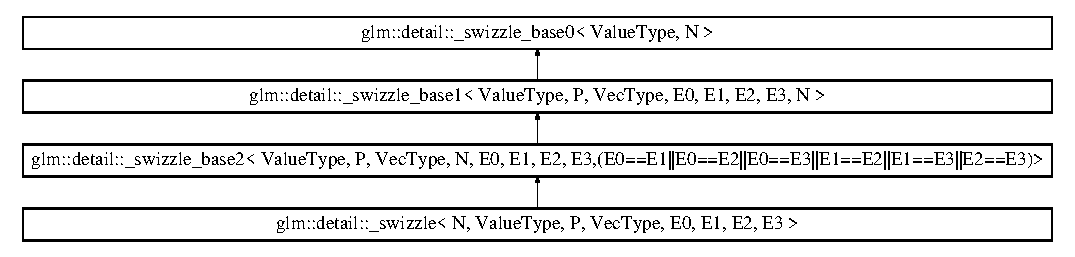
\includegraphics[height=3.002681cm]{structglm_1_1detail_1_1__swizzle}
\end{center}
\end{figure}
\subsection*{Public Types}
\begin{DoxyCompactItemize}
\item 
typedef \hyperlink{structglm_1_1detail_1_1__swizzle__base2}{\+\_\+swizzle\+\_\+base2}$<$ Value\+Type, P, Vec\+Type, N, E0, E1, E2, E3,(E0==E1$\vert$$\vert$E0==E2$\vert$$\vert$E0==E3$\vert$$\vert$E1==E2$\vert$$\vert$E1==E3$\vert$$\vert$E2==E3)$>$ {\bfseries base\+\_\+type}\hypertarget{structglm_1_1detail_1_1__swizzle_acf7dfa9d7456eb833c247473c5a045f4}{}\label{structglm_1_1detail_1_1__swizzle_acf7dfa9d7456eb833c247473c5a045f4}

\end{DoxyCompactItemize}
\subsection*{Public Member Functions}
\begin{DoxyCompactItemize}
\item 
G\+L\+M\+\_\+\+F\+U\+N\+C\+\_\+\+Q\+U\+A\+L\+I\+F\+I\+ER {\bfseries operator Vec\+Type} () const \hypertarget{structglm_1_1detail_1_1__swizzle_a333cdd33d2fb442775cca23c77e63fca}{}\label{structglm_1_1detail_1_1__swizzle_a333cdd33d2fb442775cca23c77e63fca}

\end{DoxyCompactItemize}
\subsection*{Additional Inherited Members}


The documentation for this struct was generated from the following file\+:\begin{DoxyCompactItemize}
\item 
C\+:/\+Users/\+Bilal Itani/\+Desktop/inf2990-\/11/\+Cadriciel/\+Commun/\+Externe/glm/include/glm/detail/\+\_\+swizzle.\+hpp\end{DoxyCompactItemize}

\hypertarget{structglm_1_1detail_1_1__swizzle__base0}{}\section{glm\+:\+:detail\+:\+:\+\_\+swizzle\+\_\+base0$<$ T, N $>$ Struct Template Reference}
\label{structglm_1_1detail_1_1__swizzle__base0}\index{glm\+::detail\+::\+\_\+swizzle\+\_\+base0$<$ T, N $>$@{glm\+::detail\+::\+\_\+swizzle\+\_\+base0$<$ T, N $>$}}
Inheritance diagram for glm\+:\+:detail\+:\+:\+\_\+swizzle\+\_\+base0$<$ T, N $>$\+:\begin{figure}[H]
\begin{center}
\leavevmode
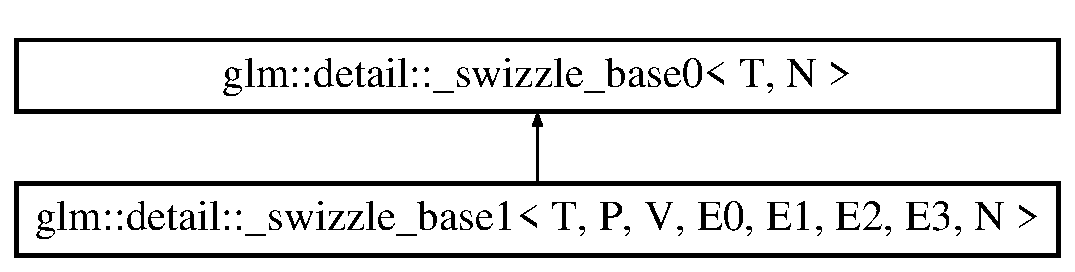
\includegraphics[height=2.000000cm]{structglm_1_1detail_1_1__swizzle__base0}
\end{center}
\end{figure}
\subsection*{Public Types}
\begin{DoxyCompactItemize}
\item 
typedef T {\bfseries value\+\_\+type}\hypertarget{structglm_1_1detail_1_1__swizzle__base0_ad38a739e1fe6d2db2674f34c98159c8f}{}\label{structglm_1_1detail_1_1__swizzle__base0_ad38a739e1fe6d2db2674f34c98159c8f}

\end{DoxyCompactItemize}
\subsection*{Protected Member Functions}
\begin{DoxyCompactItemize}
\item 
G\+L\+M\+\_\+\+F\+U\+N\+C\+\_\+\+Q\+U\+A\+L\+I\+F\+I\+ER value\+\_\+type \& {\bfseries elem} (size\+\_\+t i)\hypertarget{structglm_1_1detail_1_1__swizzle__base0_aebd942a3c3289f9876a9ede4d710d8f0}{}\label{structglm_1_1detail_1_1__swizzle__base0_aebd942a3c3289f9876a9ede4d710d8f0}

\item 
G\+L\+M\+\_\+\+F\+U\+N\+C\+\_\+\+Q\+U\+A\+L\+I\+F\+I\+ER const value\+\_\+type \& {\bfseries elem} (size\+\_\+t i) const \hypertarget{structglm_1_1detail_1_1__swizzle__base0_a9fb7f491860415b292864d0693d8bdb8}{}\label{structglm_1_1detail_1_1__swizzle__base0_a9fb7f491860415b292864d0693d8bdb8}

\end{DoxyCompactItemize}
\subsection*{Protected Attributes}
\begin{DoxyCompactItemize}
\item 
char {\bfseries \+\_\+buffer} \mbox{[}1\mbox{]}\hypertarget{structglm_1_1detail_1_1__swizzle__base0_afd4b7f15c9acff4cdef808f559ffec2d}{}\label{structglm_1_1detail_1_1__swizzle__base0_afd4b7f15c9acff4cdef808f559ffec2d}

\end{DoxyCompactItemize}


The documentation for this struct was generated from the following file\+:\begin{DoxyCompactItemize}
\item 
Commun/\+Externe/glm/include/glm/detail/\+\_\+swizzle.\+hpp\end{DoxyCompactItemize}

\hypertarget{structglm_1_1detail_1_1__swizzle__base1}{}\section{glm\+:\+:detail\+:\+:\+\_\+swizzle\+\_\+base1$<$ T, P, V, E0, E1, E2, E3, N $>$ Struct Template Reference}
\label{structglm_1_1detail_1_1__swizzle__base1}\index{glm\+::detail\+::\+\_\+swizzle\+\_\+base1$<$ T, P, V, E0, E1, E2, E3, N $>$@{glm\+::detail\+::\+\_\+swizzle\+\_\+base1$<$ T, P, V, E0, E1, E2, E3, N $>$}}
Inheritance diagram for glm\+:\+:detail\+:\+:\+\_\+swizzle\+\_\+base1$<$ T, P, V, E0, E1, E2, E3, N $>$\+:\begin{figure}[H]
\begin{center}
\leavevmode
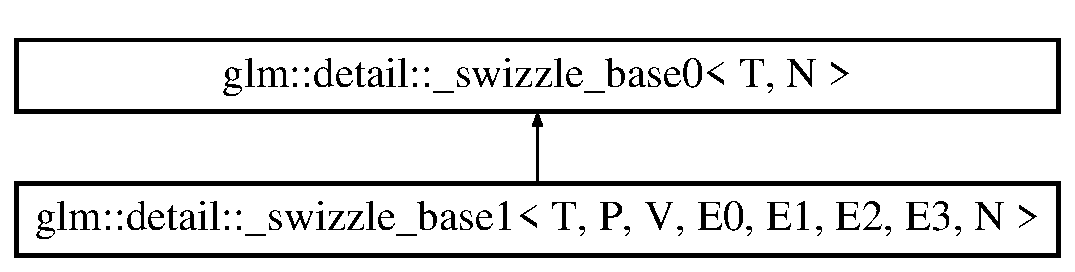
\includegraphics[height=2.000000cm]{structglm_1_1detail_1_1__swizzle__base1}
\end{center}
\end{figure}
\subsection*{Additional Inherited Members}


The documentation for this struct was generated from the following file\+:\begin{DoxyCompactItemize}
\item 
Commun/\+Externe/glm/include/glm/detail/\+\_\+swizzle.\+hpp\end{DoxyCompactItemize}

\hypertarget{structglm_1_1detail_1_1__swizzle__base1_3_01_t_00_01_p_00_01_v_00_01_e0_00_01_e1_00_01_e2_00_01_e3_00_014_01_4}{}\section{glm\+:\+:detail\+:\+:\+\_\+swizzle\+\_\+base1$<$ T, P, V, E0, E1, E2, E3, 4 $>$ Struct Template Reference}
\label{structglm_1_1detail_1_1__swizzle__base1_3_01_t_00_01_p_00_01_v_00_01_e0_00_01_e1_00_01_e2_00_01_e3_00_014_01_4}\index{glm\+::detail\+::\+\_\+swizzle\+\_\+base1$<$ T, P, V, E0, E1, E2, E3, 4 $>$@{glm\+::detail\+::\+\_\+swizzle\+\_\+base1$<$ T, P, V, E0, E1, E2, E3, 4 $>$}}
Inheritance diagram for glm\+:\+:detail\+:\+:\+\_\+swizzle\+\_\+base1$<$ T, P, V, E0, E1, E2, E3, 4 $>$\+:\begin{figure}[H]
\begin{center}
\leavevmode
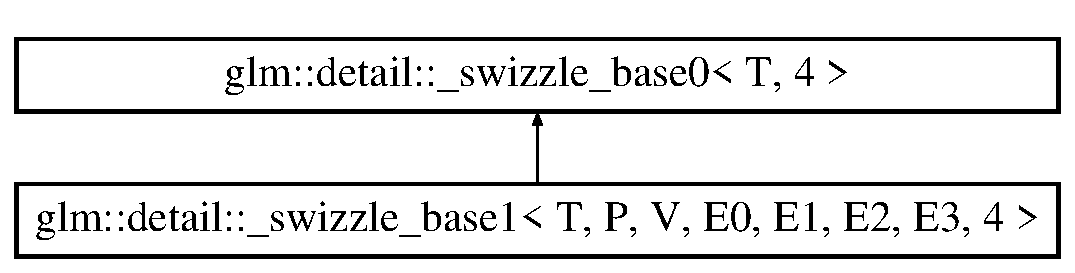
\includegraphics[height=2.000000cm]{structglm_1_1detail_1_1__swizzle__base1_3_01_t_00_01_p_00_01_v_00_01_e0_00_01_e1_00_01_e2_00_01_e3_00_014_01_4}
\end{center}
\end{figure}
\subsection*{Public Member Functions}
\begin{DoxyCompactItemize}
\item 
G\+L\+M\+\_\+\+F\+U\+N\+C\+\_\+\+Q\+U\+A\+L\+I\+F\+I\+ER V {\bfseries operator()} () const \hypertarget{structglm_1_1detail_1_1__swizzle__base1_3_01_t_00_01_p_00_01_v_00_01_e0_00_01_e1_00_01_e2_00_01_e3_00_014_01_4_a901f3af50b0eb022c3246b5de5027245}{}\label{structglm_1_1detail_1_1__swizzle__base1_3_01_t_00_01_p_00_01_v_00_01_e0_00_01_e1_00_01_e2_00_01_e3_00_014_01_4_a901f3af50b0eb022c3246b5de5027245}

\end{DoxyCompactItemize}
\subsection*{Additional Inherited Members}


The documentation for this struct was generated from the following file\+:\begin{DoxyCompactItemize}
\item 
Commun/\+Externe/glm/include/glm/detail/\+\_\+swizzle.\+hpp\end{DoxyCompactItemize}

\hypertarget{structglm_1_1detail_1_1__swizzle__base1_3_01_t_00_01_p_00_01_v_00_01_e0_00_01_e1_00_01_e2_00-1_00_013_01_4}{}\section{glm\+:\+:detail\+:\+:\+\_\+swizzle\+\_\+base1$<$ T, P, V, E0, E1, E2,-\/1, 3 $>$ Struct Template Reference}
\label{structglm_1_1detail_1_1__swizzle__base1_3_01_t_00_01_p_00_01_v_00_01_e0_00_01_e1_00_01_e2_00-1_00_013_01_4}\index{glm\+::detail\+::\+\_\+swizzle\+\_\+base1$<$ T, P, V, E0, E1, E2,-\/1, 3 $>$@{glm\+::detail\+::\+\_\+swizzle\+\_\+base1$<$ T, P, V, E0, E1, E2,-\/1, 3 $>$}}
Inheritance diagram for glm\+:\+:detail\+:\+:\+\_\+swizzle\+\_\+base1$<$ T, P, V, E0, E1, E2,-\/1, 3 $>$\+:\begin{figure}[H]
\begin{center}
\leavevmode
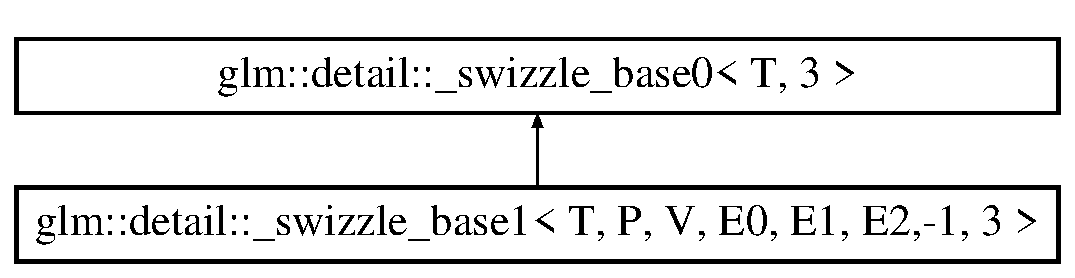
\includegraphics[height=2.000000cm]{structglm_1_1detail_1_1__swizzle__base1_3_01_t_00_01_p_00_01_v_00_01_e0_00_01_e1_00_01_e2_00-1_00_013_01_4}
\end{center}
\end{figure}
\subsection*{Public Member Functions}
\begin{DoxyCompactItemize}
\item 
G\+L\+M\+\_\+\+F\+U\+N\+C\+\_\+\+Q\+U\+A\+L\+I\+F\+I\+ER V {\bfseries operator()} () const \hypertarget{structglm_1_1detail_1_1__swizzle__base1_3_01_t_00_01_p_00_01_v_00_01_e0_00_01_e1_00_01_e2_00-1_00_013_01_4_a94510ce33bf6a19e28b4f95f4e715807}{}\label{structglm_1_1detail_1_1__swizzle__base1_3_01_t_00_01_p_00_01_v_00_01_e0_00_01_e1_00_01_e2_00-1_00_013_01_4_a94510ce33bf6a19e28b4f95f4e715807}

\end{DoxyCompactItemize}
\subsection*{Additional Inherited Members}


The documentation for this struct was generated from the following file\+:\begin{DoxyCompactItemize}
\item 
Cadriciel/\+Commun/\+Externe/glm/include/glm/detail/\+\_\+swizzle.\+hpp\end{DoxyCompactItemize}

\hypertarget{structglm_1_1detail_1_1__swizzle__base1_3_01_t_00_01_p_00_01_v_00_01_e0_00_01_e1_00-1_00-2_00_012_01_4}{}\section{glm\+:\+:detail\+:\+:\+\_\+swizzle\+\_\+base1$<$ T, P, V, E0, E1,-\/1,-\/2, 2 $>$ Struct Template Reference}
\label{structglm_1_1detail_1_1__swizzle__base1_3_01_t_00_01_p_00_01_v_00_01_e0_00_01_e1_00-1_00-2_00_012_01_4}\index{glm\+::detail\+::\+\_\+swizzle\+\_\+base1$<$ T, P, V, E0, E1,-\/1,-\/2, 2 $>$@{glm\+::detail\+::\+\_\+swizzle\+\_\+base1$<$ T, P, V, E0, E1,-\/1,-\/2, 2 $>$}}
Inheritance diagram for glm\+:\+:detail\+:\+:\+\_\+swizzle\+\_\+base1$<$ T, P, V, E0, E1,-\/1,-\/2, 2 $>$\+:\begin{figure}[H]
\begin{center}
\leavevmode
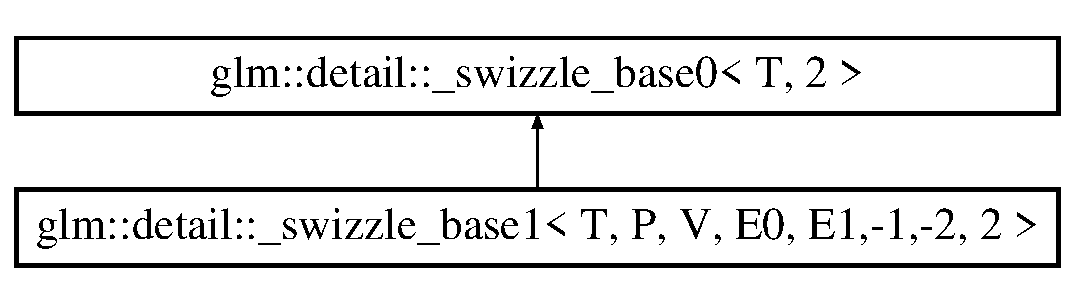
\includegraphics[height=2.000000cm]{structglm_1_1detail_1_1__swizzle__base1_3_01_t_00_01_p_00_01_v_00_01_e0_00_01_e1_00-1_00-2_00_012_01_4}
\end{center}
\end{figure}
\subsection*{Public Member Functions}
\begin{DoxyCompactItemize}
\item 
G\+L\+M\+\_\+\+F\+U\+N\+C\+\_\+\+Q\+U\+A\+L\+I\+F\+I\+ER V {\bfseries operator()} () const \hypertarget{structglm_1_1detail_1_1__swizzle__base1_3_01_t_00_01_p_00_01_v_00_01_e0_00_01_e1_00-1_00-2_00_012_01_4_a333b1c869374c290a8bca707a258f5e5}{}\label{structglm_1_1detail_1_1__swizzle__base1_3_01_t_00_01_p_00_01_v_00_01_e0_00_01_e1_00-1_00-2_00_012_01_4_a333b1c869374c290a8bca707a258f5e5}

\end{DoxyCompactItemize}
\subsection*{Additional Inherited Members}


The documentation for this struct was generated from the following file\+:\begin{DoxyCompactItemize}
\item 
C\+:/\+Users/\+Bilal Itani/\+Desktop/inf2990-\/11/\+Cadriciel/\+Commun/\+Externe/glm/include/glm/detail/\+\_\+swizzle.\+hpp\end{DoxyCompactItemize}

\hypertarget{structglm_1_1detail_1_1__swizzle__base2}{}\section{glm\+:\+:detail\+:\+:\+\_\+swizzle\+\_\+base2$<$ Value\+Type, P, Vec\+Type, N, E0, E1, E2, E3, D\+U\+P\+L\+I\+C\+A\+T\+E\+\_\+\+E\+L\+E\+M\+E\+N\+TS $>$ Struct Template Reference}
\label{structglm_1_1detail_1_1__swizzle__base2}\index{glm\+::detail\+::\+\_\+swizzle\+\_\+base2$<$ Value\+Type, P, Vec\+Type, N, E0, E1, E2, E3, D\+U\+P\+L\+I\+C\+A\+T\+E\+\_\+\+E\+L\+E\+M\+E\+N\+T\+S $>$@{glm\+::detail\+::\+\_\+swizzle\+\_\+base2$<$ Value\+Type, P, Vec\+Type, N, E0, E1, E2, E3, D\+U\+P\+L\+I\+C\+A\+T\+E\+\_\+\+E\+L\+E\+M\+E\+N\+T\+S $>$}}
Inheritance diagram for glm\+:\+:detail\+:\+:\+\_\+swizzle\+\_\+base2$<$ Value\+Type, P, Vec\+Type, N, E0, E1, E2, E3, D\+U\+P\+L\+I\+C\+A\+T\+E\+\_\+\+E\+L\+E\+M\+E\+N\+TS $>$\+:\begin{figure}[H]
\begin{center}
\leavevmode
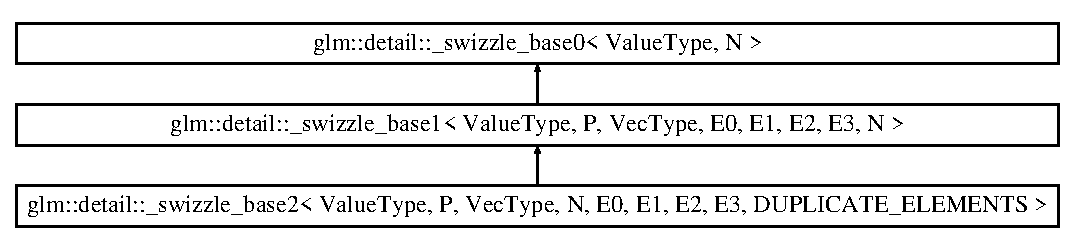
\includegraphics[height=2.823529cm]{structglm_1_1detail_1_1__swizzle__base2}
\end{center}
\end{figure}
\subsection*{Public Types}
\begin{DoxyCompactItemize}
\item 
typedef Vec\+Type {\bfseries vec\+\_\+type}\hypertarget{structglm_1_1detail_1_1__swizzle__base2_a5f999904e676a4f5b0bdaa157415ee1c}{}\label{structglm_1_1detail_1_1__swizzle__base2_a5f999904e676a4f5b0bdaa157415ee1c}

\item 
typedef Value\+Type {\bfseries value\+\_\+type}\hypertarget{structglm_1_1detail_1_1__swizzle__base2_a656c11aaeeaca042deed88711c9dc063}{}\label{structglm_1_1detail_1_1__swizzle__base2_a656c11aaeeaca042deed88711c9dc063}

\end{DoxyCompactItemize}
\subsection*{Public Member Functions}
\begin{DoxyCompactItemize}
\item 
G\+L\+M\+\_\+\+F\+U\+N\+C\+\_\+\+Q\+U\+A\+L\+I\+F\+I\+ER \hyperlink{structglm_1_1detail_1_1__swizzle__base2}{\+\_\+swizzle\+\_\+base2} \& {\bfseries operator=} (const Value\+Type \&t)\hypertarget{structglm_1_1detail_1_1__swizzle__base2_a70442376cb261474e23090737deff976}{}\label{structglm_1_1detail_1_1__swizzle__base2_a70442376cb261474e23090737deff976}

\item 
G\+L\+M\+\_\+\+F\+U\+N\+C\+\_\+\+Q\+U\+A\+L\+I\+F\+I\+ER \hyperlink{structglm_1_1detail_1_1__swizzle__base2}{\+\_\+swizzle\+\_\+base2} \& {\bfseries operator=} (const Vec\+Type \&that)\hypertarget{structglm_1_1detail_1_1__swizzle__base2_a7b982a5056d94cd43393bf820ea627d0}{}\label{structglm_1_1detail_1_1__swizzle__base2_a7b982a5056d94cd43393bf820ea627d0}

\item 
G\+L\+M\+\_\+\+F\+U\+N\+C\+\_\+\+Q\+U\+A\+L\+I\+F\+I\+ER void {\bfseries operator-\/=} (const Vec\+Type \&that)\hypertarget{structglm_1_1detail_1_1__swizzle__base2_ab583f399dc6685deee97bdd5126f433a}{}\label{structglm_1_1detail_1_1__swizzle__base2_ab583f399dc6685deee97bdd5126f433a}

\item 
G\+L\+M\+\_\+\+F\+U\+N\+C\+\_\+\+Q\+U\+A\+L\+I\+F\+I\+ER void {\bfseries operator+=} (const Vec\+Type \&that)\hypertarget{structglm_1_1detail_1_1__swizzle__base2_a5e734b2e9da294d92bb347a3c7f44ded}{}\label{structglm_1_1detail_1_1__swizzle__base2_a5e734b2e9da294d92bb347a3c7f44ded}

\item 
G\+L\+M\+\_\+\+F\+U\+N\+C\+\_\+\+Q\+U\+A\+L\+I\+F\+I\+ER void {\bfseries operator$\ast$=} (const Vec\+Type \&that)\hypertarget{structglm_1_1detail_1_1__swizzle__base2_a6c686d110b936939c7ed67d7a6165778}{}\label{structglm_1_1detail_1_1__swizzle__base2_a6c686d110b936939c7ed67d7a6165778}

\item 
G\+L\+M\+\_\+\+F\+U\+N\+C\+\_\+\+Q\+U\+A\+L\+I\+F\+I\+ER void {\bfseries operator/=} (const Vec\+Type \&that)\hypertarget{structglm_1_1detail_1_1__swizzle__base2_a0a3e5ef1cb68f78a7e1bcd72f6e2dc4c}{}\label{structglm_1_1detail_1_1__swizzle__base2_a0a3e5ef1cb68f78a7e1bcd72f6e2dc4c}

\item 
G\+L\+M\+\_\+\+F\+U\+N\+C\+\_\+\+Q\+U\+A\+L\+I\+F\+I\+ER value\+\_\+type \& {\bfseries operator\mbox{[}$\,$\mbox{]}} (size\+\_\+t i)\hypertarget{structglm_1_1detail_1_1__swizzle__base2_aa3f2ab8e3e1a5c414b3fdca4cf75b706}{}\label{structglm_1_1detail_1_1__swizzle__base2_aa3f2ab8e3e1a5c414b3fdca4cf75b706}

\item 
G\+L\+M\+\_\+\+F\+U\+N\+C\+\_\+\+Q\+U\+A\+L\+I\+F\+I\+ER value\+\_\+type {\bfseries operator\mbox{[}$\,$\mbox{]}} (size\+\_\+t i) const \hypertarget{structglm_1_1detail_1_1__swizzle__base2_a1bec6727adac01b6bc3e1ccba935167e}{}\label{structglm_1_1detail_1_1__swizzle__base2_a1bec6727adac01b6bc3e1ccba935167e}

\end{DoxyCompactItemize}
\subsection*{Protected Member Functions}
\begin{DoxyCompactItemize}
\item 
{\footnotesize template$<$typename T $>$ }\\G\+L\+M\+\_\+\+F\+U\+N\+C\+\_\+\+Q\+U\+A\+L\+I\+F\+I\+ER void {\bfseries \+\_\+apply\+\_\+op} (const Vec\+Type \&that, T op)\hypertarget{structglm_1_1detail_1_1__swizzle__base2_a11d049274a60ecf4aac8cebc4c4e9be5}{}\label{structglm_1_1detail_1_1__swizzle__base2_a11d049274a60ecf4aac8cebc4c4e9be5}

\end{DoxyCompactItemize}
\subsection*{Additional Inherited Members}


The documentation for this struct was generated from the following file\+:\begin{DoxyCompactItemize}
\item 
Cadriciel/\+Commun/\+Externe/glm/include/glm/detail/\+\_\+swizzle.\+hpp\end{DoxyCompactItemize}

\hypertarget{structglm_1_1detail_1_1__swizzle__base2_3_01_value_type_00_01_p_00_01_vec_type_00_01_n_00_01_e0_fc19218d69dc8988a4a57fbe7f79725c}{}\section{glm\+:\+:detail\+:\+:\+\_\+swizzle\+\_\+base2$<$ Value\+Type, P, Vec\+Type, N, E0, E1, E2, E3, 1 $>$ Struct Template Reference}
\label{structglm_1_1detail_1_1__swizzle__base2_3_01_value_type_00_01_p_00_01_vec_type_00_01_n_00_01_e0_fc19218d69dc8988a4a57fbe7f79725c}\index{glm\+::detail\+::\+\_\+swizzle\+\_\+base2$<$ Value\+Type, P, Vec\+Type, N, E0, E1, E2, E3, 1 $>$@{glm\+::detail\+::\+\_\+swizzle\+\_\+base2$<$ Value\+Type, P, Vec\+Type, N, E0, E1, E2, E3, 1 $>$}}
Inheritance diagram for glm\+:\+:detail\+:\+:\+\_\+swizzle\+\_\+base2$<$ Value\+Type, P, Vec\+Type, N, E0, E1, E2, E3, 1 $>$\+:\begin{figure}[H]
\begin{center}
\leavevmode
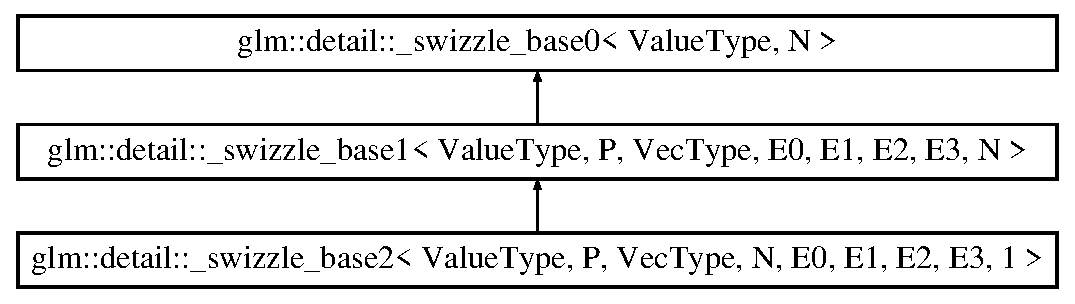
\includegraphics[height=3.000000cm]{structglm_1_1detail_1_1__swizzle__base2_3_01_value_type_00_01_p_00_01_vec_type_00_01_n_00_01_e0_fc19218d69dc8988a4a57fbe7f79725c}
\end{center}
\end{figure}
\subsection*{Classes}
\begin{DoxyCompactItemize}
\item 
struct \hyperlink{structglm_1_1detail_1_1__swizzle__base2_3_01_value_type_00_01_p_00_01_vec_type_00_01_n_00_01_e0_17279995be88bc842083eed40758473c}{Stub}
\end{DoxyCompactItemize}
\subsection*{Public Types}
\begin{DoxyCompactItemize}
\item 
typedef Vec\+Type {\bfseries vec\+\_\+type}\hypertarget{structglm_1_1detail_1_1__swizzle__base2_3_01_value_type_00_01_p_00_01_vec_type_00_01_n_00_01_e0_fc19218d69dc8988a4a57fbe7f79725c_aa478e9f198b8832d76245adde9c627ec}{}\label{structglm_1_1detail_1_1__swizzle__base2_3_01_value_type_00_01_p_00_01_vec_type_00_01_n_00_01_e0_fc19218d69dc8988a4a57fbe7f79725c_aa478e9f198b8832d76245adde9c627ec}

\item 
typedef Value\+Type {\bfseries value\+\_\+type}\hypertarget{structglm_1_1detail_1_1__swizzle__base2_3_01_value_type_00_01_p_00_01_vec_type_00_01_n_00_01_e0_fc19218d69dc8988a4a57fbe7f79725c_aea7ec681454787ad7a322c06aec98757}{}\label{structglm_1_1detail_1_1__swizzle__base2_3_01_value_type_00_01_p_00_01_vec_type_00_01_n_00_01_e0_fc19218d69dc8988a4a57fbe7f79725c_aea7ec681454787ad7a322c06aec98757}

\end{DoxyCompactItemize}
\subsection*{Public Member Functions}
\begin{DoxyCompactItemize}
\item 
G\+L\+M\+\_\+\+F\+U\+N\+C\+\_\+\+Q\+U\+A\+L\+I\+F\+I\+ER \hyperlink{structglm_1_1detail_1_1__swizzle__base2}{\+\_\+swizzle\+\_\+base2} \& {\bfseries operator=} (Stub const \&)\hypertarget{structglm_1_1detail_1_1__swizzle__base2_3_01_value_type_00_01_p_00_01_vec_type_00_01_n_00_01_e0_fc19218d69dc8988a4a57fbe7f79725c_aed2b7223090d020e28af46eb33fe6729}{}\label{structglm_1_1detail_1_1__swizzle__base2_3_01_value_type_00_01_p_00_01_vec_type_00_01_n_00_01_e0_fc19218d69dc8988a4a57fbe7f79725c_aed2b7223090d020e28af46eb33fe6729}

\item 
G\+L\+M\+\_\+\+F\+U\+N\+C\+\_\+\+Q\+U\+A\+L\+I\+F\+I\+ER value\+\_\+type {\bfseries operator\mbox{[}$\,$\mbox{]}} (size\+\_\+t i) const \hypertarget{structglm_1_1detail_1_1__swizzle__base2_3_01_value_type_00_01_p_00_01_vec_type_00_01_n_00_01_e0_fc19218d69dc8988a4a57fbe7f79725c_a2f3a45edbb24ca7e12182c3123dde632}{}\label{structglm_1_1detail_1_1__swizzle__base2_3_01_value_type_00_01_p_00_01_vec_type_00_01_n_00_01_e0_fc19218d69dc8988a4a57fbe7f79725c_a2f3a45edbb24ca7e12182c3123dde632}

\end{DoxyCompactItemize}
\subsection*{Additional Inherited Members}


The documentation for this struct was generated from the following file\+:\begin{DoxyCompactItemize}
\item 
Cadriciel/\+Commun/\+Externe/glm/include/glm/detail/\+\_\+swizzle.\+hpp\end{DoxyCompactItemize}

\hypertarget{class_additional_message}{}\section{Additional\+Message Class Reference}
\label{class_additional_message}\index{Additional\+Message@{Additional\+Message}}


An additional \hyperlink{class_message}{Message} for assertions.

Provides a implicit constructor that takes a single string. This allow this class to be used as the message arguments in macros.  




{\ttfamily \#include $<$Additional\+Message.\+h$>$}

Inheritance diagram for Additional\+Message\+:\begin{figure}[H]
\begin{center}
\leavevmode
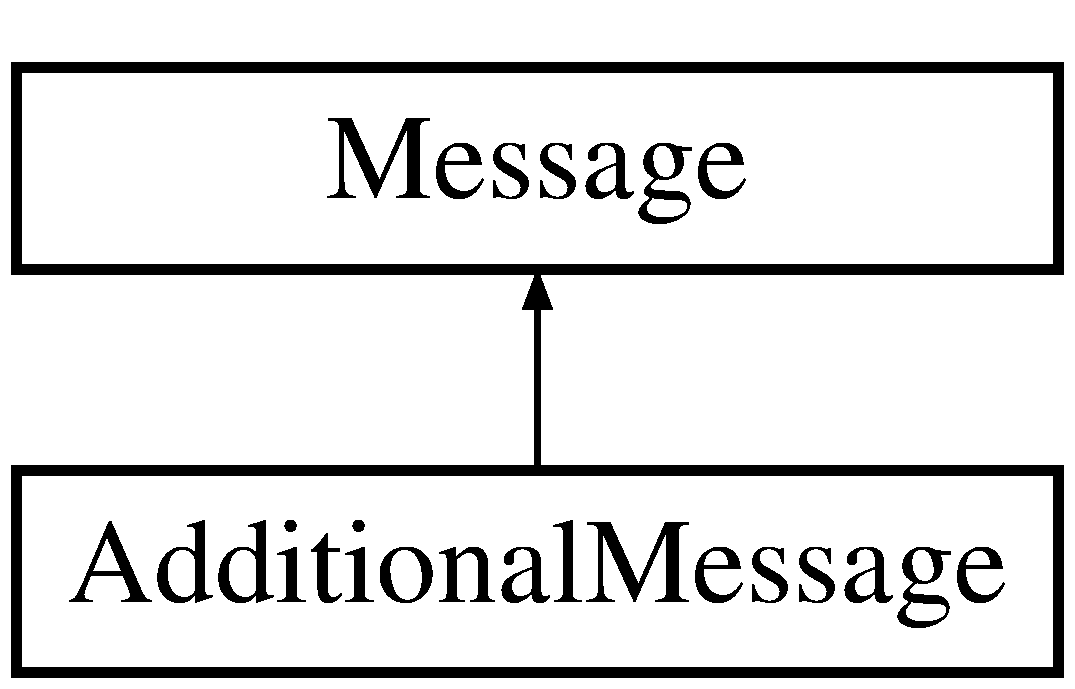
\includegraphics[height=2.000000cm]{class_additional_message}
\end{center}
\end{figure}
\subsection*{Public Types}
\begin{DoxyCompactItemize}
\item 
typedef \hyperlink{class_message}{Message} {\bfseries Super\+Class}\hypertarget{class_additional_message_abc8626e28c147b5ddd66032a35676126}{}\label{class_additional_message_abc8626e28c147b5ddd66032a35676126}

\end{DoxyCompactItemize}
\subsection*{Public Member Functions}
\begin{DoxyCompactItemize}
\item 
\hyperlink{class_additional_message_a888715179848c5e5c385789b962a3cfb}{Additional\+Message} ()\hypertarget{class_additional_message_a888715179848c5e5c385789b962a3cfb}{}\label{class_additional_message_a888715179848c5e5c385789b962a3cfb}

\begin{DoxyCompactList}\small\item\em Constructs an empty \hyperlink{class_message}{Message}. \end{DoxyCompactList}\item 
\hyperlink{class_additional_message_a990455bbfe260bc04f99e5acc58d1c06}{Additional\+Message} (const std\+::string \&detail1)
\begin{DoxyCompactList}\small\item\em Constructs a \hyperlink{class_message}{Message} with the specified detail string. \end{DoxyCompactList}\item 
\hyperlink{class_additional_message_a6486540f9b5d1957230e9e1f969adc9d}{Additional\+Message} (const char $\ast$detail1)
\begin{DoxyCompactList}\small\item\em Constructs a \hyperlink{class_message}{Message} with the specified detail string. \end{DoxyCompactList}\item 
\hyperlink{class_additional_message_a75735b6fd65686f31349d01c97c73bc7}{Additional\+Message} (const \hyperlink{class_message}{Message} \&other)
\begin{DoxyCompactList}\small\item\em Constructs a copy of the specified message. \end{DoxyCompactList}\item 
\hyperlink{class_additional_message}{Additional\+Message} \& \hyperlink{class_additional_message_abbda0de4323f70ff01a9b622a6f550f7}{operator=} (const \hyperlink{class_message}{Message} \&other)
\begin{DoxyCompactList}\small\item\em Assignment operator. \end{DoxyCompactList}\end{DoxyCompactItemize}


\subsection{Detailed Description}
An additional \hyperlink{class_message}{Message} for assertions.

Provides a implicit constructor that takes a single string. This allow this class to be used as the message arguments in macros. 

The constructed object is either a \hyperlink{class_message}{Message} with a single detail string if a string was passed to the macro, or a copy of the \hyperlink{class_message}{Message} passed to the macro.

Here is an example of usage\+: 
\begin{DoxyCode}
\textcolor{keywordtype}{void} checkStringEquals( \textcolor{keyword}{const} std::string &expected,
                       \textcolor{keyword}{const} std::string &actual,
                        \textcolor{keyword}{const} CppUnit::SourceLine &sourceLine,
                        \textcolor{keyword}{const} CppUnit::AdditionalMessage &message );

\textcolor{preprocessor}{#define XTLUT\_ASSERT\_STRING\_EQUAL\_MESSAGE( expected, actual, message )  \(\backslash\)}
\textcolor{preprocessor}{  ::XtlUt::Impl::checkStringEquals( ::Xtl::toString(expected),        \(\backslash\)}
\textcolor{preprocessor}{                                    ::Xtl::toString(actual),          \(\backslash\)}
\textcolor{preprocessor}{                                    CPPUNIT\_SOURCELINE(),             \(\backslash\)}
\textcolor{preprocessor}{                                    message )}
\end{DoxyCode}


In the previous example, the user can specify a simple string for {\itshape message}, or a complex \hyperlink{class_message}{Message} object.

\begin{DoxySeeAlso}{See also}
\hyperlink{class_message}{Message} 
\end{DoxySeeAlso}


\subsection{Constructor \& Destructor Documentation}
\index{Additional\+Message@{Additional\+Message}!Additional\+Message@{Additional\+Message}}
\index{Additional\+Message@{Additional\+Message}!Additional\+Message@{Additional\+Message}}
\subsubsection[{\texorpdfstring{Additional\+Message(const std\+::string \&detail1)}{AdditionalMessage(const std::string &detail1)}}]{\setlength{\rightskip}{0pt plus 5cm}Additional\+Message\+::\+Additional\+Message (
\begin{DoxyParamCaption}
\item[{const std\+::string \&}]{detail1}
\end{DoxyParamCaption}
)}\hypertarget{class_additional_message_a990455bbfe260bc04f99e5acc58d1c06}{}\label{class_additional_message_a990455bbfe260bc04f99e5acc58d1c06}


Constructs a \hyperlink{class_message}{Message} with the specified detail string. 


\begin{DoxyParams}{Parameters}
{\em detail1} & Detail string of the message. If empty, then it is not added. \\
\hline
\end{DoxyParams}
\index{Additional\+Message@{Additional\+Message}!Additional\+Message@{Additional\+Message}}
\index{Additional\+Message@{Additional\+Message}!Additional\+Message@{Additional\+Message}}
\subsubsection[{\texorpdfstring{Additional\+Message(const char $\ast$detail1)}{AdditionalMessage(const char *detail1)}}]{\setlength{\rightskip}{0pt plus 5cm}Additional\+Message\+::\+Additional\+Message (
\begin{DoxyParamCaption}
\item[{const char $\ast$}]{detail1}
\end{DoxyParamCaption}
)}\hypertarget{class_additional_message_a6486540f9b5d1957230e9e1f969adc9d}{}\label{class_additional_message_a6486540f9b5d1957230e9e1f969adc9d}


Constructs a \hyperlink{class_message}{Message} with the specified detail string. 


\begin{DoxyParams}{Parameters}
{\em detail1} & Detail string of the message. If empty, then it is not added. \\
\hline
\end{DoxyParams}
\index{Additional\+Message@{Additional\+Message}!Additional\+Message@{Additional\+Message}}
\index{Additional\+Message@{Additional\+Message}!Additional\+Message@{Additional\+Message}}
\subsubsection[{\texorpdfstring{Additional\+Message(const Message \&other)}{AdditionalMessage(const Message &other)}}]{\setlength{\rightskip}{0pt plus 5cm}Additional\+Message\+::\+Additional\+Message (
\begin{DoxyParamCaption}
\item[{const {\bf Message} \&}]{other}
\end{DoxyParamCaption}
)}\hypertarget{class_additional_message_a75735b6fd65686f31349d01c97c73bc7}{}\label{class_additional_message_a75735b6fd65686f31349d01c97c73bc7}


Constructs a copy of the specified message. 


\begin{DoxyParams}{Parameters}
{\em other} & \hyperlink{class_message}{Message} to copy. \\
\hline
\end{DoxyParams}


\subsection{Member Function Documentation}
\index{Additional\+Message@{Additional\+Message}!operator=@{operator=}}
\index{operator=@{operator=}!Additional\+Message@{Additional\+Message}}
\subsubsection[{\texorpdfstring{operator=(const Message \&other)}{operator=(const Message &other)}}]{\setlength{\rightskip}{0pt plus 5cm}{\bf Additional\+Message}\& Additional\+Message\+::operator= (
\begin{DoxyParamCaption}
\item[{const {\bf Message} \&}]{other}
\end{DoxyParamCaption}
)}\hypertarget{class_additional_message_abbda0de4323f70ff01a9b622a6f550f7}{}\label{class_additional_message_abbda0de4323f70ff01a9b622a6f550f7}


Assignment operator. 


\begin{DoxyParams}{Parameters}
{\em other} & \hyperlink{class_message}{Message} to copy. \\
\hline
\end{DoxyParams}
\begin{DoxyReturn}{Returns}
Reference on this object. 
\end{DoxyReturn}


The documentation for this class was generated from the following file\+:\begin{DoxyCompactItemize}
\item 
Commun/\+Externe/cppunit/include/cppunit/Additional\+Message.\+h\end{DoxyCompactItemize}

\hypertarget{struct_a_f_m___font_info_rec__}{}\section{A\+F\+M\+\_\+\+Font\+Info\+Rec\+\_\+ Struct Reference}
\label{struct_a_f_m___font_info_rec__}\index{A\+F\+M\+\_\+\+Font\+Info\+Rec\+\_\+@{A\+F\+M\+\_\+\+Font\+Info\+Rec\+\_\+}}
\subsection*{Public Attributes}
\begin{DoxyCompactItemize}
\item 
F\+T\+\_\+\+Bool {\bfseries Is\+C\+I\+D\+Font}\hypertarget{struct_a_f_m___font_info_rec___a6f198e74da5d8a3b7ff7518e255be231}{}\label{struct_a_f_m___font_info_rec___a6f198e74da5d8a3b7ff7518e255be231}

\item 
\hyperlink{struct_f_t___b_box__}{F\+T\+\_\+\+B\+Box} {\bfseries Font\+B\+Box}\hypertarget{struct_a_f_m___font_info_rec___afa5112d6b0cc51839889206012dc1be6}{}\label{struct_a_f_m___font_info_rec___afa5112d6b0cc51839889206012dc1be6}

\item 
F\+T\+\_\+\+Fixed {\bfseries Ascender}\hypertarget{struct_a_f_m___font_info_rec___a0b80412562435a2198a71aa4188ee85b}{}\label{struct_a_f_m___font_info_rec___a0b80412562435a2198a71aa4188ee85b}

\item 
F\+T\+\_\+\+Fixed {\bfseries Descender}\hypertarget{struct_a_f_m___font_info_rec___a3561507200f0bc3413988af920924053}{}\label{struct_a_f_m___font_info_rec___a3561507200f0bc3413988af920924053}

\item 
\hyperlink{struct_a_f_m___track_kern_rec__}{A\+F\+M\+\_\+\+Track\+Kern} {\bfseries Track\+Kerns}\hypertarget{struct_a_f_m___font_info_rec___a8d9305229a1dacc15b8fceb5dbf25b9d}{}\label{struct_a_f_m___font_info_rec___a8d9305229a1dacc15b8fceb5dbf25b9d}

\item 
F\+T\+\_\+\+Int {\bfseries Num\+Track\+Kern}\hypertarget{struct_a_f_m___font_info_rec___a08a9207e8d4b0dd9dc0313218462f00e}{}\label{struct_a_f_m___font_info_rec___a08a9207e8d4b0dd9dc0313218462f00e}

\item 
\hyperlink{struct_a_f_m___kern_pair_rec__}{A\+F\+M\+\_\+\+Kern\+Pair} {\bfseries Kern\+Pairs}\hypertarget{struct_a_f_m___font_info_rec___a16c5da5249d4d4f68cc169469f3ee75a}{}\label{struct_a_f_m___font_info_rec___a16c5da5249d4d4f68cc169469f3ee75a}

\item 
F\+T\+\_\+\+Int {\bfseries Num\+Kern\+Pair}\hypertarget{struct_a_f_m___font_info_rec___a8ff8af3c83fbf0b060bb711b57f1affd}{}\label{struct_a_f_m___font_info_rec___a8ff8af3c83fbf0b060bb711b57f1affd}

\end{DoxyCompactItemize}


The documentation for this struct was generated from the following file\+:\begin{DoxyCompactItemize}
\item 
C\+:/\+Users/\+Bilal Itani/\+Desktop/inf2990-\/11/\+Cadriciel/\+Commun/\+Externe/\+Free\+Type/include/freetype/internal/t1types.\+h\end{DoxyCompactItemize}

\hypertarget{struct_a_f_m___kern_pair_rec__}{}\section{A\+F\+M\+\_\+\+Kern\+Pair\+Rec\+\_\+ Struct Reference}
\label{struct_a_f_m___kern_pair_rec__}\index{A\+F\+M\+\_\+\+Kern\+Pair\+Rec\+\_\+@{A\+F\+M\+\_\+\+Kern\+Pair\+Rec\+\_\+}}
\subsection*{Public Attributes}
\begin{DoxyCompactItemize}
\item 
F\+T\+\_\+\+Int {\bfseries index1}\hypertarget{struct_a_f_m___kern_pair_rec___a732bca56dd4a070b1d887ada1637e810}{}\label{struct_a_f_m___kern_pair_rec___a732bca56dd4a070b1d887ada1637e810}

\item 
F\+T\+\_\+\+Int {\bfseries index2}\hypertarget{struct_a_f_m___kern_pair_rec___aee548123779323c255180112c7f5b831}{}\label{struct_a_f_m___kern_pair_rec___aee548123779323c255180112c7f5b831}

\item 
F\+T\+\_\+\+Int {\bfseries x}\hypertarget{struct_a_f_m___kern_pair_rec___a4b7f90a0e17ed89353fec14ddb29fa12}{}\label{struct_a_f_m___kern_pair_rec___a4b7f90a0e17ed89353fec14ddb29fa12}

\item 
F\+T\+\_\+\+Int {\bfseries y}\hypertarget{struct_a_f_m___kern_pair_rec___aa177aa612e79701261eba72c76ea3f08}{}\label{struct_a_f_m___kern_pair_rec___aa177aa612e79701261eba72c76ea3f08}

\end{DoxyCompactItemize}


The documentation for this struct was generated from the following file\+:\begin{DoxyCompactItemize}
\item 
Cadriciel/\+Commun/\+Externe/\+Free\+Type/include/freetype/internal/t1types.\+h\end{DoxyCompactItemize}

\hypertarget{struct_a_f_m___parser___funcs_rec__}{}\section{A\+F\+M\+\_\+\+Parser\+\_\+\+Funcs\+Rec\+\_\+ Struct Reference}
\label{struct_a_f_m___parser___funcs_rec__}\index{A\+F\+M\+\_\+\+Parser\+\_\+\+Funcs\+Rec\+\_\+@{A\+F\+M\+\_\+\+Parser\+\_\+\+Funcs\+Rec\+\_\+}}
\subsection*{Public Attributes}
\begin{DoxyCompactItemize}
\item 
F\+T\+\_\+\+Error($\ast$ {\bfseries init} )(\hyperlink{struct_a_f_m___parser_rec__}{A\+F\+M\+\_\+\+Parser} parser, F\+T\+\_\+\+Memory memory, F\+T\+\_\+\+Byte $\ast$base, F\+T\+\_\+\+Byte $\ast$limit)\hypertarget{struct_a_f_m___parser___funcs_rec___ab96ca52171618217bc852d01dbdaf4ad}{}\label{struct_a_f_m___parser___funcs_rec___ab96ca52171618217bc852d01dbdaf4ad}

\item 
void($\ast$ {\bfseries done} )(\hyperlink{struct_a_f_m___parser_rec__}{A\+F\+M\+\_\+\+Parser} parser)\hypertarget{struct_a_f_m___parser___funcs_rec___ae084d9f1b6768f93629073c9d1c98aee}{}\label{struct_a_f_m___parser___funcs_rec___ae084d9f1b6768f93629073c9d1c98aee}

\item 
F\+T\+\_\+\+Error($\ast$ {\bfseries parse} )(\hyperlink{struct_a_f_m___parser_rec__}{A\+F\+M\+\_\+\+Parser} parser)\hypertarget{struct_a_f_m___parser___funcs_rec___ad8f41aafada1b5a84f5e1ac46f545669}{}\label{struct_a_f_m___parser___funcs_rec___ad8f41aafada1b5a84f5e1ac46f545669}

\end{DoxyCompactItemize}


The documentation for this struct was generated from the following file\+:\begin{DoxyCompactItemize}
\item 
Cadriciel/\+Commun/\+Externe/\+Free\+Type/include/freetype/internal/psaux.\+h\end{DoxyCompactItemize}

\hypertarget{struct_a_f_m___parser_rec__}{}\section{A\+F\+M\+\_\+\+Parser\+Rec\+\_\+ Struct Reference}
\label{struct_a_f_m___parser_rec__}\index{A\+F\+M\+\_\+\+Parser\+Rec\+\_\+@{A\+F\+M\+\_\+\+Parser\+Rec\+\_\+}}
\subsection*{Public Attributes}
\begin{DoxyCompactItemize}
\item 
F\+T\+\_\+\+Memory {\bfseries memory}\hypertarget{struct_a_f_m___parser_rec___a3fec8b1760fa9261f48ee87dc2b3858b}{}\label{struct_a_f_m___parser_rec___a3fec8b1760fa9261f48ee87dc2b3858b}

\item 
A\+F\+M\+\_\+\+Stream {\bfseries stream}\hypertarget{struct_a_f_m___parser_rec___adf3b1165216cbd1f7ec7ae736fd4270a}{}\label{struct_a_f_m___parser_rec___adf3b1165216cbd1f7ec7ae736fd4270a}

\item 
\hyperlink{struct_a_f_m___font_info_rec__}{A\+F\+M\+\_\+\+Font\+Info} {\bfseries Font\+Info}\hypertarget{struct_a_f_m___parser_rec___ae53d6cddac32a0eb7014c3a9f74517df}{}\label{struct_a_f_m___parser_rec___ae53d6cddac32a0eb7014c3a9f74517df}

\item 
F\+T\+\_\+\+Int($\ast$ {\bfseries get\+\_\+index} )(const char $\ast$name, F\+T\+\_\+\+Offset len, void $\ast$user\+\_\+data)\hypertarget{struct_a_f_m___parser_rec___a9d33b62410351d72878f0f14007e7385}{}\label{struct_a_f_m___parser_rec___a9d33b62410351d72878f0f14007e7385}

\item 
void $\ast$ {\bfseries user\+\_\+data}\hypertarget{struct_a_f_m___parser_rec___a9fa78a781737bf27e00448c5092b7657}{}\label{struct_a_f_m___parser_rec___a9fa78a781737bf27e00448c5092b7657}

\end{DoxyCompactItemize}


The documentation for this struct was generated from the following file\+:\begin{DoxyCompactItemize}
\item 
Cadriciel/\+Commun/\+Externe/\+Free\+Type/include/freetype/internal/psaux.\+h\end{DoxyCompactItemize}

\hypertarget{struct_a_f_m___track_kern_rec__}{}\section{A\+F\+M\+\_\+\+Track\+Kern\+Rec\+\_\+ Struct Reference}
\label{struct_a_f_m___track_kern_rec__}\index{A\+F\+M\+\_\+\+Track\+Kern\+Rec\+\_\+@{A\+F\+M\+\_\+\+Track\+Kern\+Rec\+\_\+}}
\subsection*{Public Attributes}
\begin{DoxyCompactItemize}
\item 
F\+T\+\_\+\+Int {\bfseries degree}\hypertarget{struct_a_f_m___track_kern_rec___a15272593c1a0ea05ca3687e7c2de26b6}{}\label{struct_a_f_m___track_kern_rec___a15272593c1a0ea05ca3687e7c2de26b6}

\item 
F\+T\+\_\+\+Fixed {\bfseries min\+\_\+ptsize}\hypertarget{struct_a_f_m___track_kern_rec___a7b1e7fd74d92dcf2b89fee7f74d4fdba}{}\label{struct_a_f_m___track_kern_rec___a7b1e7fd74d92dcf2b89fee7f74d4fdba}

\item 
F\+T\+\_\+\+Fixed {\bfseries min\+\_\+kern}\hypertarget{struct_a_f_m___track_kern_rec___aee6f40c722e14ee2fb17948ce19d0499}{}\label{struct_a_f_m___track_kern_rec___aee6f40c722e14ee2fb17948ce19d0499}

\item 
F\+T\+\_\+\+Fixed {\bfseries max\+\_\+ptsize}\hypertarget{struct_a_f_m___track_kern_rec___a2b22a268fb0654a035ec59d3dfa3dfa4}{}\label{struct_a_f_m___track_kern_rec___a2b22a268fb0654a035ec59d3dfa3dfa4}

\item 
F\+T\+\_\+\+Fixed {\bfseries max\+\_\+kern}\hypertarget{struct_a_f_m___track_kern_rec___a8e25a36b738a2de3fa5c08e477b5a6a2}{}\label{struct_a_f_m___track_kern_rec___a8e25a36b738a2de3fa5c08e477b5a6a2}

\end{DoxyCompactItemize}


The documentation for this struct was generated from the following file\+:\begin{DoxyCompactItemize}
\item 
Cadriciel/\+Commun/\+Externe/\+Free\+Type/include/freetype/internal/t1types.\+h\end{DoxyCompactItemize}

\hypertarget{structai_anim_mesh}{}\section{ai\+Anim\+Mesh Struct Reference}
\label{structai_anim_mesh}\index{ai\+Anim\+Mesh@{ai\+Anim\+Mesh}}


N\+OT C\+U\+R\+R\+E\+N\+T\+LY IN U\+SE. An Anim\+Mesh is an attachment to an \hyperlink{structai_mesh}{ai\+Mesh} stores per-\/vertex animations for a particular frame.  




{\ttfamily \#include $<$mesh.\+h$>$}

\subsection*{Public Attributes}
\begin{DoxyCompactItemize}
\item 
C\+\_\+\+S\+T\+R\+U\+CT \hyperlink{structai_vector3_d}{ai\+Vector3D} $\ast$ \hyperlink{structai_anim_mesh_a0ac2dd4c1afd23e6a9293b1d0ded3060}{m\+Vertices}
\item 
C\+\_\+\+S\+T\+R\+U\+CT \hyperlink{structai_vector3_d}{ai\+Vector3D} $\ast$ \hyperlink{structai_anim_mesh_a64a07a8c5c419b1e006c5302bca4d334}{m\+Normals}
\item 
C\+\_\+\+S\+T\+R\+U\+CT \hyperlink{structai_vector3_d}{ai\+Vector3D} $\ast$ \hyperlink{structai_anim_mesh_a95dcc49c6d5ecc570ceb54552a0a9625}{m\+Tangents}
\item 
C\+\_\+\+S\+T\+R\+U\+CT \hyperlink{structai_vector3_d}{ai\+Vector3D} $\ast$ \hyperlink{structai_anim_mesh_a7d60acf4d2b4b59dcc6c88956bfae85f}{m\+Bitangents}
\item 
C\+\_\+\+S\+T\+R\+U\+CT \hyperlink{structai_color4_d}{ai\+Color4D} $\ast$ \hyperlink{structai_anim_mesh_a4f062d9fac71c6b367fdf0f8638e1ca5}{m\+Colors} \mbox{[}A\+I\+\_\+\+M\+A\+X\+\_\+\+N\+U\+M\+B\+E\+R\+\_\+\+O\+F\+\_\+\+C\+O\+L\+O\+R\+\_\+\+S\+E\+TS\mbox{]}
\item 
C\+\_\+\+S\+T\+R\+U\+CT \hyperlink{structai_vector3_d}{ai\+Vector3D} $\ast$ \hyperlink{structai_anim_mesh_ad24a0451adeb845a53eb2351b9462e0a}{m\+Texture\+Coords} \mbox{[}A\+I\+\_\+\+M\+A\+X\+\_\+\+N\+U\+M\+B\+E\+R\+\_\+\+O\+F\+\_\+\+T\+E\+X\+T\+U\+R\+E\+C\+O\+O\+R\+DS\mbox{]}
\item 
unsigned int \hyperlink{structai_anim_mesh_a6bb0d45317a1bbea7f2b7f8191d0c436}{m\+Num\+Vertices}
\end{DoxyCompactItemize}


\subsection{Detailed Description}
N\+OT C\+U\+R\+R\+E\+N\+T\+LY IN U\+SE. An Anim\+Mesh is an attachment to an \hyperlink{structai_mesh}{ai\+Mesh} stores per-\/vertex animations for a particular frame. 

You may think of an \hyperlink{structai_anim_mesh}{ai\+Anim\+Mesh} as a {\ttfamily patch} for the host mesh, which replaces only certain vertex data streams at a particular time. Each mesh stores n attached attached meshes (\hyperlink{structai_mesh_a5078f7db7e99ed05db89dfa412f0e990}{ai\+Mesh\+::m\+Anim\+Meshes}). The actual relationship between the time line and anim meshes is established by \#ai\+Mesh\+Anim, which references singular mesh attachments by their ID and binds them to a time offset. 

\subsection{Member Data Documentation}
\index{ai\+Anim\+Mesh@{ai\+Anim\+Mesh}!m\+Bitangents@{m\+Bitangents}}
\index{m\+Bitangents@{m\+Bitangents}!ai\+Anim\+Mesh@{ai\+Anim\+Mesh}}
\subsubsection[{\texorpdfstring{m\+Bitangents}{mBitangents}}]{\setlength{\rightskip}{0pt plus 5cm}C\+\_\+\+S\+T\+R\+U\+CT {\bf ai\+Vector3D}$\ast$ ai\+Anim\+Mesh\+::m\+Bitangents}\hypertarget{structai_anim_mesh_a7d60acf4d2b4b59dcc6c88956bfae85f}{}\label{structai_anim_mesh_a7d60acf4d2b4b59dcc6c88956bfae85f}
Replacement for \hyperlink{structai_mesh_ab2a81bfe1731f01271ebab274a8f01c4}{ai\+Mesh\+::m\+Bitangents}. \index{ai\+Anim\+Mesh@{ai\+Anim\+Mesh}!m\+Colors@{m\+Colors}}
\index{m\+Colors@{m\+Colors}!ai\+Anim\+Mesh@{ai\+Anim\+Mesh}}
\subsubsection[{\texorpdfstring{m\+Colors}{mColors}}]{\setlength{\rightskip}{0pt plus 5cm}C\+\_\+\+S\+T\+R\+U\+CT {\bf ai\+Color4D}$\ast$ ai\+Anim\+Mesh\+::m\+Colors\mbox{[}A\+I\+\_\+\+M\+A\+X\+\_\+\+N\+U\+M\+B\+E\+R\+\_\+\+O\+F\+\_\+\+C\+O\+L\+O\+R\+\_\+\+S\+E\+TS\mbox{]}}\hypertarget{structai_anim_mesh_a4f062d9fac71c6b367fdf0f8638e1ca5}{}\label{structai_anim_mesh_a4f062d9fac71c6b367fdf0f8638e1ca5}
Replacement for \hyperlink{structai_mesh_ad9215f67bd0c2277b10775a8adb66b96}{ai\+Mesh\+::m\+Colors} \index{ai\+Anim\+Mesh@{ai\+Anim\+Mesh}!m\+Normals@{m\+Normals}}
\index{m\+Normals@{m\+Normals}!ai\+Anim\+Mesh@{ai\+Anim\+Mesh}}
\subsubsection[{\texorpdfstring{m\+Normals}{mNormals}}]{\setlength{\rightskip}{0pt plus 5cm}C\+\_\+\+S\+T\+R\+U\+CT {\bf ai\+Vector3D}$\ast$ ai\+Anim\+Mesh\+::m\+Normals}\hypertarget{structai_anim_mesh_a64a07a8c5c419b1e006c5302bca4d334}{}\label{structai_anim_mesh_a64a07a8c5c419b1e006c5302bca4d334}
Replacement for \hyperlink{structai_mesh_aec81b496b4d93838cef038933dabe9b9}{ai\+Mesh\+::m\+Normals}. \index{ai\+Anim\+Mesh@{ai\+Anim\+Mesh}!m\+Num\+Vertices@{m\+Num\+Vertices}}
\index{m\+Num\+Vertices@{m\+Num\+Vertices}!ai\+Anim\+Mesh@{ai\+Anim\+Mesh}}
\subsubsection[{\texorpdfstring{m\+Num\+Vertices}{mNumVertices}}]{\setlength{\rightskip}{0pt plus 5cm}unsigned int ai\+Anim\+Mesh\+::m\+Num\+Vertices}\hypertarget{structai_anim_mesh_a6bb0d45317a1bbea7f2b7f8191d0c436}{}\label{structai_anim_mesh_a6bb0d45317a1bbea7f2b7f8191d0c436}
The number of vertices in the \hyperlink{structai_anim_mesh}{ai\+Anim\+Mesh}, and thus the length of all the member arrays.

This has always the same value as the m\+Num\+Vertices property in the corresponding \hyperlink{structai_mesh}{ai\+Mesh}. It is duplicated here merely to make the length of the member arrays accessible even if the \hyperlink{structai_mesh}{ai\+Mesh} is not known, e.\+g. from language bindings. \index{ai\+Anim\+Mesh@{ai\+Anim\+Mesh}!m\+Tangents@{m\+Tangents}}
\index{m\+Tangents@{m\+Tangents}!ai\+Anim\+Mesh@{ai\+Anim\+Mesh}}
\subsubsection[{\texorpdfstring{m\+Tangents}{mTangents}}]{\setlength{\rightskip}{0pt plus 5cm}C\+\_\+\+S\+T\+R\+U\+CT {\bf ai\+Vector3D}$\ast$ ai\+Anim\+Mesh\+::m\+Tangents}\hypertarget{structai_anim_mesh_a95dcc49c6d5ecc570ceb54552a0a9625}{}\label{structai_anim_mesh_a95dcc49c6d5ecc570ceb54552a0a9625}
Replacement for \hyperlink{structai_mesh_af367ff78bd69f3e83d7edc8ad67dc5df}{ai\+Mesh\+::m\+Tangents}. \index{ai\+Anim\+Mesh@{ai\+Anim\+Mesh}!m\+Texture\+Coords@{m\+Texture\+Coords}}
\index{m\+Texture\+Coords@{m\+Texture\+Coords}!ai\+Anim\+Mesh@{ai\+Anim\+Mesh}}
\subsubsection[{\texorpdfstring{m\+Texture\+Coords}{mTextureCoords}}]{\setlength{\rightskip}{0pt plus 5cm}C\+\_\+\+S\+T\+R\+U\+CT {\bf ai\+Vector3D}$\ast$ ai\+Anim\+Mesh\+::m\+Texture\+Coords\mbox{[}A\+I\+\_\+\+M\+A\+X\+\_\+\+N\+U\+M\+B\+E\+R\+\_\+\+O\+F\+\_\+\+T\+E\+X\+T\+U\+R\+E\+C\+O\+O\+R\+DS\mbox{]}}\hypertarget{structai_anim_mesh_ad24a0451adeb845a53eb2351b9462e0a}{}\label{structai_anim_mesh_ad24a0451adeb845a53eb2351b9462e0a}
Replacement for \hyperlink{structai_mesh_a4a50b11d00ef50f419c75cab0f6bddd6}{ai\+Mesh\+::m\+Texture\+Coords} \index{ai\+Anim\+Mesh@{ai\+Anim\+Mesh}!m\+Vertices@{m\+Vertices}}
\index{m\+Vertices@{m\+Vertices}!ai\+Anim\+Mesh@{ai\+Anim\+Mesh}}
\subsubsection[{\texorpdfstring{m\+Vertices}{mVertices}}]{\setlength{\rightskip}{0pt plus 5cm}C\+\_\+\+S\+T\+R\+U\+CT {\bf ai\+Vector3D}$\ast$ ai\+Anim\+Mesh\+::m\+Vertices}\hypertarget{structai_anim_mesh_a0ac2dd4c1afd23e6a9293b1d0ded3060}{}\label{structai_anim_mesh_a0ac2dd4c1afd23e6a9293b1d0ded3060}
Replacement for \hyperlink{structai_mesh_afd4588abb3e1c72821ae0234a3850662}{ai\+Mesh\+::m\+Vertices}. If this array is non-\/\+N\+U\+LL, it {\itshape must} contain m\+Num\+Vertices entries. The corresponding array in the host mesh must be non-\/\+N\+U\+LL as well -\/ animation meshes may neither add or nor remove vertex components (if a replacement array is N\+U\+LL and the corresponding source array is not, the source data is taken instead) 

The documentation for this struct was generated from the following file\+:\begin{DoxyCompactItemize}
\item 
Cadriciel/\+Commun/\+Externe/assimp/include/mesh.\+h\end{DoxyCompactItemize}

\hypertarget{structai_bone}{}\section{ai\+Bone Struct Reference}
\label{structai_bone}\index{ai\+Bone@{ai\+Bone}}


A single bone of a mesh.  




{\ttfamily \#include $<$mesh.\+h$>$}

\subsection*{Public Attributes}
\begin{DoxyCompactItemize}
\item 
C\+\_\+\+S\+T\+R\+U\+CT \hyperlink{structai_string}{ai\+String} \hyperlink{structai_bone_acfb9bfd2a2c6302181d7c3cc1bb8bbf0}{m\+Name}\hypertarget{structai_bone_acfb9bfd2a2c6302181d7c3cc1bb8bbf0}{}\label{structai_bone_acfb9bfd2a2c6302181d7c3cc1bb8bbf0}

\begin{DoxyCompactList}\small\item\em The name of the bone. \end{DoxyCompactList}\item 
unsigned int \hyperlink{structai_bone_a87a79d42a0132753aac66397ad6f9b71}{m\+Num\+Weights}
\item 
C\+\_\+\+S\+T\+R\+U\+CT \hyperlink{structai_vertex_weight}{ai\+Vertex\+Weight} $\ast$ \hyperlink{structai_bone_ade36319714b58c03ad46aae30a2724a4}{m\+Weights}\hypertarget{structai_bone_ade36319714b58c03ad46aae30a2724a4}{}\label{structai_bone_ade36319714b58c03ad46aae30a2724a4}

\begin{DoxyCompactList}\small\item\em The vertices affected by this bone. \end{DoxyCompactList}\item 
C\+\_\+\+S\+T\+R\+U\+CT \hyperlink{structai_matrix4x4}{ai\+Matrix4x4} \hyperlink{structai_bone_a1dd6c4f24a1384c05da281692be3e78d}{m\+Offset\+Matrix}\hypertarget{structai_bone_a1dd6c4f24a1384c05da281692be3e78d}{}\label{structai_bone_a1dd6c4f24a1384c05da281692be3e78d}

\begin{DoxyCompactList}\small\item\em Matrix that transforms from mesh space to bone space in bind pose. \end{DoxyCompactList}\end{DoxyCompactItemize}


\subsection{Detailed Description}
A single bone of a mesh. 

A bone has a name by which it can be found in the frame hierarchy and by which it can be addressed by animations. In addition it has a number of influences on vertices. 

\subsection{Member Data Documentation}
\index{ai\+Bone@{ai\+Bone}!m\+Num\+Weights@{m\+Num\+Weights}}
\index{m\+Num\+Weights@{m\+Num\+Weights}!ai\+Bone@{ai\+Bone}}
\subsubsection[{\texorpdfstring{m\+Num\+Weights}{mNumWeights}}]{\setlength{\rightskip}{0pt plus 5cm}unsigned int ai\+Bone\+::m\+Num\+Weights}\hypertarget{structai_bone_a87a79d42a0132753aac66397ad6f9b71}{}\label{structai_bone_a87a79d42a0132753aac66397ad6f9b71}
The number of vertices affected by this bone The maximum value for this member is \#\+A\+I\+\_\+\+M\+A\+X\+\_\+\+B\+O\+N\+E\+\_\+\+W\+E\+I\+G\+H\+TS. 

The documentation for this struct was generated from the following file\+:\begin{DoxyCompactItemize}
\item 
Commun/\+Externe/assimp/include/mesh.\+h\end{DoxyCompactItemize}

\hypertarget{structai_camera}{}\section{ai\+Camera Struct Reference}
\label{structai_camera}\index{ai\+Camera@{ai\+Camera}}


{\ttfamily \#include $<$camera.\+h$>$}

\subsection*{Public Attributes}
\begin{DoxyCompactItemize}
\item 
C\+\_\+\+S\+T\+R\+U\+CT \hyperlink{structai_string}{ai\+String} \hyperlink{structai_camera_aa6a5fe5e04b3db1b23f69eb9910c6816}{m\+Name}
\item 
C\+\_\+\+S\+T\+R\+U\+CT \hyperlink{structai_vector3_d}{ai\+Vector3D} \hyperlink{structai_camera_a518617ea192ca0698e748a4399e7c3a5}{m\+Position}
\item 
C\+\_\+\+S\+T\+R\+U\+CT \hyperlink{structai_vector3_d}{ai\+Vector3D} \hyperlink{structai_camera_a7fb42b287389b4f99c883098268d6d1a}{m\+Up}
\item 
C\+\_\+\+S\+T\+R\+U\+CT \hyperlink{structai_vector3_d}{ai\+Vector3D} \hyperlink{structai_camera_af9463249ac870e030fa435b1186cef23}{m\+Look\+At}
\item 
float \hyperlink{structai_camera_adcdea73ece19ea0a9068f5544ec23592}{m\+Horizontal\+F\+OV}
\item 
float \hyperlink{structai_camera_a720e8c94c036dcefe4b13cc1c69c521e}{m\+Clip\+Plane\+Near}
\item 
float \hyperlink{structai_camera_aa9ccf77e3d7ca3dc8f46df931b65172f}{m\+Clip\+Plane\+Far}
\item 
float \hyperlink{structai_camera_ae414556eaa6f910b5927f465d97bf70c}{m\+Aspect}
\end{DoxyCompactItemize}


\subsection{Detailed Description}
Helper structure to describe a virtual camera.

Cameras have a representation in the node graph and can be animated. An important aspect is that the camera itself is also part of the scenegraph. This means, any values such as the look-\/at vector are not {\itshape absolute}, they\textquotesingle{}re {\bfseries relative} to the coordinate system defined by the node which corresponds to the camera. This allows for camera animations. For static cameras parameters like the \textquotesingle{}look-\/at\textquotesingle{} or \textquotesingle{}up\textquotesingle{} vectors are usually specified directly in \hyperlink{structai_camera}{ai\+Camera}, but beware, they could also be encoded in the node transformation. The following (pseudo)code sample shows how to do it\+: ~\newline
~\newline
 
\begin{DoxyCode}
\textcolor{comment}{// Get the camera matrix for a camera at a specific time}
\textcolor{comment}{// if the node hierarchy for the camera does not contain}
\textcolor{comment}{// at least one animated node this is a static computation}
\textcolor{keyword}{get}-camera-matrix (node sceneRoot, camera cam) : matrix
\{
   node   cnd = find-node-\textcolor{keywordflow}{for}-camera(cam)
   matrix cmt = identity()

   \textcolor{comment}{// as usual - get the absolute camera transformation for this frame}
   for each node nd in hierarchy from sceneRoot to cnd
     matrix cur
     if (is-animated(nd))
        cur = eval-animation(nd)
     else cur = nd->mTransformation;
     cmt = mult-matrices( cmt, cur )
   end for

   \textcolor{comment}{// now multiply with the camera's own local transform}
   cam = mult-matrices (cam, get-camera-matrix(cmt) )
\}
\end{DoxyCode}


\begin{DoxyNote}{Note}
some file formats (such as 3\+DS, A\+SE) export a \char`\"{}target point\char`\"{} -\/ the point the camera is looking at (it can even be animated). \hyperlink{namespace_assimp}{Assimp} writes the target point as a subnode of the camera\textquotesingle{}s main node, called \char`\"{}$<$cam\+Name$>$.\+Target\char`\"{}. However this is just additional information then the transformation tracks of the camera main node make the camera already look in the right direction. 
\end{DoxyNote}


\subsection{Member Data Documentation}
\index{ai\+Camera@{ai\+Camera}!m\+Aspect@{m\+Aspect}}
\index{m\+Aspect@{m\+Aspect}!ai\+Camera@{ai\+Camera}}
\subsubsection[{\texorpdfstring{m\+Aspect}{mAspect}}]{\setlength{\rightskip}{0pt plus 5cm}float ai\+Camera\+::m\+Aspect}\hypertarget{structai_camera_ae414556eaa6f910b5927f465d97bf70c}{}\label{structai_camera_ae414556eaa6f910b5927f465d97bf70c}
Screen aspect ratio.

This is the ration between the width and the height of the screen. Typical values are 4/3, 1/2 or 1/1. This value is 0 if the aspect ratio is not defined in the source file. 0 is also the default value. \index{ai\+Camera@{ai\+Camera}!m\+Clip\+Plane\+Far@{m\+Clip\+Plane\+Far}}
\index{m\+Clip\+Plane\+Far@{m\+Clip\+Plane\+Far}!ai\+Camera@{ai\+Camera}}
\subsubsection[{\texorpdfstring{m\+Clip\+Plane\+Far}{mClipPlaneFar}}]{\setlength{\rightskip}{0pt plus 5cm}float ai\+Camera\+::m\+Clip\+Plane\+Far}\hypertarget{structai_camera_aa9ccf77e3d7ca3dc8f46df931b65172f}{}\label{structai_camera_aa9ccf77e3d7ca3dc8f46df931b65172f}
Distance of the far clipping plane from the camera.

The far clipping plane must, of course, be further away than the near clipping plane. The default value is 1000.\+f. The ratio between the near and the far plane should not be too large (between 1000-\/10000 should be ok) to avoid floating-\/point inaccuracies which could lead to z-\/fighting. \index{ai\+Camera@{ai\+Camera}!m\+Clip\+Plane\+Near@{m\+Clip\+Plane\+Near}}
\index{m\+Clip\+Plane\+Near@{m\+Clip\+Plane\+Near}!ai\+Camera@{ai\+Camera}}
\subsubsection[{\texorpdfstring{m\+Clip\+Plane\+Near}{mClipPlaneNear}}]{\setlength{\rightskip}{0pt plus 5cm}float ai\+Camera\+::m\+Clip\+Plane\+Near}\hypertarget{structai_camera_a720e8c94c036dcefe4b13cc1c69c521e}{}\label{structai_camera_a720e8c94c036dcefe4b13cc1c69c521e}
Distance of the near clipping plane from the camera.

The value may not be 0.\+f (for arithmetic reasons to prevent a division through zero). The default value is 0.\+1f. \index{ai\+Camera@{ai\+Camera}!m\+Horizontal\+F\+OV@{m\+Horizontal\+F\+OV}}
\index{m\+Horizontal\+F\+OV@{m\+Horizontal\+F\+OV}!ai\+Camera@{ai\+Camera}}
\subsubsection[{\texorpdfstring{m\+Horizontal\+F\+OV}{mHorizontalFOV}}]{\setlength{\rightskip}{0pt plus 5cm}float ai\+Camera\+::m\+Horizontal\+F\+OV}\hypertarget{structai_camera_adcdea73ece19ea0a9068f5544ec23592}{}\label{structai_camera_adcdea73ece19ea0a9068f5544ec23592}
Half horizontal field of view angle, in radians.

The field of view angle is the angle between the center line of the screen and the left or right border. The default value is 1/4\+PI. \index{ai\+Camera@{ai\+Camera}!m\+Look\+At@{m\+Look\+At}}
\index{m\+Look\+At@{m\+Look\+At}!ai\+Camera@{ai\+Camera}}
\subsubsection[{\texorpdfstring{m\+Look\+At}{mLookAt}}]{\setlength{\rightskip}{0pt plus 5cm}C\+\_\+\+S\+T\+R\+U\+CT {\bf ai\+Vector3D} ai\+Camera\+::m\+Look\+At}\hypertarget{structai_camera_af9463249ac870e030fa435b1186cef23}{}\label{structai_camera_af9463249ac870e030fa435b1186cef23}
\textquotesingle{}Look\+At\textquotesingle{} -\/ vector of the camera coordinate system relative to the coordinate space defined by the corresponding node.

This is the viewing direction of the user. The default value is 0$\vert$0$\vert$1. The vector may be normalized, but it needn\textquotesingle{}t. \index{ai\+Camera@{ai\+Camera}!m\+Name@{m\+Name}}
\index{m\+Name@{m\+Name}!ai\+Camera@{ai\+Camera}}
\subsubsection[{\texorpdfstring{m\+Name}{mName}}]{\setlength{\rightskip}{0pt plus 5cm}C\+\_\+\+S\+T\+R\+U\+CT {\bf ai\+String} ai\+Camera\+::m\+Name}\hypertarget{structai_camera_aa6a5fe5e04b3db1b23f69eb9910c6816}{}\label{structai_camera_aa6a5fe5e04b3db1b23f69eb9910c6816}
The name of the camera.

There must be a node in the scenegraph with the same name. This node specifies the position of the camera in the scene hierarchy and can be animated. \index{ai\+Camera@{ai\+Camera}!m\+Position@{m\+Position}}
\index{m\+Position@{m\+Position}!ai\+Camera@{ai\+Camera}}
\subsubsection[{\texorpdfstring{m\+Position}{mPosition}}]{\setlength{\rightskip}{0pt plus 5cm}C\+\_\+\+S\+T\+R\+U\+CT {\bf ai\+Vector3D} ai\+Camera\+::m\+Position}\hypertarget{structai_camera_a518617ea192ca0698e748a4399e7c3a5}{}\label{structai_camera_a518617ea192ca0698e748a4399e7c3a5}
Position of the camera relative to the coordinate space defined by the corresponding node.

The default value is 0$\vert$0$\vert$0. \index{ai\+Camera@{ai\+Camera}!m\+Up@{m\+Up}}
\index{m\+Up@{m\+Up}!ai\+Camera@{ai\+Camera}}
\subsubsection[{\texorpdfstring{m\+Up}{mUp}}]{\setlength{\rightskip}{0pt plus 5cm}C\+\_\+\+S\+T\+R\+U\+CT {\bf ai\+Vector3D} ai\+Camera\+::m\+Up}\hypertarget{structai_camera_a7fb42b287389b4f99c883098268d6d1a}{}\label{structai_camera_a7fb42b287389b4f99c883098268d6d1a}
\textquotesingle{}Up\textquotesingle{} -\/ vector of the camera coordinate system relative to the coordinate space defined by the corresponding node.

The \textquotesingle{}right\textquotesingle{} vector of the camera coordinate system is the cross product of the up and look\+At vectors. The default value is 0$\vert$1$\vert$0. The vector may be normalized, but it needn\textquotesingle{}t. 

The documentation for this struct was generated from the following file\+:\begin{DoxyCompactItemize}
\item 
Cadriciel/\+Commun/\+Externe/assimp/include/camera.\+h\end{DoxyCompactItemize}

\hypertarget{structai_color3_d}{}\section{ai\+Color3D Struct Reference}
\label{structai_color3_d}\index{ai\+Color3D@{ai\+Color3D}}


{\ttfamily \#include $<$types.\+h$>$}

\subsection*{Public Attributes}
\begin{DoxyCompactItemize}
\item 
float \hyperlink{structai_color3_d_a0ff704458aa26c84bbfe93b2dd89c630}{r}\hypertarget{structai_color3_d_a0ff704458aa26c84bbfe93b2dd89c630}{}\label{structai_color3_d_a0ff704458aa26c84bbfe93b2dd89c630}

\begin{DoxyCompactList}\small\item\em Red, green and blue color values. \end{DoxyCompactList}\item 
float {\bfseries g}\hypertarget{structai_color3_d_a40ecdcee92b5373cbaa5e00ebcdb2cfb}{}\label{structai_color3_d_a40ecdcee92b5373cbaa5e00ebcdb2cfb}

\item 
float {\bfseries b}\hypertarget{structai_color3_d_a02ddcc7af11f7d4d6ea14f1bfb4ef6c7}{}\label{structai_color3_d_a02ddcc7af11f7d4d6ea14f1bfb4ef6c7}

\end{DoxyCompactItemize}


\subsection{Detailed Description}
Represents a color in Red-\/\+Green-\/\+Blue space. 

The documentation for this struct was generated from the following file\+:\begin{DoxyCompactItemize}
\item 
Cadriciel/\+Commun/\+Externe/assimp/include/\hyperlink{types_8h}{types.\+h}\end{DoxyCompactItemize}

\hypertarget{structai_color4_d}{}\section{ai\+Color4D Struct Reference}
\label{structai_color4_d}\index{ai\+Color4D@{ai\+Color4D}}
\subsection*{Public Attributes}
\begin{DoxyCompactItemize}
\item 
float {\bfseries r}\hypertarget{structai_color4_d_a989c2117cfae5a4457fa65f0257e93c7}{}\label{structai_color4_d_a989c2117cfae5a4457fa65f0257e93c7}

\item 
float {\bfseries g}\hypertarget{structai_color4_d_a32e929c7db12fb6f79f74a611f6d8fe6}{}\label{structai_color4_d_a32e929c7db12fb6f79f74a611f6d8fe6}

\item 
float {\bfseries b}\hypertarget{structai_color4_d_ab64376fc730371f8952f5f98084b2430}{}\label{structai_color4_d_ab64376fc730371f8952f5f98084b2430}

\item 
float {\bfseries a}\hypertarget{structai_color4_d_a1bf4f719c14e844dcd7ce5a1c1969c89}{}\label{structai_color4_d_a1bf4f719c14e844dcd7ce5a1c1969c89}

\end{DoxyCompactItemize}


The documentation for this struct was generated from the following file\+:\begin{DoxyCompactItemize}
\item 
Commun/\+Externe/assimp/include/color4.\+h\end{DoxyCompactItemize}

\hypertarget{class_interface_graphique_1_1_aide}{}\section{Interface\+Graphique.\+Aide Class Reference}
\label{class_interface_graphique_1_1_aide}\index{Interface\+Graphique.\+Aide@{Interface\+Graphique.\+Aide}}
Inheritance diagram for Interface\+Graphique.\+Aide\+:\begin{figure}[H]
\begin{center}
\leavevmode
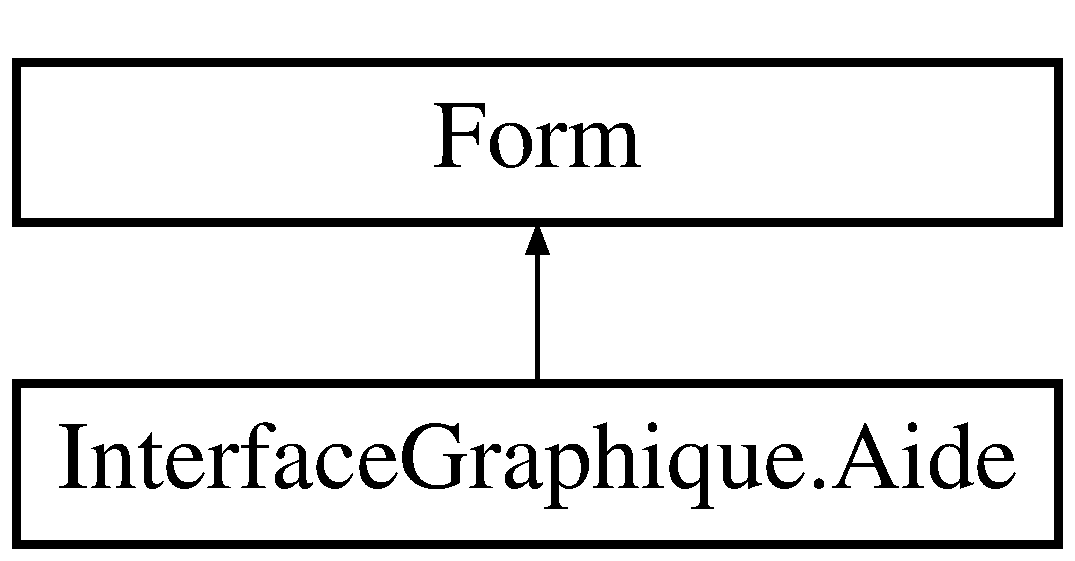
\includegraphics[height=2.000000cm]{class_interface_graphique_1_1_aide}
\end{center}
\end{figure}
\subsection*{Protected Member Functions}
\begin{DoxyCompactItemize}
\item 
override void \hyperlink{class_interface_graphique_1_1_aide_a38ca3f1e4bf62e0bad97bcc10a606e94}{Dispose} (bool disposing)
\begin{DoxyCompactList}\small\item\em Clean up any resources being used. \end{DoxyCompactList}\end{DoxyCompactItemize}


\subsection{Member Function Documentation}
\index{Interface\+Graphique\+::\+Aide@{Interface\+Graphique\+::\+Aide}!Dispose@{Dispose}}
\index{Dispose@{Dispose}!Interface\+Graphique\+::\+Aide@{Interface\+Graphique\+::\+Aide}}
\subsubsection[{\texorpdfstring{Dispose(bool disposing)}{Dispose(bool disposing)}}]{\setlength{\rightskip}{0pt plus 5cm}override void Interface\+Graphique.\+Aide.\+Dispose (
\begin{DoxyParamCaption}
\item[{bool}]{disposing}
\end{DoxyParamCaption}
)\hspace{0.3cm}{\ttfamily [inline]}, {\ttfamily [protected]}}\hypertarget{class_interface_graphique_1_1_aide_a38ca3f1e4bf62e0bad97bcc10a606e94}{}\label{class_interface_graphique_1_1_aide_a38ca3f1e4bf62e0bad97bcc10a606e94}


Clean up any resources being used. 


\begin{DoxyParams}{Parameters}
{\em disposing} & true if managed resources should be disposed; otherwise, false.\\
\hline
\end{DoxyParams}


The documentation for this class was generated from the following files\+:\begin{DoxyCompactItemize}
\item 
C\+:/\+Users/\+Bilal Itani/\+Desktop/inf2990-\/11/\+Cadriciel/\+Sources/\+Interface\+Graphique/\hyperlink{_aide_8cs}{Aide.\+cs}\item 
C\+:/\+Users/\+Bilal Itani/\+Desktop/inf2990-\/11/\+Cadriciel/\+Sources/\+Interface\+Graphique/Aide.\+Designer.\+cs\end{DoxyCompactItemize}

\hypertarget{structai_export_data_blob}{}\section{ai\+Export\+Data\+Blob Struct Reference}
\label{structai_export_data_blob}\index{ai\+Export\+Data\+Blob@{ai\+Export\+Data\+Blob}}


{\ttfamily \#include $<$cexport.\+h$>$}

\subsection*{Public Attributes}
\begin{DoxyCompactItemize}
\item 
size\+\_\+t \hyperlink{structai_export_data_blob_a339bfaacc70396b2f99f94c1bc3b808f}{size}\hypertarget{structai_export_data_blob_a339bfaacc70396b2f99f94c1bc3b808f}{}\label{structai_export_data_blob_a339bfaacc70396b2f99f94c1bc3b808f}

\begin{DoxyCompactList}\small\item\em Size of the data in bytes. \end{DoxyCompactList}\item 
void $\ast$ \hyperlink{structai_export_data_blob_ac080c780dad92077b42447d77a1a9ed1}{data}\hypertarget{structai_export_data_blob_ac080c780dad92077b42447d77a1a9ed1}{}\label{structai_export_data_blob_ac080c780dad92077b42447d77a1a9ed1}

\begin{DoxyCompactList}\small\item\em The data. \end{DoxyCompactList}\item 
C\+\_\+\+S\+T\+R\+U\+CT \hyperlink{structai_string}{ai\+String} \hyperlink{structai_export_data_blob_af7f006ac5ad818c0d81d520a84f74c3e}{name}
\item 
C\+\_\+\+S\+T\+R\+U\+CT \hyperlink{structai_export_data_blob}{ai\+Export\+Data\+Blob} $\ast$ \hyperlink{structai_export_data_blob_a3e98fa760f45983ff1bccec6715f3817}{next}
\end{DoxyCompactItemize}


\subsection{Detailed Description}
Describes a blob of exported scene data. Use \hyperlink{cexport_8h_a33b02f2dbfd79980bf29e62f3a64139f}{ai\+Export\+Scene\+To\+Blob()} to create a blob containing an exported scene. The memory referred by this structure is owned by \hyperlink{namespace_assimp}{Assimp}. Use \#ai\+Release\+Exported\+File() to free its resources. Don\textquotesingle{}t try to free the memory on your side -\/ it will crash for most build configurations due to conflicting heaps.

Blobs can be nested -\/ each blob may reference another blob, which may in turn reference another blob and so on. This is used when exporters write more than one output file for a given \#ai\+Scene. See the remarks for \hyperlink{structai_export_data_blob_af7f006ac5ad818c0d81d520a84f74c3e}{ai\+Export\+Data\+Blob\+::name} for more information. 

\subsection{Member Data Documentation}
\index{ai\+Export\+Data\+Blob@{ai\+Export\+Data\+Blob}!name@{name}}
\index{name@{name}!ai\+Export\+Data\+Blob@{ai\+Export\+Data\+Blob}}
\subsubsection[{\texorpdfstring{name}{name}}]{\setlength{\rightskip}{0pt plus 5cm}C\+\_\+\+S\+T\+R\+U\+CT {\bf ai\+String} ai\+Export\+Data\+Blob\+::name}\hypertarget{structai_export_data_blob_af7f006ac5ad818c0d81d520a84f74c3e}{}\label{structai_export_data_blob_af7f006ac5ad818c0d81d520a84f74c3e}
Name of the blob. An empty string always indicates the first (and primary) blob, which contains the actual file data. Any other blobs are auxiliary files produced by exporters (i.\+e. material files). Existence of such files depends on the file format. Most formats don\textquotesingle{}t split assets across multiple files.

If used, blob names usually contain the file extension that should be used when writing the data to disc. \index{ai\+Export\+Data\+Blob@{ai\+Export\+Data\+Blob}!next@{next}}
\index{next@{next}!ai\+Export\+Data\+Blob@{ai\+Export\+Data\+Blob}}
\subsubsection[{\texorpdfstring{next}{next}}]{\setlength{\rightskip}{0pt plus 5cm}C\+\_\+\+S\+T\+R\+U\+CT {\bf ai\+Export\+Data\+Blob}$\ast$ ai\+Export\+Data\+Blob\+::next}\hypertarget{structai_export_data_blob_a3e98fa760f45983ff1bccec6715f3817}{}\label{structai_export_data_blob_a3e98fa760f45983ff1bccec6715f3817}
Pointer to the next blob in the chain or N\+U\+LL if there is none. 

The documentation for this struct was generated from the following file\+:\begin{DoxyCompactItemize}
\item 
C\+:/\+Users/\+Bilal Itani/\+Desktop/inf2990-\/11/\+Cadriciel/\+Commun/\+Externe/assimp/include/\hyperlink{cexport_8h}{cexport.\+h}\end{DoxyCompactItemize}

\hypertarget{structai_export_format_desc}{}\section{ai\+Export\+Format\+Desc Struct Reference}
\label{structai_export_format_desc}\index{ai\+Export\+Format\+Desc@{ai\+Export\+Format\+Desc}}


{\ttfamily \#include $<$cexport.\+h$>$}

\subsection*{Public Attributes}
\begin{DoxyCompactItemize}
\item 
const char $\ast$ \hyperlink{structai_export_format_desc_afe216eaea3a04abca041e5c253f94bbf}{id}
\item 
const char $\ast$ \hyperlink{structai_export_format_desc_a9c84c4b07c5177fb6539b9bdf90236fb}{description}
\item 
const char $\ast$ \hyperlink{structai_export_format_desc_a589d08d526f253176d09886787cd6b22}{file\+Extension}\hypertarget{structai_export_format_desc_a589d08d526f253176d09886787cd6b22}{}\label{structai_export_format_desc_a589d08d526f253176d09886787cd6b22}

\begin{DoxyCompactList}\small\item\em Recommended file extension for the exported file in lower case. \end{DoxyCompactList}\end{DoxyCompactItemize}


\subsection{Detailed Description}
Describes an file format which \hyperlink{namespace_assimp}{Assimp} can export to. Use \hyperlink{cexport_8h_a59cfffbc5b436da8ed8542108102b502}{ai\+Get\+Export\+Format\+Count()} to learn how many export formats the current \hyperlink{namespace_assimp}{Assimp} build supports and \hyperlink{cexport_8h_adda7f2e6611f719af6c8a4a0bef0a0a2}{ai\+Get\+Export\+Format\+Description()} to retrieve a description of an export format option. 

\subsection{Member Data Documentation}
\index{ai\+Export\+Format\+Desc@{ai\+Export\+Format\+Desc}!description@{description}}
\index{description@{description}!ai\+Export\+Format\+Desc@{ai\+Export\+Format\+Desc}}
\subsubsection[{\texorpdfstring{description}{description}}]{\setlength{\rightskip}{0pt plus 5cm}const char$\ast$ ai\+Export\+Format\+Desc\+::description}\hypertarget{structai_export_format_desc_a9c84c4b07c5177fb6539b9bdf90236fb}{}\label{structai_export_format_desc_a9c84c4b07c5177fb6539b9bdf90236fb}
A short description of the file format to present to users. Useful if you want to allow the user to select an export format. \index{ai\+Export\+Format\+Desc@{ai\+Export\+Format\+Desc}!id@{id}}
\index{id@{id}!ai\+Export\+Format\+Desc@{ai\+Export\+Format\+Desc}}
\subsubsection[{\texorpdfstring{id}{id}}]{\setlength{\rightskip}{0pt plus 5cm}const char$\ast$ ai\+Export\+Format\+Desc\+::id}\hypertarget{structai_export_format_desc_afe216eaea3a04abca041e5c253f94bbf}{}\label{structai_export_format_desc_afe216eaea3a04abca041e5c253f94bbf}
a short string ID to uniquely identify the export format. Use this ID string to specify which file format you want to export to when calling \hyperlink{cexport_8h_a9615510b8430a9da4f435a72148128dd}{ai\+Export\+Scene()}. Example\+: \char`\"{}dae\char`\"{} or \char`\"{}obj\char`\"{} 

The documentation for this struct was generated from the following file\+:\begin{DoxyCompactItemize}
\item 
C\+:/\+Users/\+Bilal Itani/\+Desktop/inf2990-\/11/\+Cadriciel/\+Commun/\+Externe/assimp/include/\hyperlink{cexport_8h}{cexport.\+h}\end{DoxyCompactItemize}

\hypertarget{structai_face}{}\section{ai\+Face Struct Reference}
\label{structai_face}\index{ai\+Face@{ai\+Face}}


A single face in a mesh, referring to multiple vertices.  




{\ttfamily \#include $<$mesh.\+h$>$}

\subsection*{Public Attributes}
\begin{DoxyCompactItemize}
\item 
unsigned int \hyperlink{structai_face_adda2698cec0ebfe651572f4a5701360b}{m\+Num\+Indices}
\item 
unsigned int $\ast$ \hyperlink{structai_face_a2026b434c40cf1636f9f464a592ec36c}{m\+Indices}\hypertarget{structai_face_a2026b434c40cf1636f9f464a592ec36c}{}\label{structai_face_a2026b434c40cf1636f9f464a592ec36c}

\begin{DoxyCompactList}\small\item\em Pointer to the indices array. Size of the array is given in num\+Indices. \end{DoxyCompactList}\end{DoxyCompactItemize}


\subsection{Detailed Description}
A single face in a mesh, referring to multiple vertices. 

If m\+Num\+Indices is 3, we call the face \textquotesingle{}triangle\textquotesingle{}, for m\+Num\+Indices $>$ 3 it\textquotesingle{}s called \textquotesingle{}polygon\textquotesingle{} (hey, that\textquotesingle{}s just a definition!). ~\newline
 \hyperlink{structai_mesh_a99d66ac0a444068c1b252b30265cbf53}{ai\+Mesh\+::m\+Primitive\+Types} can be queried to quickly examine which types of primitive are actually present in a mesh. The \hyperlink{postprocess_8h_a64795260b95f5a4b3f3dc1be4f52e410ab4484f73635d633cd79973bac1431ed6}{ai\+Process\+\_\+\+Sort\+By\+P\+Type} flag executes a special post-\/processing algorithm which splits meshes with {\itshape different} primitive types mixed up (e.\+g. lines and triangles) in several \textquotesingle{}clean\textquotesingle{} submeshes. Furthermore there is a configuration option ( \#\+A\+I\+\_\+\+C\+O\+N\+F\+I\+G\+\_\+\+P\+P\+\_\+\+S\+B\+P\+\_\+\+R\+E\+M\+O\+VE) to force \hyperlink{postprocess_8h_a64795260b95f5a4b3f3dc1be4f52e410ab4484f73635d633cd79973bac1431ed6}{ai\+Process\+\_\+\+Sort\+By\+P\+Type} to remove specific kinds of primitives from the imported scene, completely and forever. In many cases you\textquotesingle{}ll probably want to set this setting to 
\begin{DoxyCode}
aiPrimitiveType\_LINE|aiPrimitiveType\_POINT
\end{DoxyCode}
 Together with the \hyperlink{postprocess_8h_a64795260b95f5a4b3f3dc1be4f52e410a9c3de834f0307f31fa2b1b6d05dd592b}{ai\+Process\+\_\+\+Triangulate} flag you can then be sure that \hyperlink{structai_face_adda2698cec0ebfe651572f4a5701360b}{ai\+Face\+::m\+Num\+Indices} is always 3. \begin{DoxyNote}{Note}
Take a look at the \hyperlink{}{Data Structures page } for more information on the layout and winding order of a face. 
\end{DoxyNote}


\subsection{Member Data Documentation}
\index{ai\+Face@{ai\+Face}!m\+Num\+Indices@{m\+Num\+Indices}}
\index{m\+Num\+Indices@{m\+Num\+Indices}!ai\+Face@{ai\+Face}}
\subsubsection[{\texorpdfstring{m\+Num\+Indices}{mNumIndices}}]{\setlength{\rightskip}{0pt plus 5cm}unsigned int ai\+Face\+::m\+Num\+Indices}\hypertarget{structai_face_adda2698cec0ebfe651572f4a5701360b}{}\label{structai_face_adda2698cec0ebfe651572f4a5701360b}
Number of indices defining this face. The maximum value for this member is \#\+A\+I\+\_\+\+M\+A\+X\+\_\+\+F\+A\+C\+E\+\_\+\+I\+N\+D\+I\+C\+ES. 

The documentation for this struct was generated from the following file\+:\begin{DoxyCompactItemize}
\item 
Commun/\+Externe/assimp/include/mesh.\+h\end{DoxyCompactItemize}

\hypertarget{structai_file}{}\section{ai\+File Struct Reference}
\label{structai_file}\index{ai\+File@{ai\+File}}


C-\/\+A\+PI\+: File callbacks.  




{\ttfamily \#include $<$cfileio.\+h$>$}

\subsection*{Public Attributes}
\begin{DoxyCompactItemize}
\item 
ai\+File\+Read\+Proc \hyperlink{structai_file_a52287e81ca67b9d43cc1ce6142f781fa}{Read\+Proc}
\item 
ai\+File\+Write\+Proc \hyperlink{structai_file_ab9fca3a62e34a33592c13a6f31db7d1d}{Write\+Proc}
\item 
ai\+File\+Tell\+Proc \hyperlink{structai_file_aaf2d88a3b2fcbdacf51119658283d27e}{Tell\+Proc}
\item 
ai\+File\+Tell\+Proc \hyperlink{structai_file_aff2fff8c0458e7ec71f7de217c3a3033}{File\+Size\+Proc}
\item 
ai\+File\+Seek \hyperlink{structai_file_a7a07b499be4ad433669246479a4d4ad2}{Seek\+Proc}
\item 
ai\+File\+Flush\+Proc \hyperlink{structai_file_a1102d28d1c0be68ffed20476669bdb0d}{Flush\+Proc}
\item 
ai\+User\+Data \hyperlink{structai_file_aec528fa18f4755fe4f28d604fde28aad}{User\+Data}
\end{DoxyCompactItemize}


\subsection{Detailed Description}
C-\/\+A\+PI\+: File callbacks. 

Actually, it\textquotesingle{}s a data structure to wrap a set of f\+X\+X\+XX (e.\+g fopen) replacement functions.

The default implementation of the functions utilizes the f\+X\+XX functions from the C\+RT. However, you can supply a custom implementation to \hyperlink{namespace_assimp}{Assimp} by delivering a custom \hyperlink{structai_file_i_o}{ai\+File\+IO}. Use this to enable reading from other sources, such as Z\+IP archives or memory locations. 

\subsection{Member Data Documentation}
\index{ai\+File@{ai\+File}!File\+Size\+Proc@{File\+Size\+Proc}}
\index{File\+Size\+Proc@{File\+Size\+Proc}!ai\+File@{ai\+File}}
\subsubsection[{\texorpdfstring{File\+Size\+Proc}{FileSizeProc}}]{\setlength{\rightskip}{0pt plus 5cm}ai\+File\+Tell\+Proc ai\+File\+::\+File\+Size\+Proc}\hypertarget{structai_file_aff2fff8c0458e7ec71f7de217c3a3033}{}\label{structai_file_aff2fff8c0458e7ec71f7de217c3a3033}
Callback to retrieve the size of the file, in bytes \index{ai\+File@{ai\+File}!Flush\+Proc@{Flush\+Proc}}
\index{Flush\+Proc@{Flush\+Proc}!ai\+File@{ai\+File}}
\subsubsection[{\texorpdfstring{Flush\+Proc}{FlushProc}}]{\setlength{\rightskip}{0pt plus 5cm}ai\+File\+Flush\+Proc ai\+File\+::\+Flush\+Proc}\hypertarget{structai_file_a1102d28d1c0be68ffed20476669bdb0d}{}\label{structai_file_a1102d28d1c0be68ffed20476669bdb0d}
Callback to flush the file contents \index{ai\+File@{ai\+File}!Read\+Proc@{Read\+Proc}}
\index{Read\+Proc@{Read\+Proc}!ai\+File@{ai\+File}}
\subsubsection[{\texorpdfstring{Read\+Proc}{ReadProc}}]{\setlength{\rightskip}{0pt plus 5cm}ai\+File\+Read\+Proc ai\+File\+::\+Read\+Proc}\hypertarget{structai_file_a52287e81ca67b9d43cc1ce6142f781fa}{}\label{structai_file_a52287e81ca67b9d43cc1ce6142f781fa}
Callback to read from a file \index{ai\+File@{ai\+File}!Seek\+Proc@{Seek\+Proc}}
\index{Seek\+Proc@{Seek\+Proc}!ai\+File@{ai\+File}}
\subsubsection[{\texorpdfstring{Seek\+Proc}{SeekProc}}]{\setlength{\rightskip}{0pt plus 5cm}ai\+File\+Seek ai\+File\+::\+Seek\+Proc}\hypertarget{structai_file_a7a07b499be4ad433669246479a4d4ad2}{}\label{structai_file_a7a07b499be4ad433669246479a4d4ad2}
Callback to set the current position of the file cursor (fseek()) \index{ai\+File@{ai\+File}!Tell\+Proc@{Tell\+Proc}}
\index{Tell\+Proc@{Tell\+Proc}!ai\+File@{ai\+File}}
\subsubsection[{\texorpdfstring{Tell\+Proc}{TellProc}}]{\setlength{\rightskip}{0pt plus 5cm}ai\+File\+Tell\+Proc ai\+File\+::\+Tell\+Proc}\hypertarget{structai_file_aaf2d88a3b2fcbdacf51119658283d27e}{}\label{structai_file_aaf2d88a3b2fcbdacf51119658283d27e}
Callback to retrieve the current position of the file cursor (ftell()) \index{ai\+File@{ai\+File}!User\+Data@{User\+Data}}
\index{User\+Data@{User\+Data}!ai\+File@{ai\+File}}
\subsubsection[{\texorpdfstring{User\+Data}{UserData}}]{\setlength{\rightskip}{0pt plus 5cm}ai\+User\+Data ai\+File\+::\+User\+Data}\hypertarget{structai_file_aec528fa18f4755fe4f28d604fde28aad}{}\label{structai_file_aec528fa18f4755fe4f28d604fde28aad}
User-\/defined, opaque data \index{ai\+File@{ai\+File}!Write\+Proc@{Write\+Proc}}
\index{Write\+Proc@{Write\+Proc}!ai\+File@{ai\+File}}
\subsubsection[{\texorpdfstring{Write\+Proc}{WriteProc}}]{\setlength{\rightskip}{0pt plus 5cm}ai\+File\+Write\+Proc ai\+File\+::\+Write\+Proc}\hypertarget{structai_file_ab9fca3a62e34a33592c13a6f31db7d1d}{}\label{structai_file_ab9fca3a62e34a33592c13a6f31db7d1d}
Callback to write to a file 

The documentation for this struct was generated from the following file\+:\begin{DoxyCompactItemize}
\item 
Cadriciel/\+Commun/\+Externe/assimp/include/cfileio.\+h\end{DoxyCompactItemize}

\hypertarget{structai_file_i_o}{}\section{ai\+File\+IO Struct Reference}
\label{structai_file_i_o}\index{ai\+File\+IO@{ai\+File\+IO}}


C-\/\+A\+PI\+: File system callbacks.  




{\ttfamily \#include $<$cfileio.\+h$>$}

\subsection*{Public Attributes}
\begin{DoxyCompactItemize}
\item 
ai\+File\+Open\+Proc \hyperlink{structai_file_i_o_a819d9c7823039294125068d06949a6df}{Open\+Proc}
\item 
ai\+File\+Close\+Proc \hyperlink{structai_file_i_o_a7ec702672712b5a02dc49cb17f980a14}{Close\+Proc}
\item 
ai\+User\+Data \hyperlink{structai_file_i_o_a9c62b7f3d70fbb2f41e33ad0b9933139}{User\+Data}
\end{DoxyCompactItemize}


\subsection{Detailed Description}
C-\/\+A\+PI\+: File system callbacks. 

Provided are functions to open and close files. Supply a custom structure to the import function. If you don\textquotesingle{}t, a default implementation is used. Use custom file systems to enable reading from other sources, such as Z\+I\+Ps or memory locations. 

\subsection{Member Data Documentation}
\index{ai\+File\+IO@{ai\+File\+IO}!Close\+Proc@{Close\+Proc}}
\index{Close\+Proc@{Close\+Proc}!ai\+File\+IO@{ai\+File\+IO}}
\subsubsection[{\texorpdfstring{Close\+Proc}{CloseProc}}]{\setlength{\rightskip}{0pt plus 5cm}ai\+File\+Close\+Proc ai\+File\+I\+O\+::\+Close\+Proc}\hypertarget{structai_file_i_o_a7ec702672712b5a02dc49cb17f980a14}{}\label{structai_file_i_o_a7ec702672712b5a02dc49cb17f980a14}
Function used to close an existing file \index{ai\+File\+IO@{ai\+File\+IO}!Open\+Proc@{Open\+Proc}}
\index{Open\+Proc@{Open\+Proc}!ai\+File\+IO@{ai\+File\+IO}}
\subsubsection[{\texorpdfstring{Open\+Proc}{OpenProc}}]{\setlength{\rightskip}{0pt plus 5cm}ai\+File\+Open\+Proc ai\+File\+I\+O\+::\+Open\+Proc}\hypertarget{structai_file_i_o_a819d9c7823039294125068d06949a6df}{}\label{structai_file_i_o_a819d9c7823039294125068d06949a6df}
Function used to open a new file \index{ai\+File\+IO@{ai\+File\+IO}!User\+Data@{User\+Data}}
\index{User\+Data@{User\+Data}!ai\+File\+IO@{ai\+File\+IO}}
\subsubsection[{\texorpdfstring{User\+Data}{UserData}}]{\setlength{\rightskip}{0pt plus 5cm}ai\+User\+Data ai\+File\+I\+O\+::\+User\+Data}\hypertarget{structai_file_i_o_a9c62b7f3d70fbb2f41e33ad0b9933139}{}\label{structai_file_i_o_a9c62b7f3d70fbb2f41e33ad0b9933139}
User-\/defined, opaque data 

The documentation for this struct was generated from the following file\+:\begin{DoxyCompactItemize}
\item 
Cadriciel/\+Commun/\+Externe/assimp/include/cfileio.\+h\end{DoxyCompactItemize}

\hypertarget{structai_importer_desc}{}\section{ai\+Importer\+Desc Struct Reference}
\label{structai_importer_desc}\index{ai\+Importer\+Desc@{ai\+Importer\+Desc}}


{\ttfamily \#include $<$importerdesc.\+h$>$}

\subsection*{Public Attributes}
\begin{DoxyCompactItemize}
\item 
const char $\ast$ \hyperlink{structai_importer_desc_a2a9d5fd818c01bba1a0a782722ab9495}{m\+Name}
\item 
const char $\ast$ \hyperlink{structai_importer_desc_a8e050453324b1e855701c7c082c1b24b}{m\+Author}
\item 
const char $\ast$ \hyperlink{structai_importer_desc_a53bf0ecb36ce0b97018b4b6bd2748f02}{m\+Maintainer}
\item 
const char $\ast$ \hyperlink{structai_importer_desc_a2d8ad562f6c18ee9e8bfdb2da4871118}{m\+Comments}
\item 
unsigned int \hyperlink{structai_importer_desc_a9939db58b9f95a537f9f5a749524b6b2}{m\+Flags}
\item 
unsigned int \hyperlink{structai_importer_desc_aee34d348f522807f0a36607664e92a57}{m\+Min\+Major}
\item 
unsigned int {\bfseries m\+Min\+Minor}\hypertarget{structai_importer_desc_adb265dee32c6533234c45638df66ddab}{}\label{structai_importer_desc_adb265dee32c6533234c45638df66ddab}

\item 
unsigned int \hyperlink{structai_importer_desc_a9d33eac3be20f7f4630f838a228ada63}{m\+Max\+Major}
\item 
unsigned int {\bfseries m\+Max\+Minor}\hypertarget{structai_importer_desc_ae4c60eec7020af836b23537148f47f83}{}\label{structai_importer_desc_ae4c60eec7020af836b23537148f47f83}

\item 
const char $\ast$ \hyperlink{structai_importer_desc_a074bd688ffd15d7f4df32e794111a413}{m\+File\+Extensions}
\end{DoxyCompactItemize}


\subsection{Detailed Description}
Meta information about a particular importer. Importers need to fill this structure, but they can freely decide how talkative they are. A common use case for loader meta info is a user interface in which the user can choose between various import/export file formats. Building such an UI by hand means a lot of maintenance as importers/exporters are added to \hyperlink{namespace_assimp}{Assimp}, so it might be useful to have a common mechanism to query some rough importer characteristics. 

\subsection{Member Data Documentation}
\index{ai\+Importer\+Desc@{ai\+Importer\+Desc}!m\+Author@{m\+Author}}
\index{m\+Author@{m\+Author}!ai\+Importer\+Desc@{ai\+Importer\+Desc}}
\subsubsection[{\texorpdfstring{m\+Author}{mAuthor}}]{\setlength{\rightskip}{0pt plus 5cm}const char$\ast$ ai\+Importer\+Desc\+::m\+Author}\hypertarget{structai_importer_desc_a8e050453324b1e855701c7c082c1b24b}{}\label{structai_importer_desc_a8e050453324b1e855701c7c082c1b24b}
Original author (left blank if unknown or whole assimp team) \index{ai\+Importer\+Desc@{ai\+Importer\+Desc}!m\+Comments@{m\+Comments}}
\index{m\+Comments@{m\+Comments}!ai\+Importer\+Desc@{ai\+Importer\+Desc}}
\subsubsection[{\texorpdfstring{m\+Comments}{mComments}}]{\setlength{\rightskip}{0pt plus 5cm}const char$\ast$ ai\+Importer\+Desc\+::m\+Comments}\hypertarget{structai_importer_desc_a2d8ad562f6c18ee9e8bfdb2da4871118}{}\label{structai_importer_desc_a2d8ad562f6c18ee9e8bfdb2da4871118}
Implementation comments, i.\+e. unimplemented features \index{ai\+Importer\+Desc@{ai\+Importer\+Desc}!m\+File\+Extensions@{m\+File\+Extensions}}
\index{m\+File\+Extensions@{m\+File\+Extensions}!ai\+Importer\+Desc@{ai\+Importer\+Desc}}
\subsubsection[{\texorpdfstring{m\+File\+Extensions}{mFileExtensions}}]{\setlength{\rightskip}{0pt plus 5cm}const char$\ast$ ai\+Importer\+Desc\+::m\+File\+Extensions}\hypertarget{structai_importer_desc_a074bd688ffd15d7f4df32e794111a413}{}\label{structai_importer_desc_a074bd688ffd15d7f4df32e794111a413}
List of file extensions this importer can handle. List entries are separated by space characters. All entries are lower case without a leading dot (i.\+e. \char`\"{}xml dae\char`\"{} would be a valid value. Note that multiple importers may respond to the same file extension -\/ assimp calls all importers in the order in which they are registered and each importer gets the opportunity to load the file until one importer \char`\"{}claims\char`\"{} the file. Apart from file extension checks, importers typically use other methods to quickly reject files (i.\+e. magic words) so this does not mean that common or generic file extensions such as X\+ML would be tediously slow. \index{ai\+Importer\+Desc@{ai\+Importer\+Desc}!m\+Flags@{m\+Flags}}
\index{m\+Flags@{m\+Flags}!ai\+Importer\+Desc@{ai\+Importer\+Desc}}
\subsubsection[{\texorpdfstring{m\+Flags}{mFlags}}]{\setlength{\rightskip}{0pt plus 5cm}unsigned int ai\+Importer\+Desc\+::m\+Flags}\hypertarget{structai_importer_desc_a9939db58b9f95a537f9f5a749524b6b2}{}\label{structai_importer_desc_a9939db58b9f95a537f9f5a749524b6b2}
Any combination of the \#ai\+Loader\+Flags enumerated values. These flags indicate some characteristics common to many importers. \index{ai\+Importer\+Desc@{ai\+Importer\+Desc}!m\+Maintainer@{m\+Maintainer}}
\index{m\+Maintainer@{m\+Maintainer}!ai\+Importer\+Desc@{ai\+Importer\+Desc}}
\subsubsection[{\texorpdfstring{m\+Maintainer}{mMaintainer}}]{\setlength{\rightskip}{0pt plus 5cm}const char$\ast$ ai\+Importer\+Desc\+::m\+Maintainer}\hypertarget{structai_importer_desc_a53bf0ecb36ce0b97018b4b6bd2748f02}{}\label{structai_importer_desc_a53bf0ecb36ce0b97018b4b6bd2748f02}
Current maintainer, left blank if the author maintains \index{ai\+Importer\+Desc@{ai\+Importer\+Desc}!m\+Max\+Major@{m\+Max\+Major}}
\index{m\+Max\+Major@{m\+Max\+Major}!ai\+Importer\+Desc@{ai\+Importer\+Desc}}
\subsubsection[{\texorpdfstring{m\+Max\+Major}{mMaxMajor}}]{\setlength{\rightskip}{0pt plus 5cm}unsigned int ai\+Importer\+Desc\+::m\+Max\+Major}\hypertarget{structai_importer_desc_a9d33eac3be20f7f4630f838a228ada63}{}\label{structai_importer_desc_a9d33eac3be20f7f4630f838a228ada63}
Maximum format version that can be loaded im major.\+minor format, both are set to 0 if there is either no version scheme or if the loader doesn\textquotesingle{}t care. Loaders that expect to be forward-\/compatible to potential future format versions should indicate zero, otherwise they should specify the current maximum version. \index{ai\+Importer\+Desc@{ai\+Importer\+Desc}!m\+Min\+Major@{m\+Min\+Major}}
\index{m\+Min\+Major@{m\+Min\+Major}!ai\+Importer\+Desc@{ai\+Importer\+Desc}}
\subsubsection[{\texorpdfstring{m\+Min\+Major}{mMinMajor}}]{\setlength{\rightskip}{0pt plus 5cm}unsigned int ai\+Importer\+Desc\+::m\+Min\+Major}\hypertarget{structai_importer_desc_aee34d348f522807f0a36607664e92a57}{}\label{structai_importer_desc_aee34d348f522807f0a36607664e92a57}
Minimum format version that can be loaded im major.\+minor format, both are set to 0 if there is either no version scheme or if the loader doesn\textquotesingle{}t care. \index{ai\+Importer\+Desc@{ai\+Importer\+Desc}!m\+Name@{m\+Name}}
\index{m\+Name@{m\+Name}!ai\+Importer\+Desc@{ai\+Importer\+Desc}}
\subsubsection[{\texorpdfstring{m\+Name}{mName}}]{\setlength{\rightskip}{0pt plus 5cm}const char$\ast$ ai\+Importer\+Desc\+::m\+Name}\hypertarget{structai_importer_desc_a2a9d5fd818c01bba1a0a782722ab9495}{}\label{structai_importer_desc_a2a9d5fd818c01bba1a0a782722ab9495}
Full name of the importer (i.\+e. Blender3D importer) 

The documentation for this struct was generated from the following file\+:\begin{DoxyCompactItemize}
\item 
Commun/\+Externe/assimp/include/\hyperlink{importerdesc_8h}{importerdesc.\+h}\end{DoxyCompactItemize}

\hypertarget{structai_light}{}\section{ai\+Light Struct Reference}
\label{structai_light}\index{ai\+Light@{ai\+Light}}


{\ttfamily \#include $<$light.\+h$>$}

\subsection*{Public Attributes}
\begin{DoxyCompactItemize}
\item 
C\+\_\+\+S\+T\+R\+U\+CT \hyperlink{structai_string}{ai\+String} \hyperlink{structai_light_a92806413f16230728b04e5f379fd00c0}{m\+Name}
\item 
C\+\_\+\+E\+N\+UM \hyperlink{light_8h_a7a75cb224d903e71e8daede432449766}{ai\+Light\+Source\+Type} \hyperlink{structai_light_a4cba1741875dd92724ff55be91c60c2b}{m\+Type}
\item 
C\+\_\+\+S\+T\+R\+U\+CT \hyperlink{structai_vector3_d}{ai\+Vector3D} \hyperlink{structai_light_a5daf9c9ad2613603b847a527123611f0}{m\+Position}
\item 
C\+\_\+\+S\+T\+R\+U\+CT \hyperlink{structai_vector3_d}{ai\+Vector3D} \hyperlink{structai_light_af3776d5e4e6065cb6dd7e10dc656dada}{m\+Direction}
\item 
float \hyperlink{structai_light_ae8804b3c309527ca0f85d676bab55710}{m\+Attenuation\+Constant}
\item 
float \hyperlink{structai_light_aefda311eaa785ea345782dfa95be817c}{m\+Attenuation\+Linear}
\item 
float \hyperlink{structai_light_ab4fb07bfa40a807661b1ed1791838a6d}{m\+Attenuation\+Quadratic}
\item 
C\+\_\+\+S\+T\+R\+U\+CT \hyperlink{structai_color3_d}{ai\+Color3D} \hyperlink{structai_light_a22e7feebbfaf53adf73bd9f581636efd}{m\+Color\+Diffuse}
\item 
C\+\_\+\+S\+T\+R\+U\+CT \hyperlink{structai_color3_d}{ai\+Color3D} \hyperlink{structai_light_aa79ae6ad6a10f0cb9c740e23b6bb01bf}{m\+Color\+Specular}
\item 
C\+\_\+\+S\+T\+R\+U\+CT \hyperlink{structai_color3_d}{ai\+Color3D} \hyperlink{structai_light_a5188b60e6fbaf1635fa780913508e3cd}{m\+Color\+Ambient}
\item 
float \hyperlink{structai_light_abad0466811938623e98bf1d334143f9a}{m\+Angle\+Inner\+Cone}
\item 
float \hyperlink{structai_light_a20fd332a5f9d8e8cb94816ff2b0ae7f4}{m\+Angle\+Outer\+Cone}
\end{DoxyCompactItemize}


\subsection{Detailed Description}
Helper structure to describe a light source.

\hyperlink{namespace_assimp}{Assimp} supports multiple sorts of light sources, including directional, point and spot lights. All of them are defined with just a single structure and distinguished by their parameters. Note -\/ some file formats (such as 3\+DS, A\+SE) export a \char`\"{}target point\char`\"{} -\/ the point a spot light is looking at (it can even be animated). \hyperlink{namespace_assimp}{Assimp} writes the target point as a subnode of a spotlights\textquotesingle{}s main node, called \char`\"{}$<$spot\+Name$>$.\+Target\char`\"{}. However, this is just additional information then, the transformation tracks of the main node make the spot light already point in the right direction. 

\subsection{Member Data Documentation}
\index{ai\+Light@{ai\+Light}!m\+Angle\+Inner\+Cone@{m\+Angle\+Inner\+Cone}}
\index{m\+Angle\+Inner\+Cone@{m\+Angle\+Inner\+Cone}!ai\+Light@{ai\+Light}}
\subsubsection[{\texorpdfstring{m\+Angle\+Inner\+Cone}{mAngleInnerCone}}]{\setlength{\rightskip}{0pt plus 5cm}float ai\+Light\+::m\+Angle\+Inner\+Cone}\hypertarget{structai_light_abad0466811938623e98bf1d334143f9a}{}\label{structai_light_abad0466811938623e98bf1d334143f9a}
Inner angle of a spot light\textquotesingle{}s light cone.

The spot light has maximum influence on objects inside this angle. The angle is given in radians. It is 2\+PI for point lights and undefined for directional lights. \index{ai\+Light@{ai\+Light}!m\+Angle\+Outer\+Cone@{m\+Angle\+Outer\+Cone}}
\index{m\+Angle\+Outer\+Cone@{m\+Angle\+Outer\+Cone}!ai\+Light@{ai\+Light}}
\subsubsection[{\texorpdfstring{m\+Angle\+Outer\+Cone}{mAngleOuterCone}}]{\setlength{\rightskip}{0pt plus 5cm}float ai\+Light\+::m\+Angle\+Outer\+Cone}\hypertarget{structai_light_a20fd332a5f9d8e8cb94816ff2b0ae7f4}{}\label{structai_light_a20fd332a5f9d8e8cb94816ff2b0ae7f4}
Outer angle of a spot light\textquotesingle{}s light cone.

The spot light does not affect objects outside this angle. The angle is given in radians. It is 2\+PI for point lights and undefined for directional lights. The outer angle must be greater than or equal to the inner angle. It is assumed that the application uses a smooth interpolation between the inner and the outer cone of the spot light. \index{ai\+Light@{ai\+Light}!m\+Attenuation\+Constant@{m\+Attenuation\+Constant}}
\index{m\+Attenuation\+Constant@{m\+Attenuation\+Constant}!ai\+Light@{ai\+Light}}
\subsubsection[{\texorpdfstring{m\+Attenuation\+Constant}{mAttenuationConstant}}]{\setlength{\rightskip}{0pt plus 5cm}float ai\+Light\+::m\+Attenuation\+Constant}\hypertarget{structai_light_ae8804b3c309527ca0f85d676bab55710}{}\label{structai_light_ae8804b3c309527ca0f85d676bab55710}
Constant light attenuation factor.

The intensity of the light source at a given distance \textquotesingle{}d\textquotesingle{} from the light\textquotesingle{}s position is 
\begin{DoxyCode}
Atten = 1/( att0 + att1 * d + att2 * d*d)
\end{DoxyCode}
 This member corresponds to the att0 variable in the equation. Naturally undefined for directional lights. \index{ai\+Light@{ai\+Light}!m\+Attenuation\+Linear@{m\+Attenuation\+Linear}}
\index{m\+Attenuation\+Linear@{m\+Attenuation\+Linear}!ai\+Light@{ai\+Light}}
\subsubsection[{\texorpdfstring{m\+Attenuation\+Linear}{mAttenuationLinear}}]{\setlength{\rightskip}{0pt plus 5cm}float ai\+Light\+::m\+Attenuation\+Linear}\hypertarget{structai_light_aefda311eaa785ea345782dfa95be817c}{}\label{structai_light_aefda311eaa785ea345782dfa95be817c}
Linear light attenuation factor.

The intensity of the light source at a given distance \textquotesingle{}d\textquotesingle{} from the light\textquotesingle{}s position is 
\begin{DoxyCode}
Atten = 1/( att0 + att1 * d + att2 * d*d)
\end{DoxyCode}
 This member corresponds to the att1 variable in the equation. Naturally undefined for directional lights. \index{ai\+Light@{ai\+Light}!m\+Attenuation\+Quadratic@{m\+Attenuation\+Quadratic}}
\index{m\+Attenuation\+Quadratic@{m\+Attenuation\+Quadratic}!ai\+Light@{ai\+Light}}
\subsubsection[{\texorpdfstring{m\+Attenuation\+Quadratic}{mAttenuationQuadratic}}]{\setlength{\rightskip}{0pt plus 5cm}float ai\+Light\+::m\+Attenuation\+Quadratic}\hypertarget{structai_light_ab4fb07bfa40a807661b1ed1791838a6d}{}\label{structai_light_ab4fb07bfa40a807661b1ed1791838a6d}
Quadratic light attenuation factor.

The intensity of the light source at a given distance \textquotesingle{}d\textquotesingle{} from the light\textquotesingle{}s position is 
\begin{DoxyCode}
Atten = 1/( att0 + att1 * d + att2 * d*d)
\end{DoxyCode}
 This member corresponds to the att2 variable in the equation. Naturally undefined for directional lights. \index{ai\+Light@{ai\+Light}!m\+Color\+Ambient@{m\+Color\+Ambient}}
\index{m\+Color\+Ambient@{m\+Color\+Ambient}!ai\+Light@{ai\+Light}}
\subsubsection[{\texorpdfstring{m\+Color\+Ambient}{mColorAmbient}}]{\setlength{\rightskip}{0pt plus 5cm}C\+\_\+\+S\+T\+R\+U\+CT {\bf ai\+Color3D} ai\+Light\+::m\+Color\+Ambient}\hypertarget{structai_light_a5188b60e6fbaf1635fa780913508e3cd}{}\label{structai_light_a5188b60e6fbaf1635fa780913508e3cd}
Ambient color of the light source

The ambient light color is multiplied with the ambient material color to obtain the final color that contributes to the ambient shading term. Most renderers will ignore this value it, is just a remaining of the fixed-\/function pipeline that is still supported by quite many file formats. \index{ai\+Light@{ai\+Light}!m\+Color\+Diffuse@{m\+Color\+Diffuse}}
\index{m\+Color\+Diffuse@{m\+Color\+Diffuse}!ai\+Light@{ai\+Light}}
\subsubsection[{\texorpdfstring{m\+Color\+Diffuse}{mColorDiffuse}}]{\setlength{\rightskip}{0pt plus 5cm}C\+\_\+\+S\+T\+R\+U\+CT {\bf ai\+Color3D} ai\+Light\+::m\+Color\+Diffuse}\hypertarget{structai_light_a22e7feebbfaf53adf73bd9f581636efd}{}\label{structai_light_a22e7feebbfaf53adf73bd9f581636efd}
Diffuse color of the light source

The diffuse light color is multiplied with the diffuse material color to obtain the final color that contributes to the diffuse shading term. \index{ai\+Light@{ai\+Light}!m\+Color\+Specular@{m\+Color\+Specular}}
\index{m\+Color\+Specular@{m\+Color\+Specular}!ai\+Light@{ai\+Light}}
\subsubsection[{\texorpdfstring{m\+Color\+Specular}{mColorSpecular}}]{\setlength{\rightskip}{0pt plus 5cm}C\+\_\+\+S\+T\+R\+U\+CT {\bf ai\+Color3D} ai\+Light\+::m\+Color\+Specular}\hypertarget{structai_light_aa79ae6ad6a10f0cb9c740e23b6bb01bf}{}\label{structai_light_aa79ae6ad6a10f0cb9c740e23b6bb01bf}
Specular color of the light source

The specular light color is multiplied with the specular material color to obtain the final color that contributes to the specular shading term. \index{ai\+Light@{ai\+Light}!m\+Direction@{m\+Direction}}
\index{m\+Direction@{m\+Direction}!ai\+Light@{ai\+Light}}
\subsubsection[{\texorpdfstring{m\+Direction}{mDirection}}]{\setlength{\rightskip}{0pt plus 5cm}C\+\_\+\+S\+T\+R\+U\+CT {\bf ai\+Vector3D} ai\+Light\+::m\+Direction}\hypertarget{structai_light_af3776d5e4e6065cb6dd7e10dc656dada}{}\label{structai_light_af3776d5e4e6065cb6dd7e10dc656dada}
Direction of the light source in space. Relative to the transformation of the node corresponding to the light.

The direction is undefined for point lights. The vector may be normalized, but it needn\textquotesingle{}t. \index{ai\+Light@{ai\+Light}!m\+Name@{m\+Name}}
\index{m\+Name@{m\+Name}!ai\+Light@{ai\+Light}}
\subsubsection[{\texorpdfstring{m\+Name}{mName}}]{\setlength{\rightskip}{0pt plus 5cm}C\+\_\+\+S\+T\+R\+U\+CT {\bf ai\+String} ai\+Light\+::m\+Name}\hypertarget{structai_light_a92806413f16230728b04e5f379fd00c0}{}\label{structai_light_a92806413f16230728b04e5f379fd00c0}
The name of the light source.

There must be a node in the scenegraph with the same name. This node specifies the position of the light in the scene hierarchy and can be animated. \index{ai\+Light@{ai\+Light}!m\+Position@{m\+Position}}
\index{m\+Position@{m\+Position}!ai\+Light@{ai\+Light}}
\subsubsection[{\texorpdfstring{m\+Position}{mPosition}}]{\setlength{\rightskip}{0pt plus 5cm}C\+\_\+\+S\+T\+R\+U\+CT {\bf ai\+Vector3D} ai\+Light\+::m\+Position}\hypertarget{structai_light_a5daf9c9ad2613603b847a527123611f0}{}\label{structai_light_a5daf9c9ad2613603b847a527123611f0}
Position of the light source in space. Relative to the transformation of the node corresponding to the light.

The position is undefined for directional lights. \index{ai\+Light@{ai\+Light}!m\+Type@{m\+Type}}
\index{m\+Type@{m\+Type}!ai\+Light@{ai\+Light}}
\subsubsection[{\texorpdfstring{m\+Type}{mType}}]{\setlength{\rightskip}{0pt plus 5cm}C\+\_\+\+E\+N\+UM {\bf ai\+Light\+Source\+Type} ai\+Light\+::m\+Type}\hypertarget{structai_light_a4cba1741875dd92724ff55be91c60c2b}{}\label{structai_light_a4cba1741875dd92724ff55be91c60c2b}
The type of the light source.

ai\+Light\+Source\+\_\+\+U\+N\+D\+E\+F\+I\+N\+ED is not a valid value for this member. 

The documentation for this struct was generated from the following file\+:\begin{DoxyCompactItemize}
\item 
C\+:/\+Users/\+Bilal Itani/\+Desktop/inf2990-\/11/\+Cadriciel/\+Commun/\+Externe/assimp/include/\hyperlink{light_8h}{light.\+h}\end{DoxyCompactItemize}

\hypertarget{structai_log_stream}{}\section{ai\+Log\+Stream Struct Reference}
\label{structai_log_stream}\index{ai\+Log\+Stream@{ai\+Log\+Stream}}


{\ttfamily \#include $<$cimport.\+h$>$}

\subsection*{Public Attributes}
\begin{DoxyCompactItemize}
\item 
ai\+Log\+Stream\+Callback \hyperlink{structai_log_stream_ac73ae46eee54ba0f920d6abb97c33e97}{callback}
\item 
char $\ast$ \hyperlink{structai_log_stream_a3382042e4171a6dd5a71d7f98741f86e}{user}
\end{DoxyCompactItemize}


\subsection{Detailed Description}
C-\/\+A\+PI\+: Represents a log stream. A log stream receives all log messages and streams them {\itshape somewhere}. \begin{DoxySeeAlso}{See also}
ai\+Get\+Predefined\+Log\+Stream 

ai\+Attach\+Log\+Stream 

ai\+Detach\+Log\+Stream 
\end{DoxySeeAlso}


\subsection{Member Data Documentation}
\index{ai\+Log\+Stream@{ai\+Log\+Stream}!callback@{callback}}
\index{callback@{callback}!ai\+Log\+Stream@{ai\+Log\+Stream}}
\subsubsection[{\texorpdfstring{callback}{callback}}]{\setlength{\rightskip}{0pt plus 5cm}ai\+Log\+Stream\+Callback ai\+Log\+Stream\+::callback}\hypertarget{structai_log_stream_ac73ae46eee54ba0f920d6abb97c33e97}{}\label{structai_log_stream_ac73ae46eee54ba0f920d6abb97c33e97}
callback to be called \index{ai\+Log\+Stream@{ai\+Log\+Stream}!user@{user}}
\index{user@{user}!ai\+Log\+Stream@{ai\+Log\+Stream}}
\subsubsection[{\texorpdfstring{user}{user}}]{\setlength{\rightskip}{0pt plus 5cm}char$\ast$ ai\+Log\+Stream\+::user}\hypertarget{structai_log_stream_a3382042e4171a6dd5a71d7f98741f86e}{}\label{structai_log_stream_a3382042e4171a6dd5a71d7f98741f86e}
user data to be passed to the callback 

The documentation for this struct was generated from the following file\+:\begin{DoxyCompactItemize}
\item 
Cadriciel/\+Commun/\+Externe/assimp/include/cimport.\+h\end{DoxyCompactItemize}

\hypertarget{structai_matrix3x3}{}\section{ai\+Matrix3x3 Struct Reference}
\label{structai_matrix3x3}\index{ai\+Matrix3x3@{ai\+Matrix3x3}}
\subsection*{Public Attributes}
\begin{DoxyCompactItemize}
\item 
float {\bfseries a1}\hypertarget{structai_matrix3x3_a6884258a2f50758ed8b554b531186917}{}\label{structai_matrix3x3_a6884258a2f50758ed8b554b531186917}

\item 
float {\bfseries a2}\hypertarget{structai_matrix3x3_a4c74733870193040ba4953fb673e77df}{}\label{structai_matrix3x3_a4c74733870193040ba4953fb673e77df}

\item 
float {\bfseries a3}\hypertarget{structai_matrix3x3_a851d391df32a39e1ced1a9a286b38cf4}{}\label{structai_matrix3x3_a851d391df32a39e1ced1a9a286b38cf4}

\item 
float {\bfseries b1}\hypertarget{structai_matrix3x3_a9eeba340d3502017caad70416f03863a}{}\label{structai_matrix3x3_a9eeba340d3502017caad70416f03863a}

\item 
float {\bfseries b2}\hypertarget{structai_matrix3x3_a9f5e25b60bbd7bdf8f0a19cd82cc6b15}{}\label{structai_matrix3x3_a9f5e25b60bbd7bdf8f0a19cd82cc6b15}

\item 
float {\bfseries b3}\hypertarget{structai_matrix3x3_a21aa4345fe6ce2774db94d118c536d02}{}\label{structai_matrix3x3_a21aa4345fe6ce2774db94d118c536d02}

\item 
float {\bfseries c1}\hypertarget{structai_matrix3x3_ae62a2877076cbee151e89cb34567e3ca}{}\label{structai_matrix3x3_ae62a2877076cbee151e89cb34567e3ca}

\item 
float {\bfseries c2}\hypertarget{structai_matrix3x3_a8e0d85d5c46eb4f4478f1fe159be4320}{}\label{structai_matrix3x3_a8e0d85d5c46eb4f4478f1fe159be4320}

\item 
float {\bfseries c3}\hypertarget{structai_matrix3x3_aa7eef894dec22db1011092410b24f19b}{}\label{structai_matrix3x3_aa7eef894dec22db1011092410b24f19b}

\end{DoxyCompactItemize}


The documentation for this struct was generated from the following file\+:\begin{DoxyCompactItemize}
\item 
C\+:/\+Users/\+Bilal Itani/\+Desktop/inf2990-\/11/\+Cadriciel/\+Commun/\+Externe/assimp/include/\hyperlink{matrix3x3_8h}{matrix3x3.\+h}\end{DoxyCompactItemize}

\hypertarget{structai_matrix4x4}{}\section{ai\+Matrix4x4 Struct Reference}
\label{structai_matrix4x4}\index{ai\+Matrix4x4@{ai\+Matrix4x4}}
\subsection*{Public Attributes}
\begin{DoxyCompactItemize}
\item 
float {\bfseries a1}\hypertarget{structai_matrix4x4_aeabb269b7ef332d3c69c14d8af3d531c}{}\label{structai_matrix4x4_aeabb269b7ef332d3c69c14d8af3d531c}

\item 
float {\bfseries a2}\hypertarget{structai_matrix4x4_a9d36d992ba3cfc814913e0225a04b91b}{}\label{structai_matrix4x4_a9d36d992ba3cfc814913e0225a04b91b}

\item 
float {\bfseries a3}\hypertarget{structai_matrix4x4_a36f0d69cf678c3b5deea5a76f5624848}{}\label{structai_matrix4x4_a36f0d69cf678c3b5deea5a76f5624848}

\item 
float {\bfseries a4}\hypertarget{structai_matrix4x4_a184e1a78f61c430aa7b0079b42e4c2a0}{}\label{structai_matrix4x4_a184e1a78f61c430aa7b0079b42e4c2a0}

\item 
float {\bfseries b1}\hypertarget{structai_matrix4x4_a59667637f4d71bf4ebc1183bebe746fb}{}\label{structai_matrix4x4_a59667637f4d71bf4ebc1183bebe746fb}

\item 
float {\bfseries b2}\hypertarget{structai_matrix4x4_af5dcecf706021b313239b7113cb80daa}{}\label{structai_matrix4x4_af5dcecf706021b313239b7113cb80daa}

\item 
float {\bfseries b3}\hypertarget{structai_matrix4x4_a0f0bf4dfcf9dd562d71d5ed5a5342316}{}\label{structai_matrix4x4_a0f0bf4dfcf9dd562d71d5ed5a5342316}

\item 
float {\bfseries b4}\hypertarget{structai_matrix4x4_ae57a4a8b8f4509f5bdf90d7856c59281}{}\label{structai_matrix4x4_ae57a4a8b8f4509f5bdf90d7856c59281}

\item 
float {\bfseries c1}\hypertarget{structai_matrix4x4_a63c847f6e86653143aa659f13c154e2b}{}\label{structai_matrix4x4_a63c847f6e86653143aa659f13c154e2b}

\item 
float {\bfseries c2}\hypertarget{structai_matrix4x4_a67425f81054b1097c29b73bf317cfeeb}{}\label{structai_matrix4x4_a67425f81054b1097c29b73bf317cfeeb}

\item 
float {\bfseries c3}\hypertarget{structai_matrix4x4_aec8c5745b90139d472eb4e91f1373c1a}{}\label{structai_matrix4x4_aec8c5745b90139d472eb4e91f1373c1a}

\item 
float {\bfseries c4}\hypertarget{structai_matrix4x4_a7e3288f38a4e00d55c02272e1582e462}{}\label{structai_matrix4x4_a7e3288f38a4e00d55c02272e1582e462}

\item 
float {\bfseries d1}\hypertarget{structai_matrix4x4_a13f3800d9106e3be6d0e60b794c5a5ae}{}\label{structai_matrix4x4_a13f3800d9106e3be6d0e60b794c5a5ae}

\item 
float {\bfseries d2}\hypertarget{structai_matrix4x4_a6f17ca1c7e4b9377d0e332f85aab282b}{}\label{structai_matrix4x4_a6f17ca1c7e4b9377d0e332f85aab282b}

\item 
float {\bfseries d3}\hypertarget{structai_matrix4x4_a8d2910f62b34b1e2ace93b55e4db4b92}{}\label{structai_matrix4x4_a8d2910f62b34b1e2ace93b55e4db4b92}

\item 
float {\bfseries d4}\hypertarget{structai_matrix4x4_ac0a65b51f126f7331b4f7dbbd82f3d63}{}\label{structai_matrix4x4_ac0a65b51f126f7331b4f7dbbd82f3d63}

\end{DoxyCompactItemize}


The documentation for this struct was generated from the following file\+:\begin{DoxyCompactItemize}
\item 
Cadriciel/\+Commun/\+Externe/assimp/include/\hyperlink{matrix4x4_8h}{matrix4x4.\+h}\end{DoxyCompactItemize}

\hypertarget{classai_matrix4x4t}{}\section{ai\+Matrix4x4t$<$ T $>$ Class Template Reference}
\label{classai_matrix4x4t}\index{ai\+Matrix4x4t$<$ T $>$@{ai\+Matrix4x4t$<$ T $>$}}


The documentation for this class was generated from the following file\+:\begin{DoxyCompactItemize}
\item 
C\+:/\+Users/\+Bilal Itani/\+Desktop/inf2990-\/11/\+Cadriciel/\+Commun/\+Utilitaire/\hyperlink{_utilitaire_8h}{Utilitaire.\+h}\end{DoxyCompactItemize}

\hypertarget{structai_mesh}{}\section{ai\+Mesh Struct Reference}
\label{structai_mesh}\index{ai\+Mesh@{ai\+Mesh}}


A mesh represents a geometry or model with a single material.  




{\ttfamily \#include $<$mesh.\+h$>$}

\subsection*{Public Attributes}
\begin{DoxyCompactItemize}
\item 
unsigned int \hyperlink{structai_mesh_a99d66ac0a444068c1b252b30265cbf53}{m\+Primitive\+Types}
\item 
unsigned int \hyperlink{structai_mesh_ab34b7b5941e6636f1c08f615cbb072ef}{m\+Num\+Vertices}
\item 
unsigned int \hyperlink{structai_mesh_aeed22ee6963b79548f3877b3c905518e}{m\+Num\+Faces}
\item 
C\+\_\+\+S\+T\+R\+U\+CT \hyperlink{structai_vector3_d}{ai\+Vector3D} $\ast$ \hyperlink{structai_mesh_afd4588abb3e1c72821ae0234a3850662}{m\+Vertices}
\item 
C\+\_\+\+S\+T\+R\+U\+CT \hyperlink{structai_vector3_d}{ai\+Vector3D} $\ast$ \hyperlink{structai_mesh_aec81b496b4d93838cef038933dabe9b9}{m\+Normals}
\item 
C\+\_\+\+S\+T\+R\+U\+CT \hyperlink{structai_vector3_d}{ai\+Vector3D} $\ast$ \hyperlink{structai_mesh_af367ff78bd69f3e83d7edc8ad67dc5df}{m\+Tangents}
\item 
C\+\_\+\+S\+T\+R\+U\+CT \hyperlink{structai_vector3_d}{ai\+Vector3D} $\ast$ \hyperlink{structai_mesh_ab2a81bfe1731f01271ebab274a8f01c4}{m\+Bitangents}
\item 
C\+\_\+\+S\+T\+R\+U\+CT \hyperlink{structai_color4_d}{ai\+Color4D} $\ast$ \hyperlink{structai_mesh_ad9215f67bd0c2277b10775a8adb66b96}{m\+Colors} \mbox{[}A\+I\+\_\+\+M\+A\+X\+\_\+\+N\+U\+M\+B\+E\+R\+\_\+\+O\+F\+\_\+\+C\+O\+L\+O\+R\+\_\+\+S\+E\+TS\mbox{]}
\item 
C\+\_\+\+S\+T\+R\+U\+CT \hyperlink{structai_vector3_d}{ai\+Vector3D} $\ast$ \hyperlink{structai_mesh_a4a50b11d00ef50f419c75cab0f6bddd6}{m\+Texture\+Coords} \mbox{[}A\+I\+\_\+\+M\+A\+X\+\_\+\+N\+U\+M\+B\+E\+R\+\_\+\+O\+F\+\_\+\+T\+E\+X\+T\+U\+R\+E\+C\+O\+O\+R\+DS\mbox{]}
\item 
unsigned int \hyperlink{structai_mesh_a635c631a6e66d32989d6b25b2a892d86}{m\+Num\+U\+V\+Components} \mbox{[}A\+I\+\_\+\+M\+A\+X\+\_\+\+N\+U\+M\+B\+E\+R\+\_\+\+O\+F\+\_\+\+T\+E\+X\+T\+U\+R\+E\+C\+O\+O\+R\+DS\mbox{]}
\item 
C\+\_\+\+S\+T\+R\+U\+CT \hyperlink{structai_face}{ai\+Face} $\ast$ \hyperlink{structai_mesh_a5a65fbc7fdea7f8d36f39047425ece07}{m\+Faces}
\item 
unsigned int \hyperlink{structai_mesh_a0f9d5425b6300e32a842a94f943fd79e}{m\+Num\+Bones}
\item 
C\+\_\+\+S\+T\+R\+U\+CT \hyperlink{structai_bone}{ai\+Bone} $\ast$$\ast$ \hyperlink{structai_mesh_a0c0582a7f45b340b6a33552c53232539}{m\+Bones}
\item 
unsigned int \hyperlink{structai_mesh_aa2807c7ba172115203ed16047ad65f9e}{m\+Material\+Index}
\item 
C\+\_\+\+S\+T\+R\+U\+CT \hyperlink{structai_string}{ai\+String} \hyperlink{structai_mesh_a8dd9433e0c5b008e3e5aee6c801d3b74}{m\+Name}
\item 
unsigned int \hyperlink{structai_mesh_a1692a300222b32348ae51779df4a697e}{m\+Num\+Anim\+Meshes}
\item 
C\+\_\+\+S\+T\+R\+U\+CT \hyperlink{structai_anim_mesh}{ai\+Anim\+Mesh} $\ast$$\ast$ \hyperlink{structai_mesh_a5078f7db7e99ed05db89dfa412f0e990}{m\+Anim\+Meshes}
\end{DoxyCompactItemize}


\subsection{Detailed Description}
A mesh represents a geometry or model with a single material. 

It usually consists of a number of vertices and a series of primitives/faces referencing the vertices. In addition there might be a series of bones, each of them addressing a number of vertices with a certain weight. Vertex data is presented in channels with each channel containing a single per-\/vertex information such as a set of texture coords or a normal vector. If a data pointer is non-\/null, the corresponding data stream is present. From C++-\/programs you can also use the comfort functions Has$\ast$() to test for the presence of various data streams.

A Mesh uses only a single material which is referenced by a material ID. \begin{DoxyNote}{Note}
The m\+Positions member is usually not optional. However, vertex positions {\itshape could} be missing if the \#\+A\+I\+\_\+\+S\+C\+E\+N\+E\+\_\+\+F\+L\+A\+G\+S\+\_\+\+I\+N\+C\+O\+M\+P\+L\+E\+TE flag is set in 
\begin{DoxyCode}
aiScene::mFlags
\end{DoxyCode}
 
\end{DoxyNote}


\subsection{Member Data Documentation}
\index{ai\+Mesh@{ai\+Mesh}!m\+Anim\+Meshes@{m\+Anim\+Meshes}}
\index{m\+Anim\+Meshes@{m\+Anim\+Meshes}!ai\+Mesh@{ai\+Mesh}}
\subsubsection[{\texorpdfstring{m\+Anim\+Meshes}{mAnimMeshes}}]{\setlength{\rightskip}{0pt plus 5cm}C\+\_\+\+S\+T\+R\+U\+CT {\bf ai\+Anim\+Mesh}$\ast$$\ast$ ai\+Mesh\+::m\+Anim\+Meshes}\hypertarget{structai_mesh_a5078f7db7e99ed05db89dfa412f0e990}{}\label{structai_mesh_a5078f7db7e99ed05db89dfa412f0e990}
N\+OT C\+U\+R\+R\+E\+N\+T\+LY IN U\+SE. Attachment meshes for this mesh, for vertex-\/based animation. Attachment meshes carry replacement data for some of the mesh\textquotesingle{}es vertex components (usually positions, normals). \index{ai\+Mesh@{ai\+Mesh}!m\+Bitangents@{m\+Bitangents}}
\index{m\+Bitangents@{m\+Bitangents}!ai\+Mesh@{ai\+Mesh}}
\subsubsection[{\texorpdfstring{m\+Bitangents}{mBitangents}}]{\setlength{\rightskip}{0pt plus 5cm}C\+\_\+\+S\+T\+R\+U\+CT {\bf ai\+Vector3D}$\ast$ ai\+Mesh\+::m\+Bitangents}\hypertarget{structai_mesh_ab2a81bfe1731f01271ebab274a8f01c4}{}\label{structai_mesh_ab2a81bfe1731f01271ebab274a8f01c4}
Vertex bitangents. The bitangent of a vertex points in the direction of the positive Y texture axis. The array contains normalized vectors, N\+U\+LL if not present. The array is m\+Num\+Vertices in size. \begin{DoxyNote}{Note}
If the mesh contains tangents, it automatically also contains bitangents. 
\end{DoxyNote}
\index{ai\+Mesh@{ai\+Mesh}!m\+Bones@{m\+Bones}}
\index{m\+Bones@{m\+Bones}!ai\+Mesh@{ai\+Mesh}}
\subsubsection[{\texorpdfstring{m\+Bones}{mBones}}]{\setlength{\rightskip}{0pt plus 5cm}C\+\_\+\+S\+T\+R\+U\+CT {\bf ai\+Bone}$\ast$$\ast$ ai\+Mesh\+::m\+Bones}\hypertarget{structai_mesh_a0c0582a7f45b340b6a33552c53232539}{}\label{structai_mesh_a0c0582a7f45b340b6a33552c53232539}
The bones of this mesh. A bone consists of a name by which it can be found in the frame hierarchy and a set of vertex weights. \index{ai\+Mesh@{ai\+Mesh}!m\+Colors@{m\+Colors}}
\index{m\+Colors@{m\+Colors}!ai\+Mesh@{ai\+Mesh}}
\subsubsection[{\texorpdfstring{m\+Colors}{mColors}}]{\setlength{\rightskip}{0pt plus 5cm}C\+\_\+\+S\+T\+R\+U\+CT {\bf ai\+Color4D}$\ast$ ai\+Mesh\+::m\+Colors\mbox{[}A\+I\+\_\+\+M\+A\+X\+\_\+\+N\+U\+M\+B\+E\+R\+\_\+\+O\+F\+\_\+\+C\+O\+L\+O\+R\+\_\+\+S\+E\+TS\mbox{]}}\hypertarget{structai_mesh_ad9215f67bd0c2277b10775a8adb66b96}{}\label{structai_mesh_ad9215f67bd0c2277b10775a8adb66b96}
Vertex color sets. A mesh may contain 0 to \#\+A\+I\+\_\+\+M\+A\+X\+\_\+\+N\+U\+M\+B\+E\+R\+\_\+\+O\+F\+\_\+\+C\+O\+L\+O\+R\+\_\+\+S\+E\+TS vertex colors per vertex. N\+U\+LL if not present. Each array is m\+Num\+Vertices in size if present. \index{ai\+Mesh@{ai\+Mesh}!m\+Faces@{m\+Faces}}
\index{m\+Faces@{m\+Faces}!ai\+Mesh@{ai\+Mesh}}
\subsubsection[{\texorpdfstring{m\+Faces}{mFaces}}]{\setlength{\rightskip}{0pt plus 5cm}C\+\_\+\+S\+T\+R\+U\+CT {\bf ai\+Face}$\ast$ ai\+Mesh\+::m\+Faces}\hypertarget{structai_mesh_a5a65fbc7fdea7f8d36f39047425ece07}{}\label{structai_mesh_a5a65fbc7fdea7f8d36f39047425ece07}
The faces the mesh is constructed from. Each face refers to a number of vertices by their indices. This array is always present in a mesh, its size is given in m\+Num\+Faces. If the \#\+A\+I\+\_\+\+S\+C\+E\+N\+E\+\_\+\+F\+L\+A\+G\+S\+\_\+\+N\+O\+N\+\_\+\+V\+E\+R\+B\+O\+S\+E\+\_\+\+F\+O\+R\+M\+AT is N\+OT set each face references an unique set of vertices. \index{ai\+Mesh@{ai\+Mesh}!m\+Material\+Index@{m\+Material\+Index}}
\index{m\+Material\+Index@{m\+Material\+Index}!ai\+Mesh@{ai\+Mesh}}
\subsubsection[{\texorpdfstring{m\+Material\+Index}{mMaterialIndex}}]{\setlength{\rightskip}{0pt plus 5cm}unsigned int ai\+Mesh\+::m\+Material\+Index}\hypertarget{structai_mesh_aa2807c7ba172115203ed16047ad65f9e}{}\label{structai_mesh_aa2807c7ba172115203ed16047ad65f9e}
The material used by this mesh. A mesh does use only a single material. If an imported model uses multiple materials, the import splits up the mesh. Use this value as index into the scene\textquotesingle{}s material list. \index{ai\+Mesh@{ai\+Mesh}!m\+Name@{m\+Name}}
\index{m\+Name@{m\+Name}!ai\+Mesh@{ai\+Mesh}}
\subsubsection[{\texorpdfstring{m\+Name}{mName}}]{\setlength{\rightskip}{0pt plus 5cm}C\+\_\+\+S\+T\+R\+U\+CT {\bf ai\+String} ai\+Mesh\+::m\+Name}\hypertarget{structai_mesh_a8dd9433e0c5b008e3e5aee6c801d3b74}{}\label{structai_mesh_a8dd9433e0c5b008e3e5aee6c801d3b74}
Name of the mesh. Meshes can be named, but this is not a requirement and leaving this field empty is totally fine. There are mainly three uses for mesh names\+:
\begin{DoxyItemize}
\item some formats name nodes and meshes independently.
\item importers tend to split meshes up to meet the one-\/material-\/per-\/mesh requirement. Assigning the same (dummy) name to each of the result meshes aids the caller at recovering the original mesh partitioning.
\item Vertex animations refer to meshes by their names. 
\end{DoxyItemize}\index{ai\+Mesh@{ai\+Mesh}!m\+Normals@{m\+Normals}}
\index{m\+Normals@{m\+Normals}!ai\+Mesh@{ai\+Mesh}}
\subsubsection[{\texorpdfstring{m\+Normals}{mNormals}}]{\setlength{\rightskip}{0pt plus 5cm}C\+\_\+\+S\+T\+R\+U\+CT {\bf ai\+Vector3D}$\ast$ ai\+Mesh\+::m\+Normals}\hypertarget{structai_mesh_aec81b496b4d93838cef038933dabe9b9}{}\label{structai_mesh_aec81b496b4d93838cef038933dabe9b9}
Vertex normals. The array contains normalized vectors, N\+U\+LL if not present. The array is m\+Num\+Vertices in size. Normals are undefined for point and line primitives. A mesh consisting of points and lines only may not have normal vectors. Meshes with mixed primitive types (i.\+e. lines and triangles) may have normals, but the normals for vertices that are only referenced by point or line primitives are undefined and set to Q\+NaN (W\+A\+RN\+: q\+NaN compares to inequal to {\itshape everything}, even to q\+NaN itself. Using code like this to check whether a field is qnan is\+: 
\begin{DoxyCode}
\textcolor{preprocessor}{#define IS\_QNAN(f) (f != f)}
\end{DoxyCode}
 still dangerous because even 1.\+f == 1.\+f could evaluate to false! ( remember the subtleties of I\+E\+E\+E754 artithmetics). Use stuff like {\ttfamily fpclassify} instead. \begin{DoxyNote}{Note}
Normal vectors computed by \hyperlink{namespace_assimp}{Assimp} are always unit-\/length. However, this needn\textquotesingle{}t apply for normals that have been taken directly from the model file. 
\end{DoxyNote}
\index{ai\+Mesh@{ai\+Mesh}!m\+Num\+Anim\+Meshes@{m\+Num\+Anim\+Meshes}}
\index{m\+Num\+Anim\+Meshes@{m\+Num\+Anim\+Meshes}!ai\+Mesh@{ai\+Mesh}}
\subsubsection[{\texorpdfstring{m\+Num\+Anim\+Meshes}{mNumAnimMeshes}}]{\setlength{\rightskip}{0pt plus 5cm}unsigned int ai\+Mesh\+::m\+Num\+Anim\+Meshes}\hypertarget{structai_mesh_a1692a300222b32348ae51779df4a697e}{}\label{structai_mesh_a1692a300222b32348ae51779df4a697e}
N\+OT C\+U\+R\+R\+E\+N\+T\+LY IN U\+SE. The number of attachment meshes \index{ai\+Mesh@{ai\+Mesh}!m\+Num\+Bones@{m\+Num\+Bones}}
\index{m\+Num\+Bones@{m\+Num\+Bones}!ai\+Mesh@{ai\+Mesh}}
\subsubsection[{\texorpdfstring{m\+Num\+Bones}{mNumBones}}]{\setlength{\rightskip}{0pt plus 5cm}unsigned int ai\+Mesh\+::m\+Num\+Bones}\hypertarget{structai_mesh_a0f9d5425b6300e32a842a94f943fd79e}{}\label{structai_mesh_a0f9d5425b6300e32a842a94f943fd79e}
The number of bones this mesh contains. Can be 0, in which case the m\+Bones array is N\+U\+LL. \index{ai\+Mesh@{ai\+Mesh}!m\+Num\+Faces@{m\+Num\+Faces}}
\index{m\+Num\+Faces@{m\+Num\+Faces}!ai\+Mesh@{ai\+Mesh}}
\subsubsection[{\texorpdfstring{m\+Num\+Faces}{mNumFaces}}]{\setlength{\rightskip}{0pt plus 5cm}unsigned int ai\+Mesh\+::m\+Num\+Faces}\hypertarget{structai_mesh_aeed22ee6963b79548f3877b3c905518e}{}\label{structai_mesh_aeed22ee6963b79548f3877b3c905518e}
The number of primitives (triangles, polygons, lines) in this mesh. This is also the size of the m\+Faces array. The maximum value for this member is \#\+A\+I\+\_\+\+M\+A\+X\+\_\+\+F\+A\+C\+ES. \index{ai\+Mesh@{ai\+Mesh}!m\+Num\+U\+V\+Components@{m\+Num\+U\+V\+Components}}
\index{m\+Num\+U\+V\+Components@{m\+Num\+U\+V\+Components}!ai\+Mesh@{ai\+Mesh}}
\subsubsection[{\texorpdfstring{m\+Num\+U\+V\+Components}{mNumUVComponents}}]{\setlength{\rightskip}{0pt plus 5cm}unsigned int ai\+Mesh\+::m\+Num\+U\+V\+Components\mbox{[}A\+I\+\_\+\+M\+A\+X\+\_\+\+N\+U\+M\+B\+E\+R\+\_\+\+O\+F\+\_\+\+T\+E\+X\+T\+U\+R\+E\+C\+O\+O\+R\+DS\mbox{]}}\hypertarget{structai_mesh_a635c631a6e66d32989d6b25b2a892d86}{}\label{structai_mesh_a635c631a6e66d32989d6b25b2a892d86}
Specifies the number of components for a given UV channel. Up to three channels are supported (U\+VW, for accessing volume or cube maps). If the value is 2 for a given channel n, the component p.\+z of m\+Texture\+Coords\mbox{[}n\mbox{]}\mbox{[}p\mbox{]} is set to 0.\+0f. If the value is 1 for a given channel, p.\+y is set to 0.\+0f, too. \begin{DoxyNote}{Note}
4D coords are not supported 
\end{DoxyNote}
\index{ai\+Mesh@{ai\+Mesh}!m\+Num\+Vertices@{m\+Num\+Vertices}}
\index{m\+Num\+Vertices@{m\+Num\+Vertices}!ai\+Mesh@{ai\+Mesh}}
\subsubsection[{\texorpdfstring{m\+Num\+Vertices}{mNumVertices}}]{\setlength{\rightskip}{0pt plus 5cm}unsigned int ai\+Mesh\+::m\+Num\+Vertices}\hypertarget{structai_mesh_ab34b7b5941e6636f1c08f615cbb072ef}{}\label{structai_mesh_ab34b7b5941e6636f1c08f615cbb072ef}
The number of vertices in this mesh. This is also the size of all of the per-\/vertex data arrays. The maximum value for this member is \#\+A\+I\+\_\+\+M\+A\+X\+\_\+\+V\+E\+R\+T\+I\+C\+ES. \index{ai\+Mesh@{ai\+Mesh}!m\+Primitive\+Types@{m\+Primitive\+Types}}
\index{m\+Primitive\+Types@{m\+Primitive\+Types}!ai\+Mesh@{ai\+Mesh}}
\subsubsection[{\texorpdfstring{m\+Primitive\+Types}{mPrimitiveTypes}}]{\setlength{\rightskip}{0pt plus 5cm}unsigned int ai\+Mesh\+::m\+Primitive\+Types}\hypertarget{structai_mesh_a99d66ac0a444068c1b252b30265cbf53}{}\label{structai_mesh_a99d66ac0a444068c1b252b30265cbf53}
Bitwise combination of the members of the \#ai\+Primitive\+Type enum. This specifies which types of primitives are present in the mesh. The \char`\"{}\+Sort\+By\+Primitive\+Type\char`\"{}-\/\+Step can be used to make sure the output meshes consist of one primitive type each. \index{ai\+Mesh@{ai\+Mesh}!m\+Tangents@{m\+Tangents}}
\index{m\+Tangents@{m\+Tangents}!ai\+Mesh@{ai\+Mesh}}
\subsubsection[{\texorpdfstring{m\+Tangents}{mTangents}}]{\setlength{\rightskip}{0pt plus 5cm}C\+\_\+\+S\+T\+R\+U\+CT {\bf ai\+Vector3D}$\ast$ ai\+Mesh\+::m\+Tangents}\hypertarget{structai_mesh_af367ff78bd69f3e83d7edc8ad67dc5df}{}\label{structai_mesh_af367ff78bd69f3e83d7edc8ad67dc5df}
Vertex tangents. The tangent of a vertex points in the direction of the positive X texture axis. The array contains normalized vectors, N\+U\+LL if not present. The array is m\+Num\+Vertices in size. A mesh consisting of points and lines only may not have normal vectors. Meshes with mixed primitive types (i.\+e. lines and triangles) may have normals, but the normals for vertices that are only referenced by point or line primitives are undefined and set to q\+NaN. See the \hyperlink{structai_mesh_aec81b496b4d93838cef038933dabe9b9}{m\+Normals} member for a detailled discussion of q\+Na\+Ns. \begin{DoxyNote}{Note}
If the mesh contains tangents, it automatically also contains bitangents. 
\end{DoxyNote}
\index{ai\+Mesh@{ai\+Mesh}!m\+Texture\+Coords@{m\+Texture\+Coords}}
\index{m\+Texture\+Coords@{m\+Texture\+Coords}!ai\+Mesh@{ai\+Mesh}}
\subsubsection[{\texorpdfstring{m\+Texture\+Coords}{mTextureCoords}}]{\setlength{\rightskip}{0pt plus 5cm}C\+\_\+\+S\+T\+R\+U\+CT {\bf ai\+Vector3D}$\ast$ ai\+Mesh\+::m\+Texture\+Coords\mbox{[}A\+I\+\_\+\+M\+A\+X\+\_\+\+N\+U\+M\+B\+E\+R\+\_\+\+O\+F\+\_\+\+T\+E\+X\+T\+U\+R\+E\+C\+O\+O\+R\+DS\mbox{]}}\hypertarget{structai_mesh_a4a50b11d00ef50f419c75cab0f6bddd6}{}\label{structai_mesh_a4a50b11d00ef50f419c75cab0f6bddd6}
Vertex texture coords, also known as UV channels. A mesh may contain 0 to A\+I\+\_\+\+M\+A\+X\+\_\+\+N\+U\+M\+B\+E\+R\+\_\+\+O\+F\+\_\+\+T\+E\+X\+T\+U\+R\+E\+C\+O\+O\+R\+DS per vertex. N\+U\+LL if not present. The array is m\+Num\+Vertices in size. \index{ai\+Mesh@{ai\+Mesh}!m\+Vertices@{m\+Vertices}}
\index{m\+Vertices@{m\+Vertices}!ai\+Mesh@{ai\+Mesh}}
\subsubsection[{\texorpdfstring{m\+Vertices}{mVertices}}]{\setlength{\rightskip}{0pt plus 5cm}C\+\_\+\+S\+T\+R\+U\+CT {\bf ai\+Vector3D}$\ast$ ai\+Mesh\+::m\+Vertices}\hypertarget{structai_mesh_afd4588abb3e1c72821ae0234a3850662}{}\label{structai_mesh_afd4588abb3e1c72821ae0234a3850662}
Vertex positions. This array is always present in a mesh. The array is m\+Num\+Vertices in size. 

The documentation for this struct was generated from the following file\+:\begin{DoxyCompactItemize}
\item 
C\+:/\+Users/\+Bilal Itani/\+Desktop/inf2990-\/11/\+Cadriciel/\+Commun/\+Externe/assimp/include/mesh.\+h\end{DoxyCompactItemize}

\hypertarget{structai_metadata}{}\section{ai\+Metadata Struct Reference}
\label{structai_metadata}\index{ai\+Metadata@{ai\+Metadata}}


{\ttfamily \#include $<$metadata.\+h$>$}

\subsection*{Public Attributes}
\begin{DoxyCompactItemize}
\item 
unsigned int \hyperlink{structai_metadata_a32c4587c53dd402a5878ffc94088e528}{m\+Num\+Properties}
\item 
C\+\_\+\+S\+T\+R\+U\+CT \hyperlink{structai_string}{ai\+String} $\ast$ \hyperlink{structai_metadata_aa8c77a263443658737ee51a74e3c292e}{m\+Keys}
\item 
C\+\_\+\+S\+T\+R\+U\+CT \hyperlink{structai_metadata_entry}{ai\+Metadata\+Entry} $\ast$ \hyperlink{structai_metadata_a34b515fcb5b806c471d3c6ce7bc76beb}{m\+Values}
\end{DoxyCompactItemize}


\subsection{Detailed Description}
Container for holding metadata.

Metadata is a key-\/value store using string keys and values. 

\subsection{Member Data Documentation}
\index{ai\+Metadata@{ai\+Metadata}!m\+Keys@{m\+Keys}}
\index{m\+Keys@{m\+Keys}!ai\+Metadata@{ai\+Metadata}}
\subsubsection[{\texorpdfstring{m\+Keys}{mKeys}}]{\setlength{\rightskip}{0pt plus 5cm}C\+\_\+\+S\+T\+R\+U\+CT {\bf ai\+String}$\ast$ ai\+Metadata\+::m\+Keys}\hypertarget{structai_metadata_aa8c77a263443658737ee51a74e3c292e}{}\label{structai_metadata_aa8c77a263443658737ee51a74e3c292e}
Arrays of keys, may not be N\+U\+LL. Entries in this array may not be N\+U\+LL as well. \index{ai\+Metadata@{ai\+Metadata}!m\+Num\+Properties@{m\+Num\+Properties}}
\index{m\+Num\+Properties@{m\+Num\+Properties}!ai\+Metadata@{ai\+Metadata}}
\subsubsection[{\texorpdfstring{m\+Num\+Properties}{mNumProperties}}]{\setlength{\rightskip}{0pt plus 5cm}unsigned int ai\+Metadata\+::m\+Num\+Properties}\hypertarget{structai_metadata_a32c4587c53dd402a5878ffc94088e528}{}\label{structai_metadata_a32c4587c53dd402a5878ffc94088e528}
Length of the m\+Keys and m\+Values arrays, respectively \index{ai\+Metadata@{ai\+Metadata}!m\+Values@{m\+Values}}
\index{m\+Values@{m\+Values}!ai\+Metadata@{ai\+Metadata}}
\subsubsection[{\texorpdfstring{m\+Values}{mValues}}]{\setlength{\rightskip}{0pt plus 5cm}C\+\_\+\+S\+T\+R\+U\+CT {\bf ai\+Metadata\+Entry}$\ast$ ai\+Metadata\+::m\+Values}\hypertarget{structai_metadata_a34b515fcb5b806c471d3c6ce7bc76beb}{}\label{structai_metadata_a34b515fcb5b806c471d3c6ce7bc76beb}
Arrays of values, may not be N\+U\+LL. Entries in this array may be N\+U\+LL if the corresponding property key has no assigned value. 

The documentation for this struct was generated from the following file\+:\begin{DoxyCompactItemize}
\item 
Cadriciel/\+Commun/\+Externe/assimp/include/\hyperlink{metadata_8h}{metadata.\+h}\end{DoxyCompactItemize}

\hypertarget{structai_metadata_entry}{}\section{ai\+Metadata\+Entry Struct Reference}
\label{structai_metadata_entry}\index{ai\+Metadata\+Entry@{ai\+Metadata\+Entry}}


{\ttfamily \#include $<$metadata.\+h$>$}

\subsection*{Public Attributes}
\begin{DoxyCompactItemize}
\item 
\hyperlink{metadata_8h_aa910906c37416da57bb36335a4d04232}{ai\+Metadata\+Type} {\bfseries m\+Type}\hypertarget{structai_metadata_entry_a075b29cd710e153f5402f479a7a10aee}{}\label{structai_metadata_entry_a075b29cd710e153f5402f479a7a10aee}

\item 
void $\ast$ {\bfseries m\+Data}\hypertarget{structai_metadata_entry_a97fe80a47846374edd38bda5b50b99b3}{}\label{structai_metadata_entry_a97fe80a47846374edd38bda5b50b99b3}

\end{DoxyCompactItemize}


\subsection{Detailed Description}
Metadata entry

The type field uniquely identifies the underlying type of the data field 

The documentation for this struct was generated from the following file\+:\begin{DoxyCompactItemize}
\item 
Cadriciel/\+Commun/\+Externe/assimp/include/\hyperlink{metadata_8h}{metadata.\+h}\end{DoxyCompactItemize}

\hypertarget{structai_plane}{}\section{ai\+Plane Struct Reference}
\label{structai_plane}\index{ai\+Plane@{ai\+Plane}}


{\ttfamily \#include $<$types.\+h$>$}

\subsection*{Public Attributes}
\begin{DoxyCompactItemize}
\item 
float \hyperlink{structai_plane_aeadf64e70e6daf1f7f431c90cfc8bce1}{a}\hypertarget{structai_plane_aeadf64e70e6daf1f7f431c90cfc8bce1}{}\label{structai_plane_aeadf64e70e6daf1f7f431c90cfc8bce1}

\begin{DoxyCompactList}\small\item\em Plane equation. \end{DoxyCompactList}\item 
float {\bfseries b}\hypertarget{structai_plane_a84ab33cd9b2f5325282b489f8a2bf11c}{}\label{structai_plane_a84ab33cd9b2f5325282b489f8a2bf11c}

\item 
float {\bfseries c}\hypertarget{structai_plane_a7b0ea36c355ca003a5789088fb24da1f}{}\label{structai_plane_a7b0ea36c355ca003a5789088fb24da1f}

\item 
float {\bfseries d}\hypertarget{structai_plane_ab8696b583b6fab46ae30cd5b691e7c9a}{}\label{structai_plane_ab8696b583b6fab46ae30cd5b691e7c9a}

\end{DoxyCompactItemize}


\subsection{Detailed Description}
Represents a plane in a three-\/dimensional, euclidean space 

The documentation for this struct was generated from the following file\+:\begin{DoxyCompactItemize}
\item 
Cadriciel/\+Commun/\+Externe/assimp/include/\hyperlink{types_8h}{types.\+h}\end{DoxyCompactItemize}

\hypertarget{structai_property_store}{}\section{ai\+Property\+Store Struct Reference}
\label{structai_property_store}\index{ai\+Property\+Store@{ai\+Property\+Store}}


{\ttfamily \#include $<$cimport.\+h$>$}

\subsection*{Public Attributes}
\begin{DoxyCompactItemize}
\item 
char {\bfseries sentinel}\hypertarget{structai_property_store_a53e97983bdbe38c596c7879555dc42a3}{}\label{structai_property_store_a53e97983bdbe38c596c7879555dc42a3}

\end{DoxyCompactItemize}


\subsection{Detailed Description}
C-\/\+A\+PI\+: Represents an opaque set of settings to be used during importing. \begin{DoxySeeAlso}{See also}
ai\+Create\+Property\+Store 

ai\+Release\+Property\+Store 

ai\+Import\+File\+Ex\+With\+Properties 

ai\+Set\+Property\+Integer 

ai\+Set\+Property\+Float 

ai\+Set\+Property\+String 

ai\+Set\+Property\+Matrix 
\end{DoxySeeAlso}


The documentation for this struct was generated from the following file\+:\begin{DoxyCompactItemize}
\item 
C\+:/\+Users/\+Bilal Itani/\+Desktop/inf2990-\/11/\+Cadriciel/\+Commun/\+Externe/assimp/include/cimport.\+h\end{DoxyCompactItemize}

\hypertarget{structai_quaternion}{}\section{ai\+Quaternion Struct Reference}
\label{structai_quaternion}\index{ai\+Quaternion@{ai\+Quaternion}}
\subsection*{Public Attributes}
\begin{DoxyCompactItemize}
\item 
float {\bfseries w}\hypertarget{structai_quaternion_a410b3c46417d67d728a01a5810907a36}{}\label{structai_quaternion_a410b3c46417d67d728a01a5810907a36}

\item 
float {\bfseries x}\hypertarget{structai_quaternion_af9db21b086c14d8654d62005f740e75f}{}\label{structai_quaternion_af9db21b086c14d8654d62005f740e75f}

\item 
float {\bfseries y}\hypertarget{structai_quaternion_a1695fefbc60becf95fcafcc08573ab44}{}\label{structai_quaternion_a1695fefbc60becf95fcafcc08573ab44}

\item 
float {\bfseries z}\hypertarget{structai_quaternion_acc30da6103d5131fb1bed6640f1eeda0}{}\label{structai_quaternion_acc30da6103d5131fb1bed6640f1eeda0}

\end{DoxyCompactItemize}


The documentation for this struct was generated from the following file\+:\begin{DoxyCompactItemize}
\item 
Commun/\+Externe/assimp/include/\hyperlink{quaternion_8h}{quaternion.\+h}\end{DoxyCompactItemize}

\hypertarget{structai_ray}{}\section{ai\+Ray Struct Reference}
\label{structai_ray}\index{ai\+Ray@{ai\+Ray}}


{\ttfamily \#include $<$types.\+h$>$}

\subsection*{Public Attributes}
\begin{DoxyCompactItemize}
\item 
C\+\_\+\+S\+T\+R\+U\+CT \hyperlink{structai_vector3_d}{ai\+Vector3D} \hyperlink{structai_ray_a312f663a7d2580b1b3beb52ffd4ab4c9}{pos}\hypertarget{structai_ray_a312f663a7d2580b1b3beb52ffd4ab4c9}{}\label{structai_ray_a312f663a7d2580b1b3beb52ffd4ab4c9}

\begin{DoxyCompactList}\small\item\em Position and direction of the ray. \end{DoxyCompactList}\item 
C\+\_\+\+S\+T\+R\+U\+CT \hyperlink{structai_vector3_d}{ai\+Vector3D} {\bfseries dir}\hypertarget{structai_ray_a635d9120af2654716e5e7952d837282b}{}\label{structai_ray_a635d9120af2654716e5e7952d837282b}

\end{DoxyCompactItemize}


\subsection{Detailed Description}
Represents a ray 

The documentation for this struct was generated from the following file\+:\begin{DoxyCompactItemize}
\item 
C\+:/\+Users/\+Bilal Itani/\+Desktop/inf2990-\/11/\+Cadriciel/\+Commun/\+Externe/assimp/include/\hyperlink{types_8h}{types.\+h}\end{DoxyCompactItemize}

\hypertarget{structai_string}{}\section{ai\+String Struct Reference}
\label{structai_string}\index{ai\+String@{ai\+String}}


{\ttfamily \#include $<$types.\+h$>$}

\subsection*{Public Attributes}
\begin{DoxyCompactItemize}
\item 
size\+\_\+t \hyperlink{structai_string_a7d77c2031ff0340746aa046f7fbcf313}{length}
\item 
char \hyperlink{structai_string_aa90b1da7d347a3dcca0a95061e6ea41d}{data} \mbox{[}\hyperlink{types_8h_ae6648cd71a8bd49d58ae8ed33ba910d1}{M\+A\+X\+L\+EN}\mbox{]}
\end{DoxyCompactItemize}


\subsection{Detailed Description}
Represents an U\+T\+F-\/8 string, zero byte terminated.

The character set of an \hyperlink{structai_string}{ai\+String} is explicitly defined to be U\+T\+F-\/8. This Unicode transformation was chosen in the belief that most strings in 3d files are limited to \hyperlink{struct_a_s_c_i_i}{A\+S\+C\+II}, thus the character set needed to be strictly \hyperlink{struct_a_s_c_i_i}{A\+S\+C\+II} compatible.

Most text file loaders provide proper Unicode input file handling, special unicode characters are correctly transcoded to \hyperlink{struct_u_t_f8}{U\+T\+F8} and are kept throughout the libraries\textquotesingle{} import pipeline.

For most applications, it will be absolutely sufficient to interpret the \hyperlink{structai_string}{ai\+String} as \hyperlink{struct_a_s_c_i_i}{A\+S\+C\+II} data and work with it as one would work with a plain char$\ast$. Windows users in need of proper support for i.\+e asian characters can use the \#\+Multi\+Byte\+To\+Wide\+Char(), \#\+Wide\+Char\+To\+Multi\+Byte() Win\+A\+PI functionality to convert the U\+T\+F-\/8 strings to their working character set (i.\+e. M\+B\+CS, Wide\+Char).

We use this representation instead of std\+::string to be C-\/compatible. The (binary) length of such a string is limited to M\+A\+X\+L\+EN characters (including the the terminating zero). 

\subsection{Member Data Documentation}
\index{ai\+String@{ai\+String}!data@{data}}
\index{data@{data}!ai\+String@{ai\+String}}
\subsubsection[{\texorpdfstring{data}{data}}]{\setlength{\rightskip}{0pt plus 5cm}char ai\+String\+::data\mbox{[}{\bf M\+A\+X\+L\+EN}\mbox{]}}\hypertarget{structai_string_aa90b1da7d347a3dcca0a95061e6ea41d}{}\label{structai_string_aa90b1da7d347a3dcca0a95061e6ea41d}
String buffer. Size limit is M\+A\+X\+L\+EN \index{ai\+String@{ai\+String}!length@{length}}
\index{length@{length}!ai\+String@{ai\+String}}
\subsubsection[{\texorpdfstring{length}{length}}]{\setlength{\rightskip}{0pt plus 5cm}size\+\_\+t ai\+String\+::length}\hypertarget{structai_string_a7d77c2031ff0340746aa046f7fbcf313}{}\label{structai_string_a7d77c2031ff0340746aa046f7fbcf313}
Binary length of the string excluding the terminal 0. This is N\+OT the logical length of strings containing U\+T\+F-\/8 multibyte sequences! It\textquotesingle{}s the number of bytes from the beginning of the string to its end. 

The documentation for this struct was generated from the following file\+:\begin{DoxyCompactItemize}
\item 
Commun/\+Externe/assimp/include/\hyperlink{types_8h}{types.\+h}\end{DoxyCompactItemize}

\hypertarget{structai_texel}{}\section{ai\+Texel Struct Reference}
\label{structai_texel}\index{ai\+Texel@{ai\+Texel}}


Helper structure to represent a texel in a A\+R\+G\+B8888 format.  




{\ttfamily \#include $<$texture.\+h$>$}

\subsection*{Public Attributes}
\begin{DoxyCompactItemize}
\item 
unsigned char {\bfseries b}\hypertarget{structai_texel_a5b4f97f69cf59cb9065af67389599ba6}{}\label{structai_texel_a5b4f97f69cf59cb9065af67389599ba6}

\item 
unsigned char {\bfseries g}\hypertarget{structai_texel_a41da3516b8241165e4ca58ea8ed68fe6}{}\label{structai_texel_a41da3516b8241165e4ca58ea8ed68fe6}

\item 
unsigned char {\bfseries r}\hypertarget{structai_texel_ae9408c0d18f6ff597715cc626398a0ff}{}\label{structai_texel_ae9408c0d18f6ff597715cc626398a0ff}

\item 
unsigned char {\bfseries a}\hypertarget{structai_texel_a6d4450e83b02b29d24f7aab27958034e}{}\label{structai_texel_a6d4450e83b02b29d24f7aab27958034e}

\end{DoxyCompactItemize}


\subsection{Detailed Description}
Helper structure to represent a texel in a A\+R\+G\+B8888 format. 

Used by \hyperlink{structai_texture}{ai\+Texture}. 

The documentation for this struct was generated from the following file\+:\begin{DoxyCompactItemize}
\item 
Cadriciel/\+Commun/\+Externe/assimp/include/\hyperlink{texture_8h}{texture.\+h}\end{DoxyCompactItemize}

\hypertarget{structai_texture}{}\section{ai\+Texture Struct Reference}
\label{structai_texture}\index{ai\+Texture@{ai\+Texture}}


{\ttfamily \#include $<$texture.\+h$>$}

\subsection*{Public Attributes}
\begin{DoxyCompactItemize}
\item 
unsigned int \hyperlink{structai_texture_aaa3ad8cfe44fdc4dea2db91977d92234}{m\+Width}
\item 
unsigned int \hyperlink{structai_texture_ac1e2fa6f1f646e9c55e3985d4418a752}{m\+Height}
\item 
char \hyperlink{structai_texture_aa9f44996acf3b301bfeb4e5348311540}{ach\+Format\+Hint} \mbox{[}4\mbox{]}
\item 
C\+\_\+\+S\+T\+R\+U\+CT \hyperlink{structai_texel}{ai\+Texel} $\ast$ \hyperlink{structai_texture_aeb07528748b6e49d2d81c60006024f9a}{pc\+Data}
\end{DoxyCompactItemize}


\subsection{Detailed Description}
Helper structure to describe an embedded texture

Normally textures are contained in external files but some file formats embed them directly in the model file. There are two types of embedded textures\+:
\begin{DoxyEnumerate}
\item Uncompressed textures. The color data is given in an uncompressed format.
\item Compressed textures stored in a file format like png or jpg. The raw file bytes are given so the application must utilize an image decoder (e.\+g. Dev\+IL) to get access to the actual color data. 
\end{DoxyEnumerate}

\subsection{Member Data Documentation}
\index{ai\+Texture@{ai\+Texture}!ach\+Format\+Hint@{ach\+Format\+Hint}}
\index{ach\+Format\+Hint@{ach\+Format\+Hint}!ai\+Texture@{ai\+Texture}}
\subsubsection[{\texorpdfstring{ach\+Format\+Hint}{achFormatHint}}]{\setlength{\rightskip}{0pt plus 5cm}char ai\+Texture\+::ach\+Format\+Hint\mbox{[}4\mbox{]}}\hypertarget{structai_texture_aa9f44996acf3b301bfeb4e5348311540}{}\label{structai_texture_aa9f44996acf3b301bfeb4e5348311540}
A hint from the loader to make it easier for applications to determine the type of embedded compressed textures.

If m\+Height != 0 this member is undefined. Otherwise it is set set to \textquotesingle{}\textbackslash{}0\textbackslash{}0\textbackslash{}0\textbackslash{}0\textquotesingle{} if the loader has no additional information about the texture file format used OR the file extension of the format without a trailing dot. If there are multiple file extensions for a format, the shortest extension is chosen (J\+P\+EG maps to \textquotesingle{}jpg\textquotesingle{}, not to \textquotesingle{}jpeg\textquotesingle{}). E.\+g. \textquotesingle{}dds\textbackslash{}0\textquotesingle{}, \textquotesingle{}pcx\textbackslash{}0\textquotesingle{}, \textquotesingle{}jpg\textbackslash{}0\textquotesingle{}. All characters are lower-\/case. The fourth character will always be \textquotesingle{}\textbackslash{}0\textquotesingle{}. \index{ai\+Texture@{ai\+Texture}!m\+Height@{m\+Height}}
\index{m\+Height@{m\+Height}!ai\+Texture@{ai\+Texture}}
\subsubsection[{\texorpdfstring{m\+Height}{mHeight}}]{\setlength{\rightskip}{0pt plus 5cm}unsigned int ai\+Texture\+::m\+Height}\hypertarget{structai_texture_ac1e2fa6f1f646e9c55e3985d4418a752}{}\label{structai_texture_ac1e2fa6f1f646e9c55e3985d4418a752}
Height of the texture, in pixels

If this value is zero, pc\+Data points to an compressed texture in any format (e.\+g. J\+P\+EG). \index{ai\+Texture@{ai\+Texture}!m\+Width@{m\+Width}}
\index{m\+Width@{m\+Width}!ai\+Texture@{ai\+Texture}}
\subsubsection[{\texorpdfstring{m\+Width}{mWidth}}]{\setlength{\rightskip}{0pt plus 5cm}unsigned int ai\+Texture\+::m\+Width}\hypertarget{structai_texture_aaa3ad8cfe44fdc4dea2db91977d92234}{}\label{structai_texture_aaa3ad8cfe44fdc4dea2db91977d92234}
Width of the texture, in pixels

If m\+Height is zero the texture is compressed in a format like J\+P\+EG. In this case m\+Width specifies the size of the memory area pc\+Data is pointing to, in bytes. \index{ai\+Texture@{ai\+Texture}!pc\+Data@{pc\+Data}}
\index{pc\+Data@{pc\+Data}!ai\+Texture@{ai\+Texture}}
\subsubsection[{\texorpdfstring{pc\+Data}{pcData}}]{\setlength{\rightskip}{0pt plus 5cm}C\+\_\+\+S\+T\+R\+U\+CT {\bf ai\+Texel}$\ast$ ai\+Texture\+::pc\+Data}\hypertarget{structai_texture_aeb07528748b6e49d2d81c60006024f9a}{}\label{structai_texture_aeb07528748b6e49d2d81c60006024f9a}
Data of the texture.

Points to an array of m\+Width $\ast$ m\+Height \hyperlink{structai_texel}{ai\+Texel}\textquotesingle{}s. The format of the texture data is always A\+R\+G\+B8888 to make the implementation for user of the library as easy as possible. If m\+Height = 0 this is a pointer to a memory buffer of size m\+Width containing the compressed texture data. Good luck, have fun! 

The documentation for this struct was generated from the following file\+:\begin{DoxyCompactItemize}
\item 
Commun/\+Externe/assimp/include/\hyperlink{texture_8h}{texture.\+h}\end{DoxyCompactItemize}

\hypertarget{structai_u_v_transform}{}\section{ai\+U\+V\+Transform Struct Reference}
\label{structai_u_v_transform}\index{ai\+U\+V\+Transform@{ai\+U\+V\+Transform}}


Defines how an UV channel is transformed.  




{\ttfamily \#include $<$material.\+h$>$}

\subsection*{Public Attributes}
\begin{DoxyCompactItemize}
\item 
C\+\_\+\+S\+T\+R\+U\+CT \hyperlink{structai_vector2_d}{ai\+Vector2D} \hyperlink{structai_u_v_transform_a8c7f35959aa342bf0cef670246fbb813}{m\+Translation}
\item 
C\+\_\+\+S\+T\+R\+U\+CT \hyperlink{structai_vector2_d}{ai\+Vector2D} \hyperlink{structai_u_v_transform_a89429a027cbf914e7212e48149a957c8}{m\+Scaling}
\item 
float \hyperlink{structai_u_v_transform_aa8dcf39ccd39f786b3f5f163bd663792}{m\+Rotation}
\end{DoxyCompactItemize}


\subsection{Detailed Description}
Defines how an UV channel is transformed. 

This is just a helper structure for the \#\+A\+I\+\_\+\+M\+A\+T\+K\+E\+Y\+\_\+\+U\+V\+T\+R\+A\+N\+S\+F\+O\+RM key. See its documentation for more details.

Typically you\textquotesingle{}ll want to build a matrix of this information. However, we keep separate scaling/translation/rotation values to make it easier to process and optimize UV transformations internally. 

\subsection{Member Data Documentation}
\index{ai\+U\+V\+Transform@{ai\+U\+V\+Transform}!m\+Rotation@{m\+Rotation}}
\index{m\+Rotation@{m\+Rotation}!ai\+U\+V\+Transform@{ai\+U\+V\+Transform}}
\subsubsection[{\texorpdfstring{m\+Rotation}{mRotation}}]{\setlength{\rightskip}{0pt plus 5cm}float ai\+U\+V\+Transform\+::m\+Rotation}\hypertarget{structai_u_v_transform_aa8dcf39ccd39f786b3f5f163bd663792}{}\label{structai_u_v_transform_aa8dcf39ccd39f786b3f5f163bd663792}
Rotation -\/ in counter-\/clockwise direction.

The rotation angle is specified in radians. The rotation center is 0.\+5f$\vert$0.5f. The default value 0.\+f. \index{ai\+U\+V\+Transform@{ai\+U\+V\+Transform}!m\+Scaling@{m\+Scaling}}
\index{m\+Scaling@{m\+Scaling}!ai\+U\+V\+Transform@{ai\+U\+V\+Transform}}
\subsubsection[{\texorpdfstring{m\+Scaling}{mScaling}}]{\setlength{\rightskip}{0pt plus 5cm}C\+\_\+\+S\+T\+R\+U\+CT {\bf ai\+Vector2D} ai\+U\+V\+Transform\+::m\+Scaling}\hypertarget{structai_u_v_transform_a89429a027cbf914e7212e48149a957c8}{}\label{structai_u_v_transform_a89429a027cbf914e7212e48149a957c8}
Scaling on the u and v axes.

The default value is (1$\vert$1). \index{ai\+U\+V\+Transform@{ai\+U\+V\+Transform}!m\+Translation@{m\+Translation}}
\index{m\+Translation@{m\+Translation}!ai\+U\+V\+Transform@{ai\+U\+V\+Transform}}
\subsubsection[{\texorpdfstring{m\+Translation}{mTranslation}}]{\setlength{\rightskip}{0pt plus 5cm}C\+\_\+\+S\+T\+R\+U\+CT {\bf ai\+Vector2D} ai\+U\+V\+Transform\+::m\+Translation}\hypertarget{structai_u_v_transform_a8c7f35959aa342bf0cef670246fbb813}{}\label{structai_u_v_transform_a8c7f35959aa342bf0cef670246fbb813}
Translation on the u and v axes.

The default value is (0$\vert$0). 

The documentation for this struct was generated from the following file\+:\begin{DoxyCompactItemize}
\item 
C\+:/\+Users/\+Bilal Itani/\+Desktop/inf2990-\/11/\+Cadriciel/\+Commun/\+Externe/assimp/include/\hyperlink{material_8h}{material.\+h}\end{DoxyCompactItemize}

\hypertarget{structai_vector2_d}{}\section{ai\+Vector2D Struct Reference}
\label{structai_vector2_d}\index{ai\+Vector2D@{ai\+Vector2D}}


{\ttfamily \#include $<$vector2.\+h$>$}

\subsection*{Public Attributes}
\begin{DoxyCompactItemize}
\item 
float {\bfseries x}\hypertarget{structai_vector2_d_a968e4db235e054f58b4c320576d82740}{}\label{structai_vector2_d_a968e4db235e054f58b4c320576d82740}

\item 
float {\bfseries y}\hypertarget{structai_vector2_d_a7bb1686f941459496627a3b8ce68e73f}{}\label{structai_vector2_d_a7bb1686f941459496627a3b8ce68e73f}

\end{DoxyCompactItemize}


\subsection{Detailed Description}
Represents a two-\/dimensional vector. 

The documentation for this struct was generated from the following file\+:\begin{DoxyCompactItemize}
\item 
C\+:/\+Users/\+Bilal Itani/\+Desktop/inf2990-\/11/\+Cadriciel/\+Commun/\+Externe/assimp/include/vector2.\+h\end{DoxyCompactItemize}

\hypertarget{structai_vector3_d}{}\section{ai\+Vector3D Struct Reference}
\label{structai_vector3_d}\index{ai\+Vector3D@{ai\+Vector3D}}
\subsection*{Public Attributes}
\begin{DoxyCompactItemize}
\item 
float {\bfseries x}\hypertarget{structai_vector3_d_a3762d39eeb99def9ebd413b2bb8dd470}{}\label{structai_vector3_d_a3762d39eeb99def9ebd413b2bb8dd470}

\item 
float {\bfseries y}\hypertarget{structai_vector3_d_ac7b5fcc03324f8c3bc8429c95882dfb8}{}\label{structai_vector3_d_ac7b5fcc03324f8c3bc8429c95882dfb8}

\item 
float {\bfseries z}\hypertarget{structai_vector3_d_a2b93b892064995e8d24f4e3352175aae}{}\label{structai_vector3_d_a2b93b892064995e8d24f4e3352175aae}

\end{DoxyCompactItemize}


The documentation for this struct was generated from the following file\+:\begin{DoxyCompactItemize}
\item 
Cadriciel/\+Commun/\+Externe/assimp/include/vector3.\+h\end{DoxyCompactItemize}

\hypertarget{structai_vertex_weight}{}\section{ai\+Vertex\+Weight Struct Reference}
\label{structai_vertex_weight}\index{ai\+Vertex\+Weight@{ai\+Vertex\+Weight}}


A single influence of a bone on a vertex.  




{\ttfamily \#include $<$mesh.\+h$>$}

\subsection*{Public Attributes}
\begin{DoxyCompactItemize}
\item 
unsigned int \hyperlink{structai_vertex_weight_af6269cf6a0f02e5ae870a72046d58f4f}{m\+Vertex\+Id}\hypertarget{structai_vertex_weight_af6269cf6a0f02e5ae870a72046d58f4f}{}\label{structai_vertex_weight_af6269cf6a0f02e5ae870a72046d58f4f}

\begin{DoxyCompactList}\small\item\em Index of the vertex which is influenced by the bone. \end{DoxyCompactList}\item 
float \hyperlink{structai_vertex_weight_abab9c49baabc2cafef9ac840f59e61b8}{m\+Weight}
\end{DoxyCompactItemize}


\subsection{Detailed Description}
A single influence of a bone on a vertex. 

\subsection{Member Data Documentation}
\index{ai\+Vertex\+Weight@{ai\+Vertex\+Weight}!m\+Weight@{m\+Weight}}
\index{m\+Weight@{m\+Weight}!ai\+Vertex\+Weight@{ai\+Vertex\+Weight}}
\subsubsection[{\texorpdfstring{m\+Weight}{mWeight}}]{\setlength{\rightskip}{0pt plus 5cm}float ai\+Vertex\+Weight\+::m\+Weight}\hypertarget{structai_vertex_weight_abab9c49baabc2cafef9ac840f59e61b8}{}\label{structai_vertex_weight_abab9c49baabc2cafef9ac840f59e61b8}
The strength of the influence in the range (0...1). The influence from all bones at one vertex amounts to 1. 

The documentation for this struct was generated from the following file\+:\begin{DoxyCompactItemize}
\item 
C\+:/\+Users/\+Bilal Itani/\+Desktop/inf2990-\/11/\+Cadriciel/\+Commun/\+Externe/assimp/include/mesh.\+h\end{DoxyCompactItemize}

\hypertarget{classrapidjson_1_1_allocator}{}\section{rapidjson\+:\+:Allocator Class Reference}
\label{classrapidjson_1_1_allocator}\index{rapidjson\+::\+Allocator@{rapidjson\+::\+Allocator}}


Concept for allocating, resizing and freeing memory block.  




{\ttfamily \#include $<$allocators.\+h$>$}



\subsection{Detailed Description}
Concept for allocating, resizing and freeing memory block. 

Note that Malloc() and Realloc() are non-\/static but Free() is static.

So if an allocator need to support Free(), it needs to put its pointer in the header of memory block.


\begin{DoxyCode}
concept Allocator \{
    \textcolor{keyword}{static} \textcolor{keyword}{const} \textcolor{keywordtype}{bool} kNeedFree;    

    \textcolor{comment}{// Allocate a memory block.}
    \textcolor{comment}{// \(\backslash\)param size of the memory block in bytes.}
    \textcolor{comment}{// \(\backslash\)returns pointer to the memory block.}
    \textcolor{keywordtype}{void}* Malloc(\textcolor{keywordtype}{size\_t} size);

    \textcolor{comment}{// Resize a memory block.}
    \textcolor{comment}{// \(\backslash\)param originalPtr The pointer to current memory block. Null pointer is permitted.}
    \textcolor{comment}{// \(\backslash\)param originalSize The current size in bytes. (Design issue: since some allocator may not book-keep
       this, explicitly pass to it can save memory.)}
    \textcolor{comment}{// \(\backslash\)param newSize the new size in bytes.}
    \textcolor{keywordtype}{void}* Realloc(\textcolor{keywordtype}{void}* originalPtr, \textcolor{keywordtype}{size\_t} originalSize, \textcolor{keywordtype}{size\_t} newSize);

    \textcolor{comment}{// Free a memory block.}
    \textcolor{comment}{// \(\backslash\)param pointer to the memory block. Null pointer is permitted.}
    \textcolor{keyword}{static} \textcolor{keywordtype}{void} Free(\textcolor{keywordtype}{void} *ptr);
\};
\end{DoxyCode}
 

The documentation for this class was generated from the following file\+:\begin{DoxyCompactItemize}
\item 
C\+:/\+Users/\+Bilal Itani/\+Desktop/inf2990-\/11/\+Cadriciel/\+Commun/\+Externe/\+Rapid\+J\+S\+O\+N/include/rapidjson/allocators.\+h\end{DoxyCompactItemize}

\hypertarget{class_arbre_rendu}{}\section{Arbre\+Rendu Class Reference}
\label{class_arbre_rendu}\index{Arbre\+Rendu@{Arbre\+Rendu}}


Classe d\textquotesingle{}arbre de rendu qui contient la racine de l\textquotesingle{}arbre de rendu avec les usines qui permettent d\textquotesingle{}ajouter des noeuds � cet arbre.  




{\ttfamily \#include $<$Arbre\+Rendu.\+h$>$}

Inheritance diagram for Arbre\+Rendu\+:\begin{figure}[H]
\begin{center}
\leavevmode
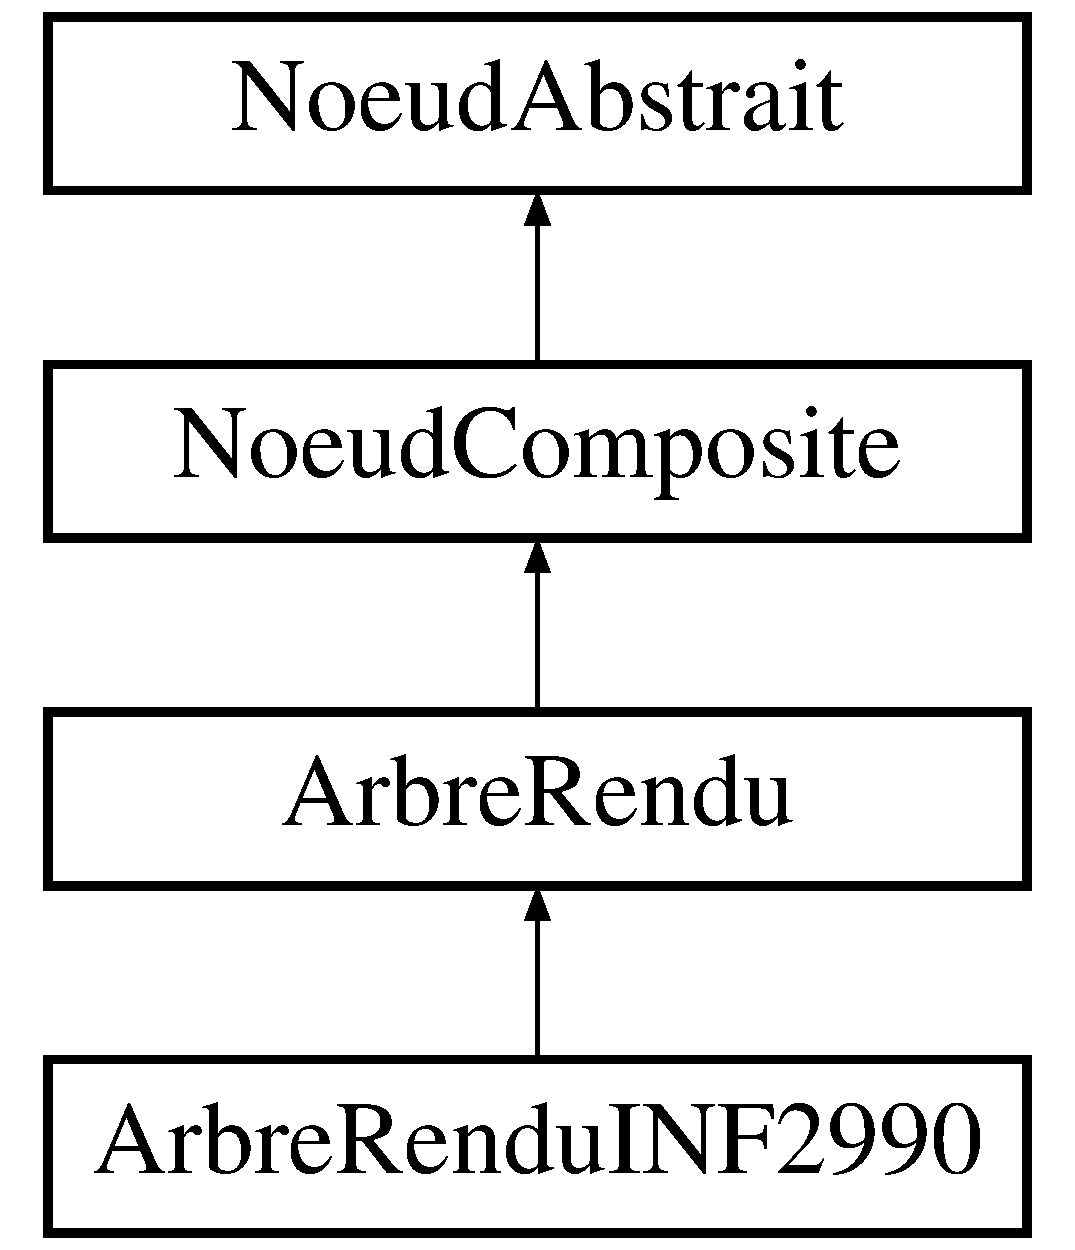
\includegraphics[height=4.000000cm]{class_arbre_rendu}
\end{center}
\end{figure}
\subsection*{Public Member Functions}
\begin{DoxyCompactItemize}
\item 
\hyperlink{group__inf2990_gaef1e98a66c4f1d3b468c786edee45ae6}{Arbre\+Rendu} ()
\begin{DoxyCompactList}\small\item\em Constructeur par d�faut. \end{DoxyCompactList}\item 
virtual \hyperlink{group__inf2990_gadb462923759da0ff632dad097b7bfdab}{$\sim$\+Arbre\+Rendu} ()
\begin{DoxyCompactList}\small\item\em Destructeur. \end{DoxyCompactList}\item 
void \hyperlink{group__inf2990_ga296a744837fb7b779fadf2e8c62e6577}{ajouter\+Usine} (const std\+::string \&type, const \hyperlink{class_usine_abstraite}{Usine\+Abstraite} $\ast$usine)
\begin{DoxyCompactList}\small\item\em Ajoute une usine associ�e � un type de noeud. \end{DoxyCompactList}\item 
\hyperlink{class_noeud_abstrait}{Noeud\+Abstrait} $\ast$ \hyperlink{group__inf2990_ga33ae9013f9cec73854d32527b85b41f9}{creer\+Noeud} (const std\+::string \&type\+Nouveau\+Noeud) const 
\begin{DoxyCompactList}\small\item\em Cr�e un nouveau noeud. \end{DoxyCompactList}\item 
\hyperlink{class_noeud_abstrait}{Noeud\+Abstrait} $\ast$ \hyperlink{group__inf2990_gac10e5f0623af502d67f72aef764206a3}{ajouter\+Nouveau\+Noeud} (const std\+::string \&nom\+Parent, const std\+::string \&type\+Nouveau\+Noeud)
\begin{DoxyCompactList}\small\item\em Cr�e et ajoute un nouveau noeud � l\textquotesingle{}arbre. \end{DoxyCompactList}\end{DoxyCompactItemize}
\subsection*{Static Public Member Functions}
\begin{DoxyCompactItemize}
\item 
static unsigned int \hyperlink{group__inf2990_gacf0e53d52040b07cd6550fda79867bd5}{calculer\+Profondeur\+Maximale} ()
\begin{DoxyCompactList}\small\item\em Calcule la profondeur maximale possible pour l\textquotesingle{}arbre de rendu. \end{DoxyCompactList}\end{DoxyCompactItemize}
\subsection*{Additional Inherited Members}


\subsection{Detailed Description}
Classe d\textquotesingle{}arbre de rendu qui contient la racine de l\textquotesingle{}arbre de rendu avec les usines qui permettent d\textquotesingle{}ajouter des noeuds � cet arbre. 

La profondeur de cet arbre est limit�e par la taille de la pile des matrices et la taille de la pile des noms pour la s�lection Open\+GL, �tant donn� que chaque niveau de l\textquotesingle{}arbre effectue un \char`\"{}push\char`\"{} sur chacune de ces piles lors du rendu. L\textquotesingle{}arbre ne v�rifie pas que la profondeur reste sous la limite, mais il offre des fonctions permettant de le v�rifier ais�ment.

\begin{DoxyAuthor}{Author}
Martin Bisson 
\end{DoxyAuthor}
\begin{DoxyDate}{Date}
2007-\/01-\/28 
\end{DoxyDate}


The documentation for this class was generated from the following files\+:\begin{DoxyCompactItemize}
\item 
Cadriciel/\+Sources/\+D\+L\+L/\+Arbre/\hyperlink{_arbre_rendu_8h}{Arbre\+Rendu.\+h}\item 
Cadriciel/\+Sources/\+D\+L\+L/\+Arbre/\hyperlink{_arbre_rendu_8cpp}{Arbre\+Rendu.\+cpp}\end{DoxyCompactItemize}

\hypertarget{class_arbre_rendu_i_n_f2990}{}\section{Arbre\+Rendu\+I\+N\+F2990 Class Reference}
\label{class_arbre_rendu_i_n_f2990}\index{Arbre\+Rendu\+I\+N\+F2990@{Arbre\+Rendu\+I\+N\+F2990}}


Classe qui repr�sente l\textquotesingle{}arbre de rendu sp�cifique au projet de I\+N\+F2990.  




{\ttfamily \#include $<$Arbre\+Rendu\+I\+N\+F2990.\+h$>$}

Inheritance diagram for Arbre\+Rendu\+I\+N\+F2990\+:\begin{figure}[H]
\begin{center}
\leavevmode
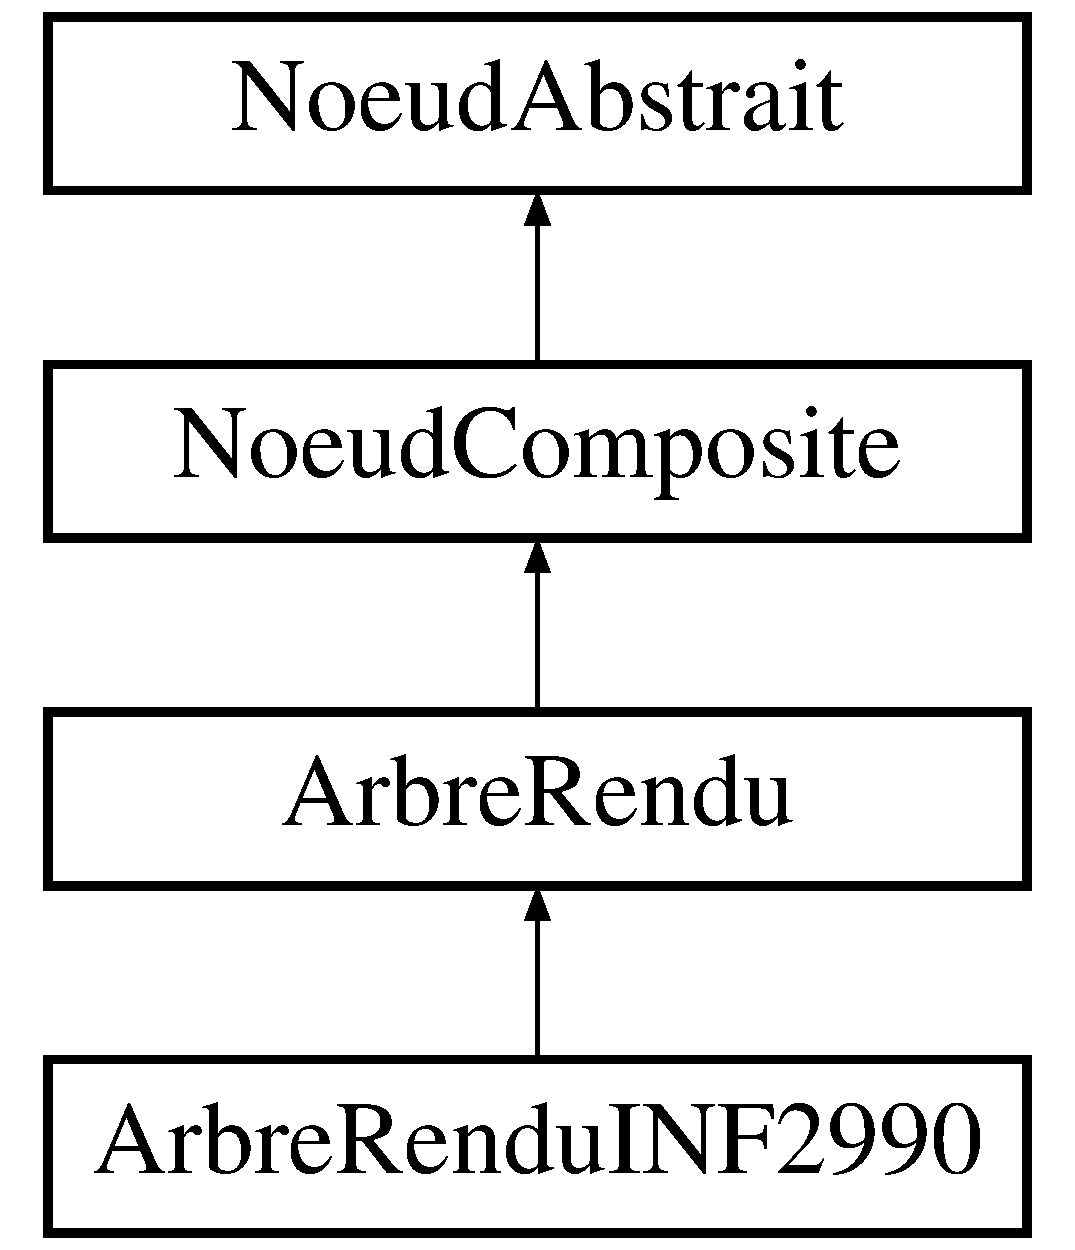
\includegraphics[height=4.000000cm]{class_arbre_rendu_i_n_f2990}
\end{center}
\end{figure}
\subsection*{Public Member Functions}
\begin{DoxyCompactItemize}
\item 
\hyperlink{group__inf2990_ga67528b7fa54e8ef8f96ef2e0bad06d2d}{Arbre\+Rendu\+I\+N\+F2990} ()
\begin{DoxyCompactList}\small\item\em Constructeur par d�faut. \end{DoxyCompactList}\item 
virtual \hyperlink{group__inf2990_gaa67526b2fd719f6bcef7a4547bd25c7b}{$\sim$\+Arbre\+Rendu\+I\+N\+F2990} ()
\begin{DoxyCompactList}\small\item\em Destructeur. \end{DoxyCompactList}\item 
void \hyperlink{group__inf2990_ga678d89e1f12ae16ee7dcf6de3db637a3}{initialiser} ()
\begin{DoxyCompactList}\small\item\em Initialise l\textquotesingle{}arbre de rendu � son �tat initial. \end{DoxyCompactList}\end{DoxyCompactItemize}
\subsection*{Static Public Attributes}
\begin{DoxyCompactItemize}
\item 
static const std\+::string \hyperlink{group__inf2990_ga1035430c1c08b95d17f891ae89b33b80}{N\+O\+M\+\_\+\+A\+R\+A\+I\+G\+N\+EE} \{ \char`\"{}araignee\char`\"{} \}
\begin{DoxyCompactList}\small\item\em La cha�ne repr�sentant le type des araign�es. \end{DoxyCompactList}\item 
static const std\+::string \hyperlink{group__inf2990_gae849656178f4dad34106f525bf37341a}{N\+O\+M\+\_\+\+C\+O\+N\+E\+C\+U\+BE} \{ \char`\"{}conecube\char`\"{} \}
\begin{DoxyCompactList}\small\item\em La cha�ne repr�sentant le type des cones-\/cubes. \end{DoxyCompactList}\item 
static const std\+::string \hyperlink{group__inf2990_ga9a6799aa8903b858929bf675e4468aac}{N\+O\+M\+\_\+\+R\+O\+B\+OT} \{ \char`\"{}robot\char`\"{} \}
\begin{DoxyCompactList}\small\item\em La cha�ne repr�sentant le type du robot. \end{DoxyCompactList}\item 
static const std\+::string \hyperlink{group__inf2990_ga89e651c1a28481ce70f473bd15555114}{N\+O\+M\+\_\+\+T\+A\+B\+LE} \{ \char`\"{}table\char`\"{} \}
\begin{DoxyCompactList}\small\item\em La cha�ne repr�sentant le type de la table. \end{DoxyCompactList}\item 
static const std\+::string \hyperlink{group__inf2990_ga0d96fbd5a34a458793809da370652904}{N\+O\+M\+\_\+\+F\+L\+E\+C\+HE} \{ \char`\"{}fleche\char`\"{} \}
\begin{DoxyCompactList}\small\item\em La cha�ne repr�sentant le type de la fl�che de d�part. \end{DoxyCompactList}\item 
static const std\+::string \hyperlink{group__inf2990_ga96342d03aed79f57435be49458b49442}{N\+O\+M\+\_\+\+P\+O\+T\+E\+AU} \{ \char`\"{}poteau\char`\"{} \}
\begin{DoxyCompactList}\small\item\em La cha�ne repr�sentant le type du poteau. \end{DoxyCompactList}\item 
static const std\+::string \hyperlink{group__inf2990_ga4d9c8c9bfa165dde522834dec2882039}{N\+O\+M\+\_\+\+M\+UR} \{ \char`\"{}mur\char`\"{} \}
\begin{DoxyCompactList}\small\item\em La cha�ne repr�sentant le type du mur. \end{DoxyCompactList}\item 
static const std\+::string \hyperlink{group__inf2990_ga776d72e2b41b06f1992ba48b1ed3de0b}{N\+O\+M\+\_\+\+L\+I\+G\+NE} \{ \char`\"{}ligne\char`\"{} \}
\begin{DoxyCompactList}\small\item\em La cha�ne repr�sentant le type de la ligne. \end{DoxyCompactList}\item 
static const std\+::string \hyperlink{group__inf2990_gaffe953e9369343040aa5d1b72510d810}{N\+O\+M\+\_\+\+S\+E\+G\+M\+E\+NT} \{ \char`\"{}segment\char`\"{} \}
\begin{DoxyCompactList}\small\item\em La cha�ne repr�sentant le type du segment de ligne. \end{DoxyCompactList}\end{DoxyCompactItemize}
\subsection*{Additional Inherited Members}


\subsection{Detailed Description}
Classe qui repr�sente l\textquotesingle{}arbre de rendu sp�cifique au projet de I\+N\+F2990. 

Cette classe s\textquotesingle{}occupe de configurer les usines des noeuds qui seront utilis�s par le projet.

\begin{DoxyAuthor}{Author}
Martin Bisson 
\end{DoxyAuthor}
\begin{DoxyDate}{Date}
2007-\/03-\/23 
\end{DoxyDate}


The documentation for this class was generated from the following files\+:\begin{DoxyCompactItemize}
\item 
Sources/\+D\+L\+L/\+Arbre/\hyperlink{_arbre_rendu_i_n_f2990_8h}{Arbre\+Rendu\+I\+N\+F2990.\+h}\item 
Sources/\+D\+L\+L/\+Arbre/\hyperlink{_arbre_rendu_i_n_f2990_8cpp}{Arbre\+Rendu\+I\+N\+F2990.\+cpp}\end{DoxyCompactItemize}

\hypertarget{struct_generic_value_1_1_array}{}\section{Generic\+Value$<$ Encoding, Allocator $>$\+:\+:Array Struct Reference}
\label{struct_generic_value_1_1_array}\index{Generic\+Value$<$ Encoding, Allocator $>$\+::\+Array@{Generic\+Value$<$ Encoding, Allocator $>$\+::\+Array}}
\subsection*{Public Attributes}
\begin{DoxyCompactItemize}
\item 
\hyperlink{class_generic_value}{Generic\+Value} $\ast$ {\bfseries elements}\hypertarget{struct_generic_value_1_1_array_a0af8e50f37486f042ab19fd871d11d4f}{}\label{struct_generic_value_1_1_array_a0af8e50f37486f042ab19fd871d11d4f}

\item 
\hyperlink{rapidjson_8h_a5ed6e6e67250fadbd041127e6386dcb5}{Size\+Type} {\bfseries size}\hypertarget{struct_generic_value_1_1_array_a60f69b3b57b86c20c123c1b080e34bcc}{}\label{struct_generic_value_1_1_array_a60f69b3b57b86c20c123c1b080e34bcc}

\item 
\hyperlink{rapidjson_8h_a5ed6e6e67250fadbd041127e6386dcb5}{Size\+Type} {\bfseries capacity}\hypertarget{struct_generic_value_1_1_array_a2f5dfb089ee750e9405d5adeda4df894}{}\label{struct_generic_value_1_1_array_a2f5dfb089ee750e9405d5adeda4df894}

\end{DoxyCompactItemize}


The documentation for this struct was generated from the following file\+:\begin{DoxyCompactItemize}
\item 
Commun/\+Externe/\+Rapid\+J\+S\+O\+N/include/rapidjson/\hyperlink{document_8h}{document.\+h}\end{DoxyCompactItemize}

\hypertarget{struct_a_s_c_i_i}{}\section{A\+S\+C\+II$<$ Char\+Type $>$ Struct Template Reference}
\label{struct_a_s_c_i_i}\index{A\+S\+C\+I\+I$<$ Char\+Type $>$@{A\+S\+C\+I\+I$<$ Char\+Type $>$}}


\hyperlink{struct_a_s_c_i_i}{A\+S\+C\+II} encoding.  




{\ttfamily \#include $<$encodings.\+h$>$}

\subsection*{Public Types}
\begin{DoxyCompactItemize}
\item 
enum \{ {\bfseries support\+Unicode} = 0
 \}\hypertarget{struct_a_s_c_i_i_a92be799d492f48efd0a7a76cae2fec35}{}\label{struct_a_s_c_i_i_a92be799d492f48efd0a7a76cae2fec35}

\item 
typedef Char\+Type {\bfseries Ch}\hypertarget{struct_a_s_c_i_i_a1baf6e7914f165be952c30db664cefb4}{}\label{struct_a_s_c_i_i_a1baf6e7914f165be952c30db664cefb4}

\end{DoxyCompactItemize}
\subsection*{Static Public Member Functions}
\begin{DoxyCompactItemize}
\item 
{\footnotesize template$<$typename Output\+Stream $>$ }\\static void {\bfseries Encode} (Output\+Stream \&os, unsigned codepoint)\hypertarget{struct_a_s_c_i_i_af56b1605fe233c54693facc7de457f72}{}\label{struct_a_s_c_i_i_af56b1605fe233c54693facc7de457f72}

\item 
{\footnotesize template$<$typename Input\+Stream $>$ }\\static bool {\bfseries Decode} (Input\+Stream \&is, unsigned $\ast$codepoint)\hypertarget{struct_a_s_c_i_i_a44844bbfd0a4fc282993fd72f3f58eee}{}\label{struct_a_s_c_i_i_a44844bbfd0a4fc282993fd72f3f58eee}

\item 
{\footnotesize template$<$typename Input\+Stream , typename Output\+Stream $>$ }\\static bool {\bfseries Validate} (Input\+Stream \&is, Output\+Stream \&os)\hypertarget{struct_a_s_c_i_i_a398680588a09e6ce9b56e32195047c78}{}\label{struct_a_s_c_i_i_a398680588a09e6ce9b56e32195047c78}

\item 
{\footnotesize template$<$typename Input\+Byte\+Stream $>$ }\\static Char\+Type {\bfseries Take\+B\+OM} (Input\+Byte\+Stream \&is)\hypertarget{struct_a_s_c_i_i_aad78500eb98f45582a4df020e3fb2278}{}\label{struct_a_s_c_i_i_aad78500eb98f45582a4df020e3fb2278}

\item 
{\footnotesize template$<$typename Input\+Byte\+Stream $>$ }\\static Ch {\bfseries Take} (Input\+Byte\+Stream \&is)\hypertarget{struct_a_s_c_i_i_ab1b9fdf0a5c05658d62fded913d923a3}{}\label{struct_a_s_c_i_i_ab1b9fdf0a5c05658d62fded913d923a3}

\item 
{\footnotesize template$<$typename Output\+Byte\+Stream $>$ }\\static void {\bfseries Put\+B\+OM} (Output\+Byte\+Stream \&os)\hypertarget{struct_a_s_c_i_i_a3036dc1d604039c3224ca0a890ee0134}{}\label{struct_a_s_c_i_i_a3036dc1d604039c3224ca0a890ee0134}

\item 
{\footnotesize template$<$typename Output\+Byte\+Stream $>$ }\\static void {\bfseries Put} (Output\+Byte\+Stream \&os, Ch c)\hypertarget{struct_a_s_c_i_i_a218b244b9cd961ea6c5775a734cec20e}{}\label{struct_a_s_c_i_i_a218b244b9cd961ea6c5775a734cec20e}

\end{DoxyCompactItemize}


\subsection{Detailed Description}
\subsubsection*{template$<$typename Char\+Type = char$>$\\*
struct A\+S\+C\+I\+I$<$ Char\+Type $>$}

\hyperlink{struct_a_s_c_i_i}{A\+S\+C\+II} encoding. 

\href{http://en.wikipedia.org/wiki/ASCII}{\tt http\+://en.\+wikipedia.\+org/wiki/\+A\+S\+C\+II} 
\begin{DoxyTemplParams}{Template Parameters}
{\em Char\+Type} & Code unit for storing 7-\/bit \hyperlink{struct_a_s_c_i_i}{A\+S\+C\+II} data. Default is char. \\
\hline
\end{DoxyTemplParams}
\begin{DoxyNote}{Note}
implements Encoding concept 
\end{DoxyNote}


The documentation for this struct was generated from the following file\+:\begin{DoxyCompactItemize}
\item 
Commun/\+Externe/\+Rapid\+J\+S\+O\+N/include/rapidjson/encodings.\+h\end{DoxyCompactItemize}

\hypertarget{struct_asserter}{}\section{Asserter Struct Reference}
\label{struct_asserter}\index{Asserter@{Asserter}}


A set of functions to help writing assertion macros.

Here is an example of assertion, a simplified version of the actual assertion implemented in examples/cppunittest/\+Xml\+Uniformiser.\+h\+:  




{\ttfamily \#include $<$Asserter.\+h$>$}

\subsection*{Static Public Member Functions}
\begin{DoxyCompactItemize}
\item 
static void C\+P\+P\+U\+N\+I\+T\+\_\+\+A\+PI \hyperlink{struct_asserter_a5a67b6042625cc87d271a53ac555e437}{fail} (const \hyperlink{class_message}{Message} \&message, const \hyperlink{class_source_line}{Source\+Line} \&source\+Line=\hyperlink{class_source_line}{Source\+Line}())\hypertarget{struct_asserter_a5a67b6042625cc87d271a53ac555e437}{}\label{struct_asserter_a5a67b6042625cc87d271a53ac555e437}

\begin{DoxyCompactList}\small\item\em Throws a \hyperlink{class_exception}{Exception} with the specified message and location. \end{DoxyCompactList}\item 
static void C\+P\+P\+U\+N\+I\+T\+\_\+\+A\+PI \hyperlink{struct_asserter_a74825fc71909baa1286f9282ba5a2a54}{fail} (std\+::string message, const \hyperlink{class_source_line}{Source\+Line} \&source\+Line=\hyperlink{class_source_line}{Source\+Line}())
\begin{DoxyCompactList}\small\item\em Throws a \hyperlink{class_exception}{Exception} with the specified message and location. \end{DoxyCompactList}\item 
static void C\+P\+P\+U\+N\+I\+T\+\_\+\+A\+PI \hyperlink{struct_asserter_a425da14df34fad7e23a35456fce0eb2b}{fail\+If} (bool should\+Fail, const \hyperlink{class_message}{Message} \&message, const \hyperlink{class_source_line}{Source\+Line} \&source\+Line=\hyperlink{class_source_line}{Source\+Line}())
\begin{DoxyCompactList}\small\item\em Throws a \hyperlink{class_exception}{Exception} with the specified message and location. \end{DoxyCompactList}\item 
static void C\+P\+P\+U\+N\+I\+T\+\_\+\+A\+PI \hyperlink{struct_asserter_a71a4667a9d3f5d483f1a82157f715824}{fail\+If} (bool should\+Fail, std\+::string message, const \hyperlink{class_source_line}{Source\+Line} \&source\+Line=\hyperlink{class_source_line}{Source\+Line}())
\begin{DoxyCompactList}\small\item\em Throws a \hyperlink{class_exception}{Exception} with the specified message and location. \end{DoxyCompactList}\item 
static std\+::string C\+P\+P\+U\+N\+I\+T\+\_\+\+A\+PI \hyperlink{struct_asserter_adcbee7c01d58bfaee72cc984627e6432}{make\+Expected} (const std\+::string \&expected\+Value)
\begin{DoxyCompactList}\small\item\em Returns a expected value string for a message. Typically used to create \textquotesingle{}not equal\textquotesingle{} message, or to check that a message contains the expected content when writing unit tests for your custom assertions. \end{DoxyCompactList}\item 
static std\+::string C\+P\+P\+U\+N\+I\+T\+\_\+\+A\+PI \hyperlink{struct_asserter_ae52920ca7ffd981df61d7a3cfd88793b}{make\+Actual} (const std\+::string \&actual\+Value)
\begin{DoxyCompactList}\small\item\em Returns an actual value string for a message. Typically used to create \textquotesingle{}not equal\textquotesingle{} message, or to check that a message contains the expected content when writing unit tests for your custom assertions. \end{DoxyCompactList}\item 
static \hyperlink{class_message}{Message} C\+P\+P\+U\+N\+I\+T\+\_\+\+A\+PI {\bfseries make\+Not\+Equal\+Message} (const std\+::string \&expected\+Value, const std\+::string \&actual\+Value, const \hyperlink{class_additional_message}{Additional\+Message} \&additional\+Message=\hyperlink{class_additional_message}{Additional\+Message}(), const std\+::string \&short\+Description=\char`\"{}equality assertion failed\char`\"{})\hypertarget{struct_asserter_adb8ac36c8f0d385430e5a087a66219db}{}\label{struct_asserter_adb8ac36c8f0d385430e5a087a66219db}

\item 
static void C\+P\+P\+U\+N\+I\+T\+\_\+\+A\+PI \hyperlink{struct_asserter_ac6234767e7d986bace97dc44f8d80d6c}{fail\+Not\+Equal} (std\+::string expected, std\+::string actual, const \hyperlink{class_source_line}{Source\+Line} \&source\+Line, const \hyperlink{class_additional_message}{Additional\+Message} \&additional\+Message=\hyperlink{class_additional_message}{Additional\+Message}(), std\+::string short\+Description=\char`\"{}equality assertion failed\char`\"{})
\begin{DoxyCompactList}\small\item\em Throws an \hyperlink{class_exception}{Exception} with the specified message and location. \end{DoxyCompactList}\item 
static void C\+P\+P\+U\+N\+I\+T\+\_\+\+A\+PI \hyperlink{struct_asserter_a3a805c9f8c641d65353bcff2da80624f}{fail\+Not\+Equal\+If} (bool should\+Fail, std\+::string expected, std\+::string actual, const \hyperlink{class_source_line}{Source\+Line} \&source\+Line, const \hyperlink{class_additional_message}{Additional\+Message} \&additional\+Message=\hyperlink{class_additional_message}{Additional\+Message}(), std\+::string short\+Description=\char`\"{}equality assertion failed\char`\"{})
\begin{DoxyCompactList}\small\item\em Throws an \hyperlink{class_exception}{Exception} with the specified message and location. \end{DoxyCompactList}\end{DoxyCompactItemize}


\subsection{Detailed Description}
A set of functions to help writing assertion macros.

Here is an example of assertion, a simplified version of the actual assertion implemented in examples/cppunittest/\+Xml\+Uniformiser.\+h\+: 


\begin{DoxyCode}
\textcolor{preprocessor}{#include <cppunit/SourceLine.h>}
\textcolor{preprocessor}{#include <cppunit/TestAssert.h>}

\textcolor{keywordtype}{void} 
checkXmlEqual( std::string expectedXml,
               std::string actualXml,
               CppUnit::SourceLine sourceLine )
\{
  std::string expected = XmlUniformiser( expectedXml ).stripped();
  std::string actual = XmlUniformiser( actualXml ).stripped();

  \textcolor{keywordflow}{if} ( expected == actual )
    \textcolor{keywordflow}{return};

  ::CppUnit::Asserter::failNotEqual( expected,
                                     actual,
                                     sourceLine );
\}

\textcolor{preprocessor}{#define CPPUNITTEST\_ASSERT\_XML\_EQUAL( expected, actual ) \(\backslash\)}
\textcolor{preprocessor}{    checkXmlEqual( expected, actual,                     \(\backslash\)}
\textcolor{preprocessor}{                   CPPUNIT\_SOURCELINE() )}
\end{DoxyCode}
 

\subsection{Member Function Documentation}
\index{Asserter@{Asserter}!fail@{fail}}
\index{fail@{fail}!Asserter@{Asserter}}
\subsubsection[{\texorpdfstring{fail(std\+::string message, const Source\+Line \&source\+Line=\+Source\+Line())}{fail(std::string message, const SourceLine &sourceLine=SourceLine())}}]{\setlength{\rightskip}{0pt plus 5cm}static void C\+P\+P\+U\+N\+I\+T\+\_\+\+A\+PI Asserter\+::fail (
\begin{DoxyParamCaption}
\item[{std\+::string}]{message, }
\item[{const {\bf Source\+Line} \&}]{source\+Line = {\ttfamily {\bf Source\+Line}()}}
\end{DoxyParamCaption}
)\hspace{0.3cm}{\ttfamily [static]}}\hypertarget{struct_asserter_a74825fc71909baa1286f9282ba5a2a54}{}\label{struct_asserter_a74825fc71909baa1286f9282ba5a2a54}


Throws a \hyperlink{class_exception}{Exception} with the specified message and location. 

\begin{DoxyRefDesc}{Deprecated}
\item[\hyperlink{deprecated__deprecated000002}{Deprecated}]Use fail( Message, Source\+Line ) instead. \end{DoxyRefDesc}
\index{Asserter@{Asserter}!fail\+If@{fail\+If}}
\index{fail\+If@{fail\+If}!Asserter@{Asserter}}
\subsubsection[{\texorpdfstring{fail\+If(bool should\+Fail, const Message \&message, const Source\+Line \&source\+Line=\+Source\+Line())}{failIf(bool shouldFail, const Message &message, const SourceLine &sourceLine=SourceLine())}}]{\setlength{\rightskip}{0pt plus 5cm}static void C\+P\+P\+U\+N\+I\+T\+\_\+\+A\+PI Asserter\+::fail\+If (
\begin{DoxyParamCaption}
\item[{bool}]{should\+Fail, }
\item[{const {\bf Message} \&}]{message, }
\item[{const {\bf Source\+Line} \&}]{source\+Line = {\ttfamily {\bf Source\+Line}()}}
\end{DoxyParamCaption}
)\hspace{0.3cm}{\ttfamily [static]}}\hypertarget{struct_asserter_a425da14df34fad7e23a35456fce0eb2b}{}\label{struct_asserter_a425da14df34fad7e23a35456fce0eb2b}


Throws a \hyperlink{class_exception}{Exception} with the specified message and location. 


\begin{DoxyParams}{Parameters}
{\em should\+Fail} & if {\ttfamily true} then the exception is thrown. Otherwise nothing happen. \\
\hline
{\em message} & \hyperlink{class_message}{Message} explaining the assertion failiure. \\
\hline
{\em source\+Line} & Location of the assertion. \\
\hline
\end{DoxyParams}
\index{Asserter@{Asserter}!fail\+If@{fail\+If}}
\index{fail\+If@{fail\+If}!Asserter@{Asserter}}
\subsubsection[{\texorpdfstring{fail\+If(bool should\+Fail, std\+::string message, const Source\+Line \&source\+Line=\+Source\+Line())}{failIf(bool shouldFail, std::string message, const SourceLine &sourceLine=SourceLine())}}]{\setlength{\rightskip}{0pt plus 5cm}static void C\+P\+P\+U\+N\+I\+T\+\_\+\+A\+PI Asserter\+::fail\+If (
\begin{DoxyParamCaption}
\item[{bool}]{should\+Fail, }
\item[{std\+::string}]{message, }
\item[{const {\bf Source\+Line} \&}]{source\+Line = {\ttfamily {\bf Source\+Line}()}}
\end{DoxyParamCaption}
)\hspace{0.3cm}{\ttfamily [static]}}\hypertarget{struct_asserter_a71a4667a9d3f5d483f1a82157f715824}{}\label{struct_asserter_a71a4667a9d3f5d483f1a82157f715824}


Throws a \hyperlink{class_exception}{Exception} with the specified message and location. 

\begin{DoxyRefDesc}{Deprecated}
\item[\hyperlink{deprecated__deprecated000003}{Deprecated}]Use fail\+If( bool, Message, Source\+Line ) instead. \end{DoxyRefDesc}

\begin{DoxyParams}{Parameters}
{\em should\+Fail} & if {\ttfamily true} then the exception is thrown. Otherwise nothing happen. \\
\hline
{\em message} & \hyperlink{class_message}{Message} explaining the assertion failiure. \\
\hline
{\em source\+Line} & Location of the assertion. \\
\hline
\end{DoxyParams}
\index{Asserter@{Asserter}!fail\+Not\+Equal@{fail\+Not\+Equal}}
\index{fail\+Not\+Equal@{fail\+Not\+Equal}!Asserter@{Asserter}}
\subsubsection[{\texorpdfstring{fail\+Not\+Equal(std\+::string expected, std\+::string actual, const Source\+Line \&source\+Line, const Additional\+Message \&additional\+Message=\+Additional\+Message(), std\+::string short\+Description=""equality assertion failed"")}{failNotEqual(std::string expected, std::string actual, const SourceLine &sourceLine, const AdditionalMessage &additionalMessage=AdditionalMessage(), std::string shortDescription="equality assertion failed")}}]{\setlength{\rightskip}{0pt plus 5cm}static void C\+P\+P\+U\+N\+I\+T\+\_\+\+A\+PI Asserter\+::fail\+Not\+Equal (
\begin{DoxyParamCaption}
\item[{std\+::string}]{expected, }
\item[{std\+::string}]{actual, }
\item[{const {\bf Source\+Line} \&}]{source\+Line, }
\item[{const {\bf Additional\+Message} \&}]{additional\+Message = {\ttfamily {\bf Additional\+Message}()}, }
\item[{std\+::string}]{short\+Description = {\ttfamily \char`\"{}equality~assertion~failed\char`\"{}}}
\end{DoxyParamCaption}
)\hspace{0.3cm}{\ttfamily [static]}}\hypertarget{struct_asserter_ac6234767e7d986bace97dc44f8d80d6c}{}\label{struct_asserter_ac6234767e7d986bace97dc44f8d80d6c}


Throws an \hyperlink{class_exception}{Exception} with the specified message and location. 


\begin{DoxyParams}{Parameters}
{\em expected} & Text describing the expected value. \\
\hline
{\em actual} & Text describing the actual value. \\
\hline
{\em source\+Line} & Location of the assertion. \\
\hline
{\em additional\+Message} & Additional message. Usually used to report what are the differences between the expected and actual value. \\
\hline
{\em short\+Description} & Short description for the failure message. \\
\hline
\end{DoxyParams}
\index{Asserter@{Asserter}!fail\+Not\+Equal\+If@{fail\+Not\+Equal\+If}}
\index{fail\+Not\+Equal\+If@{fail\+Not\+Equal\+If}!Asserter@{Asserter}}
\subsubsection[{\texorpdfstring{fail\+Not\+Equal\+If(bool should\+Fail, std\+::string expected, std\+::string actual, const Source\+Line \&source\+Line, const Additional\+Message \&additional\+Message=\+Additional\+Message(), std\+::string short\+Description=""equality assertion failed"")}{failNotEqualIf(bool shouldFail, std::string expected, std::string actual, const SourceLine &sourceLine, const AdditionalMessage &additionalMessage=AdditionalMessage(), std::string shortDescription="equality assertion failed")}}]{\setlength{\rightskip}{0pt plus 5cm}static void C\+P\+P\+U\+N\+I\+T\+\_\+\+A\+PI Asserter\+::fail\+Not\+Equal\+If (
\begin{DoxyParamCaption}
\item[{bool}]{should\+Fail, }
\item[{std\+::string}]{expected, }
\item[{std\+::string}]{actual, }
\item[{const {\bf Source\+Line} \&}]{source\+Line, }
\item[{const {\bf Additional\+Message} \&}]{additional\+Message = {\ttfamily {\bf Additional\+Message}()}, }
\item[{std\+::string}]{short\+Description = {\ttfamily \char`\"{}equality~assertion~failed\char`\"{}}}
\end{DoxyParamCaption}
)\hspace{0.3cm}{\ttfamily [static]}}\hypertarget{struct_asserter_a3a805c9f8c641d65353bcff2da80624f}{}\label{struct_asserter_a3a805c9f8c641d65353bcff2da80624f}


Throws an \hyperlink{class_exception}{Exception} with the specified message and location. 


\begin{DoxyParams}{Parameters}
{\em should\+Fail} & if {\ttfamily true} then the exception is thrown. Otherwise nothing happen. \\
\hline
{\em expected} & Text describing the expected value. \\
\hline
{\em actual} & Text describing the actual value. \\
\hline
{\em source\+Line} & Location of the assertion. \\
\hline
{\em additional\+Message} & Additional message. Usually used to report where the \char`\"{}difference\char`\"{} is located. \\
\hline
{\em short\+Description} & Short description for the failure message. \\
\hline
\end{DoxyParams}
\index{Asserter@{Asserter}!make\+Actual@{make\+Actual}}
\index{make\+Actual@{make\+Actual}!Asserter@{Asserter}}
\subsubsection[{\texorpdfstring{make\+Actual(const std\+::string \&actual\+Value)}{makeActual(const std::string &actualValue)}}]{\setlength{\rightskip}{0pt plus 5cm}static std\+::string C\+P\+P\+U\+N\+I\+T\+\_\+\+A\+PI Asserter\+::make\+Actual (
\begin{DoxyParamCaption}
\item[{const std\+::string \&}]{actual\+Value}
\end{DoxyParamCaption}
)\hspace{0.3cm}{\ttfamily [static]}}\hypertarget{struct_asserter_ae52920ca7ffd981df61d7a3cfd88793b}{}\label{struct_asserter_ae52920ca7ffd981df61d7a3cfd88793b}


Returns an actual value string for a message. Typically used to create \textquotesingle{}not equal\textquotesingle{} message, or to check that a message contains the expected content when writing unit tests for your custom assertions. 


\begin{DoxyParams}{Parameters}
{\em actual\+Value} & String that represents the actual value. \\
\hline
\end{DoxyParams}
\begin{DoxyReturn}{Returns}
{\itshape actual\+Value} prefixed with \char`\"{}\+Actual  \+: \char`\"{}. 
\end{DoxyReturn}
\begin{DoxySeeAlso}{See also}
\hyperlink{struct_asserter_adcbee7c01d58bfaee72cc984627e6432}{make\+Expected()}. 
\end{DoxySeeAlso}
\index{Asserter@{Asserter}!make\+Expected@{make\+Expected}}
\index{make\+Expected@{make\+Expected}!Asserter@{Asserter}}
\subsubsection[{\texorpdfstring{make\+Expected(const std\+::string \&expected\+Value)}{makeExpected(const std::string &expectedValue)}}]{\setlength{\rightskip}{0pt plus 5cm}static std\+::string C\+P\+P\+U\+N\+I\+T\+\_\+\+A\+PI Asserter\+::make\+Expected (
\begin{DoxyParamCaption}
\item[{const std\+::string \&}]{expected\+Value}
\end{DoxyParamCaption}
)\hspace{0.3cm}{\ttfamily [static]}}\hypertarget{struct_asserter_adcbee7c01d58bfaee72cc984627e6432}{}\label{struct_asserter_adcbee7c01d58bfaee72cc984627e6432}


Returns a expected value string for a message. Typically used to create \textquotesingle{}not equal\textquotesingle{} message, or to check that a message contains the expected content when writing unit tests for your custom assertions. 


\begin{DoxyParams}{Parameters}
{\em expected\+Value} & String that represents the expected value. \\
\hline
\end{DoxyParams}
\begin{DoxyReturn}{Returns}
{\itshape expected\+Value} prefixed with \char`\"{}\+Expected\+: \char`\"{}. 
\end{DoxyReturn}
\begin{DoxySeeAlso}{See also}
\hyperlink{struct_asserter_ae52920ca7ffd981df61d7a3cfd88793b}{make\+Actual()}. 
\end{DoxySeeAlso}


The documentation for this struct was generated from the following file\+:\begin{DoxyCompactItemize}
\item 
Commun/\+Externe/cppunit/include/cppunit/Asserter.\+h\end{DoxyCompactItemize}

\hypertarget{structassertion__traits}{}\section{assertion\+\_\+traits$<$ T $>$ Struct Template Reference}
\label{structassertion__traits}\index{assertion\+\_\+traits$<$ T $>$@{assertion\+\_\+traits$<$ T $>$}}


Traits used by C\+P\+P\+U\+N\+I\+T\+\_\+\+A\+S\+S\+E\+R\+T\+\_\+\+E\+Q\+U\+A\+L().  




{\ttfamily \#include $<$Test\+Assert.\+h$>$}

\subsection*{Static Public Member Functions}
\begin{DoxyCompactItemize}
\item 
static bool {\bfseries equal} (const T \&x, const T \&y)\hypertarget{structassertion__traits_a287c07a4e171256a0128201c7e4c4228}{}\label{structassertion__traits_a287c07a4e171256a0128201c7e4c4228}

\item 
static std\+::string {\bfseries to\+String} (const T \&x)\hypertarget{structassertion__traits_a1c96296fb44902b4f22d99b9c3cc7749}{}\label{structassertion__traits_a1c96296fb44902b4f22d99b9c3cc7749}

\end{DoxyCompactItemize}


\subsection{Detailed Description}
\subsubsection*{template$<$class T$>$\\*
struct assertion\+\_\+traits$<$ T $>$}

Traits used by C\+P\+P\+U\+N\+I\+T\+\_\+\+A\+S\+S\+E\+R\+T\+\_\+\+E\+Q\+U\+A\+L(). 

Here is an example of specialising these traits\+:


\begin{DoxyCode}
\textcolor{keyword}{template}<>
\textcolor{keyword}{struct }\hyperlink{structassertion__traits}{assertion\_traits}<std::string>   \textcolor{comment}{// specialization for the std::string type}
\{
  \textcolor{keyword}{static} \textcolor{keywordtype}{bool} equal( \textcolor{keyword}{const} std::string& x, \textcolor{keyword}{const} std::string& y )
  \{
    \textcolor{keywordflow}{return} x == y;
  \}

  \textcolor{keyword}{static} std::string toString( \textcolor{keyword}{const} std::string& x )
  \{
    std::string text = \textcolor{charliteral}{'"'} + x + \textcolor{charliteral}{'"'};    \textcolor{comment}{// adds quote around the string to see whitespace}
    OStringStream ost;
    ost << text;
    \textcolor{keywordflow}{return} ost.str();
  \}
\};
\end{DoxyCode}
 

The documentation for this struct was generated from the following file\+:\begin{DoxyCompactItemize}
\item 
Commun/\+Externe/cppunit/include/cppunit/Test\+Assert.\+h\end{DoxyCompactItemize}

\hypertarget{structassertion__traits_3_01double_01_4}{}\section{assertion\+\_\+traits$<$ double $>$ Struct Template Reference}
\label{structassertion__traits_3_01double_01_4}\index{assertion\+\_\+traits$<$ double $>$@{assertion\+\_\+traits$<$ double $>$}}


Traits used by C\+P\+P\+U\+N\+I\+T\+\_\+\+A\+S\+S\+E\+R\+T\+\_\+\+D\+O\+U\+B\+L\+E\+S\+\_\+\+E\+Q\+U\+A\+L().  




{\ttfamily \#include $<$Test\+Assert.\+h$>$}

\subsection*{Static Public Member Functions}
\begin{DoxyCompactItemize}
\item 
static bool {\bfseries equal} (double x, double y)\hypertarget{structassertion__traits_3_01double_01_4_ac0d9d71ec0f239664b88188e481c0598}{}\label{structassertion__traits_3_01double_01_4_ac0d9d71ec0f239664b88188e481c0598}

\item 
static std\+::string {\bfseries to\+String} (double x)\hypertarget{structassertion__traits_3_01double_01_4_a6bc37874eb60d30e0b50d4c127ab34df}{}\label{structassertion__traits_3_01double_01_4_a6bc37874eb60d30e0b50d4c127ab34df}

\end{DoxyCompactItemize}


\subsection{Detailed Description}
\subsubsection*{template$<$$>$\\*
struct assertion\+\_\+traits$<$ double $>$}

Traits used by C\+P\+P\+U\+N\+I\+T\+\_\+\+A\+S\+S\+E\+R\+T\+\_\+\+D\+O\+U\+B\+L\+E\+S\+\_\+\+E\+Q\+U\+A\+L(). 

This specialisation from {\ttfamily struct} {\ttfamily assertion\+\_\+traits$<$$>$} ensures that doubles are converted in full, instead of being rounded to the default 6 digits of precision. Use the system defined I\+SO C99 macro D\+B\+L\+\_\+\+D\+IG within float.\+h is available to define the maximum precision, otherwise use the hard-\/coded maximum precision of 15. 

The documentation for this struct was generated from the following file\+:\begin{DoxyCompactItemize}
\item 
Cadriciel/\+Commun/\+Externe/cppunit/include/cppunit/Test\+Assert.\+h\end{DoxyCompactItemize}

\hypertarget{class_auto_register_registry}{}\section{Auto\+Register\+Registry Class Reference}
\label{class_auto_register_registry}\index{Auto\+Register\+Registry@{Auto\+Register\+Registry}}


(Implementation) Automatically adds a registry into another registry.  




{\ttfamily \#include $<$Auto\+Register\+Suite.\+h$>$}

\subsection*{Public Member Functions}
\begin{DoxyCompactItemize}
\item 
{\bfseries Auto\+Register\+Registry} (const std\+::string \&which, const std\+::string \&to)\hypertarget{class_auto_register_registry_aeb3c0171549420bc18714d4117d9c2b5}{}\label{class_auto_register_registry_aeb3c0171549420bc18714d4117d9c2b5}

\item 
{\bfseries Auto\+Register\+Registry} (const std\+::string \&which)\hypertarget{class_auto_register_registry_a3efb50c6218f5d0e5969eb6fc8bccb23}{}\label{class_auto_register_registry_a3efb50c6218f5d0e5969eb6fc8bccb23}

\end{DoxyCompactItemize}


\subsection{Detailed Description}
(Implementation) Automatically adds a registry into another registry. 

Don\textquotesingle{}t use this class. Use the macros \hyperlink{_helper_macros_8h_a0ca9e37aca06e802300f2572b974e2bb}{C\+P\+P\+U\+N\+I\+T\+\_\+\+R\+E\+G\+I\+S\+T\+R\+Y\+\_\+\+A\+D\+D()} and \hyperlink{_helper_macros_8h_a1dde8c3db38012da58e1e456b7e4e346}{C\+P\+P\+U\+N\+I\+T\+\_\+\+R\+E\+G\+I\+S\+T\+R\+Y\+\_\+\+A\+D\+D\+\_\+\+T\+O\+\_\+\+D\+E\+F\+A\+U\+L\+T()} instead. 

The documentation for this class was generated from the following file\+:\begin{DoxyCompactItemize}
\item 
Cadriciel/\+Commun/\+Externe/cppunit/include/cppunit/extensions/Auto\+Register\+Suite.\+h\end{DoxyCompactItemize}

\hypertarget{class_auto_register_suite}{}\section{Auto\+Register\+Suite$<$ Test\+Case\+Type $>$ Class Template Reference}
\label{class_auto_register_suite}\index{Auto\+Register\+Suite$<$ Test\+Case\+Type $>$@{Auto\+Register\+Suite$<$ Test\+Case\+Type $>$}}


(Implementation) Automatically register the test suite of the specified type.  




{\ttfamily \#include $<$Auto\+Register\+Suite.\+h$>$}

\subsection*{Public Member Functions}
\begin{DoxyCompactItemize}
\item 
\hyperlink{class_auto_register_suite_a4c02d0d6e3de726f67b875dc5615e22a}{Auto\+Register\+Suite} ()
\item 
\hyperlink{class_auto_register_suite_a9350fa1995545aad03b61b7a6db690e4}{Auto\+Register\+Suite} (const std\+::string \&name)
\end{DoxyCompactItemize}
\subsection*{Private Attributes}
\begin{DoxyCompactItemize}
\item 
\hyperlink{class_test_factory_registry}{Test\+Factory\+Registry} $\ast$ {\bfseries m\+\_\+registry}\hypertarget{class_auto_register_suite_a37234874449a67e300f09f1524779a44}{}\label{class_auto_register_suite_a37234874449a67e300f09f1524779a44}

\item 
\hyperlink{class_test_suite_factory}{Test\+Suite\+Factory}$<$ Test\+Case\+Type $>$ {\bfseries m\+\_\+factory}\hypertarget{class_auto_register_suite_ae1a90501fa160febe6ae219b595b77a8}{}\label{class_auto_register_suite_ae1a90501fa160febe6ae219b595b77a8}

\end{DoxyCompactItemize}


\subsection{Detailed Description}
\subsubsection*{template$<$class Test\+Case\+Type$>$\\*
class Auto\+Register\+Suite$<$ Test\+Case\+Type $>$}

(Implementation) Automatically register the test suite of the specified type. 

You should not use this class directly. Instead, use the following macros\+:
\begin{DoxyItemize}
\item \hyperlink{_helper_macros_8h_a70f00cc9f589d24019ee9efee4de2d74}{C\+P\+P\+U\+N\+I\+T\+\_\+\+T\+E\+S\+T\+\_\+\+S\+U\+I\+T\+E\+\_\+\+R\+E\+G\+I\+S\+T\+R\+A\+T\+I\+O\+N()}
\item \hyperlink{_helper_macros_8h_a028a5855a40ad3836e2a26aa48cd4c91}{C\+P\+P\+U\+N\+I\+T\+\_\+\+T\+E\+S\+T\+\_\+\+S\+U\+I\+T\+E\+\_\+\+N\+A\+M\+E\+D\+\_\+\+R\+E\+G\+I\+S\+T\+R\+A\+T\+I\+O\+N()}
\end{DoxyItemize}

This object will register the test returned by Test\+Case\+Type\+::suite() when constructed to the test registry.

This object is intented to be used as a static variable.


\begin{DoxyParams}{Parameters}
{\em Test\+Case\+Type} & Type of the test case which suite is registered. \\
\hline
\end{DoxyParams}
\begin{DoxySeeAlso}{See also}
\hyperlink{_helper_macros_8h_a70f00cc9f589d24019ee9efee4de2d74}{C\+P\+P\+U\+N\+I\+T\+\_\+\+T\+E\+S\+T\+\_\+\+S\+U\+I\+T\+E\+\_\+\+R\+E\+G\+I\+S\+T\+R\+A\+T\+I\+ON}, \hyperlink{_helper_macros_8h_a028a5855a40ad3836e2a26aa48cd4c91}{C\+P\+P\+U\+N\+I\+T\+\_\+\+T\+E\+S\+T\+\_\+\+S\+U\+I\+T\+E\+\_\+\+N\+A\+M\+E\+D\+\_\+\+R\+E\+G\+I\+S\+T\+R\+A\+T\+I\+ON} 

Cpp\+Unit\+::\+Test\+Factory\+Registry. 
\end{DoxySeeAlso}


\subsection{Constructor \& Destructor Documentation}
\index{Auto\+Register\+Suite@{Auto\+Register\+Suite}!Auto\+Register\+Suite@{Auto\+Register\+Suite}}
\index{Auto\+Register\+Suite@{Auto\+Register\+Suite}!Auto\+Register\+Suite@{Auto\+Register\+Suite}}
\subsubsection[{\texorpdfstring{Auto\+Register\+Suite()}{AutoRegisterSuite()}}]{\setlength{\rightskip}{0pt plus 5cm}template$<$class Test\+Case\+Type $>$ {\bf Auto\+Register\+Suite}$<$ Test\+Case\+Type $>$\+::{\bf Auto\+Register\+Suite} (
\begin{DoxyParamCaption}
{}
\end{DoxyParamCaption}
)\hspace{0.3cm}{\ttfamily [inline]}}\hypertarget{class_auto_register_suite_a4c02d0d6e3de726f67b875dc5615e22a}{}\label{class_auto_register_suite_a4c02d0d6e3de726f67b875dc5615e22a}
Auto-\/register the suite factory in the global registry. \index{Auto\+Register\+Suite@{Auto\+Register\+Suite}!Auto\+Register\+Suite@{Auto\+Register\+Suite}}
\index{Auto\+Register\+Suite@{Auto\+Register\+Suite}!Auto\+Register\+Suite@{Auto\+Register\+Suite}}
\subsubsection[{\texorpdfstring{Auto\+Register\+Suite(const std\+::string \&name)}{AutoRegisterSuite(const std::string &name)}}]{\setlength{\rightskip}{0pt plus 5cm}template$<$class Test\+Case\+Type $>$ {\bf Auto\+Register\+Suite}$<$ Test\+Case\+Type $>$\+::{\bf Auto\+Register\+Suite} (
\begin{DoxyParamCaption}
\item[{const std\+::string \&}]{name}
\end{DoxyParamCaption}
)\hspace{0.3cm}{\ttfamily [inline]}}\hypertarget{class_auto_register_suite_a9350fa1995545aad03b61b7a6db690e4}{}\label{class_auto_register_suite_a9350fa1995545aad03b61b7a6db690e4}
Auto-\/register the suite factory in the specified registry. 
\begin{DoxyParams}{Parameters}
{\em name} & Name of the registry. \\
\hline
\end{DoxyParams}


The documentation for this class was generated from the following file\+:\begin{DoxyCompactItemize}
\item 
Commun/\+Externe/cppunit/include/cppunit/extensions/Auto\+Register\+Suite.\+h\end{DoxyCompactItemize}

\hypertarget{struct_auto_u_t_f}{}\section{Auto\+U\+TF$<$ Char\+Type $>$ Struct Template Reference}
\label{struct_auto_u_t_f}\index{Auto\+U\+T\+F$<$ Char\+Type $>$@{Auto\+U\+T\+F$<$ Char\+Type $>$}}


Dynamically select encoding according to stream\textquotesingle{}s runtime-\/specified U\+TF encoding type.  




{\ttfamily \#include $<$encodings.\+h$>$}

\subsection*{Public Types}
\begin{DoxyCompactItemize}
\item 
enum \{ {\bfseries support\+Unicode} = 1
 \}\hypertarget{struct_auto_u_t_f_a2dff52b1439e7ccef2040cdc8e7ff5bb}{}\label{struct_auto_u_t_f_a2dff52b1439e7ccef2040cdc8e7ff5bb}

\item 
typedef Char\+Type {\bfseries Ch}\hypertarget{struct_auto_u_t_f_a0609343de776df3bc31b4c980eb3cf1c}{}\label{struct_auto_u_t_f_a0609343de776df3bc31b4c980eb3cf1c}

\end{DoxyCompactItemize}
\subsection*{Static Public Member Functions}
\begin{DoxyCompactItemize}
\item 
{\footnotesize template$<$typename Output\+Stream $>$ }\\static R\+A\+P\+I\+D\+J\+S\+O\+N\+\_\+\+F\+O\+R\+C\+E\+I\+N\+L\+I\+NE void {\bfseries Encode} (Output\+Stream \&os, unsigned codepoint)\hypertarget{struct_auto_u_t_f_a414946115261f886e74dd42cb4b98781}{}\label{struct_auto_u_t_f_a414946115261f886e74dd42cb4b98781}

\item 
{\footnotesize template$<$typename Input\+Stream $>$ }\\static R\+A\+P\+I\+D\+J\+S\+O\+N\+\_\+\+F\+O\+R\+C\+E\+I\+N\+L\+I\+NE bool {\bfseries Decode} (Input\+Stream \&is, unsigned $\ast$codepoint)\hypertarget{struct_auto_u_t_f_aa5e3c1dc23dbb75f6442ff69500a35b0}{}\label{struct_auto_u_t_f_aa5e3c1dc23dbb75f6442ff69500a35b0}

\item 
{\footnotesize template$<$typename Input\+Stream , typename Output\+Stream $>$ }\\static R\+A\+P\+I\+D\+J\+S\+O\+N\+\_\+\+F\+O\+R\+C\+E\+I\+N\+L\+I\+NE bool {\bfseries Validate} (Input\+Stream \&is, Output\+Stream \&os)\hypertarget{struct_auto_u_t_f_a36dd6f226d6a07c12161e21c0aff20b1}{}\label{struct_auto_u_t_f_a36dd6f226d6a07c12161e21c0aff20b1}

\end{DoxyCompactItemize}


\subsection{Detailed Description}
\subsubsection*{template$<$typename Char\+Type$>$\\*
struct Auto\+U\+T\+F$<$ Char\+Type $>$}

Dynamically select encoding according to stream\textquotesingle{}s runtime-\/specified U\+TF encoding type. 

\begin{DoxyNote}{Note}
This class can be used with Auto\+U\+T\+F\+Inputt\+Stream and \hyperlink{class_auto_u_t_f_output_stream}{Auto\+U\+T\+F\+Output\+Stream}, which provides Get\+Type(). 
\end{DoxyNote}


The documentation for this struct was generated from the following file\+:\begin{DoxyCompactItemize}
\item 
Cadriciel/\+Commun/\+Externe/\+Rapid\+J\+S\+O\+N/include/rapidjson/encodings.\+h\end{DoxyCompactItemize}

\hypertarget{class_auto_u_t_f_input_stream}{}\section{Auto\+U\+T\+F\+Input\+Stream$<$ Char\+Type, Input\+Byte\+Stream $>$ Class Template Reference}
\label{class_auto_u_t_f_input_stream}\index{Auto\+U\+T\+F\+Input\+Stream$<$ Char\+Type, Input\+Byte\+Stream $>$@{Auto\+U\+T\+F\+Input\+Stream$<$ Char\+Type, Input\+Byte\+Stream $>$}}


Input stream wrapper with dynamically bound encoding and automatic encoding detection.  




{\ttfamily \#include $<$encodedstream.\+h$>$}

\subsection*{Public Types}
\begin{DoxyCompactItemize}
\item 
typedef Char\+Type {\bfseries Ch}\hypertarget{class_auto_u_t_f_input_stream_a3bb3eb46f2c20404a7ac21963cfe348f}{}\label{class_auto_u_t_f_input_stream_a3bb3eb46f2c20404a7ac21963cfe348f}

\end{DoxyCompactItemize}
\subsection*{Public Member Functions}
\begin{DoxyCompactItemize}
\item 
\hyperlink{class_auto_u_t_f_input_stream_a83837fced0971ba26dd9a8ec1575abb0}{Auto\+U\+T\+F\+Input\+Stream} (Input\+Byte\+Stream \&is, U\+T\+F\+Type type=k\+U\+T\+F8)
\begin{DoxyCompactList}\small\item\em Constructor. \end{DoxyCompactList}\item 
U\+T\+F\+Type {\bfseries Get\+Type} () const \hypertarget{class_auto_u_t_f_input_stream_a4b8a3fa5d465a98ec93373cc88102d34}{}\label{class_auto_u_t_f_input_stream_a4b8a3fa5d465a98ec93373cc88102d34}

\item 
bool {\bfseries Has\+B\+OM} () const \hypertarget{class_auto_u_t_f_input_stream_a74bf5085aaefeb533cbe31719cb0be23}{}\label{class_auto_u_t_f_input_stream_a74bf5085aaefeb533cbe31719cb0be23}

\item 
Ch {\bfseries Peek} () const \hypertarget{class_auto_u_t_f_input_stream_a091e55c06a8013b978c9bab05c9068e3}{}\label{class_auto_u_t_f_input_stream_a091e55c06a8013b978c9bab05c9068e3}

\item 
Ch {\bfseries Take} ()\hypertarget{class_auto_u_t_f_input_stream_a652cd1ae8bd848a5ecce4efa1ebd0f38}{}\label{class_auto_u_t_f_input_stream_a652cd1ae8bd848a5ecce4efa1ebd0f38}

\item 
size\+\_\+t {\bfseries Tell} () const \hypertarget{class_auto_u_t_f_input_stream_a759b3d2690679ff9eef0c18cb2fbb0cf}{}\label{class_auto_u_t_f_input_stream_a759b3d2690679ff9eef0c18cb2fbb0cf}

\item 
void {\bfseries Put} (Ch)\hypertarget{class_auto_u_t_f_input_stream_a5ea730d1ab715f58ce4f9e3dcd77810a}{}\label{class_auto_u_t_f_input_stream_a5ea730d1ab715f58ce4f9e3dcd77810a}

\item 
void {\bfseries Flush} ()\hypertarget{class_auto_u_t_f_input_stream_aecc08f52794d761fc1b729907a83dcf8}{}\label{class_auto_u_t_f_input_stream_aecc08f52794d761fc1b729907a83dcf8}

\item 
Ch $\ast$ {\bfseries Put\+Begin} ()\hypertarget{class_auto_u_t_f_input_stream_a761841842c147c0bb1a69bfacbc117a2}{}\label{class_auto_u_t_f_input_stream_a761841842c147c0bb1a69bfacbc117a2}

\item 
size\+\_\+t {\bfseries Put\+End} (Ch $\ast$)\hypertarget{class_auto_u_t_f_input_stream_a41bd66602f82d344383792feac34f9f7}{}\label{class_auto_u_t_f_input_stream_a41bd66602f82d344383792feac34f9f7}

\end{DoxyCompactItemize}


\subsection{Detailed Description}
\subsubsection*{template$<$typename Char\+Type, typename Input\+Byte\+Stream$>$\\*
class Auto\+U\+T\+F\+Input\+Stream$<$ Char\+Type, Input\+Byte\+Stream $>$}

Input stream wrapper with dynamically bound encoding and automatic encoding detection. 


\begin{DoxyTemplParams}{Template Parameters}
{\em Char\+Type} & Type of character for reading. \\
\hline
{\em Input\+Byte\+Stream} & type of input byte stream to be wrapped. \\
\hline
\end{DoxyTemplParams}


\subsection{Constructor \& Destructor Documentation}
\index{Auto\+U\+T\+F\+Input\+Stream@{Auto\+U\+T\+F\+Input\+Stream}!Auto\+U\+T\+F\+Input\+Stream@{Auto\+U\+T\+F\+Input\+Stream}}
\index{Auto\+U\+T\+F\+Input\+Stream@{Auto\+U\+T\+F\+Input\+Stream}!Auto\+U\+T\+F\+Input\+Stream@{Auto\+U\+T\+F\+Input\+Stream}}
\subsubsection[{\texorpdfstring{Auto\+U\+T\+F\+Input\+Stream(\+Input\+Byte\+Stream \&is, U\+T\+F\+Type type=k\+U\+T\+F8)}{AutoUTFInputStream(InputByteStream &is, UTFType type=kUTF8)}}]{\setlength{\rightskip}{0pt plus 5cm}template$<$typename Char\+Type, typename Input\+Byte\+Stream$>$ {\bf Auto\+U\+T\+F\+Input\+Stream}$<$ Char\+Type, Input\+Byte\+Stream $>$\+::{\bf Auto\+U\+T\+F\+Input\+Stream} (
\begin{DoxyParamCaption}
\item[{Input\+Byte\+Stream \&}]{is, }
\item[{U\+T\+F\+Type}]{type = {\ttfamily kUTF8}}
\end{DoxyParamCaption}
)\hspace{0.3cm}{\ttfamily [inline]}}\hypertarget{class_auto_u_t_f_input_stream_a83837fced0971ba26dd9a8ec1575abb0}{}\label{class_auto_u_t_f_input_stream_a83837fced0971ba26dd9a8ec1575abb0}


Constructor. 


\begin{DoxyParams}{Parameters}
{\em is} & input stream to be wrapped. \\
\hline
{\em type} & U\+TF encoding type if it is not detected from the stream. \\
\hline
\end{DoxyParams}


The documentation for this class was generated from the following file\+:\begin{DoxyCompactItemize}
\item 
C\+:/\+Users/\+Bilal Itani/\+Desktop/inf2990-\/11/\+Cadriciel/\+Commun/\+Externe/\+Rapid\+J\+S\+O\+N/include/rapidjson/encodedstream.\+h\end{DoxyCompactItemize}

\hypertarget{class_auto_u_t_f_output_stream}{}\section{Auto\+U\+T\+F\+Output\+Stream$<$ Char\+Type, Output\+Byte\+Stream $>$ Class Template Reference}
\label{class_auto_u_t_f_output_stream}\index{Auto\+U\+T\+F\+Output\+Stream$<$ Char\+Type, Output\+Byte\+Stream $>$@{Auto\+U\+T\+F\+Output\+Stream$<$ Char\+Type, Output\+Byte\+Stream $>$}}


Output stream wrapper with dynamically bound encoding and automatic encoding detection.  




{\ttfamily \#include $<$encodedstream.\+h$>$}

\subsection*{Public Types}
\begin{DoxyCompactItemize}
\item 
typedef Char\+Type {\bfseries Ch}\hypertarget{class_auto_u_t_f_output_stream_abd8c486101026e11828e86c18991c9c0}{}\label{class_auto_u_t_f_output_stream_abd8c486101026e11828e86c18991c9c0}

\end{DoxyCompactItemize}
\subsection*{Public Member Functions}
\begin{DoxyCompactItemize}
\item 
\hyperlink{class_auto_u_t_f_output_stream_a2fe7dbc8e43d11295f66df5653148137}{Auto\+U\+T\+F\+Output\+Stream} (Output\+Byte\+Stream \&os, U\+T\+F\+Type type, bool put\+B\+OM)
\begin{DoxyCompactList}\small\item\em Constructor. \end{DoxyCompactList}\item 
U\+T\+F\+Type {\bfseries Get\+Type} () const \hypertarget{class_auto_u_t_f_output_stream_ac0b150bc3a52534c0e076a02c7708de3}{}\label{class_auto_u_t_f_output_stream_ac0b150bc3a52534c0e076a02c7708de3}

\item 
void {\bfseries Put} (Ch c)\hypertarget{class_auto_u_t_f_output_stream_ad12b33e48c45bdbf2628fd3d5461041a}{}\label{class_auto_u_t_f_output_stream_ad12b33e48c45bdbf2628fd3d5461041a}

\item 
void {\bfseries Flush} ()\hypertarget{class_auto_u_t_f_output_stream_a38b54c84ba0c479552256ac092529f47}{}\label{class_auto_u_t_f_output_stream_a38b54c84ba0c479552256ac092529f47}

\item 
Ch {\bfseries Peek} () const \hypertarget{class_auto_u_t_f_output_stream_ae94659ad6b20e4a89d59a8c98ea6b580}{}\label{class_auto_u_t_f_output_stream_ae94659ad6b20e4a89d59a8c98ea6b580}

\item 
Ch {\bfseries Take} ()\hypertarget{class_auto_u_t_f_output_stream_a44ee7d84ba13fece17574d01b7be574b}{}\label{class_auto_u_t_f_output_stream_a44ee7d84ba13fece17574d01b7be574b}

\item 
size\+\_\+t {\bfseries Tell} () const \hypertarget{class_auto_u_t_f_output_stream_a63ab76ef57db6ab2c2899173e916a6a9}{}\label{class_auto_u_t_f_output_stream_a63ab76ef57db6ab2c2899173e916a6a9}

\item 
Ch $\ast$ {\bfseries Put\+Begin} ()\hypertarget{class_auto_u_t_f_output_stream_a3c7333661dba3d2210f0b287bdd6c1f3}{}\label{class_auto_u_t_f_output_stream_a3c7333661dba3d2210f0b287bdd6c1f3}

\item 
size\+\_\+t {\bfseries Put\+End} (Ch $\ast$)\hypertarget{class_auto_u_t_f_output_stream_a4b16bda191526c894501fce447e95b8d}{}\label{class_auto_u_t_f_output_stream_a4b16bda191526c894501fce447e95b8d}

\end{DoxyCompactItemize}


\subsection{Detailed Description}
\subsubsection*{template$<$typename Char\+Type, typename Output\+Byte\+Stream$>$\\*
class Auto\+U\+T\+F\+Output\+Stream$<$ Char\+Type, Output\+Byte\+Stream $>$}

Output stream wrapper with dynamically bound encoding and automatic encoding detection. 


\begin{DoxyTemplParams}{Template Parameters}
{\em Char\+Type} & Type of character for writing. \\
\hline
{\em Input\+Byte\+Stream} & type of output byte stream to be wrapped. \\
\hline
\end{DoxyTemplParams}


\subsection{Constructor \& Destructor Documentation}
\index{Auto\+U\+T\+F\+Output\+Stream@{Auto\+U\+T\+F\+Output\+Stream}!Auto\+U\+T\+F\+Output\+Stream@{Auto\+U\+T\+F\+Output\+Stream}}
\index{Auto\+U\+T\+F\+Output\+Stream@{Auto\+U\+T\+F\+Output\+Stream}!Auto\+U\+T\+F\+Output\+Stream@{Auto\+U\+T\+F\+Output\+Stream}}
\subsubsection[{\texorpdfstring{Auto\+U\+T\+F\+Output\+Stream(\+Output\+Byte\+Stream \&os, U\+T\+F\+Type type, bool put\+B\+O\+M)}{AutoUTFOutputStream(OutputByteStream &os, UTFType type, bool putBOM)}}]{\setlength{\rightskip}{0pt plus 5cm}template$<$typename Char\+Type , typename Output\+Byte\+Stream $>$ {\bf Auto\+U\+T\+F\+Output\+Stream}$<$ Char\+Type, Output\+Byte\+Stream $>$\+::{\bf Auto\+U\+T\+F\+Output\+Stream} (
\begin{DoxyParamCaption}
\item[{Output\+Byte\+Stream \&}]{os, }
\item[{U\+T\+F\+Type}]{type, }
\item[{bool}]{put\+B\+OM}
\end{DoxyParamCaption}
)\hspace{0.3cm}{\ttfamily [inline]}}\hypertarget{class_auto_u_t_f_output_stream_a2fe7dbc8e43d11295f66df5653148137}{}\label{class_auto_u_t_f_output_stream_a2fe7dbc8e43d11295f66df5653148137}


Constructor. 


\begin{DoxyParams}{Parameters}
{\em os} & output stream to be wrapped. \\
\hline
{\em type} & U\+TF encoding type. \\
\hline
{\em put\+B\+OM} & Whether to write B\+OM at the beginning of the stream. \\
\hline
\end{DoxyParams}


The documentation for this class was generated from the following file\+:\begin{DoxyCompactItemize}
\item 
Cadriciel/\+Commun/\+Externe/\+Rapid\+J\+S\+O\+N/include/rapidjson/encodedstream.\+h\end{DoxyCompactItemize}

\hypertarget{structb2_a_a_b_b}{}\section{b2\+A\+A\+BB Struct Reference}
\label{structb2_a_a_b_b}\index{b2\+A\+A\+BB@{b2\+A\+A\+BB}}


An axis aligned bounding box.  




{\ttfamily \#include $<$b2\+Collision.\+h$>$}

\subsection*{Public Member Functions}
\begin{DoxyCompactItemize}
\item 
bool \hyperlink{structb2_a_a_b_b_a8d170a2de7a267c3e19f5365685b713d}{Is\+Valid} () const \hypertarget{structb2_a_a_b_b_a8d170a2de7a267c3e19f5365685b713d}{}\label{structb2_a_a_b_b_a8d170a2de7a267c3e19f5365685b713d}

\begin{DoxyCompactList}\small\item\em Verify that the bounds are sorted. \end{DoxyCompactList}\item 
\hyperlink{structb2_vec2}{b2\+Vec2} \hyperlink{structb2_a_a_b_b_aa26703e234bd6fb30fd443cd5001795a}{Get\+Center} () const \hypertarget{structb2_a_a_b_b_aa26703e234bd6fb30fd443cd5001795a}{}\label{structb2_a_a_b_b_aa26703e234bd6fb30fd443cd5001795a}

\begin{DoxyCompactList}\small\item\em Get the center of the A\+A\+BB. \end{DoxyCompactList}\item 
\hyperlink{structb2_vec2}{b2\+Vec2} \hyperlink{structb2_a_a_b_b_aff8b9aa64069a33fe45025299aa0e9b7}{Get\+Extents} () const \hypertarget{structb2_a_a_b_b_aff8b9aa64069a33fe45025299aa0e9b7}{}\label{structb2_a_a_b_b_aff8b9aa64069a33fe45025299aa0e9b7}

\begin{DoxyCompactList}\small\item\em Get the extents of the A\+A\+BB (half-\/widths). \end{DoxyCompactList}\item 
float32 \hyperlink{structb2_a_a_b_b_ace4448c60ef309726e59247a8ae67db5}{Get\+Perimeter} () const \hypertarget{structb2_a_a_b_b_ace4448c60ef309726e59247a8ae67db5}{}\label{structb2_a_a_b_b_ace4448c60ef309726e59247a8ae67db5}

\begin{DoxyCompactList}\small\item\em Get the perimeter length. \end{DoxyCompactList}\item 
void \hyperlink{structb2_a_a_b_b_ad551edba62d2ad6094672a9ba3e26496}{Combine} (const \hyperlink{structb2_a_a_b_b}{b2\+A\+A\+BB} \&aabb)\hypertarget{structb2_a_a_b_b_ad551edba62d2ad6094672a9ba3e26496}{}\label{structb2_a_a_b_b_ad551edba62d2ad6094672a9ba3e26496}

\begin{DoxyCompactList}\small\item\em Combine an A\+A\+BB into this one. \end{DoxyCompactList}\item 
void \hyperlink{structb2_a_a_b_b_a34b9c7d824df845c10caa9c12ae90452}{Combine} (const \hyperlink{structb2_a_a_b_b}{b2\+A\+A\+BB} \&aabb1, const \hyperlink{structb2_a_a_b_b}{b2\+A\+A\+BB} \&aabb2)\hypertarget{structb2_a_a_b_b_a34b9c7d824df845c10caa9c12ae90452}{}\label{structb2_a_a_b_b_a34b9c7d824df845c10caa9c12ae90452}

\begin{DoxyCompactList}\small\item\em Combine two A\+A\+B\+Bs into this one. \end{DoxyCompactList}\item 
bool \hyperlink{structb2_a_a_b_b_aba5fc112e3c8d05e034a21d95fc37704}{Contains} (const \hyperlink{structb2_a_a_b_b}{b2\+A\+A\+BB} \&aabb) const \hypertarget{structb2_a_a_b_b_aba5fc112e3c8d05e034a21d95fc37704}{}\label{structb2_a_a_b_b_aba5fc112e3c8d05e034a21d95fc37704}

\begin{DoxyCompactList}\small\item\em Does this aabb contain the provided A\+A\+BB. \end{DoxyCompactList}\item 
bool {\bfseries Ray\+Cast} (\hyperlink{structb2_ray_cast_output}{b2\+Ray\+Cast\+Output} $\ast$output, const \hyperlink{structb2_ray_cast_input}{b2\+Ray\+Cast\+Input} \&input) const \hypertarget{structb2_a_a_b_b_a8a9a3dbc76c1175e80bb767437240ef5}{}\label{structb2_a_a_b_b_a8a9a3dbc76c1175e80bb767437240ef5}

\end{DoxyCompactItemize}
\subsection*{Public Attributes}
\begin{DoxyCompactItemize}
\item 
\hyperlink{structb2_vec2}{b2\+Vec2} \hyperlink{structb2_a_a_b_b_ab94b68fbad8348b22b0522469b11bdb5}{lower\+Bound}\hypertarget{structb2_a_a_b_b_ab94b68fbad8348b22b0522469b11bdb5}{}\label{structb2_a_a_b_b_ab94b68fbad8348b22b0522469b11bdb5}

\begin{DoxyCompactList}\small\item\em the lower vertex \end{DoxyCompactList}\item 
\hyperlink{structb2_vec2}{b2\+Vec2} \hyperlink{structb2_a_a_b_b_ad4a8ec483ba13a2c02918b01d058a18f}{upper\+Bound}\hypertarget{structb2_a_a_b_b_ad4a8ec483ba13a2c02918b01d058a18f}{}\label{structb2_a_a_b_b_ad4a8ec483ba13a2c02918b01d058a18f}

\begin{DoxyCompactList}\small\item\em the upper vertex \end{DoxyCompactList}\end{DoxyCompactItemize}


\subsection{Detailed Description}
An axis aligned bounding box. 

The documentation for this struct was generated from the following file\+:\begin{DoxyCompactItemize}
\item 
C\+:/\+Users/\+Bilal Itani/\+Desktop/inf2990-\/11/\+Cadriciel/\+Commun/\+Externe/\+Box2\+D/include/\+Box2\+D/\+Collision/\hyperlink{b2_collision_8h}{b2\+Collision.\+h}\end{DoxyCompactItemize}

\hypertarget{classb2_block_allocator}{}\section{b2\+Block\+Allocator Class Reference}
\label{classb2_block_allocator}\index{b2\+Block\+Allocator@{b2\+Block\+Allocator}}


{\ttfamily \#include $<$b2\+Block\+Allocator.\+h$>$}

\subsection*{Public Member Functions}
\begin{DoxyCompactItemize}
\item 
void $\ast$ \hyperlink{classb2_block_allocator_a60b4b07a234adfe19cd1279805ed6519}{Allocate} (int32 size)\hypertarget{classb2_block_allocator_a60b4b07a234adfe19cd1279805ed6519}{}\label{classb2_block_allocator_a60b4b07a234adfe19cd1279805ed6519}

\begin{DoxyCompactList}\small\item\em Allocate memory. This will use b2\+Alloc if the size is larger than b2\+\_\+max\+Block\+Size. \end{DoxyCompactList}\item 
void \hyperlink{classb2_block_allocator_a945fdf86e260318b930a53dcc887ca8b}{Free} (void $\ast$p, int32 size)\hypertarget{classb2_block_allocator_a945fdf86e260318b930a53dcc887ca8b}{}\label{classb2_block_allocator_a945fdf86e260318b930a53dcc887ca8b}

\begin{DoxyCompactList}\small\item\em Free memory. This will use b2\+Free if the size is larger than b2\+\_\+max\+Block\+Size. \end{DoxyCompactList}\item 
void {\bfseries Clear} ()\hypertarget{classb2_block_allocator_a3d3bac86217eba9d1eb6dff2acee0d77}{}\label{classb2_block_allocator_a3d3bac86217eba9d1eb6dff2acee0d77}

\end{DoxyCompactItemize}
\subsection*{Private Attributes}
\begin{DoxyCompactItemize}
\item 
b2\+Chunk $\ast$ {\bfseries m\+\_\+chunks}\hypertarget{classb2_block_allocator_a340443648b0c00b3e901fd5460759a0c}{}\label{classb2_block_allocator_a340443648b0c00b3e901fd5460759a0c}

\item 
int32 {\bfseries m\+\_\+chunk\+Count}\hypertarget{classb2_block_allocator_a6f23a8eb32475bf1766ddd94a8c00b99}{}\label{classb2_block_allocator_a6f23a8eb32475bf1766ddd94a8c00b99}

\item 
int32 {\bfseries m\+\_\+chunk\+Space}\hypertarget{classb2_block_allocator_ad4861c267d5d9392b10a2a0e44ec93e8}{}\label{classb2_block_allocator_ad4861c267d5d9392b10a2a0e44ec93e8}

\item 
b2\+Block $\ast$ {\bfseries m\+\_\+free\+Lists} \mbox{[}b2\+\_\+block\+Sizes\mbox{]}\hypertarget{classb2_block_allocator_af61bf3e75cc51ddbfbc5d10681b62df1}{}\label{classb2_block_allocator_af61bf3e75cc51ddbfbc5d10681b62df1}

\end{DoxyCompactItemize}
\subsection*{Static Private Attributes}
\begin{DoxyCompactItemize}
\item 
static int32 {\bfseries s\+\_\+block\+Sizes} \mbox{[}b2\+\_\+block\+Sizes\mbox{]}\hypertarget{classb2_block_allocator_ae0f98e3e0d0dd2ddf64d3e8c789579b0}{}\label{classb2_block_allocator_ae0f98e3e0d0dd2ddf64d3e8c789579b0}

\item 
static uint8 {\bfseries s\+\_\+block\+Size\+Lookup} \mbox{[}b2\+\_\+max\+Block\+Size+1\mbox{]}\hypertarget{classb2_block_allocator_aaa13e9e67ad9b03b224509c42d9fae38}{}\label{classb2_block_allocator_aaa13e9e67ad9b03b224509c42d9fae38}

\item 
static bool {\bfseries s\+\_\+block\+Size\+Lookup\+Initialized}\hypertarget{classb2_block_allocator_a8133162b02c5bb0d8a9abbcadd899524}{}\label{classb2_block_allocator_a8133162b02c5bb0d8a9abbcadd899524}

\end{DoxyCompactItemize}


\subsection{Detailed Description}
This is a small object allocator used for allocating small objects that persist for more than one time step. See\+: \href{http://www.codeproject.com/useritems/Small_Block_Allocator.asp}{\tt http\+://www.\+codeproject.\+com/useritems/\+Small\+\_\+\+Block\+\_\+\+Allocator.\+asp} 

The documentation for this class was generated from the following file\+:\begin{DoxyCompactItemize}
\item 
Commun/\+Externe/\+Box2\+D/include/\+Box2\+D/\+Common/b2\+Block\+Allocator.\+h\end{DoxyCompactItemize}

\hypertarget{classb2_body}{}\section{b2\+Body Class Reference}
\label{classb2_body}\index{b2\+Body@{b2\+Body}}


A rigid body. These are created via \hyperlink{classb2_world_a9323d553e4c132b26d8741b457d7c034}{b2\+World\+::\+Create\+Body}.  




{\ttfamily \#include $<$b2\+Body.\+h$>$}

\subsection*{Public Member Functions}
\begin{DoxyCompactItemize}
\item 
\hyperlink{classb2_fixture}{b2\+Fixture} $\ast$ \hyperlink{classb2_body_a40dda91b34418bb40e31e2db9b1b76a5}{Create\+Fixture} (const \hyperlink{structb2_fixture_def}{b2\+Fixture\+Def} $\ast$def)
\item 
\hyperlink{classb2_fixture}{b2\+Fixture} $\ast$ \hyperlink{classb2_body_a9bdbbc58d1cc51aec51a978174a2ba48}{Create\+Fixture} (const \hyperlink{classb2_shape}{b2\+Shape} $\ast$shape, float32 density)
\item 
void \hyperlink{classb2_body_a856d1df86b7bded91f02d8cfcaea1c2f}{Destroy\+Fixture} (\hyperlink{classb2_fixture}{b2\+Fixture} $\ast$fixture)
\item 
void \hyperlink{classb2_body_a4686f32bbce5723761e9719c706eca11}{Set\+Transform} (const \hyperlink{structb2_vec2}{b2\+Vec2} \&position, float32 angle)
\item 
const \hyperlink{structb2_transform}{b2\+Transform} \& \hyperlink{classb2_body_adaaebca750d0bda56a543884adc5f519}{Get\+Transform} () const 
\item 
const \hyperlink{structb2_vec2}{b2\+Vec2} \& \hyperlink{classb2_body_a798da9dc2d47431912d991d152b13711}{Get\+Position} () const 
\item 
float32 \hyperlink{classb2_body_a57c4a1946a6dd5a00e28691bc419fdcd}{Get\+Angle} () const 
\item 
const \hyperlink{structb2_vec2}{b2\+Vec2} \& \hyperlink{classb2_body_a04db0c7b12b315802e58b33884f4f63c}{Get\+World\+Center} () const \hypertarget{classb2_body_a04db0c7b12b315802e58b33884f4f63c}{}\label{classb2_body_a04db0c7b12b315802e58b33884f4f63c}

\begin{DoxyCompactList}\small\item\em Get the world position of the center of mass. \end{DoxyCompactList}\item 
const \hyperlink{structb2_vec2}{b2\+Vec2} \& \hyperlink{classb2_body_a27ed7f8a3b36ddfb01069ee8f7106033}{Get\+Local\+Center} () const \hypertarget{classb2_body_a27ed7f8a3b36ddfb01069ee8f7106033}{}\label{classb2_body_a27ed7f8a3b36ddfb01069ee8f7106033}

\begin{DoxyCompactList}\small\item\em Get the local position of the center of mass. \end{DoxyCompactList}\item 
void \hyperlink{classb2_body_a832f3989a44f0d4782c80456832197ad}{Set\+Linear\+Velocity} (const \hyperlink{structb2_vec2}{b2\+Vec2} \&v)
\item 
const \hyperlink{structb2_vec2}{b2\+Vec2} \& \hyperlink{classb2_body_a427cf835b5d3327a003ff43cb6107ead}{Get\+Linear\+Velocity} () const 
\item 
void \hyperlink{classb2_body_a37adc4160b84f73e8552a91cbde3f578}{Set\+Angular\+Velocity} (float32 omega)
\item 
float32 \hyperlink{classb2_body_a158fe4c141168d2c3e65096b209f548c}{Get\+Angular\+Velocity} () const 
\item 
void \hyperlink{classb2_body_a942be8e1cd2bcd06f53c4638c45a9525}{Apply\+Force} (const \hyperlink{structb2_vec2}{b2\+Vec2} \&force, const \hyperlink{structb2_vec2}{b2\+Vec2} \&point, bool wake)
\item 
void \hyperlink{classb2_body_abeba04911f7a2a141169bb06fe98d06a}{Apply\+Force\+To\+Center} (const \hyperlink{structb2_vec2}{b2\+Vec2} \&force, bool wake)
\item 
void \hyperlink{classb2_body_a54a354447ac3b4cc224c8327a5abc0e8}{Apply\+Torque} (float32 torque, bool wake)
\item 
void \hyperlink{classb2_body_a7f677e93efb3c4c065087aff317274a3}{Apply\+Linear\+Impulse} (const \hyperlink{structb2_vec2}{b2\+Vec2} \&impulse, const \hyperlink{structb2_vec2}{b2\+Vec2} \&point, bool wake)
\item 
void \hyperlink{classb2_body_a65384cfad8db2376cdf3fab38cac06e5}{Apply\+Angular\+Impulse} (float32 impulse, bool wake)
\item 
float32 \hyperlink{classb2_body_a4f62fea4546d2b9ca64a5f6723bbc71c}{Get\+Mass} () const 
\item 
float32 \hyperlink{classb2_body_a8c8916caf67c1e618a07d8b6b9253fa8}{Get\+Inertia} () const 
\item 
void \hyperlink{classb2_body_ad0a90df7e2617a8572cd476267f95417}{Get\+Mass\+Data} (\hyperlink{structb2_mass_data}{b2\+Mass\+Data} $\ast$data) const 
\item 
void \hyperlink{classb2_body_a58a641fedf8a81e1e26d09ec00a22fe2}{Set\+Mass\+Data} (const \hyperlink{structb2_mass_data}{b2\+Mass\+Data} $\ast$data)
\item 
void \hyperlink{classb2_body_a109d8567c6ae84c61fce2919fb209c63}{Reset\+Mass\+Data} ()
\item 
\hyperlink{structb2_vec2}{b2\+Vec2} \hyperlink{classb2_body_a8055b90bccb51383caa8c42fbc96c9c3}{Get\+World\+Point} (const \hyperlink{structb2_vec2}{b2\+Vec2} \&local\+Point) const 
\item 
\hyperlink{structb2_vec2}{b2\+Vec2} \hyperlink{classb2_body_afd44622669b5e45202c23e4a212895fc}{Get\+World\+Vector} (const \hyperlink{structb2_vec2}{b2\+Vec2} \&local\+Vector) const 
\item 
\hyperlink{structb2_vec2}{b2\+Vec2} \hyperlink{classb2_body_a8f9ef0226b7eb989e700fa8898d29fc0}{Get\+Local\+Point} (const \hyperlink{structb2_vec2}{b2\+Vec2} \&world\+Point) const 
\item 
\hyperlink{structb2_vec2}{b2\+Vec2} \hyperlink{classb2_body_a93de09565c0c1a9da2601c1847aa22df}{Get\+Local\+Vector} (const \hyperlink{structb2_vec2}{b2\+Vec2} \&world\+Vector) const 
\item 
\hyperlink{structb2_vec2}{b2\+Vec2} \hyperlink{classb2_body_a4238ae43f5afeb2126b8e8bf765334b5}{Get\+Linear\+Velocity\+From\+World\+Point} (const \hyperlink{structb2_vec2}{b2\+Vec2} \&world\+Point) const 
\item 
\hyperlink{structb2_vec2}{b2\+Vec2} \hyperlink{classb2_body_a4429e3f380e882def11c52ac893b8e2e}{Get\+Linear\+Velocity\+From\+Local\+Point} (const \hyperlink{structb2_vec2}{b2\+Vec2} \&local\+Point) const 
\item 
float32 \hyperlink{classb2_body_a7283e4821d24aed0fa5b0f7891175183}{Get\+Linear\+Damping} () const \hypertarget{classb2_body_a7283e4821d24aed0fa5b0f7891175183}{}\label{classb2_body_a7283e4821d24aed0fa5b0f7891175183}

\begin{DoxyCompactList}\small\item\em Get the linear damping of the body. \end{DoxyCompactList}\item 
void \hyperlink{classb2_body_a909f9753ad700f70282a56e00bc182a5}{Set\+Linear\+Damping} (float32 linear\+Damping)\hypertarget{classb2_body_a909f9753ad700f70282a56e00bc182a5}{}\label{classb2_body_a909f9753ad700f70282a56e00bc182a5}

\begin{DoxyCompactList}\small\item\em Set the linear damping of the body. \end{DoxyCompactList}\item 
float32 \hyperlink{classb2_body_a5153143f2593802c85e54a21de5464ce}{Get\+Angular\+Damping} () const \hypertarget{classb2_body_a5153143f2593802c85e54a21de5464ce}{}\label{classb2_body_a5153143f2593802c85e54a21de5464ce}

\begin{DoxyCompactList}\small\item\em Get the angular damping of the body. \end{DoxyCompactList}\item 
void \hyperlink{classb2_body_a73a79541b18394fa224d2eae8ad493e8}{Set\+Angular\+Damping} (float32 angular\+Damping)\hypertarget{classb2_body_a73a79541b18394fa224d2eae8ad493e8}{}\label{classb2_body_a73a79541b18394fa224d2eae8ad493e8}

\begin{DoxyCompactList}\small\item\em Set the angular damping of the body. \end{DoxyCompactList}\item 
float32 \hyperlink{classb2_body_ad8348f06a391d169d6395dfd66762454}{Get\+Gravity\+Scale} () const \hypertarget{classb2_body_ad8348f06a391d169d6395dfd66762454}{}\label{classb2_body_ad8348f06a391d169d6395dfd66762454}

\begin{DoxyCompactList}\small\item\em Get the gravity scale of the body. \end{DoxyCompactList}\item 
void \hyperlink{classb2_body_a8e66a570c2aeee93b29d84cae861a612}{Set\+Gravity\+Scale} (float32 scale)\hypertarget{classb2_body_a8e66a570c2aeee93b29d84cae861a612}{}\label{classb2_body_a8e66a570c2aeee93b29d84cae861a612}

\begin{DoxyCompactList}\small\item\em Set the gravity scale of the body. \end{DoxyCompactList}\item 
void \hyperlink{classb2_body_a34ff1c84b10b74eb990749a025a1b1ad}{Set\+Type} (b2\+Body\+Type type)\hypertarget{classb2_body_a34ff1c84b10b74eb990749a025a1b1ad}{}\label{classb2_body_a34ff1c84b10b74eb990749a025a1b1ad}

\begin{DoxyCompactList}\small\item\em Set the type of this body. This may alter the mass and velocity. \end{DoxyCompactList}\item 
b2\+Body\+Type \hyperlink{classb2_body_aa0d5acad4f0104e709e34e29a4a0c1a4}{Get\+Type} () const \hypertarget{classb2_body_aa0d5acad4f0104e709e34e29a4a0c1a4}{}\label{classb2_body_aa0d5acad4f0104e709e34e29a4a0c1a4}

\begin{DoxyCompactList}\small\item\em Get the type of this body. \end{DoxyCompactList}\item 
void \hyperlink{classb2_body_a3253af3725b8d6d63d8223bcd2ddab5c}{Set\+Bullet} (bool flag)\hypertarget{classb2_body_a3253af3725b8d6d63d8223bcd2ddab5c}{}\label{classb2_body_a3253af3725b8d6d63d8223bcd2ddab5c}

\begin{DoxyCompactList}\small\item\em Should this body be treated like a bullet for continuous collision detection? \end{DoxyCompactList}\item 
bool \hyperlink{classb2_body_af48509b43c9474b394cf76d733b56882}{Is\+Bullet} () const \hypertarget{classb2_body_af48509b43c9474b394cf76d733b56882}{}\label{classb2_body_af48509b43c9474b394cf76d733b56882}

\begin{DoxyCompactList}\small\item\em Is this body treated like a bullet for continuous collision detection? \end{DoxyCompactList}\item 
void \hyperlink{classb2_body_a229a6de228416203fecbf7a7544c33bb}{Set\+Sleeping\+Allowed} (bool flag)
\item 
bool \hyperlink{classb2_body_ac0b0c558008bda8cf7984dbaf2ee3aea}{Is\+Sleeping\+Allowed} () const \hypertarget{classb2_body_ac0b0c558008bda8cf7984dbaf2ee3aea}{}\label{classb2_body_ac0b0c558008bda8cf7984dbaf2ee3aea}

\begin{DoxyCompactList}\small\item\em Is this body allowed to sleep. \end{DoxyCompactList}\item 
void \hyperlink{classb2_body_ac72ed3df52a26c33db82252ab57399af}{Set\+Awake} (bool flag)
\item 
bool \hyperlink{classb2_body_aa28fdb95dffac89d20b04bd1a038b4ea}{Is\+Awake} () const 
\item 
void \hyperlink{classb2_body_ab8059b7b3e3b64aee17b54f68f7dde80}{Set\+Active} (bool flag)
\item 
bool \hyperlink{classb2_body_ae69b9cb7461ee165b6459ce43d648479}{Is\+Active} () const \hypertarget{classb2_body_ae69b9cb7461ee165b6459ce43d648479}{}\label{classb2_body_ae69b9cb7461ee165b6459ce43d648479}

\begin{DoxyCompactList}\small\item\em Get the active state of the body. \end{DoxyCompactList}\item 
void \hyperlink{classb2_body_aff35078e2a221d2d05409674936cb8d2}{Set\+Fixed\+Rotation} (bool flag)
\item 
bool \hyperlink{classb2_body_a6bef51a11a1fec3fddad273b11c14214}{Is\+Fixed\+Rotation} () const \hypertarget{classb2_body_a6bef51a11a1fec3fddad273b11c14214}{}\label{classb2_body_a6bef51a11a1fec3fddad273b11c14214}

\begin{DoxyCompactList}\small\item\em Does this body have fixed rotation? \end{DoxyCompactList}\item 
\hyperlink{classb2_fixture}{b2\+Fixture} $\ast$ \hyperlink{classb2_body_a64634da20c6e0ab2d68a3cc9ea15efc3}{Get\+Fixture\+List} ()\hypertarget{classb2_body_a64634da20c6e0ab2d68a3cc9ea15efc3}{}\label{classb2_body_a64634da20c6e0ab2d68a3cc9ea15efc3}

\begin{DoxyCompactList}\small\item\em Get the list of all fixtures attached to this body. \end{DoxyCompactList}\item 
const \hyperlink{classb2_fixture}{b2\+Fixture} $\ast$ {\bfseries Get\+Fixture\+List} () const \hypertarget{classb2_body_aa4c739bb2be1d255606e199c1554e2ca}{}\label{classb2_body_aa4c739bb2be1d255606e199c1554e2ca}

\item 
\hyperlink{structb2_joint_edge}{b2\+Joint\+Edge} $\ast$ \hyperlink{classb2_body_a55cf2eb851780599ca5c1f6f25a17e41}{Get\+Joint\+List} ()\hypertarget{classb2_body_a55cf2eb851780599ca5c1f6f25a17e41}{}\label{classb2_body_a55cf2eb851780599ca5c1f6f25a17e41}

\begin{DoxyCompactList}\small\item\em Get the list of all joints attached to this body. \end{DoxyCompactList}\item 
const \hyperlink{structb2_joint_edge}{b2\+Joint\+Edge} $\ast$ {\bfseries Get\+Joint\+List} () const \hypertarget{classb2_body_afd11fde6189a374716b9d581476d38af}{}\label{classb2_body_afd11fde6189a374716b9d581476d38af}

\item 
\hyperlink{structb2_contact_edge}{b2\+Contact\+Edge} $\ast$ \hyperlink{classb2_body_a16bdbfb266c82a0ef51be351a8928bc5}{Get\+Contact\+List} ()
\item 
const \hyperlink{structb2_contact_edge}{b2\+Contact\+Edge} $\ast$ {\bfseries Get\+Contact\+List} () const \hypertarget{classb2_body_aee5445ae5b170ad14c7d326040b6703e}{}\label{classb2_body_aee5445ae5b170ad14c7d326040b6703e}

\item 
\hyperlink{classb2_body}{b2\+Body} $\ast$ \hyperlink{classb2_body_ad54182a11d02362b027a0eb072775bdc}{Get\+Next} ()\hypertarget{classb2_body_ad54182a11d02362b027a0eb072775bdc}{}\label{classb2_body_ad54182a11d02362b027a0eb072775bdc}

\begin{DoxyCompactList}\small\item\em Get the next body in the world\textquotesingle{}s body list. \end{DoxyCompactList}\item 
const \hyperlink{classb2_body}{b2\+Body} $\ast$ {\bfseries Get\+Next} () const \hypertarget{classb2_body_a2c7dc95d66e41c9150e98ea4ff401ad9}{}\label{classb2_body_a2c7dc95d66e41c9150e98ea4ff401ad9}

\item 
void $\ast$ \hyperlink{classb2_body_a6833f7e2ef1b6ac82641bb6b07ec50d1}{Get\+User\+Data} () const \hypertarget{classb2_body_a6833f7e2ef1b6ac82641bb6b07ec50d1}{}\label{classb2_body_a6833f7e2ef1b6ac82641bb6b07ec50d1}

\begin{DoxyCompactList}\small\item\em Get the user data pointer that was provided in the body definition. \end{DoxyCompactList}\item 
void \hyperlink{classb2_body_a5553a5ecdfd2d7200ba2405ce6043f52}{Set\+User\+Data} (void $\ast$data)\hypertarget{classb2_body_a5553a5ecdfd2d7200ba2405ce6043f52}{}\label{classb2_body_a5553a5ecdfd2d7200ba2405ce6043f52}

\begin{DoxyCompactList}\small\item\em Set the user data. Use this to store your application specific data. \end{DoxyCompactList}\item 
\hyperlink{classb2_world}{b2\+World} $\ast$ \hyperlink{classb2_body_abfd9466763b20977f9122d0e162dfeb9}{Get\+World} ()\hypertarget{classb2_body_abfd9466763b20977f9122d0e162dfeb9}{}\label{classb2_body_abfd9466763b20977f9122d0e162dfeb9}

\begin{DoxyCompactList}\small\item\em Get the parent world of this body. \end{DoxyCompactList}\item 
const \hyperlink{classb2_world}{b2\+World} $\ast$ {\bfseries Get\+World} () const \hypertarget{classb2_body_aee495ab2131b3123e0cfc5ed106b2fda}{}\label{classb2_body_aee495ab2131b3123e0cfc5ed106b2fda}

\item 
void \hyperlink{classb2_body_ac9e482f7d9df92801c24e79a7e751d06}{Dump} ()\hypertarget{classb2_body_ac9e482f7d9df92801c24e79a7e751d06}{}\label{classb2_body_ac9e482f7d9df92801c24e79a7e751d06}

\begin{DoxyCompactList}\small\item\em Dump this body to a log file. \end{DoxyCompactList}\end{DoxyCompactItemize}
\subsection*{Private Types}
\begin{DoxyCompactItemize}
\item 
enum \{ \\*
{\bfseries e\+\_\+island\+Flag} = 0x0001, 
{\bfseries e\+\_\+awake\+Flag} = 0x0002, 
{\bfseries e\+\_\+auto\+Sleep\+Flag} = 0x0004, 
{\bfseries e\+\_\+bullet\+Flag} = 0x0008, 
\\*
{\bfseries e\+\_\+fixed\+Rotation\+Flag} = 0x0010, 
{\bfseries e\+\_\+active\+Flag} = 0x0020, 
{\bfseries e\+\_\+toi\+Flag} = 0x0040
 \}\hypertarget{classb2_body_af41a158dfe3e0e55bcaaca9ba36f1777}{}\label{classb2_body_af41a158dfe3e0e55bcaaca9ba36f1777}

\end{DoxyCompactItemize}
\subsection*{Private Member Functions}
\begin{DoxyCompactItemize}
\item 
{\bfseries b2\+Body} (const \hyperlink{structb2_body_def}{b2\+Body\+Def} $\ast$bd, \hyperlink{classb2_world}{b2\+World} $\ast$world)\hypertarget{classb2_body_a3d2589a2eb6a76898660b41092141d13}{}\label{classb2_body_a3d2589a2eb6a76898660b41092141d13}

\item 
void {\bfseries Synchronize\+Fixtures} ()\hypertarget{classb2_body_af8a192d14f97e7a356f6b9cc69fafa10}{}\label{classb2_body_af8a192d14f97e7a356f6b9cc69fafa10}

\item 
void {\bfseries Synchronize\+Transform} ()\hypertarget{classb2_body_a4ce4a12de31c4e877ac5075331cb3a47}{}\label{classb2_body_a4ce4a12de31c4e877ac5075331cb3a47}

\item 
bool {\bfseries Should\+Collide} (const \hyperlink{classb2_body}{b2\+Body} $\ast$other) const \hypertarget{classb2_body_ab124b836dc1f304aa415bfbaa71eff45}{}\label{classb2_body_ab124b836dc1f304aa415bfbaa71eff45}

\item 
void {\bfseries Advance} (float32 t)\hypertarget{classb2_body_a018ca81f6c1bef31942931dfa9459f4f}{}\label{classb2_body_a018ca81f6c1bef31942931dfa9459f4f}

\end{DoxyCompactItemize}
\subsection*{Private Attributes}
\begin{DoxyCompactItemize}
\item 
b2\+Body\+Type {\bfseries m\+\_\+type}\hypertarget{classb2_body_a4ff6a76b8c3b85a9e9143e28900d24da}{}\label{classb2_body_a4ff6a76b8c3b85a9e9143e28900d24da}

\item 
uint16 {\bfseries m\+\_\+flags}\hypertarget{classb2_body_a9eaa71e3a87e05b37d36dcb173b85a73}{}\label{classb2_body_a9eaa71e3a87e05b37d36dcb173b85a73}

\item 
int32 {\bfseries m\+\_\+island\+Index}\hypertarget{classb2_body_a3536cbe2d878d2861f29496380a43abd}{}\label{classb2_body_a3536cbe2d878d2861f29496380a43abd}

\item 
\hyperlink{structb2_transform}{b2\+Transform} {\bfseries m\+\_\+xf}\hypertarget{classb2_body_a88a3d75efd80a6849ff0645e8047e6ae}{}\label{classb2_body_a88a3d75efd80a6849ff0645e8047e6ae}

\item 
\hyperlink{structb2_sweep}{b2\+Sweep} {\bfseries m\+\_\+sweep}\hypertarget{classb2_body_a35f5ff3a06dc1f703885c6124811c994}{}\label{classb2_body_a35f5ff3a06dc1f703885c6124811c994}

\item 
\hyperlink{structb2_vec2}{b2\+Vec2} {\bfseries m\+\_\+linear\+Velocity}\hypertarget{classb2_body_a24951dd2e0a4e2032140eb871c7de146}{}\label{classb2_body_a24951dd2e0a4e2032140eb871c7de146}

\item 
float32 {\bfseries m\+\_\+angular\+Velocity}\hypertarget{classb2_body_acef5819bc7dca7032ee35221abcd9419}{}\label{classb2_body_acef5819bc7dca7032ee35221abcd9419}

\item 
\hyperlink{structb2_vec2}{b2\+Vec2} {\bfseries m\+\_\+force}\hypertarget{classb2_body_ad5ca71bb4d0746247678196ff50040fd}{}\label{classb2_body_ad5ca71bb4d0746247678196ff50040fd}

\item 
float32 {\bfseries m\+\_\+torque}\hypertarget{classb2_body_a41bc89346a7fb30031c3a436f665816d}{}\label{classb2_body_a41bc89346a7fb30031c3a436f665816d}

\item 
\hyperlink{classb2_world}{b2\+World} $\ast$ {\bfseries m\+\_\+world}\hypertarget{classb2_body_af4695eb78dd83b935c5176dd8ef7b54b}{}\label{classb2_body_af4695eb78dd83b935c5176dd8ef7b54b}

\item 
\hyperlink{classb2_body}{b2\+Body} $\ast$ {\bfseries m\+\_\+prev}\hypertarget{classb2_body_a9bcdb136678139d0489e26d855c92083}{}\label{classb2_body_a9bcdb136678139d0489e26d855c92083}

\item 
\hyperlink{classb2_body}{b2\+Body} $\ast$ {\bfseries m\+\_\+next}\hypertarget{classb2_body_adffc3d0896df33db6e1382d7bd1f3458}{}\label{classb2_body_adffc3d0896df33db6e1382d7bd1f3458}

\item 
\hyperlink{classb2_fixture}{b2\+Fixture} $\ast$ {\bfseries m\+\_\+fixture\+List}\hypertarget{classb2_body_af3e0c860ed84bf366fa85bbc27efbddc}{}\label{classb2_body_af3e0c860ed84bf366fa85bbc27efbddc}

\item 
int32 {\bfseries m\+\_\+fixture\+Count}\hypertarget{classb2_body_a128a76b5c66b5a6e82c5e6198c8e7cb6}{}\label{classb2_body_a128a76b5c66b5a6e82c5e6198c8e7cb6}

\item 
\hyperlink{structb2_joint_edge}{b2\+Joint\+Edge} $\ast$ {\bfseries m\+\_\+joint\+List}\hypertarget{classb2_body_a3456959bea73dc88e8d355b635c9bb18}{}\label{classb2_body_a3456959bea73dc88e8d355b635c9bb18}

\item 
\hyperlink{structb2_contact_edge}{b2\+Contact\+Edge} $\ast$ {\bfseries m\+\_\+contact\+List}\hypertarget{classb2_body_ad56492f2e73ccb0e06127422266e5cd5}{}\label{classb2_body_ad56492f2e73ccb0e06127422266e5cd5}

\item 
float32 {\bfseries m\+\_\+mass}\hypertarget{classb2_body_a4ce3bd9fa3939c5ca5bbaa0563eed829}{}\label{classb2_body_a4ce3bd9fa3939c5ca5bbaa0563eed829}

\item 
float32 {\bfseries m\+\_\+inv\+Mass}\hypertarget{classb2_body_a095bb2434f63ed8a8ea9112f35e90954}{}\label{classb2_body_a095bb2434f63ed8a8ea9112f35e90954}

\item 
float32 {\bfseries m\+\_\+I}\hypertarget{classb2_body_a288efb55b506ffd7253c19a9546f9be8}{}\label{classb2_body_a288efb55b506ffd7253c19a9546f9be8}

\item 
float32 {\bfseries m\+\_\+invI}\hypertarget{classb2_body_a4e0078a441cc4c29fa18fe358eb59bf7}{}\label{classb2_body_a4e0078a441cc4c29fa18fe358eb59bf7}

\item 
float32 {\bfseries m\+\_\+linear\+Damping}\hypertarget{classb2_body_a6194747e6070f17fcae2fc4a8259076b}{}\label{classb2_body_a6194747e6070f17fcae2fc4a8259076b}

\item 
float32 {\bfseries m\+\_\+angular\+Damping}\hypertarget{classb2_body_a7b56f4897aca6243b2705d5ea6d3de8c}{}\label{classb2_body_a7b56f4897aca6243b2705d5ea6d3de8c}

\item 
float32 {\bfseries m\+\_\+gravity\+Scale}\hypertarget{classb2_body_afc62fa19d65642993178588ac8fa68d8}{}\label{classb2_body_afc62fa19d65642993178588ac8fa68d8}

\item 
float32 {\bfseries m\+\_\+sleep\+Time}\hypertarget{classb2_body_ad17c53f3de07a9a94635ff9d628fbb44}{}\label{classb2_body_ad17c53f3de07a9a94635ff9d628fbb44}

\item 
void $\ast$ {\bfseries m\+\_\+user\+Data}\hypertarget{classb2_body_aaf642f5b1f472511c4d1cd15d80c09ac}{}\label{classb2_body_aaf642f5b1f472511c4d1cd15d80c09ac}

\end{DoxyCompactItemize}
\subsection*{Friends}
\begin{DoxyCompactItemize}
\item 
class {\bfseries b2\+World}\hypertarget{classb2_body_a4bd536c5a7c0587913765bbc2693ceea}{}\label{classb2_body_a4bd536c5a7c0587913765bbc2693ceea}

\item 
class {\bfseries b2\+Island}\hypertarget{classb2_body_afc682950b8c4f251804fc1938663098b}{}\label{classb2_body_afc682950b8c4f251804fc1938663098b}

\item 
class {\bfseries b2\+Contact\+Manager}\hypertarget{classb2_body_aece264d42f69aed410f5eb3beba6ddf2}{}\label{classb2_body_aece264d42f69aed410f5eb3beba6ddf2}

\item 
class {\bfseries b2\+Contact\+Solver}\hypertarget{classb2_body_afb788a7ba90344f3ddbafff3de0465c4}{}\label{classb2_body_afb788a7ba90344f3ddbafff3de0465c4}

\item 
class {\bfseries b2\+Contact}\hypertarget{classb2_body_a6c4ac5df27ec498dd9e4281352b7a789}{}\label{classb2_body_a6c4ac5df27ec498dd9e4281352b7a789}

\item 
class {\bfseries b2\+Distance\+Joint}\hypertarget{classb2_body_ab574994230041b2ee9717de78866b74f}{}\label{classb2_body_ab574994230041b2ee9717de78866b74f}

\item 
class {\bfseries b2\+Friction\+Joint}\hypertarget{classb2_body_a00cce0630ae86cbf33214a6a7716b684}{}\label{classb2_body_a00cce0630ae86cbf33214a6a7716b684}

\item 
class {\bfseries b2\+Gear\+Joint}\hypertarget{classb2_body_a13c275221e30bb485e17e4e04553cb71}{}\label{classb2_body_a13c275221e30bb485e17e4e04553cb71}

\item 
class {\bfseries b2\+Motor\+Joint}\hypertarget{classb2_body_ac5b29e17373357870c7e1b8dd41c78d1}{}\label{classb2_body_ac5b29e17373357870c7e1b8dd41c78d1}

\item 
class {\bfseries b2\+Mouse\+Joint}\hypertarget{classb2_body_af778d9e4de5da0fbcfada1615344cf86}{}\label{classb2_body_af778d9e4de5da0fbcfada1615344cf86}

\item 
class {\bfseries b2\+Prismatic\+Joint}\hypertarget{classb2_body_a78ff31fe08bbb0c83ad03ba6dfb9d78c}{}\label{classb2_body_a78ff31fe08bbb0c83ad03ba6dfb9d78c}

\item 
class {\bfseries b2\+Pulley\+Joint}\hypertarget{classb2_body_af7861e214216f26a70b7596130e0326f}{}\label{classb2_body_af7861e214216f26a70b7596130e0326f}

\item 
class {\bfseries b2\+Revolute\+Joint}\hypertarget{classb2_body_aa6afb0f5dc73f101a6fc3a3c63abedf8}{}\label{classb2_body_aa6afb0f5dc73f101a6fc3a3c63abedf8}

\item 
class {\bfseries b2\+Rope\+Joint}\hypertarget{classb2_body_ab24edbcb929fa9bd24b92d6006c00ab2}{}\label{classb2_body_ab24edbcb929fa9bd24b92d6006c00ab2}

\item 
class {\bfseries b2\+Weld\+Joint}\hypertarget{classb2_body_a9fafe51e7203fdb53358c75e1c41142b}{}\label{classb2_body_a9fafe51e7203fdb53358c75e1c41142b}

\item 
class {\bfseries b2\+Wheel\+Joint}\hypertarget{classb2_body_a715f06ed5bb576994cd50d0b99cc18ec}{}\label{classb2_body_a715f06ed5bb576994cd50d0b99cc18ec}

\end{DoxyCompactItemize}


\subsection{Detailed Description}
A rigid body. These are created via \hyperlink{classb2_world_a9323d553e4c132b26d8741b457d7c034}{b2\+World\+::\+Create\+Body}. 

\subsection{Member Function Documentation}
\index{b2\+Body@{b2\+Body}!Apply\+Angular\+Impulse@{Apply\+Angular\+Impulse}}
\index{Apply\+Angular\+Impulse@{Apply\+Angular\+Impulse}!b2\+Body@{b2\+Body}}
\subsubsection[{\texorpdfstring{Apply\+Angular\+Impulse(float32 impulse, bool wake)}{ApplyAngularImpulse(float32 impulse, bool wake)}}]{\setlength{\rightskip}{0pt plus 5cm}void b2\+Body\+::\+Apply\+Angular\+Impulse (
\begin{DoxyParamCaption}
\item[{float32}]{impulse, }
\item[{bool}]{wake}
\end{DoxyParamCaption}
)\hspace{0.3cm}{\ttfamily [inline]}}\hypertarget{classb2_body_a65384cfad8db2376cdf3fab38cac06e5}{}\label{classb2_body_a65384cfad8db2376cdf3fab38cac06e5}
Apply an angular impulse. 
\begin{DoxyParams}{Parameters}
{\em impulse} & the angular impulse in units of kg$\ast$m$\ast$m/s \\
\hline
{\em wake} & also wake up the body \\
\hline
\end{DoxyParams}
\index{b2\+Body@{b2\+Body}!Apply\+Force@{Apply\+Force}}
\index{Apply\+Force@{Apply\+Force}!b2\+Body@{b2\+Body}}
\subsubsection[{\texorpdfstring{Apply\+Force(const b2\+Vec2 \&force, const b2\+Vec2 \&point, bool wake)}{ApplyForce(const b2Vec2 &force, const b2Vec2 &point, bool wake)}}]{\setlength{\rightskip}{0pt plus 5cm}void b2\+Body\+::\+Apply\+Force (
\begin{DoxyParamCaption}
\item[{const {\bf b2\+Vec2} \&}]{force, }
\item[{const {\bf b2\+Vec2} \&}]{point, }
\item[{bool}]{wake}
\end{DoxyParamCaption}
)\hspace{0.3cm}{\ttfamily [inline]}}\hypertarget{classb2_body_a942be8e1cd2bcd06f53c4638c45a9525}{}\label{classb2_body_a942be8e1cd2bcd06f53c4638c45a9525}
Apply a force at a world point. If the force is not applied at the center of mass, it will generate a torque and affect the angular velocity. This wakes up the body. 
\begin{DoxyParams}{Parameters}
{\em force} & the world force vector, usually in Newtons (N). \\
\hline
{\em point} & the world position of the point of application. \\
\hline
{\em wake} & also wake up the body \\
\hline
\end{DoxyParams}
\index{b2\+Body@{b2\+Body}!Apply\+Force\+To\+Center@{Apply\+Force\+To\+Center}}
\index{Apply\+Force\+To\+Center@{Apply\+Force\+To\+Center}!b2\+Body@{b2\+Body}}
\subsubsection[{\texorpdfstring{Apply\+Force\+To\+Center(const b2\+Vec2 \&force, bool wake)}{ApplyForceToCenter(const b2Vec2 &force, bool wake)}}]{\setlength{\rightskip}{0pt plus 5cm}void b2\+Body\+::\+Apply\+Force\+To\+Center (
\begin{DoxyParamCaption}
\item[{const {\bf b2\+Vec2} \&}]{force, }
\item[{bool}]{wake}
\end{DoxyParamCaption}
)\hspace{0.3cm}{\ttfamily [inline]}}\hypertarget{classb2_body_abeba04911f7a2a141169bb06fe98d06a}{}\label{classb2_body_abeba04911f7a2a141169bb06fe98d06a}
Apply a force to the center of mass. This wakes up the body. 
\begin{DoxyParams}{Parameters}
{\em force} & the world force vector, usually in Newtons (N). \\
\hline
{\em wake} & also wake up the body \\
\hline
\end{DoxyParams}
\index{b2\+Body@{b2\+Body}!Apply\+Linear\+Impulse@{Apply\+Linear\+Impulse}}
\index{Apply\+Linear\+Impulse@{Apply\+Linear\+Impulse}!b2\+Body@{b2\+Body}}
\subsubsection[{\texorpdfstring{Apply\+Linear\+Impulse(const b2\+Vec2 \&impulse, const b2\+Vec2 \&point, bool wake)}{ApplyLinearImpulse(const b2Vec2 &impulse, const b2Vec2 &point, bool wake)}}]{\setlength{\rightskip}{0pt plus 5cm}void b2\+Body\+::\+Apply\+Linear\+Impulse (
\begin{DoxyParamCaption}
\item[{const {\bf b2\+Vec2} \&}]{impulse, }
\item[{const {\bf b2\+Vec2} \&}]{point, }
\item[{bool}]{wake}
\end{DoxyParamCaption}
)\hspace{0.3cm}{\ttfamily [inline]}}\hypertarget{classb2_body_a7f677e93efb3c4c065087aff317274a3}{}\label{classb2_body_a7f677e93efb3c4c065087aff317274a3}
Apply an impulse at a point. This immediately modifies the velocity. It also modifies the angular velocity if the point of application is not at the center of mass. This wakes up the body. 
\begin{DoxyParams}{Parameters}
{\em impulse} & the world impulse vector, usually in N-\/seconds or kg-\/m/s. \\
\hline
{\em point} & the world position of the point of application. \\
\hline
{\em wake} & also wake up the body \\
\hline
\end{DoxyParams}
\index{b2\+Body@{b2\+Body}!Apply\+Torque@{Apply\+Torque}}
\index{Apply\+Torque@{Apply\+Torque}!b2\+Body@{b2\+Body}}
\subsubsection[{\texorpdfstring{Apply\+Torque(float32 torque, bool wake)}{ApplyTorque(float32 torque, bool wake)}}]{\setlength{\rightskip}{0pt plus 5cm}void b2\+Body\+::\+Apply\+Torque (
\begin{DoxyParamCaption}
\item[{float32}]{torque, }
\item[{bool}]{wake}
\end{DoxyParamCaption}
)\hspace{0.3cm}{\ttfamily [inline]}}\hypertarget{classb2_body_a54a354447ac3b4cc224c8327a5abc0e8}{}\label{classb2_body_a54a354447ac3b4cc224c8327a5abc0e8}
Apply a torque. This affects the angular velocity without affecting the linear velocity of the center of mass. This wakes up the body. 
\begin{DoxyParams}{Parameters}
{\em torque} & about the z-\/axis (out of the screen), usually in N-\/m. \\
\hline
{\em wake} & also wake up the body \\
\hline
\end{DoxyParams}
\index{b2\+Body@{b2\+Body}!Create\+Fixture@{Create\+Fixture}}
\index{Create\+Fixture@{Create\+Fixture}!b2\+Body@{b2\+Body}}
\subsubsection[{\texorpdfstring{Create\+Fixture(const b2\+Fixture\+Def $\ast$def)}{CreateFixture(const b2FixtureDef *def)}}]{\setlength{\rightskip}{0pt plus 5cm}{\bf b2\+Fixture}$\ast$ b2\+Body\+::\+Create\+Fixture (
\begin{DoxyParamCaption}
\item[{const {\bf b2\+Fixture\+Def} $\ast$}]{def}
\end{DoxyParamCaption}
)}\hypertarget{classb2_body_a40dda91b34418bb40e31e2db9b1b76a5}{}\label{classb2_body_a40dda91b34418bb40e31e2db9b1b76a5}
Creates a fixture and attach it to this body. Use this function if you need to set some fixture parameters, like friction. Otherwise you can create the fixture directly from a shape. If the density is non-\/zero, this function automatically updates the mass of the body. Contacts are not created until the next time step. 
\begin{DoxyParams}{Parameters}
{\em def} & the fixture definition. \\
\hline
\end{DoxyParams}
\begin{DoxyWarning}{Warning}
This function is locked during callbacks. 
\end{DoxyWarning}
\index{b2\+Body@{b2\+Body}!Create\+Fixture@{Create\+Fixture}}
\index{Create\+Fixture@{Create\+Fixture}!b2\+Body@{b2\+Body}}
\subsubsection[{\texorpdfstring{Create\+Fixture(const b2\+Shape $\ast$shape, float32 density)}{CreateFixture(const b2Shape *shape, float32 density)}}]{\setlength{\rightskip}{0pt plus 5cm}{\bf b2\+Fixture}$\ast$ b2\+Body\+::\+Create\+Fixture (
\begin{DoxyParamCaption}
\item[{const {\bf b2\+Shape} $\ast$}]{shape, }
\item[{float32}]{density}
\end{DoxyParamCaption}
)}\hypertarget{classb2_body_a9bdbbc58d1cc51aec51a978174a2ba48}{}\label{classb2_body_a9bdbbc58d1cc51aec51a978174a2ba48}
Creates a fixture from a shape and attach it to this body. This is a convenience function. Use \hyperlink{structb2_fixture_def}{b2\+Fixture\+Def} if you need to set parameters like friction, restitution, user data, or filtering. If the density is non-\/zero, this function automatically updates the mass of the body. 
\begin{DoxyParams}{Parameters}
{\em shape} & the shape to be cloned. \\
\hline
{\em density} & the shape density (set to zero for static bodies). \\
\hline
\end{DoxyParams}
\begin{DoxyWarning}{Warning}
This function is locked during callbacks. 
\end{DoxyWarning}
\index{b2\+Body@{b2\+Body}!Destroy\+Fixture@{Destroy\+Fixture}}
\index{Destroy\+Fixture@{Destroy\+Fixture}!b2\+Body@{b2\+Body}}
\subsubsection[{\texorpdfstring{Destroy\+Fixture(b2\+Fixture $\ast$fixture)}{DestroyFixture(b2Fixture *fixture)}}]{\setlength{\rightskip}{0pt plus 5cm}void b2\+Body\+::\+Destroy\+Fixture (
\begin{DoxyParamCaption}
\item[{{\bf b2\+Fixture} $\ast$}]{fixture}
\end{DoxyParamCaption}
)}\hypertarget{classb2_body_a856d1df86b7bded91f02d8cfcaea1c2f}{}\label{classb2_body_a856d1df86b7bded91f02d8cfcaea1c2f}
Destroy a fixture. This removes the fixture from the broad-\/phase and destroys all contacts associated with this fixture. This will automatically adjust the mass of the body if the body is dynamic and the fixture has positive density. All fixtures attached to a body are implicitly destroyed when the body is destroyed. 
\begin{DoxyParams}{Parameters}
{\em fixture} & the fixture to be removed. \\
\hline
\end{DoxyParams}
\begin{DoxyWarning}{Warning}
This function is locked during callbacks. 
\end{DoxyWarning}
\index{b2\+Body@{b2\+Body}!Get\+Angle@{Get\+Angle}}
\index{Get\+Angle@{Get\+Angle}!b2\+Body@{b2\+Body}}
\subsubsection[{\texorpdfstring{Get\+Angle() const }{GetAngle() const }}]{\setlength{\rightskip}{0pt plus 5cm}float32 b2\+Body\+::\+Get\+Angle (
\begin{DoxyParamCaption}
{}
\end{DoxyParamCaption}
) const\hspace{0.3cm}{\ttfamily [inline]}}\hypertarget{classb2_body_a57c4a1946a6dd5a00e28691bc419fdcd}{}\label{classb2_body_a57c4a1946a6dd5a00e28691bc419fdcd}
Get the angle in radians. \begin{DoxyReturn}{Returns}
the current world rotation angle in radians. 
\end{DoxyReturn}
\index{b2\+Body@{b2\+Body}!Get\+Angular\+Velocity@{Get\+Angular\+Velocity}}
\index{Get\+Angular\+Velocity@{Get\+Angular\+Velocity}!b2\+Body@{b2\+Body}}
\subsubsection[{\texorpdfstring{Get\+Angular\+Velocity() const }{GetAngularVelocity() const }}]{\setlength{\rightskip}{0pt plus 5cm}float32 b2\+Body\+::\+Get\+Angular\+Velocity (
\begin{DoxyParamCaption}
{}
\end{DoxyParamCaption}
) const\hspace{0.3cm}{\ttfamily [inline]}}\hypertarget{classb2_body_a158fe4c141168d2c3e65096b209f548c}{}\label{classb2_body_a158fe4c141168d2c3e65096b209f548c}
Get the angular velocity. \begin{DoxyReturn}{Returns}
the angular velocity in radians/second. 
\end{DoxyReturn}
\index{b2\+Body@{b2\+Body}!Get\+Contact\+List@{Get\+Contact\+List}}
\index{Get\+Contact\+List@{Get\+Contact\+List}!b2\+Body@{b2\+Body}}
\subsubsection[{\texorpdfstring{Get\+Contact\+List()}{GetContactList()}}]{\setlength{\rightskip}{0pt plus 5cm}{\bf b2\+Contact\+Edge} $\ast$ b2\+Body\+::\+Get\+Contact\+List (
\begin{DoxyParamCaption}
{}
\end{DoxyParamCaption}
)\hspace{0.3cm}{\ttfamily [inline]}}\hypertarget{classb2_body_a16bdbfb266c82a0ef51be351a8928bc5}{}\label{classb2_body_a16bdbfb266c82a0ef51be351a8928bc5}
Get the list of all contacts attached to this body. \begin{DoxyWarning}{Warning}
this list changes during the time step and you may miss some collisions if you don\textquotesingle{}t use \hyperlink{classb2_contact_listener}{b2\+Contact\+Listener}. 
\end{DoxyWarning}
\index{b2\+Body@{b2\+Body}!Get\+Inertia@{Get\+Inertia}}
\index{Get\+Inertia@{Get\+Inertia}!b2\+Body@{b2\+Body}}
\subsubsection[{\texorpdfstring{Get\+Inertia() const }{GetInertia() const }}]{\setlength{\rightskip}{0pt plus 5cm}float32 b2\+Body\+::\+Get\+Inertia (
\begin{DoxyParamCaption}
{}
\end{DoxyParamCaption}
) const\hspace{0.3cm}{\ttfamily [inline]}}\hypertarget{classb2_body_a8c8916caf67c1e618a07d8b6b9253fa8}{}\label{classb2_body_a8c8916caf67c1e618a07d8b6b9253fa8}
Get the rotational inertia of the body about the local origin. \begin{DoxyReturn}{Returns}
the rotational inertia, usually in kg-\/m$^\wedge$2. 
\end{DoxyReturn}
\index{b2\+Body@{b2\+Body}!Get\+Linear\+Velocity@{Get\+Linear\+Velocity}}
\index{Get\+Linear\+Velocity@{Get\+Linear\+Velocity}!b2\+Body@{b2\+Body}}
\subsubsection[{\texorpdfstring{Get\+Linear\+Velocity() const }{GetLinearVelocity() const }}]{\setlength{\rightskip}{0pt plus 5cm}const {\bf b2\+Vec2} \& b2\+Body\+::\+Get\+Linear\+Velocity (
\begin{DoxyParamCaption}
{}
\end{DoxyParamCaption}
) const\hspace{0.3cm}{\ttfamily [inline]}}\hypertarget{classb2_body_a427cf835b5d3327a003ff43cb6107ead}{}\label{classb2_body_a427cf835b5d3327a003ff43cb6107ead}
Get the linear velocity of the center of mass. \begin{DoxyReturn}{Returns}
the linear velocity of the center of mass. 
\end{DoxyReturn}
\index{b2\+Body@{b2\+Body}!Get\+Linear\+Velocity\+From\+Local\+Point@{Get\+Linear\+Velocity\+From\+Local\+Point}}
\index{Get\+Linear\+Velocity\+From\+Local\+Point@{Get\+Linear\+Velocity\+From\+Local\+Point}!b2\+Body@{b2\+Body}}
\subsubsection[{\texorpdfstring{Get\+Linear\+Velocity\+From\+Local\+Point(const b2\+Vec2 \&local\+Point) const }{GetLinearVelocityFromLocalPoint(const b2Vec2 &localPoint) const }}]{\setlength{\rightskip}{0pt plus 5cm}{\bf b2\+Vec2} b2\+Body\+::\+Get\+Linear\+Velocity\+From\+Local\+Point (
\begin{DoxyParamCaption}
\item[{const {\bf b2\+Vec2} \&}]{local\+Point}
\end{DoxyParamCaption}
) const\hspace{0.3cm}{\ttfamily [inline]}}\hypertarget{classb2_body_a4429e3f380e882def11c52ac893b8e2e}{}\label{classb2_body_a4429e3f380e882def11c52ac893b8e2e}
Get the world velocity of a local point. 
\begin{DoxyParams}{Parameters}
{\em a} & point in local coordinates. \\
\hline
\end{DoxyParams}
\begin{DoxyReturn}{Returns}
the world velocity of a point. 
\end{DoxyReturn}
\index{b2\+Body@{b2\+Body}!Get\+Linear\+Velocity\+From\+World\+Point@{Get\+Linear\+Velocity\+From\+World\+Point}}
\index{Get\+Linear\+Velocity\+From\+World\+Point@{Get\+Linear\+Velocity\+From\+World\+Point}!b2\+Body@{b2\+Body}}
\subsubsection[{\texorpdfstring{Get\+Linear\+Velocity\+From\+World\+Point(const b2\+Vec2 \&world\+Point) const }{GetLinearVelocityFromWorldPoint(const b2Vec2 &worldPoint) const }}]{\setlength{\rightskip}{0pt plus 5cm}{\bf b2\+Vec2} b2\+Body\+::\+Get\+Linear\+Velocity\+From\+World\+Point (
\begin{DoxyParamCaption}
\item[{const {\bf b2\+Vec2} \&}]{world\+Point}
\end{DoxyParamCaption}
) const\hspace{0.3cm}{\ttfamily [inline]}}\hypertarget{classb2_body_a4238ae43f5afeb2126b8e8bf765334b5}{}\label{classb2_body_a4238ae43f5afeb2126b8e8bf765334b5}
Get the world linear velocity of a world point attached to this body. 
\begin{DoxyParams}{Parameters}
{\em a} & point in world coordinates. \\
\hline
\end{DoxyParams}
\begin{DoxyReturn}{Returns}
the world velocity of a point. 
\end{DoxyReturn}
\index{b2\+Body@{b2\+Body}!Get\+Local\+Point@{Get\+Local\+Point}}
\index{Get\+Local\+Point@{Get\+Local\+Point}!b2\+Body@{b2\+Body}}
\subsubsection[{\texorpdfstring{Get\+Local\+Point(const b2\+Vec2 \&world\+Point) const }{GetLocalPoint(const b2Vec2 &worldPoint) const }}]{\setlength{\rightskip}{0pt plus 5cm}{\bf b2\+Vec2} b2\+Body\+::\+Get\+Local\+Point (
\begin{DoxyParamCaption}
\item[{const {\bf b2\+Vec2} \&}]{world\+Point}
\end{DoxyParamCaption}
) const\hspace{0.3cm}{\ttfamily [inline]}}\hypertarget{classb2_body_a8f9ef0226b7eb989e700fa8898d29fc0}{}\label{classb2_body_a8f9ef0226b7eb989e700fa8898d29fc0}
Gets a local point relative to the body\textquotesingle{}s origin given a world point. 
\begin{DoxyParams}{Parameters}
{\em a} & point in world coordinates. \\
\hline
\end{DoxyParams}
\begin{DoxyReturn}{Returns}
the corresponding local point relative to the body\textquotesingle{}s origin. 
\end{DoxyReturn}
\index{b2\+Body@{b2\+Body}!Get\+Local\+Vector@{Get\+Local\+Vector}}
\index{Get\+Local\+Vector@{Get\+Local\+Vector}!b2\+Body@{b2\+Body}}
\subsubsection[{\texorpdfstring{Get\+Local\+Vector(const b2\+Vec2 \&world\+Vector) const }{GetLocalVector(const b2Vec2 &worldVector) const }}]{\setlength{\rightskip}{0pt plus 5cm}{\bf b2\+Vec2} b2\+Body\+::\+Get\+Local\+Vector (
\begin{DoxyParamCaption}
\item[{const {\bf b2\+Vec2} \&}]{world\+Vector}
\end{DoxyParamCaption}
) const\hspace{0.3cm}{\ttfamily [inline]}}\hypertarget{classb2_body_a93de09565c0c1a9da2601c1847aa22df}{}\label{classb2_body_a93de09565c0c1a9da2601c1847aa22df}
Gets a local vector given a world vector. 
\begin{DoxyParams}{Parameters}
{\em a} & vector in world coordinates. \\
\hline
\end{DoxyParams}
\begin{DoxyReturn}{Returns}
the corresponding local vector. 
\end{DoxyReturn}
\index{b2\+Body@{b2\+Body}!Get\+Mass@{Get\+Mass}}
\index{Get\+Mass@{Get\+Mass}!b2\+Body@{b2\+Body}}
\subsubsection[{\texorpdfstring{Get\+Mass() const }{GetMass() const }}]{\setlength{\rightskip}{0pt plus 5cm}float32 b2\+Body\+::\+Get\+Mass (
\begin{DoxyParamCaption}
{}
\end{DoxyParamCaption}
) const\hspace{0.3cm}{\ttfamily [inline]}}\hypertarget{classb2_body_a4f62fea4546d2b9ca64a5f6723bbc71c}{}\label{classb2_body_a4f62fea4546d2b9ca64a5f6723bbc71c}
Get the total mass of the body. \begin{DoxyReturn}{Returns}
the mass, usually in kilograms (kg). 
\end{DoxyReturn}
\index{b2\+Body@{b2\+Body}!Get\+Mass\+Data@{Get\+Mass\+Data}}
\index{Get\+Mass\+Data@{Get\+Mass\+Data}!b2\+Body@{b2\+Body}}
\subsubsection[{\texorpdfstring{Get\+Mass\+Data(b2\+Mass\+Data $\ast$data) const }{GetMassData(b2MassData *data) const }}]{\setlength{\rightskip}{0pt plus 5cm}void b2\+Body\+::\+Get\+Mass\+Data (
\begin{DoxyParamCaption}
\item[{{\bf b2\+Mass\+Data} $\ast$}]{data}
\end{DoxyParamCaption}
) const\hspace{0.3cm}{\ttfamily [inline]}}\hypertarget{classb2_body_ad0a90df7e2617a8572cd476267f95417}{}\label{classb2_body_ad0a90df7e2617a8572cd476267f95417}
Get the mass data of the body. \begin{DoxyReturn}{Returns}
a struct containing the mass, inertia and center of the body. 
\end{DoxyReturn}
\index{b2\+Body@{b2\+Body}!Get\+Position@{Get\+Position}}
\index{Get\+Position@{Get\+Position}!b2\+Body@{b2\+Body}}
\subsubsection[{\texorpdfstring{Get\+Position() const }{GetPosition() const }}]{\setlength{\rightskip}{0pt plus 5cm}const {\bf b2\+Vec2} \& b2\+Body\+::\+Get\+Position (
\begin{DoxyParamCaption}
{}
\end{DoxyParamCaption}
) const\hspace{0.3cm}{\ttfamily [inline]}}\hypertarget{classb2_body_a798da9dc2d47431912d991d152b13711}{}\label{classb2_body_a798da9dc2d47431912d991d152b13711}
Get the world body origin position. \begin{DoxyReturn}{Returns}
the world position of the body\textquotesingle{}s origin. 
\end{DoxyReturn}
\index{b2\+Body@{b2\+Body}!Get\+Transform@{Get\+Transform}}
\index{Get\+Transform@{Get\+Transform}!b2\+Body@{b2\+Body}}
\subsubsection[{\texorpdfstring{Get\+Transform() const }{GetTransform() const }}]{\setlength{\rightskip}{0pt plus 5cm}const {\bf b2\+Transform} \& b2\+Body\+::\+Get\+Transform (
\begin{DoxyParamCaption}
{}
\end{DoxyParamCaption}
) const\hspace{0.3cm}{\ttfamily [inline]}}\hypertarget{classb2_body_adaaebca750d0bda56a543884adc5f519}{}\label{classb2_body_adaaebca750d0bda56a543884adc5f519}
Get the body transform for the body\textquotesingle{}s origin. \begin{DoxyReturn}{Returns}
the world transform of the body\textquotesingle{}s origin. 
\end{DoxyReturn}
\index{b2\+Body@{b2\+Body}!Get\+World\+Point@{Get\+World\+Point}}
\index{Get\+World\+Point@{Get\+World\+Point}!b2\+Body@{b2\+Body}}
\subsubsection[{\texorpdfstring{Get\+World\+Point(const b2\+Vec2 \&local\+Point) const }{GetWorldPoint(const b2Vec2 &localPoint) const }}]{\setlength{\rightskip}{0pt plus 5cm}{\bf b2\+Vec2} b2\+Body\+::\+Get\+World\+Point (
\begin{DoxyParamCaption}
\item[{const {\bf b2\+Vec2} \&}]{local\+Point}
\end{DoxyParamCaption}
) const\hspace{0.3cm}{\ttfamily [inline]}}\hypertarget{classb2_body_a8055b90bccb51383caa8c42fbc96c9c3}{}\label{classb2_body_a8055b90bccb51383caa8c42fbc96c9c3}
Get the world coordinates of a point given the local coordinates. 
\begin{DoxyParams}{Parameters}
{\em local\+Point} & a point on the body measured relative the the body\textquotesingle{}s origin. \\
\hline
\end{DoxyParams}
\begin{DoxyReturn}{Returns}
the same point expressed in world coordinates. 
\end{DoxyReturn}
\index{b2\+Body@{b2\+Body}!Get\+World\+Vector@{Get\+World\+Vector}}
\index{Get\+World\+Vector@{Get\+World\+Vector}!b2\+Body@{b2\+Body}}
\subsubsection[{\texorpdfstring{Get\+World\+Vector(const b2\+Vec2 \&local\+Vector) const }{GetWorldVector(const b2Vec2 &localVector) const }}]{\setlength{\rightskip}{0pt plus 5cm}{\bf b2\+Vec2} b2\+Body\+::\+Get\+World\+Vector (
\begin{DoxyParamCaption}
\item[{const {\bf b2\+Vec2} \&}]{local\+Vector}
\end{DoxyParamCaption}
) const\hspace{0.3cm}{\ttfamily [inline]}}\hypertarget{classb2_body_afd44622669b5e45202c23e4a212895fc}{}\label{classb2_body_afd44622669b5e45202c23e4a212895fc}
Get the world coordinates of a vector given the local coordinates. 
\begin{DoxyParams}{Parameters}
{\em local\+Vector} & a vector fixed in the body. \\
\hline
\end{DoxyParams}
\begin{DoxyReturn}{Returns}
the same vector expressed in world coordinates. 
\end{DoxyReturn}
\index{b2\+Body@{b2\+Body}!Is\+Awake@{Is\+Awake}}
\index{Is\+Awake@{Is\+Awake}!b2\+Body@{b2\+Body}}
\subsubsection[{\texorpdfstring{Is\+Awake() const }{IsAwake() const }}]{\setlength{\rightskip}{0pt plus 5cm}bool b2\+Body\+::\+Is\+Awake (
\begin{DoxyParamCaption}
{}
\end{DoxyParamCaption}
) const\hspace{0.3cm}{\ttfamily [inline]}}\hypertarget{classb2_body_aa28fdb95dffac89d20b04bd1a038b4ea}{}\label{classb2_body_aa28fdb95dffac89d20b04bd1a038b4ea}
Get the sleeping state of this body. \begin{DoxyReturn}{Returns}
true if the body is awake. 
\end{DoxyReturn}
\index{b2\+Body@{b2\+Body}!Reset\+Mass\+Data@{Reset\+Mass\+Data}}
\index{Reset\+Mass\+Data@{Reset\+Mass\+Data}!b2\+Body@{b2\+Body}}
\subsubsection[{\texorpdfstring{Reset\+Mass\+Data()}{ResetMassData()}}]{\setlength{\rightskip}{0pt plus 5cm}void b2\+Body\+::\+Reset\+Mass\+Data (
\begin{DoxyParamCaption}
{}
\end{DoxyParamCaption}
)}\hypertarget{classb2_body_a109d8567c6ae84c61fce2919fb209c63}{}\label{classb2_body_a109d8567c6ae84c61fce2919fb209c63}
This resets the mass properties to the sum of the mass properties of the fixtures. This normally does not need to be called unless you called Set\+Mass\+Data to override the mass and you later want to reset the mass. \index{b2\+Body@{b2\+Body}!Set\+Active@{Set\+Active}}
\index{Set\+Active@{Set\+Active}!b2\+Body@{b2\+Body}}
\subsubsection[{\texorpdfstring{Set\+Active(bool flag)}{SetActive(bool flag)}}]{\setlength{\rightskip}{0pt plus 5cm}void b2\+Body\+::\+Set\+Active (
\begin{DoxyParamCaption}
\item[{bool}]{flag}
\end{DoxyParamCaption}
)}\hypertarget{classb2_body_ab8059b7b3e3b64aee17b54f68f7dde80}{}\label{classb2_body_ab8059b7b3e3b64aee17b54f68f7dde80}
Set the active state of the body. An inactive body is not simulated and cannot be collided with or woken up. If you pass a flag of true, all fixtures will be added to the broad-\/phase. If you pass a flag of false, all fixtures will be removed from the broad-\/phase and all contacts will be destroyed. Fixtures and joints are otherwise unaffected. You may continue to create/destroy fixtures and joints on inactive bodies. Fixtures on an inactive body are implicitly inactive and will not participate in collisions, ray-\/casts, or queries. Joints connected to an inactive body are implicitly inactive. An inactive body is still owned by a \hyperlink{classb2_world}{b2\+World} object and remains in the body list. \index{b2\+Body@{b2\+Body}!Set\+Angular\+Velocity@{Set\+Angular\+Velocity}}
\index{Set\+Angular\+Velocity@{Set\+Angular\+Velocity}!b2\+Body@{b2\+Body}}
\subsubsection[{\texorpdfstring{Set\+Angular\+Velocity(float32 omega)}{SetAngularVelocity(float32 omega)}}]{\setlength{\rightskip}{0pt plus 5cm}void b2\+Body\+::\+Set\+Angular\+Velocity (
\begin{DoxyParamCaption}
\item[{float32}]{omega}
\end{DoxyParamCaption}
)\hspace{0.3cm}{\ttfamily [inline]}}\hypertarget{classb2_body_a37adc4160b84f73e8552a91cbde3f578}{}\label{classb2_body_a37adc4160b84f73e8552a91cbde3f578}
Set the angular velocity. 
\begin{DoxyParams}{Parameters}
{\em omega} & the new angular velocity in radians/second. \\
\hline
\end{DoxyParams}
\index{b2\+Body@{b2\+Body}!Set\+Awake@{Set\+Awake}}
\index{Set\+Awake@{Set\+Awake}!b2\+Body@{b2\+Body}}
\subsubsection[{\texorpdfstring{Set\+Awake(bool flag)}{SetAwake(bool flag)}}]{\setlength{\rightskip}{0pt plus 5cm}void b2\+Body\+::\+Set\+Awake (
\begin{DoxyParamCaption}
\item[{bool}]{flag}
\end{DoxyParamCaption}
)\hspace{0.3cm}{\ttfamily [inline]}}\hypertarget{classb2_body_ac72ed3df52a26c33db82252ab57399af}{}\label{classb2_body_ac72ed3df52a26c33db82252ab57399af}
Set the sleep state of the body. A sleeping body has very low C\+PU cost. 
\begin{DoxyParams}{Parameters}
{\em flag} & set to true to wake the body, false to put it to sleep. \\
\hline
\end{DoxyParams}
\index{b2\+Body@{b2\+Body}!Set\+Fixed\+Rotation@{Set\+Fixed\+Rotation}}
\index{Set\+Fixed\+Rotation@{Set\+Fixed\+Rotation}!b2\+Body@{b2\+Body}}
\subsubsection[{\texorpdfstring{Set\+Fixed\+Rotation(bool flag)}{SetFixedRotation(bool flag)}}]{\setlength{\rightskip}{0pt plus 5cm}void b2\+Body\+::\+Set\+Fixed\+Rotation (
\begin{DoxyParamCaption}
\item[{bool}]{flag}
\end{DoxyParamCaption}
)}\hypertarget{classb2_body_aff35078e2a221d2d05409674936cb8d2}{}\label{classb2_body_aff35078e2a221d2d05409674936cb8d2}
Set this body to have fixed rotation. This causes the mass to be reset. \index{b2\+Body@{b2\+Body}!Set\+Linear\+Velocity@{Set\+Linear\+Velocity}}
\index{Set\+Linear\+Velocity@{Set\+Linear\+Velocity}!b2\+Body@{b2\+Body}}
\subsubsection[{\texorpdfstring{Set\+Linear\+Velocity(const b2\+Vec2 \&v)}{SetLinearVelocity(const b2Vec2 &v)}}]{\setlength{\rightskip}{0pt plus 5cm}void b2\+Body\+::\+Set\+Linear\+Velocity (
\begin{DoxyParamCaption}
\item[{const {\bf b2\+Vec2} \&}]{v}
\end{DoxyParamCaption}
)\hspace{0.3cm}{\ttfamily [inline]}}\hypertarget{classb2_body_a832f3989a44f0d4782c80456832197ad}{}\label{classb2_body_a832f3989a44f0d4782c80456832197ad}
Set the linear velocity of the center of mass. 
\begin{DoxyParams}{Parameters}
{\em v} & the new linear velocity of the center of mass. \\
\hline
\end{DoxyParams}
\index{b2\+Body@{b2\+Body}!Set\+Mass\+Data@{Set\+Mass\+Data}}
\index{Set\+Mass\+Data@{Set\+Mass\+Data}!b2\+Body@{b2\+Body}}
\subsubsection[{\texorpdfstring{Set\+Mass\+Data(const b2\+Mass\+Data $\ast$data)}{SetMassData(const b2MassData *data)}}]{\setlength{\rightskip}{0pt plus 5cm}void b2\+Body\+::\+Set\+Mass\+Data (
\begin{DoxyParamCaption}
\item[{const {\bf b2\+Mass\+Data} $\ast$}]{data}
\end{DoxyParamCaption}
)}\hypertarget{classb2_body_a58a641fedf8a81e1e26d09ec00a22fe2}{}\label{classb2_body_a58a641fedf8a81e1e26d09ec00a22fe2}
Set the mass properties to override the mass properties of the fixtures. Note that this changes the center of mass position. Note that creating or destroying fixtures can also alter the mass. This function has no effect if the body isn\textquotesingle{}t dynamic. 
\begin{DoxyParams}{Parameters}
{\em mass\+Data} & the mass properties. \\
\hline
\end{DoxyParams}
\index{b2\+Body@{b2\+Body}!Set\+Sleeping\+Allowed@{Set\+Sleeping\+Allowed}}
\index{Set\+Sleeping\+Allowed@{Set\+Sleeping\+Allowed}!b2\+Body@{b2\+Body}}
\subsubsection[{\texorpdfstring{Set\+Sleeping\+Allowed(bool flag)}{SetSleepingAllowed(bool flag)}}]{\setlength{\rightskip}{0pt plus 5cm}void b2\+Body\+::\+Set\+Sleeping\+Allowed (
\begin{DoxyParamCaption}
\item[{bool}]{flag}
\end{DoxyParamCaption}
)\hspace{0.3cm}{\ttfamily [inline]}}\hypertarget{classb2_body_a229a6de228416203fecbf7a7544c33bb}{}\label{classb2_body_a229a6de228416203fecbf7a7544c33bb}
You can disable sleeping on this body. If you disable sleeping, the body will be woken. \index{b2\+Body@{b2\+Body}!Set\+Transform@{Set\+Transform}}
\index{Set\+Transform@{Set\+Transform}!b2\+Body@{b2\+Body}}
\subsubsection[{\texorpdfstring{Set\+Transform(const b2\+Vec2 \&position, float32 angle)}{SetTransform(const b2Vec2 &position, float32 angle)}}]{\setlength{\rightskip}{0pt plus 5cm}void b2\+Body\+::\+Set\+Transform (
\begin{DoxyParamCaption}
\item[{const {\bf b2\+Vec2} \&}]{position, }
\item[{float32}]{angle}
\end{DoxyParamCaption}
)}\hypertarget{classb2_body_a4686f32bbce5723761e9719c706eca11}{}\label{classb2_body_a4686f32bbce5723761e9719c706eca11}
Set the position of the body\textquotesingle{}s origin and rotation. Manipulating a body\textquotesingle{}s transform may cause non-\/physical behavior. Note\+: contacts are updated on the next call to \hyperlink{classb2_world_a7a8eff61af98461f978fe43f3af7be90}{b2\+World\+::\+Step}. 
\begin{DoxyParams}{Parameters}
{\em position} & the world position of the body\textquotesingle{}s local origin. \\
\hline
{\em angle} & the world rotation in radians. \\
\hline
\end{DoxyParams}


The documentation for this class was generated from the following file\+:\begin{DoxyCompactItemize}
\item 
Commun/\+Externe/\+Box2\+D/include/\+Box2\+D/\+Dynamics/b2\+Body.\+h\end{DoxyCompactItemize}

\hypertarget{structb2_body_def}{}\section{b2\+Body\+Def Struct Reference}
\label{structb2_body_def}\index{b2\+Body\+Def@{b2\+Body\+Def}}


{\ttfamily \#include $<$b2\+Body.\+h$>$}

\subsection*{Public Member Functions}
\begin{DoxyCompactItemize}
\item 
\hyperlink{structb2_body_def_a87bee47596b3b3eced0d9dd1f4c18fee}{b2\+Body\+Def} ()\hypertarget{structb2_body_def_a87bee47596b3b3eced0d9dd1f4c18fee}{}\label{structb2_body_def_a87bee47596b3b3eced0d9dd1f4c18fee}

\begin{DoxyCompactList}\small\item\em This constructor sets the body definition default values. \end{DoxyCompactList}\end{DoxyCompactItemize}
\subsection*{Public Attributes}
\begin{DoxyCompactItemize}
\item 
b2\+Body\+Type \hyperlink{structb2_body_def_a89cc3ad1873908042b002147b3861381}{type}
\item 
\hyperlink{structb2_vec2}{b2\+Vec2} \hyperlink{structb2_body_def_a680cadc09ad6cf4b3366cbf0914c648b}{position}
\item 
float32 \hyperlink{structb2_body_def_a564b16f4f8e9fcb5dda397e64aa9be6f}{angle}\hypertarget{structb2_body_def_a564b16f4f8e9fcb5dda397e64aa9be6f}{}\label{structb2_body_def_a564b16f4f8e9fcb5dda397e64aa9be6f}

\begin{DoxyCompactList}\small\item\em The world angle of the body in radians. \end{DoxyCompactList}\item 
\hyperlink{structb2_vec2}{b2\+Vec2} \hyperlink{structb2_body_def_a25fa5aa78d93159c344241af95bec2bf}{linear\+Velocity}\hypertarget{structb2_body_def_a25fa5aa78d93159c344241af95bec2bf}{}\label{structb2_body_def_a25fa5aa78d93159c344241af95bec2bf}

\begin{DoxyCompactList}\small\item\em The linear velocity of the body\textquotesingle{}s origin in world co-\/ordinates. \end{DoxyCompactList}\item 
float32 \hyperlink{structb2_body_def_add7809f7a29656b8c4b643ad8c2f34a9}{angular\+Velocity}\hypertarget{structb2_body_def_add7809f7a29656b8c4b643ad8c2f34a9}{}\label{structb2_body_def_add7809f7a29656b8c4b643ad8c2f34a9}

\begin{DoxyCompactList}\small\item\em The angular velocity of the body. \end{DoxyCompactList}\item 
float32 \hyperlink{structb2_body_def_a728f6df3be7dedb331455105e3659d46}{linear\+Damping}
\item 
float32 \hyperlink{structb2_body_def_a01b8dc8ad9f0962efef9e4a8e836feb6}{angular\+Damping}
\item 
bool \hyperlink{structb2_body_def_a0765068172e521ed63cb34084c59c003}{allow\+Sleep}
\item 
bool \hyperlink{structb2_body_def_a17a8102638aac41e7ab94278651a45bd}{awake}\hypertarget{structb2_body_def_a17a8102638aac41e7ab94278651a45bd}{}\label{structb2_body_def_a17a8102638aac41e7ab94278651a45bd}

\begin{DoxyCompactList}\small\item\em Is this body initially awake or sleeping? \end{DoxyCompactList}\item 
bool \hyperlink{structb2_body_def_a273a51c57440a8884de5939d76b6e3ea}{fixed\+Rotation}\hypertarget{structb2_body_def_a273a51c57440a8884de5939d76b6e3ea}{}\label{structb2_body_def_a273a51c57440a8884de5939d76b6e3ea}

\begin{DoxyCompactList}\small\item\em Should this body be prevented from rotating? Useful for characters. \end{DoxyCompactList}\item 
bool \hyperlink{structb2_body_def_a7c0047c9a98a1d20614eeddcdbce7586}{bullet}
\item 
bool \hyperlink{structb2_body_def_adf6f3e9a9e124e080c68bc0edeb170df}{active}\hypertarget{structb2_body_def_adf6f3e9a9e124e080c68bc0edeb170df}{}\label{structb2_body_def_adf6f3e9a9e124e080c68bc0edeb170df}

\begin{DoxyCompactList}\small\item\em Does this body start out active? \end{DoxyCompactList}\item 
void $\ast$ \hyperlink{structb2_body_def_ae457dd1d39be09945eace6061121be29}{user\+Data}\hypertarget{structb2_body_def_ae457dd1d39be09945eace6061121be29}{}\label{structb2_body_def_ae457dd1d39be09945eace6061121be29}

\begin{DoxyCompactList}\small\item\em Use this to store application specific body data. \end{DoxyCompactList}\item 
float32 \hyperlink{structb2_body_def_aadea3fa173ed1014739ec8b023de4336}{gravity\+Scale}\hypertarget{structb2_body_def_aadea3fa173ed1014739ec8b023de4336}{}\label{structb2_body_def_aadea3fa173ed1014739ec8b023de4336}

\begin{DoxyCompactList}\small\item\em Scale the gravity applied to this body. \end{DoxyCompactList}\end{DoxyCompactItemize}


\subsection{Detailed Description}
A body definition holds all the data needed to construct a rigid body. You can safely re-\/use body definitions. Shapes are added to a body after construction. 

\subsection{Member Data Documentation}
\index{b2\+Body\+Def@{b2\+Body\+Def}!allow\+Sleep@{allow\+Sleep}}
\index{allow\+Sleep@{allow\+Sleep}!b2\+Body\+Def@{b2\+Body\+Def}}
\subsubsection[{\texorpdfstring{allow\+Sleep}{allowSleep}}]{\setlength{\rightskip}{0pt plus 5cm}bool b2\+Body\+Def\+::allow\+Sleep}\hypertarget{structb2_body_def_a0765068172e521ed63cb34084c59c003}{}\label{structb2_body_def_a0765068172e521ed63cb34084c59c003}
Set this flag to false if this body should never fall asleep. Note that this increases C\+PU usage. \index{b2\+Body\+Def@{b2\+Body\+Def}!angular\+Damping@{angular\+Damping}}
\index{angular\+Damping@{angular\+Damping}!b2\+Body\+Def@{b2\+Body\+Def}}
\subsubsection[{\texorpdfstring{angular\+Damping}{angularDamping}}]{\setlength{\rightskip}{0pt plus 5cm}float32 b2\+Body\+Def\+::angular\+Damping}\hypertarget{structb2_body_def_a01b8dc8ad9f0962efef9e4a8e836feb6}{}\label{structb2_body_def_a01b8dc8ad9f0962efef9e4a8e836feb6}
Angular damping is use to reduce the angular velocity. The damping parameter can be larger than 1.\+0f but the damping effect becomes sensitive to the time step when the damping parameter is large. \index{b2\+Body\+Def@{b2\+Body\+Def}!bullet@{bullet}}
\index{bullet@{bullet}!b2\+Body\+Def@{b2\+Body\+Def}}
\subsubsection[{\texorpdfstring{bullet}{bullet}}]{\setlength{\rightskip}{0pt plus 5cm}bool b2\+Body\+Def\+::bullet}\hypertarget{structb2_body_def_a7c0047c9a98a1d20614eeddcdbce7586}{}\label{structb2_body_def_a7c0047c9a98a1d20614eeddcdbce7586}
Is this a fast moving body that should be prevented from tunneling through other moving bodies? Note that all bodies are prevented from tunneling through kinematic and static bodies. This setting is only considered on dynamic bodies. \begin{DoxyWarning}{Warning}
You should use this flag sparingly since it increases processing time. 
\end{DoxyWarning}
\index{b2\+Body\+Def@{b2\+Body\+Def}!linear\+Damping@{linear\+Damping}}
\index{linear\+Damping@{linear\+Damping}!b2\+Body\+Def@{b2\+Body\+Def}}
\subsubsection[{\texorpdfstring{linear\+Damping}{linearDamping}}]{\setlength{\rightskip}{0pt plus 5cm}float32 b2\+Body\+Def\+::linear\+Damping}\hypertarget{structb2_body_def_a728f6df3be7dedb331455105e3659d46}{}\label{structb2_body_def_a728f6df3be7dedb331455105e3659d46}
Linear damping is use to reduce the linear velocity. The damping parameter can be larger than 1.\+0f but the damping effect becomes sensitive to the time step when the damping parameter is large. \index{b2\+Body\+Def@{b2\+Body\+Def}!position@{position}}
\index{position@{position}!b2\+Body\+Def@{b2\+Body\+Def}}
\subsubsection[{\texorpdfstring{position}{position}}]{\setlength{\rightskip}{0pt plus 5cm}{\bf b2\+Vec2} b2\+Body\+Def\+::position}\hypertarget{structb2_body_def_a680cadc09ad6cf4b3366cbf0914c648b}{}\label{structb2_body_def_a680cadc09ad6cf4b3366cbf0914c648b}
The world position of the body. Avoid creating bodies at the origin since this can lead to many overlapping shapes. \index{b2\+Body\+Def@{b2\+Body\+Def}!type@{type}}
\index{type@{type}!b2\+Body\+Def@{b2\+Body\+Def}}
\subsubsection[{\texorpdfstring{type}{type}}]{\setlength{\rightskip}{0pt plus 5cm}b2\+Body\+Type b2\+Body\+Def\+::type}\hypertarget{structb2_body_def_a89cc3ad1873908042b002147b3861381}{}\label{structb2_body_def_a89cc3ad1873908042b002147b3861381}
The body type\+: static, kinematic, or dynamic. Note\+: if a dynamic body would have zero mass, the mass is set to one. 

The documentation for this struct was generated from the following file\+:\begin{DoxyCompactItemize}
\item 
Commun/\+Externe/\+Box2\+D/include/\+Box2\+D/\+Dynamics/b2\+Body.\+h\end{DoxyCompactItemize}

\hypertarget{classb2_broad_phase}{}\section{b2\+Broad\+Phase Class Reference}
\label{classb2_broad_phase}\index{b2\+Broad\+Phase@{b2\+Broad\+Phase}}


{\ttfamily \#include $<$b2\+Broad\+Phase.\+h$>$}

\subsection*{Public Types}
\begin{DoxyCompactItemize}
\item 
enum \{ {\bfseries e\+\_\+null\+Proxy} = -\/1
 \}\hypertarget{classb2_broad_phase_ad14dca932793724b27024e60a6ade466}{}\label{classb2_broad_phase_ad14dca932793724b27024e60a6ade466}

\end{DoxyCompactItemize}
\subsection*{Public Member Functions}
\begin{DoxyCompactItemize}
\item 
int32 \hyperlink{classb2_broad_phase_ae2f7af756bc55ece45221466c5af449c}{Create\+Proxy} (const \hyperlink{structb2_a_a_b_b}{b2\+A\+A\+BB} \&aabb, void $\ast$user\+Data)
\item 
void \hyperlink{classb2_broad_phase_a84f0fb227dc01a9b9baa55c7b8c68984}{Destroy\+Proxy} (int32 proxy\+Id)\hypertarget{classb2_broad_phase_a84f0fb227dc01a9b9baa55c7b8c68984}{}\label{classb2_broad_phase_a84f0fb227dc01a9b9baa55c7b8c68984}

\begin{DoxyCompactList}\small\item\em Destroy a proxy. It is up to the client to remove any pairs. \end{DoxyCompactList}\item 
void \hyperlink{classb2_broad_phase_a01dc18a19c2b5d0cc1d9cd8c8554234c}{Move\+Proxy} (int32 proxy\+Id, const \hyperlink{structb2_a_a_b_b}{b2\+A\+A\+BB} \&aabb, const \hyperlink{structb2_vec2}{b2\+Vec2} \&displacement)
\item 
void \hyperlink{classb2_broad_phase_a67b296431ebbc7b44037f21d645d9166}{Touch\+Proxy} (int32 proxy\+Id)\hypertarget{classb2_broad_phase_a67b296431ebbc7b44037f21d645d9166}{}\label{classb2_broad_phase_a67b296431ebbc7b44037f21d645d9166}

\begin{DoxyCompactList}\small\item\em Call to trigger a re-\/processing of it\textquotesingle{}s pairs on the next call to Update\+Pairs. \end{DoxyCompactList}\item 
const \hyperlink{structb2_a_a_b_b}{b2\+A\+A\+BB} \& \hyperlink{classb2_broad_phase_a7b00ac700db52e52248a25397007d4ff}{Get\+Fat\+A\+A\+BB} (int32 proxy\+Id) const \hypertarget{classb2_broad_phase_a7b00ac700db52e52248a25397007d4ff}{}\label{classb2_broad_phase_a7b00ac700db52e52248a25397007d4ff}

\begin{DoxyCompactList}\small\item\em Get the fat A\+A\+BB for a proxy. \end{DoxyCompactList}\item 
void $\ast$ \hyperlink{classb2_broad_phase_a89c099e95237d68577376d8f9a4ed013}{Get\+User\+Data} (int32 proxy\+Id) const \hypertarget{classb2_broad_phase_a89c099e95237d68577376d8f9a4ed013}{}\label{classb2_broad_phase_a89c099e95237d68577376d8f9a4ed013}

\begin{DoxyCompactList}\small\item\em Get user data from a proxy. Returns N\+U\+LL if the id is invalid. \end{DoxyCompactList}\item 
bool \hyperlink{classb2_broad_phase_a1785eb29d14997d81bd537f064d22aba}{Test\+Overlap} (int32 proxy\+IdA, int32 proxy\+IdB) const \hypertarget{classb2_broad_phase_a1785eb29d14997d81bd537f064d22aba}{}\label{classb2_broad_phase_a1785eb29d14997d81bd537f064d22aba}

\begin{DoxyCompactList}\small\item\em \hyperlink{class_test}{Test} overlap of fat A\+A\+B\+Bs. \end{DoxyCompactList}\item 
int32 \hyperlink{classb2_broad_phase_a399fa4f5289a1ec46a65f726f3bac890}{Get\+Proxy\+Count} () const \hypertarget{classb2_broad_phase_a399fa4f5289a1ec46a65f726f3bac890}{}\label{classb2_broad_phase_a399fa4f5289a1ec46a65f726f3bac890}

\begin{DoxyCompactList}\small\item\em Get the number of proxies. \end{DoxyCompactList}\item 
{\footnotesize template$<$typename T $>$ }\\void \hyperlink{classb2_broad_phase_a0a1acd693466b997700242ae00784c20}{Update\+Pairs} (T $\ast$callback)\hypertarget{classb2_broad_phase_a0a1acd693466b997700242ae00784c20}{}\label{classb2_broad_phase_a0a1acd693466b997700242ae00784c20}

\begin{DoxyCompactList}\small\item\em Update the pairs. This results in pair callbacks. This can only add pairs. \end{DoxyCompactList}\item 
{\footnotesize template$<$typename T $>$ }\\void \hyperlink{classb2_broad_phase_aea5732362c8bb3959c6b24f967654d93}{Query} (T $\ast$callback, const \hyperlink{structb2_a_a_b_b}{b2\+A\+A\+BB} \&aabb) const 
\item 
{\footnotesize template$<$typename T $>$ }\\void \hyperlink{classb2_broad_phase_aebcb837120ce45bbb82b4b61db533026}{Ray\+Cast} (T $\ast$callback, const \hyperlink{structb2_ray_cast_input}{b2\+Ray\+Cast\+Input} \&input) const 
\item 
int32 \hyperlink{classb2_broad_phase_aeb9f94f44840c5bd766031d78f63ca08}{Get\+Tree\+Height} () const \hypertarget{classb2_broad_phase_aeb9f94f44840c5bd766031d78f63ca08}{}\label{classb2_broad_phase_aeb9f94f44840c5bd766031d78f63ca08}

\begin{DoxyCompactList}\small\item\em Get the height of the embedded tree. \end{DoxyCompactList}\item 
int32 \hyperlink{classb2_broad_phase_a1189e783d39bfd69b314284ce52ea3c3}{Get\+Tree\+Balance} () const \hypertarget{classb2_broad_phase_a1189e783d39bfd69b314284ce52ea3c3}{}\label{classb2_broad_phase_a1189e783d39bfd69b314284ce52ea3c3}

\begin{DoxyCompactList}\small\item\em Get the balance of the embedded tree. \end{DoxyCompactList}\item 
float32 \hyperlink{classb2_broad_phase_abe02c30ca1b3b9c9b84a571a2f8cef92}{Get\+Tree\+Quality} () const \hypertarget{classb2_broad_phase_abe02c30ca1b3b9c9b84a571a2f8cef92}{}\label{classb2_broad_phase_abe02c30ca1b3b9c9b84a571a2f8cef92}

\begin{DoxyCompactList}\small\item\em Get the quality metric of the embedded tree. \end{DoxyCompactList}\item 
void \hyperlink{classb2_broad_phase_a410e6115e3d1b4fca61cfbf397767772}{Shift\+Origin} (const \hyperlink{structb2_vec2}{b2\+Vec2} \&new\+Origin)
\end{DoxyCompactItemize}
\subsection*{Friends}
\begin{DoxyCompactItemize}
\item 
class {\bfseries b2\+Dynamic\+Tree}\hypertarget{classb2_broad_phase_afc450dc71ee33ab0c9e7f1c31d6f7f60}{}\label{classb2_broad_phase_afc450dc71ee33ab0c9e7f1c31d6f7f60}

\end{DoxyCompactItemize}


\subsection{Detailed Description}
The broad-\/phase is used for computing pairs and performing volume queries and ray casts. This broad-\/phase does not persist pairs. Instead, this reports potentially new pairs. It is up to the client to consume the new pairs and to track subsequent overlap. 

\subsection{Member Function Documentation}
\index{b2\+Broad\+Phase@{b2\+Broad\+Phase}!Create\+Proxy@{Create\+Proxy}}
\index{Create\+Proxy@{Create\+Proxy}!b2\+Broad\+Phase@{b2\+Broad\+Phase}}
\subsubsection[{\texorpdfstring{Create\+Proxy(const b2\+A\+A\+B\+B \&aabb, void $\ast$user\+Data)}{CreateProxy(const b2AABB &aabb, void *userData)}}]{\setlength{\rightskip}{0pt plus 5cm}int32 b2\+Broad\+Phase\+::\+Create\+Proxy (
\begin{DoxyParamCaption}
\item[{const {\bf b2\+A\+A\+BB} \&}]{aabb, }
\item[{void $\ast$}]{user\+Data}
\end{DoxyParamCaption}
)}\hypertarget{classb2_broad_phase_ae2f7af756bc55ece45221466c5af449c}{}\label{classb2_broad_phase_ae2f7af756bc55ece45221466c5af449c}
Create a proxy with an initial A\+A\+BB. Pairs are not reported until Update\+Pairs is called. \index{b2\+Broad\+Phase@{b2\+Broad\+Phase}!Move\+Proxy@{Move\+Proxy}}
\index{Move\+Proxy@{Move\+Proxy}!b2\+Broad\+Phase@{b2\+Broad\+Phase}}
\subsubsection[{\texorpdfstring{Move\+Proxy(int32 proxy\+Id, const b2\+A\+A\+B\+B \&aabb, const b2\+Vec2 \&displacement)}{MoveProxy(int32 proxyId, const b2AABB &aabb, const b2Vec2 &displacement)}}]{\setlength{\rightskip}{0pt plus 5cm}void b2\+Broad\+Phase\+::\+Move\+Proxy (
\begin{DoxyParamCaption}
\item[{int32}]{proxy\+Id, }
\item[{const {\bf b2\+A\+A\+BB} \&}]{aabb, }
\item[{const {\bf b2\+Vec2} \&}]{displacement}
\end{DoxyParamCaption}
)}\hypertarget{classb2_broad_phase_a01dc18a19c2b5d0cc1d9cd8c8554234c}{}\label{classb2_broad_phase_a01dc18a19c2b5d0cc1d9cd8c8554234c}
Call Move\+Proxy as many times as you like, then when you are done call Update\+Pairs to finalized the proxy pairs (for your time step). \index{b2\+Broad\+Phase@{b2\+Broad\+Phase}!Query@{Query}}
\index{Query@{Query}!b2\+Broad\+Phase@{b2\+Broad\+Phase}}
\subsubsection[{\texorpdfstring{Query(\+T $\ast$callback, const b2\+A\+A\+B\+B \&aabb) const }{Query(T *callback, const b2AABB &aabb) const }}]{\setlength{\rightskip}{0pt plus 5cm}template$<$typename T $>$ void b2\+Broad\+Phase\+::\+Query (
\begin{DoxyParamCaption}
\item[{T $\ast$}]{callback, }
\item[{const {\bf b2\+A\+A\+BB} \&}]{aabb}
\end{DoxyParamCaption}
) const\hspace{0.3cm}{\ttfamily [inline]}}\hypertarget{classb2_broad_phase_aea5732362c8bb3959c6b24f967654d93}{}\label{classb2_broad_phase_aea5732362c8bb3959c6b24f967654d93}
Query an A\+A\+BB for overlapping proxies. The callback class is called for each proxy that overlaps the supplied A\+A\+BB. \index{b2\+Broad\+Phase@{b2\+Broad\+Phase}!Ray\+Cast@{Ray\+Cast}}
\index{Ray\+Cast@{Ray\+Cast}!b2\+Broad\+Phase@{b2\+Broad\+Phase}}
\subsubsection[{\texorpdfstring{Ray\+Cast(\+T $\ast$callback, const b2\+Ray\+Cast\+Input \&input) const }{RayCast(T *callback, const b2RayCastInput &input) const }}]{\setlength{\rightskip}{0pt plus 5cm}template$<$typename T $>$ void b2\+Broad\+Phase\+::\+Ray\+Cast (
\begin{DoxyParamCaption}
\item[{T $\ast$}]{callback, }
\item[{const {\bf b2\+Ray\+Cast\+Input} \&}]{input}
\end{DoxyParamCaption}
) const\hspace{0.3cm}{\ttfamily [inline]}}\hypertarget{classb2_broad_phase_aebcb837120ce45bbb82b4b61db533026}{}\label{classb2_broad_phase_aebcb837120ce45bbb82b4b61db533026}
Ray-\/cast against the proxies in the tree. This relies on the callback to perform a exact ray-\/cast in the case were the proxy contains a shape. The callback also performs the any collision filtering. This has performance roughly equal to k $\ast$ log(n), where k is the number of collisions and n is the number of proxies in the tree. 
\begin{DoxyParams}{Parameters}
{\em input} & the ray-\/cast input data. The ray extends from p1 to p1 + max\+Fraction $\ast$ (p2 -\/ p1). \\
\hline
{\em callback} & a callback class that is called for each proxy that is hit by the ray. \\
\hline
\end{DoxyParams}
\index{b2\+Broad\+Phase@{b2\+Broad\+Phase}!Shift\+Origin@{Shift\+Origin}}
\index{Shift\+Origin@{Shift\+Origin}!b2\+Broad\+Phase@{b2\+Broad\+Phase}}
\subsubsection[{\texorpdfstring{Shift\+Origin(const b2\+Vec2 \&new\+Origin)}{ShiftOrigin(const b2Vec2 &newOrigin)}}]{\setlength{\rightskip}{0pt plus 5cm}void b2\+Broad\+Phase\+::\+Shift\+Origin (
\begin{DoxyParamCaption}
\item[{const {\bf b2\+Vec2} \&}]{new\+Origin}
\end{DoxyParamCaption}
)\hspace{0.3cm}{\ttfamily [inline]}}\hypertarget{classb2_broad_phase_a410e6115e3d1b4fca61cfbf397767772}{}\label{classb2_broad_phase_a410e6115e3d1b4fca61cfbf397767772}
Shift the world origin. Useful for large worlds. The shift formula is\+: position -\/= new\+Origin 
\begin{DoxyParams}{Parameters}
{\em new\+Origin} & the new origin with respect to the old origin \\
\hline
\end{DoxyParams}


The documentation for this class was generated from the following file\+:\begin{DoxyCompactItemize}
\item 
C\+:/\+Users/\+Bilal Itani/\+Desktop/inf2990-\/11/\+Cadriciel/\+Commun/\+Externe/\+Box2\+D/include/\+Box2\+D/\+Collision/b2\+Broad\+Phase.\+h\end{DoxyCompactItemize}

\hypertarget{classb2_chain_and_circle_contact}{}\section{b2\+Chain\+And\+Circle\+Contact Class Reference}
\label{classb2_chain_and_circle_contact}\index{b2\+Chain\+And\+Circle\+Contact@{b2\+Chain\+And\+Circle\+Contact}}
Inheritance diagram for b2\+Chain\+And\+Circle\+Contact\+:\begin{figure}[H]
\begin{center}
\leavevmode
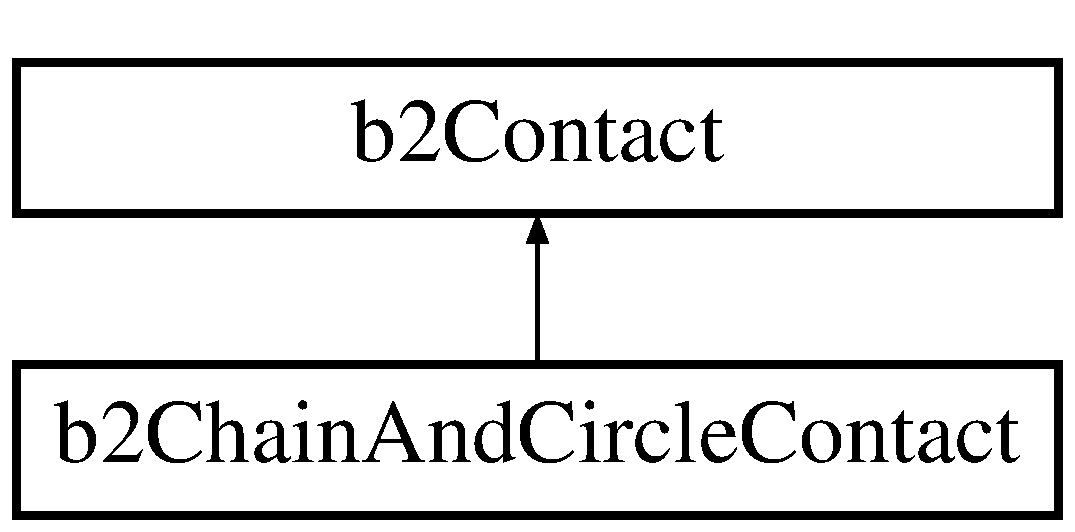
\includegraphics[height=2.000000cm]{classb2_chain_and_circle_contact}
\end{center}
\end{figure}
\subsection*{Public Member Functions}
\begin{DoxyCompactItemize}
\item 
{\bfseries b2\+Chain\+And\+Circle\+Contact} (\hyperlink{classb2_fixture}{b2\+Fixture} $\ast$fixtureA, int32 indexA, \hyperlink{classb2_fixture}{b2\+Fixture} $\ast$fixtureB, int32 indexB)\hypertarget{classb2_chain_and_circle_contact_a7303997b9af2b859346b4fc4d7e107d5}{}\label{classb2_chain_and_circle_contact_a7303997b9af2b859346b4fc4d7e107d5}

\item 
void \hyperlink{classb2_chain_and_circle_contact_afe52ebd870f24cbecedd1db662705f12}{Evaluate} (\hyperlink{structb2_manifold}{b2\+Manifold} $\ast$manifold, const \hyperlink{structb2_transform}{b2\+Transform} \&xfA, const \hyperlink{structb2_transform}{b2\+Transform} \&xfB)\hypertarget{classb2_chain_and_circle_contact_afe52ebd870f24cbecedd1db662705f12}{}\label{classb2_chain_and_circle_contact_afe52ebd870f24cbecedd1db662705f12}

\begin{DoxyCompactList}\small\item\em Evaluate this contact with your own manifold and transforms. \end{DoxyCompactList}\end{DoxyCompactItemize}
\subsection*{Static Public Member Functions}
\begin{DoxyCompactItemize}
\item 
static \hyperlink{classb2_contact}{b2\+Contact} $\ast$ {\bfseries Create} (\hyperlink{classb2_fixture}{b2\+Fixture} $\ast$fixtureA, int32 indexA, \hyperlink{classb2_fixture}{b2\+Fixture} $\ast$fixtureB, int32 indexB, \hyperlink{classb2_block_allocator}{b2\+Block\+Allocator} $\ast$allocator)\hypertarget{classb2_chain_and_circle_contact_a644e6d00b903534b5b00e76c52859ad8}{}\label{classb2_chain_and_circle_contact_a644e6d00b903534b5b00e76c52859ad8}

\item 
static void {\bfseries Destroy} (\hyperlink{classb2_contact}{b2\+Contact} $\ast$contact, \hyperlink{classb2_block_allocator}{b2\+Block\+Allocator} $\ast$allocator)\hypertarget{classb2_chain_and_circle_contact_abe4320581520cd75b333200745f436b8}{}\label{classb2_chain_and_circle_contact_abe4320581520cd75b333200745f436b8}

\end{DoxyCompactItemize}
\subsection*{Additional Inherited Members}


The documentation for this class was generated from the following file\+:\begin{DoxyCompactItemize}
\item 
C\+:/\+Users/\+Bilal Itani/\+Desktop/inf2990-\/11/\+Cadriciel/\+Commun/\+Externe/\+Box2\+D/include/\+Box2\+D/\+Dynamics/\+Contacts/b2\+Chain\+And\+Circle\+Contact.\+h\end{DoxyCompactItemize}

\hypertarget{classb2_chain_and_polygon_contact}{}\section{b2\+Chain\+And\+Polygon\+Contact Class Reference}
\label{classb2_chain_and_polygon_contact}\index{b2\+Chain\+And\+Polygon\+Contact@{b2\+Chain\+And\+Polygon\+Contact}}
Inheritance diagram for b2\+Chain\+And\+Polygon\+Contact\+:\begin{figure}[H]
\begin{center}
\leavevmode
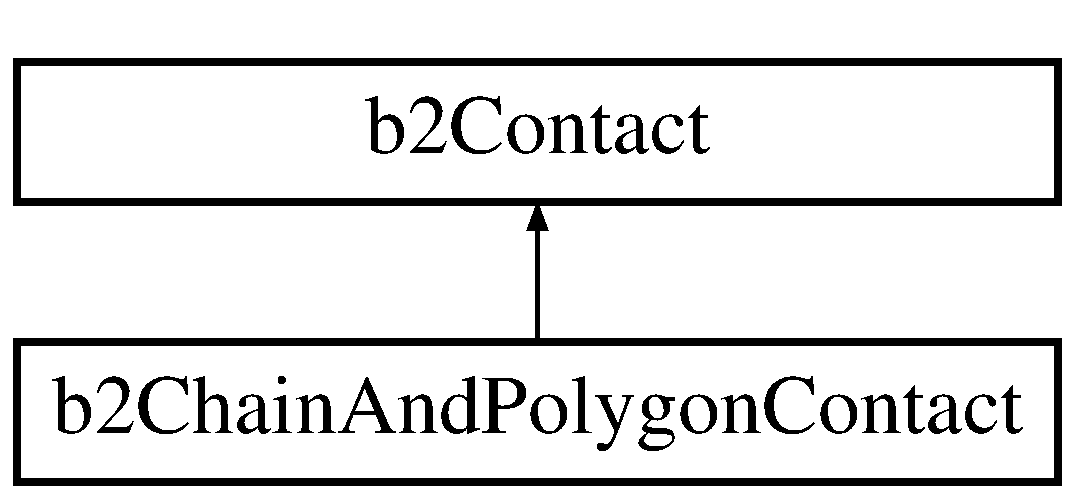
\includegraphics[height=2.000000cm]{classb2_chain_and_polygon_contact}
\end{center}
\end{figure}
\subsection*{Public Member Functions}
\begin{DoxyCompactItemize}
\item 
{\bfseries b2\+Chain\+And\+Polygon\+Contact} (\hyperlink{classb2_fixture}{b2\+Fixture} $\ast$fixtureA, int32 indexA, \hyperlink{classb2_fixture}{b2\+Fixture} $\ast$fixtureB, int32 indexB)\hypertarget{classb2_chain_and_polygon_contact_ae43cd05c72ccaeb5f03efc5df944648b}{}\label{classb2_chain_and_polygon_contact_ae43cd05c72ccaeb5f03efc5df944648b}

\item 
void \hyperlink{classb2_chain_and_polygon_contact_a8c25ceb49d981797d0a7f8a1ea769442}{Evaluate} (\hyperlink{structb2_manifold}{b2\+Manifold} $\ast$manifold, const \hyperlink{structb2_transform}{b2\+Transform} \&xfA, const \hyperlink{structb2_transform}{b2\+Transform} \&xfB)\hypertarget{classb2_chain_and_polygon_contact_a8c25ceb49d981797d0a7f8a1ea769442}{}\label{classb2_chain_and_polygon_contact_a8c25ceb49d981797d0a7f8a1ea769442}

\begin{DoxyCompactList}\small\item\em Evaluate this contact with your own manifold and transforms. \end{DoxyCompactList}\end{DoxyCompactItemize}
\subsection*{Static Public Member Functions}
\begin{DoxyCompactItemize}
\item 
static \hyperlink{classb2_contact}{b2\+Contact} $\ast$ {\bfseries Create} (\hyperlink{classb2_fixture}{b2\+Fixture} $\ast$fixtureA, int32 indexA, \hyperlink{classb2_fixture}{b2\+Fixture} $\ast$fixtureB, int32 indexB, \hyperlink{classb2_block_allocator}{b2\+Block\+Allocator} $\ast$allocator)\hypertarget{classb2_chain_and_polygon_contact_aae40d48ef8f2a49297a38c615a79e3b2}{}\label{classb2_chain_and_polygon_contact_aae40d48ef8f2a49297a38c615a79e3b2}

\item 
static void {\bfseries Destroy} (\hyperlink{classb2_contact}{b2\+Contact} $\ast$contact, \hyperlink{classb2_block_allocator}{b2\+Block\+Allocator} $\ast$allocator)\hypertarget{classb2_chain_and_polygon_contact_aed8a69453a9d7bb77a3c2b70fb20c764}{}\label{classb2_chain_and_polygon_contact_aed8a69453a9d7bb77a3c2b70fb20c764}

\end{DoxyCompactItemize}
\subsection*{Additional Inherited Members}


The documentation for this class was generated from the following file\+:\begin{DoxyCompactItemize}
\item 
Commun/\+Externe/\+Box2\+D/include/\+Box2\+D/\+Dynamics/\+Contacts/b2\+Chain\+And\+Polygon\+Contact.\+h\end{DoxyCompactItemize}

\hypertarget{classb2_chain_shape}{}\section{b2\+Chain\+Shape Class Reference}
\label{classb2_chain_shape}\index{b2\+Chain\+Shape@{b2\+Chain\+Shape}}


{\ttfamily \#include $<$b2\+Chain\+Shape.\+h$>$}

Inheritance diagram for b2\+Chain\+Shape\+:\begin{figure}[H]
\begin{center}
\leavevmode
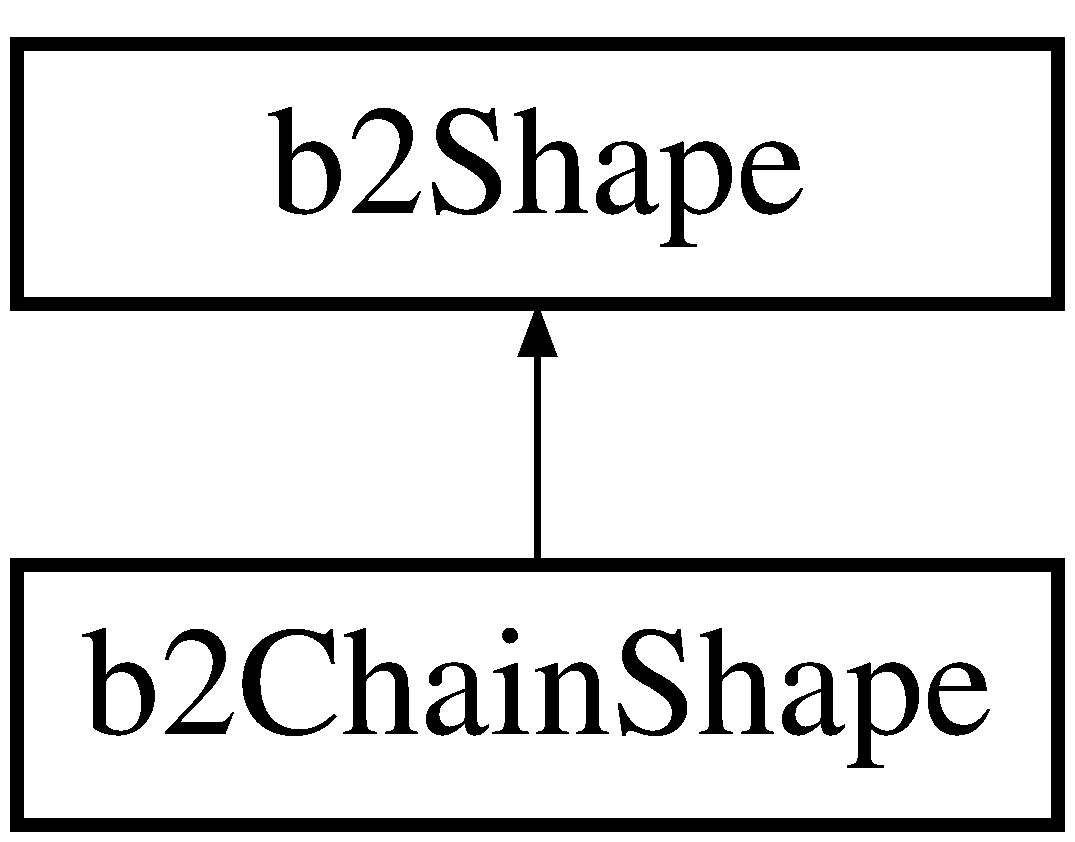
\includegraphics[height=2.000000cm]{classb2_chain_shape}
\end{center}
\end{figure}
\subsection*{Public Member Functions}
\begin{DoxyCompactItemize}
\item 
\hyperlink{classb2_chain_shape_a8c032394f5a85e7fc425a437e7689a18}{$\sim$b2\+Chain\+Shape} ()\hypertarget{classb2_chain_shape_a8c032394f5a85e7fc425a437e7689a18}{}\label{classb2_chain_shape_a8c032394f5a85e7fc425a437e7689a18}

\begin{DoxyCompactList}\small\item\em The destructor frees the vertices using b2\+Free. \end{DoxyCompactList}\item 
void \hyperlink{classb2_chain_shape_ac257742a52cac391e25962a4c703fb06}{Create\+Loop} (const \hyperlink{structb2_vec2}{b2\+Vec2} $\ast$vertices, int32 count)
\item 
void \hyperlink{classb2_chain_shape_aa0977339b743c05f2179939ccc38e7e0}{Create\+Chain} (const \hyperlink{structb2_vec2}{b2\+Vec2} $\ast$vertices, int32 count)
\item 
void \hyperlink{classb2_chain_shape_aeb2ddbe0c52a98885e91b7c8f597315b}{Set\+Prev\+Vertex} (const \hyperlink{structb2_vec2}{b2\+Vec2} \&prev\+Vertex)
\item 
void \hyperlink{classb2_chain_shape_a15c7c2821a52266ef57621ac7d34a95f}{Set\+Next\+Vertex} (const \hyperlink{structb2_vec2}{b2\+Vec2} \&next\+Vertex)
\item 
\hyperlink{classb2_shape}{b2\+Shape} $\ast$ \hyperlink{classb2_chain_shape_aa378f5e1a22ec71224e0182eb482b3e3}{Clone} (\hyperlink{classb2_block_allocator}{b2\+Block\+Allocator} $\ast$allocator) const \hypertarget{classb2_chain_shape_aa378f5e1a22ec71224e0182eb482b3e3}{}\label{classb2_chain_shape_aa378f5e1a22ec71224e0182eb482b3e3}

\begin{DoxyCompactList}\small\item\em Implement \hyperlink{classb2_shape}{b2\+Shape}. Vertices are cloned using b2\+Alloc. \end{DoxyCompactList}\item 
int32 \hyperlink{classb2_chain_shape_a44bd58b9602dbe57cdfc3b66f8f03b61}{Get\+Child\+Count} () const 
\item 
void \hyperlink{classb2_chain_shape_a614e630221ac7f19257c9351edf4bd12}{Get\+Child\+Edge} (\hyperlink{classb2_edge_shape}{b2\+Edge\+Shape} $\ast$edge, int32 index) const \hypertarget{classb2_chain_shape_a614e630221ac7f19257c9351edf4bd12}{}\label{classb2_chain_shape_a614e630221ac7f19257c9351edf4bd12}

\begin{DoxyCompactList}\small\item\em Get a child edge. \end{DoxyCompactList}\item 
bool \hyperlink{classb2_chain_shape_a4fc27b41ecc556985efacf8e0f91c39f}{Test\+Point} (const \hyperlink{structb2_transform}{b2\+Transform} \&transform, const \hyperlink{structb2_vec2}{b2\+Vec2} \&p) const 
\item 
bool \hyperlink{classb2_chain_shape_a85c7a17a15581e0e258c7af561cf5403}{Ray\+Cast} (\hyperlink{structb2_ray_cast_output}{b2\+Ray\+Cast\+Output} $\ast$output, const \hyperlink{structb2_ray_cast_input}{b2\+Ray\+Cast\+Input} \&input, const \hyperlink{structb2_transform}{b2\+Transform} \&transform, int32 child\+Index) const \hypertarget{classb2_chain_shape_a85c7a17a15581e0e258c7af561cf5403}{}\label{classb2_chain_shape_a85c7a17a15581e0e258c7af561cf5403}

\begin{DoxyCompactList}\small\item\em Implement \hyperlink{classb2_shape}{b2\+Shape}. \end{DoxyCompactList}\item 
void \hyperlink{classb2_chain_shape_a409c21206e4c84f66700809aac5b164c}{Compute\+A\+A\+BB} (\hyperlink{structb2_a_a_b_b}{b2\+A\+A\+BB} $\ast$aabb, const \hyperlink{structb2_transform}{b2\+Transform} \&transform, int32 child\+Index) const 
\item 
void \hyperlink{classb2_chain_shape_a009259d589abebeda27fe580d117b11e}{Compute\+Mass} (\hyperlink{structb2_mass_data}{b2\+Mass\+Data} $\ast$mass\+Data, float32 density) const 
\end{DoxyCompactItemize}
\subsection*{Public Attributes}
\begin{DoxyCompactItemize}
\item 
\hyperlink{structb2_vec2}{b2\+Vec2} $\ast$ \hyperlink{classb2_chain_shape_a481116a6886fb3880b13e55c966579da}{m\+\_\+vertices}\hypertarget{classb2_chain_shape_a481116a6886fb3880b13e55c966579da}{}\label{classb2_chain_shape_a481116a6886fb3880b13e55c966579da}

\begin{DoxyCompactList}\small\item\em The vertices. Owned by this class. \end{DoxyCompactList}\item 
int32 \hyperlink{classb2_chain_shape_ab2ad711781e6ac81179074e90e0e058b}{m\+\_\+count}\hypertarget{classb2_chain_shape_ab2ad711781e6ac81179074e90e0e058b}{}\label{classb2_chain_shape_ab2ad711781e6ac81179074e90e0e058b}

\begin{DoxyCompactList}\small\item\em The vertex count. \end{DoxyCompactList}\item 
\hyperlink{structb2_vec2}{b2\+Vec2} {\bfseries m\+\_\+prev\+Vertex}\hypertarget{classb2_chain_shape_a3a42d4c6b2421bc5badda3b6164949cf}{}\label{classb2_chain_shape_a3a42d4c6b2421bc5badda3b6164949cf}

\item 
\hyperlink{structb2_vec2}{b2\+Vec2} {\bfseries m\+\_\+next\+Vertex}\hypertarget{classb2_chain_shape_af3716ef780dd5bcd905e350d8854aaa2}{}\label{classb2_chain_shape_af3716ef780dd5bcd905e350d8854aaa2}

\item 
bool {\bfseries m\+\_\+has\+Prev\+Vertex}\hypertarget{classb2_chain_shape_a8a6ffbb9de0e2b8545c8b4fc8aa77249}{}\label{classb2_chain_shape_a8a6ffbb9de0e2b8545c8b4fc8aa77249}

\item 
bool {\bfseries m\+\_\+has\+Next\+Vertex}\hypertarget{classb2_chain_shape_a333b74486566e73c3cf1f7da5e69a96e}{}\label{classb2_chain_shape_a333b74486566e73c3cf1f7da5e69a96e}

\end{DoxyCompactItemize}
\subsection*{Additional Inherited Members}


\subsection{Detailed Description}
A chain shape is a free form sequence of line segments. The chain has two-\/sided collision, so you can use inside and outside collision. Therefore, you may use any winding order. Since there may be many vertices, they are allocated using b2\+Alloc. Connectivity information is used to create smooth collisions. W\+A\+R\+N\+I\+NG\+: The chain will not collide properly if there are self-\/intersections. 

\subsection{Member Function Documentation}
\index{b2\+Chain\+Shape@{b2\+Chain\+Shape}!Compute\+A\+A\+BB@{Compute\+A\+A\+BB}}
\index{Compute\+A\+A\+BB@{Compute\+A\+A\+BB}!b2\+Chain\+Shape@{b2\+Chain\+Shape}}
\subsubsection[{\texorpdfstring{Compute\+A\+A\+B\+B(b2\+A\+A\+B\+B $\ast$aabb, const b2\+Transform \&transform, int32 child\+Index) const }{ComputeAABB(b2AABB *aabb, const b2Transform &transform, int32 childIndex) const }}]{\setlength{\rightskip}{0pt plus 5cm}void b2\+Chain\+Shape\+::\+Compute\+A\+A\+BB (
\begin{DoxyParamCaption}
\item[{{\bf b2\+A\+A\+BB} $\ast$}]{aabb, }
\item[{const {\bf b2\+Transform} \&}]{transform, }
\item[{int32}]{child\+Index}
\end{DoxyParamCaption}
) const\hspace{0.3cm}{\ttfamily [virtual]}}\hypertarget{classb2_chain_shape_a409c21206e4c84f66700809aac5b164c}{}\label{classb2_chain_shape_a409c21206e4c84f66700809aac5b164c}
\begin{DoxySeeAlso}{See also}
\hyperlink{classb2_shape_a0a7f4227b6c17450fc26e0b6641b7abf}{b2\+Shape\+::\+Compute\+A\+A\+BB} 
\end{DoxySeeAlso}


Implements \hyperlink{classb2_shape_a0a7f4227b6c17450fc26e0b6641b7abf}{b2\+Shape}.

\index{b2\+Chain\+Shape@{b2\+Chain\+Shape}!Compute\+Mass@{Compute\+Mass}}
\index{Compute\+Mass@{Compute\+Mass}!b2\+Chain\+Shape@{b2\+Chain\+Shape}}
\subsubsection[{\texorpdfstring{Compute\+Mass(b2\+Mass\+Data $\ast$mass\+Data, float32 density) const }{ComputeMass(b2MassData *massData, float32 density) const }}]{\setlength{\rightskip}{0pt plus 5cm}void b2\+Chain\+Shape\+::\+Compute\+Mass (
\begin{DoxyParamCaption}
\item[{{\bf b2\+Mass\+Data} $\ast$}]{mass\+Data, }
\item[{float32}]{density}
\end{DoxyParamCaption}
) const\hspace{0.3cm}{\ttfamily [virtual]}}\hypertarget{classb2_chain_shape_a009259d589abebeda27fe580d117b11e}{}\label{classb2_chain_shape_a009259d589abebeda27fe580d117b11e}
Chains have zero mass. \begin{DoxySeeAlso}{See also}
\hyperlink{classb2_shape_a33cfcad2cf4cc31e1d001bf1baf10721}{b2\+Shape\+::\+Compute\+Mass} 
\end{DoxySeeAlso}


Implements \hyperlink{classb2_shape_a33cfcad2cf4cc31e1d001bf1baf10721}{b2\+Shape}.

\index{b2\+Chain\+Shape@{b2\+Chain\+Shape}!Create\+Chain@{Create\+Chain}}
\index{Create\+Chain@{Create\+Chain}!b2\+Chain\+Shape@{b2\+Chain\+Shape}}
\subsubsection[{\texorpdfstring{Create\+Chain(const b2\+Vec2 $\ast$vertices, int32 count)}{CreateChain(const b2Vec2 *vertices, int32 count)}}]{\setlength{\rightskip}{0pt plus 5cm}void b2\+Chain\+Shape\+::\+Create\+Chain (
\begin{DoxyParamCaption}
\item[{const {\bf b2\+Vec2} $\ast$}]{vertices, }
\item[{int32}]{count}
\end{DoxyParamCaption}
)}\hypertarget{classb2_chain_shape_aa0977339b743c05f2179939ccc38e7e0}{}\label{classb2_chain_shape_aa0977339b743c05f2179939ccc38e7e0}
Create a chain with isolated end vertices. 
\begin{DoxyParams}{Parameters}
{\em vertices} & an array of vertices, these are copied \\
\hline
{\em count} & the vertex count \\
\hline
\end{DoxyParams}
\index{b2\+Chain\+Shape@{b2\+Chain\+Shape}!Create\+Loop@{Create\+Loop}}
\index{Create\+Loop@{Create\+Loop}!b2\+Chain\+Shape@{b2\+Chain\+Shape}}
\subsubsection[{\texorpdfstring{Create\+Loop(const b2\+Vec2 $\ast$vertices, int32 count)}{CreateLoop(const b2Vec2 *vertices, int32 count)}}]{\setlength{\rightskip}{0pt plus 5cm}void b2\+Chain\+Shape\+::\+Create\+Loop (
\begin{DoxyParamCaption}
\item[{const {\bf b2\+Vec2} $\ast$}]{vertices, }
\item[{int32}]{count}
\end{DoxyParamCaption}
)}\hypertarget{classb2_chain_shape_ac257742a52cac391e25962a4c703fb06}{}\label{classb2_chain_shape_ac257742a52cac391e25962a4c703fb06}
Create a loop. This automatically adjusts connectivity. 
\begin{DoxyParams}{Parameters}
{\em vertices} & an array of vertices, these are copied \\
\hline
{\em count} & the vertex count \\
\hline
\end{DoxyParams}
\index{b2\+Chain\+Shape@{b2\+Chain\+Shape}!Get\+Child\+Count@{Get\+Child\+Count}}
\index{Get\+Child\+Count@{Get\+Child\+Count}!b2\+Chain\+Shape@{b2\+Chain\+Shape}}
\subsubsection[{\texorpdfstring{Get\+Child\+Count() const }{GetChildCount() const }}]{\setlength{\rightskip}{0pt plus 5cm}int32 b2\+Chain\+Shape\+::\+Get\+Child\+Count (
\begin{DoxyParamCaption}
{}
\end{DoxyParamCaption}
) const\hspace{0.3cm}{\ttfamily [virtual]}}\hypertarget{classb2_chain_shape_a44bd58b9602dbe57cdfc3b66f8f03b61}{}\label{classb2_chain_shape_a44bd58b9602dbe57cdfc3b66f8f03b61}
\begin{DoxySeeAlso}{See also}
\hyperlink{classb2_shape_acaade0398c8a6f3750ba0d25fbde2242}{b2\+Shape\+::\+Get\+Child\+Count} 
\end{DoxySeeAlso}


Implements \hyperlink{classb2_shape_acaade0398c8a6f3750ba0d25fbde2242}{b2\+Shape}.

\index{b2\+Chain\+Shape@{b2\+Chain\+Shape}!Set\+Next\+Vertex@{Set\+Next\+Vertex}}
\index{Set\+Next\+Vertex@{Set\+Next\+Vertex}!b2\+Chain\+Shape@{b2\+Chain\+Shape}}
\subsubsection[{\texorpdfstring{Set\+Next\+Vertex(const b2\+Vec2 \&next\+Vertex)}{SetNextVertex(const b2Vec2 &nextVertex)}}]{\setlength{\rightskip}{0pt plus 5cm}void b2\+Chain\+Shape\+::\+Set\+Next\+Vertex (
\begin{DoxyParamCaption}
\item[{const {\bf b2\+Vec2} \&}]{next\+Vertex}
\end{DoxyParamCaption}
)}\hypertarget{classb2_chain_shape_a15c7c2821a52266ef57621ac7d34a95f}{}\label{classb2_chain_shape_a15c7c2821a52266ef57621ac7d34a95f}
Establish connectivity to a vertex that follows the last vertex. Don\textquotesingle{}t call this for loops. \index{b2\+Chain\+Shape@{b2\+Chain\+Shape}!Set\+Prev\+Vertex@{Set\+Prev\+Vertex}}
\index{Set\+Prev\+Vertex@{Set\+Prev\+Vertex}!b2\+Chain\+Shape@{b2\+Chain\+Shape}}
\subsubsection[{\texorpdfstring{Set\+Prev\+Vertex(const b2\+Vec2 \&prev\+Vertex)}{SetPrevVertex(const b2Vec2 &prevVertex)}}]{\setlength{\rightskip}{0pt plus 5cm}void b2\+Chain\+Shape\+::\+Set\+Prev\+Vertex (
\begin{DoxyParamCaption}
\item[{const {\bf b2\+Vec2} \&}]{prev\+Vertex}
\end{DoxyParamCaption}
)}\hypertarget{classb2_chain_shape_aeb2ddbe0c52a98885e91b7c8f597315b}{}\label{classb2_chain_shape_aeb2ddbe0c52a98885e91b7c8f597315b}
Establish connectivity to a vertex that precedes the first vertex. Don\textquotesingle{}t call this for loops. \index{b2\+Chain\+Shape@{b2\+Chain\+Shape}!Test\+Point@{Test\+Point}}
\index{Test\+Point@{Test\+Point}!b2\+Chain\+Shape@{b2\+Chain\+Shape}}
\subsubsection[{\texorpdfstring{Test\+Point(const b2\+Transform \&transform, const b2\+Vec2 \&p) const }{TestPoint(const b2Transform &transform, const b2Vec2 &p) const }}]{\setlength{\rightskip}{0pt plus 5cm}bool b2\+Chain\+Shape\+::\+Test\+Point (
\begin{DoxyParamCaption}
\item[{const {\bf b2\+Transform} \&}]{transform, }
\item[{const {\bf b2\+Vec2} \&}]{p}
\end{DoxyParamCaption}
) const\hspace{0.3cm}{\ttfamily [virtual]}}\hypertarget{classb2_chain_shape_a4fc27b41ecc556985efacf8e0f91c39f}{}\label{classb2_chain_shape_a4fc27b41ecc556985efacf8e0f91c39f}
This always return false. \begin{DoxySeeAlso}{See also}
\hyperlink{classb2_shape_a11996b9bdcf8dca92a0c8bf484ab3f59}{b2\+Shape\+::\+Test\+Point} 
\end{DoxySeeAlso}


Implements \hyperlink{classb2_shape_a11996b9bdcf8dca92a0c8bf484ab3f59}{b2\+Shape}.



The documentation for this class was generated from the following file\+:\begin{DoxyCompactItemize}
\item 
C\+:/\+Users/\+Bilal Itani/\+Desktop/inf2990-\/11/\+Cadriciel/\+Commun/\+Externe/\+Box2\+D/include/\+Box2\+D/\+Collision/\+Shapes/b2\+Chain\+Shape.\+h\end{DoxyCompactItemize}

\hypertarget{classb2_circle_contact}{}\section{b2\+Circle\+Contact Class Reference}
\label{classb2_circle_contact}\index{b2\+Circle\+Contact@{b2\+Circle\+Contact}}
Inheritance diagram for b2\+Circle\+Contact\+:\begin{figure}[H]
\begin{center}
\leavevmode
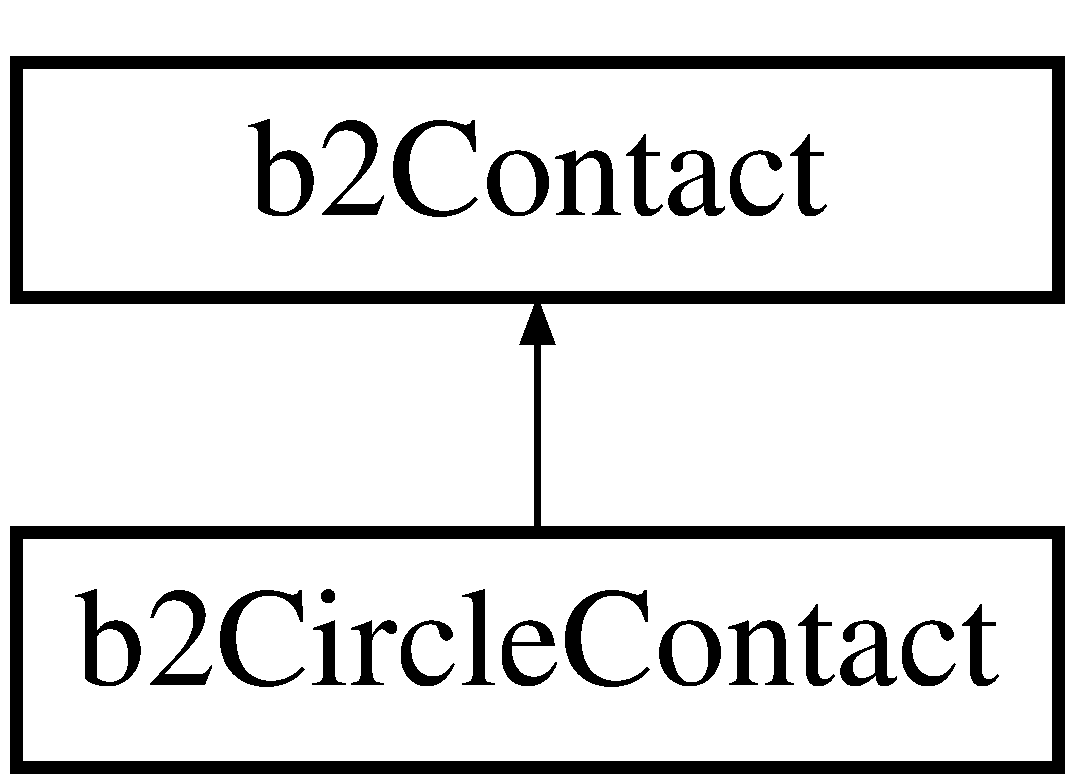
\includegraphics[height=2.000000cm]{classb2_circle_contact}
\end{center}
\end{figure}
\subsection*{Public Member Functions}
\begin{DoxyCompactItemize}
\item 
{\bfseries b2\+Circle\+Contact} (\hyperlink{classb2_fixture}{b2\+Fixture} $\ast$fixtureA, \hyperlink{classb2_fixture}{b2\+Fixture} $\ast$fixtureB)\hypertarget{classb2_circle_contact_a77e06c857edb2ca171340898f09ef789}{}\label{classb2_circle_contact_a77e06c857edb2ca171340898f09ef789}

\item 
void \hyperlink{classb2_circle_contact_ac0651dda773561b8561b8efa3cd31d5c}{Evaluate} (\hyperlink{structb2_manifold}{b2\+Manifold} $\ast$manifold, const \hyperlink{structb2_transform}{b2\+Transform} \&xfA, const \hyperlink{structb2_transform}{b2\+Transform} \&xfB)\hypertarget{classb2_circle_contact_ac0651dda773561b8561b8efa3cd31d5c}{}\label{classb2_circle_contact_ac0651dda773561b8561b8efa3cd31d5c}

\begin{DoxyCompactList}\small\item\em Evaluate this contact with your own manifold and transforms. \end{DoxyCompactList}\end{DoxyCompactItemize}
\subsection*{Static Public Member Functions}
\begin{DoxyCompactItemize}
\item 
static \hyperlink{classb2_contact}{b2\+Contact} $\ast$ {\bfseries Create} (\hyperlink{classb2_fixture}{b2\+Fixture} $\ast$fixtureA, int32 indexA, \hyperlink{classb2_fixture}{b2\+Fixture} $\ast$fixtureB, int32 indexB, \hyperlink{classb2_block_allocator}{b2\+Block\+Allocator} $\ast$allocator)\hypertarget{classb2_circle_contact_a741c07fe3f626b80e01ff3d96cf2d90a}{}\label{classb2_circle_contact_a741c07fe3f626b80e01ff3d96cf2d90a}

\item 
static void {\bfseries Destroy} (\hyperlink{classb2_contact}{b2\+Contact} $\ast$contact, \hyperlink{classb2_block_allocator}{b2\+Block\+Allocator} $\ast$allocator)\hypertarget{classb2_circle_contact_a0171e991d568b7f4d8e5b4179072bf60}{}\label{classb2_circle_contact_a0171e991d568b7f4d8e5b4179072bf60}

\end{DoxyCompactItemize}
\subsection*{Additional Inherited Members}


The documentation for this class was generated from the following file\+:\begin{DoxyCompactItemize}
\item 
C\+:/\+Users/\+Bilal Itani/\+Desktop/inf2990-\/11/\+Cadriciel/\+Commun/\+Externe/\+Box2\+D/include/\+Box2\+D/\+Dynamics/\+Contacts/b2\+Circle\+Contact.\+h\end{DoxyCompactItemize}

\hypertarget{classb2_circle_shape}{}\section{b2\+Circle\+Shape Class Reference}
\label{classb2_circle_shape}\index{b2\+Circle\+Shape@{b2\+Circle\+Shape}}


A circle shape.  




{\ttfamily \#include $<$b2\+Circle\+Shape.\+h$>$}

Inheritance diagram for b2\+Circle\+Shape\+:\begin{figure}[H]
\begin{center}
\leavevmode
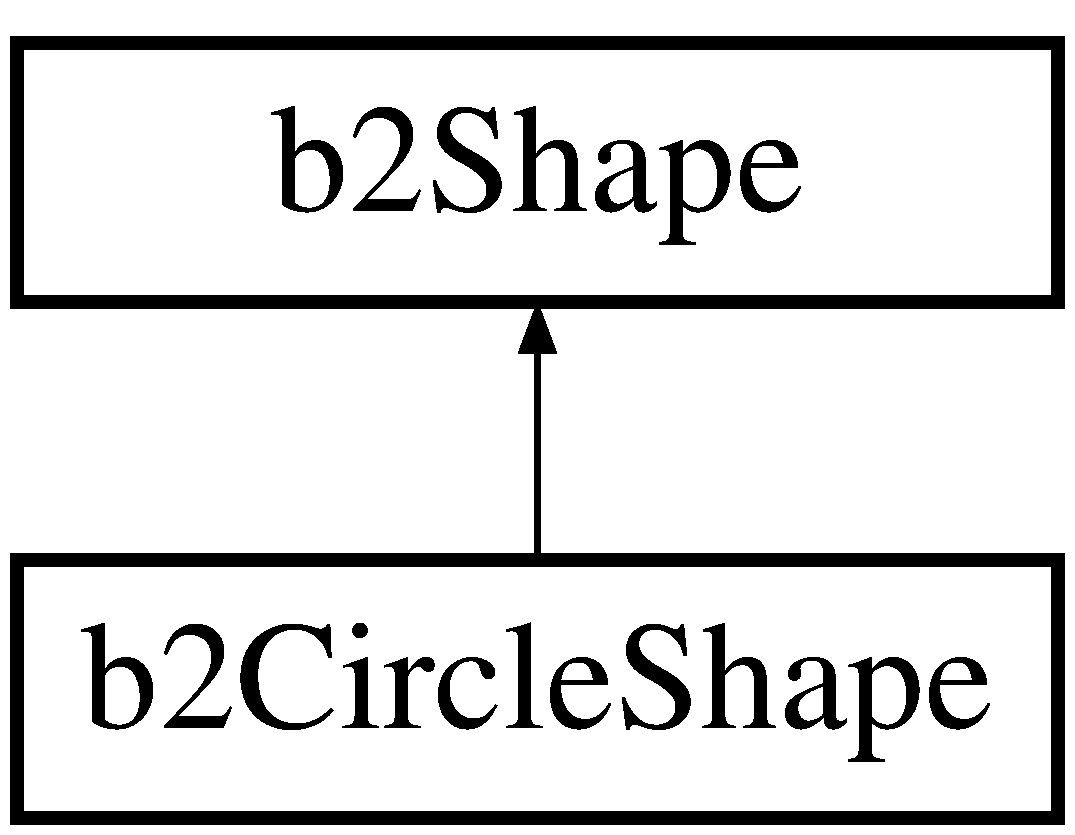
\includegraphics[height=2.000000cm]{classb2_circle_shape}
\end{center}
\end{figure}
\subsection*{Public Member Functions}
\begin{DoxyCompactItemize}
\item 
\hyperlink{classb2_shape}{b2\+Shape} $\ast$ \hyperlink{classb2_circle_shape_a95b7ff40de30768b19475df98dd68c4b}{Clone} (\hyperlink{classb2_block_allocator}{b2\+Block\+Allocator} $\ast$allocator) const \hypertarget{classb2_circle_shape_a95b7ff40de30768b19475df98dd68c4b}{}\label{classb2_circle_shape_a95b7ff40de30768b19475df98dd68c4b}

\begin{DoxyCompactList}\small\item\em Implement \hyperlink{classb2_shape}{b2\+Shape}. \end{DoxyCompactList}\item 
int32 \hyperlink{classb2_circle_shape_a64b58799675edc9a6debc09c0d6ddce4}{Get\+Child\+Count} () const 
\item 
bool \hyperlink{classb2_circle_shape_a77171941cd1633c337fed1efb366bebb}{Test\+Point} (const \hyperlink{structb2_transform}{b2\+Transform} \&transform, const \hyperlink{structb2_vec2}{b2\+Vec2} \&p) const \hypertarget{classb2_circle_shape_a77171941cd1633c337fed1efb366bebb}{}\label{classb2_circle_shape_a77171941cd1633c337fed1efb366bebb}

\begin{DoxyCompactList}\small\item\em Implement \hyperlink{classb2_shape}{b2\+Shape}. \end{DoxyCompactList}\item 
bool \hyperlink{classb2_circle_shape_a76175079381193917026fdf3702190fa}{Ray\+Cast} (\hyperlink{structb2_ray_cast_output}{b2\+Ray\+Cast\+Output} $\ast$output, const \hyperlink{structb2_ray_cast_input}{b2\+Ray\+Cast\+Input} \&input, const \hyperlink{structb2_transform}{b2\+Transform} \&transform, int32 child\+Index) const \hypertarget{classb2_circle_shape_a76175079381193917026fdf3702190fa}{}\label{classb2_circle_shape_a76175079381193917026fdf3702190fa}

\begin{DoxyCompactList}\small\item\em Implement \hyperlink{classb2_shape}{b2\+Shape}. \end{DoxyCompactList}\item 
void \hyperlink{classb2_circle_shape_aa6889a5af85aa1e272547fd0008eb64a}{Compute\+A\+A\+BB} (\hyperlink{structb2_a_a_b_b}{b2\+A\+A\+BB} $\ast$aabb, const \hyperlink{structb2_transform}{b2\+Transform} \&transform, int32 child\+Index) const 
\item 
void \hyperlink{classb2_circle_shape_a335edea2ef84789e102dde41ca889828}{Compute\+Mass} (\hyperlink{structb2_mass_data}{b2\+Mass\+Data} $\ast$mass\+Data, float32 density) const 
\item 
int32 \hyperlink{classb2_circle_shape_a8644ce19547e5efaf43bd8ec543e284e}{Get\+Support} (const \hyperlink{structb2_vec2}{b2\+Vec2} \&d) const \hypertarget{classb2_circle_shape_a8644ce19547e5efaf43bd8ec543e284e}{}\label{classb2_circle_shape_a8644ce19547e5efaf43bd8ec543e284e}

\begin{DoxyCompactList}\small\item\em Get the supporting vertex index in the given direction. \end{DoxyCompactList}\item 
const \hyperlink{structb2_vec2}{b2\+Vec2} \& \hyperlink{classb2_circle_shape_aa23975b480495bf8bc70073d4f135fd2}{Get\+Support\+Vertex} (const \hyperlink{structb2_vec2}{b2\+Vec2} \&d) const \hypertarget{classb2_circle_shape_aa23975b480495bf8bc70073d4f135fd2}{}\label{classb2_circle_shape_aa23975b480495bf8bc70073d4f135fd2}

\begin{DoxyCompactList}\small\item\em Get the supporting vertex in the given direction. \end{DoxyCompactList}\item 
int32 \hyperlink{classb2_circle_shape_a477a087b143147223e4b9fbb6581acf1}{Get\+Vertex\+Count} () const \hypertarget{classb2_circle_shape_a477a087b143147223e4b9fbb6581acf1}{}\label{classb2_circle_shape_a477a087b143147223e4b9fbb6581acf1}

\begin{DoxyCompactList}\small\item\em Get the vertex count. \end{DoxyCompactList}\item 
const \hyperlink{structb2_vec2}{b2\+Vec2} \& \hyperlink{classb2_circle_shape_a029e555a3ea76b00479b051f1b813c3a}{Get\+Vertex} (int32 index) const \hypertarget{classb2_circle_shape_a029e555a3ea76b00479b051f1b813c3a}{}\label{classb2_circle_shape_a029e555a3ea76b00479b051f1b813c3a}

\begin{DoxyCompactList}\small\item\em Get a vertex by index. Used by b2\+Distance. \end{DoxyCompactList}\end{DoxyCompactItemize}
\subsection*{Public Attributes}
\begin{DoxyCompactItemize}
\item 
\hyperlink{structb2_vec2}{b2\+Vec2} \hyperlink{classb2_circle_shape_a190705618b2e65f636f1dc03c63640ff}{m\+\_\+p}\hypertarget{classb2_circle_shape_a190705618b2e65f636f1dc03c63640ff}{}\label{classb2_circle_shape_a190705618b2e65f636f1dc03c63640ff}

\begin{DoxyCompactList}\small\item\em Position. \end{DoxyCompactList}\end{DoxyCompactItemize}
\subsection*{Additional Inherited Members}


\subsection{Detailed Description}
A circle shape. 

\subsection{Member Function Documentation}
\index{b2\+Circle\+Shape@{b2\+Circle\+Shape}!Compute\+A\+A\+BB@{Compute\+A\+A\+BB}}
\index{Compute\+A\+A\+BB@{Compute\+A\+A\+BB}!b2\+Circle\+Shape@{b2\+Circle\+Shape}}
\subsubsection[{\texorpdfstring{Compute\+A\+A\+B\+B(b2\+A\+A\+B\+B $\ast$aabb, const b2\+Transform \&transform, int32 child\+Index) const }{ComputeAABB(b2AABB *aabb, const b2Transform &transform, int32 childIndex) const }}]{\setlength{\rightskip}{0pt plus 5cm}void b2\+Circle\+Shape\+::\+Compute\+A\+A\+BB (
\begin{DoxyParamCaption}
\item[{{\bf b2\+A\+A\+BB} $\ast$}]{aabb, }
\item[{const {\bf b2\+Transform} \&}]{transform, }
\item[{int32}]{child\+Index}
\end{DoxyParamCaption}
) const\hspace{0.3cm}{\ttfamily [virtual]}}\hypertarget{classb2_circle_shape_aa6889a5af85aa1e272547fd0008eb64a}{}\label{classb2_circle_shape_aa6889a5af85aa1e272547fd0008eb64a}
\begin{DoxySeeAlso}{See also}
\hyperlink{classb2_shape_a0a7f4227b6c17450fc26e0b6641b7abf}{b2\+Shape\+::\+Compute\+A\+A\+BB} 
\end{DoxySeeAlso}


Implements \hyperlink{classb2_shape_a0a7f4227b6c17450fc26e0b6641b7abf}{b2\+Shape}.

\index{b2\+Circle\+Shape@{b2\+Circle\+Shape}!Compute\+Mass@{Compute\+Mass}}
\index{Compute\+Mass@{Compute\+Mass}!b2\+Circle\+Shape@{b2\+Circle\+Shape}}
\subsubsection[{\texorpdfstring{Compute\+Mass(b2\+Mass\+Data $\ast$mass\+Data, float32 density) const }{ComputeMass(b2MassData *massData, float32 density) const }}]{\setlength{\rightskip}{0pt plus 5cm}void b2\+Circle\+Shape\+::\+Compute\+Mass (
\begin{DoxyParamCaption}
\item[{{\bf b2\+Mass\+Data} $\ast$}]{mass\+Data, }
\item[{float32}]{density}
\end{DoxyParamCaption}
) const\hspace{0.3cm}{\ttfamily [virtual]}}\hypertarget{classb2_circle_shape_a335edea2ef84789e102dde41ca889828}{}\label{classb2_circle_shape_a335edea2ef84789e102dde41ca889828}
\begin{DoxySeeAlso}{See also}
\hyperlink{classb2_shape_a33cfcad2cf4cc31e1d001bf1baf10721}{b2\+Shape\+::\+Compute\+Mass} 
\end{DoxySeeAlso}


Implements \hyperlink{classb2_shape_a33cfcad2cf4cc31e1d001bf1baf10721}{b2\+Shape}.

\index{b2\+Circle\+Shape@{b2\+Circle\+Shape}!Get\+Child\+Count@{Get\+Child\+Count}}
\index{Get\+Child\+Count@{Get\+Child\+Count}!b2\+Circle\+Shape@{b2\+Circle\+Shape}}
\subsubsection[{\texorpdfstring{Get\+Child\+Count() const }{GetChildCount() const }}]{\setlength{\rightskip}{0pt plus 5cm}int32 b2\+Circle\+Shape\+::\+Get\+Child\+Count (
\begin{DoxyParamCaption}
{}
\end{DoxyParamCaption}
) const\hspace{0.3cm}{\ttfamily [virtual]}}\hypertarget{classb2_circle_shape_a64b58799675edc9a6debc09c0d6ddce4}{}\label{classb2_circle_shape_a64b58799675edc9a6debc09c0d6ddce4}
\begin{DoxySeeAlso}{See also}
\hyperlink{classb2_shape_acaade0398c8a6f3750ba0d25fbde2242}{b2\+Shape\+::\+Get\+Child\+Count} 
\end{DoxySeeAlso}


Implements \hyperlink{classb2_shape_acaade0398c8a6f3750ba0d25fbde2242}{b2\+Shape}.



The documentation for this class was generated from the following file\+:\begin{DoxyCompactItemize}
\item 
Cadriciel/\+Commun/\+Externe/\+Box2\+D/include/\+Box2\+D/\+Collision/\+Shapes/b2\+Circle\+Shape.\+h\end{DoxyCompactItemize}

\hypertarget{structb2_clip_vertex}{}\section{b2\+Clip\+Vertex Struct Reference}
\label{structb2_clip_vertex}\index{b2\+Clip\+Vertex@{b2\+Clip\+Vertex}}


Used for computing contact manifolds.  




{\ttfamily \#include $<$b2\+Collision.\+h$>$}

\subsection*{Public Attributes}
\begin{DoxyCompactItemize}
\item 
\hyperlink{structb2_vec2}{b2\+Vec2} {\bfseries v}\hypertarget{structb2_clip_vertex_a6c8d8e4c0667755d5295a9c0d91d5b87}{}\label{structb2_clip_vertex_a6c8d8e4c0667755d5295a9c0d91d5b87}

\item 
\hyperlink{unionb2_contact_i_d}{b2\+Contact\+ID} {\bfseries id}\hypertarget{structb2_clip_vertex_ac0f6d48eafc40a665bc18d4aa821689d}{}\label{structb2_clip_vertex_ac0f6d48eafc40a665bc18d4aa821689d}

\end{DoxyCompactItemize}


\subsection{Detailed Description}
Used for computing contact manifolds. 

The documentation for this struct was generated from the following file\+:\begin{DoxyCompactItemize}
\item 
Cadriciel/\+Commun/\+Externe/\+Box2\+D/include/\+Box2\+D/\+Collision/\hyperlink{b2_collision_8h}{b2\+Collision.\+h}\end{DoxyCompactItemize}

\hypertarget{structb2_color}{}\section{b2\+Color Struct Reference}
\label{structb2_color}\index{b2\+Color@{b2\+Color}}


Color for debug drawing. Each value has the range \mbox{[}0,1\mbox{]}.  




{\ttfamily \#include $<$b2\+Draw.\+h$>$}

\subsection*{Public Member Functions}
\begin{DoxyCompactItemize}
\item 
{\bfseries b2\+Color} (float32 r, float32 g, float32 b)\hypertarget{structb2_color_abddfc60d402d691542a224921868bfb7}{}\label{structb2_color_abddfc60d402d691542a224921868bfb7}

\item 
void {\bfseries Set} (float32 ri, float32 gi, float32 bi)\hypertarget{structb2_color_af35a718911e10a54fa8aaa86367a5b56}{}\label{structb2_color_af35a718911e10a54fa8aaa86367a5b56}

\end{DoxyCompactItemize}
\subsection*{Public Attributes}
\begin{DoxyCompactItemize}
\item 
float32 {\bfseries r}\hypertarget{structb2_color_a9ab6c9a910caee177d96980b74ffb00b}{}\label{structb2_color_a9ab6c9a910caee177d96980b74ffb00b}

\item 
float32 {\bfseries g}\hypertarget{structb2_color_a241c742352403ec456b51ac5f2abe7d9}{}\label{structb2_color_a241c742352403ec456b51ac5f2abe7d9}

\item 
float32 {\bfseries b}\hypertarget{structb2_color_a9e7380d27a63010cfad49b97f66dcd26}{}\label{structb2_color_a9e7380d27a63010cfad49b97f66dcd26}

\end{DoxyCompactItemize}


\subsection{Detailed Description}
Color for debug drawing. Each value has the range \mbox{[}0,1\mbox{]}. 

The documentation for this struct was generated from the following file\+:\begin{DoxyCompactItemize}
\item 
Cadriciel/\+Commun/\+Externe/\+Box2\+D/include/\+Box2\+D/\+Common/b2\+Draw.\+h\end{DoxyCompactItemize}

\hypertarget{classb2_contact}{}\section{b2\+Contact Class Reference}
\label{classb2_contact}\index{b2\+Contact@{b2\+Contact}}


{\ttfamily \#include $<$b2\+Contact.\+h$>$}

Inheritance diagram for b2\+Contact\+:\begin{figure}[H]
\begin{center}
\leavevmode
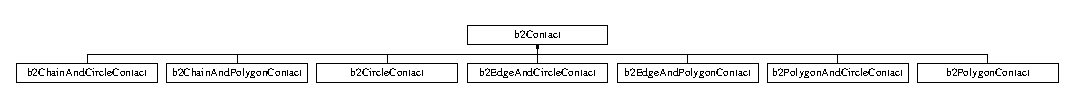
\includegraphics[height=0.888889cm]{classb2_contact}
\end{center}
\end{figure}
\subsection*{Public Member Functions}
\begin{DoxyCompactItemize}
\item 
\hyperlink{structb2_manifold}{b2\+Manifold} $\ast$ \hyperlink{classb2_contact_ab0597077b23615476327f9b32d9c4979}{Get\+Manifold} ()
\item 
const \hyperlink{structb2_manifold}{b2\+Manifold} $\ast$ {\bfseries Get\+Manifold} () const \hypertarget{classb2_contact_a2a1fb2fa1e0956faf61047c4aba3da5a}{}\label{classb2_contact_a2a1fb2fa1e0956faf61047c4aba3da5a}

\item 
void \hyperlink{classb2_contact_a6a30a44a28b44754cb61bba65cb5b728}{Get\+World\+Manifold} (\hyperlink{structb2_world_manifold}{b2\+World\+Manifold} $\ast$world\+Manifold) const \hypertarget{classb2_contact_a6a30a44a28b44754cb61bba65cb5b728}{}\label{classb2_contact_a6a30a44a28b44754cb61bba65cb5b728}

\begin{DoxyCompactList}\small\item\em Get the world manifold. \end{DoxyCompactList}\item 
bool \hyperlink{classb2_contact_a367dc9a563ad7db5547f4247777a33c9}{Is\+Touching} () const \hypertarget{classb2_contact_a367dc9a563ad7db5547f4247777a33c9}{}\label{classb2_contact_a367dc9a563ad7db5547f4247777a33c9}

\begin{DoxyCompactList}\small\item\em Is this contact touching? \end{DoxyCompactList}\item 
void \hyperlink{classb2_contact_a6edf582f8c161d6632854cddefe55a0c}{Set\+Enabled} (bool flag)
\item 
bool \hyperlink{classb2_contact_ae7bd71ee1b0bb352bec6eeaab4f91c6a}{Is\+Enabled} () const \hypertarget{classb2_contact_ae7bd71ee1b0bb352bec6eeaab4f91c6a}{}\label{classb2_contact_ae7bd71ee1b0bb352bec6eeaab4f91c6a}

\begin{DoxyCompactList}\small\item\em Has this contact been disabled? \end{DoxyCompactList}\item 
\hyperlink{classb2_contact}{b2\+Contact} $\ast$ \hyperlink{classb2_contact_aebfebb1e4b27dc0bd7aa120093e3d650}{Get\+Next} ()\hypertarget{classb2_contact_aebfebb1e4b27dc0bd7aa120093e3d650}{}\label{classb2_contact_aebfebb1e4b27dc0bd7aa120093e3d650}

\begin{DoxyCompactList}\small\item\em Get the next contact in the world\textquotesingle{}s contact list. \end{DoxyCompactList}\item 
const \hyperlink{classb2_contact}{b2\+Contact} $\ast$ {\bfseries Get\+Next} () const \hypertarget{classb2_contact_a55e20c9e32071f492952dad256552141}{}\label{classb2_contact_a55e20c9e32071f492952dad256552141}

\item 
\hyperlink{classb2_fixture}{b2\+Fixture} $\ast$ \hyperlink{classb2_contact_a707a3a5a14c2cdd4c6eb7fc648d76037}{Get\+FixtureA} ()\hypertarget{classb2_contact_a707a3a5a14c2cdd4c6eb7fc648d76037}{}\label{classb2_contact_a707a3a5a14c2cdd4c6eb7fc648d76037}

\begin{DoxyCompactList}\small\item\em Get fixture A in this contact. \end{DoxyCompactList}\item 
const \hyperlink{classb2_fixture}{b2\+Fixture} $\ast$ {\bfseries Get\+FixtureA} () const \hypertarget{classb2_contact_af5820afc8ebb6d785a47a979b373b004}{}\label{classb2_contact_af5820afc8ebb6d785a47a979b373b004}

\item 
int32 \hyperlink{classb2_contact_ab0c9c059c776f315ae62abb5c978afcc}{Get\+Child\+IndexA} () const \hypertarget{classb2_contact_ab0c9c059c776f315ae62abb5c978afcc}{}\label{classb2_contact_ab0c9c059c776f315ae62abb5c978afcc}

\begin{DoxyCompactList}\small\item\em Get the child primitive index for fixture A. \end{DoxyCompactList}\item 
\hyperlink{classb2_fixture}{b2\+Fixture} $\ast$ \hyperlink{classb2_contact_a68464fe587d7e6a1f52763e965bb7361}{Get\+FixtureB} ()\hypertarget{classb2_contact_a68464fe587d7e6a1f52763e965bb7361}{}\label{classb2_contact_a68464fe587d7e6a1f52763e965bb7361}

\begin{DoxyCompactList}\small\item\em Get fixture B in this contact. \end{DoxyCompactList}\item 
const \hyperlink{classb2_fixture}{b2\+Fixture} $\ast$ {\bfseries Get\+FixtureB} () const \hypertarget{classb2_contact_a06db543279afbb51071bf57475bfcc1e}{}\label{classb2_contact_a06db543279afbb51071bf57475bfcc1e}

\item 
int32 \hyperlink{classb2_contact_a9edc26022c3d1a9cf1dab9d79d639b3f}{Get\+Child\+IndexB} () const \hypertarget{classb2_contact_a9edc26022c3d1a9cf1dab9d79d639b3f}{}\label{classb2_contact_a9edc26022c3d1a9cf1dab9d79d639b3f}

\begin{DoxyCompactList}\small\item\em Get the child primitive index for fixture B. \end{DoxyCompactList}\item 
void \hyperlink{classb2_contact_a5e8fbb6bb2966ac84272bb0ea9d2e4c7}{Set\+Friction} (float32 friction)
\item 
float32 \hyperlink{classb2_contact_a0b6daf4137fd1719961f5d780b8dda15}{Get\+Friction} () const \hypertarget{classb2_contact_a0b6daf4137fd1719961f5d780b8dda15}{}\label{classb2_contact_a0b6daf4137fd1719961f5d780b8dda15}

\begin{DoxyCompactList}\small\item\em Get the friction. \end{DoxyCompactList}\item 
void \hyperlink{classb2_contact_ad66d9290da187cef4c9f48c5766d4460}{Reset\+Friction} ()\hypertarget{classb2_contact_ad66d9290da187cef4c9f48c5766d4460}{}\label{classb2_contact_ad66d9290da187cef4c9f48c5766d4460}

\begin{DoxyCompactList}\small\item\em Reset the friction mixture to the default value. \end{DoxyCompactList}\item 
void \hyperlink{classb2_contact_a24ca342c2bb766c53ef5ad04f5268fc1}{Set\+Restitution} (float32 restitution)
\item 
float32 \hyperlink{classb2_contact_aed12746a2855277479802144b699326b}{Get\+Restitution} () const \hypertarget{classb2_contact_aed12746a2855277479802144b699326b}{}\label{classb2_contact_aed12746a2855277479802144b699326b}

\begin{DoxyCompactList}\small\item\em Get the restitution. \end{DoxyCompactList}\item 
void \hyperlink{classb2_contact_a243501bc5c146e9eb1296162d328aef1}{Reset\+Restitution} ()\hypertarget{classb2_contact_a243501bc5c146e9eb1296162d328aef1}{}\label{classb2_contact_a243501bc5c146e9eb1296162d328aef1}

\begin{DoxyCompactList}\small\item\em Reset the restitution to the default value. \end{DoxyCompactList}\item 
void \hyperlink{classb2_contact_a32033914a6c7f35b469e8fddbc17c566}{Set\+Tangent\+Speed} (float32 speed)\hypertarget{classb2_contact_a32033914a6c7f35b469e8fddbc17c566}{}\label{classb2_contact_a32033914a6c7f35b469e8fddbc17c566}

\begin{DoxyCompactList}\small\item\em Set the desired tangent speed for a conveyor belt behavior. In meters per second. \end{DoxyCompactList}\item 
float32 \hyperlink{classb2_contact_a961417ed0d43706ee8a39c396d5e6002}{Get\+Tangent\+Speed} () const \hypertarget{classb2_contact_a961417ed0d43706ee8a39c396d5e6002}{}\label{classb2_contact_a961417ed0d43706ee8a39c396d5e6002}

\begin{DoxyCompactList}\small\item\em Get the desired tangent speed. In meters per second. \end{DoxyCompactList}\item 
virtual void \hyperlink{classb2_contact_ae3c2842e5325b2d4500f8ed1d4de2f72}{Evaluate} (\hyperlink{structb2_manifold}{b2\+Manifold} $\ast$manifold, const \hyperlink{structb2_transform}{b2\+Transform} \&xfA, const \hyperlink{structb2_transform}{b2\+Transform} \&xfB)=0\hypertarget{classb2_contact_ae3c2842e5325b2d4500f8ed1d4de2f72}{}\label{classb2_contact_ae3c2842e5325b2d4500f8ed1d4de2f72}

\begin{DoxyCompactList}\small\item\em Evaluate this contact with your own manifold and transforms. \end{DoxyCompactList}\end{DoxyCompactItemize}
\subsection*{Protected Types}
\begin{DoxyCompactItemize}
\item 
enum \{ \\*
{\bfseries e\+\_\+island\+Flag} = 0x0001, 
{\bfseries e\+\_\+touching\+Flag} = 0x0002, 
{\bfseries e\+\_\+enabled\+Flag} = 0x0004, 
{\bfseries e\+\_\+filter\+Flag} = 0x0008, 
\\*
{\bfseries e\+\_\+bullet\+Hit\+Flag} = 0x0010, 
{\bfseries e\+\_\+toi\+Flag} = 0x0020
 \}\hypertarget{classb2_contact_ab8f00a9c04b3eea54a9c5bab29328c3e}{}\label{classb2_contact_ab8f00a9c04b3eea54a9c5bab29328c3e}

\end{DoxyCompactItemize}
\subsection*{Protected Member Functions}
\begin{DoxyCompactItemize}
\item 
void \hyperlink{classb2_contact_a44a3d32149021269eb9dfd4015c98e0d}{Flag\+For\+Filtering} ()\hypertarget{classb2_contact_a44a3d32149021269eb9dfd4015c98e0d}{}\label{classb2_contact_a44a3d32149021269eb9dfd4015c98e0d}

\begin{DoxyCompactList}\small\item\em Flag this contact for filtering. Filtering will occur the next time step. \end{DoxyCompactList}\item 
{\bfseries b2\+Contact} (\hyperlink{classb2_fixture}{b2\+Fixture} $\ast$fixtureA, int32 indexA, \hyperlink{classb2_fixture}{b2\+Fixture} $\ast$fixtureB, int32 indexB)\hypertarget{classb2_contact_a2d1c98399cef1eb95c6ee8aad8257f60}{}\label{classb2_contact_a2d1c98399cef1eb95c6ee8aad8257f60}

\item 
void {\bfseries Update} (\hyperlink{classb2_contact_listener}{b2\+Contact\+Listener} $\ast$listener)\hypertarget{classb2_contact_a218a66a6c34e3de1c428aa73a0680dfe}{}\label{classb2_contact_a218a66a6c34e3de1c428aa73a0680dfe}

\end{DoxyCompactItemize}
\subsection*{Static Protected Member Functions}
\begin{DoxyCompactItemize}
\item 
static void {\bfseries Add\+Type} (b2\+Contact\+Create\+Fcn $\ast$create\+Fcn, b2\+Contact\+Destroy\+Fcn $\ast$destroy\+Fcn, b2\+Shape\+::\+Type typeA, b2\+Shape\+::\+Type typeB)\hypertarget{classb2_contact_ae8580ab841e216713216421833a11b3b}{}\label{classb2_contact_ae8580ab841e216713216421833a11b3b}

\item 
static void {\bfseries Initialize\+Registers} ()\hypertarget{classb2_contact_a34838bc1364bbe142dfb028f3a417550}{}\label{classb2_contact_a34838bc1364bbe142dfb028f3a417550}

\item 
static \hyperlink{classb2_contact}{b2\+Contact} $\ast$ {\bfseries Create} (\hyperlink{classb2_fixture}{b2\+Fixture} $\ast$fixtureA, int32 indexA, \hyperlink{classb2_fixture}{b2\+Fixture} $\ast$fixtureB, int32 indexB, \hyperlink{classb2_block_allocator}{b2\+Block\+Allocator} $\ast$allocator)\hypertarget{classb2_contact_a0ced22a8c626b8e5aaf5d98163cb157c}{}\label{classb2_contact_a0ced22a8c626b8e5aaf5d98163cb157c}

\item 
static void {\bfseries Destroy} (\hyperlink{classb2_contact}{b2\+Contact} $\ast$contact, b2\+Shape\+::\+Type typeA, b2\+Shape\+::\+Type typeB, \hyperlink{classb2_block_allocator}{b2\+Block\+Allocator} $\ast$allocator)\hypertarget{classb2_contact_a36c1f6767f212f2e4ddb4c4b2c7cdb75}{}\label{classb2_contact_a36c1f6767f212f2e4ddb4c4b2c7cdb75}

\item 
static void {\bfseries Destroy} (\hyperlink{classb2_contact}{b2\+Contact} $\ast$contact, \hyperlink{classb2_block_allocator}{b2\+Block\+Allocator} $\ast$allocator)\hypertarget{classb2_contact_ae45d9cd7b90e3933ba03c220340cb687}{}\label{classb2_contact_ae45d9cd7b90e3933ba03c220340cb687}

\end{DoxyCompactItemize}
\subsection*{Protected Attributes}
\begin{DoxyCompactItemize}
\item 
uint32 {\bfseries m\+\_\+flags}\hypertarget{classb2_contact_a85d5408adcbf466bcb8f291aeb35bc3b}{}\label{classb2_contact_a85d5408adcbf466bcb8f291aeb35bc3b}

\item 
\hyperlink{classb2_contact}{b2\+Contact} $\ast$ {\bfseries m\+\_\+prev}\hypertarget{classb2_contact_adf3a3450e0fa9cf6d11ca22467c2370b}{}\label{classb2_contact_adf3a3450e0fa9cf6d11ca22467c2370b}

\item 
\hyperlink{classb2_contact}{b2\+Contact} $\ast$ {\bfseries m\+\_\+next}\hypertarget{classb2_contact_a241fea000d26da8761b5520a9adcd87a}{}\label{classb2_contact_a241fea000d26da8761b5520a9adcd87a}

\item 
\hyperlink{structb2_contact_edge}{b2\+Contact\+Edge} {\bfseries m\+\_\+nodeA}\hypertarget{classb2_contact_a5f5ce747bb04f48843eb07304d47faab}{}\label{classb2_contact_a5f5ce747bb04f48843eb07304d47faab}

\item 
\hyperlink{structb2_contact_edge}{b2\+Contact\+Edge} {\bfseries m\+\_\+nodeB}\hypertarget{classb2_contact_a4887c3acb8cb857e2bec659027539c7a}{}\label{classb2_contact_a4887c3acb8cb857e2bec659027539c7a}

\item 
\hyperlink{classb2_fixture}{b2\+Fixture} $\ast$ {\bfseries m\+\_\+fixtureA}\hypertarget{classb2_contact_aec94bbbb8862f09365a5af99650b5be4}{}\label{classb2_contact_aec94bbbb8862f09365a5af99650b5be4}

\item 
\hyperlink{classb2_fixture}{b2\+Fixture} $\ast$ {\bfseries m\+\_\+fixtureB}\hypertarget{classb2_contact_a83b18f0da1cfeb2c9dccc6aabed881d3}{}\label{classb2_contact_a83b18f0da1cfeb2c9dccc6aabed881d3}

\item 
int32 {\bfseries m\+\_\+indexA}\hypertarget{classb2_contact_ac69d3c8f18ac653cbff658a718ab9067}{}\label{classb2_contact_ac69d3c8f18ac653cbff658a718ab9067}

\item 
int32 {\bfseries m\+\_\+indexB}\hypertarget{classb2_contact_aaaae6d149986c7267f3e28f0c58da8a0}{}\label{classb2_contact_aaaae6d149986c7267f3e28f0c58da8a0}

\item 
\hyperlink{structb2_manifold}{b2\+Manifold} {\bfseries m\+\_\+manifold}\hypertarget{classb2_contact_aebdc2c073d05ac8e544a591d2043b251}{}\label{classb2_contact_aebdc2c073d05ac8e544a591d2043b251}

\item 
int32 {\bfseries m\+\_\+toi\+Count}\hypertarget{classb2_contact_afaa231f3e9a908154f9a32af456601b6}{}\label{classb2_contact_afaa231f3e9a908154f9a32af456601b6}

\item 
float32 {\bfseries m\+\_\+toi}\hypertarget{classb2_contact_aa9e75253eaac6efdb6485a8646ac553f}{}\label{classb2_contact_aa9e75253eaac6efdb6485a8646ac553f}

\item 
float32 {\bfseries m\+\_\+friction}\hypertarget{classb2_contact_ac7915ef6f92d609ee0a43d518b4f9e75}{}\label{classb2_contact_ac7915ef6f92d609ee0a43d518b4f9e75}

\item 
float32 {\bfseries m\+\_\+restitution}\hypertarget{classb2_contact_a6bc56522b4c04e28bee3542a7fc2f796}{}\label{classb2_contact_a6bc56522b4c04e28bee3542a7fc2f796}

\item 
float32 {\bfseries m\+\_\+tangent\+Speed}\hypertarget{classb2_contact_a70bbcb5cf7ade19ad986a6a1168e2b89}{}\label{classb2_contact_a70bbcb5cf7ade19ad986a6a1168e2b89}

\end{DoxyCompactItemize}
\subsection*{Static Protected Attributes}
\begin{DoxyCompactItemize}
\item 
static \hyperlink{structb2_contact_register}{b2\+Contact\+Register} {\bfseries s\+\_\+registers} \mbox{[}b2\+Shape\+::e\+\_\+type\+Count\mbox{]}\mbox{[}b2\+Shape\+::e\+\_\+type\+Count\mbox{]}\hypertarget{classb2_contact_a11e5b67d3e46ff9306d642a776e18890}{}\label{classb2_contact_a11e5b67d3e46ff9306d642a776e18890}

\item 
static bool {\bfseries s\+\_\+initialized}\hypertarget{classb2_contact_a672598c350694d7b9a89c45f8ad0dd90}{}\label{classb2_contact_a672598c350694d7b9a89c45f8ad0dd90}

\end{DoxyCompactItemize}
\subsection*{Friends}
\begin{DoxyCompactItemize}
\item 
class {\bfseries b2\+Contact\+Manager}\hypertarget{classb2_contact_aece264d42f69aed410f5eb3beba6ddf2}{}\label{classb2_contact_aece264d42f69aed410f5eb3beba6ddf2}

\item 
class {\bfseries b2\+World}\hypertarget{classb2_contact_a4bd536c5a7c0587913765bbc2693ceea}{}\label{classb2_contact_a4bd536c5a7c0587913765bbc2693ceea}

\item 
class {\bfseries b2\+Contact\+Solver}\hypertarget{classb2_contact_afb788a7ba90344f3ddbafff3de0465c4}{}\label{classb2_contact_afb788a7ba90344f3ddbafff3de0465c4}

\item 
class {\bfseries b2\+Body}\hypertarget{classb2_contact_a010ab52de250e5fe30a45d642f46405b}{}\label{classb2_contact_a010ab52de250e5fe30a45d642f46405b}

\item 
class {\bfseries b2\+Fixture}\hypertarget{classb2_contact_afb35b0e61f6ee3cc516c40ea251f3236}{}\label{classb2_contact_afb35b0e61f6ee3cc516c40ea251f3236}

\end{DoxyCompactItemize}


\subsection{Detailed Description}
The class manages contact between two shapes. A contact exists for each overlapping A\+A\+BB in the broad-\/phase (except if filtered). Therefore a contact object may exist that has no contact points. 

\subsection{Member Function Documentation}
\index{b2\+Contact@{b2\+Contact}!Get\+Manifold@{Get\+Manifold}}
\index{Get\+Manifold@{Get\+Manifold}!b2\+Contact@{b2\+Contact}}
\subsubsection[{\texorpdfstring{Get\+Manifold()}{GetManifold()}}]{\setlength{\rightskip}{0pt plus 5cm}{\bf b2\+Manifold} $\ast$ b2\+Contact\+::\+Get\+Manifold (
\begin{DoxyParamCaption}
{}
\end{DoxyParamCaption}
)\hspace{0.3cm}{\ttfamily [inline]}}\hypertarget{classb2_contact_ab0597077b23615476327f9b32d9c4979}{}\label{classb2_contact_ab0597077b23615476327f9b32d9c4979}
Get the contact manifold. Do not modify the manifold unless you understand the internals of Box2D. \index{b2\+Contact@{b2\+Contact}!Set\+Enabled@{Set\+Enabled}}
\index{Set\+Enabled@{Set\+Enabled}!b2\+Contact@{b2\+Contact}}
\subsubsection[{\texorpdfstring{Set\+Enabled(bool flag)}{SetEnabled(bool flag)}}]{\setlength{\rightskip}{0pt plus 5cm}void b2\+Contact\+::\+Set\+Enabled (
\begin{DoxyParamCaption}
\item[{bool}]{flag}
\end{DoxyParamCaption}
)\hspace{0.3cm}{\ttfamily [inline]}}\hypertarget{classb2_contact_a6edf582f8c161d6632854cddefe55a0c}{}\label{classb2_contact_a6edf582f8c161d6632854cddefe55a0c}
Enable/disable this contact. This can be used inside the pre-\/solve contact listener. The contact is only disabled for the current time step (or sub-\/step in continuous collisions). \index{b2\+Contact@{b2\+Contact}!Set\+Friction@{Set\+Friction}}
\index{Set\+Friction@{Set\+Friction}!b2\+Contact@{b2\+Contact}}
\subsubsection[{\texorpdfstring{Set\+Friction(float32 friction)}{SetFriction(float32 friction)}}]{\setlength{\rightskip}{0pt plus 5cm}void b2\+Contact\+::\+Set\+Friction (
\begin{DoxyParamCaption}
\item[{float32}]{friction}
\end{DoxyParamCaption}
)\hspace{0.3cm}{\ttfamily [inline]}}\hypertarget{classb2_contact_a5e8fbb6bb2966ac84272bb0ea9d2e4c7}{}\label{classb2_contact_a5e8fbb6bb2966ac84272bb0ea9d2e4c7}
Override the default friction mixture. You can call this in \hyperlink{classb2_contact_listener_a416f85eb45a1099053402b15a19a7de0}{b2\+Contact\+Listener\+::\+Pre\+Solve}. This value persists until set or reset. \index{b2\+Contact@{b2\+Contact}!Set\+Restitution@{Set\+Restitution}}
\index{Set\+Restitution@{Set\+Restitution}!b2\+Contact@{b2\+Contact}}
\subsubsection[{\texorpdfstring{Set\+Restitution(float32 restitution)}{SetRestitution(float32 restitution)}}]{\setlength{\rightskip}{0pt plus 5cm}void b2\+Contact\+::\+Set\+Restitution (
\begin{DoxyParamCaption}
\item[{float32}]{restitution}
\end{DoxyParamCaption}
)\hspace{0.3cm}{\ttfamily [inline]}}\hypertarget{classb2_contact_a24ca342c2bb766c53ef5ad04f5268fc1}{}\label{classb2_contact_a24ca342c2bb766c53ef5ad04f5268fc1}
Override the default restitution mixture. You can call this in \hyperlink{classb2_contact_listener_a416f85eb45a1099053402b15a19a7de0}{b2\+Contact\+Listener\+::\+Pre\+Solve}. The value persists until you set or reset. 

The documentation for this class was generated from the following file\+:\begin{DoxyCompactItemize}
\item 
Cadriciel/\+Commun/\+Externe/\+Box2\+D/include/\+Box2\+D/\+Dynamics/\+Contacts/b2\+Contact.\+h\end{DoxyCompactItemize}

\hypertarget{structb2_contact_edge}{}\section{b2\+Contact\+Edge Struct Reference}
\label{structb2_contact_edge}\index{b2\+Contact\+Edge@{b2\+Contact\+Edge}}


{\ttfamily \#include $<$b2\+Contact.\+h$>$}

\subsection*{Public Attributes}
\begin{DoxyCompactItemize}
\item 
\hyperlink{classb2_body}{b2\+Body} $\ast$ \hyperlink{structb2_contact_edge_a69015fc22e064eac04ed74f27a13ae78}{other}\hypertarget{structb2_contact_edge_a69015fc22e064eac04ed74f27a13ae78}{}\label{structb2_contact_edge_a69015fc22e064eac04ed74f27a13ae78}

\begin{DoxyCompactList}\small\item\em provides quick access to the other body attached. \end{DoxyCompactList}\item 
\hyperlink{classb2_contact}{b2\+Contact} $\ast$ \hyperlink{structb2_contact_edge_a2fbfaffa0dfdf715fd1a709cff939dee}{contact}\hypertarget{structb2_contact_edge_a2fbfaffa0dfdf715fd1a709cff939dee}{}\label{structb2_contact_edge_a2fbfaffa0dfdf715fd1a709cff939dee}

\begin{DoxyCompactList}\small\item\em the contact \end{DoxyCompactList}\item 
\hyperlink{structb2_contact_edge}{b2\+Contact\+Edge} $\ast$ \hyperlink{structb2_contact_edge_a606dfacb78dc5c51672e4d7449006b8c}{prev}\hypertarget{structb2_contact_edge_a606dfacb78dc5c51672e4d7449006b8c}{}\label{structb2_contact_edge_a606dfacb78dc5c51672e4d7449006b8c}

\begin{DoxyCompactList}\small\item\em the previous contact edge in the body\textquotesingle{}s contact list \end{DoxyCompactList}\item 
\hyperlink{structb2_contact_edge}{b2\+Contact\+Edge} $\ast$ \hyperlink{structb2_contact_edge_a9af32b3cfadf35a927f4dffcf6338a6d}{next}\hypertarget{structb2_contact_edge_a9af32b3cfadf35a927f4dffcf6338a6d}{}\label{structb2_contact_edge_a9af32b3cfadf35a927f4dffcf6338a6d}

\begin{DoxyCompactList}\small\item\em the next contact edge in the body\textquotesingle{}s contact list \end{DoxyCompactList}\end{DoxyCompactItemize}


\subsection{Detailed Description}
A contact edge is used to connect bodies and contacts together in a contact graph where each body is a node and each contact is an edge. A contact edge belongs to a doubly linked list maintained in each attached body. Each contact has two contact nodes, one for each attached body. 

The documentation for this struct was generated from the following file\+:\begin{DoxyCompactItemize}
\item 
Commun/\+Externe/\+Box2\+D/include/\+Box2\+D/\+Dynamics/\+Contacts/b2\+Contact.\+h\end{DoxyCompactItemize}

\hypertarget{structb2_contact_feature}{}\section{b2\+Contact\+Feature Struct Reference}
\label{structb2_contact_feature}\index{b2\+Contact\+Feature@{b2\+Contact\+Feature}}


{\ttfamily \#include $<$b2\+Collision.\+h$>$}

\subsection*{Public Types}
\begin{DoxyCompactItemize}
\item 
enum {\bfseries Type} \{ {\bfseries e\+\_\+vertex} = 0, 
{\bfseries e\+\_\+face} = 1
 \}\hypertarget{structb2_contact_feature_a29fb037bd886215d2ddd6e68148ac154}{}\label{structb2_contact_feature_a29fb037bd886215d2ddd6e68148ac154}

\end{DoxyCompactItemize}
\subsection*{Public Attributes}
\begin{DoxyCompactItemize}
\item 
uint8 \hyperlink{structb2_contact_feature_a833bc746e7cb5e3cd458f1c0809101d0}{indexA}\hypertarget{structb2_contact_feature_a833bc746e7cb5e3cd458f1c0809101d0}{}\label{structb2_contact_feature_a833bc746e7cb5e3cd458f1c0809101d0}

\begin{DoxyCompactList}\small\item\em Feature index on shapeA. \end{DoxyCompactList}\item 
uint8 \hyperlink{structb2_contact_feature_ad96712b6a0cc1f4b22b85b5948eab81d}{indexB}\hypertarget{structb2_contact_feature_ad96712b6a0cc1f4b22b85b5948eab81d}{}\label{structb2_contact_feature_ad96712b6a0cc1f4b22b85b5948eab81d}

\begin{DoxyCompactList}\small\item\em Feature index on shapeB. \end{DoxyCompactList}\item 
uint8 \hyperlink{structb2_contact_feature_a3361b651f0a88fb60ec6aba9f4921cc2}{typeA}\hypertarget{structb2_contact_feature_a3361b651f0a88fb60ec6aba9f4921cc2}{}\label{structb2_contact_feature_a3361b651f0a88fb60ec6aba9f4921cc2}

\begin{DoxyCompactList}\small\item\em The feature type on shapeA. \end{DoxyCompactList}\item 
uint8 \hyperlink{structb2_contact_feature_abb74afd6ee5b60834a3f8e2616182bdf}{typeB}\hypertarget{structb2_contact_feature_abb74afd6ee5b60834a3f8e2616182bdf}{}\label{structb2_contact_feature_abb74afd6ee5b60834a3f8e2616182bdf}

\begin{DoxyCompactList}\small\item\em The feature type on shapeB. \end{DoxyCompactList}\end{DoxyCompactItemize}


\subsection{Detailed Description}
The features that intersect to form the contact point This must be 4 bytes or less. 

The documentation for this struct was generated from the following file\+:\begin{DoxyCompactItemize}
\item 
Cadriciel/\+Commun/\+Externe/\+Box2\+D/include/\+Box2\+D/\+Collision/\hyperlink{b2_collision_8h}{b2\+Collision.\+h}\end{DoxyCompactItemize}

\hypertarget{classb2_contact_filter}{}\section{b2\+Contact\+Filter Class Reference}
\label{classb2_contact_filter}\index{b2\+Contact\+Filter@{b2\+Contact\+Filter}}


{\ttfamily \#include $<$b2\+World\+Callbacks.\+h$>$}

\subsection*{Public Member Functions}
\begin{DoxyCompactItemize}
\item 
virtual bool \hyperlink{classb2_contact_filter_a0e33d4fc90a9345160a07cc494b45ecd}{Should\+Collide} (\hyperlink{classb2_fixture}{b2\+Fixture} $\ast$fixtureA, \hyperlink{classb2_fixture}{b2\+Fixture} $\ast$fixtureB)
\end{DoxyCompactItemize}


\subsection{Detailed Description}
Implement this class to provide collision filtering. In other words, you can implement this class if you want finer control over contact creation. 

\subsection{Member Function Documentation}
\index{b2\+Contact\+Filter@{b2\+Contact\+Filter}!Should\+Collide@{Should\+Collide}}
\index{Should\+Collide@{Should\+Collide}!b2\+Contact\+Filter@{b2\+Contact\+Filter}}
\subsubsection[{\texorpdfstring{Should\+Collide(b2\+Fixture $\ast$fixture\+A, b2\+Fixture $\ast$fixture\+B)}{ShouldCollide(b2Fixture *fixtureA, b2Fixture *fixtureB)}}]{\setlength{\rightskip}{0pt plus 5cm}virtual bool b2\+Contact\+Filter\+::\+Should\+Collide (
\begin{DoxyParamCaption}
\item[{{\bf b2\+Fixture} $\ast$}]{fixtureA, }
\item[{{\bf b2\+Fixture} $\ast$}]{fixtureB}
\end{DoxyParamCaption}
)\hspace{0.3cm}{\ttfamily [virtual]}}\hypertarget{classb2_contact_filter_a0e33d4fc90a9345160a07cc494b45ecd}{}\label{classb2_contact_filter_a0e33d4fc90a9345160a07cc494b45ecd}
Return true if contact calculations should be performed between these two shapes. \begin{DoxyWarning}{Warning}
for performance reasons this is only called when the A\+A\+B\+Bs begin to overlap. 
\end{DoxyWarning}


The documentation for this class was generated from the following file\+:\begin{DoxyCompactItemize}
\item 
C\+:/\+Users/\+Bilal Itani/\+Desktop/inf2990-\/11/\+Cadriciel/\+Commun/\+Externe/\+Box2\+D/include/\+Box2\+D/\+Dynamics/b2\+World\+Callbacks.\+h\end{DoxyCompactItemize}

\hypertarget{unionb2_contact_i_d}{}\section{b2\+Contact\+ID Union Reference}
\label{unionb2_contact_i_d}\index{b2\+Contact\+ID@{b2\+Contact\+ID}}


Contact ids to facilitate warm starting.  




{\ttfamily \#include $<$b2\+Collision.\+h$>$}

\subsection*{Public Attributes}
\begin{DoxyCompactItemize}
\item 
\hyperlink{structb2_contact_feature}{b2\+Contact\+Feature} {\bfseries cf}\hypertarget{unionb2_contact_i_d_a58b6732f909bc760f75e7aff3cd4be08}{}\label{unionb2_contact_i_d_a58b6732f909bc760f75e7aff3cd4be08}

\item 
uint32 \hyperlink{unionb2_contact_i_d_a04c04f8fdcb799b33552d01b3aa3f245}{key}\hypertarget{unionb2_contact_i_d_a04c04f8fdcb799b33552d01b3aa3f245}{}\label{unionb2_contact_i_d_a04c04f8fdcb799b33552d01b3aa3f245}

\begin{DoxyCompactList}\small\item\em Used to quickly compare contact ids. \end{DoxyCompactList}\end{DoxyCompactItemize}


\subsection{Detailed Description}
Contact ids to facilitate warm starting. 

The documentation for this union was generated from the following file\+:\begin{DoxyCompactItemize}
\item 
Cadriciel/\+Commun/\+Externe/\+Box2\+D/include/\+Box2\+D/\+Collision/\hyperlink{b2_collision_8h}{b2\+Collision.\+h}\end{DoxyCompactItemize}

\hypertarget{structb2_contact_impulse}{}\section{b2\+Contact\+Impulse Struct Reference}
\label{structb2_contact_impulse}\index{b2\+Contact\+Impulse@{b2\+Contact\+Impulse}}


{\ttfamily \#include $<$b2\+World\+Callbacks.\+h$>$}

\subsection*{Public Attributes}
\begin{DoxyCompactItemize}
\item 
float32 {\bfseries normal\+Impulses} \mbox{[}\hyperlink{b2_settings_8h_aa5f44cc9edf711433dea2b2ec94f3c42}{b2\+\_\+max\+Manifold\+Points}\mbox{]}\hypertarget{structb2_contact_impulse_a553d3562a3a34ea013e2d9860f6fd207}{}\label{structb2_contact_impulse_a553d3562a3a34ea013e2d9860f6fd207}

\item 
float32 {\bfseries tangent\+Impulses} \mbox{[}\hyperlink{b2_settings_8h_aa5f44cc9edf711433dea2b2ec94f3c42}{b2\+\_\+max\+Manifold\+Points}\mbox{]}\hypertarget{structb2_contact_impulse_aebd9875b1f55a90865770a53e30e609a}{}\label{structb2_contact_impulse_aebd9875b1f55a90865770a53e30e609a}

\item 
int32 {\bfseries count}\hypertarget{structb2_contact_impulse_a258e094ab0d769971f40d6c144420bf7}{}\label{structb2_contact_impulse_a258e094ab0d769971f40d6c144420bf7}

\end{DoxyCompactItemize}


\subsection{Detailed Description}
Contact impulses for reporting. Impulses are used instead of forces because sub-\/step forces may approach infinity for rigid body collisions. These match up one-\/to-\/one with the contact points in \hyperlink{structb2_manifold}{b2\+Manifold}. 

The documentation for this struct was generated from the following file\+:\begin{DoxyCompactItemize}
\item 
Cadriciel/\+Commun/\+Externe/\+Box2\+D/include/\+Box2\+D/\+Dynamics/b2\+World\+Callbacks.\+h\end{DoxyCompactItemize}

\hypertarget{classb2_contact_listener}{}\section{b2\+Contact\+Listener Class Reference}
\label{classb2_contact_listener}\index{b2\+Contact\+Listener@{b2\+Contact\+Listener}}


{\ttfamily \#include $<$b2\+World\+Callbacks.\+h$>$}

\subsection*{Public Member Functions}
\begin{DoxyCompactItemize}
\item 
virtual void \hyperlink{classb2_contact_listener_a35148fc56fb9eac12077200fbd928f65}{Begin\+Contact} (\hyperlink{classb2_contact}{b2\+Contact} $\ast$contact)\hypertarget{classb2_contact_listener_a35148fc56fb9eac12077200fbd928f65}{}\label{classb2_contact_listener_a35148fc56fb9eac12077200fbd928f65}

\begin{DoxyCompactList}\small\item\em Called when two fixtures begin to touch. \end{DoxyCompactList}\item 
virtual void \hyperlink{classb2_contact_listener_afb3059058e5c47903a3947c2eef5826b}{End\+Contact} (\hyperlink{classb2_contact}{b2\+Contact} $\ast$contact)\hypertarget{classb2_contact_listener_afb3059058e5c47903a3947c2eef5826b}{}\label{classb2_contact_listener_afb3059058e5c47903a3947c2eef5826b}

\begin{DoxyCompactList}\small\item\em Called when two fixtures cease to touch. \end{DoxyCompactList}\item 
virtual void \hyperlink{classb2_contact_listener_a416f85eb45a1099053402b15a19a7de0}{Pre\+Solve} (\hyperlink{classb2_contact}{b2\+Contact} $\ast$contact, const \hyperlink{structb2_manifold}{b2\+Manifold} $\ast$old\+Manifold)
\item 
virtual void \hyperlink{classb2_contact_listener_acd58ec96f7569b95eec65b8ca3f8013d}{Post\+Solve} (\hyperlink{classb2_contact}{b2\+Contact} $\ast$contact, const \hyperlink{structb2_contact_impulse}{b2\+Contact\+Impulse} $\ast$impulse)
\end{DoxyCompactItemize}


\subsection{Detailed Description}
Implement this class to get contact information. You can use these results for things like sounds and game logic. You can also get contact results by traversing the contact lists after the time step. However, you might miss some contacts because continuous physics leads to sub-\/stepping. Additionally you may receive multiple callbacks for the same contact in a single time step. You should strive to make your callbacks efficient because there may be many callbacks per time step. \begin{DoxyWarning}{Warning}
You cannot create/destroy Box2D entities inside these callbacks. 
\end{DoxyWarning}


\subsection{Member Function Documentation}
\index{b2\+Contact\+Listener@{b2\+Contact\+Listener}!Post\+Solve@{Post\+Solve}}
\index{Post\+Solve@{Post\+Solve}!b2\+Contact\+Listener@{b2\+Contact\+Listener}}
\subsubsection[{\texorpdfstring{Post\+Solve(b2\+Contact $\ast$contact, const b2\+Contact\+Impulse $\ast$impulse)}{PostSolve(b2Contact *contact, const b2ContactImpulse *impulse)}}]{\setlength{\rightskip}{0pt plus 5cm}virtual void b2\+Contact\+Listener\+::\+Post\+Solve (
\begin{DoxyParamCaption}
\item[{{\bf b2\+Contact} $\ast$}]{contact, }
\item[{const {\bf b2\+Contact\+Impulse} $\ast$}]{impulse}
\end{DoxyParamCaption}
)\hspace{0.3cm}{\ttfamily [inline]}, {\ttfamily [virtual]}}\hypertarget{classb2_contact_listener_acd58ec96f7569b95eec65b8ca3f8013d}{}\label{classb2_contact_listener_acd58ec96f7569b95eec65b8ca3f8013d}
This lets you inspect a contact after the solver is finished. This is useful for inspecting impulses. Note\+: the contact manifold does not include time of impact impulses, which can be arbitrarily large if the sub-\/step is small. Hence the impulse is provided explicitly in a separate data structure. Note\+: this is only called for contacts that are touching, solid, and awake. \index{b2\+Contact\+Listener@{b2\+Contact\+Listener}!Pre\+Solve@{Pre\+Solve}}
\index{Pre\+Solve@{Pre\+Solve}!b2\+Contact\+Listener@{b2\+Contact\+Listener}}
\subsubsection[{\texorpdfstring{Pre\+Solve(b2\+Contact $\ast$contact, const b2\+Manifold $\ast$old\+Manifold)}{PreSolve(b2Contact *contact, const b2Manifold *oldManifold)}}]{\setlength{\rightskip}{0pt plus 5cm}virtual void b2\+Contact\+Listener\+::\+Pre\+Solve (
\begin{DoxyParamCaption}
\item[{{\bf b2\+Contact} $\ast$}]{contact, }
\item[{const {\bf b2\+Manifold} $\ast$}]{old\+Manifold}
\end{DoxyParamCaption}
)\hspace{0.3cm}{\ttfamily [inline]}, {\ttfamily [virtual]}}\hypertarget{classb2_contact_listener_a416f85eb45a1099053402b15a19a7de0}{}\label{classb2_contact_listener_a416f85eb45a1099053402b15a19a7de0}
This is called after a contact is updated. This allows you to inspect a contact before it goes to the solver. If you are careful, you can modify the contact manifold (e.\+g. disable contact). A copy of the old manifold is provided so that you can detect changes. Note\+: this is called only for awake bodies. Note\+: this is called even when the number of contact points is zero. Note\+: this is not called for sensors. Note\+: if you set the number of contact points to zero, you will not get an End\+Contact callback. However, you may get a Begin\+Contact callback the next step. 

The documentation for this class was generated from the following file\+:\begin{DoxyCompactItemize}
\item 
Cadriciel/\+Commun/\+Externe/\+Box2\+D/include/\+Box2\+D/\+Dynamics/b2\+World\+Callbacks.\+h\end{DoxyCompactItemize}

\hypertarget{classb2_contact_manager}{}\section{b2\+Contact\+Manager Class Reference}
\label{classb2_contact_manager}\index{b2\+Contact\+Manager@{b2\+Contact\+Manager}}
\subsection*{Public Member Functions}
\begin{DoxyCompactItemize}
\item 
void {\bfseries Add\+Pair} (void $\ast$proxy\+User\+DataA, void $\ast$proxy\+User\+DataB)\hypertarget{classb2_contact_manager_ae67a458b64b02bea19955c19cb1fd6f4}{}\label{classb2_contact_manager_ae67a458b64b02bea19955c19cb1fd6f4}

\item 
void {\bfseries Find\+New\+Contacts} ()\hypertarget{classb2_contact_manager_af72699f83d5a449251c9f93459e0cc40}{}\label{classb2_contact_manager_af72699f83d5a449251c9f93459e0cc40}

\item 
void {\bfseries Destroy} (\hyperlink{classb2_contact}{b2\+Contact} $\ast$c)\hypertarget{classb2_contact_manager_a0c331884df23a930837933fc77c9a99b}{}\label{classb2_contact_manager_a0c331884df23a930837933fc77c9a99b}

\item 
void {\bfseries Collide} ()\hypertarget{classb2_contact_manager_a3380f85adf40f542a7ad6f2e63a76ac6}{}\label{classb2_contact_manager_a3380f85adf40f542a7ad6f2e63a76ac6}

\end{DoxyCompactItemize}
\subsection*{Public Attributes}
\begin{DoxyCompactItemize}
\item 
\hyperlink{classb2_broad_phase}{b2\+Broad\+Phase} {\bfseries m\+\_\+broad\+Phase}\hypertarget{classb2_contact_manager_af85a9c7b0fb138b9fb635dbcf3b0b482}{}\label{classb2_contact_manager_af85a9c7b0fb138b9fb635dbcf3b0b482}

\item 
\hyperlink{classb2_contact}{b2\+Contact} $\ast$ {\bfseries m\+\_\+contact\+List}\hypertarget{classb2_contact_manager_aaca5f490daffabd29f7ad809921224b3}{}\label{classb2_contact_manager_aaca5f490daffabd29f7ad809921224b3}

\item 
int32 {\bfseries m\+\_\+contact\+Count}\hypertarget{classb2_contact_manager_a115b2f9bf38ffd045b26ae91ea696288}{}\label{classb2_contact_manager_a115b2f9bf38ffd045b26ae91ea696288}

\item 
\hyperlink{classb2_contact_filter}{b2\+Contact\+Filter} $\ast$ {\bfseries m\+\_\+contact\+Filter}\hypertarget{classb2_contact_manager_accf0e9232b9eeff002220ecb8d37a17f}{}\label{classb2_contact_manager_accf0e9232b9eeff002220ecb8d37a17f}

\item 
\hyperlink{classb2_contact_listener}{b2\+Contact\+Listener} $\ast$ {\bfseries m\+\_\+contact\+Listener}\hypertarget{classb2_contact_manager_ac3565501f5ab42323050712b244bfe9a}{}\label{classb2_contact_manager_ac3565501f5ab42323050712b244bfe9a}

\item 
\hyperlink{classb2_block_allocator}{b2\+Block\+Allocator} $\ast$ {\bfseries m\+\_\+allocator}\hypertarget{classb2_contact_manager_a20c57f602aa349239df715de5294821d}{}\label{classb2_contact_manager_a20c57f602aa349239df715de5294821d}

\end{DoxyCompactItemize}


The documentation for this class was generated from the following file\+:\begin{DoxyCompactItemize}
\item 
Cadriciel/\+Commun/\+Externe/\+Box2\+D/include/\+Box2\+D/\+Dynamics/b2\+Contact\+Manager.\+h\end{DoxyCompactItemize}

\hypertarget{structb2_contact_register}{}\section{b2\+Contact\+Register Struct Reference}
\label{structb2_contact_register}\index{b2\+Contact\+Register@{b2\+Contact\+Register}}
\subsection*{Public Attributes}
\begin{DoxyCompactItemize}
\item 
b2\+Contact\+Create\+Fcn $\ast$ {\bfseries create\+Fcn}\hypertarget{structb2_contact_register_ae065de11ab2f164bd1b8e3a461b41824}{}\label{structb2_contact_register_ae065de11ab2f164bd1b8e3a461b41824}

\item 
b2\+Contact\+Destroy\+Fcn $\ast$ {\bfseries destroy\+Fcn}\hypertarget{structb2_contact_register_a95862aec746f5fd6ffa00a6729dec61f}{}\label{structb2_contact_register_a95862aec746f5fd6ffa00a6729dec61f}

\item 
bool {\bfseries primary}\hypertarget{structb2_contact_register_a43f2d79909505b785b9034b21a56525e}{}\label{structb2_contact_register_a43f2d79909505b785b9034b21a56525e}

\end{DoxyCompactItemize}


The documentation for this struct was generated from the following file\+:\begin{DoxyCompactItemize}
\item 
Cadriciel/\+Commun/\+Externe/\+Box2\+D/include/\+Box2\+D/\+Dynamics/\+Contacts/b2\+Contact.\+h\end{DoxyCompactItemize}

\hypertarget{classb2_contact_solver}{}\section{b2\+Contact\+Solver Class Reference}
\label{classb2_contact_solver}\index{b2\+Contact\+Solver@{b2\+Contact\+Solver}}
\subsection*{Public Member Functions}
\begin{DoxyCompactItemize}
\item 
{\bfseries b2\+Contact\+Solver} (\hyperlink{structb2_contact_solver_def}{b2\+Contact\+Solver\+Def} $\ast$def)\hypertarget{classb2_contact_solver_ac89198165ed16eb6080d84f93229ea88}{}\label{classb2_contact_solver_ac89198165ed16eb6080d84f93229ea88}

\item 
void {\bfseries Initialize\+Velocity\+Constraints} ()\hypertarget{classb2_contact_solver_a56fc9a51a49879dc2dadd5c33ed70b0c}{}\label{classb2_contact_solver_a56fc9a51a49879dc2dadd5c33ed70b0c}

\item 
void {\bfseries Warm\+Start} ()\hypertarget{classb2_contact_solver_aa96052cd2f709bfc416148fefb028522}{}\label{classb2_contact_solver_aa96052cd2f709bfc416148fefb028522}

\item 
void {\bfseries Solve\+Velocity\+Constraints} ()\hypertarget{classb2_contact_solver_abec74e1246fdbfddbd2236602da63e1f}{}\label{classb2_contact_solver_abec74e1246fdbfddbd2236602da63e1f}

\item 
void {\bfseries Store\+Impulses} ()\hypertarget{classb2_contact_solver_aff5922a65bb5ccf473c425719bb8938d}{}\label{classb2_contact_solver_aff5922a65bb5ccf473c425719bb8938d}

\item 
bool {\bfseries Solve\+Position\+Constraints} ()\hypertarget{classb2_contact_solver_a4696834a137001bc74faec643b117031}{}\label{classb2_contact_solver_a4696834a137001bc74faec643b117031}

\item 
bool {\bfseries Solve\+T\+O\+I\+Position\+Constraints} (int32 toi\+IndexA, int32 toi\+IndexB)\hypertarget{classb2_contact_solver_a6604c8fc034f89ad2e3461f4b5c20844}{}\label{classb2_contact_solver_a6604c8fc034f89ad2e3461f4b5c20844}

\end{DoxyCompactItemize}
\subsection*{Public Attributes}
\begin{DoxyCompactItemize}
\item 
\hyperlink{structb2_time_step}{b2\+Time\+Step} {\bfseries m\+\_\+step}\hypertarget{classb2_contact_solver_aac78600ba5fd3249bac20678cbc9f101}{}\label{classb2_contact_solver_aac78600ba5fd3249bac20678cbc9f101}

\item 
\hyperlink{structb2_position}{b2\+Position} $\ast$ {\bfseries m\+\_\+positions}\hypertarget{classb2_contact_solver_a39b973c8311e522f44cda9053dcea5a8}{}\label{classb2_contact_solver_a39b973c8311e522f44cda9053dcea5a8}

\item 
\hyperlink{structb2_velocity}{b2\+Velocity} $\ast$ {\bfseries m\+\_\+velocities}\hypertarget{classb2_contact_solver_aae6dae9341dbbd780e7b3ec6b1b332f9}{}\label{classb2_contact_solver_aae6dae9341dbbd780e7b3ec6b1b332f9}

\item 
\hyperlink{classb2_stack_allocator}{b2\+Stack\+Allocator} $\ast$ {\bfseries m\+\_\+allocator}\hypertarget{classb2_contact_solver_a6a2c9f5470a469e50d7f33f8d9095abe}{}\label{classb2_contact_solver_a6a2c9f5470a469e50d7f33f8d9095abe}

\item 
b2\+Contact\+Position\+Constraint $\ast$ {\bfseries m\+\_\+position\+Constraints}\hypertarget{classb2_contact_solver_ac0f4106f7cf67d185a7a4f3fd5a4e4ce}{}\label{classb2_contact_solver_ac0f4106f7cf67d185a7a4f3fd5a4e4ce}

\item 
\hyperlink{structb2_contact_velocity_constraint}{b2\+Contact\+Velocity\+Constraint} $\ast$ {\bfseries m\+\_\+velocity\+Constraints}\hypertarget{classb2_contact_solver_a616319ffa7ceb509b8189f07a070f7c7}{}\label{classb2_contact_solver_a616319ffa7ceb509b8189f07a070f7c7}

\item 
\hyperlink{classb2_contact}{b2\+Contact} $\ast$$\ast$ {\bfseries m\+\_\+contacts}\hypertarget{classb2_contact_solver_aa1c7370d1d2681f9d49a494f9b0a38c6}{}\label{classb2_contact_solver_aa1c7370d1d2681f9d49a494f9b0a38c6}

\item 
int {\bfseries m\+\_\+count}\hypertarget{classb2_contact_solver_ab5b74c0fadf0d5d8997700b5ff91ea91}{}\label{classb2_contact_solver_ab5b74c0fadf0d5d8997700b5ff91ea91}

\end{DoxyCompactItemize}


The documentation for this class was generated from the following file\+:\begin{DoxyCompactItemize}
\item 
Commun/\+Externe/\+Box2\+D/include/\+Box2\+D/\+Dynamics/\+Contacts/b2\+Contact\+Solver.\+h\end{DoxyCompactItemize}

\hypertarget{structb2_contact_solver_def}{}\section{b2\+Contact\+Solver\+Def Struct Reference}
\label{structb2_contact_solver_def}\index{b2\+Contact\+Solver\+Def@{b2\+Contact\+Solver\+Def}}
\subsection*{Public Attributes}
\begin{DoxyCompactItemize}
\item 
\hyperlink{structb2_time_step}{b2\+Time\+Step} {\bfseries step}\hypertarget{structb2_contact_solver_def_a544604c01e6606ab54b8ccd5289a7ac7}{}\label{structb2_contact_solver_def_a544604c01e6606ab54b8ccd5289a7ac7}

\item 
\hyperlink{classb2_contact}{b2\+Contact} $\ast$$\ast$ {\bfseries contacts}\hypertarget{structb2_contact_solver_def_a4b9d708e3122cab8d9dabeafefc7a9af}{}\label{structb2_contact_solver_def_a4b9d708e3122cab8d9dabeafefc7a9af}

\item 
int32 {\bfseries count}\hypertarget{structb2_contact_solver_def_ae977ea1cee4b7b9ee99210d9b66f88ea}{}\label{structb2_contact_solver_def_ae977ea1cee4b7b9ee99210d9b66f88ea}

\item 
\hyperlink{structb2_position}{b2\+Position} $\ast$ {\bfseries positions}\hypertarget{structb2_contact_solver_def_aaf1432d040aa6279d91d8c9f24a4728a}{}\label{structb2_contact_solver_def_aaf1432d040aa6279d91d8c9f24a4728a}

\item 
\hyperlink{structb2_velocity}{b2\+Velocity} $\ast$ {\bfseries velocities}\hypertarget{structb2_contact_solver_def_ae839e5c5464aa54c1ad8ce1634b49a1f}{}\label{structb2_contact_solver_def_ae839e5c5464aa54c1ad8ce1634b49a1f}

\item 
\hyperlink{classb2_stack_allocator}{b2\+Stack\+Allocator} $\ast$ {\bfseries allocator}\hypertarget{structb2_contact_solver_def_a54198ac9886a988b9ffd06cf28c4c45c}{}\label{structb2_contact_solver_def_a54198ac9886a988b9ffd06cf28c4c45c}

\end{DoxyCompactItemize}


The documentation for this struct was generated from the following file\+:\begin{DoxyCompactItemize}
\item 
Commun/\+Externe/\+Box2\+D/include/\+Box2\+D/\+Dynamics/\+Contacts/b2\+Contact\+Solver.\+h\end{DoxyCompactItemize}

\hypertarget{structb2_contact_velocity_constraint}{}\section{b2\+Contact\+Velocity\+Constraint Struct Reference}
\label{structb2_contact_velocity_constraint}\index{b2\+Contact\+Velocity\+Constraint@{b2\+Contact\+Velocity\+Constraint}}
\subsection*{Public Attributes}
\begin{DoxyCompactItemize}
\item 
\hyperlink{structb2_velocity_constraint_point}{b2\+Velocity\+Constraint\+Point} {\bfseries points} \mbox{[}\hyperlink{b2_settings_8h_aa5f44cc9edf711433dea2b2ec94f3c42}{b2\+\_\+max\+Manifold\+Points}\mbox{]}\hypertarget{structb2_contact_velocity_constraint_a549a4b6f915af5516234ece57b60e0dd}{}\label{structb2_contact_velocity_constraint_a549a4b6f915af5516234ece57b60e0dd}

\item 
\hyperlink{structb2_vec2}{b2\+Vec2} {\bfseries normal}\hypertarget{structb2_contact_velocity_constraint_a1da730d689f89bd89cab06c5792f9bf3}{}\label{structb2_contact_velocity_constraint_a1da730d689f89bd89cab06c5792f9bf3}

\item 
\hyperlink{structb2_mat22}{b2\+Mat22} {\bfseries normal\+Mass}\hypertarget{structb2_contact_velocity_constraint_a0ee46cdf9b9136484e6a2ca25ac7cd4b}{}\label{structb2_contact_velocity_constraint_a0ee46cdf9b9136484e6a2ca25ac7cd4b}

\item 
\hyperlink{structb2_mat22}{b2\+Mat22} {\bfseries K}\hypertarget{structb2_contact_velocity_constraint_a36c427f978d6f390552220b8ad21e1a9}{}\label{structb2_contact_velocity_constraint_a36c427f978d6f390552220b8ad21e1a9}

\item 
int32 {\bfseries indexA}\hypertarget{structb2_contact_velocity_constraint_a44a5ddedc5058c2453e873b999acd547}{}\label{structb2_contact_velocity_constraint_a44a5ddedc5058c2453e873b999acd547}

\item 
int32 {\bfseries indexB}\hypertarget{structb2_contact_velocity_constraint_a55a9fd87a6e560fe83d81d6b9c14f356}{}\label{structb2_contact_velocity_constraint_a55a9fd87a6e560fe83d81d6b9c14f356}

\item 
float32 {\bfseries inv\+MassA}\hypertarget{structb2_contact_velocity_constraint_a529003546429532d186130ca35f2178e}{}\label{structb2_contact_velocity_constraint_a529003546429532d186130ca35f2178e}

\item 
float32 {\bfseries inv\+MassB}\hypertarget{structb2_contact_velocity_constraint_ac75c816e94402ed4d93f232d211d4f62}{}\label{structb2_contact_velocity_constraint_ac75c816e94402ed4d93f232d211d4f62}

\item 
float32 {\bfseries inv\+IA}\hypertarget{structb2_contact_velocity_constraint_ac6c18706a9ee89c5a682dc610e86e00f}{}\label{structb2_contact_velocity_constraint_ac6c18706a9ee89c5a682dc610e86e00f}

\item 
float32 {\bfseries inv\+IB}\hypertarget{structb2_contact_velocity_constraint_aae02d4fd8f60353385b9cc876dc78a81}{}\label{structb2_contact_velocity_constraint_aae02d4fd8f60353385b9cc876dc78a81}

\item 
float32 {\bfseries friction}\hypertarget{structb2_contact_velocity_constraint_a11025786ae828eeeb60dfcd15358d934}{}\label{structb2_contact_velocity_constraint_a11025786ae828eeeb60dfcd15358d934}

\item 
float32 {\bfseries restitution}\hypertarget{structb2_contact_velocity_constraint_a6734f74c1970abc64ed7dcffd8737257}{}\label{structb2_contact_velocity_constraint_a6734f74c1970abc64ed7dcffd8737257}

\item 
float32 {\bfseries tangent\+Speed}\hypertarget{structb2_contact_velocity_constraint_aaf6acabb0ef62eeac647250e2520a272}{}\label{structb2_contact_velocity_constraint_aaf6acabb0ef62eeac647250e2520a272}

\item 
int32 {\bfseries point\+Count}\hypertarget{structb2_contact_velocity_constraint_a1decd7bf6a5dc61bd72d4e87b070a660}{}\label{structb2_contact_velocity_constraint_a1decd7bf6a5dc61bd72d4e87b070a660}

\item 
int32 {\bfseries contact\+Index}\hypertarget{structb2_contact_velocity_constraint_a4c76b9292f28859e2f8c9d075e79b873}{}\label{structb2_contact_velocity_constraint_a4c76b9292f28859e2f8c9d075e79b873}

\end{DoxyCompactItemize}


The documentation for this struct was generated from the following file\+:\begin{DoxyCompactItemize}
\item 
Commun/\+Externe/\+Box2\+D/include/\+Box2\+D/\+Dynamics/\+Contacts/b2\+Contact\+Solver.\+h\end{DoxyCompactItemize}

\hypertarget{classb2_destruction_listener}{}\section{b2\+Destruction\+Listener Class Reference}
\label{classb2_destruction_listener}\index{b2\+Destruction\+Listener@{b2\+Destruction\+Listener}}


{\ttfamily \#include $<$b2\+World\+Callbacks.\+h$>$}

\subsection*{Public Member Functions}
\begin{DoxyCompactItemize}
\item 
virtual void \hyperlink{classb2_destruction_listener_a6cd15baa6e5c33118cf7173ab5bf6d58}{Say\+Goodbye} (\hyperlink{classb2_joint}{b2\+Joint} $\ast$joint)=0
\item 
virtual void \hyperlink{classb2_destruction_listener_ab327c0073d162112c38d2fe8f8b9fce3}{Say\+Goodbye} (\hyperlink{classb2_fixture}{b2\+Fixture} $\ast$fixture)=0
\end{DoxyCompactItemize}


\subsection{Detailed Description}
Joints and fixtures are destroyed when their associated body is destroyed. Implement this listener so that you may nullify references to these joints and shapes. 

\subsection{Member Function Documentation}
\index{b2\+Destruction\+Listener@{b2\+Destruction\+Listener}!Say\+Goodbye@{Say\+Goodbye}}
\index{Say\+Goodbye@{Say\+Goodbye}!b2\+Destruction\+Listener@{b2\+Destruction\+Listener}}
\subsubsection[{\texorpdfstring{Say\+Goodbye(b2\+Joint $\ast$joint)=0}{SayGoodbye(b2Joint *joint)=0}}]{\setlength{\rightskip}{0pt plus 5cm}virtual void b2\+Destruction\+Listener\+::\+Say\+Goodbye (
\begin{DoxyParamCaption}
\item[{{\bf b2\+Joint} $\ast$}]{joint}
\end{DoxyParamCaption}
)\hspace{0.3cm}{\ttfamily [pure virtual]}}\hypertarget{classb2_destruction_listener_a6cd15baa6e5c33118cf7173ab5bf6d58}{}\label{classb2_destruction_listener_a6cd15baa6e5c33118cf7173ab5bf6d58}
Called when any joint is about to be destroyed due to the destruction of one of its attached bodies. \index{b2\+Destruction\+Listener@{b2\+Destruction\+Listener}!Say\+Goodbye@{Say\+Goodbye}}
\index{Say\+Goodbye@{Say\+Goodbye}!b2\+Destruction\+Listener@{b2\+Destruction\+Listener}}
\subsubsection[{\texorpdfstring{Say\+Goodbye(b2\+Fixture $\ast$fixture)=0}{SayGoodbye(b2Fixture *fixture)=0}}]{\setlength{\rightskip}{0pt plus 5cm}virtual void b2\+Destruction\+Listener\+::\+Say\+Goodbye (
\begin{DoxyParamCaption}
\item[{{\bf b2\+Fixture} $\ast$}]{fixture}
\end{DoxyParamCaption}
)\hspace{0.3cm}{\ttfamily [pure virtual]}}\hypertarget{classb2_destruction_listener_ab327c0073d162112c38d2fe8f8b9fce3}{}\label{classb2_destruction_listener_ab327c0073d162112c38d2fe8f8b9fce3}
Called when any fixture is about to be destroyed due to the destruction of its parent body. 

The documentation for this class was generated from the following file\+:\begin{DoxyCompactItemize}
\item 
Commun/\+Externe/\+Box2\+D/include/\+Box2\+D/\+Dynamics/b2\+World\+Callbacks.\+h\end{DoxyCompactItemize}

\hypertarget{structb2_distance_input}{}\section{b2\+Distance\+Input Struct Reference}
\label{structb2_distance_input}\index{b2\+Distance\+Input@{b2\+Distance\+Input}}


{\ttfamily \#include $<$b2\+Distance.\+h$>$}

\subsection*{Public Attributes}
\begin{DoxyCompactItemize}
\item 
\hyperlink{structb2_distance_proxy}{b2\+Distance\+Proxy} {\bfseries proxyA}\hypertarget{structb2_distance_input_a84d378f4f0e2f06fbe03d413e9dfbbd9}{}\label{structb2_distance_input_a84d378f4f0e2f06fbe03d413e9dfbbd9}

\item 
\hyperlink{structb2_distance_proxy}{b2\+Distance\+Proxy} {\bfseries proxyB}\hypertarget{structb2_distance_input_ad08521a9cdf9d418ececfd44de83a5d3}{}\label{structb2_distance_input_ad08521a9cdf9d418ececfd44de83a5d3}

\item 
\hyperlink{structb2_transform}{b2\+Transform} {\bfseries transformA}\hypertarget{structb2_distance_input_a0889c2f7120ba521d6e40e2a22834ddb}{}\label{structb2_distance_input_a0889c2f7120ba521d6e40e2a22834ddb}

\item 
\hyperlink{structb2_transform}{b2\+Transform} {\bfseries transformB}\hypertarget{structb2_distance_input_a47352d7c5b3db80b2fb8cf338f1c1895}{}\label{structb2_distance_input_a47352d7c5b3db80b2fb8cf338f1c1895}

\item 
bool {\bfseries use\+Radii}\hypertarget{structb2_distance_input_ab72a770be4a91997d00112409de5fea7}{}\label{structb2_distance_input_ab72a770be4a91997d00112409de5fea7}

\end{DoxyCompactItemize}


\subsection{Detailed Description}
Input for b2\+Distance. You have to option to use the shape radii in the computation. Even 

The documentation for this struct was generated from the following file\+:\begin{DoxyCompactItemize}
\item 
C\+:/\+Users/\+Bilal Itani/\+Desktop/inf2990-\/11/\+Cadriciel/\+Commun/\+Externe/\+Box2\+D/include/\+Box2\+D/\+Collision/b2\+Distance.\+h\end{DoxyCompactItemize}

\hypertarget{classb2_distance_joint}{}\section{b2\+Distance\+Joint Class Reference}
\label{classb2_distance_joint}\index{b2\+Distance\+Joint@{b2\+Distance\+Joint}}


{\ttfamily \#include $<$b2\+Distance\+Joint.\+h$>$}

Inheritance diagram for b2\+Distance\+Joint\+:\begin{figure}[H]
\begin{center}
\leavevmode
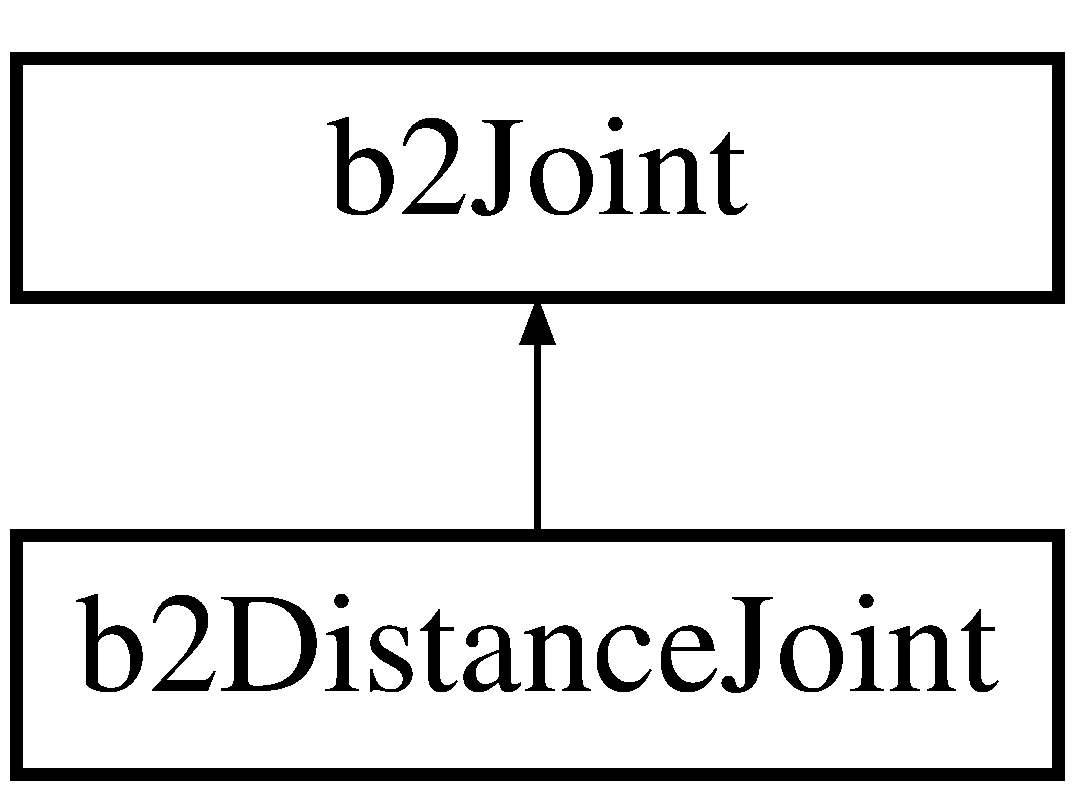
\includegraphics[height=2.000000cm]{classb2_distance_joint}
\end{center}
\end{figure}
\subsection*{Public Member Functions}
\begin{DoxyCompactItemize}
\item 
\hyperlink{structb2_vec2}{b2\+Vec2} \hyperlink{classb2_distance_joint_a66c1cb4deff1166c1dab67df6047a89c}{Get\+AnchorA} () const \hypertarget{classb2_distance_joint_a66c1cb4deff1166c1dab67df6047a89c}{}\label{classb2_distance_joint_a66c1cb4deff1166c1dab67df6047a89c}

\begin{DoxyCompactList}\small\item\em Get the anchor point on bodyA in world coordinates. \end{DoxyCompactList}\item 
\hyperlink{structb2_vec2}{b2\+Vec2} \hyperlink{classb2_distance_joint_afc58d85cf7cc5e23082cf469e1a1a067}{Get\+AnchorB} () const \hypertarget{classb2_distance_joint_afc58d85cf7cc5e23082cf469e1a1a067}{}\label{classb2_distance_joint_afc58d85cf7cc5e23082cf469e1a1a067}

\begin{DoxyCompactList}\small\item\em Get the anchor point on bodyB in world coordinates. \end{DoxyCompactList}\item 
\hyperlink{structb2_vec2}{b2\+Vec2} \hyperlink{classb2_distance_joint_a99413cc114b2f4dc4ce7693c062ce226}{Get\+Reaction\+Force} (float32 inv\+\_\+dt) const 
\item 
float32 \hyperlink{classb2_distance_joint_a8d65840abe0b398399020524852788fd}{Get\+Reaction\+Torque} (float32 inv\+\_\+dt) const 
\item 
const \hyperlink{structb2_vec2}{b2\+Vec2} \& \hyperlink{classb2_distance_joint_a75a41c40f21e48a6f9e947dd1dc46db4}{Get\+Local\+AnchorA} () const \hypertarget{classb2_distance_joint_a75a41c40f21e48a6f9e947dd1dc46db4}{}\label{classb2_distance_joint_a75a41c40f21e48a6f9e947dd1dc46db4}

\begin{DoxyCompactList}\small\item\em The local anchor point relative to bodyA\textquotesingle{}s origin. \end{DoxyCompactList}\item 
const \hyperlink{structb2_vec2}{b2\+Vec2} \& \hyperlink{classb2_distance_joint_a22e9572c8b3d1f0619b340738811c082}{Get\+Local\+AnchorB} () const \hypertarget{classb2_distance_joint_a22e9572c8b3d1f0619b340738811c082}{}\label{classb2_distance_joint_a22e9572c8b3d1f0619b340738811c082}

\begin{DoxyCompactList}\small\item\em The local anchor point relative to bodyB\textquotesingle{}s origin. \end{DoxyCompactList}\item 
void \hyperlink{classb2_distance_joint_a950a0f187ef691208e50de40ed9223fe}{Set\+Length} (float32 length)
\item 
float32 {\bfseries Get\+Length} () const \hypertarget{classb2_distance_joint_abd3c4bef772c179e4e1d39056335ddf8}{}\label{classb2_distance_joint_abd3c4bef772c179e4e1d39056335ddf8}

\item 
void \hyperlink{classb2_distance_joint_a1a12446f8926a1324edd481d9cd28c8a}{Set\+Frequency} (float32 hz)\hypertarget{classb2_distance_joint_a1a12446f8926a1324edd481d9cd28c8a}{}\label{classb2_distance_joint_a1a12446f8926a1324edd481d9cd28c8a}

\begin{DoxyCompactList}\small\item\em Set/get frequency in Hz. \end{DoxyCompactList}\item 
float32 {\bfseries Get\+Frequency} () const \hypertarget{classb2_distance_joint_a7b50b34335055ac815d9a1a38ac318f0}{}\label{classb2_distance_joint_a7b50b34335055ac815d9a1a38ac318f0}

\item 
void \hyperlink{classb2_distance_joint_a58da61301a1f1398a715107b76649923}{Set\+Damping\+Ratio} (float32 ratio)\hypertarget{classb2_distance_joint_a58da61301a1f1398a715107b76649923}{}\label{classb2_distance_joint_a58da61301a1f1398a715107b76649923}

\begin{DoxyCompactList}\small\item\em Set/get damping ratio. \end{DoxyCompactList}\item 
float32 {\bfseries Get\+Damping\+Ratio} () const \hypertarget{classb2_distance_joint_adb86c244721abd89abdd825bf17eb334}{}\label{classb2_distance_joint_adb86c244721abd89abdd825bf17eb334}

\item 
void \hyperlink{classb2_distance_joint_a3cebcc6ccce6f3c24432cd130fd53517}{Dump} ()\hypertarget{classb2_distance_joint_a3cebcc6ccce6f3c24432cd130fd53517}{}\label{classb2_distance_joint_a3cebcc6ccce6f3c24432cd130fd53517}

\begin{DoxyCompactList}\small\item\em Dump joint to dm\+Log. \end{DoxyCompactList}\end{DoxyCompactItemize}
\subsection*{Protected Member Functions}
\begin{DoxyCompactItemize}
\item 
{\bfseries b2\+Distance\+Joint} (const \hyperlink{structb2_distance_joint_def}{b2\+Distance\+Joint\+Def} $\ast$data)\hypertarget{classb2_distance_joint_ad2bb6de92a47868629a7397e23256454}{}\label{classb2_distance_joint_ad2bb6de92a47868629a7397e23256454}

\item 
void {\bfseries Init\+Velocity\+Constraints} (const \hyperlink{structb2_solver_data}{b2\+Solver\+Data} \&data)\hypertarget{classb2_distance_joint_a2062ea8f1c89f8ccc3f053bbc7211b12}{}\label{classb2_distance_joint_a2062ea8f1c89f8ccc3f053bbc7211b12}

\item 
void {\bfseries Solve\+Velocity\+Constraints} (const \hyperlink{structb2_solver_data}{b2\+Solver\+Data} \&data)\hypertarget{classb2_distance_joint_acbed5cd22ea4ccb44e4defe5f5aabe77}{}\label{classb2_distance_joint_acbed5cd22ea4ccb44e4defe5f5aabe77}

\item 
bool {\bfseries Solve\+Position\+Constraints} (const \hyperlink{structb2_solver_data}{b2\+Solver\+Data} \&data)\hypertarget{classb2_distance_joint_a1e8b3a477067cf9273fb78fbec1a1556}{}\label{classb2_distance_joint_a1e8b3a477067cf9273fb78fbec1a1556}

\end{DoxyCompactItemize}
\subsection*{Protected Attributes}
\begin{DoxyCompactItemize}
\item 
float32 {\bfseries m\+\_\+frequency\+Hz}\hypertarget{classb2_distance_joint_a90327211c322fa19ea7b8c58d0c27ea8}{}\label{classb2_distance_joint_a90327211c322fa19ea7b8c58d0c27ea8}

\item 
float32 {\bfseries m\+\_\+damping\+Ratio}\hypertarget{classb2_distance_joint_a1339d37474c5e66cd4f66d42e9440307}{}\label{classb2_distance_joint_a1339d37474c5e66cd4f66d42e9440307}

\item 
float32 {\bfseries m\+\_\+bias}\hypertarget{classb2_distance_joint_a91f829c0a95e0d5f204a512a506e29f0}{}\label{classb2_distance_joint_a91f829c0a95e0d5f204a512a506e29f0}

\item 
\hyperlink{structb2_vec2}{b2\+Vec2} {\bfseries m\+\_\+local\+AnchorA}\hypertarget{classb2_distance_joint_a297938125dd60175ab07921d5ecc43a8}{}\label{classb2_distance_joint_a297938125dd60175ab07921d5ecc43a8}

\item 
\hyperlink{structb2_vec2}{b2\+Vec2} {\bfseries m\+\_\+local\+AnchorB}\hypertarget{classb2_distance_joint_ad4c94a5b939ca4c3244bbab8544b880e}{}\label{classb2_distance_joint_ad4c94a5b939ca4c3244bbab8544b880e}

\item 
float32 {\bfseries m\+\_\+gamma}\hypertarget{classb2_distance_joint_a0ca755fb59c838c59d0ad162af8ab484}{}\label{classb2_distance_joint_a0ca755fb59c838c59d0ad162af8ab484}

\item 
float32 {\bfseries m\+\_\+impulse}\hypertarget{classb2_distance_joint_a75713391126d712f728d1a4f33b32a9f}{}\label{classb2_distance_joint_a75713391126d712f728d1a4f33b32a9f}

\item 
float32 {\bfseries m\+\_\+length}\hypertarget{classb2_distance_joint_a11b4805df34c380f53c3c346dd33da6c}{}\label{classb2_distance_joint_a11b4805df34c380f53c3c346dd33da6c}

\item 
int32 {\bfseries m\+\_\+indexA}\hypertarget{classb2_distance_joint_abcae00902974ed826f70aa119c2fd9de}{}\label{classb2_distance_joint_abcae00902974ed826f70aa119c2fd9de}

\item 
int32 {\bfseries m\+\_\+indexB}\hypertarget{classb2_distance_joint_a465f7f1b609bcb37be732cde71b6d8c8}{}\label{classb2_distance_joint_a465f7f1b609bcb37be732cde71b6d8c8}

\item 
\hyperlink{structb2_vec2}{b2\+Vec2} {\bfseries m\+\_\+u}\hypertarget{classb2_distance_joint_a78f45f86d3cf68701a0871e9de71fcd0}{}\label{classb2_distance_joint_a78f45f86d3cf68701a0871e9de71fcd0}

\item 
\hyperlink{structb2_vec2}{b2\+Vec2} {\bfseries m\+\_\+rA}\hypertarget{classb2_distance_joint_af046e84218d249f9234a16ecab95bac0}{}\label{classb2_distance_joint_af046e84218d249f9234a16ecab95bac0}

\item 
\hyperlink{structb2_vec2}{b2\+Vec2} {\bfseries m\+\_\+rB}\hypertarget{classb2_distance_joint_a70eab22cb7abeb825744f5dc3befa63a}{}\label{classb2_distance_joint_a70eab22cb7abeb825744f5dc3befa63a}

\item 
\hyperlink{structb2_vec2}{b2\+Vec2} {\bfseries m\+\_\+local\+CenterA}\hypertarget{classb2_distance_joint_a5793083e9ef396cf7a89d84481fe1308}{}\label{classb2_distance_joint_a5793083e9ef396cf7a89d84481fe1308}

\item 
\hyperlink{structb2_vec2}{b2\+Vec2} {\bfseries m\+\_\+local\+CenterB}\hypertarget{classb2_distance_joint_a4fa600dec301992ad1f23aaf25d592a5}{}\label{classb2_distance_joint_a4fa600dec301992ad1f23aaf25d592a5}

\item 
float32 {\bfseries m\+\_\+inv\+MassA}\hypertarget{classb2_distance_joint_a2564d44d59b589591a4214390617cc4e}{}\label{classb2_distance_joint_a2564d44d59b589591a4214390617cc4e}

\item 
float32 {\bfseries m\+\_\+inv\+MassB}\hypertarget{classb2_distance_joint_aeaea63222b01f95c71da5719feca4cbc}{}\label{classb2_distance_joint_aeaea63222b01f95c71da5719feca4cbc}

\item 
float32 {\bfseries m\+\_\+inv\+IA}\hypertarget{classb2_distance_joint_a9e9edc41d2bf14189a3eaeb19995b93a}{}\label{classb2_distance_joint_a9e9edc41d2bf14189a3eaeb19995b93a}

\item 
float32 {\bfseries m\+\_\+inv\+IB}\hypertarget{classb2_distance_joint_a250b46aa3fc17a363a6af9af5749ce1c}{}\label{classb2_distance_joint_a250b46aa3fc17a363a6af9af5749ce1c}

\item 
float32 {\bfseries m\+\_\+mass}\hypertarget{classb2_distance_joint_aee25a31b1096e91b55a29731cf67d99d}{}\label{classb2_distance_joint_aee25a31b1096e91b55a29731cf67d99d}

\end{DoxyCompactItemize}
\subsection*{Friends}
\begin{DoxyCompactItemize}
\item 
class {\bfseries b2\+Joint}\hypertarget{classb2_distance_joint_a54ade8ed3d794298108d7f4c4e4793fa}{}\label{classb2_distance_joint_a54ade8ed3d794298108d7f4c4e4793fa}

\end{DoxyCompactItemize}
\subsection*{Additional Inherited Members}


\subsection{Detailed Description}
A distance joint constrains two points on two bodies to remain at a fixed distance from each other. You can view this as a massless, rigid rod. 

\subsection{Member Function Documentation}
\index{b2\+Distance\+Joint@{b2\+Distance\+Joint}!Get\+Reaction\+Force@{Get\+Reaction\+Force}}
\index{Get\+Reaction\+Force@{Get\+Reaction\+Force}!b2\+Distance\+Joint@{b2\+Distance\+Joint}}
\subsubsection[{\texorpdfstring{Get\+Reaction\+Force(float32 inv\+\_\+dt) const }{GetReactionForce(float32 inv_dt) const }}]{\setlength{\rightskip}{0pt plus 5cm}{\bf b2\+Vec2} b2\+Distance\+Joint\+::\+Get\+Reaction\+Force (
\begin{DoxyParamCaption}
\item[{float32}]{inv\+\_\+dt}
\end{DoxyParamCaption}
) const\hspace{0.3cm}{\ttfamily [virtual]}}\hypertarget{classb2_distance_joint_a99413cc114b2f4dc4ce7693c062ce226}{}\label{classb2_distance_joint_a99413cc114b2f4dc4ce7693c062ce226}
Get the reaction force given the inverse time step. Unit is N. 

Implements \hyperlink{classb2_joint_a7ab58d67a56ff173957286558b08118a}{b2\+Joint}.

\index{b2\+Distance\+Joint@{b2\+Distance\+Joint}!Get\+Reaction\+Torque@{Get\+Reaction\+Torque}}
\index{Get\+Reaction\+Torque@{Get\+Reaction\+Torque}!b2\+Distance\+Joint@{b2\+Distance\+Joint}}
\subsubsection[{\texorpdfstring{Get\+Reaction\+Torque(float32 inv\+\_\+dt) const }{GetReactionTorque(float32 inv_dt) const }}]{\setlength{\rightskip}{0pt plus 5cm}float32 b2\+Distance\+Joint\+::\+Get\+Reaction\+Torque (
\begin{DoxyParamCaption}
\item[{float32}]{inv\+\_\+dt}
\end{DoxyParamCaption}
) const\hspace{0.3cm}{\ttfamily [virtual]}}\hypertarget{classb2_distance_joint_a8d65840abe0b398399020524852788fd}{}\label{classb2_distance_joint_a8d65840abe0b398399020524852788fd}
Get the reaction torque given the inverse time step. Unit is N$\ast$m. This is always zero for a distance joint. 

Implements \hyperlink{classb2_joint_a0b1e4fcdea490c49a9ac1133e5244566}{b2\+Joint}.

\index{b2\+Distance\+Joint@{b2\+Distance\+Joint}!Set\+Length@{Set\+Length}}
\index{Set\+Length@{Set\+Length}!b2\+Distance\+Joint@{b2\+Distance\+Joint}}
\subsubsection[{\texorpdfstring{Set\+Length(float32 length)}{SetLength(float32 length)}}]{\setlength{\rightskip}{0pt plus 5cm}void b2\+Distance\+Joint\+::\+Set\+Length (
\begin{DoxyParamCaption}
\item[{float32}]{length}
\end{DoxyParamCaption}
)\hspace{0.3cm}{\ttfamily [inline]}}\hypertarget{classb2_distance_joint_a950a0f187ef691208e50de40ed9223fe}{}\label{classb2_distance_joint_a950a0f187ef691208e50de40ed9223fe}
Set/get the natural length. Manipulating the length can lead to non-\/physical behavior when the frequency is zero. 

The documentation for this class was generated from the following file\+:\begin{DoxyCompactItemize}
\item 
Commun/\+Externe/\+Box2\+D/include/\+Box2\+D/\+Dynamics/\+Joints/b2\+Distance\+Joint.\+h\end{DoxyCompactItemize}

\hypertarget{structb2_distance_joint_def}{}\section{b2\+Distance\+Joint\+Def Struct Reference}
\label{structb2_distance_joint_def}\index{b2\+Distance\+Joint\+Def@{b2\+Distance\+Joint\+Def}}


{\ttfamily \#include $<$b2\+Distance\+Joint.\+h$>$}

Inheritance diagram for b2\+Distance\+Joint\+Def\+:\begin{figure}[H]
\begin{center}
\leavevmode
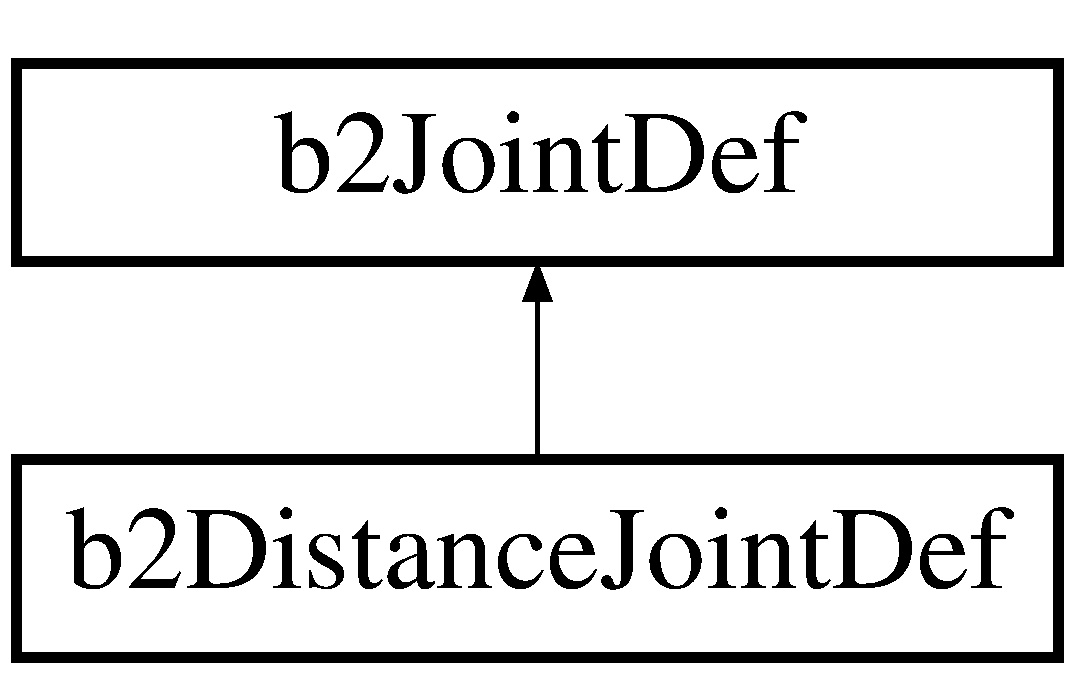
\includegraphics[height=2.000000cm]{structb2_distance_joint_def}
\end{center}
\end{figure}
\subsection*{Public Member Functions}
\begin{DoxyCompactItemize}
\item 
void \hyperlink{structb2_distance_joint_def_a99788a534638cc28cd1e44e0036503f0}{Initialize} (\hyperlink{classb2_body}{b2\+Body} $\ast$\hyperlink{structb2_joint_def_a8cd54c93da396be75a9788f2c6897f05}{bodyA}, \hyperlink{classb2_body}{b2\+Body} $\ast$\hyperlink{structb2_joint_def_aa4f4dee2fbcd12187b19506b60e68e3d}{bodyB}, const \hyperlink{structb2_vec2}{b2\+Vec2} \&anchorA, const \hyperlink{structb2_vec2}{b2\+Vec2} \&anchorB)
\end{DoxyCompactItemize}
\subsection*{Public Attributes}
\begin{DoxyCompactItemize}
\item 
\hyperlink{structb2_vec2}{b2\+Vec2} \hyperlink{structb2_distance_joint_def_a15c7a75fa277e2056bf1b44198658518}{local\+AnchorA}\hypertarget{structb2_distance_joint_def_a15c7a75fa277e2056bf1b44198658518}{}\label{structb2_distance_joint_def_a15c7a75fa277e2056bf1b44198658518}

\begin{DoxyCompactList}\small\item\em The local anchor point relative to bodyA\textquotesingle{}s origin. \end{DoxyCompactList}\item 
\hyperlink{structb2_vec2}{b2\+Vec2} \hyperlink{structb2_distance_joint_def_a3c8995be726238eee084af750442255c}{local\+AnchorB}\hypertarget{structb2_distance_joint_def_a3c8995be726238eee084af750442255c}{}\label{structb2_distance_joint_def_a3c8995be726238eee084af750442255c}

\begin{DoxyCompactList}\small\item\em The local anchor point relative to bodyB\textquotesingle{}s origin. \end{DoxyCompactList}\item 
float32 \hyperlink{structb2_distance_joint_def_ac2c48ad52de91c804c386c12c5bf3714}{length}\hypertarget{structb2_distance_joint_def_ac2c48ad52de91c804c386c12c5bf3714}{}\label{structb2_distance_joint_def_ac2c48ad52de91c804c386c12c5bf3714}

\begin{DoxyCompactList}\small\item\em The natural length between the anchor points. \end{DoxyCompactList}\item 
float32 \hyperlink{structb2_distance_joint_def_a35e2362bcb6c58734f95d0ac045863ea}{frequency\+Hz}
\item 
float32 \hyperlink{structb2_distance_joint_def_ad009b24ff211158eb4e1db4815a63b94}{damping\+Ratio}\hypertarget{structb2_distance_joint_def_ad009b24ff211158eb4e1db4815a63b94}{}\label{structb2_distance_joint_def_ad009b24ff211158eb4e1db4815a63b94}

\begin{DoxyCompactList}\small\item\em The damping ratio. 0 = no damping, 1 = critical damping. \end{DoxyCompactList}\end{DoxyCompactItemize}


\subsection{Detailed Description}
Distance joint definition. This requires defining an anchor point on both bodies and the non-\/zero length of the distance joint. The definition uses local anchor points so that the initial configuration can violate the constraint slightly. This helps when saving and loading a game. \begin{DoxyWarning}{Warning}
Do not use a zero or short length. 
\end{DoxyWarning}


\subsection{Member Function Documentation}
\index{b2\+Distance\+Joint\+Def@{b2\+Distance\+Joint\+Def}!Initialize@{Initialize}}
\index{Initialize@{Initialize}!b2\+Distance\+Joint\+Def@{b2\+Distance\+Joint\+Def}}
\subsubsection[{\texorpdfstring{Initialize(b2\+Body $\ast$body\+A, b2\+Body $\ast$body\+B, const b2\+Vec2 \&anchor\+A, const b2\+Vec2 \&anchor\+B)}{Initialize(b2Body *bodyA, b2Body *bodyB, const b2Vec2 &anchorA, const b2Vec2 &anchorB)}}]{\setlength{\rightskip}{0pt plus 5cm}void b2\+Distance\+Joint\+Def\+::\+Initialize (
\begin{DoxyParamCaption}
\item[{{\bf b2\+Body} $\ast$}]{bodyA, }
\item[{{\bf b2\+Body} $\ast$}]{bodyB, }
\item[{const {\bf b2\+Vec2} \&}]{anchorA, }
\item[{const {\bf b2\+Vec2} \&}]{anchorB}
\end{DoxyParamCaption}
)}\hypertarget{structb2_distance_joint_def_a99788a534638cc28cd1e44e0036503f0}{}\label{structb2_distance_joint_def_a99788a534638cc28cd1e44e0036503f0}
Initialize the bodies, anchors, and length using the world anchors. 

\subsection{Member Data Documentation}
\index{b2\+Distance\+Joint\+Def@{b2\+Distance\+Joint\+Def}!frequency\+Hz@{frequency\+Hz}}
\index{frequency\+Hz@{frequency\+Hz}!b2\+Distance\+Joint\+Def@{b2\+Distance\+Joint\+Def}}
\subsubsection[{\texorpdfstring{frequency\+Hz}{frequencyHz}}]{\setlength{\rightskip}{0pt plus 5cm}float32 b2\+Distance\+Joint\+Def\+::frequency\+Hz}\hypertarget{structb2_distance_joint_def_a35e2362bcb6c58734f95d0ac045863ea}{}\label{structb2_distance_joint_def_a35e2362bcb6c58734f95d0ac045863ea}
The mass-\/spring-\/damper frequency in Hertz. A value of 0 disables softness. 

The documentation for this struct was generated from the following file\+:\begin{DoxyCompactItemize}
\item 
Commun/\+Externe/\+Box2\+D/include/\+Box2\+D/\+Dynamics/\+Joints/b2\+Distance\+Joint.\+h\end{DoxyCompactItemize}

\hypertarget{structb2_distance_output}{}\section{b2\+Distance\+Output Struct Reference}
\label{structb2_distance_output}\index{b2\+Distance\+Output@{b2\+Distance\+Output}}


Output for b2\+Distance.  




{\ttfamily \#include $<$b2\+Distance.\+h$>$}

\subsection*{Public Attributes}
\begin{DoxyCompactItemize}
\item 
\hyperlink{structb2_vec2}{b2\+Vec2} \hyperlink{structb2_distance_output_a7e0f1f44a64e596dc7d37570c69eefce}{pointA}\hypertarget{structb2_distance_output_a7e0f1f44a64e596dc7d37570c69eefce}{}\label{structb2_distance_output_a7e0f1f44a64e596dc7d37570c69eefce}

\begin{DoxyCompactList}\small\item\em closest point on shapeA \end{DoxyCompactList}\item 
\hyperlink{structb2_vec2}{b2\+Vec2} \hyperlink{structb2_distance_output_aa85beca17337a506cd4a924d0c6f92cc}{pointB}\hypertarget{structb2_distance_output_aa85beca17337a506cd4a924d0c6f92cc}{}\label{structb2_distance_output_aa85beca17337a506cd4a924d0c6f92cc}

\begin{DoxyCompactList}\small\item\em closest point on shapeB \end{DoxyCompactList}\item 
float32 {\bfseries distance}\hypertarget{structb2_distance_output_ae67f480ff37d4ab732e6366f485c7f55}{}\label{structb2_distance_output_ae67f480ff37d4ab732e6366f485c7f55}

\item 
int32 \hyperlink{structb2_distance_output_ae2d4c84dd3d05ea4f4d20c91099ec8d5}{iterations}\hypertarget{structb2_distance_output_ae2d4c84dd3d05ea4f4d20c91099ec8d5}{}\label{structb2_distance_output_ae2d4c84dd3d05ea4f4d20c91099ec8d5}

\begin{DoxyCompactList}\small\item\em number of G\+JK iterations used \end{DoxyCompactList}\end{DoxyCompactItemize}


\subsection{Detailed Description}
Output for b2\+Distance. 

The documentation for this struct was generated from the following file\+:\begin{DoxyCompactItemize}
\item 
C\+:/\+Users/\+Bilal Itani/\+Desktop/inf2990-\/11/\+Cadriciel/\+Commun/\+Externe/\+Box2\+D/include/\+Box2\+D/\+Collision/b2\+Distance.\+h\end{DoxyCompactItemize}

\hypertarget{structb2_distance_proxy}{}\section{b2\+Distance\+Proxy Struct Reference}
\label{structb2_distance_proxy}\index{b2\+Distance\+Proxy@{b2\+Distance\+Proxy}}


{\ttfamily \#include $<$b2\+Distance.\+h$>$}

\subsection*{Public Member Functions}
\begin{DoxyCompactItemize}
\item 
void \hyperlink{structb2_distance_proxy_a80a59a9c9e952482a8fc6db4b883365d}{Set} (const \hyperlink{classb2_shape}{b2\+Shape} $\ast$shape, int32 index)
\item 
int32 \hyperlink{structb2_distance_proxy_ad763543846db0c220e6b0a29275d723e}{Get\+Support} (const \hyperlink{structb2_vec2}{b2\+Vec2} \&d) const \hypertarget{structb2_distance_proxy_ad763543846db0c220e6b0a29275d723e}{}\label{structb2_distance_proxy_ad763543846db0c220e6b0a29275d723e}

\begin{DoxyCompactList}\small\item\em Get the supporting vertex index in the given direction. \end{DoxyCompactList}\item 
const \hyperlink{structb2_vec2}{b2\+Vec2} \& \hyperlink{structb2_distance_proxy_ad98a909b9aee9e42ba184b1e6bd526ba}{Get\+Support\+Vertex} (const \hyperlink{structb2_vec2}{b2\+Vec2} \&d) const \hypertarget{structb2_distance_proxy_ad98a909b9aee9e42ba184b1e6bd526ba}{}\label{structb2_distance_proxy_ad98a909b9aee9e42ba184b1e6bd526ba}

\begin{DoxyCompactList}\small\item\em Get the supporting vertex in the given direction. \end{DoxyCompactList}\item 
int32 \hyperlink{structb2_distance_proxy_a43c51168f2829c55dacc8b9adbd90206}{Get\+Vertex\+Count} () const \hypertarget{structb2_distance_proxy_a43c51168f2829c55dacc8b9adbd90206}{}\label{structb2_distance_proxy_a43c51168f2829c55dacc8b9adbd90206}

\begin{DoxyCompactList}\small\item\em Get the vertex count. \end{DoxyCompactList}\item 
const \hyperlink{structb2_vec2}{b2\+Vec2} \& \hyperlink{structb2_distance_proxy_ac5ecae62c2a96afdf220074118c71a92}{Get\+Vertex} (int32 index) const \hypertarget{structb2_distance_proxy_ac5ecae62c2a96afdf220074118c71a92}{}\label{structb2_distance_proxy_ac5ecae62c2a96afdf220074118c71a92}

\begin{DoxyCompactList}\small\item\em Get a vertex by index. Used by b2\+Distance. \end{DoxyCompactList}\end{DoxyCompactItemize}
\subsection*{Public Attributes}
\begin{DoxyCompactItemize}
\item 
\hyperlink{structb2_vec2}{b2\+Vec2} {\bfseries m\+\_\+buffer} \mbox{[}2\mbox{]}\hypertarget{structb2_distance_proxy_a3fc5ebfa3d34ac66390b88f9277fb330}{}\label{structb2_distance_proxy_a3fc5ebfa3d34ac66390b88f9277fb330}

\item 
const \hyperlink{structb2_vec2}{b2\+Vec2} $\ast$ {\bfseries m\+\_\+vertices}\hypertarget{structb2_distance_proxy_abaf1495b8214b74d944b57170a762f32}{}\label{structb2_distance_proxy_abaf1495b8214b74d944b57170a762f32}

\item 
int32 {\bfseries m\+\_\+count}\hypertarget{structb2_distance_proxy_ae36efab1361bb1f94e32f9b956c6f1b3}{}\label{structb2_distance_proxy_ae36efab1361bb1f94e32f9b956c6f1b3}

\item 
float32 {\bfseries m\+\_\+radius}\hypertarget{structb2_distance_proxy_a459c93f35b1e62d583bd73d8c478ce89}{}\label{structb2_distance_proxy_a459c93f35b1e62d583bd73d8c478ce89}

\end{DoxyCompactItemize}


\subsection{Detailed Description}
A distance proxy is used by the G\+JK algorithm. It encapsulates any shape. 

\subsection{Member Function Documentation}
\index{b2\+Distance\+Proxy@{b2\+Distance\+Proxy}!Set@{Set}}
\index{Set@{Set}!b2\+Distance\+Proxy@{b2\+Distance\+Proxy}}
\subsubsection[{\texorpdfstring{Set(const b2\+Shape $\ast$shape, int32 index)}{Set(const b2Shape *shape, int32 index)}}]{\setlength{\rightskip}{0pt plus 5cm}void b2\+Distance\+Proxy\+::\+Set (
\begin{DoxyParamCaption}
\item[{const {\bf b2\+Shape} $\ast$}]{shape, }
\item[{int32}]{index}
\end{DoxyParamCaption}
)}\hypertarget{structb2_distance_proxy_a80a59a9c9e952482a8fc6db4b883365d}{}\label{structb2_distance_proxy_a80a59a9c9e952482a8fc6db4b883365d}
Initialize the proxy using the given shape. The shape must remain in scope while the proxy is in use. 

The documentation for this struct was generated from the following file\+:\begin{DoxyCompactItemize}
\item 
Cadriciel/\+Commun/\+Externe/\+Box2\+D/include/\+Box2\+D/\+Collision/b2\+Distance.\+h\end{DoxyCompactItemize}

\hypertarget{classb2_draw}{}\section{b2\+Draw Class Reference}
\label{classb2_draw}\index{b2\+Draw@{b2\+Draw}}


{\ttfamily \#include $<$b2\+Draw.\+h$>$}

\subsection*{Public Types}
\begin{DoxyCompactItemize}
\item 
enum \{ \\*
\hyperlink{classb2_draw_ae23c5d6c4f5230621f736593469cf7f2a1c8964c4f1fdc39e98b58ac38ecda1f9}{e\+\_\+shape\+Bit} = 0x0001, 
\hyperlink{classb2_draw_ae23c5d6c4f5230621f736593469cf7f2a241137a63679720c41a271c11681e2b3}{e\+\_\+joint\+Bit} = 0x0002, 
\hyperlink{classb2_draw_ae23c5d6c4f5230621f736593469cf7f2acdf1370108930182a45f39e7cc9b0cc7}{e\+\_\+aabb\+Bit} = 0x0004, 
\hyperlink{classb2_draw_ae23c5d6c4f5230621f736593469cf7f2ac86bb64ac65e555db28827407f2f2d43}{e\+\_\+pair\+Bit} = 0x0008, 
\\*
\hyperlink{classb2_draw_ae23c5d6c4f5230621f736593469cf7f2a7f1494d816479c7d23997a6c292cd8b6}{e\+\_\+center\+Of\+Mass\+Bit} = 0x0010
 \}
\end{DoxyCompactItemize}
\subsection*{Public Member Functions}
\begin{DoxyCompactItemize}
\item 
void \hyperlink{classb2_draw_ac2bbe31595478690e44de4ff1e7f347e}{Set\+Flags} (uint32 flags)\hypertarget{classb2_draw_ac2bbe31595478690e44de4ff1e7f347e}{}\label{classb2_draw_ac2bbe31595478690e44de4ff1e7f347e}

\begin{DoxyCompactList}\small\item\em Set the drawing flags. \end{DoxyCompactList}\item 
uint32 \hyperlink{classb2_draw_acadab1a12ec06541814f6118950aa998}{Get\+Flags} () const \hypertarget{classb2_draw_acadab1a12ec06541814f6118950aa998}{}\label{classb2_draw_acadab1a12ec06541814f6118950aa998}

\begin{DoxyCompactList}\small\item\em Get the drawing flags. \end{DoxyCompactList}\item 
void \hyperlink{classb2_draw_acc2fd4648ee0a65574770c64528f7166}{Append\+Flags} (uint32 flags)\hypertarget{classb2_draw_acc2fd4648ee0a65574770c64528f7166}{}\label{classb2_draw_acc2fd4648ee0a65574770c64528f7166}

\begin{DoxyCompactList}\small\item\em Append flags to the current flags. \end{DoxyCompactList}\item 
void \hyperlink{classb2_draw_afc240b71f4ba8c17440d6ed526d4e22e}{Clear\+Flags} (uint32 flags)\hypertarget{classb2_draw_afc240b71f4ba8c17440d6ed526d4e22e}{}\label{classb2_draw_afc240b71f4ba8c17440d6ed526d4e22e}

\begin{DoxyCompactList}\small\item\em Clear flags from the current flags. \end{DoxyCompactList}\item 
virtual void \hyperlink{classb2_draw_acd5427d1d2e7d19f1b34ad3620134d28}{Draw\+Polygon} (const \hyperlink{structb2_vec2}{b2\+Vec2} $\ast$vertices, int32 vertex\+Count, const \hyperlink{structb2_color}{b2\+Color} \&color)=0\hypertarget{classb2_draw_acd5427d1d2e7d19f1b34ad3620134d28}{}\label{classb2_draw_acd5427d1d2e7d19f1b34ad3620134d28}

\begin{DoxyCompactList}\small\item\em Draw a closed polygon provided in C\+CW order. \end{DoxyCompactList}\item 
virtual void \hyperlink{classb2_draw_a76f2d67de0781a32cab116278c5c9eea}{Draw\+Solid\+Polygon} (const \hyperlink{structb2_vec2}{b2\+Vec2} $\ast$vertices, int32 vertex\+Count, const \hyperlink{structb2_color}{b2\+Color} \&color)=0\hypertarget{classb2_draw_a76f2d67de0781a32cab116278c5c9eea}{}\label{classb2_draw_a76f2d67de0781a32cab116278c5c9eea}

\begin{DoxyCompactList}\small\item\em Draw a solid closed polygon provided in C\+CW order. \end{DoxyCompactList}\item 
virtual void \hyperlink{classb2_draw_ae2effe9bca87c8d7cb90e860d13b7e9e}{Draw\+Circle} (const \hyperlink{structb2_vec2}{b2\+Vec2} \&center, float32 radius, const \hyperlink{structb2_color}{b2\+Color} \&color)=0\hypertarget{classb2_draw_ae2effe9bca87c8d7cb90e860d13b7e9e}{}\label{classb2_draw_ae2effe9bca87c8d7cb90e860d13b7e9e}

\begin{DoxyCompactList}\small\item\em Draw a circle. \end{DoxyCompactList}\item 
virtual void \hyperlink{classb2_draw_a775a1d0472c5980d597904c7b596a0a6}{Draw\+Solid\+Circle} (const \hyperlink{structb2_vec2}{b2\+Vec2} \&center, float32 radius, const \hyperlink{structb2_vec2}{b2\+Vec2} \&axis, const \hyperlink{structb2_color}{b2\+Color} \&color)=0\hypertarget{classb2_draw_a775a1d0472c5980d597904c7b596a0a6}{}\label{classb2_draw_a775a1d0472c5980d597904c7b596a0a6}

\begin{DoxyCompactList}\small\item\em Draw a solid circle. \end{DoxyCompactList}\item 
virtual void \hyperlink{classb2_draw_a1de5aaf50db875d1c644c596832af57d}{Draw\+Segment} (const \hyperlink{structb2_vec2}{b2\+Vec2} \&p1, const \hyperlink{structb2_vec2}{b2\+Vec2} \&p2, const \hyperlink{structb2_color}{b2\+Color} \&color)=0\hypertarget{classb2_draw_a1de5aaf50db875d1c644c596832af57d}{}\label{classb2_draw_a1de5aaf50db875d1c644c596832af57d}

\begin{DoxyCompactList}\small\item\em Draw a line segment. \end{DoxyCompactList}\item 
virtual void \hyperlink{classb2_draw_ade698123482a491a7a61fa1fe4d3a4f4}{Draw\+Transform} (const \hyperlink{structb2_transform}{b2\+Transform} \&xf)=0
\end{DoxyCompactItemize}
\subsection*{Protected Attributes}
\begin{DoxyCompactItemize}
\item 
uint32 {\bfseries m\+\_\+draw\+Flags}\hypertarget{classb2_draw_adfcd2e54ddaec6f0a111ec1a1cf8b9a0}{}\label{classb2_draw_adfcd2e54ddaec6f0a111ec1a1cf8b9a0}

\end{DoxyCompactItemize}


\subsection{Detailed Description}
Implement and register this class with a \hyperlink{classb2_world}{b2\+World} to provide debug drawing of physics entities in your game. 

\subsection{Member Enumeration Documentation}
\subsubsection[{\texorpdfstring{anonymous enum}{anonymous enum}}]{\setlength{\rightskip}{0pt plus 5cm}anonymous enum}\hypertarget{classb2_draw_ae23c5d6c4f5230621f736593469cf7f2}{}\label{classb2_draw_ae23c5d6c4f5230621f736593469cf7f2}
\begin{Desc}
\item[Enumerator]\par
\begin{description}
\index{e\+\_\+shape\+Bit@{e\+\_\+shape\+Bit}!b2\+Draw@{b2\+Draw}}\index{b2\+Draw@{b2\+Draw}!e\+\_\+shape\+Bit@{e\+\_\+shape\+Bit}}\item[{\em 
e\+\_\+shape\+Bit\hypertarget{classb2_draw_ae23c5d6c4f5230621f736593469cf7f2a1c8964c4f1fdc39e98b58ac38ecda1f9}{}\label{classb2_draw_ae23c5d6c4f5230621f736593469cf7f2a1c8964c4f1fdc39e98b58ac38ecda1f9}
}]draw shapes \index{e\+\_\+joint\+Bit@{e\+\_\+joint\+Bit}!b2\+Draw@{b2\+Draw}}\index{b2\+Draw@{b2\+Draw}!e\+\_\+joint\+Bit@{e\+\_\+joint\+Bit}}\item[{\em 
e\+\_\+joint\+Bit\hypertarget{classb2_draw_ae23c5d6c4f5230621f736593469cf7f2a241137a63679720c41a271c11681e2b3}{}\label{classb2_draw_ae23c5d6c4f5230621f736593469cf7f2a241137a63679720c41a271c11681e2b3}
}]draw joint connections \index{e\+\_\+aabb\+Bit@{e\+\_\+aabb\+Bit}!b2\+Draw@{b2\+Draw}}\index{b2\+Draw@{b2\+Draw}!e\+\_\+aabb\+Bit@{e\+\_\+aabb\+Bit}}\item[{\em 
e\+\_\+aabb\+Bit\hypertarget{classb2_draw_ae23c5d6c4f5230621f736593469cf7f2acdf1370108930182a45f39e7cc9b0cc7}{}\label{classb2_draw_ae23c5d6c4f5230621f736593469cf7f2acdf1370108930182a45f39e7cc9b0cc7}
}]draw axis aligned bounding boxes \index{e\+\_\+pair\+Bit@{e\+\_\+pair\+Bit}!b2\+Draw@{b2\+Draw}}\index{b2\+Draw@{b2\+Draw}!e\+\_\+pair\+Bit@{e\+\_\+pair\+Bit}}\item[{\em 
e\+\_\+pair\+Bit\hypertarget{classb2_draw_ae23c5d6c4f5230621f736593469cf7f2ac86bb64ac65e555db28827407f2f2d43}{}\label{classb2_draw_ae23c5d6c4f5230621f736593469cf7f2ac86bb64ac65e555db28827407f2f2d43}
}]draw broad-\/phase pairs \index{e\+\_\+center\+Of\+Mass\+Bit@{e\+\_\+center\+Of\+Mass\+Bit}!b2\+Draw@{b2\+Draw}}\index{b2\+Draw@{b2\+Draw}!e\+\_\+center\+Of\+Mass\+Bit@{e\+\_\+center\+Of\+Mass\+Bit}}\item[{\em 
e\+\_\+center\+Of\+Mass\+Bit\hypertarget{classb2_draw_ae23c5d6c4f5230621f736593469cf7f2a7f1494d816479c7d23997a6c292cd8b6}{}\label{classb2_draw_ae23c5d6c4f5230621f736593469cf7f2a7f1494d816479c7d23997a6c292cd8b6}
}]draw center of mass frame \end{description}
\end{Desc}


\subsection{Member Function Documentation}
\index{b2\+Draw@{b2\+Draw}!Draw\+Transform@{Draw\+Transform}}
\index{Draw\+Transform@{Draw\+Transform}!b2\+Draw@{b2\+Draw}}
\subsubsection[{\texorpdfstring{Draw\+Transform(const b2\+Transform \&xf)=0}{DrawTransform(const b2Transform &xf)=0}}]{\setlength{\rightskip}{0pt plus 5cm}virtual void b2\+Draw\+::\+Draw\+Transform (
\begin{DoxyParamCaption}
\item[{const {\bf b2\+Transform} \&}]{xf}
\end{DoxyParamCaption}
)\hspace{0.3cm}{\ttfamily [pure virtual]}}\hypertarget{classb2_draw_ade698123482a491a7a61fa1fe4d3a4f4}{}\label{classb2_draw_ade698123482a491a7a61fa1fe4d3a4f4}
Draw a transform. Choose your own length scale. 
\begin{DoxyParams}{Parameters}
{\em xf} & a transform. \\
\hline
\end{DoxyParams}


The documentation for this class was generated from the following file\+:\begin{DoxyCompactItemize}
\item 
C\+:/\+Users/\+Bilal Itani/\+Desktop/inf2990-\/11/\+Cadriciel/\+Commun/\+Externe/\+Box2\+D/include/\+Box2\+D/\+Common/b2\+Draw.\+h\end{DoxyCompactItemize}

\hypertarget{classb2_dynamic_tree}{}\section{b2\+Dynamic\+Tree Class Reference}
\label{classb2_dynamic_tree}\index{b2\+Dynamic\+Tree@{b2\+Dynamic\+Tree}}


{\ttfamily \#include $<$b2\+Dynamic\+Tree.\+h$>$}

\subsection*{Public Member Functions}
\begin{DoxyCompactItemize}
\item 
\hyperlink{classb2_dynamic_tree_a8af64cf6a1566fa4c5b5c9683bd937d9}{b2\+Dynamic\+Tree} ()\hypertarget{classb2_dynamic_tree_a8af64cf6a1566fa4c5b5c9683bd937d9}{}\label{classb2_dynamic_tree_a8af64cf6a1566fa4c5b5c9683bd937d9}

\begin{DoxyCompactList}\small\item\em Constructing the tree initializes the node pool. \end{DoxyCompactList}\item 
\hyperlink{classb2_dynamic_tree_a9060565fc63b4dd87d9560775c076786}{$\sim$b2\+Dynamic\+Tree} ()\hypertarget{classb2_dynamic_tree_a9060565fc63b4dd87d9560775c076786}{}\label{classb2_dynamic_tree_a9060565fc63b4dd87d9560775c076786}

\begin{DoxyCompactList}\small\item\em Destroy the tree, freeing the node pool. \end{DoxyCompactList}\item 
int32 \hyperlink{classb2_dynamic_tree_ae44676f12977dada46037da47fc7ffbf}{Create\+Proxy} (const \hyperlink{structb2_a_a_b_b}{b2\+A\+A\+BB} \&aabb, void $\ast$user\+Data)\hypertarget{classb2_dynamic_tree_ae44676f12977dada46037da47fc7ffbf}{}\label{classb2_dynamic_tree_ae44676f12977dada46037da47fc7ffbf}

\begin{DoxyCompactList}\small\item\em Create a proxy. Provide a tight fitting A\+A\+BB and a user\+Data pointer. \end{DoxyCompactList}\item 
void \hyperlink{classb2_dynamic_tree_a62aa451e7d7fe029818dd05f76ea9cdc}{Destroy\+Proxy} (int32 proxy\+Id)\hypertarget{classb2_dynamic_tree_a62aa451e7d7fe029818dd05f76ea9cdc}{}\label{classb2_dynamic_tree_a62aa451e7d7fe029818dd05f76ea9cdc}

\begin{DoxyCompactList}\small\item\em Destroy a proxy. This asserts if the id is invalid. \end{DoxyCompactList}\item 
bool \hyperlink{classb2_dynamic_tree_a7748252811f3c575015931399cbe4daa}{Move\+Proxy} (int32 proxy\+Id, const \hyperlink{structb2_a_a_b_b}{b2\+A\+A\+BB} \&aabb1, const \hyperlink{structb2_vec2}{b2\+Vec2} \&displacement)
\item 
void $\ast$ \hyperlink{classb2_dynamic_tree_a44ab57dce3c42b0a5847a64e489a71ce}{Get\+User\+Data} (int32 proxy\+Id) const 
\item 
const \hyperlink{structb2_a_a_b_b}{b2\+A\+A\+BB} \& \hyperlink{classb2_dynamic_tree_adf4676b1c34a57b4451bcbeaebe65687}{Get\+Fat\+A\+A\+BB} (int32 proxy\+Id) const \hypertarget{classb2_dynamic_tree_adf4676b1c34a57b4451bcbeaebe65687}{}\label{classb2_dynamic_tree_adf4676b1c34a57b4451bcbeaebe65687}

\begin{DoxyCompactList}\small\item\em Get the fat A\+A\+BB for a proxy. \end{DoxyCompactList}\item 
{\footnotesize template$<$typename T $>$ }\\void \hyperlink{classb2_dynamic_tree_adf70aee89b4692fc79d65b1f54308585}{Query} (T $\ast$callback, const \hyperlink{structb2_a_a_b_b}{b2\+A\+A\+BB} \&aabb) const 
\item 
{\footnotesize template$<$typename T $>$ }\\void \hyperlink{classb2_dynamic_tree_abd7a5c6a5bc109dbbdb0ec3aae039648}{Ray\+Cast} (T $\ast$callback, const \hyperlink{structb2_ray_cast_input}{b2\+Ray\+Cast\+Input} \&input) const 
\item 
void \hyperlink{classb2_dynamic_tree_abfac96c615b08406cba3e53b39800f1c}{Validate} () const \hypertarget{classb2_dynamic_tree_abfac96c615b08406cba3e53b39800f1c}{}\label{classb2_dynamic_tree_abfac96c615b08406cba3e53b39800f1c}

\begin{DoxyCompactList}\small\item\em Validate this tree. For testing. \end{DoxyCompactList}\item 
int32 \hyperlink{classb2_dynamic_tree_add7e09cdf279e7c0031da9dfd4cdf4db}{Get\+Height} () const 
\item 
int32 \hyperlink{classb2_dynamic_tree_ae02c45d1a68b42e59d170438ddbb7977}{Get\+Max\+Balance} () const 
\item 
float32 \hyperlink{classb2_dynamic_tree_ad78282a720c451e032b43c34cba02f1a}{Get\+Area\+Ratio} () const \hypertarget{classb2_dynamic_tree_ad78282a720c451e032b43c34cba02f1a}{}\label{classb2_dynamic_tree_ad78282a720c451e032b43c34cba02f1a}

\begin{DoxyCompactList}\small\item\em Get the ratio of the sum of the node areas to the root area. \end{DoxyCompactList}\item 
void \hyperlink{classb2_dynamic_tree_abd146017cfec1cf5ea7b87331f30a3ff}{Rebuild\+Bottom\+Up} ()\hypertarget{classb2_dynamic_tree_abd146017cfec1cf5ea7b87331f30a3ff}{}\label{classb2_dynamic_tree_abd146017cfec1cf5ea7b87331f30a3ff}

\begin{DoxyCompactList}\small\item\em Build an optimal tree. Very expensive. For testing. \end{DoxyCompactList}\item 
void \hyperlink{classb2_dynamic_tree_af37ddfed6a5da97d5a78b09918d19ceb}{Shift\+Origin} (const \hyperlink{structb2_vec2}{b2\+Vec2} \&new\+Origin)
\end{DoxyCompactItemize}


\subsection{Detailed Description}
A dynamic A\+A\+BB tree broad-\/phase, inspired by Nathanael Presson\textquotesingle{}s bt\+Dbvt. A dynamic tree arranges data in a binary tree to accelerate queries such as volume queries and ray casts. Leafs are proxies with an A\+A\+BB. In the tree we expand the proxy A\+A\+BB by b2\+\_\+fat\+A\+A\+B\+B\+Factor so that the proxy A\+A\+BB is bigger than the client object. This allows the client object to move by small amounts without triggering a tree update.

Nodes are pooled and relocatable, so we use node indices rather than pointers. 

\subsection{Member Function Documentation}
\index{b2\+Dynamic\+Tree@{b2\+Dynamic\+Tree}!Get\+Height@{Get\+Height}}
\index{Get\+Height@{Get\+Height}!b2\+Dynamic\+Tree@{b2\+Dynamic\+Tree}}
\subsubsection[{\texorpdfstring{Get\+Height() const }{GetHeight() const }}]{\setlength{\rightskip}{0pt plus 5cm}int32 b2\+Dynamic\+Tree\+::\+Get\+Height (
\begin{DoxyParamCaption}
{}
\end{DoxyParamCaption}
) const}\hypertarget{classb2_dynamic_tree_add7e09cdf279e7c0031da9dfd4cdf4db}{}\label{classb2_dynamic_tree_add7e09cdf279e7c0031da9dfd4cdf4db}
Compute the height of the binary tree in O(\+N) time. Should not be called often. \index{b2\+Dynamic\+Tree@{b2\+Dynamic\+Tree}!Get\+Max\+Balance@{Get\+Max\+Balance}}
\index{Get\+Max\+Balance@{Get\+Max\+Balance}!b2\+Dynamic\+Tree@{b2\+Dynamic\+Tree}}
\subsubsection[{\texorpdfstring{Get\+Max\+Balance() const }{GetMaxBalance() const }}]{\setlength{\rightskip}{0pt plus 5cm}int32 b2\+Dynamic\+Tree\+::\+Get\+Max\+Balance (
\begin{DoxyParamCaption}
{}
\end{DoxyParamCaption}
) const}\hypertarget{classb2_dynamic_tree_ae02c45d1a68b42e59d170438ddbb7977}{}\label{classb2_dynamic_tree_ae02c45d1a68b42e59d170438ddbb7977}
Get the maximum balance of an node in the tree. The balance is the difference in height of the two children of a node. \index{b2\+Dynamic\+Tree@{b2\+Dynamic\+Tree}!Get\+User\+Data@{Get\+User\+Data}}
\index{Get\+User\+Data@{Get\+User\+Data}!b2\+Dynamic\+Tree@{b2\+Dynamic\+Tree}}
\subsubsection[{\texorpdfstring{Get\+User\+Data(int32 proxy\+Id) const }{GetUserData(int32 proxyId) const }}]{\setlength{\rightskip}{0pt plus 5cm}void $\ast$ b2\+Dynamic\+Tree\+::\+Get\+User\+Data (
\begin{DoxyParamCaption}
\item[{int32}]{proxy\+Id}
\end{DoxyParamCaption}
) const\hspace{0.3cm}{\ttfamily [inline]}}\hypertarget{classb2_dynamic_tree_a44ab57dce3c42b0a5847a64e489a71ce}{}\label{classb2_dynamic_tree_a44ab57dce3c42b0a5847a64e489a71ce}
Get proxy user data. \begin{DoxyReturn}{Returns}
the proxy user data or 0 if the id is invalid. 
\end{DoxyReturn}
\index{b2\+Dynamic\+Tree@{b2\+Dynamic\+Tree}!Move\+Proxy@{Move\+Proxy}}
\index{Move\+Proxy@{Move\+Proxy}!b2\+Dynamic\+Tree@{b2\+Dynamic\+Tree}}
\subsubsection[{\texorpdfstring{Move\+Proxy(int32 proxy\+Id, const b2\+A\+A\+B\+B \&aabb1, const b2\+Vec2 \&displacement)}{MoveProxy(int32 proxyId, const b2AABB &aabb1, const b2Vec2 &displacement)}}]{\setlength{\rightskip}{0pt plus 5cm}bool b2\+Dynamic\+Tree\+::\+Move\+Proxy (
\begin{DoxyParamCaption}
\item[{int32}]{proxy\+Id, }
\item[{const {\bf b2\+A\+A\+BB} \&}]{aabb1, }
\item[{const {\bf b2\+Vec2} \&}]{displacement}
\end{DoxyParamCaption}
)}\hypertarget{classb2_dynamic_tree_a7748252811f3c575015931399cbe4daa}{}\label{classb2_dynamic_tree_a7748252811f3c575015931399cbe4daa}
Move a proxy with a swepted A\+A\+BB. If the proxy has moved outside of its fattened A\+A\+BB, then the proxy is removed from the tree and re-\/inserted. Otherwise the function returns immediately. \begin{DoxyReturn}{Returns}
true if the proxy was re-\/inserted. 
\end{DoxyReturn}
\index{b2\+Dynamic\+Tree@{b2\+Dynamic\+Tree}!Query@{Query}}
\index{Query@{Query}!b2\+Dynamic\+Tree@{b2\+Dynamic\+Tree}}
\subsubsection[{\texorpdfstring{Query(\+T $\ast$callback, const b2\+A\+A\+B\+B \&aabb) const }{Query(T *callback, const b2AABB &aabb) const }}]{\setlength{\rightskip}{0pt plus 5cm}template$<$typename T $>$ void b2\+Dynamic\+Tree\+::\+Query (
\begin{DoxyParamCaption}
\item[{T $\ast$}]{callback, }
\item[{const {\bf b2\+A\+A\+BB} \&}]{aabb}
\end{DoxyParamCaption}
) const\hspace{0.3cm}{\ttfamily [inline]}}\hypertarget{classb2_dynamic_tree_adf70aee89b4692fc79d65b1f54308585}{}\label{classb2_dynamic_tree_adf70aee89b4692fc79d65b1f54308585}
Query an A\+A\+BB for overlapping proxies. The callback class is called for each proxy that overlaps the supplied A\+A\+BB. \index{b2\+Dynamic\+Tree@{b2\+Dynamic\+Tree}!Ray\+Cast@{Ray\+Cast}}
\index{Ray\+Cast@{Ray\+Cast}!b2\+Dynamic\+Tree@{b2\+Dynamic\+Tree}}
\subsubsection[{\texorpdfstring{Ray\+Cast(\+T $\ast$callback, const b2\+Ray\+Cast\+Input \&input) const }{RayCast(T *callback, const b2RayCastInput &input) const }}]{\setlength{\rightskip}{0pt plus 5cm}template$<$typename T $>$ void b2\+Dynamic\+Tree\+::\+Ray\+Cast (
\begin{DoxyParamCaption}
\item[{T $\ast$}]{callback, }
\item[{const {\bf b2\+Ray\+Cast\+Input} \&}]{input}
\end{DoxyParamCaption}
) const\hspace{0.3cm}{\ttfamily [inline]}}\hypertarget{classb2_dynamic_tree_abd7a5c6a5bc109dbbdb0ec3aae039648}{}\label{classb2_dynamic_tree_abd7a5c6a5bc109dbbdb0ec3aae039648}
Ray-\/cast against the proxies in the tree. This relies on the callback to perform a exact ray-\/cast in the case were the proxy contains a shape. The callback also performs the any collision filtering. This has performance roughly equal to k $\ast$ log(n), where k is the number of collisions and n is the number of proxies in the tree. 
\begin{DoxyParams}{Parameters}
{\em input} & the ray-\/cast input data. The ray extends from p1 to p1 + max\+Fraction $\ast$ (p2 -\/ p1). \\
\hline
{\em callback} & a callback class that is called for each proxy that is hit by the ray. \\
\hline
\end{DoxyParams}
\index{b2\+Dynamic\+Tree@{b2\+Dynamic\+Tree}!Shift\+Origin@{Shift\+Origin}}
\index{Shift\+Origin@{Shift\+Origin}!b2\+Dynamic\+Tree@{b2\+Dynamic\+Tree}}
\subsubsection[{\texorpdfstring{Shift\+Origin(const b2\+Vec2 \&new\+Origin)}{ShiftOrigin(const b2Vec2 &newOrigin)}}]{\setlength{\rightskip}{0pt plus 5cm}void b2\+Dynamic\+Tree\+::\+Shift\+Origin (
\begin{DoxyParamCaption}
\item[{const {\bf b2\+Vec2} \&}]{new\+Origin}
\end{DoxyParamCaption}
)}\hypertarget{classb2_dynamic_tree_af37ddfed6a5da97d5a78b09918d19ceb}{}\label{classb2_dynamic_tree_af37ddfed6a5da97d5a78b09918d19ceb}
Shift the world origin. Useful for large worlds. The shift formula is\+: position -\/= new\+Origin 
\begin{DoxyParams}{Parameters}
{\em new\+Origin} & the new origin with respect to the old origin \\
\hline
\end{DoxyParams}


The documentation for this class was generated from the following file\+:\begin{DoxyCompactItemize}
\item 
Cadriciel/\+Commun/\+Externe/\+Box2\+D/include/\+Box2\+D/\+Collision/b2\+Dynamic\+Tree.\+h\end{DoxyCompactItemize}

\hypertarget{classb2_edge_and_circle_contact}{}\section{b2\+Edge\+And\+Circle\+Contact Class Reference}
\label{classb2_edge_and_circle_contact}\index{b2\+Edge\+And\+Circle\+Contact@{b2\+Edge\+And\+Circle\+Contact}}
Inheritance diagram for b2\+Edge\+And\+Circle\+Contact\+:\begin{figure}[H]
\begin{center}
\leavevmode
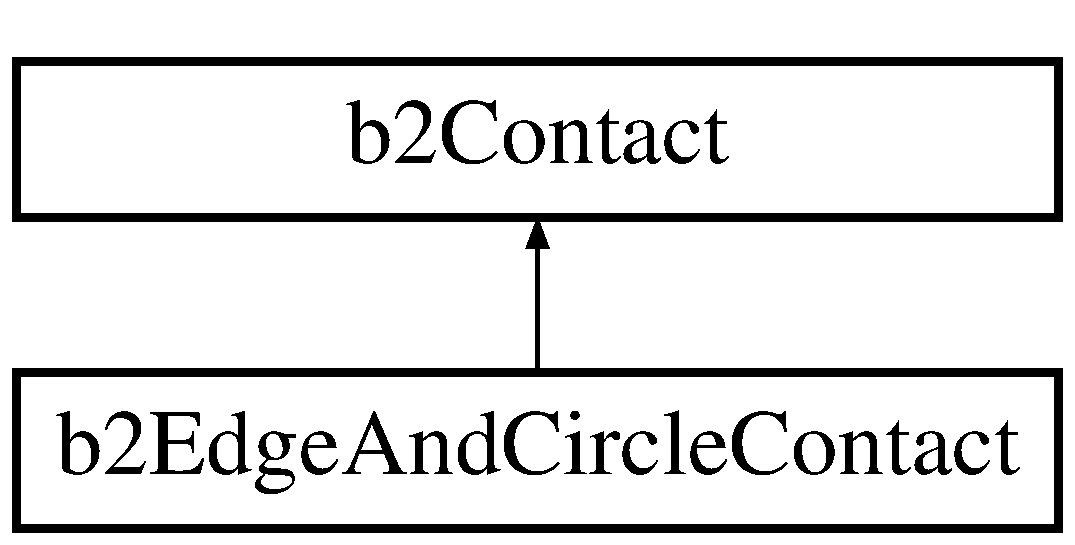
\includegraphics[height=2.000000cm]{classb2_edge_and_circle_contact}
\end{center}
\end{figure}
\subsection*{Public Member Functions}
\begin{DoxyCompactItemize}
\item 
{\bfseries b2\+Edge\+And\+Circle\+Contact} (\hyperlink{classb2_fixture}{b2\+Fixture} $\ast$fixtureA, \hyperlink{classb2_fixture}{b2\+Fixture} $\ast$fixtureB)\hypertarget{classb2_edge_and_circle_contact_a9de91d6afe4d2407f679b2ccaded9c02}{}\label{classb2_edge_and_circle_contact_a9de91d6afe4d2407f679b2ccaded9c02}

\item 
void \hyperlink{classb2_edge_and_circle_contact_a8f083c4c7c7da83eae38975164fd1452}{Evaluate} (\hyperlink{structb2_manifold}{b2\+Manifold} $\ast$manifold, const \hyperlink{structb2_transform}{b2\+Transform} \&xfA, const \hyperlink{structb2_transform}{b2\+Transform} \&xfB)\hypertarget{classb2_edge_and_circle_contact_a8f083c4c7c7da83eae38975164fd1452}{}\label{classb2_edge_and_circle_contact_a8f083c4c7c7da83eae38975164fd1452}

\begin{DoxyCompactList}\small\item\em Evaluate this contact with your own manifold and transforms. \end{DoxyCompactList}\end{DoxyCompactItemize}
\subsection*{Static Public Member Functions}
\begin{DoxyCompactItemize}
\item 
static \hyperlink{classb2_contact}{b2\+Contact} $\ast$ {\bfseries Create} (\hyperlink{classb2_fixture}{b2\+Fixture} $\ast$fixtureA, int32 indexA, \hyperlink{classb2_fixture}{b2\+Fixture} $\ast$fixtureB, int32 indexB, \hyperlink{classb2_block_allocator}{b2\+Block\+Allocator} $\ast$allocator)\hypertarget{classb2_edge_and_circle_contact_ad253e184d26e54c60fa874b329f9737e}{}\label{classb2_edge_and_circle_contact_ad253e184d26e54c60fa874b329f9737e}

\item 
static void {\bfseries Destroy} (\hyperlink{classb2_contact}{b2\+Contact} $\ast$contact, \hyperlink{classb2_block_allocator}{b2\+Block\+Allocator} $\ast$allocator)\hypertarget{classb2_edge_and_circle_contact_a7d77dd43691dad8d813450aefdb1e11e}{}\label{classb2_edge_and_circle_contact_a7d77dd43691dad8d813450aefdb1e11e}

\end{DoxyCompactItemize}
\subsection*{Additional Inherited Members}


The documentation for this class was generated from the following file\+:\begin{DoxyCompactItemize}
\item 
C\+:/\+Users/\+Bilal Itani/\+Desktop/inf2990-\/11/\+Cadriciel/\+Commun/\+Externe/\+Box2\+D/include/\+Box2\+D/\+Dynamics/\+Contacts/b2\+Edge\+And\+Circle\+Contact.\+h\end{DoxyCompactItemize}

\hypertarget{classb2_edge_and_polygon_contact}{}\section{b2\+Edge\+And\+Polygon\+Contact Class Reference}
\label{classb2_edge_and_polygon_contact}\index{b2\+Edge\+And\+Polygon\+Contact@{b2\+Edge\+And\+Polygon\+Contact}}
Inheritance diagram for b2\+Edge\+And\+Polygon\+Contact\+:\begin{figure}[H]
\begin{center}
\leavevmode
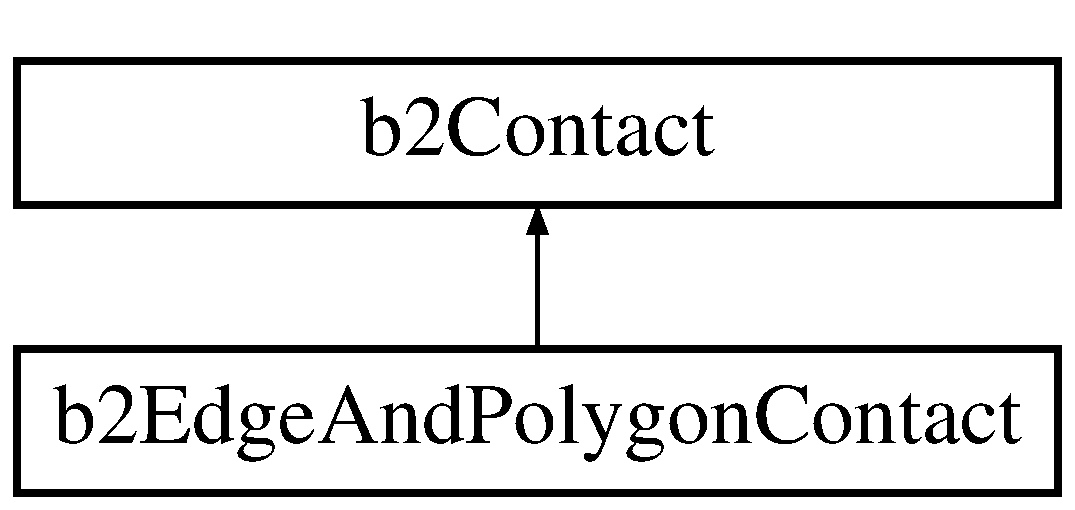
\includegraphics[height=2.000000cm]{classb2_edge_and_polygon_contact}
\end{center}
\end{figure}
\subsection*{Public Member Functions}
\begin{DoxyCompactItemize}
\item 
{\bfseries b2\+Edge\+And\+Polygon\+Contact} (\hyperlink{classb2_fixture}{b2\+Fixture} $\ast$fixtureA, \hyperlink{classb2_fixture}{b2\+Fixture} $\ast$fixtureB)\hypertarget{classb2_edge_and_polygon_contact_a79d9b012c4a0df7d5c3dcecd33df7d5f}{}\label{classb2_edge_and_polygon_contact_a79d9b012c4a0df7d5c3dcecd33df7d5f}

\item 
void \hyperlink{classb2_edge_and_polygon_contact_a5f360f5f0b1d367beb517ba9f380c84b}{Evaluate} (\hyperlink{structb2_manifold}{b2\+Manifold} $\ast$manifold, const \hyperlink{structb2_transform}{b2\+Transform} \&xfA, const \hyperlink{structb2_transform}{b2\+Transform} \&xfB)\hypertarget{classb2_edge_and_polygon_contact_a5f360f5f0b1d367beb517ba9f380c84b}{}\label{classb2_edge_and_polygon_contact_a5f360f5f0b1d367beb517ba9f380c84b}

\begin{DoxyCompactList}\small\item\em Evaluate this contact with your own manifold and transforms. \end{DoxyCompactList}\end{DoxyCompactItemize}
\subsection*{Static Public Member Functions}
\begin{DoxyCompactItemize}
\item 
static \hyperlink{classb2_contact}{b2\+Contact} $\ast$ {\bfseries Create} (\hyperlink{classb2_fixture}{b2\+Fixture} $\ast$fixtureA, int32 indexA, \hyperlink{classb2_fixture}{b2\+Fixture} $\ast$fixtureB, int32 indexB, \hyperlink{classb2_block_allocator}{b2\+Block\+Allocator} $\ast$allocator)\hypertarget{classb2_edge_and_polygon_contact_a43c450ab34c63cb7dca91ed04a6bacaf}{}\label{classb2_edge_and_polygon_contact_a43c450ab34c63cb7dca91ed04a6bacaf}

\item 
static void {\bfseries Destroy} (\hyperlink{classb2_contact}{b2\+Contact} $\ast$contact, \hyperlink{classb2_block_allocator}{b2\+Block\+Allocator} $\ast$allocator)\hypertarget{classb2_edge_and_polygon_contact_aefebb57eb58fa87a609033b0d4991a66}{}\label{classb2_edge_and_polygon_contact_aefebb57eb58fa87a609033b0d4991a66}

\end{DoxyCompactItemize}
\subsection*{Additional Inherited Members}


The documentation for this class was generated from the following file\+:\begin{DoxyCompactItemize}
\item 
Commun/\+Externe/\+Box2\+D/include/\+Box2\+D/\+Dynamics/\+Contacts/b2\+Edge\+And\+Polygon\+Contact.\+h\end{DoxyCompactItemize}

\hypertarget{classb2_edge_shape}{}\section{b2\+Edge\+Shape Class Reference}
\label{classb2_edge_shape}\index{b2\+Edge\+Shape@{b2\+Edge\+Shape}}


{\ttfamily \#include $<$b2\+Edge\+Shape.\+h$>$}

Inheritance diagram for b2\+Edge\+Shape\+:\begin{figure}[H]
\begin{center}
\leavevmode
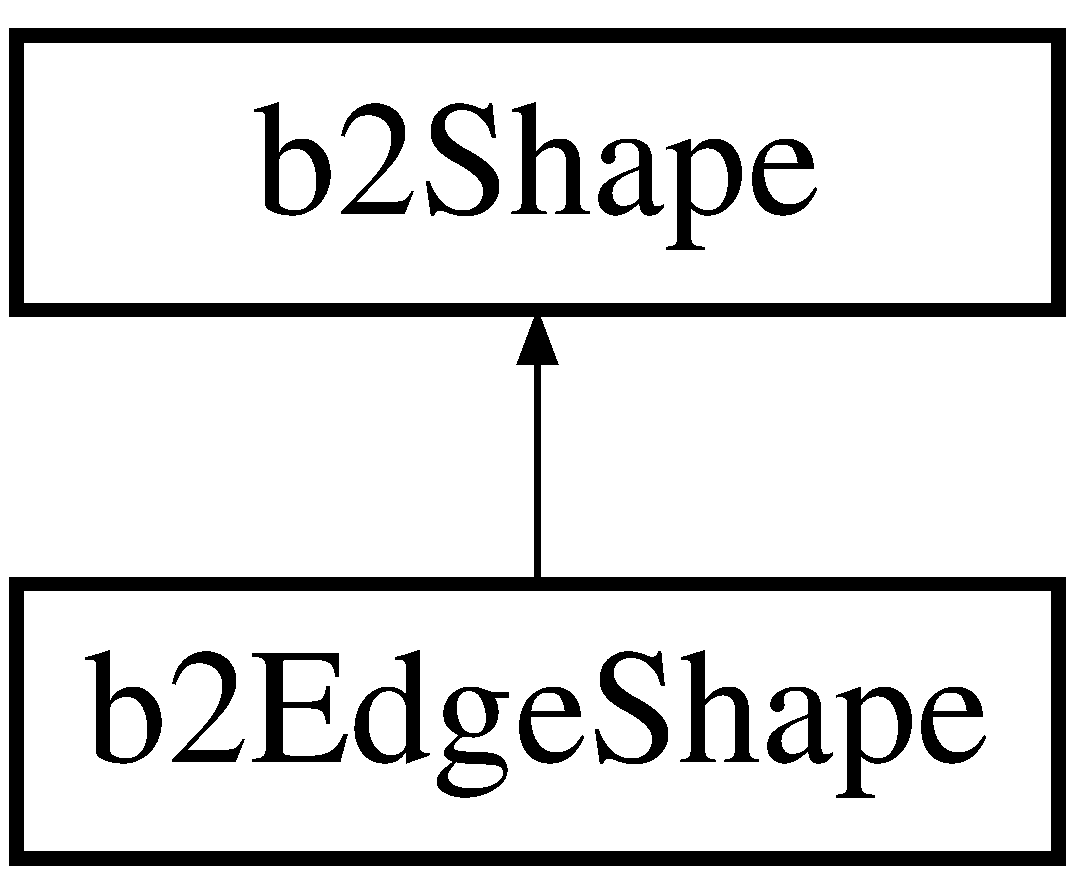
\includegraphics[height=2.000000cm]{classb2_edge_shape}
\end{center}
\end{figure}
\subsection*{Public Member Functions}
\begin{DoxyCompactItemize}
\item 
void \hyperlink{classb2_edge_shape_a67dd3b17630a600033cb4380697a4e9d}{Set} (const \hyperlink{structb2_vec2}{b2\+Vec2} \&v1, const \hyperlink{structb2_vec2}{b2\+Vec2} \&v2)\hypertarget{classb2_edge_shape_a67dd3b17630a600033cb4380697a4e9d}{}\label{classb2_edge_shape_a67dd3b17630a600033cb4380697a4e9d}

\begin{DoxyCompactList}\small\item\em Set this as an isolated edge. \end{DoxyCompactList}\item 
\hyperlink{classb2_shape}{b2\+Shape} $\ast$ \hyperlink{classb2_edge_shape_a24b5aaf94f659ea962dbfb1df220542d}{Clone} (\hyperlink{classb2_block_allocator}{b2\+Block\+Allocator} $\ast$allocator) const \hypertarget{classb2_edge_shape_a24b5aaf94f659ea962dbfb1df220542d}{}\label{classb2_edge_shape_a24b5aaf94f659ea962dbfb1df220542d}

\begin{DoxyCompactList}\small\item\em Implement \hyperlink{classb2_shape}{b2\+Shape}. \end{DoxyCompactList}\item 
int32 \hyperlink{classb2_edge_shape_a8c15a5a5aa8e7dc69826be17aaa82293}{Get\+Child\+Count} () const 
\item 
bool \hyperlink{classb2_edge_shape_a28a977f82e4bc1cf60a3143ba5636c22}{Test\+Point} (const \hyperlink{structb2_transform}{b2\+Transform} \&transform, const \hyperlink{structb2_vec2}{b2\+Vec2} \&p) const 
\item 
bool \hyperlink{classb2_edge_shape_aefbae6b3840f486b22ffecee7d0d15fd}{Ray\+Cast} (\hyperlink{structb2_ray_cast_output}{b2\+Ray\+Cast\+Output} $\ast$output, const \hyperlink{structb2_ray_cast_input}{b2\+Ray\+Cast\+Input} \&input, const \hyperlink{structb2_transform}{b2\+Transform} \&transform, int32 child\+Index) const \hypertarget{classb2_edge_shape_aefbae6b3840f486b22ffecee7d0d15fd}{}\label{classb2_edge_shape_aefbae6b3840f486b22ffecee7d0d15fd}

\begin{DoxyCompactList}\small\item\em Implement \hyperlink{classb2_shape}{b2\+Shape}. \end{DoxyCompactList}\item 
void \hyperlink{classb2_edge_shape_a30f601c611eb549f9f657eee89d82f9f}{Compute\+A\+A\+BB} (\hyperlink{structb2_a_a_b_b}{b2\+A\+A\+BB} $\ast$aabb, const \hyperlink{structb2_transform}{b2\+Transform} \&transform, int32 child\+Index) const 
\item 
void \hyperlink{classb2_edge_shape_a3a305707a07ca3dffa6f2eaff3735dff}{Compute\+Mass} (\hyperlink{structb2_mass_data}{b2\+Mass\+Data} $\ast$mass\+Data, float32 density) const 
\end{DoxyCompactItemize}
\subsection*{Public Attributes}
\begin{DoxyCompactItemize}
\item 
\hyperlink{structb2_vec2}{b2\+Vec2} \hyperlink{classb2_edge_shape_a916cf02a752ff1a70db35b2edaf19bb4}{m\+\_\+vertex1}\hypertarget{classb2_edge_shape_a916cf02a752ff1a70db35b2edaf19bb4}{}\label{classb2_edge_shape_a916cf02a752ff1a70db35b2edaf19bb4}

\begin{DoxyCompactList}\small\item\em These are the edge vertices. \end{DoxyCompactList}\item 
\hyperlink{structb2_vec2}{b2\+Vec2} {\bfseries m\+\_\+vertex2}\hypertarget{classb2_edge_shape_aa218bfe2bf135e4e94028b29aaa32fce}{}\label{classb2_edge_shape_aa218bfe2bf135e4e94028b29aaa32fce}

\item 
\hyperlink{structb2_vec2}{b2\+Vec2} \hyperlink{classb2_edge_shape_a907c9829484cc1ba7527ab368e9fdf93}{m\+\_\+vertex0}\hypertarget{classb2_edge_shape_a907c9829484cc1ba7527ab368e9fdf93}{}\label{classb2_edge_shape_a907c9829484cc1ba7527ab368e9fdf93}

\begin{DoxyCompactList}\small\item\em Optional adjacent vertices. These are used for smooth collision. \end{DoxyCompactList}\item 
\hyperlink{structb2_vec2}{b2\+Vec2} {\bfseries m\+\_\+vertex3}\hypertarget{classb2_edge_shape_a7991fd8b38806a7785748cd991c18452}{}\label{classb2_edge_shape_a7991fd8b38806a7785748cd991c18452}

\item 
bool {\bfseries m\+\_\+has\+Vertex0}\hypertarget{classb2_edge_shape_a1d0f39259f0963146b343d6b048f3f8a}{}\label{classb2_edge_shape_a1d0f39259f0963146b343d6b048f3f8a}

\item 
bool {\bfseries m\+\_\+has\+Vertex3}\hypertarget{classb2_edge_shape_afeb0dfac66fe677ccd765d48610fa56f}{}\label{classb2_edge_shape_afeb0dfac66fe677ccd765d48610fa56f}

\end{DoxyCompactItemize}
\subsection*{Additional Inherited Members}


\subsection{Detailed Description}
A line segment (edge) shape. These can be connected in chains or loops to other edge shapes. The connectivity information is used to ensure correct contact normals. 

\subsection{Member Function Documentation}
\index{b2\+Edge\+Shape@{b2\+Edge\+Shape}!Compute\+A\+A\+BB@{Compute\+A\+A\+BB}}
\index{Compute\+A\+A\+BB@{Compute\+A\+A\+BB}!b2\+Edge\+Shape@{b2\+Edge\+Shape}}
\subsubsection[{\texorpdfstring{Compute\+A\+A\+B\+B(b2\+A\+A\+B\+B $\ast$aabb, const b2\+Transform \&transform, int32 child\+Index) const }{ComputeAABB(b2AABB *aabb, const b2Transform &transform, int32 childIndex) const }}]{\setlength{\rightskip}{0pt plus 5cm}void b2\+Edge\+Shape\+::\+Compute\+A\+A\+BB (
\begin{DoxyParamCaption}
\item[{{\bf b2\+A\+A\+BB} $\ast$}]{aabb, }
\item[{const {\bf b2\+Transform} \&}]{transform, }
\item[{int32}]{child\+Index}
\end{DoxyParamCaption}
) const\hspace{0.3cm}{\ttfamily [virtual]}}\hypertarget{classb2_edge_shape_a30f601c611eb549f9f657eee89d82f9f}{}\label{classb2_edge_shape_a30f601c611eb549f9f657eee89d82f9f}
\begin{DoxySeeAlso}{See also}
\hyperlink{classb2_shape_a0a7f4227b6c17450fc26e0b6641b7abf}{b2\+Shape\+::\+Compute\+A\+A\+BB} 
\end{DoxySeeAlso}


Implements \hyperlink{classb2_shape_a0a7f4227b6c17450fc26e0b6641b7abf}{b2\+Shape}.

\index{b2\+Edge\+Shape@{b2\+Edge\+Shape}!Compute\+Mass@{Compute\+Mass}}
\index{Compute\+Mass@{Compute\+Mass}!b2\+Edge\+Shape@{b2\+Edge\+Shape}}
\subsubsection[{\texorpdfstring{Compute\+Mass(b2\+Mass\+Data $\ast$mass\+Data, float32 density) const }{ComputeMass(b2MassData *massData, float32 density) const }}]{\setlength{\rightskip}{0pt plus 5cm}void b2\+Edge\+Shape\+::\+Compute\+Mass (
\begin{DoxyParamCaption}
\item[{{\bf b2\+Mass\+Data} $\ast$}]{mass\+Data, }
\item[{float32}]{density}
\end{DoxyParamCaption}
) const\hspace{0.3cm}{\ttfamily [virtual]}}\hypertarget{classb2_edge_shape_a3a305707a07ca3dffa6f2eaff3735dff}{}\label{classb2_edge_shape_a3a305707a07ca3dffa6f2eaff3735dff}
\begin{DoxySeeAlso}{See also}
\hyperlink{classb2_shape_a33cfcad2cf4cc31e1d001bf1baf10721}{b2\+Shape\+::\+Compute\+Mass} 
\end{DoxySeeAlso}


Implements \hyperlink{classb2_shape_a33cfcad2cf4cc31e1d001bf1baf10721}{b2\+Shape}.

\index{b2\+Edge\+Shape@{b2\+Edge\+Shape}!Get\+Child\+Count@{Get\+Child\+Count}}
\index{Get\+Child\+Count@{Get\+Child\+Count}!b2\+Edge\+Shape@{b2\+Edge\+Shape}}
\subsubsection[{\texorpdfstring{Get\+Child\+Count() const }{GetChildCount() const }}]{\setlength{\rightskip}{0pt plus 5cm}int32 b2\+Edge\+Shape\+::\+Get\+Child\+Count (
\begin{DoxyParamCaption}
{}
\end{DoxyParamCaption}
) const\hspace{0.3cm}{\ttfamily [virtual]}}\hypertarget{classb2_edge_shape_a8c15a5a5aa8e7dc69826be17aaa82293}{}\label{classb2_edge_shape_a8c15a5a5aa8e7dc69826be17aaa82293}
\begin{DoxySeeAlso}{See also}
\hyperlink{classb2_shape_acaade0398c8a6f3750ba0d25fbde2242}{b2\+Shape\+::\+Get\+Child\+Count} 
\end{DoxySeeAlso}


Implements \hyperlink{classb2_shape_acaade0398c8a6f3750ba0d25fbde2242}{b2\+Shape}.

\index{b2\+Edge\+Shape@{b2\+Edge\+Shape}!Test\+Point@{Test\+Point}}
\index{Test\+Point@{Test\+Point}!b2\+Edge\+Shape@{b2\+Edge\+Shape}}
\subsubsection[{\texorpdfstring{Test\+Point(const b2\+Transform \&transform, const b2\+Vec2 \&p) const }{TestPoint(const b2Transform &transform, const b2Vec2 &p) const }}]{\setlength{\rightskip}{0pt plus 5cm}bool b2\+Edge\+Shape\+::\+Test\+Point (
\begin{DoxyParamCaption}
\item[{const {\bf b2\+Transform} \&}]{transform, }
\item[{const {\bf b2\+Vec2} \&}]{p}
\end{DoxyParamCaption}
) const\hspace{0.3cm}{\ttfamily [virtual]}}\hypertarget{classb2_edge_shape_a28a977f82e4bc1cf60a3143ba5636c22}{}\label{classb2_edge_shape_a28a977f82e4bc1cf60a3143ba5636c22}
\begin{DoxySeeAlso}{See also}
\hyperlink{classb2_shape_a11996b9bdcf8dca92a0c8bf484ab3f59}{b2\+Shape\+::\+Test\+Point} 
\end{DoxySeeAlso}


Implements \hyperlink{classb2_shape_a11996b9bdcf8dca92a0c8bf484ab3f59}{b2\+Shape}.



The documentation for this class was generated from the following file\+:\begin{DoxyCompactItemize}
\item 
Cadriciel/\+Commun/\+Externe/\+Box2\+D/include/\+Box2\+D/\+Collision/\+Shapes/b2\+Edge\+Shape.\+h\end{DoxyCompactItemize}

\hypertarget{structb2_filter}{}\section{b2\+Filter Struct Reference}
\label{structb2_filter}\index{b2\+Filter@{b2\+Filter}}


This holds contact filtering data.  




{\ttfamily \#include $<$b2\+Fixture.\+h$>$}

\subsection*{Public Attributes}
\begin{DoxyCompactItemize}
\item 
uint16 \hyperlink{structb2_filter_a368907397168d39af8b4fc5201d50bba}{category\+Bits}\hypertarget{structb2_filter_a368907397168d39af8b4fc5201d50bba}{}\label{structb2_filter_a368907397168d39af8b4fc5201d50bba}

\begin{DoxyCompactList}\small\item\em The collision category bits. Normally you would just set one bit. \end{DoxyCompactList}\item 
uint16 \hyperlink{structb2_filter_a533cccf85e3ba3d9e3700d73b819f6e2}{mask\+Bits}
\item 
int16 \hyperlink{structb2_filter_a572a8f4a1672f6d5d71123a35e872950}{group\+Index}
\end{DoxyCompactItemize}


\subsection{Detailed Description}
This holds contact filtering data. 

\subsection{Member Data Documentation}
\index{b2\+Filter@{b2\+Filter}!group\+Index@{group\+Index}}
\index{group\+Index@{group\+Index}!b2\+Filter@{b2\+Filter}}
\subsubsection[{\texorpdfstring{group\+Index}{groupIndex}}]{\setlength{\rightskip}{0pt plus 5cm}int16 b2\+Filter\+::group\+Index}\hypertarget{structb2_filter_a572a8f4a1672f6d5d71123a35e872950}{}\label{structb2_filter_a572a8f4a1672f6d5d71123a35e872950}
Collision groups allow a certain group of objects to never collide (negative) or always collide (positive). Zero means no collision group. Non-\/zero group filtering always wins against the mask bits. \index{b2\+Filter@{b2\+Filter}!mask\+Bits@{mask\+Bits}}
\index{mask\+Bits@{mask\+Bits}!b2\+Filter@{b2\+Filter}}
\subsubsection[{\texorpdfstring{mask\+Bits}{maskBits}}]{\setlength{\rightskip}{0pt plus 5cm}uint16 b2\+Filter\+::mask\+Bits}\hypertarget{structb2_filter_a533cccf85e3ba3d9e3700d73b819f6e2}{}\label{structb2_filter_a533cccf85e3ba3d9e3700d73b819f6e2}
The collision mask bits. This states the categories that this shape would accept for collision. 

The documentation for this struct was generated from the following file\+:\begin{DoxyCompactItemize}
\item 
C\+:/\+Users/\+Bilal Itani/\+Desktop/inf2990-\/11/\+Cadriciel/\+Commun/\+Externe/\+Box2\+D/include/\+Box2\+D/\+Dynamics/b2\+Fixture.\+h\end{DoxyCompactItemize}

\hypertarget{classb2_fixture}{}\section{b2\+Fixture Class Reference}
\label{classb2_fixture}\index{b2\+Fixture@{b2\+Fixture}}


{\ttfamily \#include $<$b2\+Fixture.\+h$>$}

\subsection*{Public Member Functions}
\begin{DoxyCompactItemize}
\item 
b2\+Shape\+::\+Type \hyperlink{classb2_fixture_ab0e1d6bc1c42e6f779e77db408ab2d24}{Get\+Type} () const 
\item 
\hyperlink{classb2_shape}{b2\+Shape} $\ast$ \hyperlink{classb2_fixture_aaa2b73fa212fa53b1c800cccd7a1d31e}{Get\+Shape} ()
\item 
const \hyperlink{classb2_shape}{b2\+Shape} $\ast$ {\bfseries Get\+Shape} () const \hypertarget{classb2_fixture_a5ede102030bd041b07fec5c1f082c8c9}{}\label{classb2_fixture_a5ede102030bd041b07fec5c1f082c8c9}

\item 
void \hyperlink{classb2_fixture_a6198a81dcee0fe814d730383ebfa7038}{Set\+Sensor} (bool sensor)\hypertarget{classb2_fixture_a6198a81dcee0fe814d730383ebfa7038}{}\label{classb2_fixture_a6198a81dcee0fe814d730383ebfa7038}

\begin{DoxyCompactList}\small\item\em Set if this fixture is a sensor. \end{DoxyCompactList}\item 
bool \hyperlink{classb2_fixture_a91758c9dca818ca45f3f6427c7e3fc19}{Is\+Sensor} () const 
\item 
void \hyperlink{classb2_fixture_a2c5e0d12c174927a4ad550459be334ad}{Set\+Filter\+Data} (const \hyperlink{structb2_filter}{b2\+Filter} \&filter)
\item 
const \hyperlink{structb2_filter}{b2\+Filter} \& \hyperlink{classb2_fixture_a5bc271a6e8082e727b053aead1ae86a9}{Get\+Filter\+Data} () const \hypertarget{classb2_fixture_a5bc271a6e8082e727b053aead1ae86a9}{}\label{classb2_fixture_a5bc271a6e8082e727b053aead1ae86a9}

\begin{DoxyCompactList}\small\item\em Get the contact filtering data. \end{DoxyCompactList}\item 
void \hyperlink{classb2_fixture_a45d3320f94811d67383c48466165fa26}{Refilter} ()\hypertarget{classb2_fixture_a45d3320f94811d67383c48466165fa26}{}\label{classb2_fixture_a45d3320f94811d67383c48466165fa26}

\begin{DoxyCompactList}\small\item\em Call this if you want to establish collision that was previously disabled by \hyperlink{classb2_contact_filter_a0e33d4fc90a9345160a07cc494b45ecd}{b2\+Contact\+Filter\+::\+Should\+Collide}. \end{DoxyCompactList}\item 
\hyperlink{classb2_body}{b2\+Body} $\ast$ \hyperlink{classb2_fixture_a9d6536ef274d768e86ab0a8330921535}{Get\+Body} ()
\item 
const \hyperlink{classb2_body}{b2\+Body} $\ast$ {\bfseries Get\+Body} () const \hypertarget{classb2_fixture_a6cfc4ed94c4cbfbc0244f11007448431}{}\label{classb2_fixture_a6cfc4ed94c4cbfbc0244f11007448431}

\item 
\hyperlink{classb2_fixture}{b2\+Fixture} $\ast$ \hyperlink{classb2_fixture_a0241952461f6f1a04a3c850306390fd2}{Get\+Next} ()
\item 
const \hyperlink{classb2_fixture}{b2\+Fixture} $\ast$ {\bfseries Get\+Next} () const \hypertarget{classb2_fixture_adb72f9669165143466a1d37d1288785f}{}\label{classb2_fixture_adb72f9669165143466a1d37d1288785f}

\item 
void $\ast$ \hyperlink{classb2_fixture_a57247425e7c859d7653eec417ec83cdc}{Get\+User\+Data} () const 
\item 
void \hyperlink{classb2_fixture_a3db7f89ef4493247d922fe3d96351ad9}{Set\+User\+Data} (void $\ast$data)\hypertarget{classb2_fixture_a3db7f89ef4493247d922fe3d96351ad9}{}\label{classb2_fixture_a3db7f89ef4493247d922fe3d96351ad9}

\begin{DoxyCompactList}\small\item\em Set the user data. Use this to store your application specific data. \end{DoxyCompactList}\item 
bool \hyperlink{classb2_fixture_ab875147c7a9df4ff94d224f6aa81a7a9}{Test\+Point} (const \hyperlink{structb2_vec2}{b2\+Vec2} \&p) const 
\item 
bool \hyperlink{classb2_fixture_a614e84f47e8b32b503fa719099ecba79}{Ray\+Cast} (\hyperlink{structb2_ray_cast_output}{b2\+Ray\+Cast\+Output} $\ast$output, const \hyperlink{structb2_ray_cast_input}{b2\+Ray\+Cast\+Input} \&input, int32 child\+Index) const 
\item 
void \hyperlink{classb2_fixture_adbfb9b64006abaaa0ca01e6d9e06deea}{Get\+Mass\+Data} (\hyperlink{structb2_mass_data}{b2\+Mass\+Data} $\ast$mass\+Data) const 
\item 
void \hyperlink{classb2_fixture_ad4e1d9323103975c8931d022b952d04a}{Set\+Density} (float32 density)
\item 
float32 \hyperlink{classb2_fixture_a5deb4acfb464f3dcb668f081a2c44ff4}{Get\+Density} () const \hypertarget{classb2_fixture_a5deb4acfb464f3dcb668f081a2c44ff4}{}\label{classb2_fixture_a5deb4acfb464f3dcb668f081a2c44ff4}

\begin{DoxyCompactList}\small\item\em Get the density of this fixture. \end{DoxyCompactList}\item 
float32 \hyperlink{classb2_fixture_a31253b90b87f1fec7256bba92aeb4645}{Get\+Friction} () const \hypertarget{classb2_fixture_a31253b90b87f1fec7256bba92aeb4645}{}\label{classb2_fixture_a31253b90b87f1fec7256bba92aeb4645}

\begin{DoxyCompactList}\small\item\em Get the coefficient of friction. \end{DoxyCompactList}\item 
void \hyperlink{classb2_fixture_ad0cd91eef5858c8ef1d6b62cc2a34ea2}{Set\+Friction} (float32 friction)
\item 
float32 \hyperlink{classb2_fixture_a6ce4d949ffff6201a117f1e3833953f8}{Get\+Restitution} () const \hypertarget{classb2_fixture_a6ce4d949ffff6201a117f1e3833953f8}{}\label{classb2_fixture_a6ce4d949ffff6201a117f1e3833953f8}

\begin{DoxyCompactList}\small\item\em Get the coefficient of restitution. \end{DoxyCompactList}\item 
void \hyperlink{classb2_fixture_a19c507332e4f7bd04a05f00426f11ee4}{Set\+Restitution} (float32 restitution)
\item 
const \hyperlink{structb2_a_a_b_b}{b2\+A\+A\+BB} \& \hyperlink{classb2_fixture_abdc2a225110310a481a78cdb14000ca7}{Get\+A\+A\+BB} (int32 child\+Index) const 
\item 
void \hyperlink{classb2_fixture_a57485e73a2063060e320c7176676cd5e}{Dump} (int32 body\+Index)\hypertarget{classb2_fixture_a57485e73a2063060e320c7176676cd5e}{}\label{classb2_fixture_a57485e73a2063060e320c7176676cd5e}

\begin{DoxyCompactList}\small\item\em Dump this fixture to the log file. \end{DoxyCompactList}\end{DoxyCompactItemize}
\subsection*{Protected Member Functions}
\begin{DoxyCompactItemize}
\item 
void {\bfseries Create} (\hyperlink{classb2_block_allocator}{b2\+Block\+Allocator} $\ast$allocator, \hyperlink{classb2_body}{b2\+Body} $\ast$body, const \hyperlink{structb2_fixture_def}{b2\+Fixture\+Def} $\ast$def)\hypertarget{classb2_fixture_a1f465f3656f098eebfcbc6edf7a9239a}{}\label{classb2_fixture_a1f465f3656f098eebfcbc6edf7a9239a}

\item 
void {\bfseries Destroy} (\hyperlink{classb2_block_allocator}{b2\+Block\+Allocator} $\ast$allocator)\hypertarget{classb2_fixture_a279301181668f724c027020a654efe42}{}\label{classb2_fixture_a279301181668f724c027020a654efe42}

\item 
void {\bfseries Create\+Proxies} (\hyperlink{classb2_broad_phase}{b2\+Broad\+Phase} $\ast$broad\+Phase, const \hyperlink{structb2_transform}{b2\+Transform} \&xf)\hypertarget{classb2_fixture_a670f1f687521666da6e92885754970b7}{}\label{classb2_fixture_a670f1f687521666da6e92885754970b7}

\item 
void {\bfseries Destroy\+Proxies} (\hyperlink{classb2_broad_phase}{b2\+Broad\+Phase} $\ast$broad\+Phase)\hypertarget{classb2_fixture_a1def068c9ce09e2ebcccc556951b7979}{}\label{classb2_fixture_a1def068c9ce09e2ebcccc556951b7979}

\item 
void {\bfseries Synchronize} (\hyperlink{classb2_broad_phase}{b2\+Broad\+Phase} $\ast$broad\+Phase, const \hyperlink{structb2_transform}{b2\+Transform} \&xf1, const \hyperlink{structb2_transform}{b2\+Transform} \&xf2)\hypertarget{classb2_fixture_ac8fd15bfd9a3a7ba05f3831e6f598908}{}\label{classb2_fixture_ac8fd15bfd9a3a7ba05f3831e6f598908}

\end{DoxyCompactItemize}
\subsection*{Protected Attributes}
\begin{DoxyCompactItemize}
\item 
float32 {\bfseries m\+\_\+density}\hypertarget{classb2_fixture_ab8c388182fc7d58d930f6b0aa21d5c60}{}\label{classb2_fixture_ab8c388182fc7d58d930f6b0aa21d5c60}

\item 
\hyperlink{classb2_fixture}{b2\+Fixture} $\ast$ {\bfseries m\+\_\+next}\hypertarget{classb2_fixture_ac5c9fbdf66290e2608db1ffcea2316b0}{}\label{classb2_fixture_ac5c9fbdf66290e2608db1ffcea2316b0}

\item 
\hyperlink{classb2_body}{b2\+Body} $\ast$ {\bfseries m\+\_\+body}\hypertarget{classb2_fixture_a480026124a6b7e88f2ed89832a08d191}{}\label{classb2_fixture_a480026124a6b7e88f2ed89832a08d191}

\item 
\hyperlink{classb2_shape}{b2\+Shape} $\ast$ {\bfseries m\+\_\+shape}\hypertarget{classb2_fixture_a54fa48dfc8b70a435c8f17f8b7720828}{}\label{classb2_fixture_a54fa48dfc8b70a435c8f17f8b7720828}

\item 
float32 {\bfseries m\+\_\+friction}\hypertarget{classb2_fixture_a314118ee973ebd14e083553fed1e0212}{}\label{classb2_fixture_a314118ee973ebd14e083553fed1e0212}

\item 
float32 {\bfseries m\+\_\+restitution}\hypertarget{classb2_fixture_a343a35683ce4a79d2151761611027d66}{}\label{classb2_fixture_a343a35683ce4a79d2151761611027d66}

\item 
\hyperlink{structb2_fixture_proxy}{b2\+Fixture\+Proxy} $\ast$ {\bfseries m\+\_\+proxies}\hypertarget{classb2_fixture_a0056031e2b2b53e6a4c0ef7a0c87821a}{}\label{classb2_fixture_a0056031e2b2b53e6a4c0ef7a0c87821a}

\item 
int32 {\bfseries m\+\_\+proxy\+Count}\hypertarget{classb2_fixture_aae71b4a0071346aba2eb6f4a764785a4}{}\label{classb2_fixture_aae71b4a0071346aba2eb6f4a764785a4}

\item 
\hyperlink{structb2_filter}{b2\+Filter} {\bfseries m\+\_\+filter}\hypertarget{classb2_fixture_a33b66959856506a6d27b32dad0e284c7}{}\label{classb2_fixture_a33b66959856506a6d27b32dad0e284c7}

\item 
bool {\bfseries m\+\_\+is\+Sensor}\hypertarget{classb2_fixture_a4b6b47a8de6d37acf9b980b33b22f634}{}\label{classb2_fixture_a4b6b47a8de6d37acf9b980b33b22f634}

\item 
void $\ast$ {\bfseries m\+\_\+user\+Data}\hypertarget{classb2_fixture_a60191e5c76bfd115e6c38d78b6cffd8b}{}\label{classb2_fixture_a60191e5c76bfd115e6c38d78b6cffd8b}

\end{DoxyCompactItemize}
\subsection*{Friends}
\begin{DoxyCompactItemize}
\item 
class {\bfseries b2\+Body}\hypertarget{classb2_fixture_a010ab52de250e5fe30a45d642f46405b}{}\label{classb2_fixture_a010ab52de250e5fe30a45d642f46405b}

\item 
class {\bfseries b2\+World}\hypertarget{classb2_fixture_a4bd536c5a7c0587913765bbc2693ceea}{}\label{classb2_fixture_a4bd536c5a7c0587913765bbc2693ceea}

\item 
class {\bfseries b2\+Contact}\hypertarget{classb2_fixture_a6c4ac5df27ec498dd9e4281352b7a789}{}\label{classb2_fixture_a6c4ac5df27ec498dd9e4281352b7a789}

\item 
class {\bfseries b2\+Contact\+Manager}\hypertarget{classb2_fixture_aece264d42f69aed410f5eb3beba6ddf2}{}\label{classb2_fixture_aece264d42f69aed410f5eb3beba6ddf2}

\end{DoxyCompactItemize}


\subsection{Detailed Description}
A fixture is used to attach a shape to a body for collision detection. A fixture inherits its transform from its parent. Fixtures hold additional non-\/geometric data such as friction, collision filters, etc. Fixtures are created via \hyperlink{classb2_body_a40dda91b34418bb40e31e2db9b1b76a5}{b2\+Body\+::\+Create\+Fixture}. \begin{DoxyWarning}{Warning}
you cannot reuse fixtures. 
\end{DoxyWarning}


\subsection{Member Function Documentation}
\index{b2\+Fixture@{b2\+Fixture}!Get\+A\+A\+BB@{Get\+A\+A\+BB}}
\index{Get\+A\+A\+BB@{Get\+A\+A\+BB}!b2\+Fixture@{b2\+Fixture}}
\subsubsection[{\texorpdfstring{Get\+A\+A\+B\+B(int32 child\+Index) const }{GetAABB(int32 childIndex) const }}]{\setlength{\rightskip}{0pt plus 5cm}const {\bf b2\+A\+A\+BB} \& b2\+Fixture\+::\+Get\+A\+A\+BB (
\begin{DoxyParamCaption}
\item[{int32}]{child\+Index}
\end{DoxyParamCaption}
) const\hspace{0.3cm}{\ttfamily [inline]}}\hypertarget{classb2_fixture_abdc2a225110310a481a78cdb14000ca7}{}\label{classb2_fixture_abdc2a225110310a481a78cdb14000ca7}
Get the fixture\textquotesingle{}s A\+A\+BB. This A\+A\+BB may be enlarge and/or stale. If you need a more accurate A\+A\+BB, compute it using the shape and the body transform. \index{b2\+Fixture@{b2\+Fixture}!Get\+Body@{Get\+Body}}
\index{Get\+Body@{Get\+Body}!b2\+Fixture@{b2\+Fixture}}
\subsubsection[{\texorpdfstring{Get\+Body()}{GetBody()}}]{\setlength{\rightskip}{0pt plus 5cm}{\bf b2\+Body} $\ast$ b2\+Fixture\+::\+Get\+Body (
\begin{DoxyParamCaption}
{}
\end{DoxyParamCaption}
)\hspace{0.3cm}{\ttfamily [inline]}}\hypertarget{classb2_fixture_a9d6536ef274d768e86ab0a8330921535}{}\label{classb2_fixture_a9d6536ef274d768e86ab0a8330921535}
Get the parent body of this fixture. This is N\+U\+LL if the fixture is not attached. \begin{DoxyReturn}{Returns}
the parent body. 
\end{DoxyReturn}
\index{b2\+Fixture@{b2\+Fixture}!Get\+Mass\+Data@{Get\+Mass\+Data}}
\index{Get\+Mass\+Data@{Get\+Mass\+Data}!b2\+Fixture@{b2\+Fixture}}
\subsubsection[{\texorpdfstring{Get\+Mass\+Data(b2\+Mass\+Data $\ast$mass\+Data) const }{GetMassData(b2MassData *massData) const }}]{\setlength{\rightskip}{0pt plus 5cm}void b2\+Fixture\+::\+Get\+Mass\+Data (
\begin{DoxyParamCaption}
\item[{{\bf b2\+Mass\+Data} $\ast$}]{mass\+Data}
\end{DoxyParamCaption}
) const\hspace{0.3cm}{\ttfamily [inline]}}\hypertarget{classb2_fixture_adbfb9b64006abaaa0ca01e6d9e06deea}{}\label{classb2_fixture_adbfb9b64006abaaa0ca01e6d9e06deea}
Get the mass data for this fixture. The mass data is based on the density and the shape. The rotational inertia is about the shape\textquotesingle{}s origin. This operation may be expensive. \index{b2\+Fixture@{b2\+Fixture}!Get\+Next@{Get\+Next}}
\index{Get\+Next@{Get\+Next}!b2\+Fixture@{b2\+Fixture}}
\subsubsection[{\texorpdfstring{Get\+Next()}{GetNext()}}]{\setlength{\rightskip}{0pt plus 5cm}{\bf b2\+Fixture} $\ast$ b2\+Fixture\+::\+Get\+Next (
\begin{DoxyParamCaption}
{}
\end{DoxyParamCaption}
)\hspace{0.3cm}{\ttfamily [inline]}}\hypertarget{classb2_fixture_a0241952461f6f1a04a3c850306390fd2}{}\label{classb2_fixture_a0241952461f6f1a04a3c850306390fd2}
Get the next fixture in the parent body\textquotesingle{}s fixture list. \begin{DoxyReturn}{Returns}
the next shape. 
\end{DoxyReturn}
\index{b2\+Fixture@{b2\+Fixture}!Get\+Shape@{Get\+Shape}}
\index{Get\+Shape@{Get\+Shape}!b2\+Fixture@{b2\+Fixture}}
\subsubsection[{\texorpdfstring{Get\+Shape()}{GetShape()}}]{\setlength{\rightskip}{0pt plus 5cm}{\bf b2\+Shape} $\ast$ b2\+Fixture\+::\+Get\+Shape (
\begin{DoxyParamCaption}
{}
\end{DoxyParamCaption}
)\hspace{0.3cm}{\ttfamily [inline]}}\hypertarget{classb2_fixture_aaa2b73fa212fa53b1c800cccd7a1d31e}{}\label{classb2_fixture_aaa2b73fa212fa53b1c800cccd7a1d31e}
Get the child shape. You can modify the child shape, however you should not change the number of vertices because this will crash some collision caching mechanisms. Manipulating the shape may lead to non-\/physical behavior. \index{b2\+Fixture@{b2\+Fixture}!Get\+Type@{Get\+Type}}
\index{Get\+Type@{Get\+Type}!b2\+Fixture@{b2\+Fixture}}
\subsubsection[{\texorpdfstring{Get\+Type() const }{GetType() const }}]{\setlength{\rightskip}{0pt plus 5cm}b2\+Shape\+::\+Type b2\+Fixture\+::\+Get\+Type (
\begin{DoxyParamCaption}
{}
\end{DoxyParamCaption}
) const\hspace{0.3cm}{\ttfamily [inline]}}\hypertarget{classb2_fixture_ab0e1d6bc1c42e6f779e77db408ab2d24}{}\label{classb2_fixture_ab0e1d6bc1c42e6f779e77db408ab2d24}
Get the type of the child shape. You can use this to down cast to the concrete shape. \begin{DoxyReturn}{Returns}
the shape type. 
\end{DoxyReturn}
\index{b2\+Fixture@{b2\+Fixture}!Get\+User\+Data@{Get\+User\+Data}}
\index{Get\+User\+Data@{Get\+User\+Data}!b2\+Fixture@{b2\+Fixture}}
\subsubsection[{\texorpdfstring{Get\+User\+Data() const }{GetUserData() const }}]{\setlength{\rightskip}{0pt plus 5cm}void $\ast$ b2\+Fixture\+::\+Get\+User\+Data (
\begin{DoxyParamCaption}
{}
\end{DoxyParamCaption}
) const\hspace{0.3cm}{\ttfamily [inline]}}\hypertarget{classb2_fixture_a57247425e7c859d7653eec417ec83cdc}{}\label{classb2_fixture_a57247425e7c859d7653eec417ec83cdc}
Get the user data that was assigned in the fixture definition. Use this to store your application specific data. \index{b2\+Fixture@{b2\+Fixture}!Is\+Sensor@{Is\+Sensor}}
\index{Is\+Sensor@{Is\+Sensor}!b2\+Fixture@{b2\+Fixture}}
\subsubsection[{\texorpdfstring{Is\+Sensor() const }{IsSensor() const }}]{\setlength{\rightskip}{0pt plus 5cm}bool b2\+Fixture\+::\+Is\+Sensor (
\begin{DoxyParamCaption}
{}
\end{DoxyParamCaption}
) const\hspace{0.3cm}{\ttfamily [inline]}}\hypertarget{classb2_fixture_a91758c9dca818ca45f3f6427c7e3fc19}{}\label{classb2_fixture_a91758c9dca818ca45f3f6427c7e3fc19}
Is this fixture a sensor (non-\/solid)? \begin{DoxyReturn}{Returns}
the true if the shape is a sensor. 
\end{DoxyReturn}
\index{b2\+Fixture@{b2\+Fixture}!Ray\+Cast@{Ray\+Cast}}
\index{Ray\+Cast@{Ray\+Cast}!b2\+Fixture@{b2\+Fixture}}
\subsubsection[{\texorpdfstring{Ray\+Cast(b2\+Ray\+Cast\+Output $\ast$output, const b2\+Ray\+Cast\+Input \&input, int32 child\+Index) const }{RayCast(b2RayCastOutput *output, const b2RayCastInput &input, int32 childIndex) const }}]{\setlength{\rightskip}{0pt plus 5cm}bool b2\+Fixture\+::\+Ray\+Cast (
\begin{DoxyParamCaption}
\item[{{\bf b2\+Ray\+Cast\+Output} $\ast$}]{output, }
\item[{const {\bf b2\+Ray\+Cast\+Input} \&}]{input, }
\item[{int32}]{child\+Index}
\end{DoxyParamCaption}
) const\hspace{0.3cm}{\ttfamily [inline]}}\hypertarget{classb2_fixture_a614e84f47e8b32b503fa719099ecba79}{}\label{classb2_fixture_a614e84f47e8b32b503fa719099ecba79}
Cast a ray against this shape. 
\begin{DoxyParams}{Parameters}
{\em output} & the ray-\/cast results. \\
\hline
{\em input} & the ray-\/cast input parameters. \\
\hline
\end{DoxyParams}
\index{b2\+Fixture@{b2\+Fixture}!Set\+Density@{Set\+Density}}
\index{Set\+Density@{Set\+Density}!b2\+Fixture@{b2\+Fixture}}
\subsubsection[{\texorpdfstring{Set\+Density(float32 density)}{SetDensity(float32 density)}}]{\setlength{\rightskip}{0pt plus 5cm}void b2\+Fixture\+::\+Set\+Density (
\begin{DoxyParamCaption}
\item[{float32}]{density}
\end{DoxyParamCaption}
)\hspace{0.3cm}{\ttfamily [inline]}}\hypertarget{classb2_fixture_ad4e1d9323103975c8931d022b952d04a}{}\label{classb2_fixture_ad4e1d9323103975c8931d022b952d04a}
Set the density of this fixture. This will {\itshape not} automatically adjust the mass of the body. You must call \hyperlink{classb2_body_a109d8567c6ae84c61fce2919fb209c63}{b2\+Body\+::\+Reset\+Mass\+Data} to update the body\textquotesingle{}s mass. \index{b2\+Fixture@{b2\+Fixture}!Set\+Filter\+Data@{Set\+Filter\+Data}}
\index{Set\+Filter\+Data@{Set\+Filter\+Data}!b2\+Fixture@{b2\+Fixture}}
\subsubsection[{\texorpdfstring{Set\+Filter\+Data(const b2\+Filter \&filter)}{SetFilterData(const b2Filter &filter)}}]{\setlength{\rightskip}{0pt plus 5cm}void b2\+Fixture\+::\+Set\+Filter\+Data (
\begin{DoxyParamCaption}
\item[{const {\bf b2\+Filter} \&}]{filter}
\end{DoxyParamCaption}
)}\hypertarget{classb2_fixture_a2c5e0d12c174927a4ad550459be334ad}{}\label{classb2_fixture_a2c5e0d12c174927a4ad550459be334ad}
Set the contact filtering data. This will not update contacts until the next time step when either parent body is active and awake. This automatically calls Refilter. \index{b2\+Fixture@{b2\+Fixture}!Set\+Friction@{Set\+Friction}}
\index{Set\+Friction@{Set\+Friction}!b2\+Fixture@{b2\+Fixture}}
\subsubsection[{\texorpdfstring{Set\+Friction(float32 friction)}{SetFriction(float32 friction)}}]{\setlength{\rightskip}{0pt plus 5cm}void b2\+Fixture\+::\+Set\+Friction (
\begin{DoxyParamCaption}
\item[{float32}]{friction}
\end{DoxyParamCaption}
)\hspace{0.3cm}{\ttfamily [inline]}}\hypertarget{classb2_fixture_ad0cd91eef5858c8ef1d6b62cc2a34ea2}{}\label{classb2_fixture_ad0cd91eef5858c8ef1d6b62cc2a34ea2}
Set the coefficient of friction. This will {\itshape not} change the friction of existing contacts. \index{b2\+Fixture@{b2\+Fixture}!Set\+Restitution@{Set\+Restitution}}
\index{Set\+Restitution@{Set\+Restitution}!b2\+Fixture@{b2\+Fixture}}
\subsubsection[{\texorpdfstring{Set\+Restitution(float32 restitution)}{SetRestitution(float32 restitution)}}]{\setlength{\rightskip}{0pt plus 5cm}void b2\+Fixture\+::\+Set\+Restitution (
\begin{DoxyParamCaption}
\item[{float32}]{restitution}
\end{DoxyParamCaption}
)\hspace{0.3cm}{\ttfamily [inline]}}\hypertarget{classb2_fixture_a19c507332e4f7bd04a05f00426f11ee4}{}\label{classb2_fixture_a19c507332e4f7bd04a05f00426f11ee4}
Set the coefficient of restitution. This will {\itshape not} change the restitution of existing contacts. \index{b2\+Fixture@{b2\+Fixture}!Test\+Point@{Test\+Point}}
\index{Test\+Point@{Test\+Point}!b2\+Fixture@{b2\+Fixture}}
\subsubsection[{\texorpdfstring{Test\+Point(const b2\+Vec2 \&p) const }{TestPoint(const b2Vec2 &p) const }}]{\setlength{\rightskip}{0pt plus 5cm}bool b2\+Fixture\+::\+Test\+Point (
\begin{DoxyParamCaption}
\item[{const {\bf b2\+Vec2} \&}]{p}
\end{DoxyParamCaption}
) const\hspace{0.3cm}{\ttfamily [inline]}}\hypertarget{classb2_fixture_ab875147c7a9df4ff94d224f6aa81a7a9}{}\label{classb2_fixture_ab875147c7a9df4ff94d224f6aa81a7a9}
\hyperlink{class_test}{Test} a point for containment in this fixture. 
\begin{DoxyParams}{Parameters}
{\em p} & a point in world coordinates. \\
\hline
\end{DoxyParams}


The documentation for this class was generated from the following file\+:\begin{DoxyCompactItemize}
\item 
Commun/\+Externe/\+Box2\+D/include/\+Box2\+D/\+Dynamics/b2\+Fixture.\+h\end{DoxyCompactItemize}

\hypertarget{structb2_fixture_def}{}\section{b2\+Fixture\+Def Struct Reference}
\label{structb2_fixture_def}\index{b2\+Fixture\+Def@{b2\+Fixture\+Def}}


{\ttfamily \#include $<$b2\+Fixture.\+h$>$}

\subsection*{Public Member Functions}
\begin{DoxyCompactItemize}
\item 
\hyperlink{structb2_fixture_def_aa34ba06bcf0d6d981931a83cf124a602}{b2\+Fixture\+Def} ()\hypertarget{structb2_fixture_def_aa34ba06bcf0d6d981931a83cf124a602}{}\label{structb2_fixture_def_aa34ba06bcf0d6d981931a83cf124a602}

\begin{DoxyCompactList}\small\item\em The constructor sets the default fixture definition values. \end{DoxyCompactList}\end{DoxyCompactItemize}
\subsection*{Public Attributes}
\begin{DoxyCompactItemize}
\item 
const \hyperlink{classb2_shape}{b2\+Shape} $\ast$ \hyperlink{structb2_fixture_def_a1e41753d89abf3443e7897e2498a3240}{shape}
\item 
void $\ast$ \hyperlink{structb2_fixture_def_a4f77ef2b2585a40899b61faf53db1093}{user\+Data}\hypertarget{structb2_fixture_def_a4f77ef2b2585a40899b61faf53db1093}{}\label{structb2_fixture_def_a4f77ef2b2585a40899b61faf53db1093}

\begin{DoxyCompactList}\small\item\em Use this to store application specific fixture data. \end{DoxyCompactList}\item 
float32 \hyperlink{structb2_fixture_def_a66081c8d0e12d4bdb0b341fb97b46eb6}{friction}\hypertarget{structb2_fixture_def_a66081c8d0e12d4bdb0b341fb97b46eb6}{}\label{structb2_fixture_def_a66081c8d0e12d4bdb0b341fb97b46eb6}

\begin{DoxyCompactList}\small\item\em The friction coefficient, usually in the range \mbox{[}0,1\mbox{]}. \end{DoxyCompactList}\item 
float32 \hyperlink{structb2_fixture_def_ad7ee26656e4749f7b548d2cc0cf9f168}{restitution}\hypertarget{structb2_fixture_def_ad7ee26656e4749f7b548d2cc0cf9f168}{}\label{structb2_fixture_def_ad7ee26656e4749f7b548d2cc0cf9f168}

\begin{DoxyCompactList}\small\item\em The restitution (elasticity) usually in the range \mbox{[}0,1\mbox{]}. \end{DoxyCompactList}\item 
float32 \hyperlink{structb2_fixture_def_a6e27d733789a35aa689af2b30a1de0ff}{density}\hypertarget{structb2_fixture_def_a6e27d733789a35aa689af2b30a1de0ff}{}\label{structb2_fixture_def_a6e27d733789a35aa689af2b30a1de0ff}

\begin{DoxyCompactList}\small\item\em The density, usually in kg/m$^\wedge$2. \end{DoxyCompactList}\item 
bool \hyperlink{structb2_fixture_def_ac8cfcc6208663c92861eaab3b3fdc57e}{is\+Sensor}
\item 
\hyperlink{structb2_filter}{b2\+Filter} \hyperlink{structb2_fixture_def_a4c3e493a13d11ab27fcc2eee9f52fd61}{filter}\hypertarget{structb2_fixture_def_a4c3e493a13d11ab27fcc2eee9f52fd61}{}\label{structb2_fixture_def_a4c3e493a13d11ab27fcc2eee9f52fd61}

\begin{DoxyCompactList}\small\item\em Contact filtering data. \end{DoxyCompactList}\end{DoxyCompactItemize}


\subsection{Detailed Description}
A fixture definition is used to create a fixture. This class defines an abstract fixture definition. You can reuse fixture definitions safely. 

\subsection{Member Data Documentation}
\index{b2\+Fixture\+Def@{b2\+Fixture\+Def}!is\+Sensor@{is\+Sensor}}
\index{is\+Sensor@{is\+Sensor}!b2\+Fixture\+Def@{b2\+Fixture\+Def}}
\subsubsection[{\texorpdfstring{is\+Sensor}{isSensor}}]{\setlength{\rightskip}{0pt plus 5cm}bool b2\+Fixture\+Def\+::is\+Sensor}\hypertarget{structb2_fixture_def_ac8cfcc6208663c92861eaab3b3fdc57e}{}\label{structb2_fixture_def_ac8cfcc6208663c92861eaab3b3fdc57e}
A sensor shape collects contact information but never generates a collision response. \index{b2\+Fixture\+Def@{b2\+Fixture\+Def}!shape@{shape}}
\index{shape@{shape}!b2\+Fixture\+Def@{b2\+Fixture\+Def}}
\subsubsection[{\texorpdfstring{shape}{shape}}]{\setlength{\rightskip}{0pt plus 5cm}const {\bf b2\+Shape}$\ast$ b2\+Fixture\+Def\+::shape}\hypertarget{structb2_fixture_def_a1e41753d89abf3443e7897e2498a3240}{}\label{structb2_fixture_def_a1e41753d89abf3443e7897e2498a3240}
The shape, this must be set. The shape will be cloned, so you can create the shape on the stack. 

The documentation for this struct was generated from the following file\+:\begin{DoxyCompactItemize}
\item 
C\+:/\+Users/\+Bilal Itani/\+Desktop/inf2990-\/11/\+Cadriciel/\+Commun/\+Externe/\+Box2\+D/include/\+Box2\+D/\+Dynamics/b2\+Fixture.\+h\end{DoxyCompactItemize}

\hypertarget{structb2_fixture_proxy}{}\section{b2\+Fixture\+Proxy Struct Reference}
\label{structb2_fixture_proxy}\index{b2\+Fixture\+Proxy@{b2\+Fixture\+Proxy}}


This proxy is used internally to connect fixtures to the broad-\/phase.  




{\ttfamily \#include $<$b2\+Fixture.\+h$>$}

\subsection*{Public Attributes}
\begin{DoxyCompactItemize}
\item 
\hyperlink{structb2_a_a_b_b}{b2\+A\+A\+BB} {\bfseries aabb}\hypertarget{structb2_fixture_proxy_ad8950f61ce28cfa5b676065d4d843da7}{}\label{structb2_fixture_proxy_ad8950f61ce28cfa5b676065d4d843da7}

\item 
\hyperlink{classb2_fixture}{b2\+Fixture} $\ast$ {\bfseries fixture}\hypertarget{structb2_fixture_proxy_a3a0842dc9699c25658548c2005d0ef62}{}\label{structb2_fixture_proxy_a3a0842dc9699c25658548c2005d0ef62}

\item 
int32 {\bfseries child\+Index}\hypertarget{structb2_fixture_proxy_a2edb15552cf71f48dacc3608bb134166}{}\label{structb2_fixture_proxy_a2edb15552cf71f48dacc3608bb134166}

\item 
int32 {\bfseries proxy\+Id}\hypertarget{structb2_fixture_proxy_aa0ca7e71341368fe6c6913fb39c7283b}{}\label{structb2_fixture_proxy_aa0ca7e71341368fe6c6913fb39c7283b}

\end{DoxyCompactItemize}


\subsection{Detailed Description}
This proxy is used internally to connect fixtures to the broad-\/phase. 

The documentation for this struct was generated from the following file\+:\begin{DoxyCompactItemize}
\item 
C\+:/\+Users/\+Bilal Itani/\+Desktop/inf2990-\/11/\+Cadriciel/\+Commun/\+Externe/\+Box2\+D/include/\+Box2\+D/\+Dynamics/b2\+Fixture.\+h\end{DoxyCompactItemize}

\hypertarget{classb2_friction_joint}{}\section{b2\+Friction\+Joint Class Reference}
\label{classb2_friction_joint}\index{b2\+Friction\+Joint@{b2\+Friction\+Joint}}


{\ttfamily \#include $<$b2\+Friction\+Joint.\+h$>$}

Inheritance diagram for b2\+Friction\+Joint\+:\begin{figure}[H]
\begin{center}
\leavevmode
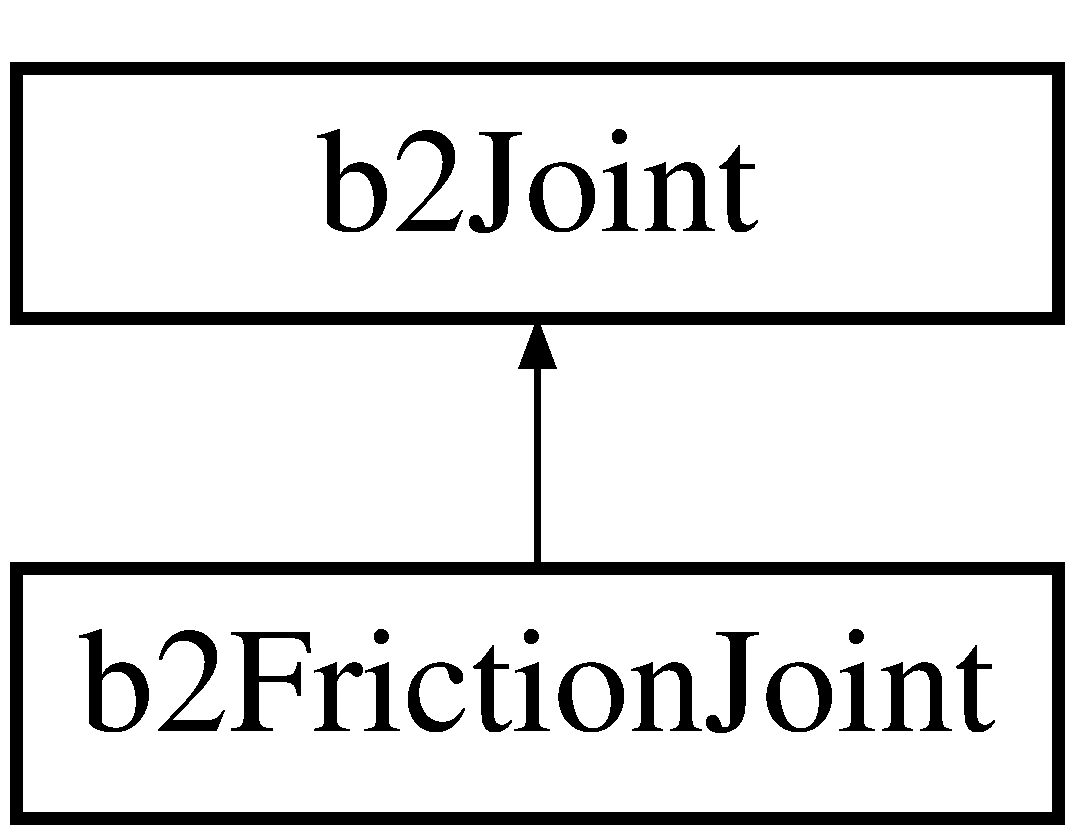
\includegraphics[height=2.000000cm]{classb2_friction_joint}
\end{center}
\end{figure}
\subsection*{Public Member Functions}
\begin{DoxyCompactItemize}
\item 
\hyperlink{structb2_vec2}{b2\+Vec2} \hyperlink{classb2_friction_joint_a01918be429fa5d37d51fda4fe0cc639b}{Get\+AnchorA} () const \hypertarget{classb2_friction_joint_a01918be429fa5d37d51fda4fe0cc639b}{}\label{classb2_friction_joint_a01918be429fa5d37d51fda4fe0cc639b}

\begin{DoxyCompactList}\small\item\em Get the anchor point on bodyA in world coordinates. \end{DoxyCompactList}\item 
\hyperlink{structb2_vec2}{b2\+Vec2} \hyperlink{classb2_friction_joint_ac519021aadea0faf1df01f232023c745}{Get\+AnchorB} () const \hypertarget{classb2_friction_joint_ac519021aadea0faf1df01f232023c745}{}\label{classb2_friction_joint_ac519021aadea0faf1df01f232023c745}

\begin{DoxyCompactList}\small\item\em Get the anchor point on bodyB in world coordinates. \end{DoxyCompactList}\item 
\hyperlink{structb2_vec2}{b2\+Vec2} \hyperlink{classb2_friction_joint_ae646d8a191e490f690b748f057cdd90b}{Get\+Reaction\+Force} (float32 inv\+\_\+dt) const \hypertarget{classb2_friction_joint_ae646d8a191e490f690b748f057cdd90b}{}\label{classb2_friction_joint_ae646d8a191e490f690b748f057cdd90b}

\begin{DoxyCompactList}\small\item\em Get the reaction force on bodyB at the joint anchor in Newtons. \end{DoxyCompactList}\item 
float32 \hyperlink{classb2_friction_joint_a49479d4af9c4bffa0b146d153c78512c}{Get\+Reaction\+Torque} (float32 inv\+\_\+dt) const \hypertarget{classb2_friction_joint_a49479d4af9c4bffa0b146d153c78512c}{}\label{classb2_friction_joint_a49479d4af9c4bffa0b146d153c78512c}

\begin{DoxyCompactList}\small\item\em Get the reaction torque on bodyB in N$\ast$m. \end{DoxyCompactList}\item 
const \hyperlink{structb2_vec2}{b2\+Vec2} \& \hyperlink{classb2_friction_joint_a91ef023d373f775c401ae359f6f74d60}{Get\+Local\+AnchorA} () const \hypertarget{classb2_friction_joint_a91ef023d373f775c401ae359f6f74d60}{}\label{classb2_friction_joint_a91ef023d373f775c401ae359f6f74d60}

\begin{DoxyCompactList}\small\item\em The local anchor point relative to bodyA\textquotesingle{}s origin. \end{DoxyCompactList}\item 
const \hyperlink{structb2_vec2}{b2\+Vec2} \& \hyperlink{classb2_friction_joint_acd57698eb559d36eeac6df00dfd8b89f}{Get\+Local\+AnchorB} () const \hypertarget{classb2_friction_joint_acd57698eb559d36eeac6df00dfd8b89f}{}\label{classb2_friction_joint_acd57698eb559d36eeac6df00dfd8b89f}

\begin{DoxyCompactList}\small\item\em The local anchor point relative to bodyB\textquotesingle{}s origin. \end{DoxyCompactList}\item 
void \hyperlink{classb2_friction_joint_a7936d852b5ad71dc92efc397865dda41}{Set\+Max\+Force} (float32 force)\hypertarget{classb2_friction_joint_a7936d852b5ad71dc92efc397865dda41}{}\label{classb2_friction_joint_a7936d852b5ad71dc92efc397865dda41}

\begin{DoxyCompactList}\small\item\em Set the maximum friction force in N. \end{DoxyCompactList}\item 
float32 \hyperlink{classb2_friction_joint_af3abd33af3943197c89375057302fd0d}{Get\+Max\+Force} () const \hypertarget{classb2_friction_joint_af3abd33af3943197c89375057302fd0d}{}\label{classb2_friction_joint_af3abd33af3943197c89375057302fd0d}

\begin{DoxyCompactList}\small\item\em Get the maximum friction force in N. \end{DoxyCompactList}\item 
void \hyperlink{classb2_friction_joint_a9e3aaf485dc86a378bb62ee78cea43aa}{Set\+Max\+Torque} (float32 torque)\hypertarget{classb2_friction_joint_a9e3aaf485dc86a378bb62ee78cea43aa}{}\label{classb2_friction_joint_a9e3aaf485dc86a378bb62ee78cea43aa}

\begin{DoxyCompactList}\small\item\em Set the maximum friction torque in N$\ast$m. \end{DoxyCompactList}\item 
float32 \hyperlink{classb2_friction_joint_ae59d07030bded21f46a6a432553e71c1}{Get\+Max\+Torque} () const \hypertarget{classb2_friction_joint_ae59d07030bded21f46a6a432553e71c1}{}\label{classb2_friction_joint_ae59d07030bded21f46a6a432553e71c1}

\begin{DoxyCompactList}\small\item\em Get the maximum friction torque in N$\ast$m. \end{DoxyCompactList}\item 
void \hyperlink{classb2_friction_joint_a9a27084c9f4a7ea0a4f590f687ac1edb}{Dump} ()\hypertarget{classb2_friction_joint_a9a27084c9f4a7ea0a4f590f687ac1edb}{}\label{classb2_friction_joint_a9a27084c9f4a7ea0a4f590f687ac1edb}

\begin{DoxyCompactList}\small\item\em Dump joint to dm\+Log. \end{DoxyCompactList}\end{DoxyCompactItemize}
\subsection*{Protected Member Functions}
\begin{DoxyCompactItemize}
\item 
{\bfseries b2\+Friction\+Joint} (const \hyperlink{structb2_friction_joint_def}{b2\+Friction\+Joint\+Def} $\ast$def)\hypertarget{classb2_friction_joint_a7413c5f289257f0e993b7e750fe95b99}{}\label{classb2_friction_joint_a7413c5f289257f0e993b7e750fe95b99}

\item 
void {\bfseries Init\+Velocity\+Constraints} (const \hyperlink{structb2_solver_data}{b2\+Solver\+Data} \&data)\hypertarget{classb2_friction_joint_a72fbe2a2dce2c90e1b68395e715e1254}{}\label{classb2_friction_joint_a72fbe2a2dce2c90e1b68395e715e1254}

\item 
void {\bfseries Solve\+Velocity\+Constraints} (const \hyperlink{structb2_solver_data}{b2\+Solver\+Data} \&data)\hypertarget{classb2_friction_joint_a5aab459109e198a75e0151f36d50ee65}{}\label{classb2_friction_joint_a5aab459109e198a75e0151f36d50ee65}

\item 
bool {\bfseries Solve\+Position\+Constraints} (const \hyperlink{structb2_solver_data}{b2\+Solver\+Data} \&data)\hypertarget{classb2_friction_joint_ac1998353c72787b6074b2ef50dd1c2d2}{}\label{classb2_friction_joint_ac1998353c72787b6074b2ef50dd1c2d2}

\end{DoxyCompactItemize}
\subsection*{Protected Attributes}
\begin{DoxyCompactItemize}
\item 
\hyperlink{structb2_vec2}{b2\+Vec2} {\bfseries m\+\_\+local\+AnchorA}\hypertarget{classb2_friction_joint_a8842818b75319de1e4f3ec70d784dce1}{}\label{classb2_friction_joint_a8842818b75319de1e4f3ec70d784dce1}

\item 
\hyperlink{structb2_vec2}{b2\+Vec2} {\bfseries m\+\_\+local\+AnchorB}\hypertarget{classb2_friction_joint_aa5920c253c6564bfd04a11e767f2e2db}{}\label{classb2_friction_joint_aa5920c253c6564bfd04a11e767f2e2db}

\item 
\hyperlink{structb2_vec2}{b2\+Vec2} {\bfseries m\+\_\+linear\+Impulse}\hypertarget{classb2_friction_joint_ad4f8286af03b0f37a9eec7e9884d7e26}{}\label{classb2_friction_joint_ad4f8286af03b0f37a9eec7e9884d7e26}

\item 
float32 {\bfseries m\+\_\+angular\+Impulse}\hypertarget{classb2_friction_joint_ab199dba9687ece4b816589b9e1e14750}{}\label{classb2_friction_joint_ab199dba9687ece4b816589b9e1e14750}

\item 
float32 {\bfseries m\+\_\+max\+Force}\hypertarget{classb2_friction_joint_ae666a8093844e2fb75e4c3de6b3f377a}{}\label{classb2_friction_joint_ae666a8093844e2fb75e4c3de6b3f377a}

\item 
float32 {\bfseries m\+\_\+max\+Torque}\hypertarget{classb2_friction_joint_a42b3ac5d34ab2399a5e4f0ea9afe988d}{}\label{classb2_friction_joint_a42b3ac5d34ab2399a5e4f0ea9afe988d}

\item 
int32 {\bfseries m\+\_\+indexA}\hypertarget{classb2_friction_joint_a069c815e1cdf78160cb96b4b0047f64e}{}\label{classb2_friction_joint_a069c815e1cdf78160cb96b4b0047f64e}

\item 
int32 {\bfseries m\+\_\+indexB}\hypertarget{classb2_friction_joint_a378198c55100884de4587cb9ab22128f}{}\label{classb2_friction_joint_a378198c55100884de4587cb9ab22128f}

\item 
\hyperlink{structb2_vec2}{b2\+Vec2} {\bfseries m\+\_\+rA}\hypertarget{classb2_friction_joint_aa02b166017af5893b6b49b56dc96c70a}{}\label{classb2_friction_joint_aa02b166017af5893b6b49b56dc96c70a}

\item 
\hyperlink{structb2_vec2}{b2\+Vec2} {\bfseries m\+\_\+rB}\hypertarget{classb2_friction_joint_a99b95a2dbfb119cbccccb137748aca44}{}\label{classb2_friction_joint_a99b95a2dbfb119cbccccb137748aca44}

\item 
\hyperlink{structb2_vec2}{b2\+Vec2} {\bfseries m\+\_\+local\+CenterA}\hypertarget{classb2_friction_joint_af732965abe1f29f7469e1ea17506218c}{}\label{classb2_friction_joint_af732965abe1f29f7469e1ea17506218c}

\item 
\hyperlink{structb2_vec2}{b2\+Vec2} {\bfseries m\+\_\+local\+CenterB}\hypertarget{classb2_friction_joint_a55739866c1f3423caf2116e0a869ec45}{}\label{classb2_friction_joint_a55739866c1f3423caf2116e0a869ec45}

\item 
float32 {\bfseries m\+\_\+inv\+MassA}\hypertarget{classb2_friction_joint_a7b7a482216efd081db94465db409fa21}{}\label{classb2_friction_joint_a7b7a482216efd081db94465db409fa21}

\item 
float32 {\bfseries m\+\_\+inv\+MassB}\hypertarget{classb2_friction_joint_a189a3869e59f6b1e00c83fcaf6b08253}{}\label{classb2_friction_joint_a189a3869e59f6b1e00c83fcaf6b08253}

\item 
float32 {\bfseries m\+\_\+inv\+IA}\hypertarget{classb2_friction_joint_aad004207b7392e9828f55d8f15dc2aa8}{}\label{classb2_friction_joint_aad004207b7392e9828f55d8f15dc2aa8}

\item 
float32 {\bfseries m\+\_\+inv\+IB}\hypertarget{classb2_friction_joint_a79ab8b49c2d4ce6415e3fe9376947d4c}{}\label{classb2_friction_joint_a79ab8b49c2d4ce6415e3fe9376947d4c}

\item 
\hyperlink{structb2_mat22}{b2\+Mat22} {\bfseries m\+\_\+linear\+Mass}\hypertarget{classb2_friction_joint_aa49bf4b20865a4976c3fae8398191182}{}\label{classb2_friction_joint_aa49bf4b20865a4976c3fae8398191182}

\item 
float32 {\bfseries m\+\_\+angular\+Mass}\hypertarget{classb2_friction_joint_ab8f9aa5e516d90f1c80f92b0eb410c38}{}\label{classb2_friction_joint_ab8f9aa5e516d90f1c80f92b0eb410c38}

\end{DoxyCompactItemize}
\subsection*{Friends}
\begin{DoxyCompactItemize}
\item 
class {\bfseries b2\+Joint}\hypertarget{classb2_friction_joint_a54ade8ed3d794298108d7f4c4e4793fa}{}\label{classb2_friction_joint_a54ade8ed3d794298108d7f4c4e4793fa}

\end{DoxyCompactItemize}
\subsection*{Additional Inherited Members}


\subsection{Detailed Description}
Friction joint. This is used for top-\/down friction. It provides 2D translational friction and angular friction. 

The documentation for this class was generated from the following file\+:\begin{DoxyCompactItemize}
\item 
C\+:/\+Users/\+Bilal Itani/\+Desktop/inf2990-\/11/\+Cadriciel/\+Commun/\+Externe/\+Box2\+D/include/\+Box2\+D/\+Dynamics/\+Joints/b2\+Friction\+Joint.\+h\end{DoxyCompactItemize}

\hypertarget{structb2_friction_joint_def}{}\section{b2\+Friction\+Joint\+Def Struct Reference}
\label{structb2_friction_joint_def}\index{b2\+Friction\+Joint\+Def@{b2\+Friction\+Joint\+Def}}


Friction joint definition.  




{\ttfamily \#include $<$b2\+Friction\+Joint.\+h$>$}

Inheritance diagram for b2\+Friction\+Joint\+Def\+:\begin{figure}[H]
\begin{center}
\leavevmode
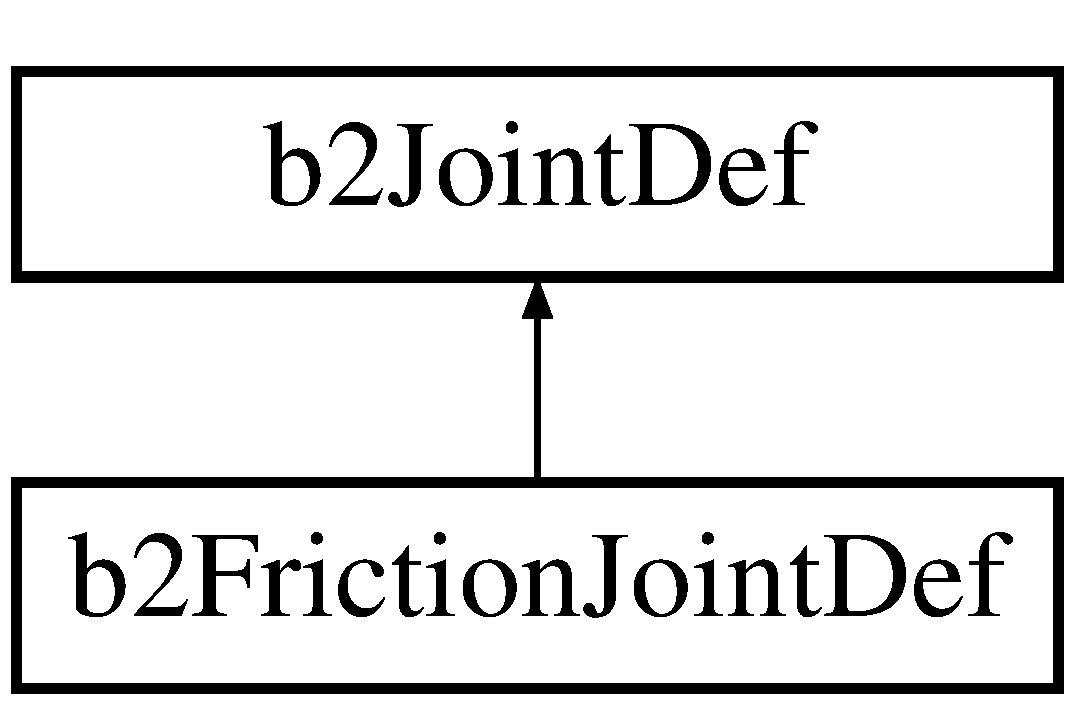
\includegraphics[height=2.000000cm]{structb2_friction_joint_def}
\end{center}
\end{figure}
\subsection*{Public Member Functions}
\begin{DoxyCompactItemize}
\item 
void \hyperlink{structb2_friction_joint_def_aee104f2aeb34dec4e17e3c52a98f7915}{Initialize} (\hyperlink{classb2_body}{b2\+Body} $\ast$\hyperlink{structb2_joint_def_a8cd54c93da396be75a9788f2c6897f05}{bodyA}, \hyperlink{classb2_body}{b2\+Body} $\ast$\hyperlink{structb2_joint_def_aa4f4dee2fbcd12187b19506b60e68e3d}{bodyB}, const \hyperlink{structb2_vec2}{b2\+Vec2} \&anchor)
\end{DoxyCompactItemize}
\subsection*{Public Attributes}
\begin{DoxyCompactItemize}
\item 
\hyperlink{structb2_vec2}{b2\+Vec2} \hyperlink{structb2_friction_joint_def_a00b246e60ae282a956a42b662993e92a}{local\+AnchorA}\hypertarget{structb2_friction_joint_def_a00b246e60ae282a956a42b662993e92a}{}\label{structb2_friction_joint_def_a00b246e60ae282a956a42b662993e92a}

\begin{DoxyCompactList}\small\item\em The local anchor point relative to bodyA\textquotesingle{}s origin. \end{DoxyCompactList}\item 
\hyperlink{structb2_vec2}{b2\+Vec2} \hyperlink{structb2_friction_joint_def_ad6d5a5614a7ac77b13e53fda3e32ed05}{local\+AnchorB}\hypertarget{structb2_friction_joint_def_ad6d5a5614a7ac77b13e53fda3e32ed05}{}\label{structb2_friction_joint_def_ad6d5a5614a7ac77b13e53fda3e32ed05}

\begin{DoxyCompactList}\small\item\em The local anchor point relative to bodyB\textquotesingle{}s origin. \end{DoxyCompactList}\item 
float32 \hyperlink{structb2_friction_joint_def_ad30e97a80790d4ca64bac7a1fa7d1b35}{max\+Force}\hypertarget{structb2_friction_joint_def_ad30e97a80790d4ca64bac7a1fa7d1b35}{}\label{structb2_friction_joint_def_ad30e97a80790d4ca64bac7a1fa7d1b35}

\begin{DoxyCompactList}\small\item\em The maximum friction force in N. \end{DoxyCompactList}\item 
float32 \hyperlink{structb2_friction_joint_def_a61adfb0ee7c0ed4cb8feee8304c16ef6}{max\+Torque}\hypertarget{structb2_friction_joint_def_a61adfb0ee7c0ed4cb8feee8304c16ef6}{}\label{structb2_friction_joint_def_a61adfb0ee7c0ed4cb8feee8304c16ef6}

\begin{DoxyCompactList}\small\item\em The maximum friction torque in N-\/m. \end{DoxyCompactList}\end{DoxyCompactItemize}


\subsection{Detailed Description}
Friction joint definition. 

\subsection{Member Function Documentation}
\index{b2\+Friction\+Joint\+Def@{b2\+Friction\+Joint\+Def}!Initialize@{Initialize}}
\index{Initialize@{Initialize}!b2\+Friction\+Joint\+Def@{b2\+Friction\+Joint\+Def}}
\subsubsection[{\texorpdfstring{Initialize(b2\+Body $\ast$body\+A, b2\+Body $\ast$body\+B, const b2\+Vec2 \&anchor)}{Initialize(b2Body *bodyA, b2Body *bodyB, const b2Vec2 &anchor)}}]{\setlength{\rightskip}{0pt plus 5cm}void b2\+Friction\+Joint\+Def\+::\+Initialize (
\begin{DoxyParamCaption}
\item[{{\bf b2\+Body} $\ast$}]{bodyA, }
\item[{{\bf b2\+Body} $\ast$}]{bodyB, }
\item[{const {\bf b2\+Vec2} \&}]{anchor}
\end{DoxyParamCaption}
)}\hypertarget{structb2_friction_joint_def_aee104f2aeb34dec4e17e3c52a98f7915}{}\label{structb2_friction_joint_def_aee104f2aeb34dec4e17e3c52a98f7915}
Initialize the bodies, anchors, axis, and reference angle using the world anchor and world axis. 

The documentation for this struct was generated from the following file\+:\begin{DoxyCompactItemize}
\item 
C\+:/\+Users/\+Bilal Itani/\+Desktop/inf2990-\/11/\+Cadriciel/\+Commun/\+Externe/\+Box2\+D/include/\+Box2\+D/\+Dynamics/\+Joints/b2\+Friction\+Joint.\+h\end{DoxyCompactItemize}

\hypertarget{classb2_gear_joint}{}\section{b2\+Gear\+Joint Class Reference}
\label{classb2_gear_joint}\index{b2\+Gear\+Joint@{b2\+Gear\+Joint}}


{\ttfamily \#include $<$b2\+Gear\+Joint.\+h$>$}

Inheritance diagram for b2\+Gear\+Joint\+:\begin{figure}[H]
\begin{center}
\leavevmode
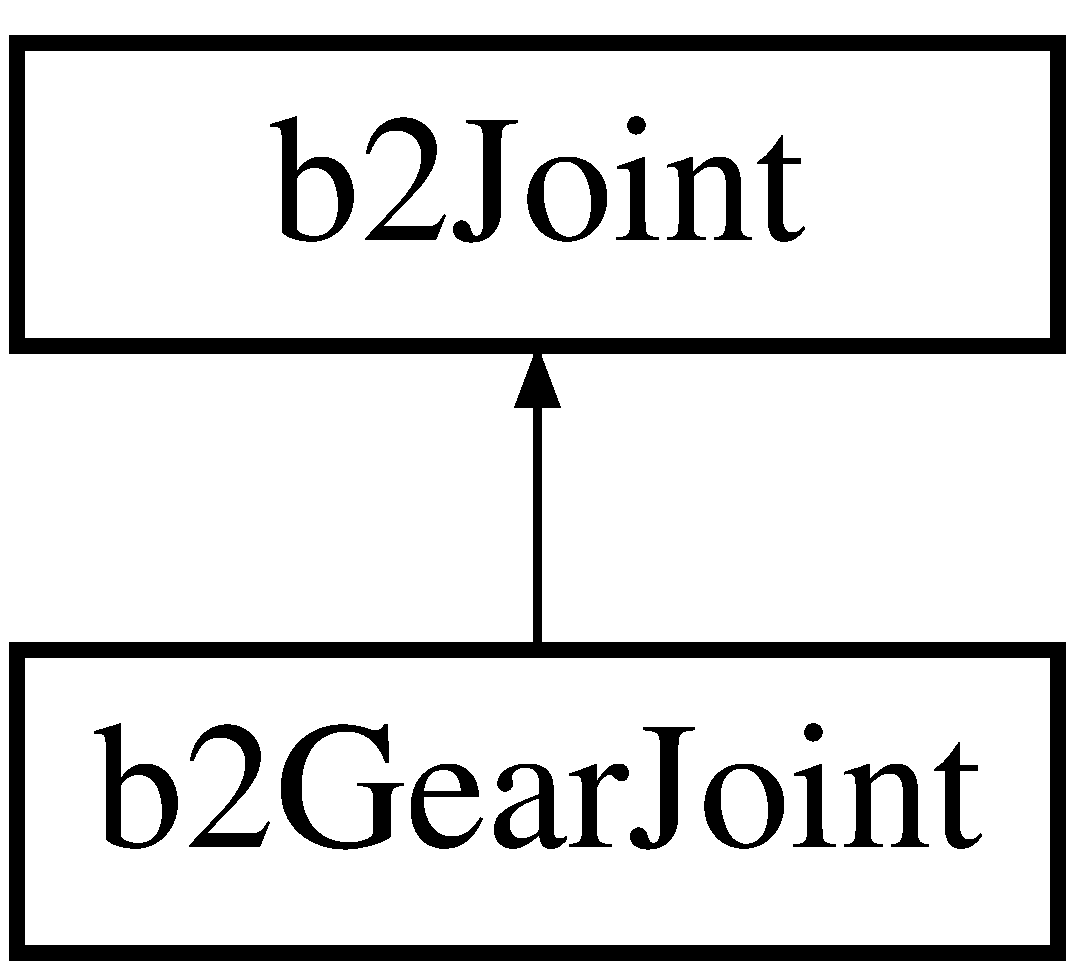
\includegraphics[height=2.000000cm]{classb2_gear_joint}
\end{center}
\end{figure}
\subsection*{Public Member Functions}
\begin{DoxyCompactItemize}
\item 
\hyperlink{structb2_vec2}{b2\+Vec2} \hyperlink{classb2_gear_joint_a2b5cdcb78c7ac3df4bd47e4195443a05}{Get\+AnchorA} () const \hypertarget{classb2_gear_joint_a2b5cdcb78c7ac3df4bd47e4195443a05}{}\label{classb2_gear_joint_a2b5cdcb78c7ac3df4bd47e4195443a05}

\begin{DoxyCompactList}\small\item\em Get the anchor point on bodyA in world coordinates. \end{DoxyCompactList}\item 
\hyperlink{structb2_vec2}{b2\+Vec2} \hyperlink{classb2_gear_joint_a84b9aedb8918a98b84032c9f0f823e13}{Get\+AnchorB} () const \hypertarget{classb2_gear_joint_a84b9aedb8918a98b84032c9f0f823e13}{}\label{classb2_gear_joint_a84b9aedb8918a98b84032c9f0f823e13}

\begin{DoxyCompactList}\small\item\em Get the anchor point on bodyB in world coordinates. \end{DoxyCompactList}\item 
\hyperlink{structb2_vec2}{b2\+Vec2} \hyperlink{classb2_gear_joint_ad415f3db70ba3e60a132ef668c263713}{Get\+Reaction\+Force} (float32 inv\+\_\+dt) const \hypertarget{classb2_gear_joint_ad415f3db70ba3e60a132ef668c263713}{}\label{classb2_gear_joint_ad415f3db70ba3e60a132ef668c263713}

\begin{DoxyCompactList}\small\item\em Get the reaction force on bodyB at the joint anchor in Newtons. \end{DoxyCompactList}\item 
float32 \hyperlink{classb2_gear_joint_ae2c4b1ae1cf00f14331332c4fe9ae964}{Get\+Reaction\+Torque} (float32 inv\+\_\+dt) const \hypertarget{classb2_gear_joint_ae2c4b1ae1cf00f14331332c4fe9ae964}{}\label{classb2_gear_joint_ae2c4b1ae1cf00f14331332c4fe9ae964}

\begin{DoxyCompactList}\small\item\em Get the reaction torque on bodyB in N$\ast$m. \end{DoxyCompactList}\item 
\hyperlink{classb2_joint}{b2\+Joint} $\ast$ \hyperlink{classb2_gear_joint_acd3fb38982319f387d1eb7aeddd5311f}{Get\+Joint1} ()\hypertarget{classb2_gear_joint_acd3fb38982319f387d1eb7aeddd5311f}{}\label{classb2_gear_joint_acd3fb38982319f387d1eb7aeddd5311f}

\begin{DoxyCompactList}\small\item\em Get the first joint. \end{DoxyCompactList}\item 
\hyperlink{classb2_joint}{b2\+Joint} $\ast$ \hyperlink{classb2_gear_joint_af1673b8edd80f3ae3b868c3a18b7b058}{Get\+Joint2} ()\hypertarget{classb2_gear_joint_af1673b8edd80f3ae3b868c3a18b7b058}{}\label{classb2_gear_joint_af1673b8edd80f3ae3b868c3a18b7b058}

\begin{DoxyCompactList}\small\item\em Get the second joint. \end{DoxyCompactList}\item 
void \hyperlink{classb2_gear_joint_a21c867bdc00c15ade2f399d370f92636}{Set\+Ratio} (float32 ratio)\hypertarget{classb2_gear_joint_a21c867bdc00c15ade2f399d370f92636}{}\label{classb2_gear_joint_a21c867bdc00c15ade2f399d370f92636}

\begin{DoxyCompactList}\small\item\em Set/\+Get the gear ratio. \end{DoxyCompactList}\item 
float32 {\bfseries Get\+Ratio} () const \hypertarget{classb2_gear_joint_a72758d0f94cb9bea6074d29a98d79162}{}\label{classb2_gear_joint_a72758d0f94cb9bea6074d29a98d79162}

\item 
void \hyperlink{classb2_gear_joint_a1620b5a39e9da2b40d324c45736ad322}{Dump} ()\hypertarget{classb2_gear_joint_a1620b5a39e9da2b40d324c45736ad322}{}\label{classb2_gear_joint_a1620b5a39e9da2b40d324c45736ad322}

\begin{DoxyCompactList}\small\item\em Dump joint to dm\+Log. \end{DoxyCompactList}\end{DoxyCompactItemize}
\subsection*{Protected Member Functions}
\begin{DoxyCompactItemize}
\item 
{\bfseries b2\+Gear\+Joint} (const \hyperlink{structb2_gear_joint_def}{b2\+Gear\+Joint\+Def} $\ast$data)\hypertarget{classb2_gear_joint_a4b247c79e74cb1e5b906527fe7d151ce}{}\label{classb2_gear_joint_a4b247c79e74cb1e5b906527fe7d151ce}

\item 
void {\bfseries Init\+Velocity\+Constraints} (const \hyperlink{structb2_solver_data}{b2\+Solver\+Data} \&data)\hypertarget{classb2_gear_joint_ad1d8e7b5434ad899c510dd223a72e6cb}{}\label{classb2_gear_joint_ad1d8e7b5434ad899c510dd223a72e6cb}

\item 
void {\bfseries Solve\+Velocity\+Constraints} (const \hyperlink{structb2_solver_data}{b2\+Solver\+Data} \&data)\hypertarget{classb2_gear_joint_a7684e28e93a3dc88a0e84424be937355}{}\label{classb2_gear_joint_a7684e28e93a3dc88a0e84424be937355}

\item 
bool {\bfseries Solve\+Position\+Constraints} (const \hyperlink{structb2_solver_data}{b2\+Solver\+Data} \&data)\hypertarget{classb2_gear_joint_a6be119465783ecb3f055695c7a713de2}{}\label{classb2_gear_joint_a6be119465783ecb3f055695c7a713de2}

\end{DoxyCompactItemize}
\subsection*{Protected Attributes}
\begin{DoxyCompactItemize}
\item 
\hyperlink{classb2_joint}{b2\+Joint} $\ast$ {\bfseries m\+\_\+joint1}\hypertarget{classb2_gear_joint_a7694fc4574c774c22a8c202e0d49fd84}{}\label{classb2_gear_joint_a7694fc4574c774c22a8c202e0d49fd84}

\item 
\hyperlink{classb2_joint}{b2\+Joint} $\ast$ {\bfseries m\+\_\+joint2}\hypertarget{classb2_gear_joint_a94290117dd4f2467eee49ecc150b9eb6}{}\label{classb2_gear_joint_a94290117dd4f2467eee49ecc150b9eb6}

\item 
b2\+Joint\+Type {\bfseries m\+\_\+typeA}\hypertarget{classb2_gear_joint_a0819b72c766d69cb1995f6cca4e98853}{}\label{classb2_gear_joint_a0819b72c766d69cb1995f6cca4e98853}

\item 
b2\+Joint\+Type {\bfseries m\+\_\+typeB}\hypertarget{classb2_gear_joint_a03e1959e04a361db79ae5da5ba76379e}{}\label{classb2_gear_joint_a03e1959e04a361db79ae5da5ba76379e}

\item 
\hyperlink{classb2_body}{b2\+Body} $\ast$ {\bfseries m\+\_\+bodyC}\hypertarget{classb2_gear_joint_a07e5f85b71bf335552835989dc013fe6}{}\label{classb2_gear_joint_a07e5f85b71bf335552835989dc013fe6}

\item 
\hyperlink{classb2_body}{b2\+Body} $\ast$ {\bfseries m\+\_\+bodyD}\hypertarget{classb2_gear_joint_ad3a1795c11b652b4b2f8bfc3ed96cb0b}{}\label{classb2_gear_joint_ad3a1795c11b652b4b2f8bfc3ed96cb0b}

\item 
\hyperlink{structb2_vec2}{b2\+Vec2} {\bfseries m\+\_\+local\+AnchorA}\hypertarget{classb2_gear_joint_acac78f2e3730fda540d1c7a74889bfc5}{}\label{classb2_gear_joint_acac78f2e3730fda540d1c7a74889bfc5}

\item 
\hyperlink{structb2_vec2}{b2\+Vec2} {\bfseries m\+\_\+local\+AnchorB}\hypertarget{classb2_gear_joint_a864c3d4d7944f72783a073993530d9fd}{}\label{classb2_gear_joint_a864c3d4d7944f72783a073993530d9fd}

\item 
\hyperlink{structb2_vec2}{b2\+Vec2} {\bfseries m\+\_\+local\+AnchorC}\hypertarget{classb2_gear_joint_a9361797683a30e70afd5b8690fe47ba3}{}\label{classb2_gear_joint_a9361797683a30e70afd5b8690fe47ba3}

\item 
\hyperlink{structb2_vec2}{b2\+Vec2} {\bfseries m\+\_\+local\+AnchorD}\hypertarget{classb2_gear_joint_abdd5be52535b5b56e44fc27832d057d2}{}\label{classb2_gear_joint_abdd5be52535b5b56e44fc27832d057d2}

\item 
\hyperlink{structb2_vec2}{b2\+Vec2} {\bfseries m\+\_\+local\+AxisC}\hypertarget{classb2_gear_joint_a52ae3b3a06ad9dae6b3201404784cc18}{}\label{classb2_gear_joint_a52ae3b3a06ad9dae6b3201404784cc18}

\item 
\hyperlink{structb2_vec2}{b2\+Vec2} {\bfseries m\+\_\+local\+AxisD}\hypertarget{classb2_gear_joint_a49cc9f1b74793dce3311cf7a35a8aee1}{}\label{classb2_gear_joint_a49cc9f1b74793dce3311cf7a35a8aee1}

\item 
float32 {\bfseries m\+\_\+reference\+AngleA}\hypertarget{classb2_gear_joint_a1ba0c6172cd2dd2017813bab7d1b268b}{}\label{classb2_gear_joint_a1ba0c6172cd2dd2017813bab7d1b268b}

\item 
float32 {\bfseries m\+\_\+reference\+AngleB}\hypertarget{classb2_gear_joint_a553920f723a1b7a38fd1d671101c5e4e}{}\label{classb2_gear_joint_a553920f723a1b7a38fd1d671101c5e4e}

\item 
float32 {\bfseries m\+\_\+constant}\hypertarget{classb2_gear_joint_af67d237380cdcbfe93053b1ceb72f17b}{}\label{classb2_gear_joint_af67d237380cdcbfe93053b1ceb72f17b}

\item 
float32 {\bfseries m\+\_\+ratio}\hypertarget{classb2_gear_joint_ad6b9106922b65f873dd02c6e68e6778a}{}\label{classb2_gear_joint_ad6b9106922b65f873dd02c6e68e6778a}

\item 
float32 {\bfseries m\+\_\+impulse}\hypertarget{classb2_gear_joint_ae19e7fb67c7623f39776f1160b76d62f}{}\label{classb2_gear_joint_ae19e7fb67c7623f39776f1160b76d62f}

\item 
int32 {\bfseries m\+\_\+indexA}\hypertarget{classb2_gear_joint_adb00e71e60a222e432b57c95c38b8bd7}{}\label{classb2_gear_joint_adb00e71e60a222e432b57c95c38b8bd7}

\item 
int32 {\bfseries m\+\_\+indexB}\hypertarget{classb2_gear_joint_a5cf185f4e4b5d5e1780ba2c085ec2e6e}{}\label{classb2_gear_joint_a5cf185f4e4b5d5e1780ba2c085ec2e6e}

\item 
int32 {\bfseries m\+\_\+indexC}\hypertarget{classb2_gear_joint_a46528e9a9a33a4d67dd5b2abb3d1dec5}{}\label{classb2_gear_joint_a46528e9a9a33a4d67dd5b2abb3d1dec5}

\item 
int32 {\bfseries m\+\_\+indexD}\hypertarget{classb2_gear_joint_a068be34dbdf39ac59c7a5bb7777d550f}{}\label{classb2_gear_joint_a068be34dbdf39ac59c7a5bb7777d550f}

\item 
\hyperlink{structb2_vec2}{b2\+Vec2} {\bfseries m\+\_\+lcA}\hypertarget{classb2_gear_joint_afb46a5545846cc085f2aad02a05acc86}{}\label{classb2_gear_joint_afb46a5545846cc085f2aad02a05acc86}

\item 
\hyperlink{structb2_vec2}{b2\+Vec2} {\bfseries m\+\_\+lcB}\hypertarget{classb2_gear_joint_a4f933756b7e6b9ec060b105d0fb6689b}{}\label{classb2_gear_joint_a4f933756b7e6b9ec060b105d0fb6689b}

\item 
\hyperlink{structb2_vec2}{b2\+Vec2} {\bfseries m\+\_\+lcC}\hypertarget{classb2_gear_joint_a9eaca477247eb71dae06f12842bc636d}{}\label{classb2_gear_joint_a9eaca477247eb71dae06f12842bc636d}

\item 
\hyperlink{structb2_vec2}{b2\+Vec2} {\bfseries m\+\_\+lcD}\hypertarget{classb2_gear_joint_a21c4c7aa8c0ba7ccf9d4f786a31e5553}{}\label{classb2_gear_joint_a21c4c7aa8c0ba7ccf9d4f786a31e5553}

\item 
float32 {\bfseries m\+\_\+mA}\hypertarget{classb2_gear_joint_a5f425a3ff6a4d08090be512ee56993c5}{}\label{classb2_gear_joint_a5f425a3ff6a4d08090be512ee56993c5}

\item 
float32 {\bfseries m\+\_\+mB}\hypertarget{classb2_gear_joint_a83985722b901f36b59e29b98c2bbb1af}{}\label{classb2_gear_joint_a83985722b901f36b59e29b98c2bbb1af}

\item 
float32 {\bfseries m\+\_\+mC}\hypertarget{classb2_gear_joint_a79253d1b43531e5acdf36a3f710c583a}{}\label{classb2_gear_joint_a79253d1b43531e5acdf36a3f710c583a}

\item 
float32 {\bfseries m\+\_\+mD}\hypertarget{classb2_gear_joint_a7a3685b9bb07b2d81c58b96ff662c5ce}{}\label{classb2_gear_joint_a7a3685b9bb07b2d81c58b96ff662c5ce}

\item 
float32 {\bfseries m\+\_\+iA}\hypertarget{classb2_gear_joint_a138784eb59950e25125e45087945b717}{}\label{classb2_gear_joint_a138784eb59950e25125e45087945b717}

\item 
float32 {\bfseries m\+\_\+iB}\hypertarget{classb2_gear_joint_acca792262071441bd6fbfc891fcaf942}{}\label{classb2_gear_joint_acca792262071441bd6fbfc891fcaf942}

\item 
float32 {\bfseries m\+\_\+iC}\hypertarget{classb2_gear_joint_ac4e6493093914f78e0c8f79248041a1c}{}\label{classb2_gear_joint_ac4e6493093914f78e0c8f79248041a1c}

\item 
float32 {\bfseries m\+\_\+iD}\hypertarget{classb2_gear_joint_ad05416c4e98a30e4eb9297ff20b38c1a}{}\label{classb2_gear_joint_ad05416c4e98a30e4eb9297ff20b38c1a}

\item 
\hyperlink{structb2_vec2}{b2\+Vec2} {\bfseries m\+\_\+\+Jv\+AC}\hypertarget{classb2_gear_joint_a23eb9f668936f931d40f930e085dd5a0}{}\label{classb2_gear_joint_a23eb9f668936f931d40f930e085dd5a0}

\item 
\hyperlink{structb2_vec2}{b2\+Vec2} {\bfseries m\+\_\+\+Jv\+BD}\hypertarget{classb2_gear_joint_ab00b00c061d8b9e461f76ac4d72aac8c}{}\label{classb2_gear_joint_ab00b00c061d8b9e461f76ac4d72aac8c}

\item 
float32 {\bfseries m\+\_\+\+JwA}\hypertarget{classb2_gear_joint_a3774fc69538e658f123d9437934aed70}{}\label{classb2_gear_joint_a3774fc69538e658f123d9437934aed70}

\item 
float32 {\bfseries m\+\_\+\+JwB}\hypertarget{classb2_gear_joint_afcdb0ebe31ff8039771d006f4b87645c}{}\label{classb2_gear_joint_afcdb0ebe31ff8039771d006f4b87645c}

\item 
float32 {\bfseries m\+\_\+\+JwC}\hypertarget{classb2_gear_joint_ac9b8f418c8f79392049afdf18aa6dc3e}{}\label{classb2_gear_joint_ac9b8f418c8f79392049afdf18aa6dc3e}

\item 
float32 {\bfseries m\+\_\+\+JwD}\hypertarget{classb2_gear_joint_ac2d00521ef5f7c27b1747ad54d4ad5c2}{}\label{classb2_gear_joint_ac2d00521ef5f7c27b1747ad54d4ad5c2}

\item 
float32 {\bfseries m\+\_\+mass}\hypertarget{classb2_gear_joint_a71ac3578918bc97d257d652777b6b87f}{}\label{classb2_gear_joint_a71ac3578918bc97d257d652777b6b87f}

\end{DoxyCompactItemize}
\subsection*{Friends}
\begin{DoxyCompactItemize}
\item 
class {\bfseries b2\+Joint}\hypertarget{classb2_gear_joint_a54ade8ed3d794298108d7f4c4e4793fa}{}\label{classb2_gear_joint_a54ade8ed3d794298108d7f4c4e4793fa}

\end{DoxyCompactItemize}
\subsection*{Additional Inherited Members}


\subsection{Detailed Description}
A gear joint is used to connect two joints together. Either joint can be a revolute or prismatic joint. You specify a gear ratio to bind the motions together\+: coordinate1 + ratio $\ast$ coordinate2 = constant The ratio can be negative or positive. If one joint is a revolute joint and the other joint is a prismatic joint, then the ratio will have units of length or units of 1/length. \begin{DoxyWarning}{Warning}
You have to manually destroy the gear joint if joint1 or joint2 is destroyed. 
\end{DoxyWarning}


The documentation for this class was generated from the following file\+:\begin{DoxyCompactItemize}
\item 
Commun/\+Externe/\+Box2\+D/include/\+Box2\+D/\+Dynamics/\+Joints/b2\+Gear\+Joint.\+h\end{DoxyCompactItemize}

\hypertarget{structb2_gear_joint_def}{}\section{b2\+Gear\+Joint\+Def Struct Reference}
\label{structb2_gear_joint_def}\index{b2\+Gear\+Joint\+Def@{b2\+Gear\+Joint\+Def}}


{\ttfamily \#include $<$b2\+Gear\+Joint.\+h$>$}

Inheritance diagram for b2\+Gear\+Joint\+Def\+:\begin{figure}[H]
\begin{center}
\leavevmode
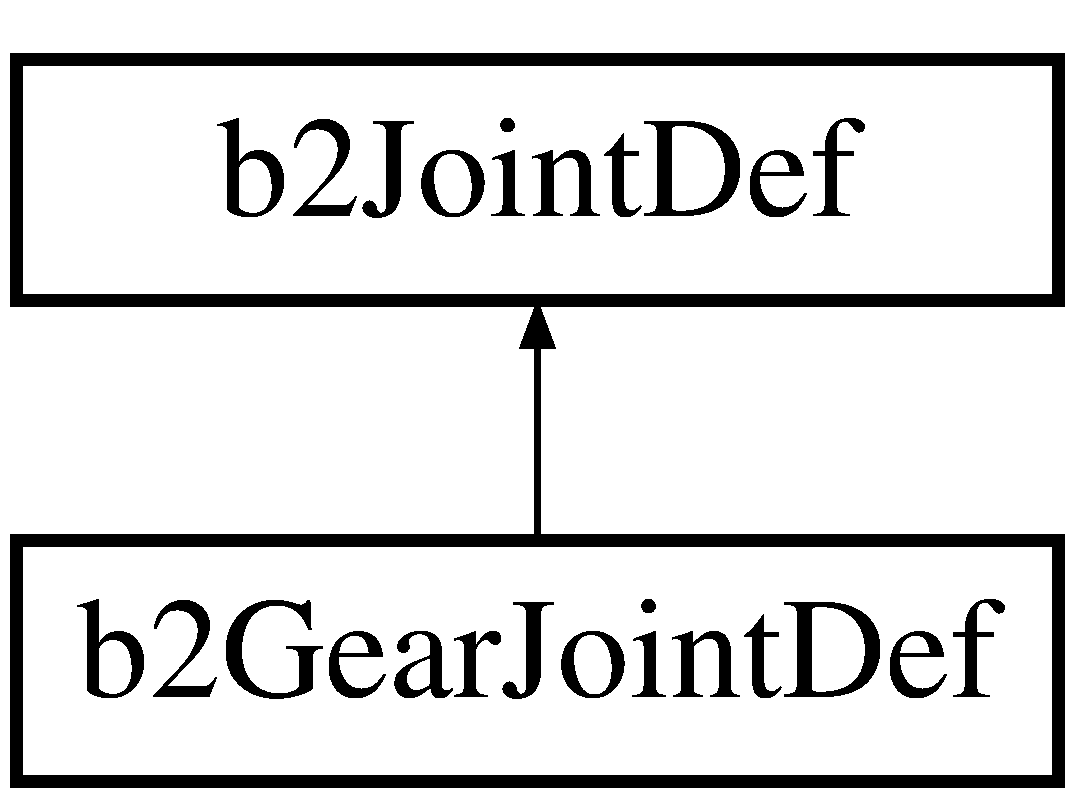
\includegraphics[height=2.000000cm]{structb2_gear_joint_def}
\end{center}
\end{figure}
\subsection*{Public Attributes}
\begin{DoxyCompactItemize}
\item 
\hyperlink{classb2_joint}{b2\+Joint} $\ast$ \hyperlink{structb2_gear_joint_def_ae42d33b54291a9e256f3810926883473}{joint1}\hypertarget{structb2_gear_joint_def_ae42d33b54291a9e256f3810926883473}{}\label{structb2_gear_joint_def_ae42d33b54291a9e256f3810926883473}

\begin{DoxyCompactList}\small\item\em The first revolute/prismatic joint attached to the gear joint. \end{DoxyCompactList}\item 
\hyperlink{classb2_joint}{b2\+Joint} $\ast$ \hyperlink{structb2_gear_joint_def_a73cf056fe40e63355073a01b097f4c82}{joint2}\hypertarget{structb2_gear_joint_def_a73cf056fe40e63355073a01b097f4c82}{}\label{structb2_gear_joint_def_a73cf056fe40e63355073a01b097f4c82}

\begin{DoxyCompactList}\small\item\em The second revolute/prismatic joint attached to the gear joint. \end{DoxyCompactList}\item 
float32 \hyperlink{structb2_gear_joint_def_a57e9f4b6ce1ddc8b89b8455515f69323}{ratio}
\end{DoxyCompactItemize}


\subsection{Detailed Description}
Gear joint definition. This definition requires two existing revolute or prismatic joints (any combination will work). 

\subsection{Member Data Documentation}
\index{b2\+Gear\+Joint\+Def@{b2\+Gear\+Joint\+Def}!ratio@{ratio}}
\index{ratio@{ratio}!b2\+Gear\+Joint\+Def@{b2\+Gear\+Joint\+Def}}
\subsubsection[{\texorpdfstring{ratio}{ratio}}]{\setlength{\rightskip}{0pt plus 5cm}float32 b2\+Gear\+Joint\+Def\+::ratio}\hypertarget{structb2_gear_joint_def_a57e9f4b6ce1ddc8b89b8455515f69323}{}\label{structb2_gear_joint_def_a57e9f4b6ce1ddc8b89b8455515f69323}
The gear ratio. \begin{DoxySeeAlso}{See also}
\hyperlink{classb2_gear_joint}{b2\+Gear\+Joint} for explanation. 
\end{DoxySeeAlso}


The documentation for this struct was generated from the following file\+:\begin{DoxyCompactItemize}
\item 
C\+:/\+Users/\+Bilal Itani/\+Desktop/inf2990-\/11/\+Cadriciel/\+Commun/\+Externe/\+Box2\+D/include/\+Box2\+D/\+Dynamics/\+Joints/b2\+Gear\+Joint.\+h\end{DoxyCompactItemize}

\hypertarget{classb2_growable_stack}{}\section{b2\+Growable\+Stack$<$ T, N $>$ Class Template Reference}
\label{classb2_growable_stack}\index{b2\+Growable\+Stack$<$ T, N $>$@{b2\+Growable\+Stack$<$ T, N $>$}}


{\ttfamily \#include $<$b2\+Growable\+Stack.\+h$>$}

\subsection*{Public Member Functions}
\begin{DoxyCompactItemize}
\item 
void {\bfseries Push} (const T \&element)\hypertarget{classb2_growable_stack_a23661327d64ff72d1ec8d6bcdb6d8992}{}\label{classb2_growable_stack_a23661327d64ff72d1ec8d6bcdb6d8992}

\item 
T {\bfseries Pop} ()\hypertarget{classb2_growable_stack_a53e53dcd6bff8308405a881f02957bc8}{}\label{classb2_growable_stack_a53e53dcd6bff8308405a881f02957bc8}

\item 
int32 {\bfseries Get\+Count} ()\hypertarget{classb2_growable_stack_a3049e76ba7182b988450bfe94d30d5aa}{}\label{classb2_growable_stack_a3049e76ba7182b988450bfe94d30d5aa}

\end{DoxyCompactItemize}
\subsection*{Private Attributes}
\begin{DoxyCompactItemize}
\item 
T $\ast$ {\bfseries m\+\_\+stack}\hypertarget{classb2_growable_stack_a0ffe2286a06066938a7413cef5689e7d}{}\label{classb2_growable_stack_a0ffe2286a06066938a7413cef5689e7d}

\item 
T {\bfseries m\+\_\+array} \mbox{[}N\mbox{]}\hypertarget{classb2_growable_stack_a0df427a912ca2e6d8eecfc10e84162b3}{}\label{classb2_growable_stack_a0df427a912ca2e6d8eecfc10e84162b3}

\item 
int32 {\bfseries m\+\_\+count}\hypertarget{classb2_growable_stack_ab1ac57e30436c7501677143e0d7a051b}{}\label{classb2_growable_stack_ab1ac57e30436c7501677143e0d7a051b}

\item 
int32 {\bfseries m\+\_\+capacity}\hypertarget{classb2_growable_stack_aede2309b9194c72f7096da16e2bb8c0a}{}\label{classb2_growable_stack_aede2309b9194c72f7096da16e2bb8c0a}

\end{DoxyCompactItemize}


\subsection{Detailed Description}
\subsubsection*{template$<$typename T, int32 N$>$\\*
class b2\+Growable\+Stack$<$ T, N $>$}

This is a growable L\+I\+FO stack with an initial capacity of N. If the stack size exceeds the initial capacity, the heap is used to increase the size of the stack. 

The documentation for this class was generated from the following file\+:\begin{DoxyCompactItemize}
\item 
Commun/\+Externe/\+Box2\+D/include/\+Box2\+D/\+Common/b2\+Growable\+Stack.\+h\end{DoxyCompactItemize}

\hypertarget{classb2_island}{}\section{b2\+Island Class Reference}
\label{classb2_island}\index{b2\+Island@{b2\+Island}}


This is an internal class.  




{\ttfamily \#include $<$b2\+Island.\+h$>$}

\subsection*{Public Member Functions}
\begin{DoxyCompactItemize}
\item 
{\bfseries b2\+Island} (int32 body\+Capacity, int32 contact\+Capacity, int32 joint\+Capacity, \hyperlink{classb2_stack_allocator}{b2\+Stack\+Allocator} $\ast$allocator, \hyperlink{classb2_contact_listener}{b2\+Contact\+Listener} $\ast$listener)\hypertarget{classb2_island_a2f2258f09d2663dcb35a1d69d16896cb}{}\label{classb2_island_a2f2258f09d2663dcb35a1d69d16896cb}

\item 
void {\bfseries Clear} ()\hypertarget{classb2_island_a26566f7388fcaf7523446e5e76d99c4d}{}\label{classb2_island_a26566f7388fcaf7523446e5e76d99c4d}

\item 
void {\bfseries Solve} (\hyperlink{structb2_profile}{b2\+Profile} $\ast$profile, const \hyperlink{structb2_time_step}{b2\+Time\+Step} \&step, const \hyperlink{structb2_vec2}{b2\+Vec2} \&gravity, bool allow\+Sleep)\hypertarget{classb2_island_a28a6f74174cde3a6e93663c740f418fa}{}\label{classb2_island_a28a6f74174cde3a6e93663c740f418fa}

\item 
void {\bfseries Solve\+T\+OI} (const \hyperlink{structb2_time_step}{b2\+Time\+Step} \&sub\+Step, int32 toi\+IndexA, int32 toi\+IndexB)\hypertarget{classb2_island_a61f577b473962bb0d8add1f55eeef7ee}{}\label{classb2_island_a61f577b473962bb0d8add1f55eeef7ee}

\item 
void {\bfseries Add} (\hyperlink{classb2_body}{b2\+Body} $\ast$body)\hypertarget{classb2_island_af2d54861bd063051c0a6dc5f73b27c3e}{}\label{classb2_island_af2d54861bd063051c0a6dc5f73b27c3e}

\item 
void {\bfseries Add} (\hyperlink{classb2_contact}{b2\+Contact} $\ast$contact)\hypertarget{classb2_island_abc0ea9208e818b551404fd507f197a51}{}\label{classb2_island_abc0ea9208e818b551404fd507f197a51}

\item 
void {\bfseries Add} (\hyperlink{classb2_joint}{b2\+Joint} $\ast$joint)\hypertarget{classb2_island_a04e6ccd0c11f6ef5a7ed0a926d081445}{}\label{classb2_island_a04e6ccd0c11f6ef5a7ed0a926d081445}

\item 
void {\bfseries Report} (const \hyperlink{structb2_contact_velocity_constraint}{b2\+Contact\+Velocity\+Constraint} $\ast$constraints)\hypertarget{classb2_island_a57620f76faf000f61c76e925e40e6129}{}\label{classb2_island_a57620f76faf000f61c76e925e40e6129}

\end{DoxyCompactItemize}
\subsection*{Public Attributes}
\begin{DoxyCompactItemize}
\item 
\hyperlink{classb2_stack_allocator}{b2\+Stack\+Allocator} $\ast$ {\bfseries m\+\_\+allocator}\hypertarget{classb2_island_a5e28f216c0a12548c04491ab1d73c958}{}\label{classb2_island_a5e28f216c0a12548c04491ab1d73c958}

\item 
\hyperlink{classb2_contact_listener}{b2\+Contact\+Listener} $\ast$ {\bfseries m\+\_\+listener}\hypertarget{classb2_island_aeba73fe42839d0361524d98e330e8e66}{}\label{classb2_island_aeba73fe42839d0361524d98e330e8e66}

\item 
\hyperlink{classb2_body}{b2\+Body} $\ast$$\ast$ {\bfseries m\+\_\+bodies}\hypertarget{classb2_island_ac9c65abf14c88e8a52fdd2c5cb56c5f4}{}\label{classb2_island_ac9c65abf14c88e8a52fdd2c5cb56c5f4}

\item 
\hyperlink{classb2_contact}{b2\+Contact} $\ast$$\ast$ {\bfseries m\+\_\+contacts}\hypertarget{classb2_island_a49499a350859768a0c3f7b29fb091422}{}\label{classb2_island_a49499a350859768a0c3f7b29fb091422}

\item 
\hyperlink{classb2_joint}{b2\+Joint} $\ast$$\ast$ {\bfseries m\+\_\+joints}\hypertarget{classb2_island_a6653da11b66de22d8ba5db531c11b373}{}\label{classb2_island_a6653da11b66de22d8ba5db531c11b373}

\item 
\hyperlink{structb2_position}{b2\+Position} $\ast$ {\bfseries m\+\_\+positions}\hypertarget{classb2_island_a0f05bd177cf942ddfb494b17ec09b874}{}\label{classb2_island_a0f05bd177cf942ddfb494b17ec09b874}

\item 
\hyperlink{structb2_velocity}{b2\+Velocity} $\ast$ {\bfseries m\+\_\+velocities}\hypertarget{classb2_island_ae6a42be7ce4c03724a6da17d96cacb9f}{}\label{classb2_island_ae6a42be7ce4c03724a6da17d96cacb9f}

\item 
int32 {\bfseries m\+\_\+body\+Count}\hypertarget{classb2_island_af78d066321e18cd8a4e409c4539ccb81}{}\label{classb2_island_af78d066321e18cd8a4e409c4539ccb81}

\item 
int32 {\bfseries m\+\_\+joint\+Count}\hypertarget{classb2_island_a913c91afb35ff717c7dd5b0aa1559e5b}{}\label{classb2_island_a913c91afb35ff717c7dd5b0aa1559e5b}

\item 
int32 {\bfseries m\+\_\+contact\+Count}\hypertarget{classb2_island_ab5bad98e18356b15a68733be07b98abf}{}\label{classb2_island_ab5bad98e18356b15a68733be07b98abf}

\item 
int32 {\bfseries m\+\_\+body\+Capacity}\hypertarget{classb2_island_a5ea371889bb93fb6387ff2ab427191ed}{}\label{classb2_island_a5ea371889bb93fb6387ff2ab427191ed}

\item 
int32 {\bfseries m\+\_\+contact\+Capacity}\hypertarget{classb2_island_a1a65b8fc8256ca443f85e6ae6f2d841a}{}\label{classb2_island_a1a65b8fc8256ca443f85e6ae6f2d841a}

\item 
int32 {\bfseries m\+\_\+joint\+Capacity}\hypertarget{classb2_island_a9b6e63c89307d469e1075585d65a9bbb}{}\label{classb2_island_a9b6e63c89307d469e1075585d65a9bbb}

\end{DoxyCompactItemize}


\subsection{Detailed Description}
This is an internal class. 

The documentation for this class was generated from the following file\+:\begin{DoxyCompactItemize}
\item 
Cadriciel/\+Commun/\+Externe/\+Box2\+D/include/\+Box2\+D/\+Dynamics/b2\+Island.\+h\end{DoxyCompactItemize}

\hypertarget{structb2_jacobian}{}\section{b2\+Jacobian Struct Reference}
\label{structb2_jacobian}\index{b2\+Jacobian@{b2\+Jacobian}}
\subsection*{Public Attributes}
\begin{DoxyCompactItemize}
\item 
\hyperlink{structb2_vec2}{b2\+Vec2} {\bfseries linear}\hypertarget{structb2_jacobian_aa63199b443d411972b9cb6aac6c7cb34}{}\label{structb2_jacobian_aa63199b443d411972b9cb6aac6c7cb34}

\item 
float32 {\bfseries angularA}\hypertarget{structb2_jacobian_a0669f849afcdc154b36f86cb0529d2bc}{}\label{structb2_jacobian_a0669f849afcdc154b36f86cb0529d2bc}

\item 
float32 {\bfseries angularB}\hypertarget{structb2_jacobian_a3bbdbd8e46f4fa9be2e50434edaaeb14}{}\label{structb2_jacobian_a3bbdbd8e46f4fa9be2e50434edaaeb14}

\end{DoxyCompactItemize}


The documentation for this struct was generated from the following file\+:\begin{DoxyCompactItemize}
\item 
Commun/\+Externe/\+Box2\+D/include/\+Box2\+D/\+Dynamics/\+Joints/b2\+Joint.\+h\end{DoxyCompactItemize}

\hypertarget{classb2_joint}{}\section{b2\+Joint Class Reference}
\label{classb2_joint}\index{b2\+Joint@{b2\+Joint}}


{\ttfamily \#include $<$b2\+Joint.\+h$>$}

Inheritance diagram for b2\+Joint\+:\begin{figure}[H]
\begin{center}
\leavevmode
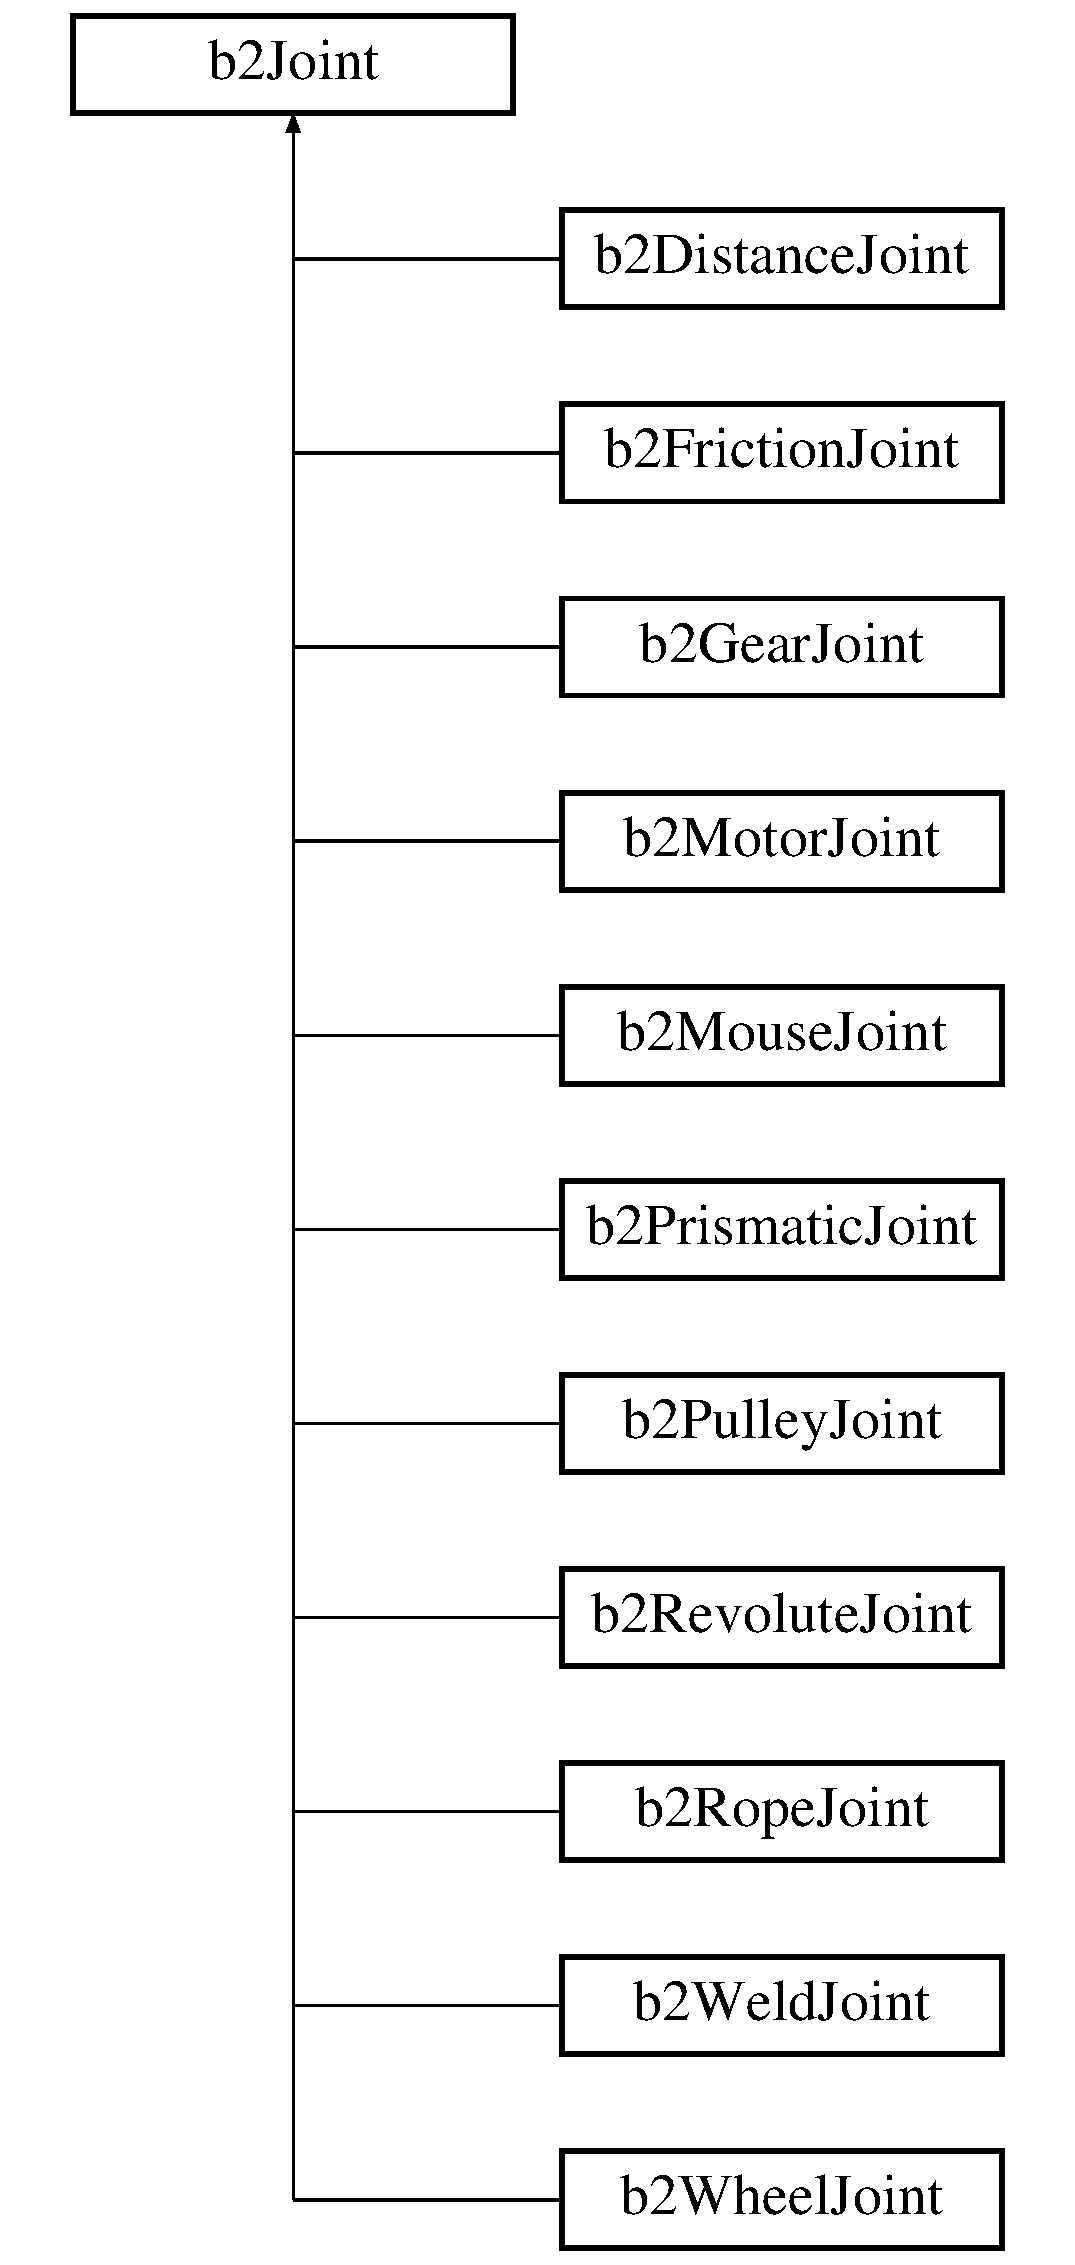
\includegraphics[height=12.000000cm]{classb2_joint}
\end{center}
\end{figure}
\subsection*{Public Member Functions}
\begin{DoxyCompactItemize}
\item 
b2\+Joint\+Type \hyperlink{classb2_joint_a37a2ca3f0d41c6903d2cc73757f02be2}{Get\+Type} () const \hypertarget{classb2_joint_a37a2ca3f0d41c6903d2cc73757f02be2}{}\label{classb2_joint_a37a2ca3f0d41c6903d2cc73757f02be2}

\begin{DoxyCompactList}\small\item\em Get the type of the concrete joint. \end{DoxyCompactList}\item 
\hyperlink{classb2_body}{b2\+Body} $\ast$ \hyperlink{classb2_joint_a2ed5eca3dbdce48665c14452b280613f}{Get\+BodyA} ()\hypertarget{classb2_joint_a2ed5eca3dbdce48665c14452b280613f}{}\label{classb2_joint_a2ed5eca3dbdce48665c14452b280613f}

\begin{DoxyCompactList}\small\item\em Get the first body attached to this joint. \end{DoxyCompactList}\item 
\hyperlink{classb2_body}{b2\+Body} $\ast$ \hyperlink{classb2_joint_a700b3d4c87f34f456151b9598e4641a0}{Get\+BodyB} ()\hypertarget{classb2_joint_a700b3d4c87f34f456151b9598e4641a0}{}\label{classb2_joint_a700b3d4c87f34f456151b9598e4641a0}

\begin{DoxyCompactList}\small\item\em Get the second body attached to this joint. \end{DoxyCompactList}\item 
virtual \hyperlink{structb2_vec2}{b2\+Vec2} \hyperlink{classb2_joint_a0e5b9b2c521cc797f691708285de79af}{Get\+AnchorA} () const  =0\hypertarget{classb2_joint_a0e5b9b2c521cc797f691708285de79af}{}\label{classb2_joint_a0e5b9b2c521cc797f691708285de79af}

\begin{DoxyCompactList}\small\item\em Get the anchor point on bodyA in world coordinates. \end{DoxyCompactList}\item 
virtual \hyperlink{structb2_vec2}{b2\+Vec2} \hyperlink{classb2_joint_af959abb4dc85cfba440ef94715b18959}{Get\+AnchorB} () const  =0\hypertarget{classb2_joint_af959abb4dc85cfba440ef94715b18959}{}\label{classb2_joint_af959abb4dc85cfba440ef94715b18959}

\begin{DoxyCompactList}\small\item\em Get the anchor point on bodyB in world coordinates. \end{DoxyCompactList}\item 
virtual \hyperlink{structb2_vec2}{b2\+Vec2} \hyperlink{classb2_joint_a7ab58d67a56ff173957286558b08118a}{Get\+Reaction\+Force} (float32 inv\+\_\+dt) const  =0\hypertarget{classb2_joint_a7ab58d67a56ff173957286558b08118a}{}\label{classb2_joint_a7ab58d67a56ff173957286558b08118a}

\begin{DoxyCompactList}\small\item\em Get the reaction force on bodyB at the joint anchor in Newtons. \end{DoxyCompactList}\item 
virtual float32 \hyperlink{classb2_joint_a0b1e4fcdea490c49a9ac1133e5244566}{Get\+Reaction\+Torque} (float32 inv\+\_\+dt) const  =0\hypertarget{classb2_joint_a0b1e4fcdea490c49a9ac1133e5244566}{}\label{classb2_joint_a0b1e4fcdea490c49a9ac1133e5244566}

\begin{DoxyCompactList}\small\item\em Get the reaction torque on bodyB in N$\ast$m. \end{DoxyCompactList}\item 
\hyperlink{classb2_joint}{b2\+Joint} $\ast$ \hyperlink{classb2_joint_a1a0e2137b631010750c728cb4e276e5d}{Get\+Next} ()\hypertarget{classb2_joint_a1a0e2137b631010750c728cb4e276e5d}{}\label{classb2_joint_a1a0e2137b631010750c728cb4e276e5d}

\begin{DoxyCompactList}\small\item\em Get the next joint the world joint list. \end{DoxyCompactList}\item 
const \hyperlink{classb2_joint}{b2\+Joint} $\ast$ {\bfseries Get\+Next} () const \hypertarget{classb2_joint_a1ac83edb39806085608c9d549dd98550}{}\label{classb2_joint_a1ac83edb39806085608c9d549dd98550}

\item 
void $\ast$ \hyperlink{classb2_joint_a505ab02c234f1cc20aa3375f3ab7b587}{Get\+User\+Data} () const \hypertarget{classb2_joint_a505ab02c234f1cc20aa3375f3ab7b587}{}\label{classb2_joint_a505ab02c234f1cc20aa3375f3ab7b587}

\begin{DoxyCompactList}\small\item\em Get the user data pointer. \end{DoxyCompactList}\item 
void \hyperlink{classb2_joint_a492f2d02496437572aaec6013ebdc1c8}{Set\+User\+Data} (void $\ast$data)\hypertarget{classb2_joint_a492f2d02496437572aaec6013ebdc1c8}{}\label{classb2_joint_a492f2d02496437572aaec6013ebdc1c8}

\begin{DoxyCompactList}\small\item\em Set the user data pointer. \end{DoxyCompactList}\item 
bool \hyperlink{classb2_joint_a825d3a6abb32014f31fd622f2bfc0363}{Is\+Active} () const \hypertarget{classb2_joint_a825d3a6abb32014f31fd622f2bfc0363}{}\label{classb2_joint_a825d3a6abb32014f31fd622f2bfc0363}

\begin{DoxyCompactList}\small\item\em Short-\/cut function to determine if either body is inactive. \end{DoxyCompactList}\item 
bool \hyperlink{classb2_joint_a09c6bdfa5842522ba381bac8dd559f4d}{Get\+Collide\+Connected} () const 
\item 
virtual void \hyperlink{classb2_joint_abd35e7316017ad9a40d5dbf9b5ba3f36}{Dump} ()\hypertarget{classb2_joint_abd35e7316017ad9a40d5dbf9b5ba3f36}{}\label{classb2_joint_abd35e7316017ad9a40d5dbf9b5ba3f36}

\begin{DoxyCompactList}\small\item\em Dump this joint to the log file. \end{DoxyCompactList}\item 
virtual void \hyperlink{classb2_joint_a7804f649e993dc0fd9ae47fde5601f90}{Shift\+Origin} (const \hyperlink{structb2_vec2}{b2\+Vec2} \&new\+Origin)\hypertarget{classb2_joint_a7804f649e993dc0fd9ae47fde5601f90}{}\label{classb2_joint_a7804f649e993dc0fd9ae47fde5601f90}

\begin{DoxyCompactList}\small\item\em Shift the origin for any points stored in world coordinates. \end{DoxyCompactList}\end{DoxyCompactItemize}
\subsection*{Protected Member Functions}
\begin{DoxyCompactItemize}
\item 
{\bfseries b2\+Joint} (const \hyperlink{structb2_joint_def}{b2\+Joint\+Def} $\ast$def)\hypertarget{classb2_joint_a8d6cce91546335fe95325d5e29c06a19}{}\label{classb2_joint_a8d6cce91546335fe95325d5e29c06a19}

\item 
virtual void {\bfseries Init\+Velocity\+Constraints} (const \hyperlink{structb2_solver_data}{b2\+Solver\+Data} \&data)=0\hypertarget{classb2_joint_a599c013de5514e02684b958b31dd76a4}{}\label{classb2_joint_a599c013de5514e02684b958b31dd76a4}

\item 
virtual void {\bfseries Solve\+Velocity\+Constraints} (const \hyperlink{structb2_solver_data}{b2\+Solver\+Data} \&data)=0\hypertarget{classb2_joint_ad302c8d02efcfe934158de0dc429348d}{}\label{classb2_joint_ad302c8d02efcfe934158de0dc429348d}

\item 
virtual bool {\bfseries Solve\+Position\+Constraints} (const \hyperlink{structb2_solver_data}{b2\+Solver\+Data} \&data)=0\hypertarget{classb2_joint_af767ac9aa494bd15cdf83dfe3e487d9c}{}\label{classb2_joint_af767ac9aa494bd15cdf83dfe3e487d9c}

\end{DoxyCompactItemize}
\subsection*{Static Protected Member Functions}
\begin{DoxyCompactItemize}
\item 
static \hyperlink{classb2_joint}{b2\+Joint} $\ast$ {\bfseries Create} (const \hyperlink{structb2_joint_def}{b2\+Joint\+Def} $\ast$def, \hyperlink{classb2_block_allocator}{b2\+Block\+Allocator} $\ast$allocator)\hypertarget{classb2_joint_afb5e48309bffa83a01d3f8a703269602}{}\label{classb2_joint_afb5e48309bffa83a01d3f8a703269602}

\item 
static void {\bfseries Destroy} (\hyperlink{classb2_joint}{b2\+Joint} $\ast$joint, \hyperlink{classb2_block_allocator}{b2\+Block\+Allocator} $\ast$allocator)\hypertarget{classb2_joint_adfb955de2abe370a973a7158557e26be}{}\label{classb2_joint_adfb955de2abe370a973a7158557e26be}

\end{DoxyCompactItemize}
\subsection*{Protected Attributes}
\begin{DoxyCompactItemize}
\item 
b2\+Joint\+Type {\bfseries m\+\_\+type}\hypertarget{classb2_joint_a3fd3f2532d108d81df81427815210a59}{}\label{classb2_joint_a3fd3f2532d108d81df81427815210a59}

\item 
\hyperlink{classb2_joint}{b2\+Joint} $\ast$ {\bfseries m\+\_\+prev}\hypertarget{classb2_joint_a940166e7b5d87cec1ad0603e0388854a}{}\label{classb2_joint_a940166e7b5d87cec1ad0603e0388854a}

\item 
\hyperlink{classb2_joint}{b2\+Joint} $\ast$ {\bfseries m\+\_\+next}\hypertarget{classb2_joint_aad16778ba9c51cebb767ff7df6ed80b5}{}\label{classb2_joint_aad16778ba9c51cebb767ff7df6ed80b5}

\item 
\hyperlink{structb2_joint_edge}{b2\+Joint\+Edge} {\bfseries m\+\_\+edgeA}\hypertarget{classb2_joint_a406ea423db1fe6484408d73df647f7b2}{}\label{classb2_joint_a406ea423db1fe6484408d73df647f7b2}

\item 
\hyperlink{structb2_joint_edge}{b2\+Joint\+Edge} {\bfseries m\+\_\+edgeB}\hypertarget{classb2_joint_a1041219dcd353ea815ebd78f904af547}{}\label{classb2_joint_a1041219dcd353ea815ebd78f904af547}

\item 
\hyperlink{classb2_body}{b2\+Body} $\ast$ {\bfseries m\+\_\+bodyA}\hypertarget{classb2_joint_abaebb784a51abb7d66de302ba07a4467}{}\label{classb2_joint_abaebb784a51abb7d66de302ba07a4467}

\item 
\hyperlink{classb2_body}{b2\+Body} $\ast$ {\bfseries m\+\_\+bodyB}\hypertarget{classb2_joint_a1fd77fcbcb8a8a3729c7dc5b790d7200}{}\label{classb2_joint_a1fd77fcbcb8a8a3729c7dc5b790d7200}

\item 
int32 {\bfseries m\+\_\+index}\hypertarget{classb2_joint_ae207295484bc040b6b52d96d63f1369f}{}\label{classb2_joint_ae207295484bc040b6b52d96d63f1369f}

\item 
bool {\bfseries m\+\_\+island\+Flag}\hypertarget{classb2_joint_a777e45428d9a74d626f4afa1b45e1975}{}\label{classb2_joint_a777e45428d9a74d626f4afa1b45e1975}

\item 
bool {\bfseries m\+\_\+collide\+Connected}\hypertarget{classb2_joint_ac1a93c14c8dd666bb487db6c98daad33}{}\label{classb2_joint_ac1a93c14c8dd666bb487db6c98daad33}

\item 
void $\ast$ {\bfseries m\+\_\+user\+Data}\hypertarget{classb2_joint_ae8a31b6d5d6e76ccf7c975b2b3ae7366}{}\label{classb2_joint_ae8a31b6d5d6e76ccf7c975b2b3ae7366}

\end{DoxyCompactItemize}
\subsection*{Friends}
\begin{DoxyCompactItemize}
\item 
class {\bfseries b2\+World}\hypertarget{classb2_joint_a4bd536c5a7c0587913765bbc2693ceea}{}\label{classb2_joint_a4bd536c5a7c0587913765bbc2693ceea}

\item 
class {\bfseries b2\+Body}\hypertarget{classb2_joint_a010ab52de250e5fe30a45d642f46405b}{}\label{classb2_joint_a010ab52de250e5fe30a45d642f46405b}

\item 
class {\bfseries b2\+Island}\hypertarget{classb2_joint_afc682950b8c4f251804fc1938663098b}{}\label{classb2_joint_afc682950b8c4f251804fc1938663098b}

\item 
class {\bfseries b2\+Gear\+Joint}\hypertarget{classb2_joint_a13c275221e30bb485e17e4e04553cb71}{}\label{classb2_joint_a13c275221e30bb485e17e4e04553cb71}

\end{DoxyCompactItemize}


\subsection{Detailed Description}
The base joint class. Joints are used to constraint two bodies together in various fashions. Some joints also feature limits and motors. 

\subsection{Member Function Documentation}
\index{b2\+Joint@{b2\+Joint}!Get\+Collide\+Connected@{Get\+Collide\+Connected}}
\index{Get\+Collide\+Connected@{Get\+Collide\+Connected}!b2\+Joint@{b2\+Joint}}
\subsubsection[{\texorpdfstring{Get\+Collide\+Connected() const }{GetCollideConnected() const }}]{\setlength{\rightskip}{0pt plus 5cm}bool b2\+Joint\+::\+Get\+Collide\+Connected (
\begin{DoxyParamCaption}
{}
\end{DoxyParamCaption}
) const\hspace{0.3cm}{\ttfamily [inline]}}\hypertarget{classb2_joint_a09c6bdfa5842522ba381bac8dd559f4d}{}\label{classb2_joint_a09c6bdfa5842522ba381bac8dd559f4d}
Get collide connected. Note\+: modifying the collide connect flag won\textquotesingle{}t work correctly because the flag is only checked when fixture A\+A\+B\+Bs begin to overlap. 

The documentation for this class was generated from the following file\+:\begin{DoxyCompactItemize}
\item 
Commun/\+Externe/\+Box2\+D/include/\+Box2\+D/\+Dynamics/\+Joints/b2\+Joint.\+h\end{DoxyCompactItemize}

\hypertarget{structb2_joint_def}{}\section{b2\+Joint\+Def Struct Reference}
\label{structb2_joint_def}\index{b2\+Joint\+Def@{b2\+Joint\+Def}}


Joint definitions are used to construct joints.  




{\ttfamily \#include $<$b2\+Joint.\+h$>$}

Inheritance diagram for b2\+Joint\+Def\+:\begin{figure}[H]
\begin{center}
\leavevmode
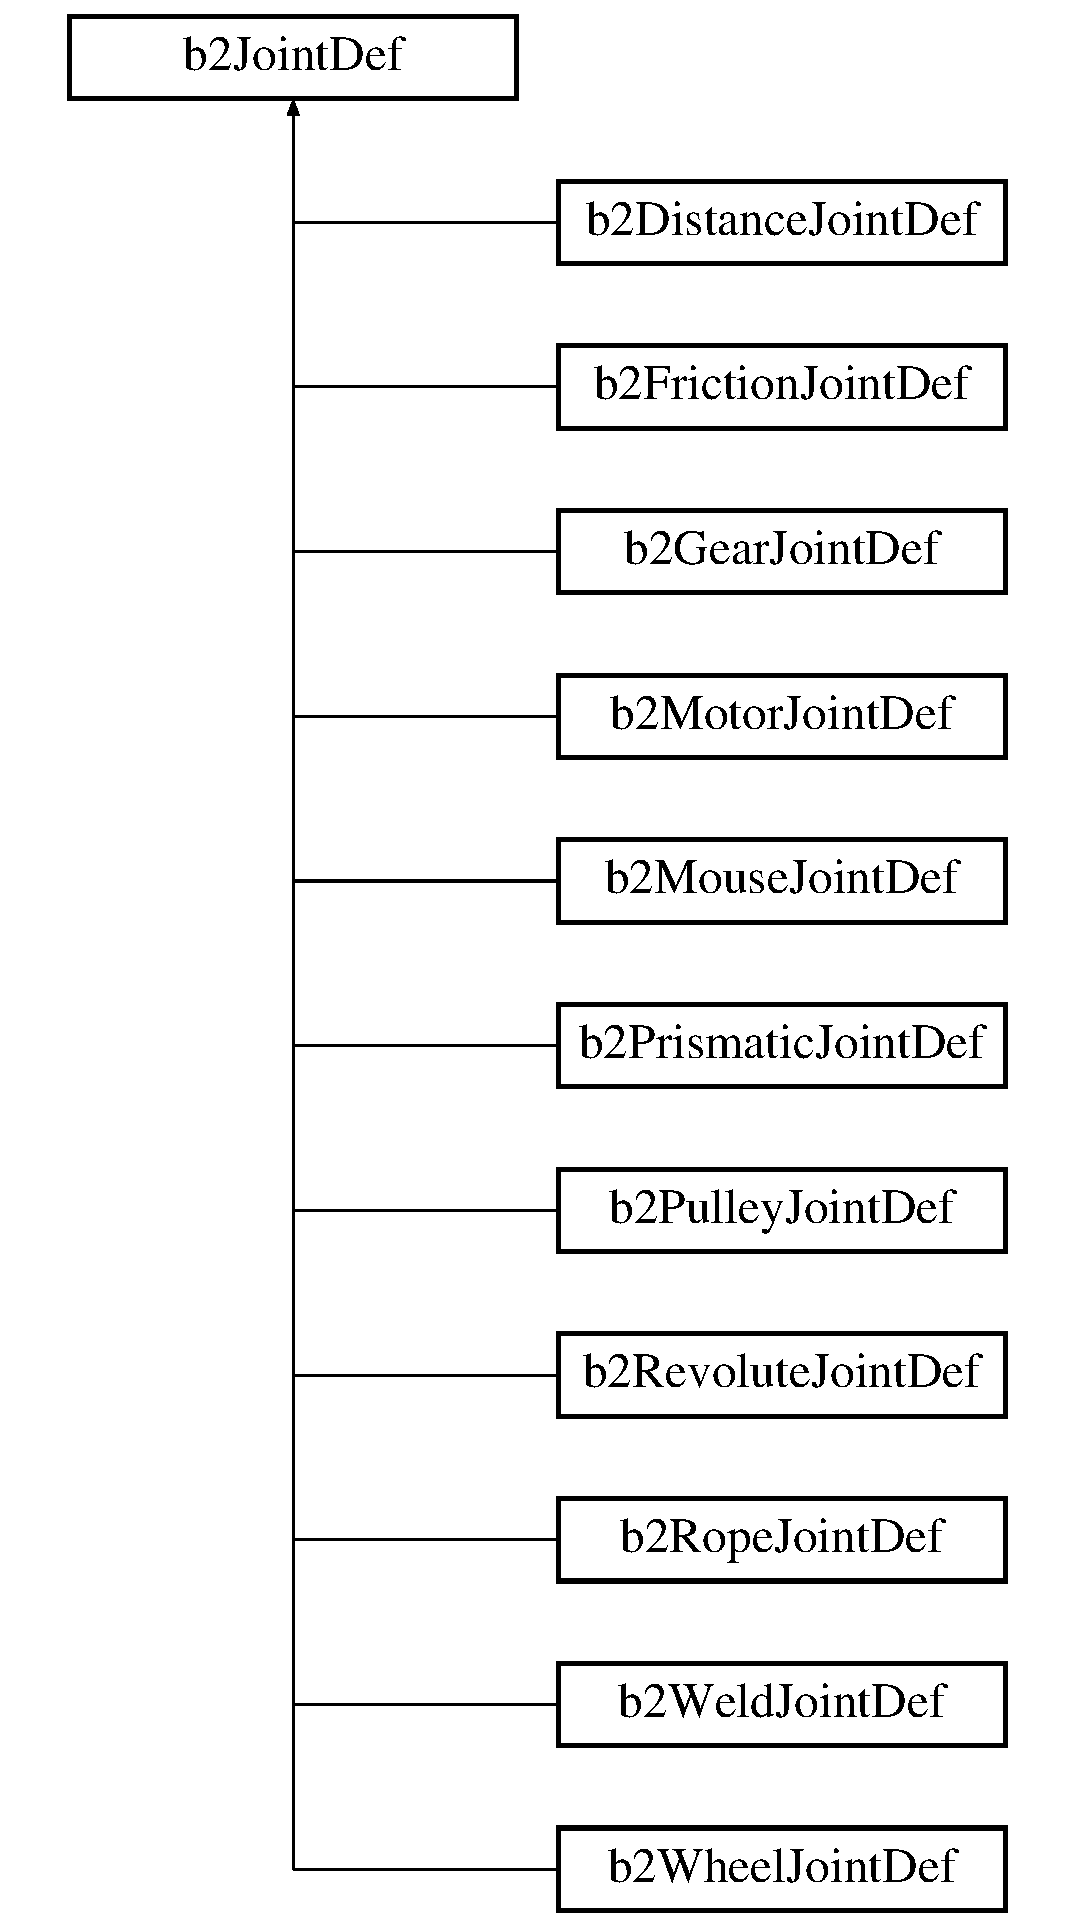
\includegraphics[height=12.000000cm]{structb2_joint_def}
\end{center}
\end{figure}
\subsection*{Public Attributes}
\begin{DoxyCompactItemize}
\item 
b2\+Joint\+Type \hyperlink{structb2_joint_def_a470f2879b24adb05facbd49f338856fb}{type}\hypertarget{structb2_joint_def_a470f2879b24adb05facbd49f338856fb}{}\label{structb2_joint_def_a470f2879b24adb05facbd49f338856fb}

\begin{DoxyCompactList}\small\item\em The joint type is set automatically for concrete joint types. \end{DoxyCompactList}\item 
void $\ast$ \hyperlink{structb2_joint_def_a07eb150daaaa52fc09c3bcf402b295fe}{user\+Data}\hypertarget{structb2_joint_def_a07eb150daaaa52fc09c3bcf402b295fe}{}\label{structb2_joint_def_a07eb150daaaa52fc09c3bcf402b295fe}

\begin{DoxyCompactList}\small\item\em Use this to attach application specific data to your joints. \end{DoxyCompactList}\item 
\hyperlink{classb2_body}{b2\+Body} $\ast$ \hyperlink{structb2_joint_def_a8cd54c93da396be75a9788f2c6897f05}{bodyA}\hypertarget{structb2_joint_def_a8cd54c93da396be75a9788f2c6897f05}{}\label{structb2_joint_def_a8cd54c93da396be75a9788f2c6897f05}

\begin{DoxyCompactList}\small\item\em The first attached body. \end{DoxyCompactList}\item 
\hyperlink{classb2_body}{b2\+Body} $\ast$ \hyperlink{structb2_joint_def_aa4f4dee2fbcd12187b19506b60e68e3d}{bodyB}\hypertarget{structb2_joint_def_aa4f4dee2fbcd12187b19506b60e68e3d}{}\label{structb2_joint_def_aa4f4dee2fbcd12187b19506b60e68e3d}

\begin{DoxyCompactList}\small\item\em The second attached body. \end{DoxyCompactList}\item 
bool \hyperlink{structb2_joint_def_aef099a1f89b64e230173b6016848ea9b}{collide\+Connected}\hypertarget{structb2_joint_def_aef099a1f89b64e230173b6016848ea9b}{}\label{structb2_joint_def_aef099a1f89b64e230173b6016848ea9b}

\begin{DoxyCompactList}\small\item\em Set this flag to true if the attached bodies should collide. \end{DoxyCompactList}\end{DoxyCompactItemize}


\subsection{Detailed Description}
Joint definitions are used to construct joints. 

The documentation for this struct was generated from the following file\+:\begin{DoxyCompactItemize}
\item 
Commun/\+Externe/\+Box2\+D/include/\+Box2\+D/\+Dynamics/\+Joints/b2\+Joint.\+h\end{DoxyCompactItemize}

\hypertarget{structb2_joint_edge}{}\section{b2\+Joint\+Edge Struct Reference}
\label{structb2_joint_edge}\index{b2\+Joint\+Edge@{b2\+Joint\+Edge}}


{\ttfamily \#include $<$b2\+Joint.\+h$>$}

\subsection*{Public Attributes}
\begin{DoxyCompactItemize}
\item 
\hyperlink{classb2_body}{b2\+Body} $\ast$ \hyperlink{structb2_joint_edge_a64aef21fb91211871de8796baecccb95}{other}\hypertarget{structb2_joint_edge_a64aef21fb91211871de8796baecccb95}{}\label{structb2_joint_edge_a64aef21fb91211871de8796baecccb95}

\begin{DoxyCompactList}\small\item\em provides quick access to the other body attached. \end{DoxyCompactList}\item 
\hyperlink{classb2_joint}{b2\+Joint} $\ast$ \hyperlink{structb2_joint_edge_ab5bac5d495af1280c50271f56a221503}{joint}\hypertarget{structb2_joint_edge_ab5bac5d495af1280c50271f56a221503}{}\label{structb2_joint_edge_ab5bac5d495af1280c50271f56a221503}

\begin{DoxyCompactList}\small\item\em the joint \end{DoxyCompactList}\item 
\hyperlink{structb2_joint_edge}{b2\+Joint\+Edge} $\ast$ \hyperlink{structb2_joint_edge_acc3621e38d9664db2805e0fc29d71335}{prev}\hypertarget{structb2_joint_edge_acc3621e38d9664db2805e0fc29d71335}{}\label{structb2_joint_edge_acc3621e38d9664db2805e0fc29d71335}

\begin{DoxyCompactList}\small\item\em the previous joint edge in the body\textquotesingle{}s joint list \end{DoxyCompactList}\item 
\hyperlink{structb2_joint_edge}{b2\+Joint\+Edge} $\ast$ \hyperlink{structb2_joint_edge_a3d17286bc697bb620ee151e4cd07438c}{next}\hypertarget{structb2_joint_edge_a3d17286bc697bb620ee151e4cd07438c}{}\label{structb2_joint_edge_a3d17286bc697bb620ee151e4cd07438c}

\begin{DoxyCompactList}\small\item\em the next joint edge in the body\textquotesingle{}s joint list \end{DoxyCompactList}\end{DoxyCompactItemize}


\subsection{Detailed Description}
A joint edge is used to connect bodies and joints together in a joint graph where each body is a node and each joint is an edge. A joint edge belongs to a doubly linked list maintained in each attached body. Each joint has two joint nodes, one for each attached body. 

The documentation for this struct was generated from the following file\+:\begin{DoxyCompactItemize}
\item 
Commun/\+Externe/\+Box2\+D/include/\+Box2\+D/\+Dynamics/\+Joints/b2\+Joint.\+h\end{DoxyCompactItemize}

\hypertarget{structb2_manifold}{}\section{b2\+Manifold Struct Reference}
\label{structb2_manifold}\index{b2\+Manifold@{b2\+Manifold}}


{\ttfamily \#include $<$b2\+Collision.\+h$>$}

\subsection*{Public Types}
\begin{DoxyCompactItemize}
\item 
enum {\bfseries Type} \{ {\bfseries e\+\_\+circles}, 
{\bfseries e\+\_\+faceA}, 
{\bfseries e\+\_\+faceB}
 \}\hypertarget{structb2_manifold_aa9c347e2ff2e27ee820a926efbb33e12}{}\label{structb2_manifold_aa9c347e2ff2e27ee820a926efbb33e12}

\end{DoxyCompactItemize}
\subsection*{Public Attributes}
\begin{DoxyCompactItemize}
\item 
\hyperlink{structb2_manifold_point}{b2\+Manifold\+Point} \hyperlink{structb2_manifold_ab8021128e9792cc7391a8804ea02173d}{points} \mbox{[}\hyperlink{b2_settings_8h_aa5f44cc9edf711433dea2b2ec94f3c42}{b2\+\_\+max\+Manifold\+Points}\mbox{]}\hypertarget{structb2_manifold_ab8021128e9792cc7391a8804ea02173d}{}\label{structb2_manifold_ab8021128e9792cc7391a8804ea02173d}

\begin{DoxyCompactList}\small\item\em the points of contact \end{DoxyCompactList}\item 
\hyperlink{structb2_vec2}{b2\+Vec2} \hyperlink{structb2_manifold_a3604e9fef2a03347c5649c71a9fd4c79}{local\+Normal}\hypertarget{structb2_manifold_a3604e9fef2a03347c5649c71a9fd4c79}{}\label{structb2_manifold_a3604e9fef2a03347c5649c71a9fd4c79}

\begin{DoxyCompactList}\small\item\em not use for Type\+::e\+\_\+points \end{DoxyCompactList}\item 
\hyperlink{structb2_vec2}{b2\+Vec2} \hyperlink{structb2_manifold_a8825cea31b27dbbaf22c13c3070870d5}{local\+Point}\hypertarget{structb2_manifold_a8825cea31b27dbbaf22c13c3070870d5}{}\label{structb2_manifold_a8825cea31b27dbbaf22c13c3070870d5}

\begin{DoxyCompactList}\small\item\em usage depends on manifold type \end{DoxyCompactList}\item 
Type {\bfseries type}\hypertarget{structb2_manifold_a4cb6ceba7105513b1e5bd6dbf0cce168}{}\label{structb2_manifold_a4cb6ceba7105513b1e5bd6dbf0cce168}

\item 
int32 \hyperlink{structb2_manifold_abf59ff6fa36bed34b0242ad54951a696}{point\+Count}\hypertarget{structb2_manifold_abf59ff6fa36bed34b0242ad54951a696}{}\label{structb2_manifold_abf59ff6fa36bed34b0242ad54951a696}

\begin{DoxyCompactList}\small\item\em the number of manifold points \end{DoxyCompactList}\end{DoxyCompactItemize}


\subsection{Detailed Description}
A manifold for two touching convex shapes. Box2D supports multiple types of contact\+:
\begin{DoxyItemize}
\item clip point versus plane with radius
\item point versus point with radius (circles) The local point usage depends on the manifold type\+: -\/e\+\_\+circles\+: the local center of circleA -\/e\+\_\+faceA\+: the center of faceA -\/e\+\_\+faceB\+: the center of faceB Similarly the local normal usage\+: -\/e\+\_\+circles\+: not used -\/e\+\_\+faceA\+: the normal on polygonA -\/e\+\_\+faceB\+: the normal on polygonB We store contacts in this way so that position correction can account for movement, which is critical for continuous physics. All contact scenarios must be expressed in one of these types. This structure is stored across time steps, so we keep it small. 
\end{DoxyItemize}

The documentation for this struct was generated from the following file\+:\begin{DoxyCompactItemize}
\item 
Commun/\+Externe/\+Box2\+D/include/\+Box2\+D/\+Collision/\hyperlink{b2_collision_8h}{b2\+Collision.\+h}\end{DoxyCompactItemize}

\hypertarget{structb2_manifold_point}{}\section{b2\+Manifold\+Point Struct Reference}
\label{structb2_manifold_point}\index{b2\+Manifold\+Point@{b2\+Manifold\+Point}}


{\ttfamily \#include $<$b2\+Collision.\+h$>$}

\subsection*{Public Attributes}
\begin{DoxyCompactItemize}
\item 
\hyperlink{structb2_vec2}{b2\+Vec2} \hyperlink{structb2_manifold_point_ab3616990e7d1644deeeb691246094bfa}{local\+Point}\hypertarget{structb2_manifold_point_ab3616990e7d1644deeeb691246094bfa}{}\label{structb2_manifold_point_ab3616990e7d1644deeeb691246094bfa}

\begin{DoxyCompactList}\small\item\em usage depends on manifold type \end{DoxyCompactList}\item 
float32 \hyperlink{structb2_manifold_point_af4218c2359cb7762cd4e9d8ecefab173}{normal\+Impulse}\hypertarget{structb2_manifold_point_af4218c2359cb7762cd4e9d8ecefab173}{}\label{structb2_manifold_point_af4218c2359cb7762cd4e9d8ecefab173}

\begin{DoxyCompactList}\small\item\em the non-\/penetration impulse \end{DoxyCompactList}\item 
float32 \hyperlink{structb2_manifold_point_a0ac5375b1fc4675a0073129f56aa62c9}{tangent\+Impulse}\hypertarget{structb2_manifold_point_a0ac5375b1fc4675a0073129f56aa62c9}{}\label{structb2_manifold_point_a0ac5375b1fc4675a0073129f56aa62c9}

\begin{DoxyCompactList}\small\item\em the friction impulse \end{DoxyCompactList}\item 
\hyperlink{unionb2_contact_i_d}{b2\+Contact\+ID} \hyperlink{structb2_manifold_point_afa7ec272b2b27abe129540f8fbe57fc5}{id}\hypertarget{structb2_manifold_point_afa7ec272b2b27abe129540f8fbe57fc5}{}\label{structb2_manifold_point_afa7ec272b2b27abe129540f8fbe57fc5}

\begin{DoxyCompactList}\small\item\em uniquely identifies a contact point between two shapes \end{DoxyCompactList}\end{DoxyCompactItemize}


\subsection{Detailed Description}
A manifold point is a contact point belonging to a contact manifold. It holds details related to the geometry and dynamics of the contact points. The local point usage depends on the manifold type\+: -\/e\+\_\+circles\+: the local center of circleB -\/e\+\_\+faceA\+: the local center of cirlceB or the clip point of polygonB -\/e\+\_\+faceB\+: the clip point of polygonA This structure is stored across time steps, so we keep it small. Note\+: the impulses are used for internal caching and may not provide reliable contact forces, especially for high speed collisions. 

The documentation for this struct was generated from the following file\+:\begin{DoxyCompactItemize}
\item 
Commun/\+Externe/\+Box2\+D/include/\+Box2\+D/\+Collision/\hyperlink{b2_collision_8h}{b2\+Collision.\+h}\end{DoxyCompactItemize}

\hypertarget{structb2_mass_data}{}\section{b2\+Mass\+Data Struct Reference}
\label{structb2_mass_data}\index{b2\+Mass\+Data@{b2\+Mass\+Data}}


This holds the mass data computed for a shape.  




{\ttfamily \#include $<$b2\+Shape.\+h$>$}

\subsection*{Public Attributes}
\begin{DoxyCompactItemize}
\item 
float32 \hyperlink{structb2_mass_data_aea85d9595a38d2eed05b8d2ea80d97b1}{mass}\hypertarget{structb2_mass_data_aea85d9595a38d2eed05b8d2ea80d97b1}{}\label{structb2_mass_data_aea85d9595a38d2eed05b8d2ea80d97b1}

\begin{DoxyCompactList}\small\item\em The mass of the shape, usually in kilograms. \end{DoxyCompactList}\item 
\hyperlink{structb2_vec2}{b2\+Vec2} \hyperlink{structb2_mass_data_a1d59bebc7030c4dded0c2febc57ebdd7}{center}\hypertarget{structb2_mass_data_a1d59bebc7030c4dded0c2febc57ebdd7}{}\label{structb2_mass_data_a1d59bebc7030c4dded0c2febc57ebdd7}

\begin{DoxyCompactList}\small\item\em The position of the shape\textquotesingle{}s centroid relative to the shape\textquotesingle{}s origin. \end{DoxyCompactList}\item 
float32 \hyperlink{structb2_mass_data_ad2d06e96e2d79d895df16ae0e5fe0376}{I}\hypertarget{structb2_mass_data_ad2d06e96e2d79d895df16ae0e5fe0376}{}\label{structb2_mass_data_ad2d06e96e2d79d895df16ae0e5fe0376}

\begin{DoxyCompactList}\small\item\em The rotational inertia of the shape about the local origin. \end{DoxyCompactList}\end{DoxyCompactItemize}


\subsection{Detailed Description}
This holds the mass data computed for a shape. 

The documentation for this struct was generated from the following file\+:\begin{DoxyCompactItemize}
\item 
Cadriciel/\+Commun/\+Externe/\+Box2\+D/include/\+Box2\+D/\+Collision/\+Shapes/b2\+Shape.\+h\end{DoxyCompactItemize}

\hypertarget{structb2_mat22}{}\section{b2\+Mat22 Struct Reference}
\label{structb2_mat22}\index{b2\+Mat22@{b2\+Mat22}}


A 2-\/by-\/2 matrix. Stored in column-\/major order.  




{\ttfamily \#include $<$b2\+Math.\+h$>$}

\subsection*{Public Member Functions}
\begin{DoxyCompactItemize}
\item 
\hyperlink{structb2_mat22_ac3e10f6d457c8dab9062ba378f66bc4d}{b2\+Mat22} ()\hypertarget{structb2_mat22_ac3e10f6d457c8dab9062ba378f66bc4d}{}\label{structb2_mat22_ac3e10f6d457c8dab9062ba378f66bc4d}

\begin{DoxyCompactList}\small\item\em The default constructor does nothing (for performance). \end{DoxyCompactList}\item 
\hyperlink{structb2_mat22_abd674c6d92e26962977f34bcd92ff24d}{b2\+Mat22} (const \hyperlink{structb2_vec2}{b2\+Vec2} \&c1, const \hyperlink{structb2_vec2}{b2\+Vec2} \&c2)\hypertarget{structb2_mat22_abd674c6d92e26962977f34bcd92ff24d}{}\label{structb2_mat22_abd674c6d92e26962977f34bcd92ff24d}

\begin{DoxyCompactList}\small\item\em Construct this matrix using columns. \end{DoxyCompactList}\item 
\hyperlink{structb2_mat22_a41d5d8743bda32cb8c6e212528934810}{b2\+Mat22} (float32 a11, float32 a12, float32 a21, float32 a22)\hypertarget{structb2_mat22_a41d5d8743bda32cb8c6e212528934810}{}\label{structb2_mat22_a41d5d8743bda32cb8c6e212528934810}

\begin{DoxyCompactList}\small\item\em Construct this matrix using scalars. \end{DoxyCompactList}\item 
void \hyperlink{structb2_mat22_aed3bee1de38a0b3f36e21c90faa24112}{Set} (const \hyperlink{structb2_vec2}{b2\+Vec2} \&c1, const \hyperlink{structb2_vec2}{b2\+Vec2} \&c2)\hypertarget{structb2_mat22_aed3bee1de38a0b3f36e21c90faa24112}{}\label{structb2_mat22_aed3bee1de38a0b3f36e21c90faa24112}

\begin{DoxyCompactList}\small\item\em Initialize this matrix using columns. \end{DoxyCompactList}\item 
void \hyperlink{structb2_mat22_a7192f063b771ac9ded060e41df890509}{Set\+Identity} ()\hypertarget{structb2_mat22_a7192f063b771ac9ded060e41df890509}{}\label{structb2_mat22_a7192f063b771ac9ded060e41df890509}

\begin{DoxyCompactList}\small\item\em Set this to the identity matrix. \end{DoxyCompactList}\item 
void \hyperlink{structb2_mat22_aaeae95f61cf3171ffb94703980e3594b}{Set\+Zero} ()\hypertarget{structb2_mat22_aaeae95f61cf3171ffb94703980e3594b}{}\label{structb2_mat22_aaeae95f61cf3171ffb94703980e3594b}

\begin{DoxyCompactList}\small\item\em Set this matrix to all zeros. \end{DoxyCompactList}\item 
\hyperlink{structb2_mat22}{b2\+Mat22} {\bfseries Get\+Inverse} () const \hypertarget{structb2_mat22_af8d14ac8f48feb282cdd669f36ac8070}{}\label{structb2_mat22_af8d14ac8f48feb282cdd669f36ac8070}

\item 
\hyperlink{structb2_vec2}{b2\+Vec2} \hyperlink{structb2_mat22_ab511ad33f5abf87351581842628a9dc3}{Solve} (const \hyperlink{structb2_vec2}{b2\+Vec2} \&b) const 
\end{DoxyCompactItemize}
\subsection*{Public Attributes}
\begin{DoxyCompactItemize}
\item 
\hyperlink{structb2_vec2}{b2\+Vec2} {\bfseries ex}\hypertarget{structb2_mat22_abaffa5fc1d401ea36415acffa6205689}{}\label{structb2_mat22_abaffa5fc1d401ea36415acffa6205689}

\item 
\hyperlink{structb2_vec2}{b2\+Vec2} {\bfseries ey}\hypertarget{structb2_mat22_af19db58941d2cd146325ef3191b776fd}{}\label{structb2_mat22_af19db58941d2cd146325ef3191b776fd}

\end{DoxyCompactItemize}


\subsection{Detailed Description}
A 2-\/by-\/2 matrix. Stored in column-\/major order. 

\subsection{Member Function Documentation}
\index{b2\+Mat22@{b2\+Mat22}!Solve@{Solve}}
\index{Solve@{Solve}!b2\+Mat22@{b2\+Mat22}}
\subsubsection[{\texorpdfstring{Solve(const b2\+Vec2 \&b) const }{Solve(const b2Vec2 &b) const }}]{\setlength{\rightskip}{0pt plus 5cm}{\bf b2\+Vec2} b2\+Mat22\+::\+Solve (
\begin{DoxyParamCaption}
\item[{const {\bf b2\+Vec2} \&}]{b}
\end{DoxyParamCaption}
) const\hspace{0.3cm}{\ttfamily [inline]}}\hypertarget{structb2_mat22_ab511ad33f5abf87351581842628a9dc3}{}\label{structb2_mat22_ab511ad33f5abf87351581842628a9dc3}
Solve A $\ast$ x = b, where b is a column vector. This is more efficient than computing the inverse in one-\/shot cases. 

The documentation for this struct was generated from the following file\+:\begin{DoxyCompactItemize}
\item 
C\+:/\+Users/\+Bilal Itani/\+Desktop/inf2990-\/11/\+Cadriciel/\+Commun/\+Externe/\+Box2\+D/include/\+Box2\+D/\+Common/b2\+Math.\+h\end{DoxyCompactItemize}

\hypertarget{structb2_mat33}{}\section{b2\+Mat33 Struct Reference}
\label{structb2_mat33}\index{b2\+Mat33@{b2\+Mat33}}


A 3-\/by-\/3 matrix. Stored in column-\/major order.  




{\ttfamily \#include $<$b2\+Math.\+h$>$}

\subsection*{Public Member Functions}
\begin{DoxyCompactItemize}
\item 
\hyperlink{structb2_mat33_a1f4d7ddf1c8a202fc08ec64dfe191463}{b2\+Mat33} ()\hypertarget{structb2_mat33_a1f4d7ddf1c8a202fc08ec64dfe191463}{}\label{structb2_mat33_a1f4d7ddf1c8a202fc08ec64dfe191463}

\begin{DoxyCompactList}\small\item\em The default constructor does nothing (for performance). \end{DoxyCompactList}\item 
\hyperlink{structb2_mat33_a36d99a037008776c8d09fe0aeb5c759c}{b2\+Mat33} (const \hyperlink{structb2_vec3}{b2\+Vec3} \&c1, const \hyperlink{structb2_vec3}{b2\+Vec3} \&c2, const \hyperlink{structb2_vec3}{b2\+Vec3} \&c3)\hypertarget{structb2_mat33_a36d99a037008776c8d09fe0aeb5c759c}{}\label{structb2_mat33_a36d99a037008776c8d09fe0aeb5c759c}

\begin{DoxyCompactList}\small\item\em Construct this matrix using columns. \end{DoxyCompactList}\item 
void \hyperlink{structb2_mat33_a42fc6953b025e1c8b59717d0ee7accde}{Set\+Zero} ()\hypertarget{structb2_mat33_a42fc6953b025e1c8b59717d0ee7accde}{}\label{structb2_mat33_a42fc6953b025e1c8b59717d0ee7accde}

\begin{DoxyCompactList}\small\item\em Set this matrix to all zeros. \end{DoxyCompactList}\item 
\hyperlink{structb2_vec3}{b2\+Vec3} \hyperlink{structb2_mat33_a478872c7b6a3bedd13fbedd3ec7a2edb}{Solve33} (const \hyperlink{structb2_vec3}{b2\+Vec3} \&b) const 
\item 
\hyperlink{structb2_vec2}{b2\+Vec2} \hyperlink{structb2_mat33_a2580ac2afadc48028a63ed4c8a1f16bc}{Solve22} (const \hyperlink{structb2_vec2}{b2\+Vec2} \&b) const 
\item 
void \hyperlink{structb2_mat33_a9eb5090b15d08ab495458adfec50e7cb}{Get\+Inverse22} (\hyperlink{structb2_mat33}{b2\+Mat33} $\ast$M) const 
\item 
void \hyperlink{structb2_mat33_a501f85edde8f080e4e9ecff0ec2ee27e}{Get\+Sym\+Inverse33} (\hyperlink{structb2_mat33}{b2\+Mat33} $\ast$M) const 
\end{DoxyCompactItemize}
\subsection*{Public Attributes}
\begin{DoxyCompactItemize}
\item 
\hyperlink{structb2_vec3}{b2\+Vec3} {\bfseries ex}\hypertarget{structb2_mat33_a132f00e6550d1e19c75fb60ce1229638}{}\label{structb2_mat33_a132f00e6550d1e19c75fb60ce1229638}

\item 
\hyperlink{structb2_vec3}{b2\+Vec3} {\bfseries ey}\hypertarget{structb2_mat33_ababc69c718c73a04a651f7a6a981ecf4}{}\label{structb2_mat33_ababc69c718c73a04a651f7a6a981ecf4}

\item 
\hyperlink{structb2_vec3}{b2\+Vec3} {\bfseries ez}\hypertarget{structb2_mat33_ae700fc46f679b4ef211a2517005b0557}{}\label{structb2_mat33_ae700fc46f679b4ef211a2517005b0557}

\end{DoxyCompactItemize}


\subsection{Detailed Description}
A 3-\/by-\/3 matrix. Stored in column-\/major order. 

\subsection{Member Function Documentation}
\index{b2\+Mat33@{b2\+Mat33}!Get\+Inverse22@{Get\+Inverse22}}
\index{Get\+Inverse22@{Get\+Inverse22}!b2\+Mat33@{b2\+Mat33}}
\subsubsection[{\texorpdfstring{Get\+Inverse22(b2\+Mat33 $\ast$\+M) const }{GetInverse22(b2Mat33 *M) const }}]{\setlength{\rightskip}{0pt plus 5cm}void b2\+Mat33\+::\+Get\+Inverse22 (
\begin{DoxyParamCaption}
\item[{{\bf b2\+Mat33} $\ast$}]{M}
\end{DoxyParamCaption}
) const}\hypertarget{structb2_mat33_a9eb5090b15d08ab495458adfec50e7cb}{}\label{structb2_mat33_a9eb5090b15d08ab495458adfec50e7cb}
Get the inverse of this matrix as a 2-\/by-\/2. Returns the zero matrix if singular. \index{b2\+Mat33@{b2\+Mat33}!Get\+Sym\+Inverse33@{Get\+Sym\+Inverse33}}
\index{Get\+Sym\+Inverse33@{Get\+Sym\+Inverse33}!b2\+Mat33@{b2\+Mat33}}
\subsubsection[{\texorpdfstring{Get\+Sym\+Inverse33(b2\+Mat33 $\ast$\+M) const }{GetSymInverse33(b2Mat33 *M) const }}]{\setlength{\rightskip}{0pt plus 5cm}void b2\+Mat33\+::\+Get\+Sym\+Inverse33 (
\begin{DoxyParamCaption}
\item[{{\bf b2\+Mat33} $\ast$}]{M}
\end{DoxyParamCaption}
) const}\hypertarget{structb2_mat33_a501f85edde8f080e4e9ecff0ec2ee27e}{}\label{structb2_mat33_a501f85edde8f080e4e9ecff0ec2ee27e}
Get the symmetric inverse of this matrix as a 3-\/by-\/3. Returns the zero matrix if singular. \index{b2\+Mat33@{b2\+Mat33}!Solve22@{Solve22}}
\index{Solve22@{Solve22}!b2\+Mat33@{b2\+Mat33}}
\subsubsection[{\texorpdfstring{Solve22(const b2\+Vec2 \&b) const }{Solve22(const b2Vec2 &b) const }}]{\setlength{\rightskip}{0pt plus 5cm}{\bf b2\+Vec2} b2\+Mat33\+::\+Solve22 (
\begin{DoxyParamCaption}
\item[{const {\bf b2\+Vec2} \&}]{b}
\end{DoxyParamCaption}
) const}\hypertarget{structb2_mat33_a2580ac2afadc48028a63ed4c8a1f16bc}{}\label{structb2_mat33_a2580ac2afadc48028a63ed4c8a1f16bc}
Solve A $\ast$ x = b, where b is a column vector. This is more efficient than computing the inverse in one-\/shot cases. Solve only the upper 2-\/by-\/2 matrix equation. \index{b2\+Mat33@{b2\+Mat33}!Solve33@{Solve33}}
\index{Solve33@{Solve33}!b2\+Mat33@{b2\+Mat33}}
\subsubsection[{\texorpdfstring{Solve33(const b2\+Vec3 \&b) const }{Solve33(const b2Vec3 &b) const }}]{\setlength{\rightskip}{0pt plus 5cm}{\bf b2\+Vec3} b2\+Mat33\+::\+Solve33 (
\begin{DoxyParamCaption}
\item[{const {\bf b2\+Vec3} \&}]{b}
\end{DoxyParamCaption}
) const}\hypertarget{structb2_mat33_a478872c7b6a3bedd13fbedd3ec7a2edb}{}\label{structb2_mat33_a478872c7b6a3bedd13fbedd3ec7a2edb}
Solve A $\ast$ x = b, where b is a column vector. This is more efficient than computing the inverse in one-\/shot cases. 

The documentation for this struct was generated from the following file\+:\begin{DoxyCompactItemize}
\item 
Cadriciel/\+Commun/\+Externe/\+Box2\+D/include/\+Box2\+D/\+Common/b2\+Math.\+h\end{DoxyCompactItemize}

\hypertarget{classb2_motor_joint}{}\section{b2\+Motor\+Joint Class Reference}
\label{classb2_motor_joint}\index{b2\+Motor\+Joint@{b2\+Motor\+Joint}}


{\ttfamily \#include $<$b2\+Motor\+Joint.\+h$>$}

Inheritance diagram for b2\+Motor\+Joint\+:\begin{figure}[H]
\begin{center}
\leavevmode
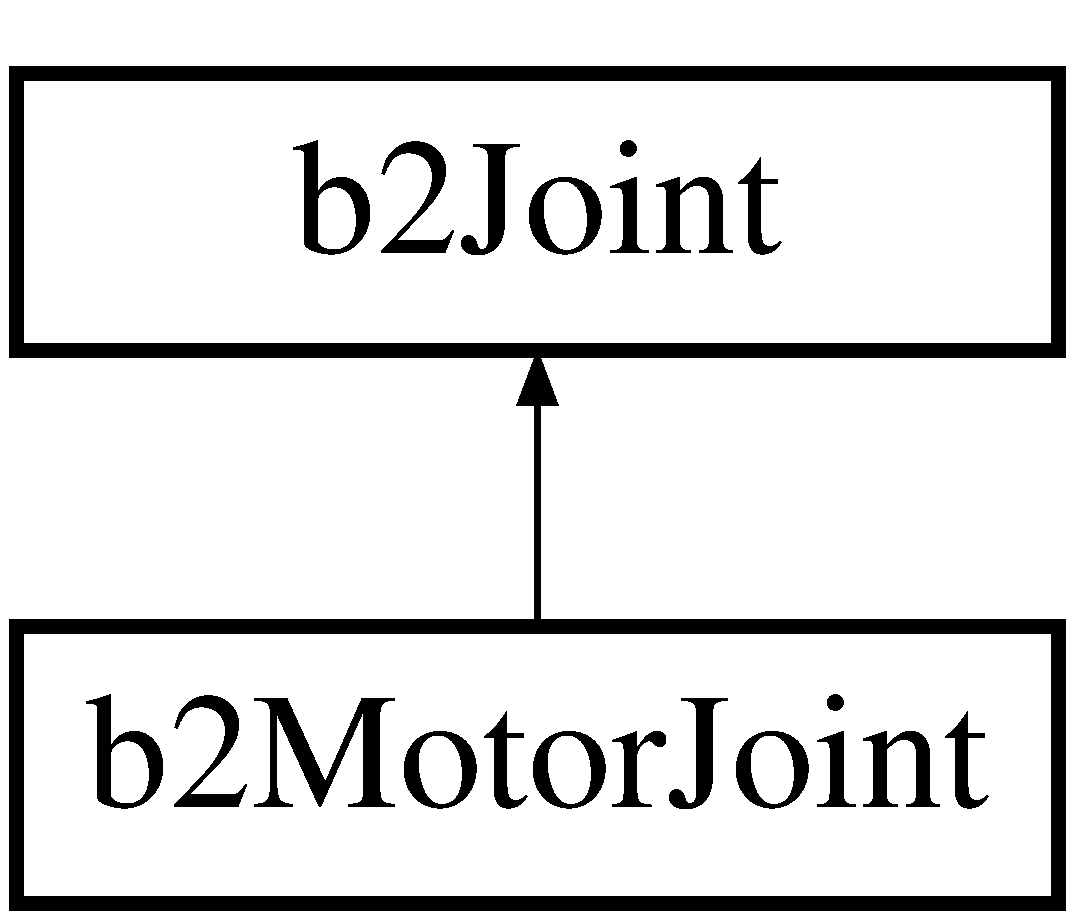
\includegraphics[height=2.000000cm]{classb2_motor_joint}
\end{center}
\end{figure}
\subsection*{Public Member Functions}
\begin{DoxyCompactItemize}
\item 
\hyperlink{structb2_vec2}{b2\+Vec2} \hyperlink{classb2_motor_joint_ac94ea6c5f903c8d8e22724889bff2562}{Get\+AnchorA} () const \hypertarget{classb2_motor_joint_ac94ea6c5f903c8d8e22724889bff2562}{}\label{classb2_motor_joint_ac94ea6c5f903c8d8e22724889bff2562}

\begin{DoxyCompactList}\small\item\em Get the anchor point on bodyA in world coordinates. \end{DoxyCompactList}\item 
\hyperlink{structb2_vec2}{b2\+Vec2} \hyperlink{classb2_motor_joint_acb603ebe6615308654574356e8bb7dc5}{Get\+AnchorB} () const \hypertarget{classb2_motor_joint_acb603ebe6615308654574356e8bb7dc5}{}\label{classb2_motor_joint_acb603ebe6615308654574356e8bb7dc5}

\begin{DoxyCompactList}\small\item\em Get the anchor point on bodyB in world coordinates. \end{DoxyCompactList}\item 
\hyperlink{structb2_vec2}{b2\+Vec2} \hyperlink{classb2_motor_joint_ab9d427f4fd74d0afbd17989701d20924}{Get\+Reaction\+Force} (float32 inv\+\_\+dt) const \hypertarget{classb2_motor_joint_ab9d427f4fd74d0afbd17989701d20924}{}\label{classb2_motor_joint_ab9d427f4fd74d0afbd17989701d20924}

\begin{DoxyCompactList}\small\item\em Get the reaction force on bodyB at the joint anchor in Newtons. \end{DoxyCompactList}\item 
float32 \hyperlink{classb2_motor_joint_a17741b102f8bb3e32f1c139781b41c04}{Get\+Reaction\+Torque} (float32 inv\+\_\+dt) const \hypertarget{classb2_motor_joint_a17741b102f8bb3e32f1c139781b41c04}{}\label{classb2_motor_joint_a17741b102f8bb3e32f1c139781b41c04}

\begin{DoxyCompactList}\small\item\em Get the reaction torque on bodyB in N$\ast$m. \end{DoxyCompactList}\item 
void \hyperlink{classb2_motor_joint_a99254b5fc9ed9f2d0fdccada513000c3}{Set\+Linear\+Offset} (const \hyperlink{structb2_vec2}{b2\+Vec2} \&linear\+Offset)\hypertarget{classb2_motor_joint_a99254b5fc9ed9f2d0fdccada513000c3}{}\label{classb2_motor_joint_a99254b5fc9ed9f2d0fdccada513000c3}

\begin{DoxyCompactList}\small\item\em Set/get the target linear offset, in frame A, in meters. \end{DoxyCompactList}\item 
const \hyperlink{structb2_vec2}{b2\+Vec2} \& {\bfseries Get\+Linear\+Offset} () const \hypertarget{classb2_motor_joint_a98556efc09c020a3e53c8c57c28f2893}{}\label{classb2_motor_joint_a98556efc09c020a3e53c8c57c28f2893}

\item 
void \hyperlink{classb2_motor_joint_a14d7dca1767548ddffe293e39cafc3c7}{Set\+Angular\+Offset} (float32 angular\+Offset)\hypertarget{classb2_motor_joint_a14d7dca1767548ddffe293e39cafc3c7}{}\label{classb2_motor_joint_a14d7dca1767548ddffe293e39cafc3c7}

\begin{DoxyCompactList}\small\item\em Set/get the target angular offset, in radians. \end{DoxyCompactList}\item 
float32 {\bfseries Get\+Angular\+Offset} () const \hypertarget{classb2_motor_joint_a965a5291951461c1dc8efffde10375ef}{}\label{classb2_motor_joint_a965a5291951461c1dc8efffde10375ef}

\item 
void \hyperlink{classb2_motor_joint_a62f95f23d60123cebe14f2fcec155801}{Set\+Max\+Force} (float32 force)\hypertarget{classb2_motor_joint_a62f95f23d60123cebe14f2fcec155801}{}\label{classb2_motor_joint_a62f95f23d60123cebe14f2fcec155801}

\begin{DoxyCompactList}\small\item\em Set the maximum friction force in N. \end{DoxyCompactList}\item 
float32 \hyperlink{classb2_motor_joint_ac63233e45f6428319a9857bf89557f46}{Get\+Max\+Force} () const \hypertarget{classb2_motor_joint_ac63233e45f6428319a9857bf89557f46}{}\label{classb2_motor_joint_ac63233e45f6428319a9857bf89557f46}

\begin{DoxyCompactList}\small\item\em Get the maximum friction force in N. \end{DoxyCompactList}\item 
void \hyperlink{classb2_motor_joint_a3e9a259d36c36e0dc078282e6799d625}{Set\+Max\+Torque} (float32 torque)\hypertarget{classb2_motor_joint_a3e9a259d36c36e0dc078282e6799d625}{}\label{classb2_motor_joint_a3e9a259d36c36e0dc078282e6799d625}

\begin{DoxyCompactList}\small\item\em Set the maximum friction torque in N$\ast$m. \end{DoxyCompactList}\item 
float32 \hyperlink{classb2_motor_joint_af84c933978d0a13a242c71a612f4116b}{Get\+Max\+Torque} () const \hypertarget{classb2_motor_joint_af84c933978d0a13a242c71a612f4116b}{}\label{classb2_motor_joint_af84c933978d0a13a242c71a612f4116b}

\begin{DoxyCompactList}\small\item\em Get the maximum friction torque in N$\ast$m. \end{DoxyCompactList}\item 
void \hyperlink{classb2_motor_joint_ae59e624b8a7b6f869ab5e6148352cb52}{Set\+Correction\+Factor} (float32 factor)\hypertarget{classb2_motor_joint_ae59e624b8a7b6f869ab5e6148352cb52}{}\label{classb2_motor_joint_ae59e624b8a7b6f869ab5e6148352cb52}

\begin{DoxyCompactList}\small\item\em Set the position correction factor in the range \mbox{[}0,1\mbox{]}. \end{DoxyCompactList}\item 
float32 \hyperlink{classb2_motor_joint_a9ea99c4280374d85b29d4ab74afd7aff}{Get\+Correction\+Factor} () const \hypertarget{classb2_motor_joint_a9ea99c4280374d85b29d4ab74afd7aff}{}\label{classb2_motor_joint_a9ea99c4280374d85b29d4ab74afd7aff}

\begin{DoxyCompactList}\small\item\em Get the position correction factor in the range \mbox{[}0,1\mbox{]}. \end{DoxyCompactList}\item 
void \hyperlink{classb2_motor_joint_a5d23974c2fc23f64426a8321520e45bb}{Dump} ()\hypertarget{classb2_motor_joint_a5d23974c2fc23f64426a8321520e45bb}{}\label{classb2_motor_joint_a5d23974c2fc23f64426a8321520e45bb}

\begin{DoxyCompactList}\small\item\em Dump to b2\+Log. \end{DoxyCompactList}\end{DoxyCompactItemize}
\subsection*{Protected Member Functions}
\begin{DoxyCompactItemize}
\item 
{\bfseries b2\+Motor\+Joint} (const \hyperlink{structb2_motor_joint_def}{b2\+Motor\+Joint\+Def} $\ast$def)\hypertarget{classb2_motor_joint_ac0c56b069910915e1ceef3b89c035833}{}\label{classb2_motor_joint_ac0c56b069910915e1ceef3b89c035833}

\item 
void {\bfseries Init\+Velocity\+Constraints} (const \hyperlink{structb2_solver_data}{b2\+Solver\+Data} \&data)\hypertarget{classb2_motor_joint_a49d04e78d28f21491a93d1946f584da2}{}\label{classb2_motor_joint_a49d04e78d28f21491a93d1946f584da2}

\item 
void {\bfseries Solve\+Velocity\+Constraints} (const \hyperlink{structb2_solver_data}{b2\+Solver\+Data} \&data)\hypertarget{classb2_motor_joint_a06a8ccfab3121daa119d548cbb19593c}{}\label{classb2_motor_joint_a06a8ccfab3121daa119d548cbb19593c}

\item 
bool {\bfseries Solve\+Position\+Constraints} (const \hyperlink{structb2_solver_data}{b2\+Solver\+Data} \&data)\hypertarget{classb2_motor_joint_a78b06e3e03eb211f85504f2d9ef66863}{}\label{classb2_motor_joint_a78b06e3e03eb211f85504f2d9ef66863}

\end{DoxyCompactItemize}
\subsection*{Protected Attributes}
\begin{DoxyCompactItemize}
\item 
\hyperlink{structb2_vec2}{b2\+Vec2} {\bfseries m\+\_\+linear\+Offset}\hypertarget{classb2_motor_joint_a6e8db2001da3a9b2926a41451f28f73b}{}\label{classb2_motor_joint_a6e8db2001da3a9b2926a41451f28f73b}

\item 
float32 {\bfseries m\+\_\+angular\+Offset}\hypertarget{classb2_motor_joint_ac48f242920da2d2678dea09941c3d31c}{}\label{classb2_motor_joint_ac48f242920da2d2678dea09941c3d31c}

\item 
\hyperlink{structb2_vec2}{b2\+Vec2} {\bfseries m\+\_\+linear\+Impulse}\hypertarget{classb2_motor_joint_a5aba4dbf8cccc33a1cc20f7a503b51f5}{}\label{classb2_motor_joint_a5aba4dbf8cccc33a1cc20f7a503b51f5}

\item 
float32 {\bfseries m\+\_\+angular\+Impulse}\hypertarget{classb2_motor_joint_abf23ffd98f99bdf34423bee99e40a949}{}\label{classb2_motor_joint_abf23ffd98f99bdf34423bee99e40a949}

\item 
float32 {\bfseries m\+\_\+max\+Force}\hypertarget{classb2_motor_joint_ad9a39349f3b43e8f1c33f5a44575dffe}{}\label{classb2_motor_joint_ad9a39349f3b43e8f1c33f5a44575dffe}

\item 
float32 {\bfseries m\+\_\+max\+Torque}\hypertarget{classb2_motor_joint_a7c0c777bb6d78f3eff9abb8819ddb14f}{}\label{classb2_motor_joint_a7c0c777bb6d78f3eff9abb8819ddb14f}

\item 
float32 {\bfseries m\+\_\+correction\+Factor}\hypertarget{classb2_motor_joint_a5e42eef05987dd269be1e709172b933c}{}\label{classb2_motor_joint_a5e42eef05987dd269be1e709172b933c}

\item 
int32 {\bfseries m\+\_\+indexA}\hypertarget{classb2_motor_joint_afdd9d0ebe37506dd8509ed2392fa1f56}{}\label{classb2_motor_joint_afdd9d0ebe37506dd8509ed2392fa1f56}

\item 
int32 {\bfseries m\+\_\+indexB}\hypertarget{classb2_motor_joint_a51525d3f5af31dcede8e641943fe86b3}{}\label{classb2_motor_joint_a51525d3f5af31dcede8e641943fe86b3}

\item 
\hyperlink{structb2_vec2}{b2\+Vec2} {\bfseries m\+\_\+rA}\hypertarget{classb2_motor_joint_a0340ef47abad9882a271be45df15d3ed}{}\label{classb2_motor_joint_a0340ef47abad9882a271be45df15d3ed}

\item 
\hyperlink{structb2_vec2}{b2\+Vec2} {\bfseries m\+\_\+rB}\hypertarget{classb2_motor_joint_a85c605b404e4b087e2932fdf23b447d5}{}\label{classb2_motor_joint_a85c605b404e4b087e2932fdf23b447d5}

\item 
\hyperlink{structb2_vec2}{b2\+Vec2} {\bfseries m\+\_\+local\+CenterA}\hypertarget{classb2_motor_joint_a42f50bbd4b5821164c9777903c83a723}{}\label{classb2_motor_joint_a42f50bbd4b5821164c9777903c83a723}

\item 
\hyperlink{structb2_vec2}{b2\+Vec2} {\bfseries m\+\_\+local\+CenterB}\hypertarget{classb2_motor_joint_a8ba1cf76d5cbc10bf6ff9b7685ebc20d}{}\label{classb2_motor_joint_a8ba1cf76d5cbc10bf6ff9b7685ebc20d}

\item 
\hyperlink{structb2_vec2}{b2\+Vec2} {\bfseries m\+\_\+linear\+Error}\hypertarget{classb2_motor_joint_a21d38a7fedf735aca7d36d1ec033337e}{}\label{classb2_motor_joint_a21d38a7fedf735aca7d36d1ec033337e}

\item 
float32 {\bfseries m\+\_\+angular\+Error}\hypertarget{classb2_motor_joint_a76fd4aa158014c7fd653ca47c0e3c50a}{}\label{classb2_motor_joint_a76fd4aa158014c7fd653ca47c0e3c50a}

\item 
float32 {\bfseries m\+\_\+inv\+MassA}\hypertarget{classb2_motor_joint_a24154e990c9c6cda65989b2828d27c1a}{}\label{classb2_motor_joint_a24154e990c9c6cda65989b2828d27c1a}

\item 
float32 {\bfseries m\+\_\+inv\+MassB}\hypertarget{classb2_motor_joint_a85aff034d88bd4dcf6ab0aea28df84cb}{}\label{classb2_motor_joint_a85aff034d88bd4dcf6ab0aea28df84cb}

\item 
float32 {\bfseries m\+\_\+inv\+IA}\hypertarget{classb2_motor_joint_a873dc8487f43a0d9ec890e3f023efe26}{}\label{classb2_motor_joint_a873dc8487f43a0d9ec890e3f023efe26}

\item 
float32 {\bfseries m\+\_\+inv\+IB}\hypertarget{classb2_motor_joint_a2d67befa1f4404c03cacb918f4679a48}{}\label{classb2_motor_joint_a2d67befa1f4404c03cacb918f4679a48}

\item 
\hyperlink{structb2_mat22}{b2\+Mat22} {\bfseries m\+\_\+linear\+Mass}\hypertarget{classb2_motor_joint_a89503b91fd38d332304092661aafd2c0}{}\label{classb2_motor_joint_a89503b91fd38d332304092661aafd2c0}

\item 
float32 {\bfseries m\+\_\+angular\+Mass}\hypertarget{classb2_motor_joint_a3718dc3784fb4f09ecf42d28c9896ecc}{}\label{classb2_motor_joint_a3718dc3784fb4f09ecf42d28c9896ecc}

\end{DoxyCompactItemize}
\subsection*{Friends}
\begin{DoxyCompactItemize}
\item 
class {\bfseries b2\+Joint}\hypertarget{classb2_motor_joint_a54ade8ed3d794298108d7f4c4e4793fa}{}\label{classb2_motor_joint_a54ade8ed3d794298108d7f4c4e4793fa}

\end{DoxyCompactItemize}
\subsection*{Additional Inherited Members}


\subsection{Detailed Description}
A motor joint is used to control the relative motion between two bodies. A typical usage is to control the movement of a dynamic body with respect to the ground. 

The documentation for this class was generated from the following file\+:\begin{DoxyCompactItemize}
\item 
C\+:/\+Users/\+Bilal Itani/\+Desktop/inf2990-\/11/\+Cadriciel/\+Commun/\+Externe/\+Box2\+D/include/\+Box2\+D/\+Dynamics/\+Joints/b2\+Motor\+Joint.\+h\end{DoxyCompactItemize}

\hypertarget{structb2_motor_joint_def}{}\section{b2\+Motor\+Joint\+Def Struct Reference}
\label{structb2_motor_joint_def}\index{b2\+Motor\+Joint\+Def@{b2\+Motor\+Joint\+Def}}


Motor joint definition.  




{\ttfamily \#include $<$b2\+Motor\+Joint.\+h$>$}

Inheritance diagram for b2\+Motor\+Joint\+Def\+:\begin{figure}[H]
\begin{center}
\leavevmode
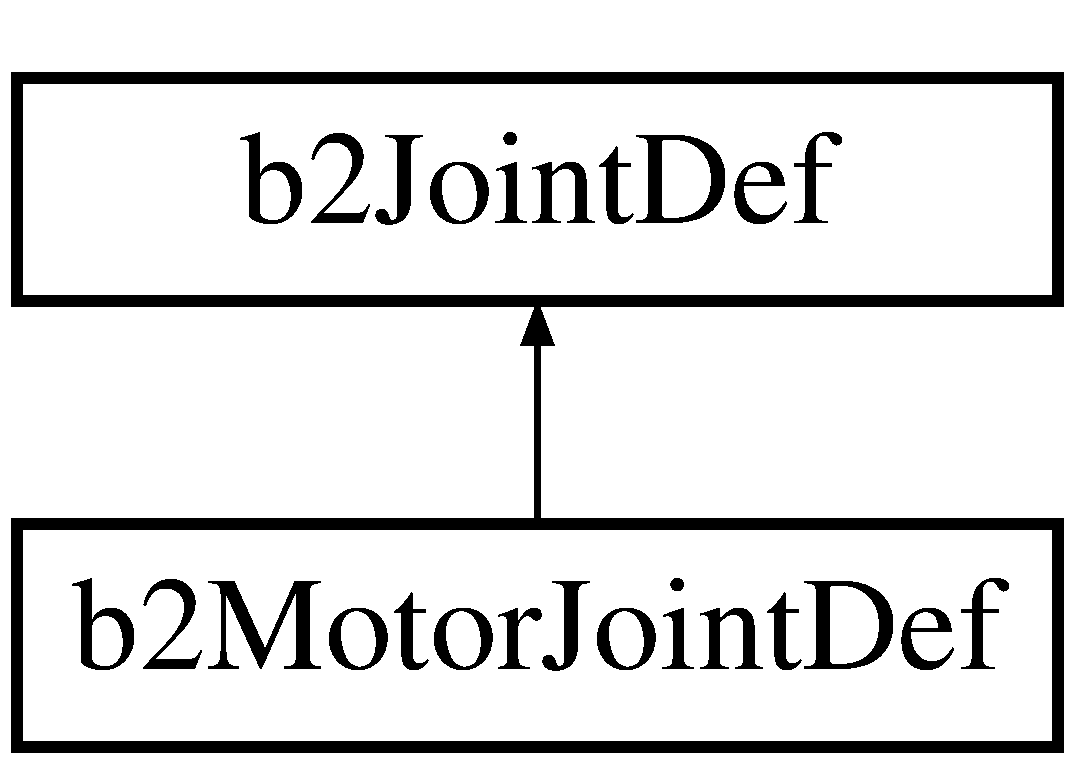
\includegraphics[height=2.000000cm]{structb2_motor_joint_def}
\end{center}
\end{figure}
\subsection*{Public Member Functions}
\begin{DoxyCompactItemize}
\item 
void \hyperlink{structb2_motor_joint_def_a90eb924b6e04da8d75d9cefad0655960}{Initialize} (\hyperlink{classb2_body}{b2\+Body} $\ast$\hyperlink{structb2_joint_def_a8cd54c93da396be75a9788f2c6897f05}{bodyA}, \hyperlink{classb2_body}{b2\+Body} $\ast$\hyperlink{structb2_joint_def_aa4f4dee2fbcd12187b19506b60e68e3d}{bodyB})\hypertarget{structb2_motor_joint_def_a90eb924b6e04da8d75d9cefad0655960}{}\label{structb2_motor_joint_def_a90eb924b6e04da8d75d9cefad0655960}

\begin{DoxyCompactList}\small\item\em Initialize the bodies and offsets using the current transforms. \end{DoxyCompactList}\end{DoxyCompactItemize}
\subsection*{Public Attributes}
\begin{DoxyCompactItemize}
\item 
\hyperlink{structb2_vec2}{b2\+Vec2} \hyperlink{structb2_motor_joint_def_a2c957cffc2af66c6c8077c069b906bc4}{linear\+Offset}\hypertarget{structb2_motor_joint_def_a2c957cffc2af66c6c8077c069b906bc4}{}\label{structb2_motor_joint_def_a2c957cffc2af66c6c8077c069b906bc4}

\begin{DoxyCompactList}\small\item\em Position of bodyB minus the position of bodyA, in bodyA\textquotesingle{}s frame, in meters. \end{DoxyCompactList}\item 
float32 \hyperlink{structb2_motor_joint_def_abdb42eff4aeff1d48038e084c57e1cb0}{angular\+Offset}\hypertarget{structb2_motor_joint_def_abdb42eff4aeff1d48038e084c57e1cb0}{}\label{structb2_motor_joint_def_abdb42eff4aeff1d48038e084c57e1cb0}

\begin{DoxyCompactList}\small\item\em The bodyB angle minus bodyA angle in radians. \end{DoxyCompactList}\item 
float32 \hyperlink{structb2_motor_joint_def_a2f66d1b99c654e112dc68e15375d5ee7}{max\+Force}\hypertarget{structb2_motor_joint_def_a2f66d1b99c654e112dc68e15375d5ee7}{}\label{structb2_motor_joint_def_a2f66d1b99c654e112dc68e15375d5ee7}

\begin{DoxyCompactList}\small\item\em The maximum motor force in N. \end{DoxyCompactList}\item 
float32 \hyperlink{structb2_motor_joint_def_afcf5dd58166917a4574d1f28f6bb3660}{max\+Torque}\hypertarget{structb2_motor_joint_def_afcf5dd58166917a4574d1f28f6bb3660}{}\label{structb2_motor_joint_def_afcf5dd58166917a4574d1f28f6bb3660}

\begin{DoxyCompactList}\small\item\em The maximum motor torque in N-\/m. \end{DoxyCompactList}\item 
float32 \hyperlink{structb2_motor_joint_def_ab282afdb92d07ead23530f57fd0eb9ea}{correction\+Factor}\hypertarget{structb2_motor_joint_def_ab282afdb92d07ead23530f57fd0eb9ea}{}\label{structb2_motor_joint_def_ab282afdb92d07ead23530f57fd0eb9ea}

\begin{DoxyCompactList}\small\item\em Position correction factor in the range \mbox{[}0,1\mbox{]}. \end{DoxyCompactList}\end{DoxyCompactItemize}


\subsection{Detailed Description}
Motor joint definition. 

The documentation for this struct was generated from the following file\+:\begin{DoxyCompactItemize}
\item 
Commun/\+Externe/\+Box2\+D/include/\+Box2\+D/\+Dynamics/\+Joints/b2\+Motor\+Joint.\+h\end{DoxyCompactItemize}

\hypertarget{classb2_mouse_joint}{}\section{b2\+Mouse\+Joint Class Reference}
\label{classb2_mouse_joint}\index{b2\+Mouse\+Joint@{b2\+Mouse\+Joint}}


{\ttfamily \#include $<$b2\+Mouse\+Joint.\+h$>$}

Inheritance diagram for b2\+Mouse\+Joint\+:\begin{figure}[H]
\begin{center}
\leavevmode
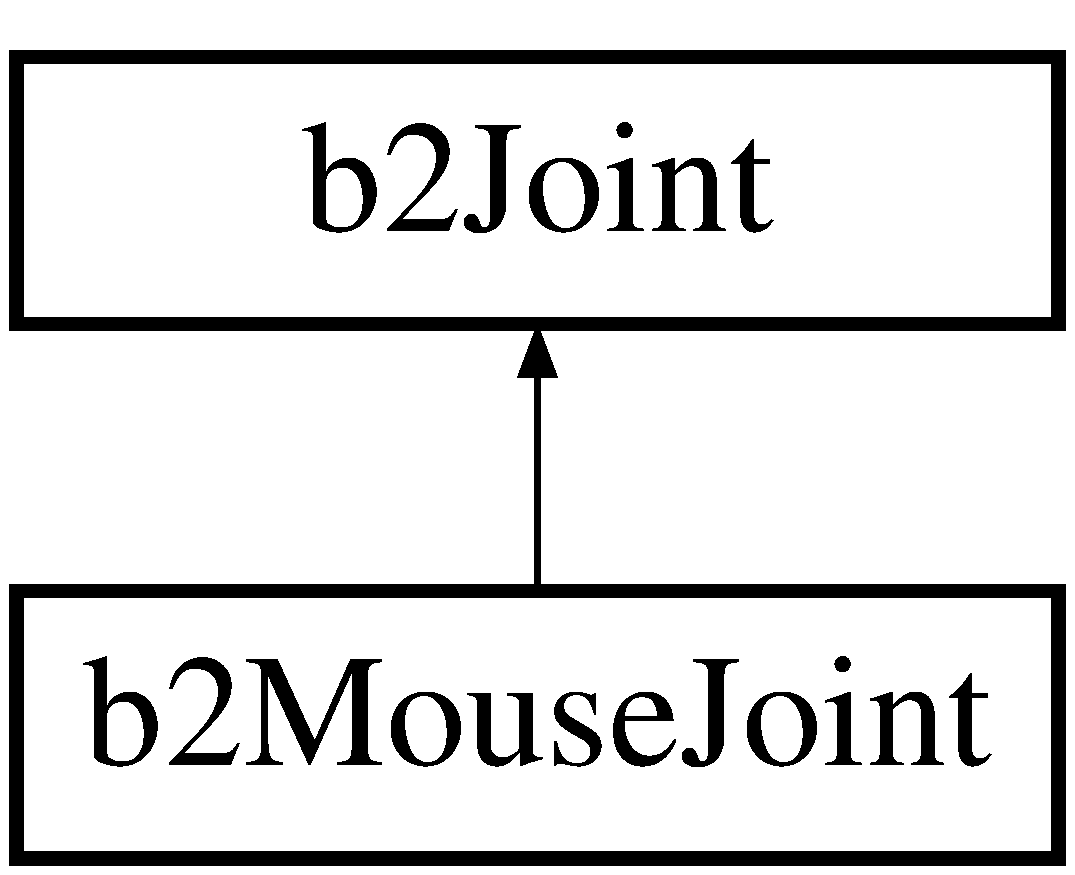
\includegraphics[height=2.000000cm]{classb2_mouse_joint}
\end{center}
\end{figure}
\subsection*{Public Member Functions}
\begin{DoxyCompactItemize}
\item 
\hyperlink{structb2_vec2}{b2\+Vec2} \hyperlink{classb2_mouse_joint_a9db1c131fde2d11e61c6ccee9c28219b}{Get\+AnchorA} () const \hypertarget{classb2_mouse_joint_a9db1c131fde2d11e61c6ccee9c28219b}{}\label{classb2_mouse_joint_a9db1c131fde2d11e61c6ccee9c28219b}

\begin{DoxyCompactList}\small\item\em Implements \hyperlink{classb2_joint}{b2\+Joint}. \end{DoxyCompactList}\item 
\hyperlink{structb2_vec2}{b2\+Vec2} \hyperlink{classb2_mouse_joint_a0db991ec36238105eb481f75e9b6161a}{Get\+AnchorB} () const \hypertarget{classb2_mouse_joint_a0db991ec36238105eb481f75e9b6161a}{}\label{classb2_mouse_joint_a0db991ec36238105eb481f75e9b6161a}

\begin{DoxyCompactList}\small\item\em Implements \hyperlink{classb2_joint}{b2\+Joint}. \end{DoxyCompactList}\item 
\hyperlink{structb2_vec2}{b2\+Vec2} \hyperlink{classb2_mouse_joint_ab8e07dbed9d24c1c046d1ede60930c52}{Get\+Reaction\+Force} (float32 inv\+\_\+dt) const \hypertarget{classb2_mouse_joint_ab8e07dbed9d24c1c046d1ede60930c52}{}\label{classb2_mouse_joint_ab8e07dbed9d24c1c046d1ede60930c52}

\begin{DoxyCompactList}\small\item\em Implements \hyperlink{classb2_joint}{b2\+Joint}. \end{DoxyCompactList}\item 
float32 \hyperlink{classb2_mouse_joint_a68efbc617aa7f0a41578e0aea988d662}{Get\+Reaction\+Torque} (float32 inv\+\_\+dt) const \hypertarget{classb2_mouse_joint_a68efbc617aa7f0a41578e0aea988d662}{}\label{classb2_mouse_joint_a68efbc617aa7f0a41578e0aea988d662}

\begin{DoxyCompactList}\small\item\em Implements \hyperlink{classb2_joint}{b2\+Joint}. \end{DoxyCompactList}\item 
void \hyperlink{classb2_mouse_joint_a96f34c1c990407eddbadf07ae359b1f3}{Set\+Target} (const \hyperlink{structb2_vec2}{b2\+Vec2} \&target)\hypertarget{classb2_mouse_joint_a96f34c1c990407eddbadf07ae359b1f3}{}\label{classb2_mouse_joint_a96f34c1c990407eddbadf07ae359b1f3}

\begin{DoxyCompactList}\small\item\em Use this to update the target point. \end{DoxyCompactList}\item 
const \hyperlink{structb2_vec2}{b2\+Vec2} \& {\bfseries Get\+Target} () const \hypertarget{classb2_mouse_joint_a1261aba7d24d2c248b682ef8bdf2c585}{}\label{classb2_mouse_joint_a1261aba7d24d2c248b682ef8bdf2c585}

\item 
void \hyperlink{classb2_mouse_joint_a4beba6ea0827960fac2474563591c03a}{Set\+Max\+Force} (float32 force)\hypertarget{classb2_mouse_joint_a4beba6ea0827960fac2474563591c03a}{}\label{classb2_mouse_joint_a4beba6ea0827960fac2474563591c03a}

\begin{DoxyCompactList}\small\item\em Set/get the maximum force in Newtons. \end{DoxyCompactList}\item 
float32 {\bfseries Get\+Max\+Force} () const \hypertarget{classb2_mouse_joint_a30bf839765e997a424dd273f3f2d2027}{}\label{classb2_mouse_joint_a30bf839765e997a424dd273f3f2d2027}

\item 
void \hyperlink{classb2_mouse_joint_a8b37706535923637ca280c5a0467b14d}{Set\+Frequency} (float32 hz)\hypertarget{classb2_mouse_joint_a8b37706535923637ca280c5a0467b14d}{}\label{classb2_mouse_joint_a8b37706535923637ca280c5a0467b14d}

\begin{DoxyCompactList}\small\item\em Set/get the frequency in Hertz. \end{DoxyCompactList}\item 
float32 {\bfseries Get\+Frequency} () const \hypertarget{classb2_mouse_joint_abd5a3eb593de976cd0cbf6c122bf50b2}{}\label{classb2_mouse_joint_abd5a3eb593de976cd0cbf6c122bf50b2}

\item 
void \hyperlink{classb2_mouse_joint_a648c8f3ecb82f4887c0eefcfe48cbd37}{Set\+Damping\+Ratio} (float32 ratio)\hypertarget{classb2_mouse_joint_a648c8f3ecb82f4887c0eefcfe48cbd37}{}\label{classb2_mouse_joint_a648c8f3ecb82f4887c0eefcfe48cbd37}

\begin{DoxyCompactList}\small\item\em Set/get the damping ratio (dimensionless). \end{DoxyCompactList}\item 
float32 {\bfseries Get\+Damping\+Ratio} () const \hypertarget{classb2_mouse_joint_a1eca2ecc7a362abe48237440d4854b55}{}\label{classb2_mouse_joint_a1eca2ecc7a362abe48237440d4854b55}

\item 
void \hyperlink{classb2_mouse_joint_ae3d3a46a0032c0e50f346e7f7129617f}{Dump} ()\hypertarget{classb2_mouse_joint_ae3d3a46a0032c0e50f346e7f7129617f}{}\label{classb2_mouse_joint_ae3d3a46a0032c0e50f346e7f7129617f}

\begin{DoxyCompactList}\small\item\em The mouse joint does not support dumping. \end{DoxyCompactList}\item 
void \hyperlink{classb2_mouse_joint_aa3c46b204aea79822dd6c6843c361801}{Shift\+Origin} (const \hyperlink{structb2_vec2}{b2\+Vec2} \&new\+Origin)\hypertarget{classb2_mouse_joint_aa3c46b204aea79822dd6c6843c361801}{}\label{classb2_mouse_joint_aa3c46b204aea79822dd6c6843c361801}

\begin{DoxyCompactList}\small\item\em Implement \hyperlink{classb2_joint_a7804f649e993dc0fd9ae47fde5601f90}{b2\+Joint\+::\+Shift\+Origin}. \end{DoxyCompactList}\end{DoxyCompactItemize}
\subsection*{Protected Member Functions}
\begin{DoxyCompactItemize}
\item 
{\bfseries b2\+Mouse\+Joint} (const \hyperlink{structb2_mouse_joint_def}{b2\+Mouse\+Joint\+Def} $\ast$def)\hypertarget{classb2_mouse_joint_ad147d7989d884952c3389f7e5e3acf68}{}\label{classb2_mouse_joint_ad147d7989d884952c3389f7e5e3acf68}

\item 
void {\bfseries Init\+Velocity\+Constraints} (const \hyperlink{structb2_solver_data}{b2\+Solver\+Data} \&data)\hypertarget{classb2_mouse_joint_a81fbb58a52c3cea00fb25817d04d16e6}{}\label{classb2_mouse_joint_a81fbb58a52c3cea00fb25817d04d16e6}

\item 
void {\bfseries Solve\+Velocity\+Constraints} (const \hyperlink{structb2_solver_data}{b2\+Solver\+Data} \&data)\hypertarget{classb2_mouse_joint_a94efc95b4ab292d1cc193c6edbb362a2}{}\label{classb2_mouse_joint_a94efc95b4ab292d1cc193c6edbb362a2}

\item 
bool {\bfseries Solve\+Position\+Constraints} (const \hyperlink{structb2_solver_data}{b2\+Solver\+Data} \&data)\hypertarget{classb2_mouse_joint_a990ed3aaa5092ab92180b8ec3c3df342}{}\label{classb2_mouse_joint_a990ed3aaa5092ab92180b8ec3c3df342}

\end{DoxyCompactItemize}
\subsection*{Protected Attributes}
\begin{DoxyCompactItemize}
\item 
\hyperlink{structb2_vec2}{b2\+Vec2} {\bfseries m\+\_\+local\+AnchorB}\hypertarget{classb2_mouse_joint_a11564027dbf4ecbe593d6b8c3b634ea8}{}\label{classb2_mouse_joint_a11564027dbf4ecbe593d6b8c3b634ea8}

\item 
\hyperlink{structb2_vec2}{b2\+Vec2} {\bfseries m\+\_\+targetA}\hypertarget{classb2_mouse_joint_a4196e32b3b8dfca298e37b7787245c6f}{}\label{classb2_mouse_joint_a4196e32b3b8dfca298e37b7787245c6f}

\item 
float32 {\bfseries m\+\_\+frequency\+Hz}\hypertarget{classb2_mouse_joint_a17a95ce26e366e288ca19e65abf6fd6b}{}\label{classb2_mouse_joint_a17a95ce26e366e288ca19e65abf6fd6b}

\item 
float32 {\bfseries m\+\_\+damping\+Ratio}\hypertarget{classb2_mouse_joint_afdd1fd651a936ce0afc85decd67b7e1c}{}\label{classb2_mouse_joint_afdd1fd651a936ce0afc85decd67b7e1c}

\item 
float32 {\bfseries m\+\_\+beta}\hypertarget{classb2_mouse_joint_afb358e67d625526316bc2f53a1e3cae0}{}\label{classb2_mouse_joint_afb358e67d625526316bc2f53a1e3cae0}

\item 
\hyperlink{structb2_vec2}{b2\+Vec2} {\bfseries m\+\_\+impulse}\hypertarget{classb2_mouse_joint_ae35319e2e64dbf3c48dd20fe8c031ebd}{}\label{classb2_mouse_joint_ae35319e2e64dbf3c48dd20fe8c031ebd}

\item 
float32 {\bfseries m\+\_\+max\+Force}\hypertarget{classb2_mouse_joint_a4659e3fee0beaeac207a013095748bc1}{}\label{classb2_mouse_joint_a4659e3fee0beaeac207a013095748bc1}

\item 
float32 {\bfseries m\+\_\+gamma}\hypertarget{classb2_mouse_joint_a63257ae0faad5c8ff00c92a4eaac50e0}{}\label{classb2_mouse_joint_a63257ae0faad5c8ff00c92a4eaac50e0}

\item 
int32 {\bfseries m\+\_\+indexA}\hypertarget{classb2_mouse_joint_ae6f4a011469a55cd2c61e8338fbd4994}{}\label{classb2_mouse_joint_ae6f4a011469a55cd2c61e8338fbd4994}

\item 
int32 {\bfseries m\+\_\+indexB}\hypertarget{classb2_mouse_joint_a5b2c7802674942419c89f140c7db85b3}{}\label{classb2_mouse_joint_a5b2c7802674942419c89f140c7db85b3}

\item 
\hyperlink{structb2_vec2}{b2\+Vec2} {\bfseries m\+\_\+rB}\hypertarget{classb2_mouse_joint_a00510096c1433e6d7e671cf5bbb1c118}{}\label{classb2_mouse_joint_a00510096c1433e6d7e671cf5bbb1c118}

\item 
\hyperlink{structb2_vec2}{b2\+Vec2} {\bfseries m\+\_\+local\+CenterB}\hypertarget{classb2_mouse_joint_ad9947876df55f4b4e7d435941234e22e}{}\label{classb2_mouse_joint_ad9947876df55f4b4e7d435941234e22e}

\item 
float32 {\bfseries m\+\_\+inv\+MassB}\hypertarget{classb2_mouse_joint_a84c405322a35b0f2649071cdcd7be0fb}{}\label{classb2_mouse_joint_a84c405322a35b0f2649071cdcd7be0fb}

\item 
float32 {\bfseries m\+\_\+inv\+IB}\hypertarget{classb2_mouse_joint_a0a4959ae588d0071d97424e36f15228e}{}\label{classb2_mouse_joint_a0a4959ae588d0071d97424e36f15228e}

\item 
\hyperlink{structb2_mat22}{b2\+Mat22} {\bfseries m\+\_\+mass}\hypertarget{classb2_mouse_joint_a628b7a7a2cd2b50313daea30baf47c4e}{}\label{classb2_mouse_joint_a628b7a7a2cd2b50313daea30baf47c4e}

\item 
\hyperlink{structb2_vec2}{b2\+Vec2} {\bfseries m\+\_\+C}\hypertarget{classb2_mouse_joint_a7ea02e17cdde70717e84bf44614275fb}{}\label{classb2_mouse_joint_a7ea02e17cdde70717e84bf44614275fb}

\end{DoxyCompactItemize}
\subsection*{Friends}
\begin{DoxyCompactItemize}
\item 
class {\bfseries b2\+Joint}\hypertarget{classb2_mouse_joint_a54ade8ed3d794298108d7f4c4e4793fa}{}\label{classb2_mouse_joint_a54ade8ed3d794298108d7f4c4e4793fa}

\end{DoxyCompactItemize}
\subsection*{Additional Inherited Members}


\subsection{Detailed Description}
A mouse joint is used to make a point on a body track a specified world point. This a soft constraint with a maximum force. This allows the constraint to stretch and without applying huge forces. N\+O\+TE\+: this joint is not documented in the manual because it was developed to be used in the testbed. If you want to learn how to use the mouse joint, look at the testbed. 

The documentation for this class was generated from the following file\+:\begin{DoxyCompactItemize}
\item 
Cadriciel/\+Commun/\+Externe/\+Box2\+D/include/\+Box2\+D/\+Dynamics/\+Joints/b2\+Mouse\+Joint.\+h\end{DoxyCompactItemize}

\hypertarget{structb2_mouse_joint_def}{}\section{b2\+Mouse\+Joint\+Def Struct Reference}
\label{structb2_mouse_joint_def}\index{b2\+Mouse\+Joint\+Def@{b2\+Mouse\+Joint\+Def}}


{\ttfamily \#include $<$b2\+Mouse\+Joint.\+h$>$}

Inheritance diagram for b2\+Mouse\+Joint\+Def\+:\begin{figure}[H]
\begin{center}
\leavevmode
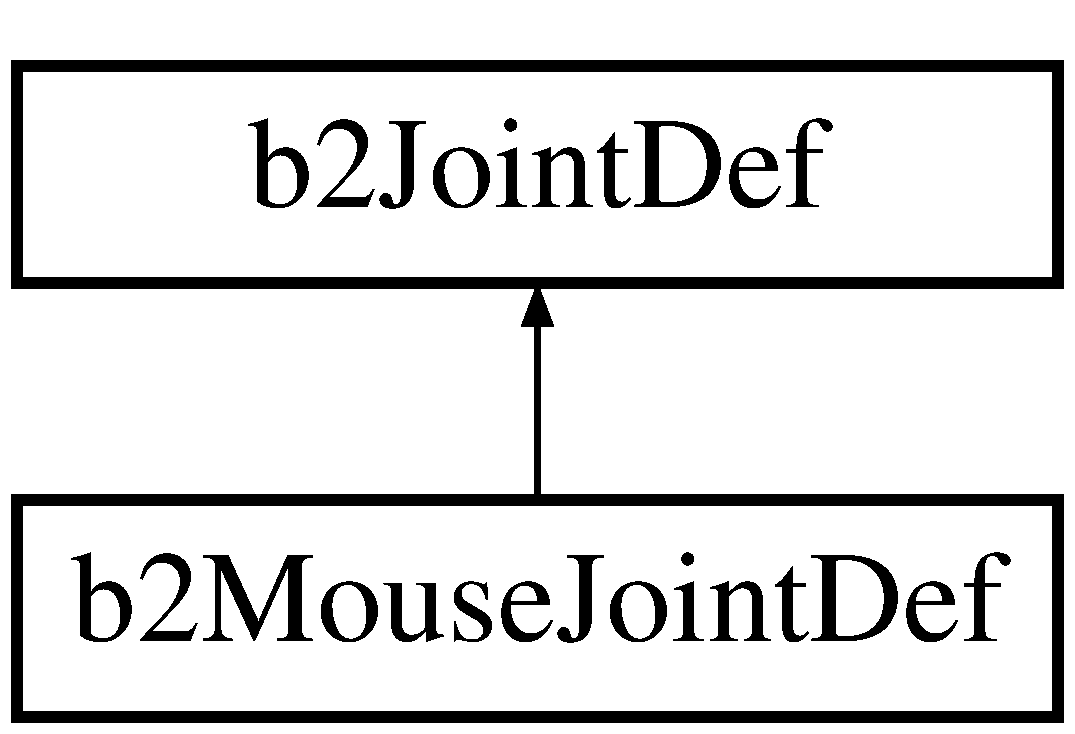
\includegraphics[height=2.000000cm]{structb2_mouse_joint_def}
\end{center}
\end{figure}
\subsection*{Public Attributes}
\begin{DoxyCompactItemize}
\item 
\hyperlink{structb2_vec2}{b2\+Vec2} \hyperlink{structb2_mouse_joint_def_aa1b76f72df9aca8d42bdc3e9922e310a}{target}
\item 
float32 \hyperlink{structb2_mouse_joint_def_ae9c52b3afda8ed006eb62fad163cdc3b}{max\+Force}
\item 
float32 \hyperlink{structb2_mouse_joint_def_a61e9017eb928608f75edddb6e0ca7f63}{frequency\+Hz}\hypertarget{structb2_mouse_joint_def_a61e9017eb928608f75edddb6e0ca7f63}{}\label{structb2_mouse_joint_def_a61e9017eb928608f75edddb6e0ca7f63}

\begin{DoxyCompactList}\small\item\em The response speed. \end{DoxyCompactList}\item 
float32 \hyperlink{structb2_mouse_joint_def_aee42888dab204a5c5745ba61acbfb7d6}{damping\+Ratio}\hypertarget{structb2_mouse_joint_def_aee42888dab204a5c5745ba61acbfb7d6}{}\label{structb2_mouse_joint_def_aee42888dab204a5c5745ba61acbfb7d6}

\begin{DoxyCompactList}\small\item\em The damping ratio. 0 = no damping, 1 = critical damping. \end{DoxyCompactList}\end{DoxyCompactItemize}


\subsection{Detailed Description}
Mouse joint definition. This requires a world target point, tuning parameters, and the time step. 

\subsection{Member Data Documentation}
\index{b2\+Mouse\+Joint\+Def@{b2\+Mouse\+Joint\+Def}!max\+Force@{max\+Force}}
\index{max\+Force@{max\+Force}!b2\+Mouse\+Joint\+Def@{b2\+Mouse\+Joint\+Def}}
\subsubsection[{\texorpdfstring{max\+Force}{maxForce}}]{\setlength{\rightskip}{0pt plus 5cm}float32 b2\+Mouse\+Joint\+Def\+::max\+Force}\hypertarget{structb2_mouse_joint_def_ae9c52b3afda8ed006eb62fad163cdc3b}{}\label{structb2_mouse_joint_def_ae9c52b3afda8ed006eb62fad163cdc3b}
The maximum constraint force that can be exerted to move the candidate body. Usually you will express as some multiple of the weight (multiplier $\ast$ mass $\ast$ gravity). \index{b2\+Mouse\+Joint\+Def@{b2\+Mouse\+Joint\+Def}!target@{target}}
\index{target@{target}!b2\+Mouse\+Joint\+Def@{b2\+Mouse\+Joint\+Def}}
\subsubsection[{\texorpdfstring{target}{target}}]{\setlength{\rightskip}{0pt plus 5cm}{\bf b2\+Vec2} b2\+Mouse\+Joint\+Def\+::target}\hypertarget{structb2_mouse_joint_def_aa1b76f72df9aca8d42bdc3e9922e310a}{}\label{structb2_mouse_joint_def_aa1b76f72df9aca8d42bdc3e9922e310a}
The initial world target point. This is assumed to coincide with the body anchor initially. 

The documentation for this struct was generated from the following file\+:\begin{DoxyCompactItemize}
\item 
Commun/\+Externe/\+Box2\+D/include/\+Box2\+D/\+Dynamics/\+Joints/b2\+Mouse\+Joint.\+h\end{DoxyCompactItemize}

\hypertarget{structb2_pair}{}\section{b2\+Pair Struct Reference}
\label{structb2_pair}\index{b2\+Pair@{b2\+Pair}}
\subsection*{Public Attributes}
\begin{DoxyCompactItemize}
\item 
int32 {\bfseries proxy\+IdA}\hypertarget{structb2_pair_abae3df5e877cf0c4611334e3eec4b84c}{}\label{structb2_pair_abae3df5e877cf0c4611334e3eec4b84c}

\item 
int32 {\bfseries proxy\+IdB}\hypertarget{structb2_pair_af2bd888ccb34535ab9126497349da749}{}\label{structb2_pair_af2bd888ccb34535ab9126497349da749}

\end{DoxyCompactItemize}


The documentation for this struct was generated from the following file\+:\begin{DoxyCompactItemize}
\item 
Commun/\+Externe/\+Box2\+D/include/\+Box2\+D/\+Collision/b2\+Broad\+Phase.\+h\end{DoxyCompactItemize}

\hypertarget{classb2_polygon_and_circle_contact}{}\section{b2\+Polygon\+And\+Circle\+Contact Class Reference}
\label{classb2_polygon_and_circle_contact}\index{b2\+Polygon\+And\+Circle\+Contact@{b2\+Polygon\+And\+Circle\+Contact}}
Inheritance diagram for b2\+Polygon\+And\+Circle\+Contact\+:\begin{figure}[H]
\begin{center}
\leavevmode
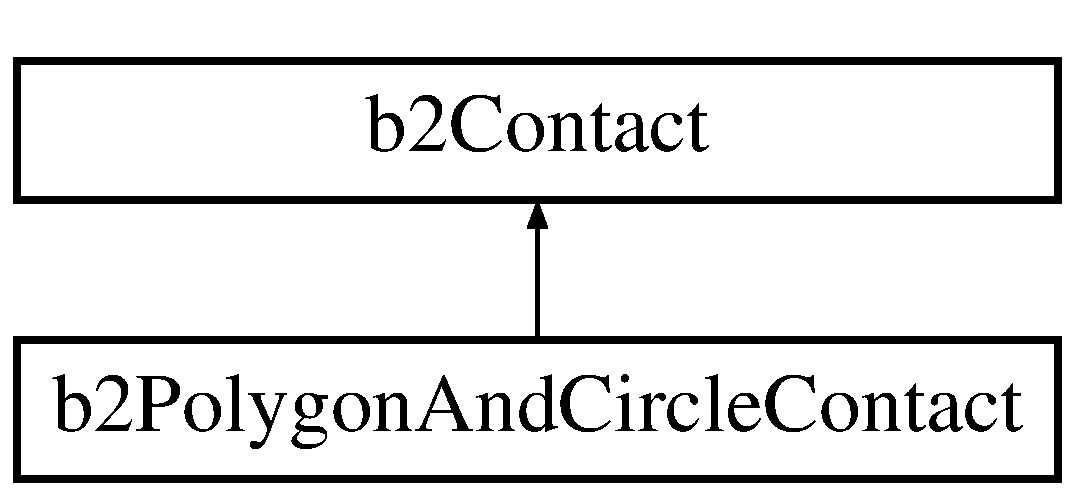
\includegraphics[height=2.000000cm]{classb2_polygon_and_circle_contact}
\end{center}
\end{figure}
\subsection*{Public Member Functions}
\begin{DoxyCompactItemize}
\item 
{\bfseries b2\+Polygon\+And\+Circle\+Contact} (\hyperlink{classb2_fixture}{b2\+Fixture} $\ast$fixtureA, \hyperlink{classb2_fixture}{b2\+Fixture} $\ast$fixtureB)\hypertarget{classb2_polygon_and_circle_contact_a38158da229eee22253c1f64df1982e40}{}\label{classb2_polygon_and_circle_contact_a38158da229eee22253c1f64df1982e40}

\item 
void \hyperlink{classb2_polygon_and_circle_contact_ac24d495022aae853cb573f86c8d86c3d}{Evaluate} (\hyperlink{structb2_manifold}{b2\+Manifold} $\ast$manifold, const \hyperlink{structb2_transform}{b2\+Transform} \&xfA, const \hyperlink{structb2_transform}{b2\+Transform} \&xfB)\hypertarget{classb2_polygon_and_circle_contact_ac24d495022aae853cb573f86c8d86c3d}{}\label{classb2_polygon_and_circle_contact_ac24d495022aae853cb573f86c8d86c3d}

\begin{DoxyCompactList}\small\item\em Evaluate this contact with your own manifold and transforms. \end{DoxyCompactList}\end{DoxyCompactItemize}
\subsection*{Static Public Member Functions}
\begin{DoxyCompactItemize}
\item 
static \hyperlink{classb2_contact}{b2\+Contact} $\ast$ {\bfseries Create} (\hyperlink{classb2_fixture}{b2\+Fixture} $\ast$fixtureA, int32 indexA, \hyperlink{classb2_fixture}{b2\+Fixture} $\ast$fixtureB, int32 indexB, \hyperlink{classb2_block_allocator}{b2\+Block\+Allocator} $\ast$allocator)\hypertarget{classb2_polygon_and_circle_contact_a0ff5b8e7167146b5716bce55365b7fc3}{}\label{classb2_polygon_and_circle_contact_a0ff5b8e7167146b5716bce55365b7fc3}

\item 
static void {\bfseries Destroy} (\hyperlink{classb2_contact}{b2\+Contact} $\ast$contact, \hyperlink{classb2_block_allocator}{b2\+Block\+Allocator} $\ast$allocator)\hypertarget{classb2_polygon_and_circle_contact_a666779f20aa3b57cfc0c60e3ac235f6b}{}\label{classb2_polygon_and_circle_contact_a666779f20aa3b57cfc0c60e3ac235f6b}

\end{DoxyCompactItemize}
\subsection*{Additional Inherited Members}


The documentation for this class was generated from the following file\+:\begin{DoxyCompactItemize}
\item 
Commun/\+Externe/\+Box2\+D/include/\+Box2\+D/\+Dynamics/\+Contacts/b2\+Polygon\+And\+Circle\+Contact.\+h\end{DoxyCompactItemize}

\hypertarget{classb2_polygon_contact}{}\section{b2\+Polygon\+Contact Class Reference}
\label{classb2_polygon_contact}\index{b2\+Polygon\+Contact@{b2\+Polygon\+Contact}}
Inheritance diagram for b2\+Polygon\+Contact\+:\begin{figure}[H]
\begin{center}
\leavevmode
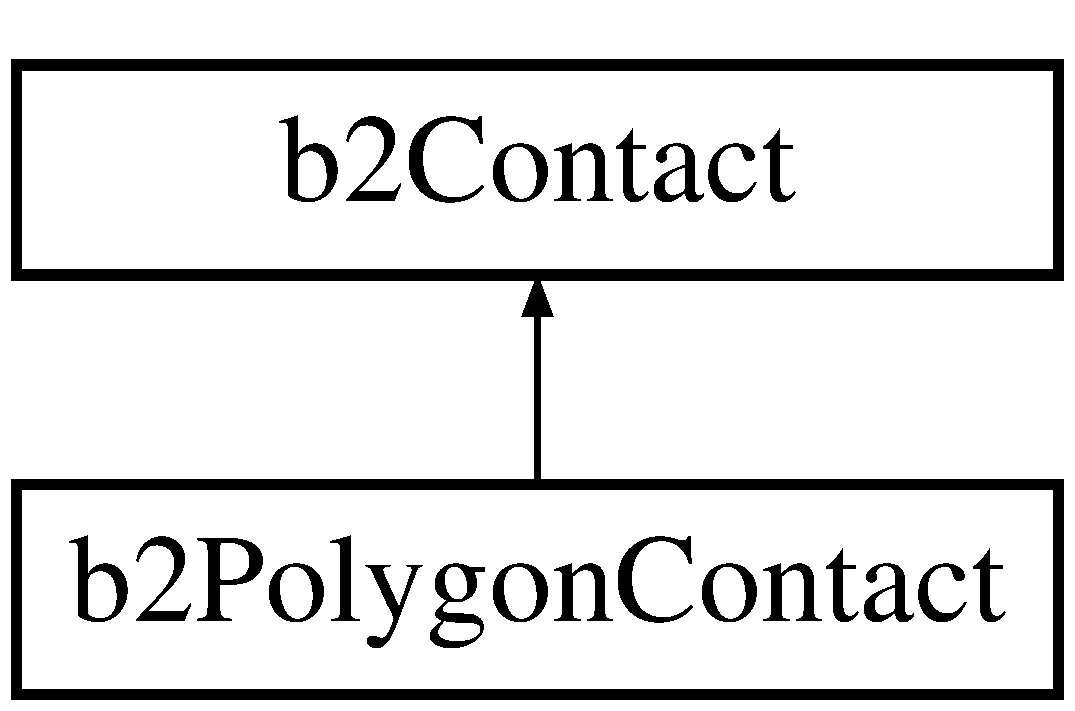
\includegraphics[height=2.000000cm]{classb2_polygon_contact}
\end{center}
\end{figure}
\subsection*{Public Member Functions}
\begin{DoxyCompactItemize}
\item 
{\bfseries b2\+Polygon\+Contact} (\hyperlink{classb2_fixture}{b2\+Fixture} $\ast$fixtureA, \hyperlink{classb2_fixture}{b2\+Fixture} $\ast$fixtureB)\hypertarget{classb2_polygon_contact_a93cabf086e75ae40dcd1881760c71c63}{}\label{classb2_polygon_contact_a93cabf086e75ae40dcd1881760c71c63}

\item 
void \hyperlink{classb2_polygon_contact_ae75f78bb52c76fc4fffda4d91e62d354}{Evaluate} (\hyperlink{structb2_manifold}{b2\+Manifold} $\ast$manifold, const \hyperlink{structb2_transform}{b2\+Transform} \&xfA, const \hyperlink{structb2_transform}{b2\+Transform} \&xfB)\hypertarget{classb2_polygon_contact_ae75f78bb52c76fc4fffda4d91e62d354}{}\label{classb2_polygon_contact_ae75f78bb52c76fc4fffda4d91e62d354}

\begin{DoxyCompactList}\small\item\em Evaluate this contact with your own manifold and transforms. \end{DoxyCompactList}\end{DoxyCompactItemize}
\subsection*{Static Public Member Functions}
\begin{DoxyCompactItemize}
\item 
static \hyperlink{classb2_contact}{b2\+Contact} $\ast$ {\bfseries Create} (\hyperlink{classb2_fixture}{b2\+Fixture} $\ast$fixtureA, int32 indexA, \hyperlink{classb2_fixture}{b2\+Fixture} $\ast$fixtureB, int32 indexB, \hyperlink{classb2_block_allocator}{b2\+Block\+Allocator} $\ast$allocator)\hypertarget{classb2_polygon_contact_a6f72e00b9f4870b214477073be35f592}{}\label{classb2_polygon_contact_a6f72e00b9f4870b214477073be35f592}

\item 
static void {\bfseries Destroy} (\hyperlink{classb2_contact}{b2\+Contact} $\ast$contact, \hyperlink{classb2_block_allocator}{b2\+Block\+Allocator} $\ast$allocator)\hypertarget{classb2_polygon_contact_a8f9687ed70a02550095cf80d3bbefc92}{}\label{classb2_polygon_contact_a8f9687ed70a02550095cf80d3bbefc92}

\end{DoxyCompactItemize}
\subsection*{Additional Inherited Members}


The documentation for this class was generated from the following file\+:\begin{DoxyCompactItemize}
\item 
Commun/\+Externe/\+Box2\+D/include/\+Box2\+D/\+Dynamics/\+Contacts/b2\+Polygon\+Contact.\+h\end{DoxyCompactItemize}

\hypertarget{classb2_polygon_shape}{}\section{b2\+Polygon\+Shape Class Reference}
\label{classb2_polygon_shape}\index{b2\+Polygon\+Shape@{b2\+Polygon\+Shape}}


{\ttfamily \#include $<$b2\+Polygon\+Shape.\+h$>$}

Inheritance diagram for b2\+Polygon\+Shape\+:\begin{figure}[H]
\begin{center}
\leavevmode
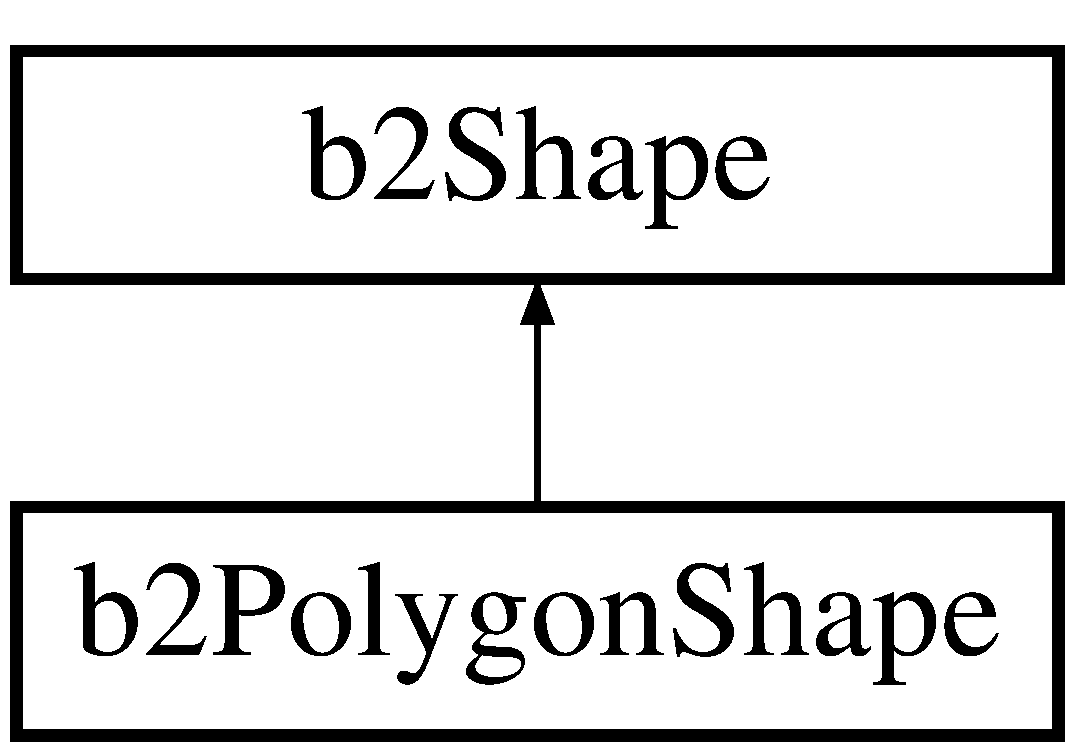
\includegraphics[height=2.000000cm]{classb2_polygon_shape}
\end{center}
\end{figure}
\subsection*{Public Member Functions}
\begin{DoxyCompactItemize}
\item 
\hyperlink{classb2_shape}{b2\+Shape} $\ast$ \hyperlink{classb2_polygon_shape_ae9ae1676632d6b20f787e1207ed2797f}{Clone} (\hyperlink{classb2_block_allocator}{b2\+Block\+Allocator} $\ast$allocator) const \hypertarget{classb2_polygon_shape_ae9ae1676632d6b20f787e1207ed2797f}{}\label{classb2_polygon_shape_ae9ae1676632d6b20f787e1207ed2797f}

\begin{DoxyCompactList}\small\item\em Implement \hyperlink{classb2_shape}{b2\+Shape}. \end{DoxyCompactList}\item 
int32 \hyperlink{classb2_polygon_shape_ae844375297d19744e01a37b397a5baba}{Get\+Child\+Count} () const 
\item 
void \hyperlink{classb2_polygon_shape_a4d7b35550509f570814b97325a68966b}{Set} (const \hyperlink{structb2_vec2}{b2\+Vec2} $\ast$points, int32 count)
\item 
void \hyperlink{classb2_polygon_shape_a6bb90df8b4a40d1c53b64cc352a855dd}{Set\+As\+Box} (float32 hx, float32 hy)
\item 
void \hyperlink{classb2_polygon_shape_a890690250115483da6c7d69829be087e}{Set\+As\+Box} (float32 hx, float32 hy, const \hyperlink{structb2_vec2}{b2\+Vec2} \&center, float32 angle)
\item 
bool \hyperlink{classb2_polygon_shape_a69ccc2f671394b3cc1a00a16ef36b12b}{Test\+Point} (const \hyperlink{structb2_transform}{b2\+Transform} \&transform, const \hyperlink{structb2_vec2}{b2\+Vec2} \&p) const 
\item 
bool \hyperlink{classb2_polygon_shape_ac13bded10d09c341f64aaa2750dda6b5}{Ray\+Cast} (\hyperlink{structb2_ray_cast_output}{b2\+Ray\+Cast\+Output} $\ast$output, const \hyperlink{structb2_ray_cast_input}{b2\+Ray\+Cast\+Input} \&input, const \hyperlink{structb2_transform}{b2\+Transform} \&transform, int32 child\+Index) const \hypertarget{classb2_polygon_shape_ac13bded10d09c341f64aaa2750dda6b5}{}\label{classb2_polygon_shape_ac13bded10d09c341f64aaa2750dda6b5}

\begin{DoxyCompactList}\small\item\em Implement \hyperlink{classb2_shape}{b2\+Shape}. \end{DoxyCompactList}\item 
void \hyperlink{classb2_polygon_shape_a00e225b0321bf6bb231a554036ffdf23}{Compute\+A\+A\+BB} (\hyperlink{structb2_a_a_b_b}{b2\+A\+A\+BB} $\ast$aabb, const \hyperlink{structb2_transform}{b2\+Transform} \&transform, int32 child\+Index) const 
\item 
void \hyperlink{classb2_polygon_shape_ad86c4c2a83a7122599462da83bf35389}{Compute\+Mass} (\hyperlink{structb2_mass_data}{b2\+Mass\+Data} $\ast$mass\+Data, float32 density) const 
\item 
int32 \hyperlink{classb2_polygon_shape_ae220f24c42eff4aef4cd452676ca2ced}{Get\+Vertex\+Count} () const \hypertarget{classb2_polygon_shape_ae220f24c42eff4aef4cd452676ca2ced}{}\label{classb2_polygon_shape_ae220f24c42eff4aef4cd452676ca2ced}

\begin{DoxyCompactList}\small\item\em Get the vertex count. \end{DoxyCompactList}\item 
const \hyperlink{structb2_vec2}{b2\+Vec2} \& \hyperlink{classb2_polygon_shape_a88cdb687ec7dc0cbcf4bd25fd37f4da1}{Get\+Vertex} (int32 index) const \hypertarget{classb2_polygon_shape_a88cdb687ec7dc0cbcf4bd25fd37f4da1}{}\label{classb2_polygon_shape_a88cdb687ec7dc0cbcf4bd25fd37f4da1}

\begin{DoxyCompactList}\small\item\em Get a vertex by index. \end{DoxyCompactList}\item 
bool \hyperlink{classb2_polygon_shape_afa9fe13cd6963e2317be35071ac69959}{Validate} () const 
\end{DoxyCompactItemize}
\subsection*{Public Attributes}
\begin{DoxyCompactItemize}
\item 
\hyperlink{structb2_vec2}{b2\+Vec2} {\bfseries m\+\_\+centroid}\hypertarget{classb2_polygon_shape_ae8f5bd2f13f1e9b741c33350ba19cd9f}{}\label{classb2_polygon_shape_ae8f5bd2f13f1e9b741c33350ba19cd9f}

\item 
\hyperlink{structb2_vec2}{b2\+Vec2} {\bfseries m\+\_\+vertices} \mbox{[}\hyperlink{b2_settings_8h_a09d71ee1993bee28b5b2e6d893b41884}{b2\+\_\+max\+Polygon\+Vertices}\mbox{]}\hypertarget{classb2_polygon_shape_a11ee5c107660be5da25f0e164aaccd53}{}\label{classb2_polygon_shape_a11ee5c107660be5da25f0e164aaccd53}

\item 
\hyperlink{structb2_vec2}{b2\+Vec2} {\bfseries m\+\_\+normals} \mbox{[}\hyperlink{b2_settings_8h_a09d71ee1993bee28b5b2e6d893b41884}{b2\+\_\+max\+Polygon\+Vertices}\mbox{]}\hypertarget{classb2_polygon_shape_a97cdcec277321c62ecdf93cb649958ce}{}\label{classb2_polygon_shape_a97cdcec277321c62ecdf93cb649958ce}

\item 
int32 {\bfseries m\+\_\+count}\hypertarget{classb2_polygon_shape_a2c8cfdc15267f282e66f7bda7369b79f}{}\label{classb2_polygon_shape_a2c8cfdc15267f282e66f7bda7369b79f}

\end{DoxyCompactItemize}
\subsection*{Additional Inherited Members}


\subsection{Detailed Description}
A convex polygon. It is assumed that the interior of the polygon is to the left of each edge. Polygons have a maximum number of vertices equal to b2\+\_\+max\+Polygon\+Vertices. In most cases you should not need many vertices for a convex polygon. 

\subsection{Member Function Documentation}
\index{b2\+Polygon\+Shape@{b2\+Polygon\+Shape}!Compute\+A\+A\+BB@{Compute\+A\+A\+BB}}
\index{Compute\+A\+A\+BB@{Compute\+A\+A\+BB}!b2\+Polygon\+Shape@{b2\+Polygon\+Shape}}
\subsubsection[{\texorpdfstring{Compute\+A\+A\+B\+B(b2\+A\+A\+B\+B $\ast$aabb, const b2\+Transform \&transform, int32 child\+Index) const }{ComputeAABB(b2AABB *aabb, const b2Transform &transform, int32 childIndex) const }}]{\setlength{\rightskip}{0pt plus 5cm}void b2\+Polygon\+Shape\+::\+Compute\+A\+A\+BB (
\begin{DoxyParamCaption}
\item[{{\bf b2\+A\+A\+BB} $\ast$}]{aabb, }
\item[{const {\bf b2\+Transform} \&}]{transform, }
\item[{int32}]{child\+Index}
\end{DoxyParamCaption}
) const\hspace{0.3cm}{\ttfamily [virtual]}}\hypertarget{classb2_polygon_shape_a00e225b0321bf6bb231a554036ffdf23}{}\label{classb2_polygon_shape_a00e225b0321bf6bb231a554036ffdf23}
\begin{DoxySeeAlso}{See also}
\hyperlink{classb2_shape_a0a7f4227b6c17450fc26e0b6641b7abf}{b2\+Shape\+::\+Compute\+A\+A\+BB} 
\end{DoxySeeAlso}


Implements \hyperlink{classb2_shape_a0a7f4227b6c17450fc26e0b6641b7abf}{b2\+Shape}.

\index{b2\+Polygon\+Shape@{b2\+Polygon\+Shape}!Compute\+Mass@{Compute\+Mass}}
\index{Compute\+Mass@{Compute\+Mass}!b2\+Polygon\+Shape@{b2\+Polygon\+Shape}}
\subsubsection[{\texorpdfstring{Compute\+Mass(b2\+Mass\+Data $\ast$mass\+Data, float32 density) const }{ComputeMass(b2MassData *massData, float32 density) const }}]{\setlength{\rightskip}{0pt plus 5cm}void b2\+Polygon\+Shape\+::\+Compute\+Mass (
\begin{DoxyParamCaption}
\item[{{\bf b2\+Mass\+Data} $\ast$}]{mass\+Data, }
\item[{float32}]{density}
\end{DoxyParamCaption}
) const\hspace{0.3cm}{\ttfamily [virtual]}}\hypertarget{classb2_polygon_shape_ad86c4c2a83a7122599462da83bf35389}{}\label{classb2_polygon_shape_ad86c4c2a83a7122599462da83bf35389}
\begin{DoxySeeAlso}{See also}
\hyperlink{classb2_shape_a33cfcad2cf4cc31e1d001bf1baf10721}{b2\+Shape\+::\+Compute\+Mass} 
\end{DoxySeeAlso}


Implements \hyperlink{classb2_shape_a33cfcad2cf4cc31e1d001bf1baf10721}{b2\+Shape}.

\index{b2\+Polygon\+Shape@{b2\+Polygon\+Shape}!Get\+Child\+Count@{Get\+Child\+Count}}
\index{Get\+Child\+Count@{Get\+Child\+Count}!b2\+Polygon\+Shape@{b2\+Polygon\+Shape}}
\subsubsection[{\texorpdfstring{Get\+Child\+Count() const }{GetChildCount() const }}]{\setlength{\rightskip}{0pt plus 5cm}int32 b2\+Polygon\+Shape\+::\+Get\+Child\+Count (
\begin{DoxyParamCaption}
{}
\end{DoxyParamCaption}
) const\hspace{0.3cm}{\ttfamily [virtual]}}\hypertarget{classb2_polygon_shape_ae844375297d19744e01a37b397a5baba}{}\label{classb2_polygon_shape_ae844375297d19744e01a37b397a5baba}
\begin{DoxySeeAlso}{See also}
\hyperlink{classb2_shape_acaade0398c8a6f3750ba0d25fbde2242}{b2\+Shape\+::\+Get\+Child\+Count} 
\end{DoxySeeAlso}


Implements \hyperlink{classb2_shape_acaade0398c8a6f3750ba0d25fbde2242}{b2\+Shape}.

\index{b2\+Polygon\+Shape@{b2\+Polygon\+Shape}!Set@{Set}}
\index{Set@{Set}!b2\+Polygon\+Shape@{b2\+Polygon\+Shape}}
\subsubsection[{\texorpdfstring{Set(const b2\+Vec2 $\ast$points, int32 count)}{Set(const b2Vec2 *points, int32 count)}}]{\setlength{\rightskip}{0pt plus 5cm}void b2\+Polygon\+Shape\+::\+Set (
\begin{DoxyParamCaption}
\item[{const {\bf b2\+Vec2} $\ast$}]{points, }
\item[{int32}]{count}
\end{DoxyParamCaption}
)}\hypertarget{classb2_polygon_shape_a4d7b35550509f570814b97325a68966b}{}\label{classb2_polygon_shape_a4d7b35550509f570814b97325a68966b}
Create a convex hull from the given array of local points. The count must be in the range \mbox{[}3, b2\+\_\+max\+Polygon\+Vertices\mbox{]}. \begin{DoxyWarning}{Warning}
the points may be re-\/ordered, even if they form a convex polygon 

collinear points are handled but not removed. Collinear points may lead to poor stacking behavior. 
\end{DoxyWarning}
\index{b2\+Polygon\+Shape@{b2\+Polygon\+Shape}!Set\+As\+Box@{Set\+As\+Box}}
\index{Set\+As\+Box@{Set\+As\+Box}!b2\+Polygon\+Shape@{b2\+Polygon\+Shape}}
\subsubsection[{\texorpdfstring{Set\+As\+Box(float32 hx, float32 hy)}{SetAsBox(float32 hx, float32 hy)}}]{\setlength{\rightskip}{0pt plus 5cm}void b2\+Polygon\+Shape\+::\+Set\+As\+Box (
\begin{DoxyParamCaption}
\item[{float32}]{hx, }
\item[{float32}]{hy}
\end{DoxyParamCaption}
)}\hypertarget{classb2_polygon_shape_a6bb90df8b4a40d1c53b64cc352a855dd}{}\label{classb2_polygon_shape_a6bb90df8b4a40d1c53b64cc352a855dd}
Build vertices to represent an axis-\/aligned box centered on the local origin. 
\begin{DoxyParams}{Parameters}
{\em hx} & the half-\/width. \\
\hline
{\em hy} & the half-\/height. \\
\hline
\end{DoxyParams}
\index{b2\+Polygon\+Shape@{b2\+Polygon\+Shape}!Set\+As\+Box@{Set\+As\+Box}}
\index{Set\+As\+Box@{Set\+As\+Box}!b2\+Polygon\+Shape@{b2\+Polygon\+Shape}}
\subsubsection[{\texorpdfstring{Set\+As\+Box(float32 hx, float32 hy, const b2\+Vec2 \&center, float32 angle)}{SetAsBox(float32 hx, float32 hy, const b2Vec2 &center, float32 angle)}}]{\setlength{\rightskip}{0pt plus 5cm}void b2\+Polygon\+Shape\+::\+Set\+As\+Box (
\begin{DoxyParamCaption}
\item[{float32}]{hx, }
\item[{float32}]{hy, }
\item[{const {\bf b2\+Vec2} \&}]{center, }
\item[{float32}]{angle}
\end{DoxyParamCaption}
)}\hypertarget{classb2_polygon_shape_a890690250115483da6c7d69829be087e}{}\label{classb2_polygon_shape_a890690250115483da6c7d69829be087e}
Build vertices to represent an oriented box. 
\begin{DoxyParams}{Parameters}
{\em hx} & the half-\/width. \\
\hline
{\em hy} & the half-\/height. \\
\hline
{\em center} & the center of the box in local coordinates. \\
\hline
{\em angle} & the rotation of the box in local coordinates. \\
\hline
\end{DoxyParams}
\index{b2\+Polygon\+Shape@{b2\+Polygon\+Shape}!Test\+Point@{Test\+Point}}
\index{Test\+Point@{Test\+Point}!b2\+Polygon\+Shape@{b2\+Polygon\+Shape}}
\subsubsection[{\texorpdfstring{Test\+Point(const b2\+Transform \&transform, const b2\+Vec2 \&p) const }{TestPoint(const b2Transform &transform, const b2Vec2 &p) const }}]{\setlength{\rightskip}{0pt plus 5cm}bool b2\+Polygon\+Shape\+::\+Test\+Point (
\begin{DoxyParamCaption}
\item[{const {\bf b2\+Transform} \&}]{transform, }
\item[{const {\bf b2\+Vec2} \&}]{p}
\end{DoxyParamCaption}
) const\hspace{0.3cm}{\ttfamily [virtual]}}\hypertarget{classb2_polygon_shape_a69ccc2f671394b3cc1a00a16ef36b12b}{}\label{classb2_polygon_shape_a69ccc2f671394b3cc1a00a16ef36b12b}
\begin{DoxySeeAlso}{See also}
\hyperlink{classb2_shape_a11996b9bdcf8dca92a0c8bf484ab3f59}{b2\+Shape\+::\+Test\+Point} 
\end{DoxySeeAlso}


Implements \hyperlink{classb2_shape_a11996b9bdcf8dca92a0c8bf484ab3f59}{b2\+Shape}.

\index{b2\+Polygon\+Shape@{b2\+Polygon\+Shape}!Validate@{Validate}}
\index{Validate@{Validate}!b2\+Polygon\+Shape@{b2\+Polygon\+Shape}}
\subsubsection[{\texorpdfstring{Validate() const }{Validate() const }}]{\setlength{\rightskip}{0pt plus 5cm}bool b2\+Polygon\+Shape\+::\+Validate (
\begin{DoxyParamCaption}
{}
\end{DoxyParamCaption}
) const}\hypertarget{classb2_polygon_shape_afa9fe13cd6963e2317be35071ac69959}{}\label{classb2_polygon_shape_afa9fe13cd6963e2317be35071ac69959}
Validate convexity. This is a very time consuming operation. \begin{DoxyReturn}{Returns}
true if valid 
\end{DoxyReturn}


The documentation for this class was generated from the following file\+:\begin{DoxyCompactItemize}
\item 
Cadriciel/\+Commun/\+Externe/\+Box2\+D/include/\+Box2\+D/\+Collision/\+Shapes/b2\+Polygon\+Shape.\+h\end{DoxyCompactItemize}

\hypertarget{structb2_position}{}\section{b2\+Position Struct Reference}
\label{structb2_position}\index{b2\+Position@{b2\+Position}}


This is an internal structure.  




{\ttfamily \#include $<$b2\+Time\+Step.\+h$>$}

\subsection*{Public Attributes}
\begin{DoxyCompactItemize}
\item 
\hyperlink{structb2_vec2}{b2\+Vec2} {\bfseries c}\hypertarget{structb2_position_a64b6d764d272385f84e4cac5ceb5af27}{}\label{structb2_position_a64b6d764d272385f84e4cac5ceb5af27}

\item 
float32 {\bfseries a}\hypertarget{structb2_position_a19d9362011e8c080059ac7f692cc7d8f}{}\label{structb2_position_a19d9362011e8c080059ac7f692cc7d8f}

\end{DoxyCompactItemize}


\subsection{Detailed Description}
This is an internal structure. 

The documentation for this struct was generated from the following file\+:\begin{DoxyCompactItemize}
\item 
Commun/\+Externe/\+Box2\+D/include/\+Box2\+D/\+Dynamics/b2\+Time\+Step.\+h\end{DoxyCompactItemize}

\hypertarget{classb2_prismatic_joint}{}\section{b2\+Prismatic\+Joint Class Reference}
\label{classb2_prismatic_joint}\index{b2\+Prismatic\+Joint@{b2\+Prismatic\+Joint}}


{\ttfamily \#include $<$b2\+Prismatic\+Joint.\+h$>$}

Inheritance diagram for b2\+Prismatic\+Joint\+:\begin{figure}[H]
\begin{center}
\leavevmode
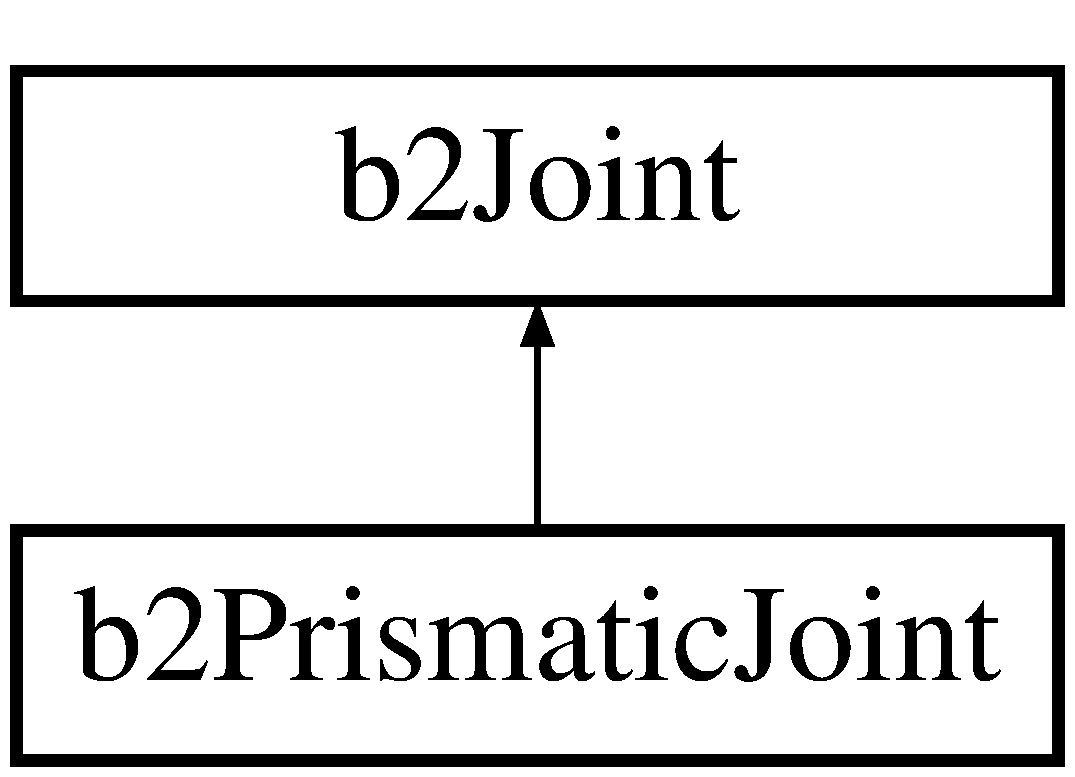
\includegraphics[height=2.000000cm]{classb2_prismatic_joint}
\end{center}
\end{figure}
\subsection*{Public Member Functions}
\begin{DoxyCompactItemize}
\item 
\hyperlink{structb2_vec2}{b2\+Vec2} \hyperlink{classb2_prismatic_joint_ae6ccc4b3ceba180e4381fe4b821ef8d1}{Get\+AnchorA} () const \hypertarget{classb2_prismatic_joint_ae6ccc4b3ceba180e4381fe4b821ef8d1}{}\label{classb2_prismatic_joint_ae6ccc4b3ceba180e4381fe4b821ef8d1}

\begin{DoxyCompactList}\small\item\em Get the anchor point on bodyA in world coordinates. \end{DoxyCompactList}\item 
\hyperlink{structb2_vec2}{b2\+Vec2} \hyperlink{classb2_prismatic_joint_aa2e00a1801989c3b6bc67bf47092b531}{Get\+AnchorB} () const \hypertarget{classb2_prismatic_joint_aa2e00a1801989c3b6bc67bf47092b531}{}\label{classb2_prismatic_joint_aa2e00a1801989c3b6bc67bf47092b531}

\begin{DoxyCompactList}\small\item\em Get the anchor point on bodyB in world coordinates. \end{DoxyCompactList}\item 
\hyperlink{structb2_vec2}{b2\+Vec2} \hyperlink{classb2_prismatic_joint_a9e2a6103c1ff57e65d524b42f72b09e0}{Get\+Reaction\+Force} (float32 inv\+\_\+dt) const \hypertarget{classb2_prismatic_joint_a9e2a6103c1ff57e65d524b42f72b09e0}{}\label{classb2_prismatic_joint_a9e2a6103c1ff57e65d524b42f72b09e0}

\begin{DoxyCompactList}\small\item\em Get the reaction force on bodyB at the joint anchor in Newtons. \end{DoxyCompactList}\item 
float32 \hyperlink{classb2_prismatic_joint_a59b419ccec1a5a4b80d6664d03bd256e}{Get\+Reaction\+Torque} (float32 inv\+\_\+dt) const \hypertarget{classb2_prismatic_joint_a59b419ccec1a5a4b80d6664d03bd256e}{}\label{classb2_prismatic_joint_a59b419ccec1a5a4b80d6664d03bd256e}

\begin{DoxyCompactList}\small\item\em Get the reaction torque on bodyB in N$\ast$m. \end{DoxyCompactList}\item 
const \hyperlink{structb2_vec2}{b2\+Vec2} \& \hyperlink{classb2_prismatic_joint_a8453728991590d064f75ac9ee43eb0cb}{Get\+Local\+AnchorA} () const \hypertarget{classb2_prismatic_joint_a8453728991590d064f75ac9ee43eb0cb}{}\label{classb2_prismatic_joint_a8453728991590d064f75ac9ee43eb0cb}

\begin{DoxyCompactList}\small\item\em The local anchor point relative to bodyA\textquotesingle{}s origin. \end{DoxyCompactList}\item 
const \hyperlink{structb2_vec2}{b2\+Vec2} \& \hyperlink{classb2_prismatic_joint_a5591358eced21a8845744a8c47b7df9d}{Get\+Local\+AnchorB} () const \hypertarget{classb2_prismatic_joint_a5591358eced21a8845744a8c47b7df9d}{}\label{classb2_prismatic_joint_a5591358eced21a8845744a8c47b7df9d}

\begin{DoxyCompactList}\small\item\em The local anchor point relative to bodyB\textquotesingle{}s origin. \end{DoxyCompactList}\item 
const \hyperlink{structb2_vec2}{b2\+Vec2} \& \hyperlink{classb2_prismatic_joint_ab1aff69853c5ddb89ed8efdf8a0f4376}{Get\+Local\+AxisA} () const \hypertarget{classb2_prismatic_joint_ab1aff69853c5ddb89ed8efdf8a0f4376}{}\label{classb2_prismatic_joint_ab1aff69853c5ddb89ed8efdf8a0f4376}

\begin{DoxyCompactList}\small\item\em The local joint axis relative to bodyA. \end{DoxyCompactList}\item 
float32 \hyperlink{classb2_prismatic_joint_ae9e0a48367f191b2dd6a5bc05364a372}{Get\+Reference\+Angle} () const \hypertarget{classb2_prismatic_joint_ae9e0a48367f191b2dd6a5bc05364a372}{}\label{classb2_prismatic_joint_ae9e0a48367f191b2dd6a5bc05364a372}

\begin{DoxyCompactList}\small\item\em Get the reference angle. \end{DoxyCompactList}\item 
float32 \hyperlink{classb2_prismatic_joint_ade994ac79315258c80bccceef371df57}{Get\+Joint\+Translation} () const \hypertarget{classb2_prismatic_joint_ade994ac79315258c80bccceef371df57}{}\label{classb2_prismatic_joint_ade994ac79315258c80bccceef371df57}

\begin{DoxyCompactList}\small\item\em Get the current joint translation, usually in meters. \end{DoxyCompactList}\item 
float32 \hyperlink{classb2_prismatic_joint_a221aa1c6253686c96a02ecdd99c84b4c}{Get\+Joint\+Speed} () const \hypertarget{classb2_prismatic_joint_a221aa1c6253686c96a02ecdd99c84b4c}{}\label{classb2_prismatic_joint_a221aa1c6253686c96a02ecdd99c84b4c}

\begin{DoxyCompactList}\small\item\em Get the current joint translation speed, usually in meters per second. \end{DoxyCompactList}\item 
bool \hyperlink{classb2_prismatic_joint_afb109fd7f3efbf44eae4b7961169bf9f}{Is\+Limit\+Enabled} () const \hypertarget{classb2_prismatic_joint_afb109fd7f3efbf44eae4b7961169bf9f}{}\label{classb2_prismatic_joint_afb109fd7f3efbf44eae4b7961169bf9f}

\begin{DoxyCompactList}\small\item\em Is the joint limit enabled? \end{DoxyCompactList}\item 
void \hyperlink{classb2_prismatic_joint_a6d419afe7bd4b0e36d2e4607df7f79f2}{Enable\+Limit} (bool flag)\hypertarget{classb2_prismatic_joint_a6d419afe7bd4b0e36d2e4607df7f79f2}{}\label{classb2_prismatic_joint_a6d419afe7bd4b0e36d2e4607df7f79f2}

\begin{DoxyCompactList}\small\item\em Enable/disable the joint limit. \end{DoxyCompactList}\item 
float32 \hyperlink{classb2_prismatic_joint_ad58727abc63a820e6d93983408a9508b}{Get\+Lower\+Limit} () const \hypertarget{classb2_prismatic_joint_ad58727abc63a820e6d93983408a9508b}{}\label{classb2_prismatic_joint_ad58727abc63a820e6d93983408a9508b}

\begin{DoxyCompactList}\small\item\em Get the lower joint limit, usually in meters. \end{DoxyCompactList}\item 
float32 \hyperlink{classb2_prismatic_joint_ac72bdcf5108d474d3f11e86773a9a471}{Get\+Upper\+Limit} () const \hypertarget{classb2_prismatic_joint_ac72bdcf5108d474d3f11e86773a9a471}{}\label{classb2_prismatic_joint_ac72bdcf5108d474d3f11e86773a9a471}

\begin{DoxyCompactList}\small\item\em Get the upper joint limit, usually in meters. \end{DoxyCompactList}\item 
void \hyperlink{classb2_prismatic_joint_a82a220e6d5a212c1924882e0855b0bef}{Set\+Limits} (float32 lower, float32 upper)\hypertarget{classb2_prismatic_joint_a82a220e6d5a212c1924882e0855b0bef}{}\label{classb2_prismatic_joint_a82a220e6d5a212c1924882e0855b0bef}

\begin{DoxyCompactList}\small\item\em Set the joint limits, usually in meters. \end{DoxyCompactList}\item 
bool \hyperlink{classb2_prismatic_joint_a236650664554a4d81f8644e9a9d19c65}{Is\+Motor\+Enabled} () const \hypertarget{classb2_prismatic_joint_a236650664554a4d81f8644e9a9d19c65}{}\label{classb2_prismatic_joint_a236650664554a4d81f8644e9a9d19c65}

\begin{DoxyCompactList}\small\item\em Is the joint motor enabled? \end{DoxyCompactList}\item 
void \hyperlink{classb2_prismatic_joint_a4a7fd079de49f7ed5aa4a5d8d90be2a2}{Enable\+Motor} (bool flag)\hypertarget{classb2_prismatic_joint_a4a7fd079de49f7ed5aa4a5d8d90be2a2}{}\label{classb2_prismatic_joint_a4a7fd079de49f7ed5aa4a5d8d90be2a2}

\begin{DoxyCompactList}\small\item\em Enable/disable the joint motor. \end{DoxyCompactList}\item 
void \hyperlink{classb2_prismatic_joint_a602ef7a6ca4fca55d011f1b38ab5a6c3}{Set\+Motor\+Speed} (float32 speed)\hypertarget{classb2_prismatic_joint_a602ef7a6ca4fca55d011f1b38ab5a6c3}{}\label{classb2_prismatic_joint_a602ef7a6ca4fca55d011f1b38ab5a6c3}

\begin{DoxyCompactList}\small\item\em Set the motor speed, usually in meters per second. \end{DoxyCompactList}\item 
float32 \hyperlink{classb2_prismatic_joint_a20f969fefb08d86728bd1f0cf03e121f}{Get\+Motor\+Speed} () const \hypertarget{classb2_prismatic_joint_a20f969fefb08d86728bd1f0cf03e121f}{}\label{classb2_prismatic_joint_a20f969fefb08d86728bd1f0cf03e121f}

\begin{DoxyCompactList}\small\item\em Get the motor speed, usually in meters per second. \end{DoxyCompactList}\item 
void \hyperlink{classb2_prismatic_joint_aa7817474aef15ca4815341479ac590e2}{Set\+Max\+Motor\+Force} (float32 force)\hypertarget{classb2_prismatic_joint_aa7817474aef15ca4815341479ac590e2}{}\label{classb2_prismatic_joint_aa7817474aef15ca4815341479ac590e2}

\begin{DoxyCompactList}\small\item\em Set the maximum motor force, usually in N. \end{DoxyCompactList}\item 
float32 {\bfseries Get\+Max\+Motor\+Force} () const \hypertarget{classb2_prismatic_joint_a2d1583462dd6cb62d0a48353ddd48c42}{}\label{classb2_prismatic_joint_a2d1583462dd6cb62d0a48353ddd48c42}

\item 
float32 \hyperlink{classb2_prismatic_joint_aee80c02627750559fc382422804a30e6}{Get\+Motor\+Force} (float32 inv\+\_\+dt) const \hypertarget{classb2_prismatic_joint_aee80c02627750559fc382422804a30e6}{}\label{classb2_prismatic_joint_aee80c02627750559fc382422804a30e6}

\begin{DoxyCompactList}\small\item\em Get the current motor force given the inverse time step, usually in N. \end{DoxyCompactList}\item 
void \hyperlink{classb2_prismatic_joint_a1d8e01f0c7ca9e1840f1f17c17dda7db}{Dump} ()\hypertarget{classb2_prismatic_joint_a1d8e01f0c7ca9e1840f1f17c17dda7db}{}\label{classb2_prismatic_joint_a1d8e01f0c7ca9e1840f1f17c17dda7db}

\begin{DoxyCompactList}\small\item\em Dump to b2\+Log. \end{DoxyCompactList}\end{DoxyCompactItemize}
\subsection*{Protected Member Functions}
\begin{DoxyCompactItemize}
\item 
{\bfseries b2\+Prismatic\+Joint} (const \hyperlink{structb2_prismatic_joint_def}{b2\+Prismatic\+Joint\+Def} $\ast$def)\hypertarget{classb2_prismatic_joint_ab1586a2334f7e32137fbd7f807e249ca}{}\label{classb2_prismatic_joint_ab1586a2334f7e32137fbd7f807e249ca}

\item 
void {\bfseries Init\+Velocity\+Constraints} (const \hyperlink{structb2_solver_data}{b2\+Solver\+Data} \&data)\hypertarget{classb2_prismatic_joint_a2178262be18a40c1aca79375ce7f4e7f}{}\label{classb2_prismatic_joint_a2178262be18a40c1aca79375ce7f4e7f}

\item 
void {\bfseries Solve\+Velocity\+Constraints} (const \hyperlink{structb2_solver_data}{b2\+Solver\+Data} \&data)\hypertarget{classb2_prismatic_joint_a05f935314127028e3ee6c8816e178aa0}{}\label{classb2_prismatic_joint_a05f935314127028e3ee6c8816e178aa0}

\item 
bool {\bfseries Solve\+Position\+Constraints} (const \hyperlink{structb2_solver_data}{b2\+Solver\+Data} \&data)\hypertarget{classb2_prismatic_joint_a3ce2a793c1e92df1205e4a704997bbf6}{}\label{classb2_prismatic_joint_a3ce2a793c1e92df1205e4a704997bbf6}

\end{DoxyCompactItemize}
\subsection*{Protected Attributes}
\begin{DoxyCompactItemize}
\item 
\hyperlink{structb2_vec2}{b2\+Vec2} {\bfseries m\+\_\+local\+AnchorA}\hypertarget{classb2_prismatic_joint_aeec29d80cc57252702fd645c31ca7889}{}\label{classb2_prismatic_joint_aeec29d80cc57252702fd645c31ca7889}

\item 
\hyperlink{structb2_vec2}{b2\+Vec2} {\bfseries m\+\_\+local\+AnchorB}\hypertarget{classb2_prismatic_joint_ae9cb63f225e4b4dcc287ab475868d044}{}\label{classb2_prismatic_joint_ae9cb63f225e4b4dcc287ab475868d044}

\item 
\hyperlink{structb2_vec2}{b2\+Vec2} {\bfseries m\+\_\+local\+X\+AxisA}\hypertarget{classb2_prismatic_joint_ab68f8bb2a8012e4646dc274db1723fbf}{}\label{classb2_prismatic_joint_ab68f8bb2a8012e4646dc274db1723fbf}

\item 
\hyperlink{structb2_vec2}{b2\+Vec2} {\bfseries m\+\_\+local\+Y\+AxisA}\hypertarget{classb2_prismatic_joint_a6885a7d60a2596883660183bcf721ea9}{}\label{classb2_prismatic_joint_a6885a7d60a2596883660183bcf721ea9}

\item 
float32 {\bfseries m\+\_\+reference\+Angle}\hypertarget{classb2_prismatic_joint_ad8b2ee403ba7517966d9e05b988e28c6}{}\label{classb2_prismatic_joint_ad8b2ee403ba7517966d9e05b988e28c6}

\item 
\hyperlink{structb2_vec3}{b2\+Vec3} {\bfseries m\+\_\+impulse}\hypertarget{classb2_prismatic_joint_a92530ae3ec9765d775ec82a39400f770}{}\label{classb2_prismatic_joint_a92530ae3ec9765d775ec82a39400f770}

\item 
float32 {\bfseries m\+\_\+motor\+Impulse}\hypertarget{classb2_prismatic_joint_aff90d55579b511950334d8a0449f1155}{}\label{classb2_prismatic_joint_aff90d55579b511950334d8a0449f1155}

\item 
float32 {\bfseries m\+\_\+lower\+Translation}\hypertarget{classb2_prismatic_joint_a82e13b09e43d0d82365845aa3fb7f9fe}{}\label{classb2_prismatic_joint_a82e13b09e43d0d82365845aa3fb7f9fe}

\item 
float32 {\bfseries m\+\_\+upper\+Translation}\hypertarget{classb2_prismatic_joint_a09a5bbe1ae720f1f4e2b1fd16f8ad613}{}\label{classb2_prismatic_joint_a09a5bbe1ae720f1f4e2b1fd16f8ad613}

\item 
float32 {\bfseries m\+\_\+max\+Motor\+Force}\hypertarget{classb2_prismatic_joint_a42685bcbc18ea7a74d75c459a381a7b9}{}\label{classb2_prismatic_joint_a42685bcbc18ea7a74d75c459a381a7b9}

\item 
float32 {\bfseries m\+\_\+motor\+Speed}\hypertarget{classb2_prismatic_joint_a0851a1993e9e4f4103a8f7dbaeedb9c5}{}\label{classb2_prismatic_joint_a0851a1993e9e4f4103a8f7dbaeedb9c5}

\item 
bool {\bfseries m\+\_\+enable\+Limit}\hypertarget{classb2_prismatic_joint_ace469adee4132fb1de01fe5ab3d26389}{}\label{classb2_prismatic_joint_ace469adee4132fb1de01fe5ab3d26389}

\item 
bool {\bfseries m\+\_\+enable\+Motor}\hypertarget{classb2_prismatic_joint_af36c993314f8ae833f5f3b3aebd66497}{}\label{classb2_prismatic_joint_af36c993314f8ae833f5f3b3aebd66497}

\item 
b2\+Limit\+State {\bfseries m\+\_\+limit\+State}\hypertarget{classb2_prismatic_joint_ad5ce4e2d66a0d612573e07103b407b99}{}\label{classb2_prismatic_joint_ad5ce4e2d66a0d612573e07103b407b99}

\item 
int32 {\bfseries m\+\_\+indexA}\hypertarget{classb2_prismatic_joint_a2cd142bc49ea7eb475e0811f11932e64}{}\label{classb2_prismatic_joint_a2cd142bc49ea7eb475e0811f11932e64}

\item 
int32 {\bfseries m\+\_\+indexB}\hypertarget{classb2_prismatic_joint_a6a555684a2112f2a2f4f0ab91a2b5ed4}{}\label{classb2_prismatic_joint_a6a555684a2112f2a2f4f0ab91a2b5ed4}

\item 
\hyperlink{structb2_vec2}{b2\+Vec2} {\bfseries m\+\_\+local\+CenterA}\hypertarget{classb2_prismatic_joint_ad705cb8cdc92f23185e8f3af728bf0bb}{}\label{classb2_prismatic_joint_ad705cb8cdc92f23185e8f3af728bf0bb}

\item 
\hyperlink{structb2_vec2}{b2\+Vec2} {\bfseries m\+\_\+local\+CenterB}\hypertarget{classb2_prismatic_joint_afd0f5412cb44f84a30224fbfedf7af84}{}\label{classb2_prismatic_joint_afd0f5412cb44f84a30224fbfedf7af84}

\item 
float32 {\bfseries m\+\_\+inv\+MassA}\hypertarget{classb2_prismatic_joint_a1bc57bddac4dc8aa36c28ef7b7aaa235}{}\label{classb2_prismatic_joint_a1bc57bddac4dc8aa36c28ef7b7aaa235}

\item 
float32 {\bfseries m\+\_\+inv\+MassB}\hypertarget{classb2_prismatic_joint_a51f64c912da93d306af94a3c55cef174}{}\label{classb2_prismatic_joint_a51f64c912da93d306af94a3c55cef174}

\item 
float32 {\bfseries m\+\_\+inv\+IA}\hypertarget{classb2_prismatic_joint_a75cae2a36290b6c19b732a997223b09a}{}\label{classb2_prismatic_joint_a75cae2a36290b6c19b732a997223b09a}

\item 
float32 {\bfseries m\+\_\+inv\+IB}\hypertarget{classb2_prismatic_joint_ac3ac47948a3f9ca1002449cd3112eb5f}{}\label{classb2_prismatic_joint_ac3ac47948a3f9ca1002449cd3112eb5f}

\item 
\hyperlink{structb2_vec2}{b2\+Vec2} {\bfseries m\+\_\+axis}\hypertarget{classb2_prismatic_joint_af487c98feb16d19d5d1b320ad2aefb49}{}\label{classb2_prismatic_joint_af487c98feb16d19d5d1b320ad2aefb49}

\item 
\hyperlink{structb2_vec2}{b2\+Vec2} {\bfseries m\+\_\+perp}\hypertarget{classb2_prismatic_joint_a560f7177fbc3db1916e076a755b406e5}{}\label{classb2_prismatic_joint_a560f7177fbc3db1916e076a755b406e5}

\item 
float32 {\bfseries m\+\_\+s1}\hypertarget{classb2_prismatic_joint_a5dad08589b72d49c05b61bbee0a1fa39}{}\label{classb2_prismatic_joint_a5dad08589b72d49c05b61bbee0a1fa39}

\item 
float32 {\bfseries m\+\_\+s2}\hypertarget{classb2_prismatic_joint_a7b82750572655292a3e08490d1131f31}{}\label{classb2_prismatic_joint_a7b82750572655292a3e08490d1131f31}

\item 
float32 {\bfseries m\+\_\+a1}\hypertarget{classb2_prismatic_joint_afa9f7a7b4317a491d76390e0db7034e4}{}\label{classb2_prismatic_joint_afa9f7a7b4317a491d76390e0db7034e4}

\item 
float32 {\bfseries m\+\_\+a2}\hypertarget{classb2_prismatic_joint_a91fd8e15cd9c610c343d162cb31e6552}{}\label{classb2_prismatic_joint_a91fd8e15cd9c610c343d162cb31e6552}

\item 
\hyperlink{structb2_mat33}{b2\+Mat33} {\bfseries m\+\_\+K}\hypertarget{classb2_prismatic_joint_a2a19322c65fd08eda34991dfa50c5d00}{}\label{classb2_prismatic_joint_a2a19322c65fd08eda34991dfa50c5d00}

\item 
float32 {\bfseries m\+\_\+motor\+Mass}\hypertarget{classb2_prismatic_joint_a6e9fcd93328657df8b7fa1c6c6a517dd}{}\label{classb2_prismatic_joint_a6e9fcd93328657df8b7fa1c6c6a517dd}

\end{DoxyCompactItemize}
\subsection*{Friends}
\begin{DoxyCompactItemize}
\item 
class {\bfseries b2\+Joint}\hypertarget{classb2_prismatic_joint_a54ade8ed3d794298108d7f4c4e4793fa}{}\label{classb2_prismatic_joint_a54ade8ed3d794298108d7f4c4e4793fa}

\item 
class {\bfseries b2\+Gear\+Joint}\hypertarget{classb2_prismatic_joint_a13c275221e30bb485e17e4e04553cb71}{}\label{classb2_prismatic_joint_a13c275221e30bb485e17e4e04553cb71}

\end{DoxyCompactItemize}
\subsection*{Additional Inherited Members}


\subsection{Detailed Description}
A prismatic joint. This joint provides one degree of freedom\+: translation along an axis fixed in bodyA. Relative rotation is prevented. You can use a joint limit to restrict the range of motion and a joint motor to drive the motion or to model joint friction. 

The documentation for this class was generated from the following file\+:\begin{DoxyCompactItemize}
\item 
Commun/\+Externe/\+Box2\+D/include/\+Box2\+D/\+Dynamics/\+Joints/b2\+Prismatic\+Joint.\+h\end{DoxyCompactItemize}

\hypertarget{structb2_prismatic_joint_def}{}\section{b2\+Prismatic\+Joint\+Def Struct Reference}
\label{structb2_prismatic_joint_def}\index{b2\+Prismatic\+Joint\+Def@{b2\+Prismatic\+Joint\+Def}}


{\ttfamily \#include $<$b2\+Prismatic\+Joint.\+h$>$}

Inheritance diagram for b2\+Prismatic\+Joint\+Def\+:\begin{figure}[H]
\begin{center}
\leavevmode
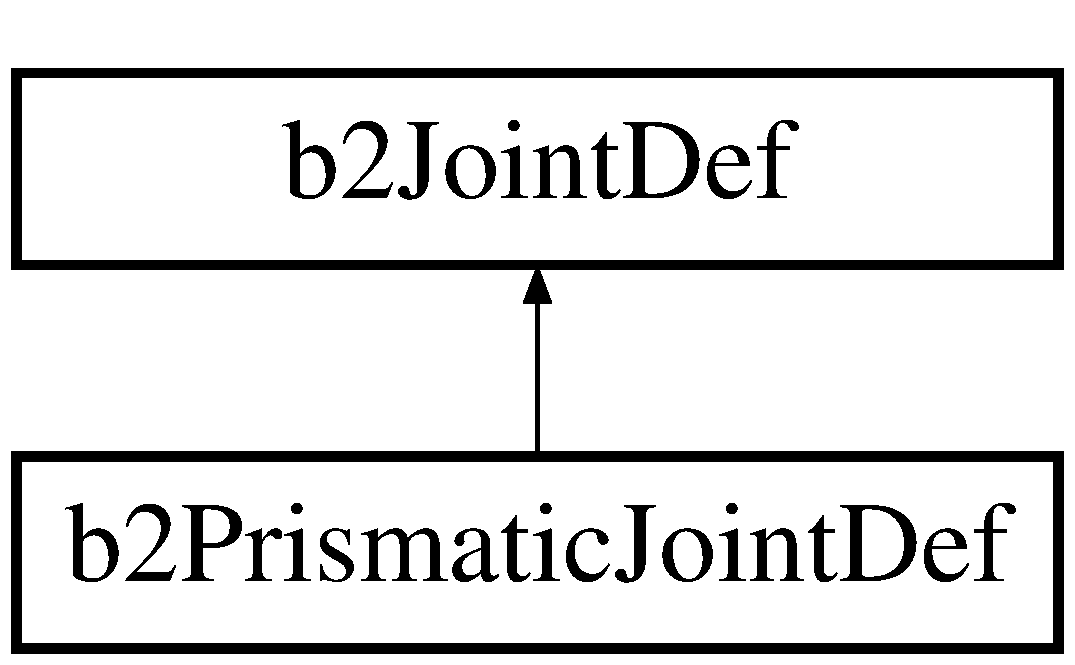
\includegraphics[height=2.000000cm]{structb2_prismatic_joint_def}
\end{center}
\end{figure}
\subsection*{Public Member Functions}
\begin{DoxyCompactItemize}
\item 
void \hyperlink{structb2_prismatic_joint_def_ae60043bc22b077e8c59ab248dc34652f}{Initialize} (\hyperlink{classb2_body}{b2\+Body} $\ast$\hyperlink{structb2_joint_def_a8cd54c93da396be75a9788f2c6897f05}{bodyA}, \hyperlink{classb2_body}{b2\+Body} $\ast$\hyperlink{structb2_joint_def_aa4f4dee2fbcd12187b19506b60e68e3d}{bodyB}, const \hyperlink{structb2_vec2}{b2\+Vec2} \&anchor, const \hyperlink{structb2_vec2}{b2\+Vec2} \&axis)
\end{DoxyCompactItemize}
\subsection*{Public Attributes}
\begin{DoxyCompactItemize}
\item 
\hyperlink{structb2_vec2}{b2\+Vec2} \hyperlink{structb2_prismatic_joint_def_abb51df8daff7a55f47adc83e4f7fa5b9}{local\+AnchorA}\hypertarget{structb2_prismatic_joint_def_abb51df8daff7a55f47adc83e4f7fa5b9}{}\label{structb2_prismatic_joint_def_abb51df8daff7a55f47adc83e4f7fa5b9}

\begin{DoxyCompactList}\small\item\em The local anchor point relative to bodyA\textquotesingle{}s origin. \end{DoxyCompactList}\item 
\hyperlink{structb2_vec2}{b2\+Vec2} \hyperlink{structb2_prismatic_joint_def_a5acc1f2f14d1b659fc9d804ab1baf4a3}{local\+AnchorB}\hypertarget{structb2_prismatic_joint_def_a5acc1f2f14d1b659fc9d804ab1baf4a3}{}\label{structb2_prismatic_joint_def_a5acc1f2f14d1b659fc9d804ab1baf4a3}

\begin{DoxyCompactList}\small\item\em The local anchor point relative to bodyB\textquotesingle{}s origin. \end{DoxyCompactList}\item 
\hyperlink{structb2_vec2}{b2\+Vec2} \hyperlink{structb2_prismatic_joint_def_af36fdbcedca5a392a2649cd235c42676}{local\+AxisA}\hypertarget{structb2_prismatic_joint_def_af36fdbcedca5a392a2649cd235c42676}{}\label{structb2_prismatic_joint_def_af36fdbcedca5a392a2649cd235c42676}

\begin{DoxyCompactList}\small\item\em The local translation unit axis in bodyA. \end{DoxyCompactList}\item 
float32 \hyperlink{structb2_prismatic_joint_def_aa84b43d08e6e11b4daa0c86f46094463}{reference\+Angle}\hypertarget{structb2_prismatic_joint_def_aa84b43d08e6e11b4daa0c86f46094463}{}\label{structb2_prismatic_joint_def_aa84b43d08e6e11b4daa0c86f46094463}

\begin{DoxyCompactList}\small\item\em The constrained angle between the bodies\+: body\+B\+\_\+angle -\/ body\+A\+\_\+angle. \end{DoxyCompactList}\item 
bool \hyperlink{structb2_prismatic_joint_def_aa61a03b68caac62a5cf66354f6756eae}{enable\+Limit}\hypertarget{structb2_prismatic_joint_def_aa61a03b68caac62a5cf66354f6756eae}{}\label{structb2_prismatic_joint_def_aa61a03b68caac62a5cf66354f6756eae}

\begin{DoxyCompactList}\small\item\em Enable/disable the joint limit. \end{DoxyCompactList}\item 
float32 \hyperlink{structb2_prismatic_joint_def_ac0a0e2a669d640ebea354895fe6a9fb6}{lower\+Translation}\hypertarget{structb2_prismatic_joint_def_ac0a0e2a669d640ebea354895fe6a9fb6}{}\label{structb2_prismatic_joint_def_ac0a0e2a669d640ebea354895fe6a9fb6}

\begin{DoxyCompactList}\small\item\em The lower translation limit, usually in meters. \end{DoxyCompactList}\item 
float32 \hyperlink{structb2_prismatic_joint_def_ae3eac123c7fe543071bdfcd1a6942350}{upper\+Translation}\hypertarget{structb2_prismatic_joint_def_ae3eac123c7fe543071bdfcd1a6942350}{}\label{structb2_prismatic_joint_def_ae3eac123c7fe543071bdfcd1a6942350}

\begin{DoxyCompactList}\small\item\em The upper translation limit, usually in meters. \end{DoxyCompactList}\item 
bool \hyperlink{structb2_prismatic_joint_def_a58ac79a54a8110d3a745e1d6d36990dc}{enable\+Motor}\hypertarget{structb2_prismatic_joint_def_a58ac79a54a8110d3a745e1d6d36990dc}{}\label{structb2_prismatic_joint_def_a58ac79a54a8110d3a745e1d6d36990dc}

\begin{DoxyCompactList}\small\item\em Enable/disable the joint motor. \end{DoxyCompactList}\item 
float32 \hyperlink{structb2_prismatic_joint_def_aabeec48af1e49c7f9fed5e0bc8270a1b}{max\+Motor\+Force}\hypertarget{structb2_prismatic_joint_def_aabeec48af1e49c7f9fed5e0bc8270a1b}{}\label{structb2_prismatic_joint_def_aabeec48af1e49c7f9fed5e0bc8270a1b}

\begin{DoxyCompactList}\small\item\em The maximum motor torque, usually in N-\/m. \end{DoxyCompactList}\item 
float32 \hyperlink{structb2_prismatic_joint_def_ac4bdaea15653657e724a04fc60f3f235}{motor\+Speed}\hypertarget{structb2_prismatic_joint_def_ac4bdaea15653657e724a04fc60f3f235}{}\label{structb2_prismatic_joint_def_ac4bdaea15653657e724a04fc60f3f235}

\begin{DoxyCompactList}\small\item\em The desired motor speed in radians per second. \end{DoxyCompactList}\end{DoxyCompactItemize}


\subsection{Detailed Description}
Prismatic joint definition. This requires defining a line of motion using an axis and an anchor point. The definition uses local anchor points and a local axis so that the initial configuration can violate the constraint slightly. The joint translation is zero when the local anchor points coincide in world space. Using local anchors and a local axis helps when saving and loading a game. 

\subsection{Member Function Documentation}
\index{b2\+Prismatic\+Joint\+Def@{b2\+Prismatic\+Joint\+Def}!Initialize@{Initialize}}
\index{Initialize@{Initialize}!b2\+Prismatic\+Joint\+Def@{b2\+Prismatic\+Joint\+Def}}
\subsubsection[{\texorpdfstring{Initialize(b2\+Body $\ast$body\+A, b2\+Body $\ast$body\+B, const b2\+Vec2 \&anchor, const b2\+Vec2 \&axis)}{Initialize(b2Body *bodyA, b2Body *bodyB, const b2Vec2 &anchor, const b2Vec2 &axis)}}]{\setlength{\rightskip}{0pt plus 5cm}void b2\+Prismatic\+Joint\+Def\+::\+Initialize (
\begin{DoxyParamCaption}
\item[{{\bf b2\+Body} $\ast$}]{bodyA, }
\item[{{\bf b2\+Body} $\ast$}]{bodyB, }
\item[{const {\bf b2\+Vec2} \&}]{anchor, }
\item[{const {\bf b2\+Vec2} \&}]{axis}
\end{DoxyParamCaption}
)}\hypertarget{structb2_prismatic_joint_def_ae60043bc22b077e8c59ab248dc34652f}{}\label{structb2_prismatic_joint_def_ae60043bc22b077e8c59ab248dc34652f}
Initialize the bodies, anchors, axis, and reference angle using the world anchor and unit world axis. 

The documentation for this struct was generated from the following file\+:\begin{DoxyCompactItemize}
\item 
C\+:/\+Users/\+Bilal Itani/\+Desktop/inf2990-\/11/\+Cadriciel/\+Commun/\+Externe/\+Box2\+D/include/\+Box2\+D/\+Dynamics/\+Joints/b2\+Prismatic\+Joint.\+h\end{DoxyCompactItemize}

\hypertarget{structb2_profile}{}\section{b2\+Profile Struct Reference}
\label{structb2_profile}\index{b2\+Profile@{b2\+Profile}}


Profiling data. Times are in milliseconds.  




{\ttfamily \#include $<$b2\+Time\+Step.\+h$>$}

\subsection*{Public Attributes}
\begin{DoxyCompactItemize}
\item 
float32 {\bfseries step}\hypertarget{structb2_profile_a5b93de1d56902224868beacc478b9863}{}\label{structb2_profile_a5b93de1d56902224868beacc478b9863}

\item 
float32 {\bfseries collide}\hypertarget{structb2_profile_af827d9e54f7a4e94d0a023e18466b960}{}\label{structb2_profile_af827d9e54f7a4e94d0a023e18466b960}

\item 
float32 {\bfseries solve}\hypertarget{structb2_profile_afbefc05f05ec8bfd6cb2011929688a0b}{}\label{structb2_profile_afbefc05f05ec8bfd6cb2011929688a0b}

\item 
float32 {\bfseries solve\+Init}\hypertarget{structb2_profile_a010110900c27ccc88cd5e23b0e12e96e}{}\label{structb2_profile_a010110900c27ccc88cd5e23b0e12e96e}

\item 
float32 {\bfseries solve\+Velocity}\hypertarget{structb2_profile_ae4d29a19b38de81621bccdbf75595233}{}\label{structb2_profile_ae4d29a19b38de81621bccdbf75595233}

\item 
float32 {\bfseries solve\+Position}\hypertarget{structb2_profile_a78e22d104226863492ebab9ea30a9ed9}{}\label{structb2_profile_a78e22d104226863492ebab9ea30a9ed9}

\item 
float32 {\bfseries broadphase}\hypertarget{structb2_profile_a6bd556e43a6fa3853adad9fd71e56b44}{}\label{structb2_profile_a6bd556e43a6fa3853adad9fd71e56b44}

\item 
float32 {\bfseries solve\+T\+OI}\hypertarget{structb2_profile_a74e8ea0c6ca39250d639ec94b69a803e}{}\label{structb2_profile_a74e8ea0c6ca39250d639ec94b69a803e}

\end{DoxyCompactItemize}


\subsection{Detailed Description}
Profiling data. Times are in milliseconds. 

The documentation for this struct was generated from the following file\+:\begin{DoxyCompactItemize}
\item 
Cadriciel/\+Commun/\+Externe/\+Box2\+D/include/\+Box2\+D/\+Dynamics/b2\+Time\+Step.\+h\end{DoxyCompactItemize}

\hypertarget{classb2_pulley_joint}{}\section{b2\+Pulley\+Joint Class Reference}
\label{classb2_pulley_joint}\index{b2\+Pulley\+Joint@{b2\+Pulley\+Joint}}


{\ttfamily \#include $<$b2\+Pulley\+Joint.\+h$>$}

Inheritance diagram for b2\+Pulley\+Joint\+:\begin{figure}[H]
\begin{center}
\leavevmode
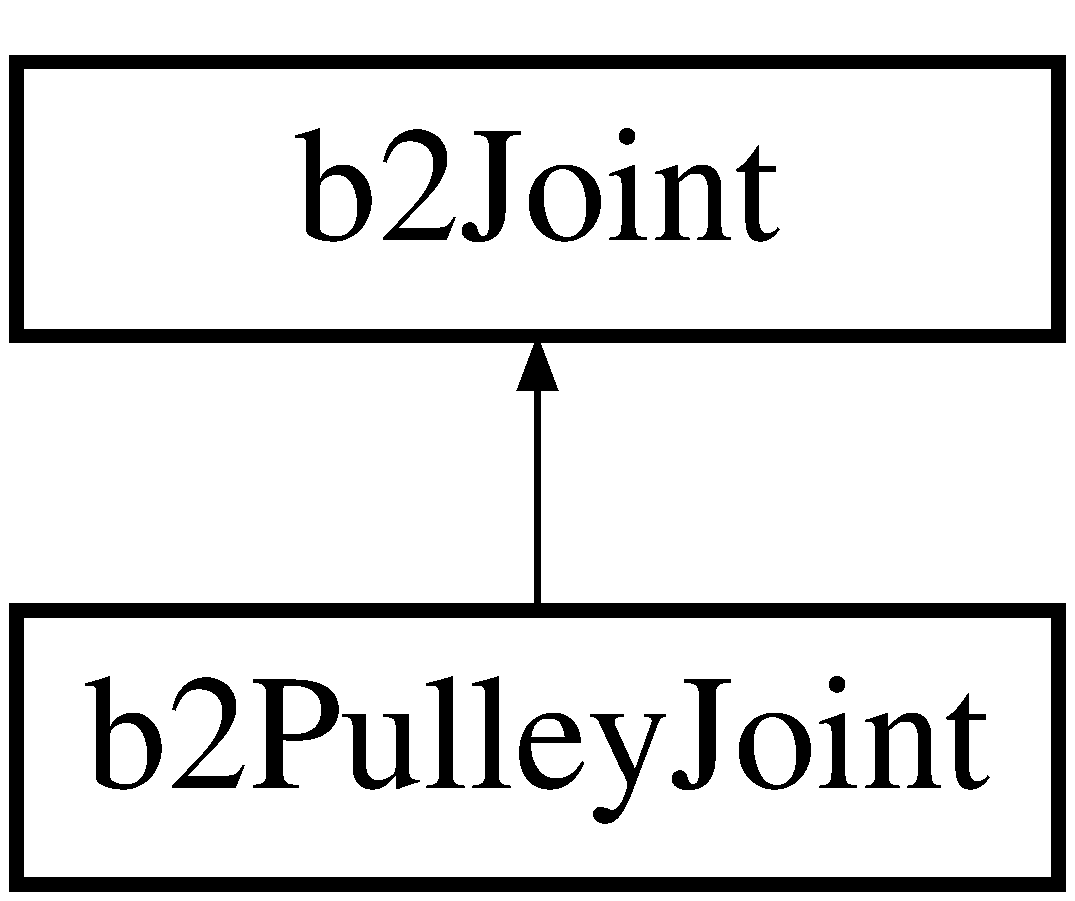
\includegraphics[height=2.000000cm]{classb2_pulley_joint}
\end{center}
\end{figure}
\subsection*{Public Member Functions}
\begin{DoxyCompactItemize}
\item 
\hyperlink{structb2_vec2}{b2\+Vec2} \hyperlink{classb2_pulley_joint_a05ac0d0d927e9541f08b07cb1bf9ec56}{Get\+AnchorA} () const \hypertarget{classb2_pulley_joint_a05ac0d0d927e9541f08b07cb1bf9ec56}{}\label{classb2_pulley_joint_a05ac0d0d927e9541f08b07cb1bf9ec56}

\begin{DoxyCompactList}\small\item\em Get the anchor point on bodyA in world coordinates. \end{DoxyCompactList}\item 
\hyperlink{structb2_vec2}{b2\+Vec2} \hyperlink{classb2_pulley_joint_a5cc3596f683d621b9a885c2569ecd452}{Get\+AnchorB} () const \hypertarget{classb2_pulley_joint_a5cc3596f683d621b9a885c2569ecd452}{}\label{classb2_pulley_joint_a5cc3596f683d621b9a885c2569ecd452}

\begin{DoxyCompactList}\small\item\em Get the anchor point on bodyB in world coordinates. \end{DoxyCompactList}\item 
\hyperlink{structb2_vec2}{b2\+Vec2} \hyperlink{classb2_pulley_joint_a38c174bf1cf1011063ff4c16556b331e}{Get\+Reaction\+Force} (float32 inv\+\_\+dt) const \hypertarget{classb2_pulley_joint_a38c174bf1cf1011063ff4c16556b331e}{}\label{classb2_pulley_joint_a38c174bf1cf1011063ff4c16556b331e}

\begin{DoxyCompactList}\small\item\em Get the reaction force on bodyB at the joint anchor in Newtons. \end{DoxyCompactList}\item 
float32 \hyperlink{classb2_pulley_joint_a418b200055623474c44742b1342dd278}{Get\+Reaction\+Torque} (float32 inv\+\_\+dt) const \hypertarget{classb2_pulley_joint_a418b200055623474c44742b1342dd278}{}\label{classb2_pulley_joint_a418b200055623474c44742b1342dd278}

\begin{DoxyCompactList}\small\item\em Get the reaction torque on bodyB in N$\ast$m. \end{DoxyCompactList}\item 
\hyperlink{structb2_vec2}{b2\+Vec2} \hyperlink{classb2_pulley_joint_a19eefa28d2647882406ea9bfe2850a9e}{Get\+Ground\+AnchorA} () const \hypertarget{classb2_pulley_joint_a19eefa28d2647882406ea9bfe2850a9e}{}\label{classb2_pulley_joint_a19eefa28d2647882406ea9bfe2850a9e}

\begin{DoxyCompactList}\small\item\em Get the first ground anchor. \end{DoxyCompactList}\item 
\hyperlink{structb2_vec2}{b2\+Vec2} \hyperlink{classb2_pulley_joint_a1b49d0dbce802f19711a9ab6d7dadfee}{Get\+Ground\+AnchorB} () const \hypertarget{classb2_pulley_joint_a1b49d0dbce802f19711a9ab6d7dadfee}{}\label{classb2_pulley_joint_a1b49d0dbce802f19711a9ab6d7dadfee}

\begin{DoxyCompactList}\small\item\em Get the second ground anchor. \end{DoxyCompactList}\item 
float32 \hyperlink{classb2_pulley_joint_a6b4c2e5cb4f5da48fcb074c7b5988084}{Get\+LengthA} () const \hypertarget{classb2_pulley_joint_a6b4c2e5cb4f5da48fcb074c7b5988084}{}\label{classb2_pulley_joint_a6b4c2e5cb4f5da48fcb074c7b5988084}

\begin{DoxyCompactList}\small\item\em Get the current length of the segment attached to bodyA. \end{DoxyCompactList}\item 
float32 \hyperlink{classb2_pulley_joint_abc7f31a35c6fb32647fd15d57e4ce60c}{Get\+LengthB} () const \hypertarget{classb2_pulley_joint_abc7f31a35c6fb32647fd15d57e4ce60c}{}\label{classb2_pulley_joint_abc7f31a35c6fb32647fd15d57e4ce60c}

\begin{DoxyCompactList}\small\item\em Get the current length of the segment attached to bodyB. \end{DoxyCompactList}\item 
float32 \hyperlink{classb2_pulley_joint_a625685e60d95b7c5a725e8586d146752}{Get\+Ratio} () const \hypertarget{classb2_pulley_joint_a625685e60d95b7c5a725e8586d146752}{}\label{classb2_pulley_joint_a625685e60d95b7c5a725e8586d146752}

\begin{DoxyCompactList}\small\item\em Get the pulley ratio. \end{DoxyCompactList}\item 
float32 \hyperlink{classb2_pulley_joint_aa57599ec0d229c3ef95dafa39a277c7b}{Get\+Current\+LengthA} () const \hypertarget{classb2_pulley_joint_aa57599ec0d229c3ef95dafa39a277c7b}{}\label{classb2_pulley_joint_aa57599ec0d229c3ef95dafa39a277c7b}

\begin{DoxyCompactList}\small\item\em Get the current length of the segment attached to bodyA. \end{DoxyCompactList}\item 
float32 \hyperlink{classb2_pulley_joint_a3b68ad489d726afa74e538331c1f72d8}{Get\+Current\+LengthB} () const \hypertarget{classb2_pulley_joint_a3b68ad489d726afa74e538331c1f72d8}{}\label{classb2_pulley_joint_a3b68ad489d726afa74e538331c1f72d8}

\begin{DoxyCompactList}\small\item\em Get the current length of the segment attached to bodyB. \end{DoxyCompactList}\item 
void \hyperlink{classb2_pulley_joint_ad12d0e03b5d07b2f8af1005c95c67aa2}{Dump} ()\hypertarget{classb2_pulley_joint_ad12d0e03b5d07b2f8af1005c95c67aa2}{}\label{classb2_pulley_joint_ad12d0e03b5d07b2f8af1005c95c67aa2}

\begin{DoxyCompactList}\small\item\em Dump joint to dm\+Log. \end{DoxyCompactList}\item 
void \hyperlink{classb2_pulley_joint_a5b88d498ce306c4ff5ce99dec4811825}{Shift\+Origin} (const \hyperlink{structb2_vec2}{b2\+Vec2} \&new\+Origin)\hypertarget{classb2_pulley_joint_a5b88d498ce306c4ff5ce99dec4811825}{}\label{classb2_pulley_joint_a5b88d498ce306c4ff5ce99dec4811825}

\begin{DoxyCompactList}\small\item\em Implement \hyperlink{classb2_joint_a7804f649e993dc0fd9ae47fde5601f90}{b2\+Joint\+::\+Shift\+Origin}. \end{DoxyCompactList}\end{DoxyCompactItemize}
\subsection*{Protected Member Functions}
\begin{DoxyCompactItemize}
\item 
{\bfseries b2\+Pulley\+Joint} (const \hyperlink{structb2_pulley_joint_def}{b2\+Pulley\+Joint\+Def} $\ast$data)\hypertarget{classb2_pulley_joint_aca1b8dc6fb05c134ccbc0423674c1867}{}\label{classb2_pulley_joint_aca1b8dc6fb05c134ccbc0423674c1867}

\item 
void {\bfseries Init\+Velocity\+Constraints} (const \hyperlink{structb2_solver_data}{b2\+Solver\+Data} \&data)\hypertarget{classb2_pulley_joint_a1b339ba58e82261beeb55f9ab04cfa7e}{}\label{classb2_pulley_joint_a1b339ba58e82261beeb55f9ab04cfa7e}

\item 
void {\bfseries Solve\+Velocity\+Constraints} (const \hyperlink{structb2_solver_data}{b2\+Solver\+Data} \&data)\hypertarget{classb2_pulley_joint_a517858e93e24f3daa51be4873b22c2c3}{}\label{classb2_pulley_joint_a517858e93e24f3daa51be4873b22c2c3}

\item 
bool {\bfseries Solve\+Position\+Constraints} (const \hyperlink{structb2_solver_data}{b2\+Solver\+Data} \&data)\hypertarget{classb2_pulley_joint_a8fcdd728e02b7c89372bf11b7732d976}{}\label{classb2_pulley_joint_a8fcdd728e02b7c89372bf11b7732d976}

\end{DoxyCompactItemize}
\subsection*{Protected Attributes}
\begin{DoxyCompactItemize}
\item 
\hyperlink{structb2_vec2}{b2\+Vec2} {\bfseries m\+\_\+ground\+AnchorA}\hypertarget{classb2_pulley_joint_a13456d1c62a4e96e8247988152be4166}{}\label{classb2_pulley_joint_a13456d1c62a4e96e8247988152be4166}

\item 
\hyperlink{structb2_vec2}{b2\+Vec2} {\bfseries m\+\_\+ground\+AnchorB}\hypertarget{classb2_pulley_joint_a9cc8195bf4e2d53606db0b49d9fc1cbc}{}\label{classb2_pulley_joint_a9cc8195bf4e2d53606db0b49d9fc1cbc}

\item 
float32 {\bfseries m\+\_\+lengthA}\hypertarget{classb2_pulley_joint_a26f2565f804692553e6b96e58621dbc9}{}\label{classb2_pulley_joint_a26f2565f804692553e6b96e58621dbc9}

\item 
float32 {\bfseries m\+\_\+lengthB}\hypertarget{classb2_pulley_joint_aa44e84a3eed2ded26fca07281e247bbd}{}\label{classb2_pulley_joint_aa44e84a3eed2ded26fca07281e247bbd}

\item 
\hyperlink{structb2_vec2}{b2\+Vec2} {\bfseries m\+\_\+local\+AnchorA}\hypertarget{classb2_pulley_joint_a58cb3464ba25236e316b35d66e92366f}{}\label{classb2_pulley_joint_a58cb3464ba25236e316b35d66e92366f}

\item 
\hyperlink{structb2_vec2}{b2\+Vec2} {\bfseries m\+\_\+local\+AnchorB}\hypertarget{classb2_pulley_joint_af643cf90fb22709fe410164d8a46ea50}{}\label{classb2_pulley_joint_af643cf90fb22709fe410164d8a46ea50}

\item 
float32 {\bfseries m\+\_\+constant}\hypertarget{classb2_pulley_joint_a0e73d1d31126331267a1661beb146bc7}{}\label{classb2_pulley_joint_a0e73d1d31126331267a1661beb146bc7}

\item 
float32 {\bfseries m\+\_\+ratio}\hypertarget{classb2_pulley_joint_aa44594b9b4826c565da387bed5f02470}{}\label{classb2_pulley_joint_aa44594b9b4826c565da387bed5f02470}

\item 
float32 {\bfseries m\+\_\+impulse}\hypertarget{classb2_pulley_joint_a1e5b5fff8b1564688b38d139c5f7c65a}{}\label{classb2_pulley_joint_a1e5b5fff8b1564688b38d139c5f7c65a}

\item 
int32 {\bfseries m\+\_\+indexA}\hypertarget{classb2_pulley_joint_a6ef68a1d29ef264d4c2ab2d363d9eb97}{}\label{classb2_pulley_joint_a6ef68a1d29ef264d4c2ab2d363d9eb97}

\item 
int32 {\bfseries m\+\_\+indexB}\hypertarget{classb2_pulley_joint_acbeb702d3db8a9560d9d1d57ebb1e7f2}{}\label{classb2_pulley_joint_acbeb702d3db8a9560d9d1d57ebb1e7f2}

\item 
\hyperlink{structb2_vec2}{b2\+Vec2} {\bfseries m\+\_\+uA}\hypertarget{classb2_pulley_joint_a8b49167603509d296aa8d04e46b13658}{}\label{classb2_pulley_joint_a8b49167603509d296aa8d04e46b13658}

\item 
\hyperlink{structb2_vec2}{b2\+Vec2} {\bfseries m\+\_\+uB}\hypertarget{classb2_pulley_joint_a1354dfebc4658560b9d7e4b447b1dd5e}{}\label{classb2_pulley_joint_a1354dfebc4658560b9d7e4b447b1dd5e}

\item 
\hyperlink{structb2_vec2}{b2\+Vec2} {\bfseries m\+\_\+rA}\hypertarget{classb2_pulley_joint_a4ebd669d4856b0c6d1d6f76d7a9eae2d}{}\label{classb2_pulley_joint_a4ebd669d4856b0c6d1d6f76d7a9eae2d}

\item 
\hyperlink{structb2_vec2}{b2\+Vec2} {\bfseries m\+\_\+rB}\hypertarget{classb2_pulley_joint_a6be5e9ad2eeaee5cf25e1df61d923a58}{}\label{classb2_pulley_joint_a6be5e9ad2eeaee5cf25e1df61d923a58}

\item 
\hyperlink{structb2_vec2}{b2\+Vec2} {\bfseries m\+\_\+local\+CenterA}\hypertarget{classb2_pulley_joint_a82741929b0aa083f520a3d7f9ef675bb}{}\label{classb2_pulley_joint_a82741929b0aa083f520a3d7f9ef675bb}

\item 
\hyperlink{structb2_vec2}{b2\+Vec2} {\bfseries m\+\_\+local\+CenterB}\hypertarget{classb2_pulley_joint_abd382cd6772fa3be1958c4845369f6c3}{}\label{classb2_pulley_joint_abd382cd6772fa3be1958c4845369f6c3}

\item 
float32 {\bfseries m\+\_\+inv\+MassA}\hypertarget{classb2_pulley_joint_a7c37029c6b7117a07bb8be552b44ee3f}{}\label{classb2_pulley_joint_a7c37029c6b7117a07bb8be552b44ee3f}

\item 
float32 {\bfseries m\+\_\+inv\+MassB}\hypertarget{classb2_pulley_joint_ad4e470cbc2e9f596c93e144630657534}{}\label{classb2_pulley_joint_ad4e470cbc2e9f596c93e144630657534}

\item 
float32 {\bfseries m\+\_\+inv\+IA}\hypertarget{classb2_pulley_joint_a701fbc685109f5b397b968be2407b123}{}\label{classb2_pulley_joint_a701fbc685109f5b397b968be2407b123}

\item 
float32 {\bfseries m\+\_\+inv\+IB}\hypertarget{classb2_pulley_joint_a19278e2f7dcec7275aff55b1d760b398}{}\label{classb2_pulley_joint_a19278e2f7dcec7275aff55b1d760b398}

\item 
float32 {\bfseries m\+\_\+mass}\hypertarget{classb2_pulley_joint_a60efdc42d9fd8f4c50f96eb68ff3f191}{}\label{classb2_pulley_joint_a60efdc42d9fd8f4c50f96eb68ff3f191}

\end{DoxyCompactItemize}
\subsection*{Friends}
\begin{DoxyCompactItemize}
\item 
class {\bfseries b2\+Joint}\hypertarget{classb2_pulley_joint_a54ade8ed3d794298108d7f4c4e4793fa}{}\label{classb2_pulley_joint_a54ade8ed3d794298108d7f4c4e4793fa}

\end{DoxyCompactItemize}
\subsection*{Additional Inherited Members}


\subsection{Detailed Description}
The pulley joint is connected to two bodies and two fixed ground points. The pulley supports a ratio such that\+: length1 + ratio $\ast$ length2 $<$= constant Yes, the force transmitted is scaled by the ratio. Warning\+: the pulley joint can get a bit squirrelly by itself. They often work better when combined with prismatic joints. You should also cover the the anchor points with static shapes to prevent one side from going to zero length. 

The documentation for this class was generated from the following file\+:\begin{DoxyCompactItemize}
\item 
Cadriciel/\+Commun/\+Externe/\+Box2\+D/include/\+Box2\+D/\+Dynamics/\+Joints/b2\+Pulley\+Joint.\+h\end{DoxyCompactItemize}

\hypertarget{structb2_pulley_joint_def}{}\section{b2\+Pulley\+Joint\+Def Struct Reference}
\label{structb2_pulley_joint_def}\index{b2\+Pulley\+Joint\+Def@{b2\+Pulley\+Joint\+Def}}


{\ttfamily \#include $<$b2\+Pulley\+Joint.\+h$>$}

Inheritance diagram for b2\+Pulley\+Joint\+Def\+:\begin{figure}[H]
\begin{center}
\leavevmode
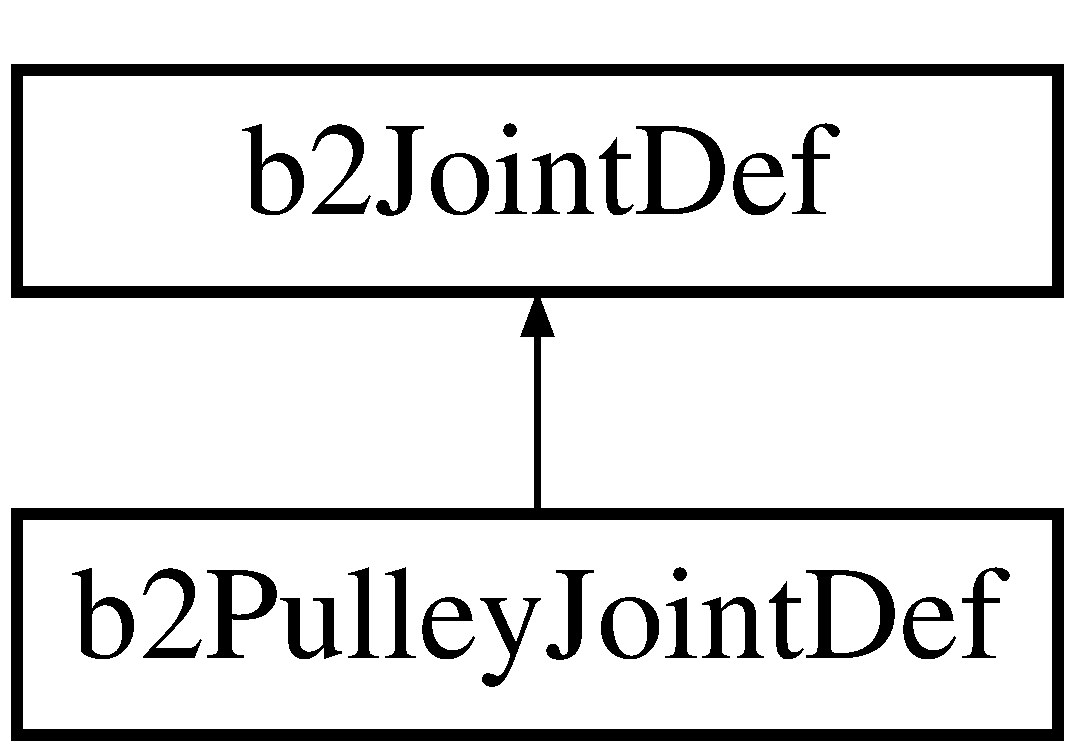
\includegraphics[height=2.000000cm]{structb2_pulley_joint_def}
\end{center}
\end{figure}
\subsection*{Public Member Functions}
\begin{DoxyCompactItemize}
\item 
void \hyperlink{structb2_pulley_joint_def_abef614a93562b82aa3b5f8cac17d1ce8}{Initialize} (\hyperlink{classb2_body}{b2\+Body} $\ast$\hyperlink{structb2_joint_def_a8cd54c93da396be75a9788f2c6897f05}{bodyA}, \hyperlink{classb2_body}{b2\+Body} $\ast$\hyperlink{structb2_joint_def_aa4f4dee2fbcd12187b19506b60e68e3d}{bodyB}, const \hyperlink{structb2_vec2}{b2\+Vec2} \&\hyperlink{structb2_pulley_joint_def_aae77c020ce4629ab9e03560e28aa853d}{ground\+AnchorA}, const \hyperlink{structb2_vec2}{b2\+Vec2} \&\hyperlink{structb2_pulley_joint_def_aa412b9f3bffd1fb69ace14f9b3e03b82}{ground\+AnchorB}, const \hyperlink{structb2_vec2}{b2\+Vec2} \&anchorA, const \hyperlink{structb2_vec2}{b2\+Vec2} \&anchorB, float32 \hyperlink{structb2_pulley_joint_def_af35074246aeacbf239c11682642b31f5}{ratio})\hypertarget{structb2_pulley_joint_def_abef614a93562b82aa3b5f8cac17d1ce8}{}\label{structb2_pulley_joint_def_abef614a93562b82aa3b5f8cac17d1ce8}

\begin{DoxyCompactList}\small\item\em Initialize the bodies, anchors, lengths, max lengths, and ratio using the world anchors. \end{DoxyCompactList}\end{DoxyCompactItemize}
\subsection*{Public Attributes}
\begin{DoxyCompactItemize}
\item 
\hyperlink{structb2_vec2}{b2\+Vec2} \hyperlink{structb2_pulley_joint_def_aae77c020ce4629ab9e03560e28aa853d}{ground\+AnchorA}\hypertarget{structb2_pulley_joint_def_aae77c020ce4629ab9e03560e28aa853d}{}\label{structb2_pulley_joint_def_aae77c020ce4629ab9e03560e28aa853d}

\begin{DoxyCompactList}\small\item\em The first ground anchor in world coordinates. This point never moves. \end{DoxyCompactList}\item 
\hyperlink{structb2_vec2}{b2\+Vec2} \hyperlink{structb2_pulley_joint_def_aa412b9f3bffd1fb69ace14f9b3e03b82}{ground\+AnchorB}\hypertarget{structb2_pulley_joint_def_aa412b9f3bffd1fb69ace14f9b3e03b82}{}\label{structb2_pulley_joint_def_aa412b9f3bffd1fb69ace14f9b3e03b82}

\begin{DoxyCompactList}\small\item\em The second ground anchor in world coordinates. This point never moves. \end{DoxyCompactList}\item 
\hyperlink{structb2_vec2}{b2\+Vec2} \hyperlink{structb2_pulley_joint_def_ad7677a4ad02a6e7cb8699fc5012eac3e}{local\+AnchorA}\hypertarget{structb2_pulley_joint_def_ad7677a4ad02a6e7cb8699fc5012eac3e}{}\label{structb2_pulley_joint_def_ad7677a4ad02a6e7cb8699fc5012eac3e}

\begin{DoxyCompactList}\small\item\em The local anchor point relative to bodyA\textquotesingle{}s origin. \end{DoxyCompactList}\item 
\hyperlink{structb2_vec2}{b2\+Vec2} \hyperlink{structb2_pulley_joint_def_aed3f9c9f5f4145ceb32e7e164de73144}{local\+AnchorB}\hypertarget{structb2_pulley_joint_def_aed3f9c9f5f4145ceb32e7e164de73144}{}\label{structb2_pulley_joint_def_aed3f9c9f5f4145ceb32e7e164de73144}

\begin{DoxyCompactList}\small\item\em The local anchor point relative to bodyB\textquotesingle{}s origin. \end{DoxyCompactList}\item 
float32 \hyperlink{structb2_pulley_joint_def_a51d945882c1d7a78af2b0e9ffb31a33b}{lengthA}\hypertarget{structb2_pulley_joint_def_a51d945882c1d7a78af2b0e9ffb31a33b}{}\label{structb2_pulley_joint_def_a51d945882c1d7a78af2b0e9ffb31a33b}

\begin{DoxyCompactList}\small\item\em The a reference length for the segment attached to bodyA. \end{DoxyCompactList}\item 
float32 \hyperlink{structb2_pulley_joint_def_a5857d5b5b9880b6c8201ce3ee8c3eef0}{lengthB}\hypertarget{structb2_pulley_joint_def_a5857d5b5b9880b6c8201ce3ee8c3eef0}{}\label{structb2_pulley_joint_def_a5857d5b5b9880b6c8201ce3ee8c3eef0}

\begin{DoxyCompactList}\small\item\em The a reference length for the segment attached to bodyB. \end{DoxyCompactList}\item 
float32 \hyperlink{structb2_pulley_joint_def_af35074246aeacbf239c11682642b31f5}{ratio}\hypertarget{structb2_pulley_joint_def_af35074246aeacbf239c11682642b31f5}{}\label{structb2_pulley_joint_def_af35074246aeacbf239c11682642b31f5}

\begin{DoxyCompactList}\small\item\em The pulley ratio, used to simulate a block-\/and-\/tackle. \end{DoxyCompactList}\end{DoxyCompactItemize}


\subsection{Detailed Description}
Pulley joint definition. This requires two ground anchors, two dynamic body anchor points, and a pulley ratio. 

The documentation for this struct was generated from the following file\+:\begin{DoxyCompactItemize}
\item 
C\+:/\+Users/\+Bilal Itani/\+Desktop/inf2990-\/11/\+Cadriciel/\+Commun/\+Externe/\+Box2\+D/include/\+Box2\+D/\+Dynamics/\+Joints/b2\+Pulley\+Joint.\+h\end{DoxyCompactItemize}

\hypertarget{classb2_query_callback}{}\section{b2\+Query\+Callback Class Reference}
\label{classb2_query_callback}\index{b2\+Query\+Callback@{b2\+Query\+Callback}}


{\ttfamily \#include $<$b2\+World\+Callbacks.\+h$>$}

\subsection*{Public Member Functions}
\begin{DoxyCompactItemize}
\item 
virtual bool \hyperlink{classb2_query_callback_a187dd04dd0f5164fb05c2ce2cbfd9ee5}{Report\+Fixture} (\hyperlink{classb2_fixture}{b2\+Fixture} $\ast$fixture)=0
\end{DoxyCompactItemize}


\subsection{Detailed Description}
Callback class for A\+A\+BB queries. See b2\+World\+::\+Query 

\subsection{Member Function Documentation}
\index{b2\+Query\+Callback@{b2\+Query\+Callback}!Report\+Fixture@{Report\+Fixture}}
\index{Report\+Fixture@{Report\+Fixture}!b2\+Query\+Callback@{b2\+Query\+Callback}}
\subsubsection[{\texorpdfstring{Report\+Fixture(b2\+Fixture $\ast$fixture)=0}{ReportFixture(b2Fixture *fixture)=0}}]{\setlength{\rightskip}{0pt plus 5cm}virtual bool b2\+Query\+Callback\+::\+Report\+Fixture (
\begin{DoxyParamCaption}
\item[{{\bf b2\+Fixture} $\ast$}]{fixture}
\end{DoxyParamCaption}
)\hspace{0.3cm}{\ttfamily [pure virtual]}}\hypertarget{classb2_query_callback_a187dd04dd0f5164fb05c2ce2cbfd9ee5}{}\label{classb2_query_callback_a187dd04dd0f5164fb05c2ce2cbfd9ee5}
Called for each fixture found in the query A\+A\+BB. \begin{DoxyReturn}{Returns}
false to terminate the query. 
\end{DoxyReturn}


The documentation for this class was generated from the following file\+:\begin{DoxyCompactItemize}
\item 
Commun/\+Externe/\+Box2\+D/include/\+Box2\+D/\+Dynamics/b2\+World\+Callbacks.\+h\end{DoxyCompactItemize}

\hypertarget{classb2_ray_cast_callback}{}\section{b2\+Ray\+Cast\+Callback Class Reference}
\label{classb2_ray_cast_callback}\index{b2\+Ray\+Cast\+Callback@{b2\+Ray\+Cast\+Callback}}


{\ttfamily \#include $<$b2\+World\+Callbacks.\+h$>$}

\subsection*{Public Member Functions}
\begin{DoxyCompactItemize}
\item 
virtual float32 \hyperlink{classb2_ray_cast_callback_a658d5c8e89e0c73230cc8bddade4f3a4}{Report\+Fixture} (\hyperlink{classb2_fixture}{b2\+Fixture} $\ast$fixture, const \hyperlink{structb2_vec2}{b2\+Vec2} \&point, const \hyperlink{structb2_vec2}{b2\+Vec2} \&normal, float32 fraction)=0
\end{DoxyCompactItemize}


\subsection{Detailed Description}
Callback class for ray casts. See \hyperlink{classb2_world_ad902548be84df9cc36eced0f4c89ab0a}{b2\+World\+::\+Ray\+Cast} 

\subsection{Member Function Documentation}
\index{b2\+Ray\+Cast\+Callback@{b2\+Ray\+Cast\+Callback}!Report\+Fixture@{Report\+Fixture}}
\index{Report\+Fixture@{Report\+Fixture}!b2\+Ray\+Cast\+Callback@{b2\+Ray\+Cast\+Callback}}
\subsubsection[{\texorpdfstring{Report\+Fixture(b2\+Fixture $\ast$fixture, const b2\+Vec2 \&point, const b2\+Vec2 \&normal, float32 fraction)=0}{ReportFixture(b2Fixture *fixture, const b2Vec2 &point, const b2Vec2 &normal, float32 fraction)=0}}]{\setlength{\rightskip}{0pt plus 5cm}virtual float32 b2\+Ray\+Cast\+Callback\+::\+Report\+Fixture (
\begin{DoxyParamCaption}
\item[{{\bf b2\+Fixture} $\ast$}]{fixture, }
\item[{const {\bf b2\+Vec2} \&}]{point, }
\item[{const {\bf b2\+Vec2} \&}]{normal, }
\item[{float32}]{fraction}
\end{DoxyParamCaption}
)\hspace{0.3cm}{\ttfamily [pure virtual]}}\hypertarget{classb2_ray_cast_callback_a658d5c8e89e0c73230cc8bddade4f3a4}{}\label{classb2_ray_cast_callback_a658d5c8e89e0c73230cc8bddade4f3a4}
Called for each fixture found in the query. You control how the ray cast proceeds by returning a float\+: return -\/1\+: ignore this fixture and continue return 0\+: terminate the ray cast return fraction\+: clip the ray to this point return 1\+: don\textquotesingle{}t clip the ray and continue 
\begin{DoxyParams}{Parameters}
{\em fixture} & the fixture hit by the ray \\
\hline
{\em point} & the point of initial intersection \\
\hline
{\em normal} & the normal vector at the point of intersection \\
\hline
\end{DoxyParams}
\begin{DoxyReturn}{Returns}
-\/1 to filter, 0 to terminate, fraction to clip the ray for closest hit, 1 to continue 
\end{DoxyReturn}


The documentation for this class was generated from the following file\+:\begin{DoxyCompactItemize}
\item 
Cadriciel/\+Commun/\+Externe/\+Box2\+D/include/\+Box2\+D/\+Dynamics/b2\+World\+Callbacks.\+h\end{DoxyCompactItemize}

\hypertarget{structb2_ray_cast_input}{}\section{b2\+Ray\+Cast\+Input Struct Reference}
\label{structb2_ray_cast_input}\index{b2\+Ray\+Cast\+Input@{b2\+Ray\+Cast\+Input}}


Ray-\/cast input data. The ray extends from p1 to p1 + max\+Fraction $\ast$ (p2 -\/ p1).  




{\ttfamily \#include $<$b2\+Collision.\+h$>$}

\subsection*{Public Attributes}
\begin{DoxyCompactItemize}
\item 
\hyperlink{structb2_vec2}{b2\+Vec2} {\bfseries p1}\hypertarget{structb2_ray_cast_input_a7254a7062422833b1124fa464ab4caf3}{}\label{structb2_ray_cast_input_a7254a7062422833b1124fa464ab4caf3}

\item 
\hyperlink{structb2_vec2}{b2\+Vec2} {\bfseries p2}\hypertarget{structb2_ray_cast_input_a850102c843469781a3a627c871043d0b}{}\label{structb2_ray_cast_input_a850102c843469781a3a627c871043d0b}

\item 
float32 {\bfseries max\+Fraction}\hypertarget{structb2_ray_cast_input_acb5c88e0ef2c3716a1334611522ab0b2}{}\label{structb2_ray_cast_input_acb5c88e0ef2c3716a1334611522ab0b2}

\end{DoxyCompactItemize}


\subsection{Detailed Description}
Ray-\/cast input data. The ray extends from p1 to p1 + max\+Fraction $\ast$ (p2 -\/ p1). 

The documentation for this struct was generated from the following file\+:\begin{DoxyCompactItemize}
\item 
C\+:/\+Users/\+Bilal Itani/\+Desktop/inf2990-\/11/\+Cadriciel/\+Commun/\+Externe/\+Box2\+D/include/\+Box2\+D/\+Collision/\hyperlink{b2_collision_8h}{b2\+Collision.\+h}\end{DoxyCompactItemize}

\hypertarget{structb2_ray_cast_output}{}\section{b2\+Ray\+Cast\+Output Struct Reference}
\label{structb2_ray_cast_output}\index{b2\+Ray\+Cast\+Output@{b2\+Ray\+Cast\+Output}}


{\ttfamily \#include $<$b2\+Collision.\+h$>$}

\subsection*{Public Attributes}
\begin{DoxyCompactItemize}
\item 
\hyperlink{structb2_vec2}{b2\+Vec2} {\bfseries normal}\hypertarget{structb2_ray_cast_output_aa9bbfe75afa23c21e85cb1bd3736529b}{}\label{structb2_ray_cast_output_aa9bbfe75afa23c21e85cb1bd3736529b}

\item 
float32 {\bfseries fraction}\hypertarget{structb2_ray_cast_output_a191c69bb399304bfe30c69e2158b3f29}{}\label{structb2_ray_cast_output_a191c69bb399304bfe30c69e2158b3f29}

\end{DoxyCompactItemize}


\subsection{Detailed Description}
Ray-\/cast output data. The ray hits at p1 + fraction $\ast$ (p2 -\/ p1), where p1 and p2 come from \hyperlink{structb2_ray_cast_input}{b2\+Ray\+Cast\+Input}. 

The documentation for this struct was generated from the following file\+:\begin{DoxyCompactItemize}
\item 
C\+:/\+Users/\+Bilal Itani/\+Desktop/inf2990-\/11/\+Cadriciel/\+Commun/\+Externe/\+Box2\+D/include/\+Box2\+D/\+Collision/\hyperlink{b2_collision_8h}{b2\+Collision.\+h}\end{DoxyCompactItemize}

\hypertarget{classb2_revolute_joint}{}\section{b2\+Revolute\+Joint Class Reference}
\label{classb2_revolute_joint}\index{b2\+Revolute\+Joint@{b2\+Revolute\+Joint}}


{\ttfamily \#include $<$b2\+Revolute\+Joint.\+h$>$}

Inheritance diagram for b2\+Revolute\+Joint\+:\begin{figure}[H]
\begin{center}
\leavevmode
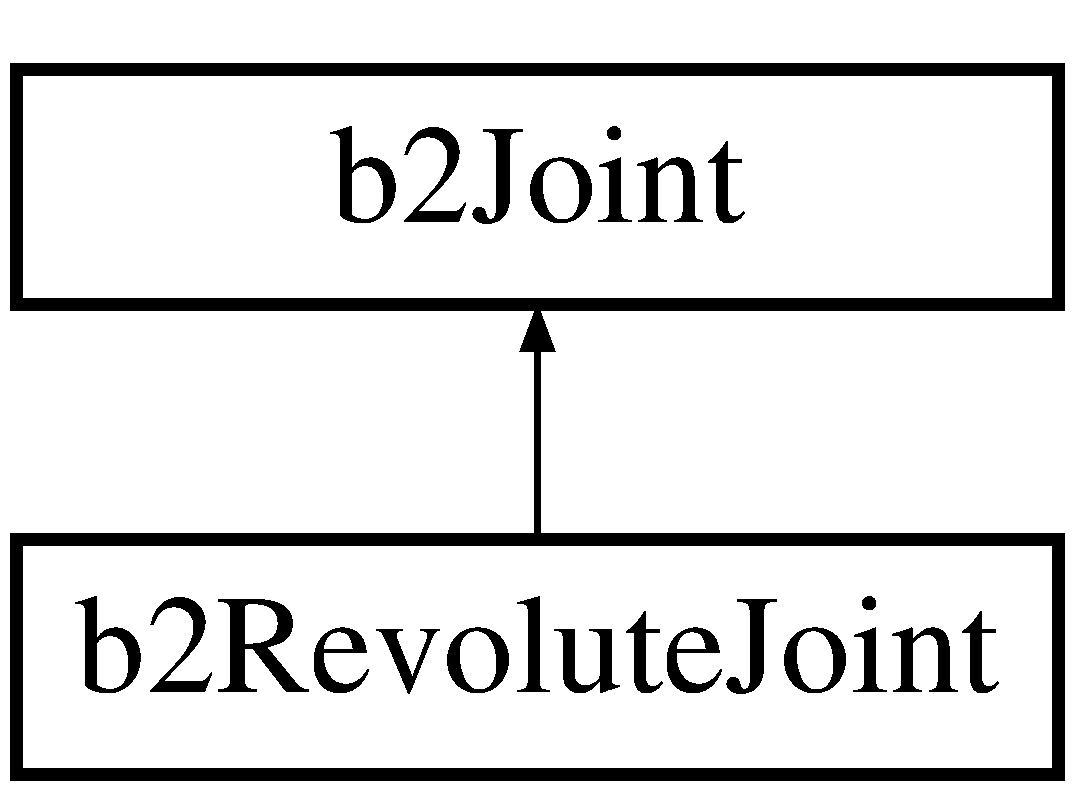
\includegraphics[height=2.000000cm]{classb2_revolute_joint}
\end{center}
\end{figure}
\subsection*{Public Member Functions}
\begin{DoxyCompactItemize}
\item 
\hyperlink{structb2_vec2}{b2\+Vec2} \hyperlink{classb2_revolute_joint_a7f266986c12009973fd74c9828b6c236}{Get\+AnchorA} () const \hypertarget{classb2_revolute_joint_a7f266986c12009973fd74c9828b6c236}{}\label{classb2_revolute_joint_a7f266986c12009973fd74c9828b6c236}

\begin{DoxyCompactList}\small\item\em Get the anchor point on bodyA in world coordinates. \end{DoxyCompactList}\item 
\hyperlink{structb2_vec2}{b2\+Vec2} \hyperlink{classb2_revolute_joint_a3a67ad189b29ea8ab6602a28697807f6}{Get\+AnchorB} () const \hypertarget{classb2_revolute_joint_a3a67ad189b29ea8ab6602a28697807f6}{}\label{classb2_revolute_joint_a3a67ad189b29ea8ab6602a28697807f6}

\begin{DoxyCompactList}\small\item\em Get the anchor point on bodyB in world coordinates. \end{DoxyCompactList}\item 
const \hyperlink{structb2_vec2}{b2\+Vec2} \& \hyperlink{classb2_revolute_joint_af270a3029b2573bf85cde345c22d65ab}{Get\+Local\+AnchorA} () const \hypertarget{classb2_revolute_joint_af270a3029b2573bf85cde345c22d65ab}{}\label{classb2_revolute_joint_af270a3029b2573bf85cde345c22d65ab}

\begin{DoxyCompactList}\small\item\em The local anchor point relative to bodyA\textquotesingle{}s origin. \end{DoxyCompactList}\item 
const \hyperlink{structb2_vec2}{b2\+Vec2} \& \hyperlink{classb2_revolute_joint_a985f788cffd53d7bb926b11cf77734e4}{Get\+Local\+AnchorB} () const \hypertarget{classb2_revolute_joint_a985f788cffd53d7bb926b11cf77734e4}{}\label{classb2_revolute_joint_a985f788cffd53d7bb926b11cf77734e4}

\begin{DoxyCompactList}\small\item\em The local anchor point relative to bodyB\textquotesingle{}s origin. \end{DoxyCompactList}\item 
float32 \hyperlink{classb2_revolute_joint_acfe881247b1f1f8f12aefd3a8f0cfd00}{Get\+Reference\+Angle} () const \hypertarget{classb2_revolute_joint_acfe881247b1f1f8f12aefd3a8f0cfd00}{}\label{classb2_revolute_joint_acfe881247b1f1f8f12aefd3a8f0cfd00}

\begin{DoxyCompactList}\small\item\em Get the reference angle. \end{DoxyCompactList}\item 
float32 \hyperlink{classb2_revolute_joint_ab20fc12ce5ad5d84a032eb613c80764a}{Get\+Joint\+Angle} () const \hypertarget{classb2_revolute_joint_ab20fc12ce5ad5d84a032eb613c80764a}{}\label{classb2_revolute_joint_ab20fc12ce5ad5d84a032eb613c80764a}

\begin{DoxyCompactList}\small\item\em Get the current joint angle in radians. \end{DoxyCompactList}\item 
float32 \hyperlink{classb2_revolute_joint_a48e4db13c187af159587d731656aa0c4}{Get\+Joint\+Speed} () const \hypertarget{classb2_revolute_joint_a48e4db13c187af159587d731656aa0c4}{}\label{classb2_revolute_joint_a48e4db13c187af159587d731656aa0c4}

\begin{DoxyCompactList}\small\item\em Get the current joint angle speed in radians per second. \end{DoxyCompactList}\item 
bool \hyperlink{classb2_revolute_joint_a7711afbfbdba4451d2dbfa8e55b9ded8}{Is\+Limit\+Enabled} () const \hypertarget{classb2_revolute_joint_a7711afbfbdba4451d2dbfa8e55b9ded8}{}\label{classb2_revolute_joint_a7711afbfbdba4451d2dbfa8e55b9ded8}

\begin{DoxyCompactList}\small\item\em Is the joint limit enabled? \end{DoxyCompactList}\item 
void \hyperlink{classb2_revolute_joint_a56bdfdd04e906e52d0258f6a481b9093}{Enable\+Limit} (bool flag)\hypertarget{classb2_revolute_joint_a56bdfdd04e906e52d0258f6a481b9093}{}\label{classb2_revolute_joint_a56bdfdd04e906e52d0258f6a481b9093}

\begin{DoxyCompactList}\small\item\em Enable/disable the joint limit. \end{DoxyCompactList}\item 
float32 \hyperlink{classb2_revolute_joint_a0f33656869e46ec9405f42d68e858220}{Get\+Lower\+Limit} () const \hypertarget{classb2_revolute_joint_a0f33656869e46ec9405f42d68e858220}{}\label{classb2_revolute_joint_a0f33656869e46ec9405f42d68e858220}

\begin{DoxyCompactList}\small\item\em Get the lower joint limit in radians. \end{DoxyCompactList}\item 
float32 \hyperlink{classb2_revolute_joint_a9bb683118879611e84e4cb26bdc8d39f}{Get\+Upper\+Limit} () const \hypertarget{classb2_revolute_joint_a9bb683118879611e84e4cb26bdc8d39f}{}\label{classb2_revolute_joint_a9bb683118879611e84e4cb26bdc8d39f}

\begin{DoxyCompactList}\small\item\em Get the upper joint limit in radians. \end{DoxyCompactList}\item 
void \hyperlink{classb2_revolute_joint_a32f9393d8a6b993fd523f0f643c28107}{Set\+Limits} (float32 lower, float32 upper)\hypertarget{classb2_revolute_joint_a32f9393d8a6b993fd523f0f643c28107}{}\label{classb2_revolute_joint_a32f9393d8a6b993fd523f0f643c28107}

\begin{DoxyCompactList}\small\item\em Set the joint limits in radians. \end{DoxyCompactList}\item 
bool \hyperlink{classb2_revolute_joint_a9477b305db080e17dce8f2c6da0babb0}{Is\+Motor\+Enabled} () const \hypertarget{classb2_revolute_joint_a9477b305db080e17dce8f2c6da0babb0}{}\label{classb2_revolute_joint_a9477b305db080e17dce8f2c6da0babb0}

\begin{DoxyCompactList}\small\item\em Is the joint motor enabled? \end{DoxyCompactList}\item 
void \hyperlink{classb2_revolute_joint_a80ed5a07d9a0e07d010808a73ffae6ff}{Enable\+Motor} (bool flag)\hypertarget{classb2_revolute_joint_a80ed5a07d9a0e07d010808a73ffae6ff}{}\label{classb2_revolute_joint_a80ed5a07d9a0e07d010808a73ffae6ff}

\begin{DoxyCompactList}\small\item\em Enable/disable the joint motor. \end{DoxyCompactList}\item 
void \hyperlink{classb2_revolute_joint_a56f60bb1ea69048c8a455da49d62bf65}{Set\+Motor\+Speed} (float32 speed)\hypertarget{classb2_revolute_joint_a56f60bb1ea69048c8a455da49d62bf65}{}\label{classb2_revolute_joint_a56f60bb1ea69048c8a455da49d62bf65}

\begin{DoxyCompactList}\small\item\em Set the motor speed in radians per second. \end{DoxyCompactList}\item 
float32 \hyperlink{classb2_revolute_joint_a5ebdb2b410725d2c7999d8fce792e0da}{Get\+Motor\+Speed} () const \hypertarget{classb2_revolute_joint_a5ebdb2b410725d2c7999d8fce792e0da}{}\label{classb2_revolute_joint_a5ebdb2b410725d2c7999d8fce792e0da}

\begin{DoxyCompactList}\small\item\em Get the motor speed in radians per second. \end{DoxyCompactList}\item 
void \hyperlink{classb2_revolute_joint_a41779d7ec05be33e6368ef00123a3581}{Set\+Max\+Motor\+Torque} (float32 torque)\hypertarget{classb2_revolute_joint_a41779d7ec05be33e6368ef00123a3581}{}\label{classb2_revolute_joint_a41779d7ec05be33e6368ef00123a3581}

\begin{DoxyCompactList}\small\item\em Set the maximum motor torque, usually in N-\/m. \end{DoxyCompactList}\item 
float32 {\bfseries Get\+Max\+Motor\+Torque} () const \hypertarget{classb2_revolute_joint_a1e990f811430b831967c856adfe452a0}{}\label{classb2_revolute_joint_a1e990f811430b831967c856adfe452a0}

\item 
\hyperlink{structb2_vec2}{b2\+Vec2} \hyperlink{classb2_revolute_joint_a1e5d6eb28f3f35e825cfc42dbd23d66e}{Get\+Reaction\+Force} (float32 inv\+\_\+dt) const 
\item 
float32 \hyperlink{classb2_revolute_joint_a85cdf204bf80dc0a4df6536e2e9a941e}{Get\+Reaction\+Torque} (float32 inv\+\_\+dt) const 
\item 
float32 \hyperlink{classb2_revolute_joint_a64579cb1db5e9674ec17244133c72920}{Get\+Motor\+Torque} (float32 inv\+\_\+dt) const 
\item 
void \hyperlink{classb2_revolute_joint_aa9d88f5476c77a5c4a6ef5b2ad0d3e6f}{Dump} ()\hypertarget{classb2_revolute_joint_aa9d88f5476c77a5c4a6ef5b2ad0d3e6f}{}\label{classb2_revolute_joint_aa9d88f5476c77a5c4a6ef5b2ad0d3e6f}

\begin{DoxyCompactList}\small\item\em Dump to b2\+Log. \end{DoxyCompactList}\end{DoxyCompactItemize}
\subsection*{Protected Member Functions}
\begin{DoxyCompactItemize}
\item 
{\bfseries b2\+Revolute\+Joint} (const \hyperlink{structb2_revolute_joint_def}{b2\+Revolute\+Joint\+Def} $\ast$def)\hypertarget{classb2_revolute_joint_a2571c1438e909fb3518de6f88bb29e01}{}\label{classb2_revolute_joint_a2571c1438e909fb3518de6f88bb29e01}

\item 
void {\bfseries Init\+Velocity\+Constraints} (const \hyperlink{structb2_solver_data}{b2\+Solver\+Data} \&data)\hypertarget{classb2_revolute_joint_af8f5a4b3fac025f0a0e5474b81667dfb}{}\label{classb2_revolute_joint_af8f5a4b3fac025f0a0e5474b81667dfb}

\item 
void {\bfseries Solve\+Velocity\+Constraints} (const \hyperlink{structb2_solver_data}{b2\+Solver\+Data} \&data)\hypertarget{classb2_revolute_joint_a9971ccf2570c9bf8c2e816aa5c0db05a}{}\label{classb2_revolute_joint_a9971ccf2570c9bf8c2e816aa5c0db05a}

\item 
bool {\bfseries Solve\+Position\+Constraints} (const \hyperlink{structb2_solver_data}{b2\+Solver\+Data} \&data)\hypertarget{classb2_revolute_joint_ad07e86dedb1f42c7d78129a65c0184fc}{}\label{classb2_revolute_joint_ad07e86dedb1f42c7d78129a65c0184fc}

\end{DoxyCompactItemize}
\subsection*{Protected Attributes}
\begin{DoxyCompactItemize}
\item 
\hyperlink{structb2_vec2}{b2\+Vec2} {\bfseries m\+\_\+local\+AnchorA}\hypertarget{classb2_revolute_joint_ad4ce801fa7bdd408b41310793e6b37f8}{}\label{classb2_revolute_joint_ad4ce801fa7bdd408b41310793e6b37f8}

\item 
\hyperlink{structb2_vec2}{b2\+Vec2} {\bfseries m\+\_\+local\+AnchorB}\hypertarget{classb2_revolute_joint_ae206b6bcc7b6527d7d18f239d20a7ae9}{}\label{classb2_revolute_joint_ae206b6bcc7b6527d7d18f239d20a7ae9}

\item 
\hyperlink{structb2_vec3}{b2\+Vec3} {\bfseries m\+\_\+impulse}\hypertarget{classb2_revolute_joint_a00d576701b8e2ee886e9a59811b4df65}{}\label{classb2_revolute_joint_a00d576701b8e2ee886e9a59811b4df65}

\item 
float32 {\bfseries m\+\_\+motor\+Impulse}\hypertarget{classb2_revolute_joint_a9275ac791803aa38c225d06b05ecfc26}{}\label{classb2_revolute_joint_a9275ac791803aa38c225d06b05ecfc26}

\item 
bool {\bfseries m\+\_\+enable\+Motor}\hypertarget{classb2_revolute_joint_a8fcdcbfc9fd51e8b5dc98ed8ea652e13}{}\label{classb2_revolute_joint_a8fcdcbfc9fd51e8b5dc98ed8ea652e13}

\item 
float32 {\bfseries m\+\_\+max\+Motor\+Torque}\hypertarget{classb2_revolute_joint_a06ab30be0a455599bd3b5b6a11d6a43a}{}\label{classb2_revolute_joint_a06ab30be0a455599bd3b5b6a11d6a43a}

\item 
float32 {\bfseries m\+\_\+motor\+Speed}\hypertarget{classb2_revolute_joint_a7b6f51d7aa4b0132b12ec1091fdebfca}{}\label{classb2_revolute_joint_a7b6f51d7aa4b0132b12ec1091fdebfca}

\item 
bool {\bfseries m\+\_\+enable\+Limit}\hypertarget{classb2_revolute_joint_adb179e134ac49c612201caa20340e090}{}\label{classb2_revolute_joint_adb179e134ac49c612201caa20340e090}

\item 
float32 {\bfseries m\+\_\+reference\+Angle}\hypertarget{classb2_revolute_joint_a7648b770a9165ee9cd97edcf2df6ed9e}{}\label{classb2_revolute_joint_a7648b770a9165ee9cd97edcf2df6ed9e}

\item 
float32 {\bfseries m\+\_\+lower\+Angle}\hypertarget{classb2_revolute_joint_a7c57732200aae93368481970731630b1}{}\label{classb2_revolute_joint_a7c57732200aae93368481970731630b1}

\item 
float32 {\bfseries m\+\_\+upper\+Angle}\hypertarget{classb2_revolute_joint_adf7a2ab69e1e7a72697a2c9d92877c52}{}\label{classb2_revolute_joint_adf7a2ab69e1e7a72697a2c9d92877c52}

\item 
int32 {\bfseries m\+\_\+indexA}\hypertarget{classb2_revolute_joint_a2bdab138718ea7ccab67a37d0499286d}{}\label{classb2_revolute_joint_a2bdab138718ea7ccab67a37d0499286d}

\item 
int32 {\bfseries m\+\_\+indexB}\hypertarget{classb2_revolute_joint_acbf266a053a6f3071bfdd53e0e6b3df8}{}\label{classb2_revolute_joint_acbf266a053a6f3071bfdd53e0e6b3df8}

\item 
\hyperlink{structb2_vec2}{b2\+Vec2} {\bfseries m\+\_\+rA}\hypertarget{classb2_revolute_joint_a6e33bbf932ce95efe072326199fa30f3}{}\label{classb2_revolute_joint_a6e33bbf932ce95efe072326199fa30f3}

\item 
\hyperlink{structb2_vec2}{b2\+Vec2} {\bfseries m\+\_\+rB}\hypertarget{classb2_revolute_joint_afd72e453f92aa3214701a201c8f9dfe9}{}\label{classb2_revolute_joint_afd72e453f92aa3214701a201c8f9dfe9}

\item 
\hyperlink{structb2_vec2}{b2\+Vec2} {\bfseries m\+\_\+local\+CenterA}\hypertarget{classb2_revolute_joint_a70e2a385d097053453b4099094eb1154}{}\label{classb2_revolute_joint_a70e2a385d097053453b4099094eb1154}

\item 
\hyperlink{structb2_vec2}{b2\+Vec2} {\bfseries m\+\_\+local\+CenterB}\hypertarget{classb2_revolute_joint_a322ec1f7c33a358db73b53ec58e3356b}{}\label{classb2_revolute_joint_a322ec1f7c33a358db73b53ec58e3356b}

\item 
float32 {\bfseries m\+\_\+inv\+MassA}\hypertarget{classb2_revolute_joint_a28cd428903a7c62914d3473a40857fd2}{}\label{classb2_revolute_joint_a28cd428903a7c62914d3473a40857fd2}

\item 
float32 {\bfseries m\+\_\+inv\+MassB}\hypertarget{classb2_revolute_joint_a4fd153ad1fcb65084455f9884fa8b9d7}{}\label{classb2_revolute_joint_a4fd153ad1fcb65084455f9884fa8b9d7}

\item 
float32 {\bfseries m\+\_\+inv\+IA}\hypertarget{classb2_revolute_joint_a948a49144e282f7db22b1f20379c6099}{}\label{classb2_revolute_joint_a948a49144e282f7db22b1f20379c6099}

\item 
float32 {\bfseries m\+\_\+inv\+IB}\hypertarget{classb2_revolute_joint_a7c224fc59adebaa00590217ab8a2c685}{}\label{classb2_revolute_joint_a7c224fc59adebaa00590217ab8a2c685}

\item 
\hyperlink{structb2_mat33}{b2\+Mat33} {\bfseries m\+\_\+mass}\hypertarget{classb2_revolute_joint_a284ae761074305d5032a2b666efb0650}{}\label{classb2_revolute_joint_a284ae761074305d5032a2b666efb0650}

\item 
float32 {\bfseries m\+\_\+motor\+Mass}\hypertarget{classb2_revolute_joint_aced7e455dd33ccb17a1d4ff9bb80c442}{}\label{classb2_revolute_joint_aced7e455dd33ccb17a1d4ff9bb80c442}

\item 
b2\+Limit\+State {\bfseries m\+\_\+limit\+State}\hypertarget{classb2_revolute_joint_abe77594f4773d21dabd8912d6630dc6a}{}\label{classb2_revolute_joint_abe77594f4773d21dabd8912d6630dc6a}

\end{DoxyCompactItemize}
\subsection*{Friends}
\begin{DoxyCompactItemize}
\item 
class {\bfseries b2\+Joint}\hypertarget{classb2_revolute_joint_a54ade8ed3d794298108d7f4c4e4793fa}{}\label{classb2_revolute_joint_a54ade8ed3d794298108d7f4c4e4793fa}

\item 
class {\bfseries b2\+Gear\+Joint}\hypertarget{classb2_revolute_joint_a13c275221e30bb485e17e4e04553cb71}{}\label{classb2_revolute_joint_a13c275221e30bb485e17e4e04553cb71}

\end{DoxyCompactItemize}
\subsection*{Additional Inherited Members}


\subsection{Detailed Description}
A revolute joint constrains two bodies to share a common point while they are free to rotate about the point. The relative rotation about the shared point is the joint angle. You can limit the relative rotation with a joint limit that specifies a lower and upper angle. You can use a motor to drive the relative rotation about the shared point. A maximum motor torque is provided so that infinite forces are not generated. 

\subsection{Member Function Documentation}
\index{b2\+Revolute\+Joint@{b2\+Revolute\+Joint}!Get\+Motor\+Torque@{Get\+Motor\+Torque}}
\index{Get\+Motor\+Torque@{Get\+Motor\+Torque}!b2\+Revolute\+Joint@{b2\+Revolute\+Joint}}
\subsubsection[{\texorpdfstring{Get\+Motor\+Torque(float32 inv\+\_\+dt) const }{GetMotorTorque(float32 inv_dt) const }}]{\setlength{\rightskip}{0pt plus 5cm}float32 b2\+Revolute\+Joint\+::\+Get\+Motor\+Torque (
\begin{DoxyParamCaption}
\item[{float32}]{inv\+\_\+dt}
\end{DoxyParamCaption}
) const}\hypertarget{classb2_revolute_joint_a64579cb1db5e9674ec17244133c72920}{}\label{classb2_revolute_joint_a64579cb1db5e9674ec17244133c72920}
Get the current motor torque given the inverse time step. Unit is N$\ast$m. \index{b2\+Revolute\+Joint@{b2\+Revolute\+Joint}!Get\+Reaction\+Force@{Get\+Reaction\+Force}}
\index{Get\+Reaction\+Force@{Get\+Reaction\+Force}!b2\+Revolute\+Joint@{b2\+Revolute\+Joint}}
\subsubsection[{\texorpdfstring{Get\+Reaction\+Force(float32 inv\+\_\+dt) const }{GetReactionForce(float32 inv_dt) const }}]{\setlength{\rightskip}{0pt plus 5cm}{\bf b2\+Vec2} b2\+Revolute\+Joint\+::\+Get\+Reaction\+Force (
\begin{DoxyParamCaption}
\item[{float32}]{inv\+\_\+dt}
\end{DoxyParamCaption}
) const\hspace{0.3cm}{\ttfamily [virtual]}}\hypertarget{classb2_revolute_joint_a1e5d6eb28f3f35e825cfc42dbd23d66e}{}\label{classb2_revolute_joint_a1e5d6eb28f3f35e825cfc42dbd23d66e}
Get the reaction force given the inverse time step. Unit is N. 

Implements \hyperlink{classb2_joint_a7ab58d67a56ff173957286558b08118a}{b2\+Joint}.

\index{b2\+Revolute\+Joint@{b2\+Revolute\+Joint}!Get\+Reaction\+Torque@{Get\+Reaction\+Torque}}
\index{Get\+Reaction\+Torque@{Get\+Reaction\+Torque}!b2\+Revolute\+Joint@{b2\+Revolute\+Joint}}
\subsubsection[{\texorpdfstring{Get\+Reaction\+Torque(float32 inv\+\_\+dt) const }{GetReactionTorque(float32 inv_dt) const }}]{\setlength{\rightskip}{0pt plus 5cm}float32 b2\+Revolute\+Joint\+::\+Get\+Reaction\+Torque (
\begin{DoxyParamCaption}
\item[{float32}]{inv\+\_\+dt}
\end{DoxyParamCaption}
) const\hspace{0.3cm}{\ttfamily [virtual]}}\hypertarget{classb2_revolute_joint_a85cdf204bf80dc0a4df6536e2e9a941e}{}\label{classb2_revolute_joint_a85cdf204bf80dc0a4df6536e2e9a941e}
Get the reaction torque due to the joint limit given the inverse time step. Unit is N$\ast$m. 

Implements \hyperlink{classb2_joint_a0b1e4fcdea490c49a9ac1133e5244566}{b2\+Joint}.



The documentation for this class was generated from the following file\+:\begin{DoxyCompactItemize}
\item 
C\+:/\+Users/\+Bilal Itani/\+Desktop/inf2990-\/11/\+Cadriciel/\+Commun/\+Externe/\+Box2\+D/include/\+Box2\+D/\+Dynamics/\+Joints/b2\+Revolute\+Joint.\+h\end{DoxyCompactItemize}

\hypertarget{structb2_revolute_joint_def}{}\section{b2\+Revolute\+Joint\+Def Struct Reference}
\label{structb2_revolute_joint_def}\index{b2\+Revolute\+Joint\+Def@{b2\+Revolute\+Joint\+Def}}


{\ttfamily \#include $<$b2\+Revolute\+Joint.\+h$>$}

Inheritance diagram for b2\+Revolute\+Joint\+Def\+:\begin{figure}[H]
\begin{center}
\leavevmode
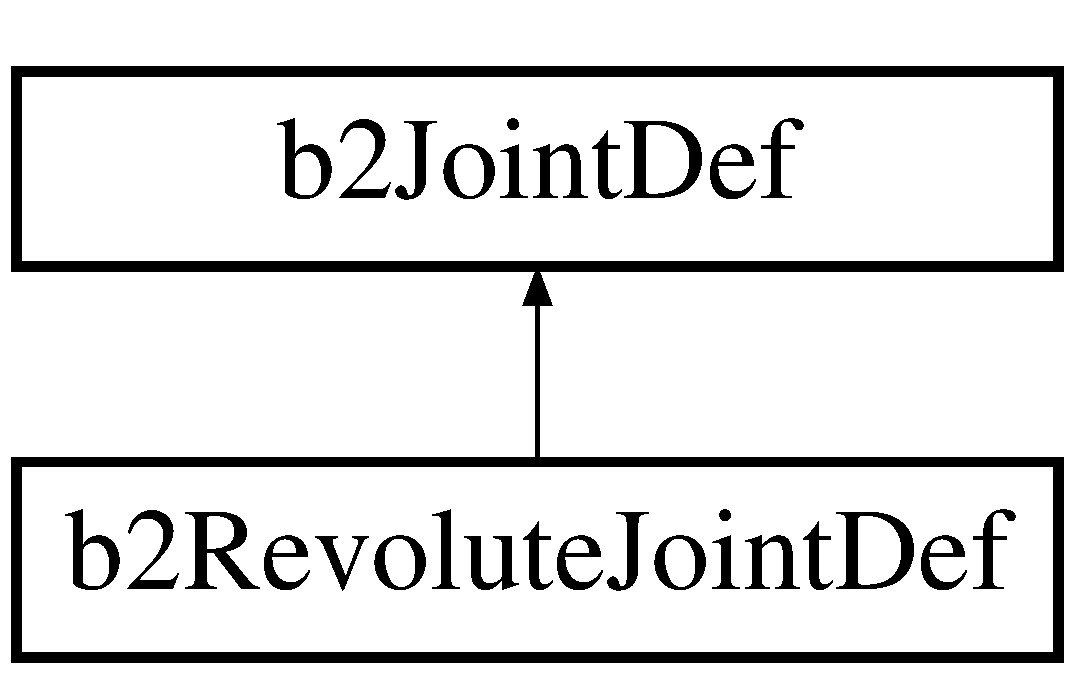
\includegraphics[height=2.000000cm]{structb2_revolute_joint_def}
\end{center}
\end{figure}
\subsection*{Public Member Functions}
\begin{DoxyCompactItemize}
\item 
void \hyperlink{structb2_revolute_joint_def_a6401b2a663533415d032a525e4fa2806}{Initialize} (\hyperlink{classb2_body}{b2\+Body} $\ast$\hyperlink{structb2_joint_def_a8cd54c93da396be75a9788f2c6897f05}{bodyA}, \hyperlink{classb2_body}{b2\+Body} $\ast$\hyperlink{structb2_joint_def_aa4f4dee2fbcd12187b19506b60e68e3d}{bodyB}, const \hyperlink{structb2_vec2}{b2\+Vec2} \&anchor)
\end{DoxyCompactItemize}
\subsection*{Public Attributes}
\begin{DoxyCompactItemize}
\item 
\hyperlink{structb2_vec2}{b2\+Vec2} \hyperlink{structb2_revolute_joint_def_a76337d07aa63232a7b20d50decc862ae}{local\+AnchorA}\hypertarget{structb2_revolute_joint_def_a76337d07aa63232a7b20d50decc862ae}{}\label{structb2_revolute_joint_def_a76337d07aa63232a7b20d50decc862ae}

\begin{DoxyCompactList}\small\item\em The local anchor point relative to bodyA\textquotesingle{}s origin. \end{DoxyCompactList}\item 
\hyperlink{structb2_vec2}{b2\+Vec2} \hyperlink{structb2_revolute_joint_def_a3f33bc1d9f6c22043a5ff2f1d89f04e0}{local\+AnchorB}\hypertarget{structb2_revolute_joint_def_a3f33bc1d9f6c22043a5ff2f1d89f04e0}{}\label{structb2_revolute_joint_def_a3f33bc1d9f6c22043a5ff2f1d89f04e0}

\begin{DoxyCompactList}\small\item\em The local anchor point relative to bodyB\textquotesingle{}s origin. \end{DoxyCompactList}\item 
float32 \hyperlink{structb2_revolute_joint_def_a1858d897d5fea04c5e606a1ff73f64f8}{reference\+Angle}\hypertarget{structb2_revolute_joint_def_a1858d897d5fea04c5e606a1ff73f64f8}{}\label{structb2_revolute_joint_def_a1858d897d5fea04c5e606a1ff73f64f8}

\begin{DoxyCompactList}\small\item\em The bodyB angle minus bodyA angle in the reference state (radians). \end{DoxyCompactList}\item 
bool \hyperlink{structb2_revolute_joint_def_a2eaefc5fc5caf879cfd59ebcd852b756}{enable\+Limit}\hypertarget{structb2_revolute_joint_def_a2eaefc5fc5caf879cfd59ebcd852b756}{}\label{structb2_revolute_joint_def_a2eaefc5fc5caf879cfd59ebcd852b756}

\begin{DoxyCompactList}\small\item\em A flag to enable joint limits. \end{DoxyCompactList}\item 
float32 \hyperlink{structb2_revolute_joint_def_a24d0b2638a01405c77bd1c0de3e53de8}{lower\+Angle}\hypertarget{structb2_revolute_joint_def_a24d0b2638a01405c77bd1c0de3e53de8}{}\label{structb2_revolute_joint_def_a24d0b2638a01405c77bd1c0de3e53de8}

\begin{DoxyCompactList}\small\item\em The lower angle for the joint limit (radians). \end{DoxyCompactList}\item 
float32 \hyperlink{structb2_revolute_joint_def_a692cfe333ad12afd5753a6ec54e39a66}{upper\+Angle}\hypertarget{structb2_revolute_joint_def_a692cfe333ad12afd5753a6ec54e39a66}{}\label{structb2_revolute_joint_def_a692cfe333ad12afd5753a6ec54e39a66}

\begin{DoxyCompactList}\small\item\em The upper angle for the joint limit (radians). \end{DoxyCompactList}\item 
bool \hyperlink{structb2_revolute_joint_def_aa94d9e66be9f03818d0cfbd9c70b2996}{enable\+Motor}\hypertarget{structb2_revolute_joint_def_aa94d9e66be9f03818d0cfbd9c70b2996}{}\label{structb2_revolute_joint_def_aa94d9e66be9f03818d0cfbd9c70b2996}

\begin{DoxyCompactList}\small\item\em A flag to enable the joint motor. \end{DoxyCompactList}\item 
float32 \hyperlink{structb2_revolute_joint_def_aced7cf768f4dcc3561576a39c7b92ec4}{motor\+Speed}\hypertarget{structb2_revolute_joint_def_aced7cf768f4dcc3561576a39c7b92ec4}{}\label{structb2_revolute_joint_def_aced7cf768f4dcc3561576a39c7b92ec4}

\begin{DoxyCompactList}\small\item\em The desired motor speed. Usually in radians per second. \end{DoxyCompactList}\item 
float32 \hyperlink{structb2_revolute_joint_def_a9fc1b67fe6d1bc31f88cc2cfd681fe30}{max\+Motor\+Torque}
\end{DoxyCompactItemize}


\subsection{Detailed Description}
Revolute joint definition. This requires defining an anchor point where the bodies are joined. The definition uses local anchor points so that the initial configuration can violate the constraint slightly. You also need to specify the initial relative angle for joint limits. This helps when saving and loading a game. The local anchor points are measured from the body\textquotesingle{}s origin rather than the center of mass because\+:
\begin{DoxyEnumerate}
\item you might not know where the center of mass will be.
\item if you add/remove shapes from a body and recompute the mass, the joints will be broken. 
\end{DoxyEnumerate}

\subsection{Member Function Documentation}
\index{b2\+Revolute\+Joint\+Def@{b2\+Revolute\+Joint\+Def}!Initialize@{Initialize}}
\index{Initialize@{Initialize}!b2\+Revolute\+Joint\+Def@{b2\+Revolute\+Joint\+Def}}
\subsubsection[{\texorpdfstring{Initialize(b2\+Body $\ast$body\+A, b2\+Body $\ast$body\+B, const b2\+Vec2 \&anchor)}{Initialize(b2Body *bodyA, b2Body *bodyB, const b2Vec2 &anchor)}}]{\setlength{\rightskip}{0pt plus 5cm}void b2\+Revolute\+Joint\+Def\+::\+Initialize (
\begin{DoxyParamCaption}
\item[{{\bf b2\+Body} $\ast$}]{bodyA, }
\item[{{\bf b2\+Body} $\ast$}]{bodyB, }
\item[{const {\bf b2\+Vec2} \&}]{anchor}
\end{DoxyParamCaption}
)}\hypertarget{structb2_revolute_joint_def_a6401b2a663533415d032a525e4fa2806}{}\label{structb2_revolute_joint_def_a6401b2a663533415d032a525e4fa2806}
Initialize the bodies, anchors, and reference angle using a world anchor point. 

\subsection{Member Data Documentation}
\index{b2\+Revolute\+Joint\+Def@{b2\+Revolute\+Joint\+Def}!max\+Motor\+Torque@{max\+Motor\+Torque}}
\index{max\+Motor\+Torque@{max\+Motor\+Torque}!b2\+Revolute\+Joint\+Def@{b2\+Revolute\+Joint\+Def}}
\subsubsection[{\texorpdfstring{max\+Motor\+Torque}{maxMotorTorque}}]{\setlength{\rightskip}{0pt plus 5cm}float32 b2\+Revolute\+Joint\+Def\+::max\+Motor\+Torque}\hypertarget{structb2_revolute_joint_def_a9fc1b67fe6d1bc31f88cc2cfd681fe30}{}\label{structb2_revolute_joint_def_a9fc1b67fe6d1bc31f88cc2cfd681fe30}
The maximum motor torque used to achieve the desired motor speed. Usually in N-\/m. 

The documentation for this struct was generated from the following file\+:\begin{DoxyCompactItemize}
\item 
Commun/\+Externe/\+Box2\+D/include/\+Box2\+D/\+Dynamics/\+Joints/b2\+Revolute\+Joint.\+h\end{DoxyCompactItemize}

\hypertarget{classb2_rope}{}\section{b2\+Rope Class Reference}
\label{classb2_rope}\index{b2\+Rope@{b2\+Rope}}
\subsection*{Public Member Functions}
\begin{DoxyCompactItemize}
\item 
void {\bfseries Initialize} (const \hyperlink{structb2_rope_def}{b2\+Rope\+Def} $\ast$def)\hypertarget{classb2_rope_a2a672ca3310790f4af1beb123e597d70}{}\label{classb2_rope_a2a672ca3310790f4af1beb123e597d70}

\item 
void {\bfseries Step} (float32 time\+Step, int32 iterations)\hypertarget{classb2_rope_abe9ce398cef717b136645cbc37f38d70}{}\label{classb2_rope_abe9ce398cef717b136645cbc37f38d70}

\item 
int32 {\bfseries Get\+Vertex\+Count} () const \hypertarget{classb2_rope_aa002b5f7efd152770803aade884f2c75}{}\label{classb2_rope_aa002b5f7efd152770803aade884f2c75}

\item 
const \hyperlink{structb2_vec2}{b2\+Vec2} $\ast$ {\bfseries Get\+Vertices} () const \hypertarget{classb2_rope_a9f5c76a25e44baa702d2a6beef9f2f9c}{}\label{classb2_rope_a9f5c76a25e44baa702d2a6beef9f2f9c}

\item 
void {\bfseries Draw} (\hyperlink{classb2_draw}{b2\+Draw} $\ast$draw) const \hypertarget{classb2_rope_acefc7b4d53ba675fc08700f39d121ec3}{}\label{classb2_rope_acefc7b4d53ba675fc08700f39d121ec3}

\item 
void {\bfseries Set\+Angle} (float32 angle)\hypertarget{classb2_rope_a8a1717a5e0b2c54d56fe438c8cae43b7}{}\label{classb2_rope_a8a1717a5e0b2c54d56fe438c8cae43b7}

\end{DoxyCompactItemize}


The documentation for this class was generated from the following file\+:\begin{DoxyCompactItemize}
\item 
Cadriciel/\+Commun/\+Externe/\+Box2\+D/include/\+Box2\+D/\+Rope/b2\+Rope.\+h\end{DoxyCompactItemize}

\hypertarget{structb2_rope_def}{}\section{b2\+Rope\+Def Struct Reference}
\label{structb2_rope_def}\index{b2\+Rope\+Def@{b2\+Rope\+Def}}
\subsection*{Public Attributes}
\begin{DoxyCompactItemize}
\item 
\hyperlink{structb2_vec2}{b2\+Vec2} $\ast$ {\bfseries vertices}\hypertarget{structb2_rope_def_ae18ad98b9796c505ae62ce58fa2f7051}{}\label{structb2_rope_def_ae18ad98b9796c505ae62ce58fa2f7051}

\item 
int32 {\bfseries count}\hypertarget{structb2_rope_def_a0c75d4289a807e31f32dc43a2276671f}{}\label{structb2_rope_def_a0c75d4289a807e31f32dc43a2276671f}

\item 
float32 $\ast$ {\bfseries masses}\hypertarget{structb2_rope_def_a78f75cce30ee253062ffa6f5462b36a1}{}\label{structb2_rope_def_a78f75cce30ee253062ffa6f5462b36a1}

\item 
\hyperlink{structb2_vec2}{b2\+Vec2} {\bfseries gravity}\hypertarget{structb2_rope_def_a90d98969150047662ce835ec1670fb32}{}\label{structb2_rope_def_a90d98969150047662ce835ec1670fb32}

\item 
float32 {\bfseries damping}\hypertarget{structb2_rope_def_a13ad872bb9d4926f3e4e49b7061613cb}{}\label{structb2_rope_def_a13ad872bb9d4926f3e4e49b7061613cb}

\item 
float32 \hyperlink{structb2_rope_def_a89de5d2c15afacd41722c76523e33826}{k2}\hypertarget{structb2_rope_def_a89de5d2c15afacd41722c76523e33826}{}\label{structb2_rope_def_a89de5d2c15afacd41722c76523e33826}

\begin{DoxyCompactList}\small\item\em Stretching stiffness. \end{DoxyCompactList}\item 
float32 \hyperlink{structb2_rope_def_a3f4749e0a309b53daf804c75adfb4ba8}{k3}\hypertarget{structb2_rope_def_a3f4749e0a309b53daf804c75adfb4ba8}{}\label{structb2_rope_def_a3f4749e0a309b53daf804c75adfb4ba8}

\begin{DoxyCompactList}\small\item\em Bending stiffness. Values above 0.\+5 can make the simulation blow up. \end{DoxyCompactList}\end{DoxyCompactItemize}


The documentation for this struct was generated from the following file\+:\begin{DoxyCompactItemize}
\item 
C\+:/\+Users/\+Bilal Itani/\+Desktop/inf2990-\/11/\+Cadriciel/\+Commun/\+Externe/\+Box2\+D/include/\+Box2\+D/\+Rope/b2\+Rope.\+h\end{DoxyCompactItemize}

\hypertarget{classb2_rope_joint}{}\section{b2\+Rope\+Joint Class Reference}
\label{classb2_rope_joint}\index{b2\+Rope\+Joint@{b2\+Rope\+Joint}}


{\ttfamily \#include $<$b2\+Rope\+Joint.\+h$>$}

Inheritance diagram for b2\+Rope\+Joint\+:\begin{figure}[H]
\begin{center}
\leavevmode
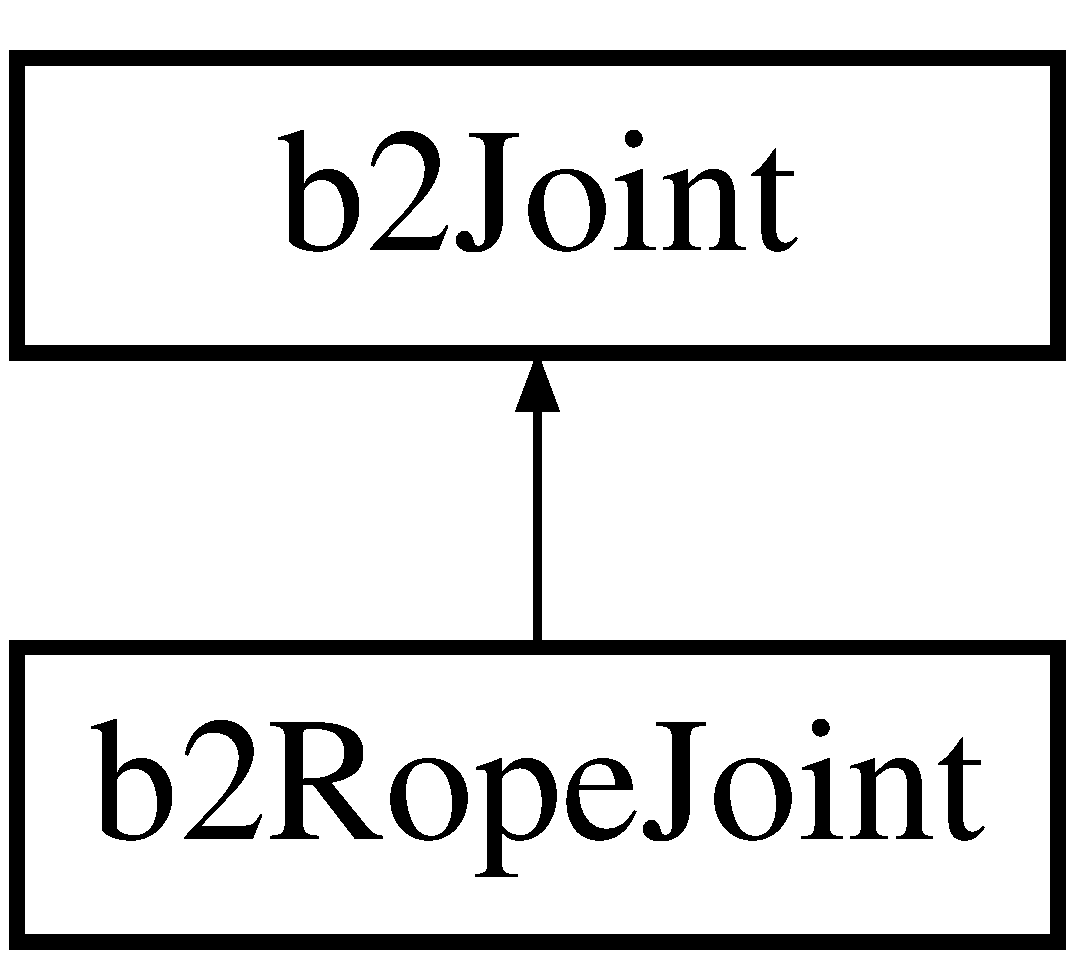
\includegraphics[height=2.000000cm]{classb2_rope_joint}
\end{center}
\end{figure}
\subsection*{Public Member Functions}
\begin{DoxyCompactItemize}
\item 
\hyperlink{structb2_vec2}{b2\+Vec2} \hyperlink{classb2_rope_joint_a046c6f0bc73800716c669a2b955b3c05}{Get\+AnchorA} () const \hypertarget{classb2_rope_joint_a046c6f0bc73800716c669a2b955b3c05}{}\label{classb2_rope_joint_a046c6f0bc73800716c669a2b955b3c05}

\begin{DoxyCompactList}\small\item\em Get the anchor point on bodyA in world coordinates. \end{DoxyCompactList}\item 
\hyperlink{structb2_vec2}{b2\+Vec2} \hyperlink{classb2_rope_joint_a14a8ef7c16e0d6d874cdfb986d0eb8f0}{Get\+AnchorB} () const \hypertarget{classb2_rope_joint_a14a8ef7c16e0d6d874cdfb986d0eb8f0}{}\label{classb2_rope_joint_a14a8ef7c16e0d6d874cdfb986d0eb8f0}

\begin{DoxyCompactList}\small\item\em Get the anchor point on bodyB in world coordinates. \end{DoxyCompactList}\item 
\hyperlink{structb2_vec2}{b2\+Vec2} \hyperlink{classb2_rope_joint_afe0acc77e40b62133547897a6d01b7e6}{Get\+Reaction\+Force} (float32 inv\+\_\+dt) const \hypertarget{classb2_rope_joint_afe0acc77e40b62133547897a6d01b7e6}{}\label{classb2_rope_joint_afe0acc77e40b62133547897a6d01b7e6}

\begin{DoxyCompactList}\small\item\em Get the reaction force on bodyB at the joint anchor in Newtons. \end{DoxyCompactList}\item 
float32 \hyperlink{classb2_rope_joint_abb7baf596f13ff5a76ff657ad6d3232c}{Get\+Reaction\+Torque} (float32 inv\+\_\+dt) const \hypertarget{classb2_rope_joint_abb7baf596f13ff5a76ff657ad6d3232c}{}\label{classb2_rope_joint_abb7baf596f13ff5a76ff657ad6d3232c}

\begin{DoxyCompactList}\small\item\em Get the reaction torque on bodyB in N$\ast$m. \end{DoxyCompactList}\item 
const \hyperlink{structb2_vec2}{b2\+Vec2} \& \hyperlink{classb2_rope_joint_aa423bbe186d46bff0b50ede8338851d4}{Get\+Local\+AnchorA} () const \hypertarget{classb2_rope_joint_aa423bbe186d46bff0b50ede8338851d4}{}\label{classb2_rope_joint_aa423bbe186d46bff0b50ede8338851d4}

\begin{DoxyCompactList}\small\item\em The local anchor point relative to bodyA\textquotesingle{}s origin. \end{DoxyCompactList}\item 
const \hyperlink{structb2_vec2}{b2\+Vec2} \& \hyperlink{classb2_rope_joint_a511b297fbebfbecdcdce68e1cffa272c}{Get\+Local\+AnchorB} () const \hypertarget{classb2_rope_joint_a511b297fbebfbecdcdce68e1cffa272c}{}\label{classb2_rope_joint_a511b297fbebfbecdcdce68e1cffa272c}

\begin{DoxyCompactList}\small\item\em The local anchor point relative to bodyB\textquotesingle{}s origin. \end{DoxyCompactList}\item 
void \hyperlink{classb2_rope_joint_a92cea201d21acd2f2a7cc9b00e165848}{Set\+Max\+Length} (float32 length)\hypertarget{classb2_rope_joint_a92cea201d21acd2f2a7cc9b00e165848}{}\label{classb2_rope_joint_a92cea201d21acd2f2a7cc9b00e165848}

\begin{DoxyCompactList}\small\item\em Set/\+Get the maximum length of the rope. \end{DoxyCompactList}\item 
float32 {\bfseries Get\+Max\+Length} () const \hypertarget{classb2_rope_joint_a2bee2d2f47a27ab900438ec58d86f9ac}{}\label{classb2_rope_joint_a2bee2d2f47a27ab900438ec58d86f9ac}

\item 
b2\+Limit\+State {\bfseries Get\+Limit\+State} () const \hypertarget{classb2_rope_joint_af3653f62379529a43a99e6a8e84f5d43}{}\label{classb2_rope_joint_af3653f62379529a43a99e6a8e84f5d43}

\item 
void \hyperlink{classb2_rope_joint_a4612dca9851a66701893a48d896dbd14}{Dump} ()\hypertarget{classb2_rope_joint_a4612dca9851a66701893a48d896dbd14}{}\label{classb2_rope_joint_a4612dca9851a66701893a48d896dbd14}

\begin{DoxyCompactList}\small\item\em Dump joint to dm\+Log. \end{DoxyCompactList}\end{DoxyCompactItemize}
\subsection*{Protected Member Functions}
\begin{DoxyCompactItemize}
\item 
{\bfseries b2\+Rope\+Joint} (const \hyperlink{structb2_rope_joint_def}{b2\+Rope\+Joint\+Def} $\ast$data)\hypertarget{classb2_rope_joint_a3f69f238616d8dc622d9448f81e14e53}{}\label{classb2_rope_joint_a3f69f238616d8dc622d9448f81e14e53}

\item 
void {\bfseries Init\+Velocity\+Constraints} (const \hyperlink{structb2_solver_data}{b2\+Solver\+Data} \&data)\hypertarget{classb2_rope_joint_a8146dad7f839f1285ab596661c3a84fa}{}\label{classb2_rope_joint_a8146dad7f839f1285ab596661c3a84fa}

\item 
void {\bfseries Solve\+Velocity\+Constraints} (const \hyperlink{structb2_solver_data}{b2\+Solver\+Data} \&data)\hypertarget{classb2_rope_joint_ab3e9a866833f5ad079473ece272d3c88}{}\label{classb2_rope_joint_ab3e9a866833f5ad079473ece272d3c88}

\item 
bool {\bfseries Solve\+Position\+Constraints} (const \hyperlink{structb2_solver_data}{b2\+Solver\+Data} \&data)\hypertarget{classb2_rope_joint_a50794029b91cd469b0598fe25a77948f}{}\label{classb2_rope_joint_a50794029b91cd469b0598fe25a77948f}

\end{DoxyCompactItemize}
\subsection*{Protected Attributes}
\begin{DoxyCompactItemize}
\item 
\hyperlink{structb2_vec2}{b2\+Vec2} {\bfseries m\+\_\+local\+AnchorA}\hypertarget{classb2_rope_joint_a43640240dc39c912ea1cc6e1ae9fa614}{}\label{classb2_rope_joint_a43640240dc39c912ea1cc6e1ae9fa614}

\item 
\hyperlink{structb2_vec2}{b2\+Vec2} {\bfseries m\+\_\+local\+AnchorB}\hypertarget{classb2_rope_joint_a57dfab74bae88c2c3284ed640825c959}{}\label{classb2_rope_joint_a57dfab74bae88c2c3284ed640825c959}

\item 
float32 {\bfseries m\+\_\+max\+Length}\hypertarget{classb2_rope_joint_ace7528ca1183f34cfc79e47f46b29130}{}\label{classb2_rope_joint_ace7528ca1183f34cfc79e47f46b29130}

\item 
float32 {\bfseries m\+\_\+length}\hypertarget{classb2_rope_joint_a2cee8c35d881b0ae66d28d13c6d8d66a}{}\label{classb2_rope_joint_a2cee8c35d881b0ae66d28d13c6d8d66a}

\item 
float32 {\bfseries m\+\_\+impulse}\hypertarget{classb2_rope_joint_ac19ae74b5f3c104bc763e99b3986afd6}{}\label{classb2_rope_joint_ac19ae74b5f3c104bc763e99b3986afd6}

\item 
int32 {\bfseries m\+\_\+indexA}\hypertarget{classb2_rope_joint_a34875f5852d011dab695613a23adca08}{}\label{classb2_rope_joint_a34875f5852d011dab695613a23adca08}

\item 
int32 {\bfseries m\+\_\+indexB}\hypertarget{classb2_rope_joint_aa67100c069a1a273314dfa55c9063fc7}{}\label{classb2_rope_joint_aa67100c069a1a273314dfa55c9063fc7}

\item 
\hyperlink{structb2_vec2}{b2\+Vec2} {\bfseries m\+\_\+u}\hypertarget{classb2_rope_joint_ae95185c5ad4c119a9893294491ba1609}{}\label{classb2_rope_joint_ae95185c5ad4c119a9893294491ba1609}

\item 
\hyperlink{structb2_vec2}{b2\+Vec2} {\bfseries m\+\_\+rA}\hypertarget{classb2_rope_joint_af8ae48af2656b1e605a099b8f4aa82b0}{}\label{classb2_rope_joint_af8ae48af2656b1e605a099b8f4aa82b0}

\item 
\hyperlink{structb2_vec2}{b2\+Vec2} {\bfseries m\+\_\+rB}\hypertarget{classb2_rope_joint_ae577e49beef03d266ff4c54e852b4f41}{}\label{classb2_rope_joint_ae577e49beef03d266ff4c54e852b4f41}

\item 
\hyperlink{structb2_vec2}{b2\+Vec2} {\bfseries m\+\_\+local\+CenterA}\hypertarget{classb2_rope_joint_a15ff1472deb6405c9886a40ee99efcef}{}\label{classb2_rope_joint_a15ff1472deb6405c9886a40ee99efcef}

\item 
\hyperlink{structb2_vec2}{b2\+Vec2} {\bfseries m\+\_\+local\+CenterB}\hypertarget{classb2_rope_joint_a2b3b1ac9ae9e3e68b2550809ec178877}{}\label{classb2_rope_joint_a2b3b1ac9ae9e3e68b2550809ec178877}

\item 
float32 {\bfseries m\+\_\+inv\+MassA}\hypertarget{classb2_rope_joint_a690e4fe5ab7a279accac3b137d5f5c76}{}\label{classb2_rope_joint_a690e4fe5ab7a279accac3b137d5f5c76}

\item 
float32 {\bfseries m\+\_\+inv\+MassB}\hypertarget{classb2_rope_joint_a9709179725abed80d4957df82bc24512}{}\label{classb2_rope_joint_a9709179725abed80d4957df82bc24512}

\item 
float32 {\bfseries m\+\_\+inv\+IA}\hypertarget{classb2_rope_joint_a1917a65b89668c433d06071970a6875a}{}\label{classb2_rope_joint_a1917a65b89668c433d06071970a6875a}

\item 
float32 {\bfseries m\+\_\+inv\+IB}\hypertarget{classb2_rope_joint_a1ce440194cec6e275193d7224ce1e448}{}\label{classb2_rope_joint_a1ce440194cec6e275193d7224ce1e448}

\item 
float32 {\bfseries m\+\_\+mass}\hypertarget{classb2_rope_joint_a1f355a976b177b75a8fd47190194d5c1}{}\label{classb2_rope_joint_a1f355a976b177b75a8fd47190194d5c1}

\item 
b2\+Limit\+State {\bfseries m\+\_\+state}\hypertarget{classb2_rope_joint_ac73c9451360c80c8a98376b922f4bed4}{}\label{classb2_rope_joint_ac73c9451360c80c8a98376b922f4bed4}

\end{DoxyCompactItemize}
\subsection*{Friends}
\begin{DoxyCompactItemize}
\item 
class {\bfseries b2\+Joint}\hypertarget{classb2_rope_joint_a54ade8ed3d794298108d7f4c4e4793fa}{}\label{classb2_rope_joint_a54ade8ed3d794298108d7f4c4e4793fa}

\end{DoxyCompactItemize}
\subsection*{Additional Inherited Members}


\subsection{Detailed Description}
A rope joint enforces a maximum distance between two points on two bodies. It has no other effect. Warning\+: if you attempt to change the maximum length during the simulation you will get some non-\/physical behavior. A model that would allow you to dynamically modify the length would have some sponginess, so I chose not to implement it that way. See \hyperlink{classb2_distance_joint}{b2\+Distance\+Joint} if you want to dynamically control length. 

The documentation for this class was generated from the following file\+:\begin{DoxyCompactItemize}
\item 
Cadriciel/\+Commun/\+Externe/\+Box2\+D/include/\+Box2\+D/\+Dynamics/\+Joints/b2\+Rope\+Joint.\+h\end{DoxyCompactItemize}

\hypertarget{structb2_rope_joint_def}{}\section{b2\+Rope\+Joint\+Def Struct Reference}
\label{structb2_rope_joint_def}\index{b2\+Rope\+Joint\+Def@{b2\+Rope\+Joint\+Def}}


{\ttfamily \#include $<$b2\+Rope\+Joint.\+h$>$}

Inheritance diagram for b2\+Rope\+Joint\+Def\+:\begin{figure}[H]
\begin{center}
\leavevmode
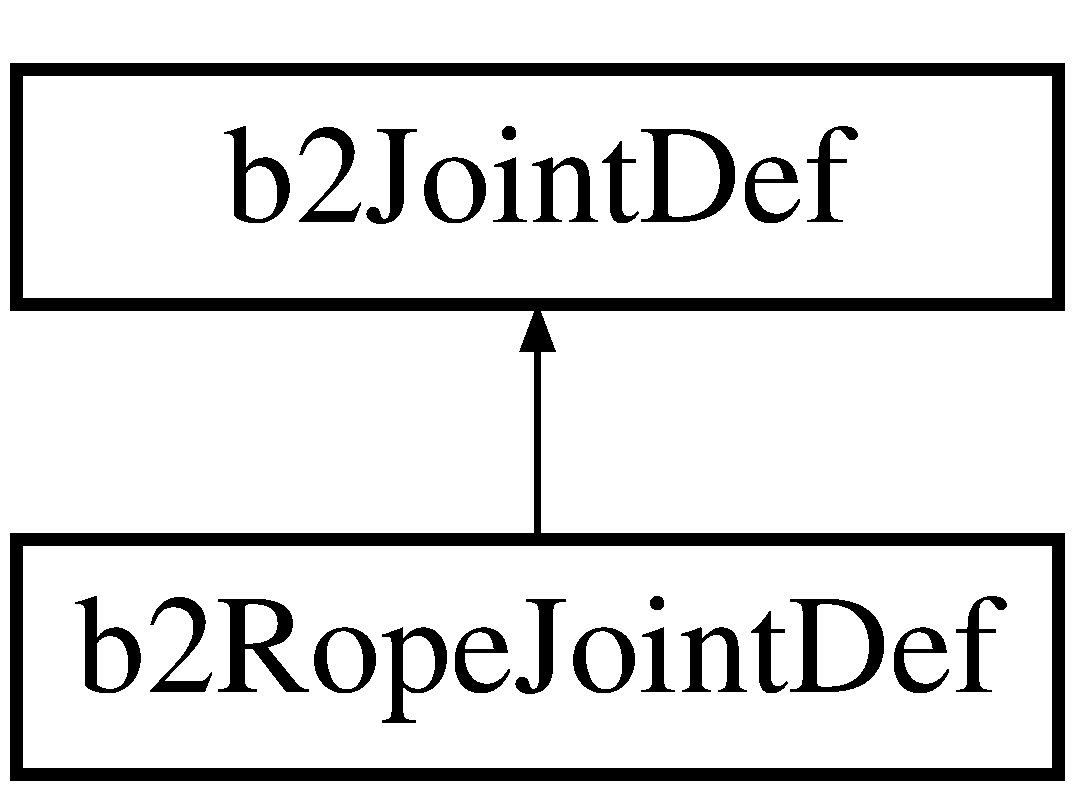
\includegraphics[height=2.000000cm]{structb2_rope_joint_def}
\end{center}
\end{figure}
\subsection*{Public Attributes}
\begin{DoxyCompactItemize}
\item 
\hyperlink{structb2_vec2}{b2\+Vec2} \hyperlink{structb2_rope_joint_def_ab680fcc3cd44741a7a824ddff86ff01e}{local\+AnchorA}\hypertarget{structb2_rope_joint_def_ab680fcc3cd44741a7a824ddff86ff01e}{}\label{structb2_rope_joint_def_ab680fcc3cd44741a7a824ddff86ff01e}

\begin{DoxyCompactList}\small\item\em The local anchor point relative to bodyA\textquotesingle{}s origin. \end{DoxyCompactList}\item 
\hyperlink{structb2_vec2}{b2\+Vec2} \hyperlink{structb2_rope_joint_def_a3271da0e4027e25546aa6a81e8fbe4e2}{local\+AnchorB}\hypertarget{structb2_rope_joint_def_a3271da0e4027e25546aa6a81e8fbe4e2}{}\label{structb2_rope_joint_def_a3271da0e4027e25546aa6a81e8fbe4e2}

\begin{DoxyCompactList}\small\item\em The local anchor point relative to bodyB\textquotesingle{}s origin. \end{DoxyCompactList}\item 
float32 \hyperlink{structb2_rope_joint_def_a6efdcae22e2bdcfc3aae62da1a5f0d69}{max\+Length}
\end{DoxyCompactItemize}


\subsection{Detailed Description}
Rope joint definition. This requires two body anchor points and a maximum lengths. Note\+: by default the connected objects will not collide. see collide\+Connected in \hyperlink{structb2_joint_def}{b2\+Joint\+Def}. 

\subsection{Member Data Documentation}
\index{b2\+Rope\+Joint\+Def@{b2\+Rope\+Joint\+Def}!max\+Length@{max\+Length}}
\index{max\+Length@{max\+Length}!b2\+Rope\+Joint\+Def@{b2\+Rope\+Joint\+Def}}
\subsubsection[{\texorpdfstring{max\+Length}{maxLength}}]{\setlength{\rightskip}{0pt plus 5cm}float32 b2\+Rope\+Joint\+Def\+::max\+Length}\hypertarget{structb2_rope_joint_def_a6efdcae22e2bdcfc3aae62da1a5f0d69}{}\label{structb2_rope_joint_def_a6efdcae22e2bdcfc3aae62da1a5f0d69}
The maximum length of the rope. Warning\+: this must be larger than b2\+\_\+linear\+Slop or the joint will have no effect. 

The documentation for this struct was generated from the following file\+:\begin{DoxyCompactItemize}
\item 
C\+:/\+Users/\+Bilal Itani/\+Desktop/inf2990-\/11/\+Cadriciel/\+Commun/\+Externe/\+Box2\+D/include/\+Box2\+D/\+Dynamics/\+Joints/b2\+Rope\+Joint.\+h\end{DoxyCompactItemize}

\hypertarget{structb2_rot}{}\section{b2\+Rot Struct Reference}
\label{structb2_rot}\index{b2\+Rot@{b2\+Rot}}


Rotation.  




{\ttfamily \#include $<$b2\+Math.\+h$>$}

\subsection*{Public Member Functions}
\begin{DoxyCompactItemize}
\item 
\hyperlink{structb2_rot_aa40dda6d390a2f54c793c63027a9b46e}{b2\+Rot} (float32 angle)
\begin{DoxyCompactList}\small\item\em Initialize from an angle in radians. \end{DoxyCompactList}\item 
void \hyperlink{structb2_rot_acde9186de0a4a7397bf8ef714408ad60}{Set} (float32 angle)
\begin{DoxyCompactList}\small\item\em Set using an angle in radians. \end{DoxyCompactList}\item 
void \hyperlink{structb2_rot_a7f534cb7ece8d325662d7d0e27d4f617}{Set\+Identity} ()\hypertarget{structb2_rot_a7f534cb7ece8d325662d7d0e27d4f617}{}\label{structb2_rot_a7f534cb7ece8d325662d7d0e27d4f617}

\begin{DoxyCompactList}\small\item\em Set to the identity rotation. \end{DoxyCompactList}\item 
float32 \hyperlink{structb2_rot_a67a6c08812c009654f00800256c8bfdc}{Get\+Angle} () const \hypertarget{structb2_rot_a67a6c08812c009654f00800256c8bfdc}{}\label{structb2_rot_a67a6c08812c009654f00800256c8bfdc}

\begin{DoxyCompactList}\small\item\em Get the angle in radians. \end{DoxyCompactList}\item 
\hyperlink{structb2_vec2}{b2\+Vec2} \hyperlink{structb2_rot_ac4ab7f262adb99f161775314852723d8}{Get\+X\+Axis} () const \hypertarget{structb2_rot_ac4ab7f262adb99f161775314852723d8}{}\label{structb2_rot_ac4ab7f262adb99f161775314852723d8}

\begin{DoxyCompactList}\small\item\em Get the x-\/axis. \end{DoxyCompactList}\item 
\hyperlink{structb2_vec2}{b2\+Vec2} \hyperlink{structb2_rot_ae731c7434fe1754114ee70149df36c7f}{Get\+Y\+Axis} () const \hypertarget{structb2_rot_ae731c7434fe1754114ee70149df36c7f}{}\label{structb2_rot_ae731c7434fe1754114ee70149df36c7f}

\begin{DoxyCompactList}\small\item\em Get the u-\/axis. \end{DoxyCompactList}\end{DoxyCompactItemize}
\subsection*{Public Attributes}
\begin{DoxyCompactItemize}
\item 
float32 \hyperlink{structb2_rot_a15725ce0a89cc735ad90687b4c0f4dce}{s}\hypertarget{structb2_rot_a15725ce0a89cc735ad90687b4c0f4dce}{}\label{structb2_rot_a15725ce0a89cc735ad90687b4c0f4dce}

\begin{DoxyCompactList}\small\item\em Sine and cosine. \end{DoxyCompactList}\item 
float32 {\bfseries c}\hypertarget{structb2_rot_af23e5d31889dcb806ce46ce55aa81261}{}\label{structb2_rot_af23e5d31889dcb806ce46ce55aa81261}

\end{DoxyCompactItemize}


\subsection{Detailed Description}
Rotation. 

\subsection{Constructor \& Destructor Documentation}
\index{b2\+Rot@{b2\+Rot}!b2\+Rot@{b2\+Rot}}
\index{b2\+Rot@{b2\+Rot}!b2\+Rot@{b2\+Rot}}
\subsubsection[{\texorpdfstring{b2\+Rot(float32 angle)}{b2Rot(float32 angle)}}]{\setlength{\rightskip}{0pt plus 5cm}b2\+Rot\+::b2\+Rot (
\begin{DoxyParamCaption}
\item[{float32}]{angle}
\end{DoxyParamCaption}
)\hspace{0.3cm}{\ttfamily [inline]}, {\ttfamily [explicit]}}\hypertarget{structb2_rot_aa40dda6d390a2f54c793c63027a9b46e}{}\label{structb2_rot_aa40dda6d390a2f54c793c63027a9b46e}


Initialize from an angle in radians. 

T\+O\+D\+O\+\_\+\+E\+R\+IN optimize 

\subsection{Member Function Documentation}
\index{b2\+Rot@{b2\+Rot}!Set@{Set}}
\index{Set@{Set}!b2\+Rot@{b2\+Rot}}
\subsubsection[{\texorpdfstring{Set(float32 angle)}{Set(float32 angle)}}]{\setlength{\rightskip}{0pt plus 5cm}void b2\+Rot\+::\+Set (
\begin{DoxyParamCaption}
\item[{float32}]{angle}
\end{DoxyParamCaption}
)\hspace{0.3cm}{\ttfamily [inline]}}\hypertarget{structb2_rot_acde9186de0a4a7397bf8ef714408ad60}{}\label{structb2_rot_acde9186de0a4a7397bf8ef714408ad60}


Set using an angle in radians. 

T\+O\+D\+O\+\_\+\+E\+R\+IN optimize 

The documentation for this struct was generated from the following file\+:\begin{DoxyCompactItemize}
\item 
C\+:/\+Users/\+Bilal Itani/\+Desktop/inf2990-\/11/\+Cadriciel/\+Commun/\+Externe/\+Box2\+D/include/\+Box2\+D/\+Common/b2\+Math.\+h\end{DoxyCompactItemize}

\hypertarget{classb2_shape}{}\section{b2\+Shape Class Reference}
\label{classb2_shape}\index{b2\+Shape@{b2\+Shape}}


{\ttfamily \#include $<$b2\+Shape.\+h$>$}

Inheritance diagram for b2\+Shape\+:\begin{figure}[H]
\begin{center}
\leavevmode
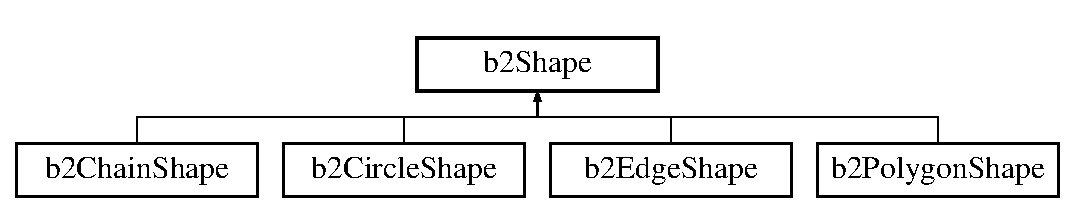
\includegraphics[height=2.000000cm]{classb2_shape}
\end{center}
\end{figure}
\subsection*{Public Types}
\begin{DoxyCompactItemize}
\item 
enum {\bfseries Type} \{ \\*
{\bfseries e\+\_\+circle} = 0, 
{\bfseries e\+\_\+edge} = 1, 
{\bfseries e\+\_\+polygon} = 2, 
{\bfseries e\+\_\+chain} = 3, 
\\*
{\bfseries e\+\_\+type\+Count} = 4
 \}\hypertarget{classb2_shape_a4c1f3a9ad6b3150bb90ad9018ca4b1e0}{}\label{classb2_shape_a4c1f3a9ad6b3150bb90ad9018ca4b1e0}

\end{DoxyCompactItemize}
\subsection*{Public Member Functions}
\begin{DoxyCompactItemize}
\item 
virtual \hyperlink{classb2_shape}{b2\+Shape} $\ast$ \hyperlink{classb2_shape_affc468420410145519369377d26d1ccd}{Clone} (\hyperlink{classb2_block_allocator}{b2\+Block\+Allocator} $\ast$allocator) const  =0\hypertarget{classb2_shape_affc468420410145519369377d26d1ccd}{}\label{classb2_shape_affc468420410145519369377d26d1ccd}

\begin{DoxyCompactList}\small\item\em Clone the concrete shape using the provided allocator. \end{DoxyCompactList}\item 
Type \hyperlink{classb2_shape_a3b6093f16c18f8a877519a29674abca0}{Get\+Type} () const 
\item 
virtual int32 \hyperlink{classb2_shape_acaade0398c8a6f3750ba0d25fbde2242}{Get\+Child\+Count} () const  =0\hypertarget{classb2_shape_acaade0398c8a6f3750ba0d25fbde2242}{}\label{classb2_shape_acaade0398c8a6f3750ba0d25fbde2242}

\begin{DoxyCompactList}\small\item\em Get the number of child primitives. \end{DoxyCompactList}\item 
virtual bool \hyperlink{classb2_shape_a11996b9bdcf8dca92a0c8bf484ab3f59}{Test\+Point} (const \hyperlink{structb2_transform}{b2\+Transform} \&xf, const \hyperlink{structb2_vec2}{b2\+Vec2} \&p) const  =0
\item 
virtual bool \hyperlink{classb2_shape_ab87bc92f81dfc5cb8b5c028261f1b21f}{Ray\+Cast} (\hyperlink{structb2_ray_cast_output}{b2\+Ray\+Cast\+Output} $\ast$output, const \hyperlink{structb2_ray_cast_input}{b2\+Ray\+Cast\+Input} \&input, const \hyperlink{structb2_transform}{b2\+Transform} \&transform, int32 child\+Index) const  =0
\item 
virtual void \hyperlink{classb2_shape_a0a7f4227b6c17450fc26e0b6641b7abf}{Compute\+A\+A\+BB} (\hyperlink{structb2_a_a_b_b}{b2\+A\+A\+BB} $\ast$aabb, const \hyperlink{structb2_transform}{b2\+Transform} \&xf, int32 child\+Index) const  =0
\item 
virtual void \hyperlink{classb2_shape_a33cfcad2cf4cc31e1d001bf1baf10721}{Compute\+Mass} (\hyperlink{structb2_mass_data}{b2\+Mass\+Data} $\ast$mass\+Data, float32 density) const  =0
\end{DoxyCompactItemize}
\subsection*{Public Attributes}
\begin{DoxyCompactItemize}
\item 
Type {\bfseries m\+\_\+type}\hypertarget{classb2_shape_adb051791133b24f53c6e9a565a7b7bbb}{}\label{classb2_shape_adb051791133b24f53c6e9a565a7b7bbb}

\item 
float32 {\bfseries m\+\_\+radius}\hypertarget{classb2_shape_a5de7a9bd3f9e72ef7025a65c304aaf1a}{}\label{classb2_shape_a5de7a9bd3f9e72ef7025a65c304aaf1a}

\end{DoxyCompactItemize}


\subsection{Detailed Description}
A shape is used for collision detection. You can create a shape however you like. Shapes used for simulation in \hyperlink{classb2_world}{b2\+World} are created automatically when a \hyperlink{classb2_fixture}{b2\+Fixture} is created. Shapes may encapsulate a one or more child shapes. 

\subsection{Member Function Documentation}
\index{b2\+Shape@{b2\+Shape}!Compute\+A\+A\+BB@{Compute\+A\+A\+BB}}
\index{Compute\+A\+A\+BB@{Compute\+A\+A\+BB}!b2\+Shape@{b2\+Shape}}
\subsubsection[{\texorpdfstring{Compute\+A\+A\+B\+B(b2\+A\+A\+B\+B $\ast$aabb, const b2\+Transform \&xf, int32 child\+Index) const  =0}{ComputeAABB(b2AABB *aabb, const b2Transform &xf, int32 childIndex) const  =0}}]{\setlength{\rightskip}{0pt plus 5cm}virtual void b2\+Shape\+::\+Compute\+A\+A\+BB (
\begin{DoxyParamCaption}
\item[{{\bf b2\+A\+A\+BB} $\ast$}]{aabb, }
\item[{const {\bf b2\+Transform} \&}]{xf, }
\item[{int32}]{child\+Index}
\end{DoxyParamCaption}
) const\hspace{0.3cm}{\ttfamily [pure virtual]}}\hypertarget{classb2_shape_a0a7f4227b6c17450fc26e0b6641b7abf}{}\label{classb2_shape_a0a7f4227b6c17450fc26e0b6641b7abf}
Given a transform, compute the associated axis aligned bounding box for a child shape. 
\begin{DoxyParams}{Parameters}
{\em aabb} & returns the axis aligned box. \\
\hline
{\em xf} & the world transform of the shape. \\
\hline
{\em child\+Index} & the child shape \\
\hline
\end{DoxyParams}


Implemented in \hyperlink{classb2_chain_shape_a409c21206e4c84f66700809aac5b164c}{b2\+Chain\+Shape}, \hyperlink{classb2_polygon_shape_a00e225b0321bf6bb231a554036ffdf23}{b2\+Polygon\+Shape}, \hyperlink{classb2_edge_shape_a30f601c611eb549f9f657eee89d82f9f}{b2\+Edge\+Shape}, and \hyperlink{classb2_circle_shape_aa6889a5af85aa1e272547fd0008eb64a}{b2\+Circle\+Shape}.

\index{b2\+Shape@{b2\+Shape}!Compute\+Mass@{Compute\+Mass}}
\index{Compute\+Mass@{Compute\+Mass}!b2\+Shape@{b2\+Shape}}
\subsubsection[{\texorpdfstring{Compute\+Mass(b2\+Mass\+Data $\ast$mass\+Data, float32 density) const  =0}{ComputeMass(b2MassData *massData, float32 density) const  =0}}]{\setlength{\rightskip}{0pt plus 5cm}virtual void b2\+Shape\+::\+Compute\+Mass (
\begin{DoxyParamCaption}
\item[{{\bf b2\+Mass\+Data} $\ast$}]{mass\+Data, }
\item[{float32}]{density}
\end{DoxyParamCaption}
) const\hspace{0.3cm}{\ttfamily [pure virtual]}}\hypertarget{classb2_shape_a33cfcad2cf4cc31e1d001bf1baf10721}{}\label{classb2_shape_a33cfcad2cf4cc31e1d001bf1baf10721}
Compute the mass properties of this shape using its dimensions and density. The inertia tensor is computed about the local origin. 
\begin{DoxyParams}{Parameters}
{\em mass\+Data} & returns the mass data for this shape. \\
\hline
{\em density} & the density in kilograms per meter squared. \\
\hline
\end{DoxyParams}


Implemented in \hyperlink{classb2_chain_shape_a009259d589abebeda27fe580d117b11e}{b2\+Chain\+Shape}, \hyperlink{classb2_polygon_shape_ad86c4c2a83a7122599462da83bf35389}{b2\+Polygon\+Shape}, \hyperlink{classb2_edge_shape_a3a305707a07ca3dffa6f2eaff3735dff}{b2\+Edge\+Shape}, and \hyperlink{classb2_circle_shape_a335edea2ef84789e102dde41ca889828}{b2\+Circle\+Shape}.

\index{b2\+Shape@{b2\+Shape}!Get\+Type@{Get\+Type}}
\index{Get\+Type@{Get\+Type}!b2\+Shape@{b2\+Shape}}
\subsubsection[{\texorpdfstring{Get\+Type() const }{GetType() const }}]{\setlength{\rightskip}{0pt plus 5cm}b2\+Shape\+::\+Type b2\+Shape\+::\+Get\+Type (
\begin{DoxyParamCaption}
{}
\end{DoxyParamCaption}
) const\hspace{0.3cm}{\ttfamily [inline]}}\hypertarget{classb2_shape_a3b6093f16c18f8a877519a29674abca0}{}\label{classb2_shape_a3b6093f16c18f8a877519a29674abca0}
Get the type of this shape. You can use this to down cast to the concrete shape. \begin{DoxyReturn}{Returns}
the shape type. 
\end{DoxyReturn}
\index{b2\+Shape@{b2\+Shape}!Ray\+Cast@{Ray\+Cast}}
\index{Ray\+Cast@{Ray\+Cast}!b2\+Shape@{b2\+Shape}}
\subsubsection[{\texorpdfstring{Ray\+Cast(b2\+Ray\+Cast\+Output $\ast$output, const b2\+Ray\+Cast\+Input \&input, const b2\+Transform \&transform, int32 child\+Index) const  =0}{RayCast(b2RayCastOutput *output, const b2RayCastInput &input, const b2Transform &transform, int32 childIndex) const  =0}}]{\setlength{\rightskip}{0pt plus 5cm}virtual bool b2\+Shape\+::\+Ray\+Cast (
\begin{DoxyParamCaption}
\item[{{\bf b2\+Ray\+Cast\+Output} $\ast$}]{output, }
\item[{const {\bf b2\+Ray\+Cast\+Input} \&}]{input, }
\item[{const {\bf b2\+Transform} \&}]{transform, }
\item[{int32}]{child\+Index}
\end{DoxyParamCaption}
) const\hspace{0.3cm}{\ttfamily [pure virtual]}}\hypertarget{classb2_shape_ab87bc92f81dfc5cb8b5c028261f1b21f}{}\label{classb2_shape_ab87bc92f81dfc5cb8b5c028261f1b21f}
Cast a ray against a child shape. 
\begin{DoxyParams}{Parameters}
{\em output} & the ray-\/cast results. \\
\hline
{\em input} & the ray-\/cast input parameters. \\
\hline
{\em transform} & the transform to be applied to the shape. \\
\hline
{\em child\+Index} & the child shape index \\
\hline
\end{DoxyParams}


Implemented in \hyperlink{classb2_chain_shape_a85c7a17a15581e0e258c7af561cf5403}{b2\+Chain\+Shape}, \hyperlink{classb2_polygon_shape_ac13bded10d09c341f64aaa2750dda6b5}{b2\+Polygon\+Shape}, \hyperlink{classb2_edge_shape_aefbae6b3840f486b22ffecee7d0d15fd}{b2\+Edge\+Shape}, and \hyperlink{classb2_circle_shape_a76175079381193917026fdf3702190fa}{b2\+Circle\+Shape}.

\index{b2\+Shape@{b2\+Shape}!Test\+Point@{Test\+Point}}
\index{Test\+Point@{Test\+Point}!b2\+Shape@{b2\+Shape}}
\subsubsection[{\texorpdfstring{Test\+Point(const b2\+Transform \&xf, const b2\+Vec2 \&p) const  =0}{TestPoint(const b2Transform &xf, const b2Vec2 &p) const  =0}}]{\setlength{\rightskip}{0pt plus 5cm}virtual bool b2\+Shape\+::\+Test\+Point (
\begin{DoxyParamCaption}
\item[{const {\bf b2\+Transform} \&}]{xf, }
\item[{const {\bf b2\+Vec2} \&}]{p}
\end{DoxyParamCaption}
) const\hspace{0.3cm}{\ttfamily [pure virtual]}}\hypertarget{classb2_shape_a11996b9bdcf8dca92a0c8bf484ab3f59}{}\label{classb2_shape_a11996b9bdcf8dca92a0c8bf484ab3f59}
\hyperlink{class_test}{Test} a point for containment in this shape. This only works for convex shapes. 
\begin{DoxyParams}{Parameters}
{\em xf} & the shape world transform. \\
\hline
{\em p} & a point in world coordinates. \\
\hline
\end{DoxyParams}


Implemented in \hyperlink{classb2_chain_shape_a4fc27b41ecc556985efacf8e0f91c39f}{b2\+Chain\+Shape}, \hyperlink{classb2_polygon_shape_a69ccc2f671394b3cc1a00a16ef36b12b}{b2\+Polygon\+Shape}, \hyperlink{classb2_edge_shape_a28a977f82e4bc1cf60a3143ba5636c22}{b2\+Edge\+Shape}, and \hyperlink{classb2_circle_shape_a77171941cd1633c337fed1efb366bebb}{b2\+Circle\+Shape}.



The documentation for this class was generated from the following file\+:\begin{DoxyCompactItemize}
\item 
Cadriciel/\+Commun/\+Externe/\+Box2\+D/include/\+Box2\+D/\+Collision/\+Shapes/b2\+Shape.\+h\end{DoxyCompactItemize}

\hypertarget{structb2_simplex_cache}{}\section{b2\+Simplex\+Cache Struct Reference}
\label{structb2_simplex_cache}\index{b2\+Simplex\+Cache@{b2\+Simplex\+Cache}}


{\ttfamily \#include $<$b2\+Distance.\+h$>$}

\subsection*{Public Attributes}
\begin{DoxyCompactItemize}
\item 
float32 \hyperlink{structb2_simplex_cache_a018e0a500b417d79bfed3f21310b15a2}{metric}\hypertarget{structb2_simplex_cache_a018e0a500b417d79bfed3f21310b15a2}{}\label{structb2_simplex_cache_a018e0a500b417d79bfed3f21310b15a2}

\begin{DoxyCompactList}\small\item\em length or area \end{DoxyCompactList}\item 
uint16 {\bfseries count}\hypertarget{structb2_simplex_cache_a5ef63839988cc06210ae76bcef96f56c}{}\label{structb2_simplex_cache_a5ef63839988cc06210ae76bcef96f56c}

\item 
uint8 \hyperlink{structb2_simplex_cache_ab574159e69dda7e14ead8de848ca6b67}{indexA} \mbox{[}3\mbox{]}\hypertarget{structb2_simplex_cache_ab574159e69dda7e14ead8de848ca6b67}{}\label{structb2_simplex_cache_ab574159e69dda7e14ead8de848ca6b67}

\begin{DoxyCompactList}\small\item\em vertices on shape A \end{DoxyCompactList}\item 
uint8 \hyperlink{structb2_simplex_cache_ab7586465ee2c5f7c3bdd8f80d5e256a7}{indexB} \mbox{[}3\mbox{]}\hypertarget{structb2_simplex_cache_ab7586465ee2c5f7c3bdd8f80d5e256a7}{}\label{structb2_simplex_cache_ab7586465ee2c5f7c3bdd8f80d5e256a7}

\begin{DoxyCompactList}\small\item\em vertices on shape B \end{DoxyCompactList}\end{DoxyCompactItemize}


\subsection{Detailed Description}
Used to warm start b2\+Distance. Set count to zero on first call. 

The documentation for this struct was generated from the following file\+:\begin{DoxyCompactItemize}
\item 
C\+:/\+Users/\+Bilal Itani/\+Desktop/inf2990-\/11/\+Cadriciel/\+Commun/\+Externe/\+Box2\+D/include/\+Box2\+D/\+Collision/b2\+Distance.\+h\end{DoxyCompactItemize}

\hypertarget{structb2_solver_data}{}\section{b2\+Solver\+Data Struct Reference}
\label{structb2_solver_data}\index{b2\+Solver\+Data@{b2\+Solver\+Data}}


Solver Data.  




{\ttfamily \#include $<$b2\+Time\+Step.\+h$>$}

\subsection*{Public Attributes}
\begin{DoxyCompactItemize}
\item 
\hyperlink{structb2_time_step}{b2\+Time\+Step} {\bfseries step}\hypertarget{structb2_solver_data_a99998296de1b4f128c396def56392eea}{}\label{structb2_solver_data_a99998296de1b4f128c396def56392eea}

\item 
\hyperlink{structb2_position}{b2\+Position} $\ast$ {\bfseries positions}\hypertarget{structb2_solver_data_a5eb6ee68b42d96164579a4a0df8be04b}{}\label{structb2_solver_data_a5eb6ee68b42d96164579a4a0df8be04b}

\item 
\hyperlink{structb2_velocity}{b2\+Velocity} $\ast$ {\bfseries velocities}\hypertarget{structb2_solver_data_a1072627a3e962a8bc7088657a512191c}{}\label{structb2_solver_data_a1072627a3e962a8bc7088657a512191c}

\end{DoxyCompactItemize}


\subsection{Detailed Description}
Solver Data. 

The documentation for this struct was generated from the following file\+:\begin{DoxyCompactItemize}
\item 
C\+:/\+Users/\+Bilal Itani/\+Desktop/inf2990-\/11/\+Cadriciel/\+Commun/\+Externe/\+Box2\+D/include/\+Box2\+D/\+Dynamics/b2\+Time\+Step.\+h\end{DoxyCompactItemize}

\hypertarget{classb2_stack_allocator}{}\section{b2\+Stack\+Allocator Class Reference}
\label{classb2_stack_allocator}\index{b2\+Stack\+Allocator@{b2\+Stack\+Allocator}}
\subsection*{Public Member Functions}
\begin{DoxyCompactItemize}
\item 
void $\ast$ {\bfseries Allocate} (int32 size)\hypertarget{classb2_stack_allocator_a3319923944404ab8bad447db0e00d391}{}\label{classb2_stack_allocator_a3319923944404ab8bad447db0e00d391}

\item 
void {\bfseries Free} (void $\ast$p)\hypertarget{classb2_stack_allocator_a3a4384cf5f467828db3022985673db66}{}\label{classb2_stack_allocator_a3a4384cf5f467828db3022985673db66}

\item 
int32 {\bfseries Get\+Max\+Allocation} () const \hypertarget{classb2_stack_allocator_a1530b6889eaa679ab1b0e092e4911366}{}\label{classb2_stack_allocator_a1530b6889eaa679ab1b0e092e4911366}

\end{DoxyCompactItemize}


The documentation for this class was generated from the following file\+:\begin{DoxyCompactItemize}
\item 
C\+:/\+Users/\+Bilal Itani/\+Desktop/inf2990-\/11/\+Cadriciel/\+Commun/\+Externe/\+Box2\+D/include/\+Box2\+D/\+Common/b2\+Stack\+Allocator.\+h\end{DoxyCompactItemize}

\hypertarget{structb2_stack_entry}{}\section{b2\+Stack\+Entry Struct Reference}
\label{structb2_stack_entry}\index{b2\+Stack\+Entry@{b2\+Stack\+Entry}}
\subsection*{Public Attributes}
\begin{DoxyCompactItemize}
\item 
char $\ast$ {\bfseries data}\hypertarget{structb2_stack_entry_af98aedeec2c20af0b7d3508a687ddd86}{}\label{structb2_stack_entry_af98aedeec2c20af0b7d3508a687ddd86}

\item 
int32 {\bfseries size}\hypertarget{structb2_stack_entry_a910c62f05317f8906224b2569e0cb344}{}\label{structb2_stack_entry_a910c62f05317f8906224b2569e0cb344}

\item 
bool {\bfseries used\+Malloc}\hypertarget{structb2_stack_entry_a581b5e4699bb66a28ec0727497a4e478}{}\label{structb2_stack_entry_a581b5e4699bb66a28ec0727497a4e478}

\end{DoxyCompactItemize}


The documentation for this struct was generated from the following file\+:\begin{DoxyCompactItemize}
\item 
Cadriciel/\+Commun/\+Externe/\+Box2\+D/include/\+Box2\+D/\+Common/b2\+Stack\+Allocator.\+h\end{DoxyCompactItemize}

\hypertarget{structb2_sweep}{}\section{b2\+Sweep Struct Reference}
\label{structb2_sweep}\index{b2\+Sweep@{b2\+Sweep}}


{\ttfamily \#include $<$b2\+Math.\+h$>$}

\subsection*{Public Member Functions}
\begin{DoxyCompactItemize}
\item 
void \hyperlink{structb2_sweep_a81947646092468290d15005928e12fcd}{Get\+Transform} (\hyperlink{structb2_transform}{b2\+Transform} $\ast$xfb, float32 beta) const 
\item 
void \hyperlink{structb2_sweep_a35eb9b976ca87c9b8d758bec070c6c06}{Advance} (float32 alpha)
\item 
void \hyperlink{structb2_sweep_ad66a3086bc7656df9cf7454013a2f61b}{Normalize} ()
\begin{DoxyCompactList}\small\item\em Normalize the angles. \end{DoxyCompactList}\end{DoxyCompactItemize}
\subsection*{Public Attributes}
\begin{DoxyCompactItemize}
\item 
\hyperlink{structb2_vec2}{b2\+Vec2} \hyperlink{structb2_sweep_a4bcc302cf78771896d6256fc53f2f8be}{local\+Center}\hypertarget{structb2_sweep_a4bcc302cf78771896d6256fc53f2f8be}{}\label{structb2_sweep_a4bcc302cf78771896d6256fc53f2f8be}

\begin{DoxyCompactList}\small\item\em local center of mass position \end{DoxyCompactList}\item 
\hyperlink{structb2_vec2}{b2\+Vec2} {\bfseries c0}\hypertarget{structb2_sweep_a16dacd7188f3c7b2adef3242012587d8}{}\label{structb2_sweep_a16dacd7188f3c7b2adef3242012587d8}

\item 
\hyperlink{structb2_vec2}{b2\+Vec2} \hyperlink{structb2_sweep_a1b5402e01b92cc82473389fc6f0375c3}{c}\hypertarget{structb2_sweep_a1b5402e01b92cc82473389fc6f0375c3}{}\label{structb2_sweep_a1b5402e01b92cc82473389fc6f0375c3}

\begin{DoxyCompactList}\small\item\em center world positions \end{DoxyCompactList}\item 
float32 {\bfseries a0}\hypertarget{structb2_sweep_acf89c7d1223f8ab27501ff033aeac92b}{}\label{structb2_sweep_acf89c7d1223f8ab27501ff033aeac92b}

\item 
float32 \hyperlink{structb2_sweep_afa96bacc91dd3c92ae716a45512332d6}{a}\hypertarget{structb2_sweep_afa96bacc91dd3c92ae716a45512332d6}{}\label{structb2_sweep_afa96bacc91dd3c92ae716a45512332d6}

\begin{DoxyCompactList}\small\item\em world angles \end{DoxyCompactList}\item 
float32 \hyperlink{structb2_sweep_aa5f8ab90178b58bc0777096cbc6b91cf}{alpha0}
\end{DoxyCompactItemize}


\subsection{Detailed Description}
This describes the motion of a body/shape for T\+OI computation. Shapes are defined with respect to the body origin, which may no coincide with the center of mass. However, to support dynamics we must interpolate the center of mass position. 

\subsection{Member Function Documentation}
\index{b2\+Sweep@{b2\+Sweep}!Advance@{Advance}}
\index{Advance@{Advance}!b2\+Sweep@{b2\+Sweep}}
\subsubsection[{\texorpdfstring{Advance(float32 alpha)}{Advance(float32 alpha)}}]{\setlength{\rightskip}{0pt plus 5cm}void b2\+Sweep\+::\+Advance (
\begin{DoxyParamCaption}
\item[{float32}]{alpha}
\end{DoxyParamCaption}
)\hspace{0.3cm}{\ttfamily [inline]}}\hypertarget{structb2_sweep_a35eb9b976ca87c9b8d758bec070c6c06}{}\label{structb2_sweep_a35eb9b976ca87c9b8d758bec070c6c06}
Advance the sweep forward, yielding a new initial state. 
\begin{DoxyParams}{Parameters}
{\em alpha} & the new initial time. \\
\hline
\end{DoxyParams}
\index{b2\+Sweep@{b2\+Sweep}!Get\+Transform@{Get\+Transform}}
\index{Get\+Transform@{Get\+Transform}!b2\+Sweep@{b2\+Sweep}}
\subsubsection[{\texorpdfstring{Get\+Transform(b2\+Transform $\ast$xfb, float32 beta) const }{GetTransform(b2Transform *xfb, float32 beta) const }}]{\setlength{\rightskip}{0pt plus 5cm}void b2\+Sweep\+::\+Get\+Transform (
\begin{DoxyParamCaption}
\item[{{\bf b2\+Transform} $\ast$}]{xfb, }
\item[{float32}]{beta}
\end{DoxyParamCaption}
) const\hspace{0.3cm}{\ttfamily [inline]}}\hypertarget{structb2_sweep_a81947646092468290d15005928e12fcd}{}\label{structb2_sweep_a81947646092468290d15005928e12fcd}
Get the interpolated transform at a specific time. 
\begin{DoxyParams}{Parameters}
{\em beta} & is a factor in \mbox{[}0,1\mbox{]}, where 0 indicates alpha0. \\
\hline
\end{DoxyParams}
\index{b2\+Sweep@{b2\+Sweep}!Normalize@{Normalize}}
\index{Normalize@{Normalize}!b2\+Sweep@{b2\+Sweep}}
\subsubsection[{\texorpdfstring{Normalize()}{Normalize()}}]{\setlength{\rightskip}{0pt plus 5cm}void b2\+Sweep\+::\+Normalize (
\begin{DoxyParamCaption}
{}
\end{DoxyParamCaption}
)\hspace{0.3cm}{\ttfamily [inline]}}\hypertarget{structb2_sweep_ad66a3086bc7656df9cf7454013a2f61b}{}\label{structb2_sweep_ad66a3086bc7656df9cf7454013a2f61b}


Normalize the angles. 

Normalize an angle in radians to be between -\/pi and pi. 

\subsection{Member Data Documentation}
\index{b2\+Sweep@{b2\+Sweep}!alpha0@{alpha0}}
\index{alpha0@{alpha0}!b2\+Sweep@{b2\+Sweep}}
\subsubsection[{\texorpdfstring{alpha0}{alpha0}}]{\setlength{\rightskip}{0pt plus 5cm}float32 b2\+Sweep\+::alpha0}\hypertarget{structb2_sweep_aa5f8ab90178b58bc0777096cbc6b91cf}{}\label{structb2_sweep_aa5f8ab90178b58bc0777096cbc6b91cf}
Fraction of the current time step in the range \mbox{[}0,1\mbox{]} c0 and a0 are the positions at alpha0. 

The documentation for this struct was generated from the following file\+:\begin{DoxyCompactItemize}
\item 
Commun/\+Externe/\+Box2\+D/include/\+Box2\+D/\+Common/b2\+Math.\+h\end{DoxyCompactItemize}

\hypertarget{classb2_timer}{}\section{b2\+Timer Class Reference}
\label{classb2_timer}\index{b2\+Timer@{b2\+Timer}}


{\ttfamily \#include $<$b2\+Timer.\+h$>$}

\subsection*{Public Member Functions}
\begin{DoxyCompactItemize}
\item 
\hyperlink{classb2_timer_afcc159032a8edeaa9febdf2b6cbd49a5}{b2\+Timer} ()\hypertarget{classb2_timer_afcc159032a8edeaa9febdf2b6cbd49a5}{}\label{classb2_timer_afcc159032a8edeaa9febdf2b6cbd49a5}

\begin{DoxyCompactList}\small\item\em Constructor. \end{DoxyCompactList}\item 
void \hyperlink{classb2_timer_a367388794588e9283600437be82f2889}{Reset} ()\hypertarget{classb2_timer_a367388794588e9283600437be82f2889}{}\label{classb2_timer_a367388794588e9283600437be82f2889}

\begin{DoxyCompactList}\small\item\em Reset the timer. \end{DoxyCompactList}\item 
float32 \hyperlink{classb2_timer_a354e020ec583a067b8f3b90a42a88e53}{Get\+Milliseconds} () const \hypertarget{classb2_timer_a354e020ec583a067b8f3b90a42a88e53}{}\label{classb2_timer_a354e020ec583a067b8f3b90a42a88e53}

\begin{DoxyCompactList}\small\item\em Get the time since construction or the last reset. \end{DoxyCompactList}\end{DoxyCompactItemize}


\subsection{Detailed Description}
Timer for profiling. This has platform specific code and may not work on every platform. 

The documentation for this class was generated from the following file\+:\begin{DoxyCompactItemize}
\item 
Cadriciel/\+Commun/\+Externe/\+Box2\+D/include/\+Box2\+D/\+Common/b2\+Timer.\+h\end{DoxyCompactItemize}

\hypertarget{structb2_time_step}{}\section{b2\+Time\+Step Struct Reference}
\label{structb2_time_step}\index{b2\+Time\+Step@{b2\+Time\+Step}}


This is an internal structure.  




{\ttfamily \#include $<$b2\+Time\+Step.\+h$>$}

\subsection*{Public Attributes}
\begin{DoxyCompactItemize}
\item 
float32 {\bfseries dt}\hypertarget{structb2_time_step_a74e20836809accba98a4445fbcb3427c}{}\label{structb2_time_step_a74e20836809accba98a4445fbcb3427c}

\item 
float32 {\bfseries inv\+\_\+dt}\hypertarget{structb2_time_step_ac2d652bde6d303149db9d0a461bc22ba}{}\label{structb2_time_step_ac2d652bde6d303149db9d0a461bc22ba}

\item 
float32 {\bfseries dt\+Ratio}\hypertarget{structb2_time_step_aa67bc8a12ffafce918d9e6a0d8d3f203}{}\label{structb2_time_step_aa67bc8a12ffafce918d9e6a0d8d3f203}

\item 
int32 {\bfseries velocity\+Iterations}\hypertarget{structb2_time_step_a9f2a0ccd8029681f254003b66f201ce1}{}\label{structb2_time_step_a9f2a0ccd8029681f254003b66f201ce1}

\item 
int32 {\bfseries position\+Iterations}\hypertarget{structb2_time_step_ab7938eec17a1a3d7961d8364e150f1be}{}\label{structb2_time_step_ab7938eec17a1a3d7961d8364e150f1be}

\item 
bool {\bfseries warm\+Starting}\hypertarget{structb2_time_step_add80f7f86c84f005ad817f0313df3f32}{}\label{structb2_time_step_add80f7f86c84f005ad817f0313df3f32}

\end{DoxyCompactItemize}


\subsection{Detailed Description}
This is an internal structure. 

The documentation for this struct was generated from the following file\+:\begin{DoxyCompactItemize}
\item 
Cadriciel/\+Commun/\+Externe/\+Box2\+D/include/\+Box2\+D/\+Dynamics/b2\+Time\+Step.\+h\end{DoxyCompactItemize}

\hypertarget{structb2_t_o_i_input}{}\section{b2\+T\+O\+I\+Input Struct Reference}
\label{structb2_t_o_i_input}\index{b2\+T\+O\+I\+Input@{b2\+T\+O\+I\+Input}}


Input parameters for b2\+Time\+Of\+Impact.  




{\ttfamily \#include $<$b2\+Time\+Of\+Impact.\+h$>$}

\subsection*{Public Attributes}
\begin{DoxyCompactItemize}
\item 
\hyperlink{structb2_distance_proxy}{b2\+Distance\+Proxy} {\bfseries proxyA}\hypertarget{structb2_t_o_i_input_a5c5fb931435d92ac2d2080552400cd57}{}\label{structb2_t_o_i_input_a5c5fb931435d92ac2d2080552400cd57}

\item 
\hyperlink{structb2_distance_proxy}{b2\+Distance\+Proxy} {\bfseries proxyB}\hypertarget{structb2_t_o_i_input_a7f4e614d1c574006402e9610c984a93f}{}\label{structb2_t_o_i_input_a7f4e614d1c574006402e9610c984a93f}

\item 
\hyperlink{structb2_sweep}{b2\+Sweep} {\bfseries sweepA}\hypertarget{structb2_t_o_i_input_adf63a4b9969aa839c2d520bf6d76148a}{}\label{structb2_t_o_i_input_adf63a4b9969aa839c2d520bf6d76148a}

\item 
\hyperlink{structb2_sweep}{b2\+Sweep} {\bfseries sweepB}\hypertarget{structb2_t_o_i_input_af506b6adc7eca852f08460ec76c7b9a7}{}\label{structb2_t_o_i_input_af506b6adc7eca852f08460ec76c7b9a7}

\item 
float32 {\bfseries t\+Max}\hypertarget{structb2_t_o_i_input_a365a434996de60957777a673918d3a5f}{}\label{structb2_t_o_i_input_a365a434996de60957777a673918d3a5f}

\end{DoxyCompactItemize}


\subsection{Detailed Description}
Input parameters for b2\+Time\+Of\+Impact. 

The documentation for this struct was generated from the following file\+:\begin{DoxyCompactItemize}
\item 
Commun/\+Externe/\+Box2\+D/include/\+Box2\+D/\+Collision/b2\+Time\+Of\+Impact.\+h\end{DoxyCompactItemize}

\hypertarget{structb2_t_o_i_output}{}\section{b2\+T\+O\+I\+Output Struct Reference}
\label{structb2_t_o_i_output}\index{b2\+T\+O\+I\+Output@{b2\+T\+O\+I\+Output}}
\subsection*{Public Types}
\begin{DoxyCompactItemize}
\item 
enum {\bfseries State} \{ \\*
{\bfseries e\+\_\+unknown}, 
{\bfseries e\+\_\+failed}, 
{\bfseries e\+\_\+overlapped}, 
{\bfseries e\+\_\+touching}, 
\\*
{\bfseries e\+\_\+separated}
 \}\hypertarget{structb2_t_o_i_output_a12c3cf4dc0551f5c8249dc1dd867959a}{}\label{structb2_t_o_i_output_a12c3cf4dc0551f5c8249dc1dd867959a}

\end{DoxyCompactItemize}
\subsection*{Public Attributes}
\begin{DoxyCompactItemize}
\item 
State {\bfseries state}\hypertarget{structb2_t_o_i_output_aaacbf28f437b965ffecabf1407a77915}{}\label{structb2_t_o_i_output_aaacbf28f437b965ffecabf1407a77915}

\item 
float32 {\bfseries t}\hypertarget{structb2_t_o_i_output_a94f8b756e060892226ec006db4be7ee3}{}\label{structb2_t_o_i_output_a94f8b756e060892226ec006db4be7ee3}

\end{DoxyCompactItemize}


The documentation for this struct was generated from the following file\+:\begin{DoxyCompactItemize}
\item 
C\+:/\+Users/\+Bilal Itani/\+Desktop/inf2990-\/11/\+Cadriciel/\+Commun/\+Externe/\+Box2\+D/include/\+Box2\+D/\+Collision/b2\+Time\+Of\+Impact.\+h\end{DoxyCompactItemize}

\hypertarget{structb2_transform}{}\section{b2\+Transform Struct Reference}
\label{structb2_transform}\index{b2\+Transform@{b2\+Transform}}


{\ttfamily \#include $<$b2\+Math.\+h$>$}

\subsection*{Public Member Functions}
\begin{DoxyCompactItemize}
\item 
\hyperlink{structb2_transform_a765a2e5c692a2e1d05c7a5441019373d}{b2\+Transform} ()\hypertarget{structb2_transform_a765a2e5c692a2e1d05c7a5441019373d}{}\label{structb2_transform_a765a2e5c692a2e1d05c7a5441019373d}

\begin{DoxyCompactList}\small\item\em The default constructor does nothing. \end{DoxyCompactList}\item 
\hyperlink{structb2_transform_a823e190e4810e35e8100f4414d0bef62}{b2\+Transform} (const \hyperlink{structb2_vec2}{b2\+Vec2} \&position, const \hyperlink{structb2_rot}{b2\+Rot} \&rotation)\hypertarget{structb2_transform_a823e190e4810e35e8100f4414d0bef62}{}\label{structb2_transform_a823e190e4810e35e8100f4414d0bef62}

\begin{DoxyCompactList}\small\item\em Initialize using a position vector and a rotation. \end{DoxyCompactList}\item 
void \hyperlink{structb2_transform_af92af4ec6833552b1b22a6ca6d4f5644}{Set\+Identity} ()\hypertarget{structb2_transform_af92af4ec6833552b1b22a6ca6d4f5644}{}\label{structb2_transform_af92af4ec6833552b1b22a6ca6d4f5644}

\begin{DoxyCompactList}\small\item\em Set this to the identity transform. \end{DoxyCompactList}\item 
void \hyperlink{structb2_transform_a4db696a0b3fada95f95cde3e7e85ced9}{Set} (const \hyperlink{structb2_vec2}{b2\+Vec2} \&position, float32 angle)\hypertarget{structb2_transform_a4db696a0b3fada95f95cde3e7e85ced9}{}\label{structb2_transform_a4db696a0b3fada95f95cde3e7e85ced9}

\begin{DoxyCompactList}\small\item\em Set this based on the position and angle. \end{DoxyCompactList}\end{DoxyCompactItemize}
\subsection*{Public Attributes}
\begin{DoxyCompactItemize}
\item 
\hyperlink{structb2_vec2}{b2\+Vec2} {\bfseries p}\hypertarget{structb2_transform_a9eeeb643a016c29a4d389e480ba6c628}{}\label{structb2_transform_a9eeeb643a016c29a4d389e480ba6c628}

\item 
\hyperlink{structb2_rot}{b2\+Rot} {\bfseries q}\hypertarget{structb2_transform_ae4aaac23f32686e165138c4e5dc4ce85}{}\label{structb2_transform_ae4aaac23f32686e165138c4e5dc4ce85}

\end{DoxyCompactItemize}


\subsection{Detailed Description}
A transform contains translation and rotation. It is used to represent the position and orientation of rigid frames. 

The documentation for this struct was generated from the following file\+:\begin{DoxyCompactItemize}
\item 
Commun/\+Externe/\+Box2\+D/include/\+Box2\+D/\+Common/b2\+Math.\+h\end{DoxyCompactItemize}

\hypertarget{structb2_tree_node}{}\section{b2\+Tree\+Node Struct Reference}
\label{structb2_tree_node}\index{b2\+Tree\+Node@{b2\+Tree\+Node}}


A node in the dynamic tree. The client does not interact with this directly.  




{\ttfamily \#include $<$b2\+Dynamic\+Tree.\+h$>$}

\subsection*{Public Member Functions}
\begin{DoxyCompactItemize}
\item 
bool {\bfseries Is\+Leaf} () const \hypertarget{structb2_tree_node_a684e5a48e69fc38264ed8f8aa056ccc1}{}\label{structb2_tree_node_a684e5a48e69fc38264ed8f8aa056ccc1}

\end{DoxyCompactItemize}
\subsection*{Public Attributes}
\begin{DoxyCompactItemize}
\item 
\hyperlink{structb2_a_a_b_b}{b2\+A\+A\+BB} \hyperlink{structb2_tree_node_a798f1a594b33c713be45e76e79912239}{aabb}\hypertarget{structb2_tree_node_a798f1a594b33c713be45e76e79912239}{}\label{structb2_tree_node_a798f1a594b33c713be45e76e79912239}

\begin{DoxyCompactList}\small\item\em Enlarged A\+A\+BB. \end{DoxyCompactList}\item 
void $\ast$ {\bfseries user\+Data}\hypertarget{structb2_tree_node_aff77b3eb48326aca1b0762f5c45e56e7}{}\label{structb2_tree_node_aff77b3eb48326aca1b0762f5c45e56e7}

\item 
\begin{tabbing}
xx\=xx\=xx\=xx\=xx\=xx\=xx\=xx\=xx\=\kill
union \{\\
\>int32 {\bfseries parent}\\
\>int32 {\bfseries next}\\
\}; \hypertarget{structb2_tree_node_a9d8975d1e109fb59c7f549f1da7d75c4}{}\label{structb2_tree_node_a9d8975d1e109fb59c7f549f1da7d75c4}
\\

\end{tabbing}\item 
int32 {\bfseries child1}\hypertarget{structb2_tree_node_a3a320f2afc7d223e92ee3629602be5ca}{}\label{structb2_tree_node_a3a320f2afc7d223e92ee3629602be5ca}

\item 
int32 {\bfseries child2}\hypertarget{structb2_tree_node_aa6774ce329715b20d8b7cc8b6e3d50bc}{}\label{structb2_tree_node_aa6774ce329715b20d8b7cc8b6e3d50bc}

\item 
int32 {\bfseries height}\hypertarget{structb2_tree_node_acd183ac94a8d44195c787111be4c22e2}{}\label{structb2_tree_node_acd183ac94a8d44195c787111be4c22e2}

\end{DoxyCompactItemize}


\subsection{Detailed Description}
A node in the dynamic tree. The client does not interact with this directly. 

The documentation for this struct was generated from the following file\+:\begin{DoxyCompactItemize}
\item 
Cadriciel/\+Commun/\+Externe/\+Box2\+D/include/\+Box2\+D/\+Collision/b2\+Dynamic\+Tree.\+h\end{DoxyCompactItemize}

\hypertarget{structb2_vec2}{}\section{b2\+Vec2 Struct Reference}
\label{structb2_vec2}\index{b2\+Vec2@{b2\+Vec2}}


A 2D column vector.  




{\ttfamily \#include $<$b2\+Math.\+h$>$}

\subsection*{Public Member Functions}
\begin{DoxyCompactItemize}
\item 
\hyperlink{structb2_vec2_a9171b31deb83af96872f99689939a12f}{b2\+Vec2} ()\hypertarget{structb2_vec2_a9171b31deb83af96872f99689939a12f}{}\label{structb2_vec2_a9171b31deb83af96872f99689939a12f}

\begin{DoxyCompactList}\small\item\em Default constructor does nothing (for performance). \end{DoxyCompactList}\item 
\hyperlink{structb2_vec2_aa8a2f026420a84bbbc62f3a3de2041d6}{b2\+Vec2} (float32 x, float32 y)\hypertarget{structb2_vec2_aa8a2f026420a84bbbc62f3a3de2041d6}{}\label{structb2_vec2_aa8a2f026420a84bbbc62f3a3de2041d6}

\begin{DoxyCompactList}\small\item\em Construct using coordinates. \end{DoxyCompactList}\item 
void \hyperlink{structb2_vec2_a5c6cbe27cfb29c6dbb29b9a3285b88d0}{Set\+Zero} ()\hypertarget{structb2_vec2_a5c6cbe27cfb29c6dbb29b9a3285b88d0}{}\label{structb2_vec2_a5c6cbe27cfb29c6dbb29b9a3285b88d0}

\begin{DoxyCompactList}\small\item\em Set this vector to all zeros. \end{DoxyCompactList}\item 
void \hyperlink{structb2_vec2_a4d61640a645e470a50b451307d8e94c3}{Set} (float32 x\+\_\+, float32 y\+\_\+)\hypertarget{structb2_vec2_a4d61640a645e470a50b451307d8e94c3}{}\label{structb2_vec2_a4d61640a645e470a50b451307d8e94c3}

\begin{DoxyCompactList}\small\item\em Set this vector to some specified coordinates. \end{DoxyCompactList}\item 
\hyperlink{structb2_vec2}{b2\+Vec2} \hyperlink{structb2_vec2_ab1f648091d3cba00b4c132758fcf4450}{operator-\/} () const \hypertarget{structb2_vec2_ab1f648091d3cba00b4c132758fcf4450}{}\label{structb2_vec2_ab1f648091d3cba00b4c132758fcf4450}

\begin{DoxyCompactList}\small\item\em Negate this vector. \end{DoxyCompactList}\item 
float32 \hyperlink{structb2_vec2_a9cb67b5f755b82d40673337a3652d81f}{operator()} (int32 i) const \hypertarget{structb2_vec2_a9cb67b5f755b82d40673337a3652d81f}{}\label{structb2_vec2_a9cb67b5f755b82d40673337a3652d81f}

\begin{DoxyCompactList}\small\item\em Read from and indexed element. \end{DoxyCompactList}\item 
float32 \& \hyperlink{structb2_vec2_a50b39580d9f479e17b23ce3cb8efbac6}{operator()} (int32 i)\hypertarget{structb2_vec2_a50b39580d9f479e17b23ce3cb8efbac6}{}\label{structb2_vec2_a50b39580d9f479e17b23ce3cb8efbac6}

\begin{DoxyCompactList}\small\item\em Write to an indexed element. \end{DoxyCompactList}\item 
void \hyperlink{structb2_vec2_a590789342e22ac1e7f9c1a63a2778b6d}{operator+=} (const \hyperlink{structb2_vec2}{b2\+Vec2} \&v)\hypertarget{structb2_vec2_a590789342e22ac1e7f9c1a63a2778b6d}{}\label{structb2_vec2_a590789342e22ac1e7f9c1a63a2778b6d}

\begin{DoxyCompactList}\small\item\em Add a vector to this vector. \end{DoxyCompactList}\item 
void \hyperlink{structb2_vec2_a6b48cab4695a979ae40b7613aedc8b17}{operator-\/=} (const \hyperlink{structb2_vec2}{b2\+Vec2} \&v)\hypertarget{structb2_vec2_a6b48cab4695a979ae40b7613aedc8b17}{}\label{structb2_vec2_a6b48cab4695a979ae40b7613aedc8b17}

\begin{DoxyCompactList}\small\item\em Subtract a vector from this vector. \end{DoxyCompactList}\item 
void \hyperlink{structb2_vec2_a7097696dce578322928f4535b34f1c6b}{operator$\ast$=} (float32 a)\hypertarget{structb2_vec2_a7097696dce578322928f4535b34f1c6b}{}\label{structb2_vec2_a7097696dce578322928f4535b34f1c6b}

\begin{DoxyCompactList}\small\item\em Multiply this vector by a scalar. \end{DoxyCompactList}\item 
float32 \hyperlink{structb2_vec2_afb1c498214b88874fcb07eb6322374da}{Length} () const \hypertarget{structb2_vec2_afb1c498214b88874fcb07eb6322374da}{}\label{structb2_vec2_afb1c498214b88874fcb07eb6322374da}

\begin{DoxyCompactList}\small\item\em Get the length of this vector (the norm). \end{DoxyCompactList}\item 
float32 \hyperlink{structb2_vec2_af66641b887488490e2168bfafc5a7e36}{Length\+Squared} () const 
\item 
float32 \hyperlink{structb2_vec2_adda78c92f318fe53d8a53f9b5cfd8e41}{Normalize} ()\hypertarget{structb2_vec2_adda78c92f318fe53d8a53f9b5cfd8e41}{}\label{structb2_vec2_adda78c92f318fe53d8a53f9b5cfd8e41}

\begin{DoxyCompactList}\small\item\em Convert this vector into a unit vector. Returns the length. \end{DoxyCompactList}\item 
bool \hyperlink{structb2_vec2_aafb971cf7cc726f91fc3a8215fb0aa17}{Is\+Valid} () const \hypertarget{structb2_vec2_aafb971cf7cc726f91fc3a8215fb0aa17}{}\label{structb2_vec2_aafb971cf7cc726f91fc3a8215fb0aa17}

\begin{DoxyCompactList}\small\item\em Does this vector contain finite coordinates? \end{DoxyCompactList}\item 
\hyperlink{structb2_vec2}{b2\+Vec2} \hyperlink{structb2_vec2_a8f2c6e60cb5898bc239801bd19e2d619}{Skew} () const \hypertarget{structb2_vec2_a8f2c6e60cb5898bc239801bd19e2d619}{}\label{structb2_vec2_a8f2c6e60cb5898bc239801bd19e2d619}

\begin{DoxyCompactList}\small\item\em Get the skew vector such that dot(skew\+\_\+vec, other) == cross(vec, other) \end{DoxyCompactList}\end{DoxyCompactItemize}
\subsection*{Public Attributes}
\begin{DoxyCompactItemize}
\item 
float32 {\bfseries x}\hypertarget{structb2_vec2_a07021c1c08c547868e3cce9c9ef2ea71}{}\label{structb2_vec2_a07021c1c08c547868e3cce9c9ef2ea71}

\item 
float32 {\bfseries y}\hypertarget{structb2_vec2_a880f573a9efe402ec207e9d132cb2a43}{}\label{structb2_vec2_a880f573a9efe402ec207e9d132cb2a43}

\end{DoxyCompactItemize}


\subsection{Detailed Description}
A 2D column vector. 

\subsection{Member Function Documentation}
\index{b2\+Vec2@{b2\+Vec2}!Length\+Squared@{Length\+Squared}}
\index{Length\+Squared@{Length\+Squared}!b2\+Vec2@{b2\+Vec2}}
\subsubsection[{\texorpdfstring{Length\+Squared() const }{LengthSquared() const }}]{\setlength{\rightskip}{0pt plus 5cm}float32 b2\+Vec2\+::\+Length\+Squared (
\begin{DoxyParamCaption}
{}
\end{DoxyParamCaption}
) const\hspace{0.3cm}{\ttfamily [inline]}}\hypertarget{structb2_vec2_af66641b887488490e2168bfafc5a7e36}{}\label{structb2_vec2_af66641b887488490e2168bfafc5a7e36}
Get the length squared. For performance, use this instead of \hyperlink{structb2_vec2_afb1c498214b88874fcb07eb6322374da}{b2\+Vec2\+::\+Length} (if possible). 

The documentation for this struct was generated from the following file\+:\begin{DoxyCompactItemize}
\item 
Cadriciel/\+Commun/\+Externe/\+Box2\+D/include/\+Box2\+D/\+Common/b2\+Math.\+h\end{DoxyCompactItemize}

\hypertarget{structb2_vec3}{}\section{b2\+Vec3 Struct Reference}
\label{structb2_vec3}\index{b2\+Vec3@{b2\+Vec3}}


A 2D column vector with 3 elements.  




{\ttfamily \#include $<$b2\+Math.\+h$>$}

\subsection*{Public Member Functions}
\begin{DoxyCompactItemize}
\item 
\hyperlink{structb2_vec3_a837423f66d6fb72d815e7390c09938b9}{b2\+Vec3} ()\hypertarget{structb2_vec3_a837423f66d6fb72d815e7390c09938b9}{}\label{structb2_vec3_a837423f66d6fb72d815e7390c09938b9}

\begin{DoxyCompactList}\small\item\em Default constructor does nothing (for performance). \end{DoxyCompactList}\item 
\hyperlink{structb2_vec3_a47df55b26ab254dcf42a16638c7feeeb}{b2\+Vec3} (float32 x, float32 y, float32 z)\hypertarget{structb2_vec3_a47df55b26ab254dcf42a16638c7feeeb}{}\label{structb2_vec3_a47df55b26ab254dcf42a16638c7feeeb}

\begin{DoxyCompactList}\small\item\em Construct using coordinates. \end{DoxyCompactList}\item 
void \hyperlink{structb2_vec3_a5a459ed49f1910a347ca247f848a2dd8}{Set\+Zero} ()\hypertarget{structb2_vec3_a5a459ed49f1910a347ca247f848a2dd8}{}\label{structb2_vec3_a5a459ed49f1910a347ca247f848a2dd8}

\begin{DoxyCompactList}\small\item\em Set this vector to all zeros. \end{DoxyCompactList}\item 
void \hyperlink{structb2_vec3_a12a1bc14bbe722dfb175a492d2d00a79}{Set} (float32 x\+\_\+, float32 y\+\_\+, float32 z\+\_\+)\hypertarget{structb2_vec3_a12a1bc14bbe722dfb175a492d2d00a79}{}\label{structb2_vec3_a12a1bc14bbe722dfb175a492d2d00a79}

\begin{DoxyCompactList}\small\item\em Set this vector to some specified coordinates. \end{DoxyCompactList}\item 
\hyperlink{structb2_vec3}{b2\+Vec3} \hyperlink{structb2_vec3_a246cb7ed59d3e758989939ed4e30e5ec}{operator-\/} () const \hypertarget{structb2_vec3_a246cb7ed59d3e758989939ed4e30e5ec}{}\label{structb2_vec3_a246cb7ed59d3e758989939ed4e30e5ec}

\begin{DoxyCompactList}\small\item\em Negate this vector. \end{DoxyCompactList}\item 
void \hyperlink{structb2_vec3_a2aaeed3f5308aad85d19c5f0efc72641}{operator+=} (const \hyperlink{structb2_vec3}{b2\+Vec3} \&v)\hypertarget{structb2_vec3_a2aaeed3f5308aad85d19c5f0efc72641}{}\label{structb2_vec3_a2aaeed3f5308aad85d19c5f0efc72641}

\begin{DoxyCompactList}\small\item\em Add a vector to this vector. \end{DoxyCompactList}\item 
void \hyperlink{structb2_vec3_a9e5b535548e1c5dfc0dc258d08f5ca32}{operator-\/=} (const \hyperlink{structb2_vec3}{b2\+Vec3} \&v)\hypertarget{structb2_vec3_a9e5b535548e1c5dfc0dc258d08f5ca32}{}\label{structb2_vec3_a9e5b535548e1c5dfc0dc258d08f5ca32}

\begin{DoxyCompactList}\small\item\em Subtract a vector from this vector. \end{DoxyCompactList}\item 
void \hyperlink{structb2_vec3_aaa9aa20195cd0ee53c7176a9a9b02389}{operator$\ast$=} (float32 s)\hypertarget{structb2_vec3_aaa9aa20195cd0ee53c7176a9a9b02389}{}\label{structb2_vec3_aaa9aa20195cd0ee53c7176a9a9b02389}

\begin{DoxyCompactList}\small\item\em Multiply this vector by a scalar. \end{DoxyCompactList}\end{DoxyCompactItemize}
\subsection*{Public Attributes}
\begin{DoxyCompactItemize}
\item 
float32 {\bfseries x}\hypertarget{structb2_vec3_aedc5e37849caa413a8e767fc47741db2}{}\label{structb2_vec3_aedc5e37849caa413a8e767fc47741db2}

\item 
float32 {\bfseries y}\hypertarget{structb2_vec3_af5a7e99d13d02ff9abb323838d44d3b1}{}\label{structb2_vec3_af5a7e99d13d02ff9abb323838d44d3b1}

\item 
float32 {\bfseries z}\hypertarget{structb2_vec3_a7cb88968ff10fa500df0b10f5c425536}{}\label{structb2_vec3_a7cb88968ff10fa500df0b10f5c425536}

\end{DoxyCompactItemize}


\subsection{Detailed Description}
A 2D column vector with 3 elements. 

The documentation for this struct was generated from the following file\+:\begin{DoxyCompactItemize}
\item 
C\+:/\+Users/\+Bilal Itani/\+Desktop/inf2990-\/11/\+Cadriciel/\+Commun/\+Externe/\+Box2\+D/include/\+Box2\+D/\+Common/b2\+Math.\+h\end{DoxyCompactItemize}

\hypertarget{structb2_velocity}{}\section{b2\+Velocity Struct Reference}
\label{structb2_velocity}\index{b2\+Velocity@{b2\+Velocity}}


This is an internal structure.  




{\ttfamily \#include $<$b2\+Time\+Step.\+h$>$}

\subsection*{Public Attributes}
\begin{DoxyCompactItemize}
\item 
\hyperlink{structb2_vec2}{b2\+Vec2} {\bfseries v}\hypertarget{structb2_velocity_a73b92ceff532491e71b9dbc53eecaa70}{}\label{structb2_velocity_a73b92ceff532491e71b9dbc53eecaa70}

\item 
float32 {\bfseries w}\hypertarget{structb2_velocity_a6ce6f6c83ceb95100532d3f2b0485b83}{}\label{structb2_velocity_a6ce6f6c83ceb95100532d3f2b0485b83}

\end{DoxyCompactItemize}


\subsection{Detailed Description}
This is an internal structure. 

The documentation for this struct was generated from the following file\+:\begin{DoxyCompactItemize}
\item 
Commun/\+Externe/\+Box2\+D/include/\+Box2\+D/\+Dynamics/b2\+Time\+Step.\+h\end{DoxyCompactItemize}

\hypertarget{structb2_velocity_constraint_point}{}\section{b2\+Velocity\+Constraint\+Point Struct Reference}
\label{structb2_velocity_constraint_point}\index{b2\+Velocity\+Constraint\+Point@{b2\+Velocity\+Constraint\+Point}}
\subsection*{Public Attributes}
\begin{DoxyCompactItemize}
\item 
\hyperlink{structb2_vec2}{b2\+Vec2} {\bfseries rA}\hypertarget{structb2_velocity_constraint_point_a0be704259cd5d3902d8581e186546e5e}{}\label{structb2_velocity_constraint_point_a0be704259cd5d3902d8581e186546e5e}

\item 
\hyperlink{structb2_vec2}{b2\+Vec2} {\bfseries rB}\hypertarget{structb2_velocity_constraint_point_ab5d1c98e09e2f859b71f6d0fda46c0d5}{}\label{structb2_velocity_constraint_point_ab5d1c98e09e2f859b71f6d0fda46c0d5}

\item 
float32 {\bfseries normal\+Impulse}\hypertarget{structb2_velocity_constraint_point_a304653be2ca1c1daa72d7b7868b37b11}{}\label{structb2_velocity_constraint_point_a304653be2ca1c1daa72d7b7868b37b11}

\item 
float32 {\bfseries tangent\+Impulse}\hypertarget{structb2_velocity_constraint_point_ac3e3be335d204bb6a89a7303831cc89b}{}\label{structb2_velocity_constraint_point_ac3e3be335d204bb6a89a7303831cc89b}

\item 
float32 {\bfseries normal\+Mass}\hypertarget{structb2_velocity_constraint_point_a5997e9781cedbd86333a84a967b59c33}{}\label{structb2_velocity_constraint_point_a5997e9781cedbd86333a84a967b59c33}

\item 
float32 {\bfseries tangent\+Mass}\hypertarget{structb2_velocity_constraint_point_a029692226a637f5e687022041b25043c}{}\label{structb2_velocity_constraint_point_a029692226a637f5e687022041b25043c}

\item 
float32 {\bfseries velocity\+Bias}\hypertarget{structb2_velocity_constraint_point_a81d492345d9b1c8f51ec10154ab840f2}{}\label{structb2_velocity_constraint_point_a81d492345d9b1c8f51ec10154ab840f2}

\end{DoxyCompactItemize}


The documentation for this struct was generated from the following file\+:\begin{DoxyCompactItemize}
\item 
C\+:/\+Users/\+Bilal Itani/\+Desktop/inf2990-\/11/\+Cadriciel/\+Commun/\+Externe/\+Box2\+D/include/\+Box2\+D/\+Dynamics/\+Contacts/b2\+Contact\+Solver.\+h\end{DoxyCompactItemize}

\hypertarget{structb2_version}{}\section{b2\+Version Struct Reference}
\label{structb2_version}\index{b2\+Version@{b2\+Version}}


{\ttfamily \#include $<$b2\+Settings.\+h$>$}

\subsection*{Public Attributes}
\begin{DoxyCompactItemize}
\item 
int32 \hyperlink{structb2_version_a720da8e346364d1cb34d176125380b44}{major}\hypertarget{structb2_version_a720da8e346364d1cb34d176125380b44}{}\label{structb2_version_a720da8e346364d1cb34d176125380b44}

\begin{DoxyCompactList}\small\item\em significant changes \end{DoxyCompactList}\item 
int32 \hyperlink{structb2_version_a115b8797a6e0b8e53f54502bd20d89da}{minor}\hypertarget{structb2_version_a115b8797a6e0b8e53f54502bd20d89da}{}\label{structb2_version_a115b8797a6e0b8e53f54502bd20d89da}

\begin{DoxyCompactList}\small\item\em incremental changes \end{DoxyCompactList}\item 
int32 \hyperlink{structb2_version_a395cfe1434e348115d2ead3d72b88847}{revision}\hypertarget{structb2_version_a395cfe1434e348115d2ead3d72b88847}{}\label{structb2_version_a395cfe1434e348115d2ead3d72b88847}

\begin{DoxyCompactList}\small\item\em bug fixes \end{DoxyCompactList}\end{DoxyCompactItemize}


\subsection{Detailed Description}
Version numbering scheme. See \href{http://en.wikipedia.org/wiki/Software_versioning}{\tt http\+://en.\+wikipedia.\+org/wiki/\+Software\+\_\+versioning} 

The documentation for this struct was generated from the following file\+:\begin{DoxyCompactItemize}
\item 
Cadriciel/\+Commun/\+Externe/\+Box2\+D/include/\+Box2\+D/\+Common/\hyperlink{b2_settings_8h}{b2\+Settings.\+h}\end{DoxyCompactItemize}

\hypertarget{classb2_weld_joint}{}\section{b2\+Weld\+Joint Class Reference}
\label{classb2_weld_joint}\index{b2\+Weld\+Joint@{b2\+Weld\+Joint}}


{\ttfamily \#include $<$b2\+Weld\+Joint.\+h$>$}

Inheritance diagram for b2\+Weld\+Joint\+:\begin{figure}[H]
\begin{center}
\leavevmode
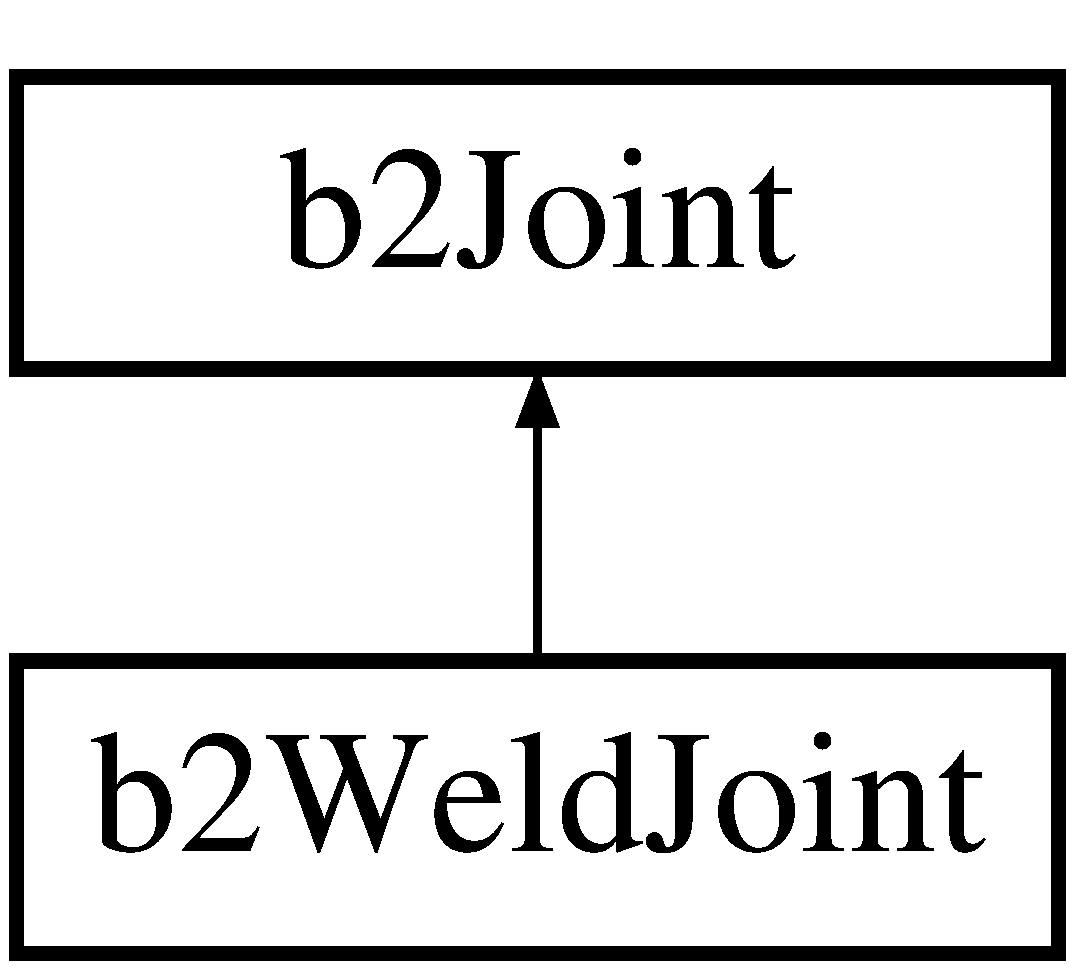
\includegraphics[height=2.000000cm]{classb2_weld_joint}
\end{center}
\end{figure}
\subsection*{Public Member Functions}
\begin{DoxyCompactItemize}
\item 
\hyperlink{structb2_vec2}{b2\+Vec2} \hyperlink{classb2_weld_joint_a8550de74e174a08856bc4bc7a4853429}{Get\+AnchorA} () const \hypertarget{classb2_weld_joint_a8550de74e174a08856bc4bc7a4853429}{}\label{classb2_weld_joint_a8550de74e174a08856bc4bc7a4853429}

\begin{DoxyCompactList}\small\item\em Get the anchor point on bodyA in world coordinates. \end{DoxyCompactList}\item 
\hyperlink{structb2_vec2}{b2\+Vec2} \hyperlink{classb2_weld_joint_a2030794df9b2a3111bcf7a1eb0593960}{Get\+AnchorB} () const \hypertarget{classb2_weld_joint_a2030794df9b2a3111bcf7a1eb0593960}{}\label{classb2_weld_joint_a2030794df9b2a3111bcf7a1eb0593960}

\begin{DoxyCompactList}\small\item\em Get the anchor point on bodyB in world coordinates. \end{DoxyCompactList}\item 
\hyperlink{structb2_vec2}{b2\+Vec2} \hyperlink{classb2_weld_joint_a2ca6323d03b9fd4b591a0bfadddc25a8}{Get\+Reaction\+Force} (float32 inv\+\_\+dt) const \hypertarget{classb2_weld_joint_a2ca6323d03b9fd4b591a0bfadddc25a8}{}\label{classb2_weld_joint_a2ca6323d03b9fd4b591a0bfadddc25a8}

\begin{DoxyCompactList}\small\item\em Get the reaction force on bodyB at the joint anchor in Newtons. \end{DoxyCompactList}\item 
float32 \hyperlink{classb2_weld_joint_a7199b5cce47b29624b4b231d78af71a3}{Get\+Reaction\+Torque} (float32 inv\+\_\+dt) const \hypertarget{classb2_weld_joint_a7199b5cce47b29624b4b231d78af71a3}{}\label{classb2_weld_joint_a7199b5cce47b29624b4b231d78af71a3}

\begin{DoxyCompactList}\small\item\em Get the reaction torque on bodyB in N$\ast$m. \end{DoxyCompactList}\item 
const \hyperlink{structb2_vec2}{b2\+Vec2} \& \hyperlink{classb2_weld_joint_aaef4f238fb5badf1112321ba878e8b06}{Get\+Local\+AnchorA} () const \hypertarget{classb2_weld_joint_aaef4f238fb5badf1112321ba878e8b06}{}\label{classb2_weld_joint_aaef4f238fb5badf1112321ba878e8b06}

\begin{DoxyCompactList}\small\item\em The local anchor point relative to bodyA\textquotesingle{}s origin. \end{DoxyCompactList}\item 
const \hyperlink{structb2_vec2}{b2\+Vec2} \& \hyperlink{classb2_weld_joint_a7fdc0c047dc04bbc8c5ca67011be071c}{Get\+Local\+AnchorB} () const \hypertarget{classb2_weld_joint_a7fdc0c047dc04bbc8c5ca67011be071c}{}\label{classb2_weld_joint_a7fdc0c047dc04bbc8c5ca67011be071c}

\begin{DoxyCompactList}\small\item\em The local anchor point relative to bodyB\textquotesingle{}s origin. \end{DoxyCompactList}\item 
float32 \hyperlink{classb2_weld_joint_a0d347bf22be13aa8a96f615e230b095a}{Get\+Reference\+Angle} () const \hypertarget{classb2_weld_joint_a0d347bf22be13aa8a96f615e230b095a}{}\label{classb2_weld_joint_a0d347bf22be13aa8a96f615e230b095a}

\begin{DoxyCompactList}\small\item\em Get the reference angle. \end{DoxyCompactList}\item 
void \hyperlink{classb2_weld_joint_a0796404379b7562f1af557729085c447}{Set\+Frequency} (float32 hz)\hypertarget{classb2_weld_joint_a0796404379b7562f1af557729085c447}{}\label{classb2_weld_joint_a0796404379b7562f1af557729085c447}

\begin{DoxyCompactList}\small\item\em Set/get frequency in Hz. \end{DoxyCompactList}\item 
float32 {\bfseries Get\+Frequency} () const \hypertarget{classb2_weld_joint_aca7b913d9d780a8fbd8c47f9fef04b7c}{}\label{classb2_weld_joint_aca7b913d9d780a8fbd8c47f9fef04b7c}

\item 
void \hyperlink{classb2_weld_joint_aea79865e590edba09eff9d2243689967}{Set\+Damping\+Ratio} (float32 ratio)\hypertarget{classb2_weld_joint_aea79865e590edba09eff9d2243689967}{}\label{classb2_weld_joint_aea79865e590edba09eff9d2243689967}

\begin{DoxyCompactList}\small\item\em Set/get damping ratio. \end{DoxyCompactList}\item 
float32 {\bfseries Get\+Damping\+Ratio} () const \hypertarget{classb2_weld_joint_a99f69fbebb982382819f2955819196d7}{}\label{classb2_weld_joint_a99f69fbebb982382819f2955819196d7}

\item 
void \hyperlink{classb2_weld_joint_a2fd073c5e6264e98592240308a006981}{Dump} ()\hypertarget{classb2_weld_joint_a2fd073c5e6264e98592240308a006981}{}\label{classb2_weld_joint_a2fd073c5e6264e98592240308a006981}

\begin{DoxyCompactList}\small\item\em Dump to b2\+Log. \end{DoxyCompactList}\end{DoxyCompactItemize}
\subsection*{Protected Member Functions}
\begin{DoxyCompactItemize}
\item 
{\bfseries b2\+Weld\+Joint} (const \hyperlink{structb2_weld_joint_def}{b2\+Weld\+Joint\+Def} $\ast$def)\hypertarget{classb2_weld_joint_a84dbb52e983d9039eab6ad64ae62d8eb}{}\label{classb2_weld_joint_a84dbb52e983d9039eab6ad64ae62d8eb}

\item 
void {\bfseries Init\+Velocity\+Constraints} (const \hyperlink{structb2_solver_data}{b2\+Solver\+Data} \&data)\hypertarget{classb2_weld_joint_aaf86660bd6dc87dc817c7be675b118e4}{}\label{classb2_weld_joint_aaf86660bd6dc87dc817c7be675b118e4}

\item 
void {\bfseries Solve\+Velocity\+Constraints} (const \hyperlink{structb2_solver_data}{b2\+Solver\+Data} \&data)\hypertarget{classb2_weld_joint_a5c30276fbd7ad15f2641bc571fd97596}{}\label{classb2_weld_joint_a5c30276fbd7ad15f2641bc571fd97596}

\item 
bool {\bfseries Solve\+Position\+Constraints} (const \hyperlink{structb2_solver_data}{b2\+Solver\+Data} \&data)\hypertarget{classb2_weld_joint_a21253196937e3f9f6227931dd08d80a3}{}\label{classb2_weld_joint_a21253196937e3f9f6227931dd08d80a3}

\end{DoxyCompactItemize}
\subsection*{Protected Attributes}
\begin{DoxyCompactItemize}
\item 
float32 {\bfseries m\+\_\+frequency\+Hz}\hypertarget{classb2_weld_joint_aa3cd6f08f509f67ad068d0ded7df9f21}{}\label{classb2_weld_joint_aa3cd6f08f509f67ad068d0ded7df9f21}

\item 
float32 {\bfseries m\+\_\+damping\+Ratio}\hypertarget{classb2_weld_joint_a4a730af358f79a6ccd7641e198eb5c7b}{}\label{classb2_weld_joint_a4a730af358f79a6ccd7641e198eb5c7b}

\item 
float32 {\bfseries m\+\_\+bias}\hypertarget{classb2_weld_joint_af54a943c1476e6a7c7bcfdf6cf568ba3}{}\label{classb2_weld_joint_af54a943c1476e6a7c7bcfdf6cf568ba3}

\item 
\hyperlink{structb2_vec2}{b2\+Vec2} {\bfseries m\+\_\+local\+AnchorA}\hypertarget{classb2_weld_joint_a572689c5f8c3df6902d64c56a2bb88f2}{}\label{classb2_weld_joint_a572689c5f8c3df6902d64c56a2bb88f2}

\item 
\hyperlink{structb2_vec2}{b2\+Vec2} {\bfseries m\+\_\+local\+AnchorB}\hypertarget{classb2_weld_joint_a39854cb14c83f88ec65d232b08e70704}{}\label{classb2_weld_joint_a39854cb14c83f88ec65d232b08e70704}

\item 
float32 {\bfseries m\+\_\+reference\+Angle}\hypertarget{classb2_weld_joint_a77639b3636192d6ac7083b33394ae943}{}\label{classb2_weld_joint_a77639b3636192d6ac7083b33394ae943}

\item 
float32 {\bfseries m\+\_\+gamma}\hypertarget{classb2_weld_joint_a29a8fc5e8efa796f7a7b439b4978f716}{}\label{classb2_weld_joint_a29a8fc5e8efa796f7a7b439b4978f716}

\item 
\hyperlink{structb2_vec3}{b2\+Vec3} {\bfseries m\+\_\+impulse}\hypertarget{classb2_weld_joint_a47db737b0d94628e7839718cf91cf762}{}\label{classb2_weld_joint_a47db737b0d94628e7839718cf91cf762}

\item 
int32 {\bfseries m\+\_\+indexA}\hypertarget{classb2_weld_joint_a4a3aa65b0a4669478db292f6765b03dd}{}\label{classb2_weld_joint_a4a3aa65b0a4669478db292f6765b03dd}

\item 
int32 {\bfseries m\+\_\+indexB}\hypertarget{classb2_weld_joint_a6e2aa1c13e8c96d9bbbdc6aae6b8e342}{}\label{classb2_weld_joint_a6e2aa1c13e8c96d9bbbdc6aae6b8e342}

\item 
\hyperlink{structb2_vec2}{b2\+Vec2} {\bfseries m\+\_\+rA}\hypertarget{classb2_weld_joint_abfbbe893b469c6855b297bdd768ba6fe}{}\label{classb2_weld_joint_abfbbe893b469c6855b297bdd768ba6fe}

\item 
\hyperlink{structb2_vec2}{b2\+Vec2} {\bfseries m\+\_\+rB}\hypertarget{classb2_weld_joint_a2a2af228eb5c2cd38e8baf77098cc3b0}{}\label{classb2_weld_joint_a2a2af228eb5c2cd38e8baf77098cc3b0}

\item 
\hyperlink{structb2_vec2}{b2\+Vec2} {\bfseries m\+\_\+local\+CenterA}\hypertarget{classb2_weld_joint_a18360f1e82a3a4e4fdfb3e6cba85160c}{}\label{classb2_weld_joint_a18360f1e82a3a4e4fdfb3e6cba85160c}

\item 
\hyperlink{structb2_vec2}{b2\+Vec2} {\bfseries m\+\_\+local\+CenterB}\hypertarget{classb2_weld_joint_a71281fbd18892e3f9653490bf85a844a}{}\label{classb2_weld_joint_a71281fbd18892e3f9653490bf85a844a}

\item 
float32 {\bfseries m\+\_\+inv\+MassA}\hypertarget{classb2_weld_joint_abb8cd34e03146dbae6af123ed75c2ee5}{}\label{classb2_weld_joint_abb8cd34e03146dbae6af123ed75c2ee5}

\item 
float32 {\bfseries m\+\_\+inv\+MassB}\hypertarget{classb2_weld_joint_a071f8b347a1167adb144a575749b6fc5}{}\label{classb2_weld_joint_a071f8b347a1167adb144a575749b6fc5}

\item 
float32 {\bfseries m\+\_\+inv\+IA}\hypertarget{classb2_weld_joint_af1420cccbd68021c24cc279bf55fabb9}{}\label{classb2_weld_joint_af1420cccbd68021c24cc279bf55fabb9}

\item 
float32 {\bfseries m\+\_\+inv\+IB}\hypertarget{classb2_weld_joint_a25dc4f3e300ee00a29ca141ac6d894fa}{}\label{classb2_weld_joint_a25dc4f3e300ee00a29ca141ac6d894fa}

\item 
\hyperlink{structb2_mat33}{b2\+Mat33} {\bfseries m\+\_\+mass}\hypertarget{classb2_weld_joint_ad07c6f68bd3ee2d62e4a8d656d526cf3}{}\label{classb2_weld_joint_ad07c6f68bd3ee2d62e4a8d656d526cf3}

\end{DoxyCompactItemize}
\subsection*{Friends}
\begin{DoxyCompactItemize}
\item 
class {\bfseries b2\+Joint}\hypertarget{classb2_weld_joint_a54ade8ed3d794298108d7f4c4e4793fa}{}\label{classb2_weld_joint_a54ade8ed3d794298108d7f4c4e4793fa}

\end{DoxyCompactItemize}
\subsection*{Additional Inherited Members}


\subsection{Detailed Description}
A weld joint essentially glues two bodies together. A weld joint may distort somewhat because the island constraint solver is approximate. 

The documentation for this class was generated from the following file\+:\begin{DoxyCompactItemize}
\item 
Commun/\+Externe/\+Box2\+D/include/\+Box2\+D/\+Dynamics/\+Joints/b2\+Weld\+Joint.\+h\end{DoxyCompactItemize}

\hypertarget{structb2_weld_joint_def}{}\section{b2\+Weld\+Joint\+Def Struct Reference}
\label{structb2_weld_joint_def}\index{b2\+Weld\+Joint\+Def@{b2\+Weld\+Joint\+Def}}


{\ttfamily \#include $<$b2\+Weld\+Joint.\+h$>$}

Inheritance diagram for b2\+Weld\+Joint\+Def\+:\begin{figure}[H]
\begin{center}
\leavevmode
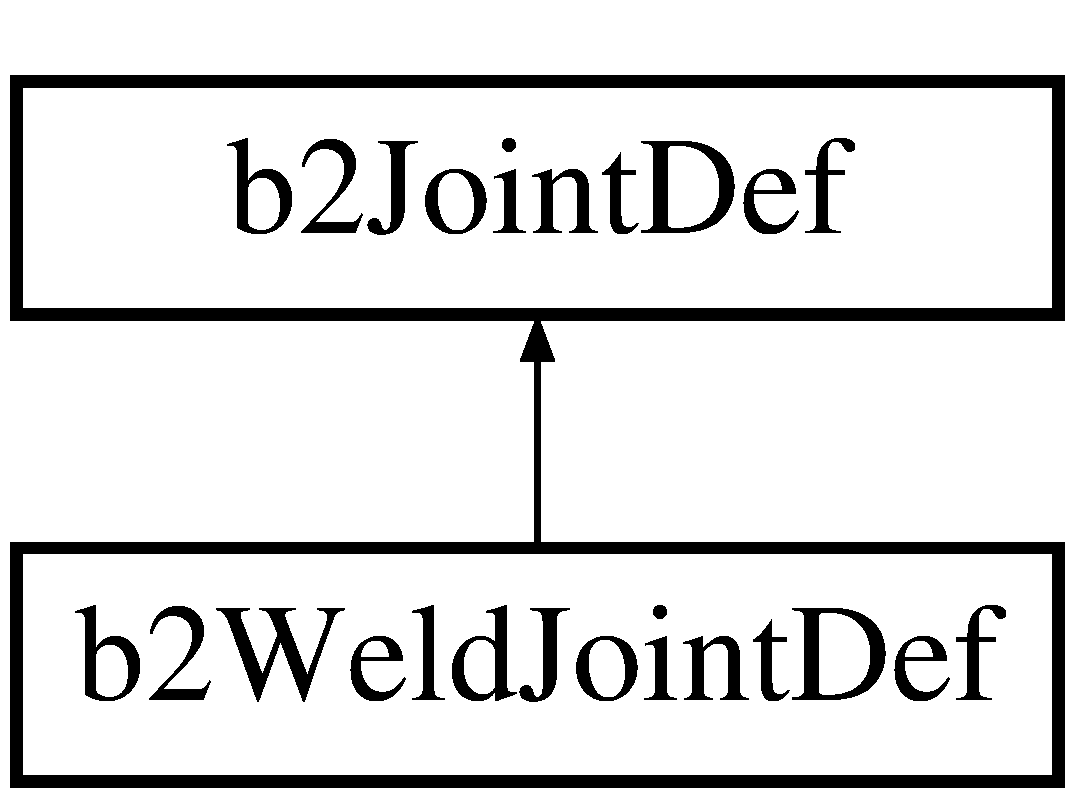
\includegraphics[height=2.000000cm]{structb2_weld_joint_def}
\end{center}
\end{figure}
\subsection*{Public Member Functions}
\begin{DoxyCompactItemize}
\item 
void \hyperlink{structb2_weld_joint_def_a9f6592c2a7eba6ce6e07e40c4e82aab5}{Initialize} (\hyperlink{classb2_body}{b2\+Body} $\ast$\hyperlink{structb2_joint_def_a8cd54c93da396be75a9788f2c6897f05}{bodyA}, \hyperlink{classb2_body}{b2\+Body} $\ast$\hyperlink{structb2_joint_def_aa4f4dee2fbcd12187b19506b60e68e3d}{bodyB}, const \hyperlink{structb2_vec2}{b2\+Vec2} \&anchor)
\end{DoxyCompactItemize}
\subsection*{Public Attributes}
\begin{DoxyCompactItemize}
\item 
\hyperlink{structb2_vec2}{b2\+Vec2} \hyperlink{structb2_weld_joint_def_a3b04af6164bb32efc3f5cf3e8d2b7109}{local\+AnchorA}\hypertarget{structb2_weld_joint_def_a3b04af6164bb32efc3f5cf3e8d2b7109}{}\label{structb2_weld_joint_def_a3b04af6164bb32efc3f5cf3e8d2b7109}

\begin{DoxyCompactList}\small\item\em The local anchor point relative to bodyA\textquotesingle{}s origin. \end{DoxyCompactList}\item 
\hyperlink{structb2_vec2}{b2\+Vec2} \hyperlink{structb2_weld_joint_def_a528262b92dac10de37411ad8c5637149}{local\+AnchorB}\hypertarget{structb2_weld_joint_def_a528262b92dac10de37411ad8c5637149}{}\label{structb2_weld_joint_def_a528262b92dac10de37411ad8c5637149}

\begin{DoxyCompactList}\small\item\em The local anchor point relative to bodyB\textquotesingle{}s origin. \end{DoxyCompactList}\item 
float32 \hyperlink{structb2_weld_joint_def_a31aeb208f15842091c55e3f1bab6d8f1}{reference\+Angle}\hypertarget{structb2_weld_joint_def_a31aeb208f15842091c55e3f1bab6d8f1}{}\label{structb2_weld_joint_def_a31aeb208f15842091c55e3f1bab6d8f1}

\begin{DoxyCompactList}\small\item\em The bodyB angle minus bodyA angle in the reference state (radians). \end{DoxyCompactList}\item 
float32 \hyperlink{structb2_weld_joint_def_abf42ce852914af845e9203b341f55c87}{frequency\+Hz}
\item 
float32 \hyperlink{structb2_weld_joint_def_ace1f0131610f14558f3dbaaed7b10e24}{damping\+Ratio}\hypertarget{structb2_weld_joint_def_ace1f0131610f14558f3dbaaed7b10e24}{}\label{structb2_weld_joint_def_ace1f0131610f14558f3dbaaed7b10e24}

\begin{DoxyCompactList}\small\item\em The damping ratio. 0 = no damping, 1 = critical damping. \end{DoxyCompactList}\end{DoxyCompactItemize}


\subsection{Detailed Description}
Weld joint definition. You need to specify local anchor points where they are attached and the relative body angle. The position of the anchor points is important for computing the reaction torque. 

\subsection{Member Function Documentation}
\index{b2\+Weld\+Joint\+Def@{b2\+Weld\+Joint\+Def}!Initialize@{Initialize}}
\index{Initialize@{Initialize}!b2\+Weld\+Joint\+Def@{b2\+Weld\+Joint\+Def}}
\subsubsection[{\texorpdfstring{Initialize(b2\+Body $\ast$body\+A, b2\+Body $\ast$body\+B, const b2\+Vec2 \&anchor)}{Initialize(b2Body *bodyA, b2Body *bodyB, const b2Vec2 &anchor)}}]{\setlength{\rightskip}{0pt plus 5cm}void b2\+Weld\+Joint\+Def\+::\+Initialize (
\begin{DoxyParamCaption}
\item[{{\bf b2\+Body} $\ast$}]{bodyA, }
\item[{{\bf b2\+Body} $\ast$}]{bodyB, }
\item[{const {\bf b2\+Vec2} \&}]{anchor}
\end{DoxyParamCaption}
)}\hypertarget{structb2_weld_joint_def_a9f6592c2a7eba6ce6e07e40c4e82aab5}{}\label{structb2_weld_joint_def_a9f6592c2a7eba6ce6e07e40c4e82aab5}
Initialize the bodies, anchors, and reference angle using a world anchor point. 

\subsection{Member Data Documentation}
\index{b2\+Weld\+Joint\+Def@{b2\+Weld\+Joint\+Def}!frequency\+Hz@{frequency\+Hz}}
\index{frequency\+Hz@{frequency\+Hz}!b2\+Weld\+Joint\+Def@{b2\+Weld\+Joint\+Def}}
\subsubsection[{\texorpdfstring{frequency\+Hz}{frequencyHz}}]{\setlength{\rightskip}{0pt plus 5cm}float32 b2\+Weld\+Joint\+Def\+::frequency\+Hz}\hypertarget{structb2_weld_joint_def_abf42ce852914af845e9203b341f55c87}{}\label{structb2_weld_joint_def_abf42ce852914af845e9203b341f55c87}
The mass-\/spring-\/damper frequency in Hertz. Rotation only. Disable softness with a value of 0. 

The documentation for this struct was generated from the following file\+:\begin{DoxyCompactItemize}
\item 
C\+:/\+Users/\+Bilal Itani/\+Desktop/inf2990-\/11/\+Cadriciel/\+Commun/\+Externe/\+Box2\+D/include/\+Box2\+D/\+Dynamics/\+Joints/b2\+Weld\+Joint.\+h\end{DoxyCompactItemize}

\hypertarget{classb2_wheel_joint}{}\section{b2\+Wheel\+Joint Class Reference}
\label{classb2_wheel_joint}\index{b2\+Wheel\+Joint@{b2\+Wheel\+Joint}}


{\ttfamily \#include $<$b2\+Wheel\+Joint.\+h$>$}

Inheritance diagram for b2\+Wheel\+Joint\+:\begin{figure}[H]
\begin{center}
\leavevmode
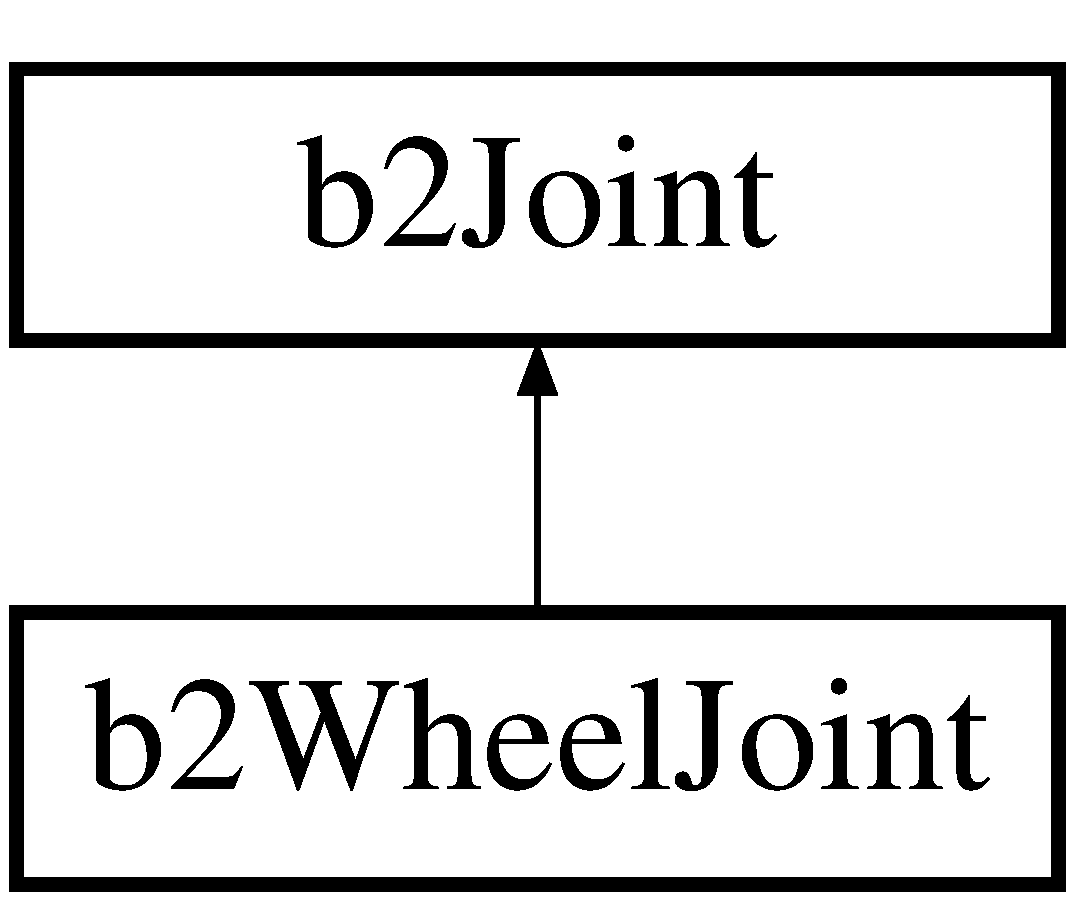
\includegraphics[height=2.000000cm]{classb2_wheel_joint}
\end{center}
\end{figure}
\subsection*{Public Member Functions}
\begin{DoxyCompactItemize}
\item 
\hyperlink{structb2_vec2}{b2\+Vec2} \hyperlink{classb2_wheel_joint_a6499dcd788d29f06c2e1b28c755e01c8}{Get\+AnchorA} () const \hypertarget{classb2_wheel_joint_a6499dcd788d29f06c2e1b28c755e01c8}{}\label{classb2_wheel_joint_a6499dcd788d29f06c2e1b28c755e01c8}

\begin{DoxyCompactList}\small\item\em Get the anchor point on bodyA in world coordinates. \end{DoxyCompactList}\item 
\hyperlink{structb2_vec2}{b2\+Vec2} \hyperlink{classb2_wheel_joint_ace182061f7f78ac2ec3f957a763ca5d3}{Get\+AnchorB} () const \hypertarget{classb2_wheel_joint_ace182061f7f78ac2ec3f957a763ca5d3}{}\label{classb2_wheel_joint_ace182061f7f78ac2ec3f957a763ca5d3}

\begin{DoxyCompactList}\small\item\em Get the anchor point on bodyB in world coordinates. \end{DoxyCompactList}\item 
\hyperlink{structb2_vec2}{b2\+Vec2} \hyperlink{classb2_wheel_joint_aa16e3a1c0246017bc25e72cf494daa42}{Get\+Reaction\+Force} (float32 inv\+\_\+dt) const \hypertarget{classb2_wheel_joint_aa16e3a1c0246017bc25e72cf494daa42}{}\label{classb2_wheel_joint_aa16e3a1c0246017bc25e72cf494daa42}

\begin{DoxyCompactList}\small\item\em Get the reaction force on bodyB at the joint anchor in Newtons. \end{DoxyCompactList}\item 
float32 \hyperlink{classb2_wheel_joint_ae88eeec295a19f216acab9b23d9c704b}{Get\+Reaction\+Torque} (float32 inv\+\_\+dt) const \hypertarget{classb2_wheel_joint_ae88eeec295a19f216acab9b23d9c704b}{}\label{classb2_wheel_joint_ae88eeec295a19f216acab9b23d9c704b}

\begin{DoxyCompactList}\small\item\em Get the reaction torque on bodyB in N$\ast$m. \end{DoxyCompactList}\item 
const \hyperlink{structb2_vec2}{b2\+Vec2} \& \hyperlink{classb2_wheel_joint_abf725ee0fa640d1b9374283f6f50e82d}{Get\+Local\+AnchorA} () const \hypertarget{classb2_wheel_joint_abf725ee0fa640d1b9374283f6f50e82d}{}\label{classb2_wheel_joint_abf725ee0fa640d1b9374283f6f50e82d}

\begin{DoxyCompactList}\small\item\em The local anchor point relative to bodyA\textquotesingle{}s origin. \end{DoxyCompactList}\item 
const \hyperlink{structb2_vec2}{b2\+Vec2} \& \hyperlink{classb2_wheel_joint_a38313bcd5d5a91f190956086b9d9b8e5}{Get\+Local\+AnchorB} () const \hypertarget{classb2_wheel_joint_a38313bcd5d5a91f190956086b9d9b8e5}{}\label{classb2_wheel_joint_a38313bcd5d5a91f190956086b9d9b8e5}

\begin{DoxyCompactList}\small\item\em The local anchor point relative to bodyB\textquotesingle{}s origin. \end{DoxyCompactList}\item 
const \hyperlink{structb2_vec2}{b2\+Vec2} \& \hyperlink{classb2_wheel_joint_a03c1a1cf19dbada68630aa3cbf970a55}{Get\+Local\+AxisA} () const \hypertarget{classb2_wheel_joint_a03c1a1cf19dbada68630aa3cbf970a55}{}\label{classb2_wheel_joint_a03c1a1cf19dbada68630aa3cbf970a55}

\begin{DoxyCompactList}\small\item\em The local joint axis relative to bodyA. \end{DoxyCompactList}\item 
float32 \hyperlink{classb2_wheel_joint_abc3791f9c8139e5c5ba0fb72d5c7f9df}{Get\+Joint\+Translation} () const \hypertarget{classb2_wheel_joint_abc3791f9c8139e5c5ba0fb72d5c7f9df}{}\label{classb2_wheel_joint_abc3791f9c8139e5c5ba0fb72d5c7f9df}

\begin{DoxyCompactList}\small\item\em Get the current joint translation, usually in meters. \end{DoxyCompactList}\item 
float32 \hyperlink{classb2_wheel_joint_a398bc3a1f807905e0923cc7d9bff640d}{Get\+Joint\+Speed} () const \hypertarget{classb2_wheel_joint_a398bc3a1f807905e0923cc7d9bff640d}{}\label{classb2_wheel_joint_a398bc3a1f807905e0923cc7d9bff640d}

\begin{DoxyCompactList}\small\item\em Get the current joint translation speed, usually in meters per second. \end{DoxyCompactList}\item 
bool \hyperlink{classb2_wheel_joint_a419bc80e17cc4c1062a692ea79396d19}{Is\+Motor\+Enabled} () const \hypertarget{classb2_wheel_joint_a419bc80e17cc4c1062a692ea79396d19}{}\label{classb2_wheel_joint_a419bc80e17cc4c1062a692ea79396d19}

\begin{DoxyCompactList}\small\item\em Is the joint motor enabled? \end{DoxyCompactList}\item 
void \hyperlink{classb2_wheel_joint_a7a832d814bdda135a78fad41ba671da6}{Enable\+Motor} (bool flag)\hypertarget{classb2_wheel_joint_a7a832d814bdda135a78fad41ba671da6}{}\label{classb2_wheel_joint_a7a832d814bdda135a78fad41ba671da6}

\begin{DoxyCompactList}\small\item\em Enable/disable the joint motor. \end{DoxyCompactList}\item 
void \hyperlink{classb2_wheel_joint_a6e3255fcf5c82b979ad7e3dc1c089c0b}{Set\+Motor\+Speed} (float32 speed)\hypertarget{classb2_wheel_joint_a6e3255fcf5c82b979ad7e3dc1c089c0b}{}\label{classb2_wheel_joint_a6e3255fcf5c82b979ad7e3dc1c089c0b}

\begin{DoxyCompactList}\small\item\em Set the motor speed, usually in radians per second. \end{DoxyCompactList}\item 
float32 \hyperlink{classb2_wheel_joint_acc7a31fdd444614ba1943f57f0c6ac5a}{Get\+Motor\+Speed} () const \hypertarget{classb2_wheel_joint_acc7a31fdd444614ba1943f57f0c6ac5a}{}\label{classb2_wheel_joint_acc7a31fdd444614ba1943f57f0c6ac5a}

\begin{DoxyCompactList}\small\item\em Get the motor speed, usually in radians per second. \end{DoxyCompactList}\item 
void \hyperlink{classb2_wheel_joint_a8aae3cd624ec9d48fc86c325c4595edc}{Set\+Max\+Motor\+Torque} (float32 torque)\hypertarget{classb2_wheel_joint_a8aae3cd624ec9d48fc86c325c4595edc}{}\label{classb2_wheel_joint_a8aae3cd624ec9d48fc86c325c4595edc}

\begin{DoxyCompactList}\small\item\em Set/\+Get the maximum motor force, usually in N-\/m. \end{DoxyCompactList}\item 
float32 {\bfseries Get\+Max\+Motor\+Torque} () const \hypertarget{classb2_wheel_joint_ad2d9fb270f0a62cd87234d3ce55626f3}{}\label{classb2_wheel_joint_ad2d9fb270f0a62cd87234d3ce55626f3}

\item 
float32 \hyperlink{classb2_wheel_joint_a4fbfb199ed267f7a2fad934cd2f4fbdc}{Get\+Motor\+Torque} (float32 inv\+\_\+dt) const \hypertarget{classb2_wheel_joint_a4fbfb199ed267f7a2fad934cd2f4fbdc}{}\label{classb2_wheel_joint_a4fbfb199ed267f7a2fad934cd2f4fbdc}

\begin{DoxyCompactList}\small\item\em Get the current motor torque given the inverse time step, usually in N-\/m. \end{DoxyCompactList}\item 
void \hyperlink{classb2_wheel_joint_af9f8fada5cb30f83aa2fbf486e9d347b}{Set\+Spring\+Frequency\+Hz} (float32 hz)\hypertarget{classb2_wheel_joint_af9f8fada5cb30f83aa2fbf486e9d347b}{}\label{classb2_wheel_joint_af9f8fada5cb30f83aa2fbf486e9d347b}

\begin{DoxyCompactList}\small\item\em Set/\+Get the spring frequency in hertz. Setting the frequency to zero disables the spring. \end{DoxyCompactList}\item 
float32 {\bfseries Get\+Spring\+Frequency\+Hz} () const \hypertarget{classb2_wheel_joint_a475fe44e145a7e3869c0a0ff5602bb20}{}\label{classb2_wheel_joint_a475fe44e145a7e3869c0a0ff5602bb20}

\item 
void \hyperlink{classb2_wheel_joint_a39b123ac045c8ec93faa65746e6655dc}{Set\+Spring\+Damping\+Ratio} (float32 ratio)\hypertarget{classb2_wheel_joint_a39b123ac045c8ec93faa65746e6655dc}{}\label{classb2_wheel_joint_a39b123ac045c8ec93faa65746e6655dc}

\begin{DoxyCompactList}\small\item\em Set/\+Get the spring damping ratio. \end{DoxyCompactList}\item 
float32 {\bfseries Get\+Spring\+Damping\+Ratio} () const \hypertarget{classb2_wheel_joint_ad991b903dd8b3820dfe3a2263b89f5aa}{}\label{classb2_wheel_joint_ad991b903dd8b3820dfe3a2263b89f5aa}

\item 
void \hyperlink{classb2_wheel_joint_a09534b6f4c5d0254711e0bcc7cf3b0e4}{Dump} ()\hypertarget{classb2_wheel_joint_a09534b6f4c5d0254711e0bcc7cf3b0e4}{}\label{classb2_wheel_joint_a09534b6f4c5d0254711e0bcc7cf3b0e4}

\begin{DoxyCompactList}\small\item\em Dump to b2\+Log. \end{DoxyCompactList}\end{DoxyCompactItemize}
\subsection*{Protected Member Functions}
\begin{DoxyCompactItemize}
\item 
{\bfseries b2\+Wheel\+Joint} (const \hyperlink{structb2_wheel_joint_def}{b2\+Wheel\+Joint\+Def} $\ast$def)\hypertarget{classb2_wheel_joint_a9c8bbb1068ddb46d074fe91802dd6a39}{}\label{classb2_wheel_joint_a9c8bbb1068ddb46d074fe91802dd6a39}

\item 
void {\bfseries Init\+Velocity\+Constraints} (const \hyperlink{structb2_solver_data}{b2\+Solver\+Data} \&data)\hypertarget{classb2_wheel_joint_af3fc35c89dc253661297d69fe4a00a97}{}\label{classb2_wheel_joint_af3fc35c89dc253661297d69fe4a00a97}

\item 
void {\bfseries Solve\+Velocity\+Constraints} (const \hyperlink{structb2_solver_data}{b2\+Solver\+Data} \&data)\hypertarget{classb2_wheel_joint_a09283ebe01298e6a2e897ca409b70289}{}\label{classb2_wheel_joint_a09283ebe01298e6a2e897ca409b70289}

\item 
bool {\bfseries Solve\+Position\+Constraints} (const \hyperlink{structb2_solver_data}{b2\+Solver\+Data} \&data)\hypertarget{classb2_wheel_joint_ae14faaa2cd91bdea615e86c0dd2ccc97}{}\label{classb2_wheel_joint_ae14faaa2cd91bdea615e86c0dd2ccc97}

\end{DoxyCompactItemize}
\subsection*{Protected Attributes}
\begin{DoxyCompactItemize}
\item 
float32 {\bfseries m\+\_\+frequency\+Hz}\hypertarget{classb2_wheel_joint_a0570ebb1228c2baca4630c53b77792fa}{}\label{classb2_wheel_joint_a0570ebb1228c2baca4630c53b77792fa}

\item 
float32 {\bfseries m\+\_\+damping\+Ratio}\hypertarget{classb2_wheel_joint_a712554f6a298cf8a69bbf546fa465843}{}\label{classb2_wheel_joint_a712554f6a298cf8a69bbf546fa465843}

\item 
\hyperlink{structb2_vec2}{b2\+Vec2} {\bfseries m\+\_\+local\+AnchorA}\hypertarget{classb2_wheel_joint_a9911353143312dc352928a80c63813c8}{}\label{classb2_wheel_joint_a9911353143312dc352928a80c63813c8}

\item 
\hyperlink{structb2_vec2}{b2\+Vec2} {\bfseries m\+\_\+local\+AnchorB}\hypertarget{classb2_wheel_joint_a1bc3fa1a0bad5eb2cc7b9962976c1d29}{}\label{classb2_wheel_joint_a1bc3fa1a0bad5eb2cc7b9962976c1d29}

\item 
\hyperlink{structb2_vec2}{b2\+Vec2} {\bfseries m\+\_\+local\+X\+AxisA}\hypertarget{classb2_wheel_joint_ae1cadd777bdffbb726b15c438e081c21}{}\label{classb2_wheel_joint_ae1cadd777bdffbb726b15c438e081c21}

\item 
\hyperlink{structb2_vec2}{b2\+Vec2} {\bfseries m\+\_\+local\+Y\+AxisA}\hypertarget{classb2_wheel_joint_a5e9566b969c24428d32ff2069d4180e3}{}\label{classb2_wheel_joint_a5e9566b969c24428d32ff2069d4180e3}

\item 
float32 {\bfseries m\+\_\+impulse}\hypertarget{classb2_wheel_joint_a81a874642cc60caa2eb212eda3b266f0}{}\label{classb2_wheel_joint_a81a874642cc60caa2eb212eda3b266f0}

\item 
float32 {\bfseries m\+\_\+motor\+Impulse}\hypertarget{classb2_wheel_joint_a1116db6834e3b62a651558f6bdfe000e}{}\label{classb2_wheel_joint_a1116db6834e3b62a651558f6bdfe000e}

\item 
float32 {\bfseries m\+\_\+spring\+Impulse}\hypertarget{classb2_wheel_joint_a83aa86813105dc1189fed8acf1767eb5}{}\label{classb2_wheel_joint_a83aa86813105dc1189fed8acf1767eb5}

\item 
float32 {\bfseries m\+\_\+max\+Motor\+Torque}\hypertarget{classb2_wheel_joint_ad671dcec7ecd41baf87200b2f9c37c34}{}\label{classb2_wheel_joint_ad671dcec7ecd41baf87200b2f9c37c34}

\item 
float32 {\bfseries m\+\_\+motor\+Speed}\hypertarget{classb2_wheel_joint_a29194860b36867eb4349eee73e8d5908}{}\label{classb2_wheel_joint_a29194860b36867eb4349eee73e8d5908}

\item 
bool {\bfseries m\+\_\+enable\+Motor}\hypertarget{classb2_wheel_joint_a46dae5c1e2630430ce7cf00dbccee8a1}{}\label{classb2_wheel_joint_a46dae5c1e2630430ce7cf00dbccee8a1}

\item 
int32 {\bfseries m\+\_\+indexA}\hypertarget{classb2_wheel_joint_a0924e1788c097b3b05eac9cd53d1d997}{}\label{classb2_wheel_joint_a0924e1788c097b3b05eac9cd53d1d997}

\item 
int32 {\bfseries m\+\_\+indexB}\hypertarget{classb2_wheel_joint_a76d74ec2f2bf7c941076c0e224c2a9e9}{}\label{classb2_wheel_joint_a76d74ec2f2bf7c941076c0e224c2a9e9}

\item 
\hyperlink{structb2_vec2}{b2\+Vec2} {\bfseries m\+\_\+local\+CenterA}\hypertarget{classb2_wheel_joint_a60c54ed81993fd710b9499f2d6bcc274}{}\label{classb2_wheel_joint_a60c54ed81993fd710b9499f2d6bcc274}

\item 
\hyperlink{structb2_vec2}{b2\+Vec2} {\bfseries m\+\_\+local\+CenterB}\hypertarget{classb2_wheel_joint_a7631ce1cbb3b7f33d304eb87a5413277}{}\label{classb2_wheel_joint_a7631ce1cbb3b7f33d304eb87a5413277}

\item 
float32 {\bfseries m\+\_\+inv\+MassA}\hypertarget{classb2_wheel_joint_affa854f7bdde3468b46f416836791192}{}\label{classb2_wheel_joint_affa854f7bdde3468b46f416836791192}

\item 
float32 {\bfseries m\+\_\+inv\+MassB}\hypertarget{classb2_wheel_joint_a8ca9663e91d3dd86bdb537248f09c5c7}{}\label{classb2_wheel_joint_a8ca9663e91d3dd86bdb537248f09c5c7}

\item 
float32 {\bfseries m\+\_\+inv\+IA}\hypertarget{classb2_wheel_joint_aa540d2ad4452012952fd42941eefa7d9}{}\label{classb2_wheel_joint_aa540d2ad4452012952fd42941eefa7d9}

\item 
float32 {\bfseries m\+\_\+inv\+IB}\hypertarget{classb2_wheel_joint_a6b76c82b51bdf6910d6c241146b1a696}{}\label{classb2_wheel_joint_a6b76c82b51bdf6910d6c241146b1a696}

\item 
\hyperlink{structb2_vec2}{b2\+Vec2} {\bfseries m\+\_\+ax}\hypertarget{classb2_wheel_joint_ae91286452d1941d4bed387bd7ee187c8}{}\label{classb2_wheel_joint_ae91286452d1941d4bed387bd7ee187c8}

\item 
\hyperlink{structb2_vec2}{b2\+Vec2} {\bfseries m\+\_\+ay}\hypertarget{classb2_wheel_joint_a2f3b7d45948c68e5c5dd8636ed8a8db1}{}\label{classb2_wheel_joint_a2f3b7d45948c68e5c5dd8636ed8a8db1}

\item 
float32 {\bfseries m\+\_\+s\+Ax}\hypertarget{classb2_wheel_joint_a0935bcd6aea2145f6c8e947159a1e59b}{}\label{classb2_wheel_joint_a0935bcd6aea2145f6c8e947159a1e59b}

\item 
float32 {\bfseries m\+\_\+s\+Bx}\hypertarget{classb2_wheel_joint_a0705a4e0dfd40bf25f518bb22d6e0177}{}\label{classb2_wheel_joint_a0705a4e0dfd40bf25f518bb22d6e0177}

\item 
float32 {\bfseries m\+\_\+s\+Ay}\hypertarget{classb2_wheel_joint_aaeb83f256ec67556cc1d7758f75b773e}{}\label{classb2_wheel_joint_aaeb83f256ec67556cc1d7758f75b773e}

\item 
float32 {\bfseries m\+\_\+s\+By}\hypertarget{classb2_wheel_joint_a4fa320609b2942eee344ac0d91003444}{}\label{classb2_wheel_joint_a4fa320609b2942eee344ac0d91003444}

\item 
float32 {\bfseries m\+\_\+mass}\hypertarget{classb2_wheel_joint_a80abc7c0fe5a4d6f362ec5cb13214ec1}{}\label{classb2_wheel_joint_a80abc7c0fe5a4d6f362ec5cb13214ec1}

\item 
float32 {\bfseries m\+\_\+motor\+Mass}\hypertarget{classb2_wheel_joint_a64d20e079b2638995c7faa5d3a2aed68}{}\label{classb2_wheel_joint_a64d20e079b2638995c7faa5d3a2aed68}

\item 
float32 {\bfseries m\+\_\+spring\+Mass}\hypertarget{classb2_wheel_joint_ab24b6e3ad48961de7d78e4476531dd30}{}\label{classb2_wheel_joint_ab24b6e3ad48961de7d78e4476531dd30}

\item 
float32 {\bfseries m\+\_\+bias}\hypertarget{classb2_wheel_joint_a82bec93fb4a2a3702455bede3d5c6ac8}{}\label{classb2_wheel_joint_a82bec93fb4a2a3702455bede3d5c6ac8}

\item 
float32 {\bfseries m\+\_\+gamma}\hypertarget{classb2_wheel_joint_a3d4c8b3e96b517d13693285e63a917fb}{}\label{classb2_wheel_joint_a3d4c8b3e96b517d13693285e63a917fb}

\end{DoxyCompactItemize}
\subsection*{Friends}
\begin{DoxyCompactItemize}
\item 
class {\bfseries b2\+Joint}\hypertarget{classb2_wheel_joint_a54ade8ed3d794298108d7f4c4e4793fa}{}\label{classb2_wheel_joint_a54ade8ed3d794298108d7f4c4e4793fa}

\end{DoxyCompactItemize}
\subsection*{Additional Inherited Members}


\subsection{Detailed Description}
A wheel joint. This joint provides two degrees of freedom\+: translation along an axis fixed in bodyA and rotation in the plane. You can use a joint limit to restrict the range of motion and a joint motor to drive the rotation or to model rotational friction. This joint is designed for vehicle suspensions. 

The documentation for this class was generated from the following file\+:\begin{DoxyCompactItemize}
\item 
Commun/\+Externe/\+Box2\+D/include/\+Box2\+D/\+Dynamics/\+Joints/b2\+Wheel\+Joint.\+h\end{DoxyCompactItemize}

\hypertarget{structb2_wheel_joint_def}{}\section{b2\+Wheel\+Joint\+Def Struct Reference}
\label{structb2_wheel_joint_def}\index{b2\+Wheel\+Joint\+Def@{b2\+Wheel\+Joint\+Def}}


{\ttfamily \#include $<$b2\+Wheel\+Joint.\+h$>$}

Inheritance diagram for b2\+Wheel\+Joint\+Def\+:\begin{figure}[H]
\begin{center}
\leavevmode
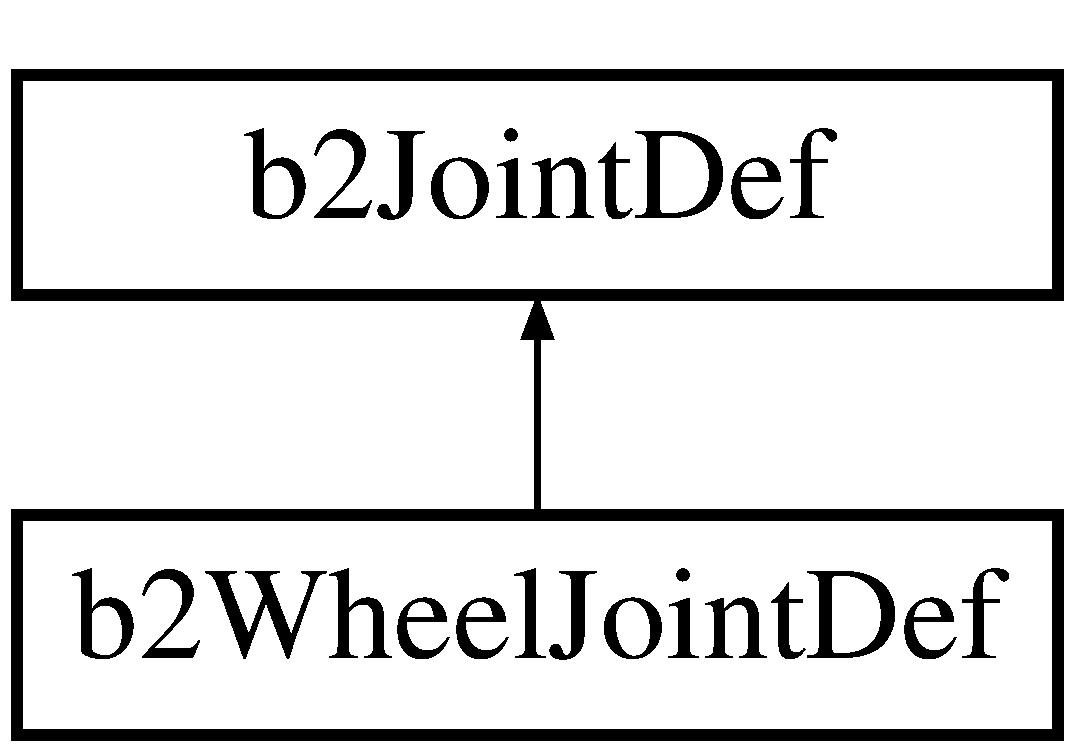
\includegraphics[height=2.000000cm]{structb2_wheel_joint_def}
\end{center}
\end{figure}
\subsection*{Public Member Functions}
\begin{DoxyCompactItemize}
\item 
void \hyperlink{structb2_wheel_joint_def_af26887092d36c3cd03898401a38783e2}{Initialize} (\hyperlink{classb2_body}{b2\+Body} $\ast$\hyperlink{structb2_joint_def_a8cd54c93da396be75a9788f2c6897f05}{bodyA}, \hyperlink{classb2_body}{b2\+Body} $\ast$\hyperlink{structb2_joint_def_aa4f4dee2fbcd12187b19506b60e68e3d}{bodyB}, const \hyperlink{structb2_vec2}{b2\+Vec2} \&anchor, const \hyperlink{structb2_vec2}{b2\+Vec2} \&axis)
\end{DoxyCompactItemize}
\subsection*{Public Attributes}
\begin{DoxyCompactItemize}
\item 
\hyperlink{structb2_vec2}{b2\+Vec2} \hyperlink{structb2_wheel_joint_def_a9429d2273bfdd8bdc0db416e73b89ae4}{local\+AnchorA}\hypertarget{structb2_wheel_joint_def_a9429d2273bfdd8bdc0db416e73b89ae4}{}\label{structb2_wheel_joint_def_a9429d2273bfdd8bdc0db416e73b89ae4}

\begin{DoxyCompactList}\small\item\em The local anchor point relative to bodyA\textquotesingle{}s origin. \end{DoxyCompactList}\item 
\hyperlink{structb2_vec2}{b2\+Vec2} \hyperlink{structb2_wheel_joint_def_a88ba0f7108076b9d7ced68425be95c27}{local\+AnchorB}\hypertarget{structb2_wheel_joint_def_a88ba0f7108076b9d7ced68425be95c27}{}\label{structb2_wheel_joint_def_a88ba0f7108076b9d7ced68425be95c27}

\begin{DoxyCompactList}\small\item\em The local anchor point relative to bodyB\textquotesingle{}s origin. \end{DoxyCompactList}\item 
\hyperlink{structb2_vec2}{b2\+Vec2} \hyperlink{structb2_wheel_joint_def_ad635ee7b77b50037dc0e021a0f5c93a6}{local\+AxisA}\hypertarget{structb2_wheel_joint_def_ad635ee7b77b50037dc0e021a0f5c93a6}{}\label{structb2_wheel_joint_def_ad635ee7b77b50037dc0e021a0f5c93a6}

\begin{DoxyCompactList}\small\item\em The local translation axis in bodyA. \end{DoxyCompactList}\item 
bool \hyperlink{structb2_wheel_joint_def_a8e7193d6c34c784ffd71e79d3a70acc6}{enable\+Motor}\hypertarget{structb2_wheel_joint_def_a8e7193d6c34c784ffd71e79d3a70acc6}{}\label{structb2_wheel_joint_def_a8e7193d6c34c784ffd71e79d3a70acc6}

\begin{DoxyCompactList}\small\item\em Enable/disable the joint motor. \end{DoxyCompactList}\item 
float32 \hyperlink{structb2_wheel_joint_def_ab658ce0fae40c6de09133659f7ffb829}{max\+Motor\+Torque}\hypertarget{structb2_wheel_joint_def_ab658ce0fae40c6de09133659f7ffb829}{}\label{structb2_wheel_joint_def_ab658ce0fae40c6de09133659f7ffb829}

\begin{DoxyCompactList}\small\item\em The maximum motor torque, usually in N-\/m. \end{DoxyCompactList}\item 
float32 \hyperlink{structb2_wheel_joint_def_a7248e25f2ca6b6c2a5f7079ce16e7748}{motor\+Speed}\hypertarget{structb2_wheel_joint_def_a7248e25f2ca6b6c2a5f7079ce16e7748}{}\label{structb2_wheel_joint_def_a7248e25f2ca6b6c2a5f7079ce16e7748}

\begin{DoxyCompactList}\small\item\em The desired motor speed in radians per second. \end{DoxyCompactList}\item 
float32 \hyperlink{structb2_wheel_joint_def_acf3540f46eaf3bc91426386939bd37b1}{frequency\+Hz}\hypertarget{structb2_wheel_joint_def_acf3540f46eaf3bc91426386939bd37b1}{}\label{structb2_wheel_joint_def_acf3540f46eaf3bc91426386939bd37b1}

\begin{DoxyCompactList}\small\item\em Suspension frequency, zero indicates no suspension. \end{DoxyCompactList}\item 
float32 \hyperlink{structb2_wheel_joint_def_a9976584bfee18b46dec355764797ce54}{damping\+Ratio}\hypertarget{structb2_wheel_joint_def_a9976584bfee18b46dec355764797ce54}{}\label{structb2_wheel_joint_def_a9976584bfee18b46dec355764797ce54}

\begin{DoxyCompactList}\small\item\em Suspension damping ratio, one indicates critical damping. \end{DoxyCompactList}\end{DoxyCompactItemize}


\subsection{Detailed Description}
Wheel joint definition. This requires defining a line of motion using an axis and an anchor point. The definition uses local anchor points and a local axis so that the initial configuration can violate the constraint slightly. The joint translation is zero when the local anchor points coincide in world space. Using local anchors and a local axis helps when saving and loading a game. 

\subsection{Member Function Documentation}
\index{b2\+Wheel\+Joint\+Def@{b2\+Wheel\+Joint\+Def}!Initialize@{Initialize}}
\index{Initialize@{Initialize}!b2\+Wheel\+Joint\+Def@{b2\+Wheel\+Joint\+Def}}
\subsubsection[{\texorpdfstring{Initialize(b2\+Body $\ast$body\+A, b2\+Body $\ast$body\+B, const b2\+Vec2 \&anchor, const b2\+Vec2 \&axis)}{Initialize(b2Body *bodyA, b2Body *bodyB, const b2Vec2 &anchor, const b2Vec2 &axis)}}]{\setlength{\rightskip}{0pt plus 5cm}void b2\+Wheel\+Joint\+Def\+::\+Initialize (
\begin{DoxyParamCaption}
\item[{{\bf b2\+Body} $\ast$}]{bodyA, }
\item[{{\bf b2\+Body} $\ast$}]{bodyB, }
\item[{const {\bf b2\+Vec2} \&}]{anchor, }
\item[{const {\bf b2\+Vec2} \&}]{axis}
\end{DoxyParamCaption}
)}\hypertarget{structb2_wheel_joint_def_af26887092d36c3cd03898401a38783e2}{}\label{structb2_wheel_joint_def_af26887092d36c3cd03898401a38783e2}
Initialize the bodies, anchors, axis, and reference angle using the world anchor and world axis. 

The documentation for this struct was generated from the following file\+:\begin{DoxyCompactItemize}
\item 
C\+:/\+Users/\+Bilal Itani/\+Desktop/inf2990-\/11/\+Cadriciel/\+Commun/\+Externe/\+Box2\+D/include/\+Box2\+D/\+Dynamics/\+Joints/b2\+Wheel\+Joint.\+h\end{DoxyCompactItemize}

\hypertarget{classb2_world}{}\section{b2\+World Class Reference}
\label{classb2_world}\index{b2\+World@{b2\+World}}


{\ttfamily \#include $<$b2\+World.\+h$>$}

\subsection*{Public Member Functions}
\begin{DoxyCompactItemize}
\item 
\hyperlink{classb2_world_aeccc87fd9e36702c821a8244ca7cd875}{b2\+World} (const \hyperlink{structb2_vec2}{b2\+Vec2} \&gravity)
\item 
\hyperlink{classb2_world_a5250ae4487475c33ccefdead07c768c8}{$\sim$b2\+World} ()\hypertarget{classb2_world_a5250ae4487475c33ccefdead07c768c8}{}\label{classb2_world_a5250ae4487475c33ccefdead07c768c8}

\begin{DoxyCompactList}\small\item\em Destruct the world. All physics entities are destroyed and all heap memory is released. \end{DoxyCompactList}\item 
void \hyperlink{classb2_world_ae377f2dd5512ada7d27f4ad3541c75bf}{Set\+Destruction\+Listener} (\hyperlink{classb2_destruction_listener}{b2\+Destruction\+Listener} $\ast$listener)
\item 
void \hyperlink{classb2_world_a85e6e1e911c7d6366f8c7d57a12b72ff}{Set\+Contact\+Filter} (\hyperlink{classb2_contact_filter}{b2\+Contact\+Filter} $\ast$filter)
\item 
void \hyperlink{classb2_world_a614549967fb8a1584b61c11e2d553d42}{Set\+Contact\+Listener} (\hyperlink{classb2_contact_listener}{b2\+Contact\+Listener} $\ast$listener)
\item 
void \hyperlink{classb2_world_a6976d2c67400df03c0d44174ffcfb7ee}{Set\+Debug\+Draw} (\hyperlink{classb2_draw}{b2\+Draw} $\ast$debug\+Draw)
\item 
\hyperlink{classb2_body}{b2\+Body} $\ast$ \hyperlink{classb2_world_a9323d553e4c132b26d8741b457d7c034}{Create\+Body} (const \hyperlink{structb2_body_def}{b2\+Body\+Def} $\ast$def)
\item 
void \hyperlink{classb2_world_ad52231ad7a9556ef5735ac79cbcd8fcf}{Destroy\+Body} (\hyperlink{classb2_body}{b2\+Body} $\ast$body)
\item 
\hyperlink{classb2_joint}{b2\+Joint} $\ast$ \hyperlink{classb2_world_a8a408c367fe133530f3e577c667d1efd}{Create\+Joint} (const \hyperlink{structb2_joint_def}{b2\+Joint\+Def} $\ast$def)
\item 
void \hyperlink{classb2_world_add5942aef171e54cfa384c8975746dca}{Destroy\+Joint} (\hyperlink{classb2_joint}{b2\+Joint} $\ast$joint)
\item 
void \hyperlink{classb2_world_a7a8eff61af98461f978fe43f3af7be90}{Step} (float32 time\+Step, int32 velocity\+Iterations, int32 position\+Iterations)
\item 
void \hyperlink{classb2_world_ac082ab4c4ad0b1c5ec4674315eeec643}{Clear\+Forces} ()
\item 
void \hyperlink{classb2_world_a293d9865e407fd463e168b0a29856acc}{Draw\+Debug\+Data} ()\hypertarget{classb2_world_a293d9865e407fd463e168b0a29856acc}{}\label{classb2_world_a293d9865e407fd463e168b0a29856acc}

\begin{DoxyCompactList}\small\item\em Call this to draw shapes and other debug draw data. This is intentionally non-\/const. \end{DoxyCompactList}\item 
void \hyperlink{classb2_world_a711e55d2c6e68400f93472f807c3775b}{Query\+A\+A\+BB} (\hyperlink{classb2_query_callback}{b2\+Query\+Callback} $\ast$callback, const \hyperlink{structb2_a_a_b_b}{b2\+A\+A\+BB} \&aabb) const 
\item 
void \hyperlink{classb2_world_ad902548be84df9cc36eced0f4c89ab0a}{Ray\+Cast} (\hyperlink{classb2_ray_cast_callback}{b2\+Ray\+Cast\+Callback} $\ast$callback, const \hyperlink{structb2_vec2}{b2\+Vec2} \&point1, const \hyperlink{structb2_vec2}{b2\+Vec2} \&point2) const 
\item 
\hyperlink{classb2_body}{b2\+Body} $\ast$ \hyperlink{classb2_world_a1b87c03955e3312d308ddf679adf3c85}{Get\+Body\+List} ()
\item 
const \hyperlink{classb2_body}{b2\+Body} $\ast$ {\bfseries Get\+Body\+List} () const \hypertarget{classb2_world_ab7c43e574c60203db003645153663266}{}\label{classb2_world_ab7c43e574c60203db003645153663266}

\item 
\hyperlink{classb2_joint}{b2\+Joint} $\ast$ \hyperlink{classb2_world_a55db7240f8290aa02cab79f181934de8}{Get\+Joint\+List} ()
\item 
const \hyperlink{classb2_joint}{b2\+Joint} $\ast$ {\bfseries Get\+Joint\+List} () const \hypertarget{classb2_world_a966ceb42d968a8a544d60826ce0ed925}{}\label{classb2_world_a966ceb42d968a8a544d60826ce0ed925}

\item 
\hyperlink{classb2_contact}{b2\+Contact} $\ast$ \hyperlink{classb2_world_ab1e1c59fd7534c0268c2a3e31370a425}{Get\+Contact\+List} ()
\item 
const \hyperlink{classb2_contact}{b2\+Contact} $\ast$ {\bfseries Get\+Contact\+List} () const \hypertarget{classb2_world_a15e9281350c0494954197801372e3dbb}{}\label{classb2_world_a15e9281350c0494954197801372e3dbb}

\item 
void \hyperlink{classb2_world_a6755872564fc3db70c69d2b9d349fa33}{Set\+Allow\+Sleeping} (bool flag)\hypertarget{classb2_world_a6755872564fc3db70c69d2b9d349fa33}{}\label{classb2_world_a6755872564fc3db70c69d2b9d349fa33}

\begin{DoxyCompactList}\small\item\em Enable/disable sleep. \end{DoxyCompactList}\item 
bool {\bfseries Get\+Allow\+Sleeping} () const \hypertarget{classb2_world_aaf98b836840452d646927ba19a02316f}{}\label{classb2_world_aaf98b836840452d646927ba19a02316f}

\item 
void \hyperlink{classb2_world_a8e8c12142e8c4884a18787926a261359}{Set\+Warm\+Starting} (bool flag)\hypertarget{classb2_world_a8e8c12142e8c4884a18787926a261359}{}\label{classb2_world_a8e8c12142e8c4884a18787926a261359}

\begin{DoxyCompactList}\small\item\em Enable/disable warm starting. For testing. \end{DoxyCompactList}\item 
bool {\bfseries Get\+Warm\+Starting} () const \hypertarget{classb2_world_af7679b68ff6bf97d31a6136efaee562e}{}\label{classb2_world_af7679b68ff6bf97d31a6136efaee562e}

\item 
void \hyperlink{classb2_world_a536dd9181c2e20096073e3cfe2c8530a}{Set\+Continuous\+Physics} (bool flag)\hypertarget{classb2_world_a536dd9181c2e20096073e3cfe2c8530a}{}\label{classb2_world_a536dd9181c2e20096073e3cfe2c8530a}

\begin{DoxyCompactList}\small\item\em Enable/disable continuous physics. For testing. \end{DoxyCompactList}\item 
bool {\bfseries Get\+Continuous\+Physics} () const \hypertarget{classb2_world_aa11dbc1175a7a458e007722ab7287ff1}{}\label{classb2_world_aa11dbc1175a7a458e007722ab7287ff1}

\item 
void \hyperlink{classb2_world_ae8aacc78ea4753075067daff51b61778}{Set\+Sub\+Stepping} (bool flag)\hypertarget{classb2_world_ae8aacc78ea4753075067daff51b61778}{}\label{classb2_world_ae8aacc78ea4753075067daff51b61778}

\begin{DoxyCompactList}\small\item\em Enable/disable single stepped continuous physics. For testing. \end{DoxyCompactList}\item 
bool {\bfseries Get\+Sub\+Stepping} () const \hypertarget{classb2_world_ae3922f4935ad0dd7f85eea7550e18c5d}{}\label{classb2_world_ae3922f4935ad0dd7f85eea7550e18c5d}

\item 
int32 \hyperlink{classb2_world_a67f1f9fbdd85abd2100104c5eabe17cb}{Get\+Proxy\+Count} () const \hypertarget{classb2_world_a67f1f9fbdd85abd2100104c5eabe17cb}{}\label{classb2_world_a67f1f9fbdd85abd2100104c5eabe17cb}

\begin{DoxyCompactList}\small\item\em Get the number of broad-\/phase proxies. \end{DoxyCompactList}\item 
int32 \hyperlink{classb2_world_a4559122ea51401b4fb7342eb6232ce74}{Get\+Body\+Count} () const \hypertarget{classb2_world_a4559122ea51401b4fb7342eb6232ce74}{}\label{classb2_world_a4559122ea51401b4fb7342eb6232ce74}

\begin{DoxyCompactList}\small\item\em Get the number of bodies. \end{DoxyCompactList}\item 
int32 \hyperlink{classb2_world_a54a95a98787ed5f383c6549ee1f4c4d5}{Get\+Joint\+Count} () const \hypertarget{classb2_world_a54a95a98787ed5f383c6549ee1f4c4d5}{}\label{classb2_world_a54a95a98787ed5f383c6549ee1f4c4d5}

\begin{DoxyCompactList}\small\item\em Get the number of joints. \end{DoxyCompactList}\item 
int32 \hyperlink{classb2_world_abcc976f1755f9bb94a8650f5f4219a8d}{Get\+Contact\+Count} () const \hypertarget{classb2_world_abcc976f1755f9bb94a8650f5f4219a8d}{}\label{classb2_world_abcc976f1755f9bb94a8650f5f4219a8d}

\begin{DoxyCompactList}\small\item\em Get the number of contacts (each may have 0 or more contact points). \end{DoxyCompactList}\item 
int32 \hyperlink{classb2_world_a48f90a31dc2ad30dbc50cac5111400d7}{Get\+Tree\+Height} () const \hypertarget{classb2_world_a48f90a31dc2ad30dbc50cac5111400d7}{}\label{classb2_world_a48f90a31dc2ad30dbc50cac5111400d7}

\begin{DoxyCompactList}\small\item\em Get the height of the dynamic tree. \end{DoxyCompactList}\item 
int32 \hyperlink{classb2_world_a9fb7c28d042b600ba1155e3d38f1c5f9}{Get\+Tree\+Balance} () const \hypertarget{classb2_world_a9fb7c28d042b600ba1155e3d38f1c5f9}{}\label{classb2_world_a9fb7c28d042b600ba1155e3d38f1c5f9}

\begin{DoxyCompactList}\small\item\em Get the balance of the dynamic tree. \end{DoxyCompactList}\item 
float32 \hyperlink{classb2_world_a0e9dceab7052fd6e0d73d6024cca1bcb}{Get\+Tree\+Quality} () const 
\item 
void \hyperlink{classb2_world_aeafa43d6580e1dddb0675e672ca2375c}{Set\+Gravity} (const \hyperlink{structb2_vec2}{b2\+Vec2} \&gravity)\hypertarget{classb2_world_aeafa43d6580e1dddb0675e672ca2375c}{}\label{classb2_world_aeafa43d6580e1dddb0675e672ca2375c}

\begin{DoxyCompactList}\small\item\em Change the global gravity vector. \end{DoxyCompactList}\item 
\hyperlink{structb2_vec2}{b2\+Vec2} \hyperlink{classb2_world_a1e34bcd2f75fbdd41e2d84b3eb26d1ab}{Get\+Gravity} () const \hypertarget{classb2_world_a1e34bcd2f75fbdd41e2d84b3eb26d1ab}{}\label{classb2_world_a1e34bcd2f75fbdd41e2d84b3eb26d1ab}

\begin{DoxyCompactList}\small\item\em Get the global gravity vector. \end{DoxyCompactList}\item 
bool \hyperlink{classb2_world_ae50c318304546c9cc066ee382668c4a1}{Is\+Locked} () const \hypertarget{classb2_world_ae50c318304546c9cc066ee382668c4a1}{}\label{classb2_world_ae50c318304546c9cc066ee382668c4a1}

\begin{DoxyCompactList}\small\item\em Is the world locked (in the middle of a time step). \end{DoxyCompactList}\item 
void \hyperlink{classb2_world_aa2bced28ddef5bbb00ed5666e5e9f620}{Set\+Auto\+Clear\+Forces} (bool flag)\hypertarget{classb2_world_aa2bced28ddef5bbb00ed5666e5e9f620}{}\label{classb2_world_aa2bced28ddef5bbb00ed5666e5e9f620}

\begin{DoxyCompactList}\small\item\em Set flag to control automatic clearing of forces after each time step. \end{DoxyCompactList}\item 
bool \hyperlink{classb2_world_af56cc43ebde27946ed39382b4ea31640}{Get\+Auto\+Clear\+Forces} () const \hypertarget{classb2_world_af56cc43ebde27946ed39382b4ea31640}{}\label{classb2_world_af56cc43ebde27946ed39382b4ea31640}

\begin{DoxyCompactList}\small\item\em Get the flag that controls automatic clearing of forces after each time step. \end{DoxyCompactList}\item 
void \hyperlink{classb2_world_afc33e20e64252c5be115216051408047}{Shift\+Origin} (const \hyperlink{structb2_vec2}{b2\+Vec2} \&new\+Origin)
\item 
const \hyperlink{classb2_contact_manager}{b2\+Contact\+Manager} \& \hyperlink{classb2_world_a16259159ae1719c30808561c990a8c05}{Get\+Contact\+Manager} () const \hypertarget{classb2_world_a16259159ae1719c30808561c990a8c05}{}\label{classb2_world_a16259159ae1719c30808561c990a8c05}

\begin{DoxyCompactList}\small\item\em Get the contact manager for testing. \end{DoxyCompactList}\item 
const \hyperlink{structb2_profile}{b2\+Profile} \& \hyperlink{classb2_world_af41b3f1a21efc854b485d311911e24b2}{Get\+Profile} () const \hypertarget{classb2_world_af41b3f1a21efc854b485d311911e24b2}{}\label{classb2_world_af41b3f1a21efc854b485d311911e24b2}

\begin{DoxyCompactList}\small\item\em Get the current profile. \end{DoxyCompactList}\item 
void \hyperlink{classb2_world_a73c1fec260d460514edd335d4c235893}{Dump} ()
\end{DoxyCompactItemize}
\subsection*{Friends}
\begin{DoxyCompactItemize}
\item 
class {\bfseries b2\+Body}\hypertarget{classb2_world_a010ab52de250e5fe30a45d642f46405b}{}\label{classb2_world_a010ab52de250e5fe30a45d642f46405b}

\item 
class {\bfseries b2\+Fixture}\hypertarget{classb2_world_afb35b0e61f6ee3cc516c40ea251f3236}{}\label{classb2_world_afb35b0e61f6ee3cc516c40ea251f3236}

\item 
class {\bfseries b2\+Contact\+Manager}\hypertarget{classb2_world_aece264d42f69aed410f5eb3beba6ddf2}{}\label{classb2_world_aece264d42f69aed410f5eb3beba6ddf2}

\item 
class {\bfseries b2\+Controller}\hypertarget{classb2_world_ad0171f9dac44cc7aae065c618c0d165b}{}\label{classb2_world_ad0171f9dac44cc7aae065c618c0d165b}

\end{DoxyCompactItemize}


\subsection{Detailed Description}
The world class manages all physics entities, dynamic simulation, and asynchronous queries. The world also contains efficient memory management facilities. 

\subsection{Constructor \& Destructor Documentation}
\index{b2\+World@{b2\+World}!b2\+World@{b2\+World}}
\index{b2\+World@{b2\+World}!b2\+World@{b2\+World}}
\subsubsection[{\texorpdfstring{b2\+World(const b2\+Vec2 \&gravity)}{b2World(const b2Vec2 &gravity)}}]{\setlength{\rightskip}{0pt plus 5cm}b2\+World\+::b2\+World (
\begin{DoxyParamCaption}
\item[{const {\bf b2\+Vec2} \&}]{gravity}
\end{DoxyParamCaption}
)}\hypertarget{classb2_world_aeccc87fd9e36702c821a8244ca7cd875}{}\label{classb2_world_aeccc87fd9e36702c821a8244ca7cd875}
Construct a world object. 
\begin{DoxyParams}{Parameters}
{\em gravity} & the world gravity vector. \\
\hline
\end{DoxyParams}


\subsection{Member Function Documentation}
\index{b2\+World@{b2\+World}!Clear\+Forces@{Clear\+Forces}}
\index{Clear\+Forces@{Clear\+Forces}!b2\+World@{b2\+World}}
\subsubsection[{\texorpdfstring{Clear\+Forces()}{ClearForces()}}]{\setlength{\rightskip}{0pt plus 5cm}void b2\+World\+::\+Clear\+Forces (
\begin{DoxyParamCaption}
{}
\end{DoxyParamCaption}
)}\hypertarget{classb2_world_ac082ab4c4ad0b1c5ec4674315eeec643}{}\label{classb2_world_ac082ab4c4ad0b1c5ec4674315eeec643}
Manually clear the force buffer on all bodies. By default, forces are cleared automatically after each call to Step. The default behavior is modified by calling Set\+Auto\+Clear\+Forces. The purpose of this function is to support sub-\/stepping. Sub-\/stepping is often used to maintain a fixed sized time step under a variable frame-\/rate. When you perform sub-\/stepping you will disable auto clearing of forces and instead call Clear\+Forces after all sub-\/steps are complete in one pass of your game loop. \begin{DoxySeeAlso}{See also}
\hyperlink{classb2_world_aa2bced28ddef5bbb00ed5666e5e9f620}{Set\+Auto\+Clear\+Forces} 
\end{DoxySeeAlso}
\index{b2\+World@{b2\+World}!Create\+Body@{Create\+Body}}
\index{Create\+Body@{Create\+Body}!b2\+World@{b2\+World}}
\subsubsection[{\texorpdfstring{Create\+Body(const b2\+Body\+Def $\ast$def)}{CreateBody(const b2BodyDef *def)}}]{\setlength{\rightskip}{0pt plus 5cm}{\bf b2\+Body}$\ast$ b2\+World\+::\+Create\+Body (
\begin{DoxyParamCaption}
\item[{const {\bf b2\+Body\+Def} $\ast$}]{def}
\end{DoxyParamCaption}
)}\hypertarget{classb2_world_a9323d553e4c132b26d8741b457d7c034}{}\label{classb2_world_a9323d553e4c132b26d8741b457d7c034}
Create a rigid body given a definition. No reference to the definition is retained. \begin{DoxyWarning}{Warning}
This function is locked during callbacks. 
\end{DoxyWarning}
\index{b2\+World@{b2\+World}!Create\+Joint@{Create\+Joint}}
\index{Create\+Joint@{Create\+Joint}!b2\+World@{b2\+World}}
\subsubsection[{\texorpdfstring{Create\+Joint(const b2\+Joint\+Def $\ast$def)}{CreateJoint(const b2JointDef *def)}}]{\setlength{\rightskip}{0pt plus 5cm}{\bf b2\+Joint}$\ast$ b2\+World\+::\+Create\+Joint (
\begin{DoxyParamCaption}
\item[{const {\bf b2\+Joint\+Def} $\ast$}]{def}
\end{DoxyParamCaption}
)}\hypertarget{classb2_world_a8a408c367fe133530f3e577c667d1efd}{}\label{classb2_world_a8a408c367fe133530f3e577c667d1efd}
Create a joint to constrain bodies together. No reference to the definition is retained. This may cause the connected bodies to cease colliding. \begin{DoxyWarning}{Warning}
This function is locked during callbacks. 
\end{DoxyWarning}
\index{b2\+World@{b2\+World}!Destroy\+Body@{Destroy\+Body}}
\index{Destroy\+Body@{Destroy\+Body}!b2\+World@{b2\+World}}
\subsubsection[{\texorpdfstring{Destroy\+Body(b2\+Body $\ast$body)}{DestroyBody(b2Body *body)}}]{\setlength{\rightskip}{0pt plus 5cm}void b2\+World\+::\+Destroy\+Body (
\begin{DoxyParamCaption}
\item[{{\bf b2\+Body} $\ast$}]{body}
\end{DoxyParamCaption}
)}\hypertarget{classb2_world_ad52231ad7a9556ef5735ac79cbcd8fcf}{}\label{classb2_world_ad52231ad7a9556ef5735ac79cbcd8fcf}
Destroy a rigid body given a definition. No reference to the definition is retained. This function is locked during callbacks. \begin{DoxyWarning}{Warning}
This automatically deletes all associated shapes and joints. 

This function is locked during callbacks. 
\end{DoxyWarning}
\index{b2\+World@{b2\+World}!Destroy\+Joint@{Destroy\+Joint}}
\index{Destroy\+Joint@{Destroy\+Joint}!b2\+World@{b2\+World}}
\subsubsection[{\texorpdfstring{Destroy\+Joint(b2\+Joint $\ast$joint)}{DestroyJoint(b2Joint *joint)}}]{\setlength{\rightskip}{0pt plus 5cm}void b2\+World\+::\+Destroy\+Joint (
\begin{DoxyParamCaption}
\item[{{\bf b2\+Joint} $\ast$}]{joint}
\end{DoxyParamCaption}
)}\hypertarget{classb2_world_add5942aef171e54cfa384c8975746dca}{}\label{classb2_world_add5942aef171e54cfa384c8975746dca}
Destroy a joint. This may cause the connected bodies to begin colliding. \begin{DoxyWarning}{Warning}
This function is locked during callbacks. 
\end{DoxyWarning}
\index{b2\+World@{b2\+World}!Dump@{Dump}}
\index{Dump@{Dump}!b2\+World@{b2\+World}}
\subsubsection[{\texorpdfstring{Dump()}{Dump()}}]{\setlength{\rightskip}{0pt plus 5cm}void b2\+World\+::\+Dump (
\begin{DoxyParamCaption}
{}
\end{DoxyParamCaption}
)}\hypertarget{classb2_world_a73c1fec260d460514edd335d4c235893}{}\label{classb2_world_a73c1fec260d460514edd335d4c235893}
Dump the world into the log file. \begin{DoxyWarning}{Warning}
this should be called outside of a time step. 
\end{DoxyWarning}
\index{b2\+World@{b2\+World}!Get\+Body\+List@{Get\+Body\+List}}
\index{Get\+Body\+List@{Get\+Body\+List}!b2\+World@{b2\+World}}
\subsubsection[{\texorpdfstring{Get\+Body\+List()}{GetBodyList()}}]{\setlength{\rightskip}{0pt plus 5cm}{\bf b2\+Body} $\ast$ b2\+World\+::\+Get\+Body\+List (
\begin{DoxyParamCaption}
{}
\end{DoxyParamCaption}
)\hspace{0.3cm}{\ttfamily [inline]}}\hypertarget{classb2_world_a1b87c03955e3312d308ddf679adf3c85}{}\label{classb2_world_a1b87c03955e3312d308ddf679adf3c85}
Get the world body list. With the returned body, use \hyperlink{classb2_body_ad54182a11d02362b027a0eb072775bdc}{b2\+Body\+::\+Get\+Next} to get the next body in the world list. A N\+U\+LL body indicates the end of the list. \begin{DoxyReturn}{Returns}
the head of the world body list. 
\end{DoxyReturn}
\index{b2\+World@{b2\+World}!Get\+Contact\+List@{Get\+Contact\+List}}
\index{Get\+Contact\+List@{Get\+Contact\+List}!b2\+World@{b2\+World}}
\subsubsection[{\texorpdfstring{Get\+Contact\+List()}{GetContactList()}}]{\setlength{\rightskip}{0pt plus 5cm}{\bf b2\+Contact} $\ast$ b2\+World\+::\+Get\+Contact\+List (
\begin{DoxyParamCaption}
{}
\end{DoxyParamCaption}
)\hspace{0.3cm}{\ttfamily [inline]}}\hypertarget{classb2_world_ab1e1c59fd7534c0268c2a3e31370a425}{}\label{classb2_world_ab1e1c59fd7534c0268c2a3e31370a425}
Get the world contact list. With the returned contact, use \hyperlink{classb2_contact_aebfebb1e4b27dc0bd7aa120093e3d650}{b2\+Contact\+::\+Get\+Next} to get the next contact in the world list. A N\+U\+LL contact indicates the end of the list. \begin{DoxyReturn}{Returns}
the head of the world contact list. 
\end{DoxyReturn}
\begin{DoxyWarning}{Warning}
contacts are created and destroyed in the middle of a time step. Use \hyperlink{classb2_contact_listener}{b2\+Contact\+Listener} to avoid missing contacts. 
\end{DoxyWarning}
\index{b2\+World@{b2\+World}!Get\+Joint\+List@{Get\+Joint\+List}}
\index{Get\+Joint\+List@{Get\+Joint\+List}!b2\+World@{b2\+World}}
\subsubsection[{\texorpdfstring{Get\+Joint\+List()}{GetJointList()}}]{\setlength{\rightskip}{0pt plus 5cm}{\bf b2\+Joint} $\ast$ b2\+World\+::\+Get\+Joint\+List (
\begin{DoxyParamCaption}
{}
\end{DoxyParamCaption}
)\hspace{0.3cm}{\ttfamily [inline]}}\hypertarget{classb2_world_a55db7240f8290aa02cab79f181934de8}{}\label{classb2_world_a55db7240f8290aa02cab79f181934de8}
Get the world joint list. With the returned joint, use \hyperlink{classb2_joint_a1a0e2137b631010750c728cb4e276e5d}{b2\+Joint\+::\+Get\+Next} to get the next joint in the world list. A N\+U\+LL joint indicates the end of the list. \begin{DoxyReturn}{Returns}
the head of the world joint list. 
\end{DoxyReturn}
\index{b2\+World@{b2\+World}!Get\+Tree\+Quality@{Get\+Tree\+Quality}}
\index{Get\+Tree\+Quality@{Get\+Tree\+Quality}!b2\+World@{b2\+World}}
\subsubsection[{\texorpdfstring{Get\+Tree\+Quality() const }{GetTreeQuality() const }}]{\setlength{\rightskip}{0pt plus 5cm}float32 b2\+World\+::\+Get\+Tree\+Quality (
\begin{DoxyParamCaption}
{}
\end{DoxyParamCaption}
) const}\hypertarget{classb2_world_a0e9dceab7052fd6e0d73d6024cca1bcb}{}\label{classb2_world_a0e9dceab7052fd6e0d73d6024cca1bcb}
Get the quality metric of the dynamic tree. The smaller the better. The minimum is 1. \index{b2\+World@{b2\+World}!Query\+A\+A\+BB@{Query\+A\+A\+BB}}
\index{Query\+A\+A\+BB@{Query\+A\+A\+BB}!b2\+World@{b2\+World}}
\subsubsection[{\texorpdfstring{Query\+A\+A\+B\+B(b2\+Query\+Callback $\ast$callback, const b2\+A\+A\+B\+B \&aabb) const }{QueryAABB(b2QueryCallback *callback, const b2AABB &aabb) const }}]{\setlength{\rightskip}{0pt plus 5cm}void b2\+World\+::\+Query\+A\+A\+BB (
\begin{DoxyParamCaption}
\item[{{\bf b2\+Query\+Callback} $\ast$}]{callback, }
\item[{const {\bf b2\+A\+A\+BB} \&}]{aabb}
\end{DoxyParamCaption}
) const}\hypertarget{classb2_world_a711e55d2c6e68400f93472f807c3775b}{}\label{classb2_world_a711e55d2c6e68400f93472f807c3775b}
Query the world for all fixtures that potentially overlap the provided A\+A\+BB. 
\begin{DoxyParams}{Parameters}
{\em callback} & a user implemented callback class. \\
\hline
{\em aabb} & the query box. \\
\hline
\end{DoxyParams}
\index{b2\+World@{b2\+World}!Ray\+Cast@{Ray\+Cast}}
\index{Ray\+Cast@{Ray\+Cast}!b2\+World@{b2\+World}}
\subsubsection[{\texorpdfstring{Ray\+Cast(b2\+Ray\+Cast\+Callback $\ast$callback, const b2\+Vec2 \&point1, const b2\+Vec2 \&point2) const }{RayCast(b2RayCastCallback *callback, const b2Vec2 &point1, const b2Vec2 &point2) const }}]{\setlength{\rightskip}{0pt plus 5cm}void b2\+World\+::\+Ray\+Cast (
\begin{DoxyParamCaption}
\item[{{\bf b2\+Ray\+Cast\+Callback} $\ast$}]{callback, }
\item[{const {\bf b2\+Vec2} \&}]{point1, }
\item[{const {\bf b2\+Vec2} \&}]{point2}
\end{DoxyParamCaption}
) const}\hypertarget{classb2_world_ad902548be84df9cc36eced0f4c89ab0a}{}\label{classb2_world_ad902548be84df9cc36eced0f4c89ab0a}
Ray-\/cast the world for all fixtures in the path of the ray. Your callback controls whether you get the closest point, any point, or n-\/points. The ray-\/cast ignores shapes that contain the starting point. 
\begin{DoxyParams}{Parameters}
{\em callback} & a user implemented callback class. \\
\hline
{\em point1} & the ray starting point \\
\hline
{\em point2} & the ray ending point \\
\hline
\end{DoxyParams}
\index{b2\+World@{b2\+World}!Set\+Contact\+Filter@{Set\+Contact\+Filter}}
\index{Set\+Contact\+Filter@{Set\+Contact\+Filter}!b2\+World@{b2\+World}}
\subsubsection[{\texorpdfstring{Set\+Contact\+Filter(b2\+Contact\+Filter $\ast$filter)}{SetContactFilter(b2ContactFilter *filter)}}]{\setlength{\rightskip}{0pt plus 5cm}void b2\+World\+::\+Set\+Contact\+Filter (
\begin{DoxyParamCaption}
\item[{{\bf b2\+Contact\+Filter} $\ast$}]{filter}
\end{DoxyParamCaption}
)}\hypertarget{classb2_world_a85e6e1e911c7d6366f8c7d57a12b72ff}{}\label{classb2_world_a85e6e1e911c7d6366f8c7d57a12b72ff}
Register a contact filter to provide specific control over collision. Otherwise the default filter is used (b2\+\_\+default\+Filter). The listener is owned by you and must remain in scope. \index{b2\+World@{b2\+World}!Set\+Contact\+Listener@{Set\+Contact\+Listener}}
\index{Set\+Contact\+Listener@{Set\+Contact\+Listener}!b2\+World@{b2\+World}}
\subsubsection[{\texorpdfstring{Set\+Contact\+Listener(b2\+Contact\+Listener $\ast$listener)}{SetContactListener(b2ContactListener *listener)}}]{\setlength{\rightskip}{0pt plus 5cm}void b2\+World\+::\+Set\+Contact\+Listener (
\begin{DoxyParamCaption}
\item[{{\bf b2\+Contact\+Listener} $\ast$}]{listener}
\end{DoxyParamCaption}
)}\hypertarget{classb2_world_a614549967fb8a1584b61c11e2d553d42}{}\label{classb2_world_a614549967fb8a1584b61c11e2d553d42}
Register a contact event listener. The listener is owned by you and must remain in scope. \index{b2\+World@{b2\+World}!Set\+Debug\+Draw@{Set\+Debug\+Draw}}
\index{Set\+Debug\+Draw@{Set\+Debug\+Draw}!b2\+World@{b2\+World}}
\subsubsection[{\texorpdfstring{Set\+Debug\+Draw(b2\+Draw $\ast$debug\+Draw)}{SetDebugDraw(b2Draw *debugDraw)}}]{\setlength{\rightskip}{0pt plus 5cm}void b2\+World\+::\+Set\+Debug\+Draw (
\begin{DoxyParamCaption}
\item[{{\bf b2\+Draw} $\ast$}]{debug\+Draw}
\end{DoxyParamCaption}
)}\hypertarget{classb2_world_a6976d2c67400df03c0d44174ffcfb7ee}{}\label{classb2_world_a6976d2c67400df03c0d44174ffcfb7ee}
Register a routine for debug drawing. The debug draw functions are called inside with \hyperlink{classb2_world_a293d9865e407fd463e168b0a29856acc}{b2\+World\+::\+Draw\+Debug\+Data} method. The debug draw object is owned by you and must remain in scope. \index{b2\+World@{b2\+World}!Set\+Destruction\+Listener@{Set\+Destruction\+Listener}}
\index{Set\+Destruction\+Listener@{Set\+Destruction\+Listener}!b2\+World@{b2\+World}}
\subsubsection[{\texorpdfstring{Set\+Destruction\+Listener(b2\+Destruction\+Listener $\ast$listener)}{SetDestructionListener(b2DestructionListener *listener)}}]{\setlength{\rightskip}{0pt plus 5cm}void b2\+World\+::\+Set\+Destruction\+Listener (
\begin{DoxyParamCaption}
\item[{{\bf b2\+Destruction\+Listener} $\ast$}]{listener}
\end{DoxyParamCaption}
)}\hypertarget{classb2_world_ae377f2dd5512ada7d27f4ad3541c75bf}{}\label{classb2_world_ae377f2dd5512ada7d27f4ad3541c75bf}
Register a destruction listener. The listener is owned by you and must remain in scope. \index{b2\+World@{b2\+World}!Shift\+Origin@{Shift\+Origin}}
\index{Shift\+Origin@{Shift\+Origin}!b2\+World@{b2\+World}}
\subsubsection[{\texorpdfstring{Shift\+Origin(const b2\+Vec2 \&new\+Origin)}{ShiftOrigin(const b2Vec2 &newOrigin)}}]{\setlength{\rightskip}{0pt plus 5cm}void b2\+World\+::\+Shift\+Origin (
\begin{DoxyParamCaption}
\item[{const {\bf b2\+Vec2} \&}]{new\+Origin}
\end{DoxyParamCaption}
)}\hypertarget{classb2_world_afc33e20e64252c5be115216051408047}{}\label{classb2_world_afc33e20e64252c5be115216051408047}
Shift the world origin. Useful for large worlds. The body shift formula is\+: position -\/= new\+Origin 
\begin{DoxyParams}{Parameters}
{\em new\+Origin} & the new origin with respect to the old origin \\
\hline
\end{DoxyParams}
\index{b2\+World@{b2\+World}!Step@{Step}}
\index{Step@{Step}!b2\+World@{b2\+World}}
\subsubsection[{\texorpdfstring{Step(float32 time\+Step, int32 velocity\+Iterations, int32 position\+Iterations)}{Step(float32 timeStep, int32 velocityIterations, int32 positionIterations)}}]{\setlength{\rightskip}{0pt plus 5cm}void b2\+World\+::\+Step (
\begin{DoxyParamCaption}
\item[{float32}]{time\+Step, }
\item[{int32}]{velocity\+Iterations, }
\item[{int32}]{position\+Iterations}
\end{DoxyParamCaption}
)}\hypertarget{classb2_world_a7a8eff61af98461f978fe43f3af7be90}{}\label{classb2_world_a7a8eff61af98461f978fe43f3af7be90}
Take a time step. This performs collision detection, integration, and constraint solution. 
\begin{DoxyParams}{Parameters}
{\em time\+Step} & the amount of time to simulate, this should not vary. \\
\hline
{\em velocity\+Iterations} & for the velocity constraint solver. \\
\hline
{\em position\+Iterations} & for the position constraint solver. \\
\hline
\end{DoxyParams}


The documentation for this class was generated from the following file\+:\begin{DoxyCompactItemize}
\item 
Cadriciel/\+Commun/\+Externe/\+Box2\+D/include/\+Box2\+D/\+Dynamics/b2\+World.\+h\end{DoxyCompactItemize}

\hypertarget{structb2_world_manifold}{}\section{b2\+World\+Manifold Struct Reference}
\label{structb2_world_manifold}\index{b2\+World\+Manifold@{b2\+World\+Manifold}}


This is used to compute the current state of a contact manifold.  




{\ttfamily \#include $<$b2\+Collision.\+h$>$}

\subsection*{Public Member Functions}
\begin{DoxyCompactItemize}
\item 
void \hyperlink{structb2_world_manifold_a896dd7e7d4d6f6a5bc69e19fbd6871bd}{Initialize} (const \hyperlink{structb2_manifold}{b2\+Manifold} $\ast$manifold, const \hyperlink{structb2_transform}{b2\+Transform} \&xfA, float32 radiusA, const \hyperlink{structb2_transform}{b2\+Transform} \&xfB, float32 radiusB)
\end{DoxyCompactItemize}
\subsection*{Public Attributes}
\begin{DoxyCompactItemize}
\item 
\hyperlink{structb2_vec2}{b2\+Vec2} \hyperlink{structb2_world_manifold_acf8de61b73d9784d16f7d0e824ce44bf}{normal}\hypertarget{structb2_world_manifold_acf8de61b73d9784d16f7d0e824ce44bf}{}\label{structb2_world_manifold_acf8de61b73d9784d16f7d0e824ce44bf}

\begin{DoxyCompactList}\small\item\em world vector pointing from A to B \end{DoxyCompactList}\item 
\hyperlink{structb2_vec2}{b2\+Vec2} \hyperlink{structb2_world_manifold_af15e84b90f102c0ac433be2d63604021}{points} \mbox{[}\hyperlink{b2_settings_8h_aa5f44cc9edf711433dea2b2ec94f3c42}{b2\+\_\+max\+Manifold\+Points}\mbox{]}\hypertarget{structb2_world_manifold_af15e84b90f102c0ac433be2d63604021}{}\label{structb2_world_manifold_af15e84b90f102c0ac433be2d63604021}

\begin{DoxyCompactList}\small\item\em world contact point (point of intersection) \end{DoxyCompactList}\item 
float32 \hyperlink{structb2_world_manifold_ac545e60a52d219d53ef1de3e0cad2d84}{separations} \mbox{[}\hyperlink{b2_settings_8h_aa5f44cc9edf711433dea2b2ec94f3c42}{b2\+\_\+max\+Manifold\+Points}\mbox{]}\hypertarget{structb2_world_manifold_ac545e60a52d219d53ef1de3e0cad2d84}{}\label{structb2_world_manifold_ac545e60a52d219d53ef1de3e0cad2d84}

\begin{DoxyCompactList}\small\item\em a negative value indicates overlap, in meters \end{DoxyCompactList}\end{DoxyCompactItemize}


\subsection{Detailed Description}
This is used to compute the current state of a contact manifold. 

\subsection{Member Function Documentation}
\index{b2\+World\+Manifold@{b2\+World\+Manifold}!Initialize@{Initialize}}
\index{Initialize@{Initialize}!b2\+World\+Manifold@{b2\+World\+Manifold}}
\subsubsection[{\texorpdfstring{Initialize(const b2\+Manifold $\ast$manifold, const b2\+Transform \&xf\+A, float32 radius\+A, const b2\+Transform \&xf\+B, float32 radius\+B)}{Initialize(const b2Manifold *manifold, const b2Transform &xfA, float32 radiusA, const b2Transform &xfB, float32 radiusB)}}]{\setlength{\rightskip}{0pt plus 5cm}void b2\+World\+Manifold\+::\+Initialize (
\begin{DoxyParamCaption}
\item[{const {\bf b2\+Manifold} $\ast$}]{manifold, }
\item[{const {\bf b2\+Transform} \&}]{xfA, }
\item[{float32}]{radiusA, }
\item[{const {\bf b2\+Transform} \&}]{xfB, }
\item[{float32}]{radiusB}
\end{DoxyParamCaption}
)}\hypertarget{structb2_world_manifold_a896dd7e7d4d6f6a5bc69e19fbd6871bd}{}\label{structb2_world_manifold_a896dd7e7d4d6f6a5bc69e19fbd6871bd}
Evaluate the manifold with supplied transforms. This assumes modest motion from the original state. This does not change the point count, impulses, etc. The radii must come from the shapes that generated the manifold. 

The documentation for this struct was generated from the following file\+:\begin{DoxyCompactItemize}
\item 
Commun/\+Externe/\+Box2\+D/include/\+Box2\+D/\+Collision/\hyperlink{b2_collision_8h}{b2\+Collision.\+h}\end{DoxyCompactItemize}

\hypertarget{class_banc_tests}{}\section{Banc\+Tests Class Reference}
\label{class_banc_tests}\index{Banc\+Tests@{Banc\+Tests}}


Banc de tests qui permet d\textquotesingle{}ex�cuter tous les tests unitaires. C\textquotesingle{}est une classe singleton.  




{\ttfamily \#include $<$Banc\+Tests.\+h$>$}

Inheritance diagram for Banc\+Tests\+:\begin{figure}[H]
\begin{center}
\leavevmode
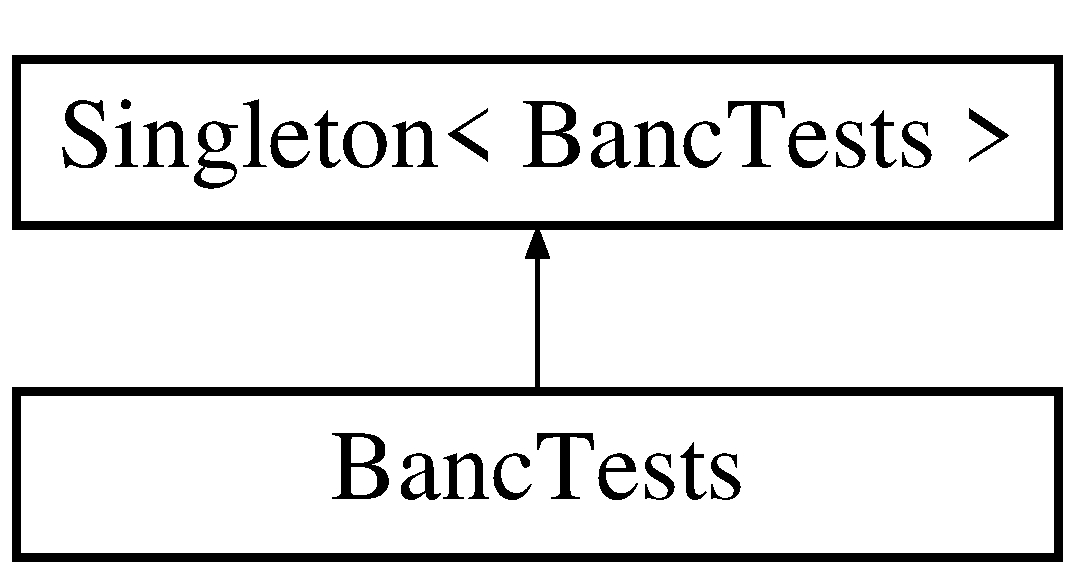
\includegraphics[height=2.000000cm]{class_banc_tests}
\end{center}
\end{figure}
\subsection*{Public Member Functions}
\begin{DoxyCompactItemize}
\item 
bool \hyperlink{group__inf2990_gab5d7fbfe7e3fbe00aa187caa10b1c506}{executer} ()
\begin{DoxyCompactList}\small\item\em Ex�cuter tous les tests unitaires. \end{DoxyCompactList}\end{DoxyCompactItemize}
\subsection*{Additional Inherited Members}


\subsection{Detailed Description}
Banc de tests qui permet d\textquotesingle{}ex�cuter tous les tests unitaires. C\textquotesingle{}est une classe singleton. 

\begin{DoxyAuthor}{Author}
Julien Gascon-\/\+Samson 
\end{DoxyAuthor}
\begin{DoxyDate}{Date}
2011-\/07-\/16 
\end{DoxyDate}


The documentation for this class was generated from the following files\+:\begin{DoxyCompactItemize}
\item 
C\+:/\+Users/\+Bilal Itani/\+Desktop/inf2990-\/11/\+Cadriciel/\+Sources/\+D\+L\+L/\+Tests/\hyperlink{_banc_tests_8h}{Banc\+Tests.\+h}\item 
C\+:/\+Users/\+Bilal Itani/\+Desktop/inf2990-\/11/\+Cadriciel/\+Sources/\+D\+L\+L/\+Tests/\hyperlink{_banc_tests_8cpp}{Banc\+Tests.\+cpp}\end{DoxyCompactItemize}

\hypertarget{struct_base_reader_handler}{}\section{Base\+Reader\+Handler$<$ Encoding, Derived $>$ Struct Template Reference}
\label{struct_base_reader_handler}\index{Base\+Reader\+Handler$<$ Encoding, Derived $>$@{Base\+Reader\+Handler$<$ Encoding, Derived $>$}}


Default implementation of Handler.  




{\ttfamily \#include $<$reader.\+h$>$}

\subsection*{Public Types}
\begin{DoxyCompactItemize}
\item 
typedef Encoding\+::\+Ch {\bfseries Ch}\hypertarget{struct_base_reader_handler_a8302c755dd3560c8c5bac99162c28214}{}\label{struct_base_reader_handler_a8302c755dd3560c8c5bac99162c28214}

\item 
typedef internal\+::\+Select\+If$<$ internal\+::\+Is\+Same$<$ Derived, void $>$, \hyperlink{struct_base_reader_handler}{Base\+Reader\+Handler}, Derived $>$\+::\hyperlink{rapidjson_8h_a1d1cfd8ffb84e947f82999c682b666a7}{Type} {\bfseries Override}\hypertarget{struct_base_reader_handler_a7b6c70d9bf7483b2de5d249f1593776a}{}\label{struct_base_reader_handler_a7b6c70d9bf7483b2de5d249f1593776a}

\end{DoxyCompactItemize}
\subsection*{Public Member Functions}
\begin{DoxyCompactItemize}
\item 
bool {\bfseries Default} ()\hypertarget{struct_base_reader_handler_a836437f6ccc37f08ff933f009b18a78c}{}\label{struct_base_reader_handler_a836437f6ccc37f08ff933f009b18a78c}

\item 
bool {\bfseries Null} ()\hypertarget{struct_base_reader_handler_ae2ebbde4628bf3659ddc5d18520935f5}{}\label{struct_base_reader_handler_ae2ebbde4628bf3659ddc5d18520935f5}

\item 
bool {\bfseries Bool} (bool)\hypertarget{struct_base_reader_handler_aa1c3ce42dbb856b3349792dc9d963587}{}\label{struct_base_reader_handler_aa1c3ce42dbb856b3349792dc9d963587}

\item 
bool {\bfseries Int} (int)\hypertarget{struct_base_reader_handler_a85e813aaf7189a2f87bd53953324fafc}{}\label{struct_base_reader_handler_a85e813aaf7189a2f87bd53953324fafc}

\item 
bool {\bfseries Uint} (unsigned)\hypertarget{struct_base_reader_handler_a0e683306cbb7b4e350a35c18c5246f2a}{}\label{struct_base_reader_handler_a0e683306cbb7b4e350a35c18c5246f2a}

\item 
bool {\bfseries Int64} (int64\+\_\+t)\hypertarget{struct_base_reader_handler_a04011733ea584739c97ad5c6afa15a35}{}\label{struct_base_reader_handler_a04011733ea584739c97ad5c6afa15a35}

\item 
bool {\bfseries Uint64} (uint64\+\_\+t)\hypertarget{struct_base_reader_handler_a351aa3cd81856a487c21022e9cc64d2b}{}\label{struct_base_reader_handler_a351aa3cd81856a487c21022e9cc64d2b}

\item 
bool {\bfseries Double} (double)\hypertarget{struct_base_reader_handler_a8156ea6ae5b8cd23a8b700e92a8af1eb}{}\label{struct_base_reader_handler_a8156ea6ae5b8cd23a8b700e92a8af1eb}

\item 
bool {\bfseries String} (const Ch $\ast$, \hyperlink{rapidjson_8h_a5ed6e6e67250fadbd041127e6386dcb5}{Size\+Type}, bool)\hypertarget{struct_base_reader_handler_a3ac69e6326d0aeef7b1f2619742bbe00}{}\label{struct_base_reader_handler_a3ac69e6326d0aeef7b1f2619742bbe00}

\item 
bool {\bfseries Start\+Object} ()\hypertarget{struct_base_reader_handler_ab0a7d9bcececb8d6ed748656f67f4917}{}\label{struct_base_reader_handler_ab0a7d9bcececb8d6ed748656f67f4917}

\item 
bool {\bfseries Key} (const Ch $\ast$str, \hyperlink{rapidjson_8h_a5ed6e6e67250fadbd041127e6386dcb5}{Size\+Type} len, bool copy)\hypertarget{struct_base_reader_handler_abc50b2e7e411b7b731715e05cd01e2eb}{}\label{struct_base_reader_handler_abc50b2e7e411b7b731715e05cd01e2eb}

\item 
bool {\bfseries End\+Object} (\hyperlink{rapidjson_8h_a5ed6e6e67250fadbd041127e6386dcb5}{Size\+Type})\hypertarget{struct_base_reader_handler_a0406cee0af26bc3a0b7fb2414537b0ab}{}\label{struct_base_reader_handler_a0406cee0af26bc3a0b7fb2414537b0ab}

\item 
bool {\bfseries Start\+Array} ()\hypertarget{struct_base_reader_handler_a9dbb1143a250a904bb18a174553a3a00}{}\label{struct_base_reader_handler_a9dbb1143a250a904bb18a174553a3a00}

\item 
bool {\bfseries End\+Array} (\hyperlink{rapidjson_8h_a5ed6e6e67250fadbd041127e6386dcb5}{Size\+Type})\hypertarget{struct_base_reader_handler_ae9d60a8779b6a77a7f283d64961879fb}{}\label{struct_base_reader_handler_ae9d60a8779b6a77a7f283d64961879fb}

\end{DoxyCompactItemize}


\subsection{Detailed Description}
\subsubsection*{template$<$typename Encoding = U\+T\+F8$<$$>$, typename Derived = void$>$\\*
struct Base\+Reader\+Handler$<$ Encoding, Derived $>$}

Default implementation of Handler. 

This can be used as base class of any reader handler. \begin{DoxyNote}{Note}
implements Handler concept 
\end{DoxyNote}


The documentation for this struct was generated from the following file\+:\begin{DoxyCompactItemize}
\item 
Cadriciel/\+Commun/\+Externe/\+Rapid\+J\+S\+O\+N/include/rapidjson/\hyperlink{reader_8h}{reader.\+h}\end{DoxyCompactItemize}

\hypertarget{classglm_1_1io_1_1basic__format__saver}{}\section{glm\+:\+:io\+:\+:basic\+\_\+format\+\_\+saver$<$ C\+Ty, C\+Tr $>$ Class Template Reference}
\label{classglm_1_1io_1_1basic__format__saver}\index{glm\+::io\+::basic\+\_\+format\+\_\+saver$<$ C\+Ty, C\+Tr $>$@{glm\+::io\+::basic\+\_\+format\+\_\+saver$<$ C\+Ty, C\+Tr $>$}}
\subsection*{Public Member Functions}
\begin{DoxyCompactItemize}
\item 
{\bfseries basic\+\_\+format\+\_\+saver} (std\+::basic\+\_\+ios$<$ C\+Ty, C\+Tr $>$ \&)\hypertarget{classglm_1_1io_1_1basic__format__saver_a9688fa6dce0c32285527df2336ca9127}{}\label{classglm_1_1io_1_1basic__format__saver_a9688fa6dce0c32285527df2336ca9127}

\end{DoxyCompactItemize}
\subsection*{Private Member Functions}
\begin{DoxyCompactItemize}
\item 
\hyperlink{classglm_1_1io_1_1basic__format__saver}{basic\+\_\+format\+\_\+saver} \& {\bfseries operator=} (\hyperlink{classglm_1_1io_1_1basic__format__saver}{basic\+\_\+format\+\_\+saver} const \&)\hypertarget{classglm_1_1io_1_1basic__format__saver_a9e8783bec8e67b7a450edbac066c08be}{}\label{classglm_1_1io_1_1basic__format__saver_a9e8783bec8e67b7a450edbac066c08be}

\end{DoxyCompactItemize}
\subsection*{Private Attributes}
\begin{DoxyCompactItemize}
\item 
\hyperlink{classglm_1_1io_1_1basic__state__saver}{basic\+\_\+state\+\_\+saver}$<$ C\+Ty $>$ const {\bfseries bss\+\_\+}\hypertarget{classglm_1_1io_1_1basic__format__saver_a5d2b333a0879f294698c266fa4a7792b}{}\label{classglm_1_1io_1_1basic__format__saver_a5d2b333a0879f294698c266fa4a7792b}

\end{DoxyCompactItemize}


The documentation for this class was generated from the following files\+:\begin{DoxyCompactItemize}
\item 
Commun/\+Externe/glm/include/glm/gtx/\hyperlink{io_8hpp}{io.\+hpp}\item 
Commun/\+Externe/glm/include/glm/gtx/io.\+inl\end{DoxyCompactItemize}

\hypertarget{classglm_1_1io_1_1basic__state__saver}{}\section{glm\+:\+:io\+:\+:basic\+\_\+state\+\_\+saver$<$ C\+Ty, C\+Tr $>$ Class Template Reference}
\label{classglm_1_1io_1_1basic__state__saver}\index{glm\+::io\+::basic\+\_\+state\+\_\+saver$<$ C\+Ty, C\+Tr $>$@{glm\+::io\+::basic\+\_\+state\+\_\+saver$<$ C\+Ty, C\+Tr $>$}}
\subsection*{Public Member Functions}
\begin{DoxyCompactItemize}
\item 
{\bfseries basic\+\_\+state\+\_\+saver} (std\+::basic\+\_\+ios$<$ C\+Ty, C\+Tr $>$ \&)\hypertarget{classglm_1_1io_1_1basic__state__saver_ab31652b0b7f2a24fa8f9fda2505de356}{}\label{classglm_1_1io_1_1basic__state__saver_ab31652b0b7f2a24fa8f9fda2505de356}

\end{DoxyCompactItemize}
\subsection*{Private Types}
\begin{DoxyCompactItemize}
\item 
typedef \+::std\+::basic\+\_\+ios$<$ C\+Ty, C\+Tr $>$ {\bfseries state\+\_\+type}\hypertarget{classglm_1_1io_1_1basic__state__saver_a84787cc03192543bfe67ef25e7f20aa6}{}\label{classglm_1_1io_1_1basic__state__saver_a84787cc03192543bfe67ef25e7f20aa6}

\item 
typedef state\+\_\+type\+::char\+\_\+type {\bfseries char\+\_\+type}\hypertarget{classglm_1_1io_1_1basic__state__saver_ae6abb8e2e6bd4a044e953746691ffe8e}{}\label{classglm_1_1io_1_1basic__state__saver_ae6abb8e2e6bd4a044e953746691ffe8e}

\item 
typedef \+::std\+::ios\+\_\+base\+::fmtflags {\bfseries flags\+\_\+type}\hypertarget{classglm_1_1io_1_1basic__state__saver_a73ca8320543524c7ab7f1ce97d30aff6}{}\label{classglm_1_1io_1_1basic__state__saver_a73ca8320543524c7ab7f1ce97d30aff6}

\item 
typedef \+::std\+::streamsize {\bfseries streamsize\+\_\+type}\hypertarget{classglm_1_1io_1_1basic__state__saver_a0a4c44df9a4fcf7531af6da7698e0931}{}\label{classglm_1_1io_1_1basic__state__saver_a0a4c44df9a4fcf7531af6da7698e0931}

\item 
typedef \+::std\+::locale const {\bfseries locale\+\_\+type}\hypertarget{classglm_1_1io_1_1basic__state__saver_acc657f13df9c1fd68e1014b96ff615cb}{}\label{classglm_1_1io_1_1basic__state__saver_acc657f13df9c1fd68e1014b96ff615cb}

\end{DoxyCompactItemize}
\subsection*{Private Member Functions}
\begin{DoxyCompactItemize}
\item 
\hyperlink{classglm_1_1io_1_1basic__state__saver}{basic\+\_\+state\+\_\+saver} \& {\bfseries operator=} (\hyperlink{classglm_1_1io_1_1basic__state__saver}{basic\+\_\+state\+\_\+saver} const \&)\hypertarget{classglm_1_1io_1_1basic__state__saver_a06b8637eae186a07ab694fbf490193b5}{}\label{classglm_1_1io_1_1basic__state__saver_a06b8637eae186a07ab694fbf490193b5}

\end{DoxyCompactItemize}
\subsection*{Private Attributes}
\begin{DoxyCompactItemize}
\item 
state\+\_\+type \& {\bfseries state\+\_\+}\hypertarget{classglm_1_1io_1_1basic__state__saver_a969e854089f2df42ee0050d38cc70903}{}\label{classglm_1_1io_1_1basic__state__saver_a969e854089f2df42ee0050d38cc70903}

\item 
flags\+\_\+type {\bfseries flags\+\_\+}\hypertarget{classglm_1_1io_1_1basic__state__saver_a2017c6e006a9e5c0c1ee191aee59c835}{}\label{classglm_1_1io_1_1basic__state__saver_a2017c6e006a9e5c0c1ee191aee59c835}

\item 
streamsize\+\_\+type {\bfseries precision\+\_\+}\hypertarget{classglm_1_1io_1_1basic__state__saver_a1b442206b28b324603599175285fb55a}{}\label{classglm_1_1io_1_1basic__state__saver_a1b442206b28b324603599175285fb55a}

\item 
streamsize\+\_\+type {\bfseries width\+\_\+}\hypertarget{classglm_1_1io_1_1basic__state__saver_a7c2f48c587295d3717b0b6790f78034d}{}\label{classglm_1_1io_1_1basic__state__saver_a7c2f48c587295d3717b0b6790f78034d}

\item 
char\+\_\+type {\bfseries fill\+\_\+}\hypertarget{classglm_1_1io_1_1basic__state__saver_abf8166290d087051954306facad38e00}{}\label{classglm_1_1io_1_1basic__state__saver_abf8166290d087051954306facad38e00}

\item 
locale\+\_\+type {\bfseries locale\+\_\+}\hypertarget{classglm_1_1io_1_1basic__state__saver_a108385f01212b427ebae048eaf181e0d}{}\label{classglm_1_1io_1_1basic__state__saver_a108385f01212b427ebae048eaf181e0d}

\end{DoxyCompactItemize}


The documentation for this class was generated from the following files\+:\begin{DoxyCompactItemize}
\item 
Commun/\+Externe/glm/include/glm/gtx/\hyperlink{io_8hpp}{io.\+hpp}\item 
Commun/\+Externe/glm/include/glm/gtx/io.\+inl\end{DoxyCompactItemize}

\hypertarget{struct_b_d_f___property_rec__}{}\section{B\+D\+F\+\_\+\+Property\+Rec\+\_\+ Struct Reference}
\label{struct_b_d_f___property_rec__}\index{B\+D\+F\+\_\+\+Property\+Rec\+\_\+@{B\+D\+F\+\_\+\+Property\+Rec\+\_\+}}
\subsection*{Public Attributes}
\begin{DoxyCompactItemize}
\item 
B\+D\+F\+\_\+\+Property\+Type {\bfseries type}\hypertarget{struct_b_d_f___property_rec___a88c19ee6f16bd1b36127f5f7d44a4e39}{}\label{struct_b_d_f___property_rec___a88c19ee6f16bd1b36127f5f7d44a4e39}

\item 
\begin{tabbing}
xx\=xx\=xx\=xx\=xx\=xx\=xx\=xx\=xx\=\kill
union \{\\
\>const char $\ast$ {\bfseries atom}\\
\>FT\_Int32 {\bfseries integer}\\
\>FT\_UInt32 {\bfseries cardinal}\\
\} {\bfseries u}\hypertarget{struct_b_d_f___property_rec___ad0b90c890b8517d70b0f21a063840fe4}{}\label{struct_b_d_f___property_rec___ad0b90c890b8517d70b0f21a063840fe4}
\\

\end{tabbing}\end{DoxyCompactItemize}


The documentation for this struct was generated from the following file\+:\begin{DoxyCompactItemize}
\item 
Cadriciel/\+Commun/\+Externe/\+Free\+Type/include/freetype/ftbdf.\+h\end{DoxyCompactItemize}

\hypertarget{classinternal_1_1_big_integer}{}\section{internal\+:\+:Big\+Integer Class Reference}
\label{classinternal_1_1_big_integer}\index{internal\+::\+Big\+Integer@{internal\+::\+Big\+Integer}}
\subsection*{Public Types}
\begin{DoxyCompactItemize}
\item 
typedef uint64\+\_\+t {\bfseries Type}\hypertarget{classinternal_1_1_big_integer_a1310812fca26ebae77594ba08678fc4c}{}\label{classinternal_1_1_big_integer_a1310812fca26ebae77594ba08678fc4c}

\end{DoxyCompactItemize}
\subsection*{Public Member Functions}
\begin{DoxyCompactItemize}
\item 
{\bfseries Big\+Integer} (const \hyperlink{classinternal_1_1_big_integer}{Big\+Integer} \&rhs)\hypertarget{classinternal_1_1_big_integer_abec623168bc9494dec2f50643b897f72}{}\label{classinternal_1_1_big_integer_abec623168bc9494dec2f50643b897f72}

\item 
{\bfseries Big\+Integer} (uint64\+\_\+t u)\hypertarget{classinternal_1_1_big_integer_ad02b0ef9da203efddd4af07e923732c0}{}\label{classinternal_1_1_big_integer_ad02b0ef9da203efddd4af07e923732c0}

\item 
{\bfseries Big\+Integer} (const char $\ast$decimals, size\+\_\+t length)\hypertarget{classinternal_1_1_big_integer_a656bd1bd4af3920beb90ba4af87b6181}{}\label{classinternal_1_1_big_integer_a656bd1bd4af3920beb90ba4af87b6181}

\item 
\hyperlink{classinternal_1_1_big_integer}{Big\+Integer} \& {\bfseries operator=} (const \hyperlink{classinternal_1_1_big_integer}{Big\+Integer} \&rhs)\hypertarget{classinternal_1_1_big_integer_ae3eaf1b96cd993511c9f48a14dfc3af2}{}\label{classinternal_1_1_big_integer_ae3eaf1b96cd993511c9f48a14dfc3af2}

\item 
\hyperlink{classinternal_1_1_big_integer}{Big\+Integer} \& {\bfseries operator=} (uint64\+\_\+t u)\hypertarget{classinternal_1_1_big_integer_a4002e0b1cf5ee68ab94ab65b35167a38}{}\label{classinternal_1_1_big_integer_a4002e0b1cf5ee68ab94ab65b35167a38}

\item 
\hyperlink{classinternal_1_1_big_integer}{Big\+Integer} \& {\bfseries operator+=} (uint64\+\_\+t u)\hypertarget{classinternal_1_1_big_integer_a09af1d6658d51ad4372649ce1c9c1a62}{}\label{classinternal_1_1_big_integer_a09af1d6658d51ad4372649ce1c9c1a62}

\item 
\hyperlink{classinternal_1_1_big_integer}{Big\+Integer} \& {\bfseries operator$\ast$=} (uint64\+\_\+t u)\hypertarget{classinternal_1_1_big_integer_a79a52c6135c9783f2e53432dce2cde89}{}\label{classinternal_1_1_big_integer_a79a52c6135c9783f2e53432dce2cde89}

\item 
\hyperlink{classinternal_1_1_big_integer}{Big\+Integer} \& {\bfseries operator$\ast$=} (uint32\+\_\+t u)\hypertarget{classinternal_1_1_big_integer_a83e8e464b7bc31c8b2c943f8563b2226}{}\label{classinternal_1_1_big_integer_a83e8e464b7bc31c8b2c943f8563b2226}

\item 
\hyperlink{classinternal_1_1_big_integer}{Big\+Integer} \& {\bfseries operator$<$$<$=} (size\+\_\+t shift)\hypertarget{classinternal_1_1_big_integer_a48b12ef4676f19290dfd5816a4ef4a88}{}\label{classinternal_1_1_big_integer_a48b12ef4676f19290dfd5816a4ef4a88}

\item 
bool {\bfseries operator==} (const \hyperlink{classinternal_1_1_big_integer}{Big\+Integer} \&rhs) const \hypertarget{classinternal_1_1_big_integer_a567ecda3009de20400a2af649fb87e60}{}\label{classinternal_1_1_big_integer_a567ecda3009de20400a2af649fb87e60}

\item 
bool {\bfseries operator==} (const Type rhs) const \hypertarget{classinternal_1_1_big_integer_a329eddac1b724f82d56af2ee2c8abcc4}{}\label{classinternal_1_1_big_integer_a329eddac1b724f82d56af2ee2c8abcc4}

\item 
\hyperlink{classinternal_1_1_big_integer}{Big\+Integer} \& {\bfseries Multiply\+Pow5} (unsigned exp)\hypertarget{classinternal_1_1_big_integer_a98a13f169c27d1acfa57054f37c61763}{}\label{classinternal_1_1_big_integer_a98a13f169c27d1acfa57054f37c61763}

\item 
bool {\bfseries Difference} (const \hyperlink{classinternal_1_1_big_integer}{Big\+Integer} \&rhs, \hyperlink{classinternal_1_1_big_integer}{Big\+Integer} $\ast$out) const \hypertarget{classinternal_1_1_big_integer_a5741304ce36392adeef716e78b384b61}{}\label{classinternal_1_1_big_integer_a5741304ce36392adeef716e78b384b61}

\item 
int {\bfseries Compare} (const \hyperlink{classinternal_1_1_big_integer}{Big\+Integer} \&rhs) const \hypertarget{classinternal_1_1_big_integer_afd8b15480df5003ee6b6e1b8ecbf5f45}{}\label{classinternal_1_1_big_integer_afd8b15480df5003ee6b6e1b8ecbf5f45}

\item 
size\+\_\+t {\bfseries Get\+Count} () const \hypertarget{classinternal_1_1_big_integer_a720114cef0871c9f9c3c6a5f3a66e66a}{}\label{classinternal_1_1_big_integer_a720114cef0871c9f9c3c6a5f3a66e66a}

\item 
Type {\bfseries Get\+Digit} (size\+\_\+t index) const \hypertarget{classinternal_1_1_big_integer_a92c6854f2388875374cfb9801bea0cc8}{}\label{classinternal_1_1_big_integer_a92c6854f2388875374cfb9801bea0cc8}

\item 
bool {\bfseries Is\+Zero} () const \hypertarget{classinternal_1_1_big_integer_a99cf9cb87491a583c6b7614b0c8654fe}{}\label{classinternal_1_1_big_integer_a99cf9cb87491a583c6b7614b0c8654fe}

\end{DoxyCompactItemize}


The documentation for this class was generated from the following file\+:\begin{DoxyCompactItemize}
\item 
Cadriciel/\+Commun/\+Externe/\+Rapid\+J\+S\+O\+N/include/rapidjson/internal/biginteger.\+h\end{DoxyCompactItemize}

\hypertarget{structtinyxml2_1_1_mem_pool_t_1_1_block}{}\section{tinyxml2\+:\+:Mem\+PoolT$<$ S\+I\+ZE $>$\+:\+:Block Struct Reference}
\label{structtinyxml2_1_1_mem_pool_t_1_1_block}\index{tinyxml2\+::\+Mem\+Pool\+T$<$ S\+I\+Z\+E $>$\+::\+Block@{tinyxml2\+::\+Mem\+Pool\+T$<$ S\+I\+Z\+E $>$\+::\+Block}}
\subsection*{Public Attributes}
\begin{DoxyCompactItemize}
\item 
\hyperlink{uniontinyxml2_1_1_mem_pool_t_1_1_chunk}{Chunk} {\bfseries chunk} \mbox{[}C\+O\+U\+NT\mbox{]}\hypertarget{structtinyxml2_1_1_mem_pool_t_1_1_block_ae9cbe79b82d9490f15cc00d9694989e8}{}\label{structtinyxml2_1_1_mem_pool_t_1_1_block_ae9cbe79b82d9490f15cc00d9694989e8}

\end{DoxyCompactItemize}


The documentation for this struct was generated from the following file\+:\begin{DoxyCompactItemize}
\item 
Commun/\+Externe/tinyxml2/include/tinyxml2.\+h\end{DoxyCompactItemize}

\hypertarget{structutilitaire_1_1_boite_englobante}{}\section{utilitaire\+:\+:Boite\+Englobante Struct Reference}
\label{structutilitaire_1_1_boite_englobante}\index{utilitaire\+::\+Boite\+Englobante@{utilitaire\+::\+Boite\+Englobante}}


Structure contenant les donn�es pour une boite englobante.  




{\ttfamily \#include $<$Utilitaire.\+h$>$}

\subsection*{Public Attributes}
\begin{DoxyCompactItemize}
\item 
\hyperlink{group__core__types_ga7f3287f952e6ccb481231368091702ac}{glm\+::dvec3} {\bfseries coin\+Min}\hypertarget{structutilitaire_1_1_boite_englobante_a083f953a1ac5a830f70a2173a092e90a}{}\label{structutilitaire_1_1_boite_englobante_a083f953a1ac5a830f70a2173a092e90a}

\item 
\hyperlink{group__core__types_ga7f3287f952e6ccb481231368091702ac}{glm\+::dvec3} {\bfseries coin\+Max}\hypertarget{structutilitaire_1_1_boite_englobante_af6f6d9ef23f6e5eb9f2f1ed6dd4d3e0e}{}\label{structutilitaire_1_1_boite_englobante_af6f6d9ef23f6e5eb9f2f1ed6dd4d3e0e}

\end{DoxyCompactItemize}


\subsection{Detailed Description}
Structure contenant les donn�es pour une boite englobante. 

The documentation for this struct was generated from the following file\+:\begin{DoxyCompactItemize}
\item 
Commun/\+Utilitaire/\hyperlink{_utilitaire_8h}{Utilitaire.\+h}\end{DoxyCompactItemize}

\hypertarget{classutilitaire_1_1_boite_environnement}{}\section{utilitaire\+:\+:Boite\+Environnement Class Reference}
\label{classutilitaire_1_1_boite_environnement}\index{utilitaire\+::\+Boite\+Environnement@{utilitaire\+::\+Boite\+Environnement}}


Classe repr�sentant une bo�te d\textquotesingle{}environnement (\char`\"{}skybox\char`\"{}).  




{\ttfamily \#include $<$Boite\+Environnement.\+h$>$}

\subsection*{Public Member Functions}
\begin{DoxyCompactItemize}
\item 
\hyperlink{classutilitaire_1_1_boite_environnement_afa2e429fd77f584d9b07e1577b907f7b}{Boite\+Environnement} (const std\+::string \&fichier\+Xpos, const std\+::string \&fichier\+Xneg, const std\+::string \&fichier\+Ypos, const std\+::string \&fichier\+Yneg, const std\+::string \&fichier\+Zpos, const std\+::string \&fichier\+Zneg)
\begin{DoxyCompactList}\small\item\em Constructeur � partir des noms des fichiers d\textquotesingle{}images de la bo�te. \end{DoxyCompactList}\item 
\hyperlink{classutilitaire_1_1_boite_environnement_accfe35d5a88904e5001653142b985a27}{$\sim$\+Boite\+Environnement} ()
\begin{DoxyCompactList}\small\item\em Destructeur. \end{DoxyCompactList}\item 
void \hyperlink{classutilitaire_1_1_boite_environnement_a41246ea752945870645cfbd5aec673e9}{afficher} (const \hyperlink{group__core__types_ga7f3287f952e6ccb481231368091702ac}{glm\+::dvec3} \&centre, double demi\+Largeur) const 
\begin{DoxyCompactList}\small\item\em Affiche la bo�te d\textquotesingle{}environnement. \end{DoxyCompactList}\end{DoxyCompactItemize}


\subsection{Detailed Description}
Classe repr�sentant une bo�te d\textquotesingle{}environnement (\char`\"{}skybox\char`\"{}). 

Elle s\textquotesingle{}occupe de charger 6 images du cube formant la bo�te. Elle utilise la convention de sens de Cube\+Map\+Gen (de A\+TI), lorsque les images sont export�es avec le mapping Open\+GL (plut�t que DirectX).

\begin{DoxyAuthor}{Author}
Martin Bisson 
\end{DoxyAuthor}
\begin{DoxyDate}{Date}
2007-\/05-\/28 
\end{DoxyDate}


\subsection{Constructor \& Destructor Documentation}
\index{utilitaire\+::\+Boite\+Environnement@{utilitaire\+::\+Boite\+Environnement}!Boite\+Environnement@{Boite\+Environnement}}
\index{Boite\+Environnement@{Boite\+Environnement}!utilitaire\+::\+Boite\+Environnement@{utilitaire\+::\+Boite\+Environnement}}
\subsubsection[{\texorpdfstring{Boite\+Environnement(const std\+::string \&fichier\+Xpos, const std\+::string \&fichier\+Xneg, const std\+::string \&fichier\+Ypos, const std\+::string \&fichier\+Yneg, const std\+::string \&fichier\+Zpos, const std\+::string \&fichier\+Zneg)}{BoiteEnvironnement(const std::string &fichierXpos, const std::string &fichierXneg, const std::string &fichierYpos, const std::string &fichierYneg, const std::string &fichierZpos, const std::string &fichierZneg)}}]{\setlength{\rightskip}{0pt plus 5cm}utilitaire\+::\+Boite\+Environnement\+::\+Boite\+Environnement (
\begin{DoxyParamCaption}
\item[{const std\+::string \&}]{fichier\+Xpos, }
\item[{const std\+::string \&}]{fichier\+Xneg, }
\item[{const std\+::string \&}]{fichier\+Ypos, }
\item[{const std\+::string \&}]{fichier\+Yneg, }
\item[{const std\+::string \&}]{fichier\+Zpos, }
\item[{const std\+::string \&}]{fichier\+Zneg}
\end{DoxyParamCaption}
)}\hypertarget{classutilitaire_1_1_boite_environnement_afa2e429fd77f584d9b07e1577b907f7b}{}\label{classutilitaire_1_1_boite_environnement_afa2e429fd77f584d9b07e1577b907f7b}


Constructeur � partir des noms des fichiers d\textquotesingle{}images de la bo�te. 

Ce constructeur charge les 6 textures correspondant � chacune des faces de la bo�te d\textquotesingle{}environnement.


\begin{DoxyParams}[1]{Parameters}
\mbox{\tt in}  & {\em fichier\+Xpos} & \+: Le nom du fichier contenant l\textquotesingle{}image correspondant � l\textquotesingle{}axe des X positifs. \\
\hline
\mbox{\tt in}  & {\em fichier\+Xneg} & \+: Le nom du fichier contenant l\textquotesingle{}image correspondant � l\textquotesingle{}axe des X n�gatifs. \\
\hline
\mbox{\tt in}  & {\em fichier\+Ypos} & \+: Le nom du fichier contenant l\textquotesingle{}image correspondant � l\textquotesingle{}axe des X positifs. \\
\hline
\mbox{\tt in}  & {\em fichier\+Yneg} & \+: Le nom du fichier contenant l\textquotesingle{}image correspondant � l\textquotesingle{}axe des Y n�gatifs. \\
\hline
\mbox{\tt in}  & {\em fichier\+Zpos} & \+: Le nom du fichier contenant l\textquotesingle{}image correspondant � l\textquotesingle{}axe des Z positifs. \\
\hline
\mbox{\tt in}  & {\em fichier\+Zneg} & \+: Le nom du fichier contenant l\textquotesingle{}image correspondant � l\textquotesingle{}axe des Z n�gatifs.\\
\hline
\end{DoxyParams}
\begin{DoxyReturn}{Returns}
Aucune (constructeur). 
\end{DoxyReturn}
\index{utilitaire\+::\+Boite\+Environnement@{utilitaire\+::\+Boite\+Environnement}!````~Boite\+Environnement@{$\sim$\+Boite\+Environnement}}
\index{````~Boite\+Environnement@{$\sim$\+Boite\+Environnement}!utilitaire\+::\+Boite\+Environnement@{utilitaire\+::\+Boite\+Environnement}}
\subsubsection[{\texorpdfstring{$\sim$\+Boite\+Environnement()}{~BoiteEnvironnement()}}]{\setlength{\rightskip}{0pt plus 5cm}utilitaire\+::\+Boite\+Environnement\+::$\sim$\+Boite\+Environnement (
\begin{DoxyParamCaption}
{}
\end{DoxyParamCaption}
)}\hypertarget{classutilitaire_1_1_boite_environnement_accfe35d5a88904e5001653142b985a27}{}\label{classutilitaire_1_1_boite_environnement_accfe35d5a88904e5001653142b985a27}


Destructeur. 

Ce destructeur lib�re l\textquotesingle{}espace allou�e � chacune des textures des faces de la bo�te d\textquotesingle{}environnement.

\begin{DoxyReturn}{Returns}
Aucune (destructeur). 
\end{DoxyReturn}


\subsection{Member Function Documentation}
\index{utilitaire\+::\+Boite\+Environnement@{utilitaire\+::\+Boite\+Environnement}!afficher@{afficher}}
\index{afficher@{afficher}!utilitaire\+::\+Boite\+Environnement@{utilitaire\+::\+Boite\+Environnement}}
\subsubsection[{\texorpdfstring{afficher(const glm\+::dvec3 \&centre, double demi\+Largeur) const }{afficher(const glm::dvec3 &centre, double demiLargeur) const }}]{\setlength{\rightskip}{0pt plus 5cm}void utilitaire\+::\+Boite\+Environnement\+::afficher (
\begin{DoxyParamCaption}
\item[{const {\bf glm\+::dvec3} \&}]{centre, }
\item[{double}]{demi\+Largeur}
\end{DoxyParamCaption}
) const}\hypertarget{classutilitaire_1_1_boite_environnement_a41246ea752945870645cfbd5aec673e9}{}\label{classutilitaire_1_1_boite_environnement_a41246ea752945870645cfbd5aec673e9}


Affiche la bo�te d\textquotesingle{}environnement. 

Cette fonction affiche tout simplement la bo�te d\textquotesingle{}environnement.


\begin{DoxyParams}[1]{Parameters}
\mbox{\tt in}  & {\em centre} & \+: La position du centre de la bo�te pour l\textquotesingle{}affichage. \\
\hline
\mbox{\tt in}  & {\em demi\+Largeur} & \+: La largeur de la moiti� de la bo�te pour l\textquotesingle{}affichage.\\
\hline
\end{DoxyParams}
\begin{DoxyReturn}{Returns}
Aucune. 
\end{DoxyReturn}


The documentation for this class was generated from the following files\+:\begin{DoxyCompactItemize}
\item 
Cadriciel/\+Commun/\+Utilitaire/\+Open\+G\+L/\hyperlink{_boite_environnement_8h}{Boite\+Environnement.\+h}\item 
Cadriciel/\+Commun/\+Utilitaire/\+Open\+G\+L/\hyperlink{_boite_environnement_8cpp}{Boite\+Environnement.\+cpp}\end{DoxyCompactItemize}

\hypertarget{class_brief_test_progress_listener}{}\section{Brief\+Test\+Progress\+Listener Class Reference}
\label{class_brief_test_progress_listener}\index{Brief\+Test\+Progress\+Listener@{Brief\+Test\+Progress\+Listener}}


\hyperlink{class_test_listener}{Test\+Listener} that prints the name of each test before running it.  




{\ttfamily \#include $<$Brief\+Test\+Progress\+Listener.\+h$>$}

Inheritance diagram for Brief\+Test\+Progress\+Listener\+:\begin{figure}[H]
\begin{center}
\leavevmode
\includegraphics[height=2.000000cm]{class_brief_test_progress_listener}
\end{center}
\end{figure}
\subsection*{Public Member Functions}
\begin{DoxyCompactItemize}
\item 
\hyperlink{class_brief_test_progress_listener_a7af12547b437fcddab52e7b0f0d47782}{Brief\+Test\+Progress\+Listener} ()
\item 
virtual \hyperlink{class_brief_test_progress_listener_a9e1cf4460bdb460e14009d1629454881}{$\sim$\+Brief\+Test\+Progress\+Listener} ()\hypertarget{class_brief_test_progress_listener_a9e1cf4460bdb460e14009d1629454881}{}\label{class_brief_test_progress_listener_a9e1cf4460bdb460e14009d1629454881}

\begin{DoxyCompactList}\small\item\em Destructor. \end{DoxyCompactList}\item 
void \hyperlink{class_brief_test_progress_listener_ab4196e15752bb2be443e72418500e20e}{start\+Test} (\hyperlink{class_test}{Test} $\ast$test)\hypertarget{class_brief_test_progress_listener_ab4196e15752bb2be443e72418500e20e}{}\label{class_brief_test_progress_listener_ab4196e15752bb2be443e72418500e20e}

\begin{DoxyCompactList}\small\item\em Called when just before a \hyperlink{class_test_case}{Test\+Case} is run. \end{DoxyCompactList}\item 
void \hyperlink{class_brief_test_progress_listener_a21f8658a9c19c67220241656cfad30ce}{add\+Failure} (const \hyperlink{class_test_failure}{Test\+Failure} \&failure)
\begin{DoxyCompactList}\small\item\em Called when a failure occurs while running a test. \end{DoxyCompactList}\item 
void \hyperlink{class_brief_test_progress_listener_a49cbd9152ea35a21f6525773660ee119}{end\+Test} (\hyperlink{class_test}{Test} $\ast$test)\hypertarget{class_brief_test_progress_listener_a49cbd9152ea35a21f6525773660ee119}{}\label{class_brief_test_progress_listener_a49cbd9152ea35a21f6525773660ee119}

\begin{DoxyCompactList}\small\item\em Called just after a \hyperlink{class_test_case}{Test\+Case} was run (even if a failure occured). \end{DoxyCompactList}\end{DoxyCompactItemize}


\subsection{Detailed Description}
\hyperlink{class_test_listener}{Test\+Listener} that prints the name of each test before running it. 

\subsection{Constructor \& Destructor Documentation}
\index{Brief\+Test\+Progress\+Listener@{Brief\+Test\+Progress\+Listener}!Brief\+Test\+Progress\+Listener@{Brief\+Test\+Progress\+Listener}}
\index{Brief\+Test\+Progress\+Listener@{Brief\+Test\+Progress\+Listener}!Brief\+Test\+Progress\+Listener@{Brief\+Test\+Progress\+Listener}}
\subsubsection[{\texorpdfstring{Brief\+Test\+Progress\+Listener()}{BriefTestProgressListener()}}]{\setlength{\rightskip}{0pt plus 5cm}Brief\+Test\+Progress\+Listener\+::\+Brief\+Test\+Progress\+Listener (
\begin{DoxyParamCaption}
{}
\end{DoxyParamCaption}
)}\hypertarget{class_brief_test_progress_listener_a7af12547b437fcddab52e7b0f0d47782}{}\label{class_brief_test_progress_listener_a7af12547b437fcddab52e7b0f0d47782}
Constructs a \hyperlink{class_brief_test_progress_listener}{Brief\+Test\+Progress\+Listener} object. 

\subsection{Member Function Documentation}
\index{Brief\+Test\+Progress\+Listener@{Brief\+Test\+Progress\+Listener}!add\+Failure@{add\+Failure}}
\index{add\+Failure@{add\+Failure}!Brief\+Test\+Progress\+Listener@{Brief\+Test\+Progress\+Listener}}
\subsubsection[{\texorpdfstring{add\+Failure(const Test\+Failure \&failure)}{addFailure(const TestFailure &failure)}}]{\setlength{\rightskip}{0pt plus 5cm}void Brief\+Test\+Progress\+Listener\+::add\+Failure (
\begin{DoxyParamCaption}
\item[{const {\bf Test\+Failure} \&}]{}
\end{DoxyParamCaption}
)\hspace{0.3cm}{\ttfamily [virtual]}}\hypertarget{class_brief_test_progress_listener_a21f8658a9c19c67220241656cfad30ce}{}\label{class_brief_test_progress_listener_a21f8658a9c19c67220241656cfad30ce}


Called when a failure occurs while running a test. 

\begin{DoxySeeAlso}{See also}
\hyperlink{class_test_failure}{Test\+Failure}. 
\end{DoxySeeAlso}
\begin{DoxyWarning}{Warning}
{\itshape failure} is a temporary object that is destroyed after the method call. Use Test\+Failure\+::clone() to create a duplicate. 
\end{DoxyWarning}


Reimplemented from \hyperlink{class_test_listener_a103216a5814c907f7b752b969477e765}{Test\+Listener}.



The documentation for this class was generated from the following file\+:\begin{DoxyCompactItemize}
\item 
C\+:/\+Users/\+Bilal Itani/\+Desktop/inf2990-\/11/\+Cadriciel/\+Commun/\+Externe/cppunit/include/cppunit/Brief\+Test\+Progress\+Listener.\+h\end{DoxyCompactItemize}

\hypertarget{classvue_1_1_camera}{}\section{vue\+:\+:Camera Class Reference}
\label{classvue_1_1_camera}\index{vue\+::\+Camera@{vue\+::\+Camera}}


Classe repr�sentant une cam�ra dans le monde en 3D.  




{\ttfamily \#include $<$Camera.\+h$>$}

\subsection*{Public Member Functions}
\begin{DoxyCompactItemize}
\item 
\hyperlink{classvue_1_1_camera_a0c7869e1153f216e88fc15eb5ac37ce4}{Camera} (const \hyperlink{group__core__types_ga7f3287f952e6ccb481231368091702ac}{glm\+::dvec3} \&position, const \hyperlink{group__core__types_ga7f3287f952e6ccb481231368091702ac}{glm\+::dvec3} \&point\+Vise, const \hyperlink{group__core__types_ga7f3287f952e6ccb481231368091702ac}{glm\+::dvec3} \&direction\+Haut\+Camera, const \hyperlink{group__core__types_ga7f3287f952e6ccb481231368091702ac}{glm\+::dvec3} \&direction\+Haut\+Monde)
\begin{DoxyCompactList}\small\item\em Constructeur � partir des coordonn�es cart�siennes. \end{DoxyCompactList}\item 
virtual \hyperlink{classvue_1_1_camera_a173cf3a9d91b30cadd21d72149df4504}{$\sim$\+Camera} ()\hypertarget{classvue_1_1_camera_a173cf3a9d91b30cadd21d72149df4504}{}\label{classvue_1_1_camera_a173cf3a9d91b30cadd21d72149df4504}

\begin{DoxyCompactList}\small\item\em Destructeur virtuel vide. \end{DoxyCompactList}\item 
void \hyperlink{classvue_1_1_camera_a452efa2c96225b1207cc9ac74be0bda5}{assigner\+Position} (const \hyperlink{group__core__types_ga7f3287f952e6ccb481231368091702ac}{glm\+::dvec3} \&position)
\begin{DoxyCompactList}\small\item\em Assigner la position de la cam�ra. \end{DoxyCompactList}\item 
void \hyperlink{classvue_1_1_camera_a0b9982453adc3afc38f9198ab8b1dd2a}{assigner\+Point\+Vise} (const \hyperlink{group__core__types_ga7f3287f952e6ccb481231368091702ac}{glm\+::dvec3} \&point\+Vise)
\begin{DoxyCompactList}\small\item\em Assigner le point vis� de la cam�ra. \end{DoxyCompactList}\item 
void \hyperlink{classvue_1_1_camera_a94afd2172d111edacc248522f201fd32}{assigner\+Direction\+Haut} (const \hyperlink{group__core__types_ga7f3287f952e6ccb481231368091702ac}{glm\+::dvec3} \&direction\+Haut)
\begin{DoxyCompactList}\small\item\em Assigner la direction du haut de la cam�ra. \end{DoxyCompactList}\item 
const \hyperlink{group__core__types_ga7f3287f952e6ccb481231368091702ac}{glm\+::dvec3} \& \hyperlink{classvue_1_1_camera_aca05463d00f938ceb637b49eaf25f330}{obtenir\+Position} () const 
\begin{DoxyCompactList}\small\item\em Obtenir la position de la cam�ra. \end{DoxyCompactList}\item 
const \hyperlink{group__core__types_ga7f3287f952e6ccb481231368091702ac}{glm\+::dvec3} \& \hyperlink{classvue_1_1_camera_a20cab3b4e97dbe681dc9532e459bbf08}{obtenir\+Point\+Vise} () const 
\begin{DoxyCompactList}\small\item\em Obtenir le point vis� de la cam�ra. \end{DoxyCompactList}\item 
const \hyperlink{group__core__types_ga7f3287f952e6ccb481231368091702ac}{glm\+::dvec3} \& \hyperlink{classvue_1_1_camera_a51913d2a228cb4b90bb5eb72a4a15970}{obtenir\+Direction\+Haut} () const 
\begin{DoxyCompactList}\small\item\em Obtenir la direction du haut de la cam�ra. \end{DoxyCompactList}\item 
void \hyperlink{classvue_1_1_camera_aa08801e436ddf90400e632e402183618}{deplacer\+XY} (double deplacementX, double deplacementY)
\begin{DoxyCompactList}\small\item\em D�placement dans le plan perpendiculaire � la direction vis�e. \end{DoxyCompactList}\item 
void \hyperlink{classvue_1_1_camera_a7e8dfbbf743a74bb0387e140fee09474}{deplacerZ} (double deplacement, bool bouge\+Point\+Vise)
\begin{DoxyCompactList}\small\item\em D�placement dans l\textquotesingle{}axe de la direction vis�e. \end{DoxyCompactList}\item 
void \hyperlink{classvue_1_1_camera_a07795ebc629c68f8694b9ae08a53457f}{tourner\+XY} (double rotationX, double rotationY, bool empeche\+Inversion=true)
\begin{DoxyCompactList}\small\item\em Rotation de la cam�ra autour de sa position. \end{DoxyCompactList}\item 
void \hyperlink{classvue_1_1_camera_a5e88216d5d5b31e0e65be9674e5904ef}{orbiter\+XY} (double rotationX, double rotationY, bool empeche\+Inversion=true)
\begin{DoxyCompactList}\small\item\em Rotation de la position de la cam�ra autour de son point de vis�. \end{DoxyCompactList}\item 
void {\bfseries reinitialiser\+Camera} ()\hypertarget{classvue_1_1_camera_a56a9cf57bc8b10fc3ee55dcdc401d8dd}{}\label{classvue_1_1_camera_a56a9cf57bc8b10fc3ee55dcdc401d8dd}

\item 
void \hyperlink{classvue_1_1_camera_a201db90bcebf204990f1dbb6db03b563}{positionner} () const 
\begin{DoxyCompactList}\small\item\em Positionner la cam�ra (appel � glu\+Look\+At). \end{DoxyCompactList}\end{DoxyCompactItemize}
\subsection*{Private Attributes}
\begin{DoxyCompactItemize}
\item 
\hyperlink{group__core__types_ga7f3287f952e6ccb481231368091702ac}{glm\+::dvec3} \hyperlink{classvue_1_1_camera_aad8feff2275663323942e16c17150867}{position\+\_\+}\hypertarget{classvue_1_1_camera_aad8feff2275663323942e16c17150867}{}\label{classvue_1_1_camera_aad8feff2275663323942e16c17150867}

\begin{DoxyCompactList}\small\item\em La position de la cam�ra. \end{DoxyCompactList}\item 
\hyperlink{group__core__types_ga7f3287f952e6ccb481231368091702ac}{glm\+::dvec3} \hyperlink{classvue_1_1_camera_acaf08abd49f22bd188bf2e27653e6fdc}{point\+Vise\+\_\+}\hypertarget{classvue_1_1_camera_acaf08abd49f22bd188bf2e27653e6fdc}{}\label{classvue_1_1_camera_acaf08abd49f22bd188bf2e27653e6fdc}

\begin{DoxyCompactList}\small\item\em La position du point vis� par la cam�ra. \end{DoxyCompactList}\item 
\hyperlink{group__core__types_ga7f3287f952e6ccb481231368091702ac}{glm\+::dvec3} \hyperlink{classvue_1_1_camera_a505c9555657d5d6c7d53e98900c691b6}{direction\+Haut\+\_\+}\hypertarget{classvue_1_1_camera_a505c9555657d5d6c7d53e98900c691b6}{}\label{classvue_1_1_camera_a505c9555657d5d6c7d53e98900c691b6}

\begin{DoxyCompactList}\small\item\em La direction du haut de la cam�ra. \end{DoxyCompactList}\item 
const \hyperlink{group__core__types_ga7f3287f952e6ccb481231368091702ac}{glm\+::dvec3} \hyperlink{classvue_1_1_camera_aa02015f3386533963c3142983a19daf4}{direction\+Haut\+Monde\+\_\+}\hypertarget{classvue_1_1_camera_aa02015f3386533963c3142983a19daf4}{}\label{classvue_1_1_camera_aa02015f3386533963c3142983a19daf4}

\begin{DoxyCompactList}\small\item\em La direction du haut du monde de la cam�ra. \end{DoxyCompactList}\end{DoxyCompactItemize}


\subsection{Detailed Description}
Classe repr�sentant une cam�ra dans le monde en 3D. 

Cette camera encapsule les diff�rentes op�rations qu\textquotesingle{}il est possible de faire pour d�placer le point de vue de l\textquotesingle{}observateur � l\textquotesingle{}int�rieur de la sc�ne en 3D.

\begin{DoxyAuthor}{Author}
Martin Bisson 
\end{DoxyAuthor}
\begin{DoxyDate}{Date}
2006-\/12-\/15 
\end{DoxyDate}


\subsection{Constructor \& Destructor Documentation}
\index{vue\+::\+Camera@{vue\+::\+Camera}!Camera@{Camera}}
\index{Camera@{Camera}!vue\+::\+Camera@{vue\+::\+Camera}}
\subsubsection[{\texorpdfstring{Camera(const glm\+::dvec3 \&position, const glm\+::dvec3 \&point\+Vise, const glm\+::dvec3 \&direction\+Haut\+Camera, const glm\+::dvec3 \&direction\+Haut\+Monde)}{Camera(const glm::dvec3 &position, const glm::dvec3 &pointVise, const glm::dvec3 &directionHautCamera, const glm::dvec3 &directionHautMonde)}}]{\setlength{\rightskip}{0pt plus 5cm}vue\+::\+Camera\+::\+Camera (
\begin{DoxyParamCaption}
\item[{const {\bf glm\+::dvec3} \&}]{position, }
\item[{const {\bf glm\+::dvec3} \&}]{point\+Vise, }
\item[{const {\bf glm\+::dvec3} \&}]{direction\+Haut\+Camera, }
\item[{const {\bf glm\+::dvec3} \&}]{direction\+Haut\+Monde}
\end{DoxyParamCaption}
)}\hypertarget{classvue_1_1_camera_a0c7869e1153f216e88fc15eb5ac37ce4}{}\label{classvue_1_1_camera_a0c7869e1153f216e88fc15eb5ac37ce4}


Constructeur � partir des coordonn�es cart�siennes. 

Constructeur de la cam�ra � partir des coordonn�es cart�siennes.


\begin{DoxyParams}[1]{Parameters}
\mbox{\tt in}  & {\em position} & \+: position de la cam�ra. \\
\hline
\mbox{\tt in}  & {\em point\+Vise} & \+: point vis�. \\
\hline
\mbox{\tt in}  & {\em direction\+Haut\+Camera} & \+: direction du haut de la cam�ra. \\
\hline
\mbox{\tt in}  & {\em direction\+Haut\+Monde} & \+: direction du haut du monde de la cam�ra.\\
\hline
\end{DoxyParams}
\begin{DoxyReturn}{Returns}
Aucune (constructeur). 
\end{DoxyReturn}


\subsection{Member Function Documentation}
\index{vue\+::\+Camera@{vue\+::\+Camera}!assigner\+Direction\+Haut@{assigner\+Direction\+Haut}}
\index{assigner\+Direction\+Haut@{assigner\+Direction\+Haut}!vue\+::\+Camera@{vue\+::\+Camera}}
\subsubsection[{\texorpdfstring{assigner\+Direction\+Haut(const glm\+::dvec3 \&direction\+Haut)}{assignerDirectionHaut(const glm::dvec3 &directionHaut)}}]{\setlength{\rightskip}{0pt plus 5cm}void vue\+::\+Camera\+::assigner\+Direction\+Haut (
\begin{DoxyParamCaption}
\item[{const {\bf glm\+::dvec3} \&}]{direction\+Haut}
\end{DoxyParamCaption}
)\hspace{0.3cm}{\ttfamily [inline]}}\hypertarget{classvue_1_1_camera_a94afd2172d111edacc248522f201fd32}{}\label{classvue_1_1_camera_a94afd2172d111edacc248522f201fd32}


Assigner la direction du haut de la cam�ra. 

Cette fonction permet d\textquotesingle{}assigner la direction du haut de la cam�ra.


\begin{DoxyParams}[1]{Parameters}
\mbox{\tt in}  & {\em direction\+Haut} & \+: La nouvelle direction du haut de la cam�ra.\\
\hline
\end{DoxyParams}
\begin{DoxyReturn}{Returns}
Aucune. 
\end{DoxyReturn}
\index{vue\+::\+Camera@{vue\+::\+Camera}!assigner\+Point\+Vise@{assigner\+Point\+Vise}}
\index{assigner\+Point\+Vise@{assigner\+Point\+Vise}!vue\+::\+Camera@{vue\+::\+Camera}}
\subsubsection[{\texorpdfstring{assigner\+Point\+Vise(const glm\+::dvec3 \&point\+Vise)}{assignerPointVise(const glm::dvec3 &pointVise)}}]{\setlength{\rightskip}{0pt plus 5cm}void vue\+::\+Camera\+::assigner\+Point\+Vise (
\begin{DoxyParamCaption}
\item[{const {\bf glm\+::dvec3} \&}]{point\+Vise}
\end{DoxyParamCaption}
)\hspace{0.3cm}{\ttfamily [inline]}}\hypertarget{classvue_1_1_camera_a0b9982453adc3afc38f9198ab8b1dd2a}{}\label{classvue_1_1_camera_a0b9982453adc3afc38f9198ab8b1dd2a}


Assigner le point vis� de la cam�ra. 

Cette fonction permet d\textquotesingle{}assigner le point de vis� de la cam�ra.


\begin{DoxyParams}[1]{Parameters}
\mbox{\tt in}  & {\em point\+Vise} & \+: Le nouveau point de vis� de la cam�ra.\\
\hline
\end{DoxyParams}
\begin{DoxyReturn}{Returns}
Aucune. 
\end{DoxyReturn}
\index{vue\+::\+Camera@{vue\+::\+Camera}!assigner\+Position@{assigner\+Position}}
\index{assigner\+Position@{assigner\+Position}!vue\+::\+Camera@{vue\+::\+Camera}}
\subsubsection[{\texorpdfstring{assigner\+Position(const glm\+::dvec3 \&position)}{assignerPosition(const glm::dvec3 &position)}}]{\setlength{\rightskip}{0pt plus 5cm}void vue\+::\+Camera\+::assigner\+Position (
\begin{DoxyParamCaption}
\item[{const {\bf glm\+::dvec3} \&}]{position}
\end{DoxyParamCaption}
)\hspace{0.3cm}{\ttfamily [inline]}}\hypertarget{classvue_1_1_camera_a452efa2c96225b1207cc9ac74be0bda5}{}\label{classvue_1_1_camera_a452efa2c96225b1207cc9ac74be0bda5}


Assigner la position de la cam�ra. 

Cette fonction permet d\textquotesingle{}assigner la position de la cam�ra.


\begin{DoxyParams}[1]{Parameters}
\mbox{\tt in}  & {\em position} & \+: La nouvelle position de la cam�ra.\\
\hline
\end{DoxyParams}
\begin{DoxyReturn}{Returns}
Aucune. 
\end{DoxyReturn}
\index{vue\+::\+Camera@{vue\+::\+Camera}!deplacer\+XY@{deplacer\+XY}}
\index{deplacer\+XY@{deplacer\+XY}!vue\+::\+Camera@{vue\+::\+Camera}}
\subsubsection[{\texorpdfstring{deplacer\+X\+Y(double deplacement\+X, double deplacement\+Y)}{deplacerXY(double deplacementX, double deplacementY)}}]{\setlength{\rightskip}{0pt plus 5cm}void vue\+::\+Camera\+::deplacer\+XY (
\begin{DoxyParamCaption}
\item[{double}]{deplacementX, }
\item[{double}]{deplacementY}
\end{DoxyParamCaption}
)}\hypertarget{classvue_1_1_camera_aa08801e436ddf90400e632e402183618}{}\label{classvue_1_1_camera_aa08801e436ddf90400e632e402183618}


D�placement dans le plan perpendiculaire � la direction vis�e. 

D�place la cam�ra dans le plan perpendiculaire � la direction vis�e


\begin{DoxyParams}[1]{Parameters}
\mbox{\tt in}  & {\em deplacementX} & \+: D�placement sur l\textquotesingle{}axe horizontal du plan de la cam�ra. \\
\hline
\mbox{\tt in}  & {\em deplacementY} & \+: D�placement sur l\textquotesingle{}axe vertical du plan de la cam�ra.\\
\hline
\end{DoxyParams}
\begin{DoxyReturn}{Returns}
Aucune. 
\end{DoxyReturn}
\index{vue\+::\+Camera@{vue\+::\+Camera}!deplacerZ@{deplacerZ}}
\index{deplacerZ@{deplacerZ}!vue\+::\+Camera@{vue\+::\+Camera}}
\subsubsection[{\texorpdfstring{deplacer\+Z(double deplacement, bool bouge\+Point\+Vise)}{deplacerZ(double deplacement, bool bougePointVise)}}]{\setlength{\rightskip}{0pt plus 5cm}void vue\+::\+Camera\+::deplacerZ (
\begin{DoxyParamCaption}
\item[{double}]{deplacement, }
\item[{bool}]{bouge\+Point\+Vise}
\end{DoxyParamCaption}
)}\hypertarget{classvue_1_1_camera_a7e8dfbbf743a74bb0387e140fee09474}{}\label{classvue_1_1_camera_a7e8dfbbf743a74bb0387e140fee09474}


D�placement dans l\textquotesingle{}axe de la direction vis�e. 

D�place la cam�ra dans l\textquotesingle{}axe de la direction vis�e.


\begin{DoxyParams}[1]{Parameters}
\mbox{\tt in}  & {\em deplacement} & \+: D�placement sur l\textquotesingle{}axe de la direction vis�e \\
\hline
\mbox{\tt in}  & {\em bouge\+Point\+Vise} & \+: Si vrai, le point de vis� est �galement d�plac�.\\
\hline
\end{DoxyParams}
\begin{DoxyReturn}{Returns}
Aucune. 
\end{DoxyReturn}
\index{vue\+::\+Camera@{vue\+::\+Camera}!obtenir\+Direction\+Haut@{obtenir\+Direction\+Haut}}
\index{obtenir\+Direction\+Haut@{obtenir\+Direction\+Haut}!vue\+::\+Camera@{vue\+::\+Camera}}
\subsubsection[{\texorpdfstring{obtenir\+Direction\+Haut() const }{obtenirDirectionHaut() const }}]{\setlength{\rightskip}{0pt plus 5cm}const {\bf glm\+::dvec3} \& vue\+::\+Camera\+::obtenir\+Direction\+Haut (
\begin{DoxyParamCaption}
{}
\end{DoxyParamCaption}
) const\hspace{0.3cm}{\ttfamily [inline]}}\hypertarget{classvue_1_1_camera_a51913d2a228cb4b90bb5eb72a4a15970}{}\label{classvue_1_1_camera_a51913d2a228cb4b90bb5eb72a4a15970}


Obtenir la direction du haut de la cam�ra. 

Cette fonction permet d\textquotesingle{}obtenir la direction du haut de la cam�ra.

\begin{DoxyReturn}{Returns}
La direction du haut de la cam�ra. 
\end{DoxyReturn}
\index{vue\+::\+Camera@{vue\+::\+Camera}!obtenir\+Point\+Vise@{obtenir\+Point\+Vise}}
\index{obtenir\+Point\+Vise@{obtenir\+Point\+Vise}!vue\+::\+Camera@{vue\+::\+Camera}}
\subsubsection[{\texorpdfstring{obtenir\+Point\+Vise() const }{obtenirPointVise() const }}]{\setlength{\rightskip}{0pt plus 5cm}const {\bf glm\+::dvec3} \& vue\+::\+Camera\+::obtenir\+Point\+Vise (
\begin{DoxyParamCaption}
{}
\end{DoxyParamCaption}
) const\hspace{0.3cm}{\ttfamily [inline]}}\hypertarget{classvue_1_1_camera_a20cab3b4e97dbe681dc9532e459bbf08}{}\label{classvue_1_1_camera_a20cab3b4e97dbe681dc9532e459bbf08}


Obtenir le point vis� de la cam�ra. 

Cette fonction permet d\textquotesingle{}obtenir le point de vis� de la cam�ra.

\begin{DoxyReturn}{Returns}
Le point de vis� de la cam�ra. 
\end{DoxyReturn}
\index{vue\+::\+Camera@{vue\+::\+Camera}!obtenir\+Position@{obtenir\+Position}}
\index{obtenir\+Position@{obtenir\+Position}!vue\+::\+Camera@{vue\+::\+Camera}}
\subsubsection[{\texorpdfstring{obtenir\+Position() const }{obtenirPosition() const }}]{\setlength{\rightskip}{0pt plus 5cm}const {\bf glm\+::dvec3} \& vue\+::\+Camera\+::obtenir\+Position (
\begin{DoxyParamCaption}
{}
\end{DoxyParamCaption}
) const\hspace{0.3cm}{\ttfamily [inline]}}\hypertarget{classvue_1_1_camera_aca05463d00f938ceb637b49eaf25f330}{}\label{classvue_1_1_camera_aca05463d00f938ceb637b49eaf25f330}


Obtenir la position de la cam�ra. 

Cette fonction permet d\textquotesingle{}obtenir la position de la cam�ra.

\begin{DoxyReturn}{Returns}
La position de la cam�ra. 
\end{DoxyReturn}
\index{vue\+::\+Camera@{vue\+::\+Camera}!orbiter\+XY@{orbiter\+XY}}
\index{orbiter\+XY@{orbiter\+XY}!vue\+::\+Camera@{vue\+::\+Camera}}
\subsubsection[{\texorpdfstring{orbiter\+X\+Y(double rotation\+X, double rotation\+Y, bool empeche\+Inversion=true)}{orbiterXY(double rotationX, double rotationY, bool empecheInversion=true)}}]{\setlength{\rightskip}{0pt plus 5cm}void vue\+::\+Camera\+::orbiter\+XY (
\begin{DoxyParamCaption}
\item[{double}]{rotationX, }
\item[{double}]{rotationY, }
\item[{bool}]{empeche\+Inversion = {\ttfamily true}}
\end{DoxyParamCaption}
)}\hypertarget{classvue_1_1_camera_a5e88216d5d5b31e0e65be9674e5904ef}{}\label{classvue_1_1_camera_a5e88216d5d5b31e0e65be9674e5904ef}


Rotation de la position de la cam�ra autour de son point de vis�. 

Rotation de la cam�ra autour de son point de vis� (et donc d�placement de la position en gardant le point de vis� fixe.


\begin{DoxyParams}[1]{Parameters}
\mbox{\tt in}  & {\em rotationX} & \+: Modification de l\textquotesingle{}angle de rotation de la position par rapport au point de vis�. \\
\hline
\mbox{\tt in}  & {\em rotationY} & \+: Modification de l\textquotesingle{}angle d\textquotesingle{}�l�vation de la position par rapport au point de vis�. \\
\hline
\mbox{\tt in}  & {\em empeche\+Inversion} & \+: Si vrai, la rotation n\textquotesingle{}est pas effectu� si elle am�nerait une inversion de la cam�ra.\\
\hline
\end{DoxyParams}
\begin{DoxyReturn}{Returns}
Aucune. 
\end{DoxyReturn}
\index{vue\+::\+Camera@{vue\+::\+Camera}!positionner@{positionner}}
\index{positionner@{positionner}!vue\+::\+Camera@{vue\+::\+Camera}}
\subsubsection[{\texorpdfstring{positionner() const }{positionner() const }}]{\setlength{\rightskip}{0pt plus 5cm}void vue\+::\+Camera\+::positionner (
\begin{DoxyParamCaption}
{}
\end{DoxyParamCaption}
) const}\hypertarget{classvue_1_1_camera_a201db90bcebf204990f1dbb6db03b563}{}\label{classvue_1_1_camera_a201db90bcebf204990f1dbb6db03b563}


Positionner la cam�ra (appel � glu\+Look\+At). 

Positionne la cam�ra dans la sc�ne � l\textquotesingle{}aide de glu\+Look\+At().

\begin{DoxyReturn}{Returns}
Aucune. 
\end{DoxyReturn}
\index{vue\+::\+Camera@{vue\+::\+Camera}!tourner\+XY@{tourner\+XY}}
\index{tourner\+XY@{tourner\+XY}!vue\+::\+Camera@{vue\+::\+Camera}}
\subsubsection[{\texorpdfstring{tourner\+X\+Y(double rotation\+X, double rotation\+Y, bool empeche\+Inversion=true)}{tournerXY(double rotationX, double rotationY, bool empecheInversion=true)}}]{\setlength{\rightskip}{0pt plus 5cm}void vue\+::\+Camera\+::tourner\+XY (
\begin{DoxyParamCaption}
\item[{double}]{rotationX, }
\item[{double}]{rotationY, }
\item[{bool}]{empeche\+Inversion = {\ttfamily true}}
\end{DoxyParamCaption}
)}\hypertarget{classvue_1_1_camera_a07795ebc629c68f8694b9ae08a53457f}{}\label{classvue_1_1_camera_a07795ebc629c68f8694b9ae08a53457f}


Rotation de la cam�ra autour de sa position. 

Rotation de la cam�ra autour de sa position (et donc d�placement du point vis� en gardant la position fixe.


\begin{DoxyParams}[1]{Parameters}
\mbox{\tt in}  & {\em rotationX} & \+: Modification de l\textquotesingle{}angle de rotation du point vis� par rapport � la position. \\
\hline
\mbox{\tt in}  & {\em rotationY} & \+: Modification de l\textquotesingle{}angle d\textquotesingle{}�l�vation du point vis� par rapport � la position. \\
\hline
\mbox{\tt in}  & {\em empeche\+Inversion} & \+: Si vrai, la rotation n\textquotesingle{}est pas effectu�e si elle am�nerait une inversion de la cam�ra.\\
\hline
\end{DoxyParams}
\begin{DoxyReturn}{Returns}
Aucune. 
\end{DoxyReturn}


The documentation for this class was generated from the following files\+:\begin{DoxyCompactItemize}
\item 
Commun/\+Utilitaire/\+Vue/Camera.\+h\item 
Commun/\+Utilitaire/\+Vue/\hyperlink{_camera_8cpp}{Camera.\+cpp}\end{DoxyCompactItemize}

\hypertarget{class_c_ecriture_fichier_binaire}{}\section{C\+Ecriture\+Fichier\+Binaire Class Reference}
\label{class_c_ecriture_fichier_binaire}\index{C\+Ecriture\+Fichier\+Binaire@{C\+Ecriture\+Fichier\+Binaire}}


Cette classe contient des m�thodes $<$ permettant d\textquotesingle{}�crire dans un fichier binaire des variables string, double, float, int, unsigned int, char, bool.  




{\ttfamily \#include $<$C\+Ecriture\+Fichier\+Binaire.\+h$>$}

Inheritance diagram for C\+Ecriture\+Fichier\+Binaire\+:\begin{figure}[H]
\begin{center}
\leavevmode
\includegraphics[height=2.000000cm]{class_c_ecriture_fichier_binaire}
\end{center}
\end{figure}
\subsection*{Public Member Functions}
\begin{DoxyCompactItemize}
\item 
\hyperlink{group__utilitaire_ga5b5846202001fecd71cd2a0afbbdb494}{C\+Ecriture\+Fichier\+Binaire} ()
\begin{DoxyCompactList}\small\item\em Constructeur par d�faut. \end{DoxyCompactList}\item 
\hyperlink{group__utilitaire_gad19b9753aa12a9f25fd0febc3c899024}{C\+Ecriture\+Fichier\+Binaire} (const char $\ast$nom\+Fichier, openmode mode=std\+::ios\+::out$\vert$std\+::ios\+::binary)
\begin{DoxyCompactList}\small\item\em Constructeur par param�tre. \end{DoxyCompactList}\item 
void \hyperlink{group__utilitaire_ga7145545254c30909311d3b1ef0bdd07a}{null} (int n)
\begin{DoxyCompactList}\small\item\em Fonction pour ins�rer des caract�res vides dans le fichier. \end{DoxyCompactList}\end{DoxyCompactItemize}
\subsection*{Friends}
\begin{DoxyCompactItemize}
\item 
\hyperlink{class_c_ecriture_fichier_binaire}{C\+Ecriture\+Fichier\+Binaire} \& \hyperlink{class_c_ecriture_fichier_binaire_a2c88c30ff08c7d9035596e0187d44e45}{operator$<$} (\hyperlink{class_c_ecriture_fichier_binaire}{C\+Ecriture\+Fichier\+Binaire} \&out, const std\+::string \&s)\hypertarget{class_c_ecriture_fichier_binaire_a2c88c30ff08c7d9035596e0187d44e45}{}\label{class_c_ecriture_fichier_binaire_a2c88c30ff08c7d9035596e0187d44e45}

\begin{DoxyCompactList}\small\item\em Surcharge de l\textquotesingle{}op�rateur pour le type {\itshape std\+::string}. \end{DoxyCompactList}\item 
\hyperlink{class_c_ecriture_fichier_binaire}{C\+Ecriture\+Fichier\+Binaire} \& \hyperlink{class_c_ecriture_fichier_binaire_afcaa555d19b37490df9fda731cf8cb19}{operator$<$} (\hyperlink{class_c_ecriture_fichier_binaire}{C\+Ecriture\+Fichier\+Binaire} \&out, const double \&x)\hypertarget{class_c_ecriture_fichier_binaire_afcaa555d19b37490df9fda731cf8cb19}{}\label{class_c_ecriture_fichier_binaire_afcaa555d19b37490df9fda731cf8cb19}

\begin{DoxyCompactList}\small\item\em Surcharge de l\textquotesingle{}op�rateur pour le type {\itshape double}. \end{DoxyCompactList}\item 
\hyperlink{class_c_ecriture_fichier_binaire}{C\+Ecriture\+Fichier\+Binaire} \& \hyperlink{class_c_ecriture_fichier_binaire_a68e43a125ee6c25828485dfb7270fdea}{operator$<$} (\hyperlink{class_c_ecriture_fichier_binaire}{C\+Ecriture\+Fichier\+Binaire} \&out, const float \&x)\hypertarget{class_c_ecriture_fichier_binaire_a68e43a125ee6c25828485dfb7270fdea}{}\label{class_c_ecriture_fichier_binaire_a68e43a125ee6c25828485dfb7270fdea}

\begin{DoxyCompactList}\small\item\em Surcharge de l\textquotesingle{}op�rateur pour le type {\itshape float}. \end{DoxyCompactList}\item 
\hyperlink{class_c_ecriture_fichier_binaire}{C\+Ecriture\+Fichier\+Binaire} \& \hyperlink{class_c_ecriture_fichier_binaire_a57ac55aefec2f3dd683cef75c409944b}{operator$<$} (\hyperlink{class_c_ecriture_fichier_binaire}{C\+Ecriture\+Fichier\+Binaire} \&out, const int \&x)\hypertarget{class_c_ecriture_fichier_binaire_a57ac55aefec2f3dd683cef75c409944b}{}\label{class_c_ecriture_fichier_binaire_a57ac55aefec2f3dd683cef75c409944b}

\begin{DoxyCompactList}\small\item\em Surcharge de l\textquotesingle{}op�rateur pour le type {\itshape int}. \end{DoxyCompactList}\item 
\hyperlink{class_c_ecriture_fichier_binaire}{C\+Ecriture\+Fichier\+Binaire} \& \hyperlink{class_c_ecriture_fichier_binaire_a38d0f050dcc8a79522b0fb9b9c591f72}{operator$<$} (\hyperlink{class_c_ecriture_fichier_binaire}{C\+Ecriture\+Fichier\+Binaire} \&out, const unsigned int \&x)\hypertarget{class_c_ecriture_fichier_binaire_a38d0f050dcc8a79522b0fb9b9c591f72}{}\label{class_c_ecriture_fichier_binaire_a38d0f050dcc8a79522b0fb9b9c591f72}

\begin{DoxyCompactList}\small\item\em Surcharge de l\textquotesingle{}op�rateur pour le type {\itshape unsigned} {\itshape int}. \end{DoxyCompactList}\item 
\hyperlink{class_c_ecriture_fichier_binaire}{C\+Ecriture\+Fichier\+Binaire} \& \hyperlink{class_c_ecriture_fichier_binaire_a3cb25116e2558d967dfd21e812e47a3e}{operator$<$} (\hyperlink{class_c_ecriture_fichier_binaire}{C\+Ecriture\+Fichier\+Binaire} \&out, const char \&x)\hypertarget{class_c_ecriture_fichier_binaire_a3cb25116e2558d967dfd21e812e47a3e}{}\label{class_c_ecriture_fichier_binaire_a3cb25116e2558d967dfd21e812e47a3e}

\begin{DoxyCompactList}\small\item\em Surcharge de l\textquotesingle{}op�rateur pour le type {\itshape char}. \end{DoxyCompactList}\item 
\hyperlink{class_c_ecriture_fichier_binaire}{C\+Ecriture\+Fichier\+Binaire} \& \hyperlink{class_c_ecriture_fichier_binaire_a37080aca11f391be69941db70093f77d}{operator$<$} (\hyperlink{class_c_ecriture_fichier_binaire}{C\+Ecriture\+Fichier\+Binaire} \&out, const bool \&x)\hypertarget{class_c_ecriture_fichier_binaire_a37080aca11f391be69941db70093f77d}{}\label{class_c_ecriture_fichier_binaire_a37080aca11f391be69941db70093f77d}

\begin{DoxyCompactList}\small\item\em Surcharge de l\textquotesingle{}op�rateur pour le type {\itshape bool}. \end{DoxyCompactList}\end{DoxyCompactItemize}


\subsection{Detailed Description}
Cette classe contient des m�thodes $<$ permettant d\textquotesingle{}�crire dans un fichier binaire des variables string, double, float, int, unsigned int, char, bool. 

\begin{DoxyAuthor}{Author}
D\+G\+I-\/2990 
\end{DoxyAuthor}
\begin{DoxyDate}{Date}
2005-\/10-\/15 
\end{DoxyDate}


The documentation for this class was generated from the following files\+:\begin{DoxyCompactItemize}
\item 
Cadriciel/\+Commun/\+Utilitaire/\hyperlink{_c_ecriture_fichier_binaire_8h}{C\+Ecriture\+Fichier\+Binaire.\+h}\item 
Cadriciel/\+Commun/\+Utilitaire/\hyperlink{_c_ecriture_fichier_binaire_8cpp}{C\+Ecriture\+Fichier\+Binaire.\+cpp}\end{DoxyCompactItemize}

\hypertarget{class_f_m_o_d_1_1_channel}{}\section{F\+M\+OD\+:\+:Channel Class Reference}
\label{class_f_m_o_d_1_1_channel}\index{F\+M\+O\+D\+::\+Channel@{F\+M\+O\+D\+::\+Channel}}
\subsection*{Public Member Functions}
\begin{DoxyCompactItemize}
\item 
F\+M\+O\+D\+\_\+\+R\+E\+S\+U\+LT F\+\_\+\+A\+PI {\bfseries get\+System\+Object} (\hyperlink{class_f_m_o_d_1_1_system}{System} $\ast$$\ast$system)\hypertarget{class_f_m_o_d_1_1_channel_ade71450e7b8a888d4a4f1e73eded4236}{}\label{class_f_m_o_d_1_1_channel_ade71450e7b8a888d4a4f1e73eded4236}

\item 
F\+M\+O\+D\+\_\+\+R\+E\+S\+U\+LT F\+\_\+\+A\+PI {\bfseries stop} ()\hypertarget{class_f_m_o_d_1_1_channel_a89d7bc13ea65f29f306fbd279e54dd08}{}\label{class_f_m_o_d_1_1_channel_a89d7bc13ea65f29f306fbd279e54dd08}

\item 
F\+M\+O\+D\+\_\+\+R\+E\+S\+U\+LT F\+\_\+\+A\+PI {\bfseries set\+Paused} (bool paused)\hypertarget{class_f_m_o_d_1_1_channel_a7610d6be6beec8f7cf6d0230c48c6618}{}\label{class_f_m_o_d_1_1_channel_a7610d6be6beec8f7cf6d0230c48c6618}

\item 
F\+M\+O\+D\+\_\+\+R\+E\+S\+U\+LT F\+\_\+\+A\+PI {\bfseries get\+Paused} (bool $\ast$paused)\hypertarget{class_f_m_o_d_1_1_channel_a551d39aed652cb419ce5ec7256abefb4}{}\label{class_f_m_o_d_1_1_channel_a551d39aed652cb419ce5ec7256abefb4}

\item 
F\+M\+O\+D\+\_\+\+R\+E\+S\+U\+LT F\+\_\+\+A\+PI {\bfseries set\+Volume} (float volume)\hypertarget{class_f_m_o_d_1_1_channel_a641ee780642531cec59aa9ec065d4709}{}\label{class_f_m_o_d_1_1_channel_a641ee780642531cec59aa9ec065d4709}

\item 
F\+M\+O\+D\+\_\+\+R\+E\+S\+U\+LT F\+\_\+\+A\+PI {\bfseries get\+Volume} (float $\ast$volume)\hypertarget{class_f_m_o_d_1_1_channel_aef6f0675ac455547e3a00ce339ca85f9}{}\label{class_f_m_o_d_1_1_channel_aef6f0675ac455547e3a00ce339ca85f9}

\item 
F\+M\+O\+D\+\_\+\+R\+E\+S\+U\+LT F\+\_\+\+A\+PI {\bfseries set\+Frequency} (float frequency)\hypertarget{class_f_m_o_d_1_1_channel_a355cd052a405c0ecdbaac7c65d24148b}{}\label{class_f_m_o_d_1_1_channel_a355cd052a405c0ecdbaac7c65d24148b}

\item 
F\+M\+O\+D\+\_\+\+R\+E\+S\+U\+LT F\+\_\+\+A\+PI {\bfseries get\+Frequency} (float $\ast$frequency)\hypertarget{class_f_m_o_d_1_1_channel_a99f1dcf4b2a67f509d08f138e9e3cbca}{}\label{class_f_m_o_d_1_1_channel_a99f1dcf4b2a67f509d08f138e9e3cbca}

\item 
F\+M\+O\+D\+\_\+\+R\+E\+S\+U\+LT F\+\_\+\+A\+PI {\bfseries set\+Pan} (float pan)\hypertarget{class_f_m_o_d_1_1_channel_a419235a572a267b0763287fe988435f7}{}\label{class_f_m_o_d_1_1_channel_a419235a572a267b0763287fe988435f7}

\item 
F\+M\+O\+D\+\_\+\+R\+E\+S\+U\+LT F\+\_\+\+A\+PI {\bfseries get\+Pan} (float $\ast$pan)\hypertarget{class_f_m_o_d_1_1_channel_a776a9e6fbca132087663e77de052806c}{}\label{class_f_m_o_d_1_1_channel_a776a9e6fbca132087663e77de052806c}

\item 
F\+M\+O\+D\+\_\+\+R\+E\+S\+U\+LT F\+\_\+\+A\+PI {\bfseries set\+Delay} (F\+M\+O\+D\+\_\+\+D\+E\+L\+A\+Y\+T\+Y\+PE delaytype, unsigned int delayhi, unsigned int delaylo)\hypertarget{class_f_m_o_d_1_1_channel_a21a2f9d9fdae503ce53a9ced9c4cb9a2}{}\label{class_f_m_o_d_1_1_channel_a21a2f9d9fdae503ce53a9ced9c4cb9a2}

\item 
F\+M\+O\+D\+\_\+\+R\+E\+S\+U\+LT F\+\_\+\+A\+PI {\bfseries get\+Delay} (F\+M\+O\+D\+\_\+\+D\+E\+L\+A\+Y\+T\+Y\+PE delaytype, unsigned int $\ast$delayhi, unsigned int $\ast$delaylo)\hypertarget{class_f_m_o_d_1_1_channel_a8cc8b51bc344dd7916628568764aa6cf}{}\label{class_f_m_o_d_1_1_channel_a8cc8b51bc344dd7916628568764aa6cf}

\item 
F\+M\+O\+D\+\_\+\+R\+E\+S\+U\+LT F\+\_\+\+A\+PI {\bfseries set\+Speaker\+Mix} (float frontleft, float frontright, float center, float lfe, float backleft, float backright, float sideleft, float sideright)\hypertarget{class_f_m_o_d_1_1_channel_ad6b62bf51be6c5c3006e23717e8ad4c7}{}\label{class_f_m_o_d_1_1_channel_ad6b62bf51be6c5c3006e23717e8ad4c7}

\item 
F\+M\+O\+D\+\_\+\+R\+E\+S\+U\+LT F\+\_\+\+A\+PI {\bfseries get\+Speaker\+Mix} (float $\ast$frontleft, float $\ast$frontright, float $\ast$center, float $\ast$lfe, float $\ast$backleft, float $\ast$backright, float $\ast$sideleft, float $\ast$sideright)\hypertarget{class_f_m_o_d_1_1_channel_a1cec99c48524d8cbf6d4454b1ec7a374}{}\label{class_f_m_o_d_1_1_channel_a1cec99c48524d8cbf6d4454b1ec7a374}

\item 
F\+M\+O\+D\+\_\+\+R\+E\+S\+U\+LT F\+\_\+\+A\+PI {\bfseries set\+Speaker\+Levels} (F\+M\+O\+D\+\_\+\+S\+P\+E\+A\+K\+ER speaker, float $\ast$levels, int numlevels)\hypertarget{class_f_m_o_d_1_1_channel_aa32c97cb14d3da622393d7406c9f0ca3}{}\label{class_f_m_o_d_1_1_channel_aa32c97cb14d3da622393d7406c9f0ca3}

\item 
F\+M\+O\+D\+\_\+\+R\+E\+S\+U\+LT F\+\_\+\+A\+PI {\bfseries get\+Speaker\+Levels} (F\+M\+O\+D\+\_\+\+S\+P\+E\+A\+K\+ER speaker, float $\ast$levels, int numlevels)\hypertarget{class_f_m_o_d_1_1_channel_aadb8b4003e6b716331d280a7f22a6f51}{}\label{class_f_m_o_d_1_1_channel_aadb8b4003e6b716331d280a7f22a6f51}

\item 
F\+M\+O\+D\+\_\+\+R\+E\+S\+U\+LT F\+\_\+\+A\+PI {\bfseries set\+Input\+Channel\+Mix} (float $\ast$levels, int numlevels)\hypertarget{class_f_m_o_d_1_1_channel_a4695dfbef85dece725468e690053ca00}{}\label{class_f_m_o_d_1_1_channel_a4695dfbef85dece725468e690053ca00}

\item 
F\+M\+O\+D\+\_\+\+R\+E\+S\+U\+LT F\+\_\+\+A\+PI {\bfseries get\+Input\+Channel\+Mix} (float $\ast$levels, int numlevels)\hypertarget{class_f_m_o_d_1_1_channel_ab893172c11ceab2bb254707b1b2d263e}{}\label{class_f_m_o_d_1_1_channel_ab893172c11ceab2bb254707b1b2d263e}

\item 
F\+M\+O\+D\+\_\+\+R\+E\+S\+U\+LT F\+\_\+\+A\+PI {\bfseries set\+Mute} (bool mute)\hypertarget{class_f_m_o_d_1_1_channel_a0b0d4a7d28c0e57daeb8c1c39fb06379}{}\label{class_f_m_o_d_1_1_channel_a0b0d4a7d28c0e57daeb8c1c39fb06379}

\item 
F\+M\+O\+D\+\_\+\+R\+E\+S\+U\+LT F\+\_\+\+A\+PI {\bfseries get\+Mute} (bool $\ast$mute)\hypertarget{class_f_m_o_d_1_1_channel_acc5cfb7cd503c24210ab7ffbbdbbea0e}{}\label{class_f_m_o_d_1_1_channel_acc5cfb7cd503c24210ab7ffbbdbbea0e}

\item 
F\+M\+O\+D\+\_\+\+R\+E\+S\+U\+LT F\+\_\+\+A\+PI {\bfseries set\+Priority} (int priority)\hypertarget{class_f_m_o_d_1_1_channel_a83a9a2f49e4bdde446f0d574847f5329}{}\label{class_f_m_o_d_1_1_channel_a83a9a2f49e4bdde446f0d574847f5329}

\item 
F\+M\+O\+D\+\_\+\+R\+E\+S\+U\+LT F\+\_\+\+A\+PI {\bfseries get\+Priority} (int $\ast$priority)\hypertarget{class_f_m_o_d_1_1_channel_ae2a16710e706c0223937bc99fb3cad3d}{}\label{class_f_m_o_d_1_1_channel_ae2a16710e706c0223937bc99fb3cad3d}

\item 
F\+M\+O\+D\+\_\+\+R\+E\+S\+U\+LT F\+\_\+\+A\+PI {\bfseries set\+Position} (unsigned int position, F\+M\+O\+D\+\_\+\+T\+I\+M\+E\+U\+N\+IT postype)\hypertarget{class_f_m_o_d_1_1_channel_a46f8f6738b500bbb995bd4a4ecce826f}{}\label{class_f_m_o_d_1_1_channel_a46f8f6738b500bbb995bd4a4ecce826f}

\item 
F\+M\+O\+D\+\_\+\+R\+E\+S\+U\+LT F\+\_\+\+A\+PI {\bfseries get\+Position} (unsigned int $\ast$position, F\+M\+O\+D\+\_\+\+T\+I\+M\+E\+U\+N\+IT postype)\hypertarget{class_f_m_o_d_1_1_channel_a580cb740f80cf139faaf21181490d98f}{}\label{class_f_m_o_d_1_1_channel_a580cb740f80cf139faaf21181490d98f}

\item 
F\+M\+O\+D\+\_\+\+R\+E\+S\+U\+LT F\+\_\+\+A\+PI {\bfseries set\+Reverb\+Properties} (const \hyperlink{struct_f_m_o_d___r_e_v_e_r_b___c_h_a_n_n_e_l_p_r_o_p_e_r_t_i_e_s}{F\+M\+O\+D\+\_\+\+R\+E\+V\+E\+R\+B\+\_\+\+C\+H\+A\+N\+N\+E\+L\+P\+R\+O\+P\+E\+R\+T\+I\+ES} $\ast$prop)\hypertarget{class_f_m_o_d_1_1_channel_a1002a2ff8f7f9f33b2fce03fb472e8a8}{}\label{class_f_m_o_d_1_1_channel_a1002a2ff8f7f9f33b2fce03fb472e8a8}

\item 
F\+M\+O\+D\+\_\+\+R\+E\+S\+U\+LT F\+\_\+\+A\+PI {\bfseries get\+Reverb\+Properties} (\hyperlink{struct_f_m_o_d___r_e_v_e_r_b___c_h_a_n_n_e_l_p_r_o_p_e_r_t_i_e_s}{F\+M\+O\+D\+\_\+\+R\+E\+V\+E\+R\+B\+\_\+\+C\+H\+A\+N\+N\+E\+L\+P\+R\+O\+P\+E\+R\+T\+I\+ES} $\ast$prop)\hypertarget{class_f_m_o_d_1_1_channel_a0e0e479c81abd5e709bda6abcebac57b}{}\label{class_f_m_o_d_1_1_channel_a0e0e479c81abd5e709bda6abcebac57b}

\item 
F\+M\+O\+D\+\_\+\+R\+E\+S\+U\+LT F\+\_\+\+A\+PI {\bfseries set\+Low\+Pass\+Gain} (float gain)\hypertarget{class_f_m_o_d_1_1_channel_a10e6a2fe8768461407fac5963167c416}{}\label{class_f_m_o_d_1_1_channel_a10e6a2fe8768461407fac5963167c416}

\item 
F\+M\+O\+D\+\_\+\+R\+E\+S\+U\+LT F\+\_\+\+A\+PI {\bfseries get\+Low\+Pass\+Gain} (float $\ast$gain)\hypertarget{class_f_m_o_d_1_1_channel_a0e34960ec8bd9703fcdcfa0b85683b18}{}\label{class_f_m_o_d_1_1_channel_a0e34960ec8bd9703fcdcfa0b85683b18}

\item 
F\+M\+O\+D\+\_\+\+R\+E\+S\+U\+LT F\+\_\+\+A\+PI {\bfseries set\+Channel\+Group} (\hyperlink{class_f_m_o_d_1_1_channel_group}{Channel\+Group} $\ast$channelgroup)\hypertarget{class_f_m_o_d_1_1_channel_a570b83eb8178325a131b081a8d5ffd81}{}\label{class_f_m_o_d_1_1_channel_a570b83eb8178325a131b081a8d5ffd81}

\item 
F\+M\+O\+D\+\_\+\+R\+E\+S\+U\+LT F\+\_\+\+A\+PI {\bfseries get\+Channel\+Group} (\hyperlink{class_f_m_o_d_1_1_channel_group}{Channel\+Group} $\ast$$\ast$channelgroup)\hypertarget{class_f_m_o_d_1_1_channel_a4b6d310d04eb844190db7a4074af2b2c}{}\label{class_f_m_o_d_1_1_channel_a4b6d310d04eb844190db7a4074af2b2c}

\item 
F\+M\+O\+D\+\_\+\+R\+E\+S\+U\+LT F\+\_\+\+A\+PI {\bfseries set\+Callback} (F\+M\+O\+D\+\_\+\+C\+H\+A\+N\+N\+E\+L\+\_\+\+C\+A\+L\+L\+B\+A\+CK callback)\hypertarget{class_f_m_o_d_1_1_channel_a5cbbb69ad8d74d36d7b469a77450c3fa}{}\label{class_f_m_o_d_1_1_channel_a5cbbb69ad8d74d36d7b469a77450c3fa}

\item 
F\+M\+O\+D\+\_\+\+R\+E\+S\+U\+LT F\+\_\+\+A\+PI {\bfseries set3\+D\+Attributes} (const \hyperlink{struct_f_m_o_d___v_e_c_t_o_r}{F\+M\+O\+D\+\_\+\+V\+E\+C\+T\+OR} $\ast$pos, const \hyperlink{struct_f_m_o_d___v_e_c_t_o_r}{F\+M\+O\+D\+\_\+\+V\+E\+C\+T\+OR} $\ast$vel)\hypertarget{class_f_m_o_d_1_1_channel_ae0bb0f7c1c1a807bde8ab9e9c3870785}{}\label{class_f_m_o_d_1_1_channel_ae0bb0f7c1c1a807bde8ab9e9c3870785}

\item 
F\+M\+O\+D\+\_\+\+R\+E\+S\+U\+LT F\+\_\+\+A\+PI {\bfseries get3\+D\+Attributes} (\hyperlink{struct_f_m_o_d___v_e_c_t_o_r}{F\+M\+O\+D\+\_\+\+V\+E\+C\+T\+OR} $\ast$pos, \hyperlink{struct_f_m_o_d___v_e_c_t_o_r}{F\+M\+O\+D\+\_\+\+V\+E\+C\+T\+OR} $\ast$vel)\hypertarget{class_f_m_o_d_1_1_channel_ab0f5e28337f9303c75f80d139201a858}{}\label{class_f_m_o_d_1_1_channel_ab0f5e28337f9303c75f80d139201a858}

\item 
F\+M\+O\+D\+\_\+\+R\+E\+S\+U\+LT F\+\_\+\+A\+PI {\bfseries set3\+D\+Min\+Max\+Distance} (float mindistance, float maxdistance)\hypertarget{class_f_m_o_d_1_1_channel_aa6ee9a231435079405ec4a2c2bd07c44}{}\label{class_f_m_o_d_1_1_channel_aa6ee9a231435079405ec4a2c2bd07c44}

\item 
F\+M\+O\+D\+\_\+\+R\+E\+S\+U\+LT F\+\_\+\+A\+PI {\bfseries get3\+D\+Min\+Max\+Distance} (float $\ast$mindistance, float $\ast$maxdistance)\hypertarget{class_f_m_o_d_1_1_channel_ae997142f79c9e96414f0ecce05fa93a3}{}\label{class_f_m_o_d_1_1_channel_ae997142f79c9e96414f0ecce05fa93a3}

\item 
F\+M\+O\+D\+\_\+\+R\+E\+S\+U\+LT F\+\_\+\+A\+PI {\bfseries set3\+D\+Cone\+Settings} (float insideconeangle, float outsideconeangle, float outsidevolume)\hypertarget{class_f_m_o_d_1_1_channel_a9e0d8885d31b2978683d5305924de565}{}\label{class_f_m_o_d_1_1_channel_a9e0d8885d31b2978683d5305924de565}

\item 
F\+M\+O\+D\+\_\+\+R\+E\+S\+U\+LT F\+\_\+\+A\+PI {\bfseries get3\+D\+Cone\+Settings} (float $\ast$insideconeangle, float $\ast$outsideconeangle, float $\ast$outsidevolume)\hypertarget{class_f_m_o_d_1_1_channel_a7206e7b2353ed27ec91512690bd2c052}{}\label{class_f_m_o_d_1_1_channel_a7206e7b2353ed27ec91512690bd2c052}

\item 
F\+M\+O\+D\+\_\+\+R\+E\+S\+U\+LT F\+\_\+\+A\+PI {\bfseries set3\+D\+Cone\+Orientation} (\hyperlink{struct_f_m_o_d___v_e_c_t_o_r}{F\+M\+O\+D\+\_\+\+V\+E\+C\+T\+OR} $\ast$orientation)\hypertarget{class_f_m_o_d_1_1_channel_a6c10b3cdb50cb11d5090b14b7f569a79}{}\label{class_f_m_o_d_1_1_channel_a6c10b3cdb50cb11d5090b14b7f569a79}

\item 
F\+M\+O\+D\+\_\+\+R\+E\+S\+U\+LT F\+\_\+\+A\+PI {\bfseries get3\+D\+Cone\+Orientation} (\hyperlink{struct_f_m_o_d___v_e_c_t_o_r}{F\+M\+O\+D\+\_\+\+V\+E\+C\+T\+OR} $\ast$orientation)\hypertarget{class_f_m_o_d_1_1_channel_a0f22cabb2a93d1a8c038293c9a5a970d}{}\label{class_f_m_o_d_1_1_channel_a0f22cabb2a93d1a8c038293c9a5a970d}

\item 
F\+M\+O\+D\+\_\+\+R\+E\+S\+U\+LT F\+\_\+\+A\+PI {\bfseries set3\+D\+Custom\+Rolloff} (\hyperlink{struct_f_m_o_d___v_e_c_t_o_r}{F\+M\+O\+D\+\_\+\+V\+E\+C\+T\+OR} $\ast$points, int numpoints)\hypertarget{class_f_m_o_d_1_1_channel_a1ad33a178f33decfc764dfca2ad0aefb}{}\label{class_f_m_o_d_1_1_channel_a1ad33a178f33decfc764dfca2ad0aefb}

\item 
F\+M\+O\+D\+\_\+\+R\+E\+S\+U\+LT F\+\_\+\+A\+PI {\bfseries get3\+D\+Custom\+Rolloff} (\hyperlink{struct_f_m_o_d___v_e_c_t_o_r}{F\+M\+O\+D\+\_\+\+V\+E\+C\+T\+OR} $\ast$$\ast$points, int $\ast$numpoints)\hypertarget{class_f_m_o_d_1_1_channel_ae772d709160da9adb23971c6f0b2bc33}{}\label{class_f_m_o_d_1_1_channel_ae772d709160da9adb23971c6f0b2bc33}

\item 
F\+M\+O\+D\+\_\+\+R\+E\+S\+U\+LT F\+\_\+\+A\+PI {\bfseries set3\+D\+Occlusion} (float directocclusion, float reverbocclusion)\hypertarget{class_f_m_o_d_1_1_channel_a0037d4f48e07686f53d35c66fd6be5cd}{}\label{class_f_m_o_d_1_1_channel_a0037d4f48e07686f53d35c66fd6be5cd}

\item 
F\+M\+O\+D\+\_\+\+R\+E\+S\+U\+LT F\+\_\+\+A\+PI {\bfseries get3\+D\+Occlusion} (float $\ast$directocclusion, float $\ast$reverbocclusion)\hypertarget{class_f_m_o_d_1_1_channel_a0059b3132df76efd24f8567b4fcf4818}{}\label{class_f_m_o_d_1_1_channel_a0059b3132df76efd24f8567b4fcf4818}

\item 
F\+M\+O\+D\+\_\+\+R\+E\+S\+U\+LT F\+\_\+\+A\+PI {\bfseries set3\+D\+Spread} (float angle)\hypertarget{class_f_m_o_d_1_1_channel_a59fb99f17a8997b14d983647e6978c07}{}\label{class_f_m_o_d_1_1_channel_a59fb99f17a8997b14d983647e6978c07}

\item 
F\+M\+O\+D\+\_\+\+R\+E\+S\+U\+LT F\+\_\+\+A\+PI {\bfseries get3\+D\+Spread} (float $\ast$angle)\hypertarget{class_f_m_o_d_1_1_channel_a527cbba8333bfe7515fe18208765ac61}{}\label{class_f_m_o_d_1_1_channel_a527cbba8333bfe7515fe18208765ac61}

\item 
F\+M\+O\+D\+\_\+\+R\+E\+S\+U\+LT F\+\_\+\+A\+PI {\bfseries set3\+D\+Pan\+Level} (float level)\hypertarget{class_f_m_o_d_1_1_channel_aaeadeb90b4c702d16b6083a17905efc5}{}\label{class_f_m_o_d_1_1_channel_aaeadeb90b4c702d16b6083a17905efc5}

\item 
F\+M\+O\+D\+\_\+\+R\+E\+S\+U\+LT F\+\_\+\+A\+PI {\bfseries get3\+D\+Pan\+Level} (float $\ast$level)\hypertarget{class_f_m_o_d_1_1_channel_ac8779446fdac236616964ac5bddec5be}{}\label{class_f_m_o_d_1_1_channel_ac8779446fdac236616964ac5bddec5be}

\item 
F\+M\+O\+D\+\_\+\+R\+E\+S\+U\+LT F\+\_\+\+A\+PI {\bfseries set3\+D\+Doppler\+Level} (float level)\hypertarget{class_f_m_o_d_1_1_channel_a7e1c29fc420d38a9a686a0a29996209a}{}\label{class_f_m_o_d_1_1_channel_a7e1c29fc420d38a9a686a0a29996209a}

\item 
F\+M\+O\+D\+\_\+\+R\+E\+S\+U\+LT F\+\_\+\+A\+PI {\bfseries get3\+D\+Doppler\+Level} (float $\ast$level)\hypertarget{class_f_m_o_d_1_1_channel_a90e0a82f15339ae3a9442ad04bec229b}{}\label{class_f_m_o_d_1_1_channel_a90e0a82f15339ae3a9442ad04bec229b}

\item 
F\+M\+O\+D\+\_\+\+R\+E\+S\+U\+LT F\+\_\+\+A\+PI {\bfseries set3\+D\+Distance\+Filter} (bool custom, float custom\+Level, float center\+Freq)\hypertarget{class_f_m_o_d_1_1_channel_a6c180f229b8edffa88ecc2ef99a581e3}{}\label{class_f_m_o_d_1_1_channel_a6c180f229b8edffa88ecc2ef99a581e3}

\item 
F\+M\+O\+D\+\_\+\+R\+E\+S\+U\+LT F\+\_\+\+A\+PI {\bfseries get3\+D\+Distance\+Filter} (bool $\ast$custom, float $\ast$custom\+Level, float $\ast$center\+Freq)\hypertarget{class_f_m_o_d_1_1_channel_abf9d4d1cc96e3e79ea316172524a3c6a}{}\label{class_f_m_o_d_1_1_channel_abf9d4d1cc96e3e79ea316172524a3c6a}

\item 
F\+M\+O\+D\+\_\+\+R\+E\+S\+U\+LT F\+\_\+\+A\+PI {\bfseries get\+D\+S\+P\+Head} (\hyperlink{class_f_m_o_d_1_1_d_s_p}{D\+SP} $\ast$$\ast$dsp)\hypertarget{class_f_m_o_d_1_1_channel_a2629c769ba2de6aec89da5c07bf4a535}{}\label{class_f_m_o_d_1_1_channel_a2629c769ba2de6aec89da5c07bf4a535}

\item 
F\+M\+O\+D\+\_\+\+R\+E\+S\+U\+LT F\+\_\+\+A\+PI {\bfseries add\+D\+SP} (\hyperlink{class_f_m_o_d_1_1_d_s_p}{D\+SP} $\ast$dsp, \hyperlink{class_f_m_o_d_1_1_d_s_p_connection}{D\+S\+P\+Connection} $\ast$$\ast$connection)\hypertarget{class_f_m_o_d_1_1_channel_a87b31364ea541df027a5dc89c2d8af2b}{}\label{class_f_m_o_d_1_1_channel_a87b31364ea541df027a5dc89c2d8af2b}

\item 
F\+M\+O\+D\+\_\+\+R\+E\+S\+U\+LT F\+\_\+\+A\+PI {\bfseries is\+Playing} (bool $\ast$isplaying)\hypertarget{class_f_m_o_d_1_1_channel_a0e50e17361a0fc354a674827285539fa}{}\label{class_f_m_o_d_1_1_channel_a0e50e17361a0fc354a674827285539fa}

\item 
F\+M\+O\+D\+\_\+\+R\+E\+S\+U\+LT F\+\_\+\+A\+PI {\bfseries is\+Virtual} (bool $\ast$isvirtual)\hypertarget{class_f_m_o_d_1_1_channel_aba59130d19b04270bbe8d765d79018f9}{}\label{class_f_m_o_d_1_1_channel_aba59130d19b04270bbe8d765d79018f9}

\item 
F\+M\+O\+D\+\_\+\+R\+E\+S\+U\+LT F\+\_\+\+A\+PI {\bfseries get\+Audibility} (float $\ast$audibility)\hypertarget{class_f_m_o_d_1_1_channel_a1b3f068e7ad3ba926b647e0d5d186f5a}{}\label{class_f_m_o_d_1_1_channel_a1b3f068e7ad3ba926b647e0d5d186f5a}

\item 
F\+M\+O\+D\+\_\+\+R\+E\+S\+U\+LT F\+\_\+\+A\+PI {\bfseries get\+Current\+Sound} (\hyperlink{class_f_m_o_d_1_1_sound}{Sound} $\ast$$\ast$sound)\hypertarget{class_f_m_o_d_1_1_channel_af8c6cb4f1490eda077f4a661437a0809}{}\label{class_f_m_o_d_1_1_channel_af8c6cb4f1490eda077f4a661437a0809}

\item 
F\+M\+O\+D\+\_\+\+R\+E\+S\+U\+LT F\+\_\+\+A\+PI {\bfseries get\+Spectrum} (float $\ast$spectrumarray, int numvalues, int channeloffset, F\+M\+O\+D\+\_\+\+D\+S\+P\+\_\+\+F\+F\+T\+\_\+\+W\+I\+N\+D\+OW windowtype)\hypertarget{class_f_m_o_d_1_1_channel_ae3527fdf12e4b0aa49019a7ca02300e6}{}\label{class_f_m_o_d_1_1_channel_ae3527fdf12e4b0aa49019a7ca02300e6}

\item 
F\+M\+O\+D\+\_\+\+R\+E\+S\+U\+LT F\+\_\+\+A\+PI {\bfseries get\+Wave\+Data} (float $\ast$wavearray, int numvalues, int channeloffset)\hypertarget{class_f_m_o_d_1_1_channel_ad313289938f682ec0a4cf818a9f89966}{}\label{class_f_m_o_d_1_1_channel_ad313289938f682ec0a4cf818a9f89966}

\item 
F\+M\+O\+D\+\_\+\+R\+E\+S\+U\+LT F\+\_\+\+A\+PI {\bfseries get\+Index} (int $\ast$index)\hypertarget{class_f_m_o_d_1_1_channel_ad1d410d1d16d0c153dd0af5de8fda88e}{}\label{class_f_m_o_d_1_1_channel_ad1d410d1d16d0c153dd0af5de8fda88e}

\item 
F\+M\+O\+D\+\_\+\+R\+E\+S\+U\+LT F\+\_\+\+A\+PI {\bfseries set\+Mode} (F\+M\+O\+D\+\_\+\+M\+O\+DE mode)\hypertarget{class_f_m_o_d_1_1_channel_a3fd338310b9d07f26d9934499235ccb5}{}\label{class_f_m_o_d_1_1_channel_a3fd338310b9d07f26d9934499235ccb5}

\item 
F\+M\+O\+D\+\_\+\+R\+E\+S\+U\+LT F\+\_\+\+A\+PI {\bfseries get\+Mode} (F\+M\+O\+D\+\_\+\+M\+O\+DE $\ast$mode)\hypertarget{class_f_m_o_d_1_1_channel_a6965a6f0867195b4666101283319b2c6}{}\label{class_f_m_o_d_1_1_channel_a6965a6f0867195b4666101283319b2c6}

\item 
F\+M\+O\+D\+\_\+\+R\+E\+S\+U\+LT F\+\_\+\+A\+PI {\bfseries set\+Loop\+Count} (int loopcount)\hypertarget{class_f_m_o_d_1_1_channel_a7dc161cf3a929cd48da580634059f6a6}{}\label{class_f_m_o_d_1_1_channel_a7dc161cf3a929cd48da580634059f6a6}

\item 
F\+M\+O\+D\+\_\+\+R\+E\+S\+U\+LT F\+\_\+\+A\+PI {\bfseries get\+Loop\+Count} (int $\ast$loopcount)\hypertarget{class_f_m_o_d_1_1_channel_a23128bf2475ef316e1c38a3606ccbfd0}{}\label{class_f_m_o_d_1_1_channel_a23128bf2475ef316e1c38a3606ccbfd0}

\item 
F\+M\+O\+D\+\_\+\+R\+E\+S\+U\+LT F\+\_\+\+A\+PI {\bfseries set\+Loop\+Points} (unsigned int loopstart, F\+M\+O\+D\+\_\+\+T\+I\+M\+E\+U\+N\+IT loopstarttype, unsigned int loopend, F\+M\+O\+D\+\_\+\+T\+I\+M\+E\+U\+N\+IT loopendtype)\hypertarget{class_f_m_o_d_1_1_channel_abcac3fd6f8fb5a3f1097237a9ff00ee6}{}\label{class_f_m_o_d_1_1_channel_abcac3fd6f8fb5a3f1097237a9ff00ee6}

\item 
F\+M\+O\+D\+\_\+\+R\+E\+S\+U\+LT F\+\_\+\+A\+PI {\bfseries get\+Loop\+Points} (unsigned int $\ast$loopstart, F\+M\+O\+D\+\_\+\+T\+I\+M\+E\+U\+N\+IT loopstarttype, unsigned int $\ast$loopend, F\+M\+O\+D\+\_\+\+T\+I\+M\+E\+U\+N\+IT loopendtype)\hypertarget{class_f_m_o_d_1_1_channel_a32b040f752fc4fba7d46054ddbd6b913}{}\label{class_f_m_o_d_1_1_channel_a32b040f752fc4fba7d46054ddbd6b913}

\item 
F\+M\+O\+D\+\_\+\+R\+E\+S\+U\+LT F\+\_\+\+A\+PI {\bfseries set\+User\+Data} (void $\ast$userdata)\hypertarget{class_f_m_o_d_1_1_channel_a1ffb34925720c2fcc0afbcab0737df4e}{}\label{class_f_m_o_d_1_1_channel_a1ffb34925720c2fcc0afbcab0737df4e}

\item 
F\+M\+O\+D\+\_\+\+R\+E\+S\+U\+LT F\+\_\+\+A\+PI {\bfseries get\+User\+Data} (void $\ast$$\ast$userdata)\hypertarget{class_f_m_o_d_1_1_channel_ab22d259b47802604e61c0e412d7e35f4}{}\label{class_f_m_o_d_1_1_channel_ab22d259b47802604e61c0e412d7e35f4}

\item 
F\+M\+O\+D\+\_\+\+R\+E\+S\+U\+LT F\+\_\+\+A\+PI {\bfseries get\+Memory\+Info} (unsigned int memorybits, unsigned int event\+\_\+memorybits, unsigned int $\ast$memoryused, \hyperlink{struct_f_m_o_d___m_e_m_o_r_y___u_s_a_g_e___d_e_t_a_i_l_s}{F\+M\+O\+D\+\_\+\+M\+E\+M\+O\+R\+Y\+\_\+\+U\+S\+A\+G\+E\+\_\+\+D\+E\+T\+A\+I\+LS} $\ast$memoryused\+\_\+details)\hypertarget{class_f_m_o_d_1_1_channel_acefe95cb3e5096a5f01f253c2745bad3}{}\label{class_f_m_o_d_1_1_channel_acefe95cb3e5096a5f01f253c2745bad3}

\end{DoxyCompactItemize}


The documentation for this class was generated from the following file\+:\begin{DoxyCompactItemize}
\item 
Cadriciel/\+Commun/\+Externe/\+F\+M\+O\+D/include/fmod.\+hpp\end{DoxyCompactItemize}

\hypertarget{class_f_m_o_d_1_1_channel_group}{}\section{F\+M\+OD\+:\+:Channel\+Group Class Reference}
\label{class_f_m_o_d_1_1_channel_group}\index{F\+M\+O\+D\+::\+Channel\+Group@{F\+M\+O\+D\+::\+Channel\+Group}}
\subsection*{Public Member Functions}
\begin{DoxyCompactItemize}
\item 
F\+M\+O\+D\+\_\+\+R\+E\+S\+U\+LT F\+\_\+\+A\+PI {\bfseries release} ()\hypertarget{class_f_m_o_d_1_1_channel_group_a4f7fc3cf21050e3cd5e84f8a2f9a0fc9}{}\label{class_f_m_o_d_1_1_channel_group_a4f7fc3cf21050e3cd5e84f8a2f9a0fc9}

\item 
F\+M\+O\+D\+\_\+\+R\+E\+S\+U\+LT F\+\_\+\+A\+PI {\bfseries get\+System\+Object} (\hyperlink{class_f_m_o_d_1_1_system}{System} $\ast$$\ast$system)\hypertarget{class_f_m_o_d_1_1_channel_group_ad31856ea134d39c0757e6b6b2abeabcc}{}\label{class_f_m_o_d_1_1_channel_group_ad31856ea134d39c0757e6b6b2abeabcc}

\item 
F\+M\+O\+D\+\_\+\+R\+E\+S\+U\+LT F\+\_\+\+A\+PI {\bfseries set\+Volume} (float volume)\hypertarget{class_f_m_o_d_1_1_channel_group_ab2202bf291f95b99cb8f69796c7b5405}{}\label{class_f_m_o_d_1_1_channel_group_ab2202bf291f95b99cb8f69796c7b5405}

\item 
F\+M\+O\+D\+\_\+\+R\+E\+S\+U\+LT F\+\_\+\+A\+PI {\bfseries get\+Volume} (float $\ast$volume)\hypertarget{class_f_m_o_d_1_1_channel_group_ac3ccba7965c6b5591dc355e4a785f145}{}\label{class_f_m_o_d_1_1_channel_group_ac3ccba7965c6b5591dc355e4a785f145}

\item 
F\+M\+O\+D\+\_\+\+R\+E\+S\+U\+LT F\+\_\+\+A\+PI {\bfseries set\+Pitch} (float pitch)\hypertarget{class_f_m_o_d_1_1_channel_group_af765eda64e3ab4dc771204b1c1850d42}{}\label{class_f_m_o_d_1_1_channel_group_af765eda64e3ab4dc771204b1c1850d42}

\item 
F\+M\+O\+D\+\_\+\+R\+E\+S\+U\+LT F\+\_\+\+A\+PI {\bfseries get\+Pitch} (float $\ast$pitch)\hypertarget{class_f_m_o_d_1_1_channel_group_a7f209b70b88c1f044ae9ee7debf33834}{}\label{class_f_m_o_d_1_1_channel_group_a7f209b70b88c1f044ae9ee7debf33834}

\item 
F\+M\+O\+D\+\_\+\+R\+E\+S\+U\+LT F\+\_\+\+A\+PI {\bfseries set3\+D\+Occlusion} (float directocclusion, float reverbocclusion)\hypertarget{class_f_m_o_d_1_1_channel_group_a270e71885163448a8d027cba12d2a167}{}\label{class_f_m_o_d_1_1_channel_group_a270e71885163448a8d027cba12d2a167}

\item 
F\+M\+O\+D\+\_\+\+R\+E\+S\+U\+LT F\+\_\+\+A\+PI {\bfseries get3\+D\+Occlusion} (float $\ast$directocclusion, float $\ast$reverbocclusion)\hypertarget{class_f_m_o_d_1_1_channel_group_ae18b53716e7a672a2e75c215b8a04727}{}\label{class_f_m_o_d_1_1_channel_group_ae18b53716e7a672a2e75c215b8a04727}

\item 
F\+M\+O\+D\+\_\+\+R\+E\+S\+U\+LT F\+\_\+\+A\+PI {\bfseries set\+Paused} (bool paused)\hypertarget{class_f_m_o_d_1_1_channel_group_af0f6206fa355b3620704068e0edc710c}{}\label{class_f_m_o_d_1_1_channel_group_af0f6206fa355b3620704068e0edc710c}

\item 
F\+M\+O\+D\+\_\+\+R\+E\+S\+U\+LT F\+\_\+\+A\+PI {\bfseries get\+Paused} (bool $\ast$paused)\hypertarget{class_f_m_o_d_1_1_channel_group_a2ac97f8510ef2d390c5ae0c92b59b1a4}{}\label{class_f_m_o_d_1_1_channel_group_a2ac97f8510ef2d390c5ae0c92b59b1a4}

\item 
F\+M\+O\+D\+\_\+\+R\+E\+S\+U\+LT F\+\_\+\+A\+PI {\bfseries set\+Mute} (bool mute)\hypertarget{class_f_m_o_d_1_1_channel_group_a7c087657b151724fbfd5971c4ae39a47}{}\label{class_f_m_o_d_1_1_channel_group_a7c087657b151724fbfd5971c4ae39a47}

\item 
F\+M\+O\+D\+\_\+\+R\+E\+S\+U\+LT F\+\_\+\+A\+PI {\bfseries get\+Mute} (bool $\ast$mute)\hypertarget{class_f_m_o_d_1_1_channel_group_adc659b37464df273311518b2184ebd30}{}\label{class_f_m_o_d_1_1_channel_group_adc659b37464df273311518b2184ebd30}

\item 
F\+M\+O\+D\+\_\+\+R\+E\+S\+U\+LT F\+\_\+\+A\+PI {\bfseries stop} ()\hypertarget{class_f_m_o_d_1_1_channel_group_abaf4b796ab3cfa7e3c9b268ee9cabf7b}{}\label{class_f_m_o_d_1_1_channel_group_abaf4b796ab3cfa7e3c9b268ee9cabf7b}

\item 
F\+M\+O\+D\+\_\+\+R\+E\+S\+U\+LT F\+\_\+\+A\+PI {\bfseries override\+Volume} (float volume)\hypertarget{class_f_m_o_d_1_1_channel_group_a660a2aa599765382145b1bd6fc7492a7}{}\label{class_f_m_o_d_1_1_channel_group_a660a2aa599765382145b1bd6fc7492a7}

\item 
F\+M\+O\+D\+\_\+\+R\+E\+S\+U\+LT F\+\_\+\+A\+PI {\bfseries override\+Frequency} (float frequency)\hypertarget{class_f_m_o_d_1_1_channel_group_ac15d292ec1377f365cc2e966a0778e0c}{}\label{class_f_m_o_d_1_1_channel_group_ac15d292ec1377f365cc2e966a0778e0c}

\item 
F\+M\+O\+D\+\_\+\+R\+E\+S\+U\+LT F\+\_\+\+A\+PI {\bfseries override\+Pan} (float pan)\hypertarget{class_f_m_o_d_1_1_channel_group_a5e1fae774340fed154eb6e72917f9c59}{}\label{class_f_m_o_d_1_1_channel_group_a5e1fae774340fed154eb6e72917f9c59}

\item 
F\+M\+O\+D\+\_\+\+R\+E\+S\+U\+LT F\+\_\+\+A\+PI {\bfseries override\+Reverb\+Properties} (const \hyperlink{struct_f_m_o_d___r_e_v_e_r_b___c_h_a_n_n_e_l_p_r_o_p_e_r_t_i_e_s}{F\+M\+O\+D\+\_\+\+R\+E\+V\+E\+R\+B\+\_\+\+C\+H\+A\+N\+N\+E\+L\+P\+R\+O\+P\+E\+R\+T\+I\+ES} $\ast$prop)\hypertarget{class_f_m_o_d_1_1_channel_group_a9d6ce9816c6c45180987a951125353fa}{}\label{class_f_m_o_d_1_1_channel_group_a9d6ce9816c6c45180987a951125353fa}

\item 
F\+M\+O\+D\+\_\+\+R\+E\+S\+U\+LT F\+\_\+\+A\+PI {\bfseries override3\+D\+Attributes} (const \hyperlink{struct_f_m_o_d___v_e_c_t_o_r}{F\+M\+O\+D\+\_\+\+V\+E\+C\+T\+OR} $\ast$pos, const \hyperlink{struct_f_m_o_d___v_e_c_t_o_r}{F\+M\+O\+D\+\_\+\+V\+E\+C\+T\+OR} $\ast$vel)\hypertarget{class_f_m_o_d_1_1_channel_group_aeabcc63a4a5668ed80a4e1bcafeaa159}{}\label{class_f_m_o_d_1_1_channel_group_aeabcc63a4a5668ed80a4e1bcafeaa159}

\item 
F\+M\+O\+D\+\_\+\+R\+E\+S\+U\+LT F\+\_\+\+A\+PI {\bfseries override\+Speaker\+Mix} (float frontleft, float frontright, float center, float lfe, float backleft, float backright, float sideleft, float sideright)\hypertarget{class_f_m_o_d_1_1_channel_group_a69b1616ac61b95721dc0e0e1542a499d}{}\label{class_f_m_o_d_1_1_channel_group_a69b1616ac61b95721dc0e0e1542a499d}

\item 
F\+M\+O\+D\+\_\+\+R\+E\+S\+U\+LT F\+\_\+\+A\+PI {\bfseries add\+Group} (\hyperlink{class_f_m_o_d_1_1_channel_group}{Channel\+Group} $\ast$group)\hypertarget{class_f_m_o_d_1_1_channel_group_acd57c9678884e01c71836520b5335516}{}\label{class_f_m_o_d_1_1_channel_group_acd57c9678884e01c71836520b5335516}

\item 
F\+M\+O\+D\+\_\+\+R\+E\+S\+U\+LT F\+\_\+\+A\+PI {\bfseries get\+Num\+Groups} (int $\ast$numgroups)\hypertarget{class_f_m_o_d_1_1_channel_group_afa0b87ae5828685c64c1aa921872fd58}{}\label{class_f_m_o_d_1_1_channel_group_afa0b87ae5828685c64c1aa921872fd58}

\item 
F\+M\+O\+D\+\_\+\+R\+E\+S\+U\+LT F\+\_\+\+A\+PI {\bfseries get\+Group} (int index, \hyperlink{class_f_m_o_d_1_1_channel_group}{Channel\+Group} $\ast$$\ast$group)\hypertarget{class_f_m_o_d_1_1_channel_group_a5ac9853233cf3fa367022f1219db26ff}{}\label{class_f_m_o_d_1_1_channel_group_a5ac9853233cf3fa367022f1219db26ff}

\item 
F\+M\+O\+D\+\_\+\+R\+E\+S\+U\+LT F\+\_\+\+A\+PI {\bfseries get\+Parent\+Group} (\hyperlink{class_f_m_o_d_1_1_channel_group}{Channel\+Group} $\ast$$\ast$group)\hypertarget{class_f_m_o_d_1_1_channel_group_ab953a5c6bf1dc0d25bed4af7c0653bee}{}\label{class_f_m_o_d_1_1_channel_group_ab953a5c6bf1dc0d25bed4af7c0653bee}

\item 
F\+M\+O\+D\+\_\+\+R\+E\+S\+U\+LT F\+\_\+\+A\+PI {\bfseries get\+D\+S\+P\+Head} (\hyperlink{class_f_m_o_d_1_1_d_s_p}{D\+SP} $\ast$$\ast$dsp)\hypertarget{class_f_m_o_d_1_1_channel_group_abe6e293fe4bb90eb1547b0a038c83ac7}{}\label{class_f_m_o_d_1_1_channel_group_abe6e293fe4bb90eb1547b0a038c83ac7}

\item 
F\+M\+O\+D\+\_\+\+R\+E\+S\+U\+LT F\+\_\+\+A\+PI {\bfseries add\+D\+SP} (\hyperlink{class_f_m_o_d_1_1_d_s_p}{D\+SP} $\ast$dsp, \hyperlink{class_f_m_o_d_1_1_d_s_p_connection}{D\+S\+P\+Connection} $\ast$$\ast$connection)\hypertarget{class_f_m_o_d_1_1_channel_group_a71b05630f62cd15a889777f29478cda2}{}\label{class_f_m_o_d_1_1_channel_group_a71b05630f62cd15a889777f29478cda2}

\item 
F\+M\+O\+D\+\_\+\+R\+E\+S\+U\+LT F\+\_\+\+A\+PI {\bfseries get\+Name} (char $\ast$name, int namelen)\hypertarget{class_f_m_o_d_1_1_channel_group_a152e3dfbbde9a125c002845e8ffd9231}{}\label{class_f_m_o_d_1_1_channel_group_a152e3dfbbde9a125c002845e8ffd9231}

\item 
F\+M\+O\+D\+\_\+\+R\+E\+S\+U\+LT F\+\_\+\+A\+PI {\bfseries get\+Num\+Channels} (int $\ast$numchannels)\hypertarget{class_f_m_o_d_1_1_channel_group_a31d5e3b8424b09069841b40633dee207}{}\label{class_f_m_o_d_1_1_channel_group_a31d5e3b8424b09069841b40633dee207}

\item 
F\+M\+O\+D\+\_\+\+R\+E\+S\+U\+LT F\+\_\+\+A\+PI {\bfseries get\+Channel} (int index, \hyperlink{class_f_m_o_d_1_1_channel}{Channel} $\ast$$\ast$channel)\hypertarget{class_f_m_o_d_1_1_channel_group_aadda005170e610a32c03473499b94823}{}\label{class_f_m_o_d_1_1_channel_group_aadda005170e610a32c03473499b94823}

\item 
F\+M\+O\+D\+\_\+\+R\+E\+S\+U\+LT F\+\_\+\+A\+PI {\bfseries get\+Spectrum} (float $\ast$spectrumarray, int numvalues, int channeloffset, F\+M\+O\+D\+\_\+\+D\+S\+P\+\_\+\+F\+F\+T\+\_\+\+W\+I\+N\+D\+OW windowtype)\hypertarget{class_f_m_o_d_1_1_channel_group_a8ee0bad7f2c729641b5d61f2f2aff135}{}\label{class_f_m_o_d_1_1_channel_group_a8ee0bad7f2c729641b5d61f2f2aff135}

\item 
F\+M\+O\+D\+\_\+\+R\+E\+S\+U\+LT F\+\_\+\+A\+PI {\bfseries get\+Wave\+Data} (float $\ast$wavearray, int numvalues, int channeloffset)\hypertarget{class_f_m_o_d_1_1_channel_group_a8d632fabc33cc9f67e528c76489c9172}{}\label{class_f_m_o_d_1_1_channel_group_a8d632fabc33cc9f67e528c76489c9172}

\item 
F\+M\+O\+D\+\_\+\+R\+E\+S\+U\+LT F\+\_\+\+A\+PI {\bfseries set\+User\+Data} (void $\ast$userdata)\hypertarget{class_f_m_o_d_1_1_channel_group_a0a71472fd896173cae99c4d2c42743df}{}\label{class_f_m_o_d_1_1_channel_group_a0a71472fd896173cae99c4d2c42743df}

\item 
F\+M\+O\+D\+\_\+\+R\+E\+S\+U\+LT F\+\_\+\+A\+PI {\bfseries get\+User\+Data} (void $\ast$$\ast$userdata)\hypertarget{class_f_m_o_d_1_1_channel_group_a347e86f79b6679e20b4515846644e8a4}{}\label{class_f_m_o_d_1_1_channel_group_a347e86f79b6679e20b4515846644e8a4}

\item 
F\+M\+O\+D\+\_\+\+R\+E\+S\+U\+LT F\+\_\+\+A\+PI {\bfseries get\+Memory\+Info} (unsigned int memorybits, unsigned int event\+\_\+memorybits, unsigned int $\ast$memoryused, \hyperlink{struct_f_m_o_d___m_e_m_o_r_y___u_s_a_g_e___d_e_t_a_i_l_s}{F\+M\+O\+D\+\_\+\+M\+E\+M\+O\+R\+Y\+\_\+\+U\+S\+A\+G\+E\+\_\+\+D\+E\+T\+A\+I\+LS} $\ast$memoryused\+\_\+details)\hypertarget{class_f_m_o_d_1_1_channel_group_a8483ad1631034c7be3fdcf0a9633bbb7}{}\label{class_f_m_o_d_1_1_channel_group_a8483ad1631034c7be3fdcf0a9633bbb7}

\end{DoxyCompactItemize}


The documentation for this class was generated from the following file\+:\begin{DoxyCompactItemize}
\item 
Commun/\+Externe/\+F\+M\+O\+D/include/fmod.\+hpp\end{DoxyCompactItemize}

\hypertarget{uniontinyxml2_1_1_mem_pool_t_1_1_chunk}{}\section{tinyxml2\+:\+:Mem\+PoolT$<$ S\+I\+ZE $>$\+:\+:Chunk Union Reference}
\label{uniontinyxml2_1_1_mem_pool_t_1_1_chunk}\index{tinyxml2\+::\+Mem\+Pool\+T$<$ S\+I\+Z\+E $>$\+::\+Chunk@{tinyxml2\+::\+Mem\+Pool\+T$<$ S\+I\+Z\+E $>$\+::\+Chunk}}
\subsection*{Public Attributes}
\begin{DoxyCompactItemize}
\item 
\hyperlink{uniontinyxml2_1_1_mem_pool_t_1_1_chunk}{Chunk} $\ast$ {\bfseries next}\hypertarget{uniontinyxml2_1_1_mem_pool_t_1_1_chunk_ae97e0810e7bf7a28264f3e1f112d52b4}{}\label{uniontinyxml2_1_1_mem_pool_t_1_1_chunk_ae97e0810e7bf7a28264f3e1f112d52b4}

\item 
char {\bfseries mem} \mbox{[}S\+I\+ZE\mbox{]}\hypertarget{uniontinyxml2_1_1_mem_pool_t_1_1_chunk_a977aaaca9a6b080faada2ac779388ee6}{}\label{uniontinyxml2_1_1_mem_pool_t_1_1_chunk_a977aaaca9a6b080faada2ac779388ee6}

\end{DoxyCompactItemize}


The documentation for this union was generated from the following file\+:\begin{DoxyCompactItemize}
\item 
Commun/\+Externe/tinyxml2/include/tinyxml2.\+h\end{DoxyCompactItemize}

\hypertarget{struct_memory_pool_allocator_1_1_chunk_header}{}\section{Memory\+Pool\+Allocator$<$ Base\+Allocator $>$\+:\+:Chunk\+Header Struct Reference}
\label{struct_memory_pool_allocator_1_1_chunk_header}\index{Memory\+Pool\+Allocator$<$ Base\+Allocator $>$\+::\+Chunk\+Header@{Memory\+Pool\+Allocator$<$ Base\+Allocator $>$\+::\+Chunk\+Header}}


Chunk header for perpending to each chunk.  


\subsection*{Public Attributes}
\begin{DoxyCompactItemize}
\item 
size\+\_\+t \hyperlink{struct_memory_pool_allocator_1_1_chunk_header_ae19df98bce5dd485a23f953112ecde5f}{capacity}\hypertarget{struct_memory_pool_allocator_1_1_chunk_header_ae19df98bce5dd485a23f953112ecde5f}{}\label{struct_memory_pool_allocator_1_1_chunk_header_ae19df98bce5dd485a23f953112ecde5f}

\begin{DoxyCompactList}\small\item\em Capacity of the chunk in bytes (excluding the header itself). \end{DoxyCompactList}\item 
size\+\_\+t \hyperlink{struct_memory_pool_allocator_1_1_chunk_header_ac9f3868f4cd36cdb7c712c9a48686680}{size}\hypertarget{struct_memory_pool_allocator_1_1_chunk_header_ac9f3868f4cd36cdb7c712c9a48686680}{}\label{struct_memory_pool_allocator_1_1_chunk_header_ac9f3868f4cd36cdb7c712c9a48686680}

\begin{DoxyCompactList}\small\item\em Current size of allocated memory in bytes. \end{DoxyCompactList}\item 
\hyperlink{struct_memory_pool_allocator_1_1_chunk_header}{Chunk\+Header} $\ast$ \hyperlink{struct_memory_pool_allocator_1_1_chunk_header_a4d24357c177824b3af56ec1098d9d9dc}{next}\hypertarget{struct_memory_pool_allocator_1_1_chunk_header_a4d24357c177824b3af56ec1098d9d9dc}{}\label{struct_memory_pool_allocator_1_1_chunk_header_a4d24357c177824b3af56ec1098d9d9dc}

\begin{DoxyCompactList}\small\item\em Next chunk in the linked list. \end{DoxyCompactList}\end{DoxyCompactItemize}


\subsection{Detailed Description}
\subsubsection*{template$<$typename Base\+Allocator = Crt\+Allocator$>$\\*
struct Memory\+Pool\+Allocator$<$ Base\+Allocator $>$\+::\+Chunk\+Header}

Chunk header for perpending to each chunk. 

Chunks are stored as a singly linked list. 

The documentation for this struct was generated from the following file\+:\begin{DoxyCompactItemize}
\item 
Commun/\+Externe/\+Rapid\+J\+S\+O\+N/include/rapidjson/allocators.\+h\end{DoxyCompactItemize}

\hypertarget{struct_c_i_d___face_dict_rec__}{}\section{C\+I\+D\+\_\+\+Face\+Dict\+Rec\+\_\+ Struct Reference}
\label{struct_c_i_d___face_dict_rec__}\index{C\+I\+D\+\_\+\+Face\+Dict\+Rec\+\_\+@{C\+I\+D\+\_\+\+Face\+Dict\+Rec\+\_\+}}
\subsection*{Public Attributes}
\begin{DoxyCompactItemize}
\item 
\hyperlink{struct_p_s___private_rec__}{P\+S\+\_\+\+Private\+Rec} {\bfseries private\+\_\+dict}\hypertarget{struct_c_i_d___face_dict_rec___a6ccc25ba0592648bbb7a4a163fc7fdb0}{}\label{struct_c_i_d___face_dict_rec___a6ccc25ba0592648bbb7a4a163fc7fdb0}

\item 
F\+T\+\_\+\+U\+Int {\bfseries len\+\_\+buildchar}\hypertarget{struct_c_i_d___face_dict_rec___aec468e2ef1159dd49d33ff3560e8d15b}{}\label{struct_c_i_d___face_dict_rec___aec468e2ef1159dd49d33ff3560e8d15b}

\item 
F\+T\+\_\+\+Fixed {\bfseries forcebold\+\_\+threshold}\hypertarget{struct_c_i_d___face_dict_rec___a4db0975dbd1211cb43f4dfc36061b3cb}{}\label{struct_c_i_d___face_dict_rec___a4db0975dbd1211cb43f4dfc36061b3cb}

\item 
F\+T\+\_\+\+Pos {\bfseries stroke\+\_\+width}\hypertarget{struct_c_i_d___face_dict_rec___a7da1ebfa4a184b696f789c27c07f23d1}{}\label{struct_c_i_d___face_dict_rec___a7da1ebfa4a184b696f789c27c07f23d1}

\item 
F\+T\+\_\+\+Fixed {\bfseries expansion\+\_\+factor}\hypertarget{struct_c_i_d___face_dict_rec___ae601bb5bc25e9a5f3da8e7c12fef6c92}{}\label{struct_c_i_d___face_dict_rec___ae601bb5bc25e9a5f3da8e7c12fef6c92}

\item 
F\+T\+\_\+\+Byte {\bfseries paint\+\_\+type}\hypertarget{struct_c_i_d___face_dict_rec___a77e70cc8a5eba8e6a0f6a3a3e2e8d50c}{}\label{struct_c_i_d___face_dict_rec___a77e70cc8a5eba8e6a0f6a3a3e2e8d50c}

\item 
F\+T\+\_\+\+Byte {\bfseries font\+\_\+type}\hypertarget{struct_c_i_d___face_dict_rec___af26e3e5ca3d912c2512e85257b635837}{}\label{struct_c_i_d___face_dict_rec___af26e3e5ca3d912c2512e85257b635837}

\item 
\hyperlink{struct_f_t___matrix__}{F\+T\+\_\+\+Matrix} {\bfseries font\+\_\+matrix}\hypertarget{struct_c_i_d___face_dict_rec___aa418f6ce40b7574b6234e0ab48377e4b}{}\label{struct_c_i_d___face_dict_rec___aa418f6ce40b7574b6234e0ab48377e4b}

\item 
\hyperlink{struct_f_t___vector__}{F\+T\+\_\+\+Vector} {\bfseries font\+\_\+offset}\hypertarget{struct_c_i_d___face_dict_rec___aa62daa8d45ed4a817f1207cbd452d61e}{}\label{struct_c_i_d___face_dict_rec___aa62daa8d45ed4a817f1207cbd452d61e}

\item 
F\+T\+\_\+\+U\+Int {\bfseries num\+\_\+subrs}\hypertarget{struct_c_i_d___face_dict_rec___a611c406c8d7cd2e37d077070f4bb3ebe}{}\label{struct_c_i_d___face_dict_rec___a611c406c8d7cd2e37d077070f4bb3ebe}

\item 
F\+T\+\_\+\+U\+Long {\bfseries subrmap\+\_\+offset}\hypertarget{struct_c_i_d___face_dict_rec___a45d58111727af70018289e7c5b64ba8c}{}\label{struct_c_i_d___face_dict_rec___a45d58111727af70018289e7c5b64ba8c}

\item 
F\+T\+\_\+\+Int {\bfseries sd\+\_\+bytes}\hypertarget{struct_c_i_d___face_dict_rec___aecdf98f9671f22c1715ec929b77767ce}{}\label{struct_c_i_d___face_dict_rec___aecdf98f9671f22c1715ec929b77767ce}

\end{DoxyCompactItemize}


The documentation for this struct was generated from the following file\+:\begin{DoxyCompactItemize}
\item 
C\+:/\+Users/\+Bilal Itani/\+Desktop/inf2990-\/11/\+Cadriciel/\+Commun/\+Externe/\+Free\+Type/include/freetype/t1tables.\+h\end{DoxyCompactItemize}

\hypertarget{struct_c_i_d___face_info_rec__}{}\section{C\+I\+D\+\_\+\+Face\+Info\+Rec\+\_\+ Struct Reference}
\label{struct_c_i_d___face_info_rec__}\index{C\+I\+D\+\_\+\+Face\+Info\+Rec\+\_\+@{C\+I\+D\+\_\+\+Face\+Info\+Rec\+\_\+}}
\subsection*{Public Attributes}
\begin{DoxyCompactItemize}
\item 
F\+T\+\_\+\+String $\ast$ {\bfseries cid\+\_\+font\+\_\+name}\hypertarget{struct_c_i_d___face_info_rec___a804ff6d8a672236f258bfe7baf20867a}{}\label{struct_c_i_d___face_info_rec___a804ff6d8a672236f258bfe7baf20867a}

\item 
F\+T\+\_\+\+Fixed {\bfseries cid\+\_\+version}\hypertarget{struct_c_i_d___face_info_rec___af37ddd46827a8e45fbcce60f43e2f61c}{}\label{struct_c_i_d___face_info_rec___af37ddd46827a8e45fbcce60f43e2f61c}

\item 
F\+T\+\_\+\+Int {\bfseries cid\+\_\+font\+\_\+type}\hypertarget{struct_c_i_d___face_info_rec___a83ce2384925f2fec44a823cf635abe8c}{}\label{struct_c_i_d___face_info_rec___a83ce2384925f2fec44a823cf635abe8c}

\item 
F\+T\+\_\+\+String $\ast$ {\bfseries registry}\hypertarget{struct_c_i_d___face_info_rec___a7f553f371d2c960b4c46876f748f5c0d}{}\label{struct_c_i_d___face_info_rec___a7f553f371d2c960b4c46876f748f5c0d}

\item 
F\+T\+\_\+\+String $\ast$ {\bfseries ordering}\hypertarget{struct_c_i_d___face_info_rec___acbc231cd616375331c2c1a7bb31b2f87}{}\label{struct_c_i_d___face_info_rec___acbc231cd616375331c2c1a7bb31b2f87}

\item 
F\+T\+\_\+\+Int {\bfseries supplement}\hypertarget{struct_c_i_d___face_info_rec___a6d35a867d12ca9cfa6ab06cf329d0354}{}\label{struct_c_i_d___face_info_rec___a6d35a867d12ca9cfa6ab06cf329d0354}

\item 
P\+S\+\_\+\+Font\+Info\+Rec {\bfseries font\+\_\+info}\hypertarget{struct_c_i_d___face_info_rec___ab7a975d269f3d2bd16554d2c3c1ba05f}{}\label{struct_c_i_d___face_info_rec___ab7a975d269f3d2bd16554d2c3c1ba05f}

\item 
\hyperlink{struct_f_t___b_box__}{F\+T\+\_\+\+B\+Box} {\bfseries font\+\_\+bbox}\hypertarget{struct_c_i_d___face_info_rec___a48fe4e9246535f547241028cbf8d8b41}{}\label{struct_c_i_d___face_info_rec___a48fe4e9246535f547241028cbf8d8b41}

\item 
F\+T\+\_\+\+U\+Long {\bfseries uid\+\_\+base}\hypertarget{struct_c_i_d___face_info_rec___a1fae2d9b863a9e27089894789ab4413e}{}\label{struct_c_i_d___face_info_rec___a1fae2d9b863a9e27089894789ab4413e}

\item 
F\+T\+\_\+\+Int {\bfseries num\+\_\+xuid}\hypertarget{struct_c_i_d___face_info_rec___ab7dc17fbfc7926996832513266e88623}{}\label{struct_c_i_d___face_info_rec___ab7dc17fbfc7926996832513266e88623}

\item 
F\+T\+\_\+\+U\+Long {\bfseries xuid} \mbox{[}16\mbox{]}\hypertarget{struct_c_i_d___face_info_rec___a32cd8836dd8a395d9aa6fb5831f06b27}{}\label{struct_c_i_d___face_info_rec___a32cd8836dd8a395d9aa6fb5831f06b27}

\item 
F\+T\+\_\+\+U\+Long {\bfseries cidmap\+\_\+offset}\hypertarget{struct_c_i_d___face_info_rec___a8c72c1a90704c7e3519ca182613fec5a}{}\label{struct_c_i_d___face_info_rec___a8c72c1a90704c7e3519ca182613fec5a}

\item 
F\+T\+\_\+\+Int {\bfseries fd\+\_\+bytes}\hypertarget{struct_c_i_d___face_info_rec___a72944c0b4e85dba619adaf114ff7a8b1}{}\label{struct_c_i_d___face_info_rec___a72944c0b4e85dba619adaf114ff7a8b1}

\item 
F\+T\+\_\+\+Int {\bfseries gd\+\_\+bytes}\hypertarget{struct_c_i_d___face_info_rec___a4f1caffd756d0daebbc69af0dcdd74a0}{}\label{struct_c_i_d___face_info_rec___a4f1caffd756d0daebbc69af0dcdd74a0}

\item 
F\+T\+\_\+\+U\+Long {\bfseries cid\+\_\+count}\hypertarget{struct_c_i_d___face_info_rec___a5eae3fdfaded7bdef4e0bd027ecba595}{}\label{struct_c_i_d___face_info_rec___a5eae3fdfaded7bdef4e0bd027ecba595}

\item 
F\+T\+\_\+\+Int {\bfseries num\+\_\+dicts}\hypertarget{struct_c_i_d___face_info_rec___a3b53b4e162a3c1434c6b91334aa69041}{}\label{struct_c_i_d___face_info_rec___a3b53b4e162a3c1434c6b91334aa69041}

\item 
\hyperlink{struct_c_i_d___face_dict_rec__}{C\+I\+D\+\_\+\+Face\+Dict} {\bfseries font\+\_\+dicts}\hypertarget{struct_c_i_d___face_info_rec___a821a773b846c837338d1c03984e5e7d5}{}\label{struct_c_i_d___face_info_rec___a821a773b846c837338d1c03984e5e7d5}

\item 
F\+T\+\_\+\+U\+Long {\bfseries data\+\_\+offset}\hypertarget{struct_c_i_d___face_info_rec___a31e8fb9ac2b0c1fa63220e5e07aeea97}{}\label{struct_c_i_d___face_info_rec___a31e8fb9ac2b0c1fa63220e5e07aeea97}

\end{DoxyCompactItemize}


The documentation for this struct was generated from the following file\+:\begin{DoxyCompactItemize}
\item 
Cadriciel/\+Commun/\+Externe/\+Free\+Type/include/freetype/t1tables.\+h\end{DoxyCompactItemize}

\hypertarget{struct_c_i_d___face_rec__}{}\section{C\+I\+D\+\_\+\+Face\+Rec\+\_\+ Struct Reference}
\label{struct_c_i_d___face_rec__}\index{C\+I\+D\+\_\+\+Face\+Rec\+\_\+@{C\+I\+D\+\_\+\+Face\+Rec\+\_\+}}
\subsection*{Public Attributes}
\begin{DoxyCompactItemize}
\item 
\hyperlink{struct_f_t___face_rec__}{F\+T\+\_\+\+Face\+Rec} {\bfseries root}\hypertarget{struct_c_i_d___face_rec___aeeb09d3feaa016b664e1c5bf95a6f232}{}\label{struct_c_i_d___face_rec___aeeb09d3feaa016b664e1c5bf95a6f232}

\item 
void $\ast$ {\bfseries psnames}\hypertarget{struct_c_i_d___face_rec___ab87e41e70c9aa0c32382ce43dda8b32a}{}\label{struct_c_i_d___face_rec___ab87e41e70c9aa0c32382ce43dda8b32a}

\item 
void $\ast$ {\bfseries psaux}\hypertarget{struct_c_i_d___face_rec___a8e8c0efc67577803cef0f73fc114470d}{}\label{struct_c_i_d___face_rec___a8e8c0efc67577803cef0f73fc114470d}

\item 
\hyperlink{struct_c_i_d___face_info_rec__}{C\+I\+D\+\_\+\+Face\+Info\+Rec} {\bfseries cid}\hypertarget{struct_c_i_d___face_rec___a00bc02f259a47704eb471d38c573bd4c}{}\label{struct_c_i_d___face_rec___a00bc02f259a47704eb471d38c573bd4c}

\item 
\hyperlink{struct_p_s___font_extra_rec__}{P\+S\+\_\+\+Font\+Extra\+Rec} {\bfseries font\+\_\+extra}\hypertarget{struct_c_i_d___face_rec___aba208398d42242870890625f993caa81}{}\label{struct_c_i_d___face_rec___aba208398d42242870890625f993caa81}

\item 
\hyperlink{struct_c_i_d___subrs_rec__}{C\+I\+D\+\_\+\+Subrs} {\bfseries subrs}\hypertarget{struct_c_i_d___face_rec___aa842e3eb5a5092dd0fc2c0ecf7bd692b}{}\label{struct_c_i_d___face_rec___aa842e3eb5a5092dd0fc2c0ecf7bd692b}

\item 
void $\ast$ {\bfseries pshinter}\hypertarget{struct_c_i_d___face_rec___a8a367e497f72f4d0384103952d73fc08}{}\label{struct_c_i_d___face_rec___a8a367e497f72f4d0384103952d73fc08}

\item 
F\+T\+\_\+\+Byte $\ast$ {\bfseries binary\+\_\+data}\hypertarget{struct_c_i_d___face_rec___a42f458adc70ad63807dbe63b8b694da2}{}\label{struct_c_i_d___face_rec___a42f458adc70ad63807dbe63b8b694da2}

\item 
\hyperlink{struct_f_t___stream_rec__}{F\+T\+\_\+\+Stream} {\bfseries cid\+\_\+stream}\hypertarget{struct_c_i_d___face_rec___a2be5991aa14a8f599c02b1cdfc547e25}{}\label{struct_c_i_d___face_rec___a2be5991aa14a8f599c02b1cdfc547e25}

\end{DoxyCompactItemize}


The documentation for this struct was generated from the following file\+:\begin{DoxyCompactItemize}
\item 
Cadriciel/\+Commun/\+Externe/\+Free\+Type/include/freetype/internal/t1types.\+h\end{DoxyCompactItemize}

\hypertarget{struct_c_i_d___subrs_rec__}{}\section{C\+I\+D\+\_\+\+Subrs\+Rec\+\_\+ Struct Reference}
\label{struct_c_i_d___subrs_rec__}\index{C\+I\+D\+\_\+\+Subrs\+Rec\+\_\+@{C\+I\+D\+\_\+\+Subrs\+Rec\+\_\+}}
\subsection*{Public Attributes}
\begin{DoxyCompactItemize}
\item 
F\+T\+\_\+\+U\+Int {\bfseries num\+\_\+subrs}\hypertarget{struct_c_i_d___subrs_rec___a3abd23388e2e0f4888f826a993953c7e}{}\label{struct_c_i_d___subrs_rec___a3abd23388e2e0f4888f826a993953c7e}

\item 
F\+T\+\_\+\+Byte $\ast$$\ast$ {\bfseries code}\hypertarget{struct_c_i_d___subrs_rec___a1a4f0a4e514492fccaf81d7ede6c4e08}{}\label{struct_c_i_d___subrs_rec___a1a4f0a4e514492fccaf81d7ede6c4e08}

\end{DoxyCompactItemize}


The documentation for this struct was generated from the following file\+:\begin{DoxyCompactItemize}
\item 
Cadriciel/\+Commun/\+Externe/\+Free\+Type/include/freetype/internal/t1types.\+h\end{DoxyCompactItemize}

\hypertarget{struct_generic_document_1_1_clear_stack_on_exit}{}\section{Generic\+Document$<$ Encoding, Allocator, Stack\+Allocator $>$\+:\+:Clear\+Stack\+On\+Exit Struct Reference}
\label{struct_generic_document_1_1_clear_stack_on_exit}\index{Generic\+Document$<$ Encoding, Allocator, Stack\+Allocator $>$\+::\+Clear\+Stack\+On\+Exit@{Generic\+Document$<$ Encoding, Allocator, Stack\+Allocator $>$\+::\+Clear\+Stack\+On\+Exit}}
\subsection*{Public Member Functions}
\begin{DoxyCompactItemize}
\item 
{\bfseries Clear\+Stack\+On\+Exit} (\hyperlink{class_generic_document}{Generic\+Document} \&d)\hypertarget{struct_generic_document_1_1_clear_stack_on_exit_a99ba88d8b8ae15ccf5c979fff80c713a}{}\label{struct_generic_document_1_1_clear_stack_on_exit_a99ba88d8b8ae15ccf5c979fff80c713a}

\end{DoxyCompactItemize}
\subsection*{Private Member Functions}
\begin{DoxyCompactItemize}
\item 
{\bfseries Clear\+Stack\+On\+Exit} (const \hyperlink{struct_generic_document_1_1_clear_stack_on_exit}{Clear\+Stack\+On\+Exit} \&)\hypertarget{struct_generic_document_1_1_clear_stack_on_exit_ae009d5d42300fb5790227d24b4b38921}{}\label{struct_generic_document_1_1_clear_stack_on_exit_ae009d5d42300fb5790227d24b4b38921}

\item 
\hyperlink{struct_generic_document_1_1_clear_stack_on_exit}{Clear\+Stack\+On\+Exit} \& {\bfseries operator=} (const \hyperlink{struct_generic_document_1_1_clear_stack_on_exit}{Clear\+Stack\+On\+Exit} \&)\hypertarget{struct_generic_document_1_1_clear_stack_on_exit_a474a254254f2deaba8c98ea79dc9c0f1}{}\label{struct_generic_document_1_1_clear_stack_on_exit_a474a254254f2deaba8c98ea79dc9c0f1}

\end{DoxyCompactItemize}
\subsection*{Private Attributes}
\begin{DoxyCompactItemize}
\item 
\hyperlink{class_generic_document}{Generic\+Document} \& {\bfseries d\+\_\+}\hypertarget{struct_generic_document_1_1_clear_stack_on_exit_a56c2e82730f07911288b42640b029dc3}{}\label{struct_generic_document_1_1_clear_stack_on_exit_a56c2e82730f07911288b42640b029dc3}

\end{DoxyCompactItemize}


The documentation for this struct was generated from the following file\+:\begin{DoxyCompactItemize}
\item 
Commun/\+Externe/\+Rapid\+J\+S\+O\+N/include/rapidjson/\hyperlink{document_8h}{document.\+h}\end{DoxyCompactItemize}

\hypertarget{struct_generic_reader_1_1_clear_stack_on_exit}{}\section{Generic\+Reader$<$ Source\+Encoding, Target\+Encoding, Stack\+Allocator $>$\+:\+:Clear\+Stack\+On\+Exit Struct Reference}
\label{struct_generic_reader_1_1_clear_stack_on_exit}\index{Generic\+Reader$<$ Source\+Encoding, Target\+Encoding, Stack\+Allocator $>$\+::\+Clear\+Stack\+On\+Exit@{Generic\+Reader$<$ Source\+Encoding, Target\+Encoding, Stack\+Allocator $>$\+::\+Clear\+Stack\+On\+Exit}}
\subsection*{Public Member Functions}
\begin{DoxyCompactItemize}
\item 
{\bfseries Clear\+Stack\+On\+Exit} (\hyperlink{class_generic_reader}{Generic\+Reader} \&r)\hypertarget{struct_generic_reader_1_1_clear_stack_on_exit_a74f8b1f772229a3b2eb1d26ba4b58eca}{}\label{struct_generic_reader_1_1_clear_stack_on_exit_a74f8b1f772229a3b2eb1d26ba4b58eca}

\end{DoxyCompactItemize}
\subsection*{Private Member Functions}
\begin{DoxyCompactItemize}
\item 
{\bfseries Clear\+Stack\+On\+Exit} (const \hyperlink{struct_generic_reader_1_1_clear_stack_on_exit}{Clear\+Stack\+On\+Exit} \&)\hypertarget{struct_generic_reader_1_1_clear_stack_on_exit_ab276cf5b396da397f4ec05d6a29139a9}{}\label{struct_generic_reader_1_1_clear_stack_on_exit_ab276cf5b396da397f4ec05d6a29139a9}

\item 
\hyperlink{struct_generic_reader_1_1_clear_stack_on_exit}{Clear\+Stack\+On\+Exit} \& {\bfseries operator=} (const \hyperlink{struct_generic_reader_1_1_clear_stack_on_exit}{Clear\+Stack\+On\+Exit} \&)\hypertarget{struct_generic_reader_1_1_clear_stack_on_exit_acf3f83e842ebbe256c86d52e36a044c3}{}\label{struct_generic_reader_1_1_clear_stack_on_exit_acf3f83e842ebbe256c86d52e36a044c3}

\end{DoxyCompactItemize}
\subsection*{Private Attributes}
\begin{DoxyCompactItemize}
\item 
\hyperlink{class_generic_reader}{Generic\+Reader} \& {\bfseries r\+\_\+}\hypertarget{struct_generic_reader_1_1_clear_stack_on_exit_a6805ebb172f278c65ec7fc61847eb08d}{}\label{struct_generic_reader_1_1_clear_stack_on_exit_a6805ebb172f278c65ec7fc61847eb08d}

\end{DoxyCompactItemize}


The documentation for this struct was generated from the following file\+:\begin{DoxyCompactItemize}
\item 
Commun/\+Externe/\+Rapid\+J\+S\+O\+N/include/rapidjson/\hyperlink{reader_8h}{reader.\+h}\end{DoxyCompactItemize}

\hypertarget{class_c_lecture_fichier_binaire}{}\section{C\+Lecture\+Fichier\+Binaire Class Reference}
\label{class_c_lecture_fichier_binaire}\index{C\+Lecture\+Fichier\+Binaire@{C\+Lecture\+Fichier\+Binaire}}


cette classe contient des m�thodes $>$ permettant de lire dans un fichier binaire des variables de types string, double, float, int, unsigned int, char, et bool.  




{\ttfamily \#include $<$C\+Lecture\+Fichier\+Binaire.\+h$>$}

Inheritance diagram for C\+Lecture\+Fichier\+Binaire\+:\begin{figure}[H]
\begin{center}
\leavevmode
\includegraphics[height=2.000000cm]{class_c_lecture_fichier_binaire}
\end{center}
\end{figure}
\subsection*{Public Member Functions}
\begin{DoxyCompactItemize}
\item 
\hyperlink{group__utilitaire_ga3a259905a2c14513846e6ecb8cf476ad}{C\+Lecture\+Fichier\+Binaire} ()
\begin{DoxyCompactList}\small\item\em Constructeur par d�faut. \end{DoxyCompactList}\item 
\hyperlink{group__utilitaire_gac16ebab7b172408c2ba14605f61f0f84}{C\+Lecture\+Fichier\+Binaire} (const char $\ast$nom\+Fichier, openmode mode=std\+::ios\+::in$\vert$std\+::ios\+::binary)
\begin{DoxyCompactList}\small\item\em Constructeur par param�tre. \end{DoxyCompactList}\end{DoxyCompactItemize}
\subsection*{Friends}
\begin{DoxyCompactItemize}
\item 
\hyperlink{class_c_lecture_fichier_binaire}{C\+Lecture\+Fichier\+Binaire} \& \hyperlink{class_c_lecture_fichier_binaire_abc9f4d65dcf682dbf572f5110a00252d}{operator$>$} (\hyperlink{class_c_lecture_fichier_binaire}{C\+Lecture\+Fichier\+Binaire} \&in, std\+::string \&s)\hypertarget{class_c_lecture_fichier_binaire_abc9f4d65dcf682dbf572f5110a00252d}{}\label{class_c_lecture_fichier_binaire_abc9f4d65dcf682dbf572f5110a00252d}

\begin{DoxyCompactList}\small\item\em Surcharge de l\textquotesingle{}op�rateur pour le type {\itshape std\+::string}. \end{DoxyCompactList}\item 
\hyperlink{class_c_lecture_fichier_binaire}{C\+Lecture\+Fichier\+Binaire} \& \hyperlink{class_c_lecture_fichier_binaire_a8b4123b210cccf9da0d2eb60dc19b8a0}{operator$>$} (\hyperlink{class_c_lecture_fichier_binaire}{C\+Lecture\+Fichier\+Binaire} \&in, double \&f)\hypertarget{class_c_lecture_fichier_binaire_a8b4123b210cccf9da0d2eb60dc19b8a0}{}\label{class_c_lecture_fichier_binaire_a8b4123b210cccf9da0d2eb60dc19b8a0}

\begin{DoxyCompactList}\small\item\em Surcharge de l\textquotesingle{}op�rateur pour le type {\itshape double}. \end{DoxyCompactList}\item 
\hyperlink{class_c_lecture_fichier_binaire}{C\+Lecture\+Fichier\+Binaire} \& \hyperlink{class_c_lecture_fichier_binaire_a8727572665715de99f2908c711e45114}{operator$>$} (\hyperlink{class_c_lecture_fichier_binaire}{C\+Lecture\+Fichier\+Binaire} \&in, float \&f)\hypertarget{class_c_lecture_fichier_binaire_a8727572665715de99f2908c711e45114}{}\label{class_c_lecture_fichier_binaire_a8727572665715de99f2908c711e45114}

\begin{DoxyCompactList}\small\item\em Surcharge de l\textquotesingle{}op�rateur pour le type {\itshape float}. \end{DoxyCompactList}\item 
\hyperlink{class_c_lecture_fichier_binaire}{C\+Lecture\+Fichier\+Binaire} \& \hyperlink{class_c_lecture_fichier_binaire_a327898e8bcb11d00bdb07e3e8bd361bd}{operator$>$} (\hyperlink{class_c_lecture_fichier_binaire}{C\+Lecture\+Fichier\+Binaire} \&in, int \&f)\hypertarget{class_c_lecture_fichier_binaire_a327898e8bcb11d00bdb07e3e8bd361bd}{}\label{class_c_lecture_fichier_binaire_a327898e8bcb11d00bdb07e3e8bd361bd}

\begin{DoxyCompactList}\small\item\em Surcharge de l\textquotesingle{}op�rateur pour le type {\itshape int}. \end{DoxyCompactList}\item 
\hyperlink{class_c_lecture_fichier_binaire}{C\+Lecture\+Fichier\+Binaire} \& \hyperlink{class_c_lecture_fichier_binaire_a10555985d21e9277fd610554eb804ad4}{operator$>$} (\hyperlink{class_c_lecture_fichier_binaire}{C\+Lecture\+Fichier\+Binaire} \&in, unsigned int \&f)\hypertarget{class_c_lecture_fichier_binaire_a10555985d21e9277fd610554eb804ad4}{}\label{class_c_lecture_fichier_binaire_a10555985d21e9277fd610554eb804ad4}

\begin{DoxyCompactList}\small\item\em Surcharge de l\textquotesingle{}op�rateur pour le type {\itshape unsigned} {\itshape int}. \end{DoxyCompactList}\item 
\hyperlink{class_c_lecture_fichier_binaire}{C\+Lecture\+Fichier\+Binaire} \& \hyperlink{class_c_lecture_fichier_binaire_a4a3ac4fa35e1f11664f6612d554d72bd}{operator$>$} (\hyperlink{class_c_lecture_fichier_binaire}{C\+Lecture\+Fichier\+Binaire} \&in, char \&f)\hypertarget{class_c_lecture_fichier_binaire_a4a3ac4fa35e1f11664f6612d554d72bd}{}\label{class_c_lecture_fichier_binaire_a4a3ac4fa35e1f11664f6612d554d72bd}

\begin{DoxyCompactList}\small\item\em Surcharge de l\textquotesingle{}op�rateur pour le type {\itshape char}. \end{DoxyCompactList}\item 
\hyperlink{class_c_lecture_fichier_binaire}{C\+Lecture\+Fichier\+Binaire} \& \hyperlink{class_c_lecture_fichier_binaire_aaf7fbfa5e060c1e9015b0ffbd013f3e3}{operator$>$} (\hyperlink{class_c_lecture_fichier_binaire}{C\+Lecture\+Fichier\+Binaire} \&in, bool \&f)\hypertarget{class_c_lecture_fichier_binaire_aaf7fbfa5e060c1e9015b0ffbd013f3e3}{}\label{class_c_lecture_fichier_binaire_aaf7fbfa5e060c1e9015b0ffbd013f3e3}

\begin{DoxyCompactList}\small\item\em Surcharge de l\textquotesingle{}op�rateur pour le type {\itshape bool}. \end{DoxyCompactList}\end{DoxyCompactItemize}


\subsection{Detailed Description}
cette classe contient des m�thodes $>$ permettant de lire dans un fichier binaire des variables de types string, double, float, int, unsigned int, char, et bool. 

\begin{DoxyAuthor}{Author}
D\+G\+I-\/2990 
\end{DoxyAuthor}
\begin{DoxyDate}{Date}
2005-\/10-\/15 
\end{DoxyDate}


The documentation for this class was generated from the following files\+:\begin{DoxyCompactItemize}
\item 
Cadriciel/\+Commun/\+Utilitaire/\hyperlink{_c_lecture_fichier_binaire_8h}{C\+Lecture\+Fichier\+Binaire.\+h}\item 
Cadriciel/\+Commun/\+Utilitaire/\hyperlink{_c_lecture_fichier_binaire_8cpp}{C\+Lecture\+Fichier\+Binaire.\+cpp}\end{DoxyCompactItemize}

\hypertarget{class_compiler_outputter}{}\section{Compiler\+Outputter Class Reference}
\label{class_compiler_outputter}\index{Compiler\+Outputter@{Compiler\+Outputter}}


Outputs a \hyperlink{class_test_result_collector}{Test\+Result\+Collector} in a compiler compatible format.

Printing the test results in a compiler compatible format (assertion location has the same format as compiler error), allow you to use your I\+DE to jump to the assertion failure. Location format can be customized (see \hyperlink{class_compiler_outputter_a0d9e67c7bdcb443b0b2754d61a10790c}{set\+Location\+Format()} ).  




{\ttfamily \#include $<$Compiler\+Outputter.\+h$>$}

Inheritance diagram for Compiler\+Outputter\+:\begin{figure}[H]
\begin{center}
\leavevmode
\includegraphics[height=2.000000cm]{class_compiler_outputter}
\end{center}
\end{figure}
\subsection*{Public Member Functions}
\begin{DoxyCompactItemize}
\item 
\hyperlink{class_compiler_outputter_a8dd6679e24c18b3ca54a4266d9d1b812}{Compiler\+Outputter} (\hyperlink{class_test_result_collector}{Test\+Result\+Collector} $\ast$result, O\+Stream \&stream, const std\+::string \&location\+Format=C\+P\+P\+U\+N\+I\+T\+\_\+\+C\+O\+M\+P\+I\+L\+E\+R\+\_\+\+L\+O\+C\+A\+T\+I\+O\+N\+\_\+\+F\+O\+R\+M\+AT)
\begin{DoxyCompactList}\small\item\em Constructs a \hyperlink{class_compiler_outputter}{Compiler\+Outputter} object. \end{DoxyCompactList}\item 
virtual \hyperlink{class_compiler_outputter_ac74daaf4b355850c5e70b743aac2df82}{$\sim$\+Compiler\+Outputter} ()\hypertarget{class_compiler_outputter_ac74daaf4b355850c5e70b743aac2df82}{}\label{class_compiler_outputter_ac74daaf4b355850c5e70b743aac2df82}

\begin{DoxyCompactList}\small\item\em Destructor. \end{DoxyCompactList}\item 
void \hyperlink{class_compiler_outputter_a0d9e67c7bdcb443b0b2754d61a10790c}{set\+Location\+Format} (const std\+::string \&location\+Format)
\begin{DoxyCompactList}\small\item\em Sets the error location format. \end{DoxyCompactList}\item 
void {\bfseries write} ()\hypertarget{class_compiler_outputter_a55ca2189956b9b52bdfb1802bf8da445}{}\label{class_compiler_outputter_a55ca2189956b9b52bdfb1802bf8da445}

\item 
void {\bfseries set\+No\+Wrap} ()\hypertarget{class_compiler_outputter_aaa1d8281f8973552a8e9a4568b7d90b4}{}\label{class_compiler_outputter_aaa1d8281f8973552a8e9a4568b7d90b4}

\item 
void {\bfseries set\+Wrap\+Column} (int wrap\+Column)\hypertarget{class_compiler_outputter_ab3559c2aaa88cbccb7c3823b3dd4d247}{}\label{class_compiler_outputter_ab3559c2aaa88cbccb7c3823b3dd4d247}

\item 
int {\bfseries wrap\+Column} () const \hypertarget{class_compiler_outputter_a44a670371d545db99603ce88b59aa6c0}{}\label{class_compiler_outputter_a44a670371d545db99603ce88b59aa6c0}

\item 
virtual void {\bfseries print\+Success} ()\hypertarget{class_compiler_outputter_a5fb16745d10fddb67cbcbec270218589}{}\label{class_compiler_outputter_a5fb16745d10fddb67cbcbec270218589}

\item 
virtual void {\bfseries print\+Failure\+Report} ()\hypertarget{class_compiler_outputter_ab277e9b8c4af074593904dbc00853561}{}\label{class_compiler_outputter_ab277e9b8c4af074593904dbc00853561}

\item 
virtual void {\bfseries print\+Failures\+List} ()\hypertarget{class_compiler_outputter_a6919d4e1d44d03e50694aee73dc96d89}{}\label{class_compiler_outputter_a6919d4e1d44d03e50694aee73dc96d89}

\item 
virtual void {\bfseries print\+Statistics} ()\hypertarget{class_compiler_outputter_acc3eefc4776b975af3502ef9afaf8b3d}{}\label{class_compiler_outputter_acc3eefc4776b975af3502ef9afaf8b3d}

\item 
virtual void {\bfseries print\+Failure\+Detail} (\hyperlink{class_test_failure}{Test\+Failure} $\ast$failure)\hypertarget{class_compiler_outputter_a2a8fece8722cb0307a5f0f6cd0de41c3}{}\label{class_compiler_outputter_a2a8fece8722cb0307a5f0f6cd0de41c3}

\item 
virtual void {\bfseries print\+Failure\+Location} (\hyperlink{class_source_line}{Source\+Line} source\+Line)\hypertarget{class_compiler_outputter_aac88928b23fbae0b33b1624fa5696c31}{}\label{class_compiler_outputter_aac88928b23fbae0b33b1624fa5696c31}

\item 
virtual void {\bfseries print\+Failure\+Type} (\hyperlink{class_test_failure}{Test\+Failure} $\ast$failure)\hypertarget{class_compiler_outputter_ae836af9e969ced1ebdb399313df10250}{}\label{class_compiler_outputter_ae836af9e969ced1ebdb399313df10250}

\item 
virtual void {\bfseries print\+Failed\+Test\+Name} (\hyperlink{class_test_failure}{Test\+Failure} $\ast$failure)\hypertarget{class_compiler_outputter_a3e3fc6d7f2e98161144ab02f5f42dd9b}{}\label{class_compiler_outputter_a3e3fc6d7f2e98161144ab02f5f42dd9b}

\item 
virtual void {\bfseries print\+Failure\+Message} (\hyperlink{class_test_failure}{Test\+Failure} $\ast$failure)\hypertarget{class_compiler_outputter_a701ad438ff6a5a0af01acd1d43de4b6c}{}\label{class_compiler_outputter_a701ad438ff6a5a0af01acd1d43de4b6c}

\end{DoxyCompactItemize}
\subsection*{Static Public Member Functions}
\begin{DoxyCompactItemize}
\item 
static \hyperlink{class_compiler_outputter}{Compiler\+Outputter} $\ast$ \hyperlink{class_compiler_outputter_aa0f8f9b1fb25fe8873b7454f91dcc929}{default\+Outputter} (\hyperlink{class_test_result_collector}{Test\+Result\+Collector} $\ast$result, O\+Stream \&stream)
\begin{DoxyCompactList}\small\item\em Creates an instance of an outputter that matches your current compiler. \end{DoxyCompactList}\end{DoxyCompactItemize}


\subsection{Detailed Description}
Outputs a \hyperlink{class_test_result_collector}{Test\+Result\+Collector} in a compiler compatible format.

Printing the test results in a compiler compatible format (assertion location has the same format as compiler error), allow you to use your I\+DE to jump to the assertion failure. Location format can be customized (see \hyperlink{class_compiler_outputter_a0d9e67c7bdcb443b0b2754d61a10790c}{set\+Location\+Format()} ). 

For example, when running the test in a post-\/build with V\+C++, if an assertion fails, you can jump to the assertion by pressing F4 (jump to next error).

Heres is an example of usage (from examples/cppunittest/\+Cpp\+Unit\+Test\+Main.\+cpp)\+: 
\begin{DoxyCode}
\textcolor{keywordtype}{int} main( \textcolor{keywordtype}{int} argc, \textcolor{keywordtype}{char}* argv[] ) \{
  \textcolor{comment}{// if command line contains "-selftest" then this is the post build check}
  \textcolor{comment}{// => the output must be in the compiler error format.}
  \textcolor{keywordtype}{bool} selfTest = (argc > 1)  &&  
                  (std::string(\textcolor{stringliteral}{"-selftest"}) == argv[1]);

  CppUnit::TextUi::TestRunner runner;
  runner.addTest( CppUnitTest::suite() );   \textcolor{comment}{// Add the top suite to the test runner}

 \textcolor{keywordflow}{if} ( selfTest )
  \{ \textcolor{comment}{// Change the default outputter to a compiler error format outputter}
    \textcolor{comment}{// The test runner owns the new outputter.}
    runner.setOutputter( \textcolor{keyword}{new} CppUnit::CompilerOutputter( &runner.result(),
                                                         std::cerr ) );
  \}

 \textcolor{comment}{// Run the test and don't wait a key if post build check.}
  \textcolor{keywordtype}{bool} wasSuccessful = runner.run( \textcolor{stringliteral}{""}, !selfTest );

  \textcolor{comment}{// Return error code 1 if the one of test failed.}
  \textcolor{keywordflow}{return} wasSuccessful ? 0 : 1;
\}
\end{DoxyCode}
 

\subsection{Constructor \& Destructor Documentation}
\index{Compiler\+Outputter@{Compiler\+Outputter}!Compiler\+Outputter@{Compiler\+Outputter}}
\index{Compiler\+Outputter@{Compiler\+Outputter}!Compiler\+Outputter@{Compiler\+Outputter}}
\subsubsection[{\texorpdfstring{Compiler\+Outputter(\+Test\+Result\+Collector $\ast$result, O\+Stream \&stream, const std\+::string \&location\+Format=\+C\+P\+P\+U\+N\+I\+T\+\_\+\+C\+O\+M\+P\+I\+L\+E\+R\+\_\+\+L\+O\+C\+A\+T\+I\+O\+N\+\_\+\+F\+O\+R\+M\+A\+T)}{CompilerOutputter(TestResultCollector *result, OStream &stream, const std::string &locationFormat=CPPUNIT_COMPILER_LOCATION_FORMAT)}}]{\setlength{\rightskip}{0pt plus 5cm}Compiler\+Outputter\+::\+Compiler\+Outputter (
\begin{DoxyParamCaption}
\item[{{\bf Test\+Result\+Collector} $\ast$}]{result, }
\item[{O\+Stream \&}]{stream, }
\item[{const std\+::string \&}]{location\+Format = {\ttfamily CPPUNIT\+\_\+COMPILER\+\_\+LOCATION\+\_\+FORMAT}}
\end{DoxyParamCaption}
)}\hypertarget{class_compiler_outputter_a8dd6679e24c18b3ca54a4266d9d1b812}{}\label{class_compiler_outputter_a8dd6679e24c18b3ca54a4266d9d1b812}


Constructs a \hyperlink{class_compiler_outputter}{Compiler\+Outputter} object. 


\begin{DoxyParams}{Parameters}
{\em result} & Result of the test run. \\
\hline
{\em stream} & Stream used to output test result. \\
\hline
{\em location\+Format} & Error location format used by your compiler. Default to {\ttfamily C\+P\+P\+U\+N\+I\+T\+\_\+\+C\+O\+M\+P\+I\+L\+E\+R\+\_\+\+L\+O\+C\+A\+T\+I\+O\+N\+\_\+\+F\+O\+R\+M\+AT} which is defined in the configuration file. See \hyperlink{class_compiler_outputter_a0d9e67c7bdcb443b0b2754d61a10790c}{set\+Location\+Format()} for detail. \\
\hline
\end{DoxyParams}
\begin{DoxySeeAlso}{See also}
\hyperlink{class_compiler_outputter_a0d9e67c7bdcb443b0b2754d61a10790c}{set\+Location\+Format()}. 
\end{DoxySeeAlso}


\subsection{Member Function Documentation}
\index{Compiler\+Outputter@{Compiler\+Outputter}!default\+Outputter@{default\+Outputter}}
\index{default\+Outputter@{default\+Outputter}!Compiler\+Outputter@{Compiler\+Outputter}}
\subsubsection[{\texorpdfstring{default\+Outputter(\+Test\+Result\+Collector $\ast$result, O\+Stream \&stream)}{defaultOutputter(TestResultCollector *result, OStream &stream)}}]{\setlength{\rightskip}{0pt plus 5cm}static {\bf Compiler\+Outputter}$\ast$ Compiler\+Outputter\+::default\+Outputter (
\begin{DoxyParamCaption}
\item[{{\bf Test\+Result\+Collector} $\ast$}]{result, }
\item[{O\+Stream \&}]{stream}
\end{DoxyParamCaption}
)\hspace{0.3cm}{\ttfamily [static]}}\hypertarget{class_compiler_outputter_aa0f8f9b1fb25fe8873b7454f91dcc929}{}\label{class_compiler_outputter_aa0f8f9b1fb25fe8873b7454f91dcc929}


Creates an instance of an outputter that matches your current compiler. 

\begin{DoxyRefDesc}{Deprecated}
\item[\hyperlink{deprecated__deprecated000004}{Deprecated}]This class is specialized through parameterization instead of subclassing... Use \hyperlink{class_compiler_outputter_a8dd6679e24c18b3ca54a4266d9d1b812}{Compiler\+Outputter\+::\+Compiler\+Outputter} instead. \end{DoxyRefDesc}
\index{Compiler\+Outputter@{Compiler\+Outputter}!set\+Location\+Format@{set\+Location\+Format}}
\index{set\+Location\+Format@{set\+Location\+Format}!Compiler\+Outputter@{Compiler\+Outputter}}
\subsubsection[{\texorpdfstring{set\+Location\+Format(const std\+::string \&location\+Format)}{setLocationFormat(const std::string &locationFormat)}}]{\setlength{\rightskip}{0pt plus 5cm}void Compiler\+Outputter\+::set\+Location\+Format (
\begin{DoxyParamCaption}
\item[{const std\+::string \&}]{location\+Format}
\end{DoxyParamCaption}
)}\hypertarget{class_compiler_outputter_a0d9e67c7bdcb443b0b2754d61a10790c}{}\label{class_compiler_outputter_a0d9e67c7bdcb443b0b2754d61a10790c}


Sets the error location format. 

Indicates the format used to report location of failed assertion. This format should match the one used by your compiler.

The location format is a string in which the occurence of the following character sequence are replaced\+:


\begin{DoxyItemize}
\item \char`\"{}\%l\char`\"{} =$>$ replaced by the line number
\item \char`\"{}\%p\char`\"{} =$>$ replaced by the full path name of the file (\char`\"{}\+G\+:\textbackslash{}prg\textbackslash{}vc\textbackslash{}cppunit\textbackslash{}\+My\+Test.\+cpp\char`\"{})
\item \char`\"{}\%f\char`\"{} =$>$ replaced by the base name of the file (\char`\"{}\+My\+Test.\+cpp\char`\"{})
\end{DoxyItemize}

Some examples\+:


\begin{DoxyItemize}
\item V\+C++ error location format\+: \char`\"{}\%p(\%l)\+:\char`\"{} =$>$ produce \char`\"{}\+G\+:\textbackslash{}prg\textbackslash{}\+My\+Test.\+cpp(43)\+:\char`\"{}
\item G\+CC error location format\+: \char`\"{}\%f\+:\%l\+:\char`\"{} =$>$ produce \char`\"{}\+My\+Test.\+cpp\+:43\+:\char`\"{}
\end{DoxyItemize}

Thoses are the two compilers currently {\itshape supported} (gcc format is used if V\+C++ is not detected). If you want your compiler to be automatically supported by Cpp\+Unit, send a mail to the mailing list (preferred), or submit a feature request that indicates how to detect your compiler with the preprocessor (\#ifdef...) and your compiler location format. 

The documentation for this class was generated from the following file\+:\begin{DoxyCompactItemize}
\item 
Cadriciel/\+Commun/\+Externe/cppunit/include/cppunit/Compiler\+Outputter.\+h\end{DoxyCompactItemize}

\hypertarget{classutilitaire_1_1_compteur_affichage}{}\section{utilitaire\+:\+:Compteur\+Affichage Class Reference}
\label{classutilitaire_1_1_compteur_affichage}\index{utilitaire\+::\+Compteur\+Affichage@{utilitaire\+::\+Compteur\+Affichage}}


Classe qui g�re le compte des affichages par secondes (\char`\"{}\+F\+P\+S\char`\"{}).  




{\ttfamily \#include $<$Compteur\+Affichage.\+h$>$}

\subsection*{Public Member Functions}
\begin{DoxyCompactItemize}
\item 
int \hyperlink{classutilitaire_1_1_compteur_affichage_a1902a495b4898b3f7ab9056537db00cc}{obtenir\+Affichages\+Seconde} () const 
\begin{DoxyCompactList}\small\item\em Obtient le dernier nombre calcul� d\textquotesingle{}affichages par seconde. \end{DoxyCompactList}\item 
void \hyperlink{classutilitaire_1_1_compteur_affichage_a49f6562d1a37e275ff8c8c0e9be41ab5}{signaler\+Affichage} ()
\begin{DoxyCompactList}\small\item\em Indique qu\textquotesingle{}un affichage vient de se produire. \end{DoxyCompactList}\item 
void \hyperlink{classutilitaire_1_1_compteur_affichage_a69b89a3d76cde700f1c08580bab010ca}{reinitialiser} ()
\begin{DoxyCompactList}\small\item\em R�initialise le compteur d\textquotesingle{}affichage. \end{DoxyCompactList}\end{DoxyCompactItemize}
\subsection*{Static Public Member Functions}
\begin{DoxyCompactItemize}
\item 
static \hyperlink{classutilitaire_1_1_compteur_affichage}{Compteur\+Affichage} $\ast$ \hyperlink{classutilitaire_1_1_compteur_affichage_a87a0785c0c73f0da0f6ffc4a86a609fe}{obtenir\+Instance} ()
\begin{DoxyCompactList}\small\item\em Obtient l\textquotesingle{}instance unique de la classe. \end{DoxyCompactList}\item 
static void \hyperlink{classutilitaire_1_1_compteur_affichage_ae37d88f73c83bfd3ff3c95496c9ef400}{liberer\+Instance} ()
\begin{DoxyCompactList}\small\item\em Lib�re l\textquotesingle{}instance unique de la classe. \end{DoxyCompactList}\end{DoxyCompactItemize}


\subsection{Detailed Description}
Classe qui g�re le compte des affichages par secondes (\char`\"{}\+F\+P\+S\char`\"{}). 

\begin{DoxyAuthor}{Author}
Martin Bisson 
\end{DoxyAuthor}
\begin{DoxyDate}{Date}
2007-\/03-\/09 
\end{DoxyDate}


\subsection{Member Function Documentation}
\index{utilitaire\+::\+Compteur\+Affichage@{utilitaire\+::\+Compteur\+Affichage}!liberer\+Instance@{liberer\+Instance}}
\index{liberer\+Instance@{liberer\+Instance}!utilitaire\+::\+Compteur\+Affichage@{utilitaire\+::\+Compteur\+Affichage}}
\subsubsection[{\texorpdfstring{liberer\+Instance()}{libererInstance()}}]{\setlength{\rightskip}{0pt plus 5cm}void utilitaire\+::\+Compteur\+Affichage\+::liberer\+Instance (
\begin{DoxyParamCaption}
{}
\end{DoxyParamCaption}
)\hspace{0.3cm}{\ttfamily [static]}}\hypertarget{classutilitaire_1_1_compteur_affichage_ae37d88f73c83bfd3ff3c95496c9ef400}{}\label{classutilitaire_1_1_compteur_affichage_ae37d88f73c83bfd3ff3c95496c9ef400}


Lib�re l\textquotesingle{}instance unique de la classe. 

Cette fonction lib�re l\textquotesingle{}instance unique de cette classe.

\begin{DoxyReturn}{Returns}
Aucune. 
\end{DoxyReturn}
\index{utilitaire\+::\+Compteur\+Affichage@{utilitaire\+::\+Compteur\+Affichage}!obtenir\+Affichages\+Seconde@{obtenir\+Affichages\+Seconde}}
\index{obtenir\+Affichages\+Seconde@{obtenir\+Affichages\+Seconde}!utilitaire\+::\+Compteur\+Affichage@{utilitaire\+::\+Compteur\+Affichage}}
\subsubsection[{\texorpdfstring{obtenir\+Affichages\+Seconde() const }{obtenirAffichagesSeconde() const }}]{\setlength{\rightskip}{0pt plus 5cm}int utilitaire\+::\+Compteur\+Affichage\+::obtenir\+Affichages\+Seconde (
\begin{DoxyParamCaption}
{}
\end{DoxyParamCaption}
) const\hspace{0.3cm}{\ttfamily [inline]}}\hypertarget{classutilitaire_1_1_compteur_affichage_a1902a495b4898b3f7ab9056537db00cc}{}\label{classutilitaire_1_1_compteur_affichage_a1902a495b4898b3f7ab9056537db00cc}


Obtient le dernier nombre calcul� d\textquotesingle{}affichages par seconde. 

Cette fonction retourne le dernier nombre d\textquotesingle{}affichages par seconde calcul� par le compteur.

\begin{DoxyReturn}{Returns}
Le nombre d\textquotesingle{}affichages par seconce le plus r�cent. 
\end{DoxyReturn}
\index{utilitaire\+::\+Compteur\+Affichage@{utilitaire\+::\+Compteur\+Affichage}!obtenir\+Instance@{obtenir\+Instance}}
\index{obtenir\+Instance@{obtenir\+Instance}!utilitaire\+::\+Compteur\+Affichage@{utilitaire\+::\+Compteur\+Affichage}}
\subsubsection[{\texorpdfstring{obtenir\+Instance()}{obtenirInstance()}}]{\setlength{\rightskip}{0pt plus 5cm}{\bf Compteur\+Affichage} $\ast$ utilitaire\+::\+Compteur\+Affichage\+::obtenir\+Instance (
\begin{DoxyParamCaption}
{}
\end{DoxyParamCaption}
)\hspace{0.3cm}{\ttfamily [static]}}\hypertarget{classutilitaire_1_1_compteur_affichage_a87a0785c0c73f0da0f6ffc4a86a609fe}{}\label{classutilitaire_1_1_compteur_affichage_a87a0785c0c73f0da0f6ffc4a86a609fe}


Obtient l\textquotesingle{}instance unique de la classe. 

Cette fonction retourne un pointeur vers l\textquotesingle{}instance unique de la classe. Si cette instance n\textquotesingle{}a pas �t� cr��e, elle la cr�e. Cette cr�ation n\textquotesingle{}est toutefois pas n�cessairement \char`\"{}thread-\/safe\char`\"{}, car aucun verrou n\textquotesingle{}est pris entre le test pour savoir si l\textquotesingle{}instance existe et le moment de sa cr�ation.

\begin{DoxyReturn}{Returns}
Un pointeur vers l\textquotesingle{}instance unique de cette classe. 
\end{DoxyReturn}
\index{utilitaire\+::\+Compteur\+Affichage@{utilitaire\+::\+Compteur\+Affichage}!reinitialiser@{reinitialiser}}
\index{reinitialiser@{reinitialiser}!utilitaire\+::\+Compteur\+Affichage@{utilitaire\+::\+Compteur\+Affichage}}
\subsubsection[{\texorpdfstring{reinitialiser()}{reinitialiser()}}]{\setlength{\rightskip}{0pt plus 5cm}void utilitaire\+::\+Compteur\+Affichage\+::reinitialiser (
\begin{DoxyParamCaption}
{}
\end{DoxyParamCaption}
)}\hypertarget{classutilitaire_1_1_compteur_affichage_a69b89a3d76cde700f1c08580bab010ca}{}\label{classutilitaire_1_1_compteur_affichage_a69b89a3d76cde700f1c08580bab010ca}


R�initialise le compteur d\textquotesingle{}affichage. 

Cette fonction r�initialise le compteur d\textquotesingle{}affichage � son �tat initiale.

\begin{DoxyReturn}{Returns}
Aucune. 
\end{DoxyReturn}
\index{utilitaire\+::\+Compteur\+Affichage@{utilitaire\+::\+Compteur\+Affichage}!signaler\+Affichage@{signaler\+Affichage}}
\index{signaler\+Affichage@{signaler\+Affichage}!utilitaire\+::\+Compteur\+Affichage@{utilitaire\+::\+Compteur\+Affichage}}
\subsubsection[{\texorpdfstring{signaler\+Affichage()}{signalerAffichage()}}]{\setlength{\rightskip}{0pt plus 5cm}void utilitaire\+::\+Compteur\+Affichage\+::signaler\+Affichage (
\begin{DoxyParamCaption}
{}
\end{DoxyParamCaption}
)}\hypertarget{classutilitaire_1_1_compteur_affichage_a49f6562d1a37e275ff8c8c0e9be41ab5}{}\label{classutilitaire_1_1_compteur_affichage_a49f6562d1a37e275ff8c8c0e9be41ab5}


Indique qu\textquotesingle{}un affichage vient de se produire. 

Cette fonction effectue le traitement n�cessaire lorsqu\textquotesingle{}un affichage est signal�e, c\textquotesingle{}est-\/�-\/dire qu\textquotesingle{}elle incr�mente le compte et v�rifie si la limite de temps pour la mise � jour est d�pass�e.

\begin{DoxyReturn}{Returns}
Aucune. 
\end{DoxyReturn}


The documentation for this class was generated from the following files\+:\begin{DoxyCompactItemize}
\item 
Cadriciel/\+Commun/\+Utilitaire/\hyperlink{_compteur_affichage_8h}{Compteur\+Affichage.\+h}\item 
Cadriciel/\+Commun/\+Utilitaire/\hyperlink{_compteur_affichage_8cpp}{Compteur\+Affichage.\+cpp}\end{DoxyCompactItemize}

\hypertarget{structglm_1_1detail_1_1compute__abs}{}\section{glm\+:\+:detail\+:\+:compute\+\_\+abs$<$ gen\+F\+I\+Type, bool $>$ Struct Template Reference}
\label{structglm_1_1detail_1_1compute__abs}\index{glm\+::detail\+::compute\+\_\+abs$<$ gen\+F\+I\+Type, bool $>$@{glm\+::detail\+::compute\+\_\+abs$<$ gen\+F\+I\+Type, bool $>$}}


The documentation for this struct was generated from the following file\+:\begin{DoxyCompactItemize}
\item 
Commun/\+Externe/glm/include/glm/detail/func\+\_\+common.\+inl\end{DoxyCompactItemize}

\hypertarget{structglm_1_1detail_1_1compute__abs_3_01gen_f_i_type_00_01false_01_4}{}\section{glm\+:\+:detail\+:\+:compute\+\_\+abs$<$ gen\+F\+I\+Type, false $>$ Struct Template Reference}
\label{structglm_1_1detail_1_1compute__abs_3_01gen_f_i_type_00_01false_01_4}\index{glm\+::detail\+::compute\+\_\+abs$<$ gen\+F\+I\+Type, false $>$@{glm\+::detail\+::compute\+\_\+abs$<$ gen\+F\+I\+Type, false $>$}}
\subsection*{Static Public Member Functions}
\begin{DoxyCompactItemize}
\item 
static G\+L\+M\+\_\+\+F\+U\+N\+C\+\_\+\+Q\+U\+A\+L\+I\+F\+I\+ER gen\+F\+I\+Type {\bfseries call} (gen\+F\+I\+Type const \&x)\hypertarget{structglm_1_1detail_1_1compute__abs_3_01gen_f_i_type_00_01false_01_4_a0758b7608495285101dea21f0a7cc37a}{}\label{structglm_1_1detail_1_1compute__abs_3_01gen_f_i_type_00_01false_01_4_a0758b7608495285101dea21f0a7cc37a}

\end{DoxyCompactItemize}


The documentation for this struct was generated from the following file\+:\begin{DoxyCompactItemize}
\item 
C\+:/\+Users/\+Bilal Itani/\+Desktop/inf2990-\/11/\+Cadriciel/\+Commun/\+Externe/glm/include/glm/detail/func\+\_\+common.\+inl\end{DoxyCompactItemize}

\hypertarget{structglm_1_1detail_1_1compute__abs_3_01gen_f_i_type_00_01true_01_4}{}\section{glm\+:\+:detail\+:\+:compute\+\_\+abs$<$ gen\+F\+I\+Type, true $>$ Struct Template Reference}
\label{structglm_1_1detail_1_1compute__abs_3_01gen_f_i_type_00_01true_01_4}\index{glm\+::detail\+::compute\+\_\+abs$<$ gen\+F\+I\+Type, true $>$@{glm\+::detail\+::compute\+\_\+abs$<$ gen\+F\+I\+Type, true $>$}}
\subsection*{Static Public Member Functions}
\begin{DoxyCompactItemize}
\item 
static G\+L\+M\+\_\+\+F\+U\+N\+C\+\_\+\+Q\+U\+A\+L\+I\+F\+I\+ER gen\+F\+I\+Type {\bfseries call} (gen\+F\+I\+Type const \&x)\hypertarget{structglm_1_1detail_1_1compute__abs_3_01gen_f_i_type_00_01true_01_4_a13dee7b421d52969e40d8cdef020d0be}{}\label{structglm_1_1detail_1_1compute__abs_3_01gen_f_i_type_00_01true_01_4_a13dee7b421d52969e40d8cdef020d0be}

\end{DoxyCompactItemize}


The documentation for this struct was generated from the following file\+:\begin{DoxyCompactItemize}
\item 
Commun/\+Externe/glm/include/glm/detail/func\+\_\+common.\+inl\end{DoxyCompactItemize}

\hypertarget{structglm_1_1detail_1_1compute__are_collinear}{}\section{glm\+:\+:detail\+:\+:compute\+\_\+are\+Collinear$<$ T, P, vec\+Type $>$ Struct Template Reference}
\label{structglm_1_1detail_1_1compute__are_collinear}\index{glm\+::detail\+::compute\+\_\+are\+Collinear$<$ T, P, vec\+Type $>$@{glm\+::detail\+::compute\+\_\+are\+Collinear$<$ T, P, vec\+Type $>$}}


The documentation for this struct was generated from the following file\+:\begin{DoxyCompactItemize}
\item 
C\+:/\+Users/\+Bilal Itani/\+Desktop/inf2990-\/11/\+Cadriciel/\+Commun/\+Externe/glm/include/glm/gtx/vector\+\_\+query.\+inl\end{DoxyCompactItemize}

\hypertarget{structglm_1_1detail_1_1compute__are_collinear_3_01_t_00_01_p_00_01tvec2_01_4}{}\section{glm\+:\+:detail\+:\+:compute\+\_\+are\+Collinear$<$ T, P, tvec2 $>$ Struct Template Reference}
\label{structglm_1_1detail_1_1compute__are_collinear_3_01_t_00_01_p_00_01tvec2_01_4}\index{glm\+::detail\+::compute\+\_\+are\+Collinear$<$ T, P, tvec2 $>$@{glm\+::detail\+::compute\+\_\+are\+Collinear$<$ T, P, tvec2 $>$}}
\subsection*{Static Public Member Functions}
\begin{DoxyCompactItemize}
\item 
static G\+L\+M\+\_\+\+F\+U\+N\+C\+\_\+\+Q\+U\+A\+L\+I\+F\+I\+ER bool {\bfseries call} (\hyperlink{structglm_1_1detail_1_1tvec2}{detail\+::tvec2}$<$ T, P $>$ const \&v0, \hyperlink{structglm_1_1detail_1_1tvec2}{detail\+::tvec2}$<$ T, P $>$ const \&v1, T const \&\hyperlink{group__gtc__constants_gacb41049b8d22c8aa90e362b96c524feb}{epsilon})\hypertarget{structglm_1_1detail_1_1compute__are_collinear_3_01_t_00_01_p_00_01tvec2_01_4_a2f040e5d783927c363a8c14c5cec65d8}{}\label{structglm_1_1detail_1_1compute__are_collinear_3_01_t_00_01_p_00_01tvec2_01_4_a2f040e5d783927c363a8c14c5cec65d8}

\end{DoxyCompactItemize}


The documentation for this struct was generated from the following file\+:\begin{DoxyCompactItemize}
\item 
C\+:/\+Users/\+Bilal Itani/\+Desktop/inf2990-\/11/\+Cadriciel/\+Commun/\+Externe/glm/include/glm/gtx/vector\+\_\+query.\+inl\end{DoxyCompactItemize}

\hypertarget{structglm_1_1detail_1_1compute__are_collinear_3_01_t_00_01_p_00_01tvec3_01_4}{}\section{glm\+:\+:detail\+:\+:compute\+\_\+are\+Collinear$<$ T, P, tvec3 $>$ Struct Template Reference}
\label{structglm_1_1detail_1_1compute__are_collinear_3_01_t_00_01_p_00_01tvec3_01_4}\index{glm\+::detail\+::compute\+\_\+are\+Collinear$<$ T, P, tvec3 $>$@{glm\+::detail\+::compute\+\_\+are\+Collinear$<$ T, P, tvec3 $>$}}
\subsection*{Static Public Member Functions}
\begin{DoxyCompactItemize}
\item 
static G\+L\+M\+\_\+\+F\+U\+N\+C\+\_\+\+Q\+U\+A\+L\+I\+F\+I\+ER bool {\bfseries call} (\hyperlink{structglm_1_1detail_1_1tvec3}{detail\+::tvec3}$<$ T, P $>$ const \&v0, \hyperlink{structglm_1_1detail_1_1tvec3}{detail\+::tvec3}$<$ T, P $>$ const \&v1, T const \&\hyperlink{group__gtc__constants_gacb41049b8d22c8aa90e362b96c524feb}{epsilon})\hypertarget{structglm_1_1detail_1_1compute__are_collinear_3_01_t_00_01_p_00_01tvec3_01_4_a1b9e023b1518128243ec6cc5748faccc}{}\label{structglm_1_1detail_1_1compute__are_collinear_3_01_t_00_01_p_00_01tvec3_01_4_a1b9e023b1518128243ec6cc5748faccc}

\end{DoxyCompactItemize}


The documentation for this struct was generated from the following file\+:\begin{DoxyCompactItemize}
\item 
Cadriciel/\+Commun/\+Externe/glm/include/glm/gtx/vector\+\_\+query.\+inl\end{DoxyCompactItemize}

\hypertarget{structglm_1_1detail_1_1compute__are_collinear_3_01_t_00_01_p_00_01tvec4_01_4}{}\section{glm\+:\+:detail\+:\+:compute\+\_\+are\+Collinear$<$ T, P, tvec4 $>$ Struct Template Reference}
\label{structglm_1_1detail_1_1compute__are_collinear_3_01_t_00_01_p_00_01tvec4_01_4}\index{glm\+::detail\+::compute\+\_\+are\+Collinear$<$ T, P, tvec4 $>$@{glm\+::detail\+::compute\+\_\+are\+Collinear$<$ T, P, tvec4 $>$}}
\subsection*{Static Public Member Functions}
\begin{DoxyCompactItemize}
\item 
static G\+L\+M\+\_\+\+F\+U\+N\+C\+\_\+\+Q\+U\+A\+L\+I\+F\+I\+ER bool {\bfseries call} (\hyperlink{structglm_1_1detail_1_1tvec4}{detail\+::tvec4}$<$ T, P $>$ const \&v0, \hyperlink{structglm_1_1detail_1_1tvec4}{detail\+::tvec4}$<$ T, P $>$ const \&v1, T const \&\hyperlink{group__gtc__constants_gacb41049b8d22c8aa90e362b96c524feb}{epsilon})\hypertarget{structglm_1_1detail_1_1compute__are_collinear_3_01_t_00_01_p_00_01tvec4_01_4_a4a7e3fba780b73ef237fbf76dc6ead91}{}\label{structglm_1_1detail_1_1compute__are_collinear_3_01_t_00_01_p_00_01tvec4_01_4_a4a7e3fba780b73ef237fbf76dc6ead91}

\end{DoxyCompactItemize}


The documentation for this struct was generated from the following file\+:\begin{DoxyCompactItemize}
\item 
Commun/\+Externe/glm/include/glm/gtx/vector\+\_\+query.\+inl\end{DoxyCompactItemize}

\hypertarget{structglm_1_1detail_1_1compute__determinant}{}\section{glm\+:\+:detail\+:\+:compute\+\_\+determinant$<$ mat\+Type, T, P $>$ Struct Template Reference}
\label{structglm_1_1detail_1_1compute__determinant}\index{glm\+::detail\+::compute\+\_\+determinant$<$ mat\+Type, T, P $>$@{glm\+::detail\+::compute\+\_\+determinant$<$ mat\+Type, T, P $>$}}


The documentation for this struct was generated from the following file\+:\begin{DoxyCompactItemize}
\item 
Cadriciel/\+Commun/\+Externe/glm/include/glm/detail/func\+\_\+matrix.\+inl\end{DoxyCompactItemize}

\hypertarget{structglm_1_1detail_1_1compute__determinant_3_01detail_1_1tmat2x2_00_01_t_00_01_p_01_4}{}\section{glm\+:\+:detail\+:\+:compute\+\_\+determinant$<$ detail\+:\+:tmat2x2, T, P $>$ Struct Template Reference}
\label{structglm_1_1detail_1_1compute__determinant_3_01detail_1_1tmat2x2_00_01_t_00_01_p_01_4}\index{glm\+::detail\+::compute\+\_\+determinant$<$ detail\+::tmat2x2, T, P $>$@{glm\+::detail\+::compute\+\_\+determinant$<$ detail\+::tmat2x2, T, P $>$}}
\subsection*{Static Public Member Functions}
\begin{DoxyCompactItemize}
\item 
static G\+L\+M\+\_\+\+F\+U\+N\+C\+\_\+\+Q\+U\+A\+L\+I\+F\+I\+ER T {\bfseries call} (\hyperlink{structglm_1_1detail_1_1tmat2x2}{detail\+::tmat2x2}$<$ T, P $>$ const \&m)\hypertarget{structglm_1_1detail_1_1compute__determinant_3_01detail_1_1tmat2x2_00_01_t_00_01_p_01_4_a58a62a3968a9af7acd4522972236742e}{}\label{structglm_1_1detail_1_1compute__determinant_3_01detail_1_1tmat2x2_00_01_t_00_01_p_01_4_a58a62a3968a9af7acd4522972236742e}

\end{DoxyCompactItemize}


The documentation for this struct was generated from the following file\+:\begin{DoxyCompactItemize}
\item 
Cadriciel/\+Commun/\+Externe/glm/include/glm/detail/func\+\_\+matrix.\+inl\end{DoxyCompactItemize}

\hypertarget{structglm_1_1detail_1_1compute__determinant_3_01detail_1_1tmat3x3_00_01_t_00_01_p_01_4}{}\section{glm\+:\+:detail\+:\+:compute\+\_\+determinant$<$ detail\+:\+:tmat3x3, T, P $>$ Struct Template Reference}
\label{structglm_1_1detail_1_1compute__determinant_3_01detail_1_1tmat3x3_00_01_t_00_01_p_01_4}\index{glm\+::detail\+::compute\+\_\+determinant$<$ detail\+::tmat3x3, T, P $>$@{glm\+::detail\+::compute\+\_\+determinant$<$ detail\+::tmat3x3, T, P $>$}}
\subsection*{Static Public Member Functions}
\begin{DoxyCompactItemize}
\item 
static G\+L\+M\+\_\+\+F\+U\+N\+C\+\_\+\+Q\+U\+A\+L\+I\+F\+I\+ER T {\bfseries call} (\hyperlink{structglm_1_1detail_1_1tmat3x3}{detail\+::tmat3x3}$<$ T, P $>$ const \&m)\hypertarget{structglm_1_1detail_1_1compute__determinant_3_01detail_1_1tmat3x3_00_01_t_00_01_p_01_4_aacdeab0c051558a445f3f674dd6a5e8b}{}\label{structglm_1_1detail_1_1compute__determinant_3_01detail_1_1tmat3x3_00_01_t_00_01_p_01_4_aacdeab0c051558a445f3f674dd6a5e8b}

\end{DoxyCompactItemize}


The documentation for this struct was generated from the following file\+:\begin{DoxyCompactItemize}
\item 
Commun/\+Externe/glm/include/glm/detail/func\+\_\+matrix.\+inl\end{DoxyCompactItemize}

\hypertarget{structglm_1_1detail_1_1compute__determinant_3_01detail_1_1tmat4x4_00_01_t_00_01_p_01_4}{}\section{glm\+:\+:detail\+:\+:compute\+\_\+determinant$<$ detail\+:\+:tmat4x4, T, P $>$ Struct Template Reference}
\label{structglm_1_1detail_1_1compute__determinant_3_01detail_1_1tmat4x4_00_01_t_00_01_p_01_4}\index{glm\+::detail\+::compute\+\_\+determinant$<$ detail\+::tmat4x4, T, P $>$@{glm\+::detail\+::compute\+\_\+determinant$<$ detail\+::tmat4x4, T, P $>$}}
\subsection*{Static Public Member Functions}
\begin{DoxyCompactItemize}
\item 
static G\+L\+M\+\_\+\+F\+U\+N\+C\+\_\+\+Q\+U\+A\+L\+I\+F\+I\+ER T {\bfseries call} (\hyperlink{structglm_1_1detail_1_1tmat4x4}{detail\+::tmat4x4}$<$ T, P $>$ const \&m)\hypertarget{structglm_1_1detail_1_1compute__determinant_3_01detail_1_1tmat4x4_00_01_t_00_01_p_01_4_aa7fa7eae68f9b10c3ac3a80bca669c98}{}\label{structglm_1_1detail_1_1compute__determinant_3_01detail_1_1tmat4x4_00_01_t_00_01_p_01_4_aa7fa7eae68f9b10c3ac3a80bca669c98}

\end{DoxyCompactItemize}


The documentation for this struct was generated from the following file\+:\begin{DoxyCompactItemize}
\item 
Cadriciel/\+Commun/\+Externe/glm/include/glm/detail/func\+\_\+matrix.\+inl\end{DoxyCompactItemize}

\hypertarget{structglm_1_1detail_1_1compute__dot}{}\section{glm\+:\+:detail\+:\+:compute\+\_\+dot$<$ vec\+Type, T, P $>$ Struct Template Reference}
\label{structglm_1_1detail_1_1compute__dot}\index{glm\+::detail\+::compute\+\_\+dot$<$ vec\+Type, T, P $>$@{glm\+::detail\+::compute\+\_\+dot$<$ vec\+Type, T, P $>$}}


The documentation for this struct was generated from the following file\+:\begin{DoxyCompactItemize}
\item 
Cadriciel/\+Commun/\+Externe/glm/include/glm/detail/func\+\_\+geometric.\+inl\end{DoxyCompactItemize}

\hypertarget{structglm_1_1detail_1_1compute__dot_3_01detail_1_1tvec1_00_01_t_00_01_p_01_4}{}\section{glm\+:\+:detail\+:\+:compute\+\_\+dot$<$ detail\+:\+:tvec1, T, P $>$ Struct Template Reference}
\label{structglm_1_1detail_1_1compute__dot_3_01detail_1_1tvec1_00_01_t_00_01_p_01_4}\index{glm\+::detail\+::compute\+\_\+dot$<$ detail\+::tvec1, T, P $>$@{glm\+::detail\+::compute\+\_\+dot$<$ detail\+::tvec1, T, P $>$}}
\subsection*{Static Public Member Functions}
\begin{DoxyCompactItemize}
\item 
static G\+L\+M\+\_\+\+F\+U\+N\+C\+\_\+\+Q\+U\+A\+L\+I\+F\+I\+ER T {\bfseries call} (\hyperlink{structglm_1_1detail_1_1tvec1}{detail\+::tvec1}$<$ T, P $>$ const \&x, \hyperlink{structglm_1_1detail_1_1tvec1}{detail\+::tvec1}$<$ T, P $>$ const \&y)\hypertarget{structglm_1_1detail_1_1compute__dot_3_01detail_1_1tvec1_00_01_t_00_01_p_01_4_a8a857cb8e3ad91ffec9e5d2e8517be41}{}\label{structglm_1_1detail_1_1compute__dot_3_01detail_1_1tvec1_00_01_t_00_01_p_01_4_a8a857cb8e3ad91ffec9e5d2e8517be41}

\end{DoxyCompactItemize}


The documentation for this struct was generated from the following file\+:\begin{DoxyCompactItemize}
\item 
Cadriciel/\+Commun/\+Externe/glm/include/glm/detail/func\+\_\+geometric.\+inl\end{DoxyCompactItemize}

\hypertarget{structglm_1_1detail_1_1compute__dot_3_01detail_1_1tvec2_00_01_t_00_01_p_01_4}{}\section{glm\+:\+:detail\+:\+:compute\+\_\+dot$<$ detail\+:\+:tvec2, T, P $>$ Struct Template Reference}
\label{structglm_1_1detail_1_1compute__dot_3_01detail_1_1tvec2_00_01_t_00_01_p_01_4}\index{glm\+::detail\+::compute\+\_\+dot$<$ detail\+::tvec2, T, P $>$@{glm\+::detail\+::compute\+\_\+dot$<$ detail\+::tvec2, T, P $>$}}
\subsection*{Static Public Member Functions}
\begin{DoxyCompactItemize}
\item 
static G\+L\+M\+\_\+\+F\+U\+N\+C\+\_\+\+Q\+U\+A\+L\+I\+F\+I\+ER T {\bfseries call} (\hyperlink{structglm_1_1detail_1_1tvec2}{detail\+::tvec2}$<$ T, P $>$ const \&x, \hyperlink{structglm_1_1detail_1_1tvec2}{detail\+::tvec2}$<$ T, P $>$ const \&y)\hypertarget{structglm_1_1detail_1_1compute__dot_3_01detail_1_1tvec2_00_01_t_00_01_p_01_4_a5ab1761eaa0efc9ecb4f62171d2a6dd2}{}\label{structglm_1_1detail_1_1compute__dot_3_01detail_1_1tvec2_00_01_t_00_01_p_01_4_a5ab1761eaa0efc9ecb4f62171d2a6dd2}

\end{DoxyCompactItemize}


The documentation for this struct was generated from the following file\+:\begin{DoxyCompactItemize}
\item 
Commun/\+Externe/glm/include/glm/detail/func\+\_\+geometric.\+inl\end{DoxyCompactItemize}

\hypertarget{structglm_1_1detail_1_1compute__dot_3_01detail_1_1tvec3_00_01_t_00_01_p_01_4}{}\section{glm\+:\+:detail\+:\+:compute\+\_\+dot$<$ detail\+:\+:tvec3, T, P $>$ Struct Template Reference}
\label{structglm_1_1detail_1_1compute__dot_3_01detail_1_1tvec3_00_01_t_00_01_p_01_4}\index{glm\+::detail\+::compute\+\_\+dot$<$ detail\+::tvec3, T, P $>$@{glm\+::detail\+::compute\+\_\+dot$<$ detail\+::tvec3, T, P $>$}}
\subsection*{Static Public Member Functions}
\begin{DoxyCompactItemize}
\item 
static G\+L\+M\+\_\+\+F\+U\+N\+C\+\_\+\+Q\+U\+A\+L\+I\+F\+I\+ER T {\bfseries call} (\hyperlink{structglm_1_1detail_1_1tvec3}{detail\+::tvec3}$<$ T, P $>$ const \&x, \hyperlink{structglm_1_1detail_1_1tvec3}{detail\+::tvec3}$<$ T, P $>$ const \&y)\hypertarget{structglm_1_1detail_1_1compute__dot_3_01detail_1_1tvec3_00_01_t_00_01_p_01_4_a2320996e972e6955b19c23ab96c77626}{}\label{structglm_1_1detail_1_1compute__dot_3_01detail_1_1tvec3_00_01_t_00_01_p_01_4_a2320996e972e6955b19c23ab96c77626}

\end{DoxyCompactItemize}


The documentation for this struct was generated from the following file\+:\begin{DoxyCompactItemize}
\item 
Cadriciel/\+Commun/\+Externe/glm/include/glm/detail/func\+\_\+geometric.\+inl\end{DoxyCompactItemize}

\hypertarget{structglm_1_1detail_1_1compute__dot_3_01detail_1_1tvec4_00_01_t_00_01_p_01_4}{}\section{glm\+:\+:detail\+:\+:compute\+\_\+dot$<$ detail\+:\+:tvec4, T, P $>$ Struct Template Reference}
\label{structglm_1_1detail_1_1compute__dot_3_01detail_1_1tvec4_00_01_t_00_01_p_01_4}\index{glm\+::detail\+::compute\+\_\+dot$<$ detail\+::tvec4, T, P $>$@{glm\+::detail\+::compute\+\_\+dot$<$ detail\+::tvec4, T, P $>$}}
\subsection*{Static Public Member Functions}
\begin{DoxyCompactItemize}
\item 
static G\+L\+M\+\_\+\+F\+U\+N\+C\+\_\+\+Q\+U\+A\+L\+I\+F\+I\+ER T {\bfseries call} (\hyperlink{structglm_1_1detail_1_1tvec4}{detail\+::tvec4}$<$ T, P $>$ const \&x, \hyperlink{structglm_1_1detail_1_1tvec4}{detail\+::tvec4}$<$ T, P $>$ const \&y)\hypertarget{structglm_1_1detail_1_1compute__dot_3_01detail_1_1tvec4_00_01_t_00_01_p_01_4_acc311c73135c616fd126c216454759e2}{}\label{structglm_1_1detail_1_1compute__dot_3_01detail_1_1tvec4_00_01_t_00_01_p_01_4_acc311c73135c616fd126c216454759e2}

\end{DoxyCompactItemize}


The documentation for this struct was generated from the following file\+:\begin{DoxyCompactItemize}
\item 
Cadriciel/\+Commun/\+Externe/glm/include/glm/detail/func\+\_\+geometric.\+inl\end{DoxyCompactItemize}

\hypertarget{structglm_1_1detail_1_1compute__dot_3_01tquat_00_01_t_00_01_p_01_4}{}\section{glm\+:\+:detail\+:\+:compute\+\_\+dot$<$ tquat, T, P $>$ Struct Template Reference}
\label{structglm_1_1detail_1_1compute__dot_3_01tquat_00_01_t_00_01_p_01_4}\index{glm\+::detail\+::compute\+\_\+dot$<$ tquat, T, P $>$@{glm\+::detail\+::compute\+\_\+dot$<$ tquat, T, P $>$}}
\subsection*{Static Public Member Functions}
\begin{DoxyCompactItemize}
\item 
static G\+L\+M\+\_\+\+F\+U\+N\+C\+\_\+\+Q\+U\+A\+L\+I\+F\+I\+ER T {\bfseries call} (\hyperlink{structglm_1_1detail_1_1tquat}{tquat}$<$ T, P $>$ const \&x, \hyperlink{structglm_1_1detail_1_1tquat}{tquat}$<$ T, P $>$ const \&y)\hypertarget{structglm_1_1detail_1_1compute__dot_3_01tquat_00_01_t_00_01_p_01_4_a4f27c293f2e5e43f23e019303336601e}{}\label{structglm_1_1detail_1_1compute__dot_3_01tquat_00_01_t_00_01_p_01_4_a4f27c293f2e5e43f23e019303336601e}

\end{DoxyCompactItemize}


The documentation for this struct was generated from the following file\+:\begin{DoxyCompactItemize}
\item 
Cadriciel/\+Commun/\+Externe/glm/include/glm/gtc/\hyperlink{glm_2include_2glm_2gtc_2quaternion_8inl}{quaternion.\+inl}\end{DoxyCompactItemize}

\hypertarget{structglm_1_1detail_1_1compute__inverse}{}\section{glm\+:\+:detail\+:\+:compute\+\_\+inverse$<$ mat\+Type, T, P $>$ Struct Template Reference}
\label{structglm_1_1detail_1_1compute__inverse}\index{glm\+::detail\+::compute\+\_\+inverse$<$ mat\+Type, T, P $>$@{glm\+::detail\+::compute\+\_\+inverse$<$ mat\+Type, T, P $>$}}


The documentation for this struct was generated from the following file\+:\begin{DoxyCompactItemize}
\item 
Commun/\+Externe/glm/include/glm/detail/type\+\_\+mat.\+hpp\end{DoxyCompactItemize}

\hypertarget{structglm_1_1detail_1_1compute__inverse_3_01detail_1_1tmat2x2_00_01_t_00_01_p_01_4}{}\section{glm\+:\+:detail\+:\+:compute\+\_\+inverse$<$ detail\+:\+:tmat2x2, T, P $>$ Struct Template Reference}
\label{structglm_1_1detail_1_1compute__inverse_3_01detail_1_1tmat2x2_00_01_t_00_01_p_01_4}\index{glm\+::detail\+::compute\+\_\+inverse$<$ detail\+::tmat2x2, T, P $>$@{glm\+::detail\+::compute\+\_\+inverse$<$ detail\+::tmat2x2, T, P $>$}}
\subsection*{Static Public Member Functions}
\begin{DoxyCompactItemize}
\item 
static G\+L\+M\+\_\+\+F\+U\+N\+C\+\_\+\+Q\+U\+A\+L\+I\+F\+I\+ER \hyperlink{structglm_1_1detail_1_1tmat2x2}{detail\+::tmat2x2}$<$ T, P $>$ {\bfseries call} (\hyperlink{structglm_1_1detail_1_1tmat2x2}{detail\+::tmat2x2}$<$ T, P $>$ const \&m)\hypertarget{structglm_1_1detail_1_1compute__inverse_3_01detail_1_1tmat2x2_00_01_t_00_01_p_01_4_ab9c06b142ec7941cda76021e09240f30}{}\label{structglm_1_1detail_1_1compute__inverse_3_01detail_1_1tmat2x2_00_01_t_00_01_p_01_4_ab9c06b142ec7941cda76021e09240f30}

\end{DoxyCompactItemize}


The documentation for this struct was generated from the following file\+:\begin{DoxyCompactItemize}
\item 
C\+:/\+Users/\+Bilal Itani/\+Desktop/inf2990-\/11/\+Cadriciel/\+Commun/\+Externe/glm/include/glm/detail/type\+\_\+mat2x2.\+inl\end{DoxyCompactItemize}

\hypertarget{structglm_1_1detail_1_1compute__inverse_3_01detail_1_1tmat3x3_00_01_t_00_01_p_01_4}{}\section{glm\+:\+:detail\+:\+:compute\+\_\+inverse$<$ detail\+:\+:tmat3x3, T, P $>$ Struct Template Reference}
\label{structglm_1_1detail_1_1compute__inverse_3_01detail_1_1tmat3x3_00_01_t_00_01_p_01_4}\index{glm\+::detail\+::compute\+\_\+inverse$<$ detail\+::tmat3x3, T, P $>$@{glm\+::detail\+::compute\+\_\+inverse$<$ detail\+::tmat3x3, T, P $>$}}
\subsection*{Static Public Member Functions}
\begin{DoxyCompactItemize}
\item 
static \hyperlink{structglm_1_1detail_1_1tmat3x3}{detail\+::tmat3x3}$<$ T, P $>$ {\bfseries call} (\hyperlink{structglm_1_1detail_1_1tmat3x3}{detail\+::tmat3x3}$<$ T, P $>$ const \&m)\hypertarget{structglm_1_1detail_1_1compute__inverse_3_01detail_1_1tmat3x3_00_01_t_00_01_p_01_4_ac49eb426ffee6a5ebf1ee02e45c0a159}{}\label{structglm_1_1detail_1_1compute__inverse_3_01detail_1_1tmat3x3_00_01_t_00_01_p_01_4_ac49eb426ffee6a5ebf1ee02e45c0a159}

\end{DoxyCompactItemize}


The documentation for this struct was generated from the following file\+:\begin{DoxyCompactItemize}
\item 
C\+:/\+Users/\+Bilal Itani/\+Desktop/inf2990-\/11/\+Cadriciel/\+Commun/\+Externe/glm/include/glm/detail/type\+\_\+mat3x3.\+inl\end{DoxyCompactItemize}

\hypertarget{structglm_1_1detail_1_1compute__inverse_3_01detail_1_1tmat4x4_00_01_t_00_01_p_01_4}{}\section{glm\+:\+:detail\+:\+:compute\+\_\+inverse$<$ detail\+:\+:tmat4x4, T, P $>$ Struct Template Reference}
\label{structglm_1_1detail_1_1compute__inverse_3_01detail_1_1tmat4x4_00_01_t_00_01_p_01_4}\index{glm\+::detail\+::compute\+\_\+inverse$<$ detail\+::tmat4x4, T, P $>$@{glm\+::detail\+::compute\+\_\+inverse$<$ detail\+::tmat4x4, T, P $>$}}
\subsection*{Static Public Member Functions}
\begin{DoxyCompactItemize}
\item 
static \hyperlink{structglm_1_1detail_1_1tmat4x4}{detail\+::tmat4x4}$<$ T, P $>$ {\bfseries call} (\hyperlink{structglm_1_1detail_1_1tmat4x4}{detail\+::tmat4x4}$<$ T, P $>$ const \&m)\hypertarget{structglm_1_1detail_1_1compute__inverse_3_01detail_1_1tmat4x4_00_01_t_00_01_p_01_4_a8fd080ed01ae197f2274742a8f1417f3}{}\label{structglm_1_1detail_1_1compute__inverse_3_01detail_1_1tmat4x4_00_01_t_00_01_p_01_4_a8fd080ed01ae197f2274742a8f1417f3}

\end{DoxyCompactItemize}


The documentation for this struct was generated from the following file\+:\begin{DoxyCompactItemize}
\item 
Commun/\+Externe/glm/include/glm/detail/type\+\_\+mat4x4.\+inl\end{DoxyCompactItemize}

\hypertarget{structglm_1_1detail_1_1compute__inversesqrt}{}\section{glm\+:\+:detail\+:\+:compute\+\_\+inversesqrt$<$ vec\+Type, T, P $>$ Struct Template Reference}
\label{structglm_1_1detail_1_1compute__inversesqrt}\index{glm\+::detail\+::compute\+\_\+inversesqrt$<$ vec\+Type, T, P $>$@{glm\+::detail\+::compute\+\_\+inversesqrt$<$ vec\+Type, T, P $>$}}
\subsection*{Static Public Member Functions}
\begin{DoxyCompactItemize}
\item 
static G\+L\+M\+\_\+\+F\+U\+N\+C\+\_\+\+Q\+U\+A\+L\+I\+F\+I\+ER vec\+Type$<$ T, P $>$ {\bfseries call} (vec\+Type$<$ T, P $>$ const \&x)\hypertarget{structglm_1_1detail_1_1compute__inversesqrt_a691942b1bfc04c3563e179ff2fef5375}{}\label{structglm_1_1detail_1_1compute__inversesqrt_a691942b1bfc04c3563e179ff2fef5375}

\end{DoxyCompactItemize}


The documentation for this struct was generated from the following file\+:\begin{DoxyCompactItemize}
\item 
Commun/\+Externe/glm/include/glm/detail/func\+\_\+exponential.\+inl\end{DoxyCompactItemize}

\hypertarget{structglm_1_1detail_1_1compute__inversesqrt_3_01vec_type_00_01float_00_01lowp_01_4}{}\section{glm\+:\+:detail\+:\+:compute\+\_\+inversesqrt$<$ vec\+Type, float, lowp $>$ Struct Template Reference}
\label{structglm_1_1detail_1_1compute__inversesqrt_3_01vec_type_00_01float_00_01lowp_01_4}\index{glm\+::detail\+::compute\+\_\+inversesqrt$<$ vec\+Type, float, lowp $>$@{glm\+::detail\+::compute\+\_\+inversesqrt$<$ vec\+Type, float, lowp $>$}}
\subsection*{Static Public Member Functions}
\begin{DoxyCompactItemize}
\item 
static G\+L\+M\+\_\+\+F\+U\+N\+C\+\_\+\+Q\+U\+A\+L\+I\+F\+I\+ER vec\+Type$<$ float, lowp $>$ {\bfseries call} (vec\+Type$<$ float, lowp $>$ const \&x)\hypertarget{structglm_1_1detail_1_1compute__inversesqrt_3_01vec_type_00_01float_00_01lowp_01_4_a943fd9690f6c1fcb7383bfbcde30c3fb}{}\label{structglm_1_1detail_1_1compute__inversesqrt_3_01vec_type_00_01float_00_01lowp_01_4_a943fd9690f6c1fcb7383bfbcde30c3fb}

\end{DoxyCompactItemize}


The documentation for this struct was generated from the following file\+:\begin{DoxyCompactItemize}
\item 
Commun/\+Externe/glm/include/glm/detail/func\+\_\+exponential.\+inl\end{DoxyCompactItemize}

\hypertarget{structglm_1_1detail_1_1compute__is_comp_null}{}\section{glm\+:\+:detail\+:\+:compute\+\_\+is\+Comp\+Null$<$ T, P, vec\+Type $>$ Struct Template Reference}
\label{structglm_1_1detail_1_1compute__is_comp_null}\index{glm\+::detail\+::compute\+\_\+is\+Comp\+Null$<$ T, P, vec\+Type $>$@{glm\+::detail\+::compute\+\_\+is\+Comp\+Null$<$ T, P, vec\+Type $>$}}


The documentation for this struct was generated from the following file\+:\begin{DoxyCompactItemize}
\item 
C\+:/\+Users/\+Bilal Itani/\+Desktop/inf2990-\/11/\+Cadriciel/\+Commun/\+Externe/glm/include/glm/gtx/vector\+\_\+query.\+inl\end{DoxyCompactItemize}

\hypertarget{structglm_1_1detail_1_1compute__is_comp_null_3_01_t_00_01_p_00_01tvec2_01_4}{}\section{glm\+:\+:detail\+:\+:compute\+\_\+is\+Comp\+Null$<$ T, P, tvec2 $>$ Struct Template Reference}
\label{structglm_1_1detail_1_1compute__is_comp_null_3_01_t_00_01_p_00_01tvec2_01_4}\index{glm\+::detail\+::compute\+\_\+is\+Comp\+Null$<$ T, P, tvec2 $>$@{glm\+::detail\+::compute\+\_\+is\+Comp\+Null$<$ T, P, tvec2 $>$}}
\subsection*{Static Public Member Functions}
\begin{DoxyCompactItemize}
\item 
static G\+L\+M\+\_\+\+F\+U\+N\+C\+\_\+\+Q\+U\+A\+L\+I\+F\+I\+ER \hyperlink{structglm_1_1detail_1_1tvec2}{detail\+::tvec2}$<$ bool, P $>$ {\bfseries call} (\hyperlink{structglm_1_1detail_1_1tvec2}{detail\+::tvec2}$<$ T, P $>$ const \&v, T const \&\hyperlink{group__gtc__constants_gacb41049b8d22c8aa90e362b96c524feb}{epsilon})\hypertarget{structglm_1_1detail_1_1compute__is_comp_null_3_01_t_00_01_p_00_01tvec2_01_4_abf9b6241b4469888505eb8d3a5f5afb5}{}\label{structglm_1_1detail_1_1compute__is_comp_null_3_01_t_00_01_p_00_01tvec2_01_4_abf9b6241b4469888505eb8d3a5f5afb5}

\end{DoxyCompactItemize}


The documentation for this struct was generated from the following file\+:\begin{DoxyCompactItemize}
\item 
Cadriciel/\+Commun/\+Externe/glm/include/glm/gtx/vector\+\_\+query.\+inl\end{DoxyCompactItemize}

\hypertarget{structglm_1_1detail_1_1compute__is_comp_null_3_01_t_00_01_p_00_01tvec3_01_4}{}\section{glm\+:\+:detail\+:\+:compute\+\_\+is\+Comp\+Null$<$ T, P, tvec3 $>$ Struct Template Reference}
\label{structglm_1_1detail_1_1compute__is_comp_null_3_01_t_00_01_p_00_01tvec3_01_4}\index{glm\+::detail\+::compute\+\_\+is\+Comp\+Null$<$ T, P, tvec3 $>$@{glm\+::detail\+::compute\+\_\+is\+Comp\+Null$<$ T, P, tvec3 $>$}}
\subsection*{Static Public Member Functions}
\begin{DoxyCompactItemize}
\item 
static G\+L\+M\+\_\+\+F\+U\+N\+C\+\_\+\+Q\+U\+A\+L\+I\+F\+I\+ER \hyperlink{structglm_1_1detail_1_1tvec3}{detail\+::tvec3}$<$ bool, P $>$ {\bfseries call} (\hyperlink{structglm_1_1detail_1_1tvec3}{detail\+::tvec3}$<$ T, P $>$ const \&v, T const \&\hyperlink{group__gtc__constants_gacb41049b8d22c8aa90e362b96c524feb}{epsilon})\hypertarget{structglm_1_1detail_1_1compute__is_comp_null_3_01_t_00_01_p_00_01tvec3_01_4_a0a45c3ab9debff20dae1f53392500840}{}\label{structglm_1_1detail_1_1compute__is_comp_null_3_01_t_00_01_p_00_01tvec3_01_4_a0a45c3ab9debff20dae1f53392500840}

\end{DoxyCompactItemize}


The documentation for this struct was generated from the following file\+:\begin{DoxyCompactItemize}
\item 
Cadriciel/\+Commun/\+Externe/glm/include/glm/gtx/vector\+\_\+query.\+inl\end{DoxyCompactItemize}

\hypertarget{structglm_1_1detail_1_1compute__is_comp_null_3_01_t_00_01_p_00_01tvec4_01_4}{}\section{glm\+:\+:detail\+:\+:compute\+\_\+is\+Comp\+Null$<$ T, P, tvec4 $>$ Struct Template Reference}
\label{structglm_1_1detail_1_1compute__is_comp_null_3_01_t_00_01_p_00_01tvec4_01_4}\index{glm\+::detail\+::compute\+\_\+is\+Comp\+Null$<$ T, P, tvec4 $>$@{glm\+::detail\+::compute\+\_\+is\+Comp\+Null$<$ T, P, tvec4 $>$}}
\subsection*{Static Public Member Functions}
\begin{DoxyCompactItemize}
\item 
static G\+L\+M\+\_\+\+F\+U\+N\+C\+\_\+\+Q\+U\+A\+L\+I\+F\+I\+ER \hyperlink{structglm_1_1detail_1_1tvec4}{detail\+::tvec4}$<$ bool, P $>$ {\bfseries call} (\hyperlink{structglm_1_1detail_1_1tvec4}{detail\+::tvec4}$<$ T, P $>$ const \&v, T const \&\hyperlink{group__gtc__constants_gacb41049b8d22c8aa90e362b96c524feb}{epsilon})\hypertarget{structglm_1_1detail_1_1compute__is_comp_null_3_01_t_00_01_p_00_01tvec4_01_4_a07a877d176273d44a95922243f035ce8}{}\label{structglm_1_1detail_1_1compute__is_comp_null_3_01_t_00_01_p_00_01tvec4_01_4_a07a877d176273d44a95922243f035ce8}

\end{DoxyCompactItemize}


The documentation for this struct was generated from the following file\+:\begin{DoxyCompactItemize}
\item 
Cadriciel/\+Commun/\+Externe/glm/include/glm/gtx/vector\+\_\+query.\+inl\end{DoxyCompactItemize}

\hypertarget{structglm_1_1detail_1_1compute__linear_rand}{}\section{glm\+:\+:detail\+:\+:compute\+\_\+linear\+Rand Struct Reference}
\label{structglm_1_1detail_1_1compute__linear_rand}\index{glm\+::detail\+::compute\+\_\+linear\+Rand@{glm\+::detail\+::compute\+\_\+linear\+Rand}}
\subsection*{Public Member Functions}
\begin{DoxyCompactItemize}
\item 
{\footnotesize template$<$typename T $>$ }\\G\+L\+M\+\_\+\+F\+U\+N\+C\+\_\+\+Q\+U\+A\+L\+I\+F\+I\+ER T {\bfseries operator()} (T const \&Min, T const \&Max) const \hypertarget{structglm_1_1detail_1_1compute__linear_rand_ac852e16d66ba80ff5309238b3f494b99}{}\label{structglm_1_1detail_1_1compute__linear_rand_ac852e16d66ba80ff5309238b3f494b99}

\item 
{\footnotesize template$<$$>$ }\\G\+L\+M\+\_\+\+F\+U\+N\+C\+\_\+\+Q\+U\+A\+L\+I\+F\+I\+ER float {\bfseries operator()} (float const \&Min, float const \&Max) const \hypertarget{structglm_1_1detail_1_1compute__linear_rand_aeb6d4f603a9afa05544d65233064f2e9}{}\label{structglm_1_1detail_1_1compute__linear_rand_aeb6d4f603a9afa05544d65233064f2e9}

\item 
{\footnotesize template$<$$>$ }\\G\+L\+M\+\_\+\+F\+U\+N\+C\+\_\+\+Q\+U\+A\+L\+I\+F\+I\+ER double {\bfseries operator()} (double const \&Min, double const \&Max) const \hypertarget{structglm_1_1detail_1_1compute__linear_rand_a60dd37b36082f1a8dbfb8d34f0d5575c}{}\label{structglm_1_1detail_1_1compute__linear_rand_a60dd37b36082f1a8dbfb8d34f0d5575c}

\item 
{\footnotesize template$<$$>$ }\\G\+L\+M\+\_\+\+F\+U\+N\+C\+\_\+\+Q\+U\+A\+L\+I\+F\+I\+ER long double {\bfseries operator()} (long double const \&Min, long double const \&Max) const \hypertarget{structglm_1_1detail_1_1compute__linear_rand_ab5433863c50ed60a1ce5ac941759428f}{}\label{structglm_1_1detail_1_1compute__linear_rand_ab5433863c50ed60a1ce5ac941759428f}

\end{DoxyCompactItemize}


The documentation for this struct was generated from the following file\+:\begin{DoxyCompactItemize}
\item 
C\+:/\+Users/\+Bilal Itani/\+Desktop/inf2990-\/11/\+Cadriciel/\+Commun/\+Externe/glm/include/glm/gtc/\hyperlink{random_8inl}{random.\+inl}\end{DoxyCompactItemize}

\hypertarget{structglm_1_1detail_1_1compute__log2}{}\section{glm\+:\+:detail\+:\+:compute\+\_\+log2$<$ is\+Float $>$ Struct Template Reference}
\label{structglm_1_1detail_1_1compute__log2}\index{glm\+::detail\+::compute\+\_\+log2$<$ is\+Float $>$@{glm\+::detail\+::compute\+\_\+log2$<$ is\+Float $>$}}
\subsection*{Public Member Functions}
\begin{DoxyCompactItemize}
\item 
{\footnotesize template$<$typename T $>$ }\\T {\bfseries operator()} (T const \&\hyperlink{document_8h_a071cf97155ba72ac9a1fc4ad7e63d481}{Value}) const \hypertarget{structglm_1_1detail_1_1compute__log2_a89ee0d494b7df86090055438a30bff32}{}\label{structglm_1_1detail_1_1compute__log2_a89ee0d494b7df86090055438a30bff32}

\end{DoxyCompactItemize}


The documentation for this struct was generated from the following file\+:\begin{DoxyCompactItemize}
\item 
C\+:/\+Users/\+Bilal Itani/\+Desktop/inf2990-\/11/\+Cadriciel/\+Commun/\+Externe/glm/include/glm/detail/func\+\_\+exponential.\+inl\end{DoxyCompactItemize}

\hypertarget{structglm_1_1detail_1_1compute__log2_3_01false_01_4}{}\section{glm\+:\+:detail\+:\+:compute\+\_\+log2$<$ false $>$ Struct Template Reference}
\label{structglm_1_1detail_1_1compute__log2_3_01false_01_4}\index{glm\+::detail\+::compute\+\_\+log2$<$ false $>$@{glm\+::detail\+::compute\+\_\+log2$<$ false $>$}}
\subsection*{Public Member Functions}
\begin{DoxyCompactItemize}
\item 
{\footnotesize template$<$typename T $>$ }\\G\+L\+M\+\_\+\+F\+U\+N\+C\+\_\+\+Q\+U\+A\+L\+I\+F\+I\+ER T {\bfseries operator()} (T const \&\hyperlink{document_8h_a071cf97155ba72ac9a1fc4ad7e63d481}{Value}) const \hypertarget{structglm_1_1detail_1_1compute__log2_3_01false_01_4_a8aef11c23abbfbc89222dfc5f2ffd260}{}\label{structglm_1_1detail_1_1compute__log2_3_01false_01_4_a8aef11c23abbfbc89222dfc5f2ffd260}

\end{DoxyCompactItemize}


The documentation for this struct was generated from the following file\+:\begin{DoxyCompactItemize}
\item 
Commun/\+Externe/glm/include/glm/gtx/integer.\+inl\end{DoxyCompactItemize}

\hypertarget{structglm_1_1detail_1_1compute__log2_3_01true_01_4}{}\section{glm\+:\+:detail\+:\+:compute\+\_\+log2$<$ true $>$ Struct Template Reference}
\label{structglm_1_1detail_1_1compute__log2_3_01true_01_4}\index{glm\+::detail\+::compute\+\_\+log2$<$ true $>$@{glm\+::detail\+::compute\+\_\+log2$<$ true $>$}}
\subsection*{Public Member Functions}
\begin{DoxyCompactItemize}
\item 
{\footnotesize template$<$typename T $>$ }\\G\+L\+M\+\_\+\+F\+U\+N\+C\+\_\+\+Q\+U\+A\+L\+I\+F\+I\+ER T {\bfseries operator()} (T const \&\hyperlink{document_8h_a071cf97155ba72ac9a1fc4ad7e63d481}{Value}) const \hypertarget{structglm_1_1detail_1_1compute__log2_3_01true_01_4_a4b8abe824c3c88324a640b5d88cbce99}{}\label{structglm_1_1detail_1_1compute__log2_3_01true_01_4_a4b8abe824c3c88324a640b5d88cbce99}

\end{DoxyCompactItemize}


The documentation for this struct was generated from the following file\+:\begin{DoxyCompactItemize}
\item 
Cadriciel/\+Commun/\+Externe/glm/include/glm/detail/func\+\_\+exponential.\+inl\end{DoxyCompactItemize}

\hypertarget{structglm_1_1detail_1_1compute__mix}{}\section{glm\+:\+:detail\+:\+:compute\+\_\+mix$<$ T, U $>$ Struct Template Reference}
\label{structglm_1_1detail_1_1compute__mix}\index{glm\+::detail\+::compute\+\_\+mix$<$ T, U $>$@{glm\+::detail\+::compute\+\_\+mix$<$ T, U $>$}}
\subsection*{Static Public Member Functions}
\begin{DoxyCompactItemize}
\item 
static G\+L\+M\+\_\+\+F\+U\+N\+C\+\_\+\+Q\+U\+A\+L\+I\+F\+I\+ER T {\bfseries call} (T const \&x, T const \&y, U const \&a)\hypertarget{structglm_1_1detail_1_1compute__mix_a13fd963d8385f36486509a48fd68da1c}{}\label{structglm_1_1detail_1_1compute__mix_a13fd963d8385f36486509a48fd68da1c}

\end{DoxyCompactItemize}


The documentation for this struct was generated from the following file\+:\begin{DoxyCompactItemize}
\item 
Commun/\+Externe/glm/include/glm/detail/func\+\_\+common.\+inl\end{DoxyCompactItemize}

\hypertarget{structglm_1_1detail_1_1compute__mix_3_01_t_00_01bool_01_4}{}\section{glm\+:\+:detail\+:\+:compute\+\_\+mix$<$ T, bool $>$ Struct Template Reference}
\label{structglm_1_1detail_1_1compute__mix_3_01_t_00_01bool_01_4}\index{glm\+::detail\+::compute\+\_\+mix$<$ T, bool $>$@{glm\+::detail\+::compute\+\_\+mix$<$ T, bool $>$}}
\subsection*{Static Public Member Functions}
\begin{DoxyCompactItemize}
\item 
static G\+L\+M\+\_\+\+F\+U\+N\+C\+\_\+\+Q\+U\+A\+L\+I\+F\+I\+ER T {\bfseries call} (T const \&x, T const \&y, bool const \&a)\hypertarget{structglm_1_1detail_1_1compute__mix_3_01_t_00_01bool_01_4_a7a83cf7bd102239b974faf18137d8c63}{}\label{structglm_1_1detail_1_1compute__mix_3_01_t_00_01bool_01_4_a7a83cf7bd102239b974faf18137d8c63}

\end{DoxyCompactItemize}


The documentation for this struct was generated from the following file\+:\begin{DoxyCompactItemize}
\item 
Commun/\+Externe/glm/include/glm/detail/func\+\_\+common.\+inl\end{DoxyCompactItemize}

\hypertarget{structglm_1_1detail_1_1compute__mix__scalar}{}\section{glm\+:\+:detail\+:\+:compute\+\_\+mix\+\_\+scalar$<$ T, U, P, vec\+Type $>$ Struct Template Reference}
\label{structglm_1_1detail_1_1compute__mix__scalar}\index{glm\+::detail\+::compute\+\_\+mix\+\_\+scalar$<$ T, U, P, vec\+Type $>$@{glm\+::detail\+::compute\+\_\+mix\+\_\+scalar$<$ T, U, P, vec\+Type $>$}}
\subsection*{Static Public Member Functions}
\begin{DoxyCompactItemize}
\item 
static G\+L\+M\+\_\+\+F\+U\+N\+C\+\_\+\+Q\+U\+A\+L\+I\+F\+I\+ER vec\+Type$<$ T, P $>$ {\bfseries call} (vec\+Type$<$ T, P $>$ const \&x, vec\+Type$<$ T, P $>$ const \&y, U const \&a)\hypertarget{structglm_1_1detail_1_1compute__mix__scalar_a15fb89e5dac67f6645419fd7eaebdc5f}{}\label{structglm_1_1detail_1_1compute__mix__scalar_a15fb89e5dac67f6645419fd7eaebdc5f}

\end{DoxyCompactItemize}


The documentation for this struct was generated from the following file\+:\begin{DoxyCompactItemize}
\item 
C\+:/\+Users/\+Bilal Itani/\+Desktop/inf2990-\/11/\+Cadriciel/\+Commun/\+Externe/glm/include/glm/detail/func\+\_\+common.\+inl\end{DoxyCompactItemize}

\hypertarget{structglm_1_1detail_1_1compute__mix__scalar_3_01_t_00_01bool_00_01_p_00_01vec_type_01_4}{}\section{glm\+:\+:detail\+:\+:compute\+\_\+mix\+\_\+scalar$<$ T, bool, P, vec\+Type $>$ Struct Template Reference}
\label{structglm_1_1detail_1_1compute__mix__scalar_3_01_t_00_01bool_00_01_p_00_01vec_type_01_4}\index{glm\+::detail\+::compute\+\_\+mix\+\_\+scalar$<$ T, bool, P, vec\+Type $>$@{glm\+::detail\+::compute\+\_\+mix\+\_\+scalar$<$ T, bool, P, vec\+Type $>$}}
\subsection*{Static Public Member Functions}
\begin{DoxyCompactItemize}
\item 
static G\+L\+M\+\_\+\+F\+U\+N\+C\+\_\+\+Q\+U\+A\+L\+I\+F\+I\+ER vec\+Type$<$ T, P $>$ {\bfseries call} (vec\+Type$<$ T, P $>$ const \&x, vec\+Type$<$ T, P $>$ const \&y, bool const \&a)\hypertarget{structglm_1_1detail_1_1compute__mix__scalar_3_01_t_00_01bool_00_01_p_00_01vec_type_01_4_a32b46dd2110b41d9c7b98fc90b9a88b1}{}\label{structglm_1_1detail_1_1compute__mix__scalar_3_01_t_00_01bool_00_01_p_00_01vec_type_01_4_a32b46dd2110b41d9c7b98fc90b9a88b1}

\end{DoxyCompactItemize}


The documentation for this struct was generated from the following file\+:\begin{DoxyCompactItemize}
\item 
Commun/\+Externe/glm/include/glm/detail/func\+\_\+common.\+inl\end{DoxyCompactItemize}

\hypertarget{structglm_1_1detail_1_1compute__mix__vector}{}\section{glm\+:\+:detail\+:\+:compute\+\_\+mix\+\_\+vector$<$ T, U, P, vec\+Type $>$ Struct Template Reference}
\label{structglm_1_1detail_1_1compute__mix__vector}\index{glm\+::detail\+::compute\+\_\+mix\+\_\+vector$<$ T, U, P, vec\+Type $>$@{glm\+::detail\+::compute\+\_\+mix\+\_\+vector$<$ T, U, P, vec\+Type $>$}}
\subsection*{Static Public Member Functions}
\begin{DoxyCompactItemize}
\item 
static G\+L\+M\+\_\+\+F\+U\+N\+C\+\_\+\+Q\+U\+A\+L\+I\+F\+I\+ER vec\+Type$<$ T, P $>$ {\bfseries call} (vec\+Type$<$ T, P $>$ const \&x, vec\+Type$<$ T, P $>$ const \&y, vec\+Type$<$ U, P $>$ const \&a)\hypertarget{structglm_1_1detail_1_1compute__mix__vector_a68153ea8943ca1ffac025040a197c590}{}\label{structglm_1_1detail_1_1compute__mix__vector_a68153ea8943ca1ffac025040a197c590}

\end{DoxyCompactItemize}


The documentation for this struct was generated from the following file\+:\begin{DoxyCompactItemize}
\item 
Cadriciel/\+Commun/\+Externe/glm/include/glm/detail/func\+\_\+common.\+inl\end{DoxyCompactItemize}

\hypertarget{structglm_1_1detail_1_1compute__mix__vector_3_01_t_00_01bool_00_01_p_00_01vec_type_01_4}{}\section{glm\+:\+:detail\+:\+:compute\+\_\+mix\+\_\+vector$<$ T, bool, P, vec\+Type $>$ Struct Template Reference}
\label{structglm_1_1detail_1_1compute__mix__vector_3_01_t_00_01bool_00_01_p_00_01vec_type_01_4}\index{glm\+::detail\+::compute\+\_\+mix\+\_\+vector$<$ T, bool, P, vec\+Type $>$@{glm\+::detail\+::compute\+\_\+mix\+\_\+vector$<$ T, bool, P, vec\+Type $>$}}
\subsection*{Static Public Member Functions}
\begin{DoxyCompactItemize}
\item 
static G\+L\+M\+\_\+\+F\+U\+N\+C\+\_\+\+Q\+U\+A\+L\+I\+F\+I\+ER vec\+Type$<$ T, P $>$ {\bfseries call} (vec\+Type$<$ T, P $>$ const \&x, vec\+Type$<$ T, P $>$ const \&y, vec\+Type$<$ bool, P $>$ const \&a)\hypertarget{structglm_1_1detail_1_1compute__mix__vector_3_01_t_00_01bool_00_01_p_00_01vec_type_01_4_a8c1f32466902b61e306585f11d903212}{}\label{structglm_1_1detail_1_1compute__mix__vector_3_01_t_00_01bool_00_01_p_00_01vec_type_01_4_a8c1f32466902b61e306585f11d903212}

\end{DoxyCompactItemize}


The documentation for this struct was generated from the following file\+:\begin{DoxyCompactItemize}
\item 
Commun/\+Externe/glm/include/glm/detail/func\+\_\+common.\+inl\end{DoxyCompactItemize}

\hypertarget{structglm_1_1detail_1_1compute__outer_product}{}\section{glm\+:\+:detail\+:\+:compute\+\_\+outer\+Product$<$ vec\+TypeA, vec\+TypeB, T, P $>$ Struct Template Reference}
\label{structglm_1_1detail_1_1compute__outer_product}\index{glm\+::detail\+::compute\+\_\+outer\+Product$<$ vec\+Type\+A, vec\+Type\+B, T, P $>$@{glm\+::detail\+::compute\+\_\+outer\+Product$<$ vec\+Type\+A, vec\+Type\+B, T, P $>$}}


The documentation for this struct was generated from the following file\+:\begin{DoxyCompactItemize}
\item 
Cadriciel/\+Commun/\+Externe/glm/include/glm/detail/func\+\_\+matrix.\+inl\end{DoxyCompactItemize}

\hypertarget{structglm_1_1detail_1_1compute__outer_product_3_01detail_1_1tvec2_00_01detail_1_1tvec2_00_01_t_00_01_p_01_4}{}\section{glm\+:\+:detail\+:\+:compute\+\_\+outer\+Product$<$ detail\+:\+:tvec2, detail\+:\+:tvec2, T, P $>$ Struct Template Reference}
\label{structglm_1_1detail_1_1compute__outer_product_3_01detail_1_1tvec2_00_01detail_1_1tvec2_00_01_t_00_01_p_01_4}\index{glm\+::detail\+::compute\+\_\+outer\+Product$<$ detail\+::tvec2, detail\+::tvec2, T, P $>$@{glm\+::detail\+::compute\+\_\+outer\+Product$<$ detail\+::tvec2, detail\+::tvec2, T, P $>$}}
\subsection*{Static Public Member Functions}
\begin{DoxyCompactItemize}
\item 
static G\+L\+M\+\_\+\+F\+U\+N\+C\+\_\+\+Q\+U\+A\+L\+I\+F\+I\+ER \hyperlink{structglm_1_1detail_1_1outer_product__trait}{detail\+::outer\+Product\+\_\+trait}$<$ T, P, \hyperlink{structglm_1_1detail_1_1tvec2}{detail\+::tvec2}, \hyperlink{structglm_1_1detail_1_1tvec2}{detail\+::tvec2} $>$\+::type {\bfseries call} (\hyperlink{structglm_1_1detail_1_1tvec2}{detail\+::tvec2}$<$ T, P $>$ const \&c, \hyperlink{structglm_1_1detail_1_1tvec2}{detail\+::tvec2}$<$ T, P $>$ const \&r)\hypertarget{structglm_1_1detail_1_1compute__outer_product_3_01detail_1_1tvec2_00_01detail_1_1tvec2_00_01_t_00_01_p_01_4_ae252057faa56756fac328f1d86f0b281}{}\label{structglm_1_1detail_1_1compute__outer_product_3_01detail_1_1tvec2_00_01detail_1_1tvec2_00_01_t_00_01_p_01_4_ae252057faa56756fac328f1d86f0b281}

\end{DoxyCompactItemize}


The documentation for this struct was generated from the following file\+:\begin{DoxyCompactItemize}
\item 
Commun/\+Externe/glm/include/glm/detail/func\+\_\+matrix.\+inl\end{DoxyCompactItemize}

\hypertarget{structglm_1_1detail_1_1compute__outer_product_3_01detail_1_1tvec2_00_01detail_1_1tvec3_00_01_t_00_01_p_01_4}{}\section{glm\+:\+:detail\+:\+:compute\+\_\+outer\+Product$<$ detail\+:\+:tvec2, detail\+:\+:tvec3, T, P $>$ Struct Template Reference}
\label{structglm_1_1detail_1_1compute__outer_product_3_01detail_1_1tvec2_00_01detail_1_1tvec3_00_01_t_00_01_p_01_4}\index{glm\+::detail\+::compute\+\_\+outer\+Product$<$ detail\+::tvec2, detail\+::tvec3, T, P $>$@{glm\+::detail\+::compute\+\_\+outer\+Product$<$ detail\+::tvec2, detail\+::tvec3, T, P $>$}}
\subsection*{Static Public Member Functions}
\begin{DoxyCompactItemize}
\item 
static G\+L\+M\+\_\+\+F\+U\+N\+C\+\_\+\+Q\+U\+A\+L\+I\+F\+I\+ER \hyperlink{structglm_1_1detail_1_1outer_product__trait}{detail\+::outer\+Product\+\_\+trait}$<$ T, P, \hyperlink{structglm_1_1detail_1_1tvec2}{detail\+::tvec2}, \hyperlink{structglm_1_1detail_1_1tvec3}{detail\+::tvec3} $>$\+::type {\bfseries call} (\hyperlink{structglm_1_1detail_1_1tvec2}{detail\+::tvec2}$<$ T, P $>$ const \&c, \hyperlink{structglm_1_1detail_1_1tvec3}{detail\+::tvec3}$<$ T, P $>$ const \&r)\hypertarget{structglm_1_1detail_1_1compute__outer_product_3_01detail_1_1tvec2_00_01detail_1_1tvec3_00_01_t_00_01_p_01_4_af6f9ddad4215d4169d2cd021bd1769f4}{}\label{structglm_1_1detail_1_1compute__outer_product_3_01detail_1_1tvec2_00_01detail_1_1tvec3_00_01_t_00_01_p_01_4_af6f9ddad4215d4169d2cd021bd1769f4}

\end{DoxyCompactItemize}


The documentation for this struct was generated from the following file\+:\begin{DoxyCompactItemize}
\item 
Commun/\+Externe/glm/include/glm/detail/func\+\_\+matrix.\+inl\end{DoxyCompactItemize}

\hypertarget{structglm_1_1detail_1_1compute__outer_product_3_01detail_1_1tvec2_00_01detail_1_1tvec4_00_01_t_00_01_p_01_4}{}\section{glm\+:\+:detail\+:\+:compute\+\_\+outer\+Product$<$ detail\+:\+:tvec2, detail\+:\+:tvec4, T, P $>$ Struct Template Reference}
\label{structglm_1_1detail_1_1compute__outer_product_3_01detail_1_1tvec2_00_01detail_1_1tvec4_00_01_t_00_01_p_01_4}\index{glm\+::detail\+::compute\+\_\+outer\+Product$<$ detail\+::tvec2, detail\+::tvec4, T, P $>$@{glm\+::detail\+::compute\+\_\+outer\+Product$<$ detail\+::tvec2, detail\+::tvec4, T, P $>$}}
\subsection*{Static Public Member Functions}
\begin{DoxyCompactItemize}
\item 
static G\+L\+M\+\_\+\+F\+U\+N\+C\+\_\+\+Q\+U\+A\+L\+I\+F\+I\+ER \hyperlink{structglm_1_1detail_1_1outer_product__trait}{detail\+::outer\+Product\+\_\+trait}$<$ T, P, \hyperlink{structglm_1_1detail_1_1tvec2}{detail\+::tvec2}, \hyperlink{structglm_1_1detail_1_1tvec4}{detail\+::tvec4} $>$\+::type {\bfseries call} (\hyperlink{structglm_1_1detail_1_1tvec2}{detail\+::tvec2}$<$ T, P $>$ const \&c, \hyperlink{structglm_1_1detail_1_1tvec4}{detail\+::tvec4}$<$ T, P $>$ const \&r)\hypertarget{structglm_1_1detail_1_1compute__outer_product_3_01detail_1_1tvec2_00_01detail_1_1tvec4_00_01_t_00_01_p_01_4_ad90103f96c934d52467d8e9fe2525e7b}{}\label{structglm_1_1detail_1_1compute__outer_product_3_01detail_1_1tvec2_00_01detail_1_1tvec4_00_01_t_00_01_p_01_4_ad90103f96c934d52467d8e9fe2525e7b}

\end{DoxyCompactItemize}


The documentation for this struct was generated from the following file\+:\begin{DoxyCompactItemize}
\item 
Commun/\+Externe/glm/include/glm/detail/func\+\_\+matrix.\+inl\end{DoxyCompactItemize}

\hypertarget{structglm_1_1detail_1_1compute__outer_product_3_01detail_1_1tvec3_00_01detail_1_1tvec2_00_01_t_00_01_p_01_4}{}\section{glm\+:\+:detail\+:\+:compute\+\_\+outer\+Product$<$ detail\+:\+:tvec3, detail\+:\+:tvec2, T, P $>$ Struct Template Reference}
\label{structglm_1_1detail_1_1compute__outer_product_3_01detail_1_1tvec3_00_01detail_1_1tvec2_00_01_t_00_01_p_01_4}\index{glm\+::detail\+::compute\+\_\+outer\+Product$<$ detail\+::tvec3, detail\+::tvec2, T, P $>$@{glm\+::detail\+::compute\+\_\+outer\+Product$<$ detail\+::tvec3, detail\+::tvec2, T, P $>$}}
\subsection*{Static Public Member Functions}
\begin{DoxyCompactItemize}
\item 
static G\+L\+M\+\_\+\+F\+U\+N\+C\+\_\+\+Q\+U\+A\+L\+I\+F\+I\+ER \hyperlink{structglm_1_1detail_1_1outer_product__trait}{detail\+::outer\+Product\+\_\+trait}$<$ T, P, \hyperlink{structglm_1_1detail_1_1tvec3}{detail\+::tvec3}, \hyperlink{structglm_1_1detail_1_1tvec2}{detail\+::tvec2} $>$\+::type {\bfseries call} (\hyperlink{structglm_1_1detail_1_1tvec3}{detail\+::tvec3}$<$ T, P $>$ const \&c, \hyperlink{structglm_1_1detail_1_1tvec2}{detail\+::tvec2}$<$ T, P $>$ const \&r)\hypertarget{structglm_1_1detail_1_1compute__outer_product_3_01detail_1_1tvec3_00_01detail_1_1tvec2_00_01_t_00_01_p_01_4_a96862a6cc9a974bd7dcc4068f433ccf5}{}\label{structglm_1_1detail_1_1compute__outer_product_3_01detail_1_1tvec3_00_01detail_1_1tvec2_00_01_t_00_01_p_01_4_a96862a6cc9a974bd7dcc4068f433ccf5}

\end{DoxyCompactItemize}


The documentation for this struct was generated from the following file\+:\begin{DoxyCompactItemize}
\item 
Cadriciel/\+Commun/\+Externe/glm/include/glm/detail/func\+\_\+matrix.\+inl\end{DoxyCompactItemize}

\hypertarget{structglm_1_1detail_1_1compute__outer_product_3_01detail_1_1tvec3_00_01detail_1_1tvec3_00_01_t_00_01_p_01_4}{}\section{glm\+:\+:detail\+:\+:compute\+\_\+outer\+Product$<$ detail\+:\+:tvec3, detail\+:\+:tvec3, T, P $>$ Struct Template Reference}
\label{structglm_1_1detail_1_1compute__outer_product_3_01detail_1_1tvec3_00_01detail_1_1tvec3_00_01_t_00_01_p_01_4}\index{glm\+::detail\+::compute\+\_\+outer\+Product$<$ detail\+::tvec3, detail\+::tvec3, T, P $>$@{glm\+::detail\+::compute\+\_\+outer\+Product$<$ detail\+::tvec3, detail\+::tvec3, T, P $>$}}
\subsection*{Static Public Member Functions}
\begin{DoxyCompactItemize}
\item 
static G\+L\+M\+\_\+\+F\+U\+N\+C\+\_\+\+Q\+U\+A\+L\+I\+F\+I\+ER \hyperlink{structglm_1_1detail_1_1outer_product__trait}{detail\+::outer\+Product\+\_\+trait}$<$ T, P, \hyperlink{structglm_1_1detail_1_1tvec3}{detail\+::tvec3}, \hyperlink{structglm_1_1detail_1_1tvec3}{detail\+::tvec3} $>$\+::type {\bfseries call} (\hyperlink{structglm_1_1detail_1_1tvec3}{detail\+::tvec3}$<$ T, P $>$ const \&c, \hyperlink{structglm_1_1detail_1_1tvec3}{detail\+::tvec3}$<$ T, P $>$ const \&r)\hypertarget{structglm_1_1detail_1_1compute__outer_product_3_01detail_1_1tvec3_00_01detail_1_1tvec3_00_01_t_00_01_p_01_4_ab97eae3a1827791b1e9e3324ea454b2d}{}\label{structglm_1_1detail_1_1compute__outer_product_3_01detail_1_1tvec3_00_01detail_1_1tvec3_00_01_t_00_01_p_01_4_ab97eae3a1827791b1e9e3324ea454b2d}

\end{DoxyCompactItemize}


The documentation for this struct was generated from the following file\+:\begin{DoxyCompactItemize}
\item 
C\+:/\+Users/\+Bilal Itani/\+Desktop/inf2990-\/11/\+Cadriciel/\+Commun/\+Externe/glm/include/glm/detail/func\+\_\+matrix.\+inl\end{DoxyCompactItemize}

\hypertarget{structglm_1_1detail_1_1compute__outer_product_3_01detail_1_1tvec3_00_01detail_1_1tvec4_00_01_t_00_01_p_01_4}{}\section{glm\+:\+:detail\+:\+:compute\+\_\+outer\+Product$<$ detail\+:\+:tvec3, detail\+:\+:tvec4, T, P $>$ Struct Template Reference}
\label{structglm_1_1detail_1_1compute__outer_product_3_01detail_1_1tvec3_00_01detail_1_1tvec4_00_01_t_00_01_p_01_4}\index{glm\+::detail\+::compute\+\_\+outer\+Product$<$ detail\+::tvec3, detail\+::tvec4, T, P $>$@{glm\+::detail\+::compute\+\_\+outer\+Product$<$ detail\+::tvec3, detail\+::tvec4, T, P $>$}}
\subsection*{Static Public Member Functions}
\begin{DoxyCompactItemize}
\item 
static G\+L\+M\+\_\+\+F\+U\+N\+C\+\_\+\+Q\+U\+A\+L\+I\+F\+I\+ER \hyperlink{structglm_1_1detail_1_1outer_product__trait}{detail\+::outer\+Product\+\_\+trait}$<$ T, P, \hyperlink{structglm_1_1detail_1_1tvec3}{detail\+::tvec3}, \hyperlink{structglm_1_1detail_1_1tvec4}{detail\+::tvec4} $>$\+::type {\bfseries call} (\hyperlink{structglm_1_1detail_1_1tvec3}{detail\+::tvec3}$<$ T, P $>$ const \&c, \hyperlink{structglm_1_1detail_1_1tvec4}{detail\+::tvec4}$<$ T, P $>$ const \&r)\hypertarget{structglm_1_1detail_1_1compute__outer_product_3_01detail_1_1tvec3_00_01detail_1_1tvec4_00_01_t_00_01_p_01_4_a449658ffb9f411b13c9942e68b9ad60b}{}\label{structglm_1_1detail_1_1compute__outer_product_3_01detail_1_1tvec3_00_01detail_1_1tvec4_00_01_t_00_01_p_01_4_a449658ffb9f411b13c9942e68b9ad60b}

\end{DoxyCompactItemize}


The documentation for this struct was generated from the following file\+:\begin{DoxyCompactItemize}
\item 
C\+:/\+Users/\+Bilal Itani/\+Desktop/inf2990-\/11/\+Cadriciel/\+Commun/\+Externe/glm/include/glm/detail/func\+\_\+matrix.\+inl\end{DoxyCompactItemize}

\hypertarget{structglm_1_1detail_1_1compute__outer_product_3_01detail_1_1tvec4_00_01detail_1_1tvec2_00_01_t_00_01_p_01_4}{}\section{glm\+:\+:detail\+:\+:compute\+\_\+outer\+Product$<$ detail\+:\+:tvec4, detail\+:\+:tvec2, T, P $>$ Struct Template Reference}
\label{structglm_1_1detail_1_1compute__outer_product_3_01detail_1_1tvec4_00_01detail_1_1tvec2_00_01_t_00_01_p_01_4}\index{glm\+::detail\+::compute\+\_\+outer\+Product$<$ detail\+::tvec4, detail\+::tvec2, T, P $>$@{glm\+::detail\+::compute\+\_\+outer\+Product$<$ detail\+::tvec4, detail\+::tvec2, T, P $>$}}
\subsection*{Static Public Member Functions}
\begin{DoxyCompactItemize}
\item 
static G\+L\+M\+\_\+\+F\+U\+N\+C\+\_\+\+Q\+U\+A\+L\+I\+F\+I\+ER \hyperlink{structglm_1_1detail_1_1outer_product__trait}{detail\+::outer\+Product\+\_\+trait}$<$ T, P, \hyperlink{structglm_1_1detail_1_1tvec4}{detail\+::tvec4}, \hyperlink{structglm_1_1detail_1_1tvec2}{detail\+::tvec2} $>$\+::type {\bfseries call} (\hyperlink{structglm_1_1detail_1_1tvec4}{detail\+::tvec4}$<$ T, P $>$ const \&c, \hyperlink{structglm_1_1detail_1_1tvec2}{detail\+::tvec2}$<$ T, P $>$ const \&r)\hypertarget{structglm_1_1detail_1_1compute__outer_product_3_01detail_1_1tvec4_00_01detail_1_1tvec2_00_01_t_00_01_p_01_4_a7ae9fc8b98d19655b6cb21fc1ff997b2}{}\label{structglm_1_1detail_1_1compute__outer_product_3_01detail_1_1tvec4_00_01detail_1_1tvec2_00_01_t_00_01_p_01_4_a7ae9fc8b98d19655b6cb21fc1ff997b2}

\end{DoxyCompactItemize}


The documentation for this struct was generated from the following file\+:\begin{DoxyCompactItemize}
\item 
C\+:/\+Users/\+Bilal Itani/\+Desktop/inf2990-\/11/\+Cadriciel/\+Commun/\+Externe/glm/include/glm/detail/func\+\_\+matrix.\+inl\end{DoxyCompactItemize}

\hypertarget{structglm_1_1detail_1_1compute__outer_product_3_01detail_1_1tvec4_00_01detail_1_1tvec3_00_01_t_00_01_p_01_4}{}\section{glm\+:\+:detail\+:\+:compute\+\_\+outer\+Product$<$ detail\+:\+:tvec4, detail\+:\+:tvec3, T, P $>$ Struct Template Reference}
\label{structglm_1_1detail_1_1compute__outer_product_3_01detail_1_1tvec4_00_01detail_1_1tvec3_00_01_t_00_01_p_01_4}\index{glm\+::detail\+::compute\+\_\+outer\+Product$<$ detail\+::tvec4, detail\+::tvec3, T, P $>$@{glm\+::detail\+::compute\+\_\+outer\+Product$<$ detail\+::tvec4, detail\+::tvec3, T, P $>$}}
\subsection*{Static Public Member Functions}
\begin{DoxyCompactItemize}
\item 
static G\+L\+M\+\_\+\+F\+U\+N\+C\+\_\+\+Q\+U\+A\+L\+I\+F\+I\+ER \hyperlink{structglm_1_1detail_1_1outer_product__trait}{detail\+::outer\+Product\+\_\+trait}$<$ T, P, \hyperlink{structglm_1_1detail_1_1tvec4}{detail\+::tvec4}, \hyperlink{structglm_1_1detail_1_1tvec3}{detail\+::tvec3} $>$\+::type {\bfseries call} (\hyperlink{structglm_1_1detail_1_1tvec4}{detail\+::tvec4}$<$ T, P $>$ const \&c, \hyperlink{structglm_1_1detail_1_1tvec3}{detail\+::tvec3}$<$ T, P $>$ const \&r)\hypertarget{structglm_1_1detail_1_1compute__outer_product_3_01detail_1_1tvec4_00_01detail_1_1tvec3_00_01_t_00_01_p_01_4_a7e5367e91d2b8d7863f6e5b277317c45}{}\label{structglm_1_1detail_1_1compute__outer_product_3_01detail_1_1tvec4_00_01detail_1_1tvec3_00_01_t_00_01_p_01_4_a7e5367e91d2b8d7863f6e5b277317c45}

\end{DoxyCompactItemize}


The documentation for this struct was generated from the following file\+:\begin{DoxyCompactItemize}
\item 
C\+:/\+Users/\+Bilal Itani/\+Desktop/inf2990-\/11/\+Cadriciel/\+Commun/\+Externe/glm/include/glm/detail/func\+\_\+matrix.\+inl\end{DoxyCompactItemize}

\hypertarget{structglm_1_1detail_1_1compute__outer_product_3_01detail_1_1tvec4_00_01detail_1_1tvec4_00_01_t_00_01_p_01_4}{}\section{glm\+:\+:detail\+:\+:compute\+\_\+outer\+Product$<$ detail\+:\+:tvec4, detail\+:\+:tvec4, T, P $>$ Struct Template Reference}
\label{structglm_1_1detail_1_1compute__outer_product_3_01detail_1_1tvec4_00_01detail_1_1tvec4_00_01_t_00_01_p_01_4}\index{glm\+::detail\+::compute\+\_\+outer\+Product$<$ detail\+::tvec4, detail\+::tvec4, T, P $>$@{glm\+::detail\+::compute\+\_\+outer\+Product$<$ detail\+::tvec4, detail\+::tvec4, T, P $>$}}
\subsection*{Static Public Member Functions}
\begin{DoxyCompactItemize}
\item 
static G\+L\+M\+\_\+\+F\+U\+N\+C\+\_\+\+Q\+U\+A\+L\+I\+F\+I\+ER \hyperlink{structglm_1_1detail_1_1outer_product__trait}{detail\+::outer\+Product\+\_\+trait}$<$ T, P, \hyperlink{structglm_1_1detail_1_1tvec4}{detail\+::tvec4}, \hyperlink{structglm_1_1detail_1_1tvec4}{detail\+::tvec4} $>$\+::type {\bfseries call} (\hyperlink{structglm_1_1detail_1_1tvec4}{detail\+::tvec4}$<$ T, P $>$ const \&c, \hyperlink{structglm_1_1detail_1_1tvec4}{detail\+::tvec4}$<$ T, P $>$ const \&r)\hypertarget{structglm_1_1detail_1_1compute__outer_product_3_01detail_1_1tvec4_00_01detail_1_1tvec4_00_01_t_00_01_p_01_4_a36b56551c89be331014bca9ffc0a856e}{}\label{structglm_1_1detail_1_1compute__outer_product_3_01detail_1_1tvec4_00_01detail_1_1tvec4_00_01_t_00_01_p_01_4_a36b56551c89be331014bca9ffc0a856e}

\end{DoxyCompactItemize}


The documentation for this struct was generated from the following file\+:\begin{DoxyCompactItemize}
\item 
C\+:/\+Users/\+Bilal Itani/\+Desktop/inf2990-\/11/\+Cadriciel/\+Commun/\+Externe/glm/include/glm/detail/func\+\_\+matrix.\+inl\end{DoxyCompactItemize}

\hypertarget{structglm_1_1detail_1_1compute__sqrt}{}\section{glm\+:\+:detail\+:\+:compute\+\_\+sqrt$<$ vec\+Type, T, P $>$ Struct Template Reference}
\label{structglm_1_1detail_1_1compute__sqrt}\index{glm\+::detail\+::compute\+\_\+sqrt$<$ vec\+Type, T, P $>$@{glm\+::detail\+::compute\+\_\+sqrt$<$ vec\+Type, T, P $>$}}


The documentation for this struct was generated from the following file\+:\begin{DoxyCompactItemize}
\item 
C\+:/\+Users/\+Bilal Itani/\+Desktop/inf2990-\/11/\+Cadriciel/\+Commun/\+Externe/glm/include/glm/detail/func\+\_\+exponential.\+inl\end{DoxyCompactItemize}

\hypertarget{structglm_1_1detail_1_1compute__sqrt_3_01detail_1_1tvec1_00_01_t_00_01_p_01_4}{}\section{glm\+:\+:detail\+:\+:compute\+\_\+sqrt$<$ detail\+:\+:tvec1, T, P $>$ Struct Template Reference}
\label{structglm_1_1detail_1_1compute__sqrt_3_01detail_1_1tvec1_00_01_t_00_01_p_01_4}\index{glm\+::detail\+::compute\+\_\+sqrt$<$ detail\+::tvec1, T, P $>$@{glm\+::detail\+::compute\+\_\+sqrt$<$ detail\+::tvec1, T, P $>$}}
\subsection*{Static Public Member Functions}
\begin{DoxyCompactItemize}
\item 
static G\+L\+M\+\_\+\+F\+U\+N\+C\+\_\+\+Q\+U\+A\+L\+I\+F\+I\+ER \hyperlink{structglm_1_1detail_1_1tvec1}{detail\+::tvec1}$<$ T, P $>$ {\bfseries call} (\hyperlink{structglm_1_1detail_1_1tvec1}{detail\+::tvec1}$<$ T, P $>$ const \&x)\hypertarget{structglm_1_1detail_1_1compute__sqrt_3_01detail_1_1tvec1_00_01_t_00_01_p_01_4_a19be057111b1a9d9459f75355ac256f5}{}\label{structglm_1_1detail_1_1compute__sqrt_3_01detail_1_1tvec1_00_01_t_00_01_p_01_4_a19be057111b1a9d9459f75355ac256f5}

\end{DoxyCompactItemize}


The documentation for this struct was generated from the following file\+:\begin{DoxyCompactItemize}
\item 
Cadriciel/\+Commun/\+Externe/glm/include/glm/detail/func\+\_\+exponential.\+inl\end{DoxyCompactItemize}

\hypertarget{structglm_1_1detail_1_1compute__sqrt_3_01detail_1_1tvec2_00_01_t_00_01_p_01_4}{}\section{glm\+:\+:detail\+:\+:compute\+\_\+sqrt$<$ detail\+:\+:tvec2, T, P $>$ Struct Template Reference}
\label{structglm_1_1detail_1_1compute__sqrt_3_01detail_1_1tvec2_00_01_t_00_01_p_01_4}\index{glm\+::detail\+::compute\+\_\+sqrt$<$ detail\+::tvec2, T, P $>$@{glm\+::detail\+::compute\+\_\+sqrt$<$ detail\+::tvec2, T, P $>$}}
\subsection*{Static Public Member Functions}
\begin{DoxyCompactItemize}
\item 
static G\+L\+M\+\_\+\+F\+U\+N\+C\+\_\+\+Q\+U\+A\+L\+I\+F\+I\+ER \hyperlink{structglm_1_1detail_1_1tvec2}{detail\+::tvec2}$<$ T, P $>$ {\bfseries call} (\hyperlink{structglm_1_1detail_1_1tvec2}{detail\+::tvec2}$<$ T, P $>$ const \&x)\hypertarget{structglm_1_1detail_1_1compute__sqrt_3_01detail_1_1tvec2_00_01_t_00_01_p_01_4_aa1063e71bb3144910901a224d41d88f7}{}\label{structglm_1_1detail_1_1compute__sqrt_3_01detail_1_1tvec2_00_01_t_00_01_p_01_4_aa1063e71bb3144910901a224d41d88f7}

\end{DoxyCompactItemize}


The documentation for this struct was generated from the following file\+:\begin{DoxyCompactItemize}
\item 
C\+:/\+Users/\+Bilal Itani/\+Desktop/inf2990-\/11/\+Cadriciel/\+Commun/\+Externe/glm/include/glm/detail/func\+\_\+exponential.\+inl\end{DoxyCompactItemize}

\hypertarget{structglm_1_1detail_1_1compute__sqrt_3_01detail_1_1tvec3_00_01_t_00_01_p_01_4}{}\section{glm\+:\+:detail\+:\+:compute\+\_\+sqrt$<$ detail\+:\+:tvec3, T, P $>$ Struct Template Reference}
\label{structglm_1_1detail_1_1compute__sqrt_3_01detail_1_1tvec3_00_01_t_00_01_p_01_4}\index{glm\+::detail\+::compute\+\_\+sqrt$<$ detail\+::tvec3, T, P $>$@{glm\+::detail\+::compute\+\_\+sqrt$<$ detail\+::tvec3, T, P $>$}}
\subsection*{Static Public Member Functions}
\begin{DoxyCompactItemize}
\item 
static G\+L\+M\+\_\+\+F\+U\+N\+C\+\_\+\+Q\+U\+A\+L\+I\+F\+I\+ER \hyperlink{structglm_1_1detail_1_1tvec3}{detail\+::tvec3}$<$ T, P $>$ {\bfseries call} (\hyperlink{structglm_1_1detail_1_1tvec3}{detail\+::tvec3}$<$ T, P $>$ const \&x)\hypertarget{structglm_1_1detail_1_1compute__sqrt_3_01detail_1_1tvec3_00_01_t_00_01_p_01_4_a18a51ad87ca9848b797060c14651dafe}{}\label{structglm_1_1detail_1_1compute__sqrt_3_01detail_1_1tvec3_00_01_t_00_01_p_01_4_a18a51ad87ca9848b797060c14651dafe}

\end{DoxyCompactItemize}


The documentation for this struct was generated from the following file\+:\begin{DoxyCompactItemize}
\item 
Commun/\+Externe/glm/include/glm/detail/func\+\_\+exponential.\+inl\end{DoxyCompactItemize}

\hypertarget{structglm_1_1detail_1_1compute__sqrt_3_01detail_1_1tvec4_00_01_t_00_01_p_01_4}{}\section{glm\+:\+:detail\+:\+:compute\+\_\+sqrt$<$ detail\+:\+:tvec4, T, P $>$ Struct Template Reference}
\label{structglm_1_1detail_1_1compute__sqrt_3_01detail_1_1tvec4_00_01_t_00_01_p_01_4}\index{glm\+::detail\+::compute\+\_\+sqrt$<$ detail\+::tvec4, T, P $>$@{glm\+::detail\+::compute\+\_\+sqrt$<$ detail\+::tvec4, T, P $>$}}
\subsection*{Static Public Member Functions}
\begin{DoxyCompactItemize}
\item 
static G\+L\+M\+\_\+\+F\+U\+N\+C\+\_\+\+Q\+U\+A\+L\+I\+F\+I\+ER \hyperlink{structglm_1_1detail_1_1tvec4}{detail\+::tvec4}$<$ T, P $>$ {\bfseries call} (\hyperlink{structglm_1_1detail_1_1tvec4}{detail\+::tvec4}$<$ T, P $>$ const \&x)\hypertarget{structglm_1_1detail_1_1compute__sqrt_3_01detail_1_1tvec4_00_01_t_00_01_p_01_4_a75a6bf4911534e88541e66391ffb3f6e}{}\label{structglm_1_1detail_1_1compute__sqrt_3_01detail_1_1tvec4_00_01_t_00_01_p_01_4_a75a6bf4911534e88541e66391ffb3f6e}

\end{DoxyCompactItemize}


The documentation for this struct was generated from the following file\+:\begin{DoxyCompactItemize}
\item 
Cadriciel/\+Commun/\+Externe/glm/include/glm/detail/func\+\_\+exponential.\+inl\end{DoxyCompactItemize}

\hypertarget{structglm_1_1detail_1_1compute__transpose}{}\section{glm\+:\+:detail\+:\+:compute\+\_\+transpose$<$ mat\+Type, T, P $>$ Struct Template Reference}
\label{structglm_1_1detail_1_1compute__transpose}\index{glm\+::detail\+::compute\+\_\+transpose$<$ mat\+Type, T, P $>$@{glm\+::detail\+::compute\+\_\+transpose$<$ mat\+Type, T, P $>$}}


The documentation for this struct was generated from the following file\+:\begin{DoxyCompactItemize}
\item 
Commun/\+Externe/glm/include/glm/detail/func\+\_\+matrix.\+inl\end{DoxyCompactItemize}

\hypertarget{structglm_1_1detail_1_1compute__transpose_3_01detail_1_1tmat2x2_00_01_t_00_01_p_01_4}{}\section{glm\+:\+:detail\+:\+:compute\+\_\+transpose$<$ detail\+:\+:tmat2x2, T, P $>$ Struct Template Reference}
\label{structglm_1_1detail_1_1compute__transpose_3_01detail_1_1tmat2x2_00_01_t_00_01_p_01_4}\index{glm\+::detail\+::compute\+\_\+transpose$<$ detail\+::tmat2x2, T, P $>$@{glm\+::detail\+::compute\+\_\+transpose$<$ detail\+::tmat2x2, T, P $>$}}
\subsection*{Static Public Member Functions}
\begin{DoxyCompactItemize}
\item 
static G\+L\+M\+\_\+\+F\+U\+N\+C\+\_\+\+Q\+U\+A\+L\+I\+F\+I\+ER \hyperlink{structglm_1_1detail_1_1tmat2x2}{detail\+::tmat2x2}$<$ T, P $>$ {\bfseries call} (\hyperlink{structglm_1_1detail_1_1tmat2x2}{detail\+::tmat2x2}$<$ T, P $>$ const \&m)\hypertarget{structglm_1_1detail_1_1compute__transpose_3_01detail_1_1tmat2x2_00_01_t_00_01_p_01_4_a213c7106f07140855ec81d916ae5f629}{}\label{structglm_1_1detail_1_1compute__transpose_3_01detail_1_1tmat2x2_00_01_t_00_01_p_01_4_a213c7106f07140855ec81d916ae5f629}

\end{DoxyCompactItemize}


The documentation for this struct was generated from the following file\+:\begin{DoxyCompactItemize}
\item 
Cadriciel/\+Commun/\+Externe/glm/include/glm/detail/func\+\_\+matrix.\+inl\end{DoxyCompactItemize}

\hypertarget{structglm_1_1detail_1_1compute__transpose_3_01detail_1_1tmat2x3_00_01_t_00_01_p_01_4}{}\section{glm\+:\+:detail\+:\+:compute\+\_\+transpose$<$ detail\+:\+:tmat2x3, T, P $>$ Struct Template Reference}
\label{structglm_1_1detail_1_1compute__transpose_3_01detail_1_1tmat2x3_00_01_t_00_01_p_01_4}\index{glm\+::detail\+::compute\+\_\+transpose$<$ detail\+::tmat2x3, T, P $>$@{glm\+::detail\+::compute\+\_\+transpose$<$ detail\+::tmat2x3, T, P $>$}}
\subsection*{Static Public Member Functions}
\begin{DoxyCompactItemize}
\item 
static G\+L\+M\+\_\+\+F\+U\+N\+C\+\_\+\+Q\+U\+A\+L\+I\+F\+I\+ER \hyperlink{structglm_1_1detail_1_1tmat3x2}{detail\+::tmat3x2}$<$ T, P $>$ {\bfseries call} (\hyperlink{structglm_1_1detail_1_1tmat2x3}{detail\+::tmat2x3}$<$ T, P $>$ const \&m)\hypertarget{structglm_1_1detail_1_1compute__transpose_3_01detail_1_1tmat2x3_00_01_t_00_01_p_01_4_a4eb080988185ee66f639a17c9a6f548d}{}\label{structglm_1_1detail_1_1compute__transpose_3_01detail_1_1tmat2x3_00_01_t_00_01_p_01_4_a4eb080988185ee66f639a17c9a6f548d}

\end{DoxyCompactItemize}


The documentation for this struct was generated from the following file\+:\begin{DoxyCompactItemize}
\item 
C\+:/\+Users/\+Bilal Itani/\+Desktop/inf2990-\/11/\+Cadriciel/\+Commun/\+Externe/glm/include/glm/detail/func\+\_\+matrix.\+inl\end{DoxyCompactItemize}

\hypertarget{structglm_1_1detail_1_1compute__transpose_3_01detail_1_1tmat2x4_00_01_t_00_01_p_01_4}{}\section{glm\+:\+:detail\+:\+:compute\+\_\+transpose$<$ detail\+:\+:tmat2x4, T, P $>$ Struct Template Reference}
\label{structglm_1_1detail_1_1compute__transpose_3_01detail_1_1tmat2x4_00_01_t_00_01_p_01_4}\index{glm\+::detail\+::compute\+\_\+transpose$<$ detail\+::tmat2x4, T, P $>$@{glm\+::detail\+::compute\+\_\+transpose$<$ detail\+::tmat2x4, T, P $>$}}
\subsection*{Static Public Member Functions}
\begin{DoxyCompactItemize}
\item 
static G\+L\+M\+\_\+\+F\+U\+N\+C\+\_\+\+Q\+U\+A\+L\+I\+F\+I\+ER \hyperlink{structglm_1_1detail_1_1tmat4x2}{detail\+::tmat4x2}$<$ T, P $>$ {\bfseries call} (\hyperlink{structglm_1_1detail_1_1tmat2x4}{detail\+::tmat2x4}$<$ T, P $>$ const \&m)\hypertarget{structglm_1_1detail_1_1compute__transpose_3_01detail_1_1tmat2x4_00_01_t_00_01_p_01_4_a773fe20856af1171dcc8d60246eea5d2}{}\label{structglm_1_1detail_1_1compute__transpose_3_01detail_1_1tmat2x4_00_01_t_00_01_p_01_4_a773fe20856af1171dcc8d60246eea5d2}

\end{DoxyCompactItemize}


The documentation for this struct was generated from the following file\+:\begin{DoxyCompactItemize}
\item 
Commun/\+Externe/glm/include/glm/detail/func\+\_\+matrix.\+inl\end{DoxyCompactItemize}

\hypertarget{structglm_1_1detail_1_1compute__transpose_3_01detail_1_1tmat3x2_00_01_t_00_01_p_01_4}{}\section{glm\+:\+:detail\+:\+:compute\+\_\+transpose$<$ detail\+:\+:tmat3x2, T, P $>$ Struct Template Reference}
\label{structglm_1_1detail_1_1compute__transpose_3_01detail_1_1tmat3x2_00_01_t_00_01_p_01_4}\index{glm\+::detail\+::compute\+\_\+transpose$<$ detail\+::tmat3x2, T, P $>$@{glm\+::detail\+::compute\+\_\+transpose$<$ detail\+::tmat3x2, T, P $>$}}
\subsection*{Static Public Member Functions}
\begin{DoxyCompactItemize}
\item 
static G\+L\+M\+\_\+\+F\+U\+N\+C\+\_\+\+Q\+U\+A\+L\+I\+F\+I\+ER \hyperlink{structglm_1_1detail_1_1tmat2x3}{detail\+::tmat2x3}$<$ T, P $>$ {\bfseries call} (\hyperlink{structglm_1_1detail_1_1tmat3x2}{detail\+::tmat3x2}$<$ T, P $>$ const \&m)\hypertarget{structglm_1_1detail_1_1compute__transpose_3_01detail_1_1tmat3x2_00_01_t_00_01_p_01_4_a0a30f21e987d479af32a28eb6aeb5def}{}\label{structglm_1_1detail_1_1compute__transpose_3_01detail_1_1tmat3x2_00_01_t_00_01_p_01_4_a0a30f21e987d479af32a28eb6aeb5def}

\end{DoxyCompactItemize}


The documentation for this struct was generated from the following file\+:\begin{DoxyCompactItemize}
\item 
Commun/\+Externe/glm/include/glm/detail/func\+\_\+matrix.\+inl\end{DoxyCompactItemize}

\hypertarget{structglm_1_1detail_1_1compute__transpose_3_01detail_1_1tmat3x3_00_01_t_00_01_p_01_4}{}\section{glm\+:\+:detail\+:\+:compute\+\_\+transpose$<$ detail\+:\+:tmat3x3, T, P $>$ Struct Template Reference}
\label{structglm_1_1detail_1_1compute__transpose_3_01detail_1_1tmat3x3_00_01_t_00_01_p_01_4}\index{glm\+::detail\+::compute\+\_\+transpose$<$ detail\+::tmat3x3, T, P $>$@{glm\+::detail\+::compute\+\_\+transpose$<$ detail\+::tmat3x3, T, P $>$}}
\subsection*{Static Public Member Functions}
\begin{DoxyCompactItemize}
\item 
static G\+L\+M\+\_\+\+F\+U\+N\+C\+\_\+\+Q\+U\+A\+L\+I\+F\+I\+ER \hyperlink{structglm_1_1detail_1_1tmat3x3}{detail\+::tmat3x3}$<$ T, P $>$ {\bfseries call} (\hyperlink{structglm_1_1detail_1_1tmat3x3}{detail\+::tmat3x3}$<$ T, P $>$ const \&m)\hypertarget{structglm_1_1detail_1_1compute__transpose_3_01detail_1_1tmat3x3_00_01_t_00_01_p_01_4_aeb6e3f561dc927d220808c5267b65149}{}\label{structglm_1_1detail_1_1compute__transpose_3_01detail_1_1tmat3x3_00_01_t_00_01_p_01_4_aeb6e3f561dc927d220808c5267b65149}

\end{DoxyCompactItemize}


The documentation for this struct was generated from the following file\+:\begin{DoxyCompactItemize}
\item 
Cadriciel/\+Commun/\+Externe/glm/include/glm/detail/func\+\_\+matrix.\+inl\end{DoxyCompactItemize}

\hypertarget{structglm_1_1detail_1_1compute__transpose_3_01detail_1_1tmat3x4_00_01_t_00_01_p_01_4}{}\section{glm\+:\+:detail\+:\+:compute\+\_\+transpose$<$ detail\+:\+:tmat3x4, T, P $>$ Struct Template Reference}
\label{structglm_1_1detail_1_1compute__transpose_3_01detail_1_1tmat3x4_00_01_t_00_01_p_01_4}\index{glm\+::detail\+::compute\+\_\+transpose$<$ detail\+::tmat3x4, T, P $>$@{glm\+::detail\+::compute\+\_\+transpose$<$ detail\+::tmat3x4, T, P $>$}}
\subsection*{Static Public Member Functions}
\begin{DoxyCompactItemize}
\item 
static G\+L\+M\+\_\+\+F\+U\+N\+C\+\_\+\+Q\+U\+A\+L\+I\+F\+I\+ER \hyperlink{structglm_1_1detail_1_1tmat4x3}{detail\+::tmat4x3}$<$ T, P $>$ {\bfseries call} (\hyperlink{structglm_1_1detail_1_1tmat3x4}{detail\+::tmat3x4}$<$ T, P $>$ const \&m)\hypertarget{structglm_1_1detail_1_1compute__transpose_3_01detail_1_1tmat3x4_00_01_t_00_01_p_01_4_a1cd1f07ec6c02b790e15ae86c40fb5b0}{}\label{structglm_1_1detail_1_1compute__transpose_3_01detail_1_1tmat3x4_00_01_t_00_01_p_01_4_a1cd1f07ec6c02b790e15ae86c40fb5b0}

\end{DoxyCompactItemize}


The documentation for this struct was generated from the following file\+:\begin{DoxyCompactItemize}
\item 
C\+:/\+Users/\+Bilal Itani/\+Desktop/inf2990-\/11/\+Cadriciel/\+Commun/\+Externe/glm/include/glm/detail/func\+\_\+matrix.\+inl\end{DoxyCompactItemize}

\hypertarget{structglm_1_1detail_1_1compute__transpose_3_01detail_1_1tmat4x2_00_01_t_00_01_p_01_4}{}\section{glm\+:\+:detail\+:\+:compute\+\_\+transpose$<$ detail\+:\+:tmat4x2, T, P $>$ Struct Template Reference}
\label{structglm_1_1detail_1_1compute__transpose_3_01detail_1_1tmat4x2_00_01_t_00_01_p_01_4}\index{glm\+::detail\+::compute\+\_\+transpose$<$ detail\+::tmat4x2, T, P $>$@{glm\+::detail\+::compute\+\_\+transpose$<$ detail\+::tmat4x2, T, P $>$}}
\subsection*{Static Public Member Functions}
\begin{DoxyCompactItemize}
\item 
static G\+L\+M\+\_\+\+F\+U\+N\+C\+\_\+\+Q\+U\+A\+L\+I\+F\+I\+ER \hyperlink{structglm_1_1detail_1_1tmat2x4}{detail\+::tmat2x4}$<$ T, P $>$ {\bfseries call} (\hyperlink{structglm_1_1detail_1_1tmat4x2}{detail\+::tmat4x2}$<$ T, P $>$ const \&m)\hypertarget{structglm_1_1detail_1_1compute__transpose_3_01detail_1_1tmat4x2_00_01_t_00_01_p_01_4_a345735a0a7bc0fa49d41693771b8c72e}{}\label{structglm_1_1detail_1_1compute__transpose_3_01detail_1_1tmat4x2_00_01_t_00_01_p_01_4_a345735a0a7bc0fa49d41693771b8c72e}

\end{DoxyCompactItemize}


The documentation for this struct was generated from the following file\+:\begin{DoxyCompactItemize}
\item 
Commun/\+Externe/glm/include/glm/detail/func\+\_\+matrix.\+inl\end{DoxyCompactItemize}

\hypertarget{structglm_1_1detail_1_1compute__transpose_3_01detail_1_1tmat4x3_00_01_t_00_01_p_01_4}{}\section{glm\+:\+:detail\+:\+:compute\+\_\+transpose$<$ detail\+:\+:tmat4x3, T, P $>$ Struct Template Reference}
\label{structglm_1_1detail_1_1compute__transpose_3_01detail_1_1tmat4x3_00_01_t_00_01_p_01_4}\index{glm\+::detail\+::compute\+\_\+transpose$<$ detail\+::tmat4x3, T, P $>$@{glm\+::detail\+::compute\+\_\+transpose$<$ detail\+::tmat4x3, T, P $>$}}
\subsection*{Static Public Member Functions}
\begin{DoxyCompactItemize}
\item 
static G\+L\+M\+\_\+\+F\+U\+N\+C\+\_\+\+Q\+U\+A\+L\+I\+F\+I\+ER \hyperlink{structglm_1_1detail_1_1tmat3x4}{detail\+::tmat3x4}$<$ T, P $>$ {\bfseries call} (\hyperlink{structglm_1_1detail_1_1tmat4x3}{detail\+::tmat4x3}$<$ T, P $>$ const \&m)\hypertarget{structglm_1_1detail_1_1compute__transpose_3_01detail_1_1tmat4x3_00_01_t_00_01_p_01_4_aba1245556b2c86727dfb37d64f6a9b9a}{}\label{structglm_1_1detail_1_1compute__transpose_3_01detail_1_1tmat4x3_00_01_t_00_01_p_01_4_aba1245556b2c86727dfb37d64f6a9b9a}

\end{DoxyCompactItemize}


The documentation for this struct was generated from the following file\+:\begin{DoxyCompactItemize}
\item 
Cadriciel/\+Commun/\+Externe/glm/include/glm/detail/func\+\_\+matrix.\+inl\end{DoxyCompactItemize}

\hypertarget{structglm_1_1detail_1_1compute__transpose_3_01detail_1_1tmat4x4_00_01_t_00_01_p_01_4}{}\section{glm\+:\+:detail\+:\+:compute\+\_\+transpose$<$ detail\+:\+:tmat4x4, T, P $>$ Struct Template Reference}
\label{structglm_1_1detail_1_1compute__transpose_3_01detail_1_1tmat4x4_00_01_t_00_01_p_01_4}\index{glm\+::detail\+::compute\+\_\+transpose$<$ detail\+::tmat4x4, T, P $>$@{glm\+::detail\+::compute\+\_\+transpose$<$ detail\+::tmat4x4, T, P $>$}}
\subsection*{Static Public Member Functions}
\begin{DoxyCompactItemize}
\item 
static G\+L\+M\+\_\+\+F\+U\+N\+C\+\_\+\+Q\+U\+A\+L\+I\+F\+I\+ER \hyperlink{structglm_1_1detail_1_1tmat4x4}{detail\+::tmat4x4}$<$ T, P $>$ {\bfseries call} (\hyperlink{structglm_1_1detail_1_1tmat4x4}{detail\+::tmat4x4}$<$ T, P $>$ const \&m)\hypertarget{structglm_1_1detail_1_1compute__transpose_3_01detail_1_1tmat4x4_00_01_t_00_01_p_01_4_af9f856179336704a2eab5c72c6ef79e4}{}\label{structglm_1_1detail_1_1compute__transpose_3_01detail_1_1tmat4x4_00_01_t_00_01_p_01_4_af9f856179336704a2eab5c72c6ef79e4}

\end{DoxyCompactItemize}


The documentation for this struct was generated from the following file\+:\begin{DoxyCompactItemize}
\item 
C\+:/\+Users/\+Bilal Itani/\+Desktop/inf2990-\/11/\+Cadriciel/\+Commun/\+Externe/glm/include/glm/detail/func\+\_\+matrix.\+inl\end{DoxyCompactItemize}

\hypertarget{class_concret_test_fixture_factory}{}\section{Concret\+Test\+Fixture\+Factory$<$ Test\+Fixture\+Type $>$ Class Template Reference}
\label{class_concret_test_fixture_factory}\index{Concret\+Test\+Fixture\+Factory$<$ Test\+Fixture\+Type $>$@{Concret\+Test\+Fixture\+Factory$<$ Test\+Fixture\+Type $>$}}


Concret \hyperlink{class_test_fixture}{Test\+Fixture} factory (Implementation).  




{\ttfamily \#include $<$Test\+Fixture\+Factory.\+h$>$}

Inheritance diagram for Concret\+Test\+Fixture\+Factory$<$ Test\+Fixture\+Type $>$\+:\begin{figure}[H]
\begin{center}
\leavevmode
\includegraphics[height=2.000000cm]{class_concret_test_fixture_factory}
\end{center}
\end{figure}


\subsection{Detailed Description}
\subsubsection*{template$<$class Test\+Fixture\+Type$>$\\*
class Concret\+Test\+Fixture\+Factory$<$ Test\+Fixture\+Type $>$}

Concret \hyperlink{class_test_fixture}{Test\+Fixture} factory (Implementation). 

Implementation detail. Use by Helper\+Macros to handle \hyperlink{class_test_fixture}{Test\+Fixture} hierarchy. 

The documentation for this class was generated from the following file\+:\begin{DoxyCompactItemize}
\item 
Cadriciel/\+Commun/\+Externe/cppunit/include/cppunit/extensions/Test\+Fixture\+Factory.\+h\end{DoxyCompactItemize}

\hypertarget{class_config_scene}{}\section{Config\+Scene Class Reference}
\label{class_config_scene}\index{Config\+Scene@{Config\+Scene}}


Les variables de configuration de la classe C\+Scene. C\textquotesingle{}est une classe singleton.  




{\ttfamily \#include $<$Config\+Scene.\+h$>$}

Inheritance diagram for Config\+Scene\+:\begin{figure}[H]
\begin{center}
\leavevmode
\includegraphics[height=2.000000cm]{class_config_scene}
\end{center}
\end{figure}
\subsection*{Public Member Functions}
\begin{DoxyCompactItemize}
\item 
void \hyperlink{group__inf2990_ga3d0152df0c8c134ecd1a1741302db839}{creer\+D\+OM} (\hyperlink{classtinyxml2_1_1_x_m_l_document}{tinyxml2\+::\+X\+M\+L\+Document} \&document) const 
\begin{DoxyCompactList}\small\item\em Cr�er le D\+OM avec les valeurs. \end{DoxyCompactList}\item 
void \hyperlink{group__inf2990_gaeacd60be947ce76a1302f6bbb40c90b1}{lire\+D\+OM} (\hyperlink{classtinyxml2_1_1_x_m_l_document}{tinyxml2\+::\+X\+M\+L\+Document} const \&document)
\begin{DoxyCompactList}\small\item\em Lire les valeurs du D\+OM. \end{DoxyCompactList}\end{DoxyCompactItemize}
\subsection*{Static Public Attributes}
\begin{DoxyCompactItemize}
\item 
static int \hyperlink{group__inf2990_gadb487b450a0314a5d1f75cf31ce502eb}{C\+A\+L\+C\+U\+L\+S\+\_\+\+P\+A\+R\+\_\+\+I\+M\+A\+GE} \{ 50 \}
\begin{DoxyCompactList}\small\item\em Nombre de calculs par image. \end{DoxyCompactList}\end{DoxyCompactItemize}
\subsection*{Additional Inherited Members}


\subsection{Detailed Description}
Les variables de configuration de la classe C\+Scene. C\textquotesingle{}est une classe singleton. 

\begin{DoxyAuthor}{Author}
Jean-\/\+Fran�ois P�russe 
\end{DoxyAuthor}
\begin{DoxyDate}{Date}
2007-\/01-\/10 
\end{DoxyDate}


The documentation for this class was generated from the following files\+:\begin{DoxyCompactItemize}
\item 
C\+:/\+Users/\+Bilal Itani/\+Desktop/inf2990-\/11/\+Cadriciel/\+Sources/\+D\+L\+L/\+Configuration/\hyperlink{_config_scene_8h}{Config\+Scene.\+h}\item 
C\+:/\+Users/\+Bilal Itani/\+Desktop/inf2990-\/11/\+Cadriciel/\+Sources/\+D\+L\+L/\+Configuration/\hyperlink{_config_scene_8cpp}{Config\+Scene.\+cpp}\end{DoxyCompactItemize}

\hypertarget{class_config_scene_test}{}\section{Config\+Scene\+Test Class Reference}
\label{class_config_scene_test}\index{Config\+Scene\+Test@{Config\+Scene\+Test}}


Classe de test cppunit pour tester le bon fonctionnement des m�thodes de la classe \hyperlink{class_config_scene}{Config\+Scene}.  




{\ttfamily \#include $<$Config\+Scene\+Test.\+h$>$}

Inheritance diagram for Config\+Scene\+Test\+:\begin{figure}[H]
\begin{center}
\leavevmode
\includegraphics[height=2.000000cm]{class_config_scene_test}
\end{center}
\end{figure}
\subsection*{Public Member Functions}
\begin{DoxyCompactItemize}
\item 
void \hyperlink{group__inf2990_ga707d7400843047e67b736ab79bafb5a0}{set\+Up} ()
\begin{DoxyCompactList}\small\item\em Traitement � effectuer pour initialiser cette suite de tests. \end{DoxyCompactList}\item 
void \hyperlink{group__inf2990_ga889ed3891c3e55280cabb982953906d9}{tear\+Down} ()
\begin{DoxyCompactList}\small\item\em Traitement � effectuer pour \textquotesingle{}finaliser\textquotesingle{} cette suite de tests. \end{DoxyCompactList}\item 
void \hyperlink{group__inf2990_ga0f09d52bc30d87f18b0341e1052efb74}{test\+Sauvegarde\+Chargement} ()
\begin{DoxyCompactList}\small\item\em Cas de test\+: sauvegarde et chargement X\+ML de la configuration. \end{DoxyCompactList}\end{DoxyCompactItemize}


\subsection{Detailed Description}
Classe de test cppunit pour tester le bon fonctionnement des m�thodes de la classe \hyperlink{class_config_scene}{Config\+Scene}. 

\begin{DoxyAuthor}{Author}
Julien Gascon-\/\+Samson 
\end{DoxyAuthor}
\begin{DoxyDate}{Date}
2011-\/07-\/16 
\end{DoxyDate}


The documentation for this class was generated from the following files\+:\begin{DoxyCompactItemize}
\item 
Cadriciel/\+Sources/\+D\+L\+L/\+Tests/\hyperlink{_config_scene_test_8h}{Config\+Scene\+Test.\+h}\item 
Cadriciel/\+Sources/\+D\+L\+L/\+Tests/\hyperlink{_config_scene_test_8cpp}{Config\+Scene\+Test.\+cpp}\end{DoxyCompactItemize}

\hypertarget{class_interface_graphique_1_1_configuration}{}\section{Interface\+Graphique.\+Configuration Class Reference}
\label{class_interface_graphique_1_1_configuration}\index{Interface\+Graphique.\+Configuration@{Interface\+Graphique.\+Configuration}}


Classe correspondant au formulaire de l\textquotesingle{}option \hyperlink{class_interface_graphique_1_1_configuration}{Configuration}.  


Inheritance diagram for Interface\+Graphique.\+Configuration\+:\begin{figure}[H]
\begin{center}
\leavevmode
\includegraphics[height=2.000000cm]{class_interface_graphique_1_1_configuration}
\end{center}
\end{figure}
\subsection*{Public Member Functions}
\begin{DoxyCompactItemize}
\item 
\hyperlink{group__inf2990_gad326532d6f7176c99056037fccbce6fa}{Configuration} ()
\item 
void {\bfseries lancer\+Configuration} (Form parent)
\end{DoxyCompactItemize}
\subsection*{Protected Member Functions}
\begin{DoxyCompactItemize}
\item 
override void \hyperlink{class_interface_graphique_1_1_configuration_a0200b084946b5710be7d94f9e8b0385c}{Dispose} (bool disposing)
\begin{DoxyCompactList}\small\item\em Clean up any resources being used. \end{DoxyCompactList}\end{DoxyCompactItemize}


\subsection{Detailed Description}
Classe correspondant au formulaire de l\textquotesingle{}option \hyperlink{class_interface_graphique_1_1_configuration}{Configuration}. 

\begin{DoxyAuthor}{Author}
I\+N\+F2990 Eq.\+11 
\end{DoxyAuthor}
\begin{DoxyDate}{Date}
2016-\/03-\/21 
\end{DoxyDate}


\subsection{Member Function Documentation}
\index{Interface\+Graphique\+::\+Configuration@{Interface\+Graphique\+::\+Configuration}!Dispose@{Dispose}}
\index{Dispose@{Dispose}!Interface\+Graphique\+::\+Configuration@{Interface\+Graphique\+::\+Configuration}}
\subsubsection[{\texorpdfstring{Dispose(bool disposing)}{Dispose(bool disposing)}}]{\setlength{\rightskip}{0pt plus 5cm}override void Interface\+Graphique.\+Configuration.\+Dispose (
\begin{DoxyParamCaption}
\item[{bool}]{disposing}
\end{DoxyParamCaption}
)\hspace{0.3cm}{\ttfamily [inline]}, {\ttfamily [protected]}}\hypertarget{class_interface_graphique_1_1_configuration_a0200b084946b5710be7d94f9e8b0385c}{}\label{class_interface_graphique_1_1_configuration_a0200b084946b5710be7d94f9e8b0385c}


Clean up any resources being used. 


\begin{DoxyParams}{Parameters}
{\em disposing} & true if managed resources should be disposed; otherwise, false.\\
\hline
\end{DoxyParams}


The documentation for this class was generated from the following files\+:\begin{DoxyCompactItemize}
\item 
Cadriciel/\+Sources/\+Interface\+Graphique/\hyperlink{_configuration_8cs}{Configuration.\+cs}\item 
Cadriciel/\+Sources/\+Interface\+Graphique/Configuration.\+Designer.\+cs\end{DoxyCompactItemize}

\hypertarget{struct_cpp_unit_test_plug_in}{}\section{Cpp\+Unit\+Test\+Plug\+In Struct Reference}
\label{struct_cpp_unit_test_plug_in}\index{Cpp\+Unit\+Test\+Plug\+In@{Cpp\+Unit\+Test\+Plug\+In}}


\hyperlink{class_test}{Test} plug-\/in interface.

This class define the interface implemented by test plug-\/in. A pointer to that interface is returned by the function exported by the test plug-\/in.  




{\ttfamily \#include $<$Test\+Plug\+In.\+h$>$}

Inheritance diagram for Cpp\+Unit\+Test\+Plug\+In\+:\begin{figure}[H]
\begin{center}
\leavevmode
\includegraphics[height=2.000000cm]{struct_cpp_unit_test_plug_in}
\end{center}
\end{figure}
\subsection*{Public Member Functions}
\begin{DoxyCompactItemize}
\item 
virtual void \hyperlink{struct_cpp_unit_test_plug_in_aec670330e7fced26c2a66b1dcd56edc0}{initialize} (C\+P\+P\+U\+N\+I\+T\+\_\+\+N\+S\+::\+Test\+Factory\+Registry $\ast$registry, const C\+P\+P\+U\+N\+I\+T\+\_\+\+N\+S\+::\+Plug\+In\+Parameters \&parameters)=0
\begin{DoxyCompactList}\small\item\em Called just after loading the dynamic library. \end{DoxyCompactList}\item 
virtual void \hyperlink{struct_cpp_unit_test_plug_in_aad8038dc72d0f9798379937fe5692c97}{add\+Listener} (C\+P\+P\+U\+N\+I\+T\+\_\+\+N\+S\+::\+Test\+Result $\ast$event\+Manager)=0
\begin{DoxyCompactList}\small\item\em Gives a chance to the plug-\/in to register \hyperlink{class_test_listener}{Test\+Listener}. \end{DoxyCompactList}\item 
virtual void \hyperlink{struct_cpp_unit_test_plug_in_a8f36157014b515d38efbc8ab67923d85}{remove\+Listener} (C\+P\+P\+U\+N\+I\+T\+\_\+\+N\+S\+::\+Test\+Result $\ast$event\+Manager)=0
\begin{DoxyCompactList}\small\item\em Gives a chance to the plug-\/in to remove its registered \hyperlink{class_test_listener}{Test\+Listener}. \end{DoxyCompactList}\item 
virtual void \hyperlink{struct_cpp_unit_test_plug_in_a547cfddd0513dc9182721f723e27d9e3}{add\+Xml\+Outputter\+Hooks} (C\+P\+P\+U\+N\+I\+T\+\_\+\+N\+S\+::\+Xml\+Outputter $\ast$outputter)=0\hypertarget{struct_cpp_unit_test_plug_in_a547cfddd0513dc9182721f723e27d9e3}{}\label{struct_cpp_unit_test_plug_in_a547cfddd0513dc9182721f723e27d9e3}

\begin{DoxyCompactList}\small\item\em Provides a way for the plug-\/in to register some \hyperlink{class_xml_outputter_hook}{Xml\+Outputter\+Hook}. \end{DoxyCompactList}\item 
virtual void \hyperlink{struct_cpp_unit_test_plug_in_a045727ad9658525838b0b9157065fbcd}{remove\+Xml\+Outputter\+Hooks} ()=0
\begin{DoxyCompactList}\small\item\em Called when the \hyperlink{class_xml_outputter}{Xml\+Outputter} is destroyed. \end{DoxyCompactList}\item 
virtual void \hyperlink{struct_cpp_unit_test_plug_in_a8628d2026e76c58f715e17af88f77458}{uninitialize} (C\+P\+P\+U\+N\+I\+T\+\_\+\+N\+S\+::\+Test\+Factory\+Registry $\ast$registry)=0
\begin{DoxyCompactList}\small\item\em Called just before unloading the dynamic library. \end{DoxyCompactList}\end{DoxyCompactItemize}


\subsection{Detailed Description}
\hyperlink{class_test}{Test} plug-\/in interface.

This class define the interface implemented by test plug-\/in. A pointer to that interface is returned by the function exported by the test plug-\/in. 

Plug-\/in are loaded/unloaded by \hyperlink{class_plug_in_manager}{Plug\+In\+Manager}. When a plug-\/in is loaded, \hyperlink{struct_cpp_unit_test_plug_in_aec670330e7fced26c2a66b1dcd56edc0}{initialize()} is called. Before unloading the plug-\/in, the \hyperlink{class_plug_in_manager}{Plug\+In\+Manager} call \hyperlink{struct_cpp_unit_test_plug_in_a8628d2026e76c58f715e17af88f77458}{uninitialize()}.

\hyperlink{struct_cpp_unit_test_plug_in_aad8038dc72d0f9798379937fe5692c97}{add\+Listener()} and \hyperlink{struct_cpp_unit_test_plug_in_a8f36157014b515d38efbc8ab67923d85}{remove\+Listener()} are called respectively before and after the test run.

\hyperlink{struct_cpp_unit_test_plug_in_a547cfddd0513dc9182721f723e27d9e3}{add\+Xml\+Outputter\+Hooks()} and \hyperlink{struct_cpp_unit_test_plug_in_a045727ad9658525838b0b9157065fbcd}{remove\+Xml\+Outputter\+Hooks()} are called respectively before and after writing the X\+ML output using a \hyperlink{class_xml_outputter}{Xml\+Outputter}.

\begin{DoxySeeAlso}{See also}
\hyperlink{_test_plug_in_8h_a5cf8cad75dcb30fbd7b7d97a2ff06eec}{C\+P\+P\+U\+N\+I\+T\+\_\+\+P\+L\+U\+G\+I\+N\+\_\+\+I\+M\+P\+L\+E\+M\+E\+NT}, \hyperlink{_test_plug_in_8h_adf8fc1278670878c47a28cf519f558b0}{C\+P\+P\+U\+N\+I\+T\+\_\+\+P\+L\+U\+G\+I\+N\+\_\+\+E\+X\+P\+O\+R\+T\+E\+D\+\_\+\+F\+U\+N\+C\+T\+I\+O\+N\+\_\+\+I\+M\+PL} 

Cpp\+Unit\+::\+Test\+Plug\+In\+Default\+Impl, Cpp\+Unit\+::\+Xml\+Outputter. 
\end{DoxySeeAlso}


\subsection{Member Function Documentation}
\index{Cpp\+Unit\+Test\+Plug\+In@{Cpp\+Unit\+Test\+Plug\+In}!add\+Listener@{add\+Listener}}
\index{add\+Listener@{add\+Listener}!Cpp\+Unit\+Test\+Plug\+In@{Cpp\+Unit\+Test\+Plug\+In}}
\subsubsection[{\texorpdfstring{add\+Listener(\+C\+P\+P\+U\+N\+I\+T\+\_\+\+N\+S\+::\+Test\+Result $\ast$event\+Manager)=0}{addListener(CPPUNIT_NS::TestResult *eventManager)=0}}]{\setlength{\rightskip}{0pt plus 5cm}virtual void Cpp\+Unit\+Test\+Plug\+In\+::add\+Listener (
\begin{DoxyParamCaption}
\item[{C\+P\+P\+U\+N\+I\+T\+\_\+\+N\+S\+::\+Test\+Result $\ast$}]{event\+Manager}
\end{DoxyParamCaption}
)\hspace{0.3cm}{\ttfamily [pure virtual]}}\hypertarget{struct_cpp_unit_test_plug_in_aad8038dc72d0f9798379937fe5692c97}{}\label{struct_cpp_unit_test_plug_in_aad8038dc72d0f9798379937fe5692c97}


Gives a chance to the plug-\/in to register \hyperlink{class_test_listener}{Test\+Listener}. 

Override this method to add a \hyperlink{class_test_listener}{Test\+Listener} for the test run. This is useful if you are writing a custom \hyperlink{class_test_listener}{Test\+Listener}, but also if you need to set\+Up some global resource\+: listen to \hyperlink{class_test_listener_a263428abdf29b2a7123af4096771925e}{Test\+Listener\+::start\+Test\+Run()}, and \hyperlink{class_test_listener_a0411708032f688f6ec234bcc5e089289}{Test\+Listener\+::end\+Test\+Run()}. \index{Cpp\+Unit\+Test\+Plug\+In@{Cpp\+Unit\+Test\+Plug\+In}!initialize@{initialize}}
\index{initialize@{initialize}!Cpp\+Unit\+Test\+Plug\+In@{Cpp\+Unit\+Test\+Plug\+In}}
\subsubsection[{\texorpdfstring{initialize(\+C\+P\+P\+U\+N\+I\+T\+\_\+\+N\+S\+::\+Test\+Factory\+Registry $\ast$registry, const C\+P\+P\+U\+N\+I\+T\+\_\+\+N\+S\+::\+Plug\+In\+Parameters \&parameters)=0}{initialize(CPPUNIT_NS::TestFactoryRegistry *registry, const CPPUNIT_NS::PlugInParameters &parameters)=0}}]{\setlength{\rightskip}{0pt plus 5cm}virtual void Cpp\+Unit\+Test\+Plug\+In\+::initialize (
\begin{DoxyParamCaption}
\item[{C\+P\+P\+U\+N\+I\+T\+\_\+\+N\+S\+::\+Test\+Factory\+Registry $\ast$}]{registry, }
\item[{const C\+P\+P\+U\+N\+I\+T\+\_\+\+N\+S\+::\+Plug\+In\+Parameters \&}]{parameters}
\end{DoxyParamCaption}
)\hspace{0.3cm}{\ttfamily [pure virtual]}}\hypertarget{struct_cpp_unit_test_plug_in_aec670330e7fced26c2a66b1dcd56edc0}{}\label{struct_cpp_unit_test_plug_in_aec670330e7fced26c2a66b1dcd56edc0}


Called just after loading the dynamic library. 

Override this method to add additional suite to the registry, though this is preferably done using the macros (C\+P\+P\+U\+N\+I\+T\+\_\+\+T\+E\+S\+T\+\_\+\+S\+U\+I\+T\+E\+\_\+\+R\+E\+G\+I\+S\+T\+R\+A\+T\+I\+ON...). If you are creating a custom listener to extends the plug-\/in runner, you can use this to configure the listener using the {\itshape parameters}.

You could also use the parameters to specify some global parameter, such as test datas location, database name...

N.\+B.\+: Parameters interface is not define yet, and the plug-\/in runner does not yet support plug-\/in parameter. \index{Cpp\+Unit\+Test\+Plug\+In@{Cpp\+Unit\+Test\+Plug\+In}!remove\+Listener@{remove\+Listener}}
\index{remove\+Listener@{remove\+Listener}!Cpp\+Unit\+Test\+Plug\+In@{Cpp\+Unit\+Test\+Plug\+In}}
\subsubsection[{\texorpdfstring{remove\+Listener(\+C\+P\+P\+U\+N\+I\+T\+\_\+\+N\+S\+::\+Test\+Result $\ast$event\+Manager)=0}{removeListener(CPPUNIT_NS::TestResult *eventManager)=0}}]{\setlength{\rightskip}{0pt plus 5cm}virtual void Cpp\+Unit\+Test\+Plug\+In\+::remove\+Listener (
\begin{DoxyParamCaption}
\item[{C\+P\+P\+U\+N\+I\+T\+\_\+\+N\+S\+::\+Test\+Result $\ast$}]{event\+Manager}
\end{DoxyParamCaption}
)\hspace{0.3cm}{\ttfamily [pure virtual]}}\hypertarget{struct_cpp_unit_test_plug_in_a8f36157014b515d38efbc8ab67923d85}{}\label{struct_cpp_unit_test_plug_in_a8f36157014b515d38efbc8ab67923d85}


Gives a chance to the plug-\/in to remove its registered \hyperlink{class_test_listener}{Test\+Listener}. 

Override this method to remove a \hyperlink{class_test_listener}{Test\+Listener} that has been added. \index{Cpp\+Unit\+Test\+Plug\+In@{Cpp\+Unit\+Test\+Plug\+In}!remove\+Xml\+Outputter\+Hooks@{remove\+Xml\+Outputter\+Hooks}}
\index{remove\+Xml\+Outputter\+Hooks@{remove\+Xml\+Outputter\+Hooks}!Cpp\+Unit\+Test\+Plug\+In@{Cpp\+Unit\+Test\+Plug\+In}}
\subsubsection[{\texorpdfstring{remove\+Xml\+Outputter\+Hooks()=0}{removeXmlOutputterHooks()=0}}]{\setlength{\rightskip}{0pt plus 5cm}virtual void Cpp\+Unit\+Test\+Plug\+In\+::remove\+Xml\+Outputter\+Hooks (
\begin{DoxyParamCaption}
{}
\end{DoxyParamCaption}
)\hspace{0.3cm}{\ttfamily [pure virtual]}}\hypertarget{struct_cpp_unit_test_plug_in_a045727ad9658525838b0b9157065fbcd}{}\label{struct_cpp_unit_test_plug_in_a045727ad9658525838b0b9157065fbcd}


Called when the \hyperlink{class_xml_outputter}{Xml\+Outputter} is destroyed. 

Can be used to free some resources allocated by \hyperlink{struct_cpp_unit_test_plug_in_a547cfddd0513dc9182721f723e27d9e3}{add\+Xml\+Outputter\+Hooks()}. 

Implemented in \hyperlink{class_test_plug_in_default_impl_aa4fa891e799ff362dece734417afd93d}{Test\+Plug\+In\+Default\+Impl}.

\index{Cpp\+Unit\+Test\+Plug\+In@{Cpp\+Unit\+Test\+Plug\+In}!uninitialize@{uninitialize}}
\index{uninitialize@{uninitialize}!Cpp\+Unit\+Test\+Plug\+In@{Cpp\+Unit\+Test\+Plug\+In}}
\subsubsection[{\texorpdfstring{uninitialize(\+C\+P\+P\+U\+N\+I\+T\+\_\+\+N\+S\+::\+Test\+Factory\+Registry $\ast$registry)=0}{uninitialize(CPPUNIT_NS::TestFactoryRegistry *registry)=0}}]{\setlength{\rightskip}{0pt plus 5cm}virtual void Cpp\+Unit\+Test\+Plug\+In\+::uninitialize (
\begin{DoxyParamCaption}
\item[{C\+P\+P\+U\+N\+I\+T\+\_\+\+N\+S\+::\+Test\+Factory\+Registry $\ast$}]{registry}
\end{DoxyParamCaption}
)\hspace{0.3cm}{\ttfamily [pure virtual]}}\hypertarget{struct_cpp_unit_test_plug_in_a8628d2026e76c58f715e17af88f77458}{}\label{struct_cpp_unit_test_plug_in_a8628d2026e76c58f715e17af88f77458}


Called just before unloading the dynamic library. 

Override this method to unregister test factory added in \hyperlink{struct_cpp_unit_test_plug_in_aec670330e7fced26c2a66b1dcd56edc0}{initialize()}. This is necessary to keep the \hyperlink{class_test_factory_registry}{Test\+Factory\+Registry} \textquotesingle{}clean\textquotesingle{}. When the plug-\/in is unloaded from memory, the \hyperlink{class_test_factory_registry}{Test\+Factory\+Registry} will hold reference on test that are no longer available if they are not unregistered. 

The documentation for this struct was generated from the following file\+:\begin{DoxyCompactItemize}
\item 
Cadriciel/\+Commun/\+Externe/cppunit/include/cppunit/plugin/\hyperlink{_test_plug_in_8h}{Test\+Plug\+In.\+h}\end{DoxyCompactItemize}

\hypertarget{class_crt_allocator}{}\section{Crt\+Allocator Class Reference}
\label{class_crt_allocator}\index{Crt\+Allocator@{Crt\+Allocator}}


C-\/runtime library allocator.  




{\ttfamily \#include $<$allocators.\+h$>$}

\subsection*{Public Member Functions}
\begin{DoxyCompactItemize}
\item 
void $\ast$ {\bfseries Malloc} (size\+\_\+t size)\hypertarget{class_crt_allocator_acd720631f8c094041afa6c7951f0d935}{}\label{class_crt_allocator_acd720631f8c094041afa6c7951f0d935}

\item 
void $\ast$ {\bfseries Realloc} (void $\ast$original\+Ptr, size\+\_\+t original\+Size, size\+\_\+t new\+Size)\hypertarget{class_crt_allocator_a646bb6f68afe773a62a22f7f14f83e97}{}\label{class_crt_allocator_a646bb6f68afe773a62a22f7f14f83e97}

\end{DoxyCompactItemize}
\subsection*{Static Public Member Functions}
\begin{DoxyCompactItemize}
\item 
static void {\bfseries Free} (void $\ast$ptr)\hypertarget{class_crt_allocator_a5043907058d906dcb1291e9491560373}{}\label{class_crt_allocator_a5043907058d906dcb1291e9491560373}

\end{DoxyCompactItemize}
\subsection*{Static Public Attributes}
\begin{DoxyCompactItemize}
\item 
static const bool {\bfseries k\+Need\+Free} = true\hypertarget{class_crt_allocator_ac7df8398c529290f0cd5950d9492f524}{}\label{class_crt_allocator_ac7df8398c529290f0cd5950d9492f524}

\end{DoxyCompactItemize}


\subsection{Detailed Description}
C-\/runtime library allocator. 

This class is just wrapper for standard C library memory routines. \begin{DoxyNote}{Note}
implements Allocator concept 
\end{DoxyNote}


The documentation for this class was generated from the following file\+:\begin{DoxyCompactItemize}
\item 
C\+:/\+Users/\+Bilal Itani/\+Desktop/inf2990-\/11/\+Cadriciel/\+Commun/\+Externe/\+Rapid\+J\+S\+O\+N/include/rapidjson/allocators.\+h\end{DoxyCompactItemize}

\hypertarget{structutilitaire_1_1_cylindre_englobant}{}\section{utilitaire\+:\+:Cylindre\+Englobant Struct Reference}
\label{structutilitaire_1_1_cylindre_englobant}\index{utilitaire\+::\+Cylindre\+Englobant@{utilitaire\+::\+Cylindre\+Englobant}}


Structure contenant les donn�es pour un cylindre englobant.  




{\ttfamily \#include $<$Utilitaire.\+h$>$}

\subsection*{Public Attributes}
\begin{DoxyCompactItemize}
\item 
double {\bfseries rayon}\hypertarget{structutilitaire_1_1_cylindre_englobant_abbec6b7a8f2790f286317ffcdeab476c}{}\label{structutilitaire_1_1_cylindre_englobant_abbec6b7a8f2790f286317ffcdeab476c}

\item 
double {\bfseries bas}\hypertarget{structutilitaire_1_1_cylindre_englobant_ac99c3cebbc6829ad9f54e392f4525e7e}{}\label{structutilitaire_1_1_cylindre_englobant_ac99c3cebbc6829ad9f54e392f4525e7e}

\item 
double {\bfseries haut}\hypertarget{structutilitaire_1_1_cylindre_englobant_a9f86204ad37c5b04fb329b710304c459}{}\label{structutilitaire_1_1_cylindre_englobant_a9f86204ad37c5b04fb329b710304c459}

\end{DoxyCompactItemize}


\subsection{Detailed Description}
Structure contenant les donn�es pour un cylindre englobant. 

The documentation for this struct was generated from the following file\+:\begin{DoxyCompactItemize}
\item 
Commun/\+Utilitaire/\hyperlink{_utilitaire_8h}{Utilitaire.\+h}\end{DoxyCompactItemize}

\hypertarget{union_generic_value_1_1_data}{}\section{Generic\+Value$<$ Encoding, Allocator $>$\+:\+:Data Union Reference}
\label{union_generic_value_1_1_data}\index{Generic\+Value$<$ Encoding, Allocator $>$\+::\+Data@{Generic\+Value$<$ Encoding, Allocator $>$\+::\+Data}}
\subsection*{Public Attributes}
\begin{DoxyCompactItemize}
\item 
\hyperlink{struct_generic_value_1_1_string}{String} {\bfseries s}\hypertarget{union_generic_value_1_1_data_a6872a4b93763944063b425e6c001ed2b}{}\label{union_generic_value_1_1_data_a6872a4b93763944063b425e6c001ed2b}

\item 
\hyperlink{struct_generic_value_1_1_short_string}{Short\+String} {\bfseries ss}\hypertarget{union_generic_value_1_1_data_a410e39a5dc296eb3b152b54193740e4c}{}\label{union_generic_value_1_1_data_a410e39a5dc296eb3b152b54193740e4c}

\item 
\hyperlink{union_generic_value_1_1_number}{Number} {\bfseries n}\hypertarget{union_generic_value_1_1_data_a243007cce2f4b75bea3e3c1ee4c3c239}{}\label{union_generic_value_1_1_data_a243007cce2f4b75bea3e3c1ee4c3c239}

\item 
\hyperlink{struct_generic_value_1_1_object}{Object} {\bfseries o}\hypertarget{union_generic_value_1_1_data_a15c6847aa3272560aaff5e7ed4320a7f}{}\label{union_generic_value_1_1_data_a15c6847aa3272560aaff5e7ed4320a7f}

\item 
\hyperlink{struct_generic_value_1_1_array}{Array} {\bfseries a}\hypertarget{union_generic_value_1_1_data_a1935b99b33ec9deff9f6360f8fa7b812}{}\label{union_generic_value_1_1_data_a1935b99b33ec9deff9f6360f8fa7b812}

\end{DoxyCompactItemize}


The documentation for this union was generated from the following file\+:\begin{DoxyCompactItemize}
\item 
Cadriciel/\+Commun/\+Externe/\+Rapid\+J\+S\+O\+N/include/rapidjson/\hyperlink{document_8h}{document.\+h}\end{DoxyCompactItemize}

\hypertarget{class_assimp_1_1_default_logger}{}\section{Assimp\+:\+:Default\+Logger Class Reference}
\label{class_assimp_1_1_default_logger}\index{Assimp\+::\+Default\+Logger@{Assimp\+::\+Default\+Logger}}


C\+P\+P-\/\+A\+PI\+: Primary logging facility of \hyperlink{namespace_assimp}{Assimp}.  




{\ttfamily \#include $<$Default\+Logger.\+hpp$>$}

Inheritance diagram for Assimp\+:\+:Default\+Logger\+:\begin{figure}[H]
\begin{center}
\leavevmode
\includegraphics[height=3.000000cm]{class_assimp_1_1_default_logger}
\end{center}
\end{figure}
\subsection*{Public Member Functions}
\begin{DoxyCompactItemize}
\item 
bool \hyperlink{class_assimp_1_1_default_logger_abc0ca7a337f8c3e38eca0eb45bb1ccf0}{attach\+Stream} (\hyperlink{class_assimp_1_1_log_stream}{Log\+Stream} $\ast$p\+Stream, unsigned int severity)
\begin{DoxyCompactList}\small\item\em Attach a new log-\/stream. \end{DoxyCompactList}\item 
bool \hyperlink{class_assimp_1_1_default_logger_a2615f1d1624f1d742d0cf2dd4a5cccc8}{detatch\+Stream} (\hyperlink{class_assimp_1_1_log_stream}{Log\+Stream} $\ast$p\+Stream, unsigned int severity)
\begin{DoxyCompactList}\small\item\em Detach a still attached stream from the logger (or modify the filter flags bits) \end{DoxyCompactList}\end{DoxyCompactItemize}
\subsection*{Static Public Member Functions}
\begin{DoxyCompactItemize}
\item 
static \hyperlink{class_assimp_1_1_logger}{Logger} $\ast$ \hyperlink{class_assimp_1_1_default_logger_adccb11f85f8b0ef226c382e11ba665c3}{create} (const char $\ast$name=A\+S\+S\+I\+M\+P\+\_\+\+D\+E\+F\+A\+U\+L\+T\+\_\+\+L\+O\+G\+\_\+\+N\+A\+ME, \hyperlink{class_assimp_1_1_logger_a8b6248a0fd062431e8572556350d29e6}{Log\+Severity} severity=\hyperlink{class_assimp_1_1_logger_a8b6248a0fd062431e8572556350d29e6a79d16f85dc21486ee489f300027e8eda}{N\+O\+R\+M\+AL}, unsigned int def\+Streams=ai\+Default\+Log\+Stream\+\_\+\+D\+E\+B\+U\+G\+G\+ER$\vert$ai\+Default\+Log\+Stream\+\_\+\+F\+I\+LE, \hyperlink{class_assimp_1_1_i_o_system}{I\+O\+System} $\ast$io=N\+U\+LL)
\begin{DoxyCompactList}\small\item\em Creates a logging instance. \end{DoxyCompactList}\item 
static void \hyperlink{class_assimp_1_1_default_logger_a9daba548026045b99813c760c2842ed2}{set} (\hyperlink{class_assimp_1_1_logger}{Logger} $\ast$logger)
\begin{DoxyCompactList}\small\item\em Setup a custom \hyperlink{class_assimp_1_1_logger_a784e6d1a741072b17bab32a6a41055e8}{Logger} implementation. \end{DoxyCompactList}\item 
static \hyperlink{class_assimp_1_1_logger}{Logger} $\ast$ \hyperlink{class_assimp_1_1_default_logger_a7d0a53f2db66945ade30094330a77ba4}{get} ()
\begin{DoxyCompactList}\small\item\em Getter for singleton instance. \end{DoxyCompactList}\item 
static bool \hyperlink{class_assimp_1_1_default_logger_abebc7ee702a2a2dde765e771948400c6}{is\+Null\+Logger} ()
\begin{DoxyCompactList}\small\item\em Return whether a \#\+Null\+Logger is currently active. \end{DoxyCompactList}\item 
static void \hyperlink{class_assimp_1_1_default_logger_a0b1da096d7442af5a4a4cb5ebb2540f7}{kill} ()\hypertarget{class_assimp_1_1_default_logger_a0b1da096d7442af5a4a4cb5ebb2540f7}{}\label{class_assimp_1_1_default_logger_a0b1da096d7442af5a4a4cb5ebb2540f7}

\begin{DoxyCompactList}\small\item\em Kills the current singleton logger and replaces it with a \#\+Null\+Logger instance. \end{DoxyCompactList}\end{DoxyCompactItemize}
\subsection*{Additional Inherited Members}


\subsection{Detailed Description}
C\+P\+P-\/\+A\+PI\+: Primary logging facility of \hyperlink{namespace_assimp}{Assimp}. 

The library stores its primary \hyperlink{class_assimp_1_1_logger_a784e6d1a741072b17bab32a6a41055e8}{Logger} as a static member of this class. \hyperlink{class_assimp_1_1_default_logger_a7d0a53f2db66945ade30094330a77ba4}{get()} returns this primary logger. By default the underlying implementation is just a \#\+Null\+Logger which rejects all log messages. By calling \hyperlink{class_assimp_1_1_default_logger_adccb11f85f8b0ef226c382e11ba665c3}{create()}, logging is turned on. To capture the log output multiple log streams (\#\+Log\+Stream) can be attach to the logger. Some default streams for common streaming locations (such as a file, std\+::cout, Output\+Debug\+String()) are also provided.

If you wish to customize the logging at an even deeper level supply your own implementation of \hyperlink{class_assimp_1_1_logger_a784e6d1a741072b17bab32a6a41055e8}{Logger} to \hyperlink{class_assimp_1_1_default_logger_a9daba548026045b99813c760c2842ed2}{set()}. \begin{DoxyNote}{Note}
The whole logging stuff causes a small extra overhead for all imports. 
\end{DoxyNote}


\subsection{Member Function Documentation}
\index{Assimp\+::\+Default\+Logger@{Assimp\+::\+Default\+Logger}!attach\+Stream@{attach\+Stream}}
\index{attach\+Stream@{attach\+Stream}!Assimp\+::\+Default\+Logger@{Assimp\+::\+Default\+Logger}}
\subsubsection[{\texorpdfstring{attach\+Stream(\+Log\+Stream $\ast$p\+Stream, unsigned int severity)}{attachStream(LogStream *pStream, unsigned int severity)}}]{\setlength{\rightskip}{0pt plus 5cm}bool Assimp\+::\+Default\+Logger\+::attach\+Stream (
\begin{DoxyParamCaption}
\item[{{\bf Log\+Stream} $\ast$}]{p\+Stream, }
\item[{unsigned int}]{severity}
\end{DoxyParamCaption}
)\hspace{0.3cm}{\ttfamily [virtual]}}\hypertarget{class_assimp_1_1_default_logger_abc0ca7a337f8c3e38eca0eb45bb1ccf0}{}\label{class_assimp_1_1_default_logger_abc0ca7a337f8c3e38eca0eb45bb1ccf0}


Attach a new log-\/stream. 

The logger takes ownership of the stream and is responsible for its destruction (which is done using \+::delete when the logger itself is destroyed). Call detach\+Stream to detach a stream and to gain ownership of it again. 
\begin{DoxyParams}{Parameters}
{\em p\+Stream} & Log-\/stream to attach \\
\hline
{\em severity} & \hyperlink{class_message}{Message} filter, specified which types of log messages are dispatched to the stream. Provide a bitwise combination of the Error\+Severity flags. \\
\hline
\end{DoxyParams}
\begin{DoxyReturn}{Returns}
true if the stream has been attached, false otherwise. 
\end{DoxyReturn}


Implements \hyperlink{class_assimp_1_1_logger_aaf32a42b02a7e227076013d01e349871}{Assimp\+::\+Logger}.

\index{Assimp\+::\+Default\+Logger@{Assimp\+::\+Default\+Logger}!create@{create}}
\index{create@{create}!Assimp\+::\+Default\+Logger@{Assimp\+::\+Default\+Logger}}
\subsubsection[{\texorpdfstring{create(const char $\ast$name=\+A\+S\+S\+I\+M\+P\+\_\+\+D\+E\+F\+A\+U\+L\+T\+\_\+\+L\+O\+G\+\_\+\+N\+A\+M\+E, Log\+Severity severity=\+N\+O\+R\+M\+A\+L, unsigned int def\+Streams=ai\+Default\+Log\+Stream\+\_\+\+D\+E\+B\+U\+G\+G\+ER\texttt{"|}ai\+Default\+Log\+Stream\+\_\+\+F\+I\+L\+E, I\+O\+System $\ast$io=\+N\+U\+L\+L)}{create(const char *name=ASSIMP_DEFAULT_LOG_NAME, LogSeverity severity=NORMAL, unsigned int defStreams=aiDefaultLogStream_DEBUGGER|aiDefaultLogStream_FILE, IOSystem *io=NULL)}}]{\setlength{\rightskip}{0pt plus 5cm}static {\bf Logger}$\ast$ Assimp\+::\+Default\+Logger\+::create (
\begin{DoxyParamCaption}
\item[{const char $\ast$}]{name = {\ttfamily ASSIMP\+\_\+DEFAULT\+\_\+LOG\+\_\+NAME}, }
\item[{{\bf Log\+Severity}}]{severity = {\ttfamily {\bf N\+O\+R\+M\+AL}}, }
\item[{unsigned int}]{def\+Streams = {\ttfamily aiDefaultLogStream\+\_\+DEBUGGER$\vert$aiDefaultLogStream\+\_\+FILE}, }
\item[{{\bf I\+O\+System} $\ast$}]{io = {\ttfamily NULL}}
\end{DoxyParamCaption}
)\hspace{0.3cm}{\ttfamily [static]}}\hypertarget{class_assimp_1_1_default_logger_adccb11f85f8b0ef226c382e11ba665c3}{}\label{class_assimp_1_1_default_logger_adccb11f85f8b0ef226c382e11ba665c3}


Creates a logging instance. 


\begin{DoxyParams}{Parameters}
{\em name} & Name for log file. Only valid in combination with the ai\+Default\+Log\+Stream\+\_\+\+F\+I\+LE flag. \\
\hline
{\em severity} & Log severity, V\+E\+R\+B\+O\+SE turns on debug messages \\
\hline
{\em def\+Streams} & Default log streams to be attached. Any bitwise combination of the ai\+Default\+Log\+Stream enumerated values. If \#ai\+Default\+Log\+Stream\+\_\+\+F\+I\+LE is specified but an empty string is passed for \textquotesingle{}name\textquotesingle{}, no log file is created at all. \\
\hline
{\em io} & \hyperlink{class_assimp_1_1_i_o_system}{I\+O\+System} to be used to open external files (such as the log file). Pass N\+U\+LL to rely on the default implementation. This replaces the default \#\+Null\+Logger with a \#\+Default\+Logger instance. \\
\hline
\end{DoxyParams}
\index{Assimp\+::\+Default\+Logger@{Assimp\+::\+Default\+Logger}!detatch\+Stream@{detatch\+Stream}}
\index{detatch\+Stream@{detatch\+Stream}!Assimp\+::\+Default\+Logger@{Assimp\+::\+Default\+Logger}}
\subsubsection[{\texorpdfstring{detatch\+Stream(\+Log\+Stream $\ast$p\+Stream, unsigned int severity)}{detatchStream(LogStream *pStream, unsigned int severity)}}]{\setlength{\rightskip}{0pt plus 5cm}bool Assimp\+::\+Default\+Logger\+::detatch\+Stream (
\begin{DoxyParamCaption}
\item[{{\bf Log\+Stream} $\ast$}]{p\+Stream, }
\item[{unsigned int}]{severity}
\end{DoxyParamCaption}
)\hspace{0.3cm}{\ttfamily [virtual]}}\hypertarget{class_assimp_1_1_default_logger_a2615f1d1624f1d742d0cf2dd4a5cccc8}{}\label{class_assimp_1_1_default_logger_a2615f1d1624f1d742d0cf2dd4a5cccc8}


Detach a still attached stream from the logger (or modify the filter flags bits) 


\begin{DoxyParams}{Parameters}
{\em p\+Stream} & Log-\/stream instance for detaching \\
\hline
{\em severity} & Provide a bitwise combination of the Error\+Severity flags. This value is \&$\sim$ed with the current flags of the stream, if the result is 0 the stream is detached from the \hyperlink{class_assimp_1_1_logger}{Logger} and the caller retakes the possession of the stream. \\
\hline
\end{DoxyParams}
\begin{DoxyReturn}{Returns}
true if the stream has been detached, false otherwise. 
\end{DoxyReturn}


Implements \hyperlink{class_assimp_1_1_logger_a9489263727f29fecbd705d5c8d2590c0}{Assimp\+::\+Logger}.

\index{Assimp\+::\+Default\+Logger@{Assimp\+::\+Default\+Logger}!get@{get}}
\index{get@{get}!Assimp\+::\+Default\+Logger@{Assimp\+::\+Default\+Logger}}
\subsubsection[{\texorpdfstring{get()}{get()}}]{\setlength{\rightskip}{0pt plus 5cm}static {\bf Logger}$\ast$ Assimp\+::\+Default\+Logger\+::get (
\begin{DoxyParamCaption}
{}
\end{DoxyParamCaption}
)\hspace{0.3cm}{\ttfamily [static]}}\hypertarget{class_assimp_1_1_default_logger_a7d0a53f2db66945ade30094330a77ba4}{}\label{class_assimp_1_1_default_logger_a7d0a53f2db66945ade30094330a77ba4}


Getter for singleton instance. 

\begin{DoxyReturn}{Returns}
Only instance. This is never null, but it could be a \hyperlink{class_assimp_1_1_null_logger}{Null\+Logger}. Use is\+Null\+Logger to check this. 
\end{DoxyReturn}
\index{Assimp\+::\+Default\+Logger@{Assimp\+::\+Default\+Logger}!is\+Null\+Logger@{is\+Null\+Logger}}
\index{is\+Null\+Logger@{is\+Null\+Logger}!Assimp\+::\+Default\+Logger@{Assimp\+::\+Default\+Logger}}
\subsubsection[{\texorpdfstring{is\+Null\+Logger()}{isNullLogger()}}]{\setlength{\rightskip}{0pt plus 5cm}static bool Assimp\+::\+Default\+Logger\+::is\+Null\+Logger (
\begin{DoxyParamCaption}
{}
\end{DoxyParamCaption}
)\hspace{0.3cm}{\ttfamily [static]}}\hypertarget{class_assimp_1_1_default_logger_abebc7ee702a2a2dde765e771948400c6}{}\label{class_assimp_1_1_default_logger_abebc7ee702a2a2dde765e771948400c6}


Return whether a \#\+Null\+Logger is currently active. 

\begin{DoxyReturn}{Returns}
true if the current logger is a \#\+Null\+Logger. Use \hyperlink{class_assimp_1_1_default_logger_adccb11f85f8b0ef226c382e11ba665c3}{create()} or \hyperlink{class_assimp_1_1_default_logger_a9daba548026045b99813c760c2842ed2}{set()} to setup a logger that does actually do something else than just rejecting all log messages. 
\end{DoxyReturn}
\index{Assimp\+::\+Default\+Logger@{Assimp\+::\+Default\+Logger}!set@{set}}
\index{set@{set}!Assimp\+::\+Default\+Logger@{Assimp\+::\+Default\+Logger}}
\subsubsection[{\texorpdfstring{set(\+Logger $\ast$logger)}{set(Logger *logger)}}]{\setlength{\rightskip}{0pt plus 5cm}static void Assimp\+::\+Default\+Logger\+::set (
\begin{DoxyParamCaption}
\item[{{\bf Logger} $\ast$}]{logger}
\end{DoxyParamCaption}
)\hspace{0.3cm}{\ttfamily [static]}}\hypertarget{class_assimp_1_1_default_logger_a9daba548026045b99813c760c2842ed2}{}\label{class_assimp_1_1_default_logger_a9daba548026045b99813c760c2842ed2}


Setup a custom \hyperlink{class_assimp_1_1_logger_a784e6d1a741072b17bab32a6a41055e8}{Logger} implementation. 

Use this if the provided \#\+Default\+Logger class doesn\textquotesingle{}t fit into your needs. If the provided message formatting is OK for you, it\textquotesingle{}s much easier to use \hyperlink{class_assimp_1_1_default_logger_adccb11f85f8b0ef226c382e11ba665c3}{create()} and to attach your own custom output streams to it. 
\begin{DoxyParams}{Parameters}
{\em logger} & Pass N\+U\+LL to setup a default \hyperlink{class_assimp_1_1_null_logger}{Null\+Logger} \\
\hline
\end{DoxyParams}


The documentation for this class was generated from the following file\+:\begin{DoxyCompactItemize}
\item 
C\+:/\+Users/\+Bilal Itani/\+Desktop/inf2990-\/11/\+Cadriciel/\+Commun/\+Externe/assimp/include/Default\+Logger.\+hpp\end{DoxyCompactItemize}

\hypertarget{structglm_1_1io_1_1delimeter}{}\section{glm\+:\+:io\+:\+:delimeter$<$ C\+Ty $>$ Struct Template Reference}
\label{structglm_1_1io_1_1delimeter}\index{glm\+::io\+::delimeter$<$ C\+Ty $>$@{glm\+::io\+::delimeter$<$ C\+Ty $>$}}
\subsection*{Public Member Functions}
\begin{DoxyCompactItemize}
\item 
{\bfseries delimeter} (C\+Ty, C\+Ty, C\+Ty= \textquotesingle{},\textquotesingle{})\hypertarget{structglm_1_1io_1_1delimeter_acd4b6e1e816d423a069688c4772b9500}{}\label{structglm_1_1io_1_1delimeter_acd4b6e1e816d423a069688c4772b9500}

\end{DoxyCompactItemize}
\subsection*{Public Attributes}
\begin{DoxyCompactItemize}
\item 
C\+Ty {\bfseries value} \mbox{[}3\mbox{]}\hypertarget{structglm_1_1io_1_1delimeter_a9ade129dae50c4f716f724e7425f9c68}{}\label{structglm_1_1io_1_1delimeter_a9ade129dae50c4f716f724e7425f9c68}

\end{DoxyCompactItemize}


The documentation for this struct was generated from the following files\+:\begin{DoxyCompactItemize}
\item 
C\+:/\+Users/\+Bilal Itani/\+Desktop/inf2990-\/11/\+Cadriciel/\+Commun/\+Externe/glm/include/glm/gtx/\hyperlink{io_8hpp}{io.\+hpp}\item 
C\+:/\+Users/\+Bilal Itani/\+Desktop/inf2990-\/11/\+Cadriciel/\+Commun/\+Externe/glm/include/glm/gtx/io.\+inl\end{DoxyCompactItemize}

\hypertarget{classaidecollision_1_1_details_collision}{}\section{aidecollision\+:\+:Details\+Collision Class Reference}
\label{classaidecollision_1_1_details_collision}\index{aidecollision\+::\+Details\+Collision@{aidecollision\+::\+Details\+Collision}}


Structure contenant les informations d\textquotesingle{}une collision.  




{\ttfamily \#include $<$Aide\+Collision.\+h$>$}

\subsection*{Public Attributes}
\begin{DoxyCompactItemize}
\item 
\hyperlink{namespaceaidecollision_a1c8613e2393aa3268262f9d23d60c0c9}{Collision} \hyperlink{classaidecollision_1_1_details_collision_a524989691331ea39d2c14c639f0de02e}{type}\hypertarget{classaidecollision_1_1_details_collision_a524989691331ea39d2c14c639f0de02e}{}\label{classaidecollision_1_1_details_collision_a524989691331ea39d2c14c639f0de02e}

\begin{DoxyCompactList}\small\item\em Type de collision. \end{DoxyCompactList}\item 
\hyperlink{group__core__types_ga7f3287f952e6ccb481231368091702ac}{glm\+::dvec3} \hyperlink{classaidecollision_1_1_details_collision_ab68965d1c0583cc9a28973bc5b3060b8}{direction}\hypertarget{classaidecollision_1_1_details_collision_ab68965d1c0583cc9a28973bc5b3060b8}{}\label{classaidecollision_1_1_details_collision_ab68965d1c0583cc9a28973bc5b3060b8}

\begin{DoxyCompactList}\small\item\em Direction de la collision. \end{DoxyCompactList}\item 
double \hyperlink{classaidecollision_1_1_details_collision_a6aa4cae3f313a2a16608dd60da0f97d1}{enfoncement}\hypertarget{classaidecollision_1_1_details_collision_a6aa4cae3f313a2a16608dd60da0f97d1}{}\label{classaidecollision_1_1_details_collision_a6aa4cae3f313a2a16608dd60da0f97d1}

\begin{DoxyCompactList}\small\item\em Enfoncement de l\textquotesingle{}objet � l\textquotesingle{}int�rieur de la collision. \end{DoxyCompactList}\end{DoxyCompactItemize}


\subsection{Detailed Description}
Structure contenant les informations d\textquotesingle{}une collision. 

The documentation for this class was generated from the following file\+:\begin{DoxyCompactItemize}
\item 
Cadriciel/\+Commun/\+Utilitaire/\hyperlink{_aide_collision_8h}{Aide\+Collision.\+h}\end{DoxyCompactItemize}

\hypertarget{structinternal_1_1_diy_fp}{}\section{internal\+:\+:Diy\+Fp Struct Reference}
\label{structinternal_1_1_diy_fp}\index{internal\+::\+Diy\+Fp@{internal\+::\+Diy\+Fp}}
\subsection*{Public Member Functions}
\begin{DoxyCompactItemize}
\item 
{\bfseries Diy\+Fp} (uint64\+\_\+t fp, int exp)\hypertarget{structinternal_1_1_diy_fp_a9a8f2f5c49dfa0dee4a527f0829cc2e5}{}\label{structinternal_1_1_diy_fp_a9a8f2f5c49dfa0dee4a527f0829cc2e5}

\item 
{\bfseries Diy\+Fp} (double d)\hypertarget{structinternal_1_1_diy_fp_adc132c7da4c8e3ee5ae12efdcf6dbf7c}{}\label{structinternal_1_1_diy_fp_adc132c7da4c8e3ee5ae12efdcf6dbf7c}

\item 
\hyperlink{structinternal_1_1_diy_fp}{Diy\+Fp} {\bfseries operator-\/} (const \hyperlink{structinternal_1_1_diy_fp}{Diy\+Fp} \&rhs) const \hypertarget{structinternal_1_1_diy_fp_ade3efb95107203f2327fc3d5a802d4b7}{}\label{structinternal_1_1_diy_fp_ade3efb95107203f2327fc3d5a802d4b7}

\item 
\hyperlink{structinternal_1_1_diy_fp}{Diy\+Fp} \hyperlink{structinternal_1_1_diy_fp_ab536022d225b3014c98517a2dec4b986}{operator$\ast$} (const \hyperlink{structinternal_1_1_diy_fp}{Diy\+Fp} \&rhs) const 
\item 
\hyperlink{structinternal_1_1_diy_fp}{Diy\+Fp} {\bfseries Normalize} () const \hypertarget{structinternal_1_1_diy_fp_adae1948b1bb65d950cd3801a4a2bb7fd}{}\label{structinternal_1_1_diy_fp_adae1948b1bb65d950cd3801a4a2bb7fd}

\item 
\hyperlink{structinternal_1_1_diy_fp}{Diy\+Fp} {\bfseries Normalize\+Boundary} () const \hypertarget{structinternal_1_1_diy_fp_a1a4589d19230c9930d7f3dd5a9b7f7e7}{}\label{structinternal_1_1_diy_fp_a1a4589d19230c9930d7f3dd5a9b7f7e7}

\item 
void {\bfseries Normalized\+Boundaries} (\hyperlink{structinternal_1_1_diy_fp}{Diy\+Fp} $\ast$minus, \hyperlink{structinternal_1_1_diy_fp}{Diy\+Fp} $\ast$plus) const \hypertarget{structinternal_1_1_diy_fp_a64e623c1742d1d5ad551ab456f0deb62}{}\label{structinternal_1_1_diy_fp_a64e623c1742d1d5ad551ab456f0deb62}

\item 
double {\bfseries To\+Double} () const \hypertarget{structinternal_1_1_diy_fp_a9bbdcfcf5d1b3a7b16a8f5f860d74038}{}\label{structinternal_1_1_diy_fp_a9bbdcfcf5d1b3a7b16a8f5f860d74038}

\end{DoxyCompactItemize}
\subsection*{Public Attributes}
\begin{DoxyCompactItemize}
\item 
uint64\+\_\+t {\bfseries f}\hypertarget{structinternal_1_1_diy_fp_a09b9217a86e8a2e6aa8d2d48fc351008}{}\label{structinternal_1_1_diy_fp_a09b9217a86e8a2e6aa8d2d48fc351008}

\item 
int {\bfseries e}\hypertarget{structinternal_1_1_diy_fp_afa9db335eeb61c7f966d888d89b1e6f2}{}\label{structinternal_1_1_diy_fp_afa9db335eeb61c7f966d888d89b1e6f2}

\end{DoxyCompactItemize}
\subsection*{Static Public Attributes}
\begin{DoxyCompactItemize}
\item 
static const int {\bfseries k\+Diy\+Significand\+Size} = 64\hypertarget{structinternal_1_1_diy_fp_aac30e0c32d43425ac403281fc9b0cee4}{}\label{structinternal_1_1_diy_fp_aac30e0c32d43425ac403281fc9b0cee4}

\item 
static const int {\bfseries k\+Dp\+Significand\+Size} = 52\hypertarget{structinternal_1_1_diy_fp_a037aed0fa0b66af0a13657418edef19e}{}\label{structinternal_1_1_diy_fp_a037aed0fa0b66af0a13657418edef19e}

\item 
static const int {\bfseries k\+Dp\+Exponent\+Bias} = 0x3\+F\+F + k\+Dp\+Significand\+Size\hypertarget{structinternal_1_1_diy_fp_a38b6f864ae0859d43fa96c3ff27959be}{}\label{structinternal_1_1_diy_fp_a38b6f864ae0859d43fa96c3ff27959be}

\item 
static const int {\bfseries k\+Dp\+Max\+Exponent} = 0x7\+F\+F -\/ k\+Dp\+Exponent\+Bias\hypertarget{structinternal_1_1_diy_fp_a80535a5594dae96fc482757a54162c7d}{}\label{structinternal_1_1_diy_fp_a80535a5594dae96fc482757a54162c7d}

\item 
static const int {\bfseries k\+Dp\+Min\+Exponent} = -\/k\+Dp\+Exponent\+Bias\hypertarget{structinternal_1_1_diy_fp_a9ad1b0cdbab318e45d2bc48e64707ef3}{}\label{structinternal_1_1_diy_fp_a9ad1b0cdbab318e45d2bc48e64707ef3}

\item 
static const int {\bfseries k\+Dp\+Denormal\+Exponent} = -\/k\+Dp\+Exponent\+Bias + 1\hypertarget{structinternal_1_1_diy_fp_a994f16a1247a290cfc3a875715e3a92b}{}\label{structinternal_1_1_diy_fp_a994f16a1247a290cfc3a875715e3a92b}

\item 
static const uint64\+\_\+t {\bfseries k\+Dp\+Exponent\+Mask} = \hyperlink{rapidjson_8h_aaee1245f375a71be1ac9b8a07ba5fb8f}{R\+A\+P\+I\+D\+J\+S\+O\+N\+\_\+\+U\+I\+N\+T64\+\_\+\+C2}(0x7\+F\+F00000, 0x00000000)\hypertarget{structinternal_1_1_diy_fp_aaacbf068c44275f4451db750938bd1d3}{}\label{structinternal_1_1_diy_fp_aaacbf068c44275f4451db750938bd1d3}

\item 
static const uint64\+\_\+t {\bfseries k\+Dp\+Significand\+Mask} = \hyperlink{rapidjson_8h_aaee1245f375a71be1ac9b8a07ba5fb8f}{R\+A\+P\+I\+D\+J\+S\+O\+N\+\_\+\+U\+I\+N\+T64\+\_\+\+C2}(0x000\+F\+F\+F\+F\+F, 0x\+F\+F\+F\+F\+F\+F\+F\+F)\hypertarget{structinternal_1_1_diy_fp_a841ef0ae29ccd2889e7f96aad76b0179}{}\label{structinternal_1_1_diy_fp_a841ef0ae29ccd2889e7f96aad76b0179}

\item 
static const uint64\+\_\+t {\bfseries k\+Dp\+Hidden\+Bit} = \hyperlink{rapidjson_8h_aaee1245f375a71be1ac9b8a07ba5fb8f}{R\+A\+P\+I\+D\+J\+S\+O\+N\+\_\+\+U\+I\+N\+T64\+\_\+\+C2}(0x00100000, 0x00000000)\hypertarget{structinternal_1_1_diy_fp_a43ea451ce20095b1ff53cccf132ca15f}{}\label{structinternal_1_1_diy_fp_a43ea451ce20095b1ff53cccf132ca15f}

\end{DoxyCompactItemize}


\subsection{Member Function Documentation}
\index{internal\+::\+Diy\+Fp@{internal\+::\+Diy\+Fp}!operator$\ast$@{operator$\ast$}}
\index{operator$\ast$@{operator$\ast$}!internal\+::\+Diy\+Fp@{internal\+::\+Diy\+Fp}}
\subsubsection[{\texorpdfstring{operator$\ast$(const Diy\+Fp \&rhs) const }{operator*(const DiyFp &rhs) const }}]{\setlength{\rightskip}{0pt plus 5cm}{\bf Diy\+Fp} internal\+::\+Diy\+Fp\+::operator$\ast$ (
\begin{DoxyParamCaption}
\item[{const {\bf Diy\+Fp} \&}]{rhs}
\end{DoxyParamCaption}
) const\hspace{0.3cm}{\ttfamily [inline]}}\hypertarget{structinternal_1_1_diy_fp_ab536022d225b3014c98517a2dec4b986}{}\label{structinternal_1_1_diy_fp_ab536022d225b3014c98517a2dec4b986}
mult\+\_\+round 

The documentation for this struct was generated from the following file\+:\begin{DoxyCompactItemize}
\item 
Cadriciel/\+Commun/\+Externe/\+Rapid\+J\+S\+O\+N/include/rapidjson/internal/diyfp.\+h\end{DoxyCompactItemize}

\hypertarget{classglm_1_1dont__care}{}\section{glm\+:\+:dont\+\_\+care Class Reference}
\label{classglm_1_1dont__care}\index{glm\+::dont\+\_\+care@{glm\+::dont\+\_\+care}}


The documentation for this class was generated from the following file\+:\begin{DoxyCompactItemize}
\item 
C\+:/\+Users/\+Bilal Itani/\+Desktop/inf2990-\/11/\+Cadriciel/\+Commun/\+Externe/glm/include/glm/detail/hint.\+hpp\end{DoxyCompactItemize}

\hypertarget{classinternal_1_1_double}{}\section{internal\+:\+:Double Class Reference}
\label{classinternal_1_1_double}\index{internal\+::\+Double@{internal\+::\+Double}}
\subsection*{Public Member Functions}
\begin{DoxyCompactItemize}
\item 
{\bfseries Double} (double d)\hypertarget{classinternal_1_1_double_ad66f3b914570ce62e9f16083117f3e4f}{}\label{classinternal_1_1_double_ad66f3b914570ce62e9f16083117f3e4f}

\item 
{\bfseries Double} (uint64\+\_\+t u)\hypertarget{classinternal_1_1_double_a293a7ca841d847ea3e83ffa28b68601f}{}\label{classinternal_1_1_double_a293a7ca841d847ea3e83ffa28b68601f}

\item 
double {\bfseries Value} () const \hypertarget{classinternal_1_1_double_af35ab8a9e1ee41b1fd8a97d5899cfa1d}{}\label{classinternal_1_1_double_af35ab8a9e1ee41b1fd8a97d5899cfa1d}

\item 
uint64\+\_\+t {\bfseries Uint64\+Value} () const \hypertarget{classinternal_1_1_double_a9b9f08386be36634cc79f2e9427517f9}{}\label{classinternal_1_1_double_a9b9f08386be36634cc79f2e9427517f9}

\item 
double {\bfseries Next\+Positive\+Double} () const \hypertarget{classinternal_1_1_double_a3da449454b6b7e7108ed1b9a00625b68}{}\label{classinternal_1_1_double_a3da449454b6b7e7108ed1b9a00625b68}

\item 
bool {\bfseries Sign} () const \hypertarget{classinternal_1_1_double_ad3f4421a50d77c3af20638a12ec8f168}{}\label{classinternal_1_1_double_ad3f4421a50d77c3af20638a12ec8f168}

\item 
uint64\+\_\+t {\bfseries Significand} () const \hypertarget{classinternal_1_1_double_a8c3f5cf8152af8588d32530238c35aad}{}\label{classinternal_1_1_double_a8c3f5cf8152af8588d32530238c35aad}

\item 
int {\bfseries Exponent} () const \hypertarget{classinternal_1_1_double_a39aa84d5dc24cf22ca44578fab515f44}{}\label{classinternal_1_1_double_a39aa84d5dc24cf22ca44578fab515f44}

\item 
bool {\bfseries Is\+Nan} () const \hypertarget{classinternal_1_1_double_a5c1ad93b8c866afdd5c2b412ef7bea98}{}\label{classinternal_1_1_double_a5c1ad93b8c866afdd5c2b412ef7bea98}

\item 
bool {\bfseries Is\+Inf} () const \hypertarget{classinternal_1_1_double_a2efab47ffbfa75e0fca1129263b86545}{}\label{classinternal_1_1_double_a2efab47ffbfa75e0fca1129263b86545}

\item 
bool {\bfseries Is\+Normal} () const \hypertarget{classinternal_1_1_double_ac34b7871eeb80d2b6bac48f144c97b51}{}\label{classinternal_1_1_double_ac34b7871eeb80d2b6bac48f144c97b51}

\item 
bool {\bfseries Is\+Zero} () const \hypertarget{classinternal_1_1_double_a6eb58f2690af582efeb9b76ef35c4c60}{}\label{classinternal_1_1_double_a6eb58f2690af582efeb9b76ef35c4c60}

\item 
uint64\+\_\+t {\bfseries Integer\+Significand} () const \hypertarget{classinternal_1_1_double_a96c5e0f06551e83565b5097950d30e32}{}\label{classinternal_1_1_double_a96c5e0f06551e83565b5097950d30e32}

\item 
int {\bfseries Integer\+Exponent} () const \hypertarget{classinternal_1_1_double_a8e16ee31d521fb56f0b98be427a9d47e}{}\label{classinternal_1_1_double_a8e16ee31d521fb56f0b98be427a9d47e}

\item 
uint64\+\_\+t {\bfseries To\+Bias} () const \hypertarget{classinternal_1_1_double_af8b543dc813f761d274824f7cef00a43}{}\label{classinternal_1_1_double_af8b543dc813f761d274824f7cef00a43}

\end{DoxyCompactItemize}
\subsection*{Static Public Member Functions}
\begin{DoxyCompactItemize}
\item 
static unsigned {\bfseries Effective\+Significand\+Size} (int order)\hypertarget{classinternal_1_1_double_a980c26d006068b23406805e9b0e02588}{}\label{classinternal_1_1_double_a980c26d006068b23406805e9b0e02588}

\end{DoxyCompactItemize}


The documentation for this class was generated from the following file\+:\begin{DoxyCompactItemize}
\item 
C\+:/\+Users/\+Bilal Itani/\+Desktop/inf2990-\/11/\+Cadriciel/\+Commun/\+Externe/\+Rapid\+J\+S\+O\+N/include/rapidjson/internal/ieee754.\+h\end{DoxyCompactItemize}

\hypertarget{structopengl_1_1_nuanceur_1_1_drapeau}{}\section{opengl\+:\+:Nuanceur\+:\+:Drapeau Struct Reference}
\label{structopengl_1_1_nuanceur_1_1_drapeau}\index{opengl\+::\+Nuanceur\+::\+Drapeau@{opengl\+::\+Nuanceur\+::\+Drapeau}}


Drapeaux de l\textquotesingle{}�tat du nuanceur.  


\subsection*{Public Attributes}
\begin{DoxyCompactItemize}
\item 
bool {\bfseries est\+Initialise} \{ false \}\hypertarget{structopengl_1_1_nuanceur_1_1_drapeau_a5f68e2def130f22f89a5841800b3d961}{}\label{structopengl_1_1_nuanceur_1_1_drapeau_a5f68e2def130f22f89a5841800b3d961}

\item 
bool {\bfseries source\+Est\+Charge} \{ false \}\hypertarget{structopengl_1_1_nuanceur_1_1_drapeau_a1a897cccd854e0a2d7911f1ffd58f37f}{}\label{structopengl_1_1_nuanceur_1_1_drapeau_a1a897cccd854e0a2d7911f1ffd58f37f}

\item 
bool {\bfseries est\+Compile} \{ false \}\hypertarget{structopengl_1_1_nuanceur_1_1_drapeau_a1933f6dfebb056423a666031f2eee861}{}\label{structopengl_1_1_nuanceur_1_1_drapeau_a1933f6dfebb056423a666031f2eee861}

\end{DoxyCompactItemize}


\subsection{Detailed Description}
Drapeaux de l\textquotesingle{}�tat du nuanceur. 

The documentation for this struct was generated from the following file\+:\begin{DoxyCompactItemize}
\item 
Commun/\+Utilitaire/\+Open\+G\+L/\hyperlink{_open_g_l___nuanceur_8h}{Open\+G\+L\+\_\+\+Nuanceur.\+h}\end{DoxyCompactItemize}

\hypertarget{structopengl_1_1_programme_1_1_drapeau}{}\section{opengl\+:\+:Programme\+:\+:Drapeau Struct Reference}
\label{structopengl_1_1_programme_1_1_drapeau}\index{opengl\+::\+Programme\+::\+Drapeau@{opengl\+::\+Programme\+::\+Drapeau}}


state flags  


\subsection*{Public Attributes}
\begin{DoxyCompactItemize}
\item 
bool {\bfseries est\+Initialise} \{ false \}\hypertarget{structopengl_1_1_programme_1_1_drapeau_a12905aafa461c2eb31e0b9cce382fb73}{}\label{structopengl_1_1_programme_1_1_drapeau_a12905aafa461c2eb31e0b9cce382fb73}

\item 
bool {\bfseries est\+Lie} \{ false \}\hypertarget{structopengl_1_1_programme_1_1_drapeau_af145b3e05889f0b9c4b2dac99a9aaebe}{}\label{structopengl_1_1_programme_1_1_drapeau_af145b3e05889f0b9c4b2dac99a9aaebe}

\item 
bool {\bfseries est\+Valide} \{ false \}\hypertarget{structopengl_1_1_programme_1_1_drapeau_a286886e002eac3275ac333aaef635cca}{}\label{structopengl_1_1_programme_1_1_drapeau_a286886e002eac3275ac333aaef635cca}

\end{DoxyCompactItemize}


\subsection{Detailed Description}
state flags 

The documentation for this struct was generated from the following file\+:\begin{DoxyCompactItemize}
\item 
Commun/\+Utilitaire/\+Open\+G\+L/\hyperlink{_open_g_l___programme_8h}{Open\+G\+L\+\_\+\+Programme.\+h}\end{DoxyCompactItemize}

\hypertarget{classmath_1_1_droite3_d}{}\section{math\+:\+:Droite3D Class Reference}
\label{classmath_1_1_droite3_d}\index{math\+::\+Droite3D@{math\+::\+Droite3D}}


Classe qui repr�sente une droite en 3 dimensions.  




{\ttfamily \#include $<$Droite3\+D.\+h$>$}

\subsection*{Public Member Functions}
\begin{DoxyCompactItemize}
\item 
\hyperlink{classmath_1_1_droite3_d_a9248463117b4567a6e68a88f5760f07a}{Droite3D} (const \hyperlink{group__core__types_ga7f3287f952e6ccb481231368091702ac}{glm\+::dvec3} \&point1, const \hyperlink{group__core__types_ga7f3287f952e6ccb481231368091702ac}{glm\+::dvec3} \&point2)
\begin{DoxyCompactList}\small\item\em Constructeur. \end{DoxyCompactList}\item 
bool \hyperlink{classmath_1_1_droite3_d_acec61f69291777c83e5539fedb83b170}{intersection} (const \hyperlink{classmath_1_1_plan3_d}{Plan3D} \&plan\+Coupe, \hyperlink{group__core__types_ga7f3287f952e6ccb481231368091702ac}{glm\+::dvec3} \&\hyperlink{structintersection}{intersection})
\begin{DoxyCompactList}\small\item\em Trouve l\textquotesingle{}intersection entre la droite et un plan. \end{DoxyCompactList}\item 
bool \hyperlink{classmath_1_1_droite3_d_a537d2c35e8ae11d2968087599b10c752}{intersection\+Segment} (const \hyperlink{group__core__types_ga7f3287f952e6ccb481231368091702ac}{glm\+::dvec3} \&point1, const \hyperlink{group__core__types_ga7f3287f952e6ccb481231368091702ac}{glm\+::dvec3} \&point2)
\begin{DoxyCompactList}\small\item\em Trouve l\textquotesingle{}intersection entre la droite et un segment. \end{DoxyCompactList}\item 
double \hyperlink{classmath_1_1_droite3_d_a92d2f79fc5d29ddd8061ebb632293f04}{distance\+Point} (const \hyperlink{group__core__types_ga7f3287f952e6ccb481231368091702ac}{glm\+::dvec3} \&centre)
\begin{DoxyCompactList}\small\item\em Calcule la distance entre un point et la droite. \end{DoxyCompactList}\item 
\hyperlink{group__core__types_ga7f3287f952e6ccb481231368091702ac}{glm\+::dvec3} \hyperlink{classmath_1_1_droite3_d_a4f3a9fb81926f775cd9e589c112c51db}{perpendiculaire\+Droite} (const \hyperlink{group__core__types_ga7f3287f952e6ccb481231368091702ac}{glm\+::dvec3} \&point)
\begin{DoxyCompactList}\small\item\em Trouve le point de rencontre entre la droite et une perpendiculaire � partir d\textquotesingle{}un point. \end{DoxyCompactList}\item 
const \hyperlink{group__core__types_ga7f3287f952e6ccb481231368091702ac}{glm\+::dvec3} \& \hyperlink{classmath_1_1_droite3_d_a903f20fd767699e95f747b4722e8aa04}{lire\+Vecteur} () const 
\begin{DoxyCompactList}\small\item\em Avoir le vecteur directeur de la droite. \end{DoxyCompactList}\item 
const \hyperlink{group__core__types_ga7f3287f952e6ccb481231368091702ac}{glm\+::dvec3} \& \hyperlink{classmath_1_1_droite3_d_a5de95860b960b37e4c55f857f020c652}{lire\+Point} () const 
\begin{DoxyCompactList}\small\item\em Avoir un point de la droite. \end{DoxyCompactList}\end{DoxyCompactItemize}


\subsection{Detailed Description}
Classe qui repr�sente une droite en 3 dimensions. 

Classe qui permet d\textquotesingle{}avoir une droite en 3D. ~\newline
Une droite dans l\textquotesingle{}espace 3D est d�finie par l\textquotesingle{}�quation \+:

\[ \frac {x - x_0 } {a} = \frac { y - y_0 } {b} = \frac { z - z_0 } {c} \] o� le point $ (x_0, y_0, z_0) $ est un point de la droite et le vecteur de direction $ (a, b, c) $ est un vecteur parall�le � la droite.~\newline
 ~\newline
Une droite dans l\textquotesingle{}espace 3D passant par 2 points $ ( P_1, P_2) $ est d�finie par l\textquotesingle{}�quation \+:

\[ \frac {x - x_1 } {x_2 - x_1} = \frac { y - y_1 } {y_2 - y_1} = \frac { z - z_1 } {z_2 - z_1} \] ~\newline
~\newline
Cette classe contient des m�thodes pour \+: \begin{DoxyItemize}
\item construire une droite entre 2 points $ (P_1, P_2) $ ou avec un point $ P $ sur la droite et un vecteur de direction $ (a, b, c) $; \item trouver l\textquotesingle{}intersection entre une droite et un plan ; \item intersection\+Segment ; \item distance\+Point ; \item perpendiculaire\+Droite; \item les m�thodes d\textquotesingle{}acc�s.\end{DoxyItemize}
\begin{DoxyAuthor}{Author}
D\+G\+I-\/2990 
\end{DoxyAuthor}
\begin{DoxyDate}{Date}
2005-\/09-\/27 
\end{DoxyDate}


\subsection{Constructor \& Destructor Documentation}
\index{math\+::\+Droite3D@{math\+::\+Droite3D}!Droite3D@{Droite3D}}
\index{Droite3D@{Droite3D}!math\+::\+Droite3D@{math\+::\+Droite3D}}
\subsubsection[{\texorpdfstring{Droite3\+D(const glm\+::dvec3 \&point1, const glm\+::dvec3 \&point2)}{Droite3D(const glm::dvec3 &point1, const glm::dvec3 &point2)}}]{\setlength{\rightskip}{0pt plus 5cm}math\+::\+Droite3\+D\+::\+Droite3D (
\begin{DoxyParamCaption}
\item[{const {\bf glm\+::dvec3} \&}]{point1, }
\item[{const {\bf glm\+::dvec3} \&}]{point2}
\end{DoxyParamCaption}
)}\hypertarget{classmath_1_1_droite3_d_a9248463117b4567a6e68a88f5760f07a}{}\label{classmath_1_1_droite3_d_a9248463117b4567a6e68a88f5760f07a}


Constructeur. 

Constructeur d\textquotesingle{}une droite 3D � partir de 2 points. ~\newline
Une droite dans l\textquotesingle{}espace 3d passant par 2 points $ ( P_1, P_2) $ est d�finie par l\textquotesingle{}�quation \+:

\[ \frac {x - x_1 } {x_2 - x_1} = \frac { y - y_1 } {y_2 - y_1} = \frac { z - z_1 } {z_2 - z_1} \] ~\newline
~\newline
 
\begin{DoxyParams}[1]{Parameters}
\mbox{\tt in}  & {\em point1} & \+: Un point sur la droite. \\
\hline
\mbox{\tt in}  & {\em point2} & \+: Un autre point sur la droite (diff�rent du premier sinon il y a une lev�e d\textquotesingle{}exception).\\
\hline
\end{DoxyParams}
\begin{DoxyReturn}{Returns}
Aucune (constructeur). 
\end{DoxyReturn}


\subsection{Member Function Documentation}
\index{math\+::\+Droite3D@{math\+::\+Droite3D}!distance\+Point@{distance\+Point}}
\index{distance\+Point@{distance\+Point}!math\+::\+Droite3D@{math\+::\+Droite3D}}
\subsubsection[{\texorpdfstring{distance\+Point(const glm\+::dvec3 \&centre)}{distancePoint(const glm::dvec3 &centre)}}]{\setlength{\rightskip}{0pt plus 5cm}double math\+::\+Droite3\+D\+::distance\+Point (
\begin{DoxyParamCaption}
\item[{const {\bf glm\+::dvec3} \&}]{centre}
\end{DoxyParamCaption}
)}\hypertarget{classmath_1_1_droite3_d_a92d2f79fc5d29ddd8061ebb632293f04}{}\label{classmath_1_1_droite3_d_a92d2f79fc5d29ddd8061ebb632293f04}


Calcule la distance entre un point et la droite. 

Calcule la distance euclidienne entre la droite et un point.


\begin{DoxyParams}[1]{Parameters}
\mbox{\tt in}  & {\em centre} & \+: Point � partir duquel la distance doit �tre calcul�e.\\
\hline
\end{DoxyParams}
\begin{DoxyReturn}{Returns}
Distance du point � la droite. 
\end{DoxyReturn}
\index{math\+::\+Droite3D@{math\+::\+Droite3D}!intersection@{intersection}}
\index{intersection@{intersection}!math\+::\+Droite3D@{math\+::\+Droite3D}}
\subsubsection[{\texorpdfstring{intersection(const Plan3\+D \&plan\+Coupe, glm\+::dvec3 \&intersection)}{intersection(const Plan3D &planCoupe, glm::dvec3 &intersection)}}]{\setlength{\rightskip}{0pt plus 5cm}bool math\+::\+Droite3\+D\+::intersection (
\begin{DoxyParamCaption}
\item[{const {\bf Plan3D} \&}]{plan\+Coupe, }
\item[{{\bf glm\+::dvec3} \&}]{intersection}
\end{DoxyParamCaption}
)}\hypertarget{classmath_1_1_droite3_d_acec61f69291777c83e5539fedb83b170}{}\label{classmath_1_1_droite3_d_acec61f69291777c83e5539fedb83b170}


Trouve l\textquotesingle{}intersection entre la droite et un plan. 

Cette fonction permet de trouver l\textquotesingle{}intersection entre une droite et un plan dans l\textquotesingle{}espace 3D. La droite ne doit pas �tre parall�le au plan. ~\newline
 Si $ a $ est diff�rent de z�ro, alors l\textquotesingle{}intersection est donn�e par \+:~\newline
 \[ x = \left ( { \frac {\left ( \frac { ( B b + C c) x_0} {a} - B y_0 - C z_0 - D \right)} { ( A + B \frac {b} {a} + C \frac{c} {b})} }\right) \] \[ y = \left ( { \frac {\left ( C \frac {c}{b} y_0 - C z_0 - D \right)} { ( B + C \frac {c} {b}) } }\right) \] \[ z = \frac{c} {a} (x - x_0) + z_0 \]

Si $ b $ est diff�rent de z�ro, alors l\textquotesingle{}intersection est donn�e par \+:~\newline
 \[ x = x_0 \] \[ y = \frac{c} {b} (x - x_0) + y_0 \] \[ z = \frac{c} {b} (y - y_0) + z_0 \]

Sinon, l\textquotesingle{}intersection est donn�e par \+:~\newline
 \[ x = x_0 \] \[ y = y_0 \] \[ z = \frac{(D + A x_0 + B y_0)} {C} \]


\begin{DoxyParams}[1]{Parameters}
\mbox{\tt in}  & {\em plan\+Coupe} & \+: Le plan avec lequel on veut trouver l\textquotesingle{}intersection. \\
\hline
\mbox{\tt out}  & {\em intersection} & \+: Le r�sultat de l\textquotesingle{}intersection $ (s, y, z) $ .\\
\hline
\end{DoxyParams}
\begin{DoxyReturn}{Returns}
Faux si la droite est parall�le au plan, donc si donc l\textquotesingle{}intersection ne peut �tre trouv�e, vrai autrement. 
\end{DoxyReturn}
\index{math\+::\+Droite3D@{math\+::\+Droite3D}!intersection\+Segment@{intersection\+Segment}}
\index{intersection\+Segment@{intersection\+Segment}!math\+::\+Droite3D@{math\+::\+Droite3D}}
\subsubsection[{\texorpdfstring{intersection\+Segment(const glm\+::dvec3 \&point1, const glm\+::dvec3 \&point2)}{intersectionSegment(const glm::dvec3 &point1, const glm::dvec3 &point2)}}]{\setlength{\rightskip}{0pt plus 5cm}bool math\+::\+Droite3\+D\+::intersection\+Segment (
\begin{DoxyParamCaption}
\item[{const {\bf glm\+::dvec3} \&}]{point1, }
\item[{const {\bf glm\+::dvec3} \&}]{point2}
\end{DoxyParamCaption}
)}\hypertarget{classmath_1_1_droite3_d_a537d2c35e8ae11d2968087599b10c752}{}\label{classmath_1_1_droite3_d_a537d2c35e8ae11d2968087599b10c752}


Trouve l\textquotesingle{}intersection entre la droite et un segment. 

Cette fonction permet de trouver l\textquotesingle{}intersection entre un segment de droite d�fini par 2 points $ (P_1, P_2) $ et une droite dans l\textquotesingle{}espace 3D.


\begin{DoxyParams}[1]{Parameters}
\mbox{\tt in}  & {\em point1} & \+: Le premier point du segment. \\
\hline
\mbox{\tt in}  & {\em point2} & \+: Le deuxi�me point permettant de d�finir le segment de droite.\\
\hline
\end{DoxyParams}
\begin{DoxyReturn}{Returns}
bool \+: false =$>$ la droite est parall�le au plan, donc l\textquotesingle{}intersection ne peut �tre trouv�e.
\end{DoxyReturn}
\begin{DoxyDate}{Date}
2006-\/02-\/21 Modification suite aux changements dans Vecteur3 
\end{DoxyDate}
\index{math\+::\+Droite3D@{math\+::\+Droite3D}!lire\+Point@{lire\+Point}}
\index{lire\+Point@{lire\+Point}!math\+::\+Droite3D@{math\+::\+Droite3D}}
\subsubsection[{\texorpdfstring{lire\+Point() const }{lirePoint() const }}]{\setlength{\rightskip}{0pt plus 5cm}const {\bf glm\+::dvec3} \& math\+::\+Droite3\+D\+::lire\+Point (
\begin{DoxyParamCaption}
{}
\end{DoxyParamCaption}
) const\hspace{0.3cm}{\ttfamily [inline]}}\hypertarget{classmath_1_1_droite3_d_a5de95860b960b37e4c55f857f020c652}{}\label{classmath_1_1_droite3_d_a5de95860b960b37e4c55f857f020c652}


Avoir un point de la droite. 

Cette fonction retourne un point quelconque de la droite.

\begin{DoxyReturn}{Returns}
Un point quelconque de la droite. 
\end{DoxyReturn}
\index{math\+::\+Droite3D@{math\+::\+Droite3D}!lire\+Vecteur@{lire\+Vecteur}}
\index{lire\+Vecteur@{lire\+Vecteur}!math\+::\+Droite3D@{math\+::\+Droite3D}}
\subsubsection[{\texorpdfstring{lire\+Vecteur() const }{lireVecteur() const }}]{\setlength{\rightskip}{0pt plus 5cm}const {\bf glm\+::dvec3} \& math\+::\+Droite3\+D\+::lire\+Vecteur (
\begin{DoxyParamCaption}
{}
\end{DoxyParamCaption}
) const\hspace{0.3cm}{\ttfamily [inline]}}\hypertarget{classmath_1_1_droite3_d_a903f20fd767699e95f747b4722e8aa04}{}\label{classmath_1_1_droite3_d_a903f20fd767699e95f747b4722e8aa04}


Avoir le vecteur directeur de la droite. 

Cette fonction retourne le vecteur directeur de la droite.

\begin{DoxyReturn}{Returns}
Le vecteur directeur de la droite. 
\end{DoxyReturn}
\index{math\+::\+Droite3D@{math\+::\+Droite3D}!perpendiculaire\+Droite@{perpendiculaire\+Droite}}
\index{perpendiculaire\+Droite@{perpendiculaire\+Droite}!math\+::\+Droite3D@{math\+::\+Droite3D}}
\subsubsection[{\texorpdfstring{perpendiculaire\+Droite(const glm\+::dvec3 \&point)}{perpendiculaireDroite(const glm::dvec3 &point)}}]{\setlength{\rightskip}{0pt plus 5cm}{\bf glm\+::dvec3} math\+::\+Droite3\+D\+::perpendiculaire\+Droite (
\begin{DoxyParamCaption}
\item[{const {\bf glm\+::dvec3} \&}]{point}
\end{DoxyParamCaption}
)}\hypertarget{classmath_1_1_droite3_d_a4f3a9fb81926f775cd9e589c112c51db}{}\label{classmath_1_1_droite3_d_a4f3a9fb81926f775cd9e589c112c51db}


Trouve le point de rencontre entre la droite et une perpendiculaire � partir d\textquotesingle{}un point. 

On trace la perpendicaulaire entre le point et le droite et on trouve le point d\textquotesingle{}intersection.


\begin{DoxyParams}[1]{Parameters}
\mbox{\tt in}  & {\em point} & \+: Un point dans l\textquotesingle{}espace d\textquotesingle{}o� est calcul�e la perpendiculaire.\\
\hline
\end{DoxyParams}
\begin{DoxyReturn}{Returns}
Le point de rencontre entre la droite et la perpendiculaire. 
\end{DoxyReturn}


The documentation for this class was generated from the following files\+:\begin{DoxyCompactItemize}
\item 
Cadriciel/\+Commun/\+Utilitaire/\hyperlink{_droite3_d_8h}{Droite3\+D.\+h}\item 
Cadriciel/\+Commun/\+Utilitaire/\hyperlink{_droite3_d_8cpp}{Droite3\+D.\+cpp}\end{DoxyCompactItemize}

\hypertarget{class_f_m_o_d_1_1_d_s_p}{}\section{F\+M\+OD\+:\+:D\+SP Class Reference}
\label{class_f_m_o_d_1_1_d_s_p}\index{F\+M\+O\+D\+::\+D\+SP@{F\+M\+O\+D\+::\+D\+SP}}
\subsection*{Public Member Functions}
\begin{DoxyCompactItemize}
\item 
F\+M\+O\+D\+\_\+\+R\+E\+S\+U\+LT F\+\_\+\+A\+PI {\bfseries release} ()\hypertarget{class_f_m_o_d_1_1_d_s_p_a4ffd9dbcf1b0119a2ab94d27744ee033}{}\label{class_f_m_o_d_1_1_d_s_p_a4ffd9dbcf1b0119a2ab94d27744ee033}

\item 
F\+M\+O\+D\+\_\+\+R\+E\+S\+U\+LT F\+\_\+\+A\+PI {\bfseries get\+System\+Object} (\hyperlink{class_f_m_o_d_1_1_system}{System} $\ast$$\ast$system)\hypertarget{class_f_m_o_d_1_1_d_s_p_a06bef2d5b365de903e12fff814da31c7}{}\label{class_f_m_o_d_1_1_d_s_p_a06bef2d5b365de903e12fff814da31c7}

\item 
F\+M\+O\+D\+\_\+\+R\+E\+S\+U\+LT F\+\_\+\+A\+PI {\bfseries add\+Input} (\hyperlink{class_f_m_o_d_1_1_d_s_p}{D\+SP} $\ast$target, \hyperlink{class_f_m_o_d_1_1_d_s_p_connection}{D\+S\+P\+Connection} $\ast$$\ast$connection)\hypertarget{class_f_m_o_d_1_1_d_s_p_a647ccb2fdd73ecc1ce2c9a7a5411cb8c}{}\label{class_f_m_o_d_1_1_d_s_p_a647ccb2fdd73ecc1ce2c9a7a5411cb8c}

\item 
F\+M\+O\+D\+\_\+\+R\+E\+S\+U\+LT F\+\_\+\+A\+PI {\bfseries disconnect\+From} (\hyperlink{class_f_m_o_d_1_1_d_s_p}{D\+SP} $\ast$target)\hypertarget{class_f_m_o_d_1_1_d_s_p_a4a7dec17c9528099e23fe92102c10c38}{}\label{class_f_m_o_d_1_1_d_s_p_a4a7dec17c9528099e23fe92102c10c38}

\item 
F\+M\+O\+D\+\_\+\+R\+E\+S\+U\+LT F\+\_\+\+A\+PI {\bfseries disconnect\+All} (bool inputs, bool outputs)\hypertarget{class_f_m_o_d_1_1_d_s_p_a3eb9cfc992a069357bbebeafffad9c8e}{}\label{class_f_m_o_d_1_1_d_s_p_a3eb9cfc992a069357bbebeafffad9c8e}

\item 
F\+M\+O\+D\+\_\+\+R\+E\+S\+U\+LT F\+\_\+\+A\+PI {\bfseries remove} ()\hypertarget{class_f_m_o_d_1_1_d_s_p_ae7503115a44e52310e9a7cfe4063cd81}{}\label{class_f_m_o_d_1_1_d_s_p_ae7503115a44e52310e9a7cfe4063cd81}

\item 
F\+M\+O\+D\+\_\+\+R\+E\+S\+U\+LT F\+\_\+\+A\+PI {\bfseries get\+Num\+Inputs} (int $\ast$numinputs)\hypertarget{class_f_m_o_d_1_1_d_s_p_a20667543975afbb53cc19a1389bfd6e7}{}\label{class_f_m_o_d_1_1_d_s_p_a20667543975afbb53cc19a1389bfd6e7}

\item 
F\+M\+O\+D\+\_\+\+R\+E\+S\+U\+LT F\+\_\+\+A\+PI {\bfseries get\+Num\+Outputs} (int $\ast$numoutputs)\hypertarget{class_f_m_o_d_1_1_d_s_p_a26bcf3c3560fae9e15db4ea1a39d21e3}{}\label{class_f_m_o_d_1_1_d_s_p_a26bcf3c3560fae9e15db4ea1a39d21e3}

\item 
F\+M\+O\+D\+\_\+\+R\+E\+S\+U\+LT F\+\_\+\+A\+PI {\bfseries get\+Input} (int index, \hyperlink{class_f_m_o_d_1_1_d_s_p}{D\+SP} $\ast$$\ast$input, \hyperlink{class_f_m_o_d_1_1_d_s_p_connection}{D\+S\+P\+Connection} $\ast$$\ast$inputconnection)\hypertarget{class_f_m_o_d_1_1_d_s_p_adebf041723376a94c176edf0126c8321}{}\label{class_f_m_o_d_1_1_d_s_p_adebf041723376a94c176edf0126c8321}

\item 
F\+M\+O\+D\+\_\+\+R\+E\+S\+U\+LT F\+\_\+\+A\+PI {\bfseries get\+Output} (int index, \hyperlink{class_f_m_o_d_1_1_d_s_p}{D\+SP} $\ast$$\ast$output, \hyperlink{class_f_m_o_d_1_1_d_s_p_connection}{D\+S\+P\+Connection} $\ast$$\ast$outputconnection)\hypertarget{class_f_m_o_d_1_1_d_s_p_a13584fc2ef78192b375ca6d117a49560}{}\label{class_f_m_o_d_1_1_d_s_p_a13584fc2ef78192b375ca6d117a49560}

\item 
F\+M\+O\+D\+\_\+\+R\+E\+S\+U\+LT F\+\_\+\+A\+PI {\bfseries set\+Active} (bool active)\hypertarget{class_f_m_o_d_1_1_d_s_p_ab85ee53bebfd6fc3cccb9979cf13eaba}{}\label{class_f_m_o_d_1_1_d_s_p_ab85ee53bebfd6fc3cccb9979cf13eaba}

\item 
F\+M\+O\+D\+\_\+\+R\+E\+S\+U\+LT F\+\_\+\+A\+PI {\bfseries get\+Active} (bool $\ast$active)\hypertarget{class_f_m_o_d_1_1_d_s_p_ac802a3beb3dfb2dca8cd2717926a3413}{}\label{class_f_m_o_d_1_1_d_s_p_ac802a3beb3dfb2dca8cd2717926a3413}

\item 
F\+M\+O\+D\+\_\+\+R\+E\+S\+U\+LT F\+\_\+\+A\+PI {\bfseries set\+Bypass} (bool bypass)\hypertarget{class_f_m_o_d_1_1_d_s_p_ac0e9c1d934542b45a8ec39f488de559a}{}\label{class_f_m_o_d_1_1_d_s_p_ac0e9c1d934542b45a8ec39f488de559a}

\item 
F\+M\+O\+D\+\_\+\+R\+E\+S\+U\+LT F\+\_\+\+A\+PI {\bfseries get\+Bypass} (bool $\ast$bypass)\hypertarget{class_f_m_o_d_1_1_d_s_p_a019b1b2e5b980dc4d4b70c1c86fe4240}{}\label{class_f_m_o_d_1_1_d_s_p_a019b1b2e5b980dc4d4b70c1c86fe4240}

\item 
F\+M\+O\+D\+\_\+\+R\+E\+S\+U\+LT F\+\_\+\+A\+PI {\bfseries set\+Speaker\+Active} (F\+M\+O\+D\+\_\+\+S\+P\+E\+A\+K\+ER speaker, bool active)\hypertarget{class_f_m_o_d_1_1_d_s_p_ac8b9504840c96548c383fdead268f10c}{}\label{class_f_m_o_d_1_1_d_s_p_ac8b9504840c96548c383fdead268f10c}

\item 
F\+M\+O\+D\+\_\+\+R\+E\+S\+U\+LT F\+\_\+\+A\+PI {\bfseries get\+Speaker\+Active} (F\+M\+O\+D\+\_\+\+S\+P\+E\+A\+K\+ER speaker, bool $\ast$active)\hypertarget{class_f_m_o_d_1_1_d_s_p_ace16e6d02305b7d39cb626abb944d054}{}\label{class_f_m_o_d_1_1_d_s_p_ace16e6d02305b7d39cb626abb944d054}

\item 
F\+M\+O\+D\+\_\+\+R\+E\+S\+U\+LT F\+\_\+\+A\+PI {\bfseries reset} ()\hypertarget{class_f_m_o_d_1_1_d_s_p_ae475150cbc68d5ad5e5be5791ec3961a}{}\label{class_f_m_o_d_1_1_d_s_p_ae475150cbc68d5ad5e5be5791ec3961a}

\item 
F\+M\+O\+D\+\_\+\+R\+E\+S\+U\+LT F\+\_\+\+A\+PI {\bfseries set\+Parameter} (int index, float value)\hypertarget{class_f_m_o_d_1_1_d_s_p_abb8a3ad932d399703103da1b752c4fad}{}\label{class_f_m_o_d_1_1_d_s_p_abb8a3ad932d399703103da1b752c4fad}

\item 
F\+M\+O\+D\+\_\+\+R\+E\+S\+U\+LT F\+\_\+\+A\+PI {\bfseries get\+Parameter} (int index, float $\ast$value, char $\ast$valuestr, int valuestrlen)\hypertarget{class_f_m_o_d_1_1_d_s_p_aae915b3c0d956419aeed08c2aa3000e2}{}\label{class_f_m_o_d_1_1_d_s_p_aae915b3c0d956419aeed08c2aa3000e2}

\item 
F\+M\+O\+D\+\_\+\+R\+E\+S\+U\+LT F\+\_\+\+A\+PI {\bfseries get\+Num\+Parameters} (int $\ast$numparams)\hypertarget{class_f_m_o_d_1_1_d_s_p_aba45842920caedf11c614d77aa028ab3}{}\label{class_f_m_o_d_1_1_d_s_p_aba45842920caedf11c614d77aa028ab3}

\item 
F\+M\+O\+D\+\_\+\+R\+E\+S\+U\+LT F\+\_\+\+A\+PI {\bfseries get\+Parameter\+Info} (int index, char $\ast$name, char $\ast$label, char $\ast$description, int descriptionlen, float $\ast$min, float $\ast$max)\hypertarget{class_f_m_o_d_1_1_d_s_p_a116d65e165bac32512ddbb7c188bf3a5}{}\label{class_f_m_o_d_1_1_d_s_p_a116d65e165bac32512ddbb7c188bf3a5}

\item 
F\+M\+O\+D\+\_\+\+R\+E\+S\+U\+LT F\+\_\+\+A\+PI {\bfseries show\+Config\+Dialog} (void $\ast$hwnd, bool show)\hypertarget{class_f_m_o_d_1_1_d_s_p_a9a77cb36dbbc0bb053b42eb4d2dcd1f7}{}\label{class_f_m_o_d_1_1_d_s_p_a9a77cb36dbbc0bb053b42eb4d2dcd1f7}

\item 
F\+M\+O\+D\+\_\+\+R\+E\+S\+U\+LT F\+\_\+\+A\+PI {\bfseries get\+Info} (char $\ast$name, unsigned int $\ast$version, int $\ast$channels, int $\ast$configwidth, int $\ast$configheight)\hypertarget{class_f_m_o_d_1_1_d_s_p_a5bb61015d7b0e835437e46ea4eaf6442}{}\label{class_f_m_o_d_1_1_d_s_p_a5bb61015d7b0e835437e46ea4eaf6442}

\item 
F\+M\+O\+D\+\_\+\+R\+E\+S\+U\+LT F\+\_\+\+A\+PI {\bfseries get\+Type} (F\+M\+O\+D\+\_\+\+D\+S\+P\+\_\+\+T\+Y\+PE $\ast$type)\hypertarget{class_f_m_o_d_1_1_d_s_p_a7241c2669554667f90d4f2a576f64c4a}{}\label{class_f_m_o_d_1_1_d_s_p_a7241c2669554667f90d4f2a576f64c4a}

\item 
F\+M\+O\+D\+\_\+\+R\+E\+S\+U\+LT F\+\_\+\+A\+PI {\bfseries set\+Defaults} (float frequency, float volume, float pan, int priority)\hypertarget{class_f_m_o_d_1_1_d_s_p_a97919dbf4f783369b75f1bc43527489d}{}\label{class_f_m_o_d_1_1_d_s_p_a97919dbf4f783369b75f1bc43527489d}

\item 
F\+M\+O\+D\+\_\+\+R\+E\+S\+U\+LT F\+\_\+\+A\+PI {\bfseries get\+Defaults} (float $\ast$frequency, float $\ast$volume, float $\ast$pan, int $\ast$priority)\hypertarget{class_f_m_o_d_1_1_d_s_p_a80aa58e2f153dd3ad5fb6bf9305fc00e}{}\label{class_f_m_o_d_1_1_d_s_p_a80aa58e2f153dd3ad5fb6bf9305fc00e}

\item 
F\+M\+O\+D\+\_\+\+R\+E\+S\+U\+LT F\+\_\+\+A\+PI {\bfseries set\+User\+Data} (void $\ast$userdata)\hypertarget{class_f_m_o_d_1_1_d_s_p_a5aacd4725dbe50b725146bd6c412b0f4}{}\label{class_f_m_o_d_1_1_d_s_p_a5aacd4725dbe50b725146bd6c412b0f4}

\item 
F\+M\+O\+D\+\_\+\+R\+E\+S\+U\+LT F\+\_\+\+A\+PI {\bfseries get\+User\+Data} (void $\ast$$\ast$userdata)\hypertarget{class_f_m_o_d_1_1_d_s_p_a1b9014166d1ad45923da3227d8db3439}{}\label{class_f_m_o_d_1_1_d_s_p_a1b9014166d1ad45923da3227d8db3439}

\item 
F\+M\+O\+D\+\_\+\+R\+E\+S\+U\+LT F\+\_\+\+A\+PI {\bfseries get\+Memory\+Info} (unsigned int memorybits, unsigned int event\+\_\+memorybits, unsigned int $\ast$memoryused, \hyperlink{struct_f_m_o_d___m_e_m_o_r_y___u_s_a_g_e___d_e_t_a_i_l_s}{F\+M\+O\+D\+\_\+\+M\+E\+M\+O\+R\+Y\+\_\+\+U\+S\+A\+G\+E\+\_\+\+D\+E\+T\+A\+I\+LS} $\ast$memoryused\+\_\+details)\hypertarget{class_f_m_o_d_1_1_d_s_p_acac5f7f04e8e67719a712f848793e8f8}{}\label{class_f_m_o_d_1_1_d_s_p_acac5f7f04e8e67719a712f848793e8f8}

\end{DoxyCompactItemize}


The documentation for this class was generated from the following file\+:\begin{DoxyCompactItemize}
\item 
C\+:/\+Users/\+Bilal Itani/\+Desktop/inf2990-\/11/\+Cadriciel/\+Commun/\+Externe/\+F\+M\+O\+D/include/fmod.\+hpp\end{DoxyCompactItemize}

\hypertarget{class_f_m_o_d_1_1_d_s_p_connection}{}\section{F\+M\+OD\+:\+:D\+S\+P\+Connection Class Reference}
\label{class_f_m_o_d_1_1_d_s_p_connection}\index{F\+M\+O\+D\+::\+D\+S\+P\+Connection@{F\+M\+O\+D\+::\+D\+S\+P\+Connection}}
\subsection*{Public Member Functions}
\begin{DoxyCompactItemize}
\item 
F\+M\+O\+D\+\_\+\+R\+E\+S\+U\+LT F\+\_\+\+A\+PI {\bfseries get\+Input} (\hyperlink{class_f_m_o_d_1_1_d_s_p}{D\+SP} $\ast$$\ast$input)\hypertarget{class_f_m_o_d_1_1_d_s_p_connection_a4885524212e3f791debfac1ec259ee6a}{}\label{class_f_m_o_d_1_1_d_s_p_connection_a4885524212e3f791debfac1ec259ee6a}

\item 
F\+M\+O\+D\+\_\+\+R\+E\+S\+U\+LT F\+\_\+\+A\+PI {\bfseries get\+Output} (\hyperlink{class_f_m_o_d_1_1_d_s_p}{D\+SP} $\ast$$\ast$output)\hypertarget{class_f_m_o_d_1_1_d_s_p_connection_a813e7b67af3dcf1fad6b8ed73ad99a8d}{}\label{class_f_m_o_d_1_1_d_s_p_connection_a813e7b67af3dcf1fad6b8ed73ad99a8d}

\item 
F\+M\+O\+D\+\_\+\+R\+E\+S\+U\+LT F\+\_\+\+A\+PI {\bfseries set\+Mix} (float volume)\hypertarget{class_f_m_o_d_1_1_d_s_p_connection_a67b8373d3bead0903909ac035acfa47d}{}\label{class_f_m_o_d_1_1_d_s_p_connection_a67b8373d3bead0903909ac035acfa47d}

\item 
F\+M\+O\+D\+\_\+\+R\+E\+S\+U\+LT F\+\_\+\+A\+PI {\bfseries get\+Mix} (float $\ast$volume)\hypertarget{class_f_m_o_d_1_1_d_s_p_connection_a21bceb2d4e9d4f951c137d7a2bc95572}{}\label{class_f_m_o_d_1_1_d_s_p_connection_a21bceb2d4e9d4f951c137d7a2bc95572}

\item 
F\+M\+O\+D\+\_\+\+R\+E\+S\+U\+LT F\+\_\+\+A\+PI {\bfseries set\+Levels} (F\+M\+O\+D\+\_\+\+S\+P\+E\+A\+K\+ER speaker, float $\ast$levels, int numlevels)\hypertarget{class_f_m_o_d_1_1_d_s_p_connection_a4ff2362aa7cfb0b5397919ca97f27d60}{}\label{class_f_m_o_d_1_1_d_s_p_connection_a4ff2362aa7cfb0b5397919ca97f27d60}

\item 
F\+M\+O\+D\+\_\+\+R\+E\+S\+U\+LT F\+\_\+\+A\+PI {\bfseries get\+Levels} (F\+M\+O\+D\+\_\+\+S\+P\+E\+A\+K\+ER speaker, float $\ast$levels, int numlevels)\hypertarget{class_f_m_o_d_1_1_d_s_p_connection_aa3a1e3bb3228c2bfdfba033657574013}{}\label{class_f_m_o_d_1_1_d_s_p_connection_aa3a1e3bb3228c2bfdfba033657574013}

\item 
F\+M\+O\+D\+\_\+\+R\+E\+S\+U\+LT F\+\_\+\+A\+PI {\bfseries set\+User\+Data} (void $\ast$userdata)\hypertarget{class_f_m_o_d_1_1_d_s_p_connection_ab3d3a0dc61be71656ee5b1b5d7dab50d}{}\label{class_f_m_o_d_1_1_d_s_p_connection_ab3d3a0dc61be71656ee5b1b5d7dab50d}

\item 
F\+M\+O\+D\+\_\+\+R\+E\+S\+U\+LT F\+\_\+\+A\+PI {\bfseries get\+User\+Data} (void $\ast$$\ast$userdata)\hypertarget{class_f_m_o_d_1_1_d_s_p_connection_ad9db81fe98ee0eecb099a565d5ae2a4d}{}\label{class_f_m_o_d_1_1_d_s_p_connection_ad9db81fe98ee0eecb099a565d5ae2a4d}

\item 
F\+M\+O\+D\+\_\+\+R\+E\+S\+U\+LT F\+\_\+\+A\+PI {\bfseries get\+Memory\+Info} (unsigned int memorybits, unsigned int event\+\_\+memorybits, unsigned int $\ast$memoryused, \hyperlink{struct_f_m_o_d___m_e_m_o_r_y___u_s_a_g_e___d_e_t_a_i_l_s}{F\+M\+O\+D\+\_\+\+M\+E\+M\+O\+R\+Y\+\_\+\+U\+S\+A\+G\+E\+\_\+\+D\+E\+T\+A\+I\+LS} $\ast$memoryused\+\_\+details)\hypertarget{class_f_m_o_d_1_1_d_s_p_connection_aaaf64c05107a635984495b8f4ba8a8fd}{}\label{class_f_m_o_d_1_1_d_s_p_connection_aaaf64c05107a635984495b8f4ba8a8fd}

\end{DoxyCompactItemize}


The documentation for this class was generated from the following file\+:\begin{DoxyCompactItemize}
\item 
C\+:/\+Users/\+Bilal Itani/\+Desktop/inf2990-\/11/\+Cadriciel/\+Commun/\+Externe/\+F\+M\+O\+D/include/fmod.\+hpp\end{DoxyCompactItemize}

\hypertarget{class_dynamic_library_manager}{}\section{Dynamic\+Library\+Manager Class Reference}
\label{class_dynamic_library_manager}\index{Dynamic\+Library\+Manager@{Dynamic\+Library\+Manager}}


Manages dynamic libraries.  




{\ttfamily \#include $<$Dynamic\+Library\+Manager.\+h$>$}

\subsection*{Public Types}
\begin{DoxyCompactItemize}
\item 
typedef void $\ast$ {\bfseries Symbol}\hypertarget{class_dynamic_library_manager_abb1022f448f94bf40c890d38ea41c52b}{}\label{class_dynamic_library_manager_abb1022f448f94bf40c890d38ea41c52b}

\item 
typedef void $\ast$ {\bfseries Library\+Handle}\hypertarget{class_dynamic_library_manager_aa47563bb349a44ec41af6464300e0688}{}\label{class_dynamic_library_manager_aa47563bb349a44ec41af6464300e0688}

\end{DoxyCompactItemize}
\subsection*{Public Member Functions}
\begin{DoxyCompactItemize}
\item 
\hyperlink{class_dynamic_library_manager_a26d6592077763d9eb31d66d02d17b8d4}{Dynamic\+Library\+Manager} (const std\+::string \&library\+File\+Name)
\begin{DoxyCompactList}\small\item\em Loads the specified library. \end{DoxyCompactList}\item 
\hyperlink{class_dynamic_library_manager_a1c6a30a61161a8ddb96279bfb44c44c7}{$\sim$\+Dynamic\+Library\+Manager} ()\hypertarget{class_dynamic_library_manager_a1c6a30a61161a8ddb96279bfb44c44c7}{}\label{class_dynamic_library_manager_a1c6a30a61161a8ddb96279bfb44c44c7}

\begin{DoxyCompactList}\small\item\em Releases the loaded library.. \end{DoxyCompactList}\item 
Symbol \hyperlink{class_dynamic_library_manager_a2bd337473432b0f470f5bb987da77239}{find\+Symbol} (const std\+::string \&symbol)
\begin{DoxyCompactList}\small\item\em Returns a pointer on the specified symbol exported by the library. \end{DoxyCompactList}\end{DoxyCompactItemize}


\subsection{Detailed Description}
Manages dynamic libraries. 

The Dynamic Library Manager provides a platform independent way to work with dynamic library. It load a specific dynamic library, and can returns specific symbol exported by the dynamic library.

If an error occurs, a \hyperlink{class_dynamic_library_manager_exception}{Dynamic\+Library\+Manager\+Exception} is thrown. 

\subsection{Constructor \& Destructor Documentation}
\index{Dynamic\+Library\+Manager@{Dynamic\+Library\+Manager}!Dynamic\+Library\+Manager@{Dynamic\+Library\+Manager}}
\index{Dynamic\+Library\+Manager@{Dynamic\+Library\+Manager}!Dynamic\+Library\+Manager@{Dynamic\+Library\+Manager}}
\subsubsection[{\texorpdfstring{Dynamic\+Library\+Manager(const std\+::string \&library\+File\+Name)}{DynamicLibraryManager(const std::string &libraryFileName)}}]{\setlength{\rightskip}{0pt plus 5cm}Dynamic\+Library\+Manager\+::\+Dynamic\+Library\+Manager (
\begin{DoxyParamCaption}
\item[{const std\+::string \&}]{library\+File\+Name}
\end{DoxyParamCaption}
)}\hypertarget{class_dynamic_library_manager_a26d6592077763d9eb31d66d02d17b8d4}{}\label{class_dynamic_library_manager_a26d6592077763d9eb31d66d02d17b8d4}


Loads the specified library. 


\begin{DoxyParams}{Parameters}
{\em library\+File\+Name} & Name of the library to load. \\
\hline
\end{DoxyParams}

\begin{DoxyExceptions}{Exceptions}
{\em \hyperlink{class_dynamic_library_manager_exception}{Dynamic\+Library\+Manager\+Exception}} & if a failure occurs while loading the library (fail to found or load the library). \\
\hline
\end{DoxyExceptions}


\subsection{Member Function Documentation}
\index{Dynamic\+Library\+Manager@{Dynamic\+Library\+Manager}!find\+Symbol@{find\+Symbol}}
\index{find\+Symbol@{find\+Symbol}!Dynamic\+Library\+Manager@{Dynamic\+Library\+Manager}}
\subsubsection[{\texorpdfstring{find\+Symbol(const std\+::string \&symbol)}{findSymbol(const std::string &symbol)}}]{\setlength{\rightskip}{0pt plus 5cm}Symbol Dynamic\+Library\+Manager\+::find\+Symbol (
\begin{DoxyParamCaption}
\item[{const std\+::string \&}]{symbol}
\end{DoxyParamCaption}
)}\hypertarget{class_dynamic_library_manager_a2bd337473432b0f470f5bb987da77239}{}\label{class_dynamic_library_manager_a2bd337473432b0f470f5bb987da77239}


Returns a pointer on the specified symbol exported by the library. 


\begin{DoxyParams}{Parameters}
{\em symbol} & Name of the symbol exported by the library. \\
\hline
\end{DoxyParams}
\begin{DoxyReturn}{Returns}
Pointer on the symbol. Should be casted to the actual type. Never {\ttfamily N\+U\+LL}. 
\end{DoxyReturn}

\begin{DoxyExceptions}{Exceptions}
{\em \hyperlink{class_dynamic_library_manager_exception}{Dynamic\+Library\+Manager\+Exception}} & if the symbol is not found. \\
\hline
\end{DoxyExceptions}


The documentation for this class was generated from the following file\+:\begin{DoxyCompactItemize}
\item 
C\+:/\+Users/\+Bilal Itani/\+Desktop/inf2990-\/11/\+Cadriciel/\+Commun/\+Externe/cppunit/include/cppunit/plugin/Dynamic\+Library\+Manager.\+h\end{DoxyCompactItemize}

\hypertarget{class_dynamic_library_manager_exception}{}\section{Dynamic\+Library\+Manager\+Exception Class Reference}
\label{class_dynamic_library_manager_exception}\index{Dynamic\+Library\+Manager\+Exception@{Dynamic\+Library\+Manager\+Exception}}


\hyperlink{class_exception}{Exception} thrown by \hyperlink{class_dynamic_library_manager}{Dynamic\+Library\+Manager} when a failure occurs.  




{\ttfamily \#include $<$Dynamic\+Library\+Manager\+Exception.\+h$>$}

Inheritance diagram for Dynamic\+Library\+Manager\+Exception\+:\begin{figure}[H]
\begin{center}
\leavevmode
\includegraphics[height=2.000000cm]{class_dynamic_library_manager_exception}
\end{center}
\end{figure}
\subsection*{Public Types}
\begin{DoxyCompactItemize}
\item 
enum \hyperlink{class_dynamic_library_manager_exception_a73b4694c152e0693fbc19fb04987a0b9}{Cause} \{ \hyperlink{class_dynamic_library_manager_exception_a73b4694c152e0693fbc19fb04987a0b9a778b42fb996bf018bdc26934649cad63}{loading\+Failed} =0, 
\hyperlink{class_dynamic_library_manager_exception_a73b4694c152e0693fbc19fb04987a0b9a193fc58bb852e09790da269e2b613045}{symbol\+Not\+Found}
 \}
\end{DoxyCompactItemize}
\subsection*{Public Member Functions}
\begin{DoxyCompactItemize}
\item 
\hyperlink{class_dynamic_library_manager_exception_a15629092a054849f1cb73f8f468f8125}{Dynamic\+Library\+Manager\+Exception} (const std\+::string \&library\+Name, const std\+::string \&error\+Detail, \hyperlink{class_dynamic_library_manager_exception_a73b4694c152e0693fbc19fb04987a0b9}{Cause} cause)\hypertarget{class_dynamic_library_manager_exception_a15629092a054849f1cb73f8f468f8125}{}\label{class_dynamic_library_manager_exception_a15629092a054849f1cb73f8f468f8125}

\begin{DoxyCompactList}\small\item\em Failed to load the dynamic library or Symbol not found in the dynamic library. \end{DoxyCompactList}\item 
\hyperlink{class_dynamic_library_manager_exception_a73b4694c152e0693fbc19fb04987a0b9}{Cause} {\bfseries get\+Cause} () const \hypertarget{class_dynamic_library_manager_exception_ab389b721f9a45814b8269ba865a1f25f}{}\label{class_dynamic_library_manager_exception_ab389b721f9a45814b8269ba865a1f25f}

\item 
const char $\ast$ {\bfseries what} () const   throw ()\hypertarget{class_dynamic_library_manager_exception_a3e6ed8a5e743a8ac80e4cb73a5d87360}{}\label{class_dynamic_library_manager_exception_a3e6ed8a5e743a8ac80e4cb73a5d87360}

\end{DoxyCompactItemize}
\subsection*{Private Attributes}
\begin{DoxyCompactItemize}
\item 
std\+::string {\bfseries m\+\_\+message}\hypertarget{class_dynamic_library_manager_exception_ab20ed5158c99e55fb79df36fae19b28e}{}\label{class_dynamic_library_manager_exception_ab20ed5158c99e55fb79df36fae19b28e}

\item 
\hyperlink{class_dynamic_library_manager_exception_a73b4694c152e0693fbc19fb04987a0b9}{Cause} {\bfseries m\+\_\+cause}\hypertarget{class_dynamic_library_manager_exception_afc5a741cd2d8d2fed92fcba47033d145}{}\label{class_dynamic_library_manager_exception_afc5a741cd2d8d2fed92fcba47033d145}

\end{DoxyCompactItemize}


\subsection{Detailed Description}
\hyperlink{class_exception}{Exception} thrown by \hyperlink{class_dynamic_library_manager}{Dynamic\+Library\+Manager} when a failure occurs. 

Use get\+Cause() to know what function caused the failure. 

\subsection{Member Enumeration Documentation}
\index{Dynamic\+Library\+Manager\+Exception@{Dynamic\+Library\+Manager\+Exception}!Cause@{Cause}}
\index{Cause@{Cause}!Dynamic\+Library\+Manager\+Exception@{Dynamic\+Library\+Manager\+Exception}}
\subsubsection[{\texorpdfstring{Cause}{Cause}}]{\setlength{\rightskip}{0pt plus 5cm}enum {\bf Dynamic\+Library\+Manager\+Exception\+::\+Cause}}\hypertarget{class_dynamic_library_manager_exception_a73b4694c152e0693fbc19fb04987a0b9}{}\label{class_dynamic_library_manager_exception_a73b4694c152e0693fbc19fb04987a0b9}
\begin{Desc}
\item[Enumerator]\par
\begin{description}
\index{loading\+Failed@{loading\+Failed}!Dynamic\+Library\+Manager\+Exception@{Dynamic\+Library\+Manager\+Exception}}\index{Dynamic\+Library\+Manager\+Exception@{Dynamic\+Library\+Manager\+Exception}!loading\+Failed@{loading\+Failed}}\item[{\em 
loading\+Failed\hypertarget{class_dynamic_library_manager_exception_a73b4694c152e0693fbc19fb04987a0b9a778b42fb996bf018bdc26934649cad63}{}\label{class_dynamic_library_manager_exception_a73b4694c152e0693fbc19fb04987a0b9a778b42fb996bf018bdc26934649cad63}
}]Failed to load the dynamic library. \index{symbol\+Not\+Found@{symbol\+Not\+Found}!Dynamic\+Library\+Manager\+Exception@{Dynamic\+Library\+Manager\+Exception}}\index{Dynamic\+Library\+Manager\+Exception@{Dynamic\+Library\+Manager\+Exception}!symbol\+Not\+Found@{symbol\+Not\+Found}}\item[{\em 
symbol\+Not\+Found\hypertarget{class_dynamic_library_manager_exception_a73b4694c152e0693fbc19fb04987a0b9a193fc58bb852e09790da269e2b613045}{}\label{class_dynamic_library_manager_exception_a73b4694c152e0693fbc19fb04987a0b9a193fc58bb852e09790da269e2b613045}
}]Symbol not found in the dynamic library. \end{description}
\end{Desc}


The documentation for this class was generated from the following file\+:\begin{DoxyCompactItemize}
\item 
Commun/\+Externe/cppunit/include/cppunit/plugin/Dynamic\+Library\+Manager\+Exception.\+h\end{DoxyCompactItemize}

\hypertarget{classtinyxml2_1_1_dyn_array}{}\section{tinyxml2\+:\+:Dyn\+Array$<$ T, I\+N\+IT $>$ Class Template Reference}
\label{classtinyxml2_1_1_dyn_array}\index{tinyxml2\+::\+Dyn\+Array$<$ T, I\+N\+I\+T $>$@{tinyxml2\+::\+Dyn\+Array$<$ T, I\+N\+I\+T $>$}}
\subsection*{Public Member Functions}
\begin{DoxyCompactItemize}
\item 
void {\bfseries Clear} ()\hypertarget{classtinyxml2_1_1_dyn_array_a9c3bb53e7091804924639bb6690d763d}{}\label{classtinyxml2_1_1_dyn_array_a9c3bb53e7091804924639bb6690d763d}

\item 
void {\bfseries Push} (T t)\hypertarget{classtinyxml2_1_1_dyn_array_a498de53808ba0151fef54ea10bf51050}{}\label{classtinyxml2_1_1_dyn_array_a498de53808ba0151fef54ea10bf51050}

\item 
T $\ast$ {\bfseries Push\+Arr} (int count)\hypertarget{classtinyxml2_1_1_dyn_array_aa3c360d40addc3b05121da9f60a01b4d}{}\label{classtinyxml2_1_1_dyn_array_aa3c360d40addc3b05121da9f60a01b4d}

\item 
T {\bfseries Pop} ()\hypertarget{classtinyxml2_1_1_dyn_array_a2281e3342bc235bf391a67e362c75866}{}\label{classtinyxml2_1_1_dyn_array_a2281e3342bc235bf391a67e362c75866}

\item 
void {\bfseries Pop\+Arr} (int count)\hypertarget{classtinyxml2_1_1_dyn_array_ab45c0836d8c0260a5b9eda7da80de71c}{}\label{classtinyxml2_1_1_dyn_array_ab45c0836d8c0260a5b9eda7da80de71c}

\item 
bool {\bfseries Empty} () const \hypertarget{classtinyxml2_1_1_dyn_array_a080dc4dc68713964bb17745d4c833158}{}\label{classtinyxml2_1_1_dyn_array_a080dc4dc68713964bb17745d4c833158}

\item 
T \& {\bfseries operator\mbox{[}$\,$\mbox{]}} (int i)\hypertarget{classtinyxml2_1_1_dyn_array_a775a6ab4d41f0eb15bdd863d408dd58f}{}\label{classtinyxml2_1_1_dyn_array_a775a6ab4d41f0eb15bdd863d408dd58f}

\item 
const T \& {\bfseries operator\mbox{[}$\,$\mbox{]}} (int i) const \hypertarget{classtinyxml2_1_1_dyn_array_a1f4874c2608cbd68be1627fca9efd820}{}\label{classtinyxml2_1_1_dyn_array_a1f4874c2608cbd68be1627fca9efd820}

\item 
const T \& {\bfseries Peek\+Top} () const \hypertarget{classtinyxml2_1_1_dyn_array_a9c2282ea8901b5a92ccaac2e6166a788}{}\label{classtinyxml2_1_1_dyn_array_a9c2282ea8901b5a92ccaac2e6166a788}

\item 
int {\bfseries Size} () const \hypertarget{classtinyxml2_1_1_dyn_array_a1299b257b62ea6b4983c488867f219b0}{}\label{classtinyxml2_1_1_dyn_array_a1299b257b62ea6b4983c488867f219b0}

\item 
int {\bfseries Capacity} () const \hypertarget{classtinyxml2_1_1_dyn_array_a8edbe90ed53b2e46b1b5cf53b261e4e7}{}\label{classtinyxml2_1_1_dyn_array_a8edbe90ed53b2e46b1b5cf53b261e4e7}

\item 
const T $\ast$ {\bfseries Mem} () const \hypertarget{classtinyxml2_1_1_dyn_array_a1f39330daeb97d3d1dc3fc12dcf7ac67}{}\label{classtinyxml2_1_1_dyn_array_a1f39330daeb97d3d1dc3fc12dcf7ac67}

\item 
T $\ast$ {\bfseries Mem} ()\hypertarget{classtinyxml2_1_1_dyn_array_a0e0d60b399d54fad5b33d5008bc59c8e}{}\label{classtinyxml2_1_1_dyn_array_a0e0d60b399d54fad5b33d5008bc59c8e}

\end{DoxyCompactItemize}
\subsection*{Private Member Functions}
\begin{DoxyCompactItemize}
\item 
{\bfseries Dyn\+Array} (const \hyperlink{classtinyxml2_1_1_dyn_array}{Dyn\+Array} \&)\hypertarget{classtinyxml2_1_1_dyn_array_af021ee76658c8a31ea7b4a2ab1bf666d}{}\label{classtinyxml2_1_1_dyn_array_af021ee76658c8a31ea7b4a2ab1bf666d}

\item 
void {\bfseries operator=} (const \hyperlink{classtinyxml2_1_1_dyn_array}{Dyn\+Array} \&)\hypertarget{classtinyxml2_1_1_dyn_array_ad4b8501b663981654a0fd2c0c1d08c33}{}\label{classtinyxml2_1_1_dyn_array_ad4b8501b663981654a0fd2c0c1d08c33}

\item 
void {\bfseries Ensure\+Capacity} (int cap)\hypertarget{classtinyxml2_1_1_dyn_array_a60c1143094f43766c456bee9e329cae2}{}\label{classtinyxml2_1_1_dyn_array_a60c1143094f43766c456bee9e329cae2}

\end{DoxyCompactItemize}
\subsection*{Private Attributes}
\begin{DoxyCompactItemize}
\item 
T $\ast$ {\bfseries \+\_\+mem}\hypertarget{classtinyxml2_1_1_dyn_array_a2fe3376b05543f93edf3ba1bc4947e6d}{}\label{classtinyxml2_1_1_dyn_array_a2fe3376b05543f93edf3ba1bc4947e6d}

\item 
T {\bfseries \+\_\+pool} \mbox{[}I\+N\+IT\mbox{]}\hypertarget{classtinyxml2_1_1_dyn_array_ac00ff7104e1f9eb7a6d2e6f410cd7c12}{}\label{classtinyxml2_1_1_dyn_array_ac00ff7104e1f9eb7a6d2e6f410cd7c12}

\item 
int {\bfseries \+\_\+allocated}\hypertarget{classtinyxml2_1_1_dyn_array_a9bcaa041ce3fcd254328200debebc979}{}\label{classtinyxml2_1_1_dyn_array_a9bcaa041ce3fcd254328200debebc979}

\item 
int {\bfseries \+\_\+size}\hypertarget{classtinyxml2_1_1_dyn_array_a7177b0ed99f814eb04be4388f1f4320f}{}\label{classtinyxml2_1_1_dyn_array_a7177b0ed99f814eb04be4388f1f4320f}

\end{DoxyCompactItemize}


The documentation for this class was generated from the following file\+:\begin{DoxyCompactItemize}
\item 
Commun/\+Externe/tinyxml2/include/tinyxml2.\+h\end{DoxyCompactItemize}

\hypertarget{class_interface_graphique_1_1_edition}{}\section{Interface\+Graphique.\+Edition Class Reference}
\label{class_interface_graphique_1_1_edition}\index{Interface\+Graphique.\+Edition@{Interface\+Graphique.\+Edition}}


Classe correspondant au formulaire principale du mode edition.  


Inheritance diagram for Interface\+Graphique.\+Edition\+:\begin{figure}[H]
\begin{center}
\leavevmode
\includegraphics[height=2.000000cm]{class_interface_graphique_1_1_edition}
\end{center}
\end{figure}
\subsection*{Public Member Functions}
\begin{DoxyCompactItemize}
\item 
\hyperlink{group__inf2990_gaf27d4a0baf5a55d5383c734caaca0627}{Edition} ()
\item 
void \hyperlink{group__inf2990_ga127e6281d56016e29c2d728a5269895f}{marquer\+Modification\+Dans\+La\+Scene} ()
\item 
void \hyperlink{group__inf2990_gacaa441d461a6dafd8c2c8931b00cf689}{retourner\+Etat\+Initial} ()
\item 
void \hyperlink{group__inf2990_ga5be11fa503e06bd8a549594dab9858b3}{lancer\+Edition} ()
\item 
void \hyperlink{group__inf2990_ga36fccefad6bf9be3fb751979799de906}{Initialiser\+Animation} ()
\item 
void \hyperlink{group__inf2990_ga9c082e311bc8dd83bdef34a670fecfe0}{Mettre\+A\+Jour} (double temps\+Inter\+Affichage)
\end{DoxyCompactItemize}
\subsection*{Static Public Member Functions}
\begin{DoxyCompactItemize}
\item 
static int \hyperlink{group__inf2990_ga0c985271a0f6bdf6375d3aac95f67f70}{obtenir\+Hauteur} ()
\item 
static int \hyperlink{group__inf2990_ga4cf2fe15ce71cea18daf36cf365402c8}{obtenir\+Largeur} ()
\end{DoxyCompactItemize}
\subsection*{Public Attributes}
\begin{DoxyCompactItemize}
\item 
bool {\bfseries bouton\+Droite\+Presse} = false
\end{DoxyCompactItemize}
\subsection*{Static Public Attributes}
\begin{DoxyCompactItemize}
\item 
static bool {\bfseries aide\+En\+Premier\+Plan} = false
\item 
static bool {\bfseries en\+Trace\+\_\+} = false
\end{DoxyCompactItemize}
\subsection*{Protected Member Functions}
\begin{DoxyCompactItemize}
\item 
override void \hyperlink{class_interface_graphique_1_1_edition_ad3404dbef381fe04da6db94114d6bcc0}{Dispose} (bool disposing)
\begin{DoxyCompactList}\small\item\em Nettoyage des ressources utilisées. \end{DoxyCompactList}\end{DoxyCompactItemize}


\subsection{Detailed Description}
Classe correspondant au formulaire principale du mode edition. 

\begin{DoxyAuthor}{Author}
I\+N\+F2990 Eq.\+11 
\end{DoxyAuthor}
\begin{DoxyDate}{Date}
2016-\/02-\/15 
\end{DoxyDate}


\subsection{Member Function Documentation}
\index{Interface\+Graphique\+::\+Edition@{Interface\+Graphique\+::\+Edition}!Dispose@{Dispose}}
\index{Dispose@{Dispose}!Interface\+Graphique\+::\+Edition@{Interface\+Graphique\+::\+Edition}}
\subsubsection[{\texorpdfstring{Dispose(bool disposing)}{Dispose(bool disposing)}}]{\setlength{\rightskip}{0pt plus 5cm}override void Interface\+Graphique.\+Edition.\+Dispose (
\begin{DoxyParamCaption}
\item[{bool}]{disposing}
\end{DoxyParamCaption}
)\hspace{0.3cm}{\ttfamily [inline]}, {\ttfamily [protected]}}\hypertarget{class_interface_graphique_1_1_edition_ad3404dbef381fe04da6db94114d6bcc0}{}\label{class_interface_graphique_1_1_edition_ad3404dbef381fe04da6db94114d6bcc0}


Nettoyage des ressources utilisées. 


\begin{DoxyParams}{Parameters}
{\em disposing} & true si les ressources managées doivent être supprimées ; sinon, false.\\
\hline
\end{DoxyParams}


The documentation for this class was generated from the following files\+:\begin{DoxyCompactItemize}
\item 
C\+:/\+Users/\+Bilal Itani/\+Desktop/inf2990-\/11/\+Cadriciel/\+Sources/\+Interface\+Graphique/\hyperlink{_edition_8cs}{Edition.\+cs}\item 
C\+:/\+Users/\+Bilal Itani/\+Desktop/inf2990-\/11/\+Cadriciel/\+Sources/\+Interface\+Graphique/Edition.\+Designer.\+cs\end{DoxyCompactItemize}

\hypertarget{class_encoded_input_stream}{}\section{Encoded\+Input\+Stream$<$ Encoding, Input\+Byte\+Stream $>$ Class Template Reference}
\label{class_encoded_input_stream}\index{Encoded\+Input\+Stream$<$ Encoding, Input\+Byte\+Stream $>$@{Encoded\+Input\+Stream$<$ Encoding, Input\+Byte\+Stream $>$}}


Input byte stream wrapper with a statically bound encoding.  




{\ttfamily \#include $<$encodedstream.\+h$>$}

\subsection*{Public Types}
\begin{DoxyCompactItemize}
\item 
typedef Encoding\+::\+Ch {\bfseries Ch}\hypertarget{class_encoded_input_stream_acc387a1364390da244bbb1ab07bdceca}{}\label{class_encoded_input_stream_acc387a1364390da244bbb1ab07bdceca}

\end{DoxyCompactItemize}
\subsection*{Public Member Functions}
\begin{DoxyCompactItemize}
\item 
{\bfseries Encoded\+Input\+Stream} (Input\+Byte\+Stream \&is)\hypertarget{class_encoded_input_stream_a17f8e629500f6ae71cb72d1d63bf41fd}{}\label{class_encoded_input_stream_a17f8e629500f6ae71cb72d1d63bf41fd}

\item 
Ch {\bfseries Peek} () const \hypertarget{class_encoded_input_stream_abda3b0c141254343f4c481f67d52b423}{}\label{class_encoded_input_stream_abda3b0c141254343f4c481f67d52b423}

\item 
Ch {\bfseries Take} ()\hypertarget{class_encoded_input_stream_ab42cd57581bf62e42af471583e5b8377}{}\label{class_encoded_input_stream_ab42cd57581bf62e42af471583e5b8377}

\item 
size\+\_\+t {\bfseries Tell} () const \hypertarget{class_encoded_input_stream_a34cdb99fd81cd211f71903348e9c986f}{}\label{class_encoded_input_stream_a34cdb99fd81cd211f71903348e9c986f}

\item 
void {\bfseries Put} (Ch)\hypertarget{class_encoded_input_stream_afea36b666a44bd4adeabfcab7b68a322}{}\label{class_encoded_input_stream_afea36b666a44bd4adeabfcab7b68a322}

\item 
void {\bfseries Flush} ()\hypertarget{class_encoded_input_stream_aa4415bf4b97dd01e8c3de0ad7a161724}{}\label{class_encoded_input_stream_aa4415bf4b97dd01e8c3de0ad7a161724}

\item 
Ch $\ast$ {\bfseries Put\+Begin} ()\hypertarget{class_encoded_input_stream_ad97f7a549a8622c61b7fb2c63fedd69b}{}\label{class_encoded_input_stream_ad97f7a549a8622c61b7fb2c63fedd69b}

\item 
size\+\_\+t {\bfseries Put\+End} (Ch $\ast$)\hypertarget{class_encoded_input_stream_a83fe5ed281413d6005d1b324730e8bed}{}\label{class_encoded_input_stream_a83fe5ed281413d6005d1b324730e8bed}

\end{DoxyCompactItemize}
\subsection*{Private Member Functions}
\begin{DoxyCompactItemize}
\item 
{\bfseries R\+A\+P\+I\+D\+J\+S\+O\+N\+\_\+\+S\+T\+A\+T\+I\+C\+\_\+\+A\+S\+S\+E\+RT} (sizeof(typename Input\+Byte\+Stream\+::\+Ch)==1)\hypertarget{class_encoded_input_stream_acc6c2b46e636edfeb81dfaea80ee384a}{}\label{class_encoded_input_stream_acc6c2b46e636edfeb81dfaea80ee384a}

\item 
{\bfseries Encoded\+Input\+Stream} (const \hyperlink{class_encoded_input_stream}{Encoded\+Input\+Stream} \&)\hypertarget{class_encoded_input_stream_a672ac1977918f6da245de0820d41b77e}{}\label{class_encoded_input_stream_a672ac1977918f6da245de0820d41b77e}

\item 
\hyperlink{class_encoded_input_stream}{Encoded\+Input\+Stream} \& {\bfseries operator=} (const \hyperlink{class_encoded_input_stream}{Encoded\+Input\+Stream} \&)\hypertarget{class_encoded_input_stream_aebee85cf36e2aa4ed25881a95678c4c4}{}\label{class_encoded_input_stream_aebee85cf36e2aa4ed25881a95678c4c4}

\end{DoxyCompactItemize}
\subsection*{Private Attributes}
\begin{DoxyCompactItemize}
\item 
Input\+Byte\+Stream \& {\bfseries is\+\_\+}\hypertarget{class_encoded_input_stream_ab07b45f34f288184313750af5f7077b6}{}\label{class_encoded_input_stream_ab07b45f34f288184313750af5f7077b6}

\item 
Ch {\bfseries current\+\_\+}\hypertarget{class_encoded_input_stream_a20b49879c87fdf6d6ba20e99f0cf7893}{}\label{class_encoded_input_stream_a20b49879c87fdf6d6ba20e99f0cf7893}

\end{DoxyCompactItemize}


\subsection{Detailed Description}
\subsubsection*{template$<$typename Encoding, typename Input\+Byte\+Stream$>$\\*
class Encoded\+Input\+Stream$<$ Encoding, Input\+Byte\+Stream $>$}

Input byte stream wrapper with a statically bound encoding. 


\begin{DoxyTemplParams}{Template Parameters}
{\em Encoding} & The interpretation of encoding of the stream. Either \hyperlink{struct_u_t_f8}{U\+T\+F8}, \hyperlink{struct_u_t_f16_l_e}{U\+T\+F16\+LE}, \hyperlink{struct_u_t_f16_b_e}{U\+T\+F16\+BE}, \hyperlink{struct_u_t_f32_l_e}{U\+T\+F32\+LE}, \hyperlink{struct_u_t_f32_b_e}{U\+T\+F32\+BE}. \\
\hline
{\em Input\+Byte\+Stream} & Type of input byte stream. For example, \hyperlink{class_file_read_stream}{File\+Read\+Stream}. \\
\hline
\end{DoxyTemplParams}


The documentation for this class was generated from the following file\+:\begin{DoxyCompactItemize}
\item 
Commun/\+Externe/\+Rapid\+J\+S\+O\+N/include/rapidjson/encodedstream.\+h\end{DoxyCompactItemize}

\hypertarget{class_encoded_output_stream}{}\section{Encoded\+Output\+Stream$<$ Encoding, Output\+Byte\+Stream $>$ Class Template Reference}
\label{class_encoded_output_stream}\index{Encoded\+Output\+Stream$<$ Encoding, Output\+Byte\+Stream $>$@{Encoded\+Output\+Stream$<$ Encoding, Output\+Byte\+Stream $>$}}


Output byte stream wrapper with statically bound encoding.  




{\ttfamily \#include $<$encodedstream.\+h$>$}

\subsection*{Public Types}
\begin{DoxyCompactItemize}
\item 
typedef Encoding\+::\+Ch {\bfseries Ch}\hypertarget{class_encoded_output_stream_aa8f494d7ee2808307fbc9cd658c0f760}{}\label{class_encoded_output_stream_aa8f494d7ee2808307fbc9cd658c0f760}

\end{DoxyCompactItemize}
\subsection*{Public Member Functions}
\begin{DoxyCompactItemize}
\item 
{\bfseries Encoded\+Output\+Stream} (Output\+Byte\+Stream \&os, bool put\+B\+OM=true)\hypertarget{class_encoded_output_stream_ad3360c613a30a6a15526ae9ad63bd004}{}\label{class_encoded_output_stream_ad3360c613a30a6a15526ae9ad63bd004}

\item 
void {\bfseries Put} (Ch c)\hypertarget{class_encoded_output_stream_a0f3c00f94c195a38d78c05ecda497481}{}\label{class_encoded_output_stream_a0f3c00f94c195a38d78c05ecda497481}

\item 
void {\bfseries Flush} ()\hypertarget{class_encoded_output_stream_a657188f6a9f0fae01a4012c288d3fd46}{}\label{class_encoded_output_stream_a657188f6a9f0fae01a4012c288d3fd46}

\item 
Ch {\bfseries Peek} () const \hypertarget{class_encoded_output_stream_aa1dbe6b921fe788f3229024fb5598647}{}\label{class_encoded_output_stream_aa1dbe6b921fe788f3229024fb5598647}

\item 
Ch {\bfseries Take} ()\hypertarget{class_encoded_output_stream_a90f5a5e1598316a417ef5b6ad3d49f36}{}\label{class_encoded_output_stream_a90f5a5e1598316a417ef5b6ad3d49f36}

\item 
size\+\_\+t {\bfseries Tell} () const \hypertarget{class_encoded_output_stream_ab580ac97f1a22c2a6abc4a31bb5c8272}{}\label{class_encoded_output_stream_ab580ac97f1a22c2a6abc4a31bb5c8272}

\item 
Ch $\ast$ {\bfseries Put\+Begin} ()\hypertarget{class_encoded_output_stream_a78934de4f76c9fa65238e65d3630cbc5}{}\label{class_encoded_output_stream_a78934de4f76c9fa65238e65d3630cbc5}

\item 
size\+\_\+t {\bfseries Put\+End} (Ch $\ast$)\hypertarget{class_encoded_output_stream_a818695f6d3fa8896e9d7d0fbdc7d4514}{}\label{class_encoded_output_stream_a818695f6d3fa8896e9d7d0fbdc7d4514}

\end{DoxyCompactItemize}
\subsection*{Private Member Functions}
\begin{DoxyCompactItemize}
\item 
{\bfseries R\+A\+P\+I\+D\+J\+S\+O\+N\+\_\+\+S\+T\+A\+T\+I\+C\+\_\+\+A\+S\+S\+E\+RT} (sizeof(typename Output\+Byte\+Stream\+::\+Ch)==1)\hypertarget{class_encoded_output_stream_a108d370af476c4c5cbc1eeeb7a171d1e}{}\label{class_encoded_output_stream_a108d370af476c4c5cbc1eeeb7a171d1e}

\item 
{\bfseries Encoded\+Output\+Stream} (const \hyperlink{class_encoded_output_stream}{Encoded\+Output\+Stream} \&)\hypertarget{class_encoded_output_stream_a247a71781f8ba29b7f8e7182bf398c7c}{}\label{class_encoded_output_stream_a247a71781f8ba29b7f8e7182bf398c7c}

\item 
\hyperlink{class_encoded_output_stream}{Encoded\+Output\+Stream} \& {\bfseries operator=} (const \hyperlink{class_encoded_output_stream}{Encoded\+Output\+Stream} \&)\hypertarget{class_encoded_output_stream_aea0f29efebf92a500632f02f2d961a96}{}\label{class_encoded_output_stream_aea0f29efebf92a500632f02f2d961a96}

\end{DoxyCompactItemize}
\subsection*{Private Attributes}
\begin{DoxyCompactItemize}
\item 
Output\+Byte\+Stream \& {\bfseries os\+\_\+}\hypertarget{class_encoded_output_stream_a92839793e0a22a1da7a9008187728746}{}\label{class_encoded_output_stream_a92839793e0a22a1da7a9008187728746}

\end{DoxyCompactItemize}


\subsection{Detailed Description}
\subsubsection*{template$<$typename Encoding, typename Output\+Byte\+Stream$>$\\*
class Encoded\+Output\+Stream$<$ Encoding, Output\+Byte\+Stream $>$}

Output byte stream wrapper with statically bound encoding. 


\begin{DoxyTemplParams}{Template Parameters}
{\em Encoding} & The interpretation of encoding of the stream. Either \hyperlink{struct_u_t_f8}{U\+T\+F8}, \hyperlink{struct_u_t_f16_l_e}{U\+T\+F16\+LE}, \hyperlink{struct_u_t_f16_b_e}{U\+T\+F16\+BE}, \hyperlink{struct_u_t_f32_l_e}{U\+T\+F32\+LE}, \hyperlink{struct_u_t_f32_b_e}{U\+T\+F32\+BE}. \\
\hline
{\em Input\+Byte\+Stream} & Type of input byte stream. For example, \hyperlink{class_file_write_stream}{File\+Write\+Stream}. \\
\hline
\end{DoxyTemplParams}


The documentation for this class was generated from the following file\+:\begin{DoxyCompactItemize}
\item 
Commun/\+Externe/\+Rapid\+J\+S\+O\+N/include/rapidjson/encodedstream.\+h\end{DoxyCompactItemize}

\hypertarget{classrapidjson_1_1_encoding}{}\section{rapidjson\+:\+:Encoding Class Reference}
\label{classrapidjson_1_1_encoding}\index{rapidjson\+::\+Encoding@{rapidjson\+::\+Encoding}}


Concept for encoding of Unicode characters.  




{\ttfamily \#include $<$encodings.\+h$>$}



\subsection{Detailed Description}
Concept for encoding of Unicode characters. 


\begin{DoxyCode}
concept Encoding \{
    \textcolor{keyword}{typename} Ch;    

    \textcolor{keyword}{enum} \{ supportUnicode = 1 \}; \textcolor{comment}{// or 0 if not supporting unicode}

    \textcolor{keyword}{template}<\textcolor{keyword}{typename} OutputStream>
    \textcolor{keyword}{static} \textcolor{keywordtype}{void} Encode(OutputStream& os, \textcolor{keywordtype}{unsigned} codepoint);

    \textcolor{keyword}{template} <\textcolor{keyword}{typename} InputStream>
    \textcolor{keyword}{static} \textcolor{keywordtype}{bool} Decode(InputStream& is, \textcolor{keywordtype}{unsigned}* codepoint);

    \textcolor{keyword}{template} <\textcolor{keyword}{typename} InputStream, \textcolor{keyword}{typename} OutputStream>
    \textcolor{keyword}{static} \textcolor{keywordtype}{bool} Validate(InputStream& is, OutputStream& os);

    \textcolor{comment}{// The following functions are deal with byte streams.}

    \textcolor{keyword}{template} <\textcolor{keyword}{typename} InputByteStream>
    \textcolor{keyword}{static} CharType TakeBOM(InputByteStream& is);

    \textcolor{keyword}{template} <\textcolor{keyword}{typename} InputByteStream>
    \textcolor{keyword}{static} Ch Take(InputByteStream& is);

    \textcolor{keyword}{template} <\textcolor{keyword}{typename} OutputByteStream>
    \textcolor{keyword}{static} \textcolor{keywordtype}{void} PutBOM(OutputByteStream& os);

    \textcolor{keyword}{template} <\textcolor{keyword}{typename} OutputByteStream>
    \textcolor{keyword}{static} \textcolor{keywordtype}{void} Put(OutputByteStream& os, Ch c);
\};
\end{DoxyCode}
 

The documentation for this class was generated from the following file\+:\begin{DoxyCompactItemize}
\item 
C\+:/\+Users/\+Bilal Itani/\+Desktop/inf2990-\/11/\+Cadriciel/\+Commun/\+Externe/\+Rapid\+J\+S\+O\+N/include/rapidjson/encodings.\+h\end{DoxyCompactItemize}

\hypertarget{structendif}{}\section{endif Struct Reference}
\label{structendif}\index{endif@{endif}}


$\ast$/  




{\ttfamily \#include $<$material.\+h$>$}

\subsection*{Public Member Functions}
\begin{DoxyCompactItemize}
\item 
{\bfseries ai\+Material} ()\hypertarget{structendif_aecfb322023b3a31eb28c53ddb5fe5cb3}{}\label{structendif_aecfb322023b3a31eb28c53ddb5fe5cb3}

\item 
{\footnotesize template$<$typename Type $>$ }\\ai\+Return \hyperlink{structendif_a4b08154b44a2676d0664547b6475aa0b}{Get} (const char $\ast$p\+Key, unsigned int type, unsigned int idx, \hyperlink{rapidjson_8h_a1d1cfd8ffb84e947f82999c682b666a7}{Type} $\ast$p\+Out, unsigned int $\ast$p\+Max) const 
\begin{DoxyCompactList}\small\item\em Retrieve an array of Type values with a specific key from the material. \end{DoxyCompactList}\item 
ai\+Return {\bfseries Get} (const char $\ast$p\+Key, unsigned int type, unsigned int idx, int $\ast$p\+Out, unsigned int $\ast$p\+Max) const \hypertarget{structendif_a5f7f7f17939445e46d4b627a94e6f3e8}{}\label{structendif_a5f7f7f17939445e46d4b627a94e6f3e8}

\item 
ai\+Return {\bfseries Get} (const char $\ast$p\+Key, unsigned int type, unsigned int idx, float $\ast$p\+Out, unsigned int $\ast$p\+Max) const \hypertarget{structendif_a3025cbc4b9b9ab1a2d576226c88b9580}{}\label{structendif_a3025cbc4b9b9ab1a2d576226c88b9580}

\item 
{\footnotesize template$<$typename Type $>$ }\\ai\+Return \hyperlink{structendif_aaa5e921648171c5d4a9f195030c17883}{Get} (const char $\ast$p\+Key, unsigned int type, unsigned int idx, \hyperlink{rapidjson_8h_a1d1cfd8ffb84e947f82999c682b666a7}{Type} \&p\+Out) const 
\begin{DoxyCompactList}\small\item\em Retrieve a Type value with a specific key from the material. \end{DoxyCompactList}\item 
ai\+Return {\bfseries Get} (const char $\ast$p\+Key, unsigned int type, unsigned int idx, int \&p\+Out) const \hypertarget{structendif_a178f108e6bd7afef988a043e70f29cdf}{}\label{structendif_a178f108e6bd7afef988a043e70f29cdf}

\item 
ai\+Return {\bfseries Get} (const char $\ast$p\+Key, unsigned int type, unsigned int idx, float \&p\+Out) const \hypertarget{structendif_a13bc415aa964501533b1cfce432c3a46}{}\label{structendif_a13bc415aa964501533b1cfce432c3a46}

\item 
ai\+Return {\bfseries Get} (const char $\ast$p\+Key, unsigned int type, unsigned int idx, \hyperlink{structai_string}{ai\+String} \&p\+Out) const \hypertarget{structendif_af9994066ba1264257d6cbcb77642a365}{}\label{structendif_af9994066ba1264257d6cbcb77642a365}

\item 
ai\+Return {\bfseries Get} (const char $\ast$p\+Key, unsigned int type, unsigned int idx, \hyperlink{structai_color3_d}{ai\+Color3D} \&p\+Out) const \hypertarget{structendif_a4abf0d7eed2deab665aaa674e5564227}{}\label{structendif_a4abf0d7eed2deab665aaa674e5564227}

\item 
ai\+Return {\bfseries Get} (const char $\ast$p\+Key, unsigned int type, unsigned int idx, \hyperlink{structai_color4_d}{ai\+Color4D} \&p\+Out) const \hypertarget{structendif_af4761002bbd3a9c270810c9ec576c1de}{}\label{structendif_af4761002bbd3a9c270810c9ec576c1de}

\item 
ai\+Return {\bfseries Get} (const char $\ast$p\+Key, unsigned int type, unsigned int idx, \hyperlink{structai_u_v_transform}{ai\+U\+V\+Transform} \&p\+Out) const \hypertarget{structendif_a4e906b6f4dc388356a971783279885d2}{}\label{structendif_a4e906b6f4dc388356a971783279885d2}

\item 
unsigned int \hyperlink{structendif_a1b5fc4d41cee008c631531272d79d741}{Get\+Texture\+Count} (\hyperlink{material_8h_a7dd415ff703a2cc53d1c22ddbbd7dde0}{ai\+Texture\+Type} type) const 
\item 
ai\+Return \hyperlink{structendif_a09eec253b632c99e3cfa3c8eba44aaa3}{Get\+Texture} (\hyperlink{material_8h_a7dd415ff703a2cc53d1c22ddbbd7dde0}{ai\+Texture\+Type} type, unsigned int index, C\+\_\+\+S\+T\+R\+U\+CT \hyperlink{structai_string}{ai\+String} $\ast$path, \hyperlink{material_8h_a6186e909f1ae28133ab10f1b4635b0f9}{ai\+Texture\+Mapping} $\ast$mapping=N\+U\+LL, unsigned int $\ast$uvindex=N\+U\+LL, float $\ast$blend=N\+U\+LL, \hyperlink{material_8h_afcd3096d69affba13114cedfc6f9ee6b}{ai\+Texture\+Op} $\ast$op=N\+U\+LL, \hyperlink{material_8h_a6cbe56056751aa80e8dd714632a49de0}{ai\+Texture\+Map\+Mode} $\ast$mapmode=N\+U\+LL) const 
\item 
ai\+Return \hyperlink{structendif_ae548c37cd3a797ae815eed369911d9a8}{Add\+Binary\+Property} (const void $\ast$p\+Input, unsigned int p\+Size\+In\+Bytes, const char $\ast$p\+Key, unsigned int type, unsigned int index, ai\+Property\+Type\+Info p\+Type)
\begin{DoxyCompactList}\small\item\em Add a property with a given key and type info to the material structure. \end{DoxyCompactList}\item 
ai\+Return \hyperlink{structendif_a104441df9d38abd744f4dd9d71edb36a}{Add\+Property} (const \hyperlink{structai_string}{ai\+String} $\ast$p\+Input, const char $\ast$p\+Key, unsigned int type=0, unsigned int index=0)
\begin{DoxyCompactList}\small\item\em Add a string property with a given key and type info to the material structure. \end{DoxyCompactList}\item 
{\footnotesize template$<$class T\+Y\+PE $>$ }\\ai\+Return \hyperlink{structendif_a592941c3bd88002290f37ed9973c052f}{Add\+Property} (const T\+Y\+PE $\ast$p\+Input, unsigned int p\+Num\+Values, const char $\ast$p\+Key, unsigned int type=0, unsigned int index=0)
\begin{DoxyCompactList}\small\item\em Add a property with a given key to the material structure. \end{DoxyCompactList}\item 
ai\+Return {\bfseries Add\+Property} (const \hyperlink{structai_vector3_d}{ai\+Vector3D} $\ast$p\+Input, unsigned int p\+Num\+Values, const char $\ast$p\+Key, unsigned int type=0, unsigned int index=0)\hypertarget{structendif_aac68eb7879d125857d6161713f619908}{}\label{structendif_aac68eb7879d125857d6161713f619908}

\item 
ai\+Return {\bfseries Add\+Property} (const \hyperlink{structai_color3_d}{ai\+Color3D} $\ast$p\+Input, unsigned int p\+Num\+Values, const char $\ast$p\+Key, unsigned int type=0, unsigned int index=0)\hypertarget{structendif_a03e396bb5be1441f8375457af95758ed}{}\label{structendif_a03e396bb5be1441f8375457af95758ed}

\item 
ai\+Return {\bfseries Add\+Property} (const \hyperlink{structai_color4_d}{ai\+Color4D} $\ast$p\+Input, unsigned int p\+Num\+Values, const char $\ast$p\+Key, unsigned int type=0, unsigned int index=0)\hypertarget{structendif_ad08edaf165b0b3fd9cf48bc8f371e366}{}\label{structendif_ad08edaf165b0b3fd9cf48bc8f371e366}

\item 
ai\+Return {\bfseries Add\+Property} (const int $\ast$p\+Input, unsigned int p\+Num\+Values, const char $\ast$p\+Key, unsigned int type=0, unsigned int index=0)\hypertarget{structendif_aeae8cf511867b96ed0f1ebb858934a7c}{}\label{structendif_aeae8cf511867b96ed0f1ebb858934a7c}

\item 
ai\+Return {\bfseries Add\+Property} (const float $\ast$p\+Input, unsigned int p\+Num\+Values, const char $\ast$p\+Key, unsigned int type=0, unsigned int index=0)\hypertarget{structendif_ada3e0b2547092eba92b6666a7a43457f}{}\label{structendif_ada3e0b2547092eba92b6666a7a43457f}

\item 
ai\+Return {\bfseries Add\+Property} (const \hyperlink{structai_u_v_transform}{ai\+U\+V\+Transform} $\ast$p\+Input, unsigned int p\+Num\+Values, const char $\ast$p\+Key, unsigned int type=0, unsigned int index=0)\hypertarget{structendif_adbcc1b914e8c7fb874acb1c32295f758}{}\label{structendif_adbcc1b914e8c7fb874acb1c32295f758}

\item 
ai\+Return \hyperlink{structendif_a0dd7647c3845ea482f4ac97e675bf59b}{Remove\+Property} (const char $\ast$p\+Key, unsigned int type=0, unsigned int index=0)
\begin{DoxyCompactList}\small\item\em Remove a given key from the list. \end{DoxyCompactList}\item 
void \hyperlink{structendif_a75a80a76250dc7c1d6fd63d8a0117200}{Clear} ()
\begin{DoxyCompactList}\small\item\em Removes all properties from the material. \end{DoxyCompactList}\end{DoxyCompactItemize}
\subsection*{Static Public Member Functions}
\begin{DoxyCompactItemize}
\item 
static void \hyperlink{structendif_af2407ec9a1f919efc36017bb1c414841}{Copy\+Property\+List} (ai\+Material $\ast$pc\+Dest, const ai\+Material $\ast$pc\+Src)
\end{DoxyCompactItemize}
\subsection*{Public Attributes}
\begin{DoxyCompactItemize}
\item 
C\+\_\+\+S\+T\+R\+U\+CT ai\+Material\+Property $\ast$$\ast$ \hyperlink{structendif_a95295db8cbd37f02553457d84d65068a}{m\+Properties}
\item 
unsigned int \hyperlink{structendif_a751ff065f0b034cfd9cd08d7bc41d668}{m\+Num\+Properties}
\item 
unsigned int \hyperlink{structendif_add50ca52ed05564f2187b9893fb1f584}{m\+Num\+Allocated}
\end{DoxyCompactItemize}


\subsection{Detailed Description}
$\ast$/ 

Data structure for a material

Material data is stored using a key-\/value structure. A single key-\/value pair is called a \textquotesingle{}material property\textquotesingle{}. C++ users should use the provided member functions of ai\+Material to process material properties, C users have to stick with the ai\+Material\+Get\+X\+XX family of unbound functions. The library defines a set of standard keys (A\+I\+\_\+\+M\+A\+T\+K\+E\+Y\+\_\+\+X\+XX). 

\subsection{Member Function Documentation}
\index{endif@{endif}!Add\+Binary\+Property@{Add\+Binary\+Property}}
\index{Add\+Binary\+Property@{Add\+Binary\+Property}!endif@{endif}}
\subsubsection[{\texorpdfstring{Add\+Binary\+Property(const void $\ast$p\+Input, unsigned int p\+Size\+In\+Bytes, const char $\ast$p\+Key, unsigned int type, unsigned int index, ai\+Property\+Type\+Info p\+Type)}{AddBinaryProperty(const void *pInput, unsigned int pSizeInBytes, const char *pKey, unsigned int type, unsigned int index, aiPropertyTypeInfo pType)}}]{\setlength{\rightskip}{0pt plus 5cm}ai\+Return endif\+::\+Add\+Binary\+Property (
\begin{DoxyParamCaption}
\item[{const void $\ast$}]{p\+Input, }
\item[{unsigned int}]{p\+Size\+In\+Bytes, }
\item[{const char $\ast$}]{p\+Key, }
\item[{unsigned int}]{type, }
\item[{unsigned int}]{index, }
\item[{ai\+Property\+Type\+Info}]{p\+Type}
\end{DoxyParamCaption}
)}\hypertarget{structendif_ae548c37cd3a797ae815eed369911d9a8}{}\label{structendif_ae548c37cd3a797ae815eed369911d9a8}


Add a property with a given key and type info to the material structure. 


\begin{DoxyParams}{Parameters}
{\em p\+Input} & Pointer to input data \\
\hline
{\em p\+Size\+In\+Bytes} & Size of input data \\
\hline
{\em p\+Key} & Key/\+Usage of the property (A\+I\+\_\+\+M\+A\+T\+K\+E\+Y\+\_\+\+X\+XX) \\
\hline
{\em type} & Set by the A\+I\+\_\+\+M\+A\+T\+K\+E\+Y\+\_\+\+X\+XX macro \\
\hline
{\em index} & Set by the A\+I\+\_\+\+M\+A\+T\+K\+E\+Y\+\_\+\+X\+XX macro \\
\hline
{\em p\+Type} & Type information hint \\
\hline
\end{DoxyParams}
\index{endif@{endif}!Add\+Property@{Add\+Property}}
\index{Add\+Property@{Add\+Property}!endif@{endif}}
\subsubsection[{\texorpdfstring{Add\+Property(const ai\+String $\ast$p\+Input, const char $\ast$p\+Key, unsigned int type=0, unsigned int index=0)}{AddProperty(const aiString *pInput, const char *pKey, unsigned int type=0, unsigned int index=0)}}]{\setlength{\rightskip}{0pt plus 5cm}ai\+Return endif\+::\+Add\+Property (
\begin{DoxyParamCaption}
\item[{const {\bf ai\+String} $\ast$}]{p\+Input, }
\item[{const char $\ast$}]{p\+Key, }
\item[{unsigned int}]{type = {\ttfamily 0}, }
\item[{unsigned int}]{index = {\ttfamily 0}}
\end{DoxyParamCaption}
)}\hypertarget{structendif_a104441df9d38abd744f4dd9d71edb36a}{}\label{structendif_a104441df9d38abd744f4dd9d71edb36a}


Add a string property with a given key and type info to the material structure. 


\begin{DoxyParams}{Parameters}
{\em p\+Input} & Input string \\
\hline
{\em p\+Key} & Key/\+Usage of the property (A\+I\+\_\+\+M\+A\+T\+K\+E\+Y\+\_\+\+X\+XX) \\
\hline
{\em type} & Set by the A\+I\+\_\+\+M\+A\+T\+K\+E\+Y\+\_\+\+X\+XX macro \\
\hline
{\em index} & Set by the A\+I\+\_\+\+M\+A\+T\+K\+E\+Y\+\_\+\+X\+XX macro \\
\hline
\end{DoxyParams}
\index{endif@{endif}!Add\+Property@{Add\+Property}}
\index{Add\+Property@{Add\+Property}!endif@{endif}}
\subsubsection[{\texorpdfstring{Add\+Property(const T\+Y\+P\+E $\ast$p\+Input, unsigned int p\+Num\+Values, const char $\ast$p\+Key, unsigned int type=0, unsigned int index=0)}{AddProperty(const TYPE *pInput, unsigned int pNumValues, const char *pKey, unsigned int type=0, unsigned int index=0)}}]{\setlength{\rightskip}{0pt plus 5cm}template$<$class T\+Y\+PE $>$ ai\+Return endif\+::\+Add\+Property (
\begin{DoxyParamCaption}
\item[{const T\+Y\+PE $\ast$}]{p\+Input, }
\item[{unsigned int}]{p\+Num\+Values, }
\item[{const char $\ast$}]{p\+Key, }
\item[{unsigned int}]{type = {\ttfamily 0}, }
\item[{unsigned int}]{index = {\ttfamily 0}}
\end{DoxyParamCaption}
)}\hypertarget{structendif_a592941c3bd88002290f37ed9973c052f}{}\label{structendif_a592941c3bd88002290f37ed9973c052f}


Add a property with a given key to the material structure. 


\begin{DoxyParams}{Parameters}
{\em p\+Input} & Pointer to the input data \\
\hline
{\em p\+Num\+Values} & Number of values in the array \\
\hline
{\em p\+Key} & Key/\+Usage of the property (A\+I\+\_\+\+M\+A\+T\+K\+E\+Y\+\_\+\+X\+XX) \\
\hline
{\em type} & Set by the A\+I\+\_\+\+M\+A\+T\+K\+E\+Y\+\_\+\+X\+XX macro \\
\hline
{\em index} & Set by the A\+I\+\_\+\+M\+A\+T\+K\+E\+Y\+\_\+\+X\+XX macro \\
\hline
\end{DoxyParams}
\index{endif@{endif}!Clear@{Clear}}
\index{Clear@{Clear}!endif@{endif}}
\subsubsection[{\texorpdfstring{Clear()}{Clear()}}]{\setlength{\rightskip}{0pt plus 5cm}void endif\+::\+Clear (
\begin{DoxyParamCaption}
{}
\end{DoxyParamCaption}
)}\hypertarget{structendif_a75a80a76250dc7c1d6fd63d8a0117200}{}\label{structendif_a75a80a76250dc7c1d6fd63d8a0117200}


Removes all properties from the material. 

The data array remains allocated so adding new properties is quite fast. \index{endif@{endif}!Copy\+Property\+List@{Copy\+Property\+List}}
\index{Copy\+Property\+List@{Copy\+Property\+List}!endif@{endif}}
\subsubsection[{\texorpdfstring{Copy\+Property\+List(ai\+Material $\ast$pc\+Dest, const ai\+Material $\ast$pc\+Src)}{CopyPropertyList(aiMaterial *pcDest, const aiMaterial *pcSrc)}}]{\setlength{\rightskip}{0pt plus 5cm}static void endif\+::\+Copy\+Property\+List (
\begin{DoxyParamCaption}
\item[{ai\+Material $\ast$}]{pc\+Dest, }
\item[{const ai\+Material $\ast$}]{pc\+Src}
\end{DoxyParamCaption}
)\hspace{0.3cm}{\ttfamily [static]}}\hypertarget{structendif_af2407ec9a1f919efc36017bb1c414841}{}\label{structendif_af2407ec9a1f919efc36017bb1c414841}
Copy the property list of a material 
\begin{DoxyParams}{Parameters}
{\em pc\+Dest} & Destination material \\
\hline
{\em pc\+Src} & Source material \\
\hline
\end{DoxyParams}
\index{endif@{endif}!Get@{Get}}
\index{Get@{Get}!endif@{endif}}
\subsubsection[{\texorpdfstring{Get(const char $\ast$p\+Key, unsigned int type, unsigned int idx, Type $\ast$p\+Out, unsigned int $\ast$p\+Max) const }{Get(const char *pKey, unsigned int type, unsigned int idx, Type *pOut, unsigned int *pMax) const }}]{\setlength{\rightskip}{0pt plus 5cm}template$<$typename Type $>$ ai\+Return endif\+::\+Get (
\begin{DoxyParamCaption}
\item[{const char $\ast$}]{p\+Key, }
\item[{unsigned int}]{type, }
\item[{unsigned int}]{idx, }
\item[{{\bf Type} $\ast$}]{p\+Out, }
\item[{unsigned int $\ast$}]{p\+Max}
\end{DoxyParamCaption}
) const}\hypertarget{structendif_a4b08154b44a2676d0664547b6475aa0b}{}\label{structendif_a4b08154b44a2676d0664547b6475aa0b}


Retrieve an array of Type values with a specific key from the material. 


\begin{DoxyParams}{Parameters}
{\em p\+Key} & Key to search for. One of the A\+I\+\_\+\+M\+A\+T\+K\+E\+Y\+\_\+\+X\+XX constants. \\
\hline
{\em type} & .. set by A\+I\+\_\+\+M\+A\+T\+K\+E\+Y\+\_\+\+X\+XX \\
\hline
{\em idx} & .. set by A\+I\+\_\+\+M\+A\+T\+K\+E\+Y\+\_\+\+X\+XX \\
\hline
{\em p\+Out} & Pointer to a buffer to receive the result. \\
\hline
{\em p\+Max} & Specifies the size of the given buffer, in Type\textquotesingle{}s. Receives the number of values (not bytes!) read. N\+U\+LL is a valid value for this parameter. \\
\hline
\end{DoxyParams}
\index{endif@{endif}!Get@{Get}}
\index{Get@{Get}!endif@{endif}}
\subsubsection[{\texorpdfstring{Get(const char $\ast$p\+Key, unsigned int type, unsigned int idx, Type \&p\+Out) const }{Get(const char *pKey, unsigned int type, unsigned int idx, Type &pOut) const }}]{\setlength{\rightskip}{0pt plus 5cm}template$<$typename Type $>$ ai\+Return endif\+::\+Get (
\begin{DoxyParamCaption}
\item[{const char $\ast$}]{p\+Key, }
\item[{unsigned int}]{type, }
\item[{unsigned int}]{idx, }
\item[{{\bf Type} \&}]{p\+Out}
\end{DoxyParamCaption}
) const}\hypertarget{structendif_aaa5e921648171c5d4a9f195030c17883}{}\label{structendif_aaa5e921648171c5d4a9f195030c17883}


Retrieve a Type value with a specific key from the material. 


\begin{DoxyParams}{Parameters}
{\em p\+Key} & Key to search for. One of the A\+I\+\_\+\+M\+A\+T\+K\+E\+Y\+\_\+\+X\+XX constants. \\
\hline
{\em type} & Specifies the type of the texture to be retrieved ( e.\+g. diffuse, specular, height map ...) \\
\hline
{\em idx} & Index of the texture to be retrieved. \\
\hline
{\em p\+Out} & Reference to receive the output value \\
\hline
\end{DoxyParams}
\index{endif@{endif}!Get\+Texture@{Get\+Texture}}
\index{Get\+Texture@{Get\+Texture}!endif@{endif}}
\subsubsection[{\texorpdfstring{Get\+Texture(ai\+Texture\+Type type, unsigned int index, C\+\_\+\+S\+T\+R\+U\+C\+T ai\+String $\ast$path, ai\+Texture\+Mapping $\ast$mapping=\+N\+U\+L\+L, unsigned int $\ast$uvindex=\+N\+U\+L\+L, float $\ast$blend=\+N\+U\+L\+L, ai\+Texture\+Op $\ast$op=\+N\+U\+L\+L, ai\+Texture\+Map\+Mode $\ast$mapmode=\+N\+U\+L\+L) const }{GetTexture(aiTextureType type, unsigned int index, C_STRUCT aiString *path, aiTextureMapping *mapping=NULL, unsigned int *uvindex=NULL, float *blend=NULL, aiTextureOp *op=NULL, aiTextureMapMode *mapmode=NULL) const }}]{\setlength{\rightskip}{0pt plus 5cm}ai\+Return endif\+::\+Get\+Texture (
\begin{DoxyParamCaption}
\item[{{\bf ai\+Texture\+Type}}]{type, }
\item[{unsigned int}]{index, }
\item[{C\+\_\+\+S\+T\+R\+U\+CT {\bf ai\+String} $\ast$}]{path, }
\item[{{\bf ai\+Texture\+Mapping} $\ast$}]{mapping = {\ttfamily NULL}, }
\item[{unsigned int $\ast$}]{uvindex = {\ttfamily NULL}, }
\item[{float $\ast$}]{blend = {\ttfamily NULL}, }
\item[{{\bf ai\+Texture\+Op} $\ast$}]{op = {\ttfamily NULL}, }
\item[{{\bf ai\+Texture\+Map\+Mode} $\ast$}]{mapmode = {\ttfamily NULL}}
\end{DoxyParamCaption}
) const}\hypertarget{structendif_a09eec253b632c99e3cfa3c8eba44aaa3}{}\label{structendif_a09eec253b632c99e3cfa3c8eba44aaa3}
Helper function to get all parameters pertaining to a particular texture slot from a material.

This function is provided just for convenience, you could also read the single material properties manually. 
\begin{DoxyParams}{Parameters}
{\em type} & Specifies the type of the texture to be retrieved ( e.\+g. diffuse, specular, height map ...) \\
\hline
{\em index} & Index of the texture to be retrieved. The function fails if there is no texture of that type with this index. \hyperlink{structendif_a1b5fc4d41cee008c631531272d79d741}{Get\+Texture\+Count()} can be used to determine the number of textures per texture type. \\
\hline
{\em path} & Receives the path to the texture. N\+U\+LL is a valid value. \\
\hline
{\em mapping} & The texture mapping. N\+U\+LL is allowed as value. \\
\hline
{\em uvindex} & Receives the UV index of the texture. N\+U\+LL is a valid value. \\
\hline
{\em blend} & Receives the blend factor for the texture N\+U\+LL is a valid value. \\
\hline
{\em op} & Receives the texture operation to be performed between this texture and the previous texture. N\+U\+LL is allowed as value. \\
\hline
{\em mapmode} & Receives the mapping modes to be used for the texture. The parameter may be N\+U\+LL but if it is a valid pointer it M\+U\+ST point to an array of 3 ai\+Texture\+Map\+Mode\textquotesingle{}s (one for each axis\+: U\+VW order (=X\+YZ)). \\
\hline
\end{DoxyParams}
\index{endif@{endif}!Get\+Texture\+Count@{Get\+Texture\+Count}}
\index{Get\+Texture\+Count@{Get\+Texture\+Count}!endif@{endif}}
\subsubsection[{\texorpdfstring{Get\+Texture\+Count(ai\+Texture\+Type type) const }{GetTextureCount(aiTextureType type) const }}]{\setlength{\rightskip}{0pt plus 5cm}unsigned int endif\+::\+Get\+Texture\+Count (
\begin{DoxyParamCaption}
\item[{{\bf ai\+Texture\+Type}}]{type}
\end{DoxyParamCaption}
) const}\hypertarget{structendif_a1b5fc4d41cee008c631531272d79d741}{}\label{structendif_a1b5fc4d41cee008c631531272d79d741}
Get the number of textures for a particular texture type. 
\begin{DoxyParams}{Parameters}
{\em type} & Texture type to check for \\
\hline
\end{DoxyParams}
\begin{DoxyReturn}{Returns}
Number of textures for this type. 
\end{DoxyReturn}
\begin{DoxyNote}{Note}
A texture can be easily queried using \hyperlink{structendif_a09eec253b632c99e3cfa3c8eba44aaa3}{Get\+Texture()} 
\end{DoxyNote}
\index{endif@{endif}!Remove\+Property@{Remove\+Property}}
\index{Remove\+Property@{Remove\+Property}!endif@{endif}}
\subsubsection[{\texorpdfstring{Remove\+Property(const char $\ast$p\+Key, unsigned int type=0, unsigned int index=0)}{RemoveProperty(const char *pKey, unsigned int type=0, unsigned int index=0)}}]{\setlength{\rightskip}{0pt plus 5cm}ai\+Return endif\+::\+Remove\+Property (
\begin{DoxyParamCaption}
\item[{const char $\ast$}]{p\+Key, }
\item[{unsigned int}]{type = {\ttfamily 0}, }
\item[{unsigned int}]{index = {\ttfamily 0}}
\end{DoxyParamCaption}
)}\hypertarget{structendif_a0dd7647c3845ea482f4ac97e675bf59b}{}\label{structendif_a0dd7647c3845ea482f4ac97e675bf59b}


Remove a given key from the list. 

The function fails if the key isn\textquotesingle{}t found 
\begin{DoxyParams}{Parameters}
{\em p\+Key} & Key to be deleted \\
\hline
\end{DoxyParams}


\subsection{Member Data Documentation}
\index{endif@{endif}!m\+Num\+Allocated@{m\+Num\+Allocated}}
\index{m\+Num\+Allocated@{m\+Num\+Allocated}!endif@{endif}}
\subsubsection[{\texorpdfstring{m\+Num\+Allocated}{mNumAllocated}}]{\setlength{\rightskip}{0pt plus 5cm}unsigned int endif\+::m\+Num\+Allocated}\hypertarget{structendif_add50ca52ed05564f2187b9893fb1f584}{}\label{structendif_add50ca52ed05564f2187b9893fb1f584}
Storage allocated \index{endif@{endif}!m\+Num\+Properties@{m\+Num\+Properties}}
\index{m\+Num\+Properties@{m\+Num\+Properties}!endif@{endif}}
\subsubsection[{\texorpdfstring{m\+Num\+Properties}{mNumProperties}}]{\setlength{\rightskip}{0pt plus 5cm}unsigned int endif\+::m\+Num\+Properties}\hypertarget{structendif_a751ff065f0b034cfd9cd08d7bc41d668}{}\label{structendif_a751ff065f0b034cfd9cd08d7bc41d668}
Number of properties in the data base \index{endif@{endif}!m\+Properties@{m\+Properties}}
\index{m\+Properties@{m\+Properties}!endif@{endif}}
\subsubsection[{\texorpdfstring{m\+Properties}{mProperties}}]{\setlength{\rightskip}{0pt plus 5cm}C\+\_\+\+S\+T\+R\+U\+CT ai\+Material\+Property$\ast$$\ast$ endif\+::m\+Properties}\hypertarget{structendif_a95295db8cbd37f02553457d84d65068a}{}\label{structendif_a95295db8cbd37f02553457d84d65068a}
List of all material properties loaded. 

The documentation for this struct was generated from the following file\+:\begin{DoxyCompactItemize}
\item 
Cadriciel/\+Commun/\+Externe/assimp/include/\hyperlink{material_8h}{material.\+h}\end{DoxyCompactItemize}

\hypertarget{class_interface_graphique_1_1_etat_edition}{}\section{Interface\+Graphique.\+Etat\+Edition Class Reference}
\label{class_interface_graphique_1_1_etat_edition}\index{Interface\+Graphique.\+Etat\+Edition@{Interface\+Graphique.\+Etat\+Edition}}


Classe abstraite decrivant les differents etats des objets pouvant etre present dans la zone de dessin.  


Inheritance diagram for Interface\+Graphique.\+Etat\+Edition\+:\begin{figure}[H]
\begin{center}
\leavevmode
\includegraphics[height=10.000000cm]{class_interface_graphique_1_1_etat_edition}
\end{center}
\end{figure}
\subsection*{Public Member Functions}
\begin{DoxyCompactItemize}
\item 
virtual void \hyperlink{group__inf2990_ga1e28e8b6a0c43384138f39e937061013}{initialiser\+Debut} (int x, int y)
\item 
virtual void \hyperlink{group__inf2990_gae1cbaf5203e0844d9d565b5b63c7eea0}{interpreter\+Clic} (int x, int y, Keys k)
\item 
bool \hyperlink{group__inf2990_gadfd0e2bca77bd16596ff4d1545e834cc}{verifier\+Cursor} (int x, int y)
\item 
virtual void {\bfseries interpreter\+Depot} (int x, int y, Keys k)
\item 
virtual bool \hyperlink{group__inf2990_gaf4315e7507c9a54e90d76279169b7c5c}{interpreter\+Echap} ()
\item 
virtual void \hyperlink{group__inf2990_gab480f0834ca49119adc0c3fd92723348}{interpreter\+Glissement} (int x, int y)
\item 
virtual void \hyperlink{group__inf2990_gaf10b0c6cd858373e7ecc8a8a66a50320}{interpreter\+Deplacement} (int x, int y)
\item 
void \hyperlink{group__inf2990_gabcc47ac07b57fc7f58737ba9b88bcfa2}{update\+Pos} (int x, int y)
\end{DoxyCompactItemize}
\subsection*{Static Protected Attributes}
\begin{DoxyCompactItemize}
\item 
static string {\bfseries N\+O\+M\+\_\+\+L\+I\+G\+NE} = \char`\"{}ligne\char`\"{}
\item 
static string {\bfseries N\+O\+M\+\_\+\+S\+E\+G\+M\+E\+NT} = \char`\"{}segment\char`\"{}
\item 
static string {\bfseries N\+O\+M\+\_\+\+M\+UR} = \char`\"{}mur\char`\"{}
\item 
static string {\bfseries N\+O\+M\+\_\+\+P\+O\+T\+E\+AU} = \char`\"{}poteau\char`\"{}
\item 
static string {\bfseries N\+O\+M\+\_\+\+F\+L\+E\+C\+HE} = \char`\"{}fleche\char`\"{}
\end{DoxyCompactItemize}


\subsection{Detailed Description}
Classe abstraite decrivant les differents etats des objets pouvant etre present dans la zone de dessin. 

\begin{DoxyAuthor}{Author}
I\+N\+F2990 Eq.\+11 
\end{DoxyAuthor}
\begin{DoxyDate}{Date}
2016-\/02-\/15 
\end{DoxyDate}


The documentation for this class was generated from the following file\+:\begin{DoxyCompactItemize}
\item 
Sources/\+Interface\+Graphique/\hyperlink{_etat_edition_8cs}{Etat\+Edition.\+cs}\end{DoxyCompactItemize}

\hypertarget{class_interface_graphique_1_1_etat_edition_deplacement}{}\section{Interface\+Graphique.\+Etat\+Edition\+Deplacement Class Reference}
\label{class_interface_graphique_1_1_etat_edition_deplacement}\index{Interface\+Graphique.\+Etat\+Edition\+Deplacement@{Interface\+Graphique.\+Etat\+Edition\+Deplacement}}


Classe decrivant l\textquotesingle{}etat de deplacement d\textquotesingle{}un objet.  


Inheritance diagram for Interface\+Graphique.\+Etat\+Edition\+Deplacement\+:\begin{figure}[H]
\begin{center}
\leavevmode
\includegraphics[height=2.000000cm]{class_interface_graphique_1_1_etat_edition_deplacement}
\end{center}
\end{figure}
\subsection*{Public Member Functions}
\begin{DoxyCompactItemize}
\item 
override void \hyperlink{group__inf2990_gabc8016b3e2aa3cb05ab7ed46e09f9756}{initialiser\+Debut} (int x, int y)
\item 
override void \hyperlink{group__inf2990_ga7a539c405dacfc8c4db9236c3339ac78}{interpreter\+Glissement} (int x, int y)
\item 
override void \hyperlink{group__inf2990_gad7f3950cc5a7424a4202b13e2887ba98}{interpreter\+Depot} (int x, int y, Keys k)
\end{DoxyCompactItemize}
\subsection*{Additional Inherited Members}


\subsection{Detailed Description}
Classe decrivant l\textquotesingle{}etat de deplacement d\textquotesingle{}un objet. 

\begin{DoxyAuthor}{Author}
I\+N\+F2990 Eq.\+11 
\end{DoxyAuthor}
\begin{DoxyDate}{Date}
2016-\/02-\/15 
\end{DoxyDate}


The documentation for this class was generated from the following file\+:\begin{DoxyCompactItemize}
\item 
C\+:/\+Users/\+Bilal Itani/\+Desktop/inf2990-\/11/\+Cadriciel/\+Sources/\+Interface\+Graphique/\hyperlink{_etat_edition_deplacement_8cs}{Etat\+Edition\+Deplacement.\+cs}\end{DoxyCompactItemize}

\hypertarget{class_interface_graphique_1_1_etat_edition_deplacement_fenetre}{}\section{Interface\+Graphique.\+Etat\+Edition\+Deplacement\+Fenetre Class Reference}
\label{class_interface_graphique_1_1_etat_edition_deplacement_fenetre}\index{Interface\+Graphique.\+Etat\+Edition\+Deplacement\+Fenetre@{Interface\+Graphique.\+Etat\+Edition\+Deplacement\+Fenetre}}


Classe decrivant l\textquotesingle{}etat lors d\textquotesingle{}un deplacement de la fenetre.  


Inheritance diagram for Interface\+Graphique.\+Etat\+Edition\+Deplacement\+Fenetre\+:\begin{figure}[H]
\begin{center}
\leavevmode
\includegraphics[height=2.000000cm]{class_interface_graphique_1_1_etat_edition_deplacement_fenetre}
\end{center}
\end{figure}
\subsection*{Public Member Functions}
\begin{DoxyCompactItemize}
\item 
override void \hyperlink{group__inf2990_ga3b56f73ff6944303866bc08d6f00d8d8}{initialiser\+Debut} (int x, int y)
\item 
override void \hyperlink{group__inf2990_gad13e7a9269ef5b704cd6732b08645c7e}{interpreter\+Glissement} (int x, int y)
\item 
override void \hyperlink{group__inf2990_ga45efdcabfec34cf74a82f4825aed8f7d}{interpreter\+Depot} (int x, int y, Keys k)
\end{DoxyCompactItemize}
\subsection*{Additional Inherited Members}


\subsection{Detailed Description}
Classe decrivant l\textquotesingle{}etat lors d\textquotesingle{}un deplacement de la fenetre. 

\begin{DoxyAuthor}{Author}
I\+N\+F2990 Eq.\+11 
\end{DoxyAuthor}
\begin{DoxyDate}{Date}
2016-\/02-\/15 
\end{DoxyDate}


The documentation for this class was generated from the following file\+:\begin{DoxyCompactItemize}
\item 
C\+:/\+Users/\+Bilal Itani/\+Desktop/inf2990-\/11/\+Cadriciel/\+Sources/\+Interface\+Graphique/\hyperlink{_etat_edition_deplacement_fenetre_8cs}{Etat\+Edition\+Deplacement\+Fenetre.\+cs}\end{DoxyCompactItemize}

\hypertarget{class_interface_graphique_1_1_etat_edition_duplication}{}\section{Interface\+Graphique.\+Etat\+Edition\+Duplication Class Reference}
\label{class_interface_graphique_1_1_etat_edition_duplication}\index{Interface\+Graphique.\+Etat\+Edition\+Duplication@{Interface\+Graphique.\+Etat\+Edition\+Duplication}}


Classe decrivant l\textquotesingle{}etat de duplication d\textquotesingle{}un objet.  


Inheritance diagram for Interface\+Graphique.\+Etat\+Edition\+Duplication\+:\begin{figure}[H]
\begin{center}
\leavevmode
\includegraphics[height=2.000000cm]{class_interface_graphique_1_1_etat_edition_duplication}
\end{center}
\end{figure}
\subsection*{Public Member Functions}
\begin{DoxyCompactItemize}
\item 
override void \hyperlink{group__inf2990_ga798fb4efadd7939ccf925d0aafb70492}{interpreter\+Clic} (int x, int y, Keys k)
\item 
override void \hyperlink{group__inf2990_gab2a60a3e707358497925df99b483cae0}{interpreter\+Deplacement} (int x, int y)
\item 
override bool \hyperlink{group__inf2990_gad2a0ed82508e947c24ffe99b78280b63}{interpreter\+Echap} ()
\end{DoxyCompactItemize}
\subsection*{Additional Inherited Members}


\subsection{Detailed Description}
Classe decrivant l\textquotesingle{}etat de duplication d\textquotesingle{}un objet. 

\begin{DoxyAuthor}{Author}
I\+N\+F2990 Eq.\+11 
\end{DoxyAuthor}
\begin{DoxyDate}{Date}
2016-\/02-\/15 
\end{DoxyDate}


The documentation for this class was generated from the following file\+:\begin{DoxyCompactItemize}
\item 
C\+:/\+Users/\+Bilal Itani/\+Desktop/inf2990-\/11/\+Cadriciel/\+Sources/\+Interface\+Graphique/\hyperlink{_etat_edition_duplication_8cs}{Etat\+Edition\+Duplication.\+cs}\end{DoxyCompactItemize}

\hypertarget{class_interface_graphique_1_1_etat_edition_ligne}{}\section{Interface\+Graphique.\+Etat\+Edition\+Ligne Class Reference}
\label{class_interface_graphique_1_1_etat_edition_ligne}\index{Interface\+Graphique.\+Etat\+Edition\+Ligne@{Interface\+Graphique.\+Etat\+Edition\+Ligne}}


Classe decrivant l\textquotesingle{}etat d\textquotesingle{}edition d\textquotesingle{}une ligne.  


Inheritance diagram for Interface\+Graphique.\+Etat\+Edition\+Ligne\+:\begin{figure}[H]
\begin{center}
\leavevmode
\includegraphics[height=2.000000cm]{class_interface_graphique_1_1_etat_edition_ligne}
\end{center}
\end{figure}
\subsection*{Public Member Functions}
\begin{DoxyCompactItemize}
\item 
override void \hyperlink{group__inf2990_ga8c2be724327977a66650e6987423b95d}{interpreter\+Clic} (int x, int y, Keys k)
\item 
void \hyperlink{group__inf2990_ga208ebe152302ec750de1485e0589b34f}{mettre\+A\+Jour\+Ligne} (int x, int y)
\item 
override bool \hyperlink{group__inf2990_ga77ffb80cb55a5ef9c31c3ebebcf3db16}{interpreter\+Echap} ()
\item 
override void \hyperlink{group__inf2990_gac11a3b90a64b159ac00c59d2fcb349d8}{interpreter\+Deplacement} (int x, int y)
\end{DoxyCompactItemize}
\subsection*{Private Attributes}
\begin{DoxyCompactItemize}
\item 
int {\bfseries nb\+Segment\+\_\+} = 0
\item 
int {\bfseries x\+Centre\+Ligne\+\_\+} = 0
\item 
int {\bfseries y\+Centre\+Ligne\+\_\+} = 0
\item 
int {\bfseries x\+Debut\+\_\+}
\item 
int {\bfseries y\+Debut\+\_\+}
\item 
int {\bfseries x\+Fin\+\_\+}
\item 
int {\bfseries y\+Fin\+\_\+}
\item 
bool {\bfseries activer\+Suppression\+\_\+} = false
\end{DoxyCompactItemize}
\subsection*{Additional Inherited Members}


\subsection{Detailed Description}
Classe decrivant l\textquotesingle{}etat d\textquotesingle{}edition d\textquotesingle{}une ligne. 

\begin{DoxyAuthor}{Author}
I\+N\+F2990 Eq.\+11 
\end{DoxyAuthor}
\begin{DoxyDate}{Date}
2016-\/02-\/15 
\end{DoxyDate}


The documentation for this class was generated from the following file\+:\begin{DoxyCompactItemize}
\item 
Sources/\+Interface\+Graphique/\hyperlink{_etat_edition_ligne_8cs}{Etat\+Edition\+Ligne.\+cs}\end{DoxyCompactItemize}

\hypertarget{class_interface_graphique_1_1_etat_edition_mur}{}\section{Interface\+Graphique.\+Etat\+Edition\+Mur Class Reference}
\label{class_interface_graphique_1_1_etat_edition_mur}\index{Interface\+Graphique.\+Etat\+Edition\+Mur@{Interface\+Graphique.\+Etat\+Edition\+Mur}}


Classe decrivant l\textquotesingle{}etat d\textquotesingle{}edition d\textquotesingle{}un mur.  


Inheritance diagram for Interface\+Graphique.\+Etat\+Edition\+Mur\+:\begin{figure}[H]
\begin{center}
\leavevmode
\includegraphics[height=2.000000cm]{class_interface_graphique_1_1_etat_edition_mur}
\end{center}
\end{figure}
\subsection*{Public Member Functions}
\begin{DoxyCompactItemize}
\item 
override void \hyperlink{group__inf2990_gad13a89d6605d4326b0080215502a5fb2}{interpreter\+Clic} (int x, int y, Keys k)
\item 
override bool \hyperlink{group__inf2990_ga8d021b397d9ebd210158236d43df2207}{interpreter\+Echap} ()
\item 
override void \hyperlink{group__inf2990_ga71cbbc58a1d9770318042607ccf474c1}{interpreter\+Deplacement} (int x, int y)
\end{DoxyCompactItemize}
\subsection*{Private Attributes}
\begin{DoxyCompactItemize}
\item 
int {\bfseries x\+Debut\+\_\+} = 0
\item 
int {\bfseries y\+Debut\+\_\+} = 0
\end{DoxyCompactItemize}
\subsection*{Additional Inherited Members}


\subsection{Detailed Description}
Classe decrivant l\textquotesingle{}etat d\textquotesingle{}edition d\textquotesingle{}un mur. 

\begin{DoxyAuthor}{Author}
I\+N\+F2990 Eq.\+11 
\end{DoxyAuthor}
\begin{DoxyDate}{Date}
2016-\/02-\/15 
\end{DoxyDate}


The documentation for this class was generated from the following file\+:\begin{DoxyCompactItemize}
\item 
Sources/\+Interface\+Graphique/\hyperlink{_etat_edition_mur_8cs}{Etat\+Edition\+Mur.\+cs}\end{DoxyCompactItemize}

\hypertarget{class_interface_graphique_1_1_etat_edition_poteau}{}\section{Interface\+Graphique.\+Etat\+Edition\+Poteau Class Reference}
\label{class_interface_graphique_1_1_etat_edition_poteau}\index{Interface\+Graphique.\+Etat\+Edition\+Poteau@{Interface\+Graphique.\+Etat\+Edition\+Poteau}}


Classe decrivant l\textquotesingle{}etat d\textquotesingle{}edition d\textquotesingle{}un poteau.  


Inheritance diagram for Interface\+Graphique.\+Etat\+Edition\+Poteau\+:\begin{figure}[H]
\begin{center}
\leavevmode
\includegraphics[height=2.000000cm]{class_interface_graphique_1_1_etat_edition_poteau}
\end{center}
\end{figure}
\subsection*{Public Member Functions}
\begin{DoxyCompactItemize}
\item 
override void \hyperlink{group__inf2990_ga02ab06168c741d02e3ff643247aba300}{interpreter\+Clic} (int x, int y, Keys k)
\end{DoxyCompactItemize}
\subsection*{Additional Inherited Members}


\subsection{Detailed Description}
Classe decrivant l\textquotesingle{}etat d\textquotesingle{}edition d\textquotesingle{}un poteau. 

\begin{DoxyAuthor}{Author}
I\+N\+F2990 Eq.\+11 
\end{DoxyAuthor}
\begin{DoxyDate}{Date}
2016-\/02-\/15 
\end{DoxyDate}


The documentation for this class was generated from the following file\+:\begin{DoxyCompactItemize}
\item 
C\+:/\+Users/\+Bilal Itani/\+Desktop/inf2990-\/11/\+Cadriciel/\+Sources/\+Interface\+Graphique/\hyperlink{etat_edition_poteau_8cs}{etat\+Edition\+Poteau.\+cs}\end{DoxyCompactItemize}

\hypertarget{class_interface_graphique_1_1_etat_edition_rotation}{}\section{Interface\+Graphique.\+Etat\+Edition\+Rotation Class Reference}
\label{class_interface_graphique_1_1_etat_edition_rotation}\index{Interface\+Graphique.\+Etat\+Edition\+Rotation@{Interface\+Graphique.\+Etat\+Edition\+Rotation}}


Classe decrivant l\textquotesingle{}etat de rotation d\textquotesingle{}un objet.  


Inheritance diagram for Interface\+Graphique.\+Etat\+Edition\+Rotation\+:\begin{figure}[H]
\begin{center}
\leavevmode
\includegraphics[height=2.000000cm]{class_interface_graphique_1_1_etat_edition_rotation}
\end{center}
\end{figure}
\subsection*{Public Member Functions}
\begin{DoxyCompactItemize}
\item 
override void \hyperlink{group__inf2990_ga6a6051304cdd5153ff8068c24ef1b6a8}{initialiser\+Debut} (int x, int y)
\item 
override void \hyperlink{group__inf2990_gad8114645cabee8c5134dbb26ec1e9705}{interpreter\+Clic} (int x, int y, Keys k)
\item 
override void \hyperlink{group__inf2990_gac99c3de472604def3a32384c864a5d63}{interpreter\+Depot} (int x, int y, Keys k)
\item 
override void \hyperlink{group__inf2990_gace97575f8172e5d90b07a1700e42211d}{interpreter\+Glissement} (int x, int y)
\item 
override bool \hyperlink{group__inf2990_ga17479ee6919b1656731c6fec910b6ce9}{interpreter\+Echap} ()
\end{DoxyCompactItemize}
\subsection*{Additional Inherited Members}


\subsection{Detailed Description}
Classe decrivant l\textquotesingle{}etat de rotation d\textquotesingle{}un objet. 

\begin{DoxyAuthor}{Author}
I\+N\+F2990 Eq.\+11 
\end{DoxyAuthor}
\begin{DoxyDate}{Date}
2016-\/02-\/15 
\end{DoxyDate}


The documentation for this class was generated from the following file\+:\begin{DoxyCompactItemize}
\item 
Cadriciel/\+Sources/\+Interface\+Graphique/\hyperlink{_etat_edition_rotation_8cs}{Etat\+Edition\+Rotation.\+cs}\end{DoxyCompactItemize}

\hypertarget{class_interface_graphique_1_1_etat_edition_scale}{}\section{Interface\+Graphique.\+Etat\+Edition\+Scale Class Reference}
\label{class_interface_graphique_1_1_etat_edition_scale}\index{Interface\+Graphique.\+Etat\+Edition\+Scale@{Interface\+Graphique.\+Etat\+Edition\+Scale}}


Classe decrivant le redimensionnement d\textquotesingle{}un objet.  


Inheritance diagram for Interface\+Graphique.\+Etat\+Edition\+Scale\+:\begin{figure}[H]
\begin{center}
\leavevmode
\includegraphics[height=2.000000cm]{class_interface_graphique_1_1_etat_edition_scale}
\end{center}
\end{figure}
\subsection*{Public Member Functions}
\begin{DoxyCompactItemize}
\item 
override void \hyperlink{group__inf2990_ga057a0ff30fb70346d9e0ddb1d5ac1b8b}{initialiser\+Debut} (int x, int y)
\item 
override void \hyperlink{group__inf2990_ga712e07a2dcedbeed91dbeba8223c5346}{interpreter\+Glissement} (int x, int y)
\item 
override void \hyperlink{group__inf2990_ga4160cdd47c40c9bd4879240c34e3c459}{interpreter\+Depot} (int x, int y, Keys k)
\item 
override bool \hyperlink{group__inf2990_gad610071bb0715dc4cf387b4959cc1fbd}{interpreter\+Echap} ()
\end{DoxyCompactItemize}
\subsection*{Additional Inherited Members}


\subsection{Detailed Description}
Classe decrivant le redimensionnement d\textquotesingle{}un objet. 

\begin{DoxyAuthor}{Author}
I\+N\+F2990 Eq.\+11 
\end{DoxyAuthor}
\begin{DoxyDate}{Date}
2016-\/02-\/15 
\end{DoxyDate}


The documentation for this class was generated from the following file\+:\begin{DoxyCompactItemize}
\item 
Cadriciel/\+Sources/\+Interface\+Graphique/\hyperlink{_etat_edition_scale_8cs}{Etat\+Edition\+Scale.\+cs}\end{DoxyCompactItemize}

\hypertarget{class_interface_graphique_1_1_etat_edition_selection}{}\section{Interface\+Graphique.\+Etat\+Edition\+Selection Class Reference}
\label{class_interface_graphique_1_1_etat_edition_selection}\index{Interface\+Graphique.\+Etat\+Edition\+Selection@{Interface\+Graphique.\+Etat\+Edition\+Selection}}


Classe decrivant le comportement d\textquotesingle{}un objet lors de sa selection.  


Inheritance diagram for Interface\+Graphique.\+Etat\+Edition\+Selection\+:\begin{figure}[H]
\begin{center}
\leavevmode
\includegraphics[height=2.000000cm]{class_interface_graphique_1_1_etat_edition_selection}
\end{center}
\end{figure}
\subsection*{Public Member Functions}
\begin{DoxyCompactItemize}
\item 
override void \hyperlink{group__inf2990_ga8a2180a8469534f3e433b38171a01997}{initialiser\+Debut} (int x, int y)
\item 
override void \hyperlink{group__inf2990_gad79f5a52db7e3a5c284e14757e123959}{interpreter\+Clic} (int x, int y, Keys k)
\item 
override void \hyperlink{group__inf2990_gaf541d3e99c5c6aa6ba426b5c4837a2e1}{interpreter\+Depot} (int x, int y, Keys k)
\item 
override void \hyperlink{group__inf2990_ga7c967ae93f9be63db88d8a4396376b2a}{interpreter\+Glissement} (int x, int y)
\item 
override bool \hyperlink{group__inf2990_ga1d5501534ab93b45feb5f5fb8b82e7ea}{interpreter\+Echap} ()
\end{DoxyCompactItemize}
\subsection*{Additional Inherited Members}


\subsection{Detailed Description}
Classe decrivant le comportement d\textquotesingle{}un objet lors de sa selection. 

\begin{DoxyAuthor}{Author}
I\+N\+F2990 Eq.\+11 
\end{DoxyAuthor}
\begin{DoxyDate}{Date}
2016-\/02-\/15 
\end{DoxyDate}


The documentation for this class was generated from the following file\+:\begin{DoxyCompactItemize}
\item 
Cadriciel/\+Sources/\+Interface\+Graphique/\hyperlink{_etat_edition_selection_8cs}{Etat\+Edition\+Selection.\+cs}\end{DoxyCompactItemize}

\hypertarget{class_interface_graphique_1_1_etat_edition_zoom}{}\section{Interface\+Graphique.\+Etat\+Edition\+Zoom Class Reference}
\label{class_interface_graphique_1_1_etat_edition_zoom}\index{Interface\+Graphique.\+Etat\+Edition\+Zoom@{Interface\+Graphique.\+Etat\+Edition\+Zoom}}


Classe decrivant l\textquotesingle{}etat d\textquotesingle{}edition de zoom.  


Inheritance diagram for Interface\+Graphique.\+Etat\+Edition\+Zoom\+:\begin{figure}[H]
\begin{center}
\leavevmode
\includegraphics[height=2.000000cm]{class_interface_graphique_1_1_etat_edition_zoom}
\end{center}
\end{figure}
\subsection*{Public Member Functions}
\begin{DoxyCompactItemize}
\item 
override void \hyperlink{group__inf2990_ga8d80941bca37245c8f76f6db5d6350fc}{initialiser\+Debut} (int x, int y)
\item 
override void \hyperlink{group__inf2990_ga69f84cb3df5357cba3fc880ba8a61147}{interpreter\+Depot} (int x, int y, Keys k)
\item 
override void \hyperlink{group__inf2990_ga3409e2e6b503aea9e520673c46ef92e7}{interpreter\+Glissement} (int x, int y)
\end{DoxyCompactItemize}
\subsection*{Additional Inherited Members}


\subsection{Detailed Description}
Classe decrivant l\textquotesingle{}etat d\textquotesingle{}edition de zoom. 

\begin{DoxyAuthor}{Author}
I\+N\+F2990 Eq.\+11 
\end{DoxyAuthor}
\begin{DoxyDate}{Date}
2016-\/02-\/15 
\end{DoxyDate}


The documentation for this class was generated from the following file\+:\begin{DoxyCompactItemize}
\item 
Cadriciel/\+Sources/\+Interface\+Graphique/\hyperlink{_etat_edition_zoom_8cs}{Etat\+Edition\+Zoom.\+cs}\end{DoxyCompactItemize}

\hypertarget{class_etat_open_g_l}{}\section{Etat\+Open\+GL Class Reference}
\label{class_etat_open_g_l}\index{Etat\+Open\+GL@{Etat\+Open\+GL}}


Classe qui repr�sente l\textquotesingle{}�tat des variables de la machine Open\+GL.  




{\ttfamily \#include $<$Etat\+Open\+G\+L.\+h$>$}

\subsection*{Public Member Functions}
\begin{DoxyCompactItemize}
\item 
\hyperlink{group__utilitaire_gaf682f61929f2502b08b6b88de07349b6}{Etat\+Open\+GL} ()
\begin{DoxyCompactList}\small\item\em Constructeur par d�faut. \end{DoxyCompactList}\item 
std\+::string \hyperlink{group__utilitaire_ga13c8aaca9f02431b47b83e36b18f8067}{obtenir\+Chaine\+Gl\+Accum\+Alpha\+Bits} () const 
\begin{DoxyCompactList}\small\item\em Retourne une cha�ne repr�sentant l\textquotesingle{}attribut G\+L\+\_\+\+A\+C\+C\+U\+M\+\_\+\+A\+L\+P\+H\+A\+\_\+\+B\+I\+TS. \end{DoxyCompactList}\item 
std\+::string \hyperlink{group__utilitaire_ga695387ee2d838c97214c70219d52da10}{obtenir\+Chaine\+Gl\+Accum\+Blue\+Bits} () const 
\begin{DoxyCompactList}\small\item\em Retourne une cha�ne repr�sentant l\textquotesingle{}attribut G\+L\+\_\+\+A\+C\+C\+U\+M\+\_\+\+B\+L\+U\+E\+\_\+\+B\+I\+TS. \end{DoxyCompactList}\item 
std\+::string \hyperlink{group__utilitaire_gaf3e85f5f434e93aa09376200f3c837ae}{obtenir\+Chaine\+Gl\+Accum\+Clear\+Value} () const 
\begin{DoxyCompactList}\small\item\em Retourne une cha�ne repr�sentant l\textquotesingle{}attribut G\+L\+\_\+\+A\+C\+C\+U\+M\+\_\+\+C\+L\+E\+A\+R\+\_\+\+V\+A\+L\+UE. \end{DoxyCompactList}\item 
std\+::string \hyperlink{group__utilitaire_gae677b60d2113b1843ba4d2c92fe34c34}{obtenir\+Chaine\+Gl\+Accum\+Green\+Bits} () const 
\begin{DoxyCompactList}\small\item\em Retourne une cha�ne repr�sentant l\textquotesingle{}attribut G\+L\+\_\+\+A\+C\+C\+U\+M\+\_\+\+G\+R\+E\+E\+N\+\_\+\+B\+I\+TS. \end{DoxyCompactList}\item 
std\+::string \hyperlink{group__utilitaire_ga3405a98de14c30d7a57d954d298b6376}{obtenir\+Chaine\+Gl\+Accum\+Red\+Bits} () const 
\begin{DoxyCompactList}\small\item\em Retourne une cha�ne repr�sentant l\textquotesingle{}attribut G\+L\+\_\+\+A\+C\+C\+U\+M\+\_\+\+R\+E\+D\+\_\+\+B\+I\+TS. \end{DoxyCompactList}\item 
std\+::string \hyperlink{group__utilitaire_gaf54d9525863334d2d2fd362c7043a4be}{obtenir\+Chaine\+Gl\+Alpha\+Bias} () const 
\begin{DoxyCompactList}\small\item\em Retourne une cha�ne repr�sentant l\textquotesingle{}attribut G\+L\+\_\+\+A\+L\+P\+H\+A\+\_\+\+B\+I\+AS. \end{DoxyCompactList}\item 
std\+::string \hyperlink{group__utilitaire_ga7ea311e8cfd6aee3cb19e2041b2ba132}{obtenir\+Chaine\+Gl\+Alpha\+Bits} () const 
\begin{DoxyCompactList}\small\item\em Retourne une cha�ne repr�sentant l\textquotesingle{}attribut G\+L\+\_\+\+A\+L\+P\+H\+A\+\_\+\+B\+I\+TS. \end{DoxyCompactList}\item 
std\+::string \hyperlink{group__utilitaire_ga3b85b93cd7e5d1f12a225f28ece00696}{obtenir\+Chaine\+Gl\+Alpha\+Scale} () const 
\begin{DoxyCompactList}\small\item\em Retourne une cha�ne repr�sentant l\textquotesingle{}attribut G\+L\+\_\+\+A\+L\+P\+H\+A\+\_\+\+S\+C\+A\+LE. \end{DoxyCompactList}\item 
std\+::string \hyperlink{group__utilitaire_ga9fd2e2270997cf027e38f6a7b8d621a8}{obtenir\+Chaine\+Gl\+Alpha\+Test} () const 
\begin{DoxyCompactList}\small\item\em Retourne une cha�ne repr�sentant l\textquotesingle{}attribut G\+L\+\_\+\+A\+L\+P\+H\+A\+\_\+\+T\+E\+ST. \end{DoxyCompactList}\item 
std\+::string \hyperlink{group__utilitaire_ga5002fd87fb9aede24afc4c4bb2a61fb1}{obtenir\+Chaine\+Gl\+Alpha\+Test\+Func} () const 
\begin{DoxyCompactList}\small\item\em Retourne une cha�ne repr�sentant l\textquotesingle{}attribut G\+L\+\_\+\+A\+L\+P\+H\+A\+\_\+\+T\+E\+S\+T\+\_\+\+F\+U\+NC. \end{DoxyCompactList}\item 
std\+::string \hyperlink{group__utilitaire_gacc2904dcf7edec91f24e5e6ea58a780c}{obtenir\+Chaine\+Gl\+Alpha\+Test\+Ref} () const 
\begin{DoxyCompactList}\small\item\em Retourne une cha�ne repr�sentant l\textquotesingle{}attribut G\+L\+\_\+\+A\+L\+P\+H\+A\+\_\+\+T\+E\+S\+T\+\_\+\+R\+EF. \end{DoxyCompactList}\item 
std\+::string \hyperlink{group__utilitaire_ga59c1e206aa477f625b5499cf328f695b}{obtenir\+Chaine\+Gl\+Attrib\+Stack\+Depth} () const 
\begin{DoxyCompactList}\small\item\em Retourne une cha�ne repr�sentant l\textquotesingle{}attribut G\+L\+\_\+\+A\+T\+T\+R\+I\+B\+\_\+\+S\+T\+A\+C\+K\+\_\+\+D\+E\+P\+TH. \end{DoxyCompactList}\item 
std\+::string \hyperlink{group__utilitaire_gaaf8d3f8a4dd51812950c32268c8f77c5}{obtenir\+Chaine\+Gl\+Auto\+Normal} () const 
\begin{DoxyCompactList}\small\item\em Retourne une cha�ne repr�sentant l\textquotesingle{}attribut G\+L\+\_\+\+A\+U\+T\+O\+\_\+\+N\+O\+R\+M\+AL. \end{DoxyCompactList}\item 
std\+::string \hyperlink{group__utilitaire_gab8c780e176faece6cbaa11084e957e8d}{obtenir\+Chaine\+Gl\+Aux\+Buffers} () const 
\begin{DoxyCompactList}\small\item\em Retourne une cha�ne repr�sentant l\textquotesingle{}attribut G\+L\+\_\+\+A\+U\+X\+\_\+\+B\+U\+F\+F\+E\+RS. \end{DoxyCompactList}\item 
std\+::string \hyperlink{group__utilitaire_ga8a5f949f2b7a9a911c0677d639bebae5}{obtenir\+Chaine\+Gl\+Blend} () const 
\begin{DoxyCompactList}\small\item\em Retourne une cha�ne repr�sentant l\textquotesingle{}attribut G\+L\+\_\+\+B\+L\+E\+ND. \end{DoxyCompactList}\item 
std\+::string \hyperlink{group__utilitaire_gaa52ab39bcb62d4f8777afddfca458650}{obtenir\+Chaine\+Gl\+Blend\+Dst} () const 
\begin{DoxyCompactList}\small\item\em Retourne une cha�ne repr�sentant l\textquotesingle{}attribut G\+L\+\_\+\+B\+L\+E\+N\+D\+\_\+\+D\+ST. \end{DoxyCompactList}\item 
std\+::string \hyperlink{group__utilitaire_ga510a36fe5d3e313756e40b5c67b516ba}{obtenir\+Chaine\+Gl\+Blend\+Src} () const 
\begin{DoxyCompactList}\small\item\em Retourne une cha�ne repr�sentant l\textquotesingle{}attribut G\+L\+\_\+\+B\+L\+E\+N\+D\+\_\+\+S\+RC. \end{DoxyCompactList}\item 
std\+::string \hyperlink{group__utilitaire_ga95f9a6baabd65a0cdd4b1e5cbeb4f678}{obtenir\+Chaine\+Gl\+Blue\+Bias} () const 
\begin{DoxyCompactList}\small\item\em Retourne une cha�ne repr�sentant l\textquotesingle{}attribut G\+L\+\_\+\+B\+L\+U\+E\+\_\+\+B\+I\+AS. \end{DoxyCompactList}\item 
std\+::string \hyperlink{group__utilitaire_ga125172f1c5c4ef27c20c4e52a70ce38a}{obtenir\+Chaine\+Gl\+Blue\+Bits} () const 
\begin{DoxyCompactList}\small\item\em Retourne une cha�ne repr�sentant l\textquotesingle{}attribut G\+L\+\_\+\+B\+L\+U\+E\+\_\+\+B\+I\+TS. \end{DoxyCompactList}\item 
std\+::string \hyperlink{group__utilitaire_ga8422f585aba4fc07dcaac22e6cf587b3}{obtenir\+Chaine\+Gl\+Blue\+Scale} () const 
\begin{DoxyCompactList}\small\item\em Retourne une cha�ne repr�sentant l\textquotesingle{}attribut G\+L\+\_\+\+B\+L\+U\+E\+\_\+\+S\+C\+A\+LE. \end{DoxyCompactList}\item 
std\+::string \hyperlink{group__utilitaire_gad57f6d8da9cffeae2204a77e6e5f9292}{obtenir\+Chaine\+Gl\+Client\+Attrib\+Stack\+Depth} () const 
\begin{DoxyCompactList}\small\item\em Retourne une cha�ne repr�sentant l\textquotesingle{}attribut G\+L\+\_\+\+C\+L\+I\+E\+N\+T\+\_\+\+A\+T\+T\+R\+I\+B\+\_\+\+S\+T\+A\+C\+K\+\_\+\+D\+E\+P\+TH. \end{DoxyCompactList}\item 
std\+::string \hyperlink{group__utilitaire_ga7deb847efbc619585d5e8c9f6600204c}{obtenir\+Chaine\+Gl\+Clip\+Planei} () const 
\begin{DoxyCompactList}\small\item\em Retourne une cha�ne repr�sentant l\textquotesingle{}attribut G\+L\+\_\+\+C\+L\+I\+P\+\_\+\+P\+L\+A\+N\+Ei. \end{DoxyCompactList}\item 
std\+::string \hyperlink{group__utilitaire_ga8fae4f702f9be3574209f0721b6768ba}{obtenir\+Chaine\+Gl\+Color\+Array} () const 
\begin{DoxyCompactList}\small\item\em Retourne une cha�ne repr�sentant l\textquotesingle{}attribut G\+L\+\_\+\+C\+O\+L\+O\+R\+\_\+\+A\+R\+R\+AY. \end{DoxyCompactList}\item 
std\+::string \hyperlink{group__utilitaire_gad1e82d8c71b8e2a76c806e1c92cbb669}{obtenir\+Chaine\+Gl\+Color\+Array\+Size} () const 
\begin{DoxyCompactList}\small\item\em Retourne une cha�ne repr�sentant l\textquotesingle{}attribut G\+L\+\_\+\+C\+O\+L\+O\+R\+\_\+\+A\+R\+R\+A\+Y\+\_\+\+S\+I\+ZE. \end{DoxyCompactList}\item 
std\+::string \hyperlink{group__utilitaire_gab499d52456b097364de8300cc6af6808}{obtenir\+Chaine\+Gl\+Color\+Array\+Stride} () const 
\begin{DoxyCompactList}\small\item\em Retourne une cha�ne repr�sentant l\textquotesingle{}attribut G\+L\+\_\+\+C\+O\+L\+O\+R\+\_\+\+A\+R\+R\+A\+Y\+\_\+\+S\+T\+R\+I\+DE. \end{DoxyCompactList}\item 
std\+::string \hyperlink{group__utilitaire_gae77f9acd8bdebe2e7bb39660e03b3e28}{obtenir\+Chaine\+Gl\+Color\+Array\+Type} () const 
\begin{DoxyCompactList}\small\item\em Retourne une cha�ne repr�sentant l\textquotesingle{}attribut G\+L\+\_\+\+C\+O\+L\+O\+R\+\_\+\+A\+R\+R\+A\+Y\+\_\+\+T\+Y\+PE. \end{DoxyCompactList}\item 
std\+::string \hyperlink{group__utilitaire_ga7de74c129bd5c5038e7f3d03a5508f72}{obtenir\+Chaine\+Gl\+Color\+Clear\+Value} () const 
\begin{DoxyCompactList}\small\item\em Retourne une cha�ne repr�sentant l\textquotesingle{}attribut G\+L\+\_\+\+C\+O\+L\+O\+R\+\_\+\+C\+L\+E\+A\+R\+\_\+\+V\+A\+L\+UE. \end{DoxyCompactList}\item 
std\+::string \hyperlink{group__utilitaire_gac48e5f8e10bfcd96670a537164a0a8ff}{obtenir\+Chaine\+Gl\+Color\+Logic\+Op} () const 
\begin{DoxyCompactList}\small\item\em Retourne une cha�ne repr�sentant l\textquotesingle{}attribut G\+L\+\_\+\+C\+O\+L\+O\+R\+\_\+\+L\+O\+G\+I\+C\+\_\+\+OP. \end{DoxyCompactList}\item 
std\+::string \hyperlink{group__utilitaire_gae53c823bf9d4e4305baf00f4d7da96af}{obtenir\+Chaine\+Gl\+Color\+Material} () const 
\begin{DoxyCompactList}\small\item\em Retourne une cha�ne repr�sentant l\textquotesingle{}attribut G\+L\+\_\+\+C\+O\+L\+O\+R\+\_\+\+M\+A\+T\+E\+R\+I\+AL. \end{DoxyCompactList}\item 
std\+::string \hyperlink{group__utilitaire_gaec66f0ae860a11d50b0e1cf2def483bf}{obtenir\+Chaine\+Gl\+Color\+Material\+Face} () const 
\begin{DoxyCompactList}\small\item\em Retourne une cha�ne repr�sentant l\textquotesingle{}attribut G\+L\+\_\+\+C\+O\+L\+O\+R\+\_\+\+M\+A\+T\+E\+R\+I\+A\+L\+\_\+\+F\+A\+CE. \end{DoxyCompactList}\item 
std\+::string \hyperlink{group__utilitaire_gad2b7f4282f94a24c4b5129854732c36a}{obtenir\+Chaine\+Gl\+Color\+Material\+Parameter} () const 
\begin{DoxyCompactList}\small\item\em Retourne une cha�ne repr�sentant l\textquotesingle{}attribut G\+L\+\_\+\+C\+O\+L\+O\+R\+\_\+\+M\+A\+T\+E\+R\+I\+A\+L\+\_\+\+P\+A\+R\+A\+M\+E\+T\+ER. \end{DoxyCompactList}\item 
std\+::string \hyperlink{group__utilitaire_ga677eb5add1db0999f73a7c6febefe4d8}{obtenir\+Chaine\+Gl\+Color\+Writemask} () const 
\begin{DoxyCompactList}\small\item\em Retourne une cha�ne repr�sentant l\textquotesingle{}attribut G\+L\+\_\+\+C\+O\+L\+O\+R\+\_\+\+W\+R\+I\+T\+E\+M\+A\+SK. \end{DoxyCompactList}\item 
std\+::string \hyperlink{group__utilitaire_ga6c53044cfb9b67582efe6415ff1f1f49}{obtenir\+Chaine\+Gl\+Cull\+Face} () const 
\begin{DoxyCompactList}\small\item\em Retourne une cha�ne repr�sentant l\textquotesingle{}attribut G\+L\+\_\+\+C\+U\+L\+L\+\_\+\+F\+A\+CE. \end{DoxyCompactList}\item 
std\+::string \hyperlink{group__utilitaire_ga0601a9f84791de8e9ab33841308ecea0}{obtenir\+Chaine\+Gl\+Cull\+Face\+Mode} () const 
\begin{DoxyCompactList}\small\item\em Retourne une cha�ne repr�sentant l\textquotesingle{}attribut G\+L\+\_\+\+C\+U\+L\+L\+\_\+\+F\+A\+C\+E\+\_\+\+M\+O\+DE. \end{DoxyCompactList}\item 
std\+::string \hyperlink{group__utilitaire_gabe349174d65850291bc46f7b524dac44}{obtenir\+Chaine\+Gl\+Current\+Color} () const 
\begin{DoxyCompactList}\small\item\em Retourne une cha�ne repr�sentant l\textquotesingle{}attribut G\+L\+\_\+\+C\+U\+R\+R\+E\+N\+T\+\_\+\+C\+O\+L\+OR. \end{DoxyCompactList}\item 
std\+::string \hyperlink{group__utilitaire_ga222790a07e4a9cacfbe2f68cd97fd8d9}{obtenir\+Chaine\+Gl\+Current\+Index} () const 
\begin{DoxyCompactList}\small\item\em Retourne une cha�ne repr�sentant l\textquotesingle{}attribut G\+L\+\_\+\+C\+U\+R\+R\+E\+N\+T\+\_\+\+I\+N\+D\+EX. \end{DoxyCompactList}\item 
std\+::string \hyperlink{group__utilitaire_gac6c54789d936998634ad29c80e150d92}{obtenir\+Chaine\+Gl\+Current\+Normal} () const 
\begin{DoxyCompactList}\small\item\em Retourne une cha�ne repr�sentant l\textquotesingle{}attribut G\+L\+\_\+\+C\+U\+R\+R\+E\+N\+T\+\_\+\+N\+O\+R\+M\+AL. \end{DoxyCompactList}\item 
std\+::string \hyperlink{group__utilitaire_ga62ef22c97a3ecc8c7e956f2fd7267b9d}{obtenir\+Chaine\+Gl\+Current\+Raster\+Color} () const 
\begin{DoxyCompactList}\small\item\em Retourne une cha�ne repr�sentant l\textquotesingle{}attribut G\+L\+\_\+\+C\+U\+R\+R\+E\+N\+T\+\_\+\+R\+A\+S\+T\+E\+R\+\_\+\+C\+O\+L\+OR. \end{DoxyCompactList}\item 
std\+::string \hyperlink{group__utilitaire_ga130c72bf45a65d7d7770c77c7f71cf5c}{obtenir\+Chaine\+Gl\+Current\+Raster\+Distance} () const 
\begin{DoxyCompactList}\small\item\em Retourne une cha�ne repr�sentant l\textquotesingle{}attribut G\+L\+\_\+\+C\+U\+R\+R\+E\+N\+T\+\_\+\+R\+A\+S\+T\+E\+R\+\_\+\+D\+I\+S\+T\+A\+N\+CE. \end{DoxyCompactList}\item 
std\+::string \hyperlink{group__utilitaire_ga9d14728a6f086186ff9ec92738952892}{obtenir\+Chaine\+Gl\+Current\+Raster\+Index} () const 
\begin{DoxyCompactList}\small\item\em Retourne une cha�ne repr�sentant l\textquotesingle{}attribut G\+L\+\_\+\+C\+U\+R\+R\+E\+N\+T\+\_\+\+R\+A\+S\+T\+E\+R\+\_\+\+I\+N\+D\+EX. \end{DoxyCompactList}\item 
std\+::string \hyperlink{group__utilitaire_ga1151f4eee3a50e14e0157b18b6fefaa4}{obtenir\+Chaine\+Gl\+Current\+Raster\+Position} () const 
\begin{DoxyCompactList}\small\item\em Retourne une cha�ne repr�sentant l\textquotesingle{}attribut G\+L\+\_\+\+C\+U\+R\+R\+E\+N\+T\+\_\+\+R\+A\+S\+T\+E\+R\+\_\+\+P\+O\+S\+I\+T\+I\+ON. \end{DoxyCompactList}\item 
std\+::string \hyperlink{group__utilitaire_gaa95c762062531085430d3bd8381c1ab1}{obtenir\+Chaine\+Gl\+Current\+Raster\+Position\+Valid} () const 
\begin{DoxyCompactList}\small\item\em Retourne une cha�ne repr�sentant l\textquotesingle{}attribut G\+L\+\_\+\+C\+U\+R\+R\+E\+N\+T\+\_\+\+R\+A\+S\+T\+E\+R\+\_\+\+P\+O\+S\+I\+T\+I\+O\+N\+\_\+\+V\+A\+L\+ID. \end{DoxyCompactList}\item 
std\+::string \hyperlink{group__utilitaire_gae1b30e504db9237dce13eade239c8c5a}{obtenir\+Chaine\+Gl\+Current\+Raster\+Texture\+Coords} () const 
\begin{DoxyCompactList}\small\item\em Retourne une cha�ne repr�sentant l\textquotesingle{}attribut G\+L\+\_\+\+C\+U\+R\+R\+E\+N\+T\+\_\+\+R\+A\+S\+T\+E\+R\+\_\+\+T\+E\+X\+T\+U\+R\+E\+\_\+\+C\+O\+O\+R\+DS. \end{DoxyCompactList}\item 
std\+::string \hyperlink{group__utilitaire_ga5bf6abadfe9d63e576d34c94c93ee8f0}{obtenir\+Chaine\+Gl\+Current\+Texture\+Coords} () const 
\begin{DoxyCompactList}\small\item\em Retourne une cha�ne repr�sentant l\textquotesingle{}attribut G\+L\+\_\+\+C\+U\+R\+R\+E\+N\+T\+\_\+\+T\+E\+X\+T\+U\+R\+E\+\_\+\+C\+O\+O\+R\+DS. \end{DoxyCompactList}\item 
std\+::string \hyperlink{group__utilitaire_gae3e587b7e9f860f3874823a3c4ab7d71}{obtenir\+Chaine\+Gl\+Depth\+Bias} () const 
\begin{DoxyCompactList}\small\item\em Retourne une cha�ne repr�sentant l\textquotesingle{}attribut G\+L\+\_\+\+D\+E\+P\+T\+H\+\_\+\+B\+I\+AS. \end{DoxyCompactList}\item 
std\+::string \hyperlink{group__utilitaire_gae1dffc44c8e27d7cb249064cfe35653e}{obtenir\+Chaine\+Gl\+Depth\+Bits} () const 
\begin{DoxyCompactList}\small\item\em Retourne une cha�ne repr�sentant l\textquotesingle{}attribut G\+L\+\_\+\+D\+E\+P\+T\+H\+\_\+\+B\+I\+TS. \end{DoxyCompactList}\item 
std\+::string \hyperlink{group__utilitaire_gad8b3e2701fb07b0178b5015868818509}{obtenir\+Chaine\+Gl\+Depth\+Clear\+Value} () const 
\begin{DoxyCompactList}\small\item\em Retourne une cha�ne repr�sentant l\textquotesingle{}attribut G\+L\+\_\+\+D\+E\+P\+T\+H\+\_\+\+C\+L\+E\+A\+R\+\_\+\+V\+A\+L\+UE. \end{DoxyCompactList}\item 
std\+::string \hyperlink{group__utilitaire_gac0dff9e4aee8f969fe6e688bb407dcc9}{obtenir\+Chaine\+Gl\+Depth\+Func} () const 
\begin{DoxyCompactList}\small\item\em Retourne une cha�ne repr�sentant l\textquotesingle{}attribut G\+L\+\_\+\+D\+E\+P\+T\+H\+\_\+\+F\+U\+NC. \end{DoxyCompactList}\item 
std\+::string \hyperlink{group__utilitaire_ga9921b541644f4dc3b64a4ffd4a661a09}{obtenir\+Chaine\+Gl\+Depth\+Range} () const 
\begin{DoxyCompactList}\small\item\em Retourne une cha�ne repr�sentant l\textquotesingle{}attribut G\+L\+\_\+\+D\+E\+P\+T\+H\+\_\+\+R\+A\+N\+GE. \end{DoxyCompactList}\item 
std\+::string \hyperlink{group__utilitaire_ga4fac162003ef8c012c16ecd9041794ae}{obtenir\+Chaine\+Gl\+Depth\+Scale} () const 
\begin{DoxyCompactList}\small\item\em Retourne une cha�ne repr�sentant l\textquotesingle{}attribut G\+L\+\_\+\+D\+E\+P\+T\+H\+\_\+\+S\+C\+A\+LE. \end{DoxyCompactList}\item 
std\+::string \hyperlink{group__utilitaire_ga712bcce1fd6c63377d2b3c9c421f7559}{obtenir\+Chaine\+Gl\+Depth\+Test} () const 
\begin{DoxyCompactList}\small\item\em Retourne une cha�ne repr�sentant l\textquotesingle{}attribut G\+L\+\_\+\+D\+E\+P\+T\+H\+\_\+\+T\+E\+ST. \end{DoxyCompactList}\item 
std\+::string \hyperlink{group__utilitaire_gaec88db9c85bfd66909d3172982025862}{obtenir\+Chaine\+Gl\+Depth\+Writemask} () const 
\begin{DoxyCompactList}\small\item\em Retourne une cha�ne repr�sentant l\textquotesingle{}attribut G\+L\+\_\+\+D\+E\+P\+T\+H\+\_\+\+W\+R\+I\+T\+E\+M\+A\+SK. \end{DoxyCompactList}\item 
std\+::string \hyperlink{group__utilitaire_gabc6e75dad01908ff21a473d75483f691}{obtenir\+Chaine\+Gl\+Dither} () const 
\begin{DoxyCompactList}\small\item\em Retourne une cha�ne repr�sentant l\textquotesingle{}attribut G\+L\+\_\+\+D\+I\+T\+H\+ER. \end{DoxyCompactList}\item 
std\+::string \hyperlink{group__utilitaire_gae8239c45bba646389f06a6bdd49670f3}{obtenir\+Chaine\+Gl\+Doublebuffer} () const 
\begin{DoxyCompactList}\small\item\em Retourne une cha�ne repr�sentant l\textquotesingle{}attribut G\+L\+\_\+\+D\+O\+U\+B\+L\+E\+B\+U\+F\+F\+ER. \end{DoxyCompactList}\item 
std\+::string \hyperlink{group__utilitaire_ga3b705291c7da107645656d5dfb51872a}{obtenir\+Chaine\+Gl\+Draw\+Buffer} () const 
\begin{DoxyCompactList}\small\item\em Retourne une cha�ne repr�sentant l\textquotesingle{}attribut G\+L\+\_\+\+D\+R\+A\+W\+\_\+\+B\+U\+F\+F\+ER. \end{DoxyCompactList}\item 
std\+::string \hyperlink{group__utilitaire_ga982e0dacd18861db40bc153b8e7748d6}{obtenir\+Chaine\+Gl\+Edge\+Flag} () const 
\begin{DoxyCompactList}\small\item\em Retourne une cha�ne repr�sentant l\textquotesingle{}attribut G\+L\+\_\+\+E\+D\+G\+E\+\_\+\+F\+L\+AG. \end{DoxyCompactList}\item 
std\+::string \hyperlink{group__utilitaire_gac69166db434f3671eb241b00786be34b}{obtenir\+Chaine\+Gl\+Edge\+Flag\+Array} () const 
\begin{DoxyCompactList}\small\item\em Retourne une cha�ne repr�sentant l\textquotesingle{}attribut G\+L\+\_\+\+E\+D\+G\+E\+\_\+\+F\+L\+A\+G\+\_\+\+A\+R\+R\+AY. \end{DoxyCompactList}\item 
std\+::string \hyperlink{group__utilitaire_ga12932637a943b952d6c822af48b4102a}{obtenir\+Chaine\+Gl\+Edge\+Flag\+Array\+Stride} () const 
\begin{DoxyCompactList}\small\item\em Retourne une cha�ne repr�sentant l\textquotesingle{}attribut G\+L\+\_\+\+E\+D\+G\+E\+\_\+\+F\+L\+A\+G\+\_\+\+A\+R\+R\+A\+Y\+\_\+\+S\+T\+R\+I\+DE. \end{DoxyCompactList}\item 
std\+::string \hyperlink{group__utilitaire_gab0ae8d230f1fe733862032e082cfbd2f}{obtenir\+Chaine\+Gl\+Feedback\+Buffer\+Size} () const 
\begin{DoxyCompactList}\small\item\em Retourne une cha�ne repr�sentant l\textquotesingle{}attribut G\+L\+\_\+\+F\+E\+E\+D\+B\+A\+C\+K\+\_\+\+B\+U\+F\+F\+E\+R\+\_\+\+S\+I\+ZE. \end{DoxyCompactList}\item 
std\+::string \hyperlink{group__utilitaire_ga30bdbc77ee2c0b27ee48e5de2654d29c}{obtenir\+Chaine\+Gl\+Feedback\+Buffer\+Type} () const 
\begin{DoxyCompactList}\small\item\em Retourne une cha�ne repr�sentant l\textquotesingle{}attribut G\+L\+\_\+\+F\+E\+E\+D\+B\+A\+C\+K\+\_\+\+B\+U\+F\+F\+E\+R\+\_\+\+T\+Y\+PE. \end{DoxyCompactList}\item 
std\+::string \hyperlink{group__utilitaire_ga73b3d82b8c3940a818e1dab3d69e4899}{obtenir\+Chaine\+Gl\+Fog} () const 
\begin{DoxyCompactList}\small\item\em Retourne une cha�ne repr�sentant l\textquotesingle{}attribut G\+L\+\_\+\+F\+OG. \end{DoxyCompactList}\item 
std\+::string \hyperlink{group__utilitaire_ga572f199118c8cb77085a7eb21f05f7fb}{obtenir\+Chaine\+Gl\+Fog\+Color} () const 
\begin{DoxyCompactList}\small\item\em Retourne une cha�ne repr�sentant l\textquotesingle{}attribut G\+L\+\_\+\+F\+O\+G\+\_\+\+C\+O\+L\+OR. \end{DoxyCompactList}\item 
std\+::string \hyperlink{group__utilitaire_ga9ad8c1de41bc053666ffe001bca8f064}{obtenir\+Chaine\+Gl\+Fog\+Density} () const 
\begin{DoxyCompactList}\small\item\em Retourne une cha�ne repr�sentant l\textquotesingle{}attribut G\+L\+\_\+\+F\+O\+G\+\_\+\+D\+E\+N\+S\+I\+TY. \end{DoxyCompactList}\item 
std\+::string \hyperlink{group__utilitaire_ga9c6edbc286eed9a47b2e3ed2426e2b92}{obtenir\+Chaine\+Gl\+Fog\+End} () const 
\begin{DoxyCompactList}\small\item\em Retourne une cha�ne repr�sentant l\textquotesingle{}attribut G\+L\+\_\+\+F\+O\+G\+\_\+\+E\+ND. \end{DoxyCompactList}\item 
std\+::string \hyperlink{group__utilitaire_ga8bd30ecaffe9f7d38e7a447a185dc8d0}{obtenir\+Chaine\+Gl\+Fog\+Hint} () const 
\begin{DoxyCompactList}\small\item\em Retourne une cha�ne repr�sentant l\textquotesingle{}attribut G\+L\+\_\+\+F\+O\+G\+\_\+\+H\+I\+NT. \end{DoxyCompactList}\item 
std\+::string \hyperlink{group__utilitaire_ga929e0d580e014af6abda36f16fce43c3}{obtenir\+Chaine\+Gl\+Fog\+Index} () const 
\begin{DoxyCompactList}\small\item\em Retourne une cha�ne repr�sentant l\textquotesingle{}attribut G\+L\+\_\+\+F\+O\+G\+\_\+\+I\+N\+D\+EX. \end{DoxyCompactList}\item 
std\+::string \hyperlink{group__utilitaire_ga1f28b3ec34f9bd4a2080e1252ca64d57}{obtenir\+Chaine\+Gl\+Fog\+Mode} () const 
\begin{DoxyCompactList}\small\item\em Retourne une cha�ne repr�sentant l\textquotesingle{}attribut G\+L\+\_\+\+F\+O\+G\+\_\+\+M\+O\+DE. \end{DoxyCompactList}\item 
std\+::string \hyperlink{group__utilitaire_ga7063764912254ec440429aee9e8c3f83}{obtenir\+Chaine\+Gl\+Fog\+Start} () const 
\begin{DoxyCompactList}\small\item\em Retourne une cha�ne repr�sentant l\textquotesingle{}attribut G\+L\+\_\+\+F\+O\+G\+\_\+\+S\+T\+A\+RT. \end{DoxyCompactList}\item 
std\+::string \hyperlink{group__utilitaire_ga5843f630d530a2112407e19b540e3c42}{obtenir\+Chaine\+Gl\+Front\+Face} () const 
\begin{DoxyCompactList}\small\item\em Retourne une cha�ne repr�sentant l\textquotesingle{}attribut G\+L\+\_\+\+F\+R\+O\+N\+T\+\_\+\+F\+A\+CE. \end{DoxyCompactList}\item 
std\+::string \hyperlink{group__utilitaire_gabb435ce9e5ba38406d8c429a5a0510ed}{obtenir\+Chaine\+Gl\+Green\+Bias} () const 
\begin{DoxyCompactList}\small\item\em Retourne une cha�ne repr�sentant l\textquotesingle{}attribut G\+L\+\_\+\+G\+R\+E\+E\+N\+\_\+\+B\+I\+AS. \end{DoxyCompactList}\item 
std\+::string \hyperlink{group__utilitaire_ga418e82a0a01a9dfe598780e602b41b2f}{obtenir\+Chaine\+Gl\+Green\+Bits} () const 
\begin{DoxyCompactList}\small\item\em Retourne une cha�ne repr�sentant l\textquotesingle{}attribut G\+L\+\_\+\+G\+R\+E\+E\+N\+\_\+\+B\+I\+TS. \end{DoxyCompactList}\item 
std\+::string \hyperlink{group__utilitaire_ga933583938ec361ea302f25dd1323b541}{obtenir\+Chaine\+Gl\+Green\+Scale} () const 
\begin{DoxyCompactList}\small\item\em Retourne une cha�ne repr�sentant l\textquotesingle{}attribut G\+L\+\_\+\+G\+R\+E\+E\+N\+\_\+\+S\+C\+A\+LE. \end{DoxyCompactList}\item 
std\+::string \hyperlink{group__utilitaire_ga63a264a046b4714154de9f26b04ab1f8}{obtenir\+Chaine\+Gl\+Index\+Array} () const 
\begin{DoxyCompactList}\small\item\em Retourne une cha�ne repr�sentant l\textquotesingle{}attribut G\+L\+\_\+\+I\+N\+D\+E\+X\+\_\+\+A\+R\+R\+AY. \end{DoxyCompactList}\item 
std\+::string \hyperlink{group__utilitaire_ga79b9f3969a037a0ed02684b41a8a1328}{obtenir\+Chaine\+Gl\+Index\+Array\+Stride} () const 
\begin{DoxyCompactList}\small\item\em Retourne une cha�ne repr�sentant l\textquotesingle{}attribut G\+L\+\_\+\+I\+N\+D\+E\+X\+\_\+\+A\+R\+R\+A\+Y\+\_\+\+S\+T\+R\+I\+DE. \end{DoxyCompactList}\item 
std\+::string \hyperlink{group__utilitaire_ga8479c06a3ede7442505bb38803be818f}{obtenir\+Chaine\+Gl\+Index\+Array\+Type} () const 
\begin{DoxyCompactList}\small\item\em Retourne une cha�ne repr�sentant l\textquotesingle{}attribut G\+L\+\_\+\+I\+N\+D\+E\+X\+\_\+\+A\+R\+R\+A\+Y\+\_\+\+T\+Y\+PE. \end{DoxyCompactList}\item 
std\+::string \hyperlink{group__utilitaire_gae88fc4ca05d447c04f08671823a407a3}{obtenir\+Chaine\+Gl\+Index\+Bits} () const 
\begin{DoxyCompactList}\small\item\em Retourne une cha�ne repr�sentant l\textquotesingle{}attribut G\+L\+\_\+\+I\+N\+D\+E\+X\+\_\+\+B\+I\+TS. \end{DoxyCompactList}\item 
std\+::string \hyperlink{group__utilitaire_gad0d02a72c93d1501432001b500bf6435}{obtenir\+Chaine\+Gl\+Index\+Clear\+Value} () const 
\begin{DoxyCompactList}\small\item\em Retourne une cha�ne repr�sentant l\textquotesingle{}attribut G\+L\+\_\+\+I\+N\+D\+E\+X\+\_\+\+C\+L\+E\+A\+R\+\_\+\+V\+A\+L\+UE. \end{DoxyCompactList}\item 
std\+::string \hyperlink{group__utilitaire_ga5294ee67327c1a604fe1ac627d539acc}{obtenir\+Chaine\+Gl\+Index\+Logic\+Op} () const 
\begin{DoxyCompactList}\small\item\em Retourne une cha�ne repr�sentant l\textquotesingle{}attribut G\+L\+\_\+\+I\+N\+D\+E\+X\+\_\+\+L\+O\+G\+I\+C\+\_\+\+OP. \end{DoxyCompactList}\item 
std\+::string \hyperlink{group__utilitaire_ga5413d656a860db0103e85dcd025970e8}{obtenir\+Chaine\+Gl\+Index\+Mode} () const 
\begin{DoxyCompactList}\small\item\em Retourne une cha�ne repr�sentant l\textquotesingle{}attribut G\+L\+\_\+\+I\+N\+D\+E\+X\+\_\+\+M\+O\+DE. \end{DoxyCompactList}\item 
std\+::string \hyperlink{group__utilitaire_ga2ef77a1752dfc7df305e66d9ebc8fee0}{obtenir\+Chaine\+Gl\+Index\+Offset} () const 
\begin{DoxyCompactList}\small\item\em Retourne une cha�ne repr�sentant l\textquotesingle{}attribut G\+L\+\_\+\+I\+N\+D\+E\+X\+\_\+\+O\+F\+F\+S\+ET. \end{DoxyCompactList}\item 
std\+::string \hyperlink{group__utilitaire_gabb665544045af095c7c301467b71a53d}{obtenir\+Chaine\+Gl\+Index\+Shift} () const 
\begin{DoxyCompactList}\small\item\em Retourne une cha�ne repr�sentant l\textquotesingle{}attribut G\+L\+\_\+\+I\+N\+D\+E\+X\+\_\+\+S\+H\+I\+FT. \end{DoxyCompactList}\item 
std\+::string \hyperlink{group__utilitaire_ga7041e09cfd847b59e2fd8b306639b2e2}{obtenir\+Chaine\+Gl\+Index\+Writemask} () const 
\begin{DoxyCompactList}\small\item\em Retourne une cha�ne repr�sentant l\textquotesingle{}attribut G\+L\+\_\+\+I\+N\+D\+E\+X\+\_\+\+W\+R\+I\+T\+E\+M\+A\+SK. \end{DoxyCompactList}\item 
std\+::string \hyperlink{group__utilitaire_ga373300784f0f42aea9a0d6c78cb01623}{obtenir\+Chaine\+Gl\+Lighti} () const 
\begin{DoxyCompactList}\small\item\em Retourne une cha�ne repr�sentant l\textquotesingle{}attribut G\+L\+\_\+\+L\+I\+G\+H\+Ti. \end{DoxyCompactList}\item 
std\+::string \hyperlink{group__utilitaire_gac26fe35af4bad0a50b4890f21e61ea02}{obtenir\+Chaine\+Gl\+Lighting} () const 
\begin{DoxyCompactList}\small\item\em Retourne une cha�ne repr�sentant l\textquotesingle{}attribut G\+L\+\_\+\+L\+I\+G\+H\+T\+I\+NG. \end{DoxyCompactList}\item 
std\+::string \hyperlink{group__utilitaire_gafee564b101971fe6c901050b13522dc7}{obtenir\+Chaine\+Gl\+Light\+Model\+Ambient} () const 
\begin{DoxyCompactList}\small\item\em Retourne une cha�ne repr�sentant l\textquotesingle{}attribut G\+L\+\_\+\+L\+I\+G\+H\+T\+\_\+\+M\+O\+D\+E\+L\+\_\+\+A\+M\+B\+I\+E\+NT. \end{DoxyCompactList}\item 
std\+::string \hyperlink{group__utilitaire_gad3dbc66405e9f773549840afceebda51}{obtenir\+Chaine\+Gl\+Light\+Model\+Local\+Viewer} () const 
\begin{DoxyCompactList}\small\item\em Retourne une cha�ne repr�sentant l\textquotesingle{}attribut G\+L\+\_\+\+L\+I\+G\+H\+T\+\_\+\+M\+O\+D\+E\+L\+\_\+\+L\+O\+C\+A\+L\+\_\+\+V\+I\+E\+W\+ER. \end{DoxyCompactList}\item 
std\+::string \hyperlink{group__utilitaire_gab355049dd400e05dcf9057355f954b2d}{obtenir\+Chaine\+Gl\+Light\+Model\+Two\+Side} () const 
\begin{DoxyCompactList}\small\item\em Retourne une cha�ne repr�sentant l\textquotesingle{}attribut G\+L\+\_\+\+L\+I\+G\+H\+T\+\_\+\+M\+O\+D\+E\+L\+\_\+\+T\+W\+O\+\_\+\+S\+I\+DE. \end{DoxyCompactList}\item 
std\+::string \hyperlink{group__utilitaire_ga3823c538863f06203e0f72df0af8e517}{obtenir\+Chaine\+Gl\+Line\+Smooth} () const 
\begin{DoxyCompactList}\small\item\em Retourne une cha�ne repr�sentant l\textquotesingle{}attribut G\+L\+\_\+\+L\+I\+N\+E\+\_\+\+S\+M\+O\+O\+TH. \end{DoxyCompactList}\item 
std\+::string \hyperlink{group__utilitaire_ga259303d6900794169347807035689bc8}{obtenir\+Chaine\+Gl\+Line\+Smooth\+Hint} () const 
\begin{DoxyCompactList}\small\item\em Retourne une cha�ne repr�sentant l\textquotesingle{}attribut G\+L\+\_\+\+L\+I\+N\+E\+\_\+\+S\+M\+O\+O\+T\+H\+\_\+\+H\+I\+NT. \end{DoxyCompactList}\item 
std\+::string \hyperlink{group__utilitaire_gae6a2fafc56ddcffeb516c7e7451ee620}{obtenir\+Chaine\+Gl\+Line\+Stipple} () const 
\begin{DoxyCompactList}\small\item\em Retourne une cha�ne repr�sentant l\textquotesingle{}attribut G\+L\+\_\+\+L\+I\+N\+E\+\_\+\+S\+T\+I\+P\+P\+LE. \end{DoxyCompactList}\item 
std\+::string \hyperlink{group__utilitaire_gaf5594a01ce0e3ce08073c9d8adc2dc7d}{obtenir\+Chaine\+Gl\+Line\+Stipple\+Pattern} () const 
\begin{DoxyCompactList}\small\item\em Retourne une cha�ne repr�sentant l\textquotesingle{}attribut G\+L\+\_\+\+L\+I\+N\+E\+\_\+\+S\+T\+I\+P\+P\+L\+E\+\_\+\+P\+A\+T\+T\+E\+RN. \end{DoxyCompactList}\item 
std\+::string \hyperlink{group__utilitaire_gab9b326741292e41732d5e0b646c4f006}{obtenir\+Chaine\+Gl\+Line\+Stipple\+Repeat} () const 
\begin{DoxyCompactList}\small\item\em Retourne une cha�ne repr�sentant l\textquotesingle{}attribut G\+L\+\_\+\+L\+I\+N\+E\+\_\+\+S\+T\+I\+P\+P\+L\+E\+\_\+\+R\+E\+P\+E\+AT. \end{DoxyCompactList}\item 
std\+::string \hyperlink{group__utilitaire_gacd329652ea9f177db0c0ad44bc9150bd}{obtenir\+Chaine\+Gl\+Line\+Width} () const 
\begin{DoxyCompactList}\small\item\em Retourne une cha�ne repr�sentant l\textquotesingle{}attribut G\+L\+\_\+\+L\+I\+N\+E\+\_\+\+W\+I\+D\+TH. \end{DoxyCompactList}\item 
std\+::string \hyperlink{group__utilitaire_ga42e5a43f490a0f90bedf54064921de10}{obtenir\+Chaine\+Gl\+Line\+Width\+Granularity} () const 
\begin{DoxyCompactList}\small\item\em Retourne une cha�ne repr�sentant l\textquotesingle{}attribut G\+L\+\_\+\+L\+I\+N\+E\+\_\+\+W\+I\+D\+T\+H\+\_\+\+G\+R\+A\+N\+U\+L\+A\+R\+I\+TY. \end{DoxyCompactList}\item 
std\+::string \hyperlink{group__utilitaire_gacdf3e63f9464f755958fb682f2a45015}{obtenir\+Chaine\+Glline\+Width\+Range} () const 
\begin{DoxyCompactList}\small\item\em Retourne une cha�ne repr�sentant l\textquotesingle{}attribut G\+L\+\_\+\+L\+I\+N\+E\+\_\+\+W\+I\+D\+T\+H\+\_\+\+R\+A\+N\+GE. \end{DoxyCompactList}\item 
std\+::string \hyperlink{group__utilitaire_ga869ac6c34aaec533fb74b4e8095ae993}{obtenir\+Chaine\+Gl\+List\+Base} () const 
\begin{DoxyCompactList}\small\item\em Retourne une cha�ne repr�sentant l\textquotesingle{}attribut G\+L\+\_\+\+L\+I\+S\+T\+\_\+\+B\+A\+SE. \end{DoxyCompactList}\item 
std\+::string \hyperlink{group__utilitaire_ga4486b4e688ef8a216e16b7c1a6ec7a61}{obtenir\+Chaine\+Gl\+List\+Index} () const 
\begin{DoxyCompactList}\small\item\em Retourne une cha�ne repr�sentant l\textquotesingle{}attribut G\+L\+\_\+\+L\+I\+S\+T\+\_\+\+I\+N\+D\+EX. \end{DoxyCompactList}\item 
std\+::string \hyperlink{group__utilitaire_ga75eb73d049c2865922e414f5a06b749a}{obtenir\+Chaine\+Gl\+List\+Mode} () const 
\begin{DoxyCompactList}\small\item\em Retourne une cha�ne repr�sentant l\textquotesingle{}attribut G\+L\+\_\+\+L\+I\+S\+T\+\_\+\+M\+O\+DE. \end{DoxyCompactList}\item 
std\+::string \hyperlink{group__utilitaire_gaf88292802715427e1a4e58f591b8e67e}{obtenir\+Chaine\+Gl\+Logic\+Op\+Mode} () const 
\begin{DoxyCompactList}\small\item\em Retourne une cha�ne repr�sentant l\textquotesingle{}attribut G\+L\+\_\+\+L\+O\+G\+I\+C\+\_\+\+O\+P\+\_\+\+M\+O\+DE. \end{DoxyCompactList}\item 
std\+::string \hyperlink{group__utilitaire_gaa3e13a4accbc22c40a52ee9cee9fc3e0}{obtenir\+Chaine\+Gl\+Map1\+Color4} () const 
\begin{DoxyCompactList}\small\item\em Retourne une cha�ne repr�sentant l\textquotesingle{}attribut G\+L\+\_\+\+M\+A\+P1\+\_\+\+C\+O\+L\+O\+R\+\_\+4. \end{DoxyCompactList}\item 
std\+::string \hyperlink{group__utilitaire_gad05cd2af4f512deb88aca0b00b0815c4}{obtenir\+Chaine\+Gl\+Map1\+Grid\+Domain} () const 
\begin{DoxyCompactList}\small\item\em Retourne une cha�ne repr�sentant l\textquotesingle{}attribut G\+L\+\_\+\+M\+A\+P1\+\_\+\+G\+R\+I\+D\+\_\+\+D\+O\+M\+A\+IN. \end{DoxyCompactList}\item 
std\+::string \hyperlink{group__utilitaire_gaef4171a2ed92756d394ed8bae1fc57cd}{obtenir\+Chaine\+Gl\+Map1\+Grid\+Segments} () const 
\begin{DoxyCompactList}\small\item\em Retourne une cha�ne repr�sentant l\textquotesingle{}attribut G\+L\+\_\+\+M\+A\+P1\+\_\+\+G\+R\+I\+D\+\_\+\+S\+E\+G\+M\+E\+N\+TS. \end{DoxyCompactList}\item 
std\+::string \hyperlink{group__utilitaire_ga52ba9a6fe299e4342d28baac6a83c769}{obtenir\+Chaine\+Gl\+Map1\+Index} () const 
\begin{DoxyCompactList}\small\item\em Retourne une cha�ne repr�sentant l\textquotesingle{}attribut G\+L\+\_\+\+M\+A\+P1\+\_\+\+I\+N\+D\+EX. \end{DoxyCompactList}\item 
std\+::string \hyperlink{group__utilitaire_gad0e75e07ddc5d51e11b4a9b525ee4190}{obtenir\+Chaine\+Gl\+Map1\+Normal} () const 
\begin{DoxyCompactList}\small\item\em Retourne une cha�ne repr�sentant l\textquotesingle{}attribut G\+L\+\_\+\+M\+A\+P1\+\_\+\+N\+O\+R\+M\+AL. \end{DoxyCompactList}\item 
std\+::string \hyperlink{group__utilitaire_gaf06cacbe0ee8f4fe4a6f56571fb8c27c}{obtenir\+Chaine\+Gl\+Map1\+Texture\+Coord1} () const 
\begin{DoxyCompactList}\small\item\em Retourne une cha�ne repr�sentant l\textquotesingle{}attribut G\+L\+\_\+\+M\+A\+P1\+\_\+\+T\+E\+X\+T\+U\+R\+E\+\_\+\+C\+O\+O\+R\+D\+\_\+1. \end{DoxyCompactList}\item 
std\+::string \hyperlink{group__utilitaire_gade175aafd1123e597959f78fbe04489f}{obtenir\+Chaine\+Gl\+Map1\+Texture\+Coord2} () const 
\begin{DoxyCompactList}\small\item\em Retourne une cha�ne repr�sentant l\textquotesingle{}attribut G\+L\+\_\+\+M\+A\+P1\+\_\+\+T\+E\+X\+T\+U\+R\+E\+\_\+\+C\+O\+O\+R\+D\+\_\+2. \end{DoxyCompactList}\item 
std\+::string \hyperlink{group__utilitaire_ga6690ab58fbdae84d2543e29cc9e4c41d}{obtenir\+Chaine\+Gl\+Map1\+Texture\+Coord3} () const 
\begin{DoxyCompactList}\small\item\em Retourne une cha�ne repr�sentant l\textquotesingle{}attribut G\+L\+\_\+\+M\+A\+P1\+\_\+\+T\+E\+X\+T\+U\+R\+E\+\_\+\+C\+O\+O\+R\+D\+\_\+3. \end{DoxyCompactList}\item 
std\+::string \hyperlink{group__utilitaire_gab7a65aa462c3a278c42977ed9a35904e}{obtenir\+Chaine\+Gl\+Map1\+Texture\+Coord4} () const 
\begin{DoxyCompactList}\small\item\em Retourne une cha�ne repr�sentant l\textquotesingle{}attribut G\+L\+\_\+\+M\+A\+P1\+\_\+\+T\+E\+X\+T\+U\+R\+E\+\_\+\+C\+O\+O\+R\+D\+\_\+4. \end{DoxyCompactList}\item 
std\+::string \hyperlink{group__utilitaire_gafe0e07682a0bb42bb227fecd287de609}{obtenir\+Chaine\+Gl\+Map1\+Vertex3} () const 
\begin{DoxyCompactList}\small\item\em Retourne une cha�ne repr�sentant l\textquotesingle{}attribut G\+L\+\_\+\+M\+A\+P1\+\_\+\+V\+E\+R\+T\+E\+X\+\_\+3. \end{DoxyCompactList}\item 
std\+::string \hyperlink{group__utilitaire_gab130a35770d4594bf74a89d18c49697a}{obtenir\+Chaine\+Gl\+Map1\+Vertex4} () const 
\begin{DoxyCompactList}\small\item\em Retourne une cha�ne repr�sentant l\textquotesingle{}attribut G\+L\+\_\+\+M\+A\+P1\+\_\+\+V\+E\+R\+T\+E\+X\+\_\+4. \end{DoxyCompactList}\item 
std\+::string \hyperlink{group__utilitaire_ga85dca50f7d25944ca4158173a630d15d}{obtenir\+Chaine\+Gl\+Map2\+Color4} () const 
\begin{DoxyCompactList}\small\item\em Retourne une cha�ne repr�sentant l\textquotesingle{}attribut G\+L\+\_\+\+M\+A\+P2\+\_\+\+C\+O\+L\+O\+R\+\_\+4. \end{DoxyCompactList}\item 
std\+::string \hyperlink{group__utilitaire_ga15f308a3995cd63e0bf8ff13fd1024dd}{obtenir\+Chaine\+Gl\+Map2\+Grid\+Domain} () const 
\begin{DoxyCompactList}\small\item\em Retourne une cha�ne repr�sentant l\textquotesingle{}attribut G\+L\+\_\+\+M\+A\+P2\+\_\+\+G\+R\+I\+D\+\_\+\+D\+O\+M\+A\+IN. \end{DoxyCompactList}\item 
std\+::string \hyperlink{group__utilitaire_ga7cc72b6b6d1f670c6bb2a37bb02f22cc}{obtenir\+Chaine\+Gl\+Map2\+Grid\+Segments} () const 
\begin{DoxyCompactList}\small\item\em Retourne une cha�ne repr�sentant l\textquotesingle{}attribut G\+L\+\_\+\+M\+A\+P2\+\_\+\+G\+R\+I\+D\+\_\+\+S\+E\+G\+M\+E\+N\+TS. \end{DoxyCompactList}\item 
std\+::string \hyperlink{group__utilitaire_ga5c26c0fce87b7c852f2819ddbc816835}{obtenir\+Chaine\+Gl\+Map2\+Index} () const 
\begin{DoxyCompactList}\small\item\em Retourne une cha�ne repr�sentant l\textquotesingle{}attribut G\+L\+\_\+\+M\+A\+P2\+\_\+\+I\+N\+D\+EX. \end{DoxyCompactList}\item 
std\+::string \hyperlink{group__utilitaire_ga281e64b376bb0c3f7f7090820a64bd7e}{obtenir\+Chaine\+Gl\+Map2\+Normal} () const 
\begin{DoxyCompactList}\small\item\em Retourne une cha�ne repr�sentant l\textquotesingle{}attribut G\+L\+\_\+\+M\+A\+P2\+\_\+\+N\+O\+R\+M\+AL. \end{DoxyCompactList}\item 
std\+::string \hyperlink{group__utilitaire_gadb7c67ea193286a4088b9dcc172abef6}{obtenir\+Chaine\+Gl\+Map2\+Texture\+Coord1} () const 
\begin{DoxyCompactList}\small\item\em Retourne une cha�ne repr�sentant l\textquotesingle{}attribut G\+L\+\_\+\+M\+A\+P2\+\_\+\+T\+E\+X\+T\+U\+R\+E\+\_\+\+C\+O\+O\+R\+D\+\_\+1. \end{DoxyCompactList}\item 
std\+::string \hyperlink{group__utilitaire_gaf5cb23274f1ad4c504c5aed7947a3432}{obtenir\+Chaine\+Gl\+Map2\+Texture\+Coord2} () const 
\begin{DoxyCompactList}\small\item\em Retourne une cha�ne repr�sentant l\textquotesingle{}attribut G\+L\+\_\+\+M\+A\+P2\+\_\+\+T\+E\+X\+T\+U\+R\+E\+\_\+\+C\+O\+O\+R\+D\+\_\+2. \end{DoxyCompactList}\item 
std\+::string \hyperlink{group__utilitaire_gad4b636ae980e2c420c9a7357fe8d58cc}{obtenir\+Chaine\+Gl\+Map2\+Texture\+Coord3} () const 
\begin{DoxyCompactList}\small\item\em Retourne une cha�ne repr�sentant l\textquotesingle{}attribut G\+L\+\_\+\+M\+A\+P2\+\_\+\+T\+E\+X\+T\+U\+R\+E\+\_\+\+C\+O\+O\+R\+D\+\_\+3. \end{DoxyCompactList}\item 
std\+::string \hyperlink{group__utilitaire_ga0716a8c85e544f43620ea6664c58b570}{obtenir\+Chaine\+Gl\+Map2\+Texture\+Coord4} () const 
\begin{DoxyCompactList}\small\item\em Retourne une cha�ne repr�sentant l\textquotesingle{}attribut G\+L\+\_\+\+M\+A\+P2\+\_\+\+T\+E\+X\+T\+U\+R\+E\+\_\+\+C\+O\+O\+R\+D\+\_\+4. \end{DoxyCompactList}\item 
std\+::string \hyperlink{group__utilitaire_ga7d031ab910660e0f56b3ed4a95d2bfc6}{obtenir\+Chaine\+Gl\+Map2\+Vertex3} () const 
\begin{DoxyCompactList}\small\item\em Retourne une cha�ne repr�sentant l\textquotesingle{}attribut G\+L\+\_\+\+M\+A\+P2\+\_\+\+V\+E\+R\+T\+E\+X\+\_\+3. \end{DoxyCompactList}\item 
std\+::string \hyperlink{group__utilitaire_ga866e31b0b0469c11f0c0bee0bb4f9973}{obtenir\+Chaine\+Gl\+Map2\+Vertex4} () const 
\begin{DoxyCompactList}\small\item\em Retourne une cha�ne repr�sentant l\textquotesingle{}attribut G\+L\+\_\+\+M\+A\+P2\+\_\+\+V\+E\+R\+T\+E\+X\+\_\+4. \end{DoxyCompactList}\item 
std\+::string \hyperlink{group__utilitaire_ga7224b43655a9b3d8a381bea11d42d401}{obtenir\+Chaine\+Gl\+Map\+Color} () const 
\begin{DoxyCompactList}\small\item\em Retourne une cha�ne repr�sentant l\textquotesingle{}attribut G\+L\+\_\+\+M\+A\+P\+\_\+\+C\+O\+L\+OR. \end{DoxyCompactList}\item 
std\+::string \hyperlink{group__utilitaire_ga17a6e4887be554b1845d8eb595129b0c}{obtenir\+Chaine\+Gl\+Map\+Stencil} () const 
\begin{DoxyCompactList}\small\item\em Retourne une cha�ne repr�sentant l\textquotesingle{}attribut G\+L\+\_\+\+M\+A\+P\+\_\+\+S\+T\+E\+N\+C\+IL. \end{DoxyCompactList}\item 
std\+::string \hyperlink{group__utilitaire_ga3cb5f2ef622bebc2786449eda2460d55}{obtenir\+Chaine\+Gl\+Matrix\+Mode} () const 
\begin{DoxyCompactList}\small\item\em Retourne une cha�ne repr�sentant l\textquotesingle{}attribut G\+L\+\_\+\+M\+A\+T\+R\+I\+X\+\_\+\+M\+O\+DE. \end{DoxyCompactList}\item 
std\+::string \hyperlink{group__utilitaire_ga2085416ccd06cb60bc98ba2207174dd1}{obtenir\+Chaine\+Gl\+Max\+Client\+Attrib\+Stack\+Depth} () const 
\begin{DoxyCompactList}\small\item\em Retourne une cha�ne repr�sentant l\textquotesingle{}attribut G\+L\+\_\+\+M\+A\+X\+\_\+\+C\+L\+I\+E\+N\+T\+\_\+\+A\+T\+T\+R\+I\+B\+\_\+\+S\+T\+A\+C\+K\+\_\+\+D\+E\+P\+TH. \end{DoxyCompactList}\item 
std\+::string \hyperlink{group__utilitaire_gaa03eca9a37a755a11183714292f89779}{obtenir\+Chaine\+Gl\+Max\+Attrib\+Stack\+Depth} () const 
\begin{DoxyCompactList}\small\item\em Retourne une cha�ne repr�sentant l\textquotesingle{}attribut G\+L\+\_\+\+M\+A\+X\+\_\+\+A\+T\+T\+R\+I\+B\+\_\+\+S\+T\+A\+C\+K\+\_\+\+D\+E\+P\+TH. \end{DoxyCompactList}\item 
std\+::string \hyperlink{group__utilitaire_gae90d5285df064d711bedd09091ba413b}{obtenir\+Chaine\+Gl\+Max\+Clip\+Planes} () const 
\begin{DoxyCompactList}\small\item\em Retourne une cha�ne repr�sentant l\textquotesingle{}attribut G\+L\+\_\+\+M\+A\+X\+\_\+\+C\+L\+I\+P\+\_\+\+P\+L\+A\+N\+ES. \end{DoxyCompactList}\item 
std\+::string \hyperlink{group__utilitaire_gaf82e6892182ffe565a05329073a06248}{obtenir\+Chaine\+Gl\+Max\+Eval\+Order} () const 
\begin{DoxyCompactList}\small\item\em Retourne une cha�ne repr�sentant l\textquotesingle{}attribut G\+L\+\_\+\+M\+A\+X\+\_\+\+E\+V\+A\+L\+\_\+\+O\+R\+D\+ER. \end{DoxyCompactList}\item 
std\+::string \hyperlink{group__utilitaire_ga95b23ba66220abe4def913fd80f31f9c}{obtenir\+Chaine\+Gl\+Max\+Lights} () const 
\begin{DoxyCompactList}\small\item\em Retourne une cha�ne repr�sentant l\textquotesingle{}attribut G\+L\+\_\+\+M\+A\+X\+\_\+\+L\+I\+G\+H\+TS. \end{DoxyCompactList}\item 
std\+::string \hyperlink{group__utilitaire_gaab626bdfc4cf8d6445955270799c969a}{obtenir\+Chaine\+Gl\+Max\+List\+Nesting} () const 
\begin{DoxyCompactList}\small\item\em Retourne une cha�ne repr�sentant l\textquotesingle{}attribut G\+L\+\_\+\+M\+A\+X\+\_\+\+L\+I\+S\+T\+\_\+\+N\+E\+S\+T\+I\+NG. \end{DoxyCompactList}\item 
std\+::string \hyperlink{group__utilitaire_ga7a7a64fd525a66dfc542f8d38470e6df}{obtenir\+Chaine\+Gl\+Max\+Modelview\+Stack\+Depth} () const 
\begin{DoxyCompactList}\small\item\em Retourne une cha�ne repr�sentant l\textquotesingle{}attribut G\+L\+\_\+\+M\+A\+X\+\_\+\+M\+O\+D\+E\+L\+V\+I\+E\+W\+\_\+\+S\+T\+A\+C\+K\+\_\+\+D\+E\+P\+TH. \end{DoxyCompactList}\item 
std\+::string \hyperlink{group__utilitaire_gad22c079b7e29e5cfb6ee2fe9bb220816}{obtenir\+Chaine\+Gl\+Max\+Name\+Stack\+Depth} () const 
\begin{DoxyCompactList}\small\item\em Retourne une cha�ne repr�sentant l\textquotesingle{}attribut G\+L\+\_\+\+M\+A\+X\+\_\+\+N\+A\+M\+E\+\_\+\+S\+T\+A\+C\+K\+\_\+\+D\+E\+P\+TH. \end{DoxyCompactList}\item 
std\+::string \hyperlink{group__utilitaire_ga266533ff4a35f65c19be95594d07f435}{obtenir\+Chaine\+Gl\+Max\+Pixel\+Map\+Table} () const 
\begin{DoxyCompactList}\small\item\em Retourne une cha�ne repr�sentant l\textquotesingle{}attribut G\+L\+\_\+\+M\+A\+X\+\_\+\+P\+I\+X\+E\+L\+\_\+\+M\+A\+P\+\_\+\+T\+A\+B\+LE. \end{DoxyCompactList}\item 
std\+::string \hyperlink{group__utilitaire_ga8c2d3530aa09867d9c01d8433839011e}{obtenir\+Chaine\+Gl\+Max\+Projection\+Stack\+Depth} () const 
\begin{DoxyCompactList}\small\item\em Retourne une cha�ne repr�sentant l\textquotesingle{}attribut G\+L\+\_\+\+M\+A\+X\+\_\+\+P\+R\+O\+J\+E\+C\+T\+I\+O\+N\+\_\+\+S\+T\+A\+C\+K\+\_\+\+D\+E\+P\+TH. \end{DoxyCompactList}\item 
std\+::string \hyperlink{group__utilitaire_gaeba7eaad6682c2c4aa8925501601c606}{obtenir\+Chaine\+Gl\+Max\+Texture\+Size} () const 
\begin{DoxyCompactList}\small\item\em Retourne une cha�ne repr�sentant l\textquotesingle{}attribut G\+L\+\_\+\+M\+A\+X\+\_\+\+T\+E\+X\+T\+U\+R\+E\+\_\+\+S\+I\+ZE. \end{DoxyCompactList}\item 
std\+::string \hyperlink{group__utilitaire_ga9aac1a0891487831a30125fca75bec93}{obtenir\+Chaine\+Gl\+Max\+Texture\+Stack\+Depth} () const 
\begin{DoxyCompactList}\small\item\em Retourne une cha�ne repr�sentant l\textquotesingle{}attribut G\+L\+\_\+\+M\+A\+X\+\_\+\+T\+E\+X\+T\+U\+R\+E\+\_\+\+S\+T\+A\+C\+K\+\_\+\+D\+E\+P\+TH. \end{DoxyCompactList}\item 
std\+::string \hyperlink{group__utilitaire_ga0dad12ef08cd32b9fb94e214f00a95a9}{obtenir\+Chaine\+Gl\+Max\+Viewport\+Dims} () const 
\begin{DoxyCompactList}\small\item\em Retourne une cha�ne repr�sentant l\textquotesingle{}attribut G\+L\+\_\+\+M\+A\+X\+\_\+\+V\+I\+E\+W\+P\+O\+R\+T\+\_\+\+D\+I\+MS. \end{DoxyCompactList}\item 
std\+::string \hyperlink{group__utilitaire_ga44c62c93a914527f821b2aef913fada7}{obtenir\+Chaine\+Gl\+Modelview\+Matrix} () const 
\begin{DoxyCompactList}\small\item\em Retourne une cha�ne repr�sentant l\textquotesingle{}attribut G\+L\+\_\+\+M\+O\+D\+E\+L\+V\+I\+E\+W\+\_\+\+M\+A\+T\+R\+IX. \end{DoxyCompactList}\item 
std\+::string \hyperlink{group__utilitaire_ga745672a8704edbf33daef5314f9cdfaf}{obtenir\+Chaine\+Gl\+Modelview\+Stack\+Depth} () const 
\begin{DoxyCompactList}\small\item\em Retourne une cha�ne repr�sentant l\textquotesingle{}attribut G\+L\+\_\+\+M\+O\+D\+E\+L\+V\+I\+E\+W\+\_\+\+S\+T\+A\+C\+K\+\_\+\+D\+E\+P\+TH. \end{DoxyCompactList}\item 
std\+::string \hyperlink{group__utilitaire_ga04c7aa5d2e684fa0029e53b8c3b2cda8}{obtenir\+Chaine\+Gl\+Name\+Stack\+Depth} () const 
\begin{DoxyCompactList}\small\item\em Retourne une cha�ne repr�sentant l\textquotesingle{}attribut G\+L\+\_\+\+N\+A\+M\+E\+\_\+\+S\+T\+A\+C\+K\+\_\+\+D\+E\+P\+TH. \end{DoxyCompactList}\item 
std\+::string \hyperlink{group__utilitaire_gaa71b4ce64f1a5f86f8822904e51b549f}{obtenir\+Chaine\+Gl\+Normal\+Array} () const 
\begin{DoxyCompactList}\small\item\em Retourne une cha�ne repr�sentant l\textquotesingle{}attribut G\+L\+\_\+\+N\+O\+R\+M\+A\+L\+\_\+\+A\+R\+R\+AY. \end{DoxyCompactList}\item 
std\+::string \hyperlink{group__utilitaire_ga9388bcac733bb55d8bff349828b9d86d}{obtenir\+Chaine\+Gl\+Normal\+Array\+Stride} () const 
\begin{DoxyCompactList}\small\item\em Retourne une cha�ne repr�sentant l\textquotesingle{}attribut G\+L\+\_\+\+N\+O\+R\+M\+A\+L\+\_\+\+A\+R\+R\+A\+Y\+\_\+\+S\+T\+R\+I\+DE. \end{DoxyCompactList}\item 
std\+::string \hyperlink{group__utilitaire_gac2ac905eb6421d2ff8edb736557f40e5}{obtenir\+Chaine\+Gl\+Normal\+Array\+Type} () const 
\begin{DoxyCompactList}\small\item\em Retourne une cha�ne repr�sentant l\textquotesingle{}attribut G\+L\+\_\+\+N\+O\+R\+M\+A\+L\+\_\+\+A\+R\+R\+A\+Y\+\_\+\+T\+Y\+PE. \end{DoxyCompactList}\item 
std\+::string \hyperlink{group__utilitaire_gab8f8c7f8e749817f94751308b2344af4}{obtenir\+Chaine\+Gl\+Normalize} () const 
\begin{DoxyCompactList}\small\item\em Retourne une cha�ne repr�sentant l\textquotesingle{}attribut G\+L\+\_\+\+N\+O\+R\+M\+A\+L\+I\+ZE. \end{DoxyCompactList}\item 
std\+::string \hyperlink{group__utilitaire_ga7b46757dfa6068f0833baab8d98d2c2a}{obtenir\+Chaine\+Gl\+Pack\+Alignment} () const 
\begin{DoxyCompactList}\small\item\em Retourne une cha�ne repr�sentant l\textquotesingle{}attribut G\+L\+\_\+\+P\+A\+C\+K\+\_\+\+A\+L\+I\+G\+N\+M\+E\+NT. \end{DoxyCompactList}\item 
std\+::string \hyperlink{group__utilitaire_ga49cc9b47a26f144e0651b4679752a02c}{obtenir\+Chaine\+Gl\+Pack\+Lsb\+First} () const 
\begin{DoxyCompactList}\small\item\em Retourne une cha�ne repr�sentant l\textquotesingle{}attribut G\+L\+\_\+\+P\+A\+C\+K\+\_\+\+L\+S\+B\+\_\+\+F\+I\+R\+ST. \end{DoxyCompactList}\item 
std\+::string \hyperlink{group__utilitaire_ga64b0337d0f84557f6f8661ec6e03e154}{obtenir\+Chaine\+Gl\+Pack\+Row\+Length} () const 
\begin{DoxyCompactList}\small\item\em Retourne une cha�ne repr�sentant l\textquotesingle{}attribut G\+L\+\_\+\+P\+A\+C\+K\+\_\+\+R\+O\+W\+\_\+\+L\+E\+N\+G\+TH. \end{DoxyCompactList}\item 
std\+::string \hyperlink{group__utilitaire_gadb44f6347d29047a0a3789c51f4913f6}{obtenir\+Chaine\+Gl\+Pack\+Skip\+Pixels} () const 
\begin{DoxyCompactList}\small\item\em Retourne une cha�ne repr�sentant l\textquotesingle{}attribut G\+L\+\_\+\+P\+A\+C\+K\+\_\+\+S\+K\+I\+P\+\_\+\+P\+I\+X\+E\+LS. \end{DoxyCompactList}\item 
std\+::string \hyperlink{group__utilitaire_ga13b70d48642c0b921c0497f1ed7e88fa}{obtenir\+Chaine\+Gl\+Pack\+Skip\+Rows} () const 
\begin{DoxyCompactList}\small\item\em Retourne une cha�ne repr�sentant l\textquotesingle{}attribut G\+L\+\_\+\+P\+A\+C\+K\+\_\+\+S\+K\+I\+P\+\_\+\+R\+O\+WS. \end{DoxyCompactList}\item 
std\+::string \hyperlink{group__utilitaire_ga34c8e9bce5b0b759995934900bc33e14}{obtenir\+Chaine\+Gl\+Pack\+Swap\+Bytes} () const 
\begin{DoxyCompactList}\small\item\em Retourne une cha�ne repr�sentant l\textquotesingle{}attribut G\+L\+\_\+\+P\+A\+C\+K\+\_\+\+S\+W\+A\+P\+\_\+\+B\+Y\+T\+ES. \end{DoxyCompactList}\item 
std\+::string \hyperlink{group__utilitaire_ga2f8a371d540a654c038ff2e3301a63d3}{obtenir\+Chaine\+Gl\+Perspective\+Correction\+Hint} () const 
\begin{DoxyCompactList}\small\item\em Retourne une cha�ne repr�sentant l\textquotesingle{}attribut G\+L\+\_\+\+P\+E\+R\+S\+P\+E\+C\+T\+I\+V\+E\+\_\+\+C\+O\+R\+R\+E\+C\+T\+I\+O\+N\+\_\+\+H\+I\+NT. \end{DoxyCompactList}\item 
std\+::string \hyperlink{group__utilitaire_ga6d92a97f95de6e5eb298d27c342a4375}{obtenir\+Chaine\+Gl\+Pixel\+Map\+A\+To\+A\+Size} () const 
\begin{DoxyCompactList}\small\item\em Retourne une cha�ne repr�sentant l\textquotesingle{}attribut G\+L\+\_\+\+P\+I\+X\+E\+L\+\_\+\+M\+A\+P\+\_\+\+A\+\_\+\+T\+O\+\_\+\+A\+\_\+\+S\+I\+ZE. \end{DoxyCompactList}\item 
std\+::string \hyperlink{group__utilitaire_ga554e72e1ef666b6dca527a1073219c9e}{obtenir\+Chaine\+Gl\+Pixel\+Map\+B\+To\+B\+Size} () const 
\begin{DoxyCompactList}\small\item\em Retourne une cha�ne repr�sentant l\textquotesingle{}attribut G\+L\+\_\+\+P\+I\+X\+E\+L\+\_\+\+M\+A\+P\+\_\+\+B\+\_\+\+T\+O\+\_\+\+B\+\_\+\+S\+I\+ZE. \end{DoxyCompactList}\item 
std\+::string \hyperlink{group__utilitaire_gad80ac227ca04522df384be1e0f93b546}{obtenir\+Chaine\+Gl\+Pixel\+Map\+G\+To\+G\+Size} () const 
\begin{DoxyCompactList}\small\item\em Retourne une cha�ne repr�sentant l\textquotesingle{}attribut G\+L\+\_\+\+P\+I\+X\+E\+L\+\_\+\+M\+A\+P\+\_\+\+G\+\_\+\+T\+O\+\_\+\+G\+\_\+\+S\+I\+ZE. \end{DoxyCompactList}\item 
std\+::string \hyperlink{group__utilitaire_gadadb89e110f09aaf815829f028ab539d}{obtenir\+Chaine\+Gl\+Pixel\+Map\+I\+To\+A\+Size} () const 
\begin{DoxyCompactList}\small\item\em Retourne une cha�ne repr�sentant l\textquotesingle{}attribut G\+L\+\_\+\+P\+I\+X\+E\+L\+\_\+\+M\+A\+P\+\_\+\+I\+\_\+\+T\+O\+\_\+\+A\+\_\+\+S\+I\+ZE. \end{DoxyCompactList}\item 
std\+::string \hyperlink{group__utilitaire_ga8fac55d9d77a0b119c7247536471b5fe}{obtenir\+Chaine\+Gl\+Pixel\+Map\+I\+To\+B\+Size} () const 
\begin{DoxyCompactList}\small\item\em Retourne une cha�ne repr�sentant l\textquotesingle{}attribut G\+L\+\_\+\+P\+I\+X\+E\+L\+\_\+\+M\+A\+P\+\_\+\+I\+\_\+\+T\+O\+\_\+\+B\+\_\+\+S\+I\+ZE. \end{DoxyCompactList}\item 
std\+::string \hyperlink{group__utilitaire_gaa449af86fad19dad37eea16a918b3c33}{obtenir\+Chaine\+Gl\+Pixel\+Map\+I\+To\+G\+Size} () const 
\begin{DoxyCompactList}\small\item\em Retourne une cha�ne repr�sentant l\textquotesingle{}attribut G\+L\+\_\+\+P\+I\+X\+E\+L\+\_\+\+M\+A\+P\+\_\+\+I\+\_\+\+T\+O\+\_\+\+G\+\_\+\+S\+I\+ZE. \end{DoxyCompactList}\item 
std\+::string \hyperlink{group__utilitaire_ga0eb7b39aef0ca240d98e9507703cd1e4}{obtenir\+Chaine\+Gl\+Pixel\+Map\+I\+To\+I\+Size} () const 
\begin{DoxyCompactList}\small\item\em Retourne une cha�ne repr�sentant l\textquotesingle{}attribut G\+L\+\_\+\+P\+I\+X\+E\+L\+\_\+\+M\+A\+P\+\_\+\+I\+\_\+\+T\+O\+\_\+\+I\+\_\+\+S\+I\+ZE. \end{DoxyCompactList}\item 
std\+::string \hyperlink{group__utilitaire_gad3cc6e9acee4df62ca1407e6b42d87d4}{obtenir\+Chaine\+Gl\+Pixel\+Map\+I\+To\+R\+Size} () const 
\begin{DoxyCompactList}\small\item\em Retourne une cha�ne repr�sentant l\textquotesingle{}attribut G\+L\+\_\+\+P\+I\+X\+E\+L\+\_\+\+M\+A\+P\+\_\+\+I\+\_\+\+T\+O\+\_\+\+R\+\_\+\+S\+I\+ZE. \end{DoxyCompactList}\item 
std\+::string \hyperlink{group__utilitaire_ga315fd9fa34e26c259ce76e33ddadc11b}{obtenir\+Chaine\+Gl\+Pixel\+Map\+R\+To\+R\+Size} () const 
\begin{DoxyCompactList}\small\item\em Retourne une cha�ne repr�sentant l\textquotesingle{}attribut G\+L\+\_\+\+P\+I\+X\+E\+L\+\_\+\+M\+A\+P\+\_\+\+R\+\_\+\+T\+O\+\_\+\+R\+\_\+\+S\+I\+ZE. \end{DoxyCompactList}\item 
std\+::string \hyperlink{group__utilitaire_ga5d77ae2d820ab8304af841033ee957ef}{obtenir\+Chaine\+Gl\+Pixel\+Map\+S\+To\+S\+Size} () const 
\begin{DoxyCompactList}\small\item\em Retourne une cha�ne repr�sentant l\textquotesingle{}attribut G\+L\+\_\+\+P\+I\+X\+E\+L\+\_\+\+M\+A\+P\+\_\+\+S\+\_\+\+T\+O\+\_\+\+S\+\_\+\+S\+I\+ZE. \end{DoxyCompactList}\item 
std\+::string \hyperlink{group__utilitaire_gad02efc6cfc989e454b9cc91443fef303}{obtenir\+Chaine\+Gl\+Point\+Size} () const 
\begin{DoxyCompactList}\small\item\em Retourne une cha�ne repr�sentant l\textquotesingle{}attribut G\+L\+\_\+\+P\+O\+I\+N\+T\+\_\+\+S\+I\+ZE. \end{DoxyCompactList}\item 
std\+::string \hyperlink{group__utilitaire_ga77ea6a1da567197d644dcd11743f67a8}{obtenir\+Chaine\+Gl\+Point\+Size\+Granularity} () const 
\begin{DoxyCompactList}\small\item\em Retourne une cha�ne repr�sentant l\textquotesingle{}attribut G\+L\+\_\+\+P\+O\+I\+N\+T\+\_\+\+S\+I\+Z\+E\+\_\+\+G\+R\+A\+N\+U\+L\+A\+R\+I\+TY. \end{DoxyCompactList}\item 
std\+::string \hyperlink{group__utilitaire_gab2553c47e6d7fa315b61ab5dcdb1506e}{obtenir\+Chaine\+Gl\+Point\+Size\+Range} () const 
\begin{DoxyCompactList}\small\item\em Retourne une cha�ne repr�sentant l\textquotesingle{}attribut G\+L\+\_\+\+P\+O\+I\+N\+T\+\_\+\+S\+I\+Z\+E\+\_\+\+R\+A\+N\+GE. \end{DoxyCompactList}\item 
std\+::string \hyperlink{group__utilitaire_ga32e178d5d54d00dc20f27cf516943a65}{obtenir\+Chaine\+Gl\+Point\+Smooth} () const 
\begin{DoxyCompactList}\small\item\em Retourne une cha�ne repr�sentant l\textquotesingle{}attribut G\+L\+\_\+\+P\+O\+I\+N\+T\+\_\+\+S\+M\+O\+O\+TH. \end{DoxyCompactList}\item 
std\+::string \hyperlink{group__utilitaire_gaa9c02409795d34b851b6da29f7f91c35}{obtenir\+Chaine\+Gl\+Point\+Smooth\+Hint} () const 
\begin{DoxyCompactList}\small\item\em Retourne une cha�ne repr�sentant l\textquotesingle{}attribut G\+L\+\_\+\+P\+O\+I\+N\+T\+\_\+\+S\+M\+O\+O\+T\+H\+\_\+\+H\+I\+NT. \end{DoxyCompactList}\item 
std\+::string \hyperlink{group__utilitaire_ga799784d6a719eb2c25ffd5854ec09aa8}{obtenir\+Chaine\+Gl\+Polygon\+Mode} () const 
\begin{DoxyCompactList}\small\item\em Retourne une cha�ne repr�sentant l\textquotesingle{}attribut G\+L\+\_\+\+P\+O\+L\+Y\+G\+O\+N\+\_\+\+M\+O\+DE. \end{DoxyCompactList}\item 
std\+::string \hyperlink{group__utilitaire_gaedc33f5a28be70057bb4b6124b67955a}{obtenir\+Chaine\+Gl\+Polygon\+Offset\+Factor} () const 
\begin{DoxyCompactList}\small\item\em Retourne une cha�ne repr�sentant l\textquotesingle{}attribut G\+L\+\_\+\+P\+O\+L\+Y\+G\+O\+N\+\_\+\+O\+F\+F\+S\+E\+T\+\_\+\+F\+A\+C\+T\+OR. \end{DoxyCompactList}\item 
std\+::string \hyperlink{group__utilitaire_ga5e5f7eacf5333293ba0f1a02bbe3cdc5}{obtenir\+Chaine\+Gl\+Polygon\+Offset\+Units} () const 
\begin{DoxyCompactList}\small\item\em Retourne une cha�ne repr�sentant l\textquotesingle{}attribut G\+L\+\_\+\+P\+O\+L\+Y\+G\+O\+N\+\_\+\+O\+F\+F\+S\+E\+T\+\_\+\+U\+N\+I\+TS. \end{DoxyCompactList}\item 
std\+::string \hyperlink{group__utilitaire_gaa4f958b650aeedc92140b1406f98d985}{obtenir\+Chaine\+Gl\+Polygon\+Offset\+Fill} () const 
\begin{DoxyCompactList}\small\item\em Retourne une cha�ne repr�sentant l\textquotesingle{}attribut G\+L\+\_\+\+P\+O\+L\+Y\+G\+O\+N\+\_\+\+O\+F\+F\+S\+E\+T\+\_\+\+F\+I\+LL. \end{DoxyCompactList}\item 
std\+::string \hyperlink{group__utilitaire_ga7470a404bbcbef21d1316b3bfd02deb6}{obtenir\+Chaine\+Gl\+Polygon\+Offset\+Line} () const 
\begin{DoxyCompactList}\small\item\em Retourne une cha�ne repr�sentant l\textquotesingle{}attribut G\+L\+\_\+\+P\+O\+L\+Y\+G\+O\+N\+\_\+\+O\+F\+F\+S\+E\+T\+\_\+\+L\+I\+NE. \end{DoxyCompactList}\item 
std\+::string \hyperlink{group__utilitaire_ga19543110e1a7115a1ec9a30caaa490fe}{obtenir\+Chaine\+Gl\+Polygon\+Offset\+Point} () const 
\begin{DoxyCompactList}\small\item\em Retourne une cha�ne repr�sentant l\textquotesingle{}attribut G\+L\+\_\+\+P\+O\+L\+Y\+G\+O\+N\+\_\+\+O\+F\+F\+S\+E\+T\+\_\+\+P\+O\+I\+NT. \end{DoxyCompactList}\item 
std\+::string \hyperlink{group__utilitaire_gac4627c5f84f92d1e259d756aba7d6068}{obtenir\+Chaine\+Gl\+Polygon\+Smooth} () const 
\begin{DoxyCompactList}\small\item\em Retourne une cha�ne repr�sentant l\textquotesingle{}attribut G\+L\+\_\+\+P\+O\+L\+Y\+G\+O\+N\+\_\+\+S\+M\+O\+O\+TH. \end{DoxyCompactList}\item 
std\+::string \hyperlink{group__utilitaire_ga45100a9646aab1c37b538298c55cb0ca}{obtenir\+Chaine\+Gl\+Polygon\+Smooth\+Hint} () const 
\begin{DoxyCompactList}\small\item\em Retourne une cha�ne repr�sentant l\textquotesingle{}attribut G\+L\+\_\+\+P\+O\+L\+Y\+G\+O\+N\+\_\+\+S\+M\+O\+O\+T\+H\+\_\+\+H\+I\+NT. \end{DoxyCompactList}\item 
std\+::string \hyperlink{group__utilitaire_ga53fd366a5e9d6eef773c883b1d2914d5}{obtenir\+Chaine\+Gl\+Polygon\+Stipple} () const 
\begin{DoxyCompactList}\small\item\em Retourne une cha�ne repr�sentant l\textquotesingle{}attribut G\+L\+\_\+\+P\+O\+L\+Y\+G\+O\+N\+\_\+\+S\+T\+I\+P\+P\+LE. \end{DoxyCompactList}\item 
std\+::string \hyperlink{group__utilitaire_ga4e56c1c62378ae9385db874bf2b6a030}{obtenir\+Chaine\+Gl\+Projection\+Matrix} () const 
\begin{DoxyCompactList}\small\item\em Retourne une cha�ne repr�sentant l\textquotesingle{}attribut G\+L\+\_\+\+P\+R\+O\+J\+E\+C\+T\+I\+O\+N\+\_\+\+M\+A\+T\+R\+IX. \end{DoxyCompactList}\item 
std\+::string \hyperlink{group__utilitaire_gad2d5e19c001663ff2943c43cc9b0c0ea}{obtenir\+Chaine\+Gl\+Projection\+Stack\+Depth} () const 
\begin{DoxyCompactList}\small\item\em Retourne une cha�ne repr�sentant l\textquotesingle{}attribut G\+L\+\_\+\+P\+R\+O\+J\+E\+C\+T\+I\+O\+N\+\_\+\+S\+T\+A\+C\+K\+\_\+\+D\+E\+P\+TH. \end{DoxyCompactList}\item 
std\+::string \hyperlink{group__utilitaire_ga5d3a759c6f7b623d7598708ca4810b00}{obtenir\+Chaine\+Gl\+Read\+Buffer} () const 
\begin{DoxyCompactList}\small\item\em Retourne une cha�ne repr�sentant l\textquotesingle{}attribut G\+L\+\_\+\+R\+E\+A\+D\+\_\+\+B\+U\+F\+F\+ER. \end{DoxyCompactList}\item 
std\+::string \hyperlink{group__utilitaire_ga4db73eaaf942ff5c5aa9b62e0386f9a9}{obtenir\+Chaine\+Gl\+Red\+Bias} () const 
\begin{DoxyCompactList}\small\item\em Retourne une cha�ne repr�sentant l\textquotesingle{}attribut G\+L\+\_\+\+R\+E\+D\+\_\+\+B\+I\+AS. \end{DoxyCompactList}\item 
std\+::string \hyperlink{group__utilitaire_gac4060a4139d031b9f8b9b1198c4a89f5}{obtenir\+Chaine\+Gl\+Red\+Bits} () const 
\begin{DoxyCompactList}\small\item\em Retourne une cha�ne repr�sentant l\textquotesingle{}attribut G\+L\+\_\+\+R\+E\+D\+\_\+\+B\+I\+TS. \end{DoxyCompactList}\item 
std\+::string \hyperlink{group__utilitaire_gae20713f3668cb6be662849b8de30d623}{obtenir\+Chaine\+Gl\+Red\+Scale} () const 
\begin{DoxyCompactList}\small\item\em Retourne une cha�ne repr�sentant l\textquotesingle{}attribut G\+L\+\_\+\+R\+E\+D\+\_\+\+S\+C\+A\+LE. \end{DoxyCompactList}\item 
std\+::string \hyperlink{group__utilitaire_ga64d9bf10216007aeb301d43ac14f82b4}{obtenir\+Chaine\+Gl\+Render\+Mode} () const 
\begin{DoxyCompactList}\small\item\em Retourne une cha�ne repr�sentant l\textquotesingle{}attribut G\+L\+\_\+\+R\+E\+N\+D\+E\+R\+\_\+\+M\+O\+DE. \end{DoxyCompactList}\item 
std\+::string \hyperlink{group__utilitaire_ga1596849dfe7b4606e0fc3ff9fbe00489}{obtenir\+Chaine\+Gl\+Rgba\+Mode} () const 
\begin{DoxyCompactList}\small\item\em Retourne une cha�ne repr�sentant l\textquotesingle{}attribut G\+L\+\_\+\+R\+G\+B\+A\+\_\+\+M\+O\+DE. \end{DoxyCompactList}\item 
std\+::string \hyperlink{group__utilitaire_ga58f683f150a231ec839aed3f79cd3ef2}{obtenir\+Chaine\+Gl\+Scissor\+Box} () const 
\begin{DoxyCompactList}\small\item\em Retourne une cha�ne repr�sentant l\textquotesingle{}attribut G\+L\+\_\+\+S\+C\+I\+S\+S\+O\+R\+\_\+\+B\+OX. \end{DoxyCompactList}\item 
std\+::string \hyperlink{group__utilitaire_ga80ed5d63c763521b6db8166033008a6a}{obtenir\+Chaine\+Gl\+Scissor\+Test} () const 
\begin{DoxyCompactList}\small\item\em Retourne une cha�ne repr�sentant l\textquotesingle{}attribut G\+L\+\_\+\+S\+C\+I\+S\+S\+O\+R\+\_\+\+T\+E\+ST. \end{DoxyCompactList}\item 
std\+::string \hyperlink{group__utilitaire_gae47f276d2d1d8233f544fca09b062e63}{obtenir\+Chaine\+Gl\+Selection\+Buffer\+Size} () const 
\begin{DoxyCompactList}\small\item\em Retourne une cha�ne repr�sentant l\textquotesingle{}attribut G\+L\+\_\+\+S\+E\+L\+E\+C\+T\+I\+O\+N\+\_\+\+B\+U\+F\+F\+E\+R\+\_\+\+S\+I\+ZE. \end{DoxyCompactList}\item 
std\+::string \hyperlink{group__utilitaire_gaef3c863fd714bcd6607a7fe129c6c1d4}{obtenir\+Chaine\+Gl\+Shade\+Model} () const 
\begin{DoxyCompactList}\small\item\em Retourne une cha�ne repr�sentant l\textquotesingle{}attribut G\+L\+\_\+\+S\+H\+A\+D\+E\+\_\+\+M\+O\+D\+EL. \end{DoxyCompactList}\item 
std\+::string \hyperlink{group__utilitaire_ga9001f71cc6ac9cb771d5e9eeedd69c5a}{obtenir\+Chaine\+Gl\+Stencil\+Bits} () const 
\begin{DoxyCompactList}\small\item\em Retourne une cha�ne repr�sentant l\textquotesingle{}attribut G\+L\+\_\+\+S\+T\+E\+N\+C\+I\+L\+\_\+\+B\+I\+TS. \end{DoxyCompactList}\item 
std\+::string \hyperlink{group__utilitaire_ga0949a92c39c09a594a65cb035d992baf}{obtenir\+Chaine\+Gl\+Stencil\+Clear\+Value} () const 
\begin{DoxyCompactList}\small\item\em Retourne une cha�ne repr�sentant l\textquotesingle{}attribut G\+L\+\_\+\+S\+T\+E\+N\+C\+I\+L\+\_\+\+C\+L\+E\+A\+R\+\_\+\+V\+A\+L\+UE. \end{DoxyCompactList}\item 
std\+::string \hyperlink{group__utilitaire_ga3022225d3598456c739303b98e9d6ff8}{obtenir\+Chaine\+Gl\+Stencil\+Fail} () const 
\begin{DoxyCompactList}\small\item\em Retourne une cha�ne repr�sentant l\textquotesingle{}attribut G\+L\+\_\+\+S\+T\+E\+N\+C\+I\+L\+\_\+\+F\+A\+IL. \end{DoxyCompactList}\item 
std\+::string \hyperlink{group__utilitaire_ga1afa1d486d88c628562ec9e9ba6f6e10}{obtenir\+Chaine\+Gl\+Stencil\+Func} () const 
\begin{DoxyCompactList}\small\item\em Retourne une cha�ne repr�sentant l\textquotesingle{}attribut G\+L\+\_\+\+S\+T\+E\+N\+C\+I\+L\+\_\+\+F\+U\+NC. \end{DoxyCompactList}\item 
std\+::string \hyperlink{group__utilitaire_ga2e0217d78bce7c9e8aa865fa1b2d7e1f}{obtenir\+Chaine\+Gl\+Stencil\+Pass\+Depth\+Fail} () const 
\begin{DoxyCompactList}\small\item\em Retourne une cha�ne repr�sentant l\textquotesingle{}attribut G\+L\+\_\+\+S\+T\+E\+N\+C\+I\+L\+\_\+\+P\+A\+S\+S\+\_\+\+D\+E\+P\+T\+H\+\_\+\+F\+A\+IL. \end{DoxyCompactList}\item 
std\+::string \hyperlink{group__utilitaire_ga722cf069559981c09c4b40810b37986f}{obtenir\+Chaine\+Gl\+Stencil\+Pass\+Depth\+Pass} () const 
\begin{DoxyCompactList}\small\item\em Retourne une cha�ne repr�sentant l\textquotesingle{}attribut G\+L\+\_\+\+S\+T\+E\+N\+C\+I\+L\+\_\+\+P\+A\+S\+S\+\_\+\+D\+E\+P\+T\+H\+\_\+\+P\+A\+SS. \end{DoxyCompactList}\item 
std\+::string \hyperlink{group__utilitaire_ga31c961d29726d9daaf4d7cfc78025a6b}{obtenir\+Chaine\+Gl\+Stencil\+Ref} () const 
\begin{DoxyCompactList}\small\item\em Retourne une cha�ne repr�sentant l\textquotesingle{}attribut G\+L\+\_\+\+S\+T\+E\+N\+C\+I\+L\+\_\+\+R\+EF. \end{DoxyCompactList}\item 
std\+::string \hyperlink{group__utilitaire_ga3c3fb4e59ed994063e62893114882ad7}{obtenir\+Chaine\+Gl\+Stencil\+Test} () const 
\begin{DoxyCompactList}\small\item\em Retourne une cha�ne repr�sentant l\textquotesingle{}attribut G\+L\+\_\+\+S\+T\+E\+N\+C\+I\+L\+\_\+\+T\+E\+ST. \end{DoxyCompactList}\item 
std\+::string \hyperlink{group__utilitaire_ga88f72c76847937fa57511a7758f43d43}{obtenir\+Chaine\+Gl\+Stencil\+Value\+Mask} () const 
\begin{DoxyCompactList}\small\item\em Retourne une cha�ne repr�sentant l\textquotesingle{}attribut G\+L\+\_\+\+S\+T\+E\+N\+C\+I\+L\+\_\+\+V\+A\+L\+U\+E\+\_\+\+M\+A\+SK. \end{DoxyCompactList}\item 
std\+::string \hyperlink{group__utilitaire_ga4dbeac5dc5d9ad85a54af632e3f96aac}{obtenir\+Chaine\+Gl\+Stencil\+Writemask} () const 
\begin{DoxyCompactList}\small\item\em Retourne une cha�ne repr�sentant l\textquotesingle{}attribut G\+L\+\_\+\+S\+T\+E\+N\+C\+I\+L\+\_\+\+W\+R\+I\+T\+E\+M\+A\+SK. \end{DoxyCompactList}\item 
std\+::string \hyperlink{group__utilitaire_gadb2e39bc8896bcdd38587b23347df156}{obtenir\+Chaine\+Gl\+Stereo} () const 
\begin{DoxyCompactList}\small\item\em Retourne une cha�ne repr�sentant l\textquotesingle{}attribut G\+L\+\_\+\+S\+T\+E\+R\+EO. \end{DoxyCompactList}\item 
std\+::string \hyperlink{group__utilitaire_ga842fdba84c1a6dc5261e2e694732df1a}{obtenir\+Chaine\+Gl\+Subpixel\+Bits} () const 
\begin{DoxyCompactList}\small\item\em Retourne une cha�ne repr�sentant l\textquotesingle{}attribut G\+L\+\_\+\+S\+U\+B\+P\+I\+X\+E\+L\+\_\+\+B\+I\+TS. \end{DoxyCompactList}\item 
std\+::string \hyperlink{group__utilitaire_ga60712e8970d469ba28a61541933011c4}{obtenir\+Chaine\+Gl\+Texture1D} () const 
\begin{DoxyCompactList}\small\item\em Retourne une cha�ne repr�sentant l\textquotesingle{}attribut G\+L\+\_\+\+T\+E\+X\+T\+U\+R\+E\+\_\+1D. \end{DoxyCompactList}\item 
std\+::string \hyperlink{group__utilitaire_ga6ef71bae62c28f023f69aa0838ef1b31}{obtenir\+Chaine\+Gl\+Texture\+Binding1D} () const 
\begin{DoxyCompactList}\small\item\em Retourne une cha�ne repr�sentant l\textquotesingle{}attribut G\+L\+\_\+\+T\+E\+X\+T\+U\+R\+E\+\_\+\+B\+I\+N\+D\+I\+N\+G\+\_\+1D. \end{DoxyCompactList}\item 
std\+::string \hyperlink{group__utilitaire_ga9c4d303e8a354ddb4678796eaceb45c6}{obtenir\+Chaine\+Gl\+Texture2D} () const 
\begin{DoxyCompactList}\small\item\em Retourne une cha�ne repr�sentant l\textquotesingle{}attribut G\+L\+\_\+\+T\+E\+X\+T\+U\+R\+E\+\_\+2D. \end{DoxyCompactList}\item 
std\+::string \hyperlink{group__utilitaire_ga308bae30bed330cc281e0f2443cb43d2}{obtenir\+Chaine\+Gl\+Texture\+Binding2D} () const 
\begin{DoxyCompactList}\small\item\em Retourne une cha�ne repr�sentant l\textquotesingle{}attribut G\+L\+\_\+\+T\+E\+X\+T\+U\+R\+E\+\_\+\+B\+I\+N\+D\+I\+N\+G\+\_\+2D. \end{DoxyCompactList}\item 
std\+::string \hyperlink{group__utilitaire_ga6e3e42a091a09f20c4885d62bd29d1fb}{obtenir\+Chaine\+Gl\+Texture\+Coord\+Array} () const 
\begin{DoxyCompactList}\small\item\em Retourne une cha�ne repr�sentant l\textquotesingle{}attribut G\+L\+\_\+\+T\+E\+X\+T\+U\+R\+E\+\_\+\+C\+O\+O\+R\+D\+\_\+\+A\+R\+R\+AY. \end{DoxyCompactList}\item 
std\+::string \hyperlink{group__utilitaire_ga874c08bb1dab5bf56279fa496f347017}{obtenir\+Chaine\+Gl\+Texture\+Coord\+Array\+Size} () const 
\begin{DoxyCompactList}\small\item\em Retourne une cha�ne repr�sentant l\textquotesingle{}attribut G\+L\+\_\+\+T\+E\+X\+T\+U\+R\+E\+\_\+\+C\+O\+O\+R\+D\+\_\+\+A\+R\+R\+A\+Y\+\_\+\+S\+I\+ZE. \end{DoxyCompactList}\item 
std\+::string \hyperlink{group__utilitaire_ga0cef5f78ea9815fc83b519aff2694d5b}{obtenir\+Chaine\+Gl\+Texture\+Coord\+Array\+Stride} () const 
\begin{DoxyCompactList}\small\item\em Retourne une cha�ne repr�sentant l\textquotesingle{}attribut G\+L\+\_\+\+T\+E\+X\+T\+U\+R\+E\+\_\+\+C\+O\+O\+R\+D\+\_\+\+A\+R\+R\+A\+Y\+\_\+\+S\+T\+R\+I\+DE. \end{DoxyCompactList}\item 
std\+::string \hyperlink{group__utilitaire_ga6cae6d3addddcf37939f5543fffab86f}{obtenir\+Chaine\+Gl\+Texture\+Coord\+Array\+Type} () const 
\begin{DoxyCompactList}\small\item\em Retourne une cha�ne repr�sentant l\textquotesingle{}attribut G\+L\+\_\+\+T\+E\+X\+T\+U\+R\+E\+\_\+\+C\+O\+O\+R\+D\+\_\+\+A\+R\+R\+A\+Y\+\_\+\+T\+Y\+PE. \end{DoxyCompactList}\item 
std\+::string \hyperlink{group__utilitaire_ga2bc696d575361d0668e25ab8f8455c21}{obtenir\+Chaine\+Gl\+Texture\+GenQ} () const 
\begin{DoxyCompactList}\small\item\em Retourne une cha�ne repr�sentant l\textquotesingle{}attribut G\+L\+\_\+\+T\+E\+X\+T\+U\+R\+E\+\_\+\+G\+E\+N\+\_\+Q. \end{DoxyCompactList}\item 
std\+::string \hyperlink{group__utilitaire_ga232ca6071605477892ccd38781f48b53}{obtenir\+Chaine\+Gl\+Texture\+GenR} () const 
\begin{DoxyCompactList}\small\item\em Retourne une cha�ne repr�sentant l\textquotesingle{}attribut G\+L\+\_\+\+T\+E\+X\+T\+U\+R\+E\+\_\+\+G\+E\+N\+\_\+R. \end{DoxyCompactList}\item 
std\+::string \hyperlink{group__utilitaire_gac92ef30b356fe2de552d88b455aa0b20}{obtenir\+Chaine\+Gl\+Texture\+GenS} () const 
\begin{DoxyCompactList}\small\item\em Retourne une cha�ne repr�sentant l\textquotesingle{}attribut G\+L\+\_\+\+T\+E\+X\+T\+U\+R\+E\+\_\+\+G\+E\+N\+\_\+S. \end{DoxyCompactList}\item 
std\+::string \hyperlink{group__utilitaire_gaa225300590e106cd32d3a011d1ff6599}{obtenir\+Chaine\+Gl\+Texture\+GenT} () const 
\begin{DoxyCompactList}\small\item\em Retourne une cha�ne repr�sentant l\textquotesingle{}attribut G\+L\+\_\+\+T\+E\+X\+T\+U\+R\+E\+\_\+\+G\+E\+N\+\_\+T. \end{DoxyCompactList}\item 
std\+::string \hyperlink{group__utilitaire_gad21a2e048b745fe84c5befbd361f2f5e}{obtenir\+Chaine\+Gl\+Texture\+Matrix} () const 
\begin{DoxyCompactList}\small\item\em Retourne une cha�ne repr�sentant l\textquotesingle{}attribut G\+L\+\_\+\+T\+E\+X\+T\+U\+R\+E\+\_\+\+M\+A\+T\+R\+IX. \end{DoxyCompactList}\item 
std\+::string \hyperlink{group__utilitaire_ga278f05112b89edd0cbb3d601d73fadb4}{obtenir\+Chaine\+Gl\+Texture\+Stack\+Depth} () const 
\begin{DoxyCompactList}\small\item\em Retourne une cha�ne repr�sentant l\textquotesingle{}attribut G\+L\+\_\+\+T\+E\+X\+T\+U\+R\+E\+\_\+\+S\+T\+A\+C\+K\+\_\+\+D\+E\+P\+TH. \end{DoxyCompactList}\item 
std\+::string \hyperlink{group__utilitaire_gabcc3fe54f0a5f429af71e1bacef5a9c9}{obtenir\+Chaine\+Gl\+Unpack\+Alignment} () const 
\begin{DoxyCompactList}\small\item\em Retourne une cha�ne repr�sentant l\textquotesingle{}attribut G\+L\+\_\+\+U\+N\+P\+A\+C\+K\+\_\+\+A\+L\+I\+G\+N\+M\+E\+NT. \end{DoxyCompactList}\item 
std\+::string \hyperlink{group__utilitaire_ga5de4612f68058b5bc47576fc64f97004}{obtenir\+Chaine\+Gl\+Unpack\+Lsb\+First} () const 
\begin{DoxyCompactList}\small\item\em Retourne une cha�ne repr�sentant l\textquotesingle{}attribut G\+L\+\_\+\+U\+N\+P\+A\+C\+K\+\_\+\+L\+S\+B\+\_\+\+F\+I\+R\+ST. \end{DoxyCompactList}\item 
std\+::string \hyperlink{group__utilitaire_gaefbf6604571a413d33c117cb1c170a79}{obtenir\+Chaine\+Gl\+Unpack\+Row\+Length} () const 
\begin{DoxyCompactList}\small\item\em Retourne une cha�ne repr�sentant l\textquotesingle{}attribut G\+L\+\_\+\+U\+N\+P\+A\+C\+K\+\_\+\+R\+O\+W\+\_\+\+L\+E\+N\+G\+TH. \end{DoxyCompactList}\item 
std\+::string \hyperlink{group__utilitaire_gaa0abd9dc2b1158d657d9553424732bb8}{obtenir\+Chaine\+Gl\+Unpack\+Skip\+Pixels} () const 
\begin{DoxyCompactList}\small\item\em Retourne une cha�ne repr�sentant l\textquotesingle{}attribut G\+L\+\_\+\+U\+N\+P\+A\+C\+K\+\_\+\+S\+K\+I\+P\+\_\+\+P\+I\+X\+E\+LS. \end{DoxyCompactList}\item 
std\+::string \hyperlink{group__utilitaire_gaa4065b05943d7e949fd785f85dd3cdc2}{obtenir\+Chaine\+Gl\+Unpack\+Skip\+Rows} () const 
\begin{DoxyCompactList}\small\item\em Retourne une cha�ne repr�sentant l\textquotesingle{}attribut G\+L\+\_\+\+U\+N\+P\+A\+C\+K\+\_\+\+S\+K\+I\+P\+\_\+\+R\+O\+WS. \end{DoxyCompactList}\item 
std\+::string \hyperlink{group__utilitaire_gaa9b797c3176f4a4cb2094550ebaab4d9}{obtenir\+Chaine\+Gl\+Unpack\+Swap\+Bytes} () const 
\begin{DoxyCompactList}\small\item\em Retourne une cha�ne repr�sentant l\textquotesingle{}attribut G\+L\+\_\+\+U\+N\+P\+A\+C\+K\+\_\+\+S\+W\+A\+P\+\_\+\+B\+Y\+T\+ES. \end{DoxyCompactList}\item 
std\+::string \hyperlink{group__utilitaire_gaaa758212d7a3f274415edbc9e2532289}{obtenir\+Chaine\+Gl\+Vertex\+Array} () const 
\begin{DoxyCompactList}\small\item\em Retourne une cha�ne repr�sentant l\textquotesingle{}attribut G\+L\+\_\+\+V\+E\+R\+T\+E\+X\+\_\+\+A\+R\+R\+AY. \end{DoxyCompactList}\item 
std\+::string \hyperlink{group__utilitaire_ga5475c8155f182e7c018cca2f6124f746}{obtenir\+Chaine\+Gl\+Vertex\+Array\+Size} () const 
\begin{DoxyCompactList}\small\item\em Retourne une cha�ne repr�sentant l\textquotesingle{}attribut G\+L\+\_\+\+V\+E\+R\+T\+E\+X\+\_\+\+A\+R\+R\+A\+Y\+\_\+\+S\+I\+ZE. \end{DoxyCompactList}\item 
std\+::string \hyperlink{group__utilitaire_ga7830e4ba0be698e54d824a5c6a430f5d}{obtenir\+Chaine\+Gl\+Vertex\+Array\+Stride} () const 
\begin{DoxyCompactList}\small\item\em Retourne une cha�ne repr�sentant l\textquotesingle{}attribut G\+L\+\_\+\+V\+E\+R\+T\+E\+X\+\_\+\+A\+R\+R\+A\+Y\+\_\+\+S\+T\+R\+I\+DE. \end{DoxyCompactList}\item 
std\+::string \hyperlink{group__utilitaire_ga27df79ce6a4279f818c5cd041e8dc6bd}{obtenir\+Chaine\+Gl\+Vertex\+Array\+Type} () const 
\begin{DoxyCompactList}\small\item\em Retourne une cha�ne repr�sentant l\textquotesingle{}attribut G\+L\+\_\+\+V\+E\+R\+T\+E\+X\+\_\+\+A\+R\+R\+A\+Y\+\_\+\+T\+Y\+PE. \end{DoxyCompactList}\item 
std\+::string \hyperlink{group__utilitaire_ga6afc9840c8a03deb6d741843bf82d28d}{obtenir\+Chaine\+Gl\+Viewport} () const 
\begin{DoxyCompactList}\small\item\em Retourne une cha�ne repr�sentant l\textquotesingle{}attribut G\+L\+\_\+\+V\+I\+E\+W\+P\+O\+RT. \end{DoxyCompactList}\item 
std\+::string \hyperlink{group__utilitaire_ga8ca35baf35a77d201c5a770a22aedbe8}{obtenir\+Chaine\+Gl\+ZoomX} () const 
\begin{DoxyCompactList}\small\item\em Retourne une cha�ne repr�sentant l\textquotesingle{}attribut G\+L\+\_\+\+Z\+O\+O\+M\+\_\+X. \end{DoxyCompactList}\item 
std\+::string \hyperlink{group__utilitaire_ga4231723bc8a26f191c53329dceed9222}{obtenir\+Chaine\+Gl\+ZoomY} () const 
\begin{DoxyCompactList}\small\item\em Retourne une cha�ne repr�sentant l\textquotesingle{}attribut G\+L\+\_\+\+Z\+O\+O\+M\+\_\+Y. \end{DoxyCompactList}\end{DoxyCompactItemize}
\subsection*{Static Public Member Functions}
\begin{DoxyCompactItemize}
\item 
static void \hyperlink{group__utilitaire_ga24ddfdab3e65cc4069b86ba84d3f565b}{obtenir\+Difference} (std\+::ostream \&o, const \hyperlink{class_etat_open_g_l}{Etat\+Open\+GL} \&etat1, const \hyperlink{class_etat_open_g_l}{Etat\+Open\+GL} \&etat2)
\begin{DoxyCompactList}\small\item\em Compare deux �tats Open\+GL et affiche la diff�rence entre les deux. \end{DoxyCompactList}\end{DoxyCompactItemize}


\subsection{Detailed Description}
Classe qui repr�sente l\textquotesingle{}�tat des variables de la machine Open\+GL. 

Cette classe permet d\textquotesingle{}aller chercher la valeur de la majorit� des variables de l\textquotesingle{}�tat de la machine Open\+GL. Elle permet d\textquotesingle{}afficher ses valeurs et de comparer deux �tats diff�rents afin d\textquotesingle{}afficher seulement les diff�rences entre deux �tats. Le but de cette classe est de faciliter le d�boguage d\textquotesingle{}applications Open\+GL.

� noter que seuls les variables d�finies dans la version 1.\+1 de Open\+GL sont lues par cette classe. Il faudrait �ventuellement d�river d\textquotesingle{}autres classes de celle-\/ci afin d\textquotesingle{}ajouter les fonctionnalit�s des versions plus r�centes d\textquotesingle{}Open\+GL.

\begin{DoxyAuthor}{Author}
Martin Bisson 
\end{DoxyAuthor}
\begin{DoxyDate}{Date}
2007-\/07-\/27 
\end{DoxyDate}


The documentation for this class was generated from the following files\+:\begin{DoxyCompactItemize}
\item 
Cadriciel/\+Commun/\+Utilitaire/\+Open\+G\+L/\hyperlink{_etat_open_g_l_8h}{Etat\+Open\+G\+L.\+h}\item 
Cadriciel/\+Commun/\+Utilitaire/\+Open\+G\+L/\hyperlink{_etat_open_g_l_8cpp}{Etat\+Open\+G\+L.\+cpp}\end{DoxyCompactItemize}

\hypertarget{class_exception}{}\section{Exception Class Reference}
\label{class_exception}\index{Exception@{Exception}}


Exceptions thrown by failed assertions.

\hyperlink{class_exception}{Exception} is an exception that serves descriptive strings through its \hyperlink{class_exception_a45642915395d3b813fedc2593fbcb8bb}{what()} method.  




{\ttfamily \#include $<$Exception.\+h$>$}

Inheritance diagram for Exception\+:\begin{figure}[H]
\begin{center}
\leavevmode
\includegraphics[height=2.000000cm]{class_exception}
\end{center}
\end{figure}
\subsection*{Public Member Functions}
\begin{DoxyCompactItemize}
\item 
\hyperlink{class_exception_aac5e9386080a8eac2edebf02c8169ecc}{Exception} (const \hyperlink{class_message}{Message} \&\hyperlink{class_exception_aab5c1504a18016fdfe7574eb81f59ac6}{message}=\hyperlink{class_message}{Message}(), const \hyperlink{class_source_line}{Source\+Line} \&\hyperlink{class_exception_a67f40ff3ea7f1c07e46222c38dcbaf43}{source\+Line}=\hyperlink{class_source_line}{Source\+Line}())
\begin{DoxyCompactList}\small\item\em Constructs the exception with the specified message and source location. \end{DoxyCompactList}\item 
\hyperlink{class_exception_ae0fd52e62283ee92c085d767d0aab736}{Exception} (const \hyperlink{class_exception}{Exception} \&other)
\begin{DoxyCompactList}\small\item\em Constructs a copy of an exception. \end{DoxyCompactList}\item 
virtual \hyperlink{class_exception_ad1ba411de295ef2eeb02ba26284a829a}{$\sim$\+Exception} ()  throw ()\hypertarget{class_exception_ad1ba411de295ef2eeb02ba26284a829a}{}\label{class_exception_ad1ba411de295ef2eeb02ba26284a829a}

\begin{DoxyCompactList}\small\item\em Destructs the exception. \end{DoxyCompactList}\item 
\hyperlink{class_exception}{Exception} \& \hyperlink{class_exception_a71c844ee3ac32b7656c24386e9ab60a0}{operator=} (const \hyperlink{class_exception}{Exception} \&other)\hypertarget{class_exception_a71c844ee3ac32b7656c24386e9ab60a0}{}\label{class_exception_a71c844ee3ac32b7656c24386e9ab60a0}

\begin{DoxyCompactList}\small\item\em Performs an assignment. \end{DoxyCompactList}\item 
const char $\ast$ \hyperlink{class_exception_a45642915395d3b813fedc2593fbcb8bb}{what} () const   throw ()\hypertarget{class_exception_a45642915395d3b813fedc2593fbcb8bb}{}\label{class_exception_a45642915395d3b813fedc2593fbcb8bb}

\begin{DoxyCompactList}\small\item\em Returns descriptive message. \end{DoxyCompactList}\item 
\hyperlink{class_source_line}{Source\+Line} \hyperlink{class_exception_a67f40ff3ea7f1c07e46222c38dcbaf43}{source\+Line} () const \hypertarget{class_exception_a67f40ff3ea7f1c07e46222c38dcbaf43}{}\label{class_exception_a67f40ff3ea7f1c07e46222c38dcbaf43}

\begin{DoxyCompactList}\small\item\em Location where the error occured. \end{DoxyCompactList}\item 
\hyperlink{class_message}{Message} \hyperlink{class_exception_aab5c1504a18016fdfe7574eb81f59ac6}{message} () const \hypertarget{class_exception_aab5c1504a18016fdfe7574eb81f59ac6}{}\label{class_exception_aab5c1504a18016fdfe7574eb81f59ac6}

\begin{DoxyCompactList}\small\item\em \hyperlink{class_message}{Message} related to the exception. \end{DoxyCompactList}\item 
void \hyperlink{class_exception_ad508783fa44767e8fedb6472a4180234}{set\+Message} (const \hyperlink{class_message}{Message} \&\hyperlink{class_exception_aab5c1504a18016fdfe7574eb81f59ac6}{message})\hypertarget{class_exception_ad508783fa44767e8fedb6472a4180234}{}\label{class_exception_ad508783fa44767e8fedb6472a4180234}

\begin{DoxyCompactList}\small\item\em Set the message. \end{DoxyCompactList}\item 
virtual \hyperlink{class_exception}{Exception} $\ast$ \hyperlink{class_exception_ad05463060510ad131ccaaafa6b63b2d7}{clone} () const \hypertarget{class_exception_ad05463060510ad131ccaaafa6b63b2d7}{}\label{class_exception_ad05463060510ad131ccaaafa6b63b2d7}

\begin{DoxyCompactList}\small\item\em Clones the exception. \end{DoxyCompactList}\end{DoxyCompactItemize}
\subsection*{Protected Types}
\begin{DoxyCompactItemize}
\item 
typedef std\+::exception {\bfseries Super\+Class}\hypertarget{class_exception_a5086086062a7ec2cfe4e609026adfbd9}{}\label{class_exception_a5086086062a7ec2cfe4e609026adfbd9}

\end{DoxyCompactItemize}
\subsection*{Protected Attributes}
\begin{DoxyCompactItemize}
\item 
\hyperlink{class_message}{Message} {\bfseries m\+\_\+message}\hypertarget{class_exception_ad77e1fcf64ced674e60e1d9195c634df}{}\label{class_exception_ad77e1fcf64ced674e60e1d9195c634df}

\item 
\hyperlink{class_source_line}{Source\+Line} {\bfseries m\+\_\+source\+Line}\hypertarget{class_exception_ae6685340e219cdcef0d72d45b58c5efb}{}\label{class_exception_ae6685340e219cdcef0d72d45b58c5efb}

\item 
std\+::string {\bfseries m\+\_\+what\+Message}\hypertarget{class_exception_a51b947da686ab2dd290f799b2a05d492}{}\label{class_exception_a51b947da686ab2dd290f799b2a05d492}

\end{DoxyCompactItemize}


\subsection{Detailed Description}
Exceptions thrown by failed assertions.

\hyperlink{class_exception}{Exception} is an exception that serves descriptive strings through its \hyperlink{class_exception_a45642915395d3b813fedc2593fbcb8bb}{what()} method. 

\subsection{Constructor \& Destructor Documentation}
\index{Exception@{Exception}!Exception@{Exception}}
\index{Exception@{Exception}!Exception@{Exception}}
\subsubsection[{\texorpdfstring{Exception(const Message \&message=\+Message(), const Source\+Line \&source\+Line=\+Source\+Line())}{Exception(const Message &message=Message(), const SourceLine &sourceLine=SourceLine())}}]{\setlength{\rightskip}{0pt plus 5cm}Exception\+::\+Exception (
\begin{DoxyParamCaption}
\item[{const {\bf Message} \&}]{message = {\ttfamily {\bf Message}()}, }
\item[{const {\bf Source\+Line} \&}]{source\+Line = {\ttfamily {\bf Source\+Line}()}}
\end{DoxyParamCaption}
)}\hypertarget{class_exception_aac5e9386080a8eac2edebf02c8169ecc}{}\label{class_exception_aac5e9386080a8eac2edebf02c8169ecc}


Constructs the exception with the specified message and source location. 


\begin{DoxyParams}{Parameters}
{\em message} & \hyperlink{class_message}{Message} associated to the exception. \\
\hline
{\em source\+Line} & Source location related to the exception. \\
\hline
\end{DoxyParams}
\index{Exception@{Exception}!Exception@{Exception}}
\index{Exception@{Exception}!Exception@{Exception}}
\subsubsection[{\texorpdfstring{Exception(const Exception \&other)}{Exception(const Exception &other)}}]{\setlength{\rightskip}{0pt plus 5cm}Exception\+::\+Exception (
\begin{DoxyParamCaption}
\item[{const {\bf Exception} \&}]{other}
\end{DoxyParamCaption}
)}\hypertarget{class_exception_ae0fd52e62283ee92c085d767d0aab736}{}\label{class_exception_ae0fd52e62283ee92c085d767d0aab736}


Constructs a copy of an exception. 


\begin{DoxyParams}{Parameters}
{\em other} & \hyperlink{class_exception}{Exception} to copy. \\
\hline
\end{DoxyParams}


The documentation for this class was generated from the following file\+:\begin{DoxyCompactItemize}
\item 
Cadriciel/\+Commun/\+Externe/cppunit/include/cppunit/Exception.\+h\end{DoxyCompactItemize}

\hypertarget{class_exception_test_case_decorator}{}\section{Exception\+Test\+Case\+Decorator$<$ Expected\+Exception $>$ Class Template Reference}
\label{class_exception_test_case_decorator}\index{Exception\+Test\+Case\+Decorator$<$ Expected\+Exception $>$@{Exception\+Test\+Case\+Decorator$<$ Expected\+Exception $>$}}


Expected exception test case decorator.  




{\ttfamily \#include $<$Exception\+Test\+Case\+Decorator.\+h$>$}

Inheritance diagram for Exception\+Test\+Case\+Decorator$<$ Expected\+Exception $>$\+:\begin{figure}[H]
\begin{center}
\leavevmode
\includegraphics[height=4.444445cm]{class_exception_test_case_decorator}
\end{center}
\end{figure}
\subsection*{Public Types}
\begin{DoxyCompactItemize}
\item 
typedef Expected\+Exception {\bfseries Expected\+Exception\+Type}\hypertarget{class_exception_test_case_decorator_a3fc7e11a4aa1730fa98ff6ac52958ae9}{}\label{class_exception_test_case_decorator_a3fc7e11a4aa1730fa98ff6ac52958ae9}

\end{DoxyCompactItemize}
\subsection*{Public Member Functions}
\begin{DoxyCompactItemize}
\item 
\hyperlink{class_exception_test_case_decorator_a01b0c42952450cff574dd9e293c718fa}{Exception\+Test\+Case\+Decorator} (\hyperlink{class_test_case}{Test\+Case} $\ast$test)
\begin{DoxyCompactList}\small\item\em Decorates the specified test. \end{DoxyCompactList}\item 
void \hyperlink{class_exception_test_case_decorator_a3f78294d459a94f55413162d814f291d}{run\+Test} ()
\begin{DoxyCompactList}\small\item\em Checks that the expected exception is thrown by the decorated test. is thrown. \end{DoxyCompactList}\end{DoxyCompactItemize}
\subsection*{Additional Inherited Members}


\subsection{Detailed Description}
\subsubsection*{template$<$class Expected\+Exception$>$\\*
class Exception\+Test\+Case\+Decorator$<$ Expected\+Exception $>$}

Expected exception test case decorator. 

A decorator used to assert that a specific test case should throw an exception of a given type.

You should use this class only if you need to check the exception object state (that a specific cause is set for example). If you don\textquotesingle{}t need to do that, you might consider using \hyperlink{group___writing_test_fixture_ga0d51339f412270aee9a2d6c015d80ef2}{C\+P\+P\+U\+N\+I\+T\+\_\+\+T\+E\+S\+T\+\_\+\+E\+X\+C\+E\+P\+T\+I\+O\+N()} instead.

Intended use is to subclass and override check\+Exception(). Example\+:


\begin{DoxyCode}
\textcolor{keyword}{class }NetworkErrorTestCaseDecorator : 
          \textcolor{keyword}{public} \hyperlink{class_exception_test_case_decorator}{ExceptionTestCaseDecorator}<NetworkError>
\{
\textcolor{keyword}{public}:
  NetworkErrorTestCaseDecorator( NetworkError::Cause expectedCause )
      : m\_expectedCause( expectedCause )
  \{
  \}
\textcolor{keyword}{private}:
  \textcolor{keywordtype}{void} checkException( ExpectedExceptionType &\hyperlink{group__gtc__constants_gab83fb6de0f05d6c0d11bdf0479f8319e}{e} )
  \{
    CPPUNIT\_ASSERT\_EQUAL( m\_expectedCause, e.getCause() );
  \}

  NetworkError::Cause m\_expectedCause;
\};
\end{DoxyCode}
 

\subsection{Constructor \& Destructor Documentation}
\index{Exception\+Test\+Case\+Decorator@{Exception\+Test\+Case\+Decorator}!Exception\+Test\+Case\+Decorator@{Exception\+Test\+Case\+Decorator}}
\index{Exception\+Test\+Case\+Decorator@{Exception\+Test\+Case\+Decorator}!Exception\+Test\+Case\+Decorator@{Exception\+Test\+Case\+Decorator}}
\subsubsection[{\texorpdfstring{Exception\+Test\+Case\+Decorator(\+Test\+Case $\ast$test)}{ExceptionTestCaseDecorator(TestCase *test)}}]{\setlength{\rightskip}{0pt plus 5cm}template$<$class Expected\+Exception $>$ {\bf Exception\+Test\+Case\+Decorator}$<$ Expected\+Exception $>$\+::{\bf Exception\+Test\+Case\+Decorator} (
\begin{DoxyParamCaption}
\item[{{\bf Test\+Case} $\ast$}]{test}
\end{DoxyParamCaption}
)\hspace{0.3cm}{\ttfamily [inline]}}\hypertarget{class_exception_test_case_decorator_a01b0c42952450cff574dd9e293c718fa}{}\label{class_exception_test_case_decorator_a01b0c42952450cff574dd9e293c718fa}


Decorates the specified test. 


\begin{DoxyParams}{Parameters}
{\em test} & \hyperlink{class_test_case}{Test\+Case} to decorate. Assumes ownership of the test. \\
\hline
\end{DoxyParams}


\subsection{Member Function Documentation}
\index{Exception\+Test\+Case\+Decorator@{Exception\+Test\+Case\+Decorator}!run\+Test@{run\+Test}}
\index{run\+Test@{run\+Test}!Exception\+Test\+Case\+Decorator@{Exception\+Test\+Case\+Decorator}}
\subsubsection[{\texorpdfstring{run\+Test()}{runTest()}}]{\setlength{\rightskip}{0pt plus 5cm}template$<$class Expected\+Exception $>$ void {\bf Exception\+Test\+Case\+Decorator}$<$ Expected\+Exception $>$\+::run\+Test (
\begin{DoxyParamCaption}
{}
\end{DoxyParamCaption}
)\hspace{0.3cm}{\ttfamily [inline]}, {\ttfamily [virtual]}}\hypertarget{class_exception_test_case_decorator_a3f78294d459a94f55413162d814f291d}{}\label{class_exception_test_case_decorator_a3f78294d459a94f55413162d814f291d}


Checks that the expected exception is thrown by the decorated test. is thrown. 

Calls the decorated test \hyperlink{class_exception_test_case_decorator_a3f78294d459a94f55413162d814f291d}{run\+Test()} and checks that an exception of type Expected\+Exception is thrown. Call check\+Exception() passing the exception that was caught so that some assertions can be made if needed. 

Reimplemented from \hyperlink{class_test_case_a6b55957ac1dfef01e5d9fa2475676f34}{Test\+Case}.



The documentation for this class was generated from the following file\+:\begin{DoxyCompactItemize}
\item 
C\+:/\+Users/\+Bilal Itani/\+Desktop/inf2990-\/11/\+Cadriciel/\+Commun/\+Externe/cppunit/include/cppunit/extensions/Exception\+Test\+Case\+Decorator.\+h\end{DoxyCompactItemize}

\hypertarget{class_synchronized_object_1_1_exclusive_zone}{}\section{Synchronized\+Object\+:\+:Exclusive\+Zone Class Reference}
\label{class_synchronized_object_1_1_exclusive_zone}\index{Synchronized\+Object\+::\+Exclusive\+Zone@{Synchronized\+Object\+::\+Exclusive\+Zone}}


Locks a synchronization object in the current scope.  




{\ttfamily \#include $<$Synchronized\+Object.\+h$>$}

\subsection*{Public Member Functions}
\begin{DoxyCompactItemize}
\item 
{\bfseries Exclusive\+Zone} (\hyperlink{class_synchronized_object_1_1_synchronization_object}{Synchronization\+Object} $\ast$sync\+Object)\hypertarget{class_synchronized_object_1_1_exclusive_zone_ae4393b508828328c2f4816ff9b7b090c}{}\label{class_synchronized_object_1_1_exclusive_zone_ae4393b508828328c2f4816ff9b7b090c}

\end{DoxyCompactItemize}


\subsection{Detailed Description}
Locks a synchronization object in the current scope. 

The documentation for this class was generated from the following file\+:\begin{DoxyCompactItemize}
\item 
C\+:/\+Users/\+Bilal Itani/\+Desktop/inf2990-\/11/\+Cadriciel/\+Commun/\+Externe/cppunit/include/cppunit/Synchronized\+Object.\+h\end{DoxyCompactItemize}

\hypertarget{class_assimp_1_1_exporter}{}\section{Assimp\+:\+:Exporter Class Reference}
\label{class_assimp_1_1_exporter}\index{Assimp\+::\+Exporter@{Assimp\+::\+Exporter}}


{\ttfamily \#include $<$Exporter.\+hpp$>$}

\subsection*{Classes}
\begin{DoxyCompactItemize}
\item 
struct \hyperlink{struct_assimp_1_1_exporter_1_1_export_format_entry}{Export\+Format\+Entry}
\end{DoxyCompactItemize}
\subsection*{Public Types}
\begin{DoxyCompactItemize}
\item 
typedef void($\ast$ \hyperlink{class_assimp_1_1_exporter_a6641de13026c5ce4a05ead71a8097204}{fp\+Export\+Func}) (const char $\ast$, \hyperlink{class_assimp_1_1_i_o_system}{I\+O\+System} $\ast$, const ai\+Scene $\ast$)
\end{DoxyCompactItemize}
\subsection*{Public Member Functions}
\begin{DoxyCompactItemize}
\item 
void \hyperlink{class_assimp_1_1_exporter_a054201cf78fa352b1281ea8b484f6e3a}{Set\+I\+O\+Handler} (\hyperlink{class_assimp_1_1_i_o_system}{I\+O\+System} $\ast$p\+I\+O\+Handler)
\item 
\hyperlink{class_assimp_1_1_i_o_system}{I\+O\+System} $\ast$ \hyperlink{class_assimp_1_1_exporter_a736d66db1a94de7df6eb978975e8d47a}{Get\+I\+O\+Handler} () const 
\item 
bool \hyperlink{class_assimp_1_1_exporter_a9ae1196f04cceb0d35fde6229ba41d0b}{Is\+Default\+I\+O\+Handler} () const 
\item 
const \hyperlink{structai_export_data_blob}{ai\+Export\+Data\+Blob} $\ast$ \hyperlink{class_assimp_1_1_exporter_a390c0950a3a164fc431e0797ae1a84d1}{Export\+To\+Blob} (const ai\+Scene $\ast$p\+Scene, const char $\ast$p\+Format\+Id, unsigned int p\+Preprocessing=0u)
\item 
const \hyperlink{structai_export_data_blob}{ai\+Export\+Data\+Blob} $\ast$ {\bfseries Export\+To\+Blob} (const ai\+Scene $\ast$p\+Scene, const std\+::string \&p\+Format\+Id, unsigned int p\+Preprocessing=0u)\hypertarget{class_assimp_1_1_exporter_a02aa8c453879dc9365e7ec4d1e8d7413}{}\label{class_assimp_1_1_exporter_a02aa8c453879dc9365e7ec4d1e8d7413}

\item 
ai\+Return \hyperlink{class_assimp_1_1_exporter_ab8edf249172567a78ca302278a415e35}{Export} (const ai\+Scene $\ast$p\+Scene, const char $\ast$p\+Format\+Id, const char $\ast$p\+Path, unsigned int p\+Preprocessing=0u)
\item 
ai\+Return {\bfseries Export} (const ai\+Scene $\ast$p\+Scene, const std\+::string \&p\+Format\+Id, const std\+::string \&p\+Path, unsigned int p\+Preprocessing=0u)\hypertarget{class_assimp_1_1_exporter_aec681d38ca0bef85a015c64831a3566a}{}\label{class_assimp_1_1_exporter_aec681d38ca0bef85a015c64831a3566a}

\item 
const char $\ast$ \hyperlink{class_assimp_1_1_exporter_ad5dae590c3f2b8aa5fc3e2b26f7886e3}{Get\+Error\+String} () const 
\item 
const \hyperlink{structai_export_data_blob}{ai\+Export\+Data\+Blob} $\ast$ \hyperlink{class_assimp_1_1_exporter_aaee439cf6810d14eded4a12b9bc63e0b}{Get\+Blob} () const 
\item 
const \hyperlink{structai_export_data_blob}{ai\+Export\+Data\+Blob} $\ast$ \hyperlink{class_assimp_1_1_exporter_a75291079fa484c5769b36a80b1b393a5}{Get\+Orphaned\+Blob} () const 
\item 
void \hyperlink{class_assimp_1_1_exporter_a8200b618c21c272c839c37060a871d48}{Free\+Blob} ()
\item 
size\+\_\+t \hyperlink{class_assimp_1_1_exporter_abfada264486a34c52ae43a762d5cbf01}{Get\+Export\+Format\+Count} () const 
\item 
const \hyperlink{structai_export_format_desc}{ai\+Export\+Format\+Desc} $\ast$ \hyperlink{class_assimp_1_1_exporter_a724e2a029ec38d7252f7a7169c9eb7e4}{Get\+Export\+Format\+Description} (size\+\_\+t p\+Index) const 
\item 
ai\+Return \hyperlink{class_assimp_1_1_exporter_ae65025d7c5a06a0c3e8655585f87e1c4}{Register\+Exporter} (const \hyperlink{struct_assimp_1_1_exporter_1_1_export_format_entry}{Export\+Format\+Entry} \&desc)
\item 
void \hyperlink{class_assimp_1_1_exporter_afa5956ce18138b90396c505468d1e52b}{Unregister\+Exporter} (const char $\ast$id)
\end{DoxyCompactItemize}
\subsection*{Protected Attributes}
\begin{DoxyCompactItemize}
\item 
Exporter\+Pimpl $\ast$ {\bfseries pimpl}\hypertarget{class_assimp_1_1_exporter_a75bc178ae29edc192e1c1935c31c42b2}{}\label{class_assimp_1_1_exporter_a75bc178ae29edc192e1c1935c31c42b2}

\end{DoxyCompactItemize}


\subsection{Detailed Description}
C\+P\+P-\/\+A\+PI\+: The \hyperlink{class_assimp_1_1_exporter}{Exporter} class forms an C++ interface to the export functionality of the Open Asset Import Library. Note that the export interface is available only if \hyperlink{namespace_assimp}{Assimp} has been built with A\+S\+S\+I\+M\+P\+\_\+\+B\+U\+I\+L\+D\+\_\+\+N\+O\+\_\+\+E\+X\+P\+O\+RT not defined.

The interface is modelled after the importer interface and mostly symmetric. The same rules for threading etc. apply.

In a nutshell, there are two export interfaces\+: \hyperlink{class_assimp_1_1_exporter_ab8edf249172567a78ca302278a415e35}{Export}, which writes the output file(s) either to the regular file system or to a user-\/supplied \#\+I\+O\+System, and \hyperlink{class_assimp_1_1_exporter_a390c0950a3a164fc431e0797ae1a84d1}{Export\+To\+Blob} which returns a linked list of memory buffers (blob), each referring to one output file (in most cases there will be only one output file of course, but this extra complexity is needed since \hyperlink{namespace_assimp}{Assimp} aims at supporting a wide range of file formats).

\hyperlink{class_assimp_1_1_exporter_a390c0950a3a164fc431e0797ae1a84d1}{Export\+To\+Blob} is especially useful if you intend to work with the data in-\/memory. 

\subsection{Member Typedef Documentation}
\index{Assimp\+::\+Exporter@{Assimp\+::\+Exporter}!fp\+Export\+Func@{fp\+Export\+Func}}
\index{fp\+Export\+Func@{fp\+Export\+Func}!Assimp\+::\+Exporter@{Assimp\+::\+Exporter}}
\subsubsection[{\texorpdfstring{fp\+Export\+Func}{fpExportFunc}}]{\setlength{\rightskip}{0pt plus 5cm}typedef void($\ast$ Assimp\+::\+Exporter\+::fp\+Export\+Func) (const char $\ast$, {\bf I\+O\+System} $\ast$, const ai\+Scene $\ast$)}\hypertarget{class_assimp_1_1_exporter_a6641de13026c5ce4a05ead71a8097204}{}\label{class_assimp_1_1_exporter_a6641de13026c5ce4a05ead71a8097204}
Function pointer type of a Export worker function 

\subsection{Member Function Documentation}
\index{Assimp\+::\+Exporter@{Assimp\+::\+Exporter}!Export@{Export}}
\index{Export@{Export}!Assimp\+::\+Exporter@{Assimp\+::\+Exporter}}
\subsubsection[{\texorpdfstring{Export(const ai\+Scene $\ast$p\+Scene, const char $\ast$p\+Format\+Id, const char $\ast$p\+Path, unsigned int p\+Preprocessing=0u)}{Export(const aiScene *pScene, const char *pFormatId, const char *pPath, unsigned int pPreprocessing=0u)}}]{\setlength{\rightskip}{0pt plus 5cm}ai\+Return Assimp\+::\+Exporter\+::\+Export (
\begin{DoxyParamCaption}
\item[{const ai\+Scene $\ast$}]{p\+Scene, }
\item[{const char $\ast$}]{p\+Format\+Id, }
\item[{const char $\ast$}]{p\+Path, }
\item[{unsigned int}]{p\+Preprocessing = {\ttfamily 0u}}
\end{DoxyParamCaption}
)}\hypertarget{class_assimp_1_1_exporter_ab8edf249172567a78ca302278a415e35}{}\label{class_assimp_1_1_exporter_ab8edf249172567a78ca302278a415e35}
Convenience function to export directly to a file. Use \#\+Set\+I\+O\+System to supply a custom \hyperlink{class_assimp_1_1_i_o_system}{I\+O\+System} to gain fine-\/grained control about the output data flow of the export process. 
\begin{DoxyParams}{Parameters}
{\em p\+Blob} & A data blob obtained from a previous call to \hyperlink{cexport_8h_a9615510b8430a9da4f435a72148128dd}{ai\+Export\+Scene}. Must not be N\+U\+LL. \\
\hline
{\em p\+Path} & Full target file name. Target must be accessible. \\
\hline
{\em p\+Preprocessing} & Accepts any choice of the \#ai\+Post\+Processing enumerated flags, but in reality only a subset of them makes sense here. Specifying \textquotesingle{}preprocessing\textquotesingle{} flags is useful if the input scene does not conform to \hyperlink{namespace_assimp}{Assimp}\textquotesingle{}s default conventions as specified in the \hyperlink{}{Data Structures Page }. In short, this means the geometry data should use a right-\/handed coordinate systems, face winding should be counter-\/clockwise and the UV coordinate origin is assumed to be in the upper left. The \hyperlink{postprocess_8h_a64795260b95f5a4b3f3dc1be4f52e410a133fd1162674e68bf8cd17070898a936}{ai\+Process\+\_\+\+Make\+Left\+Handed}, \hyperlink{postprocess_8h_a64795260b95f5a4b3f3dc1be4f52e410a06922b6a1f1cd8186f9fdafb471c813e}{ai\+Process\+\_\+\+Flip\+U\+Vs} and \hyperlink{postprocess_8h_a64795260b95f5a4b3f3dc1be4f52e410a429a11bf7ace46f039f55de895505d4a}{ai\+Process\+\_\+\+Flip\+Winding\+Order} flags are used in the import side to allow users to have those defaults automatically adapted to their conventions. Specifying those flags for exporting has the opposite effect, respectively. Some other of the \hyperlink{postprocess_8h_a64795260b95f5a4b3f3dc1be4f52e410}{ai\+Post\+Process\+Steps} enumerated values may be useful as well, but you\textquotesingle{}ll need to try out what their effect on the exported file is. Many formats impose their own restrictions on the structure of the geometry stored therein, so some preprocessing may have little or no effect at all, or may be redundant as exporters would apply them anyhow. A good example is triangulation -\/ whilst you can enforce it by specifying the \hyperlink{postprocess_8h_a64795260b95f5a4b3f3dc1be4f52e410a9c3de834f0307f31fa2b1b6d05dd592b}{ai\+Process\+\_\+\+Triangulate} flag, most export formats support only triangulate data so they would run the step even if it wasn\textquotesingle{}t requested.\\
\hline
\end{DoxyParams}
If assimp detects that the input scene was directly taken from the importer side of the library (i.\+e. not copied using ai\+Copy\+Scene and potetially modified afterwards), any postprocessing steps already applied to the scene will not be applied again, unless they show non-\/idempotent behaviour (\hyperlink{postprocess_8h_a64795260b95f5a4b3f3dc1be4f52e410a133fd1162674e68bf8cd17070898a936}{ai\+Process\+\_\+\+Make\+Left\+Handed}, \hyperlink{postprocess_8h_a64795260b95f5a4b3f3dc1be4f52e410a06922b6a1f1cd8186f9fdafb471c813e}{ai\+Process\+\_\+\+Flip\+U\+Vs} and \hyperlink{postprocess_8h_a64795260b95f5a4b3f3dc1be4f52e410a429a11bf7ace46f039f55de895505d4a}{ai\+Process\+\_\+\+Flip\+Winding\+Order}). \begin{DoxyReturn}{Returns}
A\+I\+\_\+\+S\+U\+C\+C\+E\+SS if everything was fine. 
\end{DoxyReturn}
\begin{DoxyNote}{Note}
Use \hyperlink{cexport_8h_a3b462a882e970cd7f492e293e5dee4fe}{ai\+Copy\+Scene()} to get a modifiable copy of a previously imported scene. 
\end{DoxyNote}
\index{Assimp\+::\+Exporter@{Assimp\+::\+Exporter}!Export\+To\+Blob@{Export\+To\+Blob}}
\index{Export\+To\+Blob@{Export\+To\+Blob}!Assimp\+::\+Exporter@{Assimp\+::\+Exporter}}
\subsubsection[{\texorpdfstring{Export\+To\+Blob(const ai\+Scene $\ast$p\+Scene, const char $\ast$p\+Format\+Id, unsigned int p\+Preprocessing=0u)}{ExportToBlob(const aiScene *pScene, const char *pFormatId, unsigned int pPreprocessing=0u)}}]{\setlength{\rightskip}{0pt plus 5cm}const {\bf ai\+Export\+Data\+Blob}$\ast$ Assimp\+::\+Exporter\+::\+Export\+To\+Blob (
\begin{DoxyParamCaption}
\item[{const ai\+Scene $\ast$}]{p\+Scene, }
\item[{const char $\ast$}]{p\+Format\+Id, }
\item[{unsigned int}]{p\+Preprocessing = {\ttfamily 0u}}
\end{DoxyParamCaption}
)}\hypertarget{class_assimp_1_1_exporter_a390c0950a3a164fc431e0797ae1a84d1}{}\label{class_assimp_1_1_exporter_a390c0950a3a164fc431e0797ae1a84d1}
Exports the given scene to a chosen file format. Returns the exported data as a binary blob which you can write into a file or something. When you\textquotesingle{}re done with the data, simply let the \#\+Exporter instance go out of scope to have it released automatically. 
\begin{DoxyParams}{Parameters}
{\em p\+Scene} & The scene to export. Stays in possession of the caller, is not changed by the function. \\
\hline
{\em p\+Format\+Id} & ID string to specify to which format you want to export to. Use \hyperlink{class_assimp_1_1_exporter_abfada264486a34c52ae43a762d5cbf01}{Get\+Export\+Format\+Count} / \hyperlink{class_assimp_1_1_exporter_a724e2a029ec38d7252f7a7169c9eb7e4}{Get\+Export\+Format\+Description} to learn which export formats are available. \\
\hline
{\em p\+Preprocessing} & See the documentation for \hyperlink{class_assimp_1_1_exporter_ab8edf249172567a78ca302278a415e35}{Export} \\
\hline
\end{DoxyParams}
\begin{DoxyReturn}{Returns}
the exported data or N\+U\+LL in case of error. 
\end{DoxyReturn}
\begin{DoxyNote}{Note}
If the \hyperlink{class_assimp_1_1_exporter}{Exporter} instance did already hold a blob from a previous call to \hyperlink{class_assimp_1_1_exporter_a390c0950a3a164fc431e0797ae1a84d1}{Export\+To\+Blob}, it will be disposed. Any IO handlers set via \hyperlink{class_assimp_1_1_exporter_a054201cf78fa352b1281ea8b484f6e3a}{Set\+I\+O\+Handler} are ignored here. 

Use \hyperlink{cexport_8h_a3b462a882e970cd7f492e293e5dee4fe}{ai\+Copy\+Scene()} to get a modifiable copy of a previously imported scene. 
\end{DoxyNote}
\index{Assimp\+::\+Exporter@{Assimp\+::\+Exporter}!Free\+Blob@{Free\+Blob}}
\index{Free\+Blob@{Free\+Blob}!Assimp\+::\+Exporter@{Assimp\+::\+Exporter}}
\subsubsection[{\texorpdfstring{Free\+Blob()}{FreeBlob()}}]{\setlength{\rightskip}{0pt plus 5cm}void Assimp\+::\+Exporter\+::\+Free\+Blob (
\begin{DoxyParamCaption}
{}
\end{DoxyParamCaption}
)}\hypertarget{class_assimp_1_1_exporter_a8200b618c21c272c839c37060a871d48}{}\label{class_assimp_1_1_exporter_a8200b618c21c272c839c37060a871d48}
Frees the current blob.

The function does nothing if no blob has previously been previously produced via \hyperlink{class_assimp_1_1_exporter_a390c0950a3a164fc431e0797ae1a84d1}{Export\+To\+Blob}. \hyperlink{class_assimp_1_1_exporter_a8200b618c21c272c839c37060a871d48}{Free\+Blob} is called automatically by the destructor. The only reason to call it manually would be to reclain as much storage as possible without giving up the \#\+Exporter instance yet. \index{Assimp\+::\+Exporter@{Assimp\+::\+Exporter}!Get\+Blob@{Get\+Blob}}
\index{Get\+Blob@{Get\+Blob}!Assimp\+::\+Exporter@{Assimp\+::\+Exporter}}
\subsubsection[{\texorpdfstring{Get\+Blob() const }{GetBlob() const }}]{\setlength{\rightskip}{0pt plus 5cm}const {\bf ai\+Export\+Data\+Blob}$\ast$ Assimp\+::\+Exporter\+::\+Get\+Blob (
\begin{DoxyParamCaption}
{}
\end{DoxyParamCaption}
) const}\hypertarget{class_assimp_1_1_exporter_aaee439cf6810d14eded4a12b9bc63e0b}{}\label{class_assimp_1_1_exporter_aaee439cf6810d14eded4a12b9bc63e0b}
Return the blob obtained from the last call to \hyperlink{class_assimp_1_1_exporter_a390c0950a3a164fc431e0797ae1a84d1}{Export\+To\+Blob} \index{Assimp\+::\+Exporter@{Assimp\+::\+Exporter}!Get\+Error\+String@{Get\+Error\+String}}
\index{Get\+Error\+String@{Get\+Error\+String}!Assimp\+::\+Exporter@{Assimp\+::\+Exporter}}
\subsubsection[{\texorpdfstring{Get\+Error\+String() const }{GetErrorString() const }}]{\setlength{\rightskip}{0pt plus 5cm}const char$\ast$ Assimp\+::\+Exporter\+::\+Get\+Error\+String (
\begin{DoxyParamCaption}
{}
\end{DoxyParamCaption}
) const}\hypertarget{class_assimp_1_1_exporter_ad5dae590c3f2b8aa5fc3e2b26f7886e3}{}\label{class_assimp_1_1_exporter_ad5dae590c3f2b8aa5fc3e2b26f7886e3}
Returns an error description of an error that occurred in \hyperlink{class_assimp_1_1_exporter_ab8edf249172567a78ca302278a415e35}{Export} or \hyperlink{class_assimp_1_1_exporter_a390c0950a3a164fc431e0797ae1a84d1}{Export\+To\+Blob}

Returns an empty string if no error occurred. \begin{DoxyReturn}{Returns}
A description of the last error, an empty string if no error occurred. The string is never N\+U\+LL.
\end{DoxyReturn}
\begin{DoxyNote}{Note}
The returned function remains valid until one of the following methods is called\+: \hyperlink{class_assimp_1_1_exporter_ab8edf249172567a78ca302278a415e35}{Export}, \hyperlink{class_assimp_1_1_exporter_a390c0950a3a164fc431e0797ae1a84d1}{Export\+To\+Blob}, \hyperlink{class_assimp_1_1_exporter_a8200b618c21c272c839c37060a871d48}{Free\+Blob} 
\end{DoxyNote}
\index{Assimp\+::\+Exporter@{Assimp\+::\+Exporter}!Get\+Export\+Format\+Count@{Get\+Export\+Format\+Count}}
\index{Get\+Export\+Format\+Count@{Get\+Export\+Format\+Count}!Assimp\+::\+Exporter@{Assimp\+::\+Exporter}}
\subsubsection[{\texorpdfstring{Get\+Export\+Format\+Count() const }{GetExportFormatCount() const }}]{\setlength{\rightskip}{0pt plus 5cm}size\+\_\+t Assimp\+::\+Exporter\+::\+Get\+Export\+Format\+Count (
\begin{DoxyParamCaption}
{}
\end{DoxyParamCaption}
) const}\hypertarget{class_assimp_1_1_exporter_abfada264486a34c52ae43a762d5cbf01}{}\label{class_assimp_1_1_exporter_abfada264486a34c52ae43a762d5cbf01}
Returns the number of export file formats available in the current \hyperlink{namespace_assimp}{Assimp} build. Use \#\+Exporter\+::\+Get\+Export\+Format\+Description to retrieve infos of a specific export format \index{Assimp\+::\+Exporter@{Assimp\+::\+Exporter}!Get\+Export\+Format\+Description@{Get\+Export\+Format\+Description}}
\index{Get\+Export\+Format\+Description@{Get\+Export\+Format\+Description}!Assimp\+::\+Exporter@{Assimp\+::\+Exporter}}
\subsubsection[{\texorpdfstring{Get\+Export\+Format\+Description(size\+\_\+t p\+Index) const }{GetExportFormatDescription(size_t pIndex) const }}]{\setlength{\rightskip}{0pt plus 5cm}const {\bf ai\+Export\+Format\+Desc}$\ast$ Assimp\+::\+Exporter\+::\+Get\+Export\+Format\+Description (
\begin{DoxyParamCaption}
\item[{size\+\_\+t}]{p\+Index}
\end{DoxyParamCaption}
) const}\hypertarget{class_assimp_1_1_exporter_a724e2a029ec38d7252f7a7169c9eb7e4}{}\label{class_assimp_1_1_exporter_a724e2a029ec38d7252f7a7169c9eb7e4}
Returns a description of the nth export file format. Use \# \#\+Exporter\+::\+Get\+Export\+Format\+Count to learn how many export formats are supported. 
\begin{DoxyParams}{Parameters}
{\em p\+Index} & Index of the export format to retrieve information for. Valid range is 0 to \#\+Exporter\+::\+Get\+Export\+Format\+Count \\
\hline
\end{DoxyParams}
\begin{DoxyReturn}{Returns}
A description of that specific export format. N\+U\+LL if p\+Index is out of range. 
\end{DoxyReturn}
\index{Assimp\+::\+Exporter@{Assimp\+::\+Exporter}!Get\+I\+O\+Handler@{Get\+I\+O\+Handler}}
\index{Get\+I\+O\+Handler@{Get\+I\+O\+Handler}!Assimp\+::\+Exporter@{Assimp\+::\+Exporter}}
\subsubsection[{\texorpdfstring{Get\+I\+O\+Handler() const }{GetIOHandler() const }}]{\setlength{\rightskip}{0pt plus 5cm}{\bf I\+O\+System}$\ast$ Assimp\+::\+Exporter\+::\+Get\+I\+O\+Handler (
\begin{DoxyParamCaption}
{}
\end{DoxyParamCaption}
) const}\hypertarget{class_assimp_1_1_exporter_a736d66db1a94de7df6eb978975e8d47a}{}\label{class_assimp_1_1_exporter_a736d66db1a94de7df6eb978975e8d47a}
Retrieves the IO handler that is currently set. You can use \hyperlink{class_assimp_1_1_exporter_a9ae1196f04cceb0d35fde6229ba41d0b}{Is\+Default\+I\+O\+Handler()} to check whether the returned interface is the default IO handler provided by A\+S\+S\+I\+MP. The default handler is active as long the application doesn\textquotesingle{}t supply its own custom IO handler via \hyperlink{class_assimp_1_1_exporter_a054201cf78fa352b1281ea8b484f6e3a}{Set\+I\+O\+Handler()}. \begin{DoxyReturn}{Returns}
A valid \hyperlink{class_assimp_1_1_i_o_system}{I\+O\+System} interface, never N\+U\+LL. 
\end{DoxyReturn}
\index{Assimp\+::\+Exporter@{Assimp\+::\+Exporter}!Get\+Orphaned\+Blob@{Get\+Orphaned\+Blob}}
\index{Get\+Orphaned\+Blob@{Get\+Orphaned\+Blob}!Assimp\+::\+Exporter@{Assimp\+::\+Exporter}}
\subsubsection[{\texorpdfstring{Get\+Orphaned\+Blob() const }{GetOrphanedBlob() const }}]{\setlength{\rightskip}{0pt plus 5cm}const {\bf ai\+Export\+Data\+Blob}$\ast$ Assimp\+::\+Exporter\+::\+Get\+Orphaned\+Blob (
\begin{DoxyParamCaption}
{}
\end{DoxyParamCaption}
) const}\hypertarget{class_assimp_1_1_exporter_a75291079fa484c5769b36a80b1b393a5}{}\label{class_assimp_1_1_exporter_a75291079fa484c5769b36a80b1b393a5}
Orphan the blob from the last call to \hyperlink{class_assimp_1_1_exporter_a390c0950a3a164fc431e0797ae1a84d1}{Export\+To\+Blob}. This means the caller takes ownership and is thus responsible for calling the C A\+PI function \hyperlink{cexport_8h_a0998064849f2ef5544f6fd30cda0b964}{ai\+Release\+Export\+Blob} to release it. \index{Assimp\+::\+Exporter@{Assimp\+::\+Exporter}!Is\+Default\+I\+O\+Handler@{Is\+Default\+I\+O\+Handler}}
\index{Is\+Default\+I\+O\+Handler@{Is\+Default\+I\+O\+Handler}!Assimp\+::\+Exporter@{Assimp\+::\+Exporter}}
\subsubsection[{\texorpdfstring{Is\+Default\+I\+O\+Handler() const }{IsDefaultIOHandler() const }}]{\setlength{\rightskip}{0pt plus 5cm}bool Assimp\+::\+Exporter\+::\+Is\+Default\+I\+O\+Handler (
\begin{DoxyParamCaption}
{}
\end{DoxyParamCaption}
) const}\hypertarget{class_assimp_1_1_exporter_a9ae1196f04cceb0d35fde6229ba41d0b}{}\label{class_assimp_1_1_exporter_a9ae1196f04cceb0d35fde6229ba41d0b}
Checks whether a default IO handler is active A default handler is active as long the application doesn\textquotesingle{}t supply its own custom IO handler via \hyperlink{class_assimp_1_1_exporter_a054201cf78fa352b1281ea8b484f6e3a}{Set\+I\+O\+Handler()}. \begin{DoxyReturn}{Returns}
true by default 
\end{DoxyReturn}
\index{Assimp\+::\+Exporter@{Assimp\+::\+Exporter}!Register\+Exporter@{Register\+Exporter}}
\index{Register\+Exporter@{Register\+Exporter}!Assimp\+::\+Exporter@{Assimp\+::\+Exporter}}
\subsubsection[{\texorpdfstring{Register\+Exporter(const Export\+Format\+Entry \&desc)}{RegisterExporter(const ExportFormatEntry &desc)}}]{\setlength{\rightskip}{0pt plus 5cm}ai\+Return Assimp\+::\+Exporter\+::\+Register\+Exporter (
\begin{DoxyParamCaption}
\item[{const {\bf Export\+Format\+Entry} \&}]{desc}
\end{DoxyParamCaption}
)}\hypertarget{class_assimp_1_1_exporter_ae65025d7c5a06a0c3e8655585f87e1c4}{}\label{class_assimp_1_1_exporter_ae65025d7c5a06a0c3e8655585f87e1c4}
Register a custom exporter. Custom export formats are limited to to the current \#\+Exporter instance and do not affect the library globally. 
\begin{DoxyParams}{Parameters}
{\em desc} & \hyperlink{class_assimp_1_1_exporter}{Exporter} description. \\
\hline
\end{DoxyParams}
\begin{DoxyReturn}{Returns}
ai\+Return\+\_\+\+S\+U\+C\+C\+E\+SS if the export format was successfully registered. A common cause that would prevent an exporter from being registered is that its format id is already occupied by another format. 
\end{DoxyReturn}
\index{Assimp\+::\+Exporter@{Assimp\+::\+Exporter}!Set\+I\+O\+Handler@{Set\+I\+O\+Handler}}
\index{Set\+I\+O\+Handler@{Set\+I\+O\+Handler}!Assimp\+::\+Exporter@{Assimp\+::\+Exporter}}
\subsubsection[{\texorpdfstring{Set\+I\+O\+Handler(\+I\+O\+System $\ast$p\+I\+O\+Handler)}{SetIOHandler(IOSystem *pIOHandler)}}]{\setlength{\rightskip}{0pt plus 5cm}void Assimp\+::\+Exporter\+::\+Set\+I\+O\+Handler (
\begin{DoxyParamCaption}
\item[{{\bf I\+O\+System} $\ast$}]{p\+I\+O\+Handler}
\end{DoxyParamCaption}
)}\hypertarget{class_assimp_1_1_exporter_a054201cf78fa352b1281ea8b484f6e3a}{}\label{class_assimp_1_1_exporter_a054201cf78fa352b1281ea8b484f6e3a}
Supplies a custom IO handler to the exporter to use to open and access files.

If you need \hyperlink{class_assimp_1_1_exporter_ab8edf249172567a78ca302278a415e35}{Export} to use custom IO logic to access the files, you need to supply a custom implementation of \hyperlink{class_assimp_1_1_i_o_system}{I\+O\+System} and I\+O\+File to the exporter.

\#\+Exporter takes ownership of the object and will destroy it afterwards. The previously assigned handler will be deleted. Pass N\+U\+LL to take again ownership of your \hyperlink{class_assimp_1_1_i_o_system}{I\+O\+System} and reset \hyperlink{namespace_assimp}{Assimp} to use its default implementation, which uses plain file IO.


\begin{DoxyParams}{Parameters}
{\em p\+I\+O\+Handler} & The IO handler to be used in all file accesses of the \hyperlink{class_assimp_1_1_importer}{Importer}. \\
\hline
\end{DoxyParams}
\index{Assimp\+::\+Exporter@{Assimp\+::\+Exporter}!Unregister\+Exporter@{Unregister\+Exporter}}
\index{Unregister\+Exporter@{Unregister\+Exporter}!Assimp\+::\+Exporter@{Assimp\+::\+Exporter}}
\subsubsection[{\texorpdfstring{Unregister\+Exporter(const char $\ast$id)}{UnregisterExporter(const char *id)}}]{\setlength{\rightskip}{0pt plus 5cm}void Assimp\+::\+Exporter\+::\+Unregister\+Exporter (
\begin{DoxyParamCaption}
\item[{const char $\ast$}]{id}
\end{DoxyParamCaption}
)}\hypertarget{class_assimp_1_1_exporter_afa5956ce18138b90396c505468d1e52b}{}\label{class_assimp_1_1_exporter_afa5956ce18138b90396c505468d1e52b}
Remove an export format previously registered with \hyperlink{class_assimp_1_1_exporter_ae65025d7c5a06a0c3e8655585f87e1c4}{Register\+Exporter} from the \#\+Exporter instance (this can also be used to drop builtin exporters because those are implicitly registered using \hyperlink{class_assimp_1_1_exporter_ae65025d7c5a06a0c3e8655585f87e1c4}{Register\+Exporter}). 
\begin{DoxyParams}{Parameters}
{\em id} & Format id to be unregistered, this refers to the \textquotesingle{}id\textquotesingle{} field of \hyperlink{structai_export_format_desc}{ai\+Export\+Format\+Desc}. \\
\hline
\end{DoxyParams}
\begin{DoxyNote}{Note}
Calling this method on a format description not yet registered has no effect. 
\end{DoxyNote}


The documentation for this class was generated from the following file\+:\begin{DoxyCompactItemize}
\item 
Cadriciel/\+Commun/\+Externe/assimp/include/Exporter.\+hpp\end{DoxyCompactItemize}

\hypertarget{struct_assimp_1_1_exporter_1_1_export_format_entry}{}\section{Assimp\+:\+:Exporter\+:\+:Export\+Format\+Entry Struct Reference}
\label{struct_assimp_1_1_exporter_1_1_export_format_entry}\index{Assimp\+::\+Exporter\+::\+Export\+Format\+Entry@{Assimp\+::\+Exporter\+::\+Export\+Format\+Entry}}


{\ttfamily \#include $<$Exporter.\+hpp$>$}

\subsection*{Public Member Functions}
\begin{DoxyCompactItemize}
\item 
{\bfseries Export\+Format\+Entry} (const char $\ast$p\+Id, const char $\ast$p\+Desc, const char $\ast$p\+Extension, \hyperlink{class_assimp_1_1_exporter_a6641de13026c5ce4a05ead71a8097204}{fp\+Export\+Func} p\+Function, unsigned int p\+Enforce\+PP=0u)\hypertarget{struct_assimp_1_1_exporter_1_1_export_format_entry_ab89610d7a5b295aa8a22bceae013d76f}{}\label{struct_assimp_1_1_exporter_1_1_export_format_entry_ab89610d7a5b295aa8a22bceae013d76f}

\end{DoxyCompactItemize}
\subsection*{Public Attributes}
\begin{DoxyCompactItemize}
\item 
\hyperlink{structai_export_format_desc}{ai\+Export\+Format\+Desc} \hyperlink{struct_assimp_1_1_exporter_1_1_export_format_entry_a59f8bf48e35a70ac0540c9b65d4b891d}{m\+Description}\hypertarget{struct_assimp_1_1_exporter_1_1_export_format_entry_a59f8bf48e35a70ac0540c9b65d4b891d}{}\label{struct_assimp_1_1_exporter_1_1_export_format_entry_a59f8bf48e35a70ac0540c9b65d4b891d}

\begin{DoxyCompactList}\small\item\em Public description structure to be returned by \hyperlink{cexport_8h_adda7f2e6611f719af6c8a4a0bef0a0a2}{ai\+Get\+Export\+Format\+Description()} \end{DoxyCompactList}\item 
\hyperlink{class_assimp_1_1_exporter_a6641de13026c5ce4a05ead71a8097204}{fp\+Export\+Func} {\bfseries m\+Export\+Function}\hypertarget{struct_assimp_1_1_exporter_1_1_export_format_entry_a5cf4464ae6f7f7d92aaade27f1e545f5}{}\label{struct_assimp_1_1_exporter_1_1_export_format_entry_a5cf4464ae6f7f7d92aaade27f1e545f5}

\item 
unsigned int {\bfseries m\+Enforce\+PP}\hypertarget{struct_assimp_1_1_exporter_1_1_export_format_entry_aefb2d077aebc473ce9a6e38fd883f181}{}\label{struct_assimp_1_1_exporter_1_1_export_format_entry_aefb2d077aebc473ce9a6e38fd883f181}

\end{DoxyCompactItemize}


\subsection{Detailed Description}
Internal description of an \hyperlink{namespace_assimp}{Assimp} export format option 

The documentation for this struct was generated from the following file\+:\begin{DoxyCompactItemize}
\item 
Cadriciel/\+Commun/\+Externe/assimp/include/Exporter.\+hpp\end{DoxyCompactItemize}

\hypertarget{class_facade_modele}{}\section{Facade\+Modele Class Reference}
\label{class_facade_modele}\index{Facade\+Modele@{Facade\+Modele}}


Classe qui constitue une interface (une fa�ade) sur l\textquotesingle{}ensemble du mod�le et des classes qui le composent.  




{\ttfamily \#include $<$Facade\+Modele.\+h$>$}

\subsection*{Public Member Functions}
\begin{DoxyCompactItemize}
\item 
void \hyperlink{group__inf2990_gabf12ccafbabf1049cb8327cf78699a1b}{initialiser\+Open\+GL} (H\+W\+ND h\+Wnd)
\begin{DoxyCompactList}\small\item\em Cr�e un contexte Open\+GL et initialise celui-\/ci. \end{DoxyCompactList}\item 
void \hyperlink{group__inf2990_ga4967547e0683bfdca700118df1c18bca}{charger\+Configuration} () const 
\begin{DoxyCompactList}\small\item\em Charge la configuration � partir d\textquotesingle{}un fichier X\+ML. \end{DoxyCompactList}\item 
void \hyperlink{group__inf2990_ga277d8d9cea21e20fb366a0d48525f2c9}{enregistrer\+Configuration} () const 
\begin{DoxyCompactList}\small\item\em Enregistre la configuration courante dans un fichier X\+ML. \end{DoxyCompactList}\item 
void \hyperlink{group__inf2990_gaa1cc5ce89df90616137219c1f7b93a73}{enregistrer\+Zone\+De\+Simulation} (char $\ast$nom\+Fichier)
\begin{DoxyCompactList}\small\item\em sauvgarder les noeuds de l\textquotesingle{}arbre dans un fichier X\+ML. \end{DoxyCompactList}\item 
void \hyperlink{class_facade_modele_aa993014d7e666f0436f6ce08a6e71a5a}{ajouter\+Noeud\+Arbre} (const \hyperlink{classtinyxml2_1_1_x_m_l_element}{tinyxml2\+::\+X\+M\+L\+Element} $\ast$element\+X\+ML)\hypertarget{class_facade_modele_aa993014d7e666f0436f6ce08a6e71a5a}{}\label{class_facade_modele_aa993014d7e666f0436f6ce08a6e71a5a}

\begin{DoxyCompactList}\small\item\em cree un noeud et l\textquotesingle{}ajoute a l\textquotesingle{}arbre \end{DoxyCompactList}\item 
void \hyperlink{group__inf2990_ga1daf37f276461b21aa30ffc9729f9ac3}{charger\+Zone\+De\+Simulation} (char $\ast$nom\+Fichier)
\begin{DoxyCompactList}\small\item\em charger les noeuds d\textquotesingle{}un fichier X\+ML dans l\textquotesingle{}arbre de rendu. \end{DoxyCompactList}\item 
void \hyperlink{group__inf2990_gac7b831ce13626514e9637c4533d7c15d}{liberer\+Open\+GL} ()
\begin{DoxyCompactList}\small\item\em Lib�re le contexte Open\+GL. \end{DoxyCompactList}\item 
void \hyperlink{group__inf2990_ga1444b768ae8363648a8456704d6d4c29}{afficher} (double temps) const 
\begin{DoxyCompactList}\small\item\em Affiche le contenu du mod�le. \end{DoxyCompactList}\item 
void \hyperlink{group__inf2990_ga23bed5e3b226e446cfee30084150f7f7}{afficher\+Base} () const 
\begin{DoxyCompactList}\small\item\em Affiche la base du contenu du mod�le. \end{DoxyCompactList}\item 
void \hyperlink{group__inf2990_gaeaf5010f6bf4164021c7a5b3f6267737}{deplacer\+Gauche} ()
\begin{DoxyCompactList}\small\item\em Permet l\textquotesingle{}appel de la fonction permettant le deplacement de la fenetre vers la gauche. \end{DoxyCompactList}\item 
void \hyperlink{group__inf2990_ga29eb5e17adf88fe3b95313675b1407e9}{deplacer\+Droite} ()
\begin{DoxyCompactList}\small\item\em Permet l\textquotesingle{}appel de la fonction permettant le deplacement de la fenetre vers la droite. \end{DoxyCompactList}\item 
void \hyperlink{group__inf2990_gaa7dde1ea7e34463a65a15086470cee29}{deplacer\+Haut} ()
\begin{DoxyCompactList}\small\item\em Permet l\textquotesingle{}appel de la fonction permettant le deplacement de la fenetre vers le haut. \end{DoxyCompactList}\item 
void \hyperlink{group__inf2990_gad856d36e070b82c8f074024963b05379}{deplacer\+Bas} ()
\begin{DoxyCompactList}\small\item\em Permet l\textquotesingle{}appel de la fonction permettant le deplacement de la fenetre vers la bas. \end{DoxyCompactList}\item 
void \hyperlink{group__inf2990_ga5abc2bce783ebfec118f8241b0aadbc0}{deplacer\+Fenetre\+Virtuelle\+Souris} (int x, int y)
\begin{DoxyCompactList}\small\item\em Permet le deplacement de la fenetre virtuelle avec la souris. \end{DoxyCompactList}\item 
\hyperlink{classvue_1_1_vue}{vue\+::\+Vue} $\ast$ \hyperlink{group__inf2990_gaa56cf96b7e381e0f14e2c9a55be913bf}{obtenir\+Vue} ()
\begin{DoxyCompactList}\small\item\em Retourne la vue courante. \end{DoxyCompactList}\item 
const \hyperlink{class_arbre_rendu_i_n_f2990}{Arbre\+Rendu\+I\+N\+F2990} $\ast$ \hyperlink{group__inf2990_gaf578161d03b2157cdaa3182900ff61cc}{obtenir\+Arbre\+Rendu\+I\+N\+F2990} () const 
\begin{DoxyCompactList}\small\item\em Retourne l\textquotesingle{}arbre de rendu. \end{DoxyCompactList}\item 
\hyperlink{class_arbre_rendu_i_n_f2990}{Arbre\+Rendu\+I\+N\+F2990} $\ast$ \hyperlink{group__inf2990_ga12d5594db6a9507b24c7e1ffcd6751af}{obtenir\+Arbre\+Rendu\+I\+N\+F2990} ()
\begin{DoxyCompactList}\small\item\em Retourne l\textquotesingle{}arbre de rendu. \end{DoxyCompactList}\item 
void \hyperlink{group__inf2990_ga4c2a991fe2297e44eeee0de111fb08d2}{reinitialiser} ()
\begin{DoxyCompactList}\small\item\em R�initialise la sc�ne. \end{DoxyCompactList}\item 
void \hyperlink{group__inf2990_ga24dcb4e32cf104797158b398bafbfbb7}{animer} (float temps)
\begin{DoxyCompactList}\small\item\em Anime la sc�ne. \end{DoxyCompactList}\item 
void \hyperlink{group__inf2990_ga48662526164d5eab9ea575413ec17c10}{ajouter\+Noeud\+Simple} (char $\ast$nom, int x, int y)
\begin{DoxyCompactList}\small\item\em Ajout de noeud. \end{DoxyCompactList}\item 
void \hyperlink{group__inf2990_ga86ca1a26e09e1c488fbc5b05024e1e5f}{ajouter\+Noeud\+Avec\+Scale} (char $\ast$nom, int x1, int y1, int x2, int y2, bool est\+Concret)
\begin{DoxyCompactList}\small\item\em Ajout d\textquotesingle{}un noeud a l\textquotesingle{}arbre de rendu avec un certain redimensionnement. \end{DoxyCompactList}\item 
void \hyperlink{group__inf2990_ga306bef3b17e6100bcb009a1fbfd5b49e}{supprimer\+Dernier\+Noeud} ()
\begin{DoxyCompactList}\small\item\em Suppression du dernier noeud ajout� \end{DoxyCompactList}\item 
void \hyperlink{group__inf2990_gaedba812971ccd2805ce2c12bfab55487}{supprimer\+Derniere\+Ligne} ()
\begin{DoxyCompactList}\small\item\em Suppression de la derni�re ligne ajout�e \end{DoxyCompactList}\item 
\hyperlink{group__core__types_ga7f3287f952e6ccb481231368091702ac}{glm\+::dvec3} \hyperlink{group__inf2990_gabad5593b70ee17507538e8065cfc3249}{calculer\+Dimensions} (double \&longueur, double \&angle, const \hyperlink{group__core__types_ga7f3287f952e6ccb481231368091702ac}{glm\+::dvec3} \&point1, const \hyperlink{group__core__types_ga7f3287f952e6ccb481231368091702ac}{glm\+::dvec3} \&point2)
\begin{DoxyCompactList}\small\item\em Permet de calculer les dimensions d\textquotesingle{}une ligne. \end{DoxyCompactList}\item 
void \hyperlink{group__inf2990_ga707de002c356bb34498de9e961fe8280}{calculer\+Points\+Segment} (const double \&longueur, const double \&angle, const \hyperlink{group__core__types_ga7f3287f952e6ccb481231368091702ac}{glm\+::dvec3} \&centre, \hyperlink{group__core__types_ga7f3287f952e6ccb481231368091702ac}{glm\+::dvec3} \&point1, \hyperlink{group__core__types_ga7f3287f952e6ccb481231368091702ac}{glm\+::dvec3} \&point2)
\begin{DoxyCompactList}\small\item\em Permet le calcul des quatres points d\textquotesingle{}un segment. \end{DoxyCompactList}\item 
bool \hyperlink{group__inf2990_gab94d95c34643733a12e442f11355ec98}{verifier\+Curseur} (int x, int y)
\begin{DoxyCompactList}\small\item\em V�rification de la position du curseur si dans la zone de simulation. \end{DoxyCompactList}\item 
bool \hyperlink{group__inf2990_ga10dccfccab05226bea9a8d28b4e6c658}{verifier\+Curseur\+Poteau} (int x, int y)
\begin{DoxyCompactList}\small\item\em V�rification si la position du curseur permet d\textquotesingle{}editer un poteau dans la zone de simulation. \end{DoxyCompactList}\item 
bool \hyperlink{group__inf2990_gabd1960657984cddf4ca2d48c43a108d8}{verifier\+Curseur\+Fin\+Mur} (int x\+Debut, int y\+Debut, int x\+Fin, int y\+Fin)
\begin{DoxyCompactList}\small\item\em V�rification si la position du curseur permet d\textquotesingle{}editer un mur dans la zone de simulation. \end{DoxyCompactList}\item 
bool \hyperlink{group__inf2990_ga49916812383e2474824d761a06561e8f}{verifier\+Curseur\+Fin\+Ligne} (int x\+Debut, int y\+Debut, int x\+Fin, int y\+Fin)
\begin{DoxyCompactList}\small\item\em V�rification si la position du curseur permet d\textquotesingle{}editer une ligne dans la zone de simulation. \end{DoxyCompactList}\item 
void \hyperlink{group__inf2990_ga745d6ba8d60bccecfb6e38358fee4c16}{sauver\+Position\+Souris} (int x, int y)
\begin{DoxyCompactList}\small\item\em verifie si un rectangle defini par point debut et point fin et la largeur est dans la table \end{DoxyCompactList}\item 
void \hyperlink{group__inf2990_ga640dd1db7b94b1c64d112ed183920e11}{tracer\+Rectangle\+Elastique} (int x, int y)
\begin{DoxyCompactList}\small\item\em intialise et met a jour le rectangle elastique \end{DoxyCompactList}\item 
void \hyperlink{group__inf2990_ga5d20d67b531d75d9dd02b3db04093c59}{terminer\+Rectangle\+Elastique} (int x, int y)
\begin{DoxyCompactList}\small\item\em permet d\textquotesingle{}effacer le rectangle elastique \end{DoxyCompactList}\item 
void \hyperlink{group__inf2990_ga633ceadc86976957029acbce328e95ff}{zoom\+In\+Rectangle} (int x\+Min\+Cloture, int x\+Max\+Cloture, int y\+Min\+Cloture, int y\+Max\+Cloture)
\begin{DoxyCompactList}\small\item\em Permet le zoom in avec le rectangle elastique. \end{DoxyCompactList}\item 
void \hyperlink{group__inf2990_ga2c03bee8138ba1066d383d0426062595}{zoom\+Out\+Rectangle} (int x\+Min\+Cloture, int x\+Max\+Cloture, int y\+Min\+Cloture, int y\+Max\+Cloture)
\begin{DoxyCompactList}\small\item\em Permet le zoom out avec le rectangle elastique. \end{DoxyCompactList}\item 
void \hyperlink{group__inf2990_ga34184ad6244fc5a7f970dcd4acd98b77}{deplacer\+Selection} (int x\+Debut, int y\+Debut, int x\+Fin, int y\+Fin)
\begin{DoxyCompactList}\small\item\em permet de deplacer les objets selectionnes \end{DoxyCompactList}\item 
void \hyperlink{group__inf2990_gad19cbcbb60c2420d6639f5ad13f1afa9}{scale\+Selection} (double facteur\+Scale)
\begin{DoxyCompactList}\small\item\em permet un redimensionnement sur les objets selectionnes \end{DoxyCompactList}\item 
void \hyperlink{group__inf2990_ga44bb2e40cdc87d4785d67e5a2dfabf77}{supprimer\+Selection} ()
\begin{DoxyCompactList}\small\item\em permet de supprimer tous les noeuds selectionnes \end{DoxyCompactList}\item 
void \hyperlink{group__inf2990_ga0e603fde8a1ee980035ac516be9f8a0f}{selectionner\+Objet} (int mouseX, int mouseY, bool selection\+Unique)
\item 
bool \hyperlink{group__inf2990_ga3c3538b8fcbe834abfa907df005ecd58}{dupliquer\+Selection} (int mouseX, int mouseY, bool est\+Fantome)
\begin{DoxyCompactList}\small\item\em dupliquer les objets selectionnes selon la position du click de la souris \end{DoxyCompactList}\item 
\hyperlink{class_noeud_abstrait}{Noeud\+Abstrait} $\ast$ \hyperlink{group__inf2990_ga8299438aedbb49e2cc6367deca1b57b9}{ajouter\+Noeud\+Duplique} (char $\ast$nom, \hyperlink{class_noeud_abstrait}{Noeud\+Abstrait} $\ast$parent, \hyperlink{group__core__types_ga7f3287f952e6ccb481231368091702ac}{glm\+::dvec3} position, double scale, double angle\+Rotation, \hyperlink{group__core__types_ga7f3287f952e6ccb481231368091702ac}{glm\+::dvec3} point\+Depart, \hyperlink{group__core__types_ga7f3287f952e6ccb481231368091702ac}{glm\+::dvec3} point\+Fin, bool est\+Fantome)
\begin{DoxyCompactList}\small\item\em ajouter noeud suite a la duplication d\textquotesingle{}objets selectionne \end{DoxyCompactList}\item 
void \hyperlink{group__inf2990_ga61c100a73c5480e1b4c0c5a5ab0e1465}{supprimer\+Noeuds\+Dupliques} ()
\begin{DoxyCompactList}\small\item\em suppression de noeuds dupliques \end{DoxyCompactList}\item 
void \hyperlink{group__inf2990_ga3a51ae8882de6d69218a8dca9cf804aa}{select\+Rect\+Elastique} (int X\+\_\+debut, int Y\+\_\+debut, int X\+\_\+fin, int Y\+\_\+fin, bool est\+Enfonce)
\item 
void {\bfseries select\+Rect\+Elastique1} (int X\+\_\+debut, int Y\+\_\+debut, int X\+\_\+fin, int Y\+\_\+fin, bool est\+Enfonce)\hypertarget{class_facade_modele_a28c1049ae2ec070fb97129ba0fe99245}{}\label{class_facade_modele_a28c1049ae2ec070fb97129ba0fe99245}

\item 
bool \hyperlink{group__inf2990_gac04552ee01e643b0acee811988d8827a}{assigner\+Position\+Pour\+Objet\+Selectionne} (double x, double y, double z)
\item 
void \hyperlink{group__inf2990_gae90a011bdd8260769bb3c2a33790737e}{assigner\+Rotation\+Pour\+Objet\+Selectionne} (double rotation)
\begin{DoxyCompactList}\small\item\em Assigne la nouvelle rotation d\textquotesingle{}un objet selectionn� \end{DoxyCompactList}\item 
bool \hyperlink{group__inf2990_ga3adbdfb59e4b4be083bc8dfed80be9f6}{changer\+Scale\+Pour\+Objet\+Selectionne} (double scale)
\begin{DoxyCompactList}\small\item\em Assigne une nouvelle dimension � un objet selectionn� \end{DoxyCompactList}\item 
\hyperlink{class_noeud_abstrait}{Noeud\+Abstrait} $\ast$ \hyperlink{group__inf2990_gadb3b11a8e2887bc11a6cc7fc49cf3c43}{chercher\+Noued\+Selectionne} (int \&nombre)
\begin{DoxyCompactList}\small\item\em Permet la recherche d\textquotesingle{}un noeud sur lequel un clic a �t� fait. \end{DoxyCompactList}\item 
void \hyperlink{group__inf2990_gae1c46399d8f48a3b69afbdb0159515cd}{initialiser\+En\+Traitement} ()
\begin{DoxyCompactList}\small\item\em permet de sauvgarder la poisiton courante avant une modification \end{DoxyCompactList}\item 
void \hyperlink{group__inf2990_gaebe2482f3d963138bbc048ad1dd1c966}{initialiser\+Scale\+En\+Traitement} ()
\begin{DoxyCompactList}\small\item\em permet le sauvgarder le rediemensionnement courant avant une modification \end{DoxyCompactList}\item 
void \hyperlink{group__inf2990_ga800cc703fbbad4d09f91620d4a6a5fec}{Pivoter\+Objet\+Selectionne} (double deltaY)
\begin{DoxyCompactList}\small\item\em Permet la rotation d\textquotesingle{}un objet selectionn� \end{DoxyCompactList}\item 
int \hyperlink{group__inf2990_ga624e93bbb04a3af8c0de6c419e5dc80c}{obtenir\+Nombre\+Noeuds\+Selectionnes} ()
\begin{DoxyCompactList}\small\item\em M�thode permettant le retour du nombre de noeud selectionn� \end{DoxyCompactList}\item 
void \hyperlink{group__inf2990_ga11fecc3969774e95076bc377cfd8967f}{Pivoter\+Objets\+Multiples} (double rotation)
\begin{DoxyCompactList}\small\item\em Methode permettant de faire pivoter plusieurs objets a la fois. \end{DoxyCompactList}\item 
void \hyperlink{group__inf2990_gae972179d270eeace7457c041d962c18c}{rotater\+Point\+Autour\+Decentre} (double centreX, double centreY, double angle, \hyperlink{group__core__types_ga7f3287f952e6ccb481231368091702ac}{glm\+::dvec3} \&point)
\begin{DoxyCompactList}\small\item\em Methode permettant de faire pivoter des objets autour de leurs centre. \end{DoxyCompactList}\item 
bool \hyperlink{group__inf2990_ga19ddc50cb7622e5a24ace3971cf9f9e8}{objets\+Selectionnes\+Sur\+La\+Table} ()
\begin{DoxyCompactList}\small\item\em Methode permettant de verifier un objet est sur la table ou non. \end{DoxyCompactList}\item 
bool \hyperlink{group__inf2990_ga9232a81f767840e7143dcb7755419e4f}{tourner\+Objet\+Selectionne} (double angle)
\begin{DoxyCompactList}\small\item\em Methode permettant d\textquotesingle{}effectuer une rotation a un certain objet avec un certain angle. \end{DoxyCompactList}\item 
double \hyperlink{class_facade_modele_adc4aadfce6a5c5358cbb31aecdf1b1bc}{obtenir\+Angle\+Avant\+Rotation} (\hyperlink{class_noeud_abstrait}{Noeud\+Abstrait} $\ast$noeud)\hypertarget{class_facade_modele_adc4aadfce6a5c5358cbb31aecdf1b1bc}{}\label{class_facade_modele_adc4aadfce6a5c5358cbb31aecdf1b1bc}

\begin{DoxyCompactList}\small\item\em Methode permettant d\textquotesingle{}obtenir l\textquotesingle{}angle initiale de rotation relatif a son objet parent. \end{DoxyCompactList}\item 
void \hyperlink{group__inf2990_ga1e3d4beae8fb78780728e4afbccfbffe}{annuler\+Rotation\+Selection} ()
\begin{DoxyCompactList}\small\item\em Methode permettant d\textquotesingle{}annuler la rotation d\textquotesingle{}un objet selectionne. \end{DoxyCompactList}\item 
void \hyperlink{group__inf2990_gacbf0d4f8e12038ab48c2960f3f3cf938}{retourner\+Au\+Scale\+Initiale} ()
\begin{DoxyCompactList}\small\item\em Methode permettant d\textquotesingle{}annuler un redimensionnement. \end{DoxyCompactList}\item 
void \hyperlink{group__inf2990_gab7792e7de76980abb0f834409ee09296}{initialiser\+Robot} (bool vue\+Premiere\+Personne)
\begin{DoxyCompactList}\small\item\em permet d\textquotesingle{}ajouter le robot et le positionner au point de d�part \end{DoxyCompactList}\item 
void \hyperlink{group__inf2990_gaa5d1316902fca74fde2bdff9bd60041a}{liberer\+Robot} ()
\begin{DoxyCompactList}\small\item\em permet de d�truire le noeud robot et les noeuds roue droite et gauche \end{DoxyCompactList}\item 
void \hyperlink{group__inf2990_gada4e7314c0a8e9eab5bae8ba7854e050}{arreter\+Robot} ()
\begin{DoxyCompactList}\small\item\em permet d\textquotesingle{}arreter le robot \end{DoxyCompactList}\item 
void \hyperlink{group__inf2990_gac8ebdd5475270112873d18814a6903ee}{actionner\+Robot} (double rapport\+Vitesse\+Gauche, double rapport\+Vitesse\+Droit, bool sens\+Direct)
\begin{DoxyCompactList}\small\item\em permet de controller le mouvement du robot \end{DoxyCompactList}\item 
\hyperlink{class_noeud_robot}{Noeud\+Robot} $\ast$ \hyperlink{class_facade_modele_a7ba0d3af8143bf4b8c018c4f641a1160}{obtenir\+Robot} ()\hypertarget{class_facade_modele_a7ba0d3af8143bf4b8c018c4f641a1160}{}\label{class_facade_modele_a7ba0d3af8143bf4b8c018c4f641a1160}

\begin{DoxyCompactList}\small\item\em permet de retourner le pointeur vers l\textquotesingle{}objet Robot \end{DoxyCompactList}\item 
void \hyperlink{group__inf2990_gab2a2a945cb51257e94e9359a4fdb7c91}{debuter\+Simulation} ()
\begin{DoxyCompactList}\small\item\em Methode permettant de lancer la simulation en initilalisant le robot. \end{DoxyCompactList}\item 
void \hyperlink{class_facade_modele_a1beaec220ba8e46f692978ba8b0097b9}{calculer\+Coin\+Mur} (\hyperlink{group__core__types_gae6727259898288cae197724d5f172b3b}{glm\+::dvec2} point\+Initial, \hyperlink{group__core__types_gae6727259898288cae197724d5f172b3b}{glm\+::dvec2} point\+Final, \hyperlink{group__core__types_gae6727259898288cae197724d5f172b3b}{glm\+::dvec2} \&p1, \hyperlink{group__core__types_gae6727259898288cae197724d5f172b3b}{glm\+::dvec2} \&p2, \hyperlink{group__core__types_gae6727259898288cae197724d5f172b3b}{glm\+::dvec2} \&p3, \hyperlink{group__core__types_gae6727259898288cae197724d5f172b3b}{glm\+::dvec2} \&p4, const double \&theta)\hypertarget{class_facade_modele_a1beaec220ba8e46f692978ba8b0097b9}{}\label{class_facade_modele_a1beaec220ba8e46f692978ba8b0097b9}

\begin{DoxyCompactList}\small\item\em Cette methode permet de calculer les coins d\textquotesingle{}un noeud mur. \end{DoxyCompactList}\item 
void \hyperlink{group__inf2990_gaa15e88c269f8135e50ec242ed081b3ba}{actionner\+Mode\+Automatique} ()
\begin{DoxyCompactList}\small\item\em Methode permettant d\textquotesingle{}actionner le mode automatique. \end{DoxyCompactList}\item 
void \hyperlink{group__inf2990_ga90c18a32bd14154ce76a39fe7d33948d}{stopper\+Mode\+Automatique} ()
\begin{DoxyCompactList}\small\item\em Methode permettant d\textquotesingle{}arreter le mode automatique. \end{DoxyCompactList}\item 
void \hyperlink{class_facade_modele_a0b35fe9df50d0c823f6b44e2f31ec6f1}{set\+Arbre\+Facade\+Modele\+Test} (\hyperlink{class_arbre_rendu_i_n_f2990}{Arbre\+Rendu\+I\+N\+F2990} $\ast$arbre)\hypertarget{class_facade_modele_a0b35fe9df50d0c823f6b44e2f31ec6f1}{}\label{class_facade_modele_a0b35fe9df50d0c823f6b44e2f31ec6f1}

\begin{DoxyCompactList}\small\item\em Setter de l\textquotesingle{}attribut arbre pour les test. \end{DoxyCompactList}\item 
void \hyperlink{group__inf2990_ga6232e3438bedddc335eb7d2ea3490e8e}{charger\+Profil\+Robot} (char $\ast$nom\+Profil)
\begin{DoxyCompactList}\small\item\em Methode permettant le chargement du profil present dans un fichier xml. \end{DoxyCompactList}\item 
std\+::string \hyperlink{group__inf2990_ga6ca07c660362328522d83c058b2bc955}{timestamps} ()
\begin{DoxyCompactList}\small\item\em Methode permettant l\textquotesingle{}affichage des timestamps pour le deboguage console. \end{DoxyCompactList}\item 
void \hyperlink{group__inf2990_gafbc38b3806b7941eb138822f4dd370bf}{basculer\+Activation\+Debougage} ()
\begin{DoxyCompactList}\small\item\em Methode permettant de faire basculer l\textquotesingle{}activation de debougage. \end{DoxyCompactList}\item 
std\+::string \hyperlink{group__inf2990_gac5c6f80f5ed887f4bae43d648440d36c}{etat\+To\+String} (const E\+T\+A\+TS \&etat)
\begin{DoxyCompactList}\small\item\em Permet l\textquotesingle{}affichage de l\textquotesingle{}etat de comportement du robot dans la console. \end{DoxyCompactList}\item 
bool \hyperlink{class_facade_modele_a97a6b3a9e986b31e71a23a27e2dffb52}{obtenir\+Affichage\+Debougage} ()\hypertarget{class_facade_modele_a97a6b3a9e986b31e71a23a27e2dffb52}{}\label{class_facade_modele_a97a6b3a9e986b31e71a23a27e2dffb52}

\begin{DoxyCompactList}\small\item\em Methode permettant l\textquotesingle{}obtention de l\textquotesingle{}affichage de debugage console. \end{DoxyCompactList}\item 
void \hyperlink{group__inf2990_ga9763cc177af3641dbd8759520b141f8d}{activer\+Vue\+Orbite} ()
\begin{DoxyCompactList}\small\item\em permet de modifier la vue, projection courante a projection perspective; \end{DoxyCompactList}\item 
void \hyperlink{group__inf2990_gaea374563d84b85cadc325c3847165ed8}{activer\+Vue\+Orthographique} ()
\begin{DoxyCompactList}\small\item\em permet de modifier la vue, projection courante a projection orthographique \end{DoxyCompactList}\item 
void \hyperlink{group__inf2990_ga4c3adb606b18080ffc9e28ef478b049f}{activer\+Vue\+Premiere\+Personne} ()
\begin{DoxyCompactList}\small\item\em permet d\textquotesingle{}activer la vue premier personne \end{DoxyCompactList}\item 
void \hyperlink{group__inf2990_ga4fb40feb23bfad13052e8ee37cb5be6c}{basculer\+Activation\+Lumiere\+Ambiante} ()
\begin{DoxyCompactList}\small\item\em basculer les divers mode d\textquotesingle{}affichage. \end{DoxyCompactList}\item 
void \hyperlink{group__inf2990_ga4c51d8bfc877f73cfcd6a366327dfb13}{basculer\+Activation\+Lumiere\+Directionnelle} ()
\begin{DoxyCompactList}\small\item\em permet de basucler la lumiere directionnelle \end{DoxyCompactList}\item 
void \hyperlink{group__inf2990_ga9b147435f806f185da4f3ace3dd0db00}{basculer\+Activation\+Spots} ()
\begin{DoxyCompactList}\small\item\em permet de basculer les spots \end{DoxyCompactList}\item 
void \hyperlink{group__inf2990_gab8463d12473027614fa30c978786e0ba}{afficher\+Texte\+Ecran} (const std\+::string \&texte, const \hyperlink{group__gtc__type__precision_ga55d1365630d3b3ecf7c7f4e7c29a9cb1}{glm\+::fvec4} \&color, const F\+T\+Point \&coord\+Debut, const F\+T\+Point \&espacement, const int \&taille, const std\+::string \&police) const 
\begin{DoxyCompactList}\small\item\em permet d\textquotesingle{}afficher le texte en open\+GL a l\textquotesingle{}ecran \end{DoxyCompactList}\item 
int \hyperlink{class_facade_modele_a4ba0af112bc6bd25f0fb2f635e7a475b}{time\+Elapsed} ()\hypertarget{class_facade_modele_a4ba0af112bc6bd25f0fb2f635e7a475b}{}\label{class_facade_modele_a4ba0af112bc6bd25f0fb2f635e7a475b}

\begin{DoxyCompactList}\small\item\em retourne le temps ecoule depuis le debut de la simulation \end{DoxyCompactList}\item 
void \hyperlink{group__inf2990_ga298ec1d08bc5687c526b83a7296cf5ae}{redimensionner\+Fenetre} (int largeur, int hauteur)
\begin{DoxyCompactList}\small\item\em permet de d\textquotesingle{}effectuer un redimensionnement de la fenetre \end{DoxyCompactList}\item 
void \hyperlink{group__inf2990_gaa216b4eaab6093d87eceb33e2ada942c}{afficher\+Profil\+Et\+Chrono} (double temp\+Accumulee) const 
\begin{DoxyCompactList}\small\item\em permet d\textquotesingle{}afficher le profil et le chronometre a l\textquotesingle{}ecran \end{DoxyCompactList}\item 
void \hyperlink{group__inf2990_ga2ab6b587af40dd145117785f65a9ef6d}{changer\+Mode\+Application} (char mode)
\begin{DoxyCompactList}\small\item\em permet de changer le mode courant du lancement de l\textquotesingle{}application (edition/test/simulation) \end{DoxyCompactList}\item 
double \hyperlink{group__inf2990_ga7f91fae3cf9c79636a5c96b1ab169dcd}{obtenir\+Position\+X\+Element\+Selectionne} ()
\begin{DoxyCompactList}\small\item\em permet d\textquotesingle{}obtenir la position X d\textquotesingle{}un element selectionne \end{DoxyCompactList}\item 
double \hyperlink{group__inf2990_gafc64443c6699a330cc3092bedb1a26bb}{obtenir\+Position\+Y\+Element\+Selectionne} ()
\begin{DoxyCompactList}\small\item\em permet d\textquotesingle{}obtenir la position Y d\textquotesingle{}un element selectionne \end{DoxyCompactList}\item 
double \hyperlink{group__inf2990_gade328b99b83cb4f553baec4d25ef59a9}{obtenir\+Rotation\+Element\+Selectionne} ()
\begin{DoxyCompactList}\small\item\em permet d\textquotesingle{}obtenir la rotation d\textquotesingle{}un element selectionne \end{DoxyCompactList}\item 
double \hyperlink{group__inf2990_ga5b8d087021424c876e211e1fcbf0c9a3}{obtenir\+Echelle\+Element\+Selectionne} ()
\begin{DoxyCompactList}\small\item\em permet d\textquotesingle{}obtenir la mise a l\textquotesingle{}echelle d\textquotesingle{}un element selectionne \end{DoxyCompactList}\item 
bool \hyperlink{group__inf2990_gab7ffe9d7a1493bf1efb4bf6f11eb5d55}{noeud\+Selectionne\+Est\+Fleche} ()
\begin{DoxyCompactList}\small\item\em permet de savoir si le noeud selectionne est une fleche \end{DoxyCompactList}\item 
bool \hyperlink{group__inf2990_gad6888c1e0cff6193f6cf111605557ceb}{noeud\+Selectionne\+Est\+Ligne} ()
\begin{DoxyCompactList}\small\item\em permet de savoir si le noeud selectionne est une ligne \end{DoxyCompactList}\item 
void \hyperlink{group__inf2990_ga6bf1876add28ac0fb24a9b503fbc707d}{zoom\+In} ()
\begin{DoxyCompactList}\small\item\em permet d\textquotesingle{}effectuer un zoom\+In \end{DoxyCompactList}\item 
void \hyperlink{group__inf2990_ga48e217e6330f2ae0c66c33d061810b8c}{zoom\+Out} ()
\begin{DoxyCompactList}\small\item\em permet d\textquotesingle{}effectuer un zoom\+Out \end{DoxyCompactList}\item 
void \hyperlink{group__inf2990_ga91c40fbbe8ba68b934b7bc7ff51024e3}{jouer\+Musique\+Simulation} ()
\begin{DoxyCompactList}\small\item\em permet de jouer la musique de la simulation \end{DoxyCompactList}\item 
void \hyperlink{group__inf2990_ga6b98fbb271b1de89c76c9ca56c7a3949}{initialiser\+Son\+Editeur} ()
\begin{DoxyCompactList}\small\item\em permet d\textquotesingle{}initialiser le son en mode editeur \end{DoxyCompactList}\item 
void \hyperlink{group__inf2990_ga80e4c22ac90cea21785b7bd63288a04e}{jouer\+Son\+Tourner} (bool pause)
\begin{DoxyCompactList}\small\item\em permet de jouer le son lors de la rotation \end{DoxyCompactList}\item 
void \hyperlink{group__inf2990_ga678c2c5b86f7c7adc2b67e392002646f}{liberer\+Fmod} ()
\begin{DoxyCompactList}\small\item\em permet de librer le F\+M\+OD \end{DoxyCompactList}\item 
void \hyperlink{group__inf2990_ga6621872cf3dbc64a965fffa21bda839e}{determiner\+Couleur\+Pixel} (int mouseX, int mouseY, G\+Lubyte couleur\+Pixel\mbox{[}$\,$\mbox{]})
\begin{DoxyCompactList}\small\item\em permet de determiner la couleur du pixel a la position x, y \end{DoxyCompactList}\item 
void \hyperlink{group__inf2990_gaa45a5fea4f1719965cefe995a7ca1f0d}{pause\+Son\+Simulation} ()
\begin{DoxyCompactList}\small\item\em Cette fonction permet de mettre en pause le son de la simulation. \end{DoxyCompactList}\item 
void \hyperlink{group__inf2990_ga5319e7390715e9c2206ee0f8a742873d}{Un\+Pause\+Son\+Simulation} ()
\begin{DoxyCompactList}\small\item\em Cette fonction permet de mettre en marche le son de la simulation apres une pause. \end{DoxyCompactList}\end{DoxyCompactItemize}
\subsection*{Static Public Member Functions}
\begin{DoxyCompactItemize}
\item 
static \hyperlink{class_facade_modele}{Facade\+Modele} $\ast$ \hyperlink{group__inf2990_gaf52e6d65d1a911d3e1699fc30af97d38}{obtenir\+Instance} ()
\begin{DoxyCompactList}\small\item\em Obtient l\textquotesingle{}instance unique de la classe. \end{DoxyCompactList}\item 
static void \hyperlink{group__inf2990_gacbf0495fda26f5be37089470dc5f4372}{liberer\+Instance} ()
\begin{DoxyCompactList}\small\item\em Lib�re l\textquotesingle{}instance unique de la classe. \end{DoxyCompactList}\end{DoxyCompactItemize}
\subsection*{Public Attributes}
\begin{DoxyCompactItemize}
\item 
\hyperlink{class_visiteur_abstrait}{Visiteur\+Abstrait} $\ast$ \hyperlink{class_facade_modele_a465060855c05736315deb28f05a36521}{visiteur\+Detection\+Noeud} \{nullptr\}\hypertarget{class_facade_modele_a465060855c05736315deb28f05a36521}{}\label{class_facade_modele_a465060855c05736315deb28f05a36521}

\begin{DoxyCompactList}\small\item\em Visiteur public permettant la detection des noeud poteau et mur par les capteurs de distance. \end{DoxyCompactList}\item 
\hyperlink{class_son}{Son} $\ast$ \hyperlink{class_facade_modele_ab3f32dcc8e760969e958781d15b4a076}{son\+\_\+}\hypertarget{class_facade_modele_ab3f32dcc8e760969e958781d15b4a076}{}\label{class_facade_modele_ab3f32dcc8e760969e958781d15b4a076}

\begin{DoxyCompactList}\small\item\em instance du son \end{DoxyCompactList}\end{DoxyCompactItemize}


\subsection{Detailed Description}
Classe qui constitue une interface (une fa�ade) sur l\textquotesingle{}ensemble du mod�le et des classes qui le composent. 

\begin{DoxyAuthor}{Author}
Martin Bisson 
\end{DoxyAuthor}
\begin{DoxyDate}{Date}
2007-\/02-\/20 
\end{DoxyDate}


The documentation for this class was generated from the following files\+:\begin{DoxyCompactItemize}
\item 
Cadriciel/\+Sources/\+D\+L\+L/\+Application/\hyperlink{_facade_modele_8h}{Facade\+Modele.\+h}\item 
Cadriciel/\+Sources/\+D\+L\+L/\+Application/\hyperlink{_facade_modele_8cpp}{Facade\+Modele.\+cpp}\end{DoxyCompactItemize}

\hypertarget{classglm_1_1fastest}{}\section{glm\+:\+:fastest Class Reference}
\label{classglm_1_1fastest}\index{glm\+::fastest@{glm\+::fastest}}


The documentation for this class was generated from the following file\+:\begin{DoxyCompactItemize}
\item 
Commun/\+Externe/glm/include/glm/detail/hint.\+hpp\end{DoxyCompactItemize}

\hypertarget{class_file_read_stream}{}\section{File\+Read\+Stream Class Reference}
\label{class_file_read_stream}\index{File\+Read\+Stream@{File\+Read\+Stream}}


File byte stream for input using fread().  




{\ttfamily \#include $<$filereadstream.\+h$>$}

\subsection*{Public Types}
\begin{DoxyCompactItemize}
\item 
typedef char \hyperlink{class_file_read_stream_ae1f83d9ca3c76d1d151af0b6c427f046}{Ch}\hypertarget{class_file_read_stream_ae1f83d9ca3c76d1d151af0b6c427f046}{}\label{class_file_read_stream_ae1f83d9ca3c76d1d151af0b6c427f046}

\begin{DoxyCompactList}\small\item\em Character type (byte). \end{DoxyCompactList}\end{DoxyCompactItemize}
\subsection*{Public Member Functions}
\begin{DoxyCompactItemize}
\item 
\hyperlink{class_file_read_stream_adf91191843d50b900f43cb4f35f16f67}{File\+Read\+Stream} (std\+::\+F\+I\+LE $\ast$fp, char $\ast$buffer, size\+\_\+t buffer\+Size)
\begin{DoxyCompactList}\small\item\em Constructor. \end{DoxyCompactList}\item 
\hyperlink{class_file_read_stream_ae1f83d9ca3c76d1d151af0b6c427f046}{Ch} {\bfseries Peek} () const \hypertarget{class_file_read_stream_ab129c5d15343488caf60b4fee48024fb}{}\label{class_file_read_stream_ab129c5d15343488caf60b4fee48024fb}

\item 
\hyperlink{class_file_read_stream_ae1f83d9ca3c76d1d151af0b6c427f046}{Ch} {\bfseries Take} ()\hypertarget{class_file_read_stream_addcbccc9d86ccbbe6d8e876ba595dbcb}{}\label{class_file_read_stream_addcbccc9d86ccbbe6d8e876ba595dbcb}

\item 
size\+\_\+t {\bfseries Tell} () const \hypertarget{class_file_read_stream_a9a2f09eb66ae912c4d5f472bdfdd92ce}{}\label{class_file_read_stream_a9a2f09eb66ae912c4d5f472bdfdd92ce}

\item 
void {\bfseries Put} (\hyperlink{class_file_read_stream_ae1f83d9ca3c76d1d151af0b6c427f046}{Ch})\hypertarget{class_file_read_stream_a4f2eac5b08033b1527bff517be657a36}{}\label{class_file_read_stream_a4f2eac5b08033b1527bff517be657a36}

\item 
void {\bfseries Flush} ()\hypertarget{class_file_read_stream_acd031e3f578b23bc2a792ac41e1e95ae}{}\label{class_file_read_stream_acd031e3f578b23bc2a792ac41e1e95ae}

\item 
\hyperlink{class_file_read_stream_ae1f83d9ca3c76d1d151af0b6c427f046}{Ch} $\ast$ {\bfseries Put\+Begin} ()\hypertarget{class_file_read_stream_ac985850ab75f204dc08a01d12a8ef5c6}{}\label{class_file_read_stream_ac985850ab75f204dc08a01d12a8ef5c6}

\item 
size\+\_\+t {\bfseries Put\+End} (\hyperlink{class_file_read_stream_ae1f83d9ca3c76d1d151af0b6c427f046}{Ch} $\ast$)\hypertarget{class_file_read_stream_a886660c89f698ff913d641d61466108f}{}\label{class_file_read_stream_a886660c89f698ff913d641d61466108f}

\item 
const \hyperlink{class_file_read_stream_ae1f83d9ca3c76d1d151af0b6c427f046}{Ch} $\ast$ {\bfseries Peek4} () const \hypertarget{class_file_read_stream_a33ebc2af3a7dea770c70e9c1d53f0f91}{}\label{class_file_read_stream_a33ebc2af3a7dea770c70e9c1d53f0f91}

\end{DoxyCompactItemize}
\subsection*{Private Member Functions}
\begin{DoxyCompactItemize}
\item 
void {\bfseries Read} ()\hypertarget{class_file_read_stream_a9213039798b7a07275a451f96a42361a}{}\label{class_file_read_stream_a9213039798b7a07275a451f96a42361a}

\end{DoxyCompactItemize}
\subsection*{Private Attributes}
\begin{DoxyCompactItemize}
\item 
std\+::\+F\+I\+LE $\ast$ {\bfseries fp\+\_\+}\hypertarget{class_file_read_stream_a47dc4f7f100bcc02a02e619f9b494a62}{}\label{class_file_read_stream_a47dc4f7f100bcc02a02e619f9b494a62}

\item 
\hyperlink{class_file_read_stream_ae1f83d9ca3c76d1d151af0b6c427f046}{Ch} $\ast$ {\bfseries buffer\+\_\+}\hypertarget{class_file_read_stream_a1b5563bcaa959d95f9bc3511a73ebbad}{}\label{class_file_read_stream_a1b5563bcaa959d95f9bc3511a73ebbad}

\item 
size\+\_\+t {\bfseries buffer\+Size\+\_\+}\hypertarget{class_file_read_stream_af65abe97e76c94c7f0f6419f94e9105f}{}\label{class_file_read_stream_af65abe97e76c94c7f0f6419f94e9105f}

\item 
\hyperlink{class_file_read_stream_ae1f83d9ca3c76d1d151af0b6c427f046}{Ch} $\ast$ {\bfseries buffer\+Last\+\_\+}\hypertarget{class_file_read_stream_a5affa127604e77646d7acc94432c7e59}{}\label{class_file_read_stream_a5affa127604e77646d7acc94432c7e59}

\item 
\hyperlink{class_file_read_stream_ae1f83d9ca3c76d1d151af0b6c427f046}{Ch} $\ast$ {\bfseries current\+\_\+}\hypertarget{class_file_read_stream_a0c7b4824d8742960eba2ac81c1e6b662}{}\label{class_file_read_stream_a0c7b4824d8742960eba2ac81c1e6b662}

\item 
size\+\_\+t {\bfseries read\+Count\+\_\+}\hypertarget{class_file_read_stream_a1b1a7cadb599e83b1f781c0b16d4ed50}{}\label{class_file_read_stream_a1b1a7cadb599e83b1f781c0b16d4ed50}

\item 
size\+\_\+t \hyperlink{class_file_read_stream_a55018d0ad821b9ea01e0ec5001008ab2}{count\+\_\+}\hypertarget{class_file_read_stream_a55018d0ad821b9ea01e0ec5001008ab2}{}\label{class_file_read_stream_a55018d0ad821b9ea01e0ec5001008ab2}

\begin{DoxyCompactList}\small\item\em Number of characters read. \end{DoxyCompactList}\item 
bool {\bfseries eof\+\_\+}\hypertarget{class_file_read_stream_a02a64d8fc7a4df830834f756b8ac08af}{}\label{class_file_read_stream_a02a64d8fc7a4df830834f756b8ac08af}

\end{DoxyCompactItemize}


\subsection{Detailed Description}
File byte stream for input using fread(). 

\begin{DoxyNote}{Note}
implements Stream concept 
\end{DoxyNote}


\subsection{Constructor \& Destructor Documentation}
\index{File\+Read\+Stream@{File\+Read\+Stream}!File\+Read\+Stream@{File\+Read\+Stream}}
\index{File\+Read\+Stream@{File\+Read\+Stream}!File\+Read\+Stream@{File\+Read\+Stream}}
\subsubsection[{\texorpdfstring{File\+Read\+Stream(std\+::\+F\+I\+L\+E $\ast$fp, char $\ast$buffer, size\+\_\+t buffer\+Size)}{FileReadStream(std::FILE *fp, char *buffer, size_t bufferSize)}}]{\setlength{\rightskip}{0pt plus 5cm}File\+Read\+Stream\+::\+File\+Read\+Stream (
\begin{DoxyParamCaption}
\item[{std\+::\+F\+I\+LE $\ast$}]{fp, }
\item[{char $\ast$}]{buffer, }
\item[{size\+\_\+t}]{buffer\+Size}
\end{DoxyParamCaption}
)\hspace{0.3cm}{\ttfamily [inline]}}\hypertarget{class_file_read_stream_adf91191843d50b900f43cb4f35f16f67}{}\label{class_file_read_stream_adf91191843d50b900f43cb4f35f16f67}


Constructor. 


\begin{DoxyParams}{Parameters}
{\em fp} & File pointer opened for read. \\
\hline
{\em buffer} & user-\/supplied buffer. \\
\hline
{\em buffer\+Size} & size of buffer in bytes. Must $>$=4 bytes. \\
\hline
\end{DoxyParams}


The documentation for this class was generated from the following file\+:\begin{DoxyCompactItemize}
\item 
Commun/\+Externe/\+Rapid\+J\+S\+O\+N/include/rapidjson/filereadstream.\+h\end{DoxyCompactItemize}

\hypertarget{class_file_write_stream}{}\section{File\+Write\+Stream Class Reference}
\label{class_file_write_stream}\index{File\+Write\+Stream@{File\+Write\+Stream}}


Wrapper of C file stream for input using fread().  




{\ttfamily \#include $<$filewritestream.\+h$>$}

\subsection*{Public Types}
\begin{DoxyCompactItemize}
\item 
typedef char \hyperlink{class_file_write_stream_abc16aeb69ad4176263ddfcb837fb7b49}{Ch}\hypertarget{class_file_write_stream_abc16aeb69ad4176263ddfcb837fb7b49}{}\label{class_file_write_stream_abc16aeb69ad4176263ddfcb837fb7b49}

\begin{DoxyCompactList}\small\item\em Character type. Only support char. \end{DoxyCompactList}\end{DoxyCompactItemize}
\subsection*{Public Member Functions}
\begin{DoxyCompactItemize}
\item 
{\bfseries File\+Write\+Stream} (std\+::\+F\+I\+LE $\ast$fp, char $\ast$buffer, size\+\_\+t buffer\+Size)\hypertarget{class_file_write_stream_a553ea3e7377a7f7cace2daa3cc90e1a1}{}\label{class_file_write_stream_a553ea3e7377a7f7cace2daa3cc90e1a1}

\item 
void {\bfseries Put} (char c)\hypertarget{class_file_write_stream_af6a6061d0accd939fa475b9b34427d85}{}\label{class_file_write_stream_af6a6061d0accd939fa475b9b34427d85}

\item 
void {\bfseries PutN} (char c, size\+\_\+t n)\hypertarget{class_file_write_stream_ad9ec108b24316a2c1c83c6ddc75d308a}{}\label{class_file_write_stream_ad9ec108b24316a2c1c83c6ddc75d308a}

\item 
void {\bfseries Flush} ()\hypertarget{class_file_write_stream_a939fbf183ba36464c5e0837df4329d37}{}\label{class_file_write_stream_a939fbf183ba36464c5e0837df4329d37}

\item 
char {\bfseries Peek} () const \hypertarget{class_file_write_stream_a83a8321c33738544f05330f3638e51c0}{}\label{class_file_write_stream_a83a8321c33738544f05330f3638e51c0}

\item 
char {\bfseries Take} ()\hypertarget{class_file_write_stream_ac927a0ae09a85eaba58a74ceb04b40ed}{}\label{class_file_write_stream_ac927a0ae09a85eaba58a74ceb04b40ed}

\item 
size\+\_\+t {\bfseries Tell} () const \hypertarget{class_file_write_stream_a72889b68dbd766cea0e003389b990722}{}\label{class_file_write_stream_a72889b68dbd766cea0e003389b990722}

\item 
char $\ast$ {\bfseries Put\+Begin} ()\hypertarget{class_file_write_stream_a4d1340a64fde3f16ac2afce19537c75e}{}\label{class_file_write_stream_a4d1340a64fde3f16ac2afce19537c75e}

\item 
size\+\_\+t {\bfseries Put\+End} (char $\ast$)\hypertarget{class_file_write_stream_a54b14047e4c998db0594290605f8f0dc}{}\label{class_file_write_stream_a54b14047e4c998db0594290605f8f0dc}

\end{DoxyCompactItemize}
\subsection*{Private Member Functions}
\begin{DoxyCompactItemize}
\item 
{\bfseries File\+Write\+Stream} (const \hyperlink{class_file_write_stream}{File\+Write\+Stream} \&)\hypertarget{class_file_write_stream_a62cc69f885b946b6bc2935f40c970cbb}{}\label{class_file_write_stream_a62cc69f885b946b6bc2935f40c970cbb}

\item 
\hyperlink{class_file_write_stream}{File\+Write\+Stream} \& {\bfseries operator=} (const \hyperlink{class_file_write_stream}{File\+Write\+Stream} \&)\hypertarget{class_file_write_stream_a82e33badcc890b78ed482de7f1266f97}{}\label{class_file_write_stream_a82e33badcc890b78ed482de7f1266f97}

\end{DoxyCompactItemize}
\subsection*{Private Attributes}
\begin{DoxyCompactItemize}
\item 
std\+::\+F\+I\+LE $\ast$ {\bfseries fp\+\_\+}\hypertarget{class_file_write_stream_aac23a58bdaa601d276c57b5bcf5b0246}{}\label{class_file_write_stream_aac23a58bdaa601d276c57b5bcf5b0246}

\item 
char $\ast$ {\bfseries buffer\+\_\+}\hypertarget{class_file_write_stream_a6a1f0fed15eb38f22935f11af493972f}{}\label{class_file_write_stream_a6a1f0fed15eb38f22935f11af493972f}

\item 
char $\ast$ {\bfseries buffer\+End\+\_\+}\hypertarget{class_file_write_stream_a1f30d1c653f30ca6e069cefb80881c75}{}\label{class_file_write_stream_a1f30d1c653f30ca6e069cefb80881c75}

\item 
char $\ast$ {\bfseries current\+\_\+}\hypertarget{class_file_write_stream_a3b3ba8e5deef1b12f0662e9031f05c71}{}\label{class_file_write_stream_a3b3ba8e5deef1b12f0662e9031f05c71}

\end{DoxyCompactItemize}


\subsection{Detailed Description}
Wrapper of C file stream for input using fread(). 

\begin{DoxyNote}{Note}
implements Stream concept 
\end{DoxyNote}


The documentation for this class was generated from the following file\+:\begin{DoxyCompactItemize}
\item 
Commun/\+Externe/\+Rapid\+J\+S\+O\+N/include/rapidjson/filewritestream.\+h\end{DoxyCompactItemize}

\hypertarget{struct_f_m_o_d___a_d_v_a_n_c_e_d_s_e_t_t_i_n_g_s}{}\section{F\+M\+O\+D\+\_\+\+A\+D\+V\+A\+N\+C\+E\+D\+S\+E\+T\+T\+I\+N\+GS Struct Reference}
\label{struct_f_m_o_d___a_d_v_a_n_c_e_d_s_e_t_t_i_n_g_s}\index{F\+M\+O\+D\+\_\+\+A\+D\+V\+A\+N\+C\+E\+D\+S\+E\+T\+T\+I\+N\+GS@{F\+M\+O\+D\+\_\+\+A\+D\+V\+A\+N\+C\+E\+D\+S\+E\+T\+T\+I\+N\+GS}}
\subsection*{Public Attributes}
\begin{DoxyCompactItemize}
\item 
int {\bfseries cbsize}\hypertarget{struct_f_m_o_d___a_d_v_a_n_c_e_d_s_e_t_t_i_n_g_s_a45f37c714e81702c153beaeeaf5789d9}{}\label{struct_f_m_o_d___a_d_v_a_n_c_e_d_s_e_t_t_i_n_g_s_a45f37c714e81702c153beaeeaf5789d9}

\item 
int {\bfseries max\+M\+P\+E\+Gcodecs}\hypertarget{struct_f_m_o_d___a_d_v_a_n_c_e_d_s_e_t_t_i_n_g_s_ac38a94fd8d9b1ad4ed77d111cfcafa71}{}\label{struct_f_m_o_d___a_d_v_a_n_c_e_d_s_e_t_t_i_n_g_s_ac38a94fd8d9b1ad4ed77d111cfcafa71}

\item 
int {\bfseries max\+A\+D\+P\+C\+Mcodecs}\hypertarget{struct_f_m_o_d___a_d_v_a_n_c_e_d_s_e_t_t_i_n_g_s_afebaec0ba3caa0367c9184416bd74f2a}{}\label{struct_f_m_o_d___a_d_v_a_n_c_e_d_s_e_t_t_i_n_g_s_afebaec0ba3caa0367c9184416bd74f2a}

\item 
int {\bfseries max\+X\+M\+Acodecs}\hypertarget{struct_f_m_o_d___a_d_v_a_n_c_e_d_s_e_t_t_i_n_g_s_a4c351e7bc430c6c9aa9c87ad5fae8324}{}\label{struct_f_m_o_d___a_d_v_a_n_c_e_d_s_e_t_t_i_n_g_s_a4c351e7bc430c6c9aa9c87ad5fae8324}

\item 
int {\bfseries max\+C\+E\+L\+Tcodecs}\hypertarget{struct_f_m_o_d___a_d_v_a_n_c_e_d_s_e_t_t_i_n_g_s_a0f51ebed22a9eda603d37e2f9ccf5376}{}\label{struct_f_m_o_d___a_d_v_a_n_c_e_d_s_e_t_t_i_n_g_s_a0f51ebed22a9eda603d37e2f9ccf5376}

\item 
int {\bfseries max\+P\+C\+Mcodecs}\hypertarget{struct_f_m_o_d___a_d_v_a_n_c_e_d_s_e_t_t_i_n_g_s_a4fc5ae4871fcfea0c82f818c6f7a9128}{}\label{struct_f_m_o_d___a_d_v_a_n_c_e_d_s_e_t_t_i_n_g_s_a4fc5ae4871fcfea0c82f818c6f7a9128}

\item 
int {\bfseries A\+S\+I\+O\+Num\+Channels}\hypertarget{struct_f_m_o_d___a_d_v_a_n_c_e_d_s_e_t_t_i_n_g_s_a90fe2a214a0bdd6569ee48c0b7740cb5}{}\label{struct_f_m_o_d___a_d_v_a_n_c_e_d_s_e_t_t_i_n_g_s_a90fe2a214a0bdd6569ee48c0b7740cb5}

\item 
char $\ast$$\ast$ {\bfseries A\+S\+I\+O\+Channel\+List}\hypertarget{struct_f_m_o_d___a_d_v_a_n_c_e_d_s_e_t_t_i_n_g_s_aebc4867d0c6fb6a95bd67702e6cb5c03}{}\label{struct_f_m_o_d___a_d_v_a_n_c_e_d_s_e_t_t_i_n_g_s_aebc4867d0c6fb6a95bd67702e6cb5c03}

\item 
F\+M\+O\+D\+\_\+\+S\+P\+E\+A\+K\+ER $\ast$ {\bfseries A\+S\+I\+O\+Speaker\+List}\hypertarget{struct_f_m_o_d___a_d_v_a_n_c_e_d_s_e_t_t_i_n_g_s_a096b0eae3b5a2d1a8cf4ad2640f437dc}{}\label{struct_f_m_o_d___a_d_v_a_n_c_e_d_s_e_t_t_i_n_g_s_a096b0eae3b5a2d1a8cf4ad2640f437dc}

\item 
int {\bfseries max3\+D\+Reverb\+D\+S\+Ps}\hypertarget{struct_f_m_o_d___a_d_v_a_n_c_e_d_s_e_t_t_i_n_g_s_ae8beee991b58b68943198715d4e9c991}{}\label{struct_f_m_o_d___a_d_v_a_n_c_e_d_s_e_t_t_i_n_g_s_ae8beee991b58b68943198715d4e9c991}

\item 
float {\bfseries H\+R\+T\+F\+Min\+Angle}\hypertarget{struct_f_m_o_d___a_d_v_a_n_c_e_d_s_e_t_t_i_n_g_s_ab57df4fc8742292752e5aa99389fdabd}{}\label{struct_f_m_o_d___a_d_v_a_n_c_e_d_s_e_t_t_i_n_g_s_ab57df4fc8742292752e5aa99389fdabd}

\item 
float {\bfseries H\+R\+T\+F\+Max\+Angle}\hypertarget{struct_f_m_o_d___a_d_v_a_n_c_e_d_s_e_t_t_i_n_g_s_aafd3cddd9a59789c54084474c95619ff}{}\label{struct_f_m_o_d___a_d_v_a_n_c_e_d_s_e_t_t_i_n_g_s_aafd3cddd9a59789c54084474c95619ff}

\item 
float {\bfseries H\+R\+T\+F\+Freq}\hypertarget{struct_f_m_o_d___a_d_v_a_n_c_e_d_s_e_t_t_i_n_g_s_a84a94d9d0106ee245d5c3aa8a6927814}{}\label{struct_f_m_o_d___a_d_v_a_n_c_e_d_s_e_t_t_i_n_g_s_a84a94d9d0106ee245d5c3aa8a6927814}

\item 
float {\bfseries vol0virtualvol}\hypertarget{struct_f_m_o_d___a_d_v_a_n_c_e_d_s_e_t_t_i_n_g_s_a34978996f8dfe0ca0d79a30414936eb6}{}\label{struct_f_m_o_d___a_d_v_a_n_c_e_d_s_e_t_t_i_n_g_s_a34978996f8dfe0ca0d79a30414936eb6}

\item 
int {\bfseries eventqueuesize}\hypertarget{struct_f_m_o_d___a_d_v_a_n_c_e_d_s_e_t_t_i_n_g_s_a39788bb34f800aa4abcef457692ac966}{}\label{struct_f_m_o_d___a_d_v_a_n_c_e_d_s_e_t_t_i_n_g_s_a39788bb34f800aa4abcef457692ac966}

\item 
unsigned int {\bfseries default\+Decode\+Buffer\+Size}\hypertarget{struct_f_m_o_d___a_d_v_a_n_c_e_d_s_e_t_t_i_n_g_s_a8b2d2802cd34875f10d319c8f363e399}{}\label{struct_f_m_o_d___a_d_v_a_n_c_e_d_s_e_t_t_i_n_g_s_a8b2d2802cd34875f10d319c8f363e399}

\item 
char $\ast$ {\bfseries debug\+Log\+Filename}\hypertarget{struct_f_m_o_d___a_d_v_a_n_c_e_d_s_e_t_t_i_n_g_s_a00d10a918d3414c8f4bde3664f01b44f}{}\label{struct_f_m_o_d___a_d_v_a_n_c_e_d_s_e_t_t_i_n_g_s_a00d10a918d3414c8f4bde3664f01b44f}

\item 
unsigned short {\bfseries profileport}\hypertarget{struct_f_m_o_d___a_d_v_a_n_c_e_d_s_e_t_t_i_n_g_s_a5d12c84c6911facd30fcba7ab0dd7faa}{}\label{struct_f_m_o_d___a_d_v_a_n_c_e_d_s_e_t_t_i_n_g_s_a5d12c84c6911facd30fcba7ab0dd7faa}

\item 
unsigned int {\bfseries geometry\+Max\+Fade\+Time}\hypertarget{struct_f_m_o_d___a_d_v_a_n_c_e_d_s_e_t_t_i_n_g_s_a973568fb1ec638193a0b0198d4165558}{}\label{struct_f_m_o_d___a_d_v_a_n_c_e_d_s_e_t_t_i_n_g_s_a973568fb1ec638193a0b0198d4165558}

\item 
unsigned int {\bfseries max\+Spectrum\+Wave\+Data\+Buffers}\hypertarget{struct_f_m_o_d___a_d_v_a_n_c_e_d_s_e_t_t_i_n_g_s_a0404a31fe61b9d4e2340125a2a38a00d}{}\label{struct_f_m_o_d___a_d_v_a_n_c_e_d_s_e_t_t_i_n_g_s_a0404a31fe61b9d4e2340125a2a38a00d}

\item 
unsigned int {\bfseries music\+System\+Cache\+Delay}\hypertarget{struct_f_m_o_d___a_d_v_a_n_c_e_d_s_e_t_t_i_n_g_s_abb66bb0cce280bd12f4092d2b3f642d1}{}\label{struct_f_m_o_d___a_d_v_a_n_c_e_d_s_e_t_t_i_n_g_s_abb66bb0cce280bd12f4092d2b3f642d1}

\item 
float {\bfseries distance\+Filter\+Centre\+Freq}\hypertarget{struct_f_m_o_d___a_d_v_a_n_c_e_d_s_e_t_t_i_n_g_s_aec899d9cc69d0d664393d48f87dd9373}{}\label{struct_f_m_o_d___a_d_v_a_n_c_e_d_s_e_t_t_i_n_g_s_aec899d9cc69d0d664393d48f87dd9373}

\end{DoxyCompactItemize}


The documentation for this struct was generated from the following file\+:\begin{DoxyCompactItemize}
\item 
C\+:/\+Users/\+Bilal Itani/\+Desktop/inf2990-\/11/\+Cadriciel/\+Commun/\+Externe/\+F\+M\+O\+D/include/fmod.\+h\end{DoxyCompactItemize}

\hypertarget{struct_f_m_o_d___a_s_y_n_c_r_e_a_d_i_n_f_o}{}\section{F\+M\+O\+D\+\_\+\+A\+S\+Y\+N\+C\+R\+E\+A\+D\+I\+N\+FO Struct Reference}
\label{struct_f_m_o_d___a_s_y_n_c_r_e_a_d_i_n_f_o}\index{F\+M\+O\+D\+\_\+\+A\+S\+Y\+N\+C\+R\+E\+A\+D\+I\+N\+FO@{F\+M\+O\+D\+\_\+\+A\+S\+Y\+N\+C\+R\+E\+A\+D\+I\+N\+FO}}
\subsection*{Public Attributes}
\begin{DoxyCompactItemize}
\item 
void $\ast$ {\bfseries handle}\hypertarget{struct_f_m_o_d___a_s_y_n_c_r_e_a_d_i_n_f_o_a31e2e01864e3c97844a252f947ff8040}{}\label{struct_f_m_o_d___a_s_y_n_c_r_e_a_d_i_n_f_o_a31e2e01864e3c97844a252f947ff8040}

\item 
unsigned int {\bfseries offset}\hypertarget{struct_f_m_o_d___a_s_y_n_c_r_e_a_d_i_n_f_o_a8d42cc77cd8ef0559a666038e02a8807}{}\label{struct_f_m_o_d___a_s_y_n_c_r_e_a_d_i_n_f_o_a8d42cc77cd8ef0559a666038e02a8807}

\item 
unsigned int {\bfseries sizebytes}\hypertarget{struct_f_m_o_d___a_s_y_n_c_r_e_a_d_i_n_f_o_a19cda62a563d8b9c3116411c13d207f6}{}\label{struct_f_m_o_d___a_s_y_n_c_r_e_a_d_i_n_f_o_a19cda62a563d8b9c3116411c13d207f6}

\item 
int {\bfseries priority}\hypertarget{struct_f_m_o_d___a_s_y_n_c_r_e_a_d_i_n_f_o_aae5a4b76307bec7a0132b3abb04ab823}{}\label{struct_f_m_o_d___a_s_y_n_c_r_e_a_d_i_n_f_o_aae5a4b76307bec7a0132b3abb04ab823}

\item 
void $\ast$ {\bfseries buffer}\hypertarget{struct_f_m_o_d___a_s_y_n_c_r_e_a_d_i_n_f_o_a2154c0c4825d5f133e0b14ca1b94b324}{}\label{struct_f_m_o_d___a_s_y_n_c_r_e_a_d_i_n_f_o_a2154c0c4825d5f133e0b14ca1b94b324}

\item 
unsigned int {\bfseries bytesread}\hypertarget{struct_f_m_o_d___a_s_y_n_c_r_e_a_d_i_n_f_o_acef1543320ee49d5c723ce1dbd58e43b}{}\label{struct_f_m_o_d___a_s_y_n_c_r_e_a_d_i_n_f_o_acef1543320ee49d5c723ce1dbd58e43b}

\item 
F\+M\+O\+D\+\_\+\+R\+E\+S\+U\+LT {\bfseries result}\hypertarget{struct_f_m_o_d___a_s_y_n_c_r_e_a_d_i_n_f_o_a85e0137ab5748fbbd7ffee359823f57e}{}\label{struct_f_m_o_d___a_s_y_n_c_r_e_a_d_i_n_f_o_a85e0137ab5748fbbd7ffee359823f57e}

\item 
void $\ast$ {\bfseries userdata}\hypertarget{struct_f_m_o_d___a_s_y_n_c_r_e_a_d_i_n_f_o_a8a273751e70e26c1a51540a18269eecc}{}\label{struct_f_m_o_d___a_s_y_n_c_r_e_a_d_i_n_f_o_a8a273751e70e26c1a51540a18269eecc}

\end{DoxyCompactItemize}


The documentation for this struct was generated from the following file\+:\begin{DoxyCompactItemize}
\item 
Cadriciel/\+Commun/\+Externe/\+F\+M\+O\+D/include/fmod.\+h\end{DoxyCompactItemize}

\hypertarget{struct_f_m_o_d___c_d_t_o_c}{}\section{F\+M\+O\+D\+\_\+\+C\+D\+T\+OC Struct Reference}
\label{struct_f_m_o_d___c_d_t_o_c}\index{F\+M\+O\+D\+\_\+\+C\+D\+T\+OC@{F\+M\+O\+D\+\_\+\+C\+D\+T\+OC}}
\subsection*{Public Attributes}
\begin{DoxyCompactItemize}
\item 
int {\bfseries numtracks}\hypertarget{struct_f_m_o_d___c_d_t_o_c_aad0a3526919d1d67958c47179a73cf7b}{}\label{struct_f_m_o_d___c_d_t_o_c_aad0a3526919d1d67958c47179a73cf7b}

\item 
int {\bfseries min} \mbox{[}100\mbox{]}\hypertarget{struct_f_m_o_d___c_d_t_o_c_ac32672636e86e7d5da6cd02737123f0e}{}\label{struct_f_m_o_d___c_d_t_o_c_ac32672636e86e7d5da6cd02737123f0e}

\item 
int {\bfseries sec} \mbox{[}100\mbox{]}\hypertarget{struct_f_m_o_d___c_d_t_o_c_a20dcf991841f7f4322904f9a1175e7c6}{}\label{struct_f_m_o_d___c_d_t_o_c_a20dcf991841f7f4322904f9a1175e7c6}

\item 
int {\bfseries frame} \mbox{[}100\mbox{]}\hypertarget{struct_f_m_o_d___c_d_t_o_c_a40e8bdc25c765a02c4ca0af13c74dc5f}{}\label{struct_f_m_o_d___c_d_t_o_c_a40e8bdc25c765a02c4ca0af13c74dc5f}

\end{DoxyCompactItemize}


The documentation for this struct was generated from the following file\+:\begin{DoxyCompactItemize}
\item 
Commun/\+Externe/\+F\+M\+O\+D/include/fmod.\+h\end{DoxyCompactItemize}

\hypertarget{struct_f_m_o_d___c_o_d_e_c___d_e_s_c_r_i_p_t_i_o_n}{}\section{F\+M\+O\+D\+\_\+\+C\+O\+D\+E\+C\+\_\+\+D\+E\+S\+C\+R\+I\+P\+T\+I\+ON Struct Reference}
\label{struct_f_m_o_d___c_o_d_e_c___d_e_s_c_r_i_p_t_i_o_n}\index{F\+M\+O\+D\+\_\+\+C\+O\+D\+E\+C\+\_\+\+D\+E\+S\+C\+R\+I\+P\+T\+I\+ON@{F\+M\+O\+D\+\_\+\+C\+O\+D\+E\+C\+\_\+\+D\+E\+S\+C\+R\+I\+P\+T\+I\+ON}}
\subsection*{Public Attributes}
\begin{DoxyCompactItemize}
\item 
const char $\ast$ {\bfseries name}\hypertarget{struct_f_m_o_d___c_o_d_e_c___d_e_s_c_r_i_p_t_i_o_n_a3d2d1cb50c8d3fcee03e465753a9adb0}{}\label{struct_f_m_o_d___c_o_d_e_c___d_e_s_c_r_i_p_t_i_o_n_a3d2d1cb50c8d3fcee03e465753a9adb0}

\item 
unsigned int {\bfseries version}\hypertarget{struct_f_m_o_d___c_o_d_e_c___d_e_s_c_r_i_p_t_i_o_n_a8dfb836ca79931ee6ca39c12bd8aad3f}{}\label{struct_f_m_o_d___c_o_d_e_c___d_e_s_c_r_i_p_t_i_o_n_a8dfb836ca79931ee6ca39c12bd8aad3f}

\item 
int {\bfseries defaultasstream}\hypertarget{struct_f_m_o_d___c_o_d_e_c___d_e_s_c_r_i_p_t_i_o_n_ac79461b38a89c34d2ec2e609736df941}{}\label{struct_f_m_o_d___c_o_d_e_c___d_e_s_c_r_i_p_t_i_o_n_ac79461b38a89c34d2ec2e609736df941}

\item 
F\+M\+O\+D\+\_\+\+T\+I\+M\+E\+U\+N\+IT {\bfseries timeunits}\hypertarget{struct_f_m_o_d___c_o_d_e_c___d_e_s_c_r_i_p_t_i_o_n_a17d05f38ea3ea759d20d463aa8a8ca9f}{}\label{struct_f_m_o_d___c_o_d_e_c___d_e_s_c_r_i_p_t_i_o_n_a17d05f38ea3ea759d20d463aa8a8ca9f}

\item 
F\+M\+O\+D\+\_\+\+C\+O\+D\+E\+C\+\_\+\+O\+P\+E\+N\+C\+A\+L\+L\+B\+A\+CK {\bfseries open}\hypertarget{struct_f_m_o_d___c_o_d_e_c___d_e_s_c_r_i_p_t_i_o_n_a6cd1d60659e4c2f1013f3b98924d51a7}{}\label{struct_f_m_o_d___c_o_d_e_c___d_e_s_c_r_i_p_t_i_o_n_a6cd1d60659e4c2f1013f3b98924d51a7}

\item 
F\+M\+O\+D\+\_\+\+C\+O\+D\+E\+C\+\_\+\+C\+L\+O\+S\+E\+C\+A\+L\+L\+B\+A\+CK {\bfseries close}\hypertarget{struct_f_m_o_d___c_o_d_e_c___d_e_s_c_r_i_p_t_i_o_n_aa628c3f28fd817bd36876fd845fd1df6}{}\label{struct_f_m_o_d___c_o_d_e_c___d_e_s_c_r_i_p_t_i_o_n_aa628c3f28fd817bd36876fd845fd1df6}

\item 
F\+M\+O\+D\+\_\+\+C\+O\+D\+E\+C\+\_\+\+R\+E\+A\+D\+C\+A\+L\+L\+B\+A\+CK {\bfseries read}\hypertarget{struct_f_m_o_d___c_o_d_e_c___d_e_s_c_r_i_p_t_i_o_n_ac64375412d9cd6e73fdf0d9aea0ca37a}{}\label{struct_f_m_o_d___c_o_d_e_c___d_e_s_c_r_i_p_t_i_o_n_ac64375412d9cd6e73fdf0d9aea0ca37a}

\item 
F\+M\+O\+D\+\_\+\+C\+O\+D\+E\+C\+\_\+\+G\+E\+T\+L\+E\+N\+G\+T\+H\+C\+A\+L\+L\+B\+A\+CK {\bfseries getlength}\hypertarget{struct_f_m_o_d___c_o_d_e_c___d_e_s_c_r_i_p_t_i_o_n_a83a086b8d6537aa0c7c271fc2adb4fbf}{}\label{struct_f_m_o_d___c_o_d_e_c___d_e_s_c_r_i_p_t_i_o_n_a83a086b8d6537aa0c7c271fc2adb4fbf}

\item 
F\+M\+O\+D\+\_\+\+C\+O\+D\+E\+C\+\_\+\+S\+E\+T\+P\+O\+S\+I\+T\+I\+O\+N\+C\+A\+L\+L\+B\+A\+CK {\bfseries setposition}\hypertarget{struct_f_m_o_d___c_o_d_e_c___d_e_s_c_r_i_p_t_i_o_n_a7d60d107fe48efef977f2a883fd097be}{}\label{struct_f_m_o_d___c_o_d_e_c___d_e_s_c_r_i_p_t_i_o_n_a7d60d107fe48efef977f2a883fd097be}

\item 
F\+M\+O\+D\+\_\+\+C\+O\+D\+E\+C\+\_\+\+G\+E\+T\+P\+O\+S\+I\+T\+I\+O\+N\+C\+A\+L\+L\+B\+A\+CK {\bfseries getposition}\hypertarget{struct_f_m_o_d___c_o_d_e_c___d_e_s_c_r_i_p_t_i_o_n_a3e532db698aa1f571ddb4afb20f53682}{}\label{struct_f_m_o_d___c_o_d_e_c___d_e_s_c_r_i_p_t_i_o_n_a3e532db698aa1f571ddb4afb20f53682}

\item 
F\+M\+O\+D\+\_\+\+C\+O\+D\+E\+C\+\_\+\+S\+O\+U\+N\+D\+C\+R\+E\+A\+T\+E\+C\+A\+L\+L\+B\+A\+CK {\bfseries soundcreate}\hypertarget{struct_f_m_o_d___c_o_d_e_c___d_e_s_c_r_i_p_t_i_o_n_a9004a5424a76ae31edc173015a20233e}{}\label{struct_f_m_o_d___c_o_d_e_c___d_e_s_c_r_i_p_t_i_o_n_a9004a5424a76ae31edc173015a20233e}

\item 
F\+M\+O\+D\+\_\+\+C\+O\+D\+E\+C\+\_\+\+G\+E\+T\+W\+A\+V\+E\+F\+O\+R\+M\+AT {\bfseries getwaveformat}\hypertarget{struct_f_m_o_d___c_o_d_e_c___d_e_s_c_r_i_p_t_i_o_n_a81c4079df89138532f9c435ebd0d1f64}{}\label{struct_f_m_o_d___c_o_d_e_c___d_e_s_c_r_i_p_t_i_o_n_a81c4079df89138532f9c435ebd0d1f64}

\end{DoxyCompactItemize}


The documentation for this struct was generated from the following file\+:\begin{DoxyCompactItemize}
\item 
Commun/\+Externe/\+F\+M\+O\+D/include/fmod\+\_\+codec.\+h\end{DoxyCompactItemize}

\hypertarget{struct_f_m_o_d___c_o_d_e_c___s_t_a_t_e}{}\section{F\+M\+O\+D\+\_\+\+C\+O\+D\+E\+C\+\_\+\+S\+T\+A\+TE Struct Reference}
\label{struct_f_m_o_d___c_o_d_e_c___s_t_a_t_e}\index{F\+M\+O\+D\+\_\+\+C\+O\+D\+E\+C\+\_\+\+S\+T\+A\+TE@{F\+M\+O\+D\+\_\+\+C\+O\+D\+E\+C\+\_\+\+S\+T\+A\+TE}}
\subsection*{Public Attributes}
\begin{DoxyCompactItemize}
\item 
int {\bfseries numsubsounds}\hypertarget{struct_f_m_o_d___c_o_d_e_c___s_t_a_t_e_af9c17a02d9b967fa0ececf991a654dfd}{}\label{struct_f_m_o_d___c_o_d_e_c___s_t_a_t_e_af9c17a02d9b967fa0ececf991a654dfd}

\item 
\hyperlink{struct_f_m_o_d___c_o_d_e_c___w_a_v_e_f_o_r_m_a_t}{F\+M\+O\+D\+\_\+\+C\+O\+D\+E\+C\+\_\+\+W\+A\+V\+E\+F\+O\+R\+M\+AT} $\ast$ {\bfseries waveformat}\hypertarget{struct_f_m_o_d___c_o_d_e_c___s_t_a_t_e_a785115172e17e38c3baf764e8f67b962}{}\label{struct_f_m_o_d___c_o_d_e_c___s_t_a_t_e_a785115172e17e38c3baf764e8f67b962}

\item 
void $\ast$ {\bfseries plugindata}\hypertarget{struct_f_m_o_d___c_o_d_e_c___s_t_a_t_e_a8201fa8b60e1cf571ac0d66e678b3928}{}\label{struct_f_m_o_d___c_o_d_e_c___s_t_a_t_e_a8201fa8b60e1cf571ac0d66e678b3928}

\item 
void $\ast$ {\bfseries filehandle}\hypertarget{struct_f_m_o_d___c_o_d_e_c___s_t_a_t_e_af70df892eb7bc2cb3b29854536fad747}{}\label{struct_f_m_o_d___c_o_d_e_c___s_t_a_t_e_af70df892eb7bc2cb3b29854536fad747}

\item 
unsigned int {\bfseries filesize}\hypertarget{struct_f_m_o_d___c_o_d_e_c___s_t_a_t_e_af314546d98e746687bfeaae8a59f792c}{}\label{struct_f_m_o_d___c_o_d_e_c___s_t_a_t_e_af314546d98e746687bfeaae8a59f792c}

\item 
F\+M\+O\+D\+\_\+\+F\+I\+L\+E\+\_\+\+R\+E\+A\+D\+C\+A\+L\+L\+B\+A\+CK {\bfseries fileread}\hypertarget{struct_f_m_o_d___c_o_d_e_c___s_t_a_t_e_a5ae058ad0c24eb2766b30a56e63dc6d1}{}\label{struct_f_m_o_d___c_o_d_e_c___s_t_a_t_e_a5ae058ad0c24eb2766b30a56e63dc6d1}

\item 
F\+M\+O\+D\+\_\+\+F\+I\+L\+E\+\_\+\+S\+E\+E\+K\+C\+A\+L\+L\+B\+A\+CK {\bfseries fileseek}\hypertarget{struct_f_m_o_d___c_o_d_e_c___s_t_a_t_e_a687641e4351497085141f91e70831928}{}\label{struct_f_m_o_d___c_o_d_e_c___s_t_a_t_e_a687641e4351497085141f91e70831928}

\item 
F\+M\+O\+D\+\_\+\+C\+O\+D\+E\+C\+\_\+\+M\+E\+T\+A\+D\+A\+T\+A\+C\+A\+L\+L\+B\+A\+CK {\bfseries metadata}\hypertarget{struct_f_m_o_d___c_o_d_e_c___s_t_a_t_e_ac567cbf774e3f9dbbc8a3c4dd351ddd4}{}\label{struct_f_m_o_d___c_o_d_e_c___s_t_a_t_e_ac567cbf774e3f9dbbc8a3c4dd351ddd4}

\end{DoxyCompactItemize}


The documentation for this struct was generated from the following file\+:\begin{DoxyCompactItemize}
\item 
Cadriciel/\+Commun/\+Externe/\+F\+M\+O\+D/include/fmod\+\_\+codec.\+h\end{DoxyCompactItemize}

\hypertarget{struct_f_m_o_d___c_o_d_e_c___w_a_v_e_f_o_r_m_a_t}{}\section{F\+M\+O\+D\+\_\+\+C\+O\+D\+E\+C\+\_\+\+W\+A\+V\+E\+F\+O\+R\+M\+AT Struct Reference}
\label{struct_f_m_o_d___c_o_d_e_c___w_a_v_e_f_o_r_m_a_t}\index{F\+M\+O\+D\+\_\+\+C\+O\+D\+E\+C\+\_\+\+W\+A\+V\+E\+F\+O\+R\+M\+AT@{F\+M\+O\+D\+\_\+\+C\+O\+D\+E\+C\+\_\+\+W\+A\+V\+E\+F\+O\+R\+M\+AT}}
\subsection*{Public Attributes}
\begin{DoxyCompactItemize}
\item 
char {\bfseries name} \mbox{[}256\mbox{]}\hypertarget{struct_f_m_o_d___c_o_d_e_c___w_a_v_e_f_o_r_m_a_t_a184ede024717b42f3df054aca4bf3ae5}{}\label{struct_f_m_o_d___c_o_d_e_c___w_a_v_e_f_o_r_m_a_t_a184ede024717b42f3df054aca4bf3ae5}

\item 
F\+M\+O\+D\+\_\+\+S\+O\+U\+N\+D\+\_\+\+F\+O\+R\+M\+AT {\bfseries format}\hypertarget{struct_f_m_o_d___c_o_d_e_c___w_a_v_e_f_o_r_m_a_t_aced3a8f677c8663353851db51c43f581}{}\label{struct_f_m_o_d___c_o_d_e_c___w_a_v_e_f_o_r_m_a_t_aced3a8f677c8663353851db51c43f581}

\item 
int {\bfseries channels}\hypertarget{struct_f_m_o_d___c_o_d_e_c___w_a_v_e_f_o_r_m_a_t_aed37ce9c60c7cafb4b1335285a97d890}{}\label{struct_f_m_o_d___c_o_d_e_c___w_a_v_e_f_o_r_m_a_t_aed37ce9c60c7cafb4b1335285a97d890}

\item 
int {\bfseries frequency}\hypertarget{struct_f_m_o_d___c_o_d_e_c___w_a_v_e_f_o_r_m_a_t_a6a54a1b79daa79dc605d9145f04aaddb}{}\label{struct_f_m_o_d___c_o_d_e_c___w_a_v_e_f_o_r_m_a_t_a6a54a1b79daa79dc605d9145f04aaddb}

\item 
unsigned int {\bfseries lengthbytes}\hypertarget{struct_f_m_o_d___c_o_d_e_c___w_a_v_e_f_o_r_m_a_t_a2e9d8c283bfc9b69e9f6a22c04507e62}{}\label{struct_f_m_o_d___c_o_d_e_c___w_a_v_e_f_o_r_m_a_t_a2e9d8c283bfc9b69e9f6a22c04507e62}

\item 
unsigned int {\bfseries lengthpcm}\hypertarget{struct_f_m_o_d___c_o_d_e_c___w_a_v_e_f_o_r_m_a_t_a0cccdeb82b13ac9342c24401c5a50f5f}{}\label{struct_f_m_o_d___c_o_d_e_c___w_a_v_e_f_o_r_m_a_t_a0cccdeb82b13ac9342c24401c5a50f5f}

\item 
int {\bfseries blockalign}\hypertarget{struct_f_m_o_d___c_o_d_e_c___w_a_v_e_f_o_r_m_a_t_a46df2a2789c6c438cd773762ed397a6f}{}\label{struct_f_m_o_d___c_o_d_e_c___w_a_v_e_f_o_r_m_a_t_a46df2a2789c6c438cd773762ed397a6f}

\item 
int {\bfseries loopstart}\hypertarget{struct_f_m_o_d___c_o_d_e_c___w_a_v_e_f_o_r_m_a_t_ae795e36327ba4772301f09501b2a8cc0}{}\label{struct_f_m_o_d___c_o_d_e_c___w_a_v_e_f_o_r_m_a_t_ae795e36327ba4772301f09501b2a8cc0}

\item 
int {\bfseries loopend}\hypertarget{struct_f_m_o_d___c_o_d_e_c___w_a_v_e_f_o_r_m_a_t_af6fe45ead433ef4bdb8d3e74859900f2}{}\label{struct_f_m_o_d___c_o_d_e_c___w_a_v_e_f_o_r_m_a_t_af6fe45ead433ef4bdb8d3e74859900f2}

\item 
F\+M\+O\+D\+\_\+\+M\+O\+DE {\bfseries mode}\hypertarget{struct_f_m_o_d___c_o_d_e_c___w_a_v_e_f_o_r_m_a_t_a1f23ba212c380e08e9d0b83f16a00320}{}\label{struct_f_m_o_d___c_o_d_e_c___w_a_v_e_f_o_r_m_a_t_a1f23ba212c380e08e9d0b83f16a00320}

\item 
unsigned int {\bfseries channelmask}\hypertarget{struct_f_m_o_d___c_o_d_e_c___w_a_v_e_f_o_r_m_a_t_aced974dac899dfe17cc5299453904281}{}\label{struct_f_m_o_d___c_o_d_e_c___w_a_v_e_f_o_r_m_a_t_aced974dac899dfe17cc5299453904281}

\end{DoxyCompactItemize}


The documentation for this struct was generated from the following file\+:\begin{DoxyCompactItemize}
\item 
Cadriciel/\+Commun/\+Externe/\+F\+M\+O\+D/include/fmod\+\_\+codec.\+h\end{DoxyCompactItemize}

\hypertarget{struct_f_m_o_d___c_r_e_a_t_e_s_o_u_n_d_e_x_i_n_f_o}{}\section{F\+M\+O\+D\+\_\+\+C\+R\+E\+A\+T\+E\+S\+O\+U\+N\+D\+E\+X\+I\+N\+FO Struct Reference}
\label{struct_f_m_o_d___c_r_e_a_t_e_s_o_u_n_d_e_x_i_n_f_o}\index{F\+M\+O\+D\+\_\+\+C\+R\+E\+A\+T\+E\+S\+O\+U\+N\+D\+E\+X\+I\+N\+FO@{F\+M\+O\+D\+\_\+\+C\+R\+E\+A\+T\+E\+S\+O\+U\+N\+D\+E\+X\+I\+N\+FO}}
\subsection*{Public Attributes}
\begin{DoxyCompactItemize}
\item 
int {\bfseries cbsize}\hypertarget{struct_f_m_o_d___c_r_e_a_t_e_s_o_u_n_d_e_x_i_n_f_o_a905941acdbc5922a694fbb44761a1fa6}{}\label{struct_f_m_o_d___c_r_e_a_t_e_s_o_u_n_d_e_x_i_n_f_o_a905941acdbc5922a694fbb44761a1fa6}

\item 
unsigned int {\bfseries length}\hypertarget{struct_f_m_o_d___c_r_e_a_t_e_s_o_u_n_d_e_x_i_n_f_o_a4747dfdcc1a5b3aa8429b265655a0745}{}\label{struct_f_m_o_d___c_r_e_a_t_e_s_o_u_n_d_e_x_i_n_f_o_a4747dfdcc1a5b3aa8429b265655a0745}

\item 
unsigned int {\bfseries fileoffset}\hypertarget{struct_f_m_o_d___c_r_e_a_t_e_s_o_u_n_d_e_x_i_n_f_o_a7b44d4b86cadbcd0b82f7103312d64ae}{}\label{struct_f_m_o_d___c_r_e_a_t_e_s_o_u_n_d_e_x_i_n_f_o_a7b44d4b86cadbcd0b82f7103312d64ae}

\item 
int {\bfseries numchannels}\hypertarget{struct_f_m_o_d___c_r_e_a_t_e_s_o_u_n_d_e_x_i_n_f_o_a07286cab031745284732e094ca8f722e}{}\label{struct_f_m_o_d___c_r_e_a_t_e_s_o_u_n_d_e_x_i_n_f_o_a07286cab031745284732e094ca8f722e}

\item 
int {\bfseries defaultfrequency}\hypertarget{struct_f_m_o_d___c_r_e_a_t_e_s_o_u_n_d_e_x_i_n_f_o_abc2bb4d103afbbffb3cfdda4dc54b10b}{}\label{struct_f_m_o_d___c_r_e_a_t_e_s_o_u_n_d_e_x_i_n_f_o_abc2bb4d103afbbffb3cfdda4dc54b10b}

\item 
F\+M\+O\+D\+\_\+\+S\+O\+U\+N\+D\+\_\+\+F\+O\+R\+M\+AT {\bfseries format}\hypertarget{struct_f_m_o_d___c_r_e_a_t_e_s_o_u_n_d_e_x_i_n_f_o_a1cfd3a1633370ea3016f722f8c2531ce}{}\label{struct_f_m_o_d___c_r_e_a_t_e_s_o_u_n_d_e_x_i_n_f_o_a1cfd3a1633370ea3016f722f8c2531ce}

\item 
unsigned int {\bfseries decodebuffersize}\hypertarget{struct_f_m_o_d___c_r_e_a_t_e_s_o_u_n_d_e_x_i_n_f_o_a854f54e774c81c959da15a09348af9bf}{}\label{struct_f_m_o_d___c_r_e_a_t_e_s_o_u_n_d_e_x_i_n_f_o_a854f54e774c81c959da15a09348af9bf}

\item 
int {\bfseries initialsubsound}\hypertarget{struct_f_m_o_d___c_r_e_a_t_e_s_o_u_n_d_e_x_i_n_f_o_a0b6b37604abb632c74c1912b7de6cf8a}{}\label{struct_f_m_o_d___c_r_e_a_t_e_s_o_u_n_d_e_x_i_n_f_o_a0b6b37604abb632c74c1912b7de6cf8a}

\item 
int {\bfseries numsubsounds}\hypertarget{struct_f_m_o_d___c_r_e_a_t_e_s_o_u_n_d_e_x_i_n_f_o_a84eebd6ba29eb025470d074fb9c36c32}{}\label{struct_f_m_o_d___c_r_e_a_t_e_s_o_u_n_d_e_x_i_n_f_o_a84eebd6ba29eb025470d074fb9c36c32}

\item 
int $\ast$ {\bfseries inclusionlist}\hypertarget{struct_f_m_o_d___c_r_e_a_t_e_s_o_u_n_d_e_x_i_n_f_o_a6a9fda68184f91419dd8d523db749ad7}{}\label{struct_f_m_o_d___c_r_e_a_t_e_s_o_u_n_d_e_x_i_n_f_o_a6a9fda68184f91419dd8d523db749ad7}

\item 
int {\bfseries inclusionlistnum}\hypertarget{struct_f_m_o_d___c_r_e_a_t_e_s_o_u_n_d_e_x_i_n_f_o_ab06a599a0214646ffe412edc75ef812e}{}\label{struct_f_m_o_d___c_r_e_a_t_e_s_o_u_n_d_e_x_i_n_f_o_ab06a599a0214646ffe412edc75ef812e}

\item 
F\+M\+O\+D\+\_\+\+S\+O\+U\+N\+D\+\_\+\+P\+C\+M\+R\+E\+A\+D\+C\+A\+L\+L\+B\+A\+CK {\bfseries pcmreadcallback}\hypertarget{struct_f_m_o_d___c_r_e_a_t_e_s_o_u_n_d_e_x_i_n_f_o_aa58ca119eb7ae9de48bd4a187d9e9e45}{}\label{struct_f_m_o_d___c_r_e_a_t_e_s_o_u_n_d_e_x_i_n_f_o_aa58ca119eb7ae9de48bd4a187d9e9e45}

\item 
F\+M\+O\+D\+\_\+\+S\+O\+U\+N\+D\+\_\+\+P\+C\+M\+S\+E\+T\+P\+O\+S\+C\+A\+L\+L\+B\+A\+CK {\bfseries pcmsetposcallback}\hypertarget{struct_f_m_o_d___c_r_e_a_t_e_s_o_u_n_d_e_x_i_n_f_o_ac8e4d22cd238655b7b9a4d5c4623601c}{}\label{struct_f_m_o_d___c_r_e_a_t_e_s_o_u_n_d_e_x_i_n_f_o_ac8e4d22cd238655b7b9a4d5c4623601c}

\item 
F\+M\+O\+D\+\_\+\+S\+O\+U\+N\+D\+\_\+\+N\+O\+N\+B\+L\+O\+C\+K\+C\+A\+L\+L\+B\+A\+CK {\bfseries nonblockcallback}\hypertarget{struct_f_m_o_d___c_r_e_a_t_e_s_o_u_n_d_e_x_i_n_f_o_ac7d4f60695e9ae96c478692bb404e586}{}\label{struct_f_m_o_d___c_r_e_a_t_e_s_o_u_n_d_e_x_i_n_f_o_ac7d4f60695e9ae96c478692bb404e586}

\item 
const char $\ast$ {\bfseries dlsname}\hypertarget{struct_f_m_o_d___c_r_e_a_t_e_s_o_u_n_d_e_x_i_n_f_o_aa6f4ef3daecbc7e005ee9facd53426a7}{}\label{struct_f_m_o_d___c_r_e_a_t_e_s_o_u_n_d_e_x_i_n_f_o_aa6f4ef3daecbc7e005ee9facd53426a7}

\item 
const char $\ast$ {\bfseries encryptionkey}\hypertarget{struct_f_m_o_d___c_r_e_a_t_e_s_o_u_n_d_e_x_i_n_f_o_a42ac3b92a72225370ac41846709a1bbd}{}\label{struct_f_m_o_d___c_r_e_a_t_e_s_o_u_n_d_e_x_i_n_f_o_a42ac3b92a72225370ac41846709a1bbd}

\item 
int {\bfseries maxpolyphony}\hypertarget{struct_f_m_o_d___c_r_e_a_t_e_s_o_u_n_d_e_x_i_n_f_o_ad2bc771aa24ba582d645845a3d98426c}{}\label{struct_f_m_o_d___c_r_e_a_t_e_s_o_u_n_d_e_x_i_n_f_o_ad2bc771aa24ba582d645845a3d98426c}

\item 
void $\ast$ {\bfseries userdata}\hypertarget{struct_f_m_o_d___c_r_e_a_t_e_s_o_u_n_d_e_x_i_n_f_o_ab3c42629445aefd11256e4e3b411c23f}{}\label{struct_f_m_o_d___c_r_e_a_t_e_s_o_u_n_d_e_x_i_n_f_o_ab3c42629445aefd11256e4e3b411c23f}

\item 
F\+M\+O\+D\+\_\+\+S\+O\+U\+N\+D\+\_\+\+T\+Y\+PE {\bfseries suggestedsoundtype}\hypertarget{struct_f_m_o_d___c_r_e_a_t_e_s_o_u_n_d_e_x_i_n_f_o_a48b58dbbb8f89152cb60ac081e667849}{}\label{struct_f_m_o_d___c_r_e_a_t_e_s_o_u_n_d_e_x_i_n_f_o_a48b58dbbb8f89152cb60ac081e667849}

\item 
F\+M\+O\+D\+\_\+\+F\+I\+L\+E\+\_\+\+O\+P\+E\+N\+C\+A\+L\+L\+B\+A\+CK {\bfseries useropen}\hypertarget{struct_f_m_o_d___c_r_e_a_t_e_s_o_u_n_d_e_x_i_n_f_o_a44563654ebe147baa782611c6f7fa42f}{}\label{struct_f_m_o_d___c_r_e_a_t_e_s_o_u_n_d_e_x_i_n_f_o_a44563654ebe147baa782611c6f7fa42f}

\item 
F\+M\+O\+D\+\_\+\+F\+I\+L\+E\+\_\+\+C\+L\+O\+S\+E\+C\+A\+L\+L\+B\+A\+CK {\bfseries userclose}\hypertarget{struct_f_m_o_d___c_r_e_a_t_e_s_o_u_n_d_e_x_i_n_f_o_a0daf40f5565376da5748c00ccae724cf}{}\label{struct_f_m_o_d___c_r_e_a_t_e_s_o_u_n_d_e_x_i_n_f_o_a0daf40f5565376da5748c00ccae724cf}

\item 
F\+M\+O\+D\+\_\+\+F\+I\+L\+E\+\_\+\+R\+E\+A\+D\+C\+A\+L\+L\+B\+A\+CK {\bfseries userread}\hypertarget{struct_f_m_o_d___c_r_e_a_t_e_s_o_u_n_d_e_x_i_n_f_o_af6e3697c3e76ec82028b5ed79daa084e}{}\label{struct_f_m_o_d___c_r_e_a_t_e_s_o_u_n_d_e_x_i_n_f_o_af6e3697c3e76ec82028b5ed79daa084e}

\item 
F\+M\+O\+D\+\_\+\+F\+I\+L\+E\+\_\+\+S\+E\+E\+K\+C\+A\+L\+L\+B\+A\+CK {\bfseries userseek}\hypertarget{struct_f_m_o_d___c_r_e_a_t_e_s_o_u_n_d_e_x_i_n_f_o_a9063a97ac9de132f8ff2ba7048670e1c}{}\label{struct_f_m_o_d___c_r_e_a_t_e_s_o_u_n_d_e_x_i_n_f_o_a9063a97ac9de132f8ff2ba7048670e1c}

\item 
F\+M\+O\+D\+\_\+\+F\+I\+L\+E\+\_\+\+A\+S\+Y\+N\+C\+R\+E\+A\+D\+C\+A\+L\+L\+B\+A\+CK {\bfseries userasyncread}\hypertarget{struct_f_m_o_d___c_r_e_a_t_e_s_o_u_n_d_e_x_i_n_f_o_a4d0dd8153d5191e550b8a8ef6123d737}{}\label{struct_f_m_o_d___c_r_e_a_t_e_s_o_u_n_d_e_x_i_n_f_o_a4d0dd8153d5191e550b8a8ef6123d737}

\item 
F\+M\+O\+D\+\_\+\+F\+I\+L\+E\+\_\+\+A\+S\+Y\+N\+C\+C\+A\+N\+C\+E\+L\+C\+A\+L\+L\+B\+A\+CK {\bfseries userasynccancel}\hypertarget{struct_f_m_o_d___c_r_e_a_t_e_s_o_u_n_d_e_x_i_n_f_o_a6cf94db240477e76107573b5e4f69ed8}{}\label{struct_f_m_o_d___c_r_e_a_t_e_s_o_u_n_d_e_x_i_n_f_o_a6cf94db240477e76107573b5e4f69ed8}

\item 
F\+M\+O\+D\+\_\+\+S\+P\+E\+A\+K\+E\+R\+M\+A\+P\+T\+Y\+PE {\bfseries speakermap}\hypertarget{struct_f_m_o_d___c_r_e_a_t_e_s_o_u_n_d_e_x_i_n_f_o_a4a2100eaf35bb354cff5875811450006}{}\label{struct_f_m_o_d___c_r_e_a_t_e_s_o_u_n_d_e_x_i_n_f_o_a4a2100eaf35bb354cff5875811450006}

\item 
F\+M\+O\+D\+\_\+\+S\+O\+U\+N\+D\+G\+R\+O\+UP $\ast$ {\bfseries initialsoundgroup}\hypertarget{struct_f_m_o_d___c_r_e_a_t_e_s_o_u_n_d_e_x_i_n_f_o_a680f5786a4a73c4ce3efd244aab1aeba}{}\label{struct_f_m_o_d___c_r_e_a_t_e_s_o_u_n_d_e_x_i_n_f_o_a680f5786a4a73c4ce3efd244aab1aeba}

\item 
unsigned int {\bfseries initialseekposition}\hypertarget{struct_f_m_o_d___c_r_e_a_t_e_s_o_u_n_d_e_x_i_n_f_o_abd2577182ac908d6af88d4610470e68c}{}\label{struct_f_m_o_d___c_r_e_a_t_e_s_o_u_n_d_e_x_i_n_f_o_abd2577182ac908d6af88d4610470e68c}

\item 
F\+M\+O\+D\+\_\+\+T\+I\+M\+E\+U\+N\+IT {\bfseries initialseekpostype}\hypertarget{struct_f_m_o_d___c_r_e_a_t_e_s_o_u_n_d_e_x_i_n_f_o_acb1b8eee3ee0a85e91dbb7a88a74d574}{}\label{struct_f_m_o_d___c_r_e_a_t_e_s_o_u_n_d_e_x_i_n_f_o_acb1b8eee3ee0a85e91dbb7a88a74d574}

\item 
int {\bfseries ignoresetfilesystem}\hypertarget{struct_f_m_o_d___c_r_e_a_t_e_s_o_u_n_d_e_x_i_n_f_o_a6bbfa77595d2a222ab5b51c8163015f9}{}\label{struct_f_m_o_d___c_r_e_a_t_e_s_o_u_n_d_e_x_i_n_f_o_a6bbfa77595d2a222ab5b51c8163015f9}

\item 
int {\bfseries cddaforceaspi}\hypertarget{struct_f_m_o_d___c_r_e_a_t_e_s_o_u_n_d_e_x_i_n_f_o_a6eba4eee8813485c49042453ffdbe9bf}{}\label{struct_f_m_o_d___c_r_e_a_t_e_s_o_u_n_d_e_x_i_n_f_o_a6eba4eee8813485c49042453ffdbe9bf}

\item 
unsigned int {\bfseries audioqueuepolicy}\hypertarget{struct_f_m_o_d___c_r_e_a_t_e_s_o_u_n_d_e_x_i_n_f_o_a23344f4eafd6e30b53443c6e63045684}{}\label{struct_f_m_o_d___c_r_e_a_t_e_s_o_u_n_d_e_x_i_n_f_o_a23344f4eafd6e30b53443c6e63045684}

\item 
unsigned int {\bfseries minmidigranularity}\hypertarget{struct_f_m_o_d___c_r_e_a_t_e_s_o_u_n_d_e_x_i_n_f_o_accd465df1d73435daae0d2ef87026362}{}\label{struct_f_m_o_d___c_r_e_a_t_e_s_o_u_n_d_e_x_i_n_f_o_accd465df1d73435daae0d2ef87026362}

\item 
int {\bfseries nonblockthreadid}\hypertarget{struct_f_m_o_d___c_r_e_a_t_e_s_o_u_n_d_e_x_i_n_f_o_a99017c1720cfae07e5bd5abacf3ac2a7}{}\label{struct_f_m_o_d___c_r_e_a_t_e_s_o_u_n_d_e_x_i_n_f_o_a99017c1720cfae07e5bd5abacf3ac2a7}

\end{DoxyCompactItemize}


The documentation for this struct was generated from the following file\+:\begin{DoxyCompactItemize}
\item 
C\+:/\+Users/\+Bilal Itani/\+Desktop/inf2990-\/11/\+Cadriciel/\+Commun/\+Externe/\+F\+M\+O\+D/include/fmod.\+h\end{DoxyCompactItemize}

\hypertarget{struct_f_m_o_d___d_s_p___d_e_s_c_r_i_p_t_i_o_n}{}\section{F\+M\+O\+D\+\_\+\+D\+S\+P\+\_\+\+D\+E\+S\+C\+R\+I\+P\+T\+I\+ON Struct Reference}
\label{struct_f_m_o_d___d_s_p___d_e_s_c_r_i_p_t_i_o_n}\index{F\+M\+O\+D\+\_\+\+D\+S\+P\+\_\+\+D\+E\+S\+C\+R\+I\+P\+T\+I\+ON@{F\+M\+O\+D\+\_\+\+D\+S\+P\+\_\+\+D\+E\+S\+C\+R\+I\+P\+T\+I\+ON}}
\subsection*{Public Attributes}
\begin{DoxyCompactItemize}
\item 
char {\bfseries name} \mbox{[}32\mbox{]}\hypertarget{struct_f_m_o_d___d_s_p___d_e_s_c_r_i_p_t_i_o_n_a936bbb2616344ea745f21fcb86201497}{}\label{struct_f_m_o_d___d_s_p___d_e_s_c_r_i_p_t_i_o_n_a936bbb2616344ea745f21fcb86201497}

\item 
unsigned int {\bfseries version}\hypertarget{struct_f_m_o_d___d_s_p___d_e_s_c_r_i_p_t_i_o_n_a2b39be891bd32c184883a673348bd29a}{}\label{struct_f_m_o_d___d_s_p___d_e_s_c_r_i_p_t_i_o_n_a2b39be891bd32c184883a673348bd29a}

\item 
int {\bfseries channels}\hypertarget{struct_f_m_o_d___d_s_p___d_e_s_c_r_i_p_t_i_o_n_a6d8bbb62ed1b5bd7a5a90b6e3687360d}{}\label{struct_f_m_o_d___d_s_p___d_e_s_c_r_i_p_t_i_o_n_a6d8bbb62ed1b5bd7a5a90b6e3687360d}

\item 
F\+M\+O\+D\+\_\+\+D\+S\+P\+\_\+\+C\+R\+E\+A\+T\+E\+C\+A\+L\+L\+B\+A\+CK {\bfseries create}\hypertarget{struct_f_m_o_d___d_s_p___d_e_s_c_r_i_p_t_i_o_n_ab5425909d6162252d06da751ffc971ed}{}\label{struct_f_m_o_d___d_s_p___d_e_s_c_r_i_p_t_i_o_n_ab5425909d6162252d06da751ffc971ed}

\item 
F\+M\+O\+D\+\_\+\+D\+S\+P\+\_\+\+R\+E\+L\+E\+A\+S\+E\+C\+A\+L\+L\+B\+A\+CK {\bfseries release}\hypertarget{struct_f_m_o_d___d_s_p___d_e_s_c_r_i_p_t_i_o_n_a39af498cf54ff7d6f7dd8ffbaaf238d7}{}\label{struct_f_m_o_d___d_s_p___d_e_s_c_r_i_p_t_i_o_n_a39af498cf54ff7d6f7dd8ffbaaf238d7}

\item 
F\+M\+O\+D\+\_\+\+D\+S\+P\+\_\+\+R\+E\+S\+E\+T\+C\+A\+L\+L\+B\+A\+CK {\bfseries reset}\hypertarget{struct_f_m_o_d___d_s_p___d_e_s_c_r_i_p_t_i_o_n_a837aca99489149f6eb46cfa4da0a03c9}{}\label{struct_f_m_o_d___d_s_p___d_e_s_c_r_i_p_t_i_o_n_a837aca99489149f6eb46cfa4da0a03c9}

\item 
F\+M\+O\+D\+\_\+\+D\+S\+P\+\_\+\+R\+E\+A\+D\+C\+A\+L\+L\+B\+A\+CK {\bfseries read}\hypertarget{struct_f_m_o_d___d_s_p___d_e_s_c_r_i_p_t_i_o_n_a1c33b7154583cb5b1f650df7384f323f}{}\label{struct_f_m_o_d___d_s_p___d_e_s_c_r_i_p_t_i_o_n_a1c33b7154583cb5b1f650df7384f323f}

\item 
F\+M\+O\+D\+\_\+\+D\+S\+P\+\_\+\+S\+E\+T\+P\+O\+S\+I\+T\+I\+O\+N\+C\+A\+L\+L\+B\+A\+CK {\bfseries setposition}\hypertarget{struct_f_m_o_d___d_s_p___d_e_s_c_r_i_p_t_i_o_n_a27a9b7951bdc37fe319b26c98222d9db}{}\label{struct_f_m_o_d___d_s_p___d_e_s_c_r_i_p_t_i_o_n_a27a9b7951bdc37fe319b26c98222d9db}

\item 
int {\bfseries numparameters}\hypertarget{struct_f_m_o_d___d_s_p___d_e_s_c_r_i_p_t_i_o_n_a6258ca66c8ed1583159b0a6d3bf05d68}{}\label{struct_f_m_o_d___d_s_p___d_e_s_c_r_i_p_t_i_o_n_a6258ca66c8ed1583159b0a6d3bf05d68}

\item 
\hyperlink{struct_f_m_o_d___d_s_p___p_a_r_a_m_e_t_e_r_d_e_s_c}{F\+M\+O\+D\+\_\+\+D\+S\+P\+\_\+\+P\+A\+R\+A\+M\+E\+T\+E\+R\+D\+E\+SC} $\ast$ {\bfseries paramdesc}\hypertarget{struct_f_m_o_d___d_s_p___d_e_s_c_r_i_p_t_i_o_n_a06e200c4e4316a4fd05649a4d14db422}{}\label{struct_f_m_o_d___d_s_p___d_e_s_c_r_i_p_t_i_o_n_a06e200c4e4316a4fd05649a4d14db422}

\item 
F\+M\+O\+D\+\_\+\+D\+S\+P\+\_\+\+S\+E\+T\+P\+A\+R\+A\+M\+C\+A\+L\+L\+B\+A\+CK {\bfseries setparameter}\hypertarget{struct_f_m_o_d___d_s_p___d_e_s_c_r_i_p_t_i_o_n_af8f88dcd36c8bedd7e675c99e43824a7}{}\label{struct_f_m_o_d___d_s_p___d_e_s_c_r_i_p_t_i_o_n_af8f88dcd36c8bedd7e675c99e43824a7}

\item 
F\+M\+O\+D\+\_\+\+D\+S\+P\+\_\+\+G\+E\+T\+P\+A\+R\+A\+M\+C\+A\+L\+L\+B\+A\+CK {\bfseries getparameter}\hypertarget{struct_f_m_o_d___d_s_p___d_e_s_c_r_i_p_t_i_o_n_a1cc169e951257f2d5fe5f7f31dd92011}{}\label{struct_f_m_o_d___d_s_p___d_e_s_c_r_i_p_t_i_o_n_a1cc169e951257f2d5fe5f7f31dd92011}

\item 
F\+M\+O\+D\+\_\+\+D\+S\+P\+\_\+\+D\+I\+A\+L\+O\+G\+C\+A\+L\+L\+B\+A\+CK {\bfseries config}\hypertarget{struct_f_m_o_d___d_s_p___d_e_s_c_r_i_p_t_i_o_n_a9264d74f606ed0cf5f23a4633c30b3b6}{}\label{struct_f_m_o_d___d_s_p___d_e_s_c_r_i_p_t_i_o_n_a9264d74f606ed0cf5f23a4633c30b3b6}

\item 
int {\bfseries configwidth}\hypertarget{struct_f_m_o_d___d_s_p___d_e_s_c_r_i_p_t_i_o_n_a245ac31fdb312449734f15ff8c03c0f0}{}\label{struct_f_m_o_d___d_s_p___d_e_s_c_r_i_p_t_i_o_n_a245ac31fdb312449734f15ff8c03c0f0}

\item 
int {\bfseries configheight}\hypertarget{struct_f_m_o_d___d_s_p___d_e_s_c_r_i_p_t_i_o_n_a896589017397442724a4e26a6aa2d921}{}\label{struct_f_m_o_d___d_s_p___d_e_s_c_r_i_p_t_i_o_n_a896589017397442724a4e26a6aa2d921}

\item 
void $\ast$ {\bfseries userdata}\hypertarget{struct_f_m_o_d___d_s_p___d_e_s_c_r_i_p_t_i_o_n_a1610f0c65c07582271120060e36e9d87}{}\label{struct_f_m_o_d___d_s_p___d_e_s_c_r_i_p_t_i_o_n_a1610f0c65c07582271120060e36e9d87}

\end{DoxyCompactItemize}


The documentation for this struct was generated from the following file\+:\begin{DoxyCompactItemize}
\item 
Commun/\+Externe/\+F\+M\+O\+D/include/fmod\+\_\+dsp.\+h\end{DoxyCompactItemize}

\hypertarget{struct_f_m_o_d___d_s_p___p_a_r_a_m_e_t_e_r_d_e_s_c}{}\section{F\+M\+O\+D\+\_\+\+D\+S\+P\+\_\+\+P\+A\+R\+A\+M\+E\+T\+E\+R\+D\+E\+SC Struct Reference}
\label{struct_f_m_o_d___d_s_p___p_a_r_a_m_e_t_e_r_d_e_s_c}\index{F\+M\+O\+D\+\_\+\+D\+S\+P\+\_\+\+P\+A\+R\+A\+M\+E\+T\+E\+R\+D\+E\+SC@{F\+M\+O\+D\+\_\+\+D\+S\+P\+\_\+\+P\+A\+R\+A\+M\+E\+T\+E\+R\+D\+E\+SC}}
\subsection*{Public Attributes}
\begin{DoxyCompactItemize}
\item 
float {\bfseries min}\hypertarget{struct_f_m_o_d___d_s_p___p_a_r_a_m_e_t_e_r_d_e_s_c_a6a70d0988ed0a13192f2d2beb2bd5595}{}\label{struct_f_m_o_d___d_s_p___p_a_r_a_m_e_t_e_r_d_e_s_c_a6a70d0988ed0a13192f2d2beb2bd5595}

\item 
float {\bfseries max}\hypertarget{struct_f_m_o_d___d_s_p___p_a_r_a_m_e_t_e_r_d_e_s_c_aabb0d4e04d947e9830378115e3085402}{}\label{struct_f_m_o_d___d_s_p___p_a_r_a_m_e_t_e_r_d_e_s_c_aabb0d4e04d947e9830378115e3085402}

\item 
float {\bfseries defaultval}\hypertarget{struct_f_m_o_d___d_s_p___p_a_r_a_m_e_t_e_r_d_e_s_c_a9f47edb0a65cceaa81dd3cc77a272734}{}\label{struct_f_m_o_d___d_s_p___p_a_r_a_m_e_t_e_r_d_e_s_c_a9f47edb0a65cceaa81dd3cc77a272734}

\item 
char {\bfseries name} \mbox{[}16\mbox{]}\hypertarget{struct_f_m_o_d___d_s_p___p_a_r_a_m_e_t_e_r_d_e_s_c_a1619c32ff0267079429a9fa4c76f5745}{}\label{struct_f_m_o_d___d_s_p___p_a_r_a_m_e_t_e_r_d_e_s_c_a1619c32ff0267079429a9fa4c76f5745}

\item 
char {\bfseries label} \mbox{[}16\mbox{]}\hypertarget{struct_f_m_o_d___d_s_p___p_a_r_a_m_e_t_e_r_d_e_s_c_a989bbcd725bbe64d8ec330be19037d78}{}\label{struct_f_m_o_d___d_s_p___p_a_r_a_m_e_t_e_r_d_e_s_c_a989bbcd725bbe64d8ec330be19037d78}

\item 
const char $\ast$ {\bfseries description}\hypertarget{struct_f_m_o_d___d_s_p___p_a_r_a_m_e_t_e_r_d_e_s_c_aff99d44f94a9bcded22e7a24a8976f41}{}\label{struct_f_m_o_d___d_s_p___p_a_r_a_m_e_t_e_r_d_e_s_c_aff99d44f94a9bcded22e7a24a8976f41}

\end{DoxyCompactItemize}


The documentation for this struct was generated from the following file\+:\begin{DoxyCompactItemize}
\item 
Cadriciel/\+Commun/\+Externe/\+F\+M\+O\+D/include/fmod\+\_\+dsp.\+h\end{DoxyCompactItemize}

\hypertarget{struct_f_m_o_d___d_s_p___s_t_a_t_e}{}\section{F\+M\+O\+D\+\_\+\+D\+S\+P\+\_\+\+S\+T\+A\+TE Struct Reference}
\label{struct_f_m_o_d___d_s_p___s_t_a_t_e}\index{F\+M\+O\+D\+\_\+\+D\+S\+P\+\_\+\+S\+T\+A\+TE@{F\+M\+O\+D\+\_\+\+D\+S\+P\+\_\+\+S\+T\+A\+TE}}
\subsection*{Public Attributes}
\begin{DoxyCompactItemize}
\item 
F\+M\+O\+D\+\_\+\+D\+SP $\ast$ {\bfseries instance}\hypertarget{struct_f_m_o_d___d_s_p___s_t_a_t_e_a1756ea7b18fdd566e64c64de4151a39c}{}\label{struct_f_m_o_d___d_s_p___s_t_a_t_e_a1756ea7b18fdd566e64c64de4151a39c}

\item 
void $\ast$ {\bfseries plugindata}\hypertarget{struct_f_m_o_d___d_s_p___s_t_a_t_e_a94293193f1fd65ffc7d72de31e03932c}{}\label{struct_f_m_o_d___d_s_p___s_t_a_t_e_a94293193f1fd65ffc7d72de31e03932c}

\item 
unsigned short {\bfseries speakermask}\hypertarget{struct_f_m_o_d___d_s_p___s_t_a_t_e_a98c7cf116176d358e3d26193245f6e19}{}\label{struct_f_m_o_d___d_s_p___s_t_a_t_e_a98c7cf116176d358e3d26193245f6e19}

\end{DoxyCompactItemize}


The documentation for this struct was generated from the following file\+:\begin{DoxyCompactItemize}
\item 
Commun/\+Externe/\+F\+M\+O\+D/include/fmod\+\_\+dsp.\+h\end{DoxyCompactItemize}

\hypertarget{struct_f_m_o_d___g_u_i_d}{}\section{F\+M\+O\+D\+\_\+\+G\+U\+ID Struct Reference}
\label{struct_f_m_o_d___g_u_i_d}\index{F\+M\+O\+D\+\_\+\+G\+U\+ID@{F\+M\+O\+D\+\_\+\+G\+U\+ID}}
\subsection*{Public Attributes}
\begin{DoxyCompactItemize}
\item 
unsigned int {\bfseries Data1}\hypertarget{struct_f_m_o_d___g_u_i_d_ade5cc5a3c9665147a488c8a9e2ea211c}{}\label{struct_f_m_o_d___g_u_i_d_ade5cc5a3c9665147a488c8a9e2ea211c}

\item 
unsigned short {\bfseries Data2}\hypertarget{struct_f_m_o_d___g_u_i_d_ac5805cdbaf5cfa2113d637e11f6ad36e}{}\label{struct_f_m_o_d___g_u_i_d_ac5805cdbaf5cfa2113d637e11f6ad36e}

\item 
unsigned short {\bfseries Data3}\hypertarget{struct_f_m_o_d___g_u_i_d_a98f6f2f06cad235236cbc86099aa4e96}{}\label{struct_f_m_o_d___g_u_i_d_a98f6f2f06cad235236cbc86099aa4e96}

\item 
unsigned char {\bfseries Data4} \mbox{[}8\mbox{]}\hypertarget{struct_f_m_o_d___g_u_i_d_a3a1337ea3f0bec8fbddd197ebdb29cf7}{}\label{struct_f_m_o_d___g_u_i_d_a3a1337ea3f0bec8fbddd197ebdb29cf7}

\end{DoxyCompactItemize}


The documentation for this struct was generated from the following file\+:\begin{DoxyCompactItemize}
\item 
Cadriciel/\+Commun/\+Externe/\+F\+M\+O\+D/include/fmod.\+h\end{DoxyCompactItemize}

\hypertarget{struct_f_m_o_d___m_e_m_o_r_y___u_s_a_g_e___d_e_t_a_i_l_s}{}\section{F\+M\+O\+D\+\_\+\+M\+E\+M\+O\+R\+Y\+\_\+\+U\+S\+A\+G\+E\+\_\+\+D\+E\+T\+A\+I\+LS Struct Reference}
\label{struct_f_m_o_d___m_e_m_o_r_y___u_s_a_g_e___d_e_t_a_i_l_s}\index{F\+M\+O\+D\+\_\+\+M\+E\+M\+O\+R\+Y\+\_\+\+U\+S\+A\+G\+E\+\_\+\+D\+E\+T\+A\+I\+LS@{F\+M\+O\+D\+\_\+\+M\+E\+M\+O\+R\+Y\+\_\+\+U\+S\+A\+G\+E\+\_\+\+D\+E\+T\+A\+I\+LS}}
\subsection*{Public Attributes}
\begin{DoxyCompactItemize}
\item 
unsigned int {\bfseries other}\hypertarget{struct_f_m_o_d___m_e_m_o_r_y___u_s_a_g_e___d_e_t_a_i_l_s_a300e1bdb5199a52da9f003315c6cb15d}{}\label{struct_f_m_o_d___m_e_m_o_r_y___u_s_a_g_e___d_e_t_a_i_l_s_a300e1bdb5199a52da9f003315c6cb15d}

\item 
unsigned int {\bfseries string}\hypertarget{struct_f_m_o_d___m_e_m_o_r_y___u_s_a_g_e___d_e_t_a_i_l_s_ab8c2dedc98802ead3fdc7cbc22e2f3b4}{}\label{struct_f_m_o_d___m_e_m_o_r_y___u_s_a_g_e___d_e_t_a_i_l_s_ab8c2dedc98802ead3fdc7cbc22e2f3b4}

\item 
unsigned int {\bfseries system}\hypertarget{struct_f_m_o_d___m_e_m_o_r_y___u_s_a_g_e___d_e_t_a_i_l_s_a2d1e357014b5080fc3cfbeaef5c62a13}{}\label{struct_f_m_o_d___m_e_m_o_r_y___u_s_a_g_e___d_e_t_a_i_l_s_a2d1e357014b5080fc3cfbeaef5c62a13}

\item 
unsigned int {\bfseries plugins}\hypertarget{struct_f_m_o_d___m_e_m_o_r_y___u_s_a_g_e___d_e_t_a_i_l_s_a03953fc446eb51222d8db677ade7072f}{}\label{struct_f_m_o_d___m_e_m_o_r_y___u_s_a_g_e___d_e_t_a_i_l_s_a03953fc446eb51222d8db677ade7072f}

\item 
unsigned int {\bfseries output}\hypertarget{struct_f_m_o_d___m_e_m_o_r_y___u_s_a_g_e___d_e_t_a_i_l_s_a9dbd43228c9a6b1410c62ea21594b15a}{}\label{struct_f_m_o_d___m_e_m_o_r_y___u_s_a_g_e___d_e_t_a_i_l_s_a9dbd43228c9a6b1410c62ea21594b15a}

\item 
unsigned int {\bfseries channel}\hypertarget{struct_f_m_o_d___m_e_m_o_r_y___u_s_a_g_e___d_e_t_a_i_l_s_ae3b48702e225301e37957ac229ab0e16}{}\label{struct_f_m_o_d___m_e_m_o_r_y___u_s_a_g_e___d_e_t_a_i_l_s_ae3b48702e225301e37957ac229ab0e16}

\item 
unsigned int {\bfseries channelgroup}\hypertarget{struct_f_m_o_d___m_e_m_o_r_y___u_s_a_g_e___d_e_t_a_i_l_s_a67ea1545641c9847db378305ccf5bd5d}{}\label{struct_f_m_o_d___m_e_m_o_r_y___u_s_a_g_e___d_e_t_a_i_l_s_a67ea1545641c9847db378305ccf5bd5d}

\item 
unsigned int {\bfseries codec}\hypertarget{struct_f_m_o_d___m_e_m_o_r_y___u_s_a_g_e___d_e_t_a_i_l_s_a921f132cf18528ae4620bd800db8a63f}{}\label{struct_f_m_o_d___m_e_m_o_r_y___u_s_a_g_e___d_e_t_a_i_l_s_a921f132cf18528ae4620bd800db8a63f}

\item 
unsigned int {\bfseries file}\hypertarget{struct_f_m_o_d___m_e_m_o_r_y___u_s_a_g_e___d_e_t_a_i_l_s_aebdf686f2ef82fc90b86d418908ab547}{}\label{struct_f_m_o_d___m_e_m_o_r_y___u_s_a_g_e___d_e_t_a_i_l_s_aebdf686f2ef82fc90b86d418908ab547}

\item 
unsigned int {\bfseries sound}\hypertarget{struct_f_m_o_d___m_e_m_o_r_y___u_s_a_g_e___d_e_t_a_i_l_s_a1467ff506b1139e295894218f2e806b9}{}\label{struct_f_m_o_d___m_e_m_o_r_y___u_s_a_g_e___d_e_t_a_i_l_s_a1467ff506b1139e295894218f2e806b9}

\item 
unsigned int {\bfseries secondaryram}\hypertarget{struct_f_m_o_d___m_e_m_o_r_y___u_s_a_g_e___d_e_t_a_i_l_s_ac34fde8baa6a6e4f90a18f307ad88722}{}\label{struct_f_m_o_d___m_e_m_o_r_y___u_s_a_g_e___d_e_t_a_i_l_s_ac34fde8baa6a6e4f90a18f307ad88722}

\item 
unsigned int {\bfseries soundgroup}\hypertarget{struct_f_m_o_d___m_e_m_o_r_y___u_s_a_g_e___d_e_t_a_i_l_s_aa33a004bae54a4f685d5568b941026cf}{}\label{struct_f_m_o_d___m_e_m_o_r_y___u_s_a_g_e___d_e_t_a_i_l_s_aa33a004bae54a4f685d5568b941026cf}

\item 
unsigned int {\bfseries streambuffer}\hypertarget{struct_f_m_o_d___m_e_m_o_r_y___u_s_a_g_e___d_e_t_a_i_l_s_a3022a92b94305104e141c6e2f0a01a07}{}\label{struct_f_m_o_d___m_e_m_o_r_y___u_s_a_g_e___d_e_t_a_i_l_s_a3022a92b94305104e141c6e2f0a01a07}

\item 
unsigned int {\bfseries dspconnection}\hypertarget{struct_f_m_o_d___m_e_m_o_r_y___u_s_a_g_e___d_e_t_a_i_l_s_ae087ccbd72de084296d7f33f9fff6def}{}\label{struct_f_m_o_d___m_e_m_o_r_y___u_s_a_g_e___d_e_t_a_i_l_s_ae087ccbd72de084296d7f33f9fff6def}

\item 
unsigned int {\bfseries dsp}\hypertarget{struct_f_m_o_d___m_e_m_o_r_y___u_s_a_g_e___d_e_t_a_i_l_s_a7caa72227229be2e1ac442b70ad2ca48}{}\label{struct_f_m_o_d___m_e_m_o_r_y___u_s_a_g_e___d_e_t_a_i_l_s_a7caa72227229be2e1ac442b70ad2ca48}

\item 
unsigned int {\bfseries dspcodec}\hypertarget{struct_f_m_o_d___m_e_m_o_r_y___u_s_a_g_e___d_e_t_a_i_l_s_a25f03c9bbeb2c430f46a5a66b7ade6ba}{}\label{struct_f_m_o_d___m_e_m_o_r_y___u_s_a_g_e___d_e_t_a_i_l_s_a25f03c9bbeb2c430f46a5a66b7ade6ba}

\item 
unsigned int {\bfseries profile}\hypertarget{struct_f_m_o_d___m_e_m_o_r_y___u_s_a_g_e___d_e_t_a_i_l_s_af5065d4f80b16b7676e5b5d55db976b3}{}\label{struct_f_m_o_d___m_e_m_o_r_y___u_s_a_g_e___d_e_t_a_i_l_s_af5065d4f80b16b7676e5b5d55db976b3}

\item 
unsigned int {\bfseries recordbuffer}\hypertarget{struct_f_m_o_d___m_e_m_o_r_y___u_s_a_g_e___d_e_t_a_i_l_s_a2c895a4408cad21dd61ab7bbdfbc54a1}{}\label{struct_f_m_o_d___m_e_m_o_r_y___u_s_a_g_e___d_e_t_a_i_l_s_a2c895a4408cad21dd61ab7bbdfbc54a1}

\item 
unsigned int {\bfseries reverb}\hypertarget{struct_f_m_o_d___m_e_m_o_r_y___u_s_a_g_e___d_e_t_a_i_l_s_a41fffa08e86aa9a1d9d752a5b5a1b21b}{}\label{struct_f_m_o_d___m_e_m_o_r_y___u_s_a_g_e___d_e_t_a_i_l_s_a41fffa08e86aa9a1d9d752a5b5a1b21b}

\item 
unsigned int {\bfseries reverbchannelprops}\hypertarget{struct_f_m_o_d___m_e_m_o_r_y___u_s_a_g_e___d_e_t_a_i_l_s_ac435a0f5544bf69d46fd23a07aaf8532}{}\label{struct_f_m_o_d___m_e_m_o_r_y___u_s_a_g_e___d_e_t_a_i_l_s_ac435a0f5544bf69d46fd23a07aaf8532}

\item 
unsigned int {\bfseries geometry}\hypertarget{struct_f_m_o_d___m_e_m_o_r_y___u_s_a_g_e___d_e_t_a_i_l_s_a7355cdd868306923f4cec6e29b2f5c46}{}\label{struct_f_m_o_d___m_e_m_o_r_y___u_s_a_g_e___d_e_t_a_i_l_s_a7355cdd868306923f4cec6e29b2f5c46}

\item 
unsigned int {\bfseries syncpoint}\hypertarget{struct_f_m_o_d___m_e_m_o_r_y___u_s_a_g_e___d_e_t_a_i_l_s_a74105eb029feaa4fa59d0cafad0c24ea}{}\label{struct_f_m_o_d___m_e_m_o_r_y___u_s_a_g_e___d_e_t_a_i_l_s_a74105eb029feaa4fa59d0cafad0c24ea}

\item 
unsigned int {\bfseries eventsystem}\hypertarget{struct_f_m_o_d___m_e_m_o_r_y___u_s_a_g_e___d_e_t_a_i_l_s_a3f222544efcbd69412efe2bab0019d38}{}\label{struct_f_m_o_d___m_e_m_o_r_y___u_s_a_g_e___d_e_t_a_i_l_s_a3f222544efcbd69412efe2bab0019d38}

\item 
unsigned int {\bfseries musicsystem}\hypertarget{struct_f_m_o_d___m_e_m_o_r_y___u_s_a_g_e___d_e_t_a_i_l_s_a49c126ed93a1e73f92fa41caadacc2b3}{}\label{struct_f_m_o_d___m_e_m_o_r_y___u_s_a_g_e___d_e_t_a_i_l_s_a49c126ed93a1e73f92fa41caadacc2b3}

\item 
unsigned int {\bfseries fev}\hypertarget{struct_f_m_o_d___m_e_m_o_r_y___u_s_a_g_e___d_e_t_a_i_l_s_aa4ba6ec3b8e24090f39d0119a8e640a6}{}\label{struct_f_m_o_d___m_e_m_o_r_y___u_s_a_g_e___d_e_t_a_i_l_s_aa4ba6ec3b8e24090f39d0119a8e640a6}

\item 
unsigned int {\bfseries memoryfsb}\hypertarget{struct_f_m_o_d___m_e_m_o_r_y___u_s_a_g_e___d_e_t_a_i_l_s_ac7d64e73ea0badb6af5b4971c93b19d1}{}\label{struct_f_m_o_d___m_e_m_o_r_y___u_s_a_g_e___d_e_t_a_i_l_s_ac7d64e73ea0badb6af5b4971c93b19d1}

\item 
unsigned int {\bfseries eventproject}\hypertarget{struct_f_m_o_d___m_e_m_o_r_y___u_s_a_g_e___d_e_t_a_i_l_s_a6cd666f9bded500731d1a453d64c72da}{}\label{struct_f_m_o_d___m_e_m_o_r_y___u_s_a_g_e___d_e_t_a_i_l_s_a6cd666f9bded500731d1a453d64c72da}

\item 
unsigned int {\bfseries eventgroupi}\hypertarget{struct_f_m_o_d___m_e_m_o_r_y___u_s_a_g_e___d_e_t_a_i_l_s_a7e4deb690f4cd224211e54f233739037}{}\label{struct_f_m_o_d___m_e_m_o_r_y___u_s_a_g_e___d_e_t_a_i_l_s_a7e4deb690f4cd224211e54f233739037}

\item 
unsigned int {\bfseries soundbankclass}\hypertarget{struct_f_m_o_d___m_e_m_o_r_y___u_s_a_g_e___d_e_t_a_i_l_s_a9ecc0aea6c0782f813dbbf9fffe3cb91}{}\label{struct_f_m_o_d___m_e_m_o_r_y___u_s_a_g_e___d_e_t_a_i_l_s_a9ecc0aea6c0782f813dbbf9fffe3cb91}

\item 
unsigned int {\bfseries soundbanklist}\hypertarget{struct_f_m_o_d___m_e_m_o_r_y___u_s_a_g_e___d_e_t_a_i_l_s_a9fe331f897b32e627aada827f90f53a3}{}\label{struct_f_m_o_d___m_e_m_o_r_y___u_s_a_g_e___d_e_t_a_i_l_s_a9fe331f897b32e627aada827f90f53a3}

\item 
unsigned int {\bfseries streaminstance}\hypertarget{struct_f_m_o_d___m_e_m_o_r_y___u_s_a_g_e___d_e_t_a_i_l_s_afb42ff95e9a1f3d26d6de25500e99f2d}{}\label{struct_f_m_o_d___m_e_m_o_r_y___u_s_a_g_e___d_e_t_a_i_l_s_afb42ff95e9a1f3d26d6de25500e99f2d}

\item 
unsigned int {\bfseries sounddefclass}\hypertarget{struct_f_m_o_d___m_e_m_o_r_y___u_s_a_g_e___d_e_t_a_i_l_s_ac7e243e64335dede850b7f647aa50843}{}\label{struct_f_m_o_d___m_e_m_o_r_y___u_s_a_g_e___d_e_t_a_i_l_s_ac7e243e64335dede850b7f647aa50843}

\item 
unsigned int {\bfseries sounddefdefclass}\hypertarget{struct_f_m_o_d___m_e_m_o_r_y___u_s_a_g_e___d_e_t_a_i_l_s_a60bc6911b138716d89f073efaf5ee968}{}\label{struct_f_m_o_d___m_e_m_o_r_y___u_s_a_g_e___d_e_t_a_i_l_s_a60bc6911b138716d89f073efaf5ee968}

\item 
unsigned int {\bfseries sounddefpool}\hypertarget{struct_f_m_o_d___m_e_m_o_r_y___u_s_a_g_e___d_e_t_a_i_l_s_a5881f774516839225883651dd3140312}{}\label{struct_f_m_o_d___m_e_m_o_r_y___u_s_a_g_e___d_e_t_a_i_l_s_a5881f774516839225883651dd3140312}

\item 
unsigned int {\bfseries reverbdef}\hypertarget{struct_f_m_o_d___m_e_m_o_r_y___u_s_a_g_e___d_e_t_a_i_l_s_a89c5555cc2b945bdf7adf65cdd20c456}{}\label{struct_f_m_o_d___m_e_m_o_r_y___u_s_a_g_e___d_e_t_a_i_l_s_a89c5555cc2b945bdf7adf65cdd20c456}

\item 
unsigned int {\bfseries eventreverb}\hypertarget{struct_f_m_o_d___m_e_m_o_r_y___u_s_a_g_e___d_e_t_a_i_l_s_a5b9b8466d14fd37392238e0be493af6e}{}\label{struct_f_m_o_d___m_e_m_o_r_y___u_s_a_g_e___d_e_t_a_i_l_s_a5b9b8466d14fd37392238e0be493af6e}

\item 
unsigned int {\bfseries userproperty}\hypertarget{struct_f_m_o_d___m_e_m_o_r_y___u_s_a_g_e___d_e_t_a_i_l_s_a6cb2bca3e86e78bc19e084ace1d9c4c7}{}\label{struct_f_m_o_d___m_e_m_o_r_y___u_s_a_g_e___d_e_t_a_i_l_s_a6cb2bca3e86e78bc19e084ace1d9c4c7}

\item 
unsigned int {\bfseries eventinstance}\hypertarget{struct_f_m_o_d___m_e_m_o_r_y___u_s_a_g_e___d_e_t_a_i_l_s_a0ca6e5b10351074859a8413faf95e199}{}\label{struct_f_m_o_d___m_e_m_o_r_y___u_s_a_g_e___d_e_t_a_i_l_s_a0ca6e5b10351074859a8413faf95e199}

\item 
unsigned int {\bfseries eventinstance\+\_\+complex}\hypertarget{struct_f_m_o_d___m_e_m_o_r_y___u_s_a_g_e___d_e_t_a_i_l_s_a10c581881811cfd574653165beb854b0}{}\label{struct_f_m_o_d___m_e_m_o_r_y___u_s_a_g_e___d_e_t_a_i_l_s_a10c581881811cfd574653165beb854b0}

\item 
unsigned int {\bfseries eventinstance\+\_\+simple}\hypertarget{struct_f_m_o_d___m_e_m_o_r_y___u_s_a_g_e___d_e_t_a_i_l_s_a016e3bdec986d6ed44237fb2b27f415b}{}\label{struct_f_m_o_d___m_e_m_o_r_y___u_s_a_g_e___d_e_t_a_i_l_s_a016e3bdec986d6ed44237fb2b27f415b}

\item 
unsigned int {\bfseries eventinstance\+\_\+layer}\hypertarget{struct_f_m_o_d___m_e_m_o_r_y___u_s_a_g_e___d_e_t_a_i_l_s_ab6b2f473d29a823b2094eb5ca3c5ba4c}{}\label{struct_f_m_o_d___m_e_m_o_r_y___u_s_a_g_e___d_e_t_a_i_l_s_ab6b2f473d29a823b2094eb5ca3c5ba4c}

\item 
unsigned int {\bfseries eventinstance\+\_\+sound}\hypertarget{struct_f_m_o_d___m_e_m_o_r_y___u_s_a_g_e___d_e_t_a_i_l_s_a0cdff468a28786b62bdf21f1a3bce6ab}{}\label{struct_f_m_o_d___m_e_m_o_r_y___u_s_a_g_e___d_e_t_a_i_l_s_a0cdff468a28786b62bdf21f1a3bce6ab}

\item 
unsigned int {\bfseries eventenvelope}\hypertarget{struct_f_m_o_d___m_e_m_o_r_y___u_s_a_g_e___d_e_t_a_i_l_s_aabffaf1e001c0e30c01b1d3646caf1ce}{}\label{struct_f_m_o_d___m_e_m_o_r_y___u_s_a_g_e___d_e_t_a_i_l_s_aabffaf1e001c0e30c01b1d3646caf1ce}

\item 
unsigned int {\bfseries eventenvelopedef}\hypertarget{struct_f_m_o_d___m_e_m_o_r_y___u_s_a_g_e___d_e_t_a_i_l_s_a17fa7f404749f5d7b4b701ba4eea2878}{}\label{struct_f_m_o_d___m_e_m_o_r_y___u_s_a_g_e___d_e_t_a_i_l_s_a17fa7f404749f5d7b4b701ba4eea2878}

\item 
unsigned int {\bfseries eventparameter}\hypertarget{struct_f_m_o_d___m_e_m_o_r_y___u_s_a_g_e___d_e_t_a_i_l_s_a070d52c836c2367d66756fa96160fea7}{}\label{struct_f_m_o_d___m_e_m_o_r_y___u_s_a_g_e___d_e_t_a_i_l_s_a070d52c836c2367d66756fa96160fea7}

\item 
unsigned int {\bfseries eventcategory}\hypertarget{struct_f_m_o_d___m_e_m_o_r_y___u_s_a_g_e___d_e_t_a_i_l_s_a20e4daeee9444ddc5ae4533014b4b27a}{}\label{struct_f_m_o_d___m_e_m_o_r_y___u_s_a_g_e___d_e_t_a_i_l_s_a20e4daeee9444ddc5ae4533014b4b27a}

\item 
unsigned int {\bfseries eventenvelopepoint}\hypertarget{struct_f_m_o_d___m_e_m_o_r_y___u_s_a_g_e___d_e_t_a_i_l_s_aeec51fe4108d9f383c5db076dcac34be}{}\label{struct_f_m_o_d___m_e_m_o_r_y___u_s_a_g_e___d_e_t_a_i_l_s_aeec51fe4108d9f383c5db076dcac34be}

\item 
unsigned int {\bfseries eventinstancepool}\hypertarget{struct_f_m_o_d___m_e_m_o_r_y___u_s_a_g_e___d_e_t_a_i_l_s_ac75baf7e2a3500aeab9a968276fa010c}{}\label{struct_f_m_o_d___m_e_m_o_r_y___u_s_a_g_e___d_e_t_a_i_l_s_ac75baf7e2a3500aeab9a968276fa010c}

\end{DoxyCompactItemize}


The documentation for this struct was generated from the following file\+:\begin{DoxyCompactItemize}
\item 
Cadriciel/\+Commun/\+Externe/\+F\+M\+O\+D/include/fmod\+\_\+memoryinfo.\+h\end{DoxyCompactItemize}

\hypertarget{struct_f_m_o_d___o_u_t_p_u_t___d_e_s_c_r_i_p_t_i_o_n}{}\section{F\+M\+O\+D\+\_\+\+O\+U\+T\+P\+U\+T\+\_\+\+D\+E\+S\+C\+R\+I\+P\+T\+I\+ON Struct Reference}
\label{struct_f_m_o_d___o_u_t_p_u_t___d_e_s_c_r_i_p_t_i_o_n}\index{F\+M\+O\+D\+\_\+\+O\+U\+T\+P\+U\+T\+\_\+\+D\+E\+S\+C\+R\+I\+P\+T\+I\+ON@{F\+M\+O\+D\+\_\+\+O\+U\+T\+P\+U\+T\+\_\+\+D\+E\+S\+C\+R\+I\+P\+T\+I\+ON}}
\subsection*{Public Attributes}
\begin{DoxyCompactItemize}
\item 
const char $\ast$ {\bfseries name}\hypertarget{struct_f_m_o_d___o_u_t_p_u_t___d_e_s_c_r_i_p_t_i_o_n_ab2d1c75ad80fc949101a31310f6866fe}{}\label{struct_f_m_o_d___o_u_t_p_u_t___d_e_s_c_r_i_p_t_i_o_n_ab2d1c75ad80fc949101a31310f6866fe}

\item 
unsigned int {\bfseries version}\hypertarget{struct_f_m_o_d___o_u_t_p_u_t___d_e_s_c_r_i_p_t_i_o_n_a1ffa1ceb39e6b22a0887819f479cbdd9}{}\label{struct_f_m_o_d___o_u_t_p_u_t___d_e_s_c_r_i_p_t_i_o_n_a1ffa1ceb39e6b22a0887819f479cbdd9}

\item 
int {\bfseries polling}\hypertarget{struct_f_m_o_d___o_u_t_p_u_t___d_e_s_c_r_i_p_t_i_o_n_a523fa9268311d2f39464bc0d8bdacf53}{}\label{struct_f_m_o_d___o_u_t_p_u_t___d_e_s_c_r_i_p_t_i_o_n_a523fa9268311d2f39464bc0d8bdacf53}

\item 
F\+M\+O\+D\+\_\+\+O\+U\+T\+P\+U\+T\+\_\+\+G\+E\+T\+N\+U\+M\+D\+R\+I\+V\+E\+R\+S\+C\+A\+L\+L\+B\+A\+CK {\bfseries getnumdrivers}\hypertarget{struct_f_m_o_d___o_u_t_p_u_t___d_e_s_c_r_i_p_t_i_o_n_ae5ed5731da53559226a6dc0114a67101}{}\label{struct_f_m_o_d___o_u_t_p_u_t___d_e_s_c_r_i_p_t_i_o_n_ae5ed5731da53559226a6dc0114a67101}

\item 
F\+M\+O\+D\+\_\+\+O\+U\+T\+P\+U\+T\+\_\+\+G\+E\+T\+D\+R\+I\+V\+E\+R\+N\+A\+M\+E\+C\+A\+L\+L\+B\+A\+CK {\bfseries getdrivername}\hypertarget{struct_f_m_o_d___o_u_t_p_u_t___d_e_s_c_r_i_p_t_i_o_n_ade7eeb2121ade877145b71e77c97d8ad}{}\label{struct_f_m_o_d___o_u_t_p_u_t___d_e_s_c_r_i_p_t_i_o_n_ade7eeb2121ade877145b71e77c97d8ad}

\item 
F\+M\+O\+D\+\_\+\+O\+U\+T\+P\+U\+T\+\_\+\+G\+E\+T\+D\+R\+I\+V\+E\+R\+C\+A\+P\+S\+C\+A\+L\+L\+B\+A\+CK {\bfseries getdrivercaps}\hypertarget{struct_f_m_o_d___o_u_t_p_u_t___d_e_s_c_r_i_p_t_i_o_n_a10a61f364d202bc6d4f298ef41b40fb9}{}\label{struct_f_m_o_d___o_u_t_p_u_t___d_e_s_c_r_i_p_t_i_o_n_a10a61f364d202bc6d4f298ef41b40fb9}

\item 
F\+M\+O\+D\+\_\+\+O\+U\+T\+P\+U\+T\+\_\+\+I\+N\+I\+T\+C\+A\+L\+L\+B\+A\+CK {\bfseries init}\hypertarget{struct_f_m_o_d___o_u_t_p_u_t___d_e_s_c_r_i_p_t_i_o_n_a16015d5d334e75322b95adebaac20139}{}\label{struct_f_m_o_d___o_u_t_p_u_t___d_e_s_c_r_i_p_t_i_o_n_a16015d5d334e75322b95adebaac20139}

\item 
F\+M\+O\+D\+\_\+\+O\+U\+T\+P\+U\+T\+\_\+\+C\+L\+O\+S\+E\+C\+A\+L\+L\+B\+A\+CK {\bfseries close}\hypertarget{struct_f_m_o_d___o_u_t_p_u_t___d_e_s_c_r_i_p_t_i_o_n_a5e0e9b99b7b8011bb248e58ad82b4fa8}{}\label{struct_f_m_o_d___o_u_t_p_u_t___d_e_s_c_r_i_p_t_i_o_n_a5e0e9b99b7b8011bb248e58ad82b4fa8}

\item 
F\+M\+O\+D\+\_\+\+O\+U\+T\+P\+U\+T\+\_\+\+U\+P\+D\+A\+T\+E\+C\+A\+L\+L\+B\+A\+CK {\bfseries update}\hypertarget{struct_f_m_o_d___o_u_t_p_u_t___d_e_s_c_r_i_p_t_i_o_n_a3c61df7f0da61edd058317a0966c04bf}{}\label{struct_f_m_o_d___o_u_t_p_u_t___d_e_s_c_r_i_p_t_i_o_n_a3c61df7f0da61edd058317a0966c04bf}

\item 
F\+M\+O\+D\+\_\+\+O\+U\+T\+P\+U\+T\+\_\+\+G\+E\+T\+H\+A\+N\+D\+L\+E\+C\+A\+L\+L\+B\+A\+CK {\bfseries gethandle}\hypertarget{struct_f_m_o_d___o_u_t_p_u_t___d_e_s_c_r_i_p_t_i_o_n_a2029938a3daf763ac99e971bf0a4ce40}{}\label{struct_f_m_o_d___o_u_t_p_u_t___d_e_s_c_r_i_p_t_i_o_n_a2029938a3daf763ac99e971bf0a4ce40}

\item 
F\+M\+O\+D\+\_\+\+O\+U\+T\+P\+U\+T\+\_\+\+G\+E\+T\+P\+O\+S\+I\+T\+I\+O\+N\+C\+A\+L\+L\+B\+A\+CK {\bfseries getposition}\hypertarget{struct_f_m_o_d___o_u_t_p_u_t___d_e_s_c_r_i_p_t_i_o_n_ae8b8332e832ea9d12c45a48dd0481e9e}{}\label{struct_f_m_o_d___o_u_t_p_u_t___d_e_s_c_r_i_p_t_i_o_n_ae8b8332e832ea9d12c45a48dd0481e9e}

\item 
F\+M\+O\+D\+\_\+\+O\+U\+T\+P\+U\+T\+\_\+\+L\+O\+C\+K\+C\+A\+L\+L\+B\+A\+CK {\bfseries lock}\hypertarget{struct_f_m_o_d___o_u_t_p_u_t___d_e_s_c_r_i_p_t_i_o_n_a906c1cdb6636db105538db27b48cc513}{}\label{struct_f_m_o_d___o_u_t_p_u_t___d_e_s_c_r_i_p_t_i_o_n_a906c1cdb6636db105538db27b48cc513}

\item 
F\+M\+O\+D\+\_\+\+O\+U\+T\+P\+U\+T\+\_\+\+U\+N\+L\+O\+C\+K\+C\+A\+L\+L\+B\+A\+CK {\bfseries unlock}\hypertarget{struct_f_m_o_d___o_u_t_p_u_t___d_e_s_c_r_i_p_t_i_o_n_adeb7eea407c7b5b167d0cd30c6ef4a9f}{}\label{struct_f_m_o_d___o_u_t_p_u_t___d_e_s_c_r_i_p_t_i_o_n_adeb7eea407c7b5b167d0cd30c6ef4a9f}

\end{DoxyCompactItemize}


The documentation for this struct was generated from the following file\+:\begin{DoxyCompactItemize}
\item 
C\+:/\+Users/\+Bilal Itani/\+Desktop/inf2990-\/11/\+Cadriciel/\+Commun/\+Externe/\+F\+M\+O\+D/include/fmod\+\_\+output.\+h\end{DoxyCompactItemize}

\hypertarget{struct_f_m_o_d___o_u_t_p_u_t___s_t_a_t_e}{}\section{F\+M\+O\+D\+\_\+\+O\+U\+T\+P\+U\+T\+\_\+\+S\+T\+A\+TE Struct Reference}
\label{struct_f_m_o_d___o_u_t_p_u_t___s_t_a_t_e}\index{F\+M\+O\+D\+\_\+\+O\+U\+T\+P\+U\+T\+\_\+\+S\+T\+A\+TE@{F\+M\+O\+D\+\_\+\+O\+U\+T\+P\+U\+T\+\_\+\+S\+T\+A\+TE}}
\subsection*{Public Attributes}
\begin{DoxyCompactItemize}
\item 
void $\ast$ {\bfseries plugindata}\hypertarget{struct_f_m_o_d___o_u_t_p_u_t___s_t_a_t_e_a08d52689c8b698c0ea363c7403e8978b}{}\label{struct_f_m_o_d___o_u_t_p_u_t___s_t_a_t_e_a08d52689c8b698c0ea363c7403e8978b}

\item 
F\+M\+O\+D\+\_\+\+O\+U\+T\+P\+U\+T\+\_\+\+R\+E\+A\+D\+F\+R\+O\+M\+M\+I\+X\+ER {\bfseries readfrommixer}\hypertarget{struct_f_m_o_d___o_u_t_p_u_t___s_t_a_t_e_a297cdb7fbba2150340cceecf8d4c9ca1}{}\label{struct_f_m_o_d___o_u_t_p_u_t___s_t_a_t_e_a297cdb7fbba2150340cceecf8d4c9ca1}

\end{DoxyCompactItemize}


The documentation for this struct was generated from the following file\+:\begin{DoxyCompactItemize}
\item 
Commun/\+Externe/\+F\+M\+O\+D/include/fmod\+\_\+output.\+h\end{DoxyCompactItemize}

\hypertarget{struct_f_m_o_d___r_e_v_e_r_b___c_h_a_n_n_e_l_p_r_o_p_e_r_t_i_e_s}{}\section{F\+M\+O\+D\+\_\+\+R\+E\+V\+E\+R\+B\+\_\+\+C\+H\+A\+N\+N\+E\+L\+P\+R\+O\+P\+E\+R\+T\+I\+ES Struct Reference}
\label{struct_f_m_o_d___r_e_v_e_r_b___c_h_a_n_n_e_l_p_r_o_p_e_r_t_i_e_s}\index{F\+M\+O\+D\+\_\+\+R\+E\+V\+E\+R\+B\+\_\+\+C\+H\+A\+N\+N\+E\+L\+P\+R\+O\+P\+E\+R\+T\+I\+ES@{F\+M\+O\+D\+\_\+\+R\+E\+V\+E\+R\+B\+\_\+\+C\+H\+A\+N\+N\+E\+L\+P\+R\+O\+P\+E\+R\+T\+I\+ES}}
\subsection*{Public Attributes}
\begin{DoxyCompactItemize}
\item 
int {\bfseries Direct}\hypertarget{struct_f_m_o_d___r_e_v_e_r_b___c_h_a_n_n_e_l_p_r_o_p_e_r_t_i_e_s_a4b8d70f2215d3170ef4d2d06db7a41bf}{}\label{struct_f_m_o_d___r_e_v_e_r_b___c_h_a_n_n_e_l_p_r_o_p_e_r_t_i_e_s_a4b8d70f2215d3170ef4d2d06db7a41bf}

\item 
int {\bfseries Room}\hypertarget{struct_f_m_o_d___r_e_v_e_r_b___c_h_a_n_n_e_l_p_r_o_p_e_r_t_i_e_s_a4c5a73c7a00690a7e25d3b4ab50c6cc6}{}\label{struct_f_m_o_d___r_e_v_e_r_b___c_h_a_n_n_e_l_p_r_o_p_e_r_t_i_e_s_a4c5a73c7a00690a7e25d3b4ab50c6cc6}

\item 
unsigned int {\bfseries Flags}\hypertarget{struct_f_m_o_d___r_e_v_e_r_b___c_h_a_n_n_e_l_p_r_o_p_e_r_t_i_e_s_ac1b89e86a536121fc1c1d0602f7346d7}{}\label{struct_f_m_o_d___r_e_v_e_r_b___c_h_a_n_n_e_l_p_r_o_p_e_r_t_i_e_s_ac1b89e86a536121fc1c1d0602f7346d7}

\item 
F\+M\+O\+D\+\_\+\+D\+SP $\ast$ {\bfseries Connection\+Point}\hypertarget{struct_f_m_o_d___r_e_v_e_r_b___c_h_a_n_n_e_l_p_r_o_p_e_r_t_i_e_s_afa124f21c3035badddc2dabc008ec0c5}{}\label{struct_f_m_o_d___r_e_v_e_r_b___c_h_a_n_n_e_l_p_r_o_p_e_r_t_i_e_s_afa124f21c3035badddc2dabc008ec0c5}

\end{DoxyCompactItemize}


The documentation for this struct was generated from the following file\+:\begin{DoxyCompactItemize}
\item 
Cadriciel/\+Commun/\+Externe/\+F\+M\+O\+D/include/fmod.\+h\end{DoxyCompactItemize}

\hypertarget{struct_f_m_o_d___r_e_v_e_r_b___p_r_o_p_e_r_t_i_e_s}{}\section{F\+M\+O\+D\+\_\+\+R\+E\+V\+E\+R\+B\+\_\+\+P\+R\+O\+P\+E\+R\+T\+I\+ES Struct Reference}
\label{struct_f_m_o_d___r_e_v_e_r_b___p_r_o_p_e_r_t_i_e_s}\index{F\+M\+O\+D\+\_\+\+R\+E\+V\+E\+R\+B\+\_\+\+P\+R\+O\+P\+E\+R\+T\+I\+ES@{F\+M\+O\+D\+\_\+\+R\+E\+V\+E\+R\+B\+\_\+\+P\+R\+O\+P\+E\+R\+T\+I\+ES}}
\subsection*{Public Attributes}
\begin{DoxyCompactItemize}
\item 
int {\bfseries Instance}\hypertarget{struct_f_m_o_d___r_e_v_e_r_b___p_r_o_p_e_r_t_i_e_s_a41962641b26cd664ebe99b94a601e415}{}\label{struct_f_m_o_d___r_e_v_e_r_b___p_r_o_p_e_r_t_i_e_s_a41962641b26cd664ebe99b94a601e415}

\item 
int {\bfseries Environment}\hypertarget{struct_f_m_o_d___r_e_v_e_r_b___p_r_o_p_e_r_t_i_e_s_afae3003d52d86bd18cdc1621311f9196}{}\label{struct_f_m_o_d___r_e_v_e_r_b___p_r_o_p_e_r_t_i_e_s_afae3003d52d86bd18cdc1621311f9196}

\item 
float {\bfseries Env\+Diffusion}\hypertarget{struct_f_m_o_d___r_e_v_e_r_b___p_r_o_p_e_r_t_i_e_s_a694e98175479b3a7ff88b7cfb68f32f0}{}\label{struct_f_m_o_d___r_e_v_e_r_b___p_r_o_p_e_r_t_i_e_s_a694e98175479b3a7ff88b7cfb68f32f0}

\item 
int {\bfseries Room}\hypertarget{struct_f_m_o_d___r_e_v_e_r_b___p_r_o_p_e_r_t_i_e_s_aff2c5393b06ec1238cc8595d9b25d881}{}\label{struct_f_m_o_d___r_e_v_e_r_b___p_r_o_p_e_r_t_i_e_s_aff2c5393b06ec1238cc8595d9b25d881}

\item 
int {\bfseries Room\+HF}\hypertarget{struct_f_m_o_d___r_e_v_e_r_b___p_r_o_p_e_r_t_i_e_s_ae4a836dcc26f48773d51c6e40db286a4}{}\label{struct_f_m_o_d___r_e_v_e_r_b___p_r_o_p_e_r_t_i_e_s_ae4a836dcc26f48773d51c6e40db286a4}

\item 
int {\bfseries Room\+LF}\hypertarget{struct_f_m_o_d___r_e_v_e_r_b___p_r_o_p_e_r_t_i_e_s_ae07d419ed7e08ea376081b59798f7b1c}{}\label{struct_f_m_o_d___r_e_v_e_r_b___p_r_o_p_e_r_t_i_e_s_ae07d419ed7e08ea376081b59798f7b1c}

\item 
float {\bfseries Decay\+Time}\hypertarget{struct_f_m_o_d___r_e_v_e_r_b___p_r_o_p_e_r_t_i_e_s_a96c2f0bf909c70708440ff25b709fd43}{}\label{struct_f_m_o_d___r_e_v_e_r_b___p_r_o_p_e_r_t_i_e_s_a96c2f0bf909c70708440ff25b709fd43}

\item 
float {\bfseries Decay\+H\+F\+Ratio}\hypertarget{struct_f_m_o_d___r_e_v_e_r_b___p_r_o_p_e_r_t_i_e_s_afe0c68dd60b6eae25b007a44b9ef3caf}{}\label{struct_f_m_o_d___r_e_v_e_r_b___p_r_o_p_e_r_t_i_e_s_afe0c68dd60b6eae25b007a44b9ef3caf}

\item 
float {\bfseries Decay\+L\+F\+Ratio}\hypertarget{struct_f_m_o_d___r_e_v_e_r_b___p_r_o_p_e_r_t_i_e_s_a59d3bad857bca6be73d2ffb753b73d0a}{}\label{struct_f_m_o_d___r_e_v_e_r_b___p_r_o_p_e_r_t_i_e_s_a59d3bad857bca6be73d2ffb753b73d0a}

\item 
int {\bfseries Reflections}\hypertarget{struct_f_m_o_d___r_e_v_e_r_b___p_r_o_p_e_r_t_i_e_s_a20b9c6b6eb95e69d04bbdc508e489168}{}\label{struct_f_m_o_d___r_e_v_e_r_b___p_r_o_p_e_r_t_i_e_s_a20b9c6b6eb95e69d04bbdc508e489168}

\item 
float {\bfseries Reflections\+Delay}\hypertarget{struct_f_m_o_d___r_e_v_e_r_b___p_r_o_p_e_r_t_i_e_s_a763f7b2ead70aa78a0faf41ba940214f}{}\label{struct_f_m_o_d___r_e_v_e_r_b___p_r_o_p_e_r_t_i_e_s_a763f7b2ead70aa78a0faf41ba940214f}

\item 
int {\bfseries Reverb}\hypertarget{struct_f_m_o_d___r_e_v_e_r_b___p_r_o_p_e_r_t_i_e_s_aa7c5f4fc77d61ed4b10ed2fc50dcb695}{}\label{struct_f_m_o_d___r_e_v_e_r_b___p_r_o_p_e_r_t_i_e_s_aa7c5f4fc77d61ed4b10ed2fc50dcb695}

\item 
float {\bfseries Reverb\+Delay}\hypertarget{struct_f_m_o_d___r_e_v_e_r_b___p_r_o_p_e_r_t_i_e_s_a9ddf6504cfbedb7419ed9940d82cfd5d}{}\label{struct_f_m_o_d___r_e_v_e_r_b___p_r_o_p_e_r_t_i_e_s_a9ddf6504cfbedb7419ed9940d82cfd5d}

\item 
float {\bfseries Modulation\+Time}\hypertarget{struct_f_m_o_d___r_e_v_e_r_b___p_r_o_p_e_r_t_i_e_s_aab8dab21cda1e4b38129ac6e0268fb72}{}\label{struct_f_m_o_d___r_e_v_e_r_b___p_r_o_p_e_r_t_i_e_s_aab8dab21cda1e4b38129ac6e0268fb72}

\item 
float {\bfseries Modulation\+Depth}\hypertarget{struct_f_m_o_d___r_e_v_e_r_b___p_r_o_p_e_r_t_i_e_s_ae142ce41d2b9318b8480e75923d8fa28}{}\label{struct_f_m_o_d___r_e_v_e_r_b___p_r_o_p_e_r_t_i_e_s_ae142ce41d2b9318b8480e75923d8fa28}

\item 
float {\bfseries H\+F\+Reference}\hypertarget{struct_f_m_o_d___r_e_v_e_r_b___p_r_o_p_e_r_t_i_e_s_ac0d48e7775cc35e434535d7b0f41d425}{}\label{struct_f_m_o_d___r_e_v_e_r_b___p_r_o_p_e_r_t_i_e_s_ac0d48e7775cc35e434535d7b0f41d425}

\item 
float {\bfseries L\+F\+Reference}\hypertarget{struct_f_m_o_d___r_e_v_e_r_b___p_r_o_p_e_r_t_i_e_s_ac3edfdcc94df619aa11f5163dfacbfd4}{}\label{struct_f_m_o_d___r_e_v_e_r_b___p_r_o_p_e_r_t_i_e_s_ac3edfdcc94df619aa11f5163dfacbfd4}

\item 
float {\bfseries Diffusion}\hypertarget{struct_f_m_o_d___r_e_v_e_r_b___p_r_o_p_e_r_t_i_e_s_ae4b36833e4d30de592c954af2f0c55b3}{}\label{struct_f_m_o_d___r_e_v_e_r_b___p_r_o_p_e_r_t_i_e_s_ae4b36833e4d30de592c954af2f0c55b3}

\item 
float {\bfseries Density}\hypertarget{struct_f_m_o_d___r_e_v_e_r_b___p_r_o_p_e_r_t_i_e_s_a3672d989ace5e2dc4450b7677fa83f75}{}\label{struct_f_m_o_d___r_e_v_e_r_b___p_r_o_p_e_r_t_i_e_s_a3672d989ace5e2dc4450b7677fa83f75}

\item 
unsigned int {\bfseries Flags}\hypertarget{struct_f_m_o_d___r_e_v_e_r_b___p_r_o_p_e_r_t_i_e_s_a8e2786c436b8b3fa9bc1cbfb3f3b629c}{}\label{struct_f_m_o_d___r_e_v_e_r_b___p_r_o_p_e_r_t_i_e_s_a8e2786c436b8b3fa9bc1cbfb3f3b629c}

\end{DoxyCompactItemize}


The documentation for this struct was generated from the following file\+:\begin{DoxyCompactItemize}
\item 
C\+:/\+Users/\+Bilal Itani/\+Desktop/inf2990-\/11/\+Cadriciel/\+Commun/\+Externe/\+F\+M\+O\+D/include/fmod.\+h\end{DoxyCompactItemize}

\hypertarget{struct_f_m_o_d___t_a_g}{}\section{F\+M\+O\+D\+\_\+\+T\+AG Struct Reference}
\label{struct_f_m_o_d___t_a_g}\index{F\+M\+O\+D\+\_\+\+T\+AG@{F\+M\+O\+D\+\_\+\+T\+AG}}
\subsection*{Public Attributes}
\begin{DoxyCompactItemize}
\item 
F\+M\+O\+D\+\_\+\+T\+A\+G\+T\+Y\+PE {\bfseries type}\hypertarget{struct_f_m_o_d___t_a_g_ad891c5f78e72ffeebc0f39e34e5b1b20}{}\label{struct_f_m_o_d___t_a_g_ad891c5f78e72ffeebc0f39e34e5b1b20}

\item 
F\+M\+O\+D\+\_\+\+T\+A\+G\+D\+A\+T\+A\+T\+Y\+PE {\bfseries datatype}\hypertarget{struct_f_m_o_d___t_a_g_acc0f4bf92ee045d5828ba7eccc3c4c23}{}\label{struct_f_m_o_d___t_a_g_acc0f4bf92ee045d5828ba7eccc3c4c23}

\item 
char $\ast$ {\bfseries name}\hypertarget{struct_f_m_o_d___t_a_g_a200d18627ec871638bb7df841a77b2ab}{}\label{struct_f_m_o_d___t_a_g_a200d18627ec871638bb7df841a77b2ab}

\item 
void $\ast$ {\bfseries data}\hypertarget{struct_f_m_o_d___t_a_g_a86247271797eb33118a5fff813c1e548}{}\label{struct_f_m_o_d___t_a_g_a86247271797eb33118a5fff813c1e548}

\item 
unsigned int {\bfseries datalen}\hypertarget{struct_f_m_o_d___t_a_g_a589281f4f1adc717798744722ec43761}{}\label{struct_f_m_o_d___t_a_g_a589281f4f1adc717798744722ec43761}

\item 
F\+M\+O\+D\+\_\+\+B\+O\+OL {\bfseries updated}\hypertarget{struct_f_m_o_d___t_a_g_a0358f4afc9957d3d3254691c3118d90a}{}\label{struct_f_m_o_d___t_a_g_a0358f4afc9957d3d3254691c3118d90a}

\end{DoxyCompactItemize}


The documentation for this struct was generated from the following file\+:\begin{DoxyCompactItemize}
\item 
Commun/\+Externe/\+F\+M\+O\+D/include/fmod.\+h\end{DoxyCompactItemize}

\hypertarget{struct_f_m_o_d___v_e_c_t_o_r}{}\section{F\+M\+O\+D\+\_\+\+V\+E\+C\+T\+OR Struct Reference}
\label{struct_f_m_o_d___v_e_c_t_o_r}\index{F\+M\+O\+D\+\_\+\+V\+E\+C\+T\+OR@{F\+M\+O\+D\+\_\+\+V\+E\+C\+T\+OR}}
\subsection*{Public Attributes}
\begin{DoxyCompactItemize}
\item 
float {\bfseries x}\hypertarget{struct_f_m_o_d___v_e_c_t_o_r_afe9fad8ce812c3cfc021c25bbb8bc0e8}{}\label{struct_f_m_o_d___v_e_c_t_o_r_afe9fad8ce812c3cfc021c25bbb8bc0e8}

\item 
float {\bfseries y}\hypertarget{struct_f_m_o_d___v_e_c_t_o_r_abea7feb26ece298baa766f821b8686ff}{}\label{struct_f_m_o_d___v_e_c_t_o_r_abea7feb26ece298baa766f821b8686ff}

\item 
float {\bfseries z}\hypertarget{struct_f_m_o_d___v_e_c_t_o_r_ab64088b1bd2e695bd1abc6b370b71796}{}\label{struct_f_m_o_d___v_e_c_t_o_r_ab64088b1bd2e695bd1abc6b370b71796}

\end{DoxyCompactItemize}


The documentation for this struct was generated from the following file\+:\begin{DoxyCompactItemize}
\item 
Cadriciel/\+Commun/\+Externe/\+F\+M\+O\+D/include/fmod.\+h\end{DoxyCompactItemize}

\hypertarget{class_interface_graphique_1_1_fonctions_natives}{}\section{Interface\+Graphique.\+Fonctions\+Natives Class Reference}
\label{class_interface_graphique_1_1_fonctions_natives}\index{Interface\+Graphique.\+Fonctions\+Natives@{Interface\+Graphique.\+Fonctions\+Natives}}


Classe contenant des fonction externe implementer au niveau du noyau de l\textquotesingle{}application.  


\subsection*{Classes}
\begin{DoxyCompactItemize}
\item 
struct \hyperlink{struct_interface_graphique_1_1_fonctions_natives_1_1_message}{Message}
\end{DoxyCompactItemize}
\subsection*{Public Member Functions}
\begin{DoxyCompactItemize}
\item 
static void {\bfseries initialiser\+Open\+GL} (Int\+Ptr handle)
\item 
static void {\bfseries liberer\+Open\+GL} ()
\item 
static void {\bfseries dessiner\+Open\+GL} ()
\item 
static void {\bfseries animer} (double temps)
\item 
static void {\bfseries deplacer\+Haut} ()
\item 
static void {\bfseries deplacer\+Bas} ()
\item 
static void {\bfseries deplacer\+Droite} ()
\item 
static void {\bfseries deplacer\+Gauche} ()
\item 
static void {\bfseries zoom\+In} ()
\item 
static void {\bfseries zoom\+Out} ()
\item 
static void {\bfseries deplacer\+Fenetre\+Virtuelle\+Souris} (int x, int y)
\item 
static void {\bfseries sauver\+Position\+Souris} (int x, int y)
\item 
static void {\bfseries redimensionner\+Fenetre} (int largeur, int hauteur)
\item 
static void {\bfseries enregistrer\+Zone\+De\+Simulation} (string nom\+Fichier)
\item 
static void {\bfseries charger\+Zone\+De\+Simulation} (string nom\+Fichier)
\item 
static void {\bfseries zoom\+In\+Rectangle} (int x\+Min, int x\+Max, int y\+Min, int y\+Max)
\item 
static void {\bfseries zoom\+Out\+Rectangle} (int x\+Min, int x\+Max, int y\+Min, int y\+Max)
\item 
static void {\bfseries select\+Rect\+Elastique} (int X\+\_\+debut, int Y\+\_\+debut, int X\+\_\+fin, int Y\+\_\+fin, bool est\+Enfonce)
\item 
static void {\bfseries supprimer\+Selection} ()
\item 
static bool {\bfseries assigner\+Position\+Pour\+Objet\+Selectionne} (double x, double y, double z)
\item 
static void {\bfseries assigner\+Rotation\+Pour\+Objet\+Selectionne} (double rotation)
\item 
static bool {\bfseries changer\+Scale\+Pour\+Objet\+Selectionne} (double scale)
\item 
static void {\bfseries scale\+Selection} (double facteur\+Scale)
\item 
static void {\bfseries Pivoter\+Objet\+Selectionne} (double deltaY)
\item 
static void {\bfseries Pivoter\+Objets\+Multiples} (double rotation)
\item 
static bool {\bfseries tourner\+Objet\+Selectionne} (double angle)
\item 
static void {\bfseries annuler\+Rotation\+Selection} ()
\item 
static int {\bfseries obtenir\+Nombre\+Noeuds\+Selectionnes} ()
\item 
static bool {\bfseries verifier\+Position\+Cursor} (int x, int y)
\item 
static void {\bfseries tracer\+Rectangle\+Elastique} (int x, int y)
\item 
static void {\bfseries terminer\+Rectangle\+Elastique} (int x, int y)
\item 
static void {\bfseries supprimer\+Dernier\+Noeud} ()
\item 
static void {\bfseries supprimer\+Derniere\+Ligne} ()
\item 
static void {\bfseries ajouter\+Noeud\+Simple} (string nom, int x, int y)
\item 
static void {\bfseries ajouter\+Noeud\+Avec\+Scale} (string nom, int x1, int y1, int x2, int y2, bool est\+Concret)
\item 
static void {\bfseries re\+Initialiser\+Scene} ()
\item 
static void {\bfseries selection\+Objet} (int mouseX, int mouseY, bool selection\+Unique)
\item 
static void {\bfseries deplacer\+Selection} (int x\+Debut, int y\+Debut, int x\+Fin, int y\+Fin)
\item 
static void {\bfseries dupliquer\+Objets\+Selectionnes} (int x, int y, bool est\+Fantome)
\item 
static void {\bfseries supprimer\+Noeuds\+Dupliques} ()
\item 
static bool {\bfseries objets\+Sur\+La\+Table} ()
\item 
static void {\bfseries initialiser\+En\+Traitement} ()
\item 
static void {\bfseries initialiser\+Scale\+En\+Traitement} ()
\item 
static void {\bfseries retourner\+Au\+Scale\+Initiale} ()
\item 
static bool {\bfseries Peek\+Message} (out \hyperlink{struct_interface_graphique_1_1_fonctions_natives_1_1_message}{Message} message, Int\+Ptr h\+Wnd, uint filter\+Min, uint filter\+Max, uint flags)
\item 
static bool {\bfseries executer\+Tests} ()
\end{DoxyCompactItemize}


\subsection{Detailed Description}
Classe contenant des fonction externe implementer au niveau du noyau de l\textquotesingle{}application. 

\begin{DoxyAuthor}{Author}
I\+N\+F2990 Eq.\+11 
\end{DoxyAuthor}
\begin{DoxyDate}{Date}
2016-\/02-\/15 
\end{DoxyDate}


The documentation for this class was generated from the following files\+:\begin{DoxyCompactItemize}
\item 
Sources/\+Interface\+Graphique/\hyperlink{_edition_8cs}{Edition.\+cs}\item 
Sources/\+Interface\+Graphique/\hyperlink{_etat_edition_8cs}{Etat\+Edition.\+cs}\item 
Sources/\+Interface\+Graphique/\hyperlink{_program_8cs}{Program.\+cs}\end{DoxyCompactItemize}

\hypertarget{classglm_1_1io_1_1format__punct}{}\section{glm\+:\+:io\+:\+:format\+\_\+punct$<$ C\+Ty $>$ Class Template Reference}
\label{classglm_1_1io_1_1format__punct}\index{glm\+::io\+::format\+\_\+punct$<$ C\+Ty $>$@{glm\+::io\+::format\+\_\+punct$<$ C\+Ty $>$}}
Inheritance diagram for glm\+:\+:io\+:\+:format\+\_\+punct$<$ C\+Ty $>$\+:\begin{figure}[H]
\begin{center}
\leavevmode
\includegraphics[height=2.000000cm]{classglm_1_1io_1_1format__punct}
\end{center}
\end{figure}
\subsection*{Public Member Functions}
\begin{DoxyCompactItemize}
\item 
{\bfseries format\+\_\+punct} (size\+\_\+t a=0)\hypertarget{classglm_1_1io_1_1format__punct_ae56e7a14fac2516658837281b9da4659}{}\label{classglm_1_1io_1_1format__punct_ae56e7a14fac2516658837281b9da4659}

\item 
{\bfseries format\+\_\+punct} (\hyperlink{classglm_1_1io_1_1format__punct}{format\+\_\+punct} const \&)\hypertarget{classglm_1_1io_1_1format__punct_a89a8c3cfb0b975f3dd8c0416101c59b7}{}\label{classglm_1_1io_1_1format__punct_a89a8c3cfb0b975f3dd8c0416101c59b7}

\end{DoxyCompactItemize}
\subsection*{Public Attributes}
\begin{DoxyCompactItemize}
\item 
bool {\bfseries formatted}\hypertarget{classglm_1_1io_1_1format__punct_ab28088e6eef03fe4222fa8a5dd95288e}{}\label{classglm_1_1io_1_1format__punct_ab28088e6eef03fe4222fa8a5dd95288e}

\item 
unsigned {\bfseries precision}\hypertarget{classglm_1_1io_1_1format__punct_a5a15d396b7c963df9dec5e124236dc02}{}\label{classglm_1_1io_1_1format__punct_a5a15d396b7c963df9dec5e124236dc02}

\item 
unsigned {\bfseries width}\hypertarget{classglm_1_1io_1_1format__punct_a95d32ca2330bbf7c50d3e066b7a851db}{}\label{classglm_1_1io_1_1format__punct_a95d32ca2330bbf7c50d3e066b7a851db}

\item 
char\+\_\+type {\bfseries separator}\hypertarget{classglm_1_1io_1_1format__punct_ac561eb04fc2a1282ef38ea15f8e640ee}{}\label{classglm_1_1io_1_1format__punct_ac561eb04fc2a1282ef38ea15f8e640ee}

\item 
char\+\_\+type {\bfseries delim\+\_\+left}\hypertarget{classglm_1_1io_1_1format__punct_ab1beed331269a39b06d17d02cf727d7c}{}\label{classglm_1_1io_1_1format__punct_ab1beed331269a39b06d17d02cf727d7c}

\item 
char\+\_\+type {\bfseries delim\+\_\+right}\hypertarget{classglm_1_1io_1_1format__punct_a62fb1280404360463ec5af7144aa0949}{}\label{classglm_1_1io_1_1format__punct_a62fb1280404360463ec5af7144aa0949}

\item 
char\+\_\+type {\bfseries space}\hypertarget{classglm_1_1io_1_1format__punct_adf9a915938727793de1daca07dcdfa4e}{}\label{classglm_1_1io_1_1format__punct_adf9a915938727793de1daca07dcdfa4e}

\item 
char\+\_\+type {\bfseries newline}\hypertarget{classglm_1_1io_1_1format__punct_a8ddf8abdb0ebbdbb7eca08d7a777956e}{}\label{classglm_1_1io_1_1format__punct_a8ddf8abdb0ebbdbb7eca08d7a777956e}

\item 
order\+\_\+type {\bfseries order}\hypertarget{classglm_1_1io_1_1format__punct_a9de1f3b7120a036ec0ab394d2036d0aa}{}\label{classglm_1_1io_1_1format__punct_a9de1f3b7120a036ec0ab394d2036d0aa}

\end{DoxyCompactItemize}
\subsection*{Static Public Attributes}
\begin{DoxyCompactItemize}
\item 
static std\+::locale\+::id {\bfseries id}\hypertarget{classglm_1_1io_1_1format__punct_a763f60aeaecec9290917ed1d83b79838}{}\label{classglm_1_1io_1_1format__punct_a763f60aeaecec9290917ed1d83b79838}

\end{DoxyCompactItemize}


The documentation for this class was generated from the following files\+:\begin{DoxyCompactItemize}
\item 
C\+:/\+Users/\+Bilal Itani/\+Desktop/inf2990-\/11/\+Cadriciel/\+Commun/\+Externe/glm/include/glm/gtx/\hyperlink{io_8hpp}{io.\+hpp}\item 
C\+:/\+Users/\+Bilal Itani/\+Desktop/inf2990-\/11/\+Cadriciel/\+Commun/\+Externe/glm/include/glm/gtx/io.\+inl\end{DoxyCompactItemize}

\hypertarget{struct_f_t___auto_hinter___service_rec__}{}\section{F\+T\+\_\+\+Auto\+Hinter\+\_\+\+Service\+Rec\+\_\+ Struct Reference}
\label{struct_f_t___auto_hinter___service_rec__}\index{F\+T\+\_\+\+Auto\+Hinter\+\_\+\+Service\+Rec\+\_\+@{F\+T\+\_\+\+Auto\+Hinter\+\_\+\+Service\+Rec\+\_\+}}
\subsection*{Public Attributes}
\begin{DoxyCompactItemize}
\item 
F\+T\+\_\+\+Auto\+Hinter\+\_\+\+Global\+Reset\+Func {\bfseries reset\+\_\+face}\hypertarget{struct_f_t___auto_hinter___service_rec___a846234a9c9c5427d3274e4568f33272c}{}\label{struct_f_t___auto_hinter___service_rec___a846234a9c9c5427d3274e4568f33272c}

\item 
F\+T\+\_\+\+Auto\+Hinter\+\_\+\+Global\+Get\+Func {\bfseries get\+\_\+global\+\_\+hints}\hypertarget{struct_f_t___auto_hinter___service_rec___a958371c33e08125393cd4b401a22f2a0}{}\label{struct_f_t___auto_hinter___service_rec___a958371c33e08125393cd4b401a22f2a0}

\item 
F\+T\+\_\+\+Auto\+Hinter\+\_\+\+Global\+Done\+Func {\bfseries done\+\_\+global\+\_\+hints}\hypertarget{struct_f_t___auto_hinter___service_rec___a648ac943fc1194f60ba638e0a59486e9}{}\label{struct_f_t___auto_hinter___service_rec___a648ac943fc1194f60ba638e0a59486e9}

\item 
F\+T\+\_\+\+Auto\+Hinter\+\_\+\+Glyph\+Load\+Func {\bfseries load\+\_\+glyph}\hypertarget{struct_f_t___auto_hinter___service_rec___ad36efe39469959626744ebdd04a04031}{}\label{struct_f_t___auto_hinter___service_rec___ad36efe39469959626744ebdd04a04031}

\end{DoxyCompactItemize}


The documentation for this struct was generated from the following file\+:\begin{DoxyCompactItemize}
\item 
Commun/\+Externe/\+Free\+Type/include/freetype/internal/autohint.\+h\end{DoxyCompactItemize}

\hypertarget{struct_f_t___b_box__}{}\section{F\+T\+\_\+\+B\+Box\+\_\+ Struct Reference}
\label{struct_f_t___b_box__}\index{F\+T\+\_\+\+B\+Box\+\_\+@{F\+T\+\_\+\+B\+Box\+\_\+}}
\subsection*{Public Attributes}
\begin{DoxyCompactItemize}
\item 
F\+T\+\_\+\+Pos {\bfseries x\+Min}\hypertarget{struct_f_t___b_box___a1f2a5d0565d496c1d41e43d018f45add}{}\label{struct_f_t___b_box___a1f2a5d0565d496c1d41e43d018f45add}

\item 
F\+T\+\_\+\+Pos {\bfseries y\+Min}\hypertarget{struct_f_t___b_box___a959ca1d5bc1c5338da0d85c8e7135f4e}{}\label{struct_f_t___b_box___a959ca1d5bc1c5338da0d85c8e7135f4e}

\item 
F\+T\+\_\+\+Pos {\bfseries x\+Max}\hypertarget{struct_f_t___b_box___ac6da5c44f4cb7b97eef1f438eb69c0ec}{}\label{struct_f_t___b_box___ac6da5c44f4cb7b97eef1f438eb69c0ec}

\item 
F\+T\+\_\+\+Pos {\bfseries y\+Max}\hypertarget{struct_f_t___b_box___a77084921589f386a8a593ae1f25b1569}{}\label{struct_f_t___b_box___a77084921589f386a8a593ae1f25b1569}

\end{DoxyCompactItemize}


The documentation for this struct was generated from the following file\+:\begin{DoxyCompactItemize}
\item 
Commun/\+Externe/\+Free\+Type/include/freetype/ftimage.\+h\end{DoxyCompactItemize}

\hypertarget{struct_f_t___bitmap__}{}\section{F\+T\+\_\+\+Bitmap\+\_\+ Struct Reference}
\label{struct_f_t___bitmap__}\index{F\+T\+\_\+\+Bitmap\+\_\+@{F\+T\+\_\+\+Bitmap\+\_\+}}
\subsection*{Public Attributes}
\begin{DoxyCompactItemize}
\item 
int {\bfseries rows}\hypertarget{struct_f_t___bitmap___a1b6bb20b30fe087e3fc87a0eb37730c0}{}\label{struct_f_t___bitmap___a1b6bb20b30fe087e3fc87a0eb37730c0}

\item 
int {\bfseries width}\hypertarget{struct_f_t___bitmap___a7b5e6252dd91a3809fe80ebbeb6720eb}{}\label{struct_f_t___bitmap___a7b5e6252dd91a3809fe80ebbeb6720eb}

\item 
int {\bfseries pitch}\hypertarget{struct_f_t___bitmap___afdee595846e1188c7a76d0cec9d85cf2}{}\label{struct_f_t___bitmap___afdee595846e1188c7a76d0cec9d85cf2}

\item 
unsigned char $\ast$ {\bfseries buffer}\hypertarget{struct_f_t___bitmap___a76439b1d3c13b81ca506108cd1623284}{}\label{struct_f_t___bitmap___a76439b1d3c13b81ca506108cd1623284}

\item 
short {\bfseries num\+\_\+grays}\hypertarget{struct_f_t___bitmap___a415d78060f8012d312703c9792ec005a}{}\label{struct_f_t___bitmap___a415d78060f8012d312703c9792ec005a}

\item 
char {\bfseries pixel\+\_\+mode}\hypertarget{struct_f_t___bitmap___a5cc5e0fe42a93a86e16706ad52e087a2}{}\label{struct_f_t___bitmap___a5cc5e0fe42a93a86e16706ad52e087a2}

\item 
char {\bfseries palette\+\_\+mode}\hypertarget{struct_f_t___bitmap___ae7c8c74255cd27873b12a360cd5f3884}{}\label{struct_f_t___bitmap___ae7c8c74255cd27873b12a360cd5f3884}

\item 
void $\ast$ {\bfseries palette}\hypertarget{struct_f_t___bitmap___a8d5ecf4409f71bfb559e0d13d8df4d86}{}\label{struct_f_t___bitmap___a8d5ecf4409f71bfb559e0d13d8df4d86}

\end{DoxyCompactItemize}


The documentation for this struct was generated from the following file\+:\begin{DoxyCompactItemize}
\item 
Cadriciel/\+Commun/\+Externe/\+Free\+Type/include/freetype/ftimage.\+h\end{DoxyCompactItemize}

\hypertarget{struct_f_t___bitmap___size__}{}\section{F\+T\+\_\+\+Bitmap\+\_\+\+Size\+\_\+ Struct Reference}
\label{struct_f_t___bitmap___size__}\index{F\+T\+\_\+\+Bitmap\+\_\+\+Size\+\_\+@{F\+T\+\_\+\+Bitmap\+\_\+\+Size\+\_\+}}
\subsection*{Public Attributes}
\begin{DoxyCompactItemize}
\item 
F\+T\+\_\+\+Short {\bfseries height}\hypertarget{struct_f_t___bitmap___size___adf2f24039b458ff4674712886f242262}{}\label{struct_f_t___bitmap___size___adf2f24039b458ff4674712886f242262}

\item 
F\+T\+\_\+\+Short {\bfseries width}\hypertarget{struct_f_t___bitmap___size___ab9da94223f75a89a649d1e6d018b17f1}{}\label{struct_f_t___bitmap___size___ab9da94223f75a89a649d1e6d018b17f1}

\item 
F\+T\+\_\+\+Pos {\bfseries size}\hypertarget{struct_f_t___bitmap___size___a1db23a6220fb6bcb712430821a6e5352}{}\label{struct_f_t___bitmap___size___a1db23a6220fb6bcb712430821a6e5352}

\item 
F\+T\+\_\+\+Pos {\bfseries x\+\_\+ppem}\hypertarget{struct_f_t___bitmap___size___a6f877a792d2dc93328037c928979215f}{}\label{struct_f_t___bitmap___size___a6f877a792d2dc93328037c928979215f}

\item 
F\+T\+\_\+\+Pos {\bfseries y\+\_\+ppem}\hypertarget{struct_f_t___bitmap___size___a60d4d003d09fd57505f69f39e31e19c1}{}\label{struct_f_t___bitmap___size___a60d4d003d09fd57505f69f39e31e19c1}

\end{DoxyCompactItemize}


The documentation for this struct was generated from the following file\+:\begin{DoxyCompactItemize}
\item 
Cadriciel/\+Commun/\+Externe/\+Free\+Type/include/freetype/freetype.\+h\end{DoxyCompactItemize}

\hypertarget{struct_f_t___bitmap_glyph_rec__}{}\section{F\+T\+\_\+\+Bitmap\+Glyph\+Rec\+\_\+ Struct Reference}
\label{struct_f_t___bitmap_glyph_rec__}\index{F\+T\+\_\+\+Bitmap\+Glyph\+Rec\+\_\+@{F\+T\+\_\+\+Bitmap\+Glyph\+Rec\+\_\+}}
\subsection*{Public Attributes}
\begin{DoxyCompactItemize}
\item 
\hyperlink{struct_f_t___glyph_rec__}{F\+T\+\_\+\+Glyph\+Rec} {\bfseries root}\hypertarget{struct_f_t___bitmap_glyph_rec___ac3970353fbc0fe3d4c59c3fd608140f3}{}\label{struct_f_t___bitmap_glyph_rec___ac3970353fbc0fe3d4c59c3fd608140f3}

\item 
F\+T\+\_\+\+Int {\bfseries left}\hypertarget{struct_f_t___bitmap_glyph_rec___a6cfd2d89af7b6be4af886047c9cb7e0a}{}\label{struct_f_t___bitmap_glyph_rec___a6cfd2d89af7b6be4af886047c9cb7e0a}

\item 
F\+T\+\_\+\+Int {\bfseries top}\hypertarget{struct_f_t___bitmap_glyph_rec___a25fc81296678d6a2d064843c01bc05f7}{}\label{struct_f_t___bitmap_glyph_rec___a25fc81296678d6a2d064843c01bc05f7}

\item 
\hyperlink{struct_f_t___bitmap__}{F\+T\+\_\+\+Bitmap} {\bfseries bitmap}\hypertarget{struct_f_t___bitmap_glyph_rec___a16ecd0725920f8d5ad4c14e9448126ad}{}\label{struct_f_t___bitmap_glyph_rec___a16ecd0725920f8d5ad4c14e9448126ad}

\end{DoxyCompactItemize}


The documentation for this struct was generated from the following file\+:\begin{DoxyCompactItemize}
\item 
C\+:/\+Users/\+Bilal Itani/\+Desktop/inf2990-\/11/\+Cadriciel/\+Commun/\+Externe/\+Free\+Type/include/freetype/ftglyph.\+h\end{DoxyCompactItemize}

\hypertarget{struct_f_t___char_map_rec__}{}\section{F\+T\+\_\+\+Char\+Map\+Rec\+\_\+ Struct Reference}
\label{struct_f_t___char_map_rec__}\index{F\+T\+\_\+\+Char\+Map\+Rec\+\_\+@{F\+T\+\_\+\+Char\+Map\+Rec\+\_\+}}
\subsection*{Public Attributes}
\begin{DoxyCompactItemize}
\item 
\hyperlink{struct_f_t___face_rec__}{F\+T\+\_\+\+Face} {\bfseries face}\hypertarget{struct_f_t___char_map_rec___a70a4e53e3f9818209916e5745c46dc28}{}\label{struct_f_t___char_map_rec___a70a4e53e3f9818209916e5745c46dc28}

\item 
F\+T\+\_\+\+Encoding {\bfseries encoding}\hypertarget{struct_f_t___char_map_rec___a88ee6f726ef11a8e6cc793d59ff5557e}{}\label{struct_f_t___char_map_rec___a88ee6f726ef11a8e6cc793d59ff5557e}

\item 
F\+T\+\_\+\+U\+Short {\bfseries platform\+\_\+id}\hypertarget{struct_f_t___char_map_rec___ae7f439996a8615698e780ce3c4f92457}{}\label{struct_f_t___char_map_rec___ae7f439996a8615698e780ce3c4f92457}

\item 
F\+T\+\_\+\+U\+Short {\bfseries encoding\+\_\+id}\hypertarget{struct_f_t___char_map_rec___af10dd43eee8dc93e7d6191c663ae831a}{}\label{struct_f_t___char_map_rec___af10dd43eee8dc93e7d6191c663ae831a}

\end{DoxyCompactItemize}


The documentation for this struct was generated from the following file\+:\begin{DoxyCompactItemize}
\item 
C\+:/\+Users/\+Bilal Itani/\+Desktop/inf2990-\/11/\+Cadriciel/\+Commun/\+Externe/\+Free\+Type/include/freetype/freetype.\+h\end{DoxyCompactItemize}

\hypertarget{struct_f_t___c_map___class_rec__}{}\section{F\+T\+\_\+\+C\+Map\+\_\+\+Class\+Rec\+\_\+ Struct Reference}
\label{struct_f_t___c_map___class_rec__}\index{F\+T\+\_\+\+C\+Map\+\_\+\+Class\+Rec\+\_\+@{F\+T\+\_\+\+C\+Map\+\_\+\+Class\+Rec\+\_\+}}
\subsection*{Public Attributes}
\begin{DoxyCompactItemize}
\item 
F\+T\+\_\+\+U\+Long {\bfseries size}\hypertarget{struct_f_t___c_map___class_rec___a86283cf239b9c0e559c9acbaa004def6}{}\label{struct_f_t___c_map___class_rec___a86283cf239b9c0e559c9acbaa004def6}

\item 
F\+T\+\_\+\+C\+Map\+\_\+\+Init\+Func {\bfseries init}\hypertarget{struct_f_t___c_map___class_rec___afe1da0877ec0686dfe7b2e020fc0d408}{}\label{struct_f_t___c_map___class_rec___afe1da0877ec0686dfe7b2e020fc0d408}

\item 
F\+T\+\_\+\+C\+Map\+\_\+\+Done\+Func {\bfseries done}\hypertarget{struct_f_t___c_map___class_rec___a00d1d77a4d926340b4d97bc03cd29231}{}\label{struct_f_t___c_map___class_rec___a00d1d77a4d926340b4d97bc03cd29231}

\item 
F\+T\+\_\+\+C\+Map\+\_\+\+Char\+Index\+Func {\bfseries char\+\_\+index}\hypertarget{struct_f_t___c_map___class_rec___ad1c0448188e8d52f6159b5521bb2dc83}{}\label{struct_f_t___c_map___class_rec___ad1c0448188e8d52f6159b5521bb2dc83}

\item 
F\+T\+\_\+\+C\+Map\+\_\+\+Char\+Next\+Func {\bfseries char\+\_\+next}\hypertarget{struct_f_t___c_map___class_rec___a053362f31fcfbc6a284cc8d026ab57ff}{}\label{struct_f_t___c_map___class_rec___a053362f31fcfbc6a284cc8d026ab57ff}

\item 
F\+T\+\_\+\+C\+Map\+\_\+\+Char\+Var\+Index\+Func {\bfseries char\+\_\+var\+\_\+index}\hypertarget{struct_f_t___c_map___class_rec___a6bc46e2595aec30295e6d2bfc362afcb}{}\label{struct_f_t___c_map___class_rec___a6bc46e2595aec30295e6d2bfc362afcb}

\item 
F\+T\+\_\+\+C\+Map\+\_\+\+Char\+Var\+Is\+Default\+Func {\bfseries char\+\_\+var\+\_\+default}\hypertarget{struct_f_t___c_map___class_rec___ac8305cb0aebd02b54c0046765f28ef4a}{}\label{struct_f_t___c_map___class_rec___ac8305cb0aebd02b54c0046765f28ef4a}

\item 
F\+T\+\_\+\+C\+Map\+\_\+\+Variant\+List\+Func {\bfseries variant\+\_\+list}\hypertarget{struct_f_t___c_map___class_rec___ad61635444cbfc71c4259e74cb892c172}{}\label{struct_f_t___c_map___class_rec___ad61635444cbfc71c4259e74cb892c172}

\item 
F\+T\+\_\+\+C\+Map\+\_\+\+Char\+Variant\+List\+Func {\bfseries charvariant\+\_\+list}\hypertarget{struct_f_t___c_map___class_rec___a65db9dfa0e29b7de257dc8870532ab19}{}\label{struct_f_t___c_map___class_rec___a65db9dfa0e29b7de257dc8870532ab19}

\item 
F\+T\+\_\+\+C\+Map\+\_\+\+Variant\+Char\+List\+Func {\bfseries variantchar\+\_\+list}\hypertarget{struct_f_t___c_map___class_rec___ac1563590a0bac99082aa0996b94aad57}{}\label{struct_f_t___c_map___class_rec___ac1563590a0bac99082aa0996b94aad57}

\end{DoxyCompactItemize}


The documentation for this struct was generated from the following file\+:\begin{DoxyCompactItemize}
\item 
Commun/\+Externe/\+Free\+Type/include/freetype/internal/ftobjs.\+h\end{DoxyCompactItemize}

\hypertarget{struct_f_t___c_map_rec__}{}\section{F\+T\+\_\+\+C\+Map\+Rec\+\_\+ Struct Reference}
\label{struct_f_t___c_map_rec__}\index{F\+T\+\_\+\+C\+Map\+Rec\+\_\+@{F\+T\+\_\+\+C\+Map\+Rec\+\_\+}}
\subsection*{Public Attributes}
\begin{DoxyCompactItemize}
\item 
\hyperlink{struct_f_t___char_map_rec__}{F\+T\+\_\+\+Char\+Map\+Rec} {\bfseries charmap}\hypertarget{struct_f_t___c_map_rec___a39fa6de9995d4ae4496b93e2b874b34e}{}\label{struct_f_t___c_map_rec___a39fa6de9995d4ae4496b93e2b874b34e}

\item 
\hyperlink{struct_f_t___c_map___class_rec__}{F\+T\+\_\+\+C\+Map\+\_\+\+Class} {\bfseries clazz}\hypertarget{struct_f_t___c_map_rec___aa85db42650df0edb38f8af5887c0ac6a}{}\label{struct_f_t___c_map_rec___aa85db42650df0edb38f8af5887c0ac6a}

\end{DoxyCompactItemize}


The documentation for this struct was generated from the following file\+:\begin{DoxyCompactItemize}
\item 
Cadriciel/\+Commun/\+Externe/\+Free\+Type/include/freetype/internal/ftobjs.\+h\end{DoxyCompactItemize}

\hypertarget{struct_f_t___data__}{}\section{F\+T\+\_\+\+Data\+\_\+ Struct Reference}
\label{struct_f_t___data__}\index{F\+T\+\_\+\+Data\+\_\+@{F\+T\+\_\+\+Data\+\_\+}}
\subsection*{Public Attributes}
\begin{DoxyCompactItemize}
\item 
const F\+T\+\_\+\+Byte $\ast$ {\bfseries pointer}\hypertarget{struct_f_t___data___a4dea731b8a256b973757e1b8f612b050}{}\label{struct_f_t___data___a4dea731b8a256b973757e1b8f612b050}

\item 
F\+T\+\_\+\+Int {\bfseries length}\hypertarget{struct_f_t___data___af60c89dccd1852aceb0dc08675aca2fd}{}\label{struct_f_t___data___af60c89dccd1852aceb0dc08675aca2fd}

\end{DoxyCompactItemize}


The documentation for this struct was generated from the following file\+:\begin{DoxyCompactItemize}
\item 
C\+:/\+Users/\+Bilal Itani/\+Desktop/inf2990-\/11/\+Cadriciel/\+Commun/\+Externe/\+Free\+Type/include/freetype/fttypes.\+h\end{DoxyCompactItemize}

\hypertarget{struct_f_t___driver___class_rec__}{}\section{F\+T\+\_\+\+Driver\+\_\+\+Class\+Rec\+\_\+ Struct Reference}
\label{struct_f_t___driver___class_rec__}\index{F\+T\+\_\+\+Driver\+\_\+\+Class\+Rec\+\_\+@{F\+T\+\_\+\+Driver\+\_\+\+Class\+Rec\+\_\+}}
\subsection*{Public Attributes}
\begin{DoxyCompactItemize}
\item 
\hyperlink{struct_f_t___module___class__}{F\+T\+\_\+\+Module\+\_\+\+Class} {\bfseries root}\hypertarget{struct_f_t___driver___class_rec___a087ca3e2c562bb90b8af82b31e82d8c7}{}\label{struct_f_t___driver___class_rec___a087ca3e2c562bb90b8af82b31e82d8c7}

\item 
F\+T\+\_\+\+Long {\bfseries face\+\_\+object\+\_\+size}\hypertarget{struct_f_t___driver___class_rec___a194fc6fbae019e9c109c65328e57e44f}{}\label{struct_f_t___driver___class_rec___a194fc6fbae019e9c109c65328e57e44f}

\item 
F\+T\+\_\+\+Long {\bfseries size\+\_\+object\+\_\+size}\hypertarget{struct_f_t___driver___class_rec___a436687825ee47ed94da71fda90e2f578}{}\label{struct_f_t___driver___class_rec___a436687825ee47ed94da71fda90e2f578}

\item 
F\+T\+\_\+\+Long {\bfseries slot\+\_\+object\+\_\+size}\hypertarget{struct_f_t___driver___class_rec___adcce7eb86dd7c763b622818cfcde99a6}{}\label{struct_f_t___driver___class_rec___adcce7eb86dd7c763b622818cfcde99a6}

\item 
F\+T\+\_\+\+Face\+\_\+\+Init\+Func {\bfseries init\+\_\+face}\hypertarget{struct_f_t___driver___class_rec___a68e94aeae3e78ed5984c29189c64df9a}{}\label{struct_f_t___driver___class_rec___a68e94aeae3e78ed5984c29189c64df9a}

\item 
F\+T\+\_\+\+Face\+\_\+\+Done\+Func {\bfseries done\+\_\+face}\hypertarget{struct_f_t___driver___class_rec___a7d37afe63f914ae28ed02c960e4d5642}{}\label{struct_f_t___driver___class_rec___a7d37afe63f914ae28ed02c960e4d5642}

\item 
F\+T\+\_\+\+Size\+\_\+\+Init\+Func {\bfseries init\+\_\+size}\hypertarget{struct_f_t___driver___class_rec___a0aec58307bc166f0e74c890509638ddf}{}\label{struct_f_t___driver___class_rec___a0aec58307bc166f0e74c890509638ddf}

\item 
F\+T\+\_\+\+Size\+\_\+\+Done\+Func {\bfseries done\+\_\+size}\hypertarget{struct_f_t___driver___class_rec___a5c96f627816a089b27bcff09f22dd1a6}{}\label{struct_f_t___driver___class_rec___a5c96f627816a089b27bcff09f22dd1a6}

\item 
F\+T\+\_\+\+Slot\+\_\+\+Init\+Func {\bfseries init\+\_\+slot}\hypertarget{struct_f_t___driver___class_rec___ae4e1d4ec7bdbdee0b4a5f8fc8f113d30}{}\label{struct_f_t___driver___class_rec___ae4e1d4ec7bdbdee0b4a5f8fc8f113d30}

\item 
F\+T\+\_\+\+Slot\+\_\+\+Done\+Func {\bfseries done\+\_\+slot}\hypertarget{struct_f_t___driver___class_rec___a548a343f5921f5d341142bf3743c42d4}{}\label{struct_f_t___driver___class_rec___a548a343f5921f5d341142bf3743c42d4}

\item 
F\+T\+\_\+\+Slot\+\_\+\+Load\+Func {\bfseries load\+\_\+glyph}\hypertarget{struct_f_t___driver___class_rec___a49dbd71e64094d4d825b8b8d51dd4e47}{}\label{struct_f_t___driver___class_rec___a49dbd71e64094d4d825b8b8d51dd4e47}

\item 
F\+T\+\_\+\+Face\+\_\+\+Get\+Kerning\+Func {\bfseries get\+\_\+kerning}\hypertarget{struct_f_t___driver___class_rec___a398395bfdbef65a8d531724d200ed91c}{}\label{struct_f_t___driver___class_rec___a398395bfdbef65a8d531724d200ed91c}

\item 
F\+T\+\_\+\+Face\+\_\+\+Attach\+Func {\bfseries attach\+\_\+file}\hypertarget{struct_f_t___driver___class_rec___a9caec9ae56a4bab9c90cede699279f29}{}\label{struct_f_t___driver___class_rec___a9caec9ae56a4bab9c90cede699279f29}

\item 
F\+T\+\_\+\+Face\+\_\+\+Get\+Advances\+Func {\bfseries get\+\_\+advances}\hypertarget{struct_f_t___driver___class_rec___aad560cd145b6d7cab7eae79194b1d724}{}\label{struct_f_t___driver___class_rec___aad560cd145b6d7cab7eae79194b1d724}

\item 
F\+T\+\_\+\+Size\+\_\+\+Request\+Func {\bfseries request\+\_\+size}\hypertarget{struct_f_t___driver___class_rec___a03ff7c2e4a2fb6d08eb481b03a78e8de}{}\label{struct_f_t___driver___class_rec___a03ff7c2e4a2fb6d08eb481b03a78e8de}

\item 
F\+T\+\_\+\+Size\+\_\+\+Select\+Func {\bfseries select\+\_\+size}\hypertarget{struct_f_t___driver___class_rec___a1b365eb82525dae0a816974d949fe0dd}{}\label{struct_f_t___driver___class_rec___a1b365eb82525dae0a816974d949fe0dd}

\end{DoxyCompactItemize}


The documentation for this struct was generated from the following file\+:\begin{DoxyCompactItemize}
\item 
C\+:/\+Users/\+Bilal Itani/\+Desktop/inf2990-\/11/\+Cadriciel/\+Commun/\+Externe/\+Free\+Type/include/freetype/internal/ftdriver.\+h\end{DoxyCompactItemize}

\hypertarget{struct_f_t___driver_rec__}{}\section{F\+T\+\_\+\+Driver\+Rec\+\_\+ Struct Reference}
\label{struct_f_t___driver_rec__}\index{F\+T\+\_\+\+Driver\+Rec\+\_\+@{F\+T\+\_\+\+Driver\+Rec\+\_\+}}
\subsection*{Public Attributes}
\begin{DoxyCompactItemize}
\item 
\hyperlink{struct_f_t___module_rec__}{F\+T\+\_\+\+Module\+Rec} {\bfseries root}\hypertarget{struct_f_t___driver_rec___a8451ceb25c76794fb47e81f477c8222d}{}\label{struct_f_t___driver_rec___a8451ceb25c76794fb47e81f477c8222d}

\item 
\hyperlink{struct_f_t___driver___class_rec__}{F\+T\+\_\+\+Driver\+\_\+\+Class} {\bfseries clazz}\hypertarget{struct_f_t___driver_rec___a3111153608e5abeb093ed5eb7fef5aec}{}\label{struct_f_t___driver_rec___a3111153608e5abeb093ed5eb7fef5aec}

\item 
\hyperlink{struct_f_t___list_rec__}{F\+T\+\_\+\+List\+Rec} {\bfseries faces\+\_\+list}\hypertarget{struct_f_t___driver_rec___a2602170e3ecde21a764dc32417aaa002}{}\label{struct_f_t___driver_rec___a2602170e3ecde21a764dc32417aaa002}

\item 
void $\ast$ {\bfseries extensions}\hypertarget{struct_f_t___driver_rec___ad2f1c1a800723dc887dcbc7ce78203d8}{}\label{struct_f_t___driver_rec___ad2f1c1a800723dc887dcbc7ce78203d8}

\item 
F\+T\+\_\+\+Glyph\+Loader {\bfseries glyph\+\_\+loader}\hypertarget{struct_f_t___driver_rec___ac28e7adbc14ee82c2b7710d0ee5541e2}{}\label{struct_f_t___driver_rec___ac28e7adbc14ee82c2b7710d0ee5541e2}

\end{DoxyCompactItemize}


The documentation for this struct was generated from the following file\+:\begin{DoxyCompactItemize}
\item 
Commun/\+Externe/\+Free\+Type/include/freetype/internal/ftobjs.\+h\end{DoxyCompactItemize}

\hypertarget{struct_f_t___face___internal_rec__}{}\section{F\+T\+\_\+\+Face\+\_\+\+Internal\+Rec\+\_\+ Struct Reference}
\label{struct_f_t___face___internal_rec__}\index{F\+T\+\_\+\+Face\+\_\+\+Internal\+Rec\+\_\+@{F\+T\+\_\+\+Face\+\_\+\+Internal\+Rec\+\_\+}}
\subsection*{Public Attributes}
\begin{DoxyCompactItemize}
\item 
\hyperlink{struct_f_t___matrix__}{F\+T\+\_\+\+Matrix} {\bfseries transform\+\_\+matrix}\hypertarget{struct_f_t___face___internal_rec___ab4be2dcda098e6136f5701580d18032d}{}\label{struct_f_t___face___internal_rec___ab4be2dcda098e6136f5701580d18032d}

\item 
\hyperlink{struct_f_t___vector__}{F\+T\+\_\+\+Vector} {\bfseries transform\+\_\+delta}\hypertarget{struct_f_t___face___internal_rec___ab6c2aacdac58312273395b21b8d168c6}{}\label{struct_f_t___face___internal_rec___ab6c2aacdac58312273395b21b8d168c6}

\item 
F\+T\+\_\+\+Int {\bfseries transform\+\_\+flags}\hypertarget{struct_f_t___face___internal_rec___a2495aced35040e1b7c2bc0afcd7a920d}{}\label{struct_f_t___face___internal_rec___a2495aced35040e1b7c2bc0afcd7a920d}

\item 
\hyperlink{struct_f_t___service_cache_rec__}{F\+T\+\_\+\+Service\+Cache\+Rec} {\bfseries services}\hypertarget{struct_f_t___face___internal_rec___abc3acb3bf5db056bb9c549af04f07963}{}\label{struct_f_t___face___internal_rec___abc3acb3bf5db056bb9c549af04f07963}

\item 
F\+T\+\_\+\+Bool {\bfseries ignore\+\_\+unpatented\+\_\+hinter}\hypertarget{struct_f_t___face___internal_rec___af898fd754c36c3f34c9ce0e88eb101c9}{}\label{struct_f_t___face___internal_rec___af898fd754c36c3f34c9ce0e88eb101c9}

\item 
F\+T\+\_\+\+U\+Int {\bfseries refcount}\hypertarget{struct_f_t___face___internal_rec___a05d49c857c024a50441e17899803f56c}{}\label{struct_f_t___face___internal_rec___a05d49c857c024a50441e17899803f56c}

\end{DoxyCompactItemize}


The documentation for this struct was generated from the following file\+:\begin{DoxyCompactItemize}
\item 
C\+:/\+Users/\+Bilal Itani/\+Desktop/inf2990-\/11/\+Cadriciel/\+Commun/\+Externe/\+Free\+Type/include/freetype/internal/ftobjs.\+h\end{DoxyCompactItemize}

\hypertarget{struct_f_t___face_rec__}{}\section{F\+T\+\_\+\+Face\+Rec\+\_\+ Struct Reference}
\label{struct_f_t___face_rec__}\index{F\+T\+\_\+\+Face\+Rec\+\_\+@{F\+T\+\_\+\+Face\+Rec\+\_\+}}
\subsection*{Public Attributes}
\begin{DoxyCompactItemize}
\item 
F\+T\+\_\+\+Long {\bfseries num\+\_\+faces}\hypertarget{struct_f_t___face_rec___af28be4cba102baaeb09d8e24b71e88fe}{}\label{struct_f_t___face_rec___af28be4cba102baaeb09d8e24b71e88fe}

\item 
F\+T\+\_\+\+Long {\bfseries face\+\_\+index}\hypertarget{struct_f_t___face_rec___ab9a5640eb25bd3c743b3d725edd68a87}{}\label{struct_f_t___face_rec___ab9a5640eb25bd3c743b3d725edd68a87}

\item 
F\+T\+\_\+\+Long {\bfseries face\+\_\+flags}\hypertarget{struct_f_t___face_rec___af1596857ebc9f8eac4c4b51c8f3ffd31}{}\label{struct_f_t___face_rec___af1596857ebc9f8eac4c4b51c8f3ffd31}

\item 
F\+T\+\_\+\+Long {\bfseries style\+\_\+flags}\hypertarget{struct_f_t___face_rec___ab06fc56f19fc1bf51cbed9bd621d3835}{}\label{struct_f_t___face_rec___ab06fc56f19fc1bf51cbed9bd621d3835}

\item 
F\+T\+\_\+\+Long {\bfseries num\+\_\+glyphs}\hypertarget{struct_f_t___face_rec___a58348bc3e0e113e8c73de9c318a9bd7a}{}\label{struct_f_t___face_rec___a58348bc3e0e113e8c73de9c318a9bd7a}

\item 
F\+T\+\_\+\+String $\ast$ {\bfseries family\+\_\+name}\hypertarget{struct_f_t___face_rec___ae07b64a64466aa7ae2b9066e9336ac8b}{}\label{struct_f_t___face_rec___ae07b64a64466aa7ae2b9066e9336ac8b}

\item 
F\+T\+\_\+\+String $\ast$ {\bfseries style\+\_\+name}\hypertarget{struct_f_t___face_rec___abd855b9e48b1f377b22176fb97668d7b}{}\label{struct_f_t___face_rec___abd855b9e48b1f377b22176fb97668d7b}

\item 
F\+T\+\_\+\+Int {\bfseries num\+\_\+fixed\+\_\+sizes}\hypertarget{struct_f_t___face_rec___aa652af958546eb8edf87ccd4b697bfdf}{}\label{struct_f_t___face_rec___aa652af958546eb8edf87ccd4b697bfdf}

\item 
\hyperlink{struct_f_t___bitmap___size__}{F\+T\+\_\+\+Bitmap\+\_\+\+Size} $\ast$ {\bfseries available\+\_\+sizes}\hypertarget{struct_f_t___face_rec___a563ca9007f754aa0f711ba67050f3e47}{}\label{struct_f_t___face_rec___a563ca9007f754aa0f711ba67050f3e47}

\item 
F\+T\+\_\+\+Int {\bfseries num\+\_\+charmaps}\hypertarget{struct_f_t___face_rec___a6b953f00e56d508611bb94af85b6d84b}{}\label{struct_f_t___face_rec___a6b953f00e56d508611bb94af85b6d84b}

\item 
\hyperlink{struct_f_t___char_map_rec__}{F\+T\+\_\+\+Char\+Map} $\ast$ {\bfseries charmaps}\hypertarget{struct_f_t___face_rec___ab629e1bee5ddf3a90997d66751e6dfe0}{}\label{struct_f_t___face_rec___ab629e1bee5ddf3a90997d66751e6dfe0}

\item 
\hyperlink{struct_f_t___generic__}{F\+T\+\_\+\+Generic} {\bfseries generic}\hypertarget{struct_f_t___face_rec___aaba29e9164f9c283348c8991f088a114}{}\label{struct_f_t___face_rec___aaba29e9164f9c283348c8991f088a114}

\item 
\hyperlink{struct_f_t___b_box__}{F\+T\+\_\+\+B\+Box} {\bfseries bbox}\hypertarget{struct_f_t___face_rec___a8a7b6313b5a6083e0b02c530d269417f}{}\label{struct_f_t___face_rec___a8a7b6313b5a6083e0b02c530d269417f}

\item 
F\+T\+\_\+\+U\+Short {\bfseries units\+\_\+per\+\_\+\+EM}\hypertarget{struct_f_t___face_rec___a8fde3c2d9b5fab717d8398b4196dd041}{}\label{struct_f_t___face_rec___a8fde3c2d9b5fab717d8398b4196dd041}

\item 
F\+T\+\_\+\+Short {\bfseries ascender}\hypertarget{struct_f_t___face_rec___afd0fe7d9dc08a4afbdec0ea0eabb0198}{}\label{struct_f_t___face_rec___afd0fe7d9dc08a4afbdec0ea0eabb0198}

\item 
F\+T\+\_\+\+Short {\bfseries descender}\hypertarget{struct_f_t___face_rec___a7524f78b4f7b4e91d8c690713f8de275}{}\label{struct_f_t___face_rec___a7524f78b4f7b4e91d8c690713f8de275}

\item 
F\+T\+\_\+\+Short {\bfseries height}\hypertarget{struct_f_t___face_rec___a6062881a848ab3395c6d096812065d9d}{}\label{struct_f_t___face_rec___a6062881a848ab3395c6d096812065d9d}

\item 
F\+T\+\_\+\+Short {\bfseries max\+\_\+advance\+\_\+width}\hypertarget{struct_f_t___face_rec___ac8c9bd9f9b43ccb81326e7802c3d235d}{}\label{struct_f_t___face_rec___ac8c9bd9f9b43ccb81326e7802c3d235d}

\item 
F\+T\+\_\+\+Short {\bfseries max\+\_\+advance\+\_\+height}\hypertarget{struct_f_t___face_rec___abb74c1e75fb9138261c106e01bd08d69}{}\label{struct_f_t___face_rec___abb74c1e75fb9138261c106e01bd08d69}

\item 
F\+T\+\_\+\+Short {\bfseries underline\+\_\+position}\hypertarget{struct_f_t___face_rec___ac4f899e32a37a89794d6c160a26937e1}{}\label{struct_f_t___face_rec___ac4f899e32a37a89794d6c160a26937e1}

\item 
F\+T\+\_\+\+Short {\bfseries underline\+\_\+thickness}\hypertarget{struct_f_t___face_rec___a61adda036bab17c419c358a31693e680}{}\label{struct_f_t___face_rec___a61adda036bab17c419c358a31693e680}

\item 
\hyperlink{struct_f_t___glyph_slot_rec__}{F\+T\+\_\+\+Glyph\+Slot} {\bfseries glyph}\hypertarget{struct_f_t___face_rec___aea701e6584693e684acf300edb28d8f6}{}\label{struct_f_t___face_rec___aea701e6584693e684acf300edb28d8f6}

\item 
\hyperlink{struct_f_t___size_rec__}{F\+T\+\_\+\+Size} {\bfseries size}\hypertarget{struct_f_t___face_rec___a212d116864a5d81e80b176f9b846cd08}{}\label{struct_f_t___face_rec___a212d116864a5d81e80b176f9b846cd08}

\item 
\hyperlink{struct_f_t___char_map_rec__}{F\+T\+\_\+\+Char\+Map} {\bfseries charmap}\hypertarget{struct_f_t___face_rec___aca87d50488a5a1489741e8c13414c268}{}\label{struct_f_t___face_rec___aca87d50488a5a1489741e8c13414c268}

\item 
\hyperlink{struct_f_t___driver_rec__}{F\+T\+\_\+\+Driver} {\bfseries driver}\hypertarget{struct_f_t___face_rec___a011b62fcffdd6dc421c9ab3286d4c9fa}{}\label{struct_f_t___face_rec___a011b62fcffdd6dc421c9ab3286d4c9fa}

\item 
F\+T\+\_\+\+Memory {\bfseries memory}\hypertarget{struct_f_t___face_rec___af269b241bfc2f570d485ab03fc0261b2}{}\label{struct_f_t___face_rec___af269b241bfc2f570d485ab03fc0261b2}

\item 
\hyperlink{struct_f_t___stream_rec__}{F\+T\+\_\+\+Stream} {\bfseries stream}\hypertarget{struct_f_t___face_rec___a831d5da25cd0fe2a783d2a73f467de55}{}\label{struct_f_t___face_rec___a831d5da25cd0fe2a783d2a73f467de55}

\item 
\hyperlink{struct_f_t___list_rec__}{F\+T\+\_\+\+List\+Rec} {\bfseries sizes\+\_\+list}\hypertarget{struct_f_t___face_rec___a47504203e02bfba59c802c35cb4009ed}{}\label{struct_f_t___face_rec___a47504203e02bfba59c802c35cb4009ed}

\item 
\hyperlink{struct_f_t___generic__}{F\+T\+\_\+\+Generic} {\bfseries autohint}\hypertarget{struct_f_t___face_rec___a34ba9b1367f1b2d13676043b8da3ea73}{}\label{struct_f_t___face_rec___a34ba9b1367f1b2d13676043b8da3ea73}

\item 
void $\ast$ {\bfseries extensions}\hypertarget{struct_f_t___face_rec___a8b24f993e38da597d3e0273267890f49}{}\label{struct_f_t___face_rec___a8b24f993e38da597d3e0273267890f49}

\item 
\hyperlink{struct_f_t___face___internal_rec__}{F\+T\+\_\+\+Face\+\_\+\+Internal} {\bfseries internal}\hypertarget{struct_f_t___face_rec___aed9a1267cddcbe790f0591471c886537}{}\label{struct_f_t___face_rec___aed9a1267cddcbe790f0591471c886537}

\end{DoxyCompactItemize}


The documentation for this struct was generated from the following file\+:\begin{DoxyCompactItemize}
\item 
Commun/\+Externe/\+Free\+Type/include/freetype/freetype.\+h\end{DoxyCompactItemize}

\hypertarget{struct_f_t___frame___field__}{}\section{F\+T\+\_\+\+Frame\+\_\+\+Field\+\_\+ Struct Reference}
\label{struct_f_t___frame___field__}\index{F\+T\+\_\+\+Frame\+\_\+\+Field\+\_\+@{F\+T\+\_\+\+Frame\+\_\+\+Field\+\_\+}}
\subsection*{Public Attributes}
\begin{DoxyCompactItemize}
\item 
F\+T\+\_\+\+Byte {\bfseries value}\hypertarget{struct_f_t___frame___field___a10f91dcdd0a582727b67ad45d42bab41}{}\label{struct_f_t___frame___field___a10f91dcdd0a582727b67ad45d42bab41}

\item 
F\+T\+\_\+\+Byte {\bfseries size}\hypertarget{struct_f_t___frame___field___a47e6fbcb90c079421d9d9b64f63a587e}{}\label{struct_f_t___frame___field___a47e6fbcb90c079421d9d9b64f63a587e}

\item 
F\+T\+\_\+\+U\+Short {\bfseries offset}\hypertarget{struct_f_t___frame___field___a85c3275fbb7044f7d6880020b6f0f794}{}\label{struct_f_t___frame___field___a85c3275fbb7044f7d6880020b6f0f794}

\end{DoxyCompactItemize}


The documentation for this struct was generated from the following file\+:\begin{DoxyCompactItemize}
\item 
Commun/\+Externe/\+Free\+Type/include/freetype/internal/ftstream.\+h\end{DoxyCompactItemize}

\hypertarget{struct_f_t___generic__}{}\section{F\+T\+\_\+\+Generic\+\_\+ Struct Reference}
\label{struct_f_t___generic__}\index{F\+T\+\_\+\+Generic\+\_\+@{F\+T\+\_\+\+Generic\+\_\+}}
\subsection*{Public Attributes}
\begin{DoxyCompactItemize}
\item 
void $\ast$ {\bfseries data}\hypertarget{struct_f_t___generic___af0bf8b983254b662f293e9a20505e27e}{}\label{struct_f_t___generic___af0bf8b983254b662f293e9a20505e27e}

\item 
F\+T\+\_\+\+Generic\+\_\+\+Finalizer {\bfseries finalizer}\hypertarget{struct_f_t___generic___a20fce8de90cc9e3876935817247b9ccc}{}\label{struct_f_t___generic___a20fce8de90cc9e3876935817247b9ccc}

\end{DoxyCompactItemize}


The documentation for this struct was generated from the following file\+:\begin{DoxyCompactItemize}
\item 
Commun/\+Externe/\+Free\+Type/include/freetype/fttypes.\+h\end{DoxyCompactItemize}

\hypertarget{struct_f_t___glyph___class__}{}\section{F\+T\+\_\+\+Glyph\+\_\+\+Class\+\_\+ Struct Reference}
\label{struct_f_t___glyph___class__}\index{F\+T\+\_\+\+Glyph\+\_\+\+Class\+\_\+@{F\+T\+\_\+\+Glyph\+\_\+\+Class\+\_\+}}
\subsection*{Public Attributes}
\begin{DoxyCompactItemize}
\item 
F\+T\+\_\+\+Long {\bfseries glyph\+\_\+size}\hypertarget{struct_f_t___glyph___class___a1a76c68b9fb0e93947e888c0fe77cbf8}{}\label{struct_f_t___glyph___class___a1a76c68b9fb0e93947e888c0fe77cbf8}

\item 
F\+T\+\_\+\+Glyph\+\_\+\+Format {\bfseries glyph\+\_\+format}\hypertarget{struct_f_t___glyph___class___a26738bd14d5845e18d09ccaa3a709d23}{}\label{struct_f_t___glyph___class___a26738bd14d5845e18d09ccaa3a709d23}

\item 
F\+T\+\_\+\+Glyph\+\_\+\+Init\+Func {\bfseries glyph\+\_\+init}\hypertarget{struct_f_t___glyph___class___a657200ad15ff061b38fb25b168737f95}{}\label{struct_f_t___glyph___class___a657200ad15ff061b38fb25b168737f95}

\item 
F\+T\+\_\+\+Glyph\+\_\+\+Done\+Func {\bfseries glyph\+\_\+done}\hypertarget{struct_f_t___glyph___class___aabf05a4368dccacf45e1a54e542e5d63}{}\label{struct_f_t___glyph___class___aabf05a4368dccacf45e1a54e542e5d63}

\item 
F\+T\+\_\+\+Glyph\+\_\+\+Copy\+Func {\bfseries glyph\+\_\+copy}\hypertarget{struct_f_t___glyph___class___afc78dcdc4802760ebcaccf3a7b6cd088}{}\label{struct_f_t___glyph___class___afc78dcdc4802760ebcaccf3a7b6cd088}

\item 
F\+T\+\_\+\+Glyph\+\_\+\+Transform\+Func {\bfseries glyph\+\_\+transform}\hypertarget{struct_f_t___glyph___class___a5f72ac1d0d92eb31fa3e2bb721a97ef2}{}\label{struct_f_t___glyph___class___a5f72ac1d0d92eb31fa3e2bb721a97ef2}

\item 
F\+T\+\_\+\+Glyph\+\_\+\+Get\+B\+Box\+Func {\bfseries glyph\+\_\+bbox}\hypertarget{struct_f_t___glyph___class___a06bfad431865c6731305cb781f78b317}{}\label{struct_f_t___glyph___class___a06bfad431865c6731305cb781f78b317}

\item 
F\+T\+\_\+\+Glyph\+\_\+\+Prepare\+Func {\bfseries glyph\+\_\+prepare}\hypertarget{struct_f_t___glyph___class___af7f406e5ea20a6614c946746938830c9}{}\label{struct_f_t___glyph___class___af7f406e5ea20a6614c946746938830c9}

\end{DoxyCompactItemize}


The documentation for this struct was generated from the following file\+:\begin{DoxyCompactItemize}
\item 
Commun/\+Externe/\+Free\+Type/include/freetype/ftrender.\+h\end{DoxyCompactItemize}

\hypertarget{struct_f_t___glyph___metrics__}{}\section{F\+T\+\_\+\+Glyph\+\_\+\+Metrics\+\_\+ Struct Reference}
\label{struct_f_t___glyph___metrics__}\index{F\+T\+\_\+\+Glyph\+\_\+\+Metrics\+\_\+@{F\+T\+\_\+\+Glyph\+\_\+\+Metrics\+\_\+}}
\subsection*{Public Attributes}
\begin{DoxyCompactItemize}
\item 
F\+T\+\_\+\+Pos {\bfseries width}\hypertarget{struct_f_t___glyph___metrics___a0ff1be869e6a28d1f2990b0e5719dca9}{}\label{struct_f_t___glyph___metrics___a0ff1be869e6a28d1f2990b0e5719dca9}

\item 
F\+T\+\_\+\+Pos {\bfseries height}\hypertarget{struct_f_t___glyph___metrics___aa2a76ec448ec9d18acf343f01b77cb21}{}\label{struct_f_t___glyph___metrics___aa2a76ec448ec9d18acf343f01b77cb21}

\item 
F\+T\+\_\+\+Pos {\bfseries hori\+BearingX}\hypertarget{struct_f_t___glyph___metrics___a2afc877f52c8a8910ec144a1948186cc}{}\label{struct_f_t___glyph___metrics___a2afc877f52c8a8910ec144a1948186cc}

\item 
F\+T\+\_\+\+Pos {\bfseries hori\+BearingY}\hypertarget{struct_f_t___glyph___metrics___afd97c10d43ed1f66598a18884468b536}{}\label{struct_f_t___glyph___metrics___afd97c10d43ed1f66598a18884468b536}

\item 
F\+T\+\_\+\+Pos {\bfseries hori\+Advance}\hypertarget{struct_f_t___glyph___metrics___af12db260a90b8a7c938ad48ebf20ccbe}{}\label{struct_f_t___glyph___metrics___af12db260a90b8a7c938ad48ebf20ccbe}

\item 
F\+T\+\_\+\+Pos {\bfseries vert\+BearingX}\hypertarget{struct_f_t___glyph___metrics___aead5c5637b983b811738bff3bcea8cea}{}\label{struct_f_t___glyph___metrics___aead5c5637b983b811738bff3bcea8cea}

\item 
F\+T\+\_\+\+Pos {\bfseries vert\+BearingY}\hypertarget{struct_f_t___glyph___metrics___a7f1aba91b86fddeb11030eab15dcce08}{}\label{struct_f_t___glyph___metrics___a7f1aba91b86fddeb11030eab15dcce08}

\item 
F\+T\+\_\+\+Pos {\bfseries vert\+Advance}\hypertarget{struct_f_t___glyph___metrics___a594f43c64fe5c12a399a0f0a47c04990}{}\label{struct_f_t___glyph___metrics___a594f43c64fe5c12a399a0f0a47c04990}

\end{DoxyCompactItemize}


The documentation for this struct was generated from the following file\+:\begin{DoxyCompactItemize}
\item 
Cadriciel/\+Commun/\+Externe/\+Free\+Type/include/freetype/freetype.\+h\end{DoxyCompactItemize}

\hypertarget{struct_f_t___glyph_loader_rec__}{}\section{F\+T\+\_\+\+Glyph\+Loader\+Rec\+\_\+ Struct Reference}
\label{struct_f_t___glyph_loader_rec__}\index{F\+T\+\_\+\+Glyph\+Loader\+Rec\+\_\+@{F\+T\+\_\+\+Glyph\+Loader\+Rec\+\_\+}}
\subsection*{Public Attributes}
\begin{DoxyCompactItemize}
\item 
F\+T\+\_\+\+Memory {\bfseries memory}\hypertarget{struct_f_t___glyph_loader_rec___a9120a7808ee59d24dd52409e609907a2}{}\label{struct_f_t___glyph_loader_rec___a9120a7808ee59d24dd52409e609907a2}

\item 
F\+T\+\_\+\+U\+Int {\bfseries max\+\_\+points}\hypertarget{struct_f_t___glyph_loader_rec___a62339fa7a06e0b4ddecd5db2aa606741}{}\label{struct_f_t___glyph_loader_rec___a62339fa7a06e0b4ddecd5db2aa606741}

\item 
F\+T\+\_\+\+U\+Int {\bfseries max\+\_\+contours}\hypertarget{struct_f_t___glyph_loader_rec___a808ccf46597572d953f387e705f10a36}{}\label{struct_f_t___glyph_loader_rec___a808ccf46597572d953f387e705f10a36}

\item 
F\+T\+\_\+\+U\+Int {\bfseries max\+\_\+subglyphs}\hypertarget{struct_f_t___glyph_loader_rec___a2d5b00d7caf624ed2b4f6fd2db3228db}{}\label{struct_f_t___glyph_loader_rec___a2d5b00d7caf624ed2b4f6fd2db3228db}

\item 
F\+T\+\_\+\+Bool {\bfseries use\+\_\+extra}\hypertarget{struct_f_t___glyph_loader_rec___a54009985acda32d83f2f124e28c5d00a}{}\label{struct_f_t___glyph_loader_rec___a54009985acda32d83f2f124e28c5d00a}

\item 
\hyperlink{struct_f_t___glyph_load_rec__}{F\+T\+\_\+\+Glyph\+Load\+Rec} {\bfseries base}\hypertarget{struct_f_t___glyph_loader_rec___ae80dfc17f20bfce8c60ffaaba95c821b}{}\label{struct_f_t___glyph_loader_rec___ae80dfc17f20bfce8c60ffaaba95c821b}

\item 
\hyperlink{struct_f_t___glyph_load_rec__}{F\+T\+\_\+\+Glyph\+Load\+Rec} {\bfseries current}\hypertarget{struct_f_t___glyph_loader_rec___a271b1b9604746ed08cf6613710ebb4c1}{}\label{struct_f_t___glyph_loader_rec___a271b1b9604746ed08cf6613710ebb4c1}

\item 
void $\ast$ {\bfseries other}\hypertarget{struct_f_t___glyph_loader_rec___a9c58c5b06f0135fe5cef16bd85d939e3}{}\label{struct_f_t___glyph_loader_rec___a9c58c5b06f0135fe5cef16bd85d939e3}

\end{DoxyCompactItemize}


The documentation for this struct was generated from the following file\+:\begin{DoxyCompactItemize}
\item 
C\+:/\+Users/\+Bilal Itani/\+Desktop/inf2990-\/11/\+Cadriciel/\+Commun/\+Externe/\+Free\+Type/include/freetype/internal/ftgloadr.\+h\end{DoxyCompactItemize}

\hypertarget{struct_f_t___glyph_load_rec__}{}\section{F\+T\+\_\+\+Glyph\+Load\+Rec\+\_\+ Struct Reference}
\label{struct_f_t___glyph_load_rec__}\index{F\+T\+\_\+\+Glyph\+Load\+Rec\+\_\+@{F\+T\+\_\+\+Glyph\+Load\+Rec\+\_\+}}
\subsection*{Public Attributes}
\begin{DoxyCompactItemize}
\item 
\hyperlink{struct_f_t___outline__}{F\+T\+\_\+\+Outline} {\bfseries outline}\hypertarget{struct_f_t___glyph_load_rec___ae340cdb5263322e86c640b15f82ea72a}{}\label{struct_f_t___glyph_load_rec___ae340cdb5263322e86c640b15f82ea72a}

\item 
\hyperlink{struct_f_t___vector__}{F\+T\+\_\+\+Vector} $\ast$ {\bfseries extra\+\_\+points}\hypertarget{struct_f_t___glyph_load_rec___ad2547bd6a7c7473d3a4646dfe908f1c3}{}\label{struct_f_t___glyph_load_rec___ad2547bd6a7c7473d3a4646dfe908f1c3}

\item 
\hyperlink{struct_f_t___vector__}{F\+T\+\_\+\+Vector} $\ast$ {\bfseries extra\+\_\+points2}\hypertarget{struct_f_t___glyph_load_rec___a5e8bbe62bd889e806700bc0d583ff79b}{}\label{struct_f_t___glyph_load_rec___a5e8bbe62bd889e806700bc0d583ff79b}

\item 
F\+T\+\_\+\+U\+Int {\bfseries num\+\_\+subglyphs}\hypertarget{struct_f_t___glyph_load_rec___a71dc4ab52b956b974fe65c95a098e03c}{}\label{struct_f_t___glyph_load_rec___a71dc4ab52b956b974fe65c95a098e03c}

\item 
\hyperlink{struct_f_t___sub_glyph_rec__}{F\+T\+\_\+\+Sub\+Glyph} {\bfseries subglyphs}\hypertarget{struct_f_t___glyph_load_rec___a12ef145fedbeb14cc8b9d320ae3fed96}{}\label{struct_f_t___glyph_load_rec___a12ef145fedbeb14cc8b9d320ae3fed96}

\end{DoxyCompactItemize}


The documentation for this struct was generated from the following file\+:\begin{DoxyCompactItemize}
\item 
Commun/\+Externe/\+Free\+Type/include/freetype/internal/ftgloadr.\+h\end{DoxyCompactItemize}

\hypertarget{struct_f_t___glyph_rec__}{}\section{F\+T\+\_\+\+Glyph\+Rec\+\_\+ Struct Reference}
\label{struct_f_t___glyph_rec__}\index{F\+T\+\_\+\+Glyph\+Rec\+\_\+@{F\+T\+\_\+\+Glyph\+Rec\+\_\+}}
\subsection*{Public Attributes}
\begin{DoxyCompactItemize}
\item 
\hyperlink{struct_f_t___library_rec__}{F\+T\+\_\+\+Library} {\bfseries library}\hypertarget{struct_f_t___glyph_rec___a00679b5e2519affab0f3999718817f8e}{}\label{struct_f_t___glyph_rec___a00679b5e2519affab0f3999718817f8e}

\item 
const F\+T\+\_\+\+Glyph\+\_\+\+Class $\ast$ {\bfseries clazz}\hypertarget{struct_f_t___glyph_rec___ad7074cfe0e9fd6616e4dc4011e481524}{}\label{struct_f_t___glyph_rec___ad7074cfe0e9fd6616e4dc4011e481524}

\item 
F\+T\+\_\+\+Glyph\+\_\+\+Format {\bfseries format}\hypertarget{struct_f_t___glyph_rec___a26b42a2610a69dcaed3e7c8b6d506211}{}\label{struct_f_t___glyph_rec___a26b42a2610a69dcaed3e7c8b6d506211}

\item 
\hyperlink{struct_f_t___vector__}{F\+T\+\_\+\+Vector} {\bfseries advance}\hypertarget{struct_f_t___glyph_rec___afd95b047df6a249db79018a279137018}{}\label{struct_f_t___glyph_rec___afd95b047df6a249db79018a279137018}

\end{DoxyCompactItemize}


The documentation for this struct was generated from the following file\+:\begin{DoxyCompactItemize}
\item 
C\+:/\+Users/\+Bilal Itani/\+Desktop/inf2990-\/11/\+Cadriciel/\+Commun/\+Externe/\+Free\+Type/include/freetype/ftglyph.\+h\end{DoxyCompactItemize}

\hypertarget{struct_f_t___glyph_slot_rec__}{}\section{F\+T\+\_\+\+Glyph\+Slot\+Rec\+\_\+ Struct Reference}
\label{struct_f_t___glyph_slot_rec__}\index{F\+T\+\_\+\+Glyph\+Slot\+Rec\+\_\+@{F\+T\+\_\+\+Glyph\+Slot\+Rec\+\_\+}}
\subsection*{Public Attributes}
\begin{DoxyCompactItemize}
\item 
\hyperlink{struct_f_t___library_rec__}{F\+T\+\_\+\+Library} {\bfseries library}\hypertarget{struct_f_t___glyph_slot_rec___a5415bcbf70efb3aae7a6b77040e21e91}{}\label{struct_f_t___glyph_slot_rec___a5415bcbf70efb3aae7a6b77040e21e91}

\item 
\hyperlink{struct_f_t___face_rec__}{F\+T\+\_\+\+Face} {\bfseries face}\hypertarget{struct_f_t___glyph_slot_rec___a0f5dbaf7d539bf2d92ecdff740342b04}{}\label{struct_f_t___glyph_slot_rec___a0f5dbaf7d539bf2d92ecdff740342b04}

\item 
\hyperlink{struct_f_t___glyph_slot_rec__}{F\+T\+\_\+\+Glyph\+Slot} {\bfseries next}\hypertarget{struct_f_t___glyph_slot_rec___af339309df5ebe70dfa62a9f4f8838440}{}\label{struct_f_t___glyph_slot_rec___af339309df5ebe70dfa62a9f4f8838440}

\item 
F\+T\+\_\+\+U\+Int {\bfseries reserved}\hypertarget{struct_f_t___glyph_slot_rec___ae829996584939557dfe46c4e4f2b28a8}{}\label{struct_f_t___glyph_slot_rec___ae829996584939557dfe46c4e4f2b28a8}

\item 
\hyperlink{struct_f_t___generic__}{F\+T\+\_\+\+Generic} {\bfseries generic}\hypertarget{struct_f_t___glyph_slot_rec___ac2d04848997fba660e17bc00760ef14f}{}\label{struct_f_t___glyph_slot_rec___ac2d04848997fba660e17bc00760ef14f}

\item 
F\+T\+\_\+\+Glyph\+\_\+\+Metrics {\bfseries metrics}\hypertarget{struct_f_t___glyph_slot_rec___abe1ba307281c06a232f50e34c061ce7b}{}\label{struct_f_t___glyph_slot_rec___abe1ba307281c06a232f50e34c061ce7b}

\item 
F\+T\+\_\+\+Fixed {\bfseries linear\+Hori\+Advance}\hypertarget{struct_f_t___glyph_slot_rec___a9d0ba6b09729d4f009ef380e267607c3}{}\label{struct_f_t___glyph_slot_rec___a9d0ba6b09729d4f009ef380e267607c3}

\item 
F\+T\+\_\+\+Fixed {\bfseries linear\+Vert\+Advance}\hypertarget{struct_f_t___glyph_slot_rec___abc10f58c3d859e46694515956aa4a1e8}{}\label{struct_f_t___glyph_slot_rec___abc10f58c3d859e46694515956aa4a1e8}

\item 
\hyperlink{struct_f_t___vector__}{F\+T\+\_\+\+Vector} {\bfseries advance}\hypertarget{struct_f_t___glyph_slot_rec___a09779d1a4781ea029382e92c01048c6a}{}\label{struct_f_t___glyph_slot_rec___a09779d1a4781ea029382e92c01048c6a}

\item 
F\+T\+\_\+\+Glyph\+\_\+\+Format {\bfseries format}\hypertarget{struct_f_t___glyph_slot_rec___afcd35188ff4c3d5cbb518602d05b2807}{}\label{struct_f_t___glyph_slot_rec___afcd35188ff4c3d5cbb518602d05b2807}

\item 
\hyperlink{struct_f_t___bitmap__}{F\+T\+\_\+\+Bitmap} {\bfseries bitmap}\hypertarget{struct_f_t___glyph_slot_rec___a8c50199e30b763b8e2a645af04a1f293}{}\label{struct_f_t___glyph_slot_rec___a8c50199e30b763b8e2a645af04a1f293}

\item 
F\+T\+\_\+\+Int {\bfseries bitmap\+\_\+left}\hypertarget{struct_f_t___glyph_slot_rec___a7e47f0471336ac68e3c72312a3349dc4}{}\label{struct_f_t___glyph_slot_rec___a7e47f0471336ac68e3c72312a3349dc4}

\item 
F\+T\+\_\+\+Int {\bfseries bitmap\+\_\+top}\hypertarget{struct_f_t___glyph_slot_rec___a0c150c0fb007e49fe4b9db6a69df53b7}{}\label{struct_f_t___glyph_slot_rec___a0c150c0fb007e49fe4b9db6a69df53b7}

\item 
\hyperlink{struct_f_t___outline__}{F\+T\+\_\+\+Outline} {\bfseries outline}\hypertarget{struct_f_t___glyph_slot_rec___a8e46dd5d808079bdcba68056d6476d8d}{}\label{struct_f_t___glyph_slot_rec___a8e46dd5d808079bdcba68056d6476d8d}

\item 
F\+T\+\_\+\+U\+Int {\bfseries num\+\_\+subglyphs}\hypertarget{struct_f_t___glyph_slot_rec___a5753b48d7165b08f106de3ad7c12bdd7}{}\label{struct_f_t___glyph_slot_rec___a5753b48d7165b08f106de3ad7c12bdd7}

\item 
\hyperlink{struct_f_t___sub_glyph_rec__}{F\+T\+\_\+\+Sub\+Glyph} {\bfseries subglyphs}\hypertarget{struct_f_t___glyph_slot_rec___a295f5a3108399c4c0703e6ee2f88cc67}{}\label{struct_f_t___glyph_slot_rec___a295f5a3108399c4c0703e6ee2f88cc67}

\item 
void $\ast$ {\bfseries control\+\_\+data}\hypertarget{struct_f_t___glyph_slot_rec___a2af67814d985bcdfcffdf7e8a36ebbdf}{}\label{struct_f_t___glyph_slot_rec___a2af67814d985bcdfcffdf7e8a36ebbdf}

\item 
long {\bfseries control\+\_\+len}\hypertarget{struct_f_t___glyph_slot_rec___a7a088255cb09abe42f19f650f48b6b3f}{}\label{struct_f_t___glyph_slot_rec___a7a088255cb09abe42f19f650f48b6b3f}

\item 
F\+T\+\_\+\+Pos {\bfseries lsb\+\_\+delta}\hypertarget{struct_f_t___glyph_slot_rec___a7d0d8c2eda28e38541e953186ecab89a}{}\label{struct_f_t___glyph_slot_rec___a7d0d8c2eda28e38541e953186ecab89a}

\item 
F\+T\+\_\+\+Pos {\bfseries rsb\+\_\+delta}\hypertarget{struct_f_t___glyph_slot_rec___a2ca5f5e7b92df3aee4584949fa6a2a1c}{}\label{struct_f_t___glyph_slot_rec___a2ca5f5e7b92df3aee4584949fa6a2a1c}

\item 
void $\ast$ {\bfseries other}\hypertarget{struct_f_t___glyph_slot_rec___ad0c5ab51842f178ba571bab2874f1bdb}{}\label{struct_f_t___glyph_slot_rec___ad0c5ab51842f178ba571bab2874f1bdb}

\item 
\hyperlink{struct_f_t___slot___internal_rec__}{F\+T\+\_\+\+Slot\+\_\+\+Internal} {\bfseries internal}\hypertarget{struct_f_t___glyph_slot_rec___a91731fd527eeab1d1acf3e1aea4bea84}{}\label{struct_f_t___glyph_slot_rec___a91731fd527eeab1d1acf3e1aea4bea84}

\end{DoxyCompactItemize}


The documentation for this struct was generated from the following file\+:\begin{DoxyCompactItemize}
\item 
Cadriciel/\+Commun/\+Externe/\+Free\+Type/include/freetype/freetype.\+h\end{DoxyCompactItemize}

\hypertarget{struct_f_t___incremental___funcs_rec__}{}\section{F\+T\+\_\+\+Incremental\+\_\+\+Funcs\+Rec\+\_\+ Struct Reference}
\label{struct_f_t___incremental___funcs_rec__}\index{F\+T\+\_\+\+Incremental\+\_\+\+Funcs\+Rec\+\_\+@{F\+T\+\_\+\+Incremental\+\_\+\+Funcs\+Rec\+\_\+}}
\subsection*{Public Attributes}
\begin{DoxyCompactItemize}
\item 
F\+T\+\_\+\+Incremental\+\_\+\+Get\+Glyph\+Data\+Func {\bfseries get\+\_\+glyph\+\_\+data}\hypertarget{struct_f_t___incremental___funcs_rec___ac276b7ff9624b8d8bf144ab8d00538b4}{}\label{struct_f_t___incremental___funcs_rec___ac276b7ff9624b8d8bf144ab8d00538b4}

\item 
F\+T\+\_\+\+Incremental\+\_\+\+Free\+Glyph\+Data\+Func {\bfseries free\+\_\+glyph\+\_\+data}\hypertarget{struct_f_t___incremental___funcs_rec___a9201afcfda8c15be839aee04306dff0a}{}\label{struct_f_t___incremental___funcs_rec___a9201afcfda8c15be839aee04306dff0a}

\item 
F\+T\+\_\+\+Incremental\+\_\+\+Get\+Glyph\+Metrics\+Func {\bfseries get\+\_\+glyph\+\_\+metrics}\hypertarget{struct_f_t___incremental___funcs_rec___ac7d95e85357ab9d1893660b0628c1908}{}\label{struct_f_t___incremental___funcs_rec___ac7d95e85357ab9d1893660b0628c1908}

\end{DoxyCompactItemize}


The documentation for this struct was generated from the following file\+:\begin{DoxyCompactItemize}
\item 
Commun/\+Externe/\+Free\+Type/include/freetype/ftincrem.\+h\end{DoxyCompactItemize}

\hypertarget{struct_f_t___incremental___interface_rec__}{}\section{F\+T\+\_\+\+Incremental\+\_\+\+Interface\+Rec\+\_\+ Struct Reference}
\label{struct_f_t___incremental___interface_rec__}\index{F\+T\+\_\+\+Incremental\+\_\+\+Interface\+Rec\+\_\+@{F\+T\+\_\+\+Incremental\+\_\+\+Interface\+Rec\+\_\+}}
\subsection*{Public Attributes}
\begin{DoxyCompactItemize}
\item 
const \hyperlink{struct_f_t___incremental___funcs_rec__}{F\+T\+\_\+\+Incremental\+\_\+\+Funcs\+Rec} $\ast$ {\bfseries funcs}\hypertarget{struct_f_t___incremental___interface_rec___acd254ae2bdd80b4c9218a484c6bc2a41}{}\label{struct_f_t___incremental___interface_rec___acd254ae2bdd80b4c9218a484c6bc2a41}

\item 
F\+T\+\_\+\+Incremental {\bfseries object}\hypertarget{struct_f_t___incremental___interface_rec___ae4f527f53465ff84ad01b484fe721a88}{}\label{struct_f_t___incremental___interface_rec___ae4f527f53465ff84ad01b484fe721a88}

\end{DoxyCompactItemize}


The documentation for this struct was generated from the following file\+:\begin{DoxyCompactItemize}
\item 
Cadriciel/\+Commun/\+Externe/\+Free\+Type/include/freetype/ftincrem.\+h\end{DoxyCompactItemize}

\hypertarget{struct_f_t___incremental___metrics_rec__}{}\section{F\+T\+\_\+\+Incremental\+\_\+\+Metrics\+Rec\+\_\+ Struct Reference}
\label{struct_f_t___incremental___metrics_rec__}\index{F\+T\+\_\+\+Incremental\+\_\+\+Metrics\+Rec\+\_\+@{F\+T\+\_\+\+Incremental\+\_\+\+Metrics\+Rec\+\_\+}}
\subsection*{Public Attributes}
\begin{DoxyCompactItemize}
\item 
F\+T\+\_\+\+Long {\bfseries bearing\+\_\+x}\hypertarget{struct_f_t___incremental___metrics_rec___af065d998d0a0f2a57513125038d802a6}{}\label{struct_f_t___incremental___metrics_rec___af065d998d0a0f2a57513125038d802a6}

\item 
F\+T\+\_\+\+Long {\bfseries bearing\+\_\+y}\hypertarget{struct_f_t___incremental___metrics_rec___af1443aa7c1ca54d3c2a29f1cf6d7848b}{}\label{struct_f_t___incremental___metrics_rec___af1443aa7c1ca54d3c2a29f1cf6d7848b}

\item 
F\+T\+\_\+\+Long {\bfseries advance}\hypertarget{struct_f_t___incremental___metrics_rec___a996c99aa0e6b36c2c7776fc1a2b6b614}{}\label{struct_f_t___incremental___metrics_rec___a996c99aa0e6b36c2c7776fc1a2b6b614}

\item 
F\+T\+\_\+\+Long {\bfseries advance\+\_\+v}\hypertarget{struct_f_t___incremental___metrics_rec___a0ee280662a03ea935dbfe377e56f4d6d}{}\label{struct_f_t___incremental___metrics_rec___a0ee280662a03ea935dbfe377e56f4d6d}

\end{DoxyCompactItemize}


The documentation for this struct was generated from the following file\+:\begin{DoxyCompactItemize}
\item 
Commun/\+Externe/\+Free\+Type/include/freetype/ftincrem.\+h\end{DoxyCompactItemize}

\hypertarget{struct_f_t___library_rec__}{}\section{F\+T\+\_\+\+Library\+Rec\+\_\+ Struct Reference}
\label{struct_f_t___library_rec__}\index{F\+T\+\_\+\+Library\+Rec\+\_\+@{F\+T\+\_\+\+Library\+Rec\+\_\+}}
\subsection*{Public Attributes}
\begin{DoxyCompactItemize}
\item 
F\+T\+\_\+\+Memory {\bfseries memory}\hypertarget{struct_f_t___library_rec___afe392b83bc018b1b1fb25459f68a5861}{}\label{struct_f_t___library_rec___afe392b83bc018b1b1fb25459f68a5861}

\item 
\hyperlink{struct_f_t___generic__}{F\+T\+\_\+\+Generic} {\bfseries generic}\hypertarget{struct_f_t___library_rec___a68920b41043e7935fa695d53f246c992}{}\label{struct_f_t___library_rec___a68920b41043e7935fa695d53f246c992}

\item 
F\+T\+\_\+\+Int {\bfseries version\+\_\+major}\hypertarget{struct_f_t___library_rec___a218c30755bac8b58592d70148c938e38}{}\label{struct_f_t___library_rec___a218c30755bac8b58592d70148c938e38}

\item 
F\+T\+\_\+\+Int {\bfseries version\+\_\+minor}\hypertarget{struct_f_t___library_rec___a211d591fbc89d9471715638809865290}{}\label{struct_f_t___library_rec___a211d591fbc89d9471715638809865290}

\item 
F\+T\+\_\+\+Int {\bfseries version\+\_\+patch}\hypertarget{struct_f_t___library_rec___a51ab560542e78c5e65e248b5a94f66a1}{}\label{struct_f_t___library_rec___a51ab560542e78c5e65e248b5a94f66a1}

\item 
F\+T\+\_\+\+U\+Int {\bfseries num\+\_\+modules}\hypertarget{struct_f_t___library_rec___af75d01983c4d91bb3373583424750afa}{}\label{struct_f_t___library_rec___af75d01983c4d91bb3373583424750afa}

\item 
\hyperlink{struct_f_t___module_rec__}{F\+T\+\_\+\+Module} {\bfseries modules} \mbox{[}F\+T\+\_\+\+M\+A\+X\+\_\+\+M\+O\+D\+U\+L\+ES\mbox{]}\hypertarget{struct_f_t___library_rec___af66a4d9e9fbcaa2ff0e18a9cc8d3d89d}{}\label{struct_f_t___library_rec___af66a4d9e9fbcaa2ff0e18a9cc8d3d89d}

\item 
\hyperlink{struct_f_t___list_rec__}{F\+T\+\_\+\+List\+Rec} {\bfseries renderers}\hypertarget{struct_f_t___library_rec___ad9503f71cf4e4d88edfbdda59eb5e43d}{}\label{struct_f_t___library_rec___ad9503f71cf4e4d88edfbdda59eb5e43d}

\item 
\hyperlink{struct_f_t___renderer_rec__}{F\+T\+\_\+\+Renderer} {\bfseries cur\+\_\+renderer}\hypertarget{struct_f_t___library_rec___a528dd3298756070ecad7d0f82f009294}{}\label{struct_f_t___library_rec___a528dd3298756070ecad7d0f82f009294}

\item 
\hyperlink{struct_f_t___module_rec__}{F\+T\+\_\+\+Module} {\bfseries auto\+\_\+hinter}\hypertarget{struct_f_t___library_rec___ae608b33b223905d4d70b782ed7ec8c78}{}\label{struct_f_t___library_rec___ae608b33b223905d4d70b782ed7ec8c78}

\item 
F\+T\+\_\+\+Byte $\ast$ {\bfseries raster\+\_\+pool}\hypertarget{struct_f_t___library_rec___aa8dd799d2efb7817b05c4a02a6828275}{}\label{struct_f_t___library_rec___aa8dd799d2efb7817b05c4a02a6828275}

\item 
F\+T\+\_\+\+U\+Long {\bfseries raster\+\_\+pool\+\_\+size}\hypertarget{struct_f_t___library_rec___a798afdcaf0cda349eb454b769abfa251}{}\label{struct_f_t___library_rec___a798afdcaf0cda349eb454b769abfa251}

\item 
F\+T\+\_\+\+Debug\+Hook\+\_\+\+Func {\bfseries debug\+\_\+hooks} \mbox{[}4\mbox{]}\hypertarget{struct_f_t___library_rec___a1ba1f5abd0254a22dae533a9ac971b84}{}\label{struct_f_t___library_rec___a1ba1f5abd0254a22dae533a9ac971b84}

\item 
F\+T\+\_\+\+U\+Int {\bfseries refcount}\hypertarget{struct_f_t___library_rec___aad71b1ecfaea56594fbd21c18e72f15c}{}\label{struct_f_t___library_rec___aad71b1ecfaea56594fbd21c18e72f15c}

\end{DoxyCompactItemize}


The documentation for this struct was generated from the following file\+:\begin{DoxyCompactItemize}
\item 
C\+:/\+Users/\+Bilal Itani/\+Desktop/inf2990-\/11/\+Cadriciel/\+Commun/\+Externe/\+Free\+Type/include/freetype/internal/ftobjs.\+h\end{DoxyCompactItemize}

\hypertarget{struct_f_t___list_node_rec__}{}\section{F\+T\+\_\+\+List\+Node\+Rec\+\_\+ Struct Reference}
\label{struct_f_t___list_node_rec__}\index{F\+T\+\_\+\+List\+Node\+Rec\+\_\+@{F\+T\+\_\+\+List\+Node\+Rec\+\_\+}}
\subsection*{Public Attributes}
\begin{DoxyCompactItemize}
\item 
\hyperlink{struct_f_t___list_node_rec__}{F\+T\+\_\+\+List\+Node} {\bfseries prev}\hypertarget{struct_f_t___list_node_rec___a41c77950e6940b1b98e04709b705c046}{}\label{struct_f_t___list_node_rec___a41c77950e6940b1b98e04709b705c046}

\item 
\hyperlink{struct_f_t___list_node_rec__}{F\+T\+\_\+\+List\+Node} {\bfseries next}\hypertarget{struct_f_t___list_node_rec___a8275962fa8c92b77435cb4fa76251f39}{}\label{struct_f_t___list_node_rec___a8275962fa8c92b77435cb4fa76251f39}

\item 
void $\ast$ {\bfseries data}\hypertarget{struct_f_t___list_node_rec___ab0202be88f722442a4bec9aeb5f6418f}{}\label{struct_f_t___list_node_rec___ab0202be88f722442a4bec9aeb5f6418f}

\end{DoxyCompactItemize}


The documentation for this struct was generated from the following file\+:\begin{DoxyCompactItemize}
\item 
Cadriciel/\+Commun/\+Externe/\+Free\+Type/include/freetype/fttypes.\+h\end{DoxyCompactItemize}

\hypertarget{struct_f_t___list_rec__}{}\section{F\+T\+\_\+\+List\+Rec\+\_\+ Struct Reference}
\label{struct_f_t___list_rec__}\index{F\+T\+\_\+\+List\+Rec\+\_\+@{F\+T\+\_\+\+List\+Rec\+\_\+}}
\subsection*{Public Attributes}
\begin{DoxyCompactItemize}
\item 
\hyperlink{struct_f_t___list_node_rec__}{F\+T\+\_\+\+List\+Node} {\bfseries head}\hypertarget{struct_f_t___list_rec___a09ed35c2bcdc1c3acd12ff4650dfdeb9}{}\label{struct_f_t___list_rec___a09ed35c2bcdc1c3acd12ff4650dfdeb9}

\item 
\hyperlink{struct_f_t___list_node_rec__}{F\+T\+\_\+\+List\+Node} {\bfseries tail}\hypertarget{struct_f_t___list_rec___a4664761f0ab2af3d48231b00cd978b23}{}\label{struct_f_t___list_rec___a4664761f0ab2af3d48231b00cd978b23}

\end{DoxyCompactItemize}


The documentation for this struct was generated from the following file\+:\begin{DoxyCompactItemize}
\item 
Commun/\+Externe/\+Free\+Type/include/freetype/fttypes.\+h\end{DoxyCompactItemize}

\hypertarget{struct_f_t___matrix__}{}\section{F\+T\+\_\+\+Matrix\+\_\+ Struct Reference}
\label{struct_f_t___matrix__}\index{F\+T\+\_\+\+Matrix\+\_\+@{F\+T\+\_\+\+Matrix\+\_\+}}
\subsection*{Public Attributes}
\begin{DoxyCompactItemize}
\item 
F\+T\+\_\+\+Fixed {\bfseries xx}\hypertarget{struct_f_t___matrix___a27d51c2958634abe7bf377610e095f74}{}\label{struct_f_t___matrix___a27d51c2958634abe7bf377610e095f74}

\item 
F\+T\+\_\+\+Fixed {\bfseries xy}\hypertarget{struct_f_t___matrix___a7e9f439d37c00ba1a11919bcaa8937a2}{}\label{struct_f_t___matrix___a7e9f439d37c00ba1a11919bcaa8937a2}

\item 
F\+T\+\_\+\+Fixed {\bfseries yx}\hypertarget{struct_f_t___matrix___a55792583a843a1611b43c40534a02a17}{}\label{struct_f_t___matrix___a55792583a843a1611b43c40534a02a17}

\item 
F\+T\+\_\+\+Fixed {\bfseries yy}\hypertarget{struct_f_t___matrix___a689a6fd20a88238788b90c3597ee0c2a}{}\label{struct_f_t___matrix___a689a6fd20a88238788b90c3597ee0c2a}

\end{DoxyCompactItemize}


The documentation for this struct was generated from the following file\+:\begin{DoxyCompactItemize}
\item 
C\+:/\+Users/\+Bilal Itani/\+Desktop/inf2990-\/11/\+Cadriciel/\+Commun/\+Externe/\+Free\+Type/include/freetype/fttypes.\+h\end{DoxyCompactItemize}

\hypertarget{struct_f_t___memory_rec__}{}\section{F\+T\+\_\+\+Memory\+Rec\+\_\+ Struct Reference}
\label{struct_f_t___memory_rec__}\index{F\+T\+\_\+\+Memory\+Rec\+\_\+@{F\+T\+\_\+\+Memory\+Rec\+\_\+}}
\subsection*{Public Attributes}
\begin{DoxyCompactItemize}
\item 
void $\ast$ {\bfseries user}\hypertarget{struct_f_t___memory_rec___aae5bc614434ba4525e37d7faaf03c4b7}{}\label{struct_f_t___memory_rec___aae5bc614434ba4525e37d7faaf03c4b7}

\item 
F\+T\+\_\+\+Alloc\+\_\+\+Func {\bfseries alloc}\hypertarget{struct_f_t___memory_rec___a2269eada6afbb008fe5c73707145410c}{}\label{struct_f_t___memory_rec___a2269eada6afbb008fe5c73707145410c}

\item 
F\+T\+\_\+\+Free\+\_\+\+Func {\bfseries free}\hypertarget{struct_f_t___memory_rec___a83ab2422bd9265d8731b9e5e368ba240}{}\label{struct_f_t___memory_rec___a83ab2422bd9265d8731b9e5e368ba240}

\item 
F\+T\+\_\+\+Realloc\+\_\+\+Func {\bfseries realloc}\hypertarget{struct_f_t___memory_rec___a5ce3424cc72e898fe973ffeabe44a95c}{}\label{struct_f_t___memory_rec___a5ce3424cc72e898fe973ffeabe44a95c}

\end{DoxyCompactItemize}


The documentation for this struct was generated from the following file\+:\begin{DoxyCompactItemize}
\item 
Cadriciel/\+Commun/\+Externe/\+Free\+Type/include/freetype/ftsystem.\+h\end{DoxyCompactItemize}

\hypertarget{struct_f_t___m_m___axis__}{}\section{F\+T\+\_\+\+M\+M\+\_\+\+Axis\+\_\+ Struct Reference}
\label{struct_f_t___m_m___axis__}\index{F\+T\+\_\+\+M\+M\+\_\+\+Axis\+\_\+@{F\+T\+\_\+\+M\+M\+\_\+\+Axis\+\_\+}}
\subsection*{Public Attributes}
\begin{DoxyCompactItemize}
\item 
F\+T\+\_\+\+String $\ast$ {\bfseries name}\hypertarget{struct_f_t___m_m___axis___a5c784efa44906c0e2b715eb1f866a09f}{}\label{struct_f_t___m_m___axis___a5c784efa44906c0e2b715eb1f866a09f}

\item 
F\+T\+\_\+\+Long {\bfseries minimum}\hypertarget{struct_f_t___m_m___axis___a9dc31f02b350b1356e0896673b5b73a4}{}\label{struct_f_t___m_m___axis___a9dc31f02b350b1356e0896673b5b73a4}

\item 
F\+T\+\_\+\+Long {\bfseries maximum}\hypertarget{struct_f_t___m_m___axis___addac1f8e71da1bedea9b393ae2751881}{}\label{struct_f_t___m_m___axis___addac1f8e71da1bedea9b393ae2751881}

\end{DoxyCompactItemize}


The documentation for this struct was generated from the following file\+:\begin{DoxyCompactItemize}
\item 
Commun/\+Externe/\+Free\+Type/include/freetype/ftmm.\+h\end{DoxyCompactItemize}

\hypertarget{struct_f_t___m_m___var__}{}\section{F\+T\+\_\+\+M\+M\+\_\+\+Var\+\_\+ Struct Reference}
\label{struct_f_t___m_m___var__}\index{F\+T\+\_\+\+M\+M\+\_\+\+Var\+\_\+@{F\+T\+\_\+\+M\+M\+\_\+\+Var\+\_\+}}
\subsection*{Public Attributes}
\begin{DoxyCompactItemize}
\item 
F\+T\+\_\+\+U\+Int {\bfseries num\+\_\+axis}\hypertarget{struct_f_t___m_m___var___acd32d4eb128f6fd9f6fde7da4c7b99bf}{}\label{struct_f_t___m_m___var___acd32d4eb128f6fd9f6fde7da4c7b99bf}

\item 
F\+T\+\_\+\+U\+Int {\bfseries num\+\_\+designs}\hypertarget{struct_f_t___m_m___var___a5109a6a20626d90ed44cd64363d29e92}{}\label{struct_f_t___m_m___var___a5109a6a20626d90ed44cd64363d29e92}

\item 
F\+T\+\_\+\+U\+Int {\bfseries num\+\_\+namedstyles}\hypertarget{struct_f_t___m_m___var___ac54bdd53447f4967b5d3b1a341a4bdff}{}\label{struct_f_t___m_m___var___ac54bdd53447f4967b5d3b1a341a4bdff}

\item 
\hyperlink{struct_f_t___var___axis__}{F\+T\+\_\+\+Var\+\_\+\+Axis} $\ast$ {\bfseries axis}\hypertarget{struct_f_t___m_m___var___a19cc7772e057dad1c4acd6e744328466}{}\label{struct_f_t___m_m___var___a19cc7772e057dad1c4acd6e744328466}

\item 
\hyperlink{struct_f_t___var___named___style__}{F\+T\+\_\+\+Var\+\_\+\+Named\+\_\+\+Style} $\ast$ {\bfseries namedstyle}\hypertarget{struct_f_t___m_m___var___acda1ec5211250ddc06ec090f695adabf}{}\label{struct_f_t___m_m___var___acda1ec5211250ddc06ec090f695adabf}

\end{DoxyCompactItemize}


The documentation for this struct was generated from the following file\+:\begin{DoxyCompactItemize}
\item 
Cadriciel/\+Commun/\+Externe/\+Free\+Type/include/freetype/ftmm.\+h\end{DoxyCompactItemize}

\hypertarget{struct_f_t___module___class__}{}\section{F\+T\+\_\+\+Module\+\_\+\+Class\+\_\+ Struct Reference}
\label{struct_f_t___module___class__}\index{F\+T\+\_\+\+Module\+\_\+\+Class\+\_\+@{F\+T\+\_\+\+Module\+\_\+\+Class\+\_\+}}
\subsection*{Public Attributes}
\begin{DoxyCompactItemize}
\item 
F\+T\+\_\+\+U\+Long {\bfseries module\+\_\+flags}\hypertarget{struct_f_t___module___class___a54a02a3767955cd8fa0cd786bd1f9515}{}\label{struct_f_t___module___class___a54a02a3767955cd8fa0cd786bd1f9515}

\item 
F\+T\+\_\+\+Long {\bfseries module\+\_\+size}\hypertarget{struct_f_t___module___class___a2582eeab364e4fbbd5d1e420bfcf3207}{}\label{struct_f_t___module___class___a2582eeab364e4fbbd5d1e420bfcf3207}

\item 
const F\+T\+\_\+\+String $\ast$ {\bfseries module\+\_\+name}\hypertarget{struct_f_t___module___class___af25b9e32b6c91e0c31560efb62886ed7}{}\label{struct_f_t___module___class___af25b9e32b6c91e0c31560efb62886ed7}

\item 
F\+T\+\_\+\+Fixed {\bfseries module\+\_\+version}\hypertarget{struct_f_t___module___class___a5b649f1965c42fd8c54bbc370fbf60b4}{}\label{struct_f_t___module___class___a5b649f1965c42fd8c54bbc370fbf60b4}

\item 
F\+T\+\_\+\+Fixed {\bfseries module\+\_\+requires}\hypertarget{struct_f_t___module___class___a24772981bd972d342f54a6e1704f85c3}{}\label{struct_f_t___module___class___a24772981bd972d342f54a6e1704f85c3}

\item 
const void $\ast$ {\bfseries module\+\_\+interface}\hypertarget{struct_f_t___module___class___a320168f227e2d268691429ac0c6b2900}{}\label{struct_f_t___module___class___a320168f227e2d268691429ac0c6b2900}

\item 
F\+T\+\_\+\+Module\+\_\+\+Constructor {\bfseries module\+\_\+init}\hypertarget{struct_f_t___module___class___a60f2bb9eee68366f20fe0613f347ffbd}{}\label{struct_f_t___module___class___a60f2bb9eee68366f20fe0613f347ffbd}

\item 
F\+T\+\_\+\+Module\+\_\+\+Destructor {\bfseries module\+\_\+done}\hypertarget{struct_f_t___module___class___ab6e9c780519e24a51144df79692cf339}{}\label{struct_f_t___module___class___ab6e9c780519e24a51144df79692cf339}

\item 
F\+T\+\_\+\+Module\+\_\+\+Requester {\bfseries get\+\_\+interface}\hypertarget{struct_f_t___module___class___aa72d79fcd0991231e24e88f359244e8e}{}\label{struct_f_t___module___class___aa72d79fcd0991231e24e88f359244e8e}

\end{DoxyCompactItemize}


The documentation for this struct was generated from the following file\+:\begin{DoxyCompactItemize}
\item 
C\+:/\+Users/\+Bilal Itani/\+Desktop/inf2990-\/11/\+Cadriciel/\+Commun/\+Externe/\+Free\+Type/include/freetype/ftmodapi.\+h\end{DoxyCompactItemize}

\hypertarget{struct_f_t___module_rec__}{}\section{F\+T\+\_\+\+Module\+Rec\+\_\+ Struct Reference}
\label{struct_f_t___module_rec__}\index{F\+T\+\_\+\+Module\+Rec\+\_\+@{F\+T\+\_\+\+Module\+Rec\+\_\+}}
\subsection*{Public Attributes}
\begin{DoxyCompactItemize}
\item 
\hyperlink{struct_f_t___module___class__}{F\+T\+\_\+\+Module\+\_\+\+Class} $\ast$ {\bfseries clazz}\hypertarget{struct_f_t___module_rec___ac762573dc13af2d2af190a9e855742f5}{}\label{struct_f_t___module_rec___ac762573dc13af2d2af190a9e855742f5}

\item 
\hyperlink{struct_f_t___library_rec__}{F\+T\+\_\+\+Library} {\bfseries library}\hypertarget{struct_f_t___module_rec___ac3d04fbdc2988bf9a39f4ad6d3cb4b5f}{}\label{struct_f_t___module_rec___ac3d04fbdc2988bf9a39f4ad6d3cb4b5f}

\item 
F\+T\+\_\+\+Memory {\bfseries memory}\hypertarget{struct_f_t___module_rec___a33113e9eb2d6cd8ee6666da75ff8e108}{}\label{struct_f_t___module_rec___a33113e9eb2d6cd8ee6666da75ff8e108}

\item 
\hyperlink{struct_f_t___generic__}{F\+T\+\_\+\+Generic} {\bfseries generic}\hypertarget{struct_f_t___module_rec___a860be13b9f239c42cacdbc5d6f81d44a}{}\label{struct_f_t___module_rec___a860be13b9f239c42cacdbc5d6f81d44a}

\end{DoxyCompactItemize}


The documentation for this struct was generated from the following file\+:\begin{DoxyCompactItemize}
\item 
Commun/\+Externe/\+Free\+Type/include/freetype/internal/ftobjs.\+h\end{DoxyCompactItemize}

\hypertarget{struct_f_t___multi___master__}{}\section{F\+T\+\_\+\+Multi\+\_\+\+Master\+\_\+ Struct Reference}
\label{struct_f_t___multi___master__}\index{F\+T\+\_\+\+Multi\+\_\+\+Master\+\_\+@{F\+T\+\_\+\+Multi\+\_\+\+Master\+\_\+}}
\subsection*{Public Attributes}
\begin{DoxyCompactItemize}
\item 
F\+T\+\_\+\+U\+Int {\bfseries num\+\_\+axis}\hypertarget{struct_f_t___multi___master___a90a0ace4e40b91912259ad52fc86fb6f}{}\label{struct_f_t___multi___master___a90a0ace4e40b91912259ad52fc86fb6f}

\item 
F\+T\+\_\+\+U\+Int {\bfseries num\+\_\+designs}\hypertarget{struct_f_t___multi___master___a78b797ee560f4b00795a7dce9656178d}{}\label{struct_f_t___multi___master___a78b797ee560f4b00795a7dce9656178d}

\item 
F\+T\+\_\+\+M\+M\+\_\+\+Axis {\bfseries axis} \mbox{[}T1\+\_\+\+M\+A\+X\+\_\+\+M\+M\+\_\+\+A\+X\+IS\mbox{]}\hypertarget{struct_f_t___multi___master___a1eb062ff3b5ac245ab9421a46b349818}{}\label{struct_f_t___multi___master___a1eb062ff3b5ac245ab9421a46b349818}

\end{DoxyCompactItemize}


The documentation for this struct was generated from the following file\+:\begin{DoxyCompactItemize}
\item 
Cadriciel/\+Commun/\+Externe/\+Free\+Type/include/freetype/ftmm.\+h\end{DoxyCompactItemize}

\hypertarget{struct_f_t___open___args__}{}\section{F\+T\+\_\+\+Open\+\_\+\+Args\+\_\+ Struct Reference}
\label{struct_f_t___open___args__}\index{F\+T\+\_\+\+Open\+\_\+\+Args\+\_\+@{F\+T\+\_\+\+Open\+\_\+\+Args\+\_\+}}
\subsection*{Public Attributes}
\begin{DoxyCompactItemize}
\item 
F\+T\+\_\+\+U\+Int {\bfseries flags}\hypertarget{struct_f_t___open___args___a2e3e6b9284fe8b4d9833e247a19181fa}{}\label{struct_f_t___open___args___a2e3e6b9284fe8b4d9833e247a19181fa}

\item 
const F\+T\+\_\+\+Byte $\ast$ {\bfseries memory\+\_\+base}\hypertarget{struct_f_t___open___args___a1231da51bc58922096b3bc603bb2ffb0}{}\label{struct_f_t___open___args___a1231da51bc58922096b3bc603bb2ffb0}

\item 
F\+T\+\_\+\+Long {\bfseries memory\+\_\+size}\hypertarget{struct_f_t___open___args___a87f0bb2f257abe94c93a79e0de3525da}{}\label{struct_f_t___open___args___a87f0bb2f257abe94c93a79e0de3525da}

\item 
F\+T\+\_\+\+String $\ast$ {\bfseries pathname}\hypertarget{struct_f_t___open___args___aea3d454d9fd9bb7434aad07e651d027b}{}\label{struct_f_t___open___args___aea3d454d9fd9bb7434aad07e651d027b}

\item 
\hyperlink{struct_f_t___stream_rec__}{F\+T\+\_\+\+Stream} {\bfseries stream}\hypertarget{struct_f_t___open___args___ae1e6444bf0c21b323ce6cbe8bc475b2b}{}\label{struct_f_t___open___args___ae1e6444bf0c21b323ce6cbe8bc475b2b}

\item 
\hyperlink{struct_f_t___module_rec__}{F\+T\+\_\+\+Module} {\bfseries driver}\hypertarget{struct_f_t___open___args___a7c01bd7e34a440c3e89141ee521e2646}{}\label{struct_f_t___open___args___a7c01bd7e34a440c3e89141ee521e2646}

\item 
F\+T\+\_\+\+Int {\bfseries num\+\_\+params}\hypertarget{struct_f_t___open___args___afaf47d9e1631f2147b696fd7f5a6f4eb}{}\label{struct_f_t___open___args___afaf47d9e1631f2147b696fd7f5a6f4eb}

\item 
\hyperlink{struct_f_t___parameter__}{F\+T\+\_\+\+Parameter} $\ast$ {\bfseries params}\hypertarget{struct_f_t___open___args___a77b279a34beba29bc14901926f79818f}{}\label{struct_f_t___open___args___a77b279a34beba29bc14901926f79818f}

\end{DoxyCompactItemize}


The documentation for this struct was generated from the following file\+:\begin{DoxyCompactItemize}
\item 
Cadriciel/\+Commun/\+Externe/\+Free\+Type/include/freetype/freetype.\+h\end{DoxyCompactItemize}

\hypertarget{struct_f_t___outline__}{}\section{F\+T\+\_\+\+Outline\+\_\+ Struct Reference}
\label{struct_f_t___outline__}\index{F\+T\+\_\+\+Outline\+\_\+@{F\+T\+\_\+\+Outline\+\_\+}}
\subsection*{Public Attributes}
\begin{DoxyCompactItemize}
\item 
short {\bfseries n\+\_\+contours}\hypertarget{struct_f_t___outline___a0313ba9c2c51f10e6b7d7ef97bd946e2}{}\label{struct_f_t___outline___a0313ba9c2c51f10e6b7d7ef97bd946e2}

\item 
short {\bfseries n\+\_\+points}\hypertarget{struct_f_t___outline___a7ebcf3c33231af88655534d1ac02b66e}{}\label{struct_f_t___outline___a7ebcf3c33231af88655534d1ac02b66e}

\item 
\hyperlink{struct_f_t___vector__}{F\+T\+\_\+\+Vector} $\ast$ {\bfseries points}\hypertarget{struct_f_t___outline___a4871896a2f38bdab947e30a7cf6bca04}{}\label{struct_f_t___outline___a4871896a2f38bdab947e30a7cf6bca04}

\item 
char $\ast$ {\bfseries tags}\hypertarget{struct_f_t___outline___ac84ca66907361e1f49ec11c14720087a}{}\label{struct_f_t___outline___ac84ca66907361e1f49ec11c14720087a}

\item 
short $\ast$ {\bfseries contours}\hypertarget{struct_f_t___outline___a218fdea14003061142ac1045ac50affa}{}\label{struct_f_t___outline___a218fdea14003061142ac1045ac50affa}

\item 
int {\bfseries flags}\hypertarget{struct_f_t___outline___a149765f0be0eab4fc82410cf853964bf}{}\label{struct_f_t___outline___a149765f0be0eab4fc82410cf853964bf}

\end{DoxyCompactItemize}


The documentation for this struct was generated from the following file\+:\begin{DoxyCompactItemize}
\item 
Cadriciel/\+Commun/\+Externe/\+Free\+Type/include/freetype/ftimage.\+h\end{DoxyCompactItemize}

\hypertarget{struct_f_t___outline___funcs__}{}\section{F\+T\+\_\+\+Outline\+\_\+\+Funcs\+\_\+ Struct Reference}
\label{struct_f_t___outline___funcs__}\index{F\+T\+\_\+\+Outline\+\_\+\+Funcs\+\_\+@{F\+T\+\_\+\+Outline\+\_\+\+Funcs\+\_\+}}
\subsection*{Public Attributes}
\begin{DoxyCompactItemize}
\item 
F\+T\+\_\+\+Outline\+\_\+\+Move\+To\+Func {\bfseries move\+\_\+to}\hypertarget{struct_f_t___outline___funcs___abd53463a59a1ae2c6998e619c2ab6a65}{}\label{struct_f_t___outline___funcs___abd53463a59a1ae2c6998e619c2ab6a65}

\item 
F\+T\+\_\+\+Outline\+\_\+\+Line\+To\+Func {\bfseries line\+\_\+to}\hypertarget{struct_f_t___outline___funcs___a876fc8ca7541786cd3c4ec3806f88360}{}\label{struct_f_t___outline___funcs___a876fc8ca7541786cd3c4ec3806f88360}

\item 
F\+T\+\_\+\+Outline\+\_\+\+Conic\+To\+Func {\bfseries conic\+\_\+to}\hypertarget{struct_f_t___outline___funcs___a09681f5a64189066d3fba3cf398a135b}{}\label{struct_f_t___outline___funcs___a09681f5a64189066d3fba3cf398a135b}

\item 
F\+T\+\_\+\+Outline\+\_\+\+Cubic\+To\+Func {\bfseries cubic\+\_\+to}\hypertarget{struct_f_t___outline___funcs___aa3e0c1bacb181a5f43c104ab7f72cfda}{}\label{struct_f_t___outline___funcs___aa3e0c1bacb181a5f43c104ab7f72cfda}

\item 
int {\bfseries shift}\hypertarget{struct_f_t___outline___funcs___a540c246669b21b86cb405b3d9019cfda}{}\label{struct_f_t___outline___funcs___a540c246669b21b86cb405b3d9019cfda}

\item 
F\+T\+\_\+\+Pos {\bfseries delta}\hypertarget{struct_f_t___outline___funcs___a3c3121398b3ff564b4f3fd5b2a318e5e}{}\label{struct_f_t___outline___funcs___a3c3121398b3ff564b4f3fd5b2a318e5e}

\end{DoxyCompactItemize}


The documentation for this struct was generated from the following file\+:\begin{DoxyCompactItemize}
\item 
C\+:/\+Users/\+Bilal Itani/\+Desktop/inf2990-\/11/\+Cadriciel/\+Commun/\+Externe/\+Free\+Type/include/freetype/ftimage.\+h\end{DoxyCompactItemize}

\hypertarget{struct_f_t___outline_glyph_rec__}{}\section{F\+T\+\_\+\+Outline\+Glyph\+Rec\+\_\+ Struct Reference}
\label{struct_f_t___outline_glyph_rec__}\index{F\+T\+\_\+\+Outline\+Glyph\+Rec\+\_\+@{F\+T\+\_\+\+Outline\+Glyph\+Rec\+\_\+}}
\subsection*{Public Attributes}
\begin{DoxyCompactItemize}
\item 
\hyperlink{struct_f_t___glyph_rec__}{F\+T\+\_\+\+Glyph\+Rec} {\bfseries root}\hypertarget{struct_f_t___outline_glyph_rec___a71e5a8d5fe69e0cea68c96486dd6713f}{}\label{struct_f_t___outline_glyph_rec___a71e5a8d5fe69e0cea68c96486dd6713f}

\item 
\hyperlink{struct_f_t___outline__}{F\+T\+\_\+\+Outline} {\bfseries outline}\hypertarget{struct_f_t___outline_glyph_rec___af1bd473a32fcbc500edcfcf89e3ac8ac}{}\label{struct_f_t___outline_glyph_rec___af1bd473a32fcbc500edcfcf89e3ac8ac}

\end{DoxyCompactItemize}


The documentation for this struct was generated from the following file\+:\begin{DoxyCompactItemize}
\item 
Commun/\+Externe/\+Free\+Type/include/freetype/ftglyph.\+h\end{DoxyCompactItemize}

\hypertarget{struct_f_t___parameter__}{}\section{F\+T\+\_\+\+Parameter\+\_\+ Struct Reference}
\label{struct_f_t___parameter__}\index{F\+T\+\_\+\+Parameter\+\_\+@{F\+T\+\_\+\+Parameter\+\_\+}}
\subsection*{Public Attributes}
\begin{DoxyCompactItemize}
\item 
F\+T\+\_\+\+U\+Long {\bfseries tag}\hypertarget{struct_f_t___parameter___a5a53ef2652683a2cd9ee6a0a694cb76b}{}\label{struct_f_t___parameter___a5a53ef2652683a2cd9ee6a0a694cb76b}

\item 
F\+T\+\_\+\+Pointer {\bfseries data}\hypertarget{struct_f_t___parameter___a930c8885bd25be8d054443153c817c13}{}\label{struct_f_t___parameter___a930c8885bd25be8d054443153c817c13}

\end{DoxyCompactItemize}


The documentation for this struct was generated from the following file\+:\begin{DoxyCompactItemize}
\item 
Cadriciel/\+Commun/\+Externe/\+Free\+Type/include/freetype/freetype.\+h\end{DoxyCompactItemize}

\hypertarget{struct_f_t___raster___funcs__}{}\section{F\+T\+\_\+\+Raster\+\_\+\+Funcs\+\_\+ Struct Reference}
\label{struct_f_t___raster___funcs__}\index{F\+T\+\_\+\+Raster\+\_\+\+Funcs\+\_\+@{F\+T\+\_\+\+Raster\+\_\+\+Funcs\+\_\+}}
\subsection*{Public Attributes}
\begin{DoxyCompactItemize}
\item 
F\+T\+\_\+\+Glyph\+\_\+\+Format {\bfseries glyph\+\_\+format}\hypertarget{struct_f_t___raster___funcs___a741b43afa16f1f1b7f633cebd9f1d6a9}{}\label{struct_f_t___raster___funcs___a741b43afa16f1f1b7f633cebd9f1d6a9}

\item 
F\+T\+\_\+\+Raster\+\_\+\+New\+Func {\bfseries raster\+\_\+new}\hypertarget{struct_f_t___raster___funcs___a31c9df9af6636df8a17a11bcd921b6a4}{}\label{struct_f_t___raster___funcs___a31c9df9af6636df8a17a11bcd921b6a4}

\item 
F\+T\+\_\+\+Raster\+\_\+\+Reset\+Func {\bfseries raster\+\_\+reset}\hypertarget{struct_f_t___raster___funcs___a91e9decd6066090a5f306f33f9815d39}{}\label{struct_f_t___raster___funcs___a91e9decd6066090a5f306f33f9815d39}

\item 
F\+T\+\_\+\+Raster\+\_\+\+Set\+Mode\+Func {\bfseries raster\+\_\+set\+\_\+mode}\hypertarget{struct_f_t___raster___funcs___a3b37c781e54cf933cb60f57f2d45b32c}{}\label{struct_f_t___raster___funcs___a3b37c781e54cf933cb60f57f2d45b32c}

\item 
F\+T\+\_\+\+Raster\+\_\+\+Render\+Func {\bfseries raster\+\_\+render}\hypertarget{struct_f_t___raster___funcs___a7479a3def4522ce2667d6772e7bb96a5}{}\label{struct_f_t___raster___funcs___a7479a3def4522ce2667d6772e7bb96a5}

\item 
F\+T\+\_\+\+Raster\+\_\+\+Done\+Func {\bfseries raster\+\_\+done}\hypertarget{struct_f_t___raster___funcs___aecfd50bb6567d4442c997467cd68c857}{}\label{struct_f_t___raster___funcs___aecfd50bb6567d4442c997467cd68c857}

\end{DoxyCompactItemize}


The documentation for this struct was generated from the following file\+:\begin{DoxyCompactItemize}
\item 
Commun/\+Externe/\+Free\+Type/include/freetype/ftimage.\+h\end{DoxyCompactItemize}

\hypertarget{struct_f_t___raster___params__}{}\section{F\+T\+\_\+\+Raster\+\_\+\+Params\+\_\+ Struct Reference}
\label{struct_f_t___raster___params__}\index{F\+T\+\_\+\+Raster\+\_\+\+Params\+\_\+@{F\+T\+\_\+\+Raster\+\_\+\+Params\+\_\+}}
\subsection*{Public Attributes}
\begin{DoxyCompactItemize}
\item 
const \hyperlink{struct_f_t___bitmap__}{F\+T\+\_\+\+Bitmap} $\ast$ {\bfseries target}\hypertarget{struct_f_t___raster___params___a2ba8941740db23ec91302aa9bd154da3}{}\label{struct_f_t___raster___params___a2ba8941740db23ec91302aa9bd154da3}

\item 
const void $\ast$ {\bfseries source}\hypertarget{struct_f_t___raster___params___a9be95865384791b018f7a9665a062ee5}{}\label{struct_f_t___raster___params___a9be95865384791b018f7a9665a062ee5}

\item 
int {\bfseries flags}\hypertarget{struct_f_t___raster___params___a1a28ab69b8296b4378886d1a2b57d333}{}\label{struct_f_t___raster___params___a1a28ab69b8296b4378886d1a2b57d333}

\item 
F\+T\+\_\+\+Span\+Func {\bfseries gray\+\_\+spans}\hypertarget{struct_f_t___raster___params___a456191f1944775933e3d9d36c8632c35}{}\label{struct_f_t___raster___params___a456191f1944775933e3d9d36c8632c35}

\item 
F\+T\+\_\+\+Span\+Func {\bfseries black\+\_\+spans}\hypertarget{struct_f_t___raster___params___a42c30e60ad5e243cf78833232e052b47}{}\label{struct_f_t___raster___params___a42c30e60ad5e243cf78833232e052b47}

\item 
F\+T\+\_\+\+Raster\+\_\+\+Bit\+Test\+\_\+\+Func {\bfseries bit\+\_\+test}\hypertarget{struct_f_t___raster___params___aff3c1a2a7eda24136a46715128d24ed6}{}\label{struct_f_t___raster___params___aff3c1a2a7eda24136a46715128d24ed6}

\item 
F\+T\+\_\+\+Raster\+\_\+\+Bit\+Set\+\_\+\+Func {\bfseries bit\+\_\+set}\hypertarget{struct_f_t___raster___params___ac66c3c44fcb63c254a46170d85d653c0}{}\label{struct_f_t___raster___params___ac66c3c44fcb63c254a46170d85d653c0}

\item 
void $\ast$ {\bfseries user}\hypertarget{struct_f_t___raster___params___af78bac59f93c989840bbcbcbefd77c55}{}\label{struct_f_t___raster___params___af78bac59f93c989840bbcbcbefd77c55}

\item 
\hyperlink{struct_f_t___b_box__}{F\+T\+\_\+\+B\+Box} {\bfseries clip\+\_\+box}\hypertarget{struct_f_t___raster___params___ab32f75f19d9cacb20e410886c055e306}{}\label{struct_f_t___raster___params___ab32f75f19d9cacb20e410886c055e306}

\end{DoxyCompactItemize}


The documentation for this struct was generated from the following file\+:\begin{DoxyCompactItemize}
\item 
Cadriciel/\+Commun/\+Externe/\+Free\+Type/include/freetype/ftimage.\+h\end{DoxyCompactItemize}

\hypertarget{struct_f_t___renderer___class__}{}\section{F\+T\+\_\+\+Renderer\+\_\+\+Class\+\_\+ Struct Reference}
\label{struct_f_t___renderer___class__}\index{F\+T\+\_\+\+Renderer\+\_\+\+Class\+\_\+@{F\+T\+\_\+\+Renderer\+\_\+\+Class\+\_\+}}
\subsection*{Public Attributes}
\begin{DoxyCompactItemize}
\item 
\hyperlink{struct_f_t___module___class__}{F\+T\+\_\+\+Module\+\_\+\+Class} {\bfseries root}\hypertarget{struct_f_t___renderer___class___a3df4509f1de704596bf4237d6ff8cbd4}{}\label{struct_f_t___renderer___class___a3df4509f1de704596bf4237d6ff8cbd4}

\item 
F\+T\+\_\+\+Glyph\+\_\+\+Format {\bfseries glyph\+\_\+format}\hypertarget{struct_f_t___renderer___class___a2c8602452fae27379a6f85bbcb4b525c}{}\label{struct_f_t___renderer___class___a2c8602452fae27379a6f85bbcb4b525c}

\item 
F\+T\+\_\+\+Renderer\+\_\+\+Render\+Func {\bfseries render\+\_\+glyph}\hypertarget{struct_f_t___renderer___class___a7a022b8358ce3a06620c62f3542d0d2b}{}\label{struct_f_t___renderer___class___a7a022b8358ce3a06620c62f3542d0d2b}

\item 
F\+T\+\_\+\+Renderer\+\_\+\+Transform\+Func {\bfseries transform\+\_\+glyph}\hypertarget{struct_f_t___renderer___class___a2aef09ecdabacf5628ef29fb3d179def}{}\label{struct_f_t___renderer___class___a2aef09ecdabacf5628ef29fb3d179def}

\item 
F\+T\+\_\+\+Renderer\+\_\+\+Get\+C\+Box\+Func {\bfseries get\+\_\+glyph\+\_\+cbox}\hypertarget{struct_f_t___renderer___class___a4f9dc9b6d86504a8d3b04b4e72936e76}{}\label{struct_f_t___renderer___class___a4f9dc9b6d86504a8d3b04b4e72936e76}

\item 
F\+T\+\_\+\+Renderer\+\_\+\+Set\+Mode\+Func {\bfseries set\+\_\+mode}\hypertarget{struct_f_t___renderer___class___a7cfd4795107157aad4f7efcab77a0f64}{}\label{struct_f_t___renderer___class___a7cfd4795107157aad4f7efcab77a0f64}

\item 
\hyperlink{struct_f_t___raster___funcs__}{F\+T\+\_\+\+Raster\+\_\+\+Funcs} $\ast$ {\bfseries raster\+\_\+class}\hypertarget{struct_f_t___renderer___class___a5af75b9f582f98f9f74dbcbc530c7e88}{}\label{struct_f_t___renderer___class___a5af75b9f582f98f9f74dbcbc530c7e88}

\end{DoxyCompactItemize}


The documentation for this struct was generated from the following file\+:\begin{DoxyCompactItemize}
\item 
Commun/\+Externe/\+Free\+Type/include/freetype/ftrender.\+h\end{DoxyCompactItemize}

\hypertarget{struct_f_t___renderer_rec__}{}\section{F\+T\+\_\+\+Renderer\+Rec\+\_\+ Struct Reference}
\label{struct_f_t___renderer_rec__}\index{F\+T\+\_\+\+Renderer\+Rec\+\_\+@{F\+T\+\_\+\+Renderer\+Rec\+\_\+}}
\subsection*{Public Attributes}
\begin{DoxyCompactItemize}
\item 
\hyperlink{struct_f_t___module_rec__}{F\+T\+\_\+\+Module\+Rec} {\bfseries root}\hypertarget{struct_f_t___renderer_rec___a7c93326898f03a9eb224f57104fa2433}{}\label{struct_f_t___renderer_rec___a7c93326898f03a9eb224f57104fa2433}

\item 
\hyperlink{struct_f_t___renderer___class__}{F\+T\+\_\+\+Renderer\+\_\+\+Class} $\ast$ {\bfseries clazz}\hypertarget{struct_f_t___renderer_rec___a2b13c0a776ea7f589f41f576f9c4e8ad}{}\label{struct_f_t___renderer_rec___a2b13c0a776ea7f589f41f576f9c4e8ad}

\item 
F\+T\+\_\+\+Glyph\+\_\+\+Format {\bfseries glyph\+\_\+format}\hypertarget{struct_f_t___renderer_rec___a478b14f577b633cea7043fb17d404721}{}\label{struct_f_t___renderer_rec___a478b14f577b633cea7043fb17d404721}

\item 
F\+T\+\_\+\+Glyph\+\_\+\+Class {\bfseries glyph\+\_\+class}\hypertarget{struct_f_t___renderer_rec___a38a591be1d20fb2b4d81e48ebb624dd7}{}\label{struct_f_t___renderer_rec___a38a591be1d20fb2b4d81e48ebb624dd7}

\item 
F\+T\+\_\+\+Raster {\bfseries raster}\hypertarget{struct_f_t___renderer_rec___a9c54a2da84f5892e0563d032ebd1ee09}{}\label{struct_f_t___renderer_rec___a9c54a2da84f5892e0563d032ebd1ee09}

\item 
F\+T\+\_\+\+Raster\+\_\+\+Render\+\_\+\+Func {\bfseries raster\+\_\+render}\hypertarget{struct_f_t___renderer_rec___a6dc07268fc39d9dde130a5708607d19d}{}\label{struct_f_t___renderer_rec___a6dc07268fc39d9dde130a5708607d19d}

\item 
F\+T\+\_\+\+Renderer\+\_\+\+Render\+Func {\bfseries render}\hypertarget{struct_f_t___renderer_rec___a197bfeb9dde4aef8eee87bc3ea95312e}{}\label{struct_f_t___renderer_rec___a197bfeb9dde4aef8eee87bc3ea95312e}

\end{DoxyCompactItemize}


The documentation for this struct was generated from the following file\+:\begin{DoxyCompactItemize}
\item 
Commun/\+Externe/\+Free\+Type/include/freetype/internal/ftobjs.\+h\end{DoxyCompactItemize}

\hypertarget{struct_f_t___r_fork___ref__}{}\section{F\+T\+\_\+\+R\+Fork\+\_\+\+Ref\+\_\+ Struct Reference}
\label{struct_f_t___r_fork___ref__}\index{F\+T\+\_\+\+R\+Fork\+\_\+\+Ref\+\_\+@{F\+T\+\_\+\+R\+Fork\+\_\+\+Ref\+\_\+}}
\subsection*{Public Attributes}
\begin{DoxyCompactItemize}
\item 
F\+T\+\_\+\+U\+Short {\bfseries res\+\_\+id}\hypertarget{struct_f_t___r_fork___ref___a7bca14bddf56df7903166b52e19a0500}{}\label{struct_f_t___r_fork___ref___a7bca14bddf56df7903166b52e19a0500}

\item 
F\+T\+\_\+\+U\+Long {\bfseries offset}\hypertarget{struct_f_t___r_fork___ref___af84c349a29b40c42a788927b113f9ecf}{}\label{struct_f_t___r_fork___ref___af84c349a29b40c42a788927b113f9ecf}

\end{DoxyCompactItemize}


The documentation for this struct was generated from the following file\+:\begin{DoxyCompactItemize}
\item 
Commun/\+Externe/\+Free\+Type/include/freetype/internal/ftrfork.\+h\end{DoxyCompactItemize}

\hypertarget{struct_f_t___service_cache_rec__}{}\section{F\+T\+\_\+\+Service\+Cache\+Rec\+\_\+ Struct Reference}
\label{struct_f_t___service_cache_rec__}\index{F\+T\+\_\+\+Service\+Cache\+Rec\+\_\+@{F\+T\+\_\+\+Service\+Cache\+Rec\+\_\+}}
\subsection*{Public Attributes}
\begin{DoxyCompactItemize}
\item 
F\+T\+\_\+\+Pointer {\bfseries service\+\_\+\+P\+O\+S\+T\+S\+C\+R\+I\+P\+T\+\_\+\+F\+O\+N\+T\+\_\+\+N\+A\+ME}\hypertarget{struct_f_t___service_cache_rec___a1b95ee574621c8b031fe239d449bfa5c}{}\label{struct_f_t___service_cache_rec___a1b95ee574621c8b031fe239d449bfa5c}

\item 
F\+T\+\_\+\+Pointer {\bfseries service\+\_\+\+M\+U\+L\+T\+I\+\_\+\+M\+A\+S\+T\+E\+RS}\hypertarget{struct_f_t___service_cache_rec___abf51ac75b59eeac29ad5e4bbbc50e749}{}\label{struct_f_t___service_cache_rec___abf51ac75b59eeac29ad5e4bbbc50e749}

\item 
F\+T\+\_\+\+Pointer {\bfseries service\+\_\+\+G\+L\+Y\+P\+H\+\_\+\+D\+I\+CT}\hypertarget{struct_f_t___service_cache_rec___af8bbf442f497ad21666069ec33aaa88a}{}\label{struct_f_t___service_cache_rec___af8bbf442f497ad21666069ec33aaa88a}

\item 
F\+T\+\_\+\+Pointer {\bfseries service\+\_\+\+P\+F\+R\+\_\+\+M\+E\+T\+R\+I\+CS}\hypertarget{struct_f_t___service_cache_rec___ac5d029d7f442e8b727c40d5a88faa344}{}\label{struct_f_t___service_cache_rec___ac5d029d7f442e8b727c40d5a88faa344}

\item 
F\+T\+\_\+\+Pointer {\bfseries service\+\_\+\+W\+I\+N\+F\+NT}\hypertarget{struct_f_t___service_cache_rec___abb824452cfb20932fbd22405323781f9}{}\label{struct_f_t___service_cache_rec___abb824452cfb20932fbd22405323781f9}

\end{DoxyCompactItemize}


The documentation for this struct was generated from the following file\+:\begin{DoxyCompactItemize}
\item 
C\+:/\+Users/\+Bilal Itani/\+Desktop/inf2990-\/11/\+Cadriciel/\+Commun/\+Externe/\+Free\+Type/include/freetype/internal/ftserv.\+h\end{DoxyCompactItemize}

\hypertarget{struct_f_t___service_desc_rec__}{}\section{F\+T\+\_\+\+Service\+Desc\+Rec\+\_\+ Struct Reference}
\label{struct_f_t___service_desc_rec__}\index{F\+T\+\_\+\+Service\+Desc\+Rec\+\_\+@{F\+T\+\_\+\+Service\+Desc\+Rec\+\_\+}}
\subsection*{Public Attributes}
\begin{DoxyCompactItemize}
\item 
const char $\ast$ {\bfseries serv\+\_\+id}\hypertarget{struct_f_t___service_desc_rec___ab706270db01e1398233571f10bd249d4}{}\label{struct_f_t___service_desc_rec___ab706270db01e1398233571f10bd249d4}

\item 
const void $\ast$ {\bfseries serv\+\_\+data}\hypertarget{struct_f_t___service_desc_rec___aa597a33a2b0d099ec32882dc6aa38d59}{}\label{struct_f_t___service_desc_rec___aa597a33a2b0d099ec32882dc6aa38d59}

\end{DoxyCompactItemize}


The documentation for this struct was generated from the following file\+:\begin{DoxyCompactItemize}
\item 
C\+:/\+Users/\+Bilal Itani/\+Desktop/inf2990-\/11/\+Cadriciel/\+Commun/\+Externe/\+Free\+Type/include/freetype/internal/ftserv.\+h\end{DoxyCompactItemize}

\hypertarget{struct_f_t___sfnt_name__}{}\section{F\+T\+\_\+\+Sfnt\+Name\+\_\+ Struct Reference}
\label{struct_f_t___sfnt_name__}\index{F\+T\+\_\+\+Sfnt\+Name\+\_\+@{F\+T\+\_\+\+Sfnt\+Name\+\_\+}}
\subsection*{Public Attributes}
\begin{DoxyCompactItemize}
\item 
F\+T\+\_\+\+U\+Short {\bfseries platform\+\_\+id}\hypertarget{struct_f_t___sfnt_name___ae92450a058eb4737df85f66226d69f43}{}\label{struct_f_t___sfnt_name___ae92450a058eb4737df85f66226d69f43}

\item 
F\+T\+\_\+\+U\+Short {\bfseries encoding\+\_\+id}\hypertarget{struct_f_t___sfnt_name___a01f4573605eab3f4d2e4b9b50b0de98f}{}\label{struct_f_t___sfnt_name___a01f4573605eab3f4d2e4b9b50b0de98f}

\item 
F\+T\+\_\+\+U\+Short {\bfseries language\+\_\+id}\hypertarget{struct_f_t___sfnt_name___a6fb23e0f299a97b25b63805b04cf1fc5}{}\label{struct_f_t___sfnt_name___a6fb23e0f299a97b25b63805b04cf1fc5}

\item 
F\+T\+\_\+\+U\+Short {\bfseries name\+\_\+id}\hypertarget{struct_f_t___sfnt_name___ac07be3e852408990fe0a910f00b68f4e}{}\label{struct_f_t___sfnt_name___ac07be3e852408990fe0a910f00b68f4e}

\item 
F\+T\+\_\+\+Byte $\ast$ {\bfseries string}\hypertarget{struct_f_t___sfnt_name___ab369e2c3d8dc9662f69c53e4d3158067}{}\label{struct_f_t___sfnt_name___ab369e2c3d8dc9662f69c53e4d3158067}

\item 
F\+T\+\_\+\+U\+Int {\bfseries string\+\_\+len}\hypertarget{struct_f_t___sfnt_name___a4ebdb7207b5681d16f9cc17f432cb56f}{}\label{struct_f_t___sfnt_name___a4ebdb7207b5681d16f9cc17f432cb56f}

\end{DoxyCompactItemize}


The documentation for this struct was generated from the following file\+:\begin{DoxyCompactItemize}
\item 
Cadriciel/\+Commun/\+Externe/\+Free\+Type/include/freetype/ftsnames.\+h\end{DoxyCompactItemize}

\hypertarget{struct_f_t___size___metrics__}{}\section{F\+T\+\_\+\+Size\+\_\+\+Metrics\+\_\+ Struct Reference}
\label{struct_f_t___size___metrics__}\index{F\+T\+\_\+\+Size\+\_\+\+Metrics\+\_\+@{F\+T\+\_\+\+Size\+\_\+\+Metrics\+\_\+}}
\subsection*{Public Attributes}
\begin{DoxyCompactItemize}
\item 
F\+T\+\_\+\+U\+Short {\bfseries x\+\_\+ppem}\hypertarget{struct_f_t___size___metrics___abb42b175a3450e9d8b84483f166d6c8a}{}\label{struct_f_t___size___metrics___abb42b175a3450e9d8b84483f166d6c8a}

\item 
F\+T\+\_\+\+U\+Short {\bfseries y\+\_\+ppem}\hypertarget{struct_f_t___size___metrics___abcdb70cb9e39a74679bc39c07f3275f7}{}\label{struct_f_t___size___metrics___abcdb70cb9e39a74679bc39c07f3275f7}

\item 
F\+T\+\_\+\+Fixed {\bfseries x\+\_\+scale}\hypertarget{struct_f_t___size___metrics___a5e92028bb9881e107a6fb75d557eaff1}{}\label{struct_f_t___size___metrics___a5e92028bb9881e107a6fb75d557eaff1}

\item 
F\+T\+\_\+\+Fixed {\bfseries y\+\_\+scale}\hypertarget{struct_f_t___size___metrics___a1f8b1cb3538b9920127f721dd061379d}{}\label{struct_f_t___size___metrics___a1f8b1cb3538b9920127f721dd061379d}

\item 
F\+T\+\_\+\+Pos {\bfseries ascender}\hypertarget{struct_f_t___size___metrics___ab5fde60a2661d7b774f61c264a2a6070}{}\label{struct_f_t___size___metrics___ab5fde60a2661d7b774f61c264a2a6070}

\item 
F\+T\+\_\+\+Pos {\bfseries descender}\hypertarget{struct_f_t___size___metrics___a9b2ca3a4391803e8721ed99eb9953d52}{}\label{struct_f_t___size___metrics___a9b2ca3a4391803e8721ed99eb9953d52}

\item 
F\+T\+\_\+\+Pos {\bfseries height}\hypertarget{struct_f_t___size___metrics___ae3361e264fb8a9e669f118bdb244439b}{}\label{struct_f_t___size___metrics___ae3361e264fb8a9e669f118bdb244439b}

\item 
F\+T\+\_\+\+Pos {\bfseries max\+\_\+advance}\hypertarget{struct_f_t___size___metrics___ac315a7a834ac1a57c7169ce021718958}{}\label{struct_f_t___size___metrics___ac315a7a834ac1a57c7169ce021718958}

\end{DoxyCompactItemize}


The documentation for this struct was generated from the following file\+:\begin{DoxyCompactItemize}
\item 
C\+:/\+Users/\+Bilal Itani/\+Desktop/inf2990-\/11/\+Cadriciel/\+Commun/\+Externe/\+Free\+Type/include/freetype/freetype.\+h\end{DoxyCompactItemize}

\hypertarget{struct_f_t___size___request_rec__}{}\section{F\+T\+\_\+\+Size\+\_\+\+Request\+Rec\+\_\+ Struct Reference}
\label{struct_f_t___size___request_rec__}\index{F\+T\+\_\+\+Size\+\_\+\+Request\+Rec\+\_\+@{F\+T\+\_\+\+Size\+\_\+\+Request\+Rec\+\_\+}}
\subsection*{Public Attributes}
\begin{DoxyCompactItemize}
\item 
F\+T\+\_\+\+Size\+\_\+\+Request\+\_\+\+Type {\bfseries type}\hypertarget{struct_f_t___size___request_rec___a7644b04dd2b26c0698df558775320494}{}\label{struct_f_t___size___request_rec___a7644b04dd2b26c0698df558775320494}

\item 
F\+T\+\_\+\+Long {\bfseries width}\hypertarget{struct_f_t___size___request_rec___a7b044d36af318b053d5e3939eb0d5039}{}\label{struct_f_t___size___request_rec___a7b044d36af318b053d5e3939eb0d5039}

\item 
F\+T\+\_\+\+Long {\bfseries height}\hypertarget{struct_f_t___size___request_rec___af8142450d8d032e1870d758cdcfa51a9}{}\label{struct_f_t___size___request_rec___af8142450d8d032e1870d758cdcfa51a9}

\item 
F\+T\+\_\+\+U\+Int {\bfseries hori\+Resolution}\hypertarget{struct_f_t___size___request_rec___a3a85704d13561d9db53aa60f7805ec73}{}\label{struct_f_t___size___request_rec___a3a85704d13561d9db53aa60f7805ec73}

\item 
F\+T\+\_\+\+U\+Int {\bfseries vert\+Resolution}\hypertarget{struct_f_t___size___request_rec___a86601c38d91064b6efe256a9e99c56f4}{}\label{struct_f_t___size___request_rec___a86601c38d91064b6efe256a9e99c56f4}

\end{DoxyCompactItemize}


The documentation for this struct was generated from the following file\+:\begin{DoxyCompactItemize}
\item 
Cadriciel/\+Commun/\+Externe/\+Free\+Type/include/freetype/freetype.\+h\end{DoxyCompactItemize}

\hypertarget{struct_f_t___size_rec__}{}\section{F\+T\+\_\+\+Size\+Rec\+\_\+ Struct Reference}
\label{struct_f_t___size_rec__}\index{F\+T\+\_\+\+Size\+Rec\+\_\+@{F\+T\+\_\+\+Size\+Rec\+\_\+}}
\subsection*{Public Attributes}
\begin{DoxyCompactItemize}
\item 
\hyperlink{struct_f_t___face_rec__}{F\+T\+\_\+\+Face} {\bfseries face}\hypertarget{struct_f_t___size_rec___a21b54fb07feaba8be23321054da98f5f}{}\label{struct_f_t___size_rec___a21b54fb07feaba8be23321054da98f5f}

\item 
\hyperlink{struct_f_t___generic__}{F\+T\+\_\+\+Generic} {\bfseries generic}\hypertarget{struct_f_t___size_rec___aa24520b093a9b4ba9ff388bfe7b9491d}{}\label{struct_f_t___size_rec___aa24520b093a9b4ba9ff388bfe7b9491d}

\item 
\hyperlink{struct_f_t___size___metrics__}{F\+T\+\_\+\+Size\+\_\+\+Metrics} {\bfseries metrics}\hypertarget{struct_f_t___size_rec___a29a6b518d09f6cf1714d9aed01eddc01}{}\label{struct_f_t___size_rec___a29a6b518d09f6cf1714d9aed01eddc01}

\item 
F\+T\+\_\+\+Size\+\_\+\+Internal {\bfseries internal}\hypertarget{struct_f_t___size_rec___a236c47ea3138e485c29b0d7baa5cf3b6}{}\label{struct_f_t___size_rec___a236c47ea3138e485c29b0d7baa5cf3b6}

\end{DoxyCompactItemize}


The documentation for this struct was generated from the following file\+:\begin{DoxyCompactItemize}
\item 
C\+:/\+Users/\+Bilal Itani/\+Desktop/inf2990-\/11/\+Cadriciel/\+Commun/\+Externe/\+Free\+Type/include/freetype/freetype.\+h\end{DoxyCompactItemize}

\hypertarget{struct_f_t___slot___internal_rec__}{}\section{F\+T\+\_\+\+Slot\+\_\+\+Internal\+Rec\+\_\+ Struct Reference}
\label{struct_f_t___slot___internal_rec__}\index{F\+T\+\_\+\+Slot\+\_\+\+Internal\+Rec\+\_\+@{F\+T\+\_\+\+Slot\+\_\+\+Internal\+Rec\+\_\+}}
\subsection*{Public Attributes}
\begin{DoxyCompactItemize}
\item 
F\+T\+\_\+\+Glyph\+Loader {\bfseries loader}\hypertarget{struct_f_t___slot___internal_rec___ac57f8c939f667938ab9f986088c15d8f}{}\label{struct_f_t___slot___internal_rec___ac57f8c939f667938ab9f986088c15d8f}

\item 
F\+T\+\_\+\+U\+Int {\bfseries flags}\hypertarget{struct_f_t___slot___internal_rec___a9a2a287ba2b363197b36fe24d2f48746}{}\label{struct_f_t___slot___internal_rec___a9a2a287ba2b363197b36fe24d2f48746}

\item 
F\+T\+\_\+\+Bool {\bfseries glyph\+\_\+transformed}\hypertarget{struct_f_t___slot___internal_rec___ac2bba891ac70016b74c085a05c1f182c}{}\label{struct_f_t___slot___internal_rec___ac2bba891ac70016b74c085a05c1f182c}

\item 
\hyperlink{struct_f_t___matrix__}{F\+T\+\_\+\+Matrix} {\bfseries glyph\+\_\+matrix}\hypertarget{struct_f_t___slot___internal_rec___a95af217daf1c2080692b5a69e345aa3b}{}\label{struct_f_t___slot___internal_rec___a95af217daf1c2080692b5a69e345aa3b}

\item 
\hyperlink{struct_f_t___vector__}{F\+T\+\_\+\+Vector} {\bfseries glyph\+\_\+delta}\hypertarget{struct_f_t___slot___internal_rec___a2a94b955dd1e260aaf8699238d44769d}{}\label{struct_f_t___slot___internal_rec___a2a94b955dd1e260aaf8699238d44769d}

\item 
void $\ast$ {\bfseries glyph\+\_\+hints}\hypertarget{struct_f_t___slot___internal_rec___a16337853823cdccfb0c636673c4eb3ae}{}\label{struct_f_t___slot___internal_rec___a16337853823cdccfb0c636673c4eb3ae}

\end{DoxyCompactItemize}


The documentation for this struct was generated from the following file\+:\begin{DoxyCompactItemize}
\item 
C\+:/\+Users/\+Bilal Itani/\+Desktop/inf2990-\/11/\+Cadriciel/\+Commun/\+Externe/\+Free\+Type/include/freetype/internal/ftobjs.\+h\end{DoxyCompactItemize}

\hypertarget{struct_f_t___span__}{}\section{F\+T\+\_\+\+Span\+\_\+ Struct Reference}
\label{struct_f_t___span__}\index{F\+T\+\_\+\+Span\+\_\+@{F\+T\+\_\+\+Span\+\_\+}}
\subsection*{Public Attributes}
\begin{DoxyCompactItemize}
\item 
short {\bfseries x}\hypertarget{struct_f_t___span___a7f7235a404c66398b49c50fa09691ba5}{}\label{struct_f_t___span___a7f7235a404c66398b49c50fa09691ba5}

\item 
unsigned short {\bfseries len}\hypertarget{struct_f_t___span___a939c84317f25a97d0ba01704591a4d38}{}\label{struct_f_t___span___a939c84317f25a97d0ba01704591a4d38}

\item 
unsigned char {\bfseries coverage}\hypertarget{struct_f_t___span___a70f9c9e0e8d3f0b38adee03a508ae214}{}\label{struct_f_t___span___a70f9c9e0e8d3f0b38adee03a508ae214}

\end{DoxyCompactItemize}


The documentation for this struct was generated from the following file\+:\begin{DoxyCompactItemize}
\item 
Commun/\+Externe/\+Free\+Type/include/freetype/ftimage.\+h\end{DoxyCompactItemize}

\hypertarget{union_f_t___stream_desc__}{}\section{F\+T\+\_\+\+Stream\+Desc\+\_\+ Union Reference}
\label{union_f_t___stream_desc__}\index{F\+T\+\_\+\+Stream\+Desc\+\_\+@{F\+T\+\_\+\+Stream\+Desc\+\_\+}}
\subsection*{Public Attributes}
\begin{DoxyCompactItemize}
\item 
long {\bfseries value}\hypertarget{union_f_t___stream_desc___a1a94493032faef1c3ed7bc33816ce90c}{}\label{union_f_t___stream_desc___a1a94493032faef1c3ed7bc33816ce90c}

\item 
void $\ast$ {\bfseries pointer}\hypertarget{union_f_t___stream_desc___a410ed102dc377fb9a5b9c950c3f863dc}{}\label{union_f_t___stream_desc___a410ed102dc377fb9a5b9c950c3f863dc}

\end{DoxyCompactItemize}


The documentation for this union was generated from the following file\+:\begin{DoxyCompactItemize}
\item 
Commun/\+Externe/\+Free\+Type/include/freetype/ftsystem.\+h\end{DoxyCompactItemize}

\hypertarget{struct_f_t___stream_rec__}{}\section{F\+T\+\_\+\+Stream\+Rec\+\_\+ Struct Reference}
\label{struct_f_t___stream_rec__}\index{F\+T\+\_\+\+Stream\+Rec\+\_\+@{F\+T\+\_\+\+Stream\+Rec\+\_\+}}
\subsection*{Public Attributes}
\begin{DoxyCompactItemize}
\item 
unsigned char $\ast$ {\bfseries base}\hypertarget{struct_f_t___stream_rec___a7b406cb9a60c5a8b4bd8d04b7a23cfee}{}\label{struct_f_t___stream_rec___a7b406cb9a60c5a8b4bd8d04b7a23cfee}

\item 
unsigned long {\bfseries size}\hypertarget{struct_f_t___stream_rec___ab00e3cf802c950d0ca5a022a06953123}{}\label{struct_f_t___stream_rec___ab00e3cf802c950d0ca5a022a06953123}

\item 
unsigned long {\bfseries pos}\hypertarget{struct_f_t___stream_rec___a5bf82c2ff4554752edfeec442fba2f33}{}\label{struct_f_t___stream_rec___a5bf82c2ff4554752edfeec442fba2f33}

\item 
\hyperlink{union_f_t___stream_desc__}{F\+T\+\_\+\+Stream\+Desc} {\bfseries descriptor}\hypertarget{struct_f_t___stream_rec___a361c44020eace21cc453b51852d8cc4f}{}\label{struct_f_t___stream_rec___a361c44020eace21cc453b51852d8cc4f}

\item 
\hyperlink{union_f_t___stream_desc__}{F\+T\+\_\+\+Stream\+Desc} {\bfseries pathname}\hypertarget{struct_f_t___stream_rec___afd75c5de5ed78c484a200a7e97ef5a41}{}\label{struct_f_t___stream_rec___afd75c5de5ed78c484a200a7e97ef5a41}

\item 
F\+T\+\_\+\+Stream\+\_\+\+Io\+Func {\bfseries read}\hypertarget{struct_f_t___stream_rec___af724049d0258d4988c2b11c3a08b1b05}{}\label{struct_f_t___stream_rec___af724049d0258d4988c2b11c3a08b1b05}

\item 
F\+T\+\_\+\+Stream\+\_\+\+Close\+Func {\bfseries close}\hypertarget{struct_f_t___stream_rec___a7d7c7a1d7de8f580d7ad66efe89defa9}{}\label{struct_f_t___stream_rec___a7d7c7a1d7de8f580d7ad66efe89defa9}

\item 
F\+T\+\_\+\+Memory {\bfseries memory}\hypertarget{struct_f_t___stream_rec___a51e2be0d80d70b532aae3face5461e7e}{}\label{struct_f_t___stream_rec___a51e2be0d80d70b532aae3face5461e7e}

\item 
unsigned char $\ast$ {\bfseries cursor}\hypertarget{struct_f_t___stream_rec___ab7dbbad87d8b6d0178771a06e1ce8b4d}{}\label{struct_f_t___stream_rec___ab7dbbad87d8b6d0178771a06e1ce8b4d}

\item 
unsigned char $\ast$ {\bfseries limit}\hypertarget{struct_f_t___stream_rec___aff006e6ee3bbc2741a2c4ae79b1bad3a}{}\label{struct_f_t___stream_rec___aff006e6ee3bbc2741a2c4ae79b1bad3a}

\end{DoxyCompactItemize}


The documentation for this struct was generated from the following file\+:\begin{DoxyCompactItemize}
\item 
Commun/\+Externe/\+Free\+Type/include/freetype/ftsystem.\+h\end{DoxyCompactItemize}

\hypertarget{struct_f_t___sub_glyph_rec__}{}\section{F\+T\+\_\+\+Sub\+Glyph\+Rec\+\_\+ Struct Reference}
\label{struct_f_t___sub_glyph_rec__}\index{F\+T\+\_\+\+Sub\+Glyph\+Rec\+\_\+@{F\+T\+\_\+\+Sub\+Glyph\+Rec\+\_\+}}
\subsection*{Public Attributes}
\begin{DoxyCompactItemize}
\item 
F\+T\+\_\+\+Int {\bfseries index}\hypertarget{struct_f_t___sub_glyph_rec___aa4febc2d867ff074ac116b068f372d3a}{}\label{struct_f_t___sub_glyph_rec___aa4febc2d867ff074ac116b068f372d3a}

\item 
F\+T\+\_\+\+U\+Short {\bfseries flags}\hypertarget{struct_f_t___sub_glyph_rec___a2d02aefc16061f7e039f76074518f6e5}{}\label{struct_f_t___sub_glyph_rec___a2d02aefc16061f7e039f76074518f6e5}

\item 
F\+T\+\_\+\+Int {\bfseries arg1}\hypertarget{struct_f_t___sub_glyph_rec___ad9f6b04ef50e1b39db90331e76f38206}{}\label{struct_f_t___sub_glyph_rec___ad9f6b04ef50e1b39db90331e76f38206}

\item 
F\+T\+\_\+\+Int {\bfseries arg2}\hypertarget{struct_f_t___sub_glyph_rec___a0d27a8b473379cedeb061f9ecd7e97da}{}\label{struct_f_t___sub_glyph_rec___a0d27a8b473379cedeb061f9ecd7e97da}

\item 
\hyperlink{struct_f_t___matrix__}{F\+T\+\_\+\+Matrix} {\bfseries transform}\hypertarget{struct_f_t___sub_glyph_rec___a3c5fc1959a357c6c2b970ec2118d2683}{}\label{struct_f_t___sub_glyph_rec___a3c5fc1959a357c6c2b970ec2118d2683}

\end{DoxyCompactItemize}


The documentation for this struct was generated from the following file\+:\begin{DoxyCompactItemize}
\item 
Commun/\+Externe/\+Free\+Type/include/freetype/internal/ftgloadr.\+h\end{DoxyCompactItemize}

\hypertarget{struct_f_t___unit_vector__}{}\section{F\+T\+\_\+\+Unit\+Vector\+\_\+ Struct Reference}
\label{struct_f_t___unit_vector__}\index{F\+T\+\_\+\+Unit\+Vector\+\_\+@{F\+T\+\_\+\+Unit\+Vector\+\_\+}}
\subsection*{Public Attributes}
\begin{DoxyCompactItemize}
\item 
F\+T\+\_\+\+F2\+Dot14 {\bfseries x}\hypertarget{struct_f_t___unit_vector___a03c9f8ae35a5ad1bcac49995a9dac714}{}\label{struct_f_t___unit_vector___a03c9f8ae35a5ad1bcac49995a9dac714}

\item 
F\+T\+\_\+\+F2\+Dot14 {\bfseries y}\hypertarget{struct_f_t___unit_vector___a12eb9ad5c47614f5f2d3f9e401933d0e}{}\label{struct_f_t___unit_vector___a12eb9ad5c47614f5f2d3f9e401933d0e}

\end{DoxyCompactItemize}


The documentation for this struct was generated from the following file\+:\begin{DoxyCompactItemize}
\item 
Commun/\+Externe/\+Free\+Type/include/freetype/fttypes.\+h\end{DoxyCompactItemize}

\hypertarget{struct_f_t___validator_rec__}{}\section{F\+T\+\_\+\+Validator\+Rec\+\_\+ Struct Reference}
\label{struct_f_t___validator_rec__}\index{F\+T\+\_\+\+Validator\+Rec\+\_\+@{F\+T\+\_\+\+Validator\+Rec\+\_\+}}
\subsection*{Public Attributes}
\begin{DoxyCompactItemize}
\item 
const F\+T\+\_\+\+Byte $\ast$ {\bfseries base}\hypertarget{struct_f_t___validator_rec___a62de459b75acae3e1695b3d6600ca22f}{}\label{struct_f_t___validator_rec___a62de459b75acae3e1695b3d6600ca22f}

\item 
const F\+T\+\_\+\+Byte $\ast$ {\bfseries limit}\hypertarget{struct_f_t___validator_rec___acc4d58a3e46d2b7c92bb51c3ddd8d331}{}\label{struct_f_t___validator_rec___acc4d58a3e46d2b7c92bb51c3ddd8d331}

\item 
F\+T\+\_\+\+Validation\+Level {\bfseries level}\hypertarget{struct_f_t___validator_rec___aa70830280c76507b8b06e616da8cb545}{}\label{struct_f_t___validator_rec___aa70830280c76507b8b06e616da8cb545}

\item 
F\+T\+\_\+\+Error {\bfseries error}\hypertarget{struct_f_t___validator_rec___ab12d54f54a55a90ce19761a1c24e28f0}{}\label{struct_f_t___validator_rec___ab12d54f54a55a90ce19761a1c24e28f0}

\item 
ft\+\_\+jmp\+\_\+buf {\bfseries jump\+\_\+buffer}\hypertarget{struct_f_t___validator_rec___aa0b346f9ef78939e93c85389aa2b54b3}{}\label{struct_f_t___validator_rec___aa0b346f9ef78939e93c85389aa2b54b3}

\end{DoxyCompactItemize}


The documentation for this struct was generated from the following file\+:\begin{DoxyCompactItemize}
\item 
Commun/\+Externe/\+Free\+Type/include/freetype/internal/ftvalid.\+h\end{DoxyCompactItemize}

\hypertarget{struct_f_t___var___axis__}{}\section{F\+T\+\_\+\+Var\+\_\+\+Axis\+\_\+ Struct Reference}
\label{struct_f_t___var___axis__}\index{F\+T\+\_\+\+Var\+\_\+\+Axis\+\_\+@{F\+T\+\_\+\+Var\+\_\+\+Axis\+\_\+}}
\subsection*{Public Attributes}
\begin{DoxyCompactItemize}
\item 
F\+T\+\_\+\+String $\ast$ {\bfseries name}\hypertarget{struct_f_t___var___axis___a8d0e0af322a692999ec3733a3e18a5a4}{}\label{struct_f_t___var___axis___a8d0e0af322a692999ec3733a3e18a5a4}

\item 
F\+T\+\_\+\+Fixed {\bfseries minimum}\hypertarget{struct_f_t___var___axis___aae13a8dea1c96bc3949019e8117e7edb}{}\label{struct_f_t___var___axis___aae13a8dea1c96bc3949019e8117e7edb}

\item 
F\+T\+\_\+\+Fixed {\bfseries def}\hypertarget{struct_f_t___var___axis___a37a6ca4188a6bfd95d9d06538bf1a3dd}{}\label{struct_f_t___var___axis___a37a6ca4188a6bfd95d9d06538bf1a3dd}

\item 
F\+T\+\_\+\+Fixed {\bfseries maximum}\hypertarget{struct_f_t___var___axis___a5704641439e9f318cf3c2b73864e3260}{}\label{struct_f_t___var___axis___a5704641439e9f318cf3c2b73864e3260}

\item 
F\+T\+\_\+\+U\+Long {\bfseries tag}\hypertarget{struct_f_t___var___axis___a01ef9396e34e740c2d2b8c7117094624}{}\label{struct_f_t___var___axis___a01ef9396e34e740c2d2b8c7117094624}

\item 
F\+T\+\_\+\+U\+Int {\bfseries strid}\hypertarget{struct_f_t___var___axis___a297d28ab0f5666e56d7575249ccc75d7}{}\label{struct_f_t___var___axis___a297d28ab0f5666e56d7575249ccc75d7}

\end{DoxyCompactItemize}


The documentation for this struct was generated from the following file\+:\begin{DoxyCompactItemize}
\item 
Cadriciel/\+Commun/\+Externe/\+Free\+Type/include/freetype/ftmm.\+h\end{DoxyCompactItemize}

\hypertarget{struct_f_t___var___named___style__}{}\section{F\+T\+\_\+\+Var\+\_\+\+Named\+\_\+\+Style\+\_\+ Struct Reference}
\label{struct_f_t___var___named___style__}\index{F\+T\+\_\+\+Var\+\_\+\+Named\+\_\+\+Style\+\_\+@{F\+T\+\_\+\+Var\+\_\+\+Named\+\_\+\+Style\+\_\+}}
\subsection*{Public Attributes}
\begin{DoxyCompactItemize}
\item 
F\+T\+\_\+\+Fixed $\ast$ {\bfseries coords}\hypertarget{struct_f_t___var___named___style___a07195d55aee541db651ef3a8b04bb41f}{}\label{struct_f_t___var___named___style___a07195d55aee541db651ef3a8b04bb41f}

\item 
F\+T\+\_\+\+U\+Int {\bfseries strid}\hypertarget{struct_f_t___var___named___style___a7802f6958c6e883bdce16b9931002826}{}\label{struct_f_t___var___named___style___a7802f6958c6e883bdce16b9931002826}

\end{DoxyCompactItemize}


The documentation for this struct was generated from the following file\+:\begin{DoxyCompactItemize}
\item 
Commun/\+Externe/\+Free\+Type/include/freetype/ftmm.\+h\end{DoxyCompactItemize}

\hypertarget{struct_f_t___vector__}{}\section{F\+T\+\_\+\+Vector\+\_\+ Struct Reference}
\label{struct_f_t___vector__}\index{F\+T\+\_\+\+Vector\+\_\+@{F\+T\+\_\+\+Vector\+\_\+}}
\subsection*{Public Attributes}
\begin{DoxyCompactItemize}
\item 
F\+T\+\_\+\+Pos {\bfseries x}\hypertarget{struct_f_t___vector___a941e818e6dfca06409cddff4f325f74c}{}\label{struct_f_t___vector___a941e818e6dfca06409cddff4f325f74c}

\item 
F\+T\+\_\+\+Pos {\bfseries y}\hypertarget{struct_f_t___vector___ac3246ed214e880047ec74eeb15f8b973}{}\label{struct_f_t___vector___ac3246ed214e880047ec74eeb15f8b973}

\end{DoxyCompactItemize}


The documentation for this struct was generated from the following file\+:\begin{DoxyCompactItemize}
\item 
C\+:/\+Users/\+Bilal Itani/\+Desktop/inf2990-\/11/\+Cadriciel/\+Commun/\+Externe/\+Free\+Type/include/freetype/ftimage.\+h\end{DoxyCompactItemize}

\hypertarget{struct_f_t___win_f_n_t___header_rec__}{}\section{F\+T\+\_\+\+Win\+F\+N\+T\+\_\+\+Header\+Rec\+\_\+ Struct Reference}
\label{struct_f_t___win_f_n_t___header_rec__}\index{F\+T\+\_\+\+Win\+F\+N\+T\+\_\+\+Header\+Rec\+\_\+@{F\+T\+\_\+\+Win\+F\+N\+T\+\_\+\+Header\+Rec\+\_\+}}
\subsection*{Public Attributes}
\begin{DoxyCompactItemize}
\item 
F\+T\+\_\+\+U\+Short {\bfseries version}\hypertarget{struct_f_t___win_f_n_t___header_rec___a88f8539fc11d2fac60f172553caa5b8d}{}\label{struct_f_t___win_f_n_t___header_rec___a88f8539fc11d2fac60f172553caa5b8d}

\item 
F\+T\+\_\+\+U\+Long {\bfseries file\+\_\+size}\hypertarget{struct_f_t___win_f_n_t___header_rec___ae311838f941463d96f4ee570de58a359}{}\label{struct_f_t___win_f_n_t___header_rec___ae311838f941463d96f4ee570de58a359}

\item 
F\+T\+\_\+\+Byte {\bfseries copyright} \mbox{[}60\mbox{]}\hypertarget{struct_f_t___win_f_n_t___header_rec___a289a835480eac30710dae8bfc04c6ae7}{}\label{struct_f_t___win_f_n_t___header_rec___a289a835480eac30710dae8bfc04c6ae7}

\item 
F\+T\+\_\+\+U\+Short {\bfseries file\+\_\+type}\hypertarget{struct_f_t___win_f_n_t___header_rec___a0ca7a317967750673fd06f98af5f8329}{}\label{struct_f_t___win_f_n_t___header_rec___a0ca7a317967750673fd06f98af5f8329}

\item 
F\+T\+\_\+\+U\+Short {\bfseries nominal\+\_\+point\+\_\+size}\hypertarget{struct_f_t___win_f_n_t___header_rec___a98fd9a9f31cdbdfa570fba3e0094dfdc}{}\label{struct_f_t___win_f_n_t___header_rec___a98fd9a9f31cdbdfa570fba3e0094dfdc}

\item 
F\+T\+\_\+\+U\+Short {\bfseries vertical\+\_\+resolution}\hypertarget{struct_f_t___win_f_n_t___header_rec___ad8f76384c2eec492a559e66de170baba}{}\label{struct_f_t___win_f_n_t___header_rec___ad8f76384c2eec492a559e66de170baba}

\item 
F\+T\+\_\+\+U\+Short {\bfseries horizontal\+\_\+resolution}\hypertarget{struct_f_t___win_f_n_t___header_rec___a0adc07f0f285c8c2350c0078d71ace9a}{}\label{struct_f_t___win_f_n_t___header_rec___a0adc07f0f285c8c2350c0078d71ace9a}

\item 
F\+T\+\_\+\+U\+Short {\bfseries ascent}\hypertarget{struct_f_t___win_f_n_t___header_rec___a99125a3ce627cd8295c50c6019ec2f42}{}\label{struct_f_t___win_f_n_t___header_rec___a99125a3ce627cd8295c50c6019ec2f42}

\item 
F\+T\+\_\+\+U\+Short {\bfseries internal\+\_\+leading}\hypertarget{struct_f_t___win_f_n_t___header_rec___a4d0826bf847581def355ca51d7c4ef00}{}\label{struct_f_t___win_f_n_t___header_rec___a4d0826bf847581def355ca51d7c4ef00}

\item 
F\+T\+\_\+\+U\+Short {\bfseries external\+\_\+leading}\hypertarget{struct_f_t___win_f_n_t___header_rec___a84e93c435a7a243f6a4afa96b5d34747}{}\label{struct_f_t___win_f_n_t___header_rec___a84e93c435a7a243f6a4afa96b5d34747}

\item 
F\+T\+\_\+\+Byte {\bfseries italic}\hypertarget{struct_f_t___win_f_n_t___header_rec___ac7258944e092264f150c941afd01bbb3}{}\label{struct_f_t___win_f_n_t___header_rec___ac7258944e092264f150c941afd01bbb3}

\item 
F\+T\+\_\+\+Byte {\bfseries underline}\hypertarget{struct_f_t___win_f_n_t___header_rec___ab24fdf9e3524a3a43fd65a58ca639474}{}\label{struct_f_t___win_f_n_t___header_rec___ab24fdf9e3524a3a43fd65a58ca639474}

\item 
F\+T\+\_\+\+Byte {\bfseries strike\+\_\+out}\hypertarget{struct_f_t___win_f_n_t___header_rec___ac8525309fd08919fb381ca9f193ed59a}{}\label{struct_f_t___win_f_n_t___header_rec___ac8525309fd08919fb381ca9f193ed59a}

\item 
F\+T\+\_\+\+U\+Short {\bfseries weight}\hypertarget{struct_f_t___win_f_n_t___header_rec___aa06f2d447dc9b048ae42498d03e361db}{}\label{struct_f_t___win_f_n_t___header_rec___aa06f2d447dc9b048ae42498d03e361db}

\item 
F\+T\+\_\+\+Byte {\bfseries charset}\hypertarget{struct_f_t___win_f_n_t___header_rec___a930b0d2d600321443de3164fc55fcbcd}{}\label{struct_f_t___win_f_n_t___header_rec___a930b0d2d600321443de3164fc55fcbcd}

\item 
F\+T\+\_\+\+U\+Short {\bfseries pixel\+\_\+width}\hypertarget{struct_f_t___win_f_n_t___header_rec___aee6e993e5530933e2c6d99446ed7fc7c}{}\label{struct_f_t___win_f_n_t___header_rec___aee6e993e5530933e2c6d99446ed7fc7c}

\item 
F\+T\+\_\+\+U\+Short {\bfseries pixel\+\_\+height}\hypertarget{struct_f_t___win_f_n_t___header_rec___ab842eb0d082ccdc29d5fde435c0c8eb4}{}\label{struct_f_t___win_f_n_t___header_rec___ab842eb0d082ccdc29d5fde435c0c8eb4}

\item 
F\+T\+\_\+\+Byte {\bfseries pitch\+\_\+and\+\_\+family}\hypertarget{struct_f_t___win_f_n_t___header_rec___a2474459426a7e81d6e32ebe7c0cf4e36}{}\label{struct_f_t___win_f_n_t___header_rec___a2474459426a7e81d6e32ebe7c0cf4e36}

\item 
F\+T\+\_\+\+U\+Short {\bfseries avg\+\_\+width}\hypertarget{struct_f_t___win_f_n_t___header_rec___a5f919b7a10577dc2a2bf19496a7a4366}{}\label{struct_f_t___win_f_n_t___header_rec___a5f919b7a10577dc2a2bf19496a7a4366}

\item 
F\+T\+\_\+\+U\+Short {\bfseries max\+\_\+width}\hypertarget{struct_f_t___win_f_n_t___header_rec___aaa8bce31720246e1a71194a4b9a4c42c}{}\label{struct_f_t___win_f_n_t___header_rec___aaa8bce31720246e1a71194a4b9a4c42c}

\item 
F\+T\+\_\+\+Byte {\bfseries first\+\_\+char}\hypertarget{struct_f_t___win_f_n_t___header_rec___acb8e2b39580ebab4368ab5b001eef67c}{}\label{struct_f_t___win_f_n_t___header_rec___acb8e2b39580ebab4368ab5b001eef67c}

\item 
F\+T\+\_\+\+Byte {\bfseries last\+\_\+char}\hypertarget{struct_f_t___win_f_n_t___header_rec___a2a3cce3fda763be5991e2768feb919b8}{}\label{struct_f_t___win_f_n_t___header_rec___a2a3cce3fda763be5991e2768feb919b8}

\item 
F\+T\+\_\+\+Byte {\bfseries default\+\_\+char}\hypertarget{struct_f_t___win_f_n_t___header_rec___a3fb91e47023c6271e0d2c52f112e5e75}{}\label{struct_f_t___win_f_n_t___header_rec___a3fb91e47023c6271e0d2c52f112e5e75}

\item 
F\+T\+\_\+\+Byte {\bfseries break\+\_\+char}\hypertarget{struct_f_t___win_f_n_t___header_rec___a7977cbf12d386203d1b0f49ad3995e85}{}\label{struct_f_t___win_f_n_t___header_rec___a7977cbf12d386203d1b0f49ad3995e85}

\item 
F\+T\+\_\+\+U\+Short {\bfseries bytes\+\_\+per\+\_\+row}\hypertarget{struct_f_t___win_f_n_t___header_rec___ac9679659e7ca5d8e95be0f6262253e8a}{}\label{struct_f_t___win_f_n_t___header_rec___ac9679659e7ca5d8e95be0f6262253e8a}

\item 
F\+T\+\_\+\+U\+Long {\bfseries device\+\_\+offset}\hypertarget{struct_f_t___win_f_n_t___header_rec___ac08c8a2bd1d558b10e61dba92b838666}{}\label{struct_f_t___win_f_n_t___header_rec___ac08c8a2bd1d558b10e61dba92b838666}

\item 
F\+T\+\_\+\+U\+Long {\bfseries face\+\_\+name\+\_\+offset}\hypertarget{struct_f_t___win_f_n_t___header_rec___ab0848bbb97730f069c5434926ec7aa2d}{}\label{struct_f_t___win_f_n_t___header_rec___ab0848bbb97730f069c5434926ec7aa2d}

\item 
F\+T\+\_\+\+U\+Long {\bfseries bits\+\_\+pointer}\hypertarget{struct_f_t___win_f_n_t___header_rec___aadce0638c78fbf4ec2566ea9ef49d528}{}\label{struct_f_t___win_f_n_t___header_rec___aadce0638c78fbf4ec2566ea9ef49d528}

\item 
F\+T\+\_\+\+U\+Long {\bfseries bits\+\_\+offset}\hypertarget{struct_f_t___win_f_n_t___header_rec___abcdf521978a3eb401ed6d1db20e9e16a}{}\label{struct_f_t___win_f_n_t___header_rec___abcdf521978a3eb401ed6d1db20e9e16a}

\item 
F\+T\+\_\+\+Byte {\bfseries reserved}\hypertarget{struct_f_t___win_f_n_t___header_rec___a802cb51af97c1f9c556d1db71e2ea51a}{}\label{struct_f_t___win_f_n_t___header_rec___a802cb51af97c1f9c556d1db71e2ea51a}

\item 
F\+T\+\_\+\+U\+Long {\bfseries flags}\hypertarget{struct_f_t___win_f_n_t___header_rec___ac3230b8c51250b5c1e48c8e38c44d6f6}{}\label{struct_f_t___win_f_n_t___header_rec___ac3230b8c51250b5c1e48c8e38c44d6f6}

\item 
F\+T\+\_\+\+U\+Short {\bfseries A\+\_\+space}\hypertarget{struct_f_t___win_f_n_t___header_rec___ad97f5f84ac213c1fb59ceeafc689f381}{}\label{struct_f_t___win_f_n_t___header_rec___ad97f5f84ac213c1fb59ceeafc689f381}

\item 
F\+T\+\_\+\+U\+Short {\bfseries B\+\_\+space}\hypertarget{struct_f_t___win_f_n_t___header_rec___aabd41a485124b6c4220fc4622525608e}{}\label{struct_f_t___win_f_n_t___header_rec___aabd41a485124b6c4220fc4622525608e}

\item 
F\+T\+\_\+\+U\+Short {\bfseries C\+\_\+space}\hypertarget{struct_f_t___win_f_n_t___header_rec___a1173b4d5c809db01edf4ff2185e1d43b}{}\label{struct_f_t___win_f_n_t___header_rec___a1173b4d5c809db01edf4ff2185e1d43b}

\item 
F\+T\+\_\+\+U\+Short {\bfseries color\+\_\+table\+\_\+offset}\hypertarget{struct_f_t___win_f_n_t___header_rec___a83fa51bfd7fe814f8264416204701c60}{}\label{struct_f_t___win_f_n_t___header_rec___a83fa51bfd7fe814f8264416204701c60}

\item 
F\+T\+\_\+\+U\+Long {\bfseries reserved1} \mbox{[}4\mbox{]}\hypertarget{struct_f_t___win_f_n_t___header_rec___af01de9742608fb7a2a603d062f3783e3}{}\label{struct_f_t___win_f_n_t___header_rec___af01de9742608fb7a2a603d062f3783e3}

\end{DoxyCompactItemize}


The documentation for this struct was generated from the following file\+:\begin{DoxyCompactItemize}
\item 
Commun/\+Externe/\+Free\+Type/include/freetype/ftwinfnt.\+h\end{DoxyCompactItemize}

\hypertarget{class_f_t_bitmap_font_impl}{}\section{F\+T\+Bitmap\+Font\+Impl Class Reference}
\label{class_f_t_bitmap_font_impl}\index{F\+T\+Bitmap\+Font\+Impl@{F\+T\+Bitmap\+Font\+Impl}}
Inheritance diagram for F\+T\+Bitmap\+Font\+Impl\+:\begin{figure}[H]
\begin{center}
\leavevmode
\includegraphics[height=2.000000cm]{class_f_t_bitmap_font_impl}
\end{center}
\end{figure}
\subsection*{Protected Member Functions}
\begin{DoxyCompactItemize}
\item 
{\bfseries F\+T\+Bitmap\+Font\+Impl} (F\+T\+Font $\ast$ft\+Font, const char $\ast$font\+File\+Path)\hypertarget{class_f_t_bitmap_font_impl_a8b9cc194fe4de235bca414dc0ffe0960}{}\label{class_f_t_bitmap_font_impl_a8b9cc194fe4de235bca414dc0ffe0960}

\item 
{\bfseries F\+T\+Bitmap\+Font\+Impl} (F\+T\+Font $\ast$ft\+Font, const unsigned char $\ast$p\+Buffer\+Bytes, size\+\_\+t buffer\+Size\+In\+Bytes)\hypertarget{class_f_t_bitmap_font_impl_ae066b9bf998e13a225be35767c25d233}{}\label{class_f_t_bitmap_font_impl_ae066b9bf998e13a225be35767c25d233}

\item 
virtual F\+T\+Point {\bfseries Render} (const char $\ast$s, const int len, F\+T\+Point position, F\+T\+Point spacing, int render\+Mode)\hypertarget{class_f_t_bitmap_font_impl_abfea575dee2b6436bd8522be490f5715}{}\label{class_f_t_bitmap_font_impl_abfea575dee2b6436bd8522be490f5715}

\item 
virtual F\+T\+Point {\bfseries Render} (const wchar\+\_\+t $\ast$s, const int len, F\+T\+Point position, F\+T\+Point spacing, int render\+Mode)\hypertarget{class_f_t_bitmap_font_impl_aee25e8971e53c7f2f2946abe87a51161}{}\label{class_f_t_bitmap_font_impl_aee25e8971e53c7f2f2946abe87a51161}

\end{DoxyCompactItemize}
\subsection*{Friends}
\begin{DoxyCompactItemize}
\item 
class {\bfseries F\+T\+Bitmap\+Font}\hypertarget{class_f_t_bitmap_font_impl_a7ba5a198d501799828a37b4b808b9352}{}\label{class_f_t_bitmap_font_impl_a7ba5a198d501799828a37b4b808b9352}

\end{DoxyCompactItemize}
\subsection*{Additional Inherited Members}


The documentation for this class was generated from the following files\+:\begin{DoxyCompactItemize}
\item 
C\+:/\+Users/\+Bilal Itani/\+Desktop/inf2990-\/11/\+Cadriciel/\+Commun/\+Externe/\+F\+T\+G\+L/include/\+F\+T\+Font/F\+T\+Bitmap\+Font\+Impl.\+h\item 
C\+:/\+Users/\+Bilal Itani/\+Desktop/inf2990-\/11/\+Cadriciel/\+Commun/\+Externe/\+F\+T\+G\+L/include/\+F\+T\+Font/F\+T\+Bitmap\+Font.\+cpp\end{DoxyCompactItemize}

\hypertarget{class_f_t_bitmap_glyph_impl}{}\section{F\+T\+Bitmap\+Glyph\+Impl Class Reference}
\label{class_f_t_bitmap_glyph_impl}\index{F\+T\+Bitmap\+Glyph\+Impl@{F\+T\+Bitmap\+Glyph\+Impl}}
Inheritance diagram for F\+T\+Bitmap\+Glyph\+Impl\+:\begin{figure}[H]
\begin{center}
\leavevmode
\includegraphics[height=2.000000cm]{class_f_t_bitmap_glyph_impl}
\end{center}
\end{figure}
\subsection*{Protected Member Functions}
\begin{DoxyCompactItemize}
\item 
{\bfseries F\+T\+Bitmap\+Glyph\+Impl} (\hyperlink{struct_f_t___glyph_slot_rec__}{F\+T\+\_\+\+Glyph\+Slot} glyph)\hypertarget{class_f_t_bitmap_glyph_impl_a4462585cd1fc2e461ff8c6a0b49c68b3}{}\label{class_f_t_bitmap_glyph_impl_a4462585cd1fc2e461ff8c6a0b49c68b3}

\item 
virtual const F\+T\+Point \& {\bfseries Render\+Impl} (const F\+T\+Point \&pen, int render\+Mode)\hypertarget{class_f_t_bitmap_glyph_impl_a31a412b09a68489ab2e96ad4524badde}{}\label{class_f_t_bitmap_glyph_impl_a31a412b09a68489ab2e96ad4524badde}

\end{DoxyCompactItemize}
\subsection*{Private Attributes}
\begin{DoxyCompactItemize}
\item 
unsigned int \hyperlink{class_f_t_bitmap_glyph_impl_aee68c29c0749aa4dff423954c72eb3d1}{dest\+Width}
\item 
unsigned int \hyperlink{class_f_t_bitmap_glyph_impl_a77e1fbbf56804d28b6940150eeb82b69}{dest\+Height}
\item 
unsigned int \hyperlink{class_f_t_bitmap_glyph_impl_adf2486f483a57fa6c2b58d12f68df6d2}{dest\+Pitch}
\item 
F\+T\+Point \hyperlink{class_f_t_bitmap_glyph_impl_acdbd483a1ecd327916a7673ba959f747}{pos}
\item 
unsigned char $\ast$ \hyperlink{class_f_t_bitmap_glyph_impl_a5767f85fc8319899d2e180cda2a50c0c}{data}
\end{DoxyCompactItemize}
\subsection*{Friends}
\begin{DoxyCompactItemize}
\item 
class {\bfseries F\+T\+Bitmap\+Glyph}\hypertarget{class_f_t_bitmap_glyph_impl_aa3f0c28a7cfbfa0e896973476f7ed49d}{}\label{class_f_t_bitmap_glyph_impl_aa3f0c28a7cfbfa0e896973476f7ed49d}

\end{DoxyCompactItemize}
\subsection*{Additional Inherited Members}


\subsection{Member Data Documentation}
\index{F\+T\+Bitmap\+Glyph\+Impl@{F\+T\+Bitmap\+Glyph\+Impl}!data@{data}}
\index{data@{data}!F\+T\+Bitmap\+Glyph\+Impl@{F\+T\+Bitmap\+Glyph\+Impl}}
\subsubsection[{\texorpdfstring{data}{data}}]{\setlength{\rightskip}{0pt plus 5cm}unsigned char$\ast$ F\+T\+Bitmap\+Glyph\+Impl\+::data\hspace{0.3cm}{\ttfamily [private]}}\hypertarget{class_f_t_bitmap_glyph_impl_a5767f85fc8319899d2e180cda2a50c0c}{}\label{class_f_t_bitmap_glyph_impl_a5767f85fc8319899d2e180cda2a50c0c}
Pointer to the \textquotesingle{}image\textquotesingle{} data \index{F\+T\+Bitmap\+Glyph\+Impl@{F\+T\+Bitmap\+Glyph\+Impl}!dest\+Height@{dest\+Height}}
\index{dest\+Height@{dest\+Height}!F\+T\+Bitmap\+Glyph\+Impl@{F\+T\+Bitmap\+Glyph\+Impl}}
\subsubsection[{\texorpdfstring{dest\+Height}{destHeight}}]{\setlength{\rightskip}{0pt plus 5cm}unsigned int F\+T\+Bitmap\+Glyph\+Impl\+::dest\+Height\hspace{0.3cm}{\ttfamily [private]}}\hypertarget{class_f_t_bitmap_glyph_impl_a77e1fbbf56804d28b6940150eeb82b69}{}\label{class_f_t_bitmap_glyph_impl_a77e1fbbf56804d28b6940150eeb82b69}
The height of the glyph \textquotesingle{}image\textquotesingle{} \index{F\+T\+Bitmap\+Glyph\+Impl@{F\+T\+Bitmap\+Glyph\+Impl}!dest\+Pitch@{dest\+Pitch}}
\index{dest\+Pitch@{dest\+Pitch}!F\+T\+Bitmap\+Glyph\+Impl@{F\+T\+Bitmap\+Glyph\+Impl}}
\subsubsection[{\texorpdfstring{dest\+Pitch}{destPitch}}]{\setlength{\rightskip}{0pt plus 5cm}unsigned int F\+T\+Bitmap\+Glyph\+Impl\+::dest\+Pitch\hspace{0.3cm}{\ttfamily [private]}}\hypertarget{class_f_t_bitmap_glyph_impl_adf2486f483a57fa6c2b58d12f68df6d2}{}\label{class_f_t_bitmap_glyph_impl_adf2486f483a57fa6c2b58d12f68df6d2}
The pitch of the glyph \textquotesingle{}image\textquotesingle{} \index{F\+T\+Bitmap\+Glyph\+Impl@{F\+T\+Bitmap\+Glyph\+Impl}!dest\+Width@{dest\+Width}}
\index{dest\+Width@{dest\+Width}!F\+T\+Bitmap\+Glyph\+Impl@{F\+T\+Bitmap\+Glyph\+Impl}}
\subsubsection[{\texorpdfstring{dest\+Width}{destWidth}}]{\setlength{\rightskip}{0pt plus 5cm}unsigned int F\+T\+Bitmap\+Glyph\+Impl\+::dest\+Width\hspace{0.3cm}{\ttfamily [private]}}\hypertarget{class_f_t_bitmap_glyph_impl_aee68c29c0749aa4dff423954c72eb3d1}{}\label{class_f_t_bitmap_glyph_impl_aee68c29c0749aa4dff423954c72eb3d1}
The width of the glyph \textquotesingle{}image\textquotesingle{} \index{F\+T\+Bitmap\+Glyph\+Impl@{F\+T\+Bitmap\+Glyph\+Impl}!pos@{pos}}
\index{pos@{pos}!F\+T\+Bitmap\+Glyph\+Impl@{F\+T\+Bitmap\+Glyph\+Impl}}
\subsubsection[{\texorpdfstring{pos}{pos}}]{\setlength{\rightskip}{0pt plus 5cm}F\+T\+Point F\+T\+Bitmap\+Glyph\+Impl\+::pos\hspace{0.3cm}{\ttfamily [private]}}\hypertarget{class_f_t_bitmap_glyph_impl_acdbd483a1ecd327916a7673ba959f747}{}\label{class_f_t_bitmap_glyph_impl_acdbd483a1ecd327916a7673ba959f747}
Vector from the pen position to the topleft corner of the bitmap 

The documentation for this class was generated from the following files\+:\begin{DoxyCompactItemize}
\item 
Commun/\+Externe/\+F\+T\+G\+L/include/\+F\+T\+Glyph/F\+T\+Bitmap\+Glyph\+Impl.\+h\item 
Commun/\+Externe/\+F\+T\+G\+L/include/\+F\+T\+Glyph/F\+T\+Bitmap\+Glyph.\+cpp\end{DoxyCompactItemize}

\hypertarget{class_f_t_buffer_font_impl}{}\section{F\+T\+Buffer\+Font\+Impl Class Reference}
\label{class_f_t_buffer_font_impl}\index{F\+T\+Buffer\+Font\+Impl@{F\+T\+Buffer\+Font\+Impl}}
Inheritance diagram for F\+T\+Buffer\+Font\+Impl\+:\begin{figure}[H]
\begin{center}
\leavevmode
\includegraphics[height=2.000000cm]{class_f_t_buffer_font_impl}
\end{center}
\end{figure}
\subsection*{Protected Member Functions}
\begin{DoxyCompactItemize}
\item 
{\bfseries F\+T\+Buffer\+Font\+Impl} (F\+T\+Font $\ast$ft\+Font, const char $\ast$font\+File\+Path)\hypertarget{class_f_t_buffer_font_impl_a968353f8f7e3fb37c0b1facd70599568}{}\label{class_f_t_buffer_font_impl_a968353f8f7e3fb37c0b1facd70599568}

\item 
{\bfseries F\+T\+Buffer\+Font\+Impl} (F\+T\+Font $\ast$ft\+Font, const unsigned char $\ast$p\+Buffer\+Bytes, size\+\_\+t buffer\+Size\+In\+Bytes)\hypertarget{class_f_t_buffer_font_impl_a789d9507754a9e179d200fcf93690081}{}\label{class_f_t_buffer_font_impl_a789d9507754a9e179d200fcf93690081}

\item 
virtual F\+T\+Point {\bfseries Render} (const char $\ast$s, const int len, F\+T\+Point position, F\+T\+Point spacing, int render\+Mode)\hypertarget{class_f_t_buffer_font_impl_a82fccb46df5d5b17f654d23773faa8ae}{}\label{class_f_t_buffer_font_impl_a82fccb46df5d5b17f654d23773faa8ae}

\item 
virtual F\+T\+Point {\bfseries Render} (const wchar\+\_\+t $\ast$s, const int len, F\+T\+Point position, F\+T\+Point spacing, int render\+Mode)\hypertarget{class_f_t_buffer_font_impl_ad56722bcd6030ee1cae56c307b254ec1}{}\label{class_f_t_buffer_font_impl_ad56722bcd6030ee1cae56c307b254ec1}

\item 
virtual bool {\bfseries Face\+Size} (const unsigned int size, const unsigned int res)\hypertarget{class_f_t_buffer_font_impl_a4bd13aeb53fc5585d91546095c389868}{}\label{class_f_t_buffer_font_impl_a4bd13aeb53fc5585d91546095c389868}

\end{DoxyCompactItemize}
\subsection*{Friends}
\begin{DoxyCompactItemize}
\item 
class {\bfseries F\+T\+Buffer\+Font}\hypertarget{class_f_t_buffer_font_impl_ab7dc21f40be33fee50c41b3ba3d49c73}{}\label{class_f_t_buffer_font_impl_ab7dc21f40be33fee50c41b3ba3d49c73}

\end{DoxyCompactItemize}
\subsection*{Additional Inherited Members}


The documentation for this class was generated from the following files\+:\begin{DoxyCompactItemize}
\item 
C\+:/\+Users/\+Bilal Itani/\+Desktop/inf2990-\/11/\+Cadriciel/\+Commun/\+Externe/\+F\+T\+G\+L/include/\+F\+T\+Font/F\+T\+Buffer\+Font\+Impl.\+h\item 
C\+:/\+Users/\+Bilal Itani/\+Desktop/inf2990-\/11/\+Cadriciel/\+Commun/\+Externe/\+F\+T\+G\+L/include/\+F\+T\+Font/F\+T\+Buffer\+Font.\+cpp\end{DoxyCompactItemize}

\hypertarget{class_f_t_buffer_glyph_impl}{}\section{F\+T\+Buffer\+Glyph\+Impl Class Reference}
\label{class_f_t_buffer_glyph_impl}\index{F\+T\+Buffer\+Glyph\+Impl@{F\+T\+Buffer\+Glyph\+Impl}}
Inheritance diagram for F\+T\+Buffer\+Glyph\+Impl\+:\begin{figure}[H]
\begin{center}
\leavevmode
\includegraphics[height=2.000000cm]{class_f_t_buffer_glyph_impl}
\end{center}
\end{figure}
\subsection*{Protected Member Functions}
\begin{DoxyCompactItemize}
\item 
{\bfseries F\+T\+Buffer\+Glyph\+Impl} (\hyperlink{struct_f_t___glyph_slot_rec__}{F\+T\+\_\+\+Glyph\+Slot} glyph, F\+T\+Buffer $\ast$p)\hypertarget{class_f_t_buffer_glyph_impl_a02a187494995d95792ef66767f04c56d}{}\label{class_f_t_buffer_glyph_impl_a02a187494995d95792ef66767f04c56d}

\item 
virtual const F\+T\+Point \& {\bfseries Render\+Impl} (const F\+T\+Point \&pen, int render\+Mode)\hypertarget{class_f_t_buffer_glyph_impl_a4f7f56caf34309cf7e1408a631b419de}{}\label{class_f_t_buffer_glyph_impl_a4f7f56caf34309cf7e1408a631b419de}

\end{DoxyCompactItemize}
\subsection*{Friends}
\begin{DoxyCompactItemize}
\item 
class {\bfseries F\+T\+Buffer\+Glyph}\hypertarget{class_f_t_buffer_glyph_impl_a385e2288042fd77f037a715e7801b451}{}\label{class_f_t_buffer_glyph_impl_a385e2288042fd77f037a715e7801b451}

\end{DoxyCompactItemize}
\subsection*{Additional Inherited Members}


The documentation for this class was generated from the following files\+:\begin{DoxyCompactItemize}
\item 
C\+:/\+Users/\+Bilal Itani/\+Desktop/inf2990-\/11/\+Cadriciel/\+Commun/\+Externe/\+F\+T\+G\+L/include/\+F\+T\+Glyph/F\+T\+Buffer\+Glyph\+Impl.\+h\item 
C\+:/\+Users/\+Bilal Itani/\+Desktop/inf2990-\/11/\+Cadriciel/\+Commun/\+Externe/\+F\+T\+G\+L/include/\+F\+T\+Glyph/F\+T\+Buffer\+Glyph.\+cpp\end{DoxyCompactItemize}

\hypertarget{struct_f_t_c___image_type_rec__}{}\section{F\+T\+C\+\_\+\+Image\+Type\+Rec\+\_\+ Struct Reference}
\label{struct_f_t_c___image_type_rec__}\index{F\+T\+C\+\_\+\+Image\+Type\+Rec\+\_\+@{F\+T\+C\+\_\+\+Image\+Type\+Rec\+\_\+}}
\subsection*{Public Attributes}
\begin{DoxyCompactItemize}
\item 
F\+T\+C\+\_\+\+Face\+ID {\bfseries face\+\_\+id}\hypertarget{struct_f_t_c___image_type_rec___a9851b8d4a06baacd18d5b9856fd85abd}{}\label{struct_f_t_c___image_type_rec___a9851b8d4a06baacd18d5b9856fd85abd}

\item 
F\+T\+\_\+\+Int {\bfseries width}\hypertarget{struct_f_t_c___image_type_rec___af1a4cccbabb0f5852ed755a12ed08dd8}{}\label{struct_f_t_c___image_type_rec___af1a4cccbabb0f5852ed755a12ed08dd8}

\item 
F\+T\+\_\+\+Int {\bfseries height}\hypertarget{struct_f_t_c___image_type_rec___adb56a9d18a3f522d713d0ba01c1a8778}{}\label{struct_f_t_c___image_type_rec___adb56a9d18a3f522d713d0ba01c1a8778}

\item 
F\+T\+\_\+\+Int32 {\bfseries flags}\hypertarget{struct_f_t_c___image_type_rec___a391782ed8c67de86591c71f276ea6454}{}\label{struct_f_t_c___image_type_rec___a391782ed8c67de86591c71f276ea6454}

\end{DoxyCompactItemize}


The documentation for this struct was generated from the following file\+:\begin{DoxyCompactItemize}
\item 
Cadriciel/\+Commun/\+Externe/\+Free\+Type/include/freetype/ftcache.\+h\end{DoxyCompactItemize}

\hypertarget{struct_f_t_c___s_bit_rec__}{}\section{F\+T\+C\+\_\+\+S\+Bit\+Rec\+\_\+ Struct Reference}
\label{struct_f_t_c___s_bit_rec__}\index{F\+T\+C\+\_\+\+S\+Bit\+Rec\+\_\+@{F\+T\+C\+\_\+\+S\+Bit\+Rec\+\_\+}}
\subsection*{Public Attributes}
\begin{DoxyCompactItemize}
\item 
F\+T\+\_\+\+Byte {\bfseries width}\hypertarget{struct_f_t_c___s_bit_rec___a5b92fb4f213a880f758bb87ac2ceb263}{}\label{struct_f_t_c___s_bit_rec___a5b92fb4f213a880f758bb87ac2ceb263}

\item 
F\+T\+\_\+\+Byte {\bfseries height}\hypertarget{struct_f_t_c___s_bit_rec___a5953efe2aded3b184875d5e5d08cafef}{}\label{struct_f_t_c___s_bit_rec___a5953efe2aded3b184875d5e5d08cafef}

\item 
F\+T\+\_\+\+Char {\bfseries left}\hypertarget{struct_f_t_c___s_bit_rec___aef273749f4fdb9943500ec6df8412a94}{}\label{struct_f_t_c___s_bit_rec___aef273749f4fdb9943500ec6df8412a94}

\item 
F\+T\+\_\+\+Char {\bfseries top}\hypertarget{struct_f_t_c___s_bit_rec___a3e558b3a04b70f00f80b862cdc94d9a2}{}\label{struct_f_t_c___s_bit_rec___a3e558b3a04b70f00f80b862cdc94d9a2}

\item 
F\+T\+\_\+\+Byte {\bfseries format}\hypertarget{struct_f_t_c___s_bit_rec___a3d3fcc2869ce5c95f0f63898e6cef8be}{}\label{struct_f_t_c___s_bit_rec___a3d3fcc2869ce5c95f0f63898e6cef8be}

\item 
F\+T\+\_\+\+Byte {\bfseries max\+\_\+grays}\hypertarget{struct_f_t_c___s_bit_rec___a83958d4649a898312de9a7274550dff9}{}\label{struct_f_t_c___s_bit_rec___a83958d4649a898312de9a7274550dff9}

\item 
F\+T\+\_\+\+Short {\bfseries pitch}\hypertarget{struct_f_t_c___s_bit_rec___a1382ec014df599e706c2c1785bc18235}{}\label{struct_f_t_c___s_bit_rec___a1382ec014df599e706c2c1785bc18235}

\item 
F\+T\+\_\+\+Char {\bfseries xadvance}\hypertarget{struct_f_t_c___s_bit_rec___a502a0bb69d973d2ae626a842eb9fefd3}{}\label{struct_f_t_c___s_bit_rec___a502a0bb69d973d2ae626a842eb9fefd3}

\item 
F\+T\+\_\+\+Char {\bfseries yadvance}\hypertarget{struct_f_t_c___s_bit_rec___aabe767ddaf7ff62918886c6f62e9ac28}{}\label{struct_f_t_c___s_bit_rec___aabe767ddaf7ff62918886c6f62e9ac28}

\item 
F\+T\+\_\+\+Byte $\ast$ {\bfseries buffer}\hypertarget{struct_f_t_c___s_bit_rec___abe4d78fc3f411d67e7fc43f7aa21bd1d}{}\label{struct_f_t_c___s_bit_rec___abe4d78fc3f411d67e7fc43f7aa21bd1d}

\end{DoxyCompactItemize}


The documentation for this struct was generated from the following file\+:\begin{DoxyCompactItemize}
\item 
C\+:/\+Users/\+Bilal Itani/\+Desktop/inf2990-\/11/\+Cadriciel/\+Commun/\+Externe/\+Free\+Type/include/freetype/ftcache.\+h\end{DoxyCompactItemize}

\hypertarget{struct_f_t_c___scaler_rec__}{}\section{F\+T\+C\+\_\+\+Scaler\+Rec\+\_\+ Struct Reference}
\label{struct_f_t_c___scaler_rec__}\index{F\+T\+C\+\_\+\+Scaler\+Rec\+\_\+@{F\+T\+C\+\_\+\+Scaler\+Rec\+\_\+}}
\subsection*{Public Attributes}
\begin{DoxyCompactItemize}
\item 
F\+T\+C\+\_\+\+Face\+ID {\bfseries face\+\_\+id}\hypertarget{struct_f_t_c___scaler_rec___a8e963aa619409e646558fe7aa272e81f}{}\label{struct_f_t_c___scaler_rec___a8e963aa619409e646558fe7aa272e81f}

\item 
F\+T\+\_\+\+U\+Int {\bfseries width}\hypertarget{struct_f_t_c___scaler_rec___a11e13d907ca4661bf7c1d98fffecf321}{}\label{struct_f_t_c___scaler_rec___a11e13d907ca4661bf7c1d98fffecf321}

\item 
F\+T\+\_\+\+U\+Int {\bfseries height}\hypertarget{struct_f_t_c___scaler_rec___a9b3a9b4d7148bbaa4daaae1e1fbb2dbc}{}\label{struct_f_t_c___scaler_rec___a9b3a9b4d7148bbaa4daaae1e1fbb2dbc}

\item 
F\+T\+\_\+\+Int {\bfseries pixel}\hypertarget{struct_f_t_c___scaler_rec___ab78868341e2d66f17e6f1d77e9e054d2}{}\label{struct_f_t_c___scaler_rec___ab78868341e2d66f17e6f1d77e9e054d2}

\item 
F\+T\+\_\+\+U\+Int {\bfseries x\+\_\+res}\hypertarget{struct_f_t_c___scaler_rec___a886c7c1230dc5d5e6b3fc32d06274752}{}\label{struct_f_t_c___scaler_rec___a886c7c1230dc5d5e6b3fc32d06274752}

\item 
F\+T\+\_\+\+U\+Int {\bfseries y\+\_\+res}\hypertarget{struct_f_t_c___scaler_rec___accb53c7a9aeebb41c05f48d14d3dfe71}{}\label{struct_f_t_c___scaler_rec___accb53c7a9aeebb41c05f48d14d3dfe71}

\end{DoxyCompactItemize}


The documentation for this struct was generated from the following file\+:\begin{DoxyCompactItemize}
\item 
C\+:/\+Users/\+Bilal Itani/\+Desktop/inf2990-\/11/\+Cadriciel/\+Commun/\+Externe/\+Free\+Type/include/freetype/ftcache.\+h\end{DoxyCompactItemize}

\hypertarget{class_f_t_charmap}{}\section{F\+T\+Charmap Class Reference}
\label{class_f_t_charmap}\index{F\+T\+Charmap@{F\+T\+Charmap}}
\subsection*{Public Member Functions}
\begin{DoxyCompactItemize}
\item 
\hyperlink{class_f_t_charmap_a9d19837becbc83acf7f56a5980b2b644}{F\+T\+Charmap} (\hyperlink{class_f_t_face}{F\+T\+Face} $\ast$face)
\item 
virtual \hyperlink{class_f_t_charmap_afcbe1e49ed38810e8b9c2e116ddbbffc}{$\sim$\+F\+T\+Charmap} ()
\item 
F\+T\+\_\+\+Encoding \hyperlink{class_f_t_charmap_a4c119ad30110e00b6b3944288a702c84}{Encoding} () const 
\item 
bool \hyperlink{class_f_t_charmap_a4d182b0faeb7198b4f583b84eaf4cd55}{Char\+Map} (F\+T\+\_\+\+Encoding encoding)
\item 
unsigned int \hyperlink{class_f_t_charmap_a6084cc8ab267b9974980e14f17227f25}{Glyph\+List\+Index} (const unsigned int character\+Code)
\item 
unsigned int \hyperlink{class_f_t_charmap_ab77d9f06a9109608b1734010acecaefd}{Font\+Index} (const unsigned int character\+Code)
\item 
void \hyperlink{class_f_t_charmap_a374e41b6f8b07efb08e5c173cc707354}{Insert\+Index} (const unsigned int character\+Code, const size\+\_\+t container\+Index)
\item 
F\+T\+\_\+\+Error \hyperlink{class_f_t_charmap_a176e217e3e837db5fc4592ceff5ed488}{Error} () const 
\end{DoxyCompactItemize}
\subsection*{Private Types}
\begin{DoxyCompactItemize}
\item 
typedef \hyperlink{class_f_t_char_to_glyph_index_map}{F\+T\+Char\+To\+Glyph\+Index\+Map} \hyperlink{class_f_t_charmap_a2dfb7dabf22eb8913cb4614348f5dbe8}{Character\+Map}
\end{DoxyCompactItemize}
\subsection*{Private Attributes}
\begin{DoxyCompactItemize}
\item 
F\+T\+\_\+\+Encoding \hyperlink{class_f_t_charmap_ae8f674fb3bf3c47f195be0a4bda2a37c}{ft\+Encoding}
\item 
const \hyperlink{struct_f_t___face_rec__}{F\+T\+\_\+\+Face} \hyperlink{class_f_t_charmap_ae377955e1d9bcc004572a7cd0a844dbf}{ft\+Face}
\item 
\hyperlink{class_f_t_charmap_a2dfb7dabf22eb8913cb4614348f5dbe8}{Character\+Map} {\bfseries char\+Map}\hypertarget{class_f_t_charmap_a028773245db04be6c09bd5998628c05f}{}\label{class_f_t_charmap_a028773245db04be6c09bd5998628c05f}

\item 
unsigned int {\bfseries char\+Index\+Cache} \mbox{[}\hyperlink{class_f_t_charmap_a243b0c471388cc02b3d1ebbd88212e7e}{M\+A\+X\+\_\+\+P\+R\+E\+C\+O\+M\+P\+U\+T\+ED}\mbox{]}\hypertarget{class_f_t_charmap_a5dbd7c2e797dd9d61d5c8c704f1626b0}{}\label{class_f_t_charmap_a5dbd7c2e797dd9d61d5c8c704f1626b0}

\item 
F\+T\+\_\+\+Error \hyperlink{class_f_t_charmap_a40ab36e2977087682c1a71f70a42965c}{err}
\end{DoxyCompactItemize}
\subsection*{Static Private Attributes}
\begin{DoxyCompactItemize}
\item 
static const unsigned int \hyperlink{class_f_t_charmap_a243b0c471388cc02b3d1ebbd88212e7e}{M\+A\+X\+\_\+\+P\+R\+E\+C\+O\+M\+P\+U\+T\+ED} = 128
\end{DoxyCompactItemize}


\subsection{Member Typedef Documentation}
\index{F\+T\+Charmap@{F\+T\+Charmap}!Character\+Map@{Character\+Map}}
\index{Character\+Map@{Character\+Map}!F\+T\+Charmap@{F\+T\+Charmap}}
\subsubsection[{\texorpdfstring{Character\+Map}{CharacterMap}}]{\setlength{\rightskip}{0pt plus 5cm}typedef {\bf F\+T\+Char\+To\+Glyph\+Index\+Map} {\bf F\+T\+Charmap\+::\+Character\+Map}\hspace{0.3cm}{\ttfamily [private]}}\hypertarget{class_f_t_charmap_a2dfb7dabf22eb8913cb4614348f5dbe8}{}\label{class_f_t_charmap_a2dfb7dabf22eb8913cb4614348f5dbe8}
A structure that maps glyph indices to character codes

$<$ character code, face glyph index$>$ 

\subsection{Constructor \& Destructor Documentation}
\index{F\+T\+Charmap@{F\+T\+Charmap}!F\+T\+Charmap@{F\+T\+Charmap}}
\index{F\+T\+Charmap@{F\+T\+Charmap}!F\+T\+Charmap@{F\+T\+Charmap}}
\subsubsection[{\texorpdfstring{F\+T\+Charmap(\+F\+T\+Face $\ast$face)}{FTCharmap(FTFace *face)}}]{\setlength{\rightskip}{0pt plus 5cm}F\+T\+Charmap\+::\+F\+T\+Charmap (
\begin{DoxyParamCaption}
\item[{{\bf F\+T\+Face} $\ast$}]{face}
\end{DoxyParamCaption}
)}\hypertarget{class_f_t_charmap_a9d19837becbc83acf7f56a5980b2b644}{}\label{class_f_t_charmap_a9d19837becbc83acf7f56a5980b2b644}
Constructor \index{F\+T\+Charmap@{F\+T\+Charmap}!````~F\+T\+Charmap@{$\sim$\+F\+T\+Charmap}}
\index{````~F\+T\+Charmap@{$\sim$\+F\+T\+Charmap}!F\+T\+Charmap@{F\+T\+Charmap}}
\subsubsection[{\texorpdfstring{$\sim$\+F\+T\+Charmap()}{~FTCharmap()}}]{\setlength{\rightskip}{0pt plus 5cm}F\+T\+Charmap\+::$\sim$\+F\+T\+Charmap (
\begin{DoxyParamCaption}
{}
\end{DoxyParamCaption}
)\hspace{0.3cm}{\ttfamily [virtual]}}\hypertarget{class_f_t_charmap_afcbe1e49ed38810e8b9c2e116ddbbffc}{}\label{class_f_t_charmap_afcbe1e49ed38810e8b9c2e116ddbbffc}
Destructor 

\subsection{Member Function Documentation}
\index{F\+T\+Charmap@{F\+T\+Charmap}!Char\+Map@{Char\+Map}}
\index{Char\+Map@{Char\+Map}!F\+T\+Charmap@{F\+T\+Charmap}}
\subsubsection[{\texorpdfstring{Char\+Map(\+F\+T\+\_\+\+Encoding encoding)}{CharMap(FT_Encoding encoding)}}]{\setlength{\rightskip}{0pt plus 5cm}bool F\+T\+Charmap\+::\+Char\+Map (
\begin{DoxyParamCaption}
\item[{F\+T\+\_\+\+Encoding}]{encoding}
\end{DoxyParamCaption}
)}\hypertarget{class_f_t_charmap_a4d182b0faeb7198b4f583b84eaf4cd55}{}\label{class_f_t_charmap_a4d182b0faeb7198b4f583b84eaf4cd55}
Sets the character map for the face. If an error occurs the object is not modified. Valid encodings as at Freetype 2.\+0.\+4 ft\+\_\+encoding\+\_\+none ft\+\_\+encoding\+\_\+symbol ft\+\_\+encoding\+\_\+unicode ft\+\_\+encoding\+\_\+latin\+\_\+2 ft\+\_\+encoding\+\_\+sjis ft\+\_\+encoding\+\_\+gb2312 ft\+\_\+encoding\+\_\+big5 ft\+\_\+encoding\+\_\+wansung ft\+\_\+encoding\+\_\+johab ft\+\_\+encoding\+\_\+adobe\+\_\+standard ft\+\_\+encoding\+\_\+adobe\+\_\+expert ft\+\_\+encoding\+\_\+adobe\+\_\+custom ft\+\_\+encoding\+\_\+apple\+\_\+roman


\begin{DoxyParams}{Parameters}
{\em encoding} & the Freetype encoding symbol. See above. \\
\hline
\end{DoxyParams}
\begin{DoxyReturn}{Returns}
{\ttfamily true} if charmap was valid and set correctly. 
\end{DoxyReturn}
\index{F\+T\+Charmap@{F\+T\+Charmap}!Encoding@{Encoding}}
\index{Encoding@{Encoding}!F\+T\+Charmap@{F\+T\+Charmap}}
\subsubsection[{\texorpdfstring{Encoding() const }{Encoding() const }}]{\setlength{\rightskip}{0pt plus 5cm}F\+T\+\_\+\+Encoding F\+T\+Charmap\+::\+Encoding (
\begin{DoxyParamCaption}
{}
\end{DoxyParamCaption}
) const\hspace{0.3cm}{\ttfamily [inline]}}\hypertarget{class_f_t_charmap_a4c119ad30110e00b6b3944288a702c84}{}\label{class_f_t_charmap_a4c119ad30110e00b6b3944288a702c84}
Queries for the current character map code.

\begin{DoxyReturn}{Returns}
The current character map code. 
\end{DoxyReturn}
\index{F\+T\+Charmap@{F\+T\+Charmap}!Error@{Error}}
\index{Error@{Error}!F\+T\+Charmap@{F\+T\+Charmap}}
\subsubsection[{\texorpdfstring{Error() const }{Error() const }}]{\setlength{\rightskip}{0pt plus 5cm}F\+T\+\_\+\+Error F\+T\+Charmap\+::\+Error (
\begin{DoxyParamCaption}
{}
\end{DoxyParamCaption}
) const\hspace{0.3cm}{\ttfamily [inline]}}\hypertarget{class_f_t_charmap_a176e217e3e837db5fc4592ceff5ed488}{}\label{class_f_t_charmap_a176e217e3e837db5fc4592ceff5ed488}
Queries for errors.

\begin{DoxyReturn}{Returns}
The current error code. Zero means no error. 
\end{DoxyReturn}
\index{F\+T\+Charmap@{F\+T\+Charmap}!Font\+Index@{Font\+Index}}
\index{Font\+Index@{Font\+Index}!F\+T\+Charmap@{F\+T\+Charmap}}
\subsubsection[{\texorpdfstring{Font\+Index(const unsigned int character\+Code)}{FontIndex(const unsigned int characterCode)}}]{\setlength{\rightskip}{0pt plus 5cm}unsigned int F\+T\+Charmap\+::\+Font\+Index (
\begin{DoxyParamCaption}
\item[{const unsigned int}]{character\+Code}
\end{DoxyParamCaption}
)}\hypertarget{class_f_t_charmap_ab77d9f06a9109608b1734010acecaefd}{}\label{class_f_t_charmap_ab77d9f06a9109608b1734010acecaefd}
Get the font glyph index of the input character.


\begin{DoxyParams}{Parameters}
{\em character\+Code} & The character code of the requested glyph in the current encoding eg apple roman. \\
\hline
\end{DoxyParams}
\begin{DoxyReturn}{Returns}
The glyph index for the character. 
\end{DoxyReturn}
\index{F\+T\+Charmap@{F\+T\+Charmap}!Glyph\+List\+Index@{Glyph\+List\+Index}}
\index{Glyph\+List\+Index@{Glyph\+List\+Index}!F\+T\+Charmap@{F\+T\+Charmap}}
\subsubsection[{\texorpdfstring{Glyph\+List\+Index(const unsigned int character\+Code)}{GlyphListIndex(const unsigned int characterCode)}}]{\setlength{\rightskip}{0pt plus 5cm}unsigned int F\+T\+Charmap\+::\+Glyph\+List\+Index (
\begin{DoxyParamCaption}
\item[{const unsigned int}]{character\+Code}
\end{DoxyParamCaption}
)}\hypertarget{class_f_t_charmap_a6084cc8ab267b9974980e14f17227f25}{}\label{class_f_t_charmap_a6084cc8ab267b9974980e14f17227f25}
Get the \hyperlink{class_f_t_glyph_container}{F\+T\+Glyph\+Container} index of the input character.


\begin{DoxyParams}{Parameters}
{\em character\+Code} & The character code of the requested glyph in the current encoding eg apple roman. \\
\hline
\end{DoxyParams}
\begin{DoxyReturn}{Returns}
The \hyperlink{class_f_t_glyph_container}{F\+T\+Glyph\+Container} index for the character or zero if it wasn\textquotesingle{}t found 
\end{DoxyReturn}
\index{F\+T\+Charmap@{F\+T\+Charmap}!Insert\+Index@{Insert\+Index}}
\index{Insert\+Index@{Insert\+Index}!F\+T\+Charmap@{F\+T\+Charmap}}
\subsubsection[{\texorpdfstring{Insert\+Index(const unsigned int character\+Code, const size\+\_\+t container\+Index)}{InsertIndex(const unsigned int characterCode, const size_t containerIndex)}}]{\setlength{\rightskip}{0pt plus 5cm}void F\+T\+Charmap\+::\+Insert\+Index (
\begin{DoxyParamCaption}
\item[{const unsigned int}]{character\+Code, }
\item[{const size\+\_\+t}]{container\+Index}
\end{DoxyParamCaption}
)}\hypertarget{class_f_t_charmap_a374e41b6f8b07efb08e5c173cc707354}{}\label{class_f_t_charmap_a374e41b6f8b07efb08e5c173cc707354}
Set the \hyperlink{class_f_t_glyph_container}{F\+T\+Glyph\+Container} index of the character code.


\begin{DoxyParams}{Parameters}
{\em character\+Code} & The character code of the requested glyph in the current encoding eg apple roman. \\
\hline
{\em container\+Index} & The index into the \hyperlink{class_f_t_glyph_container}{F\+T\+Glyph\+Container} of the character code. \\
\hline
\end{DoxyParams}


\subsection{Member Data Documentation}
\index{F\+T\+Charmap@{F\+T\+Charmap}!err@{err}}
\index{err@{err}!F\+T\+Charmap@{F\+T\+Charmap}}
\subsubsection[{\texorpdfstring{err}{err}}]{\setlength{\rightskip}{0pt plus 5cm}F\+T\+\_\+\+Error F\+T\+Charmap\+::err\hspace{0.3cm}{\ttfamily [private]}}\hypertarget{class_f_t_charmap_a40ab36e2977087682c1a71f70a42965c}{}\label{class_f_t_charmap_a40ab36e2977087682c1a71f70a42965c}
Current error code. \index{F\+T\+Charmap@{F\+T\+Charmap}!ft\+Encoding@{ft\+Encoding}}
\index{ft\+Encoding@{ft\+Encoding}!F\+T\+Charmap@{F\+T\+Charmap}}
\subsubsection[{\texorpdfstring{ft\+Encoding}{ftEncoding}}]{\setlength{\rightskip}{0pt plus 5cm}F\+T\+\_\+\+Encoding F\+T\+Charmap\+::ft\+Encoding\hspace{0.3cm}{\ttfamily [private]}}\hypertarget{class_f_t_charmap_ae8f674fb3bf3c47f195be0a4bda2a37c}{}\label{class_f_t_charmap_ae8f674fb3bf3c47f195be0a4bda2a37c}
Current character map code. \index{F\+T\+Charmap@{F\+T\+Charmap}!ft\+Face@{ft\+Face}}
\index{ft\+Face@{ft\+Face}!F\+T\+Charmap@{F\+T\+Charmap}}
\subsubsection[{\texorpdfstring{ft\+Face}{ftFace}}]{\setlength{\rightskip}{0pt plus 5cm}const {\bf F\+T\+\_\+\+Face} F\+T\+Charmap\+::ft\+Face\hspace{0.3cm}{\ttfamily [private]}}\hypertarget{class_f_t_charmap_ae377955e1d9bcc004572a7cd0a844dbf}{}\label{class_f_t_charmap_ae377955e1d9bcc004572a7cd0a844dbf}
The current Freetype face. \index{F\+T\+Charmap@{F\+T\+Charmap}!M\+A\+X\+\_\+\+P\+R\+E\+C\+O\+M\+P\+U\+T\+ED@{M\+A\+X\+\_\+\+P\+R\+E\+C\+O\+M\+P\+U\+T\+ED}}
\index{M\+A\+X\+\_\+\+P\+R\+E\+C\+O\+M\+P\+U\+T\+ED@{M\+A\+X\+\_\+\+P\+R\+E\+C\+O\+M\+P\+U\+T\+ED}!F\+T\+Charmap@{F\+T\+Charmap}}
\subsubsection[{\texorpdfstring{M\+A\+X\+\_\+\+P\+R\+E\+C\+O\+M\+P\+U\+T\+ED}{MAX_PRECOMPUTED}}]{\setlength{\rightskip}{0pt plus 5cm}const unsigned int F\+T\+Charmap\+::\+M\+A\+X\+\_\+\+P\+R\+E\+C\+O\+M\+P\+U\+T\+ED = 128\hspace{0.3cm}{\ttfamily [static]}, {\ttfamily [private]}}\hypertarget{class_f_t_charmap_a243b0c471388cc02b3d1ebbd88212e7e}{}\label{class_f_t_charmap_a243b0c471388cc02b3d1ebbd88212e7e}
Precomputed font indices. 

The documentation for this class was generated from the following files\+:\begin{DoxyCompactItemize}
\item 
Commun/\+Externe/\+F\+T\+G\+L/include/F\+T\+Charmap.\+h\item 
Commun/\+Externe/\+F\+T\+G\+L/include/F\+T\+Charmap.\+cpp\end{DoxyCompactItemize}

\hypertarget{class_f_t_char_to_glyph_index_map}{}\section{F\+T\+Char\+To\+Glyph\+Index\+Map Class Reference}
\label{class_f_t_char_to_glyph_index_map}\index{F\+T\+Char\+To\+Glyph\+Index\+Map@{F\+T\+Char\+To\+Glyph\+Index\+Map}}


{\ttfamily \#include $<$F\+T\+Char\+To\+Glyph\+Index\+Map.\+h$>$}

\subsection*{Public Types}
\begin{DoxyCompactItemize}
\item 
enum \{ {\bfseries Number\+Of\+Buckets} = 256, 
{\bfseries Bucket\+Size} = 256, 
{\bfseries Index\+Not\+Found} = -\/1
 \}\hypertarget{class_f_t_char_to_glyph_index_map_a0bdc3bf15f20361affb9d4563fb73919}{}\label{class_f_t_char_to_glyph_index_map_a0bdc3bf15f20361affb9d4563fb73919}

\item 
typedef unsigned long {\bfseries Character\+Code}\hypertarget{class_f_t_char_to_glyph_index_map_a0c3d673d5c3e978b7c04ea367f82e624}{}\label{class_f_t_char_to_glyph_index_map_a0c3d673d5c3e978b7c04ea367f82e624}

\item 
typedef signed long {\bfseries Glyph\+Index}\hypertarget{class_f_t_char_to_glyph_index_map_a54a7eca7f7b06f9389c12ab96db36a25}{}\label{class_f_t_char_to_glyph_index_map_a54a7eca7f7b06f9389c12ab96db36a25}

\end{DoxyCompactItemize}
\subsection*{Public Member Functions}
\begin{DoxyCompactItemize}
\item 
void {\bfseries clear} ()\hypertarget{class_f_t_char_to_glyph_index_map_adc045f0ce5b32fa84681d63e35ac7369}{}\label{class_f_t_char_to_glyph_index_map_adc045f0ce5b32fa84681d63e35ac7369}

\item 
const Glyph\+Index {\bfseries find} (Character\+Code c)\hypertarget{class_f_t_char_to_glyph_index_map_a94a2e63c8689298ac8dffdc90f290bb2}{}\label{class_f_t_char_to_glyph_index_map_a94a2e63c8689298ac8dffdc90f290bb2}

\item 
void {\bfseries insert} (Character\+Code c, Glyph\+Index g)\hypertarget{class_f_t_char_to_glyph_index_map_aa5ee6e5371094dfa05fa69145c33547f}{}\label{class_f_t_char_to_glyph_index_map_aa5ee6e5371094dfa05fa69145c33547f}

\end{DoxyCompactItemize}


\subsection{Detailed Description}
Provides a non-\/\+S\+TL alternative to the S\+TL map$<$unsigned long, unsigned long$>$ which maps character codes to glyph indices inside \hyperlink{class_f_t_charmap}{F\+T\+Charmap}.

Implementation\+:
\begin{DoxyItemize}
\item Number\+Of\+Buckets buckets are considered.
\item Each bucket has Bucket\+Size entries.
\item When the glyph index for the character code C has to be stored, the bucket this character belongs to is found using \textquotesingle{}C div Bucket\+Size\textquotesingle{}. If this bucket has not been allocated yet, do it now. The entry in the bucked is found using \textquotesingle{}C mod Bucket\+Size\textquotesingle{}. If it is set to Index\+Not\+Found, then the glyph entry has not been set.
\item Try to mimic the calls made to the S\+TL map A\+PI.
\end{DoxyItemize}

Caveats\+:
\begin{DoxyItemize}
\item The glyph index is now a signed long instead of unsigned long, so the special value Index\+Not\+Found (= -\/1) can be used to specify that the glyph index has not been stored yet. 
\end{DoxyItemize}

The documentation for this class was generated from the following file\+:\begin{DoxyCompactItemize}
\item 
Cadriciel/\+Commun/\+Externe/\+F\+T\+G\+L/include/F\+T\+Char\+To\+Glyph\+Index\+Map.\+h\end{DoxyCompactItemize}

\hypertarget{class_f_t_contour}{}\section{F\+T\+Contour Class Reference}
\label{class_f_t_contour}\index{F\+T\+Contour@{F\+T\+Contour}}


{\ttfamily \#include $<$F\+T\+Contour.\+h$>$}

\subsection*{Public Member Functions}
\begin{DoxyCompactItemize}
\item 
\hyperlink{class_f_t_contour_a1a682c070617bf9023ea38c65b32ade3}{F\+T\+Contour} (\hyperlink{struct_f_t___vector__}{F\+T\+\_\+\+Vector} $\ast$contour, char $\ast$point\+Tags, unsigned int number\+Of\+Points)
\item 
\hyperlink{class_f_t_contour_a89ac638fc2bbe641d730af84bf13b242}{$\sim$\+F\+T\+Contour} ()
\item 
const F\+T\+Point \& \hyperlink{class_f_t_contour_a055f10124231687d7647d56ee6b680ef}{Point} (size\+\_\+t index) const 
\item 
const F\+T\+Point \& \hyperlink{class_f_t_contour_a5b720df9b54e3564d762a6fe8eee3143}{Outset} (size\+\_\+t index) const 
\item 
const F\+T\+Point \& \hyperlink{class_f_t_contour_a89f7120855b97ae91c63d13cd22f3e04}{Front\+Point} (size\+\_\+t index) const 
\item 
const F\+T\+Point \& \hyperlink{class_f_t_contour_add4587cac25790725e704fdd7e9fa9fe}{Back\+Point} (size\+\_\+t index) const 
\item 
size\+\_\+t \hyperlink{class_f_t_contour_ab31ce24e66d9534b5e0b052b0b6f408b}{Point\+Count} () const 
\item 
void \hyperlink{class_f_t_contour_a7129afbf6bde74d5c9c46ad47bf6e049}{Set\+Parity} (int parity)
\item 
void {\bfseries build\+Front\+Outset} (float outset)\hypertarget{class_f_t_contour_ab91b659e8de1dc915679d0152adfa38a}{}\label{class_f_t_contour_ab91b659e8de1dc915679d0152adfa38a}

\item 
void {\bfseries build\+Back\+Outset} (float outset)\hypertarget{class_f_t_contour_aff16d21542506b738c7f883b7c40b738}{}\label{class_f_t_contour_aff16d21542506b738c7f883b7c40b738}

\end{DoxyCompactItemize}


\subsection{Detailed Description}
\hyperlink{class_f_t_contour}{F\+T\+Contour} class is a container of points that describe a vector font outline. It is used as a container for the output of the bezier curve evaluator in \hyperlink{class_f_t_vectoriser}{F\+T\+Vectoriser}.

\begin{DoxySeeAlso}{See also}
F\+T\+Outline\+Glyph 

F\+T\+Polygon\+Glyph 

F\+T\+Point 
\end{DoxySeeAlso}


\subsection{Constructor \& Destructor Documentation}
\index{F\+T\+Contour@{F\+T\+Contour}!F\+T\+Contour@{F\+T\+Contour}}
\index{F\+T\+Contour@{F\+T\+Contour}!F\+T\+Contour@{F\+T\+Contour}}
\subsubsection[{\texorpdfstring{F\+T\+Contour(\+F\+T\+\_\+\+Vector $\ast$contour, char $\ast$point\+Tags, unsigned int number\+Of\+Points)}{FTContour(FT_Vector *contour, char *pointTags, unsigned int numberOfPoints)}}]{\setlength{\rightskip}{0pt plus 5cm}F\+T\+Contour\+::\+F\+T\+Contour (
\begin{DoxyParamCaption}
\item[{{\bf F\+T\+\_\+\+Vector} $\ast$}]{contour, }
\item[{char $\ast$}]{point\+Tags, }
\item[{unsigned int}]{number\+Of\+Points}
\end{DoxyParamCaption}
)}\hypertarget{class_f_t_contour_a1a682c070617bf9023ea38c65b32ade3}{}\label{class_f_t_contour_a1a682c070617bf9023ea38c65b32ade3}
Constructor


\begin{DoxyParams}{Parameters}
{\em contour} & \\
\hline
{\em point\+Tags} & \\
\hline
{\em number\+Of\+Points} & \\
\hline
\end{DoxyParams}
\index{F\+T\+Contour@{F\+T\+Contour}!````~F\+T\+Contour@{$\sim$\+F\+T\+Contour}}
\index{````~F\+T\+Contour@{$\sim$\+F\+T\+Contour}!F\+T\+Contour@{F\+T\+Contour}}
\subsubsection[{\texorpdfstring{$\sim$\+F\+T\+Contour()}{~FTContour()}}]{\setlength{\rightskip}{0pt plus 5cm}F\+T\+Contour\+::$\sim$\+F\+T\+Contour (
\begin{DoxyParamCaption}
{}
\end{DoxyParamCaption}
)\hspace{0.3cm}{\ttfamily [inline]}}\hypertarget{class_f_t_contour_a89ac638fc2bbe641d730af84bf13b242}{}\label{class_f_t_contour_a89ac638fc2bbe641d730af84bf13b242}
Destructor 

\subsection{Member Function Documentation}
\index{F\+T\+Contour@{F\+T\+Contour}!Back\+Point@{Back\+Point}}
\index{Back\+Point@{Back\+Point}!F\+T\+Contour@{F\+T\+Contour}}
\subsubsection[{\texorpdfstring{Back\+Point(size\+\_\+t index) const }{BackPoint(size_t index) const }}]{\setlength{\rightskip}{0pt plus 5cm}const F\+T\+Point\& F\+T\+Contour\+::\+Back\+Point (
\begin{DoxyParamCaption}
\item[{size\+\_\+t}]{index}
\end{DoxyParamCaption}
) const\hspace{0.3cm}{\ttfamily [inline]}}\hypertarget{class_f_t_contour_add4587cac25790725e704fdd7e9fa9fe}{}\label{class_f_t_contour_add4587cac25790725e704fdd7e9fa9fe}
Return a point at index of the back outset contour.


\begin{DoxyParams}{Parameters}
{\em index} & of the point in the curve. \\
\hline
\end{DoxyParams}
\begin{DoxyReturn}{Returns}
const point reference 
\end{DoxyReturn}
\index{F\+T\+Contour@{F\+T\+Contour}!Front\+Point@{Front\+Point}}
\index{Front\+Point@{Front\+Point}!F\+T\+Contour@{F\+T\+Contour}}
\subsubsection[{\texorpdfstring{Front\+Point(size\+\_\+t index) const }{FrontPoint(size_t index) const }}]{\setlength{\rightskip}{0pt plus 5cm}const F\+T\+Point\& F\+T\+Contour\+::\+Front\+Point (
\begin{DoxyParamCaption}
\item[{size\+\_\+t}]{index}
\end{DoxyParamCaption}
) const\hspace{0.3cm}{\ttfamily [inline]}}\hypertarget{class_f_t_contour_a89f7120855b97ae91c63d13cd22f3e04}{}\label{class_f_t_contour_a89f7120855b97ae91c63d13cd22f3e04}
Return a point at index of the front outset contour.


\begin{DoxyParams}{Parameters}
{\em index} & of the point in the curve. \\
\hline
\end{DoxyParams}
\begin{DoxyReturn}{Returns}
const point reference 
\end{DoxyReturn}
\index{F\+T\+Contour@{F\+T\+Contour}!Outset@{Outset}}
\index{Outset@{Outset}!F\+T\+Contour@{F\+T\+Contour}}
\subsubsection[{\texorpdfstring{Outset(size\+\_\+t index) const }{Outset(size_t index) const }}]{\setlength{\rightskip}{0pt plus 5cm}const F\+T\+Point\& F\+T\+Contour\+::\+Outset (
\begin{DoxyParamCaption}
\item[{size\+\_\+t}]{index}
\end{DoxyParamCaption}
) const\hspace{0.3cm}{\ttfamily [inline]}}\hypertarget{class_f_t_contour_a5b720df9b54e3564d762a6fe8eee3143}{}\label{class_f_t_contour_a5b720df9b54e3564d762a6fe8eee3143}
Return a point at index.


\begin{DoxyParams}{Parameters}
{\em index} & of the point in the outset curve. \\
\hline
\end{DoxyParams}
\begin{DoxyReturn}{Returns}
const point reference 
\end{DoxyReturn}
\index{F\+T\+Contour@{F\+T\+Contour}!Point@{Point}}
\index{Point@{Point}!F\+T\+Contour@{F\+T\+Contour}}
\subsubsection[{\texorpdfstring{Point(size\+\_\+t index) const }{Point(size_t index) const }}]{\setlength{\rightskip}{0pt plus 5cm}const F\+T\+Point\& F\+T\+Contour\+::\+Point (
\begin{DoxyParamCaption}
\item[{size\+\_\+t}]{index}
\end{DoxyParamCaption}
) const\hspace{0.3cm}{\ttfamily [inline]}}\hypertarget{class_f_t_contour_a055f10124231687d7647d56ee6b680ef}{}\label{class_f_t_contour_a055f10124231687d7647d56ee6b680ef}
Return a point at index.


\begin{DoxyParams}{Parameters}
{\em index} & of the point in the curve. \\
\hline
\end{DoxyParams}
\begin{DoxyReturn}{Returns}
const point reference 
\end{DoxyReturn}
\index{F\+T\+Contour@{F\+T\+Contour}!Point\+Count@{Point\+Count}}
\index{Point\+Count@{Point\+Count}!F\+T\+Contour@{F\+T\+Contour}}
\subsubsection[{\texorpdfstring{Point\+Count() const }{PointCount() const }}]{\setlength{\rightskip}{0pt plus 5cm}size\+\_\+t F\+T\+Contour\+::\+Point\+Count (
\begin{DoxyParamCaption}
{}
\end{DoxyParamCaption}
) const\hspace{0.3cm}{\ttfamily [inline]}}\hypertarget{class_f_t_contour_ab31ce24e66d9534b5e0b052b0b6f408b}{}\label{class_f_t_contour_ab31ce24e66d9534b5e0b052b0b6f408b}
How many points define this contour

\begin{DoxyReturn}{Returns}
the number of points in this contour 
\end{DoxyReturn}
\index{F\+T\+Contour@{F\+T\+Contour}!Set\+Parity@{Set\+Parity}}
\index{Set\+Parity@{Set\+Parity}!F\+T\+Contour@{F\+T\+Contour}}
\subsubsection[{\texorpdfstring{Set\+Parity(int parity)}{SetParity(int parity)}}]{\setlength{\rightskip}{0pt plus 5cm}void F\+T\+Contour\+::\+Set\+Parity (
\begin{DoxyParamCaption}
\item[{int}]{parity}
\end{DoxyParamCaption}
)}\hypertarget{class_f_t_contour_a7129afbf6bde74d5c9c46ad47bf6e049}{}\label{class_f_t_contour_a7129afbf6bde74d5c9c46ad47bf6e049}
Make sure the glyph has the proper parity and create the front/back outset contour.


\begin{DoxyParams}{Parameters}
{\em parity} & The contour\textquotesingle{}s parity within the glyph. \\
\hline
\end{DoxyParams}


The documentation for this class was generated from the following files\+:\begin{DoxyCompactItemize}
\item 
C\+:/\+Users/\+Bilal Itani/\+Desktop/inf2990-\/11/\+Cadriciel/\+Commun/\+Externe/\+F\+T\+G\+L/include/F\+T\+Contour.\+h\item 
C\+:/\+Users/\+Bilal Itani/\+Desktop/inf2990-\/11/\+Cadriciel/\+Commun/\+Externe/\+F\+T\+G\+L/include/F\+T\+Contour.\+cpp\end{DoxyCompactItemize}

\hypertarget{class_f_t_custom_font}{}\section{F\+T\+Custom\+Font Class Reference}
\label{class_f_t_custom_font}\index{F\+T\+Custom\+Font@{F\+T\+Custom\+Font}}
Inheritance diagram for F\+T\+Custom\+Font\+:\begin{figure}[H]
\begin{center}
\leavevmode
\includegraphics[height=2.000000cm]{class_f_t_custom_font}
\end{center}
\end{figure}
\subsection*{Public Member Functions}
\begin{DoxyCompactItemize}
\item 
{\bfseries F\+T\+Custom\+Font} (char const $\ast$font\+File\+Path, void $\ast$p, \hyperlink{struct___f_t_g_lglyph}{F\+T\+G\+Lglyph} $\ast$($\ast$makeglyph)(\hyperlink{struct_f_t___glyph_slot_rec__}{F\+T\+\_\+\+Glyph\+Slot}, void $\ast$))\hypertarget{class_f_t_custom_font_a752e3adba12661605536402b55381aa8}{}\label{class_f_t_custom_font_a752e3adba12661605536402b55381aa8}

\item 
F\+T\+Glyph $\ast$ {\bfseries Make\+Glyph} (\hyperlink{struct_f_t___glyph_slot_rec__}{F\+T\+\_\+\+Glyph\+Slot} slot)\hypertarget{class_f_t_custom_font_a14863f6c098d220681087ff85f004dff}{}\label{class_f_t_custom_font_a14863f6c098d220681087ff85f004dff}

\end{DoxyCompactItemize}


The documentation for this class was generated from the following file\+:\begin{DoxyCompactItemize}
\item 
C\+:/\+Users/\+Bilal Itani/\+Desktop/inf2990-\/11/\+Cadriciel/\+Commun/\+Externe/\+F\+T\+G\+L/include/\+F\+T\+Font/F\+T\+Font\+Glue.\+cpp\end{DoxyCompactItemize}

\hypertarget{class_f_t_custom_glyph}{}\section{F\+T\+Custom\+Glyph Class Reference}
\label{class_f_t_custom_glyph}\index{F\+T\+Custom\+Glyph@{F\+T\+Custom\+Glyph}}
Inheritance diagram for F\+T\+Custom\+Glyph\+:\begin{figure}[H]
\begin{center}
\leavevmode
\includegraphics[height=2.000000cm]{class_f_t_custom_glyph}
\end{center}
\end{figure}
\subsection*{Public Member Functions}
\begin{DoxyCompactItemize}
\item 
{\bfseries F\+T\+Custom\+Glyph} (\hyperlink{struct___f_t_g_lglyph}{F\+T\+G\+Lglyph} $\ast$base, void $\ast$p, void($\ast$render)(\hyperlink{struct___f_t_g_lglyph}{F\+T\+G\+Lglyph} $\ast$, void $\ast$, F\+T\+G\+L\+\_\+\+D\+O\+U\+B\+LE, F\+T\+G\+L\+\_\+\+D\+O\+U\+B\+LE,                                                                                                                               int, F\+T\+G\+L\+\_\+\+D\+O\+U\+B\+LE $\ast$, F\+T\+G\+L\+\_\+\+D\+O\+U\+B\+LE $\ast$), void($\ast$destroy)(\hyperlink{struct___f_t_g_lglyph}{F\+T\+G\+Lglyph} $\ast$, void $\ast$))\hypertarget{class_f_t_custom_glyph_abd191f1542bfd6d483bdf9dfd22957ec}{}\label{class_f_t_custom_glyph_abd191f1542bfd6d483bdf9dfd22957ec}

\item 
float {\bfseries Advance} () const \hypertarget{class_f_t_custom_glyph_aa8f17e3a9547eafed913e2b8f9b70958}{}\label{class_f_t_custom_glyph_aa8f17e3a9547eafed913e2b8f9b70958}

\item 
const F\+T\+Point \& {\bfseries Render} (const F\+T\+Point \&pen, int render\+Mode)\hypertarget{class_f_t_custom_glyph_a29285cf4a9b5476a80b01e1678272bd6}{}\label{class_f_t_custom_glyph_a29285cf4a9b5476a80b01e1678272bd6}

\item 
const F\+T\+B\+Box \& {\bfseries B\+Box} () const \hypertarget{class_f_t_custom_glyph_aebed1d1515a24d6410f4c3f44686b75c}{}\label{class_f_t_custom_glyph_aebed1d1515a24d6410f4c3f44686b75c}

\item 
F\+T\+\_\+\+Error {\bfseries Error} () const \hypertarget{class_f_t_custom_glyph_a8a74b76186fb02da48849c3c094fb72e}{}\label{class_f_t_custom_glyph_a8a74b76186fb02da48849c3c094fb72e}

\end{DoxyCompactItemize}
\subsection*{Private Attributes}
\begin{DoxyCompactItemize}
\item 
F\+T\+Point {\bfseries advance}\hypertarget{class_f_t_custom_glyph_a489128e8290526ff08811cf5f2658df8}{}\label{class_f_t_custom_glyph_a489128e8290526ff08811cf5f2658df8}

\item 
\hyperlink{struct___f_t_g_lglyph}{F\+T\+G\+Lglyph} $\ast$ {\bfseries base\+Glyph}\hypertarget{class_f_t_custom_glyph_a3454698f6278de252e0ffb1bcd692a35}{}\label{class_f_t_custom_glyph_a3454698f6278de252e0ffb1bcd692a35}

\item 
void $\ast$ {\bfseries data}\hypertarget{class_f_t_custom_glyph_a50f21e3f846aa86f122bc5dc6c39d669}{}\label{class_f_t_custom_glyph_a50f21e3f846aa86f122bc5dc6c39d669}

\item 
void($\ast$ {\bfseries render\+Callback} )(\hyperlink{struct___f_t_g_lglyph}{F\+T\+G\+Lglyph} $\ast$, void $\ast$, F\+T\+G\+L\+\_\+\+D\+O\+U\+B\+LE, F\+T\+G\+L\+\_\+\+D\+O\+U\+B\+LE, int, F\+T\+G\+L\+\_\+\+D\+O\+U\+B\+LE $\ast$, F\+T\+G\+L\+\_\+\+D\+O\+U\+B\+LE $\ast$)\hypertarget{class_f_t_custom_glyph_a5cc4e8fbf7d9d19ce18bcca84a115ec6}{}\label{class_f_t_custom_glyph_a5cc4e8fbf7d9d19ce18bcca84a115ec6}

\item 
void($\ast$ {\bfseries destroy\+Callback} )(\hyperlink{struct___f_t_g_lglyph}{F\+T\+G\+Lglyph} $\ast$, void $\ast$)\hypertarget{class_f_t_custom_glyph_a2745b9d0a7408e86277b5151d3a11172}{}\label{class_f_t_custom_glyph_a2745b9d0a7408e86277b5151d3a11172}

\end{DoxyCompactItemize}


The documentation for this class was generated from the following file\+:\begin{DoxyCompactItemize}
\item 
Commun/\+Externe/\+F\+T\+G\+L/include/\+F\+T\+Glyph/F\+T\+Glyph\+Glue.\+cpp\end{DoxyCompactItemize}

\hypertarget{class_f_t_extrude_font_impl}{}\section{F\+T\+Extrude\+Font\+Impl Class Reference}
\label{class_f_t_extrude_font_impl}\index{F\+T\+Extrude\+Font\+Impl@{F\+T\+Extrude\+Font\+Impl}}
Inheritance diagram for F\+T\+Extrude\+Font\+Impl\+:\begin{figure}[H]
\begin{center}
\leavevmode
\includegraphics[height=2.000000cm]{class_f_t_extrude_font_impl}
\end{center}
\end{figure}
\subsection*{Protected Member Functions}
\begin{DoxyCompactItemize}
\item 
{\bfseries F\+T\+Extrude\+Font\+Impl} (F\+T\+Font $\ast$ft\+Font, const char $\ast$font\+File\+Path)\hypertarget{class_f_t_extrude_font_impl_a43da54bf40a55db304395d8dec46897f}{}\label{class_f_t_extrude_font_impl_a43da54bf40a55db304395d8dec46897f}

\item 
{\bfseries F\+T\+Extrude\+Font\+Impl} (F\+T\+Font $\ast$ft\+Font, const unsigned char $\ast$p\+Buffer\+Bytes, size\+\_\+t buffer\+Size\+In\+Bytes)\hypertarget{class_f_t_extrude_font_impl_aa433e0addf2dba2ae9232d6522ccdb5f}{}\label{class_f_t_extrude_font_impl_aa433e0addf2dba2ae9232d6522ccdb5f}

\item 
virtual void \hyperlink{class_f_t_extrude_font_impl_a852e6d263a34982d56d19dfdf43722f0}{Depth} (float d)
\item 
virtual void \hyperlink{class_f_t_extrude_font_impl_a559ce64b4d0e881455b050d3be57cac0}{Outset} (float o)
\item 
virtual void \hyperlink{class_f_t_extrude_font_impl_a24e6ada58e9086284e99611454c7b335}{Outset} (float f, float b)
\end{DoxyCompactItemize}
\subsection*{Friends}
\begin{DoxyCompactItemize}
\item 
class {\bfseries F\+T\+Extrude\+Font}\hypertarget{class_f_t_extrude_font_impl_a06be1600e211ee41aa1b1ed9c7d25639}{}\label{class_f_t_extrude_font_impl_a06be1600e211ee41aa1b1ed9c7d25639}

\end{DoxyCompactItemize}
\subsection*{Additional Inherited Members}


\subsection{Member Function Documentation}
\index{F\+T\+Extrude\+Font\+Impl@{F\+T\+Extrude\+Font\+Impl}!Depth@{Depth}}
\index{Depth@{Depth}!F\+T\+Extrude\+Font\+Impl@{F\+T\+Extrude\+Font\+Impl}}
\subsubsection[{\texorpdfstring{Depth(float d)}{Depth(float d)}}]{\setlength{\rightskip}{0pt plus 5cm}virtual void F\+T\+Extrude\+Font\+Impl\+::\+Depth (
\begin{DoxyParamCaption}
\item[{float}]{d}
\end{DoxyParamCaption}
)\hspace{0.3cm}{\ttfamily [inline]}, {\ttfamily [protected]}, {\ttfamily [virtual]}}\hypertarget{class_f_t_extrude_font_impl_a852e6d263a34982d56d19dfdf43722f0}{}\label{class_f_t_extrude_font_impl_a852e6d263a34982d56d19dfdf43722f0}
Set the extrusion distance for the font.


\begin{DoxyParams}{Parameters}
{\em d} & The extrusion distance. \\
\hline
\end{DoxyParams}


Reimplemented from \hyperlink{class_f_t_font_impl}{F\+T\+Font\+Impl}.

\index{F\+T\+Extrude\+Font\+Impl@{F\+T\+Extrude\+Font\+Impl}!Outset@{Outset}}
\index{Outset@{Outset}!F\+T\+Extrude\+Font\+Impl@{F\+T\+Extrude\+Font\+Impl}}
\subsubsection[{\texorpdfstring{Outset(float o)}{Outset(float o)}}]{\setlength{\rightskip}{0pt plus 5cm}virtual void F\+T\+Extrude\+Font\+Impl\+::\+Outset (
\begin{DoxyParamCaption}
\item[{float}]{o}
\end{DoxyParamCaption}
)\hspace{0.3cm}{\ttfamily [inline]}, {\ttfamily [protected]}, {\ttfamily [virtual]}}\hypertarget{class_f_t_extrude_font_impl_a559ce64b4d0e881455b050d3be57cac0}{}\label{class_f_t_extrude_font_impl_a559ce64b4d0e881455b050d3be57cac0}
Set the outset distance for the font. Only implemented by F\+T\+Outline\+Font, F\+T\+Polygon\+Font and F\+T\+Extrude\+Font


\begin{DoxyParams}{Parameters}
{\em o} & The outset distance. \\
\hline
\end{DoxyParams}


Reimplemented from \hyperlink{class_f_t_font_impl}{F\+T\+Font\+Impl}.

\index{F\+T\+Extrude\+Font\+Impl@{F\+T\+Extrude\+Font\+Impl}!Outset@{Outset}}
\index{Outset@{Outset}!F\+T\+Extrude\+Font\+Impl@{F\+T\+Extrude\+Font\+Impl}}
\subsubsection[{\texorpdfstring{Outset(float f, float b)}{Outset(float f, float b)}}]{\setlength{\rightskip}{0pt plus 5cm}virtual void F\+T\+Extrude\+Font\+Impl\+::\+Outset (
\begin{DoxyParamCaption}
\item[{float}]{f, }
\item[{float}]{b}
\end{DoxyParamCaption}
)\hspace{0.3cm}{\ttfamily [inline]}, {\ttfamily [protected]}, {\ttfamily [virtual]}}\hypertarget{class_f_t_extrude_font_impl_a24e6ada58e9086284e99611454c7b335}{}\label{class_f_t_extrude_font_impl_a24e6ada58e9086284e99611454c7b335}
Set the outset distance for the font. Only implemented by F\+T\+Extrude\+Font


\begin{DoxyParams}{Parameters}
{\em f} & The front outset distance. \\
\hline
{\em b} & The back outset distance. \\
\hline
\end{DoxyParams}


Reimplemented from \hyperlink{class_f_t_font_impl}{F\+T\+Font\+Impl}.



The documentation for this class was generated from the following files\+:\begin{DoxyCompactItemize}
\item 
C\+:/\+Users/\+Bilal Itani/\+Desktop/inf2990-\/11/\+Cadriciel/\+Commun/\+Externe/\+F\+T\+G\+L/include/\+F\+T\+Font/F\+T\+Extrude\+Font\+Impl.\+h\item 
C\+:/\+Users/\+Bilal Itani/\+Desktop/inf2990-\/11/\+Cadriciel/\+Commun/\+Externe/\+F\+T\+G\+L/include/\+F\+T\+Font/F\+T\+Extrude\+Font.\+cpp\end{DoxyCompactItemize}

\hypertarget{class_f_t_extrude_glyph_impl}{}\section{F\+T\+Extrude\+Glyph\+Impl Class Reference}
\label{class_f_t_extrude_glyph_impl}\index{F\+T\+Extrude\+Glyph\+Impl@{F\+T\+Extrude\+Glyph\+Impl}}
Inheritance diagram for F\+T\+Extrude\+Glyph\+Impl\+:\begin{figure}[H]
\begin{center}
\leavevmode
\includegraphics[height=2.000000cm]{class_f_t_extrude_glyph_impl}
\end{center}
\end{figure}
\subsection*{Protected Member Functions}
\begin{DoxyCompactItemize}
\item 
{\bfseries F\+T\+Extrude\+Glyph\+Impl} (\hyperlink{struct_f_t___glyph_slot_rec__}{F\+T\+\_\+\+Glyph\+Slot} glyph, float depth, float front\+Outset, float back\+Outset, bool use\+Display\+List)\hypertarget{class_f_t_extrude_glyph_impl_adbfa8d05122539318f6caa8b77a5c291}{}\label{class_f_t_extrude_glyph_impl_adbfa8d05122539318f6caa8b77a5c291}

\item 
virtual const F\+T\+Point \& {\bfseries Render\+Impl} (const F\+T\+Point \&pen, int render\+Mode)\hypertarget{class_f_t_extrude_glyph_impl_a7ba3363d6764a14a6954f068f626029b}{}\label{class_f_t_extrude_glyph_impl_a7ba3363d6764a14a6954f068f626029b}

\end{DoxyCompactItemize}
\subsection*{Friends}
\begin{DoxyCompactItemize}
\item 
class {\bfseries F\+T\+Extrude\+Glyph}\hypertarget{class_f_t_extrude_glyph_impl_a43bdcab05c1db93d9474fee8176c1fb0}{}\label{class_f_t_extrude_glyph_impl_a43bdcab05c1db93d9474fee8176c1fb0}

\end{DoxyCompactItemize}
\subsection*{Additional Inherited Members}


The documentation for this class was generated from the following files\+:\begin{DoxyCompactItemize}
\item 
C\+:/\+Users/\+Bilal Itani/\+Desktop/inf2990-\/11/\+Cadriciel/\+Commun/\+Externe/\+F\+T\+G\+L/include/\+F\+T\+Glyph/F\+T\+Extrude\+Glyph\+Impl.\+h\item 
C\+:/\+Users/\+Bilal Itani/\+Desktop/inf2990-\/11/\+Cadriciel/\+Commun/\+Externe/\+F\+T\+G\+L/include/\+F\+T\+Glyph/F\+T\+Extrude\+Glyph.\+cpp\end{DoxyCompactItemize}

\hypertarget{class_f_t_face}{}\section{F\+T\+Face Class Reference}
\label{class_f_t_face}\index{F\+T\+Face@{F\+T\+Face}}


{\ttfamily \#include $<$F\+T\+Face.\+h$>$}

\subsection*{Public Member Functions}
\begin{DoxyCompactItemize}
\item 
\hyperlink{class_f_t_face_a26907a8a50a1316799054454523f13b4}{F\+T\+Face} (const char $\ast$font\+File\+Path, bool precompute\+Kerning=true)
\item 
\hyperlink{class_f_t_face_a0c39392976775b415743326d2e478d57}{F\+T\+Face} (const unsigned char $\ast$p\+Buffer\+Bytes, size\+\_\+t buffer\+Size\+In\+Bytes, bool precompute\+Kerning=true)
\item 
virtual \hyperlink{class_f_t_face_aa7087c9bcd6a8c212bfe5048743d7872}{$\sim$\+F\+T\+Face} ()
\item 
bool \hyperlink{class_f_t_face_ac8521d2dc370555fea58a842bc4e8a65}{Attach} (const char $\ast$font\+File\+Path)
\item 
bool \hyperlink{class_f_t_face_a0ceddf4a66cb56457949307b613d0992}{Attach} (const unsigned char $\ast$p\+Buffer\+Bytes, size\+\_\+t buffer\+Size\+In\+Bytes)
\item 
\hyperlink{struct_f_t___face_rec__}{F\+T\+\_\+\+Face} $\ast$ \hyperlink{class_f_t_face_ad3e6e4dcd0d84ad3e80f6c0a4e12f233}{Face} () const 
\item 
const \hyperlink{class_f_t_size}{F\+T\+Size} \& \hyperlink{class_f_t_face_a9fb537b25a678a783aa07da8acf1280b}{Size} (const unsigned int size, const unsigned int res)
\item 
unsigned int \hyperlink{class_f_t_face_ab1ee1e2906909c8d42e1c143d23b2f5d}{Char\+Map\+Count} () const 
\item 
F\+T\+\_\+\+Encoding $\ast$ \hyperlink{class_f_t_face_ae937a2a2c94f933bddb2619d96cad74e}{Char\+Map\+List} ()
\item 
F\+T\+Point \hyperlink{class_f_t_face_af57bd3a3122e0e54acb04b348380ed7e}{Kern\+Advance} (unsigned int index1, unsigned int index2)
\item 
\hyperlink{struct_f_t___glyph_slot_rec__}{F\+T\+\_\+\+Glyph\+Slot} \hyperlink{class_f_t_face_aad153f57e7eb55ff42755b0512b01854}{Glyph} (unsigned int index, F\+T\+\_\+\+Int load\+\_\+flags)
\item 
unsigned int \hyperlink{class_f_t_face_a58805c5cf39daeb8d3fa11e2f791c31a}{Glyph\+Count} () const 
\item 
F\+T\+\_\+\+Error \hyperlink{class_f_t_face_a7caba7cdfdc277dc377aed97ab1b36b4}{Error} () const 
\end{DoxyCompactItemize}


\subsection{Detailed Description}
\hyperlink{class_f_t_face}{F\+T\+Face} class provides an abstraction layer for the Freetype Face.

\begin{DoxySeeAlso}{See also}
\char`\"{}\+Freetype 2 Documentation\char`\"{} 
\end{DoxySeeAlso}


\subsection{Constructor \& Destructor Documentation}
\index{F\+T\+Face@{F\+T\+Face}!F\+T\+Face@{F\+T\+Face}}
\index{F\+T\+Face@{F\+T\+Face}!F\+T\+Face@{F\+T\+Face}}
\subsubsection[{\texorpdfstring{F\+T\+Face(const char $\ast$font\+File\+Path, bool precompute\+Kerning=true)}{FTFace(const char *fontFilePath, bool precomputeKerning=true)}}]{\setlength{\rightskip}{0pt plus 5cm}F\+T\+Face\+::\+F\+T\+Face (
\begin{DoxyParamCaption}
\item[{const char $\ast$}]{font\+File\+Path, }
\item[{bool}]{precompute\+Kerning = {\ttfamily true}}
\end{DoxyParamCaption}
)}\hypertarget{class_f_t_face_a26907a8a50a1316799054454523f13b4}{}\label{class_f_t_face_a26907a8a50a1316799054454523f13b4}
Opens and reads a face file. Error is set.


\begin{DoxyParams}{Parameters}
{\em font\+File\+Path} & font file path. \\
\hline
\end{DoxyParams}
\index{F\+T\+Face@{F\+T\+Face}!F\+T\+Face@{F\+T\+Face}}
\index{F\+T\+Face@{F\+T\+Face}!F\+T\+Face@{F\+T\+Face}}
\subsubsection[{\texorpdfstring{F\+T\+Face(const unsigned char $\ast$p\+Buffer\+Bytes, size\+\_\+t buffer\+Size\+In\+Bytes, bool precompute\+Kerning=true)}{FTFace(const unsigned char *pBufferBytes, size_t bufferSizeInBytes, bool precomputeKerning=true)}}]{\setlength{\rightskip}{0pt plus 5cm}F\+T\+Face\+::\+F\+T\+Face (
\begin{DoxyParamCaption}
\item[{const unsigned char $\ast$}]{p\+Buffer\+Bytes, }
\item[{size\+\_\+t}]{buffer\+Size\+In\+Bytes, }
\item[{bool}]{precompute\+Kerning = {\ttfamily true}}
\end{DoxyParamCaption}
)}\hypertarget{class_f_t_face_a0c39392976775b415743326d2e478d57}{}\label{class_f_t_face_a0c39392976775b415743326d2e478d57}
Read face data from an in-\/memory buffer. Error is set.


\begin{DoxyParams}{Parameters}
{\em p\+Buffer\+Bytes} & the in-\/memory buffer \\
\hline
{\em buffer\+Size\+In\+Bytes} & the length of the buffer in bytes \\
\hline
\end{DoxyParams}
\index{F\+T\+Face@{F\+T\+Face}!````~F\+T\+Face@{$\sim$\+F\+T\+Face}}
\index{````~F\+T\+Face@{$\sim$\+F\+T\+Face}!F\+T\+Face@{F\+T\+Face}}
\subsubsection[{\texorpdfstring{$\sim$\+F\+T\+Face()}{~FTFace()}}]{\setlength{\rightskip}{0pt plus 5cm}F\+T\+Face\+::$\sim$\+F\+T\+Face (
\begin{DoxyParamCaption}
{}
\end{DoxyParamCaption}
)\hspace{0.3cm}{\ttfamily [virtual]}}\hypertarget{class_f_t_face_aa7087c9bcd6a8c212bfe5048743d7872}{}\label{class_f_t_face_aa7087c9bcd6a8c212bfe5048743d7872}
Destructor

Disposes of the current Freetype Face. 

\subsection{Member Function Documentation}
\index{F\+T\+Face@{F\+T\+Face}!Attach@{Attach}}
\index{Attach@{Attach}!F\+T\+Face@{F\+T\+Face}}
\subsubsection[{\texorpdfstring{Attach(const char $\ast$font\+File\+Path)}{Attach(const char *fontFilePath)}}]{\setlength{\rightskip}{0pt plus 5cm}bool F\+T\+Face\+::\+Attach (
\begin{DoxyParamCaption}
\item[{const char $\ast$}]{font\+File\+Path}
\end{DoxyParamCaption}
)}\hypertarget{class_f_t_face_ac8521d2dc370555fea58a842bc4e8a65}{}\label{class_f_t_face_ac8521d2dc370555fea58a842bc4e8a65}
Attach auxilliary file to font (e.\+g., font metrics).


\begin{DoxyParams}{Parameters}
{\em font\+File\+Path} & auxilliary font file path. \\
\hline
\end{DoxyParams}
\begin{DoxyReturn}{Returns}
{\ttfamily true} if file has opened successfully. 
\end{DoxyReturn}
\index{F\+T\+Face@{F\+T\+Face}!Attach@{Attach}}
\index{Attach@{Attach}!F\+T\+Face@{F\+T\+Face}}
\subsubsection[{\texorpdfstring{Attach(const unsigned char $\ast$p\+Buffer\+Bytes, size\+\_\+t buffer\+Size\+In\+Bytes)}{Attach(const unsigned char *pBufferBytes, size_t bufferSizeInBytes)}}]{\setlength{\rightskip}{0pt plus 5cm}bool F\+T\+Face\+::\+Attach (
\begin{DoxyParamCaption}
\item[{const unsigned char $\ast$}]{p\+Buffer\+Bytes, }
\item[{size\+\_\+t}]{buffer\+Size\+In\+Bytes}
\end{DoxyParamCaption}
)}\hypertarget{class_f_t_face_a0ceddf4a66cb56457949307b613d0992}{}\label{class_f_t_face_a0ceddf4a66cb56457949307b613d0992}
Attach auxilliary data to font (e.\+g., font metrics) from memory


\begin{DoxyParams}{Parameters}
{\em p\+Buffer\+Bytes} & the in-\/memory buffer \\
\hline
{\em buffer\+Size\+In\+Bytes} & the length of the buffer in bytes \\
\hline
\end{DoxyParams}
\begin{DoxyReturn}{Returns}
{\ttfamily true} if file has opened successfully. 
\end{DoxyReturn}
\index{F\+T\+Face@{F\+T\+Face}!Char\+Map\+Count@{Char\+Map\+Count}}
\index{Char\+Map\+Count@{Char\+Map\+Count}!F\+T\+Face@{F\+T\+Face}}
\subsubsection[{\texorpdfstring{Char\+Map\+Count() const }{CharMapCount() const }}]{\setlength{\rightskip}{0pt plus 5cm}unsigned int F\+T\+Face\+::\+Char\+Map\+Count (
\begin{DoxyParamCaption}
{}
\end{DoxyParamCaption}
) const}\hypertarget{class_f_t_face_ab1ee1e2906909c8d42e1c143d23b2f5d}{}\label{class_f_t_face_ab1ee1e2906909c8d42e1c143d23b2f5d}
Get the number of character maps in this face.

\begin{DoxyReturn}{Returns}
character map count. 
\end{DoxyReturn}
\index{F\+T\+Face@{F\+T\+Face}!Char\+Map\+List@{Char\+Map\+List}}
\index{Char\+Map\+List@{Char\+Map\+List}!F\+T\+Face@{F\+T\+Face}}
\subsubsection[{\texorpdfstring{Char\+Map\+List()}{CharMapList()}}]{\setlength{\rightskip}{0pt plus 5cm}F\+T\+\_\+\+Encoding $\ast$ F\+T\+Face\+::\+Char\+Map\+List (
\begin{DoxyParamCaption}
{}
\end{DoxyParamCaption}
)}\hypertarget{class_f_t_face_ae937a2a2c94f933bddb2619d96cad74e}{}\label{class_f_t_face_ae937a2a2c94f933bddb2619d96cad74e}
Get a list of character maps in this face.

\begin{DoxyReturn}{Returns}
pointer to the first encoding. 
\end{DoxyReturn}
\index{F\+T\+Face@{F\+T\+Face}!Error@{Error}}
\index{Error@{Error}!F\+T\+Face@{F\+T\+Face}}
\subsubsection[{\texorpdfstring{Error() const }{Error() const }}]{\setlength{\rightskip}{0pt plus 5cm}F\+T\+\_\+\+Error F\+T\+Face\+::\+Error (
\begin{DoxyParamCaption}
{}
\end{DoxyParamCaption}
) const\hspace{0.3cm}{\ttfamily [inline]}}\hypertarget{class_f_t_face_a7caba7cdfdc277dc377aed97ab1b36b4}{}\label{class_f_t_face_a7caba7cdfdc277dc377aed97ab1b36b4}
Queries for errors.

\begin{DoxyReturn}{Returns}
The current error code. 
\end{DoxyReturn}
\index{F\+T\+Face@{F\+T\+Face}!Face@{Face}}
\index{Face@{Face}!F\+T\+Face@{F\+T\+Face}}
\subsubsection[{\texorpdfstring{Face() const }{Face() const }}]{\setlength{\rightskip}{0pt plus 5cm}{\bf F\+T\+\_\+\+Face}$\ast$ F\+T\+Face\+::\+Face (
\begin{DoxyParamCaption}
{}
\end{DoxyParamCaption}
) const\hspace{0.3cm}{\ttfamily [inline]}}\hypertarget{class_f_t_face_ad3e6e4dcd0d84ad3e80f6c0a4e12f233}{}\label{class_f_t_face_ad3e6e4dcd0d84ad3e80f6c0a4e12f233}
Get the freetype face object..

\begin{DoxyReturn}{Returns}
pointer to an F\+T\+\_\+\+Face. 
\end{DoxyReturn}
\index{F\+T\+Face@{F\+T\+Face}!Glyph@{Glyph}}
\index{Glyph@{Glyph}!F\+T\+Face@{F\+T\+Face}}
\subsubsection[{\texorpdfstring{Glyph(unsigned int index, F\+T\+\_\+\+Int load\+\_\+flags)}{Glyph(unsigned int index, FT_Int load_flags)}}]{\setlength{\rightskip}{0pt plus 5cm}{\bf F\+T\+\_\+\+Glyph\+Slot} F\+T\+Face\+::\+Glyph (
\begin{DoxyParamCaption}
\item[{unsigned int}]{index, }
\item[{F\+T\+\_\+\+Int}]{load\+\_\+flags}
\end{DoxyParamCaption}
)}\hypertarget{class_f_t_face_aad153f57e7eb55ff42755b0512b01854}{}\label{class_f_t_face_aad153f57e7eb55ff42755b0512b01854}
Loads and creates a Freetype glyph. \index{F\+T\+Face@{F\+T\+Face}!Glyph\+Count@{Glyph\+Count}}
\index{Glyph\+Count@{Glyph\+Count}!F\+T\+Face@{F\+T\+Face}}
\subsubsection[{\texorpdfstring{Glyph\+Count() const }{GlyphCount() const }}]{\setlength{\rightskip}{0pt plus 5cm}unsigned int F\+T\+Face\+::\+Glyph\+Count (
\begin{DoxyParamCaption}
{}
\end{DoxyParamCaption}
) const\hspace{0.3cm}{\ttfamily [inline]}}\hypertarget{class_f_t_face_a58805c5cf39daeb8d3fa11e2f791c31a}{}\label{class_f_t_face_a58805c5cf39daeb8d3fa11e2f791c31a}
Gets the number of glyphs in the current face. \index{F\+T\+Face@{F\+T\+Face}!Kern\+Advance@{Kern\+Advance}}
\index{Kern\+Advance@{Kern\+Advance}!F\+T\+Face@{F\+T\+Face}}
\subsubsection[{\texorpdfstring{Kern\+Advance(unsigned int index1, unsigned int index2)}{KernAdvance(unsigned int index1, unsigned int index2)}}]{\setlength{\rightskip}{0pt plus 5cm}F\+T\+Point F\+T\+Face\+::\+Kern\+Advance (
\begin{DoxyParamCaption}
\item[{unsigned int}]{index1, }
\item[{unsigned int}]{index2}
\end{DoxyParamCaption}
)}\hypertarget{class_f_t_face_af57bd3a3122e0e54acb04b348380ed7e}{}\label{class_f_t_face_af57bd3a3122e0e54acb04b348380ed7e}
Gets the kerning vector between two glyphs \index{F\+T\+Face@{F\+T\+Face}!Size@{Size}}
\index{Size@{Size}!F\+T\+Face@{F\+T\+Face}}
\subsubsection[{\texorpdfstring{Size(const unsigned int size, const unsigned int res)}{Size(const unsigned int size, const unsigned int res)}}]{\setlength{\rightskip}{0pt plus 5cm}const {\bf F\+T\+Size} \& F\+T\+Face\+::\+Size (
\begin{DoxyParamCaption}
\item[{const unsigned int}]{size, }
\item[{const unsigned int}]{res}
\end{DoxyParamCaption}
)}\hypertarget{class_f_t_face_a9fb537b25a678a783aa07da8acf1280b}{}\label{class_f_t_face_a9fb537b25a678a783aa07da8acf1280b}
Sets the char size for the current face.

This doesn\textquotesingle{}t guarantee that the size was set correctly. Clients should check errors.


\begin{DoxyParams}{Parameters}
{\em size} & the face size in points (1/72 inch) \\
\hline
{\em res} & the resolution of the target device. \\
\hline
\end{DoxyParams}
\begin{DoxyReturn}{Returns}
{\ttfamily \hyperlink{class_f_t_size}{F\+T\+Size}} object 
\end{DoxyReturn}


The documentation for this class was generated from the following files\+:\begin{DoxyCompactItemize}
\item 
C\+:/\+Users/\+Bilal Itani/\+Desktop/inf2990-\/11/\+Cadriciel/\+Commun/\+Externe/\+F\+T\+G\+L/include/F\+T\+Face.\+h\item 
C\+:/\+Users/\+Bilal Itani/\+Desktop/inf2990-\/11/\+Cadriciel/\+Commun/\+Externe/\+F\+T\+G\+L/include/F\+T\+Face.\+cpp\end{DoxyCompactItemize}

\hypertarget{class_f_t_font_impl}{}\section{F\+T\+Font\+Impl Class Reference}
\label{class_f_t_font_impl}\index{F\+T\+Font\+Impl@{F\+T\+Font\+Impl}}
Inheritance diagram for F\+T\+Font\+Impl\+:\begin{figure}[H]
\begin{center}
\leavevmode
\includegraphics[height=1.250000cm]{class_f_t_font_impl}
\end{center}
\end{figure}
\subsection*{Protected Member Functions}
\begin{DoxyCompactItemize}
\item 
{\bfseries F\+T\+Font\+Impl} (F\+T\+Font $\ast$ft\+Font, char const $\ast$font\+File\+Path)\hypertarget{class_f_t_font_impl_a4b0a3bd10221f8d51b4ca651c09a9cc5}{}\label{class_f_t_font_impl_a4b0a3bd10221f8d51b4ca651c09a9cc5}

\item 
{\bfseries F\+T\+Font\+Impl} (F\+T\+Font $\ast$ft\+Font, const unsigned char $\ast$p\+Buffer\+Bytes, size\+\_\+t buffer\+Size\+In\+Bytes)\hypertarget{class_f_t_font_impl_a1672e949c774c02a1642cdd090dddfc1}{}\label{class_f_t_font_impl_a1672e949c774c02a1642cdd090dddfc1}

\item 
virtual bool {\bfseries Attach} (const char $\ast$font\+File\+Path)\hypertarget{class_f_t_font_impl_af96aac1ae6b457b52404bb268dd8b726}{}\label{class_f_t_font_impl_af96aac1ae6b457b52404bb268dd8b726}

\item 
virtual bool {\bfseries Attach} (const unsigned char $\ast$p\+Buffer\+Bytes, size\+\_\+t buffer\+Size\+In\+Bytes)\hypertarget{class_f_t_font_impl_af87c2267ecc8fa7eb717a8db9eb71ae6}{}\label{class_f_t_font_impl_af87c2267ecc8fa7eb717a8db9eb71ae6}

\item 
virtual void {\bfseries Glyph\+Load\+Flags} (F\+T\+\_\+\+Int flags)\hypertarget{class_f_t_font_impl_ab9c1065b08407289d0fe5774a1fc6e07}{}\label{class_f_t_font_impl_ab9c1065b08407289d0fe5774a1fc6e07}

\item 
virtual bool {\bfseries Char\+Map} (F\+T\+\_\+\+Encoding encoding)\hypertarget{class_f_t_font_impl_ac6ed6571c7b704610a0a78159663359d}{}\label{class_f_t_font_impl_ac6ed6571c7b704610a0a78159663359d}

\item 
virtual unsigned int {\bfseries Char\+Map\+Count} () const \hypertarget{class_f_t_font_impl_a54770e1ab6374469661d6b59684d2130}{}\label{class_f_t_font_impl_a54770e1ab6374469661d6b59684d2130}

\item 
virtual F\+T\+\_\+\+Encoding $\ast$ {\bfseries Char\+Map\+List} ()\hypertarget{class_f_t_font_impl_a5f632609c3368c12b9c19a05fd773bae}{}\label{class_f_t_font_impl_a5f632609c3368c12b9c19a05fd773bae}

\item 
virtual void {\bfseries Use\+Display\+List} (bool use\+List)\hypertarget{class_f_t_font_impl_a8a83cfafb686a182b333d5002590a020}{}\label{class_f_t_font_impl_a8a83cfafb686a182b333d5002590a020}

\item 
virtual float {\bfseries Ascender} () const \hypertarget{class_f_t_font_impl_a1f9b94b11bdb3b6181846572a5fe767f}{}\label{class_f_t_font_impl_a1f9b94b11bdb3b6181846572a5fe767f}

\item 
virtual float {\bfseries Descender} () const \hypertarget{class_f_t_font_impl_a2a755f954a2a7aa5e69a9e9e6cf14ab1}{}\label{class_f_t_font_impl_a2a755f954a2a7aa5e69a9e9e6cf14ab1}

\item 
virtual float {\bfseries Line\+Height} () const \hypertarget{class_f_t_font_impl_a00a4e10887f305f986737fc102e88a6b}{}\label{class_f_t_font_impl_a00a4e10887f305f986737fc102e88a6b}

\item 
virtual bool {\bfseries Face\+Size} (const unsigned int size, const unsigned int res)\hypertarget{class_f_t_font_impl_a0739028e23c1c3d05f6db80b14428dde}{}\label{class_f_t_font_impl_a0739028e23c1c3d05f6db80b14428dde}

\item 
virtual unsigned int {\bfseries Face\+Size} () const \hypertarget{class_f_t_font_impl_a099a32e288dd0e0d7674b29a170ab52c}{}\label{class_f_t_font_impl_a099a32e288dd0e0d7674b29a170ab52c}

\item 
virtual void {\bfseries Depth} (float depth)\hypertarget{class_f_t_font_impl_a534a812f2df93e40392c9c5eca423b3f}{}\label{class_f_t_font_impl_a534a812f2df93e40392c9c5eca423b3f}

\item 
virtual void {\bfseries Outset} (float outset)\hypertarget{class_f_t_font_impl_aaa36154bf49c163d58d5b36575e23348}{}\label{class_f_t_font_impl_aaa36154bf49c163d58d5b36575e23348}

\item 
virtual void {\bfseries Outset} (float front, float back)\hypertarget{class_f_t_font_impl_a848e50bd8b6602ab7664e6d8c32167d3}{}\label{class_f_t_font_impl_a848e50bd8b6602ab7664e6d8c32167d3}

\item 
virtual F\+T\+B\+Box {\bfseries B\+Box} (const char $\ast$s, const int len, F\+T\+Point, F\+T\+Point)\hypertarget{class_f_t_font_impl_ad26207fc1c4d70d1f800857f3893c8a1}{}\label{class_f_t_font_impl_ad26207fc1c4d70d1f800857f3893c8a1}

\item 
virtual F\+T\+B\+Box {\bfseries B\+Box} (const wchar\+\_\+t $\ast$s, const int len, F\+T\+Point, F\+T\+Point)\hypertarget{class_f_t_font_impl_a13a17b5af83b6d81aea4a297646789e0}{}\label{class_f_t_font_impl_a13a17b5af83b6d81aea4a297646789e0}

\item 
virtual float {\bfseries Advance} (const char $\ast$s, const int len, F\+T\+Point)\hypertarget{class_f_t_font_impl_a237dc30760ac7d1b1e321da179a5055a}{}\label{class_f_t_font_impl_a237dc30760ac7d1b1e321da179a5055a}

\item 
virtual float {\bfseries Advance} (const wchar\+\_\+t $\ast$s, const int len, F\+T\+Point)\hypertarget{class_f_t_font_impl_a802bd5a2eefad0cdc27b22b63dab3de0}{}\label{class_f_t_font_impl_a802bd5a2eefad0cdc27b22b63dab3de0}

\item 
virtual F\+T\+Point {\bfseries Render} (const char $\ast$s, const int len, F\+T\+Point, F\+T\+Point, int)\hypertarget{class_f_t_font_impl_a1562233a391c602c155ee6ce5df8b4e9}{}\label{class_f_t_font_impl_a1562233a391c602c155ee6ce5df8b4e9}

\item 
virtual F\+T\+Point {\bfseries Render} (const wchar\+\_\+t $\ast$s, const int len, F\+T\+Point, F\+T\+Point, int)\hypertarget{class_f_t_font_impl_ad6f899bf03a580f616c8238b5ea0f419}{}\label{class_f_t_font_impl_ad6f899bf03a580f616c8238b5ea0f419}

\end{DoxyCompactItemize}
\subsection*{Protected Attributes}
\begin{DoxyCompactItemize}
\item 
\hyperlink{class_f_t_face}{F\+T\+Face} \hyperlink{class_f_t_font_impl_ab35b9e1966574c6bb88bff520e9c33df}{face}
\item 
\hyperlink{class_f_t_size}{F\+T\+Size} \hyperlink{class_f_t_font_impl_a9ec32ea40b0d1ea53442daec1bbaade1}{char\+Size}
\item 
bool \hyperlink{class_f_t_font_impl_a5c21ea909477c7180b86625fef6af457}{use\+Display\+Lists}
\item 
F\+T\+\_\+\+Int \hyperlink{class_f_t_font_impl_a217737b273e6abaa0dd6d837d5677e56}{load\+\_\+flags}
\item 
F\+T\+\_\+\+Error \hyperlink{class_f_t_font_impl_a39510c5a3665ae65bc7ff9b96c25b0c9}{err}
\end{DoxyCompactItemize}
\subsection*{Private Member Functions}
\begin{DoxyCompactItemize}
\item 
bool \hyperlink{class_f_t_font_impl_a320fee0df820ab4230ad063e37c1d27f}{Check\+Glyph} (const unsigned int chr)
\item 
{\footnotesize template$<$typename T $>$ }\\F\+T\+B\+Box {\bfseries B\+BoxI} (const T $\ast$s, const int len, F\+T\+Point position, F\+T\+Point spacing)\hypertarget{class_f_t_font_impl_a8766c7e8a4ea680f1c43f01373d46c08}{}\label{class_f_t_font_impl_a8766c7e8a4ea680f1c43f01373d46c08}

\item 
{\footnotesize template$<$typename T $>$ }\\float {\bfseries AdvanceI} (const T $\ast$s, const int len, F\+T\+Point spacing)\hypertarget{class_f_t_font_impl_a89d0db891a55a680e01b5f3b6ca10577}{}\label{class_f_t_font_impl_a89d0db891a55a680e01b5f3b6ca10577}

\item 
{\footnotesize template$<$typename T $>$ }\\F\+T\+Point {\bfseries RenderI} (const T $\ast$s, const int len, F\+T\+Point position, F\+T\+Point spacing, int mode)\hypertarget{class_f_t_font_impl_a3f98f91ee84d6707007a346ded8b25fc}{}\label{class_f_t_font_impl_a3f98f91ee84d6707007a346ded8b25fc}

\end{DoxyCompactItemize}
\subsection*{Private Attributes}
\begin{DoxyCompactItemize}
\item 
F\+T\+Font $\ast$ \hyperlink{class_f_t_font_impl_a28128c35b1fb792c49c19a48886113a3}{intf}
\item 
\hyperlink{class_f_t_glyph_container}{F\+T\+Glyph\+Container} $\ast$ \hyperlink{class_f_t_font_impl_a32498496c03476febf0e8291dcab28a6}{glyph\+List}
\item 
F\+T\+Point \hyperlink{class_f_t_font_impl_a7746a7659e50cb09906a408b49ac22e8}{pen}
\end{DoxyCompactItemize}
\subsection*{Friends}
\begin{DoxyCompactItemize}
\item 
class {\bfseries F\+T\+Font}\hypertarget{class_f_t_font_impl_a8db85445a08f6c3139ba842b37e5b183}{}\label{class_f_t_font_impl_a8db85445a08f6c3139ba842b37e5b183}

\end{DoxyCompactItemize}


\subsection{Member Function Documentation}
\index{F\+T\+Font\+Impl@{F\+T\+Font\+Impl}!Check\+Glyph@{Check\+Glyph}}
\index{Check\+Glyph@{Check\+Glyph}!F\+T\+Font\+Impl@{F\+T\+Font\+Impl}}
\subsubsection[{\texorpdfstring{Check\+Glyph(const unsigned int chr)}{CheckGlyph(const unsigned int chr)}}]{\setlength{\rightskip}{0pt plus 5cm}bool F\+T\+Font\+Impl\+::\+Check\+Glyph (
\begin{DoxyParamCaption}
\item[{const unsigned int}]{chr}
\end{DoxyParamCaption}
)\hspace{0.3cm}{\ttfamily [private]}}\hypertarget{class_f_t_font_impl_a320fee0df820ab4230ad063e37c1d27f}{}\label{class_f_t_font_impl_a320fee0df820ab4230ad063e37c1d27f}
Check that the glyph at {\ttfamily chr} exist. If not load it.


\begin{DoxyParams}{Parameters}
{\em chr} & character index \\
\hline
\end{DoxyParams}
\begin{DoxyReturn}{Returns}
{\ttfamily true} if the glyph can be created. 
\end{DoxyReturn}


\subsection{Member Data Documentation}
\index{F\+T\+Font\+Impl@{F\+T\+Font\+Impl}!char\+Size@{char\+Size}}
\index{char\+Size@{char\+Size}!F\+T\+Font\+Impl@{F\+T\+Font\+Impl}}
\subsubsection[{\texorpdfstring{char\+Size}{charSize}}]{\setlength{\rightskip}{0pt plus 5cm}{\bf F\+T\+Size} F\+T\+Font\+Impl\+::char\+Size\hspace{0.3cm}{\ttfamily [protected]}}\hypertarget{class_f_t_font_impl_a9ec32ea40b0d1ea53442daec1bbaade1}{}\label{class_f_t_font_impl_a9ec32ea40b0d1ea53442daec1bbaade1}
Current size object \index{F\+T\+Font\+Impl@{F\+T\+Font\+Impl}!err@{err}}
\index{err@{err}!F\+T\+Font\+Impl@{F\+T\+Font\+Impl}}
\subsubsection[{\texorpdfstring{err}{err}}]{\setlength{\rightskip}{0pt plus 5cm}F\+T\+\_\+\+Error F\+T\+Font\+Impl\+::err\hspace{0.3cm}{\ttfamily [protected]}}\hypertarget{class_f_t_font_impl_a39510c5a3665ae65bc7ff9b96c25b0c9}{}\label{class_f_t_font_impl_a39510c5a3665ae65bc7ff9b96c25b0c9}
Current error code. Zero means no error. \index{F\+T\+Font\+Impl@{F\+T\+Font\+Impl}!face@{face}}
\index{face@{face}!F\+T\+Font\+Impl@{F\+T\+Font\+Impl}}
\subsubsection[{\texorpdfstring{face}{face}}]{\setlength{\rightskip}{0pt plus 5cm}{\bf F\+T\+Face} F\+T\+Font\+Impl\+::face\hspace{0.3cm}{\ttfamily [protected]}}\hypertarget{class_f_t_font_impl_ab35b9e1966574c6bb88bff520e9c33df}{}\label{class_f_t_font_impl_ab35b9e1966574c6bb88bff520e9c33df}
Current face object \index{F\+T\+Font\+Impl@{F\+T\+Font\+Impl}!glyph\+List@{glyph\+List}}
\index{glyph\+List@{glyph\+List}!F\+T\+Font\+Impl@{F\+T\+Font\+Impl}}
\subsubsection[{\texorpdfstring{glyph\+List}{glyphList}}]{\setlength{\rightskip}{0pt plus 5cm}{\bf F\+T\+Glyph\+Container}$\ast$ F\+T\+Font\+Impl\+::glyph\+List\hspace{0.3cm}{\ttfamily [private]}}\hypertarget{class_f_t_font_impl_a32498496c03476febf0e8291dcab28a6}{}\label{class_f_t_font_impl_a32498496c03476febf0e8291dcab28a6}
An object that holds a list of glyphs \index{F\+T\+Font\+Impl@{F\+T\+Font\+Impl}!intf@{intf}}
\index{intf@{intf}!F\+T\+Font\+Impl@{F\+T\+Font\+Impl}}
\subsubsection[{\texorpdfstring{intf}{intf}}]{\setlength{\rightskip}{0pt plus 5cm}F\+T\+Font$\ast$ F\+T\+Font\+Impl\+::intf\hspace{0.3cm}{\ttfamily [private]}}\hypertarget{class_f_t_font_impl_a28128c35b1fb792c49c19a48886113a3}{}\label{class_f_t_font_impl_a28128c35b1fb792c49c19a48886113a3}
A link back to the interface of which we are the implementation. \index{F\+T\+Font\+Impl@{F\+T\+Font\+Impl}!load\+\_\+flags@{load\+\_\+flags}}
\index{load\+\_\+flags@{load\+\_\+flags}!F\+T\+Font\+Impl@{F\+T\+Font\+Impl}}
\subsubsection[{\texorpdfstring{load\+\_\+flags}{load_flags}}]{\setlength{\rightskip}{0pt plus 5cm}F\+T\+\_\+\+Int F\+T\+Font\+Impl\+::load\+\_\+flags\hspace{0.3cm}{\ttfamily [protected]}}\hypertarget{class_f_t_font_impl_a217737b273e6abaa0dd6d837d5677e56}{}\label{class_f_t_font_impl_a217737b273e6abaa0dd6d837d5677e56}
The default glyph loading flags. \index{F\+T\+Font\+Impl@{F\+T\+Font\+Impl}!pen@{pen}}
\index{pen@{pen}!F\+T\+Font\+Impl@{F\+T\+Font\+Impl}}
\subsubsection[{\texorpdfstring{pen}{pen}}]{\setlength{\rightskip}{0pt plus 5cm}F\+T\+Point F\+T\+Font\+Impl\+::pen\hspace{0.3cm}{\ttfamily [private]}}\hypertarget{class_f_t_font_impl_a7746a7659e50cb09906a408b49ac22e8}{}\label{class_f_t_font_impl_a7746a7659e50cb09906a408b49ac22e8}
Current pen or cursor position; \index{F\+T\+Font\+Impl@{F\+T\+Font\+Impl}!use\+Display\+Lists@{use\+Display\+Lists}}
\index{use\+Display\+Lists@{use\+Display\+Lists}!F\+T\+Font\+Impl@{F\+T\+Font\+Impl}}
\subsubsection[{\texorpdfstring{use\+Display\+Lists}{useDisplayLists}}]{\setlength{\rightskip}{0pt plus 5cm}bool F\+T\+Font\+Impl\+::use\+Display\+Lists\hspace{0.3cm}{\ttfamily [protected]}}\hypertarget{class_f_t_font_impl_a5c21ea909477c7180b86625fef6af457}{}\label{class_f_t_font_impl_a5c21ea909477c7180b86625fef6af457}
Flag to enable or disable the use of Display Lists inside F\+T\+GL {\ttfamily true} turns ON display lists. {\ttfamily false} turns O\+FF display lists. 

The documentation for this class was generated from the following files\+:\begin{DoxyCompactItemize}
\item 
Commun/\+Externe/\+F\+T\+G\+L/include/\+F\+T\+Font/F\+T\+Font\+Impl.\+h\item 
Commun/\+Externe/\+F\+T\+G\+L/include/\+F\+T\+Font/F\+T\+Font.\+cpp\end{DoxyCompactItemize}

\hypertarget{class_f_t_glyph_container}{}\section{F\+T\+Glyph\+Container Class Reference}
\label{class_f_t_glyph_container}\index{F\+T\+Glyph\+Container@{F\+T\+Glyph\+Container}}


{\ttfamily \#include $<$F\+T\+Glyph\+Container.\+h$>$}

\subsection*{Public Member Functions}
\begin{DoxyCompactItemize}
\item 
\hyperlink{class_f_t_glyph_container_a277feb3b5aec44774f34957405f8bd33}{F\+T\+Glyph\+Container} (\hyperlink{class_f_t_face}{F\+T\+Face} $\ast$\hyperlink{class_f_t_glyph_container_afd28a78efbafe6f45e07766f538be143}{face})
\item 
\hyperlink{class_f_t_glyph_container_a37389dc7c5764dbeb97d0e89ca92337a}{$\sim$\+F\+T\+Glyph\+Container} ()
\item 
bool \hyperlink{class_f_t_glyph_container_af733b9a0df70930abc1091571287e820}{Char\+Map} (F\+T\+\_\+\+Encoding encoding)
\item 
unsigned int \hyperlink{class_f_t_glyph_container_a65f816bf2a49eb378a006c17e69455a7}{Font\+Index} (const unsigned int character\+Code) const 
\item 
void \hyperlink{class_f_t_glyph_container_ae8f085d829fce8d00479873058bc5ebe}{Add} (F\+T\+Glyph $\ast$glyph, const unsigned int character\+Code)
\item 
const F\+T\+Glyph $\ast$const \hyperlink{class_f_t_glyph_container_a87feabeda7c963135f5618912f9dd483}{Glyph} (const unsigned int character\+Code) const 
\item 
F\+T\+B\+Box \hyperlink{class_f_t_glyph_container_acb4b272ab8234d70091a3c79a373d4e0}{B\+Box} (const unsigned int character\+Code) const 
\item 
float \hyperlink{class_f_t_glyph_container_ab57f99b48c5991558284bd85504291b1}{Advance} (const unsigned int character\+Code, const unsigned int next\+Character\+Code)
\item 
F\+T\+Point \hyperlink{class_f_t_glyph_container_a4c3f9e0cd676f07a249a6dc18bea5d05}{Render} (const unsigned int character\+Code, const unsigned int next\+Character\+Code, F\+T\+Point pen\+Position, int render\+Mode)
\item 
F\+T\+\_\+\+Error \hyperlink{class_f_t_glyph_container_a4b0b0368c93f3db09d6fcadaddde2a18}{Error} () const 
\end{DoxyCompactItemize}
\subsection*{Private Types}
\begin{DoxyCompactItemize}
\item 
typedef \hyperlink{class_f_t_vector}{F\+T\+Vector}$<$ F\+T\+Glyph $\ast$ $>$ {\bfseries Glyph\+Vector}\hypertarget{class_f_t_glyph_container_a0123dd973d8e6ecb06d4fa4ea3e6c88b}{}\label{class_f_t_glyph_container_a0123dd973d8e6ecb06d4fa4ea3e6c88b}

\end{DoxyCompactItemize}
\subsection*{Private Attributes}
\begin{DoxyCompactItemize}
\item 
\hyperlink{class_f_t_face}{F\+T\+Face} $\ast$ \hyperlink{class_f_t_glyph_container_afd28a78efbafe6f45e07766f538be143}{face}
\item 
\hyperlink{class_f_t_charmap}{F\+T\+Charmap} $\ast$ \hyperlink{class_f_t_glyph_container_a54d2436f2ee8a29e923e06152689c38e}{char\+Map}
\item 
\hyperlink{class_f_t_vector}{Glyph\+Vector} \hyperlink{class_f_t_glyph_container_aeb09744c501786064b97a982247e78ff}{glyphs}
\item 
F\+T\+\_\+\+Error \hyperlink{class_f_t_glyph_container_a090090b898be4cf4301e6c098429cead}{err}
\end{DoxyCompactItemize}


\subsection{Detailed Description}
\hyperlink{class_f_t_glyph_container}{F\+T\+Glyph\+Container} holds the post processed F\+T\+Glyph objects.

\begin{DoxySeeAlso}{See also}
F\+T\+Glyph 
\end{DoxySeeAlso}


\subsection{Constructor \& Destructor Documentation}
\index{F\+T\+Glyph\+Container@{F\+T\+Glyph\+Container}!F\+T\+Glyph\+Container@{F\+T\+Glyph\+Container}}
\index{F\+T\+Glyph\+Container@{F\+T\+Glyph\+Container}!F\+T\+Glyph\+Container@{F\+T\+Glyph\+Container}}
\subsubsection[{\texorpdfstring{F\+T\+Glyph\+Container(\+F\+T\+Face $\ast$face)}{FTGlyphContainer(FTFace *face)}}]{\setlength{\rightskip}{0pt plus 5cm}F\+T\+Glyph\+Container\+::\+F\+T\+Glyph\+Container (
\begin{DoxyParamCaption}
\item[{{\bf F\+T\+Face} $\ast$}]{face}
\end{DoxyParamCaption}
)}\hypertarget{class_f_t_glyph_container_a277feb3b5aec44774f34957405f8bd33}{}\label{class_f_t_glyph_container_a277feb3b5aec44774f34957405f8bd33}
Constructor


\begin{DoxyParams}{Parameters}
{\em face} & The Freetype face \\
\hline
\end{DoxyParams}
\index{F\+T\+Glyph\+Container@{F\+T\+Glyph\+Container}!````~F\+T\+Glyph\+Container@{$\sim$\+F\+T\+Glyph\+Container}}
\index{````~F\+T\+Glyph\+Container@{$\sim$\+F\+T\+Glyph\+Container}!F\+T\+Glyph\+Container@{F\+T\+Glyph\+Container}}
\subsubsection[{\texorpdfstring{$\sim$\+F\+T\+Glyph\+Container()}{~FTGlyphContainer()}}]{\setlength{\rightskip}{0pt plus 5cm}F\+T\+Glyph\+Container\+::$\sim$\+F\+T\+Glyph\+Container (
\begin{DoxyParamCaption}
{}
\end{DoxyParamCaption}
)}\hypertarget{class_f_t_glyph_container_a37389dc7c5764dbeb97d0e89ca92337a}{}\label{class_f_t_glyph_container_a37389dc7c5764dbeb97d0e89ca92337a}
Destructor 

\subsection{Member Function Documentation}
\index{F\+T\+Glyph\+Container@{F\+T\+Glyph\+Container}!Add@{Add}}
\index{Add@{Add}!F\+T\+Glyph\+Container@{F\+T\+Glyph\+Container}}
\subsubsection[{\texorpdfstring{Add(\+F\+T\+Glyph $\ast$glyph, const unsigned int character\+Code)}{Add(FTGlyph *glyph, const unsigned int characterCode)}}]{\setlength{\rightskip}{0pt plus 5cm}void F\+T\+Glyph\+Container\+::\+Add (
\begin{DoxyParamCaption}
\item[{F\+T\+Glyph $\ast$}]{glyph, }
\item[{const unsigned int}]{character\+Code}
\end{DoxyParamCaption}
)}\hypertarget{class_f_t_glyph_container_ae8f085d829fce8d00479873058bc5ebe}{}\label{class_f_t_glyph_container_ae8f085d829fce8d00479873058bc5ebe}
Adds a glyph to this glyph list.


\begin{DoxyParams}{Parameters}
{\em glyph} & The F\+T\+Glyph to be inserted into the container \\
\hline
{\em character\+Code} & The char code of the glyph N\+OT the glyph index. \\
\hline
\end{DoxyParams}
\index{F\+T\+Glyph\+Container@{F\+T\+Glyph\+Container}!Advance@{Advance}}
\index{Advance@{Advance}!F\+T\+Glyph\+Container@{F\+T\+Glyph\+Container}}
\subsubsection[{\texorpdfstring{Advance(const unsigned int character\+Code, const unsigned int next\+Character\+Code)}{Advance(const unsigned int characterCode, const unsigned int nextCharacterCode)}}]{\setlength{\rightskip}{0pt plus 5cm}float F\+T\+Glyph\+Container\+::\+Advance (
\begin{DoxyParamCaption}
\item[{const unsigned int}]{character\+Code, }
\item[{const unsigned int}]{next\+Character\+Code}
\end{DoxyParamCaption}
)}\hypertarget{class_f_t_glyph_container_ab57f99b48c5991558284bd85504291b1}{}\label{class_f_t_glyph_container_ab57f99b48c5991558284bd85504291b1}
Returns the kerned advance width for a glyph.


\begin{DoxyParams}{Parameters}
{\em character\+Code} & glyph index of the character \\
\hline
{\em next\+Character\+Code} & the next glyph in a string \\
\hline
\end{DoxyParams}
\begin{DoxyReturn}{Returns}
advance width 
\end{DoxyReturn}
\index{F\+T\+Glyph\+Container@{F\+T\+Glyph\+Container}!B\+Box@{B\+Box}}
\index{B\+Box@{B\+Box}!F\+T\+Glyph\+Container@{F\+T\+Glyph\+Container}}
\subsubsection[{\texorpdfstring{B\+Box(const unsigned int character\+Code) const }{BBox(const unsigned int characterCode) const }}]{\setlength{\rightskip}{0pt plus 5cm}F\+T\+B\+Box F\+T\+Glyph\+Container\+::\+B\+Box (
\begin{DoxyParamCaption}
\item[{const unsigned int}]{character\+Code}
\end{DoxyParamCaption}
) const}\hypertarget{class_f_t_glyph_container_acb4b272ab8234d70091a3c79a373d4e0}{}\label{class_f_t_glyph_container_acb4b272ab8234d70091a3c79a373d4e0}
Get the bounding box for a character. 
\begin{DoxyParams}{Parameters}
{\em character\+Code} & The char code of the glyph N\+OT the glyph index \\
\hline
\end{DoxyParams}
\index{F\+T\+Glyph\+Container@{F\+T\+Glyph\+Container}!Char\+Map@{Char\+Map}}
\index{Char\+Map@{Char\+Map}!F\+T\+Glyph\+Container@{F\+T\+Glyph\+Container}}
\subsubsection[{\texorpdfstring{Char\+Map(\+F\+T\+\_\+\+Encoding encoding)}{CharMap(FT_Encoding encoding)}}]{\setlength{\rightskip}{0pt plus 5cm}bool F\+T\+Glyph\+Container\+::\+Char\+Map (
\begin{DoxyParamCaption}
\item[{F\+T\+\_\+\+Encoding}]{encoding}
\end{DoxyParamCaption}
)}\hypertarget{class_f_t_glyph_container_af733b9a0df70930abc1091571287e820}{}\label{class_f_t_glyph_container_af733b9a0df70930abc1091571287e820}
Sets the character map for the face.


\begin{DoxyParams}{Parameters}
{\em encoding} & the Freetype encoding symbol. See above. \\
\hline
\end{DoxyParams}
\begin{DoxyReturn}{Returns}
{\ttfamily true} if charmap was valid and set correctly 
\end{DoxyReturn}
\index{F\+T\+Glyph\+Container@{F\+T\+Glyph\+Container}!Error@{Error}}
\index{Error@{Error}!F\+T\+Glyph\+Container@{F\+T\+Glyph\+Container}}
\subsubsection[{\texorpdfstring{Error() const }{Error() const }}]{\setlength{\rightskip}{0pt plus 5cm}F\+T\+\_\+\+Error F\+T\+Glyph\+Container\+::\+Error (
\begin{DoxyParamCaption}
{}
\end{DoxyParamCaption}
) const\hspace{0.3cm}{\ttfamily [inline]}}\hypertarget{class_f_t_glyph_container_a4b0b0368c93f3db09d6fcadaddde2a18}{}\label{class_f_t_glyph_container_a4b0b0368c93f3db09d6fcadaddde2a18}
Queries the Font for errors.

\begin{DoxyReturn}{Returns}
The current error code. 
\end{DoxyReturn}
\index{F\+T\+Glyph\+Container@{F\+T\+Glyph\+Container}!Font\+Index@{Font\+Index}}
\index{Font\+Index@{Font\+Index}!F\+T\+Glyph\+Container@{F\+T\+Glyph\+Container}}
\subsubsection[{\texorpdfstring{Font\+Index(const unsigned int character\+Code) const }{FontIndex(const unsigned int characterCode) const }}]{\setlength{\rightskip}{0pt plus 5cm}unsigned int F\+T\+Glyph\+Container\+::\+Font\+Index (
\begin{DoxyParamCaption}
\item[{const unsigned int}]{character\+Code}
\end{DoxyParamCaption}
) const}\hypertarget{class_f_t_glyph_container_a65f816bf2a49eb378a006c17e69455a7}{}\label{class_f_t_glyph_container_a65f816bf2a49eb378a006c17e69455a7}
Get the font index of the input character.


\begin{DoxyParams}{Parameters}
{\em character\+Code} & The character code of the requested glyph in the current encoding eg apple roman. \\
\hline
\end{DoxyParams}
\begin{DoxyReturn}{Returns}
The font index for the character. 
\end{DoxyReturn}
\index{F\+T\+Glyph\+Container@{F\+T\+Glyph\+Container}!Glyph@{Glyph}}
\index{Glyph@{Glyph}!F\+T\+Glyph\+Container@{F\+T\+Glyph\+Container}}
\subsubsection[{\texorpdfstring{Glyph(const unsigned int character\+Code) const }{Glyph(const unsigned int characterCode) const }}]{\setlength{\rightskip}{0pt plus 5cm}const F\+T\+Glyph $\ast$const F\+T\+Glyph\+Container\+::\+Glyph (
\begin{DoxyParamCaption}
\item[{const unsigned int}]{character\+Code}
\end{DoxyParamCaption}
) const}\hypertarget{class_f_t_glyph_container_a87feabeda7c963135f5618912f9dd483}{}\label{class_f_t_glyph_container_a87feabeda7c963135f5618912f9dd483}
Get a glyph from the glyph list


\begin{DoxyParams}{Parameters}
{\em character\+Code} & The char code of the glyph N\+OT the glyph index \\
\hline
\end{DoxyParams}
\begin{DoxyReturn}{Returns}
An F\+T\+Glyph or {\ttfamily null} is it hasn\textquotesingle{}t been loaded. 
\end{DoxyReturn}
\index{F\+T\+Glyph\+Container@{F\+T\+Glyph\+Container}!Render@{Render}}
\index{Render@{Render}!F\+T\+Glyph\+Container@{F\+T\+Glyph\+Container}}
\subsubsection[{\texorpdfstring{Render(const unsigned int character\+Code, const unsigned int next\+Character\+Code, F\+T\+Point pen\+Position, int render\+Mode)}{Render(const unsigned int characterCode, const unsigned int nextCharacterCode, FTPoint penPosition, int renderMode)}}]{\setlength{\rightskip}{0pt plus 5cm}F\+T\+Point F\+T\+Glyph\+Container\+::\+Render (
\begin{DoxyParamCaption}
\item[{const unsigned int}]{character\+Code, }
\item[{const unsigned int}]{next\+Character\+Code, }
\item[{F\+T\+Point}]{pen\+Position, }
\item[{int}]{render\+Mode}
\end{DoxyParamCaption}
)}\hypertarget{class_f_t_glyph_container_a4c3f9e0cd676f07a249a6dc18bea5d05}{}\label{class_f_t_glyph_container_a4c3f9e0cd676f07a249a6dc18bea5d05}
Renders a character 
\begin{DoxyParams}{Parameters}
{\em character\+Code} & the glyph to be Rendered \\
\hline
{\em next\+Character\+Code} & the next glyph in the string. Used for kerning. \\
\hline
{\em pen\+Position} & the position to Render the glyph \\
\hline
{\em render\+Mode} & Render mode to display \\
\hline
\end{DoxyParams}
\begin{DoxyReturn}{Returns}
The distance to advance the pen position after Rendering 
\end{DoxyReturn}


\subsection{Member Data Documentation}
\index{F\+T\+Glyph\+Container@{F\+T\+Glyph\+Container}!char\+Map@{char\+Map}}
\index{char\+Map@{char\+Map}!F\+T\+Glyph\+Container@{F\+T\+Glyph\+Container}}
\subsubsection[{\texorpdfstring{char\+Map}{charMap}}]{\setlength{\rightskip}{0pt plus 5cm}{\bf F\+T\+Charmap}$\ast$ F\+T\+Glyph\+Container\+::char\+Map\hspace{0.3cm}{\ttfamily [private]}}\hypertarget{class_f_t_glyph_container_a54d2436f2ee8a29e923e06152689c38e}{}\label{class_f_t_glyph_container_a54d2436f2ee8a29e923e06152689c38e}
The Character Map object associated with the current face \index{F\+T\+Glyph\+Container@{F\+T\+Glyph\+Container}!err@{err}}
\index{err@{err}!F\+T\+Glyph\+Container@{F\+T\+Glyph\+Container}}
\subsubsection[{\texorpdfstring{err}{err}}]{\setlength{\rightskip}{0pt plus 5cm}F\+T\+\_\+\+Error F\+T\+Glyph\+Container\+::err\hspace{0.3cm}{\ttfamily [private]}}\hypertarget{class_f_t_glyph_container_a090090b898be4cf4301e6c098429cead}{}\label{class_f_t_glyph_container_a090090b898be4cf4301e6c098429cead}
Current error code. Zero means no error. \index{F\+T\+Glyph\+Container@{F\+T\+Glyph\+Container}!face@{face}}
\index{face@{face}!F\+T\+Glyph\+Container@{F\+T\+Glyph\+Container}}
\subsubsection[{\texorpdfstring{face}{face}}]{\setlength{\rightskip}{0pt plus 5cm}{\bf F\+T\+Face}$\ast$ F\+T\+Glyph\+Container\+::face\hspace{0.3cm}{\ttfamily [private]}}\hypertarget{class_f_t_glyph_container_afd28a78efbafe6f45e07766f538be143}{}\label{class_f_t_glyph_container_afd28a78efbafe6f45e07766f538be143}
The F\+T\+GL face \index{F\+T\+Glyph\+Container@{F\+T\+Glyph\+Container}!glyphs@{glyphs}}
\index{glyphs@{glyphs}!F\+T\+Glyph\+Container@{F\+T\+Glyph\+Container}}
\subsubsection[{\texorpdfstring{glyphs}{glyphs}}]{\setlength{\rightskip}{0pt plus 5cm}{\bf Glyph\+Vector} F\+T\+Glyph\+Container\+::glyphs\hspace{0.3cm}{\ttfamily [private]}}\hypertarget{class_f_t_glyph_container_aeb09744c501786064b97a982247e78ff}{}\label{class_f_t_glyph_container_aeb09744c501786064b97a982247e78ff}
A structure to hold the glyphs 

The documentation for this class was generated from the following files\+:\begin{DoxyCompactItemize}
\item 
Commun/\+Externe/\+F\+T\+G\+L/include/F\+T\+Glyph\+Container.\+h\item 
Commun/\+Externe/\+F\+T\+G\+L/include/F\+T\+Glyph\+Container.\+cpp\end{DoxyCompactItemize}

\hypertarget{class_f_t_glyph_impl}{}\section{F\+T\+Glyph\+Impl Class Reference}
\label{class_f_t_glyph_impl}\index{F\+T\+Glyph\+Impl@{F\+T\+Glyph\+Impl}}
Inheritance diagram for F\+T\+Glyph\+Impl\+:\begin{figure}[H]
\begin{center}
\leavevmode
\includegraphics[height=1.176471cm]{class_f_t_glyph_impl}
\end{center}
\end{figure}
\subsection*{Protected Member Functions}
\begin{DoxyCompactItemize}
\item 
{\bfseries F\+T\+Glyph\+Impl} (\hyperlink{struct_f_t___glyph_slot_rec__}{F\+T\+\_\+\+Glyph\+Slot} glyph, bool use\+Display\+List=true)\hypertarget{class_f_t_glyph_impl_a1b4b16617fffb78e5abd3d293878872f}{}\label{class_f_t_glyph_impl_a1b4b16617fffb78e5abd3d293878872f}

\item 
float {\bfseries Advance} () const \hypertarget{class_f_t_glyph_impl_a8e71d5a8e8137869ef629df6c5ba10a7}{}\label{class_f_t_glyph_impl_a8e71d5a8e8137869ef629df6c5ba10a7}

\item 
const F\+T\+B\+Box \& {\bfseries B\+Box} () const \hypertarget{class_f_t_glyph_impl_a9780f42c30108d39be5b190cbc74d542}{}\label{class_f_t_glyph_impl_a9780f42c30108d39be5b190cbc74d542}

\item 
F\+T\+\_\+\+Error {\bfseries Error} () const \hypertarget{class_f_t_glyph_impl_aca054d9ec6f56a6d96757c10ac4720f2}{}\label{class_f_t_glyph_impl_aca054d9ec6f56a6d96757c10ac4720f2}

\end{DoxyCompactItemize}
\subsection*{Protected Attributes}
\begin{DoxyCompactItemize}
\item 
F\+T\+Point \hyperlink{class_f_t_glyph_impl_acd0a260e13ec1714c2556d24a5352a31}{advance}
\item 
F\+T\+B\+Box \hyperlink{class_f_t_glyph_impl_a871a6a1a24be465bfae17b7a8e464b3c}{b\+Box}
\item 
F\+T\+\_\+\+Error \hyperlink{class_f_t_glyph_impl_a7a489998b09aef9ceb733604166e933c}{err}
\end{DoxyCompactItemize}
\subsection*{Friends}
\begin{DoxyCompactItemize}
\item 
class {\bfseries F\+T\+Glyph}\hypertarget{class_f_t_glyph_impl_a908ad68576153727d761f276dd8fd0e2}{}\label{class_f_t_glyph_impl_a908ad68576153727d761f276dd8fd0e2}

\end{DoxyCompactItemize}


\subsection{Member Data Documentation}
\index{F\+T\+Glyph\+Impl@{F\+T\+Glyph\+Impl}!advance@{advance}}
\index{advance@{advance}!F\+T\+Glyph\+Impl@{F\+T\+Glyph\+Impl}}
\subsubsection[{\texorpdfstring{advance}{advance}}]{\setlength{\rightskip}{0pt plus 5cm}F\+T\+Point F\+T\+Glyph\+Impl\+::advance\hspace{0.3cm}{\ttfamily [protected]}}\hypertarget{class_f_t_glyph_impl_acd0a260e13ec1714c2556d24a5352a31}{}\label{class_f_t_glyph_impl_acd0a260e13ec1714c2556d24a5352a31}
The advance distance for this glyph \index{F\+T\+Glyph\+Impl@{F\+T\+Glyph\+Impl}!b\+Box@{b\+Box}}
\index{b\+Box@{b\+Box}!F\+T\+Glyph\+Impl@{F\+T\+Glyph\+Impl}}
\subsubsection[{\texorpdfstring{b\+Box}{bBox}}]{\setlength{\rightskip}{0pt plus 5cm}F\+T\+B\+Box F\+T\+Glyph\+Impl\+::b\+Box\hspace{0.3cm}{\ttfamily [protected]}}\hypertarget{class_f_t_glyph_impl_a871a6a1a24be465bfae17b7a8e464b3c}{}\label{class_f_t_glyph_impl_a871a6a1a24be465bfae17b7a8e464b3c}
The bounding box of this glyph. \index{F\+T\+Glyph\+Impl@{F\+T\+Glyph\+Impl}!err@{err}}
\index{err@{err}!F\+T\+Glyph\+Impl@{F\+T\+Glyph\+Impl}}
\subsubsection[{\texorpdfstring{err}{err}}]{\setlength{\rightskip}{0pt plus 5cm}F\+T\+\_\+\+Error F\+T\+Glyph\+Impl\+::err\hspace{0.3cm}{\ttfamily [protected]}}\hypertarget{class_f_t_glyph_impl_a7a489998b09aef9ceb733604166e933c}{}\label{class_f_t_glyph_impl_a7a489998b09aef9ceb733604166e933c}
Current error code. Zero means no error. 

The documentation for this class was generated from the following files\+:\begin{DoxyCompactItemize}
\item 
Commun/\+Externe/\+F\+T\+G\+L/include/\+F\+T\+Glyph/F\+T\+Glyph\+Impl.\+h\item 
Commun/\+Externe/\+F\+T\+G\+L/include/\+F\+T\+Glyph/F\+T\+Glyph.\+cpp\end{DoxyCompactItemize}

\hypertarget{class_f_t_layout_impl}{}\section{F\+T\+Layout\+Impl Class Reference}
\label{class_f_t_layout_impl}\index{F\+T\+Layout\+Impl@{F\+T\+Layout\+Impl}}
Inheritance diagram for F\+T\+Layout\+Impl\+:\begin{figure}[H]
\begin{center}
\leavevmode
\includegraphics[height=2.000000cm]{class_f_t_layout_impl}
\end{center}
\end{figure}
\subsection*{Protected Attributes}
\begin{DoxyCompactItemize}
\item 
F\+T\+Point \hyperlink{class_f_t_layout_impl_aefaff875c0cf4fe5710897f614be44ac}{pen}
\item 
F\+T\+\_\+\+Error \hyperlink{class_f_t_layout_impl_af3c9ad6d6636a69a6643d68383e4edcd}{err}
\end{DoxyCompactItemize}
\subsection*{Friends}
\begin{DoxyCompactItemize}
\item 
class {\bfseries F\+T\+Layout}\hypertarget{class_f_t_layout_impl_a28e6cd087379e90923b29b9c2c103aa8}{}\label{class_f_t_layout_impl_a28e6cd087379e90923b29b9c2c103aa8}

\end{DoxyCompactItemize}


\subsection{Member Data Documentation}
\index{F\+T\+Layout\+Impl@{F\+T\+Layout\+Impl}!err@{err}}
\index{err@{err}!F\+T\+Layout\+Impl@{F\+T\+Layout\+Impl}}
\subsubsection[{\texorpdfstring{err}{err}}]{\setlength{\rightskip}{0pt plus 5cm}F\+T\+\_\+\+Error F\+T\+Layout\+Impl\+::err\hspace{0.3cm}{\ttfamily [protected]}}\hypertarget{class_f_t_layout_impl_af3c9ad6d6636a69a6643d68383e4edcd}{}\label{class_f_t_layout_impl_af3c9ad6d6636a69a6643d68383e4edcd}
Current error code. Zero means no error. \index{F\+T\+Layout\+Impl@{F\+T\+Layout\+Impl}!pen@{pen}}
\index{pen@{pen}!F\+T\+Layout\+Impl@{F\+T\+Layout\+Impl}}
\subsubsection[{\texorpdfstring{pen}{pen}}]{\setlength{\rightskip}{0pt plus 5cm}F\+T\+Point F\+T\+Layout\+Impl\+::pen\hspace{0.3cm}{\ttfamily [protected]}}\hypertarget{class_f_t_layout_impl_aefaff875c0cf4fe5710897f614be44ac}{}\label{class_f_t_layout_impl_aefaff875c0cf4fe5710897f614be44ac}
Current pen or cursor position; 

The documentation for this class was generated from the following files\+:\begin{DoxyCompactItemize}
\item 
Cadriciel/\+Commun/\+Externe/\+F\+T\+G\+L/include/\+F\+T\+Layout/F\+T\+Layout\+Impl.\+h\item 
Cadriciel/\+Commun/\+Externe/\+F\+T\+G\+L/include/\+F\+T\+Layout/F\+T\+Layout.\+cpp\end{DoxyCompactItemize}

\hypertarget{class_f_t_library}{}\section{F\+T\+Library Class Reference}
\label{class_f_t_library}\index{F\+T\+Library@{F\+T\+Library}}


{\ttfamily \#include $<$F\+T\+Library.\+h$>$}

\subsection*{Public Member Functions}
\begin{DoxyCompactItemize}
\item 
const \hyperlink{struct_f_t___library_rec__}{F\+T\+\_\+\+Library} $\ast$const \hyperlink{class_f_t_library_afef4db019eae5a4307201b7abc6a88c7}{Get\+Library} () const 
\item 
F\+T\+\_\+\+Error \hyperlink{class_f_t_library_ad01e538ba8e308dddda5c4ec808ee404}{Error} () const 
\item 
\hyperlink{class_f_t_library_a8d1ee3dc3c4916b5b428e934dc46e9d7}{$\sim$\+F\+T\+Library} ()
\end{DoxyCompactItemize}
\subsection*{Static Public Member Functions}
\begin{DoxyCompactItemize}
\item 
static const \hyperlink{class_f_t_library}{F\+T\+Library} \& \hyperlink{class_f_t_library_aa172665a8db8888851895bcb15aa8103}{Instance} ()
\end{DoxyCompactItemize}


\subsection{Detailed Description}
\hyperlink{class_f_t_library}{F\+T\+Library} class is the global accessor for the Freetype library.

This class encapsulates the Freetype Library. This is a singleton class and ensures that only one F\+T\+\_\+\+Library is in existence at any one time. All constructors are private therefore clients cannot create or instantiate this class themselves and must access it\textquotesingle{}s methods via the static {\ttfamily \hyperlink{class_f_t_library_aa172665a8db8888851895bcb15aa8103}{F\+T\+Library\+::\+Instance()}} function.

Just because this class returns a valid {\ttfamily \hyperlink{class_f_t_library}{F\+T\+Library}} object doesn\textquotesingle{}t mean that the Freetype Library has been successfully initialised. Clients should check for errors. You can initialse the library A\+ND check for errors using the following code... {\ttfamily err = \hyperlink{class_f_t_library_aa172665a8db8888851895bcb15aa8103}{F\+T\+Library\+::\+Instance()}.\hyperlink{class_f_t_library_ad01e538ba8e308dddda5c4ec808ee404}{Error()};}

\begin{DoxySeeAlso}{See also}
\char`\"{}\+Freetype 2 Documentation\char`\"{} 
\end{DoxySeeAlso}


\subsection{Constructor \& Destructor Documentation}
\index{F\+T\+Library@{F\+T\+Library}!````~F\+T\+Library@{$\sim$\+F\+T\+Library}}
\index{````~F\+T\+Library@{$\sim$\+F\+T\+Library}!F\+T\+Library@{F\+T\+Library}}
\subsubsection[{\texorpdfstring{$\sim$\+F\+T\+Library()}{~FTLibrary()}}]{\setlength{\rightskip}{0pt plus 5cm}F\+T\+Library\+::$\sim$\+F\+T\+Library (
\begin{DoxyParamCaption}
{}
\end{DoxyParamCaption}
)}\hypertarget{class_f_t_library_a8d1ee3dc3c4916b5b428e934dc46e9d7}{}\label{class_f_t_library_a8d1ee3dc3c4916b5b428e934dc46e9d7}
Destructor

Disposes of the Freetype library 

\subsection{Member Function Documentation}
\index{F\+T\+Library@{F\+T\+Library}!Error@{Error}}
\index{Error@{Error}!F\+T\+Library@{F\+T\+Library}}
\subsubsection[{\texorpdfstring{Error() const }{Error() const }}]{\setlength{\rightskip}{0pt plus 5cm}F\+T\+\_\+\+Error F\+T\+Library\+::\+Error (
\begin{DoxyParamCaption}
{}
\end{DoxyParamCaption}
) const\hspace{0.3cm}{\ttfamily [inline]}}\hypertarget{class_f_t_library_ad01e538ba8e308dddda5c4ec808ee404}{}\label{class_f_t_library_ad01e538ba8e308dddda5c4ec808ee404}
Queries the library for errors.

\begin{DoxyReturn}{Returns}
The current error code. 
\end{DoxyReturn}
\index{F\+T\+Library@{F\+T\+Library}!Get\+Library@{Get\+Library}}
\index{Get\+Library@{Get\+Library}!F\+T\+Library@{F\+T\+Library}}
\subsubsection[{\texorpdfstring{Get\+Library() const }{GetLibrary() const }}]{\setlength{\rightskip}{0pt plus 5cm}const {\bf F\+T\+\_\+\+Library}$\ast$ const F\+T\+Library\+::\+Get\+Library (
\begin{DoxyParamCaption}
{}
\end{DoxyParamCaption}
) const\hspace{0.3cm}{\ttfamily [inline]}}\hypertarget{class_f_t_library_afef4db019eae5a4307201b7abc6a88c7}{}\label{class_f_t_library_afef4db019eae5a4307201b7abc6a88c7}
Gets a pointer to the native Freetype library.

\begin{DoxyReturn}{Returns}
A handle to a Free\+Type library instance. 
\end{DoxyReturn}
\index{F\+T\+Library@{F\+T\+Library}!Instance@{Instance}}
\index{Instance@{Instance}!F\+T\+Library@{F\+T\+Library}}
\subsubsection[{\texorpdfstring{Instance()}{Instance()}}]{\setlength{\rightskip}{0pt plus 5cm}const {\bf F\+T\+Library} \& F\+T\+Library\+::\+Instance (
\begin{DoxyParamCaption}
{}
\end{DoxyParamCaption}
)\hspace{0.3cm}{\ttfamily [static]}}\hypertarget{class_f_t_library_aa172665a8db8888851895bcb15aa8103}{}\label{class_f_t_library_aa172665a8db8888851895bcb15aa8103}
Global acces point to the single \hyperlink{class_f_t_library}{F\+T\+Library} object.

\begin{DoxyReturn}{Returns}
The global {\ttfamily \hyperlink{class_f_t_library}{F\+T\+Library}} object. 
\end{DoxyReturn}


The documentation for this class was generated from the following files\+:\begin{DoxyCompactItemize}
\item 
C\+:/\+Users/\+Bilal Itani/\+Desktop/inf2990-\/11/\+Cadriciel/\+Commun/\+Externe/\+F\+T\+G\+L/include/F\+T\+Library.\+h\item 
C\+:/\+Users/\+Bilal Itani/\+Desktop/inf2990-\/11/\+Cadriciel/\+Commun/\+Externe/\+F\+T\+G\+L/include/F\+T\+Library.\+cpp\end{DoxyCompactItemize}

\hypertarget{class_f_t_list}{}\section{F\+T\+List$<$ F\+T\+\_\+\+L\+I\+S\+T\+\_\+\+I\+T\+E\+M\+\_\+\+T\+Y\+PE $>$ Class Template Reference}
\label{class_f_t_list}\index{F\+T\+List$<$ F\+T\+\_\+\+L\+I\+S\+T\+\_\+\+I\+T\+E\+M\+\_\+\+T\+Y\+P\+E $>$@{F\+T\+List$<$ F\+T\+\_\+\+L\+I\+S\+T\+\_\+\+I\+T\+E\+M\+\_\+\+T\+Y\+P\+E $>$}}


{\ttfamily \#include $<$F\+T\+List.\+h$>$}

\subsection*{Public Types}
\begin{DoxyCompactItemize}
\item 
typedef F\+T\+\_\+\+L\+I\+S\+T\+\_\+\+I\+T\+E\+M\+\_\+\+T\+Y\+PE {\bfseries value\+\_\+type}\hypertarget{class_f_t_list_ae172da3e03bcd6dab4b5f60efe0fc7a3}{}\label{class_f_t_list_ae172da3e03bcd6dab4b5f60efe0fc7a3}

\item 
typedef value\+\_\+type \& {\bfseries reference}\hypertarget{class_f_t_list_a37fe33040a67a2d5aad9ead2bb2179d7}{}\label{class_f_t_list_a37fe33040a67a2d5aad9ead2bb2179d7}

\item 
typedef const value\+\_\+type \& {\bfseries const\+\_\+reference}\hypertarget{class_f_t_list_a82677d676935b1f3cb5e9328523bf3a6}{}\label{class_f_t_list_a82677d676935b1f3cb5e9328523bf3a6}

\item 
typedef size\+\_\+t {\bfseries size\+\_\+type}\hypertarget{class_f_t_list_a5ebe9866c4f86791c6970f19deb09cb1}{}\label{class_f_t_list_a5ebe9866c4f86791c6970f19deb09cb1}

\end{DoxyCompactItemize}
\subsection*{Public Member Functions}
\begin{DoxyCompactItemize}
\item 
\hyperlink{class_f_t_list_a4de727811240b9d8568d1d47fd389502}{F\+T\+List} ()
\item 
\hyperlink{class_f_t_list_aabfac3b136119f727611d490aef3eab4}{$\sim$\+F\+T\+List} ()
\item 
size\+\_\+type \hyperlink{class_f_t_list_a73542705ba9556d5cd594c3ec32fe5d2}{size} () const 
\item 
void \hyperlink{class_f_t_list_acd30af5d1a32185842decac3e0c183ce}{push\+\_\+back} (const value\+\_\+type \&item)
\item 
reference \hyperlink{class_f_t_list_a068805ebb222e9ce69a8828b31fd87df}{front} () const 
\item 
reference \hyperlink{class_f_t_list_ae6b5f56991e9d2ac226ce7960e4661f4}{back} () const 
\end{DoxyCompactItemize}


\subsection{Detailed Description}
\subsubsection*{template$<$typename F\+T\+\_\+\+L\+I\+S\+T\+\_\+\+I\+T\+E\+M\+\_\+\+T\+Y\+PE$>$\\*
class F\+T\+List$<$ F\+T\+\_\+\+L\+I\+S\+T\+\_\+\+I\+T\+E\+M\+\_\+\+T\+Y\+P\+E $>$}

Provides a non-\/\+S\+TL alternative to the S\+TL list 

\subsection{Constructor \& Destructor Documentation}
\index{F\+T\+List@{F\+T\+List}!F\+T\+List@{F\+T\+List}}
\index{F\+T\+List@{F\+T\+List}!F\+T\+List@{F\+T\+List}}
\subsubsection[{\texorpdfstring{F\+T\+List()}{FTList()}}]{\setlength{\rightskip}{0pt plus 5cm}template$<$typename F\+T\+\_\+\+L\+I\+S\+T\+\_\+\+I\+T\+E\+M\+\_\+\+T\+Y\+PE$>$ {\bf F\+T\+List}$<$ F\+T\+\_\+\+L\+I\+S\+T\+\_\+\+I\+T\+E\+M\+\_\+\+T\+Y\+PE $>$\+::{\bf F\+T\+List} (
\begin{DoxyParamCaption}
{}
\end{DoxyParamCaption}
)\hspace{0.3cm}{\ttfamily [inline]}}\hypertarget{class_f_t_list_a4de727811240b9d8568d1d47fd389502}{}\label{class_f_t_list_a4de727811240b9d8568d1d47fd389502}
Constructor \index{F\+T\+List@{F\+T\+List}!````~F\+T\+List@{$\sim$\+F\+T\+List}}
\index{````~F\+T\+List@{$\sim$\+F\+T\+List}!F\+T\+List@{F\+T\+List}}
\subsubsection[{\texorpdfstring{$\sim$\+F\+T\+List()}{~FTList()}}]{\setlength{\rightskip}{0pt plus 5cm}template$<$typename F\+T\+\_\+\+L\+I\+S\+T\+\_\+\+I\+T\+E\+M\+\_\+\+T\+Y\+PE$>$ {\bf F\+T\+List}$<$ F\+T\+\_\+\+L\+I\+S\+T\+\_\+\+I\+T\+E\+M\+\_\+\+T\+Y\+PE $>$\+::$\sim${\bf F\+T\+List} (
\begin{DoxyParamCaption}
{}
\end{DoxyParamCaption}
)\hspace{0.3cm}{\ttfamily [inline]}}\hypertarget{class_f_t_list_aabfac3b136119f727611d490aef3eab4}{}\label{class_f_t_list_aabfac3b136119f727611d490aef3eab4}
Destructor 

\subsection{Member Function Documentation}
\index{F\+T\+List@{F\+T\+List}!back@{back}}
\index{back@{back}!F\+T\+List@{F\+T\+List}}
\subsubsection[{\texorpdfstring{back() const }{back() const }}]{\setlength{\rightskip}{0pt plus 5cm}template$<$typename F\+T\+\_\+\+L\+I\+S\+T\+\_\+\+I\+T\+E\+M\+\_\+\+T\+Y\+PE$>$ reference {\bf F\+T\+List}$<$ F\+T\+\_\+\+L\+I\+S\+T\+\_\+\+I\+T\+E\+M\+\_\+\+T\+Y\+PE $>$\+::back (
\begin{DoxyParamCaption}
{}
\end{DoxyParamCaption}
) const\hspace{0.3cm}{\ttfamily [inline]}}\hypertarget{class_f_t_list_ae6b5f56991e9d2ac226ce7960e4661f4}{}\label{class_f_t_list_ae6b5f56991e9d2ac226ce7960e4661f4}
Get the item at the end of the list \index{F\+T\+List@{F\+T\+List}!front@{front}}
\index{front@{front}!F\+T\+List@{F\+T\+List}}
\subsubsection[{\texorpdfstring{front() const }{front() const }}]{\setlength{\rightskip}{0pt plus 5cm}template$<$typename F\+T\+\_\+\+L\+I\+S\+T\+\_\+\+I\+T\+E\+M\+\_\+\+T\+Y\+PE$>$ reference {\bf F\+T\+List}$<$ F\+T\+\_\+\+L\+I\+S\+T\+\_\+\+I\+T\+E\+M\+\_\+\+T\+Y\+PE $>$\+::front (
\begin{DoxyParamCaption}
{}
\end{DoxyParamCaption}
) const\hspace{0.3cm}{\ttfamily [inline]}}\hypertarget{class_f_t_list_a068805ebb222e9ce69a8828b31fd87df}{}\label{class_f_t_list_a068805ebb222e9ce69a8828b31fd87df}
Get the item at the front of the list \index{F\+T\+List@{F\+T\+List}!push\+\_\+back@{push\+\_\+back}}
\index{push\+\_\+back@{push\+\_\+back}!F\+T\+List@{F\+T\+List}}
\subsubsection[{\texorpdfstring{push\+\_\+back(const value\+\_\+type \&item)}{push_back(const value_type &item)}}]{\setlength{\rightskip}{0pt plus 5cm}template$<$typename F\+T\+\_\+\+L\+I\+S\+T\+\_\+\+I\+T\+E\+M\+\_\+\+T\+Y\+PE$>$ void {\bf F\+T\+List}$<$ F\+T\+\_\+\+L\+I\+S\+T\+\_\+\+I\+T\+E\+M\+\_\+\+T\+Y\+PE $>$\+::push\+\_\+back (
\begin{DoxyParamCaption}
\item[{const value\+\_\+type \&}]{item}
\end{DoxyParamCaption}
)\hspace{0.3cm}{\ttfamily [inline]}}\hypertarget{class_f_t_list_acd30af5d1a32185842decac3e0c183ce}{}\label{class_f_t_list_acd30af5d1a32185842decac3e0c183ce}
Add an item to the end of the list \index{F\+T\+List@{F\+T\+List}!size@{size}}
\index{size@{size}!F\+T\+List@{F\+T\+List}}
\subsubsection[{\texorpdfstring{size() const }{size() const }}]{\setlength{\rightskip}{0pt plus 5cm}template$<$typename F\+T\+\_\+\+L\+I\+S\+T\+\_\+\+I\+T\+E\+M\+\_\+\+T\+Y\+PE$>$ size\+\_\+type {\bf F\+T\+List}$<$ F\+T\+\_\+\+L\+I\+S\+T\+\_\+\+I\+T\+E\+M\+\_\+\+T\+Y\+PE $>$\+::size (
\begin{DoxyParamCaption}
{}
\end{DoxyParamCaption}
) const\hspace{0.3cm}{\ttfamily [inline]}}\hypertarget{class_f_t_list_a73542705ba9556d5cd594c3ec32fe5d2}{}\label{class_f_t_list_a73542705ba9556d5cd594c3ec32fe5d2}
Get the number of items in the list 

The documentation for this class was generated from the following file\+:\begin{DoxyCompactItemize}
\item 
Cadriciel/\+Commun/\+Externe/\+F\+T\+G\+L/include/F\+T\+List.\+h\end{DoxyCompactItemize}

\hypertarget{class_f_t_mesh}{}\section{F\+T\+Mesh Class Reference}
\label{class_f_t_mesh}\index{F\+T\+Mesh@{F\+T\+Mesh}}


{\ttfamily \#include $<$F\+T\+Vectoriser.\+h$>$}

\subsection*{Public Member Functions}
\begin{DoxyCompactItemize}
\item 
\hyperlink{class_f_t_mesh_aa78f98bec8f9cd15d0255c326b7cf62d}{F\+T\+Mesh} ()
\item 
\hyperlink{class_f_t_mesh_a7282fec857e649bf91c91b2957f292ac}{$\sim$\+F\+T\+Mesh} ()
\item 
void \hyperlink{class_f_t_mesh_a4a503faa60d78f67cd487611b0f44b68}{Add\+Point} (const F\+T\+G\+L\+\_\+\+D\+O\+U\+B\+LE x, const F\+T\+G\+L\+\_\+\+D\+O\+U\+B\+LE y, const F\+T\+G\+L\+\_\+\+D\+O\+U\+B\+LE z)
\item 
const F\+T\+G\+L\+\_\+\+D\+O\+U\+B\+LE $\ast$ \hyperlink{class_f_t_mesh_a41c229d00a0edd342fff2577c7024dae}{Combine} (const F\+T\+G\+L\+\_\+\+D\+O\+U\+B\+LE x, const F\+T\+G\+L\+\_\+\+D\+O\+U\+B\+LE y, const F\+T\+G\+L\+\_\+\+D\+O\+U\+B\+LE z)
\item 
void \hyperlink{class_f_t_mesh_a03ddbeb4313ce4353c477d0afcdc4a1e}{Begin} (G\+Lenum mesh\+Type)
\item 
void \hyperlink{class_f_t_mesh_a1ead56fbe963c5976ea3c268b8b0544d}{End} ()
\item 
void \hyperlink{class_f_t_mesh_a2e07adc55441296e88b6886c153c50fd}{Error} (G\+Lenum e)
\item 
size\+\_\+t \hyperlink{class_f_t_mesh_a21075ff9bd0534574aede7f72fd33281}{Tesselation\+Count} () const 
\item 
const \hyperlink{class_f_t_tesselation}{F\+T\+Tesselation} $\ast$const \hyperlink{class_f_t_mesh_a5d8f540f3f6497209b91b53a3daa4190}{Tesselation} (size\+\_\+t index) const 
\item 
const \hyperlink{class_f_t_list}{Point\+List} \& \hyperlink{class_f_t_mesh_ac75f054b4e430c12d1f098070713acbb}{Temp\+Point\+List} () const 
\item 
G\+Lenum \hyperlink{class_f_t_mesh_ac706276fad2215121ffb1fdf1acffa8f}{Error} () const 
\end{DoxyCompactItemize}
\subsection*{Private Types}
\begin{DoxyCompactItemize}
\item 
typedef \hyperlink{class_f_t_vector}{F\+T\+Vector}$<$ \hyperlink{class_f_t_tesselation}{F\+T\+Tesselation} $\ast$ $>$ {\bfseries Tesselation\+Vector}\hypertarget{class_f_t_mesh_a3248d8f80b6de427e04e70bd8bb47f14}{}\label{class_f_t_mesh_a3248d8f80b6de427e04e70bd8bb47f14}

\item 
typedef \hyperlink{class_f_t_list}{F\+T\+List}$<$ F\+T\+Point $>$ {\bfseries Point\+List}\hypertarget{class_f_t_mesh_a47ae011d4169cbfc5be27e9764dec0f9}{}\label{class_f_t_mesh_a47ae011d4169cbfc5be27e9764dec0f9}

\end{DoxyCompactItemize}
\subsection*{Private Attributes}
\begin{DoxyCompactItemize}
\item 
\hyperlink{class_f_t_tesselation}{F\+T\+Tesselation} $\ast$ \hyperlink{class_f_t_mesh_a1352fa66154a24590b6ed4f27c65f1ec}{current\+Tesselation}
\item 
\hyperlink{class_f_t_vector}{Tesselation\+Vector} \hyperlink{class_f_t_mesh_a1b32e89cf5def0c7b54e07d7034ae6ae}{tesselation\+List}
\item 
\hyperlink{class_f_t_list}{Point\+List} \hyperlink{class_f_t_mesh_a2d33ccfb8c6be7f7b1df735881322dc9}{temp\+Point\+List}
\item 
G\+Lenum \hyperlink{class_f_t_mesh_a5a25a6603f00ce812e43b0362d2882a5}{err}
\end{DoxyCompactItemize}


\subsection{Detailed Description}
\hyperlink{class_f_t_mesh}{F\+T\+Mesh} is a container of \hyperlink{class_f_t_tesselation}{F\+T\+Tesselation}\textquotesingle{}s that make up a polygon glyph 

\subsection{Constructor \& Destructor Documentation}
\index{F\+T\+Mesh@{F\+T\+Mesh}!F\+T\+Mesh@{F\+T\+Mesh}}
\index{F\+T\+Mesh@{F\+T\+Mesh}!F\+T\+Mesh@{F\+T\+Mesh}}
\subsubsection[{\texorpdfstring{F\+T\+Mesh()}{FTMesh()}}]{\setlength{\rightskip}{0pt plus 5cm}F\+T\+Mesh\+::\+F\+T\+Mesh (
\begin{DoxyParamCaption}
{}
\end{DoxyParamCaption}
)}\hypertarget{class_f_t_mesh_aa78f98bec8f9cd15d0255c326b7cf62d}{}\label{class_f_t_mesh_aa78f98bec8f9cd15d0255c326b7cf62d}
Default constructor \index{F\+T\+Mesh@{F\+T\+Mesh}!````~F\+T\+Mesh@{$\sim$\+F\+T\+Mesh}}
\index{````~F\+T\+Mesh@{$\sim$\+F\+T\+Mesh}!F\+T\+Mesh@{F\+T\+Mesh}}
\subsubsection[{\texorpdfstring{$\sim$\+F\+T\+Mesh()}{~FTMesh()}}]{\setlength{\rightskip}{0pt plus 5cm}F\+T\+Mesh\+::$\sim$\+F\+T\+Mesh (
\begin{DoxyParamCaption}
{}
\end{DoxyParamCaption}
)}\hypertarget{class_f_t_mesh_a7282fec857e649bf91c91b2957f292ac}{}\label{class_f_t_mesh_a7282fec857e649bf91c91b2957f292ac}
Destructor 

\subsection{Member Function Documentation}
\index{F\+T\+Mesh@{F\+T\+Mesh}!Add\+Point@{Add\+Point}}
\index{Add\+Point@{Add\+Point}!F\+T\+Mesh@{F\+T\+Mesh}}
\subsubsection[{\texorpdfstring{Add\+Point(const F\+T\+G\+L\+\_\+\+D\+O\+U\+B\+L\+E x, const F\+T\+G\+L\+\_\+\+D\+O\+U\+B\+L\+E y, const F\+T\+G\+L\+\_\+\+D\+O\+U\+B\+L\+E z)}{AddPoint(const FTGL_DOUBLE x, const FTGL_DOUBLE y, const FTGL_DOUBLE z)}}]{\setlength{\rightskip}{0pt plus 5cm}void F\+T\+Mesh\+::\+Add\+Point (
\begin{DoxyParamCaption}
\item[{const F\+T\+G\+L\+\_\+\+D\+O\+U\+B\+LE}]{x, }
\item[{const F\+T\+G\+L\+\_\+\+D\+O\+U\+B\+LE}]{y, }
\item[{const F\+T\+G\+L\+\_\+\+D\+O\+U\+B\+LE}]{z}
\end{DoxyParamCaption}
)}\hypertarget{class_f_t_mesh_a4a503faa60d78f67cd487611b0f44b68}{}\label{class_f_t_mesh_a4a503faa60d78f67cd487611b0f44b68}
Add a point to the mesh \index{F\+T\+Mesh@{F\+T\+Mesh}!Begin@{Begin}}
\index{Begin@{Begin}!F\+T\+Mesh@{F\+T\+Mesh}}
\subsubsection[{\texorpdfstring{Begin(\+G\+Lenum mesh\+Type)}{Begin(GLenum meshType)}}]{\setlength{\rightskip}{0pt plus 5cm}void F\+T\+Mesh\+::\+Begin (
\begin{DoxyParamCaption}
\item[{G\+Lenum}]{mesh\+Type}
\end{DoxyParamCaption}
)}\hypertarget{class_f_t_mesh_a03ddbeb4313ce4353c477d0afcdc4a1e}{}\label{class_f_t_mesh_a03ddbeb4313ce4353c477d0afcdc4a1e}
Begin a new polygon \index{F\+T\+Mesh@{F\+T\+Mesh}!Combine@{Combine}}
\index{Combine@{Combine}!F\+T\+Mesh@{F\+T\+Mesh}}
\subsubsection[{\texorpdfstring{Combine(const F\+T\+G\+L\+\_\+\+D\+O\+U\+B\+L\+E x, const F\+T\+G\+L\+\_\+\+D\+O\+U\+B\+L\+E y, const F\+T\+G\+L\+\_\+\+D\+O\+U\+B\+L\+E z)}{Combine(const FTGL_DOUBLE x, const FTGL_DOUBLE y, const FTGL_DOUBLE z)}}]{\setlength{\rightskip}{0pt plus 5cm}const F\+T\+G\+L\+\_\+\+D\+O\+U\+B\+LE $\ast$ F\+T\+Mesh\+::\+Combine (
\begin{DoxyParamCaption}
\item[{const F\+T\+G\+L\+\_\+\+D\+O\+U\+B\+LE}]{x, }
\item[{const F\+T\+G\+L\+\_\+\+D\+O\+U\+B\+LE}]{y, }
\item[{const F\+T\+G\+L\+\_\+\+D\+O\+U\+B\+LE}]{z}
\end{DoxyParamCaption}
)}\hypertarget{class_f_t_mesh_a41c229d00a0edd342fff2577c7024dae}{}\label{class_f_t_mesh_a41c229d00a0edd342fff2577c7024dae}
Create a combine point for the glu\+Tesselator \index{F\+T\+Mesh@{F\+T\+Mesh}!End@{End}}
\index{End@{End}!F\+T\+Mesh@{F\+T\+Mesh}}
\subsubsection[{\texorpdfstring{End()}{End()}}]{\setlength{\rightskip}{0pt plus 5cm}void F\+T\+Mesh\+::\+End (
\begin{DoxyParamCaption}
{}
\end{DoxyParamCaption}
)}\hypertarget{class_f_t_mesh_a1ead56fbe963c5976ea3c268b8b0544d}{}\label{class_f_t_mesh_a1ead56fbe963c5976ea3c268b8b0544d}
End a polygon \index{F\+T\+Mesh@{F\+T\+Mesh}!Error@{Error}}
\index{Error@{Error}!F\+T\+Mesh@{F\+T\+Mesh}}
\subsubsection[{\texorpdfstring{Error(\+G\+Lenum e)}{Error(GLenum e)}}]{\setlength{\rightskip}{0pt plus 5cm}void F\+T\+Mesh\+::\+Error (
\begin{DoxyParamCaption}
\item[{G\+Lenum}]{e}
\end{DoxyParamCaption}
)\hspace{0.3cm}{\ttfamily [inline]}}\hypertarget{class_f_t_mesh_a2e07adc55441296e88b6886c153c50fd}{}\label{class_f_t_mesh_a2e07adc55441296e88b6886c153c50fd}
Record a glu\+Tesselation error \index{F\+T\+Mesh@{F\+T\+Mesh}!Error@{Error}}
\index{Error@{Error}!F\+T\+Mesh@{F\+T\+Mesh}}
\subsubsection[{\texorpdfstring{Error() const }{Error() const }}]{\setlength{\rightskip}{0pt plus 5cm}G\+Lenum F\+T\+Mesh\+::\+Error (
\begin{DoxyParamCaption}
{}
\end{DoxyParamCaption}
) const\hspace{0.3cm}{\ttfamily [inline]}}\hypertarget{class_f_t_mesh_ac706276fad2215121ffb1fdf1acffa8f}{}\label{class_f_t_mesh_ac706276fad2215121ffb1fdf1acffa8f}
Get the GL E\+R\+R\+OR returned by the glu tesselator \index{F\+T\+Mesh@{F\+T\+Mesh}!Temp\+Point\+List@{Temp\+Point\+List}}
\index{Temp\+Point\+List@{Temp\+Point\+List}!F\+T\+Mesh@{F\+T\+Mesh}}
\subsubsection[{\texorpdfstring{Temp\+Point\+List() const }{TempPointList() const }}]{\setlength{\rightskip}{0pt plus 5cm}const {\bf Point\+List}\& F\+T\+Mesh\+::\+Temp\+Point\+List (
\begin{DoxyParamCaption}
{}
\end{DoxyParamCaption}
) const\hspace{0.3cm}{\ttfamily [inline]}}\hypertarget{class_f_t_mesh_ac75f054b4e430c12d1f098070713acbb}{}\label{class_f_t_mesh_ac75f054b4e430c12d1f098070713acbb}
Return the temporary point list. For testing only. \index{F\+T\+Mesh@{F\+T\+Mesh}!Tesselation@{Tesselation}}
\index{Tesselation@{Tesselation}!F\+T\+Mesh@{F\+T\+Mesh}}
\subsubsection[{\texorpdfstring{Tesselation(size\+\_\+t index) const }{Tesselation(size_t index) const }}]{\setlength{\rightskip}{0pt plus 5cm}const {\bf F\+T\+Tesselation} $\ast$const F\+T\+Mesh\+::\+Tesselation (
\begin{DoxyParamCaption}
\item[{size\+\_\+t}]{index}
\end{DoxyParamCaption}
) const}\hypertarget{class_f_t_mesh_a5d8f540f3f6497209b91b53a3daa4190}{}\label{class_f_t_mesh_a5d8f540f3f6497209b91b53a3daa4190}
Get a tesselation by index \index{F\+T\+Mesh@{F\+T\+Mesh}!Tesselation\+Count@{Tesselation\+Count}}
\index{Tesselation\+Count@{Tesselation\+Count}!F\+T\+Mesh@{F\+T\+Mesh}}
\subsubsection[{\texorpdfstring{Tesselation\+Count() const }{TesselationCount() const }}]{\setlength{\rightskip}{0pt plus 5cm}size\+\_\+t F\+T\+Mesh\+::\+Tesselation\+Count (
\begin{DoxyParamCaption}
{}
\end{DoxyParamCaption}
) const\hspace{0.3cm}{\ttfamily [inline]}}\hypertarget{class_f_t_mesh_a21075ff9bd0534574aede7f72fd33281}{}\label{class_f_t_mesh_a21075ff9bd0534574aede7f72fd33281}
The number of tesselations in the mesh 

\subsection{Member Data Documentation}
\index{F\+T\+Mesh@{F\+T\+Mesh}!current\+Tesselation@{current\+Tesselation}}
\index{current\+Tesselation@{current\+Tesselation}!F\+T\+Mesh@{F\+T\+Mesh}}
\subsubsection[{\texorpdfstring{current\+Tesselation}{currentTesselation}}]{\setlength{\rightskip}{0pt plus 5cm}{\bf F\+T\+Tesselation}$\ast$ F\+T\+Mesh\+::current\+Tesselation\hspace{0.3cm}{\ttfamily [private]}}\hypertarget{class_f_t_mesh_a1352fa66154a24590b6ed4f27c65f1ec}{}\label{class_f_t_mesh_a1352fa66154a24590b6ed4f27c65f1ec}
The current sub mesh that we are constructing. \index{F\+T\+Mesh@{F\+T\+Mesh}!err@{err}}
\index{err@{err}!F\+T\+Mesh@{F\+T\+Mesh}}
\subsubsection[{\texorpdfstring{err}{err}}]{\setlength{\rightskip}{0pt plus 5cm}G\+Lenum F\+T\+Mesh\+::err\hspace{0.3cm}{\ttfamily [private]}}\hypertarget{class_f_t_mesh_a5a25a6603f00ce812e43b0362d2882a5}{}\label{class_f_t_mesh_a5a25a6603f00ce812e43b0362d2882a5}
GL E\+R\+R\+OR returned by the glu tesselator \index{F\+T\+Mesh@{F\+T\+Mesh}!temp\+Point\+List@{temp\+Point\+List}}
\index{temp\+Point\+List@{temp\+Point\+List}!F\+T\+Mesh@{F\+T\+Mesh}}
\subsubsection[{\texorpdfstring{temp\+Point\+List}{tempPointList}}]{\setlength{\rightskip}{0pt plus 5cm}{\bf Point\+List} F\+T\+Mesh\+::temp\+Point\+List\hspace{0.3cm}{\ttfamily [private]}}\hypertarget{class_f_t_mesh_a2d33ccfb8c6be7f7b1df735881322dc9}{}\label{class_f_t_mesh_a2d33ccfb8c6be7f7b1df735881322dc9}
Holds extra points created by glu\+Tesselator. See ftgl\+Combine. \index{F\+T\+Mesh@{F\+T\+Mesh}!tesselation\+List@{tesselation\+List}}
\index{tesselation\+List@{tesselation\+List}!F\+T\+Mesh@{F\+T\+Mesh}}
\subsubsection[{\texorpdfstring{tesselation\+List}{tesselationList}}]{\setlength{\rightskip}{0pt plus 5cm}{\bf Tesselation\+Vector} F\+T\+Mesh\+::tesselation\+List\hspace{0.3cm}{\ttfamily [private]}}\hypertarget{class_f_t_mesh_a1b32e89cf5def0c7b54e07d7034ae6ae}{}\label{class_f_t_mesh_a1b32e89cf5def0c7b54e07d7034ae6ae}
Holds each sub mesh that comprises this glyph. 

The documentation for this class was generated from the following files\+:\begin{DoxyCompactItemize}
\item 
Commun/\+Externe/\+F\+T\+G\+L/include/F\+T\+Vectoriser.\+h\item 
Commun/\+Externe/\+F\+T\+G\+L/include/F\+T\+Vectoriser.\+cpp\end{DoxyCompactItemize}

\hypertarget{class_f_t_outline_font_impl}{}\section{F\+T\+Outline\+Font\+Impl Class Reference}
\label{class_f_t_outline_font_impl}\index{F\+T\+Outline\+Font\+Impl@{F\+T\+Outline\+Font\+Impl}}
Inheritance diagram for F\+T\+Outline\+Font\+Impl\+:\begin{figure}[H]
\begin{center}
\leavevmode
\includegraphics[height=2.000000cm]{class_f_t_outline_font_impl}
\end{center}
\end{figure}
\subsection*{Protected Member Functions}
\begin{DoxyCompactItemize}
\item 
{\bfseries F\+T\+Outline\+Font\+Impl} (F\+T\+Font $\ast$ft\+Font, const char $\ast$font\+File\+Path)\hypertarget{class_f_t_outline_font_impl_a01af1e37c082fce3f483361b455f9ac2}{}\label{class_f_t_outline_font_impl_a01af1e37c082fce3f483361b455f9ac2}

\item 
{\bfseries F\+T\+Outline\+Font\+Impl} (F\+T\+Font $\ast$ft\+Font, const unsigned char $\ast$p\+Buffer\+Bytes, size\+\_\+t buffer\+Size\+In\+Bytes)\hypertarget{class_f_t_outline_font_impl_a3b0befb0c886bbc7cb8873afbfc0a9db}{}\label{class_f_t_outline_font_impl_a3b0befb0c886bbc7cb8873afbfc0a9db}

\item 
virtual void \hyperlink{class_f_t_outline_font_impl_a22cb75a9c717403f399906d24d4aac82}{Outset} (float o)
\item 
virtual F\+T\+Point {\bfseries Render} (const char $\ast$s, const int len, F\+T\+Point position, F\+T\+Point spacing, int render\+Mode)\hypertarget{class_f_t_outline_font_impl_a10caae0ba62ba4c7d5a8742114517651}{}\label{class_f_t_outline_font_impl_a10caae0ba62ba4c7d5a8742114517651}

\item 
virtual F\+T\+Point {\bfseries Render} (const wchar\+\_\+t $\ast$s, const int len, F\+T\+Point position, F\+T\+Point spacing, int render\+Mode)\hypertarget{class_f_t_outline_font_impl_aa4957e338292c7202df9bfb1362e4084}{}\label{class_f_t_outline_font_impl_aa4957e338292c7202df9bfb1362e4084}

\end{DoxyCompactItemize}
\subsection*{Private Member Functions}
\begin{DoxyCompactItemize}
\item 
{\footnotesize template$<$typename T $>$ }\\F\+T\+Point {\bfseries RenderI} (const T $\ast$s, const int len, F\+T\+Point position, F\+T\+Point spacing, int mode)\hypertarget{class_f_t_outline_font_impl_ae73b25e01e37ba9cda9e3ab9d2355b02}{}\label{class_f_t_outline_font_impl_ae73b25e01e37ba9cda9e3ab9d2355b02}

\end{DoxyCompactItemize}
\subsection*{Private Attributes}
\begin{DoxyCompactItemize}
\item 
float \hyperlink{class_f_t_outline_font_impl_aee33d8b179d95de04ff4244943413377}{outset}
\end{DoxyCompactItemize}
\subsection*{Friends}
\begin{DoxyCompactItemize}
\item 
class {\bfseries F\+T\+Outline\+Font}\hypertarget{class_f_t_outline_font_impl_a17f6eed308c6d1116a7f1d86010f6c9e}{}\label{class_f_t_outline_font_impl_a17f6eed308c6d1116a7f1d86010f6c9e}

\end{DoxyCompactItemize}
\subsection*{Additional Inherited Members}


\subsection{Member Function Documentation}
\index{F\+T\+Outline\+Font\+Impl@{F\+T\+Outline\+Font\+Impl}!Outset@{Outset}}
\index{Outset@{Outset}!F\+T\+Outline\+Font\+Impl@{F\+T\+Outline\+Font\+Impl}}
\subsubsection[{\texorpdfstring{Outset(float o)}{Outset(float o)}}]{\setlength{\rightskip}{0pt plus 5cm}virtual void F\+T\+Outline\+Font\+Impl\+::\+Outset (
\begin{DoxyParamCaption}
\item[{float}]{o}
\end{DoxyParamCaption}
)\hspace{0.3cm}{\ttfamily [inline]}, {\ttfamily [protected]}, {\ttfamily [virtual]}}\hypertarget{class_f_t_outline_font_impl_a22cb75a9c717403f399906d24d4aac82}{}\label{class_f_t_outline_font_impl_a22cb75a9c717403f399906d24d4aac82}
Set the outset distance for the font. Only implemented by F\+T\+Outline\+Font, F\+T\+Polygon\+Font and F\+T\+Extrude\+Font


\begin{DoxyParams}{Parameters}
{\em outset} & The outset distance. \\
\hline
\end{DoxyParams}


Reimplemented from \hyperlink{class_f_t_font_impl}{F\+T\+Font\+Impl}.



\subsection{Member Data Documentation}
\index{F\+T\+Outline\+Font\+Impl@{F\+T\+Outline\+Font\+Impl}!outset@{outset}}
\index{outset@{outset}!F\+T\+Outline\+Font\+Impl@{F\+T\+Outline\+Font\+Impl}}
\subsubsection[{\texorpdfstring{outset}{outset}}]{\setlength{\rightskip}{0pt plus 5cm}float F\+T\+Outline\+Font\+Impl\+::outset\hspace{0.3cm}{\ttfamily [private]}}\hypertarget{class_f_t_outline_font_impl_aee33d8b179d95de04ff4244943413377}{}\label{class_f_t_outline_font_impl_aee33d8b179d95de04ff4244943413377}
The outset distance for the font. 

The documentation for this class was generated from the following files\+:\begin{DoxyCompactItemize}
\item 
Commun/\+Externe/\+F\+T\+G\+L/include/\+F\+T\+Font/F\+T\+Outline\+Font\+Impl.\+h\item 
Commun/\+Externe/\+F\+T\+G\+L/include/\+F\+T\+Font/F\+T\+Outline\+Font.\+cpp\end{DoxyCompactItemize}

\hypertarget{class_f_t_outline_glyph_impl}{}\section{F\+T\+Outline\+Glyph\+Impl Class Reference}
\label{class_f_t_outline_glyph_impl}\index{F\+T\+Outline\+Glyph\+Impl@{F\+T\+Outline\+Glyph\+Impl}}
Inheritance diagram for F\+T\+Outline\+Glyph\+Impl\+:\begin{figure}[H]
\begin{center}
\leavevmode
\includegraphics[height=2.000000cm]{class_f_t_outline_glyph_impl}
\end{center}
\end{figure}
\subsection*{Protected Member Functions}
\begin{DoxyCompactItemize}
\item 
{\bfseries F\+T\+Outline\+Glyph\+Impl} (\hyperlink{struct_f_t___glyph_slot_rec__}{F\+T\+\_\+\+Glyph\+Slot} glyph, float outset, bool use\+Display\+List)\hypertarget{class_f_t_outline_glyph_impl_a0eac191ec3db6c8dbbf6956ded4342fa}{}\label{class_f_t_outline_glyph_impl_a0eac191ec3db6c8dbbf6956ded4342fa}

\item 
virtual const F\+T\+Point \& {\bfseries Render\+Impl} (const F\+T\+Point \&pen, int render\+Mode)\hypertarget{class_f_t_outline_glyph_impl_a554ed38dfe9a113804394c35e9ef9d35}{}\label{class_f_t_outline_glyph_impl_a554ed38dfe9a113804394c35e9ef9d35}

\end{DoxyCompactItemize}
\subsection*{Friends}
\begin{DoxyCompactItemize}
\item 
class {\bfseries F\+T\+Outline\+Glyph}\hypertarget{class_f_t_outline_glyph_impl_accb6ff0274a52a67e706edda49d6a201}{}\label{class_f_t_outline_glyph_impl_accb6ff0274a52a67e706edda49d6a201}

\end{DoxyCompactItemize}
\subsection*{Additional Inherited Members}


The documentation for this class was generated from the following files\+:\begin{DoxyCompactItemize}
\item 
C\+:/\+Users/\+Bilal Itani/\+Desktop/inf2990-\/11/\+Cadriciel/\+Commun/\+Externe/\+F\+T\+G\+L/include/\+F\+T\+Glyph/F\+T\+Outline\+Glyph\+Impl.\+h\item 
C\+:/\+Users/\+Bilal Itani/\+Desktop/inf2990-\/11/\+Cadriciel/\+Commun/\+Externe/\+F\+T\+G\+L/include/\+F\+T\+Glyph/F\+T\+Outline\+Glyph.\+cpp\end{DoxyCompactItemize}

\hypertarget{class_f_t_pixmap_font_impl}{}\section{F\+T\+Pixmap\+Font\+Impl Class Reference}
\label{class_f_t_pixmap_font_impl}\index{F\+T\+Pixmap\+Font\+Impl@{F\+T\+Pixmap\+Font\+Impl}}
Inheritance diagram for F\+T\+Pixmap\+Font\+Impl\+:\begin{figure}[H]
\begin{center}
\leavevmode
\includegraphics[height=2.000000cm]{class_f_t_pixmap_font_impl}
\end{center}
\end{figure}
\subsection*{Protected Member Functions}
\begin{DoxyCompactItemize}
\item 
{\bfseries F\+T\+Pixmap\+Font\+Impl} (F\+T\+Font $\ast$ft\+Font, const char $\ast$font\+File\+Path)\hypertarget{class_f_t_pixmap_font_impl_a08cfaf450bfbacce2b2d290b3d8d66d6}{}\label{class_f_t_pixmap_font_impl_a08cfaf450bfbacce2b2d290b3d8d66d6}

\item 
{\bfseries F\+T\+Pixmap\+Font\+Impl} (F\+T\+Font $\ast$ft\+Font, const unsigned char $\ast$p\+Buffer\+Bytes, size\+\_\+t buffer\+Size\+In\+Bytes)\hypertarget{class_f_t_pixmap_font_impl_ac55c8ac1dffbd6559de73b44b85fde41}{}\label{class_f_t_pixmap_font_impl_ac55c8ac1dffbd6559de73b44b85fde41}

\item 
virtual F\+T\+Point {\bfseries Render} (const char $\ast$s, const int len, F\+T\+Point position, F\+T\+Point spacing, int render\+Mode)\hypertarget{class_f_t_pixmap_font_impl_a3e2c75bd5cfa405a440735bcb83fa75f}{}\label{class_f_t_pixmap_font_impl_a3e2c75bd5cfa405a440735bcb83fa75f}

\item 
virtual F\+T\+Point {\bfseries Render} (const wchar\+\_\+t $\ast$s, const int len, F\+T\+Point position, F\+T\+Point spacing, int render\+Mode)\hypertarget{class_f_t_pixmap_font_impl_a95755217a2bf8d5d4a4a1f898fe1be73}{}\label{class_f_t_pixmap_font_impl_a95755217a2bf8d5d4a4a1f898fe1be73}

\end{DoxyCompactItemize}
\subsection*{Private Member Functions}
\begin{DoxyCompactItemize}
\item 
{\footnotesize template$<$typename T $>$ }\\F\+T\+Point {\bfseries RenderI} (const T $\ast$s, const int len, F\+T\+Point position, F\+T\+Point spacing, int mode)\hypertarget{class_f_t_pixmap_font_impl_afd1d206b81524928787019e9e0590684}{}\label{class_f_t_pixmap_font_impl_afd1d206b81524928787019e9e0590684}

\end{DoxyCompactItemize}
\subsection*{Friends}
\begin{DoxyCompactItemize}
\item 
class {\bfseries F\+T\+Pixmap\+Font}\hypertarget{class_f_t_pixmap_font_impl_ac7f382db9ff9f02888b67b7434d7edd4}{}\label{class_f_t_pixmap_font_impl_ac7f382db9ff9f02888b67b7434d7edd4}

\end{DoxyCompactItemize}
\subsection*{Additional Inherited Members}


The documentation for this class was generated from the following files\+:\begin{DoxyCompactItemize}
\item 
Commun/\+Externe/\+F\+T\+G\+L/include/\+F\+T\+Font/F\+T\+Pixmap\+Font\+Impl.\+h\item 
Commun/\+Externe/\+F\+T\+G\+L/include/\+F\+T\+Font/F\+T\+Pixmap\+Font.\+cpp\end{DoxyCompactItemize}

\hypertarget{class_f_t_pixmap_glyph_impl}{}\section{F\+T\+Pixmap\+Glyph\+Impl Class Reference}
\label{class_f_t_pixmap_glyph_impl}\index{F\+T\+Pixmap\+Glyph\+Impl@{F\+T\+Pixmap\+Glyph\+Impl}}
Inheritance diagram for F\+T\+Pixmap\+Glyph\+Impl\+:\begin{figure}[H]
\begin{center}
\leavevmode
\includegraphics[height=2.000000cm]{class_f_t_pixmap_glyph_impl}
\end{center}
\end{figure}
\subsection*{Protected Member Functions}
\begin{DoxyCompactItemize}
\item 
{\bfseries F\+T\+Pixmap\+Glyph\+Impl} (\hyperlink{struct_f_t___glyph_slot_rec__}{F\+T\+\_\+\+Glyph\+Slot} glyph)\hypertarget{class_f_t_pixmap_glyph_impl_a65e1773b7c1f422abbccd90399cd3ec4}{}\label{class_f_t_pixmap_glyph_impl_a65e1773b7c1f422abbccd90399cd3ec4}

\item 
virtual const F\+T\+Point \& {\bfseries Render\+Impl} (const F\+T\+Point \&pen, int render\+Mode)\hypertarget{class_f_t_pixmap_glyph_impl_a9c5cf9105b59301f0b27cfa2350012c6}{}\label{class_f_t_pixmap_glyph_impl_a9c5cf9105b59301f0b27cfa2350012c6}

\end{DoxyCompactItemize}
\subsection*{Friends}
\begin{DoxyCompactItemize}
\item 
class {\bfseries F\+T\+Pixmap\+Glyph}\hypertarget{class_f_t_pixmap_glyph_impl_ab141fccf761e39b9e4bec64cda0507a7}{}\label{class_f_t_pixmap_glyph_impl_ab141fccf761e39b9e4bec64cda0507a7}

\end{DoxyCompactItemize}
\subsection*{Additional Inherited Members}


The documentation for this class was generated from the following files\+:\begin{DoxyCompactItemize}
\item 
C\+:/\+Users/\+Bilal Itani/\+Desktop/inf2990-\/11/\+Cadriciel/\+Commun/\+Externe/\+F\+T\+G\+L/include/\+F\+T\+Glyph/F\+T\+Pixmap\+Glyph\+Impl.\+h\item 
C\+:/\+Users/\+Bilal Itani/\+Desktop/inf2990-\/11/\+Cadriciel/\+Commun/\+Externe/\+F\+T\+G\+L/include/\+F\+T\+Glyph/F\+T\+Pixmap\+Glyph.\+cpp\end{DoxyCompactItemize}

\hypertarget{class_f_t_polygon_font_impl}{}\section{F\+T\+Polygon\+Font\+Impl Class Reference}
\label{class_f_t_polygon_font_impl}\index{F\+T\+Polygon\+Font\+Impl@{F\+T\+Polygon\+Font\+Impl}}
Inheritance diagram for F\+T\+Polygon\+Font\+Impl\+:\begin{figure}[H]
\begin{center}
\leavevmode
\includegraphics[height=2.000000cm]{class_f_t_polygon_font_impl}
\end{center}
\end{figure}
\subsection*{Protected Member Functions}
\begin{DoxyCompactItemize}
\item 
{\bfseries F\+T\+Polygon\+Font\+Impl} (F\+T\+Font $\ast$ft\+Font, const char $\ast$font\+File\+Path)\hypertarget{class_f_t_polygon_font_impl_adbe87469ee12af1a0a1b7999ede7cc98}{}\label{class_f_t_polygon_font_impl_adbe87469ee12af1a0a1b7999ede7cc98}

\item 
{\bfseries F\+T\+Polygon\+Font\+Impl} (F\+T\+Font $\ast$ft\+Font, const unsigned char $\ast$p\+Buffer\+Bytes, size\+\_\+t buffer\+Size\+In\+Bytes)\hypertarget{class_f_t_polygon_font_impl_a140310c1898543ff1dec5865841b630b}{}\label{class_f_t_polygon_font_impl_a140310c1898543ff1dec5865841b630b}

\item 
virtual void \hyperlink{class_f_t_polygon_font_impl_ac565010b774c7ddb84db28b422ea9b3e}{Outset} (float o)
\end{DoxyCompactItemize}
\subsection*{Friends}
\begin{DoxyCompactItemize}
\item 
class {\bfseries F\+T\+Polygon\+Font}\hypertarget{class_f_t_polygon_font_impl_abd1c273c43e47346ad6c178ec173cc41}{}\label{class_f_t_polygon_font_impl_abd1c273c43e47346ad6c178ec173cc41}

\end{DoxyCompactItemize}
\subsection*{Additional Inherited Members}


\subsection{Member Function Documentation}
\index{F\+T\+Polygon\+Font\+Impl@{F\+T\+Polygon\+Font\+Impl}!Outset@{Outset}}
\index{Outset@{Outset}!F\+T\+Polygon\+Font\+Impl@{F\+T\+Polygon\+Font\+Impl}}
\subsubsection[{\texorpdfstring{Outset(float o)}{Outset(float o)}}]{\setlength{\rightskip}{0pt plus 5cm}virtual void F\+T\+Polygon\+Font\+Impl\+::\+Outset (
\begin{DoxyParamCaption}
\item[{float}]{o}
\end{DoxyParamCaption}
)\hspace{0.3cm}{\ttfamily [inline]}, {\ttfamily [protected]}, {\ttfamily [virtual]}}\hypertarget{class_f_t_polygon_font_impl_ac565010b774c7ddb84db28b422ea9b3e}{}\label{class_f_t_polygon_font_impl_ac565010b774c7ddb84db28b422ea9b3e}
Set the outset distance for the font. Only implemented by F\+T\+Outline\+Font, F\+T\+Polygon\+Font and F\+T\+Extrude\+Font


\begin{DoxyParams}{Parameters}
{\em depth} & The outset distance. \\
\hline
\end{DoxyParams}


Reimplemented from \hyperlink{class_f_t_font_impl}{F\+T\+Font\+Impl}.



The documentation for this class was generated from the following files\+:\begin{DoxyCompactItemize}
\item 
C\+:/\+Users/\+Bilal Itani/\+Desktop/inf2990-\/11/\+Cadriciel/\+Commun/\+Externe/\+F\+T\+G\+L/include/\+F\+T\+Font/F\+T\+Polygon\+Font\+Impl.\+h\item 
C\+:/\+Users/\+Bilal Itani/\+Desktop/inf2990-\/11/\+Cadriciel/\+Commun/\+Externe/\+F\+T\+G\+L/include/\+F\+T\+Font/F\+T\+Polygon\+Font.\+cpp\end{DoxyCompactItemize}

\hypertarget{class_f_t_polygon_glyph_impl}{}\section{F\+T\+Polygon\+Glyph\+Impl Class Reference}
\label{class_f_t_polygon_glyph_impl}\index{F\+T\+Polygon\+Glyph\+Impl@{F\+T\+Polygon\+Glyph\+Impl}}
Inheritance diagram for F\+T\+Polygon\+Glyph\+Impl\+:\begin{figure}[H]
\begin{center}
\leavevmode
\includegraphics[height=2.000000cm]{class_f_t_polygon_glyph_impl}
\end{center}
\end{figure}
\subsection*{Public Member Functions}
\begin{DoxyCompactItemize}
\item 
{\bfseries F\+T\+Polygon\+Glyph\+Impl} (\hyperlink{struct_f_t___glyph_slot_rec__}{F\+T\+\_\+\+Glyph\+Slot} glyph, float outset, bool use\+Display\+List)\hypertarget{class_f_t_polygon_glyph_impl_ab302277a0e76adf9570f1ef9f9ae851f}{}\label{class_f_t_polygon_glyph_impl_ab302277a0e76adf9570f1ef9f9ae851f}

\item 
virtual const F\+T\+Point \& {\bfseries Render\+Impl} (const F\+T\+Point \&pen, int render\+Mode)\hypertarget{class_f_t_polygon_glyph_impl_af689ff9cecc738d292d494bf83adca39}{}\label{class_f_t_polygon_glyph_impl_af689ff9cecc738d292d494bf83adca39}

\end{DoxyCompactItemize}
\subsection*{Private Member Functions}
\begin{DoxyCompactItemize}
\item 
void \hyperlink{class_f_t_polygon_glyph_impl_ad3199eba35d1759d2850a1c6bfb15d76}{Do\+Render} ()
\end{DoxyCompactItemize}
\subsection*{Private Attributes}
\begin{DoxyCompactItemize}
\item 
unsigned int \hyperlink{class_f_t_polygon_glyph_impl_a934a24f5cd73f2adf3a5e4d94331cc02}{hscale}
\item 
unsigned int {\bfseries vscale}\hypertarget{class_f_t_polygon_glyph_impl_a198637eea909c182eac3c3b31468367a}{}\label{class_f_t_polygon_glyph_impl_a198637eea909c182eac3c3b31468367a}

\item 
\hyperlink{class_f_t_vectoriser}{F\+T\+Vectoriser} $\ast$ {\bfseries vectoriser}\hypertarget{class_f_t_polygon_glyph_impl_ac30689bb8ac64e4679ff22f004f0ce6b}{}\label{class_f_t_polygon_glyph_impl_ac30689bb8ac64e4679ff22f004f0ce6b}

\item 
float {\bfseries outset}\hypertarget{class_f_t_polygon_glyph_impl_ace4b2f90ff6fed607911eac656bc4d4d}{}\label{class_f_t_polygon_glyph_impl_ace4b2f90ff6fed607911eac656bc4d4d}

\item 
G\+Luint \hyperlink{class_f_t_polygon_glyph_impl_a3677d54bae624042c061bf78659dd0e7}{gl\+List}
\end{DoxyCompactItemize}
\subsection*{Friends}
\begin{DoxyCompactItemize}
\item 
class {\bfseries F\+T\+Polygon\+Glyph}\hypertarget{class_f_t_polygon_glyph_impl_a0e33f7bc34e1097f8f9adcb6252d1bc0}{}\label{class_f_t_polygon_glyph_impl_a0e33f7bc34e1097f8f9adcb6252d1bc0}

\end{DoxyCompactItemize}
\subsection*{Additional Inherited Members}


\subsection{Member Function Documentation}
\index{F\+T\+Polygon\+Glyph\+Impl@{F\+T\+Polygon\+Glyph\+Impl}!Do\+Render@{Do\+Render}}
\index{Do\+Render@{Do\+Render}!F\+T\+Polygon\+Glyph\+Impl@{F\+T\+Polygon\+Glyph\+Impl}}
\subsubsection[{\texorpdfstring{Do\+Render()}{DoRender()}}]{\setlength{\rightskip}{0pt plus 5cm}void F\+T\+Polygon\+Glyph\+Impl\+::\+Do\+Render (
\begin{DoxyParamCaption}
{}
\end{DoxyParamCaption}
)\hspace{0.3cm}{\ttfamily [private]}}\hypertarget{class_f_t_polygon_glyph_impl_ad3199eba35d1759d2850a1c6bfb15d76}{}\label{class_f_t_polygon_glyph_impl_ad3199eba35d1759d2850a1c6bfb15d76}
Private rendering method. 

\subsection{Member Data Documentation}
\index{F\+T\+Polygon\+Glyph\+Impl@{F\+T\+Polygon\+Glyph\+Impl}!gl\+List@{gl\+List}}
\index{gl\+List@{gl\+List}!F\+T\+Polygon\+Glyph\+Impl@{F\+T\+Polygon\+Glyph\+Impl}}
\subsubsection[{\texorpdfstring{gl\+List}{glList}}]{\setlength{\rightskip}{0pt plus 5cm}G\+Luint F\+T\+Polygon\+Glyph\+Impl\+::gl\+List\hspace{0.3cm}{\ttfamily [private]}}\hypertarget{class_f_t_polygon_glyph_impl_a3677d54bae624042c061bf78659dd0e7}{}\label{class_f_t_polygon_glyph_impl_a3677d54bae624042c061bf78659dd0e7}
Open\+GL display list \index{F\+T\+Polygon\+Glyph\+Impl@{F\+T\+Polygon\+Glyph\+Impl}!hscale@{hscale}}
\index{hscale@{hscale}!F\+T\+Polygon\+Glyph\+Impl@{F\+T\+Polygon\+Glyph\+Impl}}
\subsubsection[{\texorpdfstring{hscale}{hscale}}]{\setlength{\rightskip}{0pt plus 5cm}unsigned int F\+T\+Polygon\+Glyph\+Impl\+::hscale\hspace{0.3cm}{\ttfamily [private]}}\hypertarget{class_f_t_polygon_glyph_impl_a934a24f5cd73f2adf3a5e4d94331cc02}{}\label{class_f_t_polygon_glyph_impl_a934a24f5cd73f2adf3a5e4d94331cc02}
Private rendering variables. 

The documentation for this class was generated from the following files\+:\begin{DoxyCompactItemize}
\item 
Commun/\+Externe/\+F\+T\+G\+L/include/\+F\+T\+Glyph/F\+T\+Polygon\+Glyph\+Impl.\+h\item 
Commun/\+Externe/\+F\+T\+G\+L/include/\+F\+T\+Glyph/F\+T\+Polygon\+Glyph.\+cpp\end{DoxyCompactItemize}

\hypertarget{class_f_t_simple_layout_impl}{}\section{F\+T\+Simple\+Layout\+Impl Class Reference}
\label{class_f_t_simple_layout_impl}\index{F\+T\+Simple\+Layout\+Impl@{F\+T\+Simple\+Layout\+Impl}}
Inheritance diagram for F\+T\+Simple\+Layout\+Impl\+:\begin{figure}[H]
\begin{center}
\leavevmode
\includegraphics[height=2.000000cm]{class_f_t_simple_layout_impl}
\end{center}
\end{figure}
\subsection*{Protected Member Functions}
\begin{DoxyCompactItemize}
\item 
virtual F\+T\+B\+Box {\bfseries B\+Box} (const char $\ast$string, const int len, F\+T\+Point position)\hypertarget{class_f_t_simple_layout_impl_a6cdedbc1045881dcb3ddedea054a7987}{}\label{class_f_t_simple_layout_impl_a6cdedbc1045881dcb3ddedea054a7987}

\item 
virtual F\+T\+B\+Box {\bfseries B\+Box} (const wchar\+\_\+t $\ast$string, const int len, F\+T\+Point position)\hypertarget{class_f_t_simple_layout_impl_a682650a15a67eb182b2de9e7001875cb}{}\label{class_f_t_simple_layout_impl_a682650a15a67eb182b2de9e7001875cb}

\item 
virtual void {\bfseries Render} (const char $\ast$string, const int len, F\+T\+Point position, int render\+Mode)\hypertarget{class_f_t_simple_layout_impl_abfe85f44b3d4a2f8691b5e11ab26828a}{}\label{class_f_t_simple_layout_impl_abfe85f44b3d4a2f8691b5e11ab26828a}

\item 
virtual void {\bfseries Render} (const wchar\+\_\+t $\ast$string, const int len, F\+T\+Point position, int render\+Mode)\hypertarget{class_f_t_simple_layout_impl_ac69f1a3cdac5e6dd692b547df3f77825}{}\label{class_f_t_simple_layout_impl_ac69f1a3cdac5e6dd692b547df3f77825}

\item 
virtual void \hyperlink{class_f_t_simple_layout_impl_abdbd064c650f1e17d2bd3139536aff47}{Render\+Space} (const char $\ast$string, const int len, F\+T\+Point position, int render\+Mode, const float extra\+Space)
\item 
virtual void \hyperlink{class_f_t_simple_layout_impl_a6b5334d053e9c79dd459f8b88c0e60a4}{Render\+Space} (const wchar\+\_\+t $\ast$string, const int len, F\+T\+Point position, int render\+Mode, const float extra\+Space)
\end{DoxyCompactItemize}
\subsection*{Private Member Functions}
\begin{DoxyCompactItemize}
\item 
virtual void \hyperlink{class_f_t_simple_layout_impl_aefdfcffcfca03e0139db7e21c968f7c5}{Wrap\+Text} (const char $\ast$buf, const int len, F\+T\+Point position, int render\+Mode, F\+T\+B\+Box $\ast$bounds)
\item 
virtual void \hyperlink{class_f_t_simple_layout_impl_a344c5b35b3b02da0deea00b337017389}{Wrap\+Text} (const wchar\+\_\+t $\ast$buf, const int len, F\+T\+Point position, int render\+Mode, F\+T\+B\+Box $\ast$bounds)
\item 
void \hyperlink{class_f_t_simple_layout_impl_ab08c29c22c870026c0de687398302c08}{Output\+Wrapped} (const char $\ast$buf, const int len, F\+T\+Point position, int render\+Mode, const float Remaining\+Width, F\+T\+B\+Box $\ast$bounds)
\item 
void \hyperlink{class_f_t_simple_layout_impl_a8a0e01a58af988be392daad3187f1139}{Output\+Wrapped} (const wchar\+\_\+t $\ast$buf, const int len, F\+T\+Point position, int render\+Mode, const float Remaining\+Width, F\+T\+B\+Box $\ast$bounds)
\item 
{\footnotesize template$<$typename T $>$ }\\F\+T\+B\+Box {\bfseries B\+BoxI} (const T $\ast$string, const int len, F\+T\+Point position)\hypertarget{class_f_t_simple_layout_impl_a104961c1909af9520dc1b320ef9b7dd1}{}\label{class_f_t_simple_layout_impl_a104961c1909af9520dc1b320ef9b7dd1}

\item 
{\footnotesize template$<$typename T $>$ }\\void {\bfseries RenderI} (const T $\ast$string, const int len, F\+T\+Point position, int render\+Mode)\hypertarget{class_f_t_simple_layout_impl_a37fb21ef3b7979d5179acaa483f0e00e}{}\label{class_f_t_simple_layout_impl_a37fb21ef3b7979d5179acaa483f0e00e}

\item 
{\footnotesize template$<$typename T $>$ }\\void {\bfseries Render\+SpaceI} (const T $\ast$string, const int len, F\+T\+Point position, int render\+Mode, const float extra\+Space)\hypertarget{class_f_t_simple_layout_impl_a0264621b2b6a40ffea0bc56828bd4c33}{}\label{class_f_t_simple_layout_impl_a0264621b2b6a40ffea0bc56828bd4c33}

\item 
{\footnotesize template$<$typename T $>$ }\\void {\bfseries Wrap\+TextI} (const T $\ast$buf, const int len, F\+T\+Point position, int render\+Mode, F\+T\+B\+Box $\ast$bounds)\hypertarget{class_f_t_simple_layout_impl_ad34461418ac61f886e93260fea978e00}{}\label{class_f_t_simple_layout_impl_ad34461418ac61f886e93260fea978e00}

\item 
{\footnotesize template$<$typename T $>$ }\\void {\bfseries Output\+WrappedI} (const T $\ast$buf, const int len, F\+T\+Point position, int render\+Mode, const float Remaining\+Width, F\+T\+B\+Box $\ast$bounds)\hypertarget{class_f_t_simple_layout_impl_a17a19357f263f81a08b0357f2fbacb9e}{}\label{class_f_t_simple_layout_impl_a17a19357f263f81a08b0357f2fbacb9e}

\end{DoxyCompactItemize}
\subsection*{Private Attributes}
\begin{DoxyCompactItemize}
\item 
F\+T\+Font $\ast$ \hyperlink{class_f_t_simple_layout_impl_af77c6b00911959673e6e45275bccd128}{current\+Font}
\item 
float \hyperlink{class_f_t_simple_layout_impl_a46da513a479522dd9fe9ab752a761b3e}{line\+Length}
\item 
F\+T\+G\+L\+::\+Text\+Alignment \hyperlink{class_f_t_simple_layout_impl_a0f0edb7cdf27a22fe66f635c56aa0dbd}{alignment}
\item 
float \hyperlink{class_f_t_simple_layout_impl_a0afb3dda6e096069602a8df941293605}{line\+Spacing}
\end{DoxyCompactItemize}
\subsection*{Friends}
\begin{DoxyCompactItemize}
\item 
class {\bfseries F\+T\+Simple\+Layout}\hypertarget{class_f_t_simple_layout_impl_ae27eaa779922d14c8eb0f476456c7099}{}\label{class_f_t_simple_layout_impl_ae27eaa779922d14c8eb0f476456c7099}

\end{DoxyCompactItemize}
\subsection*{Additional Inherited Members}


\subsection{Member Function Documentation}
\index{F\+T\+Simple\+Layout\+Impl@{F\+T\+Simple\+Layout\+Impl}!Output\+Wrapped@{Output\+Wrapped}}
\index{Output\+Wrapped@{Output\+Wrapped}!F\+T\+Simple\+Layout\+Impl@{F\+T\+Simple\+Layout\+Impl}}
\subsubsection[{\texorpdfstring{Output\+Wrapped(const char $\ast$buf, const int len, F\+T\+Point position, int render\+Mode, const float Remaining\+Width, F\+T\+B\+Box $\ast$bounds)}{OutputWrapped(const char *buf, const int len, FTPoint position, int renderMode, const float RemainingWidth, FTBBox *bounds)}}]{\setlength{\rightskip}{0pt plus 5cm}void F\+T\+Simple\+Layout\+Impl\+::\+Output\+Wrapped (
\begin{DoxyParamCaption}
\item[{const char $\ast$}]{buf, }
\item[{const int}]{len, }
\item[{F\+T\+Point}]{position, }
\item[{int}]{render\+Mode, }
\item[{const float}]{Remaining\+Width, }
\item[{F\+T\+B\+Box $\ast$}]{bounds}
\end{DoxyParamCaption}
)\hspace{0.3cm}{\ttfamily [private]}}\hypertarget{class_f_t_simple_layout_impl_ab08c29c22c870026c0de687398302c08}{}\label{class_f_t_simple_layout_impl_ab08c29c22c870026c0de687398302c08}
A helper method used by Wrap\+Text to either output the text or compute it\textquotesingle{}s bounds.


\begin{DoxyParams}{Parameters}
{\em buf} & A pointer to an array of character data. \\
\hline
{\em len} & The length of the string. If $<$ 0 then all characters will be displayed until a null character is encountered. \\
\hline
{\em position} & T\+O\+DO \\
\hline
{\em render\+Mode} & Render mode to display \\
\hline
{\em Remaining\+Width} & The amount of extra space left on the line. \\
\hline
{\em bounds} & A pointer to a bounds object. If non null the bounds will be initialized or expanded by the bounds of the line. If null the text will be rendered. If the bounds are invalid (lower $>$ upper) they will be initialized. Otherwise they will be expanded. \\
\hline
\end{DoxyParams}
\index{F\+T\+Simple\+Layout\+Impl@{F\+T\+Simple\+Layout\+Impl}!Output\+Wrapped@{Output\+Wrapped}}
\index{Output\+Wrapped@{Output\+Wrapped}!F\+T\+Simple\+Layout\+Impl@{F\+T\+Simple\+Layout\+Impl}}
\subsubsection[{\texorpdfstring{Output\+Wrapped(const wchar\+\_\+t $\ast$buf, const int len, F\+T\+Point position, int render\+Mode, const float Remaining\+Width, F\+T\+B\+Box $\ast$bounds)}{OutputWrapped(const wchar_t *buf, const int len, FTPoint position, int renderMode, const float RemainingWidth, FTBBox *bounds)}}]{\setlength{\rightskip}{0pt plus 5cm}void F\+T\+Simple\+Layout\+Impl\+::\+Output\+Wrapped (
\begin{DoxyParamCaption}
\item[{const wchar\+\_\+t $\ast$}]{buf, }
\item[{const int}]{len, }
\item[{F\+T\+Point}]{position, }
\item[{int}]{render\+Mode, }
\item[{const float}]{Remaining\+Width, }
\item[{F\+T\+B\+Box $\ast$}]{bounds}
\end{DoxyParamCaption}
)\hspace{0.3cm}{\ttfamily [private]}}\hypertarget{class_f_t_simple_layout_impl_a8a0e01a58af988be392daad3187f1139}{}\label{class_f_t_simple_layout_impl_a8a0e01a58af988be392daad3187f1139}
A helper method used by Wrap\+Text to either output the text or compute it\textquotesingle{}s bounds.


\begin{DoxyParams}{Parameters}
{\em buf} & A pointer to an array of character data. \\
\hline
{\em len} & The length of the string. If $<$ 0 then all characters will be displayed until a null character is encountered. \\
\hline
{\em position} & T\+O\+DO \\
\hline
{\em render\+Mode} & Render mode to display \\
\hline
{\em Remaining\+Width} & The amount of extra space left on the line. \\
\hline
{\em bounds} & A pointer to a bounds object. If non null the bounds will be initialized or expanded by the bounds of the line. If null the text will be rendered. If the bounds are invalid (lower $>$ upper) they will be initialized. Otherwise they will be expanded. \\
\hline
\end{DoxyParams}
\index{F\+T\+Simple\+Layout\+Impl@{F\+T\+Simple\+Layout\+Impl}!Render\+Space@{Render\+Space}}
\index{Render\+Space@{Render\+Space}!F\+T\+Simple\+Layout\+Impl@{F\+T\+Simple\+Layout\+Impl}}
\subsubsection[{\texorpdfstring{Render\+Space(const char $\ast$string, const int len, F\+T\+Point position, int render\+Mode, const float extra\+Space)}{RenderSpace(const char *string, const int len, FTPoint position, int renderMode, const float extraSpace)}}]{\setlength{\rightskip}{0pt plus 5cm}void F\+T\+Simple\+Layout\+Impl\+::\+Render\+Space (
\begin{DoxyParamCaption}
\item[{const char $\ast$}]{string, }
\item[{const int}]{len, }
\item[{F\+T\+Point}]{position, }
\item[{int}]{render\+Mode, }
\item[{const float}]{extra\+Space}
\end{DoxyParamCaption}
)\hspace{0.3cm}{\ttfamily [protected]}, {\ttfamily [virtual]}}\hypertarget{class_f_t_simple_layout_impl_abdbd064c650f1e17d2bd3139536aff47}{}\label{class_f_t_simple_layout_impl_abdbd064c650f1e17d2bd3139536aff47}
Render a string of characters and distribute extra space amongst the whitespace regions of the string.


\begin{DoxyParams}{Parameters}
{\em string} & A buffer of wchar\+\_\+t characters to output. \\
\hline
{\em len} & The length of the string. If $<$ 0 then all characters will be displayed until a null character is encountered. \\
\hline
{\em position} & T\+O\+DO \\
\hline
{\em render\+Mode} & Render mode to display \\
\hline
{\em extra\+Space} & The amount of extra space to distribute amongst the characters. \\
\hline
\end{DoxyParams}
\index{F\+T\+Simple\+Layout\+Impl@{F\+T\+Simple\+Layout\+Impl}!Render\+Space@{Render\+Space}}
\index{Render\+Space@{Render\+Space}!F\+T\+Simple\+Layout\+Impl@{F\+T\+Simple\+Layout\+Impl}}
\subsubsection[{\texorpdfstring{Render\+Space(const wchar\+\_\+t $\ast$string, const int len, F\+T\+Point position, int render\+Mode, const float extra\+Space)}{RenderSpace(const wchar_t *string, const int len, FTPoint position, int renderMode, const float extraSpace)}}]{\setlength{\rightskip}{0pt plus 5cm}void F\+T\+Simple\+Layout\+Impl\+::\+Render\+Space (
\begin{DoxyParamCaption}
\item[{const wchar\+\_\+t $\ast$}]{string, }
\item[{const int}]{len, }
\item[{F\+T\+Point}]{position, }
\item[{int}]{render\+Mode, }
\item[{const float}]{extra\+Space}
\end{DoxyParamCaption}
)\hspace{0.3cm}{\ttfamily [protected]}, {\ttfamily [virtual]}}\hypertarget{class_f_t_simple_layout_impl_a6b5334d053e9c79dd459f8b88c0e60a4}{}\label{class_f_t_simple_layout_impl_a6b5334d053e9c79dd459f8b88c0e60a4}
Render a string of characters and distribute extra space amongst the whitespace regions of the string.


\begin{DoxyParams}{Parameters}
{\em string} & A buffer of wchar\+\_\+t characters to output. \\
\hline
{\em len} & The length of the string. If $<$ 0 then all characters will be displayed until a null character is encountered. \\
\hline
{\em position} & T\+O\+DO \\
\hline
{\em render\+Mode} & Render mode to display \\
\hline
{\em extra\+Space} & The amount of extra space to distribute amongst the characters. \\
\hline
\end{DoxyParams}
\index{F\+T\+Simple\+Layout\+Impl@{F\+T\+Simple\+Layout\+Impl}!Wrap\+Text@{Wrap\+Text}}
\index{Wrap\+Text@{Wrap\+Text}!F\+T\+Simple\+Layout\+Impl@{F\+T\+Simple\+Layout\+Impl}}
\subsubsection[{\texorpdfstring{Wrap\+Text(const char $\ast$buf, const int len, F\+T\+Point position, int render\+Mode, F\+T\+B\+Box $\ast$bounds)}{WrapText(const char *buf, const int len, FTPoint position, int renderMode, FTBBox *bounds)}}]{\setlength{\rightskip}{0pt plus 5cm}void F\+T\+Simple\+Layout\+Impl\+::\+Wrap\+Text (
\begin{DoxyParamCaption}
\item[{const char $\ast$}]{buf, }
\item[{const int}]{len, }
\item[{F\+T\+Point}]{position, }
\item[{int}]{render\+Mode, }
\item[{F\+T\+B\+Box $\ast$}]{bounds}
\end{DoxyParamCaption}
)\hspace{0.3cm}{\ttfamily [private]}, {\ttfamily [virtual]}}\hypertarget{class_f_t_simple_layout_impl_aefdfcffcfca03e0139db7e21c968f7c5}{}\label{class_f_t_simple_layout_impl_aefdfcffcfca03e0139db7e21c968f7c5}
Either render a string of characters and wrap lines longer than a threshold or compute the bounds of a string of characters when wrapped. The functionality of this method is exposed by the B\+Box\+Wrapped and Render\+Wrapped methods.


\begin{DoxyParams}{Parameters}
{\em buf} & A char string to output. \\
\hline
{\em len} & The length of the string. If $<$ 0 then all characters will be displayed until a null character is encountered. \\
\hline
{\em position} & T\+O\+DO \\
\hline
{\em render\+Mode} & Render mode to display \\
\hline
{\em bounds} & A pointer to a bounds object. If non null the bounds of the text when laid out will be stored in bounds. If null the text will be rendered. \\
\hline
\end{DoxyParams}
\index{F\+T\+Simple\+Layout\+Impl@{F\+T\+Simple\+Layout\+Impl}!Wrap\+Text@{Wrap\+Text}}
\index{Wrap\+Text@{Wrap\+Text}!F\+T\+Simple\+Layout\+Impl@{F\+T\+Simple\+Layout\+Impl}}
\subsubsection[{\texorpdfstring{Wrap\+Text(const wchar\+\_\+t $\ast$buf, const int len, F\+T\+Point position, int render\+Mode, F\+T\+B\+Box $\ast$bounds)}{WrapText(const wchar_t *buf, const int len, FTPoint position, int renderMode, FTBBox *bounds)}}]{\setlength{\rightskip}{0pt plus 5cm}void F\+T\+Simple\+Layout\+Impl\+::\+Wrap\+Text (
\begin{DoxyParamCaption}
\item[{const wchar\+\_\+t $\ast$}]{buf, }
\item[{const int}]{len, }
\item[{F\+T\+Point}]{position, }
\item[{int}]{render\+Mode, }
\item[{F\+T\+B\+Box $\ast$}]{bounds}
\end{DoxyParamCaption}
)\hspace{0.3cm}{\ttfamily [private]}, {\ttfamily [virtual]}}\hypertarget{class_f_t_simple_layout_impl_a344c5b35b3b02da0deea00b337017389}{}\label{class_f_t_simple_layout_impl_a344c5b35b3b02da0deea00b337017389}
Either render a string of characters and wrap lines longer than a threshold or compute the bounds of a string of characters when wrapped. The functionality of this method is exposed by the B\+Box\+Wrapped and Render\+Wrapped methods.


\begin{DoxyParams}{Parameters}
{\em buf} & A wchar\+\_\+t style string to output. \\
\hline
{\em len} & The length of the string. If $<$ 0 then all characters will be displayed until a null character is encountered. \\
\hline
{\em position} & T\+O\+DO \\
\hline
{\em render\+Mode} & Render mode to display \\
\hline
{\em bounds} & A pointer to a bounds object. If non null the bounds of the text when laid out will be stored in bounds. If null the text will be rendered. \\
\hline
\end{DoxyParams}


\subsection{Member Data Documentation}
\index{F\+T\+Simple\+Layout\+Impl@{F\+T\+Simple\+Layout\+Impl}!alignment@{alignment}}
\index{alignment@{alignment}!F\+T\+Simple\+Layout\+Impl@{F\+T\+Simple\+Layout\+Impl}}
\subsubsection[{\texorpdfstring{alignment}{alignment}}]{\setlength{\rightskip}{0pt plus 5cm}F\+T\+G\+L\+::\+Text\+Alignment F\+T\+Simple\+Layout\+Impl\+::alignment\hspace{0.3cm}{\ttfamily [private]}}\hypertarget{class_f_t_simple_layout_impl_a0f0edb7cdf27a22fe66f635c56aa0dbd}{}\label{class_f_t_simple_layout_impl_a0f0edb7cdf27a22fe66f635c56aa0dbd}
The text alignment mode used to distribute space within a line or rendered text. \index{F\+T\+Simple\+Layout\+Impl@{F\+T\+Simple\+Layout\+Impl}!current\+Font@{current\+Font}}
\index{current\+Font@{current\+Font}!F\+T\+Simple\+Layout\+Impl@{F\+T\+Simple\+Layout\+Impl}}
\subsubsection[{\texorpdfstring{current\+Font}{currentFont}}]{\setlength{\rightskip}{0pt plus 5cm}F\+T\+Font$\ast$ F\+T\+Simple\+Layout\+Impl\+::current\+Font\hspace{0.3cm}{\ttfamily [private]}}\hypertarget{class_f_t_simple_layout_impl_af77c6b00911959673e6e45275bccd128}{}\label{class_f_t_simple_layout_impl_af77c6b00911959673e6e45275bccd128}
The font to use for rendering the text. The font is referenced by this but will not be disposed of when this is deleted. \index{F\+T\+Simple\+Layout\+Impl@{F\+T\+Simple\+Layout\+Impl}!line\+Length@{line\+Length}}
\index{line\+Length@{line\+Length}!F\+T\+Simple\+Layout\+Impl@{F\+T\+Simple\+Layout\+Impl}}
\subsubsection[{\texorpdfstring{line\+Length}{lineLength}}]{\setlength{\rightskip}{0pt plus 5cm}float F\+T\+Simple\+Layout\+Impl\+::line\+Length\hspace{0.3cm}{\ttfamily [private]}}\hypertarget{class_f_t_simple_layout_impl_a46da513a479522dd9fe9ab752a761b3e}{}\label{class_f_t_simple_layout_impl_a46da513a479522dd9fe9ab752a761b3e}
The maximum line length for formatting text. \index{F\+T\+Simple\+Layout\+Impl@{F\+T\+Simple\+Layout\+Impl}!line\+Spacing@{line\+Spacing}}
\index{line\+Spacing@{line\+Spacing}!F\+T\+Simple\+Layout\+Impl@{F\+T\+Simple\+Layout\+Impl}}
\subsubsection[{\texorpdfstring{line\+Spacing}{lineSpacing}}]{\setlength{\rightskip}{0pt plus 5cm}float F\+T\+Simple\+Layout\+Impl\+::line\+Spacing\hspace{0.3cm}{\ttfamily [private]}}\hypertarget{class_f_t_simple_layout_impl_a0afb3dda6e096069602a8df941293605}{}\label{class_f_t_simple_layout_impl_a0afb3dda6e096069602a8df941293605}
The height of each line of text expressed as a percentage of the font\textquotesingle{}s line height. 

The documentation for this class was generated from the following files\+:\begin{DoxyCompactItemize}
\item 
Commun/\+Externe/\+F\+T\+G\+L/include/\+F\+T\+Layout/F\+T\+Simple\+Layout\+Impl.\+h\item 
Commun/\+Externe/\+F\+T\+G\+L/include/\+F\+T\+Layout/F\+T\+Simple\+Layout.\+cpp\end{DoxyCompactItemize}

\hypertarget{class_f_t_size}{}\section{F\+T\+Size Class Reference}
\label{class_f_t_size}\index{F\+T\+Size@{F\+T\+Size}}


{\ttfamily \#include $<$F\+T\+Size.\+h$>$}

\subsection*{Public Member Functions}
\begin{DoxyCompactItemize}
\item 
\hyperlink{class_f_t_size_ae1b459031c2ab7fe6ef98530c0251700}{F\+T\+Size} ()
\item 
virtual \hyperlink{class_f_t_size_a7bf23332d879f3e9d76675290012b275}{$\sim$\+F\+T\+Size} ()
\item 
bool \hyperlink{class_f_t_size_a15c6c82655544d1edb101e00e42ffad9}{Char\+Size} (\hyperlink{struct_f_t___face_rec__}{F\+T\+\_\+\+Face} $\ast$face, unsigned int point\+\_\+size, unsigned int x\+\_\+resolution, unsigned int y\+\_\+resolution)
\item 
unsigned int \hyperlink{class_f_t_size_a489fba0a722afd8dfa2a67142cd51767}{Char\+Size} () const 
\item 
float \hyperlink{class_f_t_size_a7865c27cb979feace5ccce2fb544a490}{Ascender} () const 
\item 
float \hyperlink{class_f_t_size_a75c1b86d32c5ea1d296234edb1e4b7ab}{Descender} () const 
\item 
float \hyperlink{class_f_t_size_af0e7398f27936ffe4cbed04c3cfa889d}{Height} () const 
\item 
float \hyperlink{class_f_t_size_a8fe639fa29815a89cdd84138b2564840}{Width} () const 
\item 
float \hyperlink{class_f_t_size_ab85fb58156a855d01b5a4e9e1b91e0e2}{Underline} () const 
\item 
F\+T\+\_\+\+Error \hyperlink{class_f_t_size_a990a2df40c9c1ed06db8d34b2ac3580b}{Error} () const 
\end{DoxyCompactItemize}


\subsection{Detailed Description}
\hyperlink{class_f_t_size}{F\+T\+Size} class provides an abstraction layer for the Freetype Size.

\begin{DoxySeeAlso}{See also}
\char`\"{}\+Freetype 2 Documentation\char`\"{} 
\end{DoxySeeAlso}


\subsection{Constructor \& Destructor Documentation}
\index{F\+T\+Size@{F\+T\+Size}!F\+T\+Size@{F\+T\+Size}}
\index{F\+T\+Size@{F\+T\+Size}!F\+T\+Size@{F\+T\+Size}}
\subsubsection[{\texorpdfstring{F\+T\+Size()}{FTSize()}}]{\setlength{\rightskip}{0pt plus 5cm}F\+T\+Size\+::\+F\+T\+Size (
\begin{DoxyParamCaption}
{}
\end{DoxyParamCaption}
)}\hypertarget{class_f_t_size_ae1b459031c2ab7fe6ef98530c0251700}{}\label{class_f_t_size_ae1b459031c2ab7fe6ef98530c0251700}
Default Constructor \index{F\+T\+Size@{F\+T\+Size}!````~F\+T\+Size@{$\sim$\+F\+T\+Size}}
\index{````~F\+T\+Size@{$\sim$\+F\+T\+Size}!F\+T\+Size@{F\+T\+Size}}
\subsubsection[{\texorpdfstring{$\sim$\+F\+T\+Size()}{~FTSize()}}]{\setlength{\rightskip}{0pt plus 5cm}F\+T\+Size\+::$\sim$\+F\+T\+Size (
\begin{DoxyParamCaption}
{}
\end{DoxyParamCaption}
)\hspace{0.3cm}{\ttfamily [virtual]}}\hypertarget{class_f_t_size_a7bf23332d879f3e9d76675290012b275}{}\label{class_f_t_size_a7bf23332d879f3e9d76675290012b275}
Destructor 

\subsection{Member Function Documentation}
\index{F\+T\+Size@{F\+T\+Size}!Ascender@{Ascender}}
\index{Ascender@{Ascender}!F\+T\+Size@{F\+T\+Size}}
\subsubsection[{\texorpdfstring{Ascender() const }{Ascender() const }}]{\setlength{\rightskip}{0pt plus 5cm}float F\+T\+Size\+::\+Ascender (
\begin{DoxyParamCaption}
{}
\end{DoxyParamCaption}
) const}\hypertarget{class_f_t_size_a7865c27cb979feace5ccce2fb544a490}{}\label{class_f_t_size_a7865c27cb979feace5ccce2fb544a490}
Gets the global ascender height for the face in pixels.

\begin{DoxyReturn}{Returns}
Ascender height 
\end{DoxyReturn}
\index{F\+T\+Size@{F\+T\+Size}!Char\+Size@{Char\+Size}}
\index{Char\+Size@{Char\+Size}!F\+T\+Size@{F\+T\+Size}}
\subsubsection[{\texorpdfstring{Char\+Size(\+F\+T\+\_\+\+Face $\ast$face, unsigned int point\+\_\+size, unsigned int x\+\_\+resolution, unsigned int y\+\_\+resolution)}{CharSize(FT_Face *face, unsigned int point_size, unsigned int x_resolution, unsigned int y_resolution)}}]{\setlength{\rightskip}{0pt plus 5cm}bool F\+T\+Size\+::\+Char\+Size (
\begin{DoxyParamCaption}
\item[{{\bf F\+T\+\_\+\+Face} $\ast$}]{face, }
\item[{unsigned int}]{point\+\_\+size, }
\item[{unsigned int}]{x\+\_\+resolution, }
\item[{unsigned int}]{y\+\_\+resolution}
\end{DoxyParamCaption}
)}\hypertarget{class_f_t_size_a15c6c82655544d1edb101e00e42ffad9}{}\label{class_f_t_size_a15c6c82655544d1edb101e00e42ffad9}
Sets the char size for the current face.

This doesn\textquotesingle{}t guarantee that the size was set correctly. Clients should check errors. If an error does occur the size object isn\textquotesingle{}t modified.


\begin{DoxyParams}{Parameters}
{\em face} & Parent face for this size object \\
\hline
{\em point\+\_\+size} & the face size in points (1/72 inch) \\
\hline
{\em x\+\_\+resolution} & the horizontal resolution of the target device. \\
\hline
{\em y\+\_\+resolution} & the vertical resolution of the target device. \\
\hline
\end{DoxyParams}
\begin{DoxyReturn}{Returns}
{\ttfamily true} if the size has been set. Clients should check \hyperlink{class_f_t_size_a990a2df40c9c1ed06db8d34b2ac3580b}{Error()} for more information if this function returns false() 
\end{DoxyReturn}
\index{F\+T\+Size@{F\+T\+Size}!Char\+Size@{Char\+Size}}
\index{Char\+Size@{Char\+Size}!F\+T\+Size@{F\+T\+Size}}
\subsubsection[{\texorpdfstring{Char\+Size() const }{CharSize() const }}]{\setlength{\rightskip}{0pt plus 5cm}unsigned int F\+T\+Size\+::\+Char\+Size (
\begin{DoxyParamCaption}
{}
\end{DoxyParamCaption}
) const}\hypertarget{class_f_t_size_a489fba0a722afd8dfa2a67142cd51767}{}\label{class_f_t_size_a489fba0a722afd8dfa2a67142cd51767}
get the char size for the current face.

\begin{DoxyReturn}{Returns}
The char size in points 
\end{DoxyReturn}
\index{F\+T\+Size@{F\+T\+Size}!Descender@{Descender}}
\index{Descender@{Descender}!F\+T\+Size@{F\+T\+Size}}
\subsubsection[{\texorpdfstring{Descender() const }{Descender() const }}]{\setlength{\rightskip}{0pt plus 5cm}float F\+T\+Size\+::\+Descender (
\begin{DoxyParamCaption}
{}
\end{DoxyParamCaption}
) const}\hypertarget{class_f_t_size_a75c1b86d32c5ea1d296234edb1e4b7ab}{}\label{class_f_t_size_a75c1b86d32c5ea1d296234edb1e4b7ab}
Gets the global descender height for the face in pixels.

\begin{DoxyReturn}{Returns}
Ascender height 
\end{DoxyReturn}
\index{F\+T\+Size@{F\+T\+Size}!Error@{Error}}
\index{Error@{Error}!F\+T\+Size@{F\+T\+Size}}
\subsubsection[{\texorpdfstring{Error() const }{Error() const }}]{\setlength{\rightskip}{0pt plus 5cm}F\+T\+\_\+\+Error F\+T\+Size\+::\+Error (
\begin{DoxyParamCaption}
{}
\end{DoxyParamCaption}
) const\hspace{0.3cm}{\ttfamily [inline]}}\hypertarget{class_f_t_size_a990a2df40c9c1ed06db8d34b2ac3580b}{}\label{class_f_t_size_a990a2df40c9c1ed06db8d34b2ac3580b}
Queries for errors.

\begin{DoxyReturn}{Returns}
The current error code. 
\end{DoxyReturn}
\index{F\+T\+Size@{F\+T\+Size}!Height@{Height}}
\index{Height@{Height}!F\+T\+Size@{F\+T\+Size}}
\subsubsection[{\texorpdfstring{Height() const }{Height() const }}]{\setlength{\rightskip}{0pt plus 5cm}float F\+T\+Size\+::\+Height (
\begin{DoxyParamCaption}
{}
\end{DoxyParamCaption}
) const}\hypertarget{class_f_t_size_af0e7398f27936ffe4cbed04c3cfa889d}{}\label{class_f_t_size_af0e7398f27936ffe4cbed04c3cfa889d}
Gets the global face height for the face.

If the face is scalable this returns the height of the global bounding box which ensures that any glyph will be less than or equal to this height. If the font isn\textquotesingle{}t scalable there is no guarantee that glyphs will not be taller than this value.

\begin{DoxyReturn}{Returns}
height in pixels. 
\end{DoxyReturn}
\index{F\+T\+Size@{F\+T\+Size}!Underline@{Underline}}
\index{Underline@{Underline}!F\+T\+Size@{F\+T\+Size}}
\subsubsection[{\texorpdfstring{Underline() const }{Underline() const }}]{\setlength{\rightskip}{0pt plus 5cm}float F\+T\+Size\+::\+Underline (
\begin{DoxyParamCaption}
{}
\end{DoxyParamCaption}
) const}\hypertarget{class_f_t_size_ab85fb58156a855d01b5a4e9e1b91e0e2}{}\label{class_f_t_size_ab85fb58156a855d01b5a4e9e1b91e0e2}
Gets the underline position for the face.

\begin{DoxyReturn}{Returns}
underline position in pixels 
\end{DoxyReturn}
\index{F\+T\+Size@{F\+T\+Size}!Width@{Width}}
\index{Width@{Width}!F\+T\+Size@{F\+T\+Size}}
\subsubsection[{\texorpdfstring{Width() const }{Width() const }}]{\setlength{\rightskip}{0pt plus 5cm}float F\+T\+Size\+::\+Width (
\begin{DoxyParamCaption}
{}
\end{DoxyParamCaption}
) const}\hypertarget{class_f_t_size_a8fe639fa29815a89cdd84138b2564840}{}\label{class_f_t_size_a8fe639fa29815a89cdd84138b2564840}
Gets the global face width for the face.

If the face is scalable this returns the width of the global bounding box which ensures that any glyph will be less than or equal to this width. If the font isn\textquotesingle{}t scalable this value is the max\+\_\+advance for the face.

\begin{DoxyReturn}{Returns}
width in pixels. 
\end{DoxyReturn}


The documentation for this class was generated from the following files\+:\begin{DoxyCompactItemize}
\item 
C\+:/\+Users/\+Bilal Itani/\+Desktop/inf2990-\/11/\+Cadriciel/\+Commun/\+Externe/\+F\+T\+G\+L/include/F\+T\+Size.\+h\item 
C\+:/\+Users/\+Bilal Itani/\+Desktop/inf2990-\/11/\+Cadriciel/\+Commun/\+Externe/\+F\+T\+G\+L/include/F\+T\+Size.\+cpp\end{DoxyCompactItemize}

\hypertarget{class_f_t_tesselation}{}\section{F\+T\+Tesselation Class Reference}
\label{class_f_t_tesselation}\index{F\+T\+Tesselation@{F\+T\+Tesselation}}


{\ttfamily \#include $<$F\+T\+Vectoriser.\+h$>$}

\subsection*{Public Member Functions}
\begin{DoxyCompactItemize}
\item 
\hyperlink{class_f_t_tesselation_a8ae81852ffa0dfb1bc65e85dc6d35df2}{F\+T\+Tesselation} (G\+Lenum m)
\item 
\hyperlink{class_f_t_tesselation_a55bd008edbf969720fa3dc083bce1ac0}{$\sim$\+F\+T\+Tesselation} ()
\item 
void \hyperlink{class_f_t_tesselation_a204a9e646cee25f374faad125d71d5e6}{Add\+Point} (const F\+T\+G\+L\+\_\+\+D\+O\+U\+B\+LE x, const F\+T\+G\+L\+\_\+\+D\+O\+U\+B\+LE y, const F\+T\+G\+L\+\_\+\+D\+O\+U\+B\+LE z)
\item 
size\+\_\+t \hyperlink{class_f_t_tesselation_aa3cb26a53c3534576339f946acdc0cc7}{Point\+Count} () const 
\item 
const F\+T\+Point \& {\bfseries Point} (unsigned int index) const \hypertarget{class_f_t_tesselation_a964ae8f16f216ca545f44a087f31e827}{}\label{class_f_t_tesselation_a964ae8f16f216ca545f44a087f31e827}

\item 
G\+Lenum \hyperlink{class_f_t_tesselation_a06c290061a75bad0d38a2d5b2f6b09a1}{Polygon\+Type} () const 
\end{DoxyCompactItemize}


\subsection{Detailed Description}
\hyperlink{class_f_t_tesselation}{F\+T\+Tesselation} captures points that are output by Open\+GL\textquotesingle{}s glu\+Tesselator. 

\subsection{Constructor \& Destructor Documentation}
\index{F\+T\+Tesselation@{F\+T\+Tesselation}!F\+T\+Tesselation@{F\+T\+Tesselation}}
\index{F\+T\+Tesselation@{F\+T\+Tesselation}!F\+T\+Tesselation@{F\+T\+Tesselation}}
\subsubsection[{\texorpdfstring{F\+T\+Tesselation(\+G\+Lenum m)}{FTTesselation(GLenum m)}}]{\setlength{\rightskip}{0pt plus 5cm}F\+T\+Tesselation\+::\+F\+T\+Tesselation (
\begin{DoxyParamCaption}
\item[{G\+Lenum}]{m}
\end{DoxyParamCaption}
)\hspace{0.3cm}{\ttfamily [inline]}}\hypertarget{class_f_t_tesselation_a8ae81852ffa0dfb1bc65e85dc6d35df2}{}\label{class_f_t_tesselation_a8ae81852ffa0dfb1bc65e85dc6d35df2}
Default constructor \index{F\+T\+Tesselation@{F\+T\+Tesselation}!````~F\+T\+Tesselation@{$\sim$\+F\+T\+Tesselation}}
\index{````~F\+T\+Tesselation@{$\sim$\+F\+T\+Tesselation}!F\+T\+Tesselation@{F\+T\+Tesselation}}
\subsubsection[{\texorpdfstring{$\sim$\+F\+T\+Tesselation()}{~FTTesselation()}}]{\setlength{\rightskip}{0pt plus 5cm}F\+T\+Tesselation\+::$\sim$\+F\+T\+Tesselation (
\begin{DoxyParamCaption}
{}
\end{DoxyParamCaption}
)\hspace{0.3cm}{\ttfamily [inline]}}\hypertarget{class_f_t_tesselation_a55bd008edbf969720fa3dc083bce1ac0}{}\label{class_f_t_tesselation_a55bd008edbf969720fa3dc083bce1ac0}
Destructor 

\subsection{Member Function Documentation}
\index{F\+T\+Tesselation@{F\+T\+Tesselation}!Add\+Point@{Add\+Point}}
\index{Add\+Point@{Add\+Point}!F\+T\+Tesselation@{F\+T\+Tesselation}}
\subsubsection[{\texorpdfstring{Add\+Point(const F\+T\+G\+L\+\_\+\+D\+O\+U\+B\+L\+E x, const F\+T\+G\+L\+\_\+\+D\+O\+U\+B\+L\+E y, const F\+T\+G\+L\+\_\+\+D\+O\+U\+B\+L\+E z)}{AddPoint(const FTGL_DOUBLE x, const FTGL_DOUBLE y, const FTGL_DOUBLE z)}}]{\setlength{\rightskip}{0pt plus 5cm}void F\+T\+Tesselation\+::\+Add\+Point (
\begin{DoxyParamCaption}
\item[{const F\+T\+G\+L\+\_\+\+D\+O\+U\+B\+LE}]{x, }
\item[{const F\+T\+G\+L\+\_\+\+D\+O\+U\+B\+LE}]{y, }
\item[{const F\+T\+G\+L\+\_\+\+D\+O\+U\+B\+LE}]{z}
\end{DoxyParamCaption}
)\hspace{0.3cm}{\ttfamily [inline]}}\hypertarget{class_f_t_tesselation_a204a9e646cee25f374faad125d71d5e6}{}\label{class_f_t_tesselation_a204a9e646cee25f374faad125d71d5e6}
Add a point to the mesh. \index{F\+T\+Tesselation@{F\+T\+Tesselation}!Point\+Count@{Point\+Count}}
\index{Point\+Count@{Point\+Count}!F\+T\+Tesselation@{F\+T\+Tesselation}}
\subsubsection[{\texorpdfstring{Point\+Count() const }{PointCount() const }}]{\setlength{\rightskip}{0pt plus 5cm}size\+\_\+t F\+T\+Tesselation\+::\+Point\+Count (
\begin{DoxyParamCaption}
{}
\end{DoxyParamCaption}
) const\hspace{0.3cm}{\ttfamily [inline]}}\hypertarget{class_f_t_tesselation_aa3cb26a53c3534576339f946acdc0cc7}{}\label{class_f_t_tesselation_aa3cb26a53c3534576339f946acdc0cc7}
The number of points in this mesh \index{F\+T\+Tesselation@{F\+T\+Tesselation}!Polygon\+Type@{Polygon\+Type}}
\index{Polygon\+Type@{Polygon\+Type}!F\+T\+Tesselation@{F\+T\+Tesselation}}
\subsubsection[{\texorpdfstring{Polygon\+Type() const }{PolygonType() const }}]{\setlength{\rightskip}{0pt plus 5cm}G\+Lenum F\+T\+Tesselation\+::\+Polygon\+Type (
\begin{DoxyParamCaption}
{}
\end{DoxyParamCaption}
) const\hspace{0.3cm}{\ttfamily [inline]}}\hypertarget{class_f_t_tesselation_a06c290061a75bad0d38a2d5b2f6b09a1}{}\label{class_f_t_tesselation_a06c290061a75bad0d38a2d5b2f6b09a1}
Return the Open\+GL polygon type. 

The documentation for this class was generated from the following file\+:\begin{DoxyCompactItemize}
\item 
Cadriciel/\+Commun/\+Externe/\+F\+T\+G\+L/include/F\+T\+Vectoriser.\+h\end{DoxyCompactItemize}

\hypertarget{class_f_t_texture_font_impl}{}\section{F\+T\+Texture\+Font\+Impl Class Reference}
\label{class_f_t_texture_font_impl}\index{F\+T\+Texture\+Font\+Impl@{F\+T\+Texture\+Font\+Impl}}
Inheritance diagram for F\+T\+Texture\+Font\+Impl\+:\begin{figure}[H]
\begin{center}
\leavevmode
\includegraphics[height=2.000000cm]{class_f_t_texture_font_impl}
\end{center}
\end{figure}
\subsection*{Protected Member Functions}
\begin{DoxyCompactItemize}
\item 
{\bfseries F\+T\+Texture\+Font\+Impl} (F\+T\+Font $\ast$ft\+Font, const char $\ast$font\+File\+Path)\hypertarget{class_f_t_texture_font_impl_a6e5537e5ce6f58e8f8244c9d0cd44d9f}{}\label{class_f_t_texture_font_impl_a6e5537e5ce6f58e8f8244c9d0cd44d9f}

\item 
{\bfseries F\+T\+Texture\+Font\+Impl} (F\+T\+Font $\ast$ft\+Font, const unsigned char $\ast$p\+Buffer\+Bytes, size\+\_\+t buffer\+Size\+In\+Bytes)\hypertarget{class_f_t_texture_font_impl_a4554181466170efa12b9a12e4936b61d}{}\label{class_f_t_texture_font_impl_a4554181466170efa12b9a12e4936b61d}

\item 
virtual bool \hyperlink{class_f_t_texture_font_impl_ac5ccaca6cc8a53292b5028a629e49244}{Face\+Size} (const unsigned int size, const unsigned int res=72)
\item 
virtual F\+T\+Point {\bfseries Render} (const char $\ast$s, const int len, F\+T\+Point position, F\+T\+Point spacing, int render\+Mode)\hypertarget{class_f_t_texture_font_impl_a8b53cbe2b70ad38af59a7d79945122d9}{}\label{class_f_t_texture_font_impl_a8b53cbe2b70ad38af59a7d79945122d9}

\item 
virtual F\+T\+Point {\bfseries Render} (const wchar\+\_\+t $\ast$s, const int len, F\+T\+Point position, F\+T\+Point spacing, int render\+Mode)\hypertarget{class_f_t_texture_font_impl_aba852ac4cc9b759073b6370e059e6c11}{}\label{class_f_t_texture_font_impl_aba852ac4cc9b759073b6370e059e6c11}

\end{DoxyCompactItemize}
\subsection*{Friends}
\begin{DoxyCompactItemize}
\item 
class {\bfseries F\+T\+Texture\+Font}\hypertarget{class_f_t_texture_font_impl_a7870c341f7269dfae257e93406c17c92}{}\label{class_f_t_texture_font_impl_a7870c341f7269dfae257e93406c17c92}

\end{DoxyCompactItemize}
\subsection*{Additional Inherited Members}


\subsection{Member Function Documentation}
\index{F\+T\+Texture\+Font\+Impl@{F\+T\+Texture\+Font\+Impl}!Face\+Size@{Face\+Size}}
\index{Face\+Size@{Face\+Size}!F\+T\+Texture\+Font\+Impl@{F\+T\+Texture\+Font\+Impl}}
\subsubsection[{\texorpdfstring{Face\+Size(const unsigned int size, const unsigned int res=72)}{FaceSize(const unsigned int size, const unsigned int res=72)}}]{\setlength{\rightskip}{0pt plus 5cm}bool F\+T\+Texture\+Font\+Impl\+::\+Face\+Size (
\begin{DoxyParamCaption}
\item[{const unsigned int}]{size, }
\item[{const unsigned int}]{res = {\ttfamily 72}}
\end{DoxyParamCaption}
)\hspace{0.3cm}{\ttfamily [protected]}, {\ttfamily [virtual]}}\hypertarget{class_f_t_texture_font_impl_ac5ccaca6cc8a53292b5028a629e49244}{}\label{class_f_t_texture_font_impl_ac5ccaca6cc8a53292b5028a629e49244}
Set the char size for the current face.


\begin{DoxyParams}{Parameters}
{\em size} & the face size in points (1/72 inch) \\
\hline
{\em res} & the resolution of the target device. \\
\hline
\end{DoxyParams}
\begin{DoxyReturn}{Returns}
{\ttfamily true} if size was set correctly 
\end{DoxyReturn}


Reimplemented from \hyperlink{class_f_t_font_impl}{F\+T\+Font\+Impl}.



The documentation for this class was generated from the following files\+:\begin{DoxyCompactItemize}
\item 
C\+:/\+Users/\+Bilal Itani/\+Desktop/inf2990-\/11/\+Cadriciel/\+Commun/\+Externe/\+F\+T\+G\+L/include/\+F\+T\+Font/F\+T\+Texture\+Font\+Impl.\+h\item 
C\+:/\+Users/\+Bilal Itani/\+Desktop/inf2990-\/11/\+Cadriciel/\+Commun/\+Externe/\+F\+T\+G\+L/include/\+F\+T\+Font/F\+T\+Texture\+Font.\+cpp\end{DoxyCompactItemize}

\hypertarget{class_f_t_texture_glyph_impl}{}\section{F\+T\+Texture\+Glyph\+Impl Class Reference}
\label{class_f_t_texture_glyph_impl}\index{F\+T\+Texture\+Glyph\+Impl@{F\+T\+Texture\+Glyph\+Impl}}
Inheritance diagram for F\+T\+Texture\+Glyph\+Impl\+:\begin{figure}[H]
\begin{center}
\leavevmode
\includegraphics[height=2.000000cm]{class_f_t_texture_glyph_impl}
\end{center}
\end{figure}
\subsection*{Protected Member Functions}
\begin{DoxyCompactItemize}
\item 
{\bfseries F\+T\+Texture\+Glyph\+Impl} (\hyperlink{struct_f_t___glyph_slot_rec__}{F\+T\+\_\+\+Glyph\+Slot} glyph, int id, int x\+Offset, int y\+Offset, int width, int height)\hypertarget{class_f_t_texture_glyph_impl_a63893590c3c3c45da5f3925ae9a97abd}{}\label{class_f_t_texture_glyph_impl_a63893590c3c3c45da5f3925ae9a97abd}

\item 
virtual const F\+T\+Point \& {\bfseries Render\+Impl} (const F\+T\+Point \&pen, int render\+Mode)\hypertarget{class_f_t_texture_glyph_impl_a3fce2bf9435946ae0f8ee5eacbe7f702}{}\label{class_f_t_texture_glyph_impl_a3fce2bf9435946ae0f8ee5eacbe7f702}

\end{DoxyCompactItemize}
\subsection*{Friends}
\begin{DoxyCompactItemize}
\item 
class {\bfseries F\+T\+Texture\+Glyph}\hypertarget{class_f_t_texture_glyph_impl_a01c2ee1e01ccd33e4f1f26f2478a74a0}{}\label{class_f_t_texture_glyph_impl_a01c2ee1e01ccd33e4f1f26f2478a74a0}

\item 
class {\bfseries F\+T\+Texture\+Font\+Impl}\hypertarget{class_f_t_texture_glyph_impl_a566181ddfc0f1c50d2ff9fd4160a0ff5}{}\label{class_f_t_texture_glyph_impl_a566181ddfc0f1c50d2ff9fd4160a0ff5}

\end{DoxyCompactItemize}
\subsection*{Additional Inherited Members}


The documentation for this class was generated from the following files\+:\begin{DoxyCompactItemize}
\item 
Cadriciel/\+Commun/\+Externe/\+F\+T\+G\+L/include/\+F\+T\+Glyph/F\+T\+Texture\+Glyph\+Impl.\+h\item 
Cadriciel/\+Commun/\+Externe/\+F\+T\+G\+L/include/\+F\+T\+Glyph/F\+T\+Texture\+Glyph.\+cpp\end{DoxyCompactItemize}

\hypertarget{class_f_t_unicode_string_itr}{}\section{F\+T\+Unicode\+String\+Itr$<$ T $>$ Class Template Reference}
\label{class_f_t_unicode_string_itr}\index{F\+T\+Unicode\+String\+Itr$<$ T $>$@{F\+T\+Unicode\+String\+Itr$<$ T $>$}}


{\ttfamily \#include $<$F\+T\+Unicode.\+h$>$}

\subsection*{Public Member Functions}
\begin{DoxyCompactItemize}
\item 
\hyperlink{class_f_t_unicode_string_itr_ab640405eaa904f1609f1b659e5657989}{F\+T\+Unicode\+String\+Itr} (const T $\ast$string)
\item 
\hyperlink{class_f_t_unicode_string_itr}{F\+T\+Unicode\+String\+Itr} \& \hyperlink{class_f_t_unicode_string_itr_a476aa8e48d5ea56de9ee979af1cd4007}{operator++} ()
\item 
\hyperlink{class_f_t_unicode_string_itr}{F\+T\+Unicode\+String\+Itr} \hyperlink{class_f_t_unicode_string_itr_a84c9354998144c4f221cde699e3f8455}{operator++} (int)
\item 
bool \hyperlink{class_f_t_unicode_string_itr_ae27e7162e014fbcbf731a50bd34b2946}{operator==} (const \hyperlink{class_f_t_unicode_string_itr}{F\+T\+Unicode\+String\+Itr} \&right) const 
\item 
unsigned int \hyperlink{class_f_t_unicode_string_itr_a90300d6888d77e7a349b0d476a7c0bb4}{operator$\ast$} () const 
\item 
const T $\ast$ \hyperlink{class_f_t_unicode_string_itr_a8ced99f40fd1af46e0a76b844187efe1}{get\+Buffer\+From\+Here} () const 
\end{DoxyCompactItemize}


\subsection{Detailed Description}
\subsubsection*{template$<$typename T$>$\\*
class F\+T\+Unicode\+String\+Itr$<$ T $>$}

Provides a way to easily walk multibyte unicode strings in the various Unicode encodings (U\+T\+F-\/8, U\+T\+F-\/16, U\+T\+F-\/32, U\+C\+S-\/2, and U\+C\+S-\/4). Encodings with elements larger than one byte must already be in the correct endian order for the current architecture. 

\subsection{Constructor \& Destructor Documentation}
\index{F\+T\+Unicode\+String\+Itr@{F\+T\+Unicode\+String\+Itr}!F\+T\+Unicode\+String\+Itr@{F\+T\+Unicode\+String\+Itr}}
\index{F\+T\+Unicode\+String\+Itr@{F\+T\+Unicode\+String\+Itr}!F\+T\+Unicode\+String\+Itr@{F\+T\+Unicode\+String\+Itr}}
\subsubsection[{\texorpdfstring{F\+T\+Unicode\+String\+Itr(const T $\ast$string)}{FTUnicodeStringItr(const T *string)}}]{\setlength{\rightskip}{0pt plus 5cm}template$<$typename T $>$ {\bf F\+T\+Unicode\+String\+Itr}$<$ T $>$\+::{\bf F\+T\+Unicode\+String\+Itr} (
\begin{DoxyParamCaption}
\item[{const T $\ast$}]{string}
\end{DoxyParamCaption}
)\hspace{0.3cm}{\ttfamily [inline]}}\hypertarget{class_f_t_unicode_string_itr_ab640405eaa904f1609f1b659e5657989}{}\label{class_f_t_unicode_string_itr_ab640405eaa904f1609f1b659e5657989}
Constructor. Also reads the first character and stores it.


\begin{DoxyParams}{Parameters}
{\em string} & The buffer to iterate. No copy is made. \\
\hline
\end{DoxyParams}


\subsection{Member Function Documentation}
\index{F\+T\+Unicode\+String\+Itr@{F\+T\+Unicode\+String\+Itr}!get\+Buffer\+From\+Here@{get\+Buffer\+From\+Here}}
\index{get\+Buffer\+From\+Here@{get\+Buffer\+From\+Here}!F\+T\+Unicode\+String\+Itr@{F\+T\+Unicode\+String\+Itr}}
\subsubsection[{\texorpdfstring{get\+Buffer\+From\+Here() const }{getBufferFromHere() const }}]{\setlength{\rightskip}{0pt plus 5cm}template$<$typename T $>$ const T$\ast$ {\bf F\+T\+Unicode\+String\+Itr}$<$ T $>$\+::get\+Buffer\+From\+Here (
\begin{DoxyParamCaption}
{}
\end{DoxyParamCaption}
) const\hspace{0.3cm}{\ttfamily [inline]}}\hypertarget{class_f_t_unicode_string_itr_a8ced99f40fd1af46e0a76b844187efe1}{}\label{class_f_t_unicode_string_itr_a8ced99f40fd1af46e0a76b844187efe1}
Buffer-\/fetching getter. You can use this to retreive the buffer starting at the currently-\/iterated character for functions which require a Unicode string as input. \index{F\+T\+Unicode\+String\+Itr@{F\+T\+Unicode\+String\+Itr}!operator$\ast$@{operator$\ast$}}
\index{operator$\ast$@{operator$\ast$}!F\+T\+Unicode\+String\+Itr@{F\+T\+Unicode\+String\+Itr}}
\subsubsection[{\texorpdfstring{operator$\ast$() const }{operator*() const }}]{\setlength{\rightskip}{0pt plus 5cm}template$<$typename T $>$ unsigned int {\bf F\+T\+Unicode\+String\+Itr}$<$ T $>$\+::operator$\ast$ (
\begin{DoxyParamCaption}
{}
\end{DoxyParamCaption}
) const\hspace{0.3cm}{\ttfamily [inline]}}\hypertarget{class_f_t_unicode_string_itr_a90300d6888d77e7a349b0d476a7c0bb4}{}\label{class_f_t_unicode_string_itr_a90300d6888d77e7a349b0d476a7c0bb4}
Dereference operator.

\begin{DoxyReturn}{Returns}
The unicode codepoint of the character currently pointed to by the \hyperlink{class_f_t_unicode_string_itr}{F\+T\+Unicode\+String\+Itr}. 
\end{DoxyReturn}
\index{F\+T\+Unicode\+String\+Itr@{F\+T\+Unicode\+String\+Itr}!operator++@{operator++}}
\index{operator++@{operator++}!F\+T\+Unicode\+String\+Itr@{F\+T\+Unicode\+String\+Itr}}
\subsubsection[{\texorpdfstring{operator++()}{operator++()}}]{\setlength{\rightskip}{0pt plus 5cm}template$<$typename T $>$ {\bf F\+T\+Unicode\+String\+Itr}\& {\bf F\+T\+Unicode\+String\+Itr}$<$ T $>$\+::operator++ (
\begin{DoxyParamCaption}
{}
\end{DoxyParamCaption}
)\hspace{0.3cm}{\ttfamily [inline]}}\hypertarget{class_f_t_unicode_string_itr_a476aa8e48d5ea56de9ee979af1cd4007}{}\label{class_f_t_unicode_string_itr_a476aa8e48d5ea56de9ee979af1cd4007}
Pre-\/increment operator. Reads the next unicode character and sets the state appropriately. Note -\/ not protected against overruns. \index{F\+T\+Unicode\+String\+Itr@{F\+T\+Unicode\+String\+Itr}!operator++@{operator++}}
\index{operator++@{operator++}!F\+T\+Unicode\+String\+Itr@{F\+T\+Unicode\+String\+Itr}}
\subsubsection[{\texorpdfstring{operator++(int)}{operator++(int)}}]{\setlength{\rightskip}{0pt plus 5cm}template$<$typename T $>$ {\bf F\+T\+Unicode\+String\+Itr} {\bf F\+T\+Unicode\+String\+Itr}$<$ T $>$\+::operator++ (
\begin{DoxyParamCaption}
\item[{int}]{}
\end{DoxyParamCaption}
)\hspace{0.3cm}{\ttfamily [inline]}}\hypertarget{class_f_t_unicode_string_itr_a84c9354998144c4f221cde699e3f8455}{}\label{class_f_t_unicode_string_itr_a84c9354998144c4f221cde699e3f8455}
Post-\/increment operator. Reads the next character and sets the state appropriately. Note -\/ not protected against overruns. \index{F\+T\+Unicode\+String\+Itr@{F\+T\+Unicode\+String\+Itr}!operator==@{operator==}}
\index{operator==@{operator==}!F\+T\+Unicode\+String\+Itr@{F\+T\+Unicode\+String\+Itr}}
\subsubsection[{\texorpdfstring{operator==(const F\+T\+Unicode\+String\+Itr \&right) const }{operator==(const FTUnicodeStringItr &right) const }}]{\setlength{\rightskip}{0pt plus 5cm}template$<$typename T $>$ bool {\bf F\+T\+Unicode\+String\+Itr}$<$ T $>$\+::operator== (
\begin{DoxyParamCaption}
\item[{const {\bf F\+T\+Unicode\+String\+Itr}$<$ T $>$ \&}]{right}
\end{DoxyParamCaption}
) const\hspace{0.3cm}{\ttfamily [inline]}}\hypertarget{class_f_t_unicode_string_itr_ae27e7162e014fbcbf731a50bd34b2946}{}\label{class_f_t_unicode_string_itr_ae27e7162e014fbcbf731a50bd34b2946}
Equality operator. Two F\+T\+Unicode\+String\+Itrs are considered equal if they have the same current buffer and buffer position. 

The documentation for this class was generated from the following file\+:\begin{DoxyCompactItemize}
\item 
Cadriciel/\+Commun/\+Externe/\+F\+T\+G\+L/include/F\+T\+Unicode.\+h\end{DoxyCompactItemize}

\hypertarget{class_f_t_vector}{}\section{F\+T\+Vector$<$ F\+T\+\_\+\+V\+E\+C\+T\+O\+R\+\_\+\+I\+T\+E\+M\+\_\+\+T\+Y\+PE $>$ Class Template Reference}
\label{class_f_t_vector}\index{F\+T\+Vector$<$ F\+T\+\_\+\+V\+E\+C\+T\+O\+R\+\_\+\+I\+T\+E\+M\+\_\+\+T\+Y\+P\+E $>$@{F\+T\+Vector$<$ F\+T\+\_\+\+V\+E\+C\+T\+O\+R\+\_\+\+I\+T\+E\+M\+\_\+\+T\+Y\+P\+E $>$}}


{\ttfamily \#include $<$F\+T\+Vector.\+h$>$}

\subsection*{Public Types}
\begin{DoxyCompactItemize}
\item 
typedef F\+T\+\_\+\+V\+E\+C\+T\+O\+R\+\_\+\+I\+T\+E\+M\+\_\+\+T\+Y\+PE {\bfseries value\+\_\+type}\hypertarget{class_f_t_vector_a47a41478caa0a23229a097916ca8b5fc}{}\label{class_f_t_vector_a47a41478caa0a23229a097916ca8b5fc}

\item 
typedef value\+\_\+type \& {\bfseries reference}\hypertarget{class_f_t_vector_a9efd11ef84ba0f2374b958ebcdac9b62}{}\label{class_f_t_vector_a9efd11ef84ba0f2374b958ebcdac9b62}

\item 
typedef const value\+\_\+type \& {\bfseries const\+\_\+reference}\hypertarget{class_f_t_vector_ad23c881ad1ea0bcbaf9cf9e6c8532191}{}\label{class_f_t_vector_ad23c881ad1ea0bcbaf9cf9e6c8532191}

\item 
typedef value\+\_\+type $\ast$ {\bfseries iterator}\hypertarget{class_f_t_vector_ac7bb171b7e7f3d34c82ead589bfbc3c9}{}\label{class_f_t_vector_ac7bb171b7e7f3d34c82ead589bfbc3c9}

\item 
typedef const value\+\_\+type $\ast$ {\bfseries const\+\_\+iterator}\hypertarget{class_f_t_vector_acf09e6def4139334ec005f8f1b17af28}{}\label{class_f_t_vector_acf09e6def4139334ec005f8f1b17af28}

\item 
typedef size\+\_\+t {\bfseries size\+\_\+type}\hypertarget{class_f_t_vector_a80d90afd64a23e5994d9e07639217c95}{}\label{class_f_t_vector_a80d90afd64a23e5994d9e07639217c95}

\end{DoxyCompactItemize}
\subsection*{Public Member Functions}
\begin{DoxyCompactItemize}
\item 
\hyperlink{class_f_t_vector}{F\+T\+Vector} \& {\bfseries operator=} (const \hyperlink{class_f_t_vector}{F\+T\+Vector} \&v)\hypertarget{class_f_t_vector_a9e57c55163dcbbc5a979baad3ea8ad9e}{}\label{class_f_t_vector_a9e57c55163dcbbc5a979baad3ea8ad9e}

\item 
size\+\_\+type {\bfseries size} () const \hypertarget{class_f_t_vector_a8c913b254da1ce3b57e17a37cf9aae34}{}\label{class_f_t_vector_a8c913b254da1ce3b57e17a37cf9aae34}

\item 
size\+\_\+type {\bfseries capacity} () const \hypertarget{class_f_t_vector_a981d78b1e7419c8ea94d48552c1926cc}{}\label{class_f_t_vector_a981d78b1e7419c8ea94d48552c1926cc}

\item 
iterator {\bfseries begin} ()\hypertarget{class_f_t_vector_adb87f27f6d7ff74b5db6527f1c1aaf59}{}\label{class_f_t_vector_adb87f27f6d7ff74b5db6527f1c1aaf59}

\item 
const\+\_\+iterator {\bfseries begin} () const \hypertarget{class_f_t_vector_a6ee1c9d6c76dbe19c55d098943e7e738}{}\label{class_f_t_vector_a6ee1c9d6c76dbe19c55d098943e7e738}

\item 
iterator {\bfseries end} ()\hypertarget{class_f_t_vector_a739028bbfd936f41d5016f8acfe4975a}{}\label{class_f_t_vector_a739028bbfd936f41d5016f8acfe4975a}

\item 
const\+\_\+iterator {\bfseries end} () const \hypertarget{class_f_t_vector_a2fbcd7fa91c34a3f3d8eb904d4b49d2c}{}\label{class_f_t_vector_a2fbcd7fa91c34a3f3d8eb904d4b49d2c}

\item 
bool {\bfseries empty} () const \hypertarget{class_f_t_vector_a50c763d38dd6484e92f234ef8f8e0c57}{}\label{class_f_t_vector_a50c763d38dd6484e92f234ef8f8e0c57}

\item 
reference {\bfseries operator\mbox{[}$\,$\mbox{]}} (size\+\_\+type pos)\hypertarget{class_f_t_vector_afe2e7fb1a6470f91ca069558f29e1b96}{}\label{class_f_t_vector_afe2e7fb1a6470f91ca069558f29e1b96}

\item 
const\+\_\+reference {\bfseries operator\mbox{[}$\,$\mbox{]}} (size\+\_\+type pos) const \hypertarget{class_f_t_vector_a3da21c8d8b89ab5f0ad2d4db5fef89c5}{}\label{class_f_t_vector_a3da21c8d8b89ab5f0ad2d4db5fef89c5}

\item 
void {\bfseries clear} ()\hypertarget{class_f_t_vector_a67f25dc63f17ffa9d7cc12c11175e900}{}\label{class_f_t_vector_a67f25dc63f17ffa9d7cc12c11175e900}

\item 
void {\bfseries reserve} (size\+\_\+type n)\hypertarget{class_f_t_vector_a148e3c1116a60d9c3edd787936e0df27}{}\label{class_f_t_vector_a148e3c1116a60d9c3edd787936e0df27}

\item 
void {\bfseries push\+\_\+back} (const value\+\_\+type \&x)\hypertarget{class_f_t_vector_a791d950e681867166b7afaca20c72722}{}\label{class_f_t_vector_a791d950e681867166b7afaca20c72722}

\item 
void {\bfseries resize} (size\+\_\+type n, value\+\_\+type x)\hypertarget{class_f_t_vector_a44869ccb17027d3880c5b5054c325dba}{}\label{class_f_t_vector_a44869ccb17027d3880c5b5054c325dba}

\end{DoxyCompactItemize}
\subsection*{Private Member Functions}
\begin{DoxyCompactItemize}
\item 
void {\bfseries expand} (size\+\_\+type capacity\+\_\+hint=0)\hypertarget{class_f_t_vector_a67f3d9b4fcba4de708f061e9355f8b97}{}\label{class_f_t_vector_a67f3d9b4fcba4de708f061e9355f8b97}

\end{DoxyCompactItemize}
\subsection*{Private Attributes}
\begin{DoxyCompactItemize}
\item 
size\+\_\+type {\bfseries Capacity}\hypertarget{class_f_t_vector_abf228fec74fd8df00e007707d3c4e2b7}{}\label{class_f_t_vector_abf228fec74fd8df00e007707d3c4e2b7}

\item 
size\+\_\+type {\bfseries Size}\hypertarget{class_f_t_vector_af22bfa6c569bc8ff3a73c9642e02e380}{}\label{class_f_t_vector_af22bfa6c569bc8ff3a73c9642e02e380}

\item 
value\+\_\+type $\ast$ {\bfseries Items}\hypertarget{class_f_t_vector_aedae5cae2c695f091d7ae860f6642937}{}\label{class_f_t_vector_aedae5cae2c695f091d7ae860f6642937}

\end{DoxyCompactItemize}


\subsection{Detailed Description}
\subsubsection*{template$<$typename F\+T\+\_\+\+V\+E\+C\+T\+O\+R\+\_\+\+I\+T\+E\+M\+\_\+\+T\+Y\+PE$>$\\*
class F\+T\+Vector$<$ F\+T\+\_\+\+V\+E\+C\+T\+O\+R\+\_\+\+I\+T\+E\+M\+\_\+\+T\+Y\+P\+E $>$}

Provides a non-\/\+S\+TL alternative to the S\+TL vector 

The documentation for this class was generated from the following file\+:\begin{DoxyCompactItemize}
\item 
Commun/\+Externe/\+F\+T\+G\+L/include/F\+T\+Vector.\+h\end{DoxyCompactItemize}

\hypertarget{class_f_t_vectoriser}{}\section{F\+T\+Vectoriser Class Reference}
\label{class_f_t_vectoriser}\index{F\+T\+Vectoriser@{F\+T\+Vectoriser}}


{\ttfamily \#include $<$F\+T\+Vectoriser.\+h$>$}

\subsection*{Public Member Functions}
\begin{DoxyCompactItemize}
\item 
\hyperlink{class_f_t_vectoriser_a32ca6ea1d5e99fa0337f4e2430a336cb}{F\+T\+Vectoriser} (const \hyperlink{struct_f_t___glyph_slot_rec__}{F\+T\+\_\+\+Glyph\+Slot} glyph)
\item 
virtual \hyperlink{class_f_t_vectoriser_a76d1b9b2a0333b8cb5c21b25f51001dd}{$\sim$\+F\+T\+Vectoriser} ()
\item 
void \hyperlink{class_f_t_vectoriser_a3c74bd2dc8f6292a920d17d8e1d0266f}{Make\+Mesh} (F\+T\+G\+L\+\_\+\+D\+O\+U\+B\+LE z\+Normal=F\+T\+G\+L\+\_\+\+F\+R\+O\+N\+T\+\_\+\+F\+A\+C\+I\+NG, int outset\+Type=0, float outset\+Size=0.\+0f)
\item 
const \hyperlink{class_f_t_mesh}{F\+T\+Mesh} $\ast$const \hyperlink{class_f_t_vectoriser_adbc45a678dcd5da1bdc122f18e1397a7}{Get\+Mesh} () const 
\item 
size\+\_\+t \hyperlink{class_f_t_vectoriser_aff1d33b51ede40e45f80d143cd4b7680}{Point\+Count} ()
\item 
size\+\_\+t \hyperlink{class_f_t_vectoriser_a9b65af714c20171fb61e9d62e802290a}{Contour\+Count} () const 
\item 
const \hyperlink{class_f_t_contour}{F\+T\+Contour} $\ast$const \hyperlink{class_f_t_vectoriser_ad0bc396b4fbc01046264e365646b4449}{Contour} (size\+\_\+t index) const 
\item 
size\+\_\+t \hyperlink{class_f_t_vectoriser_a73345585f77d37d84362ce2b60a18be9}{Contour\+Size} (int c) const 
\item 
int \hyperlink{class_f_t_vectoriser_a257790691ff01bcf7ca1a7f1e2362f8c}{Contour\+Flag} () const 
\end{DoxyCompactItemize}


\subsection{Detailed Description}
\hyperlink{class_f_t_vectoriser}{F\+T\+Vectoriser} class is a helper class that converts font outlines into point data.

\begin{DoxySeeAlso}{See also}
F\+T\+Extrude\+Glyph 

F\+T\+Outline\+Glyph 

F\+T\+Polygon\+Glyph 

\hyperlink{class_f_t_contour}{F\+T\+Contour} 

F\+T\+Point 
\end{DoxySeeAlso}


\subsection{Constructor \& Destructor Documentation}
\index{F\+T\+Vectoriser@{F\+T\+Vectoriser}!F\+T\+Vectoriser@{F\+T\+Vectoriser}}
\index{F\+T\+Vectoriser@{F\+T\+Vectoriser}!F\+T\+Vectoriser@{F\+T\+Vectoriser}}
\subsubsection[{\texorpdfstring{F\+T\+Vectoriser(const F\+T\+\_\+\+Glyph\+Slot glyph)}{FTVectoriser(const FT_GlyphSlot glyph)}}]{\setlength{\rightskip}{0pt plus 5cm}F\+T\+Vectoriser\+::\+F\+T\+Vectoriser (
\begin{DoxyParamCaption}
\item[{const {\bf F\+T\+\_\+\+Glyph\+Slot}}]{glyph}
\end{DoxyParamCaption}
)}\hypertarget{class_f_t_vectoriser_a32ca6ea1d5e99fa0337f4e2430a336cb}{}\label{class_f_t_vectoriser_a32ca6ea1d5e99fa0337f4e2430a336cb}
Constructor


\begin{DoxyParams}{Parameters}
{\em glyph} & The freetype glyph to be processed \\
\hline
\end{DoxyParams}
\index{F\+T\+Vectoriser@{F\+T\+Vectoriser}!````~F\+T\+Vectoriser@{$\sim$\+F\+T\+Vectoriser}}
\index{````~F\+T\+Vectoriser@{$\sim$\+F\+T\+Vectoriser}!F\+T\+Vectoriser@{F\+T\+Vectoriser}}
\subsubsection[{\texorpdfstring{$\sim$\+F\+T\+Vectoriser()}{~FTVectoriser()}}]{\setlength{\rightskip}{0pt plus 5cm}F\+T\+Vectoriser\+::$\sim$\+F\+T\+Vectoriser (
\begin{DoxyParamCaption}
{}
\end{DoxyParamCaption}
)\hspace{0.3cm}{\ttfamily [virtual]}}\hypertarget{class_f_t_vectoriser_a76d1b9b2a0333b8cb5c21b25f51001dd}{}\label{class_f_t_vectoriser_a76d1b9b2a0333b8cb5c21b25f51001dd}
Destructor 

\subsection{Member Function Documentation}
\index{F\+T\+Vectoriser@{F\+T\+Vectoriser}!Contour@{Contour}}
\index{Contour@{Contour}!F\+T\+Vectoriser@{F\+T\+Vectoriser}}
\subsubsection[{\texorpdfstring{Contour(size\+\_\+t index) const }{Contour(size_t index) const }}]{\setlength{\rightskip}{0pt plus 5cm}const {\bf F\+T\+Contour} $\ast$const F\+T\+Vectoriser\+::\+Contour (
\begin{DoxyParamCaption}
\item[{size\+\_\+t}]{index}
\end{DoxyParamCaption}
) const}\hypertarget{class_f_t_vectoriser_ad0bc396b4fbc01046264e365646b4449}{}\label{class_f_t_vectoriser_ad0bc396b4fbc01046264e365646b4449}
Return a contour at index

\begin{DoxyReturn}{Returns}
the number of contours 
\end{DoxyReturn}
\index{F\+T\+Vectoriser@{F\+T\+Vectoriser}!Contour\+Count@{Contour\+Count}}
\index{Contour\+Count@{Contour\+Count}!F\+T\+Vectoriser@{F\+T\+Vectoriser}}
\subsubsection[{\texorpdfstring{Contour\+Count() const }{ContourCount() const }}]{\setlength{\rightskip}{0pt plus 5cm}size\+\_\+t F\+T\+Vectoriser\+::\+Contour\+Count (
\begin{DoxyParamCaption}
{}
\end{DoxyParamCaption}
) const\hspace{0.3cm}{\ttfamily [inline]}}\hypertarget{class_f_t_vectoriser_a9b65af714c20171fb61e9d62e802290a}{}\label{class_f_t_vectoriser_a9b65af714c20171fb61e9d62e802290a}
Get the count of contours in this outline

\begin{DoxyReturn}{Returns}
the number of contours 
\end{DoxyReturn}
\index{F\+T\+Vectoriser@{F\+T\+Vectoriser}!Contour\+Flag@{Contour\+Flag}}
\index{Contour\+Flag@{Contour\+Flag}!F\+T\+Vectoriser@{F\+T\+Vectoriser}}
\subsubsection[{\texorpdfstring{Contour\+Flag() const }{ContourFlag() const }}]{\setlength{\rightskip}{0pt plus 5cm}int F\+T\+Vectoriser\+::\+Contour\+Flag (
\begin{DoxyParamCaption}
{}
\end{DoxyParamCaption}
) const\hspace{0.3cm}{\ttfamily [inline]}}\hypertarget{class_f_t_vectoriser_a257790691ff01bcf7ca1a7f1e2362f8c}{}\label{class_f_t_vectoriser_a257790691ff01bcf7ca1a7f1e2362f8c}
Get the flag for the tesselation rule for this outline

\begin{DoxyReturn}{Returns}
The contour flag 
\end{DoxyReturn}
\index{F\+T\+Vectoriser@{F\+T\+Vectoriser}!Contour\+Size@{Contour\+Size}}
\index{Contour\+Size@{Contour\+Size}!F\+T\+Vectoriser@{F\+T\+Vectoriser}}
\subsubsection[{\texorpdfstring{Contour\+Size(int c) const }{ContourSize(int c) const }}]{\setlength{\rightskip}{0pt plus 5cm}size\+\_\+t F\+T\+Vectoriser\+::\+Contour\+Size (
\begin{DoxyParamCaption}
\item[{int}]{c}
\end{DoxyParamCaption}
) const\hspace{0.3cm}{\ttfamily [inline]}}\hypertarget{class_f_t_vectoriser_a73345585f77d37d84362ce2b60a18be9}{}\label{class_f_t_vectoriser_a73345585f77d37d84362ce2b60a18be9}
Get the number of points in a specific contour in this outline


\begin{DoxyParams}{Parameters}
{\em c} & The contour index \\
\hline
\end{DoxyParams}
\begin{DoxyReturn}{Returns}
the number of points in contour\mbox{[}c\mbox{]} 
\end{DoxyReturn}
\index{F\+T\+Vectoriser@{F\+T\+Vectoriser}!Get\+Mesh@{Get\+Mesh}}
\index{Get\+Mesh@{Get\+Mesh}!F\+T\+Vectoriser@{F\+T\+Vectoriser}}
\subsubsection[{\texorpdfstring{Get\+Mesh() const }{GetMesh() const }}]{\setlength{\rightskip}{0pt plus 5cm}const {\bf F\+T\+Mesh}$\ast$ const F\+T\+Vectoriser\+::\+Get\+Mesh (
\begin{DoxyParamCaption}
{}
\end{DoxyParamCaption}
) const\hspace{0.3cm}{\ttfamily [inline]}}\hypertarget{class_f_t_vectoriser_adbc45a678dcd5da1bdc122f18e1397a7}{}\label{class_f_t_vectoriser_adbc45a678dcd5da1bdc122f18e1397a7}
Get the current mesh. \index{F\+T\+Vectoriser@{F\+T\+Vectoriser}!Make\+Mesh@{Make\+Mesh}}
\index{Make\+Mesh@{Make\+Mesh}!F\+T\+Vectoriser@{F\+T\+Vectoriser}}
\subsubsection[{\texorpdfstring{Make\+Mesh(\+F\+T\+G\+L\+\_\+\+D\+O\+U\+B\+L\+E z\+Normal=\+F\+T\+G\+L\+\_\+\+F\+R\+O\+N\+T\+\_\+\+F\+A\+C\+I\+N\+G, int outset\+Type=0, float outset\+Size=0.\+0f)}{MakeMesh(FTGL_DOUBLE zNormal=FTGL_FRONT_FACING, int outsetType=0, float outsetSize=0.0f)}}]{\setlength{\rightskip}{0pt plus 5cm}void F\+T\+Vectoriser\+::\+Make\+Mesh (
\begin{DoxyParamCaption}
\item[{F\+T\+G\+L\+\_\+\+D\+O\+U\+B\+LE}]{z\+Normal = {\ttfamily FTGL\+\_\+FRONT\+\_\+FACING}, }
\item[{int}]{outset\+Type = {\ttfamily 0}, }
\item[{float}]{outset\+Size = {\ttfamily 0.0f}}
\end{DoxyParamCaption}
)}\hypertarget{class_f_t_vectoriser_a3c74bd2dc8f6292a920d17d8e1d0266f}{}\label{class_f_t_vectoriser_a3c74bd2dc8f6292a920d17d8e1d0266f}
Build an \hyperlink{class_f_t_mesh}{F\+T\+Mesh} from the vector outline data.


\begin{DoxyParams}{Parameters}
{\em z\+Normal} & The direction of the z axis of the normal for this mesh F\+I\+X\+ME\+: change the following for a constant \\
\hline
{\em outset\+Type} & Specify the outset type contour 0 \+: Original 1 \+: Front 2 \+: Back \\
\hline
{\em outset\+Size} & Specify the outset size contour \\
\hline
\end{DoxyParams}
\index{F\+T\+Vectoriser@{F\+T\+Vectoriser}!Point\+Count@{Point\+Count}}
\index{Point\+Count@{Point\+Count}!F\+T\+Vectoriser@{F\+T\+Vectoriser}}
\subsubsection[{\texorpdfstring{Point\+Count()}{PointCount()}}]{\setlength{\rightskip}{0pt plus 5cm}size\+\_\+t F\+T\+Vectoriser\+::\+Point\+Count (
\begin{DoxyParamCaption}
{}
\end{DoxyParamCaption}
)}\hypertarget{class_f_t_vectoriser_aff1d33b51ede40e45f80d143cd4b7680}{}\label{class_f_t_vectoriser_aff1d33b51ede40e45f80d143cd4b7680}
Get the total count of points in this outline

\begin{DoxyReturn}{Returns}
the number of points 
\end{DoxyReturn}


The documentation for this class was generated from the following files\+:\begin{DoxyCompactItemize}
\item 
Cadriciel/\+Commun/\+Externe/\+F\+T\+G\+L/include/F\+T\+Vectoriser.\+h\item 
Cadriciel/\+Commun/\+Externe/\+F\+T\+G\+L/include/F\+T\+Vectoriser.\+cpp\end{DoxyCompactItemize}

\hypertarget{class_functor}{}\section{Functor Class Reference}
\label{class_functor}\index{Functor@{Functor}}
\subsection*{Public Member Functions}
\begin{DoxyCompactItemize}
\item 
virtual bool {\bfseries operator()} () const  =0\hypertarget{class_functor_a36f20f712e6b220a924d524c05676849}{}\label{class_functor_a36f20f712e6b220a924d524c05676849}

\end{DoxyCompactItemize}


The documentation for this class was generated from the following file\+:\begin{DoxyCompactItemize}
\item 
C\+:/\+Users/\+Bilal Itani/\+Desktop/inf2990-\/11/\+Cadriciel/\+Commun/\+Externe/cppunit/include/cppunit/Protector.\+h\end{DoxyCompactItemize}

\hypertarget{class_generic_document}{}\section{Generic\+Document$<$ Encoding, Allocator, Stack\+Allocator $>$ Class Template Reference}
\label{class_generic_document}\index{Generic\+Document$<$ Encoding, Allocator, Stack\+Allocator $>$@{Generic\+Document$<$ Encoding, Allocator, Stack\+Allocator $>$}}


A document for parsing J\+S\+ON text as D\+OM.  




{\ttfamily \#include $<$document.\+h$>$}

Inheritance diagram for Generic\+Document$<$ Encoding, Allocator, Stack\+Allocator $>$\+:\begin{figure}[H]
\begin{center}
\leavevmode
\includegraphics[height=2.000000cm]{class_generic_document}
\end{center}
\end{figure}
\subsection*{Public Types}
\begin{DoxyCompactItemize}
\item 
typedef Encoding\+::\+Ch \hyperlink{class_generic_document_a6f5b0b7b6626508d094ae67490269700}{Ch}\hypertarget{class_generic_document_a6f5b0b7b6626508d094ae67490269700}{}\label{class_generic_document_a6f5b0b7b6626508d094ae67490269700}

\begin{DoxyCompactList}\small\item\em Character type derived from Encoding. \end{DoxyCompactList}\item 
typedef \hyperlink{class_generic_value}{Generic\+Value}$<$ Encoding, Allocator $>$ \hyperlink{class_generic_document_a8936205dc215dda029060d7e835e0549}{Value\+Type}\hypertarget{class_generic_document_a8936205dc215dda029060d7e835e0549}{}\label{class_generic_document_a8936205dc215dda029060d7e835e0549}

\begin{DoxyCompactList}\small\item\em Value type of the document. \end{DoxyCompactList}\item 
typedef Allocator \hyperlink{class_generic_document_a35155b912da66ced38d22e2551364c57}{Allocator\+Type}\hypertarget{class_generic_document_a35155b912da66ced38d22e2551364c57}{}\label{class_generic_document_a35155b912da66ced38d22e2551364c57}

\begin{DoxyCompactList}\small\item\em Allocator type from template parameter. \end{DoxyCompactList}\end{DoxyCompactItemize}
\subsection*{Public Member Functions}
\begin{DoxyCompactItemize}
\item 
\hyperlink{class_generic_document_a3da21e72ec8f26b9da77d86cc1d41cdd}{Generic\+Document} (\hyperlink{rapidjson_8h_a1d1cfd8ffb84e947f82999c682b666a7}{Type} type, Allocator $\ast$allocator=0, size\+\_\+t stack\+Capacity=k\+Default\+Stack\+Capacity, Stack\+Allocator $\ast$stack\+Allocator=0)
\begin{DoxyCompactList}\small\item\em Constructor. \end{DoxyCompactList}\item 
\hyperlink{class_generic_document_a6b1c313ad538cafc4d23d4bd5f97178c}{Generic\+Document} (Allocator $\ast$allocator=0, size\+\_\+t stack\+Capacity=k\+Default\+Stack\+Capacity, Stack\+Allocator $\ast$stack\+Allocator=0)
\begin{DoxyCompactList}\small\item\em Constructor. \end{DoxyCompactList}\item 
\hyperlink{class_generic_document}{Generic\+Document} \& \hyperlink{class_generic_document_a6290e1290fad74177625af5938c0c58f}{Swap} (\hyperlink{class_generic_document}{Generic\+Document} \&rhs) R\+A\+P\+I\+D\+J\+S\+O\+N\+\_\+\+N\+O\+E\+X\+C\+E\+PT
\begin{DoxyCompactList}\small\item\em Exchange the contents of this document with those of another. \end{DoxyCompactList}\item 
Allocator \& \hyperlink{class_generic_document_aa4609d6b19f86aec1a6b96edf2c27686}{Get\+Allocator} ()\hypertarget{class_generic_document_aa4609d6b19f86aec1a6b96edf2c27686}{}\label{class_generic_document_aa4609d6b19f86aec1a6b96edf2c27686}

\begin{DoxyCompactList}\small\item\em Get the allocator of this document. \end{DoxyCompactList}\item 
size\+\_\+t \hyperlink{class_generic_document_aa99f03016f4907332fcf70aadb645194}{Get\+Stack\+Capacity} () const \hypertarget{class_generic_document_aa99f03016f4907332fcf70aadb645194}{}\label{class_generic_document_aa99f03016f4907332fcf70aadb645194}

\begin{DoxyCompactList}\small\item\em Get the capacity of stack in bytes. \end{DoxyCompactList}\end{DoxyCompactItemize}
\begin{Indent}{\bf Parse from stream}\par
\begin{DoxyCompactItemize}
\item 
{\footnotesize template$<$unsigned parse\+Flags, typename Source\+Encoding , typename Input\+Stream $>$ }\\\hyperlink{class_generic_document}{Generic\+Document} \& \hyperlink{class_generic_document_afe94c0abc83a20f2d7dc1ba7677e6238}{Parse\+Stream} (Input\+Stream \&is)
\begin{DoxyCompactList}\small\item\em Parse J\+S\+ON text from an input stream (with Encoding conversion) \end{DoxyCompactList}\item 
{\footnotesize template$<$unsigned parse\+Flags, typename Input\+Stream $>$ }\\\hyperlink{class_generic_document}{Generic\+Document} \& \hyperlink{class_generic_document_a6e154066c6f5024b91aaab25e03700e3}{Parse\+Stream} (Input\+Stream \&is)
\begin{DoxyCompactList}\small\item\em Parse J\+S\+ON text from an input stream. \end{DoxyCompactList}\item 
{\footnotesize template$<$typename Input\+Stream $>$ }\\\hyperlink{class_generic_document}{Generic\+Document} \& \hyperlink{class_generic_document_abe07ededbe9aaceb0058e3d254892b71}{Parse\+Stream} (Input\+Stream \&is)
\begin{DoxyCompactList}\small\item\em Parse J\+S\+ON text from an input stream (with \hyperlink{reader_8h_ab7be7dabe6ffcba60fad441505583450a9104b0946d648e9467cb7a967401ec80}{k\+Parse\+Default\+Flags}) \end{DoxyCompactList}\end{DoxyCompactItemize}
\end{Indent}
\begin{Indent}{\bf Parse in-\/place from mutable string}\par
\begin{DoxyCompactItemize}
\item 
{\footnotesize template$<$unsigned parse\+Flags$>$ }\\\hyperlink{class_generic_document}{Generic\+Document} \& \hyperlink{class_generic_document_a301f8f297a5a0da4b6be5459ad766f75}{Parse\+Insitu} (\hyperlink{class_generic_value_ade0e0ce64ccd5d852da57a35e720bafb}{Ch} $\ast$str)
\begin{DoxyCompactList}\small\item\em Parse J\+S\+ON text from a mutable string. \end{DoxyCompactList}\item 
\hyperlink{class_generic_document}{Generic\+Document} \& \hyperlink{class_generic_document_a81922881357539d5482d31aea14b5664}{Parse\+Insitu} (\hyperlink{class_generic_value_ade0e0ce64ccd5d852da57a35e720bafb}{Ch} $\ast$str)
\begin{DoxyCompactList}\small\item\em Parse J\+S\+ON text from a mutable string (with \hyperlink{reader_8h_ab7be7dabe6ffcba60fad441505583450a9104b0946d648e9467cb7a967401ec80}{k\+Parse\+Default\+Flags}) \end{DoxyCompactList}\end{DoxyCompactItemize}
\end{Indent}
\begin{Indent}{\bf Parse from read-\/only string}\par
\begin{DoxyCompactItemize}
\item 
{\footnotesize template$<$unsigned parse\+Flags, typename Source\+Encoding $>$ }\\\hyperlink{class_generic_document}{Generic\+Document} \& \hyperlink{class_generic_document_aebd4e7fddd80c1e1174837aee6d2159b}{Parse} (const \hyperlink{class_generic_value_ade0e0ce64ccd5d852da57a35e720bafb}{Ch} $\ast$str)
\begin{DoxyCompactList}\small\item\em Parse J\+S\+ON text from a read-\/only string (with Encoding conversion) \end{DoxyCompactList}\item 
{\footnotesize template$<$unsigned parse\+Flags$>$ }\\\hyperlink{class_generic_document}{Generic\+Document} \& \hyperlink{class_generic_document_a5e377f840009b5cee6757be29525ce0b}{Parse} (const \hyperlink{class_generic_value_ade0e0ce64ccd5d852da57a35e720bafb}{Ch} $\ast$str)
\begin{DoxyCompactList}\small\item\em Parse J\+S\+ON text from a read-\/only string. \end{DoxyCompactList}\item 
\hyperlink{class_generic_document}{Generic\+Document} \& \hyperlink{class_generic_document_a49ae6de6fd0bc820d9864a106c10b4da}{Parse} (const \hyperlink{class_generic_value_ade0e0ce64ccd5d852da57a35e720bafb}{Ch} $\ast$str)
\begin{DoxyCompactList}\small\item\em Parse J\+S\+ON text from a read-\/only string (with \hyperlink{reader_8h_ab7be7dabe6ffcba60fad441505583450a9104b0946d648e9467cb7a967401ec80}{k\+Parse\+Default\+Flags}) \end{DoxyCompactList}\end{DoxyCompactItemize}
\end{Indent}
\begin{Indent}{\bf Handling parse errors}\par
\begin{DoxyCompactItemize}
\item 
bool \hyperlink{class_generic_document_afe0c87d9fc13a78597360e0646479419}{Has\+Parse\+Error} () const \hypertarget{class_generic_document_afe0c87d9fc13a78597360e0646479419}{}\label{class_generic_document_afe0c87d9fc13a78597360e0646479419}

\begin{DoxyCompactList}\small\item\em Whether a parse error has occured in the last parsing. \end{DoxyCompactList}\item 
\hyperlink{group___r_a_p_i_d_j_s_o_n___e_r_r_o_r_s_ga8d4b32dfc45840bca189ade2bbcb6ba7}{Parse\+Error\+Code} \hyperlink{class_generic_document_aab4771355aa3c6e5368da3ae36f38cc1}{Get\+Parse\+Error} () const \hypertarget{class_generic_document_aab4771355aa3c6e5368da3ae36f38cc1}{}\label{class_generic_document_aab4771355aa3c6e5368da3ae36f38cc1}

\begin{DoxyCompactList}\small\item\em Get the \hyperlink{group___r_a_p_i_d_j_s_o_n___e_r_r_o_r_s_ga8d4b32dfc45840bca189ade2bbcb6ba7}{Parse\+Error\+Code} of last parsing. \end{DoxyCompactList}\item 
size\+\_\+t \hyperlink{class_generic_document_a2db6ad11d157342f725470fb898b6712}{Get\+Error\+Offset} () const \hypertarget{class_generic_document_a2db6ad11d157342f725470fb898b6712}{}\label{class_generic_document_a2db6ad11d157342f725470fb898b6712}

\begin{DoxyCompactList}\small\item\em Get the position of last parsing error in input, 0 otherwise. \end{DoxyCompactList}\end{DoxyCompactItemize}
\end{Indent}
\subsection*{Friends}
\begin{DoxyCompactItemize}
\item 
{\footnotesize template$<$typename , typename , typename $>$ }\\class {\bfseries Generic\+Reader}\hypertarget{class_generic_document_a22b985b0f7f78ef254a566655ee0550f}{}\label{class_generic_document_a22b985b0f7f78ef254a566655ee0550f}

\item 
{\footnotesize template$<$typename , typename $>$ }\\class {\bfseries Generic\+Value}\hypertarget{class_generic_document_a899449e1a645b5e377af059fb61113d8}{}\label{class_generic_document_a899449e1a645b5e377af059fb61113d8}

\item 
void \hyperlink{class_generic_document_a0d63efcc43758ac3aed77e868233369d}{swap} (\hyperlink{class_generic_document}{Generic\+Document} \&a, \hyperlink{class_generic_document}{Generic\+Document} \&b) R\+A\+P\+I\+D\+J\+S\+O\+N\+\_\+\+N\+O\+E\+X\+C\+E\+PT
\begin{DoxyCompactList}\small\item\em free-\/standing swap function helper \end{DoxyCompactList}\end{DoxyCompactItemize}
\subsection*{Additional Inherited Members}


\subsection{Detailed Description}
\subsubsection*{template$<$typename Encoding, typename Allocator = Memory\+Pool\+Allocator$<$$>$, typename Stack\+Allocator = Crt\+Allocator$>$\\*
class Generic\+Document$<$ Encoding, Allocator, Stack\+Allocator $>$}

A document for parsing J\+S\+ON text as D\+OM. 

\begin{DoxyNote}{Note}
implements Handler concept 
\end{DoxyNote}

\begin{DoxyTemplParams}{Template Parameters}
{\em Encoding} & Encoding for both parsing and string storage. \\
\hline
{\em Allocator} & Allocator for allocating memory for the D\+OM \\
\hline
{\em Stack\+Allocator} & Allocator for allocating memory for stack during parsing. \\
\hline
\end{DoxyTemplParams}
\begin{DoxyWarning}{Warning}
Although \hyperlink{class_generic_document}{Generic\+Document} inherits from \hyperlink{class_generic_value}{Generic\+Value}, the A\+PI does {\bfseries not} provide any virtual functions, especially no virtual destructor. To avoid memory leaks, do not {\ttfamily delete} a \hyperlink{class_generic_document}{Generic\+Document} object via a pointer to a \hyperlink{class_generic_value}{Generic\+Value}. 
\end{DoxyWarning}


\subsection{Constructor \& Destructor Documentation}
\index{Generic\+Document@{Generic\+Document}!Generic\+Document@{Generic\+Document}}
\index{Generic\+Document@{Generic\+Document}!Generic\+Document@{Generic\+Document}}
\subsubsection[{\texorpdfstring{Generic\+Document(\+Type type, Allocator $\ast$allocator=0, size\+\_\+t stack\+Capacity=k\+Default\+Stack\+Capacity, Stack\+Allocator $\ast$stack\+Allocator=0)}{GenericDocument(Type type, Allocator *allocator=0, size_t stackCapacity=kDefaultStackCapacity, StackAllocator *stackAllocator=0)}}]{\setlength{\rightskip}{0pt plus 5cm}template$<$typename Encoding, typename Allocator = Memory\+Pool\+Allocator$<$$>$, typename Stack\+Allocator = Crt\+Allocator$>$ {\bf Generic\+Document}$<$ Encoding, Allocator, Stack\+Allocator $>$\+::{\bf Generic\+Document} (
\begin{DoxyParamCaption}
\item[{{\bf Type}}]{type, }
\item[{Allocator $\ast$}]{allocator = {\ttfamily 0}, }
\item[{size\+\_\+t}]{stack\+Capacity = {\ttfamily kDefaultStackCapacity}, }
\item[{Stack\+Allocator $\ast$}]{stack\+Allocator = {\ttfamily 0}}
\end{DoxyParamCaption}
)\hspace{0.3cm}{\ttfamily [inline]}, {\ttfamily [explicit]}}\hypertarget{class_generic_document_a3da21e72ec8f26b9da77d86cc1d41cdd}{}\label{class_generic_document_a3da21e72ec8f26b9da77d86cc1d41cdd}


Constructor. 

Creates an empty document of specified type. 
\begin{DoxyParams}{Parameters}
{\em type} & Mandatory type of object to create. \\
\hline
{\em allocator} & Optional allocator for allocating memory. \\
\hline
{\em stack\+Capacity} & Optional initial capacity of stack in bytes. \\
\hline
{\em stack\+Allocator} & Optional allocator for allocating memory for stack. \\
\hline
\end{DoxyParams}
\index{Generic\+Document@{Generic\+Document}!Generic\+Document@{Generic\+Document}}
\index{Generic\+Document@{Generic\+Document}!Generic\+Document@{Generic\+Document}}
\subsubsection[{\texorpdfstring{Generic\+Document(\+Allocator $\ast$allocator=0, size\+\_\+t stack\+Capacity=k\+Default\+Stack\+Capacity, Stack\+Allocator $\ast$stack\+Allocator=0)}{GenericDocument(Allocator *allocator=0, size_t stackCapacity=kDefaultStackCapacity, StackAllocator *stackAllocator=0)}}]{\setlength{\rightskip}{0pt plus 5cm}template$<$typename Encoding, typename Allocator = Memory\+Pool\+Allocator$<$$>$, typename Stack\+Allocator = Crt\+Allocator$>$ {\bf Generic\+Document}$<$ Encoding, Allocator, Stack\+Allocator $>$\+::{\bf Generic\+Document} (
\begin{DoxyParamCaption}
\item[{Allocator $\ast$}]{allocator = {\ttfamily 0}, }
\item[{size\+\_\+t}]{stack\+Capacity = {\ttfamily kDefaultStackCapacity}, }
\item[{Stack\+Allocator $\ast$}]{stack\+Allocator = {\ttfamily 0}}
\end{DoxyParamCaption}
)\hspace{0.3cm}{\ttfamily [inline]}}\hypertarget{class_generic_document_a6b1c313ad538cafc4d23d4bd5f97178c}{}\label{class_generic_document_a6b1c313ad538cafc4d23d4bd5f97178c}


Constructor. 

Creates an empty document which type is Null. 
\begin{DoxyParams}{Parameters}
{\em allocator} & Optional allocator for allocating memory. \\
\hline
{\em stack\+Capacity} & Optional initial capacity of stack in bytes. \\
\hline
{\em stack\+Allocator} & Optional allocator for allocating memory for stack. \\
\hline
\end{DoxyParams}


\subsection{Member Function Documentation}
\index{Generic\+Document@{Generic\+Document}!Parse@{Parse}}
\index{Parse@{Parse}!Generic\+Document@{Generic\+Document}}
\subsubsection[{\texorpdfstring{Parse(const Ch $\ast$str)}{Parse(const Ch *str)}}]{\setlength{\rightskip}{0pt plus 5cm}template$<$typename Encoding, typename Allocator = Memory\+Pool\+Allocator$<$$>$, typename Stack\+Allocator = Crt\+Allocator$>$ template$<$unsigned parse\+Flags, typename Source\+Encoding $>$ {\bf Generic\+Document}\& {\bf Generic\+Document}$<$ Encoding, Allocator, Stack\+Allocator $>$\+::Parse (
\begin{DoxyParamCaption}
\item[{const {\bf Ch} $\ast$}]{str}
\end{DoxyParamCaption}
)\hspace{0.3cm}{\ttfamily [inline]}}\hypertarget{class_generic_document_aebd4e7fddd80c1e1174837aee6d2159b}{}\label{class_generic_document_aebd4e7fddd80c1e1174837aee6d2159b}


Parse J\+S\+ON text from a read-\/only string (with Encoding conversion) 


\begin{DoxyTemplParams}{Template Parameters}
{\em parse\+Flags} & Combination of \hyperlink{reader_8h_ab7be7dabe6ffcba60fad441505583450}{Parse\+Flag} (must not contain \hyperlink{reader_8h_ab7be7dabe6ffcba60fad441505583450a13188bd483b4df0b6582bebe2aeb5b01}{k\+Parse\+Insitu\+Flag}). \\
\hline
{\em Source\+Encoding} & Transcoding from input Encoding \\
\hline
\end{DoxyTemplParams}

\begin{DoxyParams}{Parameters}
{\em str} & Read-\/only zero-\/terminated string to be parsed. \\
\hline
\end{DoxyParams}
\index{Generic\+Document@{Generic\+Document}!Parse@{Parse}}
\index{Parse@{Parse}!Generic\+Document@{Generic\+Document}}
\subsubsection[{\texorpdfstring{Parse(const Ch $\ast$str)}{Parse(const Ch *str)}}]{\setlength{\rightskip}{0pt plus 5cm}template$<$typename Encoding, typename Allocator = Memory\+Pool\+Allocator$<$$>$, typename Stack\+Allocator = Crt\+Allocator$>$ template$<$unsigned parse\+Flags$>$ {\bf Generic\+Document}\& {\bf Generic\+Document}$<$ Encoding, Allocator, Stack\+Allocator $>$\+::Parse (
\begin{DoxyParamCaption}
\item[{const {\bf Ch} $\ast$}]{str}
\end{DoxyParamCaption}
)\hspace{0.3cm}{\ttfamily [inline]}}\hypertarget{class_generic_document_a5e377f840009b5cee6757be29525ce0b}{}\label{class_generic_document_a5e377f840009b5cee6757be29525ce0b}


Parse J\+S\+ON text from a read-\/only string. 


\begin{DoxyTemplParams}{Template Parameters}
{\em parse\+Flags} & Combination of \hyperlink{reader_8h_ab7be7dabe6ffcba60fad441505583450}{Parse\+Flag} (must not contain \hyperlink{reader_8h_ab7be7dabe6ffcba60fad441505583450a13188bd483b4df0b6582bebe2aeb5b01}{k\+Parse\+Insitu\+Flag}). \\
\hline
\end{DoxyTemplParams}

\begin{DoxyParams}{Parameters}
{\em str} & Read-\/only zero-\/terminated string to be parsed. \\
\hline
\end{DoxyParams}
\index{Generic\+Document@{Generic\+Document}!Parse@{Parse}}
\index{Parse@{Parse}!Generic\+Document@{Generic\+Document}}
\subsubsection[{\texorpdfstring{Parse(const Ch $\ast$str)}{Parse(const Ch *str)}}]{\setlength{\rightskip}{0pt plus 5cm}template$<$typename Encoding, typename Allocator = Memory\+Pool\+Allocator$<$$>$, typename Stack\+Allocator = Crt\+Allocator$>$ {\bf Generic\+Document}\& {\bf Generic\+Document}$<$ Encoding, Allocator, Stack\+Allocator $>$\+::Parse (
\begin{DoxyParamCaption}
\item[{const {\bf Ch} $\ast$}]{str}
\end{DoxyParamCaption}
)\hspace{0.3cm}{\ttfamily [inline]}}\hypertarget{class_generic_document_a49ae6de6fd0bc820d9864a106c10b4da}{}\label{class_generic_document_a49ae6de6fd0bc820d9864a106c10b4da}


Parse J\+S\+ON text from a read-\/only string (with \hyperlink{reader_8h_ab7be7dabe6ffcba60fad441505583450a9104b0946d648e9467cb7a967401ec80}{k\+Parse\+Default\+Flags}) 


\begin{DoxyParams}{Parameters}
{\em str} & Read-\/only zero-\/terminated string to be parsed. \\
\hline
\end{DoxyParams}
\index{Generic\+Document@{Generic\+Document}!Parse\+Insitu@{Parse\+Insitu}}
\index{Parse\+Insitu@{Parse\+Insitu}!Generic\+Document@{Generic\+Document}}
\subsubsection[{\texorpdfstring{Parse\+Insitu(\+Ch $\ast$str)}{ParseInsitu(Ch *str)}}]{\setlength{\rightskip}{0pt plus 5cm}template$<$typename Encoding, typename Allocator = Memory\+Pool\+Allocator$<$$>$, typename Stack\+Allocator = Crt\+Allocator$>$ template$<$unsigned parse\+Flags$>$ {\bf Generic\+Document}\& {\bf Generic\+Document}$<$ Encoding, Allocator, Stack\+Allocator $>$\+::Parse\+Insitu (
\begin{DoxyParamCaption}
\item[{{\bf Ch} $\ast$}]{str}
\end{DoxyParamCaption}
)\hspace{0.3cm}{\ttfamily [inline]}}\hypertarget{class_generic_document_a301f8f297a5a0da4b6be5459ad766f75}{}\label{class_generic_document_a301f8f297a5a0da4b6be5459ad766f75}


Parse J\+S\+ON text from a mutable string. 


\begin{DoxyTemplParams}{Template Parameters}
{\em parse\+Flags} & Combination of \hyperlink{reader_8h_ab7be7dabe6ffcba60fad441505583450}{Parse\+Flag}. \\
\hline
\end{DoxyTemplParams}

\begin{DoxyParams}{Parameters}
{\em str} & Mutable zero-\/terminated string to be parsed. \\
\hline
\end{DoxyParams}
\begin{DoxyReturn}{Returns}
The document itself for fluent A\+PI. 
\end{DoxyReturn}
\index{Generic\+Document@{Generic\+Document}!Parse\+Insitu@{Parse\+Insitu}}
\index{Parse\+Insitu@{Parse\+Insitu}!Generic\+Document@{Generic\+Document}}
\subsubsection[{\texorpdfstring{Parse\+Insitu(\+Ch $\ast$str)}{ParseInsitu(Ch *str)}}]{\setlength{\rightskip}{0pt plus 5cm}template$<$typename Encoding, typename Allocator = Memory\+Pool\+Allocator$<$$>$, typename Stack\+Allocator = Crt\+Allocator$>$ {\bf Generic\+Document}\& {\bf Generic\+Document}$<$ Encoding, Allocator, Stack\+Allocator $>$\+::Parse\+Insitu (
\begin{DoxyParamCaption}
\item[{{\bf Ch} $\ast$}]{str}
\end{DoxyParamCaption}
)\hspace{0.3cm}{\ttfamily [inline]}}\hypertarget{class_generic_document_a81922881357539d5482d31aea14b5664}{}\label{class_generic_document_a81922881357539d5482d31aea14b5664}


Parse J\+S\+ON text from a mutable string (with \hyperlink{reader_8h_ab7be7dabe6ffcba60fad441505583450a9104b0946d648e9467cb7a967401ec80}{k\+Parse\+Default\+Flags}) 


\begin{DoxyParams}{Parameters}
{\em str} & Mutable zero-\/terminated string to be parsed. \\
\hline
\end{DoxyParams}
\begin{DoxyReturn}{Returns}
The document itself for fluent A\+PI. 
\end{DoxyReturn}
\index{Generic\+Document@{Generic\+Document}!Parse\+Stream@{Parse\+Stream}}
\index{Parse\+Stream@{Parse\+Stream}!Generic\+Document@{Generic\+Document}}
\subsubsection[{\texorpdfstring{Parse\+Stream(\+Input\+Stream \&is)}{ParseStream(InputStream &is)}}]{\setlength{\rightskip}{0pt plus 5cm}template$<$typename Encoding, typename Allocator = Memory\+Pool\+Allocator$<$$>$, typename Stack\+Allocator = Crt\+Allocator$>$ template$<$unsigned parse\+Flags, typename Source\+Encoding , typename Input\+Stream $>$ {\bf Generic\+Document}\& {\bf Generic\+Document}$<$ Encoding, Allocator, Stack\+Allocator $>$\+::Parse\+Stream (
\begin{DoxyParamCaption}
\item[{Input\+Stream \&}]{is}
\end{DoxyParamCaption}
)\hspace{0.3cm}{\ttfamily [inline]}}\hypertarget{class_generic_document_afe94c0abc83a20f2d7dc1ba7677e6238}{}\label{class_generic_document_afe94c0abc83a20f2d7dc1ba7677e6238}


Parse J\+S\+ON text from an input stream (with Encoding conversion) 


\begin{DoxyTemplParams}{Template Parameters}
{\em parse\+Flags} & Combination of \hyperlink{reader_8h_ab7be7dabe6ffcba60fad441505583450}{Parse\+Flag}. \\
\hline
{\em Source\+Encoding} & Encoding of input stream \\
\hline
{\em Input\+Stream} & Type of input stream, implementing Stream concept \\
\hline
\end{DoxyTemplParams}

\begin{DoxyParams}{Parameters}
{\em is} & Input stream to be parsed. \\
\hline
\end{DoxyParams}
\begin{DoxyReturn}{Returns}
The document itself for fluent A\+PI. 
\end{DoxyReturn}
\index{Generic\+Document@{Generic\+Document}!Parse\+Stream@{Parse\+Stream}}
\index{Parse\+Stream@{Parse\+Stream}!Generic\+Document@{Generic\+Document}}
\subsubsection[{\texorpdfstring{Parse\+Stream(\+Input\+Stream \&is)}{ParseStream(InputStream &is)}}]{\setlength{\rightskip}{0pt plus 5cm}template$<$typename Encoding, typename Allocator = Memory\+Pool\+Allocator$<$$>$, typename Stack\+Allocator = Crt\+Allocator$>$ template$<$unsigned parse\+Flags, typename Input\+Stream $>$ {\bf Generic\+Document}\& {\bf Generic\+Document}$<$ Encoding, Allocator, Stack\+Allocator $>$\+::Parse\+Stream (
\begin{DoxyParamCaption}
\item[{Input\+Stream \&}]{is}
\end{DoxyParamCaption}
)\hspace{0.3cm}{\ttfamily [inline]}}\hypertarget{class_generic_document_a6e154066c6f5024b91aaab25e03700e3}{}\label{class_generic_document_a6e154066c6f5024b91aaab25e03700e3}


Parse J\+S\+ON text from an input stream. 


\begin{DoxyTemplParams}{Template Parameters}
{\em parse\+Flags} & Combination of \hyperlink{reader_8h_ab7be7dabe6ffcba60fad441505583450}{Parse\+Flag}. \\
\hline
{\em Input\+Stream} & Type of input stream, implementing Stream concept \\
\hline
\end{DoxyTemplParams}

\begin{DoxyParams}{Parameters}
{\em is} & Input stream to be parsed. \\
\hline
\end{DoxyParams}
\begin{DoxyReturn}{Returns}
The document itself for fluent A\+PI. 
\end{DoxyReturn}
\index{Generic\+Document@{Generic\+Document}!Parse\+Stream@{Parse\+Stream}}
\index{Parse\+Stream@{Parse\+Stream}!Generic\+Document@{Generic\+Document}}
\subsubsection[{\texorpdfstring{Parse\+Stream(\+Input\+Stream \&is)}{ParseStream(InputStream &is)}}]{\setlength{\rightskip}{0pt plus 5cm}template$<$typename Encoding, typename Allocator = Memory\+Pool\+Allocator$<$$>$, typename Stack\+Allocator = Crt\+Allocator$>$ template$<$typename Input\+Stream $>$ {\bf Generic\+Document}\& {\bf Generic\+Document}$<$ Encoding, Allocator, Stack\+Allocator $>$\+::Parse\+Stream (
\begin{DoxyParamCaption}
\item[{Input\+Stream \&}]{is}
\end{DoxyParamCaption}
)\hspace{0.3cm}{\ttfamily [inline]}}\hypertarget{class_generic_document_abe07ededbe9aaceb0058e3d254892b71}{}\label{class_generic_document_abe07ededbe9aaceb0058e3d254892b71}


Parse J\+S\+ON text from an input stream (with \hyperlink{reader_8h_ab7be7dabe6ffcba60fad441505583450a9104b0946d648e9467cb7a967401ec80}{k\+Parse\+Default\+Flags}) 


\begin{DoxyTemplParams}{Template Parameters}
{\em Input\+Stream} & Type of input stream, implementing Stream concept \\
\hline
\end{DoxyTemplParams}

\begin{DoxyParams}{Parameters}
{\em is} & Input stream to be parsed. \\
\hline
\end{DoxyParams}
\begin{DoxyReturn}{Returns}
The document itself for fluent A\+PI. 
\end{DoxyReturn}
\index{Generic\+Document@{Generic\+Document}!Swap@{Swap}}
\index{Swap@{Swap}!Generic\+Document@{Generic\+Document}}
\subsubsection[{\texorpdfstring{Swap(\+Generic\+Document \&rhs) R\+A\+P\+I\+D\+J\+S\+O\+N\+\_\+\+N\+O\+E\+X\+C\+E\+PT}{Swap(GenericDocument &rhs) RAPIDJSON_NOEXCEPT}}]{\setlength{\rightskip}{0pt plus 5cm}template$<$typename Encoding, typename Allocator = Memory\+Pool\+Allocator$<$$>$, typename Stack\+Allocator = Crt\+Allocator$>$ {\bf Generic\+Document}\& {\bf Generic\+Document}$<$ Encoding, Allocator, Stack\+Allocator $>$\+::Swap (
\begin{DoxyParamCaption}
\item[{{\bf Generic\+Document}$<$ Encoding, Allocator, Stack\+Allocator $>$ \&}]{rhs}
\end{DoxyParamCaption}
)\hspace{0.3cm}{\ttfamily [inline]}}\hypertarget{class_generic_document_a6290e1290fad74177625af5938c0c58f}{}\label{class_generic_document_a6290e1290fad74177625af5938c0c58f}


Exchange the contents of this document with those of another. 


\begin{DoxyParams}{Parameters}
{\em other} & Another document. \\
\hline
\end{DoxyParams}
\begin{DoxyNote}{Note}
Constant complexity. 
\end{DoxyNote}
\begin{DoxySeeAlso}{See also}
Generic\+Value\+::\+Swap 
\end{DoxySeeAlso}


\subsection{Friends And Related Function Documentation}
\index{Generic\+Document@{Generic\+Document}!swap@{swap}}
\index{swap@{swap}!Generic\+Document@{Generic\+Document}}
\subsubsection[{\texorpdfstring{swap}{swap}}]{\setlength{\rightskip}{0pt plus 5cm}template$<$typename Encoding, typename Allocator = Memory\+Pool\+Allocator$<$$>$, typename Stack\+Allocator = Crt\+Allocator$>$ void swap (
\begin{DoxyParamCaption}
\item[{{\bf Generic\+Document}$<$ Encoding, Allocator, Stack\+Allocator $>$ \&}]{a, }
\item[{{\bf Generic\+Document}$<$ Encoding, Allocator, Stack\+Allocator $>$ \&}]{b}
\end{DoxyParamCaption}
)\hspace{0.3cm}{\ttfamily [friend]}}\hypertarget{class_generic_document_a0d63efcc43758ac3aed77e868233369d}{}\label{class_generic_document_a0d63efcc43758ac3aed77e868233369d}


free-\/standing swap function helper 

Helper function to enable support for common swap implementation pattern based on {\ttfamily std\+::swap\+:} 
\begin{DoxyCode}
\textcolor{keywordtype}{void} \hyperlink{class_generic_document_a0d63efcc43758ac3aed77e868233369d}{swap}(MyClass& a, MyClass& b) \{
    \textcolor{keyword}{using} std::swap;
    \hyperlink{class_generic_document_a0d63efcc43758ac3aed77e868233369d}{swap}(a.doc, b.doc);
    \textcolor{comment}{// ...}
\}
\end{DoxyCode}
 \begin{DoxySeeAlso}{See also}
\hyperlink{class_generic_document_a6290e1290fad74177625af5938c0c58f}{Swap()} 
\end{DoxySeeAlso}


The documentation for this class was generated from the following file\+:\begin{DoxyCompactItemize}
\item 
C\+:/\+Users/\+Bilal Itani/\+Desktop/inf2990-\/11/\+Cadriciel/\+Commun/\+Externe/\+Rapid\+J\+S\+O\+N/include/rapidjson/\hyperlink{document_8h}{document.\+h}\end{DoxyCompactItemize}

\hypertarget{struct_generic_insitu_string_stream}{}\section{Generic\+Insitu\+String\+Stream$<$ Encoding $>$ Struct Template Reference}
\label{struct_generic_insitu_string_stream}\index{Generic\+Insitu\+String\+Stream$<$ Encoding $>$@{Generic\+Insitu\+String\+Stream$<$ Encoding $>$}}


A read-\/write string stream.  




{\ttfamily \#include $<$rapidjson.\+h$>$}

\subsection*{Public Types}
\begin{DoxyCompactItemize}
\item 
typedef Encoding\+::\+Ch {\bfseries Ch}\hypertarget{struct_generic_insitu_string_stream_a277308a58f551f11d0d9a20823702b5a}{}\label{struct_generic_insitu_string_stream_a277308a58f551f11d0d9a20823702b5a}

\end{DoxyCompactItemize}
\subsection*{Public Member Functions}
\begin{DoxyCompactItemize}
\item 
{\bfseries Generic\+Insitu\+String\+Stream} (Ch $\ast$src)\hypertarget{struct_generic_insitu_string_stream_ad8b8417f0501ac261c7232023292c183}{}\label{struct_generic_insitu_string_stream_ad8b8417f0501ac261c7232023292c183}

\item 
Ch {\bfseries Peek} ()\hypertarget{struct_generic_insitu_string_stream_ae21ba3ff4595ccd5caa4a9858e793f3f}{}\label{struct_generic_insitu_string_stream_ae21ba3ff4595ccd5caa4a9858e793f3f}

\item 
Ch {\bfseries Take} ()\hypertarget{struct_generic_insitu_string_stream_afde4e46663225e4c32cfdbcd261f321e}{}\label{struct_generic_insitu_string_stream_afde4e46663225e4c32cfdbcd261f321e}

\item 
size\+\_\+t {\bfseries Tell} ()\hypertarget{struct_generic_insitu_string_stream_aa9a84abb24e8c93b683a2e7bfea309db}{}\label{struct_generic_insitu_string_stream_aa9a84abb24e8c93b683a2e7bfea309db}

\item 
void {\bfseries Put} (Ch c)\hypertarget{struct_generic_insitu_string_stream_a74f92f9a4c34bd65aab4b99f519a543a}{}\label{struct_generic_insitu_string_stream_a74f92f9a4c34bd65aab4b99f519a543a}

\item 
Ch $\ast$ {\bfseries Put\+Begin} ()\hypertarget{struct_generic_insitu_string_stream_afc671072f56eb6e8d9009061c6565dd4}{}\label{struct_generic_insitu_string_stream_afc671072f56eb6e8d9009061c6565dd4}

\item 
size\+\_\+t {\bfseries Put\+End} (Ch $\ast$begin)\hypertarget{struct_generic_insitu_string_stream_a93702b08ff29c66bde389b0d4e9efa5a}{}\label{struct_generic_insitu_string_stream_a93702b08ff29c66bde389b0d4e9efa5a}

\item 
void {\bfseries Flush} ()\hypertarget{struct_generic_insitu_string_stream_a53597dc98a03a6a051c37c4f1046bd04}{}\label{struct_generic_insitu_string_stream_a53597dc98a03a6a051c37c4f1046bd04}

\item 
Ch $\ast$ {\bfseries Push} (size\+\_\+t count)\hypertarget{struct_generic_insitu_string_stream_af91a643e5a93292bc0fbda33320caf20}{}\label{struct_generic_insitu_string_stream_af91a643e5a93292bc0fbda33320caf20}

\item 
void {\bfseries Pop} (size\+\_\+t count)\hypertarget{struct_generic_insitu_string_stream_ad2c56d9dd64268ad72aab95f981fd761}{}\label{struct_generic_insitu_string_stream_ad2c56d9dd64268ad72aab95f981fd761}

\end{DoxyCompactItemize}
\subsection*{Public Attributes}
\begin{DoxyCompactItemize}
\item 
Ch $\ast$ {\bfseries src\+\_\+}\hypertarget{struct_generic_insitu_string_stream_af3cc551dd07fcca39db84459f4d4e718}{}\label{struct_generic_insitu_string_stream_af3cc551dd07fcca39db84459f4d4e718}

\item 
Ch $\ast$ {\bfseries dst\+\_\+}\hypertarget{struct_generic_insitu_string_stream_ab0e7a73638a7a8db81aa9b26714b0e3b}{}\label{struct_generic_insitu_string_stream_ab0e7a73638a7a8db81aa9b26714b0e3b}

\item 
Ch $\ast$ {\bfseries head\+\_\+}\hypertarget{struct_generic_insitu_string_stream_af5a7116bdd9bfde5141c298a5b7566b0}{}\label{struct_generic_insitu_string_stream_af5a7116bdd9bfde5141c298a5b7566b0}

\end{DoxyCompactItemize}


\subsection{Detailed Description}
\subsubsection*{template$<$typename Encoding$>$\\*
struct Generic\+Insitu\+String\+Stream$<$ Encoding $>$}

A read-\/write string stream. 

This string stream is particularly designed for in-\/situ parsing. \begin{DoxyNote}{Note}
implements Stream concept 
\end{DoxyNote}


The documentation for this struct was generated from the following file\+:\begin{DoxyCompactItemize}
\item 
C\+:/\+Users/\+Bilal Itani/\+Desktop/inf2990-\/11/\+Cadriciel/\+Commun/\+Externe/\+Rapid\+J\+S\+O\+N/include/rapidjson/\hyperlink{rapidjson_8h}{rapidjson.\+h}\end{DoxyCompactItemize}

\hypertarget{struct_generic_member}{}\section{Generic\+Member$<$ Encoding, Allocator $>$ Struct Template Reference}
\label{struct_generic_member}\index{Generic\+Member$<$ Encoding, Allocator $>$@{Generic\+Member$<$ Encoding, Allocator $>$}}


Name-\/value pair in a J\+S\+ON object value.  




{\ttfamily \#include $<$document.\+h$>$}

\subsection*{Public Attributes}
\begin{DoxyCompactItemize}
\item 
\hyperlink{class_generic_value}{Generic\+Value}$<$ Encoding, Allocator $>$ \hyperlink{struct_generic_member_a7124f7ccd67421533d33139938604fac}{name}\hypertarget{struct_generic_member_a7124f7ccd67421533d33139938604fac}{}\label{struct_generic_member_a7124f7ccd67421533d33139938604fac}

\begin{DoxyCompactList}\small\item\em name of member (must be a string) \end{DoxyCompactList}\item 
\hyperlink{class_generic_value}{Generic\+Value}$<$ Encoding, Allocator $>$ \hyperlink{struct_generic_member_aad3cfa4f9e8b9018068c8bc865723083}{value}\hypertarget{struct_generic_member_aad3cfa4f9e8b9018068c8bc865723083}{}\label{struct_generic_member_aad3cfa4f9e8b9018068c8bc865723083}

\begin{DoxyCompactList}\small\item\em value of member. \end{DoxyCompactList}\end{DoxyCompactItemize}


\subsection{Detailed Description}
\subsubsection*{template$<$typename Encoding, typename Allocator$>$\\*
struct Generic\+Member$<$ Encoding, Allocator $>$}

Name-\/value pair in a J\+S\+ON object value. 

This class was internal to \hyperlink{class_generic_value}{Generic\+Value}. It used to be a inner struct. But a compiler (I\+BM XL C/\+C++ for A\+IX) have reported to have problem with that so it moved as a namespace scope struct. \href{https://code.google.com/p/rapidjson/issues/detail?id=64}{\tt https\+://code.\+google.\+com/p/rapidjson/issues/detail?id=64} 

The documentation for this struct was generated from the following file\+:\begin{DoxyCompactItemize}
\item 
C\+:/\+Users/\+Bilal Itani/\+Desktop/inf2990-\/11/\+Cadriciel/\+Commun/\+Externe/\+Rapid\+J\+S\+O\+N/include/rapidjson/\hyperlink{document_8h}{document.\+h}\end{DoxyCompactItemize}

\hypertarget{class_generic_member_iterator}{}\section{Generic\+Member\+Iterator$<$ Const, Encoding, Allocator $>$ Class Template Reference}
\label{class_generic_member_iterator}\index{Generic\+Member\+Iterator$<$ Const, Encoding, Allocator $>$@{Generic\+Member\+Iterator$<$ Const, Encoding, Allocator $>$}}


(Constant) member iterator for a J\+S\+ON object value  




{\ttfamily \#include $<$document.\+h$>$}

Inheritance diagram for Generic\+Member\+Iterator$<$ Const, Encoding, Allocator $>$\+:\begin{figure}[H]
\begin{center}
\leavevmode
\includegraphics[height=1.462141cm]{class_generic_member_iterator}
\end{center}
\end{figure}
\subsection*{Public Types}
\begin{DoxyCompactItemize}
\item 
typedef \hyperlink{class_generic_member_iterator}{Generic\+Member\+Iterator} \hyperlink{class_generic_member_iterator_ad1cf1ecf6210b47906c9f179c893a8b8}{Iterator}\hypertarget{class_generic_member_iterator_ad1cf1ecf6210b47906c9f179c893a8b8}{}\label{class_generic_member_iterator_ad1cf1ecf6210b47906c9f179c893a8b8}

\begin{DoxyCompactList}\small\item\em Iterator type itself. \end{DoxyCompactList}\item 
typedef \hyperlink{class_generic_member_iterator}{Generic\+Member\+Iterator}$<$ true, Encoding, Allocator $>$ \hyperlink{class_generic_member_iterator_ae5be27a73dce0be58ee2776db896d591}{Const\+Iterator}\hypertarget{class_generic_member_iterator_ae5be27a73dce0be58ee2776db896d591}{}\label{class_generic_member_iterator_ae5be27a73dce0be58ee2776db896d591}

\begin{DoxyCompactList}\small\item\em Constant iterator type. \end{DoxyCompactList}\item 
typedef \hyperlink{class_generic_member_iterator}{Generic\+Member\+Iterator}$<$ false, Encoding, Allocator $>$ \hyperlink{class_generic_member_iterator_abc26eb06f2962765b11dcd06ce84ac02}{Non\+Const\+Iterator}\hypertarget{class_generic_member_iterator_abc26eb06f2962765b11dcd06ce84ac02}{}\label{class_generic_member_iterator_abc26eb06f2962765b11dcd06ce84ac02}

\begin{DoxyCompactList}\small\item\em Non-\/constant iterator type. \end{DoxyCompactList}\item 
typedef Base\+Type\+::pointer \hyperlink{class_generic_member_iterator_ac69f141f1fde31c1f550f524a69c5de9}{Pointer}\hypertarget{class_generic_member_iterator_ac69f141f1fde31c1f550f524a69c5de9}{}\label{class_generic_member_iterator_ac69f141f1fde31c1f550f524a69c5de9}

\begin{DoxyCompactList}\small\item\em Pointer to (const) \hyperlink{struct_generic_member}{Generic\+Member}. \end{DoxyCompactList}\item 
typedef Base\+Type\+::reference \hyperlink{class_generic_member_iterator_ae80f6b601eb9e24f73aa75fb32b35c65}{Reference}\hypertarget{class_generic_member_iterator_ae80f6b601eb9e24f73aa75fb32b35c65}{}\label{class_generic_member_iterator_ae80f6b601eb9e24f73aa75fb32b35c65}

\begin{DoxyCompactList}\small\item\em Reference to (const) \hyperlink{struct_generic_member}{Generic\+Member}. \end{DoxyCompactList}\item 
typedef Base\+Type\+::difference\+\_\+type \hyperlink{class_generic_member_iterator_a902b99c8ae351cd7626514dc5f30740a}{Difference\+Type}\hypertarget{class_generic_member_iterator_a902b99c8ae351cd7626514dc5f30740a}{}\label{class_generic_member_iterator_a902b99c8ae351cd7626514dc5f30740a}

\begin{DoxyCompactList}\small\item\em Signed integer type (e.\+g. {\ttfamily ptrdiff\+\_\+t}) \end{DoxyCompactList}\end{DoxyCompactItemize}
\subsection*{Public Member Functions}
\begin{DoxyCompactItemize}
\item 
\hyperlink{class_generic_member_iterator_a2708717d497a0aadacdf75900de4c5b4}{Generic\+Member\+Iterator} ()
\begin{DoxyCompactList}\small\item\em Default constructor (singular value) \end{DoxyCompactList}\item 
\hyperlink{class_generic_member_iterator_a2697fd327a90654b0bf91c988e43f95e}{Generic\+Member\+Iterator} (const \hyperlink{class_generic_member_iterator_abc26eb06f2962765b11dcd06ce84ac02}{Non\+Const\+Iterator} \&it)
\begin{DoxyCompactList}\small\item\em Iterator conversions to more const. \end{DoxyCompactList}\item 
\hyperlink{class_generic_member_iterator_a902b99c8ae351cd7626514dc5f30740a}{Difference\+Type} \hyperlink{class_generic_member_iterator_a056851821e75c4be13b297604bc37c0b}{operator-\/} (\hyperlink{class_generic_member_iterator_ae5be27a73dce0be58ee2776db896d591}{Const\+Iterator} that) const \hypertarget{class_generic_member_iterator_a056851821e75c4be13b297604bc37c0b}{}\label{class_generic_member_iterator_a056851821e75c4be13b297604bc37c0b}

\begin{DoxyCompactList}\small\item\em Distance. \end{DoxyCompactList}\end{DoxyCompactItemize}
\begin{Indent}{\bf stepping}\par
\begin{DoxyCompactItemize}
\item 
\hyperlink{class_generic_member_iterator_ad1cf1ecf6210b47906c9f179c893a8b8}{Iterator} \& {\bfseries operator++} ()\hypertarget{class_generic_member_iterator_afd6c9a104e2285d1d0b50bde53c9109e}{}\label{class_generic_member_iterator_afd6c9a104e2285d1d0b50bde53c9109e}

\item 
\hyperlink{class_generic_member_iterator_ad1cf1ecf6210b47906c9f179c893a8b8}{Iterator} \& {\bfseries operator-\/-\/} ()\hypertarget{class_generic_member_iterator_a6db8972f02d74b663b6ef90ee3ff34f6}{}\label{class_generic_member_iterator_a6db8972f02d74b663b6ef90ee3ff34f6}

\item 
\hyperlink{class_generic_member_iterator_ad1cf1ecf6210b47906c9f179c893a8b8}{Iterator} {\bfseries operator++} (int)\hypertarget{class_generic_member_iterator_a83c8be6d960213ce32d68a880a8d9089}{}\label{class_generic_member_iterator_a83c8be6d960213ce32d68a880a8d9089}

\item 
\hyperlink{class_generic_member_iterator_ad1cf1ecf6210b47906c9f179c893a8b8}{Iterator} {\bfseries operator-\/-\/} (int)\hypertarget{class_generic_member_iterator_a4606c8baec5ea2b5139a503f7caa5444}{}\label{class_generic_member_iterator_a4606c8baec5ea2b5139a503f7caa5444}

\end{DoxyCompactItemize}
\end{Indent}
\begin{Indent}{\bf increment/decrement}\par
\begin{DoxyCompactItemize}
\item 
\hyperlink{class_generic_member_iterator_ad1cf1ecf6210b47906c9f179c893a8b8}{Iterator} {\bfseries operator+} (\hyperlink{class_generic_member_iterator_a902b99c8ae351cd7626514dc5f30740a}{Difference\+Type} n) const \hypertarget{class_generic_member_iterator_ac533ee1f689563a7276c3ace44dfe4e0}{}\label{class_generic_member_iterator_ac533ee1f689563a7276c3ace44dfe4e0}

\item 
\hyperlink{class_generic_member_iterator_ad1cf1ecf6210b47906c9f179c893a8b8}{Iterator} {\bfseries operator-\/} (\hyperlink{class_generic_member_iterator_a902b99c8ae351cd7626514dc5f30740a}{Difference\+Type} n) const \hypertarget{class_generic_member_iterator_a0152d4ec06c14f50279aa108a97216a7}{}\label{class_generic_member_iterator_a0152d4ec06c14f50279aa108a97216a7}

\item 
\hyperlink{class_generic_member_iterator_ad1cf1ecf6210b47906c9f179c893a8b8}{Iterator} \& {\bfseries operator+=} (\hyperlink{class_generic_member_iterator_a902b99c8ae351cd7626514dc5f30740a}{Difference\+Type} n)\hypertarget{class_generic_member_iterator_a1fc75f09d68b0f5d92f18ae8c4133e6a}{}\label{class_generic_member_iterator_a1fc75f09d68b0f5d92f18ae8c4133e6a}

\item 
\hyperlink{class_generic_member_iterator_ad1cf1ecf6210b47906c9f179c893a8b8}{Iterator} \& {\bfseries operator-\/=} (\hyperlink{class_generic_member_iterator_a902b99c8ae351cd7626514dc5f30740a}{Difference\+Type} n)\hypertarget{class_generic_member_iterator_a7cd0c5f194007ec24fa9fa5c13e2502a}{}\label{class_generic_member_iterator_a7cd0c5f194007ec24fa9fa5c13e2502a}

\end{DoxyCompactItemize}
\end{Indent}
\begin{Indent}{\bf relations}\par
\begin{DoxyCompactItemize}
\item 
bool {\bfseries operator==} (\hyperlink{class_generic_member_iterator_ae5be27a73dce0be58ee2776db896d591}{Const\+Iterator} that) const \hypertarget{class_generic_member_iterator_aacbaf8c5dfded8148a5ecd400338d457}{}\label{class_generic_member_iterator_aacbaf8c5dfded8148a5ecd400338d457}

\item 
bool {\bfseries operator!=} (\hyperlink{class_generic_member_iterator_ae5be27a73dce0be58ee2776db896d591}{Const\+Iterator} that) const \hypertarget{class_generic_member_iterator_a829ba40cafa98fd5ced56a07658ce0b7}{}\label{class_generic_member_iterator_a829ba40cafa98fd5ced56a07658ce0b7}

\item 
bool {\bfseries operator$<$=} (\hyperlink{class_generic_member_iterator_ae5be27a73dce0be58ee2776db896d591}{Const\+Iterator} that) const \hypertarget{class_generic_member_iterator_a395f81480589f78cb2497509730e36c3}{}\label{class_generic_member_iterator_a395f81480589f78cb2497509730e36c3}

\item 
bool {\bfseries operator$>$=} (\hyperlink{class_generic_member_iterator_ae5be27a73dce0be58ee2776db896d591}{Const\+Iterator} that) const \hypertarget{class_generic_member_iterator_afe815c6a0cd2f72f800b59fdb443d223}{}\label{class_generic_member_iterator_afe815c6a0cd2f72f800b59fdb443d223}

\item 
bool {\bfseries operator$<$} (\hyperlink{class_generic_member_iterator_ae5be27a73dce0be58ee2776db896d591}{Const\+Iterator} that) const \hypertarget{class_generic_member_iterator_a6a897b2e89822d798c985008fc3a9a18}{}\label{class_generic_member_iterator_a6a897b2e89822d798c985008fc3a9a18}

\item 
bool {\bfseries operator$>$} (\hyperlink{class_generic_member_iterator_ae5be27a73dce0be58ee2776db896d591}{Const\+Iterator} that) const \hypertarget{class_generic_member_iterator_a89c57197cd49cfa6cf98e3bdf1454640}{}\label{class_generic_member_iterator_a89c57197cd49cfa6cf98e3bdf1454640}

\end{DoxyCompactItemize}
\end{Indent}
\begin{Indent}{\bf dereference}\par
\begin{DoxyCompactItemize}
\item 
\hyperlink{class_generic_member_iterator_ae80f6b601eb9e24f73aa75fb32b35c65}{Reference} {\bfseries operator$\ast$} () const \hypertarget{class_generic_member_iterator_a37f5cb3b669682da70fe3e5ec6bc4775}{}\label{class_generic_member_iterator_a37f5cb3b669682da70fe3e5ec6bc4775}

\item 
\hyperlink{class_generic_member_iterator_ac69f141f1fde31c1f550f524a69c5de9}{Pointer} {\bfseries operator-\/$>$} () const \hypertarget{class_generic_member_iterator_a2e3d0e0f9a5c0ca69f09e4927ed985c3}{}\label{class_generic_member_iterator_a2e3d0e0f9a5c0ca69f09e4927ed985c3}

\item 
\hyperlink{class_generic_member_iterator_ae80f6b601eb9e24f73aa75fb32b35c65}{Reference} {\bfseries operator\mbox{[}$\,$\mbox{]}} (\hyperlink{class_generic_member_iterator_a902b99c8ae351cd7626514dc5f30740a}{Difference\+Type} n) const \hypertarget{class_generic_member_iterator_ae83095869e033554257e3f33df59fcfb}{}\label{class_generic_member_iterator_ae83095869e033554257e3f33df59fcfb}

\end{DoxyCompactItemize}
\end{Indent}
\subsection*{Private Types}
\begin{DoxyCompactItemize}
\item 
typedef \hyperlink{struct_generic_member}{Generic\+Member}$<$ Encoding, Allocator $>$ {\bfseries Plain\+Type}\hypertarget{class_generic_member_iterator_ac0d50d12ba074e68837964244668c66b}{}\label{class_generic_member_iterator_ac0d50d12ba074e68837964244668c66b}

\item 
typedef internal\+::\+Maybe\+Add\+Const$<$ Const, \hyperlink{struct_generic_member}{Plain\+Type} $>$\+::\hyperlink{rapidjson_8h_a1d1cfd8ffb84e947f82999c682b666a7}{Type} {\bfseries Value\+Type}\hypertarget{class_generic_member_iterator_a1323c9d064a9c388a1eb62a6e2c17584}{}\label{class_generic_member_iterator_a1323c9d064a9c388a1eb62a6e2c17584}

\item 
typedef std\+::iterator$<$ std\+::random\+\_\+access\+\_\+iterator\+\_\+tag, Value\+Type $>$ {\bfseries Base\+Type}\hypertarget{class_generic_member_iterator_a745942368b5c6c6cf32878ad104239a3}{}\label{class_generic_member_iterator_a745942368b5c6c6cf32878ad104239a3}

\end{DoxyCompactItemize}
\subsection*{Private Member Functions}
\begin{DoxyCompactItemize}
\item 
\hyperlink{class_generic_member_iterator_a76c372cd90c8abff942ab054c4992c74}{Generic\+Member\+Iterator} (\hyperlink{class_generic_member_iterator_ac69f141f1fde31c1f550f524a69c5de9}{Pointer} p)\hypertarget{class_generic_member_iterator_a76c372cd90c8abff942ab054c4992c74}{}\label{class_generic_member_iterator_a76c372cd90c8abff942ab054c4992c74}

\begin{DoxyCompactList}\small\item\em Internal constructor from plain pointer. \end{DoxyCompactList}\end{DoxyCompactItemize}
\subsection*{Private Attributes}
\begin{DoxyCompactItemize}
\item 
\hyperlink{class_generic_member_iterator_ac69f141f1fde31c1f550f524a69c5de9}{Pointer} \hyperlink{class_generic_member_iterator_a86d045bb193c966d92655a73fe813548}{ptr\+\_\+}\hypertarget{class_generic_member_iterator_a86d045bb193c966d92655a73fe813548}{}\label{class_generic_member_iterator_a86d045bb193c966d92655a73fe813548}

\begin{DoxyCompactList}\small\item\em raw pointer \end{DoxyCompactList}\end{DoxyCompactItemize}
\subsection*{Friends}
\begin{DoxyCompactItemize}
\item 
class {\bfseries Generic\+Value$<$ Encoding, Allocator $>$}\hypertarget{class_generic_member_iterator_a82bdd5798f1a5ac0e3e7ba4bd6938cfc}{}\label{class_generic_member_iterator_a82bdd5798f1a5ac0e3e7ba4bd6938cfc}

\item 
{\footnotesize template$<$bool , typename , typename $>$ }\\class {\bfseries Generic\+Member\+Iterator}\hypertarget{class_generic_member_iterator_aa375aeb1ffac85cddc3a72a6c24ec6e1}{}\label{class_generic_member_iterator_aa375aeb1ffac85cddc3a72a6c24ec6e1}

\end{DoxyCompactItemize}


\subsection{Detailed Description}
\subsubsection*{template$<$bool Const, typename Encoding, typename Allocator$>$\\*
class Generic\+Member\+Iterator$<$ Const, Encoding, Allocator $>$}

(Constant) member iterator for a J\+S\+ON object value 


\begin{DoxyTemplParams}{Template Parameters}
{\em Const} & Is this a constant iterator? \\
\hline
{\em Encoding} & Encoding of the value. (Even non-\/string values need to have the same encoding in a document) \\
\hline
{\em Allocator} & Allocator type for allocating memory of object, array and string.\\
\hline
\end{DoxyTemplParams}
This class implements a Random Access Iterator for \hyperlink{struct_generic_member}{Generic\+Member} elements of a \hyperlink{class_generic_value}{Generic\+Value}, see I\+S\+O/\+I\+EC 14882\+:2003(E) C++ standard, 24.\+1 \mbox{[}lib.\+iterator.\+requirements\mbox{]}.

\begin{DoxyNote}{Note}
This iterator implementation is mainly intended to avoid implicit conversions from iterator values to {\ttfamily N\+U\+LL}, e.\+g. from Generic\+Value\+::\+Find\+Member.

Define {\ttfamily R\+A\+P\+I\+D\+J\+S\+O\+N\+\_\+\+N\+O\+M\+E\+M\+B\+E\+R\+I\+T\+E\+R\+A\+T\+O\+R\+C\+L\+A\+SS} to fall back to a pointer-\/based implementation, if your platform doesn\textquotesingle{}t provide the C++ $<$iterator$>$ header.
\end{DoxyNote}
\begin{DoxySeeAlso}{See also}
\hyperlink{struct_generic_member}{Generic\+Member}, \hyperlink{class_generic_value_a349b8faae61edc42b4289726820be439}{Generic\+Value\+::\+Member\+Iterator}, \hyperlink{class_generic_value_aac08c3e660a9036d3dcb8b10ff6c61f4}{Generic\+Value\+::\+Const\+Member\+Iterator} 
\end{DoxySeeAlso}


\subsection{Constructor \& Destructor Documentation}
\index{Generic\+Member\+Iterator@{Generic\+Member\+Iterator}!Generic\+Member\+Iterator@{Generic\+Member\+Iterator}}
\index{Generic\+Member\+Iterator@{Generic\+Member\+Iterator}!Generic\+Member\+Iterator@{Generic\+Member\+Iterator}}
\subsubsection[{\texorpdfstring{Generic\+Member\+Iterator()}{GenericMemberIterator()}}]{\setlength{\rightskip}{0pt plus 5cm}template$<$bool Const, typename Encoding , typename Allocator $>$ {\bf Generic\+Member\+Iterator}$<$ Const, Encoding, Allocator $>$\+::{\bf Generic\+Member\+Iterator} (
\begin{DoxyParamCaption}
{}
\end{DoxyParamCaption}
)\hspace{0.3cm}{\ttfamily [inline]}}\hypertarget{class_generic_member_iterator_a2708717d497a0aadacdf75900de4c5b4}{}\label{class_generic_member_iterator_a2708717d497a0aadacdf75900de4c5b4}


Default constructor (singular value) 

Creates an iterator pointing to no element. \begin{DoxyNote}{Note}
All operations, except for comparisons, are undefined on such values. 
\end{DoxyNote}
\index{Generic\+Member\+Iterator@{Generic\+Member\+Iterator}!Generic\+Member\+Iterator@{Generic\+Member\+Iterator}}
\index{Generic\+Member\+Iterator@{Generic\+Member\+Iterator}!Generic\+Member\+Iterator@{Generic\+Member\+Iterator}}
\subsubsection[{\texorpdfstring{Generic\+Member\+Iterator(const Non\+Const\+Iterator \&it)}{GenericMemberIterator(const NonConstIterator &it)}}]{\setlength{\rightskip}{0pt plus 5cm}template$<$bool Const, typename Encoding , typename Allocator $>$ {\bf Generic\+Member\+Iterator}$<$ Const, Encoding, Allocator $>$\+::{\bf Generic\+Member\+Iterator} (
\begin{DoxyParamCaption}
\item[{const {\bf Non\+Const\+Iterator} \&}]{it}
\end{DoxyParamCaption}
)\hspace{0.3cm}{\ttfamily [inline]}}\hypertarget{class_generic_member_iterator_a2697fd327a90654b0bf91c988e43f95e}{}\label{class_generic_member_iterator_a2697fd327a90654b0bf91c988e43f95e}


Iterator conversions to more const. 


\begin{DoxyParams}{Parameters}
{\em it} & (Non-\/const) iterator to copy from\\
\hline
\end{DoxyParams}
Allows the creation of an iterator from another \hyperlink{class_generic_member_iterator}{Generic\+Member\+Iterator} that is \char`\"{}less const\char`\"{}. Especially, creating a non-\/constant iterator from a constant iterator are disabled\+: \begin{DoxyItemize}
\item const -\/$>$ non-\/const (not ok) \item const -\/$>$ const (ok) \item non-\/const -\/$>$ const (ok) \item non-\/const -\/$>$ non-\/const (ok)\end{DoxyItemize}
\begin{DoxyNote}{Note}
If the {\ttfamily Const} template parameter is already {\ttfamily false}, this constructor effectively defines a regular copy-\/constructor. Otherwise, the copy constructor is implicitly defined. 
\end{DoxyNote}


The documentation for this class was generated from the following file\+:\begin{DoxyCompactItemize}
\item 
Commun/\+Externe/\+Rapid\+J\+S\+O\+N/include/rapidjson/\hyperlink{document_8h}{document.\+h}\end{DoxyCompactItemize}

\hypertarget{struct_generic_memory_buffer}{}\section{Generic\+Memory\+Buffer$<$ Allocator $>$ Struct Template Reference}
\label{struct_generic_memory_buffer}\index{Generic\+Memory\+Buffer$<$ Allocator $>$@{Generic\+Memory\+Buffer$<$ Allocator $>$}}


Represents an in-\/memory output byte stream.  




{\ttfamily \#include $<$memorybuffer.\+h$>$}

\subsection*{Public Types}
\begin{DoxyCompactItemize}
\item 
typedef char {\bfseries Ch}\hypertarget{struct_generic_memory_buffer_a212f137abfd8bce2ad216b2d960c027f}{}\label{struct_generic_memory_buffer_a212f137abfd8bce2ad216b2d960c027f}

\end{DoxyCompactItemize}
\subsection*{Public Member Functions}
\begin{DoxyCompactItemize}
\item 
{\bfseries Generic\+Memory\+Buffer} (Allocator $\ast$allocator=0, size\+\_\+t capacity=k\+Default\+Capacity)\hypertarget{struct_generic_memory_buffer_ad08f7da47bca43fcdb0c3b10e22dfa1d}{}\label{struct_generic_memory_buffer_ad08f7da47bca43fcdb0c3b10e22dfa1d}

\item 
void {\bfseries Put} (Ch c)\hypertarget{struct_generic_memory_buffer_a9dfb477983e211893601f8ab637b42d8}{}\label{struct_generic_memory_buffer_a9dfb477983e211893601f8ab637b42d8}

\item 
void {\bfseries Flush} ()\hypertarget{struct_generic_memory_buffer_a9861181cab6f5bec2ec08b601aa53575}{}\label{struct_generic_memory_buffer_a9861181cab6f5bec2ec08b601aa53575}

\item 
void {\bfseries Clear} ()\hypertarget{struct_generic_memory_buffer_a036cbe2556778e1edc525602a9821df2}{}\label{struct_generic_memory_buffer_a036cbe2556778e1edc525602a9821df2}

\item 
void {\bfseries Shrink\+To\+Fit} ()\hypertarget{struct_generic_memory_buffer_a3b87deb9bf34c394c8fb262ab53c0c4b}{}\label{struct_generic_memory_buffer_a3b87deb9bf34c394c8fb262ab53c0c4b}

\item 
Ch $\ast$ {\bfseries Push} (size\+\_\+t count)\hypertarget{struct_generic_memory_buffer_a56f7b14d2940b682fe592f598d6792ec}{}\label{struct_generic_memory_buffer_a56f7b14d2940b682fe592f598d6792ec}

\item 
void {\bfseries Pop} (size\+\_\+t count)\hypertarget{struct_generic_memory_buffer_a82a6706286f1356e1769282f5d496005}{}\label{struct_generic_memory_buffer_a82a6706286f1356e1769282f5d496005}

\item 
const Ch $\ast$ {\bfseries Get\+Buffer} () const \hypertarget{struct_generic_memory_buffer_a9afc78eef159fcbc10d0cea84ccfb26d}{}\label{struct_generic_memory_buffer_a9afc78eef159fcbc10d0cea84ccfb26d}

\item 
size\+\_\+t {\bfseries Get\+Size} () const \hypertarget{struct_generic_memory_buffer_adc22f10318fa6dbdf7eb1fa9041bb68d}{}\label{struct_generic_memory_buffer_adc22f10318fa6dbdf7eb1fa9041bb68d}

\end{DoxyCompactItemize}
\subsection*{Public Attributes}
\begin{DoxyCompactItemize}
\item 
\hyperlink{classinternal_1_1_stack}{internal\+::\+Stack}$<$ Allocator $>$ {\bfseries stack\+\_\+}\hypertarget{struct_generic_memory_buffer_a977b479180bebe8ae14ca1c11d52a486}{}\label{struct_generic_memory_buffer_a977b479180bebe8ae14ca1c11d52a486}

\end{DoxyCompactItemize}
\subsection*{Static Public Attributes}
\begin{DoxyCompactItemize}
\item 
static const size\+\_\+t {\bfseries k\+Default\+Capacity} = 256\hypertarget{struct_generic_memory_buffer_af6ecdbdbb8d3aa53cdef6e788e4980be}{}\label{struct_generic_memory_buffer_af6ecdbdbb8d3aa53cdef6e788e4980be}

\end{DoxyCompactItemize}


\subsection{Detailed Description}
\subsubsection*{template$<$typename Allocator = Crt\+Allocator$>$\\*
struct Generic\+Memory\+Buffer$<$ Allocator $>$}

Represents an in-\/memory output byte stream. 

This class is mainly for being wrapped by \hyperlink{class_encoded_output_stream}{Encoded\+Output\+Stream} or \hyperlink{class_auto_u_t_f_output_stream}{Auto\+U\+T\+F\+Output\+Stream}.

It is similar to File\+Write\+Buffer but the destination is an in-\/memory buffer instead of a file.

Differences between Memory\+Buffer and String\+Buffer\+:
\begin{DoxyEnumerate}
\item String\+Buffer has Encoding but Memory\+Buffer is only a byte buffer.
\item String\+Buffer\+::\+Get\+String() returns a null-\/terminated string. Memory\+Buffer\+::\+Get\+Buffer() returns a buffer without terminator.
\end{DoxyEnumerate}


\begin{DoxyTemplParams}{Template Parameters}
{\em Allocator} & type for allocating memory buffer. \\
\hline
\end{DoxyTemplParams}
\begin{DoxyNote}{Note}
implements Stream concept 
\end{DoxyNote}


The documentation for this struct was generated from the following file\+:\begin{DoxyCompactItemize}
\item 
Commun/\+Externe/\+Rapid\+J\+S\+O\+N/include/rapidjson/memorybuffer.\+h\end{DoxyCompactItemize}

\hypertarget{class_generic_pointer}{}\section{Generic\+Pointer$<$ Value\+Type, Allocator $>$ Class Template Reference}
\label{class_generic_pointer}\index{Generic\+Pointer$<$ Value\+Type, Allocator $>$@{Generic\+Pointer$<$ Value\+Type, Allocator $>$}}


Represents a J\+S\+ON Pointer. Use Pointer for \hyperlink{struct_u_t_f8}{U\+T\+F8} encoding and default allocator.  




{\ttfamily \#include $<$pointer.\+h$>$}

\subsection*{Classes}
\begin{DoxyCompactItemize}
\item 
class \hyperlink{class_generic_pointer_1_1_percent_decode_stream}{Percent\+Decode\+Stream}
\begin{DoxyCompactList}\small\item\em A helper stream for decoding a percent-\/encoded sequence into code unit. \end{DoxyCompactList}\item 
class \hyperlink{class_generic_pointer_1_1_percent_encode_stream}{Percent\+Encode\+Stream}
\begin{DoxyCompactList}\small\item\em A helper stream to encode character (U\+T\+F-\/8 code unit) into percent-\/encoded sequence. \end{DoxyCompactList}\item 
struct \hyperlink{struct_generic_pointer_1_1_token}{Token}
\begin{DoxyCompactList}\small\item\em A token is the basic units of internal representation. \end{DoxyCompactList}\end{DoxyCompactItemize}
\subsection*{Public Types}
\begin{DoxyCompactItemize}
\item 
typedef Value\+Type\+::\+Encoding\+Type \hyperlink{class_generic_pointer_a4b802da797a7a0b615fd9611cedb7c3b}{Encoding\+Type}\hypertarget{class_generic_pointer_a4b802da797a7a0b615fd9611cedb7c3b}{}\label{class_generic_pointer_a4b802da797a7a0b615fd9611cedb7c3b}

\begin{DoxyCompactList}\small\item\em Encoding type from Value. \end{DoxyCompactList}\item 
typedef Encoding\+Type\+::\+Ch \hyperlink{class_generic_pointer_a38b73c84d37428340066d907f9d4f37f}{Ch}\hypertarget{class_generic_pointer_a38b73c84d37428340066d907f9d4f37f}{}\label{class_generic_pointer_a38b73c84d37428340066d907f9d4f37f}

\begin{DoxyCompactList}\small\item\em Character type from Value. \end{DoxyCompactList}\end{DoxyCompactItemize}
\subsection*{Public Member Functions}
\begin{DoxyCompactItemize}
\item 
Allocator stack\+Allocator {\bfseries R\+A\+P\+I\+D\+J\+S\+O\+N\+\_\+\+D\+I\+S\+A\+B\+L\+E\+I\+F\+\_\+\+R\+E\+T\+U\+RN} ((internal\+::\+Or\+Expr$<$ internal\+::\+Is\+Pointer$<$ T $>$, \hyperlink{structinternal_1_1_is_generic_value}{internal\+::\+Is\+Generic\+Value}$<$ T $>$ $>$),(Value\+Type \&)) Get\+With\+Default(\hyperlink{class_generic_document}{Generic\+Document}$<$ \hyperlink{class_generic_pointer_a4b802da797a7a0b615fd9611cedb7c3b}{Encoding\+Type}\hypertarget{class_generic_pointer_aebf325c6fde06adfc4d959b507d7f170}{}\label{class_generic_pointer_aebf325c6fde06adfc4d959b507d7f170}

\item 
bool \hyperlink{class_generic_pointer_aa8fd4b1259fc500188f4162571b280ec}{Erase} (Value\+Type \&root) const 
\begin{DoxyCompactList}\small\item\em Erase a value in a subtree. \end{DoxyCompactList}\end{DoxyCompactItemize}
\begin{Indent}{\bf Constructors and destructor.}\par
\begin{DoxyCompactItemize}
\item 
\hyperlink{class_generic_pointer_a7455896b98c559ac7842bfbe91d86c10}{Generic\+Pointer} ()\hypertarget{class_generic_pointer_a7455896b98c559ac7842bfbe91d86c10}{}\label{class_generic_pointer_a7455896b98c559ac7842bfbe91d86c10}

\begin{DoxyCompactList}\small\item\em Default constructor. \end{DoxyCompactList}\item 
\hyperlink{class_generic_pointer_a4ad549b8a826c3c2dedf03fcc07be9b0}{Generic\+Pointer} (const \hyperlink{class_generic_pointer_a38b73c84d37428340066d907f9d4f37f}{Ch} $\ast$source, Allocator $\ast$allocator=0)
\begin{DoxyCompactList}\small\item\em Constructor that parses a string or U\+RI fragment representation. \end{DoxyCompactList}\item 
\hyperlink{class_generic_pointer_a9c05684ea95306aac7626e70cb3946cc}{Generic\+Pointer} (const \hyperlink{class_generic_pointer_a38b73c84d37428340066d907f9d4f37f}{Ch} $\ast$source, size\+\_\+t length, Allocator $\ast$allocator=0)
\begin{DoxyCompactList}\small\item\em Constructor that parses a string or U\+RI fragment representation, with length of the source string. \end{DoxyCompactList}\item 
\hyperlink{class_generic_pointer_a524a9921eff68f389a817a20ca7f1d84}{Generic\+Pointer} (const \hyperlink{struct_generic_pointer_1_1_token}{Token} $\ast$tokens, size\+\_\+t token\+Count)
\begin{DoxyCompactList}\small\item\em Constructor with user-\/supplied tokens. \end{DoxyCompactList}\item 
\hyperlink{class_generic_pointer_a7803645e8f7f349ee09c7d50351e9432}{Generic\+Pointer} (const \hyperlink{class_generic_pointer}{Generic\+Pointer} \&rhs)\hypertarget{class_generic_pointer_a7803645e8f7f349ee09c7d50351e9432}{}\label{class_generic_pointer_a7803645e8f7f349ee09c7d50351e9432}

\begin{DoxyCompactList}\small\item\em Copy constructor. \end{DoxyCompactList}\item 
\hyperlink{class_generic_pointer_acf3eb2f7c4ebf9256f638aafa17534cb}{$\sim$\+Generic\+Pointer} ()\hypertarget{class_generic_pointer_acf3eb2f7c4ebf9256f638aafa17534cb}{}\label{class_generic_pointer_acf3eb2f7c4ebf9256f638aafa17534cb}

\begin{DoxyCompactList}\small\item\em Destructor. \end{DoxyCompactList}\item 
\hyperlink{class_generic_pointer}{Generic\+Pointer} \& \hyperlink{class_generic_pointer_a1d0174a6e72daa4024da9e08ce1e7951}{operator=} (const \hyperlink{class_generic_pointer}{Generic\+Pointer} \&rhs)\hypertarget{class_generic_pointer_a1d0174a6e72daa4024da9e08ce1e7951}{}\label{class_generic_pointer_a1d0174a6e72daa4024da9e08ce1e7951}

\begin{DoxyCompactList}\small\item\em Assignment operator. \end{DoxyCompactList}\end{DoxyCompactItemize}
\end{Indent}
\begin{Indent}{\bf Append token}\par
\begin{DoxyCompactItemize}
\item 
\hyperlink{class_generic_pointer}{Generic\+Pointer} \hyperlink{class_generic_pointer_a6d55ac55724890527e583f26b2774f02}{Append} (const \hyperlink{struct_generic_pointer_1_1_token}{Token} \&token, Allocator $\ast$allocator=0) const 
\begin{DoxyCompactList}\small\item\em Append a token and return a new Pointer. \end{DoxyCompactList}\item 
\hyperlink{class_generic_pointer}{Generic\+Pointer} \hyperlink{class_generic_pointer_a0f2c0586fd945bf25a5da228d085f74b}{Append} (const \hyperlink{class_generic_pointer_a38b73c84d37428340066d907f9d4f37f}{Ch} $\ast$name, \hyperlink{rapidjson_8h_a5ed6e6e67250fadbd041127e6386dcb5}{Size\+Type} length, Allocator $\ast$allocator=0) const 
\begin{DoxyCompactList}\small\item\em Append a name token with length, and return a new Pointer. \end{DoxyCompactList}\item 
{\footnotesize template$<$typename T $>$ }\\\hyperlink{class_generic_pointer_aaf4d7d852098878d24188d134182d42f}{R\+A\+P\+I\+D\+J\+S\+O\+N\+\_\+\+D\+I\+S\+A\+B\+L\+E\+I\+F\+\_\+\+R\+E\+T\+U\+RN} ((internal\+::\+Not\+Expr$<$ internal\+::\+Is\+Same$<$ typename internal\+::\+Remove\+Const$<$ T $>$\+::\hyperlink{rapidjson_8h_a1d1cfd8ffb84e947f82999c682b666a7}{Type}, \hyperlink{class_generic_pointer_a38b73c84d37428340066d907f9d4f37f}{Ch} $>$ $>$),(\hyperlink{class_generic_pointer}{Generic\+Pointer})) \hyperlink{class_generic_pointer_a6d55ac55724890527e583f26b2774f02}{Append}(T $\ast$name
\begin{DoxyCompactList}\small\item\em Append a name token without length, and return a new Pointer. \end{DoxyCompactList}\end{DoxyCompactItemize}
\end{Indent}
\begin{Indent}{\bf Swap a value}\par
\begin{DoxyCompactItemize}
\item 
Value\+Type \& \hyperlink{class_generic_pointer_a25a063290bcf607694430d6b05ac9157}{Swap} (Value\+Type \&root, Value\+Type \&value, typename Value\+Type\+::\+Allocator\+Type \&allocator) const 
\begin{DoxyCompactList}\small\item\em Swap a value with a value in a subtree. \end{DoxyCompactList}\item 
{\footnotesize template$<$typename stack\+Allocator $>$ }\\Value\+Type \& \hyperlink{class_generic_pointer_a403b64d9a3ff51ba5f21b038838564bb}{Swap} (\hyperlink{class_generic_document}{Generic\+Document}$<$ \hyperlink{class_generic_pointer_a4b802da797a7a0b615fd9611cedb7c3b}{Encoding\+Type}, typename Value\+Type\+::\+Allocator\+Type, stack\+Allocator $>$ \&document, Value\+Type \&value) const \hypertarget{class_generic_pointer_a403b64d9a3ff51ba5f21b038838564bb}{}\label{class_generic_pointer_a403b64d9a3ff51ba5f21b038838564bb}

\begin{DoxyCompactList}\small\item\em Swap a value with a value in a document. \end{DoxyCompactList}\end{DoxyCompactItemize}
\end{Indent}
\subsection*{Public Attributes}
\begin{DoxyCompactItemize}
\item 
Allocator $\ast$ {\bfseries allocator}\hypertarget{class_generic_pointer_aeb61ba8e67260b43090791eeca8b90e0}{}\label{class_generic_pointer_aeb61ba8e67260b43090791eeca8b90e0}

\item 
Allocator stack\+Allocator stack\+Allocator \& {\bfseries document}\hypertarget{class_generic_pointer_a646e2825228e0d8331e3a49d7382202b}{}\label{class_generic_pointer_a646e2825228e0d8331e3a49d7382202b}

\item 
Allocator stack\+Allocator stack\+Allocator T default\+Value {\bfseries const}
\end{DoxyCompactItemize}
\subsection*{Private Member Functions}
\begin{DoxyCompactItemize}
\item 
\hyperlink{class_generic_pointer_a38b73c84d37428340066d907f9d4f37f}{Ch} $\ast$ \hyperlink{class_generic_pointer_af6708500dbbfd4a01b0fa291ca487e1d}{Copy\+From\+Raw} (const \hyperlink{class_generic_pointer}{Generic\+Pointer} \&rhs, size\+\_\+t extra\+Token=0, size\+\_\+t extra\+Name\+Buffer\+Size=0)
\begin{DoxyCompactList}\small\item\em Clone the content from rhs to this. \end{DoxyCompactList}\item 
bool \hyperlink{class_generic_pointer_ab7dc9f4a09830b4c19083608e25ef0a9}{Need\+Percent\+Encode} (\hyperlink{class_generic_pointer_a38b73c84d37428340066d907f9d4f37f}{Ch} c) const 
\begin{DoxyCompactList}\small\item\em Check whether a character should be percent-\/encoded. \end{DoxyCompactList}\item 
void \hyperlink{class_generic_pointer_a542a313d11b2296c92420179b9e9cf87}{Parse} (const \hyperlink{class_generic_pointer_a38b73c84d37428340066d907f9d4f37f}{Ch} $\ast$source, size\+\_\+t length)
\begin{DoxyCompactList}\small\item\em Parse a J\+S\+ON String or its U\+RI fragment representation into tokens. \end{DoxyCompactList}\item 
{\footnotesize template$<$bool uri\+Fragment, typename Output\+Stream $>$ }\\bool \hyperlink{class_generic_pointer_ae3d83647990a335bab478afc84737b63}{Stringify} (Output\+Stream \&os) const 
\begin{DoxyCompactList}\small\item\em Stringify to string or U\+RI fragment representation. \end{DoxyCompactList}\end{DoxyCompactItemize}
\subsection*{Private Attributes}
\begin{DoxyCompactItemize}
\item 
Allocator $\ast$ \hyperlink{class_generic_pointer_a331cffeec161b80ea18ac3f1562851bf}{allocator\+\_\+}\hypertarget{class_generic_pointer_a331cffeec161b80ea18ac3f1562851bf}{}\label{class_generic_pointer_a331cffeec161b80ea18ac3f1562851bf}

\begin{DoxyCompactList}\small\item\em The current allocator. It is either user-\/supplied or equal to own\+Allocator\+\_\+. \end{DoxyCompactList}\item 
Allocator $\ast$ \hyperlink{class_generic_pointer_a99b51c07419ee17d57e97774d8ee63ab}{own\+Allocator\+\_\+}\hypertarget{class_generic_pointer_a99b51c07419ee17d57e97774d8ee63ab}{}\label{class_generic_pointer_a99b51c07419ee17d57e97774d8ee63ab}

\begin{DoxyCompactList}\small\item\em Allocator owned by this Pointer. \end{DoxyCompactList}\item 
\hyperlink{class_generic_pointer_a38b73c84d37428340066d907f9d4f37f}{Ch} $\ast$ \hyperlink{class_generic_pointer_a2fd627c663483ad08e4f26707ea5ad86}{name\+Buffer\+\_\+}\hypertarget{class_generic_pointer_a2fd627c663483ad08e4f26707ea5ad86}{}\label{class_generic_pointer_a2fd627c663483ad08e4f26707ea5ad86}

\begin{DoxyCompactList}\small\item\em A buffer containing all names in tokens. \end{DoxyCompactList}\item 
\hyperlink{struct_generic_pointer_1_1_token}{Token} $\ast$ \hyperlink{class_generic_pointer_a997793c66ea1a264089c37c8731eb138}{tokens\+\_\+}\hypertarget{class_generic_pointer_a997793c66ea1a264089c37c8731eb138}{}\label{class_generic_pointer_a997793c66ea1a264089c37c8731eb138}

\begin{DoxyCompactList}\small\item\em A list of tokens. \end{DoxyCompactList}\item 
size\+\_\+t \hyperlink{class_generic_pointer_a7051cf59af6622542a050bd0ff0340f8}{token\+Count\+\_\+}\hypertarget{class_generic_pointer_a7051cf59af6622542a050bd0ff0340f8}{}\label{class_generic_pointer_a7051cf59af6622542a050bd0ff0340f8}

\begin{DoxyCompactList}\small\item\em Number of tokens in tokens\+\_\+. \end{DoxyCompactList}\item 
size\+\_\+t \hyperlink{class_generic_pointer_ad103ed62e206319f1f0f4aa271866e37}{parse\+Error\+Offset\+\_\+}\hypertarget{class_generic_pointer_ad103ed62e206319f1f0f4aa271866e37}{}\label{class_generic_pointer_ad103ed62e206319f1f0f4aa271866e37}

\begin{DoxyCompactList}\small\item\em Offset in code unit when parsing fail. \end{DoxyCompactList}\item 
\hyperlink{group___r_a_p_i_d_j_s_o_n___e_r_r_o_r_s_gacb2e274f33e54d91b96e9883a99a98be}{Pointer\+Parse\+Error\+Code} \hyperlink{class_generic_pointer_a8898ec432dc40b28f79db78dc4ca83e0}{parse\+Error\+Code\+\_\+}\hypertarget{class_generic_pointer_a8898ec432dc40b28f79db78dc4ca83e0}{}\label{class_generic_pointer_a8898ec432dc40b28f79db78dc4ca83e0}

\begin{DoxyCompactList}\small\item\em Parsing error code. \end{DoxyCompactList}\end{DoxyCompactItemize}
\subsection*{Set a value}
\begin{DoxyCompactItemize}
\item 
T {\bfseries value}\hypertarget{class_generic_pointer_a08ef35da0ea9a51d8265a360f0c34540}{}\label{class_generic_pointer_a08ef35da0ea9a51d8265a360f0c34540}

\item 
T Value\+Type\+::\+Allocator\+Type \&allocator {\bfseries const}
\item 
stack\+Allocator \& {\bfseries document}\hypertarget{class_generic_pointer_afd073c4e3be53fd7ec08aec9f75fbaa9}{}\label{class_generic_pointer_afd073c4e3be53fd7ec08aec9f75fbaa9}

\item 
stack\+Allocator T value {\bfseries const}
\item 
Value\+Type \& \hyperlink{class_generic_pointer_adf0aa776e072b41d301e2a834ac2c2b5}{Set} (Value\+Type \&root, Value\+Type \&value, typename Value\+Type\+::\+Allocator\+Type \&allocator) const 
\begin{DoxyCompactList}\small\item\em Set a value in a subtree, with move semantics. \end{DoxyCompactList}\item 
Value\+Type \& \hyperlink{class_generic_pointer_a80ceefa779d8d8e4699c433eb40ef1fa}{Set} (Value\+Type \&root, const Value\+Type \&value, typename Value\+Type\+::\+Allocator\+Type \&allocator) const \hypertarget{class_generic_pointer_a80ceefa779d8d8e4699c433eb40ef1fa}{}\label{class_generic_pointer_a80ceefa779d8d8e4699c433eb40ef1fa}

\begin{DoxyCompactList}\small\item\em Set a value in a subtree, with copy semantics. \end{DoxyCompactList}\item 
Value\+Type \& \hyperlink{class_generic_pointer_ae62ceea598633d21ad648b431b23c26a}{Set} (Value\+Type \&root, const \hyperlink{class_generic_pointer_a38b73c84d37428340066d907f9d4f37f}{Ch} $\ast$value, typename Value\+Type\+::\+Allocator\+Type \&allocator) const \hypertarget{class_generic_pointer_ae62ceea598633d21ad648b431b23c26a}{}\label{class_generic_pointer_ae62ceea598633d21ad648b431b23c26a}

\begin{DoxyCompactList}\small\item\em Set a null-\/terminated string in a subtree. \end{DoxyCompactList}\item 
{\footnotesize template$<$typename T $>$ }\\\hyperlink{class_generic_pointer_a914bbdd96e2a248e035b8ebd68526369}{R\+A\+P\+I\+D\+J\+S\+O\+N\+\_\+\+D\+I\+S\+A\+B\+L\+E\+I\+F\+\_\+\+R\+E\+T\+U\+RN} ((internal\+::\+Or\+Expr$<$ internal\+::\+Is\+Pointer$<$ T $>$, \hyperlink{structinternal_1_1_is_generic_value}{internal\+::\+Is\+Generic\+Value}$<$ T $>$ $>$),(Value\+Type \&)) \hyperlink{class_generic_pointer_adf0aa776e072b41d301e2a834ac2c2b5}{Set}(Value\+Type \&root
\begin{DoxyCompactList}\small\item\em Set a primitive value in a subtree. \end{DoxyCompactList}\item 
{\footnotesize template$<$typename stack\+Allocator $>$ }\\Value\+Type \& \hyperlink{class_generic_pointer_a49e879bd98bddbe7300f152a070d5604}{Set} (\hyperlink{class_generic_document}{Generic\+Document}$<$ \hyperlink{class_generic_pointer_a4b802da797a7a0b615fd9611cedb7c3b}{Encoding\+Type}, typename Value\+Type\+::\+Allocator\+Type, stack\+Allocator $>$ \&document, Value\+Type \&value) const \hypertarget{class_generic_pointer_a49e879bd98bddbe7300f152a070d5604}{}\label{class_generic_pointer_a49e879bd98bddbe7300f152a070d5604}

\begin{DoxyCompactList}\small\item\em Set a value in a document, with move semantics. \end{DoxyCompactList}\item 
{\footnotesize template$<$typename stack\+Allocator $>$ }\\Value\+Type \& \hyperlink{class_generic_pointer_afa59f450284e5cc6f989dab4b8344168}{Set} (\hyperlink{class_generic_document}{Generic\+Document}$<$ \hyperlink{class_generic_pointer_a4b802da797a7a0b615fd9611cedb7c3b}{Encoding\+Type}, typename Value\+Type\+::\+Allocator\+Type, stack\+Allocator $>$ \&document, const Value\+Type \&value) const \hypertarget{class_generic_pointer_afa59f450284e5cc6f989dab4b8344168}{}\label{class_generic_pointer_afa59f450284e5cc6f989dab4b8344168}

\begin{DoxyCompactList}\small\item\em Set a value in a document, with copy semantics. \end{DoxyCompactList}\item 
{\footnotesize template$<$typename stack\+Allocator $>$ }\\Value\+Type \& \hyperlink{class_generic_pointer_a09a5893890650b15939322a5d962c70a}{Set} (\hyperlink{class_generic_document}{Generic\+Document}$<$ \hyperlink{class_generic_pointer_a4b802da797a7a0b615fd9611cedb7c3b}{Encoding\+Type}, typename Value\+Type\+::\+Allocator\+Type, stack\+Allocator $>$ \&document, const \hyperlink{class_generic_pointer_a38b73c84d37428340066d907f9d4f37f}{Ch} $\ast$value) const \hypertarget{class_generic_pointer_a09a5893890650b15939322a5d962c70a}{}\label{class_generic_pointer_a09a5893890650b15939322a5d962c70a}

\begin{DoxyCompactList}\small\item\em Set a null-\/terminated string in a document. \end{DoxyCompactList}\item 
{\footnotesize template$<$typename T , typename stack\+Allocator $>$ }\\\hyperlink{class_generic_pointer_a1bb4a253f33687734e5b20795632a801}{R\+A\+P\+I\+D\+J\+S\+O\+N\+\_\+\+D\+I\+S\+A\+B\+L\+E\+I\+F\+\_\+\+R\+E\+T\+U\+RN} ((internal\+::\+Or\+Expr$<$ internal\+::\+Is\+Pointer$<$ T $>$, \hyperlink{structinternal_1_1_is_generic_value}{internal\+::\+Is\+Generic\+Value}$<$ T $>$ $>$),(Value\+Type \&)) \hyperlink{class_generic_pointer_adf0aa776e072b41d301e2a834ac2c2b5}{Set}(\hyperlink{class_generic_document}{Generic\+Document}$<$ \hyperlink{class_generic_pointer_a4b802da797a7a0b615fd9611cedb7c3b}{Encoding\+Type}
\begin{DoxyCompactList}\small\item\em Set a primitive value in a document. \end{DoxyCompactList}\end{DoxyCompactItemize}


\subsection{Detailed Description}
\subsubsection*{template$<$typename Value\+Type, typename Allocator = Crt\+Allocator$>$\\*
class Generic\+Pointer$<$ Value\+Type, Allocator $>$}

Represents a J\+S\+ON Pointer. Use Pointer for \hyperlink{struct_u_t_f8}{U\+T\+F8} encoding and default allocator. 

This class implements R\+FC 6901 \char`\"{}\+Java\+Script Object Notation (\+J\+S\+O\+N) Pointer\char`\"{} (\href{https://tools.ietf.org/html/rfc6901}{\tt https\+://tools.\+ietf.\+org/html/rfc6901}).

A J\+S\+ON pointer is for identifying a specific value in a J\+S\+ON document (\hyperlink{class_generic_document}{Generic\+Document}). It can simplify coding of D\+OM tree manipulation, because it can access multiple-\/level depth of D\+OM tree with single A\+PI call.

After it parses a string representation (e.\+g. \char`\"{}/foo/0\char`\"{} or U\+RI fragment representation (e.\+g. \char`\"{}\#/foo/0\char`\"{}) into its internal representation (tokens), it can be used to resolve a specific value in multiple documents, or sub-\/tree of documents.

Contrary to \hyperlink{class_generic_value}{Generic\+Value}, Pointer can be copy constructed and copy assigned. Apart from assignment, a Pointer cannot be modified after construction.

Although Pointer is very convenient, please aware that constructing Pointer involves parsing and dynamic memory allocation. A special constructor with user-\/ supplied tokens eliminates these.

\hyperlink{class_generic_pointer}{Generic\+Pointer} depends on \hyperlink{class_generic_document}{Generic\+Document} and \hyperlink{class_generic_value}{Generic\+Value}.


\begin{DoxyTemplParams}{Template Parameters}
{\em Value\+Type} & The value type of the D\+OM tree. E.\+g. \hyperlink{class_generic_value}{Generic\+Value}$<$U\+T\+F8$<$$>$ $>$ \\
\hline
{\em Allocator} & The allocator type for allocating memory for internal representation.\\
\hline
\end{DoxyTemplParams}
\begin{DoxyNote}{Note}
\hyperlink{class_generic_pointer}{Generic\+Pointer} uses same encoding of Value\+Type. However, Allocator of \hyperlink{class_generic_pointer}{Generic\+Pointer} is independent of Allocator of Value. 
\end{DoxyNote}


\subsection{Constructor \& Destructor Documentation}
\index{Generic\+Pointer@{Generic\+Pointer}!Generic\+Pointer@{Generic\+Pointer}}
\index{Generic\+Pointer@{Generic\+Pointer}!Generic\+Pointer@{Generic\+Pointer}}
\subsubsection[{\texorpdfstring{Generic\+Pointer(const Ch $\ast$source, Allocator $\ast$allocator=0)}{GenericPointer(const Ch *source, Allocator *allocator=0)}}]{\setlength{\rightskip}{0pt plus 5cm}template$<$typename Value\+Type, typename Allocator = Crt\+Allocator$>$ {\bf Generic\+Pointer}$<$ Value\+Type, Allocator $>$\+::{\bf Generic\+Pointer} (
\begin{DoxyParamCaption}
\item[{const {\bf Ch} $\ast$}]{source, }
\item[{Allocator $\ast$}]{allocator = {\ttfamily 0}}
\end{DoxyParamCaption}
)\hspace{0.3cm}{\ttfamily [inline]}, {\ttfamily [explicit]}}\hypertarget{class_generic_pointer_a4ad549b8a826c3c2dedf03fcc07be9b0}{}\label{class_generic_pointer_a4ad549b8a826c3c2dedf03fcc07be9b0}


Constructor that parses a string or U\+RI fragment representation. 


\begin{DoxyParams}{Parameters}
{\em source} & A null-\/terminated, string or U\+RI fragment representation of J\+S\+ON pointer. \\
\hline
{\em allocator} & User supplied allocator for this pointer. If no allocator is provided, it creates a self-\/owned one. \\
\hline
\end{DoxyParams}
\index{Generic\+Pointer@{Generic\+Pointer}!Generic\+Pointer@{Generic\+Pointer}}
\index{Generic\+Pointer@{Generic\+Pointer}!Generic\+Pointer@{Generic\+Pointer}}
\subsubsection[{\texorpdfstring{Generic\+Pointer(const Ch $\ast$source, size\+\_\+t length, Allocator $\ast$allocator=0)}{GenericPointer(const Ch *source, size_t length, Allocator *allocator=0)}}]{\setlength{\rightskip}{0pt plus 5cm}template$<$typename Value\+Type, typename Allocator = Crt\+Allocator$>$ {\bf Generic\+Pointer}$<$ Value\+Type, Allocator $>$\+::{\bf Generic\+Pointer} (
\begin{DoxyParamCaption}
\item[{const {\bf Ch} $\ast$}]{source, }
\item[{size\+\_\+t}]{length, }
\item[{Allocator $\ast$}]{allocator = {\ttfamily 0}}
\end{DoxyParamCaption}
)\hspace{0.3cm}{\ttfamily [inline]}}\hypertarget{class_generic_pointer_a9c05684ea95306aac7626e70cb3946cc}{}\label{class_generic_pointer_a9c05684ea95306aac7626e70cb3946cc}


Constructor that parses a string or U\+RI fragment representation, with length of the source string. 


\begin{DoxyParams}{Parameters}
{\em source} & A string or U\+RI fragment representation of J\+S\+ON pointer. \\
\hline
{\em length} & Length of source. \\
\hline
{\em allocator} & User supplied allocator for this pointer. If no allocator is provided, it creates a self-\/owned one. \\
\hline
\end{DoxyParams}
\begin{DoxyNote}{Note}
Slightly faster than the overload without length. 
\end{DoxyNote}
\index{Generic\+Pointer@{Generic\+Pointer}!Generic\+Pointer@{Generic\+Pointer}}
\index{Generic\+Pointer@{Generic\+Pointer}!Generic\+Pointer@{Generic\+Pointer}}
\subsubsection[{\texorpdfstring{Generic\+Pointer(const Token $\ast$tokens, size\+\_\+t token\+Count)}{GenericPointer(const Token *tokens, size_t tokenCount)}}]{\setlength{\rightskip}{0pt plus 5cm}template$<$typename Value\+Type, typename Allocator = Crt\+Allocator$>$ {\bf Generic\+Pointer}$<$ Value\+Type, Allocator $>$\+::{\bf Generic\+Pointer} (
\begin{DoxyParamCaption}
\item[{const {\bf Token} $\ast$}]{tokens, }
\item[{size\+\_\+t}]{token\+Count}
\end{DoxyParamCaption}
)\hspace{0.3cm}{\ttfamily [inline]}}\hypertarget{class_generic_pointer_a524a9921eff68f389a817a20ca7f1d84}{}\label{class_generic_pointer_a524a9921eff68f389a817a20ca7f1d84}


Constructor with user-\/supplied tokens. 

This constructor let user supplies const array of tokens. This prevents the parsing process and eliminates allocation. This is preferred for memory constrained environments.


\begin{DoxyParams}{Parameters}
{\em tokens} & An constant array of tokens representing the J\+S\+ON pointer. \\
\hline
{\em token\+Count} & Number of tokens.\\
\hline
\end{DoxyParams}
{\bfseries Example} 
\begin{DoxyCode}
\textcolor{preprocessor}{#define NAME(s) \{ s, sizeof(s) / sizeof(s[0]) - 1, kPointerInvalidIndex \}}
\textcolor{preprocessor}{#define INDEX(i) \{ #i, sizeof(#i) - 1, i \}}

\textcolor{keyword}{static} \textcolor{keyword}{const} \hyperlink{struct_generic_pointer_1_1_token}{Pointer::Token} kTokens[] = \{ NAME(\textcolor{stringliteral}{"foo"}), INDEX(123) \};
\textcolor{keyword}{static} \textcolor{keyword}{const} \hyperlink{class_generic_pointer}{Pointer} p(kTokens, \textcolor{keyword}{sizeof}(kTokens) / \textcolor{keyword}{sizeof}(kTokens[0]));
\textcolor{comment}{// Equivalent to static const Pointer p("/foo/123");}

\textcolor{preprocessor}{#undef NAME}
\textcolor{preprocessor}{#undef INDEX}
\end{DoxyCode}
 

\subsection{Member Function Documentation}
\index{Generic\+Pointer@{Generic\+Pointer}!Append@{Append}}
\index{Append@{Append}!Generic\+Pointer@{Generic\+Pointer}}
\subsubsection[{\texorpdfstring{Append(const Token \&token, Allocator $\ast$allocator=0) const }{Append(const Token &token, Allocator *allocator=0) const }}]{\setlength{\rightskip}{0pt plus 5cm}template$<$typename Value\+Type, typename Allocator = Crt\+Allocator$>$ {\bf Generic\+Pointer} {\bf Generic\+Pointer}$<$ Value\+Type, Allocator $>$\+::Append (
\begin{DoxyParamCaption}
\item[{const {\bf Token} \&}]{token, }
\item[{Allocator $\ast$}]{allocator = {\ttfamily 0}}
\end{DoxyParamCaption}
) const\hspace{0.3cm}{\ttfamily [inline]}}\hypertarget{class_generic_pointer_a6d55ac55724890527e583f26b2774f02}{}\label{class_generic_pointer_a6d55ac55724890527e583f26b2774f02}


Append a token and return a new Pointer. 


\begin{DoxyParams}{Parameters}
{\em token} & \hyperlink{struct_generic_pointer_1_1_token}{Token} to be appended. \\
\hline
{\em allocator} & Allocator for the newly return Pointer. \\
\hline
\end{DoxyParams}
\begin{DoxyReturn}{Returns}
A new Pointer with appended token. 
\end{DoxyReturn}
\index{Generic\+Pointer@{Generic\+Pointer}!Append@{Append}}
\index{Append@{Append}!Generic\+Pointer@{Generic\+Pointer}}
\subsubsection[{\texorpdfstring{Append(const Ch $\ast$name, Size\+Type length, Allocator $\ast$allocator=0) const }{Append(const Ch *name, SizeType length, Allocator *allocator=0) const }}]{\setlength{\rightskip}{0pt plus 5cm}template$<$typename Value\+Type, typename Allocator = Crt\+Allocator$>$ {\bf Generic\+Pointer} {\bf Generic\+Pointer}$<$ Value\+Type, Allocator $>$\+::Append (
\begin{DoxyParamCaption}
\item[{const {\bf Ch} $\ast$}]{name, }
\item[{{\bf Size\+Type}}]{length, }
\item[{Allocator $\ast$}]{allocator = {\ttfamily 0}}
\end{DoxyParamCaption}
) const\hspace{0.3cm}{\ttfamily [inline]}}\hypertarget{class_generic_pointer_a0f2c0586fd945bf25a5da228d085f74b}{}\label{class_generic_pointer_a0f2c0586fd945bf25a5da228d085f74b}


Append a name token with length, and return a new Pointer. 


\begin{DoxyParams}{Parameters}
{\em name} & Name to be appended. \\
\hline
{\em length} & Length of name. \\
\hline
{\em allocator} & Allocator for the newly return Pointer. \\
\hline
\end{DoxyParams}
\begin{DoxyReturn}{Returns}
A new Pointer with appended token. 
\end{DoxyReturn}
\index{Generic\+Pointer@{Generic\+Pointer}!Copy\+From\+Raw@{Copy\+From\+Raw}}
\index{Copy\+From\+Raw@{Copy\+From\+Raw}!Generic\+Pointer@{Generic\+Pointer}}
\subsubsection[{\texorpdfstring{Copy\+From\+Raw(const Generic\+Pointer \&rhs, size\+\_\+t extra\+Token=0, size\+\_\+t extra\+Name\+Buffer\+Size=0)}{CopyFromRaw(const GenericPointer &rhs, size_t extraToken=0, size_t extraNameBufferSize=0)}}]{\setlength{\rightskip}{0pt plus 5cm}template$<$typename Value\+Type, typename Allocator = Crt\+Allocator$>$ {\bf Ch}$\ast$ {\bf Generic\+Pointer}$<$ Value\+Type, Allocator $>$\+::Copy\+From\+Raw (
\begin{DoxyParamCaption}
\item[{const {\bf Generic\+Pointer}$<$ Value\+Type, Allocator $>$ \&}]{rhs, }
\item[{size\+\_\+t}]{extra\+Token = {\ttfamily 0}, }
\item[{size\+\_\+t}]{extra\+Name\+Buffer\+Size = {\ttfamily 0}}
\end{DoxyParamCaption}
)\hspace{0.3cm}{\ttfamily [inline]}, {\ttfamily [private]}}\hypertarget{class_generic_pointer_af6708500dbbfd4a01b0fa291ca487e1d}{}\label{class_generic_pointer_af6708500dbbfd4a01b0fa291ca487e1d}


Clone the content from rhs to this. 


\begin{DoxyParams}{Parameters}
{\em rhs} & Source pointer. \\
\hline
{\em extra\+Token} & Extra tokens to be allocated. \\
\hline
{\em extra\+Name\+Buffer\+Size} & Extra name buffer size (in number of Ch) to be allocated. \\
\hline
\end{DoxyParams}
\begin{DoxyReturn}{Returns}
Start of non-\/occupied name buffer, for storing extra names. 
\end{DoxyReturn}
\index{Generic\+Pointer@{Generic\+Pointer}!Erase@{Erase}}
\index{Erase@{Erase}!Generic\+Pointer@{Generic\+Pointer}}
\subsubsection[{\texorpdfstring{Erase(\+Value\+Type \&root) const }{Erase(ValueType &root) const }}]{\setlength{\rightskip}{0pt plus 5cm}template$<$typename Value\+Type, typename Allocator = Crt\+Allocator$>$ bool {\bf Generic\+Pointer}$<$ Value\+Type, Allocator $>$\+::Erase (
\begin{DoxyParamCaption}
\item[{Value\+Type \&}]{root}
\end{DoxyParamCaption}
) const\hspace{0.3cm}{\ttfamily [inline]}}\hypertarget{class_generic_pointer_aa8fd4b1259fc500188f4162571b280ec}{}\label{class_generic_pointer_aa8fd4b1259fc500188f4162571b280ec}


Erase a value in a subtree. 


\begin{DoxyParams}{Parameters}
{\em root} & Root value of a D\+OM sub-\/tree to be resolved. It can be any value other than document root. \\
\hline
\end{DoxyParams}
\begin{DoxyReturn}{Returns}
Whether the resolved value is found and erased.
\end{DoxyReturn}
\begin{DoxyNote}{Note}
Erasing with an empty pointer {\ttfamily Pointer}(\char`\"{}\char`\"{}), i.\+e. the root, always fail and return false. 
\end{DoxyNote}
\index{Generic\+Pointer@{Generic\+Pointer}!Need\+Percent\+Encode@{Need\+Percent\+Encode}}
\index{Need\+Percent\+Encode@{Need\+Percent\+Encode}!Generic\+Pointer@{Generic\+Pointer}}
\subsubsection[{\texorpdfstring{Need\+Percent\+Encode(\+Ch c) const }{NeedPercentEncode(Ch c) const }}]{\setlength{\rightskip}{0pt plus 5cm}template$<$typename Value\+Type, typename Allocator = Crt\+Allocator$>$ bool {\bf Generic\+Pointer}$<$ Value\+Type, Allocator $>$\+::Need\+Percent\+Encode (
\begin{DoxyParamCaption}
\item[{{\bf Ch}}]{c}
\end{DoxyParamCaption}
) const\hspace{0.3cm}{\ttfamily [inline]}, {\ttfamily [private]}}\hypertarget{class_generic_pointer_ab7dc9f4a09830b4c19083608e25ef0a9}{}\label{class_generic_pointer_ab7dc9f4a09830b4c19083608e25ef0a9}


Check whether a character should be percent-\/encoded. 

According to R\+FC 3986 2.\+3 Unreserved Characters. 
\begin{DoxyParams}{Parameters}
{\em c} & The character (code unit) to be tested. \\
\hline
\end{DoxyParams}
\index{Generic\+Pointer@{Generic\+Pointer}!Parse@{Parse}}
\index{Parse@{Parse}!Generic\+Pointer@{Generic\+Pointer}}
\subsubsection[{\texorpdfstring{Parse(const Ch $\ast$source, size\+\_\+t length)}{Parse(const Ch *source, size_t length)}}]{\setlength{\rightskip}{0pt plus 5cm}template$<$typename Value\+Type, typename Allocator = Crt\+Allocator$>$ void {\bf Generic\+Pointer}$<$ Value\+Type, Allocator $>$\+::Parse (
\begin{DoxyParamCaption}
\item[{const {\bf Ch} $\ast$}]{source, }
\item[{size\+\_\+t}]{length}
\end{DoxyParamCaption}
)\hspace{0.3cm}{\ttfamily [inline]}, {\ttfamily [private]}}\hypertarget{class_generic_pointer_a542a313d11b2296c92420179b9e9cf87}{}\label{class_generic_pointer_a542a313d11b2296c92420179b9e9cf87}


Parse a J\+S\+ON String or its U\+RI fragment representation into tokens. 


\begin{DoxyParams}{Parameters}
{\em source} & Either a J\+S\+ON Pointer string, or its U\+RI fragment representation. Not need to be null terminated. \\
\hline
{\em length} & Length of the source string. \\
\hline
\end{DoxyParams}
\begin{DoxyNote}{Note}
Source cannot be J\+S\+ON String Representation of J\+S\+ON Pointer, e.\+g. In \char`\"{}/\textbackslash{}u0000\char`\"{},  will not be unescaped. 
\end{DoxyNote}
\index{Generic\+Pointer@{Generic\+Pointer}!R\+A\+P\+I\+D\+J\+S\+O\+N\+\_\+\+D\+I\+S\+A\+B\+L\+E\+I\+F\+\_\+\+R\+E\+T\+U\+RN@{R\+A\+P\+I\+D\+J\+S\+O\+N\+\_\+\+D\+I\+S\+A\+B\+L\+E\+I\+F\+\_\+\+R\+E\+T\+U\+RN}}
\index{R\+A\+P\+I\+D\+J\+S\+O\+N\+\_\+\+D\+I\+S\+A\+B\+L\+E\+I\+F\+\_\+\+R\+E\+T\+U\+RN@{R\+A\+P\+I\+D\+J\+S\+O\+N\+\_\+\+D\+I\+S\+A\+B\+L\+E\+I\+F\+\_\+\+R\+E\+T\+U\+RN}!Generic\+Pointer@{Generic\+Pointer}}
\subsubsection[{\texorpdfstring{R\+A\+P\+I\+D\+J\+S\+O\+N\+\_\+\+D\+I\+S\+A\+B\+L\+E\+I\+F\+\_\+\+R\+E\+T\+U\+R\+N((internal\+::\+Not\+Expr$<$ internal\+::\+Is\+Same$<$ typename internal\+::\+Remove\+Const$<$ T $>$\+::\+Type, Ch $>$ $>$),(\+Generic\+Pointer)) Append(\+T $\ast$name}{RAPIDJSON_DISABLEIF_RETURN((internal::NotExpr< internal::IsSame< typename internal::RemoveConst< T >::Type, Ch > >),(GenericPointer)) Append(T *name}}]{\setlength{\rightskip}{0pt plus 5cm}template$<$typename Value\+Type, typename Allocator = Crt\+Allocator$>$ template$<$typename T $>$ {\bf Generic\+Pointer}$<$ Value\+Type, Allocator $>$\+::R\+A\+P\+I\+D\+J\+S\+O\+N\+\_\+\+D\+I\+S\+A\+B\+L\+E\+I\+F\+\_\+\+R\+E\+T\+U\+RN (
\begin{DoxyParamCaption}
\item[{(internal\+::\+Not\+Expr$<$ internal\+::\+Is\+Same$<$ typename internal\+::\+Remove\+Const$<$ T $>$\+::{\bf Type}, {\bf Ch} $>$ $>$)}]{, }
\item[{({\bf Generic\+Pointer}$<$ Value\+Type, Allocator $>$)}]{}
\end{DoxyParamCaption}
)}\hypertarget{class_generic_pointer_aaf4d7d852098878d24188d134182d42f}{}\label{class_generic_pointer_aaf4d7d852098878d24188d134182d42f}


Append a name token without length, and return a new Pointer. 


\begin{DoxyParams}{Parameters}
{\em name} & Name (const Ch$\ast$) to be appended. \\
\hline
{\em allocator} & Allocator for the newly return Pointer. \\
\hline
\end{DoxyParams}
\begin{DoxyReturn}{Returns}
A new Pointer with appended token. 
\end{DoxyReturn}
\index{Generic\+Pointer@{Generic\+Pointer}!R\+A\+P\+I\+D\+J\+S\+O\+N\+\_\+\+D\+I\+S\+A\+B\+L\+E\+I\+F\+\_\+\+R\+E\+T\+U\+RN@{R\+A\+P\+I\+D\+J\+S\+O\+N\+\_\+\+D\+I\+S\+A\+B\+L\+E\+I\+F\+\_\+\+R\+E\+T\+U\+RN}}
\index{R\+A\+P\+I\+D\+J\+S\+O\+N\+\_\+\+D\+I\+S\+A\+B\+L\+E\+I\+F\+\_\+\+R\+E\+T\+U\+RN@{R\+A\+P\+I\+D\+J\+S\+O\+N\+\_\+\+D\+I\+S\+A\+B\+L\+E\+I\+F\+\_\+\+R\+E\+T\+U\+RN}!Generic\+Pointer@{Generic\+Pointer}}
\subsubsection[{\texorpdfstring{R\+A\+P\+I\+D\+J\+S\+O\+N\+\_\+\+D\+I\+S\+A\+B\+L\+E\+I\+F\+\_\+\+R\+E\+T\+U\+R\+N((internal\+::\+Or\+Expr$<$ internal\+::\+Is\+Pointer$<$ T $>$, internal\+::\+Is\+Generic\+Value$<$ T $>$ $>$),(\+Value\+Type \&)) Set(\+Value\+Type \&root}{RAPIDJSON_DISABLEIF_RETURN((internal::OrExpr< internal::IsPointer< T >, internal::IsGenericValue< T > >),(ValueType &)) Set(ValueType &root}}]{\setlength{\rightskip}{0pt plus 5cm}template$<$typename Value\+Type, typename Allocator = Crt\+Allocator$>$ template$<$typename T $>$ {\bf Generic\+Pointer}$<$ Value\+Type, Allocator $>$\+::R\+A\+P\+I\+D\+J\+S\+O\+N\+\_\+\+D\+I\+S\+A\+B\+L\+E\+I\+F\+\_\+\+R\+E\+T\+U\+RN (
\begin{DoxyParamCaption}
\item[{(internal\+::\+Or\+Expr$<$ internal\+::\+Is\+Pointer$<$ T $>$, {\bf internal\+::\+Is\+Generic\+Value}$<$ T $>$ $>$)}]{, }
\item[{(Value\+Type \&)}]{}
\end{DoxyParamCaption}
)}\hypertarget{class_generic_pointer_a914bbdd96e2a248e035b8ebd68526369}{}\label{class_generic_pointer_a914bbdd96e2a248e035b8ebd68526369}


Set a primitive value in a subtree. 


\begin{DoxyTemplParams}{Template Parameters}
{\em T} & \\
\hline
{\em T} & Either \hyperlink{rapidjson_8h_a1d1cfd8ffb84e947f82999c682b666a7}{Type}, {\ttfamily int}, {\ttfamily unsigned}, {\ttfamily int64\+\_\+t}, {\ttfamily uint64\+\_\+t}, {\ttfamily bool} \\
\hline
\end{DoxyTemplParams}
\index{Generic\+Pointer@{Generic\+Pointer}!R\+A\+P\+I\+D\+J\+S\+O\+N\+\_\+\+D\+I\+S\+A\+B\+L\+E\+I\+F\+\_\+\+R\+E\+T\+U\+RN@{R\+A\+P\+I\+D\+J\+S\+O\+N\+\_\+\+D\+I\+S\+A\+B\+L\+E\+I\+F\+\_\+\+R\+E\+T\+U\+RN}}
\index{R\+A\+P\+I\+D\+J\+S\+O\+N\+\_\+\+D\+I\+S\+A\+B\+L\+E\+I\+F\+\_\+\+R\+E\+T\+U\+RN@{R\+A\+P\+I\+D\+J\+S\+O\+N\+\_\+\+D\+I\+S\+A\+B\+L\+E\+I\+F\+\_\+\+R\+E\+T\+U\+RN}!Generic\+Pointer@{Generic\+Pointer}}
\subsubsection[{\texorpdfstring{R\+A\+P\+I\+D\+J\+S\+O\+N\+\_\+\+D\+I\+S\+A\+B\+L\+E\+I\+F\+\_\+\+R\+E\+T\+U\+R\+N((internal\+::\+Or\+Expr$<$ internal\+::\+Is\+Pointer$<$ T $>$, internal\+::\+Is\+Generic\+Value$<$ T $>$ $>$),(\+Value\+Type \&)) Set(\+Generic\+Document$<$ Encoding\+Type}{RAPIDJSON_DISABLEIF_RETURN((internal::OrExpr< internal::IsPointer< T >, internal::IsGenericValue< T > >),(ValueType &)) Set(GenericDocument< EncodingType}}]{\setlength{\rightskip}{0pt plus 5cm}template$<$typename Value\+Type, typename Allocator = Crt\+Allocator$>$ template$<$typename T , typename stack\+Allocator $>$ {\bf Generic\+Pointer}$<$ Value\+Type, Allocator $>$\+::R\+A\+P\+I\+D\+J\+S\+O\+N\+\_\+\+D\+I\+S\+A\+B\+L\+E\+I\+F\+\_\+\+R\+E\+T\+U\+RN (
\begin{DoxyParamCaption}
\item[{(internal\+::\+Or\+Expr$<$ internal\+::\+Is\+Pointer$<$ T $>$, {\bf internal\+::\+Is\+Generic\+Value}$<$ T $>$ $>$)}]{, }
\item[{(Value\+Type \&)}]{}
\end{DoxyParamCaption}
)}\hypertarget{class_generic_pointer_a1bb4a253f33687734e5b20795632a801}{}\label{class_generic_pointer_a1bb4a253f33687734e5b20795632a801}


Set a primitive value in a document. 


\begin{DoxyTemplParams}{Template Parameters}
{\em T} & \\
\hline
{\em T} & Either \hyperlink{rapidjson_8h_a1d1cfd8ffb84e947f82999c682b666a7}{Type}, {\ttfamily int}, {\ttfamily unsigned}, {\ttfamily int64\+\_\+t}, {\ttfamily uint64\+\_\+t}, {\ttfamily bool} \\
\hline
\end{DoxyTemplParams}
\index{Generic\+Pointer@{Generic\+Pointer}!Set@{Set}}
\index{Set@{Set}!Generic\+Pointer@{Generic\+Pointer}}
\subsubsection[{\texorpdfstring{Set(\+Value\+Type \&root, Value\+Type \&value, typename Value\+Type\+::\+Allocator\+Type \&allocator) const }{Set(ValueType &root, ValueType &value, typename ValueType::AllocatorType &allocator) const }}]{\setlength{\rightskip}{0pt plus 5cm}template$<$typename Value\+Type, typename Allocator = Crt\+Allocator$>$ Value\+Type\& {\bf Generic\+Pointer}$<$ Value\+Type, Allocator $>$\+::Set (
\begin{DoxyParamCaption}
\item[{Value\+Type \&}]{root, }
\item[{Value\+Type \&}]{value, }
\item[{typename Value\+Type\+::\+Allocator\+Type \&}]{allocator}
\end{DoxyParamCaption}
) const\hspace{0.3cm}{\ttfamily [inline]}}\hypertarget{class_generic_pointer_adf0aa776e072b41d301e2a834ac2c2b5}{}\label{class_generic_pointer_adf0aa776e072b41d301e2a834ac2c2b5}


Set a value in a subtree, with move semantics. 

It creates all parents if they are not exist or types are different to the tokens. So this function always succeeds but potentially remove existing values.


\begin{DoxyParams}{Parameters}
{\em root} & Root value of a D\+OM sub-\/tree to be resolved. It can be any value other than document root. \\
\hline
{\em value} & Value to be set. \\
\hline
{\em allocator} & Allocator for creating the values if the specified value or its parents are not exist. \\
\hline
\end{DoxyParams}
\begin{DoxySeeAlso}{See also}
Create() 
\end{DoxySeeAlso}
\index{Generic\+Pointer@{Generic\+Pointer}!Stringify@{Stringify}}
\index{Stringify@{Stringify}!Generic\+Pointer@{Generic\+Pointer}}
\subsubsection[{\texorpdfstring{Stringify(\+Output\+Stream \&os) const }{Stringify(OutputStream &os) const }}]{\setlength{\rightskip}{0pt plus 5cm}template$<$typename Value\+Type, typename Allocator = Crt\+Allocator$>$ template$<$bool uri\+Fragment, typename Output\+Stream $>$ bool {\bf Generic\+Pointer}$<$ Value\+Type, Allocator $>$\+::Stringify (
\begin{DoxyParamCaption}
\item[{Output\+Stream \&}]{os}
\end{DoxyParamCaption}
) const\hspace{0.3cm}{\ttfamily [inline]}, {\ttfamily [private]}}\hypertarget{class_generic_pointer_ae3d83647990a335bab478afc84737b63}{}\label{class_generic_pointer_ae3d83647990a335bab478afc84737b63}


Stringify to string or U\+RI fragment representation. 


\begin{DoxyTemplParams}{Template Parameters}
{\em uri\+Fragment} & True for stringifying to U\+RI fragment representation. False for string representation. \\
\hline
{\em Output\+Stream} & type of output stream. \\
\hline
\end{DoxyTemplParams}

\begin{DoxyParams}{Parameters}
{\em os} & The output stream. \\
\hline
\end{DoxyParams}
\index{Generic\+Pointer@{Generic\+Pointer}!Swap@{Swap}}
\index{Swap@{Swap}!Generic\+Pointer@{Generic\+Pointer}}
\subsubsection[{\texorpdfstring{Swap(\+Value\+Type \&root, Value\+Type \&value, typename Value\+Type\+::\+Allocator\+Type \&allocator) const }{Swap(ValueType &root, ValueType &value, typename ValueType::AllocatorType &allocator) const }}]{\setlength{\rightskip}{0pt plus 5cm}template$<$typename Value\+Type, typename Allocator = Crt\+Allocator$>$ Value\+Type\& {\bf Generic\+Pointer}$<$ Value\+Type, Allocator $>$\+::Swap (
\begin{DoxyParamCaption}
\item[{Value\+Type \&}]{root, }
\item[{Value\+Type \&}]{value, }
\item[{typename Value\+Type\+::\+Allocator\+Type \&}]{allocator}
\end{DoxyParamCaption}
) const\hspace{0.3cm}{\ttfamily [inline]}}\hypertarget{class_generic_pointer_a25a063290bcf607694430d6b05ac9157}{}\label{class_generic_pointer_a25a063290bcf607694430d6b05ac9157}


Swap a value with a value in a subtree. 

It creates all parents if they are not exist or types are different to the tokens. So this function always succeeds but potentially remove existing values.


\begin{DoxyParams}{Parameters}
{\em root} & Root value of a D\+OM sub-\/tree to be resolved. It can be any value other than document root. \\
\hline
{\em value} & Value to be swapped. \\
\hline
{\em allocator} & Allocator for creating the values if the specified value or its parents are not exist. \\
\hline
\end{DoxyParams}
\begin{DoxySeeAlso}{See also}
Create() 
\end{DoxySeeAlso}


\subsection{Member Data Documentation}
\index{Generic\+Pointer@{Generic\+Pointer}!const@{const}}
\index{const@{const}!Generic\+Pointer@{Generic\+Pointer}}
\subsubsection[{\texorpdfstring{const}{const}}]{\setlength{\rightskip}{0pt plus 5cm}template$<$typename Value\+Type, typename Allocator = Crt\+Allocator$>$ Allocator stack\+Allocator stack\+Allocator T default\+Value {\bf Generic\+Pointer}$<$ Value\+Type, Allocator $>$\+::const}\hypertarget{class_generic_pointer_ad6e06cd83cf52e045c7e07a67078e973}{}\label{class_generic_pointer_ad6e06cd83cf52e045c7e07a67078e973}
{\bfseries Initial value\+:}
\begin{DoxyCode}
\{
        \textcolor{keywordflow}{return} GetWithDefault(document, defaultValue, document.GetAllocator())
\end{DoxyCode}
\index{Generic\+Pointer@{Generic\+Pointer}!const@{const}}
\index{const@{const}!Generic\+Pointer@{Generic\+Pointer}}
\subsubsection[{\texorpdfstring{const}{const}}]{\setlength{\rightskip}{0pt plus 5cm}template$<$typename Value\+Type, typename Allocator = Crt\+Allocator$>$ T Value\+Type\+::\+Allocator\+Type\& allocator {\bf Generic\+Pointer}$<$ Value\+Type, Allocator $>$\+::const}\hypertarget{class_generic_pointer_ace82428d4ad958b05a52480d949b32fa}{}\label{class_generic_pointer_ace82428d4ad958b05a52480d949b32fa}
{\bfseries Initial value\+:}
\begin{DoxyCode}
\{
        \textcolor{keywordflow}{return} Create(root, allocator) = ValueType(value).Move()
\end{DoxyCode}
\index{Generic\+Pointer@{Generic\+Pointer}!const@{const}}
\index{const@{const}!Generic\+Pointer@{Generic\+Pointer}}
\subsubsection[{\texorpdfstring{const}{const}}]{\setlength{\rightskip}{0pt plus 5cm}template$<$typename Value\+Type, typename Allocator = Crt\+Allocator$>$ stack\+Allocator T value {\bf Generic\+Pointer}$<$ Value\+Type, Allocator $>$\+::const}\hypertarget{class_generic_pointer_abb1b141cfe93b7159842b5cad60d1be3}{}\label{class_generic_pointer_abb1b141cfe93b7159842b5cad60d1be3}
{\bfseries Initial value\+:}
\begin{DoxyCode}
\{
            \textcolor{keywordflow}{return} Create(document) = value
\end{DoxyCode}


The documentation for this class was generated from the following file\+:\begin{DoxyCompactItemize}
\item 
Commun/\+Externe/\+Rapid\+J\+S\+O\+N/include/rapidjson/pointer.\+h\end{DoxyCompactItemize}

\hypertarget{class_generic_reader}{}\section{Generic\+Reader$<$ Source\+Encoding, Target\+Encoding, Stack\+Allocator $>$ Class Template Reference}
\label{class_generic_reader}\index{Generic\+Reader$<$ Source\+Encoding, Target\+Encoding, Stack\+Allocator $>$@{Generic\+Reader$<$ Source\+Encoding, Target\+Encoding, Stack\+Allocator $>$}}


S\+A\+X-\/style J\+S\+ON parser. Use \hyperlink{md_Commun_Externe_RapidJSON_doc_sax.zh-cn_Reader}{Reader} for \hyperlink{struct_u_t_f8}{U\+T\+F8} encoding and default allocator.  




{\ttfamily \#include $<$reader.\+h$>$}

\subsection*{Classes}
\begin{DoxyCompactItemize}
\item 
struct \hyperlink{struct_generic_reader_1_1_clear_stack_on_exit}{Clear\+Stack\+On\+Exit}
\item 
class \hyperlink{class_generic_reader_1_1_number_stream}{Number\+Stream}
\item 
class \hyperlink{class_generic_reader_1_1_number_stream_3_01_input_stream_00_01false_01_4}{Number\+Stream$<$ Input\+Stream, false $>$}
\item 
class \hyperlink{class_generic_reader_1_1_number_stream_3_01_input_stream_00_01true_01_4}{Number\+Stream$<$ Input\+Stream, true $>$}
\item 
class \hyperlink{class_generic_reader_1_1_stack_stream}{Stack\+Stream}
\end{DoxyCompactItemize}
\subsection*{Public Types}
\begin{DoxyCompactItemize}
\item 
typedef Source\+Encoding\+::\+Ch \hyperlink{class_generic_reader_ab39a92bb26d50aee6469df604622218a}{Ch}\hypertarget{class_generic_reader_ab39a92bb26d50aee6469df604622218a}{}\label{class_generic_reader_ab39a92bb26d50aee6469df604622218a}

\begin{DoxyCompactList}\small\item\em Source\+Encoding character type. \end{DoxyCompactList}\end{DoxyCompactItemize}
\subsection*{Public Member Functions}
\begin{DoxyCompactItemize}
\item 
\hyperlink{class_generic_reader_aab875a34b3092df9fb4e2b8eac6dbb96}{Generic\+Reader} (Stack\+Allocator $\ast$stack\+Allocator=0, size\+\_\+t stack\+Capacity=\hyperlink{class_generic_reader_ac507ea8672bf2b5d01b35583c0597f15}{k\+Default\+Stack\+Capacity})
\begin{DoxyCompactList}\small\item\em Constructor. \end{DoxyCompactList}\item 
{\footnotesize template$<$unsigned parse\+Flags, typename Input\+Stream , typename Handler $>$ }\\\hyperlink{struct_parse_result}{Parse\+Result} \hyperlink{class_generic_reader_a0c450620d14ff1824e58bb7bd9b42099}{Parse} (Input\+Stream \&is, Handler \&handler)
\begin{DoxyCompactList}\small\item\em Parse J\+S\+ON text. \end{DoxyCompactList}\item 
{\footnotesize template$<$typename Input\+Stream , typename Handler $>$ }\\\hyperlink{struct_parse_result}{Parse\+Result} \hyperlink{class_generic_reader_a76d91e5fd8dfe48aea7dd6d8a51dd6dc}{Parse} (Input\+Stream \&is, Handler \&handler)
\begin{DoxyCompactList}\small\item\em Parse J\+S\+ON text (with \hyperlink{reader_8h_ab7be7dabe6ffcba60fad441505583450a9104b0946d648e9467cb7a967401ec80}{k\+Parse\+Default\+Flags}) \end{DoxyCompactList}\item 
bool \hyperlink{class_generic_reader_aa9d10652062557ebf26cf414bfeabf84}{Has\+Parse\+Error} () const \hypertarget{class_generic_reader_aa9d10652062557ebf26cf414bfeabf84}{}\label{class_generic_reader_aa9d10652062557ebf26cf414bfeabf84}

\begin{DoxyCompactList}\small\item\em Whether a parse error has occured in the last parsing. \end{DoxyCompactList}\item 
\hyperlink{group___r_a_p_i_d_j_s_o_n___e_r_r_o_r_s_ga8d4b32dfc45840bca189ade2bbcb6ba7}{Parse\+Error\+Code} \hyperlink{class_generic_reader_ac45a26246877c4daa85021ae67caa017}{Get\+Parse\+Error\+Code} () const \hypertarget{class_generic_reader_ac45a26246877c4daa85021ae67caa017}{}\label{class_generic_reader_ac45a26246877c4daa85021ae67caa017}

\begin{DoxyCompactList}\small\item\em Get the \hyperlink{group___r_a_p_i_d_j_s_o_n___e_r_r_o_r_s_ga8d4b32dfc45840bca189ade2bbcb6ba7}{Parse\+Error\+Code} of last parsing. \end{DoxyCompactList}\item 
size\+\_\+t \hyperlink{class_generic_reader_a77399ac40cca1fb113a2d507f476b4e7}{Get\+Error\+Offset} () const \hypertarget{class_generic_reader_a77399ac40cca1fb113a2d507f476b4e7}{}\label{class_generic_reader_a77399ac40cca1fb113a2d507f476b4e7}

\begin{DoxyCompactList}\small\item\em Get the position of last parsing error in input, 0 otherwise. \end{DoxyCompactList}\end{DoxyCompactItemize}
\subsection*{Protected Member Functions}
\begin{DoxyCompactItemize}
\item 
void {\bfseries Set\+Parse\+Error} (\hyperlink{group___r_a_p_i_d_j_s_o_n___e_r_r_o_r_s_ga8d4b32dfc45840bca189ade2bbcb6ba7}{Parse\+Error\+Code} code, size\+\_\+t offset)\hypertarget{class_generic_reader_ae50079444295bf109730c3b708a818a6}{}\label{class_generic_reader_ae50079444295bf109730c3b708a818a6}

\end{DoxyCompactItemize}
\subsection*{Private Types}
\begin{DoxyCompactItemize}
\item 
enum {\bfseries Iterative\+Parsing\+State} \{ \\*
{\bfseries Iterative\+Parsing\+Start\+State} = 0, 
{\bfseries Iterative\+Parsing\+Finish\+State}, 
{\bfseries Iterative\+Parsing\+Error\+State}, 
{\bfseries Iterative\+Parsing\+Object\+Initial\+State}, 
\\*
{\bfseries Iterative\+Parsing\+Member\+Key\+State}, 
{\bfseries Iterative\+Parsing\+Key\+Value\+Delimiter\+State}, 
{\bfseries Iterative\+Parsing\+Member\+Value\+State}, 
{\bfseries Iterative\+Parsing\+Member\+Delimiter\+State}, 
\\*
{\bfseries Iterative\+Parsing\+Object\+Finish\+State}, 
{\bfseries Iterative\+Parsing\+Array\+Initial\+State}, 
{\bfseries Iterative\+Parsing\+Element\+State}, 
{\bfseries Iterative\+Parsing\+Element\+Delimiter\+State}, 
\\*
{\bfseries Iterative\+Parsing\+Array\+Finish\+State}, 
{\bfseries Iterative\+Parsing\+Value\+State}, 
{\bfseries c\+Iterative\+Parsing\+State\+Count}
 \}\hypertarget{class_generic_reader_a269700a68b925db2f3ecc84b75f2277e}{}\label{class_generic_reader_a269700a68b925db2f3ecc84b75f2277e}

\item 
enum {\bfseries Token} \{ \\*
{\bfseries Left\+Bracket\+Token} = 0, 
{\bfseries Right\+Bracket\+Token}, 
{\bfseries Left\+Curly\+Bracket\+Token}, 
{\bfseries Right\+Curly\+Bracket\+Token}, 
\\*
{\bfseries Comma\+Token}, 
{\bfseries Colon\+Token}, 
{\bfseries String\+Token}, 
{\bfseries False\+Token}, 
\\*
{\bfseries True\+Token}, 
{\bfseries Null\+Token}, 
{\bfseries Number\+Token}, 
{\bfseries k\+Token\+Count}
 \}\hypertarget{class_generic_reader_a78cbc3012843daeaa44cb3c2b779a8a8}{}\label{class_generic_reader_a78cbc3012843daeaa44cb3c2b779a8a8}

\end{DoxyCompactItemize}
\subsection*{Private Member Functions}
\begin{DoxyCompactItemize}
\item 
{\bfseries Generic\+Reader} (const \hyperlink{class_generic_reader}{Generic\+Reader} \&)\hypertarget{class_generic_reader_ac767384e34b7078fa9f97ba57c884328}{}\label{class_generic_reader_ac767384e34b7078fa9f97ba57c884328}

\item 
\hyperlink{class_generic_reader}{Generic\+Reader} \& {\bfseries operator=} (const \hyperlink{class_generic_reader}{Generic\+Reader} \&)\hypertarget{class_generic_reader_ab07a979626cfa121365bb09b61558c11}{}\label{class_generic_reader_ab07a979626cfa121365bb09b61558c11}

\item 
void {\bfseries Clear\+Stack} ()\hypertarget{class_generic_reader_a1c3db4c395db98714ffb257d559fb28e}{}\label{class_generic_reader_a1c3db4c395db98714ffb257d559fb28e}

\item 
{\footnotesize template$<$unsigned parse\+Flags, typename Input\+Stream , typename Handler $>$ }\\void {\bfseries Parse\+Object} (Input\+Stream \&is, Handler \&handler)\hypertarget{class_generic_reader_af7943451d58ae465e9803d5a78beeb90}{}\label{class_generic_reader_af7943451d58ae465e9803d5a78beeb90}

\item 
{\footnotesize template$<$unsigned parse\+Flags, typename Input\+Stream , typename Handler $>$ }\\void {\bfseries Parse\+Array} (Input\+Stream \&is, Handler \&handler)\hypertarget{class_generic_reader_a8f226bb3c17b232ce142594b7620c8a4}{}\label{class_generic_reader_a8f226bb3c17b232ce142594b7620c8a4}

\item 
{\footnotesize template$<$unsigned parse\+Flags, typename Input\+Stream , typename Handler $>$ }\\void {\bfseries Parse\+Null} (Input\+Stream \&is, Handler \&handler)\hypertarget{class_generic_reader_ae624956124c98a85d23decd86a406a0b}{}\label{class_generic_reader_ae624956124c98a85d23decd86a406a0b}

\item 
{\footnotesize template$<$unsigned parse\+Flags, typename Input\+Stream , typename Handler $>$ }\\void {\bfseries Parse\+True} (Input\+Stream \&is, Handler \&handler)\hypertarget{class_generic_reader_a762f074e0f99c71f0a82cff19bb763cd}{}\label{class_generic_reader_a762f074e0f99c71f0a82cff19bb763cd}

\item 
{\footnotesize template$<$unsigned parse\+Flags, typename Input\+Stream , typename Handler $>$ }\\void {\bfseries Parse\+False} (Input\+Stream \&is, Handler \&handler)\hypertarget{class_generic_reader_af3af2d4e8efa1b8ef2f0bb281d8f0540}{}\label{class_generic_reader_af3af2d4e8efa1b8ef2f0bb281d8f0540}

\item 
{\footnotesize template$<$typename Input\+Stream $>$ }\\unsigned {\bfseries Parse\+Hex4} (Input\+Stream \&is)\hypertarget{class_generic_reader_a72ded3654cef16bba1b9574b5e3611c8}{}\label{class_generic_reader_a72ded3654cef16bba1b9574b5e3611c8}

\item 
{\footnotesize template$<$unsigned parse\+Flags, typename Input\+Stream , typename Handler $>$ }\\void {\bfseries Parse\+String} (Input\+Stream \&is, Handler \&handler, bool is\+Key=false)\hypertarget{class_generic_reader_ab4d4f63b23b55a72069e2e13eb010cff}{}\label{class_generic_reader_ab4d4f63b23b55a72069e2e13eb010cff}

\item 
{\footnotesize template$<$unsigned parse\+Flags, typename S\+Encoding , typename T\+Encoding , typename Input\+Stream , typename Output\+Stream $>$ }\\R\+A\+P\+I\+D\+J\+S\+O\+N\+\_\+\+F\+O\+R\+C\+E\+I\+N\+L\+I\+NE void {\bfseries Parse\+String\+To\+Stream} (Input\+Stream \&is, Output\+Stream \&os)\hypertarget{class_generic_reader_a8fa22aded7085b3fe5f9d59467318f8a}{}\label{class_generic_reader_a8fa22aded7085b3fe5f9d59467318f8a}

\item 
{\footnotesize template$<$unsigned parse\+Flags, typename Input\+Stream , typename Handler $>$ }\\void {\bfseries Parse\+Number} (Input\+Stream \&is, Handler \&handler)\hypertarget{class_generic_reader_a2447207fde31185e2bb8fbf1250b72e0}{}\label{class_generic_reader_a2447207fde31185e2bb8fbf1250b72e0}

\item 
{\footnotesize template$<$unsigned parse\+Flags, typename Input\+Stream , typename Handler $>$ }\\void {\bfseries Parse\+Value} (Input\+Stream \&is, Handler \&handler)\hypertarget{class_generic_reader_a8c0d07512c0fa447f45c9e5b00dd2d70}{}\label{class_generic_reader_a8c0d07512c0fa447f45c9e5b00dd2d70}

\item 
R\+A\+P\+I\+D\+J\+S\+O\+N\+\_\+\+F\+O\+R\+C\+E\+I\+N\+L\+I\+NE Token {\bfseries Tokenize} (\hyperlink{class_generic_reader_ab39a92bb26d50aee6469df604622218a}{Ch} c)\hypertarget{class_generic_reader_a9b3547ce0d99a8e53177c3d193e3d462}{}\label{class_generic_reader_a9b3547ce0d99a8e53177c3d193e3d462}

\item 
R\+A\+P\+I\+D\+J\+S\+O\+N\+\_\+\+F\+O\+R\+C\+E\+I\+N\+L\+I\+NE Iterative\+Parsing\+State {\bfseries Predict} (Iterative\+Parsing\+State state, Token token)\hypertarget{class_generic_reader_ae20c2989d379782f3bbf81561a67ebcd}{}\label{class_generic_reader_ae20c2989d379782f3bbf81561a67ebcd}

\item 
{\footnotesize template$<$unsigned parse\+Flags, typename Input\+Stream , typename Handler $>$ }\\R\+A\+P\+I\+D\+J\+S\+O\+N\+\_\+\+F\+O\+R\+C\+E\+I\+N\+L\+I\+NE Iterative\+Parsing\+State {\bfseries Transit} (Iterative\+Parsing\+State src, Token token, Iterative\+Parsing\+State dst, Input\+Stream \&is, Handler \&handler)\hypertarget{class_generic_reader_a09637865e7aea8e50fb8f9fc25dd65ad}{}\label{class_generic_reader_a09637865e7aea8e50fb8f9fc25dd65ad}

\item 
{\footnotesize template$<$typename Input\+Stream $>$ }\\void {\bfseries Handle\+Error} (Iterative\+Parsing\+State src, Input\+Stream \&is)\hypertarget{class_generic_reader_a46660019ff1ed42bc192d9b5f9119b0f}{}\label{class_generic_reader_a46660019ff1ed42bc192d9b5f9119b0f}

\item 
{\footnotesize template$<$unsigned parse\+Flags, typename Input\+Stream , typename Handler $>$ }\\\hyperlink{struct_parse_result}{Parse\+Result} {\bfseries Iterative\+Parse} (Input\+Stream \&is, Handler \&handler)\hypertarget{class_generic_reader_a55a2d3fd3d5261f26513ed303724bc3a}{}\label{class_generic_reader_a55a2d3fd3d5261f26513ed303724bc3a}

\end{DoxyCompactItemize}
\subsection*{Private Attributes}
\begin{DoxyCompactItemize}
\item 
\hyperlink{classinternal_1_1_stack}{internal\+::\+Stack}$<$ Stack\+Allocator $>$ \hyperlink{class_generic_reader_a7c04f4aa27561d358376920d06b78cdb}{stack\+\_\+}\hypertarget{class_generic_reader_a7c04f4aa27561d358376920d06b78cdb}{}\label{class_generic_reader_a7c04f4aa27561d358376920d06b78cdb}

\begin{DoxyCompactList}\small\item\em A stack for storing decoded string temporarily during non-\/destructive parsing. \end{DoxyCompactList}\item 
\hyperlink{struct_parse_result}{Parse\+Result} {\bfseries parse\+Result\+\_\+}\hypertarget{class_generic_reader_a156018c2805bfa730287314ee9d9257d}{}\label{class_generic_reader_a156018c2805bfa730287314ee9d9257d}

\end{DoxyCompactItemize}
\subsection*{Static Private Attributes}
\begin{DoxyCompactItemize}
\item 
static const size\+\_\+t \hyperlink{class_generic_reader_ac507ea8672bf2b5d01b35583c0597f15}{k\+Default\+Stack\+Capacity} = 256\hypertarget{class_generic_reader_ac507ea8672bf2b5d01b35583c0597f15}{}\label{class_generic_reader_ac507ea8672bf2b5d01b35583c0597f15}

\begin{DoxyCompactList}\small\item\em Default stack capacity in bytes for storing a single decoded string. \end{DoxyCompactList}\end{DoxyCompactItemize}


\subsection{Detailed Description}
\subsubsection*{template$<$typename Source\+Encoding, typename Target\+Encoding, typename Stack\+Allocator = Crt\+Allocator$>$\\*
class Generic\+Reader$<$ Source\+Encoding, Target\+Encoding, Stack\+Allocator $>$}

S\+A\+X-\/style J\+S\+ON parser. Use \hyperlink{md_Commun_Externe_RapidJSON_doc_sax.zh-cn_Reader}{Reader} for \hyperlink{struct_u_t_f8}{U\+T\+F8} encoding and default allocator. 

\hyperlink{class_generic_reader}{Generic\+Reader} parses J\+S\+ON text from a stream, and send events synchronously to an object implementing Handler concept.

It needs to allocate a stack for storing a single decoded string during non-\/destructive parsing.

For in-\/situ parsing, the decoded string is directly written to the source text string, no temporary buffer is required.

A \hyperlink{class_generic_reader}{Generic\+Reader} object can be reused for parsing multiple J\+S\+ON text.


\begin{DoxyTemplParams}{Template Parameters}
{\em Source\+Encoding} & Encoding of the input stream. \\
\hline
{\em Target\+Encoding} & Encoding of the parse output. \\
\hline
{\em Stack\+Allocator} & Allocator type for stack. \\
\hline
\end{DoxyTemplParams}


\subsection{Constructor \& Destructor Documentation}
\index{Generic\+Reader@{Generic\+Reader}!Generic\+Reader@{Generic\+Reader}}
\index{Generic\+Reader@{Generic\+Reader}!Generic\+Reader@{Generic\+Reader}}
\subsubsection[{\texorpdfstring{Generic\+Reader(\+Stack\+Allocator $\ast$stack\+Allocator=0, size\+\_\+t stack\+Capacity=k\+Default\+Stack\+Capacity)}{GenericReader(StackAllocator *stackAllocator=0, size_t stackCapacity=kDefaultStackCapacity)}}]{\setlength{\rightskip}{0pt plus 5cm}template$<$typename Source\+Encoding, typename Target\+Encoding, typename Stack\+Allocator = Crt\+Allocator$>$ {\bf Generic\+Reader}$<$ Source\+Encoding, Target\+Encoding, Stack\+Allocator $>$\+::{\bf Generic\+Reader} (
\begin{DoxyParamCaption}
\item[{Stack\+Allocator $\ast$}]{stack\+Allocator = {\ttfamily 0}, }
\item[{size\+\_\+t}]{stack\+Capacity = {\ttfamily {\bf k\+Default\+Stack\+Capacity}}}
\end{DoxyParamCaption}
)\hspace{0.3cm}{\ttfamily [inline]}}\hypertarget{class_generic_reader_aab875a34b3092df9fb4e2b8eac6dbb96}{}\label{class_generic_reader_aab875a34b3092df9fb4e2b8eac6dbb96}


Constructor. 


\begin{DoxyParams}{Parameters}
{\em stack\+Allocator} & Optional allocator for allocating stack memory. (Only use for non-\/destructive parsing) \\
\hline
{\em stack\+Capacity} & stack capacity in bytes for storing a single decoded string. (Only use for non-\/destructive parsing) \\
\hline
\end{DoxyParams}


\subsection{Member Function Documentation}
\index{Generic\+Reader@{Generic\+Reader}!Parse@{Parse}}
\index{Parse@{Parse}!Generic\+Reader@{Generic\+Reader}}
\subsubsection[{\texorpdfstring{Parse(\+Input\+Stream \&is, Handler \&handler)}{Parse(InputStream &is, Handler &handler)}}]{\setlength{\rightskip}{0pt plus 5cm}template$<$typename Source\+Encoding, typename Target\+Encoding, typename Stack\+Allocator = Crt\+Allocator$>$ template$<$unsigned parse\+Flags, typename Input\+Stream , typename Handler $>$ {\bf Parse\+Result} {\bf Generic\+Reader}$<$ Source\+Encoding, Target\+Encoding, Stack\+Allocator $>$\+::Parse (
\begin{DoxyParamCaption}
\item[{Input\+Stream \&}]{is, }
\item[{Handler \&}]{handler}
\end{DoxyParamCaption}
)\hspace{0.3cm}{\ttfamily [inline]}}\hypertarget{class_generic_reader_a0c450620d14ff1824e58bb7bd9b42099}{}\label{class_generic_reader_a0c450620d14ff1824e58bb7bd9b42099}


Parse J\+S\+ON text. 


\begin{DoxyTemplParams}{Template Parameters}
{\em parse\+Flags} & Combination of \hyperlink{reader_8h_ab7be7dabe6ffcba60fad441505583450}{Parse\+Flag}. \\
\hline
{\em Input\+Stream} & Type of input stream, implementing Stream concept. \\
\hline
{\em Handler} & Type of handler, implementing Handler concept. \\
\hline
\end{DoxyTemplParams}

\begin{DoxyParams}{Parameters}
{\em is} & Input stream to be parsed. \\
\hline
{\em handler} & The handler to receive events. \\
\hline
\end{DoxyParams}
\begin{DoxyReturn}{Returns}
Whether the parsing is successful. 
\end{DoxyReturn}
\index{Generic\+Reader@{Generic\+Reader}!Parse@{Parse}}
\index{Parse@{Parse}!Generic\+Reader@{Generic\+Reader}}
\subsubsection[{\texorpdfstring{Parse(\+Input\+Stream \&is, Handler \&handler)}{Parse(InputStream &is, Handler &handler)}}]{\setlength{\rightskip}{0pt plus 5cm}template$<$typename Source\+Encoding, typename Target\+Encoding, typename Stack\+Allocator = Crt\+Allocator$>$ template$<$typename Input\+Stream , typename Handler $>$ {\bf Parse\+Result} {\bf Generic\+Reader}$<$ Source\+Encoding, Target\+Encoding, Stack\+Allocator $>$\+::Parse (
\begin{DoxyParamCaption}
\item[{Input\+Stream \&}]{is, }
\item[{Handler \&}]{handler}
\end{DoxyParamCaption}
)\hspace{0.3cm}{\ttfamily [inline]}}\hypertarget{class_generic_reader_a76d91e5fd8dfe48aea7dd6d8a51dd6dc}{}\label{class_generic_reader_a76d91e5fd8dfe48aea7dd6d8a51dd6dc}


Parse J\+S\+ON text (with \hyperlink{reader_8h_ab7be7dabe6ffcba60fad441505583450a9104b0946d648e9467cb7a967401ec80}{k\+Parse\+Default\+Flags}) 


\begin{DoxyTemplParams}{Template Parameters}
{\em Input\+Stream} & Type of input stream, implementing Stream concept \\
\hline
{\em Handler} & Type of handler, implementing Handler concept. \\
\hline
\end{DoxyTemplParams}

\begin{DoxyParams}{Parameters}
{\em is} & Input stream to be parsed. \\
\hline
{\em handler} & The handler to receive events. \\
\hline
\end{DoxyParams}
\begin{DoxyReturn}{Returns}
Whether the parsing is successful. 
\end{DoxyReturn}


The documentation for this class was generated from the following file\+:\begin{DoxyCompactItemize}
\item 
Commun/\+Externe/\+Rapid\+J\+S\+O\+N/include/rapidjson/\hyperlink{reader_8h}{reader.\+h}\end{DoxyCompactItemize}

\hypertarget{class_generic_string_buffer}{}\section{Generic\+String\+Buffer$<$ Encoding, Allocator $>$ Class Template Reference}
\label{class_generic_string_buffer}\index{Generic\+String\+Buffer$<$ Encoding, Allocator $>$@{Generic\+String\+Buffer$<$ Encoding, Allocator $>$}}


Represents an in-\/memory output stream.  




{\ttfamily \#include $<$stringbuffer.\+h$>$}

\subsection*{Public Types}
\begin{DoxyCompactItemize}
\item 
typedef Encoding\+::\+Ch {\bfseries Ch}\hypertarget{class_generic_string_buffer_a735b75db076ffe86d0d294be49655d46}{}\label{class_generic_string_buffer_a735b75db076ffe86d0d294be49655d46}

\end{DoxyCompactItemize}
\subsection*{Public Member Functions}
\begin{DoxyCompactItemize}
\item 
{\bfseries Generic\+String\+Buffer} (Allocator $\ast$allocator=0, size\+\_\+t capacity=k\+Default\+Capacity)\hypertarget{class_generic_string_buffer_a62f5ea1a53a2a3f98088f8c152b6183e}{}\label{class_generic_string_buffer_a62f5ea1a53a2a3f98088f8c152b6183e}

\item 
void {\bfseries Put} (Ch c)\hypertarget{class_generic_string_buffer_a8be5c8fadccacdcf40e20220f38e0afa}{}\label{class_generic_string_buffer_a8be5c8fadccacdcf40e20220f38e0afa}

\item 
void {\bfseries Flush} ()\hypertarget{class_generic_string_buffer_a28bb539487db17b07314a532f3b8847c}{}\label{class_generic_string_buffer_a28bb539487db17b07314a532f3b8847c}

\item 
void {\bfseries Clear} ()\hypertarget{class_generic_string_buffer_a42f15c959046d899cb74c3120a6995f9}{}\label{class_generic_string_buffer_a42f15c959046d899cb74c3120a6995f9}

\item 
void {\bfseries Shrink\+To\+Fit} ()\hypertarget{class_generic_string_buffer_a0dbdb77489b95923795011a24f705be5}{}\label{class_generic_string_buffer_a0dbdb77489b95923795011a24f705be5}

\item 
Ch $\ast$ {\bfseries Push} (size\+\_\+t count)\hypertarget{class_generic_string_buffer_a49fd10cdd5dd97a4cf9813d01334d660}{}\label{class_generic_string_buffer_a49fd10cdd5dd97a4cf9813d01334d660}

\item 
void {\bfseries Pop} (size\+\_\+t count)\hypertarget{class_generic_string_buffer_a0038e53ba03c271bc4cbbac403ec4de4}{}\label{class_generic_string_buffer_a0038e53ba03c271bc4cbbac403ec4de4}

\item 
const Ch $\ast$ {\bfseries Get\+String} () const \hypertarget{class_generic_string_buffer_a42ed917a29012d932802f2709e11c572}{}\label{class_generic_string_buffer_a42ed917a29012d932802f2709e11c572}

\item 
size\+\_\+t {\bfseries Get\+Size} () const \hypertarget{class_generic_string_buffer_abd04725d776322157be3381f5559c40b}{}\label{class_generic_string_buffer_abd04725d776322157be3381f5559c40b}

\end{DoxyCompactItemize}
\subsection*{Public Attributes}
\begin{DoxyCompactItemize}
\item 
\hyperlink{classinternal_1_1_stack}{internal\+::\+Stack}$<$ Allocator $>$ {\bfseries stack\+\_\+}\hypertarget{class_generic_string_buffer_aaef716643febb9de5957dbf8ff904409}{}\label{class_generic_string_buffer_aaef716643febb9de5957dbf8ff904409}

\end{DoxyCompactItemize}
\subsection*{Static Public Attributes}
\begin{DoxyCompactItemize}
\item 
static const size\+\_\+t {\bfseries k\+Default\+Capacity} = 256\hypertarget{class_generic_string_buffer_ae74f9df854dd5a7db4315ef44b016d22}{}\label{class_generic_string_buffer_ae74f9df854dd5a7db4315ef44b016d22}

\end{DoxyCompactItemize}


\subsection{Detailed Description}
\subsubsection*{template$<$typename Encoding, typename Allocator = Crt\+Allocator$>$\\*
class Generic\+String\+Buffer$<$ Encoding, Allocator $>$}

Represents an in-\/memory output stream. 


\begin{DoxyTemplParams}{Template Parameters}
{\em Encoding} & Encoding of the stream. \\
\hline
{\em Allocator} & type for allocating memory buffer. \\
\hline
\end{DoxyTemplParams}
\begin{DoxyNote}{Note}
implements Stream concept 
\end{DoxyNote}


The documentation for this class was generated from the following file\+:\begin{DoxyCompactItemize}
\item 
C\+:/\+Users/\+Bilal Itani/\+Desktop/inf2990-\/11/\+Cadriciel/\+Commun/\+Externe/\+Rapid\+J\+S\+O\+N/include/rapidjson/stringbuffer.\+h\end{DoxyCompactItemize}

\hypertarget{struct_generic_string_ref}{}\section{Generic\+String\+Ref$<$ Char\+Type $>$ Struct Template Reference}
\label{struct_generic_string_ref}\index{Generic\+String\+Ref$<$ Char\+Type $>$@{Generic\+String\+Ref$<$ Char\+Type $>$}}


Reference to a constant string (not taking a copy)  




{\ttfamily \#include $<$document.\+h$>$}

\subsection*{Public Types}
\begin{DoxyCompactItemize}
\item 
typedef Char\+Type \hyperlink{struct_generic_string_ref_a16908c3fce41be380061330c14ba2140}{Ch}\hypertarget{struct_generic_string_ref_a16908c3fce41be380061330c14ba2140}{}\label{struct_generic_string_ref_a16908c3fce41be380061330c14ba2140}

\begin{DoxyCompactList}\small\item\em character type of the string \end{DoxyCompactList}\end{DoxyCompactItemize}
\subsection*{Public Member Functions}
\begin{DoxyCompactItemize}
\item 
{\footnotesize template$<$Size\+Type N$>$ }\\\hyperlink{struct_generic_string_ref_aae0c070f914d2486a560150a927c22dc}{Generic\+String\+Ref} (const Char\+Type(\&str)\mbox{[}N\mbox{]}) R\+A\+P\+I\+D\+J\+S\+O\+N\+\_\+\+N\+O\+E\+X\+C\+E\+PT
\begin{DoxyCompactList}\small\item\em Create string reference from {\ttfamily const} character array. \end{DoxyCompactList}\item 
\hyperlink{struct_generic_string_ref_a9e80d81d5ad49cf0fb4128ace8c548d9}{Generic\+String\+Ref} (const Char\+Type $\ast$str)
\begin{DoxyCompactList}\small\item\em Explicitly create string reference from {\ttfamily const} character pointer. \end{DoxyCompactList}\item 
\hyperlink{struct_generic_string_ref_a8b2c6a7fdc4da1e7055f7fdcf0ac517f}{Generic\+String\+Ref} (const Char\+Type $\ast$str, \hyperlink{rapidjson_8h_a5ed6e6e67250fadbd041127e6386dcb5}{Size\+Type} len)
\begin{DoxyCompactList}\small\item\em Create constant string reference from pointer and length. \end{DoxyCompactList}\item 
\hyperlink{struct_generic_string_ref_a61a4241c23f65626ddc1da4ae5dac1b8}{operator const Ch $\ast$} () const \hypertarget{struct_generic_string_ref_a61a4241c23f65626ddc1da4ae5dac1b8}{}\label{struct_generic_string_ref_a61a4241c23f65626ddc1da4ae5dac1b8}

\begin{DoxyCompactList}\small\item\em implicit conversion to plain Char\+Type pointer \end{DoxyCompactList}\end{DoxyCompactItemize}
\subsection*{Public Attributes}
\begin{DoxyCompactItemize}
\item 
const \hyperlink{struct_generic_string_ref_a16908c3fce41be380061330c14ba2140}{Ch} $\ast$const \hyperlink{struct_generic_string_ref_ac555994afd329bc9bc1780acf2f9d9be}{s}\hypertarget{struct_generic_string_ref_ac555994afd329bc9bc1780acf2f9d9be}{}\label{struct_generic_string_ref_ac555994afd329bc9bc1780acf2f9d9be}

\begin{DoxyCompactList}\small\item\em plain Char\+Type pointer \end{DoxyCompactList}\item 
const \hyperlink{rapidjson_8h_a5ed6e6e67250fadbd041127e6386dcb5}{Size\+Type} \hyperlink{struct_generic_string_ref_a4a96d618744ad73f766a1551b1d517fe}{length}\hypertarget{struct_generic_string_ref_a4a96d618744ad73f766a1551b1d517fe}{}\label{struct_generic_string_ref_a4a96d618744ad73f766a1551b1d517fe}

\begin{DoxyCompactList}\small\item\em length of the string (excluding the trailing N\+U\+LL terminator) \end{DoxyCompactList}\end{DoxyCompactItemize}
\subsection*{Related Functions}
(Note that these are not member functions.) \begin{DoxyCompactItemize}
\item 
{\footnotesize template$<$typename Char\+Type $>$ }\\\hyperlink{struct_generic_string_ref}{Generic\+String\+Ref}$<$ Char\+Type $>$ \hyperlink{struct_generic_string_ref_aa6b9fd9f6aa49405a574c362ba9af6b5}{String\+Ref} (const Char\+Type $\ast$str)
\begin{DoxyCompactList}\small\item\em Mark a character pointer as constant string. \end{DoxyCompactList}\item 
{\footnotesize template$<$typename Char\+Type $>$ }\\\hyperlink{struct_generic_string_ref}{Generic\+String\+Ref}$<$ Char\+Type $>$ \hyperlink{struct_generic_string_ref_a578c51ab574a50a9c760b9da7c7562f2}{String\+Ref} (const Char\+Type $\ast$str, size\+\_\+t \hyperlink{struct_generic_string_ref_a4a96d618744ad73f766a1551b1d517fe}{length})
\begin{DoxyCompactList}\small\item\em Mark a character pointer as constant string. \end{DoxyCompactList}\end{DoxyCompactItemize}


\subsection{Detailed Description}
\subsubsection*{template$<$typename Char\+Type$>$\\*
struct Generic\+String\+Ref$<$ Char\+Type $>$}

Reference to a constant string (not taking a copy) 


\begin{DoxyTemplParams}{Template Parameters}
{\em Char\+Type} & character type of the string\\
\hline
\end{DoxyTemplParams}
This helper class is used to automatically infer constant string references for string literals, especially from {\ttfamily const} {\bfseries }(!) character arrays.

The main use is for creating J\+S\+ON string values without copying the source string via an \hyperlink{md_C:_Users_Bilal_Itani_Desktop_inf2990-11_Cadriciel_Commun_Externe_RapidJSON_doc_internals_Allocator}{Allocator}. This requires that the referenced string pointers have a sufficient lifetime, which exceeds the lifetime of the associated \hyperlink{class_generic_value}{Generic\+Value}.

{\bfseries Example} 
\begin{DoxyCode}
\hyperlink{class_generic_value}{Value} v(\textcolor{stringliteral}{"foo"});   \textcolor{comment}{// ok, no need to copy & calculate length}
\textcolor{keyword}{const} \textcolor{keywordtype}{char} foo[] = \textcolor{stringliteral}{"foo"};
v.SetString(foo); \textcolor{comment}{// ok}

\textcolor{keyword}{const} \textcolor{keywordtype}{char}* bar = foo;
\textcolor{comment}{// Value x(bar); // not ok, can't rely on bar's lifetime}
\hyperlink{class_generic_value}{Value} x(\hyperlink{struct_generic_string_ref_aa6b9fd9f6aa49405a574c362ba9af6b5}{StringRef}(bar)); \textcolor{comment}{// lifetime explicitly guaranteed by user}
\hyperlink{class_generic_value}{Value} y(\hyperlink{struct_generic_string_ref_aa6b9fd9f6aa49405a574c362ba9af6b5}{StringRef}(bar, 3));  \textcolor{comment}{// ok, explicitly pass length}
\end{DoxyCode}


\begin{DoxySeeAlso}{See also}
\hyperlink{struct_generic_string_ref_aa6b9fd9f6aa49405a574c362ba9af6b5}{String\+Ref}, Generic\+Value\+::\+Set\+String 
\end{DoxySeeAlso}


\subsection{Constructor \& Destructor Documentation}
\index{Generic\+String\+Ref@{Generic\+String\+Ref}!Generic\+String\+Ref@{Generic\+String\+Ref}}
\index{Generic\+String\+Ref@{Generic\+String\+Ref}!Generic\+String\+Ref@{Generic\+String\+Ref}}
\subsubsection[{\texorpdfstring{Generic\+String\+Ref(const Char\+Type(\&str)[N]) R\+A\+P\+I\+D\+J\+S\+O\+N\+\_\+\+N\+O\+E\+X\+C\+E\+PT}{GenericStringRef(const CharType(&str)[N]) RAPIDJSON_NOEXCEPT}}]{\setlength{\rightskip}{0pt plus 5cm}template$<$typename Char\+Type$>$ template$<$Size\+Type N$>$ {\bf Generic\+String\+Ref}$<$ Char\+Type $>$\+::{\bf Generic\+String\+Ref} (
\begin{DoxyParamCaption}
\item[{const Char\+Type(\&)}]{str\mbox{[}\+N\mbox{]}}
\end{DoxyParamCaption}
)\hspace{0.3cm}{\ttfamily [inline]}}\hypertarget{struct_generic_string_ref_aae0c070f914d2486a560150a927c22dc}{}\label{struct_generic_string_ref_aae0c070f914d2486a560150a927c22dc}


Create string reference from {\ttfamily const} character array. 

This constructor implicitly creates a constant string reference from a {\ttfamily const} character array. It has better performance than \hyperlink{struct_generic_string_ref_aa6b9fd9f6aa49405a574c362ba9af6b5}{String\+Ref(const Char\+Type$\ast$)} by inferring the string \hyperlink{struct_generic_string_ref_a4a96d618744ad73f766a1551b1d517fe}{length} from the array length, and also supports strings containing null characters.


\begin{DoxyTemplParams}{Template Parameters}
{\em N} & length of the string, automatically inferred\\
\hline
\end{DoxyTemplParams}

\begin{DoxyParams}{Parameters}
{\em str} & Constant character array, lifetime assumed to be longer than the use of the string in e.\+g. a \hyperlink{class_generic_value}{Generic\+Value}\\
\hline
\end{DoxyParams}
\begin{DoxyPostcond}{Postcondition}
\hyperlink{struct_generic_string_ref_ac555994afd329bc9bc1780acf2f9d9be}{s} == str
\end{DoxyPostcond}
\begin{DoxyNote}{Note}
Constant complexity. 

There is a hidden, private overload to disallow references to non-\/const character arrays to be created via this constructor. By this, e.\+g. function-\/scope arrays used to be filled via {\ttfamily snprintf} are excluded from consideration. In such cases, the referenced string should be {\bfseries copied} to the \hyperlink{class_generic_value}{Generic\+Value} instead. 
\end{DoxyNote}
\index{Generic\+String\+Ref@{Generic\+String\+Ref}!Generic\+String\+Ref@{Generic\+String\+Ref}}
\index{Generic\+String\+Ref@{Generic\+String\+Ref}!Generic\+String\+Ref@{Generic\+String\+Ref}}
\subsubsection[{\texorpdfstring{Generic\+String\+Ref(const Char\+Type $\ast$str)}{GenericStringRef(const CharType *str)}}]{\setlength{\rightskip}{0pt plus 5cm}template$<$typename Char\+Type$>$ {\bf Generic\+String\+Ref}$<$ Char\+Type $>$\+::{\bf Generic\+String\+Ref} (
\begin{DoxyParamCaption}
\item[{const Char\+Type $\ast$}]{str}
\end{DoxyParamCaption}
)\hspace{0.3cm}{\ttfamily [inline]}, {\ttfamily [explicit]}}\hypertarget{struct_generic_string_ref_a9e80d81d5ad49cf0fb4128ace8c548d9}{}\label{struct_generic_string_ref_a9e80d81d5ad49cf0fb4128ace8c548d9}


Explicitly create string reference from {\ttfamily const} character pointer. 

This constructor can be used to {\bfseries explicitly} create a reference to a constant string pointer.

\begin{DoxySeeAlso}{See also}
\hyperlink{struct_generic_string_ref_aa6b9fd9f6aa49405a574c362ba9af6b5}{String\+Ref(const Char\+Type$\ast$)}
\end{DoxySeeAlso}

\begin{DoxyParams}{Parameters}
{\em str} & Constant character pointer, lifetime assumed to be longer than the use of the string in e.\+g. a \hyperlink{class_generic_value}{Generic\+Value}\\
\hline
\end{DoxyParams}
\begin{DoxyPostcond}{Postcondition}
\hyperlink{struct_generic_string_ref_ac555994afd329bc9bc1780acf2f9d9be}{s} == str
\end{DoxyPostcond}
\begin{DoxyNote}{Note}
There is a hidden, private overload to disallow references to non-\/const character arrays to be created via this constructor. By this, e.\+g. function-\/scope arrays used to be filled via {\ttfamily snprintf} are excluded from consideration. In such cases, the referenced string should be {\bfseries copied} to the \hyperlink{class_generic_value}{Generic\+Value} instead. 
\end{DoxyNote}
\index{Generic\+String\+Ref@{Generic\+String\+Ref}!Generic\+String\+Ref@{Generic\+String\+Ref}}
\index{Generic\+String\+Ref@{Generic\+String\+Ref}!Generic\+String\+Ref@{Generic\+String\+Ref}}
\subsubsection[{\texorpdfstring{Generic\+String\+Ref(const Char\+Type $\ast$str, Size\+Type len)}{GenericStringRef(const CharType *str, SizeType len)}}]{\setlength{\rightskip}{0pt plus 5cm}template$<$typename Char\+Type$>$ {\bf Generic\+String\+Ref}$<$ Char\+Type $>$\+::{\bf Generic\+String\+Ref} (
\begin{DoxyParamCaption}
\item[{const Char\+Type $\ast$}]{str, }
\item[{{\bf Size\+Type}}]{len}
\end{DoxyParamCaption}
)\hspace{0.3cm}{\ttfamily [inline]}}\hypertarget{struct_generic_string_ref_a8b2c6a7fdc4da1e7055f7fdcf0ac517f}{}\label{struct_generic_string_ref_a8b2c6a7fdc4da1e7055f7fdcf0ac517f}


Create constant string reference from pointer and length. 


\begin{DoxyParams}{Parameters}
{\em str} & constant string, lifetime assumed to be longer than the use of the string in e.\+g. a \hyperlink{class_generic_value}{Generic\+Value} \\
\hline
{\em len} & length of the string, excluding the trailing N\+U\+LL terminator\\
\hline
\end{DoxyParams}
\begin{DoxyPostcond}{Postcondition}
\hyperlink{struct_generic_string_ref_ac555994afd329bc9bc1780acf2f9d9be}{s} == str \&\& \hyperlink{struct_generic_string_ref_a4a96d618744ad73f766a1551b1d517fe}{length} == len 
\end{DoxyPostcond}
\begin{DoxyNote}{Note}
Constant complexity. 
\end{DoxyNote}


\subsection{Friends And Related Function Documentation}
\index{Generic\+String\+Ref@{Generic\+String\+Ref}!String\+Ref@{String\+Ref}}
\index{String\+Ref@{String\+Ref}!Generic\+String\+Ref@{Generic\+String\+Ref}}
\subsubsection[{\texorpdfstring{String\+Ref(const Char\+Type $\ast$str)}{StringRef(const CharType *str)}}]{\setlength{\rightskip}{0pt plus 5cm}template$<$typename Char\+Type $>$ {\bf Generic\+String\+Ref}$<$ Char\+Type $>$ String\+Ref (
\begin{DoxyParamCaption}
\item[{const Char\+Type $\ast$}]{str}
\end{DoxyParamCaption}
)\hspace{0.3cm}{\ttfamily [related]}}\hypertarget{struct_generic_string_ref_aa6b9fd9f6aa49405a574c362ba9af6b5}{}\label{struct_generic_string_ref_aa6b9fd9f6aa49405a574c362ba9af6b5}


Mark a character pointer as constant string. 

Mark a plain character pointer as a \char`\"{}string literal\char`\"{}. This function can be used to avoid copying a character string to be referenced as a value in a J\+S\+ON \hyperlink{class_generic_value}{Generic\+Value} object, if the string\textquotesingle{}s lifetime is known to be valid long enough. 
\begin{DoxyTemplParams}{Template Parameters}
{\em Char\+Type} & Character type of the string \\
\hline
\end{DoxyTemplParams}

\begin{DoxyParams}{Parameters}
{\em str} & Constant string, lifetime assumed to be longer than the use of the string in e.\+g. a \hyperlink{class_generic_value}{Generic\+Value} \\
\hline
\end{DoxyParams}
\begin{DoxyReturn}{Returns}
\hyperlink{struct_generic_string_ref}{Generic\+String\+Ref} string reference object
\end{DoxyReturn}
\begin{DoxySeeAlso}{See also}
\hyperlink{class_generic_value_abb2887958974fef1b2b5c8e32cc72ddb}{Generic\+Value\+::\+Generic\+Value(\+String\+Ref\+Type)}, \hyperlink{class_generic_value_a386708557555e6389184de608af5e6a6}{Generic\+Value\+::operator=(\+String\+Ref\+Type)}, Generic\+Value\+::\+Set\+String(\+String\+Ref\+Type), Generic\+Value\+::\+Push\+Back(\+String\+Ref\+Type, Allocator\&), Generic\+Value\+::\+Add\+Member 
\end{DoxySeeAlso}
\index{Generic\+String\+Ref@{Generic\+String\+Ref}!String\+Ref@{String\+Ref}}
\index{String\+Ref@{String\+Ref}!Generic\+String\+Ref@{Generic\+String\+Ref}}
\subsubsection[{\texorpdfstring{String\+Ref(const Char\+Type $\ast$str, size\+\_\+t length)}{StringRef(const CharType *str, size_t length)}}]{\setlength{\rightskip}{0pt plus 5cm}template$<$typename Char\+Type $>$ {\bf Generic\+String\+Ref}$<$ Char\+Type $>$ String\+Ref (
\begin{DoxyParamCaption}
\item[{const Char\+Type $\ast$}]{str, }
\item[{size\+\_\+t}]{length}
\end{DoxyParamCaption}
)\hspace{0.3cm}{\ttfamily [related]}}\hypertarget{struct_generic_string_ref_a578c51ab574a50a9c760b9da7c7562f2}{}\label{struct_generic_string_ref_a578c51ab574a50a9c760b9da7c7562f2}


Mark a character pointer as constant string. 

Mark a plain character pointer as a \char`\"{}string literal\char`\"{}. This function can be used to avoid copying a character string to be referenced as a value in a J\+S\+ON \hyperlink{class_generic_value}{Generic\+Value} object, if the string\textquotesingle{}s lifetime is known to be valid long enough.

This version has better performance with supplied length, and also supports string containing null characters.


\begin{DoxyTemplParams}{Template Parameters}
{\em Char\+Type} & character type of the string \\
\hline
\end{DoxyTemplParams}

\begin{DoxyParams}{Parameters}
{\em str} & Constant string, lifetime assumed to be longer than the use of the string in e.\+g. a \hyperlink{class_generic_value}{Generic\+Value} \\
\hline
{\em length} & The length of source string. \\
\hline
\end{DoxyParams}
\begin{DoxyReturn}{Returns}
\hyperlink{struct_generic_string_ref}{Generic\+String\+Ref} string reference object 
\end{DoxyReturn}


The documentation for this struct was generated from the following file\+:\begin{DoxyCompactItemize}
\item 
C\+:/\+Users/\+Bilal Itani/\+Desktop/inf2990-\/11/\+Cadriciel/\+Commun/\+Externe/\+Rapid\+J\+S\+O\+N/include/rapidjson/\hyperlink{document_8h}{document.\+h}\end{DoxyCompactItemize}

\hypertarget{struct_generic_string_stream}{}\section{Generic\+String\+Stream$<$ Encoding $>$ Struct Template Reference}
\label{struct_generic_string_stream}\index{Generic\+String\+Stream$<$ Encoding $>$@{Generic\+String\+Stream$<$ Encoding $>$}}


Read-\/only string stream.  




{\ttfamily \#include $<$rapidjson.\+h$>$}

\subsection*{Public Types}
\begin{DoxyCompactItemize}
\item 
typedef Encoding\+::\+Ch {\bfseries Ch}\hypertarget{struct_generic_string_stream_a4289aca895330084ff3168e37e4f08bd}{}\label{struct_generic_string_stream_a4289aca895330084ff3168e37e4f08bd}

\end{DoxyCompactItemize}
\subsection*{Public Member Functions}
\begin{DoxyCompactItemize}
\item 
{\bfseries Generic\+String\+Stream} (const Ch $\ast$src)\hypertarget{struct_generic_string_stream_a6b20885ed64e33f5d081a1e83b07da06}{}\label{struct_generic_string_stream_a6b20885ed64e33f5d081a1e83b07da06}

\item 
Ch {\bfseries Peek} () const \hypertarget{struct_generic_string_stream_a87d794a70cf132f32521fb2b145ba58d}{}\label{struct_generic_string_stream_a87d794a70cf132f32521fb2b145ba58d}

\item 
Ch {\bfseries Take} ()\hypertarget{struct_generic_string_stream_a0d26e3e77e4fca64a87c2d71f48ac5e5}{}\label{struct_generic_string_stream_a0d26e3e77e4fca64a87c2d71f48ac5e5}

\item 
size\+\_\+t {\bfseries Tell} () const \hypertarget{struct_generic_string_stream_a71dde3ded678912be1ef56376a72a653}{}\label{struct_generic_string_stream_a71dde3ded678912be1ef56376a72a653}

\item 
Ch $\ast$ {\bfseries Put\+Begin} ()\hypertarget{struct_generic_string_stream_a88c908b4dac9773240ce4bca4b6dd837}{}\label{struct_generic_string_stream_a88c908b4dac9773240ce4bca4b6dd837}

\item 
void {\bfseries Put} (Ch)\hypertarget{struct_generic_string_stream_aaa59dc5313151a4125bf7840f87a33eb}{}\label{struct_generic_string_stream_aaa59dc5313151a4125bf7840f87a33eb}

\item 
void {\bfseries Flush} ()\hypertarget{struct_generic_string_stream_a5ff1a870d9334cd054cf4ca34c86ddc3}{}\label{struct_generic_string_stream_a5ff1a870d9334cd054cf4ca34c86ddc3}

\item 
size\+\_\+t {\bfseries Put\+End} (Ch $\ast$)\hypertarget{struct_generic_string_stream_a07b942bacda494afb3b2f7629cef14af}{}\label{struct_generic_string_stream_a07b942bacda494afb3b2f7629cef14af}

\end{DoxyCompactItemize}
\subsection*{Public Attributes}
\begin{DoxyCompactItemize}
\item 
const Ch $\ast$ \hyperlink{struct_generic_string_stream_aeda813798e3f2d6bfdac86afc11b6b80}{src\+\_\+}\hypertarget{struct_generic_string_stream_aeda813798e3f2d6bfdac86afc11b6b80}{}\label{struct_generic_string_stream_aeda813798e3f2d6bfdac86afc11b6b80}

\begin{DoxyCompactList}\small\item\em Current read position. \end{DoxyCompactList}\item 
const Ch $\ast$ \hyperlink{struct_generic_string_stream_a3c86ef1e1f0655028cb8a3afce11ee4f}{head\+\_\+}\hypertarget{struct_generic_string_stream_a3c86ef1e1f0655028cb8a3afce11ee4f}{}\label{struct_generic_string_stream_a3c86ef1e1f0655028cb8a3afce11ee4f}

\begin{DoxyCompactList}\small\item\em Original head of the string. \end{DoxyCompactList}\end{DoxyCompactItemize}


\subsection{Detailed Description}
\subsubsection*{template$<$typename Encoding$>$\\*
struct Generic\+String\+Stream$<$ Encoding $>$}

Read-\/only string stream. 

\begin{DoxyNote}{Note}
implements Stream concept 
\end{DoxyNote}


The documentation for this struct was generated from the following file\+:\begin{DoxyCompactItemize}
\item 
Commun/\+Externe/\+Rapid\+J\+S\+O\+N/include/rapidjson/\hyperlink{rapidjson_8h}{rapidjson.\+h}\end{DoxyCompactItemize}

\hypertarget{class_generic_value}{}\section{Generic\+Value$<$ Encoding, Allocator $>$ Class Template Reference}
\label{class_generic_value}\index{Generic\+Value$<$ Encoding, Allocator $>$@{Generic\+Value$<$ Encoding, Allocator $>$}}


Represents a J\+S\+ON value. Use Value for \hyperlink{struct_u_t_f8}{U\+T\+F8} encoding and default allocator.  




{\ttfamily \#include $<$document.\+h$>$}

Inheritance diagram for Generic\+Value$<$ Encoding, Allocator $>$\+:\begin{figure}[H]
\begin{center}
\leavevmode
\includegraphics[height=2.000000cm]{class_generic_value}
\end{center}
\end{figure}
\subsection*{Classes}
\begin{DoxyCompactItemize}
\item 
struct \hyperlink{struct_generic_value_1_1_array}{Array}
\item 
union \hyperlink{union_generic_value_1_1_data}{Data}
\item 
union \hyperlink{union_generic_value_1_1_number}{Number}
\item 
struct \hyperlink{struct_generic_value_1_1_object}{Object}
\item 
struct \hyperlink{struct_generic_value_1_1_short_string}{Short\+String}
\item 
struct \hyperlink{struct_generic_value_1_1_string}{String}
\end{DoxyCompactItemize}
\subsection*{Public Types}
\begin{DoxyCompactItemize}
\item 
enum \{ \\*
{\bfseries k\+Bool\+Flag} = 0x100, 
{\bfseries k\+Number\+Flag} = 0x200, 
{\bfseries k\+Int\+Flag} = 0x400, 
{\bfseries k\+Uint\+Flag} = 0x800, 
\\*
{\bfseries k\+Int64\+Flag} = 0x1000, 
{\bfseries k\+Uint64\+Flag} = 0x2000, 
{\bfseries k\+Double\+Flag} = 0x4000, 
{\bfseries k\+String\+Flag} = 0x100000, 
\\*
{\bfseries k\+Copy\+Flag} = 0x200000, 
{\bfseries k\+Inline\+Str\+Flag} = 0x400000, 
{\bfseries k\+Null\+Flag} = k\+Null\+Type, 
{\bfseries k\+True\+Flag} = k\+True\+Type $\vert$ k\+Bool\+Flag, 
\\*
{\bfseries k\+False\+Flag} = k\+False\+Type $\vert$ k\+Bool\+Flag, 
{\bfseries k\+Number\+Int\+Flag} = k\+Number\+Type $\vert$ k\+Number\+Flag $\vert$ k\+Int\+Flag $\vert$ k\+Int64\+Flag, 
{\bfseries k\+Number\+Uint\+Flag} = k\+Number\+Type $\vert$ k\+Number\+Flag $\vert$ k\+Uint\+Flag $\vert$ k\+Uint64\+Flag $\vert$ k\+Int64\+Flag, 
{\bfseries k\+Number\+Int64\+Flag} = k\+Number\+Type $\vert$ k\+Number\+Flag $\vert$ k\+Int64\+Flag, 
\\*
{\bfseries k\+Number\+Uint64\+Flag} = k\+Number\+Type $\vert$ k\+Number\+Flag $\vert$ k\+Uint64\+Flag, 
{\bfseries k\+Number\+Double\+Flag} = k\+Number\+Type $\vert$ k\+Number\+Flag $\vert$ k\+Double\+Flag, 
{\bfseries k\+Number\+Any\+Flag} = k\+Number\+Type $\vert$ k\+Number\+Flag $\vert$ k\+Int\+Flag $\vert$ k\+Int64\+Flag $\vert$ k\+Uint\+Flag $\vert$ k\+Uint64\+Flag $\vert$ k\+Double\+Flag, 
{\bfseries k\+Const\+String\+Flag} = k\+String\+Type $\vert$ k\+String\+Flag, 
\\*
{\bfseries k\+Copy\+String\+Flag} = k\+String\+Type $\vert$ k\+String\+Flag $\vert$ k\+Copy\+Flag, 
{\bfseries k\+Short\+String\+Flag} = k\+String\+Type $\vert$ k\+String\+Flag $\vert$ k\+Copy\+Flag $\vert$ k\+Inline\+Str\+Flag, 
{\bfseries k\+Object\+Flag} = k\+Object\+Type, 
{\bfseries k\+Array\+Flag} = k\+Array\+Type, 
\\*
{\bfseries k\+Type\+Mask} = 0x\+FF
 \}\hypertarget{class_generic_value_a2b7ad6fedbaf5e1c9c2099d644dfc044}{}\label{class_generic_value_a2b7ad6fedbaf5e1c9c2099d644dfc044}

\item 
typedef \hyperlink{struct_generic_member}{Generic\+Member}$<$ Encoding, Allocator $>$ \hyperlink{class_generic_value_a7ccf27c44058b4c11c3efc6473afb886}{Member}\hypertarget{class_generic_value_a7ccf27c44058b4c11c3efc6473afb886}{}\label{class_generic_value_a7ccf27c44058b4c11c3efc6473afb886}

\begin{DoxyCompactList}\small\item\em Name-\/value pair in an object. \end{DoxyCompactList}\item 
typedef Encoding \hyperlink{class_generic_value_a28c2cb8d04d12566c1af37597a46d209}{Encoding\+Type}\hypertarget{class_generic_value_a28c2cb8d04d12566c1af37597a46d209}{}\label{class_generic_value_a28c2cb8d04d12566c1af37597a46d209}

\begin{DoxyCompactList}\small\item\em Encoding type from template parameter. \end{DoxyCompactList}\item 
typedef Allocator \hyperlink{class_generic_value_a7beb83860c1b8d2a0e2a7da9796b2fa1}{Allocator\+Type}\hypertarget{class_generic_value_a7beb83860c1b8d2a0e2a7da9796b2fa1}{}\label{class_generic_value_a7beb83860c1b8d2a0e2a7da9796b2fa1}

\begin{DoxyCompactList}\small\item\em Allocator type from template parameter. \end{DoxyCompactList}\item 
typedef Encoding\+::\+Ch \hyperlink{class_generic_value_ade0e0ce64ccd5d852da57a35e720bafb}{Ch}\hypertarget{class_generic_value_ade0e0ce64ccd5d852da57a35e720bafb}{}\label{class_generic_value_ade0e0ce64ccd5d852da57a35e720bafb}

\begin{DoxyCompactList}\small\item\em Character type derived from Encoding. \end{DoxyCompactList}\item 
typedef \hyperlink{struct_generic_string_ref}{Generic\+String\+Ref}$<$ \hyperlink{class_generic_value_ade0e0ce64ccd5d852da57a35e720bafb}{Ch} $>$ \hyperlink{class_generic_value_a32e0f30ee278072374c8168b14d3317f}{String\+Ref\+Type}\hypertarget{class_generic_value_a32e0f30ee278072374c8168b14d3317f}{}\label{class_generic_value_a32e0f30ee278072374c8168b14d3317f}

\begin{DoxyCompactList}\small\item\em Reference to a constant string. \end{DoxyCompactList}\item 
typedef \hyperlink{class_generic_member_iterator}{Generic\+Member\+Iterator}$<$ false, Encoding, Allocator $>$\+::Iterator \hyperlink{class_generic_value_a349b8faae61edc42b4289726820be439}{Member\+Iterator}\hypertarget{class_generic_value_a349b8faae61edc42b4289726820be439}{}\label{class_generic_value_a349b8faae61edc42b4289726820be439}

\begin{DoxyCompactList}\small\item\em Member iterator for iterating in object. \end{DoxyCompactList}\item 
typedef \hyperlink{class_generic_member_iterator}{Generic\+Member\+Iterator}$<$ true, Encoding, Allocator $>$\+::Iterator \hyperlink{class_generic_value_aac08c3e660a9036d3dcb8b10ff6c61f4}{Const\+Member\+Iterator}\hypertarget{class_generic_value_aac08c3e660a9036d3dcb8b10ff6c61f4}{}\label{class_generic_value_aac08c3e660a9036d3dcb8b10ff6c61f4}

\begin{DoxyCompactList}\small\item\em Constant member iterator for iterating in object. \end{DoxyCompactList}\item 
typedef \hyperlink{class_generic_value}{Generic\+Value} $\ast$ \hyperlink{class_generic_value_aee30721a49688ba0f865f5d581eb6be9}{Value\+Iterator}\hypertarget{class_generic_value_aee30721a49688ba0f865f5d581eb6be9}{}\label{class_generic_value_aee30721a49688ba0f865f5d581eb6be9}

\begin{DoxyCompactList}\small\item\em Value iterator for iterating in array. \end{DoxyCompactList}\item 
typedef const \hyperlink{class_generic_value}{Generic\+Value} $\ast$ \hyperlink{class_generic_value_a49010c6d6886f96ff0b0c51bccc7f6ea}{Const\+Value\+Iterator}\hypertarget{class_generic_value_a49010c6d6886f96ff0b0c51bccc7f6ea}{}\label{class_generic_value_a49010c6d6886f96ff0b0c51bccc7f6ea}

\begin{DoxyCompactList}\small\item\em Constant value iterator for iterating in array. \end{DoxyCompactList}\item 
typedef \hyperlink{class_generic_value}{Generic\+Value}$<$ Encoding, Allocator $>$ \hyperlink{class_generic_value_a43a39bb4fca9b9d3de3da6ac353d25ce}{Value\+Type}\hypertarget{class_generic_value_a43a39bb4fca9b9d3de3da6ac353d25ce}{}\label{class_generic_value_a43a39bb4fca9b9d3de3da6ac353d25ce}

\begin{DoxyCompactList}\small\item\em Value type of itself. \end{DoxyCompactList}\end{DoxyCompactItemize}
\subsection*{Public Member Functions}
\begin{DoxyCompactItemize}
\item 
{\footnotesize template$<$typename T $>$ }\\\hyperlink{class_generic_value_a4a4418a93777942e1fb7ea71f8aaf680}{R\+A\+P\+I\+D\+J\+S\+O\+N\+\_\+\+D\+I\+S\+A\+B\+L\+E\+I\+F\+\_\+\+R\+E\+T\+U\+RN} ((internal\+::\+Is\+Pointer$<$ T $>$),(\hyperlink{class_generic_value}{Generic\+Value} \&)) operator
\begin{DoxyCompactList}\small\item\em Assignment with primitive types. \end{DoxyCompactList}\item 
void {\bfseries Set\+Array\+Raw} (\hyperlink{class_generic_value}{Generic\+Value} $\ast$values, \hyperlink{rapidjson_8h_a5ed6e6e67250fadbd041127e6386dcb5}{Size\+Type} count, Allocator \&allocator)\hypertarget{class_generic_value_a8f5f309065479de40a16cf28a340da65}{}\label{class_generic_value_a8f5f309065479de40a16cf28a340da65}

\item 
void \hyperlink{class_generic_value_a26c8ec7d68858df1038506df7fcff22d}{Set\+Object\+Raw} (\hyperlink{class_generic_value_a7ccf27c44058b4c11c3efc6473afb886}{Member} $\ast$members, \hyperlink{rapidjson_8h_a5ed6e6e67250fadbd041127e6386dcb5}{Size\+Type} count, Allocator \&allocator)\hypertarget{class_generic_value_a26c8ec7d68858df1038506df7fcff22d}{}\label{class_generic_value_a26c8ec7d68858df1038506df7fcff22d}

\begin{DoxyCompactList}\small\item\em Initialize this value as object with initial data, without calling destructor. \end{DoxyCompactList}\item 
void \hyperlink{class_generic_value_a1451603922dcdf34976f125dc60f70ee}{Set\+String\+Raw} (\hyperlink{class_generic_value_a32e0f30ee278072374c8168b14d3317f}{String\+Ref\+Type} s) R\+A\+P\+I\+D\+J\+S\+O\+N\+\_\+\+N\+O\+E\+X\+C\+E\+PT\hypertarget{class_generic_value_a1451603922dcdf34976f125dc60f70ee}{}\label{class_generic_value_a1451603922dcdf34976f125dc60f70ee}

\begin{DoxyCompactList}\small\item\em Initialize this value as constant string, without calling destructor. \end{DoxyCompactList}\item 
void \hyperlink{class_generic_value_ad3d91db36dfdbfc1af40a79aae07723c}{Set\+String\+Raw} (\hyperlink{class_generic_value_a32e0f30ee278072374c8168b14d3317f}{String\+Ref\+Type} s, Allocator \&allocator)\hypertarget{class_generic_value_ad3d91db36dfdbfc1af40a79aae07723c}{}\label{class_generic_value_ad3d91db36dfdbfc1af40a79aae07723c}

\begin{DoxyCompactList}\small\item\em Initialize this value as copy string with initial data, without calling destructor. \end{DoxyCompactList}\item 
void \hyperlink{class_generic_value_abb8ea2dfbe74ff4ee7dac6be31317f81}{Raw\+Assign} (\hyperlink{class_generic_value}{Generic\+Value} \&rhs) R\+A\+P\+I\+D\+J\+S\+O\+N\+\_\+\+N\+O\+E\+X\+C\+E\+PT\hypertarget{class_generic_value_abb8ea2dfbe74ff4ee7dac6be31317f81}{}\label{class_generic_value_abb8ea2dfbe74ff4ee7dac6be31317f81}

\begin{DoxyCompactList}\small\item\em Assignment without calling destructor. \end{DoxyCompactList}\item 
{\footnotesize template$<$typename Source\+Allocator $>$ }\\bool {\bfseries String\+Equal} (const \hyperlink{class_generic_value}{Generic\+Value}$<$ Encoding, Source\+Allocator $>$ \&rhs) const \hypertarget{class_generic_value_a5ff908402687e14f5f14552ec58113a4}{}\label{class_generic_value_a5ff908402687e14f5f14552ec58113a4}

\end{DoxyCompactItemize}
\begin{Indent}{\bf Assignment operators}\par
\begin{DoxyCompactItemize}
\item 
\hyperlink{class_generic_value}{Generic\+Value} \& \hyperlink{class_generic_value_a9018a40d7c52efc00daf803c51d3236c}{operator=} (\hyperlink{class_generic_value}{Generic\+Value} \&rhs) R\+A\+P\+I\+D\+J\+S\+O\+N\+\_\+\+N\+O\+E\+X\+C\+E\+PT
\begin{DoxyCompactList}\small\item\em Assignment with move semantics. \end{DoxyCompactList}\item 
\hyperlink{class_generic_value}{Generic\+Value} \& \hyperlink{class_generic_value_a386708557555e6389184de608af5e6a6}{operator=} (\hyperlink{class_generic_value_a32e0f30ee278072374c8168b14d3317f}{String\+Ref\+Type} str) R\+A\+P\+I\+D\+J\+S\+O\+N\+\_\+\+N\+O\+E\+X\+C\+E\+PT
\begin{DoxyCompactList}\small\item\em Assignment of constant string reference (no copy) \end{DoxyCompactList}\end{DoxyCompactItemize}
\end{Indent}
\subsection*{Public Attributes}
\begin{DoxyCompactItemize}
\item 
\hyperlink{union_generic_value_1_1_data}{Data} {\bfseries data\+\_\+}\hypertarget{class_generic_value_aaf80f2c91d26fdde60b9edeeecd3509f}{}\label{class_generic_value_aaf80f2c91d26fdde60b9edeeecd3509f}

\item 
unsigned {\bfseries flags\+\_\+}\hypertarget{class_generic_value_ad0f9ce0bc0d1714678a77a2295da420c}{}\label{class_generic_value_ad0f9ce0bc0d1714678a77a2295da420c}

\end{DoxyCompactItemize}
\subsection*{Static Public Attributes}
\begin{DoxyCompactItemize}
\item 
static const \hyperlink{rapidjson_8h_a5ed6e6e67250fadbd041127e6386dcb5}{Size\+Type} {\bfseries k\+Default\+Array\+Capacity} = 16\hypertarget{class_generic_value_a188f57bdb1923c1fefe74baa995871a3}{}\label{class_generic_value_a188f57bdb1923c1fefe74baa995871a3}

\item 
static const \hyperlink{rapidjson_8h_a5ed6e6e67250fadbd041127e6386dcb5}{Size\+Type} {\bfseries k\+Default\+Object\+Capacity} = 16\hypertarget{class_generic_value_a284d018914629aed9a4bd97fe2dc5899}{}\label{class_generic_value_a284d018914629aed9a4bd97fe2dc5899}

\end{DoxyCompactItemize}
\subsection*{Friends}
\begin{DoxyCompactItemize}
\item 
{\footnotesize template$<$typename , typename , typename $>$ }\\class {\bfseries Generic\+Document}\hypertarget{class_generic_value_ab05bc9e52e201a2867ea5bac141ee1ae}{}\label{class_generic_value_ab05bc9e52e201a2867ea5bac141ee1ae}

\end{DoxyCompactItemize}
\subsection*{Constructors and destructor.}
\begin{DoxyCompactItemize}
\item 
\hyperlink{class_generic_value_ab0205d57176d83814ea4e4598c596fe8}{Generic\+Value} () R\+A\+P\+I\+D\+J\+S\+O\+N\+\_\+\+N\+O\+E\+X\+C\+E\+PT\hypertarget{class_generic_value_ab0205d57176d83814ea4e4598c596fe8}{}\label{class_generic_value_ab0205d57176d83814ea4e4598c596fe8}

\begin{DoxyCompactList}\small\item\em Default constructor creates a null value. \end{DoxyCompactList}\item 
\hyperlink{class_generic_value_a83c8f84b8e61f2f40414b703b75aea61}{Generic\+Value} (\hyperlink{rapidjson_8h_a1d1cfd8ffb84e947f82999c682b666a7}{Type} type) R\+A\+P\+I\+D\+J\+S\+O\+N\+\_\+\+N\+O\+E\+X\+C\+E\+PT
\begin{DoxyCompactList}\small\item\em Constructor with J\+S\+ON value type. \end{DoxyCompactList}\item 
{\footnotesize template$<$typename Source\+Allocator $>$ }\\\hyperlink{class_generic_value_a5161c0c98ba9144c50a38acde28a5ede}{Generic\+Value} (const \hyperlink{class_generic_value}{Generic\+Value}$<$ Encoding, Source\+Allocator $>$ \&rhs, Allocator \&allocator)
\begin{DoxyCompactList}\small\item\em Explicit copy constructor (with allocator) \end{DoxyCompactList}\item 
{\footnotesize template$<$typename T $>$ }\\\hyperlink{class_generic_value_a88f02daf621c42b96d49d608fa9214de}{Generic\+Value} (T b, R\+A\+P\+I\+D\+J\+S\+O\+N\+\_\+\+E\+N\+A\+B\+L\+E\+IF((internal\+::\+Is\+Same$<$ T, bool $>$))) R\+A\+P\+I\+D\+J\+S\+O\+N\+\_\+\+N\+O\+E\+X\+C\+E\+PT
\begin{DoxyCompactList}\small\item\em Constructor for boolean value. \end{DoxyCompactList}\item 
\hyperlink{class_generic_value_aafc754ade38421c179f5c8933ecbaf45}{Generic\+Value} (int i) R\+A\+P\+I\+D\+J\+S\+O\+N\+\_\+\+N\+O\+E\+X\+C\+E\+PT\hypertarget{class_generic_value_aafc754ade38421c179f5c8933ecbaf45}{}\label{class_generic_value_aafc754ade38421c179f5c8933ecbaf45}

\begin{DoxyCompactList}\small\item\em Constructor for int value. \end{DoxyCompactList}\item 
\hyperlink{class_generic_value_a972bff6c56ac3d04622ff7fad8d98331}{Generic\+Value} (unsigned u) R\+A\+P\+I\+D\+J\+S\+O\+N\+\_\+\+N\+O\+E\+X\+C\+E\+PT\hypertarget{class_generic_value_a972bff6c56ac3d04622ff7fad8d98331}{}\label{class_generic_value_a972bff6c56ac3d04622ff7fad8d98331}

\begin{DoxyCompactList}\small\item\em Constructor for unsigned value. \end{DoxyCompactList}\item 
\hyperlink{class_generic_value_a964b69f1d2596f75ded5421b6db01a14}{Generic\+Value} (int64\+\_\+t i64) R\+A\+P\+I\+D\+J\+S\+O\+N\+\_\+\+N\+O\+E\+X\+C\+E\+PT\hypertarget{class_generic_value_a964b69f1d2596f75ded5421b6db01a14}{}\label{class_generic_value_a964b69f1d2596f75ded5421b6db01a14}

\begin{DoxyCompactList}\small\item\em Constructor for int64\+\_\+t value. \end{DoxyCompactList}\item 
\hyperlink{class_generic_value_ad04805a57f5050c8e04be469ba64d6f3}{Generic\+Value} (uint64\+\_\+t u64) R\+A\+P\+I\+D\+J\+S\+O\+N\+\_\+\+N\+O\+E\+X\+C\+E\+PT\hypertarget{class_generic_value_ad04805a57f5050c8e04be469ba64d6f3}{}\label{class_generic_value_ad04805a57f5050c8e04be469ba64d6f3}

\begin{DoxyCompactList}\small\item\em Constructor for uint64\+\_\+t value. \end{DoxyCompactList}\item 
\hyperlink{class_generic_value_a267d05b7e98c3507908eaf085fe41155}{Generic\+Value} (double d) R\+A\+P\+I\+D\+J\+S\+O\+N\+\_\+\+N\+O\+E\+X\+C\+E\+PT\hypertarget{class_generic_value_a267d05b7e98c3507908eaf085fe41155}{}\label{class_generic_value_a267d05b7e98c3507908eaf085fe41155}

\begin{DoxyCompactList}\small\item\em Constructor for double value. \end{DoxyCompactList}\item 
\hyperlink{class_generic_value_a4d9af98141360cd801daab4ed1ca2c91}{Generic\+Value} (const \hyperlink{class_generic_value_ade0e0ce64ccd5d852da57a35e720bafb}{Ch} $\ast$s, \hyperlink{rapidjson_8h_a5ed6e6e67250fadbd041127e6386dcb5}{Size\+Type} length) R\+A\+P\+I\+D\+J\+S\+O\+N\+\_\+\+N\+O\+E\+X\+C\+E\+PT\hypertarget{class_generic_value_a4d9af98141360cd801daab4ed1ca2c91}{}\label{class_generic_value_a4d9af98141360cd801daab4ed1ca2c91}

\begin{DoxyCompactList}\small\item\em Constructor for constant string (i.\+e. do not make a copy of string) \end{DoxyCompactList}\item 
\hyperlink{class_generic_value_abb2887958974fef1b2b5c8e32cc72ddb}{Generic\+Value} (\hyperlink{class_generic_value_a32e0f30ee278072374c8168b14d3317f}{String\+Ref\+Type} s) R\+A\+P\+I\+D\+J\+S\+O\+N\+\_\+\+N\+O\+E\+X\+C\+E\+PT\hypertarget{class_generic_value_abb2887958974fef1b2b5c8e32cc72ddb}{}\label{class_generic_value_abb2887958974fef1b2b5c8e32cc72ddb}

\begin{DoxyCompactList}\small\item\em Constructor for constant string (i.\+e. do not make a copy of string) \end{DoxyCompactList}\item 
\hyperlink{class_generic_value_a9ec2c7cda8c8845acfa3565c6b1b4e10}{Generic\+Value} (const \hyperlink{class_generic_value_ade0e0ce64ccd5d852da57a35e720bafb}{Ch} $\ast$s, \hyperlink{rapidjson_8h_a5ed6e6e67250fadbd041127e6386dcb5}{Size\+Type} length, Allocator \&allocator)\hypertarget{class_generic_value_a9ec2c7cda8c8845acfa3565c6b1b4e10}{}\label{class_generic_value_a9ec2c7cda8c8845acfa3565c6b1b4e10}

\begin{DoxyCompactList}\small\item\em Constructor for copy-\/string (i.\+e. do make a copy of string) \end{DoxyCompactList}\item 
\hyperlink{class_generic_value_a9b72b2e3347d4cd77b16c3b45e8decf1}{Generic\+Value} (const \hyperlink{class_generic_value_ade0e0ce64ccd5d852da57a35e720bafb}{Ch} $\ast$s, Allocator \&allocator)\hypertarget{class_generic_value_a9b72b2e3347d4cd77b16c3b45e8decf1}{}\label{class_generic_value_a9b72b2e3347d4cd77b16c3b45e8decf1}

\begin{DoxyCompactList}\small\item\em Constructor for copy-\/string (i.\+e. do make a copy of string) \end{DoxyCompactList}\item 
\hyperlink{class_generic_value_a213ba89ef5ef961a5e655bd8c78ac9f4}{$\sim$\+Generic\+Value} ()
\begin{DoxyCompactList}\small\item\em Destructor. \end{DoxyCompactList}\end{DoxyCompactItemize}


\subsection{Detailed Description}
\subsubsection*{template$<$typename Encoding, typename Allocator = Memory\+Pool\+Allocator$<$$>$$>$\\*
class Generic\+Value$<$ Encoding, Allocator $>$}

Represents a J\+S\+ON value. Use Value for \hyperlink{struct_u_t_f8}{U\+T\+F8} encoding and default allocator. 

A J\+S\+ON value can be one of 7 types. This class is a variant type supporting these types.

Use the Value if \hyperlink{struct_u_t_f8}{U\+T\+F8} and default allocator


\begin{DoxyTemplParams}{Template Parameters}
{\em Encoding} & Encoding of the value. (Even non-\/string values need to have the same encoding in a document) \\
\hline
{\em Allocator} & Allocator type for allocating memory of object, array and string. \\
\hline
\end{DoxyTemplParams}


\subsection{Constructor \& Destructor Documentation}
\index{Generic\+Value@{Generic\+Value}!Generic\+Value@{Generic\+Value}}
\index{Generic\+Value@{Generic\+Value}!Generic\+Value@{Generic\+Value}}
\subsubsection[{\texorpdfstring{Generic\+Value(\+Type type) R\+A\+P\+I\+D\+J\+S\+O\+N\+\_\+\+N\+O\+E\+X\+C\+E\+PT}{GenericValue(Type type) RAPIDJSON_NOEXCEPT}}]{\setlength{\rightskip}{0pt plus 5cm}template$<$typename Encoding, typename Allocator = Memory\+Pool\+Allocator$<$$>$$>$ {\bf Generic\+Value}$<$ Encoding, Allocator $>$\+::{\bf Generic\+Value} (
\begin{DoxyParamCaption}
\item[{{\bf Type}}]{type}
\end{DoxyParamCaption}
)\hspace{0.3cm}{\ttfamily [inline]}, {\ttfamily [explicit]}}\hypertarget{class_generic_value_a83c8f84b8e61f2f40414b703b75aea61}{}\label{class_generic_value_a83c8f84b8e61f2f40414b703b75aea61}


Constructor with J\+S\+ON value type. 

This creates a Value of specified type with default content. 
\begin{DoxyParams}{Parameters}
{\em type} & Type of the value. \\
\hline
\end{DoxyParams}
\begin{DoxyNote}{Note}
Default content for number is zero. 
\end{DoxyNote}
\index{Generic\+Value@{Generic\+Value}!Generic\+Value@{Generic\+Value}}
\index{Generic\+Value@{Generic\+Value}!Generic\+Value@{Generic\+Value}}
\subsubsection[{\texorpdfstring{Generic\+Value(const Generic\+Value$<$ Encoding, Source\+Allocator $>$ \&rhs, Allocator \&allocator)}{GenericValue(const GenericValue< Encoding, SourceAllocator > &rhs, Allocator &allocator)}}]{\setlength{\rightskip}{0pt plus 5cm}template$<$typename Encoding , typename Allocator $>$ template$<$typename Source\+Allocator $>$ {\bf Generic\+Value}$<$ Encoding, Allocator $>$\+::{\bf Generic\+Value} (
\begin{DoxyParamCaption}
\item[{const {\bf Generic\+Value}$<$ Encoding, Source\+Allocator $>$ \&}]{rhs, }
\item[{Allocator \&}]{allocator}
\end{DoxyParamCaption}
)\hspace{0.3cm}{\ttfamily [inline]}}\hypertarget{class_generic_value_a5161c0c98ba9144c50a38acde28a5ede}{}\label{class_generic_value_a5161c0c98ba9144c50a38acde28a5ede}


Explicit copy constructor (with allocator) 

Creates a copy of a Value by using the given Allocator 
\begin{DoxyTemplParams}{Template Parameters}
{\em Source\+Allocator} & allocator of {\ttfamily rhs} \\
\hline
\end{DoxyTemplParams}

\begin{DoxyParams}{Parameters}
{\em rhs} & Value to copy from (read-\/only) \\
\hline
{\em allocator} & Allocator for allocating copied elements and buffers. Commonly use \hyperlink{class_generic_document_aa4609d6b19f86aec1a6b96edf2c27686}{Generic\+Document\+::\+Get\+Allocator()}. \\
\hline
\end{DoxyParams}
\begin{DoxySeeAlso}{See also}
Copy\+From() 
\end{DoxySeeAlso}
\index{Generic\+Value@{Generic\+Value}!Generic\+Value@{Generic\+Value}}
\index{Generic\+Value@{Generic\+Value}!Generic\+Value@{Generic\+Value}}
\subsubsection[{\texorpdfstring{Generic\+Value(\+T b, R\+A\+P\+I\+D\+J\+S\+O\+N\+\_\+\+E\+N\+A\+B\+L\+E\+I\+F((internal\+::\+Is\+Same$<$ T, bool $>$))) R\+A\+P\+I\+D\+J\+S\+O\+N\+\_\+\+N\+O\+E\+X\+C\+E\+PT}{GenericValue(T b, RAPIDJSON_ENABLEIF((internal::IsSame< T, bool >))) RAPIDJSON_NOEXCEPT}}]{\setlength{\rightskip}{0pt plus 5cm}template$<$typename Encoding, typename Allocator = Memory\+Pool\+Allocator$<$$>$$>$ template$<$typename T $>$ {\bf Generic\+Value}$<$ Encoding, Allocator $>$\+::{\bf Generic\+Value} (
\begin{DoxyParamCaption}
\item[{T}]{b, }
\item[{R\+A\+P\+I\+D\+J\+S\+O\+N\+\_\+\+E\+N\+A\+B\+L\+E\+IF((internal\+::\+Is\+Same$<$ T, bool $>$))}]{}
\end{DoxyParamCaption}
)\hspace{0.3cm}{\ttfamily [inline]}, {\ttfamily [explicit]}}\hypertarget{class_generic_value_a88f02daf621c42b96d49d608fa9214de}{}\label{class_generic_value_a88f02daf621c42b96d49d608fa9214de}


Constructor for boolean value. 


\begin{DoxyParams}{Parameters}
{\em b} & Boolean value \\
\hline
\end{DoxyParams}
\begin{DoxyNote}{Note}
This constructor is limited to {\itshape real} boolean values and rejects implicitly converted types like arbitrary pointers. Use an explicit cast to {\ttfamily bool}, if you want to construct a boolean J\+S\+ON value in such cases. 
\end{DoxyNote}
\index{Generic\+Value@{Generic\+Value}!````~Generic\+Value@{$\sim$\+Generic\+Value}}
\index{````~Generic\+Value@{$\sim$\+Generic\+Value}!Generic\+Value@{Generic\+Value}}
\subsubsection[{\texorpdfstring{$\sim$\+Generic\+Value()}{~GenericValue()}}]{\setlength{\rightskip}{0pt plus 5cm}template$<$typename Encoding, typename Allocator = Memory\+Pool\+Allocator$<$$>$$>$ {\bf Generic\+Value}$<$ Encoding, Allocator $>$\+::$\sim${\bf Generic\+Value} (
\begin{DoxyParamCaption}
{}
\end{DoxyParamCaption}
)\hspace{0.3cm}{\ttfamily [inline]}}\hypertarget{class_generic_value_a213ba89ef5ef961a5e655bd8c78ac9f4}{}\label{class_generic_value_a213ba89ef5ef961a5e655bd8c78ac9f4}


Destructor. 

Need to destruct elements of array, members of object, or copy-\/string. 

\subsection{Member Function Documentation}
\index{Generic\+Value@{Generic\+Value}!operator=@{operator=}}
\index{operator=@{operator=}!Generic\+Value@{Generic\+Value}}
\subsubsection[{\texorpdfstring{operator=(\+Generic\+Value \&rhs) R\+A\+P\+I\+D\+J\+S\+O\+N\+\_\+\+N\+O\+E\+X\+C\+E\+PT}{operator=(GenericValue &rhs) RAPIDJSON_NOEXCEPT}}]{\setlength{\rightskip}{0pt plus 5cm}template$<$typename Encoding, typename Allocator = Memory\+Pool\+Allocator$<$$>$$>$ {\bf Generic\+Value}\& {\bf Generic\+Value}$<$ Encoding, Allocator $>$\+::operator= (
\begin{DoxyParamCaption}
\item[{{\bf Generic\+Value}$<$ Encoding, Allocator $>$ \&}]{rhs}
\end{DoxyParamCaption}
)\hspace{0.3cm}{\ttfamily [inline]}}\hypertarget{class_generic_value_a9018a40d7c52efc00daf803c51d3236c}{}\label{class_generic_value_a9018a40d7c52efc00daf803c51d3236c}


Assignment with move semantics. 


\begin{DoxyParams}{Parameters}
{\em rhs} & Source of the assignment. It will become a null value after assignment. \\
\hline
\end{DoxyParams}
\index{Generic\+Value@{Generic\+Value}!operator=@{operator=}}
\index{operator=@{operator=}!Generic\+Value@{Generic\+Value}}
\subsubsection[{\texorpdfstring{operator=(\+String\+Ref\+Type str) R\+A\+P\+I\+D\+J\+S\+O\+N\+\_\+\+N\+O\+E\+X\+C\+E\+PT}{operator=(StringRefType str) RAPIDJSON_NOEXCEPT}}]{\setlength{\rightskip}{0pt plus 5cm}template$<$typename Encoding, typename Allocator = Memory\+Pool\+Allocator$<$$>$$>$ {\bf Generic\+Value}\& {\bf Generic\+Value}$<$ Encoding, Allocator $>$\+::operator= (
\begin{DoxyParamCaption}
\item[{{\bf String\+Ref\+Type}}]{str}
\end{DoxyParamCaption}
)\hspace{0.3cm}{\ttfamily [inline]}}\hypertarget{class_generic_value_a386708557555e6389184de608af5e6a6}{}\label{class_generic_value_a386708557555e6389184de608af5e6a6}


Assignment of constant string reference (no copy) 


\begin{DoxyParams}{Parameters}
{\em str} & Constant string reference to be assigned \\
\hline
\end{DoxyParams}
\begin{DoxyNote}{Note}
This overload is needed to avoid clashes with the generic primitive type assignment overload below. 
\end{DoxyNote}
\begin{DoxySeeAlso}{See also}
\hyperlink{struct_generic_string_ref}{Generic\+String\+Ref}, operator=(\+T) 
\end{DoxySeeAlso}
\index{Generic\+Value@{Generic\+Value}!R\+A\+P\+I\+D\+J\+S\+O\+N\+\_\+\+D\+I\+S\+A\+B\+L\+E\+I\+F\+\_\+\+R\+E\+T\+U\+RN@{R\+A\+P\+I\+D\+J\+S\+O\+N\+\_\+\+D\+I\+S\+A\+B\+L\+E\+I\+F\+\_\+\+R\+E\+T\+U\+RN}}
\index{R\+A\+P\+I\+D\+J\+S\+O\+N\+\_\+\+D\+I\+S\+A\+B\+L\+E\+I\+F\+\_\+\+R\+E\+T\+U\+RN@{R\+A\+P\+I\+D\+J\+S\+O\+N\+\_\+\+D\+I\+S\+A\+B\+L\+E\+I\+F\+\_\+\+R\+E\+T\+U\+RN}!Generic\+Value@{Generic\+Value}}
\subsubsection[{\texorpdfstring{R\+A\+P\+I\+D\+J\+S\+O\+N\+\_\+\+D\+I\+S\+A\+B\+L\+E\+I\+F\+\_\+\+R\+E\+T\+U\+R\+N((internal\+::\+Is\+Pointer$<$ T $>$),(\+Generic\+Value \&)) operator}{RAPIDJSON_DISABLEIF_RETURN((internal::IsPointer< T >),(GenericValue &)) operator}}]{\setlength{\rightskip}{0pt plus 5cm}template$<$typename Encoding, typename Allocator = Memory\+Pool\+Allocator$<$$>$$>$ template$<$typename T $>$ {\bf Generic\+Value}$<$ Encoding, Allocator $>$\+::R\+A\+P\+I\+D\+J\+S\+O\+N\+\_\+\+D\+I\+S\+A\+B\+L\+E\+I\+F\+\_\+\+R\+E\+T\+U\+RN (
\begin{DoxyParamCaption}
\item[{(internal\+::\+Is\+Pointer$<$ T $>$)}]{, }
\item[{({\bf Generic\+Value}$<$ Encoding, Allocator $>$ \&)}]{}
\end{DoxyParamCaption}
)}\hypertarget{class_generic_value_a4a4418a93777942e1fb7ea71f8aaf680}{}\label{class_generic_value_a4a4418a93777942e1fb7ea71f8aaf680}


Assignment with primitive types. 


\begin{DoxyTemplParams}{Template Parameters}
{\em T} & Either \hyperlink{rapidjson_8h_a1d1cfd8ffb84e947f82999c682b666a7}{Type}, {\ttfamily int}, {\ttfamily unsigned}, {\ttfamily int64\+\_\+t}, {\ttfamily uint64\+\_\+t} \\
\hline
\end{DoxyTemplParams}

\begin{DoxyParams}{Parameters}
{\em value} & The value to be assigned.\\
\hline
\end{DoxyParams}
\begin{DoxyNote}{Note}
The source type {\ttfamily T} explicitly disallows all pointer types, especially ({\ttfamily const}) \hyperlink{class_generic_value_ade0e0ce64ccd5d852da57a35e720bafb}{Ch}$\ast$. This helps avoiding implicitly referencing character strings with insufficient lifetime, use Set\+String(const Ch$\ast$, Allocator\&) (for copying) or \hyperlink{document_8h_aa6b9fd9f6aa49405a574c362ba9af6b5}{String\+Ref()} (to explicitly mark the pointer as constant) instead. All other pointer types would implicitly convert to {\ttfamily bool}, use Set\+Bool() instead.\+Set boolean value 
\end{DoxyNote}


The documentation for this class was generated from the following file\+:\begin{DoxyCompactItemize}
\item 
C\+:/\+Users/\+Bilal Itani/\+Desktop/inf2990-\/11/\+Cadriciel/\+Commun/\+Externe/\+Rapid\+J\+S\+O\+N/include/rapidjson/\hyperlink{document_8h}{document.\+h}\end{DoxyCompactItemize}

\hypertarget{structglm_1_1detail_1_1gen_type}{}\section{glm\+:\+:detail\+:\+:gen\+Type$<$ V\+A\+L\+T\+Y\+PE, T\+Y\+PE $>$ Struct Template Reference}
\label{structglm_1_1detail_1_1gen_type}\index{glm\+::detail\+::gen\+Type$<$ V\+A\+L\+T\+Y\+P\+E, T\+Y\+P\+E $>$@{glm\+::detail\+::gen\+Type$<$ V\+A\+L\+T\+Y\+P\+E, T\+Y\+P\+E $>$}}
\subsection*{Public Types}
\begin{DoxyCompactItemize}
\item 
enum {\bfseries ctor} \{ {\bfseries null}
 \}\hypertarget{structglm_1_1detail_1_1gen_type_a67fe8a1e8d43ab9e9151868ed277be94}{}\label{structglm_1_1detail_1_1gen_type_a67fe8a1e8d43ab9e9151868ed277be94}

\item 
typedef V\+A\+L\+T\+Y\+PE {\bfseries value\+\_\+type}\hypertarget{structglm_1_1detail_1_1gen_type_ad59e126a45bca74a36732a30cdaee520}{}\label{structglm_1_1detail_1_1gen_type_ad59e126a45bca74a36732a30cdaee520}

\item 
typedef V\+A\+L\+T\+Y\+PE \& {\bfseries value\+\_\+reference}\hypertarget{structglm_1_1detail_1_1gen_type_a557d18598a777df9f16fa1bd7c637ca4}{}\label{structglm_1_1detail_1_1gen_type_a557d18598a777df9f16fa1bd7c637ca4}

\item 
typedef V\+A\+L\+T\+Y\+PE $\ast$ {\bfseries value\+\_\+pointer}\hypertarget{structglm_1_1detail_1_1gen_type_a3b272e7be29ab920f2877c00646f6f9b}{}\label{structglm_1_1detail_1_1gen_type_a3b272e7be29ab920f2877c00646f6f9b}

\item 
typedef V\+A\+L\+T\+Y\+PE const $\ast$ {\bfseries value\+\_\+const\+\_\+pointer}\hypertarget{structglm_1_1detail_1_1gen_type_a34e169ae6d50e1c76574c850eae2c7fc}{}\label{structglm_1_1detail_1_1gen_type_a34e169ae6d50e1c76574c850eae2c7fc}

\item 
typedef T\+Y\+PE$<$ bool $>$ {\bfseries bool\+\_\+type}\hypertarget{structglm_1_1detail_1_1gen_type_ac338f0b4e47d5daa9c8e5411f0d37554}{}\label{structglm_1_1detail_1_1gen_type_ac338f0b4e47d5daa9c8e5411f0d37554}

\item 
typedef size\+Type {\bfseries size\+\_\+type}\hypertarget{structglm_1_1detail_1_1gen_type_af4fa06eb65eebb96960fae19a3b439eb}{}\label{structglm_1_1detail_1_1gen_type_af4fa06eb65eebb96960fae19a3b439eb}

\item 
typedef T\+Y\+PE$<$ V\+A\+L\+T\+Y\+PE $>$ {\bfseries type}\hypertarget{structglm_1_1detail_1_1gen_type_a17dbd44c7a86d09e6ea05b72cb02bccf}{}\label{structglm_1_1detail_1_1gen_type_a17dbd44c7a86d09e6ea05b72cb02bccf}

\item 
typedef T\+Y\+PE$<$ V\+A\+L\+T\+Y\+PE $>$ $\ast$ {\bfseries pointer}\hypertarget{structglm_1_1detail_1_1gen_type_a0b4ddd0af4ae5665c60055e5b622808e}{}\label{structglm_1_1detail_1_1gen_type_a0b4ddd0af4ae5665c60055e5b622808e}

\item 
typedef T\+Y\+PE$<$ V\+A\+L\+T\+Y\+PE $>$ const $\ast$ {\bfseries const\+\_\+pointer}\hypertarget{structglm_1_1detail_1_1gen_type_ade82fbfd7b15096223e1b133c148b5e2}{}\label{structglm_1_1detail_1_1gen_type_ade82fbfd7b15096223e1b133c148b5e2}

\item 
typedef T\+Y\+PE$<$ V\+A\+L\+T\+Y\+PE $>$ const $\ast$const {\bfseries const\+\_\+pointer\+\_\+const}\hypertarget{structglm_1_1detail_1_1gen_type_a4f3f1bc18abdbdba5757fc63052157fa}{}\label{structglm_1_1detail_1_1gen_type_a4f3f1bc18abdbdba5757fc63052157fa}

\item 
typedef T\+Y\+PE$<$ V\+A\+L\+T\+Y\+PE $>$ $\ast$const {\bfseries pointer\+\_\+const}\hypertarget{structglm_1_1detail_1_1gen_type_a4d7745054035d7efed18ec1d7215bbf0}{}\label{structglm_1_1detail_1_1gen_type_a4d7745054035d7efed18ec1d7215bbf0}

\item 
typedef T\+Y\+PE$<$ V\+A\+L\+T\+Y\+PE $>$ \& {\bfseries reference}\hypertarget{structglm_1_1detail_1_1gen_type_a14792cf03ce9cfb37becd2da5d9ae06a}{}\label{structglm_1_1detail_1_1gen_type_a14792cf03ce9cfb37becd2da5d9ae06a}

\item 
typedef T\+Y\+PE$<$ V\+A\+L\+T\+Y\+PE $>$ const \& {\bfseries const\+\_\+reference}\hypertarget{structglm_1_1detail_1_1gen_type_a509ca374a85f8a9ea319bc5a980d5f1a}{}\label{structglm_1_1detail_1_1gen_type_a509ca374a85f8a9ea319bc5a980d5f1a}

\item 
typedef T\+Y\+PE$<$ V\+A\+L\+T\+Y\+PE $>$ const \& {\bfseries param\+\_\+type}\hypertarget{structglm_1_1detail_1_1gen_type_a92c8b989f574a63d4e0f5bfc8a4f3a32}{}\label{structglm_1_1detail_1_1gen_type_a92c8b989f574a63d4e0f5bfc8a4f3a32}

\end{DoxyCompactItemize}
\subsection*{Public Member Functions}
\begin{DoxyCompactItemize}
\item 
value\+\_\+const\+\_\+pointer {\bfseries value\+\_\+address} () const \hypertarget{structglm_1_1detail_1_1gen_type_a63fb77e77082f34c0a0d7faa0906f7f4}{}\label{structglm_1_1detail_1_1gen_type_a63fb77e77082f34c0a0d7faa0906f7f4}

\item 
value\+\_\+pointer {\bfseries value\+\_\+address} ()\hypertarget{structglm_1_1detail_1_1gen_type_a146973ec142766743080c1895a9e3c65}{}\label{structglm_1_1detail_1_1gen_type_a146973ec142766743080c1895a9e3c65}

\end{DoxyCompactItemize}
\subsection*{Static Public Member Functions}
\begin{DoxyCompactItemize}
\item 
static bool {\bfseries is\+\_\+vector} ()\hypertarget{structglm_1_1detail_1_1gen_type_ae83087df55201bdc46a37decf3d1c34c}{}\label{structglm_1_1detail_1_1gen_type_ae83087df55201bdc46a37decf3d1c34c}

\item 
static bool {\bfseries is\+\_\+matrix} ()\hypertarget{structglm_1_1detail_1_1gen_type_a78c650375558d5e2ccfba383cdb59479}{}\label{structglm_1_1detail_1_1gen_type_a78c650375558d5e2ccfba383cdb59479}

\end{DoxyCompactItemize}


The documentation for this struct was generated from the following file\+:\begin{DoxyCompactItemize}
\item 
Cadriciel/\+Commun/\+Externe/glm/include/glm/detail/type\+\_\+gentype.\+hpp\end{DoxyCompactItemize}

\hypertarget{class_f_m_o_d_1_1_geometry}{}\section{F\+M\+OD\+:\+:Geometry Class Reference}
\label{class_f_m_o_d_1_1_geometry}\index{F\+M\+O\+D\+::\+Geometry@{F\+M\+O\+D\+::\+Geometry}}
\subsection*{Public Member Functions}
\begin{DoxyCompactItemize}
\item 
F\+M\+O\+D\+\_\+\+R\+E\+S\+U\+LT F\+\_\+\+A\+PI {\bfseries release} ()\hypertarget{class_f_m_o_d_1_1_geometry_ad984475b495e44b9c0ed0b2b1377c65c}{}\label{class_f_m_o_d_1_1_geometry_ad984475b495e44b9c0ed0b2b1377c65c}

\item 
F\+M\+O\+D\+\_\+\+R\+E\+S\+U\+LT F\+\_\+\+A\+PI {\bfseries add\+Polygon} (float directocclusion, float reverbocclusion, bool doublesided, int numvertices, const \hyperlink{struct_f_m_o_d___v_e_c_t_o_r}{F\+M\+O\+D\+\_\+\+V\+E\+C\+T\+OR} $\ast$vertices, int $\ast$polygonindex)\hypertarget{class_f_m_o_d_1_1_geometry_ad136a5cbb2de501723a3cbdee0165998}{}\label{class_f_m_o_d_1_1_geometry_ad136a5cbb2de501723a3cbdee0165998}

\item 
F\+M\+O\+D\+\_\+\+R\+E\+S\+U\+LT F\+\_\+\+A\+PI {\bfseries get\+Num\+Polygons} (int $\ast$numpolygons)\hypertarget{class_f_m_o_d_1_1_geometry_aa827d0503715f5bf09680660c4d3b841}{}\label{class_f_m_o_d_1_1_geometry_aa827d0503715f5bf09680660c4d3b841}

\item 
F\+M\+O\+D\+\_\+\+R\+E\+S\+U\+LT F\+\_\+\+A\+PI {\bfseries get\+Max\+Polygons} (int $\ast$maxpolygons, int $\ast$maxvertices)\hypertarget{class_f_m_o_d_1_1_geometry_af735ddc6409a2f3df7309775921f1557}{}\label{class_f_m_o_d_1_1_geometry_af735ddc6409a2f3df7309775921f1557}

\item 
F\+M\+O\+D\+\_\+\+R\+E\+S\+U\+LT F\+\_\+\+A\+PI {\bfseries get\+Polygon\+Num\+Vertices} (int index, int $\ast$numvertices)\hypertarget{class_f_m_o_d_1_1_geometry_a54c09b03e10d8d6a4d03a7d9a65e8731}{}\label{class_f_m_o_d_1_1_geometry_a54c09b03e10d8d6a4d03a7d9a65e8731}

\item 
F\+M\+O\+D\+\_\+\+R\+E\+S\+U\+LT F\+\_\+\+A\+PI {\bfseries set\+Polygon\+Vertex} (int index, int vertexindex, const \hyperlink{struct_f_m_o_d___v_e_c_t_o_r}{F\+M\+O\+D\+\_\+\+V\+E\+C\+T\+OR} $\ast$vertex)\hypertarget{class_f_m_o_d_1_1_geometry_af8d0ccb341379a2e3a47942a330e0485}{}\label{class_f_m_o_d_1_1_geometry_af8d0ccb341379a2e3a47942a330e0485}

\item 
F\+M\+O\+D\+\_\+\+R\+E\+S\+U\+LT F\+\_\+\+A\+PI {\bfseries get\+Polygon\+Vertex} (int index, int vertexindex, \hyperlink{struct_f_m_o_d___v_e_c_t_o_r}{F\+M\+O\+D\+\_\+\+V\+E\+C\+T\+OR} $\ast$vertex)\hypertarget{class_f_m_o_d_1_1_geometry_ac318ff7a7b5d48aa1d4c6e432e46ecd3}{}\label{class_f_m_o_d_1_1_geometry_ac318ff7a7b5d48aa1d4c6e432e46ecd3}

\item 
F\+M\+O\+D\+\_\+\+R\+E\+S\+U\+LT F\+\_\+\+A\+PI {\bfseries set\+Polygon\+Attributes} (int index, float directocclusion, float reverbocclusion, bool doublesided)\hypertarget{class_f_m_o_d_1_1_geometry_a4a33620a607eefbaaa0e482c64c4151d}{}\label{class_f_m_o_d_1_1_geometry_a4a33620a607eefbaaa0e482c64c4151d}

\item 
F\+M\+O\+D\+\_\+\+R\+E\+S\+U\+LT F\+\_\+\+A\+PI {\bfseries get\+Polygon\+Attributes} (int index, float $\ast$directocclusion, float $\ast$reverbocclusion, bool $\ast$doublesided)\hypertarget{class_f_m_o_d_1_1_geometry_ac3eb9f887e2bfcb0e7f7080ee3decf03}{}\label{class_f_m_o_d_1_1_geometry_ac3eb9f887e2bfcb0e7f7080ee3decf03}

\item 
F\+M\+O\+D\+\_\+\+R\+E\+S\+U\+LT F\+\_\+\+A\+PI {\bfseries set\+Active} (bool active)\hypertarget{class_f_m_o_d_1_1_geometry_aa12f6ef6232eead759d86d37b5bcd65f}{}\label{class_f_m_o_d_1_1_geometry_aa12f6ef6232eead759d86d37b5bcd65f}

\item 
F\+M\+O\+D\+\_\+\+R\+E\+S\+U\+LT F\+\_\+\+A\+PI {\bfseries get\+Active} (bool $\ast$active)\hypertarget{class_f_m_o_d_1_1_geometry_a421b1e652492dcf253b532c625730671}{}\label{class_f_m_o_d_1_1_geometry_a421b1e652492dcf253b532c625730671}

\item 
F\+M\+O\+D\+\_\+\+R\+E\+S\+U\+LT F\+\_\+\+A\+PI {\bfseries set\+Rotation} (const \hyperlink{struct_f_m_o_d___v_e_c_t_o_r}{F\+M\+O\+D\+\_\+\+V\+E\+C\+T\+OR} $\ast$forward, const \hyperlink{struct_f_m_o_d___v_e_c_t_o_r}{F\+M\+O\+D\+\_\+\+V\+E\+C\+T\+OR} $\ast$up)\hypertarget{class_f_m_o_d_1_1_geometry_abe45900e1c2023f19b6d781a9c28b13a}{}\label{class_f_m_o_d_1_1_geometry_abe45900e1c2023f19b6d781a9c28b13a}

\item 
F\+M\+O\+D\+\_\+\+R\+E\+S\+U\+LT F\+\_\+\+A\+PI {\bfseries get\+Rotation} (\hyperlink{struct_f_m_o_d___v_e_c_t_o_r}{F\+M\+O\+D\+\_\+\+V\+E\+C\+T\+OR} $\ast$forward, \hyperlink{struct_f_m_o_d___v_e_c_t_o_r}{F\+M\+O\+D\+\_\+\+V\+E\+C\+T\+OR} $\ast$up)\hypertarget{class_f_m_o_d_1_1_geometry_ad813365cbc9b9ac89ad05de2853712bd}{}\label{class_f_m_o_d_1_1_geometry_ad813365cbc9b9ac89ad05de2853712bd}

\item 
F\+M\+O\+D\+\_\+\+R\+E\+S\+U\+LT F\+\_\+\+A\+PI {\bfseries set\+Position} (const \hyperlink{struct_f_m_o_d___v_e_c_t_o_r}{F\+M\+O\+D\+\_\+\+V\+E\+C\+T\+OR} $\ast$position)\hypertarget{class_f_m_o_d_1_1_geometry_a36ca90c62cbc0c37938a51750ce865e7}{}\label{class_f_m_o_d_1_1_geometry_a36ca90c62cbc0c37938a51750ce865e7}

\item 
F\+M\+O\+D\+\_\+\+R\+E\+S\+U\+LT F\+\_\+\+A\+PI {\bfseries get\+Position} (\hyperlink{struct_f_m_o_d___v_e_c_t_o_r}{F\+M\+O\+D\+\_\+\+V\+E\+C\+T\+OR} $\ast$position)\hypertarget{class_f_m_o_d_1_1_geometry_a2d0e4a6525b54cd9a39c447995eba296}{}\label{class_f_m_o_d_1_1_geometry_a2d0e4a6525b54cd9a39c447995eba296}

\item 
F\+M\+O\+D\+\_\+\+R\+E\+S\+U\+LT F\+\_\+\+A\+PI {\bfseries set\+Scale} (const \hyperlink{struct_f_m_o_d___v_e_c_t_o_r}{F\+M\+O\+D\+\_\+\+V\+E\+C\+T\+OR} $\ast$scale)\hypertarget{class_f_m_o_d_1_1_geometry_a46104dceeff4a02e5aae989f86951b2f}{}\label{class_f_m_o_d_1_1_geometry_a46104dceeff4a02e5aae989f86951b2f}

\item 
F\+M\+O\+D\+\_\+\+R\+E\+S\+U\+LT F\+\_\+\+A\+PI {\bfseries get\+Scale} (\hyperlink{struct_f_m_o_d___v_e_c_t_o_r}{F\+M\+O\+D\+\_\+\+V\+E\+C\+T\+OR} $\ast$scale)\hypertarget{class_f_m_o_d_1_1_geometry_a40f45f30258de49daf8bee7063afa9e9}{}\label{class_f_m_o_d_1_1_geometry_a40f45f30258de49daf8bee7063afa9e9}

\item 
F\+M\+O\+D\+\_\+\+R\+E\+S\+U\+LT F\+\_\+\+A\+PI {\bfseries save} (void $\ast$data, int $\ast$datasize)\hypertarget{class_f_m_o_d_1_1_geometry_a066a05c012e2d41f1ca929ab0328aa25}{}\label{class_f_m_o_d_1_1_geometry_a066a05c012e2d41f1ca929ab0328aa25}

\item 
F\+M\+O\+D\+\_\+\+R\+E\+S\+U\+LT F\+\_\+\+A\+PI {\bfseries set\+User\+Data} (void $\ast$userdata)\hypertarget{class_f_m_o_d_1_1_geometry_a9e7359878a030cf144cfdd773dfce85a}{}\label{class_f_m_o_d_1_1_geometry_a9e7359878a030cf144cfdd773dfce85a}

\item 
F\+M\+O\+D\+\_\+\+R\+E\+S\+U\+LT F\+\_\+\+A\+PI {\bfseries get\+User\+Data} (void $\ast$$\ast$userdata)\hypertarget{class_f_m_o_d_1_1_geometry_ab8502126a540d836f0fee179f2310c8f}{}\label{class_f_m_o_d_1_1_geometry_ab8502126a540d836f0fee179f2310c8f}

\item 
F\+M\+O\+D\+\_\+\+R\+E\+S\+U\+LT F\+\_\+\+A\+PI {\bfseries get\+Memory\+Info} (unsigned int memorybits, unsigned int event\+\_\+memorybits, unsigned int $\ast$memoryused, \hyperlink{struct_f_m_o_d___m_e_m_o_r_y___u_s_a_g_e___d_e_t_a_i_l_s}{F\+M\+O\+D\+\_\+\+M\+E\+M\+O\+R\+Y\+\_\+\+U\+S\+A\+G\+E\+\_\+\+D\+E\+T\+A\+I\+LS} $\ast$memoryused\+\_\+details)\hypertarget{class_f_m_o_d_1_1_geometry_a3dd06bc4077fac782ed5487c347ff14d}{}\label{class_f_m_o_d_1_1_geometry_a3dd06bc4077fac782ed5487c347ff14d}

\end{DoxyCompactItemize}


The documentation for this class was generated from the following file\+:\begin{DoxyCompactItemize}
\item 
Commun/\+Externe/\+F\+M\+O\+D/include/fmod.\+hpp\end{DoxyCompactItemize}

\hypertarget{struct_g_l_x_buffer_clobber_event_s_g_i_x}{}\section{G\+L\+X\+Buffer\+Clobber\+Event\+S\+G\+IX Struct Reference}
\label{struct_g_l_x_buffer_clobber_event_s_g_i_x}\index{G\+L\+X\+Buffer\+Clobber\+Event\+S\+G\+IX@{G\+L\+X\+Buffer\+Clobber\+Event\+S\+G\+IX}}
\subsection*{Public Attributes}
\begin{DoxyCompactItemize}
\item 
int {\bfseries type}\hypertarget{struct_g_l_x_buffer_clobber_event_s_g_i_x_a36e3e8a5feea664623ea43d0f273b63a}{}\label{struct_g_l_x_buffer_clobber_event_s_g_i_x_a36e3e8a5feea664623ea43d0f273b63a}

\item 
unsigned long {\bfseries serial}\hypertarget{struct_g_l_x_buffer_clobber_event_s_g_i_x_ac295e3276a7986eeae4d6a2a28c7e0b7}{}\label{struct_g_l_x_buffer_clobber_event_s_g_i_x_ac295e3276a7986eeae4d6a2a28c7e0b7}

\item 
Bool {\bfseries send\+\_\+event}\hypertarget{struct_g_l_x_buffer_clobber_event_s_g_i_x_af43bf0edbe40a74ef58dfb546a75118b}{}\label{struct_g_l_x_buffer_clobber_event_s_g_i_x_af43bf0edbe40a74ef58dfb546a75118b}

\item 
Display $\ast$ {\bfseries display}\hypertarget{struct_g_l_x_buffer_clobber_event_s_g_i_x_afef060d81026da75c846727f4a3de9d4}{}\label{struct_g_l_x_buffer_clobber_event_s_g_i_x_afef060d81026da75c846727f4a3de9d4}

\item 
G\+L\+X\+Drawable {\bfseries drawable}\hypertarget{struct_g_l_x_buffer_clobber_event_s_g_i_x_a9c45674193ed80a79261c3b7518ee04f}{}\label{struct_g_l_x_buffer_clobber_event_s_g_i_x_a9c45674193ed80a79261c3b7518ee04f}

\item 
int {\bfseries event\+\_\+type}\hypertarget{struct_g_l_x_buffer_clobber_event_s_g_i_x_a0b405123f1d6528f1f4dfa7ff92bde9b}{}\label{struct_g_l_x_buffer_clobber_event_s_g_i_x_a0b405123f1d6528f1f4dfa7ff92bde9b}

\item 
int {\bfseries draw\+\_\+type}\hypertarget{struct_g_l_x_buffer_clobber_event_s_g_i_x_a25c31e8cbec0919f74a1e93ae74175b1}{}\label{struct_g_l_x_buffer_clobber_event_s_g_i_x_a25c31e8cbec0919f74a1e93ae74175b1}

\item 
unsigned int {\bfseries mask}\hypertarget{struct_g_l_x_buffer_clobber_event_s_g_i_x_a74b4ad1ad3cac011001151411f621da1}{}\label{struct_g_l_x_buffer_clobber_event_s_g_i_x_a74b4ad1ad3cac011001151411f621da1}

\item 
int {\bfseries x}\hypertarget{struct_g_l_x_buffer_clobber_event_s_g_i_x_a5118d48c3c8d5253d39922b5014b52ff}{}\label{struct_g_l_x_buffer_clobber_event_s_g_i_x_a5118d48c3c8d5253d39922b5014b52ff}

\item 
int {\bfseries y}\hypertarget{struct_g_l_x_buffer_clobber_event_s_g_i_x_aef21efa11558a5b67861f96471c56003}{}\label{struct_g_l_x_buffer_clobber_event_s_g_i_x_aef21efa11558a5b67861f96471c56003}

\item 
int {\bfseries width}\hypertarget{struct_g_l_x_buffer_clobber_event_s_g_i_x_adad23535733161528427584a42bfc6eb}{}\label{struct_g_l_x_buffer_clobber_event_s_g_i_x_adad23535733161528427584a42bfc6eb}

\item 
int {\bfseries height}\hypertarget{struct_g_l_x_buffer_clobber_event_s_g_i_x_a7838dbabb76c22aa8241310a3f2363ea}{}\label{struct_g_l_x_buffer_clobber_event_s_g_i_x_a7838dbabb76c22aa8241310a3f2363ea}

\item 
int {\bfseries count}\hypertarget{struct_g_l_x_buffer_clobber_event_s_g_i_x_ad8f4f0aae058e0a1ff542679823e37a9}{}\label{struct_g_l_x_buffer_clobber_event_s_g_i_x_ad8f4f0aae058e0a1ff542679823e37a9}

\end{DoxyCompactItemize}


The documentation for this struct was generated from the following file\+:\begin{DoxyCompactItemize}
\item 
Cadriciel/\+Commun/\+Externe/\+G\+L\+E\+W/include/\+G\+L/glxew.\+h\end{DoxyCompactItemize}

\hypertarget{struct_g_l_x_hyperpipe_config_s_g_i_x}{}\section{G\+L\+X\+Hyperpipe\+Config\+S\+G\+IX Struct Reference}
\label{struct_g_l_x_hyperpipe_config_s_g_i_x}\index{G\+L\+X\+Hyperpipe\+Config\+S\+G\+IX@{G\+L\+X\+Hyperpipe\+Config\+S\+G\+IX}}
\subsection*{Public Attributes}
\begin{DoxyCompactItemize}
\item 
char {\bfseries pipe\+Name} \mbox{[}G\+L\+X\+\_\+\+H\+Y\+P\+E\+R\+P\+I\+P\+E\+\_\+\+P\+I\+P\+E\+\_\+\+N\+A\+M\+E\+\_\+\+L\+E\+N\+G\+T\+H\+\_\+\+S\+G\+IX\mbox{]}\hypertarget{struct_g_l_x_hyperpipe_config_s_g_i_x_a9e3748f92005cac81cb44d4c67acccb8}{}\label{struct_g_l_x_hyperpipe_config_s_g_i_x_a9e3748f92005cac81cb44d4c67acccb8}

\item 
int {\bfseries channel}\hypertarget{struct_g_l_x_hyperpipe_config_s_g_i_x_abc812d8796ba89d5de4e33b3532d8335}{}\label{struct_g_l_x_hyperpipe_config_s_g_i_x_abc812d8796ba89d5de4e33b3532d8335}

\item 
unsigned int {\bfseries participation\+Type}\hypertarget{struct_g_l_x_hyperpipe_config_s_g_i_x_a093cfaaec305531f66e1120929b5b01b}{}\label{struct_g_l_x_hyperpipe_config_s_g_i_x_a093cfaaec305531f66e1120929b5b01b}

\item 
int {\bfseries time\+Slice}\hypertarget{struct_g_l_x_hyperpipe_config_s_g_i_x_afe9288e75dc1ae5e0f33eff978d7024d}{}\label{struct_g_l_x_hyperpipe_config_s_g_i_x_afe9288e75dc1ae5e0f33eff978d7024d}

\end{DoxyCompactItemize}


The documentation for this struct was generated from the following file\+:\begin{DoxyCompactItemize}
\item 
Commun/\+Externe/\+G\+L\+E\+W/include/\+G\+L/glxew.\+h\end{DoxyCompactItemize}

\hypertarget{struct_g_l_x_hyperpipe_network_s_g_i_x}{}\section{G\+L\+X\+Hyperpipe\+Network\+S\+G\+IX Struct Reference}
\label{struct_g_l_x_hyperpipe_network_s_g_i_x}\index{G\+L\+X\+Hyperpipe\+Network\+S\+G\+IX@{G\+L\+X\+Hyperpipe\+Network\+S\+G\+IX}}
\subsection*{Public Attributes}
\begin{DoxyCompactItemize}
\item 
char {\bfseries pipe\+Name} \mbox{[}G\+L\+X\+\_\+\+H\+Y\+P\+E\+R\+P\+I\+P\+E\+\_\+\+P\+I\+P\+E\+\_\+\+N\+A\+M\+E\+\_\+\+L\+E\+N\+G\+T\+H\+\_\+\+S\+G\+IX\mbox{]}\hypertarget{struct_g_l_x_hyperpipe_network_s_g_i_x_a6338b9717fa895aec16b932f2ef693ed}{}\label{struct_g_l_x_hyperpipe_network_s_g_i_x_a6338b9717fa895aec16b932f2ef693ed}

\item 
int {\bfseries network\+Id}\hypertarget{struct_g_l_x_hyperpipe_network_s_g_i_x_a81393053988b32fadb0b21615024add1}{}\label{struct_g_l_x_hyperpipe_network_s_g_i_x_a81393053988b32fadb0b21615024add1}

\end{DoxyCompactItemize}


The documentation for this struct was generated from the following file\+:\begin{DoxyCompactItemize}
\item 
Commun/\+Externe/\+G\+L\+E\+W/include/\+G\+L/glxew.\+h\end{DoxyCompactItemize}

\hypertarget{struct_g_l_x_pbuffer_clobber_event}{}\section{G\+L\+X\+Pbuffer\+Clobber\+Event Struct Reference}
\label{struct_g_l_x_pbuffer_clobber_event}\index{G\+L\+X\+Pbuffer\+Clobber\+Event@{G\+L\+X\+Pbuffer\+Clobber\+Event}}
\subsection*{Public Attributes}
\begin{DoxyCompactItemize}
\item 
int {\bfseries event\+\_\+type}\hypertarget{struct_g_l_x_pbuffer_clobber_event_a30d7162d8d77246b01f5e610cda4da68}{}\label{struct_g_l_x_pbuffer_clobber_event_a30d7162d8d77246b01f5e610cda4da68}

\item 
int {\bfseries draw\+\_\+type}\hypertarget{struct_g_l_x_pbuffer_clobber_event_a243f92b79d3cfbde73eab02815be2320}{}\label{struct_g_l_x_pbuffer_clobber_event_a243f92b79d3cfbde73eab02815be2320}

\item 
unsigned long {\bfseries serial}\hypertarget{struct_g_l_x_pbuffer_clobber_event_a6390b2875ae06a4cb827d2b4c321eda3}{}\label{struct_g_l_x_pbuffer_clobber_event_a6390b2875ae06a4cb827d2b4c321eda3}

\item 
Bool {\bfseries send\+\_\+event}\hypertarget{struct_g_l_x_pbuffer_clobber_event_aa51969e67e4ad6095bda26ca64fe8ba6}{}\label{struct_g_l_x_pbuffer_clobber_event_aa51969e67e4ad6095bda26ca64fe8ba6}

\item 
Display $\ast$ {\bfseries display}\hypertarget{struct_g_l_x_pbuffer_clobber_event_aeb49bb93cc59448e75d66170a39596d1}{}\label{struct_g_l_x_pbuffer_clobber_event_aeb49bb93cc59448e75d66170a39596d1}

\item 
G\+L\+X\+Drawable {\bfseries drawable}\hypertarget{struct_g_l_x_pbuffer_clobber_event_a388908b766e35205c1a461ea8b60439f}{}\label{struct_g_l_x_pbuffer_clobber_event_a388908b766e35205c1a461ea8b60439f}

\item 
unsigned int {\bfseries buffer\+\_\+mask}\hypertarget{struct_g_l_x_pbuffer_clobber_event_aff4c23d00f6dad98427f8d32a5f10580}{}\label{struct_g_l_x_pbuffer_clobber_event_aff4c23d00f6dad98427f8d32a5f10580}

\item 
unsigned int {\bfseries aux\+\_\+buffer}\hypertarget{struct_g_l_x_pbuffer_clobber_event_a13193b6e7e3e52b15f754fe91403b7ec}{}\label{struct_g_l_x_pbuffer_clobber_event_a13193b6e7e3e52b15f754fe91403b7ec}

\item 
int {\bfseries x}\hypertarget{struct_g_l_x_pbuffer_clobber_event_a8f0a7162a033c89ee94ce535580dbc32}{}\label{struct_g_l_x_pbuffer_clobber_event_a8f0a7162a033c89ee94ce535580dbc32}

\item 
int {\bfseries y}\hypertarget{struct_g_l_x_pbuffer_clobber_event_a69eb7ac60d36ac3ec4550ac206cfc61f}{}\label{struct_g_l_x_pbuffer_clobber_event_a69eb7ac60d36ac3ec4550ac206cfc61f}

\item 
int {\bfseries width}\hypertarget{struct_g_l_x_pbuffer_clobber_event_aaca375fecb872c73c60cd5d0bfc7c7a5}{}\label{struct_g_l_x_pbuffer_clobber_event_aaca375fecb872c73c60cd5d0bfc7c7a5}

\item 
int {\bfseries height}\hypertarget{struct_g_l_x_pbuffer_clobber_event_aed4e539c896bdad15217bf92c28f8520}{}\label{struct_g_l_x_pbuffer_clobber_event_aed4e539c896bdad15217bf92c28f8520}

\item 
int {\bfseries count}\hypertarget{struct_g_l_x_pbuffer_clobber_event_a61e9f6b31738464dca67f909fcacd298}{}\label{struct_g_l_x_pbuffer_clobber_event_a61e9f6b31738464dca67f909fcacd298}

\end{DoxyCompactItemize}


The documentation for this struct was generated from the following file\+:\begin{DoxyCompactItemize}
\item 
C\+:/\+Users/\+Bilal Itani/\+Desktop/inf2990-\/11/\+Cadriciel/\+Commun/\+Externe/\+G\+L\+E\+W/include/\+G\+L/glxew.\+h\end{DoxyCompactItemize}

\hypertarget{struct_g_l_x_pipe_rect}{}\section{G\+L\+X\+Pipe\+Rect Struct Reference}
\label{struct_g_l_x_pipe_rect}\index{G\+L\+X\+Pipe\+Rect@{G\+L\+X\+Pipe\+Rect}}
\subsection*{Public Attributes}
\begin{DoxyCompactItemize}
\item 
char {\bfseries pipe\+Name} \mbox{[}G\+L\+X\+\_\+\+H\+Y\+P\+E\+R\+P\+I\+P\+E\+\_\+\+P\+I\+P\+E\+\_\+\+N\+A\+M\+E\+\_\+\+L\+E\+N\+G\+T\+H\+\_\+\+S\+G\+IX\mbox{]}\hypertarget{struct_g_l_x_pipe_rect_aa4c4f60e9647705ddefa10f95a37cb79}{}\label{struct_g_l_x_pipe_rect_aa4c4f60e9647705ddefa10f95a37cb79}

\item 
int {\bfseries src\+X\+Origin}\hypertarget{struct_g_l_x_pipe_rect_a9df2313c01f75d149e64f2ff467bc266}{}\label{struct_g_l_x_pipe_rect_a9df2313c01f75d149e64f2ff467bc266}

\item 
int {\bfseries src\+Y\+Origin}\hypertarget{struct_g_l_x_pipe_rect_a1f7316dff7050ab2ce9d3d37f8c5450e}{}\label{struct_g_l_x_pipe_rect_a1f7316dff7050ab2ce9d3d37f8c5450e}

\item 
int {\bfseries src\+Width}\hypertarget{struct_g_l_x_pipe_rect_a2c6c180a4dabb71076366e06a1c7d0ef}{}\label{struct_g_l_x_pipe_rect_a2c6c180a4dabb71076366e06a1c7d0ef}

\item 
int {\bfseries src\+Height}\hypertarget{struct_g_l_x_pipe_rect_a35632524bce6bffa05f284a9b1c1b8ff}{}\label{struct_g_l_x_pipe_rect_a35632524bce6bffa05f284a9b1c1b8ff}

\item 
int {\bfseries dest\+X\+Origin}\hypertarget{struct_g_l_x_pipe_rect_a8b7b941894ad3420326d7e9fa885bb71}{}\label{struct_g_l_x_pipe_rect_a8b7b941894ad3420326d7e9fa885bb71}

\item 
int {\bfseries dest\+Y\+Origin}\hypertarget{struct_g_l_x_pipe_rect_aef7766b02ef07c20a11e89da5878b469}{}\label{struct_g_l_x_pipe_rect_aef7766b02ef07c20a11e89da5878b469}

\item 
int {\bfseries dest\+Width}\hypertarget{struct_g_l_x_pipe_rect_a3c07991d2a8fb6e973eae834650b3dad}{}\label{struct_g_l_x_pipe_rect_a3c07991d2a8fb6e973eae834650b3dad}

\item 
int {\bfseries dest\+Height}\hypertarget{struct_g_l_x_pipe_rect_a858b0ea6642e451495aff35cfefbd083}{}\label{struct_g_l_x_pipe_rect_a858b0ea6642e451495aff35cfefbd083}

\end{DoxyCompactItemize}


The documentation for this struct was generated from the following file\+:\begin{DoxyCompactItemize}
\item 
Commun/\+Externe/\+G\+L\+E\+W/include/\+G\+L/glxew.\+h\end{DoxyCompactItemize}

\hypertarget{struct_g_l_x_pipe_rect_limits}{}\section{G\+L\+X\+Pipe\+Rect\+Limits Struct Reference}
\label{struct_g_l_x_pipe_rect_limits}\index{G\+L\+X\+Pipe\+Rect\+Limits@{G\+L\+X\+Pipe\+Rect\+Limits}}
\subsection*{Public Attributes}
\begin{DoxyCompactItemize}
\item 
char {\bfseries pipe\+Name} \mbox{[}G\+L\+X\+\_\+\+H\+Y\+P\+E\+R\+P\+I\+P\+E\+\_\+\+P\+I\+P\+E\+\_\+\+N\+A\+M\+E\+\_\+\+L\+E\+N\+G\+T\+H\+\_\+\+S\+G\+IX\mbox{]}\hypertarget{struct_g_l_x_pipe_rect_limits_ae78b4b6656101bc841946733a5b6e5ce}{}\label{struct_g_l_x_pipe_rect_limits_ae78b4b6656101bc841946733a5b6e5ce}

\item 
int {\bfseries X\+Origin}\hypertarget{struct_g_l_x_pipe_rect_limits_a3e5a965059d9f5d2ca42acd35af5bb9b}{}\label{struct_g_l_x_pipe_rect_limits_a3e5a965059d9f5d2ca42acd35af5bb9b}

\item 
int {\bfseries Y\+Origin}\hypertarget{struct_g_l_x_pipe_rect_limits_a50e06bcf0dae95854be7d93a515199e9}{}\label{struct_g_l_x_pipe_rect_limits_a50e06bcf0dae95854be7d93a515199e9}

\item 
int {\bfseries max\+Height}\hypertarget{struct_g_l_x_pipe_rect_limits_a27572e499c0d3280031c2ad8e387c0c1}{}\label{struct_g_l_x_pipe_rect_limits_a27572e499c0d3280031c2ad8e387c0c1}

\item 
int {\bfseries max\+Width}\hypertarget{struct_g_l_x_pipe_rect_limits_a8662c7a712b30620e25fc994adf337a1}{}\label{struct_g_l_x_pipe_rect_limits_a8662c7a712b30620e25fc994adf337a1}

\end{DoxyCompactItemize}


The documentation for this struct was generated from the following file\+:\begin{DoxyCompactItemize}
\item 
Cadriciel/\+Commun/\+Externe/\+G\+L\+E\+W/include/\+G\+L/glxew.\+h\end{DoxyCompactItemize}

\hypertarget{classrapidjson_1_1_handler}{}\section{rapidjson\+:\+:Handler Class Reference}
\label{classrapidjson_1_1_handler}\index{rapidjson\+::\+Handler@{rapidjson\+::\+Handler}}


Concept for receiving events from \hyperlink{class_generic_reader}{Generic\+Reader} upon parsing. The functions return true if no error occurs. If they return false, the event publisher should terminate the process.  




{\ttfamily \#include $<$reader.\+h$>$}



\subsection{Detailed Description}
Concept for receiving events from \hyperlink{class_generic_reader}{Generic\+Reader} upon parsing. The functions return true if no error occurs. If they return false, the event publisher should terminate the process. 


\begin{DoxyCode}
concept Handler \{
    \textcolor{keyword}{typename} Ch;

    \textcolor{keywordtype}{bool} Null();
    \textcolor{keywordtype}{bool} Bool(\textcolor{keywordtype}{bool} b);
    \textcolor{keywordtype}{bool} Int(\textcolor{keywordtype}{int} i);
    \textcolor{keywordtype}{bool} Uint(\textcolor{keywordtype}{unsigned} i);
    \textcolor{keywordtype}{bool} Int64(int64\_t i);
    \textcolor{keywordtype}{bool} Uint64(uint64\_t i);
    \textcolor{keywordtype}{bool} Double(\textcolor{keywordtype}{double} d);
    \textcolor{keywordtype}{bool} String(\textcolor{keyword}{const} Ch* str, \hyperlink{rapidjson_8h_a5ed6e6e67250fadbd041127e6386dcb5}{SizeType} length, \textcolor{keywordtype}{bool} copy);
    \textcolor{keywordtype}{bool} StartObject();
    \textcolor{keywordtype}{bool} Key(\textcolor{keyword}{const} Ch* str, \hyperlink{rapidjson_8h_a5ed6e6e67250fadbd041127e6386dcb5}{SizeType} length, \textcolor{keywordtype}{bool} copy);
    \textcolor{keywordtype}{bool} EndObject(\hyperlink{rapidjson_8h_a5ed6e6e67250fadbd041127e6386dcb5}{SizeType} memberCount);
    \textcolor{keywordtype}{bool} StartArray();
    \textcolor{keywordtype}{bool} EndArray(\hyperlink{rapidjson_8h_a5ed6e6e67250fadbd041127e6386dcb5}{SizeType} elementCount);
\};
\end{DoxyCode}
 

The documentation for this class was generated from the following file\+:\begin{DoxyCompactItemize}
\item 
C\+:/\+Users/\+Bilal Itani/\+Desktop/inf2990-\/11/\+Cadriciel/\+Commun/\+Externe/\+Rapid\+J\+S\+O\+N/include/rapidjson/\hyperlink{reader_8h}{reader.\+h}\end{DoxyCompactItemize}

\hypertarget{structglm_1_1detail_1_1higher_multiple}{}\section{glm\+:\+:detail\+:\+:higher\+Multiple$<$ Signed $>$ Struct Template Reference}
\label{structglm_1_1detail_1_1higher_multiple}\index{glm\+::detail\+::higher\+Multiple$<$ Signed $>$@{glm\+::detail\+::higher\+Multiple$<$ Signed $>$}}
\subsection*{Public Member Functions}
\begin{DoxyCompactItemize}
\item 
{\footnotesize template$<$typename gen\+Type $>$ }\\G\+L\+M\+\_\+\+F\+U\+N\+C\+\_\+\+Q\+U\+A\+L\+I\+F\+I\+ER \hyperlink{structglm_1_1detail_1_1gen_type}{gen\+Type} {\bfseries operator()} (\hyperlink{structglm_1_1detail_1_1gen_type}{gen\+Type} const \&Source, \hyperlink{structglm_1_1detail_1_1gen_type}{gen\+Type} const \&Multiple)\hypertarget{structglm_1_1detail_1_1higher_multiple_a6361633200080a366cd84e43b30d70bb}{}\label{structglm_1_1detail_1_1higher_multiple_a6361633200080a366cd84e43b30d70bb}

\end{DoxyCompactItemize}


The documentation for this struct was generated from the following file\+:\begin{DoxyCompactItemize}
\item 
Commun/\+Externe/glm/include/glm/gtx/multiple.\+inl\end{DoxyCompactItemize}

\hypertarget{structglm_1_1detail_1_1higher_multiple_3_01false_01_4}{}\section{glm\+:\+:detail\+:\+:higher\+Multiple$<$ false $>$ Struct Template Reference}
\label{structglm_1_1detail_1_1higher_multiple_3_01false_01_4}\index{glm\+::detail\+::higher\+Multiple$<$ false $>$@{glm\+::detail\+::higher\+Multiple$<$ false $>$}}
\subsection*{Public Member Functions}
\begin{DoxyCompactItemize}
\item 
{\footnotesize template$<$typename gen\+Type $>$ }\\G\+L\+M\+\_\+\+F\+U\+N\+C\+\_\+\+Q\+U\+A\+L\+I\+F\+I\+ER \hyperlink{structglm_1_1detail_1_1gen_type}{gen\+Type} {\bfseries operator()} (\hyperlink{structglm_1_1detail_1_1gen_type}{gen\+Type} const \&Source, \hyperlink{structglm_1_1detail_1_1gen_type}{gen\+Type} const \&Multiple)\hypertarget{structglm_1_1detail_1_1higher_multiple_3_01false_01_4_ae121db4aac2a541989b912b3966bffdb}{}\label{structglm_1_1detail_1_1higher_multiple_3_01false_01_4_ae121db4aac2a541989b912b3966bffdb}

\end{DoxyCompactItemize}


The documentation for this struct was generated from the following file\+:\begin{DoxyCompactItemize}
\item 
Cadriciel/\+Commun/\+Externe/glm/include/glm/gtx/multiple.\+inl\end{DoxyCompactItemize}

\hypertarget{struct_generic_value_1_1_number_1_1_i}{}\section{Generic\+Value$<$ Encoding, Allocator $>$\+:\+:Number\+:\+:I Struct Reference}
\label{struct_generic_value_1_1_number_1_1_i}\index{Generic\+Value$<$ Encoding, Allocator $>$\+::\+Number\+::I@{Generic\+Value$<$ Encoding, Allocator $>$\+::\+Number\+::I}}
\subsection*{Public Attributes}
\begin{DoxyCompactItemize}
\item 
int {\bfseries i}\hypertarget{struct_generic_value_1_1_number_1_1_i_ae0b250dc448d284cf9019f3932bfc380}{}\label{struct_generic_value_1_1_number_1_1_i_ae0b250dc448d284cf9019f3932bfc380}

\item 
char {\bfseries padding} \mbox{[}4\mbox{]}\hypertarget{struct_generic_value_1_1_number_1_1_i_aefc064997f30c9c0b2bdce187d1d4cce}{}\label{struct_generic_value_1_1_number_1_1_i_aefc064997f30c9c0b2bdce187d1d4cce}

\end{DoxyCompactItemize}


The documentation for this struct was generated from the following file\+:\begin{DoxyCompactItemize}
\item 
C\+:/\+Users/\+Bilal Itani/\+Desktop/inf2990-\/11/\+Cadriciel/\+Commun/\+Externe/\+Rapid\+J\+S\+O\+N/include/rapidjson/\hyperlink{document_8h}{document.\+h}\end{DoxyCompactItemize}

\hypertarget{structglm_1_1detail_1_1ieee754___q_n_a_n_1_1i}{}\section{glm\+:\+:detail\+:\+:ieee754\+\_\+\+Q\+N\+AN\+:\+:i Struct Reference}
\label{structglm_1_1detail_1_1ieee754___q_n_a_n_1_1i}\index{glm\+::detail\+::ieee754\+\_\+\+Q\+N\+A\+N\+::i@{glm\+::detail\+::ieee754\+\_\+\+Q\+N\+A\+N\+::i}}
\subsection*{Public Attributes}
\begin{DoxyCompactItemize}
\item 
const unsigned int {\bfseries mantissa}\+:23\hypertarget{structglm_1_1detail_1_1ieee754___q_n_a_n_1_1i_a1999926defcba631a716bee7d3044d0a}{}\label{structglm_1_1detail_1_1ieee754___q_n_a_n_1_1i_a1999926defcba631a716bee7d3044d0a}

\item 
const unsigned int {\bfseries exp}\+:8\hypertarget{structglm_1_1detail_1_1ieee754___q_n_a_n_1_1i_abc8cdb38ff3aa6a09214f7bfa32efac8}{}\label{structglm_1_1detail_1_1ieee754___q_n_a_n_1_1i_abc8cdb38ff3aa6a09214f7bfa32efac8}

\item 
const unsigned int {\bfseries sign}\+:1\hypertarget{structglm_1_1detail_1_1ieee754___q_n_a_n_1_1i_a5dd7e174864b6a8cd045563dde44f305}{}\label{structglm_1_1detail_1_1ieee754___q_n_a_n_1_1i_a5dd7e174864b6a8cd045563dde44f305}

\end{DoxyCompactItemize}


The documentation for this struct was generated from the following file\+:\begin{DoxyCompactItemize}
\item 
Commun/\+Externe/glm/include/glm/detail/intrinsic\+\_\+common.\+inl\end{DoxyCompactItemize}

\hypertarget{unionglm_1_1detail_1_1i10i10i10i2}{}\section{glm\+:\+:detail\+:\+:i10i10i10i2 Union Reference}
\label{unionglm_1_1detail_1_1i10i10i10i2}\index{glm\+::detail\+::i10i10i10i2@{glm\+::detail\+::i10i10i10i2}}
\subsection*{Public Attributes}
\begin{DoxyCompactItemize}
\item 
\begin{tabbing}
xx\=xx\=xx\=xx\=xx\=xx\=xx\=xx\=xx\=\kill
struct \{\\
\>int {\bfseries x}: 10\\
\>int {\bfseries y}: 10\\
\>int {\bfseries z}: 10\\
\>int {\bfseries w}: 2\\
\} {\bfseries data}\hypertarget{unionglm_1_1detail_1_1i10i10i10i2_ab4c1d4602d19f6bdfdf850ff892cd0c7}{}\label{unionglm_1_1detail_1_1i10i10i10i2_ab4c1d4602d19f6bdfdf850ff892cd0c7}
\\

\end{tabbing}\item 
\hyperlink{group__gtc__type__precision_ga202b6a53c105fcb7e531f9b443518451}{uint32} {\bfseries pack}\hypertarget{unionglm_1_1detail_1_1i10i10i10i2_a24e2dc324c86589d568dc330904c859a}{}\label{unionglm_1_1detail_1_1i10i10i10i2_a24e2dc324c86589d568dc330904c859a}

\end{DoxyCompactItemize}


The documentation for this union was generated from the following file\+:\begin{DoxyCompactItemize}
\item 
Cadriciel/\+Commun/\+Externe/glm/include/glm/gtc/\hyperlink{packing_8inl}{packing.\+inl}\end{DoxyCompactItemize}

\hypertarget{unionglm_1_1detail_1_1ieee754___q_n_a_n}{}\section{glm\+:\+:detail\+:\+:ieee754\+\_\+\+Q\+N\+AN Union Reference}
\label{unionglm_1_1detail_1_1ieee754___q_n_a_n}\index{glm\+::detail\+::ieee754\+\_\+\+Q\+N\+AN@{glm\+::detail\+::ieee754\+\_\+\+Q\+N\+AN}}
\subsection*{Classes}
\begin{DoxyCompactItemize}
\item 
struct \hyperlink{structglm_1_1detail_1_1ieee754___q_n_a_n_1_1i}{i}
\end{DoxyCompactItemize}
\subsection*{Public Attributes}
\begin{DoxyCompactItemize}
\item 
const float {\bfseries f}\hypertarget{unionglm_1_1detail_1_1ieee754___q_n_a_n_ac5f04f4e605e4d08ddc2bacddf7eee65}{}\label{unionglm_1_1detail_1_1ieee754___q_n_a_n_ac5f04f4e605e4d08ddc2bacddf7eee65}

\end{DoxyCompactItemize}


The documentation for this union was generated from the following file\+:\begin{DoxyCompactItemize}
\item 
Commun/\+Externe/glm/include/glm/detail/intrinsic\+\_\+common.\+inl\end{DoxyCompactItemize}

\hypertarget{unionieee__double__shape__type}{}\section{ieee\+\_\+double\+\_\+shape\+\_\+type Union Reference}
\label{unionieee__double__shape__type}\index{ieee\+\_\+double\+\_\+shape\+\_\+type@{ieee\+\_\+double\+\_\+shape\+\_\+type}}
\subsection*{Public Attributes}
\begin{DoxyCompactItemize}
\item 
double {\bfseries value}\hypertarget{unionieee__double__shape__type_a2d9c4cab9e3fa74e4be6d72f798a145b}{}\label{unionieee__double__shape__type_a2d9c4cab9e3fa74e4be6d72f798a145b}

\item 
\begin{tabbing}
xx\=xx\=xx\=xx\=xx\=xx\=xx\=xx\=xx\=\kill
struct \{\\
\>glm::detail::int32 {\bfseries lsw}\\
\>glm::detail::int32 {\bfseries msw}\\
\} {\bfseries parts}\hypertarget{unionieee__double__shape__type_a5b93add2b09b4a829f81fd66656e9601}{}\label{unionieee__double__shape__type_a5b93add2b09b4a829f81fd66656e9601}
\\

\end{tabbing}\end{DoxyCompactItemize}


The documentation for this union was generated from the following file\+:\begin{DoxyCompactItemize}
\item 
C\+:/\+Users/\+Bilal Itani/\+Desktop/inf2990-\/11/\+Cadriciel/\+Commun/\+Externe/glm/include/glm/gtc/\hyperlink{ulp_8inl}{ulp.\+inl}\end{DoxyCompactItemize}

\hypertarget{unionieee__float__shape__type}{}\section{ieee\+\_\+float\+\_\+shape\+\_\+type Union Reference}
\label{unionieee__float__shape__type}\index{ieee\+\_\+float\+\_\+shape\+\_\+type@{ieee\+\_\+float\+\_\+shape\+\_\+type}}
\subsection*{Public Attributes}
\begin{DoxyCompactItemize}
\item 
float {\bfseries value}\hypertarget{unionieee__float__shape__type_aa0c47451f1b974421cbb9e2833ddb68e}{}\label{unionieee__float__shape__type_aa0c47451f1b974421cbb9e2833ddb68e}

\item 
unsigned int {\bfseries word}\hypertarget{unionieee__float__shape__type_a49230c21acd672d044f38b1abcbd6071}{}\label{unionieee__float__shape__type_a49230c21acd672d044f38b1abcbd6071}

\end{DoxyCompactItemize}


The documentation for this union was generated from the following file\+:\begin{DoxyCompactItemize}
\item 
C\+:/\+Users/\+Bilal Itani/\+Desktop/inf2990-\/11/\+Cadriciel/\+Commun/\+Externe/glm/include/glm/gtc/\hyperlink{ulp_8inl}{ulp.\+inl}\end{DoxyCompactItemize}

\hypertarget{structglm_1_1detail_1_1_if}{}\section{glm\+:\+:detail\+:\+:If$<$ C $>$ Struct Template Reference}
\label{structglm_1_1detail_1_1_if}\index{glm\+::detail\+::\+If$<$ C $>$@{glm\+::detail\+::\+If$<$ C $>$}}
\subsection*{Static Public Member Functions}
\begin{DoxyCompactItemize}
\item 
{\footnotesize template$<$typename F , typename T $>$ }\\static G\+L\+M\+\_\+\+F\+U\+N\+C\+\_\+\+Q\+U\+A\+L\+I\+F\+I\+ER T {\bfseries apply} (F functor, const T \&val)\hypertarget{structglm_1_1detail_1_1_if_ab66c77bac87f7ffe4aa6bb761b165746}{}\label{structglm_1_1detail_1_1_if_ab66c77bac87f7ffe4aa6bb761b165746}

\end{DoxyCompactItemize}


The documentation for this struct was generated from the following file\+:\begin{DoxyCompactItemize}
\item 
Commun/\+Externe/glm/include/glm/detail/\+\_\+vectorize.\+hpp\end{DoxyCompactItemize}

\hypertarget{structglm_1_1detail_1_1_if_3_01false_01_4}{}\section{glm\+:\+:detail\+:\+:If$<$ false $>$ Struct Template Reference}
\label{structglm_1_1detail_1_1_if_3_01false_01_4}\index{glm\+::detail\+::\+If$<$ false $>$@{glm\+::detail\+::\+If$<$ false $>$}}
\subsection*{Static Public Member Functions}
\begin{DoxyCompactItemize}
\item 
{\footnotesize template$<$typename F , typename T $>$ }\\static G\+L\+M\+\_\+\+F\+U\+N\+C\+\_\+\+Q\+U\+A\+L\+I\+F\+I\+ER T {\bfseries apply} (F, const T \&val)\hypertarget{structglm_1_1detail_1_1_if_3_01false_01_4_a31a9409e47dc11cb7d4251c12342b9f6}{}\label{structglm_1_1detail_1_1_if_3_01false_01_4_a31a9409e47dc11cb7d4251c12342b9f6}

\end{DoxyCompactItemize}


The documentation for this struct was generated from the following file\+:\begin{DoxyCompactItemize}
\item 
Commun/\+Externe/glm/include/glm/detail/\+\_\+vectorize.\+hpp\end{DoxyCompactItemize}

\hypertarget{structimaxdiv__t}{}\section{imaxdiv\+\_\+t Struct Reference}
\label{structimaxdiv__t}\index{imaxdiv\+\_\+t@{imaxdiv\+\_\+t}}
\subsection*{Public Attributes}
\begin{DoxyCompactItemize}
\item 
intmax\+\_\+t {\bfseries quot}\hypertarget{structimaxdiv__t_a9339814cbb7610c72fb7d30c6573b393}{}\label{structimaxdiv__t_a9339814cbb7610c72fb7d30c6573b393}

\item 
intmax\+\_\+t {\bfseries rem}\hypertarget{structimaxdiv__t_a6c9701ad10bff81edae7ff679cae7850}{}\label{structimaxdiv__t_a6c9701ad10bff81edae7ff679cae7850}

\end{DoxyCompactItemize}


The documentation for this struct was generated from the following file\+:\begin{DoxyCompactItemize}
\item 
Cadriciel/\+Commun/\+Externe/\+Rapid\+J\+S\+O\+N/include/rapidjson/msinttypes/inttypes.\+h\end{DoxyCompactItemize}

\hypertarget{class_assimp_1_1_importer}{}\section{Assimp\+:\+:Importer Class Reference}
\label{class_assimp_1_1_importer}\index{Assimp\+::\+Importer@{Assimp\+::\+Importer}}


{\ttfamily \#include $<$Importer.\+hpp$>$}

\subsection*{Public Member Functions}
\begin{DoxyCompactItemize}
\item 
\hyperlink{class_assimp_1_1_importer_a2c207299ed05f1db1ad1e6dab005f719}{Importer} ()
\item 
\hyperlink{class_assimp_1_1_importer_a69743664b5a7a8c195be48265144317b}{Importer} (const \hyperlink{class_assimp_1_1_importer}{Importer} \&other)
\item 
\hyperlink{class_assimp_1_1_importer_a3d65af5286ba22f46220a72a6eb2a1c9}{$\sim$\+Importer} ()
\item 
ai\+Return \hyperlink{class_assimp_1_1_importer_a3846294ffe76d91a1d3096d22d7c6b7d}{Register\+Loader} (Base\+Importer $\ast$p\+Imp)
\item 
ai\+Return \hyperlink{class_assimp_1_1_importer_a3b1f5af2c763b13aca0f324b19001722}{Unregister\+Loader} (Base\+Importer $\ast$p\+Imp)
\item 
ai\+Return \hyperlink{class_assimp_1_1_importer_a102650d3648c0e414a1e73bdad9bed35}{Register\+P\+P\+Step} (Base\+Process $\ast$p\+Imp)
\item 
ai\+Return \hyperlink{class_assimp_1_1_importer_a3a683671c7c40638b1103c5d3648d86c}{Unregister\+P\+P\+Step} (Base\+Process $\ast$p\+Imp)
\item 
void \hyperlink{class_assimp_1_1_importer_aa50eba6120a9b9805d0c2b02f1187165}{Set\+Property\+Integer} (const char $\ast$sz\+Name, int i\+Value, bool $\ast$b\+Was\+Existing=N\+U\+LL)
\item 
void \hyperlink{class_assimp_1_1_importer_acf161a9fdd0d2ed3902e325351311389}{Set\+Property\+Bool} (const char $\ast$sz\+Name, bool value, bool $\ast$b\+Was\+Existing=N\+U\+LL)
\item 
void \hyperlink{class_assimp_1_1_importer_ab264807393b68662d1672c2b05e1c0cd}{Set\+Property\+Float} (const char $\ast$sz\+Name, float f\+Value, bool $\ast$b\+Was\+Existing=N\+U\+LL)
\item 
void \hyperlink{class_assimp_1_1_importer_a8f79ecb5c6f67a76fc87654c32986e8e}{Set\+Property\+String} (const char $\ast$sz\+Name, const std\+::string \&s\+Value, bool $\ast$b\+Was\+Existing=N\+U\+LL)
\item 
void \hyperlink{class_assimp_1_1_importer_a3231ab8031c6fff87c0ce9eba0314a02}{Set\+Property\+Matrix} (const char $\ast$sz\+Name, const \hyperlink{structai_matrix4x4}{ai\+Matrix4x4} \&s\+Value, bool $\ast$b\+Was\+Existing=N\+U\+LL)
\item 
int \hyperlink{class_assimp_1_1_importer_a3e796a0758a9f10f13107f44c542ad41}{Get\+Property\+Integer} (const char $\ast$sz\+Name, int i\+Error\+Return=0xffffffff) const 
\item 
bool \hyperlink{class_assimp_1_1_importer_a90f5d35d25e5d2a0ef8bc0c6545b2010}{Get\+Property\+Bool} (const char $\ast$sz\+Name, bool b\+Error\+Return=false) const 
\item 
float \hyperlink{class_assimp_1_1_importer_a9a99a3467d6386ddcfbe2823f16b6640}{Get\+Property\+Float} (const char $\ast$sz\+Name, float f\+Error\+Return=10e10f) const 
\item 
const std\+::string \hyperlink{class_assimp_1_1_importer_aa31cc1aa8f83056fe097b149354ddfd3}{Get\+Property\+String} (const char $\ast$sz\+Name, const std\+::string \&s\+Error\+Return=\char`\"{}\char`\"{}) const 
\item 
const \hyperlink{structai_matrix4x4}{ai\+Matrix4x4} \hyperlink{class_assimp_1_1_importer_a1b2e36eab7155233846b24ec30e7e273}{Get\+Property\+Matrix} (const char $\ast$sz\+Name, const \hyperlink{structai_matrix4x4}{ai\+Matrix4x4} \&s\+Error\+Return=\hyperlink{structai_matrix4x4}{ai\+Matrix4x4}()) const 
\item 
void \hyperlink{class_assimp_1_1_importer_a1161f46318af18bb86dfe0fc3edea4df}{Set\+I\+O\+Handler} (\hyperlink{class_assimp_1_1_i_o_system}{I\+O\+System} $\ast$p\+I\+O\+Handler)
\item 
\hyperlink{class_assimp_1_1_i_o_system}{I\+O\+System} $\ast$ \hyperlink{class_assimp_1_1_importer_abe3af30f4c5eae2e875b0f32068be44d}{Get\+I\+O\+Handler} () const 
\item 
bool \hyperlink{class_assimp_1_1_importer_ae3f26466cf7756594216ffedbc247563}{Is\+Default\+I\+O\+Handler} () const 
\item 
void \hyperlink{class_assimp_1_1_importer_a6a4d830ffb3f77a3c7c919e0af006920}{Set\+Progress\+Handler} (\hyperlink{class_assimp_1_1_progress_handler}{Progress\+Handler} $\ast$p\+Handler)
\item 
\hyperlink{class_assimp_1_1_progress_handler}{Progress\+Handler} $\ast$ \hyperlink{class_assimp_1_1_importer_a1fa669f0edc504fdf9178e8e22c728ad}{Get\+Progress\+Handler} () const 
\item 
bool \hyperlink{class_assimp_1_1_importer_a2d60d970eddf8f9d35b6e9b54214cedd}{Is\+Default\+Progress\+Handler} () const 
\item 
bool \hyperlink{class_assimp_1_1_importer_a780329e2dd0406e930291cf8ab9deb99}{Validate\+Flags} (unsigned int p\+Flags) const 
\begin{DoxyCompactList}\small\item\em Check whether a given set of postprocessing flags is supported. \end{DoxyCompactList}\item 
const ai\+Scene $\ast$ \hyperlink{class_assimp_1_1_importer_a174418ab41d5b8bc51a044895cb991e5}{Read\+File} (const char $\ast$p\+File, unsigned int p\+Flags)
\item 
const ai\+Scene $\ast$ \hyperlink{class_assimp_1_1_importer_a9b3c5e8b1042702f449e84a95b3324f6}{Read\+File\+From\+Memory} (const void $\ast$p\+Buffer, size\+\_\+t p\+Length, unsigned int p\+Flags, const char $\ast$p\+Hint=\char`\"{}\char`\"{})
\item 
const ai\+Scene $\ast$ \hyperlink{class_assimp_1_1_importer_a5872e749c1451fee64183fc14f1fc81d}{Apply\+Post\+Processing} (unsigned int p\+Flags)
\item 
const ai\+Scene $\ast$ \hyperlink{class_assimp_1_1_importer_a339882c7acb47d5b5110bbd078d870a9}{Read\+File} (const std\+::string \&p\+File, unsigned int p\+Flags)
\begin{DoxyCompactList}\small\item\em Reads the given file and returns its contents if successful. \end{DoxyCompactList}\item 
void \hyperlink{class_assimp_1_1_importer_a53dafc3046abc33365a07c605716c5d4}{Free\+Scene} ()
\item 
const char $\ast$ \hyperlink{class_assimp_1_1_importer_a23bab5ba8cb9b6886c690a610766668b}{Get\+Error\+String} () const 
\item 
const ai\+Scene $\ast$ \hyperlink{class_assimp_1_1_importer_a26fd479a6a955969c1377fa59f92db66}{Get\+Scene} () const 
\item 
ai\+Scene $\ast$ \hyperlink{class_assimp_1_1_importer_a60eb9042fb85bfbd61a863e131a56ecd}{Get\+Orphaned\+Scene} ()
\item 
bool \hyperlink{class_assimp_1_1_importer_a9146ea75c33c0aac0310195346877388}{Is\+Extension\+Supported} (const char $\ast$sz\+Extension) const 
\item 
bool \hyperlink{class_assimp_1_1_importer_a5b01905366f5bf8d1f89d51f755bf7d2}{Is\+Extension\+Supported} (const std\+::string \&sz\+Extension) const 
\begin{DoxyCompactList}\small\item\em Returns whether a given file extension is supported by A\+S\+S\+I\+MP. \end{DoxyCompactList}\item 
void \hyperlink{class_assimp_1_1_importer_a23c85647f7977012d9fef20b36c2d579}{Get\+Extension\+List} (\hyperlink{structai_string}{ai\+String} \&sz\+Out) const 
\item 
void \hyperlink{class_assimp_1_1_importer_a6ab684351c55e170de3c5b7d730b306d}{Get\+Extension\+List} (std\+::string \&sz\+Out) const 
\begin{DoxyCompactList}\small\item\em Get a full list of all file extensions supported by A\+S\+S\+I\+MP. \end{DoxyCompactList}\item 
size\+\_\+t \hyperlink{class_assimp_1_1_importer_afe982451f1a1c9b0b59c788f9329ccc1}{Get\+Importer\+Count} () const 
\item 
const \hyperlink{structai_importer_desc}{ai\+Importer\+Desc} $\ast$ \hyperlink{class_assimp_1_1_importer_a857dd22e071521c7747dc909f6a8f6f9}{Get\+Importer\+Info} (size\+\_\+t index) const 
\item 
Base\+Importer $\ast$ \hyperlink{class_assimp_1_1_importer_a712a0545a11c9d198392867552ba6646}{Get\+Importer} (size\+\_\+t index) const 
\item 
Base\+Importer $\ast$ \hyperlink{class_assimp_1_1_importer_a18921ab411273fa95961f60848ad6007}{Get\+Importer} (const char $\ast$sz\+Extension) const 
\item 
size\+\_\+t \hyperlink{class_assimp_1_1_importer_aee103460f66b9cbe3143400ec92ffc56}{Get\+Importer\+Index} (const char $\ast$sz\+Extension) const 
\item 
void \hyperlink{class_assimp_1_1_importer_aba2eacd0b627cb481b6d66d9ca55eac9}{Get\+Memory\+Requirements} (ai\+Memory\+Info \&in) const 
\item 
void \hyperlink{class_assimp_1_1_importer_a9bb793072c84c784279d0f6e870bb42d}{Set\+Extra\+Verbose} (bool b\+Do)
\item 
Importer\+Pimpl $\ast$ \hyperlink{class_assimp_1_1_importer_ac112839f323a630f83395acb74746827}{Pimpl} ()
\item 
const Importer\+Pimpl $\ast$ {\bfseries Pimpl} () const \hypertarget{class_assimp_1_1_importer_a6bf9560ac8b1353ae809ff1d99c9c661}{}\label{class_assimp_1_1_importer_a6bf9560ac8b1353ae809ff1d99c9c661}

\end{DoxyCompactItemize}
\subsection*{Protected Attributes}
\begin{DoxyCompactItemize}
\item 
Importer\+Pimpl $\ast$ {\bfseries pimpl}\hypertarget{class_assimp_1_1_importer_a3928bb8d375fd676dd5dbe33382e46ce}{}\label{class_assimp_1_1_importer_a3928bb8d375fd676dd5dbe33382e46ce}

\end{DoxyCompactItemize}


\subsection{Detailed Description}
C\+P\+P-\/\+A\+PI\+: The \hyperlink{class_assimp_1_1_importer}{Importer} class forms an C++ interface to the functionality of the Open Asset Import Library.

Create an object of this class and call \hyperlink{class_assimp_1_1_importer_a174418ab41d5b8bc51a044895cb991e5}{Read\+File()} to import a file. If the import succeeds, the function returns a pointer to the imported data. The data remains property of the object, it is intended to be accessed read-\/only. The imported data will be destroyed along with the \hyperlink{class_assimp_1_1_importer}{Importer} object. If the import fails, \hyperlink{class_assimp_1_1_importer_a174418ab41d5b8bc51a044895cb991e5}{Read\+File()} returns a N\+U\+LL pointer. In this case you can retrieve a human-\/readable error description be calling \hyperlink{class_assimp_1_1_importer_a23bab5ba8cb9b6886c690a610766668b}{Get\+Error\+String()}. You can call \hyperlink{class_assimp_1_1_importer_a174418ab41d5b8bc51a044895cb991e5}{Read\+File()} multiple times with a single \hyperlink{class_assimp_1_1_importer}{Importer} instance. Actually, constructing \hyperlink{class_assimp_1_1_importer}{Importer} objects involves quite many allocations and may take some time, so it\textquotesingle{}s better to reuse them as often as possible.

If you need the \hyperlink{class_assimp_1_1_importer}{Importer} to do custom file handling to access the files, implement \hyperlink{class_assimp_1_1_i_o_system}{I\+O\+System} and \hyperlink{class_assimp_1_1_i_o_stream}{I\+O\+Stream} and supply an instance of your custom \hyperlink{class_assimp_1_1_i_o_system}{I\+O\+System} implementation by calling \hyperlink{class_assimp_1_1_importer_a1161f46318af18bb86dfe0fc3edea4df}{Set\+I\+O\+Handler()} before calling \hyperlink{class_assimp_1_1_importer_a174418ab41d5b8bc51a044895cb991e5}{Read\+File()}. If you do not assign a custion IO handler, a default handler using the standard C++ IO logic will be used.

\begin{DoxyNote}{Note}
One \hyperlink{class_assimp_1_1_importer}{Importer} instance is not thread-\/safe. If you use multiple threads for loading, each thread should maintain its own \hyperlink{class_assimp_1_1_importer}{Importer} instance. 
\end{DoxyNote}


\subsection{Constructor \& Destructor Documentation}
\index{Assimp\+::\+Importer@{Assimp\+::\+Importer}!Importer@{Importer}}
\index{Importer@{Importer}!Assimp\+::\+Importer@{Assimp\+::\+Importer}}
\subsubsection[{\texorpdfstring{Importer()}{Importer()}}]{\setlength{\rightskip}{0pt plus 5cm}Assimp\+::\+Importer\+::\+Importer (
\begin{DoxyParamCaption}
{}
\end{DoxyParamCaption}
)}\hypertarget{class_assimp_1_1_importer_a2c207299ed05f1db1ad1e6dab005f719}{}\label{class_assimp_1_1_importer_a2c207299ed05f1db1ad1e6dab005f719}
Constructor. Creates an empty importer object.

Call \hyperlink{class_assimp_1_1_importer_a174418ab41d5b8bc51a044895cb991e5}{Read\+File()} to start the import process. The configuration property table is initially empty. \index{Assimp\+::\+Importer@{Assimp\+::\+Importer}!Importer@{Importer}}
\index{Importer@{Importer}!Assimp\+::\+Importer@{Assimp\+::\+Importer}}
\subsubsection[{\texorpdfstring{Importer(const Importer \&other)}{Importer(const Importer &other)}}]{\setlength{\rightskip}{0pt plus 5cm}Assimp\+::\+Importer\+::\+Importer (
\begin{DoxyParamCaption}
\item[{const {\bf Importer} \&}]{other}
\end{DoxyParamCaption}
)}\hypertarget{class_assimp_1_1_importer_a69743664b5a7a8c195be48265144317b}{}\label{class_assimp_1_1_importer_a69743664b5a7a8c195be48265144317b}
Copy constructor.

This copies the configuration properties of another \hyperlink{class_assimp_1_1_importer}{Importer}. If this \hyperlink{class_assimp_1_1_importer}{Importer} owns a scene it won\textquotesingle{}t be copied. Call \hyperlink{class_assimp_1_1_importer_a174418ab41d5b8bc51a044895cb991e5}{Read\+File()} to start the import process. \index{Assimp\+::\+Importer@{Assimp\+::\+Importer}!````~Importer@{$\sim$\+Importer}}
\index{````~Importer@{$\sim$\+Importer}!Assimp\+::\+Importer@{Assimp\+::\+Importer}}
\subsubsection[{\texorpdfstring{$\sim$\+Importer()}{~Importer()}}]{\setlength{\rightskip}{0pt plus 5cm}Assimp\+::\+Importer\+::$\sim$\+Importer (
\begin{DoxyParamCaption}
{}
\end{DoxyParamCaption}
)}\hypertarget{class_assimp_1_1_importer_a3d65af5286ba22f46220a72a6eb2a1c9}{}\label{class_assimp_1_1_importer_a3d65af5286ba22f46220a72a6eb2a1c9}
Destructor. The object kept ownership of the imported data, which now will be destroyed along with the object. 

\subsection{Member Function Documentation}
\index{Assimp\+::\+Importer@{Assimp\+::\+Importer}!Apply\+Post\+Processing@{Apply\+Post\+Processing}}
\index{Apply\+Post\+Processing@{Apply\+Post\+Processing}!Assimp\+::\+Importer@{Assimp\+::\+Importer}}
\subsubsection[{\texorpdfstring{Apply\+Post\+Processing(unsigned int p\+Flags)}{ApplyPostProcessing(unsigned int pFlags)}}]{\setlength{\rightskip}{0pt plus 5cm}const ai\+Scene$\ast$ Assimp\+::\+Importer\+::\+Apply\+Post\+Processing (
\begin{DoxyParamCaption}
\item[{unsigned int}]{p\+Flags}
\end{DoxyParamCaption}
)}\hypertarget{class_assimp_1_1_importer_a5872e749c1451fee64183fc14f1fc81d}{}\label{class_assimp_1_1_importer_a5872e749c1451fee64183fc14f1fc81d}
Apply post-\/processing to an already-\/imported scene.

This is strictly equivalent to calling \hyperlink{class_assimp_1_1_importer_a174418ab41d5b8bc51a044895cb991e5}{Read\+File()} with the same flags. However, you can use this separate function to inspect the imported scene first to fine-\/tune your post-\/processing setup. 
\begin{DoxyParams}{Parameters}
{\em p\+Flags} & Provide a bitwise combination of the \hyperlink{postprocess_8h_a64795260b95f5a4b3f3dc1be4f52e410}{ai\+Post\+Process\+Steps} flags. \\
\hline
\end{DoxyParams}
\begin{DoxyReturn}{Returns}
A pointer to the post-\/processed data. This is still the same as the pointer returned by \hyperlink{class_assimp_1_1_importer_a174418ab41d5b8bc51a044895cb991e5}{Read\+File()}. However, if post-\/processing fails, the scene could now be N\+U\+LL. That\textquotesingle{}s quite a rare case, post processing steps are not really designed to \textquotesingle{}fail\textquotesingle{}. To be exact, the \#ai\+Process\+\_\+\+Validate\+DS flag is currently the only post processing step which can actually cause the scene to be reset to N\+U\+LL.
\end{DoxyReturn}
\begin{DoxyNote}{Note}
The method does nothing if no scene is currently bound to the \hyperlink{class_assimp_1_1_importer_a2c207299ed05f1db1ad1e6dab005f719}{Importer} instance. 
\end{DoxyNote}
\index{Assimp\+::\+Importer@{Assimp\+::\+Importer}!Free\+Scene@{Free\+Scene}}
\index{Free\+Scene@{Free\+Scene}!Assimp\+::\+Importer@{Assimp\+::\+Importer}}
\subsubsection[{\texorpdfstring{Free\+Scene()}{FreeScene()}}]{\setlength{\rightskip}{0pt plus 5cm}void Assimp\+::\+Importer\+::\+Free\+Scene (
\begin{DoxyParamCaption}
{}
\end{DoxyParamCaption}
)}\hypertarget{class_assimp_1_1_importer_a53dafc3046abc33365a07c605716c5d4}{}\label{class_assimp_1_1_importer_a53dafc3046abc33365a07c605716c5d4}
Frees the current scene.

The function does nothing if no scene has previously been read via \hyperlink{class_assimp_1_1_importer_a174418ab41d5b8bc51a044895cb991e5}{Read\+File()}. \hyperlink{class_assimp_1_1_importer_a53dafc3046abc33365a07c605716c5d4}{Free\+Scene()} is called automatically by the destructor and \hyperlink{class_assimp_1_1_importer_a174418ab41d5b8bc51a044895cb991e5}{Read\+File()} itself. \index{Assimp\+::\+Importer@{Assimp\+::\+Importer}!Get\+Error\+String@{Get\+Error\+String}}
\index{Get\+Error\+String@{Get\+Error\+String}!Assimp\+::\+Importer@{Assimp\+::\+Importer}}
\subsubsection[{\texorpdfstring{Get\+Error\+String() const }{GetErrorString() const }}]{\setlength{\rightskip}{0pt plus 5cm}const char$\ast$ Assimp\+::\+Importer\+::\+Get\+Error\+String (
\begin{DoxyParamCaption}
{}
\end{DoxyParamCaption}
) const}\hypertarget{class_assimp_1_1_importer_a23bab5ba8cb9b6886c690a610766668b}{}\label{class_assimp_1_1_importer_a23bab5ba8cb9b6886c690a610766668b}
Returns an error description of an error that occurred in \hyperlink{class_assimp_1_1_importer_a174418ab41d5b8bc51a044895cb991e5}{Read\+File()}.

Returns an empty string if no error occurred. \begin{DoxyReturn}{Returns}
A description of the last error, an empty string if no error occurred. The string is never N\+U\+LL.
\end{DoxyReturn}
\begin{DoxyNote}{Note}
The returned function remains valid until one of the following methods is called\+: \hyperlink{class_assimp_1_1_importer_a174418ab41d5b8bc51a044895cb991e5}{Read\+File()}, \hyperlink{class_assimp_1_1_importer_a53dafc3046abc33365a07c605716c5d4}{Free\+Scene()}. 
\end{DoxyNote}
\index{Assimp\+::\+Importer@{Assimp\+::\+Importer}!Get\+Extension\+List@{Get\+Extension\+List}}
\index{Get\+Extension\+List@{Get\+Extension\+List}!Assimp\+::\+Importer@{Assimp\+::\+Importer}}
\subsubsection[{\texorpdfstring{Get\+Extension\+List(ai\+String \&sz\+Out) const }{GetExtensionList(aiString &szOut) const }}]{\setlength{\rightskip}{0pt plus 5cm}void Assimp\+::\+Importer\+::\+Get\+Extension\+List (
\begin{DoxyParamCaption}
\item[{{\bf ai\+String} \&}]{sz\+Out}
\end{DoxyParamCaption}
) const}\hypertarget{class_assimp_1_1_importer_a23c85647f7977012d9fef20b36c2d579}{}\label{class_assimp_1_1_importer_a23c85647f7977012d9fef20b36c2d579}
Get a full list of all file extensions supported by A\+S\+S\+I\+MP.

If a file extension is contained in the list this does of course not mean that A\+S\+S\+I\+MP is able to load all files with this extension --- it simply means there is an importer loaded which claims to handle files with this file extension. 
\begin{DoxyParams}{Parameters}
{\em sz\+Out} & String to receive the extension list. Format of the list\+: \char`\"{}$\ast$.\+3ds;$\ast$.\+obj;$\ast$.\+dae\char`\"{}. This is useful for use with the Win\+A\+PI call Get\+Open\+File\+Name(\+Ex). \\
\hline
\end{DoxyParams}
\index{Assimp\+::\+Importer@{Assimp\+::\+Importer}!Get\+Extension\+List@{Get\+Extension\+List}}
\index{Get\+Extension\+List@{Get\+Extension\+List}!Assimp\+::\+Importer@{Assimp\+::\+Importer}}
\subsubsection[{\texorpdfstring{Get\+Extension\+List(std\+::string \&sz\+Out) const }{GetExtensionList(std::string &szOut) const }}]{\setlength{\rightskip}{0pt plus 5cm}A\+I\+\_\+\+F\+O\+R\+C\+E\+\_\+\+I\+N\+L\+I\+NE void Assimp\+::\+Importer\+::\+Get\+Extension\+List (
\begin{DoxyParamCaption}
\item[{std\+::string \&}]{sz\+Out}
\end{DoxyParamCaption}
) const\hspace{0.3cm}{\ttfamily [inline]}}\hypertarget{class_assimp_1_1_importer_a6ab684351c55e170de3c5b7d730b306d}{}\label{class_assimp_1_1_importer_a6ab684351c55e170de3c5b7d730b306d}


Get a full list of all file extensions supported by A\+S\+S\+I\+MP. 

This function is provided for backward compatibility. See the \hyperlink{structai_string}{ai\+String} version for detailed and up-\/to-\/date docs. \begin{DoxySeeAlso}{See also}
Get\+Extension\+List(ai\+String\&) 
\end{DoxySeeAlso}
\index{Assimp\+::\+Importer@{Assimp\+::\+Importer}!Get\+Importer@{Get\+Importer}}
\index{Get\+Importer@{Get\+Importer}!Assimp\+::\+Importer@{Assimp\+::\+Importer}}
\subsubsection[{\texorpdfstring{Get\+Importer(size\+\_\+t index) const }{GetImporter(size_t index) const }}]{\setlength{\rightskip}{0pt plus 5cm}Base\+Importer$\ast$ Assimp\+::\+Importer\+::\+Get\+Importer (
\begin{DoxyParamCaption}
\item[{size\+\_\+t}]{index}
\end{DoxyParamCaption}
) const}\hypertarget{class_assimp_1_1_importer_a712a0545a11c9d198392867552ba6646}{}\label{class_assimp_1_1_importer_a712a0545a11c9d198392867552ba6646}
Find the importer corresponding to a specific index.


\begin{DoxyParams}{Parameters}
{\em index} & Index to query, must be within \mbox{[}0,\hyperlink{class_assimp_1_1_importer_afe982451f1a1c9b0b59c788f9329ccc1}{Get\+Importer\+Count()}) \\
\hline
\end{DoxyParams}
\begin{DoxyReturn}{Returns}
\hyperlink{class_assimp_1_1_importer}{Importer} instance. N\+U\+LL if the index does not exist. 
\end{DoxyReturn}
\index{Assimp\+::\+Importer@{Assimp\+::\+Importer}!Get\+Importer@{Get\+Importer}}
\index{Get\+Importer@{Get\+Importer}!Assimp\+::\+Importer@{Assimp\+::\+Importer}}
\subsubsection[{\texorpdfstring{Get\+Importer(const char $\ast$sz\+Extension) const }{GetImporter(const char *szExtension) const }}]{\setlength{\rightskip}{0pt plus 5cm}Base\+Importer$\ast$ Assimp\+::\+Importer\+::\+Get\+Importer (
\begin{DoxyParamCaption}
\item[{const char $\ast$}]{sz\+Extension}
\end{DoxyParamCaption}
) const}\hypertarget{class_assimp_1_1_importer_a18921ab411273fa95961f60848ad6007}{}\label{class_assimp_1_1_importer_a18921ab411273fa95961f60848ad6007}
Find the importer corresponding to a specific file extension.

This is quite similar to \hyperlink{class_assimp_1_1_importer_a9146ea75c33c0aac0310195346877388}{Is\+Extension\+Supported} except a Base\+Importer instance is returned. 
\begin{DoxyParams}{Parameters}
{\em sz\+Extension} & Extension to check for. The following formats are recognized (B\+AH being the file extension)\+: \char`\"{}\+B\+A\+H\char`\"{} (comparison is case-\/insensitive), \char`\"{}.\+bah\char`\"{}, \char`\"{}$\ast$.\+bah\char`\"{} (wild card and dot characters at the beginning of the extension are skipped). \\
\hline
\end{DoxyParams}
\begin{DoxyReturn}{Returns}
N\+U\+LL if no importer is found 
\end{DoxyReturn}
\index{Assimp\+::\+Importer@{Assimp\+::\+Importer}!Get\+Importer\+Count@{Get\+Importer\+Count}}
\index{Get\+Importer\+Count@{Get\+Importer\+Count}!Assimp\+::\+Importer@{Assimp\+::\+Importer}}
\subsubsection[{\texorpdfstring{Get\+Importer\+Count() const }{GetImporterCount() const }}]{\setlength{\rightskip}{0pt plus 5cm}size\+\_\+t Assimp\+::\+Importer\+::\+Get\+Importer\+Count (
\begin{DoxyParamCaption}
{}
\end{DoxyParamCaption}
) const}\hypertarget{class_assimp_1_1_importer_afe982451f1a1c9b0b59c788f9329ccc1}{}\label{class_assimp_1_1_importer_afe982451f1a1c9b0b59c788f9329ccc1}
Get the number of importrs currently registered with \hyperlink{namespace_assimp}{Assimp}. \index{Assimp\+::\+Importer@{Assimp\+::\+Importer}!Get\+Importer\+Index@{Get\+Importer\+Index}}
\index{Get\+Importer\+Index@{Get\+Importer\+Index}!Assimp\+::\+Importer@{Assimp\+::\+Importer}}
\subsubsection[{\texorpdfstring{Get\+Importer\+Index(const char $\ast$sz\+Extension) const }{GetImporterIndex(const char *szExtension) const }}]{\setlength{\rightskip}{0pt plus 5cm}size\+\_\+t Assimp\+::\+Importer\+::\+Get\+Importer\+Index (
\begin{DoxyParamCaption}
\item[{const char $\ast$}]{sz\+Extension}
\end{DoxyParamCaption}
) const}\hypertarget{class_assimp_1_1_importer_aee103460f66b9cbe3143400ec92ffc56}{}\label{class_assimp_1_1_importer_aee103460f66b9cbe3143400ec92ffc56}
Find the importer index corresponding to a specific file extension.


\begin{DoxyParams}{Parameters}
{\em sz\+Extension} & Extension to check for. The following formats are recognized (B\+AH being the file extension)\+: \char`\"{}\+B\+A\+H\char`\"{} (comparison is case-\/insensitive), \char`\"{}.\+bah\char`\"{}, \char`\"{}$\ast$.\+bah\char`\"{} (wild card and dot characters at the beginning of the extension are skipped). \\
\hline
\end{DoxyParams}
\begin{DoxyReturn}{Returns}
(size\+\_\+t)-\/1 if no importer is found 
\end{DoxyReturn}
\index{Assimp\+::\+Importer@{Assimp\+::\+Importer}!Get\+Importer\+Info@{Get\+Importer\+Info}}
\index{Get\+Importer\+Info@{Get\+Importer\+Info}!Assimp\+::\+Importer@{Assimp\+::\+Importer}}
\subsubsection[{\texorpdfstring{Get\+Importer\+Info(size\+\_\+t index) const }{GetImporterInfo(size_t index) const }}]{\setlength{\rightskip}{0pt plus 5cm}const {\bf ai\+Importer\+Desc}$\ast$ Assimp\+::\+Importer\+::\+Get\+Importer\+Info (
\begin{DoxyParamCaption}
\item[{size\+\_\+t}]{index}
\end{DoxyParamCaption}
) const}\hypertarget{class_assimp_1_1_importer_a857dd22e071521c7747dc909f6a8f6f9}{}\label{class_assimp_1_1_importer_a857dd22e071521c7747dc909f6a8f6f9}
Get meta data for the importer corresponding to a specific index..

For the declaration of \hyperlink{structai_importer_desc}{ai\+Importer\+Desc}, include $<$assimp/importerdesc.\+h$>$. 
\begin{DoxyParams}{Parameters}
{\em index} & Index to query, must be within \mbox{[}0,\hyperlink{class_assimp_1_1_importer_afe982451f1a1c9b0b59c788f9329ccc1}{Get\+Importer\+Count()}) \\
\hline
\end{DoxyParams}
\begin{DoxyReturn}{Returns}
\hyperlink{class_assimp_1_1_importer}{Importer} meta data structure, N\+U\+LL if the index does not exist or if the importer doesn\textquotesingle{}t offer meta information ( importers may do this at the cost of being hated by their peers). 
\end{DoxyReturn}
\index{Assimp\+::\+Importer@{Assimp\+::\+Importer}!Get\+I\+O\+Handler@{Get\+I\+O\+Handler}}
\index{Get\+I\+O\+Handler@{Get\+I\+O\+Handler}!Assimp\+::\+Importer@{Assimp\+::\+Importer}}
\subsubsection[{\texorpdfstring{Get\+I\+O\+Handler() const }{GetIOHandler() const }}]{\setlength{\rightskip}{0pt plus 5cm}{\bf I\+O\+System}$\ast$ Assimp\+::\+Importer\+::\+Get\+I\+O\+Handler (
\begin{DoxyParamCaption}
{}
\end{DoxyParamCaption}
) const}\hypertarget{class_assimp_1_1_importer_abe3af30f4c5eae2e875b0f32068be44d}{}\label{class_assimp_1_1_importer_abe3af30f4c5eae2e875b0f32068be44d}
Retrieves the IO handler that is currently set. You can use \hyperlink{class_assimp_1_1_importer_ae3f26466cf7756594216ffedbc247563}{Is\+Default\+I\+O\+Handler()} to check whether the returned interface is the default IO handler provided by A\+S\+S\+I\+MP. The default handler is active as long the application doesn\textquotesingle{}t supply its own custom IO handler via \hyperlink{class_assimp_1_1_importer_a1161f46318af18bb86dfe0fc3edea4df}{Set\+I\+O\+Handler()}. \begin{DoxyReturn}{Returns}
A valid \hyperlink{class_assimp_1_1_i_o_system}{I\+O\+System} interface, never N\+U\+LL. 
\end{DoxyReturn}
\index{Assimp\+::\+Importer@{Assimp\+::\+Importer}!Get\+Memory\+Requirements@{Get\+Memory\+Requirements}}
\index{Get\+Memory\+Requirements@{Get\+Memory\+Requirements}!Assimp\+::\+Importer@{Assimp\+::\+Importer}}
\subsubsection[{\texorpdfstring{Get\+Memory\+Requirements(ai\+Memory\+Info \&in) const }{GetMemoryRequirements(aiMemoryInfo &in) const }}]{\setlength{\rightskip}{0pt plus 5cm}void Assimp\+::\+Importer\+::\+Get\+Memory\+Requirements (
\begin{DoxyParamCaption}
\item[{ai\+Memory\+Info \&}]{in}
\end{DoxyParamCaption}
) const}\hypertarget{class_assimp_1_1_importer_aba2eacd0b627cb481b6d66d9ca55eac9}{}\label{class_assimp_1_1_importer_aba2eacd0b627cb481b6d66d9ca55eac9}
Returns the storage allocated by A\+S\+S\+I\+MP to hold the scene data in memory.

This refers to the currently loaded file, see \hyperlink{class_assimp_1_1_importer_a174418ab41d5b8bc51a044895cb991e5}{Read\+File()}. 
\begin{DoxyParams}{Parameters}
{\em in} & Data structure to be filled. \\
\hline
\end{DoxyParams}
\begin{DoxyNote}{Note}
The returned memory statistics refer to the actual size of the use data of the ai\+Scene. Heap-\/related overhead is (naturally) not included. 
\end{DoxyNote}
\index{Assimp\+::\+Importer@{Assimp\+::\+Importer}!Get\+Orphaned\+Scene@{Get\+Orphaned\+Scene}}
\index{Get\+Orphaned\+Scene@{Get\+Orphaned\+Scene}!Assimp\+::\+Importer@{Assimp\+::\+Importer}}
\subsubsection[{\texorpdfstring{Get\+Orphaned\+Scene()}{GetOrphanedScene()}}]{\setlength{\rightskip}{0pt plus 5cm}ai\+Scene$\ast$ Assimp\+::\+Importer\+::\+Get\+Orphaned\+Scene (
\begin{DoxyParamCaption}
{}
\end{DoxyParamCaption}
)}\hypertarget{class_assimp_1_1_importer_a60eb9042fb85bfbd61a863e131a56ecd}{}\label{class_assimp_1_1_importer_a60eb9042fb85bfbd61a863e131a56ecd}
Returns the scene loaded by the last successful call to \hyperlink{class_assimp_1_1_importer_a174418ab41d5b8bc51a044895cb991e5}{Read\+File()} and releases the scene from the ownership of the \hyperlink{class_assimp_1_1_importer}{Importer} instance. The application is now responsible for deleting the scene. Any further calls to \hyperlink{class_assimp_1_1_importer_a26fd479a6a955969c1377fa59f92db66}{Get\+Scene()} or \hyperlink{class_assimp_1_1_importer_a60eb9042fb85bfbd61a863e131a56ecd}{Get\+Orphaned\+Scene()} will return N\+U\+LL -\/ until a new scene has been loaded via \hyperlink{class_assimp_1_1_importer_a174418ab41d5b8bc51a044895cb991e5}{Read\+File()}.

\begin{DoxyReturn}{Returns}
Current scene or N\+U\+LL if there is currently no scene loaded 
\end{DoxyReturn}
\begin{DoxyNote}{Note}
Use this method with maximal caution, and only if you have to. By design, ai\+Scene\textquotesingle{}s are exclusively maintained, allocated and deallocated by \hyperlink{namespace_assimp}{Assimp} and no one else. The reasoning behind this is the golden rule that deallocations should always be done by the module that did the original allocation because heaps are not necessarily shared. \hyperlink{class_assimp_1_1_importer_a60eb9042fb85bfbd61a863e131a56ecd}{Get\+Orphaned\+Scene()} enforces you to delete the returned scene by yourself, but this will only be fine if and only if you\textquotesingle{}re using the same heap as assimp. On Windows, it\textquotesingle{}s typically fine provided everything is linked against the multithreaded-\/dll version of the runtime library. It will work as well for static linkage with \hyperlink{namespace_assimp}{Assimp}. 
\end{DoxyNote}
\index{Assimp\+::\+Importer@{Assimp\+::\+Importer}!Get\+Progress\+Handler@{Get\+Progress\+Handler}}
\index{Get\+Progress\+Handler@{Get\+Progress\+Handler}!Assimp\+::\+Importer@{Assimp\+::\+Importer}}
\subsubsection[{\texorpdfstring{Get\+Progress\+Handler() const }{GetProgressHandler() const }}]{\setlength{\rightskip}{0pt plus 5cm}{\bf Progress\+Handler}$\ast$ Assimp\+::\+Importer\+::\+Get\+Progress\+Handler (
\begin{DoxyParamCaption}
{}
\end{DoxyParamCaption}
) const}\hypertarget{class_assimp_1_1_importer_a1fa669f0edc504fdf9178e8e22c728ad}{}\label{class_assimp_1_1_importer_a1fa669f0edc504fdf9178e8e22c728ad}
Retrieves the progress handler that is currently set. You can use \hyperlink{class_assimp_1_1_importer_a2d60d970eddf8f9d35b6e9b54214cedd}{Is\+Default\+Progress\+Handler()} to check whether the returned interface is the default handler provided by A\+S\+S\+I\+MP. The default handler is active as long the application doesn\textquotesingle{}t supply its own custom handler via \hyperlink{class_assimp_1_1_importer_a6a4d830ffb3f77a3c7c919e0af006920}{Set\+Progress\+Handler()}. \begin{DoxyReturn}{Returns}
A valid \hyperlink{class_assimp_1_1_progress_handler}{Progress\+Handler} interface, never N\+U\+LL. 
\end{DoxyReturn}
\index{Assimp\+::\+Importer@{Assimp\+::\+Importer}!Get\+Property\+Bool@{Get\+Property\+Bool}}
\index{Get\+Property\+Bool@{Get\+Property\+Bool}!Assimp\+::\+Importer@{Assimp\+::\+Importer}}
\subsubsection[{\texorpdfstring{Get\+Property\+Bool(const char $\ast$sz\+Name, bool b\+Error\+Return=false) const }{GetPropertyBool(const char *szName, bool bErrorReturn=false) const }}]{\setlength{\rightskip}{0pt plus 5cm}bool Assimp\+::\+Importer\+::\+Get\+Property\+Bool (
\begin{DoxyParamCaption}
\item[{const char $\ast$}]{sz\+Name, }
\item[{bool}]{b\+Error\+Return = {\ttfamily false}}
\end{DoxyParamCaption}
) const\hspace{0.3cm}{\ttfamily [inline]}}\hypertarget{class_assimp_1_1_importer_a90f5d35d25e5d2a0ef8bc0c6545b2010}{}\label{class_assimp_1_1_importer_a90f5d35d25e5d2a0ef8bc0c6545b2010}
Get a boolean configuration property. Boolean properties are stored on the integer stack internally so it\textquotesingle{}s possible to set them via \hyperlink{class_assimp_1_1_importer_acf161a9fdd0d2ed3902e325351311389}{Set\+Property\+Bool} and query them with \hyperlink{class_assimp_1_1_importer_a90f5d35d25e5d2a0ef8bc0c6545b2010}{Get\+Property\+Bool} and vice versa. \begin{DoxySeeAlso}{See also}
\hyperlink{class_assimp_1_1_importer_a3e796a0758a9f10f13107f44c542ad41}{Get\+Property\+Integer()} 
\end{DoxySeeAlso}
\index{Assimp\+::\+Importer@{Assimp\+::\+Importer}!Get\+Property\+Float@{Get\+Property\+Float}}
\index{Get\+Property\+Float@{Get\+Property\+Float}!Assimp\+::\+Importer@{Assimp\+::\+Importer}}
\subsubsection[{\texorpdfstring{Get\+Property\+Float(const char $\ast$sz\+Name, float f\+Error\+Return=10e10f) const }{GetPropertyFloat(const char *szName, float fErrorReturn=10e10f) const }}]{\setlength{\rightskip}{0pt plus 5cm}float Assimp\+::\+Importer\+::\+Get\+Property\+Float (
\begin{DoxyParamCaption}
\item[{const char $\ast$}]{sz\+Name, }
\item[{float}]{f\+Error\+Return = {\ttfamily 10e10f}}
\end{DoxyParamCaption}
) const}\hypertarget{class_assimp_1_1_importer_a9a99a3467d6386ddcfbe2823f16b6640}{}\label{class_assimp_1_1_importer_a9a99a3467d6386ddcfbe2823f16b6640}
Get a floating-\/point configuration property \begin{DoxySeeAlso}{See also}
\hyperlink{class_assimp_1_1_importer_a3e796a0758a9f10f13107f44c542ad41}{Get\+Property\+Integer()} 
\end{DoxySeeAlso}
\index{Assimp\+::\+Importer@{Assimp\+::\+Importer}!Get\+Property\+Integer@{Get\+Property\+Integer}}
\index{Get\+Property\+Integer@{Get\+Property\+Integer}!Assimp\+::\+Importer@{Assimp\+::\+Importer}}
\subsubsection[{\texorpdfstring{Get\+Property\+Integer(const char $\ast$sz\+Name, int i\+Error\+Return=0xffffffff) const }{GetPropertyInteger(const char *szName, int iErrorReturn=0xffffffff) const }}]{\setlength{\rightskip}{0pt plus 5cm}int Assimp\+::\+Importer\+::\+Get\+Property\+Integer (
\begin{DoxyParamCaption}
\item[{const char $\ast$}]{sz\+Name, }
\item[{int}]{i\+Error\+Return = {\ttfamily 0xffffffff}}
\end{DoxyParamCaption}
) const}\hypertarget{class_assimp_1_1_importer_a3e796a0758a9f10f13107f44c542ad41}{}\label{class_assimp_1_1_importer_a3e796a0758a9f10f13107f44c542ad41}
Get a configuration property. 
\begin{DoxyParams}{Parameters}
{\em sz\+Name} & Name of the property. All supported properties are defined in the ai\+Config.\+g header (all constants share the prefix A\+I\+\_\+\+C\+O\+N\+F\+I\+G\+\_\+\+X\+XX). \\
\hline
{\em i\+Error\+Return} & Value that is returned if the property is not found. \\
\hline
\end{DoxyParams}
\begin{DoxyReturn}{Returns}
Current value of the property 
\end{DoxyReturn}
\begin{DoxyNote}{Note}
Property of different types (float, int, string ..) are kept on different lists, so calling \hyperlink{class_assimp_1_1_importer_aa50eba6120a9b9805d0c2b02f1187165}{Set\+Property\+Integer()} for a floating-\/point property has no effect -\/ the loader will call \hyperlink{class_assimp_1_1_importer_a9a99a3467d6386ddcfbe2823f16b6640}{Get\+Property\+Float()} to read the property, but it won\textquotesingle{}t be there. 
\end{DoxyNote}
\index{Assimp\+::\+Importer@{Assimp\+::\+Importer}!Get\+Property\+Matrix@{Get\+Property\+Matrix}}
\index{Get\+Property\+Matrix@{Get\+Property\+Matrix}!Assimp\+::\+Importer@{Assimp\+::\+Importer}}
\subsubsection[{\texorpdfstring{Get\+Property\+Matrix(const char $\ast$sz\+Name, const ai\+Matrix4x4 \&s\+Error\+Return=ai\+Matrix4x4()) const }{GetPropertyMatrix(const char *szName, const aiMatrix4x4 &sErrorReturn=aiMatrix4x4()) const }}]{\setlength{\rightskip}{0pt plus 5cm}const {\bf ai\+Matrix4x4} Assimp\+::\+Importer\+::\+Get\+Property\+Matrix (
\begin{DoxyParamCaption}
\item[{const char $\ast$}]{sz\+Name, }
\item[{const {\bf ai\+Matrix4x4} \&}]{s\+Error\+Return = {\ttfamily {\bf ai\+Matrix4x4}()}}
\end{DoxyParamCaption}
) const}\hypertarget{class_assimp_1_1_importer_a1b2e36eab7155233846b24ec30e7e273}{}\label{class_assimp_1_1_importer_a1b2e36eab7155233846b24ec30e7e273}
Get a matrix configuration property

The return value remains valid until the property is modified. \begin{DoxySeeAlso}{See also}
\hyperlink{class_assimp_1_1_importer_a3e796a0758a9f10f13107f44c542ad41}{Get\+Property\+Integer()} 
\end{DoxySeeAlso}
\index{Assimp\+::\+Importer@{Assimp\+::\+Importer}!Get\+Property\+String@{Get\+Property\+String}}
\index{Get\+Property\+String@{Get\+Property\+String}!Assimp\+::\+Importer@{Assimp\+::\+Importer}}
\subsubsection[{\texorpdfstring{Get\+Property\+String(const char $\ast$sz\+Name, const std\+::string \&s\+Error\+Return="""") const }{GetPropertyString(const char *szName, const std::string &sErrorReturn="") const }}]{\setlength{\rightskip}{0pt plus 5cm}const std\+::string Assimp\+::\+Importer\+::\+Get\+Property\+String (
\begin{DoxyParamCaption}
\item[{const char $\ast$}]{sz\+Name, }
\item[{const std\+::string \&}]{s\+Error\+Return = {\ttfamily \char`\"{}\char`\"{}}}
\end{DoxyParamCaption}
) const}\hypertarget{class_assimp_1_1_importer_aa31cc1aa8f83056fe097b149354ddfd3}{}\label{class_assimp_1_1_importer_aa31cc1aa8f83056fe097b149354ddfd3}
Get a string configuration property

The return value remains valid until the property is modified. \begin{DoxySeeAlso}{See also}
\hyperlink{class_assimp_1_1_importer_a3e796a0758a9f10f13107f44c542ad41}{Get\+Property\+Integer()} 
\end{DoxySeeAlso}
\index{Assimp\+::\+Importer@{Assimp\+::\+Importer}!Get\+Scene@{Get\+Scene}}
\index{Get\+Scene@{Get\+Scene}!Assimp\+::\+Importer@{Assimp\+::\+Importer}}
\subsubsection[{\texorpdfstring{Get\+Scene() const }{GetScene() const }}]{\setlength{\rightskip}{0pt plus 5cm}const ai\+Scene$\ast$ Assimp\+::\+Importer\+::\+Get\+Scene (
\begin{DoxyParamCaption}
{}
\end{DoxyParamCaption}
) const}\hypertarget{class_assimp_1_1_importer_a26fd479a6a955969c1377fa59f92db66}{}\label{class_assimp_1_1_importer_a26fd479a6a955969c1377fa59f92db66}
Returns the scene loaded by the last successful call to \hyperlink{class_assimp_1_1_importer_a174418ab41d5b8bc51a044895cb991e5}{Read\+File()}

\begin{DoxyReturn}{Returns}
Current scene or N\+U\+LL if there is currently no scene loaded 
\end{DoxyReturn}
\index{Assimp\+::\+Importer@{Assimp\+::\+Importer}!Is\+Default\+I\+O\+Handler@{Is\+Default\+I\+O\+Handler}}
\index{Is\+Default\+I\+O\+Handler@{Is\+Default\+I\+O\+Handler}!Assimp\+::\+Importer@{Assimp\+::\+Importer}}
\subsubsection[{\texorpdfstring{Is\+Default\+I\+O\+Handler() const }{IsDefaultIOHandler() const }}]{\setlength{\rightskip}{0pt plus 5cm}bool Assimp\+::\+Importer\+::\+Is\+Default\+I\+O\+Handler (
\begin{DoxyParamCaption}
{}
\end{DoxyParamCaption}
) const}\hypertarget{class_assimp_1_1_importer_ae3f26466cf7756594216ffedbc247563}{}\label{class_assimp_1_1_importer_ae3f26466cf7756594216ffedbc247563}
Checks whether a default IO handler is active A default handler is active as long the application doesn\textquotesingle{}t supply its own custom IO handler via \hyperlink{class_assimp_1_1_importer_a1161f46318af18bb86dfe0fc3edea4df}{Set\+I\+O\+Handler()}. \begin{DoxyReturn}{Returns}
true by default 
\end{DoxyReturn}
\index{Assimp\+::\+Importer@{Assimp\+::\+Importer}!Is\+Default\+Progress\+Handler@{Is\+Default\+Progress\+Handler}}
\index{Is\+Default\+Progress\+Handler@{Is\+Default\+Progress\+Handler}!Assimp\+::\+Importer@{Assimp\+::\+Importer}}
\subsubsection[{\texorpdfstring{Is\+Default\+Progress\+Handler() const }{IsDefaultProgressHandler() const }}]{\setlength{\rightskip}{0pt plus 5cm}bool Assimp\+::\+Importer\+::\+Is\+Default\+Progress\+Handler (
\begin{DoxyParamCaption}
{}
\end{DoxyParamCaption}
) const}\hypertarget{class_assimp_1_1_importer_a2d60d970eddf8f9d35b6e9b54214cedd}{}\label{class_assimp_1_1_importer_a2d60d970eddf8f9d35b6e9b54214cedd}
Checks whether a default progress handler is active A default handler is active as long the application doesn\textquotesingle{}t supply its own custom progress handler via \hyperlink{class_assimp_1_1_importer_a6a4d830ffb3f77a3c7c919e0af006920}{Set\+Progress\+Handler()}. \begin{DoxyReturn}{Returns}
true by default 
\end{DoxyReturn}
\index{Assimp\+::\+Importer@{Assimp\+::\+Importer}!Is\+Extension\+Supported@{Is\+Extension\+Supported}}
\index{Is\+Extension\+Supported@{Is\+Extension\+Supported}!Assimp\+::\+Importer@{Assimp\+::\+Importer}}
\subsubsection[{\texorpdfstring{Is\+Extension\+Supported(const char $\ast$sz\+Extension) const }{IsExtensionSupported(const char *szExtension) const }}]{\setlength{\rightskip}{0pt plus 5cm}bool Assimp\+::\+Importer\+::\+Is\+Extension\+Supported (
\begin{DoxyParamCaption}
\item[{const char $\ast$}]{sz\+Extension}
\end{DoxyParamCaption}
) const}\hypertarget{class_assimp_1_1_importer_a9146ea75c33c0aac0310195346877388}{}\label{class_assimp_1_1_importer_a9146ea75c33c0aac0310195346877388}
Returns whether a given file extension is supported by A\+S\+S\+I\+MP.


\begin{DoxyParams}{Parameters}
{\em sz\+Extension} & Extension to be checked. Must include a trailing dot \textquotesingle{}.\textquotesingle{}. Example\+: \char`\"{}.\+3ds\char`\"{}, \char`\"{}.\+md3\char`\"{}. Cases-\/insensitive. \\
\hline
\end{DoxyParams}
\begin{DoxyReturn}{Returns}
true if the extension is supported, false otherwise 
\end{DoxyReturn}
\index{Assimp\+::\+Importer@{Assimp\+::\+Importer}!Is\+Extension\+Supported@{Is\+Extension\+Supported}}
\index{Is\+Extension\+Supported@{Is\+Extension\+Supported}!Assimp\+::\+Importer@{Assimp\+::\+Importer}}
\subsubsection[{\texorpdfstring{Is\+Extension\+Supported(const std\+::string \&sz\+Extension) const }{IsExtensionSupported(const std::string &szExtension) const }}]{\setlength{\rightskip}{0pt plus 5cm}A\+I\+\_\+\+F\+O\+R\+C\+E\+\_\+\+I\+N\+L\+I\+NE bool Assimp\+::\+Importer\+::\+Is\+Extension\+Supported (
\begin{DoxyParamCaption}
\item[{const std\+::string \&}]{sz\+Extension}
\end{DoxyParamCaption}
) const\hspace{0.3cm}{\ttfamily [inline]}}\hypertarget{class_assimp_1_1_importer_a5b01905366f5bf8d1f89d51f755bf7d2}{}\label{class_assimp_1_1_importer_a5b01905366f5bf8d1f89d51f755bf7d2}


Returns whether a given file extension is supported by A\+S\+S\+I\+MP. 

This function is provided for backward compatibility. See the const char$\ast$ version for detailed and up-\/to-\/date docs. \begin{DoxySeeAlso}{See also}
Is\+Extension\+Supported(const char$\ast$) 
\end{DoxySeeAlso}
\index{Assimp\+::\+Importer@{Assimp\+::\+Importer}!Pimpl@{Pimpl}}
\index{Pimpl@{Pimpl}!Assimp\+::\+Importer@{Assimp\+::\+Importer}}
\subsubsection[{\texorpdfstring{Pimpl()}{Pimpl()}}]{\setlength{\rightskip}{0pt plus 5cm}Importer\+Pimpl$\ast$ Assimp\+::\+Importer\+::\+Pimpl (
\begin{DoxyParamCaption}
{}
\end{DoxyParamCaption}
)\hspace{0.3cm}{\ttfamily [inline]}}\hypertarget{class_assimp_1_1_importer_ac112839f323a630f83395acb74746827}{}\label{class_assimp_1_1_importer_ac112839f323a630f83395acb74746827}
Private, do not use. \index{Assimp\+::\+Importer@{Assimp\+::\+Importer}!Read\+File@{Read\+File}}
\index{Read\+File@{Read\+File}!Assimp\+::\+Importer@{Assimp\+::\+Importer}}
\subsubsection[{\texorpdfstring{Read\+File(const char $\ast$p\+File, unsigned int p\+Flags)}{ReadFile(const char *pFile, unsigned int pFlags)}}]{\setlength{\rightskip}{0pt plus 5cm}const ai\+Scene$\ast$ Assimp\+::\+Importer\+::\+Read\+File (
\begin{DoxyParamCaption}
\item[{const char $\ast$}]{p\+File, }
\item[{unsigned int}]{p\+Flags}
\end{DoxyParamCaption}
)}\hypertarget{class_assimp_1_1_importer_a174418ab41d5b8bc51a044895cb991e5}{}\label{class_assimp_1_1_importer_a174418ab41d5b8bc51a044895cb991e5}
Reads the given file and returns its contents if successful.

If the call succeeds, the contents of the file are returned as a pointer to an ai\+Scene object. The returned data is intended to be read-\/only, the importer object keeps ownership of the data and will destroy it upon destruction. If the import fails, N\+U\+LL is returned. A human-\/readable error description can be retrieved by calling \hyperlink{class_assimp_1_1_importer_a23bab5ba8cb9b6886c690a610766668b}{Get\+Error\+String()}. The previous scene will be deleted during this call. 
\begin{DoxyParams}{Parameters}
{\em p\+File} & Path and filename to the file to be imported. \\
\hline
{\em p\+Flags} & Optional post processing steps to be executed after a successful import. Provide a bitwise combination of the \hyperlink{postprocess_8h_a64795260b95f5a4b3f3dc1be4f52e410}{ai\+Post\+Process\+Steps} flags. If you wish to inspect the imported scene first in order to fine-\/tune your post-\/processing setup, consider to use \hyperlink{class_assimp_1_1_importer_a5872e749c1451fee64183fc14f1fc81d}{Apply\+Post\+Processing()}. \\
\hline
\end{DoxyParams}
\begin{DoxyReturn}{Returns}
A pointer to the imported data, N\+U\+LL if the import failed. The pointer to the scene remains in possession of the \hyperlink{class_assimp_1_1_importer}{Importer} instance. Use \hyperlink{class_assimp_1_1_importer_a60eb9042fb85bfbd61a863e131a56ecd}{Get\+Orphaned\+Scene()} to take ownership of it.
\end{DoxyReturn}
\begin{DoxyNote}{Note}
\hyperlink{namespace_assimp}{Assimp} is able to determine the file format of a file automatically. 
\end{DoxyNote}
\index{Assimp\+::\+Importer@{Assimp\+::\+Importer}!Read\+File@{Read\+File}}
\index{Read\+File@{Read\+File}!Assimp\+::\+Importer@{Assimp\+::\+Importer}}
\subsubsection[{\texorpdfstring{Read\+File(const std\+::string \&p\+File, unsigned int p\+Flags)}{ReadFile(const std::string &pFile, unsigned int pFlags)}}]{\setlength{\rightskip}{0pt plus 5cm}A\+I\+\_\+\+F\+O\+R\+C\+E\+\_\+\+I\+N\+L\+I\+NE const ai\+Scene $\ast$ Assimp\+::\+Importer\+::\+Read\+File (
\begin{DoxyParamCaption}
\item[{const std\+::string \&}]{p\+File, }
\item[{unsigned int}]{p\+Flags}
\end{DoxyParamCaption}
)}\hypertarget{class_assimp_1_1_importer_a339882c7acb47d5b5110bbd078d870a9}{}\label{class_assimp_1_1_importer_a339882c7acb47d5b5110bbd078d870a9}


Reads the given file and returns its contents if successful. 

class \hyperlink{class_assimp_1_1_importer}{Importer}

This function is provided for backward compatibility. See the const char$\ast$ version for detailled docs. \begin{DoxySeeAlso}{See also}
Read\+File(const char$\ast$, p\+Flags) 
\end{DoxySeeAlso}
\index{Assimp\+::\+Importer@{Assimp\+::\+Importer}!Read\+File\+From\+Memory@{Read\+File\+From\+Memory}}
\index{Read\+File\+From\+Memory@{Read\+File\+From\+Memory}!Assimp\+::\+Importer@{Assimp\+::\+Importer}}
\subsubsection[{\texorpdfstring{Read\+File\+From\+Memory(const void $\ast$p\+Buffer, size\+\_\+t p\+Length, unsigned int p\+Flags, const char $\ast$p\+Hint="""")}{ReadFileFromMemory(const void *pBuffer, size_t pLength, unsigned int pFlags, const char *pHint="")}}]{\setlength{\rightskip}{0pt plus 5cm}const ai\+Scene$\ast$ Assimp\+::\+Importer\+::\+Read\+File\+From\+Memory (
\begin{DoxyParamCaption}
\item[{const void $\ast$}]{p\+Buffer, }
\item[{size\+\_\+t}]{p\+Length, }
\item[{unsigned int}]{p\+Flags, }
\item[{const char $\ast$}]{p\+Hint = {\ttfamily \char`\"{}\char`\"{}}}
\end{DoxyParamCaption}
)}\hypertarget{class_assimp_1_1_importer_a9b3c5e8b1042702f449e84a95b3324f6}{}\label{class_assimp_1_1_importer_a9b3c5e8b1042702f449e84a95b3324f6}
Reads the given file from a memory buffer and returns its contents if successful.

If the call succeeds, the contents of the file are returned as a pointer to an ai\+Scene object. The returned data is intended to be read-\/only, the importer object keeps ownership of the data and will destroy it upon destruction. If the import fails, N\+U\+LL is returned. A human-\/readable error description can be retrieved by calling \hyperlink{class_assimp_1_1_importer_a23bab5ba8cb9b6886c690a610766668b}{Get\+Error\+String()}. The previous scene will be deleted during this call. Calling this method doesn\textquotesingle{}t affect the active \hyperlink{class_assimp_1_1_i_o_system}{I\+O\+System}. 
\begin{DoxyParams}{Parameters}
{\em p\+Buffer} & Pointer to the file data \\
\hline
{\em p\+Length} & Length of p\+Buffer, in bytes \\
\hline
{\em p\+Flags} & Optional post processing steps to be executed after a successful import. Provide a bitwise combination of the \hyperlink{postprocess_8h_a64795260b95f5a4b3f3dc1be4f52e410}{ai\+Post\+Process\+Steps} flags. If you wish to inspect the imported scene first in order to fine-\/tune your post-\/processing setup, consider to use \hyperlink{class_assimp_1_1_importer_a5872e749c1451fee64183fc14f1fc81d}{Apply\+Post\+Processing()}. \\
\hline
{\em p\+Hint} & An additional hint to the library. If this is a non empty string, the library looks for a loader to support the file extension specified by p\+Hint and passes the file to the first matching loader. If this loader is unable to completely the request, the library continues and tries to determine the file format on its own, a task that may or may not be successful. Check the return value, and you\textquotesingle{}ll know ... \\
\hline
\end{DoxyParams}
\begin{DoxyReturn}{Returns}
A pointer to the imported data, N\+U\+LL if the import failed. The pointer to the scene remains in possession of the \hyperlink{class_assimp_1_1_importer}{Importer} instance. Use \hyperlink{class_assimp_1_1_importer_a60eb9042fb85bfbd61a863e131a56ecd}{Get\+Orphaned\+Scene()} to take ownership of it.
\end{DoxyReturn}
\begin{DoxyNote}{Note}
This is a straightforward way to decode models from memory buffers, but it doesn\textquotesingle{}t handle model formats that spread their data across multiple files or even directories. Examples include O\+BJ or M\+D3, which outsource parts of their material info into external scripts. If you need full functionality, provide a custom \hyperlink{class_assimp_1_1_i_o_system}{I\+O\+System} to make \hyperlink{namespace_assimp}{Assimp} find these files and use the regular \hyperlink{class_assimp_1_1_importer_a174418ab41d5b8bc51a044895cb991e5}{Read\+File()} A\+PI. 
\end{DoxyNote}
\index{Assimp\+::\+Importer@{Assimp\+::\+Importer}!Register\+Loader@{Register\+Loader}}
\index{Register\+Loader@{Register\+Loader}!Assimp\+::\+Importer@{Assimp\+::\+Importer}}
\subsubsection[{\texorpdfstring{Register\+Loader(\+Base\+Importer $\ast$p\+Imp)}{RegisterLoader(BaseImporter *pImp)}}]{\setlength{\rightskip}{0pt plus 5cm}ai\+Return Assimp\+::\+Importer\+::\+Register\+Loader (
\begin{DoxyParamCaption}
\item[{Base\+Importer $\ast$}]{p\+Imp}
\end{DoxyParamCaption}
)}\hypertarget{class_assimp_1_1_importer_a3846294ffe76d91a1d3096d22d7c6b7d}{}\label{class_assimp_1_1_importer_a3846294ffe76d91a1d3096d22d7c6b7d}
Registers a new loader.


\begin{DoxyParams}{Parameters}
{\em p\+Imp} & \hyperlink{class_assimp_1_1_importer}{Importer} to be added. The \hyperlink{class_assimp_1_1_importer}{Importer} instance takes ownership of the pointer, so it will be automatically deleted with the \hyperlink{class_assimp_1_1_importer}{Importer} instance. \\
\hline
\end{DoxyParams}
\begin{DoxyReturn}{Returns}
A\+I\+\_\+\+S\+U\+C\+C\+E\+SS if the loader has been added. The registration fails if there is already a loader for a specific file extension. 
\end{DoxyReturn}
\index{Assimp\+::\+Importer@{Assimp\+::\+Importer}!Register\+P\+P\+Step@{Register\+P\+P\+Step}}
\index{Register\+P\+P\+Step@{Register\+P\+P\+Step}!Assimp\+::\+Importer@{Assimp\+::\+Importer}}
\subsubsection[{\texorpdfstring{Register\+P\+P\+Step(\+Base\+Process $\ast$p\+Imp)}{RegisterPPStep(BaseProcess *pImp)}}]{\setlength{\rightskip}{0pt plus 5cm}ai\+Return Assimp\+::\+Importer\+::\+Register\+P\+P\+Step (
\begin{DoxyParamCaption}
\item[{Base\+Process $\ast$}]{p\+Imp}
\end{DoxyParamCaption}
)}\hypertarget{class_assimp_1_1_importer_a102650d3648c0e414a1e73bdad9bed35}{}\label{class_assimp_1_1_importer_a102650d3648c0e414a1e73bdad9bed35}
Registers a new post-\/process step.

At the moment, there\textquotesingle{}s a small limitation\+: new post processing steps are added to end of the list, or in other words, executed last, after all built-\/in steps. 
\begin{DoxyParams}{Parameters}
{\em p\+Imp} & Post-\/process step to be added. The \hyperlink{class_assimp_1_1_importer}{Importer} instance takes ownership of the pointer, so it will be automatically deleted with the \hyperlink{class_assimp_1_1_importer}{Importer} instance. \\
\hline
\end{DoxyParams}
\begin{DoxyReturn}{Returns}
A\+I\+\_\+\+S\+U\+C\+C\+E\+SS if the step has been added correctly. 
\end{DoxyReturn}
\index{Assimp\+::\+Importer@{Assimp\+::\+Importer}!Set\+Extra\+Verbose@{Set\+Extra\+Verbose}}
\index{Set\+Extra\+Verbose@{Set\+Extra\+Verbose}!Assimp\+::\+Importer@{Assimp\+::\+Importer}}
\subsubsection[{\texorpdfstring{Set\+Extra\+Verbose(bool b\+Do)}{SetExtraVerbose(bool bDo)}}]{\setlength{\rightskip}{0pt plus 5cm}void Assimp\+::\+Importer\+::\+Set\+Extra\+Verbose (
\begin{DoxyParamCaption}
\item[{bool}]{b\+Do}
\end{DoxyParamCaption}
)}\hypertarget{class_assimp_1_1_importer_a9bb793072c84c784279d0f6e870bb42d}{}\label{class_assimp_1_1_importer_a9bb793072c84c784279d0f6e870bb42d}
Enables \char`\"{}extra verbose\char`\"{} mode.

\textquotesingle{}Extra verbose\textquotesingle{} means the data structure is validated after {\itshape every} single post processing step to make sure everyone modifies the data structure in a well-\/defined manner. This is a debug feature and not intended for use in production environments. \index{Assimp\+::\+Importer@{Assimp\+::\+Importer}!Set\+I\+O\+Handler@{Set\+I\+O\+Handler}}
\index{Set\+I\+O\+Handler@{Set\+I\+O\+Handler}!Assimp\+::\+Importer@{Assimp\+::\+Importer}}
\subsubsection[{\texorpdfstring{Set\+I\+O\+Handler(\+I\+O\+System $\ast$p\+I\+O\+Handler)}{SetIOHandler(IOSystem *pIOHandler)}}]{\setlength{\rightskip}{0pt plus 5cm}void Assimp\+::\+Importer\+::\+Set\+I\+O\+Handler (
\begin{DoxyParamCaption}
\item[{{\bf I\+O\+System} $\ast$}]{p\+I\+O\+Handler}
\end{DoxyParamCaption}
)}\hypertarget{class_assimp_1_1_importer_a1161f46318af18bb86dfe0fc3edea4df}{}\label{class_assimp_1_1_importer_a1161f46318af18bb86dfe0fc3edea4df}
Supplies a custom IO handler to the importer to use to open and access files. If you need the importer to use custion IO logic to access the files, you need to provide a custom implementation of \hyperlink{class_assimp_1_1_i_o_system}{I\+O\+System} and I\+O\+File to the importer. Then create an instance of your custion \hyperlink{class_assimp_1_1_i_o_system}{I\+O\+System} implementation and supply it by this function.

The \hyperlink{class_assimp_1_1_importer}{Importer} takes ownership of the object and will destroy it afterwards. The previously assigned handler will be deleted. Pass N\+U\+LL to take again ownership of your \hyperlink{class_assimp_1_1_i_o_system}{I\+O\+System} and reset \hyperlink{namespace_assimp}{Assimp} to use its default implementation.


\begin{DoxyParams}{Parameters}
{\em p\+I\+O\+Handler} & The IO handler to be used in all file accesses of the \hyperlink{class_assimp_1_1_importer}{Importer}. \\
\hline
\end{DoxyParams}
\index{Assimp\+::\+Importer@{Assimp\+::\+Importer}!Set\+Progress\+Handler@{Set\+Progress\+Handler}}
\index{Set\+Progress\+Handler@{Set\+Progress\+Handler}!Assimp\+::\+Importer@{Assimp\+::\+Importer}}
\subsubsection[{\texorpdfstring{Set\+Progress\+Handler(\+Progress\+Handler $\ast$p\+Handler)}{SetProgressHandler(ProgressHandler *pHandler)}}]{\setlength{\rightskip}{0pt plus 5cm}void Assimp\+::\+Importer\+::\+Set\+Progress\+Handler (
\begin{DoxyParamCaption}
\item[{{\bf Progress\+Handler} $\ast$}]{p\+Handler}
\end{DoxyParamCaption}
)}\hypertarget{class_assimp_1_1_importer_a6a4d830ffb3f77a3c7c919e0af006920}{}\label{class_assimp_1_1_importer_a6a4d830ffb3f77a3c7c919e0af006920}
Supplies a custom progress handler to the importer. This interface exposes a \#\+Update() callback, which is called more or less periodically (please don\textquotesingle{}t sue us if it isn\textquotesingle{}t as periodically as you\textquotesingle{}d like it to have ...). This can be used to implement progress bars and loading timeouts. 
\begin{DoxyParams}{Parameters}
{\em p\+Handler} & Progress callback interface. Pass N\+U\+LL to disable progress reporting. \\
\hline
\end{DoxyParams}
\begin{DoxyNote}{Note}
Progress handlers can be used to abort the loading at almost any time. 
\end{DoxyNote}
\index{Assimp\+::\+Importer@{Assimp\+::\+Importer}!Set\+Property\+Bool@{Set\+Property\+Bool}}
\index{Set\+Property\+Bool@{Set\+Property\+Bool}!Assimp\+::\+Importer@{Assimp\+::\+Importer}}
\subsubsection[{\texorpdfstring{Set\+Property\+Bool(const char $\ast$sz\+Name, bool value, bool $\ast$b\+Was\+Existing=\+N\+U\+L\+L)}{SetPropertyBool(const char *szName, bool value, bool *bWasExisting=NULL)}}]{\setlength{\rightskip}{0pt plus 5cm}void Assimp\+::\+Importer\+::\+Set\+Property\+Bool (
\begin{DoxyParamCaption}
\item[{const char $\ast$}]{sz\+Name, }
\item[{bool}]{value, }
\item[{bool $\ast$}]{b\+Was\+Existing = {\ttfamily NULL}}
\end{DoxyParamCaption}
)\hspace{0.3cm}{\ttfamily [inline]}}\hypertarget{class_assimp_1_1_importer_acf161a9fdd0d2ed3902e325351311389}{}\label{class_assimp_1_1_importer_acf161a9fdd0d2ed3902e325351311389}
Set a boolean configuration property. Boolean properties are stored on the integer stack internally so it\textquotesingle{}s possible to set them via \hyperlink{class_assimp_1_1_importer_acf161a9fdd0d2ed3902e325351311389}{Set\+Property\+Bool} and query them with \hyperlink{class_assimp_1_1_importer_a90f5d35d25e5d2a0ef8bc0c6545b2010}{Get\+Property\+Bool} and vice versa. \begin{DoxySeeAlso}{See also}
\hyperlink{class_assimp_1_1_importer_aa50eba6120a9b9805d0c2b02f1187165}{Set\+Property\+Integer()} 
\end{DoxySeeAlso}
\index{Assimp\+::\+Importer@{Assimp\+::\+Importer}!Set\+Property\+Float@{Set\+Property\+Float}}
\index{Set\+Property\+Float@{Set\+Property\+Float}!Assimp\+::\+Importer@{Assimp\+::\+Importer}}
\subsubsection[{\texorpdfstring{Set\+Property\+Float(const char $\ast$sz\+Name, float f\+Value, bool $\ast$b\+Was\+Existing=\+N\+U\+L\+L)}{SetPropertyFloat(const char *szName, float fValue, bool *bWasExisting=NULL)}}]{\setlength{\rightskip}{0pt plus 5cm}void Assimp\+::\+Importer\+::\+Set\+Property\+Float (
\begin{DoxyParamCaption}
\item[{const char $\ast$}]{sz\+Name, }
\item[{float}]{f\+Value, }
\item[{bool $\ast$}]{b\+Was\+Existing = {\ttfamily NULL}}
\end{DoxyParamCaption}
)}\hypertarget{class_assimp_1_1_importer_ab264807393b68662d1672c2b05e1c0cd}{}\label{class_assimp_1_1_importer_ab264807393b68662d1672c2b05e1c0cd}
Set a floating-\/point configuration property. \begin{DoxySeeAlso}{See also}
\hyperlink{class_assimp_1_1_importer_aa50eba6120a9b9805d0c2b02f1187165}{Set\+Property\+Integer()} 
\end{DoxySeeAlso}
\index{Assimp\+::\+Importer@{Assimp\+::\+Importer}!Set\+Property\+Integer@{Set\+Property\+Integer}}
\index{Set\+Property\+Integer@{Set\+Property\+Integer}!Assimp\+::\+Importer@{Assimp\+::\+Importer}}
\subsubsection[{\texorpdfstring{Set\+Property\+Integer(const char $\ast$sz\+Name, int i\+Value, bool $\ast$b\+Was\+Existing=\+N\+U\+L\+L)}{SetPropertyInteger(const char *szName, int iValue, bool *bWasExisting=NULL)}}]{\setlength{\rightskip}{0pt plus 5cm}void Assimp\+::\+Importer\+::\+Set\+Property\+Integer (
\begin{DoxyParamCaption}
\item[{const char $\ast$}]{sz\+Name, }
\item[{int}]{i\+Value, }
\item[{bool $\ast$}]{b\+Was\+Existing = {\ttfamily NULL}}
\end{DoxyParamCaption}
)}\hypertarget{class_assimp_1_1_importer_aa50eba6120a9b9805d0c2b02f1187165}{}\label{class_assimp_1_1_importer_aa50eba6120a9b9805d0c2b02f1187165}
Set an integer configuration property. 
\begin{DoxyParams}{Parameters}
{\em sz\+Name} & Name of the property. All supported properties are defined in the ai\+Config.\+g header (all constants share the prefix A\+I\+\_\+\+C\+O\+N\+F\+I\+G\+\_\+\+X\+XX and are simple strings). \\
\hline
{\em i\+Value} & New value of the property \\
\hline
{\em b\+Was\+Existing} & Optional pointer to receive true if the property was set before. The new value replaces the previous value in this case. \\
\hline
\end{DoxyParams}
\begin{DoxyNote}{Note}
Property of different types (float, int, string ..) are kept on different stacks, so calling \hyperlink{class_assimp_1_1_importer_aa50eba6120a9b9805d0c2b02f1187165}{Set\+Property\+Integer()} for a floating-\/point property has no effect -\/ the loader will call \hyperlink{class_assimp_1_1_importer_a9a99a3467d6386ddcfbe2823f16b6640}{Get\+Property\+Float()} to read the property, but it won\textquotesingle{}t be there. 
\end{DoxyNote}
\index{Assimp\+::\+Importer@{Assimp\+::\+Importer}!Set\+Property\+Matrix@{Set\+Property\+Matrix}}
\index{Set\+Property\+Matrix@{Set\+Property\+Matrix}!Assimp\+::\+Importer@{Assimp\+::\+Importer}}
\subsubsection[{\texorpdfstring{Set\+Property\+Matrix(const char $\ast$sz\+Name, const ai\+Matrix4x4 \&s\+Value, bool $\ast$b\+Was\+Existing=\+N\+U\+L\+L)}{SetPropertyMatrix(const char *szName, const aiMatrix4x4 &sValue, bool *bWasExisting=NULL)}}]{\setlength{\rightskip}{0pt plus 5cm}void Assimp\+::\+Importer\+::\+Set\+Property\+Matrix (
\begin{DoxyParamCaption}
\item[{const char $\ast$}]{sz\+Name, }
\item[{const {\bf ai\+Matrix4x4} \&}]{s\+Value, }
\item[{bool $\ast$}]{b\+Was\+Existing = {\ttfamily NULL}}
\end{DoxyParamCaption}
)}\hypertarget{class_assimp_1_1_importer_a3231ab8031c6fff87c0ce9eba0314a02}{}\label{class_assimp_1_1_importer_a3231ab8031c6fff87c0ce9eba0314a02}
Set a matrix configuration property. \begin{DoxySeeAlso}{See also}
\hyperlink{class_assimp_1_1_importer_aa50eba6120a9b9805d0c2b02f1187165}{Set\+Property\+Integer()} 
\end{DoxySeeAlso}
\index{Assimp\+::\+Importer@{Assimp\+::\+Importer}!Set\+Property\+String@{Set\+Property\+String}}
\index{Set\+Property\+String@{Set\+Property\+String}!Assimp\+::\+Importer@{Assimp\+::\+Importer}}
\subsubsection[{\texorpdfstring{Set\+Property\+String(const char $\ast$sz\+Name, const std\+::string \&s\+Value, bool $\ast$b\+Was\+Existing=\+N\+U\+L\+L)}{SetPropertyString(const char *szName, const std::string &sValue, bool *bWasExisting=NULL)}}]{\setlength{\rightskip}{0pt plus 5cm}void Assimp\+::\+Importer\+::\+Set\+Property\+String (
\begin{DoxyParamCaption}
\item[{const char $\ast$}]{sz\+Name, }
\item[{const std\+::string \&}]{s\+Value, }
\item[{bool $\ast$}]{b\+Was\+Existing = {\ttfamily NULL}}
\end{DoxyParamCaption}
)}\hypertarget{class_assimp_1_1_importer_a8f79ecb5c6f67a76fc87654c32986e8e}{}\label{class_assimp_1_1_importer_a8f79ecb5c6f67a76fc87654c32986e8e}
Set a string configuration property. \begin{DoxySeeAlso}{See also}
\hyperlink{class_assimp_1_1_importer_aa50eba6120a9b9805d0c2b02f1187165}{Set\+Property\+Integer()} 
\end{DoxySeeAlso}
\index{Assimp\+::\+Importer@{Assimp\+::\+Importer}!Unregister\+Loader@{Unregister\+Loader}}
\index{Unregister\+Loader@{Unregister\+Loader}!Assimp\+::\+Importer@{Assimp\+::\+Importer}}
\subsubsection[{\texorpdfstring{Unregister\+Loader(\+Base\+Importer $\ast$p\+Imp)}{UnregisterLoader(BaseImporter *pImp)}}]{\setlength{\rightskip}{0pt plus 5cm}ai\+Return Assimp\+::\+Importer\+::\+Unregister\+Loader (
\begin{DoxyParamCaption}
\item[{Base\+Importer $\ast$}]{p\+Imp}
\end{DoxyParamCaption}
)}\hypertarget{class_assimp_1_1_importer_a3b1f5af2c763b13aca0f324b19001722}{}\label{class_assimp_1_1_importer_a3b1f5af2c763b13aca0f324b19001722}
Unregisters a loader.


\begin{DoxyParams}{Parameters}
{\em p\+Imp} & \hyperlink{class_assimp_1_1_importer}{Importer} to be unregistered. \\
\hline
\end{DoxyParams}
\begin{DoxyReturn}{Returns}
A\+I\+\_\+\+S\+U\+C\+C\+E\+SS if the loader has been removed. The function fails if the loader is currently in use (this could happen if the \hyperlink{class_assimp_1_1_importer_a2c207299ed05f1db1ad1e6dab005f719}{Importer} instance is used by more than one thread) or if it has not yet been registered. 
\end{DoxyReturn}
\index{Assimp\+::\+Importer@{Assimp\+::\+Importer}!Unregister\+P\+P\+Step@{Unregister\+P\+P\+Step}}
\index{Unregister\+P\+P\+Step@{Unregister\+P\+P\+Step}!Assimp\+::\+Importer@{Assimp\+::\+Importer}}
\subsubsection[{\texorpdfstring{Unregister\+P\+P\+Step(\+Base\+Process $\ast$p\+Imp)}{UnregisterPPStep(BaseProcess *pImp)}}]{\setlength{\rightskip}{0pt plus 5cm}ai\+Return Assimp\+::\+Importer\+::\+Unregister\+P\+P\+Step (
\begin{DoxyParamCaption}
\item[{Base\+Process $\ast$}]{p\+Imp}
\end{DoxyParamCaption}
)}\hypertarget{class_assimp_1_1_importer_a3a683671c7c40638b1103c5d3648d86c}{}\label{class_assimp_1_1_importer_a3a683671c7c40638b1103c5d3648d86c}
Unregisters a post-\/process step.


\begin{DoxyParams}{Parameters}
{\em p\+Imp} & Step to be unregistered. \\
\hline
\end{DoxyParams}
\begin{DoxyReturn}{Returns}
A\+I\+\_\+\+S\+U\+C\+C\+E\+SS if the step has been removed. The function fails if the step is currently in use (this could happen if the \hyperlink{class_assimp_1_1_importer_a2c207299ed05f1db1ad1e6dab005f719}{Importer} instance is used by more than one thread) or if it has not yet been registered. 
\end{DoxyReturn}
\index{Assimp\+::\+Importer@{Assimp\+::\+Importer}!Validate\+Flags@{Validate\+Flags}}
\index{Validate\+Flags@{Validate\+Flags}!Assimp\+::\+Importer@{Assimp\+::\+Importer}}
\subsubsection[{\texorpdfstring{Validate\+Flags(unsigned int p\+Flags) const }{ValidateFlags(unsigned int pFlags) const }}]{\setlength{\rightskip}{0pt plus 5cm}bool Assimp\+::\+Importer\+::\+Validate\+Flags (
\begin{DoxyParamCaption}
\item[{unsigned int}]{p\+Flags}
\end{DoxyParamCaption}
) const}\hypertarget{class_assimp_1_1_importer_a780329e2dd0406e930291cf8ab9deb99}{}\label{class_assimp_1_1_importer_a780329e2dd0406e930291cf8ab9deb99}


Check whether a given set of postprocessing flags is supported. 

Some flags are mutually exclusive, others are probably not available because your excluded them from your \hyperlink{namespace_assimp}{Assimp} builds. Calling this function is recommended if you\textquotesingle{}re unsure.


\begin{DoxyParams}{Parameters}
{\em p\+Flags} & Bitwise combination of the ai\+Post\+Process flags. \\
\hline
\end{DoxyParams}
\begin{DoxyReturn}{Returns}
true if this flag combination is fine. 
\end{DoxyReturn}


The documentation for this class was generated from the following file\+:\begin{DoxyCompactItemize}
\item 
Cadriciel/\+Commun/\+Externe/assimp/include/Importer.\+hpp\end{DoxyCompactItemize}

\hypertarget{structintersection}{}\section{intersection Struct Reference}
\label{structintersection}\index{intersection@{intersection}}
\subsection*{Public Attributes}
\begin{DoxyCompactItemize}
\item 
\hyperlink{group__core__types_ga5881b1b022d7fd1b7218f5916532dd02}{glm\+::vec4} {\bfseries position}\hypertarget{structintersection_a7a33f425d759e3e1240499a7f527b914}{}\label{structintersection_a7a33f425d759e3e1240499a7f527b914}

\item 
\hyperlink{group__core__types_ga1c47e8b3386109bc992b6c48e91b0be7}{glm\+::vec3} {\bfseries normal}\hypertarget{structintersection_a4db60aeaf032905a89ca8382914b44e4}{}\label{structintersection_a4db60aeaf032905a89ca8382914b44e4}

\end{DoxyCompactItemize}


The documentation for this struct was generated from the following file\+:\begin{DoxyCompactItemize}
\item 
C\+:/\+Users/\+Bilal Itani/\+Desktop/inf2990-\/11/\+Cadriciel/\+Commun/\+Externe/glm/include/glm/detail/dummy.\+cpp\end{DoxyCompactItemize}

\hypertarget{class_assimp_1_1_i_o_stream}{}\section{Assimp\+:\+:I\+O\+Stream Class Reference}
\label{class_assimp_1_1_i_o_stream}\index{Assimp\+::\+I\+O\+Stream@{Assimp\+::\+I\+O\+Stream}}


C\+P\+P-\/\+A\+PI\+: Class to handle file I/O for C++.  




{\ttfamily \#include $<$I\+O\+Stream.\+hpp$>$}

Inheritance diagram for Assimp\+:\+:I\+O\+Stream\+:\begin{figure}[H]
\begin{center}
\leavevmode
\includegraphics[height=2.000000cm]{class_assimp_1_1_i_o_stream}
\end{center}
\end{figure}
\subsection*{Public Member Functions}
\begin{DoxyCompactItemize}
\item 
virtual \hyperlink{class_assimp_1_1_i_o_stream_a6cedc5033bf531bf14b97d1c9b788de8}{$\sim$\+I\+O\+Stream} ()\hypertarget{class_assimp_1_1_i_o_stream_a6cedc5033bf531bf14b97d1c9b788de8}{}\label{class_assimp_1_1_i_o_stream_a6cedc5033bf531bf14b97d1c9b788de8}

\begin{DoxyCompactList}\small\item\em Destructor. Deleting the object closes the underlying file, alternatively you may use \hyperlink{class_assimp_1_1_i_o_system_a8c334d60f04bceeb6bd0157d21723f3e}{I\+O\+System\+::\+Close()} to release the file. \end{DoxyCompactList}\item 
virtual size\+\_\+t \hyperlink{class_assimp_1_1_i_o_stream_ae376f641020989d61863b9c6f55c7abf}{Read} (void $\ast$pv\+Buffer, size\+\_\+t p\+Size, size\+\_\+t p\+Count)=0
\begin{DoxyCompactList}\small\item\em Read from the file. \end{DoxyCompactList}\item 
virtual size\+\_\+t \hyperlink{class_assimp_1_1_i_o_stream_ad0ca4aae1b8c4d00db391ac3a4171f7b}{Write} (const void $\ast$pv\+Buffer, size\+\_\+t p\+Size, size\+\_\+t p\+Count)=0
\begin{DoxyCompactList}\small\item\em Write to the file. \end{DoxyCompactList}\item 
virtual ai\+Return \hyperlink{class_assimp_1_1_i_o_stream_a5ed0dddf418ab08cf3fc21f3f3032220}{Seek} (size\+\_\+t p\+Offset, ai\+Origin p\+Origin)=0
\begin{DoxyCompactList}\small\item\em Set the read/write cursor of the file. \end{DoxyCompactList}\item 
virtual size\+\_\+t \hyperlink{class_assimp_1_1_i_o_stream_ae67d60cc590d4c1eeff13f98e07ddb7e}{Tell} () const  =0
\begin{DoxyCompactList}\small\item\em Get the current position of the read/write cursor. \end{DoxyCompactList}\item 
virtual size\+\_\+t \hyperlink{class_assimp_1_1_i_o_stream_afe24267cfc75b3366029d8f712b72e43}{File\+Size} () const  =0\hypertarget{class_assimp_1_1_i_o_stream_afe24267cfc75b3366029d8f712b72e43}{}\label{class_assimp_1_1_i_o_stream_afe24267cfc75b3366029d8f712b72e43}

\begin{DoxyCompactList}\small\item\em Returns filesize Returns the filesize. \end{DoxyCompactList}\item 
virtual void \hyperlink{class_assimp_1_1_i_o_stream_a7c19952446ece90924b246f087417899}{Flush} ()=0\hypertarget{class_assimp_1_1_i_o_stream_a7c19952446ece90924b246f087417899}{}\label{class_assimp_1_1_i_o_stream_a7c19952446ece90924b246f087417899}

\begin{DoxyCompactList}\small\item\em Flush the contents of the file buffer (for writers) See fflush() for more details. \end{DoxyCompactList}\end{DoxyCompactItemize}
\subsection*{Protected Member Functions}
\begin{DoxyCompactItemize}
\item 
\hyperlink{class_assimp_1_1_i_o_stream_af5ae78123b6c6f7afc31b2a52dc9192e}{I\+O\+Stream} (void)
\begin{DoxyCompactList}\small\item\em class \hyperlink{class_assimp_1_1_i_o_stream}{I\+O\+Stream} \end{DoxyCompactList}\end{DoxyCompactItemize}


\subsection{Detailed Description}
C\+P\+P-\/\+A\+PI\+: Class to handle file I/O for C++. 

Derive an own implementation from this interface to provide custom IO handling to the \hyperlink{class_assimp_1_1_importer}{Importer}. If you implement this interface, be sure to also provide an implementation for \hyperlink{class_assimp_1_1_i_o_system}{I\+O\+System} that creates instances of your custom IO class. 

\subsection{Constructor \& Destructor Documentation}
\index{Assimp\+::\+I\+O\+Stream@{Assimp\+::\+I\+O\+Stream}!I\+O\+Stream@{I\+O\+Stream}}
\index{I\+O\+Stream@{I\+O\+Stream}!Assimp\+::\+I\+O\+Stream@{Assimp\+::\+I\+O\+Stream}}
\subsubsection[{\texorpdfstring{I\+O\+Stream(void)}{IOStream(void)}}]{\setlength{\rightskip}{0pt plus 5cm}Assimp\+::\+I\+O\+Stream\+::\+I\+O\+Stream (
\begin{DoxyParamCaption}
\item[{void}]{}
\end{DoxyParamCaption}
)\hspace{0.3cm}{\ttfamily [inline]}, {\ttfamily [protected]}}\hypertarget{class_assimp_1_1_i_o_stream_af5ae78123b6c6f7afc31b2a52dc9192e}{}\label{class_assimp_1_1_i_o_stream_af5ae78123b6c6f7afc31b2a52dc9192e}


class \hyperlink{class_assimp_1_1_i_o_stream}{I\+O\+Stream} 

Constructor protected, use \hyperlink{class_assimp_1_1_i_o_system_ac512ece3b0701de5682553007a4c0816}{I\+O\+System\+::\+Open()} to create an instance. 

\subsection{Member Function Documentation}
\index{Assimp\+::\+I\+O\+Stream@{Assimp\+::\+I\+O\+Stream}!Read@{Read}}
\index{Read@{Read}!Assimp\+::\+I\+O\+Stream@{Assimp\+::\+I\+O\+Stream}}
\subsubsection[{\texorpdfstring{Read(void $\ast$pv\+Buffer, size\+\_\+t p\+Size, size\+\_\+t p\+Count)=0}{Read(void *pvBuffer, size_t pSize, size_t pCount)=0}}]{\setlength{\rightskip}{0pt plus 5cm}virtual size\+\_\+t Assimp\+::\+I\+O\+Stream\+::\+Read (
\begin{DoxyParamCaption}
\item[{void $\ast$}]{pv\+Buffer, }
\item[{size\+\_\+t}]{p\+Size, }
\item[{size\+\_\+t}]{p\+Count}
\end{DoxyParamCaption}
)\hspace{0.3cm}{\ttfamily [pure virtual]}}\hypertarget{class_assimp_1_1_i_o_stream_ae376f641020989d61863b9c6f55c7abf}{}\label{class_assimp_1_1_i_o_stream_ae376f641020989d61863b9c6f55c7abf}


Read from the file. 

See fread() for more details This fails for write-\/only files \index{Assimp\+::\+I\+O\+Stream@{Assimp\+::\+I\+O\+Stream}!Seek@{Seek}}
\index{Seek@{Seek}!Assimp\+::\+I\+O\+Stream@{Assimp\+::\+I\+O\+Stream}}
\subsubsection[{\texorpdfstring{Seek(size\+\_\+t p\+Offset, ai\+Origin p\+Origin)=0}{Seek(size_t pOffset, aiOrigin pOrigin)=0}}]{\setlength{\rightskip}{0pt plus 5cm}virtual ai\+Return Assimp\+::\+I\+O\+Stream\+::\+Seek (
\begin{DoxyParamCaption}
\item[{size\+\_\+t}]{p\+Offset, }
\item[{ai\+Origin}]{p\+Origin}
\end{DoxyParamCaption}
)\hspace{0.3cm}{\ttfamily [pure virtual]}}\hypertarget{class_assimp_1_1_i_o_stream_a5ed0dddf418ab08cf3fc21f3f3032220}{}\label{class_assimp_1_1_i_o_stream_a5ed0dddf418ab08cf3fc21f3f3032220}


Set the read/write cursor of the file. 

Note that the offset is {\itshape negative} for ai\+Origin\+\_\+\+E\+ND. See fseek() for more details \index{Assimp\+::\+I\+O\+Stream@{Assimp\+::\+I\+O\+Stream}!Tell@{Tell}}
\index{Tell@{Tell}!Assimp\+::\+I\+O\+Stream@{Assimp\+::\+I\+O\+Stream}}
\subsubsection[{\texorpdfstring{Tell() const  =0}{Tell() const  =0}}]{\setlength{\rightskip}{0pt plus 5cm}virtual size\+\_\+t Assimp\+::\+I\+O\+Stream\+::\+Tell (
\begin{DoxyParamCaption}
{}
\end{DoxyParamCaption}
) const\hspace{0.3cm}{\ttfamily [pure virtual]}}\hypertarget{class_assimp_1_1_i_o_stream_ae67d60cc590d4c1eeff13f98e07ddb7e}{}\label{class_assimp_1_1_i_o_stream_ae67d60cc590d4c1eeff13f98e07ddb7e}


Get the current position of the read/write cursor. 

See ftell() for more details \index{Assimp\+::\+I\+O\+Stream@{Assimp\+::\+I\+O\+Stream}!Write@{Write}}
\index{Write@{Write}!Assimp\+::\+I\+O\+Stream@{Assimp\+::\+I\+O\+Stream}}
\subsubsection[{\texorpdfstring{Write(const void $\ast$pv\+Buffer, size\+\_\+t p\+Size, size\+\_\+t p\+Count)=0}{Write(const void *pvBuffer, size_t pSize, size_t pCount)=0}}]{\setlength{\rightskip}{0pt plus 5cm}virtual size\+\_\+t Assimp\+::\+I\+O\+Stream\+::\+Write (
\begin{DoxyParamCaption}
\item[{const void $\ast$}]{pv\+Buffer, }
\item[{size\+\_\+t}]{p\+Size, }
\item[{size\+\_\+t}]{p\+Count}
\end{DoxyParamCaption}
)\hspace{0.3cm}{\ttfamily [pure virtual]}}\hypertarget{class_assimp_1_1_i_o_stream_ad0ca4aae1b8c4d00db391ac3a4171f7b}{}\label{class_assimp_1_1_i_o_stream_ad0ca4aae1b8c4d00db391ac3a4171f7b}


Write to the file. 

See fwrite() for more details This fails for read-\/only files 

The documentation for this class was generated from the following file\+:\begin{DoxyCompactItemize}
\item 
Commun/\+Externe/assimp/include/I\+O\+Stream.\+hpp\end{DoxyCompactItemize}

\hypertarget{class_assimp_1_1_i_o_system}{}\section{Assimp\+:\+:I\+O\+System Class Reference}
\label{class_assimp_1_1_i_o_system}\index{Assimp\+::\+I\+O\+System@{Assimp\+::\+I\+O\+System}}


C\+P\+P-\/\+A\+PI\+: Interface to the file system.  




{\ttfamily \#include $<$I\+O\+System.\+hpp$>$}

Inheritance diagram for Assimp\+:\+:I\+O\+System\+:\begin{figure}[H]
\begin{center}
\leavevmode
\includegraphics[height=2.000000cm]{class_assimp_1_1_i_o_system}
\end{center}
\end{figure}
\subsection*{Public Member Functions}
\begin{DoxyCompactItemize}
\item 
\hyperlink{class_assimp_1_1_i_o_system_af8ba1ee2dc0686da8fc9e3dad49af801}{I\+O\+System} ()
\begin{DoxyCompactList}\small\item\em Default constructor. \end{DoxyCompactList}\item 
virtual \hyperlink{class_assimp_1_1_i_o_system_a617417f1c5125770606fea3b41068b36}{$\sim$\+I\+O\+System} ()
\begin{DoxyCompactList}\small\item\em Virtual destructor. \end{DoxyCompactList}\item 
A\+I\+\_\+\+F\+O\+R\+C\+E\+\_\+\+I\+N\+L\+I\+NE bool \hyperlink{class_assimp_1_1_i_o_system_a7ae6cfaea4957408967463bfc3b84b27}{Exists} (const std\+::string \&p\+File) const 
\begin{DoxyCompactList}\small\item\em For backward compatibility. \end{DoxyCompactList}\item 
virtual bool \hyperlink{class_assimp_1_1_i_o_system_a940f6ced652b44f9ffd28823ce03e426}{Exists} (const char $\ast$p\+File) const  =0
\begin{DoxyCompactList}\small\item\em Tests for the existence of a file at the given path. \end{DoxyCompactList}\item 
virtual char \hyperlink{class_assimp_1_1_i_o_system_a18e203246509bf5f6b6ae081d9ecbc9b}{get\+Os\+Separator} () const  =0
\begin{DoxyCompactList}\small\item\em Returns the system specific directory separator. \end{DoxyCompactList}\item 
virtual \hyperlink{class_assimp_1_1_i_o_stream}{I\+O\+Stream} $\ast$ \hyperlink{class_assimp_1_1_i_o_system_ac512ece3b0701de5682553007a4c0816}{Open} (const char $\ast$p\+File, const char $\ast$p\+Mode=\char`\"{}rb\char`\"{})=0
\begin{DoxyCompactList}\small\item\em Open a new file with a given path. \end{DoxyCompactList}\item 
\hyperlink{class_assimp_1_1_i_o_stream}{I\+O\+Stream} $\ast$ \hyperlink{class_assimp_1_1_i_o_system_aef35fabc9bd49fb83bfd4f12a94083c3}{Open} (const std\+::string \&p\+File, const std\+::string \&p\+Mode=std\+::string(\char`\"{}rb\char`\"{}))
\begin{DoxyCompactList}\small\item\em For backward compatibility. \end{DoxyCompactList}\item 
virtual void \hyperlink{class_assimp_1_1_i_o_system_a8c334d60f04bceeb6bd0157d21723f3e}{Close} (\hyperlink{class_assimp_1_1_i_o_stream}{I\+O\+Stream} $\ast$p\+File)=0
\begin{DoxyCompactList}\small\item\em Closes the given file and releases all resources associated with it. \end{DoxyCompactList}\item 
virtual bool \hyperlink{class_assimp_1_1_i_o_system_a11349a65b353ed62f655c3dd802b9062}{Compare\+Paths} (const char $\ast$one, const char $\ast$second) const 
\begin{DoxyCompactList}\small\item\em Compares two paths and check whether the point to identical files. \end{DoxyCompactList}\item 
bool \hyperlink{class_assimp_1_1_i_o_system_a279d1d4b0b2aa37800e222aad508dff1}{Compare\+Paths} (const std\+::string \&one, const std\+::string \&second) const 
\begin{DoxyCompactList}\small\item\em For backward compatibility. \end{DoxyCompactList}\end{DoxyCompactItemize}


\subsection{Detailed Description}
C\+P\+P-\/\+A\+PI\+: Interface to the file system. 

Derive an own implementation from this interface to supply custom file handling to the importer library. If you implement this interface, you also want to supply a custom implementation for \hyperlink{class_assimp_1_1_i_o_stream}{I\+O\+Stream}.

\begin{DoxySeeAlso}{See also}
\hyperlink{class_assimp_1_1_importer_a1161f46318af18bb86dfe0fc3edea4df}{Importer\+::\+Set\+I\+O\+Handler()} 
\end{DoxySeeAlso}


\subsection{Constructor \& Destructor Documentation}
\index{Assimp\+::\+I\+O\+System@{Assimp\+::\+I\+O\+System}!I\+O\+System@{I\+O\+System}}
\index{I\+O\+System@{I\+O\+System}!Assimp\+::\+I\+O\+System@{Assimp\+::\+I\+O\+System}}
\subsubsection[{\texorpdfstring{I\+O\+System()}{IOSystem()}}]{\setlength{\rightskip}{0pt plus 5cm}A\+I\+\_\+\+F\+O\+R\+C\+E\+\_\+\+I\+N\+L\+I\+NE Assimp\+::\+I\+O\+System\+::\+I\+O\+System (
\begin{DoxyParamCaption}
{}
\end{DoxyParamCaption}
)}\hypertarget{class_assimp_1_1_i_o_system_af8ba1ee2dc0686da8fc9e3dad49af801}{}\label{class_assimp_1_1_i_o_system_af8ba1ee2dc0686da8fc9e3dad49af801}


Default constructor. 

Create an instance of your derived class and assign it to an \hyperlink{class_assimp_1_1_importer}{Assimp\+::\+Importer} instance by calling \hyperlink{class_assimp_1_1_importer_a1161f46318af18bb86dfe0fc3edea4df}{Importer\+::\+Set\+I\+O\+Handler()}. \index{Assimp\+::\+I\+O\+System@{Assimp\+::\+I\+O\+System}!````~I\+O\+System@{$\sim$\+I\+O\+System}}
\index{````~I\+O\+System@{$\sim$\+I\+O\+System}!Assimp\+::\+I\+O\+System@{Assimp\+::\+I\+O\+System}}
\subsubsection[{\texorpdfstring{$\sim$\+I\+O\+System()}{~IOSystem()}}]{\setlength{\rightskip}{0pt plus 5cm}A\+I\+\_\+\+F\+O\+R\+C\+E\+\_\+\+I\+N\+L\+I\+NE Assimp\+::\+I\+O\+System\+::$\sim$\+I\+O\+System (
\begin{DoxyParamCaption}
{}
\end{DoxyParamCaption}
)\hspace{0.3cm}{\ttfamily [virtual]}}\hypertarget{class_assimp_1_1_i_o_system_a617417f1c5125770606fea3b41068b36}{}\label{class_assimp_1_1_i_o_system_a617417f1c5125770606fea3b41068b36}


Virtual destructor. 

It is safe to be called from within D\+LL \hyperlink{namespace_assimp}{Assimp}, we\textquotesingle{}re constructed on \hyperlink{namespace_assimp}{Assimp}\textquotesingle{}s heap. 

\subsection{Member Function Documentation}
\index{Assimp\+::\+I\+O\+System@{Assimp\+::\+I\+O\+System}!Close@{Close}}
\index{Close@{Close}!Assimp\+::\+I\+O\+System@{Assimp\+::\+I\+O\+System}}
\subsubsection[{\texorpdfstring{Close(\+I\+O\+Stream $\ast$p\+File)=0}{Close(IOStream *pFile)=0}}]{\setlength{\rightskip}{0pt plus 5cm}virtual void Assimp\+::\+I\+O\+System\+::\+Close (
\begin{DoxyParamCaption}
\item[{{\bf I\+O\+Stream} $\ast$}]{p\+File}
\end{DoxyParamCaption}
)\hspace{0.3cm}{\ttfamily [pure virtual]}}\hypertarget{class_assimp_1_1_i_o_system_a8c334d60f04bceeb6bd0157d21723f3e}{}\label{class_assimp_1_1_i_o_system_a8c334d60f04bceeb6bd0157d21723f3e}


Closes the given file and releases all resources associated with it. 


\begin{DoxyParams}{Parameters}
{\em p\+File} & The file instance previously created by \hyperlink{class_assimp_1_1_i_o_system_ac512ece3b0701de5682553007a4c0816}{Open()}. \\
\hline
\end{DoxyParams}
\index{Assimp\+::\+I\+O\+System@{Assimp\+::\+I\+O\+System}!Compare\+Paths@{Compare\+Paths}}
\index{Compare\+Paths@{Compare\+Paths}!Assimp\+::\+I\+O\+System@{Assimp\+::\+I\+O\+System}}
\subsubsection[{\texorpdfstring{Compare\+Paths(const char $\ast$one, const char $\ast$second) const }{ComparePaths(const char *one, const char *second) const }}]{\setlength{\rightskip}{0pt plus 5cm}virtual bool Assimp\+::\+I\+O\+System\+::\+Compare\+Paths (
\begin{DoxyParamCaption}
\item[{const char $\ast$}]{one, }
\item[{const char $\ast$}]{second}
\end{DoxyParamCaption}
) const\hspace{0.3cm}{\ttfamily [virtual]}}\hypertarget{class_assimp_1_1_i_o_system_a11349a65b353ed62f655c3dd802b9062}{}\label{class_assimp_1_1_i_o_system_a11349a65b353ed62f655c3dd802b9062}


Compares two paths and check whether the point to identical files. 

The dummy implementation of this virtual member performs a case-\/insensitive comparison of the given strings. The default IO system implementation uses OS mechanisms to convert relative into absolute paths, so the result can be trusted. 
\begin{DoxyParams}{Parameters}
{\em one} & First file \\
\hline
{\em second} & Second file \\
\hline
\end{DoxyParams}
\begin{DoxyReturn}{Returns}
true if the paths point to the same file. The file needn\textquotesingle{}t be existing, however. 
\end{DoxyReturn}
\index{Assimp\+::\+I\+O\+System@{Assimp\+::\+I\+O\+System}!Compare\+Paths@{Compare\+Paths}}
\index{Compare\+Paths@{Compare\+Paths}!Assimp\+::\+I\+O\+System@{Assimp\+::\+I\+O\+System}}
\subsubsection[{\texorpdfstring{Compare\+Paths(const std\+::string \&one, const std\+::string \&second) const }{ComparePaths(const std::string &one, const std::string &second) const }}]{\setlength{\rightskip}{0pt plus 5cm}bool Assimp\+::\+I\+O\+System\+::\+Compare\+Paths (
\begin{DoxyParamCaption}
\item[{const std\+::string \&}]{one, }
\item[{const std\+::string \&}]{second}
\end{DoxyParamCaption}
) const\hspace{0.3cm}{\ttfamily [inline]}}\hypertarget{class_assimp_1_1_i_o_system_a279d1d4b0b2aa37800e222aad508dff1}{}\label{class_assimp_1_1_i_o_system_a279d1d4b0b2aa37800e222aad508dff1}


For backward compatibility. 

\begin{DoxySeeAlso}{See also}
Compare\+Paths(const char$\ast$, const char$\ast$) 
\end{DoxySeeAlso}
\index{Assimp\+::\+I\+O\+System@{Assimp\+::\+I\+O\+System}!Exists@{Exists}}
\index{Exists@{Exists}!Assimp\+::\+I\+O\+System@{Assimp\+::\+I\+O\+System}}
\subsubsection[{\texorpdfstring{Exists(const std\+::string \&p\+File) const }{Exists(const std::string &pFile) const }}]{\setlength{\rightskip}{0pt plus 5cm}A\+I\+\_\+\+F\+O\+R\+C\+E\+\_\+\+I\+N\+L\+I\+NE bool Assimp\+::\+I\+O\+System\+::\+Exists (
\begin{DoxyParamCaption}
\item[{const std\+::string \&}]{p\+File}
\end{DoxyParamCaption}
) const}\hypertarget{class_assimp_1_1_i_o_system_a7ae6cfaea4957408967463bfc3b84b27}{}\label{class_assimp_1_1_i_o_system_a7ae6cfaea4957408967463bfc3b84b27}


For backward compatibility. 

\begin{DoxySeeAlso}{See also}
Exists(const char$\ast$) 
\end{DoxySeeAlso}
\index{Assimp\+::\+I\+O\+System@{Assimp\+::\+I\+O\+System}!Exists@{Exists}}
\index{Exists@{Exists}!Assimp\+::\+I\+O\+System@{Assimp\+::\+I\+O\+System}}
\subsubsection[{\texorpdfstring{Exists(const char $\ast$p\+File) const  =0}{Exists(const char *pFile) const  =0}}]{\setlength{\rightskip}{0pt plus 5cm}virtual bool Assimp\+::\+I\+O\+System\+::\+Exists (
\begin{DoxyParamCaption}
\item[{const char $\ast$}]{p\+File}
\end{DoxyParamCaption}
) const\hspace{0.3cm}{\ttfamily [pure virtual]}}\hypertarget{class_assimp_1_1_i_o_system_a940f6ced652b44f9ffd28823ce03e426}{}\label{class_assimp_1_1_i_o_system_a940f6ced652b44f9ffd28823ce03e426}


Tests for the existence of a file at the given path. 


\begin{DoxyParams}{Parameters}
{\em p\+File} & Path to the file \\
\hline
\end{DoxyParams}
\begin{DoxyReturn}{Returns}
true if there is a file with this path, else false. 
\end{DoxyReturn}
\index{Assimp\+::\+I\+O\+System@{Assimp\+::\+I\+O\+System}!get\+Os\+Separator@{get\+Os\+Separator}}
\index{get\+Os\+Separator@{get\+Os\+Separator}!Assimp\+::\+I\+O\+System@{Assimp\+::\+I\+O\+System}}
\subsubsection[{\texorpdfstring{get\+Os\+Separator() const  =0}{getOsSeparator() const  =0}}]{\setlength{\rightskip}{0pt plus 5cm}virtual char Assimp\+::\+I\+O\+System\+::get\+Os\+Separator (
\begin{DoxyParamCaption}
{}
\end{DoxyParamCaption}
) const\hspace{0.3cm}{\ttfamily [pure virtual]}}\hypertarget{class_assimp_1_1_i_o_system_a18e203246509bf5f6b6ae081d9ecbc9b}{}\label{class_assimp_1_1_i_o_system_a18e203246509bf5f6b6ae081d9ecbc9b}


Returns the system specific directory separator. 

\begin{DoxyReturn}{Returns}
System specific directory separator 
\end{DoxyReturn}
\index{Assimp\+::\+I\+O\+System@{Assimp\+::\+I\+O\+System}!Open@{Open}}
\index{Open@{Open}!Assimp\+::\+I\+O\+System@{Assimp\+::\+I\+O\+System}}
\subsubsection[{\texorpdfstring{Open(const char $\ast$p\+File, const char $\ast$p\+Mode=""rb"")=0}{Open(const char *pFile, const char *pMode="rb")=0}}]{\setlength{\rightskip}{0pt plus 5cm}virtual {\bf I\+O\+Stream}$\ast$ Assimp\+::\+I\+O\+System\+::\+Open (
\begin{DoxyParamCaption}
\item[{const char $\ast$}]{p\+File, }
\item[{const char $\ast$}]{p\+Mode = {\ttfamily \char`\"{}rb\char`\"{}}}
\end{DoxyParamCaption}
)\hspace{0.3cm}{\ttfamily [pure virtual]}}\hypertarget{class_assimp_1_1_i_o_system_ac512ece3b0701de5682553007a4c0816}{}\label{class_assimp_1_1_i_o_system_ac512ece3b0701de5682553007a4c0816}


Open a new file with a given path. 

When the access to the file is finished, call \hyperlink{class_assimp_1_1_i_o_system_a8c334d60f04bceeb6bd0157d21723f3e}{Close()} to release all associated resources (or the virtual dtor of the \hyperlink{class_assimp_1_1_i_o_stream}{I\+O\+Stream}).


\begin{DoxyParams}{Parameters}
{\em p\+File} & Path to the file \\
\hline
{\em p\+Mode} & Desired file I/O mode. Required are\+: \char`\"{}wb\char`\"{}, \char`\"{}w\char`\"{}, \char`\"{}wt\char`\"{}, \char`\"{}rb\char`\"{}, \char`\"{}r\char`\"{}, \char`\"{}rt\char`\"{}.\\
\hline
\end{DoxyParams}
\begin{DoxyReturn}{Returns}
New \hyperlink{class_assimp_1_1_i_o_stream}{I\+O\+Stream} interface allowing the lib to access the underlying file. 
\end{DoxyReturn}
\begin{DoxyNote}{Note}
When implementing this class to provide custom IO handling, you probably have to supply an own implementation of \hyperlink{class_assimp_1_1_i_o_stream}{I\+O\+Stream} as well. 
\end{DoxyNote}
\index{Assimp\+::\+I\+O\+System@{Assimp\+::\+I\+O\+System}!Open@{Open}}
\index{Open@{Open}!Assimp\+::\+I\+O\+System@{Assimp\+::\+I\+O\+System}}
\subsubsection[{\texorpdfstring{Open(const std\+::string \&p\+File, const std\+::string \&p\+Mode=std\+::string(""rb""))}{Open(const std::string &pFile, const std::string &pMode=std::string("rb"))}}]{\setlength{\rightskip}{0pt plus 5cm}A\+I\+\_\+\+F\+O\+R\+C\+E\+\_\+\+I\+N\+L\+I\+NE {\bf I\+O\+Stream} $\ast$ Assimp\+::\+I\+O\+System\+::\+Open (
\begin{DoxyParamCaption}
\item[{const std\+::string \&}]{p\+File, }
\item[{const std\+::string \&}]{p\+Mode = {\ttfamily std\+:\+:string(\char`\"{}rb\char`\"{})}}
\end{DoxyParamCaption}
)\hspace{0.3cm}{\ttfamily [inline]}}\hypertarget{class_assimp_1_1_i_o_system_aef35fabc9bd49fb83bfd4f12a94083c3}{}\label{class_assimp_1_1_i_o_system_aef35fabc9bd49fb83bfd4f12a94083c3}


For backward compatibility. 

\begin{DoxySeeAlso}{See also}
\hyperlink{class_assimp_1_1_i_o_system_ac512ece3b0701de5682553007a4c0816}{Open(const char$\ast$, const char$\ast$)} 
\end{DoxySeeAlso}


The documentation for this class was generated from the following file\+:\begin{DoxyCompactItemize}
\item 
Cadriciel/\+Commun/\+Externe/assimp/include/I\+O\+System.\+hpp\end{DoxyCompactItemize}

\hypertarget{structinternal_1_1_is_generic_value}{}\section{internal\+:\+:Is\+Generic\+Value$<$ T $>$ Struct Template Reference}
\label{structinternal_1_1_is_generic_value}\index{internal\+::\+Is\+Generic\+Value$<$ T $>$@{internal\+::\+Is\+Generic\+Value$<$ T $>$}}
Inheritance diagram for internal\+:\+:Is\+Generic\+Value$<$ T $>$\+:\begin{figure}[H]
\begin{center}
\leavevmode
\includegraphics[height=2.000000cm]{structinternal_1_1_is_generic_value}
\end{center}
\end{figure}


The documentation for this struct was generated from the following file\+:\begin{DoxyCompactItemize}
\item 
Cadriciel/\+Commun/\+Externe/\+Rapid\+J\+S\+O\+N/include/rapidjson/\hyperlink{document_8h}{document.\+h}\end{DoxyCompactItemize}

\hypertarget{structinternal_1_1_is_generic_value_impl}{}\section{internal\+:\+:Is\+Generic\+Value\+Impl$<$ T, Encoding, Allocator $>$ Struct Template Reference}
\label{structinternal_1_1_is_generic_value_impl}\index{internal\+::\+Is\+Generic\+Value\+Impl$<$ T, Encoding, Allocator $>$@{internal\+::\+Is\+Generic\+Value\+Impl$<$ T, Encoding, Allocator $>$}}
Inheritance diagram for internal\+:\+:Is\+Generic\+Value\+Impl$<$ T, Encoding, Allocator $>$\+:\begin{figure}[H]
\begin{center}
\leavevmode
\includegraphics[height=2.000000cm]{structinternal_1_1_is_generic_value_impl}
\end{center}
\end{figure}


The documentation for this struct was generated from the following file\+:\begin{DoxyCompactItemize}
\item 
C\+:/\+Users/\+Bilal Itani/\+Desktop/inf2990-\/11/\+Cadriciel/\+Commun/\+Externe/\+Rapid\+J\+S\+O\+N/include/rapidjson/\hyperlink{document_8h}{document.\+h}\end{DoxyCompactItemize}

\hypertarget{structinternal_1_1_is_generic_value_impl_3_01_t_00_01typename_01_void_3_01typename_01_t_1_1_enco3a51e9d8b4986f001b39e1e8edecb66a}{}\section{internal\+:\+:Is\+Generic\+Value\+Impl$<$ T, typename Void$<$ typename T\+:\+:Encoding\+Type $>$\+:\+:Type, typename Void$<$ typename T\+:\+:Allocator\+Type $>$\+:\+:Type $>$ Struct Template Reference}
\label{structinternal_1_1_is_generic_value_impl_3_01_t_00_01typename_01_void_3_01typename_01_t_1_1_enco3a51e9d8b4986f001b39e1e8edecb66a}\index{internal\+::\+Is\+Generic\+Value\+Impl$<$ T, typename Void$<$ typename T\+::\+Encoding\+Type $>$\+::\+Type, typename Void$<$ typename T\+::\+Allocator\+Type $>$\+::\+Type $>$@{internal\+::\+Is\+Generic\+Value\+Impl$<$ T, typename Void$<$ typename T\+::\+Encoding\+Type $>$\+::\+Type, typename Void$<$ typename T\+::\+Allocator\+Type $>$\+::\+Type $>$}}
Inheritance diagram for internal\+:\+:Is\+Generic\+Value\+Impl$<$ T, typename Void$<$ typename T\+:\+:Encoding\+Type $>$\+:\+:Type, typename Void$<$ typename T\+:\+:Allocator\+Type $>$\+:\+:Type $>$\+:\begin{figure}[H]
\begin{center}
\leavevmode
\includegraphics[height=1.372549cm]{structinternal_1_1_is_generic_value_impl_3_01_t_00_01typename_01_void_3_01typename_01_t_1_1_enco3a51e9d8b4986f001b39e1e8edecb66a}
\end{center}
\end{figure}


The documentation for this struct was generated from the following file\+:\begin{DoxyCompactItemize}
\item 
C\+:/\+Users/\+Bilal Itani/\+Desktop/inf2990-\/11/\+Cadriciel/\+Commun/\+Externe/\+Rapid\+J\+S\+O\+N/include/rapidjson/\hyperlink{document_8h}{document.\+h}\end{DoxyCompactItemize}

\hypertarget{struct_writer_1_1_level}{}\section{Writer$<$ Output\+Stream, Source\+Encoding, Target\+Encoding, Stack\+Allocator $>$\+:\+:Level Struct Reference}
\label{struct_writer_1_1_level}\index{Writer$<$ Output\+Stream, Source\+Encoding, Target\+Encoding, Stack\+Allocator $>$\+::\+Level@{Writer$<$ Output\+Stream, Source\+Encoding, Target\+Encoding, Stack\+Allocator $>$\+::\+Level}}


Information for each nested level.  




{\ttfamily \#include $<$writer.\+h$>$}

\subsection*{Public Member Functions}
\begin{DoxyCompactItemize}
\item 
{\bfseries Level} (bool in\+Array\+\_\+)\hypertarget{struct_writer_1_1_level_a4c9d2a6336d707725cd749b80059e59d}{}\label{struct_writer_1_1_level_a4c9d2a6336d707725cd749b80059e59d}

\end{DoxyCompactItemize}
\subsection*{Public Attributes}
\begin{DoxyCompactItemize}
\item 
size\+\_\+t \hyperlink{struct_writer_1_1_level_a01214721e4001d997f3057d26edba9a0}{value\+Count}\hypertarget{struct_writer_1_1_level_a01214721e4001d997f3057d26edba9a0}{}\label{struct_writer_1_1_level_a01214721e4001d997f3057d26edba9a0}

\begin{DoxyCompactList}\small\item\em number of values in this level \end{DoxyCompactList}\item 
bool \hyperlink{struct_writer_1_1_level_aa188a24842bcadebcd037ab852b978bb}{in\+Array}\hypertarget{struct_writer_1_1_level_aa188a24842bcadebcd037ab852b978bb}{}\label{struct_writer_1_1_level_aa188a24842bcadebcd037ab852b978bb}

\begin{DoxyCompactList}\small\item\em true if in array, otherwise in object \end{DoxyCompactList}\end{DoxyCompactItemize}


\subsection{Detailed Description}
\subsubsection*{template$<$typename Output\+Stream, typename Source\+Encoding = U\+T\+F8$<$$>$, typename Target\+Encoding = U\+T\+F8$<$$>$, typename Stack\+Allocator = Crt\+Allocator$>$\\*
struct Writer$<$ Output\+Stream, Source\+Encoding, Target\+Encoding, Stack\+Allocator $>$\+::\+Level}

Information for each nested level. 

The documentation for this struct was generated from the following file\+:\begin{DoxyCompactItemize}
\item 
Cadriciel/\+Commun/\+Externe/\+Rapid\+J\+S\+O\+N/include/rapidjson/writer.\+h\end{DoxyCompactItemize}

\hypertarget{structlight}{}\section{light Struct Reference}
\label{structlight}\index{light@{light}}
\subsection*{Public Attributes}
\begin{DoxyCompactItemize}
\item 
\hyperlink{group__core__types_ga5881b1b022d7fd1b7218f5916532dd02}{glm\+::vec4} {\bfseries ambient}\hypertarget{structlight_a55272e98f6354987f671e462020a114f}{}\label{structlight_a55272e98f6354987f671e462020a114f}

\item 
\hyperlink{group__core__types_ga5881b1b022d7fd1b7218f5916532dd02}{glm\+::vec4} {\bfseries diffuse}\hypertarget{structlight_a3c5ae9ee6f2d72bd13b0f11f7dbc8802}{}\label{structlight_a3c5ae9ee6f2d72bd13b0f11f7dbc8802}

\item 
\hyperlink{group__core__types_ga5881b1b022d7fd1b7218f5916532dd02}{glm\+::vec4} {\bfseries specular}\hypertarget{structlight_a03121f7e82d16d3b67fa0cd3efc30eb6}{}\label{structlight_a03121f7e82d16d3b67fa0cd3efc30eb6}

\item 
\hyperlink{group__core__types_ga5881b1b022d7fd1b7218f5916532dd02}{glm\+::vec4} {\bfseries position}\hypertarget{structlight_a9cb7c5d031dcfd66ff10480aa021235a}{}\label{structlight_a9cb7c5d031dcfd66ff10480aa021235a}

\item 
\hyperlink{group__core__types_ga5881b1b022d7fd1b7218f5916532dd02}{glm\+::vec4} {\bfseries half\+Vector}\hypertarget{structlight_af8848393784e35f096bea1a663ba1a9c}{}\label{structlight_af8848393784e35f096bea1a663ba1a9c}

\item 
\hyperlink{group__core__types_ga1c47e8b3386109bc992b6c48e91b0be7}{glm\+::vec3} {\bfseries spot\+Direction}\hypertarget{structlight_a24ba4cefe6d7757dd48be420ac70713e}{}\label{structlight_a24ba4cefe6d7757dd48be420ac70713e}

\item 
float {\bfseries spot\+Exponent}\hypertarget{structlight_a537f6f54361118f6211c99c26716a848}{}\label{structlight_a537f6f54361118f6211c99c26716a848}

\item 
float {\bfseries spot\+Cutoff}\hypertarget{structlight_ae9caaef52485008773b4169e8ca71def}{}\label{structlight_ae9caaef52485008773b4169e8ca71def}

\item 
float {\bfseries spot\+Cos\+Cutoff}\hypertarget{structlight_a25376f0a1e32235d50ef14edfa18bfb3}{}\label{structlight_a25376f0a1e32235d50ef14edfa18bfb3}

\item 
float {\bfseries constant\+Attenuation}\hypertarget{structlight_a788e3a9fbc05cd748dd6a181b6043892}{}\label{structlight_a788e3a9fbc05cd748dd6a181b6043892}

\item 
float {\bfseries linear\+Attenuation}\hypertarget{structlight_aea11b1222a4d5c42f5d69e31751e6fac}{}\label{structlight_aea11b1222a4d5c42f5d69e31751e6fac}

\item 
float {\bfseries quadratic\+Attenuation}\hypertarget{structlight_afe2993ec0463d57b374b8f5a27f2dfa7}{}\label{structlight_afe2993ec0463d57b374b8f5a27f2dfa7}

\end{DoxyCompactItemize}


The documentation for this struct was generated from the following file\+:\begin{DoxyCompactItemize}
\item 
Commun/\+Externe/glm/include/glm/detail/dummy.\+cpp\end{DoxyCompactItemize}

\hypertarget{classaidegl_1_1_ligne_pointillee}{}\section{aidegl\+:\+:Ligne\+Pointillee Class Reference}
\label{classaidegl_1_1_ligne_pointillee}\index{aidegl\+::\+Ligne\+Pointillee@{aidegl\+::\+Ligne\+Pointillee}}


Classe qui g�re l\textquotesingle{}affichage de lignes pointill�es.  




{\ttfamily \#include $<$Ligne\+Pointillee.\+h$>$}

\subsection*{Public Member Functions}
\begin{DoxyCompactItemize}
\item 
\hyperlink{classaidegl_1_1_ligne_pointillee_a4fc590690c8bbc7368fb355a71d5eaf2}{Ligne\+Pointillee} ()
\begin{DoxyCompactList}\small\item\em Constructeur par defaut. \end{DoxyCompactList}\item 
void \hyperlink{classaidegl_1_1_ligne_pointillee_a455e3f5a717d72b04808c90c3d20f23f}{commencer} () const 
\begin{DoxyCompactList}\small\item\em D�but du rendu de lignes. \end{DoxyCompactList}\item 
void \hyperlink{classaidegl_1_1_ligne_pointillee_a5a1522b90f6970b3a33103935bed74da}{finir} () const 
\begin{DoxyCompactList}\small\item\em Fin du rendu de lignes. \end{DoxyCompactList}\item 
void \hyperlink{classaidegl_1_1_ligne_pointillee_a73fc1d54bcd3afd2861ea81a8b3721d0}{assigner\+Couleur} (const \hyperlink{group__gtc__type__precision_ga55d1365630d3b3ecf7c7f4e7c29a9cb1}{glm\+::fvec4} \&couleur)
\begin{DoxyCompactList}\small\item\em Assigne la couleur des lignes. \end{DoxyCompactList}\item 
void \hyperlink{classaidegl_1_1_ligne_pointillee_a0d9e3b0ca2604f1e9410b868a8917a78}{assigner\+Facteur} (int facteur)
\begin{DoxyCompactList}\small\item\em Assigne le facteur multiplicatif du pointill�. \end{DoxyCompactList}\item 
void \hyperlink{classaidegl_1_1_ligne_pointillee_a2eb75fea1bec5566ca4feae3612d7b5e}{assigner\+Patron} (unsigned short patron)
\begin{DoxyCompactList}\small\item\em Assigne le patron de pointill� des lignes. \end{DoxyCompactList}\end{DoxyCompactItemize}


\subsection{Detailed Description}
Classe qui g�re l\textquotesingle{}affichage de lignes pointill�es. 

\begin{DoxyAuthor}{Author}
Martin Bisson 
\end{DoxyAuthor}
\begin{DoxyDate}{Date}
2007-\/01-\/28 
\end{DoxyDate}


\subsection{Constructor \& Destructor Documentation}
\index{aidegl\+::\+Ligne\+Pointillee@{aidegl\+::\+Ligne\+Pointillee}!Ligne\+Pointillee@{Ligne\+Pointillee}}
\index{Ligne\+Pointillee@{Ligne\+Pointillee}!aidegl\+::\+Ligne\+Pointillee@{aidegl\+::\+Ligne\+Pointillee}}
\subsubsection[{\texorpdfstring{Ligne\+Pointillee()}{LignePointillee()}}]{\setlength{\rightskip}{0pt plus 5cm}aidegl\+::\+Ligne\+Pointillee\+::\+Ligne\+Pointillee (
\begin{DoxyParamCaption}
{}
\end{DoxyParamCaption}
)\hspace{0.3cm}{\ttfamily [inline]}}\hypertarget{classaidegl_1_1_ligne_pointillee_a4fc590690c8bbc7368fb355a71d5eaf2}{}\label{classaidegl_1_1_ligne_pointillee_a4fc590690c8bbc7368fb355a71d5eaf2}


Constructeur par defaut. 

Constructeur par d�faut qui se contente d\textquotesingle{}initialiser les param�tres du rendu de la ligne � des valeurs par d�faut.

\begin{DoxyReturn}{Returns}
Aucune (constructeur). 
\end{DoxyReturn}


\subsection{Member Function Documentation}
\index{aidegl\+::\+Ligne\+Pointillee@{aidegl\+::\+Ligne\+Pointillee}!assigner\+Couleur@{assigner\+Couleur}}
\index{assigner\+Couleur@{assigner\+Couleur}!aidegl\+::\+Ligne\+Pointillee@{aidegl\+::\+Ligne\+Pointillee}}
\subsubsection[{\texorpdfstring{assigner\+Couleur(const glm\+::fvec4 \&couleur)}{assignerCouleur(const glm::fvec4 &couleur)}}]{\setlength{\rightskip}{0pt plus 5cm}void aidegl\+::\+Ligne\+Pointillee\+::assigner\+Couleur (
\begin{DoxyParamCaption}
\item[{const {\bf glm\+::fvec4} \&}]{couleur}
\end{DoxyParamCaption}
)\hspace{0.3cm}{\ttfamily [inline]}}\hypertarget{classaidegl_1_1_ligne_pointillee_a73fc1d54bcd3afd2861ea81a8b3721d0}{}\label{classaidegl_1_1_ligne_pointillee_a73fc1d54bcd3afd2861ea81a8b3721d0}


Assigne la couleur des lignes. 

Cette fonction permet d\textquotesingle{}assigner la couleur utilis�e pour dessiner les lignes.


\begin{DoxyParams}[1]{Parameters}
\mbox{\tt in}  & {\em couleur} & \+: La couleur des lignes.\\
\hline
\end{DoxyParams}
\begin{DoxyReturn}{Returns}
Aucune. 
\end{DoxyReturn}
\index{aidegl\+::\+Ligne\+Pointillee@{aidegl\+::\+Ligne\+Pointillee}!assigner\+Facteur@{assigner\+Facteur}}
\index{assigner\+Facteur@{assigner\+Facteur}!aidegl\+::\+Ligne\+Pointillee@{aidegl\+::\+Ligne\+Pointillee}}
\subsubsection[{\texorpdfstring{assigner\+Facteur(int facteur)}{assignerFacteur(int facteur)}}]{\setlength{\rightskip}{0pt plus 5cm}void aidegl\+::\+Ligne\+Pointillee\+::assigner\+Facteur (
\begin{DoxyParamCaption}
\item[{int}]{facteur}
\end{DoxyParamCaption}
)\hspace{0.3cm}{\ttfamily [inline]}}\hypertarget{classaidegl_1_1_ligne_pointillee_a0d9e3b0ca2604f1e9410b868a8917a78}{}\label{classaidegl_1_1_ligne_pointillee_a0d9e3b0ca2604f1e9410b868a8917a78}


Assigne le facteur multiplicatif du pointill�. 

Cette fonction permet d\textquotesingle{}assigner le facteur multiplicatif du pointill� utilis� pour dessiner les lignes.


\begin{DoxyParams}[1]{Parameters}
\mbox{\tt in}  & {\em facteur} & \+: Le facteur multiplicatif.\\
\hline
\end{DoxyParams}
\begin{DoxyReturn}{Returns}
Aucune. 
\end{DoxyReturn}
\index{aidegl\+::\+Ligne\+Pointillee@{aidegl\+::\+Ligne\+Pointillee}!assigner\+Patron@{assigner\+Patron}}
\index{assigner\+Patron@{assigner\+Patron}!aidegl\+::\+Ligne\+Pointillee@{aidegl\+::\+Ligne\+Pointillee}}
\subsubsection[{\texorpdfstring{assigner\+Patron(unsigned short patron)}{assignerPatron(unsigned short patron)}}]{\setlength{\rightskip}{0pt plus 5cm}void aidegl\+::\+Ligne\+Pointillee\+::assigner\+Patron (
\begin{DoxyParamCaption}
\item[{unsigned short}]{patron}
\end{DoxyParamCaption}
)\hspace{0.3cm}{\ttfamily [inline]}}\hypertarget{classaidegl_1_1_ligne_pointillee_a2eb75fea1bec5566ca4feae3612d7b5e}{}\label{classaidegl_1_1_ligne_pointillee_a2eb75fea1bec5566ca4feae3612d7b5e}


Assigne le patron de pointill� des lignes. 

Cette fonction permet d\textquotesingle{}assigner le patron du pointill� utilis� pour dessiner les lignes.


\begin{DoxyParams}[1]{Parameters}
\mbox{\tt in}  & {\em patron} & \+: Le patron du pointill�.\\
\hline
\end{DoxyParams}
\begin{DoxyReturn}{Returns}
Aucune. 
\end{DoxyReturn}
\index{aidegl\+::\+Ligne\+Pointillee@{aidegl\+::\+Ligne\+Pointillee}!commencer@{commencer}}
\index{commencer@{commencer}!aidegl\+::\+Ligne\+Pointillee@{aidegl\+::\+Ligne\+Pointillee}}
\subsubsection[{\texorpdfstring{commencer() const }{commencer() const }}]{\setlength{\rightskip}{0pt plus 5cm}void aidegl\+::\+Ligne\+Pointillee\+::commencer (
\begin{DoxyParamCaption}
{}
\end{DoxyParamCaption}
) const\hspace{0.3cm}{\ttfamily [inline]}}\hypertarget{classaidegl_1_1_ligne_pointillee_a455e3f5a717d72b04808c90c3d20f23f}{}\label{classaidegl_1_1_ligne_pointillee_a455e3f5a717d72b04808c90c3d20f23f}


D�but du rendu de lignes. 

Cette fonction assigne les param�tres n�cessaires pour le d�but du rendu de la ligne dans la machine � �tats Open\+GL.

\begin{DoxyReturn}{Returns}
Aucune. 
\end{DoxyReturn}
\index{aidegl\+::\+Ligne\+Pointillee@{aidegl\+::\+Ligne\+Pointillee}!finir@{finir}}
\index{finir@{finir}!aidegl\+::\+Ligne\+Pointillee@{aidegl\+::\+Ligne\+Pointillee}}
\subsubsection[{\texorpdfstring{finir() const }{finir() const }}]{\setlength{\rightskip}{0pt plus 5cm}void aidegl\+::\+Ligne\+Pointillee\+::finir (
\begin{DoxyParamCaption}
{}
\end{DoxyParamCaption}
) const\hspace{0.3cm}{\ttfamily [inline]}}\hypertarget{classaidegl_1_1_ligne_pointillee_a5a1522b90f6970b3a33103935bed74da}{}\label{classaidegl_1_1_ligne_pointillee_a5a1522b90f6970b3a33103935bed74da}


Fin du rendu de lignes. 

Cette fonction restaure les param�tres d\textquotesingle{}avant le d�but du trac� des lignes.

\begin{DoxyReturn}{Returns}
Aucune. 
\end{DoxyReturn}


The documentation for this class was generated from the following file\+:\begin{DoxyCompactItemize}
\item 
Cadriciel/\+Commun/\+Utilitaire/\hyperlink{_ligne_pointillee_8h}{Ligne\+Pointillee.\+h}\end{DoxyCompactItemize}

\hypertarget{class_assimp_1_1_logger}{}\section{Assimp\+:\+:Logger Class Reference}
\label{class_assimp_1_1_logger}\index{Assimp\+::\+Logger@{Assimp\+::\+Logger}}


C\+P\+P-\/\+A\+PI\+: Abstract interface for logger implementations. \hyperlink{namespace_assimp}{Assimp} provides a default implementation and uses it for almost all logging stuff (\textquotesingle{}\hyperlink{class_assimp_1_1_default_logger}{Default\+Logger}\textquotesingle{}). This class defines just basic logging behaviour and is not of interest for you. Instead, take a look at \#\+Default\+Logger.  




{\ttfamily \#include $<$Logger.\+hpp$>$}

Inheritance diagram for Assimp\+:\+:Logger\+:\begin{figure}[H]
\begin{center}
\leavevmode
\includegraphics[height=3.000000cm]{class_assimp_1_1_logger}
\end{center}
\end{figure}
\subsection*{Public Types}
\begin{DoxyCompactItemize}
\item 
enum \hyperlink{class_assimp_1_1_logger_a8b6248a0fd062431e8572556350d29e6}{Log\+Severity} \{ \hyperlink{class_assimp_1_1_logger_a8b6248a0fd062431e8572556350d29e6a79d16f85dc21486ee489f300027e8eda}{N\+O\+R\+M\+AL}, 
\hyperlink{class_assimp_1_1_logger_a8b6248a0fd062431e8572556350d29e6afc9d1d86aa82fdb80e00c99b3c1ce486}{V\+E\+R\+B\+O\+SE}
 \}\begin{DoxyCompactList}\small\item\em Log severity to describe the granularity of logging. \end{DoxyCompactList}
\item 
enum \hyperlink{class_assimp_1_1_logger_acd0b52a87d6fc11e957ed2c6e2ad75b6}{Error\+Severity} \{ \hyperlink{class_assimp_1_1_logger_acd0b52a87d6fc11e957ed2c6e2ad75b6a0cb475014d27098c3423738c571d857f}{Debugging} = 1, 
\hyperlink{class_assimp_1_1_logger_acd0b52a87d6fc11e957ed2c6e2ad75b6aa3377a574928b86f7de55c5df154f461}{Info} = 2, 
\hyperlink{class_assimp_1_1_logger_acd0b52a87d6fc11e957ed2c6e2ad75b6a1279c77aaee5a3d7df835a9b9305a697}{Warn} = 4, 
\hyperlink{class_assimp_1_1_logger_acd0b52a87d6fc11e957ed2c6e2ad75b6a71054d0b1323abcea46d050d69013d27}{Err} = 8
 \}\begin{DoxyCompactList}\small\item\em Description for severity of a log message. \end{DoxyCompactList}
\end{DoxyCompactItemize}
\subsection*{Public Member Functions}
\begin{DoxyCompactItemize}
\item 
virtual \hyperlink{class_assimp_1_1_logger_a27dd2bd4fd3b9cde0635ed22aad687c3}{$\sim$\+Logger} ()\hypertarget{class_assimp_1_1_logger_a27dd2bd4fd3b9cde0635ed22aad687c3}{}\label{class_assimp_1_1_logger_a27dd2bd4fd3b9cde0635ed22aad687c3}

\begin{DoxyCompactList}\small\item\em Virtual destructor. \end{DoxyCompactList}\item 
void \hyperlink{class_assimp_1_1_logger_a3b10454ab4c0949f251062376d9c4161}{debug} (const char $\ast$message)
\begin{DoxyCompactList}\small\item\em Writes a debug message. \end{DoxyCompactList}\item 
void {\bfseries debug} (const std\+::string \&message)\hypertarget{class_assimp_1_1_logger_af978b5a592fef74ec3b5634ebdf22a3b}{}\label{class_assimp_1_1_logger_af978b5a592fef74ec3b5634ebdf22a3b}

\item 
void \hyperlink{class_assimp_1_1_logger_a12b8a125083c47ac0bb6056f00761e52}{info} (const char $\ast$message)
\begin{DoxyCompactList}\small\item\em Writes a info message. \end{DoxyCompactList}\item 
void {\bfseries info} (const std\+::string \&message)\hypertarget{class_assimp_1_1_logger_a6774f0cc4373195ef899799a40ad9879}{}\label{class_assimp_1_1_logger_a6774f0cc4373195ef899799a40ad9879}

\item 
void \hyperlink{class_assimp_1_1_logger_a32bc5ee4b23df13551b83b925907f1b1}{warn} (const char $\ast$message)
\begin{DoxyCompactList}\small\item\em Writes a warning message. \end{DoxyCompactList}\item 
void {\bfseries warn} (const std\+::string \&message)\hypertarget{class_assimp_1_1_logger_afe0f9914014c7a62780a67557b9fc0d3}{}\label{class_assimp_1_1_logger_afe0f9914014c7a62780a67557b9fc0d3}

\item 
void \hyperlink{class_assimp_1_1_logger_aa8b7c3f56dc4cecfdacc8bb36ba3fac1}{error} (const char $\ast$message)
\begin{DoxyCompactList}\small\item\em Writes an error message. \end{DoxyCompactList}\item 
void {\bfseries error} (const std\+::string \&message)\hypertarget{class_assimp_1_1_logger_a42b564d43664bb9fdc72613aa3e54770}{}\label{class_assimp_1_1_logger_a42b564d43664bb9fdc72613aa3e54770}

\item 
void \hyperlink{class_assimp_1_1_logger_a8fb4fa4c2c329a36ac39bc9c743925f1}{set\+Log\+Severity} (\hyperlink{class_assimp_1_1_logger_a8b6248a0fd062431e8572556350d29e6}{Log\+Severity} log\+\_\+severity)
\begin{DoxyCompactList}\small\item\em Set a new log severity. \end{DoxyCompactList}\item 
\hyperlink{class_assimp_1_1_logger_a8b6248a0fd062431e8572556350d29e6}{Log\+Severity} \hyperlink{class_assimp_1_1_logger_a2b4cee0d7f1f8948308ab6a8ee1a3dc7}{get\+Log\+Severity} () const \hypertarget{class_assimp_1_1_logger_a2b4cee0d7f1f8948308ab6a8ee1a3dc7}{}\label{class_assimp_1_1_logger_a2b4cee0d7f1f8948308ab6a8ee1a3dc7}

\begin{DoxyCompactList}\small\item\em Get the current log severity. \end{DoxyCompactList}\item 
virtual bool \hyperlink{class_assimp_1_1_logger_aaf32a42b02a7e227076013d01e349871}{attach\+Stream} (\hyperlink{class_assimp_1_1_log_stream}{Log\+Stream} $\ast$p\+Stream, unsigned int severity=\hyperlink{class_assimp_1_1_logger_acd0b52a87d6fc11e957ed2c6e2ad75b6a0cb475014d27098c3423738c571d857f}{Debugging}$\vert$\hyperlink{class_assimp_1_1_logger_acd0b52a87d6fc11e957ed2c6e2ad75b6a71054d0b1323abcea46d050d69013d27}{Err}$\vert$\hyperlink{class_assimp_1_1_logger_acd0b52a87d6fc11e957ed2c6e2ad75b6a1279c77aaee5a3d7df835a9b9305a697}{Warn}$\vert$\hyperlink{class_assimp_1_1_logger_acd0b52a87d6fc11e957ed2c6e2ad75b6aa3377a574928b86f7de55c5df154f461}{Info})=0
\begin{DoxyCompactList}\small\item\em Attach a new log-\/stream. \end{DoxyCompactList}\item 
virtual bool \hyperlink{class_assimp_1_1_logger_a9489263727f29fecbd705d5c8d2590c0}{detatch\+Stream} (\hyperlink{class_assimp_1_1_log_stream}{Log\+Stream} $\ast$p\+Stream, unsigned int severity=\hyperlink{class_assimp_1_1_logger_acd0b52a87d6fc11e957ed2c6e2ad75b6a0cb475014d27098c3423738c571d857f}{Debugging}$\vert$\hyperlink{class_assimp_1_1_logger_acd0b52a87d6fc11e957ed2c6e2ad75b6a71054d0b1323abcea46d050d69013d27}{Err}$\vert$\hyperlink{class_assimp_1_1_logger_acd0b52a87d6fc11e957ed2c6e2ad75b6a1279c77aaee5a3d7df835a9b9305a697}{Warn}$\vert$\hyperlink{class_assimp_1_1_logger_acd0b52a87d6fc11e957ed2c6e2ad75b6aa3377a574928b86f7de55c5df154f461}{Info})=0
\begin{DoxyCompactList}\small\item\em Detach a still attached stream from the logger (or modify the filter flags bits) \end{DoxyCompactList}\end{DoxyCompactItemize}
\subsection*{Protected Member Functions}
\begin{DoxyCompactItemize}
\item 
\hyperlink{class_assimp_1_1_logger_a784e6d1a741072b17bab32a6a41055e8}{Logger} ()
\item 
\hyperlink{class_assimp_1_1_logger_accc0ffea63ddf0982d8c2ba7e07f0716}{Logger} (\hyperlink{class_assimp_1_1_logger_a8b6248a0fd062431e8572556350d29e6}{Log\+Severity} severity)
\item 
virtual void \hyperlink{class_assimp_1_1_logger_aded6996d20f14204877097b88bd5eac6}{On\+Debug} (const char $\ast$message)=0
\begin{DoxyCompactList}\small\item\em Called as a request to write a specific debug message. \end{DoxyCompactList}\item 
virtual void \hyperlink{class_assimp_1_1_logger_aba81c4562ff8db83f06c6b62f2eb7983}{On\+Info} (const char $\ast$message)=0
\begin{DoxyCompactList}\small\item\em Called as a request to write a specific info message. \end{DoxyCompactList}\item 
virtual void \hyperlink{class_assimp_1_1_logger_ab8066978dd37992f711d75d49cf4607b}{On\+Warn} (const char $\ast$essage)=0
\begin{DoxyCompactList}\small\item\em Called as a request to write a specific warn message. \end{DoxyCompactList}\item 
virtual void \hyperlink{class_assimp_1_1_logger_ae2ea0790aba6125b90af0f2768b0759d}{On\+Error} (const char $\ast$message)=0
\begin{DoxyCompactList}\small\item\em Called as a request to write a specific error message. \end{DoxyCompactList}\end{DoxyCompactItemize}
\subsection*{Protected Attributes}
\begin{DoxyCompactItemize}
\item 
\hyperlink{class_assimp_1_1_logger_a8b6248a0fd062431e8572556350d29e6}{Log\+Severity} \hyperlink{class_assimp_1_1_logger_ae1c96711eb927a5b33745a6211e93f56}{m\+\_\+\+Severity}\hypertarget{class_assimp_1_1_logger_ae1c96711eb927a5b33745a6211e93f56}{}\label{class_assimp_1_1_logger_ae1c96711eb927a5b33745a6211e93f56}

\begin{DoxyCompactList}\small\item\em \hyperlink{class_assimp_1_1_logger}{Logger} severity. \end{DoxyCompactList}\end{DoxyCompactItemize}


\subsection{Detailed Description}
C\+P\+P-\/\+A\+PI\+: Abstract interface for logger implementations. \hyperlink{namespace_assimp}{Assimp} provides a default implementation and uses it for almost all logging stuff (\textquotesingle{}\hyperlink{class_assimp_1_1_default_logger}{Default\+Logger}\textquotesingle{}). This class defines just basic logging behaviour and is not of interest for you. Instead, take a look at \#\+Default\+Logger. 

\subsection{Member Enumeration Documentation}
\index{Assimp\+::\+Logger@{Assimp\+::\+Logger}!Error\+Severity@{Error\+Severity}}
\index{Error\+Severity@{Error\+Severity}!Assimp\+::\+Logger@{Assimp\+::\+Logger}}
\subsubsection[{\texorpdfstring{Error\+Severity}{ErrorSeverity}}]{\setlength{\rightskip}{0pt plus 5cm}enum {\bf Assimp\+::\+Logger\+::\+Error\+Severity}}\hypertarget{class_assimp_1_1_logger_acd0b52a87d6fc11e957ed2c6e2ad75b6}{}\label{class_assimp_1_1_logger_acd0b52a87d6fc11e957ed2c6e2ad75b6}


Description for severity of a log message. 

Every \hyperlink{class_assimp_1_1_log_stream}{Log\+Stream} has a bitwise combination of these flags. A \hyperlink{class_assimp_1_1_log_stream}{Log\+Stream} doesn\textquotesingle{}t receive any messages of a specific type if it doesn\textquotesingle{}t specify the corresponding Error\+Severity flag. \begin{Desc}
\item[Enumerator]\par
\begin{description}
\index{Debugging@{Debugging}!Assimp\+::\+Logger@{Assimp\+::\+Logger}}\index{Assimp\+::\+Logger@{Assimp\+::\+Logger}!Debugging@{Debugging}}\item[{\em 
Debugging\hypertarget{class_assimp_1_1_logger_acd0b52a87d6fc11e957ed2c6e2ad75b6a0cb475014d27098c3423738c571d857f}{}\label{class_assimp_1_1_logger_acd0b52a87d6fc11e957ed2c6e2ad75b6a0cb475014d27098c3423738c571d857f}
}]\hyperlink{class_debug}{Debug} log message. \index{Info@{Info}!Assimp\+::\+Logger@{Assimp\+::\+Logger}}\index{Assimp\+::\+Logger@{Assimp\+::\+Logger}!Info@{Info}}\item[{\em 
Info\hypertarget{class_assimp_1_1_logger_acd0b52a87d6fc11e957ed2c6e2ad75b6aa3377a574928b86f7de55c5df154f461}{}\label{class_assimp_1_1_logger_acd0b52a87d6fc11e957ed2c6e2ad75b6aa3377a574928b86f7de55c5df154f461}
}]Info log message. \index{Warn@{Warn}!Assimp\+::\+Logger@{Assimp\+::\+Logger}}\index{Assimp\+::\+Logger@{Assimp\+::\+Logger}!Warn@{Warn}}\item[{\em 
Warn\hypertarget{class_assimp_1_1_logger_acd0b52a87d6fc11e957ed2c6e2ad75b6a1279c77aaee5a3d7df835a9b9305a697}{}\label{class_assimp_1_1_logger_acd0b52a87d6fc11e957ed2c6e2ad75b6a1279c77aaee5a3d7df835a9b9305a697}
}]Warn log message. \index{Err@{Err}!Assimp\+::\+Logger@{Assimp\+::\+Logger}}\index{Assimp\+::\+Logger@{Assimp\+::\+Logger}!Err@{Err}}\item[{\em 
Err\hypertarget{class_assimp_1_1_logger_acd0b52a87d6fc11e957ed2c6e2ad75b6a71054d0b1323abcea46d050d69013d27}{}\label{class_assimp_1_1_logger_acd0b52a87d6fc11e957ed2c6e2ad75b6a71054d0b1323abcea46d050d69013d27}
}]Error log message. \end{description}
\end{Desc}
\index{Assimp\+::\+Logger@{Assimp\+::\+Logger}!Log\+Severity@{Log\+Severity}}
\index{Log\+Severity@{Log\+Severity}!Assimp\+::\+Logger@{Assimp\+::\+Logger}}
\subsubsection[{\texorpdfstring{Log\+Severity}{LogSeverity}}]{\setlength{\rightskip}{0pt plus 5cm}enum {\bf Assimp\+::\+Logger\+::\+Log\+Severity}}\hypertarget{class_assimp_1_1_logger_a8b6248a0fd062431e8572556350d29e6}{}\label{class_assimp_1_1_logger_a8b6248a0fd062431e8572556350d29e6}


Log severity to describe the granularity of logging. 

\begin{Desc}
\item[Enumerator]\par
\begin{description}
\index{N\+O\+R\+M\+AL@{N\+O\+R\+M\+AL}!Assimp\+::\+Logger@{Assimp\+::\+Logger}}\index{Assimp\+::\+Logger@{Assimp\+::\+Logger}!N\+O\+R\+M\+AL@{N\+O\+R\+M\+AL}}\item[{\em 
N\+O\+R\+M\+AL\hypertarget{class_assimp_1_1_logger_a8b6248a0fd062431e8572556350d29e6a79d16f85dc21486ee489f300027e8eda}{}\label{class_assimp_1_1_logger_a8b6248a0fd062431e8572556350d29e6a79d16f85dc21486ee489f300027e8eda}
}]Normal granularity of logging. \index{V\+E\+R\+B\+O\+SE@{V\+E\+R\+B\+O\+SE}!Assimp\+::\+Logger@{Assimp\+::\+Logger}}\index{Assimp\+::\+Logger@{Assimp\+::\+Logger}!V\+E\+R\+B\+O\+SE@{V\+E\+R\+B\+O\+SE}}\item[{\em 
V\+E\+R\+B\+O\+SE\hypertarget{class_assimp_1_1_logger_a8b6248a0fd062431e8572556350d29e6afc9d1d86aa82fdb80e00c99b3c1ce486}{}\label{class_assimp_1_1_logger_a8b6248a0fd062431e8572556350d29e6afc9d1d86aa82fdb80e00c99b3c1ce486}
}]\hyperlink{class_debug}{Debug} infos will be logged, too. \end{description}
\end{Desc}


\subsection{Constructor \& Destructor Documentation}
\index{Assimp\+::\+Logger@{Assimp\+::\+Logger}!Logger@{Logger}}
\index{Logger@{Logger}!Assimp\+::\+Logger@{Assimp\+::\+Logger}}
\subsubsection[{\texorpdfstring{Logger()}{Logger()}}]{\setlength{\rightskip}{0pt plus 5cm}Assimp\+::\+Logger\+::\+Logger (
\begin{DoxyParamCaption}
{}
\end{DoxyParamCaption}
)\hspace{0.3cm}{\ttfamily [inline]}, {\ttfamily [protected]}}\hypertarget{class_assimp_1_1_logger_a784e6d1a741072b17bab32a6a41055e8}{}\label{class_assimp_1_1_logger_a784e6d1a741072b17bab32a6a41055e8}
Default constructor \index{Assimp\+::\+Logger@{Assimp\+::\+Logger}!Logger@{Logger}}
\index{Logger@{Logger}!Assimp\+::\+Logger@{Assimp\+::\+Logger}}
\subsubsection[{\texorpdfstring{Logger(\+Log\+Severity severity)}{Logger(LogSeverity severity)}}]{\setlength{\rightskip}{0pt plus 5cm}Assimp\+::\+Logger\+::\+Logger (
\begin{DoxyParamCaption}
\item[{{\bf Log\+Severity}}]{severity}
\end{DoxyParamCaption}
)\hspace{0.3cm}{\ttfamily [inline]}, {\ttfamily [protected]}}\hypertarget{class_assimp_1_1_logger_accc0ffea63ddf0982d8c2ba7e07f0716}{}\label{class_assimp_1_1_logger_accc0ffea63ddf0982d8c2ba7e07f0716}
Construction with a given log severity 

\subsection{Member Function Documentation}
\index{Assimp\+::\+Logger@{Assimp\+::\+Logger}!attach\+Stream@{attach\+Stream}}
\index{attach\+Stream@{attach\+Stream}!Assimp\+::\+Logger@{Assimp\+::\+Logger}}
\subsubsection[{\texorpdfstring{attach\+Stream(\+Log\+Stream $\ast$p\+Stream, unsigned int severity=\+Debugging\texttt{"|}Err\texttt{"|}Warn\texttt{"|}Info)=0}{attachStream(LogStream *pStream, unsigned int severity=Debugging|Err|Warn|Info)=0}}]{\setlength{\rightskip}{0pt plus 5cm}virtual bool Assimp\+::\+Logger\+::attach\+Stream (
\begin{DoxyParamCaption}
\item[{{\bf Log\+Stream} $\ast$}]{p\+Stream, }
\item[{unsigned int}]{severity = {\ttfamily {\bf Debugging}$\vert${\bf Err}$\vert${\bf Warn}$\vert${\bf Info}}}
\end{DoxyParamCaption}
)\hspace{0.3cm}{\ttfamily [pure virtual]}}\hypertarget{class_assimp_1_1_logger_aaf32a42b02a7e227076013d01e349871}{}\label{class_assimp_1_1_logger_aaf32a42b02a7e227076013d01e349871}


Attach a new log-\/stream. 

The logger takes ownership of the stream and is responsible for its destruction (which is done using \+::delete when the logger itself is destroyed). Call detach\+Stream to detach a stream and to gain ownership of it again. 
\begin{DoxyParams}{Parameters}
{\em p\+Stream} & Log-\/stream to attach \\
\hline
{\em severity} & \hyperlink{class_message}{Message} filter, specified which types of log messages are dispatched to the stream. Provide a bitwise combination of the Error\+Severity flags. \\
\hline
\end{DoxyParams}
\begin{DoxyReturn}{Returns}
true if the stream has been attached, false otherwise. 
\end{DoxyReturn}


Implemented in \hyperlink{class_assimp_1_1_default_logger_abc0ca7a337f8c3e38eca0eb45bb1ccf0}{Assimp\+::\+Default\+Logger}, and \hyperlink{class_assimp_1_1_null_logger_a31c05ecaee392b5fd34fd2dfd1cca559}{Assimp\+::\+Null\+Logger}.

\index{Assimp\+::\+Logger@{Assimp\+::\+Logger}!debug@{debug}}
\index{debug@{debug}!Assimp\+::\+Logger@{Assimp\+::\+Logger}}
\subsubsection[{\texorpdfstring{debug(const char $\ast$message)}{debug(const char *message)}}]{\setlength{\rightskip}{0pt plus 5cm}void Assimp\+::\+Logger\+::debug (
\begin{DoxyParamCaption}
\item[{const char $\ast$}]{message}
\end{DoxyParamCaption}
)}\hypertarget{class_assimp_1_1_logger_a3b10454ab4c0949f251062376d9c4161}{}\label{class_assimp_1_1_logger_a3b10454ab4c0949f251062376d9c4161}


Writes a debug message. 


\begin{DoxyParams}{Parameters}
{\em message} & \hyperlink{class_debug}{Debug} message \\
\hline
\end{DoxyParams}
\index{Assimp\+::\+Logger@{Assimp\+::\+Logger}!detatch\+Stream@{detatch\+Stream}}
\index{detatch\+Stream@{detatch\+Stream}!Assimp\+::\+Logger@{Assimp\+::\+Logger}}
\subsubsection[{\texorpdfstring{detatch\+Stream(\+Log\+Stream $\ast$p\+Stream, unsigned int severity=\+Debugging\texttt{"|}Err\texttt{"|}Warn\texttt{"|}Info)=0}{detatchStream(LogStream *pStream, unsigned int severity=Debugging|Err|Warn|Info)=0}}]{\setlength{\rightskip}{0pt plus 5cm}virtual bool Assimp\+::\+Logger\+::detatch\+Stream (
\begin{DoxyParamCaption}
\item[{{\bf Log\+Stream} $\ast$}]{p\+Stream, }
\item[{unsigned int}]{severity = {\ttfamily {\bf Debugging}$\vert${\bf Err}$\vert${\bf Warn}$\vert${\bf Info}}}
\end{DoxyParamCaption}
)\hspace{0.3cm}{\ttfamily [pure virtual]}}\hypertarget{class_assimp_1_1_logger_a9489263727f29fecbd705d5c8d2590c0}{}\label{class_assimp_1_1_logger_a9489263727f29fecbd705d5c8d2590c0}


Detach a still attached stream from the logger (or modify the filter flags bits) 


\begin{DoxyParams}{Parameters}
{\em p\+Stream} & Log-\/stream instance for detaching \\
\hline
{\em severity} & Provide a bitwise combination of the Error\+Severity flags. This value is \&$\sim$ed with the current flags of the stream, if the result is 0 the stream is detached from the \hyperlink{class_assimp_1_1_logger}{Logger} and the caller retakes the possession of the stream. \\
\hline
\end{DoxyParams}
\begin{DoxyReturn}{Returns}
true if the stream has been detached, false otherwise. 
\end{DoxyReturn}


Implemented in \hyperlink{class_assimp_1_1_default_logger_a2615f1d1624f1d742d0cf2dd4a5cccc8}{Assimp\+::\+Default\+Logger}, and \hyperlink{class_assimp_1_1_null_logger_ab49b14a0045aab73b813a448b5aa77b4}{Assimp\+::\+Null\+Logger}.

\index{Assimp\+::\+Logger@{Assimp\+::\+Logger}!error@{error}}
\index{error@{error}!Assimp\+::\+Logger@{Assimp\+::\+Logger}}
\subsubsection[{\texorpdfstring{error(const char $\ast$message)}{error(const char *message)}}]{\setlength{\rightskip}{0pt plus 5cm}void Assimp\+::\+Logger\+::error (
\begin{DoxyParamCaption}
\item[{const char $\ast$}]{message}
\end{DoxyParamCaption}
)}\hypertarget{class_assimp_1_1_logger_aa8b7c3f56dc4cecfdacc8bb36ba3fac1}{}\label{class_assimp_1_1_logger_aa8b7c3f56dc4cecfdacc8bb36ba3fac1}


Writes an error message. 


\begin{DoxyParams}{Parameters}
{\em message} & Error message \\
\hline
\end{DoxyParams}
\index{Assimp\+::\+Logger@{Assimp\+::\+Logger}!info@{info}}
\index{info@{info}!Assimp\+::\+Logger@{Assimp\+::\+Logger}}
\subsubsection[{\texorpdfstring{info(const char $\ast$message)}{info(const char *message)}}]{\setlength{\rightskip}{0pt plus 5cm}void Assimp\+::\+Logger\+::info (
\begin{DoxyParamCaption}
\item[{const char $\ast$}]{message}
\end{DoxyParamCaption}
)}\hypertarget{class_assimp_1_1_logger_a12b8a125083c47ac0bb6056f00761e52}{}\label{class_assimp_1_1_logger_a12b8a125083c47ac0bb6056f00761e52}


Writes a info message. 


\begin{DoxyParams}{Parameters}
{\em message} & Info message \\
\hline
\end{DoxyParams}
\index{Assimp\+::\+Logger@{Assimp\+::\+Logger}!On\+Debug@{On\+Debug}}
\index{On\+Debug@{On\+Debug}!Assimp\+::\+Logger@{Assimp\+::\+Logger}}
\subsubsection[{\texorpdfstring{On\+Debug(const char $\ast$message)=0}{OnDebug(const char *message)=0}}]{\setlength{\rightskip}{0pt plus 5cm}virtual void Assimp\+::\+Logger\+::\+On\+Debug (
\begin{DoxyParamCaption}
\item[{const char $\ast$}]{message}
\end{DoxyParamCaption}
)\hspace{0.3cm}{\ttfamily [protected]}, {\ttfamily [pure virtual]}}\hypertarget{class_assimp_1_1_logger_aded6996d20f14204877097b88bd5eac6}{}\label{class_assimp_1_1_logger_aded6996d20f14204877097b88bd5eac6}


Called as a request to write a specific debug message. 


\begin{DoxyParams}{Parameters}
{\em message} & \hyperlink{class_debug}{Debug} message. Never longer than M\+A\+X\+\_\+\+L\+O\+G\+\_\+\+M\+E\+S\+S\+A\+G\+E\+\_\+\+L\+E\+N\+G\+TH characters (excluding the \textquotesingle{}0\textquotesingle{}). \\
\hline
\end{DoxyParams}
\begin{DoxyNote}{Note}
The message string is only valid until the scope of the function is left. 
\end{DoxyNote}


Implemented in \hyperlink{class_assimp_1_1_null_logger_af354ebbd382b7097a55d364794a45631}{Assimp\+::\+Null\+Logger}.

\index{Assimp\+::\+Logger@{Assimp\+::\+Logger}!On\+Error@{On\+Error}}
\index{On\+Error@{On\+Error}!Assimp\+::\+Logger@{Assimp\+::\+Logger}}
\subsubsection[{\texorpdfstring{On\+Error(const char $\ast$message)=0}{OnError(const char *message)=0}}]{\setlength{\rightskip}{0pt plus 5cm}virtual void Assimp\+::\+Logger\+::\+On\+Error (
\begin{DoxyParamCaption}
\item[{const char $\ast$}]{message}
\end{DoxyParamCaption}
)\hspace{0.3cm}{\ttfamily [protected]}, {\ttfamily [pure virtual]}}\hypertarget{class_assimp_1_1_logger_ae2ea0790aba6125b90af0f2768b0759d}{}\label{class_assimp_1_1_logger_ae2ea0790aba6125b90af0f2768b0759d}


Called as a request to write a specific error message. 


\begin{DoxyParams}{Parameters}
{\em message} & Error message. Never longer than M\+A\+X\+\_\+\+L\+O\+G\+\_\+\+M\+E\+S\+S\+A\+G\+E\+\_\+\+L\+E\+N\+G\+TH characters (exluding the \textquotesingle{}0\textquotesingle{}). \\
\hline
\end{DoxyParams}
\begin{DoxyNote}{Note}
The message string is only valid until the scope of the function is left. 
\end{DoxyNote}


Implemented in \hyperlink{class_assimp_1_1_null_logger_a4fbf66103757fafcff891fb04b4ee714}{Assimp\+::\+Null\+Logger}.

\index{Assimp\+::\+Logger@{Assimp\+::\+Logger}!On\+Info@{On\+Info}}
\index{On\+Info@{On\+Info}!Assimp\+::\+Logger@{Assimp\+::\+Logger}}
\subsubsection[{\texorpdfstring{On\+Info(const char $\ast$message)=0}{OnInfo(const char *message)=0}}]{\setlength{\rightskip}{0pt plus 5cm}virtual void Assimp\+::\+Logger\+::\+On\+Info (
\begin{DoxyParamCaption}
\item[{const char $\ast$}]{message}
\end{DoxyParamCaption}
)\hspace{0.3cm}{\ttfamily [protected]}, {\ttfamily [pure virtual]}}\hypertarget{class_assimp_1_1_logger_aba81c4562ff8db83f06c6b62f2eb7983}{}\label{class_assimp_1_1_logger_aba81c4562ff8db83f06c6b62f2eb7983}


Called as a request to write a specific info message. 


\begin{DoxyParams}{Parameters}
{\em message} & Info message. Never longer than M\+A\+X\+\_\+\+L\+O\+G\+\_\+\+M\+E\+S\+S\+A\+G\+E\+\_\+\+L\+E\+N\+G\+TH characters (ecxluding the \textquotesingle{}0\textquotesingle{}). \\
\hline
\end{DoxyParams}
\begin{DoxyNote}{Note}
The message string is only valid until the scope of the function is left. 
\end{DoxyNote}


Implemented in \hyperlink{class_assimp_1_1_null_logger_a12d2b0048d17a819c8c00277ad1394c5}{Assimp\+::\+Null\+Logger}.

\index{Assimp\+::\+Logger@{Assimp\+::\+Logger}!On\+Warn@{On\+Warn}}
\index{On\+Warn@{On\+Warn}!Assimp\+::\+Logger@{Assimp\+::\+Logger}}
\subsubsection[{\texorpdfstring{On\+Warn(const char $\ast$essage)=0}{OnWarn(const char *essage)=0}}]{\setlength{\rightskip}{0pt plus 5cm}virtual void Assimp\+::\+Logger\+::\+On\+Warn (
\begin{DoxyParamCaption}
\item[{const char $\ast$}]{essage}
\end{DoxyParamCaption}
)\hspace{0.3cm}{\ttfamily [protected]}, {\ttfamily [pure virtual]}}\hypertarget{class_assimp_1_1_logger_ab8066978dd37992f711d75d49cf4607b}{}\label{class_assimp_1_1_logger_ab8066978dd37992f711d75d49cf4607b}


Called as a request to write a specific warn message. 


\begin{DoxyParams}{Parameters}
{\em message} & Warn message. Never longer than M\+A\+X\+\_\+\+L\+O\+G\+\_\+\+M\+E\+S\+S\+A\+G\+E\+\_\+\+L\+E\+N\+G\+TH characters (exluding the \textquotesingle{}0\textquotesingle{}). \\
\hline
\end{DoxyParams}
\begin{DoxyNote}{Note}
The message string is only valid until the scope of the function is left. 
\end{DoxyNote}


Implemented in \hyperlink{class_assimp_1_1_null_logger_a9a04c2b9e3d4bc9eec8f693ed8115f24}{Assimp\+::\+Null\+Logger}.

\index{Assimp\+::\+Logger@{Assimp\+::\+Logger}!set\+Log\+Severity@{set\+Log\+Severity}}
\index{set\+Log\+Severity@{set\+Log\+Severity}!Assimp\+::\+Logger@{Assimp\+::\+Logger}}
\subsubsection[{\texorpdfstring{set\+Log\+Severity(\+Log\+Severity log\+\_\+severity)}{setLogSeverity(LogSeverity log_severity)}}]{\setlength{\rightskip}{0pt plus 5cm}void Assimp\+::\+Logger\+::set\+Log\+Severity (
\begin{DoxyParamCaption}
\item[{{\bf Log\+Severity}}]{log\+\_\+severity}
\end{DoxyParamCaption}
)\hspace{0.3cm}{\ttfamily [inline]}}\hypertarget{class_assimp_1_1_logger_a8fb4fa4c2c329a36ac39bc9c743925f1}{}\label{class_assimp_1_1_logger_a8fb4fa4c2c329a36ac39bc9c743925f1}


Set a new log severity. 


\begin{DoxyParams}{Parameters}
{\em log\+\_\+severity} & New severity for logging \\
\hline
\end{DoxyParams}
\index{Assimp\+::\+Logger@{Assimp\+::\+Logger}!warn@{warn}}
\index{warn@{warn}!Assimp\+::\+Logger@{Assimp\+::\+Logger}}
\subsubsection[{\texorpdfstring{warn(const char $\ast$message)}{warn(const char *message)}}]{\setlength{\rightskip}{0pt plus 5cm}void Assimp\+::\+Logger\+::warn (
\begin{DoxyParamCaption}
\item[{const char $\ast$}]{message}
\end{DoxyParamCaption}
)}\hypertarget{class_assimp_1_1_logger_a32bc5ee4b23df13551b83b925907f1b1}{}\label{class_assimp_1_1_logger_a32bc5ee4b23df13551b83b925907f1b1}


Writes a warning message. 


\begin{DoxyParams}{Parameters}
{\em message} & Warn message \\
\hline
\end{DoxyParams}


The documentation for this class was generated from the following file\+:\begin{DoxyCompactItemize}
\item 
C\+:/\+Users/\+Bilal Itani/\+Desktop/inf2990-\/11/\+Cadriciel/\+Commun/\+Externe/assimp/include/\hyperlink{_logger_8hpp}{Logger.\+hpp}\end{DoxyCompactItemize}

\hypertarget{class_assimp_1_1_log_stream}{}\section{Assimp\+:\+:Log\+Stream Class Reference}
\label{class_assimp_1_1_log_stream}\index{Assimp\+::\+Log\+Stream@{Assimp\+::\+Log\+Stream}}


C\+P\+P-\/\+A\+PI\+: Abstract interface for log stream implementations.  




{\ttfamily \#include $<$Log\+Stream.\+hpp$>$}

Inheritance diagram for Assimp\+:\+:Log\+Stream\+:\begin{figure}[H]
\begin{center}
\leavevmode
\includegraphics[height=2.000000cm]{class_assimp_1_1_log_stream}
\end{center}
\end{figure}
\subsection*{Public Member Functions}
\begin{DoxyCompactItemize}
\item 
virtual \hyperlink{class_assimp_1_1_log_stream_a72cabcadc78dcbdd54b5641703057ee7}{$\sim$\+Log\+Stream} ()\hypertarget{class_assimp_1_1_log_stream_a72cabcadc78dcbdd54b5641703057ee7}{}\label{class_assimp_1_1_log_stream_a72cabcadc78dcbdd54b5641703057ee7}

\begin{DoxyCompactList}\small\item\em Virtual destructor. \end{DoxyCompactList}\item 
virtual void \hyperlink{class_assimp_1_1_log_stream_ab0bfcb5ab9988ef65d7222a50f6e8d37}{write} (const char $\ast$message)=0
\begin{DoxyCompactList}\small\item\em Overwrite this for your own output methods. \end{DoxyCompactList}\end{DoxyCompactItemize}
\subsection*{Static Public Member Functions}
\begin{DoxyCompactItemize}
\item 
static \hyperlink{class_assimp_1_1_log_stream}{Log\+Stream} $\ast$ \hyperlink{class_assimp_1_1_log_stream_a6b358a4a79b2e9ba2025e10d3e9405e3}{create\+Default\+Stream} (ai\+Default\+Log\+Stream stream, const char $\ast$name=\char`\"{}Assimp\+Log.\+txt\char`\"{}, I\+O\+System $\ast$io=N\+U\+LL)
\begin{DoxyCompactList}\small\item\em Creates a default log stream. \end{DoxyCompactList}\end{DoxyCompactItemize}
\subsection*{Protected Member Functions}
\begin{DoxyCompactItemize}
\item 
\hyperlink{class_assimp_1_1_log_stream_ac6863075fc4a6fcffd76ad6af80c18bc}{Log\+Stream} ()\hypertarget{class_assimp_1_1_log_stream_ac6863075fc4a6fcffd76ad6af80c18bc}{}\label{class_assimp_1_1_log_stream_ac6863075fc4a6fcffd76ad6af80c18bc}

\begin{DoxyCompactList}\small\item\em Default constructor. \end{DoxyCompactList}\end{DoxyCompactItemize}


\subsection{Detailed Description}
C\+P\+P-\/\+A\+PI\+: Abstract interface for log stream implementations. 

Several default implementations are provided, see \#ai\+Default\+Log\+Stream for more details. Writing your own implementation of \hyperlink{class_assimp_1_1_log_stream}{Log\+Stream} is just necessary if these are not enough for your purpose. 

\subsection{Member Function Documentation}
\index{Assimp\+::\+Log\+Stream@{Assimp\+::\+Log\+Stream}!create\+Default\+Stream@{create\+Default\+Stream}}
\index{create\+Default\+Stream@{create\+Default\+Stream}!Assimp\+::\+Log\+Stream@{Assimp\+::\+Log\+Stream}}
\subsubsection[{\texorpdfstring{create\+Default\+Stream(ai\+Default\+Log\+Stream stream, const char $\ast$name=""Assimp\+Log.\+txt"", I\+O\+System $\ast$io=\+N\+U\+L\+L)}{createDefaultStream(aiDefaultLogStream stream, const char *name="AssimpLog.txt", IOSystem *io=NULL)}}]{\setlength{\rightskip}{0pt plus 5cm}static {\bf Log\+Stream}$\ast$ Assimp\+::\+Log\+Stream\+::create\+Default\+Stream (
\begin{DoxyParamCaption}
\item[{ai\+Default\+Log\+Stream}]{stream, }
\item[{const char $\ast$}]{name = {\ttfamily \char`\"{}AssimpLog.txt\char`\"{}}, }
\item[{{\bf I\+O\+System} $\ast$}]{io = {\ttfamily NULL}}
\end{DoxyParamCaption}
)\hspace{0.3cm}{\ttfamily [static]}}\hypertarget{class_assimp_1_1_log_stream_a6b358a4a79b2e9ba2025e10d3e9405e3}{}\label{class_assimp_1_1_log_stream_a6b358a4a79b2e9ba2025e10d3e9405e3}


Creates a default log stream. 


\begin{DoxyParams}{Parameters}
{\em streams} & Type of the default stream \\
\hline
{\em name} & For ai\+Default\+Log\+Stream\+\_\+\+F\+I\+LE\+: name of the output file \\
\hline
{\em io} & For ai\+Default\+Log\+Stream\+\_\+\+F\+I\+LE\+: \hyperlink{class_assimp_1_1_i_o_system}{I\+O\+System} to be used to open the output file. Pass N\+U\+LL for the default implementation. \\
\hline
\end{DoxyParams}
\begin{DoxyReturn}{Returns}
New \hyperlink{class_assimp_1_1_log_stream}{Log\+Stream} instance. 
\end{DoxyReturn}
\index{Assimp\+::\+Log\+Stream@{Assimp\+::\+Log\+Stream}!write@{write}}
\index{write@{write}!Assimp\+::\+Log\+Stream@{Assimp\+::\+Log\+Stream}}
\subsubsection[{\texorpdfstring{write(const char $\ast$message)=0}{write(const char *message)=0}}]{\setlength{\rightskip}{0pt plus 5cm}virtual void Assimp\+::\+Log\+Stream\+::write (
\begin{DoxyParamCaption}
\item[{const char $\ast$}]{message}
\end{DoxyParamCaption}
)\hspace{0.3cm}{\ttfamily [pure virtual]}}\hypertarget{class_assimp_1_1_log_stream_ab0bfcb5ab9988ef65d7222a50f6e8d37}{}\label{class_assimp_1_1_log_stream_ab0bfcb5ab9988ef65d7222a50f6e8d37}


Overwrite this for your own output methods. 

Log messages {\itshape may} consist of multiple lines and you shouldn\textquotesingle{}t expect a consistent formatting. If you want custom formatting (e.\+g. generate H\+T\+ML), supply a custom instance of \hyperlink{class_assimp_1_1_logger}{Logger} to \#\+Default\+Logger\+:set(). Usually you can {\itshape expect} that a log message is exactly one line and terminated with a single ~\newline
 character. 
\begin{DoxyParams}{Parameters}
{\em message} & \hyperlink{class_message}{Message} to be written \\
\hline
\end{DoxyParams}


The documentation for this class was generated from the following file\+:\begin{DoxyCompactItemize}
\item 
C\+:/\+Users/\+Bilal Itani/\+Desktop/inf2990-\/11/\+Cadriciel/\+Commun/\+Externe/assimp/include/Log\+Stream.\+hpp\end{DoxyCompactItemize}

\hypertarget{structglm_1_1detail_1_1mask}{}\section{glm\+:\+:detail\+:\+:mask$<$ Value $>$ Struct Template Reference}
\label{structglm_1_1detail_1_1mask}\index{glm\+::detail\+::mask$<$ Value $>$@{glm\+::detail\+::mask$<$ Value $>$}}
\subsection*{Public Types}
\begin{DoxyCompactItemize}
\item 
enum \{ {\bfseries value} = Value
 \}\hypertarget{structglm_1_1detail_1_1mask_a5e277eeead970529af6af3afaa8dcac0}{}\label{structglm_1_1detail_1_1mask_a5e277eeead970529af6af3afaa8dcac0}

\end{DoxyCompactItemize}


The documentation for this struct was generated from the following file\+:\begin{DoxyCompactItemize}
\item 
Cadriciel/\+Commun/\+Externe/glm/include/glm/gtx/simd\+\_\+vec4.\+inl\end{DoxyCompactItemize}

\hypertarget{structmaterial}{}\section{material Struct Reference}
\label{structmaterial}\index{material@{material}}
\subsection*{Public Attributes}
\begin{DoxyCompactItemize}
\item 
\hyperlink{group__core__types_ga5881b1b022d7fd1b7218f5916532dd02}{glm\+::vec4} {\bfseries emission}\hypertarget{structmaterial_a76b696726a2ea73e6840001821942bc3}{}\label{structmaterial_a76b696726a2ea73e6840001821942bc3}

\item 
\hyperlink{group__core__types_ga5881b1b022d7fd1b7218f5916532dd02}{glm\+::vec4} {\bfseries ambient}\hypertarget{structmaterial_a944296102e90b1610967530458f40ba1}{}\label{structmaterial_a944296102e90b1610967530458f40ba1}

\item 
\hyperlink{group__core__types_ga5881b1b022d7fd1b7218f5916532dd02}{glm\+::vec4} {\bfseries diffuse}\hypertarget{structmaterial_a506a0cc33282fa76872c6aeebd688b39}{}\label{structmaterial_a506a0cc33282fa76872c6aeebd688b39}

\item 
\hyperlink{group__core__types_ga5881b1b022d7fd1b7218f5916532dd02}{glm\+::vec4} {\bfseries specular}\hypertarget{structmaterial_a452d07b4570da7204caeaf798cd01a77}{}\label{structmaterial_a452d07b4570da7204caeaf798cd01a77}

\item 
float {\bfseries shininess}\hypertarget{structmaterial_aa3740fd7908ec5a11bbc4a4bd5b21abc}{}\label{structmaterial_aa3740fd7908ec5a11bbc4a4bd5b21abc}

\end{DoxyCompactItemize}


The documentation for this struct was generated from the following file\+:\begin{DoxyCompactItemize}
\item 
Cadriciel/\+Commun/\+Externe/glm/include/glm/detail/dummy.\+cpp\end{DoxyCompactItemize}

\hypertarget{structmodele_1_1_materiau}{}\section{modele\+:\+:Materiau Struct Reference}
\label{structmodele_1_1_materiau}\index{modele\+::\+Materiau@{modele\+::\+Materiau}}


Structure comprennant les divers composants d\textquotesingle{}un mat�riau.  




{\ttfamily \#include $<$Materiau.\+h$>$}

\subsection*{Public Types}
\begin{DoxyCompactItemize}
\item 
using \hyperlink{structmodele_1_1_materiau_a78b750424a82862ce601e47045027a88}{Vec\+Type} = \hyperlink{group__core__types_ga1c47e8b3386109bc992b6c48e91b0be7}{glm\+::vec3}\hypertarget{structmodele_1_1_materiau_a78b750424a82862ce601e47045027a88}{}\label{structmodele_1_1_materiau_a78b750424a82862ce601e47045027a88}

\begin{DoxyCompactList}\small\item\em Alias de type. \end{DoxyCompactList}\end{DoxyCompactItemize}
\subsection*{Public Member Functions}
\begin{DoxyCompactItemize}
\item 
\hyperlink{group__rendering_ga10d9cab94019fabdd02e8bfc85df772f}{Materiau} (ai\+Material const $\ast$\hyperlink{structmaterial}{material})
\begin{DoxyCompactList}\small\item\em Constructeur � partir d\textquotesingle{}un mat�riau assimp. \end{DoxyCompactList}\end{DoxyCompactItemize}
\subsection*{Public Attributes}
\begin{DoxyCompactItemize}
\item 
std\+::string \hyperlink{structmodele_1_1_materiau_aba871dbcee8a619f50d65588d65f2cd8}{nom\+\_\+}\hypertarget{structmodele_1_1_materiau_aba871dbcee8a619f50d65588d65f2cd8}{}\label{structmodele_1_1_materiau_aba871dbcee8a619f50d65588d65f2cd8}

\begin{DoxyCompactList}\small\item\em Nom du mat�riau. \end{DoxyCompactList}\item 
\hyperlink{structmodele_1_1_materiau_a78b750424a82862ce601e47045027a88}{Vec\+Type} \hyperlink{structmodele_1_1_materiau_af9e1e292564939ef1531c75535c88414}{diffuse\+\_\+}\hypertarget{structmodele_1_1_materiau_af9e1e292564939ef1531c75535c88414}{}\label{structmodele_1_1_materiau_af9e1e292564939ef1531c75535c88414}

\begin{DoxyCompactList}\small\item\em Composante diffuse. \end{DoxyCompactList}\item 
\hyperlink{structmodele_1_1_materiau_a78b750424a82862ce601e47045027a88}{Vec\+Type} \hyperlink{structmodele_1_1_materiau_acf0804478c2afd2fac9b591fe1b0be02}{speculaire\+\_\+}\hypertarget{structmodele_1_1_materiau_acf0804478c2afd2fac9b591fe1b0be02}{}\label{structmodele_1_1_materiau_acf0804478c2afd2fac9b591fe1b0be02}

\begin{DoxyCompactList}\small\item\em Composante sp�culaire. \end{DoxyCompactList}\item 
\hyperlink{structmodele_1_1_materiau_a78b750424a82862ce601e47045027a88}{Vec\+Type} \hyperlink{structmodele_1_1_materiau_a365057e8dc4cba8fa309161ac5a0695f}{ambiant\+\_\+}\hypertarget{structmodele_1_1_materiau_a365057e8dc4cba8fa309161ac5a0695f}{}\label{structmodele_1_1_materiau_a365057e8dc4cba8fa309161ac5a0695f}

\begin{DoxyCompactList}\small\item\em Composante ambiante. \end{DoxyCompactList}\item 
\hyperlink{structmodele_1_1_materiau_a78b750424a82862ce601e47045027a88}{Vec\+Type} \hyperlink{structmodele_1_1_materiau_aea8340e86a5da1aedb1b38644ee17628}{emission\+\_\+}\hypertarget{structmodele_1_1_materiau_aea8340e86a5da1aedb1b38644ee17628}{}\label{structmodele_1_1_materiau_aea8340e86a5da1aedb1b38644ee17628}

\begin{DoxyCompactList}\small\item\em Composante d\textquotesingle{}�mission. \end{DoxyCompactList}\item 
\hyperlink{structmodele_1_1_materiau_a78b750424a82862ce601e47045027a88}{Vec\+Type} \hyperlink{structmodele_1_1_materiau_af39730051e8be6a26638be94519f5752}{transparence\+\_\+}\hypertarget{structmodele_1_1_materiau_af39730051e8be6a26638be94519f5752}{}\label{structmodele_1_1_materiau_af39730051e8be6a26638be94519f5752}

\begin{DoxyCompactList}\small\item\em Composante de transparence. \end{DoxyCompactList}\item 
float \hyperlink{structmodele_1_1_materiau_a7f75f512c039d1b6216748d1fcd6385f}{opacite\+\_\+} \{ 0.\+0f \}\hypertarget{structmodele_1_1_materiau_a7f75f512c039d1b6216748d1fcd6385f}{}\label{structmodele_1_1_materiau_a7f75f512c039d1b6216748d1fcd6385f}

\begin{DoxyCompactList}\small\item\em Composante d\textquotesingle{}opacit� \end{DoxyCompactList}\item 
float \hyperlink{structmodele_1_1_materiau_a2680f5328baae79f3108648ff2becf6c}{shininess\+\_\+} \{ 1.\+0f \}\hypertarget{structmodele_1_1_materiau_a2680f5328baae79f3108648ff2becf6c}{}\label{structmodele_1_1_materiau_a2680f5328baae79f3108648ff2becf6c}

\begin{DoxyCompactList}\small\item\em Composante de brillance. \end{DoxyCompactList}\item 
float \hyperlink{structmodele_1_1_materiau_a8f6f2673cf3489ea9fc88ce4358c8f0d}{shininess\+Strength\+\_\+} \{ 1.\+0f \}\hypertarget{structmodele_1_1_materiau_a8f6f2673cf3489ea9fc88ce4358c8f0d}{}\label{structmodele_1_1_materiau_a8f6f2673cf3489ea9fc88ce4358c8f0d}

\begin{DoxyCompactList}\small\item\em Composante de force de brillance. \end{DoxyCompactList}\item 
std\+::string \hyperlink{structmodele_1_1_materiau_a0c21796cf3ae0816ab2342d1c0524c27}{nom\+Texture\+\_\+}\hypertarget{structmodele_1_1_materiau_a0c21796cf3ae0816ab2342d1c0524c27}{}\label{structmodele_1_1_materiau_a0c21796cf3ae0816ab2342d1c0524c27}

\begin{DoxyCompactList}\small\item\em Nom de la texture associ�e \end{DoxyCompactList}\item 
bool \hyperlink{structmodele_1_1_materiau_a55e6d3d19eb038d86097568353cbad06}{fil\+De\+Fer\+\_\+} \{ false \}\hypertarget{structmodele_1_1_materiau_a55e6d3d19eb038d86097568353cbad06}{}\label{structmodele_1_1_materiau_a55e6d3d19eb038d86097568353cbad06}

\begin{DoxyCompactList}\small\item\em Mode de rendu (wireframe) \end{DoxyCompactList}\item 
bool \hyperlink{structmodele_1_1_materiau_aab5dc5905e9d580acdeba0bcc7853108}{afficher\+Deux\+Cotes\+\_\+} \{ false \}\hypertarget{structmodele_1_1_materiau_aab5dc5905e9d580acdeba0bcc7853108}{}\label{structmodele_1_1_materiau_aab5dc5905e9d580acdeba0bcc7853108}

\begin{DoxyCompactList}\small\item\em mode de culling (two-\/side) \end{DoxyCompactList}\end{DoxyCompactItemize}


\subsection{Detailed Description}
Structure comprennant les divers composants d\textquotesingle{}un mat�riau. 

\begin{DoxyAuthor}{Author}
Martin Paradis 
\end{DoxyAuthor}
\begin{DoxyDate}{Date}
2014-\/08-\/16 
\end{DoxyDate}


The documentation for this struct was generated from the following files\+:\begin{DoxyCompactItemize}
\item 
C\+:/\+Users/\+Bilal Itani/\+Desktop/inf2990-\/11/\+Cadriciel/\+Commun/\+Utilitaire/\+Modele/\hyperlink{_materiau_8h}{Materiau.\+h}\item 
C\+:/\+Users/\+Bilal Itani/\+Desktop/inf2990-\/11/\+Cadriciel/\+Commun/\+Utilitaire/\+Modele/\hyperlink{_materiau_8cpp}{Materiau.\+cpp}\end{DoxyCompactItemize}

\hypertarget{class_memory_pool_allocator}{}\section{Memory\+Pool\+Allocator$<$ Base\+Allocator $>$ Class Template Reference}
\label{class_memory_pool_allocator}\index{Memory\+Pool\+Allocator$<$ Base\+Allocator $>$@{Memory\+Pool\+Allocator$<$ Base\+Allocator $>$}}


Default memory allocator used by the parser and D\+OM.  




{\ttfamily \#include $<$allocators.\+h$>$}

\subsection*{Public Member Functions}
\begin{DoxyCompactItemize}
\item 
\hyperlink{class_memory_pool_allocator_aeec85ac657f242ac5620115141be5209}{Memory\+Pool\+Allocator} (size\+\_\+t chunk\+Size=k\+Default\+Chunk\+Capacity, Base\+Allocator $\ast$base\+Allocator=0)
\begin{DoxyCompactList}\small\item\em Constructor with chunk\+Size. \end{DoxyCompactList}\item 
\hyperlink{class_memory_pool_allocator_a1f0d865093fdb955d956b7a445a8ddbf}{Memory\+Pool\+Allocator} (void $\ast$buffer, size\+\_\+t size, size\+\_\+t chunk\+Size=k\+Default\+Chunk\+Capacity, Base\+Allocator $\ast$base\+Allocator=0)
\begin{DoxyCompactList}\small\item\em Constructor with user-\/supplied buffer. \end{DoxyCompactList}\item 
\hyperlink{class_memory_pool_allocator_ad4eee0ef3cfe8cda31034fbce98b7a9b}{$\sim$\+Memory\+Pool\+Allocator} ()
\begin{DoxyCompactList}\small\item\em Destructor. \end{DoxyCompactList}\item 
void \hyperlink{class_memory_pool_allocator_a57bbc80e570db6110901b9a7e36dbda0}{Clear} ()\hypertarget{class_memory_pool_allocator_a57bbc80e570db6110901b9a7e36dbda0}{}\label{class_memory_pool_allocator_a57bbc80e570db6110901b9a7e36dbda0}

\begin{DoxyCompactList}\small\item\em Deallocates all memory chunks, excluding the user-\/supplied buffer. \end{DoxyCompactList}\item 
size\+\_\+t \hyperlink{class_memory_pool_allocator_ac4738338f038d040641f23aa7955e2d3}{Capacity} () const 
\begin{DoxyCompactList}\small\item\em Computes the total capacity of allocated memory chunks. \end{DoxyCompactList}\item 
size\+\_\+t \hyperlink{class_memory_pool_allocator_a2ccb6c068b8b35dbc3680dc5563af2f4}{Size} () const 
\begin{DoxyCompactList}\small\item\em Computes the memory blocks allocated. \end{DoxyCompactList}\item 
void $\ast$ \hyperlink{class_memory_pool_allocator_a02f6832910453446cb77bf919ba49e99}{Malloc} (size\+\_\+t size)\hypertarget{class_memory_pool_allocator_a02f6832910453446cb77bf919ba49e99}{}\label{class_memory_pool_allocator_a02f6832910453446cb77bf919ba49e99}

\begin{DoxyCompactList}\small\item\em Allocates a memory block. (concept Allocator) \end{DoxyCompactList}\item 
void $\ast$ \hyperlink{class_memory_pool_allocator_aba75280d42184b0ad414243f7f5ac6c7}{Realloc} (void $\ast$original\+Ptr, size\+\_\+t original\+Size, size\+\_\+t new\+Size)\hypertarget{class_memory_pool_allocator_aba75280d42184b0ad414243f7f5ac6c7}{}\label{class_memory_pool_allocator_aba75280d42184b0ad414243f7f5ac6c7}

\begin{DoxyCompactList}\small\item\em Resizes a memory block (concept Allocator) \end{DoxyCompactList}\end{DoxyCompactItemize}
\subsection*{Static Public Member Functions}
\begin{DoxyCompactItemize}
\item 
static void \hyperlink{class_memory_pool_allocator_a6b180eb150451b4df8b70d827cd1191c}{Free} (void $\ast$ptr)\hypertarget{class_memory_pool_allocator_a6b180eb150451b4df8b70d827cd1191c}{}\label{class_memory_pool_allocator_a6b180eb150451b4df8b70d827cd1191c}

\begin{DoxyCompactList}\small\item\em Frees a memory block (concept Allocator) \end{DoxyCompactList}\end{DoxyCompactItemize}
\subsection*{Static Public Attributes}
\begin{DoxyCompactItemize}
\item 
static const bool \hyperlink{class_memory_pool_allocator_ab4c7c5c631e451689bc9da392a65194f}{k\+Need\+Free} = false\hypertarget{class_memory_pool_allocator_ab4c7c5c631e451689bc9da392a65194f}{}\label{class_memory_pool_allocator_ab4c7c5c631e451689bc9da392a65194f}

\begin{DoxyCompactList}\small\item\em Tell users that no need to call \hyperlink{class_memory_pool_allocator_a6b180eb150451b4df8b70d827cd1191c}{Free()} with this allocator. (concept Allocator) \end{DoxyCompactList}\end{DoxyCompactItemize}


\subsection{Detailed Description}
\subsubsection*{template$<$typename Base\+Allocator = Crt\+Allocator$>$\\*
class Memory\+Pool\+Allocator$<$ Base\+Allocator $>$}

Default memory allocator used by the parser and D\+OM. 

This allocator allocate memory blocks from pre-\/allocated memory chunks.

It does not free memory blocks. And \hyperlink{class_memory_pool_allocator_aba75280d42184b0ad414243f7f5ac6c7}{Realloc()} only allocate new memory.

The memory chunks are allocated by Base\+Allocator, which is \hyperlink{class_crt_allocator}{Crt\+Allocator} by default.

User may also supply a buffer as the first chunk.

If the user-\/buffer is full then additional chunks are allocated by Base\+Allocator.

The user-\/buffer is not deallocated by this allocator.


\begin{DoxyTemplParams}{Template Parameters}
{\em Base\+Allocator} & the allocator type for allocating memory chunks. Default is \hyperlink{class_crt_allocator}{Crt\+Allocator}. \\
\hline
\end{DoxyTemplParams}
\begin{DoxyNote}{Note}
implements Allocator concept 
\end{DoxyNote}


\subsection{Constructor \& Destructor Documentation}
\index{Memory\+Pool\+Allocator@{Memory\+Pool\+Allocator}!Memory\+Pool\+Allocator@{Memory\+Pool\+Allocator}}
\index{Memory\+Pool\+Allocator@{Memory\+Pool\+Allocator}!Memory\+Pool\+Allocator@{Memory\+Pool\+Allocator}}
\subsubsection[{\texorpdfstring{Memory\+Pool\+Allocator(size\+\_\+t chunk\+Size=k\+Default\+Chunk\+Capacity, Base\+Allocator $\ast$base\+Allocator=0)}{MemoryPoolAllocator(size_t chunkSize=kDefaultChunkCapacity, BaseAllocator *baseAllocator=0)}}]{\setlength{\rightskip}{0pt plus 5cm}template$<$typename Base\+Allocator = Crt\+Allocator$>$ {\bf Memory\+Pool\+Allocator}$<$ Base\+Allocator $>$\+::{\bf Memory\+Pool\+Allocator} (
\begin{DoxyParamCaption}
\item[{size\+\_\+t}]{chunk\+Size = {\ttfamily kDefaultChunkCapacity}, }
\item[{Base\+Allocator $\ast$}]{base\+Allocator = {\ttfamily 0}}
\end{DoxyParamCaption}
)\hspace{0.3cm}{\ttfamily [inline]}}\hypertarget{class_memory_pool_allocator_aeec85ac657f242ac5620115141be5209}{}\label{class_memory_pool_allocator_aeec85ac657f242ac5620115141be5209}


Constructor with chunk\+Size. 


\begin{DoxyParams}{Parameters}
{\em chunk\+Size} & The size of memory chunk. The default is k\+Default\+Chunk\+Size. \\
\hline
{\em base\+Allocator} & The allocator for allocating memory chunks. \\
\hline
\end{DoxyParams}
\index{Memory\+Pool\+Allocator@{Memory\+Pool\+Allocator}!Memory\+Pool\+Allocator@{Memory\+Pool\+Allocator}}
\index{Memory\+Pool\+Allocator@{Memory\+Pool\+Allocator}!Memory\+Pool\+Allocator@{Memory\+Pool\+Allocator}}
\subsubsection[{\texorpdfstring{Memory\+Pool\+Allocator(void $\ast$buffer, size\+\_\+t size, size\+\_\+t chunk\+Size=k\+Default\+Chunk\+Capacity, Base\+Allocator $\ast$base\+Allocator=0)}{MemoryPoolAllocator(void *buffer, size_t size, size_t chunkSize=kDefaultChunkCapacity, BaseAllocator *baseAllocator=0)}}]{\setlength{\rightskip}{0pt plus 5cm}template$<$typename Base\+Allocator = Crt\+Allocator$>$ {\bf Memory\+Pool\+Allocator}$<$ Base\+Allocator $>$\+::{\bf Memory\+Pool\+Allocator} (
\begin{DoxyParamCaption}
\item[{void $\ast$}]{buffer, }
\item[{size\+\_\+t}]{size, }
\item[{size\+\_\+t}]{chunk\+Size = {\ttfamily kDefaultChunkCapacity}, }
\item[{Base\+Allocator $\ast$}]{base\+Allocator = {\ttfamily 0}}
\end{DoxyParamCaption}
)\hspace{0.3cm}{\ttfamily [inline]}}\hypertarget{class_memory_pool_allocator_a1f0d865093fdb955d956b7a445a8ddbf}{}\label{class_memory_pool_allocator_a1f0d865093fdb955d956b7a445a8ddbf}


Constructor with user-\/supplied buffer. 

The user buffer will be used firstly. When it is full, memory pool allocates new chunk with chunk size.

The user buffer will not be deallocated when this allocator is destructed.


\begin{DoxyParams}{Parameters}
{\em buffer} & User supplied buffer. \\
\hline
{\em size} & Size of the buffer in bytes. It must at least larger than sizeof(\+Chunk\+Header). \\
\hline
{\em chunk\+Size} & The size of memory chunk. The default is k\+Default\+Chunk\+Size. \\
\hline
{\em base\+Allocator} & The allocator for allocating memory chunks. \\
\hline
\end{DoxyParams}
\index{Memory\+Pool\+Allocator@{Memory\+Pool\+Allocator}!````~Memory\+Pool\+Allocator@{$\sim$\+Memory\+Pool\+Allocator}}
\index{````~Memory\+Pool\+Allocator@{$\sim$\+Memory\+Pool\+Allocator}!Memory\+Pool\+Allocator@{Memory\+Pool\+Allocator}}
\subsubsection[{\texorpdfstring{$\sim$\+Memory\+Pool\+Allocator()}{~MemoryPoolAllocator()}}]{\setlength{\rightskip}{0pt plus 5cm}template$<$typename Base\+Allocator = Crt\+Allocator$>$ {\bf Memory\+Pool\+Allocator}$<$ Base\+Allocator $>$\+::$\sim${\bf Memory\+Pool\+Allocator} (
\begin{DoxyParamCaption}
{}
\end{DoxyParamCaption}
)\hspace{0.3cm}{\ttfamily [inline]}}\hypertarget{class_memory_pool_allocator_ad4eee0ef3cfe8cda31034fbce98b7a9b}{}\label{class_memory_pool_allocator_ad4eee0ef3cfe8cda31034fbce98b7a9b}


Destructor. 

This deallocates all memory chunks, excluding the user-\/supplied buffer. 

\subsection{Member Function Documentation}
\index{Memory\+Pool\+Allocator@{Memory\+Pool\+Allocator}!Capacity@{Capacity}}
\index{Capacity@{Capacity}!Memory\+Pool\+Allocator@{Memory\+Pool\+Allocator}}
\subsubsection[{\texorpdfstring{Capacity() const }{Capacity() const }}]{\setlength{\rightskip}{0pt plus 5cm}template$<$typename Base\+Allocator = Crt\+Allocator$>$ size\+\_\+t {\bf Memory\+Pool\+Allocator}$<$ Base\+Allocator $>$\+::Capacity (
\begin{DoxyParamCaption}
{}
\end{DoxyParamCaption}
) const\hspace{0.3cm}{\ttfamily [inline]}}\hypertarget{class_memory_pool_allocator_ac4738338f038d040641f23aa7955e2d3}{}\label{class_memory_pool_allocator_ac4738338f038d040641f23aa7955e2d3}


Computes the total capacity of allocated memory chunks. 

\begin{DoxyReturn}{Returns}
total capacity in bytes. 
\end{DoxyReturn}
\index{Memory\+Pool\+Allocator@{Memory\+Pool\+Allocator}!Size@{Size}}
\index{Size@{Size}!Memory\+Pool\+Allocator@{Memory\+Pool\+Allocator}}
\subsubsection[{\texorpdfstring{Size() const }{Size() const }}]{\setlength{\rightskip}{0pt plus 5cm}template$<$typename Base\+Allocator = Crt\+Allocator$>$ size\+\_\+t {\bf Memory\+Pool\+Allocator}$<$ Base\+Allocator $>$\+::Size (
\begin{DoxyParamCaption}
{}
\end{DoxyParamCaption}
) const\hspace{0.3cm}{\ttfamily [inline]}}\hypertarget{class_memory_pool_allocator_a2ccb6c068b8b35dbc3680dc5563af2f4}{}\label{class_memory_pool_allocator_a2ccb6c068b8b35dbc3680dc5563af2f4}


Computes the memory blocks allocated. 

\begin{DoxyReturn}{Returns}
total used bytes. 
\end{DoxyReturn}


The documentation for this class was generated from the following file\+:\begin{DoxyCompactItemize}
\item 
Cadriciel/\+Commun/\+Externe/\+Rapid\+J\+S\+O\+N/include/rapidjson/allocators.\+h\end{DoxyCompactItemize}

\hypertarget{struct_memory_stream}{}\section{Memory\+Stream Struct Reference}
\label{struct_memory_stream}\index{Memory\+Stream@{Memory\+Stream}}


Represents an in-\/memory input byte stream.  




{\ttfamily \#include $<$memorystream.\+h$>$}

\subsection*{Public Types}
\begin{DoxyCompactItemize}
\item 
typedef char {\bfseries Ch}\hypertarget{struct_memory_stream_a62a1cbd052c325c83dbdb387d2f89088}{}\label{struct_memory_stream_a62a1cbd052c325c83dbdb387d2f89088}

\end{DoxyCompactItemize}
\subsection*{Public Member Functions}
\begin{DoxyCompactItemize}
\item 
{\bfseries Memory\+Stream} (const Ch $\ast$src, size\+\_\+t size)\hypertarget{struct_memory_stream_a2472317ef00fcd44e5cc209e04c49756}{}\label{struct_memory_stream_a2472317ef00fcd44e5cc209e04c49756}

\item 
Ch {\bfseries Peek} () const \hypertarget{struct_memory_stream_aa6ea0b20b8687b2ee6779b879bfa846d}{}\label{struct_memory_stream_aa6ea0b20b8687b2ee6779b879bfa846d}

\item 
Ch {\bfseries Take} ()\hypertarget{struct_memory_stream_a14ff92deda5d39c9b166aaa07e82a0ee}{}\label{struct_memory_stream_a14ff92deda5d39c9b166aaa07e82a0ee}

\item 
size\+\_\+t {\bfseries Tell} () const \hypertarget{struct_memory_stream_a0b92aeeb6cc21f8f4c79b679d7034a1c}{}\label{struct_memory_stream_a0b92aeeb6cc21f8f4c79b679d7034a1c}

\item 
Ch $\ast$ {\bfseries Put\+Begin} ()\hypertarget{struct_memory_stream_a5674d10aa2faa05cb326e2e16715cc3d}{}\label{struct_memory_stream_a5674d10aa2faa05cb326e2e16715cc3d}

\item 
void {\bfseries Put} (Ch)\hypertarget{struct_memory_stream_ac445f93c23c9e85f1f5381911c4ed870}{}\label{struct_memory_stream_ac445f93c23c9e85f1f5381911c4ed870}

\item 
void {\bfseries Flush} ()\hypertarget{struct_memory_stream_a305e141314ae0e3afacb04aaf2d8bcc6}{}\label{struct_memory_stream_a305e141314ae0e3afacb04aaf2d8bcc6}

\item 
size\+\_\+t {\bfseries Put\+End} (Ch $\ast$)\hypertarget{struct_memory_stream_a74fb36c1f6f95d189502cf7a6be79135}{}\label{struct_memory_stream_a74fb36c1f6f95d189502cf7a6be79135}

\item 
const Ch $\ast$ {\bfseries Peek4} () const \hypertarget{struct_memory_stream_a49ab99772a16ead12bd56357b4801d94}{}\label{struct_memory_stream_a49ab99772a16ead12bd56357b4801d94}

\end{DoxyCompactItemize}
\subsection*{Public Attributes}
\begin{DoxyCompactItemize}
\item 
const Ch $\ast$ \hyperlink{struct_memory_stream_a57cf6cb5766e931a62928b9f92507443}{src\+\_\+}\hypertarget{struct_memory_stream_a57cf6cb5766e931a62928b9f92507443}{}\label{struct_memory_stream_a57cf6cb5766e931a62928b9f92507443}

\begin{DoxyCompactList}\small\item\em Current read position. \end{DoxyCompactList}\item 
const Ch $\ast$ \hyperlink{struct_memory_stream_a91f0767b4f0ed2476d835e8344848a2f}{begin\+\_\+}\hypertarget{struct_memory_stream_a91f0767b4f0ed2476d835e8344848a2f}{}\label{struct_memory_stream_a91f0767b4f0ed2476d835e8344848a2f}

\begin{DoxyCompactList}\small\item\em Original head of the string. \end{DoxyCompactList}\item 
const Ch $\ast$ \hyperlink{struct_memory_stream_a55fb302ba0492419757e3ba318c8c654}{end\+\_\+}\hypertarget{struct_memory_stream_a55fb302ba0492419757e3ba318c8c654}{}\label{struct_memory_stream_a55fb302ba0492419757e3ba318c8c654}

\begin{DoxyCompactList}\small\item\em End of stream. \end{DoxyCompactList}\item 
size\+\_\+t \hyperlink{struct_memory_stream_ab26a1b5c6d5e8f52c0f6982feba47f36}{size\+\_\+}\hypertarget{struct_memory_stream_ab26a1b5c6d5e8f52c0f6982feba47f36}{}\label{struct_memory_stream_ab26a1b5c6d5e8f52c0f6982feba47f36}

\begin{DoxyCompactList}\small\item\em Size of the stream. \end{DoxyCompactList}\end{DoxyCompactItemize}


\subsection{Detailed Description}
Represents an in-\/memory input byte stream. 

This class is mainly for being wrapped by \hyperlink{class_encoded_input_stream}{Encoded\+Input\+Stream} or \hyperlink{class_auto_u_t_f_input_stream}{Auto\+U\+T\+F\+Input\+Stream}.

It is similar to File\+Read\+Buffer but the source is an in-\/memory buffer instead of a file.

Differences between \hyperlink{struct_memory_stream}{Memory\+Stream} and String\+Stream\+:
\begin{DoxyEnumerate}
\item String\+Stream has encoding but \hyperlink{struct_memory_stream}{Memory\+Stream} is a byte stream.
\item \hyperlink{struct_memory_stream}{Memory\+Stream} needs size of the source buffer and the buffer don\textquotesingle{}t need to be null terminated. String\+Stream assume null-\/terminated string as source.
\item \hyperlink{struct_memory_stream}{Memory\+Stream} supports Peek4() for encoding detection. String\+Stream is specified with an encoding so it should not have Peek4(). \begin{DoxyNote}{Note}
implements Stream concept 
\end{DoxyNote}

\end{DoxyEnumerate}

The documentation for this struct was generated from the following file\+:\begin{DoxyCompactItemize}
\item 
Cadriciel/\+Commun/\+Externe/\+Rapid\+J\+S\+O\+N/include/rapidjson/memorystream.\+h\end{DoxyCompactItemize}

\hypertarget{classtinyxml2_1_1_mem_pool}{}\section{tinyxml2\+:\+:Mem\+Pool Class Reference}
\label{classtinyxml2_1_1_mem_pool}\index{tinyxml2\+::\+Mem\+Pool@{tinyxml2\+::\+Mem\+Pool}}
Inheritance diagram for tinyxml2\+:\+:Mem\+Pool\+:\begin{figure}[H]
\begin{center}
\leavevmode
\includegraphics[height=0.691358cm]{classtinyxml2_1_1_mem_pool}
\end{center}
\end{figure}
\subsection*{Public Member Functions}
\begin{DoxyCompactItemize}
\item 
virtual int {\bfseries Item\+Size} () const  =0\hypertarget{classtinyxml2_1_1_mem_pool_afb3d8c6cbe91b44f90043d0d94dc7306}{}\label{classtinyxml2_1_1_mem_pool_afb3d8c6cbe91b44f90043d0d94dc7306}

\item 
virtual void $\ast$ {\bfseries Alloc} ()=0\hypertarget{classtinyxml2_1_1_mem_pool_a4f977b5fed752c0bbfe5295f469d6449}{}\label{classtinyxml2_1_1_mem_pool_a4f977b5fed752c0bbfe5295f469d6449}

\item 
virtual void {\bfseries Free} (void $\ast$)=0\hypertarget{classtinyxml2_1_1_mem_pool_a49e3bfac2cba2ebd6776b31e571f64f7}{}\label{classtinyxml2_1_1_mem_pool_a49e3bfac2cba2ebd6776b31e571f64f7}

\item 
virtual void {\bfseries Set\+Tracked} ()=0\hypertarget{classtinyxml2_1_1_mem_pool_ac5804dd1387b2e4de5eef710076a0db1}{}\label{classtinyxml2_1_1_mem_pool_ac5804dd1387b2e4de5eef710076a0db1}

\item 
virtual void {\bfseries Clear} ()=0\hypertarget{classtinyxml2_1_1_mem_pool_a74fcdef9756917c8ae19fbbb4d658ed7}{}\label{classtinyxml2_1_1_mem_pool_a74fcdef9756917c8ae19fbbb4d658ed7}

\end{DoxyCompactItemize}


The documentation for this class was generated from the following file\+:\begin{DoxyCompactItemize}
\item 
Commun/\+Externe/tinyxml2/include/tinyxml2.\+h\end{DoxyCompactItemize}

\hypertarget{classtinyxml2_1_1_mem_pool_t}{}\section{tinyxml2\+:\+:Mem\+PoolT$<$ S\+I\+ZE $>$ Class Template Reference}
\label{classtinyxml2_1_1_mem_pool_t}\index{tinyxml2\+::\+Mem\+Pool\+T$<$ S\+I\+Z\+E $>$@{tinyxml2\+::\+Mem\+Pool\+T$<$ S\+I\+Z\+E $>$}}
Inheritance diagram for tinyxml2\+:\+:Mem\+PoolT$<$ S\+I\+ZE $>$\+:\begin{figure}[H]
\begin{center}
\leavevmode
\includegraphics[height=2.000000cm]{classtinyxml2_1_1_mem_pool_t}
\end{center}
\end{figure}
\subsection*{Public Types}
\begin{DoxyCompactItemize}
\item 
enum \{ {\bfseries C\+O\+U\+NT} = (4$\ast$1024)/\+S\+I\+ZE
 \}\hypertarget{classtinyxml2_1_1_mem_pool_t_ac4e51b480c5ce4f88e862f394efb930b}{}\label{classtinyxml2_1_1_mem_pool_t_ac4e51b480c5ce4f88e862f394efb930b}

\end{DoxyCompactItemize}
\subsection*{Public Member Functions}
\begin{DoxyCompactItemize}
\item 
void {\bfseries Clear} ()\hypertarget{classtinyxml2_1_1_mem_pool_t_a469d55e82be97d5ffeff82dd001a7029}{}\label{classtinyxml2_1_1_mem_pool_t_a469d55e82be97d5ffeff82dd001a7029}

\item 
virtual int {\bfseries Item\+Size} () const \hypertarget{classtinyxml2_1_1_mem_pool_t_a7ec8778fe99f6e332615a703be0b48bc}{}\label{classtinyxml2_1_1_mem_pool_t_a7ec8778fe99f6e332615a703be0b48bc}

\item 
int {\bfseries Current\+Allocs} () const \hypertarget{classtinyxml2_1_1_mem_pool_t_a56be11b7db6a7ef00db17088a7769aab}{}\label{classtinyxml2_1_1_mem_pool_t_a56be11b7db6a7ef00db17088a7769aab}

\item 
virtual void $\ast$ {\bfseries Alloc} ()\hypertarget{classtinyxml2_1_1_mem_pool_t_aa9d785a48ffe6ea1be679bab13464486}{}\label{classtinyxml2_1_1_mem_pool_t_aa9d785a48ffe6ea1be679bab13464486}

\item 
virtual void {\bfseries Free} (void $\ast$mem)\hypertarget{classtinyxml2_1_1_mem_pool_t_a4f1a0c434e9e3d7391e5c16ed4ee8c70}{}\label{classtinyxml2_1_1_mem_pool_t_a4f1a0c434e9e3d7391e5c16ed4ee8c70}

\item 
void {\bfseries Trace} (const char $\ast$name)\hypertarget{classtinyxml2_1_1_mem_pool_t_a0bc596f271e0f139822c534238b3f244}{}\label{classtinyxml2_1_1_mem_pool_t_a0bc596f271e0f139822c534238b3f244}

\item 
void {\bfseries Set\+Tracked} ()\hypertarget{classtinyxml2_1_1_mem_pool_t_a7798932414916199a1bc0f9c3f368521}{}\label{classtinyxml2_1_1_mem_pool_t_a7798932414916199a1bc0f9c3f368521}

\item 
int {\bfseries Untracked} () const \hypertarget{classtinyxml2_1_1_mem_pool_t_a524b90d0edeac41964c06510757dce0f}{}\label{classtinyxml2_1_1_mem_pool_t_a524b90d0edeac41964c06510757dce0f}

\end{DoxyCompactItemize}


The documentation for this class was generated from the following file\+:\begin{DoxyCompactItemize}
\item 
Cadriciel/\+Commun/\+Externe/tinyxml2/include/tinyxml2.\+h\end{DoxyCompactItemize}

\hypertarget{class_interface_graphique_1_1_menu_principale}{}\section{Interface\+Graphique.\+Menu\+Principale Class Reference}
\label{class_interface_graphique_1_1_menu_principale}\index{Interface\+Graphique.\+Menu\+Principale@{Interface\+Graphique.\+Menu\+Principale}}


Classe decrivant la fenetre de menu principale.  


Inheritance diagram for Interface\+Graphique.\+Menu\+Principale\+:\begin{figure}[H]
\begin{center}
\leavevmode
\includegraphics[height=2.000000cm]{class_interface_graphique_1_1_menu_principale}
\end{center}
\end{figure}
\subsection*{Public Member Functions}
\begin{DoxyCompactItemize}
\item 
\hyperlink{group__inf2990_gaa576ec13d34d312b71a63a4c42091776}{Menu\+Principale} ()
\end{DoxyCompactItemize}
\subsection*{Protected Member Functions}
\begin{DoxyCompactItemize}
\item 
override void \hyperlink{class_interface_graphique_1_1_menu_principale_ad4c8e7dccf5eec2b510b759e641f6269}{Dispose} (bool disposing)
\begin{DoxyCompactList}\small\item\em Clean up any resources being used. \end{DoxyCompactList}\end{DoxyCompactItemize}
\subsection*{Private Member Functions}
\begin{DoxyCompactItemize}
\item 
void \hyperlink{group__inf2990_ga554182f2afe766c98e448291f5e54be1}{b\+Editeur\+\_\+\+Click} (object sender, Event\+Args e)
\item 
void \hyperlink{group__inf2990_gabb7f05cd5ff4348a2c40f01793098cf4}{b\+Quitter\+\_\+\+Click} (object sender, Event\+Args e)
\begin{DoxyCompactList}\small\item\em Methode permettant la capture de l\textquotesingle{}evenement de clic sur le bouton permettant de quitter l\textquotesingle{}application. \end{DoxyCompactList}\item 
void \hyperlink{group__inf2990_ga1d619bca8cc91924878c4a5c402b4f79}{Menu\+Principale\+\_\+\+Load} (object sender, Event\+Args e)
\begin{DoxyCompactList}\small\item\em Methode permettant le chargement du menu principale. \end{DoxyCompactList}\item 
void \hyperlink{class_interface_graphique_1_1_menu_principale_a7ef09533d65c974d720a58bcf1313ea1}{Initialize\+Component} ()
\begin{DoxyCompactList}\small\item\em Required method for Designer support -\/ do not modify the contents of this method with the code editor. \end{DoxyCompactList}\end{DoxyCompactItemize}
\subsection*{Private Attributes}
\begin{DoxyCompactItemize}
\item 
System.\+Component\+Model.\+I\+Container \hyperlink{class_interface_graphique_1_1_menu_principale_a55dedbb7f06ab4f0c703b5a69753ab20}{components} = null
\begin{DoxyCompactList}\small\item\em Required designer variable. \end{DoxyCompactList}\item 
System.\+Windows.\+Forms.\+Button {\bfseries b\+Simulation}\hypertarget{class_interface_graphique_1_1_menu_principale_a9edc943a89554767a807a84415020111}{}\label{class_interface_graphique_1_1_menu_principale_a9edc943a89554767a807a84415020111}

\item 
System.\+Windows.\+Forms.\+Button {\bfseries b\+Configuration}\hypertarget{class_interface_graphique_1_1_menu_principale_aa4514c2ef70a8b0c5ac6bdf5c589013e}{}\label{class_interface_graphique_1_1_menu_principale_aa4514c2ef70a8b0c5ac6bdf5c589013e}

\item 
System.\+Windows.\+Forms.\+Button {\bfseries b\+Editeur}\hypertarget{class_interface_graphique_1_1_menu_principale_a1d2b5726d66e766f297fe1862db0d0f4}{}\label{class_interface_graphique_1_1_menu_principale_a1d2b5726d66e766f297fe1862db0d0f4}

\item 
System.\+Windows.\+Forms.\+Button {\bfseries b\+Quitter}\hypertarget{class_interface_graphique_1_1_menu_principale_a3f8418cb7b67c628b92a5a5ec2ce80d3}{}\label{class_interface_graphique_1_1_menu_principale_a3f8418cb7b67c628b92a5a5ec2ce80d3}

\end{DoxyCompactItemize}


\subsection{Detailed Description}
Classe decrivant la fenetre de menu principale. 

\begin{DoxyAuthor}{Author}
I\+N\+F2990 Eq.\+11 
\end{DoxyAuthor}
\begin{DoxyDate}{Date}
2016-\/02-\/15 
\end{DoxyDate}


\subsection{Member Function Documentation}
\index{Interface\+Graphique\+::\+Menu\+Principale@{Interface\+Graphique\+::\+Menu\+Principale}!Dispose@{Dispose}}
\index{Dispose@{Dispose}!Interface\+Graphique\+::\+Menu\+Principale@{Interface\+Graphique\+::\+Menu\+Principale}}
\subsubsection[{\texorpdfstring{Dispose(bool disposing)}{Dispose(bool disposing)}}]{\setlength{\rightskip}{0pt plus 5cm}override void Interface\+Graphique.\+Menu\+Principale.\+Dispose (
\begin{DoxyParamCaption}
\item[{bool}]{disposing}
\end{DoxyParamCaption}
)\hspace{0.3cm}{\ttfamily [inline]}, {\ttfamily [protected]}}\hypertarget{class_interface_graphique_1_1_menu_principale_ad4c8e7dccf5eec2b510b759e641f6269}{}\label{class_interface_graphique_1_1_menu_principale_ad4c8e7dccf5eec2b510b759e641f6269}


Clean up any resources being used. 


\begin{DoxyParams}{Parameters}
{\em disposing} & true if managed resources should be disposed; otherwise, false.\\
\hline
\end{DoxyParams}
\index{Interface\+Graphique\+::\+Menu\+Principale@{Interface\+Graphique\+::\+Menu\+Principale}!Initialize\+Component@{Initialize\+Component}}
\index{Initialize\+Component@{Initialize\+Component}!Interface\+Graphique\+::\+Menu\+Principale@{Interface\+Graphique\+::\+Menu\+Principale}}
\subsubsection[{\texorpdfstring{Initialize\+Component()}{InitializeComponent()}}]{\setlength{\rightskip}{0pt plus 5cm}void Interface\+Graphique.\+Menu\+Principale.\+Initialize\+Component (
\begin{DoxyParamCaption}
{}
\end{DoxyParamCaption}
)\hspace{0.3cm}{\ttfamily [inline]}, {\ttfamily [private]}}\hypertarget{class_interface_graphique_1_1_menu_principale_a7ef09533d65c974d720a58bcf1313ea1}{}\label{class_interface_graphique_1_1_menu_principale_a7ef09533d65c974d720a58bcf1313ea1}


Required method for Designer support -\/ do not modify the contents of this method with the code editor. 



\subsection{Member Data Documentation}
\index{Interface\+Graphique\+::\+Menu\+Principale@{Interface\+Graphique\+::\+Menu\+Principale}!components@{components}}
\index{components@{components}!Interface\+Graphique\+::\+Menu\+Principale@{Interface\+Graphique\+::\+Menu\+Principale}}
\subsubsection[{\texorpdfstring{components}{components}}]{\setlength{\rightskip}{0pt plus 5cm}System.\+Component\+Model.\+I\+Container Interface\+Graphique.\+Menu\+Principale.\+components = null\hspace{0.3cm}{\ttfamily [private]}}\hypertarget{class_interface_graphique_1_1_menu_principale_a55dedbb7f06ab4f0c703b5a69753ab20}{}\label{class_interface_graphique_1_1_menu_principale_a55dedbb7f06ab4f0c703b5a69753ab20}


Required designer variable. 



The documentation for this class was generated from the following files\+:\begin{DoxyCompactItemize}
\item 
Sources/\+Interface\+Graphique/\hyperlink{_menu_principale_8cs}{Menu\+Principale.\+cs}\item 
Sources/\+Interface\+Graphique/Menu\+Principale.\+Designer.\+cs\end{DoxyCompactItemize}

\hypertarget{classmodele_1_1_mesh}{}\section{modele\+:\+:Mesh Class Reference}
\label{classmodele_1_1_mesh}\index{modele\+::\+Mesh@{modele\+::\+Mesh}}


Classe qui encapsule les donn�es g�om�triques d\textquotesingle{}un mod�le 3D, donc les vertices, les normales, les coordonn�es de texture, les couleurs des vertices et les faces.  




{\ttfamily \#include $<$Mesh.\+h$>$}

\subsection*{Public Types}
\begin{DoxyCompactItemize}
\item 
{\footnotesize template$<$typename T $>$ }\\using \hyperlink{classmodele_1_1_mesh_adbc8897d8cdca4541a2068c874aa54eb}{Conteneur} = std\+::vector$<$ T $>$\hypertarget{classmodele_1_1_mesh_adbc8897d8cdca4541a2068c874aa54eb}{}\label{classmodele_1_1_mesh_adbc8897d8cdca4541a2068c874aa54eb}

\begin{DoxyCompactList}\small\item\em Alias de type. \end{DoxyCompactList}\item 
using {\bfseries Vertex} = \hyperlink{group__core__types_ga1c47e8b3386109bc992b6c48e91b0be7}{glm\+::vec3}\hypertarget{classmodele_1_1_mesh_afff0dcaf39cb8aac23e07704fd404b92}{}\label{classmodele_1_1_mesh_afff0dcaf39cb8aac23e07704fd404b92}

\item 
using {\bfseries Normale} = \hyperlink{group__core__types_ga1c47e8b3386109bc992b6c48e91b0be7}{glm\+::vec3}\hypertarget{classmodele_1_1_mesh_a3d99d2b7a917cf9366fcda290afed7e8}{}\label{classmodele_1_1_mesh_a3d99d2b7a917cf9366fcda290afed7e8}

\item 
using {\bfseries Tex\+Coord} = \hyperlink{group__core__types_gaa1618f51db67eaa145db101d8c8431d8}{glm\+::vec2}\hypertarget{classmodele_1_1_mesh_a92ca30b14afcb78679c812e44cdf176d}{}\label{classmodele_1_1_mesh_a92ca30b14afcb78679c812e44cdf176d}

\item 
using {\bfseries Couleur} = \hyperlink{group__core__types_ga5881b1b022d7fd1b7218f5916532dd02}{glm\+::vec4}\hypertarget{classmodele_1_1_mesh_a41e1ae261228cf93233b09232d6be11d}{}\label{classmodele_1_1_mesh_a41e1ae261228cf93233b09232d6be11d}

\item 
using {\bfseries Face} = \hyperlink{group__core__types_ga6e12a4ca00d696f07da1df4eb73e0fe8}{glm\+::ivec3}\hypertarget{classmodele_1_1_mesh_a6977203afc00e8f371f49c91f7fab183}{}\label{classmodele_1_1_mesh_a6977203afc00e8f371f49c91f7fab183}

\end{DoxyCompactItemize}
\subsection*{Public Member Functions}
\begin{DoxyCompactItemize}
\item 
\hyperlink{classmodele_1_1_mesh_a37bac341d514cb2edf8c409d0ee5f7f8}{Mesh} (ai\+Scene const $\ast$scene, \hyperlink{structai_mesh}{ai\+Mesh} const $\ast$mesh)
\begin{DoxyCompactList}\small\item\em Constructeur � partir d\textquotesingle{}un mesh et d\textquotesingle{}une sc�ne assimp. \end{DoxyCompactList}\item 
\hyperlink{classmodele_1_1_mesh_adbc8897d8cdca4541a2068c874aa54eb}{Conteneur}$<$ \hyperlink{structglm_1_1detail_1_1tvec3}{Vertex} $>$ const \& \hyperlink{classmodele_1_1_mesh_acd81c408cf6963ff4605658cdc45b290}{obtenir\+Sommets} () const 
\begin{DoxyCompactList}\small\item\em M�thode pour obtenir les vertex du mesh. \end{DoxyCompactList}\item 
\hyperlink{classmodele_1_1_mesh_adbc8897d8cdca4541a2068c874aa54eb}{Conteneur}$<$ \hyperlink{structglm_1_1detail_1_1tvec3}{Normale} $>$ const \& \hyperlink{classmodele_1_1_mesh_a88016a49bdd88d70afef9e590c7c4a11}{obtenir\+Normales} () const 
\begin{DoxyCompactList}\small\item\em M�thode pour obtenir les normales du mesh. \end{DoxyCompactList}\item 
\hyperlink{classmodele_1_1_mesh_adbc8897d8cdca4541a2068c874aa54eb}{Conteneur}$<$ \hyperlink{structglm_1_1detail_1_1tvec2}{Tex\+Coord} $>$ const \& \hyperlink{classmodele_1_1_mesh_ac48a1ff182f6b68069b72eff692f8196}{obtenir\+Tex\+Coords} () const 
\begin{DoxyCompactList}\small\item\em M�thode pour obtenir les coordonn�es de texture du mesh. \end{DoxyCompactList}\item 
\hyperlink{classmodele_1_1_mesh_adbc8897d8cdca4541a2068c874aa54eb}{Conteneur}$<$ \hyperlink{structglm_1_1detail_1_1tvec4}{Couleur} $>$ const \& \hyperlink{classmodele_1_1_mesh_a4333bdb21580f548ef22bb3954b7c179}{obtenir\+Couleurs} () const 
\begin{DoxyCompactList}\small\item\em M�thode pour obtenir les couleurs des sommets du mesh. \end{DoxyCompactList}\item 
\hyperlink{structmodele_1_1_materiau}{Materiau} const \& \hyperlink{classmodele_1_1_mesh_ae072a8706a2a057780de35b4fbed1d19}{obtenir\+Materiau} () const 
\begin{DoxyCompactList}\small\item\em M�thode pour obtenir le materiau du mesh. \end{DoxyCompactList}\item 
\hyperlink{classmodele_1_1_mesh_adbc8897d8cdca4541a2068c874aa54eb}{Conteneur}$<$ \hyperlink{structglm_1_1detail_1_1tvec3}{Face} $>$ const \& \hyperlink{classmodele_1_1_mesh_afd06495e1e6d7e870baf7e20b7862b8d}{obtenir\+Faces} () const 
\begin{DoxyCompactList}\small\item\em M�thode pour obtenir les couleurs des sommets du mesh. \end{DoxyCompactList}\item 
std\+::string const \& \hyperlink{classmodele_1_1_mesh_ad04c281e59a74438cd0f6564743c537b}{obtenir\+Nom} () const 
\begin{DoxyCompactList}\small\item\em M�thode pour obtenir le nom du noeud (souvent une chaine vide) \end{DoxyCompactList}\item 
bool \hyperlink{classmodele_1_1_mesh_aa7ff98102f4e390cd15df6d919474ff8}{possede\+Sommets} () const 
\begin{DoxyCompactList}\small\item\em V�rifier si le mesh contient des sommets. \end{DoxyCompactList}\item 
bool \hyperlink{classmodele_1_1_mesh_aca6001ed3c4bd55f854a442e97ac5258}{possede\+Normales} () const 
\begin{DoxyCompactList}\small\item\em V�rifier si le mesh contient des normales. \end{DoxyCompactList}\item 
bool \hyperlink{classmodele_1_1_mesh_a0ed3db0114de7a7674f252a78b35cad8}{possede\+Tex\+Coords} () const 
\begin{DoxyCompactList}\small\item\em V�rifier si le mesh contient des coordonn�es de texture. \end{DoxyCompactList}\item 
bool \hyperlink{classmodele_1_1_mesh_a3655f655ce525b4d7448050a2f6692af}{possede\+Couleurs} () const 
\begin{DoxyCompactList}\small\item\em V�rifier si le mesh contient des couleurs de vertex. \end{DoxyCompactList}\item 
bool \hyperlink{classmodele_1_1_mesh_a542042fa090ce91d6d1858c1be91c5b4}{possede\+Faces} () const 
\begin{DoxyCompactList}\small\item\em V�rifier si le mesh contient des faces. \end{DoxyCompactList}\end{DoxyCompactItemize}


\subsection{Detailed Description}
Classe qui encapsule les donn�es g�om�triques d\textquotesingle{}un mod�le 3D, donc les vertices, les normales, les coordonn�es de texture, les couleurs des vertices et les faces. 

\begin{DoxyAuthor}{Author}
Martin Paradis 
\end{DoxyAuthor}
\begin{DoxyDate}{Date}
2014-\/08-\/16 
\end{DoxyDate}


\subsection{Constructor \& Destructor Documentation}
\index{modele\+::\+Mesh@{modele\+::\+Mesh}!Mesh@{Mesh}}
\index{Mesh@{Mesh}!modele\+::\+Mesh@{modele\+::\+Mesh}}
\subsubsection[{\texorpdfstring{Mesh(ai\+Scene const $\ast$scene, ai\+Mesh const $\ast$mesh)}{Mesh(aiScene const *scene, aiMesh const *mesh)}}]{\setlength{\rightskip}{0pt plus 5cm}modele\+::\+Mesh\+::\+Mesh (
\begin{DoxyParamCaption}
\item[{ai\+Scene const $\ast$}]{scene, }
\item[{{\bf ai\+Mesh} const $\ast$}]{mesh}
\end{DoxyParamCaption}
)}\hypertarget{classmodele_1_1_mesh_a37bac341d514cb2edf8c409d0ee5f7f8}{}\label{classmodele_1_1_mesh_a37bac341d514cb2edf8c409d0ee5f7f8}


Constructeur � partir d\textquotesingle{}un mesh et d\textquotesingle{}une sc�ne assimp. 

Construit un mesh � partir d\textquotesingle{}une sc�ne et d\textquotesingle{}un mesh \hyperlink{namespace_assimp}{Assimp}


\begin{DoxyParams}[1]{Parameters}
\mbox{\tt in}  & {\em scene} & \+: la sc�ne contenant le mod�le \\
\hline
\mbox{\tt in}  & {\em mesh} & \+: le mesh � importer\\
\hline
\end{DoxyParams}
\begin{DoxyReturn}{Returns}
Aucune. 
\end{DoxyReturn}
Le mesh contient les informations sur le nombre de donn�es � importer, on r�serve donc la m�moire pour �viter la r�allocation.

Pour tous les sommets

Positions

Normales

Une seule texture 2D est support�e

Une seule couleur par vertex est support�e

Pour chaque face

R�cup�rer les indices de face

Assigner le materiau 

\subsection{Member Function Documentation}
\index{modele\+::\+Mesh@{modele\+::\+Mesh}!obtenir\+Couleurs@{obtenir\+Couleurs}}
\index{obtenir\+Couleurs@{obtenir\+Couleurs}!modele\+::\+Mesh@{modele\+::\+Mesh}}
\subsubsection[{\texorpdfstring{obtenir\+Couleurs() const }{obtenirCouleurs() const }}]{\setlength{\rightskip}{0pt plus 5cm}{\bf Mesh\+::\+Conteneur}$<$ {\bf Mesh\+::\+Couleur} $>$ const \& modele\+::\+Mesh\+::obtenir\+Couleurs (
\begin{DoxyParamCaption}
{}
\end{DoxyParamCaption}
) const\hspace{0.3cm}{\ttfamily [inline]}}\hypertarget{classmodele_1_1_mesh_a4333bdb21580f548ef22bb3954b7c179}{}\label{classmodele_1_1_mesh_a4333bdb21580f548ef22bb3954b7c179}


M�thode pour obtenir les couleurs des sommets du mesh. 

Cette fonction retourne les couleurs dont est compos� le mesh.

\begin{DoxyReturn}{Returns}
les couleurs (const). 
\end{DoxyReturn}
\index{modele\+::\+Mesh@{modele\+::\+Mesh}!obtenir\+Faces@{obtenir\+Faces}}
\index{obtenir\+Faces@{obtenir\+Faces}!modele\+::\+Mesh@{modele\+::\+Mesh}}
\subsubsection[{\texorpdfstring{obtenir\+Faces() const }{obtenirFaces() const }}]{\setlength{\rightskip}{0pt plus 5cm}{\bf Mesh\+::\+Conteneur}$<$ {\bf Mesh\+::\+Face} $>$ const \& modele\+::\+Mesh\+::obtenir\+Faces (
\begin{DoxyParamCaption}
{}
\end{DoxyParamCaption}
) const\hspace{0.3cm}{\ttfamily [inline]}}\hypertarget{classmodele_1_1_mesh_afd06495e1e6d7e870baf7e20b7862b8d}{}\label{classmodele_1_1_mesh_afd06495e1e6d7e870baf7e20b7862b8d}


M�thode pour obtenir les couleurs des sommets du mesh. 

Cette fonction retourne les index des faces dont est compos� le mesh. Les faces sont suppos�es toujours �tre des triangles.

\begin{DoxyReturn}{Returns}
les faces (const). 
\end{DoxyReturn}
\index{modele\+::\+Mesh@{modele\+::\+Mesh}!obtenir\+Materiau@{obtenir\+Materiau}}
\index{obtenir\+Materiau@{obtenir\+Materiau}!modele\+::\+Mesh@{modele\+::\+Mesh}}
\subsubsection[{\texorpdfstring{obtenir\+Materiau() const }{obtenirMateriau() const }}]{\setlength{\rightskip}{0pt plus 5cm}{\bf Materiau} const \& modele\+::\+Mesh\+::obtenir\+Materiau (
\begin{DoxyParamCaption}
{}
\end{DoxyParamCaption}
) const\hspace{0.3cm}{\ttfamily [inline]}}\hypertarget{classmodele_1_1_mesh_ae072a8706a2a057780de35b4fbed1d19}{}\label{classmodele_1_1_mesh_ae072a8706a2a057780de35b4fbed1d19}


M�thode pour obtenir le materiau du mesh. 

Cette fonction retourne le mat�riau dont est compos� le mesh.

\begin{DoxyReturn}{Returns}
le materiau (const). 
\end{DoxyReturn}
\index{modele\+::\+Mesh@{modele\+::\+Mesh}!obtenir\+Nom@{obtenir\+Nom}}
\index{obtenir\+Nom@{obtenir\+Nom}!modele\+::\+Mesh@{modele\+::\+Mesh}}
\subsubsection[{\texorpdfstring{obtenir\+Nom() const }{obtenirNom() const }}]{\setlength{\rightskip}{0pt plus 5cm}std\+::string const \& modele\+::\+Mesh\+::obtenir\+Nom (
\begin{DoxyParamCaption}
{}
\end{DoxyParamCaption}
) const\hspace{0.3cm}{\ttfamily [inline]}}\hypertarget{classmodele_1_1_mesh_ad04c281e59a74438cd0f6564743c537b}{}\label{classmodele_1_1_mesh_ad04c281e59a74438cd0f6564743c537b}


M�thode pour obtenir le nom du noeud (souvent une chaine vide) 

Cette fonction retourne le nom du mesh courant. Le nom des meshes est tr�s souvent vide (cela d�pend du type de fichier utilis�).

\begin{DoxyReturn}{Returns}
Le nom du mesh (const). 
\end{DoxyReturn}
\index{modele\+::\+Mesh@{modele\+::\+Mesh}!obtenir\+Normales@{obtenir\+Normales}}
\index{obtenir\+Normales@{obtenir\+Normales}!modele\+::\+Mesh@{modele\+::\+Mesh}}
\subsubsection[{\texorpdfstring{obtenir\+Normales() const }{obtenirNormales() const }}]{\setlength{\rightskip}{0pt plus 5cm}{\bf Mesh\+::\+Conteneur}$<$ {\bf Mesh\+::\+Normale} $>$ const \& modele\+::\+Mesh\+::obtenir\+Normales (
\begin{DoxyParamCaption}
{}
\end{DoxyParamCaption}
) const\hspace{0.3cm}{\ttfamily [inline]}}\hypertarget{classmodele_1_1_mesh_a88016a49bdd88d70afef9e590c7c4a11}{}\label{classmodele_1_1_mesh_a88016a49bdd88d70afef9e590c7c4a11}


M�thode pour obtenir les normales du mesh. 

Cette fonction retourne les normales contenues dans le mesh.

\begin{DoxyReturn}{Returns}
les normales (const). 
\end{DoxyReturn}
\index{modele\+::\+Mesh@{modele\+::\+Mesh}!obtenir\+Sommets@{obtenir\+Sommets}}
\index{obtenir\+Sommets@{obtenir\+Sommets}!modele\+::\+Mesh@{modele\+::\+Mesh}}
\subsubsection[{\texorpdfstring{obtenir\+Sommets() const }{obtenirSommets() const }}]{\setlength{\rightskip}{0pt plus 5cm}{\bf Mesh\+::\+Conteneur}$<$ {\bf Mesh\+::\+Vertex} $>$ const \& modele\+::\+Mesh\+::obtenir\+Sommets (
\begin{DoxyParamCaption}
{}
\end{DoxyParamCaption}
) const\hspace{0.3cm}{\ttfamily [inline]}}\hypertarget{classmodele_1_1_mesh_acd81c408cf6963ff4605658cdc45b290}{}\label{classmodele_1_1_mesh_acd81c408cf6963ff4605658cdc45b290}


M�thode pour obtenir les vertex du mesh. 

Cette fonction retourne les sommets dont est compos� le mesh.

\begin{DoxyReturn}{Returns}
les sommets (const). 
\end{DoxyReturn}
\index{modele\+::\+Mesh@{modele\+::\+Mesh}!obtenir\+Tex\+Coords@{obtenir\+Tex\+Coords}}
\index{obtenir\+Tex\+Coords@{obtenir\+Tex\+Coords}!modele\+::\+Mesh@{modele\+::\+Mesh}}
\subsubsection[{\texorpdfstring{obtenir\+Tex\+Coords() const }{obtenirTexCoords() const }}]{\setlength{\rightskip}{0pt plus 5cm}{\bf Mesh\+::\+Conteneur}$<$ {\bf Mesh\+::\+Tex\+Coord} $>$ const \& modele\+::\+Mesh\+::obtenir\+Tex\+Coords (
\begin{DoxyParamCaption}
{}
\end{DoxyParamCaption}
) const\hspace{0.3cm}{\ttfamily [inline]}}\hypertarget{classmodele_1_1_mesh_ac48a1ff182f6b68069b72eff692f8196}{}\label{classmodele_1_1_mesh_ac48a1ff182f6b68069b72eff692f8196}


M�thode pour obtenir les coordonn�es de texture du mesh. 

Cette fonction retourne les coordonn�es de texture dont est compos� le mesh.

\begin{DoxyReturn}{Returns}
les coordonn�es de textures (const). 
\end{DoxyReturn}
\index{modele\+::\+Mesh@{modele\+::\+Mesh}!possede\+Couleurs@{possede\+Couleurs}}
\index{possede\+Couleurs@{possede\+Couleurs}!modele\+::\+Mesh@{modele\+::\+Mesh}}
\subsubsection[{\texorpdfstring{possede\+Couleurs() const }{possedeCouleurs() const }}]{\setlength{\rightskip}{0pt plus 5cm}bool modele\+::\+Mesh\+::possede\+Couleurs (
\begin{DoxyParamCaption}
{}
\end{DoxyParamCaption}
) const\hspace{0.3cm}{\ttfamily [inline]}}\hypertarget{classmodele_1_1_mesh_a3655f655ce525b4d7448050a2f6692af}{}\label{classmodele_1_1_mesh_a3655f655ce525b4d7448050a2f6692af}


V�rifier si le mesh contient des couleurs de vertex. 

Cette fonction indique si le mesh contient des couleurs de sommets.

\begin{DoxyReturn}{Returns}
vrai si le mesh poss�de des couleurs de sommets, faux sinon. 
\end{DoxyReturn}
\index{modele\+::\+Mesh@{modele\+::\+Mesh}!possede\+Faces@{possede\+Faces}}
\index{possede\+Faces@{possede\+Faces}!modele\+::\+Mesh@{modele\+::\+Mesh}}
\subsubsection[{\texorpdfstring{possede\+Faces() const }{possedeFaces() const }}]{\setlength{\rightskip}{0pt plus 5cm}bool modele\+::\+Mesh\+::possede\+Faces (
\begin{DoxyParamCaption}
{}
\end{DoxyParamCaption}
) const\hspace{0.3cm}{\ttfamily [inline]}}\hypertarget{classmodele_1_1_mesh_a542042fa090ce91d6d1858c1be91c5b4}{}\label{classmodele_1_1_mesh_a542042fa090ce91d6d1858c1be91c5b4}


V�rifier si le mesh contient des faces. 

Cette fonction indique si le mesh contient des faces.

\begin{DoxyReturn}{Returns}
vrai si le mesh poss�de des faces, faux sinon. 
\end{DoxyReturn}
\index{modele\+::\+Mesh@{modele\+::\+Mesh}!possede\+Normales@{possede\+Normales}}
\index{possede\+Normales@{possede\+Normales}!modele\+::\+Mesh@{modele\+::\+Mesh}}
\subsubsection[{\texorpdfstring{possede\+Normales() const }{possedeNormales() const }}]{\setlength{\rightskip}{0pt plus 5cm}bool modele\+::\+Mesh\+::possede\+Normales (
\begin{DoxyParamCaption}
{}
\end{DoxyParamCaption}
) const\hspace{0.3cm}{\ttfamily [inline]}}\hypertarget{classmodele_1_1_mesh_aca6001ed3c4bd55f854a442e97ac5258}{}\label{classmodele_1_1_mesh_aca6001ed3c4bd55f854a442e97ac5258}


V�rifier si le mesh contient des normales. 

Cette fonction indique si le mesh contient des normales.

\begin{DoxyReturn}{Returns}
vrai si le mesh poss�de des normales, faux sinon. 
\end{DoxyReturn}
\index{modele\+::\+Mesh@{modele\+::\+Mesh}!possede\+Sommets@{possede\+Sommets}}
\index{possede\+Sommets@{possede\+Sommets}!modele\+::\+Mesh@{modele\+::\+Mesh}}
\subsubsection[{\texorpdfstring{possede\+Sommets() const }{possedeSommets() const }}]{\setlength{\rightskip}{0pt plus 5cm}bool modele\+::\+Mesh\+::possede\+Sommets (
\begin{DoxyParamCaption}
{}
\end{DoxyParamCaption}
) const\hspace{0.3cm}{\ttfamily [inline]}}\hypertarget{classmodele_1_1_mesh_aa7ff98102f4e390cd15df6d919474ff8}{}\label{classmodele_1_1_mesh_aa7ff98102f4e390cd15df6d919474ff8}


V�rifier si le mesh contient des sommets. 

Cette fonction indique si le mesh contient des sommets.

\begin{DoxyReturn}{Returns}
vrai si le mesh poss�de des sommets, faux sinon. 
\end{DoxyReturn}
\index{modele\+::\+Mesh@{modele\+::\+Mesh}!possede\+Tex\+Coords@{possede\+Tex\+Coords}}
\index{possede\+Tex\+Coords@{possede\+Tex\+Coords}!modele\+::\+Mesh@{modele\+::\+Mesh}}
\subsubsection[{\texorpdfstring{possede\+Tex\+Coords() const }{possedeTexCoords() const }}]{\setlength{\rightskip}{0pt plus 5cm}bool modele\+::\+Mesh\+::possede\+Tex\+Coords (
\begin{DoxyParamCaption}
{}
\end{DoxyParamCaption}
) const\hspace{0.3cm}{\ttfamily [inline]}}\hypertarget{classmodele_1_1_mesh_a0ed3db0114de7a7674f252a78b35cad8}{}\label{classmodele_1_1_mesh_a0ed3db0114de7a7674f252a78b35cad8}


V�rifier si le mesh contient des coordonn�es de texture. 

Cette fonction indique si le mesh contient des coordonn�es de texture.

\begin{DoxyReturn}{Returns}
vrai si le mesh poss�de des coordonn�es de texture, faux sinon. 
\end{DoxyReturn}


The documentation for this class was generated from the following files\+:\begin{DoxyCompactItemize}
\item 
C\+:/\+Users/\+Bilal Itani/\+Desktop/inf2990-\/11/\+Cadriciel/\+Commun/\+Utilitaire/\+Modele/Mesh.\+h\item 
C\+:/\+Users/\+Bilal Itani/\+Desktop/inf2990-\/11/\+Cadriciel/\+Commun/\+Utilitaire/\+Modele/\hyperlink{_mesh_8cpp}{Mesh.\+cpp}\end{DoxyCompactItemize}

\hypertarget{class_message}{}\section{Message Class Reference}
\label{class_message}\index{Message@{Message}}


\hyperlink{class_message}{Message} associated to an \hyperlink{class_exception}{Exception}.

A message is composed of two items\+:  




{\ttfamily \#include $<$Message.\+h$>$}

Inheritance diagram for Message\+:\begin{figure}[H]
\begin{center}
\leavevmode
\includegraphics[height=2.000000cm]{class_message}
\end{center}
\end{figure}
\subsection*{Public Member Functions}
\begin{DoxyCompactItemize}
\item 
{\bfseries Message} (const \hyperlink{class_message}{Message} \&other)\hypertarget{class_message_ad253b20930e70257e2523bb9fc7d299c}{}\label{class_message_ad253b20930e70257e2523bb9fc7d299c}

\item 
{\bfseries Message} (const std\+::string \&\hyperlink{class_message_aa22497c35079e8619c516f693d1fd97f}{short\+Description})\hypertarget{class_message_aad17a05b7c2d5f1ef207f7150691a03a}{}\label{class_message_aad17a05b7c2d5f1ef207f7150691a03a}

\item 
{\bfseries Message} (const std\+::string \&\hyperlink{class_message_aa22497c35079e8619c516f693d1fd97f}{short\+Description}, const std\+::string \&detail1)\hypertarget{class_message_ab77d28861db855dadef024529aab07d8}{}\label{class_message_ab77d28861db855dadef024529aab07d8}

\item 
{\bfseries Message} (const std\+::string \&\hyperlink{class_message_aa22497c35079e8619c516f693d1fd97f}{short\+Description}, const std\+::string \&detail1, const std\+::string \&detail2)\hypertarget{class_message_ae8c66f7de0811d86765369a4c430bb6c}{}\label{class_message_ae8c66f7de0811d86765369a4c430bb6c}

\item 
{\bfseries Message} (const std\+::string \&\hyperlink{class_message_aa22497c35079e8619c516f693d1fd97f}{short\+Description}, const std\+::string \&detail1, const std\+::string \&detail2, const std\+::string \&detail3)\hypertarget{class_message_a65fcd0b70c65cf7b9b9de390386cef79}{}\label{class_message_a65fcd0b70c65cf7b9b9de390386cef79}

\item 
\hyperlink{class_message}{Message} \& {\bfseries operator=} (const \hyperlink{class_message}{Message} \&other)\hypertarget{class_message_a8003315e3355d1b0a5e3b7dcd5a0514c}{}\label{class_message_a8003315e3355d1b0a5e3b7dcd5a0514c}

\item 
const std\+::string \& \hyperlink{class_message_aa22497c35079e8619c516f693d1fd97f}{short\+Description} () const 
\begin{DoxyCompactList}\small\item\em Returns the short description. \end{DoxyCompactList}\item 
int \hyperlink{class_message_a312fc09ce16cb1414a0efd2458defc21}{detail\+Count} () const 
\begin{DoxyCompactList}\small\item\em Returns the number of detail string. \end{DoxyCompactList}\item 
std\+::string \hyperlink{class_message_ad2fea61f003bfbe810ce8149f2faf6a2}{detail\+At} (int index) const 
\begin{DoxyCompactList}\small\item\em Returns the detail at the specified index. \end{DoxyCompactList}\item 
std\+::string \hyperlink{class_message_aacec5052940b4e18a35bb3f363f05cc4}{details} () const 
\begin{DoxyCompactList}\small\item\em Returns a string that represents a list of the detail strings. \end{DoxyCompactList}\item 
void \hyperlink{class_message_af5a1d2f3def9208bb603587f79c5d711}{clear\+Details} ()\hypertarget{class_message_af5a1d2f3def9208bb603587f79c5d711}{}\label{class_message_af5a1d2f3def9208bb603587f79c5d711}

\begin{DoxyCompactList}\small\item\em Removes all detail strings. \end{DoxyCompactList}\item 
void \hyperlink{class_message_a7cc56c24bc9d7516247cd865c472ab2f}{add\+Detail} (const std\+::string \&detail)
\begin{DoxyCompactList}\small\item\em Adds a single detail string. \end{DoxyCompactList}\item 
void \hyperlink{class_message_a2c67e0d82c3b4e3f3d21cec40537d6de}{add\+Detail} (const std\+::string \&detail1, const std\+::string \&detail2)
\begin{DoxyCompactList}\small\item\em Adds two detail strings. \end{DoxyCompactList}\item 
void \hyperlink{class_message_a9d83e2c5fd0d817291331e65830b824a}{add\+Detail} (const std\+::string \&detail1, const std\+::string \&detail2, const std\+::string \&detail3)
\begin{DoxyCompactList}\small\item\em Adds three detail strings. \end{DoxyCompactList}\item 
void \hyperlink{class_message_a576d9d2c563c11ff0a000d22bb235d1c}{add\+Detail} (const \hyperlink{class_message}{Message} \&message)
\begin{DoxyCompactList}\small\item\em Adds the detail strings of the specified message. \end{DoxyCompactList}\item 
void \hyperlink{class_message_a3f2362cf70c38b79a188dd8545d24d03}{set\+Short\+Description} (const std\+::string \&\hyperlink{class_message_aa22497c35079e8619c516f693d1fd97f}{short\+Description})
\begin{DoxyCompactList}\small\item\em Sets the short description. \end{DoxyCompactList}\item 
bool \hyperlink{class_message_a30387c914e7f0125a38f2819b9f43e04}{operator==} (const \hyperlink{class_message}{Message} \&other) const 
\begin{DoxyCompactList}\small\item\em Tests if a message is identical to another one. \end{DoxyCompactList}\item 
bool \hyperlink{class_message_a5abc9c637b0c4ec2b7966ea06bd1401b}{operator!=} (const \hyperlink{class_message}{Message} \&other) const 
\begin{DoxyCompactList}\small\item\em Tests if a message is different from another one. \end{DoxyCompactList}\end{DoxyCompactItemize}
\subsection*{Private Types}
\begin{DoxyCompactItemize}
\item 
typedef Cpp\+Unit\+Deque$<$ std\+::string $>$ {\bfseries Details}\hypertarget{class_message_a71eda01128a0b2e5ce9ba435acec444d}{}\label{class_message_a71eda01128a0b2e5ce9ba435acec444d}

\end{DoxyCompactItemize}
\subsection*{Private Attributes}
\begin{DoxyCompactItemize}
\item 
std\+::string {\bfseries m\+\_\+short\+Description}\hypertarget{class_message_a1ba9f26d158871cf99d1c47ed0316fb8}{}\label{class_message_a1ba9f26d158871cf99d1c47ed0316fb8}

\item 
Details {\bfseries m\+\_\+details}\hypertarget{class_message_a884886368af298a588ca3e26a12697c1}{}\label{class_message_a884886368af298a588ca3e26a12697c1}

\end{DoxyCompactItemize}


\subsection{Detailed Description}
\hyperlink{class_message}{Message} associated to an \hyperlink{class_exception}{Exception}.

A message is composed of two items\+: 


\begin{DoxyItemize}
\item a short description ($\sim$20/30 characters)
\item a list of detail strings
\end{DoxyItemize}

The short description is used to indicate how the detail strings should be interpreted. It usually indicates the failure types, such as \char`\"{}assertion failed\char`\"{}, \char`\"{}forced failure\char`\"{}, \char`\"{}unexpected exception caught\char`\"{}, \char`\"{}equality assertion failed\char`\"{}... It should not contains new line character (~\newline
).

Detail strings are used to provide more information about the failure. It can contains the asserted expression, the expected and actual values in an equality assertion, some addional messages... Detail strings can contains new line characters (~\newline
). 

\subsection{Member Function Documentation}
\index{Message@{Message}!add\+Detail@{add\+Detail}}
\index{add\+Detail@{add\+Detail}!Message@{Message}}
\subsubsection[{\texorpdfstring{add\+Detail(const std\+::string \&detail)}{addDetail(const std::string &detail)}}]{\setlength{\rightskip}{0pt plus 5cm}void Message\+::add\+Detail (
\begin{DoxyParamCaption}
\item[{const std\+::string \&}]{detail}
\end{DoxyParamCaption}
)}\hypertarget{class_message_a7cc56c24bc9d7516247cd865c472ab2f}{}\label{class_message_a7cc56c24bc9d7516247cd865c472ab2f}


Adds a single detail string. 


\begin{DoxyParams}{Parameters}
{\em detail} & Detail string to add. \\
\hline
\end{DoxyParams}
\index{Message@{Message}!add\+Detail@{add\+Detail}}
\index{add\+Detail@{add\+Detail}!Message@{Message}}
\subsubsection[{\texorpdfstring{add\+Detail(const std\+::string \&detail1, const std\+::string \&detail2)}{addDetail(const std::string &detail1, const std::string &detail2)}}]{\setlength{\rightskip}{0pt plus 5cm}void Message\+::add\+Detail (
\begin{DoxyParamCaption}
\item[{const std\+::string \&}]{detail1, }
\item[{const std\+::string \&}]{detail2}
\end{DoxyParamCaption}
)}\hypertarget{class_message_a2c67e0d82c3b4e3f3d21cec40537d6de}{}\label{class_message_a2c67e0d82c3b4e3f3d21cec40537d6de}


Adds two detail strings. 


\begin{DoxyParams}{Parameters}
{\em detail1} & Detail string to add. \\
\hline
{\em detail2} & Detail string to add. \\
\hline
\end{DoxyParams}
\index{Message@{Message}!add\+Detail@{add\+Detail}}
\index{add\+Detail@{add\+Detail}!Message@{Message}}
\subsubsection[{\texorpdfstring{add\+Detail(const std\+::string \&detail1, const std\+::string \&detail2, const std\+::string \&detail3)}{addDetail(const std::string &detail1, const std::string &detail2, const std::string &detail3)}}]{\setlength{\rightskip}{0pt plus 5cm}void Message\+::add\+Detail (
\begin{DoxyParamCaption}
\item[{const std\+::string \&}]{detail1, }
\item[{const std\+::string \&}]{detail2, }
\item[{const std\+::string \&}]{detail3}
\end{DoxyParamCaption}
)}\hypertarget{class_message_a9d83e2c5fd0d817291331e65830b824a}{}\label{class_message_a9d83e2c5fd0d817291331e65830b824a}


Adds three detail strings. 


\begin{DoxyParams}{Parameters}
{\em detail1} & Detail string to add. \\
\hline
{\em detail2} & Detail string to add. \\
\hline
{\em detail3} & Detail string to add. \\
\hline
\end{DoxyParams}
\index{Message@{Message}!add\+Detail@{add\+Detail}}
\index{add\+Detail@{add\+Detail}!Message@{Message}}
\subsubsection[{\texorpdfstring{add\+Detail(const Message \&message)}{addDetail(const Message &message)}}]{\setlength{\rightskip}{0pt plus 5cm}void Message\+::add\+Detail (
\begin{DoxyParamCaption}
\item[{const {\bf Message} \&}]{message}
\end{DoxyParamCaption}
)}\hypertarget{class_message_a576d9d2c563c11ff0a000d22bb235d1c}{}\label{class_message_a576d9d2c563c11ff0a000d22bb235d1c}


Adds the detail strings of the specified message. 


\begin{DoxyParams}{Parameters}
{\em message} & All the detail strings of this message are added to this one. \\
\hline
\end{DoxyParams}
\index{Message@{Message}!detail\+At@{detail\+At}}
\index{detail\+At@{detail\+At}!Message@{Message}}
\subsubsection[{\texorpdfstring{detail\+At(int index) const }{detailAt(int index) const }}]{\setlength{\rightskip}{0pt plus 5cm}std\+::string Message\+::detail\+At (
\begin{DoxyParamCaption}
\item[{int}]{index}
\end{DoxyParamCaption}
) const}\hypertarget{class_message_ad2fea61f003bfbe810ce8149f2faf6a2}{}\label{class_message_ad2fea61f003bfbe810ce8149f2faf6a2}


Returns the detail at the specified index. 


\begin{DoxyParams}{Parameters}
{\em index} & Zero based index of the detail string to return. \\
\hline
\end{DoxyParams}
\begin{DoxyReturn}{Returns}
Detail string at the specified index. 
\end{DoxyReturn}

\begin{DoxyExceptions}{Exceptions}
{\em std\+::invalid\+\_\+argument} & if {\itshape index} $<$ 0 or index $>$= \hyperlink{class_message_a312fc09ce16cb1414a0efd2458defc21}{detail\+Count()}. \\
\hline
\end{DoxyExceptions}
\index{Message@{Message}!detail\+Count@{detail\+Count}}
\index{detail\+Count@{detail\+Count}!Message@{Message}}
\subsubsection[{\texorpdfstring{detail\+Count() const }{detailCount() const }}]{\setlength{\rightskip}{0pt plus 5cm}int Message\+::detail\+Count (
\begin{DoxyParamCaption}
{}
\end{DoxyParamCaption}
) const}\hypertarget{class_message_a312fc09ce16cb1414a0efd2458defc21}{}\label{class_message_a312fc09ce16cb1414a0efd2458defc21}


Returns the number of detail string. 

\begin{DoxyReturn}{Returns}
Number of detail string. 
\end{DoxyReturn}
\index{Message@{Message}!details@{details}}
\index{details@{details}!Message@{Message}}
\subsubsection[{\texorpdfstring{details() const }{details() const }}]{\setlength{\rightskip}{0pt plus 5cm}std\+::string Message\+::details (
\begin{DoxyParamCaption}
{}
\end{DoxyParamCaption}
) const}\hypertarget{class_message_aacec5052940b4e18a35bb3f363f05cc4}{}\label{class_message_aacec5052940b4e18a35bb3f363f05cc4}


Returns a string that represents a list of the detail strings. 

Example\+: 
\begin{DoxyCode}
\hyperlink{class_message}{Message} message( \textcolor{stringliteral}{"not equal"}, \textcolor{stringliteral}{"Expected: 3"}, \textcolor{stringliteral}{"Actual: 7"} );
std::string details = message.details();
\textcolor{comment}{// details contains:}
\textcolor{comment}{// "- Expected: 3\(\backslash\)n- Actual: 7\(\backslash\)n"  }
\end{DoxyCode}


\begin{DoxyReturn}{Returns}
A string that is a concatenation of all the detail strings. Each detail string is prefixed with \textquotesingle{}-\/ \textquotesingle{} and suffixed with \textquotesingle{}~\newline
\textquotesingle{} before being concatenated to the other. 
\end{DoxyReturn}
\index{Message@{Message}!operator"!=@{operator"!=}}
\index{operator"!=@{operator"!=}!Message@{Message}}
\subsubsection[{\texorpdfstring{operator"!=(const Message \&other) const }{operator!=(const Message &other) const }}]{\setlength{\rightskip}{0pt plus 5cm}bool Message\+::operator!= (
\begin{DoxyParamCaption}
\item[{const {\bf Message} \&}]{other}
\end{DoxyParamCaption}
) const}\hypertarget{class_message_a5abc9c637b0c4ec2b7966ea06bd1401b}{}\label{class_message_a5abc9c637b0c4ec2b7966ea06bd1401b}


Tests if a message is different from another one. 


\begin{DoxyParams}{Parameters}
{\em other} & \hyperlink{class_message}{Message} this message is compared to. \\
\hline
\end{DoxyParams}
\begin{DoxyReturn}{Returns}
{\ttfamily true} if the two message are not identical, {\ttfamily false} otherwise. 
\end{DoxyReturn}
\index{Message@{Message}!operator==@{operator==}}
\index{operator==@{operator==}!Message@{Message}}
\subsubsection[{\texorpdfstring{operator==(const Message \&other) const }{operator==(const Message &other) const }}]{\setlength{\rightskip}{0pt plus 5cm}bool Message\+::operator== (
\begin{DoxyParamCaption}
\item[{const {\bf Message} \&}]{other}
\end{DoxyParamCaption}
) const}\hypertarget{class_message_a30387c914e7f0125a38f2819b9f43e04}{}\label{class_message_a30387c914e7f0125a38f2819b9f43e04}


Tests if a message is identical to another one. 


\begin{DoxyParams}{Parameters}
{\em other} & \hyperlink{class_message}{Message} this message is compared to. \\
\hline
\end{DoxyParams}
\begin{DoxyReturn}{Returns}
{\ttfamily true} if the two message are identical, {\ttfamily false} otherwise. 
\end{DoxyReturn}
\index{Message@{Message}!set\+Short\+Description@{set\+Short\+Description}}
\index{set\+Short\+Description@{set\+Short\+Description}!Message@{Message}}
\subsubsection[{\texorpdfstring{set\+Short\+Description(const std\+::string \&short\+Description)}{setShortDescription(const std::string &shortDescription)}}]{\setlength{\rightskip}{0pt plus 5cm}void Message\+::set\+Short\+Description (
\begin{DoxyParamCaption}
\item[{const std\+::string \&}]{short\+Description}
\end{DoxyParamCaption}
)}\hypertarget{class_message_a3f2362cf70c38b79a188dd8545d24d03}{}\label{class_message_a3f2362cf70c38b79a188dd8545d24d03}


Sets the short description. 


\begin{DoxyParams}{Parameters}
{\em short\+Description} & New short description. \\
\hline
\end{DoxyParams}
\index{Message@{Message}!short\+Description@{short\+Description}}
\index{short\+Description@{short\+Description}!Message@{Message}}
\subsubsection[{\texorpdfstring{short\+Description() const }{shortDescription() const }}]{\setlength{\rightskip}{0pt plus 5cm}const std\+::string\& Message\+::short\+Description (
\begin{DoxyParamCaption}
{}
\end{DoxyParamCaption}
) const}\hypertarget{class_message_aa22497c35079e8619c516f693d1fd97f}{}\label{class_message_aa22497c35079e8619c516f693d1fd97f}


Returns the short description. 

\begin{DoxyReturn}{Returns}
Short description. 
\end{DoxyReturn}


The documentation for this class was generated from the following file\+:\begin{DoxyCompactItemize}
\item 
Commun/\+Externe/cppunit/include/cppunit/Message.\+h\end{DoxyCompactItemize}

\hypertarget{struct_interface_graphique_1_1_fonctions_natives_1_1_message}{}\section{Interface\+Graphique.\+Fonctions\+Natives.\+Message Struct Reference}
\label{struct_interface_graphique_1_1_fonctions_natives_1_1_message}\index{Interface\+Graphique.\+Fonctions\+Natives.\+Message@{Interface\+Graphique.\+Fonctions\+Natives.\+Message}}
\subsection*{Public Attributes}
\begin{DoxyCompactItemize}
\item 
Int\+Ptr {\bfseries h\+Wnd}
\item 
uint {\bfseries Msg}
\item 
Int\+Ptr {\bfseries w\+Param}
\item 
Int\+Ptr {\bfseries l\+Param}
\item 
uint {\bfseries Time}
\item 
System.\+Drawing.\+Point {\bfseries Point}
\end{DoxyCompactItemize}


The documentation for this struct was generated from the following file\+:\begin{DoxyCompactItemize}
\item 
C\+:/\+Users/\+Bilal Itani/\+Desktop/inf2990-\/11/\+Cadriciel/\+Sources/\+Interface\+Graphique/\hyperlink{_program_8cs}{Program.\+cs}\end{DoxyCompactItemize}

\hypertarget{class_mfc_test_runner}{}\section{Mfc\+Test\+Runner Class Reference}
\label{class_mfc_test_runner}\index{Mfc\+Test\+Runner@{Mfc\+Test\+Runner}}


M\+FC test runner.

Use this to launch the M\+FC \hyperlink{class_test_runner}{Test\+Runner}. Usually called from you C\+Win\+App subclass\+:  




{\ttfamily \#include $<$Mfc\+Test\+Runner.\+h$>$}

\subsection*{Public Member Functions}
\begin{DoxyCompactItemize}
\item 
void {\bfseries run} ()\hypertarget{class_mfc_test_runner_aea503f886c3a992b557d4dfc223bb0b2}{}\label{class_mfc_test_runner_aea503f886c3a992b557d4dfc223bb0b2}

\item 
void {\bfseries add\+Test} (\hyperlink{class_test}{Test} $\ast$test)\hypertarget{class_mfc_test_runner_aedb029517afb5863e483bf9ff0d7d1ed}{}\label{class_mfc_test_runner_aedb029517afb5863e483bf9ff0d7d1ed}

\item 
void {\bfseries add\+Tests} (const Cpp\+Unit\+Vector$<$ \hyperlink{class_test}{Test} $\ast$ $>$ \&tests)\hypertarget{class_mfc_test_runner_a99c469dd7f65c820a378e217ca886fd9}{}\label{class_mfc_test_runner_a99c469dd7f65c820a378e217ca886fd9}

\end{DoxyCompactItemize}
\subsection*{Protected Types}
\begin{DoxyCompactItemize}
\item 
typedef Cpp\+Unit\+Vector$<$ \hyperlink{class_test}{Test} $\ast$ $>$ {\bfseries Tests}\hypertarget{class_mfc_test_runner_a6911063cb903f782927897e33df1692f}{}\label{class_mfc_test_runner_a6911063cb903f782927897e33df1692f}

\end{DoxyCompactItemize}
\subsection*{Protected Member Functions}
\begin{DoxyCompactItemize}
\item 
\hyperlink{class_test}{Test} $\ast$ {\bfseries get\+Root\+Test} ()\hypertarget{class_mfc_test_runner_ad810643faf74943741660ca94b9811ee}{}\label{class_mfc_test_runner_ad810643faf74943741660ca94b9811ee}

\end{DoxyCompactItemize}
\subsection*{Protected Attributes}
\begin{DoxyCompactItemize}
\item 
\hyperlink{class_test_suite}{Test\+Suite} $\ast$ {\bfseries m\+\_\+suite}\hypertarget{class_mfc_test_runner_a7700f0b285e70f42f3e84b56be890658}{}\label{class_mfc_test_runner_a7700f0b285e70f42f3e84b56be890658}

\item 
Tests {\bfseries m\+\_\+tests}\hypertarget{class_mfc_test_runner_a041d453efb2f9e262676f1d68f1c22af}{}\label{class_mfc_test_runner_a041d453efb2f9e262676f1d68f1c22af}

\end{DoxyCompactItemize}


\subsection{Detailed Description}
M\+FC test runner.

Use this to launch the M\+FC \hyperlink{class_test_runner}{Test\+Runner}. Usually called from you C\+Win\+App subclass\+: 


\begin{DoxyCode}
\textcolor{preprocessor}{#include <cppunit/ui/mfc/MfcTestRunner.h>}
\textcolor{preprocessor}{#include <cppunit/extensions/TestFactoryRegistry.h>}

\textcolor{keywordtype}{void} 
CHostAppApp::RunUnitTests()
\{
  CppUnit::MfcTestRunner runner;
  runner.addTest( CppUnit::TestFactoryRegistry::getRegistry().makeTest() );

  runner.run();    
\}
\end{DoxyCode}
 \begin{DoxySeeAlso}{See also}
Cpp\+Unit\+::\+Text\+Test\+Runner, Cpp\+Unit\+::\+Test\+Factory\+Registry. 
\end{DoxySeeAlso}


The documentation for this class was generated from the following file\+:\begin{DoxyCompactItemize}
\item 
Cadriciel/\+Commun/\+Externe/cppunit/include/cppunit/ui/mfc/Mfc\+Test\+Runner.\+h\end{DoxyCompactItemize}

\hypertarget{classmodele_1_1_modele3_d}{}\section{modele\+:\+:Modele3D Class Reference}
\label{classmodele_1_1_modele3_d}\index{modele\+::\+Modele3D@{modele\+::\+Modele3D}}


Classe qui encapsule un mod�le 3d de la librairie \textquotesingle{}assimp\textquotesingle{}. Cette classe permet de charger un mod�le 3d d\textquotesingle{}un fichier export� par un outil (en utilisant ladite librairie). La classe ne permet pas, dans sa forme actuelle, de modifier le mod�le par la suite. Un point d\textquotesingle{}extension pourrait �tre de pouvoir animer le mod�le en modifiant les matrices de transformation des noeuds contenant les meshes.  




{\ttfamily \#include $<$Modele3\+D.\+h$>$}

\subsection*{Public Types}
\begin{DoxyCompactItemize}
\item 
using {\bfseries Path} = std\+::tr2\+::sys\+::path\hypertarget{classmodele_1_1_modele3_d_ab4241072ebd395ca1b9b6958ab8359cb}{}\label{classmodele_1_1_modele3_d_ab4241072ebd395ca1b9b6958ab8359cb}

\end{DoxyCompactItemize}
\subsection*{Public Member Functions}
\begin{DoxyCompactItemize}
\item 
\hyperlink{classmodele_1_1_modele3_d_a235e9fd8dddc14392f922fefaa11255a}{Modele3D} (\hyperlink{classmodele_1_1_modele3_d}{Modele3D} \&\&modele)
\begin{DoxyCompactList}\small\item\em Construction par transfert (\char`\"{}move\char`\"{}) \end{DoxyCompactList}\item 
\hyperlink{classmodele_1_1_modele3_d}{Modele3D} \& \hyperlink{classmodele_1_1_modele3_d_a34a330415e383970df2f479994f00dd6}{operator=} (\hyperlink{classmodele_1_1_modele3_d}{Modele3D} \&\&modele)
\begin{DoxyCompactList}\small\item\em Assignation par transfert (\char`\"{}move\char`\"{}) \end{DoxyCompactList}\item 
\hyperlink{classmodele_1_1_modele3_d_a1b028ca06d9bb0adda731be23de6d03b}{Modele3D} (\hyperlink{classmodele_1_1_modele3_d}{Modele3D} const \&)=delete
\item 
\hyperlink{classmodele_1_1_modele3_d}{Modele3D} \& \hyperlink{classmodele_1_1_modele3_d_af0336d4d17bb80b294b7b3d6212f94ba}{operator=} (\hyperlink{classmodele_1_1_modele3_d}{Modele3D} const \&)=delete
\item 
\hyperlink{classmodele_1_1_modele3_d_a1d3f1af73cee1aa3839dcd0eae9d1918}{$\sim$\+Modele3D} ()
\begin{DoxyCompactList}\small\item\em Destructeur. \end{DoxyCompactList}\item 
void \hyperlink{classmodele_1_1_modele3_d_aeb916b8eb492aef3aab86236773b81fb}{charger} (Path nom\+Fichier)
\begin{DoxyCompactList}\small\item\em Charger le mod�le 3d � partir d\textquotesingle{}un fichier. \end{DoxyCompactList}\item 
bool \hyperlink{classmodele_1_1_modele3_d_a30920574e97a562609db9a2bde5df032}{possede\+Texture} (std\+::string const \&nom\+Texture) const 
\begin{DoxyCompactList}\small\item\em Permet de v�rifier si la texture existe pour ce mod�le. \end{DoxyCompactList}\item 
unsigned int \hyperlink{classmodele_1_1_modele3_d_a12d8fa87d7b2087866ea81af511041f4}{obtenir\+Texture\+Handle} (std\+::string const \&nom\+Texture) const 
\begin{DoxyCompactList}\small\item\em Pour permettre aux mat�riau de r�cup�rer l\textquotesingle{}identifiant opengl de la texture. \end{DoxyCompactList}\item 
\hyperlink{classmodele_1_1_noeud}{Noeud} const \& \hyperlink{classmodele_1_1_modele3_d_af4d5e0bd8b91af3195086dda8fe019e3}{obtenir\+Noeud\+Racine} () const 
\begin{DoxyCompactList}\small\item\em M�thode d\textquotesingle{}obtention de l\textquotesingle{}arbre contenant les meshes. \end{DoxyCompactList}\item 
Path const \& \hyperlink{classmodele_1_1_modele3_d_ad175907ab5ce7898958ad42008db7869}{obtenir\+Chemin\+Fichier} () const 
\begin{DoxyCompactList}\small\item\em M�thode d\textquotesingle{}obtention du chemin du fichier charg� \end{DoxyCompactList}\end{DoxyCompactItemize}
\subsection*{Private Member Functions}
\begin{DoxyCompactItemize}
\item 
void \hyperlink{classmodele_1_1_modele3_d_ae610019b6f24eace58dc65b58be91b2c}{charger\+Textures\+Externes} (ai\+Scene const $\ast$scene)
\begin{DoxyCompactList}\small\item\em Permet de charger les textures du mod�le vers en m�moire gpu. \end{DoxyCompactList}\item 
void \hyperlink{classmodele_1_1_modele3_d_a704d3819e310483b9af7829a27f6634a}{charger\+Textures\+Integrees} (ai\+Scene const $\ast$scene)\hypertarget{classmodele_1_1_modele3_d_a704d3819e310483b9af7829a27f6634a}{}\label{classmodele_1_1_modele3_d_a704d3819e310483b9af7829a27f6634a}

\begin{DoxyCompactList}\small\item\em � partir d\textquotesingle{}un fichier externe (jpg, bmp, png, etc.) \end{DoxyCompactList}\item 
void \hyperlink{classmodele_1_1_modele3_d_a094d1b9580afaadbbc793c62b9756039}{liberer\+Textures} ()
\begin{DoxyCompactList}\small\item\em Permet de lib�rer les textures du mod�le de la m�moire de la carte graphique. \end{DoxyCompactList}\end{DoxyCompactItemize}
\subsection*{Private Attributes}
\begin{DoxyCompactItemize}
\item 
std\+::vector$<$ unsigned int $>$ \hyperlink{classmodele_1_1_modele3_d_a8bd2b7a6b056c74049ee97ff590fb065}{identificateurs\+Textures\+\_\+}\hypertarget{classmodele_1_1_modele3_d_a8bd2b7a6b056c74049ee97ff590fb065}{}\label{classmodele_1_1_modele3_d_a8bd2b7a6b056c74049ee97ff590fb065}

\begin{DoxyCompactList}\small\item\em Identificateurs des textures Open\+GL. \end{DoxyCompactList}\item 
std\+::map$<$ std\+::string, unsigned int $\ast$ $>$ \hyperlink{classmodele_1_1_modele3_d_abe6b5df0c9751bdefd2e824b83bbfbfb}{map\+Textures\+\_\+}\hypertarget{classmodele_1_1_modele3_d_abe6b5df0c9751bdefd2e824b83bbfbfb}{}\label{classmodele_1_1_modele3_d_abe6b5df0c9751bdefd2e824b83bbfbfb}

\begin{DoxyCompactList}\small\item\em Map des textures, pour associer chaque nom de texture � un identificateur G\+Luint. \end{DoxyCompactList}\item 
\hyperlink{classmodele_1_1_noeud}{Noeud} \hyperlink{classmodele_1_1_modele3_d_a52a3880357eaed3c2825c5b675c31444}{racine\+\_\+}\hypertarget{classmodele_1_1_modele3_d_a52a3880357eaed3c2825c5b675c31444}{}\label{classmodele_1_1_modele3_d_a52a3880357eaed3c2825c5b675c31444}

\begin{DoxyCompactList}\small\item\em Arbre des meshes. \end{DoxyCompactList}\item 
Path \hyperlink{classmodele_1_1_modele3_d_ac3686c985492f5af181139f8bc03decb}{chemin\+Fichier\+\_\+}\hypertarget{classmodele_1_1_modele3_d_ac3686c985492f5af181139f8bc03decb}{}\label{classmodele_1_1_modele3_d_ac3686c985492f5af181139f8bc03decb}

\begin{DoxyCompactList}\small\item\em Chemin du fichier. \end{DoxyCompactList}\end{DoxyCompactItemize}


\subsection{Detailed Description}
Classe qui encapsule un mod�le 3d de la librairie \textquotesingle{}assimp\textquotesingle{}. Cette classe permet de charger un mod�le 3d d\textquotesingle{}un fichier export� par un outil (en utilisant ladite librairie). La classe ne permet pas, dans sa forme actuelle, de modifier le mod�le par la suite. Un point d\textquotesingle{}extension pourrait �tre de pouvoir animer le mod�le en modifiant les matrices de transformation des noeuds contenant les meshes. 

\begin{DoxyNote}{Note}
Le rendu du mod�le 3d est une responsabilit� externe � la classe, puisqu\textquotesingle{}Open\+GL offre plusieurs m�thodes de chargement des donn�es sur la carte graphique et de dessin.
\end{DoxyNote}
\begin{DoxyAuthor}{Author}
Martin Paradis 
\end{DoxyAuthor}
\begin{DoxyDate}{Date}
2014-\/08-\/16 
\end{DoxyDate}


\subsection{Constructor \& Destructor Documentation}
\index{modele\+::\+Modele3D@{modele\+::\+Modele3D}!Modele3D@{Modele3D}}
\index{Modele3D@{Modele3D}!modele\+::\+Modele3D@{modele\+::\+Modele3D}}
\subsubsection[{\texorpdfstring{Modele3\+D(\+Modele3\+D \&\&modele)}{Modele3D(Modele3D &&modele)}}]{\setlength{\rightskip}{0pt plus 5cm}modele\+::\+Modele3\+D\+::\+Modele3D (
\begin{DoxyParamCaption}
\item[{{\bf Modele3D} \&\&}]{modele}
\end{DoxyParamCaption}
)}\hypertarget{classmodele_1_1_modele3_d_a235e9fd8dddc14392f922fefaa11255a}{}\label{classmodele_1_1_modele3_d_a235e9fd8dddc14392f922fefaa11255a}


Construction par transfert (\char`\"{}move\char`\"{}) 

Constructeur \char`\"{}move\char`\"{}. Utilise l\textquotesingle{}assignation \char`\"{}move\char`\"{}.

\begin{DoxyReturn}{Returns}
Aucune. 
\end{DoxyReturn}
\index{modele\+::\+Modele3D@{modele\+::\+Modele3D}!Modele3D@{Modele3D}}
\index{Modele3D@{Modele3D}!modele\+::\+Modele3D@{modele\+::\+Modele3D}}
\subsubsection[{\texorpdfstring{Modele3\+D(\+Modele3\+D const \&)=delete}{Modele3D(Modele3D const &)=delete}}]{\setlength{\rightskip}{0pt plus 5cm}modele\+::\+Modele3\+D\+::\+Modele3D (
\begin{DoxyParamCaption}
\item[{{\bf Modele3D} const \&}]{}
\end{DoxyParamCaption}
)\hspace{0.3cm}{\ttfamily [delete]}}\hypertarget{classmodele_1_1_modele3_d_a1b028ca06d9bb0adda731be23de6d03b}{}\label{classmodele_1_1_modele3_d_a1b028ca06d9bb0adda731be23de6d03b}
Pas de copie, car les identifiants de texture seraient dupliqu�s et rel�ch�s sur la destruction \index{modele\+::\+Modele3D@{modele\+::\+Modele3D}!````~Modele3D@{$\sim$\+Modele3D}}
\index{````~Modele3D@{$\sim$\+Modele3D}!modele\+::\+Modele3D@{modele\+::\+Modele3D}}
\subsubsection[{\texorpdfstring{$\sim$\+Modele3\+D()}{~Modele3D()}}]{\setlength{\rightskip}{0pt plus 5cm}modele\+::\+Modele3\+D\+::$\sim$\+Modele3D (
\begin{DoxyParamCaption}
{}
\end{DoxyParamCaption}
)}\hypertarget{classmodele_1_1_modele3_d_a1d3f1af73cee1aa3839dcd0eae9d1918}{}\label{classmodele_1_1_modele3_d_a1d3f1af73cee1aa3839dcd0eae9d1918}


Destructeur. 

Destructeur. Ne fait que lib�rer les donn�es des textures.

\begin{DoxyReturn}{Returns}
Aucune. 
\end{DoxyReturn}


\subsection{Member Function Documentation}
\index{modele\+::\+Modele3D@{modele\+::\+Modele3D}!charger@{charger}}
\index{charger@{charger}!modele\+::\+Modele3D@{modele\+::\+Modele3D}}
\subsubsection[{\texorpdfstring{charger(\+Path nom\+Fichier)}{charger(Path nomFichier)}}]{\setlength{\rightskip}{0pt plus 5cm}void modele\+::\+Modele3\+D\+::charger (
\begin{DoxyParamCaption}
\item[{Path}]{chemin\+Fichier}
\end{DoxyParamCaption}
)}\hypertarget{classmodele_1_1_modele3_d_aeb916b8eb492aef3aab86236773b81fb}{}\label{classmodele_1_1_modele3_d_aeb916b8eb492aef3aab86236773b81fb}


Charger le mod�le 3d � partir d\textquotesingle{}un fichier. 

Cette fonction charge un mod�le 3D � partir d\textquotesingle{}un fichier support� par la librairie \textquotesingle{}assimp\textquotesingle{}. Les textures Open\+GL aff�rentes sont �galement charg�es.


\begin{DoxyParams}[1]{Parameters}
\mbox{\tt in}  & {\em nom\+Fichier} & \+: nom du fichier mod�le (normalement .obj ou .dae)\\
\hline
\end{DoxyParams}
\begin{DoxyReturn}{Returns}
Aucune. 
\end{DoxyReturn}
Ne pas charger le m�me fichier inutilement

Ne pas conserver les identifiants de texture d\textquotesingle{}un ancien mod�le

Lors de l\textquotesingle{}importation, ne pas conserver les lignes et les points.

Le flag ai\+Process\+\_\+\+Triangulate, inclus dans ai\+Process\+Preset\+\_\+\+Target\+Realtime\+\_\+\+Quality, fera en sorte que les mesh ne comporteront que des triangles.

Charger l\textquotesingle{}ensemble des textures contenues dans le mod�le \+:

Chargement des donn�es du mod�le 3D \index{modele\+::\+Modele3D@{modele\+::\+Modele3D}!charger\+Textures\+Externes@{charger\+Textures\+Externes}}
\index{charger\+Textures\+Externes@{charger\+Textures\+Externes}!modele\+::\+Modele3D@{modele\+::\+Modele3D}}
\subsubsection[{\texorpdfstring{charger\+Textures\+Externes(ai\+Scene const $\ast$scene)}{chargerTexturesExternes(aiScene const *scene)}}]{\setlength{\rightskip}{0pt plus 5cm}void modele\+::\+Modele3\+D\+::charger\+Textures\+Externes (
\begin{DoxyParamCaption}
\item[{ai\+Scene const $\ast$}]{scene}
\end{DoxyParamCaption}
)\hspace{0.3cm}{\ttfamily [private]}}\hypertarget{classmodele_1_1_modele3_d_ae610019b6f24eace58dc65b58be91b2c}{}\label{classmodele_1_1_modele3_d_ae610019b6f24eace58dc65b58be91b2c}


Permet de charger les textures du mod�le vers en m�moire gpu. 

Cette fonction charge les textures Open\+GL associ�es au mod�le \textquotesingle{}assimp\textquotesingle{} pr�alablement charg�, � partir des fichiers de textures.

\begin{DoxyReturn}{Returns}
Aucune. 
\end{DoxyReturn}
\index{modele\+::\+Modele3D@{modele\+::\+Modele3D}!liberer\+Textures@{liberer\+Textures}}
\index{liberer\+Textures@{liberer\+Textures}!modele\+::\+Modele3D@{modele\+::\+Modele3D}}
\subsubsection[{\texorpdfstring{liberer\+Textures()}{libererTextures()}}]{\setlength{\rightskip}{0pt plus 5cm}void modele\+::\+Modele3\+D\+::liberer\+Textures (
\begin{DoxyParamCaption}
{}
\end{DoxyParamCaption}
)\hspace{0.3cm}{\ttfamily [private]}}\hypertarget{classmodele_1_1_modele3_d_a094d1b9580afaadbbc793c62b9756039}{}\label{classmodele_1_1_modele3_d_a094d1b9580afaadbbc793c62b9756039}


Permet de lib�rer les textures du mod�le de la m�moire de la carte graphique. 

Contenues directement dans le fichier du mod�le

Cette fonction lib�re les textures de la m�moire de la carte graphique et vide les conteneurs conservant les handles.

\begin{DoxyReturn}{Returns}
Aucune. 
\end{DoxyReturn}
\index{modele\+::\+Modele3D@{modele\+::\+Modele3D}!obtenir\+Chemin\+Fichier@{obtenir\+Chemin\+Fichier}}
\index{obtenir\+Chemin\+Fichier@{obtenir\+Chemin\+Fichier}!modele\+::\+Modele3D@{modele\+::\+Modele3D}}
\subsubsection[{\texorpdfstring{obtenir\+Chemin\+Fichier() const }{obtenirCheminFichier() const }}]{\setlength{\rightskip}{0pt plus 5cm}Modele3\+D\+::\+Path const \& modele\+::\+Modele3\+D\+::obtenir\+Chemin\+Fichier (
\begin{DoxyParamCaption}
{}
\end{DoxyParamCaption}
) const\hspace{0.3cm}{\ttfamily [inline]}}\hypertarget{classmodele_1_1_modele3_d_ad175907ab5ce7898958ad42008db7869}{}\label{classmodele_1_1_modele3_d_ad175907ab5ce7898958ad42008db7869}


M�thode d\textquotesingle{}obtention du chemin du fichier charg� 

Cette fonction permet de r�cup�rer le chemin du fichier charg�.

\begin{DoxyReturn}{Returns}
Le chemin du fichier charg�. 
\end{DoxyReturn}
\index{modele\+::\+Modele3D@{modele\+::\+Modele3D}!obtenir\+Noeud\+Racine@{obtenir\+Noeud\+Racine}}
\index{obtenir\+Noeud\+Racine@{obtenir\+Noeud\+Racine}!modele\+::\+Modele3D@{modele\+::\+Modele3D}}
\subsubsection[{\texorpdfstring{obtenir\+Noeud\+Racine() const }{obtenirNoeudRacine() const }}]{\setlength{\rightskip}{0pt plus 5cm}{\bf Noeud} const \& modele\+::\+Modele3\+D\+::obtenir\+Noeud\+Racine (
\begin{DoxyParamCaption}
{}
\end{DoxyParamCaption}
) const\hspace{0.3cm}{\ttfamily [inline]}}\hypertarget{classmodele_1_1_modele3_d_af4d5e0bd8b91af3195086dda8fe019e3}{}\label{classmodele_1_1_modele3_d_af4d5e0bd8b91af3195086dda8fe019e3}


M�thode d\textquotesingle{}obtention de l\textquotesingle{}arbre contenant les meshes. 

Cette fonction retourne le noeud racine de l\textquotesingle{}arbre contenant les meshes du mod�le 3D.

\begin{DoxyReturn}{Returns}
Le noeud racine (const). 
\end{DoxyReturn}
\index{modele\+::\+Modele3D@{modele\+::\+Modele3D}!obtenir\+Texture\+Handle@{obtenir\+Texture\+Handle}}
\index{obtenir\+Texture\+Handle@{obtenir\+Texture\+Handle}!modele\+::\+Modele3D@{modele\+::\+Modele3D}}
\subsubsection[{\texorpdfstring{obtenir\+Texture\+Handle(std\+::string const \&nom\+Texture) const }{obtenirTextureHandle(std::string const &nomTexture) const }}]{\setlength{\rightskip}{0pt plus 5cm}unsigned int modele\+::\+Modele3\+D\+::obtenir\+Texture\+Handle (
\begin{DoxyParamCaption}
\item[{std\+::string const \&}]{nom\+Texture}
\end{DoxyParamCaption}
) const\hspace{0.3cm}{\ttfamily [inline]}}\hypertarget{classmodele_1_1_modele3_d_a12d8fa87d7b2087866ea81af511041f4}{}\label{classmodele_1_1_modele3_d_a12d8fa87d7b2087866ea81af511041f4}


Pour permettre aux mat�riau de r�cup�rer l\textquotesingle{}identifiant opengl de la texture. 

Cette fonction permet de r�cup�rer l\textquotesingle{}identifiant opengl de la texture.


\begin{DoxyParams}[1]{Parameters}
\mbox{\tt in}  & {\em nom\+Texture} & \+: le nom de la texture\\
\hline
\end{DoxyParams}
\begin{DoxyReturn}{Returns}
Le handle vers la texture. 
\end{DoxyReturn}
\index{modele\+::\+Modele3D@{modele\+::\+Modele3D}!operator=@{operator=}}
\index{operator=@{operator=}!modele\+::\+Modele3D@{modele\+::\+Modele3D}}
\subsubsection[{\texorpdfstring{operator=(\+Modele3\+D \&\&modele)}{operator=(Modele3D &&modele)}}]{\setlength{\rightskip}{0pt plus 5cm}{\bf Modele3D} \& modele\+::\+Modele3\+D\+::operator= (
\begin{DoxyParamCaption}
\item[{{\bf Modele3D} \&\&}]{modele}
\end{DoxyParamCaption}
)}\hypertarget{classmodele_1_1_modele3_d_a34a330415e383970df2f479994f00dd6}{}\label{classmodele_1_1_modele3_d_a34a330415e383970df2f479994f00dd6}


Assignation par transfert (\char`\"{}move\char`\"{}) 

Assignation par transfert (\char`\"{}move\char`\"{}), ne fait que transf�rer les donn�es et s\textquotesingle{}assurer que les textures Open\+GL ne seront pas lib�r�es lors de la destruction du mod�le pass� en param�tre.

\begin{DoxyReturn}{Returns}
le mod�le courant. 
\end{DoxyReturn}
\index{modele\+::\+Modele3D@{modele\+::\+Modele3D}!operator=@{operator=}}
\index{operator=@{operator=}!modele\+::\+Modele3D@{modele\+::\+Modele3D}}
\subsubsection[{\texorpdfstring{operator=(\+Modele3\+D const \&)=delete}{operator=(Modele3D const &)=delete}}]{\setlength{\rightskip}{0pt plus 5cm}{\bf Modele3D}\& modele\+::\+Modele3\+D\+::operator= (
\begin{DoxyParamCaption}
\item[{{\bf Modele3D} const \&}]{}
\end{DoxyParamCaption}
)\hspace{0.3cm}{\ttfamily [delete]}}\hypertarget{classmodele_1_1_modele3_d_af0336d4d17bb80b294b7b3d6212f94ba}{}\label{classmodele_1_1_modele3_d_af0336d4d17bb80b294b7b3d6212f94ba}
Pas d\textquotesingle{}assignation, car les identifiants de texture seraient dupliqu�s et rel�ch�s sur la destruction \index{modele\+::\+Modele3D@{modele\+::\+Modele3D}!possede\+Texture@{possede\+Texture}}
\index{possede\+Texture@{possede\+Texture}!modele\+::\+Modele3D@{modele\+::\+Modele3D}}
\subsubsection[{\texorpdfstring{possede\+Texture(std\+::string const \&nom\+Texture) const }{possedeTexture(std::string const &nomTexture) const }}]{\setlength{\rightskip}{0pt plus 5cm}bool modele\+::\+Modele3\+D\+::possede\+Texture (
\begin{DoxyParamCaption}
\item[{std\+::string const \&}]{nom\+Texture}
\end{DoxyParamCaption}
) const\hspace{0.3cm}{\ttfamily [inline]}}\hypertarget{classmodele_1_1_modele3_d_a30920574e97a562609db9a2bde5df032}{}\label{classmodele_1_1_modele3_d_a30920574e97a562609db9a2bde5df032}


Permet de v�rifier si la texture existe pour ce mod�le. 

Cette fonction permet de v�rifier si la texture existe pour ce mod�le


\begin{DoxyParams}[1]{Parameters}
\mbox{\tt in}  & {\em nom\+Texture} & \+: le nom de la texture\\
\hline
\end{DoxyParams}
\begin{DoxyReturn}{Returns}
vrai si la texture est utilis�e par le mod�le, faux sinon. 
\end{DoxyReturn}


The documentation for this class was generated from the following files\+:\begin{DoxyCompactItemize}
\item 
Commun/\+Utilitaire/\+Modele/\hyperlink{_modele3_d_8h}{Modele3\+D.\+h}\item 
Commun/\+Utilitaire/\+Modele/\hyperlink{_modele3_d_8cpp}{Modele3\+D.\+cpp}\end{DoxyCompactItemize}

\hypertarget{class_interface_graphique_1_1_my_static_values}{}\section{Interface\+Graphique.\+My\+Static\+Values Class Reference}
\label{class_interface_graphique_1_1_my_static_values}\index{Interface\+Graphique.\+My\+Static\+Values@{Interface\+Graphique.\+My\+Static\+Values}}
\subsection*{Properties}
\begin{DoxyCompactItemize}
\item 
static double {\bfseries facteur\+Scale}\hspace{0.3cm}{\ttfamily  \mbox{[}get, set\mbox{]}}
\end{DoxyCompactItemize}


The documentation for this class was generated from the following file\+:\begin{DoxyCompactItemize}
\item 
Sources/\+Interface\+Graphique/\hyperlink{_etat_edition_scale_8cs}{Etat\+Edition\+Scale.\+cs}\end{DoxyCompactItemize}

\hypertarget{classglm_1_1nicest}{}\section{glm\+:\+:nicest Class Reference}
\label{classglm_1_1nicest}\index{glm\+::nicest@{glm\+::nicest}}


The documentation for this class was generated from the following file\+:\begin{DoxyCompactItemize}
\item 
Commun/\+Externe/glm/include/glm/detail/hint.\+hpp\end{DoxyCompactItemize}

\hypertarget{struct_f_t_list_1_1_node}{}\section{F\+T\+List$<$ F\+T\+\_\+\+L\+I\+S\+T\+\_\+\+I\+T\+E\+M\+\_\+\+T\+Y\+PE $>$\+:\+:Node Struct Reference}
\label{struct_f_t_list_1_1_node}\index{F\+T\+List$<$ F\+T\+\_\+\+L\+I\+S\+T\+\_\+\+I\+T\+E\+M\+\_\+\+T\+Y\+P\+E $>$\+::\+Node@{F\+T\+List$<$ F\+T\+\_\+\+L\+I\+S\+T\+\_\+\+I\+T\+E\+M\+\_\+\+T\+Y\+P\+E $>$\+::\+Node}}
\subsection*{Public Member Functions}
\begin{DoxyCompactItemize}
\item 
{\bfseries Node} (const value\+\_\+type \&item)\hypertarget{struct_f_t_list_1_1_node_a514fbd667097faa5b9b491c5805a00ee}{}\label{struct_f_t_list_1_1_node_a514fbd667097faa5b9b491c5805a00ee}

\end{DoxyCompactItemize}
\subsection*{Public Attributes}
\begin{DoxyCompactItemize}
\item 
\hyperlink{struct_f_t_list_1_1_node}{Node} $\ast$ {\bfseries next}\hypertarget{struct_f_t_list_1_1_node_a395fc8c57ab9f02c87db8f860d7cd961}{}\label{struct_f_t_list_1_1_node_a395fc8c57ab9f02c87db8f860d7cd961}

\item 
value\+\_\+type {\bfseries payload}\hypertarget{struct_f_t_list_1_1_node_a87a70c8c844286a1fdd8e9fe1b298b2d}{}\label{struct_f_t_list_1_1_node_a87a70c8c844286a1fdd8e9fe1b298b2d}

\end{DoxyCompactItemize}


The documentation for this struct was generated from the following file\+:\begin{DoxyCompactItemize}
\item 
Commun/\+Externe/\+F\+T\+G\+L/include/F\+T\+List.\+h\end{DoxyCompactItemize}

\hypertarget{classmodele_1_1_noeud}{}\section{modele\+:\+:Noeud Class Reference}
\label{classmodele_1_1_noeud}\index{modele\+::\+Noeud@{modele\+::\+Noeud}}


Classe qui encapsule un arbre compos� de meshes et de matrices de transformations.  




{\ttfamily \#include $<$Noeud.\+h$>$}

\subsection*{Public Types}
\begin{DoxyCompactItemize}
\item 
{\footnotesize template$<$typename T $>$ }\\using {\bfseries Conteneur} = std\+::vector$<$ T $>$\hypertarget{classmodele_1_1_noeud_aebc16c98cd928d1cc3167c8bbffc1d40}{}\label{classmodele_1_1_noeud_aebc16c98cd928d1cc3167c8bbffc1d40}

\end{DoxyCompactItemize}
\subsection*{Public Member Functions}
\begin{DoxyCompactItemize}
\item 
\hyperlink{classmodele_1_1_noeud_af36dc9d97d88a25fb09379831a5ac117}{Noeud} (ai\+Scene const $\ast$scene, ai\+Node const $\ast$noeud)
\begin{DoxyCompactList}\small\item\em Constructeur � partir d\textquotesingle{}une sc�ne et d\textquotesingle{}un noeud assimp. \end{DoxyCompactList}\item 
\hyperlink{classmodele_1_1_noeud_a41af554e17164a82f8fde7b5a06c245d}{Noeud} (\hyperlink{classmodele_1_1_noeud}{Noeud} \&\&noeud)
\begin{DoxyCompactList}\small\item\em Constructeur par transfert (\char`\"{}\+Move\char`\"{}) \end{DoxyCompactList}\item 
\hyperlink{classmodele_1_1_noeud}{Noeud} \& \hyperlink{classmodele_1_1_noeud_ae802c4f1ecdeae27a440f2705700834e}{operator=} (\hyperlink{classmodele_1_1_noeud}{Noeud} \&\&noeud)
\begin{DoxyCompactList}\small\item\em Assignation par transfert (\char`\"{}move\char`\"{}) \end{DoxyCompactList}\item 
\hyperlink{classmodele_1_1_noeud_a0b746cc9e13a4837b2f856691837397f}{Noeud} (\hyperlink{classmodele_1_1_noeud}{Noeud} const \&)=delete\hypertarget{classmodele_1_1_noeud_a0b746cc9e13a4837b2f856691837397f}{}\label{classmodele_1_1_noeud_a0b746cc9e13a4837b2f856691837397f}

\begin{DoxyCompactList}\small\item\em Constructeur par copie non-\/n�cessaire dans le contexte. \end{DoxyCompactList}\item 
\hyperlink{classmodele_1_1_noeud}{Noeud} \& \hyperlink{classmodele_1_1_noeud_a7a44b7e1452a09b88f63ef76b22ddec4}{operator=} (\hyperlink{classmodele_1_1_noeud}{Noeud} const \&)=delete\hypertarget{classmodele_1_1_noeud_a7a44b7e1452a09b88f63ef76b22ddec4}{}\label{classmodele_1_1_noeud_a7a44b7e1452a09b88f63ef76b22ddec4}

\begin{DoxyCompactList}\small\item\em Assignation par copie non-\/n�cessaire dans le contexte. \end{DoxyCompactList}\item 
Conteneur$<$ \hyperlink{classmodele_1_1_mesh}{Mesh} $>$ const \& \hyperlink{classmodele_1_1_noeud_a101a25623ebba2600f8543a6c19679e0}{obtenir\+Meshes} () const 
\begin{DoxyCompactList}\small\item\em M�thodes pour obtenir les meshes associ�s au noeud. \end{DoxyCompactList}\item 
Conteneur$<$ \hyperlink{classmodele_1_1_noeud}{Noeud} $>$ const \& \hyperlink{classmodele_1_1_noeud_a6963aeb02dc79278f93e83f0289c8d0f}{obtenir\+Enfants} () const 
\begin{DoxyCompactList}\small\item\em M�thodes pour obtenir les noeuds enfants. \end{DoxyCompactList}\item 
\hyperlink{group__core__types_ga63e3ee9447ed593484140a9368e738ec}{glm\+::mat4x4} const \& \hyperlink{classmodele_1_1_noeud_a87e5e968095dc830b8f1a008453f816f}{obtenir\+Transformation} () const 
\begin{DoxyCompactList}\small\item\em M�thodes pour obtenir la transformation associ�e au noeud. \end{DoxyCompactList}\item 
std\+::string const \& \hyperlink{classmodele_1_1_noeud_a92bd556c458afa1a690b7b253a6557fd}{obtenir\+Nom} () const 
\begin{DoxyCompactList}\small\item\em M�thodes pour obtenir le nom du noeud (souvent une chaine vide) \end{DoxyCompactList}\end{DoxyCompactItemize}


\subsection{Detailed Description}
Classe qui encapsule un arbre compos� de meshes et de matrices de transformations. 

\begin{DoxyAuthor}{Author}
Martin Paradis 
\end{DoxyAuthor}
\begin{DoxyDate}{Date}
2014-\/08-\/16 
\end{DoxyDate}


\subsection{Constructor \& Destructor Documentation}
\index{modele\+::\+Noeud@{modele\+::\+Noeud}!Noeud@{Noeud}}
\index{Noeud@{Noeud}!modele\+::\+Noeud@{modele\+::\+Noeud}}
\subsubsection[{\texorpdfstring{Noeud(ai\+Scene const $\ast$scene, ai\+Node const $\ast$noeud)}{Noeud(aiScene const *scene, aiNode const *noeud)}}]{\setlength{\rightskip}{0pt plus 5cm}modele\+::\+Noeud\+::\+Noeud (
\begin{DoxyParamCaption}
\item[{ai\+Scene const $\ast$}]{scene, }
\item[{ai\+Node const $\ast$}]{noeud}
\end{DoxyParamCaption}
)}\hypertarget{classmodele_1_1_noeud_af36dc9d97d88a25fb09379831a5ac117}{}\label{classmodele_1_1_noeud_af36dc9d97d88a25fb09379831a5ac117}


Constructeur � partir d\textquotesingle{}une sc�ne et d\textquotesingle{}un noeud assimp. 

Construit un noeud � partir d\textquotesingle{}une sc�ne et d\textquotesingle{}un noeud assimp.


\begin{DoxyParams}[1]{Parameters}
\mbox{\tt in}  & {\em scene} & \+: Scene assimp contenant le mod�le charg� \\
\hline
\mbox{\tt in}  & {\em noeud} & \+: Le noeud de la sc�ne � charger\\
\hline
\end{DoxyParams}
\begin{DoxyReturn}{Returns}
Aucune. 
\end{DoxyReturn}
Conserver le nom du noeud

Convertir la matrice assimp en matrice glm

Pour �viter les multiples allocations de m�moire

Ajouter et constuire toutes les meshes du noeud courant

Pour �viter les multiples allocations de m�moire

Ajouter et construire tous les noeuds enfants \index{modele\+::\+Noeud@{modele\+::\+Noeud}!Noeud@{Noeud}}
\index{Noeud@{Noeud}!modele\+::\+Noeud@{modele\+::\+Noeud}}
\subsubsection[{\texorpdfstring{Noeud(\+Noeud \&\&noeud)}{Noeud(Noeud &&noeud)}}]{\setlength{\rightskip}{0pt plus 5cm}modele\+::\+Noeud\+::\+Noeud (
\begin{DoxyParamCaption}
\item[{{\bf Noeud} \&\&}]{noeud}
\end{DoxyParamCaption}
)}\hypertarget{classmodele_1_1_noeud_a41af554e17164a82f8fde7b5a06c245d}{}\label{classmodele_1_1_noeud_a41af554e17164a82f8fde7b5a06c245d}


Constructeur par transfert (\char`\"{}\+Move\char`\"{}) 

Constructeur \char`\"{}move\char`\"{}. Utilise l\textquotesingle{}assignation \char`\"{}move\char`\"{}.

\begin{DoxyReturn}{Returns}
Aucune. 
\end{DoxyReturn}


\subsection{Member Function Documentation}
\index{modele\+::\+Noeud@{modele\+::\+Noeud}!obtenir\+Enfants@{obtenir\+Enfants}}
\index{obtenir\+Enfants@{obtenir\+Enfants}!modele\+::\+Noeud@{modele\+::\+Noeud}}
\subsubsection[{\texorpdfstring{obtenir\+Enfants() const }{obtenirEnfants() const }}]{\setlength{\rightskip}{0pt plus 5cm}Noeud\+::\+Conteneur$<$ {\bf Noeud} $>$ const \& modele\+::\+Noeud\+::obtenir\+Enfants (
\begin{DoxyParamCaption}
{}
\end{DoxyParamCaption}
) const\hspace{0.3cm}{\ttfamily [inline]}}\hypertarget{classmodele_1_1_noeud_a6963aeb02dc79278f93e83f0289c8d0f}{}\label{classmodele_1_1_noeud_a6963aeb02dc79278f93e83f0289c8d0f}


M�thodes pour obtenir les noeuds enfants. 

Cette fonction retourne les noeuds enfants du noeud courant;

\begin{DoxyReturn}{Returns}
Le conteneur des enfants (const). 
\end{DoxyReturn}
\index{modele\+::\+Noeud@{modele\+::\+Noeud}!obtenir\+Meshes@{obtenir\+Meshes}}
\index{obtenir\+Meshes@{obtenir\+Meshes}!modele\+::\+Noeud@{modele\+::\+Noeud}}
\subsubsection[{\texorpdfstring{obtenir\+Meshes() const }{obtenirMeshes() const }}]{\setlength{\rightskip}{0pt plus 5cm}Noeud\+::\+Conteneur$<$ {\bf Mesh} $>$ const \& modele\+::\+Noeud\+::obtenir\+Meshes (
\begin{DoxyParamCaption}
{}
\end{DoxyParamCaption}
) const\hspace{0.3cm}{\ttfamily [inline]}}\hypertarget{classmodele_1_1_noeud_a101a25623ebba2600f8543a6c19679e0}{}\label{classmodele_1_1_noeud_a101a25623ebba2600f8543a6c19679e0}


M�thodes pour obtenir les meshes associ�s au noeud. 

Cette fonction retourne les meshes associ�s au noeud courant (ne contient donc pas les meshes des noeuds enfants.

\begin{DoxyReturn}{Returns}
Le conteneur des meshes (const). 
\end{DoxyReturn}
\index{modele\+::\+Noeud@{modele\+::\+Noeud}!obtenir\+Nom@{obtenir\+Nom}}
\index{obtenir\+Nom@{obtenir\+Nom}!modele\+::\+Noeud@{modele\+::\+Noeud}}
\subsubsection[{\texorpdfstring{obtenir\+Nom() const }{obtenirNom() const }}]{\setlength{\rightskip}{0pt plus 5cm}std\+::string const \& modele\+::\+Noeud\+::obtenir\+Nom (
\begin{DoxyParamCaption}
{}
\end{DoxyParamCaption}
) const\hspace{0.3cm}{\ttfamily [inline]}}\hypertarget{classmodele_1_1_noeud_a92bd556c458afa1a690b7b253a6557fd}{}\label{classmodele_1_1_noeud_a92bd556c458afa1a690b7b253a6557fd}


M�thodes pour obtenir le nom du noeud (souvent une chaine vide) 

Cette fonction retourne le nom du noeud courant. Le nom des noeuds est tr�s souvent vide (cela d�pend du type de fichier utilis�).

\begin{DoxyReturn}{Returns}
Le nom du noeud (const). 
\end{DoxyReturn}
\index{modele\+::\+Noeud@{modele\+::\+Noeud}!obtenir\+Transformation@{obtenir\+Transformation}}
\index{obtenir\+Transformation@{obtenir\+Transformation}!modele\+::\+Noeud@{modele\+::\+Noeud}}
\subsubsection[{\texorpdfstring{obtenir\+Transformation() const }{obtenirTransformation() const }}]{\setlength{\rightskip}{0pt plus 5cm}{\bf glm\+::mat4x4} const \& modele\+::\+Noeud\+::obtenir\+Transformation (
\begin{DoxyParamCaption}
{}
\end{DoxyParamCaption}
) const\hspace{0.3cm}{\ttfamily [inline]}}\hypertarget{classmodele_1_1_noeud_a87e5e968095dc830b8f1a008453f816f}{}\label{classmodele_1_1_noeud_a87e5e968095dc830b8f1a008453f816f}


M�thodes pour obtenir la transformation associ�e au noeud. 

Cette fonction retourne la transformation du noeud courant;

\begin{DoxyReturn}{Returns}
La matrice de transformation (const). 
\end{DoxyReturn}
\index{modele\+::\+Noeud@{modele\+::\+Noeud}!operator=@{operator=}}
\index{operator=@{operator=}!modele\+::\+Noeud@{modele\+::\+Noeud}}
\subsubsection[{\texorpdfstring{operator=(\+Noeud \&\&noeud)}{operator=(Noeud &&noeud)}}]{\setlength{\rightskip}{0pt plus 5cm}{\bf Noeud} \& modele\+::\+Noeud\+::operator= (
\begin{DoxyParamCaption}
\item[{{\bf Noeud} \&\&}]{noeud}
\end{DoxyParamCaption}
)}\hypertarget{classmodele_1_1_noeud_ae802c4f1ecdeae27a440f2705700834e}{}\label{classmodele_1_1_noeud_ae802c4f1ecdeae27a440f2705700834e}


Assignation par transfert (\char`\"{}move\char`\"{}) 

Assignation par transfert (\char`\"{}move\char`\"{}), ne fait que transf�rer les donn�es.

\begin{DoxyReturn}{Returns}
le noeud courant. 
\end{DoxyReturn}


The documentation for this class was generated from the following files\+:\begin{DoxyCompactItemize}
\item 
C\+:/\+Users/\+Bilal Itani/\+Desktop/inf2990-\/11/\+Cadriciel/\+Commun/\+Utilitaire/\+Modele/\hyperlink{_noeud_8h}{Noeud.\+h}\item 
C\+:/\+Users/\+Bilal Itani/\+Desktop/inf2990-\/11/\+Cadriciel/\+Commun/\+Utilitaire/\+Modele/\hyperlink{_noeud_8cpp}{Noeud.\+cpp}\end{DoxyCompactItemize}

\hypertarget{class_noeud_abstrait}{}\section{Noeud\+Abstrait Class Reference}
\label{class_noeud_abstrait}\index{Noeud\+Abstrait@{Noeud\+Abstrait}}


Classe de base du patron composite utilis�e pour cr�er l\textquotesingle{}arbre de rendu.  




{\ttfamily \#include $<$Noeud\+Abstrait.\+h$>$}

Inheritance diagram for Noeud\+Abstrait\+:\begin{figure}[H]
\begin{center}
\leavevmode
\includegraphics[height=2.043796cm]{class_noeud_abstrait}
\end{center}
\end{figure}
\subsection*{Public Member Functions}
\begin{DoxyCompactItemize}
\item 
\hyperlink{group__inf2990_ga1d1340ee36824e0c6013e65a1306d8f3}{Noeud\+Abstrait} (const std\+::string \&type=std\+::string\{\char`\"{}\char`\"{}\})
\begin{DoxyCompactList}\small\item\em Constructeur. \end{DoxyCompactList}\item 
virtual \hyperlink{group__inf2990_ga0ab3f7ab838e8349113da5074abcdc3a}{$\sim$\+Noeud\+Abstrait} ()
\begin{DoxyCompactList}\small\item\em Destructeur. \end{DoxyCompactList}\item 
virtual void {\bfseries accepter\+Visiteur} (\hyperlink{class_visiteur_abstrait}{Visiteur\+Abstrait} $\ast$visiteur)\hypertarget{class_noeud_abstrait_a4985b875171ddfae883d6112ab7757b7}{}\label{class_noeud_abstrait_a4985b875171ddfae883d6112ab7757b7}

\item 
\hyperlink{class_noeud_abstrait}{Noeud\+Abstrait} $\ast$ \hyperlink{group__inf2990_gaa2ac8c4cd02d88c312b92c65e07ed6d9}{obtenir\+Parent} ()
\begin{DoxyCompactList}\small\item\em Obtient le parent de ce noeud. \end{DoxyCompactList}\item 
const \hyperlink{class_noeud_abstrait}{Noeud\+Abstrait} $\ast$ \hyperlink{group__inf2990_gaf063d208bc4764b1fd2c4e76ec0469b9}{obtenir\+Parent} () const 
\begin{DoxyCompactList}\small\item\em Obtient le parent de ce noeud (version constante). \end{DoxyCompactList}\item 
void \hyperlink{group__inf2990_ga7787ab59ecc1e6119287459a7154f307}{assigner\+Parent} (\hyperlink{class_noeud_abstrait}{Noeud\+Abstrait} $\ast$parent)
\begin{DoxyCompactList}\small\item\em Assigne le parent de ce noeud. \end{DoxyCompactList}\item 
const \hyperlink{group__core__types_ga7f3287f952e6ccb481231368091702ac}{glm\+::dvec3} \& \hyperlink{group__inf2990_ga62d73f67c3b33e2cb106630bd1736a58}{obtenir\+Position\+Relative} () const 
\begin{DoxyCompactList}\small\item\em Obtient la position relative du noeud. \end{DoxyCompactList}\item 
const \hyperlink{group__core__types_ga7f3287f952e6ccb481231368091702ac}{glm\+::dvec3} \& \hyperlink{group__inf2990_ga1c85f7c66aa05c05ab883719676b6a82}{obtenir\+Position\+Initiale\+En\+Traitement} () const 
\begin{DoxyCompactList}\small\item\em Methode permettant d\textquotesingle{}obtenir la position initiale d\textquotesingle{}un objet. \end{DoxyCompactList}\item 
const \hyperlink{group__core__types_ga0824ceed7ec3b2fba89765501c1540b5}{glm\+::dvec4} \& \hyperlink{group__inf2990_gaa2f20a6b5a9d921a06442afe0c927e18}{obtenir\+Rotation\+Relative} () const 
\begin{DoxyCompactList}\small\item\em Methode permettant d\textquotesingle{}obtenir la rotation relative d\textquotesingle{}un objet avec son parent. \end{DoxyCompactList}\item 
const \hyperlink{group__core__types_ga7f3287f952e6ccb481231368091702ac}{glm\+::dvec3} \& \hyperlink{group__inf2990_ga977ea0088c5e5ddf734349f937103fda}{obtenir\+Redimensionnement\+Relative} () const 
\begin{DoxyCompactList}\small\item\em Methode permettant d\textquotesingle{}obtenir le redimensionnement relatif d\textquotesingle{}un objet avec son parent. \end{DoxyCompactList}\item 
const \hyperlink{group__core__types_ga7f3287f952e6ccb481231368091702ac}{glm\+::dvec3} \& \hyperlink{group__inf2990_ga373d365ade3f4777945368f43c54fd19}{obtenir\+Scale\+Initiale\+En\+Traitement} () const 
\begin{DoxyCompactList}\small\item\em Methode permettant d\textquotesingle{}obtenir le redimensionnement intiale d\textquotesingle{}un objet. \end{DoxyCompactList}\item 
void \hyperlink{group__inf2990_ga11e12e42b05a5327c92cd7fd1b7e5a24}{assigner\+Position\+Relative} (const \hyperlink{group__core__types_ga7f3287f952e6ccb481231368091702ac}{glm\+::dvec3} \&position\+Relative)
\begin{DoxyCompactList}\small\item\em Assigne la position relative du noeud. \end{DoxyCompactList}\item 
void \hyperlink{group__inf2990_ga12004cd2f6d5751833ebc019e382a4c7}{initialiser\+Position\+En\+Traitement} ()
\begin{DoxyCompactList}\small\item\em Methode permettant d\textquotesingle{}initialiser les positions des objets en traitement. \end{DoxyCompactList}\item 
virtual void \hyperlink{class_noeud_abstrait_a861472188bc604805fccc05720d26a5b}{initialiser\+En\+Traitement} ()\hypertarget{class_noeud_abstrait_a861472188bc604805fccc05720d26a5b}{}\label{class_noeud_abstrait_a861472188bc604805fccc05720d26a5b}

\begin{DoxyCompactList}\small\item\em Methode permettant d\textquotesingle{}initialiser les positions des objets en traitement. \end{DoxyCompactList}\item 
void \hyperlink{group__inf2990_gaf58f89f38653d50cc962c66effae5e87}{initialiser\+Scale\+En\+Traitement} ()
\begin{DoxyCompactList}\small\item\em Methode permettant d\textquotesingle{}initialiser le redimensionnement d\textquotesingle{}un objet en traitement. \end{DoxyCompactList}\item 
void \hyperlink{group__inf2990_gaff49c2ade8febe4d78d4edbedba7317b}{assigner\+Rotation\+Relative} (const \hyperlink{group__core__types_ga0824ceed7ec3b2fba89765501c1540b5}{glm\+::dvec4} \&rotation\+Relative)
\begin{DoxyCompactList}\small\item\em Methode permettant d\textquotesingle{}assigner une rotation relative a un objet par rapport a son parent. \end{DoxyCompactList}\item 
void \hyperlink{group__inf2990_ga9accda641b3c04396fa1130f0c50140c}{assigner\+Redimensionnement\+Relative} (const \hyperlink{group__core__types_ga7f3287f952e6ccb481231368091702ac}{glm\+::dvec3} \&redimensionnement\+Relative)
\begin{DoxyCompactList}\small\item\em Methode permettant d\textquotesingle{}assigner un redimensionnement relatif d\textquotesingle{}un objet par rapport a son parent. \end{DoxyCompactList}\item 
virtual void \hyperlink{class_noeud_abstrait_af4dd0416f43d97c46c53dd515a9c10f9}{changer\+Scale} (double scale)\hypertarget{class_noeud_abstrait_af4dd0416f43d97c46c53dd515a9c10f9}{}\label{class_noeud_abstrait_af4dd0416f43d97c46c53dd515a9c10f9}

\begin{DoxyCompactList}\small\item\em Methode permettant le redimensionnement d\textquotesingle{}un objet. \end{DoxyCompactList}\item 
virtual void \hyperlink{class_noeud_abstrait_a5864e2957f7ef82c4e96ae20c62b3409}{augmenter\+Rotation\+Relative} (double rotation)\hypertarget{class_noeud_abstrait_a5864e2957f7ef82c4e96ae20c62b3409}{}\label{class_noeud_abstrait_a5864e2957f7ef82c4e96ae20c62b3409}

\begin{DoxyCompactList}\small\item\em Methode permettant d\textquotesingle{}augmenter la rotation d\textquotesingle{}un objet par rapport a son parent. \end{DoxyCompactList}\item 
virtual void \hyperlink{class_noeud_abstrait_a9757485e2f8dcdd57d9067bb8f959827}{mettre\+Ajour\+Position} ()\hypertarget{class_noeud_abstrait_a9757485e2f8dcdd57d9067bb8f959827}{}\label{class_noeud_abstrait_a9757485e2f8dcdd57d9067bb8f959827}

\begin{DoxyCompactList}\small\item\em Methode permettant de mettre a jour la position d\textquotesingle{}un objet. \end{DoxyCompactList}\item 
const std\+::string \& \hyperlink{group__inf2990_ga2df7c53ab456cc88bce73f7eb913e3e6}{obtenir\+Type} () const 
\begin{DoxyCompactList}\small\item\em Obtient le type du noeud. \end{DoxyCompactList}\item 
void \hyperlink{group__inf2990_gad5205d1e1b63fb66175a8580261d5eea}{assigner\+Affiche} (bool affiche)
\begin{DoxyCompactList}\small\item\em �crit l\textquotesingle{}�tat de l\textquotesingle{}affichage du du noeud. \end{DoxyCompactList}\item 
bool \hyperlink{group__inf2990_ga07fc02e86d59ccd2680f9e5f5b8e373d}{est\+Affiche} () const 
\begin{DoxyCompactList}\small\item\em V�rifie si le noeud se fait afficher. \end{DoxyCompactList}\item 
void \hyperlink{group__inf2990_ga0f39647390d357d8662a870f0c76242c}{assigner\+Selection} (bool selectionne)
\begin{DoxyCompactList}\small\item\em �crit l\textquotesingle{}�tat de la s�lection du noeud. \end{DoxyCompactList}\item 
bool \hyperlink{group__inf2990_ga8fb7a3313ce4d361ef7ec8e45ba8add5}{est\+Selectionne} () const 
\begin{DoxyCompactList}\small\item\em V�rifie si le noeud est s�lectionn�. \end{DoxyCompactList}\item 
void \hyperlink{group__inf2990_ga397add0bac7ec3b842598a2085990b7d}{assigner\+Est\+Selectionnable} (bool selectionnable)
\begin{DoxyCompactList}\small\item\em �crit si le noeud peut �tre s�lectionn� ou non. \end{DoxyCompactList}\item 
bool \hyperlink{group__inf2990_gaa3f3a34571af62de0da5db2d8f54f690}{est\+Selectionnable} () const 
\begin{DoxyCompactList}\small\item\em V�rifie si le noeud est s�lectionnable. \end{DoxyCompactList}\item 
void \hyperlink{group__inf2990_gabb7f3756a4094dc588690126ec0703d3}{assigner\+Est\+Enregistrable} (bool enregistrable)
\begin{DoxyCompactList}\small\item\em �crit si le noeud peut �tre enregistr� ou non. \end{DoxyCompactList}\item 
bool \hyperlink{group__inf2990_ga6a6af3639f1b4e3e33a126703376dcec}{est\+Enregistrable} () const 
\begin{DoxyCompactList}\small\item\em V�rifie si le noeud est enregistrable. \end{DoxyCompactList}\item 
bool \hyperlink{class_noeud_abstrait_a9e9d08cfb6db2d95cc4eccdfe9049279}{est\+Fantome} () const \hypertarget{class_noeud_abstrait_a9e9d08cfb6db2d95cc4eccdfe9049279}{}\label{class_noeud_abstrait_a9e9d08cfb6db2d95cc4eccdfe9049279}

\begin{DoxyCompactList}\small\item\em V�rifie si le noeud peut etre supprime. \end{DoxyCompactList}\item 
void \hyperlink{class_noeud_abstrait_a2f9557deb7c3f2994dfa2fb3777a7a5e}{assigner\+Est\+Fantome} (bool fantome)\hypertarget{class_noeud_abstrait_a2f9557deb7c3f2994dfa2fb3777a7a5e}{}\label{class_noeud_abstrait_a2f9557deb7c3f2994dfa2fb3777a7a5e}

\begin{DoxyCompactList}\small\item\em V�rifie si le noeud peut etre supprime. \end{DoxyCompactList}\item 
void \hyperlink{group__inf2990_ga1f533acce98fbad7fa82758ccaea55ff}{assigner\+Objet\+Rendu} (\hyperlink{classmodele_1_1_modele3_d}{modele\+::\+Modele3D} const $\ast$modele, \hyperlink{classopengl_1_1_v_b_o}{opengl\+::\+V\+BO} const $\ast$liste)
\begin{DoxyCompactList}\small\item\em Assigne le mod�le3D et la liste d\textquotesingle{}affichage du noeud courant. \end{DoxyCompactList}\item 
virtual unsigned int \hyperlink{group__inf2990_gad854800087fd6c13f1a63589caefb41d}{calculer\+Profondeur} () const 
\begin{DoxyCompactList}\small\item\em Calcule la profondeur de l\textquotesingle{}arbre sous le noeud courant. \end{DoxyCompactList}\item 
const \hyperlink{group__core__types_ga7f3287f952e6ccb481231368091702ac}{glm\+::dvec3} {\bfseries obtenir\+Centre} () const \hypertarget{class_noeud_abstrait_ab7d177e49e45539017aa0a5cce133987}{}\label{class_noeud_abstrait_ab7d177e49e45539017aa0a5cce133987}

\item 
virtual void \hyperlink{group__inf2990_gae51115781db3d6571c990a55baa0a735}{assigner\+Centre} (\hyperlink{group__core__types_ga7f3287f952e6ccb481231368091702ac}{glm\+::dvec3} centre)
\item 
virtual void {\bfseries mettre\+Ajour\+Centre} ()\hypertarget{class_noeud_abstrait_a4b2c2d675452964a5e0bf8cc57239094}{}\label{class_noeud_abstrait_a4b2c2d675452964a5e0bf8cc57239094}

\item 
virtual void \hyperlink{group__inf2990_ga55435ee83860c6a2101334ba67bbd9b6}{vider} ()
\begin{DoxyCompactList}\small\item\em Vide le noeud de ses enfants. \end{DoxyCompactList}\item 
virtual void \hyperlink{group__inf2990_ga2ab3dc520026d1ad77aa848981688bfd}{effacer} (const \hyperlink{class_noeud_abstrait}{Noeud\+Abstrait} $\ast$noeud)
\begin{DoxyCompactList}\small\item\em Efface le noeud pass� en param�tre. \end{DoxyCompactList}\item 
virtual const \hyperlink{class_noeud_abstrait}{Noeud\+Abstrait} $\ast$ \hyperlink{group__inf2990_gaeda0df98faf404765d985fcde60fb924}{chercher} (const std\+::string \&type\+Noeud) const 
\begin{DoxyCompactList}\small\item\em Cherche un noeud par le type (sur un noeud constant). \end{DoxyCompactList}\item 
virtual \hyperlink{class_noeud_abstrait}{Noeud\+Abstrait} $\ast$ \hyperlink{group__inf2990_ga0868ae108165b071f6c8a68a7265c770}{chercher} (const std\+::string \&type\+Noeud)
\begin{DoxyCompactList}\small\item\em Cherche un noeud par le type. \end{DoxyCompactList}\item 
virtual const \hyperlink{class_noeud_abstrait}{Noeud\+Abstrait} $\ast$ \hyperlink{group__inf2990_gac334b078c318e39a065b85572778bf13}{chercher} (unsigned int indice) const 
\begin{DoxyCompactList}\small\item\em Cherche un noeud enfant selon l\textquotesingle{}indice (sur un noeud constant). \end{DoxyCompactList}\item 
virtual \hyperlink{class_noeud_abstrait}{Noeud\+Abstrait} $\ast$ \hyperlink{group__inf2990_ga13f7e9a637f7439b1a0cec0c49f6fa88}{chercher} (unsigned int indice)
\begin{DoxyCompactList}\small\item\em Cherche un noeud enfant selon l\textquotesingle{}indice. \end{DoxyCompactList}\item 
virtual bool \hyperlink{group__inf2990_ga31dd45110fcb977a956a32b918f71819}{ajouter} (\hyperlink{class_noeud_abstrait}{Noeud\+Abstrait} $\ast$enfant)
\begin{DoxyCompactList}\small\item\em Ajoute un noeud enfant. \end{DoxyCompactList}\item 
virtual std\+::vector$<$ \hyperlink{class_noeud_abstrait}{Noeud\+Abstrait} $\ast$ $>$ $\ast$ {\bfseries obtenir\+Enfants} ()\hypertarget{class_noeud_abstrait_a2aa9d4e7bbab8678ade93e761b6b2fbd}{}\label{class_noeud_abstrait_a2aa9d4e7bbab8678ade93e761b6b2fbd}

\item 
virtual unsigned int \hyperlink{group__inf2990_gad5a99959e905fc2d9f0fef16a02546a2}{obtenir\+Nombre\+Enfants} () const 
\begin{DoxyCompactList}\small\item\em Obtient le nombre d\textquotesingle{}enfants du noeud. \end{DoxyCompactList}\item 
virtual void \hyperlink{group__inf2990_ga2516eef94f98d4951baff6fd45020725}{inverser\+Selection} ()
\begin{DoxyCompactList}\small\item\em Changer la s�lection du noeud. \end{DoxyCompactList}\item 
virtual void \hyperlink{group__inf2990_gaf6440c1b4ab6861f0ace6ba410c1fc84}{effacer\+Selection} ()
\begin{DoxyCompactList}\small\item\em Efface les enfants s�lectionn�s. \end{DoxyCompactList}\item 
virtual void \hyperlink{group__inf2990_ga8ce119f6a5ac96f0918ec4d2b06da0c2}{effacer\+Fantome} ()
\begin{DoxyCompactList}\small\item\em Efface les enfants fantomes. \end{DoxyCompactList}\item 
virtual void \hyperlink{group__inf2990_gaa9b1fa06dad2695ea6870411c62652b3}{selectionner\+Tout} ()
\begin{DoxyCompactList}\small\item\em S�lectionne tous les enfants de m�me que le noeud. \end{DoxyCompactList}\item 
virtual void \hyperlink{group__inf2990_ga4f942bd122fc3402537ecac737c5248a}{deselectionner\+Tout} ()
\begin{DoxyCompactList}\small\item\em D�s�lectionne tous les enfants de m�me que le noeud. \end{DoxyCompactList}\item 
virtual bool \hyperlink{group__inf2990_gae7c702b865babd20ddd30dd776adc82b}{selection\+Existe} () const 
\begin{DoxyCompactList}\small\item\em V�rifier si le noeud ou un de ses enfants est s�lectionn�. \end{DoxyCompactList}\item 
virtual void \hyperlink{group__inf2990_ga13a97383c2081b405fc2e0d97cff80df}{changer\+Mode\+Polygones} (bool est\+Force)
\begin{DoxyCompactList}\small\item\em Change le mode d\textquotesingle{}affichage des polygones. \end{DoxyCompactList}\item 
virtual void \hyperlink{group__inf2990_ga726d9d0a524939f405aeeac3fbd06666}{assigner\+Mode\+Polygones} (G\+Lenum mode\+Polygones)
\begin{DoxyCompactList}\small\item\em Assigne le mode d\textquotesingle{}affichage des polygones. \end{DoxyCompactList}\item 
virtual void \hyperlink{group__inf2990_gae789271ea41032d717b8e4300be05de0}{afficher} () const 
\begin{DoxyCompactList}\small\item\em Affiche le noeud. \end{DoxyCompactList}\item 
virtual void \hyperlink{group__inf2990_ga330df455c8b08440d3c8e64d0a480391}{afficher\+Concret} () const 
\begin{DoxyCompactList}\small\item\em Affiche le noeud de mani�re concr�te. \end{DoxyCompactList}\item 
virtual void \hyperlink{group__inf2990_gadc6ebe69894dbb682fdd0ecb1b6c11e9}{animer} (float dt)
\begin{DoxyCompactList}\small\item\em Anime le noeud. \end{DoxyCompactList}\item 
virtual bool \hyperlink{group__inf2990_ga5737ac15ce5d6b429a1b9e2d00340dd8}{click\+Touche\+Noeud} (\hyperlink{group__core__types_ga7f3287f952e6ccb481231368091702ac}{glm\+::dvec3} point)
\item 
\hyperlink{classmodele_1_1_modele3_d}{modele\+::\+Modele3D} const \& {\bfseries obtenir\+Model} ()\hypertarget{class_noeud_abstrait_a5d80050c4164ca8527adc5a4a14c853a}{}\label{class_noeud_abstrait_a5d80050c4164ca8527adc5a4a14c853a}

\item 
void {\bfseries set\+Points} (\hyperlink{group__core__types_ga7f3287f952e6ccb481231368091702ac}{glm\+::dvec3} point1, \hyperlink{group__core__types_ga7f3287f952e6ccb481231368091702ac}{glm\+::dvec3} point2)\hypertarget{class_noeud_abstrait_a4df2e9db22710c8d2f49037d0913aa62}{}\label{class_noeud_abstrait_a4df2e9db22710c8d2f49037d0913aa62}

\item 
\hyperlink{group__core__types_ga7f3287f952e6ccb481231368091702ac}{glm\+::dvec3} {\bfseries get\+Point\+Depart} ()\hypertarget{class_noeud_abstrait_a29e07dc3af59ea61a78815d7dfd34fdd}{}\label{class_noeud_abstrait_a29e07dc3af59ea61a78815d7dfd34fdd}

\item 
\hyperlink{group__core__types_ga7f3287f952e6ccb481231368091702ac}{glm\+::dvec3} {\bfseries get\+Point\+Fin} ()\hypertarget{class_noeud_abstrait_a9295ca42ea0cdb8d743c8a259d7a3780}{}\label{class_noeud_abstrait_a9295ca42ea0cdb8d743c8a259d7a3780}

\item 
virtual bool \hyperlink{class_noeud_abstrait_a849f76157af887c1bce0340527b36971}{est\+Dans\+La\+Table\+Apres\+Deplacement} (\hyperlink{group__core__types_ga7f3287f952e6ccb481231368091702ac}{glm\+::dvec3} deplacement)\hypertarget{class_noeud_abstrait_a849f76157af887c1bce0340527b36971}{}\label{class_noeud_abstrait_a849f76157af887c1bce0340527b36971}

\begin{DoxyCompactList}\small\item\em verifier si la noeud est dans la table \end{DoxyCompactList}\item 
virtual bool \hyperlink{class_noeud_abstrait_aa53b62e807f73070e41f770f14cbf452}{est\+Dans\+La\+Table\+Apres\+Scale} (double scale)\hypertarget{class_noeud_abstrait_aa53b62e807f73070e41f770f14cbf452}{}\label{class_noeud_abstrait_aa53b62e807f73070e41f770f14cbf452}

\begin{DoxyCompactList}\small\item\em Methode permettant de verifier si l\textquotesingle{}objet est toujours a l\textquotesingle{}interieur de la table apres redimensionnement. \end{DoxyCompactList}\item 
virtual bool \hyperlink{class_noeud_abstrait_ad1fb3d9abd2f132ea03c5bfaad9e9745}{est\+Dans\+La\+Table} ()\hypertarget{class_noeud_abstrait_ad1fb3d9abd2f132ea03c5bfaad9e9745}{}\label{class_noeud_abstrait_ad1fb3d9abd2f132ea03c5bfaad9e9745}

\begin{DoxyCompactList}\small\item\em Methode permettant de verifier si un objet est toujours a l\textquotesingle{}interieur de la table. \end{DoxyCompactList}\item 
virtual void \hyperlink{class_noeud_abstrait_ad0e81a3c18565e08c5b1b25857998eae}{tourner} (double angle)\hypertarget{class_noeud_abstrait_ad0e81a3c18565e08c5b1b25857998eae}{}\label{class_noeud_abstrait_ad0e81a3c18565e08c5b1b25857998eae}

\begin{DoxyCompactList}\small\item\em Methode permettant d\textquotesingle{}effectuer une rotation a un objet. \end{DoxyCompactList}\item 
\hyperlink{group__core__types_ga0824ceed7ec3b2fba89765501c1540b5}{glm\+::dvec4} \hyperlink{class_noeud_abstrait_a7f3bd3797ef6b874100e68c656e90d0f}{get\+Rotation\+Relative\+Avantraitement} ()\hypertarget{class_noeud_abstrait_a7f3bd3797ef6b874100e68c656e90d0f}{}\label{class_noeud_abstrait_a7f3bd3797ef6b874100e68c656e90d0f}

\begin{DoxyCompactList}\small\item\em Methode permettant le retour de la rotation relative d\textquotesingle{}un objet par rapport a son parent. \end{DoxyCompactList}\item 
virtual void \hyperlink{class_noeud_abstrait_a8e8106483aa4bf73060e69dbd97b5894}{retourner\+Au\+Scale\+Initiale} ()\hypertarget{class_noeud_abstrait_a8e8106483aa4bf73060e69dbd97b5894}{}\label{class_noeud_abstrait_a8e8106483aa4bf73060e69dbd97b5894}

\begin{DoxyCompactList}\small\item\em Methode permettant le retour du dimensionnement initiale d\textquotesingle{}un objet. \end{DoxyCompactList}\end{DoxyCompactItemize}
\subsection*{Protected Attributes}
\begin{DoxyCompactItemize}
\item 
std\+::string \hyperlink{class_noeud_abstrait_ad53da47a60f4b4fbbd400234cbdcb06b}{type\+\_\+}\hypertarget{class_noeud_abstrait_ad53da47a60f4b4fbbd400234cbdcb06b}{}\label{class_noeud_abstrait_ad53da47a60f4b4fbbd400234cbdcb06b}

\begin{DoxyCompactList}\small\item\em Type du noeud. \end{DoxyCompactList}\item 
G\+Lenum \hyperlink{class_noeud_abstrait_aa2b57eeb848bc8cb48562788daf81d3e}{mode\+Polygones\+\_\+} \{ G\+L\+\_\+\+F\+I\+LL \}\hypertarget{class_noeud_abstrait_aa2b57eeb848bc8cb48562788daf81d3e}{}\label{class_noeud_abstrait_aa2b57eeb848bc8cb48562788daf81d3e}

\begin{DoxyCompactList}\small\item\em Mode d\textquotesingle{}affichage des polygones. \end{DoxyCompactList}\item 
\hyperlink{group__core__types_ga7f3287f952e6ccb481231368091702ac}{glm\+::dvec3} \hyperlink{class_noeud_abstrait_ae8a50095413ac131cd6d07a384a9ff5d}{position\+Relative\+\_\+}\hypertarget{class_noeud_abstrait_ae8a50095413ac131cd6d07a384a9ff5d}{}\label{class_noeud_abstrait_ae8a50095413ac131cd6d07a384a9ff5d}

\begin{DoxyCompactList}\small\item\em Position relative du noeud. \end{DoxyCompactList}\item 
\hyperlink{group__core__types_ga0824ceed7ec3b2fba89765501c1540b5}{glm\+::dvec4} \hyperlink{class_noeud_abstrait_a2e30910aade2c17a65d4b647bed04adf}{rotation\+Relative\+\_\+}\hypertarget{class_noeud_abstrait_a2e30910aade2c17a65d4b647bed04adf}{}\label{class_noeud_abstrait_a2e30910aade2c17a65d4b647bed04adf}

\begin{DoxyCompactList}\small\item\em Position relative du noeud. \end{DoxyCompactList}\item 
\hyperlink{group__core__types_ga7f3287f952e6ccb481231368091702ac}{glm\+::dvec3} \hyperlink{class_noeud_abstrait_a32e4a2411e05bb6a007261f55eb38875}{redimensionnement\+Relative\+\_\+}\hypertarget{class_noeud_abstrait_a32e4a2411e05bb6a007261f55eb38875}{}\label{class_noeud_abstrait_a32e4a2411e05bb6a007261f55eb38875}

\begin{DoxyCompactList}\small\item\em Position relative du noeud. \end{DoxyCompactList}\item 
bool \hyperlink{class_noeud_abstrait_a20af11e8041b0af8a34b6f041bb24c7f}{affiche\+\_\+} \{ true \}\hypertarget{class_noeud_abstrait_a20af11e8041b0af8a34b6f041bb24c7f}{}\label{class_noeud_abstrait_a20af11e8041b0af8a34b6f041bb24c7f}

\begin{DoxyCompactList}\small\item\em Vrai si on doit afficher le noeud. \end{DoxyCompactList}\item 
bool \hyperlink{class_noeud_abstrait_a7b2d2410f947987765a9ef41fedcc703}{selectionne\+\_\+} \{ false \}\hypertarget{class_noeud_abstrait_a7b2d2410f947987765a9ef41fedcc703}{}\label{class_noeud_abstrait_a7b2d2410f947987765a9ef41fedcc703}

\begin{DoxyCompactList}\small\item\em S�lection du noeud. \end{DoxyCompactList}\item 
bool \hyperlink{class_noeud_abstrait_a2e5d12f2a106f410e149263fa72a530f}{selectionnable\+\_\+} \{ true \}\hypertarget{class_noeud_abstrait_a2e5d12f2a106f410e149263fa72a530f}{}\label{class_noeud_abstrait_a2e5d12f2a106f410e149263fa72a530f}

\begin{DoxyCompactList}\small\item\em Vrai si le noeud est s�lectionnable. \end{DoxyCompactList}\item 
bool \hyperlink{class_noeud_abstrait_aa4b43e83161e8650b8810c8e29f0c985}{enregistrable\+\_\+} \{ true \}\hypertarget{class_noeud_abstrait_aa4b43e83161e8650b8810c8e29f0c985}{}\label{class_noeud_abstrait_aa4b43e83161e8650b8810c8e29f0c985}

\begin{DoxyCompactList}\small\item\em D�termine si l\textquotesingle{}objet peut �tre sauvegard� en X\+ML. \end{DoxyCompactList}\item 
bool \hyperlink{class_noeud_abstrait_a836dec62b68493d9adada5df556c3f73}{fantome\+\_\+} \{ false \}\hypertarget{class_noeud_abstrait_a836dec62b68493d9adada5df556c3f73}{}\label{class_noeud_abstrait_a836dec62b68493d9adada5df556c3f73}

\begin{DoxyCompactList}\small\item\em D�termine si l\textquotesingle{}objet peut �tre supprim�. \end{DoxyCompactList}\item 
\hyperlink{class_noeud_abstrait}{Noeud\+Abstrait} $\ast$ \hyperlink{class_noeud_abstrait_a002558def0146fea8c413c7928b962a1}{parent\+\_\+} \{ nullptr \}\hypertarget{class_noeud_abstrait_a002558def0146fea8c413c7928b962a1}{}\label{class_noeud_abstrait_a002558def0146fea8c413c7928b962a1}

\begin{DoxyCompactList}\small\item\em Pointeur vers le parent. \end{DoxyCompactList}\item 
\hyperlink{classmodele_1_1_modele3_d}{modele\+::\+Modele3D} const $\ast$ \hyperlink{class_noeud_abstrait_abc3dc8e24578214b7c6081be3246645e}{modele\+\_\+}\hypertarget{class_noeud_abstrait_abc3dc8e24578214b7c6081be3246645e}{}\label{class_noeud_abstrait_abc3dc8e24578214b7c6081be3246645e}

\begin{DoxyCompactList}\small\item\em Mod�le 3D correspondant � ce noeud. \end{DoxyCompactList}\item 
\hyperlink{classopengl_1_1_v_b_o}{opengl\+::\+V\+BO} const $\ast$ \hyperlink{class_noeud_abstrait_ae53668f6c4df669a0923a16b3cb84f83}{vbo\+\_\+}\hypertarget{class_noeud_abstrait_ae53668f6c4df669a0923a16b3cb84f83}{}\label{class_noeud_abstrait_ae53668f6c4df669a0923a16b3cb84f83}

\begin{DoxyCompactList}\small\item\em Storage pour le dessin du mod�le. \end{DoxyCompactList}\item 
float \hyperlink{class_noeud_abstrait_a69f867797b7cdc93fbcb5b4d9ae3deee}{angle\+Rotation\+\_\+} \{ 0.f \}\hypertarget{class_noeud_abstrait_a69f867797b7cdc93fbcb5b4d9ae3deee}{}\label{class_noeud_abstrait_a69f867797b7cdc93fbcb5b4d9ae3deee}

\begin{DoxyCompactList}\small\item\em Angle de rotation en degr� \end{DoxyCompactList}\item 
\hyperlink{group__core__types_ga7f3287f952e6ccb481231368091702ac}{glm\+::dvec3} {\bfseries position\+Initiale\+En\+Traitement\+\_\+}\hypertarget{class_noeud_abstrait_ac5b07951404ec40477eb89670ee71bd6}{}\label{class_noeud_abstrait_ac5b07951404ec40477eb89670ee71bd6}

\item 
\hyperlink{group__core__types_ga7f3287f952e6ccb481231368091702ac}{glm\+::dvec3} {\bfseries scale\+Initiale\+En\+Traitement\+\_\+}\hypertarget{class_noeud_abstrait_a3adbce3cb9dc8d41ef8baace15fb2ba8}{}\label{class_noeud_abstrait_a3adbce3cb9dc8d41ef8baace15fb2ba8}

\item 
\hyperlink{group__core__types_ga7f3287f952e6ccb481231368091702ac}{glm\+::dvec3} {\bfseries point\+Depart\+\_\+} \{ 0.\+0 \}\hypertarget{class_noeud_abstrait_a78d62c6ee004b05ba37327d8f3aaa776}{}\label{class_noeud_abstrait_a78d62c6ee004b05ba37327d8f3aaa776}

\item 
\hyperlink{group__core__types_ga7f3287f952e6ccb481231368091702ac}{glm\+::dvec3} {\bfseries point\+Fin\+\_\+} \{ 0.\+0 \}\hypertarget{class_noeud_abstrait_a817839241256bb4701afa6392e683a5a}{}\label{class_noeud_abstrait_a817839241256bb4701afa6392e683a5a}

\item 
\hyperlink{group__core__types_ga0824ceed7ec3b2fba89765501c1540b5}{glm\+::dvec4} {\bfseries rotation\+Relative\+Avantraitement\+\_\+}\hypertarget{class_noeud_abstrait_a97561efd92b0cc857c4fbd28c5411008}{}\label{class_noeud_abstrait_a97561efd92b0cc857c4fbd28c5411008}

\item 
\hyperlink{group__core__types_ga7f3287f952e6ccb481231368091702ac}{glm\+::dvec3} {\bfseries centre\+\_\+} \{ 0.\+0 \}\hypertarget{class_noeud_abstrait_a3f96db586331c36efe8d4a0ace937608}{}\label{class_noeud_abstrait_a3f96db586331c36efe8d4a0ace937608}

\end{DoxyCompactItemize}


\subsection{Detailed Description}
Classe de base du patron composite utilis�e pour cr�er l\textquotesingle{}arbre de rendu. 

Cette classe abstraite comprend l\textquotesingle{}interface de base que doivent implanter tous les noeuds pouvant �tre pr�sent dans l\textquotesingle{}arbre de rendu.

\begin{DoxyAuthor}{Author}
D\+G\+I-\/2990 
\end{DoxyAuthor}
\begin{DoxyDate}{Date}
2007-\/01-\/24 
\end{DoxyDate}


The documentation for this class was generated from the following files\+:\begin{DoxyCompactItemize}
\item 
Sources/\+D\+L\+L/\+Arbre/\+Noeuds/\hyperlink{_noeud_abstrait_8h}{Noeud\+Abstrait.\+h}\item 
Sources/\+D\+L\+L/\+Arbre/\+Noeuds/\hyperlink{_noeud_abstrait_8cpp}{Noeud\+Abstrait.\+cpp}\end{DoxyCompactItemize}

\hypertarget{class_noeud_abstrait_test}{}\section{Noeud\+Abstrait\+Test Class Reference}
\label{class_noeud_abstrait_test}\index{Noeud\+Abstrait\+Test@{Noeud\+Abstrait\+Test}}


Classe de test cppunit pour tester le bon fonctionnement des m�thodes de la classe \hyperlink{class_noeud_abstrait}{Noeud\+Abstrait}.  




{\ttfamily \#include $<$Noeud\+Abstrait\+Test.\+h$>$}

Inheritance diagram for Noeud\+Abstrait\+Test\+:\begin{figure}[H]
\begin{center}
\leavevmode
\includegraphics[height=2.000000cm]{class_noeud_abstrait_test}
\end{center}
\end{figure}
\subsection*{Public Member Functions}
\begin{DoxyCompactItemize}
\item 
void \hyperlink{group__inf2990_ga4d2fe388f550ba374823d09b5c8ebe77}{set\+Up} ()
\begin{DoxyCompactList}\small\item\em Traitement � effectuer pour initialiser cette suite de tests. \end{DoxyCompactList}\item 
void \hyperlink{group__inf2990_ga2c5c558ff7e40386c724a55b670af417}{tear\+Down} ()
\begin{DoxyCompactList}\small\item\em Traitement � effectuer pour \textquotesingle{}finaliser\textquotesingle{} cette suite de tests. \end{DoxyCompactList}\item 
void \hyperlink{group__inf2990_gaed7a5423d2a3a7518aef743f17d32ccd}{test\+Position\+Relative} ()
\begin{DoxyCompactList}\small\item\em Cas de test\+: �criture/lecture de la position relative. \end{DoxyCompactList}\item 
void \hyperlink{group__inf2990_gadf554a62266cc21c7c48f6a27ad7c752}{test\+Type} ()
\begin{DoxyCompactList}\small\item\em Cas de test\+: type de noeud. \end{DoxyCompactList}\item 
void \hyperlink{group__inf2990_gac044744b04574c86418a57b39e3238ff}{test\+Selection} ()
\begin{DoxyCompactList}\small\item\em Cas de test\+: d�finition/obtention des �tats de s�lection du noeud. \end{DoxyCompactList}\item 
void \hyperlink{group__inf2990_ga0e65b00620e79646a9efd8a93c4fc650}{test\+Enfants} ()
\begin{DoxyCompactList}\small\item\em Cas de test\+: s\textquotesingle{}assurer que le noeud abstrait n\textquotesingle{}a pas d\textquotesingle{}enfant. \end{DoxyCompactList}\end{DoxyCompactItemize}
\subsection*{Private Member Functions}
\begin{DoxyCompactItemize}
\item 
{\bfseries C\+P\+P\+U\+N\+I\+T\+\_\+\+T\+E\+S\+T\+\_\+\+S\+U\+I\+TE} (\hyperlink{class_noeud_abstrait_test}{Noeud\+Abstrait\+Test})\hypertarget{class_noeud_abstrait_test_a9dc9156827176ae2f2e6ee75e6be0fc1}{}\label{class_noeud_abstrait_test_a9dc9156827176ae2f2e6ee75e6be0fc1}

\item 
{\bfseries C\+P\+P\+U\+N\+I\+T\+\_\+\+T\+E\+ST} (\hyperlink{group__inf2990_gaed7a5423d2a3a7518aef743f17d32ccd}{test\+Position\+Relative})\hypertarget{class_noeud_abstrait_test_a5052535410a650253a4c365cd2b5e307}{}\label{class_noeud_abstrait_test_a5052535410a650253a4c365cd2b5e307}

\item 
{\bfseries C\+P\+P\+U\+N\+I\+T\+\_\+\+T\+E\+ST} (\hyperlink{group__inf2990_gadf554a62266cc21c7c48f6a27ad7c752}{test\+Type})\hypertarget{class_noeud_abstrait_test_a205ea3c4e557e474990962a91aa5f737}{}\label{class_noeud_abstrait_test_a205ea3c4e557e474990962a91aa5f737}

\item 
{\bfseries C\+P\+P\+U\+N\+I\+T\+\_\+\+T\+E\+ST} (\hyperlink{group__inf2990_gac044744b04574c86418a57b39e3238ff}{test\+Selection})\hypertarget{class_noeud_abstrait_test_a5cff645ab54720c39d7818df7592dd9c}{}\label{class_noeud_abstrait_test_a5cff645ab54720c39d7818df7592dd9c}

\item 
{\bfseries C\+P\+P\+U\+N\+I\+T\+\_\+\+T\+E\+ST} (\hyperlink{group__inf2990_ga0e65b00620e79646a9efd8a93c4fc650}{test\+Enfants})\hypertarget{class_noeud_abstrait_test_ad6bb85b4a6e65b787ef47deb624ff991}{}\label{class_noeud_abstrait_test_ad6bb85b4a6e65b787ef47deb624ff991}

\item 
{\bfseries C\+P\+P\+U\+N\+I\+T\+\_\+\+T\+E\+S\+T\+\_\+\+S\+U\+I\+T\+E\+\_\+\+E\+ND} ()\hypertarget{class_noeud_abstrait_test_a0cf407bfbe49d8da27a2bda207b194ff}{}\label{class_noeud_abstrait_test_a0cf407bfbe49d8da27a2bda207b194ff}

\end{DoxyCompactItemize}
\subsection*{Private Attributes}
\begin{DoxyCompactItemize}
\item 
std\+::unique\+\_\+ptr$<$ \hyperlink{class_noeud_abstrait}{Noeud\+Abstrait} $>$ \hyperlink{class_noeud_abstrait_test_a65b7d739d12f34d4bb1859b52c84822f}{noeud}\hypertarget{class_noeud_abstrait_test_a65b7d739d12f34d4bb1859b52c84822f}{}\label{class_noeud_abstrait_test_a65b7d739d12f34d4bb1859b52c84822f}

\begin{DoxyCompactList}\small\item\em Instance d\textquotesingle{}un noeud abstrait. \end{DoxyCompactList}\end{DoxyCompactItemize}


\subsection{Detailed Description}
Classe de test cppunit pour tester le bon fonctionnement des m�thodes de la classe \hyperlink{class_noeud_abstrait}{Noeud\+Abstrait}. 

\begin{DoxyAuthor}{Author}
Julien Gascon-\/\+Samson 
\end{DoxyAuthor}
\begin{DoxyDate}{Date}
2011-\/07-\/16 
\end{DoxyDate}


The documentation for this class was generated from the following files\+:\begin{DoxyCompactItemize}
\item 
Sources/\+D\+L\+L/\+Tests/\hyperlink{_noeud_abstrait_test_8h}{Noeud\+Abstrait\+Test.\+h}\item 
Sources/\+D\+L\+L/\+Tests/\hyperlink{_noeud_abstrait_test_8cpp}{Noeud\+Abstrait\+Test.\+cpp}\end{DoxyCompactItemize}

\hypertarget{class_noeud_araignee}{}\section{Noeud\+Araignee Class Reference}
\label{class_noeud_araignee}\index{Noeud\+Araignee@{Noeud\+Araignee}}


Classe qui repr�sente un exemple de noeud de l\textquotesingle{}arbre de rendu.  




{\ttfamily \#include $<$Noeud\+Araignee.\+h$>$}

Inheritance diagram for Noeud\+Araignee\+:\begin{figure}[H]
\begin{center}
\leavevmode
\includegraphics[height=3.000000cm]{class_noeud_araignee}
\end{center}
\end{figure}
\subsection*{Public Member Functions}
\begin{DoxyCompactItemize}
\item 
\hyperlink{group__inf2990_ga0ca3d14d5baf9c6879ac53918cc54ba5}{Noeud\+Araignee} (const std\+::string \&type\+Noeud)
\begin{DoxyCompactList}\small\item\em Constructeur � partir du type du noeud. \end{DoxyCompactList}\item 
\hyperlink{group__inf2990_ga78bf0250c601da26edb8cd8f2cddec10}{$\sim$\+Noeud\+Araignee} ()
\begin{DoxyCompactList}\small\item\em Destructeur. \end{DoxyCompactList}\item 
virtual void \hyperlink{group__inf2990_ga4f9e7fbb424a0cb18e01ab12a092fc02}{afficher\+Concret} () const 
\begin{DoxyCompactList}\small\item\em Affiche le cube. \end{DoxyCompactList}\item 
virtual void \hyperlink{group__inf2990_gae3f4c490330d597a18975014c06a05ca}{animer} (float temps)
\begin{DoxyCompactList}\small\item\em Effectue l\textquotesingle{}animation du cube. \end{DoxyCompactList}\item 
void {\bfseries accepter\+Visiteur} (\hyperlink{class_visiteur_abstrait}{Visiteur\+Abstrait} \&visiteur)\hypertarget{class_noeud_araignee_ab61f52ddf3c426ee67b742a0d6fcbc1d}{}\label{class_noeud_araignee_ab61f52ddf3c426ee67b742a0d6fcbc1d}

\end{DoxyCompactItemize}
\subsection*{Private Attributes}
\begin{DoxyCompactItemize}
\item 
float \hyperlink{class_noeud_araignee_afba04ee1964d06658eb6ec4d2e25fbe8}{angle\+\_\+} \{ 0 \}\hypertarget{class_noeud_araignee_afba04ee1964d06658eb6ec4d2e25fbe8}{}\label{class_noeud_araignee_afba04ee1964d06658eb6ec4d2e25fbe8}

\begin{DoxyCompactList}\small\item\em Angle dans le sinus de l\textquotesingle{}oscillation. \end{DoxyCompactList}\end{DoxyCompactItemize}
\subsection*{Additional Inherited Members}


\subsection{Detailed Description}
Classe qui repr�sente un exemple de noeud de l\textquotesingle{}arbre de rendu. 

\begin{DoxyAuthor}{Author}
Julien Gascon-\/\+Samson -\/ modified by Mehdi K\+A\+DI 2016-\/01-\/17 (Patron visiteur ajout�) 
\end{DoxyAuthor}
\begin{DoxyDate}{Date}
2011-\/05-\/19 
\end{DoxyDate}


The documentation for this class was generated from the following files\+:\begin{DoxyCompactItemize}
\item 
Sources/\+D\+L\+L/\+Arbre/\+Noeuds/\hyperlink{_noeud_araignee_8h}{Noeud\+Araignee.\+h}\item 
Sources/\+D\+L\+L/\+Arbre/\+Noeuds/\hyperlink{_noeud_araignee_8cpp}{Noeud\+Araignee.\+cpp}\item 
Sources/\+D\+L\+L/\+Arbre/\+Noeuds/\hyperlink{_noeud_ligne_8cpp}{Noeud\+Ligne.\+cpp}\end{DoxyCompactItemize}

\hypertarget{class_noeud_composite}{}\section{Noeud\+Composite Class Reference}
\label{class_noeud_composite}\index{Noeud\+Composite@{Noeud\+Composite}}


Implantation d\textquotesingle{}un noeud du patron composite qui peut poss�der des enfants.  




{\ttfamily \#include $<$Noeud\+Composite.\+h$>$}

Inheritance diagram for Noeud\+Composite\+:\begin{figure}[H]
\begin{center}
\leavevmode
\includegraphics[height=3.270073cm]{class_noeud_composite}
\end{center}
\end{figure}
\subsection*{Public Member Functions}
\begin{DoxyCompactItemize}
\item 
\hyperlink{group__inf2990_ga49b3813ab1805b4b9e688ba0c4eaf56c}{Noeud\+Composite} (const std\+::string \&type=std\+::string\{\char`\"{}\char`\"{}\})
\begin{DoxyCompactList}\small\item\em Constructeur. \end{DoxyCompactList}\item 
virtual \hyperlink{group__inf2990_gaada4bd846bd950f2ac186b09f35aa9c6}{$\sim$\+Noeud\+Composite} ()
\begin{DoxyCompactList}\small\item\em Destructeur. \end{DoxyCompactList}\item 
virtual void \hyperlink{group__inf2990_ga7b0c9c31f1ef200d425c85b4e805bd9b}{accepter\+Visiteur} (\hyperlink{class_visiteur_abstrait}{Visiteur\+Abstrait} $\ast$visiteur)
\item 
virtual unsigned int \hyperlink{group__inf2990_gac2725a10b80438f67bb51076f13a78e1}{calculer\+Profondeur} () const 
\begin{DoxyCompactList}\small\item\em Calcule la profondeur de l\textquotesingle{}arbre sous le noeud courant. \end{DoxyCompactList}\item 
virtual void \hyperlink{group__inf2990_ga5e1564f2f07f5cd84cef7078ae88e3c6}{vider} ()
\begin{DoxyCompactList}\small\item\em Vide le noeud de ses enfants. \end{DoxyCompactList}\item 
virtual void \hyperlink{group__inf2990_gabdc10574cb2b5c4825bc10b610fa9b5d}{effacer} (const \hyperlink{class_noeud_abstrait}{Noeud\+Abstrait} $\ast$noeud)
\begin{DoxyCompactList}\small\item\em Efface le noeud pass� en param�tre. \end{DoxyCompactList}\item 
virtual const \hyperlink{class_noeud_abstrait}{Noeud\+Abstrait} $\ast$ \hyperlink{group__inf2990_ga3bc273d5a3b1aed9e697bd2fa540403d}{chercher} (const std\+::string \&type\+Noeud) const 
\begin{DoxyCompactList}\small\item\em Cherche un noeud par le type (sur un noeud constant). \end{DoxyCompactList}\item 
virtual \hyperlink{class_noeud_abstrait}{Noeud\+Abstrait} $\ast$ \hyperlink{group__inf2990_ga622dcce31cdfb05afeedb7602e007f25}{chercher} (const std\+::string \&type\+Noeud)
\begin{DoxyCompactList}\small\item\em Cherche un noeud par le type. \end{DoxyCompactList}\item 
virtual const \hyperlink{class_noeud_abstrait}{Noeud\+Abstrait} $\ast$ \hyperlink{group__inf2990_gacf157b0fc2a929cc8e711dba2e201660}{chercher} (unsigned int indice) const 
\begin{DoxyCompactList}\small\item\em Cherche un noeud enfant selon l\textquotesingle{}indice (sur un noeud constant). \end{DoxyCompactList}\item 
virtual \hyperlink{class_noeud_abstrait}{Noeud\+Abstrait} $\ast$ \hyperlink{group__inf2990_ga67f24432c3a667154adf005f2c6c4396}{chercher} (unsigned int indice)
\begin{DoxyCompactList}\small\item\em Cherche un noeud enfant selon l\textquotesingle{}indice. \end{DoxyCompactList}\item 
virtual bool \hyperlink{group__inf2990_gac2ce823d2c52140d4e1a924163ebbb58}{ajouter} (\hyperlink{class_noeud_abstrait}{Noeud\+Abstrait} $\ast$enfant)
\begin{DoxyCompactList}\small\item\em Ajoute un noeud enfant. \end{DoxyCompactList}\item 
virtual unsigned int \hyperlink{group__inf2990_ga87b0010b4dc77c69c6114a70f3de73bd}{obtenir\+Nombre\+Enfants} () const 
\begin{DoxyCompactList}\small\item\em Obtient le nombre d\textquotesingle{}enfants du noeud. \end{DoxyCompactList}\item 
virtual void \hyperlink{group__inf2990_ga64bcef79a467ea669275d885dbe31c8d}{effacer\+Selection} ()
\begin{DoxyCompactList}\small\item\em Efface les enfants s�lectionn�s. \end{DoxyCompactList}\item 
virtual void \hyperlink{group__inf2990_gac427ea78018bf8b126a9e5af1c66eab6}{effacer\+Fantome} ()
\begin{DoxyCompactList}\small\item\em Efface les enfants fantomes. \end{DoxyCompactList}\item 
virtual void \hyperlink{group__inf2990_ga6c0620784aa50cb5c19664124e884cdd}{selectionner\+Tout} ()
\begin{DoxyCompactList}\small\item\em S�lectionne tous les enfants de m�me que le noeud. \end{DoxyCompactList}\item 
virtual void \hyperlink{group__inf2990_ga0a838e8f0a086e71856e3a116508bcf2}{deselectionner\+Tout} ()
\begin{DoxyCompactList}\small\item\em D�s�lectionne tous les enfants de m�me que le noeud. \end{DoxyCompactList}\item 
virtual bool \hyperlink{group__inf2990_ga38f910a0d19bb3d091daa285ad91cd8a}{selection\+Existe} () const 
\begin{DoxyCompactList}\small\item\em V�rifier si le noeud ou un de ses enfants est s�lectionn�. \end{DoxyCompactList}\item 
virtual void \hyperlink{group__inf2990_gafcbaa01f832fc2dad13b363253963d0b}{changer\+Mode\+Polygones} (bool est\+Force)
\begin{DoxyCompactList}\small\item\em Change le mode d\textquotesingle{}affichage des polygones. \end{DoxyCompactList}\item 
virtual void \hyperlink{group__inf2990_gaeeeca055ef6aef0435b9956eb467ff7f}{assigner\+Mode\+Polygones} (G\+Lenum mode\+Polygones)
\begin{DoxyCompactList}\small\item\em Assigne le mode d\textquotesingle{}affichage des polygones. \end{DoxyCompactList}\item 
virtual void \hyperlink{group__inf2990_ga9c477bb496c32feae726b298f5b17604}{afficher\+Concret} (const bool \&attribuer\+Couleur) const 
\begin{DoxyCompactList}\small\item\em Affiche le noeud de mani�re concr�te. \end{DoxyCompactList}\item 
virtual void \hyperlink{group__inf2990_ga57f31e1a0fd79628d04651001014fd41}{animer} (float dt)
\begin{DoxyCompactList}\small\item\em Anime le noeud. \end{DoxyCompactList}\item 
virtual std\+::vector$<$ \hyperlink{class_noeud_abstrait}{Noeud\+Abstrait} $\ast$ $>$ $\ast$ \hyperlink{class_noeud_composite_ae17455e9348f764e80489c2dfa8717cc}{obtenir\+Enfants} ()\hypertarget{class_noeud_composite_ae17455e9348f764e80489c2dfa8717cc}{}\label{class_noeud_composite_ae17455e9348f764e80489c2dfa8717cc}

\begin{DoxyCompactList}\small\item\em Methode permettant le retour des enfants dans l\textquotesingle{}arbre de rendu. \end{DoxyCompactList}\item 
virtual bool \hyperlink{group__inf2990_ga72c4956e1f34fdbad3b0cadcfc0dcfea}{est\+Dans\+La\+Table\+Apres\+Deplacement} (\hyperlink{group__core__types_ga7f3287f952e6ccb481231368091702ac}{glm\+::dvec3} deplacement)
\begin{DoxyCompactList}\small\item\em verifier si la noeud est dans la table \end{DoxyCompactList}\item 
virtual bool \hyperlink{group__inf2990_gaab302d59f5bd9f39caf85490c43f9e47}{est\+Dans\+La\+Table\+Apres\+Scale} (double scale)
\begin{DoxyCompactList}\small\item\em verifier si le noeud est dans la table \end{DoxyCompactList}\item 
bool \hyperlink{group__inf2990_ga1466abb6f1835e1e6fdbdc517fcc1abc}{est\+Dans\+La\+Table} ()
\begin{DoxyCompactList}\small\item\em Methode permettant de verifier si un objet est toujours sur la table. \end{DoxyCompactList}\item 
bool \hyperlink{group__inf2990_gac0fbcf0f5baab6e0e55bd5e10f2f470b}{dans\+La\+Table\+Si\+Selectionne} ()
\item 
bool \hyperlink{group__inf2990_gae9798291dd8c78b808490f48ff3d6075}{objets\+Selectionnes\+Sur\+La\+Table} ()
\item 
void \hyperlink{group__inf2990_ga488fce6780bdeb01952f5f8a6f971988}{initialiser\+En\+Traitement} ()
\begin{DoxyCompactList}\small\item\em Methode permettant d\textquotesingle{}initialiser les donnees d\textquotesingle{}un objet en traitement. \end{DoxyCompactList}\item 
virtual void \hyperlink{class_noeud_composite_ab37a48f6ce6e11668729bd55667fe932}{actionner\+Moteurs} (const double \&rapport\+Vitesse\+Gauche, const double \&rapport\+Vitesse\+Droit, const Direction \&direction)\hypertarget{class_noeud_composite_ab37a48f6ce6e11668729bd55667fe932}{}\label{class_noeud_composite_ab37a48f6ce6e11668729bd55667fe932}

\begin{DoxyCompactList}\small\item\em Methode permettant d\textquotesingle{}actionner les moteurs du robot dans une certaine direction avec un certain rapport de vitesse pour les roues. \end{DoxyCompactList}\item 
virtual void \hyperlink{class_noeud_composite_a6902e1c8093e304b19a5c6b04536c12b}{stopper\+Moteurs} ()\hypertarget{class_noeud_composite_a6902e1c8093e304b19a5c6b04536c12b}{}\label{class_noeud_composite_a6902e1c8093e304b19a5c6b04536c12b}

\begin{DoxyCompactList}\small\item\em Methode permettant d\textquotesingle{}arreter les moteurs. \end{DoxyCompactList}\item 
virtual \hyperlink{group__core__types_gae6727259898288cae197724d5f172b3b}{glm\+::dvec2} \hyperlink{class_noeud_composite_a5ff027b3ffdfa75196da392728560f6f}{obtenir\+P2\+Capteur\+Securitaire\+Droit} ()\hypertarget{class_noeud_composite_a5ff027b3ffdfa75196da392728560f6f}{}\label{class_noeud_composite_a5ff027b3ffdfa75196da392728560f6f}

\begin{DoxyCompactList}\small\item\em Getters des points des capteurs. \end{DoxyCompactList}\item 
virtual \hyperlink{group__core__types_gae6727259898288cae197724d5f172b3b}{glm\+::dvec2} {\bfseries obtenir\+P2\+Capteur\+Securitaire\+Milieu} ()\hypertarget{class_noeud_composite_abbd822ccc2a000404ca9a2a21be1d3e8}{}\label{class_noeud_composite_abbd822ccc2a000404ca9a2a21be1d3e8}

\item 
virtual \hyperlink{group__core__types_gae6727259898288cae197724d5f172b3b}{glm\+::dvec2} {\bfseries obtenir\+P2\+Capteur\+Securitaire\+Gauche} ()\hypertarget{class_noeud_composite_aff888fd1d9ff36070a6027d0b213457a}{}\label{class_noeud_composite_aff888fd1d9ff36070a6027d0b213457a}

\item 
virtual \hyperlink{group__core__types_gae6727259898288cae197724d5f172b3b}{glm\+::dvec2} {\bfseries obtenir\+P2\+Capteur\+Danger\+Droit} ()\hypertarget{class_noeud_composite_a8155efd5cb4a34d8264548c10048a82b}{}\label{class_noeud_composite_a8155efd5cb4a34d8264548c10048a82b}

\item 
virtual \hyperlink{group__core__types_gae6727259898288cae197724d5f172b3b}{glm\+::dvec2} {\bfseries obtenir\+P2\+Capteur\+Danger\+Milieu} ()\hypertarget{class_noeud_composite_a31fe076ec5b9660e5eb3c550846e603b}{}\label{class_noeud_composite_a31fe076ec5b9660e5eb3c550846e603b}

\item 
virtual \hyperlink{group__core__types_gae6727259898288cae197724d5f172b3b}{glm\+::dvec2} {\bfseries obtenir\+P2\+Capteur\+Danger\+Gauche} ()\hypertarget{class_noeud_composite_a773c47daf24e363bed6f4f2669d007e7}{}\label{class_noeud_composite_a773c47daf24e363bed6f4f2669d007e7}

\item 
virtual \hyperlink{group__core__types_gae6727259898288cae197724d5f172b3b}{glm\+::dvec2} {\bfseries obtenir\+P1\+Capteur\+Danger\+Droit} ()\hypertarget{class_noeud_composite_ac7e23794771ea6cb681a238d37b2aa94}{}\label{class_noeud_composite_ac7e23794771ea6cb681a238d37b2aa94}

\item 
virtual \hyperlink{group__core__types_gae6727259898288cae197724d5f172b3b}{glm\+::dvec2} {\bfseries obtenir\+P1\+Capteur\+Danger\+Milieu} ()\hypertarget{class_noeud_composite_a4c190b4eae522a7823f2ff2cfc7e23ac}{}\label{class_noeud_composite_a4c190b4eae522a7823f2ff2cfc7e23ac}

\item 
virtual \hyperlink{group__core__types_gae6727259898288cae197724d5f172b3b}{glm\+::dvec2} {\bfseries obtenir\+P1\+Capteur\+Danger\+Gauche} ()\hypertarget{class_noeud_composite_a15ad385b6120fa38b8659aa2736de08f}{}\label{class_noeud_composite_a15ad385b6120fa38b8659aa2736de08f}

\item 
virtual \hyperlink{group__core__types_gae6727259898288cae197724d5f172b3b}{glm\+::dvec2} {\bfseries obtenir\+P3\+Capteur\+Securitaire\+Droit} ()\hypertarget{class_noeud_composite_a5419be9ad4d899d7d0da5e431f9d67f7}{}\label{class_noeud_composite_a5419be9ad4d899d7d0da5e431f9d67f7}

\item 
virtual \hyperlink{group__core__types_gae6727259898288cae197724d5f172b3b}{glm\+::dvec2} {\bfseries obtenir\+P3\+Capteur\+Securitaire\+Milieu} ()\hypertarget{class_noeud_composite_a6c26e78213cd35564fa2896499bdca11}{}\label{class_noeud_composite_a6c26e78213cd35564fa2896499bdca11}

\item 
virtual \hyperlink{group__core__types_gae6727259898288cae197724d5f172b3b}{glm\+::dvec2} {\bfseries obtenir\+P3\+Capteur\+Securitaire\+Gauche} ()\hypertarget{class_noeud_composite_a0c09491395c5c33bf28cdec87ad6a2c4}{}\label{class_noeud_composite_a0c09491395c5c33bf28cdec87ad6a2c4}

\item 
virtual \hyperlink{group__core__types_gae6727259898288cae197724d5f172b3b}{glm\+::dvec2} {\bfseries obtenir\+P3\+Capteur\+Danger\+Droit} ()\hypertarget{class_noeud_composite_aa5676e52db0e17483d075b251034e596}{}\label{class_noeud_composite_aa5676e52db0e17483d075b251034e596}

\item 
virtual \hyperlink{group__core__types_gae6727259898288cae197724d5f172b3b}{glm\+::dvec2} {\bfseries obtenir\+P3\+Capteur\+Danger\+Milieu} ()\hypertarget{class_noeud_composite_af3b8634c1c5d80436cea69bf07353ecf}{}\label{class_noeud_composite_af3b8634c1c5d80436cea69bf07353ecf}

\item 
virtual \hyperlink{group__core__types_gae6727259898288cae197724d5f172b3b}{glm\+::dvec2} {\bfseries obtenir\+P3\+Capteur\+Danger\+Gauche} ()\hypertarget{class_noeud_composite_a510c29acd93dd3e9560726ca044afa8f}{}\label{class_noeud_composite_a510c29acd93dd3e9560726ca044afa8f}

\item 
virtual \hyperlink{group__core__types_gae6727259898288cae197724d5f172b3b}{glm\+::dvec2} {\bfseries obtenir\+P4\+Capteur\+Danger\+Droit} ()\hypertarget{class_noeud_composite_adf02d964daccc1cdb05481e5c4f32b99}{}\label{class_noeud_composite_adf02d964daccc1cdb05481e5c4f32b99}

\item 
virtual \hyperlink{group__core__types_gae6727259898288cae197724d5f172b3b}{glm\+::dvec2} {\bfseries obtenir\+P4\+Capteur\+Danger\+Milieu} ()\hypertarget{class_noeud_composite_a8d3c067dcb6f642958406f460f1086b4}{}\label{class_noeud_composite_a8d3c067dcb6f642958406f460f1086b4}

\item 
virtual \hyperlink{group__core__types_gae6727259898288cae197724d5f172b3b}{glm\+::dvec2} {\bfseries obtenir\+P4\+Capteur\+Danger\+Gauche} ()\hypertarget{class_noeud_composite_a71994b5e990e069cf2ad05a01716f634}{}\label{class_noeud_composite_a71994b5e990e069cf2ad05a01716f634}

\item 
virtual void \hyperlink{class_noeud_composite_a62d137622372678d4c8f8681a705a25b}{set\+Detection\+Securitaire\+Droit} (const bool \&detection)\hypertarget{class_noeud_composite_a62d137622372678d4c8f8681a705a25b}{}\label{class_noeud_composite_a62d137622372678d4c8f8681a705a25b}

\begin{DoxyCompactList}\small\item\em Setters des attributs de detection des capteurs. \end{DoxyCompactList}\item 
virtual void {\bfseries set\+Detection\+Securitaire\+Milieu} (const bool \&detection)\hypertarget{class_noeud_composite_a7a4d61da386744e93cf7d945c2cf31ef}{}\label{class_noeud_composite_a7a4d61da386744e93cf7d945c2cf31ef}

\item 
virtual void {\bfseries set\+Detection\+Securitaire\+Gauche} (const bool \&detection)\hypertarget{class_noeud_composite_af3a54c6e849931b34b21cc5b5a085014}{}\label{class_noeud_composite_af3a54c6e849931b34b21cc5b5a085014}

\item 
virtual void {\bfseries set\+Detection\+Danger\+Droit} (const bool \&detection)\hypertarget{class_noeud_composite_aacba3555b3e643f7e0878043aa062528}{}\label{class_noeud_composite_aacba3555b3e643f7e0878043aa062528}

\item 
virtual void {\bfseries set\+Detection\+Danger\+Milieu} (const bool \&detection)\hypertarget{class_noeud_composite_ad62c3ef6b95c7d470b3ce1566728a659}{}\label{class_noeud_composite_ad62c3ef6b95c7d470b3ce1566728a659}

\item 
virtual void {\bfseries set\+Detection\+Danger\+Gauche} (const bool \&detection)\hypertarget{class_noeud_composite_aba7184f9afcab23a125f79577eb1b856}{}\label{class_noeud_composite_aba7184f9afcab23a125f79577eb1b856}

\item 
virtual bool \hyperlink{class_noeud_composite_a44d32efdc02b8dcdfb83a30e34be66f5}{obtenir\+Etat\+Capteur\+Droit} ()\hypertarget{class_noeud_composite_a44d32efdc02b8dcdfb83a30e34be66f5}{}\label{class_noeud_composite_a44d32efdc02b8dcdfb83a30e34be66f5}

\begin{DoxyCompactList}\small\item\em Getters des attributs representant les etats d\textquotesingle{}activiter. \end{DoxyCompactList}\item 
virtual bool {\bfseries obtenir\+Etat\+Capteur\+Milieu} ()\hypertarget{class_noeud_composite_ade9f34965921cf5389627896074f905e}{}\label{class_noeud_composite_ade9f34965921cf5389627896074f905e}

\item 
virtual bool {\bfseries obtenir\+Etat\+Capteur\+Gauche} ()\hypertarget{class_noeud_composite_a20224502da8a0552f813a17142abda82}{}\label{class_noeud_composite_a20224502da8a0552f813a17142abda82}

\item 
virtual void \hyperlink{group__inf2990_gae545a55bf1e1748274d428002780a5b5}{ligne\+Touchee} (\hyperlink{group__core__types_ga7f3287f952e6ccb481231368091702ac}{glm\+::dvec3} point, bool \&est\+Touche)
\begin{DoxyCompactList}\small\item\em Methode permettant de verifier si une ligne est detecter ou non. \end{DoxyCompactList}\item 
virtual void \hyperlink{class_noeud_composite_a73077fa5e21bce55b728e93816416c41}{set\+Longueur\+Danger\+Capteur\+Droit} (const double \&longueur)\hypertarget{class_noeud_composite_a73077fa5e21bce55b728e93816416c41}{}\label{class_noeud_composite_a73077fa5e21bce55b728e93816416c41}

\begin{DoxyCompactList}\small\item\em Setters des longueur des zones securitaire et danger des differents capteurs. \end{DoxyCompactList}\item 
virtual void {\bfseries set\+Longueur\+Securitaire\+Capteur\+Droit} (const double \&longueur)\hypertarget{class_noeud_composite_aec087296194f67349b202a0a82534647}{}\label{class_noeud_composite_aec087296194f67349b202a0a82534647}

\item 
virtual void {\bfseries set\+Longueur\+Danger\+Capteur\+Milieu} (const double \&longueur)\hypertarget{class_noeud_composite_a1b435684a0f5412cfc3ddc9a1d5d8bbc}{}\label{class_noeud_composite_a1b435684a0f5412cfc3ddc9a1d5d8bbc}

\item 
virtual void {\bfseries set\+Longueur\+Securitaire\+Capteur\+Milieu} (const double \&longueur)\hypertarget{class_noeud_composite_ac3e7ddfa1d1702353633518dca0c8320}{}\label{class_noeud_composite_ac3e7ddfa1d1702353633518dca0c8320}

\item 
virtual void {\bfseries set\+Longueur\+Danger\+Capteur\+Gauche} (const double \&longueur)\hypertarget{class_noeud_composite_a090561b46ba57430d5db8cff1e1b5a89}{}\label{class_noeud_composite_a090561b46ba57430d5db8cff1e1b5a89}

\item 
virtual void {\bfseries set\+Longueur\+Securitaire\+Capteur\+Gauche} (const double \&longueur)\hypertarget{class_noeud_composite_a351c80dd2b1a60ed8d0e177549a730ee}{}\label{class_noeud_composite_a351c80dd2b1a60ed8d0e177549a730ee}

\item 
virtual bool \hyperlink{class_noeud_composite_ae4a311afbb3146ce0105de44892091e1}{get\+Etat\+Capteur\+Securitaire\+Droit} ()\hypertarget{class_noeud_composite_ae4a311afbb3146ce0105de44892091e1}{}\label{class_noeud_composite_ae4a311afbb3146ce0105de44892091e1}

\begin{DoxyCompactList}\small\item\em Getters des etats de detection des zones securitaire et danger des differents capteurs. \end{DoxyCompactList}\item 
virtual bool {\bfseries get\+Etat\+Capteur\+Danger\+Droit} ()\hypertarget{class_noeud_composite_a13481d2ec8a5e199dca5b4dfbcbabaea}{}\label{class_noeud_composite_a13481d2ec8a5e199dca5b4dfbcbabaea}

\item 
virtual bool {\bfseries get\+Etat\+Capteur\+Securitaire\+Milieu} ()\hypertarget{class_noeud_composite_aaada3d420c9de90632e657f2e3796032}{}\label{class_noeud_composite_aaada3d420c9de90632e657f2e3796032}

\item 
virtual bool {\bfseries get\+Etat\+Capteur\+Danger\+Milieu} ()\hypertarget{class_noeud_composite_ab97ee0b4dd24dbbc8916f561d0f0ba54}{}\label{class_noeud_composite_ab97ee0b4dd24dbbc8916f561d0f0ba54}

\item 
virtual bool {\bfseries get\+Etat\+Capteur\+Securitaire\+Gauche} ()\hypertarget{class_noeud_composite_a73748537f2d485e78cd3ed17992f3573}{}\label{class_noeud_composite_a73748537f2d485e78cd3ed17992f3573}

\item 
virtual bool {\bfseries get\+Etat\+Capteur\+Danger\+Gauche} ()\hypertarget{class_noeud_composite_a14f3ed4868d09992632469be4aedb293}{}\label{class_noeud_composite_a14f3ed4868d09992632469be4aedb293}

\item 
virtual void \hyperlink{class_noeud_composite_a3936ad2faed065b93b8ad83bfaf4c3dc}{charger\+Profil} (char $\ast$nom\+Profil)\hypertarget{class_noeud_composite_a3936ad2faed065b93b8ad83bfaf4c3dc}{}\label{class_noeud_composite_a3936ad2faed065b93b8ad83bfaf4c3dc}

\begin{DoxyCompactList}\small\item\em Methode permettant le chargement d\textquotesingle{}un profil. \end{DoxyCompactList}\item 
virtual void \hyperlink{class_noeud_composite_a39f8950bdc55b97b93ef32913836d6a7}{charger\+Debug} (char $\ast$nom\+Fichier)\hypertarget{class_noeud_composite_a39f8950bdc55b97b93ef32913836d6a7}{}\label{class_noeud_composite_a39f8950bdc55b97b93ef32913836d6a7}

\begin{DoxyCompactList}\small\item\em Methode permettant le chargement d\textquotesingle{}un profil de debugage. \end{DoxyCompactList}\item 
virtual \hyperlink{class_debug}{Debug} $\ast$ \hyperlink{class_noeud_composite_a1fbc8b26dd2826430baa6af75c7c0c2e}{obtenir\+Debug} ()\hypertarget{class_noeud_composite_a1fbc8b26dd2826430baa6af75c7c0c2e}{}\label{class_noeud_composite_a1fbc8b26dd2826430baa6af75c7c0c2e}

\begin{DoxyCompactList}\small\item\em Methode permettant l\textquotesingle{}obtention du profil de debugage. \end{DoxyCompactList}\item 
virtual \hyperlink{class_profil}{Profil} $\ast$ \hyperlink{class_noeud_composite_af0b32c39a130b81865186ba36e2a0806}{obtenir\+Profil} ()\hypertarget{class_noeud_composite_af0b32c39a130b81865186ba36e2a0806}{}\label{class_noeud_composite_af0b32c39a130b81865186ba36e2a0806}

\begin{DoxyCompactList}\small\item\em Methode permettant l\textquotesingle{}obtention du profil. \end{DoxyCompactList}\item 
virtual void \hyperlink{class_noeud_composite_ad086cc07807ed6f26713e86e0783d5fc}{set\+Affichage\+Debogage\+Suivi\+Ligne} (const bool \&booleen)
\begin{DoxyCompactList}\small\item\em Methode permettant l\textquotesingle{}obtention de l\textquotesingle{}affichage debugage ou non. \end{DoxyCompactList}\item 
virtual void \hyperlink{class_noeud_composite_a99203b7e058984920f114f68ef566e4e}{set\+Etat} (const E\+T\+A\+TS \&etat)\hypertarget{class_noeud_composite_a99203b7e058984920f114f68ef566e4e}{}\label{class_noeud_composite_a99203b7e058984920f114f68ef566e4e}

\begin{DoxyCompactList}\small\item\em Methode permettant l\textquotesingle{}assignation de l\textquotesingle{}etat actuelle a un enum pour des fins de debugage a la console. \end{DoxyCompactList}\item 
virtual void \hyperlink{class_noeud_composite_aa9cd7a080130917abce498f1998caa46}{set\+Affichage\+Debogage\+Capteur\+Danger\+Droit} (const bool \&booleen)\hypertarget{class_noeud_composite_aa9cd7a080130917abce498f1998caa46}{}\label{class_noeud_composite_aa9cd7a080130917abce498f1998caa46}

\begin{DoxyCompactList}\small\item\em methode permettant l\textquotesingle{}assignation de l\textquotesingle{}affichage debugage des capteurs de distance. \end{DoxyCompactList}\item 
virtual void {\bfseries set\+Affichage\+Debogage\+Capteur\+Danger\+Milieu} (const bool \&booleen)\hypertarget{class_noeud_composite_afca855b0c7e81a7dd43a08744407249e}{}\label{class_noeud_composite_afca855b0c7e81a7dd43a08744407249e}

\item 
virtual void {\bfseries set\+Affichage\+Debogage\+Capteur\+Danger\+Gauche} (const bool \&booleen)\hypertarget{class_noeud_composite_adbc25d97bb8c2e685f48b09b0d16a99a}{}\label{class_noeud_composite_adbc25d97bb8c2e685f48b09b0d16a99a}

\item 
virtual void {\bfseries set\+Affichage\+Debogage\+Capteur\+Securitaire\+Droit} (const bool \&booleen)\hypertarget{class_noeud_composite_adeeb54619701e8016c2a1d6293913e6f}{}\label{class_noeud_composite_adeeb54619701e8016c2a1d6293913e6f}

\item 
virtual void {\bfseries set\+Affichage\+Debogage\+Capteur\+Securitaire\+Milieu} (const bool \&booleen)\hypertarget{class_noeud_composite_a0fa99a339273263fcd8f5a7ca6a11d67}{}\label{class_noeud_composite_a0fa99a339273263fcd8f5a7ca6a11d67}

\item 
virtual void {\bfseries set\+Affichage\+Debogage\+Capteur\+Securitaire\+Gauche} (const bool \&booleen)\hypertarget{class_noeud_composite_a67321d1a87c73784ceff8b20e6046bda}{}\label{class_noeud_composite_a67321d1a87c73784ceff8b20e6046bda}

\item 
virtual void \hyperlink{group__inf2990_gabba8d47a97ed051b25bc842f080ecabc}{attribuer\+Couleur\+Selection} ()
\begin{DoxyCompactList}\small\item\em fonction qui permet d\textquotesingle{}attribuer la couleur de selection a chaque noeud \end{DoxyCompactList}\item 
virtual void \hyperlink{group__inf2990_ga3a78f1e52bb6f6ea5dbc6123e6cd293f}{assigner\+Est\+Visite} (const bool \&\hyperlink{class_noeud_abstrait_ac9ac6f32dca93c5f559876fb6e49a617}{est\+Visite})
\begin{DoxyCompactList}\small\item\em permet de modifier l\textquotesingle{}etat de l\textquotesingle{}attribut assigner visite \end{DoxyCompactList}\end{DoxyCompactItemize}
\subsection*{Protected Types}
\begin{DoxyCompactItemize}
\item 
using \hyperlink{class_noeud_composite_ad18c5b0a3632812d0c8d755a37e74951}{conteneur\+\_\+enfants} = std\+::vector$<$ \hyperlink{class_noeud_abstrait}{Noeud\+Abstrait} $\ast$ $>$\hypertarget{class_noeud_composite_ad18c5b0a3632812d0c8d755a37e74951}{}\label{class_noeud_composite_ad18c5b0a3632812d0c8d755a37e74951}

\begin{DoxyCompactList}\small\item\em Le choix du conteneur pour les enfants. \end{DoxyCompactList}\end{DoxyCompactItemize}
\subsection*{Protected Attributes}
\begin{DoxyCompactItemize}
\item 
\hyperlink{class_noeud_composite_ad18c5b0a3632812d0c8d755a37e74951}{conteneur\+\_\+enfants} \hyperlink{class_noeud_composite_a628227fd324020e497ada7577457ff3f}{enfants\+\_\+}\hypertarget{class_noeud_composite_a628227fd324020e497ada7577457ff3f}{}\label{class_noeud_composite_a628227fd324020e497ada7577457ff3f}

\begin{DoxyCompactList}\small\item\em La liste des enfants. \end{DoxyCompactList}\end{DoxyCompactItemize}
\subsection*{Additional Inherited Members}


\subsection{Detailed Description}
Implantation d\textquotesingle{}un noeud du patron composite qui peut poss�der des enfants. 

Cette classe implante les diff�rentes fonctions relatives aux enfants, comme l\textquotesingle{}ajout, le retrait, la recherche, etc.

\begin{DoxyAuthor}{Author}
D\+G\+I-\/2990 
\end{DoxyAuthor}
\begin{DoxyDate}{Date}
2007-\/01-\/24 
\end{DoxyDate}


\subsection{Member Function Documentation}
\index{Noeud\+Composite@{Noeud\+Composite}!set\+Affichage\+Debogage\+Suivi\+Ligne@{set\+Affichage\+Debogage\+Suivi\+Ligne}}
\index{set\+Affichage\+Debogage\+Suivi\+Ligne@{set\+Affichage\+Debogage\+Suivi\+Ligne}!Noeud\+Composite@{Noeud\+Composite}}
\subsubsection[{\texorpdfstring{set\+Affichage\+Debogage\+Suivi\+Ligne(const bool \&booleen)}{setAffichageDebogageSuiviLigne(const bool &booleen)}}]{\setlength{\rightskip}{0pt plus 5cm}virtual void Noeud\+Composite\+::set\+Affichage\+Debogage\+Suivi\+Ligne (
\begin{DoxyParamCaption}
\item[{const bool \&}]{booleen}
\end{DoxyParamCaption}
)\hspace{0.3cm}{\ttfamily [inline]}, {\ttfamily [virtual]}}\hypertarget{class_noeud_composite_ad086cc07807ed6f26713e86e0783d5fc}{}\label{class_noeud_composite_ad086cc07807ed6f26713e86e0783d5fc}


Methode permettant l\textquotesingle{}obtention de l\textquotesingle{}affichage debugage ou non. 

Methode permettant l\textquotesingle{}assignation de l\textquotesingle{}affichage debugage correspondant au suivi de ligne. 

Reimplemented from \hyperlink{class_noeud_abstrait_a5943624e0799e2d0549c86e11c007cc8}{Noeud\+Abstrait}.



Reimplemented in \hyperlink{class_noeud_robot_ae34f7d578604fa99dc161750d1fef5ce}{Noeud\+Robot}.



The documentation for this class was generated from the following files\+:\begin{DoxyCompactItemize}
\item 
Cadriciel/\+Sources/\+D\+L\+L/\+Arbre/\+Noeuds/\hyperlink{_noeud_composite_8h}{Noeud\+Composite.\+h}\item 
Cadriciel/\+Sources/\+D\+L\+L/\+Arbre/\+Noeuds/\hyperlink{_noeud_composite_8cpp}{Noeud\+Composite.\+cpp}\end{DoxyCompactItemize}

\hypertarget{class_noeud_cone_cube}{}\section{Noeud\+Cone\+Cube Class Reference}
\label{class_noeud_cone_cube}\index{Noeud\+Cone\+Cube@{Noeud\+Cone\+Cube}}


Classe qui repr�sente un exemple de noeud de l\textquotesingle{}arbre de rendu.  




{\ttfamily \#include $<$Noeud\+Cone\+Cube.\+h$>$}

Inheritance diagram for Noeud\+Cone\+Cube\+:\begin{figure}[H]
\begin{center}
\leavevmode
\includegraphics[height=2.000000cm]{class_noeud_cone_cube}
\end{center}
\end{figure}
\subsection*{Public Member Functions}
\begin{DoxyCompactItemize}
\item 
\hyperlink{group__inf2990_ga6f0bcd8b494e8aa6f3a8dad78bad2c0f}{Noeud\+Cone\+Cube} (const std\+::string \&type\+Noeud)
\begin{DoxyCompactList}\small\item\em Constructeur � partir du type du noeud. \end{DoxyCompactList}\item 
\hyperlink{group__inf2990_ga8db4b36c3469001f7dcfab23debe7d2f}{$\sim$\+Noeud\+Cone\+Cube} ()
\begin{DoxyCompactList}\small\item\em Destructeur. \end{DoxyCompactList}\item 
virtual void \hyperlink{group__inf2990_ga4b1f68c409f0b1c5eabd0be7822a36d2}{afficher\+Concret} () const 
\begin{DoxyCompactList}\small\item\em Affiche le cube. \end{DoxyCompactList}\item 
virtual void \hyperlink{group__inf2990_ga3472a200d45ce3cdff72d72921807b21}{animer} (float temps)
\begin{DoxyCompactList}\small\item\em Effectue l\textquotesingle{}animation du cube. \end{DoxyCompactList}\end{DoxyCompactItemize}
\subsection*{Additional Inherited Members}


\subsection{Detailed Description}
Classe qui repr�sente un exemple de noeud de l\textquotesingle{}arbre de rendu. 

\begin{DoxyAuthor}{Author}
Julien Gascon-\/\+Samson 
\end{DoxyAuthor}
\begin{DoxyDate}{Date}
2011-\/05-\/19 
\end{DoxyDate}


The documentation for this class was generated from the following files\+:\begin{DoxyCompactItemize}
\item 
C\+:/\+Users/\+Bilal Itani/\+Desktop/inf2990-\/11/\+Cadriciel/\+Sources/\+D\+L\+L/\+Arbre/\+Noeuds/\hyperlink{_noeud_cone_cube_8h}{Noeud\+Cone\+Cube.\+h}\item 
C\+:/\+Users/\+Bilal Itani/\+Desktop/inf2990-\/11/\+Cadriciel/\+Sources/\+D\+L\+L/\+Arbre/\+Noeuds/\hyperlink{_noeud_cone_cube_8cpp}{Noeud\+Cone\+Cube.\+cpp}\end{DoxyCompactItemize}

\hypertarget{class_noeud_fleche}{}\section{Noeud\+Fleche Class Reference}
\label{class_noeud_fleche}\index{Noeud\+Fleche@{Noeud\+Fleche}}


Classe qui repr�sente le noeud fl�che.  




{\ttfamily \#include $<$Noeud\+Fleche.\+h$>$}

Inheritance diagram for Noeud\+Fleche\+:\begin{figure}[H]
\begin{center}
\leavevmode
\includegraphics[height=2.000000cm]{class_noeud_fleche}
\end{center}
\end{figure}
\subsection*{Public Member Functions}
\begin{DoxyCompactItemize}
\item 
\hyperlink{group__inf2990_ga1934cb6df6cb01f03ac828811f3f2d51}{Noeud\+Fleche} (const std\+::string \&type\+Noeud)
\begin{DoxyCompactList}\small\item\em Constructeur du noeud fl�che. \end{DoxyCompactList}\item 
\hyperlink{group__inf2990_ga42ade0ca9d53dd9310d458d4986fcccd}{$\sim$\+Noeud\+Fleche} ()
\begin{DoxyCompactList}\small\item\em Destructeur. \end{DoxyCompactList}\item 
virtual void \hyperlink{group__inf2990_ga3166b1b5bfbf00d47c1c405dec6d7773}{afficher\+Concret} () const 
\begin{DoxyCompactList}\small\item\em Affiche la fl�che. \end{DoxyCompactList}\item 
virtual bool \hyperlink{group__inf2990_gaddcae8c6c9b22ba75252b4a88e485f8b}{click\+Touche\+Noeud} (\hyperlink{group__core__types_ga7f3287f952e6ccb481231368091702ac}{glm\+::dvec3} point)
\begin{DoxyCompactList}\small\item\em Detecte un clic de souris sur le noeud. \end{DoxyCompactList}\item 
virtual void \hyperlink{group__inf2990_ga49bbb70cd4ddf87b6d8bceb4f89a1279}{accepter\+Visiteur} (\hyperlink{class_visiteur_abstrait}{Visiteur\+Abstrait} $\ast$visiteur)
\begin{DoxyCompactList}\small\item\em appliquer l\textquotesingle{}algorithme du visiteur sur le noeud courant \end{DoxyCompactList}\item 
virtual bool \hyperlink{group__inf2990_ga4dd310ad0374136d37108c8dd4af07c5}{est\+Dans\+La\+Table} ()
\begin{DoxyCompactList}\small\item\em Methode permettant de verifier si l\textquotesingle{}objet fleche est toujours sur la table. \end{DoxyCompactList}\item 
void \hyperlink{group__inf2990_ga88788b25671087b7a028c2aa7a411b58}{tourner} (double angle)
\begin{DoxyCompactList}\small\item\em Methode permettant d\textquotesingle{}effectuer une rotation a l\textquotesingle{}objet fleche. \end{DoxyCompactList}\end{DoxyCompactItemize}
\subsection*{Additional Inherited Members}


\subsection{Detailed Description}
Classe qui repr�sente le noeud fl�che. 

\begin{DoxyAuthor}{Author}
I\+N\+F2990 -\/ Eq.\+11 
\end{DoxyAuthor}
\begin{DoxyDate}{Date}
2016-\/02-\/15 
\end{DoxyDate}


The documentation for this class was generated from the following files\+:\begin{DoxyCompactItemize}
\item 
C\+:/\+Users/\+Bilal Itani/\+Desktop/inf2990-\/11/\+Cadriciel/\+Sources/\+D\+L\+L/\+Arbre/\+Noeuds/\hyperlink{_noeud_fleche_8h}{Noeud\+Fleche.\+h}\item 
C\+:/\+Users/\+Bilal Itani/\+Desktop/inf2990-\/11/\+Cadriciel/\+Sources/\+D\+L\+L/\+Arbre/\+Noeuds/\hyperlink{_noeud_fleche_8cpp}{Noeud\+Fleche.\+cpp}\end{DoxyCompactItemize}

\hypertarget{class_noeud_ligne}{}\section{Noeud\+Ligne Class Reference}
\label{class_noeud_ligne}\index{Noeud\+Ligne@{Noeud\+Ligne}}


Classe qui repr�sente le noeud ligne.  




{\ttfamily \#include $<$Noeud\+Ligne.\+h$>$}

Inheritance diagram for Noeud\+Ligne\+:\begin{figure}[H]
\begin{center}
\leavevmode
\includegraphics[height=3.000000cm]{class_noeud_ligne}
\end{center}
\end{figure}
\subsection*{Public Member Functions}
\begin{DoxyCompactItemize}
\item 
\hyperlink{group__inf2990_gae8bead463f4616abc90d29923226a92f}{Noeud\+Ligne} (const std\+::string \&type\+Noeud)
\begin{DoxyCompactList}\small\item\em Constructeur du noeud ligne. \end{DoxyCompactList}\item 
\hyperlink{group__inf2990_ga5bbf8d24a63e0370aa8666f401f36599}{$\sim$\+Noeud\+Ligne} ()
\begin{DoxyCompactList}\small\item\em Destructeur. \end{DoxyCompactList}\item 
virtual void \hyperlink{group__inf2990_ga727a134065eeb6b101ad020a15a92a19}{afficher\+Concret} () const 
\begin{DoxyCompactList}\small\item\em Affiche le cube. \end{DoxyCompactList}\item 
virtual void \hyperlink{group__inf2990_ga621e4290d2faddc6ad01ed34c99b256b}{animer} (float temps)
\begin{DoxyCompactList}\small\item\em Effectue l\textquotesingle{}animation du cube. \end{DoxyCompactList}\item 
virtual void \hyperlink{group__inf2990_ga16d9aaa3cd21305ec6f91ad5442132f0}{accepter\+Visiteur} (\hyperlink{class_visiteur_abstrait}{Visiteur\+Abstrait} $\ast$visiteur)
\begin{DoxyCompactList}\small\item\em appliquer l\textquotesingle{}algorithme du visiteur sur le noeud courant \end{DoxyCompactList}\item 
virtual void \hyperlink{group__inf2990_gaa323f887e26f5447f2fbae8c78fdd0f2}{assigner\+Centre} (\hyperlink{group__core__types_ga7f3287f952e6ccb481231368091702ac}{glm\+::dvec3} centre)
\begin{DoxyCompactList}\small\item\em Methode permettant d\textquotesingle{}assigner une coordonnee de centre a un objet ligne. \end{DoxyCompactList}\item 
virtual void \hyperlink{group__inf2990_ga098106b90d5440fcabff68cffd8440ed}{mettre\+Ajour\+Centre} ()
\begin{DoxyCompactList}\small\item\em Methode permettant la mise a jour du centre d\textquotesingle{}un objet ligne. \end{DoxyCompactList}\end{DoxyCompactItemize}
\subsection*{Private Attributes}
\begin{DoxyCompactItemize}
\item 
float \hyperlink{class_noeud_ligne_a269425b66905b5c923f242ecff4fc3f1}{angle\+X\+\_\+} \{ 0.f \}\hypertarget{class_noeud_ligne_a269425b66905b5c923f242ecff4fc3f1}{}\label{class_noeud_ligne_a269425b66905b5c923f242ecff4fc3f1}

\begin{DoxyCompactList}\small\item\em Angle selon l\textquotesingle{}axe des X. \end{DoxyCompactList}\item 
float \hyperlink{class_noeud_ligne_a31a203d18d58c140d946082c00a7ad60}{angle\+Y\+\_\+} \{ 0.f \}\hypertarget{class_noeud_ligne_a31a203d18d58c140d946082c00a7ad60}{}\label{class_noeud_ligne_a31a203d18d58c140d946082c00a7ad60}

\begin{DoxyCompactList}\small\item\em Angle selon l\textquotesingle{}axe des Y. \end{DoxyCompactList}\item 
float \hyperlink{class_noeud_ligne_a3ee3b594d0c5baed254da828d461c38d}{angle\+Rotation\+\_\+} \{ 0.f \}\hypertarget{class_noeud_ligne_a3ee3b594d0c5baed254da828d461c38d}{}\label{class_noeud_ligne_a3ee3b594d0c5baed254da828d461c38d}

\begin{DoxyCompactList}\small\item\em Angle de rotation. \end{DoxyCompactList}\end{DoxyCompactItemize}
\subsection*{Additional Inherited Members}


\subsection{Detailed Description}
Classe qui repr�sente le noeud ligne. 

\begin{DoxyAuthor}{Author}
I\+N\+F2990 Eq.\+11 
\end{DoxyAuthor}
\begin{DoxyDate}{Date}
2016-\/02-\/12 
\end{DoxyDate}


The documentation for this class was generated from the following files\+:\begin{DoxyCompactItemize}
\item 
Sources/\+D\+L\+L/\+Arbre/\+Noeuds/\hyperlink{_noeud_ligne_8h}{Noeud\+Ligne.\+h}\item 
Sources/\+D\+L\+L/\+Arbre/\+Noeuds/\hyperlink{_noeud_ligne_8cpp}{Noeud\+Ligne.\+cpp}\end{DoxyCompactItemize}

\hypertarget{class_noeud_mur}{}\section{Noeud\+Mur Class Reference}
\label{class_noeud_mur}\index{Noeud\+Mur@{Noeud\+Mur}}


Classe qui repr�sente le noeud mur.  




{\ttfamily \#include $<$Noeud\+Mur.\+h$>$}

Inheritance diagram for Noeud\+Mur\+:\begin{figure}[H]
\begin{center}
\leavevmode
\includegraphics[height=2.000000cm]{class_noeud_mur}
\end{center}
\end{figure}
\subsection*{Public Member Functions}
\begin{DoxyCompactItemize}
\item 
\hyperlink{group__inf2990_gaeab2deec90548c0bdca5eb86beb629cf}{Noeud\+Mur} (const std\+::string \&type\+Noeud)
\begin{DoxyCompactList}\small\item\em Constructeur du noeud mur. \end{DoxyCompactList}\item 
\hyperlink{group__inf2990_ga169060e04a6423e7f025d475afd7d9ea}{$\sim$\+Noeud\+Mur} ()
\begin{DoxyCompactList}\small\item\em Destructeur. \end{DoxyCompactList}\item 
virtual void \hyperlink{group__inf2990_ga521a3062875ea6ed1645485412a70c7b}{afficher\+Concret} () const 
\begin{DoxyCompactList}\small\item\em Affiche le cube. \end{DoxyCompactList}\item 
virtual void \hyperlink{group__inf2990_ga91ea1a5930052142e26a359fd5bf9828}{accepter\+Visiteur} (\hyperlink{class_visiteur_abstrait}{Visiteur\+Abstrait} $\ast$visiteur)
\begin{DoxyCompactList}\small\item\em appliquer l\textquotesingle{}algorithme du visiteur sur le noeud courant \end{DoxyCompactList}\item 
virtual bool \hyperlink{group__inf2990_ga40e03c98fec28e830e6807a7ddd8129a}{click\+Touche\+Noeud} (\hyperlink{group__core__types_ga7f3287f952e6ccb481231368091702ac}{glm\+::dvec3} point)
\begin{DoxyCompactList}\small\item\em Methode permettant la detection d\textquotesingle{}un clic sur le noeud. \end{DoxyCompactList}\item 
void \hyperlink{group__inf2990_ga4f2205d1cbd3b28528dc67e698f4ee1d}{changer\+Scale} (double scale)
\begin{DoxyCompactList}\small\item\em Methode permettant le redimensionnement du noeud. \end{DoxyCompactList}\item 
virtual void \hyperlink{group__inf2990_ga1d978ae7ab2f016263049a8dbc903587}{mettre\+Ajour\+Position} ()
\item 
bool \hyperlink{group__inf2990_gae1448f18f9f1c4f6209c8b77ff9fc0d7}{est\+Dans\+La\+Table\+Apres\+Deplacement} (\hyperlink{group__core__types_ga7f3287f952e6ccb481231368091702ac}{glm\+::dvec3} deplacement)
\begin{DoxyCompactList}\small\item\em verifier si le noeud est dans la table \end{DoxyCompactList}\item 
bool \hyperlink{group__inf2990_gac7dce8f1e457f6e9bad0950c40248dd2}{est\+Dans\+La\+Table\+Apres\+Scale} (double scale)
\begin{DoxyCompactList}\small\item\em verifier si le noeud est dans la table apres le scale \end{DoxyCompactList}\item 
void \hyperlink{group__inf2990_ga010717668b1973fd3c85387d881e131c}{tourner} (double angle)
\begin{DoxyCompactList}\small\item\em Methode permettant d\textquotesingle{}effectuer une rotation a un objet de type mur. \end{DoxyCompactList}\item 
bool \hyperlink{group__inf2990_ga6717206a5518890e2b0ddf7be9063979}{est\+Dans\+La\+Table} ()
\begin{DoxyCompactList}\small\item\em Methode permettant de verifier si l\textquotesingle{}objet de type mur est toujours sur la table. \end{DoxyCompactList}\item 
void \hyperlink{group__inf2990_ga4510950cd7977c78261fa000dfaafb17}{initialiser\+En\+Traitement} ()
\begin{DoxyCompactList}\small\item\em Methode permettant d\textquotesingle{}initialiser des donnees d\textquotesingle{}un objet mur en traitement. \end{DoxyCompactList}\item 
\hyperlink{group__core__types_ga7f3287f952e6ccb481231368091702ac}{glm\+::dvec3} \hyperlink{class_noeud_mur_afa9cd6401afd5045caebb0023c21a545}{get\+Point\+Depart\+Initial\+En\+Traitement} ()\hypertarget{class_noeud_mur_afa9cd6401afd5045caebb0023c21a545}{}\label{class_noeud_mur_afa9cd6401afd5045caebb0023c21a545}

\begin{DoxyCompactList}\small\item\em Methode permettant d\textquotesingle{}obtenir le point de depart initiale d\textquotesingle{}un objet de type mur en traitement. \end{DoxyCompactList}\item 
\hyperlink{group__core__types_ga7f3287f952e6ccb481231368091702ac}{glm\+::dvec3} \hyperlink{class_noeud_mur_abeaa92549a79b586c3f69f79ff810923}{get\+Point\+Fin\+Initial\+En\+Traitement} ()\hypertarget{class_noeud_mur_abeaa92549a79b586c3f69f79ff810923}{}\label{class_noeud_mur_abeaa92549a79b586c3f69f79ff810923}

\begin{DoxyCompactList}\small\item\em Methode permettant d\textquotesingle{}obtenir le point terminal initiale d\textquotesingle{}un objet de type mur en traitement. \end{DoxyCompactList}\item 
void \hyperlink{group__inf2990_gaa3427adfc5ee6a4b16e0cff143ce64c3}{augmenter\+Rotation\+Relative} (double rotation)
\begin{DoxyCompactList}\small\item\em Methode permettant d\textquotesingle{}augmenter la l\textquotesingle{}angle de rotation d\textquotesingle{}un objet de type mur par rapport a son parent. \end{DoxyCompactList}\item 
void \hyperlink{group__inf2990_ga537363fe191ce8997623b8bdf5b2c54d}{retourner\+Au\+Scale\+Initiale} ()
\begin{DoxyCompactList}\small\item\em Methode permettant de retourner au dimensionnement initiale d\textquotesingle{}un objet mur. \end{DoxyCompactList}\end{DoxyCompactItemize}
\subsection*{Private Attributes}
\begin{DoxyCompactItemize}
\item 
\hyperlink{group__core__types_ga7f3287f952e6ccb481231368091702ac}{glm\+::dvec3} {\bfseries point\+Depart\+Initial\+En\+Traitement\+\_\+}\hypertarget{class_noeud_mur_a32dc4b691f8d695b92e2aea8a0c15965}{}\label{class_noeud_mur_a32dc4b691f8d695b92e2aea8a0c15965}

\item 
\hyperlink{group__core__types_ga7f3287f952e6ccb481231368091702ac}{glm\+::dvec3} {\bfseries point\+Fin\+Initial\+En\+Traitement\+\_\+}\hypertarget{class_noeud_mur_ab85f1828fb7aaa1de69dcf318ea80488}{}\label{class_noeud_mur_ab85f1828fb7aaa1de69dcf318ea80488}

\item 
float \hyperlink{class_noeud_mur_a89909386fd632b354e3c810dd9a045f8}{angle\+X\+\_\+} \{ 0.f \}\hypertarget{class_noeud_mur_a89909386fd632b354e3c810dd9a045f8}{}\label{class_noeud_mur_a89909386fd632b354e3c810dd9a045f8}

\begin{DoxyCompactList}\small\item\em Angle selon l\textquotesingle{}axe des X. \end{DoxyCompactList}\item 
float \hyperlink{class_noeud_mur_aaecdba2fd0d20a67da7b57defa9a33ea}{angle\+Y\+\_\+} \{ 0.f \}\hypertarget{class_noeud_mur_aaecdba2fd0d20a67da7b57defa9a33ea}{}\label{class_noeud_mur_aaecdba2fd0d20a67da7b57defa9a33ea}

\begin{DoxyCompactList}\small\item\em Angle selon l\textquotesingle{}axe des Y. \end{DoxyCompactList}\item 
float \hyperlink{class_noeud_mur_adaaa9e4d1b377304b89c02e26aa8a142}{angle\+Rotation\+\_\+} \{ 0.f \}\hypertarget{class_noeud_mur_adaaa9e4d1b377304b89c02e26aa8a142}{}\label{class_noeud_mur_adaaa9e4d1b377304b89c02e26aa8a142}

\begin{DoxyCompactList}\small\item\em Angle de rotation. \end{DoxyCompactList}\end{DoxyCompactItemize}
\subsection*{Additional Inherited Members}


\subsection{Detailed Description}
Classe qui repr�sente le noeud mur. 

\begin{DoxyAuthor}{Author}
I\+N\+F2990 Eq.\+11 
\end{DoxyAuthor}
\begin{DoxyDate}{Date}
2016-\/02-\/15 
\end{DoxyDate}


The documentation for this class was generated from the following files\+:\begin{DoxyCompactItemize}
\item 
Sources/\+D\+L\+L/\+Arbre/\+Noeuds/\hyperlink{_noeud_mur_8h}{Noeud\+Mur.\+h}\item 
Sources/\+D\+L\+L/\+Arbre/\+Noeuds/\hyperlink{_noeud_mur_8cpp}{Noeud\+Mur.\+cpp}\end{DoxyCompactItemize}

\hypertarget{class_noeud_poteau}{}\section{Noeud\+Poteau Class Reference}
\label{class_noeud_poteau}\index{Noeud\+Poteau@{Noeud\+Poteau}}


Classe qui repr�sente un noeud poteau.  




{\ttfamily \#include $<$Noeud\+Poteau.\+h$>$}

Inheritance diagram for Noeud\+Poteau\+:\begin{figure}[H]
\begin{center}
\leavevmode
\includegraphics[height=2.000000cm]{class_noeud_poteau}
\end{center}
\end{figure}
\subsection*{Public Member Functions}
\begin{DoxyCompactItemize}
\item 
\hyperlink{group__inf2990_ga6c9d4922b38056bd9f6dfc4404c76932}{Noeud\+Poteau} (const std\+::string \&type\+Noeud)
\begin{DoxyCompactList}\small\item\em Constructeur du noeud poteau. \end{DoxyCompactList}\item 
\hyperlink{group__inf2990_ga19737d5053bd375435d9f3c55482a695}{$\sim$\+Noeud\+Poteau} ()
\begin{DoxyCompactList}\small\item\em Destructeur. \end{DoxyCompactList}\item 
virtual void \hyperlink{group__inf2990_gaa637c540c30272bbe3404625d00bb4e8}{afficher\+Concret} () const 
\begin{DoxyCompactList}\small\item\em Affiche le noeud poteau. \end{DoxyCompactList}\item 
virtual void \hyperlink{group__inf2990_ga165b52c529852480d8d8663441bd7337}{animer} (float temps)
\begin{DoxyCompactList}\small\item\em Effectue l\textquotesingle{}animation du noeud poteau. \end{DoxyCompactList}\item 
virtual void \hyperlink{group__inf2990_ga7b28ff37ea5f58733652ab2f2ec55669}{accepter\+Visiteur} (\hyperlink{class_visiteur_abstrait}{Visiteur\+Abstrait} $\ast$visiteur)
\begin{DoxyCompactList}\small\item\em appliquer l\textquotesingle{}algorithme du visiteur sur le noeud courant \end{DoxyCompactList}\item 
virtual bool \hyperlink{group__inf2990_gac4ec09ea7435dfe3cecb7e1f89b81a4f}{click\+Touche\+Noeud} (\hyperlink{group__core__types_ga7f3287f952e6ccb481231368091702ac}{glm\+::dvec3} point)
\begin{DoxyCompactList}\small\item\em Methode permettant la detection d\textquotesingle{}un clic sur un noeud poteau. \end{DoxyCompactList}\item 
void \hyperlink{group__inf2990_ga011615049e2d912a9d316ba133ed180b}{changer\+Scale} (double scale)
\begin{DoxyCompactList}\small\item\em Methode permettant le redimensionnement d\textquotesingle{}un noeud poteau. \end{DoxyCompactList}\item 
bool \hyperlink{group__inf2990_gad6451a1d66dc3fd73c5ece06cbd1d634}{est\+Dans\+La\+Table\+Apres\+Deplacement} (\hyperlink{group__core__types_ga7f3287f952e6ccb481231368091702ac}{glm\+::dvec3} deplacement)
\begin{DoxyCompactList}\small\item\em verifier si la noeud est dans la table apres le deplacement \end{DoxyCompactList}\item 
bool \hyperlink{group__inf2990_ga89cc4f6621218fbedc486242f4fba7fe}{est\+Dans\+La\+Table\+Apres\+Scale} (double scale)
\begin{DoxyCompactList}\small\item\em verifier si le noeud est dans la table apres le scale \end{DoxyCompactList}\item 
bool \hyperlink{group__inf2990_ga272dd62886fe4446b2fae13cbafd4b1a}{est\+Dans\+La\+Table} ()
\begin{DoxyCompactList}\small\item\em Methode permettant de verifier si un objet poteau est toujours sur la table. \end{DoxyCompactList}\item 
void \hyperlink{group__inf2990_ga518f641faf7f85c57b13fc2ad55b8777}{retourner\+Au\+Scale\+Initiale} ()
\begin{DoxyCompactList}\small\item\em Methode permettant de reinitialiser le dimensionnement d\textquotesingle{}un objet poteau. \end{DoxyCompactList}\end{DoxyCompactItemize}
\subsection*{Additional Inherited Members}


\subsection{Detailed Description}
Classe qui repr�sente un noeud poteau. 

\begin{DoxyAuthor}{Author}
I\+N\+F2990 Eq.\+11 
\end{DoxyAuthor}
\begin{DoxyDate}{Date}
2016-\/02-\/15 
\end{DoxyDate}


The documentation for this class was generated from the following files\+:\begin{DoxyCompactItemize}
\item 
C\+:/\+Users/\+Bilal Itani/\+Desktop/inf2990-\/11/\+Cadriciel/\+Sources/\+D\+L\+L/\+Arbre/\+Noeuds/\hyperlink{_noeud_poteau_8h}{Noeud\+Poteau.\+h}\item 
C\+:/\+Users/\+Bilal Itani/\+Desktop/inf2990-\/11/\+Cadriciel/\+Sources/\+D\+L\+L/\+Arbre/\+Noeuds/\hyperlink{_noeud_poteau_8cpp}{Noeud\+Poteau.\+cpp}\item 
C\+:/\+Users/\+Bilal Itani/\+Desktop/inf2990-\/11/\+Cadriciel/\+Sources/\+D\+L\+L/\+Arbre/\+Noeuds/\hyperlink{_noeud_segment_8cpp}{Noeud\+Segment.\+cpp}\end{DoxyCompactItemize}

\hypertarget{class_noeud_robot}{}\section{Noeud\+Robot Class Reference}
\label{class_noeud_robot}\index{Noeud\+Robot@{Noeud\+Robot}}


Classe qui repr�sente le robot du premier projet int�grateur.  




{\ttfamily \#include $<$Noeud\+Robot.\+h$>$}

Inheritance diagram for Noeud\+Robot\+:\begin{figure}[H]
\begin{center}
\leavevmode
\includegraphics[height=3.000000cm]{class_noeud_robot}
\end{center}
\end{figure}
\subsection*{Public Member Functions}
\begin{DoxyCompactItemize}
\item 
\hyperlink{group__inf2990_ga147453ac7f72970d7d9bfe336998ad94}{Noeud\+Robot} (const std\+::string \&type\+Noeud)
\begin{DoxyCompactList}\small\item\em Constructeur du noeud robot. \end{DoxyCompactList}\item 
\hyperlink{group__inf2990_ga5649710d151f0548d8a7a279aad4c655}{$\sim$\+Noeud\+Robot} ()
\begin{DoxyCompactList}\small\item\em Destructeur. \end{DoxyCompactList}\item 
virtual void \hyperlink{group__inf2990_gad63a8e09cc5ca8cc349f35e0901474e2}{afficher\+Concret} () const 
\begin{DoxyCompactList}\small\item\em Affiche le cube. \end{DoxyCompactList}\end{DoxyCompactItemize}
\subsection*{Additional Inherited Members}


\subsection{Detailed Description}
Classe qui repr�sente le robot du premier projet int�grateur. 

\begin{DoxyAuthor}{Author}
Martin Paradis 
\end{DoxyAuthor}
\begin{DoxyDate}{Date}
2015-\/08-\/30 
\end{DoxyDate}


The documentation for this class was generated from the following files\+:\begin{DoxyCompactItemize}
\item 
Sources/\+D\+L\+L/\+Arbre/\+Noeuds/\hyperlink{_noeud_robot_8h}{Noeud\+Robot.\+h}\item 
Sources/\+D\+L\+L/\+Arbre/\+Noeuds/\hyperlink{_noeud_robot_8cpp}{Noeud\+Robot.\+cpp}\end{DoxyCompactItemize}

\hypertarget{class_noeud_segment}{}\section{Noeud\+Segment Class Reference}
\label{class_noeud_segment}\index{Noeud\+Segment@{Noeud\+Segment}}


Classe qui repr�sente un noeud segment.  




{\ttfamily \#include $<$Noeud\+Segment.\+h$>$}

Inheritance diagram for Noeud\+Segment\+:\begin{figure}[H]
\begin{center}
\leavevmode
\includegraphics[height=2.000000cm]{class_noeud_segment}
\end{center}
\end{figure}
\subsection*{Public Member Functions}
\begin{DoxyCompactItemize}
\item 
\hyperlink{group__inf2990_ga10b40095ce1eec28d4ab46e01b2967f3}{Noeud\+Segment} (const std\+::string \&type\+Noeud)
\begin{DoxyCompactList}\small\item\em Constructeur du noeud segment. \end{DoxyCompactList}\item 
\hyperlink{group__inf2990_gad077426a22b964bb175e52a4090a13ac}{$\sim$\+Noeud\+Segment} ()
\begin{DoxyCompactList}\small\item\em Destructeur. \end{DoxyCompactList}\item 
virtual void \hyperlink{group__inf2990_ga0ba0aafc1352a0681bc9a90859795a20}{afficher\+Concret} () const 
\begin{DoxyCompactList}\small\item\em Affiche le noeud segment. \end{DoxyCompactList}\item 
void \hyperlink{group__inf2990_gadd01859fabe7b402a37563f5593c27b6}{accepter\+Visiteur} (\hyperlink{class_visiteur_abstrait}{Visiteur\+Abstrait} $\ast$visiteur)
\begin{DoxyCompactList}\small\item\em appliquer l\textquotesingle{}algorithme du visiteur sur le noeud courant \end{DoxyCompactList}\item 
virtual bool \hyperlink{group__inf2990_ga50c66d33accb73a1d483065132b2c0c6}{click\+Touche\+Noeud} (\hyperlink{group__core__types_ga7f3287f952e6ccb481231368091702ac}{glm\+::dvec3} point)
\begin{DoxyCompactList}\small\item\em Methode permettant la detection d\textquotesingle{}un clic sur le noeud segment. \end{DoxyCompactList}\item 
bool \hyperlink{group__inf2990_ga07c1d83a644ee87dffd1460a49cf153a}{est\+Dans\+La\+Table\+Apres\+Deplacement} (\hyperlink{group__core__types_ga7f3287f952e6ccb481231368091702ac}{glm\+::dvec3} deplacement)
\begin{DoxyCompactList}\small\item\em verifier si la noeud est dans la table \end{DoxyCompactList}\item 
bool \hyperlink{group__inf2990_ga06c823540721c79baa4870b90e0742e8}{est\+Dans\+La\+Table} ()
\begin{DoxyCompactList}\small\item\em Methode permettant de verifier si un objet de type segment est toujours sur la table. \end{DoxyCompactList}\item 
void \hyperlink{group__inf2990_gac05accff8a55ce58e2aed479ea469d2b}{initialiser\+En\+Traitement} ()
\begin{DoxyCompactList}\small\item\em Methode permettant d\textquotesingle{}initialiser des donnees d\textquotesingle{}un objet de type segment en traitement. \end{DoxyCompactList}\item 
\hyperlink{group__core__types_ga7f3287f952e6ccb481231368091702ac}{glm\+::dvec3} \hyperlink{class_noeud_segment_a3a2752e05a45551c79fd644fae1832c8}{get\+Point\+Depart\+Initial\+En\+Traitement} ()\hypertarget{class_noeud_segment_a3a2752e05a45551c79fd644fae1832c8}{}\label{class_noeud_segment_a3a2752e05a45551c79fd644fae1832c8}

\begin{DoxyCompactList}\small\item\em Methode permettant l\textquotesingle{}obtention du point de depart initial d\textquotesingle{}un objet de type segment. \end{DoxyCompactList}\item 
\hyperlink{group__core__types_ga7f3287f952e6ccb481231368091702ac}{glm\+::dvec3} \hyperlink{class_noeud_segment_a40c15e34adc7b467533fb36f790ebd70}{get\+Point\+Fin\+Initial\+En\+Traitement} ()\hypertarget{class_noeud_segment_a40c15e34adc7b467533fb36f790ebd70}{}\label{class_noeud_segment_a40c15e34adc7b467533fb36f790ebd70}

\begin{DoxyCompactList}\small\item\em Methode permettant l\textquotesingle{}obtention du point final initial d\textquotesingle{}un objet de type segment. \end{DoxyCompactList}\end{DoxyCompactItemize}
\subsection*{Private Attributes}
\begin{DoxyCompactItemize}
\item 
\hyperlink{group__core__types_ga7f3287f952e6ccb481231368091702ac}{glm\+::dvec3} {\bfseries point\+Depart\+Initial\+En\+Traitement\+\_\+}\hypertarget{class_noeud_segment_a33c48d4f1737de4050d760ba3ec78fea}{}\label{class_noeud_segment_a33c48d4f1737de4050d760ba3ec78fea}

\item 
\hyperlink{group__core__types_ga7f3287f952e6ccb481231368091702ac}{glm\+::dvec3} {\bfseries point\+Fin\+Initial\+En\+Traitement\+\_\+}\hypertarget{class_noeud_segment_ad03248d19b88c9bcdcf559bb8bf74d89}{}\label{class_noeud_segment_ad03248d19b88c9bcdcf559bb8bf74d89}

\end{DoxyCompactItemize}
\subsection*{Additional Inherited Members}


\subsection{Detailed Description}
Classe qui repr�sente un noeud segment. 

\begin{DoxyAuthor}{Author}
I\+N\+F2990 Eq.\+11 
\end{DoxyAuthor}
\begin{DoxyDate}{Date}
2016-\/02-\/15 
\end{DoxyDate}


The documentation for this class was generated from the following files\+:\begin{DoxyCompactItemize}
\item 
Sources/\+D\+L\+L/\+Arbre/\+Noeuds/\hyperlink{_noeud_segment_8h}{Noeud\+Segment.\+h}\item 
Sources/\+D\+L\+L/\+Arbre/\+Noeuds/\hyperlink{_noeud_segment_8cpp}{Noeud\+Segment.\+cpp}\end{DoxyCompactItemize}

\hypertarget{class_noeud_table}{}\section{Noeud\+Table Class Reference}
\label{class_noeud_table}\index{Noeud\+Table@{Noeud\+Table}}


Classe qui repr�sente un noeud table.  




{\ttfamily \#include $<$Noeud\+Table.\+h$>$}

Inheritance diagram for Noeud\+Table\+:\begin{figure}[H]
\begin{center}
\leavevmode
\includegraphics[height=3.000000cm]{class_noeud_table}
\end{center}
\end{figure}
\subsection*{Public Member Functions}
\begin{DoxyCompactItemize}
\item 
\hyperlink{group__inf2990_ga40983870720b331d17daeeb306e12ef5}{Noeud\+Table} (const std\+::string \&type\+Noeud)
\begin{DoxyCompactList}\small\item\em Constructeur du noeud table. \end{DoxyCompactList}\item 
\hyperlink{group__inf2990_ga6171c2df59de6f454f0d8c7915403ce7}{$\sim$\+Noeud\+Table} ()
\begin{DoxyCompactList}\small\item\em Destructeur. \end{DoxyCompactList}\item 
virtual void \hyperlink{group__inf2990_gaa2876d070dd6fe57b0b90077fcd5036d}{afficher\+Concret} () const 
\begin{DoxyCompactList}\small\item\em Affiche le cube. \end{DoxyCompactList}\item 
virtual void \hyperlink{group__inf2990_gadf419e5147546815052d75529c4c45ab}{animer} (float temps)
\begin{DoxyCompactList}\small\item\em appliquer l\textquotesingle{}algorithme du visiteur sur le noeud courant \end{DoxyCompactList}\end{DoxyCompactItemize}
\subsection*{Private Attributes}
\begin{DoxyCompactItemize}
\item 
float \hyperlink{class_noeud_table_a731dbe27a713e7eadf218f318637161a}{angle\+X\+\_\+} \{ 0.f \}\hypertarget{class_noeud_table_a731dbe27a713e7eadf218f318637161a}{}\label{class_noeud_table_a731dbe27a713e7eadf218f318637161a}

\begin{DoxyCompactList}\small\item\em Angle selon l\textquotesingle{}axe des X. \end{DoxyCompactList}\item 
float \hyperlink{class_noeud_table_ac2c66b6532e362bc2b4824d49bf96d34}{angle\+Y\+\_\+} \{ 0.f \}\hypertarget{class_noeud_table_ac2c66b6532e362bc2b4824d49bf96d34}{}\label{class_noeud_table_ac2c66b6532e362bc2b4824d49bf96d34}

\begin{DoxyCompactList}\small\item\em Angle selon l\textquotesingle{}axe des Y. \end{DoxyCompactList}\item 
float \hyperlink{class_noeud_table_ab53f73a021e62404645ac063d114fe5a}{angle\+Rotation\+\_\+} \{ 0.f \}\hypertarget{class_noeud_table_ab53f73a021e62404645ac063d114fe5a}{}\label{class_noeud_table_ab53f73a021e62404645ac063d114fe5a}

\begin{DoxyCompactList}\small\item\em Angle de rotation. \end{DoxyCompactList}\end{DoxyCompactItemize}
\subsection*{Additional Inherited Members}


\subsection{Detailed Description}
Classe qui repr�sente un noeud table. 

\begin{DoxyAuthor}{Author}
I\+N\+F2990 Eq.\+11 
\end{DoxyAuthor}
\begin{DoxyDate}{Date}
2016-\/02-\/15 
\end{DoxyDate}


The documentation for this class was generated from the following files\+:\begin{DoxyCompactItemize}
\item 
Sources/\+D\+L\+L/\+Arbre/\+Noeuds/\hyperlink{_noeud_table_8h}{Noeud\+Table.\+h}\item 
Sources/\+D\+L\+L/\+Arbre/\+Noeuds/\hyperlink{_noeud_table_8cpp}{Noeud\+Table.\+cpp}\end{DoxyCompactItemize}

\hypertarget{classopengl_1_1_nuanceur}{}\section{opengl\+:\+:Nuanceur Class Reference}
\label{classopengl_1_1_nuanceur}\index{opengl\+::\+Nuanceur@{opengl\+::\+Nuanceur}}
\subsection*{Public Types}
\begin{DoxyCompactItemize}
\item 
enum \hyperlink{classopengl_1_1_nuanceur_ad2783f2cbd6fb7a5f6dc5032f998c65e}{Type} \+: int \{ {\bfseries N\+U\+A\+N\+C\+E\+U\+R\+\_\+\+I\+N\+V\+A\+L\+I\+DE} = 0, 
{\bfseries N\+U\+A\+N\+C\+E\+U\+R\+\_\+\+V\+E\+R\+T\+EX} = G\+L\+\_\+\+V\+E\+R\+T\+E\+X\+\_\+\+S\+H\+A\+D\+ER, 
{\bfseries N\+U\+A\+N\+C\+E\+U\+R\+\_\+\+F\+R\+A\+G\+M\+E\+NT} = G\+L\+\_\+\+F\+R\+A\+G\+M\+E\+N\+T\+\_\+\+S\+H\+A\+D\+ER
 \}\hypertarget{classopengl_1_1_nuanceur_ad2783f2cbd6fb7a5f6dc5032f998c65e}{}\label{classopengl_1_1_nuanceur_ad2783f2cbd6fb7a5f6dc5032f998c65e}
\begin{DoxyCompactList}\small\item\em Types de nuanceur. \end{DoxyCompactList}
\item 
using {\bfseries Path} = std\+::tr2\+::sys\+::path\hypertarget{classopengl_1_1_nuanceur_aaa72e0922b812cff4d1660810121d5a3}{}\label{classopengl_1_1_nuanceur_aaa72e0922b812cff4d1660810121d5a3}

\end{DoxyCompactItemize}
\subsection*{Public Member Functions}
\begin{DoxyCompactItemize}
\item 
\hyperlink{classopengl_1_1_nuanceur_a47a89b5dbdf854997139082031f2a3b3}{Nuanceur} (\hyperlink{classopengl_1_1_nuanceur}{Nuanceur} \&\&nuanceur)
\item 
\hyperlink{classopengl_1_1_nuanceur}{Nuanceur} \& \hyperlink{classopengl_1_1_nuanceur_a1e82b8585d2e08f18ba4e030c43d46f7}{operator=} (\hyperlink{classopengl_1_1_nuanceur}{Nuanceur} \&\&nuanceur)
\item 
{\bfseries Nuanceur} (\hyperlink{classopengl_1_1_nuanceur}{Nuanceur} const \&)=delete\hypertarget{classopengl_1_1_nuanceur_aac445c30d61ff2c71550e070f9a51cba}{}\label{classopengl_1_1_nuanceur_aac445c30d61ff2c71550e070f9a51cba}

\item 
\hyperlink{classopengl_1_1_nuanceur}{Nuanceur} \& {\bfseries operator=} (\hyperlink{classopengl_1_1_nuanceur}{Nuanceur} const \&)=delete\hypertarget{classopengl_1_1_nuanceur_aa68174578a648b9bc4ae6115bff5606d}{}\label{classopengl_1_1_nuanceur_aa68174578a648b9bc4ae6115bff5606d}

\item 
\hyperlink{classopengl_1_1_nuanceur_a9e4703c2ea30007c34f21ea3e1264b1d}{$\sim$\+Nuanceur} ()
\begin{DoxyCompactList}\small\item\em Destructeur. \end{DoxyCompactList}\item 
void \hyperlink{classopengl_1_1_nuanceur_a5bb31fc7295863b91fd0ca724050a2f0}{initialiser} (\hyperlink{classopengl_1_1_nuanceur_ad2783f2cbd6fb7a5f6dc5032f998c65e}{Type} type\+Nuanceur, Path fichier\+Source)
\item 
const std\+::string \hyperlink{classopengl_1_1_nuanceur_afebe5099228e3ee004843fc97efe5884}{obtenir\+Nom} () const 
\begin{DoxyCompactList}\small\item\em R�cup�rer le nom. \end{DoxyCompactList}\item 
const std\+::string \& \hyperlink{classopengl_1_1_nuanceur_ab313cd056e0642b750e820df02874ab1}{obtenir\+Source} () const 
\begin{DoxyCompactList}\small\item\em R�cup�rer le texte du nuanceur. \end{DoxyCompactList}\item 
const \hyperlink{classopengl_1_1_nuanceur_ad2783f2cbd6fb7a5f6dc5032f998c65e}{Type} \hyperlink{classopengl_1_1_nuanceur_a894470a6ffd5a7762059680eef630548}{obtenir\+Type} () const 
\begin{DoxyCompactList}\small\item\em R�cup�rer le type du nuanceur. \end{DoxyCompactList}\item 
G\+Luint \hyperlink{classopengl_1_1_nuanceur_af7e326c1f8c91f629b7327e005b84fdb}{obtenir\+Handle} () const 
\begin{DoxyCompactList}\small\item\em R�cup�rer l\textquotesingle{}identifiant opengl du nuanceur. \end{DoxyCompactList}\item 
bool \hyperlink{classopengl_1_1_nuanceur_af6e827e93ce8398456f6781db5c84387}{est\+Initialise} () const 
\begin{DoxyCompactList}\small\item\em V�rifie qu\textquotesingle{}un identifiant opengl a �t� assign� \end{DoxyCompactList}\item 
bool \hyperlink{classopengl_1_1_nuanceur_a9373697b24d60d32bae78e183ccb7a4f}{source\+Est\+Charge} () const 
\begin{DoxyCompactList}\small\item\em V�rifie si le code source du nuanceur est charg� \end{DoxyCompactList}\item 
bool \hyperlink{classopengl_1_1_nuanceur_a196050aa535be1c97040229e1b8ebfd1}{est\+Compile} () const 
\begin{DoxyCompactList}\small\item\em V�rifie que le code source a �t� compil� \end{DoxyCompactList}\item 
std\+::string \hyperlink{classopengl_1_1_nuanceur_a0bd095fd761eb9078552ca869b8dae0c}{serialiser} () const 
\begin{DoxyCompactList}\small\item\em R�cup�rer une chaine de caract�re repr�sentant l\textquotesingle{}�tat du nuanceur. \end{DoxyCompactList}\end{DoxyCompactItemize}


\subsection{Constructor \& Destructor Documentation}
\index{opengl\+::\+Nuanceur@{opengl\+::\+Nuanceur}!Nuanceur@{Nuanceur}}
\index{Nuanceur@{Nuanceur}!opengl\+::\+Nuanceur@{opengl\+::\+Nuanceur}}
\subsubsection[{\texorpdfstring{Nuanceur(\+Nuanceur \&\&nuanceur)}{Nuanceur(Nuanceur &&nuanceur)}}]{\setlength{\rightskip}{0pt plus 5cm}opengl\+::\+Nuanceur\+::\+Nuanceur (
\begin{DoxyParamCaption}
\item[{{\bf Nuanceur} \&\&}]{shader}
\end{DoxyParamCaption}
)}\hypertarget{classopengl_1_1_nuanceur_a47a89b5dbdf854997139082031f2a3b3}{}\label{classopengl_1_1_nuanceur_a47a89b5dbdf854997139082031f2a3b3}
Constructeur par transfert (\char`\"{}move\char`\"{}) pour �viter de rel�cher le nuanceur sur la destruction

Constructeur par transfert (\char`\"{}move\char`\"{}) en utilisant l\textquotesingle{}assignation par transfert

\begin{DoxyReturn}{Returns}
Aucun 
\end{DoxyReturn}
\index{opengl\+::\+Nuanceur@{opengl\+::\+Nuanceur}!````~Nuanceur@{$\sim$\+Nuanceur}}
\index{````~Nuanceur@{$\sim$\+Nuanceur}!opengl\+::\+Nuanceur@{opengl\+::\+Nuanceur}}
\subsubsection[{\texorpdfstring{$\sim$\+Nuanceur()}{~Nuanceur()}}]{\setlength{\rightskip}{0pt plus 5cm}opengl\+::\+Nuanceur\+::$\sim$\+Nuanceur (
\begin{DoxyParamCaption}
{}
\end{DoxyParamCaption}
)}\hypertarget{classopengl_1_1_nuanceur_a9e4703c2ea30007c34f21ea3e1264b1d}{}\label{classopengl_1_1_nuanceur_a9e4703c2ea30007c34f21ea3e1264b1d}


Destructeur. 

Destructeur, ne fait que rel�cher l\textquotesingle{}identifiant Open\+GL et remettre les donn�es � leur valeur initiale.

\begin{DoxyReturn}{Returns}
Aucun 
\end{DoxyReturn}


\subsection{Member Function Documentation}
\index{opengl\+::\+Nuanceur@{opengl\+::\+Nuanceur}!est\+Compile@{est\+Compile}}
\index{est\+Compile@{est\+Compile}!opengl\+::\+Nuanceur@{opengl\+::\+Nuanceur}}
\subsubsection[{\texorpdfstring{est\+Compile() const }{estCompile() const }}]{\setlength{\rightskip}{0pt plus 5cm}bool opengl\+::\+Nuanceur\+::est\+Compile (
\begin{DoxyParamCaption}
{}
\end{DoxyParamCaption}
) const\hspace{0.3cm}{\ttfamily [inline]}}\hypertarget{classopengl_1_1_nuanceur_a196050aa535be1c97040229e1b8ebfd1}{}\label{classopengl_1_1_nuanceur_a196050aa535be1c97040229e1b8ebfd1}


V�rifie que le code source a �t� compil� 

Cette fonction permet de savoir si le code source du nuanceur a �t� compil�.

\begin{DoxyReturn}{Returns}
Vrai si le code source a �t� compil�, faux sinon. 
\end{DoxyReturn}
\index{opengl\+::\+Nuanceur@{opengl\+::\+Nuanceur}!est\+Initialise@{est\+Initialise}}
\index{est\+Initialise@{est\+Initialise}!opengl\+::\+Nuanceur@{opengl\+::\+Nuanceur}}
\subsubsection[{\texorpdfstring{est\+Initialise() const }{estInitialise() const }}]{\setlength{\rightskip}{0pt plus 5cm}bool opengl\+::\+Nuanceur\+::est\+Initialise (
\begin{DoxyParamCaption}
{}
\end{DoxyParamCaption}
) const\hspace{0.3cm}{\ttfamily [inline]}}\hypertarget{classopengl_1_1_nuanceur_af6e827e93ce8398456f6781db5c84387}{}\label{classopengl_1_1_nuanceur_af6e827e93ce8398456f6781db5c84387}


V�rifie qu\textquotesingle{}un identifiant opengl a �t� assign� 

Cette fonction permet de savoir si un identifiant opengl a �t� g�n�r� pour le pr�sent nuanceur.

\begin{DoxyReturn}{Returns}
Vrai si un identifiant existe, faux sinon. 
\end{DoxyReturn}
\index{opengl\+::\+Nuanceur@{opengl\+::\+Nuanceur}!initialiser@{initialiser}}
\index{initialiser@{initialiser}!opengl\+::\+Nuanceur@{opengl\+::\+Nuanceur}}
\subsubsection[{\texorpdfstring{initialiser(\+Type type\+Nuanceur, Path fichier\+Source)}{initialiser(Type typeNuanceur, Path fichierSource)}}]{\setlength{\rightskip}{0pt plus 5cm}void opengl\+::\+Nuanceur\+::initialiser (
\begin{DoxyParamCaption}
\item[{{\bf Type}}]{shader\+\_\+type, }
\item[{Nuanceur\+::\+Path}]{code\+\_\+filename}
\end{DoxyParamCaption}
)}\hypertarget{classopengl_1_1_nuanceur_a5bb31fc7295863b91fd0ca724050a2f0}{}\label{classopengl_1_1_nuanceur_a5bb31fc7295863b91fd0ca724050a2f0}
obtient un identifiant opengl et compile le nuanceur contenu dans le fichier pass� en param�tre

Cr�e un identifiant Open\+GL, charge et compile le code source sur la carte graphique.

\begin{DoxyReturn}{Returns}
Aucun 
\end{DoxyReturn}
relacher l\textquotesingle{}idenfiant

Recr�er l\textquotesingle{}identifiant

Charger le code source le compiler

Si la compilation r�ussie, on conserve le nom du fichier \index{opengl\+::\+Nuanceur@{opengl\+::\+Nuanceur}!obtenir\+Handle@{obtenir\+Handle}}
\index{obtenir\+Handle@{obtenir\+Handle}!opengl\+::\+Nuanceur@{opengl\+::\+Nuanceur}}
\subsubsection[{\texorpdfstring{obtenir\+Handle() const }{obtenirHandle() const }}]{\setlength{\rightskip}{0pt plus 5cm}G\+Luint opengl\+::\+Nuanceur\+::obtenir\+Handle (
\begin{DoxyParamCaption}
{}
\end{DoxyParamCaption}
) const\hspace{0.3cm}{\ttfamily [inline]}}\hypertarget{classopengl_1_1_nuanceur_af7e326c1f8c91f629b7327e005b84fdb}{}\label{classopengl_1_1_nuanceur_af7e326c1f8c91f629b7327e005b84fdb}


R�cup�rer l\textquotesingle{}identifiant opengl du nuanceur. 

Cette fonction retourne l\textquotesingle{}identifiant opengl du nuanceur.

\begin{DoxyReturn}{Returns}
L\textquotesingle{}identifiant opengl du nuanceur. 
\end{DoxyReturn}
\index{opengl\+::\+Nuanceur@{opengl\+::\+Nuanceur}!obtenir\+Nom@{obtenir\+Nom}}
\index{obtenir\+Nom@{obtenir\+Nom}!opengl\+::\+Nuanceur@{opengl\+::\+Nuanceur}}
\subsubsection[{\texorpdfstring{obtenir\+Nom() const }{obtenirNom() const }}]{\setlength{\rightskip}{0pt plus 5cm}const std\+::string opengl\+::\+Nuanceur\+::obtenir\+Nom (
\begin{DoxyParamCaption}
{}
\end{DoxyParamCaption}
) const\hspace{0.3cm}{\ttfamily [inline]}}\hypertarget{classopengl_1_1_nuanceur_afebe5099228e3ee004843fc97efe5884}{}\label{classopengl_1_1_nuanceur_afebe5099228e3ee004843fc97efe5884}


R�cup�rer le nom. 

Cette fonction retourne le nom du nuanceur, obtenu � partir du nom de fichier contenant le code source.

\begin{DoxyReturn}{Returns}
Le nom du nuanceur. 
\end{DoxyReturn}
\index{opengl\+::\+Nuanceur@{opengl\+::\+Nuanceur}!obtenir\+Source@{obtenir\+Source}}
\index{obtenir\+Source@{obtenir\+Source}!opengl\+::\+Nuanceur@{opengl\+::\+Nuanceur}}
\subsubsection[{\texorpdfstring{obtenir\+Source() const }{obtenirSource() const }}]{\setlength{\rightskip}{0pt plus 5cm}const std\+::string \& opengl\+::\+Nuanceur\+::obtenir\+Source (
\begin{DoxyParamCaption}
{}
\end{DoxyParamCaption}
) const\hspace{0.3cm}{\ttfamily [inline]}}\hypertarget{classopengl_1_1_nuanceur_ab313cd056e0642b750e820df02874ab1}{}\label{classopengl_1_1_nuanceur_ab313cd056e0642b750e820df02874ab1}


R�cup�rer le texte du nuanceur. 

Cette fonction retourne la chaine de caract�res contenant le code source du nuanceur.

\begin{DoxyReturn}{Returns}
Le code source du nuanceur. 
\end{DoxyReturn}
\index{opengl\+::\+Nuanceur@{opengl\+::\+Nuanceur}!obtenir\+Type@{obtenir\+Type}}
\index{obtenir\+Type@{obtenir\+Type}!opengl\+::\+Nuanceur@{opengl\+::\+Nuanceur}}
\subsubsection[{\texorpdfstring{obtenir\+Type() const }{obtenirType() const }}]{\setlength{\rightskip}{0pt plus 5cm}const {\bf Nuanceur\+::\+Type} opengl\+::\+Nuanceur\+::obtenir\+Type (
\begin{DoxyParamCaption}
{}
\end{DoxyParamCaption}
) const\hspace{0.3cm}{\ttfamily [inline]}}\hypertarget{classopengl_1_1_nuanceur_a894470a6ffd5a7762059680eef630548}{}\label{classopengl_1_1_nuanceur_a894470a6ffd5a7762059680eef630548}


R�cup�rer le type du nuanceur. 

Cette fonction retourne le type du nuanceur, soit un nuanceur de sommets ou un nuanceur de fragments.

\begin{DoxyReturn}{Returns}
Le type du nuanceur. 
\end{DoxyReturn}
\index{opengl\+::\+Nuanceur@{opengl\+::\+Nuanceur}!operator=@{operator=}}
\index{operator=@{operator=}!opengl\+::\+Nuanceur@{opengl\+::\+Nuanceur}}
\subsubsection[{\texorpdfstring{operator=(\+Nuanceur \&\&nuanceur)}{operator=(Nuanceur &&nuanceur)}}]{\setlength{\rightskip}{0pt plus 5cm}{\bf Nuanceur} \& opengl\+::\+Nuanceur\+::operator= (
\begin{DoxyParamCaption}
\item[{{\bf Nuanceur} \&\&}]{shader}
\end{DoxyParamCaption}
)}\hypertarget{classopengl_1_1_nuanceur_a1e82b8585d2e08f18ba4e030c43d46f7}{}\label{classopengl_1_1_nuanceur_a1e82b8585d2e08f18ba4e030c43d46f7}
Copie par transfert (\char`\"{}move\char`\"{}) pour �viter de rel�cher le nuanceur sur la destruction

Transf�re la propri�t� du nuanceur re�u en param�tre et s\textquotesingle{}assure que ce dernier ne lib�rera pas son identifiant opengl lors de sa destruction.

\begin{DoxyReturn}{Returns}
Aucun 
\end{DoxyReturn}
Lib�rer l\textquotesingle{}identifiant courant, si n�cessaire

r�cup�rer les donn�es de l\textquotesingle{}autre nuanceur \index{opengl\+::\+Nuanceur@{opengl\+::\+Nuanceur}!serialiser@{serialiser}}
\index{serialiser@{serialiser}!opengl\+::\+Nuanceur@{opengl\+::\+Nuanceur}}
\subsubsection[{\texorpdfstring{serialiser() const }{serialiser() const }}]{\setlength{\rightskip}{0pt plus 5cm}std\+::string opengl\+::\+Nuanceur\+::serialiser (
\begin{DoxyParamCaption}
{}
\end{DoxyParamCaption}
) const}\hypertarget{classopengl_1_1_nuanceur_a0bd095fd761eb9078552ca869b8dae0c}{}\label{classopengl_1_1_nuanceur_a0bd095fd761eb9078552ca869b8dae0c}


R�cup�rer une chaine de caract�re repr�sentant l\textquotesingle{}�tat du nuanceur. 

Permet d\textquotesingle{}obtenir une chaine de caract�re repr�sentant l\textquotesingle{}�tat du nuanceur.

\begin{DoxyReturn}{Returns}
La chaine de caract�re repr�sentant l\textquotesingle{}�tat du nuanceur. 
\end{DoxyReturn}
\index{opengl\+::\+Nuanceur@{opengl\+::\+Nuanceur}!source\+Est\+Charge@{source\+Est\+Charge}}
\index{source\+Est\+Charge@{source\+Est\+Charge}!opengl\+::\+Nuanceur@{opengl\+::\+Nuanceur}}
\subsubsection[{\texorpdfstring{source\+Est\+Charge() const }{sourceEstCharge() const }}]{\setlength{\rightskip}{0pt plus 5cm}bool opengl\+::\+Nuanceur\+::source\+Est\+Charge (
\begin{DoxyParamCaption}
{}
\end{DoxyParamCaption}
) const\hspace{0.3cm}{\ttfamily [inline]}}\hypertarget{classopengl_1_1_nuanceur_a9373697b24d60d32bae78e183ccb7a4f}{}\label{classopengl_1_1_nuanceur_a9373697b24d60d32bae78e183ccb7a4f}


V�rifie si le code source du nuanceur est charg� 

Cette fonction permet de savoir si le code source du nuanceur a �t� charg� sur la carte graphique.

\begin{DoxyReturn}{Returns}
Vrai si le code source a �t� charg�, faux sinon. 
\end{DoxyReturn}


The documentation for this class was generated from the following files\+:\begin{DoxyCompactItemize}
\item 
C\+:/\+Users/\+Bilal Itani/\+Desktop/inf2990-\/11/\+Cadriciel/\+Commun/\+Utilitaire/\+Open\+G\+L/\hyperlink{_open_g_l___nuanceur_8h}{Open\+G\+L\+\_\+\+Nuanceur.\+h}\item 
C\+:/\+Users/\+Bilal Itani/\+Desktop/inf2990-\/11/\+Cadriciel/\+Commun/\+Utilitaire/\+Open\+G\+L/\hyperlink{_open_g_l___nuanceur_8cpp}{Open\+G\+L\+\_\+\+Nuanceur.\+cpp}\end{DoxyCompactItemize}

\hypertarget{class_open_g_l_1_1_nuanceur}{}\section{Open\+GL\+:\+:Nuanceur Class Reference}
\label{class_open_g_l_1_1_nuanceur}\index{Open\+G\+L\+::\+Nuanceur@{Open\+G\+L\+::\+Nuanceur}}


Encapsule un nuanceur Open\+GL pour les types suivants \+:  




{\ttfamily \#include $<$Open\+G\+L\+\_\+\+Nuanceur.\+h$>$}



\subsection{Detailed Description}
Encapsule un nuanceur Open\+GL pour les types suivants \+: 


\begin{DoxyItemize}
\item Vertex shader
\item Fragment shader
\end{DoxyItemize}

\begin{DoxyAuthor}{Author}
Martin Paradis 
\end{DoxyAuthor}
\begin{DoxyDate}{Date}
2014-\/08-\/28 
\end{DoxyDate}


The documentation for this class was generated from the following file\+:\begin{DoxyCompactItemize}
\item 
Commun/\+Utilitaire/\+Open\+G\+L/\hyperlink{_open_g_l___nuanceur_8h}{Open\+G\+L\+\_\+\+Nuanceur.\+h}\end{DoxyCompactItemize}

\hypertarget{class_assimp_1_1_null_logger}{}\section{Assimp\+:\+:Null\+Logger Class Reference}
\label{class_assimp_1_1_null_logger}\index{Assimp\+::\+Null\+Logger@{Assimp\+::\+Null\+Logger}}


C\+P\+P-\/\+A\+PI\+: Empty logging implementation.  




{\ttfamily \#include $<$Null\+Logger.\+hpp$>$}

Inheritance diagram for Assimp\+:\+:Null\+Logger\+:\begin{figure}[H]
\begin{center}
\leavevmode
\includegraphics[height=3.000000cm]{class_assimp_1_1_null_logger}
\end{center}
\end{figure}
\subsection*{Public Member Functions}
\begin{DoxyCompactItemize}
\item 
void \hyperlink{class_assimp_1_1_null_logger_af354ebbd382b7097a55d364794a45631}{On\+Debug} (const char $\ast$message)\hypertarget{class_assimp_1_1_null_logger_af354ebbd382b7097a55d364794a45631}{}\label{class_assimp_1_1_null_logger_af354ebbd382b7097a55d364794a45631}

\begin{DoxyCompactList}\small\item\em Logs a debug message. \end{DoxyCompactList}\item 
void \hyperlink{class_assimp_1_1_null_logger_a12d2b0048d17a819c8c00277ad1394c5}{On\+Info} (const char $\ast$message)\hypertarget{class_assimp_1_1_null_logger_a12d2b0048d17a819c8c00277ad1394c5}{}\label{class_assimp_1_1_null_logger_a12d2b0048d17a819c8c00277ad1394c5}

\begin{DoxyCompactList}\small\item\em Logs an info message. \end{DoxyCompactList}\item 
void \hyperlink{class_assimp_1_1_null_logger_a9a04c2b9e3d4bc9eec8f693ed8115f24}{On\+Warn} (const char $\ast$message)\hypertarget{class_assimp_1_1_null_logger_a9a04c2b9e3d4bc9eec8f693ed8115f24}{}\label{class_assimp_1_1_null_logger_a9a04c2b9e3d4bc9eec8f693ed8115f24}

\begin{DoxyCompactList}\small\item\em Logs a warning message. \end{DoxyCompactList}\item 
void \hyperlink{class_assimp_1_1_null_logger_a4fbf66103757fafcff891fb04b4ee714}{On\+Error} (const char $\ast$message)\hypertarget{class_assimp_1_1_null_logger_a4fbf66103757fafcff891fb04b4ee714}{}\label{class_assimp_1_1_null_logger_a4fbf66103757fafcff891fb04b4ee714}

\begin{DoxyCompactList}\small\item\em Logs an error message. \end{DoxyCompactList}\item 
bool \hyperlink{class_assimp_1_1_null_logger_a31c05ecaee392b5fd34fd2dfd1cca559}{attach\+Stream} (\hyperlink{class_assimp_1_1_log_stream}{Log\+Stream} $\ast$p\+Stream, unsigned int severity)\hypertarget{class_assimp_1_1_null_logger_a31c05ecaee392b5fd34fd2dfd1cca559}{}\label{class_assimp_1_1_null_logger_a31c05ecaee392b5fd34fd2dfd1cca559}

\begin{DoxyCompactList}\small\item\em Detach a still attached stream from logger. \end{DoxyCompactList}\item 
bool \hyperlink{class_assimp_1_1_null_logger_ab49b14a0045aab73b813a448b5aa77b4}{detatch\+Stream} (\hyperlink{class_assimp_1_1_log_stream}{Log\+Stream} $\ast$p\+Stream, unsigned int severity)\hypertarget{class_assimp_1_1_null_logger_ab49b14a0045aab73b813a448b5aa77b4}{}\label{class_assimp_1_1_null_logger_ab49b14a0045aab73b813a448b5aa77b4}

\begin{DoxyCompactList}\small\item\em Detach a still attached stream from logger. \end{DoxyCompactList}\end{DoxyCompactItemize}
\subsection*{Additional Inherited Members}


\subsection{Detailed Description}
C\+P\+P-\/\+A\+PI\+: Empty logging implementation. 

Does nothing! Used by default if the application hasn\textquotesingle{}t requested a custom logger via \#\+Default\+Logger\+::set() or \#\+Default\+Logger\+::create(); 

The documentation for this class was generated from the following file\+:\begin{DoxyCompactItemize}
\item 
Cadriciel/\+Commun/\+Externe/assimp/include/Null\+Logger.\+hpp\end{DoxyCompactItemize}

\hypertarget{union_generic_value_1_1_number}{}\section{Generic\+Value$<$ Encoding, Allocator $>$\+:\+:Number Union Reference}
\label{union_generic_value_1_1_number}\index{Generic\+Value$<$ Encoding, Allocator $>$\+::\+Number@{Generic\+Value$<$ Encoding, Allocator $>$\+::\+Number}}
\subsection*{Classes}
\begin{DoxyCompactItemize}
\item 
struct \hyperlink{struct_generic_value_1_1_number_1_1_i}{I}
\item 
struct \hyperlink{struct_generic_value_1_1_number_1_1_u}{U}
\end{DoxyCompactItemize}
\subsection*{Public Attributes}
\begin{DoxyCompactItemize}
\item 
struct \hyperlink{struct_generic_value_1_1_number_1_1_i}{Generic\+Value\+::\+Number\+::I} {\bfseries i}\hypertarget{union_generic_value_1_1_number_a0593fffc72a240979606668179e94436}{}\label{union_generic_value_1_1_number_a0593fffc72a240979606668179e94436}

\item 
struct \hyperlink{struct_generic_value_1_1_number_1_1_u}{Generic\+Value\+::\+Number\+::U} {\bfseries u}\hypertarget{union_generic_value_1_1_number_a3b5f0986718c830b88d641491248131d}{}\label{union_generic_value_1_1_number_a3b5f0986718c830b88d641491248131d}

\item 
int64\+\_\+t {\bfseries i64}\hypertarget{union_generic_value_1_1_number_ae53d96a8ead92099541da3b71633b77b}{}\label{union_generic_value_1_1_number_ae53d96a8ead92099541da3b71633b77b}

\item 
uint64\+\_\+t {\bfseries u64}\hypertarget{union_generic_value_1_1_number_a1c8d3c6d226cf74315e233b30b622430}{}\label{union_generic_value_1_1_number_a1c8d3c6d226cf74315e233b30b622430}

\item 
double {\bfseries d}\hypertarget{union_generic_value_1_1_number_a7ca3ad492fff303586d241eb0d17c242}{}\label{union_generic_value_1_1_number_a7ca3ad492fff303586d241eb0d17c242}

\end{DoxyCompactItemize}


The documentation for this union was generated from the following file\+:\begin{DoxyCompactItemize}
\item 
Cadriciel/\+Commun/\+Externe/\+Rapid\+J\+S\+O\+N/include/rapidjson/\hyperlink{document_8h}{document.\+h}\end{DoxyCompactItemize}

\hypertarget{class_generic_reader_1_1_number_stream}{}\section{Generic\+Reader$<$ Source\+Encoding, Target\+Encoding, Stack\+Allocator $>$\+:\+:Number\+Stream$<$ Input\+Stream, backup $>$ Class Template Reference}
\label{class_generic_reader_1_1_number_stream}\index{Generic\+Reader$<$ Source\+Encoding, Target\+Encoding, Stack\+Allocator $>$\+::\+Number\+Stream$<$ Input\+Stream, backup $>$@{Generic\+Reader$<$ Source\+Encoding, Target\+Encoding, Stack\+Allocator $>$\+::\+Number\+Stream$<$ Input\+Stream, backup $>$}}


The documentation for this class was generated from the following file\+:\begin{DoxyCompactItemize}
\item 
Commun/\+Externe/\+Rapid\+J\+S\+O\+N/include/rapidjson/\hyperlink{reader_8h}{reader.\+h}\end{DoxyCompactItemize}

\hypertarget{class_generic_reader_1_1_number_stream_3_01_input_stream_00_01false_01_4}{}\section{Generic\+Reader$<$ Source\+Encoding, Target\+Encoding, Stack\+Allocator $>$\+:\+:Number\+Stream$<$ Input\+Stream, false $>$ Class Template Reference}
\label{class_generic_reader_1_1_number_stream_3_01_input_stream_00_01false_01_4}\index{Generic\+Reader$<$ Source\+Encoding, Target\+Encoding, Stack\+Allocator $>$\+::\+Number\+Stream$<$ Input\+Stream, false $>$@{Generic\+Reader$<$ Source\+Encoding, Target\+Encoding, Stack\+Allocator $>$\+::\+Number\+Stream$<$ Input\+Stream, false $>$}}
Inheritance diagram for Generic\+Reader$<$ Source\+Encoding, Target\+Encoding, Stack\+Allocator $>$\+:\+:Number\+Stream$<$ Input\+Stream, false $>$\+:\begin{figure}[H]
\begin{center}
\leavevmode
\includegraphics[height=1.783440cm]{class_generic_reader_1_1_number_stream_3_01_input_stream_00_01false_01_4}
\end{center}
\end{figure}
\subsection*{Public Member Functions}
\begin{DoxyCompactItemize}
\item 
{\bfseries Number\+Stream} (\hyperlink{class_generic_reader}{Generic\+Reader} \&reader, Input\+Stream \&s)\hypertarget{class_generic_reader_1_1_number_stream_3_01_input_stream_00_01false_01_4_a36147966643537c3c02af7f362282d24}{}\label{class_generic_reader_1_1_number_stream_3_01_input_stream_00_01false_01_4_a36147966643537c3c02af7f362282d24}

\item 
R\+A\+P\+I\+D\+J\+S\+O\+N\+\_\+\+F\+O\+R\+C\+E\+I\+N\+L\+I\+NE \hyperlink{class_generic_reader_ab39a92bb26d50aee6469df604622218a}{Ch} {\bfseries Peek} () const \hypertarget{class_generic_reader_1_1_number_stream_3_01_input_stream_00_01false_01_4_adf3af9f629ea6b11dc2d4f066ecf03de}{}\label{class_generic_reader_1_1_number_stream_3_01_input_stream_00_01false_01_4_adf3af9f629ea6b11dc2d4f066ecf03de}

\item 
R\+A\+P\+I\+D\+J\+S\+O\+N\+\_\+\+F\+O\+R\+C\+E\+I\+N\+L\+I\+NE \hyperlink{class_generic_reader_ab39a92bb26d50aee6469df604622218a}{Ch} {\bfseries Take\+Push} ()\hypertarget{class_generic_reader_1_1_number_stream_3_01_input_stream_00_01false_01_4_a1775a6f407e8f3e59b7c574cd59507e4}{}\label{class_generic_reader_1_1_number_stream_3_01_input_stream_00_01false_01_4_a1775a6f407e8f3e59b7c574cd59507e4}

\item 
R\+A\+P\+I\+D\+J\+S\+O\+N\+\_\+\+F\+O\+R\+C\+E\+I\+N\+L\+I\+NE \hyperlink{class_generic_reader_ab39a92bb26d50aee6469df604622218a}{Ch} {\bfseries Take} ()\hypertarget{class_generic_reader_1_1_number_stream_3_01_input_stream_00_01false_01_4_a9f0c389fe27cd26e6371cd7f96f3e7c7}{}\label{class_generic_reader_1_1_number_stream_3_01_input_stream_00_01false_01_4_a9f0c389fe27cd26e6371cd7f96f3e7c7}

\item 
size\+\_\+t {\bfseries Tell} ()\hypertarget{class_generic_reader_1_1_number_stream_3_01_input_stream_00_01false_01_4_a9e9eb80605ed457b392cf946f347e195}{}\label{class_generic_reader_1_1_number_stream_3_01_input_stream_00_01false_01_4_a9e9eb80605ed457b392cf946f347e195}

\item 
size\+\_\+t {\bfseries Length} ()\hypertarget{class_generic_reader_1_1_number_stream_3_01_input_stream_00_01false_01_4_a780c80578e95bc550724e62b20ae438c}{}\label{class_generic_reader_1_1_number_stream_3_01_input_stream_00_01false_01_4_a780c80578e95bc550724e62b20ae438c}

\item 
const char $\ast$ {\bfseries Pop} ()\hypertarget{class_generic_reader_1_1_number_stream_3_01_input_stream_00_01false_01_4_ad84ddc7fa15a00ac958bf7bbe5aac875}{}\label{class_generic_reader_1_1_number_stream_3_01_input_stream_00_01false_01_4_ad84ddc7fa15a00ac958bf7bbe5aac875}

\end{DoxyCompactItemize}
\subsection*{Protected Member Functions}
\begin{DoxyCompactItemize}
\item 
\hyperlink{class_generic_reader_1_1_number_stream}{Number\+Stream} \& {\bfseries operator=} (const \hyperlink{class_generic_reader_1_1_number_stream}{Number\+Stream} \&)\hypertarget{class_generic_reader_1_1_number_stream_3_01_input_stream_00_01false_01_4_a68106b88990f74f0e8f1d2ead8969015}{}\label{class_generic_reader_1_1_number_stream_3_01_input_stream_00_01false_01_4_a68106b88990f74f0e8f1d2ead8969015}

\end{DoxyCompactItemize}
\subsection*{Protected Attributes}
\begin{DoxyCompactItemize}
\item 
Input\+Stream \& {\bfseries is}\hypertarget{class_generic_reader_1_1_number_stream_3_01_input_stream_00_01false_01_4_a45ee8cfa4bef1124d336b977cc98f80e}{}\label{class_generic_reader_1_1_number_stream_3_01_input_stream_00_01false_01_4_a45ee8cfa4bef1124d336b977cc98f80e}

\end{DoxyCompactItemize}


The documentation for this class was generated from the following file\+:\begin{DoxyCompactItemize}
\item 
Commun/\+Externe/\+Rapid\+J\+S\+O\+N/include/rapidjson/\hyperlink{reader_8h}{reader.\+h}\end{DoxyCompactItemize}

\hypertarget{class_generic_reader_1_1_number_stream_3_01_input_stream_00_01true_01_4}{}\section{Generic\+Reader$<$ Source\+Encoding, Target\+Encoding, Stack\+Allocator $>$\+:\+:Number\+Stream$<$ Input\+Stream, true $>$ Class Template Reference}
\label{class_generic_reader_1_1_number_stream_3_01_input_stream_00_01true_01_4}\index{Generic\+Reader$<$ Source\+Encoding, Target\+Encoding, Stack\+Allocator $>$\+::\+Number\+Stream$<$ Input\+Stream, true $>$@{Generic\+Reader$<$ Source\+Encoding, Target\+Encoding, Stack\+Allocator $>$\+::\+Number\+Stream$<$ Input\+Stream, true $>$}}
Inheritance diagram for Generic\+Reader$<$ Source\+Encoding, Target\+Encoding, Stack\+Allocator $>$\+:\+:Number\+Stream$<$ Input\+Stream, true $>$\+:\begin{figure}[H]
\begin{center}
\leavevmode
\includegraphics[height=1.783440cm]{class_generic_reader_1_1_number_stream_3_01_input_stream_00_01true_01_4}
\end{center}
\end{figure}
\subsection*{Public Member Functions}
\begin{DoxyCompactItemize}
\item 
{\bfseries Number\+Stream} (\hyperlink{class_generic_reader}{Generic\+Reader} \&reader, Input\+Stream \&is)\hypertarget{class_generic_reader_1_1_number_stream_3_01_input_stream_00_01true_01_4_af03b072ae679aa2540847868bb897046}{}\label{class_generic_reader_1_1_number_stream_3_01_input_stream_00_01true_01_4_af03b072ae679aa2540847868bb897046}

\item 
R\+A\+P\+I\+D\+J\+S\+O\+N\+\_\+\+F\+O\+R\+C\+E\+I\+N\+L\+I\+NE \hyperlink{class_generic_reader_ab39a92bb26d50aee6469df604622218a}{Ch} {\bfseries Take\+Push} ()\hypertarget{class_generic_reader_1_1_number_stream_3_01_input_stream_00_01true_01_4_a92a861778697e2bd3d127c652c242ef6}{}\label{class_generic_reader_1_1_number_stream_3_01_input_stream_00_01true_01_4_a92a861778697e2bd3d127c652c242ef6}

\item 
size\+\_\+t {\bfseries Length} ()\hypertarget{class_generic_reader_1_1_number_stream_3_01_input_stream_00_01true_01_4_a02efe79763a7065c49a129dc7e69f677}{}\label{class_generic_reader_1_1_number_stream_3_01_input_stream_00_01true_01_4_a02efe79763a7065c49a129dc7e69f677}

\item 
const char $\ast$ {\bfseries Pop} ()\hypertarget{class_generic_reader_1_1_number_stream_3_01_input_stream_00_01true_01_4_a11de3c49c13689294bd734bc09053cd0}{}\label{class_generic_reader_1_1_number_stream_3_01_input_stream_00_01true_01_4_a11de3c49c13689294bd734bc09053cd0}

\end{DoxyCompactItemize}
\subsection*{Private Types}
\begin{DoxyCompactItemize}
\item 
typedef \hyperlink{class_generic_reader_1_1_number_stream}{Number\+Stream}$<$ Input\+Stream, false $>$ {\bfseries Base}\hypertarget{class_generic_reader_1_1_number_stream_3_01_input_stream_00_01true_01_4_a92b58152ce949c877528fd2569179289}{}\label{class_generic_reader_1_1_number_stream_3_01_input_stream_00_01true_01_4_a92b58152ce949c877528fd2569179289}

\end{DoxyCompactItemize}
\subsection*{Private Attributes}
\begin{DoxyCompactItemize}
\item 
\hyperlink{class_generic_reader_1_1_stack_stream}{Stack\+Stream}$<$ char $>$ {\bfseries stack\+Stream}\hypertarget{class_generic_reader_1_1_number_stream_3_01_input_stream_00_01true_01_4_a0634b872f41010e4690c96b4fd69a75e}{}\label{class_generic_reader_1_1_number_stream_3_01_input_stream_00_01true_01_4_a0634b872f41010e4690c96b4fd69a75e}

\end{DoxyCompactItemize}
\subsection*{Additional Inherited Members}


The documentation for this class was generated from the following file\+:\begin{DoxyCompactItemize}
\item 
Commun/\+Externe/\+Rapid\+J\+S\+O\+N/include/rapidjson/\hyperlink{reader_8h}{reader.\+h}\end{DoxyCompactItemize}

\hypertarget{struct_generic_value_1_1_object}{}\section{Generic\+Value$<$ Encoding, Allocator $>$\+:\+:Object Struct Reference}
\label{struct_generic_value_1_1_object}\index{Generic\+Value$<$ Encoding, Allocator $>$\+::\+Object@{Generic\+Value$<$ Encoding, Allocator $>$\+::\+Object}}
\subsection*{Public Attributes}
\begin{DoxyCompactItemize}
\item 
\hyperlink{class_generic_value_a7ccf27c44058b4c11c3efc6473afb886}{Member} $\ast$ {\bfseries members}\hypertarget{struct_generic_value_1_1_object_ab51b8366577cb12f0280e4a6d7dab926}{}\label{struct_generic_value_1_1_object_ab51b8366577cb12f0280e4a6d7dab926}

\item 
\hyperlink{rapidjson_8h_a5ed6e6e67250fadbd041127e6386dcb5}{Size\+Type} {\bfseries size}\hypertarget{struct_generic_value_1_1_object_a10da3d9035961100ed11f955a4afd2b6}{}\label{struct_generic_value_1_1_object_a10da3d9035961100ed11f955a4afd2b6}

\item 
\hyperlink{rapidjson_8h_a5ed6e6e67250fadbd041127e6386dcb5}{Size\+Type} {\bfseries capacity}\hypertarget{struct_generic_value_1_1_object_ab22a81c7ac57baf0d4ea343dfd6d8b33}{}\label{struct_generic_value_1_1_object_ab22a81c7ac57baf0d4ea343dfd6d8b33}

\end{DoxyCompactItemize}


The documentation for this struct was generated from the following file\+:\begin{DoxyCompactItemize}
\item 
C\+:/\+Users/\+Bilal Itani/\+Desktop/inf2990-\/11/\+Cadriciel/\+Commun/\+Externe/\+Rapid\+J\+S\+O\+N/include/rapidjson/\hyperlink{document_8h}{document.\+h}\end{DoxyCompactItemize}

\hypertarget{structglm_1_1io_1_1order}{}\section{glm\+:\+:io\+:\+:order Struct Reference}
\label{structglm_1_1io_1_1order}\index{glm\+::io\+::order@{glm\+::io\+::order}}
\subsection*{Public Member Functions}
\begin{DoxyCompactItemize}
\item 
{\bfseries order} (order\+\_\+type)\hypertarget{structglm_1_1io_1_1order_a06813d404c975865fdd3a77146268a1f}{}\label{structglm_1_1io_1_1order_a06813d404c975865fdd3a77146268a1f}

\end{DoxyCompactItemize}
\subsection*{Public Attributes}
\begin{DoxyCompactItemize}
\item 
order\+\_\+type {\bfseries value}\hypertarget{structglm_1_1io_1_1order_aa8788dd0568bacd081d02bd5aca9889b}{}\label{structglm_1_1io_1_1order_aa8788dd0568bacd081d02bd5aca9889b}

\end{DoxyCompactItemize}


The documentation for this struct was generated from the following files\+:\begin{DoxyCompactItemize}
\item 
Cadriciel/\+Commun/\+Externe/glm/include/glm/gtx/\hyperlink{io_8hpp}{io.\+hpp}\item 
Cadriciel/\+Commun/\+Externe/glm/include/glm/gtx/io.\+inl\end{DoxyCompactItemize}

\hypertarget{class_orthodox}{}\section{Orthodox$<$ Class\+Under\+Test $>$ Class Template Reference}
\label{class_orthodox}\index{Orthodox$<$ Class\+Under\+Test $>$@{Orthodox$<$ Class\+Under\+Test $>$}}
Inheritance diagram for Orthodox$<$ Class\+Under\+Test $>$\+:\begin{figure}[H]
\begin{center}
\leavevmode
\includegraphics[height=4.000000cm]{class_orthodox}
\end{center}
\end{figure}
\subsection*{Protected Member Functions}
\begin{DoxyCompactItemize}
\item 
Class\+Under\+Test {\bfseries call} (Class\+Under\+Test object)\hypertarget{class_orthodox_a08e9feb769578cb7a8b92c7c2c5d1874}{}\label{class_orthodox_a08e9feb769578cb7a8b92c7c2c5d1874}

\item 
void \hyperlink{class_orthodox_aaeaafea272fdce3b5b2f33882cb33d8c}{run\+Test} ()\hypertarget{class_orthodox_aaeaafea272fdce3b5b2f33882cb33d8c}{}\label{class_orthodox_aaeaafea272fdce3b5b2f33882cb33d8c}

\begin{DoxyCompactList}\small\item\em F\+I\+X\+ME\+: this should probably be pure virtual. \end{DoxyCompactList}\end{DoxyCompactItemize}
\subsection*{Additional Inherited Members}


The documentation for this class was generated from the following file\+:\begin{DoxyCompactItemize}
\item 
Commun/\+Externe/cppunit/include/cppunit/extensions/Orthodox.\+h\end{DoxyCompactItemize}

\hypertarget{structglm_1_1detail_1_1outer_product__trait}{}\section{glm\+:\+:detail\+:\+:outer\+Product\+\_\+trait$<$ T, P, col\+Type, row\+Type $>$ Struct Template Reference}
\label{structglm_1_1detail_1_1outer_product__trait}\index{glm\+::detail\+::outer\+Product\+\_\+trait$<$ T, P, col\+Type, row\+Type $>$@{glm\+::detail\+::outer\+Product\+\_\+trait$<$ T, P, col\+Type, row\+Type $>$}}


The documentation for this struct was generated from the following file\+:\begin{DoxyCompactItemize}
\item 
Commun/\+Externe/glm/include/glm/detail/type\+\_\+mat.\+hpp\end{DoxyCompactItemize}

\hypertarget{structglm_1_1detail_1_1outer_product__trait_3_01_t_00_01_p_00_01tvec2_00_01tvec2_01_4}{}\section{glm\+:\+:detail\+:\+:outer\+Product\+\_\+trait$<$ T, P, tvec2, tvec2 $>$ Struct Template Reference}
\label{structglm_1_1detail_1_1outer_product__trait_3_01_t_00_01_p_00_01tvec2_00_01tvec2_01_4}\index{glm\+::detail\+::outer\+Product\+\_\+trait$<$ T, P, tvec2, tvec2 $>$@{glm\+::detail\+::outer\+Product\+\_\+trait$<$ T, P, tvec2, tvec2 $>$}}
\subsection*{Public Types}
\begin{DoxyCompactItemize}
\item 
typedef \hyperlink{structglm_1_1detail_1_1tmat2x2}{tmat2x2}$<$ T, P $>$ {\bfseries type}\hypertarget{structglm_1_1detail_1_1outer_product__trait_3_01_t_00_01_p_00_01tvec2_00_01tvec2_01_4_a390fb582fa7caa73e53f69181b3b334e}{}\label{structglm_1_1detail_1_1outer_product__trait_3_01_t_00_01_p_00_01tvec2_00_01tvec2_01_4_a390fb582fa7caa73e53f69181b3b334e}

\end{DoxyCompactItemize}


The documentation for this struct was generated from the following file\+:\begin{DoxyCompactItemize}
\item 
Cadriciel/\+Commun/\+Externe/glm/include/glm/detail/func\+\_\+matrix.\+hpp\end{DoxyCompactItemize}

\hypertarget{structglm_1_1detail_1_1outer_product__trait_3_01_t_00_01_p_00_01tvec2_00_01tvec3_01_4}{}\section{glm\+:\+:detail\+:\+:outer\+Product\+\_\+trait$<$ T, P, tvec2, tvec3 $>$ Struct Template Reference}
\label{structglm_1_1detail_1_1outer_product__trait_3_01_t_00_01_p_00_01tvec2_00_01tvec3_01_4}\index{glm\+::detail\+::outer\+Product\+\_\+trait$<$ T, P, tvec2, tvec3 $>$@{glm\+::detail\+::outer\+Product\+\_\+trait$<$ T, P, tvec2, tvec3 $>$}}
\subsection*{Public Types}
\begin{DoxyCompactItemize}
\item 
typedef \hyperlink{structglm_1_1detail_1_1tmat2x3}{tmat2x3}$<$ T, P $>$ {\bfseries type}\hypertarget{structglm_1_1detail_1_1outer_product__trait_3_01_t_00_01_p_00_01tvec2_00_01tvec3_01_4_a960af058d12b8de3d79562804f768d0d}{}\label{structglm_1_1detail_1_1outer_product__trait_3_01_t_00_01_p_00_01tvec2_00_01tvec3_01_4_a960af058d12b8de3d79562804f768d0d}

\end{DoxyCompactItemize}


The documentation for this struct was generated from the following file\+:\begin{DoxyCompactItemize}
\item 
Commun/\+Externe/glm/include/glm/detail/func\+\_\+matrix.\+hpp\end{DoxyCompactItemize}

\hypertarget{structglm_1_1detail_1_1outer_product__trait_3_01_t_00_01_p_00_01tvec2_00_01tvec4_01_4}{}\section{glm\+:\+:detail\+:\+:outer\+Product\+\_\+trait$<$ T, P, tvec2, tvec4 $>$ Struct Template Reference}
\label{structglm_1_1detail_1_1outer_product__trait_3_01_t_00_01_p_00_01tvec2_00_01tvec4_01_4}\index{glm\+::detail\+::outer\+Product\+\_\+trait$<$ T, P, tvec2, tvec4 $>$@{glm\+::detail\+::outer\+Product\+\_\+trait$<$ T, P, tvec2, tvec4 $>$}}
\subsection*{Public Types}
\begin{DoxyCompactItemize}
\item 
typedef \hyperlink{structglm_1_1detail_1_1tmat2x4}{tmat2x4}$<$ T, P $>$ {\bfseries type}\hypertarget{structglm_1_1detail_1_1outer_product__trait_3_01_t_00_01_p_00_01tvec2_00_01tvec4_01_4_a5ca49ab58d1c30d858b622c06147cd57}{}\label{structglm_1_1detail_1_1outer_product__trait_3_01_t_00_01_p_00_01tvec2_00_01tvec4_01_4_a5ca49ab58d1c30d858b622c06147cd57}

\end{DoxyCompactItemize}


The documentation for this struct was generated from the following file\+:\begin{DoxyCompactItemize}
\item 
Cadriciel/\+Commun/\+Externe/glm/include/glm/detail/func\+\_\+matrix.\+hpp\end{DoxyCompactItemize}

\hypertarget{structglm_1_1detail_1_1outer_product__trait_3_01_t_00_01_p_00_01tvec3_00_01tvec2_01_4}{}\section{glm\+:\+:detail\+:\+:outer\+Product\+\_\+trait$<$ T, P, tvec3, tvec2 $>$ Struct Template Reference}
\label{structglm_1_1detail_1_1outer_product__trait_3_01_t_00_01_p_00_01tvec3_00_01tvec2_01_4}\index{glm\+::detail\+::outer\+Product\+\_\+trait$<$ T, P, tvec3, tvec2 $>$@{glm\+::detail\+::outer\+Product\+\_\+trait$<$ T, P, tvec3, tvec2 $>$}}
\subsection*{Public Types}
\begin{DoxyCompactItemize}
\item 
typedef \hyperlink{structglm_1_1detail_1_1tmat3x2}{tmat3x2}$<$ T, P $>$ {\bfseries type}\hypertarget{structglm_1_1detail_1_1outer_product__trait_3_01_t_00_01_p_00_01tvec3_00_01tvec2_01_4_a241608939fa083f2ddb7c701be75a732}{}\label{structglm_1_1detail_1_1outer_product__trait_3_01_t_00_01_p_00_01tvec3_00_01tvec2_01_4_a241608939fa083f2ddb7c701be75a732}

\end{DoxyCompactItemize}


The documentation for this struct was generated from the following file\+:\begin{DoxyCompactItemize}
\item 
Commun/\+Externe/glm/include/glm/detail/func\+\_\+matrix.\+hpp\end{DoxyCompactItemize}

\hypertarget{structglm_1_1detail_1_1outer_product__trait_3_01_t_00_01_p_00_01tvec3_00_01tvec3_01_4}{}\section{glm\+:\+:detail\+:\+:outer\+Product\+\_\+trait$<$ T, P, tvec3, tvec3 $>$ Struct Template Reference}
\label{structglm_1_1detail_1_1outer_product__trait_3_01_t_00_01_p_00_01tvec3_00_01tvec3_01_4}\index{glm\+::detail\+::outer\+Product\+\_\+trait$<$ T, P, tvec3, tvec3 $>$@{glm\+::detail\+::outer\+Product\+\_\+trait$<$ T, P, tvec3, tvec3 $>$}}
\subsection*{Public Types}
\begin{DoxyCompactItemize}
\item 
typedef \hyperlink{structglm_1_1detail_1_1tmat3x3}{tmat3x3}$<$ T, P $>$ {\bfseries type}\hypertarget{structglm_1_1detail_1_1outer_product__trait_3_01_t_00_01_p_00_01tvec3_00_01tvec3_01_4_ac6a4ba81935840a9b4e4603f0bc0e222}{}\label{structglm_1_1detail_1_1outer_product__trait_3_01_t_00_01_p_00_01tvec3_00_01tvec3_01_4_ac6a4ba81935840a9b4e4603f0bc0e222}

\end{DoxyCompactItemize}


The documentation for this struct was generated from the following file\+:\begin{DoxyCompactItemize}
\item 
C\+:/\+Users/\+Bilal Itani/\+Desktop/inf2990-\/11/\+Cadriciel/\+Commun/\+Externe/glm/include/glm/detail/func\+\_\+matrix.\+hpp\end{DoxyCompactItemize}

\hypertarget{structglm_1_1detail_1_1outer_product__trait_3_01_t_00_01_p_00_01tvec3_00_01tvec4_01_4}{}\section{glm\+:\+:detail\+:\+:outer\+Product\+\_\+trait$<$ T, P, tvec3, tvec4 $>$ Struct Template Reference}
\label{structglm_1_1detail_1_1outer_product__trait_3_01_t_00_01_p_00_01tvec3_00_01tvec4_01_4}\index{glm\+::detail\+::outer\+Product\+\_\+trait$<$ T, P, tvec3, tvec4 $>$@{glm\+::detail\+::outer\+Product\+\_\+trait$<$ T, P, tvec3, tvec4 $>$}}
\subsection*{Public Types}
\begin{DoxyCompactItemize}
\item 
typedef \hyperlink{structglm_1_1detail_1_1tmat3x4}{tmat3x4}$<$ T, P $>$ {\bfseries type}\hypertarget{structglm_1_1detail_1_1outer_product__trait_3_01_t_00_01_p_00_01tvec3_00_01tvec4_01_4_a14958bc1241fffaf223abab70496c56d}{}\label{structglm_1_1detail_1_1outer_product__trait_3_01_t_00_01_p_00_01tvec3_00_01tvec4_01_4_a14958bc1241fffaf223abab70496c56d}

\end{DoxyCompactItemize}


The documentation for this struct was generated from the following file\+:\begin{DoxyCompactItemize}
\item 
Cadriciel/\+Commun/\+Externe/glm/include/glm/detail/func\+\_\+matrix.\+hpp\end{DoxyCompactItemize}

\hypertarget{structglm_1_1detail_1_1outer_product__trait_3_01_t_00_01_p_00_01tvec4_00_01tvec2_01_4}{}\section{glm\+:\+:detail\+:\+:outer\+Product\+\_\+trait$<$ T, P, tvec4, tvec2 $>$ Struct Template Reference}
\label{structglm_1_1detail_1_1outer_product__trait_3_01_t_00_01_p_00_01tvec4_00_01tvec2_01_4}\index{glm\+::detail\+::outer\+Product\+\_\+trait$<$ T, P, tvec4, tvec2 $>$@{glm\+::detail\+::outer\+Product\+\_\+trait$<$ T, P, tvec4, tvec2 $>$}}
\subsection*{Public Types}
\begin{DoxyCompactItemize}
\item 
typedef \hyperlink{structglm_1_1detail_1_1tmat4x2}{tmat4x2}$<$ T, P $>$ {\bfseries type}\hypertarget{structglm_1_1detail_1_1outer_product__trait_3_01_t_00_01_p_00_01tvec4_00_01tvec2_01_4_a15cc3a28bd3e09c75a19ce0349c76d9a}{}\label{structglm_1_1detail_1_1outer_product__trait_3_01_t_00_01_p_00_01tvec4_00_01tvec2_01_4_a15cc3a28bd3e09c75a19ce0349c76d9a}

\end{DoxyCompactItemize}


The documentation for this struct was generated from the following file\+:\begin{DoxyCompactItemize}
\item 
Commun/\+Externe/glm/include/glm/detail/func\+\_\+matrix.\+hpp\end{DoxyCompactItemize}

\hypertarget{structglm_1_1detail_1_1outer_product__trait_3_01_t_00_01_p_00_01tvec4_00_01tvec3_01_4}{}\section{glm\+:\+:detail\+:\+:outer\+Product\+\_\+trait$<$ T, P, tvec4, tvec3 $>$ Struct Template Reference}
\label{structglm_1_1detail_1_1outer_product__trait_3_01_t_00_01_p_00_01tvec4_00_01tvec3_01_4}\index{glm\+::detail\+::outer\+Product\+\_\+trait$<$ T, P, tvec4, tvec3 $>$@{glm\+::detail\+::outer\+Product\+\_\+trait$<$ T, P, tvec4, tvec3 $>$}}
\subsection*{Public Types}
\begin{DoxyCompactItemize}
\item 
typedef \hyperlink{structglm_1_1detail_1_1tmat4x3}{tmat4x3}$<$ T, P $>$ {\bfseries type}\hypertarget{structglm_1_1detail_1_1outer_product__trait_3_01_t_00_01_p_00_01tvec4_00_01tvec3_01_4_ac754af38f5684e757b9fcc70ecaea5c8}{}\label{structglm_1_1detail_1_1outer_product__trait_3_01_t_00_01_p_00_01tvec4_00_01tvec3_01_4_ac754af38f5684e757b9fcc70ecaea5c8}

\end{DoxyCompactItemize}


The documentation for this struct was generated from the following file\+:\begin{DoxyCompactItemize}
\item 
C\+:/\+Users/\+Bilal Itani/\+Desktop/inf2990-\/11/\+Cadriciel/\+Commun/\+Externe/glm/include/glm/detail/func\+\_\+matrix.\+hpp\end{DoxyCompactItemize}

\hypertarget{structglm_1_1detail_1_1outer_product__trait_3_01_t_00_01_p_00_01tvec4_00_01tvec4_01_4}{}\section{glm\+:\+:detail\+:\+:outer\+Product\+\_\+trait$<$ T, P, tvec4, tvec4 $>$ Struct Template Reference}
\label{structglm_1_1detail_1_1outer_product__trait_3_01_t_00_01_p_00_01tvec4_00_01tvec4_01_4}\index{glm\+::detail\+::outer\+Product\+\_\+trait$<$ T, P, tvec4, tvec4 $>$@{glm\+::detail\+::outer\+Product\+\_\+trait$<$ T, P, tvec4, tvec4 $>$}}
\subsection*{Public Types}
\begin{DoxyCompactItemize}
\item 
typedef \hyperlink{structglm_1_1detail_1_1tmat4x4}{tmat4x4}$<$ T, P $>$ {\bfseries type}\hypertarget{structglm_1_1detail_1_1outer_product__trait_3_01_t_00_01_p_00_01tvec4_00_01tvec4_01_4_a89f0d2b33be6604293d1373176291811}{}\label{structglm_1_1detail_1_1outer_product__trait_3_01_t_00_01_p_00_01tvec4_00_01tvec4_01_4_a89f0d2b33be6604293d1373176291811}

\end{DoxyCompactItemize}


The documentation for this struct was generated from the following file\+:\begin{DoxyCompactItemize}
\item 
C\+:/\+Users/\+Bilal Itani/\+Desktop/inf2990-\/11/\+Cadriciel/\+Commun/\+Externe/glm/include/glm/detail/func\+\_\+matrix.\+hpp\end{DoxyCompactItemize}

\hypertarget{class_outputter}{}\section{Outputter Class Reference}
\label{class_outputter}\index{Outputter@{Outputter}}


Abstract outputter to print test result summary.  




{\ttfamily \#include $<$Outputter.\+h$>$}

Inheritance diagram for Outputter\+:\begin{figure}[H]
\begin{center}
\leavevmode
\includegraphics[height=2.000000cm]{class_outputter}
\end{center}
\end{figure}
\subsection*{Public Member Functions}
\begin{DoxyCompactItemize}
\item 
virtual \hyperlink{class_outputter_a0af584ecb81380ff38e3875b65ad4dd5}{$\sim$\+Outputter} ()\hypertarget{class_outputter_a0af584ecb81380ff38e3875b65ad4dd5}{}\label{class_outputter_a0af584ecb81380ff38e3875b65ad4dd5}

\begin{DoxyCompactList}\small\item\em Destructor. \end{DoxyCompactList}\item 
virtual void {\bfseries write} ()=0\hypertarget{class_outputter_a0a5f32693d53ed33ceb8385041cb4b68}{}\label{class_outputter_a0a5f32693d53ed33ceb8385041cb4b68}

\end{DoxyCompactItemize}


\subsection{Detailed Description}
Abstract outputter to print test result summary. 

The documentation for this class was generated from the following file\+:\begin{DoxyCompactItemize}
\item 
C\+:/\+Users/\+Bilal Itani/\+Desktop/inf2990-\/11/\+Cadriciel/\+Commun/\+Externe/cppunit/include/cppunit/Outputter.\+h\end{DoxyCompactItemize}

\hypertarget{struct_parse_result}{}\section{Parse\+Result Struct Reference}
\label{struct_parse_result}\index{Parse\+Result@{Parse\+Result}}


Result of parsing (wraps Parse\+Error\+Code)  




{\ttfamily \#include $<$error.\+h$>$}

\subsection*{Public Member Functions}
\begin{DoxyCompactItemize}
\item 
\hyperlink{struct_parse_result_acd4a266f815bec59fa27f64f1923fe9e}{Parse\+Result} ()\hypertarget{struct_parse_result_acd4a266f815bec59fa27f64f1923fe9e}{}\label{struct_parse_result_acd4a266f815bec59fa27f64f1923fe9e}

\begin{DoxyCompactList}\small\item\em Default constructor, no error. \end{DoxyCompactList}\item 
\hyperlink{struct_parse_result_a38ca49a53e80633d0864ad5026adaf84}{Parse\+Result} (\hyperlink{group___r_a_p_i_d_j_s_o_n___e_r_r_o_r_s_ga8d4b32dfc45840bca189ade2bbcb6ba7}{Parse\+Error\+Code} code, size\+\_\+t offset)\hypertarget{struct_parse_result_a38ca49a53e80633d0864ad5026adaf84}{}\label{struct_parse_result_a38ca49a53e80633d0864ad5026adaf84}

\begin{DoxyCompactList}\small\item\em Constructor to set an error. \end{DoxyCompactList}\item 
\hyperlink{group___r_a_p_i_d_j_s_o_n___e_r_r_o_r_s_ga8d4b32dfc45840bca189ade2bbcb6ba7}{Parse\+Error\+Code} \hyperlink{struct_parse_result_a1062b22f0d006e2f8a5b8c74385ff52d}{Code} () const \hypertarget{struct_parse_result_a1062b22f0d006e2f8a5b8c74385ff52d}{}\label{struct_parse_result_a1062b22f0d006e2f8a5b8c74385ff52d}

\begin{DoxyCompactList}\small\item\em Get the error code. \end{DoxyCompactList}\item 
size\+\_\+t \hyperlink{struct_parse_result_aa65430daa3920be0d42dc4baed86df69}{Offset} () const \hypertarget{struct_parse_result_aa65430daa3920be0d42dc4baed86df69}{}\label{struct_parse_result_aa65430daa3920be0d42dc4baed86df69}

\begin{DoxyCompactList}\small\item\em Get the error offset, if \hyperlink{struct_parse_result_a07c35a6769f5cb8a73cbc56c41e60a2a}{Is\+Error()}, 0 otherwise. \end{DoxyCompactList}\item 
\hyperlink{struct_parse_result_a74ab79dfa41d390002d1ea188a749bce}{operator bool} () const \hypertarget{struct_parse_result_a74ab79dfa41d390002d1ea188a749bce}{}\label{struct_parse_result_a74ab79dfa41d390002d1ea188a749bce}

\begin{DoxyCompactList}\small\item\em Conversion to {\ttfamily bool}, returns {\ttfamily true}, iff !\hyperlink{struct_parse_result_a07c35a6769f5cb8a73cbc56c41e60a2a}{Is\+Error()}. \end{DoxyCompactList}\item 
bool \hyperlink{struct_parse_result_a07c35a6769f5cb8a73cbc56c41e60a2a}{Is\+Error} () const \hypertarget{struct_parse_result_a07c35a6769f5cb8a73cbc56c41e60a2a}{}\label{struct_parse_result_a07c35a6769f5cb8a73cbc56c41e60a2a}

\begin{DoxyCompactList}\small\item\em Whether the result is an error. \end{DoxyCompactList}\item 
bool {\bfseries operator==} (const \hyperlink{struct_parse_result}{Parse\+Result} \&that) const \hypertarget{struct_parse_result_a90794619408c295ffa923f3307526bed}{}\label{struct_parse_result_a90794619408c295ffa923f3307526bed}

\item 
bool {\bfseries operator==} (\hyperlink{group___r_a_p_i_d_j_s_o_n___e_r_r_o_r_s_ga8d4b32dfc45840bca189ade2bbcb6ba7}{Parse\+Error\+Code} code) const \hypertarget{struct_parse_result_a5a0bd70f5bbb383ac63a6450ac4ae4d1}{}\label{struct_parse_result_a5a0bd70f5bbb383ac63a6450ac4ae4d1}

\item 
void \hyperlink{struct_parse_result_a88b6d44f052a19e6436ae6aadc2c40b4}{Clear} ()\hypertarget{struct_parse_result_a88b6d44f052a19e6436ae6aadc2c40b4}{}\label{struct_parse_result_a88b6d44f052a19e6436ae6aadc2c40b4}

\begin{DoxyCompactList}\small\item\em Reset error code. \end{DoxyCompactList}\item 
void \hyperlink{struct_parse_result_aa81b4a7b776b77216cb752385203a8c1}{Set} (\hyperlink{group___r_a_p_i_d_j_s_o_n___e_r_r_o_r_s_ga8d4b32dfc45840bca189ade2bbcb6ba7}{Parse\+Error\+Code} code, size\+\_\+t offset=0)\hypertarget{struct_parse_result_aa81b4a7b776b77216cb752385203a8c1}{}\label{struct_parse_result_aa81b4a7b776b77216cb752385203a8c1}

\begin{DoxyCompactList}\small\item\em Update error code and offset. \end{DoxyCompactList}\end{DoxyCompactItemize}
\subsection*{Private Attributes}
\begin{DoxyCompactItemize}
\item 
\hyperlink{group___r_a_p_i_d_j_s_o_n___e_r_r_o_r_s_ga8d4b32dfc45840bca189ade2bbcb6ba7}{Parse\+Error\+Code} {\bfseries code\+\_\+}\hypertarget{struct_parse_result_aa30a53c4b7452efb82baf4767cda33fb}{}\label{struct_parse_result_aa30a53c4b7452efb82baf4767cda33fb}

\item 
size\+\_\+t {\bfseries offset\+\_\+}\hypertarget{struct_parse_result_a4854b4b3210fd1bbc0f1457aa0d2b65a}{}\label{struct_parse_result_a4854b4b3210fd1bbc0f1457aa0d2b65a}

\end{DoxyCompactItemize}
\subsection*{Friends}
\begin{DoxyCompactItemize}
\item 
bool {\bfseries operator==} (\hyperlink{group___r_a_p_i_d_j_s_o_n___e_r_r_o_r_s_ga8d4b32dfc45840bca189ade2bbcb6ba7}{Parse\+Error\+Code} code, const \hyperlink{struct_parse_result}{Parse\+Result} \&err)\hypertarget{struct_parse_result_a58c9982e833d1c74686506ac7449200c}{}\label{struct_parse_result_a58c9982e833d1c74686506ac7449200c}

\end{DoxyCompactItemize}


\subsection{Detailed Description}
Result of parsing (wraps Parse\+Error\+Code) 


\begin{DoxyCode}
\hyperlink{class_generic_document}{Document} doc;
\hyperlink{struct_parse_result}{ParseResult} ok = doc.\hyperlink{class_generic_document_aebd4e7fddd80c1e1174837aee6d2159b}{Parse}(\textcolor{stringliteral}{"[42]"});
\textcolor{keywordflow}{if} (!ok) \{
    fprintf(stderr, \textcolor{stringliteral}{"JSON parse error: %s (%u)"},
            \hyperlink{group___r_a_p_i_d_j_s_o_n___e_r_r_o_r_s_ga755b523205f46c980c80d12e230a3abd}{GetParseError\_En}(ok.\hyperlink{struct_parse_result_a1062b22f0d006e2f8a5b8c74385ff52d}{Code}()), ok.\hyperlink{struct_parse_result_aa65430daa3920be0d42dc4baed86df69}{Offset}());
    exit(EXIT\_FAILURE);
\}
\end{DoxyCode}
 \begin{DoxySeeAlso}{See also}
\hyperlink{class_generic_reader_a0c450620d14ff1824e58bb7bd9b42099}{Generic\+Reader\+::\+Parse}, \hyperlink{class_generic_document_aebd4e7fddd80c1e1174837aee6d2159b}{Generic\+Document\+::\+Parse} 
\end{DoxySeeAlso}


The documentation for this struct was generated from the following file\+:\begin{DoxyCompactItemize}
\item 
Commun/\+Externe/\+Rapid\+J\+S\+O\+N/include/rapidjson/error/\hyperlink{error_8h}{error.\+h}\end{DoxyCompactItemize}

\hypertarget{class_generic_pointer_1_1_percent_decode_stream}{}\section{Generic\+Pointer$<$ Value\+Type, Allocator $>$\+:\+:Percent\+Decode\+Stream Class Reference}
\label{class_generic_pointer_1_1_percent_decode_stream}\index{Generic\+Pointer$<$ Value\+Type, Allocator $>$\+::\+Percent\+Decode\+Stream@{Generic\+Pointer$<$ Value\+Type, Allocator $>$\+::\+Percent\+Decode\+Stream}}


A helper stream for decoding a percent-\/encoded sequence into code unit.  


\subsection*{Public Member Functions}
\begin{DoxyCompactItemize}
\item 
\hyperlink{class_generic_pointer_1_1_percent_decode_stream_a1cece709ab2089cc6a8f60cf5df52802}{Percent\+Decode\+Stream} (const \hyperlink{class_generic_pointer_a38b73c84d37428340066d907f9d4f37f}{Ch} $\ast$source, const \hyperlink{class_generic_pointer_a38b73c84d37428340066d907f9d4f37f}{Ch} $\ast$end)
\begin{DoxyCompactList}\small\item\em Constructor. \end{DoxyCompactList}\item 
\hyperlink{class_generic_pointer_a38b73c84d37428340066d907f9d4f37f}{Ch} {\bfseries Take} ()\hypertarget{class_generic_pointer_1_1_percent_decode_stream_a02da9a260a75c767b7ae6bffd37b255d}{}\label{class_generic_pointer_1_1_percent_decode_stream_a02da9a260a75c767b7ae6bffd37b255d}

\item 
size\+\_\+t {\bfseries Tell} () const \hypertarget{class_generic_pointer_1_1_percent_decode_stream_af9ed027feb3fa8d62364f75ff9931c1a}{}\label{class_generic_pointer_1_1_percent_decode_stream_af9ed027feb3fa8d62364f75ff9931c1a}

\item 
bool {\bfseries Is\+Valid} () const \hypertarget{class_generic_pointer_1_1_percent_decode_stream_a0deba6d1e988138c1431028b7fdfde3d}{}\label{class_generic_pointer_1_1_percent_decode_stream_a0deba6d1e988138c1431028b7fdfde3d}

\end{DoxyCompactItemize}
\subsection*{Private Attributes}
\begin{DoxyCompactItemize}
\item 
const \hyperlink{class_generic_pointer_a38b73c84d37428340066d907f9d4f37f}{Ch} $\ast$ \hyperlink{class_generic_pointer_1_1_percent_decode_stream_a3d3af2068010133489411da5e06ee234}{src\+\_\+}\hypertarget{class_generic_pointer_1_1_percent_decode_stream_a3d3af2068010133489411da5e06ee234}{}\label{class_generic_pointer_1_1_percent_decode_stream_a3d3af2068010133489411da5e06ee234}

\begin{DoxyCompactList}\small\item\em Current read position. \end{DoxyCompactList}\item 
const \hyperlink{class_generic_pointer_a38b73c84d37428340066d907f9d4f37f}{Ch} $\ast$ \hyperlink{class_generic_pointer_1_1_percent_decode_stream_ae31de02a2b6bc43fc6072bd26e95c746}{head\+\_\+}\hypertarget{class_generic_pointer_1_1_percent_decode_stream_ae31de02a2b6bc43fc6072bd26e95c746}{}\label{class_generic_pointer_1_1_percent_decode_stream_ae31de02a2b6bc43fc6072bd26e95c746}

\begin{DoxyCompactList}\small\item\em Original head of the string. \end{DoxyCompactList}\item 
const \hyperlink{class_generic_pointer_a38b73c84d37428340066d907f9d4f37f}{Ch} $\ast$ \hyperlink{class_generic_pointer_1_1_percent_decode_stream_ad83c47089db2a7d20bb1dff7510d369f}{end\+\_\+}\hypertarget{class_generic_pointer_1_1_percent_decode_stream_ad83c47089db2a7d20bb1dff7510d369f}{}\label{class_generic_pointer_1_1_percent_decode_stream_ad83c47089db2a7d20bb1dff7510d369f}

\begin{DoxyCompactList}\small\item\em Past-\/the-\/end position. \end{DoxyCompactList}\item 
bool \hyperlink{class_generic_pointer_1_1_percent_decode_stream_a92c06268c22a1cdec8a227e8f20f7293}{valid\+\_\+}\hypertarget{class_generic_pointer_1_1_percent_decode_stream_a92c06268c22a1cdec8a227e8f20f7293}{}\label{class_generic_pointer_1_1_percent_decode_stream_a92c06268c22a1cdec8a227e8f20f7293}

\begin{DoxyCompactList}\small\item\em Whether the parsing is valid. \end{DoxyCompactList}\end{DoxyCompactItemize}


\subsection{Detailed Description}
\subsubsection*{template$<$typename Value\+Type, typename Allocator = Crt\+Allocator$>$\\*
class Generic\+Pointer$<$ Value\+Type, Allocator $>$\+::\+Percent\+Decode\+Stream}

A helper stream for decoding a percent-\/encoded sequence into code unit. 

This stream decodes XY triplet into code unit (0-\/255). If it encounters invalid characters, it sets output code unit as 0 and mark invalid, and to be checked by Is\+Valid(). 

\subsection{Constructor \& Destructor Documentation}
\index{Generic\+Pointer\+::\+Percent\+Decode\+Stream@{Generic\+Pointer\+::\+Percent\+Decode\+Stream}!Percent\+Decode\+Stream@{Percent\+Decode\+Stream}}
\index{Percent\+Decode\+Stream@{Percent\+Decode\+Stream}!Generic\+Pointer\+::\+Percent\+Decode\+Stream@{Generic\+Pointer\+::\+Percent\+Decode\+Stream}}
\subsubsection[{\texorpdfstring{Percent\+Decode\+Stream(const Ch $\ast$source, const Ch $\ast$end)}{PercentDecodeStream(const Ch *source, const Ch *end)}}]{\setlength{\rightskip}{0pt plus 5cm}template$<$typename Value\+Type, typename Allocator = Crt\+Allocator$>$ {\bf Generic\+Pointer}$<$ Value\+Type, Allocator $>$\+::Percent\+Decode\+Stream\+::\+Percent\+Decode\+Stream (
\begin{DoxyParamCaption}
\item[{const {\bf Ch} $\ast$}]{source, }
\item[{const {\bf Ch} $\ast$}]{end}
\end{DoxyParamCaption}
)\hspace{0.3cm}{\ttfamily [inline]}}\hypertarget{class_generic_pointer_1_1_percent_decode_stream_a1cece709ab2089cc6a8f60cf5df52802}{}\label{class_generic_pointer_1_1_percent_decode_stream_a1cece709ab2089cc6a8f60cf5df52802}


Constructor. 


\begin{DoxyParams}{Parameters}
{\em source} & Start of the stream \\
\hline
{\em end} & Past-\/the-\/end of the stream. \\
\hline
\end{DoxyParams}


The documentation for this class was generated from the following file\+:\begin{DoxyCompactItemize}
\item 
Commun/\+Externe/\+Rapid\+J\+S\+O\+N/include/rapidjson/pointer.\+h\end{DoxyCompactItemize}

\hypertarget{class_generic_pointer_1_1_percent_encode_stream}{}\section{Generic\+Pointer$<$ Value\+Type, Allocator $>$\+:\+:Percent\+Encode\+Stream$<$ Output\+Stream $>$ Class Template Reference}
\label{class_generic_pointer_1_1_percent_encode_stream}\index{Generic\+Pointer$<$ Value\+Type, Allocator $>$\+::\+Percent\+Encode\+Stream$<$ Output\+Stream $>$@{Generic\+Pointer$<$ Value\+Type, Allocator $>$\+::\+Percent\+Encode\+Stream$<$ Output\+Stream $>$}}


A helper stream to encode character (U\+T\+F-\/8 code unit) into percent-\/encoded sequence.  


\subsection*{Public Member Functions}
\begin{DoxyCompactItemize}
\item 
{\bfseries Percent\+Encode\+Stream} (Output\+Stream \&os)\hypertarget{class_generic_pointer_1_1_percent_encode_stream_a8e16af18669e49d0ab528ba0066475d2}{}\label{class_generic_pointer_1_1_percent_encode_stream_a8e16af18669e49d0ab528ba0066475d2}

\item 
void {\bfseries Put} (char c)\hypertarget{class_generic_pointer_1_1_percent_encode_stream_ab932ed9ab00c9e0672755133fc8d8c11}{}\label{class_generic_pointer_1_1_percent_encode_stream_ab932ed9ab00c9e0672755133fc8d8c11}

\end{DoxyCompactItemize}
\subsection*{Private Attributes}
\begin{DoxyCompactItemize}
\item 
Output\+Stream \& {\bfseries os\+\_\+}\hypertarget{class_generic_pointer_1_1_percent_encode_stream_a973de3c4a6b987a4fd301b8266d45d4a}{}\label{class_generic_pointer_1_1_percent_encode_stream_a973de3c4a6b987a4fd301b8266d45d4a}

\end{DoxyCompactItemize}


\subsection{Detailed Description}
\subsubsection*{template$<$typename Value\+Type, typename Allocator = Crt\+Allocator$>$\\*
template$<$typename Output\+Stream$>$\\*
class Generic\+Pointer$<$ Value\+Type, Allocator $>$\+::\+Percent\+Encode\+Stream$<$ Output\+Stream $>$}

A helper stream to encode character (U\+T\+F-\/8 code unit) into percent-\/encoded sequence. 

The documentation for this class was generated from the following file\+:\begin{DoxyCompactItemize}
\item 
Commun/\+Externe/\+Rapid\+J\+S\+O\+N/include/rapidjson/pointer.\+h\end{DoxyCompactItemize}

\hypertarget{classmath_1_1_plan3_d}{}\section{math\+:\+:Plan3D Class Reference}
\label{classmath_1_1_plan3_d}\index{math\+::\+Plan3D@{math\+::\+Plan3D}}


D�finition de la classe qui cr�e un plan en 3 dimensions.  




{\ttfamily \#include $<$Plan3\+D.\+h$>$}

\subsection*{Public Member Functions}
\begin{DoxyCompactItemize}
\item 
\hyperlink{classmath_1_1_plan3_d_af74f4c3852d6a0763fdce91be58ddda2}{Plan3D} (const \hyperlink{group__core__types_ga7f3287f952e6ccb481231368091702ac}{glm\+::dvec3} \&normale, const \hyperlink{group__core__types_ga7f3287f952e6ccb481231368091702ac}{glm\+::dvec3} \&point\+Du\+Plan)
\begin{DoxyCompactList}\small\item\em Constructeur. \end{DoxyCompactList}\item 
const \hyperlink{group__core__types_ga7f3287f952e6ccb481231368091702ac}{glm\+::dvec3} \& \hyperlink{classmath_1_1_plan3_d_a359b996e0c4bb4b07b44debc1cdeb77e}{lire\+Normale} () const 
\begin{DoxyCompactList}\small\item\em Lire la normale du plan. \end{DoxyCompactList}\item 
void \hyperlink{classmath_1_1_plan3_d_a0246c57422ec6bcd5cffe0935e734819}{lire\+Param} (double \&a, double \&b, double \&c, double \&d) const 
\begin{DoxyCompactList}\small\item\em Lire les 4 param�tres qui d�finissent un plan en 3D. \end{DoxyCompactList}\end{DoxyCompactItemize}


\subsection{Detailed Description}
D�finition de la classe qui cr�e un plan en 3 dimensions. 

Classe qui permet d\textquotesingle{}avoir un plan en 3D.~\newline
Un plan est d�fini par $ Ax + By + Cz + D = 0 $ o� $ A, B $ et $ C $ sont les composantes en $ x, y $ et $ z $ d\textquotesingle{}un vecteur normal au plan.

\begin{DoxyAuthor}{Author}
D\+G\+I-\/2990 
\end{DoxyAuthor}
\begin{DoxyDate}{Date}
2005-\/09-\/27 
\end{DoxyDate}


\subsection{Constructor \& Destructor Documentation}
\index{math\+::\+Plan3D@{math\+::\+Plan3D}!Plan3D@{Plan3D}}
\index{Plan3D@{Plan3D}!math\+::\+Plan3D@{math\+::\+Plan3D}}
\subsubsection[{\texorpdfstring{Plan3\+D(const glm\+::dvec3 \&normale, const glm\+::dvec3 \&point\+Du\+Plan)}{Plan3D(const glm::dvec3 &normale, const glm::dvec3 &pointDuPlan)}}]{\setlength{\rightskip}{0pt plus 5cm}math\+::\+Plan3\+D\+::\+Plan3D (
\begin{DoxyParamCaption}
\item[{const {\bf glm\+::dvec3} \&}]{normale, }
\item[{const {\bf glm\+::dvec3} \&}]{point\+Du\+Plan}
\end{DoxyParamCaption}
)}\hypertarget{classmath_1_1_plan3_d_af74f4c3852d6a0763fdce91be58ddda2}{}\label{classmath_1_1_plan3_d_af74f4c3852d6a0763fdce91be58ddda2}


Constructeur. 

Permet de construire un plan � partir d\textquotesingle{}une normale au plan et d\textquotesingle{}un point sur le plan. La normale doit �tre non nulle.


\begin{DoxyParams}[1]{Parameters}
\mbox{\tt in}  & {\em normale} & \+: normale au plan \\
\hline
\mbox{\tt in}  & {\em point\+Du\+Plan} & \+: un point sur le plan\\
\hline
\end{DoxyParams}
\begin{DoxyReturn}{Returns}
Aucune (constructeur). 
\end{DoxyReturn}


\subsection{Member Function Documentation}
\index{math\+::\+Plan3D@{math\+::\+Plan3D}!lire\+Normale@{lire\+Normale}}
\index{lire\+Normale@{lire\+Normale}!math\+::\+Plan3D@{math\+::\+Plan3D}}
\subsubsection[{\texorpdfstring{lire\+Normale() const }{lireNormale() const }}]{\setlength{\rightskip}{0pt plus 5cm}const {\bf glm\+::dvec3} \& math\+::\+Plan3\+D\+::lire\+Normale (
\begin{DoxyParamCaption}
{}
\end{DoxyParamCaption}
) const\hspace{0.3cm}{\ttfamily [inline]}}\hypertarget{classmath_1_1_plan3_d_a359b996e0c4bb4b07b44debc1cdeb77e}{}\label{classmath_1_1_plan3_d_a359b996e0c4bb4b07b44debc1cdeb77e}


Lire la normale du plan. 

Cette fonction retourne le vecteur normal au plan.

\begin{DoxyReturn}{Returns}
Le vecteur normal au plan. 
\end{DoxyReturn}
\index{math\+::\+Plan3D@{math\+::\+Plan3D}!lire\+Param@{lire\+Param}}
\index{lire\+Param@{lire\+Param}!math\+::\+Plan3D@{math\+::\+Plan3D}}
\subsubsection[{\texorpdfstring{lire\+Param(double \&a, double \&b, double \&c, double \&d) const }{lireParam(double &a, double &b, double &c, double &d) const }}]{\setlength{\rightskip}{0pt plus 5cm}void math\+::\+Plan3\+D\+::lire\+Param (
\begin{DoxyParamCaption}
\item[{double \&}]{a, }
\item[{double \&}]{b, }
\item[{double \&}]{c, }
\item[{double \&}]{d}
\end{DoxyParamCaption}
) const}\hypertarget{classmath_1_1_plan3_d_a0246c57422ec6bcd5cffe0935e734819}{}\label{classmath_1_1_plan3_d_a0246c57422ec6bcd5cffe0935e734819}


Lire les 4 param�tres qui d�finissent un plan en 3D. 

Lire les 4 coefficients qui d�finissent un plan en 3D. $ Ax + By + Cz + D = 0 $


\begin{DoxyParams}[1]{Parameters}
\mbox{\tt out}  & {\em a} & \+: coefficient {\itshape A} \\
\hline
\mbox{\tt out}  & {\em b} & \+: coefficient {\itshape B} \\
\hline
\mbox{\tt out}  & {\em c} & \+: coefficient {\itshape C} \\
\hline
\mbox{\tt out}  & {\em d} & \+: coefficient {\itshape D} \\
\hline
\end{DoxyParams}
\begin{DoxyReturn}{Returns}
Aucune. 
\end{DoxyReturn}


The documentation for this class was generated from the following files\+:\begin{DoxyCompactItemize}
\item 
C\+:/\+Users/\+Bilal Itani/\+Desktop/inf2990-\/11/\+Cadriciel/\+Commun/\+Utilitaire/\hyperlink{_plan3_d_8h}{Plan3\+D.\+h}\item 
C\+:/\+Users/\+Bilal Itani/\+Desktop/inf2990-\/11/\+Cadriciel/\+Commun/\+Utilitaire/\hyperlink{_plan3_d_8cpp}{Plan3\+D.\+cpp}\end{DoxyCompactItemize}

\hypertarget{struct_plug_in_manager_1_1_plug_in_info}{}\section{Plug\+In\+Manager\+:\+:Plug\+In\+Info Struct Reference}
\label{struct_plug_in_manager_1_1_plug_in_info}\index{Plug\+In\+Manager\+::\+Plug\+In\+Info@{Plug\+In\+Manager\+::\+Plug\+In\+Info}}


(I\+N\+T\+E\+R\+N\+AL) Information about a specific plug-\/in.  




{\ttfamily \#include $<$Plug\+In\+Manager.\+h$>$}

\subsection*{Public Attributes}
\begin{DoxyCompactItemize}
\item 
std\+::string {\bfseries m\+\_\+file\+Name}\hypertarget{struct_plug_in_manager_1_1_plug_in_info_ac084e2efe4d9953812eff03966c06988}{}\label{struct_plug_in_manager_1_1_plug_in_info_ac084e2efe4d9953812eff03966c06988}

\item 
\hyperlink{class_dynamic_library_manager}{Dynamic\+Library\+Manager} $\ast$ {\bfseries m\+\_\+manager}\hypertarget{struct_plug_in_manager_1_1_plug_in_info_a1889712db485e16a29c45ecba4780f0a}{}\label{struct_plug_in_manager_1_1_plug_in_info_a1889712db485e16a29c45ecba4780f0a}

\item 
\hyperlink{struct_cpp_unit_test_plug_in}{Cpp\+Unit\+Test\+Plug\+In} $\ast$ {\bfseries m\+\_\+interface}\hypertarget{struct_plug_in_manager_1_1_plug_in_info_a306eb58a5d6881b117d6bb9a9ae46589}{}\label{struct_plug_in_manager_1_1_plug_in_info_a306eb58a5d6881b117d6bb9a9ae46589}

\end{DoxyCompactItemize}


\subsection{Detailed Description}
(I\+N\+T\+E\+R\+N\+AL) Information about a specific plug-\/in. 

The documentation for this struct was generated from the following file\+:\begin{DoxyCompactItemize}
\item 
C\+:/\+Users/\+Bilal Itani/\+Desktop/inf2990-\/11/\+Cadriciel/\+Commun/\+Externe/cppunit/include/cppunit/plugin/Plug\+In\+Manager.\+h\end{DoxyCompactItemize}

\hypertarget{class_plug_in_manager}{}\section{Plug\+In\+Manager Class Reference}
\label{class_plug_in_manager}\index{Plug\+In\+Manager@{Plug\+In\+Manager}}


Manges Test\+Plug\+In.  




{\ttfamily \#include $<$Plug\+In\+Manager.\+h$>$}

\subsection*{Classes}
\begin{DoxyCompactItemize}
\item 
struct \hyperlink{struct_plug_in_manager_1_1_plug_in_info}{Plug\+In\+Info}
\begin{DoxyCompactList}\small\item\em (I\+N\+T\+E\+R\+N\+AL) Information about a specific plug-\/in. \end{DoxyCompactList}\end{DoxyCompactItemize}
\subsection*{Public Member Functions}
\begin{DoxyCompactItemize}
\item 
\hyperlink{class_plug_in_manager_a7789a7e258e750bd14267d20cac7d288}{Plug\+In\+Manager} ()
\item 
virtual \hyperlink{class_plug_in_manager_a093797f2d979b22fcf8df2230985b246}{$\sim$\+Plug\+In\+Manager} ()\hypertarget{class_plug_in_manager_a093797f2d979b22fcf8df2230985b246}{}\label{class_plug_in_manager_a093797f2d979b22fcf8df2230985b246}

\begin{DoxyCompactList}\small\item\em Destructor. \end{DoxyCompactList}\item 
void \hyperlink{class_plug_in_manager_aa617ef22c19ff90d7a56cd048c975afa}{load} (const std\+::string \&library\+File\+Name, const \hyperlink{class_plug_in_parameters}{Plug\+In\+Parameters} \&parameters=\hyperlink{class_plug_in_parameters}{Plug\+In\+Parameters}())
\begin{DoxyCompactList}\small\item\em Loads the specified plug-\/in. \end{DoxyCompactList}\item 
void \hyperlink{class_plug_in_manager_a5366b1e0e2e96e84d09e26893c00c4bf}{unload} (const std\+::string \&library\+File\+Name)
\begin{DoxyCompactList}\small\item\em Unloads the specified plug-\/in. \end{DoxyCompactList}\item 
void \hyperlink{class_plug_in_manager_a3c51a256e3d6ee3bf6fa6c98d74053d1}{add\+Listener} (\hyperlink{class_test_result}{Test\+Result} $\ast$event\+Manager)
\begin{DoxyCompactList}\small\item\em Gives a chance to each loaded plug-\/in to register \hyperlink{class_test_listener}{Test\+Listener}. \end{DoxyCompactList}\item 
void \hyperlink{class_plug_in_manager_aea9b8b61e256169b823516868e1d8ad0}{remove\+Listener} (\hyperlink{class_test_result}{Test\+Result} $\ast$event\+Manager)\hypertarget{class_plug_in_manager_aea9b8b61e256169b823516868e1d8ad0}{}\label{class_plug_in_manager_aea9b8b61e256169b823516868e1d8ad0}

\begin{DoxyCompactList}\small\item\em Gives a chance to each loaded plug-\/in to unregister \hyperlink{class_test_listener}{Test\+Listener}. For each plug-\/in, call \hyperlink{struct_cpp_unit_test_plug_in_a8f36157014b515d38efbc8ab67923d85}{Cpp\+Unit\+Test\+Plug\+In\+::remove\+Listener()}. \end{DoxyCompactList}\item 
void \hyperlink{class_plug_in_manager_a4a9c64e0ac3f762b100b993d7e33f889}{add\+Xml\+Outputter\+Hooks} (\hyperlink{class_xml_outputter}{Xml\+Outputter} $\ast$outputter)\hypertarget{class_plug_in_manager_a4a9c64e0ac3f762b100b993d7e33f889}{}\label{class_plug_in_manager_a4a9c64e0ac3f762b100b993d7e33f889}

\begin{DoxyCompactList}\small\item\em Provides a way for the plug-\/in to register some \hyperlink{class_xml_outputter_hook}{Xml\+Outputter\+Hook}. \end{DoxyCompactList}\item 
void \hyperlink{class_plug_in_manager_a0fe59f82fd430ea57159a6ffad9a4035}{remove\+Xml\+Outputter\+Hooks} ()
\begin{DoxyCompactList}\small\item\em Called when the \hyperlink{class_xml_outputter}{Xml\+Outputter} is destroyed. \end{DoxyCompactList}\end{DoxyCompactItemize}
\subsection*{Protected Member Functions}
\begin{DoxyCompactItemize}
\item 
void \hyperlink{class_plug_in_manager_afc1fa045afaac73cd44f69839056f1e1}{unload} (\hyperlink{struct_plug_in_manager_1_1_plug_in_info}{Plug\+In\+Info} \&plug\+In)
\end{DoxyCompactItemize}


\subsection{Detailed Description}
Manges Test\+Plug\+In. 

\subsection{Constructor \& Destructor Documentation}
\index{Plug\+In\+Manager@{Plug\+In\+Manager}!Plug\+In\+Manager@{Plug\+In\+Manager}}
\index{Plug\+In\+Manager@{Plug\+In\+Manager}!Plug\+In\+Manager@{Plug\+In\+Manager}}
\subsubsection[{\texorpdfstring{Plug\+In\+Manager()}{PlugInManager()}}]{\setlength{\rightskip}{0pt plus 5cm}Plug\+In\+Manager\+::\+Plug\+In\+Manager (
\begin{DoxyParamCaption}
{}
\end{DoxyParamCaption}
)}\hypertarget{class_plug_in_manager_a7789a7e258e750bd14267d20cac7d288}{}\label{class_plug_in_manager_a7789a7e258e750bd14267d20cac7d288}
Constructs a \hyperlink{class_plug_in_manager}{Plug\+In\+Manager} object. 

\subsection{Member Function Documentation}
\index{Plug\+In\+Manager@{Plug\+In\+Manager}!add\+Listener@{add\+Listener}}
\index{add\+Listener@{add\+Listener}!Plug\+In\+Manager@{Plug\+In\+Manager}}
\subsubsection[{\texorpdfstring{add\+Listener(\+Test\+Result $\ast$event\+Manager)}{addListener(TestResult *eventManager)}}]{\setlength{\rightskip}{0pt plus 5cm}void Plug\+In\+Manager\+::add\+Listener (
\begin{DoxyParamCaption}
\item[{{\bf Test\+Result} $\ast$}]{event\+Manager}
\end{DoxyParamCaption}
)}\hypertarget{class_plug_in_manager_a3c51a256e3d6ee3bf6fa6c98d74053d1}{}\label{class_plug_in_manager_a3c51a256e3d6ee3bf6fa6c98d74053d1}


Gives a chance to each loaded plug-\/in to register \hyperlink{class_test_listener}{Test\+Listener}. 

For each plug-\/in, call \hyperlink{struct_cpp_unit_test_plug_in_aad8038dc72d0f9798379937fe5692c97}{Cpp\+Unit\+Test\+Plug\+In\+::add\+Listener()}. \index{Plug\+In\+Manager@{Plug\+In\+Manager}!load@{load}}
\index{load@{load}!Plug\+In\+Manager@{Plug\+In\+Manager}}
\subsubsection[{\texorpdfstring{load(const std\+::string \&library\+File\+Name, const Plug\+In\+Parameters \&parameters=\+Plug\+In\+Parameters())}{load(const std::string &libraryFileName, const PlugInParameters &parameters=PlugInParameters())}}]{\setlength{\rightskip}{0pt plus 5cm}void Plug\+In\+Manager\+::load (
\begin{DoxyParamCaption}
\item[{const std\+::string \&}]{library\+File\+Name, }
\item[{const {\bf Plug\+In\+Parameters} \&}]{parameters = {\ttfamily {\bf Plug\+In\+Parameters}()}}
\end{DoxyParamCaption}
)}\hypertarget{class_plug_in_manager_aa617ef22c19ff90d7a56cd048c975afa}{}\label{class_plug_in_manager_aa617ef22c19ff90d7a56cd048c975afa}


Loads the specified plug-\/in. 

After being loaded, the \hyperlink{struct_cpp_unit_test_plug_in_aec670330e7fced26c2a66b1dcd56edc0}{Cpp\+Unit\+Test\+Plug\+In\+::initialize()} is called.


\begin{DoxyParams}{Parameters}
{\em library\+File\+Name} & Name of the file that contains the Test\+Plug\+In. \\
\hline
{\em parameters} & List of string passed to the plug-\/in. \\
\hline
\end{DoxyParams}
\begin{DoxyReturn}{Returns}
Pointer on the \hyperlink{class_dynamic_library_manager}{Dynamic\+Library\+Manager} associated to the library. Valid until the library is unloaded. Never {\ttfamily N\+U\+LL}. 
\end{DoxyReturn}

\begin{DoxyExceptions}{Exceptions}
{\em \hyperlink{class_dynamic_library_manager_exception}{Dynamic\+Library\+Manager\+Exception}} & is thrown if an error occurs during loading. \\
\hline
\end{DoxyExceptions}
\index{Plug\+In\+Manager@{Plug\+In\+Manager}!remove\+Xml\+Outputter\+Hooks@{remove\+Xml\+Outputter\+Hooks}}
\index{remove\+Xml\+Outputter\+Hooks@{remove\+Xml\+Outputter\+Hooks}!Plug\+In\+Manager@{Plug\+In\+Manager}}
\subsubsection[{\texorpdfstring{remove\+Xml\+Outputter\+Hooks()}{removeXmlOutputterHooks()}}]{\setlength{\rightskip}{0pt plus 5cm}void Plug\+In\+Manager\+::remove\+Xml\+Outputter\+Hooks (
\begin{DoxyParamCaption}
{}
\end{DoxyParamCaption}
)}\hypertarget{class_plug_in_manager_a0fe59f82fd430ea57159a6ffad9a4035}{}\label{class_plug_in_manager_a0fe59f82fd430ea57159a6ffad9a4035}


Called when the \hyperlink{class_xml_outputter}{Xml\+Outputter} is destroyed. 

Can be used to free some resources allocated by \hyperlink{class_plug_in_manager_a4a9c64e0ac3f762b100b993d7e33f889}{add\+Xml\+Outputter\+Hooks()}. \index{Plug\+In\+Manager@{Plug\+In\+Manager}!unload@{unload}}
\index{unload@{unload}!Plug\+In\+Manager@{Plug\+In\+Manager}}
\subsubsection[{\texorpdfstring{unload(const std\+::string \&library\+File\+Name)}{unload(const std::string &libraryFileName)}}]{\setlength{\rightskip}{0pt plus 5cm}void Plug\+In\+Manager\+::unload (
\begin{DoxyParamCaption}
\item[{const std\+::string \&}]{library\+File\+Name}
\end{DoxyParamCaption}
)}\hypertarget{class_plug_in_manager_a5366b1e0e2e96e84d09e26893c00c4bf}{}\label{class_plug_in_manager_a5366b1e0e2e96e84d09e26893c00c4bf}


Unloads the specified plug-\/in. 


\begin{DoxyParams}{Parameters}
{\em library\+File\+Name} & Name of the file that contains the Test\+Plug\+In passed to a previous call to \hyperlink{class_plug_in_manager_aa617ef22c19ff90d7a56cd048c975afa}{load()}. \\
\hline
\end{DoxyParams}
\index{Plug\+In\+Manager@{Plug\+In\+Manager}!unload@{unload}}
\index{unload@{unload}!Plug\+In\+Manager@{Plug\+In\+Manager}}
\subsubsection[{\texorpdfstring{unload(\+Plug\+In\+Info \&plug\+In)}{unload(PlugInInfo &plugIn)}}]{\setlength{\rightskip}{0pt plus 5cm}void Plug\+In\+Manager\+::unload (
\begin{DoxyParamCaption}
\item[{{\bf Plug\+In\+Info} \&}]{plug\+In}
\end{DoxyParamCaption}
)\hspace{0.3cm}{\ttfamily [protected]}}\hypertarget{class_plug_in_manager_afc1fa045afaac73cd44f69839056f1e1}{}\label{class_plug_in_manager_afc1fa045afaac73cd44f69839056f1e1}
Unloads the specified plug-\/in. 
\begin{DoxyParams}{Parameters}
{\em plug\+In} & Information about the plug-\/in. \\
\hline
\end{DoxyParams}


The documentation for this class was generated from the following file\+:\begin{DoxyCompactItemize}
\item 
C\+:/\+Users/\+Bilal Itani/\+Desktop/inf2990-\/11/\+Cadriciel/\+Commun/\+Externe/cppunit/include/cppunit/plugin/Plug\+In\+Manager.\+h\end{DoxyCompactItemize}

\hypertarget{class_plug_in_parameters}{}\section{Plug\+In\+Parameters Class Reference}
\label{class_plug_in_parameters}\index{Plug\+In\+Parameters@{Plug\+In\+Parameters}}


\hyperlink{class_test}{Test} plug-\/ins parameters.  




{\ttfamily \#include $<$Plug\+In\+Parameters.\+h$>$}

\subsection*{Public Member Functions}
\begin{DoxyCompactItemize}
\item 
\hyperlink{class_plug_in_parameters_acbf183c92faaa4e17dc66dec87ddc033}{Plug\+In\+Parameters} (const std\+::string \&command\+Line=\char`\"{}\char`\"{})\hypertarget{class_plug_in_parameters_acbf183c92faaa4e17dc66dec87ddc033}{}\label{class_plug_in_parameters_acbf183c92faaa4e17dc66dec87ddc033}

\begin{DoxyCompactList}\small\item\em Constructs plug-\/in parameters from the specified command-\/line. \end{DoxyCompactList}\item 
std\+::string \hyperlink{class_plug_in_parameters_aad9dfbb3f1745b72154ab6b70948d629}{get\+Command\+Line} () const \hypertarget{class_plug_in_parameters_aad9dfbb3f1745b72154ab6b70948d629}{}\label{class_plug_in_parameters_aad9dfbb3f1745b72154ab6b70948d629}

\begin{DoxyCompactList}\small\item\em Returns the command line that was passed on construction. \end{DoxyCompactList}\end{DoxyCompactItemize}


\subsection{Detailed Description}
\hyperlink{class_test}{Test} plug-\/ins parameters. 

The documentation for this class was generated from the following file\+:\begin{DoxyCompactItemize}
\item 
Cadriciel/\+Commun/\+Externe/cppunit/include/cppunit/plugin/Plug\+In\+Parameters.\+h\end{DoxyCompactItemize}

\hypertarget{structglm_1_1io_1_1precision}{}\section{glm\+:\+:io\+:\+:precision Struct Reference}
\label{structglm_1_1io_1_1precision}\index{glm\+::io\+::precision@{glm\+::io\+::precision}}
\subsection*{Public Member Functions}
\begin{DoxyCompactItemize}
\item 
{\bfseries precision} (unsigned)\hypertarget{structglm_1_1io_1_1precision_aa359e1766fd74b88e049d5449d521447}{}\label{structglm_1_1io_1_1precision_aa359e1766fd74b88e049d5449d521447}

\end{DoxyCompactItemize}
\subsection*{Public Attributes}
\begin{DoxyCompactItemize}
\item 
unsigned {\bfseries value}\hypertarget{structglm_1_1io_1_1precision_a43da772dff9a209768c63f1220d52074}{}\label{structglm_1_1io_1_1precision_a43da772dff9a209768c63f1220d52074}

\end{DoxyCompactItemize}


The documentation for this struct was generated from the following files\+:\begin{DoxyCompactItemize}
\item 
Commun/\+Externe/glm/include/glm/gtx/\hyperlink{io_8hpp}{io.\+hpp}\item 
Commun/\+Externe/glm/include/glm/gtx/io.\+inl\end{DoxyCompactItemize}

\hypertarget{class_pretty_writer}{}\section{Pretty\+Writer$<$ Output\+Stream, Source\+Encoding, Target\+Encoding, Stack\+Allocator $>$ Class Template Reference}
\label{class_pretty_writer}\index{Pretty\+Writer$<$ Output\+Stream, Source\+Encoding, Target\+Encoding, Stack\+Allocator $>$@{Pretty\+Writer$<$ Output\+Stream, Source\+Encoding, Target\+Encoding, Stack\+Allocator $>$}}


\hyperlink{class_writer}{Writer} with indentation and spacing.  




{\ttfamily \#include $<$prettywriter.\+h$>$}

Inheritance diagram for Pretty\+Writer$<$ Output\+Stream, Source\+Encoding, Target\+Encoding, Stack\+Allocator $>$\+:\begin{figure}[H]
\begin{center}
\leavevmode
\includegraphics[height=2.000000cm]{class_pretty_writer}
\end{center}
\end{figure}
\subsection*{Public Types}
\begin{DoxyCompactItemize}
\item 
typedef \hyperlink{class_writer}{Writer}$<$ Output\+Stream, Source\+Encoding, Target\+Encoding, Stack\+Allocator $>$ {\bfseries Base}\hypertarget{class_pretty_writer_ab6074f4c51db129e195bc5752eb2b448}{}\label{class_pretty_writer_ab6074f4c51db129e195bc5752eb2b448}

\item 
typedef Base\+::\+Ch {\bfseries Ch}\hypertarget{class_pretty_writer_ae5f474c0f087932d795c1cb4b9d0c312}{}\label{class_pretty_writer_ae5f474c0f087932d795c1cb4b9d0c312}

\end{DoxyCompactItemize}
\subsection*{Public Member Functions}
\begin{DoxyCompactItemize}
\item 
\hyperlink{class_pretty_writer_a83f9be5c5d595a08636962e4ddd27b60}{Pretty\+Writer} (Output\+Stream \&os, Stack\+Allocator $\ast$allocator=0, size\+\_\+t level\+Depth=Base\+::k\+Default\+Level\+Depth)
\begin{DoxyCompactList}\small\item\em Constructor. \end{DoxyCompactList}\item 
\hyperlink{class_pretty_writer}{Pretty\+Writer} \& \hyperlink{class_pretty_writer_afe3a560009b5cd6a79a1e91c807387ad}{Set\+Indent} (Ch indent\+Char, unsigned indent\+Char\+Count)
\begin{DoxyCompactList}\small\item\em Set custom indentation. \end{DoxyCompactList}\end{DoxyCompactItemize}
\begin{Indent}{\bf Implementation of Handler}\par
{\em \begin{DoxySeeAlso}{See also}
Handler 
\end{DoxySeeAlso}
}\begin{DoxyCompactItemize}
\item 
bool {\bfseries Null} ()\hypertarget{class_pretty_writer_acbcab646050e5e9204ab2b13c798092b}{}\label{class_pretty_writer_acbcab646050e5e9204ab2b13c798092b}

\item 
bool {\bfseries Bool} (bool b)\hypertarget{class_pretty_writer_afddf1586eeba72bc4fbb0e1346ced9b9}{}\label{class_pretty_writer_afddf1586eeba72bc4fbb0e1346ced9b9}

\item 
bool {\bfseries Int} (int i)\hypertarget{class_pretty_writer_a14da2a84e9f41ba42edf2819363be614}{}\label{class_pretty_writer_a14da2a84e9f41ba42edf2819363be614}

\item 
bool {\bfseries Uint} (unsigned u)\hypertarget{class_pretty_writer_a65227d9de9a9f92eb3ca83c616a9c809}{}\label{class_pretty_writer_a65227d9de9a9f92eb3ca83c616a9c809}

\item 
bool {\bfseries Int64} (int64\+\_\+t i64)\hypertarget{class_pretty_writer_a2ce0d71e221d72b8cf17d2b60ae610af}{}\label{class_pretty_writer_a2ce0d71e221d72b8cf17d2b60ae610af}

\item 
bool {\bfseries Uint64} (uint64\+\_\+t u64)\hypertarget{class_pretty_writer_a888229dc2e5a15b2fd577b47e86a17b3}{}\label{class_pretty_writer_a888229dc2e5a15b2fd577b47e86a17b3}

\item 
bool {\bfseries Double} (double d)\hypertarget{class_pretty_writer_a20ffcf3ada1be664719f44cec76711ed}{}\label{class_pretty_writer_a20ffcf3ada1be664719f44cec76711ed}

\item 
bool {\bfseries String} (const Ch $\ast$str, \hyperlink{rapidjson_8h_a5ed6e6e67250fadbd041127e6386dcb5}{Size\+Type} length, bool copy=false)\hypertarget{class_pretty_writer_ae6cec4b69e86cff3121451f29e4862ef}{}\label{class_pretty_writer_ae6cec4b69e86cff3121451f29e4862ef}

\item 
bool {\bfseries Start\+Object} ()\hypertarget{class_pretty_writer_a445e063722149f86bf1a0cd7b8892f07}{}\label{class_pretty_writer_a445e063722149f86bf1a0cd7b8892f07}

\item 
bool {\bfseries Key} (const Ch $\ast$str, \hyperlink{rapidjson_8h_a5ed6e6e67250fadbd041127e6386dcb5}{Size\+Type} length, bool copy=false)\hypertarget{class_pretty_writer_a26932858cdca972598f7caa6f415f310}{}\label{class_pretty_writer_a26932858cdca972598f7caa6f415f310}

\item 
bool {\bfseries End\+Object} (\hyperlink{rapidjson_8h_a5ed6e6e67250fadbd041127e6386dcb5}{Size\+Type} member\+Count=0)\hypertarget{class_pretty_writer_a5837a63cac4735eaeedbaff287e1ab9e}{}\label{class_pretty_writer_a5837a63cac4735eaeedbaff287e1ab9e}

\item 
bool {\bfseries Start\+Array} ()\hypertarget{class_pretty_writer_a12dd02678ab52b9061bb6ac01cca2601}{}\label{class_pretty_writer_a12dd02678ab52b9061bb6ac01cca2601}

\item 
bool {\bfseries End\+Array} (\hyperlink{rapidjson_8h_a5ed6e6e67250fadbd041127e6386dcb5}{Size\+Type} member\+Count=0)\hypertarget{class_pretty_writer_a5196275e826a37a163d178da612f58f9}{}\label{class_pretty_writer_a5196275e826a37a163d178da612f58f9}

\end{DoxyCompactItemize}
\end{Indent}
\begin{Indent}{\bf Convenience extensions}\par
\begin{DoxyCompactItemize}
\item 
bool \hyperlink{class_pretty_writer_ac6ef0185174838b7034b4183013ee073}{String} (const Ch $\ast$str)\hypertarget{class_pretty_writer_ac6ef0185174838b7034b4183013ee073}{}\label{class_pretty_writer_ac6ef0185174838b7034b4183013ee073}

\begin{DoxyCompactList}\small\item\em Simpler but slower overload. \end{DoxyCompactList}\item 
bool {\bfseries Key} (const Ch $\ast$str)\hypertarget{class_pretty_writer_a0a4859ad940668cf33d18b144e5e1cdd}{}\label{class_pretty_writer_a0a4859ad940668cf33d18b144e5e1cdd}

\end{DoxyCompactItemize}
\end{Indent}
\subsection*{Protected Member Functions}
\begin{DoxyCompactItemize}
\item 
void {\bfseries Pretty\+Prefix} (\hyperlink{rapidjson_8h_a1d1cfd8ffb84e947f82999c682b666a7}{Type} type)\hypertarget{class_pretty_writer_a7841433d45abbfc5a1799be0ca1ed792}{}\label{class_pretty_writer_a7841433d45abbfc5a1799be0ca1ed792}

\item 
void {\bfseries Write\+Indent} ()\hypertarget{class_pretty_writer_a649ec900d77960e085f76bb4d3c351d9}{}\label{class_pretty_writer_a649ec900d77960e085f76bb4d3c351d9}

\end{DoxyCompactItemize}
\subsection*{Protected Attributes}
\begin{DoxyCompactItemize}
\item 
Ch {\bfseries indent\+Char\+\_\+}\hypertarget{class_pretty_writer_a2cee1f24795fd6c56420df31d336c41d}{}\label{class_pretty_writer_a2cee1f24795fd6c56420df31d336c41d}

\item 
unsigned {\bfseries indent\+Char\+Count\+\_\+}\hypertarget{class_pretty_writer_ab2cffe9d93ce8a4890f927832f00d9f1}{}\label{class_pretty_writer_ab2cffe9d93ce8a4890f927832f00d9f1}

\end{DoxyCompactItemize}
\subsection*{Additional Inherited Members}


\subsection{Detailed Description}
\subsubsection*{template$<$typename Output\+Stream, typename Source\+Encoding = U\+T\+F8$<$$>$, typename Target\+Encoding = U\+T\+F8$<$$>$, typename Stack\+Allocator = Crt\+Allocator$>$\\*
class Pretty\+Writer$<$ Output\+Stream, Source\+Encoding, Target\+Encoding, Stack\+Allocator $>$}

\hyperlink{class_writer}{Writer} with indentation and spacing. 


\begin{DoxyTemplParams}{Template Parameters}
{\em Output\+Stream} & Type of ouptut os. \\
\hline
{\em Source\+Encoding} & Encoding of source string. \\
\hline
{\em Target\+Encoding} & Encoding of output stream. \\
\hline
{\em Stack\+Allocator} & Type of allocator for allocating memory of stack. \\
\hline
\end{DoxyTemplParams}


\subsection{Constructor \& Destructor Documentation}
\index{Pretty\+Writer@{Pretty\+Writer}!Pretty\+Writer@{Pretty\+Writer}}
\index{Pretty\+Writer@{Pretty\+Writer}!Pretty\+Writer@{Pretty\+Writer}}
\subsubsection[{\texorpdfstring{Pretty\+Writer(\+Output\+Stream \&os, Stack\+Allocator $\ast$allocator=0, size\+\_\+t level\+Depth=\+Base\+::k\+Default\+Level\+Depth)}{PrettyWriter(OutputStream &os, StackAllocator *allocator=0, size_t levelDepth=Base::kDefaultLevelDepth)}}]{\setlength{\rightskip}{0pt plus 5cm}template$<$typename Output\+Stream , typename Source\+Encoding  = U\+T\+F8$<$$>$, typename Target\+Encoding  = U\+T\+F8$<$$>$, typename Stack\+Allocator  = Crt\+Allocator$>$ {\bf Pretty\+Writer}$<$ Output\+Stream, Source\+Encoding, Target\+Encoding, Stack\+Allocator $>$\+::{\bf Pretty\+Writer} (
\begin{DoxyParamCaption}
\item[{Output\+Stream \&}]{os, }
\item[{Stack\+Allocator $\ast$}]{allocator = {\ttfamily 0}, }
\item[{size\+\_\+t}]{level\+Depth = {\ttfamily Base\+:\+:kDefaultLevelDepth}}
\end{DoxyParamCaption}
)\hspace{0.3cm}{\ttfamily [inline]}}\hypertarget{class_pretty_writer_a83f9be5c5d595a08636962e4ddd27b60}{}\label{class_pretty_writer_a83f9be5c5d595a08636962e4ddd27b60}


Constructor. 


\begin{DoxyParams}{Parameters}
{\em os} & Output stream. \\
\hline
{\em allocator} & User supplied allocator. If it is null, it will create a private one. \\
\hline
{\em level\+Depth} & Initial capacity of stack. \\
\hline
\end{DoxyParams}


\subsection{Member Function Documentation}
\index{Pretty\+Writer@{Pretty\+Writer}!Set\+Indent@{Set\+Indent}}
\index{Set\+Indent@{Set\+Indent}!Pretty\+Writer@{Pretty\+Writer}}
\subsubsection[{\texorpdfstring{Set\+Indent(\+Ch indent\+Char, unsigned indent\+Char\+Count)}{SetIndent(Ch indentChar, unsigned indentCharCount)}}]{\setlength{\rightskip}{0pt plus 5cm}template$<$typename Output\+Stream , typename Source\+Encoding  = U\+T\+F8$<$$>$, typename Target\+Encoding  = U\+T\+F8$<$$>$, typename Stack\+Allocator  = Crt\+Allocator$>$ {\bf Pretty\+Writer}\& {\bf Pretty\+Writer}$<$ Output\+Stream, Source\+Encoding, Target\+Encoding, Stack\+Allocator $>$\+::Set\+Indent (
\begin{DoxyParamCaption}
\item[{Ch}]{indent\+Char, }
\item[{unsigned}]{indent\+Char\+Count}
\end{DoxyParamCaption}
)\hspace{0.3cm}{\ttfamily [inline]}}\hypertarget{class_pretty_writer_afe3a560009b5cd6a79a1e91c807387ad}{}\label{class_pretty_writer_afe3a560009b5cd6a79a1e91c807387ad}


Set custom indentation. 


\begin{DoxyParams}{Parameters}
{\em indent\+Char} & Character for indentation. Must be whitespace character (\textquotesingle{} \textquotesingle{}, \textquotesingle{}\textbackslash{}t\textquotesingle{}, \textquotesingle{}\textbackslash{}n\textquotesingle{}, \textquotesingle{}\textbackslash{}r\textquotesingle{}). \\
\hline
{\em indent\+Char\+Count} & Number of indent characters for each indentation level. \\
\hline
\end{DoxyParams}
\begin{DoxyNote}{Note}
The default indentation is 4 spaces. 
\end{DoxyNote}


The documentation for this class was generated from the following file\+:\begin{DoxyCompactItemize}
\item 
Cadriciel/\+Commun/\+Externe/\+Rapid\+J\+S\+O\+N/include/rapidjson/prettywriter.\+h\end{DoxyCompactItemize}

\hypertarget{class_interface_graphique_1_1_program}{}\section{Interface\+Graphique.\+Program Class Reference}
\label{class_interface_graphique_1_1_program}\index{Interface\+Graphique.\+Program@{Interface\+Graphique.\+Program}}


Classe representant le main du projet.  


\subsection*{Static Public Attributes}
\begin{DoxyCompactItemize}
\item 
static Object {\bfseries un\+Lock} = new Object()
\item 
static bool {\bfseries peut\+Afficher} = true
\item 
static \hyperlink{class_interface_graphique_1_1_edition}{Edition} {\bfseries edition}
\item 
static \hyperlink{class_interface_graphique_1_1_menu_principale}{Menu\+Principale} {\bfseries menu\+Principale}
\end{DoxyCompactItemize}
\subsection*{Static Private Member Functions}
\begin{DoxyCompactItemize}
\item 
static void \hyperlink{group__inf2990_ga9aeb8768ad67ed21f795d6eee48c47a9}{Main} (string\mbox{[}$\,$\mbox{]} args)
\begin{DoxyCompactList}\small\item\em Point d\textquotesingle{}entrée principal de l\textquotesingle{}application. \end{DoxyCompactList}\item 
static void \hyperlink{group__inf2990_gaf51bcc84fd402db8d6f77143690fa443}{Executer\+Quand\+Inactif} (object sender, Event\+Args e)
\end{DoxyCompactItemize}
\subsection*{Private Attributes}
\begin{DoxyCompactItemize}
\item 
const int {\bfseries N\+B\+\_\+\+I\+M\+A\+G\+E\+S\+\_\+\+P\+A\+R\+\_\+\+S\+E\+C\+O\+N\+DE} = 60
\end{DoxyCompactItemize}
\subsection*{Static Private Attributes}
\begin{DoxyCompactItemize}
\item 
static Time\+Span {\bfseries dernier\+Temps}
\item 
static Time\+Span {\bfseries temps\+Accumule}
\item 
static Stopwatch {\bfseries chrono} = Stopwatch.\+Start\+New()
\item 
static Time\+Span {\bfseries temps\+Ecoule\+Voulu} = Time\+Span.\+From\+Ticks(Time\+Span.\+Ticks\+Per\+Second / N\+B\+\_\+\+I\+M\+A\+G\+E\+S\+\_\+\+P\+A\+R\+\_\+\+S\+E\+C\+O\+N\+DE)
\end{DoxyCompactItemize}


\subsection{Detailed Description}
Classe representant le main du projet. 

\begin{DoxyAuthor}{Author}
I\+N\+F2990 Eq.\+11 
\end{DoxyAuthor}
\begin{DoxyDate}{Date}
2016-\/02-\/15 
\end{DoxyDate}


The documentation for this class was generated from the following file\+:\begin{DoxyCompactItemize}
\item 
Sources/\+Interface\+Graphique/\hyperlink{_program_8cs}{Program.\+cs}\end{DoxyCompactItemize}

\hypertarget{class_open_g_l_1_1_programme}{}\section{Open\+GL\+:\+:Programme Class Reference}
\label{class_open_g_l_1_1_programme}\index{Open\+G\+L\+::\+Programme@{Open\+G\+L\+::\+Programme}}


Encapsule un programme Open\+GL.  




{\ttfamily \#include $<$Open\+G\+L\+\_\+\+Programme.\+h$>$}



\subsection{Detailed Description}
Encapsule un programme Open\+GL. 

\begin{DoxyAuthor}{Author}
Martin Paradis 
\end{DoxyAuthor}
\begin{DoxyDate}{Date}
2014-\/08-\/28 
\end{DoxyDate}


The documentation for this class was generated from the following file\+:\begin{DoxyCompactItemize}
\item 
C\+:/\+Users/\+Bilal Itani/\+Desktop/inf2990-\/11/\+Cadriciel/\+Commun/\+Utilitaire/\+Open\+G\+L/\hyperlink{_open_g_l___programme_8h}{Open\+G\+L\+\_\+\+Programme.\+h}\end{DoxyCompactItemize}

\hypertarget{classopengl_1_1_programme}{}\section{opengl\+:\+:Programme Class Reference}
\label{classopengl_1_1_programme}\index{opengl\+::\+Programme@{opengl\+::\+Programme}}
\subsection*{Classes}
\begin{DoxyCompactItemize}
\item 
struct \hyperlink{structopengl_1_1_programme_1_1_drapeau}{Drapeau}
\begin{DoxyCompactList}\small\item\em state flags \end{DoxyCompactList}\end{DoxyCompactItemize}
\subsection*{Public Member Functions}
\begin{DoxyCompactItemize}
\item 
\hyperlink{classopengl_1_1_programme_a34a14bec6952843fa70c64ef59e53a8e}{Programme} (\hyperlink{classopengl_1_1_programme}{Programme} \&\&programme)
\item 
\hyperlink{classopengl_1_1_programme}{Programme} \& \hyperlink{classopengl_1_1_programme_a48e706fe89b6fbaf3438bc3ce59b67a1}{operator=} (\hyperlink{classopengl_1_1_programme}{Programme} \&\&programme)
\item 
\hyperlink{classopengl_1_1_programme_a95cc4d2f20727b3328a398765c8e5414}{$\sim$\+Programme} ()
\begin{DoxyCompactList}\small\item\em Destructeur. \end{DoxyCompactList}\item 
{\footnotesize template$<$class T $>$ }\\void \hyperlink{classopengl_1_1_programme_a1912888bb4b273a4e6e046b32983721d}{assigner\+Uniforme} (std\+::string const \&nom\+Uniforme, T const \&valeur\+Uniforme)
\begin{DoxyCompactList}\small\item\em Ajoute une uniforme au programme en cachant la location dans une map. \end{DoxyCompactList}\item 
void \hyperlink{classopengl_1_1_programme_a93cde64c924d65725f477fe320cc38ca}{initialiser} ()
\begin{DoxyCompactList}\small\item\em Cr�e le programme. \end{DoxyCompactList}\item 
void \hyperlink{classopengl_1_1_programme_a001a0d8331575b6020ea4ae739f87927}{attacher\+Nuanceur} (\hyperlink{classopengl_1_1_nuanceur}{opengl\+::\+Nuanceur} const \&nuanceur)
\begin{DoxyCompactList}\small\item\em Attacher un nuanceur. \end{DoxyCompactList}\item 
void \hyperlink{classopengl_1_1_programme_a7d669afa49539b140eb440f80be3769a}{detacher\+Nuanceur} (\hyperlink{classopengl_1_1_nuanceur}{opengl\+::\+Nuanceur} const \&nuanceur)
\begin{DoxyCompactList}\small\item\em D�tacher un nuanceur. \end{DoxyCompactList}\item 
bool \hyperlink{classopengl_1_1_programme_a15b37f43e795441a8ce4d9f035677677}{possede\+Nuanceur} () const 
\begin{DoxyCompactList}\small\item\em Permet de savoir si au moins un nuanceur est attach� \end{DoxyCompactList}\item 
bool \hyperlink{classopengl_1_1_programme_ae9485ed8c8a0e651a1d020f88bca0418}{est\+Valide} () const 
\begin{DoxyCompactList}\small\item\em Permet de savoir si le programme est valide. \end{DoxyCompactList}\item 
bool \hyperlink{classopengl_1_1_programme_aeba7bf4c54047bc60f334c9fd78368ff}{est\+Initialise} () const 
\begin{DoxyCompactList}\small\item\em Permet de savoir si le programme est initialis� \end{DoxyCompactList}\item 
bool \hyperlink{classopengl_1_1_programme_a8cd0cd3ad4bf0608d5a7fddd505ac488}{est\+Lie} () const 
\begin{DoxyCompactList}\small\item\em Permet de savoir si le programme a �t� link� \end{DoxyCompactList}\item 
G\+Luint \hyperlink{classopengl_1_1_programme_a871dc46d4531af9787b68edebb24ea37}{obtenir\+Handle} () const 
\begin{DoxyCompactList}\small\item\em R�cup�rer l\textquotesingle{}identifiant du programme. \end{DoxyCompactList}\item 
std\+::string \hyperlink{classopengl_1_1_programme_a7543f836defd652c0abd14aa8ce67c5b}{serialiser} () const 
\begin{DoxyCompactList}\small\item\em R�cup�rer une chaine de caract�re repr�sentant l\textquotesingle{}�tat du programme. \end{DoxyCompactList}\item 
void \hyperlink{classopengl_1_1_programme_a2c73542b27eb1f64e531bd3958f1136e}{assigner\+Nom} (std\+::string const \&name)
\begin{DoxyCompactList}\small\item\em Assigner le nom du programme. \end{DoxyCompactList}\item 
std\+::string \hyperlink{classopengl_1_1_programme_a4cd2ed060a3f5292a66b2f72b824fae0}{obtenir\+Nom} () const 
\begin{DoxyCompactList}\small\item\em Obtenir le nom du programme. \end{DoxyCompactList}\item 
{\footnotesize template$<$$>$ }\\void {\bfseries lier\+Uniforme} (std\+::string attribute\+\_\+name, int const \&uniform\+\_\+value)\hypertarget{classopengl_1_1_programme_a44339c65c2631808dad3ceca8a408b34}{}\label{classopengl_1_1_programme_a44339c65c2631808dad3ceca8a408b34}

\item 
{\footnotesize template$<$$>$ }\\void {\bfseries lier\+Uniforme} (std\+::string attribute\+\_\+name, \hyperlink{group__core__types_ga9e6ce9cfc7919976b318197e18d8a065}{glm\+::ivec2} const \&uniform\+\_\+vector)\hypertarget{classopengl_1_1_programme_ac5b182663b87bbb6a48729210d631799}{}\label{classopengl_1_1_programme_ac5b182663b87bbb6a48729210d631799}

\item 
{\footnotesize template$<$$>$ }\\void {\bfseries lier\+Uniforme} (std\+::string attribute\+\_\+name, \hyperlink{group__core__types_ga6e12a4ca00d696f07da1df4eb73e0fe8}{glm\+::ivec3} const \&uniform\+\_\+vector)\hypertarget{classopengl_1_1_programme_a97b1ad59c84d69115123d0498bc8d3e2}{}\label{classopengl_1_1_programme_a97b1ad59c84d69115123d0498bc8d3e2}

\item 
{\footnotesize template$<$$>$ }\\void {\bfseries lier\+Uniforme} (std\+::string attribute\+\_\+name, \hyperlink{group__core__types_gaa4560ddc50320ea8f8a70d5c9c249fea}{glm\+::ivec4} const \&uniform\+\_\+vector)\hypertarget{classopengl_1_1_programme_a98c9edec2b175e3fe8de093771a90c10}{}\label{classopengl_1_1_programme_a98c9edec2b175e3fe8de093771a90c10}

\item 
{\footnotesize template$<$$>$ }\\void {\bfseries lier\+Uniforme} (std\+::string attribute\+\_\+name, unsigned int const \&uniform\+\_\+value)\hypertarget{classopengl_1_1_programme_ac8e745156456250a160e10097a67c18a}{}\label{classopengl_1_1_programme_ac8e745156456250a160e10097a67c18a}

\item 
{\footnotesize template$<$$>$ }\\void {\bfseries lier\+Uniforme} (std\+::string attribute\+\_\+name, \hyperlink{group__core__types_gafd2041b45eff671aa8899d2c2835eee9}{glm\+::uvec2} const \&uniform\+\_\+vector)\hypertarget{classopengl_1_1_programme_aa7a84a3b09bd15da89a028737dc06b89}{}\label{classopengl_1_1_programme_aa7a84a3b09bd15da89a028737dc06b89}

\item 
{\footnotesize template$<$$>$ }\\void {\bfseries lier\+Uniforme} (std\+::string attribute\+\_\+name, \hyperlink{group__core__types_gac4ba593917841b859ba1683b8b52b8fa}{glm\+::uvec3} const \&uniform\+\_\+vector)\hypertarget{classopengl_1_1_programme_ac65f446e54327ae4cfb002e1d384603d}{}\label{classopengl_1_1_programme_ac65f446e54327ae4cfb002e1d384603d}

\item 
{\footnotesize template$<$$>$ }\\void {\bfseries lier\+Uniforme} (std\+::string attribute\+\_\+name, \hyperlink{group__core__types_ga1c426d19627b32b14f0089f7f4ba7b1d}{glm\+::uvec4} const \&uniform\+\_\+vector)\hypertarget{classopengl_1_1_programme_aff769b8420ff80673fffdf3750b03953}{}\label{classopengl_1_1_programme_aff769b8420ff80673fffdf3750b03953}

\item 
{\footnotesize template$<$$>$ }\\void {\bfseries lier\+Uniforme} (std\+::string attribute\+\_\+name, float const \&uniform\+\_\+value)\hypertarget{classopengl_1_1_programme_a00f2b97cc3b5835a742065d07352c189}{}\label{classopengl_1_1_programme_a00f2b97cc3b5835a742065d07352c189}

\item 
{\footnotesize template$<$$>$ }\\void {\bfseries lier\+Uniforme} (std\+::string attribute\+\_\+name, \hyperlink{group__core__types_gaa1618f51db67eaa145db101d8c8431d8}{glm\+::vec2} const \&uniform\+\_\+vector)\hypertarget{classopengl_1_1_programme_ad5359af3f747d2c02de2b1b8cec15a55}{}\label{classopengl_1_1_programme_ad5359af3f747d2c02de2b1b8cec15a55}

\item 
{\footnotesize template$<$$>$ }\\void {\bfseries lier\+Uniforme} (std\+::string attribute\+\_\+name, \hyperlink{group__core__types_ga1c47e8b3386109bc992b6c48e91b0be7}{glm\+::vec3} const \&uniform\+\_\+vector)\hypertarget{classopengl_1_1_programme_aabecc92109a8bbef2c29874b776b5d48}{}\label{classopengl_1_1_programme_aabecc92109a8bbef2c29874b776b5d48}

\item 
{\footnotesize template$<$$>$ }\\void {\bfseries lier\+Uniforme} (std\+::string attribute\+\_\+name, \hyperlink{group__core__types_ga5881b1b022d7fd1b7218f5916532dd02}{glm\+::vec4} const \&uniform\+\_\+vector)\hypertarget{classopengl_1_1_programme_aaffd5501051901f59115e0a5825d2705}{}\label{classopengl_1_1_programme_aaffd5501051901f59115e0a5825d2705}

\item 
{\footnotesize template$<$$>$ }\\void {\bfseries lier\+Uniforme} (std\+::string attribute\+\_\+name, double const \&uniform\+\_\+value)\hypertarget{classopengl_1_1_programme_aee4e82a2c7e972da7a82ffae9c38397e}{}\label{classopengl_1_1_programme_aee4e82a2c7e972da7a82ffae9c38397e}

\item 
{\footnotesize template$<$$>$ }\\void {\bfseries lier\+Uniforme} (std\+::string attribute\+\_\+name, \hyperlink{group__core__types_gae6727259898288cae197724d5f172b3b}{glm\+::dvec2} const \&uniform\+\_\+vector)\hypertarget{classopengl_1_1_programme_a0cc2298b3ed6b8075b0ef15ef4881dcc}{}\label{classopengl_1_1_programme_a0cc2298b3ed6b8075b0ef15ef4881dcc}

\item 
{\footnotesize template$<$$>$ }\\void {\bfseries lier\+Uniforme} (std\+::string attribute\+\_\+name, \hyperlink{group__core__types_ga7f3287f952e6ccb481231368091702ac}{glm\+::dvec3} const \&uniform\+\_\+vector)\hypertarget{classopengl_1_1_programme_a7dc32e56eeb5b6170493135d510e2982}{}\label{classopengl_1_1_programme_a7dc32e56eeb5b6170493135d510e2982}

\item 
{\footnotesize template$<$$>$ }\\void {\bfseries lier\+Uniforme} (std\+::string attribute\+\_\+name, \hyperlink{group__core__types_ga0824ceed7ec3b2fba89765501c1540b5}{glm\+::dvec4} const \&uniform\+\_\+vector)\hypertarget{classopengl_1_1_programme_a4feb65adc2124550a5260d30503138e5}{}\label{classopengl_1_1_programme_a4feb65adc2124550a5260d30503138e5}

\item 
{\footnotesize template$<$$>$ }\\void {\bfseries lier\+Uniforme} (std\+::string attribute\+\_\+name, \hyperlink{group__core__types_ga8357ec0aab6f8cf69313592492663c3f}{glm\+::mat2} const \&uniform\+\_\+matrix)\hypertarget{classopengl_1_1_programme_a9aa8d20c732ef4f47e7073d25dc0ce73}{}\label{classopengl_1_1_programme_a9aa8d20c732ef4f47e7073d25dc0ce73}

\item 
{\footnotesize template$<$$>$ }\\void {\bfseries lier\+Uniforme} (std\+::string attribute\+\_\+name, \hyperlink{group__core__types_gaea02797b8231f6dd9380345f6ff12155}{glm\+::mat2x3} const \&uniform\+\_\+matrix)\hypertarget{classopengl_1_1_programme_a428f3bb0e560ee6078debadb4ba6f157}{}\label{classopengl_1_1_programme_a428f3bb0e560ee6078debadb4ba6f157}

\item 
{\footnotesize template$<$$>$ }\\void {\bfseries lier\+Uniforme} (std\+::string attribute\+\_\+name, \hyperlink{group__core__types_gaa9bfb36efaf88ecad32369ec8a01d901}{glm\+::mat2x4} const \&uniform\+\_\+matrix)\hypertarget{classopengl_1_1_programme_a96e8372cc909f7bc7c207cfb5832d034}{}\label{classopengl_1_1_programme_a96e8372cc909f7bc7c207cfb5832d034}

\item 
{\footnotesize template$<$$>$ }\\void {\bfseries lier\+Uniforme} (std\+::string attribute\+\_\+name, \hyperlink{group__core__types_gadfaff2a7dce5cbf4e77a47ecea42ac5b}{glm\+::mat3} const \&uniform\+\_\+matrix)\hypertarget{classopengl_1_1_programme_a9fcb45e6142abed238e1e9fb7e4210f8}{}\label{classopengl_1_1_programme_a9fcb45e6142abed238e1e9fb7e4210f8}

\item 
{\footnotesize template$<$$>$ }\\void {\bfseries lier\+Uniforme} (std\+::string attribute\+\_\+name, \hyperlink{group__core__types_gad7476e0e866186f12ee87975c6b01552}{glm\+::mat3x2} const \&uniform\+\_\+matrix)\hypertarget{classopengl_1_1_programme_a8399612fa889f320842c5f0460d926e9}{}\label{classopengl_1_1_programme_a8399612fa889f320842c5f0460d926e9}

\item 
{\footnotesize template$<$$>$ }\\void {\bfseries lier\+Uniforme} (std\+::string attribute\+\_\+name, \hyperlink{group__core__types_ga5524ae15d7fc00a68b8e0e3a0733cc2a}{glm\+::mat3x4} const \&uniform\+\_\+matrix)\hypertarget{classopengl_1_1_programme_a5e8909ed134d9bef174142ae95393fbe}{}\label{classopengl_1_1_programme_a5e8909ed134d9bef174142ae95393fbe}

\item 
{\footnotesize template$<$$>$ }\\void {\bfseries lier\+Uniforme} (std\+::string attribute\+\_\+name, \hyperlink{group__core__types_ga7dcd2365c2e368e6af5b7adeb6a9c8df}{glm\+::mat4} const \&uniform\+\_\+matrix)\hypertarget{classopengl_1_1_programme_a43efe3f1b27560a42db5360eaaf66fad}{}\label{classopengl_1_1_programme_a43efe3f1b27560a42db5360eaaf66fad}

\item 
{\footnotesize template$<$$>$ }\\void {\bfseries lier\+Uniforme} (std\+::string attribute\+\_\+name, \hyperlink{group__core__types_ga72cf8ec4f4cda85943f4683531e421bc}{glm\+::mat4x2} const \&uniform\+\_\+matrix)\hypertarget{classopengl_1_1_programme_a3a80fa0504bcf24af07534f2f516fc39}{}\label{classopengl_1_1_programme_a3a80fa0504bcf24af07534f2f516fc39}

\item 
{\footnotesize template$<$$>$ }\\void {\bfseries lier\+Uniforme} (std\+::string attribute\+\_\+name, \hyperlink{group__core__types_gad3f3f750dcdc74a9037342c5cae55f5e}{glm\+::mat4x3} const \&uniform\+\_\+matrix)\hypertarget{classopengl_1_1_programme_a82a519a15286431c9b8f761c6c43347e}{}\label{classopengl_1_1_programme_a82a519a15286431c9b8f761c6c43347e}

\item 
{\footnotesize template$<$$>$ }\\void {\bfseries lier\+Uniforme} (std\+::string attribute\+\_\+name, \hyperlink{group__core__types_gad8c130d26c4cd9a1a831c1a74292a8f6}{glm\+::dmat2} const \&uniform\+\_\+matrix)\hypertarget{classopengl_1_1_programme_a155dd5cf516378ca8e9690edbbb7b263}{}\label{classopengl_1_1_programme_a155dd5cf516378ca8e9690edbbb7b263}

\item 
{\footnotesize template$<$$>$ }\\void {\bfseries lier\+Uniforme} (std\+::string attribute\+\_\+name, \hyperlink{group__core__types_ga6b5ff9888ca0e468f35b637d4c3a361d}{glm\+::dmat2x3} const \&uniform\+\_\+matrix)\hypertarget{classopengl_1_1_programme_a3ccc5bd24bcff0b5144803ac5d3ca578}{}\label{classopengl_1_1_programme_a3ccc5bd24bcff0b5144803ac5d3ca578}

\item 
{\footnotesize template$<$$>$ }\\void {\bfseries lier\+Uniforme} (std\+::string attribute\+\_\+name, \hyperlink{group__core__types_ga2d1dd4b4925d1ea67539902c820483a0}{glm\+::dmat2x4} const \&uniform\+\_\+matrix)\hypertarget{classopengl_1_1_programme_ae10433ef6ec342e6b03b67354c7a2b8c}{}\label{classopengl_1_1_programme_ae10433ef6ec342e6b03b67354c7a2b8c}

\item 
{\footnotesize template$<$$>$ }\\void {\bfseries lier\+Uniforme} (std\+::string attribute\+\_\+name, \hyperlink{group__core__types_ga25fd62195c3ef5ac0d32ead1dbfbb929}{glm\+::dmat3} const \&uniform\+\_\+matrix)\hypertarget{classopengl_1_1_programme_a53c84af502eb17f4f3683927fe679421}{}\label{classopengl_1_1_programme_a53c84af502eb17f4f3683927fe679421}

\item 
{\footnotesize template$<$$>$ }\\void {\bfseries lier\+Uniforme} (std\+::string attribute\+\_\+name, \hyperlink{group__core__types_ga2db259d2e7921065c5b7d4dca9547960}{glm\+::dmat3x2} const \&uniform\+\_\+matrix)\hypertarget{classopengl_1_1_programme_a2ac6cee4fc61c3ef154ce06d60f95ad9}{}\label{classopengl_1_1_programme_a2ac6cee4fc61c3ef154ce06d60f95ad9}

\item 
{\footnotesize template$<$$>$ }\\void {\bfseries lier\+Uniforme} (std\+::string attribute\+\_\+name, \hyperlink{group__core__types_ga19e745a83cba85f57afa1232276dcc96}{glm\+::dmat3x4} const \&uniform\+\_\+matrix)\hypertarget{classopengl_1_1_programme_ab1d99d2800a2c39fb12c5234485e0650}{}\label{classopengl_1_1_programme_ab1d99d2800a2c39fb12c5234485e0650}

\item 
{\footnotesize template$<$$>$ }\\void {\bfseries lier\+Uniforme} (std\+::string attribute\+\_\+name, \hyperlink{group__core__types_ga7f7c1300ebfd19d573e9deb1e8758b54}{glm\+::dmat4} const \&uniform\+\_\+matrix)\hypertarget{classopengl_1_1_programme_a6c104e8c3bdf62532bc7d036bc3a2ab0}{}\label{classopengl_1_1_programme_a6c104e8c3bdf62532bc7d036bc3a2ab0}

\item 
{\footnotesize template$<$$>$ }\\void {\bfseries lier\+Uniforme} (std\+::string attribute\+\_\+name, \hyperlink{group__core__types_gab3d51ce41e6f0aa267d3e185cee09c44}{glm\+::dmat4x2} const \&uniform\+\_\+matrix)\hypertarget{classopengl_1_1_programme_a86ee8e39f26bf744d6113b9f3e70742e}{}\label{classopengl_1_1_programme_a86ee8e39f26bf744d6113b9f3e70742e}

\item 
{\footnotesize template$<$$>$ }\\void {\bfseries lier\+Uniforme} (std\+::string attribute\+\_\+name, \hyperlink{group__core__types_gaa4a157ac183c5bd5dcbd555a94b1b505}{glm\+::dmat4x3} const \&uniform\+\_\+matrix)\hypertarget{classopengl_1_1_programme_a542ca676da6d7d0a3383258328cdf5e0}{}\label{classopengl_1_1_programme_a542ca676da6d7d0a3383258328cdf5e0}

\end{DoxyCompactItemize}
\subsection*{Static Public Member Functions}
\begin{DoxyCompactItemize}
\item 
static void \hyperlink{classopengl_1_1_programme_a3ca93319d5b0fdefc1f0f16c9df34edc}{Start} (\hyperlink{classopengl_1_1_programme}{Programme} \&programme)
\begin{DoxyCompactList}\small\item\em Commencer l\textquotesingle{}utilisation d\textquotesingle{}un programme. \end{DoxyCompactList}\item 
static void \hyperlink{classopengl_1_1_programme_ae612a2dd387abe3a2cab2e29d2d470a2}{Stop} (\hyperlink{classopengl_1_1_programme}{Programme} const \&programme)
\begin{DoxyCompactList}\small\item\em Cesser l\textquotesingle{}utilisation d\textquotesingle{}un programme. \end{DoxyCompactList}\end{DoxyCompactItemize}
\subsection*{Private Member Functions}
\begin{DoxyCompactItemize}
\item 
bool \hyperlink{classopengl_1_1_programme_afeabb417de3bb76c50d73b4b4403fef8}{recuperer\+Location\+Uniforme} (std\+::string nom\+Uniforme)
\begin{DoxyCompactList}\small\item\em get uniform location \end{DoxyCompactList}\item 
{\footnotesize template$<$class T $>$ }\\void \hyperlink{classopengl_1_1_programme_ab35edc498f14755e4daf92ca2f6d87fd}{lier\+Uniforme} (std\+::string nom\+Uniforme, T const \&valeur\+Uniforme)
\begin{DoxyCompactList}\small\item\em bind uniform data to the Open\+GL program \end{DoxyCompactList}\item 
void \hyperlink{classopengl_1_1_programme_a1313f8e5c25616a6c9d0e48b25d9f218}{lier} ()
\begin{DoxyCompactList}\small\item\em Permet de linker le programme. \end{DoxyCompactList}\item 
void \hyperlink{classopengl_1_1_programme_a91ce2eb4a3716ac28f43228d368561b5}{valider} ()
\begin{DoxyCompactList}\small\item\em Permet de valider le programme. \end{DoxyCompactList}\item 
void \hyperlink{classopengl_1_1_programme_af00c6a7afc170a0fbf543669316c1791}{relacher} ()
\begin{DoxyCompactList}\small\item\em Permet de rel�cher l\textquotesingle{}identifiant du programme. \end{DoxyCompactList}\end{DoxyCompactItemize}
\subsection*{Private Attributes}
\begin{DoxyCompactItemize}
\item 
std\+::string \hyperlink{classopengl_1_1_programme_a9cf94666fc3abd4a0057308ccb79457a}{nom\+\_\+}\hypertarget{classopengl_1_1_programme_a9cf94666fc3abd4a0057308ccb79457a}{}\label{classopengl_1_1_programme_a9cf94666fc3abd4a0057308ccb79457a}

\begin{DoxyCompactList}\small\item\em Name. \end{DoxyCompactList}\item 
std\+::map$<$ std\+::string, G\+Lint $>$ \hyperlink{classopengl_1_1_programme_a99a265fd56ba0bbabfcdcf9acb03e93d}{map\+Uniforme}\hypertarget{classopengl_1_1_programme_a99a265fd56ba0bbabfcdcf9acb03e93d}{}\label{classopengl_1_1_programme_a99a265fd56ba0bbabfcdcf9acb03e93d}

\begin{DoxyCompactList}\small\item\em uniform location, by uniform name \end{DoxyCompactList}\item 
std\+::vector$<$ std\+::string $>$ \hyperlink{classopengl_1_1_programme_a4e0e759cfe477b2db99cbb66c143093d}{nuanceurs\+Attaches}\hypertarget{classopengl_1_1_programme_a4e0e759cfe477b2db99cbb66c143093d}{}\label{classopengl_1_1_programme_a4e0e759cfe477b2db99cbb66c143093d}

\begin{DoxyCompactList}\small\item\em names of attached shaders \end{DoxyCompactList}\item 
unsigned int \hyperlink{classopengl_1_1_programme_acfd2b6197e60959801d6f81b59c5729a}{handle\+\_\+} \{ \hyperlink{classopengl_1_1_programme_a24df69364cbff633ca19d847194f8a5d}{P\+R\+O\+G\+R\+A\+M\+M\+E\+\_\+\+I\+N\+V\+A\+L\+I\+DE} \}\hypertarget{classopengl_1_1_programme_acfd2b6197e60959801d6f81b59c5729a}{}\label{classopengl_1_1_programme_acfd2b6197e60959801d6f81b59c5729a}

\begin{DoxyCompactList}\small\item\em Open\+GL handle. \end{DoxyCompactList}\item 
struct \hyperlink{structopengl_1_1_programme_1_1_drapeau}{opengl\+::\+Programme\+::\+Drapeau} {\bfseries flags}\hypertarget{classopengl_1_1_programme_a53f5f57b53f6845b95ea79974c2c300b}{}\label{classopengl_1_1_programme_a53f5f57b53f6845b95ea79974c2c300b}

\end{DoxyCompactItemize}
\subsection*{Static Private Attributes}
\begin{DoxyCompactItemize}
\item 
static const G\+Luint \hyperlink{classopengl_1_1_programme_a24df69364cbff633ca19d847194f8a5d}{P\+R\+O\+G\+R\+A\+M\+M\+E\+\_\+\+I\+N\+V\+A\+L\+I\+DE} \{ 0 \}\hypertarget{classopengl_1_1_programme_a24df69364cbff633ca19d847194f8a5d}{}\label{classopengl_1_1_programme_a24df69364cbff633ca19d847194f8a5d}

\begin{DoxyCompactList}\small\item\em static variables \end{DoxyCompactList}\item 
static G\+Luint {\bfseries programme\+Actif} \{ \hyperlink{classopengl_1_1_programme_a24df69364cbff633ca19d847194f8a5d}{P\+R\+O\+G\+R\+A\+M\+M\+E\+\_\+\+I\+N\+V\+A\+L\+I\+DE} \}\hypertarget{classopengl_1_1_programme_a6ffbcd61e25e4acc615412f8d1029e96}{}\label{classopengl_1_1_programme_a6ffbcd61e25e4acc615412f8d1029e96}

\end{DoxyCompactItemize}


\subsection{Constructor \& Destructor Documentation}
\index{opengl\+::\+Programme@{opengl\+::\+Programme}!Programme@{Programme}}
\index{Programme@{Programme}!opengl\+::\+Programme@{opengl\+::\+Programme}}
\subsubsection[{\texorpdfstring{Programme(\+Programme \&\&programme)}{Programme(Programme &&programme)}}]{\setlength{\rightskip}{0pt plus 5cm}opengl\+::\+Programme\+::\+Programme (
\begin{DoxyParamCaption}
\item[{{\bf Programme} \&\&}]{programme}
\end{DoxyParamCaption}
)}\hypertarget{classopengl_1_1_programme_a34a14bec6952843fa70c64ef59e53a8e}{}\label{classopengl_1_1_programme_a34a14bec6952843fa70c64ef59e53a8e}
Constructeur par transfert (\char`\"{}move\char`\"{}) pour �viter de rel�cher le programme sur la destruction

Constructeur par transfert (\char`\"{}move\char`\"{}) en utilisant l\textquotesingle{}assignation par transfert

\begin{DoxyReturn}{Returns}
Aucun 
\end{DoxyReturn}
\index{opengl\+::\+Programme@{opengl\+::\+Programme}!````~Programme@{$\sim$\+Programme}}
\index{````~Programme@{$\sim$\+Programme}!opengl\+::\+Programme@{opengl\+::\+Programme}}
\subsubsection[{\texorpdfstring{$\sim$\+Programme()}{~Programme()}}]{\setlength{\rightskip}{0pt plus 5cm}opengl\+::\+Programme\+::$\sim$\+Programme (
\begin{DoxyParamCaption}
{}
\end{DoxyParamCaption}
)}\hypertarget{classopengl_1_1_programme_a95cc4d2f20727b3328a398765c8e5414}{}\label{classopengl_1_1_programme_a95cc4d2f20727b3328a398765c8e5414}


Destructeur. 

Destructeur, ne fait que rel�cher l\textquotesingle{}identifiant Open\+GL et remettre les donn�es � leur valeur initiale.

\begin{DoxyReturn}{Returns}
Aucun 
\end{DoxyReturn}


\subsection{Member Function Documentation}
\index{opengl\+::\+Programme@{opengl\+::\+Programme}!assigner\+Nom@{assigner\+Nom}}
\index{assigner\+Nom@{assigner\+Nom}!opengl\+::\+Programme@{opengl\+::\+Programme}}
\subsubsection[{\texorpdfstring{assigner\+Nom(std\+::string const \&name)}{assignerNom(std::string const &name)}}]{\setlength{\rightskip}{0pt plus 5cm}void opengl\+::\+Programme\+::assigner\+Nom (
\begin{DoxyParamCaption}
\item[{std\+::string const \&}]{name}
\end{DoxyParamCaption}
)\hspace{0.3cm}{\ttfamily [inline]}}\hypertarget{classopengl_1_1_programme_a2c73542b27eb1f64e531bd3958f1136e}{}\label{classopengl_1_1_programme_a2c73542b27eb1f64e531bd3958f1136e}


Assigner le nom du programme. 

Cette fonction assigne le nom au programme.


\begin{DoxyParams}[1]{Parameters}
\mbox{\tt in}  & {\em nom} & \+: le nom du programme.\\
\hline
\end{DoxyParams}
\begin{DoxyReturn}{Returns}
Aucune. 
\end{DoxyReturn}
\index{opengl\+::\+Programme@{opengl\+::\+Programme}!assigner\+Uniforme@{assigner\+Uniforme}}
\index{assigner\+Uniforme@{assigner\+Uniforme}!opengl\+::\+Programme@{opengl\+::\+Programme}}
\subsubsection[{\texorpdfstring{assigner\+Uniforme(std\+::string const \&nom\+Uniforme, T const \&valeur\+Uniforme)}{assignerUniforme(std::string const &nomUniforme, T const &valeurUniforme)}}]{\setlength{\rightskip}{0pt plus 5cm}template$<$class T $>$ void opengl\+::\+Programme\+::assigner\+Uniforme (
\begin{DoxyParamCaption}
\item[{std\+::string const \&}]{nom\+Uniforme, }
\item[{T const \&}]{valeur\+Uniforme}
\end{DoxyParamCaption}
)\hspace{0.3cm}{\ttfamily [inline]}}\hypertarget{classopengl_1_1_programme_a1912888bb4b273a4e6e046b32983721d}{}\label{classopengl_1_1_programme_a1912888bb4b273a4e6e046b32983721d}


Ajoute une uniforme au programme en cachant la location dans une map. 

Cette fonction r�cup�re la location de l\textquotesingle{}uniforme et lie l\textquotesingle{}uniforme au programme.


\begin{DoxyParams}[1]{Parameters}
\mbox{\tt in}  & {\em nom\+Uniforme} & \+: Une chaine de caract�re repr�sentant le nom de l\textquotesingle{}uniforme. \\
\hline
\mbox{\tt in}  & {\em const\&} & valeur\+Uniforme \+: L\textquotesingle{}uniforme � lier au programme.\\
\hline
\end{DoxyParams}
\begin{DoxyReturn}{Returns}
Aucune 
\end{DoxyReturn}
\index{opengl\+::\+Programme@{opengl\+::\+Programme}!attacher\+Nuanceur@{attacher\+Nuanceur}}
\index{attacher\+Nuanceur@{attacher\+Nuanceur}!opengl\+::\+Programme@{opengl\+::\+Programme}}
\subsubsection[{\texorpdfstring{attacher\+Nuanceur(opengl\+::\+Nuanceur const \&nuanceur)}{attacherNuanceur(opengl::Nuanceur const &nuanceur)}}]{\setlength{\rightskip}{0pt plus 5cm}void opengl\+::\+Programme\+::attacher\+Nuanceur (
\begin{DoxyParamCaption}
\item[{{\bf opengl\+::\+Nuanceur} const \&}]{nuanceur}
\end{DoxyParamCaption}
)}\hypertarget{classopengl_1_1_programme_a001a0d8331575b6020ea4ae739f87927}{}\label{classopengl_1_1_programme_a001a0d8331575b6020ea4ae739f87927}


Attacher un nuanceur. 

Attache un nuanceur au programme.


\begin{DoxyParams}[1]{Parameters}
\mbox{\tt in}  & {\em nuanceur} & \+: le nuanceur � attacher au programme\\
\hline
\end{DoxyParams}
\begin{DoxyReturn}{Returns}
Aucun 
\end{DoxyReturn}
Attacher le nuanceur si le programme a �t� cr�� et si le nuanceur n\textquotesingle{}est pas d�j� attach�

N�cessite d\textquotesingle{}�tre lier � nouveau \index{opengl\+::\+Programme@{opengl\+::\+Programme}!detacher\+Nuanceur@{detacher\+Nuanceur}}
\index{detacher\+Nuanceur@{detacher\+Nuanceur}!opengl\+::\+Programme@{opengl\+::\+Programme}}
\subsubsection[{\texorpdfstring{detacher\+Nuanceur(opengl\+::\+Nuanceur const \&nuanceur)}{detacherNuanceur(opengl::Nuanceur const &nuanceur)}}]{\setlength{\rightskip}{0pt plus 5cm}void opengl\+::\+Programme\+::detacher\+Nuanceur (
\begin{DoxyParamCaption}
\item[{{\bf opengl\+::\+Nuanceur} const \&}]{nuanceur}
\end{DoxyParamCaption}
)}\hypertarget{classopengl_1_1_programme_a7d669afa49539b140eb440f80be3769a}{}\label{classopengl_1_1_programme_a7d669afa49539b140eb440f80be3769a}


D�tacher un nuanceur. 

Detache un nuanceur au programme.


\begin{DoxyParams}[1]{Parameters}
\mbox{\tt in}  & {\em nuanceur} & \+: le nuanceur � d�tacher au programme\\
\hline
\end{DoxyParams}
\begin{DoxyReturn}{Returns}
Aucun 
\end{DoxyReturn}
D�tacher seulement si le nuanceur est attach�

N�cessite d\textquotesingle{}�tre lier � nouveau \index{opengl\+::\+Programme@{opengl\+::\+Programme}!est\+Initialise@{est\+Initialise}}
\index{est\+Initialise@{est\+Initialise}!opengl\+::\+Programme@{opengl\+::\+Programme}}
\subsubsection[{\texorpdfstring{est\+Initialise() const }{estInitialise() const }}]{\setlength{\rightskip}{0pt plus 5cm}bool opengl\+::\+Programme\+::est\+Initialise (
\begin{DoxyParamCaption}
{}
\end{DoxyParamCaption}
) const\hspace{0.3cm}{\ttfamily [inline]}}\hypertarget{classopengl_1_1_programme_aeba7bf4c54047bc60f334c9fd78368ff}{}\label{classopengl_1_1_programme_aeba7bf4c54047bc60f334c9fd78368ff}


Permet de savoir si le programme est initialis� 

Cette fonction indique si l\textquotesingle{}identifiant du programme a �t� g�n�r�.

\begin{DoxyReturn}{Returns}
Vrai si l\textquotesingle{}identifiant a �t� g�n�r�, faux sinon. 
\end{DoxyReturn}
\index{opengl\+::\+Programme@{opengl\+::\+Programme}!est\+Lie@{est\+Lie}}
\index{est\+Lie@{est\+Lie}!opengl\+::\+Programme@{opengl\+::\+Programme}}
\subsubsection[{\texorpdfstring{est\+Lie() const }{estLie() const }}]{\setlength{\rightskip}{0pt plus 5cm}bool opengl\+::\+Programme\+::est\+Lie (
\begin{DoxyParamCaption}
{}
\end{DoxyParamCaption}
) const\hspace{0.3cm}{\ttfamily [inline]}}\hypertarget{classopengl_1_1_programme_a8cd0cd3ad4bf0608d5a7fddd505ac488}{}\label{classopengl_1_1_programme_a8cd0cd3ad4bf0608d5a7fddd505ac488}


Permet de savoir si le programme a �t� link� 

Cette fonction indique si le programme a �t� link�.

\begin{DoxyReturn}{Returns}
Vrai si le programme a �t� link�, faux sinon. 
\end{DoxyReturn}
\index{opengl\+::\+Programme@{opengl\+::\+Programme}!est\+Valide@{est\+Valide}}
\index{est\+Valide@{est\+Valide}!opengl\+::\+Programme@{opengl\+::\+Programme}}
\subsubsection[{\texorpdfstring{est\+Valide() const }{estValide() const }}]{\setlength{\rightskip}{0pt plus 5cm}bool opengl\+::\+Programme\+::est\+Valide (
\begin{DoxyParamCaption}
{}
\end{DoxyParamCaption}
) const\hspace{0.3cm}{\ttfamily [inline]}}\hypertarget{classopengl_1_1_programme_ae9485ed8c8a0e651a1d020f88bca0418}{}\label{classopengl_1_1_programme_ae9485ed8c8a0e651a1d020f88bca0418}


Permet de savoir si le programme est valide. 

Cette fonction indique si le programme a �t� valid�.

\begin{DoxyReturn}{Returns}
Vrai si le programme a �t� valid�, faux sinon. 
\end{DoxyReturn}
\index{opengl\+::\+Programme@{opengl\+::\+Programme}!initialiser@{initialiser}}
\index{initialiser@{initialiser}!opengl\+::\+Programme@{opengl\+::\+Programme}}
\subsubsection[{\texorpdfstring{initialiser()}{initialiser()}}]{\setlength{\rightskip}{0pt plus 5cm}void opengl\+::\+Programme\+::initialiser (
\begin{DoxyParamCaption}
{}
\end{DoxyParamCaption}
)}\hypertarget{classopengl_1_1_programme_a93cde64c924d65725f477fe320cc38ca}{}\label{classopengl_1_1_programme_a93cde64c924d65725f477fe320cc38ca}


Cr�e le programme. 

Cr�e un identifiant Open\+GL pour le programme.

\begin{DoxyReturn}{Returns}
Aucun 
\end{DoxyReturn}
Make sure resource is not left unused \index{opengl\+::\+Programme@{opengl\+::\+Programme}!lier@{lier}}
\index{lier@{lier}!opengl\+::\+Programme@{opengl\+::\+Programme}}
\subsubsection[{\texorpdfstring{lier()}{lier()}}]{\setlength{\rightskip}{0pt plus 5cm}void opengl\+::\+Programme\+::lier (
\begin{DoxyParamCaption}
{}
\end{DoxyParamCaption}
)\hspace{0.3cm}{\ttfamily [private]}}\hypertarget{classopengl_1_1_programme_a1313f8e5c25616a6c9d0e48b25d9f218}{}\label{classopengl_1_1_programme_a1313f8e5c25616a6c9d0e48b25d9f218}


Permet de linker le programme. 

Permet de lier le programme.

\begin{DoxyReturn}{Returns}
Aucun 
\end{DoxyReturn}
Ne pas lier le programme sans n�c�ssit�

La location des uniformes ne sont plus valides, on les flush

V�rifier le status de la liaison \index{opengl\+::\+Programme@{opengl\+::\+Programme}!lier\+Uniforme@{lier\+Uniforme}}
\index{lier\+Uniforme@{lier\+Uniforme}!opengl\+::\+Programme@{opengl\+::\+Programme}}
\subsubsection[{\texorpdfstring{lier\+Uniforme(std\+::string nom\+Uniforme, T const \&valeur\+Uniforme)}{lierUniforme(std::string nomUniforme, T const &valeurUniforme)}}]{\setlength{\rightskip}{0pt plus 5cm}template$<$class T $>$ template$<$$>$ inline void opengl\+::\+Programme\+::lier\+Uniforme (
\begin{DoxyParamCaption}
\item[{std\+::string}]{nom\+Uniforme, }
\item[{T const \&}]{valeur\+Uniforme}
\end{DoxyParamCaption}
)\hspace{0.3cm}{\ttfamily [inline]}, {\ttfamily [private]}}\hypertarget{classopengl_1_1_programme_ab35edc498f14755e4daf92ca2f6d87fd}{}\label{classopengl_1_1_programme_ab35edc498f14755e4daf92ca2f6d87fd}


bind uniform data to the Open\+GL program 

Liaison des uniformes Open\+GL ///.

Cette fonction emp�che de lier un type non-\/support�.


\begin{DoxyParams}[1]{Parameters}
\mbox{\tt in}  & {\em nom\+Uniforme} & \+: Une chaine de caract�re repr�sentant le nom de l\textquotesingle{}uniforme. \\
\hline
\mbox{\tt in}  & {\em valeur\+Uniforme} & \+: L\textquotesingle{}uniforme � lier au programme.\\
\hline
\end{DoxyParams}
\begin{DoxyReturn}{Returns}
Aucune
\end{DoxyReturn}
Permet de lier une valeur � une uniforme des nuanceurs.


\begin{DoxyParams}[1]{Parameters}
\mbox{\tt in}  & {\em attribute\+\_\+name} & \+: le nom de l\textquotesingle{}uniforme \\
\hline
\mbox{\tt in}  & {\em uniform\+\_\+value} & \+: la valeur de l\textquotesingle{}uniforme.\\
\hline
\end{DoxyParams}
\begin{DoxyReturn}{Returns}
Aucune. 
\end{DoxyReturn}
\index{opengl\+::\+Programme@{opengl\+::\+Programme}!obtenir\+Handle@{obtenir\+Handle}}
\index{obtenir\+Handle@{obtenir\+Handle}!opengl\+::\+Programme@{opengl\+::\+Programme}}
\subsubsection[{\texorpdfstring{obtenir\+Handle() const }{obtenirHandle() const }}]{\setlength{\rightskip}{0pt plus 5cm}G\+Luint opengl\+::\+Programme\+::obtenir\+Handle (
\begin{DoxyParamCaption}
{}
\end{DoxyParamCaption}
) const\hspace{0.3cm}{\ttfamily [inline]}}\hypertarget{classopengl_1_1_programme_a871dc46d4531af9787b68edebb24ea37}{}\label{classopengl_1_1_programme_a871dc46d4531af9787b68edebb24ea37}


R�cup�rer l\textquotesingle{}identifiant du programme. 

Cette fonction retourne l\textquotesingle{}identifiant du programme.

\begin{DoxyReturn}{Returns}
L\textquotesingle{}identifiant du programme. 
\end{DoxyReturn}
\index{opengl\+::\+Programme@{opengl\+::\+Programme}!obtenir\+Nom@{obtenir\+Nom}}
\index{obtenir\+Nom@{obtenir\+Nom}!opengl\+::\+Programme@{opengl\+::\+Programme}}
\subsubsection[{\texorpdfstring{obtenir\+Nom() const }{obtenirNom() const }}]{\setlength{\rightskip}{0pt plus 5cm}std\+::string opengl\+::\+Programme\+::obtenir\+Nom (
\begin{DoxyParamCaption}
{}
\end{DoxyParamCaption}
) const\hspace{0.3cm}{\ttfamily [inline]}}\hypertarget{classopengl_1_1_programme_a4cd2ed060a3f5292a66b2f72b824fae0}{}\label{classopengl_1_1_programme_a4cd2ed060a3f5292a66b2f72b824fae0}


Obtenir le nom du programme. 

Cette fonction retourne le nom du programme.

\begin{DoxyReturn}{Returns}
Le nom du programme. 
\end{DoxyReturn}
\index{opengl\+::\+Programme@{opengl\+::\+Programme}!operator=@{operator=}}
\index{operator=@{operator=}!opengl\+::\+Programme@{opengl\+::\+Programme}}
\subsubsection[{\texorpdfstring{operator=(\+Programme \&\&programme)}{operator=(Programme &&programme)}}]{\setlength{\rightskip}{0pt plus 5cm}{\bf Programme} \& opengl\+::\+Programme\+::operator= (
\begin{DoxyParamCaption}
\item[{{\bf Programme} \&\&}]{programme}
\end{DoxyParamCaption}
)}\hypertarget{classopengl_1_1_programme_a48e706fe89b6fbaf3438bc3ce59b67a1}{}\label{classopengl_1_1_programme_a48e706fe89b6fbaf3438bc3ce59b67a1}
Copie par transfert (\char`\"{}move\char`\"{}) pour �viter de rel�cher le programme sur la destruction

Transf�re la propri�t� du programme re�u en param�tre et s\textquotesingle{}assure que ce dernier ne lib�rera pas son identifiant opengl lors de sa destruction.

\begin{DoxyReturn}{Returns}
Le pr�sent programme 
\end{DoxyReturn}
Lib�rer l\textquotesingle{}identifiant courant, si n�cessaire

r�cup�rer les donn�es de l\textquotesingle{}autre programme \index{opengl\+::\+Programme@{opengl\+::\+Programme}!possede\+Nuanceur@{possede\+Nuanceur}}
\index{possede\+Nuanceur@{possede\+Nuanceur}!opengl\+::\+Programme@{opengl\+::\+Programme}}
\subsubsection[{\texorpdfstring{possede\+Nuanceur() const }{possedeNuanceur() const }}]{\setlength{\rightskip}{0pt plus 5cm}bool opengl\+::\+Programme\+::possede\+Nuanceur (
\begin{DoxyParamCaption}
{}
\end{DoxyParamCaption}
) const\hspace{0.3cm}{\ttfamily [inline]}}\hypertarget{classopengl_1_1_programme_a15b37f43e795441a8ce4d9f035677677}{}\label{classopengl_1_1_programme_a15b37f43e795441a8ce4d9f035677677}


Permet de savoir si au moins un nuanceur est attach� 

Cette fonction indique s\textquotesingle{}il y a des nuanceurs attach�s au programme.

\begin{DoxyReturn}{Returns}
Vrai si au moins un nuanceur est attach�, faux sinon. 
\end{DoxyReturn}
\index{opengl\+::\+Programme@{opengl\+::\+Programme}!recuperer\+Location\+Uniforme@{recuperer\+Location\+Uniforme}}
\index{recuperer\+Location\+Uniforme@{recuperer\+Location\+Uniforme}!opengl\+::\+Programme@{opengl\+::\+Programme}}
\subsubsection[{\texorpdfstring{recuperer\+Location\+Uniforme(std\+::string nom\+Uniforme)}{recupererLocationUniforme(std::string nomUniforme)}}]{\setlength{\rightskip}{0pt plus 5cm}bool opengl\+::\+Programme\+::recuperer\+Location\+Uniforme (
\begin{DoxyParamCaption}
\item[{std\+::string}]{attribute\+\_\+name}
\end{DoxyParamCaption}
)\hspace{0.3cm}{\ttfamily [private]}}\hypertarget{classopengl_1_1_programme_afeabb417de3bb76c50d73b4b4403fef8}{}\label{classopengl_1_1_programme_afeabb417de3bb76c50d73b4b4403fef8}


get uniform location 

Permet de r�cup�rer la location d\textquotesingle{}un uniforme dans les nuanceurs.


\begin{DoxyParams}[1]{Parameters}
\mbox{\tt in}  & {\em } & attribute\+\_\+name \+: le nom de l\textquotesingle{}uniforme.\\
\hline
\end{DoxyParams}
\begin{DoxyReturn}{Returns}
Vrai si la location a �t� r�cup�r�e, faux sinon. 
\end{DoxyReturn}
Si la location n\textquotesingle{}est pas d�j� trouv�e

L\textquotesingle{}obtenir

La location de l\textquotesingle{}uniforme n\textquotesingle{}a pu �tre trouv�e

Conserver la location de l\textquotesingle{}uniforme \index{opengl\+::\+Programme@{opengl\+::\+Programme}!relacher@{relacher}}
\index{relacher@{relacher}!opengl\+::\+Programme@{opengl\+::\+Programme}}
\subsubsection[{\texorpdfstring{relacher()}{relacher()}}]{\setlength{\rightskip}{0pt plus 5cm}void opengl\+::\+Programme\+::relacher (
\begin{DoxyParamCaption}
{}
\end{DoxyParamCaption}
)\hspace{0.3cm}{\ttfamily [private]}}\hypertarget{classopengl_1_1_programme_af00c6a7afc170a0fbf543669316c1791}{}\label{classopengl_1_1_programme_af00c6a7afc170a0fbf543669316c1791}


Permet de rel�cher l\textquotesingle{}identifiant du programme. 

Rel�che l\textquotesingle{}identifiant Open\+GL et remet les donn�es � leur valeur initiale.

\begin{DoxyReturn}{Returns}
Aucun 
\end{DoxyReturn}
\index{opengl\+::\+Programme@{opengl\+::\+Programme}!serialiser@{serialiser}}
\index{serialiser@{serialiser}!opengl\+::\+Programme@{opengl\+::\+Programme}}
\subsubsection[{\texorpdfstring{serialiser() const }{serialiser() const }}]{\setlength{\rightskip}{0pt plus 5cm}std\+::string opengl\+::\+Programme\+::serialiser (
\begin{DoxyParamCaption}
{}
\end{DoxyParamCaption}
) const}\hypertarget{classopengl_1_1_programme_a7543f836defd652c0abd14aa8ce67c5b}{}\label{classopengl_1_1_programme_a7543f836defd652c0abd14aa8ce67c5b}


R�cup�rer une chaine de caract�re repr�sentant l\textquotesingle{}�tat du programme. 

Permet d\textquotesingle{}obtenir une chaine de caract�re repr�sentant l\textquotesingle{}�tat du programme.

\begin{DoxyReturn}{Returns}
La chaine de caract�re repr�sentant l\textquotesingle{}�tat du programme. 
\end{DoxyReturn}
\index{opengl\+::\+Programme@{opengl\+::\+Programme}!Start@{Start}}
\index{Start@{Start}!opengl\+::\+Programme@{opengl\+::\+Programme}}
\subsubsection[{\texorpdfstring{Start(\+Programme \&programme)}{Start(Programme &programme)}}]{\setlength{\rightskip}{0pt plus 5cm}void opengl\+::\+Programme\+::\+Start (
\begin{DoxyParamCaption}
\item[{{\bf Programme} \&}]{programme}
\end{DoxyParamCaption}
)\hspace{0.3cm}{\ttfamily [static]}}\hypertarget{classopengl_1_1_programme_a3ca93319d5b0fdefc1f0f16c9df34edc}{}\label{classopengl_1_1_programme_a3ca93319d5b0fdefc1f0f16c9df34edc}


Commencer l\textquotesingle{}utilisation d\textquotesingle{}un programme. 

Permet de commencer l\textquotesingle{}utilisation d\textquotesingle{}un programme.


\begin{DoxyParams}[1]{Parameters}
\mbox{\tt in}  & {\em } & programme \+: le programme � utiliser.\\
\hline
\end{DoxyParams}
\begin{DoxyReturn}{Returns}
Aucun 
\end{DoxyReturn}
Ne pas repartir le m�me programme

Lier et valider le programme

Ne pas partir un programme invalide \index{opengl\+::\+Programme@{opengl\+::\+Programme}!Stop@{Stop}}
\index{Stop@{Stop}!opengl\+::\+Programme@{opengl\+::\+Programme}}
\subsubsection[{\texorpdfstring{Stop(\+Programme const \&programme)}{Stop(Programme const &programme)}}]{\setlength{\rightskip}{0pt plus 5cm}void opengl\+::\+Programme\+::\+Stop (
\begin{DoxyParamCaption}
\item[{{\bf Programme} const \&}]{programme}
\end{DoxyParamCaption}
)\hspace{0.3cm}{\ttfamily [static]}}\hypertarget{classopengl_1_1_programme_ae612a2dd387abe3a2cab2e29d2d470a2}{}\label{classopengl_1_1_programme_ae612a2dd387abe3a2cab2e29d2d470a2}


Cesser l\textquotesingle{}utilisation d\textquotesingle{}un programme. 

Permet de cesser l\textquotesingle{}utilisation d\textquotesingle{}un programme.


\begin{DoxyParams}[1]{Parameters}
\mbox{\tt in}  & {\em } & programme \+: le programme � cesser.\\
\hline
\end{DoxyParams}
\begin{DoxyReturn}{Returns}
Aucun 
\end{DoxyReturn}
Ne pas cesser l\textquotesingle{}utilisation d\textquotesingle{}un programme s\textquotesingle{}il n\textquotesingle{}est pas utilis� \index{opengl\+::\+Programme@{opengl\+::\+Programme}!valider@{valider}}
\index{valider@{valider}!opengl\+::\+Programme@{opengl\+::\+Programme}}
\subsubsection[{\texorpdfstring{valider()}{valider()}}]{\setlength{\rightskip}{0pt plus 5cm}void opengl\+::\+Programme\+::valider (
\begin{DoxyParamCaption}
{}
\end{DoxyParamCaption}
)\hspace{0.3cm}{\ttfamily [private]}}\hypertarget{classopengl_1_1_programme_a91ce2eb4a3716ac28f43228d368561b5}{}\label{classopengl_1_1_programme_a91ce2eb4a3716ac28f43228d368561b5}


Permet de valider le programme. 

Permet de valider le programme.

\begin{DoxyReturn}{Returns}
Aucun 
\end{DoxyReturn}
Ne pas valider sans n�c�ssit�

V�rifier le status de la validit� 

The documentation for this class was generated from the following files\+:\begin{DoxyCompactItemize}
\item 
Commun/\+Utilitaire/\+Open\+G\+L/\hyperlink{_open_g_l___programme_8h}{Open\+G\+L\+\_\+\+Programme.\+h}\item 
Commun/\+Utilitaire/\+Open\+G\+L/\hyperlink{_open_g_l___programme_8cpp}{Open\+G\+L\+\_\+\+Programme.\+cpp}\end{DoxyCompactItemize}

\hypertarget{class_assimp_1_1_progress_handler}{}\section{Assimp\+:\+:Progress\+Handler Class Reference}
\label{class_assimp_1_1_progress_handler}\index{Assimp\+::\+Progress\+Handler@{Assimp\+::\+Progress\+Handler}}


C\+P\+P-\/\+A\+PI\+: Abstract interface for custom progress report receivers.  




{\ttfamily \#include $<$Progress\+Handler.\+hpp$>$}

Inheritance diagram for Assimp\+:\+:Progress\+Handler\+:\begin{figure}[H]
\begin{center}
\leavevmode
\includegraphics[height=2.000000cm]{class_assimp_1_1_progress_handler}
\end{center}
\end{figure}
\subsection*{Public Member Functions}
\begin{DoxyCompactItemize}
\item 
virtual \hyperlink{class_assimp_1_1_progress_handler_a3ec465a62e1feaae00f585ca0cffb81e}{$\sim$\+Progress\+Handler} ()\hypertarget{class_assimp_1_1_progress_handler_a3ec465a62e1feaae00f585ca0cffb81e}{}\label{class_assimp_1_1_progress_handler_a3ec465a62e1feaae00f585ca0cffb81e}

\begin{DoxyCompactList}\small\item\em Virtual destructor. \end{DoxyCompactList}\item 
virtual bool \hyperlink{class_assimp_1_1_progress_handler_ab08a1d300d434f6dd86ca41747cba448}{Update} (float percentage=-\/1.f)=0
\begin{DoxyCompactList}\small\item\em Progress callback. \end{DoxyCompactList}\end{DoxyCompactItemize}
\subsection*{Protected Member Functions}
\begin{DoxyCompactItemize}
\item 
\hyperlink{class_assimp_1_1_progress_handler_a53b192913e9904c674b851c46e1ea9e8}{Progress\+Handler} ()\hypertarget{class_assimp_1_1_progress_handler_a53b192913e9904c674b851c46e1ea9e8}{}\label{class_assimp_1_1_progress_handler_a53b192913e9904c674b851c46e1ea9e8}

\begin{DoxyCompactList}\small\item\em Default constructor. \end{DoxyCompactList}\end{DoxyCompactItemize}


\subsection{Detailed Description}
C\+P\+P-\/\+A\+PI\+: Abstract interface for custom progress report receivers. 

Each \#\+Importer instance maintains its own \hyperlink{class_assimp_1_1_progress_handler_a53b192913e9904c674b851c46e1ea9e8}{Progress\+Handler}. The default implementation provided by \hyperlink{namespace_assimp}{Assimp} doesn\textquotesingle{}t do anything at all. 

\subsection{Member Function Documentation}
\index{Assimp\+::\+Progress\+Handler@{Assimp\+::\+Progress\+Handler}!Update@{Update}}
\index{Update@{Update}!Assimp\+::\+Progress\+Handler@{Assimp\+::\+Progress\+Handler}}
\subsubsection[{\texorpdfstring{Update(float percentage=-\/1.\+f)=0}{Update(float percentage=-1.f)=0}}]{\setlength{\rightskip}{0pt plus 5cm}virtual bool Assimp\+::\+Progress\+Handler\+::\+Update (
\begin{DoxyParamCaption}
\item[{float}]{percentage = {\ttfamily -\/1.f}}
\end{DoxyParamCaption}
)\hspace{0.3cm}{\ttfamily [pure virtual]}}\hypertarget{class_assimp_1_1_progress_handler_ab08a1d300d434f6dd86ca41747cba448}{}\label{class_assimp_1_1_progress_handler_ab08a1d300d434f6dd86ca41747cba448}


Progress callback. 


\begin{DoxyParams}{Parameters}
{\em percentage} & An estimate of the current loading progress, in percent. Or -\/1.\+f if such an estimate is not available.\\
\hline
\end{DoxyParams}
There are restriction on what you may do from within your implementation of this method\+: no exceptions may be thrown and no non-\/const \#\+Importer methods may be called. It is not generally possible to predict the number of callbacks fired during a single import.

\begin{DoxyReturn}{Returns}
Return false to abort loading at the next possible occasion (loaders and \hyperlink{namespace_assimp}{Assimp} are generally allowed to perform all needed cleanup tasks prior to returning control to the caller). If the loading is aborted, \#\+Importer\+::\+Read\+File() returns always N\+U\+LL.
\end{DoxyReturn}
\begin{DoxyNote}{Note}
Currently, percentage is always -\/1.\+f because there is no reliable way to compute it. 
\end{DoxyNote}


The documentation for this class was generated from the following file\+:\begin{DoxyCompactItemize}
\item 
Cadriciel/\+Commun/\+Externe/assimp/include/Progress\+Handler.\+hpp\end{DoxyCompactItemize}

\hypertarget{classvue_1_1_projection}{}\section{vue\+:\+:Projection Class Reference}
\label{classvue_1_1_projection}\index{vue\+::\+Projection@{vue\+::\+Projection}}


Classe contr�lant la projection du monde � la fen�tre.  




{\ttfamily \#include $<$Projection.\+h$>$}

Inheritance diagram for vue\+:\+:Projection\+:\begin{figure}[H]
\begin{center}
\leavevmode
\includegraphics[height=2.000000cm]{classvue_1_1_projection}
\end{center}
\end{figure}
\subsection*{Public Member Functions}
\begin{DoxyCompactItemize}
\item 
\hyperlink{classvue_1_1_projection_a27549dbc8ece7f5fdb3f7cd5d7a66fad}{Projection} (int x\+Min\+Cloture, int x\+Max\+Cloture, int y\+Min\+Cloture, int y\+Max\+Cloture, double z\+Avant, double z\+Arriere, double zoom\+In\+Max, double zoom\+Out\+Max, double increment\+Zoom, bool \hyperlink{classvue_1_1_projection_a3d9b70124ec0b3ed22299158abc4067c}{est\+Perspective})
\begin{DoxyCompactList}\small\item\em Constructeur. \end{DoxyCompactList}\item 
virtual \hyperlink{classvue_1_1_projection_acb6551eb343f0b522c4994022a85b570}{$\sim$\+Projection} ()\hypertarget{classvue_1_1_projection_acb6551eb343f0b522c4994022a85b570}{}\label{classvue_1_1_projection_acb6551eb343f0b522c4994022a85b570}

\begin{DoxyCompactList}\small\item\em Destructeur virtuel vide. \end{DoxyCompactList}\item 
virtual void \hyperlink{classvue_1_1_projection_ac3cd77fd93595b6844bd1b3b66867f55}{zoomer\+In} ()=0\hypertarget{classvue_1_1_projection_ac3cd77fd93595b6844bd1b3b66867f55}{}\label{classvue_1_1_projection_ac3cd77fd93595b6844bd1b3b66867f55}

\begin{DoxyCompactList}\small\item\em Zoom in, c\textquotesingle{}est-\/�-\/dire un agrandissement. \end{DoxyCompactList}\item 
virtual void \hyperlink{classvue_1_1_projection_a2f411375817ca560d31a66f2da5e51eb}{zoomer\+Out} ()=0\hypertarget{classvue_1_1_projection_a2f411375817ca560d31a66f2da5e51eb}{}\label{classvue_1_1_projection_a2f411375817ca560d31a66f2da5e51eb}

\begin{DoxyCompactList}\small\item\em Zoom out, c\textquotesingle{}est-\/�-\/dire un rapetissement. \end{DoxyCompactList}\item 
virtual void \hyperlink{classvue_1_1_projection_a93f602104a4978872e8a42e2b0e80319}{zoomer\+In} (const \hyperlink{group__core__types_ga7f3287f952e6ccb481231368091702ac}{glm\+::dvec3} \&point\+Min\+Virtuelle, const \hyperlink{group__core__types_ga7f3287f952e6ccb481231368091702ac}{glm\+::dvec3} \&point\+Max\+Virtuelle)=0\hypertarget{classvue_1_1_projection_a93f602104a4978872e8a42e2b0e80319}{}\label{classvue_1_1_projection_a93f602104a4978872e8a42e2b0e80319}

\begin{DoxyCompactList}\small\item\em Zoom in, pour rectangle elastique. \end{DoxyCompactList}\item 
virtual void \hyperlink{classvue_1_1_projection_a54e45a7b785e56d4ce6fcb6140ddb1b0}{zoomer\+Out} (const \hyperlink{group__core__types_ga7f3287f952e6ccb481231368091702ac}{glm\+::dvec3} \&point\+Min\+Virtuelle, const \hyperlink{group__core__types_ga7f3287f952e6ccb481231368091702ac}{glm\+::dvec3} \&point\+Max\+Virtuelle)=0\hypertarget{classvue_1_1_projection_a54e45a7b785e56d4ce6fcb6140ddb1b0}{}\label{classvue_1_1_projection_a54e45a7b785e56d4ce6fcb6140ddb1b0}

\begin{DoxyCompactList}\small\item\em Zoom out, pour rectangle elastique. \end{DoxyCompactList}\item 
virtual void \hyperlink{classvue_1_1_projection_a27a880285b985a370000944044f07a21}{redimensionner\+Fenetre} (const \hyperlink{group__core__types_ga9e6ce9cfc7919976b318197e18d8a065}{glm\+::ivec2} \&coin\+Min, const \hyperlink{group__core__types_ga9e6ce9cfc7919976b318197e18d8a065}{glm\+::ivec2} \&coin\+Max)=0\hypertarget{classvue_1_1_projection_a27a880285b985a370000944044f07a21}{}\label{classvue_1_1_projection_a27a880285b985a370000944044f07a21}

\begin{DoxyCompactList}\small\item\em Modification de la cl�ture. \end{DoxyCompactList}\item 
virtual void \hyperlink{classvue_1_1_projection_ad25f7ba8515073ef700eac3c737e273a}{appliquer} () const  =0\hypertarget{classvue_1_1_projection_ad25f7ba8515073ef700eac3c737e273a}{}\label{classvue_1_1_projection_ad25f7ba8515073ef700eac3c737e273a}

\begin{DoxyCompactList}\small\item\em Application de la projection. \end{DoxyCompactList}\item 
void \hyperlink{classvue_1_1_projection_a0a4499967128947206cd3fc34c2b3b20}{mettre\+A\+Jour\+Cloture} () const 
\begin{DoxyCompactList}\small\item\em Application de la fen�tre de cl�ture (appel � gl\+Viewport). \end{DoxyCompactList}\item 
void \hyperlink{classvue_1_1_projection_abe8290f07564c7b63be04af8c5f68acb}{mettre\+A\+Jour\+Projection} () const 
\begin{DoxyCompactList}\small\item\em Application de la projection. \end{DoxyCompactList}\item 
\hyperlink{group__core__types_ga9e6ce9cfc7919976b318197e18d8a065}{glm\+::ivec2} \hyperlink{classvue_1_1_projection_aeb123186d5d5816dc09099bfc18f85bf}{obtenir\+Dimension\+Cloture} () const 
\begin{DoxyCompactList}\small\item\em Obtention des dimensions de la fen�tre de clot�re. \end{DoxyCompactList}\item 
void \hyperlink{classvue_1_1_projection_a2e2d21fa9455e872ad27980d0ba80e4b}{obtenir\+Coordonnees\+Cloture} (int \&x\+Min, int \&x\+Max, int \&y\+Min, int \&y\+Max) const 
\begin{DoxyCompactList}\small\item\em Obtention des coordonn�es de la fen�tre de cl�ture. \end{DoxyCompactList}\item 
bool \hyperlink{classvue_1_1_projection_a3d9b70124ec0b3ed22299158abc4067c}{est\+Perspective} () const 
\begin{DoxyCompactList}\small\item\em V�rification de si la projection est perspective. \end{DoxyCompactList}\item 
double {\bfseries obtenir\+Increment\+Zoom} () const \hypertarget{classvue_1_1_projection_afcad7d80a2f5d3c4136eb70d7d49637d}{}\label{classvue_1_1_projection_afcad7d80a2f5d3c4136eb70d7d49637d}

\end{DoxyCompactItemize}
\subsection*{Protected Attributes}
\begin{DoxyCompactItemize}
\item 
int \hyperlink{classvue_1_1_projection_ab72f1930aa81faf98b2a9cb60f54af33}{x\+Min\+Cloture\+\_\+}\hypertarget{classvue_1_1_projection_ab72f1930aa81faf98b2a9cb60f54af33}{}\label{classvue_1_1_projection_ab72f1930aa81faf98b2a9cb60f54af33}

\begin{DoxyCompactList}\small\item\em Coordonn�e inf�rieur de la cl�ture en X. \end{DoxyCompactList}\item 
int \hyperlink{classvue_1_1_projection_abaed989322960f44c619b5a22e51dc22}{x\+Max\+Cloture\+\_\+}\hypertarget{classvue_1_1_projection_abaed989322960f44c619b5a22e51dc22}{}\label{classvue_1_1_projection_abaed989322960f44c619b5a22e51dc22}

\begin{DoxyCompactList}\small\item\em Coordonn�e sup�rieur de la cl�ture en X. \end{DoxyCompactList}\item 
int \hyperlink{classvue_1_1_projection_a347192bd39c5ba331e97061f797ed3f0}{y\+Min\+Cloture\+\_\+}\hypertarget{classvue_1_1_projection_a347192bd39c5ba331e97061f797ed3f0}{}\label{classvue_1_1_projection_a347192bd39c5ba331e97061f797ed3f0}

\begin{DoxyCompactList}\small\item\em Coordonn�e inf�rieur de la cl�ture en Y. \end{DoxyCompactList}\item 
int \hyperlink{classvue_1_1_projection_a6f60c6c82b2c79d647fde24fbe67b23c}{y\+Max\+Cloture\+\_\+}\hypertarget{classvue_1_1_projection_a6f60c6c82b2c79d647fde24fbe67b23c}{}\label{classvue_1_1_projection_a6f60c6c82b2c79d647fde24fbe67b23c}

\begin{DoxyCompactList}\small\item\em Coordonn�e sup�rieur de la cl�ture en Y. \end{DoxyCompactList}\item 
double \hyperlink{classvue_1_1_projection_a7decea4d1b5a891a9457f4ef00575e27}{z\+Avant\+\_\+}\hypertarget{classvue_1_1_projection_a7decea4d1b5a891a9457f4ef00575e27}{}\label{classvue_1_1_projection_a7decea4d1b5a891a9457f4ef00575e27}

\begin{DoxyCompactList}\small\item\em Avant du volume de visualisation. \end{DoxyCompactList}\item 
double \hyperlink{classvue_1_1_projection_a2f7cb7c480bee25fed5b85c1b0d20b14}{z\+Arriere\+\_\+}\hypertarget{classvue_1_1_projection_a2f7cb7c480bee25fed5b85c1b0d20b14}{}\label{classvue_1_1_projection_a2f7cb7c480bee25fed5b85c1b0d20b14}

\begin{DoxyCompactList}\small\item\em Arri�re du volume de visualisation. \end{DoxyCompactList}\item 
const double \hyperlink{classvue_1_1_projection_ada0dd83663ea60af42c1b907dc9eea3b}{zoom\+In\+Max\+\_\+}\hypertarget{classvue_1_1_projection_ada0dd83663ea60af42c1b907dc9eea3b}{}\label{classvue_1_1_projection_ada0dd83663ea60af42c1b907dc9eea3b}

\begin{DoxyCompactList}\small\item\em Facteur maximal de zoom in. \end{DoxyCompactList}\item 
const double \hyperlink{classvue_1_1_projection_a6c1d3823cb92516327cddfd985587b5c}{zoom\+Out\+Max\+\_\+}\hypertarget{classvue_1_1_projection_a6c1d3823cb92516327cddfd985587b5c}{}\label{classvue_1_1_projection_a6c1d3823cb92516327cddfd985587b5c}

\begin{DoxyCompactList}\small\item\em Facteur maximal de zoom out. \end{DoxyCompactList}\item 
const double \hyperlink{classvue_1_1_projection_abf6f52e53ca42685abe66814a6e140df}{increment\+Zoom\+\_\+}\hypertarget{classvue_1_1_projection_abf6f52e53ca42685abe66814a6e140df}{}\label{classvue_1_1_projection_abf6f52e53ca42685abe66814a6e140df}

\begin{DoxyCompactList}\small\item\em Incr�ment des zooms. \end{DoxyCompactList}\item 
const bool \hyperlink{classvue_1_1_projection_a28720ca4dd92651253292851c740b020}{est\+Perspective\+\_\+}\hypertarget{classvue_1_1_projection_a28720ca4dd92651253292851c740b020}{}\label{classvue_1_1_projection_a28720ca4dd92651253292851c740b020}

\begin{DoxyCompactList}\small\item\em Vrai si la projection est perspective. \end{DoxyCompactList}\end{DoxyCompactItemize}


\subsection{Detailed Description}
Classe contr�lant la projection du monde � la fen�tre. 

Cette classe offre certaines fonctionnalit�s commune � chacun des types de projection (isom�trique, perspective, etc.). Elle d�finit une interface que doivent implanter les types concrets de projection, c\textquotesingle{}est-\/�-\/dire permettre de modifier le facteur de zoom par exemple.

\begin{DoxyAuthor}{Author}
Martin Bisson 
\end{DoxyAuthor}
\begin{DoxyDate}{Date}
2006-\/12-\/15 
\end{DoxyDate}


\subsection{Constructor \& Destructor Documentation}
\index{vue\+::\+Projection@{vue\+::\+Projection}!Projection@{Projection}}
\index{Projection@{Projection}!vue\+::\+Projection@{vue\+::\+Projection}}
\subsubsection[{\texorpdfstring{Projection(int x\+Min\+Cloture, int x\+Max\+Cloture, int y\+Min\+Cloture, int y\+Max\+Cloture, double z\+Avant, double z\+Arriere, double zoom\+In\+Max, double zoom\+Out\+Max, double increment\+Zoom, bool est\+Perspective)}{Projection(int xMinCloture, int xMaxCloture, int yMinCloture, int yMaxCloture, double zAvant, double zArriere, double zoomInMax, double zoomOutMax, double incrementZoom, bool estPerspective)}}]{\setlength{\rightskip}{0pt plus 5cm}vue\+::\+Projection\+::\+Projection (
\begin{DoxyParamCaption}
\item[{int}]{x\+Min\+Cloture, }
\item[{int}]{x\+Max\+Cloture, }
\item[{int}]{y\+Min\+Cloture, }
\item[{int}]{y\+Max\+Cloture, }
\item[{double}]{z\+Avant, }
\item[{double}]{z\+Arriere, }
\item[{double}]{zoom\+In\+Max, }
\item[{double}]{zoom\+Out\+Max, }
\item[{double}]{increment\+Zoom, }
\item[{bool}]{est\+Perspective}
\end{DoxyParamCaption}
)}\hypertarget{classvue_1_1_projection_a27549dbc8ece7f5fdb3f7cd5d7a66fad}{}\label{classvue_1_1_projection_a27549dbc8ece7f5fdb3f7cd5d7a66fad}


Constructeur. 

Constructeur d\textquotesingle{}une projection. Ne fait qu\textquotesingle{}assigner les variables membres.


\begin{DoxyParams}[1]{Parameters}
\mbox{\tt in}  & {\em x\+Min\+Cloture} & \+: coordonn�e minimale en {\itshape x} de la cl�ture. \\
\hline
\mbox{\tt in}  & {\em x\+Max\+Cloture} & \+: coordonn�e maximale en {\itshape x} de la cl�ture. \\
\hline
\mbox{\tt in}  & {\em y\+Min\+Cloture} & \+: coordonn�e minimale en {\itshape y} de la cl�ture. \\
\hline
\mbox{\tt in}  & {\em y\+Max\+Cloture} & \+: coordonn�e maximale en {\itshape y} de la cl�ture. \\
\hline
\mbox{\tt in}  & {\em z\+Avant} & \+: distance du plan avant (en {\itshape z}). \\
\hline
\mbox{\tt in}  & {\em z\+Arriere} & \+: distance du plan arri�re (en {\itshape z}). \\
\hline
\mbox{\tt in}  & {\em zoom\+In\+Max} & \+: facteur de zoom in maximal. \\
\hline
\mbox{\tt in}  & {\em zoom\+Out\+Max} & \+: facteur de zoom out maximal. \\
\hline
\mbox{\tt in}  & {\em increment\+Zoom} & \+: distance du plan arri�re (en {\itshape z}). \\
\hline
\mbox{\tt in}  & {\em est\+Perspective} & \+: vrai si la projection est perspective.\\
\hline
\end{DoxyParams}
\begin{DoxyReturn}{Returns}
Aucune (constructeur). 
\end{DoxyReturn}


\subsection{Member Function Documentation}
\index{vue\+::\+Projection@{vue\+::\+Projection}!est\+Perspective@{est\+Perspective}}
\index{est\+Perspective@{est\+Perspective}!vue\+::\+Projection@{vue\+::\+Projection}}
\subsubsection[{\texorpdfstring{est\+Perspective() const }{estPerspective() const }}]{\setlength{\rightskip}{0pt plus 5cm}bool vue\+::\+Projection\+::est\+Perspective (
\begin{DoxyParamCaption}
{}
\end{DoxyParamCaption}
) const\hspace{0.3cm}{\ttfamily [inline]}}\hypertarget{classvue_1_1_projection_a3d9b70124ec0b3ed22299158abc4067c}{}\label{classvue_1_1_projection_a3d9b70124ec0b3ed22299158abc4067c}


V�rification de si la projection est perspective. 

Cette fonction retourne vrai si la projection est une projection perspective.

\begin{DoxyReturn}{Returns}
Vrai si la projection est une projection perspective. 
\end{DoxyReturn}
\index{vue\+::\+Projection@{vue\+::\+Projection}!mettre\+A\+Jour\+Cloture@{mettre\+A\+Jour\+Cloture}}
\index{mettre\+A\+Jour\+Cloture@{mettre\+A\+Jour\+Cloture}!vue\+::\+Projection@{vue\+::\+Projection}}
\subsubsection[{\texorpdfstring{mettre\+A\+Jour\+Cloture() const }{mettreAJourCloture() const }}]{\setlength{\rightskip}{0pt plus 5cm}void vue\+::\+Projection\+::mettre\+A\+Jour\+Cloture (
\begin{DoxyParamCaption}
{}
\end{DoxyParamCaption}
) const}\hypertarget{classvue_1_1_projection_a0a4499967128947206cd3fc34c2b3b20}{}\label{classvue_1_1_projection_a0a4499967128947206cd3fc34c2b3b20}


Application de la fen�tre de cl�ture (appel � gl\+Viewport). 

Sp�cifie la cl�ture de la fen�tre � l\textquotesingle{}aide de la fonction gl\+Viewport() dans la machine � �tats d\textquotesingle{}Open\+GL.

\begin{DoxyReturn}{Returns}
Aucune. 
\end{DoxyReturn}
\index{vue\+::\+Projection@{vue\+::\+Projection}!mettre\+A\+Jour\+Projection@{mettre\+A\+Jour\+Projection}}
\index{mettre\+A\+Jour\+Projection@{mettre\+A\+Jour\+Projection}!vue\+::\+Projection@{vue\+::\+Projection}}
\subsubsection[{\texorpdfstring{mettre\+A\+Jour\+Projection() const }{mettreAJourProjection() const }}]{\setlength{\rightskip}{0pt plus 5cm}void vue\+::\+Projection\+::mettre\+A\+Jour\+Projection (
\begin{DoxyParamCaption}
{}
\end{DoxyParamCaption}
) const}\hypertarget{classvue_1_1_projection_abe8290f07564c7b63be04af8c5f68acb}{}\label{classvue_1_1_projection_abe8290f07564c7b63be04af8c5f68acb}


Application de la projection. 

Sp�cifie la matrice de projection dans la machine � �tats d\textquotesingle{}Open\+GL.

\begin{DoxyReturn}{Returns}
Aucune. 
\end{DoxyReturn}
\index{vue\+::\+Projection@{vue\+::\+Projection}!obtenir\+Coordonnees\+Cloture@{obtenir\+Coordonnees\+Cloture}}
\index{obtenir\+Coordonnees\+Cloture@{obtenir\+Coordonnees\+Cloture}!vue\+::\+Projection@{vue\+::\+Projection}}
\subsubsection[{\texorpdfstring{obtenir\+Coordonnees\+Cloture(int \&x\+Min, int \&x\+Max, int \&y\+Min, int \&y\+Max) const }{obtenirCoordonneesCloture(int &xMin, int &xMax, int &yMin, int &yMax) const }}]{\setlength{\rightskip}{0pt plus 5cm}void vue\+::\+Projection\+::obtenir\+Coordonnees\+Cloture (
\begin{DoxyParamCaption}
\item[{int \&}]{x\+Min, }
\item[{int \&}]{x\+Max, }
\item[{int \&}]{y\+Min, }
\item[{int \&}]{y\+Max}
\end{DoxyParamCaption}
) const\hspace{0.3cm}{\ttfamily [inline]}}\hypertarget{classvue_1_1_projection_a2e2d21fa9455e872ad27980d0ba80e4b}{}\label{classvue_1_1_projection_a2e2d21fa9455e872ad27980d0ba80e4b}


Obtention des coordonn�es de la fen�tre de cl�ture. 

Cette fonction retourne les coordonn�es de la fen�tre de cl�ture associ�e � cette projection.


\begin{DoxyParams}[1]{Parameters}
\mbox{\tt out}  & {\em x\+Min} & \+: La variable qui contiendra l\textquotesingle{}abcsisse minimale. \\
\hline
\mbox{\tt out}  & {\em x\+Max} & \+: La variable qui contiendra l\textquotesingle{}abcsisse maximale. \\
\hline
\mbox{\tt out}  & {\em y\+Min} & \+: La variable qui contiendra l\textquotesingle{}ordonn�e minimale. \\
\hline
\mbox{\tt out}  & {\em y\+Max} & \+: La variable qui contiendra l\textquotesingle{}ordonn�e maximale.\\
\hline
\end{DoxyParams}
\begin{DoxyReturn}{Returns}
Les coordonn�es de la fen�tre de cl�ture. 
\end{DoxyReturn}
\index{vue\+::\+Projection@{vue\+::\+Projection}!obtenir\+Dimension\+Cloture@{obtenir\+Dimension\+Cloture}}
\index{obtenir\+Dimension\+Cloture@{obtenir\+Dimension\+Cloture}!vue\+::\+Projection@{vue\+::\+Projection}}
\subsubsection[{\texorpdfstring{obtenir\+Dimension\+Cloture() const }{obtenirDimensionCloture() const }}]{\setlength{\rightskip}{0pt plus 5cm}{\bf glm\+::ivec2} vue\+::\+Projection\+::obtenir\+Dimension\+Cloture (
\begin{DoxyParamCaption}
{}
\end{DoxyParamCaption}
) const\hspace{0.3cm}{\ttfamily [inline]}}\hypertarget{classvue_1_1_projection_aeb123186d5d5816dc09099bfc18f85bf}{}\label{classvue_1_1_projection_aeb123186d5d5816dc09099bfc18f85bf}


Obtention des dimensions de la fen�tre de clot�re. 

Cette fonction retourne les dimensions de la fen�tre de cl�ture associ�e � cette projection.

\begin{DoxyReturn}{Returns}
Les dimensions de la fen�tre de cl�ture. 
\end{DoxyReturn}


The documentation for this class was generated from the following files\+:\begin{DoxyCompactItemize}
\item 
C\+:/\+Users/\+Bilal Itani/\+Desktop/inf2990-\/11/\+Cadriciel/\+Commun/\+Utilitaire/\+Vue/\hyperlink{_projection_8h}{Projection.\+h}\item 
C\+:/\+Users/\+Bilal Itani/\+Desktop/inf2990-\/11/\+Cadriciel/\+Commun/\+Utilitaire/\+Vue/\hyperlink{_projection_8cpp}{Projection.\+cpp}\end{DoxyCompactItemize}

\hypertarget{classvue_1_1_projection_ortho}{}\section{vue\+:\+:Projection\+Ortho Class Reference}
\label{classvue_1_1_projection_ortho}\index{vue\+::\+Projection\+Ortho@{vue\+::\+Projection\+Ortho}}


Classe implantant une projection orthogonale.  




{\ttfamily \#include $<$Projection\+Ortho.\+h$>$}

Inheritance diagram for vue\+:\+:Projection\+Ortho\+:\begin{figure}[H]
\begin{center}
\leavevmode
\includegraphics[height=2.000000cm]{classvue_1_1_projection_ortho}
\end{center}
\end{figure}
\subsection*{Public Member Functions}
\begin{DoxyCompactItemize}
\item 
\hyperlink{classvue_1_1_projection_ortho_a06b243688202d77b06d88eea8f97bc1d}{Projection\+Ortho} (int x\+Min\+Cloture, int x\+Max\+Cloture, int y\+Min\+Cloture, int y\+Max\+Cloture, double z\+Avant, double z\+Arriere, double zoom\+In\+Max, double zoom\+Out\+Max, double increment\+Zoom, double x\+Min\+Fenetre, double x\+Max\+Fenetre, double y\+Min\+Fenetre, double y\+Max\+Fenetre)
\begin{DoxyCompactList}\small\item\em Constructeur. \end{DoxyCompactList}\item 
virtual void \hyperlink{classvue_1_1_projection_ortho_a4c0a5d669d4fd937ce3ac1a3fe63dc7b}{zoomer\+In} ()
\begin{DoxyCompactList}\small\item\em Zoom in, c\textquotesingle{}est-\/�-\/dire un agrandissement. \end{DoxyCompactList}\item 
virtual void \hyperlink{classvue_1_1_projection_ortho_a5dd1f08ff6161ccce6b2dfa8dc5dfe40}{zoomer\+Out} ()
\begin{DoxyCompactList}\small\item\em Zoom out, c\textquotesingle{}est-\/�-\/dire un rapetissement. \end{DoxyCompactList}\item 
virtual void \hyperlink{classvue_1_1_projection_ortho_a6fd137b30eb514fcdb6ad02049a10eff}{redimensionner\+Fenetre} (const \hyperlink{group__core__types_ga9e6ce9cfc7919976b318197e18d8a065}{glm\+::ivec2} \&coin\+Min, const \hyperlink{group__core__types_ga9e6ce9cfc7919976b318197e18d8a065}{glm\+::ivec2} \&coin\+Max)
\begin{DoxyCompactList}\small\item\em Modification de la cl�ture. \end{DoxyCompactList}\item 
virtual void \hyperlink{classvue_1_1_projection_ortho_aa2b76e034f890dba75852db6fd0b254c}{appliquer} () const 
\begin{DoxyCompactList}\small\item\em Application de la projection. \end{DoxyCompactList}\item 
void \hyperlink{classvue_1_1_projection_ortho_abee291dec6b73eb4bc09caaa77267596}{zoomer\+Out} (const \hyperlink{group__core__types_ga7f3287f952e6ccb481231368091702ac}{glm\+::dvec3} \&point\+Min\+Virtuelle, const \hyperlink{group__core__types_ga7f3287f952e6ccb481231368091702ac}{glm\+::dvec3} \&point\+Max\+Virtuelle)\hypertarget{classvue_1_1_projection_ortho_abee291dec6b73eb4bc09caaa77267596}{}\label{classvue_1_1_projection_ortho_abee291dec6b73eb4bc09caaa77267596}

\begin{DoxyCompactList}\small\item\em Zoom out �lastique, sur un rectangle. \end{DoxyCompactList}\item 
void \hyperlink{classvue_1_1_projection_ortho_af266a9fb0b7a9163da0fe06a6df555e2}{zoomer\+In} (const \hyperlink{group__core__types_ga7f3287f952e6ccb481231368091702ac}{glm\+::dvec3} \&point\+Min\+Virtuelle, const \hyperlink{group__core__types_ga7f3287f952e6ccb481231368091702ac}{glm\+::dvec3} \&point\+Max\+Virtuelle)\hypertarget{classvue_1_1_projection_ortho_af266a9fb0b7a9163da0fe06a6df555e2}{}\label{classvue_1_1_projection_ortho_af266a9fb0b7a9163da0fe06a6df555e2}

\begin{DoxyCompactList}\small\item\em Zoom in �latique, sur un rectangle. \end{DoxyCompactList}\item 
void \hyperlink{classvue_1_1_projection_ortho_ab0b91a56bb059b3cb53c53c196fa9ad8}{translater} (double deplacementX, double deplacementY)
\begin{DoxyCompactList}\small\item\em Translater la fen�tre virtuelle d\textquotesingle{}un pourcentage en {\itshape X} ou en {\itshape Y}. \end{DoxyCompactList}\item 
void \hyperlink{classvue_1_1_projection_ortho_af54b17d42826b1ebb396edf22ff66811}{translater} (const \hyperlink{group__core__types_ga9e6ce9cfc7919976b318197e18d8a065}{glm\+::ivec2} \&deplacement)
\begin{DoxyCompactList}\small\item\em Translater la fen�tre virtuelle d\textquotesingle{}un vecteur. \end{DoxyCompactList}\item 
void \hyperlink{classvue_1_1_projection_ortho_a8f50a13c2cd734d7a2b58c9bb1e5b89d}{centrer\+Sur\+Point} (const \hyperlink{group__core__types_ga9e6ce9cfc7919976b318197e18d8a065}{glm\+::ivec2} \&point\+Centre)
\begin{DoxyCompactList}\small\item\em Centrer la fen�tre virtuelle sur un point. \end{DoxyCompactList}\item 
void \hyperlink{classvue_1_1_projection_ortho_a6e2fe7110bcaa89dd4b10ba59aa3e72b}{obtenir\+Coordonnees\+Fenetre\+Virtuelle} (double \&x\+Min, double \&x\+Max, double \&y\+Min, double \&y\+Max) const 
\begin{DoxyCompactList}\small\item\em Obtenir les coordonn�es de la fen�tre virtuelle. \end{DoxyCompactList}\end{DoxyCompactItemize}
\subsection*{Private Member Functions}
\begin{DoxyCompactItemize}
\item 
void \hyperlink{classvue_1_1_projection_ortho_a543cec935680959b18f989eb01509a45}{ajuster\+Rapport\+Aspect} ()
\begin{DoxyCompactList}\small\item\em Ajuste la fen�tre virtuelle pour respecter le rapport d\textquotesingle{}aspect. \end{DoxyCompactList}\end{DoxyCompactItemize}
\subsection*{Private Attributes}
\begin{DoxyCompactItemize}
\item 
double \hyperlink{classvue_1_1_projection_ortho_a08acd99b879f7461781e7b7770d8fc26}{x\+Min\+Fenetre\+\_\+}\hypertarget{classvue_1_1_projection_ortho_a08acd99b879f7461781e7b7770d8fc26}{}\label{classvue_1_1_projection_ortho_a08acd99b879f7461781e7b7770d8fc26}

\begin{DoxyCompactList}\small\item\em Borne inf�rieure en X de la fen�tre virtuelle. \end{DoxyCompactList}\item 
double \hyperlink{classvue_1_1_projection_ortho_ac20a78ce33ec6f5c0439f317b545ef40}{x\+Max\+Fenetre\+\_\+}\hypertarget{classvue_1_1_projection_ortho_ac20a78ce33ec6f5c0439f317b545ef40}{}\label{classvue_1_1_projection_ortho_ac20a78ce33ec6f5c0439f317b545ef40}

\begin{DoxyCompactList}\small\item\em Borne sup�rieure en X de la fen�tre virtuelle. \end{DoxyCompactList}\item 
double \hyperlink{classvue_1_1_projection_ortho_acb03b2e39cdad78754778e7379cdc25a}{y\+Min\+Fenetre\+\_\+}\hypertarget{classvue_1_1_projection_ortho_acb03b2e39cdad78754778e7379cdc25a}{}\label{classvue_1_1_projection_ortho_acb03b2e39cdad78754778e7379cdc25a}

\begin{DoxyCompactList}\small\item\em Borne inf�rieure en Y de la fen�tre virtuelle. \end{DoxyCompactList}\item 
double \hyperlink{classvue_1_1_projection_ortho_a5d64b5d3c0a9b71cf61ac218d27cf0e8}{y\+Max\+Fenetre\+\_\+}\hypertarget{classvue_1_1_projection_ortho_a5d64b5d3c0a9b71cf61ac218d27cf0e8}{}\label{classvue_1_1_projection_ortho_a5d64b5d3c0a9b71cf61ac218d27cf0e8}

\begin{DoxyCompactList}\small\item\em Borne sup�rieure en Y de la fen�tre virtuelle. \end{DoxyCompactList}\end{DoxyCompactItemize}
\subsection*{Additional Inherited Members}


\subsection{Detailed Description}
Classe implantant une projection orthogonale. 

Cette classe implante l\textquotesingle{}interface de projection d�finie par la classe de base \hyperlink{classvue_1_1_projection}{Projection} et ajoute certaines fonctionnalit�es sp�cifiques � la projection orthogonale, comme le zoom autour d\textquotesingle{}un point en particulier et le zoom �lastique.

\begin{DoxyAuthor}{Author}
Martin Bisson 
\end{DoxyAuthor}
\begin{DoxyDate}{Date}
2006-\/12-\/15 
\end{DoxyDate}


\subsection{Constructor \& Destructor Documentation}
\index{vue\+::\+Projection\+Ortho@{vue\+::\+Projection\+Ortho}!Projection\+Ortho@{Projection\+Ortho}}
\index{Projection\+Ortho@{Projection\+Ortho}!vue\+::\+Projection\+Ortho@{vue\+::\+Projection\+Ortho}}
\subsubsection[{\texorpdfstring{Projection\+Ortho(int x\+Min\+Cloture, int x\+Max\+Cloture, int y\+Min\+Cloture, int y\+Max\+Cloture, double z\+Avant, double z\+Arriere, double zoom\+In\+Max, double zoom\+Out\+Max, double increment\+Zoom, double x\+Min\+Fenetre, double x\+Max\+Fenetre, double y\+Min\+Fenetre, double y\+Max\+Fenetre)}{ProjectionOrtho(int xMinCloture, int xMaxCloture, int yMinCloture, int yMaxCloture, double zAvant, double zArriere, double zoomInMax, double zoomOutMax, double incrementZoom, double xMinFenetre, double xMaxFenetre, double yMinFenetre, double yMaxFenetre)}}]{\setlength{\rightskip}{0pt plus 5cm}vue\+::\+Projection\+Ortho\+::\+Projection\+Ortho (
\begin{DoxyParamCaption}
\item[{int}]{x\+Min\+Cloture, }
\item[{int}]{x\+Max\+Cloture, }
\item[{int}]{y\+Min\+Cloture, }
\item[{int}]{y\+Max\+Cloture, }
\item[{double}]{z\+Avant, }
\item[{double}]{z\+Arriere, }
\item[{double}]{zoom\+In\+Max, }
\item[{double}]{zoom\+Out\+Max, }
\item[{double}]{increment\+Zoom, }
\item[{double}]{x\+Min\+Fenetre, }
\item[{double}]{x\+Max\+Fenetre, }
\item[{double}]{y\+Min\+Fenetre, }
\item[{double}]{y\+Max\+Fenetre}
\end{DoxyParamCaption}
)}\hypertarget{classvue_1_1_projection_ortho_a06b243688202d77b06d88eea8f97bc1d}{}\label{classvue_1_1_projection_ortho_a06b243688202d77b06d88eea8f97bc1d}


Constructeur. 

Constructeur d\textquotesingle{}une projection orthogonale. Ne fait qu\textquotesingle{}assigner les variables membres et ajuste ensuite le rapport d\textquotesingle{}aspect.


\begin{DoxyParams}[1]{Parameters}
\mbox{\tt in}  & {\em x\+Min\+Cloture} & \+: coordonn�e minimale en {\itshape x} de la cl�ture. \\
\hline
\mbox{\tt in}  & {\em x\+Max\+Cloture} & \+: coordonn�e maximale en {\itshape x} de la cl�ture. \\
\hline
\mbox{\tt in}  & {\em y\+Min\+Cloture} & \+: coordonn�e minimale en {\itshape y} de la cl�ture. \\
\hline
\mbox{\tt in}  & {\em y\+Max\+Cloture} & \+: coordonn�e maximale en {\itshape y} de la cl�ture. \\
\hline
\mbox{\tt in}  & {\em z\+Avant} & \+: distance du plan avant (en {\itshape z}). \\
\hline
\mbox{\tt in}  & {\em z\+Arriere} & \+: distance du plan arri�re (en {\itshape z}). \\
\hline
\mbox{\tt in}  & {\em zoom\+In\+Max} & \+: facteur de zoom in maximal. \\
\hline
\mbox{\tt in}  & {\em zoom\+Out\+Max} & \+: facteur de zoom out maximal. \\
\hline
\mbox{\tt in}  & {\em increment\+Zoom} & \+: distance du plan arri�re (en {\itshape z}). \\
\hline
\mbox{\tt in}  & {\em x\+Min\+Fenetre} & \+: coordonn�e minimale en {\itshape x} de la fen�tre virtuelle. \\
\hline
\mbox{\tt in}  & {\em x\+Max\+Fenetre} & \+: coordonn�e maximale en {\itshape x} de la fen�tre virtuelle. \\
\hline
\mbox{\tt in}  & {\em y\+Min\+Fenetre} & \+: coordonn�e minimale en {\itshape y} de la fen�tre virtuelle. \\
\hline
\mbox{\tt in}  & {\em y\+Max\+Fenetre} & \+: coordonn�e maximale en {\itshape y} de la fen�tre virtuelle.\\
\hline
\end{DoxyParams}
\begin{DoxyReturn}{Returns}
Aucune (constructeur). 
\end{DoxyReturn}


\subsection{Member Function Documentation}
\index{vue\+::\+Projection\+Ortho@{vue\+::\+Projection\+Ortho}!ajuster\+Rapport\+Aspect@{ajuster\+Rapport\+Aspect}}
\index{ajuster\+Rapport\+Aspect@{ajuster\+Rapport\+Aspect}!vue\+::\+Projection\+Ortho@{vue\+::\+Projection\+Ortho}}
\subsubsection[{\texorpdfstring{ajuster\+Rapport\+Aspect()}{ajusterRapportAspect()}}]{\setlength{\rightskip}{0pt plus 5cm}void vue\+::\+Projection\+Ortho\+::ajuster\+Rapport\+Aspect (
\begin{DoxyParamCaption}
{}
\end{DoxyParamCaption}
)\hspace{0.3cm}{\ttfamily [private]}}\hypertarget{classvue_1_1_projection_ortho_a543cec935680959b18f989eb01509a45}{}\label{classvue_1_1_projection_ortho_a543cec935680959b18f989eb01509a45}


Ajuste la fen�tre virtuelle pour respecter le rapport d\textquotesingle{}aspect. 

Permet d\textquotesingle{}ajuster les coordonn�es de la fen�tre virtuelle en fonction de la cl�ture de fa�on � ce que le rapport d\textquotesingle{}aspect soit respect�.

\begin{DoxyReturn}{Returns}
Aucune. 
\end{DoxyReturn}
\index{vue\+::\+Projection\+Ortho@{vue\+::\+Projection\+Ortho}!appliquer@{appliquer}}
\index{appliquer@{appliquer}!vue\+::\+Projection\+Ortho@{vue\+::\+Projection\+Ortho}}
\subsubsection[{\texorpdfstring{appliquer() const }{appliquer() const }}]{\setlength{\rightskip}{0pt plus 5cm}void vue\+::\+Projection\+Ortho\+::appliquer (
\begin{DoxyParamCaption}
{}
\end{DoxyParamCaption}
) const\hspace{0.3cm}{\ttfamily [virtual]}}\hypertarget{classvue_1_1_projection_ortho_aa2b76e034f890dba75852db6fd0b254c}{}\label{classvue_1_1_projection_ortho_aa2b76e034f890dba75852db6fd0b254c}


Application de la projection. 

Cette fonction permet d\textquotesingle{}appliquer la fen�tre virtuelle en appelant les fonctions d\textquotesingle{}Open\+GL selon le type de projection et les propri�t�s de la fen�tre.

\begin{DoxyReturn}{Returns}
Aucune. 
\end{DoxyReturn}


Implements \hyperlink{classvue_1_1_projection_ad25f7ba8515073ef700eac3c737e273a}{vue\+::\+Projection}.

\index{vue\+::\+Projection\+Ortho@{vue\+::\+Projection\+Ortho}!centrer\+Sur\+Point@{centrer\+Sur\+Point}}
\index{centrer\+Sur\+Point@{centrer\+Sur\+Point}!vue\+::\+Projection\+Ortho@{vue\+::\+Projection\+Ortho}}
\subsubsection[{\texorpdfstring{centrer\+Sur\+Point(const glm\+::ivec2 \&point\+Centre)}{centrerSurPoint(const glm::ivec2 &pointCentre)}}]{\setlength{\rightskip}{0pt plus 5cm}void vue\+::\+Projection\+Ortho\+::centrer\+Sur\+Point (
\begin{DoxyParamCaption}
\item[{const {\bf glm\+::ivec2} \&}]{point\+Centre}
\end{DoxyParamCaption}
)}\hypertarget{classvue_1_1_projection_ortho_a8f50a13c2cd734d7a2b58c9bb1e5b89d}{}\label{classvue_1_1_projection_ortho_a8f50a13c2cd734d7a2b58c9bb1e5b89d}


Centrer la fen�tre virtuelle sur un point. 

Permet de centrer la fen�tre virtuelle sur un point de l\textquotesingle{}�cran. Le point de l\textquotesingle{}�cran est convertit en coordonn�es virtuelles et il devient le centre de la fen�tre virtuelle.


\begin{DoxyParams}[1]{Parameters}
\mbox{\tt in}  & {\em point\+Centre} & \+: Le point sur lequel on doit centrer.\\
\hline
\end{DoxyParams}
\begin{DoxyReturn}{Returns}
Aucune. 
\end{DoxyReturn}
\index{vue\+::\+Projection\+Ortho@{vue\+::\+Projection\+Ortho}!obtenir\+Coordonnees\+Fenetre\+Virtuelle@{obtenir\+Coordonnees\+Fenetre\+Virtuelle}}
\index{obtenir\+Coordonnees\+Fenetre\+Virtuelle@{obtenir\+Coordonnees\+Fenetre\+Virtuelle}!vue\+::\+Projection\+Ortho@{vue\+::\+Projection\+Ortho}}
\subsubsection[{\texorpdfstring{obtenir\+Coordonnees\+Fenetre\+Virtuelle(double \&x\+Min, double \&x\+Max, double \&y\+Min, double \&y\+Max) const }{obtenirCoordonneesFenetreVirtuelle(double &xMin, double &xMax, double &yMin, double &yMax) const }}]{\setlength{\rightskip}{0pt plus 5cm}void vue\+::\+Projection\+Ortho\+::obtenir\+Coordonnees\+Fenetre\+Virtuelle (
\begin{DoxyParamCaption}
\item[{double \&}]{x\+Min, }
\item[{double \&}]{x\+Max, }
\item[{double \&}]{y\+Min, }
\item[{double \&}]{y\+Max}
\end{DoxyParamCaption}
) const\hspace{0.3cm}{\ttfamily [inline]}}\hypertarget{classvue_1_1_projection_ortho_a6e2fe7110bcaa89dd4b10ba59aa3e72b}{}\label{classvue_1_1_projection_ortho_a6e2fe7110bcaa89dd4b10ba59aa3e72b}


Obtenir les coordonn�es de la fen�tre virtuelle. 

Cette fonction retourne les coordonn�es de la fen�tre virtuelle associ�e � cette projection.


\begin{DoxyParams}[1]{Parameters}
\mbox{\tt out}  & {\em x\+Min} & \+: La variable qui contiendra l\textquotesingle{}abcsisse minimale. \\
\hline
\mbox{\tt out}  & {\em x\+Max} & \+: La variable qui contiendra l\textquotesingle{}abcsisse maximale. \\
\hline
\mbox{\tt out}  & {\em y\+Min} & \+: La variable qui contiendra l\textquotesingle{}ordonn�e minimale. \\
\hline
\mbox{\tt out}  & {\em y\+Max} & \+: La variable qui contiendra l\textquotesingle{}ordonn�e maximale.\\
\hline
\end{DoxyParams}
\begin{DoxyReturn}{Returns}
Les coordonn�es de la fen�tre virtuelle. 
\end{DoxyReturn}
\index{vue\+::\+Projection\+Ortho@{vue\+::\+Projection\+Ortho}!redimensionner\+Fenetre@{redimensionner\+Fenetre}}
\index{redimensionner\+Fenetre@{redimensionner\+Fenetre}!vue\+::\+Projection\+Ortho@{vue\+::\+Projection\+Ortho}}
\subsubsection[{\texorpdfstring{redimensionner\+Fenetre(const glm\+::ivec2 \&coin\+Min, const glm\+::ivec2 \&coin\+Max)}{redimensionnerFenetre(const glm::ivec2 &coinMin, const glm::ivec2 &coinMax)}}]{\setlength{\rightskip}{0pt plus 5cm}void vue\+::\+Projection\+Ortho\+::redimensionner\+Fenetre (
\begin{DoxyParamCaption}
\item[{const {\bf glm\+::ivec2} \&}]{coin\+Min, }
\item[{const {\bf glm\+::ivec2} \&}]{coin\+Max}
\end{DoxyParamCaption}
)\hspace{0.3cm}{\ttfamily [virtual]}}\hypertarget{classvue_1_1_projection_ortho_a6fd137b30eb514fcdb6ad02049a10eff}{}\label{classvue_1_1_projection_ortho_a6fd137b30eb514fcdb6ad02049a10eff}


Modification de la cl�ture. 

Permet d\textquotesingle{}ajuster les coordonn�es de la fen�tre virtuelle en fonction d\textquotesingle{}un redimensionnement de la fen�tre.

L\textquotesingle{}agrandissement de la fen�tre virtuelle est proportionnel � l\textquotesingle{}agrandissement de la clot�re afin que les objets gardent la m�me grandeur apparente lorsque la fen�tre est redimensionn�e.


\begin{DoxyParams}[1]{Parameters}
\mbox{\tt in}  & {\em coin\+Min} & \+: Coin contenant les coordonn�es minimales de la nouvelle cl�ture \\
\hline
\mbox{\tt in}  & {\em coin\+Max} & \+: Coin contenant les coordonn�es maximales de la nouvelle cl�ture\\
\hline
\end{DoxyParams}
\begin{DoxyReturn}{Returns}
Aucune. 
\end{DoxyReturn}


Implements \hyperlink{classvue_1_1_projection_a27a880285b985a370000944044f07a21}{vue\+::\+Projection}.

\index{vue\+::\+Projection\+Ortho@{vue\+::\+Projection\+Ortho}!translater@{translater}}
\index{translater@{translater}!vue\+::\+Projection\+Ortho@{vue\+::\+Projection\+Ortho}}
\subsubsection[{\texorpdfstring{translater(double deplacement\+X, double deplacement\+Y)}{translater(double deplacementX, double deplacementY)}}]{\setlength{\rightskip}{0pt plus 5cm}void vue\+::\+Projection\+Ortho\+::translater (
\begin{DoxyParamCaption}
\item[{double}]{deplacementX, }
\item[{double}]{deplacementY}
\end{DoxyParamCaption}
)}\hypertarget{classvue_1_1_projection_ortho_ab0b91a56bb059b3cb53c53c196fa9ad8}{}\label{classvue_1_1_projection_ortho_ab0b91a56bb059b3cb53c53c196fa9ad8}


Translater la fen�tre virtuelle d\textquotesingle{}un pourcentage en {\itshape X} ou en {\itshape Y}. 

Permet de d�placer la fen�tre virtuelle en {\itshape x} et en {\itshape y}. Les d�placement doivent �tre exprim�s en proportion de la fen�tre virtuelle.


\begin{DoxyParams}[1]{Parameters}
\mbox{\tt in}  & {\em deplacementX} & \+: le d�placement en {\itshape x}. \\
\hline
\mbox{\tt in}  & {\em deplacementY} & \+: le d�placement en {\itshape y}.\\
\hline
\end{DoxyParams}
\begin{DoxyReturn}{Returns}
Aucune. 
\end{DoxyReturn}
\index{vue\+::\+Projection\+Ortho@{vue\+::\+Projection\+Ortho}!translater@{translater}}
\index{translater@{translater}!vue\+::\+Projection\+Ortho@{vue\+::\+Projection\+Ortho}}
\subsubsection[{\texorpdfstring{translater(const glm\+::ivec2 \&deplacement)}{translater(const glm::ivec2 &deplacement)}}]{\setlength{\rightskip}{0pt plus 5cm}void vue\+::\+Projection\+Ortho\+::translater (
\begin{DoxyParamCaption}
\item[{const {\bf glm\+::ivec2} \&}]{deplacement}
\end{DoxyParamCaption}
)}\hypertarget{classvue_1_1_projection_ortho_af54b17d42826b1ebb396edf22ff66811}{}\label{classvue_1_1_projection_ortho_af54b17d42826b1ebb396edf22ff66811}


Translater la fen�tre virtuelle d\textquotesingle{}un vecteur. 

Permet de translater la fen�tre virtuelle en fonction d\textquotesingle{}un d�placement en coordonn�es de cl�ture.


\begin{DoxyParams}[1]{Parameters}
\mbox{\tt in}  & {\em deplacement} & \+: Le d�placement en coordonn�es de cl�ture.\\
\hline
\end{DoxyParams}
\begin{DoxyReturn}{Returns}
Aucune. 
\end{DoxyReturn}
\index{vue\+::\+Projection\+Ortho@{vue\+::\+Projection\+Ortho}!zoomer\+In@{zoomer\+In}}
\index{zoomer\+In@{zoomer\+In}!vue\+::\+Projection\+Ortho@{vue\+::\+Projection\+Ortho}}
\subsubsection[{\texorpdfstring{zoomer\+In()}{zoomerIn()}}]{\setlength{\rightskip}{0pt plus 5cm}void vue\+::\+Projection\+Ortho\+::zoomer\+In (
\begin{DoxyParamCaption}
{}
\end{DoxyParamCaption}
)\hspace{0.3cm}{\ttfamily [virtual]}}\hypertarget{classvue_1_1_projection_ortho_a4c0a5d669d4fd937ce3ac1a3fe63dc7b}{}\label{classvue_1_1_projection_ortho_a4c0a5d669d4fd937ce3ac1a3fe63dc7b}


Zoom in, c\textquotesingle{}est-\/�-\/dire un agrandissement. 

Permet de faire un zoom in selon l\textquotesingle{}incr�ment de zoom.

\begin{DoxyReturn}{Returns}
Aucune. 
\end{DoxyReturn}


Implements \hyperlink{classvue_1_1_projection_ac3cd77fd93595b6844bd1b3b66867f55}{vue\+::\+Projection}.

\index{vue\+::\+Projection\+Ortho@{vue\+::\+Projection\+Ortho}!zoomer\+Out@{zoomer\+Out}}
\index{zoomer\+Out@{zoomer\+Out}!vue\+::\+Projection\+Ortho@{vue\+::\+Projection\+Ortho}}
\subsubsection[{\texorpdfstring{zoomer\+Out()}{zoomerOut()}}]{\setlength{\rightskip}{0pt plus 5cm}void vue\+::\+Projection\+Ortho\+::zoomer\+Out (
\begin{DoxyParamCaption}
{}
\end{DoxyParamCaption}
)\hspace{0.3cm}{\ttfamily [virtual]}}\hypertarget{classvue_1_1_projection_ortho_a5dd1f08ff6161ccce6b2dfa8dc5dfe40}{}\label{classvue_1_1_projection_ortho_a5dd1f08ff6161ccce6b2dfa8dc5dfe40}


Zoom out, c\textquotesingle{}est-\/�-\/dire un rapetissement. 

Permet de faire un zoom out selon l\textquotesingle{}incr�ment de zoom.

\begin{DoxyReturn}{Returns}
Aucune. 
\end{DoxyReturn}


Implements \hyperlink{classvue_1_1_projection_a2f411375817ca560d31a66f2da5e51eb}{vue\+::\+Projection}.



The documentation for this class was generated from the following files\+:\begin{DoxyCompactItemize}
\item 
Commun/\+Utilitaire/\+Vue/\hyperlink{_projection_ortho_8h}{Projection\+Ortho.\+h}\item 
Commun/\+Utilitaire/\+Vue/\hyperlink{_projection_ortho_8cpp}{Projection\+Ortho.\+cpp}\end{DoxyCompactItemize}

\hypertarget{class_protector}{}\section{Protector Class Reference}
\label{class_protector}\index{Protector@{Protector}}


Protects one or more test case run.  




{\ttfamily \#include $<$Protector.\+h$>$}

\subsection*{Public Member Functions}
\begin{DoxyCompactItemize}
\item 
virtual bool {\bfseries protect} (const \hyperlink{class_functor}{Functor} \&functor, const Protector\+Context \&context)=0\hypertarget{class_protector_a8e005ff581ca40431526fb873a03415a}{}\label{class_protector_a8e005ff581ca40431526fb873a03415a}

\end{DoxyCompactItemize}
\subsection*{Protected Member Functions}
\begin{DoxyCompactItemize}
\item 
void {\bfseries report\+Error} (const Protector\+Context \&context, const \hyperlink{class_exception}{Exception} \&error) const \hypertarget{class_protector_a94c08e57ebcf59ed093916c16384c99a}{}\label{class_protector_a94c08e57ebcf59ed093916c16384c99a}

\item 
void {\bfseries report\+Error} (const Protector\+Context \&context, const \hyperlink{class_message}{Message} \&message, const \hyperlink{class_source_line}{Source\+Line} \&source\+Line=\hyperlink{class_source_line}{Source\+Line}()) const \hypertarget{class_protector_ab1fda7a5e61e2033e2a7b848aa04690a}{}\label{class_protector_ab1fda7a5e61e2033e2a7b848aa04690a}

\item 
void {\bfseries report\+Failure} (const Protector\+Context \&context, const \hyperlink{class_exception}{Exception} \&failure) const \hypertarget{class_protector_ac52d8e2909a5621d2692ec3ce5d4dbc7}{}\label{class_protector_ac52d8e2909a5621d2692ec3ce5d4dbc7}

\item 
\hyperlink{class_message}{Message} {\bfseries actual\+Message} (const \hyperlink{class_message}{Message} \&message, const Protector\+Context \&context) const \hypertarget{class_protector_a259356bbf5f03e07f75ac797c9e34737}{}\label{class_protector_a259356bbf5f03e07f75ac797c9e34737}

\end{DoxyCompactItemize}


\subsection{Detailed Description}
Protects one or more test case run. 

\hyperlink{class_protector}{Protector} are used to globably \textquotesingle{}decorate\textquotesingle{} a test case. The most common usage of \hyperlink{class_protector}{Protector} is to catch exception that do not subclass std\+::exception, such as M\+FC C\+Exception class or Rogue Wave R\+W\+X\+Msg class, and capture the message associated to the exception. In fact, Cpp\+Unit capture message from \hyperlink{class_exception}{Exception} and std\+::exception using a \hyperlink{class_protector}{Protector}.

\hyperlink{class_protector}{Protector} are chained. When you add a \hyperlink{class_protector}{Protector} using \hyperlink{class_test_result_a1a4fbbca38cb73e8e00905193b7593dc}{Test\+Result\+::push\+Protector()}, your protector is in fact passed as a \hyperlink{class_functor}{Functor} to the first protector of the chain.

\hyperlink{class_test_case}{Test\+Case} protects call to set\+Up(), run\+Test() and tear\+Down() by calling \hyperlink{class_test_result_a243b3097a3d9468abc61e7910bbaa8b7}{Test\+Result\+::protect()}.

Because the protector chain is handled by \hyperlink{class_test_result}{Test\+Result}, a protector can be active for a single test, or a complete test run.

Here are some possible usages\+:
\begin{DoxyItemize}
\item run all test case in a separate thread and assumes the test failed if it did not finish in a given time (infinite loop work around)
\item performance tracing \+: time only the run\+Test() time. \begin{DoxySeeAlso}{See also}
\hyperlink{class_test_result}{Test\+Result}, \hyperlink{class_test_case}{Test\+Case}, \hyperlink{class_test_listener}{Test\+Listener}. 
\end{DoxySeeAlso}

\end{DoxyItemize}

The documentation for this class was generated from the following file\+:\begin{DoxyCompactItemize}
\item 
C\+:/\+Users/\+Bilal Itani/\+Desktop/inf2990-\/11/\+Cadriciel/\+Commun/\+Externe/cppunit/include/cppunit/Protector.\+h\end{DoxyCompactItemize}

\hypertarget{class_protector_guard}{}\section{Protector\+Guard Class Reference}
\label{class_protector_guard}\index{Protector\+Guard@{Protector\+Guard}}


Scoped protector push to \hyperlink{class_test_result}{Test\+Result}.  




{\ttfamily \#include $<$Protector.\+h$>$}

\subsection*{Public Member Functions}
\begin{DoxyCompactItemize}
\item 
\hyperlink{class_protector_guard_abc4a3b2b51b6d93fb3dd9fed1bbc85db}{Protector\+Guard} (\hyperlink{class_test_result}{Test\+Result} $\ast$result, \hyperlink{class_protector}{Protector} $\ast$protector)\hypertarget{class_protector_guard_abc4a3b2b51b6d93fb3dd9fed1bbc85db}{}\label{class_protector_guard_abc4a3b2b51b6d93fb3dd9fed1bbc85db}

\begin{DoxyCompactList}\small\item\em Pushes the specified protector. \end{DoxyCompactList}\item 
\hyperlink{class_protector_guard_af80b574cc5999746e77ec13d2d0093f5}{$\sim$\+Protector\+Guard} ()\hypertarget{class_protector_guard_af80b574cc5999746e77ec13d2d0093f5}{}\label{class_protector_guard_af80b574cc5999746e77ec13d2d0093f5}

\begin{DoxyCompactList}\small\item\em Pops the protector. \end{DoxyCompactList}\end{DoxyCompactItemize}
\subsection*{Private Attributes}
\begin{DoxyCompactItemize}
\item 
\hyperlink{class_test_result}{Test\+Result} $\ast$ {\bfseries m\+\_\+result}\hypertarget{class_protector_guard_a48b818a30feca333dabc0dc7869d35ac}{}\label{class_protector_guard_a48b818a30feca333dabc0dc7869d35ac}

\end{DoxyCompactItemize}


\subsection{Detailed Description}
Scoped protector push to \hyperlink{class_test_result}{Test\+Result}. 

Adds the specified \hyperlink{class_protector}{Protector} to the specified \hyperlink{class_test_result}{Test\+Result} for the object life-\/time. 

The documentation for this class was generated from the following file\+:\begin{DoxyCompactItemize}
\item 
Commun/\+Externe/cppunit/include/cppunit/Protector.\+h\end{DoxyCompactItemize}

\hypertarget{struct_p_s___blend_rec__}{}\section{P\+S\+\_\+\+Blend\+Rec\+\_\+ Struct Reference}
\label{struct_p_s___blend_rec__}\index{P\+S\+\_\+\+Blend\+Rec\+\_\+@{P\+S\+\_\+\+Blend\+Rec\+\_\+}}
\subsection*{Public Attributes}
\begin{DoxyCompactItemize}
\item 
F\+T\+\_\+\+U\+Int {\bfseries num\+\_\+designs}\hypertarget{struct_p_s___blend_rec___ad81cbf3697f89908e9c15071e2ab9cac}{}\label{struct_p_s___blend_rec___ad81cbf3697f89908e9c15071e2ab9cac}

\item 
F\+T\+\_\+\+U\+Int {\bfseries num\+\_\+axis}\hypertarget{struct_p_s___blend_rec___af9b375493ee2d450cabbc571473e4006}{}\label{struct_p_s___blend_rec___af9b375493ee2d450cabbc571473e4006}

\item 
F\+T\+\_\+\+String $\ast$ {\bfseries axis\+\_\+names} \mbox{[}T1\+\_\+\+M\+A\+X\+\_\+\+M\+M\+\_\+\+A\+X\+IS\mbox{]}\hypertarget{struct_p_s___blend_rec___afc0e4018ff3439f306d61e3c219b91f9}{}\label{struct_p_s___blend_rec___afc0e4018ff3439f306d61e3c219b91f9}

\item 
F\+T\+\_\+\+Fixed $\ast$ {\bfseries design\+\_\+pos} \mbox{[}T1\+\_\+\+M\+A\+X\+\_\+\+M\+M\+\_\+\+D\+E\+S\+I\+G\+NS\mbox{]}\hypertarget{struct_p_s___blend_rec___ad0e6c9b9d42346fd8a3371a5b2473e3c}{}\label{struct_p_s___blend_rec___ad0e6c9b9d42346fd8a3371a5b2473e3c}

\item 
\hyperlink{struct_p_s___design_map__}{P\+S\+\_\+\+Design\+Map\+Rec} {\bfseries design\+\_\+map} \mbox{[}T1\+\_\+\+M\+A\+X\+\_\+\+M\+M\+\_\+\+A\+X\+IS\mbox{]}\hypertarget{struct_p_s___blend_rec___a005c783c65e5dd35611e88901b5db2ca}{}\label{struct_p_s___blend_rec___a005c783c65e5dd35611e88901b5db2ca}

\item 
F\+T\+\_\+\+Fixed $\ast$ {\bfseries weight\+\_\+vector}\hypertarget{struct_p_s___blend_rec___ae3dcbb2aaee676fdc3d5bde890b2cc78}{}\label{struct_p_s___blend_rec___ae3dcbb2aaee676fdc3d5bde890b2cc78}

\item 
F\+T\+\_\+\+Fixed $\ast$ {\bfseries default\+\_\+weight\+\_\+vector}\hypertarget{struct_p_s___blend_rec___a29c19d988e8ee1eb4f333b1ac55759de}{}\label{struct_p_s___blend_rec___a29c19d988e8ee1eb4f333b1ac55759de}

\item 
\hyperlink{struct_p_s___font_info_rec__}{P\+S\+\_\+\+Font\+Info} {\bfseries font\+\_\+infos} \mbox{[}T1\+\_\+\+M\+A\+X\+\_\+\+M\+M\+\_\+\+D\+E\+S\+I\+G\+NS+1\mbox{]}\hypertarget{struct_p_s___blend_rec___ac5478cafc838257e693a9604edf1f5e9}{}\label{struct_p_s___blend_rec___ac5478cafc838257e693a9604edf1f5e9}

\item 
\hyperlink{struct_p_s___private_rec__}{P\+S\+\_\+\+Private} {\bfseries privates} \mbox{[}T1\+\_\+\+M\+A\+X\+\_\+\+M\+M\+\_\+\+D\+E\+S\+I\+G\+NS+1\mbox{]}\hypertarget{struct_p_s___blend_rec___a2b6e0c48d7a9c350b09f2943c1779ea4}{}\label{struct_p_s___blend_rec___a2b6e0c48d7a9c350b09f2943c1779ea4}

\item 
F\+T\+\_\+\+U\+Long {\bfseries blend\+\_\+bitflags}\hypertarget{struct_p_s___blend_rec___a86caa5319e208b4a2057db656bad9221}{}\label{struct_p_s___blend_rec___a86caa5319e208b4a2057db656bad9221}

\item 
\hyperlink{struct_f_t___b_box__}{F\+T\+\_\+\+B\+Box} $\ast$ {\bfseries bboxes} \mbox{[}T1\+\_\+\+M\+A\+X\+\_\+\+M\+M\+\_\+\+D\+E\+S\+I\+G\+NS+1\mbox{]}\hypertarget{struct_p_s___blend_rec___a30845d3cbd2e95a5f9cc867c7226af5e}{}\label{struct_p_s___blend_rec___a30845d3cbd2e95a5f9cc867c7226af5e}

\item 
F\+T\+\_\+\+U\+Int {\bfseries default\+\_\+design\+\_\+vector} \mbox{[}T1\+\_\+\+M\+A\+X\+\_\+\+M\+M\+\_\+\+D\+E\+S\+I\+G\+NS\mbox{]}\hypertarget{struct_p_s___blend_rec___a3ddacbda91fe0f9ef934a9e0afa6286f}{}\label{struct_p_s___blend_rec___a3ddacbda91fe0f9ef934a9e0afa6286f}

\item 
F\+T\+\_\+\+U\+Int {\bfseries num\+\_\+default\+\_\+design\+\_\+vector}\hypertarget{struct_p_s___blend_rec___afa5c7dd4206eb8a1d9ef4894abfc9555}{}\label{struct_p_s___blend_rec___afa5c7dd4206eb8a1d9ef4894abfc9555}

\end{DoxyCompactItemize}


The documentation for this struct was generated from the following file\+:\begin{DoxyCompactItemize}
\item 
Cadriciel/\+Commun/\+Externe/\+Free\+Type/include/freetype/t1tables.\+h\end{DoxyCompactItemize}

\hypertarget{struct_p_s___design_map__}{}\section{P\+S\+\_\+\+Design\+Map\+\_\+ Struct Reference}
\label{struct_p_s___design_map__}\index{P\+S\+\_\+\+Design\+Map\+\_\+@{P\+S\+\_\+\+Design\+Map\+\_\+}}
\subsection*{Public Attributes}
\begin{DoxyCompactItemize}
\item 
F\+T\+\_\+\+Byte {\bfseries num\+\_\+points}\hypertarget{struct_p_s___design_map___a505a70dd0f497f177fffca9bc4e5d0a5}{}\label{struct_p_s___design_map___a505a70dd0f497f177fffca9bc4e5d0a5}

\item 
F\+T\+\_\+\+Long $\ast$ {\bfseries design\+\_\+points}\hypertarget{struct_p_s___design_map___abd7a86ba33248ceed657c31063b49679}{}\label{struct_p_s___design_map___abd7a86ba33248ceed657c31063b49679}

\item 
F\+T\+\_\+\+Fixed $\ast$ {\bfseries blend\+\_\+points}\hypertarget{struct_p_s___design_map___a74a555fb4315fca7477f6d20d49686ec}{}\label{struct_p_s___design_map___a74a555fb4315fca7477f6d20d49686ec}

\end{DoxyCompactItemize}


The documentation for this struct was generated from the following file\+:\begin{DoxyCompactItemize}
\item 
Commun/\+Externe/\+Free\+Type/include/freetype/t1tables.\+h\end{DoxyCompactItemize}

\hypertarget{struct_p_s___font_extra_rec__}{}\section{P\+S\+\_\+\+Font\+Extra\+Rec\+\_\+ Struct Reference}
\label{struct_p_s___font_extra_rec__}\index{P\+S\+\_\+\+Font\+Extra\+Rec\+\_\+@{P\+S\+\_\+\+Font\+Extra\+Rec\+\_\+}}
\subsection*{Public Attributes}
\begin{DoxyCompactItemize}
\item 
F\+T\+\_\+\+U\+Short {\bfseries fs\+\_\+type}\hypertarget{struct_p_s___font_extra_rec___a048e1e57ee974c3e05e9a88476e6b8a9}{}\label{struct_p_s___font_extra_rec___a048e1e57ee974c3e05e9a88476e6b8a9}

\end{DoxyCompactItemize}


The documentation for this struct was generated from the following file\+:\begin{DoxyCompactItemize}
\item 
C\+:/\+Users/\+Bilal Itani/\+Desktop/inf2990-\/11/\+Cadriciel/\+Commun/\+Externe/\+Free\+Type/include/freetype/internal/t1types.\+h\end{DoxyCompactItemize}

\hypertarget{struct_p_s___font_info_rec__}{}\section{P\+S\+\_\+\+Font\+Info\+Rec\+\_\+ Struct Reference}
\label{struct_p_s___font_info_rec__}\index{P\+S\+\_\+\+Font\+Info\+Rec\+\_\+@{P\+S\+\_\+\+Font\+Info\+Rec\+\_\+}}
\subsection*{Public Attributes}
\begin{DoxyCompactItemize}
\item 
F\+T\+\_\+\+String $\ast$ {\bfseries version}\hypertarget{struct_p_s___font_info_rec___adb595076e50f8e7ece9446f612433cfc}{}\label{struct_p_s___font_info_rec___adb595076e50f8e7ece9446f612433cfc}

\item 
F\+T\+\_\+\+String $\ast$ {\bfseries notice}\hypertarget{struct_p_s___font_info_rec___a63858ebce653f21d9aa2ddc61ee32b80}{}\label{struct_p_s___font_info_rec___a63858ebce653f21d9aa2ddc61ee32b80}

\item 
F\+T\+\_\+\+String $\ast$ {\bfseries full\+\_\+name}\hypertarget{struct_p_s___font_info_rec___a039dbf76ccc1b63b03e77215cb4b430b}{}\label{struct_p_s___font_info_rec___a039dbf76ccc1b63b03e77215cb4b430b}

\item 
F\+T\+\_\+\+String $\ast$ {\bfseries family\+\_\+name}\hypertarget{struct_p_s___font_info_rec___ac54d883f153a495f9a20dc043ed434cf}{}\label{struct_p_s___font_info_rec___ac54d883f153a495f9a20dc043ed434cf}

\item 
F\+T\+\_\+\+String $\ast$ {\bfseries weight}\hypertarget{struct_p_s___font_info_rec___a057243ec7cf62f573fa675ccb728f4b1}{}\label{struct_p_s___font_info_rec___a057243ec7cf62f573fa675ccb728f4b1}

\item 
F\+T\+\_\+\+Long {\bfseries italic\+\_\+angle}\hypertarget{struct_p_s___font_info_rec___ab558a75a56fadd54dfc71dcbeec1375a}{}\label{struct_p_s___font_info_rec___ab558a75a56fadd54dfc71dcbeec1375a}

\item 
F\+T\+\_\+\+Bool {\bfseries is\+\_\+fixed\+\_\+pitch}\hypertarget{struct_p_s___font_info_rec___a68e2d0913fe910ea86d558a4a426412a}{}\label{struct_p_s___font_info_rec___a68e2d0913fe910ea86d558a4a426412a}

\item 
F\+T\+\_\+\+Short {\bfseries underline\+\_\+position}\hypertarget{struct_p_s___font_info_rec___a772af52d17288d7846e8893e74d55212}{}\label{struct_p_s___font_info_rec___a772af52d17288d7846e8893e74d55212}

\item 
F\+T\+\_\+\+U\+Short {\bfseries underline\+\_\+thickness}\hypertarget{struct_p_s___font_info_rec___a423904e811db5195485557bf0dccf126}{}\label{struct_p_s___font_info_rec___a423904e811db5195485557bf0dccf126}

\end{DoxyCompactItemize}


The documentation for this struct was generated from the following file\+:\begin{DoxyCompactItemize}
\item 
C\+:/\+Users/\+Bilal Itani/\+Desktop/inf2990-\/11/\+Cadriciel/\+Commun/\+Externe/\+Free\+Type/include/freetype/t1tables.\+h\end{DoxyCompactItemize}

\hypertarget{struct_p_s___parser___funcs_rec__}{}\section{P\+S\+\_\+\+Parser\+\_\+\+Funcs\+Rec\+\_\+ Struct Reference}
\label{struct_p_s___parser___funcs_rec__}\index{P\+S\+\_\+\+Parser\+\_\+\+Funcs\+Rec\+\_\+@{P\+S\+\_\+\+Parser\+\_\+\+Funcs\+Rec\+\_\+}}
\subsection*{Public Attributes}
\begin{DoxyCompactItemize}
\item 
void($\ast$ {\bfseries init} )(\hyperlink{struct_p_s___parser_rec__}{P\+S\+\_\+\+Parser} parser, F\+T\+\_\+\+Byte $\ast$base, F\+T\+\_\+\+Byte $\ast$limit, F\+T\+\_\+\+Memory memory)\hypertarget{struct_p_s___parser___funcs_rec___a9cf5f71c64e8661135a04cdf7d0a655b}{}\label{struct_p_s___parser___funcs_rec___a9cf5f71c64e8661135a04cdf7d0a655b}

\item 
void($\ast$ {\bfseries done} )(\hyperlink{struct_p_s___parser_rec__}{P\+S\+\_\+\+Parser} parser)\hypertarget{struct_p_s___parser___funcs_rec___a8773f4b44c9bf75d0f3dd694e5be9f41}{}\label{struct_p_s___parser___funcs_rec___a8773f4b44c9bf75d0f3dd694e5be9f41}

\item 
void($\ast$ {\bfseries skip\+\_\+spaces} )(\hyperlink{struct_p_s___parser_rec__}{P\+S\+\_\+\+Parser} parser)\hypertarget{struct_p_s___parser___funcs_rec___a2ddd4735b8e65deac4a2f0f4984de16d}{}\label{struct_p_s___parser___funcs_rec___a2ddd4735b8e65deac4a2f0f4984de16d}

\item 
void($\ast$ {\bfseries skip\+\_\+\+P\+S\+\_\+token} )(\hyperlink{struct_p_s___parser_rec__}{P\+S\+\_\+\+Parser} parser)\hypertarget{struct_p_s___parser___funcs_rec___a64dfe3d1fa75f0a00c08acddacd95f5c}{}\label{struct_p_s___parser___funcs_rec___a64dfe3d1fa75f0a00c08acddacd95f5c}

\item 
F\+T\+\_\+\+Long($\ast$ {\bfseries to\+\_\+int} )(\hyperlink{struct_p_s___parser_rec__}{P\+S\+\_\+\+Parser} parser)\hypertarget{struct_p_s___parser___funcs_rec___a0b07e18c6190ffcee54c5ba5d108fed5}{}\label{struct_p_s___parser___funcs_rec___a0b07e18c6190ffcee54c5ba5d108fed5}

\item 
F\+T\+\_\+\+Fixed($\ast$ {\bfseries to\+\_\+fixed} )(\hyperlink{struct_p_s___parser_rec__}{P\+S\+\_\+\+Parser} parser, F\+T\+\_\+\+Int power\+\_\+ten)\hypertarget{struct_p_s___parser___funcs_rec___aa35006d3e089289275d37fe225a3de6c}{}\label{struct_p_s___parser___funcs_rec___aa35006d3e089289275d37fe225a3de6c}

\item 
F\+T\+\_\+\+Error($\ast$ {\bfseries to\+\_\+bytes} )(\hyperlink{struct_p_s___parser_rec__}{P\+S\+\_\+\+Parser} parser, F\+T\+\_\+\+Byte $\ast$bytes, F\+T\+\_\+\+Offset max\+\_\+bytes, F\+T\+\_\+\+Long $\ast$pnum\+\_\+bytes, F\+T\+\_\+\+Bool delimiters)\hypertarget{struct_p_s___parser___funcs_rec___a503bd14ed4727e0edea792d2e7225fd3}{}\label{struct_p_s___parser___funcs_rec___a503bd14ed4727e0edea792d2e7225fd3}

\item 
F\+T\+\_\+\+Int($\ast$ {\bfseries to\+\_\+coord\+\_\+array} )(\hyperlink{struct_p_s___parser_rec__}{P\+S\+\_\+\+Parser} parser, F\+T\+\_\+\+Int max\+\_\+coords, F\+T\+\_\+\+Short $\ast$coords)\hypertarget{struct_p_s___parser___funcs_rec___aa2057732838e9a5669f65e5299aff78e}{}\label{struct_p_s___parser___funcs_rec___aa2057732838e9a5669f65e5299aff78e}

\item 
F\+T\+\_\+\+Int($\ast$ {\bfseries to\+\_\+fixed\+\_\+array} )(\hyperlink{struct_p_s___parser_rec__}{P\+S\+\_\+\+Parser} parser, F\+T\+\_\+\+Int max\+\_\+values, F\+T\+\_\+\+Fixed $\ast$values, F\+T\+\_\+\+Int power\+\_\+ten)\hypertarget{struct_p_s___parser___funcs_rec___a88946710b0c177f3730c49e43abba7ee}{}\label{struct_p_s___parser___funcs_rec___a88946710b0c177f3730c49e43abba7ee}

\item 
void($\ast$ {\bfseries to\+\_\+token} )(\hyperlink{struct_p_s___parser_rec__}{P\+S\+\_\+\+Parser} parser, \hyperlink{struct_t1___token_rec__}{T1\+\_\+\+Token} token)\hypertarget{struct_p_s___parser___funcs_rec___a03298b95d48251efe9d74d9e1c7bef03}{}\label{struct_p_s___parser___funcs_rec___a03298b95d48251efe9d74d9e1c7bef03}

\item 
void($\ast$ {\bfseries to\+\_\+token\+\_\+array} )(\hyperlink{struct_p_s___parser_rec__}{P\+S\+\_\+\+Parser} parser, \hyperlink{struct_t1___token_rec__}{T1\+\_\+\+Token} tokens, F\+T\+\_\+\+U\+Int max\+\_\+tokens, F\+T\+\_\+\+Int $\ast$pnum\+\_\+tokens)\hypertarget{struct_p_s___parser___funcs_rec___af2bf35eb7dd33653d97f34c6cf1b47bd}{}\label{struct_p_s___parser___funcs_rec___af2bf35eb7dd33653d97f34c6cf1b47bd}

\item 
F\+T\+\_\+\+Error($\ast$ {\bfseries load\+\_\+field} )(\hyperlink{struct_p_s___parser_rec__}{P\+S\+\_\+\+Parser} parser, const \hyperlink{struct_t1___field_rec__}{T1\+\_\+\+Field} field, void $\ast$$\ast$objects, F\+T\+\_\+\+U\+Int max\+\_\+objects, F\+T\+\_\+\+U\+Long $\ast$pflags)\hypertarget{struct_p_s___parser___funcs_rec___a33c37608a63a065ee93fd346a44f0404}{}\label{struct_p_s___parser___funcs_rec___a33c37608a63a065ee93fd346a44f0404}

\item 
F\+T\+\_\+\+Error($\ast$ {\bfseries load\+\_\+field\+\_\+table} )(\hyperlink{struct_p_s___parser_rec__}{P\+S\+\_\+\+Parser} parser, const \hyperlink{struct_t1___field_rec__}{T1\+\_\+\+Field} field, void $\ast$$\ast$objects, F\+T\+\_\+\+U\+Int max\+\_\+objects, F\+T\+\_\+\+U\+Long $\ast$pflags)\hypertarget{struct_p_s___parser___funcs_rec___a0952dd98193c4f73fe0a1281188ad395}{}\label{struct_p_s___parser___funcs_rec___a0952dd98193c4f73fe0a1281188ad395}

\end{DoxyCompactItemize}


The documentation for this struct was generated from the following file\+:\begin{DoxyCompactItemize}
\item 
Commun/\+Externe/\+Free\+Type/include/freetype/internal/psaux.\+h\end{DoxyCompactItemize}

\hypertarget{struct_p_s___parser_rec__}{}\section{P\+S\+\_\+\+Parser\+Rec\+\_\+ Struct Reference}
\label{struct_p_s___parser_rec__}\index{P\+S\+\_\+\+Parser\+Rec\+\_\+@{P\+S\+\_\+\+Parser\+Rec\+\_\+}}
\subsection*{Public Attributes}
\begin{DoxyCompactItemize}
\item 
F\+T\+\_\+\+Byte $\ast$ {\bfseries cursor}\hypertarget{struct_p_s___parser_rec___a6ed189bc25c03814bdafad63819ddfe7}{}\label{struct_p_s___parser_rec___a6ed189bc25c03814bdafad63819ddfe7}

\item 
F\+T\+\_\+\+Byte $\ast$ {\bfseries base}\hypertarget{struct_p_s___parser_rec___a30528f6a9caffce2fd44ef2d5a38e5bd}{}\label{struct_p_s___parser_rec___a30528f6a9caffce2fd44ef2d5a38e5bd}

\item 
F\+T\+\_\+\+Byte $\ast$ {\bfseries limit}\hypertarget{struct_p_s___parser_rec___af3310795fd73530036fb32ec4385ea3d}{}\label{struct_p_s___parser_rec___af3310795fd73530036fb32ec4385ea3d}

\item 
F\+T\+\_\+\+Error {\bfseries error}\hypertarget{struct_p_s___parser_rec___a7a1432cb4d8bb603663f1258224c8ec4}{}\label{struct_p_s___parser_rec___a7a1432cb4d8bb603663f1258224c8ec4}

\item 
F\+T\+\_\+\+Memory {\bfseries memory}\hypertarget{struct_p_s___parser_rec___a3e2206deb6c0d73f51c8c71d5db1db1f}{}\label{struct_p_s___parser_rec___a3e2206deb6c0d73f51c8c71d5db1db1f}

\item 
\hyperlink{struct_p_s___parser___funcs_rec__}{P\+S\+\_\+\+Parser\+\_\+\+Funcs\+Rec} {\bfseries funcs}\hypertarget{struct_p_s___parser_rec___a450031fd9e77e55bf424dc64a8d2659d}{}\label{struct_p_s___parser_rec___a450031fd9e77e55bf424dc64a8d2659d}

\end{DoxyCompactItemize}


The documentation for this struct was generated from the following file\+:\begin{DoxyCompactItemize}
\item 
Commun/\+Externe/\+Free\+Type/include/freetype/internal/psaux.\+h\end{DoxyCompactItemize}

\hypertarget{struct_p_s___private_rec__}{}\section{P\+S\+\_\+\+Private\+Rec\+\_\+ Struct Reference}
\label{struct_p_s___private_rec__}\index{P\+S\+\_\+\+Private\+Rec\+\_\+@{P\+S\+\_\+\+Private\+Rec\+\_\+}}
\subsection*{Public Attributes}
\begin{DoxyCompactItemize}
\item 
F\+T\+\_\+\+Int {\bfseries unique\+\_\+id}\hypertarget{struct_p_s___private_rec___ae862c1db170cfee85aa3242be9fa5d57}{}\label{struct_p_s___private_rec___ae862c1db170cfee85aa3242be9fa5d57}

\item 
F\+T\+\_\+\+Int {\bfseries len\+IV}\hypertarget{struct_p_s___private_rec___a796ebb92d96f0297ae584a911768db8b}{}\label{struct_p_s___private_rec___a796ebb92d96f0297ae584a911768db8b}

\item 
F\+T\+\_\+\+Byte {\bfseries num\+\_\+blue\+\_\+values}\hypertarget{struct_p_s___private_rec___ae3c56e75b5674451a7296cbb9f0a2e40}{}\label{struct_p_s___private_rec___ae3c56e75b5674451a7296cbb9f0a2e40}

\item 
F\+T\+\_\+\+Byte {\bfseries num\+\_\+other\+\_\+blues}\hypertarget{struct_p_s___private_rec___a149acdf871b0739f7ab13b1ac8e48a28}{}\label{struct_p_s___private_rec___a149acdf871b0739f7ab13b1ac8e48a28}

\item 
F\+T\+\_\+\+Byte {\bfseries num\+\_\+family\+\_\+blues}\hypertarget{struct_p_s___private_rec___a1e8a432c78f00034c73cfc54c787b10f}{}\label{struct_p_s___private_rec___a1e8a432c78f00034c73cfc54c787b10f}

\item 
F\+T\+\_\+\+Byte {\bfseries num\+\_\+family\+\_\+other\+\_\+blues}\hypertarget{struct_p_s___private_rec___a7370e2e89f39f7ff8923f3d1befbcfce}{}\label{struct_p_s___private_rec___a7370e2e89f39f7ff8923f3d1befbcfce}

\item 
F\+T\+\_\+\+Short {\bfseries blue\+\_\+values} \mbox{[}14\mbox{]}\hypertarget{struct_p_s___private_rec___ae2c23ed06e54b680473f924483685425}{}\label{struct_p_s___private_rec___ae2c23ed06e54b680473f924483685425}

\item 
F\+T\+\_\+\+Short {\bfseries other\+\_\+blues} \mbox{[}10\mbox{]}\hypertarget{struct_p_s___private_rec___a6da97f89e174d621936c75fe9b463e65}{}\label{struct_p_s___private_rec___a6da97f89e174d621936c75fe9b463e65}

\item 
F\+T\+\_\+\+Short {\bfseries family\+\_\+blues} \mbox{[}14\mbox{]}\hypertarget{struct_p_s___private_rec___aa6645b5810e4e8b7d1a8b57300cdf406}{}\label{struct_p_s___private_rec___aa6645b5810e4e8b7d1a8b57300cdf406}

\item 
F\+T\+\_\+\+Short {\bfseries family\+\_\+other\+\_\+blues} \mbox{[}10\mbox{]}\hypertarget{struct_p_s___private_rec___aaff4f071eee676aff4e5ca61ba30c218}{}\label{struct_p_s___private_rec___aaff4f071eee676aff4e5ca61ba30c218}

\item 
F\+T\+\_\+\+Fixed {\bfseries blue\+\_\+scale}\hypertarget{struct_p_s___private_rec___aef435ab2e5ad52aa4e2ad3eed14b6666}{}\label{struct_p_s___private_rec___aef435ab2e5ad52aa4e2ad3eed14b6666}

\item 
F\+T\+\_\+\+Int {\bfseries blue\+\_\+shift}\hypertarget{struct_p_s___private_rec___aaf1a9f747580eb6618422e3c5b77ae82}{}\label{struct_p_s___private_rec___aaf1a9f747580eb6618422e3c5b77ae82}

\item 
F\+T\+\_\+\+Int {\bfseries blue\+\_\+fuzz}\hypertarget{struct_p_s___private_rec___a21fbb2665f25cd0d769d023ca8063319}{}\label{struct_p_s___private_rec___a21fbb2665f25cd0d769d023ca8063319}

\item 
F\+T\+\_\+\+U\+Short {\bfseries standard\+\_\+width} \mbox{[}1\mbox{]}\hypertarget{struct_p_s___private_rec___a1c8ae2204e63c22b7702446720ed50a3}{}\label{struct_p_s___private_rec___a1c8ae2204e63c22b7702446720ed50a3}

\item 
F\+T\+\_\+\+U\+Short {\bfseries standard\+\_\+height} \mbox{[}1\mbox{]}\hypertarget{struct_p_s___private_rec___a89aed70a7b26aafe320e7733eaeb400e}{}\label{struct_p_s___private_rec___a89aed70a7b26aafe320e7733eaeb400e}

\item 
F\+T\+\_\+\+Byte {\bfseries num\+\_\+snap\+\_\+widths}\hypertarget{struct_p_s___private_rec___a0bd8b3c1b86b2b3ff66e44cba5297d07}{}\label{struct_p_s___private_rec___a0bd8b3c1b86b2b3ff66e44cba5297d07}

\item 
F\+T\+\_\+\+Byte {\bfseries num\+\_\+snap\+\_\+heights}\hypertarget{struct_p_s___private_rec___a53f7cfd204400a00eb7203b67d6a1b1c}{}\label{struct_p_s___private_rec___a53f7cfd204400a00eb7203b67d6a1b1c}

\item 
F\+T\+\_\+\+Bool {\bfseries force\+\_\+bold}\hypertarget{struct_p_s___private_rec___a40e62a278e48f47a0f204bd9fa5c883f}{}\label{struct_p_s___private_rec___a40e62a278e48f47a0f204bd9fa5c883f}

\item 
F\+T\+\_\+\+Bool {\bfseries round\+\_\+stem\+\_\+up}\hypertarget{struct_p_s___private_rec___a96b9729811d02146a87ffdc5c254bbe9}{}\label{struct_p_s___private_rec___a96b9729811d02146a87ffdc5c254bbe9}

\item 
F\+T\+\_\+\+Short {\bfseries snap\+\_\+widths} \mbox{[}13\mbox{]}\hypertarget{struct_p_s___private_rec___a39cf1a4b21280bf8082ccba0f4824a8a}{}\label{struct_p_s___private_rec___a39cf1a4b21280bf8082ccba0f4824a8a}

\item 
F\+T\+\_\+\+Short {\bfseries snap\+\_\+heights} \mbox{[}13\mbox{]}\hypertarget{struct_p_s___private_rec___a3583caf0cc05de2afac098574ed0bc4b}{}\label{struct_p_s___private_rec___a3583caf0cc05de2afac098574ed0bc4b}

\item 
F\+T\+\_\+\+Fixed {\bfseries expansion\+\_\+factor}\hypertarget{struct_p_s___private_rec___a45cf6e07c4c26f029e66998e6cad9fa0}{}\label{struct_p_s___private_rec___a45cf6e07c4c26f029e66998e6cad9fa0}

\item 
F\+T\+\_\+\+Long {\bfseries language\+\_\+group}\hypertarget{struct_p_s___private_rec___afc2a7f950a174577ebfc062bb1598f5c}{}\label{struct_p_s___private_rec___afc2a7f950a174577ebfc062bb1598f5c}

\item 
F\+T\+\_\+\+Long {\bfseries password}\hypertarget{struct_p_s___private_rec___a309a871cdeb6f658d8fbff23fa13b667}{}\label{struct_p_s___private_rec___a309a871cdeb6f658d8fbff23fa13b667}

\item 
F\+T\+\_\+\+Short {\bfseries min\+\_\+feature} \mbox{[}2\mbox{]}\hypertarget{struct_p_s___private_rec___af8c829e03c424b1f12b2c9cd4041a868}{}\label{struct_p_s___private_rec___af8c829e03c424b1f12b2c9cd4041a868}

\end{DoxyCompactItemize}


The documentation for this struct was generated from the following file\+:\begin{DoxyCompactItemize}
\item 
Commun/\+Externe/\+Free\+Type/include/freetype/t1tables.\+h\end{DoxyCompactItemize}

\hypertarget{struct_p_s___table___funcs_rec__}{}\section{P\+S\+\_\+\+Table\+\_\+\+Funcs\+Rec\+\_\+ Struct Reference}
\label{struct_p_s___table___funcs_rec__}\index{P\+S\+\_\+\+Table\+\_\+\+Funcs\+Rec\+\_\+@{P\+S\+\_\+\+Table\+\_\+\+Funcs\+Rec\+\_\+}}
\subsection*{Public Attributes}
\begin{DoxyCompactItemize}
\item 
F\+T\+\_\+\+Error($\ast$ {\bfseries init} )(P\+S\+\_\+\+Table table, F\+T\+\_\+\+Int count, F\+T\+\_\+\+Memory memory)\hypertarget{struct_p_s___table___funcs_rec___a5ac6b9ff3cb3bec352235cecea5c6def}{}\label{struct_p_s___table___funcs_rec___a5ac6b9ff3cb3bec352235cecea5c6def}

\item 
void($\ast$ {\bfseries done} )(P\+S\+\_\+\+Table table)\hypertarget{struct_p_s___table___funcs_rec___ae358c8c8f5ae26f58c136993ddac6276}{}\label{struct_p_s___table___funcs_rec___ae358c8c8f5ae26f58c136993ddac6276}

\item 
F\+T\+\_\+\+Error($\ast$ {\bfseries add} )(P\+S\+\_\+\+Table table, F\+T\+\_\+\+Int idx, void $\ast$object, F\+T\+\_\+\+Ptr\+Dist length)\hypertarget{struct_p_s___table___funcs_rec___a007697f5aebe1dc71b2a3e01d152a9b5}{}\label{struct_p_s___table___funcs_rec___a007697f5aebe1dc71b2a3e01d152a9b5}

\item 
void($\ast$ {\bfseries release} )(P\+S\+\_\+\+Table table)\hypertarget{struct_p_s___table___funcs_rec___aa593cc617f0caf908d7d7f3dd770fab5}{}\label{struct_p_s___table___funcs_rec___aa593cc617f0caf908d7d7f3dd770fab5}

\end{DoxyCompactItemize}


The documentation for this struct was generated from the following file\+:\begin{DoxyCompactItemize}
\item 
Cadriciel/\+Commun/\+Externe/\+Free\+Type/include/freetype/internal/psaux.\+h\end{DoxyCompactItemize}

\hypertarget{struct_p_s___table_rec__}{}\section{P\+S\+\_\+\+Table\+Rec\+\_\+ Struct Reference}
\label{struct_p_s___table_rec__}\index{P\+S\+\_\+\+Table\+Rec\+\_\+@{P\+S\+\_\+\+Table\+Rec\+\_\+}}
\subsection*{Public Attributes}
\begin{DoxyCompactItemize}
\item 
F\+T\+\_\+\+Byte $\ast$ {\bfseries block}\hypertarget{struct_p_s___table_rec___a6caa7b6aef2ba7e28d260b6a87782723}{}\label{struct_p_s___table_rec___a6caa7b6aef2ba7e28d260b6a87782723}

\item 
F\+T\+\_\+\+Offset {\bfseries cursor}\hypertarget{struct_p_s___table_rec___a8725d30f75b6dc785b988ed689ac7e58}{}\label{struct_p_s___table_rec___a8725d30f75b6dc785b988ed689ac7e58}

\item 
F\+T\+\_\+\+Offset {\bfseries capacity}\hypertarget{struct_p_s___table_rec___acf6d4f15ca247960cc7823b73d3c66bf}{}\label{struct_p_s___table_rec___acf6d4f15ca247960cc7823b73d3c66bf}

\item 
F\+T\+\_\+\+Long {\bfseries init}\hypertarget{struct_p_s___table_rec___aa76fb2bcdcf4fc75e880b092bb9d3115}{}\label{struct_p_s___table_rec___aa76fb2bcdcf4fc75e880b092bb9d3115}

\item 
F\+T\+\_\+\+Int {\bfseries max\+\_\+elems}\hypertarget{struct_p_s___table_rec___a8594ec199ad792ed7ffd558806a7d23b}{}\label{struct_p_s___table_rec___a8594ec199ad792ed7ffd558806a7d23b}

\item 
F\+T\+\_\+\+Int {\bfseries num\+\_\+elems}\hypertarget{struct_p_s___table_rec___a26706016251497b19039f2c002c4e9d5}{}\label{struct_p_s___table_rec___a26706016251497b19039f2c002c4e9d5}

\item 
F\+T\+\_\+\+Byte $\ast$$\ast$ {\bfseries elements}\hypertarget{struct_p_s___table_rec___a1967f81d98ea65a605968a7e1e5c51c3}{}\label{struct_p_s___table_rec___a1967f81d98ea65a605968a7e1e5c51c3}

\item 
F\+T\+\_\+\+Ptr\+Dist $\ast$ {\bfseries lengths}\hypertarget{struct_p_s___table_rec___a955ae6315b89923f1074f3d046da23b1}{}\label{struct_p_s___table_rec___a955ae6315b89923f1074f3d046da23b1}

\item 
F\+T\+\_\+\+Memory {\bfseries memory}\hypertarget{struct_p_s___table_rec___a061872add9c6d1af67cfdfac5ce2b80d}{}\label{struct_p_s___table_rec___a061872add9c6d1af67cfdfac5ce2b80d}

\item 
\hyperlink{struct_p_s___table___funcs_rec__}{P\+S\+\_\+\+Table\+\_\+\+Funcs\+Rec} {\bfseries funcs}\hypertarget{struct_p_s___table_rec___adced5ad36107c90012e9fafa55eab5b9}{}\label{struct_p_s___table_rec___adced5ad36107c90012e9fafa55eab5b9}

\end{DoxyCompactItemize}


The documentation for this struct was generated from the following file\+:\begin{DoxyCompactItemize}
\item 
C\+:/\+Users/\+Bilal Itani/\+Desktop/inf2990-\/11/\+Cadriciel/\+Commun/\+Externe/\+Free\+Type/include/freetype/internal/psaux.\+h\end{DoxyCompactItemize}

\hypertarget{struct_p_s___unicodes_rec__}{}\section{P\+S\+\_\+\+Unicodes\+Rec\+\_\+ Struct Reference}
\label{struct_p_s___unicodes_rec__}\index{P\+S\+\_\+\+Unicodes\+Rec\+\_\+@{P\+S\+\_\+\+Unicodes\+Rec\+\_\+}}
\subsection*{Public Attributes}
\begin{DoxyCompactItemize}
\item 
\hyperlink{struct_f_t___c_map_rec__}{F\+T\+\_\+\+C\+Map\+Rec} {\bfseries cmap}\hypertarget{struct_p_s___unicodes_rec___a4c3e28cb86c8a7039107437dcf995da7}{}\label{struct_p_s___unicodes_rec___a4c3e28cb86c8a7039107437dcf995da7}

\item 
F\+T\+\_\+\+U\+Int {\bfseries num\+\_\+maps}\hypertarget{struct_p_s___unicodes_rec___abbc3617f13363ddcf851ee229752b08d}{}\label{struct_p_s___unicodes_rec___abbc3617f13363ddcf851ee229752b08d}

\item 
\hyperlink{struct_p_s___uni_map__}{P\+S\+\_\+\+Uni\+Map} $\ast$ {\bfseries maps}\hypertarget{struct_p_s___unicodes_rec___abd0ff1abe19a2a6a838b631ec81d22cd}{}\label{struct_p_s___unicodes_rec___abd0ff1abe19a2a6a838b631ec81d22cd}

\end{DoxyCompactItemize}


The documentation for this struct was generated from the following file\+:\begin{DoxyCompactItemize}
\item 
C\+:/\+Users/\+Bilal Itani/\+Desktop/inf2990-\/11/\+Cadriciel/\+Commun/\+Externe/\+Free\+Type/include/freetype/internal/services/svpscmap.\+h\end{DoxyCompactItemize}

\hypertarget{struct_p_s___uni_map__}{}\section{P\+S\+\_\+\+Uni\+Map\+\_\+ Struct Reference}
\label{struct_p_s___uni_map__}\index{P\+S\+\_\+\+Uni\+Map\+\_\+@{P\+S\+\_\+\+Uni\+Map\+\_\+}}
\subsection*{Public Attributes}
\begin{DoxyCompactItemize}
\item 
F\+T\+\_\+\+U\+Int32 {\bfseries unicode}\hypertarget{struct_p_s___uni_map___a87c1f471eb4033fc5ed9d0f1ecaf35a1}{}\label{struct_p_s___uni_map___a87c1f471eb4033fc5ed9d0f1ecaf35a1}

\item 
F\+T\+\_\+\+U\+Int {\bfseries glyph\+\_\+index}\hypertarget{struct_p_s___uni_map___a0d5b2e3c405aeab1f1059a3587125cfd}{}\label{struct_p_s___uni_map___a0d5b2e3c405aeab1f1059a3587125cfd}

\end{DoxyCompactItemize}


The documentation for this struct was generated from the following file\+:\begin{DoxyCompactItemize}
\item 
C\+:/\+Users/\+Bilal Itani/\+Desktop/inf2990-\/11/\+Cadriciel/\+Commun/\+Externe/\+Free\+Type/include/freetype/internal/services/svpscmap.\+h\end{DoxyCompactItemize}

\hypertarget{struct_p_s_aux___service_rec__}{}\section{P\+S\+Aux\+\_\+\+Service\+Rec\+\_\+ Struct Reference}
\label{struct_p_s_aux___service_rec__}\index{P\+S\+Aux\+\_\+\+Service\+Rec\+\_\+@{P\+S\+Aux\+\_\+\+Service\+Rec\+\_\+}}
\subsection*{Public Attributes}
\begin{DoxyCompactItemize}
\item 
const \hyperlink{struct_p_s___table___funcs_rec__}{P\+S\+\_\+\+Table\+\_\+\+Funcs\+Rec} $\ast$ {\bfseries ps\+\_\+table\+\_\+funcs}\hypertarget{struct_p_s_aux___service_rec___ad328bf7394cad5b2838822aa109acc42}{}\label{struct_p_s_aux___service_rec___ad328bf7394cad5b2838822aa109acc42}

\item 
const \hyperlink{struct_p_s___parser___funcs_rec__}{P\+S\+\_\+\+Parser\+\_\+\+Funcs\+Rec} $\ast$ {\bfseries ps\+\_\+parser\+\_\+funcs}\hypertarget{struct_p_s_aux___service_rec___ac673695e814332b38fd33c7f0287a4b7}{}\label{struct_p_s_aux___service_rec___ac673695e814332b38fd33c7f0287a4b7}

\item 
const \hyperlink{struct_t1___builder___funcs_rec__}{T1\+\_\+\+Builder\+\_\+\+Funcs\+Rec} $\ast$ {\bfseries t1\+\_\+builder\+\_\+funcs}\hypertarget{struct_p_s_aux___service_rec___a3fe7449b123d0fb6f7ba92462c4e94c1}{}\label{struct_p_s_aux___service_rec___a3fe7449b123d0fb6f7ba92462c4e94c1}

\item 
const \hyperlink{struct_t1___decoder___funcs_rec__}{T1\+\_\+\+Decoder\+\_\+\+Funcs\+Rec} $\ast$ {\bfseries t1\+\_\+decoder\+\_\+funcs}\hypertarget{struct_p_s_aux___service_rec___a5cfe03f55fa4c342a094fd31355835b2}{}\label{struct_p_s_aux___service_rec___a5cfe03f55fa4c342a094fd31355835b2}

\item 
void($\ast$ {\bfseries t1\+\_\+decrypt} )(F\+T\+\_\+\+Byte $\ast$buffer, F\+T\+\_\+\+Offset length, F\+T\+\_\+\+U\+Short seed)\hypertarget{struct_p_s_aux___service_rec___a8f56c369db4df9268b255dba29aadc9f}{}\label{struct_p_s_aux___service_rec___a8f56c369db4df9268b255dba29aadc9f}

\item 
\hyperlink{struct_t1___c_map___classes_rec__}{T1\+\_\+\+C\+Map\+\_\+\+Classes} {\bfseries t1\+\_\+cmap\+\_\+classes}\hypertarget{struct_p_s_aux___service_rec___a4ac30b929dcc6127200baea07b5b406a}{}\label{struct_p_s_aux___service_rec___a4ac30b929dcc6127200baea07b5b406a}

\item 
const \hyperlink{struct_a_f_m___parser___funcs_rec__}{A\+F\+M\+\_\+\+Parser\+\_\+\+Funcs\+Rec} $\ast$ {\bfseries afm\+\_\+parser\+\_\+funcs}\hypertarget{struct_p_s_aux___service_rec___a9ddf18cc18487266a3e1dd7721fd12fb}{}\label{struct_p_s_aux___service_rec___a9ddf18cc18487266a3e1dd7721fd12fb}

\end{DoxyCompactItemize}


The documentation for this struct was generated from the following file\+:\begin{DoxyCompactItemize}
\item 
C\+:/\+Users/\+Bilal Itani/\+Desktop/inf2990-\/11/\+Cadriciel/\+Commun/\+Externe/\+Free\+Type/include/freetype/internal/psaux.\+h\end{DoxyCompactItemize}

\hypertarget{struct_p_s_h___globals___funcs_rec__}{}\section{P\+S\+H\+\_\+\+Globals\+\_\+\+Funcs\+Rec\+\_\+ Struct Reference}
\label{struct_p_s_h___globals___funcs_rec__}\index{P\+S\+H\+\_\+\+Globals\+\_\+\+Funcs\+Rec\+\_\+@{P\+S\+H\+\_\+\+Globals\+\_\+\+Funcs\+Rec\+\_\+}}
\subsection*{Public Attributes}
\begin{DoxyCompactItemize}
\item 
P\+S\+H\+\_\+\+Globals\+\_\+\+New\+Func {\bfseries create}\hypertarget{struct_p_s_h___globals___funcs_rec___ac136cec55ea33a2e3b60ffdad20f5420}{}\label{struct_p_s_h___globals___funcs_rec___ac136cec55ea33a2e3b60ffdad20f5420}

\item 
P\+S\+H\+\_\+\+Globals\+\_\+\+Set\+Scale\+Func {\bfseries set\+\_\+scale}\hypertarget{struct_p_s_h___globals___funcs_rec___a9c97456d3f521cb1091f08c2bda27332}{}\label{struct_p_s_h___globals___funcs_rec___a9c97456d3f521cb1091f08c2bda27332}

\item 
P\+S\+H\+\_\+\+Globals\+\_\+\+Destroy\+Func {\bfseries destroy}\hypertarget{struct_p_s_h___globals___funcs_rec___aebb5534f8305a189b09adfebff4f57ba}{}\label{struct_p_s_h___globals___funcs_rec___aebb5534f8305a189b09adfebff4f57ba}

\end{DoxyCompactItemize}


The documentation for this struct was generated from the following file\+:\begin{DoxyCompactItemize}
\item 
C\+:/\+Users/\+Bilal Itani/\+Desktop/inf2990-\/11/\+Cadriciel/\+Commun/\+Externe/\+Free\+Type/include/freetype/internal/pshints.\+h\end{DoxyCompactItemize}

\hypertarget{struct_p_s_hinter___interface__}{}\section{P\+S\+Hinter\+\_\+\+Interface\+\_\+ Struct Reference}
\label{struct_p_s_hinter___interface__}\index{P\+S\+Hinter\+\_\+\+Interface\+\_\+@{P\+S\+Hinter\+\_\+\+Interface\+\_\+}}
\subsection*{Public Attributes}
\begin{DoxyCompactItemize}
\item 
\hyperlink{struct_p_s_h___globals___funcs_rec__}{P\+S\+H\+\_\+\+Globals\+\_\+\+Funcs}($\ast$ {\bfseries get\+\_\+globals\+\_\+funcs} )(\hyperlink{struct_f_t___module_rec__}{F\+T\+\_\+\+Module} module)\hypertarget{struct_p_s_hinter___interface___a76e43921277f51cb28ac5f5ca5d4d849}{}\label{struct_p_s_hinter___interface___a76e43921277f51cb28ac5f5ca5d4d849}

\item 
\hyperlink{struct_t1___hints___funcs_rec__}{T1\+\_\+\+Hints\+\_\+\+Funcs}($\ast$ {\bfseries get\+\_\+t1\+\_\+funcs} )(\hyperlink{struct_f_t___module_rec__}{F\+T\+\_\+\+Module} module)\hypertarget{struct_p_s_hinter___interface___ae46a2b9590a09e77c7fa435e5e6d7cb4}{}\label{struct_p_s_hinter___interface___ae46a2b9590a09e77c7fa435e5e6d7cb4}

\item 
\hyperlink{struct_t2___hints___funcs_rec__}{T2\+\_\+\+Hints\+\_\+\+Funcs}($\ast$ {\bfseries get\+\_\+t2\+\_\+funcs} )(\hyperlink{struct_f_t___module_rec__}{F\+T\+\_\+\+Module} module)\hypertarget{struct_p_s_hinter___interface___aff676c6c5e3ca1d266cdd2d4321b21f2}{}\label{struct_p_s_hinter___interface___aff676c6c5e3ca1d266cdd2d4321b21f2}

\end{DoxyCompactItemize}


The documentation for this struct was generated from the following file\+:\begin{DoxyCompactItemize}
\item 
C\+:/\+Users/\+Bilal Itani/\+Desktop/inf2990-\/11/\+Cadriciel/\+Commun/\+Externe/\+Free\+Type/include/freetype/internal/pshints.\+h\end{DoxyCompactItemize}

\hypertarget{class_qt_test_runner}{}\section{Qt\+Test\+Runner Class Reference}
\label{class_qt_test_runner}\index{Qt\+Test\+Runner@{Qt\+Test\+Runner}}


QT test runner.

Here is an example of usage\+:  




{\ttfamily \#include $<$Qt\+Test\+Runner.\+h$>$}

\subsection*{Public Member Functions}
\begin{DoxyCompactItemize}
\item 
\hyperlink{class_qt_test_runner_a6343dbe4e69b8bdd238a4f080619f929}{Qt\+Test\+Runner} ()
\item 
virtual \hyperlink{class_qt_test_runner_a71264fc7621f31989fc510f35b0fd668}{$\sim$\+Qt\+Test\+Runner} ()
\item 
void {\bfseries run} (bool auto\+Run=false)\hypertarget{class_qt_test_runner_ac3b0f28df1611fd01f83a7b0bcae72e3}{}\label{class_qt_test_runner_ac3b0f28df1611fd01f83a7b0bcae72e3}

\item 
void {\bfseries add\+Test} (\hyperlink{class_test}{Test} $\ast$test)\hypertarget{class_qt_test_runner_a31e4c6548007d2c94e277341e7168802}{}\label{class_qt_test_runner_a31e4c6548007d2c94e277341e7168802}

\end{DoxyCompactItemize}
\subsection*{Private Types}
\begin{DoxyCompactItemize}
\item 
typedef Cpp\+Unit\+Vector$<$ \hyperlink{class_test}{Test} $\ast$ $>$ {\bfseries Tests}\hypertarget{class_qt_test_runner_a77ee24f0d508bd2246e2e674cef6ba17}{}\label{class_qt_test_runner_a77ee24f0d508bd2246e2e674cef6ba17}

\end{DoxyCompactItemize}
\subsection*{Private Member Functions}
\begin{DoxyCompactItemize}
\item 
\hyperlink{class_qt_test_runner_a73637b3e4e5ee5b0f9a9f1bced8cb1a6}{Qt\+Test\+Runner} (const \hyperlink{class_qt_test_runner}{Qt\+Test\+Runner} \&copy)\hypertarget{class_qt_test_runner_a73637b3e4e5ee5b0f9a9f1bced8cb1a6}{}\label{class_qt_test_runner_a73637b3e4e5ee5b0f9a9f1bced8cb1a6}

\begin{DoxyCompactList}\small\item\em Prevents the use of the copy constructor. \end{DoxyCompactList}\item 
void \hyperlink{class_qt_test_runner_afd642eb5068c5c7f5273bb3aac69b5e5}{operator=} (const \hyperlink{class_qt_test_runner}{Qt\+Test\+Runner} \&copy)\hypertarget{class_qt_test_runner_afd642eb5068c5c7f5273bb3aac69b5e5}{}\label{class_qt_test_runner_afd642eb5068c5c7f5273bb3aac69b5e5}

\begin{DoxyCompactList}\small\item\em Prevents the use of the copy operator. \end{DoxyCompactList}\item 
\hyperlink{class_test}{Test} $\ast$ {\bfseries get\+Root\+Test} ()\hypertarget{class_qt_test_runner_a50536248c3d114cd0c486cc9912447ad}{}\label{class_qt_test_runner_a50536248c3d114cd0c486cc9912447ad}

\end{DoxyCompactItemize}
\subsection*{Private Attributes}
\begin{DoxyCompactItemize}
\item 
Tests $\ast$ {\bfseries \+\_\+tests}\hypertarget{class_qt_test_runner_ae95af36c334c7b98513c3fa8551e6af0}{}\label{class_qt_test_runner_ae95af36c334c7b98513c3fa8551e6af0}

\item 
\hyperlink{class_test_suite}{Test\+Suite} $\ast$ {\bfseries \+\_\+suite}\hypertarget{class_qt_test_runner_a3aa2a6606158c51ce211e37a4cc968b6}{}\label{class_qt_test_runner_a3aa2a6606158c51ce211e37a4cc968b6}

\end{DoxyCompactItemize}


\subsection{Detailed Description}
QT test runner.

Here is an example of usage\+: 


\begin{DoxyCode}
\textcolor{preprocessor}{#include <cppunit/extensions/TestFactoryRegistry.h>}
\textcolor{preprocessor}{#include <cppunit/ui/qt/TestRunner.h>}

[...]

\textcolor{keywordtype}{void} 
QDepWindow::runTests()
\{
  CppUnit::QtUi::TestRunner runner;
  runner.addTest( CppUnit::TestFactoryRegistry::getRegistry().makeTest() );
  runner.run( \textcolor{keyword}{true} );
\}
\end{DoxyCode}
 

\subsection{Constructor \& Destructor Documentation}
\index{Qt\+Test\+Runner@{Qt\+Test\+Runner}!Qt\+Test\+Runner@{Qt\+Test\+Runner}}
\index{Qt\+Test\+Runner@{Qt\+Test\+Runner}!Qt\+Test\+Runner@{Qt\+Test\+Runner}}
\subsubsection[{\texorpdfstring{Qt\+Test\+Runner()}{QtTestRunner()}}]{\setlength{\rightskip}{0pt plus 5cm}Qt\+Test\+Runner\+::\+Qt\+Test\+Runner (
\begin{DoxyParamCaption}
{}
\end{DoxyParamCaption}
)}\hypertarget{class_qt_test_runner_a6343dbe4e69b8bdd238a4f080619f929}{}\label{class_qt_test_runner_a6343dbe4e69b8bdd238a4f080619f929}
Constructs a \hyperlink{class_test_runner}{Test\+Runner} object. \index{Qt\+Test\+Runner@{Qt\+Test\+Runner}!````~Qt\+Test\+Runner@{$\sim$\+Qt\+Test\+Runner}}
\index{````~Qt\+Test\+Runner@{$\sim$\+Qt\+Test\+Runner}!Qt\+Test\+Runner@{Qt\+Test\+Runner}}
\subsubsection[{\texorpdfstring{$\sim$\+Qt\+Test\+Runner()}{~QtTestRunner()}}]{\setlength{\rightskip}{0pt plus 5cm}virtual Qt\+Test\+Runner\+::$\sim$\+Qt\+Test\+Runner (
\begin{DoxyParamCaption}
{}
\end{DoxyParamCaption}
)\hspace{0.3cm}{\ttfamily [virtual]}}\hypertarget{class_qt_test_runner_a71264fc7621f31989fc510f35b0fd668}{}\label{class_qt_test_runner_a71264fc7621f31989fc510f35b0fd668}
Destructor. 

The documentation for this class was generated from the following file\+:\begin{DoxyCompactItemize}
\item 
Commun/\+Externe/cppunit/include/cppunit/ui/qt/Qt\+Test\+Runner.\+h\end{DoxyCompactItemize}

\hypertarget{class_repeated_test}{}\section{Repeated\+Test Class Reference}
\label{class_repeated_test}\index{Repeated\+Test@{Repeated\+Test}}


Decorator that runs a test repeatedly.  




{\ttfamily \#include $<$Repeated\+Test.\+h$>$}

Inheritance diagram for Repeated\+Test\+:\begin{figure}[H]
\begin{center}
\leavevmode
\includegraphics[height=3.000000cm]{class_repeated_test}
\end{center}
\end{figure}
\subsection*{Public Member Functions}
\begin{DoxyCompactItemize}
\item 
{\bfseries Repeated\+Test} (\hyperlink{class_test}{Test} $\ast$test, int times\+Repeat)\hypertarget{class_repeated_test_a73cf84a81085a1e93f21f2f4d2a14bc6}{}\label{class_repeated_test_a73cf84a81085a1e93f21f2f4d2a14bc6}

\item 
void \hyperlink{class_repeated_test_a6faffcd29b619305a75dd4c1995beaad}{run} (\hyperlink{class_test_result}{Test\+Result} $\ast$result)\hypertarget{class_repeated_test_a6faffcd29b619305a75dd4c1995beaad}{}\label{class_repeated_test_a6faffcd29b619305a75dd4c1995beaad}

\begin{DoxyCompactList}\small\item\em Run the test, collecting results. \end{DoxyCompactList}\item 
int \hyperlink{class_repeated_test_a2bacf360b91cc6a0c52ec9e75ceae5a6}{count\+Test\+Cases} () const 
\begin{DoxyCompactList}\small\item\em Return the number of test cases invoked by \hyperlink{class_repeated_test_a6faffcd29b619305a75dd4c1995beaad}{run()}. \end{DoxyCompactList}\end{DoxyCompactItemize}
\subsection*{Additional Inherited Members}


\subsection{Detailed Description}
Decorator that runs a test repeatedly. 

Does not assume ownership of the test it decorates 

\subsection{Member Function Documentation}
\index{Repeated\+Test@{Repeated\+Test}!count\+Test\+Cases@{count\+Test\+Cases}}
\index{count\+Test\+Cases@{count\+Test\+Cases}!Repeated\+Test@{Repeated\+Test}}
\subsubsection[{\texorpdfstring{count\+Test\+Cases() const }{countTestCases() const }}]{\setlength{\rightskip}{0pt plus 5cm}int Repeated\+Test\+::count\+Test\+Cases (
\begin{DoxyParamCaption}
{}
\end{DoxyParamCaption}
) const\hspace{0.3cm}{\ttfamily [virtual]}}\hypertarget{class_repeated_test_a2bacf360b91cc6a0c52ec9e75ceae5a6}{}\label{class_repeated_test_a2bacf360b91cc6a0c52ec9e75ceae5a6}


Return the number of test cases invoked by \hyperlink{class_repeated_test_a6faffcd29b619305a75dd4c1995beaad}{run()}. 

The base unit of testing is the class \hyperlink{class_test_case}{Test\+Case}. This method returns the number of \hyperlink{class_test_case}{Test\+Case} objects invoked by the \hyperlink{class_repeated_test_a6faffcd29b619305a75dd4c1995beaad}{run()} method. 

Implements \hyperlink{class_test_a246dbb9bc986693c051b4f668e7706a6}{Test}.



The documentation for this class was generated from the following file\+:\begin{DoxyCompactItemize}
\item 
Cadriciel/\+Commun/\+Externe/cppunit/include/cppunit/extensions/Repeated\+Test.\+h\end{DoxyCompactItemize}

\hypertarget{class_f_m_o_d_1_1_reverb}{}\section{F\+M\+OD\+:\+:Reverb Class Reference}
\label{class_f_m_o_d_1_1_reverb}\index{F\+M\+O\+D\+::\+Reverb@{F\+M\+O\+D\+::\+Reverb}}
\subsection*{Public Member Functions}
\begin{DoxyCompactItemize}
\item 
F\+M\+O\+D\+\_\+\+R\+E\+S\+U\+LT F\+\_\+\+A\+PI {\bfseries release} ()\hypertarget{class_f_m_o_d_1_1_reverb_affc0f1977a5a5189f3aa2f70ae884aa7}{}\label{class_f_m_o_d_1_1_reverb_affc0f1977a5a5189f3aa2f70ae884aa7}

\item 
F\+M\+O\+D\+\_\+\+R\+E\+S\+U\+LT F\+\_\+\+A\+PI {\bfseries set3\+D\+Attributes} (const \hyperlink{struct_f_m_o_d___v_e_c_t_o_r}{F\+M\+O\+D\+\_\+\+V\+E\+C\+T\+OR} $\ast$position, float mindistance, float maxdistance)\hypertarget{class_f_m_o_d_1_1_reverb_af1ada1ea4d3f32e28d462ab5ccf06314}{}\label{class_f_m_o_d_1_1_reverb_af1ada1ea4d3f32e28d462ab5ccf06314}

\item 
F\+M\+O\+D\+\_\+\+R\+E\+S\+U\+LT F\+\_\+\+A\+PI {\bfseries get3\+D\+Attributes} (\hyperlink{struct_f_m_o_d___v_e_c_t_o_r}{F\+M\+O\+D\+\_\+\+V\+E\+C\+T\+OR} $\ast$position, float $\ast$mindistance, float $\ast$maxdistance)\hypertarget{class_f_m_o_d_1_1_reverb_aa5d6fae46d291616cf583e68410390dc}{}\label{class_f_m_o_d_1_1_reverb_aa5d6fae46d291616cf583e68410390dc}

\item 
F\+M\+O\+D\+\_\+\+R\+E\+S\+U\+LT F\+\_\+\+A\+PI {\bfseries set\+Properties} (const \hyperlink{struct_f_m_o_d___r_e_v_e_r_b___p_r_o_p_e_r_t_i_e_s}{F\+M\+O\+D\+\_\+\+R\+E\+V\+E\+R\+B\+\_\+\+P\+R\+O\+P\+E\+R\+T\+I\+ES} $\ast$properties)\hypertarget{class_f_m_o_d_1_1_reverb_a8b247009376148800cd70b444e702179}{}\label{class_f_m_o_d_1_1_reverb_a8b247009376148800cd70b444e702179}

\item 
F\+M\+O\+D\+\_\+\+R\+E\+S\+U\+LT F\+\_\+\+A\+PI {\bfseries get\+Properties} (\hyperlink{struct_f_m_o_d___r_e_v_e_r_b___p_r_o_p_e_r_t_i_e_s}{F\+M\+O\+D\+\_\+\+R\+E\+V\+E\+R\+B\+\_\+\+P\+R\+O\+P\+E\+R\+T\+I\+ES} $\ast$properties)\hypertarget{class_f_m_o_d_1_1_reverb_a70d4d392767ba5aca142232a89fc1a5c}{}\label{class_f_m_o_d_1_1_reverb_a70d4d392767ba5aca142232a89fc1a5c}

\item 
F\+M\+O\+D\+\_\+\+R\+E\+S\+U\+LT F\+\_\+\+A\+PI {\bfseries set\+Active} (bool active)\hypertarget{class_f_m_o_d_1_1_reverb_ace7f7f68d6f6298a356b9ee831f50aae}{}\label{class_f_m_o_d_1_1_reverb_ace7f7f68d6f6298a356b9ee831f50aae}

\item 
F\+M\+O\+D\+\_\+\+R\+E\+S\+U\+LT F\+\_\+\+A\+PI {\bfseries get\+Active} (bool $\ast$active)\hypertarget{class_f_m_o_d_1_1_reverb_a50f3bbcec09517e400fa606330738e2b}{}\label{class_f_m_o_d_1_1_reverb_a50f3bbcec09517e400fa606330738e2b}

\item 
F\+M\+O\+D\+\_\+\+R\+E\+S\+U\+LT F\+\_\+\+A\+PI {\bfseries set\+User\+Data} (void $\ast$userdata)\hypertarget{class_f_m_o_d_1_1_reverb_ad29004efcf52bf367bc13fde07527647}{}\label{class_f_m_o_d_1_1_reverb_ad29004efcf52bf367bc13fde07527647}

\item 
F\+M\+O\+D\+\_\+\+R\+E\+S\+U\+LT F\+\_\+\+A\+PI {\bfseries get\+User\+Data} (void $\ast$$\ast$userdata)\hypertarget{class_f_m_o_d_1_1_reverb_ac12115e79aebe3f8150c971b75de38c7}{}\label{class_f_m_o_d_1_1_reverb_ac12115e79aebe3f8150c971b75de38c7}

\item 
F\+M\+O\+D\+\_\+\+R\+E\+S\+U\+LT F\+\_\+\+A\+PI {\bfseries get\+Memory\+Info} (unsigned int memorybits, unsigned int event\+\_\+memorybits, unsigned int $\ast$memoryused, \hyperlink{struct_f_m_o_d___m_e_m_o_r_y___u_s_a_g_e___d_e_t_a_i_l_s}{F\+M\+O\+D\+\_\+\+M\+E\+M\+O\+R\+Y\+\_\+\+U\+S\+A\+G\+E\+\_\+\+D\+E\+T\+A\+I\+LS} $\ast$memoryused\+\_\+details)\hypertarget{class_f_m_o_d_1_1_reverb_a9be1262ba585537bdd32e569eb999d05}{}\label{class_f_m_o_d_1_1_reverb_a9be1262ba585537bdd32e569eb999d05}

\end{DoxyCompactItemize}


The documentation for this class was generated from the following file\+:\begin{DoxyCompactItemize}
\item 
Commun/\+Externe/\+F\+M\+O\+D/include/fmod.\+hpp\end{DoxyCompactItemize}

\hypertarget{struct_s_f_n_t___header_rec__}{}\section{S\+F\+N\+T\+\_\+\+Header\+Rec\+\_\+ Struct Reference}
\label{struct_s_f_n_t___header_rec__}\index{S\+F\+N\+T\+\_\+\+Header\+Rec\+\_\+@{S\+F\+N\+T\+\_\+\+Header\+Rec\+\_\+}}
\subsection*{Public Attributes}
\begin{DoxyCompactItemize}
\item 
F\+T\+\_\+\+U\+Long {\bfseries format\+\_\+tag}\hypertarget{struct_s_f_n_t___header_rec___ad59d649b189ab19fae02341e95e02448}{}\label{struct_s_f_n_t___header_rec___ad59d649b189ab19fae02341e95e02448}

\item 
F\+T\+\_\+\+U\+Short {\bfseries num\+\_\+tables}\hypertarget{struct_s_f_n_t___header_rec___a46d8d8bf8f2d8b6536eb5fa5704852e2}{}\label{struct_s_f_n_t___header_rec___a46d8d8bf8f2d8b6536eb5fa5704852e2}

\item 
F\+T\+\_\+\+U\+Short {\bfseries search\+\_\+range}\hypertarget{struct_s_f_n_t___header_rec___a39ca0e21eaec6be602547bb2ed898d5d}{}\label{struct_s_f_n_t___header_rec___a39ca0e21eaec6be602547bb2ed898d5d}

\item 
F\+T\+\_\+\+U\+Short {\bfseries entry\+\_\+selector}\hypertarget{struct_s_f_n_t___header_rec___ada628a85486eb034abd56b872ecdcd78}{}\label{struct_s_f_n_t___header_rec___ada628a85486eb034abd56b872ecdcd78}

\item 
F\+T\+\_\+\+U\+Short {\bfseries range\+\_\+shift}\hypertarget{struct_s_f_n_t___header_rec___aa2a39db194a8a9a0cc8504143ac4f5c1}{}\label{struct_s_f_n_t___header_rec___aa2a39db194a8a9a0cc8504143ac4f5c1}

\item 
F\+T\+\_\+\+U\+Long {\bfseries offset}\hypertarget{struct_s_f_n_t___header_rec___a04f99ce2ff335f8702a4edf7132a3e04}{}\label{struct_s_f_n_t___header_rec___a04f99ce2ff335f8702a4edf7132a3e04}

\end{DoxyCompactItemize}


The documentation for this struct was generated from the following file\+:\begin{DoxyCompactItemize}
\item 
Commun/\+Externe/\+Free\+Type/include/freetype/internal/tttypes.\+h\end{DoxyCompactItemize}

\hypertarget{struct_s_f_n_t___interface__}{}\section{S\+F\+N\+T\+\_\+\+Interface\+\_\+ Struct Reference}
\label{struct_s_f_n_t___interface__}\index{S\+F\+N\+T\+\_\+\+Interface\+\_\+@{S\+F\+N\+T\+\_\+\+Interface\+\_\+}}
\subsection*{Public Attributes}
\begin{DoxyCompactItemize}
\item 
T\+T\+\_\+\+Loader\+\_\+\+Goto\+Table\+Func {\bfseries goto\+\_\+table}\hypertarget{struct_s_f_n_t___interface___aee5cacbd128dd48ddf73ab6eb8d89500}{}\label{struct_s_f_n_t___interface___aee5cacbd128dd48ddf73ab6eb8d89500}

\item 
T\+T\+\_\+\+Init\+\_\+\+Face\+\_\+\+Func {\bfseries init\+\_\+face}\hypertarget{struct_s_f_n_t___interface___a9ec559df25a7bd65db0c1c4df8554321}{}\label{struct_s_f_n_t___interface___a9ec559df25a7bd65db0c1c4df8554321}

\item 
T\+T\+\_\+\+Load\+\_\+\+Face\+\_\+\+Func {\bfseries load\+\_\+face}\hypertarget{struct_s_f_n_t___interface___ad87a982ddabe05f0d15330aec54f7597}{}\label{struct_s_f_n_t___interface___ad87a982ddabe05f0d15330aec54f7597}

\item 
T\+T\+\_\+\+Done\+\_\+\+Face\+\_\+\+Func {\bfseries done\+\_\+face}\hypertarget{struct_s_f_n_t___interface___a4066721e7bb91b28819b5e673fa406bb}{}\label{struct_s_f_n_t___interface___a4066721e7bb91b28819b5e673fa406bb}

\item 
F\+T\+\_\+\+Module\+\_\+\+Requester {\bfseries get\+\_\+interface}\hypertarget{struct_s_f_n_t___interface___a417552cced1058aeba30fd485fd838e2}{}\label{struct_s_f_n_t___interface___a417552cced1058aeba30fd485fd838e2}

\item 
T\+T\+\_\+\+Load\+\_\+\+Any\+\_\+\+Func {\bfseries load\+\_\+any}\hypertarget{struct_s_f_n_t___interface___a9497a7c23efc4a27124b72f794167f33}{}\label{struct_s_f_n_t___interface___a9497a7c23efc4a27124b72f794167f33}

\item 
T\+T\+\_\+\+Load\+\_\+\+Table\+\_\+\+Func {\bfseries load\+\_\+head}\hypertarget{struct_s_f_n_t___interface___af4e699f29f305ac50a3e35abda888936}{}\label{struct_s_f_n_t___interface___af4e699f29f305ac50a3e35abda888936}

\item 
T\+T\+\_\+\+Load\+\_\+\+Metrics\+\_\+\+Func {\bfseries load\+\_\+hhea}\hypertarget{struct_s_f_n_t___interface___a8e24e72f3a69f8c4415a1f9e433da08f}{}\label{struct_s_f_n_t___interface___a8e24e72f3a69f8c4415a1f9e433da08f}

\item 
T\+T\+\_\+\+Load\+\_\+\+Table\+\_\+\+Func {\bfseries load\+\_\+cmap}\hypertarget{struct_s_f_n_t___interface___a3390e643937228ada5f1097c5598b851}{}\label{struct_s_f_n_t___interface___a3390e643937228ada5f1097c5598b851}

\item 
T\+T\+\_\+\+Load\+\_\+\+Table\+\_\+\+Func {\bfseries load\+\_\+maxp}\hypertarget{struct_s_f_n_t___interface___a399c84ff5f64ebe022b0de02b474605f}{}\label{struct_s_f_n_t___interface___a399c84ff5f64ebe022b0de02b474605f}

\item 
T\+T\+\_\+\+Load\+\_\+\+Table\+\_\+\+Func {\bfseries load\+\_\+os2}\hypertarget{struct_s_f_n_t___interface___a8976abd388072452e40dc7669c4882e2}{}\label{struct_s_f_n_t___interface___a8976abd388072452e40dc7669c4882e2}

\item 
T\+T\+\_\+\+Load\+\_\+\+Table\+\_\+\+Func {\bfseries load\+\_\+post}\hypertarget{struct_s_f_n_t___interface___a9781e592014f8f3b55e5035ddadb0492}{}\label{struct_s_f_n_t___interface___a9781e592014f8f3b55e5035ddadb0492}

\item 
T\+T\+\_\+\+Load\+\_\+\+Table\+\_\+\+Func {\bfseries load\+\_\+name}\hypertarget{struct_s_f_n_t___interface___a139d44712b3fa1432cb76cfd07767312}{}\label{struct_s_f_n_t___interface___a139d44712b3fa1432cb76cfd07767312}

\item 
T\+T\+\_\+\+Free\+\_\+\+Table\+\_\+\+Func {\bfseries free\+\_\+name}\hypertarget{struct_s_f_n_t___interface___a158489e92faa08d1d8dc651da4e8f0d3}{}\label{struct_s_f_n_t___interface___a158489e92faa08d1d8dc651da4e8f0d3}

\item 
T\+T\+\_\+\+Load\+\_\+\+Table\+\_\+\+Func {\bfseries load\+\_\+kern}\hypertarget{struct_s_f_n_t___interface___a351663c6b34807a9c0445498bf29f3d6}{}\label{struct_s_f_n_t___interface___a351663c6b34807a9c0445498bf29f3d6}

\item 
T\+T\+\_\+\+Load\+\_\+\+Table\+\_\+\+Func {\bfseries load\+\_\+gasp}\hypertarget{struct_s_f_n_t___interface___a294bb9a099cd4a5594e52aa9f63d3e53}{}\label{struct_s_f_n_t___interface___a294bb9a099cd4a5594e52aa9f63d3e53}

\item 
T\+T\+\_\+\+Load\+\_\+\+Table\+\_\+\+Func {\bfseries load\+\_\+pclt}\hypertarget{struct_s_f_n_t___interface___adfeb4667e09e03da5244fe5fd3f088e4}{}\label{struct_s_f_n_t___interface___adfeb4667e09e03da5244fe5fd3f088e4}

\item 
T\+T\+\_\+\+Load\+\_\+\+Table\+\_\+\+Func {\bfseries load\+\_\+bhed}\hypertarget{struct_s_f_n_t___interface___a4f1924327f1802067c4923e327ad5e46}{}\label{struct_s_f_n_t___interface___a4f1924327f1802067c4923e327ad5e46}

\item 
T\+T\+\_\+\+Load\+\_\+\+S\+Bit\+\_\+\+Image\+\_\+\+Func {\bfseries load\+\_\+sbit\+\_\+image}\hypertarget{struct_s_f_n_t___interface___ac0c68f047a4dbe7467ae422cd810e917}{}\label{struct_s_f_n_t___interface___ac0c68f047a4dbe7467ae422cd810e917}

\item 
T\+T\+\_\+\+Get\+\_\+\+P\+S\+\_\+\+Name\+\_\+\+Func {\bfseries get\+\_\+psname}\hypertarget{struct_s_f_n_t___interface___a08c388ef2f20f9452600fffeaf051183}{}\label{struct_s_f_n_t___interface___a08c388ef2f20f9452600fffeaf051183}

\item 
T\+T\+\_\+\+Free\+\_\+\+Table\+\_\+\+Func {\bfseries free\+\_\+psnames}\hypertarget{struct_s_f_n_t___interface___a4d73e810a4e0bc018b7ca935822e4eec}{}\label{struct_s_f_n_t___interface___a4d73e810a4e0bc018b7ca935822e4eec}

\item 
T\+T\+\_\+\+Face\+\_\+\+Get\+Kerning\+Func {\bfseries get\+\_\+kerning}\hypertarget{struct_s_f_n_t___interface___a73b00cba7226978783efdcc928330eb9}{}\label{struct_s_f_n_t___interface___a73b00cba7226978783efdcc928330eb9}

\item 
T\+T\+\_\+\+Load\+\_\+\+Table\+\_\+\+Func {\bfseries load\+\_\+font\+\_\+dir}\hypertarget{struct_s_f_n_t___interface___a30af6672f274638bb0b0c7546e58d470}{}\label{struct_s_f_n_t___interface___a30af6672f274638bb0b0c7546e58d470}

\item 
T\+T\+\_\+\+Load\+\_\+\+Metrics\+\_\+\+Func {\bfseries load\+\_\+hmtx}\hypertarget{struct_s_f_n_t___interface___aea4dd40109dec64e4feb53462d3a54d0}{}\label{struct_s_f_n_t___interface___aea4dd40109dec64e4feb53462d3a54d0}

\item 
T\+T\+\_\+\+Load\+\_\+\+Table\+\_\+\+Func {\bfseries load\+\_\+eblc}\hypertarget{struct_s_f_n_t___interface___a2b6d7cb72644cc5e36ca67e4aeed55e1}{}\label{struct_s_f_n_t___interface___a2b6d7cb72644cc5e36ca67e4aeed55e1}

\item 
T\+T\+\_\+\+Free\+\_\+\+Table\+\_\+\+Func {\bfseries free\+\_\+eblc}\hypertarget{struct_s_f_n_t___interface___a043a22a8dd45b30dc6e8e5cb7be8dc44}{}\label{struct_s_f_n_t___interface___a043a22a8dd45b30dc6e8e5cb7be8dc44}

\item 
T\+T\+\_\+\+Set\+\_\+\+S\+Bit\+\_\+\+Strike\+\_\+\+Func {\bfseries set\+\_\+sbit\+\_\+strike}\hypertarget{struct_s_f_n_t___interface___ab9e73d79753ea4a492c1cf66aee8e518}{}\label{struct_s_f_n_t___interface___ab9e73d79753ea4a492c1cf66aee8e518}

\item 
T\+T\+\_\+\+Load\+\_\+\+Strike\+\_\+\+Metrics\+\_\+\+Func {\bfseries load\+\_\+strike\+\_\+metrics}\hypertarget{struct_s_f_n_t___interface___a285149d0d4f00f2b862e3db45205cfa0}{}\label{struct_s_f_n_t___interface___a285149d0d4f00f2b862e3db45205cfa0}

\item 
T\+T\+\_\+\+Get\+\_\+\+Metrics\+\_\+\+Func {\bfseries get\+\_\+metrics}\hypertarget{struct_s_f_n_t___interface___a32ceff5842782c1cf7d7992e40cc858e}{}\label{struct_s_f_n_t___interface___a32ceff5842782c1cf7d7992e40cc858e}

\end{DoxyCompactItemize}


The documentation for this struct was generated from the following file\+:\begin{DoxyCompactItemize}
\item 
Commun/\+Externe/\+Free\+Type/include/freetype/internal/sfnt.\+h\end{DoxyCompactItemize}

\hypertarget{struct_generic_value_1_1_short_string}{}\section{Generic\+Value$<$ Encoding, Allocator $>$\+:\+:Short\+String Struct Reference}
\label{struct_generic_value_1_1_short_string}\index{Generic\+Value$<$ Encoding, Allocator $>$\+::\+Short\+String@{Generic\+Value$<$ Encoding, Allocator $>$\+::\+Short\+String}}
\subsection*{Public Types}
\begin{DoxyCompactItemize}
\item 
enum \{ {\bfseries Max\+Chars} = sizeof(String) / sizeof(Ch), 
{\bfseries Max\+Size} = Max\+Chars -\/ 1, 
{\bfseries Len\+Pos} = Max\+Size
 \}\hypertarget{struct_generic_value_1_1_short_string_a03831b70f7449e4cf8a612b944fb332a}{}\label{struct_generic_value_1_1_short_string_a03831b70f7449e4cf8a612b944fb332a}

\end{DoxyCompactItemize}
\subsection*{Public Member Functions}
\begin{DoxyCompactItemize}
\item 
void {\bfseries Set\+Length} (\hyperlink{rapidjson_8h_a5ed6e6e67250fadbd041127e6386dcb5}{Size\+Type} len)\hypertarget{struct_generic_value_1_1_short_string_adbfe8461e0cb0ccb2cb3825489e743c2}{}\label{struct_generic_value_1_1_short_string_adbfe8461e0cb0ccb2cb3825489e743c2}

\item 
\hyperlink{rapidjson_8h_a5ed6e6e67250fadbd041127e6386dcb5}{Size\+Type} {\bfseries Get\+Length} () const \hypertarget{struct_generic_value_1_1_short_string_a65bea5171312b2243a1ec70ec6fa93cd}{}\label{struct_generic_value_1_1_short_string_a65bea5171312b2243a1ec70ec6fa93cd}

\end{DoxyCompactItemize}
\subsection*{Static Public Member Functions}
\begin{DoxyCompactItemize}
\item 
static bool {\bfseries Usable} (\hyperlink{rapidjson_8h_a5ed6e6e67250fadbd041127e6386dcb5}{Size\+Type} len)\hypertarget{struct_generic_value_1_1_short_string_a73e40f625c1abbd84f95ac7fff8365f7}{}\label{struct_generic_value_1_1_short_string_a73e40f625c1abbd84f95ac7fff8365f7}

\end{DoxyCompactItemize}
\subsection*{Public Attributes}
\begin{DoxyCompactItemize}
\item 
\hyperlink{class_generic_value_ade0e0ce64ccd5d852da57a35e720bafb}{Ch} {\bfseries str} \mbox{[}Max\+Chars\mbox{]}\hypertarget{struct_generic_value_1_1_short_string_a444e24523d4cc33830d18a2cfcfd333b}{}\label{struct_generic_value_1_1_short_string_a444e24523d4cc33830d18a2cfcfd333b}

\end{DoxyCompactItemize}


The documentation for this struct was generated from the following file\+:\begin{DoxyCompactItemize}
\item 
Commun/\+Externe/\+Rapid\+J\+S\+O\+N/include/rapidjson/\hyperlink{document_8h}{document.\+h}\end{DoxyCompactItemize}

\hypertarget{class_singleton}{}\section{Singleton$<$ T $>$ Class Template Reference}
\label{class_singleton}\index{Singleton$<$ T $>$@{Singleton$<$ T $>$}}


Cette classe repr�sente une base g�n�rique pour la d�claration de singleton.  




{\ttfamily \#include $<$Singleton.\+h$>$}

\subsection*{Static Public Member Functions}
\begin{DoxyCompactItemize}
\item 
static T $\ast$ \hyperlink{group__utilitaire_ga349c289d77c484b8b4a180843d968b46}{obtenir\+Instance} ()
\begin{DoxyCompactList}\small\item\em Obtient l\textquotesingle{}instance unique de la classe. \end{DoxyCompactList}\item 
static void \hyperlink{group__utilitaire_ga2b9ae943a004663d769be3f08ae35a0f}{liberer\+Instance} ()
\begin{DoxyCompactList}\small\item\em Lib�re l\textquotesingle{}instance unique de la classe. \end{DoxyCompactList}\end{DoxyCompactItemize}
\subsection*{Protected Member Functions}
\begin{DoxyCompactItemize}
\item 
\hyperlink{class_singleton_a923b995920da9c06590adb170ab2f890}{Singleton} ()\hypertarget{class_singleton_a923b995920da9c06590adb170ab2f890}{}\label{class_singleton_a923b995920da9c06590adb170ab2f890}

\begin{DoxyCompactList}\small\item\em Constructeur vide d�clar� protected. \end{DoxyCompactList}\item 
\hyperlink{class_singleton_ac6e7af82cba33f561bd64e5e0243e7f8}{$\sim$\+Singleton} ()\hypertarget{class_singleton_ac6e7af82cba33f561bd64e5e0243e7f8}{}\label{class_singleton_ac6e7af82cba33f561bd64e5e0243e7f8}

\begin{DoxyCompactList}\small\item\em Destructeur vide d�clar� protected. \end{DoxyCompactList}\end{DoxyCompactItemize}


\subsection{Detailed Description}
\subsubsection*{template$<$class T$>$\\*
class Singleton$<$ T $>$}

Cette classe repr�sente une base g�n�rique pour la d�claration de singleton. 

Les singletons qui d�riveront de cette classe g�n�rique et qui utiliseront les macros appropri�es auront d�j� les parties communes � pratiquement tous les singletons, soit la gestion de l\textquotesingle{}instance unique.

\begin{DoxyAuthor}{Author}
Martin Bisson 
\end{DoxyAuthor}
\begin{DoxyDate}{Date}
2007-\/03-\/11 
\end{DoxyDate}


The documentation for this class was generated from the following file\+:\begin{DoxyCompactItemize}
\item 
C\+:/\+Users/\+Bilal Itani/\+Desktop/inf2990-\/11/\+Cadriciel/\+Commun/\+Utilitaire/\hyperlink{_singleton_8h}{Singleton.\+h}\end{DoxyCompactItemize}

\hypertarget{class_f_m_o_d_1_1_sound}{}\section{F\+M\+OD\+:\+:Sound Class Reference}
\label{class_f_m_o_d_1_1_sound}\index{F\+M\+O\+D\+::\+Sound@{F\+M\+O\+D\+::\+Sound}}
\subsection*{Public Member Functions}
\begin{DoxyCompactItemize}
\item 
F\+M\+O\+D\+\_\+\+R\+E\+S\+U\+LT F\+\_\+\+A\+PI {\bfseries release} ()\hypertarget{class_f_m_o_d_1_1_sound_ab0d8425b6f8ad26b4011dc36fee9948c}{}\label{class_f_m_o_d_1_1_sound_ab0d8425b6f8ad26b4011dc36fee9948c}

\item 
F\+M\+O\+D\+\_\+\+R\+E\+S\+U\+LT F\+\_\+\+A\+PI {\bfseries get\+System\+Object} (\hyperlink{class_f_m_o_d_1_1_system}{System} $\ast$$\ast$system)\hypertarget{class_f_m_o_d_1_1_sound_aed24d7342fc12299472454730828987e}{}\label{class_f_m_o_d_1_1_sound_aed24d7342fc12299472454730828987e}

\item 
F\+M\+O\+D\+\_\+\+R\+E\+S\+U\+LT F\+\_\+\+A\+PI {\bfseries lock} (unsigned int offset, unsigned int length, void $\ast$$\ast$ptr1, void $\ast$$\ast$ptr2, unsigned int $\ast$len1, unsigned int $\ast$len2)\hypertarget{class_f_m_o_d_1_1_sound_a0f83fccead6df86323a21a0ae0207c61}{}\label{class_f_m_o_d_1_1_sound_a0f83fccead6df86323a21a0ae0207c61}

\item 
F\+M\+O\+D\+\_\+\+R\+E\+S\+U\+LT F\+\_\+\+A\+PI {\bfseries unlock} (void $\ast$ptr1, void $\ast$ptr2, unsigned int len1, unsigned int len2)\hypertarget{class_f_m_o_d_1_1_sound_ab80dbd8fdc67d3b4c0358de311865da3}{}\label{class_f_m_o_d_1_1_sound_ab80dbd8fdc67d3b4c0358de311865da3}

\item 
F\+M\+O\+D\+\_\+\+R\+E\+S\+U\+LT F\+\_\+\+A\+PI {\bfseries set\+Defaults} (float frequency, float volume, float pan, int priority)\hypertarget{class_f_m_o_d_1_1_sound_a287c29ce3062fd49c77732dc71353a5e}{}\label{class_f_m_o_d_1_1_sound_a287c29ce3062fd49c77732dc71353a5e}

\item 
F\+M\+O\+D\+\_\+\+R\+E\+S\+U\+LT F\+\_\+\+A\+PI {\bfseries get\+Defaults} (float $\ast$frequency, float $\ast$volume, float $\ast$pan, int $\ast$priority)\hypertarget{class_f_m_o_d_1_1_sound_a252e31cdc8bc20be31ce553c54aff2f4}{}\label{class_f_m_o_d_1_1_sound_a252e31cdc8bc20be31ce553c54aff2f4}

\item 
F\+M\+O\+D\+\_\+\+R\+E\+S\+U\+LT F\+\_\+\+A\+PI {\bfseries set\+Variations} (float frequencyvar, float volumevar, float panvar)\hypertarget{class_f_m_o_d_1_1_sound_adc2709acd1734f56b55c12dee01cda7b}{}\label{class_f_m_o_d_1_1_sound_adc2709acd1734f56b55c12dee01cda7b}

\item 
F\+M\+O\+D\+\_\+\+R\+E\+S\+U\+LT F\+\_\+\+A\+PI {\bfseries get\+Variations} (float $\ast$frequencyvar, float $\ast$volumevar, float $\ast$panvar)\hypertarget{class_f_m_o_d_1_1_sound_a62af5aa6618aca4965b91dd01672b2b3}{}\label{class_f_m_o_d_1_1_sound_a62af5aa6618aca4965b91dd01672b2b3}

\item 
F\+M\+O\+D\+\_\+\+R\+E\+S\+U\+LT F\+\_\+\+A\+PI {\bfseries set3\+D\+Min\+Max\+Distance} (float min, float max)\hypertarget{class_f_m_o_d_1_1_sound_acc2bb0f37e41ccdacfc27ec28cd2cd26}{}\label{class_f_m_o_d_1_1_sound_acc2bb0f37e41ccdacfc27ec28cd2cd26}

\item 
F\+M\+O\+D\+\_\+\+R\+E\+S\+U\+LT F\+\_\+\+A\+PI {\bfseries get3\+D\+Min\+Max\+Distance} (float $\ast$min, float $\ast$max)\hypertarget{class_f_m_o_d_1_1_sound_aca77cc87d0375dcf9d26be19073dcc45}{}\label{class_f_m_o_d_1_1_sound_aca77cc87d0375dcf9d26be19073dcc45}

\item 
F\+M\+O\+D\+\_\+\+R\+E\+S\+U\+LT F\+\_\+\+A\+PI {\bfseries set3\+D\+Cone\+Settings} (float insideconeangle, float outsideconeangle, float outsidevolume)\hypertarget{class_f_m_o_d_1_1_sound_a9b239365e93cf9ec141b8239b2770e0a}{}\label{class_f_m_o_d_1_1_sound_a9b239365e93cf9ec141b8239b2770e0a}

\item 
F\+M\+O\+D\+\_\+\+R\+E\+S\+U\+LT F\+\_\+\+A\+PI {\bfseries get3\+D\+Cone\+Settings} (float $\ast$insideconeangle, float $\ast$outsideconeangle, float $\ast$outsidevolume)\hypertarget{class_f_m_o_d_1_1_sound_a9033acfd185c7e24c706e83effbdb516}{}\label{class_f_m_o_d_1_1_sound_a9033acfd185c7e24c706e83effbdb516}

\item 
F\+M\+O\+D\+\_\+\+R\+E\+S\+U\+LT F\+\_\+\+A\+PI {\bfseries set3\+D\+Custom\+Rolloff} (\hyperlink{struct_f_m_o_d___v_e_c_t_o_r}{F\+M\+O\+D\+\_\+\+V\+E\+C\+T\+OR} $\ast$points, int numpoints)\hypertarget{class_f_m_o_d_1_1_sound_a277c94985b2caf5aed6125604a6d6f74}{}\label{class_f_m_o_d_1_1_sound_a277c94985b2caf5aed6125604a6d6f74}

\item 
F\+M\+O\+D\+\_\+\+R\+E\+S\+U\+LT F\+\_\+\+A\+PI {\bfseries get3\+D\+Custom\+Rolloff} (\hyperlink{struct_f_m_o_d___v_e_c_t_o_r}{F\+M\+O\+D\+\_\+\+V\+E\+C\+T\+OR} $\ast$$\ast$points, int $\ast$numpoints)\hypertarget{class_f_m_o_d_1_1_sound_aeff4d197c2a9edc1dd746b519d63f490}{}\label{class_f_m_o_d_1_1_sound_aeff4d197c2a9edc1dd746b519d63f490}

\item 
F\+M\+O\+D\+\_\+\+R\+E\+S\+U\+LT F\+\_\+\+A\+PI {\bfseries set\+Sub\+Sound} (int index, \hyperlink{class_f_m_o_d_1_1_sound}{Sound} $\ast$subsound)\hypertarget{class_f_m_o_d_1_1_sound_ab326892db719b2e98dc0d14b91b0a17c}{}\label{class_f_m_o_d_1_1_sound_ab326892db719b2e98dc0d14b91b0a17c}

\item 
F\+M\+O\+D\+\_\+\+R\+E\+S\+U\+LT F\+\_\+\+A\+PI {\bfseries get\+Sub\+Sound} (int index, \hyperlink{class_f_m_o_d_1_1_sound}{Sound} $\ast$$\ast$subsound)\hypertarget{class_f_m_o_d_1_1_sound_ae1f9dd4b19f536a11850961348d6210f}{}\label{class_f_m_o_d_1_1_sound_ae1f9dd4b19f536a11850961348d6210f}

\item 
F\+M\+O\+D\+\_\+\+R\+E\+S\+U\+LT F\+\_\+\+A\+PI {\bfseries set\+Sub\+Sound\+Sentence} (int $\ast$subsoundlist, int numsubsounds)\hypertarget{class_f_m_o_d_1_1_sound_a8d7e00c75eb46132351ff14069097cd0}{}\label{class_f_m_o_d_1_1_sound_a8d7e00c75eb46132351ff14069097cd0}

\item 
F\+M\+O\+D\+\_\+\+R\+E\+S\+U\+LT F\+\_\+\+A\+PI {\bfseries get\+Name} (char $\ast$name, int namelen)\hypertarget{class_f_m_o_d_1_1_sound_a448ce4d402d03d76c79f289565cae2c2}{}\label{class_f_m_o_d_1_1_sound_a448ce4d402d03d76c79f289565cae2c2}

\item 
F\+M\+O\+D\+\_\+\+R\+E\+S\+U\+LT F\+\_\+\+A\+PI {\bfseries get\+Length} (unsigned int $\ast$length, F\+M\+O\+D\+\_\+\+T\+I\+M\+E\+U\+N\+IT lengthtype)\hypertarget{class_f_m_o_d_1_1_sound_a3f0b77ce74332b1f358816eedfc6ca02}{}\label{class_f_m_o_d_1_1_sound_a3f0b77ce74332b1f358816eedfc6ca02}

\item 
F\+M\+O\+D\+\_\+\+R\+E\+S\+U\+LT F\+\_\+\+A\+PI {\bfseries get\+Format} (F\+M\+O\+D\+\_\+\+S\+O\+U\+N\+D\+\_\+\+T\+Y\+PE $\ast$type, F\+M\+O\+D\+\_\+\+S\+O\+U\+N\+D\+\_\+\+F\+O\+R\+M\+AT $\ast$format, int $\ast$channels, int $\ast$bits)\hypertarget{class_f_m_o_d_1_1_sound_a3b74a166eab897c4b01795aac95eceb1}{}\label{class_f_m_o_d_1_1_sound_a3b74a166eab897c4b01795aac95eceb1}

\item 
F\+M\+O\+D\+\_\+\+R\+E\+S\+U\+LT F\+\_\+\+A\+PI {\bfseries get\+Num\+Sub\+Sounds} (int $\ast$numsubsounds)\hypertarget{class_f_m_o_d_1_1_sound_ade84503ee47f6c08a1116899c4b59ab7}{}\label{class_f_m_o_d_1_1_sound_ade84503ee47f6c08a1116899c4b59ab7}

\item 
F\+M\+O\+D\+\_\+\+R\+E\+S\+U\+LT F\+\_\+\+A\+PI {\bfseries get\+Num\+Tags} (int $\ast$numtags, int $\ast$numtagsupdated)\hypertarget{class_f_m_o_d_1_1_sound_af676bc0be9a87128c8b09f104a4ce31c}{}\label{class_f_m_o_d_1_1_sound_af676bc0be9a87128c8b09f104a4ce31c}

\item 
F\+M\+O\+D\+\_\+\+R\+E\+S\+U\+LT F\+\_\+\+A\+PI {\bfseries get\+Tag} (const char $\ast$name, int index, \hyperlink{struct_f_m_o_d___t_a_g}{F\+M\+O\+D\+\_\+\+T\+AG} $\ast$tag)\hypertarget{class_f_m_o_d_1_1_sound_abb0b254a45594e485e95ed4eab9fd1b3}{}\label{class_f_m_o_d_1_1_sound_abb0b254a45594e485e95ed4eab9fd1b3}

\item 
F\+M\+O\+D\+\_\+\+R\+E\+S\+U\+LT F\+\_\+\+A\+PI {\bfseries get\+Open\+State} (F\+M\+O\+D\+\_\+\+O\+P\+E\+N\+S\+T\+A\+TE $\ast$openstate, unsigned int $\ast$percentbuffered, bool $\ast$starving, bool $\ast$diskbusy)\hypertarget{class_f_m_o_d_1_1_sound_a2c3115f9bd9343b7d3b09b2e4edbb8b3}{}\label{class_f_m_o_d_1_1_sound_a2c3115f9bd9343b7d3b09b2e4edbb8b3}

\item 
F\+M\+O\+D\+\_\+\+R\+E\+S\+U\+LT F\+\_\+\+A\+PI {\bfseries read\+Data} (void $\ast$buffer, unsigned int lenbytes, unsigned int $\ast$read)\hypertarget{class_f_m_o_d_1_1_sound_af58de66a892b9e49a513502288cf930b}{}\label{class_f_m_o_d_1_1_sound_af58de66a892b9e49a513502288cf930b}

\item 
F\+M\+O\+D\+\_\+\+R\+E\+S\+U\+LT F\+\_\+\+A\+PI {\bfseries seek\+Data} (unsigned int pcm)\hypertarget{class_f_m_o_d_1_1_sound_ac73572153744ba36367391939cd3bc5e}{}\label{class_f_m_o_d_1_1_sound_ac73572153744ba36367391939cd3bc5e}

\item 
F\+M\+O\+D\+\_\+\+R\+E\+S\+U\+LT F\+\_\+\+A\+PI {\bfseries set\+Sound\+Group} (\hyperlink{class_f_m_o_d_1_1_sound_group}{Sound\+Group} $\ast$soundgroup)\hypertarget{class_f_m_o_d_1_1_sound_a6433c4494cbb472ef1d9cf214749dc01}{}\label{class_f_m_o_d_1_1_sound_a6433c4494cbb472ef1d9cf214749dc01}

\item 
F\+M\+O\+D\+\_\+\+R\+E\+S\+U\+LT F\+\_\+\+A\+PI {\bfseries get\+Sound\+Group} (\hyperlink{class_f_m_o_d_1_1_sound_group}{Sound\+Group} $\ast$$\ast$soundgroup)\hypertarget{class_f_m_o_d_1_1_sound_a146bf9b59d99685b313f95e3460a4b8b}{}\label{class_f_m_o_d_1_1_sound_a146bf9b59d99685b313f95e3460a4b8b}

\item 
F\+M\+O\+D\+\_\+\+R\+E\+S\+U\+LT F\+\_\+\+A\+PI {\bfseries get\+Num\+Sync\+Points} (int $\ast$numsyncpoints)\hypertarget{class_f_m_o_d_1_1_sound_a3a8c9fd2fb487a3b3a66952f09840fbf}{}\label{class_f_m_o_d_1_1_sound_a3a8c9fd2fb487a3b3a66952f09840fbf}

\item 
F\+M\+O\+D\+\_\+\+R\+E\+S\+U\+LT F\+\_\+\+A\+PI {\bfseries get\+Sync\+Point} (int index, F\+M\+O\+D\+\_\+\+S\+Y\+N\+C\+P\+O\+I\+NT $\ast$$\ast$point)\hypertarget{class_f_m_o_d_1_1_sound_ab091d9a05e5f30f7a3ffbe1503335d32}{}\label{class_f_m_o_d_1_1_sound_ab091d9a05e5f30f7a3ffbe1503335d32}

\item 
F\+M\+O\+D\+\_\+\+R\+E\+S\+U\+LT F\+\_\+\+A\+PI {\bfseries get\+Sync\+Point\+Info} (F\+M\+O\+D\+\_\+\+S\+Y\+N\+C\+P\+O\+I\+NT $\ast$point, char $\ast$name, int namelen, unsigned int $\ast$offset, F\+M\+O\+D\+\_\+\+T\+I\+M\+E\+U\+N\+IT offsettype)\hypertarget{class_f_m_o_d_1_1_sound_a99aa787828a6fa111ba2663a3c35b6e0}{}\label{class_f_m_o_d_1_1_sound_a99aa787828a6fa111ba2663a3c35b6e0}

\item 
F\+M\+O\+D\+\_\+\+R\+E\+S\+U\+LT F\+\_\+\+A\+PI {\bfseries add\+Sync\+Point} (unsigned int offset, F\+M\+O\+D\+\_\+\+T\+I\+M\+E\+U\+N\+IT offsettype, const char $\ast$name, F\+M\+O\+D\+\_\+\+S\+Y\+N\+C\+P\+O\+I\+NT $\ast$$\ast$point)\hypertarget{class_f_m_o_d_1_1_sound_abb46f258c1ac4563f20b17a4647b0dc0}{}\label{class_f_m_o_d_1_1_sound_abb46f258c1ac4563f20b17a4647b0dc0}

\item 
F\+M\+O\+D\+\_\+\+R\+E\+S\+U\+LT F\+\_\+\+A\+PI {\bfseries delete\+Sync\+Point} (F\+M\+O\+D\+\_\+\+S\+Y\+N\+C\+P\+O\+I\+NT $\ast$point)\hypertarget{class_f_m_o_d_1_1_sound_a21e86318ac39e576111e642b57db4187}{}\label{class_f_m_o_d_1_1_sound_a21e86318ac39e576111e642b57db4187}

\item 
F\+M\+O\+D\+\_\+\+R\+E\+S\+U\+LT F\+\_\+\+A\+PI {\bfseries set\+Mode} (F\+M\+O\+D\+\_\+\+M\+O\+DE mode)\hypertarget{class_f_m_o_d_1_1_sound_a8410551349a26de45abe6a931ea6965a}{}\label{class_f_m_o_d_1_1_sound_a8410551349a26de45abe6a931ea6965a}

\item 
F\+M\+O\+D\+\_\+\+R\+E\+S\+U\+LT F\+\_\+\+A\+PI {\bfseries get\+Mode} (F\+M\+O\+D\+\_\+\+M\+O\+DE $\ast$mode)\hypertarget{class_f_m_o_d_1_1_sound_ae8bfe6364a2283c43c21f03d43daafe5}{}\label{class_f_m_o_d_1_1_sound_ae8bfe6364a2283c43c21f03d43daafe5}

\item 
F\+M\+O\+D\+\_\+\+R\+E\+S\+U\+LT F\+\_\+\+A\+PI {\bfseries set\+Loop\+Count} (int loopcount)\hypertarget{class_f_m_o_d_1_1_sound_af5da99ae0aff53b50910a36e3510d7ba}{}\label{class_f_m_o_d_1_1_sound_af5da99ae0aff53b50910a36e3510d7ba}

\item 
F\+M\+O\+D\+\_\+\+R\+E\+S\+U\+LT F\+\_\+\+A\+PI {\bfseries get\+Loop\+Count} (int $\ast$loopcount)\hypertarget{class_f_m_o_d_1_1_sound_a8ed3b79d45f937d215a84e52c2be4891}{}\label{class_f_m_o_d_1_1_sound_a8ed3b79d45f937d215a84e52c2be4891}

\item 
F\+M\+O\+D\+\_\+\+R\+E\+S\+U\+LT F\+\_\+\+A\+PI {\bfseries set\+Loop\+Points} (unsigned int loopstart, F\+M\+O\+D\+\_\+\+T\+I\+M\+E\+U\+N\+IT loopstarttype, unsigned int loopend, F\+M\+O\+D\+\_\+\+T\+I\+M\+E\+U\+N\+IT loopendtype)\hypertarget{class_f_m_o_d_1_1_sound_ae4ed822496a4bd387e8384aec67e33f9}{}\label{class_f_m_o_d_1_1_sound_ae4ed822496a4bd387e8384aec67e33f9}

\item 
F\+M\+O\+D\+\_\+\+R\+E\+S\+U\+LT F\+\_\+\+A\+PI {\bfseries get\+Loop\+Points} (unsigned int $\ast$loopstart, F\+M\+O\+D\+\_\+\+T\+I\+M\+E\+U\+N\+IT loopstarttype, unsigned int $\ast$loopend, F\+M\+O\+D\+\_\+\+T\+I\+M\+E\+U\+N\+IT loopendtype)\hypertarget{class_f_m_o_d_1_1_sound_a6528c2344a8f4b87c1f48bc02a829fc5}{}\label{class_f_m_o_d_1_1_sound_a6528c2344a8f4b87c1f48bc02a829fc5}

\item 
F\+M\+O\+D\+\_\+\+R\+E\+S\+U\+LT F\+\_\+\+A\+PI {\bfseries get\+Music\+Num\+Channels} (int $\ast$numchannels)\hypertarget{class_f_m_o_d_1_1_sound_ae5af50e5bdaec640dceb9a797c75fa99}{}\label{class_f_m_o_d_1_1_sound_ae5af50e5bdaec640dceb9a797c75fa99}

\item 
F\+M\+O\+D\+\_\+\+R\+E\+S\+U\+LT F\+\_\+\+A\+PI {\bfseries set\+Music\+Channel\+Volume} (int channel, float volume)\hypertarget{class_f_m_o_d_1_1_sound_ab5dc7c5f81b8301d9ea74bd0c0d00c49}{}\label{class_f_m_o_d_1_1_sound_ab5dc7c5f81b8301d9ea74bd0c0d00c49}

\item 
F\+M\+O\+D\+\_\+\+R\+E\+S\+U\+LT F\+\_\+\+A\+PI {\bfseries get\+Music\+Channel\+Volume} (int channel, float $\ast$volume)\hypertarget{class_f_m_o_d_1_1_sound_afc1ef61ba84190294a6b1f1f0fd3ab64}{}\label{class_f_m_o_d_1_1_sound_afc1ef61ba84190294a6b1f1f0fd3ab64}

\item 
F\+M\+O\+D\+\_\+\+R\+E\+S\+U\+LT F\+\_\+\+A\+PI {\bfseries set\+Music\+Speed} (float speed)\hypertarget{class_f_m_o_d_1_1_sound_af5fe3deac71212ab13531a7bec20c918}{}\label{class_f_m_o_d_1_1_sound_af5fe3deac71212ab13531a7bec20c918}

\item 
F\+M\+O\+D\+\_\+\+R\+E\+S\+U\+LT F\+\_\+\+A\+PI {\bfseries get\+Music\+Speed} (float $\ast$speed)\hypertarget{class_f_m_o_d_1_1_sound_a22e4865bfd9f4bf40633671439dade82}{}\label{class_f_m_o_d_1_1_sound_a22e4865bfd9f4bf40633671439dade82}

\item 
F\+M\+O\+D\+\_\+\+R\+E\+S\+U\+LT F\+\_\+\+A\+PI {\bfseries set\+User\+Data} (void $\ast$userdata)\hypertarget{class_f_m_o_d_1_1_sound_ac921f8c260ef5b396a837016d5882713}{}\label{class_f_m_o_d_1_1_sound_ac921f8c260ef5b396a837016d5882713}

\item 
F\+M\+O\+D\+\_\+\+R\+E\+S\+U\+LT F\+\_\+\+A\+PI {\bfseries get\+User\+Data} (void $\ast$$\ast$userdata)\hypertarget{class_f_m_o_d_1_1_sound_a829f8e68b254764374c38e6e23f7f8df}{}\label{class_f_m_o_d_1_1_sound_a829f8e68b254764374c38e6e23f7f8df}

\item 
F\+M\+O\+D\+\_\+\+R\+E\+S\+U\+LT F\+\_\+\+A\+PI {\bfseries get\+Memory\+Info} (unsigned int memorybits, unsigned int event\+\_\+memorybits, unsigned int $\ast$memoryused, \hyperlink{struct_f_m_o_d___m_e_m_o_r_y___u_s_a_g_e___d_e_t_a_i_l_s}{F\+M\+O\+D\+\_\+\+M\+E\+M\+O\+R\+Y\+\_\+\+U\+S\+A\+G\+E\+\_\+\+D\+E\+T\+A\+I\+LS} $\ast$memoryused\+\_\+details)\hypertarget{class_f_m_o_d_1_1_sound_abf8d14ac330b572417f9f949456848d5}{}\label{class_f_m_o_d_1_1_sound_abf8d14ac330b572417f9f949456848d5}

\end{DoxyCompactItemize}


The documentation for this class was generated from the following file\+:\begin{DoxyCompactItemize}
\item 
Cadriciel/\+Commun/\+Externe/\+F\+M\+O\+D/include/fmod.\+hpp\end{DoxyCompactItemize}

\hypertarget{class_f_m_o_d_1_1_sound_group}{}\section{F\+M\+OD\+:\+:Sound\+Group Class Reference}
\label{class_f_m_o_d_1_1_sound_group}\index{F\+M\+O\+D\+::\+Sound\+Group@{F\+M\+O\+D\+::\+Sound\+Group}}
\subsection*{Public Member Functions}
\begin{DoxyCompactItemize}
\item 
F\+M\+O\+D\+\_\+\+R\+E\+S\+U\+LT F\+\_\+\+A\+PI {\bfseries release} ()\hypertarget{class_f_m_o_d_1_1_sound_group_a184d5ee5cab2f885f21b2e23764e641d}{}\label{class_f_m_o_d_1_1_sound_group_a184d5ee5cab2f885f21b2e23764e641d}

\item 
F\+M\+O\+D\+\_\+\+R\+E\+S\+U\+LT F\+\_\+\+A\+PI {\bfseries get\+System\+Object} (\hyperlink{class_f_m_o_d_1_1_system}{System} $\ast$$\ast$system)\hypertarget{class_f_m_o_d_1_1_sound_group_a2997b6d45663014b03d44bf791d54187}{}\label{class_f_m_o_d_1_1_sound_group_a2997b6d45663014b03d44bf791d54187}

\item 
F\+M\+O\+D\+\_\+\+R\+E\+S\+U\+LT F\+\_\+\+A\+PI {\bfseries set\+Max\+Audible} (int maxaudible)\hypertarget{class_f_m_o_d_1_1_sound_group_a8e3b6569d346e94cf3f23d789eae5b5f}{}\label{class_f_m_o_d_1_1_sound_group_a8e3b6569d346e94cf3f23d789eae5b5f}

\item 
F\+M\+O\+D\+\_\+\+R\+E\+S\+U\+LT F\+\_\+\+A\+PI {\bfseries get\+Max\+Audible} (int $\ast$maxaudible)\hypertarget{class_f_m_o_d_1_1_sound_group_ac63af09a716e9598b04394986e813bbb}{}\label{class_f_m_o_d_1_1_sound_group_ac63af09a716e9598b04394986e813bbb}

\item 
F\+M\+O\+D\+\_\+\+R\+E\+S\+U\+LT F\+\_\+\+A\+PI {\bfseries set\+Max\+Audible\+Behavior} (F\+M\+O\+D\+\_\+\+S\+O\+U\+N\+D\+G\+R\+O\+U\+P\+\_\+\+B\+E\+H\+A\+V\+I\+OR behavior)\hypertarget{class_f_m_o_d_1_1_sound_group_a8f13ff7ef4a6e3768af07f3f1c64e3b3}{}\label{class_f_m_o_d_1_1_sound_group_a8f13ff7ef4a6e3768af07f3f1c64e3b3}

\item 
F\+M\+O\+D\+\_\+\+R\+E\+S\+U\+LT F\+\_\+\+A\+PI {\bfseries get\+Max\+Audible\+Behavior} (F\+M\+O\+D\+\_\+\+S\+O\+U\+N\+D\+G\+R\+O\+U\+P\+\_\+\+B\+E\+H\+A\+V\+I\+OR $\ast$behavior)\hypertarget{class_f_m_o_d_1_1_sound_group_a9da1bb7047b20c8195916518a6bed57b}{}\label{class_f_m_o_d_1_1_sound_group_a9da1bb7047b20c8195916518a6bed57b}

\item 
F\+M\+O\+D\+\_\+\+R\+E\+S\+U\+LT F\+\_\+\+A\+PI {\bfseries set\+Mute\+Fade\+Speed} (float speed)\hypertarget{class_f_m_o_d_1_1_sound_group_a12f1961024de5e1e4998efe69d01a772}{}\label{class_f_m_o_d_1_1_sound_group_a12f1961024de5e1e4998efe69d01a772}

\item 
F\+M\+O\+D\+\_\+\+R\+E\+S\+U\+LT F\+\_\+\+A\+PI {\bfseries get\+Mute\+Fade\+Speed} (float $\ast$speed)\hypertarget{class_f_m_o_d_1_1_sound_group_aca310a25104400a3eb2988db655fe606}{}\label{class_f_m_o_d_1_1_sound_group_aca310a25104400a3eb2988db655fe606}

\item 
F\+M\+O\+D\+\_\+\+R\+E\+S\+U\+LT F\+\_\+\+A\+PI {\bfseries set\+Volume} (float volume)\hypertarget{class_f_m_o_d_1_1_sound_group_a62bdee90b0493d4c881e6f34c7a7389d}{}\label{class_f_m_o_d_1_1_sound_group_a62bdee90b0493d4c881e6f34c7a7389d}

\item 
F\+M\+O\+D\+\_\+\+R\+E\+S\+U\+LT F\+\_\+\+A\+PI {\bfseries get\+Volume} (float $\ast$volume)\hypertarget{class_f_m_o_d_1_1_sound_group_a72cf877fa4dbc446c3b53afd84a93029}{}\label{class_f_m_o_d_1_1_sound_group_a72cf877fa4dbc446c3b53afd84a93029}

\item 
F\+M\+O\+D\+\_\+\+R\+E\+S\+U\+LT F\+\_\+\+A\+PI {\bfseries stop} ()\hypertarget{class_f_m_o_d_1_1_sound_group_a65f4d4a04d2f916c6287c185a2851746}{}\label{class_f_m_o_d_1_1_sound_group_a65f4d4a04d2f916c6287c185a2851746}

\item 
F\+M\+O\+D\+\_\+\+R\+E\+S\+U\+LT F\+\_\+\+A\+PI {\bfseries get\+Name} (char $\ast$name, int namelen)\hypertarget{class_f_m_o_d_1_1_sound_group_a3c1c4fa4a6fc7f7e688769ce594ccb1d}{}\label{class_f_m_o_d_1_1_sound_group_a3c1c4fa4a6fc7f7e688769ce594ccb1d}

\item 
F\+M\+O\+D\+\_\+\+R\+E\+S\+U\+LT F\+\_\+\+A\+PI {\bfseries get\+Num\+Sounds} (int $\ast$numsounds)\hypertarget{class_f_m_o_d_1_1_sound_group_a48023bf29e1891b69ddc350b34db8c9b}{}\label{class_f_m_o_d_1_1_sound_group_a48023bf29e1891b69ddc350b34db8c9b}

\item 
F\+M\+O\+D\+\_\+\+R\+E\+S\+U\+LT F\+\_\+\+A\+PI {\bfseries get\+Sound} (int index, \hyperlink{class_f_m_o_d_1_1_sound}{Sound} $\ast$$\ast$sound)\hypertarget{class_f_m_o_d_1_1_sound_group_a81b9002220c4b6b03d7252d7a1b20f20}{}\label{class_f_m_o_d_1_1_sound_group_a81b9002220c4b6b03d7252d7a1b20f20}

\item 
F\+M\+O\+D\+\_\+\+R\+E\+S\+U\+LT F\+\_\+\+A\+PI {\bfseries get\+Num\+Playing} (int $\ast$numplaying)\hypertarget{class_f_m_o_d_1_1_sound_group_af88057e101e4dd2268d1a6f6656db75b}{}\label{class_f_m_o_d_1_1_sound_group_af88057e101e4dd2268d1a6f6656db75b}

\item 
F\+M\+O\+D\+\_\+\+R\+E\+S\+U\+LT F\+\_\+\+A\+PI {\bfseries set\+User\+Data} (void $\ast$userdata)\hypertarget{class_f_m_o_d_1_1_sound_group_a3315678b522baf2d74f732ab671f48c7}{}\label{class_f_m_o_d_1_1_sound_group_a3315678b522baf2d74f732ab671f48c7}

\item 
F\+M\+O\+D\+\_\+\+R\+E\+S\+U\+LT F\+\_\+\+A\+PI {\bfseries get\+User\+Data} (void $\ast$$\ast$userdata)\hypertarget{class_f_m_o_d_1_1_sound_group_ac428e826a819030cbab7ffa666d7d9cd}{}\label{class_f_m_o_d_1_1_sound_group_ac428e826a819030cbab7ffa666d7d9cd}

\item 
F\+M\+O\+D\+\_\+\+R\+E\+S\+U\+LT F\+\_\+\+A\+PI {\bfseries get\+Memory\+Info} (unsigned int memorybits, unsigned int event\+\_\+memorybits, unsigned int $\ast$memoryused, \hyperlink{struct_f_m_o_d___m_e_m_o_r_y___u_s_a_g_e___d_e_t_a_i_l_s}{F\+M\+O\+D\+\_\+\+M\+E\+M\+O\+R\+Y\+\_\+\+U\+S\+A\+G\+E\+\_\+\+D\+E\+T\+A\+I\+LS} $\ast$memoryused\+\_\+details)\hypertarget{class_f_m_o_d_1_1_sound_group_aab478a5f6edb8ef0eaf8d8fc70d1a448}{}\label{class_f_m_o_d_1_1_sound_group_aab478a5f6edb8ef0eaf8d8fc70d1a448}

\end{DoxyCompactItemize}


The documentation for this class was generated from the following file\+:\begin{DoxyCompactItemize}
\item 
C\+:/\+Users/\+Bilal Itani/\+Desktop/inf2990-\/11/\+Cadriciel/\+Commun/\+Externe/\+F\+M\+O\+D/include/fmod.\+hpp\end{DoxyCompactItemize}

\hypertarget{class_source_line}{}\section{Source\+Line Class Reference}
\label{class_source_line}\index{Source\+Line@{Source\+Line}}


Represents a source line location.

Used to capture the failure location in assertion.  




{\ttfamily \#include $<$Source\+Line.\+h$>$}

\subsection*{Public Member Functions}
\begin{DoxyCompactItemize}
\item 
{\bfseries Source\+Line} (const \hyperlink{class_source_line}{Source\+Line} \&other)\hypertarget{class_source_line_a9fb221c8969d14c88b909af568ab91d5}{}\label{class_source_line_a9fb221c8969d14c88b909af568ab91d5}

\item 
{\bfseries Source\+Line} (const std\+::string \&file\+Name, int line\+Number)\hypertarget{class_source_line_a2a6cc3b13b3e76b64475ba2e9aff29d0}{}\label{class_source_line_a2a6cc3b13b3e76b64475ba2e9aff29d0}

\item 
\hyperlink{class_source_line}{Source\+Line} \& {\bfseries operator=} (const \hyperlink{class_source_line}{Source\+Line} \&other)\hypertarget{class_source_line_a25e0e26b31c067a85d008240764ed47e}{}\label{class_source_line_a25e0e26b31c067a85d008240764ed47e}

\item 
virtual \hyperlink{class_source_line_afe82eb20dbe4291911d7e369b96b04aa}{$\sim$\+Source\+Line} ()\hypertarget{class_source_line_afe82eb20dbe4291911d7e369b96b04aa}{}\label{class_source_line_afe82eb20dbe4291911d7e369b96b04aa}

\begin{DoxyCompactList}\small\item\em Destructor. \end{DoxyCompactList}\item 
bool {\bfseries is\+Valid} () const \hypertarget{class_source_line_a4ebbbf64f2d1688803298dd83cba6c77}{}\label{class_source_line_a4ebbbf64f2d1688803298dd83cba6c77}

\item 
int {\bfseries line\+Number} () const \hypertarget{class_source_line_ada3cce7f748d6fedffc7f3e9a348bc54}{}\label{class_source_line_ada3cce7f748d6fedffc7f3e9a348bc54}

\item 
std\+::string {\bfseries file\+Name} () const \hypertarget{class_source_line_a1571a51d45ebcea382b86224ef767a2e}{}\label{class_source_line_a1571a51d45ebcea382b86224ef767a2e}

\item 
bool {\bfseries operator==} (const \hyperlink{class_source_line}{Source\+Line} \&other) const \hypertarget{class_source_line_a6c9eff68161f364725b3a51fc60c3e01}{}\label{class_source_line_a6c9eff68161f364725b3a51fc60c3e01}

\item 
bool {\bfseries operator!=} (const \hyperlink{class_source_line}{Source\+Line} \&other) const \hypertarget{class_source_line_aa4633f46f9c9f470c6b680327d002e86}{}\label{class_source_line_aa4633f46f9c9f470c6b680327d002e86}

\end{DoxyCompactItemize}


\subsection{Detailed Description}
Represents a source line location.

Used to capture the failure location in assertion. 

Use the C\+P\+P\+U\+N\+I\+T\+\_\+\+S\+O\+U\+R\+C\+E\+L\+I\+N\+E() macro to construct that object. Typically used when writing an assertion macro in association with \hyperlink{struct_asserter}{Asserter}.

\begin{DoxySeeAlso}{See also}
\hyperlink{struct_asserter}{Asserter}. 
\end{DoxySeeAlso}


The documentation for this class was generated from the following file\+:\begin{DoxyCompactItemize}
\item 
C\+:/\+Users/\+Bilal Itani/\+Desktop/inf2990-\/11/\+Cadriciel/\+Commun/\+Externe/cppunit/include/cppunit/Source\+Line.\+h\end{DoxyCompactItemize}

\hypertarget{structutilitaire_1_1_sphere_englobante}{}\section{utilitaire\+:\+:Sphere\+Englobante Struct Reference}
\label{structutilitaire_1_1_sphere_englobante}\index{utilitaire\+::\+Sphere\+Englobante@{utilitaire\+::\+Sphere\+Englobante}}


Structure contenant les donn�es pour une sph�re englobante.  




{\ttfamily \#include $<$Utilitaire.\+h$>$}

\subsection*{Public Attributes}
\begin{DoxyCompactItemize}
\item 
double {\bfseries rayon}\hypertarget{structutilitaire_1_1_sphere_englobante_aa340be7e333276aaa7bb2dc18ad33100}{}\label{structutilitaire_1_1_sphere_englobante_aa340be7e333276aaa7bb2dc18ad33100}

\end{DoxyCompactItemize}


\subsection{Detailed Description}
Structure contenant les donn�es pour une sph�re englobante. 

The documentation for this struct was generated from the following file\+:\begin{DoxyCompactItemize}
\item 
Commun/\+Utilitaire/\hyperlink{_utilitaire_8h}{Utilitaire.\+h}\end{DoxyCompactItemize}

\hypertarget{classinternal_1_1_stack}{}\section{internal\+:\+:Stack$<$ Allocator $>$ Class Template Reference}
\label{classinternal_1_1_stack}\index{internal\+::\+Stack$<$ Allocator $>$@{internal\+::\+Stack$<$ Allocator $>$}}


A type-\/unsafe stack for storing different types of data.  




{\ttfamily \#include $<$stack.\+h$>$}

\subsection*{Public Member Functions}
\begin{DoxyCompactItemize}
\item 
{\bfseries Stack} (Allocator $\ast$allocator, size\+\_\+t stack\+Capacity)\hypertarget{classinternal_1_1_stack_af09ab91f9e5143deccf7c9af837f451e}{}\label{classinternal_1_1_stack_af09ab91f9e5143deccf7c9af837f451e}

\item 
void {\bfseries Swap} (\hyperlink{classinternal_1_1_stack}{Stack} \&rhs) R\+A\+P\+I\+D\+J\+S\+O\+N\+\_\+\+N\+O\+E\+X\+C\+E\+PT\hypertarget{classinternal_1_1_stack_a5e601199a21d84b1ac612f558be0f2c3}{}\label{classinternal_1_1_stack_a5e601199a21d84b1ac612f558be0f2c3}

\item 
void {\bfseries Clear} ()\hypertarget{classinternal_1_1_stack_a02da31665a372738e81ded2f7b7d598e}{}\label{classinternal_1_1_stack_a02da31665a372738e81ded2f7b7d598e}

\item 
void {\bfseries Shrink\+To\+Fit} ()\hypertarget{classinternal_1_1_stack_a3852b8494d69c91f6a238a51572e591e}{}\label{classinternal_1_1_stack_a3852b8494d69c91f6a238a51572e591e}

\item 
{\footnotesize template$<$typename T $>$ }\\R\+A\+P\+I\+D\+J\+S\+O\+N\+\_\+\+F\+O\+R\+C\+E\+I\+N\+L\+I\+NE T $\ast$ {\bfseries Push} (size\+\_\+t count=1)\hypertarget{classinternal_1_1_stack_a8038223ec0ed6ea92bb5f48e645a25ca}{}\label{classinternal_1_1_stack_a8038223ec0ed6ea92bb5f48e645a25ca}

\item 
{\footnotesize template$<$typename T $>$ }\\T $\ast$ {\bfseries Pop} (size\+\_\+t count)\hypertarget{classinternal_1_1_stack_a8545a8ccba595ac6e4ade9784474aa1c}{}\label{classinternal_1_1_stack_a8545a8ccba595ac6e4ade9784474aa1c}

\item 
{\footnotesize template$<$typename T $>$ }\\T $\ast$ {\bfseries Top} ()\hypertarget{classinternal_1_1_stack_ab3ed5b4afed3c73c516678516d5e195b}{}\label{classinternal_1_1_stack_ab3ed5b4afed3c73c516678516d5e195b}

\item 
{\footnotesize template$<$typename T $>$ }\\T $\ast$ {\bfseries Bottom} ()\hypertarget{classinternal_1_1_stack_a10aa1bc716b82cb0a40b3a3b9d5efe87}{}\label{classinternal_1_1_stack_a10aa1bc716b82cb0a40b3a3b9d5efe87}

\item 
Allocator \& {\bfseries Get\+Allocator} ()\hypertarget{classinternal_1_1_stack_ab01f693833dfe136f574d66547623cfa}{}\label{classinternal_1_1_stack_ab01f693833dfe136f574d66547623cfa}

\item 
bool {\bfseries Empty} () const \hypertarget{classinternal_1_1_stack_abf57d1c7b356d8acbbe0e79147ca4b5c}{}\label{classinternal_1_1_stack_abf57d1c7b356d8acbbe0e79147ca4b5c}

\item 
size\+\_\+t {\bfseries Get\+Size} () const \hypertarget{classinternal_1_1_stack_ade4a25fa82950619652a30aa3a807f58}{}\label{classinternal_1_1_stack_ade4a25fa82950619652a30aa3a807f58}

\item 
size\+\_\+t {\bfseries Get\+Capacity} () const \hypertarget{classinternal_1_1_stack_a61dea1ed780c07bb438d17c581ab0e48}{}\label{classinternal_1_1_stack_a61dea1ed780c07bb438d17c581ab0e48}

\end{DoxyCompactItemize}


\subsection{Detailed Description}
\subsubsection*{template$<$typename Allocator$>$\\*
class internal\+::\+Stack$<$ Allocator $>$}

A type-\/unsafe stack for storing different types of data. 


\begin{DoxyTemplParams}{Template Parameters}
{\em Allocator} & Allocator for allocating stack memory. \\
\hline
\end{DoxyTemplParams}


The documentation for this class was generated from the following file\+:\begin{DoxyCompactItemize}
\item 
C\+:/\+Users/\+Bilal Itani/\+Desktop/inf2990-\/11/\+Cadriciel/\+Commun/\+Externe/\+Rapid\+J\+S\+O\+N/include/rapidjson/internal/stack.\+h\end{DoxyCompactItemize}

\hypertarget{class_generic_reader_1_1_stack_stream}{}\section{Generic\+Reader$<$ Source\+Encoding, Target\+Encoding, Stack\+Allocator $>$\+:\+:Stack\+Stream$<$ Char\+Type $>$ Class Template Reference}
\label{class_generic_reader_1_1_stack_stream}\index{Generic\+Reader$<$ Source\+Encoding, Target\+Encoding, Stack\+Allocator $>$\+::\+Stack\+Stream$<$ Char\+Type $>$@{Generic\+Reader$<$ Source\+Encoding, Target\+Encoding, Stack\+Allocator $>$\+::\+Stack\+Stream$<$ Char\+Type $>$}}
\subsection*{Public Types}
\begin{DoxyCompactItemize}
\item 
typedef Char\+Type {\bfseries Ch}\hypertarget{class_generic_reader_1_1_stack_stream_a8b6ba64b97ed5f79f17d96428fd50ec0}{}\label{class_generic_reader_1_1_stack_stream_a8b6ba64b97ed5f79f17d96428fd50ec0}

\end{DoxyCompactItemize}
\subsection*{Public Member Functions}
\begin{DoxyCompactItemize}
\item 
{\bfseries Stack\+Stream} (\hyperlink{classinternal_1_1_stack}{internal\+::\+Stack}$<$ Stack\+Allocator $>$ \&stack)\hypertarget{class_generic_reader_1_1_stack_stream_a288cf0f0385f706856b0e19c447e74ab}{}\label{class_generic_reader_1_1_stack_stream_a288cf0f0385f706856b0e19c447e74ab}

\item 
R\+A\+P\+I\+D\+J\+S\+O\+N\+\_\+\+F\+O\+R\+C\+E\+I\+N\+L\+I\+NE void {\bfseries Put} (Ch c)\hypertarget{class_generic_reader_1_1_stack_stream_aba4f7888d42e872ccbf668289373006f}{}\label{class_generic_reader_1_1_stack_stream_aba4f7888d42e872ccbf668289373006f}

\item 
size\+\_\+t {\bfseries Length} () const \hypertarget{class_generic_reader_1_1_stack_stream_abe63b4ec2320b9eb83013d29e731bf20}{}\label{class_generic_reader_1_1_stack_stream_abe63b4ec2320b9eb83013d29e731bf20}

\item 
Ch $\ast$ {\bfseries Pop} ()\hypertarget{class_generic_reader_1_1_stack_stream_a4c654610639025799a533b188cdfeb62}{}\label{class_generic_reader_1_1_stack_stream_a4c654610639025799a533b188cdfeb62}

\end{DoxyCompactItemize}
\subsection*{Private Member Functions}
\begin{DoxyCompactItemize}
\item 
{\bfseries Stack\+Stream} (const \hyperlink{class_generic_reader_1_1_stack_stream}{Stack\+Stream} \&)\hypertarget{class_generic_reader_1_1_stack_stream_a66f42e9a55810bf5bfe1b5c86c09dd51}{}\label{class_generic_reader_1_1_stack_stream_a66f42e9a55810bf5bfe1b5c86c09dd51}

\item 
\hyperlink{class_generic_reader_1_1_stack_stream}{Stack\+Stream} \& {\bfseries operator=} (const \hyperlink{class_generic_reader_1_1_stack_stream}{Stack\+Stream} \&)\hypertarget{class_generic_reader_1_1_stack_stream_af760ba2cf259372ffc9dd4d879cb55ef}{}\label{class_generic_reader_1_1_stack_stream_af760ba2cf259372ffc9dd4d879cb55ef}

\end{DoxyCompactItemize}
\subsection*{Private Attributes}
\begin{DoxyCompactItemize}
\item 
\hyperlink{classinternal_1_1_stack}{internal\+::\+Stack}$<$ Stack\+Allocator $>$ \& {\bfseries stack\+\_\+}\hypertarget{class_generic_reader_1_1_stack_stream_a175494011b48c130d092129fae81bcc8}{}\label{class_generic_reader_1_1_stack_stream_a175494011b48c130d092129fae81bcc8}

\item 
\hyperlink{rapidjson_8h_a5ed6e6e67250fadbd041127e6386dcb5}{Size\+Type} {\bfseries length\+\_\+}\hypertarget{class_generic_reader_1_1_stack_stream_a9a3711b7b92f4ff85e210c2d59163ff1}{}\label{class_generic_reader_1_1_stack_stream_a9a3711b7b92f4ff85e210c2d59163ff1}

\end{DoxyCompactItemize}


The documentation for this class was generated from the following file\+:\begin{DoxyCompactItemize}
\item 
Commun/\+Externe/\+Rapid\+J\+S\+O\+N/include/rapidjson/\hyperlink{reader_8h}{reader.\+h}\end{DoxyCompactItemize}

\hypertarget{classrapidjson_1_1_stream}{}\section{rapidjson\+:\+:Stream Class Reference}
\label{classrapidjson_1_1_stream}\index{rapidjson\+::\+Stream@{rapidjson\+::\+Stream}}


Concept for reading and writing characters.  




{\ttfamily \#include $<$rapidjson.\+h$>$}



\subsection{Detailed Description}
Concept for reading and writing characters. 

For read-\/only stream, no need to implement Put\+Begin(), Put(), Flush() and Put\+End().

For write-\/only stream, only need to implement Put() and Flush().


\begin{DoxyCode}
concept Stream \{
    \textcolor{keyword}{typename} Ch;    

    Ch Peek() \textcolor{keyword}{const};

    Ch Take();

    \textcolor{keywordtype}{size\_t} Tell();

    Ch* PutBegin();

    \textcolor{keywordtype}{void} Put(Ch c);

    \textcolor{keywordtype}{void} Flush();

    \textcolor{keywordtype}{size\_t} PutEnd(Ch* begin);
\}
\end{DoxyCode}
 

The documentation for this class was generated from the following file\+:\begin{DoxyCompactItemize}
\item 
Commun/\+Externe/\+Rapid\+J\+S\+O\+N/include/rapidjson/\hyperlink{rapidjson_8h}{rapidjson.\+h}\end{DoxyCompactItemize}

\hypertarget{classinternal_1_1_stream_local_copy}{}\section{internal\+:\+:Stream\+Local\+Copy$<$ Stream, int $>$ Class Template Reference}
\label{classinternal_1_1_stream_local_copy}\index{internal\+::\+Stream\+Local\+Copy$<$ Stream, int $>$@{internal\+::\+Stream\+Local\+Copy$<$ Stream, int $>$}}


The documentation for this class was generated from the following file\+:\begin{DoxyCompactItemize}
\item 
C\+:/\+Users/\+Bilal Itani/\+Desktop/inf2990-\/11/\+Cadriciel/\+Commun/\+Externe/\+Rapid\+J\+S\+O\+N/include/rapidjson/\hyperlink{reader_8h}{reader.\+h}\end{DoxyCompactItemize}

\hypertarget{classinternal_1_1_stream_local_copy_3_01_stream_00_010_01_4}{}\section{internal\+:\+:Stream\+Local\+Copy$<$ Stream, 0 $>$ Class Template Reference}
\label{classinternal_1_1_stream_local_copy_3_01_stream_00_010_01_4}\index{internal\+::\+Stream\+Local\+Copy$<$ Stream, 0 $>$@{internal\+::\+Stream\+Local\+Copy$<$ Stream, 0 $>$}}


Keep reference.  




{\ttfamily \#include $<$reader.\+h$>$}

\subsection*{Public Member Functions}
\begin{DoxyCompactItemize}
\item 
{\bfseries Stream\+Local\+Copy} (Stream \&original)\hypertarget{classinternal_1_1_stream_local_copy_3_01_stream_00_010_01_4_ac684a7be07d79d6ddd274dc1150f4b79}{}\label{classinternal_1_1_stream_local_copy_3_01_stream_00_010_01_4_ac684a7be07d79d6ddd274dc1150f4b79}

\end{DoxyCompactItemize}
\subsection*{Public Attributes}
\begin{DoxyCompactItemize}
\item 
Stream \& {\bfseries s}\hypertarget{classinternal_1_1_stream_local_copy_3_01_stream_00_010_01_4_ad31147888384f4bd51eabc2d7acdc4b6}{}\label{classinternal_1_1_stream_local_copy_3_01_stream_00_010_01_4_ad31147888384f4bd51eabc2d7acdc4b6}

\end{DoxyCompactItemize}
\subsection*{Private Member Functions}
\begin{DoxyCompactItemize}
\item 
\hyperlink{classinternal_1_1_stream_local_copy}{Stream\+Local\+Copy} \& {\bfseries operator=} (const \hyperlink{classinternal_1_1_stream_local_copy}{Stream\+Local\+Copy} \&)\hypertarget{classinternal_1_1_stream_local_copy_3_01_stream_00_010_01_4_a951778536f05d1f818f67c1c0342858c}{}\label{classinternal_1_1_stream_local_copy_3_01_stream_00_010_01_4_a951778536f05d1f818f67c1c0342858c}

\end{DoxyCompactItemize}


\subsection{Detailed Description}
\subsubsection*{template$<$typename Stream$>$\\*
class internal\+::\+Stream\+Local\+Copy$<$ Stream, 0 $>$}

Keep reference. 

The documentation for this class was generated from the following file\+:\begin{DoxyCompactItemize}
\item 
Commun/\+Externe/\+Rapid\+J\+S\+O\+N/include/rapidjson/\hyperlink{reader_8h}{reader.\+h}\end{DoxyCompactItemize}

\hypertarget{classinternal_1_1_stream_local_copy_3_01_stream_00_011_01_4}{}\section{internal\+:\+:Stream\+Local\+Copy$<$ Stream, 1 $>$ Class Template Reference}
\label{classinternal_1_1_stream_local_copy_3_01_stream_00_011_01_4}\index{internal\+::\+Stream\+Local\+Copy$<$ Stream, 1 $>$@{internal\+::\+Stream\+Local\+Copy$<$ Stream, 1 $>$}}


Do copy optimization.  




{\ttfamily \#include $<$reader.\+h$>$}

\subsection*{Public Member Functions}
\begin{DoxyCompactItemize}
\item 
{\bfseries Stream\+Local\+Copy} (Stream \&original)\hypertarget{classinternal_1_1_stream_local_copy_3_01_stream_00_011_01_4_aba475fed3eecc9f77ff059fdb7fe2a32}{}\label{classinternal_1_1_stream_local_copy_3_01_stream_00_011_01_4_aba475fed3eecc9f77ff059fdb7fe2a32}

\end{DoxyCompactItemize}
\subsection*{Public Attributes}
\begin{DoxyCompactItemize}
\item 
Stream {\bfseries s}\hypertarget{classinternal_1_1_stream_local_copy_3_01_stream_00_011_01_4_a1d3e8ae8756325df25715d4ffb9c1b44}{}\label{classinternal_1_1_stream_local_copy_3_01_stream_00_011_01_4_a1d3e8ae8756325df25715d4ffb9c1b44}

\end{DoxyCompactItemize}
\subsection*{Private Member Functions}
\begin{DoxyCompactItemize}
\item 
\hyperlink{classinternal_1_1_stream_local_copy}{Stream\+Local\+Copy} \& {\bfseries operator=} (const \hyperlink{classinternal_1_1_stream_local_copy}{Stream\+Local\+Copy} \&)\hypertarget{classinternal_1_1_stream_local_copy_3_01_stream_00_011_01_4_ac2b9afa416fa4fc2a37156445902bfc3}{}\label{classinternal_1_1_stream_local_copy_3_01_stream_00_011_01_4_ac2b9afa416fa4fc2a37156445902bfc3}

\end{DoxyCompactItemize}
\subsection*{Private Attributes}
\begin{DoxyCompactItemize}
\item 
Stream \& {\bfseries original\+\_\+}\hypertarget{classinternal_1_1_stream_local_copy_3_01_stream_00_011_01_4_a95cf773c6d96bb2c862cec8d1b54d658}{}\label{classinternal_1_1_stream_local_copy_3_01_stream_00_011_01_4_a95cf773c6d96bb2c862cec8d1b54d658}

\end{DoxyCompactItemize}


\subsection{Detailed Description}
\subsubsection*{template$<$typename Stream$>$\\*
class internal\+::\+Stream\+Local\+Copy$<$ Stream, 1 $>$}

Do copy optimization. 

The documentation for this class was generated from the following file\+:\begin{DoxyCompactItemize}
\item 
Commun/\+Externe/\+Rapid\+J\+S\+O\+N/include/rapidjson/\hyperlink{reader_8h}{reader.\+h}\end{DoxyCompactItemize}

\hypertarget{struct_stream_traits}{}\section{Stream\+Traits$<$ Stream $>$ Struct Template Reference}
\label{struct_stream_traits}\index{Stream\+Traits$<$ Stream $>$@{Stream\+Traits$<$ Stream $>$}}


Provides additional information for stream.  




{\ttfamily \#include $<$rapidjson.\+h$>$}

\subsection*{Public Types}
\begin{DoxyCompactItemize}
\item 
enum \{ {\bfseries copy\+Optimization} = 0
 \}\begin{DoxyCompactList}\small\item\em Whether to make local copy of stream for optimization during parsing. \end{DoxyCompactList}
\end{DoxyCompactItemize}


\subsection{Detailed Description}
\subsubsection*{template$<$typename Stream$>$\\*
struct Stream\+Traits$<$ Stream $>$}

Provides additional information for stream. 

By using traits pattern, this type provides a default configuration for stream. For custom stream, this type can be specialized for other configuration. See T\+E\+S\+T(\+Reader, Custom\+String\+Stream) in readertest.\+cpp for example. 

\subsection{Member Enumeration Documentation}
\subsubsection[{\texorpdfstring{anonymous enum}{anonymous enum}}]{\setlength{\rightskip}{0pt plus 5cm}template$<$typename Stream $>$ anonymous enum}\hypertarget{struct_stream_traits_a749c8e626640da50f5827f93007fcc37}{}\label{struct_stream_traits_a749c8e626640da50f5827f93007fcc37}


Whether to make local copy of stream for optimization during parsing. 

By default, for safety, streams do not use local copy optimization. Stream that can be copied fast should specialize this, like Stream\+Traits$<$\+String\+Stream$>$. 

The documentation for this struct was generated from the following file\+:\begin{DoxyCompactItemize}
\item 
Cadriciel/\+Commun/\+Externe/\+Rapid\+J\+S\+O\+N/include/rapidjson/\hyperlink{rapidjson_8h}{rapidjson.\+h}\end{DoxyCompactItemize}

\hypertarget{struct_stream_traits_3_01_generic_insitu_string_stream_3_01_encoding_01_4_01_4}{}\section{Stream\+Traits$<$ Generic\+Insitu\+String\+Stream$<$ Encoding $>$ $>$ Struct Template Reference}
\label{struct_stream_traits_3_01_generic_insitu_string_stream_3_01_encoding_01_4_01_4}\index{Stream\+Traits$<$ Generic\+Insitu\+String\+Stream$<$ Encoding $>$ $>$@{Stream\+Traits$<$ Generic\+Insitu\+String\+Stream$<$ Encoding $>$ $>$}}
\subsection*{Public Types}
\begin{DoxyCompactItemize}
\item 
enum \{ {\bfseries copy\+Optimization} = 1
 \}\hypertarget{struct_stream_traits_3_01_generic_insitu_string_stream_3_01_encoding_01_4_01_4_ac1ef49a8b4d23348553d6aa93efb7746}{}\label{struct_stream_traits_3_01_generic_insitu_string_stream_3_01_encoding_01_4_01_4_ac1ef49a8b4d23348553d6aa93efb7746}

\end{DoxyCompactItemize}


The documentation for this struct was generated from the following file\+:\begin{DoxyCompactItemize}
\item 
Cadriciel/\+Commun/\+Externe/\+Rapid\+J\+S\+O\+N/include/rapidjson/\hyperlink{rapidjson_8h}{rapidjson.\+h}\end{DoxyCompactItemize}

\hypertarget{struct_stream_traits_3_01_generic_string_stream_3_01_encoding_01_4_01_4}{}\section{Stream\+Traits$<$ Generic\+String\+Stream$<$ Encoding $>$ $>$ Struct Template Reference}
\label{struct_stream_traits_3_01_generic_string_stream_3_01_encoding_01_4_01_4}\index{Stream\+Traits$<$ Generic\+String\+Stream$<$ Encoding $>$ $>$@{Stream\+Traits$<$ Generic\+String\+Stream$<$ Encoding $>$ $>$}}
\subsection*{Public Types}
\begin{DoxyCompactItemize}
\item 
enum \{ {\bfseries copy\+Optimization} = 1
 \}\hypertarget{struct_stream_traits_3_01_generic_string_stream_3_01_encoding_01_4_01_4_adeb93fe42f819f86ffe3d85eca30a9f9}{}\label{struct_stream_traits_3_01_generic_string_stream_3_01_encoding_01_4_01_4_adeb93fe42f819f86ffe3d85eca30a9f9}

\end{DoxyCompactItemize}


The documentation for this struct was generated from the following file\+:\begin{DoxyCompactItemize}
\item 
Commun/\+Externe/\+Rapid\+J\+S\+O\+N/include/rapidjson/\hyperlink{rapidjson_8h}{rapidjson.\+h}\end{DoxyCompactItemize}

\hypertarget{struct_generic_value_1_1_string}{}\section{Generic\+Value$<$ Encoding, Allocator $>$\+:\+:String Struct Reference}
\label{struct_generic_value_1_1_string}\index{Generic\+Value$<$ Encoding, Allocator $>$\+::\+String@{Generic\+Value$<$ Encoding, Allocator $>$\+::\+String}}
\subsection*{Public Attributes}
\begin{DoxyCompactItemize}
\item 
const \hyperlink{class_generic_value_ade0e0ce64ccd5d852da57a35e720bafb}{Ch} $\ast$ {\bfseries str}\hypertarget{struct_generic_value_1_1_string_a4eebc5acf3f93ab833efd82abf3ba84d}{}\label{struct_generic_value_1_1_string_a4eebc5acf3f93ab833efd82abf3ba84d}

\item 
\hyperlink{rapidjson_8h_a5ed6e6e67250fadbd041127e6386dcb5}{Size\+Type} {\bfseries length}\hypertarget{struct_generic_value_1_1_string_ad6ffab0e093aa8db6e415812ff6443bf}{}\label{struct_generic_value_1_1_string_ad6ffab0e093aa8db6e415812ff6443bf}

\item 
unsigned \hyperlink{struct_generic_value_1_1_string_a3f1da673591f850e425184f2d8495d66}{hashcode}\hypertarget{struct_generic_value_1_1_string_a3f1da673591f850e425184f2d8495d66}{}\label{struct_generic_value_1_1_string_a3f1da673591f850e425184f2d8495d66}

\begin{DoxyCompactList}\small\item\em reserved \end{DoxyCompactList}\end{DoxyCompactItemize}


The documentation for this struct was generated from the following file\+:\begin{DoxyCompactItemize}
\item 
Commun/\+Externe/\+Rapid\+J\+S\+O\+N/include/rapidjson/\hyperlink{document_8h}{document.\+h}\end{DoxyCompactItemize}

\hypertarget{struct_string_tools}{}\section{String\+Tools Struct Reference}
\label{struct_string_tools}\index{String\+Tools@{String\+Tools}}


Tool functions to manipulate string.  




{\ttfamily \#include $<$String\+Tools.\+h$>$}

\subsection*{Public Types}
\begin{DoxyCompactItemize}
\item 
typedef Cpp\+Unit\+Vector$<$ std\+::string $>$ {\bfseries Strings}\hypertarget{struct_string_tools_ab01d065d80c39015955e9f765cd19921}{}\label{struct_string_tools_ab01d065d80c39015955e9f765cd19921}

\end{DoxyCompactItemize}
\subsection*{Static Public Member Functions}
\begin{DoxyCompactItemize}
\item 
static std\+::string C\+P\+P\+U\+N\+I\+T\+\_\+\+A\+PI {\bfseries to\+String} (int value)\hypertarget{struct_string_tools_a2b4a4cbbfa69a2c28c71bd519ba71e5c}{}\label{struct_string_tools_a2b4a4cbbfa69a2c28c71bd519ba71e5c}

\item 
static std\+::string C\+P\+P\+U\+N\+I\+T\+\_\+\+A\+PI {\bfseries to\+String} (double value)\hypertarget{struct_string_tools_adfab22bf90b73231f635aa1ae299d4c4}{}\label{struct_string_tools_adfab22bf90b73231f635aa1ae299d4c4}

\item 
static Strings C\+P\+P\+U\+N\+I\+T\+\_\+\+A\+PI {\bfseries split} (const std\+::string \&text, char separator)\hypertarget{struct_string_tools_ac3c3d30a35c82c1d5fcb54e915130767}{}\label{struct_string_tools_ac3c3d30a35c82c1d5fcb54e915130767}

\item 
static std\+::string C\+P\+P\+U\+N\+I\+T\+\_\+\+A\+PI {\bfseries wrap} (const std\+::string \&text, int wrap\+Column=C\+P\+P\+U\+N\+I\+T\+\_\+\+W\+R\+A\+P\+\_\+\+C\+O\+L\+U\+MN)\hypertarget{struct_string_tools_a02d43819e61394264c3e75c24433a057}{}\label{struct_string_tools_a02d43819e61394264c3e75c24433a057}

\end{DoxyCompactItemize}


\subsection{Detailed Description}
Tool functions to manipulate string. 

The documentation for this struct was generated from the following file\+:\begin{DoxyCompactItemize}
\item 
Cadriciel/\+Commun/\+Externe/cppunit/include/cppunit/tools/String\+Tools.\+h\end{DoxyCompactItemize}

\hypertarget{classtinyxml2_1_1_str_pair}{}\section{tinyxml2\+:\+:Str\+Pair Class Reference}
\label{classtinyxml2_1_1_str_pair}\index{tinyxml2\+::\+Str\+Pair@{tinyxml2\+::\+Str\+Pair}}
\subsection*{Public Types}
\begin{DoxyCompactItemize}
\item 
enum \{ \\*
{\bfseries N\+E\+E\+D\+S\+\_\+\+E\+N\+T\+I\+T\+Y\+\_\+\+P\+R\+O\+C\+E\+S\+S\+I\+NG} = 0x01, 
{\bfseries N\+E\+E\+D\+S\+\_\+\+N\+E\+W\+L\+I\+N\+E\+\_\+\+N\+O\+R\+M\+A\+L\+I\+Z\+A\+T\+I\+ON} = 0x02, 
{\bfseries C\+O\+L\+L\+A\+P\+S\+E\+\_\+\+W\+H\+I\+T\+E\+S\+P\+A\+CE} = 0x04, 
{\bfseries T\+E\+X\+T\+\_\+\+E\+L\+E\+M\+E\+NT} = N\+E\+E\+D\+S\+\_\+\+E\+N\+T\+I\+T\+Y\+\_\+\+P\+R\+O\+C\+E\+S\+S\+I\+NG $\vert$ N\+E\+E\+D\+S\+\_\+\+N\+E\+W\+L\+I\+N\+E\+\_\+\+N\+O\+R\+M\+A\+L\+I\+Z\+A\+T\+I\+ON, 
\\*
{\bfseries T\+E\+X\+T\+\_\+\+E\+L\+E\+M\+E\+N\+T\+\_\+\+L\+E\+A\+V\+E\+\_\+\+E\+N\+T\+I\+T\+I\+ES} = N\+E\+E\+D\+S\+\_\+\+N\+E\+W\+L\+I\+N\+E\+\_\+\+N\+O\+R\+M\+A\+L\+I\+Z\+A\+T\+I\+ON, 
{\bfseries A\+T\+T\+R\+I\+B\+U\+T\+E\+\_\+\+N\+A\+ME} = 0, 
{\bfseries A\+T\+T\+R\+I\+B\+U\+T\+E\+\_\+\+V\+A\+L\+UE} = N\+E\+E\+D\+S\+\_\+\+E\+N\+T\+I\+T\+Y\+\_\+\+P\+R\+O\+C\+E\+S\+S\+I\+NG $\vert$ N\+E\+E\+D\+S\+\_\+\+N\+E\+W\+L\+I\+N\+E\+\_\+\+N\+O\+R\+M\+A\+L\+I\+Z\+A\+T\+I\+ON, 
{\bfseries A\+T\+T\+R\+I\+B\+U\+T\+E\+\_\+\+V\+A\+L\+U\+E\+\_\+\+L\+E\+A\+V\+E\+\_\+\+E\+N\+T\+I\+T\+I\+ES} = N\+E\+E\+D\+S\+\_\+\+N\+E\+W\+L\+I\+N\+E\+\_\+\+N\+O\+R\+M\+A\+L\+I\+Z\+A\+T\+I\+ON, 
\\*
{\bfseries C\+O\+M\+M\+E\+NT} = N\+E\+E\+D\+S\+\_\+\+N\+E\+W\+L\+I\+N\+E\+\_\+\+N\+O\+R\+M\+A\+L\+I\+Z\+A\+T\+I\+ON
 \}\hypertarget{classtinyxml2_1_1_str_pair_a7ca53aeb3902ac86ac06d2f0102002cc}{}\label{classtinyxml2_1_1_str_pair_a7ca53aeb3902ac86ac06d2f0102002cc}

\end{DoxyCompactItemize}
\subsection*{Public Member Functions}
\begin{DoxyCompactItemize}
\item 
void {\bfseries Set} (char $\ast$start, char $\ast$end, int flags)\hypertarget{classtinyxml2_1_1_str_pair_a4f05549373394266a1eecba26813c166}{}\label{classtinyxml2_1_1_str_pair_a4f05549373394266a1eecba26813c166}

\item 
const char $\ast$ {\bfseries Get\+Str} ()\hypertarget{classtinyxml2_1_1_str_pair_a27290a8fec20c0a6ccf9d8362f5c3b1d}{}\label{classtinyxml2_1_1_str_pair_a27290a8fec20c0a6ccf9d8362f5c3b1d}

\item 
bool {\bfseries Empty} () const \hypertarget{classtinyxml2_1_1_str_pair_affa1043e73a18f05d5d2faec055725a7}{}\label{classtinyxml2_1_1_str_pair_affa1043e73a18f05d5d2faec055725a7}

\item 
void {\bfseries Set\+Interned\+Str} (const char $\ast$str)\hypertarget{classtinyxml2_1_1_str_pair_a2baf6230e18333e02ab65d0897ee3941}{}\label{classtinyxml2_1_1_str_pair_a2baf6230e18333e02ab65d0897ee3941}

\item 
void {\bfseries Set\+Str} (const char $\ast$str, int flags=0)\hypertarget{classtinyxml2_1_1_str_pair_a1f82ec6b5bee35ee7466d8565e43b1de}{}\label{classtinyxml2_1_1_str_pair_a1f82ec6b5bee35ee7466d8565e43b1de}

\item 
char $\ast$ {\bfseries Parse\+Text} (char $\ast$in, const char $\ast$end\+Tag, int str\+Flags)\hypertarget{classtinyxml2_1_1_str_pair_a7ff60a4aaea3ad696e940ecd31806a29}{}\label{classtinyxml2_1_1_str_pair_a7ff60a4aaea3ad696e940ecd31806a29}

\item 
char $\ast$ {\bfseries Parse\+Name} (char $\ast$in)\hypertarget{classtinyxml2_1_1_str_pair_a8452c0c7f140d4d613134e952ce54f14}{}\label{classtinyxml2_1_1_str_pair_a8452c0c7f140d4d613134e952ce54f14}

\item 
void {\bfseries Transfer\+To} (\hyperlink{classtinyxml2_1_1_str_pair}{Str\+Pair} $\ast$other)\hypertarget{classtinyxml2_1_1_str_pair_a35f795b1557fe5fdcbd93d3cc5d6b939}{}\label{classtinyxml2_1_1_str_pair_a35f795b1557fe5fdcbd93d3cc5d6b939}

\end{DoxyCompactItemize}
\subsection*{Private Types}
\begin{DoxyCompactItemize}
\item 
enum \{ {\bfseries N\+E\+E\+D\+S\+\_\+\+F\+L\+U\+SH} = 0x100, 
{\bfseries N\+E\+E\+D\+S\+\_\+\+D\+E\+L\+E\+TE} = 0x200
 \}\hypertarget{classtinyxml2_1_1_str_pair_a085d6d2619f1ee0def75e2764dc9551c}{}\label{classtinyxml2_1_1_str_pair_a085d6d2619f1ee0def75e2764dc9551c}

\end{DoxyCompactItemize}
\subsection*{Private Member Functions}
\begin{DoxyCompactItemize}
\item 
void {\bfseries Reset} ()\hypertarget{classtinyxml2_1_1_str_pair_a80c1b3bd99bf62ae85c94a29ce537125}{}\label{classtinyxml2_1_1_str_pair_a80c1b3bd99bf62ae85c94a29ce537125}

\item 
void {\bfseries Collapse\+Whitespace} ()\hypertarget{classtinyxml2_1_1_str_pair_ade1469025e6b4cac74397a82a7429337}{}\label{classtinyxml2_1_1_str_pair_ade1469025e6b4cac74397a82a7429337}

\item 
{\bfseries Str\+Pair} (const \hyperlink{classtinyxml2_1_1_str_pair}{Str\+Pair} \&other)\hypertarget{classtinyxml2_1_1_str_pair_ac43c1f4a5730c5582f9cff724376d106}{}\label{classtinyxml2_1_1_str_pair_ac43c1f4a5730c5582f9cff724376d106}

\item 
void {\bfseries operator=} (\hyperlink{classtinyxml2_1_1_str_pair}{Str\+Pair} \&other)\hypertarget{classtinyxml2_1_1_str_pair_a0f095caeacc0b1fd9fee55cd71261ab4}{}\label{classtinyxml2_1_1_str_pair_a0f095caeacc0b1fd9fee55cd71261ab4}

\end{DoxyCompactItemize}
\subsection*{Private Attributes}
\begin{DoxyCompactItemize}
\item 
int {\bfseries \+\_\+flags}\hypertarget{classtinyxml2_1_1_str_pair_ae6fabc08e7b24b0d41fa5f2fadbda4ed}{}\label{classtinyxml2_1_1_str_pair_ae6fabc08e7b24b0d41fa5f2fadbda4ed}

\item 
char $\ast$ {\bfseries \+\_\+start}\hypertarget{classtinyxml2_1_1_str_pair_acfd8687916a02833cc55c279460d2f4a}{}\label{classtinyxml2_1_1_str_pair_acfd8687916a02833cc55c279460d2f4a}

\item 
char $\ast$ {\bfseries \+\_\+end}\hypertarget{classtinyxml2_1_1_str_pair_a855c81f785458d8f84313221f2d4a1eb}{}\label{classtinyxml2_1_1_str_pair_a855c81f785458d8f84313221f2d4a1eb}

\end{DoxyCompactItemize}


The documentation for this class was generated from the following file\+:\begin{DoxyCompactItemize}
\item 
Commun/\+Externe/tinyxml2/include/tinyxml2.\+h\end{DoxyCompactItemize}

\hypertarget{structglm_1_1detail_1_1__swizzle__base2_3_01_value_type_00_01_p_00_01_vec_type_00_01_n_00_01_e0_17279995be88bc842083eed40758473c}{}\section{glm\+:\+:detail\+:\+:\+\_\+swizzle\+\_\+base2$<$ Value\+Type, P, Vec\+Type, N, E0, E1, E2, E3, 1 $>$\+:\+:Stub Struct Reference}
\label{structglm_1_1detail_1_1__swizzle__base2_3_01_value_type_00_01_p_00_01_vec_type_00_01_n_00_01_e0_17279995be88bc842083eed40758473c}\index{glm\+::detail\+::\+\_\+swizzle\+\_\+base2$<$ Value\+Type, P, Vec\+Type, N, E0, E1, E2, E3, 1 $>$\+::\+Stub@{glm\+::detail\+::\+\_\+swizzle\+\_\+base2$<$ Value\+Type, P, Vec\+Type, N, E0, E1, E2, E3, 1 $>$\+::\+Stub}}


The documentation for this struct was generated from the following file\+:\begin{DoxyCompactItemize}
\item 
C\+:/\+Users/\+Bilal Itani/\+Desktop/inf2990-\/11/\+Cadriciel/\+Commun/\+Externe/glm/include/glm/detail/\+\_\+swizzle.\+hpp\end{DoxyCompactItemize}

\hypertarget{class_synchronized_object_1_1_synchronization_object}{}\section{Synchronized\+Object\+:\+:Synchronization\+Object Class Reference}
\label{class_synchronized_object_1_1_synchronization_object}\index{Synchronized\+Object\+::\+Synchronization\+Object@{Synchronized\+Object\+::\+Synchronization\+Object}}


Abstract synchronization object (mutex)  




{\ttfamily \#include $<$Synchronized\+Object.\+h$>$}

\subsection*{Public Member Functions}
\begin{DoxyCompactItemize}
\item 
virtual void {\bfseries lock} ()\hypertarget{class_synchronized_object_1_1_synchronization_object_a2c1a4b7e3e3a8f8993140fb1fc9dabe0}{}\label{class_synchronized_object_1_1_synchronization_object_a2c1a4b7e3e3a8f8993140fb1fc9dabe0}

\item 
virtual void {\bfseries unlock} ()\hypertarget{class_synchronized_object_1_1_synchronization_object_a2af2a59901a0cdc673dc8729840fe797}{}\label{class_synchronized_object_1_1_synchronization_object_a2af2a59901a0cdc673dc8729840fe797}

\end{DoxyCompactItemize}


\subsection{Detailed Description}
Abstract synchronization object (mutex) 

The documentation for this class was generated from the following file\+:\begin{DoxyCompactItemize}
\item 
Cadriciel/\+Commun/\+Externe/cppunit/include/cppunit/Synchronized\+Object.\+h\end{DoxyCompactItemize}

\hypertarget{class_synchronized_object}{}\section{Synchronized\+Object Class Reference}
\label{class_synchronized_object}\index{Synchronized\+Object@{Synchronized\+Object}}


Base class for synchronized object.  




{\ttfamily \#include $<$Synchronized\+Object.\+h$>$}

Inheritance diagram for Synchronized\+Object\+:\begin{figure}[H]
\begin{center}
\leavevmode
\includegraphics[height=4.000000cm]{class_synchronized_object}
\end{center}
\end{figure}
\subsection*{Classes}
\begin{DoxyCompactItemize}
\item 
class \hyperlink{class_synchronized_object_1_1_exclusive_zone}{Exclusive\+Zone}
\begin{DoxyCompactList}\small\item\em Locks a synchronization object in the current scope. \end{DoxyCompactList}\item 
class \hyperlink{class_synchronized_object_1_1_synchronization_object}{Synchronization\+Object}
\begin{DoxyCompactList}\small\item\em Abstract synchronization object (mutex) \end{DoxyCompactList}\end{DoxyCompactItemize}
\subsection*{Public Member Functions}
\begin{DoxyCompactItemize}
\item 
\hyperlink{class_synchronized_object_a9ae8017720af72aac92964f23b55d6f1}{Synchronized\+Object} (\hyperlink{class_synchronized_object_1_1_synchronization_object}{Synchronization\+Object} $\ast$sync\+Object=0)
\item 
virtual \hyperlink{class_synchronized_object_ae2c081d2e252b35a49edbf887579cfe0}{$\sim$\+Synchronized\+Object} ()\hypertarget{class_synchronized_object_ae2c081d2e252b35a49edbf887579cfe0}{}\label{class_synchronized_object_ae2c081d2e252b35a49edbf887579cfe0}

\begin{DoxyCompactList}\small\item\em Destructor. \end{DoxyCompactList}\end{DoxyCompactItemize}
\subsection*{Protected Member Functions}
\begin{DoxyCompactItemize}
\item 
virtual void {\bfseries set\+Synchronization\+Object} (\hyperlink{class_synchronized_object_1_1_synchronization_object}{Synchronization\+Object} $\ast$sync\+Object)\hypertarget{class_synchronized_object_a72f0856ba79569fea9907916e085c555}{}\label{class_synchronized_object_a72f0856ba79569fea9907916e085c555}

\end{DoxyCompactItemize}
\subsection*{Protected Attributes}
\begin{DoxyCompactItemize}
\item 
\hyperlink{class_synchronized_object_1_1_synchronization_object}{Synchronization\+Object} $\ast$ {\bfseries m\+\_\+sync\+Object}\hypertarget{class_synchronized_object_a51605ed5ba10c06e795f21a98ea5ef37}{}\label{class_synchronized_object_a51605ed5ba10c06e795f21a98ea5ef37}

\end{DoxyCompactItemize}
\subsection*{Private Member Functions}
\begin{DoxyCompactItemize}
\item 
\hyperlink{class_synchronized_object_abd5710f9d640c68685835e2a5e15b6bc}{Synchronized\+Object} (const \hyperlink{class_synchronized_object}{Synchronized\+Object} \&copy)\hypertarget{class_synchronized_object_abd5710f9d640c68685835e2a5e15b6bc}{}\label{class_synchronized_object_abd5710f9d640c68685835e2a5e15b6bc}

\begin{DoxyCompactList}\small\item\em Prevents the use of the copy constructor. \end{DoxyCompactList}\item 
void \hyperlink{class_synchronized_object_af555e5afee40975c212831d0e5aee070}{operator=} (const \hyperlink{class_synchronized_object}{Synchronized\+Object} \&copy)\hypertarget{class_synchronized_object_af555e5afee40975c212831d0e5aee070}{}\label{class_synchronized_object_af555e5afee40975c212831d0e5aee070}

\begin{DoxyCompactList}\small\item\em Prevents the use of the copy operator. \end{DoxyCompactList}\end{DoxyCompactItemize}


\subsection{Detailed Description}
Base class for synchronized object. 

Synchronized object are object which members are used concurrently by mutiple threads.

This class define the class \hyperlink{class_synchronized_object_1_1_synchronization_object}{Synchronization\+Object} which must be subclassed to implement an actual lock.

Each instance of this class holds a pointer on a lock object.

See src/msvc6/\+Mfc\+Synchronized\+Object.\+h for an example. 

\subsection{Constructor \& Destructor Documentation}
\index{Synchronized\+Object@{Synchronized\+Object}!Synchronized\+Object@{Synchronized\+Object}}
\index{Synchronized\+Object@{Synchronized\+Object}!Synchronized\+Object@{Synchronized\+Object}}
\subsubsection[{\texorpdfstring{Synchronized\+Object(\+Synchronization\+Object $\ast$sync\+Object=0)}{SynchronizedObject(SynchronizationObject *syncObject=0)}}]{\setlength{\rightskip}{0pt plus 5cm}Synchronized\+Object\+::\+Synchronized\+Object (
\begin{DoxyParamCaption}
\item[{{\bf Synchronization\+Object} $\ast$}]{sync\+Object = {\ttfamily 0}}
\end{DoxyParamCaption}
)}\hypertarget{class_synchronized_object_a9ae8017720af72aac92964f23b55d6f1}{}\label{class_synchronized_object_a9ae8017720af72aac92964f23b55d6f1}
Constructs a \hyperlink{class_synchronized_object}{Synchronized\+Object} object. 

The documentation for this class was generated from the following file\+:\begin{DoxyCompactItemize}
\item 
Commun/\+Externe/cppunit/include/cppunit/Synchronized\+Object.\+h\end{DoxyCompactItemize}

\hypertarget{class_f_m_o_d_1_1_system}{}\section{F\+M\+OD\+:\+:System Class Reference}
\label{class_f_m_o_d_1_1_system}\index{F\+M\+O\+D\+::\+System@{F\+M\+O\+D\+::\+System}}
\subsection*{Public Member Functions}
\begin{DoxyCompactItemize}
\item 
F\+M\+O\+D\+\_\+\+R\+E\+S\+U\+LT F\+\_\+\+A\+PI {\bfseries release} ()\hypertarget{class_f_m_o_d_1_1_system_aa7ac27bd5b475d40b6ca4b3b93a9351d}{}\label{class_f_m_o_d_1_1_system_aa7ac27bd5b475d40b6ca4b3b93a9351d}

\item 
F\+M\+O\+D\+\_\+\+R\+E\+S\+U\+LT F\+\_\+\+A\+PI {\bfseries set\+Output} (F\+M\+O\+D\+\_\+\+O\+U\+T\+P\+U\+T\+T\+Y\+PE output)\hypertarget{class_f_m_o_d_1_1_system_a97cba04b9a36251e4443aaeba23f2d45}{}\label{class_f_m_o_d_1_1_system_a97cba04b9a36251e4443aaeba23f2d45}

\item 
F\+M\+O\+D\+\_\+\+R\+E\+S\+U\+LT F\+\_\+\+A\+PI {\bfseries get\+Output} (F\+M\+O\+D\+\_\+\+O\+U\+T\+P\+U\+T\+T\+Y\+PE $\ast$output)\hypertarget{class_f_m_o_d_1_1_system_a3abd8e368b7b220b761fd885ba150485}{}\label{class_f_m_o_d_1_1_system_a3abd8e368b7b220b761fd885ba150485}

\item 
F\+M\+O\+D\+\_\+\+R\+E\+S\+U\+LT F\+\_\+\+A\+PI {\bfseries get\+Num\+Drivers} (int $\ast$numdrivers)\hypertarget{class_f_m_o_d_1_1_system_aabd75260613afffc7ef0650ac62ef2f4}{}\label{class_f_m_o_d_1_1_system_aabd75260613afffc7ef0650ac62ef2f4}

\item 
F\+M\+O\+D\+\_\+\+R\+E\+S\+U\+LT F\+\_\+\+A\+PI {\bfseries get\+Driver\+Info} (int id, char $\ast$name, int namelen, \hyperlink{struct_f_m_o_d___g_u_i_d}{F\+M\+O\+D\+\_\+\+G\+U\+ID} $\ast$guid)\hypertarget{class_f_m_o_d_1_1_system_a1740086b76cb4609109cb2b7c6484749}{}\label{class_f_m_o_d_1_1_system_a1740086b76cb4609109cb2b7c6484749}

\item 
F\+M\+O\+D\+\_\+\+R\+E\+S\+U\+LT F\+\_\+\+A\+PI {\bfseries get\+Driver\+InfoW} (int id, short $\ast$name, int namelen, \hyperlink{struct_f_m_o_d___g_u_i_d}{F\+M\+O\+D\+\_\+\+G\+U\+ID} $\ast$guid)\hypertarget{class_f_m_o_d_1_1_system_ad08a70658919844b618ff2ade2e2441a}{}\label{class_f_m_o_d_1_1_system_ad08a70658919844b618ff2ade2e2441a}

\item 
F\+M\+O\+D\+\_\+\+R\+E\+S\+U\+LT F\+\_\+\+A\+PI {\bfseries get\+Driver\+Caps} (int id, F\+M\+O\+D\+\_\+\+C\+A\+PS $\ast$caps, int $\ast$controlpaneloutputrate, F\+M\+O\+D\+\_\+\+S\+P\+E\+A\+K\+E\+R\+M\+O\+DE $\ast$controlpanelspeakermode)\hypertarget{class_f_m_o_d_1_1_system_a94c535029424ae1b1416c7484683a783}{}\label{class_f_m_o_d_1_1_system_a94c535029424ae1b1416c7484683a783}

\item 
F\+M\+O\+D\+\_\+\+R\+E\+S\+U\+LT F\+\_\+\+A\+PI {\bfseries set\+Driver} (int driver)\hypertarget{class_f_m_o_d_1_1_system_a2ce18295f0e062054e1f8b9421788683}{}\label{class_f_m_o_d_1_1_system_a2ce18295f0e062054e1f8b9421788683}

\item 
F\+M\+O\+D\+\_\+\+R\+E\+S\+U\+LT F\+\_\+\+A\+PI {\bfseries get\+Driver} (int $\ast$driver)\hypertarget{class_f_m_o_d_1_1_system_aeba7030e04c4604da112264e3ddbb8e6}{}\label{class_f_m_o_d_1_1_system_aeba7030e04c4604da112264e3ddbb8e6}

\item 
F\+M\+O\+D\+\_\+\+R\+E\+S\+U\+LT F\+\_\+\+A\+PI {\bfseries set\+Hardware\+Channels} (int numhardwarechannels)\hypertarget{class_f_m_o_d_1_1_system_a0b4f6c60505418445a9d8607ac00fca1}{}\label{class_f_m_o_d_1_1_system_a0b4f6c60505418445a9d8607ac00fca1}

\item 
F\+M\+O\+D\+\_\+\+R\+E\+S\+U\+LT F\+\_\+\+A\+PI {\bfseries set\+Software\+Channels} (int numsoftwarechannels)\hypertarget{class_f_m_o_d_1_1_system_ad12789aa16134fb66520aca1cb1419c6}{}\label{class_f_m_o_d_1_1_system_ad12789aa16134fb66520aca1cb1419c6}

\item 
F\+M\+O\+D\+\_\+\+R\+E\+S\+U\+LT F\+\_\+\+A\+PI {\bfseries get\+Software\+Channels} (int $\ast$numsoftwarechannels)\hypertarget{class_f_m_o_d_1_1_system_a210d30f8df72c80d31bc38f5a8e116d0}{}\label{class_f_m_o_d_1_1_system_a210d30f8df72c80d31bc38f5a8e116d0}

\item 
F\+M\+O\+D\+\_\+\+R\+E\+S\+U\+LT F\+\_\+\+A\+PI {\bfseries set\+Software\+Format} (int samplerate, F\+M\+O\+D\+\_\+\+S\+O\+U\+N\+D\+\_\+\+F\+O\+R\+M\+AT format, int numoutputchannels, int maxinputchannels, F\+M\+O\+D\+\_\+\+D\+S\+P\+\_\+\+R\+E\+S\+A\+M\+P\+L\+ER resamplemethod)\hypertarget{class_f_m_o_d_1_1_system_a1ad691b00d940df85a4bb1718fbf42e2}{}\label{class_f_m_o_d_1_1_system_a1ad691b00d940df85a4bb1718fbf42e2}

\item 
F\+M\+O\+D\+\_\+\+R\+E\+S\+U\+LT F\+\_\+\+A\+PI {\bfseries get\+Software\+Format} (int $\ast$samplerate, F\+M\+O\+D\+\_\+\+S\+O\+U\+N\+D\+\_\+\+F\+O\+R\+M\+AT $\ast$format, int $\ast$numoutputchannels, int $\ast$maxinputchannels, F\+M\+O\+D\+\_\+\+D\+S\+P\+\_\+\+R\+E\+S\+A\+M\+P\+L\+ER $\ast$resamplemethod, int $\ast$bits)\hypertarget{class_f_m_o_d_1_1_system_aec52071eb8a2ed416e70b393f701add4}{}\label{class_f_m_o_d_1_1_system_aec52071eb8a2ed416e70b393f701add4}

\item 
F\+M\+O\+D\+\_\+\+R\+E\+S\+U\+LT F\+\_\+\+A\+PI {\bfseries set\+D\+S\+P\+Buffer\+Size} (unsigned int bufferlength, int numbuffers)\hypertarget{class_f_m_o_d_1_1_system_af715ce88b8dd4b9653a09ba8ea7e7cfd}{}\label{class_f_m_o_d_1_1_system_af715ce88b8dd4b9653a09ba8ea7e7cfd}

\item 
F\+M\+O\+D\+\_\+\+R\+E\+S\+U\+LT F\+\_\+\+A\+PI {\bfseries get\+D\+S\+P\+Buffer\+Size} (unsigned int $\ast$bufferlength, int $\ast$numbuffers)\hypertarget{class_f_m_o_d_1_1_system_a2aa3e1c3193075a3dac5fd35361f8df5}{}\label{class_f_m_o_d_1_1_system_a2aa3e1c3193075a3dac5fd35361f8df5}

\item 
F\+M\+O\+D\+\_\+\+R\+E\+S\+U\+LT F\+\_\+\+A\+PI {\bfseries set\+File\+System} (F\+M\+O\+D\+\_\+\+F\+I\+L\+E\+\_\+\+O\+P\+E\+N\+C\+A\+L\+L\+B\+A\+CK useropen, F\+M\+O\+D\+\_\+\+F\+I\+L\+E\+\_\+\+C\+L\+O\+S\+E\+C\+A\+L\+L\+B\+A\+CK userclose, F\+M\+O\+D\+\_\+\+F\+I\+L\+E\+\_\+\+R\+E\+A\+D\+C\+A\+L\+L\+B\+A\+CK userread, F\+M\+O\+D\+\_\+\+F\+I\+L\+E\+\_\+\+S\+E\+E\+K\+C\+A\+L\+L\+B\+A\+CK userseek, F\+M\+O\+D\+\_\+\+F\+I\+L\+E\+\_\+\+A\+S\+Y\+N\+C\+R\+E\+A\+D\+C\+A\+L\+L\+B\+A\+CK userasyncread, F\+M\+O\+D\+\_\+\+F\+I\+L\+E\+\_\+\+A\+S\+Y\+N\+C\+C\+A\+N\+C\+E\+L\+C\+A\+L\+L\+B\+A\+CK userasynccancel, int blockalign)\hypertarget{class_f_m_o_d_1_1_system_a5dc43bac9fbd400109dc17464f07c5eb}{}\label{class_f_m_o_d_1_1_system_a5dc43bac9fbd400109dc17464f07c5eb}

\item 
F\+M\+O\+D\+\_\+\+R\+E\+S\+U\+LT F\+\_\+\+A\+PI {\bfseries attach\+File\+System} (F\+M\+O\+D\+\_\+\+F\+I\+L\+E\+\_\+\+O\+P\+E\+N\+C\+A\+L\+L\+B\+A\+CK useropen, F\+M\+O\+D\+\_\+\+F\+I\+L\+E\+\_\+\+C\+L\+O\+S\+E\+C\+A\+L\+L\+B\+A\+CK userclose, F\+M\+O\+D\+\_\+\+F\+I\+L\+E\+\_\+\+R\+E\+A\+D\+C\+A\+L\+L\+B\+A\+CK userread, F\+M\+O\+D\+\_\+\+F\+I\+L\+E\+\_\+\+S\+E\+E\+K\+C\+A\+L\+L\+B\+A\+CK userseek)\hypertarget{class_f_m_o_d_1_1_system_ab4314f764055fc5eae09febb194774ca}{}\label{class_f_m_o_d_1_1_system_ab4314f764055fc5eae09febb194774ca}

\item 
F\+M\+O\+D\+\_\+\+R\+E\+S\+U\+LT F\+\_\+\+A\+PI {\bfseries set\+Advanced\+Settings} (\hyperlink{struct_f_m_o_d___a_d_v_a_n_c_e_d_s_e_t_t_i_n_g_s}{F\+M\+O\+D\+\_\+\+A\+D\+V\+A\+N\+C\+E\+D\+S\+E\+T\+T\+I\+N\+GS} $\ast$settings)\hypertarget{class_f_m_o_d_1_1_system_a8e7c0f550c5c540d8889fb835992cff5}{}\label{class_f_m_o_d_1_1_system_a8e7c0f550c5c540d8889fb835992cff5}

\item 
F\+M\+O\+D\+\_\+\+R\+E\+S\+U\+LT F\+\_\+\+A\+PI {\bfseries get\+Advanced\+Settings} (\hyperlink{struct_f_m_o_d___a_d_v_a_n_c_e_d_s_e_t_t_i_n_g_s}{F\+M\+O\+D\+\_\+\+A\+D\+V\+A\+N\+C\+E\+D\+S\+E\+T\+T\+I\+N\+GS} $\ast$settings)\hypertarget{class_f_m_o_d_1_1_system_a9c111315da6297cb6889aedfd46c3daa}{}\label{class_f_m_o_d_1_1_system_a9c111315da6297cb6889aedfd46c3daa}

\item 
F\+M\+O\+D\+\_\+\+R\+E\+S\+U\+LT F\+\_\+\+A\+PI {\bfseries set\+Speaker\+Mode} (F\+M\+O\+D\+\_\+\+S\+P\+E\+A\+K\+E\+R\+M\+O\+DE speakermode)\hypertarget{class_f_m_o_d_1_1_system_a08636005f5f2a6a435470a56a3bfb6a8}{}\label{class_f_m_o_d_1_1_system_a08636005f5f2a6a435470a56a3bfb6a8}

\item 
F\+M\+O\+D\+\_\+\+R\+E\+S\+U\+LT F\+\_\+\+A\+PI {\bfseries get\+Speaker\+Mode} (F\+M\+O\+D\+\_\+\+S\+P\+E\+A\+K\+E\+R\+M\+O\+DE $\ast$speakermode)\hypertarget{class_f_m_o_d_1_1_system_a4ed6cc41bbb35016a0093054c17c0a4a}{}\label{class_f_m_o_d_1_1_system_a4ed6cc41bbb35016a0093054c17c0a4a}

\item 
F\+M\+O\+D\+\_\+\+R\+E\+S\+U\+LT F\+\_\+\+A\+PI {\bfseries set\+Callback} (F\+M\+O\+D\+\_\+\+S\+Y\+S\+T\+E\+M\+\_\+\+C\+A\+L\+L\+B\+A\+CK callback)\hypertarget{class_f_m_o_d_1_1_system_a479bb915a2e04c9374f599f007b6cc0a}{}\label{class_f_m_o_d_1_1_system_a479bb915a2e04c9374f599f007b6cc0a}

\item 
F\+M\+O\+D\+\_\+\+R\+E\+S\+U\+LT F\+\_\+\+A\+PI {\bfseries set\+Plugin\+Path} (const char $\ast$path)\hypertarget{class_f_m_o_d_1_1_system_ae1a00669920caf97abb5228d2053a28a}{}\label{class_f_m_o_d_1_1_system_ae1a00669920caf97abb5228d2053a28a}

\item 
F\+M\+O\+D\+\_\+\+R\+E\+S\+U\+LT F\+\_\+\+A\+PI {\bfseries load\+Plugin} (const char $\ast$filename, unsigned int $\ast$handle, unsigned int priority=0)\hypertarget{class_f_m_o_d_1_1_system_a046e94ca835e30f60564dbf44cfa111f}{}\label{class_f_m_o_d_1_1_system_a046e94ca835e30f60564dbf44cfa111f}

\item 
F\+M\+O\+D\+\_\+\+R\+E\+S\+U\+LT F\+\_\+\+A\+PI {\bfseries unload\+Plugin} (unsigned int handle)\hypertarget{class_f_m_o_d_1_1_system_a07ae0f13eb4b291651f34c8fa59d76ff}{}\label{class_f_m_o_d_1_1_system_a07ae0f13eb4b291651f34c8fa59d76ff}

\item 
F\+M\+O\+D\+\_\+\+R\+E\+S\+U\+LT F\+\_\+\+A\+PI {\bfseries get\+Num\+Plugins} (F\+M\+O\+D\+\_\+\+P\+L\+U\+G\+I\+N\+T\+Y\+PE plugintype, int $\ast$numplugins)\hypertarget{class_f_m_o_d_1_1_system_a1a066a03febf0c76a43162e5abc09c7b}{}\label{class_f_m_o_d_1_1_system_a1a066a03febf0c76a43162e5abc09c7b}

\item 
F\+M\+O\+D\+\_\+\+R\+E\+S\+U\+LT F\+\_\+\+A\+PI {\bfseries get\+Plugin\+Handle} (F\+M\+O\+D\+\_\+\+P\+L\+U\+G\+I\+N\+T\+Y\+PE plugintype, int index, unsigned int $\ast$handle)\hypertarget{class_f_m_o_d_1_1_system_aa94d36d0d28721e35ec47fb1ef06ce1f}{}\label{class_f_m_o_d_1_1_system_aa94d36d0d28721e35ec47fb1ef06ce1f}

\item 
F\+M\+O\+D\+\_\+\+R\+E\+S\+U\+LT F\+\_\+\+A\+PI {\bfseries get\+Plugin\+Info} (unsigned int handle, F\+M\+O\+D\+\_\+\+P\+L\+U\+G\+I\+N\+T\+Y\+PE $\ast$plugintype, char $\ast$name, int namelen, unsigned int $\ast$version)\hypertarget{class_f_m_o_d_1_1_system_a68da30ad69d2f9320ddbdc4ced35fec1}{}\label{class_f_m_o_d_1_1_system_a68da30ad69d2f9320ddbdc4ced35fec1}

\item 
F\+M\+O\+D\+\_\+\+R\+E\+S\+U\+LT F\+\_\+\+A\+PI {\bfseries set\+Output\+By\+Plugin} (unsigned int handle)\hypertarget{class_f_m_o_d_1_1_system_a014b2d9623aca816e8054867517067ff}{}\label{class_f_m_o_d_1_1_system_a014b2d9623aca816e8054867517067ff}

\item 
F\+M\+O\+D\+\_\+\+R\+E\+S\+U\+LT F\+\_\+\+A\+PI {\bfseries get\+Output\+By\+Plugin} (unsigned int $\ast$handle)\hypertarget{class_f_m_o_d_1_1_system_a4fc02b0d0253fb9c16427393d25bad59}{}\label{class_f_m_o_d_1_1_system_a4fc02b0d0253fb9c16427393d25bad59}

\item 
F\+M\+O\+D\+\_\+\+R\+E\+S\+U\+LT F\+\_\+\+A\+PI {\bfseries create\+D\+S\+P\+By\+Plugin} (unsigned int handle, \hyperlink{class_f_m_o_d_1_1_d_s_p}{D\+SP} $\ast$$\ast$dsp)\hypertarget{class_f_m_o_d_1_1_system_a3b6b43cfc7eced0c0babf56403d91f6f}{}\label{class_f_m_o_d_1_1_system_a3b6b43cfc7eced0c0babf56403d91f6f}

\item 
F\+M\+O\+D\+\_\+\+R\+E\+S\+U\+LT F\+\_\+\+A\+PI {\bfseries create\+Codec} (\hyperlink{struct_f_m_o_d___c_o_d_e_c___d_e_s_c_r_i_p_t_i_o_n}{F\+M\+O\+D\+\_\+\+C\+O\+D\+E\+C\+\_\+\+D\+E\+S\+C\+R\+I\+P\+T\+I\+ON} $\ast$description, unsigned int priority=0)\hypertarget{class_f_m_o_d_1_1_system_a6855d31fda8b1b9318c15498762c2380}{}\label{class_f_m_o_d_1_1_system_a6855d31fda8b1b9318c15498762c2380}

\item 
F\+M\+O\+D\+\_\+\+R\+E\+S\+U\+LT F\+\_\+\+A\+PI {\bfseries init} (int maxchannels, F\+M\+O\+D\+\_\+\+I\+N\+I\+T\+F\+L\+A\+GS flags, void $\ast$extradriverdata)\hypertarget{class_f_m_o_d_1_1_system_a0f8f7c5f25875362ff9d822ca894857a}{}\label{class_f_m_o_d_1_1_system_a0f8f7c5f25875362ff9d822ca894857a}

\item 
F\+M\+O\+D\+\_\+\+R\+E\+S\+U\+LT F\+\_\+\+A\+PI {\bfseries close} ()\hypertarget{class_f_m_o_d_1_1_system_af8b6c4c677e44197657893de01383169}{}\label{class_f_m_o_d_1_1_system_af8b6c4c677e44197657893de01383169}

\item 
F\+M\+O\+D\+\_\+\+R\+E\+S\+U\+LT F\+\_\+\+A\+PI {\bfseries update} ()\hypertarget{class_f_m_o_d_1_1_system_a52538b2fe55918c1575ff22bbfab48d6}{}\label{class_f_m_o_d_1_1_system_a52538b2fe55918c1575ff22bbfab48d6}

\item 
F\+M\+O\+D\+\_\+\+R\+E\+S\+U\+LT F\+\_\+\+A\+PI {\bfseries set3\+D\+Settings} (float dopplerscale, float distancefactor, float rolloffscale)\hypertarget{class_f_m_o_d_1_1_system_a107414e588b619f0883570efa92da2ca}{}\label{class_f_m_o_d_1_1_system_a107414e588b619f0883570efa92da2ca}

\item 
F\+M\+O\+D\+\_\+\+R\+E\+S\+U\+LT F\+\_\+\+A\+PI {\bfseries get3\+D\+Settings} (float $\ast$dopplerscale, float $\ast$distancefactor, float $\ast$rolloffscale)\hypertarget{class_f_m_o_d_1_1_system_a3d437ae627c22704714a274c310b8966}{}\label{class_f_m_o_d_1_1_system_a3d437ae627c22704714a274c310b8966}

\item 
F\+M\+O\+D\+\_\+\+R\+E\+S\+U\+LT F\+\_\+\+A\+PI {\bfseries set3\+D\+Num\+Listeners} (int numlisteners)\hypertarget{class_f_m_o_d_1_1_system_a33a3a5b785baf3eb09a7428ea2beb495}{}\label{class_f_m_o_d_1_1_system_a33a3a5b785baf3eb09a7428ea2beb495}

\item 
F\+M\+O\+D\+\_\+\+R\+E\+S\+U\+LT F\+\_\+\+A\+PI {\bfseries get3\+D\+Num\+Listeners} (int $\ast$numlisteners)\hypertarget{class_f_m_o_d_1_1_system_a6909226f2d3f918a3a6900e35476cdbc}{}\label{class_f_m_o_d_1_1_system_a6909226f2d3f918a3a6900e35476cdbc}

\item 
F\+M\+O\+D\+\_\+\+R\+E\+S\+U\+LT F\+\_\+\+A\+PI {\bfseries set3\+D\+Listener\+Attributes} (int listener, const \hyperlink{struct_f_m_o_d___v_e_c_t_o_r}{F\+M\+O\+D\+\_\+\+V\+E\+C\+T\+OR} $\ast$pos, const \hyperlink{struct_f_m_o_d___v_e_c_t_o_r}{F\+M\+O\+D\+\_\+\+V\+E\+C\+T\+OR} $\ast$vel, const \hyperlink{struct_f_m_o_d___v_e_c_t_o_r}{F\+M\+O\+D\+\_\+\+V\+E\+C\+T\+OR} $\ast$forward, const \hyperlink{struct_f_m_o_d___v_e_c_t_o_r}{F\+M\+O\+D\+\_\+\+V\+E\+C\+T\+OR} $\ast$up)\hypertarget{class_f_m_o_d_1_1_system_a0e24af3c714aab78000e13cf522a3bfc}{}\label{class_f_m_o_d_1_1_system_a0e24af3c714aab78000e13cf522a3bfc}

\item 
F\+M\+O\+D\+\_\+\+R\+E\+S\+U\+LT F\+\_\+\+A\+PI {\bfseries get3\+D\+Listener\+Attributes} (int listener, \hyperlink{struct_f_m_o_d___v_e_c_t_o_r}{F\+M\+O\+D\+\_\+\+V\+E\+C\+T\+OR} $\ast$pos, \hyperlink{struct_f_m_o_d___v_e_c_t_o_r}{F\+M\+O\+D\+\_\+\+V\+E\+C\+T\+OR} $\ast$vel, \hyperlink{struct_f_m_o_d___v_e_c_t_o_r}{F\+M\+O\+D\+\_\+\+V\+E\+C\+T\+OR} $\ast$forward, \hyperlink{struct_f_m_o_d___v_e_c_t_o_r}{F\+M\+O\+D\+\_\+\+V\+E\+C\+T\+OR} $\ast$up)\hypertarget{class_f_m_o_d_1_1_system_af141ec87d96230c1c445d6e3c2de224a}{}\label{class_f_m_o_d_1_1_system_af141ec87d96230c1c445d6e3c2de224a}

\item 
F\+M\+O\+D\+\_\+\+R\+E\+S\+U\+LT F\+\_\+\+A\+PI {\bfseries set3\+D\+Rolloff\+Callback} (F\+M\+O\+D\+\_\+3\+D\+\_\+\+R\+O\+L\+L\+O\+F\+F\+C\+A\+L\+L\+B\+A\+CK callback)\hypertarget{class_f_m_o_d_1_1_system_a10491361e22c3fa6968e1ed43ca42dc5}{}\label{class_f_m_o_d_1_1_system_a10491361e22c3fa6968e1ed43ca42dc5}

\item 
F\+M\+O\+D\+\_\+\+R\+E\+S\+U\+LT F\+\_\+\+A\+PI {\bfseries set3\+D\+Speaker\+Position} (F\+M\+O\+D\+\_\+\+S\+P\+E\+A\+K\+ER speaker, float x, float y, bool active)\hypertarget{class_f_m_o_d_1_1_system_ab2f8b73ae39bf546ec187d9fef30de83}{}\label{class_f_m_o_d_1_1_system_ab2f8b73ae39bf546ec187d9fef30de83}

\item 
F\+M\+O\+D\+\_\+\+R\+E\+S\+U\+LT F\+\_\+\+A\+PI {\bfseries get3\+D\+Speaker\+Position} (F\+M\+O\+D\+\_\+\+S\+P\+E\+A\+K\+ER speaker, float $\ast$x, float $\ast$y, bool $\ast$active)\hypertarget{class_f_m_o_d_1_1_system_a49c0fcb3f0c3c0fb8c19c809b418ede3}{}\label{class_f_m_o_d_1_1_system_a49c0fcb3f0c3c0fb8c19c809b418ede3}

\item 
F\+M\+O\+D\+\_\+\+R\+E\+S\+U\+LT F\+\_\+\+A\+PI {\bfseries set\+Stream\+Buffer\+Size} (unsigned int filebuffersize, F\+M\+O\+D\+\_\+\+T\+I\+M\+E\+U\+N\+IT filebuffersizetype)\hypertarget{class_f_m_o_d_1_1_system_a3a1af0fad360c049a38df4abcb14380c}{}\label{class_f_m_o_d_1_1_system_a3a1af0fad360c049a38df4abcb14380c}

\item 
F\+M\+O\+D\+\_\+\+R\+E\+S\+U\+LT F\+\_\+\+A\+PI {\bfseries get\+Stream\+Buffer\+Size} (unsigned int $\ast$filebuffersize, F\+M\+O\+D\+\_\+\+T\+I\+M\+E\+U\+N\+IT $\ast$filebuffersizetype)\hypertarget{class_f_m_o_d_1_1_system_a363f5ab0586dd5a10e091986fc2e6a3f}{}\label{class_f_m_o_d_1_1_system_a363f5ab0586dd5a10e091986fc2e6a3f}

\item 
F\+M\+O\+D\+\_\+\+R\+E\+S\+U\+LT F\+\_\+\+A\+PI {\bfseries get\+Version} (unsigned int $\ast$version)\hypertarget{class_f_m_o_d_1_1_system_ac248a1234309ccb8be4c69f6b1a8d07e}{}\label{class_f_m_o_d_1_1_system_ac248a1234309ccb8be4c69f6b1a8d07e}

\item 
F\+M\+O\+D\+\_\+\+R\+E\+S\+U\+LT F\+\_\+\+A\+PI {\bfseries get\+Output\+Handle} (void $\ast$$\ast$handle)\hypertarget{class_f_m_o_d_1_1_system_a0bd90d8ae95bad9f2cca9658b73da96d}{}\label{class_f_m_o_d_1_1_system_a0bd90d8ae95bad9f2cca9658b73da96d}

\item 
F\+M\+O\+D\+\_\+\+R\+E\+S\+U\+LT F\+\_\+\+A\+PI {\bfseries get\+Channels\+Playing} (int $\ast$channels)\hypertarget{class_f_m_o_d_1_1_system_a5188b4b34e150daf4cc64dde24ad1c1c}{}\label{class_f_m_o_d_1_1_system_a5188b4b34e150daf4cc64dde24ad1c1c}

\item 
F\+M\+O\+D\+\_\+\+R\+E\+S\+U\+LT F\+\_\+\+A\+PI {\bfseries get\+Hardware\+Channels} (int $\ast$numhardwarechannels)\hypertarget{class_f_m_o_d_1_1_system_a25278fabe9e4e95e676e3b56921efa41}{}\label{class_f_m_o_d_1_1_system_a25278fabe9e4e95e676e3b56921efa41}

\item 
F\+M\+O\+D\+\_\+\+R\+E\+S\+U\+LT F\+\_\+\+A\+PI {\bfseries get\+C\+P\+U\+Usage} (float $\ast$dsp, float $\ast$stream, float $\ast$geometry, float $\ast$update, float $\ast$total)\hypertarget{class_f_m_o_d_1_1_system_a3faa4a44c39af4c49f5812bb000c43d4}{}\label{class_f_m_o_d_1_1_system_a3faa4a44c39af4c49f5812bb000c43d4}

\item 
F\+M\+O\+D\+\_\+\+R\+E\+S\+U\+LT F\+\_\+\+A\+PI {\bfseries get\+Sound\+R\+AM} (int $\ast$currentalloced, int $\ast$maxalloced, int $\ast$total)\hypertarget{class_f_m_o_d_1_1_system_a406c76a44c183773616569d2cdec2036}{}\label{class_f_m_o_d_1_1_system_a406c76a44c183773616569d2cdec2036}

\item 
F\+M\+O\+D\+\_\+\+R\+E\+S\+U\+LT F\+\_\+\+A\+PI {\bfseries get\+Num\+C\+D\+R\+O\+M\+Drives} (int $\ast$numdrives)\hypertarget{class_f_m_o_d_1_1_system_a0486b9577e9315bca170478ab27bae2f}{}\label{class_f_m_o_d_1_1_system_a0486b9577e9315bca170478ab27bae2f}

\item 
F\+M\+O\+D\+\_\+\+R\+E\+S\+U\+LT F\+\_\+\+A\+PI {\bfseries get\+C\+D\+R\+O\+M\+Drive\+Name} (int drive, char $\ast$drivename, int drivenamelen, char $\ast$scsiname, int scsinamelen, char $\ast$devicename, int devicenamelen)\hypertarget{class_f_m_o_d_1_1_system_a88d949c50355f054c2363b17b8723e72}{}\label{class_f_m_o_d_1_1_system_a88d949c50355f054c2363b17b8723e72}

\item 
F\+M\+O\+D\+\_\+\+R\+E\+S\+U\+LT F\+\_\+\+A\+PI {\bfseries get\+Spectrum} (float $\ast$spectrumarray, int numvalues, int channeloffset, F\+M\+O\+D\+\_\+\+D\+S\+P\+\_\+\+F\+F\+T\+\_\+\+W\+I\+N\+D\+OW windowtype)\hypertarget{class_f_m_o_d_1_1_system_a6ce8950d031e5c213d85e9c9b04bc201}{}\label{class_f_m_o_d_1_1_system_a6ce8950d031e5c213d85e9c9b04bc201}

\item 
F\+M\+O\+D\+\_\+\+R\+E\+S\+U\+LT F\+\_\+\+A\+PI {\bfseries get\+Wave\+Data} (float $\ast$wavearray, int numvalues, int channeloffset)\hypertarget{class_f_m_o_d_1_1_system_a5a28459b7c9b3d5023001ec5c96b2bf9}{}\label{class_f_m_o_d_1_1_system_a5a28459b7c9b3d5023001ec5c96b2bf9}

\item 
F\+M\+O\+D\+\_\+\+R\+E\+S\+U\+LT F\+\_\+\+A\+PI {\bfseries create\+Sound} (const char $\ast$name\+\_\+or\+\_\+data, F\+M\+O\+D\+\_\+\+M\+O\+DE mode, \hyperlink{struct_f_m_o_d___c_r_e_a_t_e_s_o_u_n_d_e_x_i_n_f_o}{F\+M\+O\+D\+\_\+\+C\+R\+E\+A\+T\+E\+S\+O\+U\+N\+D\+E\+X\+I\+N\+FO} $\ast$exinfo, \hyperlink{class_f_m_o_d_1_1_sound}{Sound} $\ast$$\ast$sound)\hypertarget{class_f_m_o_d_1_1_system_aca0782c1d367a54ddf00aea484971735}{}\label{class_f_m_o_d_1_1_system_aca0782c1d367a54ddf00aea484971735}

\item 
F\+M\+O\+D\+\_\+\+R\+E\+S\+U\+LT F\+\_\+\+A\+PI {\bfseries create\+Stream} (const char $\ast$name\+\_\+or\+\_\+data, F\+M\+O\+D\+\_\+\+M\+O\+DE mode, \hyperlink{struct_f_m_o_d___c_r_e_a_t_e_s_o_u_n_d_e_x_i_n_f_o}{F\+M\+O\+D\+\_\+\+C\+R\+E\+A\+T\+E\+S\+O\+U\+N\+D\+E\+X\+I\+N\+FO} $\ast$exinfo, \hyperlink{class_f_m_o_d_1_1_sound}{Sound} $\ast$$\ast$sound)\hypertarget{class_f_m_o_d_1_1_system_accec6ee2c51fccf5091098658b65491c}{}\label{class_f_m_o_d_1_1_system_accec6ee2c51fccf5091098658b65491c}

\item 
F\+M\+O\+D\+\_\+\+R\+E\+S\+U\+LT F\+\_\+\+A\+PI {\bfseries create\+D\+SP} (\hyperlink{struct_f_m_o_d___d_s_p___d_e_s_c_r_i_p_t_i_o_n}{F\+M\+O\+D\+\_\+\+D\+S\+P\+\_\+\+D\+E\+S\+C\+R\+I\+P\+T\+I\+ON} $\ast$description, \hyperlink{class_f_m_o_d_1_1_d_s_p}{D\+SP} $\ast$$\ast$dsp)\hypertarget{class_f_m_o_d_1_1_system_a9e14998873b05d52108096d92b7994bd}{}\label{class_f_m_o_d_1_1_system_a9e14998873b05d52108096d92b7994bd}

\item 
F\+M\+O\+D\+\_\+\+R\+E\+S\+U\+LT F\+\_\+\+A\+PI {\bfseries create\+D\+S\+P\+By\+Type} (F\+M\+O\+D\+\_\+\+D\+S\+P\+\_\+\+T\+Y\+PE type, \hyperlink{class_f_m_o_d_1_1_d_s_p}{D\+SP} $\ast$$\ast$dsp)\hypertarget{class_f_m_o_d_1_1_system_ab3a4c98eb70da7e96866b0f40f5cbd22}{}\label{class_f_m_o_d_1_1_system_ab3a4c98eb70da7e96866b0f40f5cbd22}

\item 
F\+M\+O\+D\+\_\+\+R\+E\+S\+U\+LT F\+\_\+\+A\+PI {\bfseries create\+Channel\+Group} (const char $\ast$name, \hyperlink{class_f_m_o_d_1_1_channel_group}{Channel\+Group} $\ast$$\ast$channelgroup)\hypertarget{class_f_m_o_d_1_1_system_af4d7063579a60c8986eb8bb1f67e7f2c}{}\label{class_f_m_o_d_1_1_system_af4d7063579a60c8986eb8bb1f67e7f2c}

\item 
F\+M\+O\+D\+\_\+\+R\+E\+S\+U\+LT F\+\_\+\+A\+PI {\bfseries create\+Sound\+Group} (const char $\ast$name, \hyperlink{class_f_m_o_d_1_1_sound_group}{Sound\+Group} $\ast$$\ast$soundgroup)\hypertarget{class_f_m_o_d_1_1_system_adac6229aff0ac7480c50988d753df46f}{}\label{class_f_m_o_d_1_1_system_adac6229aff0ac7480c50988d753df46f}

\item 
F\+M\+O\+D\+\_\+\+R\+E\+S\+U\+LT F\+\_\+\+A\+PI {\bfseries create\+Reverb} (\hyperlink{class_f_m_o_d_1_1_reverb}{Reverb} $\ast$$\ast$reverb)\hypertarget{class_f_m_o_d_1_1_system_a4739df49d53fb59dce376f305fa33d9a}{}\label{class_f_m_o_d_1_1_system_a4739df49d53fb59dce376f305fa33d9a}

\item 
F\+M\+O\+D\+\_\+\+R\+E\+S\+U\+LT F\+\_\+\+A\+PI {\bfseries play\+Sound} (F\+M\+O\+D\+\_\+\+C\+H\+A\+N\+N\+E\+L\+I\+N\+D\+EX channelid, \hyperlink{class_f_m_o_d_1_1_sound}{Sound} $\ast$sound, bool paused, \hyperlink{class_f_m_o_d_1_1_channel}{Channel} $\ast$$\ast$channel)\hypertarget{class_f_m_o_d_1_1_system_a9757b01ce190269ccec4cf0a11119277}{}\label{class_f_m_o_d_1_1_system_a9757b01ce190269ccec4cf0a11119277}

\item 
F\+M\+O\+D\+\_\+\+R\+E\+S\+U\+LT F\+\_\+\+A\+PI {\bfseries play\+D\+SP} (F\+M\+O\+D\+\_\+\+C\+H\+A\+N\+N\+E\+L\+I\+N\+D\+EX channelid, \hyperlink{class_f_m_o_d_1_1_d_s_p}{D\+SP} $\ast$dsp, bool paused, \hyperlink{class_f_m_o_d_1_1_channel}{Channel} $\ast$$\ast$channel)\hypertarget{class_f_m_o_d_1_1_system_ac45d8b28b3b594a14f6266ccfa3bf23f}{}\label{class_f_m_o_d_1_1_system_ac45d8b28b3b594a14f6266ccfa3bf23f}

\item 
F\+M\+O\+D\+\_\+\+R\+E\+S\+U\+LT F\+\_\+\+A\+PI {\bfseries get\+Channel} (int channelid, \hyperlink{class_f_m_o_d_1_1_channel}{Channel} $\ast$$\ast$channel)\hypertarget{class_f_m_o_d_1_1_system_ada0bf180aafd95d6311fc6b743251299}{}\label{class_f_m_o_d_1_1_system_ada0bf180aafd95d6311fc6b743251299}

\item 
F\+M\+O\+D\+\_\+\+R\+E\+S\+U\+LT F\+\_\+\+A\+PI {\bfseries get\+Master\+Channel\+Group} (\hyperlink{class_f_m_o_d_1_1_channel_group}{Channel\+Group} $\ast$$\ast$channelgroup)\hypertarget{class_f_m_o_d_1_1_system_ac175dc5bc0e78ce2b52eddff65d16411}{}\label{class_f_m_o_d_1_1_system_ac175dc5bc0e78ce2b52eddff65d16411}

\item 
F\+M\+O\+D\+\_\+\+R\+E\+S\+U\+LT F\+\_\+\+A\+PI {\bfseries get\+Master\+Sound\+Group} (\hyperlink{class_f_m_o_d_1_1_sound_group}{Sound\+Group} $\ast$$\ast$soundgroup)\hypertarget{class_f_m_o_d_1_1_system_abb21546d80d099e01c58b3c7235b345d}{}\label{class_f_m_o_d_1_1_system_abb21546d80d099e01c58b3c7235b345d}

\item 
F\+M\+O\+D\+\_\+\+R\+E\+S\+U\+LT F\+\_\+\+A\+PI {\bfseries set\+Reverb\+Properties} (const \hyperlink{struct_f_m_o_d___r_e_v_e_r_b___p_r_o_p_e_r_t_i_e_s}{F\+M\+O\+D\+\_\+\+R\+E\+V\+E\+R\+B\+\_\+\+P\+R\+O\+P\+E\+R\+T\+I\+ES} $\ast$prop)\hypertarget{class_f_m_o_d_1_1_system_afce98598bcad6bd6d27a8739545617e6}{}\label{class_f_m_o_d_1_1_system_afce98598bcad6bd6d27a8739545617e6}

\item 
F\+M\+O\+D\+\_\+\+R\+E\+S\+U\+LT F\+\_\+\+A\+PI {\bfseries get\+Reverb\+Properties} (\hyperlink{struct_f_m_o_d___r_e_v_e_r_b___p_r_o_p_e_r_t_i_e_s}{F\+M\+O\+D\+\_\+\+R\+E\+V\+E\+R\+B\+\_\+\+P\+R\+O\+P\+E\+R\+T\+I\+ES} $\ast$prop)\hypertarget{class_f_m_o_d_1_1_system_a05177df319c03309058e450c4cc767af}{}\label{class_f_m_o_d_1_1_system_a05177df319c03309058e450c4cc767af}

\item 
F\+M\+O\+D\+\_\+\+R\+E\+S\+U\+LT F\+\_\+\+A\+PI {\bfseries set\+Reverb\+Ambient\+Properties} (\hyperlink{struct_f_m_o_d___r_e_v_e_r_b___p_r_o_p_e_r_t_i_e_s}{F\+M\+O\+D\+\_\+\+R\+E\+V\+E\+R\+B\+\_\+\+P\+R\+O\+P\+E\+R\+T\+I\+ES} $\ast$prop)\hypertarget{class_f_m_o_d_1_1_system_a17893e303c0ffb6c9c4693a53e2db288}{}\label{class_f_m_o_d_1_1_system_a17893e303c0ffb6c9c4693a53e2db288}

\item 
F\+M\+O\+D\+\_\+\+R\+E\+S\+U\+LT F\+\_\+\+A\+PI {\bfseries get\+Reverb\+Ambient\+Properties} (\hyperlink{struct_f_m_o_d___r_e_v_e_r_b___p_r_o_p_e_r_t_i_e_s}{F\+M\+O\+D\+\_\+\+R\+E\+V\+E\+R\+B\+\_\+\+P\+R\+O\+P\+E\+R\+T\+I\+ES} $\ast$prop)\hypertarget{class_f_m_o_d_1_1_system_a7bccc1c1c58f331bda60c4340d034790}{}\label{class_f_m_o_d_1_1_system_a7bccc1c1c58f331bda60c4340d034790}

\item 
F\+M\+O\+D\+\_\+\+R\+E\+S\+U\+LT F\+\_\+\+A\+PI {\bfseries get\+D\+S\+P\+Head} (\hyperlink{class_f_m_o_d_1_1_d_s_p}{D\+SP} $\ast$$\ast$dsp)\hypertarget{class_f_m_o_d_1_1_system_a9cf8e7677c30b2311e8be63f226ff725}{}\label{class_f_m_o_d_1_1_system_a9cf8e7677c30b2311e8be63f226ff725}

\item 
F\+M\+O\+D\+\_\+\+R\+E\+S\+U\+LT F\+\_\+\+A\+PI {\bfseries add\+D\+SP} (\hyperlink{class_f_m_o_d_1_1_d_s_p}{D\+SP} $\ast$dsp, \hyperlink{class_f_m_o_d_1_1_d_s_p_connection}{D\+S\+P\+Connection} $\ast$$\ast$connection)\hypertarget{class_f_m_o_d_1_1_system_a906201eed9cae8c352b4f57393587a16}{}\label{class_f_m_o_d_1_1_system_a906201eed9cae8c352b4f57393587a16}

\item 
F\+M\+O\+D\+\_\+\+R\+E\+S\+U\+LT F\+\_\+\+A\+PI {\bfseries lock\+D\+SP} ()\hypertarget{class_f_m_o_d_1_1_system_a3e214796058609cdf622c8be675f43a9}{}\label{class_f_m_o_d_1_1_system_a3e214796058609cdf622c8be675f43a9}

\item 
F\+M\+O\+D\+\_\+\+R\+E\+S\+U\+LT F\+\_\+\+A\+PI {\bfseries unlock\+D\+SP} ()\hypertarget{class_f_m_o_d_1_1_system_a2caf736a103467e81ff40a34e9702423}{}\label{class_f_m_o_d_1_1_system_a2caf736a103467e81ff40a34e9702423}

\item 
F\+M\+O\+D\+\_\+\+R\+E\+S\+U\+LT F\+\_\+\+A\+PI {\bfseries get\+D\+S\+P\+Clock} (unsigned int $\ast$hi, unsigned int $\ast$lo)\hypertarget{class_f_m_o_d_1_1_system_a459ae3b77f9da1ca9f1cb680b843b074}{}\label{class_f_m_o_d_1_1_system_a459ae3b77f9da1ca9f1cb680b843b074}

\item 
F\+M\+O\+D\+\_\+\+R\+E\+S\+U\+LT F\+\_\+\+A\+PI {\bfseries get\+Record\+Num\+Drivers} (int $\ast$numdrivers)\hypertarget{class_f_m_o_d_1_1_system_a0729c552a7f61ddb37a81feb1469c9e8}{}\label{class_f_m_o_d_1_1_system_a0729c552a7f61ddb37a81feb1469c9e8}

\item 
F\+M\+O\+D\+\_\+\+R\+E\+S\+U\+LT F\+\_\+\+A\+PI {\bfseries get\+Record\+Driver\+Info} (int id, char $\ast$name, int namelen, \hyperlink{struct_f_m_o_d___g_u_i_d}{F\+M\+O\+D\+\_\+\+G\+U\+ID} $\ast$guid)\hypertarget{class_f_m_o_d_1_1_system_a7c9feb1180cbafcd4b7295a72b3e56ff}{}\label{class_f_m_o_d_1_1_system_a7c9feb1180cbafcd4b7295a72b3e56ff}

\item 
F\+M\+O\+D\+\_\+\+R\+E\+S\+U\+LT F\+\_\+\+A\+PI {\bfseries get\+Record\+Driver\+InfoW} (int id, short $\ast$name, int namelen, \hyperlink{struct_f_m_o_d___g_u_i_d}{F\+M\+O\+D\+\_\+\+G\+U\+ID} $\ast$guid)\hypertarget{class_f_m_o_d_1_1_system_a03e2c57a0b01c190e98f92753c606f4a}{}\label{class_f_m_o_d_1_1_system_a03e2c57a0b01c190e98f92753c606f4a}

\item 
F\+M\+O\+D\+\_\+\+R\+E\+S\+U\+LT F\+\_\+\+A\+PI {\bfseries get\+Record\+Driver\+Caps} (int id, F\+M\+O\+D\+\_\+\+C\+A\+PS $\ast$caps, int $\ast$minfrequency, int $\ast$maxfrequency)\hypertarget{class_f_m_o_d_1_1_system_ad5ee4d0a2a2b89ae66d3bbd7255e77a2}{}\label{class_f_m_o_d_1_1_system_ad5ee4d0a2a2b89ae66d3bbd7255e77a2}

\item 
F\+M\+O\+D\+\_\+\+R\+E\+S\+U\+LT F\+\_\+\+A\+PI {\bfseries get\+Record\+Position} (int id, unsigned int $\ast$position)\hypertarget{class_f_m_o_d_1_1_system_a508b2368e0c8d9d7d582b89e957c5b5b}{}\label{class_f_m_o_d_1_1_system_a508b2368e0c8d9d7d582b89e957c5b5b}

\item 
F\+M\+O\+D\+\_\+\+R\+E\+S\+U\+LT F\+\_\+\+A\+PI {\bfseries record\+Start} (int id, \hyperlink{class_f_m_o_d_1_1_sound}{Sound} $\ast$sound, bool loop)\hypertarget{class_f_m_o_d_1_1_system_a244b4cd7c917fa73354a0b1579003e15}{}\label{class_f_m_o_d_1_1_system_a244b4cd7c917fa73354a0b1579003e15}

\item 
F\+M\+O\+D\+\_\+\+R\+E\+S\+U\+LT F\+\_\+\+A\+PI {\bfseries record\+Stop} (int id)\hypertarget{class_f_m_o_d_1_1_system_a8fb57bf64f8e40ea7e0183cec6765c0f}{}\label{class_f_m_o_d_1_1_system_a8fb57bf64f8e40ea7e0183cec6765c0f}

\item 
F\+M\+O\+D\+\_\+\+R\+E\+S\+U\+LT F\+\_\+\+A\+PI {\bfseries is\+Recording} (int id, bool $\ast$recording)\hypertarget{class_f_m_o_d_1_1_system_a30d96283b97941279b8896a5993c6592}{}\label{class_f_m_o_d_1_1_system_a30d96283b97941279b8896a5993c6592}

\item 
F\+M\+O\+D\+\_\+\+R\+E\+S\+U\+LT F\+\_\+\+A\+PI {\bfseries create\+Geometry} (int maxpolygons, int maxvertices, \hyperlink{class_f_m_o_d_1_1_geometry}{Geometry} $\ast$$\ast$geometry)\hypertarget{class_f_m_o_d_1_1_system_a3652e6e628a0b634f3670d40fde05938}{}\label{class_f_m_o_d_1_1_system_a3652e6e628a0b634f3670d40fde05938}

\item 
F\+M\+O\+D\+\_\+\+R\+E\+S\+U\+LT F\+\_\+\+A\+PI {\bfseries set\+Geometry\+Settings} (float maxworldsize)\hypertarget{class_f_m_o_d_1_1_system_a421603edcdc170de9d72d8ab95ee0fbd}{}\label{class_f_m_o_d_1_1_system_a421603edcdc170de9d72d8ab95ee0fbd}

\item 
F\+M\+O\+D\+\_\+\+R\+E\+S\+U\+LT F\+\_\+\+A\+PI {\bfseries get\+Geometry\+Settings} (float $\ast$maxworldsize)\hypertarget{class_f_m_o_d_1_1_system_a4466ede69006041d702b6ac5be162c57}{}\label{class_f_m_o_d_1_1_system_a4466ede69006041d702b6ac5be162c57}

\item 
F\+M\+O\+D\+\_\+\+R\+E\+S\+U\+LT F\+\_\+\+A\+PI {\bfseries load\+Geometry} (const void $\ast$data, int datasize, \hyperlink{class_f_m_o_d_1_1_geometry}{Geometry} $\ast$$\ast$geometry)\hypertarget{class_f_m_o_d_1_1_system_af9aa1402e3132a854037625ea6fabd4e}{}\label{class_f_m_o_d_1_1_system_af9aa1402e3132a854037625ea6fabd4e}

\item 
F\+M\+O\+D\+\_\+\+R\+E\+S\+U\+LT F\+\_\+\+A\+PI {\bfseries get\+Geometry\+Occlusion} (const \hyperlink{struct_f_m_o_d___v_e_c_t_o_r}{F\+M\+O\+D\+\_\+\+V\+E\+C\+T\+OR} $\ast$listener, const \hyperlink{struct_f_m_o_d___v_e_c_t_o_r}{F\+M\+O\+D\+\_\+\+V\+E\+C\+T\+OR} $\ast$source, float $\ast$direct, float $\ast$reverb)\hypertarget{class_f_m_o_d_1_1_system_ac1c462ead8eef9cbb955a898cd1c64a9}{}\label{class_f_m_o_d_1_1_system_ac1c462ead8eef9cbb955a898cd1c64a9}

\item 
F\+M\+O\+D\+\_\+\+R\+E\+S\+U\+LT F\+\_\+\+A\+PI {\bfseries set\+Network\+Proxy} (const char $\ast$proxy)\hypertarget{class_f_m_o_d_1_1_system_ab1368bd2bd2bcba58d4c70c385277bd1}{}\label{class_f_m_o_d_1_1_system_ab1368bd2bd2bcba58d4c70c385277bd1}

\item 
F\+M\+O\+D\+\_\+\+R\+E\+S\+U\+LT F\+\_\+\+A\+PI {\bfseries get\+Network\+Proxy} (char $\ast$proxy, int proxylen)\hypertarget{class_f_m_o_d_1_1_system_a6346a910caaff928a7498f2bfeaf8a69}{}\label{class_f_m_o_d_1_1_system_a6346a910caaff928a7498f2bfeaf8a69}

\item 
F\+M\+O\+D\+\_\+\+R\+E\+S\+U\+LT F\+\_\+\+A\+PI {\bfseries set\+Network\+Timeout} (int timeout)\hypertarget{class_f_m_o_d_1_1_system_aad7cb557e4992666cfc304dfbac6d04e}{}\label{class_f_m_o_d_1_1_system_aad7cb557e4992666cfc304dfbac6d04e}

\item 
F\+M\+O\+D\+\_\+\+R\+E\+S\+U\+LT F\+\_\+\+A\+PI {\bfseries get\+Network\+Timeout} (int $\ast$timeout)\hypertarget{class_f_m_o_d_1_1_system_aaabd940cb1f8768ae35bf68782d72ab6}{}\label{class_f_m_o_d_1_1_system_aaabd940cb1f8768ae35bf68782d72ab6}

\item 
F\+M\+O\+D\+\_\+\+R\+E\+S\+U\+LT F\+\_\+\+A\+PI {\bfseries set\+User\+Data} (void $\ast$userdata)\hypertarget{class_f_m_o_d_1_1_system_ab2f36a02a4badbc4fc4727f37f62b7c3}{}\label{class_f_m_o_d_1_1_system_ab2f36a02a4badbc4fc4727f37f62b7c3}

\item 
F\+M\+O\+D\+\_\+\+R\+E\+S\+U\+LT F\+\_\+\+A\+PI {\bfseries get\+User\+Data} (void $\ast$$\ast$userdata)\hypertarget{class_f_m_o_d_1_1_system_a04c439bfbbfa385ce819b29b26584fc5}{}\label{class_f_m_o_d_1_1_system_a04c439bfbbfa385ce819b29b26584fc5}

\item 
F\+M\+O\+D\+\_\+\+R\+E\+S\+U\+LT F\+\_\+\+A\+PI {\bfseries get\+Memory\+Info} (unsigned int memorybits, unsigned int event\+\_\+memorybits, unsigned int $\ast$memoryused, \hyperlink{struct_f_m_o_d___m_e_m_o_r_y___u_s_a_g_e___d_e_t_a_i_l_s}{F\+M\+O\+D\+\_\+\+M\+E\+M\+O\+R\+Y\+\_\+\+U\+S\+A\+G\+E\+\_\+\+D\+E\+T\+A\+I\+LS} $\ast$memoryused\+\_\+details)\hypertarget{class_f_m_o_d_1_1_system_a248a17e258aa12ccc32c85c7a5a4f64c}{}\label{class_f_m_o_d_1_1_system_a248a17e258aa12ccc32c85c7a5a4f64c}

\end{DoxyCompactItemize}


The documentation for this class was generated from the following file\+:\begin{DoxyCompactItemize}
\item 
Cadriciel/\+Commun/\+Externe/\+F\+M\+O\+D/include/fmod.\+hpp\end{DoxyCompactItemize}

\hypertarget{struct_t1___builder___funcs_rec__}{}\section{T1\+\_\+\+Builder\+\_\+\+Funcs\+Rec\+\_\+ Struct Reference}
\label{struct_t1___builder___funcs_rec__}\index{T1\+\_\+\+Builder\+\_\+\+Funcs\+Rec\+\_\+@{T1\+\_\+\+Builder\+\_\+\+Funcs\+Rec\+\_\+}}
\subsection*{Public Attributes}
\begin{DoxyCompactItemize}
\item 
void($\ast$ {\bfseries init} )(\hyperlink{struct_t1___builder_rec__}{T1\+\_\+\+Builder} builder, \hyperlink{struct_f_t___face_rec__}{F\+T\+\_\+\+Face} face, \hyperlink{struct_f_t___size_rec__}{F\+T\+\_\+\+Size} size, \hyperlink{struct_f_t___glyph_slot_rec__}{F\+T\+\_\+\+Glyph\+Slot} slot, F\+T\+\_\+\+Bool hinting)\hypertarget{struct_t1___builder___funcs_rec___a5c57e8082c47e5501e19109e69f63256}{}\label{struct_t1___builder___funcs_rec___a5c57e8082c47e5501e19109e69f63256}

\item 
void($\ast$ {\bfseries done} )(\hyperlink{struct_t1___builder_rec__}{T1\+\_\+\+Builder} builder)\hypertarget{struct_t1___builder___funcs_rec___abc3acc445cc942287de8cb4089513aff}{}\label{struct_t1___builder___funcs_rec___abc3acc445cc942287de8cb4089513aff}

\item 
T1\+\_\+\+Builder\+\_\+\+Check\+\_\+\+Points\+\_\+\+Func {\bfseries check\+\_\+points}\hypertarget{struct_t1___builder___funcs_rec___a303aa60891edacdc0a9665663577a44a}{}\label{struct_t1___builder___funcs_rec___a303aa60891edacdc0a9665663577a44a}

\item 
T1\+\_\+\+Builder\+\_\+\+Add\+\_\+\+Point\+\_\+\+Func {\bfseries add\+\_\+point}\hypertarget{struct_t1___builder___funcs_rec___a8f06e116ae86a88bb3d6d2ea5fd6fdd1}{}\label{struct_t1___builder___funcs_rec___a8f06e116ae86a88bb3d6d2ea5fd6fdd1}

\item 
T1\+\_\+\+Builder\+\_\+\+Add\+\_\+\+Point1\+\_\+\+Func {\bfseries add\+\_\+point1}\hypertarget{struct_t1___builder___funcs_rec___a52113cffcd739ad679c0b162dc81b530}{}\label{struct_t1___builder___funcs_rec___a52113cffcd739ad679c0b162dc81b530}

\item 
T1\+\_\+\+Builder\+\_\+\+Add\+\_\+\+Contour\+\_\+\+Func {\bfseries add\+\_\+contour}\hypertarget{struct_t1___builder___funcs_rec___af069cac890c0d2d27532a973ffa95a33}{}\label{struct_t1___builder___funcs_rec___af069cac890c0d2d27532a973ffa95a33}

\item 
T1\+\_\+\+Builder\+\_\+\+Start\+\_\+\+Point\+\_\+\+Func {\bfseries start\+\_\+point}\hypertarget{struct_t1___builder___funcs_rec___ab4897186c65875b4312d4ef68aad9d02}{}\label{struct_t1___builder___funcs_rec___ab4897186c65875b4312d4ef68aad9d02}

\item 
T1\+\_\+\+Builder\+\_\+\+Close\+\_\+\+Contour\+\_\+\+Func {\bfseries close\+\_\+contour}\hypertarget{struct_t1___builder___funcs_rec___abe163896432cc768719bf87cef0d1266}{}\label{struct_t1___builder___funcs_rec___abe163896432cc768719bf87cef0d1266}

\end{DoxyCompactItemize}


The documentation for this struct was generated from the following file\+:\begin{DoxyCompactItemize}
\item 
C\+:/\+Users/\+Bilal Itani/\+Desktop/inf2990-\/11/\+Cadriciel/\+Commun/\+Externe/\+Free\+Type/include/freetype/internal/psaux.\+h\end{DoxyCompactItemize}

\hypertarget{struct_t1___builder_rec__}{}\section{T1\+\_\+\+Builder\+Rec\+\_\+ Struct Reference}
\label{struct_t1___builder_rec__}\index{T1\+\_\+\+Builder\+Rec\+\_\+@{T1\+\_\+\+Builder\+Rec\+\_\+}}
\subsection*{Public Attributes}
\begin{DoxyCompactItemize}
\item 
F\+T\+\_\+\+Memory {\bfseries memory}\hypertarget{struct_t1___builder_rec___abc49339af219c2a6310d16a19d277df3}{}\label{struct_t1___builder_rec___abc49339af219c2a6310d16a19d277df3}

\item 
\hyperlink{struct_f_t___face_rec__}{F\+T\+\_\+\+Face} {\bfseries face}\hypertarget{struct_t1___builder_rec___a63764b21488527a39316aebeee9f98a2}{}\label{struct_t1___builder_rec___a63764b21488527a39316aebeee9f98a2}

\item 
\hyperlink{struct_f_t___glyph_slot_rec__}{F\+T\+\_\+\+Glyph\+Slot} {\bfseries glyph}\hypertarget{struct_t1___builder_rec___a2382a6bc2256513f70bf959180f56e4c}{}\label{struct_t1___builder_rec___a2382a6bc2256513f70bf959180f56e4c}

\item 
F\+T\+\_\+\+Glyph\+Loader {\bfseries loader}\hypertarget{struct_t1___builder_rec___ae2202eaee7c0937435419d559374bd3c}{}\label{struct_t1___builder_rec___ae2202eaee7c0937435419d559374bd3c}

\item 
\hyperlink{struct_f_t___outline__}{F\+T\+\_\+\+Outline} $\ast$ {\bfseries base}\hypertarget{struct_t1___builder_rec___a6096f6eba85f91c3ac6dc270d8af464c}{}\label{struct_t1___builder_rec___a6096f6eba85f91c3ac6dc270d8af464c}

\item 
\hyperlink{struct_f_t___outline__}{F\+T\+\_\+\+Outline} $\ast$ {\bfseries current}\hypertarget{struct_t1___builder_rec___a6cabaa34c7f020e871a73a1b54371f98}{}\label{struct_t1___builder_rec___a6cabaa34c7f020e871a73a1b54371f98}

\item 
F\+T\+\_\+\+Pos {\bfseries pos\+\_\+x}\hypertarget{struct_t1___builder_rec___ad3e29097d00fa1941ac17273c1310a92}{}\label{struct_t1___builder_rec___ad3e29097d00fa1941ac17273c1310a92}

\item 
F\+T\+\_\+\+Pos {\bfseries pos\+\_\+y}\hypertarget{struct_t1___builder_rec___ad389bf0d5182b677ed3dba05a9612530}{}\label{struct_t1___builder_rec___ad389bf0d5182b677ed3dba05a9612530}

\item 
\hyperlink{struct_f_t___vector__}{F\+T\+\_\+\+Vector} {\bfseries left\+\_\+bearing}\hypertarget{struct_t1___builder_rec___a86247b8fd87873ef93aecf0e27e4b6dc}{}\label{struct_t1___builder_rec___a86247b8fd87873ef93aecf0e27e4b6dc}

\item 
\hyperlink{struct_f_t___vector__}{F\+T\+\_\+\+Vector} {\bfseries advance}\hypertarget{struct_t1___builder_rec___a48575715ea96f16bdc7077996013ef9e}{}\label{struct_t1___builder_rec___a48575715ea96f16bdc7077996013ef9e}

\item 
\hyperlink{struct_f_t___b_box__}{F\+T\+\_\+\+B\+Box} {\bfseries bbox}\hypertarget{struct_t1___builder_rec___a534c6d954f8cf791a94489350314a8f7}{}\label{struct_t1___builder_rec___a534c6d954f8cf791a94489350314a8f7}

\item 
T1\+\_\+\+Parse\+State {\bfseries parse\+\_\+state}\hypertarget{struct_t1___builder_rec___afaa675cc3601ed05ed86bc474153094b}{}\label{struct_t1___builder_rec___afaa675cc3601ed05ed86bc474153094b}

\item 
F\+T\+\_\+\+Bool {\bfseries load\+\_\+points}\hypertarget{struct_t1___builder_rec___acaf59a770471bf90b5b7d9f72e97e64e}{}\label{struct_t1___builder_rec___acaf59a770471bf90b5b7d9f72e97e64e}

\item 
F\+T\+\_\+\+Bool {\bfseries no\+\_\+recurse}\hypertarget{struct_t1___builder_rec___a0369f22bec404666e1c7dc6bb648ac28}{}\label{struct_t1___builder_rec___a0369f22bec404666e1c7dc6bb648ac28}

\item 
F\+T\+\_\+\+Bool {\bfseries metrics\+\_\+only}\hypertarget{struct_t1___builder_rec___ab4c509b363e5a5f4da25460413e9364f}{}\label{struct_t1___builder_rec___ab4c509b363e5a5f4da25460413e9364f}

\item 
void $\ast$ {\bfseries hints\+\_\+funcs}\hypertarget{struct_t1___builder_rec___aeed4b5ebe5256cc07e31159b4a4a95ff}{}\label{struct_t1___builder_rec___aeed4b5ebe5256cc07e31159b4a4a95ff}

\item 
void $\ast$ {\bfseries hints\+\_\+globals}\hypertarget{struct_t1___builder_rec___ae94605dc79c1d54c1b59423046b38671}{}\label{struct_t1___builder_rec___ae94605dc79c1d54c1b59423046b38671}

\item 
\hyperlink{struct_t1___builder___funcs_rec__}{T1\+\_\+\+Builder\+\_\+\+Funcs\+Rec} {\bfseries funcs}\hypertarget{struct_t1___builder_rec___acecf3c6c134bccd36a1d30e10147ca54}{}\label{struct_t1___builder_rec___acecf3c6c134bccd36a1d30e10147ca54}

\end{DoxyCompactItemize}


The documentation for this struct was generated from the following file\+:\begin{DoxyCompactItemize}
\item 
C\+:/\+Users/\+Bilal Itani/\+Desktop/inf2990-\/11/\+Cadriciel/\+Commun/\+Externe/\+Free\+Type/include/freetype/internal/psaux.\+h\end{DoxyCompactItemize}

\hypertarget{struct_t1___c_map___classes_rec__}{}\section{T1\+\_\+\+C\+Map\+\_\+\+Classes\+Rec\+\_\+ Struct Reference}
\label{struct_t1___c_map___classes_rec__}\index{T1\+\_\+\+C\+Map\+\_\+\+Classes\+Rec\+\_\+@{T1\+\_\+\+C\+Map\+\_\+\+Classes\+Rec\+\_\+}}
\subsection*{Public Attributes}
\begin{DoxyCompactItemize}
\item 
\hyperlink{struct_f_t___c_map___class_rec__}{F\+T\+\_\+\+C\+Map\+\_\+\+Class} {\bfseries standard}\hypertarget{struct_t1___c_map___classes_rec___a11bc9e986af1c0cf91bd67e2e30028ca}{}\label{struct_t1___c_map___classes_rec___a11bc9e986af1c0cf91bd67e2e30028ca}

\item 
\hyperlink{struct_f_t___c_map___class_rec__}{F\+T\+\_\+\+C\+Map\+\_\+\+Class} {\bfseries expert}\hypertarget{struct_t1___c_map___classes_rec___a9576c404d5197dd66498725eacde1302}{}\label{struct_t1___c_map___classes_rec___a9576c404d5197dd66498725eacde1302}

\item 
\hyperlink{struct_f_t___c_map___class_rec__}{F\+T\+\_\+\+C\+Map\+\_\+\+Class} {\bfseries custom}\hypertarget{struct_t1___c_map___classes_rec___a21378ef457d58cc00f357011f45fba5e}{}\label{struct_t1___c_map___classes_rec___a21378ef457d58cc00f357011f45fba5e}

\item 
\hyperlink{struct_f_t___c_map___class_rec__}{F\+T\+\_\+\+C\+Map\+\_\+\+Class} {\bfseries unicode}\hypertarget{struct_t1___c_map___classes_rec___aab1eef66893dd7b0d25897612d056d4a}{}\label{struct_t1___c_map___classes_rec___aab1eef66893dd7b0d25897612d056d4a}

\end{DoxyCompactItemize}


The documentation for this struct was generated from the following file\+:\begin{DoxyCompactItemize}
\item 
Cadriciel/\+Commun/\+Externe/\+Free\+Type/include/freetype/internal/psaux.\+h\end{DoxyCompactItemize}

\hypertarget{struct_t1___decoder___funcs_rec__}{}\section{T1\+\_\+\+Decoder\+\_\+\+Funcs\+Rec\+\_\+ Struct Reference}
\label{struct_t1___decoder___funcs_rec__}\index{T1\+\_\+\+Decoder\+\_\+\+Funcs\+Rec\+\_\+@{T1\+\_\+\+Decoder\+\_\+\+Funcs\+Rec\+\_\+}}
\subsection*{Public Attributes}
\begin{DoxyCompactItemize}
\item 
F\+T\+\_\+\+Error($\ast$ {\bfseries init} )(\hyperlink{struct_t1___decoder_rec__}{T1\+\_\+\+Decoder} decoder, \hyperlink{struct_f_t___face_rec__}{F\+T\+\_\+\+Face} face, \hyperlink{struct_f_t___size_rec__}{F\+T\+\_\+\+Size} size, \hyperlink{struct_f_t___glyph_slot_rec__}{F\+T\+\_\+\+Glyph\+Slot} slot, F\+T\+\_\+\+Byte $\ast$$\ast$glyph\+\_\+names, \hyperlink{struct_p_s___blend_rec__}{P\+S\+\_\+\+Blend} blend, F\+T\+\_\+\+Bool hinting, F\+T\+\_\+\+Render\+\_\+\+Mode hint\+\_\+mode, T1\+\_\+\+Decoder\+\_\+\+Callback callback)\hypertarget{struct_t1___decoder___funcs_rec___ac6c6d5e56e3413bdb3802668e4ce3de7}{}\label{struct_t1___decoder___funcs_rec___ac6c6d5e56e3413bdb3802668e4ce3de7}

\item 
void($\ast$ {\bfseries done} )(\hyperlink{struct_t1___decoder_rec__}{T1\+\_\+\+Decoder} decoder)\hypertarget{struct_t1___decoder___funcs_rec___a766b605fd0a10755d9ce14d2bfea3bc5}{}\label{struct_t1___decoder___funcs_rec___a766b605fd0a10755d9ce14d2bfea3bc5}

\item 
F\+T\+\_\+\+Error($\ast$ {\bfseries parse\+\_\+charstrings} )(\hyperlink{struct_t1___decoder_rec__}{T1\+\_\+\+Decoder} decoder, F\+T\+\_\+\+Byte $\ast$base, F\+T\+\_\+\+U\+Int len)\hypertarget{struct_t1___decoder___funcs_rec___acef414b0ecbec6da63a11c1d94fb7c3e}{}\label{struct_t1___decoder___funcs_rec___acef414b0ecbec6da63a11c1d94fb7c3e}

\end{DoxyCompactItemize}


The documentation for this struct was generated from the following file\+:\begin{DoxyCompactItemize}
\item 
Cadriciel/\+Commun/\+Externe/\+Free\+Type/include/freetype/internal/psaux.\+h\end{DoxyCompactItemize}

\hypertarget{struct_t1___decoder___zone_rec__}{}\section{T1\+\_\+\+Decoder\+\_\+\+Zone\+Rec\+\_\+ Struct Reference}
\label{struct_t1___decoder___zone_rec__}\index{T1\+\_\+\+Decoder\+\_\+\+Zone\+Rec\+\_\+@{T1\+\_\+\+Decoder\+\_\+\+Zone\+Rec\+\_\+}}
\subsection*{Public Attributes}
\begin{DoxyCompactItemize}
\item 
F\+T\+\_\+\+Byte $\ast$ {\bfseries cursor}\hypertarget{struct_t1___decoder___zone_rec___a14e9f190496672f6174ead91e375767d}{}\label{struct_t1___decoder___zone_rec___a14e9f190496672f6174ead91e375767d}

\item 
F\+T\+\_\+\+Byte $\ast$ {\bfseries base}\hypertarget{struct_t1___decoder___zone_rec___a9cd7e54387b238504b1e8aae47b7da7c}{}\label{struct_t1___decoder___zone_rec___a9cd7e54387b238504b1e8aae47b7da7c}

\item 
F\+T\+\_\+\+Byte $\ast$ {\bfseries limit}\hypertarget{struct_t1___decoder___zone_rec___a46fe1e4aa9bdb712ae414305f88d95db}{}\label{struct_t1___decoder___zone_rec___a46fe1e4aa9bdb712ae414305f88d95db}

\end{DoxyCompactItemize}


The documentation for this struct was generated from the following file\+:\begin{DoxyCompactItemize}
\item 
C\+:/\+Users/\+Bilal Itani/\+Desktop/inf2990-\/11/\+Cadriciel/\+Commun/\+Externe/\+Free\+Type/include/freetype/internal/psaux.\+h\end{DoxyCompactItemize}

\hypertarget{struct_t1___decoder_rec__}{}\section{T1\+\_\+\+Decoder\+Rec\+\_\+ Struct Reference}
\label{struct_t1___decoder_rec__}\index{T1\+\_\+\+Decoder\+Rec\+\_\+@{T1\+\_\+\+Decoder\+Rec\+\_\+}}
\subsection*{Public Attributes}
\begin{DoxyCompactItemize}
\item 
\hyperlink{struct_t1___builder_rec__}{T1\+\_\+\+Builder\+Rec} {\bfseries builder}\hypertarget{struct_t1___decoder_rec___a75fd9f539974efe45107ce602dc9ea1b}{}\label{struct_t1___decoder_rec___a75fd9f539974efe45107ce602dc9ea1b}

\item 
F\+T\+\_\+\+Long {\bfseries stack} \mbox{[}T1\+\_\+\+M\+A\+X\+\_\+\+C\+H\+A\+R\+S\+T\+R\+I\+N\+G\+S\+\_\+\+O\+P\+E\+R\+A\+N\+DS\mbox{]}\hypertarget{struct_t1___decoder_rec___af0def194d1b8f9b68f1750820a19bb3f}{}\label{struct_t1___decoder_rec___af0def194d1b8f9b68f1750820a19bb3f}

\item 
F\+T\+\_\+\+Long $\ast$ {\bfseries top}\hypertarget{struct_t1___decoder_rec___a5f26aa85b1859f23427b7aba9008f126}{}\label{struct_t1___decoder_rec___a5f26aa85b1859f23427b7aba9008f126}

\item 
\hyperlink{struct_t1___decoder___zone_rec__}{T1\+\_\+\+Decoder\+\_\+\+Zone\+Rec} {\bfseries zones} \mbox{[}T1\+\_\+\+M\+A\+X\+\_\+\+S\+U\+B\+R\+S\+\_\+\+C\+A\+L\+LS+1\mbox{]}\hypertarget{struct_t1___decoder_rec___a4e33201df5beec8a3d81eca726b09ea5}{}\label{struct_t1___decoder_rec___a4e33201df5beec8a3d81eca726b09ea5}

\item 
\hyperlink{struct_t1___decoder___zone_rec__}{T1\+\_\+\+Decoder\+\_\+\+Zone} {\bfseries zone}\hypertarget{struct_t1___decoder_rec___add29399f0c811404b9d6ca373793103e}{}\label{struct_t1___decoder_rec___add29399f0c811404b9d6ca373793103e}

\item 
F\+T\+\_\+\+Service\+\_\+\+Ps\+C\+Maps {\bfseries psnames}\hypertarget{struct_t1___decoder_rec___ac1c3efd334618c670c6e2b975829e926}{}\label{struct_t1___decoder_rec___ac1c3efd334618c670c6e2b975829e926}

\item 
F\+T\+\_\+\+U\+Int {\bfseries num\+\_\+glyphs}\hypertarget{struct_t1___decoder_rec___a1ae08137c5931f34db9c3bb864b17712}{}\label{struct_t1___decoder_rec___a1ae08137c5931f34db9c3bb864b17712}

\item 
F\+T\+\_\+\+Byte $\ast$$\ast$ {\bfseries glyph\+\_\+names}\hypertarget{struct_t1___decoder_rec___acb8be0bdd36652cd4383754698b5b44a}{}\label{struct_t1___decoder_rec___acb8be0bdd36652cd4383754698b5b44a}

\item 
F\+T\+\_\+\+Int {\bfseries len\+IV}\hypertarget{struct_t1___decoder_rec___ae462a9834f9196cec6b51bb651409a04}{}\label{struct_t1___decoder_rec___ae462a9834f9196cec6b51bb651409a04}

\item 
F\+T\+\_\+\+U\+Int {\bfseries num\+\_\+subrs}\hypertarget{struct_t1___decoder_rec___ad72ad428733cb12fa7aa5979912ee1bc}{}\label{struct_t1___decoder_rec___ad72ad428733cb12fa7aa5979912ee1bc}

\item 
F\+T\+\_\+\+Byte $\ast$$\ast$ {\bfseries subrs}\hypertarget{struct_t1___decoder_rec___a069e863647a7f3ff1f9fa36d4ff20bec}{}\label{struct_t1___decoder_rec___a069e863647a7f3ff1f9fa36d4ff20bec}

\item 
F\+T\+\_\+\+Ptr\+Dist $\ast$ {\bfseries subrs\+\_\+len}\hypertarget{struct_t1___decoder_rec___ab6c66c44ec67740cf88be663cfa0c0cc}{}\label{struct_t1___decoder_rec___ab6c66c44ec67740cf88be663cfa0c0cc}

\item 
\hyperlink{struct_f_t___matrix__}{F\+T\+\_\+\+Matrix} {\bfseries font\+\_\+matrix}\hypertarget{struct_t1___decoder_rec___a0964ecfe6c7cd48293ef2df1113f2358}{}\label{struct_t1___decoder_rec___a0964ecfe6c7cd48293ef2df1113f2358}

\item 
\hyperlink{struct_f_t___vector__}{F\+T\+\_\+\+Vector} {\bfseries font\+\_\+offset}\hypertarget{struct_t1___decoder_rec___a93665f0c3ec9a060fcc50d09809dfb9c}{}\label{struct_t1___decoder_rec___a93665f0c3ec9a060fcc50d09809dfb9c}

\item 
F\+T\+\_\+\+Int {\bfseries flex\+\_\+state}\hypertarget{struct_t1___decoder_rec___a24ce4060a032f528d0bcc10b8494c9b6}{}\label{struct_t1___decoder_rec___a24ce4060a032f528d0bcc10b8494c9b6}

\item 
F\+T\+\_\+\+Int {\bfseries num\+\_\+flex\+\_\+vectors}\hypertarget{struct_t1___decoder_rec___a3d126bc9c7acd4d5ba333deb256c6e2d}{}\label{struct_t1___decoder_rec___a3d126bc9c7acd4d5ba333deb256c6e2d}

\item 
\hyperlink{struct_f_t___vector__}{F\+T\+\_\+\+Vector} {\bfseries flex\+\_\+vectors} \mbox{[}7\mbox{]}\hypertarget{struct_t1___decoder_rec___a445d990e03f146af0b9ce61721367563}{}\label{struct_t1___decoder_rec___a445d990e03f146af0b9ce61721367563}

\item 
\hyperlink{struct_p_s___blend_rec__}{P\+S\+\_\+\+Blend} {\bfseries blend}\hypertarget{struct_t1___decoder_rec___a0cd698c7041cb4f319949b62f215f7c7}{}\label{struct_t1___decoder_rec___a0cd698c7041cb4f319949b62f215f7c7}

\item 
F\+T\+\_\+\+Render\+\_\+\+Mode {\bfseries hint\+\_\+mode}\hypertarget{struct_t1___decoder_rec___a364b15149edb573dcc79be015eba61b4}{}\label{struct_t1___decoder_rec___a364b15149edb573dcc79be015eba61b4}

\item 
T1\+\_\+\+Decoder\+\_\+\+Callback {\bfseries parse\+\_\+callback}\hypertarget{struct_t1___decoder_rec___a840af0b01e7adb1e3aa521a936196b62}{}\label{struct_t1___decoder_rec___a840af0b01e7adb1e3aa521a936196b62}

\item 
\hyperlink{struct_t1___decoder___funcs_rec__}{T1\+\_\+\+Decoder\+\_\+\+Funcs\+Rec} {\bfseries funcs}\hypertarget{struct_t1___decoder_rec___a6b0f5f7cb3f44e88880aa9c927d79775}{}\label{struct_t1___decoder_rec___a6b0f5f7cb3f44e88880aa9c927d79775}

\item 
F\+T\+\_\+\+Long $\ast$ {\bfseries buildchar}\hypertarget{struct_t1___decoder_rec___a967ee06cbbdc8823be8f95df5db625b9}{}\label{struct_t1___decoder_rec___a967ee06cbbdc8823be8f95df5db625b9}

\item 
F\+T\+\_\+\+U\+Int {\bfseries len\+\_\+buildchar}\hypertarget{struct_t1___decoder_rec___a55fd1c88d6f7badaec2aa13db17c816f}{}\label{struct_t1___decoder_rec___a55fd1c88d6f7badaec2aa13db17c816f}

\item 
F\+T\+\_\+\+Bool {\bfseries seac}\hypertarget{struct_t1___decoder_rec___a45bf18b54ff973177ea3061ef0b705c6}{}\label{struct_t1___decoder_rec___a45bf18b54ff973177ea3061ef0b705c6}

\end{DoxyCompactItemize}


The documentation for this struct was generated from the following file\+:\begin{DoxyCompactItemize}
\item 
Commun/\+Externe/\+Free\+Type/include/freetype/internal/psaux.\+h\end{DoxyCompactItemize}

\hypertarget{struct_t1___encoding_rec_rec__}{}\section{T1\+\_\+\+Encoding\+Rec\+Rec\+\_\+ Struct Reference}
\label{struct_t1___encoding_rec_rec__}\index{T1\+\_\+\+Encoding\+Rec\+Rec\+\_\+@{T1\+\_\+\+Encoding\+Rec\+Rec\+\_\+}}
\subsection*{Public Attributes}
\begin{DoxyCompactItemize}
\item 
F\+T\+\_\+\+Int {\bfseries num\+\_\+chars}\hypertarget{struct_t1___encoding_rec_rec___af1468d5bad99cccebeb0387713999e9c}{}\label{struct_t1___encoding_rec_rec___af1468d5bad99cccebeb0387713999e9c}

\item 
F\+T\+\_\+\+Int {\bfseries code\+\_\+first}\hypertarget{struct_t1___encoding_rec_rec___ae21aad8cbb10c8fd94e9f30c60542662}{}\label{struct_t1___encoding_rec_rec___ae21aad8cbb10c8fd94e9f30c60542662}

\item 
F\+T\+\_\+\+Int {\bfseries code\+\_\+last}\hypertarget{struct_t1___encoding_rec_rec___a9be1faadf0ce11d12d3bce600e1f2a9d}{}\label{struct_t1___encoding_rec_rec___a9be1faadf0ce11d12d3bce600e1f2a9d}

\item 
F\+T\+\_\+\+U\+Short $\ast$ {\bfseries char\+\_\+index}\hypertarget{struct_t1___encoding_rec_rec___a0c00a7b5c5ec7ba5eba667252f11f199}{}\label{struct_t1___encoding_rec_rec___a0c00a7b5c5ec7ba5eba667252f11f199}

\item 
F\+T\+\_\+\+String $\ast$$\ast$ {\bfseries char\+\_\+name}\hypertarget{struct_t1___encoding_rec_rec___acf21f77cff90336fb9f297799aaf26eb}{}\label{struct_t1___encoding_rec_rec___acf21f77cff90336fb9f297799aaf26eb}

\end{DoxyCompactItemize}


The documentation for this struct was generated from the following file\+:\begin{DoxyCompactItemize}
\item 
C\+:/\+Users/\+Bilal Itani/\+Desktop/inf2990-\/11/\+Cadriciel/\+Commun/\+Externe/\+Free\+Type/include/freetype/internal/t1types.\+h\end{DoxyCompactItemize}

\hypertarget{struct_t1___face_rec__}{}\section{T1\+\_\+\+Face\+Rec\+\_\+ Struct Reference}
\label{struct_t1___face_rec__}\index{T1\+\_\+\+Face\+Rec\+\_\+@{T1\+\_\+\+Face\+Rec\+\_\+}}
\subsection*{Public Attributes}
\begin{DoxyCompactItemize}
\item 
\hyperlink{struct_f_t___face_rec__}{F\+T\+\_\+\+Face\+Rec} {\bfseries root}\hypertarget{struct_t1___face_rec___a43be05c1ded91ee98e851f285b97f2e8}{}\label{struct_t1___face_rec___a43be05c1ded91ee98e851f285b97f2e8}

\item 
\hyperlink{struct_t1___font_rec__}{T1\+\_\+\+Font\+Rec} {\bfseries type1}\hypertarget{struct_t1___face_rec___aa1b8f09752d662d2dca26ed8bc00d782}{}\label{struct_t1___face_rec___aa1b8f09752d662d2dca26ed8bc00d782}

\item 
const void $\ast$ {\bfseries psnames}\hypertarget{struct_t1___face_rec___ad685d33071eb00bfe3c9b7d3b91f7405}{}\label{struct_t1___face_rec___ad685d33071eb00bfe3c9b7d3b91f7405}

\item 
const void $\ast$ {\bfseries psaux}\hypertarget{struct_t1___face_rec___a33673d6f5c7f690a45e59f79dbf9c77f}{}\label{struct_t1___face_rec___a33673d6f5c7f690a45e59f79dbf9c77f}

\item 
const void $\ast$ {\bfseries afm\+\_\+data}\hypertarget{struct_t1___face_rec___afbaa364af232b37ec67dec7c99db773c}{}\label{struct_t1___face_rec___afbaa364af232b37ec67dec7c99db773c}

\item 
\hyperlink{struct_f_t___char_map_rec__}{F\+T\+\_\+\+Char\+Map\+Rec} {\bfseries charmaprecs} \mbox{[}2\mbox{]}\hypertarget{struct_t1___face_rec___a017b1eee73523b188e6d2a25881d6852}{}\label{struct_t1___face_rec___a017b1eee73523b188e6d2a25881d6852}

\item 
\hyperlink{struct_f_t___char_map_rec__}{F\+T\+\_\+\+Char\+Map} {\bfseries charmaps} \mbox{[}2\mbox{]}\hypertarget{struct_t1___face_rec___a1e9ad3418fbff6b1594db5beddd9b5a8}{}\label{struct_t1___face_rec___a1e9ad3418fbff6b1594db5beddd9b5a8}

\item 
\hyperlink{struct_p_s___blend_rec__}{P\+S\+\_\+\+Blend} {\bfseries blend}\hypertarget{struct_t1___face_rec___a51e4e76f9988ec601d1fec6b5d4611db}{}\label{struct_t1___face_rec___a51e4e76f9988ec601d1fec6b5d4611db}

\item 
F\+T\+\_\+\+Int {\bfseries ndv\+\_\+idx}\hypertarget{struct_t1___face_rec___a0ecadea7618642ccc351f81ac56ec266}{}\label{struct_t1___face_rec___a0ecadea7618642ccc351f81ac56ec266}

\item 
F\+T\+\_\+\+Int {\bfseries cdv\+\_\+idx}\hypertarget{struct_t1___face_rec___a7a77dcddf65ac6d86f1f62b3859d11d8}{}\label{struct_t1___face_rec___a7a77dcddf65ac6d86f1f62b3859d11d8}

\item 
F\+T\+\_\+\+U\+Int {\bfseries len\+\_\+buildchar}\hypertarget{struct_t1___face_rec___a75554021d0baddb1c64f69fd8dbde86b}{}\label{struct_t1___face_rec___a75554021d0baddb1c64f69fd8dbde86b}

\item 
F\+T\+\_\+\+Long $\ast$ {\bfseries buildchar}\hypertarget{struct_t1___face_rec___af1fd890acaa0f423f7cc36807c42d75f}{}\label{struct_t1___face_rec___af1fd890acaa0f423f7cc36807c42d75f}

\item 
const void $\ast$ {\bfseries pshinter}\hypertarget{struct_t1___face_rec___a438e8ce8cbd53b7e205b17f95e7b2106}{}\label{struct_t1___face_rec___a438e8ce8cbd53b7e205b17f95e7b2106}

\end{DoxyCompactItemize}


The documentation for this struct was generated from the following file\+:\begin{DoxyCompactItemize}
\item 
Commun/\+Externe/\+Free\+Type/include/freetype/internal/t1types.\+h\end{DoxyCompactItemize}

\hypertarget{struct_t1___field_rec__}{}\section{T1\+\_\+\+Field\+Rec\+\_\+ Struct Reference}
\label{struct_t1___field_rec__}\index{T1\+\_\+\+Field\+Rec\+\_\+@{T1\+\_\+\+Field\+Rec\+\_\+}}
\subsection*{Public Attributes}
\begin{DoxyCompactItemize}
\item 
const char $\ast$ {\bfseries ident}\hypertarget{struct_t1___field_rec___aaf70ae870eff9ea2b0518ef5e7301cfd}{}\label{struct_t1___field_rec___aaf70ae870eff9ea2b0518ef5e7301cfd}

\item 
T1\+\_\+\+Field\+Location {\bfseries location}\hypertarget{struct_t1___field_rec___a1e17111c68df523f82d20bddd822ca4d}{}\label{struct_t1___field_rec___a1e17111c68df523f82d20bddd822ca4d}

\item 
T1\+\_\+\+Field\+Type {\bfseries type}\hypertarget{struct_t1___field_rec___ad873155b36b72db9a1feaf2699fed1ce}{}\label{struct_t1___field_rec___ad873155b36b72db9a1feaf2699fed1ce}

\item 
T1\+\_\+\+Field\+\_\+\+Parse\+Func {\bfseries reader}\hypertarget{struct_t1___field_rec___a95e227de47c22bdadd77f797ff43d89d}{}\label{struct_t1___field_rec___a95e227de47c22bdadd77f797ff43d89d}

\item 
F\+T\+\_\+\+U\+Int {\bfseries offset}\hypertarget{struct_t1___field_rec___a41b503016f68291e061a2e29498982c1}{}\label{struct_t1___field_rec___a41b503016f68291e061a2e29498982c1}

\item 
F\+T\+\_\+\+Byte {\bfseries size}\hypertarget{struct_t1___field_rec___a8ce74a7ad2276abe8942883e7fbb1241}{}\label{struct_t1___field_rec___a8ce74a7ad2276abe8942883e7fbb1241}

\item 
F\+T\+\_\+\+U\+Int {\bfseries array\+\_\+max}\hypertarget{struct_t1___field_rec___a87f063bd3ad0dcfa30c00946d9f9cae8}{}\label{struct_t1___field_rec___a87f063bd3ad0dcfa30c00946d9f9cae8}

\item 
F\+T\+\_\+\+U\+Int {\bfseries count\+\_\+offset}\hypertarget{struct_t1___field_rec___a41d8814cc651d0276f8cfad751721326}{}\label{struct_t1___field_rec___a41d8814cc651d0276f8cfad751721326}

\item 
F\+T\+\_\+\+U\+Int {\bfseries dict}\hypertarget{struct_t1___field_rec___a509f7ddb1e0ffe050017daa29223e224}{}\label{struct_t1___field_rec___a509f7ddb1e0ffe050017daa29223e224}

\end{DoxyCompactItemize}


The documentation for this struct was generated from the following file\+:\begin{DoxyCompactItemize}
\item 
Commun/\+Externe/\+Free\+Type/include/freetype/internal/psaux.\+h\end{DoxyCompactItemize}

\hypertarget{struct_t1___font_rec__}{}\section{T1\+\_\+\+Font\+Rec\+\_\+ Struct Reference}
\label{struct_t1___font_rec__}\index{T1\+\_\+\+Font\+Rec\+\_\+@{T1\+\_\+\+Font\+Rec\+\_\+}}
\subsection*{Public Attributes}
\begin{DoxyCompactItemize}
\item 
P\+S\+\_\+\+Font\+Info\+Rec {\bfseries font\+\_\+info}\hypertarget{struct_t1___font_rec___a38098edc6279f539983e0d4694b9949a}{}\label{struct_t1___font_rec___a38098edc6279f539983e0d4694b9949a}

\item 
\hyperlink{struct_p_s___font_extra_rec__}{P\+S\+\_\+\+Font\+Extra\+Rec} {\bfseries font\+\_\+extra}\hypertarget{struct_t1___font_rec___a8f2f0990ef8ab29e961047b8c2ceca0d}{}\label{struct_t1___font_rec___a8f2f0990ef8ab29e961047b8c2ceca0d}

\item 
\hyperlink{struct_p_s___private_rec__}{P\+S\+\_\+\+Private\+Rec} {\bfseries private\+\_\+dict}\hypertarget{struct_t1___font_rec___a14386570a1b12e477407836e470a258f}{}\label{struct_t1___font_rec___a14386570a1b12e477407836e470a258f}

\item 
F\+T\+\_\+\+String $\ast$ {\bfseries font\+\_\+name}\hypertarget{struct_t1___font_rec___a878fc12d0ddda382ffc09c27a7ed81ad}{}\label{struct_t1___font_rec___a878fc12d0ddda382ffc09c27a7ed81ad}

\item 
T1\+\_\+\+Encoding\+Type {\bfseries encoding\+\_\+type}\hypertarget{struct_t1___font_rec___a20cb798239623daa4ac7fe833a2a9dc9}{}\label{struct_t1___font_rec___a20cb798239623daa4ac7fe833a2a9dc9}

\item 
T1\+\_\+\+Encoding\+Rec {\bfseries encoding}\hypertarget{struct_t1___font_rec___a78de0ca49e25ea59a2736ec5837c77b4}{}\label{struct_t1___font_rec___a78de0ca49e25ea59a2736ec5837c77b4}

\item 
F\+T\+\_\+\+Byte $\ast$ {\bfseries subrs\+\_\+block}\hypertarget{struct_t1___font_rec___a46675e2cba990def15e0ea01b11578a7}{}\label{struct_t1___font_rec___a46675e2cba990def15e0ea01b11578a7}

\item 
F\+T\+\_\+\+Byte $\ast$ {\bfseries charstrings\+\_\+block}\hypertarget{struct_t1___font_rec___a8985630587cf6364837fe172391cfadb}{}\label{struct_t1___font_rec___a8985630587cf6364837fe172391cfadb}

\item 
F\+T\+\_\+\+Byte $\ast$ {\bfseries glyph\+\_\+names\+\_\+block}\hypertarget{struct_t1___font_rec___ae39e95d7c50028e8d4a9a24665b37e78}{}\label{struct_t1___font_rec___ae39e95d7c50028e8d4a9a24665b37e78}

\item 
F\+T\+\_\+\+Int {\bfseries num\+\_\+subrs}\hypertarget{struct_t1___font_rec___a88194da9611e06106a8ef3c92b27cfd6}{}\label{struct_t1___font_rec___a88194da9611e06106a8ef3c92b27cfd6}

\item 
F\+T\+\_\+\+Byte $\ast$$\ast$ {\bfseries subrs}\hypertarget{struct_t1___font_rec___a46fcdb34f96efc9ee53b21d219780694}{}\label{struct_t1___font_rec___a46fcdb34f96efc9ee53b21d219780694}

\item 
F\+T\+\_\+\+Ptr\+Dist $\ast$ {\bfseries subrs\+\_\+len}\hypertarget{struct_t1___font_rec___aa24ce3583a6ada78cde3770d95b9bb9a}{}\label{struct_t1___font_rec___aa24ce3583a6ada78cde3770d95b9bb9a}

\item 
F\+T\+\_\+\+Int {\bfseries num\+\_\+glyphs}\hypertarget{struct_t1___font_rec___a5f3d9894e881e65aa991f365abf81754}{}\label{struct_t1___font_rec___a5f3d9894e881e65aa991f365abf81754}

\item 
F\+T\+\_\+\+String $\ast$$\ast$ {\bfseries glyph\+\_\+names}\hypertarget{struct_t1___font_rec___a767a1ed62cee1678ee5aa2d61f30d82d}{}\label{struct_t1___font_rec___a767a1ed62cee1678ee5aa2d61f30d82d}

\item 
F\+T\+\_\+\+Byte $\ast$$\ast$ {\bfseries charstrings}\hypertarget{struct_t1___font_rec___aa1714f1aa75ab0b7265d1649bc21cb39}{}\label{struct_t1___font_rec___aa1714f1aa75ab0b7265d1649bc21cb39}

\item 
F\+T\+\_\+\+Ptr\+Dist $\ast$ {\bfseries charstrings\+\_\+len}\hypertarget{struct_t1___font_rec___af3c80aee40a87b1eb382c159ee75cd44}{}\label{struct_t1___font_rec___af3c80aee40a87b1eb382c159ee75cd44}

\item 
F\+T\+\_\+\+Byte {\bfseries paint\+\_\+type}\hypertarget{struct_t1___font_rec___a83a850c12dbc17178d9832a98b84835a}{}\label{struct_t1___font_rec___a83a850c12dbc17178d9832a98b84835a}

\item 
F\+T\+\_\+\+Byte {\bfseries font\+\_\+type}\hypertarget{struct_t1___font_rec___a9d37e54d3a584f823dca80eca624f700}{}\label{struct_t1___font_rec___a9d37e54d3a584f823dca80eca624f700}

\item 
\hyperlink{struct_f_t___matrix__}{F\+T\+\_\+\+Matrix} {\bfseries font\+\_\+matrix}\hypertarget{struct_t1___font_rec___a87c95f084851d2bb9e48889e9444b2a8}{}\label{struct_t1___font_rec___a87c95f084851d2bb9e48889e9444b2a8}

\item 
\hyperlink{struct_f_t___vector__}{F\+T\+\_\+\+Vector} {\bfseries font\+\_\+offset}\hypertarget{struct_t1___font_rec___ab6e773e20df1c585dc14ee3fa7ed1737}{}\label{struct_t1___font_rec___ab6e773e20df1c585dc14ee3fa7ed1737}

\item 
\hyperlink{struct_f_t___b_box__}{F\+T\+\_\+\+B\+Box} {\bfseries font\+\_\+bbox}\hypertarget{struct_t1___font_rec___a86fd1af4c03e34b7d151054ccc7525a7}{}\label{struct_t1___font_rec___a86fd1af4c03e34b7d151054ccc7525a7}

\item 
F\+T\+\_\+\+Long {\bfseries font\+\_\+id}\hypertarget{struct_t1___font_rec___a14178cf438d1a5fcb31b7d398d06cfaf}{}\label{struct_t1___font_rec___a14178cf438d1a5fcb31b7d398d06cfaf}

\item 
F\+T\+\_\+\+Fixed {\bfseries stroke\+\_\+width}\hypertarget{struct_t1___font_rec___ac71ace1872be6b2adbd3d6f5ca456d23}{}\label{struct_t1___font_rec___ac71ace1872be6b2adbd3d6f5ca456d23}

\end{DoxyCompactItemize}


The documentation for this struct was generated from the following file\+:\begin{DoxyCompactItemize}
\item 
Commun/\+Externe/\+Free\+Type/include/freetype/internal/t1types.\+h\end{DoxyCompactItemize}

\hypertarget{struct_t1___hints___funcs_rec__}{}\section{T1\+\_\+\+Hints\+\_\+\+Funcs\+Rec\+\_\+ Struct Reference}
\label{struct_t1___hints___funcs_rec__}\index{T1\+\_\+\+Hints\+\_\+\+Funcs\+Rec\+\_\+@{T1\+\_\+\+Hints\+\_\+\+Funcs\+Rec\+\_\+}}
\subsection*{Public Attributes}
\begin{DoxyCompactItemize}
\item 
T1\+\_\+\+Hints {\bfseries hints}\hypertarget{struct_t1___hints___funcs_rec___a6a58f489e362b746703b4caae91349ef}{}\label{struct_t1___hints___funcs_rec___a6a58f489e362b746703b4caae91349ef}

\item 
T1\+\_\+\+Hints\+\_\+\+Open\+Func {\bfseries open}\hypertarget{struct_t1___hints___funcs_rec___a41ca09a042c8e92f64822f19486a622a}{}\label{struct_t1___hints___funcs_rec___a41ca09a042c8e92f64822f19486a622a}

\item 
T1\+\_\+\+Hints\+\_\+\+Close\+Func {\bfseries close}\hypertarget{struct_t1___hints___funcs_rec___aa6d879215bff42f4b3851a9151c78505}{}\label{struct_t1___hints___funcs_rec___aa6d879215bff42f4b3851a9151c78505}

\item 
T1\+\_\+\+Hints\+\_\+\+Set\+Stem\+Func {\bfseries stem}\hypertarget{struct_t1___hints___funcs_rec___abdbf955a1fc9b19799ed8ea8137c9381}{}\label{struct_t1___hints___funcs_rec___abdbf955a1fc9b19799ed8ea8137c9381}

\item 
T1\+\_\+\+Hints\+\_\+\+Set\+Stem3\+Func {\bfseries stem3}\hypertarget{struct_t1___hints___funcs_rec___acc1edae831d279929f93c8eb1872daa3}{}\label{struct_t1___hints___funcs_rec___acc1edae831d279929f93c8eb1872daa3}

\item 
T1\+\_\+\+Hints\+\_\+\+Reset\+Func {\bfseries reset}\hypertarget{struct_t1___hints___funcs_rec___a5646878cdabd593389e28cffd8b077cb}{}\label{struct_t1___hints___funcs_rec___a5646878cdabd593389e28cffd8b077cb}

\item 
T1\+\_\+\+Hints\+\_\+\+Apply\+Func {\bfseries apply}\hypertarget{struct_t1___hints___funcs_rec___a3fb5f01de31da9efb2ae8f5251b4d506}{}\label{struct_t1___hints___funcs_rec___a3fb5f01de31da9efb2ae8f5251b4d506}

\end{DoxyCompactItemize}


The documentation for this struct was generated from the following file\+:\begin{DoxyCompactItemize}
\item 
Commun/\+Externe/\+Free\+Type/include/freetype/internal/pshints.\+h\end{DoxyCompactItemize}

\hypertarget{struct_t1___token_rec__}{}\section{T1\+\_\+\+Token\+Rec\+\_\+ Struct Reference}
\label{struct_t1___token_rec__}\index{T1\+\_\+\+Token\+Rec\+\_\+@{T1\+\_\+\+Token\+Rec\+\_\+}}
\subsection*{Public Attributes}
\begin{DoxyCompactItemize}
\item 
F\+T\+\_\+\+Byte $\ast$ {\bfseries start}\hypertarget{struct_t1___token_rec___a1b365e2910220eabf05f925f45bc98d6}{}\label{struct_t1___token_rec___a1b365e2910220eabf05f925f45bc98d6}

\item 
F\+T\+\_\+\+Byte $\ast$ {\bfseries limit}\hypertarget{struct_t1___token_rec___aacd035f0dfbc47b7e1c7eefbe2c2080c}{}\label{struct_t1___token_rec___aacd035f0dfbc47b7e1c7eefbe2c2080c}

\item 
T1\+\_\+\+Token\+Type {\bfseries type}\hypertarget{struct_t1___token_rec___a88b3b889e74609be1827ead4093a2d52}{}\label{struct_t1___token_rec___a88b3b889e74609be1827ead4093a2d52}

\end{DoxyCompactItemize}


The documentation for this struct was generated from the following file\+:\begin{DoxyCompactItemize}
\item 
Cadriciel/\+Commun/\+Externe/\+Free\+Type/include/freetype/internal/psaux.\+h\end{DoxyCompactItemize}

\hypertarget{struct_t2___hints___funcs_rec__}{}\section{T2\+\_\+\+Hints\+\_\+\+Funcs\+Rec\+\_\+ Struct Reference}
\label{struct_t2___hints___funcs_rec__}\index{T2\+\_\+\+Hints\+\_\+\+Funcs\+Rec\+\_\+@{T2\+\_\+\+Hints\+\_\+\+Funcs\+Rec\+\_\+}}
\subsection*{Public Attributes}
\begin{DoxyCompactItemize}
\item 
T2\+\_\+\+Hints {\bfseries hints}\hypertarget{struct_t2___hints___funcs_rec___af8daab694889bede5a513fbae5f86e25}{}\label{struct_t2___hints___funcs_rec___af8daab694889bede5a513fbae5f86e25}

\item 
T2\+\_\+\+Hints\+\_\+\+Open\+Func {\bfseries open}\hypertarget{struct_t2___hints___funcs_rec___a1a5e0b296ee2e2ae6711b3ee35e5fcd9}{}\label{struct_t2___hints___funcs_rec___a1a5e0b296ee2e2ae6711b3ee35e5fcd9}

\item 
T2\+\_\+\+Hints\+\_\+\+Close\+Func {\bfseries close}\hypertarget{struct_t2___hints___funcs_rec___a7e50e26fd55254044bc9f2ba62574352}{}\label{struct_t2___hints___funcs_rec___a7e50e26fd55254044bc9f2ba62574352}

\item 
T2\+\_\+\+Hints\+\_\+\+Stems\+Func {\bfseries stems}\hypertarget{struct_t2___hints___funcs_rec___a12bfd8bae5d3df8f570fcdfb70c00139}{}\label{struct_t2___hints___funcs_rec___a12bfd8bae5d3df8f570fcdfb70c00139}

\item 
T2\+\_\+\+Hints\+\_\+\+Mask\+Func {\bfseries hintmask}\hypertarget{struct_t2___hints___funcs_rec___af50d0cadda7033d7dbd27a199ccfcdd4}{}\label{struct_t2___hints___funcs_rec___af50d0cadda7033d7dbd27a199ccfcdd4}

\item 
T2\+\_\+\+Hints\+\_\+\+Counter\+Func {\bfseries counter}\hypertarget{struct_t2___hints___funcs_rec___ad9d856a64b4a8556fc8d74bae1779e11}{}\label{struct_t2___hints___funcs_rec___ad9d856a64b4a8556fc8d74bae1779e11}

\item 
T2\+\_\+\+Hints\+\_\+\+Apply\+Func {\bfseries apply}\hypertarget{struct_t2___hints___funcs_rec___abaf12efb416bd79cf4ce72b13e6fc68f}{}\label{struct_t2___hints___funcs_rec___abaf12efb416bd79cf4ce72b13e6fc68f}

\end{DoxyCompactItemize}


The documentation for this struct was generated from the following file\+:\begin{DoxyCompactItemize}
\item 
Cadriciel/\+Commun/\+Externe/\+Free\+Type/include/freetype/internal/pshints.\+h\end{DoxyCompactItemize}

\hypertarget{structtag_b_i_t_m_a_p_i_n_f_o}{}\section{tag\+B\+I\+T\+M\+A\+P\+I\+N\+FO Struct Reference}
\label{structtag_b_i_t_m_a_p_i_n_f_o}\index{tag\+B\+I\+T\+M\+A\+P\+I\+N\+FO@{tag\+B\+I\+T\+M\+A\+P\+I\+N\+FO}}
\subsection*{Public Attributes}
\begin{DoxyCompactItemize}
\item 
\hyperlink{structtag_b_i_t_m_a_p_i_n_f_o_h_e_a_d_e_r}{B\+I\+T\+M\+A\+P\+I\+N\+F\+O\+H\+E\+A\+D\+ER} {\bfseries bmi\+Header}\hypertarget{structtag_b_i_t_m_a_p_i_n_f_o_a1cbcd562dccbedec498b504f247405c3}{}\label{structtag_b_i_t_m_a_p_i_n_f_o_a1cbcd562dccbedec498b504f247405c3}

\item 
\hyperlink{structtag_r_g_b_q_u_a_d}{R\+G\+B\+Q\+U\+AD} {\bfseries bmi\+Colors} \mbox{[}1\mbox{]}\hypertarget{structtag_b_i_t_m_a_p_i_n_f_o_a5a9747ecf91e36b60469f6483ec1980e}{}\label{structtag_b_i_t_m_a_p_i_n_f_o_a5a9747ecf91e36b60469f6483ec1980e}

\end{DoxyCompactItemize}


The documentation for this struct was generated from the following file\+:\begin{DoxyCompactItemize}
\item 
C\+:/\+Users/\+Bilal Itani/\+Desktop/inf2990-\/11/\+Cadriciel/\+Commun/\+Externe/\+Free\+Image/include/Free\+Image.\+h\end{DoxyCompactItemize}

\hypertarget{structtag_b_i_t_m_a_p_i_n_f_o_h_e_a_d_e_r}{}\section{tag\+B\+I\+T\+M\+A\+P\+I\+N\+F\+O\+H\+E\+A\+D\+ER Struct Reference}
\label{structtag_b_i_t_m_a_p_i_n_f_o_h_e_a_d_e_r}\index{tag\+B\+I\+T\+M\+A\+P\+I\+N\+F\+O\+H\+E\+A\+D\+ER@{tag\+B\+I\+T\+M\+A\+P\+I\+N\+F\+O\+H\+E\+A\+D\+ER}}
\subsection*{Public Attributes}
\begin{DoxyCompactItemize}
\item 
D\+W\+O\+RD {\bfseries bi\+Size}\hypertarget{structtag_b_i_t_m_a_p_i_n_f_o_h_e_a_d_e_r_a78b47f256953606cbf23cd665452a263}{}\label{structtag_b_i_t_m_a_p_i_n_f_o_h_e_a_d_e_r_a78b47f256953606cbf23cd665452a263}

\item 
L\+O\+NG {\bfseries bi\+Width}\hypertarget{structtag_b_i_t_m_a_p_i_n_f_o_h_e_a_d_e_r_a4bbc605184be98c4da36f707f7695e0f}{}\label{structtag_b_i_t_m_a_p_i_n_f_o_h_e_a_d_e_r_a4bbc605184be98c4da36f707f7695e0f}

\item 
L\+O\+NG {\bfseries bi\+Height}\hypertarget{structtag_b_i_t_m_a_p_i_n_f_o_h_e_a_d_e_r_aa18cf290b7f7a6d1cc8058feae85ab68}{}\label{structtag_b_i_t_m_a_p_i_n_f_o_h_e_a_d_e_r_aa18cf290b7f7a6d1cc8058feae85ab68}

\item 
W\+O\+RD {\bfseries bi\+Planes}\hypertarget{structtag_b_i_t_m_a_p_i_n_f_o_h_e_a_d_e_r_a261e0f0a578bcd4d53a4a221e6ebe2fa}{}\label{structtag_b_i_t_m_a_p_i_n_f_o_h_e_a_d_e_r_a261e0f0a578bcd4d53a4a221e6ebe2fa}

\item 
W\+O\+RD {\bfseries bi\+Bit\+Count}\hypertarget{structtag_b_i_t_m_a_p_i_n_f_o_h_e_a_d_e_r_a713c58f9cf7d5f115938d189d59fadf5}{}\label{structtag_b_i_t_m_a_p_i_n_f_o_h_e_a_d_e_r_a713c58f9cf7d5f115938d189d59fadf5}

\item 
D\+W\+O\+RD {\bfseries bi\+Compression}\hypertarget{structtag_b_i_t_m_a_p_i_n_f_o_h_e_a_d_e_r_a6b50d93eae77d44af8907740e337583d}{}\label{structtag_b_i_t_m_a_p_i_n_f_o_h_e_a_d_e_r_a6b50d93eae77d44af8907740e337583d}

\item 
D\+W\+O\+RD {\bfseries bi\+Size\+Image}\hypertarget{structtag_b_i_t_m_a_p_i_n_f_o_h_e_a_d_e_r_ac69dfda61a32d8ec53dd11ef165d198b}{}\label{structtag_b_i_t_m_a_p_i_n_f_o_h_e_a_d_e_r_ac69dfda61a32d8ec53dd11ef165d198b}

\item 
L\+O\+NG {\bfseries bi\+X\+Pels\+Per\+Meter}\hypertarget{structtag_b_i_t_m_a_p_i_n_f_o_h_e_a_d_e_r_ae363738b6e92248a7be41f4e7ed55c54}{}\label{structtag_b_i_t_m_a_p_i_n_f_o_h_e_a_d_e_r_ae363738b6e92248a7be41f4e7ed55c54}

\item 
L\+O\+NG {\bfseries bi\+Y\+Pels\+Per\+Meter}\hypertarget{structtag_b_i_t_m_a_p_i_n_f_o_h_e_a_d_e_r_ac6226594275d045ff0d03849945d920f}{}\label{structtag_b_i_t_m_a_p_i_n_f_o_h_e_a_d_e_r_ac6226594275d045ff0d03849945d920f}

\item 
D\+W\+O\+RD {\bfseries bi\+Clr\+Used}\hypertarget{structtag_b_i_t_m_a_p_i_n_f_o_h_e_a_d_e_r_adbf6bd52839895672030a734d2ae752f}{}\label{structtag_b_i_t_m_a_p_i_n_f_o_h_e_a_d_e_r_adbf6bd52839895672030a734d2ae752f}

\item 
D\+W\+O\+RD {\bfseries bi\+Clr\+Important}\hypertarget{structtag_b_i_t_m_a_p_i_n_f_o_h_e_a_d_e_r_a637282b108fc8ac3bdf41479f9931ccb}{}\label{structtag_b_i_t_m_a_p_i_n_f_o_h_e_a_d_e_r_a637282b108fc8ac3bdf41479f9931ccb}

\end{DoxyCompactItemize}


The documentation for this struct was generated from the following file\+:\begin{DoxyCompactItemize}
\item 
Cadriciel/\+Commun/\+Externe/\+Free\+Image/include/Free\+Image.\+h\end{DoxyCompactItemize}

\hypertarget{structtag_f_i_c_o_m_p_l_e_x}{}\section{tag\+F\+I\+C\+O\+M\+P\+L\+EX Struct Reference}
\label{structtag_f_i_c_o_m_p_l_e_x}\index{tag\+F\+I\+C\+O\+M\+P\+L\+EX@{tag\+F\+I\+C\+O\+M\+P\+L\+EX}}


{\ttfamily \#include $<$Free\+Image.\+h$>$}

\subsection*{Public Attributes}
\begin{DoxyCompactItemize}
\item 
double \hyperlink{structtag_f_i_c_o_m_p_l_e_x_a448818f3de56c81064bdcb1ba78a7ead}{r}\hypertarget{structtag_f_i_c_o_m_p_l_e_x_a448818f3de56c81064bdcb1ba78a7ead}{}\label{structtag_f_i_c_o_m_p_l_e_x_a448818f3de56c81064bdcb1ba78a7ead}

\begin{DoxyCompactList}\small\item\em real part \end{DoxyCompactList}\item 
double \hyperlink{structtag_f_i_c_o_m_p_l_e_x_ad2cc2cc6d32c1e5496f2c77e185d8218}{i}\hypertarget{structtag_f_i_c_o_m_p_l_e_x_ad2cc2cc6d32c1e5496f2c77e185d8218}{}\label{structtag_f_i_c_o_m_p_l_e_x_ad2cc2cc6d32c1e5496f2c77e185d8218}

\begin{DoxyCompactList}\small\item\em imaginary part \end{DoxyCompactList}\end{DoxyCompactItemize}


\subsection{Detailed Description}
Data structure for C\+O\+M\+P\+L\+EX type (complex number) 

The documentation for this struct was generated from the following file\+:\begin{DoxyCompactItemize}
\item 
C\+:/\+Users/\+Bilal Itani/\+Desktop/inf2990-\/11/\+Cadriciel/\+Commun/\+Externe/\+Free\+Image/include/Free\+Image.\+h\end{DoxyCompactItemize}

\hypertarget{structtag_f_i_r_g_b16}{}\section{tag\+F\+I\+R\+G\+B16 Struct Reference}
\label{structtag_f_i_r_g_b16}\index{tag\+F\+I\+R\+G\+B16@{tag\+F\+I\+R\+G\+B16}}


{\ttfamily \#include $<$Free\+Image.\+h$>$}

\subsection*{Public Attributes}
\begin{DoxyCompactItemize}
\item 
W\+O\+RD {\bfseries red}\hypertarget{structtag_f_i_r_g_b16_aeaa2393246d6482c02cac30d169ee022}{}\label{structtag_f_i_r_g_b16_aeaa2393246d6482c02cac30d169ee022}

\item 
W\+O\+RD {\bfseries green}\hypertarget{structtag_f_i_r_g_b16_a00e213246943f0a47698fdd0d51f9924}{}\label{structtag_f_i_r_g_b16_a00e213246943f0a47698fdd0d51f9924}

\item 
W\+O\+RD {\bfseries blue}\hypertarget{structtag_f_i_r_g_b16_ae9de217a4d3c01c533bc8e727c0ec0eb}{}\label{structtag_f_i_r_g_b16_ae9de217a4d3c01c533bc8e727c0ec0eb}

\end{DoxyCompactItemize}


\subsection{Detailed Description}
48-\/bit R\+GB 

The documentation for this struct was generated from the following file\+:\begin{DoxyCompactItemize}
\item 
Commun/\+Externe/\+Free\+Image/include/Free\+Image.\+h\end{DoxyCompactItemize}

\hypertarget{structtag_f_i_r_g_b_a16}{}\section{tag\+F\+I\+R\+G\+B\+A16 Struct Reference}
\label{structtag_f_i_r_g_b_a16}\index{tag\+F\+I\+R\+G\+B\+A16@{tag\+F\+I\+R\+G\+B\+A16}}


{\ttfamily \#include $<$Free\+Image.\+h$>$}

\subsection*{Public Attributes}
\begin{DoxyCompactItemize}
\item 
W\+O\+RD {\bfseries red}\hypertarget{structtag_f_i_r_g_b_a16_a580143c8b2f5e28721972342a6facd01}{}\label{structtag_f_i_r_g_b_a16_a580143c8b2f5e28721972342a6facd01}

\item 
W\+O\+RD {\bfseries green}\hypertarget{structtag_f_i_r_g_b_a16_a0ae72ef6b7fe786b9ea6068579cd3f2d}{}\label{structtag_f_i_r_g_b_a16_a0ae72ef6b7fe786b9ea6068579cd3f2d}

\item 
W\+O\+RD {\bfseries blue}\hypertarget{structtag_f_i_r_g_b_a16_afe4aa863b00988ad24831a1432ef837e}{}\label{structtag_f_i_r_g_b_a16_afe4aa863b00988ad24831a1432ef837e}

\item 
W\+O\+RD {\bfseries alpha}\hypertarget{structtag_f_i_r_g_b_a16_a9875250254b19efbfb321bf33ae2fdf6}{}\label{structtag_f_i_r_g_b_a16_a9875250254b19efbfb321bf33ae2fdf6}

\end{DoxyCompactItemize}


\subsection{Detailed Description}
64-\/bit R\+G\+BA 

The documentation for this struct was generated from the following file\+:\begin{DoxyCompactItemize}
\item 
C\+:/\+Users/\+Bilal Itani/\+Desktop/inf2990-\/11/\+Cadriciel/\+Commun/\+Externe/\+Free\+Image/include/Free\+Image.\+h\end{DoxyCompactItemize}

\hypertarget{structtag_f_i_r_g_b_a_f}{}\section{tag\+F\+I\+R\+G\+B\+AF Struct Reference}
\label{structtag_f_i_r_g_b_a_f}\index{tag\+F\+I\+R\+G\+B\+AF@{tag\+F\+I\+R\+G\+B\+AF}}


{\ttfamily \#include $<$Free\+Image.\+h$>$}

\subsection*{Public Attributes}
\begin{DoxyCompactItemize}
\item 
float {\bfseries red}\hypertarget{structtag_f_i_r_g_b_a_f_a59e5260e2f6e013661bc5d4775b18d9e}{}\label{structtag_f_i_r_g_b_a_f_a59e5260e2f6e013661bc5d4775b18d9e}

\item 
float {\bfseries green}\hypertarget{structtag_f_i_r_g_b_a_f_ac4e284e0711fdba31b624cee92d85e2b}{}\label{structtag_f_i_r_g_b_a_f_ac4e284e0711fdba31b624cee92d85e2b}

\item 
float {\bfseries blue}\hypertarget{structtag_f_i_r_g_b_a_f_a9c2e5ec45c4c33518fd4765f5fd04b01}{}\label{structtag_f_i_r_g_b_a_f_a9c2e5ec45c4c33518fd4765f5fd04b01}

\item 
float {\bfseries alpha}\hypertarget{structtag_f_i_r_g_b_a_f_a59da6fdc089e6ad1f8b2be601815f5cb}{}\label{structtag_f_i_r_g_b_a_f_a59da6fdc089e6ad1f8b2be601815f5cb}

\end{DoxyCompactItemize}


\subsection{Detailed Description}
128-\/bit R\+G\+BA Float 

The documentation for this struct was generated from the following file\+:\begin{DoxyCompactItemize}
\item 
Cadriciel/\+Commun/\+Externe/\+Free\+Image/include/Free\+Image.\+h\end{DoxyCompactItemize}

\hypertarget{structtag_f_i_r_g_b_f}{}\section{tag\+F\+I\+R\+G\+BF Struct Reference}
\label{structtag_f_i_r_g_b_f}\index{tag\+F\+I\+R\+G\+BF@{tag\+F\+I\+R\+G\+BF}}


{\ttfamily \#include $<$Free\+Image.\+h$>$}

\subsection*{Public Attributes}
\begin{DoxyCompactItemize}
\item 
float {\bfseries red}\hypertarget{structtag_f_i_r_g_b_f_ab15fa4a5afe84d7d66e598a1c1a17ffa}{}\label{structtag_f_i_r_g_b_f_ab15fa4a5afe84d7d66e598a1c1a17ffa}

\item 
float {\bfseries green}\hypertarget{structtag_f_i_r_g_b_f_ac062604601e6b4da84deb02a29287774}{}\label{structtag_f_i_r_g_b_f_ac062604601e6b4da84deb02a29287774}

\item 
float {\bfseries blue}\hypertarget{structtag_f_i_r_g_b_f_a18cf7966f5a4f5ffd0820aa5a18f8362}{}\label{structtag_f_i_r_g_b_f_a18cf7966f5a4f5ffd0820aa5a18f8362}

\end{DoxyCompactItemize}


\subsection{Detailed Description}
96-\/bit R\+GB Float 

The documentation for this struct was generated from the following file\+:\begin{DoxyCompactItemize}
\item 
Cadriciel/\+Commun/\+Externe/\+Free\+Image/include/Free\+Image.\+h\end{DoxyCompactItemize}

\hypertarget{structtag_r_g_b_q_u_a_d}{}\section{tag\+R\+G\+B\+Q\+U\+AD Struct Reference}
\label{structtag_r_g_b_q_u_a_d}\index{tag\+R\+G\+B\+Q\+U\+AD@{tag\+R\+G\+B\+Q\+U\+AD}}
\subsection*{Public Attributes}
\begin{DoxyCompactItemize}
\item 
B\+Y\+TE {\bfseries rgb\+Blue}\hypertarget{structtag_r_g_b_q_u_a_d_ad99c50770a73c6fae3ee1ea627da1c60}{}\label{structtag_r_g_b_q_u_a_d_ad99c50770a73c6fae3ee1ea627da1c60}

\item 
B\+Y\+TE {\bfseries rgb\+Green}\hypertarget{structtag_r_g_b_q_u_a_d_a4dae0a7db2f4d432cb4da3de4ef337bd}{}\label{structtag_r_g_b_q_u_a_d_a4dae0a7db2f4d432cb4da3de4ef337bd}

\item 
B\+Y\+TE {\bfseries rgb\+Red}\hypertarget{structtag_r_g_b_q_u_a_d_aa143fcd3ff08a04b152bee9d410821a6}{}\label{structtag_r_g_b_q_u_a_d_aa143fcd3ff08a04b152bee9d410821a6}

\item 
B\+Y\+TE {\bfseries rgb\+Reserved}\hypertarget{structtag_r_g_b_q_u_a_d_a2758aec56e37d4f3f5fde511a58f4f82}{}\label{structtag_r_g_b_q_u_a_d_a2758aec56e37d4f3f5fde511a58f4f82}

\end{DoxyCompactItemize}


The documentation for this struct was generated from the following file\+:\begin{DoxyCompactItemize}
\item 
Commun/\+Externe/\+Free\+Image/include/Free\+Image.\+h\end{DoxyCompactItemize}

\hypertarget{structtag_r_g_b_t_r_i_p_l_e}{}\section{tag\+R\+G\+B\+T\+R\+I\+P\+LE Struct Reference}
\label{structtag_r_g_b_t_r_i_p_l_e}\index{tag\+R\+G\+B\+T\+R\+I\+P\+LE@{tag\+R\+G\+B\+T\+R\+I\+P\+LE}}
\subsection*{Public Attributes}
\begin{DoxyCompactItemize}
\item 
B\+Y\+TE {\bfseries rgbt\+Blue}\hypertarget{structtag_r_g_b_t_r_i_p_l_e_adbebf9e7802cdfffbdae31c08a71dab7}{}\label{structtag_r_g_b_t_r_i_p_l_e_adbebf9e7802cdfffbdae31c08a71dab7}

\item 
B\+Y\+TE {\bfseries rgbt\+Green}\hypertarget{structtag_r_g_b_t_r_i_p_l_e_a2e3e106422819352693de65189cc341f}{}\label{structtag_r_g_b_t_r_i_p_l_e_a2e3e106422819352693de65189cc341f}

\item 
B\+Y\+TE {\bfseries rgbt\+Red}\hypertarget{structtag_r_g_b_t_r_i_p_l_e_ae61b0771fd3e1e267a3495dcfba5e21c}{}\label{structtag_r_g_b_t_r_i_p_l_e_ae61b0771fd3e1e267a3495dcfba5e21c}

\end{DoxyCompactItemize}


The documentation for this struct was generated from the following file\+:\begin{DoxyCompactItemize}
\item 
Cadriciel/\+Commun/\+Externe/\+Free\+Image/include/Free\+Image.\+h\end{DoxyCompactItemize}

\hypertarget{structglm_1_1detail_1_1tdualquat}{}\section{glm\+:\+:detail\+:\+:tdualquat$<$ T, P $>$ Struct Template Reference}
\label{structglm_1_1detail_1_1tdualquat}\index{glm\+::detail\+::tdualquat$<$ T, P $>$@{glm\+::detail\+::tdualquat$<$ T, P $>$}}
\subsection*{Public Types}
\begin{DoxyCompactItemize}
\item 
enum {\bfseries ctor} \{ {\bfseries null}
 \}\hypertarget{structglm_1_1detail_1_1tdualquat_ace336aab392c50d450452edacc3d7f41}{}\label{structglm_1_1detail_1_1tdualquat_ace336aab392c50d450452edacc3d7f41}

\item 
typedef \hyperlink{structglm_1_1detail_1_1tquat}{glm\+::detail\+::tquat}$<$ T, P $>$ {\bfseries part\+\_\+type}\hypertarget{structglm_1_1detail_1_1tdualquat_a811e451c41fec5277ac7c99381152df4}{}\label{structglm_1_1detail_1_1tdualquat_a811e451c41fec5277ac7c99381152df4}

\end{DoxyCompactItemize}
\subsection*{Public Member Functions}
\begin{DoxyCompactItemize}
\item 
G\+L\+M\+\_\+\+F\+U\+N\+C\+\_\+\+D\+E\+CL G\+L\+M\+\_\+\+C\+O\+N\+S\+T\+E\+X\+PR int {\bfseries length} () const \hypertarget{structglm_1_1detail_1_1tdualquat_a002ccdb011d5b6e79f613388e83f3f43}{}\label{structglm_1_1detail_1_1tdualquat_a002ccdb011d5b6e79f613388e83f3f43}

\item 
G\+L\+M\+\_\+\+F\+U\+N\+C\+\_\+\+D\+E\+CL {\bfseries tdualquat} (\hyperlink{structglm_1_1detail_1_1tquat}{tquat}$<$ T, P $>$ const \&real)\hypertarget{structglm_1_1detail_1_1tdualquat_a4a3b8676710dc0dd69e03b7e5fa2fd46}{}\label{structglm_1_1detail_1_1tdualquat_a4a3b8676710dc0dd69e03b7e5fa2fd46}

\item 
G\+L\+M\+\_\+\+F\+U\+N\+C\+\_\+\+D\+E\+CL {\bfseries tdualquat} (\hyperlink{structglm_1_1detail_1_1tquat}{tquat}$<$ T, P $>$ const \&real, \hyperlink{structglm_1_1detail_1_1tquat}{tquat}$<$ T, P $>$ const \&dual)\hypertarget{structglm_1_1detail_1_1tdualquat_a3ba0cb0502e788715bd1b28547faaf78}{}\label{structglm_1_1detail_1_1tdualquat_a3ba0cb0502e788715bd1b28547faaf78}

\item 
G\+L\+M\+\_\+\+F\+U\+N\+C\+\_\+\+D\+E\+CL {\bfseries tdualquat} (\hyperlink{structglm_1_1detail_1_1tquat}{tquat}$<$ T, P $>$ const \&\hyperlink{group__gtx__rotate__vector_gac80aaf3b2af70c7f03f1077d4b6ac507}{orientation}, \hyperlink{structglm_1_1detail_1_1tvec3}{tvec3}$<$ T, P $>$ const \&translation)\hypertarget{structglm_1_1detail_1_1tdualquat_abf6379e6f03b8fd76ae490434893286a}{}\label{structglm_1_1detail_1_1tdualquat_abf6379e6f03b8fd76ae490434893286a}

\item 
G\+L\+M\+\_\+\+F\+U\+N\+C\+\_\+\+D\+E\+CL {\bfseries tdualquat} (\hyperlink{structglm_1_1detail_1_1tmat2x4}{tmat2x4}$<$ T, P $>$ const \&holder\+\_\+mat)\hypertarget{structglm_1_1detail_1_1tdualquat_a07db5c65293e34b2d0e53c62940db0f8}{}\label{structglm_1_1detail_1_1tdualquat_a07db5c65293e34b2d0e53c62940db0f8}

\item 
G\+L\+M\+\_\+\+F\+U\+N\+C\+\_\+\+D\+E\+CL {\bfseries tdualquat} (\hyperlink{structglm_1_1detail_1_1tmat3x4}{tmat3x4}$<$ T, P $>$ const \&aug\+\_\+mat)\hypertarget{structglm_1_1detail_1_1tdualquat_afd1ddf2aeffe1f900dfbc17507860e89}{}\label{structglm_1_1detail_1_1tdualquat_afd1ddf2aeffe1f900dfbc17507860e89}

\item 
G\+L\+M\+\_\+\+F\+U\+N\+C\+\_\+\+D\+E\+CL \hyperlink{structglm_1_1detail_1_1tquat}{part\+\_\+type} \& {\bfseries operator\mbox{[}$\,$\mbox{]}} (int i)\hypertarget{structglm_1_1detail_1_1tdualquat_a6c97baca66efdfefa2e127d4868ce22c}{}\label{structglm_1_1detail_1_1tdualquat_a6c97baca66efdfefa2e127d4868ce22c}

\item 
G\+L\+M\+\_\+\+F\+U\+N\+C\+\_\+\+D\+E\+CL \hyperlink{structglm_1_1detail_1_1tquat}{part\+\_\+type} const \& {\bfseries operator\mbox{[}$\,$\mbox{]}} (int i) const \hypertarget{structglm_1_1detail_1_1tdualquat_a7a646a4f41587c5a8ba9ebb728b64b24}{}\label{structglm_1_1detail_1_1tdualquat_a7a646a4f41587c5a8ba9ebb728b64b24}

\item 
G\+L\+M\+\_\+\+F\+U\+N\+C\+\_\+\+D\+E\+CL \hyperlink{structglm_1_1detail_1_1tdualquat}{tdualquat}$<$ T, P $>$ \& {\bfseries operator$\ast$=} (T const \&s)\hypertarget{structglm_1_1detail_1_1tdualquat_ab958553d52f05997218dc32ff66308ff}{}\label{structglm_1_1detail_1_1tdualquat_ab958553d52f05997218dc32ff66308ff}

\item 
G\+L\+M\+\_\+\+F\+U\+N\+C\+\_\+\+D\+E\+CL \hyperlink{structglm_1_1detail_1_1tdualquat}{tdualquat}$<$ T, P $>$ \& {\bfseries operator/=} (T const \&s)\hypertarget{structglm_1_1detail_1_1tdualquat_a16b0b3f78c28d7cf982761d66dada98d}{}\label{structglm_1_1detail_1_1tdualquat_a16b0b3f78c28d7cf982761d66dada98d}

\end{DoxyCompactItemize}
\subsection*{Public Attributes}
\begin{DoxyCompactItemize}
\item 
\hyperlink{structglm_1_1detail_1_1tquat}{glm\+::detail\+::tquat}$<$ T, P $>$ {\bfseries real}\hypertarget{structglm_1_1detail_1_1tdualquat_abebb177d1dca2b170fe7d01e9970eb37}{}\label{structglm_1_1detail_1_1tdualquat_abebb177d1dca2b170fe7d01e9970eb37}

\item 
\hyperlink{structglm_1_1detail_1_1tquat}{glm\+::detail\+::tquat}$<$ T, P $>$ {\bfseries dual}\hypertarget{structglm_1_1detail_1_1tdualquat_a6d739e4771a6244cc15562c2ecda7fdc}{}\label{structglm_1_1detail_1_1tdualquat_a6d739e4771a6244cc15562c2ecda7fdc}

\end{DoxyCompactItemize}


The documentation for this struct was generated from the following files\+:\begin{DoxyCompactItemize}
\item 
Cadriciel/\+Commun/\+Externe/glm/include/glm/gtx/\hyperlink{dual__quaternion_8hpp}{dual\+\_\+quaternion.\+hpp}\item 
Cadriciel/\+Commun/\+Externe/glm/include/glm/gtx/\hyperlink{dual__quaternion_8inl}{dual\+\_\+quaternion.\+inl}\end{DoxyCompactItemize}

\hypertarget{class_test}{}\section{Test Class Reference}
\label{class_test}\index{Test@{Test}}


Base class for all test objects.

All test objects should be a subclass of \hyperlink{class_test}{Test}. Some test objects, \hyperlink{class_test_case}{Test\+Case} for example, represent one individual test. Other test objects, such as \hyperlink{class_test_suite}{Test\+Suite}, are comprised of several tests.  




{\ttfamily \#include $<$Test.\+h$>$}

Inheritance diagram for Test\+:\begin{figure}[H]
\begin{center}
\leavevmode
\includegraphics[height=1.777778cm]{class_test}
\end{center}
\end{figure}
\subsection*{Public Member Functions}
\begin{DoxyCompactItemize}
\item 
virtual void \hyperlink{class_test_a7beeb95dc0d058bd3bfea1a75463cb03}{run} (\hyperlink{class_test_result}{Test\+Result} $\ast$result)=0\hypertarget{class_test_a7beeb95dc0d058bd3bfea1a75463cb03}{}\label{class_test_a7beeb95dc0d058bd3bfea1a75463cb03}

\begin{DoxyCompactList}\small\item\em Run the test, collecting results. \end{DoxyCompactList}\item 
virtual int \hyperlink{class_test_a246dbb9bc986693c051b4f668e7706a6}{count\+Test\+Cases} () const  =0
\begin{DoxyCompactList}\small\item\em Return the number of test cases invoked by \hyperlink{class_test_a7beeb95dc0d058bd3bfea1a75463cb03}{run()}. \end{DoxyCompactList}\item 
virtual int \hyperlink{class_test_a9db1d761ce318f988d764272a4032119}{get\+Child\+Test\+Count} () const  =0\hypertarget{class_test_a9db1d761ce318f988d764272a4032119}{}\label{class_test_a9db1d761ce318f988d764272a4032119}

\begin{DoxyCompactList}\small\item\em Returns the number of direct child of the test. \end{DoxyCompactList}\item 
virtual \hyperlink{class_test}{Test} $\ast$ \hyperlink{class_test_aad295af3b440fdec4bd95ddd422466b8}{get\+Child\+Test\+At} (int index) const 
\begin{DoxyCompactList}\small\item\em Returns the child test of the specified index. \end{DoxyCompactList}\item 
virtual std\+::string \hyperlink{class_test_a5249569313f295a622580ffd99c9d816}{get\+Name} () const  =0
\begin{DoxyCompactList}\small\item\em Returns the test name. \end{DoxyCompactList}\item 
virtual bool \hyperlink{class_test_a609b4d93fde2f4fa5b4177c1e1a002ff}{find\+Test\+Path} (const std\+::string \&test\+Name, \hyperlink{class_test_path}{Test\+Path} \&test\+Path) const 
\begin{DoxyCompactList}\small\item\em Finds the test with the specified name and its parents test. \end{DoxyCompactList}\item 
virtual bool \hyperlink{class_test_a9f0c1e40c1378f596bd5effd3a034652}{find\+Test\+Path} (const \hyperlink{class_test}{Test} $\ast$test, \hyperlink{class_test_path}{Test\+Path} \&test\+Path) const 
\begin{DoxyCompactList}\small\item\em Finds the specified test and its parents test. \end{DoxyCompactList}\item 
virtual \hyperlink{class_test}{Test} $\ast$ \hyperlink{class_test_a4182e55e98622e6daf5460e5c948dc82}{find\+Test} (const std\+::string \&test\+Name) const 
\begin{DoxyCompactList}\small\item\em Finds the test with the specified name in the hierarchy. \end{DoxyCompactList}\item 
virtual \hyperlink{class_test_path}{Test\+Path} \hyperlink{class_test_aaa1f5a8b47a9ad4feed4603c7e56758c}{resolve\+Test\+Path} (const std\+::string \&test\+Path) const 
\begin{DoxyCompactList}\small\item\em Resolved the specified test path with this test acting as \textquotesingle{}root\textquotesingle{}. \end{DoxyCompactList}\end{DoxyCompactItemize}
\subsection*{Protected Member Functions}
\begin{DoxyCompactItemize}
\item 
virtual void \hyperlink{class_test_a417a24c245c6273c7886680ab3e30849}{check\+Is\+Valid\+Index} (int index) const 
\item 
virtual \hyperlink{class_test}{Test} $\ast$ \hyperlink{class_test_affd3d7af96db3bf9035975ad22fc2765}{do\+Get\+Child\+Test\+At} (int index) const  =0
\begin{DoxyCompactList}\small\item\em Returns the child test of the specified valid index. \end{DoxyCompactList}\end{DoxyCompactItemize}


\subsection{Detailed Description}
Base class for all test objects.

All test objects should be a subclass of \hyperlink{class_test}{Test}. Some test objects, \hyperlink{class_test_case}{Test\+Case} for example, represent one individual test. Other test objects, such as \hyperlink{class_test_suite}{Test\+Suite}, are comprised of several tests. 

When a \hyperlink{class_test}{Test} is run, the result is collected by a \hyperlink{class_test_result}{Test\+Result} object.

\begin{DoxySeeAlso}{See also}
\hyperlink{class_test_case}{Test\+Case} 

\hyperlink{class_test_suite}{Test\+Suite} 
\end{DoxySeeAlso}


\subsection{Member Function Documentation}
\index{Test@{Test}!check\+Is\+Valid\+Index@{check\+Is\+Valid\+Index}}
\index{check\+Is\+Valid\+Index@{check\+Is\+Valid\+Index}!Test@{Test}}
\subsubsection[{\texorpdfstring{check\+Is\+Valid\+Index(int index) const }{checkIsValidIndex(int index) const }}]{\setlength{\rightskip}{0pt plus 5cm}virtual void Test\+::check\+Is\+Valid\+Index (
\begin{DoxyParamCaption}
\item[{int}]{index}
\end{DoxyParamCaption}
) const\hspace{0.3cm}{\ttfamily [protected]}, {\ttfamily [virtual]}}\hypertarget{class_test_a417a24c245c6273c7886680ab3e30849}{}\label{class_test_a417a24c245c6273c7886680ab3e30849}
Throws an exception if the specified index is invalid. 
\begin{DoxyParams}{Parameters}
{\em index} & Zero base index of a child test. \\
\hline
\end{DoxyParams}

\begin{DoxyExceptions}{Exceptions}
{\em std\+::out\+\_\+of\+\_\+range} & is {\itshape index} is $<$ 0 or $>$= \hyperlink{class_test_a9db1d761ce318f988d764272a4032119}{get\+Child\+Test\+Count()}. \\
\hline
\end{DoxyExceptions}
\index{Test@{Test}!count\+Test\+Cases@{count\+Test\+Cases}}
\index{count\+Test\+Cases@{count\+Test\+Cases}!Test@{Test}}
\subsubsection[{\texorpdfstring{count\+Test\+Cases() const  =0}{countTestCases() const  =0}}]{\setlength{\rightskip}{0pt plus 5cm}virtual int Test\+::count\+Test\+Cases (
\begin{DoxyParamCaption}
{}
\end{DoxyParamCaption}
) const\hspace{0.3cm}{\ttfamily [pure virtual]}}\hypertarget{class_test_a246dbb9bc986693c051b4f668e7706a6}{}\label{class_test_a246dbb9bc986693c051b4f668e7706a6}


Return the number of test cases invoked by \hyperlink{class_test_a7beeb95dc0d058bd3bfea1a75463cb03}{run()}. 

The base unit of testing is the class \hyperlink{class_test_case}{Test\+Case}. This method returns the number of \hyperlink{class_test_case}{Test\+Case} objects invoked by the \hyperlink{class_test_a7beeb95dc0d058bd3bfea1a75463cb03}{run()} method. 

Implemented in \hyperlink{class_repeated_test_a2bacf360b91cc6a0c52ec9e75ceae5a6}{Repeated\+Test}, \hyperlink{class_test_decorator_add3b489dfb3331eba0aee7e06b03548b}{Test\+Decorator}, \hyperlink{class_test_composite_aab3a79f9629eb6f026467e9c27b08788}{Test\+Composite}, and \hyperlink{class_test_leaf_aecf22f6d00f9a35d89c00c4b83e34aff}{Test\+Leaf}.

\index{Test@{Test}!do\+Get\+Child\+Test\+At@{do\+Get\+Child\+Test\+At}}
\index{do\+Get\+Child\+Test\+At@{do\+Get\+Child\+Test\+At}!Test@{Test}}
\subsubsection[{\texorpdfstring{do\+Get\+Child\+Test\+At(int index) const  =0}{doGetChildTestAt(int index) const  =0}}]{\setlength{\rightskip}{0pt plus 5cm}virtual {\bf Test}$\ast$ Test\+::do\+Get\+Child\+Test\+At (
\begin{DoxyParamCaption}
\item[{int}]{index}
\end{DoxyParamCaption}
) const\hspace{0.3cm}{\ttfamily [protected]}, {\ttfamily [pure virtual]}}\hypertarget{class_test_affd3d7af96db3bf9035975ad22fc2765}{}\label{class_test_affd3d7af96db3bf9035975ad22fc2765}


Returns the child test of the specified valid index. 


\begin{DoxyParams}{Parameters}
{\em index} & Zero based valid index of the child test to return. \\
\hline
\end{DoxyParams}
\begin{DoxyReturn}{Returns}
Pointer on the test. Never {\ttfamily N\+U\+LL}. 
\end{DoxyReturn}


Implemented in \hyperlink{class_test_runner_1_1_wrapping_suite_a84e5ef67fbdd8beec998923532849cb5}{Test\+Runner\+::\+Wrapping\+Suite}, \hyperlink{class_test_suite_aab4d1f64d7b32a24489cc2a3f3e412ee}{Test\+Suite}, \hyperlink{class_test_leaf_ac6c850de11b23821255839205fb319d5}{Test\+Leaf}, and \hyperlink{class_test_decorator_a029da80376365525d52387a88e6837f4}{Test\+Decorator}.

\index{Test@{Test}!find\+Test@{find\+Test}}
\index{find\+Test@{find\+Test}!Test@{Test}}
\subsubsection[{\texorpdfstring{find\+Test(const std\+::string \&test\+Name) const }{findTest(const std::string &testName) const }}]{\setlength{\rightskip}{0pt plus 5cm}virtual {\bf Test}$\ast$ Test\+::find\+Test (
\begin{DoxyParamCaption}
\item[{const std\+::string \&}]{test\+Name}
\end{DoxyParamCaption}
) const\hspace{0.3cm}{\ttfamily [virtual]}}\hypertarget{class_test_a4182e55e98622e6daf5460e5c948dc82}{}\label{class_test_a4182e55e98622e6daf5460e5c948dc82}


Finds the test with the specified name in the hierarchy. 


\begin{DoxyParams}{Parameters}
{\em test\+Name} & Name of the test to find. \\
\hline
\end{DoxyParams}
\begin{DoxyReturn}{Returns}
Pointer on the first test found that is named {\itshape test\+Name}. Never {\ttfamily N\+U\+LL}. 
\end{DoxyReturn}

\begin{DoxyExceptions}{Exceptions}
{\em std\+::invalid\+\_\+argument} & if no test named {\itshape test\+Name} is found. \\
\hline
\end{DoxyExceptions}
\index{Test@{Test}!find\+Test\+Path@{find\+Test\+Path}}
\index{find\+Test\+Path@{find\+Test\+Path}!Test@{Test}}
\subsubsection[{\texorpdfstring{find\+Test\+Path(const std\+::string \&test\+Name, Test\+Path \&test\+Path) const }{findTestPath(const std::string &testName, TestPath &testPath) const }}]{\setlength{\rightskip}{0pt plus 5cm}virtual bool Test\+::find\+Test\+Path (
\begin{DoxyParamCaption}
\item[{const std\+::string \&}]{test\+Name, }
\item[{{\bf Test\+Path} \&}]{test\+Path}
\end{DoxyParamCaption}
) const\hspace{0.3cm}{\ttfamily [virtual]}}\hypertarget{class_test_a609b4d93fde2f4fa5b4177c1e1a002ff}{}\label{class_test_a609b4d93fde2f4fa5b4177c1e1a002ff}


Finds the test with the specified name and its parents test. 


\begin{DoxyParams}{Parameters}
{\em test\+Name} & Name of the test to find. \\
\hline
{\em test\+Path} & If the test is found, then all the tests traversed to access {\itshape test} are added to {\itshape test\+Path}, including {\ttfamily this} and {\itshape test}. \\
\hline
\end{DoxyParams}
\begin{DoxyReturn}{Returns}
{\ttfamily true} if a test with the specified name is found, {\ttfamily false} otherwise. 
\end{DoxyReturn}
\index{Test@{Test}!find\+Test\+Path@{find\+Test\+Path}}
\index{find\+Test\+Path@{find\+Test\+Path}!Test@{Test}}
\subsubsection[{\texorpdfstring{find\+Test\+Path(const Test $\ast$test, Test\+Path \&test\+Path) const }{findTestPath(const Test *test, TestPath &testPath) const }}]{\setlength{\rightskip}{0pt plus 5cm}virtual bool Test\+::find\+Test\+Path (
\begin{DoxyParamCaption}
\item[{const {\bf Test} $\ast$}]{test, }
\item[{{\bf Test\+Path} \&}]{test\+Path}
\end{DoxyParamCaption}
) const\hspace{0.3cm}{\ttfamily [virtual]}}\hypertarget{class_test_a9f0c1e40c1378f596bd5effd3a034652}{}\label{class_test_a9f0c1e40c1378f596bd5effd3a034652}


Finds the specified test and its parents test. 


\begin{DoxyParams}{Parameters}
{\em test} & \hyperlink{class_test}{Test} to find. \\
\hline
{\em test\+Path} & If the test is found, then all the tests traversed to access {\itshape test} are added to {\itshape test\+Path}, including {\ttfamily this} and {\itshape test}. \\
\hline
\end{DoxyParams}
\begin{DoxyReturn}{Returns}
{\ttfamily true} if the specified test is found, {\ttfamily false} otherwise. 
\end{DoxyReturn}
\index{Test@{Test}!get\+Child\+Test\+At@{get\+Child\+Test\+At}}
\index{get\+Child\+Test\+At@{get\+Child\+Test\+At}!Test@{Test}}
\subsubsection[{\texorpdfstring{get\+Child\+Test\+At(int index) const }{getChildTestAt(int index) const }}]{\setlength{\rightskip}{0pt plus 5cm}virtual {\bf Test}$\ast$ Test\+::get\+Child\+Test\+At (
\begin{DoxyParamCaption}
\item[{int}]{index}
\end{DoxyParamCaption}
) const\hspace{0.3cm}{\ttfamily [virtual]}}\hypertarget{class_test_aad295af3b440fdec4bd95ddd422466b8}{}\label{class_test_aad295af3b440fdec4bd95ddd422466b8}


Returns the child test of the specified index. 

This method test if the index is valid, then call \hyperlink{class_test_affd3d7af96db3bf9035975ad22fc2765}{do\+Get\+Child\+Test\+At()} if the index is valid. Otherwise std\+::out\+\_\+of\+\_\+range exception is thrown.

You should override \hyperlink{class_test_affd3d7af96db3bf9035975ad22fc2765}{do\+Get\+Child\+Test\+At()} method.


\begin{DoxyParams}{Parameters}
{\em index} & Zero based index of the child test to return. \\
\hline
\end{DoxyParams}
\begin{DoxyReturn}{Returns}
Pointer on the test. Never {\ttfamily N\+U\+LL}. 
\end{DoxyReturn}

\begin{DoxyExceptions}{Exceptions}
{\em std\+::out\+\_\+of\+\_\+range} & is {\itshape index} is $<$ 0 or $>$= \hyperlink{class_test_a9db1d761ce318f988d764272a4032119}{get\+Child\+Test\+Count()}. \\
\hline
\end{DoxyExceptions}
\index{Test@{Test}!get\+Name@{get\+Name}}
\index{get\+Name@{get\+Name}!Test@{Test}}
\subsubsection[{\texorpdfstring{get\+Name() const  =0}{getName() const  =0}}]{\setlength{\rightskip}{0pt plus 5cm}virtual std\+::string Test\+::get\+Name (
\begin{DoxyParamCaption}
{}
\end{DoxyParamCaption}
) const\hspace{0.3cm}{\ttfamily [pure virtual]}}\hypertarget{class_test_a5249569313f295a622580ffd99c9d816}{}\label{class_test_a5249569313f295a622580ffd99c9d816}


Returns the test name. 

Each test has a name. This name may be used to find the test in a suite or registry of tests. 

Implemented in \hyperlink{class_test_runner_1_1_wrapping_suite_a500c7e2413a4830b87d8ab061251f856}{Test\+Runner\+::\+Wrapping\+Suite}, \hyperlink{class_test_case_a833448555e5ce90d826f2b411f47ec3d}{Test\+Case}, \hyperlink{class_test_decorator_acdcf679bba926032d2e4535fca1e9cf0}{Test\+Decorator}, \hyperlink{class_test_composite_addf2aec7ab7233e433cb5bdf98defb61}{Test\+Composite}, and \hyperlink{class_test_case_decorator_a5214bb812414958d39f084e09c8af207}{Test\+Case\+Decorator}.

\index{Test@{Test}!resolve\+Test\+Path@{resolve\+Test\+Path}}
\index{resolve\+Test\+Path@{resolve\+Test\+Path}!Test@{Test}}
\subsubsection[{\texorpdfstring{resolve\+Test\+Path(const std\+::string \&test\+Path) const }{resolveTestPath(const std::string &testPath) const }}]{\setlength{\rightskip}{0pt plus 5cm}virtual {\bf Test\+Path} Test\+::resolve\+Test\+Path (
\begin{DoxyParamCaption}
\item[{const std\+::string \&}]{test\+Path}
\end{DoxyParamCaption}
) const\hspace{0.3cm}{\ttfamily [virtual]}}\hypertarget{class_test_aaa1f5a8b47a9ad4feed4603c7e56758c}{}\label{class_test_aaa1f5a8b47a9ad4feed4603c7e56758c}


Resolved the specified test path with this test acting as \textquotesingle{}root\textquotesingle{}. 


\begin{DoxyParams}{Parameters}
{\em test\+Path} & \hyperlink{class_test}{Test} path string to resolve. \\
\hline
\end{DoxyParams}
\begin{DoxyReturn}{Returns}
Resolved \hyperlink{class_test_path}{Test\+Path}. 
\end{DoxyReturn}

\begin{DoxyExceptions}{Exceptions}
{\em std\+::invalid\+\_\+argument} & if {\itshape test\+Path} could not be resolved. \\
\hline
\end{DoxyExceptions}
\begin{DoxySeeAlso}{See also}
\hyperlink{class_test_path}{Test\+Path}. 
\end{DoxySeeAlso}


The documentation for this class was generated from the following file\+:\begin{DoxyCompactItemize}
\item 
Commun/\+Externe/cppunit/include/cppunit/Test.\+h\end{DoxyCompactItemize}

\hypertarget{class_test_caller}{}\section{Test\+Caller$<$ Fixture $>$ Class Template Reference}
\label{class_test_caller}\index{Test\+Caller$<$ Fixture $>$@{Test\+Caller$<$ Fixture $>$}}


Generate a test case from a fixture method.

A test caller provides access to a test case method on a test fixture class. \hyperlink{class_test}{Test} callers are useful when you want to run an individual test or add it to a suite. \hyperlink{class_test}{Test} Callers invoke only one \hyperlink{class_test}{Test} (i.\+e. test method) on one Fixture of a \hyperlink{class_test_fixture}{Test\+Fixture}.  




{\ttfamily \#include $<$Test\+Caller.\+h$>$}

Inheritance diagram for Test\+Caller$<$ Fixture $>$\+:\begin{figure}[H]
\begin{center}
\leavevmode
\includegraphics[height=4.000000cm]{class_test_caller}
\end{center}
\end{figure}
\subsection*{Public Member Functions}
\begin{DoxyCompactItemize}
\item 
\hyperlink{class_test_caller_a84cb35144455c4245c45d755b84c6093}{Test\+Caller} (std\+::string name, Test\+Method test)
\item 
\hyperlink{class_test_caller_a21479de59b7c38a6d8bed9e66025ebb0}{Test\+Caller} (std\+::string name, Test\+Method test, Fixture \&fixture)
\item 
\hyperlink{class_test_caller_a5977f4de9736929451f30b039a42487d}{Test\+Caller} (std\+::string name, Test\+Method test, Fixture $\ast$fixture)
\item 
void \hyperlink{class_test_caller_aad0c877a47b75d056a4f8f323d3169ab}{run\+Test} ()\hypertarget{class_test_caller_aad0c877a47b75d056a4f8f323d3169ab}{}\label{class_test_caller_aad0c877a47b75d056a4f8f323d3169ab}

\begin{DoxyCompactList}\small\item\em F\+I\+X\+ME\+: this should probably be pure virtual. \end{DoxyCompactList}\item 
void \hyperlink{class_test_caller_ae6880afc711d24ae0b8846759064ceea}{set\+Up} ()\hypertarget{class_test_caller_ae6880afc711d24ae0b8846759064ceea}{}\label{class_test_caller_ae6880afc711d24ae0b8846759064ceea}

\begin{DoxyCompactList}\small\item\em Set up context before running a test. \end{DoxyCompactList}\item 
void \hyperlink{class_test_caller_a0e463b88bf0ceacbd8875e0450ed2649}{tear\+Down} ()\hypertarget{class_test_caller_a0e463b88bf0ceacbd8875e0450ed2649}{}\label{class_test_caller_a0e463b88bf0ceacbd8875e0450ed2649}

\begin{DoxyCompactList}\small\item\em Clean up after the test run. \end{DoxyCompactList}\item 
std\+::string {\bfseries to\+String} () const \hypertarget{class_test_caller_a55f4f93fc657acb8c1dd500923a4bd1f}{}\label{class_test_caller_a55f4f93fc657acb8c1dd500923a4bd1f}

\end{DoxyCompactItemize}
\subsection*{Additional Inherited Members}


\subsection{Detailed Description}
\subsubsection*{template$<$class Fixture$>$\\*
class Test\+Caller$<$ Fixture $>$}

Generate a test case from a fixture method.

A test caller provides access to a test case method on a test fixture class. \hyperlink{class_test}{Test} callers are useful when you want to run an individual test or add it to a suite. \hyperlink{class_test}{Test} Callers invoke only one \hyperlink{class_test}{Test} (i.\+e. test method) on one Fixture of a \hyperlink{class_test_fixture}{Test\+Fixture}. 

Here is an example\+: 
\begin{DoxyCode}
\textcolor{keyword}{class }MathTest : \textcolor{keyword}{public} CppUnit::TestFixture \{
        ...
    \textcolor{keyword}{public}:
        \textcolor{keywordtype}{void}         \hyperlink{class_test_caller_ae6880afc711d24ae0b8846759064ceea}{setUp}();
        \textcolor{keywordtype}{void}         \hyperlink{class_test_caller_a0e463b88bf0ceacbd8875e0450ed2649}{tearDown}();

        \textcolor{keywordtype}{void}         testAdd();
        \textcolor{keywordtype}{void}         testSubtract();
\};

CppUnit::Test *MathTest::suite() \{
    CppUnit::TestSuite *suite = \textcolor{keyword}{new} CppUnit::TestSuite;

    suite->addTest( \textcolor{keyword}{new} CppUnit::TestCaller<MathTest>( \textcolor{stringliteral}{"testAdd"}, testAdd ) );
    \textcolor{keywordflow}{return} suite;
\}
\end{DoxyCode}


You can use a \hyperlink{class_test_caller}{Test\+Caller} to bind any test method on a \hyperlink{class_test_fixture}{Test\+Fixture} class, as long as it accepts void and returns void.

\begin{DoxySeeAlso}{See also}
\hyperlink{class_test_case}{Test\+Case} 
\end{DoxySeeAlso}


\subsection{Constructor \& Destructor Documentation}
\index{Test\+Caller@{Test\+Caller}!Test\+Caller@{Test\+Caller}}
\index{Test\+Caller@{Test\+Caller}!Test\+Caller@{Test\+Caller}}
\subsubsection[{\texorpdfstring{Test\+Caller(std\+::string name, Test\+Method test)}{TestCaller(std::string name, TestMethod test)}}]{\setlength{\rightskip}{0pt plus 5cm}template$<$class Fixture $>$ {\bf Test\+Caller}$<$ Fixture $>$\+::{\bf Test\+Caller} (
\begin{DoxyParamCaption}
\item[{std\+::string}]{name, }
\item[{Test\+Method}]{test}
\end{DoxyParamCaption}
)\hspace{0.3cm}{\ttfamily [inline]}}\hypertarget{class_test_caller_a84cb35144455c4245c45d755b84c6093}{}\label{class_test_caller_a84cb35144455c4245c45d755b84c6093}
Constructor for \hyperlink{class_test_caller}{Test\+Caller}. This constructor builds a new Fixture instance owned by the \hyperlink{class_test_caller}{Test\+Caller}. 
\begin{DoxyParams}{Parameters}
{\em name} & name of this \hyperlink{class_test_caller}{Test\+Caller} \\
\hline
{\em test} & the method this \hyperlink{class_test_caller}{Test\+Caller} calls in \hyperlink{class_test_caller_aad0c877a47b75d056a4f8f323d3169ab}{run\+Test()} \\
\hline
\end{DoxyParams}
\index{Test\+Caller@{Test\+Caller}!Test\+Caller@{Test\+Caller}}
\index{Test\+Caller@{Test\+Caller}!Test\+Caller@{Test\+Caller}}
\subsubsection[{\texorpdfstring{Test\+Caller(std\+::string name, Test\+Method test, Fixture \&fixture)}{TestCaller(std::string name, TestMethod test, Fixture &fixture)}}]{\setlength{\rightskip}{0pt plus 5cm}template$<$class Fixture $>$ {\bf Test\+Caller}$<$ Fixture $>$\+::{\bf Test\+Caller} (
\begin{DoxyParamCaption}
\item[{std\+::string}]{name, }
\item[{Test\+Method}]{test, }
\item[{Fixture \&}]{fixture}
\end{DoxyParamCaption}
)\hspace{0.3cm}{\ttfamily [inline]}}\hypertarget{class_test_caller_a21479de59b7c38a6d8bed9e66025ebb0}{}\label{class_test_caller_a21479de59b7c38a6d8bed9e66025ebb0}
Constructor for \hyperlink{class_test_caller}{Test\+Caller}. This constructor does not create a new Fixture instance but accepts an existing one as parameter. The \hyperlink{class_test_caller}{Test\+Caller} will not own the Fixture object. 
\begin{DoxyParams}{Parameters}
{\em name} & name of this \hyperlink{class_test_caller}{Test\+Caller} \\
\hline
{\em test} & the method this \hyperlink{class_test_caller}{Test\+Caller} calls in \hyperlink{class_test_caller_aad0c877a47b75d056a4f8f323d3169ab}{run\+Test()} \\
\hline
{\em fixture} & the Fixture to invoke the test method on. \\
\hline
\end{DoxyParams}
\index{Test\+Caller@{Test\+Caller}!Test\+Caller@{Test\+Caller}}
\index{Test\+Caller@{Test\+Caller}!Test\+Caller@{Test\+Caller}}
\subsubsection[{\texorpdfstring{Test\+Caller(std\+::string name, Test\+Method test, Fixture $\ast$fixture)}{TestCaller(std::string name, TestMethod test, Fixture *fixture)}}]{\setlength{\rightskip}{0pt plus 5cm}template$<$class Fixture $>$ {\bf Test\+Caller}$<$ Fixture $>$\+::{\bf Test\+Caller} (
\begin{DoxyParamCaption}
\item[{std\+::string}]{name, }
\item[{Test\+Method}]{test, }
\item[{Fixture $\ast$}]{fixture}
\end{DoxyParamCaption}
)\hspace{0.3cm}{\ttfamily [inline]}}\hypertarget{class_test_caller_a5977f4de9736929451f30b039a42487d}{}\label{class_test_caller_a5977f4de9736929451f30b039a42487d}
Constructor for \hyperlink{class_test_caller}{Test\+Caller}. This constructor does not create a new Fixture instance but accepts an existing one as parameter. The \hyperlink{class_test_caller}{Test\+Caller} will own the Fixture object and delete it in its destructor. 
\begin{DoxyParams}{Parameters}
{\em name} & name of this \hyperlink{class_test_caller}{Test\+Caller} \\
\hline
{\em test} & the method this \hyperlink{class_test_caller}{Test\+Caller} calls in \hyperlink{class_test_caller_aad0c877a47b75d056a4f8f323d3169ab}{run\+Test()} \\
\hline
{\em fixture} & the Fixture to invoke the test method on. \\
\hline
\end{DoxyParams}


The documentation for this class was generated from the following file\+:\begin{DoxyCompactItemize}
\item 
C\+:/\+Users/\+Bilal Itani/\+Desktop/inf2990-\/11/\+Cadriciel/\+Commun/\+Externe/cppunit/include/cppunit/Test\+Caller.\+h\end{DoxyCompactItemize}

\hypertarget{class_test_case}{}\section{Test\+Case Class Reference}
\label{class_test_case}\index{Test\+Case@{Test\+Case}}


A single test object.  




{\ttfamily \#include $<$Test\+Case.\+h$>$}

Inheritance diagram for Test\+Case\+:\begin{figure}[H]
\begin{center}
\leavevmode
\includegraphics[height=2.962963cm]{class_test_case}
\end{center}
\end{figure}
\subsection*{Public Member Functions}
\begin{DoxyCompactItemize}
\item 
{\bfseries Test\+Case} (const std\+::string \&name)\hypertarget{class_test_case_af81ee40f823e03175e2f2b965ff3661a}{}\label{class_test_case_af81ee40f823e03175e2f2b965ff3661a}

\item 
virtual void \hyperlink{class_test_case_a6bc50d62de5b2d0addf9b0167e34b134}{run} (\hyperlink{class_test_result}{Test\+Result} $\ast$result)\hypertarget{class_test_case_a6bc50d62de5b2d0addf9b0167e34b134}{}\label{class_test_case_a6bc50d62de5b2d0addf9b0167e34b134}

\begin{DoxyCompactList}\small\item\em Run the test, collecting results. \end{DoxyCompactList}\item 
std\+::string \hyperlink{class_test_case_a833448555e5ce90d826f2b411f47ec3d}{get\+Name} () const 
\begin{DoxyCompactList}\small\item\em Returns the test name. \end{DoxyCompactList}\item 
virtual void \hyperlink{class_test_case_a6b55957ac1dfef01e5d9fa2475676f34}{run\+Test} ()\hypertarget{class_test_case_a6b55957ac1dfef01e5d9fa2475676f34}{}\label{class_test_case_a6b55957ac1dfef01e5d9fa2475676f34}

\begin{DoxyCompactList}\small\item\em F\+I\+X\+ME\+: this should probably be pure virtual. \end{DoxyCompactList}\end{DoxyCompactItemize}
\subsection*{Additional Inherited Members}


\subsection{Detailed Description}
A single test object. 

This class is used to implement a simple test case\+: define a subclass that overrides the run\+Test method.

You don\textquotesingle{}t usually need to use that class, but \hyperlink{class_test_fixture}{Test\+Fixture} and \hyperlink{class_test_caller}{Test\+Caller} instead.

You are expected to subclass \hyperlink{class_test_case}{Test\+Case} is you need to write a class similiar to \hyperlink{class_test_caller}{Test\+Caller}. 

\subsection{Member Function Documentation}
\index{Test\+Case@{Test\+Case}!get\+Name@{get\+Name}}
\index{get\+Name@{get\+Name}!Test\+Case@{Test\+Case}}
\subsubsection[{\texorpdfstring{get\+Name() const }{getName() const }}]{\setlength{\rightskip}{0pt plus 5cm}std\+::string Test\+Case\+::get\+Name (
\begin{DoxyParamCaption}
{}
\end{DoxyParamCaption}
) const\hspace{0.3cm}{\ttfamily [virtual]}}\hypertarget{class_test_case_a833448555e5ce90d826f2b411f47ec3d}{}\label{class_test_case_a833448555e5ce90d826f2b411f47ec3d}


Returns the test name. 

Each test has a name. This name may be used to find the test in a suite or registry of tests. 

Implements \hyperlink{class_test_a5249569313f295a622580ffd99c9d816}{Test}.



The documentation for this class was generated from the following file\+:\begin{DoxyCompactItemize}
\item 
C\+:/\+Users/\+Bilal Itani/\+Desktop/inf2990-\/11/\+Cadriciel/\+Commun/\+Externe/cppunit/include/cppunit/Test\+Case.\+h\end{DoxyCompactItemize}

\hypertarget{class_test_case_decorator}{}\section{Test\+Case\+Decorator Class Reference}
\label{class_test_case_decorator}\index{Test\+Case\+Decorator@{Test\+Case\+Decorator}}


Decorator for \hyperlink{class_test}{Test} cases.  




{\ttfamily \#include $<$Test\+Case\+Decorator.\+h$>$}

Inheritance diagram for Test\+Case\+Decorator\+:\begin{figure}[H]
\begin{center}
\leavevmode
\includegraphics[height=4.444445cm]{class_test_case_decorator}
\end{center}
\end{figure}
\subsection*{Public Member Functions}
\begin{DoxyCompactItemize}
\item 
{\bfseries Test\+Case\+Decorator} (\hyperlink{class_test_case}{Test\+Case} $\ast$test)\hypertarget{class_test_case_decorator_ad324bf1dd0d660bae3eb5be8056e49e2}{}\label{class_test_case_decorator_ad324bf1dd0d660bae3eb5be8056e49e2}

\item 
std\+::string \hyperlink{class_test_case_decorator_a5214bb812414958d39f084e09c8af207}{get\+Name} () const 
\begin{DoxyCompactList}\small\item\em Returns the test name. \end{DoxyCompactList}\item 
void \hyperlink{class_test_case_decorator_ae379c8f3e6d411d8a5da57094c08a623}{set\+Up} ()\hypertarget{class_test_case_decorator_ae379c8f3e6d411d8a5da57094c08a623}{}\label{class_test_case_decorator_ae379c8f3e6d411d8a5da57094c08a623}

\begin{DoxyCompactList}\small\item\em Set up context before running a test. \end{DoxyCompactList}\item 
void \hyperlink{class_test_case_decorator_adc3ee82fb758f39b5781624090af449d}{tear\+Down} ()\hypertarget{class_test_case_decorator_adc3ee82fb758f39b5781624090af449d}{}\label{class_test_case_decorator_adc3ee82fb758f39b5781624090af449d}

\begin{DoxyCompactList}\small\item\em Clean up after the test run. \end{DoxyCompactList}\item 
void \hyperlink{class_test_case_decorator_ad083ca55ff2e7f1f3f442364aa1dde66}{run\+Test} ()\hypertarget{class_test_case_decorator_ad083ca55ff2e7f1f3f442364aa1dde66}{}\label{class_test_case_decorator_ad083ca55ff2e7f1f3f442364aa1dde66}

\begin{DoxyCompactList}\small\item\em F\+I\+X\+ME\+: this should probably be pure virtual. \end{DoxyCompactList}\end{DoxyCompactItemize}
\subsection*{Protected Attributes}
\begin{DoxyCompactItemize}
\item 
\hyperlink{class_test_case}{Test\+Case} $\ast$ {\bfseries m\+\_\+test}\hypertarget{class_test_case_decorator_aac24fdb42563070ccad5575863e2a65e}{}\label{class_test_case_decorator_aac24fdb42563070ccad5575863e2a65e}

\end{DoxyCompactItemize}
\subsection*{Additional Inherited Members}


\subsection{Detailed Description}
Decorator for \hyperlink{class_test}{Test} cases. 

\hyperlink{class_test_case_decorator}{Test\+Case\+Decorator} provides an alternate means to extend functionality of a test class without subclassing the test. Instead, one can subclass the decorater and use it to wrap the test class.

Does not assume ownership of the test it decorates 

\subsection{Member Function Documentation}
\index{Test\+Case\+Decorator@{Test\+Case\+Decorator}!get\+Name@{get\+Name}}
\index{get\+Name@{get\+Name}!Test\+Case\+Decorator@{Test\+Case\+Decorator}}
\subsubsection[{\texorpdfstring{get\+Name() const }{getName() const }}]{\setlength{\rightskip}{0pt plus 5cm}std\+::string Test\+Case\+Decorator\+::get\+Name (
\begin{DoxyParamCaption}
{}
\end{DoxyParamCaption}
) const\hspace{0.3cm}{\ttfamily [virtual]}}\hypertarget{class_test_case_decorator_a5214bb812414958d39f084e09c8af207}{}\label{class_test_case_decorator_a5214bb812414958d39f084e09c8af207}


Returns the test name. 

Each test has a name. This name may be used to find the test in a suite or registry of tests. 

Implements \hyperlink{class_test_a5249569313f295a622580ffd99c9d816}{Test}.



The documentation for this class was generated from the following file\+:\begin{DoxyCompactItemize}
\item 
Commun/\+Externe/cppunit/include/cppunit/extensions/Test\+Case\+Decorator.\+h\end{DoxyCompactItemize}

\hypertarget{class_test_composite}{}\section{Test\+Composite Class Reference}
\label{class_test_composite}\index{Test\+Composite@{Test\+Composite}}


A Composite of Tests.  




{\ttfamily \#include $<$Test\+Composite.\+h$>$}

Inheritance diagram for Test\+Composite\+:\begin{figure}[H]
\begin{center}
\leavevmode
\includegraphics[height=4.000000cm]{class_test_composite}
\end{center}
\end{figure}
\subsection*{Public Member Functions}
\begin{DoxyCompactItemize}
\item 
{\bfseries Test\+Composite} (const std\+::string \&name=\char`\"{}\char`\"{})\hypertarget{class_test_composite_aa82b05d6ca806b023beba504ec9b1d41}{}\label{class_test_composite_aa82b05d6ca806b023beba504ec9b1d41}

\item 
void \hyperlink{class_test_composite_a2ba14045b1a1e83963dd4db746b04dfd}{run} (\hyperlink{class_test_result}{Test\+Result} $\ast$result)\hypertarget{class_test_composite_a2ba14045b1a1e83963dd4db746b04dfd}{}\label{class_test_composite_a2ba14045b1a1e83963dd4db746b04dfd}

\begin{DoxyCompactList}\small\item\em Run the test, collecting results. \end{DoxyCompactList}\item 
int \hyperlink{class_test_composite_aab3a79f9629eb6f026467e9c27b08788}{count\+Test\+Cases} () const 
\begin{DoxyCompactList}\small\item\em Return the number of test cases invoked by \hyperlink{class_test_composite_a2ba14045b1a1e83963dd4db746b04dfd}{run()}. \end{DoxyCompactList}\item 
std\+::string \hyperlink{class_test_composite_addf2aec7ab7233e433cb5bdf98defb61}{get\+Name} () const 
\begin{DoxyCompactList}\small\item\em Returns the test name. \end{DoxyCompactList}\end{DoxyCompactItemize}
\subsection*{Additional Inherited Members}


\subsection{Detailed Description}
A Composite of Tests. 

Base class for all test composites. Subclass this class if you need to implement a custom \hyperlink{class_test_suite}{Test\+Suite}.

\begin{DoxySeeAlso}{See also}
\hyperlink{class_test}{Test}, \hyperlink{class_test_suite}{Test\+Suite}. 
\end{DoxySeeAlso}


\subsection{Member Function Documentation}
\index{Test\+Composite@{Test\+Composite}!count\+Test\+Cases@{count\+Test\+Cases}}
\index{count\+Test\+Cases@{count\+Test\+Cases}!Test\+Composite@{Test\+Composite}}
\subsubsection[{\texorpdfstring{count\+Test\+Cases() const }{countTestCases() const }}]{\setlength{\rightskip}{0pt plus 5cm}int Test\+Composite\+::count\+Test\+Cases (
\begin{DoxyParamCaption}
{}
\end{DoxyParamCaption}
) const\hspace{0.3cm}{\ttfamily [virtual]}}\hypertarget{class_test_composite_aab3a79f9629eb6f026467e9c27b08788}{}\label{class_test_composite_aab3a79f9629eb6f026467e9c27b08788}


Return the number of test cases invoked by \hyperlink{class_test_composite_a2ba14045b1a1e83963dd4db746b04dfd}{run()}. 

The base unit of testing is the class \hyperlink{class_test_case}{Test\+Case}. This method returns the number of \hyperlink{class_test_case}{Test\+Case} objects invoked by the \hyperlink{class_test_composite_a2ba14045b1a1e83963dd4db746b04dfd}{run()} method. 

Implements \hyperlink{class_test_a246dbb9bc986693c051b4f668e7706a6}{Test}.

\index{Test\+Composite@{Test\+Composite}!get\+Name@{get\+Name}}
\index{get\+Name@{get\+Name}!Test\+Composite@{Test\+Composite}}
\subsubsection[{\texorpdfstring{get\+Name() const }{getName() const }}]{\setlength{\rightskip}{0pt plus 5cm}std\+::string Test\+Composite\+::get\+Name (
\begin{DoxyParamCaption}
{}
\end{DoxyParamCaption}
) const\hspace{0.3cm}{\ttfamily [virtual]}}\hypertarget{class_test_composite_addf2aec7ab7233e433cb5bdf98defb61}{}\label{class_test_composite_addf2aec7ab7233e433cb5bdf98defb61}


Returns the test name. 

Each test has a name. This name may be used to find the test in a suite or registry of tests. 

Implements \hyperlink{class_test_a5249569313f295a622580ffd99c9d816}{Test}.



Reimplemented in \hyperlink{class_test_runner_1_1_wrapping_suite_a500c7e2413a4830b87d8ab061251f856}{Test\+Runner\+::\+Wrapping\+Suite}.



The documentation for this class was generated from the following file\+:\begin{DoxyCompactItemize}
\item 
Cadriciel/\+Commun/\+Externe/cppunit/include/cppunit/Test\+Composite.\+h\end{DoxyCompactItemize}

\hypertarget{class_test_decorator}{}\section{Test\+Decorator Class Reference}
\label{class_test_decorator}\index{Test\+Decorator@{Test\+Decorator}}


Decorator for Tests.  




{\ttfamily \#include $<$Test\+Decorator.\+h$>$}

Inheritance diagram for Test\+Decorator\+:\begin{figure}[H]
\begin{center}
\leavevmode
\includegraphics[height=3.000000cm]{class_test_decorator}
\end{center}
\end{figure}
\subsection*{Public Member Functions}
\begin{DoxyCompactItemize}
\item 
{\bfseries Test\+Decorator} (\hyperlink{class_test}{Test} $\ast$test)\hypertarget{class_test_decorator_a227e67c84146b23a37b44c24877b45d9}{}\label{class_test_decorator_a227e67c84146b23a37b44c24877b45d9}

\item 
int \hyperlink{class_test_decorator_add3b489dfb3331eba0aee7e06b03548b}{count\+Test\+Cases} () const 
\begin{DoxyCompactList}\small\item\em Return the number of test cases invoked by \hyperlink{class_test_decorator_a64dd70aae76f31f2e2f7b5ac84a8e829}{run()}. \end{DoxyCompactList}\item 
std\+::string \hyperlink{class_test_decorator_acdcf679bba926032d2e4535fca1e9cf0}{get\+Name} () const 
\begin{DoxyCompactList}\small\item\em Returns the test name. \end{DoxyCompactList}\item 
void \hyperlink{class_test_decorator_a64dd70aae76f31f2e2f7b5ac84a8e829}{run} (\hyperlink{class_test_result}{Test\+Result} $\ast$result)\hypertarget{class_test_decorator_a64dd70aae76f31f2e2f7b5ac84a8e829}{}\label{class_test_decorator_a64dd70aae76f31f2e2f7b5ac84a8e829}

\begin{DoxyCompactList}\small\item\em Run the test, collecting results. \end{DoxyCompactList}\item 
int \hyperlink{class_test_decorator_aa2fbf0467c6bd599f912415a097e087c}{get\+Child\+Test\+Count} () const \hypertarget{class_test_decorator_aa2fbf0467c6bd599f912415a097e087c}{}\label{class_test_decorator_aa2fbf0467c6bd599f912415a097e087c}

\begin{DoxyCompactList}\small\item\em Returns the number of direct child of the test. \end{DoxyCompactList}\end{DoxyCompactItemize}
\subsection*{Protected Member Functions}
\begin{DoxyCompactItemize}
\item 
\hyperlink{class_test}{Test} $\ast$ \hyperlink{class_test_decorator_a029da80376365525d52387a88e6837f4}{do\+Get\+Child\+Test\+At} (int index) const 
\begin{DoxyCompactList}\small\item\em Returns the child test of the specified valid index. \end{DoxyCompactList}\end{DoxyCompactItemize}
\subsection*{Protected Attributes}
\begin{DoxyCompactItemize}
\item 
\hyperlink{class_test}{Test} $\ast$ {\bfseries m\+\_\+test}\hypertarget{class_test_decorator_a621516914e5489ff3f874230f40b7d0d}{}\label{class_test_decorator_a621516914e5489ff3f874230f40b7d0d}

\end{DoxyCompactItemize}


\subsection{Detailed Description}
Decorator for Tests. 

\hyperlink{class_test_decorator}{Test\+Decorator} provides an alternate means to extend functionality of a test class without subclassing the test. Instead, one can subclass the decorater and use it to wrap the test class.

Does not assume ownership of the test it decorates 

\subsection{Member Function Documentation}
\index{Test\+Decorator@{Test\+Decorator}!count\+Test\+Cases@{count\+Test\+Cases}}
\index{count\+Test\+Cases@{count\+Test\+Cases}!Test\+Decorator@{Test\+Decorator}}
\subsubsection[{\texorpdfstring{count\+Test\+Cases() const }{countTestCases() const }}]{\setlength{\rightskip}{0pt plus 5cm}int Test\+Decorator\+::count\+Test\+Cases (
\begin{DoxyParamCaption}
{}
\end{DoxyParamCaption}
) const\hspace{0.3cm}{\ttfamily [virtual]}}\hypertarget{class_test_decorator_add3b489dfb3331eba0aee7e06b03548b}{}\label{class_test_decorator_add3b489dfb3331eba0aee7e06b03548b}


Return the number of test cases invoked by \hyperlink{class_test_decorator_a64dd70aae76f31f2e2f7b5ac84a8e829}{run()}. 

The base unit of testing is the class \hyperlink{class_test_case}{Test\+Case}. This method returns the number of \hyperlink{class_test_case}{Test\+Case} objects invoked by the \hyperlink{class_test_decorator_a64dd70aae76f31f2e2f7b5ac84a8e829}{run()} method. 

Implements \hyperlink{class_test_a246dbb9bc986693c051b4f668e7706a6}{Test}.

\index{Test\+Decorator@{Test\+Decorator}!do\+Get\+Child\+Test\+At@{do\+Get\+Child\+Test\+At}}
\index{do\+Get\+Child\+Test\+At@{do\+Get\+Child\+Test\+At}!Test\+Decorator@{Test\+Decorator}}
\subsubsection[{\texorpdfstring{do\+Get\+Child\+Test\+At(int index) const }{doGetChildTestAt(int index) const }}]{\setlength{\rightskip}{0pt plus 5cm}{\bf Test}$\ast$ Test\+Decorator\+::do\+Get\+Child\+Test\+At (
\begin{DoxyParamCaption}
\item[{int}]{index}
\end{DoxyParamCaption}
) const\hspace{0.3cm}{\ttfamily [protected]}, {\ttfamily [virtual]}}\hypertarget{class_test_decorator_a029da80376365525d52387a88e6837f4}{}\label{class_test_decorator_a029da80376365525d52387a88e6837f4}


Returns the child test of the specified valid index. 


\begin{DoxyParams}{Parameters}
{\em index} & Zero based valid index of the child test to return. \\
\hline
\end{DoxyParams}
\begin{DoxyReturn}{Returns}
Pointer on the test. Never {\ttfamily N\+U\+LL}. 
\end{DoxyReturn}


Implements \hyperlink{class_test_affd3d7af96db3bf9035975ad22fc2765}{Test}.

\index{Test\+Decorator@{Test\+Decorator}!get\+Name@{get\+Name}}
\index{get\+Name@{get\+Name}!Test\+Decorator@{Test\+Decorator}}
\subsubsection[{\texorpdfstring{get\+Name() const }{getName() const }}]{\setlength{\rightskip}{0pt plus 5cm}std\+::string Test\+Decorator\+::get\+Name (
\begin{DoxyParamCaption}
{}
\end{DoxyParamCaption}
) const\hspace{0.3cm}{\ttfamily [virtual]}}\hypertarget{class_test_decorator_acdcf679bba926032d2e4535fca1e9cf0}{}\label{class_test_decorator_acdcf679bba926032d2e4535fca1e9cf0}


Returns the test name. 

Each test has a name. This name may be used to find the test in a suite or registry of tests. 

Implements \hyperlink{class_test_a5249569313f295a622580ffd99c9d816}{Test}.



The documentation for this class was generated from the following file\+:\begin{DoxyCompactItemize}
\item 
Cadriciel/\+Commun/\+Externe/cppunit/include/cppunit/extensions/Test\+Decorator.\+h\end{DoxyCompactItemize}

\hypertarget{class_test_factory}{}\section{Test\+Factory Class Reference}
\label{class_test_factory}\index{Test\+Factory@{Test\+Factory}}


Abstract \hyperlink{class_test}{Test} factory.  




{\ttfamily \#include $<$Test\+Factory.\+h$>$}

Inheritance diagram for Test\+Factory\+:\begin{figure}[H]
\begin{center}
\leavevmode
\includegraphics[height=2.000000cm]{class_test_factory}
\end{center}
\end{figure}
\subsection*{Public Member Functions}
\begin{DoxyCompactItemize}
\item 
virtual \hyperlink{class_test}{Test} $\ast$ \hyperlink{class_test_factory_a2f951a2b4dca9acea6b9cdfc084f2f8f}{make\+Test} ()=0
\end{DoxyCompactItemize}


\subsection{Detailed Description}
Abstract \hyperlink{class_test}{Test} factory. 

\subsection{Member Function Documentation}
\index{Test\+Factory@{Test\+Factory}!make\+Test@{make\+Test}}
\index{make\+Test@{make\+Test}!Test\+Factory@{Test\+Factory}}
\subsubsection[{\texorpdfstring{make\+Test()=0}{makeTest()=0}}]{\setlength{\rightskip}{0pt plus 5cm}virtual {\bf Test}$\ast$ Test\+Factory\+::make\+Test (
\begin{DoxyParamCaption}
{}
\end{DoxyParamCaption}
)\hspace{0.3cm}{\ttfamily [pure virtual]}}\hypertarget{class_test_factory_a2f951a2b4dca9acea6b9cdfc084f2f8f}{}\label{class_test_factory_a2f951a2b4dca9acea6b9cdfc084f2f8f}
Makes a new test. \begin{DoxyReturn}{Returns}
A new \hyperlink{class_test}{Test}. 
\end{DoxyReturn}


Implemented in \hyperlink{class_test_factory_registry_a75fd01e6d565fb0f576ed1a887655089}{Test\+Factory\+Registry}, and \hyperlink{class_test_suite_factory_a0790b11de1543fa894acd7069fd1f327}{Test\+Suite\+Factory$<$ Test\+Case\+Type $>$}.



The documentation for this class was generated from the following file\+:\begin{DoxyCompactItemize}
\item 
Commun/\+Externe/cppunit/include/cppunit/extensions/Test\+Factory.\+h\end{DoxyCompactItemize}

\hypertarget{class_test_factory_registry}{}\section{Test\+Factory\+Registry Class Reference}
\label{class_test_factory_registry}\index{Test\+Factory\+Registry@{Test\+Factory\+Registry}}


Registry for \hyperlink{class_test_factory}{Test\+Factory}.

Notes that the registry {\bfseries D\+ON\textquotesingle{}T} assumes lifetime control for any registered tests anymore.  




{\ttfamily \#include $<$Test\+Factory\+Registry.\+h$>$}

Inheritance diagram for Test\+Factory\+Registry\+:\begin{figure}[H]
\begin{center}
\leavevmode
\includegraphics[height=2.000000cm]{class_test_factory_registry}
\end{center}
\end{figure}
\subsection*{Public Member Functions}
\begin{DoxyCompactItemize}
\item 
\hyperlink{class_test_factory_registry_a704548465fea8b52fa449845b8b42caf}{Test\+Factory\+Registry} (std\+::string name)
\item 
virtual \hyperlink{class_test_factory_registry_a1c0c5589eb993ad6a5b1a17d439db457}{$\sim$\+Test\+Factory\+Registry} ()\hypertarget{class_test_factory_registry_a1c0c5589eb993ad6a5b1a17d439db457}{}\label{class_test_factory_registry_a1c0c5589eb993ad6a5b1a17d439db457}

\begin{DoxyCompactList}\small\item\em Destructor. \end{DoxyCompactList}\item 
virtual \hyperlink{class_test}{Test} $\ast$ \hyperlink{class_test_factory_registry_a75fd01e6d565fb0f576ed1a887655089}{make\+Test} ()
\item 
void \hyperlink{class_test_factory_registry_a39180636ddd11a499d15614a335b17d5}{add\+Test\+To\+Suite} (\hyperlink{class_test_suite}{Test\+Suite} $\ast$suite)
\item 
void \hyperlink{class_test_factory_registry_a632c38375727ca735e2c1897bd625b99}{register\+Factory} (\hyperlink{class_test_factory}{Test\+Factory} $\ast$factory)
\item 
void \hyperlink{class_test_factory_registry_afa3fb925b07eb34e9ccfab84812afc18}{unregister\+Factory} (\hyperlink{class_test_factory}{Test\+Factory} $\ast$factory)
\item 
void \hyperlink{class_test_factory_registry_abb68b347450c97ff0dfc9ea3dfe03f4c}{add\+Registry} (const std\+::string \&name)
\item 
void \hyperlink{class_test_factory_registry_aff8d8215ec83fbb77d46706264e2f161}{register\+Factory} (const std\+::string \&name, \hyperlink{class_test_factory}{Test\+Factory} $\ast$factory)
\end{DoxyCompactItemize}
\subsection*{Static Public Member Functions}
\begin{DoxyCompactItemize}
\item 
static \hyperlink{class_test_factory_registry}{Test\+Factory\+Registry} \& \hyperlink{class_test_factory_registry_a1331b28bb1a8bc3db6b8e5ec994ef4ab}{get\+Registry} (const std\+::string \&name=\char`\"{}All Tests\char`\"{})
\item 
static bool \hyperlink{class_test_factory_registry_a8638d92944309341c68089aa098800cb}{is\+Valid} ()
\end{DoxyCompactItemize}


\subsection{Detailed Description}
Registry for \hyperlink{class_test_factory}{Test\+Factory}.

Notes that the registry {\bfseries D\+ON\textquotesingle{}T} assumes lifetime control for any registered tests anymore. 

The {\itshape default} registry is the registry returned by \hyperlink{class_test_factory_registry_a1331b28bb1a8bc3db6b8e5ec994ef4ab}{get\+Registry()} with the default name parameter value.

To register tests, use the macros\+:
\begin{DoxyItemize}
\item \hyperlink{_helper_macros_8h_a70f00cc9f589d24019ee9efee4de2d74}{C\+P\+P\+U\+N\+I\+T\+\_\+\+T\+E\+S\+T\+\_\+\+S\+U\+I\+T\+E\+\_\+\+R\+E\+G\+I\+S\+T\+R\+A\+T\+I\+O\+N()}\+: to add tests in the default registry.
\item \hyperlink{_helper_macros_8h_a028a5855a40ad3836e2a26aa48cd4c91}{C\+P\+P\+U\+N\+I\+T\+\_\+\+T\+E\+S\+T\+\_\+\+S\+U\+I\+T\+E\+\_\+\+N\+A\+M\+E\+D\+\_\+\+R\+E\+G\+I\+S\+T\+R\+A\+T\+I\+O\+N()}\+: to add tests in a named registry.
\end{DoxyItemize}

Example 1\+: retreiving a suite that contains all the test registered with \hyperlink{_helper_macros_8h_a70f00cc9f589d24019ee9efee4de2d74}{C\+P\+P\+U\+N\+I\+T\+\_\+\+T\+E\+S\+T\+\_\+\+S\+U\+I\+T\+E\+\_\+\+R\+E\+G\+I\+S\+T\+R\+A\+T\+I\+O\+N()}. 
\begin{DoxyCode}
CppUnit::TestFactoryRegistry &registry = CppUnit::TestFactoryRegistry::getRegistry();
CppUnit::TestSuite *suite = registry.makeTest();
\end{DoxyCode}


Example 2\+: retreiving a suite that contains all the test registered with \hyperlink{_helper_macros_8h_a028a5855a40ad3836e2a26aa48cd4c91}{C\+P\+P\+U\+N\+I\+T\+\_\+\+T\+E\+S\+T\+\_\+\+S\+U\+I\+T\+E\+\_\+\+N\+A\+M\+E\+D\+\_\+\+R\+E\+G\+I\+S\+T\+R\+A\+T\+I\+ON( ..., \char`\"{}\+Math\char`\"{} )}. 
\begin{DoxyCode}
CppUnit::TestFactoryRegistry &mathRegistry = CppUnit::TestFactoryRegistry::getRegistry( \textcolor{stringliteral}{"Math"} );
CppUnit::TestSuite *mathSuite = mathRegistry.makeTest();
\end{DoxyCode}


Example 3\+: creating a test suite hierarchy composed of unnamed registration and named registration\+:
\begin{DoxyItemize}
\item All Tests
\begin{DoxyItemize}
\item tests registered with C\+P\+P\+U\+N\+I\+T\+\_\+\+T\+E\+S\+T\+\_\+\+S\+U\+I\+T\+E\+\_\+\+N\+A\+M\+E\+D\+\_\+\+R\+E\+G\+I\+S\+T\+R\+A\+T\+I\+ON( ..., \char`\"{}\+Graph\char`\"{} )
\item tests registered with C\+P\+P\+U\+N\+I\+T\+\_\+\+T\+E\+S\+T\+\_\+\+S\+U\+I\+T\+E\+\_\+\+N\+A\+M\+E\+D\+\_\+\+R\+E\+G\+I\+S\+T\+R\+A\+T\+I\+ON( ..., \char`\"{}\+Math\char`\"{} )
\item tests registered with C\+P\+P\+U\+N\+I\+T\+\_\+\+T\+E\+S\+T\+\_\+\+S\+U\+I\+T\+E\+\_\+\+R\+E\+G\+I\+S\+T\+R\+A\+T\+I\+ON
\end{DoxyItemize}
\end{DoxyItemize}


\begin{DoxyCode}
CppUnit::TestSuite *rootSuite = \textcolor{keyword}{new} CppUnit::TestSuite( \textcolor{stringliteral}{"All tests"} );
rootSuite->addTest( CppUnit::TestFactoryRegistry::getRegistry( \textcolor{stringliteral}{"Graph"} ).
      \hyperlink{class_test_factory_registry_a75fd01e6d565fb0f576ed1a887655089}{makeTest}() );
rootSuite->addTest( CppUnit::TestFactoryRegistry::getRegistry( \textcolor{stringliteral}{"Math"} ).\hyperlink{class_test_factory_registry_a75fd01e6d565fb0f576ed1a887655089}{makeTest}() );
CppUnit::TestFactoryRegistry::getRegistry().addTestToSuite( rootSuite );
\end{DoxyCode}


The same result can be obtained with\+: 
\begin{DoxyCode}
CppUnit::TestFactoryRegistry &registry = CppUnit::TestFactoryRegistry::getRegistry();
registry.addRegistry( \textcolor{stringliteral}{"Graph"} );
registry.addRegistry( \textcolor{stringliteral}{"Math"} );
CppUnit::TestSuite *suite = registry.makeTest();
\end{DoxyCode}


Since a \hyperlink{class_test_factory_registry}{Test\+Factory\+Registry} is a \hyperlink{class_test_factory}{Test\+Factory}, the named registries can be registered in the unnamed registry, creating the hierarchy links.

\begin{DoxySeeAlso}{See also}
\hyperlink{class_test_suite_factory}{Test\+Suite\+Factory}, \hyperlink{class_auto_register_suite}{Auto\+Register\+Suite} 

\hyperlink{_helper_macros_8h_a70f00cc9f589d24019ee9efee4de2d74}{C\+P\+P\+U\+N\+I\+T\+\_\+\+T\+E\+S\+T\+\_\+\+S\+U\+I\+T\+E\+\_\+\+R\+E\+G\+I\+S\+T\+R\+A\+T\+I\+ON}, \hyperlink{_helper_macros_8h_a028a5855a40ad3836e2a26aa48cd4c91}{C\+P\+P\+U\+N\+I\+T\+\_\+\+T\+E\+S\+T\+\_\+\+S\+U\+I\+T\+E\+\_\+\+N\+A\+M\+E\+D\+\_\+\+R\+E\+G\+I\+S\+T\+R\+A\+T\+I\+ON} 
\end{DoxySeeAlso}


\subsection{Constructor \& Destructor Documentation}
\index{Test\+Factory\+Registry@{Test\+Factory\+Registry}!Test\+Factory\+Registry@{Test\+Factory\+Registry}}
\index{Test\+Factory\+Registry@{Test\+Factory\+Registry}!Test\+Factory\+Registry@{Test\+Factory\+Registry}}
\subsubsection[{\texorpdfstring{Test\+Factory\+Registry(std\+::string name)}{TestFactoryRegistry(std::string name)}}]{\setlength{\rightskip}{0pt plus 5cm}Test\+Factory\+Registry\+::\+Test\+Factory\+Registry (
\begin{DoxyParamCaption}
\item[{std\+::string}]{name}
\end{DoxyParamCaption}
)}\hypertarget{class_test_factory_registry_a704548465fea8b52fa449845b8b42caf}{}\label{class_test_factory_registry_a704548465fea8b52fa449845b8b42caf}
Constructs the registry with the specified name. 
\begin{DoxyParams}{Parameters}
{\em name} & Name of the registry. It is the name of \hyperlink{class_test_suite}{Test\+Suite} returned by \hyperlink{class_test_factory_registry_a75fd01e6d565fb0f576ed1a887655089}{make\+Test()}. \\
\hline
\end{DoxyParams}


\subsection{Member Function Documentation}
\index{Test\+Factory\+Registry@{Test\+Factory\+Registry}!add\+Registry@{add\+Registry}}
\index{add\+Registry@{add\+Registry}!Test\+Factory\+Registry@{Test\+Factory\+Registry}}
\subsubsection[{\texorpdfstring{add\+Registry(const std\+::string \&name)}{addRegistry(const std::string &name)}}]{\setlength{\rightskip}{0pt plus 5cm}void Test\+Factory\+Registry\+::add\+Registry (
\begin{DoxyParamCaption}
\item[{const std\+::string \&}]{name}
\end{DoxyParamCaption}
)}\hypertarget{class_test_factory_registry_abb68b347450c97ff0dfc9ea3dfe03f4c}{}\label{class_test_factory_registry_abb68b347450c97ff0dfc9ea3dfe03f4c}
Adds a registry to the registry.

Convenience method to help create test hierarchy. See \hyperlink{class_test_factory_registry}{Test\+Factory\+Registry} detail for examples of use. Calling this method is equivalent to\+: 
\begin{DoxyCode}
this->\hyperlink{class_test_factory_registry_a632c38375727ca735e2c1897bd625b99}{registerFactory}( \hyperlink{class_test_factory_registry_a1331b28bb1a8bc3db6b8e5ec994ef4ab}{TestFactoryRegistry::getRegistry}( 
      name ) );
\end{DoxyCode}



\begin{DoxyParams}{Parameters}
{\em name} & Name of the registry to add. \\
\hline
\end{DoxyParams}
\index{Test\+Factory\+Registry@{Test\+Factory\+Registry}!add\+Test\+To\+Suite@{add\+Test\+To\+Suite}}
\index{add\+Test\+To\+Suite@{add\+Test\+To\+Suite}!Test\+Factory\+Registry@{Test\+Factory\+Registry}}
\subsubsection[{\texorpdfstring{add\+Test\+To\+Suite(\+Test\+Suite $\ast$suite)}{addTestToSuite(TestSuite *suite)}}]{\setlength{\rightskip}{0pt plus 5cm}void Test\+Factory\+Registry\+::add\+Test\+To\+Suite (
\begin{DoxyParamCaption}
\item[{{\bf Test\+Suite} $\ast$}]{suite}
\end{DoxyParamCaption}
)}\hypertarget{class_test_factory_registry_a39180636ddd11a499d15614a335b17d5}{}\label{class_test_factory_registry_a39180636ddd11a499d15614a335b17d5}
Adds the registered tests to the specified suite. 
\begin{DoxyParams}{Parameters}
{\em suite} & Suite the tests are added to. \\
\hline
\end{DoxyParams}
\index{Test\+Factory\+Registry@{Test\+Factory\+Registry}!get\+Registry@{get\+Registry}}
\index{get\+Registry@{get\+Registry}!Test\+Factory\+Registry@{Test\+Factory\+Registry}}
\subsubsection[{\texorpdfstring{get\+Registry(const std\+::string \&name=""All Tests"")}{getRegistry(const std::string &name="All Tests")}}]{\setlength{\rightskip}{0pt plus 5cm}static {\bf Test\+Factory\+Registry}\& Test\+Factory\+Registry\+::get\+Registry (
\begin{DoxyParamCaption}
\item[{const std\+::string \&}]{name = {\ttfamily \char`\"{}All~Tests\char`\"{}}}
\end{DoxyParamCaption}
)\hspace{0.3cm}{\ttfamily [static]}}\hypertarget{class_test_factory_registry_a1331b28bb1a8bc3db6b8e5ec994ef4ab}{}\label{class_test_factory_registry_a1331b28bb1a8bc3db6b8e5ec994ef4ab}
Returns a named registry.

If the {\itshape name} is left to its default value, then the registry that is returned is the one used by \hyperlink{_helper_macros_8h_a70f00cc9f589d24019ee9efee4de2d74}{C\+P\+P\+U\+N\+I\+T\+\_\+\+T\+E\+S\+T\+\_\+\+S\+U\+I\+T\+E\+\_\+\+R\+E\+G\+I\+S\+T\+R\+A\+T\+I\+O\+N()}\+: the \textquotesingle{}top\textquotesingle{} level registry.


\begin{DoxyParams}{Parameters}
{\em name} & Name of the registry to return. \\
\hline
\end{DoxyParams}
\begin{DoxyReturn}{Returns}
Registry. If the registry does not exist, it is created with the specified name. 
\end{DoxyReturn}
\index{Test\+Factory\+Registry@{Test\+Factory\+Registry}!is\+Valid@{is\+Valid}}
\index{is\+Valid@{is\+Valid}!Test\+Factory\+Registry@{Test\+Factory\+Registry}}
\subsubsection[{\texorpdfstring{is\+Valid()}{isValid()}}]{\setlength{\rightskip}{0pt plus 5cm}static bool Test\+Factory\+Registry\+::is\+Valid (
\begin{DoxyParamCaption}
{}
\end{DoxyParamCaption}
)\hspace{0.3cm}{\ttfamily [static]}}\hypertarget{class_test_factory_registry_a8638d92944309341c68089aa098800cb}{}\label{class_test_factory_registry_a8638d92944309341c68089aa098800cb}
Tests if the registry is valid.

This method should be used when unregistering test factory on static variable destruction to ensure that the registry has not been already destroyed (in that case there is no need to unregister the test factory).

You should not concern yourself with this method unless you are writing a class like \hyperlink{class_auto_register_suite}{Auto\+Register\+Suite}.

\begin{DoxyReturn}{Returns}
{\ttfamily true} if the specified registry has not been destroyed, otherwise returns {\ttfamily false}. 
\end{DoxyReturn}
\begin{DoxySeeAlso}{See also}
\hyperlink{class_auto_register_suite}{Auto\+Register\+Suite}. 
\end{DoxySeeAlso}
\index{Test\+Factory\+Registry@{Test\+Factory\+Registry}!make\+Test@{make\+Test}}
\index{make\+Test@{make\+Test}!Test\+Factory\+Registry@{Test\+Factory\+Registry}}
\subsubsection[{\texorpdfstring{make\+Test()}{makeTest()}}]{\setlength{\rightskip}{0pt plus 5cm}virtual {\bf Test}$\ast$ Test\+Factory\+Registry\+::make\+Test (
\begin{DoxyParamCaption}
{}
\end{DoxyParamCaption}
)\hspace{0.3cm}{\ttfamily [virtual]}}\hypertarget{class_test_factory_registry_a75fd01e6d565fb0f576ed1a887655089}{}\label{class_test_factory_registry_a75fd01e6d565fb0f576ed1a887655089}
Returns a new \hyperlink{class_test_suite}{Test\+Suite} that contains the registered test. \begin{DoxyReturn}{Returns}
A new \hyperlink{class_test_suite}{Test\+Suite} which contains all the test added using \hyperlink{class_test_factory_registry_a632c38375727ca735e2c1897bd625b99}{register\+Factory(\+Test\+Factory $\ast$)}. 
\end{DoxyReturn}


Implements \hyperlink{class_test_factory_a2f951a2b4dca9acea6b9cdfc084f2f8f}{Test\+Factory}.

\index{Test\+Factory\+Registry@{Test\+Factory\+Registry}!register\+Factory@{register\+Factory}}
\index{register\+Factory@{register\+Factory}!Test\+Factory\+Registry@{Test\+Factory\+Registry}}
\subsubsection[{\texorpdfstring{register\+Factory(\+Test\+Factory $\ast$factory)}{registerFactory(TestFactory *factory)}}]{\setlength{\rightskip}{0pt plus 5cm}void Test\+Factory\+Registry\+::register\+Factory (
\begin{DoxyParamCaption}
\item[{{\bf Test\+Factory} $\ast$}]{factory}
\end{DoxyParamCaption}
)}\hypertarget{class_test_factory_registry_a632c38375727ca735e2c1897bd625b99}{}\label{class_test_factory_registry_a632c38375727ca735e2c1897bd625b99}
Adds the specified \hyperlink{class_test_factory}{Test\+Factory} to the registry.


\begin{DoxyParams}{Parameters}
{\em factory} & Factory to register. \\
\hline
\end{DoxyParams}
\index{Test\+Factory\+Registry@{Test\+Factory\+Registry}!register\+Factory@{register\+Factory}}
\index{register\+Factory@{register\+Factory}!Test\+Factory\+Registry@{Test\+Factory\+Registry}}
\subsubsection[{\texorpdfstring{register\+Factory(const std\+::string \&name, Test\+Factory $\ast$factory)}{registerFactory(const std::string &name, TestFactory *factory)}}]{\setlength{\rightskip}{0pt plus 5cm}void Test\+Factory\+Registry\+::register\+Factory (
\begin{DoxyParamCaption}
\item[{const std\+::string \&}]{name, }
\item[{{\bf Test\+Factory} $\ast$}]{factory}
\end{DoxyParamCaption}
)}\hypertarget{class_test_factory_registry_aff8d8215ec83fbb77d46706264e2f161}{}\label{class_test_factory_registry_aff8d8215ec83fbb77d46706264e2f161}
Adds the specified \hyperlink{class_test_factory}{Test\+Factory} with a specific name (D\+E\+P\+R\+E\+C\+A\+T\+ED). 
\begin{DoxyParams}{Parameters}
{\em name} & Name associated to the factory. \\
\hline
{\em factory} & Factory to register. \\
\hline
\end{DoxyParams}
\begin{DoxyRefDesc}{Deprecated}
\item[\hyperlink{deprecated__deprecated000007}{Deprecated}]Use \hyperlink{class_test_factory_registry_a632c38375727ca735e2c1897bd625b99}{register\+Factory( Test\+Factory $\ast$)} instead. \end{DoxyRefDesc}
\index{Test\+Factory\+Registry@{Test\+Factory\+Registry}!unregister\+Factory@{unregister\+Factory}}
\index{unregister\+Factory@{unregister\+Factory}!Test\+Factory\+Registry@{Test\+Factory\+Registry}}
\subsubsection[{\texorpdfstring{unregister\+Factory(\+Test\+Factory $\ast$factory)}{unregisterFactory(TestFactory *factory)}}]{\setlength{\rightskip}{0pt plus 5cm}void Test\+Factory\+Registry\+::unregister\+Factory (
\begin{DoxyParamCaption}
\item[{{\bf Test\+Factory} $\ast$}]{factory}
\end{DoxyParamCaption}
)}\hypertarget{class_test_factory_registry_afa3fb925b07eb34e9ccfab84812afc18}{}\label{class_test_factory_registry_afa3fb925b07eb34e9ccfab84812afc18}
Removes the specified \hyperlink{class_test_factory}{Test\+Factory} from the registry.

The specified factory is not destroyed. 
\begin{DoxyParams}{Parameters}
{\em factory} & Factory to remove from the registry. \\
\hline
\end{DoxyParams}
\begin{DoxyRefDesc}{Todo}
\item[\hyperlink{todo__todo000001}{Todo}]Address case when trying to remove a Test\+Registry\+Factory. \end{DoxyRefDesc}


The documentation for this class was generated from the following file\+:\begin{DoxyCompactItemize}
\item 
Cadriciel/\+Commun/\+Externe/cppunit/include/cppunit/extensions/Test\+Factory\+Registry.\+h\end{DoxyCompactItemize}

\hypertarget{class_test_failure}{}\section{Test\+Failure Class Reference}
\label{class_test_failure}\index{Test\+Failure@{Test\+Failure}}


Record of a failed \hyperlink{class_test}{Test} execution.

A \hyperlink{class_test_failure}{Test\+Failure} collects a failed test together with the caught exception.  




{\ttfamily \#include $<$Test\+Failure.\+h$>$}

\subsection*{Public Member Functions}
\begin{DoxyCompactItemize}
\item 
{\bfseries Test\+Failure} (\hyperlink{class_test}{Test} $\ast$failed\+Test, \hyperlink{class_exception}{Exception} $\ast$thrown\+Exception, bool is\+Error)\hypertarget{class_test_failure_a0ecf7ad4ab673974d30d10ffb2b01790}{}\label{class_test_failure_a0ecf7ad4ab673974d30d10ffb2b01790}

\item 
virtual \hyperlink{class_test}{Test} $\ast$ {\bfseries failed\+Test} () const \hypertarget{class_test_failure_a35aa1b953feff8635c832a53d3c6946d}{}\label{class_test_failure_a35aa1b953feff8635c832a53d3c6946d}

\item 
virtual \hyperlink{class_exception}{Exception} $\ast$ {\bfseries thrown\+Exception} () const \hypertarget{class_test_failure_a8e60e0c1ea068bef6c546d20d8260400}{}\label{class_test_failure_a8e60e0c1ea068bef6c546d20d8260400}

\item 
virtual \hyperlink{class_source_line}{Source\+Line} {\bfseries source\+Line} () const \hypertarget{class_test_failure_aa3c6a076dca224d7e440212cfd127305}{}\label{class_test_failure_aa3c6a076dca224d7e440212cfd127305}

\item 
virtual bool {\bfseries is\+Error} () const \hypertarget{class_test_failure_a23b25cf3452b3ab7dc84c70664f13ff0}{}\label{class_test_failure_a23b25cf3452b3ab7dc84c70664f13ff0}

\item 
virtual std\+::string {\bfseries failed\+Test\+Name} () const \hypertarget{class_test_failure_aca471a29c01d3c5e4d439aadbb1825bf}{}\label{class_test_failure_aca471a29c01d3c5e4d439aadbb1825bf}

\item 
virtual \hyperlink{class_test_failure}{Test\+Failure} $\ast$ {\bfseries clone} () const \hypertarget{class_test_failure_a0f0c86f12431ea8adde3e70e0cb52db7}{}\label{class_test_failure_a0f0c86f12431ea8adde3e70e0cb52db7}

\end{DoxyCompactItemize}
\subsection*{Protected Attributes}
\begin{DoxyCompactItemize}
\item 
\hyperlink{class_test}{Test} $\ast$ {\bfseries m\+\_\+failed\+Test}\hypertarget{class_test_failure_a2ba79089909967b45aedc4992b51553a}{}\label{class_test_failure_a2ba79089909967b45aedc4992b51553a}

\item 
\hyperlink{class_exception}{Exception} $\ast$ {\bfseries m\+\_\+thrown\+Exception}\hypertarget{class_test_failure_a96bfae3c1f32d0c1729501d68016f431}{}\label{class_test_failure_a96bfae3c1f32d0c1729501d68016f431}

\item 
bool {\bfseries m\+\_\+is\+Error}\hypertarget{class_test_failure_abf258e5bec289b51fb13147a62b8b75d}{}\label{class_test_failure_abf258e5bec289b51fb13147a62b8b75d}

\end{DoxyCompactItemize}


\subsection{Detailed Description}
Record of a failed \hyperlink{class_test}{Test} execution.

A \hyperlink{class_test_failure}{Test\+Failure} collects a failed test together with the caught exception. 

\hyperlink{class_test_failure}{Test\+Failure} assumes lifetime control for any exception passed to it. 

The documentation for this class was generated from the following file\+:\begin{DoxyCompactItemize}
\item 
Cadriciel/\+Commun/\+Externe/cppunit/include/cppunit/Test\+Failure.\+h\end{DoxyCompactItemize}

\hypertarget{class_test_fixture}{}\section{Test\+Fixture Class Reference}
\label{class_test_fixture}\index{Test\+Fixture@{Test\+Fixture}}


Wraps a test case with set\+Up and tear\+Down methods.

A \hyperlink{class_test_fixture}{Test\+Fixture} is used to provide a common environment for a set of test cases.  




{\ttfamily \#include $<$Test\+Fixture.\+h$>$}

Inheritance diagram for Test\+Fixture\+:\begin{figure}[H]
\begin{center}
\leavevmode
\includegraphics[height=2.370370cm]{class_test_fixture}
\end{center}
\end{figure}
\subsection*{Public Member Functions}
\begin{DoxyCompactItemize}
\item 
virtual void \hyperlink{class_test_fixture_a0e77590b14a3ec7f93fe02e5b89a242f}{set\+Up} ()\hypertarget{class_test_fixture_a0e77590b14a3ec7f93fe02e5b89a242f}{}\label{class_test_fixture_a0e77590b14a3ec7f93fe02e5b89a242f}

\begin{DoxyCompactList}\small\item\em Set up context before running a test. \end{DoxyCompactList}\item 
virtual void \hyperlink{class_test_fixture_a707dd4d7d0910af916343d79c0feffc9}{tear\+Down} ()\hypertarget{class_test_fixture_a707dd4d7d0910af916343d79c0feffc9}{}\label{class_test_fixture_a707dd4d7d0910af916343d79c0feffc9}

\begin{DoxyCompactList}\small\item\em Clean up after the test run. \end{DoxyCompactList}\end{DoxyCompactItemize}


\subsection{Detailed Description}
Wraps a test case with set\+Up and tear\+Down methods.

A \hyperlink{class_test_fixture}{Test\+Fixture} is used to provide a common environment for a set of test cases. 

To define a test fixture, do the following\+:
\begin{DoxyItemize}
\item implement a subclass of \hyperlink{class_test_case}{Test\+Case}
\item the fixture is defined by instance variables
\item initialize the fixture state by overriding set\+Up (i.\+e. construct the instance variables of the fixture)
\item clean-\/up after a test by overriding tear\+Down.
\end{DoxyItemize}

Each test runs in its own fixture so there can be no side effects among test runs. Here is an example\+:


\begin{DoxyCode}
\textcolor{keyword}{class }MathTest : \textcolor{keyword}{public} CppUnit::TestFixture \{
\textcolor{keyword}{protected}:
  \textcolor{keywordtype}{int} m\_value1, m\_value2;

\textcolor{keyword}{public}:
  MathTest() \{\}

  \textcolor{keywordtype}{void} \hyperlink{class_test_fixture_a0e77590b14a3ec7f93fe02e5b89a242f}{setUp} () \{
    m\_value1 = 2;
    m\_value2 = 3;
  \}
\}
\end{DoxyCode}


For each test implement a method which interacts with the fixture. Verify the expected results with assertions specified by calling C\+P\+P\+U\+N\+I\+T\+\_\+\+A\+S\+S\+E\+RT on the expression you want to test\+:


\begin{DoxyCode}
\textcolor{keyword}{public}: 
  \textcolor{keywordtype}{void} testAdd () \{
    \textcolor{keywordtype}{int} result = m\_value1 + m\_value2;
    CPPUNIT\_ASSERT( result == 5 );
  \}
\end{DoxyCode}


Once the methods are defined you can run them. To do this, use a \hyperlink{class_test_caller}{Test\+Caller}.


\begin{DoxyCode}
CppUnit::Test *test = \textcolor{keyword}{new} CppUnit::TestCaller<MathTest>( \textcolor{stringliteral}{"testAdd"}, 
                                                         &MathTest::testAdd );
test->run();
\end{DoxyCode}


The tests to be run can be collected into a \hyperlink{class_test_suite}{Test\+Suite}.


\begin{DoxyCode}
\textcolor{keyword}{public}: 
  \textcolor{keyword}{static} CppUnit::TestSuite *MathTest::suite () \{
     CppUnit::TestSuite *suiteOfTests = \textcolor{keyword}{new} CppUnit::TestSuite;
     suiteOfTests->addTest(\textcolor{keyword}{new} CppUnit::TestCaller<MathTest>(
                             \textcolor{stringliteral}{"testAdd"}, &MathTest::testAdd));
     suiteOfTests->addTest(\textcolor{keyword}{new} CppUnit::TestCaller<MathTest>(
                             \textcolor{stringliteral}{"testDivideByZero"}, &MathTest::testDivideByZero));
     \textcolor{keywordflow}{return} suiteOfTests;
 \}
\end{DoxyCode}


A set of macros have been created for convenience. They are located in \hyperlink{_helper_macros_8h}{Helper\+Macros.\+h}.

\begin{DoxySeeAlso}{See also}
\hyperlink{class_test_result}{Test\+Result}, \hyperlink{class_test_suite}{Test\+Suite}, \hyperlink{class_test_caller}{Test\+Caller}, 

\hyperlink{group___writing_test_fixture_gae19f30ade82172cf6c3ff297367a10c2}{C\+P\+P\+U\+N\+I\+T\+\_\+\+T\+E\+S\+T\+\_\+\+S\+U\+B\+\_\+\+S\+U\+I\+TE}, \hyperlink{group___writing_test_fixture_ga6ba5fe7b8f52e401268b984008838754}{C\+P\+P\+U\+N\+I\+T\+\_\+\+T\+E\+ST}, \hyperlink{group___writing_test_fixture_ga3b353d6e84f681ae85cced96dce0a4ae}{C\+P\+P\+U\+N\+I\+T\+\_\+\+T\+E\+S\+T\+\_\+\+S\+U\+I\+T\+E\+\_\+\+E\+ND}, 

\hyperlink{_helper_macros_8h_a70f00cc9f589d24019ee9efee4de2d74}{C\+P\+P\+U\+N\+I\+T\+\_\+\+T\+E\+S\+T\+\_\+\+S\+U\+I\+T\+E\+\_\+\+R\+E\+G\+I\+S\+T\+R\+A\+T\+I\+ON}, \hyperlink{group___writing_test_fixture_ga0d51339f412270aee9a2d6c015d80ef2}{C\+P\+P\+U\+N\+I\+T\+\_\+\+T\+E\+S\+T\+\_\+\+E\+X\+C\+E\+P\+T\+I\+ON}, \hyperlink{group___writing_test_fixture_ga5bdaf0444216a8f93ead13d5ae964d7e}{C\+P\+P\+U\+N\+I\+T\+\_\+\+T\+E\+S\+T\+\_\+\+F\+A\+IL}. 
\end{DoxySeeAlso}


The documentation for this class was generated from the following file\+:\begin{DoxyCompactItemize}
\item 
Commun/\+Externe/cppunit/include/cppunit/Test\+Fixture.\+h\end{DoxyCompactItemize}

\hypertarget{class_test_fixture_factory}{}\section{Test\+Fixture\+Factory Class Reference}
\label{class_test_fixture_factory}\index{Test\+Fixture\+Factory@{Test\+Fixture\+Factory}}


Abstract \hyperlink{class_test_fixture}{Test\+Fixture} factory (Implementation).  




{\ttfamily \#include $<$Test\+Fixture\+Factory.\+h$>$}

\subsection*{Public Member Functions}
\begin{DoxyCompactItemize}
\item 
virtual \hyperlink{class_test_fixture}{Test\+Fixture} $\ast$ \hyperlink{class_test_fixture_factory_a50ae33b88d818ef819478e47929a820c}{make\+Fixture} ()=0\hypertarget{class_test_fixture_factory_a50ae33b88d818ef819478e47929a820c}{}\label{class_test_fixture_factory_a50ae33b88d818ef819478e47929a820c}

\begin{DoxyCompactList}\small\item\em Creates a new \hyperlink{class_test_fixture}{Test\+Fixture} instance. \end{DoxyCompactList}\end{DoxyCompactItemize}


\subsection{Detailed Description}
Abstract \hyperlink{class_test_fixture}{Test\+Fixture} factory (Implementation). 

Implementation detail. Use by Helper\+Macros to handle \hyperlink{class_test_fixture}{Test\+Fixture} hierarchy. 

The documentation for this class was generated from the following file\+:\begin{DoxyCompactItemize}
\item 
Cadriciel/\+Commun/\+Externe/cppunit/include/cppunit/extensions/Test\+Fixture\+Factory.\+h\end{DoxyCompactItemize}

\hypertarget{class_test_leaf}{}\section{Test\+Leaf Class Reference}
\label{class_test_leaf}\index{Test\+Leaf@{Test\+Leaf}}


A single test object.  




{\ttfamily \#include $<$Test\+Leaf.\+h$>$}

Inheritance diagram for Test\+Leaf\+:\begin{figure}[H]
\begin{center}
\leavevmode
\includegraphics[height=2.962963cm]{class_test_leaf}
\end{center}
\end{figure}
\subsection*{Public Member Functions}
\begin{DoxyCompactItemize}
\item 
int \hyperlink{class_test_leaf_aecf22f6d00f9a35d89c00c4b83e34aff}{count\+Test\+Cases} () const 
\item 
int \hyperlink{class_test_leaf_a74463f8aa3dae0f727f26a184233749a}{get\+Child\+Test\+Count} () const 
\item 
\hyperlink{class_test}{Test} $\ast$ \hyperlink{class_test_leaf_ac6c850de11b23821255839205fb319d5}{do\+Get\+Child\+Test\+At} (int index) const 
\end{DoxyCompactItemize}
\subsection*{Additional Inherited Members}


\subsection{Detailed Description}
A single test object. 

Base class for single test case\+: a test that doesn\textquotesingle{}t have any children. 

\subsection{Member Function Documentation}
\index{Test\+Leaf@{Test\+Leaf}!count\+Test\+Cases@{count\+Test\+Cases}}
\index{count\+Test\+Cases@{count\+Test\+Cases}!Test\+Leaf@{Test\+Leaf}}
\subsubsection[{\texorpdfstring{count\+Test\+Cases() const }{countTestCases() const }}]{\setlength{\rightskip}{0pt plus 5cm}int Test\+Leaf\+::count\+Test\+Cases (
\begin{DoxyParamCaption}
{}
\end{DoxyParamCaption}
) const\hspace{0.3cm}{\ttfamily [virtual]}}\hypertarget{class_test_leaf_aecf22f6d00f9a35d89c00c4b83e34aff}{}\label{class_test_leaf_aecf22f6d00f9a35d89c00c4b83e34aff}
Returns 1 as the default number of test cases invoked by \hyperlink{class_test_a7beeb95dc0d058bd3bfea1a75463cb03}{run()}.

You may override this method when many test cases are invoked (\hyperlink{class_repeated_test}{Repeated\+Test} for example).

\begin{DoxyReturn}{Returns}
1. 
\end{DoxyReturn}
\begin{DoxySeeAlso}{See also}
\hyperlink{class_test_a246dbb9bc986693c051b4f668e7706a6}{Test\+::count\+Test\+Cases()}. 
\end{DoxySeeAlso}


Implements \hyperlink{class_test_a246dbb9bc986693c051b4f668e7706a6}{Test}.

\index{Test\+Leaf@{Test\+Leaf}!do\+Get\+Child\+Test\+At@{do\+Get\+Child\+Test\+At}}
\index{do\+Get\+Child\+Test\+At@{do\+Get\+Child\+Test\+At}!Test\+Leaf@{Test\+Leaf}}
\subsubsection[{\texorpdfstring{do\+Get\+Child\+Test\+At(int index) const }{doGetChildTestAt(int index) const }}]{\setlength{\rightskip}{0pt plus 5cm}{\bf Test}$\ast$ Test\+Leaf\+::do\+Get\+Child\+Test\+At (
\begin{DoxyParamCaption}
\item[{int}]{index}
\end{DoxyParamCaption}
) const\hspace{0.3cm}{\ttfamily [virtual]}}\hypertarget{class_test_leaf_ac6c850de11b23821255839205fb319d5}{}\label{class_test_leaf_ac6c850de11b23821255839205fb319d5}
Always throws std\+::out\+\_\+of\+\_\+range. \begin{DoxySeeAlso}{See also}
\hyperlink{class_test_affd3d7af96db3bf9035975ad22fc2765}{Test\+::do\+Get\+Child\+Test\+At()}. 
\end{DoxySeeAlso}


Implements \hyperlink{class_test_affd3d7af96db3bf9035975ad22fc2765}{Test}.

\index{Test\+Leaf@{Test\+Leaf}!get\+Child\+Test\+Count@{get\+Child\+Test\+Count}}
\index{get\+Child\+Test\+Count@{get\+Child\+Test\+Count}!Test\+Leaf@{Test\+Leaf}}
\subsubsection[{\texorpdfstring{get\+Child\+Test\+Count() const }{getChildTestCount() const }}]{\setlength{\rightskip}{0pt plus 5cm}int Test\+Leaf\+::get\+Child\+Test\+Count (
\begin{DoxyParamCaption}
{}
\end{DoxyParamCaption}
) const\hspace{0.3cm}{\ttfamily [virtual]}}\hypertarget{class_test_leaf_a74463f8aa3dae0f727f26a184233749a}{}\label{class_test_leaf_a74463f8aa3dae0f727f26a184233749a}
Returns the number of child of this test case\+: 0.

You should never override this method\+: a \hyperlink{class_test_leaf}{Test\+Leaf} as no children by definition.

\begin{DoxyReturn}{Returns}
0. 
\end{DoxyReturn}


Implements \hyperlink{class_test_a9db1d761ce318f988d764272a4032119}{Test}.



The documentation for this class was generated from the following file\+:\begin{DoxyCompactItemize}
\item 
C\+:/\+Users/\+Bilal Itani/\+Desktop/inf2990-\/11/\+Cadriciel/\+Commun/\+Externe/cppunit/include/cppunit/Test\+Leaf.\+h\end{DoxyCompactItemize}

\hypertarget{class_test_listener}{}\section{Test\+Listener Class Reference}
\label{class_test_listener}\index{Test\+Listener@{Test\+Listener}}


Listener for test progress and result.

Implementing the Observer pattern a \hyperlink{class_test_listener}{Test\+Listener} may be registered to a \hyperlink{class_test_result}{Test\+Result} to obtain information on the testing progress. Use specialized sub classes of \hyperlink{class_test_listener}{Test\+Listener} for text output (\hyperlink{class_text_test_progress_listener}{Text\+Test\+Progress\+Listener}). Do not use the Listener for the test result output, use a subclass of \hyperlink{class_outputter}{Outputter} instead.  




{\ttfamily \#include $<$Test\+Listener.\+h$>$}

Inheritance diagram for Test\+Listener\+:\begin{figure}[H]
\begin{center}
\leavevmode
\includegraphics[height=4.000000cm]{class_test_listener}
\end{center}
\end{figure}
\subsection*{Public Member Functions}
\begin{DoxyCompactItemize}
\item 
virtual void \hyperlink{class_test_listener_a5546d4420e7412234915113b1ea5ad77}{start\+Test} (\hyperlink{class_test}{Test} $\ast$)\hypertarget{class_test_listener_a5546d4420e7412234915113b1ea5ad77}{}\label{class_test_listener_a5546d4420e7412234915113b1ea5ad77}

\begin{DoxyCompactList}\small\item\em Called when just before a \hyperlink{class_test_case}{Test\+Case} is run. \end{DoxyCompactList}\item 
virtual void \hyperlink{class_test_listener_a103216a5814c907f7b752b969477e765}{add\+Failure} (const \hyperlink{class_test_failure}{Test\+Failure} \&)
\begin{DoxyCompactList}\small\item\em Called when a failure occurs while running a test. \end{DoxyCompactList}\item 
virtual void \hyperlink{class_test_listener_ae8ccd0f55dd9aa7eafded05ba14f9ac6}{end\+Test} (\hyperlink{class_test}{Test} $\ast$)\hypertarget{class_test_listener_ae8ccd0f55dd9aa7eafded05ba14f9ac6}{}\label{class_test_listener_ae8ccd0f55dd9aa7eafded05ba14f9ac6}

\begin{DoxyCompactList}\small\item\em Called just after a \hyperlink{class_test_case}{Test\+Case} was run (even if a failure occured). \end{DoxyCompactList}\item 
virtual void \hyperlink{class_test_listener_a2360ebfccfa39f75bdc43948d5d1d2e7}{start\+Suite} (\hyperlink{class_test}{Test} $\ast$)\hypertarget{class_test_listener_a2360ebfccfa39f75bdc43948d5d1d2e7}{}\label{class_test_listener_a2360ebfccfa39f75bdc43948d5d1d2e7}

\begin{DoxyCompactList}\small\item\em Called by a \hyperlink{class_test_composite}{Test\+Composite} just before running its child tests. \end{DoxyCompactList}\item 
virtual void \hyperlink{class_test_listener_ad49e5589681732a1faff8fca5cbe61f5}{end\+Suite} (\hyperlink{class_test}{Test} $\ast$)\hypertarget{class_test_listener_ad49e5589681732a1faff8fca5cbe61f5}{}\label{class_test_listener_ad49e5589681732a1faff8fca5cbe61f5}

\begin{DoxyCompactList}\small\item\em Called by a \hyperlink{class_test_composite}{Test\+Composite} after running its child tests. \end{DoxyCompactList}\item 
virtual void \hyperlink{class_test_listener_a263428abdf29b2a7123af4096771925e}{start\+Test\+Run} (\hyperlink{class_test}{Test} $\ast$, \hyperlink{class_test_result}{Test\+Result} $\ast$)
\begin{DoxyCompactList}\small\item\em Called by a \hyperlink{class_test_runner}{Test\+Runner} before running the test. \end{DoxyCompactList}\item 
virtual void \hyperlink{class_test_listener_a0411708032f688f6ec234bcc5e089289}{end\+Test\+Run} (\hyperlink{class_test}{Test} $\ast$, \hyperlink{class_test_result}{Test\+Result} $\ast$)
\begin{DoxyCompactList}\small\item\em Called by a \hyperlink{class_test_runner}{Test\+Runner} after running the test. \end{DoxyCompactList}\end{DoxyCompactItemize}


\subsection{Detailed Description}
Listener for test progress and result.

Implementing the Observer pattern a \hyperlink{class_test_listener}{Test\+Listener} may be registered to a \hyperlink{class_test_result}{Test\+Result} to obtain information on the testing progress. Use specialized sub classes of \hyperlink{class_test_listener}{Test\+Listener} for text output (\hyperlink{class_text_test_progress_listener}{Text\+Test\+Progress\+Listener}). Do not use the Listener for the test result output, use a subclass of \hyperlink{class_outputter}{Outputter} instead. 

The test framework distinguishes between failures and errors. A failure is anticipated and checked for with assertions. Errors are unanticipated problems signified by exceptions that are not generated by the framework.

Here is an example to track test time\+:


\begin{DoxyCode}
\textcolor{preprocessor}{#include <cppunit/TestListener.h>}
\textcolor{preprocessor}{#include <cppunit/Test.h>}
\textcolor{preprocessor}{#include <time.h>}    \textcolor{comment}{// for clock()}

\textcolor{keyword}{class }TimingListener : \textcolor{keyword}{public} CppUnit::TestListener
\{
\textcolor{keyword}{public}:
  \textcolor{keywordtype}{void} \hyperlink{class_test_listener_a5546d4420e7412234915113b1ea5ad77}{startTest}( CppUnit::Test *test )
  \{
    \_chronometer.start();
  \}
 
  \textcolor{keywordtype}{void} \hyperlink{class_test_listener_ae8ccd0f55dd9aa7eafded05ba14f9ac6}{endTest}( CppUnit::Test *test )
  \{
    \_chronometer.end();
    addTest( test, \_chronometer.elapsedTime() );
  \}

  \textcolor{comment}{// ... (interface to add/read test timing result)}

\textcolor{keyword}{private}:
  Clock \_chronometer;
\};
\end{DoxyCode}


And another example that track failure/success at test suite level and captures the \hyperlink{class_test_path}{Test\+Path} of each suite\+: 
\begin{DoxyCode}
\textcolor{keyword}{class }SuiteTracker : \textcolor{keyword}{public} CppUnit::TestListener
\{
\textcolor{keyword}{public}:
  \textcolor{keywordtype}{void} \hyperlink{class_test_listener_a2360ebfccfa39f75bdc43948d5d1d2e7}{startSuite}( CppUnit::Test *suite )
  \{
    m\_currentPath.add( suite );
  \}
  
  \textcolor{keywordtype}{void} \hyperlink{class_test_listener_a103216a5814c907f7b752b969477e765}{addFailure}( \textcolor{keyword}{const} \hyperlink{class_test_failure}{TestFailure} &failure )
  \{
    m\_suiteFailure.top() = \textcolor{keyword}{false};
  \}

  \textcolor{keywordtype}{void} \hyperlink{class_test_listener_ad49e5589681732a1faff8fca5cbe61f5}{endSuite}( CppUnit::Test *suite )
  \{
    m\_suiteStatus.insert( std::make\_pair( suite, m\_suiteFailure.top() ) );
    m\_suitePaths.insert( std::make\_pair( suite, m\_currentPath ) );

    m\_currentPath.up();
    m\_suiteFailure.pop();
  \}

\textcolor{keyword}{private}:
  std::stack<bool> m\_suiteFailure;
  CppUnit::TestPath m\_currentPath;
  std::map<CppUnit::Test *, bool> m\_suiteStatus;
  std::map<CppUnit::Test *, CppUnit::TestPath> m\_suitePaths;
\};
\end{DoxyCode}


\begin{DoxySeeAlso}{See also}
\hyperlink{class_test_result}{Test\+Result} 
\end{DoxySeeAlso}


\subsection{Member Function Documentation}
\index{Test\+Listener@{Test\+Listener}!add\+Failure@{add\+Failure}}
\index{add\+Failure@{add\+Failure}!Test\+Listener@{Test\+Listener}}
\subsubsection[{\texorpdfstring{add\+Failure(const Test\+Failure \&)}{addFailure(const TestFailure &)}}]{\setlength{\rightskip}{0pt plus 5cm}virtual void Test\+Listener\+::add\+Failure (
\begin{DoxyParamCaption}
\item[{const {\bf Test\+Failure} \&}]{}
\end{DoxyParamCaption}
)\hspace{0.3cm}{\ttfamily [inline]}, {\ttfamily [virtual]}}\hypertarget{class_test_listener_a103216a5814c907f7b752b969477e765}{}\label{class_test_listener_a103216a5814c907f7b752b969477e765}


Called when a failure occurs while running a test. 

\begin{DoxySeeAlso}{See also}
\hyperlink{class_test_failure}{Test\+Failure}. 
\end{DoxySeeAlso}
\begin{DoxyWarning}{Warning}
{\itshape failure} is a temporary object that is destroyed after the method call. Use Test\+Failure\+::clone() to create a duplicate. 
\end{DoxyWarning}


Reimplemented in \hyperlink{class_test_result_collector_af53cbc55621f0eb0dc02d8b0203ea321}{Test\+Result\+Collector}, \hyperlink{class_test_success_listener_a912bb5ea408b2be5b39cfb45e1bb402f}{Test\+Success\+Listener}, \hyperlink{class_text_test_progress_listener_a66f5a921e6e3ceecc8a286df7b60abcf}{Text\+Test\+Progress\+Listener}, \hyperlink{class_text_test_result_a05d3b0e8e51b3430092166bbc3d17708}{Text\+Test\+Result}, and \hyperlink{class_brief_test_progress_listener_a21f8658a9c19c67220241656cfad30ce}{Brief\+Test\+Progress\+Listener}.

\index{Test\+Listener@{Test\+Listener}!end\+Test\+Run@{end\+Test\+Run}}
\index{end\+Test\+Run@{end\+Test\+Run}!Test\+Listener@{Test\+Listener}}
\subsubsection[{\texorpdfstring{end\+Test\+Run(\+Test $\ast$, Test\+Result $\ast$)}{endTestRun(Test *, TestResult *)}}]{\setlength{\rightskip}{0pt plus 5cm}virtual void Test\+Listener\+::end\+Test\+Run (
\begin{DoxyParamCaption}
\item[{{\bf Test} $\ast$}]{, }
\item[{{\bf Test\+Result} $\ast$}]{}
\end{DoxyParamCaption}
)\hspace{0.3cm}{\ttfamily [inline]}, {\ttfamily [virtual]}}\hypertarget{class_test_listener_a0411708032f688f6ec234bcc5e089289}{}\label{class_test_listener_a0411708032f688f6ec234bcc5e089289}


Called by a \hyperlink{class_test_runner}{Test\+Runner} after running the test. 

\hyperlink{class_text_test_progress_listener}{Text\+Test\+Progress\+Listener} use this to emit a line break. You can also use this to do some global uninitialisation.


\begin{DoxyParams}{Parameters}
{\em test} & \hyperlink{class_test}{Test} that was run. \\
\hline
{\em event\+Manager} & Event manager used for the test run. \\
\hline
\end{DoxyParams}


Reimplemented in \hyperlink{class_text_test_progress_listener_a12df92f16f1e2b9d571fd064fb7f30bd}{Text\+Test\+Progress\+Listener}.

\index{Test\+Listener@{Test\+Listener}!start\+Test\+Run@{start\+Test\+Run}}
\index{start\+Test\+Run@{start\+Test\+Run}!Test\+Listener@{Test\+Listener}}
\subsubsection[{\texorpdfstring{start\+Test\+Run(\+Test $\ast$, Test\+Result $\ast$)}{startTestRun(Test *, TestResult *)}}]{\setlength{\rightskip}{0pt plus 5cm}virtual void Test\+Listener\+::start\+Test\+Run (
\begin{DoxyParamCaption}
\item[{{\bf Test} $\ast$}]{, }
\item[{{\bf Test\+Result} $\ast$}]{}
\end{DoxyParamCaption}
)\hspace{0.3cm}{\ttfamily [inline]}, {\ttfamily [virtual]}}\hypertarget{class_test_listener_a263428abdf29b2a7123af4096771925e}{}\label{class_test_listener_a263428abdf29b2a7123af4096771925e}


Called by a \hyperlink{class_test_runner}{Test\+Runner} before running the test. 

You can use this to do some global initialisation. A listener could also use to output a \textquotesingle{}prolog\textquotesingle{} to the test run.


\begin{DoxyParams}{Parameters}
{\em test} & \hyperlink{class_test}{Test} that is going to be run. \\
\hline
{\em event\+Manager} & Event manager used for the test run. \\
\hline
\end{DoxyParams}


The documentation for this class was generated from the following file\+:\begin{DoxyCompactItemize}
\item 
Commun/\+Externe/cppunit/include/cppunit/Test\+Listener.\+h\end{DoxyCompactItemize}

\hypertarget{class_test_namer}{}\section{Test\+Namer Class Reference}
\label{class_test_namer}\index{Test\+Namer@{Test\+Namer}}


Names a test or a fixture suite.  




{\ttfamily \#include $<$Test\+Namer.\+h$>$}

\subsection*{Public Member Functions}
\begin{DoxyCompactItemize}
\item 
\hyperlink{class_test_namer_ae2c7e349fae02b71dae8e898946bca9e}{Test\+Namer} (const std\+::string \&fixture\+Name)
\begin{DoxyCompactList}\small\item\em Constructs a namer using the specified fixture name. \end{DoxyCompactList}\item 
virtual std\+::string \hyperlink{class_test_namer_a743cc0b154ff4e32d81feccd97917b62}{get\+Fixture\+Name} () const 
\begin{DoxyCompactList}\small\item\em Returns the name of the fixture. \end{DoxyCompactList}\item 
virtual std\+::string \hyperlink{class_test_namer_aa56007426b92b4c34bb2e98548419893}{get\+Test\+Name\+For} (const std\+::string \&test\+Method\+Name) const 
\begin{DoxyCompactList}\small\item\em Returns the name of the test for the specified method. \end{DoxyCompactList}\end{DoxyCompactItemize}
\subsection*{Protected Attributes}
\begin{DoxyCompactItemize}
\item 
std\+::string {\bfseries m\+\_\+fixture\+Name}\hypertarget{class_test_namer_a02f9b6344602d27ef8095a54846e9307}{}\label{class_test_namer_a02f9b6344602d27ef8095a54846e9307}

\end{DoxyCompactItemize}


\subsection{Detailed Description}
Names a test or a fixture suite. 

\hyperlink{class_test_namer}{Test\+Namer} is usually instantiated using C\+P\+P\+U\+N\+I\+T\+\_\+\+T\+E\+S\+T\+N\+A\+M\+E\+R\+\_\+\+D\+E\+CL. 

\subsection{Constructor \& Destructor Documentation}
\index{Test\+Namer@{Test\+Namer}!Test\+Namer@{Test\+Namer}}
\index{Test\+Namer@{Test\+Namer}!Test\+Namer@{Test\+Namer}}
\subsubsection[{\texorpdfstring{Test\+Namer(const std\+::string \&fixture\+Name)}{TestNamer(const std::string &fixtureName)}}]{\setlength{\rightskip}{0pt plus 5cm}Test\+Namer\+::\+Test\+Namer (
\begin{DoxyParamCaption}
\item[{const std\+::string \&}]{fixture\+Name}
\end{DoxyParamCaption}
)}\hypertarget{class_test_namer_ae2c7e349fae02b71dae8e898946bca9e}{}\label{class_test_namer_ae2c7e349fae02b71dae8e898946bca9e}


Constructs a namer using the specified fixture name. 


\begin{DoxyParams}{Parameters}
{\em fixture\+Name} & Name of the fixture suite. Usually extracted using a macro. \\
\hline
\end{DoxyParams}


\subsection{Member Function Documentation}
\index{Test\+Namer@{Test\+Namer}!get\+Fixture\+Name@{get\+Fixture\+Name}}
\index{get\+Fixture\+Name@{get\+Fixture\+Name}!Test\+Namer@{Test\+Namer}}
\subsubsection[{\texorpdfstring{get\+Fixture\+Name() const }{getFixtureName() const }}]{\setlength{\rightskip}{0pt plus 5cm}virtual std\+::string Test\+Namer\+::get\+Fixture\+Name (
\begin{DoxyParamCaption}
{}
\end{DoxyParamCaption}
) const\hspace{0.3cm}{\ttfamily [virtual]}}\hypertarget{class_test_namer_a743cc0b154ff4e32d81feccd97917b62}{}\label{class_test_namer_a743cc0b154ff4e32d81feccd97917b62}


Returns the name of the fixture. 

\begin{DoxyReturn}{Returns}
Name of the fixture. 
\end{DoxyReturn}
\index{Test\+Namer@{Test\+Namer}!get\+Test\+Name\+For@{get\+Test\+Name\+For}}
\index{get\+Test\+Name\+For@{get\+Test\+Name\+For}!Test\+Namer@{Test\+Namer}}
\subsubsection[{\texorpdfstring{get\+Test\+Name\+For(const std\+::string \&test\+Method\+Name) const }{getTestNameFor(const std::string &testMethodName) const }}]{\setlength{\rightskip}{0pt plus 5cm}virtual std\+::string Test\+Namer\+::get\+Test\+Name\+For (
\begin{DoxyParamCaption}
\item[{const std\+::string \&}]{test\+Method\+Name}
\end{DoxyParamCaption}
) const\hspace{0.3cm}{\ttfamily [virtual]}}\hypertarget{class_test_namer_aa56007426b92b4c34bb2e98548419893}{}\label{class_test_namer_aa56007426b92b4c34bb2e98548419893}


Returns the name of the test for the specified method. 


\begin{DoxyParams}{Parameters}
{\em test\+Method\+Name} & Name of the method that implements a test. \\
\hline
\end{DoxyParams}
\begin{DoxyReturn}{Returns}
A string that is the concatenation of the test fixture name (returned by \hyperlink{class_test_namer_a743cc0b154ff4e32d81feccd97917b62}{get\+Fixture\+Name()}) and{\itshape test\+Method\+Name}, separated using \textquotesingle{}\+:\+:\textquotesingle{}. This provides a fairly unique name for a given test. 
\end{DoxyReturn}


The documentation for this class was generated from the following file\+:\begin{DoxyCompactItemize}
\item 
Cadriciel/\+Commun/\+Externe/cppunit/include/cppunit/extensions/Test\+Namer.\+h\end{DoxyCompactItemize}

\hypertarget{class_test_path}{}\section{Test\+Path Class Reference}
\label{class_test_path}\index{Test\+Path@{Test\+Path}}


A List of \hyperlink{class_test}{Test} representing a path to access a \hyperlink{class_test}{Test}.

The path can be converted to a string and resolved from a string with \hyperlink{class_test_path_a75ec4a351f0734cefbf449325d7442ee}{to\+String()} and \hyperlink{class_test_path_a5855701e39a328a19f9780a130106cb3}{Test\+Path( Test $\ast$root, const std\+::string \&path\+As\+String )}.  




{\ttfamily \#include $<$Test\+Path.\+h$>$}

\subsection*{Public Member Functions}
\begin{DoxyCompactItemize}
\item 
\hyperlink{class_test_path_ab1fd9894ea271a225b95384497bc420e}{Test\+Path} ()
\begin{DoxyCompactList}\small\item\em Constructs an invalid path. \end{DoxyCompactList}\item 
\hyperlink{class_test_path_a12d673c5e1e107cdc7746264d01234d8}{Test\+Path} (\hyperlink{class_test}{Test} $\ast$root)
\begin{DoxyCompactList}\small\item\em Constructs a valid path. \end{DoxyCompactList}\item 
\hyperlink{class_test_path_a88605df3449265ce0dd0533399cc2b6d}{Test\+Path} (const \hyperlink{class_test_path}{Test\+Path} \&other\+Path, int index\+First, int count=-\/1)
\begin{DoxyCompactList}\small\item\em Constructs a path using a slice of another path. \end{DoxyCompactList}\item 
\hyperlink{class_test_path_a5855701e39a328a19f9780a130106cb3}{Test\+Path} (\hyperlink{class_test}{Test} $\ast$search\+Root, const std\+::string \&path\+As\+String)
\begin{DoxyCompactList}\small\item\em Resolves a path from a string returned by \hyperlink{class_test_path_a75ec4a351f0734cefbf449325d7442ee}{to\+String()}. \end{DoxyCompactList}\item 
\hyperlink{class_test_path_a616f81a2ed0ddeb1dbb6f83d0b58ee47}{Test\+Path} (const \hyperlink{class_test_path}{Test\+Path} \&other)
\begin{DoxyCompactList}\small\item\em Copy constructor. \end{DoxyCompactList}\item 
virtual bool \hyperlink{class_test_path_aca6ad4784df09af24573890d2d145435}{is\+Valid} () const 
\begin{DoxyCompactList}\small\item\em Tests if the path contains at least one test. \end{DoxyCompactList}\item 
virtual void \hyperlink{class_test_path_a0a8a6273d18f76da2c7e2dedf61b3f7b}{add} (\hyperlink{class_test}{Test} $\ast$test)
\begin{DoxyCompactList}\small\item\em Adds a test to the path. \end{DoxyCompactList}\item 
virtual void \hyperlink{class_test_path_a679447e57ea80c9a767a41f0b723b427}{add} (const \hyperlink{class_test_path}{Test\+Path} \&path)
\begin{DoxyCompactList}\small\item\em Adds all the tests of the specified path. \end{DoxyCompactList}\item 
virtual void \hyperlink{class_test_path_a6591fc81038f8b29e64becbfe1e2f740}{insert} (\hyperlink{class_test}{Test} $\ast$test, int index)
\begin{DoxyCompactList}\small\item\em Inserts a test at the specified index. \end{DoxyCompactList}\item 
virtual void \hyperlink{class_test_path_af107ea8a2ce40414e1d59a05c6deec0c}{insert} (const \hyperlink{class_test_path}{Test\+Path} \&path, int index)
\begin{DoxyCompactList}\small\item\em Inserts all the tests at the specified path at a given index. \end{DoxyCompactList}\item 
virtual void \hyperlink{class_test_path_a98bbd84f8dea8793cfda496ecea1be75}{remove\+Tests} ()
\begin{DoxyCompactList}\small\item\em Removes all the test from the path. \end{DoxyCompactList}\item 
virtual void \hyperlink{class_test_path_afd1769a314ef84b6cbdd01af35009a0e}{remove\+Test} (int index)
\begin{DoxyCompactList}\small\item\em Removes the test at the specified index of the path. \end{DoxyCompactList}\item 
virtual void \hyperlink{class_test_path_a396e9d13b59f5e534582e80e3f1a2c42}{up} ()
\begin{DoxyCompactList}\small\item\em Removes the last test. 
\begin{DoxyExceptions}{Exceptions}
{\em std\+::out\+\_\+of\+\_\+range} & is the path is invalid. \\
\hline
\end{DoxyExceptions}
\end{DoxyCompactList}\item 
virtual int \hyperlink{class_test_path_aab585e5b6dcc541fd92701173de5628b}{get\+Test\+Count} () const 
\begin{DoxyCompactList}\small\item\em Returns the number of tests in the path. \end{DoxyCompactList}\item 
virtual \hyperlink{class_test}{Test} $\ast$ \hyperlink{class_test_path_a320c9cb5c72b21b59f98fa4c956d0c0b}{get\+Test\+At} (int index) const 
\begin{DoxyCompactList}\small\item\em Returns the test of the specified index. \end{DoxyCompactList}\item 
virtual \hyperlink{class_test}{Test} $\ast$ \hyperlink{class_test_path_abd8fdd67607d785e26e844ee0b90366c}{get\+Child\+Test} () const 
\begin{DoxyCompactList}\small\item\em Get the last test of the path. \end{DoxyCompactList}\item 
virtual std\+::string \hyperlink{class_test_path_a75ec4a351f0734cefbf449325d7442ee}{to\+String} () const 
\begin{DoxyCompactList}\small\item\em Returns the path as a string. \end{DoxyCompactList}\item 
\hyperlink{class_test_path}{Test\+Path} \& \hyperlink{class_test_path_aff11ba5cda48eb2a9c657e848650945f}{operator=} (const \hyperlink{class_test_path}{Test\+Path} \&other)
\begin{DoxyCompactList}\small\item\em Assignment operator. \end{DoxyCompactList}\end{DoxyCompactItemize}
\subsection*{Protected Types}
\begin{DoxyCompactItemize}
\item 
typedef Cpp\+Unit\+Deque$<$ std\+::string $>$ \hyperlink{class_test_path_a525c33f5b897710bf37cf593160e562a}{Path\+Test\+Names}\hypertarget{class_test_path_a525c33f5b897710bf37cf593160e562a}{}\label{class_test_path_a525c33f5b897710bf37cf593160e562a}

\begin{DoxyCompactList}\small\item\em A list of test names. \end{DoxyCompactList}\item 
typedef Cpp\+Unit\+Deque$<$ \hyperlink{class_test}{Test} $\ast$ $>$ {\bfseries Tests}\hypertarget{class_test_path_aa1f2a0a7e01597a16ed041776297fbdf}{}\label{class_test_path_aa1f2a0a7e01597a16ed041776297fbdf}

\end{DoxyCompactItemize}
\subsection*{Protected Member Functions}
\begin{DoxyCompactItemize}
\item 
void \hyperlink{class_test_path_aebf839170b1a9e8199dd26f307028b6a}{check\+Index\+Valid} (int index) const 
\begin{DoxyCompactList}\small\item\em Checks that the specified test index is within valid range. \end{DoxyCompactList}\item 
bool \hyperlink{class_test_path_a7b65b26e7287763ca94ff0fadca37652}{split\+Path\+String} (const std\+::string \&path\+As\+String, \hyperlink{class_test_path_a525c33f5b897710bf37cf593160e562a}{Path\+Test\+Names} \&test\+Names)
\begin{DoxyCompactList}\small\item\em Splits a path string into its test name components. \end{DoxyCompactList}\item 
\hyperlink{class_test}{Test} $\ast$ \hyperlink{class_test_path_a4fb2b835af58884dc718a3692f013868}{find\+Actual\+Root} (\hyperlink{class_test}{Test} $\ast$search\+Root, const std\+::string \&path\+As\+String, \hyperlink{class_test_path_a525c33f5b897710bf37cf593160e562a}{Path\+Test\+Names} \&test\+Names)
\begin{DoxyCompactList}\small\item\em Finds the actual root of a path string and get the path string name components. \end{DoxyCompactList}\end{DoxyCompactItemize}
\subsection*{Protected Attributes}
\begin{DoxyCompactItemize}
\item 
Tests {\bfseries m\+\_\+tests}\hypertarget{class_test_path_aeda882fdb18011525ab63a6543648090}{}\label{class_test_path_aeda882fdb18011525ab63a6543648090}

\end{DoxyCompactItemize}


\subsection{Detailed Description}
A List of \hyperlink{class_test}{Test} representing a path to access a \hyperlink{class_test}{Test}.

The path can be converted to a string and resolved from a string with \hyperlink{class_test_path_a75ec4a351f0734cefbf449325d7442ee}{to\+String()} and \hyperlink{class_test_path_a5855701e39a328a19f9780a130106cb3}{Test\+Path( Test $\ast$root, const std\+::string \&path\+As\+String )}. 

Pointed tests are not owned by the class.

\begin{DoxySeeAlso}{See also}
Test\+::resolved\+Test\+Path() 
\end{DoxySeeAlso}


\subsection{Constructor \& Destructor Documentation}
\index{Test\+Path@{Test\+Path}!Test\+Path@{Test\+Path}}
\index{Test\+Path@{Test\+Path}!Test\+Path@{Test\+Path}}
\subsubsection[{\texorpdfstring{Test\+Path()}{TestPath()}}]{\setlength{\rightskip}{0pt plus 5cm}Test\+Path\+::\+Test\+Path (
\begin{DoxyParamCaption}
{}
\end{DoxyParamCaption}
)}\hypertarget{class_test_path_ab1fd9894ea271a225b95384497bc420e}{}\label{class_test_path_ab1fd9894ea271a225b95384497bc420e}


Constructs an invalid path. 

The path is invalid until a test is added with \hyperlink{class_test_path_a0a8a6273d18f76da2c7e2dedf61b3f7b}{add()}. \index{Test\+Path@{Test\+Path}!Test\+Path@{Test\+Path}}
\index{Test\+Path@{Test\+Path}!Test\+Path@{Test\+Path}}
\subsubsection[{\texorpdfstring{Test\+Path(\+Test $\ast$root)}{TestPath(Test *root)}}]{\setlength{\rightskip}{0pt plus 5cm}Test\+Path\+::\+Test\+Path (
\begin{DoxyParamCaption}
\item[{{\bf Test} $\ast$}]{root}
\end{DoxyParamCaption}
)}\hypertarget{class_test_path_a12d673c5e1e107cdc7746264d01234d8}{}\label{class_test_path_a12d673c5e1e107cdc7746264d01234d8}


Constructs a valid path. 


\begin{DoxyParams}{Parameters}
{\em root} & \hyperlink{class_test}{Test} to add. \\
\hline
\end{DoxyParams}
\index{Test\+Path@{Test\+Path}!Test\+Path@{Test\+Path}}
\index{Test\+Path@{Test\+Path}!Test\+Path@{Test\+Path}}
\subsubsection[{\texorpdfstring{Test\+Path(const Test\+Path \&other\+Path, int index\+First, int count=-\/1)}{TestPath(const TestPath &otherPath, int indexFirst, int count=-1)}}]{\setlength{\rightskip}{0pt plus 5cm}Test\+Path\+::\+Test\+Path (
\begin{DoxyParamCaption}
\item[{const {\bf Test\+Path} \&}]{other\+Path, }
\item[{int}]{index\+First, }
\item[{int}]{count = {\ttfamily -\/1}}
\end{DoxyParamCaption}
)}\hypertarget{class_test_path_a88605df3449265ce0dd0533399cc2b6d}{}\label{class_test_path_a88605df3449265ce0dd0533399cc2b6d}


Constructs a path using a slice of another path. 


\begin{DoxyParams}{Parameters}
{\em other\+Path} & Path the test are copied from. \\
\hline
{\em index\+First} & Zero based index of the first test to copy. Adjusted to be in valid range. {\itshape count} is adjusted with {\itshape index\+First}. \\
\hline
{\em count} & Number of tests to copy. If $<$ 0 then all test starting from index {\itshape index\+First} are copied. \\
\hline
\end{DoxyParams}
\index{Test\+Path@{Test\+Path}!Test\+Path@{Test\+Path}}
\index{Test\+Path@{Test\+Path}!Test\+Path@{Test\+Path}}
\subsubsection[{\texorpdfstring{Test\+Path(\+Test $\ast$search\+Root, const std\+::string \&path\+As\+String)}{TestPath(Test *searchRoot, const std::string &pathAsString)}}]{\setlength{\rightskip}{0pt plus 5cm}Test\+Path\+::\+Test\+Path (
\begin{DoxyParamCaption}
\item[{{\bf Test} $\ast$}]{search\+Root, }
\item[{const std\+::string \&}]{path\+As\+String}
\end{DoxyParamCaption}
)}\hypertarget{class_test_path_a5855701e39a328a19f9780a130106cb3}{}\label{class_test_path_a5855701e39a328a19f9780a130106cb3}


Resolves a path from a string returned by \hyperlink{class_test_path_a75ec4a351f0734cefbf449325d7442ee}{to\+String()}. 

If {\itshape path\+As\+String} is an absolute path (begins with \textquotesingle{}/\textquotesingle{}), then the first test name of the path must be the name of {\itshape search\+Root}. Otherwise, {\itshape path\+As\+String} is a relative path, and the first test found using \hyperlink{class_test_a4182e55e98622e6daf5460e5c948dc82}{Test\+::find\+Test()} matching the first test name is used as root. An empty string resolve to a path containing {\itshape search\+Root}.

The resolved path is always valid.


\begin{DoxyParams}{Parameters}
{\em search\+Root} & \hyperlink{class_test}{Test} used to resolve the path. \\
\hline
{\em path\+As\+String} & String that contains the path as a string created by \hyperlink{class_test_path_a75ec4a351f0734cefbf449325d7442ee}{to\+String()}. \\
\hline
\end{DoxyParams}

\begin{DoxyExceptions}{Exceptions}
{\em std\+::invalid\+\_\+argument} & if one of the test names can not be resolved. \\
\hline
\end{DoxyExceptions}
\begin{DoxySeeAlso}{See also}
\hyperlink{class_test_path_a75ec4a351f0734cefbf449325d7442ee}{to\+String()}. 
\end{DoxySeeAlso}
\index{Test\+Path@{Test\+Path}!Test\+Path@{Test\+Path}}
\index{Test\+Path@{Test\+Path}!Test\+Path@{Test\+Path}}
\subsubsection[{\texorpdfstring{Test\+Path(const Test\+Path \&other)}{TestPath(const TestPath &other)}}]{\setlength{\rightskip}{0pt plus 5cm}Test\+Path\+::\+Test\+Path (
\begin{DoxyParamCaption}
\item[{const {\bf Test\+Path} \&}]{other}
\end{DoxyParamCaption}
)}\hypertarget{class_test_path_a616f81a2ed0ddeb1dbb6f83d0b58ee47}{}\label{class_test_path_a616f81a2ed0ddeb1dbb6f83d0b58ee47}


Copy constructor. 


\begin{DoxyParams}{Parameters}
{\em other} & Object to copy. \\
\hline
\end{DoxyParams}


\subsection{Member Function Documentation}
\index{Test\+Path@{Test\+Path}!add@{add}}
\index{add@{add}!Test\+Path@{Test\+Path}}
\subsubsection[{\texorpdfstring{add(\+Test $\ast$test)}{add(Test *test)}}]{\setlength{\rightskip}{0pt plus 5cm}virtual void Test\+Path\+::add (
\begin{DoxyParamCaption}
\item[{{\bf Test} $\ast$}]{test}
\end{DoxyParamCaption}
)\hspace{0.3cm}{\ttfamily [virtual]}}\hypertarget{class_test_path_a0a8a6273d18f76da2c7e2dedf61b3f7b}{}\label{class_test_path_a0a8a6273d18f76da2c7e2dedf61b3f7b}


Adds a test to the path. 


\begin{DoxyParams}{Parameters}
{\em test} & Pointer on the test to add. Must not be {\ttfamily N\+U\+LL}. \\
\hline
\end{DoxyParams}
\index{Test\+Path@{Test\+Path}!add@{add}}
\index{add@{add}!Test\+Path@{Test\+Path}}
\subsubsection[{\texorpdfstring{add(const Test\+Path \&path)}{add(const TestPath &path)}}]{\setlength{\rightskip}{0pt plus 5cm}virtual void Test\+Path\+::add (
\begin{DoxyParamCaption}
\item[{const {\bf Test\+Path} \&}]{path}
\end{DoxyParamCaption}
)\hspace{0.3cm}{\ttfamily [virtual]}}\hypertarget{class_test_path_a679447e57ea80c9a767a41f0b723b427}{}\label{class_test_path_a679447e57ea80c9a767a41f0b723b427}


Adds all the tests of the specified path. 


\begin{DoxyParams}{Parameters}
{\em path} & Path that contains the test to add. \\
\hline
\end{DoxyParams}
\index{Test\+Path@{Test\+Path}!check\+Index\+Valid@{check\+Index\+Valid}}
\index{check\+Index\+Valid@{check\+Index\+Valid}!Test\+Path@{Test\+Path}}
\subsubsection[{\texorpdfstring{check\+Index\+Valid(int index) const }{checkIndexValid(int index) const }}]{\setlength{\rightskip}{0pt plus 5cm}void Test\+Path\+::check\+Index\+Valid (
\begin{DoxyParamCaption}
\item[{int}]{index}
\end{DoxyParamCaption}
) const\hspace{0.3cm}{\ttfamily [protected]}}\hypertarget{class_test_path_aebf839170b1a9e8199dd26f307028b6a}{}\label{class_test_path_aebf839170b1a9e8199dd26f307028b6a}


Checks that the specified test index is within valid range. 


\begin{DoxyParams}{Parameters}
{\em index} & Zero based index to check. \\
\hline
\end{DoxyParams}

\begin{DoxyExceptions}{Exceptions}
{\em std\+::out\+\_\+of\+\_\+range} & is {\itshape index} $<$ 0 or {\itshape index} $>$= \hyperlink{class_test_path_aab585e5b6dcc541fd92701173de5628b}{get\+Test\+Count()}. \\
\hline
\end{DoxyExceptions}
\index{Test\+Path@{Test\+Path}!find\+Actual\+Root@{find\+Actual\+Root}}
\index{find\+Actual\+Root@{find\+Actual\+Root}!Test\+Path@{Test\+Path}}
\subsubsection[{\texorpdfstring{find\+Actual\+Root(\+Test $\ast$search\+Root, const std\+::string \&path\+As\+String, Path\+Test\+Names \&test\+Names)}{findActualRoot(Test *searchRoot, const std::string &pathAsString, PathTestNames &testNames)}}]{\setlength{\rightskip}{0pt plus 5cm}{\bf Test}$\ast$ Test\+Path\+::find\+Actual\+Root (
\begin{DoxyParamCaption}
\item[{{\bf Test} $\ast$}]{search\+Root, }
\item[{const std\+::string \&}]{path\+As\+String, }
\item[{{\bf Path\+Test\+Names} \&}]{test\+Names}
\end{DoxyParamCaption}
)\hspace{0.3cm}{\ttfamily [protected]}}\hypertarget{class_test_path_a4fb2b835af58884dc718a3692f013868}{}\label{class_test_path_a4fb2b835af58884dc718a3692f013868}


Finds the actual root of a path string and get the path string name components. 


\begin{DoxyParams}{Parameters}
{\em search\+Root} & \hyperlink{class_test}{Test} used as root if the path string is absolute, or to search the root test if the path string is relative. \\
\hline
{\em path\+As\+String} & Path string. May be absolute or relative. \\
\hline
{\em test\+Names} & \hyperlink{class_test}{Test} name components are added to that container. \\
\hline
\end{DoxyParams}
\begin{DoxyReturn}{Returns}
Pointer on the resolved root test. Never {\ttfamily N\+U\+LL}. 
\end{DoxyReturn}

\begin{DoxyExceptions}{Exceptions}
{\em std\+::invalid\+\_\+argument} & if either the root name can not be resolved or if path\+As\+String contains no name components. \\
\hline
\end{DoxyExceptions}
\index{Test\+Path@{Test\+Path}!get\+Child\+Test@{get\+Child\+Test}}
\index{get\+Child\+Test@{get\+Child\+Test}!Test\+Path@{Test\+Path}}
\subsubsection[{\texorpdfstring{get\+Child\+Test() const }{getChildTest() const }}]{\setlength{\rightskip}{0pt plus 5cm}virtual {\bf Test}$\ast$ Test\+Path\+::get\+Child\+Test (
\begin{DoxyParamCaption}
{}
\end{DoxyParamCaption}
) const\hspace{0.3cm}{\ttfamily [virtual]}}\hypertarget{class_test_path_abd8fdd67607d785e26e844ee0b90366c}{}\label{class_test_path_abd8fdd67607d785e26e844ee0b90366c}


Get the last test of the path. 

\begin{DoxyReturn}{Returns}
Pointer on the last test (test at the bottom of the hierarchy). Never {\ttfamily N\+U\+LL}. 
\end{DoxyReturn}

\begin{DoxyExceptions}{Exceptions}
{\em std\+::out\+\_\+of\+\_\+range} & if the path is not valid ( \hyperlink{class_test_path_aca6ad4784df09af24573890d2d145435}{is\+Valid()} returns {\ttfamily false} ). \\
\hline
\end{DoxyExceptions}
\index{Test\+Path@{Test\+Path}!get\+Test\+At@{get\+Test\+At}}
\index{get\+Test\+At@{get\+Test\+At}!Test\+Path@{Test\+Path}}
\subsubsection[{\texorpdfstring{get\+Test\+At(int index) const }{getTestAt(int index) const }}]{\setlength{\rightskip}{0pt plus 5cm}virtual {\bf Test}$\ast$ Test\+Path\+::get\+Test\+At (
\begin{DoxyParamCaption}
\item[{int}]{index}
\end{DoxyParamCaption}
) const\hspace{0.3cm}{\ttfamily [virtual]}}\hypertarget{class_test_path_a320c9cb5c72b21b59f98fa4c956d0c0b}{}\label{class_test_path_a320c9cb5c72b21b59f98fa4c956d0c0b}


Returns the test of the specified index. 


\begin{DoxyParams}{Parameters}
{\em index} & Zero based index of the test to return. \\
\hline
\end{DoxyParams}
\begin{DoxyReturn}{Returns}
Pointer on the test at index {\itshape index}. Never {\ttfamily N\+U\+LL}. 
\end{DoxyReturn}

\begin{DoxyExceptions}{Exceptions}
{\em std\+::out\+\_\+of\+\_\+range} & is {\itshape index} $<$ 0 or {\itshape index} $>$= \hyperlink{class_test_path_aab585e5b6dcc541fd92701173de5628b}{get\+Test\+Count()}. \\
\hline
\end{DoxyExceptions}
\index{Test\+Path@{Test\+Path}!get\+Test\+Count@{get\+Test\+Count}}
\index{get\+Test\+Count@{get\+Test\+Count}!Test\+Path@{Test\+Path}}
\subsubsection[{\texorpdfstring{get\+Test\+Count() const }{getTestCount() const }}]{\setlength{\rightskip}{0pt plus 5cm}virtual int Test\+Path\+::get\+Test\+Count (
\begin{DoxyParamCaption}
{}
\end{DoxyParamCaption}
) const\hspace{0.3cm}{\ttfamily [virtual]}}\hypertarget{class_test_path_aab585e5b6dcc541fd92701173de5628b}{}\label{class_test_path_aab585e5b6dcc541fd92701173de5628b}


Returns the number of tests in the path. 

\begin{DoxyReturn}{Returns}
Number of tests in the path. 
\end{DoxyReturn}
\index{Test\+Path@{Test\+Path}!insert@{insert}}
\index{insert@{insert}!Test\+Path@{Test\+Path}}
\subsubsection[{\texorpdfstring{insert(\+Test $\ast$test, int index)}{insert(Test *test, int index)}}]{\setlength{\rightskip}{0pt plus 5cm}virtual void Test\+Path\+::insert (
\begin{DoxyParamCaption}
\item[{{\bf Test} $\ast$}]{test, }
\item[{int}]{index}
\end{DoxyParamCaption}
)\hspace{0.3cm}{\ttfamily [virtual]}}\hypertarget{class_test_path_a6591fc81038f8b29e64becbfe1e2f740}{}\label{class_test_path_a6591fc81038f8b29e64becbfe1e2f740}


Inserts a test at the specified index. 


\begin{DoxyParams}{Parameters}
{\em test} & Pointer on the test to insert. Must not be {\ttfamily N\+U\+LL}. \\
\hline
{\em index} & Zero based index indicating where the test is inserted. \\
\hline
\end{DoxyParams}

\begin{DoxyExceptions}{Exceptions}
{\em std\+::out\+\_\+of\+\_\+range} & is {\itshape index} $<$ 0 or {\itshape index} $>$ \hyperlink{class_test_path_aab585e5b6dcc541fd92701173de5628b}{get\+Test\+Count()}. \\
\hline
\end{DoxyExceptions}
\index{Test\+Path@{Test\+Path}!insert@{insert}}
\index{insert@{insert}!Test\+Path@{Test\+Path}}
\subsubsection[{\texorpdfstring{insert(const Test\+Path \&path, int index)}{insert(const TestPath &path, int index)}}]{\setlength{\rightskip}{0pt plus 5cm}virtual void Test\+Path\+::insert (
\begin{DoxyParamCaption}
\item[{const {\bf Test\+Path} \&}]{path, }
\item[{int}]{index}
\end{DoxyParamCaption}
)\hspace{0.3cm}{\ttfamily [virtual]}}\hypertarget{class_test_path_af107ea8a2ce40414e1d59a05c6deec0c}{}\label{class_test_path_af107ea8a2ce40414e1d59a05c6deec0c}


Inserts all the tests at the specified path at a given index. 


\begin{DoxyParams}{Parameters}
{\em path} & Path that contains the test to insert. \\
\hline
{\em index} & Zero based index indicating where the tests are inserted. \\
\hline
\end{DoxyParams}

\begin{DoxyExceptions}{Exceptions}
{\em std\+::out\+\_\+of\+\_\+range} & is {\itshape index} $<$ 0 or {\itshape index} $>$ \hyperlink{class_test_path_aab585e5b6dcc541fd92701173de5628b}{get\+Test\+Count()}, and {\itshape path} is valid. \\
\hline
\end{DoxyExceptions}
\index{Test\+Path@{Test\+Path}!is\+Valid@{is\+Valid}}
\index{is\+Valid@{is\+Valid}!Test\+Path@{Test\+Path}}
\subsubsection[{\texorpdfstring{is\+Valid() const }{isValid() const }}]{\setlength{\rightskip}{0pt plus 5cm}virtual bool Test\+Path\+::is\+Valid (
\begin{DoxyParamCaption}
{}
\end{DoxyParamCaption}
) const\hspace{0.3cm}{\ttfamily [virtual]}}\hypertarget{class_test_path_aca6ad4784df09af24573890d2d145435}{}\label{class_test_path_aca6ad4784df09af24573890d2d145435}


Tests if the path contains at least one test. 

\begin{DoxyReturn}{Returns}
{\ttfamily true} if the path contains at least one test, otherwise returns {\ttfamily false}. 
\end{DoxyReturn}
\index{Test\+Path@{Test\+Path}!operator=@{operator=}}
\index{operator=@{operator=}!Test\+Path@{Test\+Path}}
\subsubsection[{\texorpdfstring{operator=(const Test\+Path \&other)}{operator=(const TestPath &other)}}]{\setlength{\rightskip}{0pt plus 5cm}{\bf Test\+Path}\& Test\+Path\+::operator= (
\begin{DoxyParamCaption}
\item[{const {\bf Test\+Path} \&}]{other}
\end{DoxyParamCaption}
)}\hypertarget{class_test_path_aff11ba5cda48eb2a9c657e848650945f}{}\label{class_test_path_aff11ba5cda48eb2a9c657e848650945f}


Assignment operator. 


\begin{DoxyParams}{Parameters}
{\em other} & Object to copy. \\
\hline
\end{DoxyParams}
\begin{DoxyReturn}{Returns}
This object. 
\end{DoxyReturn}
\index{Test\+Path@{Test\+Path}!remove\+Test@{remove\+Test}}
\index{remove\+Test@{remove\+Test}!Test\+Path@{Test\+Path}}
\subsubsection[{\texorpdfstring{remove\+Test(int index)}{removeTest(int index)}}]{\setlength{\rightskip}{0pt plus 5cm}virtual void Test\+Path\+::remove\+Test (
\begin{DoxyParamCaption}
\item[{int}]{index}
\end{DoxyParamCaption}
)\hspace{0.3cm}{\ttfamily [virtual]}}\hypertarget{class_test_path_afd1769a314ef84b6cbdd01af35009a0e}{}\label{class_test_path_afd1769a314ef84b6cbdd01af35009a0e}


Removes the test at the specified index of the path. 


\begin{DoxyParams}{Parameters}
{\em index} & Zero based index of the test to remove. \\
\hline
\end{DoxyParams}

\begin{DoxyExceptions}{Exceptions}
{\em std\+::out\+\_\+of\+\_\+range} & is {\itshape index} $<$ 0 or {\itshape index} $>$= \hyperlink{class_test_path_aab585e5b6dcc541fd92701173de5628b}{get\+Test\+Count()}. \\
\hline
\end{DoxyExceptions}
\index{Test\+Path@{Test\+Path}!remove\+Tests@{remove\+Tests}}
\index{remove\+Tests@{remove\+Tests}!Test\+Path@{Test\+Path}}
\subsubsection[{\texorpdfstring{remove\+Tests()}{removeTests()}}]{\setlength{\rightskip}{0pt plus 5cm}virtual void Test\+Path\+::remove\+Tests (
\begin{DoxyParamCaption}
{}
\end{DoxyParamCaption}
)\hspace{0.3cm}{\ttfamily [virtual]}}\hypertarget{class_test_path_a98bbd84f8dea8793cfda496ecea1be75}{}\label{class_test_path_a98bbd84f8dea8793cfda496ecea1be75}


Removes all the test from the path. 

The path becomes invalid after this call. \index{Test\+Path@{Test\+Path}!split\+Path\+String@{split\+Path\+String}}
\index{split\+Path\+String@{split\+Path\+String}!Test\+Path@{Test\+Path}}
\subsubsection[{\texorpdfstring{split\+Path\+String(const std\+::string \&path\+As\+String, Path\+Test\+Names \&test\+Names)}{splitPathString(const std::string &pathAsString, PathTestNames &testNames)}}]{\setlength{\rightskip}{0pt plus 5cm}bool Test\+Path\+::split\+Path\+String (
\begin{DoxyParamCaption}
\item[{const std\+::string \&}]{path\+As\+String, }
\item[{{\bf Path\+Test\+Names} \&}]{test\+Names}
\end{DoxyParamCaption}
)\hspace{0.3cm}{\ttfamily [protected]}}\hypertarget{class_test_path_a7b65b26e7287763ca94ff0fadca37652}{}\label{class_test_path_a7b65b26e7287763ca94ff0fadca37652}


Splits a path string into its test name components. 


\begin{DoxyParams}{Parameters}
{\em path\+As\+String} & Path string created with \hyperlink{class_test_path_a75ec4a351f0734cefbf449325d7442ee}{to\+String()}. \\
\hline
{\em test\+Names} & \hyperlink{class_test}{Test} name components are added to that container. \\
\hline
\end{DoxyParams}
\begin{DoxyReturn}{Returns}
{\ttfamily true} if the path is relative (does not begin with \textquotesingle{}/\textquotesingle{}), {\ttfamily false} if it is absolute (begin with \textquotesingle{}/\textquotesingle{}). 
\end{DoxyReturn}
\index{Test\+Path@{Test\+Path}!to\+String@{to\+String}}
\index{to\+String@{to\+String}!Test\+Path@{Test\+Path}}
\subsubsection[{\texorpdfstring{to\+String() const }{toString() const }}]{\setlength{\rightskip}{0pt plus 5cm}virtual std\+::string Test\+Path\+::to\+String (
\begin{DoxyParamCaption}
{}
\end{DoxyParamCaption}
) const\hspace{0.3cm}{\ttfamily [virtual]}}\hypertarget{class_test_path_a75ec4a351f0734cefbf449325d7442ee}{}\label{class_test_path_a75ec4a351f0734cefbf449325d7442ee}


Returns the path as a string. 

For example, if a path is composed of three tests named \char`\"{}\+All Tests\char`\"{}, \char`\"{}\+Math\char`\"{} and \char`\"{}\+Math\+::test\+Add\char`\"{}, \hyperlink{class_test_path_a75ec4a351f0734cefbf449325d7442ee}{to\+String()} will return\+:

\char`\"{}\+All Tests/\+Math/\+Math\+::test\+Add\char`\"{}.

\begin{DoxyReturn}{Returns}
A string composed of the test names separated with a \textquotesingle{}/\textquotesingle{}. It is a relative path. 
\end{DoxyReturn}
\index{Test\+Path@{Test\+Path}!up@{up}}
\index{up@{up}!Test\+Path@{Test\+Path}}
\subsubsection[{\texorpdfstring{up()}{up()}}]{\setlength{\rightskip}{0pt plus 5cm}virtual void Test\+Path\+::up (
\begin{DoxyParamCaption}
{}
\end{DoxyParamCaption}
)\hspace{0.3cm}{\ttfamily [virtual]}}\hypertarget{class_test_path_a396e9d13b59f5e534582e80e3f1a2c42}{}\label{class_test_path_a396e9d13b59f5e534582e80e3f1a2c42}


Removes the last test. 
\begin{DoxyExceptions}{Exceptions}
{\em std\+::out\+\_\+of\+\_\+range} & is the path is invalid. \\
\hline
\end{DoxyExceptions}


\begin{DoxySeeAlso}{See also}
\hyperlink{class_test_path_aca6ad4784df09af24573890d2d145435}{is\+Valid()}. 
\end{DoxySeeAlso}


The documentation for this class was generated from the following file\+:\begin{DoxyCompactItemize}
\item 
Commun/\+Externe/cppunit/include/cppunit/Test\+Path.\+h\end{DoxyCompactItemize}

\hypertarget{class_test_plug_in_default_impl}{}\section{Test\+Plug\+In\+Default\+Impl Class Reference}
\label{class_test_plug_in_default_impl}\index{Test\+Plug\+In\+Default\+Impl@{Test\+Plug\+In\+Default\+Impl}}


Default implementation of test plug-\/in interface.

Override get\+Suite\+Name() to specify the suite name. Default is \char`\"{}\+All Tests\char`\"{}.  




{\ttfamily \#include $<$Test\+Plug\+In\+Default\+Impl.\+h$>$}

Inheritance diagram for Test\+Plug\+In\+Default\+Impl\+:\begin{figure}[H]
\begin{center}
\leavevmode
\includegraphics[height=2.000000cm]{class_test_plug_in_default_impl}
\end{center}
\end{figure}
\subsection*{Public Member Functions}
\begin{DoxyCompactItemize}
\item 
void {\bfseries initialize} (\hyperlink{class_test_factory_registry}{Test\+Factory\+Registry} $\ast$registry, const \hyperlink{class_plug_in_parameters}{Plug\+In\+Parameters} \&parameters)\hypertarget{class_test_plug_in_default_impl_a37c0b83c0a94ef97113b35ae70316883}{}\label{class_test_plug_in_default_impl_a37c0b83c0a94ef97113b35ae70316883}

\item 
void {\bfseries add\+Listener} (\hyperlink{class_test_result}{Test\+Result} $\ast$event\+Manager)\hypertarget{class_test_plug_in_default_impl_a0180a801dd78be5741a200e866684b20}{}\label{class_test_plug_in_default_impl_a0180a801dd78be5741a200e866684b20}

\item 
void {\bfseries remove\+Listener} (\hyperlink{class_test_result}{Test\+Result} $\ast$event\+Manager)\hypertarget{class_test_plug_in_default_impl_a26364a3a81e48ff9adcef1a5cd3e40df}{}\label{class_test_plug_in_default_impl_a26364a3a81e48ff9adcef1a5cd3e40df}

\item 
void {\bfseries add\+Xml\+Outputter\+Hooks} (\hyperlink{class_xml_outputter}{Xml\+Outputter} $\ast$outputter)\hypertarget{class_test_plug_in_default_impl_aed4c5b89adaa0bb0b4f11cc4aca782a2}{}\label{class_test_plug_in_default_impl_aed4c5b89adaa0bb0b4f11cc4aca782a2}

\item 
void \hyperlink{class_test_plug_in_default_impl_aa4fa891e799ff362dece734417afd93d}{remove\+Xml\+Outputter\+Hooks} ()
\begin{DoxyCompactList}\small\item\em Called when the \hyperlink{class_xml_outputter}{Xml\+Outputter} is destroyed. \end{DoxyCompactList}\item 
void {\bfseries uninitialize} (\hyperlink{class_test_factory_registry}{Test\+Factory\+Registry} $\ast$registry)\hypertarget{class_test_plug_in_default_impl_aab567f339bbda38e759b7bd631ad8b8c}{}\label{class_test_plug_in_default_impl_aab567f339bbda38e759b7bd631ad8b8c}

\end{DoxyCompactItemize}


\subsection{Detailed Description}
Default implementation of test plug-\/in interface.

Override get\+Suite\+Name() to specify the suite name. Default is \char`\"{}\+All Tests\char`\"{}. 

Cpp\+Unit\+Test\+Plug\+In\+::get\+Test\+Suite() returns a suite that contains all the test registered to the default test factory registry ( \hyperlink{class_test_factory_registry_a1331b28bb1a8bc3db6b8e5ec994ef4ab}{Test\+Factory\+Registry\+::get\+Registry()} ). 

\subsection{Member Function Documentation}
\index{Test\+Plug\+In\+Default\+Impl@{Test\+Plug\+In\+Default\+Impl}!remove\+Xml\+Outputter\+Hooks@{remove\+Xml\+Outputter\+Hooks}}
\index{remove\+Xml\+Outputter\+Hooks@{remove\+Xml\+Outputter\+Hooks}!Test\+Plug\+In\+Default\+Impl@{Test\+Plug\+In\+Default\+Impl}}
\subsubsection[{\texorpdfstring{remove\+Xml\+Outputter\+Hooks()}{removeXmlOutputterHooks()}}]{\setlength{\rightskip}{0pt plus 5cm}void Test\+Plug\+In\+Default\+Impl\+::remove\+Xml\+Outputter\+Hooks (
\begin{DoxyParamCaption}
{}
\end{DoxyParamCaption}
)\hspace{0.3cm}{\ttfamily [virtual]}}\hypertarget{class_test_plug_in_default_impl_aa4fa891e799ff362dece734417afd93d}{}\label{class_test_plug_in_default_impl_aa4fa891e799ff362dece734417afd93d}


Called when the \hyperlink{class_xml_outputter}{Xml\+Outputter} is destroyed. 

Can be used to free some resources allocated by add\+Xml\+Outputter\+Hooks(). 

Implements \hyperlink{struct_cpp_unit_test_plug_in_a045727ad9658525838b0b9157065fbcd}{Cpp\+Unit\+Test\+Plug\+In}.



The documentation for this class was generated from the following file\+:\begin{DoxyCompactItemize}
\item 
C\+:/\+Users/\+Bilal Itani/\+Desktop/inf2990-\/11/\+Cadriciel/\+Commun/\+Externe/cppunit/include/cppunit/plugin/Test\+Plug\+In\+Default\+Impl.\+h\end{DoxyCompactItemize}

\hypertarget{class_test_result}{}\section{Test\+Result Class Reference}
\label{class_test_result}\index{Test\+Result@{Test\+Result}}


Manages \hyperlink{class_test_listener}{Test\+Listener}.

A single instance of this class is used when running the test. It is usually created by the test runner (\hyperlink{class_test_runner}{Test\+Runner}).  




{\ttfamily \#include $<$Test\+Result.\+h$>$}

Inheritance diagram for Test\+Result\+:\begin{figure}[H]
\begin{center}
\leavevmode
\includegraphics[height=3.000000cm]{class_test_result}
\end{center}
\end{figure}
\subsection*{Public Member Functions}
\begin{DoxyCompactItemize}
\item 
\hyperlink{class_test_result_a51781d20e0edeceae06589f1d9c90b48}{Test\+Result} (\hyperlink{class_synchronized_object_1_1_synchronization_object}{Synchronization\+Object} $\ast$sync\+Object=0)\hypertarget{class_test_result_a51781d20e0edeceae06589f1d9c90b48}{}\label{class_test_result_a51781d20e0edeceae06589f1d9c90b48}

\begin{DoxyCompactList}\small\item\em Construct a \hyperlink{class_test_result}{Test\+Result}. \end{DoxyCompactList}\item 
virtual \hyperlink{class_test_result_a318d2696f70564678f866bad6d5510b6}{$\sim$\+Test\+Result} ()\hypertarget{class_test_result_a318d2696f70564678f866bad6d5510b6}{}\label{class_test_result_a318d2696f70564678f866bad6d5510b6}

\begin{DoxyCompactList}\small\item\em Destroys a test result. \end{DoxyCompactList}\item 
virtual void {\bfseries add\+Listener} (\hyperlink{class_test_listener}{Test\+Listener} $\ast$listener)\hypertarget{class_test_result_aaa44db4de1b095eff670e433f12d51de}{}\label{class_test_result_aaa44db4de1b095eff670e433f12d51de}

\item 
virtual void {\bfseries remove\+Listener} (\hyperlink{class_test_listener}{Test\+Listener} $\ast$listener)\hypertarget{class_test_result_a695fb70894352cead51d0db8ec59b3e8}{}\label{class_test_result_a695fb70894352cead51d0db8ec59b3e8}

\item 
virtual void \hyperlink{class_test_result_a5122b5d4edddb4b2d4ea9c214eed8c3f}{reset} ()\hypertarget{class_test_result_a5122b5d4edddb4b2d4ea9c214eed8c3f}{}\label{class_test_result_a5122b5d4edddb4b2d4ea9c214eed8c3f}

\begin{DoxyCompactList}\small\item\em Resets the stop flag. \end{DoxyCompactList}\item 
virtual void \hyperlink{class_test_result_ada481ef1a01dfa7737a1bf019f352855}{stop} ()\hypertarget{class_test_result_ada481ef1a01dfa7737a1bf019f352855}{}\label{class_test_result_ada481ef1a01dfa7737a1bf019f352855}

\begin{DoxyCompactList}\small\item\em Stop testing. \end{DoxyCompactList}\item 
virtual bool \hyperlink{class_test_result_a20831556df184132ea80836c196ed333}{should\+Stop} () const \hypertarget{class_test_result_a20831556df184132ea80836c196ed333}{}\label{class_test_result_a20831556df184132ea80836c196ed333}

\begin{DoxyCompactList}\small\item\em Returns whether testing should be stopped. \end{DoxyCompactList}\item 
virtual void \hyperlink{class_test_result_a4acd959411284f57a26eefe4c79c30d3}{start\+Test} (\hyperlink{class_test}{Test} $\ast$test)\hypertarget{class_test_result_a4acd959411284f57a26eefe4c79c30d3}{}\label{class_test_result_a4acd959411284f57a26eefe4c79c30d3}

\begin{DoxyCompactList}\small\item\em Informs \hyperlink{class_test_listener}{Test\+Listener} that a test will be started. \end{DoxyCompactList}\item 
virtual void \hyperlink{class_test_result_a25b7f26ec9a52ea4e05b38a490d381c5}{add\+Error} (\hyperlink{class_test}{Test} $\ast$test, \hyperlink{class_exception}{Exception} $\ast$e)\hypertarget{class_test_result_a25b7f26ec9a52ea4e05b38a490d381c5}{}\label{class_test_result_a25b7f26ec9a52ea4e05b38a490d381c5}

\begin{DoxyCompactList}\small\item\em Adds an error to the list of errors. The passed in exception caused the error. \end{DoxyCompactList}\item 
virtual void \hyperlink{class_test_result_a648e7986cd583f7687dfaa88b5b2c080}{add\+Failure} (\hyperlink{class_test}{Test} $\ast$test, \hyperlink{class_exception}{Exception} $\ast$e)\hypertarget{class_test_result_a648e7986cd583f7687dfaa88b5b2c080}{}\label{class_test_result_a648e7986cd583f7687dfaa88b5b2c080}

\begin{DoxyCompactList}\small\item\em Adds a failure to the list of failures. The passed in exception caused the failure. \end{DoxyCompactList}\item 
virtual void \hyperlink{class_test_result_abad5c059d9f01f251057c6065a5c35b3}{end\+Test} (\hyperlink{class_test}{Test} $\ast$test)\hypertarget{class_test_result_abad5c059d9f01f251057c6065a5c35b3}{}\label{class_test_result_abad5c059d9f01f251057c6065a5c35b3}

\begin{DoxyCompactList}\small\item\em Informs \hyperlink{class_test_listener}{Test\+Listener} that a test was completed. \end{DoxyCompactList}\item 
virtual void \hyperlink{class_test_result_a9e21095aa704141c285819b99785326f}{start\+Suite} (\hyperlink{class_test}{Test} $\ast$test)\hypertarget{class_test_result_a9e21095aa704141c285819b99785326f}{}\label{class_test_result_a9e21095aa704141c285819b99785326f}

\begin{DoxyCompactList}\small\item\em Informs \hyperlink{class_test_listener}{Test\+Listener} that a test suite will be started. \end{DoxyCompactList}\item 
virtual void \hyperlink{class_test_result_acacd853a4392a0473b3407051d79d471}{end\+Suite} (\hyperlink{class_test}{Test} $\ast$test)\hypertarget{class_test_result_acacd853a4392a0473b3407051d79d471}{}\label{class_test_result_acacd853a4392a0473b3407051d79d471}

\begin{DoxyCompactList}\small\item\em Informs \hyperlink{class_test_listener}{Test\+Listener} that a test suite was completed. \end{DoxyCompactList}\item 
virtual void \hyperlink{class_test_result_ae00af1cdee85b14923b80a01678478ee}{run\+Test} (\hyperlink{class_test}{Test} $\ast$test)
\begin{DoxyCompactList}\small\item\em Run the specified test. \end{DoxyCompactList}\item 
virtual bool \hyperlink{class_test_result_a243b3097a3d9468abc61e7910bbaa8b7}{protect} (const \hyperlink{class_functor}{Functor} \&functor, \hyperlink{class_test}{Test} $\ast$test, const std\+::string \&short\+Description=std\+::string(\char`\"{}\char`\"{}))
\begin{DoxyCompactList}\small\item\em Protects a call to the specified functor. \end{DoxyCompactList}\item 
virtual void \hyperlink{class_test_result_a1a4fbbca38cb73e8e00905193b7593dc}{push\+Protector} (\hyperlink{class_protector}{Protector} $\ast$protector)\hypertarget{class_test_result_a1a4fbbca38cb73e8e00905193b7593dc}{}\label{class_test_result_a1a4fbbca38cb73e8e00905193b7593dc}

\begin{DoxyCompactList}\small\item\em Adds the specified protector to the protector chain. \end{DoxyCompactList}\item 
virtual void \hyperlink{class_test_result_acfbbc6037e1af423f93cdb0360076524}{pop\+Protector} ()\hypertarget{class_test_result_acfbbc6037e1af423f93cdb0360076524}{}\label{class_test_result_acfbbc6037e1af423f93cdb0360076524}

\begin{DoxyCompactList}\small\item\em Removes the last protector from the protector chain. \end{DoxyCompactList}\end{DoxyCompactItemize}
\subsection*{Protected Types}
\begin{DoxyCompactItemize}
\item 
typedef Cpp\+Unit\+Deque$<$ \hyperlink{class_test_listener}{Test\+Listener} $\ast$ $>$ {\bfseries Test\+Listeners}\hypertarget{class_test_result_a781741f5636cab07026c43e141781d19}{}\label{class_test_result_a781741f5636cab07026c43e141781d19}

\end{DoxyCompactItemize}
\subsection*{Protected Member Functions}
\begin{DoxyCompactItemize}
\item 
void \hyperlink{class_test_result_aa423474527cbc89141763ea41336a188}{add\+Failure} (const \hyperlink{class_test_failure}{Test\+Failure} \&failure)\hypertarget{class_test_result_aa423474527cbc89141763ea41336a188}{}\label{class_test_result_aa423474527cbc89141763ea41336a188}

\begin{DoxyCompactList}\small\item\em Called to add a failure to the list of failures. \end{DoxyCompactList}\item 
virtual void {\bfseries start\+Test\+Run} (\hyperlink{class_test}{Test} $\ast$test)\hypertarget{class_test_result_a6263b1ca50fa6bf504332e181bf75670}{}\label{class_test_result_a6263b1ca50fa6bf504332e181bf75670}

\item 
virtual void {\bfseries end\+Test\+Run} (\hyperlink{class_test}{Test} $\ast$test)\hypertarget{class_test_result_a9721fc94b9991cfd3efde322701ebf70}{}\label{class_test_result_a9721fc94b9991cfd3efde322701ebf70}

\end{DoxyCompactItemize}
\subsection*{Protected Attributes}
\begin{DoxyCompactItemize}
\item 
Test\+Listeners {\bfseries m\+\_\+listeners}\hypertarget{class_test_result_a6e5daf8393ca6cdd5a9c3b44074b037b}{}\label{class_test_result_a6e5daf8393ca6cdd5a9c3b44074b037b}

\item 
Protector\+Chain $\ast$ {\bfseries m\+\_\+protector\+Chain}\hypertarget{class_test_result_abb4a702b14af262661a9e02a0193312f}{}\label{class_test_result_abb4a702b14af262661a9e02a0193312f}

\item 
bool {\bfseries m\+\_\+stop}\hypertarget{class_test_result_ab8c04c2021b19f0c8d19bf4675f2bd86}{}\label{class_test_result_ab8c04c2021b19f0c8d19bf4675f2bd86}

\end{DoxyCompactItemize}
\subsection*{Private Member Functions}
\begin{DoxyCompactItemize}
\item 
{\bfseries Test\+Result} (const \hyperlink{class_test_result}{Test\+Result} \&other)\hypertarget{class_test_result_ab58766a8794b09d7ce96c3a55e91a418}{}\label{class_test_result_ab58766a8794b09d7ce96c3a55e91a418}

\item 
\hyperlink{class_test_result}{Test\+Result} \& {\bfseries operator=} (const \hyperlink{class_test_result}{Test\+Result} \&other)\hypertarget{class_test_result_a774a1e3d4525b1c1c8ac47fb67a44dd5}{}\label{class_test_result_a774a1e3d4525b1c1c8ac47fb67a44dd5}

\end{DoxyCompactItemize}


\subsection{Detailed Description}
Manages \hyperlink{class_test_listener}{Test\+Listener}.

A single instance of this class is used when running the test. It is usually created by the test runner (\hyperlink{class_test_runner}{Test\+Runner}). 

This class shouldn\textquotesingle{}t have to be inherited from. Use a \hyperlink{class_test_listener}{Test\+Listener} or one of its subclasses to be informed of the ongoing tests. Use a \hyperlink{class_outputter}{Outputter} to receive a test summary once it has finished

\hyperlink{class_test_result}{Test\+Result} supplies a template method \textquotesingle{}set\+Synchronization\+Object()\textquotesingle{} so that subclasses can provide mutual exclusion in the face of multiple threads. This can be useful when tests execute in one thread and they fill a subclass of \hyperlink{class_test_result}{Test\+Result} which effects change in another thread. To have mutual exclusion, override set\+Synchronization\+Object() and make sure that you create an instance of Exclusive\+Zone at the beginning of each method.

\begin{DoxySeeAlso}{See also}
\hyperlink{class_test}{Test}, \hyperlink{class_test_listener}{Test\+Listener}, \hyperlink{class_test_result_collector}{Test\+Result\+Collector}, \hyperlink{class_outputter}{Outputter}. 
\end{DoxySeeAlso}


\subsection{Member Function Documentation}
\index{Test\+Result@{Test\+Result}!protect@{protect}}
\index{protect@{protect}!Test\+Result@{Test\+Result}}
\subsubsection[{\texorpdfstring{protect(const Functor \&functor, Test $\ast$test, const std\+::string \&short\+Description=std\+::string(""""))}{protect(const Functor &functor, Test *test, const std::string &shortDescription=std::string(""))}}]{\setlength{\rightskip}{0pt plus 5cm}virtual bool Test\+Result\+::protect (
\begin{DoxyParamCaption}
\item[{const {\bf Functor} \&}]{functor, }
\item[{{\bf Test} $\ast$}]{test, }
\item[{const std\+::string \&}]{short\+Description = {\ttfamily std\+:\+:string(\char`\"{}\char`\"{})}}
\end{DoxyParamCaption}
)\hspace{0.3cm}{\ttfamily [virtual]}}\hypertarget{class_test_result_a243b3097a3d9468abc61e7910bbaa8b7}{}\label{class_test_result_a243b3097a3d9468abc61e7910bbaa8b7}


Protects a call to the specified functor. 

See \hyperlink{class_protector}{Protector} to understand how protector works. A default protector is always present. It captures Cpp\+Unit\+::\+Exception, std\+::exception and any other exceptions, retrieving as much as possible information about the exception as possible.

Additional \hyperlink{class_protector}{Protector} can be added to the chain to support other exception types using \hyperlink{class_test_result_a1a4fbbca38cb73e8e00905193b7593dc}{push\+Protector()} and \hyperlink{class_test_result_acfbbc6037e1af423f93cdb0360076524}{pop\+Protector()}.


\begin{DoxyParams}{Parameters}
{\em functor} & \hyperlink{class_functor}{Functor} to call (typically a call to set\+Up(), \hyperlink{class_test_result_ae00af1cdee85b14923b80a01678478ee}{run\+Test()} or tear\+Down(). \\
\hline
{\em test} & \hyperlink{class_test}{Test} the functor is associated to (used for failure reporting). \\
\hline
{\em short\+Description} & Short description override for the failure message. \\
\hline
\end{DoxyParams}
\index{Test\+Result@{Test\+Result}!run\+Test@{run\+Test}}
\index{run\+Test@{run\+Test}!Test\+Result@{Test\+Result}}
\subsubsection[{\texorpdfstring{run\+Test(\+Test $\ast$test)}{runTest(Test *test)}}]{\setlength{\rightskip}{0pt plus 5cm}virtual void Test\+Result\+::run\+Test (
\begin{DoxyParamCaption}
\item[{{\bf Test} $\ast$}]{test}
\end{DoxyParamCaption}
)\hspace{0.3cm}{\ttfamily [virtual]}}\hypertarget{class_test_result_ae00af1cdee85b14923b80a01678478ee}{}\label{class_test_result_ae00af1cdee85b14923b80a01678478ee}


Run the specified test. 

Calls start\+Test\+Run(), test-\/$>$run(this), and finally end\+Test\+Run(). 

The documentation for this class was generated from the following file\+:\begin{DoxyCompactItemize}
\item 
Commun/\+Externe/cppunit/include/cppunit/Test\+Result.\+h\end{DoxyCompactItemize}

\hypertarget{class_test_result_collector}{}\section{Test\+Result\+Collector Class Reference}
\label{class_test_result_collector}\index{Test\+Result\+Collector@{Test\+Result\+Collector}}


Collects test result.

A \hyperlink{class_test_result_collector}{Test\+Result\+Collector} is a \hyperlink{class_test_listener}{Test\+Listener} which collects the results of executing a test case. It is an instance of the Collecting Parameter pattern.  




{\ttfamily \#include $<$Test\+Result\+Collector.\+h$>$}

Inheritance diagram for Test\+Result\+Collector\+:\begin{figure}[H]
\begin{center}
\leavevmode
\includegraphics[height=4.000000cm]{class_test_result_collector}
\end{center}
\end{figure}
\subsection*{Public Types}
\begin{DoxyCompactItemize}
\item 
typedef Cpp\+Unit\+Deque$<$ \hyperlink{class_test_failure}{Test\+Failure} $\ast$ $>$ {\bfseries Test\+Failures}\hypertarget{class_test_result_collector_a8ae051e883095aee10d9f777664fe8af}{}\label{class_test_result_collector_a8ae051e883095aee10d9f777664fe8af}

\item 
typedef Cpp\+Unit\+Deque$<$ \hyperlink{class_test}{Test} $\ast$ $>$ {\bfseries Tests}\hypertarget{class_test_result_collector_a6ab73f8a52311857afa98a1ef049e30a}{}\label{class_test_result_collector_a6ab73f8a52311857afa98a1ef049e30a}

\end{DoxyCompactItemize}
\subsection*{Public Member Functions}
\begin{DoxyCompactItemize}
\item 
\hyperlink{class_test_result_collector_a8bc475c91000fca9f0ed34e105577767}{Test\+Result\+Collector} (\hyperlink{class_synchronized_object_1_1_synchronization_object}{Synchronization\+Object} $\ast$sync\+Object=0)
\item 
virtual \hyperlink{class_test_result_collector_a2e905ace0bcb819bbe190faf16ea1aed}{$\sim$\+Test\+Result\+Collector} ()\hypertarget{class_test_result_collector_a2e905ace0bcb819bbe190faf16ea1aed}{}\label{class_test_result_collector_a2e905ace0bcb819bbe190faf16ea1aed}

\begin{DoxyCompactList}\small\item\em Destructor. \end{DoxyCompactList}\item 
void \hyperlink{class_test_result_collector_a647d3e05ffc8fcf7023fea2f7c9f95cb}{start\+Test} (\hyperlink{class_test}{Test} $\ast$test)\hypertarget{class_test_result_collector_a647d3e05ffc8fcf7023fea2f7c9f95cb}{}\label{class_test_result_collector_a647d3e05ffc8fcf7023fea2f7c9f95cb}

\begin{DoxyCompactList}\small\item\em Called when just before a \hyperlink{class_test_case}{Test\+Case} is run. \end{DoxyCompactList}\item 
void \hyperlink{class_test_result_collector_af53cbc55621f0eb0dc02d8b0203ea321}{add\+Failure} (const \hyperlink{class_test_failure}{Test\+Failure} \&failure)
\begin{DoxyCompactList}\small\item\em Called when a failure occurs while running a test. \end{DoxyCompactList}\item 
virtual void {\bfseries reset} ()\hypertarget{class_test_result_collector_a1e20981cc1e127942154a643639d4740}{}\label{class_test_result_collector_a1e20981cc1e127942154a643639d4740}

\item 
virtual int {\bfseries run\+Tests} () const \hypertarget{class_test_result_collector_ac832652158423deae9c2815ba616e836}{}\label{class_test_result_collector_ac832652158423deae9c2815ba616e836}

\item 
virtual int {\bfseries test\+Errors} () const \hypertarget{class_test_result_collector_a0dc4aa03e6b22907cd44cf30a9ea0af3}{}\label{class_test_result_collector_a0dc4aa03e6b22907cd44cf30a9ea0af3}

\item 
virtual int {\bfseries test\+Failures} () const \hypertarget{class_test_result_collector_a583a62791337a71725a719f57dc654e2}{}\label{class_test_result_collector_a583a62791337a71725a719f57dc654e2}

\item 
virtual int {\bfseries test\+Failures\+Total} () const \hypertarget{class_test_result_collector_a73417ff24fff145f3575c3860d8e9340}{}\label{class_test_result_collector_a73417ff24fff145f3575c3860d8e9340}

\item 
virtual const Test\+Failures \& {\bfseries failures} () const \hypertarget{class_test_result_collector_a9c04c7276b1b19879cc3d51e9e9f33ff}{}\label{class_test_result_collector_a9c04c7276b1b19879cc3d51e9e9f33ff}

\item 
virtual const Tests \& {\bfseries tests} () const \hypertarget{class_test_result_collector_a25890515b8eba397855a64582d3e7a9b}{}\label{class_test_result_collector_a25890515b8eba397855a64582d3e7a9b}

\end{DoxyCompactItemize}
\subsection*{Protected Member Functions}
\begin{DoxyCompactItemize}
\item 
void {\bfseries free\+Failures} ()\hypertarget{class_test_result_collector_ae3ca204ba9e242a368843e91acf94766}{}\label{class_test_result_collector_ae3ca204ba9e242a368843e91acf94766}

\end{DoxyCompactItemize}
\subsection*{Protected Attributes}
\begin{DoxyCompactItemize}
\item 
Tests {\bfseries m\+\_\+tests}\hypertarget{class_test_result_collector_a63950609cce95633b56850da67d4bfe0}{}\label{class_test_result_collector_a63950609cce95633b56850da67d4bfe0}

\item 
Test\+Failures {\bfseries m\+\_\+failures}\hypertarget{class_test_result_collector_ae2958ff17d1fd73092bf8ec4fc5db08f}{}\label{class_test_result_collector_ae2958ff17d1fd73092bf8ec4fc5db08f}

\item 
int {\bfseries m\+\_\+test\+Errors}\hypertarget{class_test_result_collector_a42fdacb6076281e8abb6eba08063fb4e}{}\label{class_test_result_collector_a42fdacb6076281e8abb6eba08063fb4e}

\end{DoxyCompactItemize}
\subsection*{Private Member Functions}
\begin{DoxyCompactItemize}
\item 
\hyperlink{class_test_result_collector_a849d11b2d2467f6839bbb3d45bc3db58}{Test\+Result\+Collector} (const \hyperlink{class_test_result_collector}{Test\+Result\+Collector} \&copy)\hypertarget{class_test_result_collector_a849d11b2d2467f6839bbb3d45bc3db58}{}\label{class_test_result_collector_a849d11b2d2467f6839bbb3d45bc3db58}

\begin{DoxyCompactList}\small\item\em Prevents the use of the copy constructor. \end{DoxyCompactList}\item 
void \hyperlink{class_test_result_collector_a66e7cda3c1ec570f6e390f9a91605d45}{operator=} (const \hyperlink{class_test_result_collector}{Test\+Result\+Collector} \&copy)\hypertarget{class_test_result_collector_a66e7cda3c1ec570f6e390f9a91605d45}{}\label{class_test_result_collector_a66e7cda3c1ec570f6e390f9a91605d45}

\begin{DoxyCompactList}\small\item\em Prevents the use of the copy operator. \end{DoxyCompactList}\end{DoxyCompactItemize}


\subsection{Detailed Description}
Collects test result.

A \hyperlink{class_test_result_collector}{Test\+Result\+Collector} is a \hyperlink{class_test_listener}{Test\+Listener} which collects the results of executing a test case. It is an instance of the Collecting Parameter pattern. 

The test framework distinguishes between failures and errors. A failure is anticipated and checked for with assertions. Errors are unanticipated problems signified by exceptions that are not generated by the framework. \begin{DoxySeeAlso}{See also}
\hyperlink{class_test_listener}{Test\+Listener}, \hyperlink{class_test_failure}{Test\+Failure}. 
\end{DoxySeeAlso}


\subsection{Constructor \& Destructor Documentation}
\index{Test\+Result\+Collector@{Test\+Result\+Collector}!Test\+Result\+Collector@{Test\+Result\+Collector}}
\index{Test\+Result\+Collector@{Test\+Result\+Collector}!Test\+Result\+Collector@{Test\+Result\+Collector}}
\subsubsection[{\texorpdfstring{Test\+Result\+Collector(\+Synchronization\+Object $\ast$sync\+Object=0)}{TestResultCollector(SynchronizationObject *syncObject=0)}}]{\setlength{\rightskip}{0pt plus 5cm}Test\+Result\+Collector\+::\+Test\+Result\+Collector (
\begin{DoxyParamCaption}
\item[{{\bf Synchronization\+Object} $\ast$}]{sync\+Object = {\ttfamily 0}}
\end{DoxyParamCaption}
)}\hypertarget{class_test_result_collector_a8bc475c91000fca9f0ed34e105577767}{}\label{class_test_result_collector_a8bc475c91000fca9f0ed34e105577767}
Constructs a \hyperlink{class_test_result_collector}{Test\+Result\+Collector} object. 

\subsection{Member Function Documentation}
\index{Test\+Result\+Collector@{Test\+Result\+Collector}!add\+Failure@{add\+Failure}}
\index{add\+Failure@{add\+Failure}!Test\+Result\+Collector@{Test\+Result\+Collector}}
\subsubsection[{\texorpdfstring{add\+Failure(const Test\+Failure \&failure)}{addFailure(const TestFailure &failure)}}]{\setlength{\rightskip}{0pt plus 5cm}void Test\+Result\+Collector\+::add\+Failure (
\begin{DoxyParamCaption}
\item[{const {\bf Test\+Failure} \&}]{}
\end{DoxyParamCaption}
)\hspace{0.3cm}{\ttfamily [virtual]}}\hypertarget{class_test_result_collector_af53cbc55621f0eb0dc02d8b0203ea321}{}\label{class_test_result_collector_af53cbc55621f0eb0dc02d8b0203ea321}


Called when a failure occurs while running a test. 

\begin{DoxySeeAlso}{See also}
\hyperlink{class_test_failure}{Test\+Failure}. 
\end{DoxySeeAlso}
\begin{DoxyWarning}{Warning}
{\itshape failure} is a temporary object that is destroyed after the method call. Use Test\+Failure\+::clone() to create a duplicate. 
\end{DoxyWarning}


Reimplemented from \hyperlink{class_test_listener_a103216a5814c907f7b752b969477e765}{Test\+Listener}.



Reimplemented in \hyperlink{class_text_test_result_a05d3b0e8e51b3430092166bbc3d17708}{Text\+Test\+Result}.



The documentation for this class was generated from the following file\+:\begin{DoxyCompactItemize}
\item 
Commun/\+Externe/cppunit/include/cppunit/Test\+Result\+Collector.\+h\end{DoxyCompactItemize}

\hypertarget{class_test_runner}{}\section{Test\+Runner Class Reference}
\label{class_test_runner}\index{Test\+Runner@{Test\+Runner}}


Generic test runner.

The \hyperlink{class_test_runner}{Test\+Runner} assumes ownership of all added tests\+: you can not add test or suite that are local variable since they can\textquotesingle{}t be deleted.  




{\ttfamily \#include $<$Test\+Runner.\+h$>$}

\subsection*{Classes}
\begin{DoxyCompactItemize}
\item 
class \hyperlink{class_test_runner_1_1_wrapping_suite}{Wrapping\+Suite}
\begin{DoxyCompactList}\small\item\em (I\+N\+T\+E\+R\+N\+AL) Mutating test suite. \end{DoxyCompactList}\end{DoxyCompactItemize}
\subsection*{Public Member Functions}
\begin{DoxyCompactItemize}
\item 
\hyperlink{class_test_runner_adf6d073e739128299841d29a6701d34b}{Test\+Runner} ()\hypertarget{class_test_runner_adf6d073e739128299841d29a6701d34b}{}\label{class_test_runner_adf6d073e739128299841d29a6701d34b}

\begin{DoxyCompactList}\small\item\em Constructs a \hyperlink{class_test_runner}{Test\+Runner} object. \end{DoxyCompactList}\item 
virtual \hyperlink{class_test_runner_a29e222f91f622ee3f1c2b7c1317770c7}{$\sim$\+Test\+Runner} ()\hypertarget{class_test_runner_a29e222f91f622ee3f1c2b7c1317770c7}{}\label{class_test_runner_a29e222f91f622ee3f1c2b7c1317770c7}

\begin{DoxyCompactList}\small\item\em Destructor. \end{DoxyCompactList}\item 
virtual void \hyperlink{class_test_runner_ab9f9503b09b0002615869f39b23680d5}{add\+Test} (\hyperlink{class_test}{Test} $\ast$test)
\begin{DoxyCompactList}\small\item\em Adds the specified test. \end{DoxyCompactList}\item 
virtual void \hyperlink{class_test_runner_aa6a62ec693b671ed1d73b2184d012733}{run} (\hyperlink{class_test_result}{Test\+Result} \&controller, const std\+::string \&test\+Path=\char`\"{}\char`\"{})
\begin{DoxyCompactList}\small\item\em Runs a test using the specified controller. \end{DoxyCompactList}\end{DoxyCompactItemize}
\subsection*{Protected Attributes}
\begin{DoxyCompactItemize}
\item 
\hyperlink{class_test_runner_1_1_wrapping_suite}{Wrapping\+Suite} $\ast$ {\bfseries m\+\_\+suite}\hypertarget{class_test_runner_afaf76a3691a45fe2c76910d51e949306}{}\label{class_test_runner_afaf76a3691a45fe2c76910d51e949306}

\end{DoxyCompactItemize}


\subsection{Detailed Description}
Generic test runner.

The \hyperlink{class_test_runner}{Test\+Runner} assumes ownership of all added tests\+: you can not add test or suite that are local variable since they can\textquotesingle{}t be deleted. 

Example of usage\+: 
\begin{DoxyCode}
\textcolor{preprocessor}{#include <cppunit/extensions/TestFactoryRegistry.h>}
\textcolor{preprocessor}{#include <cppunit/CompilerOutputter.h>}
\textcolor{preprocessor}{#include <cppunit/TestResult.h>}
\textcolor{preprocessor}{#include <cppunit/TestResultCollector.h>}
\textcolor{preprocessor}{#include <cppunit/TestRunner.h>}
\textcolor{preprocessor}{#include <cppunit/TextTestProgressListener.h>}


\textcolor{keywordtype}{int} 
main( \textcolor{keywordtype}{int} argc, \textcolor{keywordtype}{char}* argv[] )
\{
  std::string testPath = (argc > 1) ? std::string(argv[1]) : \textcolor{stringliteral}{""};

  \textcolor{comment}{// Create the event manager and test controller}
  CppUnit::TestResult controller;

  \textcolor{comment}{// Add a listener that colllects test result}
  CppUnit::TestResultCollector result;
  controller.addListener( &result );        

  \textcolor{comment}{// Add a listener that print dots as test run.}
  CppUnit::TextTestProgressListener progress;
  controller.addListener( &progress );      

  \textcolor{comment}{// Add the top suite to the test runner}
  CppUnit::TestRunner runner;
  runner.addTest( CppUnit::TestFactoryRegistry::getRegistry().makeTest() );   
  \textcolor{keywordflow}{try}
  \{
    std::cout << \textcolor{stringliteral}{"Running "}  <<  testPath;
    runner.run( controller, testPath );

    std::cerr << std::endl;

    \textcolor{comment}{// Print test in a compiler compatible format.}
    CppUnit::CompilerOutputter outputter( &result, std::cerr );
    outputter.write();                      
  \}
  \textcolor{keywordflow}{catch} ( std::invalid\_argument &e )  \textcolor{comment}{// Test path not resolved}
  \{
    std::cerr  <<  std::endl  
               <<  \textcolor{stringliteral}{"ERROR: "}  <<  e.what()
               << std::endl;
    \textcolor{keywordflow}{return} 0;
  \}

  \textcolor{keywordflow}{return} result.wasSuccessful() ? 0 : 1;
\}
\end{DoxyCode}
 

\subsection{Member Function Documentation}
\index{Test\+Runner@{Test\+Runner}!add\+Test@{add\+Test}}
\index{add\+Test@{add\+Test}!Test\+Runner@{Test\+Runner}}
\subsubsection[{\texorpdfstring{add\+Test(\+Test $\ast$test)}{addTest(Test *test)}}]{\setlength{\rightskip}{0pt plus 5cm}virtual void Test\+Runner\+::add\+Test (
\begin{DoxyParamCaption}
\item[{{\bf Test} $\ast$}]{test}
\end{DoxyParamCaption}
)\hspace{0.3cm}{\ttfamily [virtual]}}\hypertarget{class_test_runner_ab9f9503b09b0002615869f39b23680d5}{}\label{class_test_runner_ab9f9503b09b0002615869f39b23680d5}


Adds the specified test. 


\begin{DoxyParams}{Parameters}
{\em test} & \hyperlink{class_test}{Test} to add. The \hyperlink{class_test_runner}{Test\+Runner} takes ownership of the test. \\
\hline
\end{DoxyParams}
\index{Test\+Runner@{Test\+Runner}!run@{run}}
\index{run@{run}!Test\+Runner@{Test\+Runner}}
\subsubsection[{\texorpdfstring{run(\+Test\+Result \&controller, const std\+::string \&test\+Path="""")}{run(TestResult &controller, const std::string &testPath="")}}]{\setlength{\rightskip}{0pt plus 5cm}virtual void Test\+Runner\+::run (
\begin{DoxyParamCaption}
\item[{{\bf Test\+Result} \&}]{controller, }
\item[{const std\+::string \&}]{test\+Path = {\ttfamily \char`\"{}\char`\"{}}}
\end{DoxyParamCaption}
)\hspace{0.3cm}{\ttfamily [virtual]}}\hypertarget{class_test_runner_aa6a62ec693b671ed1d73b2184d012733}{}\label{class_test_runner_aa6a62ec693b671ed1d73b2184d012733}


Runs a test using the specified controller. 


\begin{DoxyParams}{Parameters}
{\em controller} & Event manager and controller used for testing \\
\hline
{\em test\+Path} & \hyperlink{class_test}{Test} path string. See \hyperlink{class_test_aaa1f5a8b47a9ad4feed4603c7e56758c}{Test\+::resolve\+Test\+Path()} for detail. \\
\hline
\end{DoxyParams}

\begin{DoxyExceptions}{Exceptions}
{\em std\+::invalid\+\_\+argument} & if no test matching {\itshape test\+Path} is found. see \hyperlink{class_test_path_a5855701e39a328a19f9780a130106cb3}{Test\+Path\+::\+Test\+Path( Test$\ast$, const std\+::string \&)} for detail. \\
\hline
\end{DoxyExceptions}


The documentation for this class was generated from the following file\+:\begin{DoxyCompactItemize}
\item 
Cadriciel/\+Commun/\+Externe/cppunit/include/cppunit/Test\+Runner.\+h\end{DoxyCompactItemize}

\hypertarget{class_test_set_up}{}\section{Test\+Set\+Up Class Reference}
\label{class_test_set_up}\index{Test\+Set\+Up@{Test\+Set\+Up}}


Decorates a test by providing a specific set\+Up() and tear\+Down().  




{\ttfamily \#include $<$Test\+Set\+Up.\+h$>$}

Inheritance diagram for Test\+Set\+Up\+:\begin{figure}[H]
\begin{center}
\leavevmode
\includegraphics[height=3.000000cm]{class_test_set_up}
\end{center}
\end{figure}
\subsection*{Public Member Functions}
\begin{DoxyCompactItemize}
\item 
{\bfseries Test\+Set\+Up} (\hyperlink{class_test}{Test} $\ast$test)\hypertarget{class_test_set_up_af89f6399e1c84dd43ac43253a6550c44}{}\label{class_test_set_up_af89f6399e1c84dd43ac43253a6550c44}

\item 
void \hyperlink{class_test_set_up_aa3f79125254c288d6effee6df8e7d5fb}{run} (\hyperlink{class_test_result}{Test\+Result} $\ast$result)\hypertarget{class_test_set_up_aa3f79125254c288d6effee6df8e7d5fb}{}\label{class_test_set_up_aa3f79125254c288d6effee6df8e7d5fb}

\begin{DoxyCompactList}\small\item\em Run the test, collecting results. \end{DoxyCompactList}\end{DoxyCompactItemize}
\subsection*{Protected Member Functions}
\begin{DoxyCompactItemize}
\item 
virtual void {\bfseries set\+Up} ()\hypertarget{class_test_set_up_a9b40e24a51084e66a53fce52b4c6314b}{}\label{class_test_set_up_a9b40e24a51084e66a53fce52b4c6314b}

\item 
virtual void {\bfseries tear\+Down} ()\hypertarget{class_test_set_up_aa935d1ec432a2d3f1be86c1172b1c028}{}\label{class_test_set_up_aa935d1ec432a2d3f1be86c1172b1c028}

\end{DoxyCompactItemize}
\subsection*{Additional Inherited Members}


\subsection{Detailed Description}
Decorates a test by providing a specific set\+Up() and tear\+Down(). 

The documentation for this class was generated from the following file\+:\begin{DoxyCompactItemize}
\item 
Cadriciel/\+Commun/\+Externe/cppunit/include/cppunit/extensions/Test\+Set\+Up.\+h\end{DoxyCompactItemize}

\hypertarget{class_test_success_listener}{}\section{Test\+Success\+Listener Class Reference}
\label{class_test_success_listener}\index{Test\+Success\+Listener@{Test\+Success\+Listener}}


\hyperlink{class_test_listener}{Test\+Listener} that checks if any test case failed.  




{\ttfamily \#include $<$Test\+Success\+Listener.\+h$>$}

Inheritance diagram for Test\+Success\+Listener\+:\begin{figure}[H]
\begin{center}
\leavevmode
\includegraphics[height=4.000000cm]{class_test_success_listener}
\end{center}
\end{figure}
\subsection*{Public Member Functions}
\begin{DoxyCompactItemize}
\item 
\hyperlink{class_test_success_listener_a88e82abf23a0563e345e0883d132f267}{Test\+Success\+Listener} (\hyperlink{class_synchronized_object_1_1_synchronization_object}{Synchronization\+Object} $\ast$sync\+Object=0)
\item 
virtual \hyperlink{class_test_success_listener_a0d51db5b1bfc10a479563244d6dcd98c}{$\sim$\+Test\+Success\+Listener} ()\hypertarget{class_test_success_listener_a0d51db5b1bfc10a479563244d6dcd98c}{}\label{class_test_success_listener_a0d51db5b1bfc10a479563244d6dcd98c}

\begin{DoxyCompactList}\small\item\em Destructor. \end{DoxyCompactList}\item 
virtual void {\bfseries reset} ()\hypertarget{class_test_success_listener_aa6172d9c318a9a0fdb789b7668550290}{}\label{class_test_success_listener_aa6172d9c318a9a0fdb789b7668550290}

\item 
void \hyperlink{class_test_success_listener_a912bb5ea408b2be5b39cfb45e1bb402f}{add\+Failure} (const \hyperlink{class_test_failure}{Test\+Failure} \&failure)
\begin{DoxyCompactList}\small\item\em Called when a failure occurs while running a test. \end{DoxyCompactList}\item 
virtual bool \hyperlink{class_test_success_listener_aa33c3787a9251216c2ed4a865b4d4249}{was\+Successful} () const \hypertarget{class_test_success_listener_aa33c3787a9251216c2ed4a865b4d4249}{}\label{class_test_success_listener_aa33c3787a9251216c2ed4a865b4d4249}

\begin{DoxyCompactList}\small\item\em Returns whether the entire test was successful or not. \end{DoxyCompactList}\end{DoxyCompactItemize}
\subsection*{Private Attributes}
\begin{DoxyCompactItemize}
\item 
bool {\bfseries m\+\_\+success}\hypertarget{class_test_success_listener_a122a8627841f22a808920c2e960bd716}{}\label{class_test_success_listener_a122a8627841f22a808920c2e960bd716}

\end{DoxyCompactItemize}
\subsection*{Additional Inherited Members}


\subsection{Detailed Description}
\hyperlink{class_test_listener}{Test\+Listener} that checks if any test case failed. 

\subsection{Constructor \& Destructor Documentation}
\index{Test\+Success\+Listener@{Test\+Success\+Listener}!Test\+Success\+Listener@{Test\+Success\+Listener}}
\index{Test\+Success\+Listener@{Test\+Success\+Listener}!Test\+Success\+Listener@{Test\+Success\+Listener}}
\subsubsection[{\texorpdfstring{Test\+Success\+Listener(\+Synchronization\+Object $\ast$sync\+Object=0)}{TestSuccessListener(SynchronizationObject *syncObject=0)}}]{\setlength{\rightskip}{0pt plus 5cm}Test\+Success\+Listener\+::\+Test\+Success\+Listener (
\begin{DoxyParamCaption}
\item[{{\bf Synchronization\+Object} $\ast$}]{sync\+Object = {\ttfamily 0}}
\end{DoxyParamCaption}
)}\hypertarget{class_test_success_listener_a88e82abf23a0563e345e0883d132f267}{}\label{class_test_success_listener_a88e82abf23a0563e345e0883d132f267}
Constructs a \hyperlink{class_test_success_listener}{Test\+Success\+Listener} object. 

\subsection{Member Function Documentation}
\index{Test\+Success\+Listener@{Test\+Success\+Listener}!add\+Failure@{add\+Failure}}
\index{add\+Failure@{add\+Failure}!Test\+Success\+Listener@{Test\+Success\+Listener}}
\subsubsection[{\texorpdfstring{add\+Failure(const Test\+Failure \&failure)}{addFailure(const TestFailure &failure)}}]{\setlength{\rightskip}{0pt plus 5cm}void Test\+Success\+Listener\+::add\+Failure (
\begin{DoxyParamCaption}
\item[{const {\bf Test\+Failure} \&}]{}
\end{DoxyParamCaption}
)\hspace{0.3cm}{\ttfamily [virtual]}}\hypertarget{class_test_success_listener_a912bb5ea408b2be5b39cfb45e1bb402f}{}\label{class_test_success_listener_a912bb5ea408b2be5b39cfb45e1bb402f}


Called when a failure occurs while running a test. 

\begin{DoxySeeAlso}{See also}
\hyperlink{class_test_failure}{Test\+Failure}. 
\end{DoxySeeAlso}
\begin{DoxyWarning}{Warning}
{\itshape failure} is a temporary object that is destroyed after the method call. Use Test\+Failure\+::clone() to create a duplicate. 
\end{DoxyWarning}


Reimplemented from \hyperlink{class_test_listener_a103216a5814c907f7b752b969477e765}{Test\+Listener}.



Reimplemented in \hyperlink{class_text_test_result_a05d3b0e8e51b3430092166bbc3d17708}{Text\+Test\+Result}.



The documentation for this class was generated from the following file\+:\begin{DoxyCompactItemize}
\item 
Commun/\+Externe/cppunit/include/cppunit/Test\+Success\+Listener.\+h\end{DoxyCompactItemize}

\hypertarget{class_test_suite}{}\section{Test\+Suite Class Reference}
\label{class_test_suite}\index{Test\+Suite@{Test\+Suite}}


A Composite of Tests.

It runs a collection of test cases. Here is an example.  




{\ttfamily \#include $<$Test\+Suite.\+h$>$}

Inheritance diagram for Test\+Suite\+:\begin{figure}[H]
\begin{center}
\leavevmode
\includegraphics[height=4.000000cm]{class_test_suite}
\end{center}
\end{figure}
\subsection*{Public Member Functions}
\begin{DoxyCompactItemize}
\item 
\hyperlink{class_test_suite_aedef358022b725810f2f145ac078c01b}{Test\+Suite} (std\+::string name=\char`\"{}\char`\"{})
\item 
void \hyperlink{class_test_suite_a8cd9628eee382a9670076765ec25cfa8}{add\+Test} (\hyperlink{class_test}{Test} $\ast$test)
\item 
const Cpp\+Unit\+Vector$<$ \hyperlink{class_test}{Test} $\ast$ $>$ \& \hyperlink{class_test_suite_ad2bd3e20523bb357b7a4608a7978ea49}{get\+Tests} () const 
\item 
virtual void \hyperlink{class_test_suite_ac968917f934d102227abd8b2130e67f9}{delete\+Contents} ()
\item 
int \hyperlink{class_test_suite_aeaabfd3afef12412cd390b90128a7d87}{get\+Child\+Test\+Count} () const \hypertarget{class_test_suite_aeaabfd3afef12412cd390b90128a7d87}{}\label{class_test_suite_aeaabfd3afef12412cd390b90128a7d87}

\begin{DoxyCompactList}\small\item\em Returns the number of direct child of the test. \end{DoxyCompactList}\item 
\hyperlink{class_test}{Test} $\ast$ \hyperlink{class_test_suite_aab4d1f64d7b32a24489cc2a3f3e412ee}{do\+Get\+Child\+Test\+At} (int index) const 
\begin{DoxyCompactList}\small\item\em Returns the child test of the specified valid index. \end{DoxyCompactList}\end{DoxyCompactItemize}
\subsection*{Additional Inherited Members}


\subsection{Detailed Description}
A Composite of Tests.

It runs a collection of test cases. Here is an example. 


\begin{DoxyCode}
CppUnit::TestSuite *suite= \textcolor{keyword}{new} CppUnit::TestSuite();
suite->addTest(\textcolor{keyword}{new} CppUnit::TestCaller<MathTest> (
                 \textcolor{stringliteral}{"testAdd"}, testAdd));
suite->addTest(\textcolor{keyword}{new} CppUnit::TestCaller<MathTest> (
                 \textcolor{stringliteral}{"testDivideByZero"}, testDivideByZero));
\end{DoxyCode}
 Note that \hyperlink{class_test_suite}{Test\+Suites } assume lifetime control for any tests added to them.

Test\+Suites do not register themselves in the Test\+Registry. \begin{DoxySeeAlso}{See also}
\hyperlink{class_test}{Test} 

\hyperlink{class_test_caller}{Test\+Caller} 
\end{DoxySeeAlso}


\subsection{Constructor \& Destructor Documentation}
\index{Test\+Suite@{Test\+Suite}!Test\+Suite@{Test\+Suite}}
\index{Test\+Suite@{Test\+Suite}!Test\+Suite@{Test\+Suite}}
\subsubsection[{\texorpdfstring{Test\+Suite(std\+::string name="""")}{TestSuite(std::string name="")}}]{\setlength{\rightskip}{0pt plus 5cm}Test\+Suite\+::\+Test\+Suite (
\begin{DoxyParamCaption}
\item[{std\+::string}]{name = {\ttfamily \char`\"{}\char`\"{}}}
\end{DoxyParamCaption}
)}\hypertarget{class_test_suite_aedef358022b725810f2f145ac078c01b}{}\label{class_test_suite_aedef358022b725810f2f145ac078c01b}
Constructs a test suite with the specified name. 

\subsection{Member Function Documentation}
\index{Test\+Suite@{Test\+Suite}!add\+Test@{add\+Test}}
\index{add\+Test@{add\+Test}!Test\+Suite@{Test\+Suite}}
\subsubsection[{\texorpdfstring{add\+Test(\+Test $\ast$test)}{addTest(Test *test)}}]{\setlength{\rightskip}{0pt plus 5cm}void Test\+Suite\+::add\+Test (
\begin{DoxyParamCaption}
\item[{{\bf Test} $\ast$}]{test}
\end{DoxyParamCaption}
)}\hypertarget{class_test_suite_a8cd9628eee382a9670076765ec25cfa8}{}\label{class_test_suite_a8cd9628eee382a9670076765ec25cfa8}
Adds the specified test to the suite. 
\begin{DoxyParams}{Parameters}
{\em test} & \hyperlink{class_test}{Test} to add. Must not be {\ttfamily N\+U\+LL}. \\
\hline
\end{DoxyParams}
\index{Test\+Suite@{Test\+Suite}!delete\+Contents@{delete\+Contents}}
\index{delete\+Contents@{delete\+Contents}!Test\+Suite@{Test\+Suite}}
\subsubsection[{\texorpdfstring{delete\+Contents()}{deleteContents()}}]{\setlength{\rightskip}{0pt plus 5cm}virtual void Test\+Suite\+::delete\+Contents (
\begin{DoxyParamCaption}
{}
\end{DoxyParamCaption}
)\hspace{0.3cm}{\ttfamily [virtual]}}\hypertarget{class_test_suite_ac968917f934d102227abd8b2130e67f9}{}\label{class_test_suite_ac968917f934d102227abd8b2130e67f9}
Destroys all the tests of the suite. \index{Test\+Suite@{Test\+Suite}!do\+Get\+Child\+Test\+At@{do\+Get\+Child\+Test\+At}}
\index{do\+Get\+Child\+Test\+At@{do\+Get\+Child\+Test\+At}!Test\+Suite@{Test\+Suite}}
\subsubsection[{\texorpdfstring{do\+Get\+Child\+Test\+At(int index) const }{doGetChildTestAt(int index) const }}]{\setlength{\rightskip}{0pt plus 5cm}{\bf Test}$\ast$ Test\+Suite\+::do\+Get\+Child\+Test\+At (
\begin{DoxyParamCaption}
\item[{int}]{index}
\end{DoxyParamCaption}
) const\hspace{0.3cm}{\ttfamily [virtual]}}\hypertarget{class_test_suite_aab4d1f64d7b32a24489cc2a3f3e412ee}{}\label{class_test_suite_aab4d1f64d7b32a24489cc2a3f3e412ee}


Returns the child test of the specified valid index. 


\begin{DoxyParams}{Parameters}
{\em index} & Zero based valid index of the child test to return. \\
\hline
\end{DoxyParams}
\begin{DoxyReturn}{Returns}
Pointer on the test. Never {\ttfamily N\+U\+LL}. 
\end{DoxyReturn}


Implements \hyperlink{class_test_affd3d7af96db3bf9035975ad22fc2765}{Test}.

\index{Test\+Suite@{Test\+Suite}!get\+Tests@{get\+Tests}}
\index{get\+Tests@{get\+Tests}!Test\+Suite@{Test\+Suite}}
\subsubsection[{\texorpdfstring{get\+Tests() const }{getTests() const }}]{\setlength{\rightskip}{0pt plus 5cm}const Cpp\+Unit\+Vector$<${\bf Test} $\ast$$>$\& Test\+Suite\+::get\+Tests (
\begin{DoxyParamCaption}
{}
\end{DoxyParamCaption}
) const}\hypertarget{class_test_suite_ad2bd3e20523bb357b7a4608a7978ea49}{}\label{class_test_suite_ad2bd3e20523bb357b7a4608a7978ea49}
Returns the list of the tests (D\+E\+P\+R\+E\+C\+A\+T\+ED). \begin{DoxyRefDesc}{Deprecated}
\item[\hyperlink{deprecated__deprecated000008}{Deprecated}]Use \hyperlink{class_test_suite_aeaabfd3afef12412cd390b90128a7d87}{get\+Child\+Test\+Count()} \& \hyperlink{class_test_aad295af3b440fdec4bd95ddd422466b8}{get\+Child\+Test\+At()} of the \hyperlink{class_test_composite}{Test\+Composite} interface instead. \end{DoxyRefDesc}
\begin{DoxyReturn}{Returns}
Reference on a vector that contains the tests of the suite. 
\end{DoxyReturn}


The documentation for this class was generated from the following file\+:\begin{DoxyCompactItemize}
\item 
Cadriciel/\+Commun/\+Externe/cppunit/include/cppunit/Test\+Suite.\+h\end{DoxyCompactItemize}

\hypertarget{class_test_suite_builder_context}{}\section{Test\+Suite\+Builder\+Context$<$ Fixture $>$ Class Template Reference}
\label{class_test_suite_builder_context}\index{Test\+Suite\+Builder\+Context$<$ Fixture $>$@{Test\+Suite\+Builder\+Context$<$ Fixture $>$}}


Type-\/sage context used when creating test suite in Helper\+Macros.  




{\ttfamily \#include $<$Test\+Suite\+Builder\+Context.\+h$>$}

Inheritance diagram for Test\+Suite\+Builder\+Context$<$ Fixture $>$\+:\begin{figure}[H]
\begin{center}
\leavevmode
\includegraphics[height=2.000000cm]{class_test_suite_builder_context}
\end{center}
\end{figure}
\subsection*{Public Types}
\begin{DoxyCompactItemize}
\item 
typedef Fixture {\bfseries Fixture\+Type}\hypertarget{class_test_suite_builder_context_a994528427c211ca187b39a9345ea53ee}{}\label{class_test_suite_builder_context_a994528427c211ca187b39a9345ea53ee}

\end{DoxyCompactItemize}
\subsection*{Public Member Functions}
\begin{DoxyCompactItemize}
\item 
{\bfseries Test\+Suite\+Builder\+Context} (\hyperlink{class_test_suite_builder_context_base}{Test\+Suite\+Builder\+Context\+Base} \&context\+Base)\hypertarget{class_test_suite_builder_context_a51c0c0c846df2790ea1866c61e9b3e39}{}\label{class_test_suite_builder_context_a51c0c0c846df2790ea1866c61e9b3e39}

\item 
Fixture\+Type $\ast$ \hyperlink{class_test_suite_builder_context_a8f5c2fa277582411aa49bfbbe6d72d11}{make\+Fixture} () const 
\begin{DoxyCompactList}\small\item\em Returns a new \hyperlink{class_test_fixture}{Test\+Fixture} instance. \end{DoxyCompactList}\end{DoxyCompactItemize}
\subsection*{Additional Inherited Members}


\subsection{Detailed Description}
\subsubsection*{template$<$class Fixture$>$\\*
class Test\+Suite\+Builder\+Context$<$ Fixture $>$}

Type-\/sage context used when creating test suite in Helper\+Macros. 

\begin{DoxySeeAlso}{See also}
\hyperlink{class_test_suite_builder_context_base}{Test\+Suite\+Builder\+Context\+Base}. 
\end{DoxySeeAlso}


\subsection{Member Function Documentation}
\index{Test\+Suite\+Builder\+Context@{Test\+Suite\+Builder\+Context}!make\+Fixture@{make\+Fixture}}
\index{make\+Fixture@{make\+Fixture}!Test\+Suite\+Builder\+Context@{Test\+Suite\+Builder\+Context}}
\subsubsection[{\texorpdfstring{make\+Fixture() const }{makeFixture() const }}]{\setlength{\rightskip}{0pt plus 5cm}template$<$class Fixture $>$ Fixture\+Type$\ast$ {\bf Test\+Suite\+Builder\+Context}$<$ Fixture $>$\+::make\+Fixture (
\begin{DoxyParamCaption}
{}
\end{DoxyParamCaption}
) const\hspace{0.3cm}{\ttfamily [inline]}}\hypertarget{class_test_suite_builder_context_a8f5c2fa277582411aa49bfbbe6d72d11}{}\label{class_test_suite_builder_context_a8f5c2fa277582411aa49bfbbe6d72d11}


Returns a new \hyperlink{class_test_fixture}{Test\+Fixture} instance. 

\begin{DoxyReturn}{Returns}
A new fixture instance. The fixture instance is returned by the \hyperlink{class_test_fixture_factory}{Test\+Fixture\+Factory} passed on construction. The actual type is that of the fixture on which the static method suite() was called. 
\end{DoxyReturn}


The documentation for this class was generated from the following file\+:\begin{DoxyCompactItemize}
\item 
Cadriciel/\+Commun/\+Externe/cppunit/include/cppunit/extensions/Test\+Suite\+Builder\+Context.\+h\end{DoxyCompactItemize}

\hypertarget{class_test_suite_builder_context_base}{}\section{Test\+Suite\+Builder\+Context\+Base Class Reference}
\label{class_test_suite_builder_context_base}\index{Test\+Suite\+Builder\+Context\+Base@{Test\+Suite\+Builder\+Context\+Base}}


Context used when creating test suite in Helper\+Macros.  




{\ttfamily \#include $<$Test\+Suite\+Builder\+Context.\+h$>$}

Inheritance diagram for Test\+Suite\+Builder\+Context\+Base\+:\begin{figure}[H]
\begin{center}
\leavevmode
\includegraphics[height=2.000000cm]{class_test_suite_builder_context_base}
\end{center}
\end{figure}
\subsection*{Public Member Functions}
\begin{DoxyCompactItemize}
\item 
\hyperlink{class_test_suite_builder_context_base_a434b04354f7e326c7f88d015921d5e6d}{Test\+Suite\+Builder\+Context\+Base} (\hyperlink{class_test_suite}{Test\+Suite} \&suite, const \hyperlink{class_test_namer}{Test\+Namer} \&namer, \hyperlink{class_test_fixture_factory}{Test\+Fixture\+Factory} \&factory)
\begin{DoxyCompactList}\small\item\em Constructs a new context. \end{DoxyCompactList}\item 
void \hyperlink{class_test_suite_builder_context_base_a8b42185139e3efe07a0fe69b9549e928}{add\+Test} (\hyperlink{class_test}{Test} $\ast$test)
\begin{DoxyCompactList}\small\item\em Adds a test to the fixture suite. \end{DoxyCompactList}\item 
std\+::string \hyperlink{class_test_suite_builder_context_base_abba530361ccd63ddf23fcbdc4f33727f}{get\+Fixture\+Name} () const 
\begin{DoxyCompactList}\small\item\em Returns the fixture name. \end{DoxyCompactList}\item 
std\+::string \hyperlink{class_test_suite_builder_context_base_a137a255602edbdc2e1dc575fb53fee9e}{get\+Test\+Name\+For} (const std\+::string \&test\+Method\+Name) const 
\begin{DoxyCompactList}\small\item\em Returns the name of the test for the specified method. \end{DoxyCompactList}\item 
void \hyperlink{class_test_suite_builder_context_base_a358c75376f4d3df2ef570003cbe2e06a}{add\+Property} (const std\+::string \&key, const std\+::string \&value)
\begin{DoxyCompactList}\small\item\em Adds property pair. \end{DoxyCompactList}\item 
const std\+::string \hyperlink{class_test_suite_builder_context_base_a9955d3fda5115963ee0310d09a3b15d9}{get\+String\+Property} (const std\+::string \&key) const 
\begin{DoxyCompactList}\small\item\em Returns property value assigned to param key. \end{DoxyCompactList}\end{DoxyCompactItemize}
\subsection*{Protected Types}
\begin{DoxyCompactItemize}
\item 
typedef std\+::pair$<$ std\+::string, std\+::string $>$ {\bfseries Property}\hypertarget{class_test_suite_builder_context_base_a1e2319a53ecd7a718c87f4ea5c42d4c6}{}\label{class_test_suite_builder_context_base_a1e2319a53ecd7a718c87f4ea5c42d4c6}

\item 
typedef Cpp\+Unit\+Vector$<$ Property $>$ {\bfseries Properties}\hypertarget{class_test_suite_builder_context_base_a95565394a60a8b8d843a5a64d2572a86}{}\label{class_test_suite_builder_context_base_a95565394a60a8b8d843a5a64d2572a86}

\end{DoxyCompactItemize}
\subsection*{Protected Member Functions}
\begin{DoxyCompactItemize}
\item 
\hyperlink{class_test_fixture}{Test\+Fixture} $\ast$ {\bfseries make\+Test\+Fixture} () const \hypertarget{class_test_suite_builder_context_base_a5474060095c1ab76f16a133af0fb3b52}{}\label{class_test_suite_builder_context_base_a5474060095c1ab76f16a133af0fb3b52}

\end{DoxyCompactItemize}
\subsection*{Protected Attributes}
\begin{DoxyCompactItemize}
\item 
\hyperlink{class_test_suite}{Test\+Suite} \& {\bfseries m\+\_\+suite}\hypertarget{class_test_suite_builder_context_base_a16ea2e4d82cd9f94b843839dc8ed2931}{}\label{class_test_suite_builder_context_base_a16ea2e4d82cd9f94b843839dc8ed2931}

\item 
const \hyperlink{class_test_namer}{Test\+Namer} \& {\bfseries m\+\_\+namer}\hypertarget{class_test_suite_builder_context_base_abdbbb982c6c41ae8ecc5abe954c56e70}{}\label{class_test_suite_builder_context_base_abdbbb982c6c41ae8ecc5abe954c56e70}

\item 
\hyperlink{class_test_fixture_factory}{Test\+Fixture\+Factory} \& {\bfseries m\+\_\+factory}\hypertarget{class_test_suite_builder_context_base_ad814ae6df45822300bf99dfcee0277f7}{}\label{class_test_suite_builder_context_base_ad814ae6df45822300bf99dfcee0277f7}

\end{DoxyCompactItemize}
\subsection*{Private Attributes}
\begin{DoxyCompactItemize}
\item 
Properties {\bfseries m\+\_\+properties}\hypertarget{class_test_suite_builder_context_base_ad441c89e59f710b7bab405eba33cbde7}{}\label{class_test_suite_builder_context_base_ad441c89e59f710b7bab405eba33cbde7}

\end{DoxyCompactItemize}


\subsection{Detailed Description}
Context used when creating test suite in Helper\+Macros. 

Base class for all context used when creating test suite. The actual context type during test suite creation is \hyperlink{class_test_suite_builder_context}{Test\+Suite\+Builder\+Context}.

\begin{DoxySeeAlso}{See also}
\hyperlink{group___writing_test_fixture_gaef6ae7648fa961600921b6c004f39933}{C\+P\+P\+U\+N\+I\+T\+\_\+\+T\+E\+S\+T\+\_\+\+S\+U\+I\+TE}, \hyperlink{group___writing_test_fixture_gaace55a4a3a4f3e0cd219d38e98d4f48f}{C\+P\+P\+U\+N\+I\+T\+\_\+\+T\+E\+S\+T\+\_\+\+S\+U\+I\+T\+E\+\_\+\+A\+D\+D\+\_\+\+T\+E\+ST}, \hyperlink{group___writing_test_fixture_ga516fec19cd7a7acb6fbf194bd98c4c09}{C\+P\+P\+U\+N\+I\+T\+\_\+\+T\+E\+S\+T\+\_\+\+S\+U\+I\+T\+E\+\_\+\+A\+D\+D\+\_\+\+C\+U\+S\+T\+O\+M\+\_\+\+T\+E\+S\+TS}. 
\end{DoxySeeAlso}


\subsection{Constructor \& Destructor Documentation}
\index{Test\+Suite\+Builder\+Context\+Base@{Test\+Suite\+Builder\+Context\+Base}!Test\+Suite\+Builder\+Context\+Base@{Test\+Suite\+Builder\+Context\+Base}}
\index{Test\+Suite\+Builder\+Context\+Base@{Test\+Suite\+Builder\+Context\+Base}!Test\+Suite\+Builder\+Context\+Base@{Test\+Suite\+Builder\+Context\+Base}}
\subsubsection[{\texorpdfstring{Test\+Suite\+Builder\+Context\+Base(\+Test\+Suite \&suite, const Test\+Namer \&namer, Test\+Fixture\+Factory \&factory)}{TestSuiteBuilderContextBase(TestSuite &suite, const TestNamer &namer, TestFixtureFactory &factory)}}]{\setlength{\rightskip}{0pt plus 5cm}Test\+Suite\+Builder\+Context\+Base\+::\+Test\+Suite\+Builder\+Context\+Base (
\begin{DoxyParamCaption}
\item[{{\bf Test\+Suite} \&}]{suite, }
\item[{const {\bf Test\+Namer} \&}]{namer, }
\item[{{\bf Test\+Fixture\+Factory} \&}]{factory}
\end{DoxyParamCaption}
)}\hypertarget{class_test_suite_builder_context_base_a434b04354f7e326c7f88d015921d5e6d}{}\label{class_test_suite_builder_context_base_a434b04354f7e326c7f88d015921d5e6d}


Constructs a new context. 

You should not use this. The context is created in \hyperlink{group___writing_test_fixture_gaef6ae7648fa961600921b6c004f39933}{C\+P\+P\+U\+N\+I\+T\+\_\+\+T\+E\+S\+T\+\_\+\+S\+U\+I\+T\+E()}. 

\subsection{Member Function Documentation}
\index{Test\+Suite\+Builder\+Context\+Base@{Test\+Suite\+Builder\+Context\+Base}!add\+Property@{add\+Property}}
\index{add\+Property@{add\+Property}!Test\+Suite\+Builder\+Context\+Base@{Test\+Suite\+Builder\+Context\+Base}}
\subsubsection[{\texorpdfstring{add\+Property(const std\+::string \&key, const std\+::string \&value)}{addProperty(const std::string &key, const std::string &value)}}]{\setlength{\rightskip}{0pt plus 5cm}void Test\+Suite\+Builder\+Context\+Base\+::add\+Property (
\begin{DoxyParamCaption}
\item[{const std\+::string \&}]{key, }
\item[{const std\+::string \&}]{value}
\end{DoxyParamCaption}
)}\hypertarget{class_test_suite_builder_context_base_a358c75376f4d3df2ef570003cbe2e06a}{}\label{class_test_suite_builder_context_base_a358c75376f4d3df2ef570003cbe2e06a}


Adds property pair. 


\begin{DoxyParams}{Parameters}
{\em key} & Property\+Key string to add. \\
\hline
{\em value} & Property\+Value string to add. \\
\hline
\end{DoxyParams}
\index{Test\+Suite\+Builder\+Context\+Base@{Test\+Suite\+Builder\+Context\+Base}!add\+Test@{add\+Test}}
\index{add\+Test@{add\+Test}!Test\+Suite\+Builder\+Context\+Base@{Test\+Suite\+Builder\+Context\+Base}}
\subsubsection[{\texorpdfstring{add\+Test(\+Test $\ast$test)}{addTest(Test *test)}}]{\setlength{\rightskip}{0pt plus 5cm}void Test\+Suite\+Builder\+Context\+Base\+::add\+Test (
\begin{DoxyParamCaption}
\item[{{\bf Test} $\ast$}]{test}
\end{DoxyParamCaption}
)}\hypertarget{class_test_suite_builder_context_base_a8b42185139e3efe07a0fe69b9549e928}{}\label{class_test_suite_builder_context_base_a8b42185139e3efe07a0fe69b9549e928}


Adds a test to the fixture suite. 


\begin{DoxyParams}{Parameters}
{\em test} & \hyperlink{class_test}{Test} to add to the fixture suite. Must not be {\ttfamily N\+U\+LL}. \\
\hline
\end{DoxyParams}
\index{Test\+Suite\+Builder\+Context\+Base@{Test\+Suite\+Builder\+Context\+Base}!get\+Fixture\+Name@{get\+Fixture\+Name}}
\index{get\+Fixture\+Name@{get\+Fixture\+Name}!Test\+Suite\+Builder\+Context\+Base@{Test\+Suite\+Builder\+Context\+Base}}
\subsubsection[{\texorpdfstring{get\+Fixture\+Name() const }{getFixtureName() const }}]{\setlength{\rightskip}{0pt plus 5cm}std\+::string Test\+Suite\+Builder\+Context\+Base\+::get\+Fixture\+Name (
\begin{DoxyParamCaption}
{}
\end{DoxyParamCaption}
) const}\hypertarget{class_test_suite_builder_context_base_abba530361ccd63ddf23fcbdc4f33727f}{}\label{class_test_suite_builder_context_base_abba530361ccd63ddf23fcbdc4f33727f}


Returns the fixture name. 

\begin{DoxyReturn}{Returns}
Fixture name. It is the name used to name the fixture suite. 
\end{DoxyReturn}
\index{Test\+Suite\+Builder\+Context\+Base@{Test\+Suite\+Builder\+Context\+Base}!get\+String\+Property@{get\+String\+Property}}
\index{get\+String\+Property@{get\+String\+Property}!Test\+Suite\+Builder\+Context\+Base@{Test\+Suite\+Builder\+Context\+Base}}
\subsubsection[{\texorpdfstring{get\+String\+Property(const std\+::string \&key) const }{getStringProperty(const std::string &key) const }}]{\setlength{\rightskip}{0pt plus 5cm}const std\+::string Test\+Suite\+Builder\+Context\+Base\+::get\+String\+Property (
\begin{DoxyParamCaption}
\item[{const std\+::string \&}]{key}
\end{DoxyParamCaption}
) const}\hypertarget{class_test_suite_builder_context_base_a9955d3fda5115963ee0310d09a3b15d9}{}\label{class_test_suite_builder_context_base_a9955d3fda5115963ee0310d09a3b15d9}


Returns property value assigned to param key. 


\begin{DoxyParams}{Parameters}
{\em key} & Property\+Key string. \\
\hline
\end{DoxyParams}
\index{Test\+Suite\+Builder\+Context\+Base@{Test\+Suite\+Builder\+Context\+Base}!get\+Test\+Name\+For@{get\+Test\+Name\+For}}
\index{get\+Test\+Name\+For@{get\+Test\+Name\+For}!Test\+Suite\+Builder\+Context\+Base@{Test\+Suite\+Builder\+Context\+Base}}
\subsubsection[{\texorpdfstring{get\+Test\+Name\+For(const std\+::string \&test\+Method\+Name) const }{getTestNameFor(const std::string &testMethodName) const }}]{\setlength{\rightskip}{0pt plus 5cm}std\+::string Test\+Suite\+Builder\+Context\+Base\+::get\+Test\+Name\+For (
\begin{DoxyParamCaption}
\item[{const std\+::string \&}]{test\+Method\+Name}
\end{DoxyParamCaption}
) const}\hypertarget{class_test_suite_builder_context_base_a137a255602edbdc2e1dc575fb53fee9e}{}\label{class_test_suite_builder_context_base_a137a255602edbdc2e1dc575fb53fee9e}


Returns the name of the test for the specified method. 


\begin{DoxyParams}{Parameters}
{\em test\+Method\+Name} & Name of the method that implements a test. \\
\hline
\end{DoxyParams}
\begin{DoxyReturn}{Returns}
A string that is the concatenation of the test fixture name (returned by \hyperlink{class_test_suite_builder_context_base_abba530361ccd63ddf23fcbdc4f33727f}{get\+Fixture\+Name()}) and{\itshape test\+Method\+Name}, separated using \textquotesingle{}\+:\+:\textquotesingle{}. This provides a fairly unique name for a given test. 
\end{DoxyReturn}


The documentation for this class was generated from the following file\+:\begin{DoxyCompactItemize}
\item 
Commun/\+Externe/cppunit/include/cppunit/extensions/Test\+Suite\+Builder\+Context.\+h\end{DoxyCompactItemize}

\hypertarget{class_test_suite_factory}{}\section{Test\+Suite\+Factory$<$ Test\+Case\+Type $>$ Class Template Reference}
\label{class_test_suite_factory}\index{Test\+Suite\+Factory$<$ Test\+Case\+Type $>$@{Test\+Suite\+Factory$<$ Test\+Case\+Type $>$}}


\hyperlink{class_test_factory}{Test\+Factory} for \hyperlink{class_test_fixture}{Test\+Fixture} that implements a static suite() method.  




{\ttfamily \#include $<$Test\+Suite\+Factory.\+h$>$}

Inheritance diagram for Test\+Suite\+Factory$<$ Test\+Case\+Type $>$\+:\begin{figure}[H]
\begin{center}
\leavevmode
\includegraphics[height=2.000000cm]{class_test_suite_factory}
\end{center}
\end{figure}
\subsection*{Public Member Functions}
\begin{DoxyCompactItemize}
\item 
virtual \hyperlink{class_test}{Test} $\ast$ \hyperlink{class_test_suite_factory_a0790b11de1543fa894acd7069fd1f327}{make\+Test} ()
\end{DoxyCompactItemize}


\subsection{Detailed Description}
\subsubsection*{template$<$class Test\+Case\+Type$>$\\*
class Test\+Suite\+Factory$<$ Test\+Case\+Type $>$}

\hyperlink{class_test_factory}{Test\+Factory} for \hyperlink{class_test_fixture}{Test\+Fixture} that implements a static suite() method. 

\begin{DoxySeeAlso}{See also}
\hyperlink{class_auto_register_suite}{Auto\+Register\+Suite}. 
\end{DoxySeeAlso}


\subsection{Member Function Documentation}
\index{Test\+Suite\+Factory@{Test\+Suite\+Factory}!make\+Test@{make\+Test}}
\index{make\+Test@{make\+Test}!Test\+Suite\+Factory@{Test\+Suite\+Factory}}
\subsubsection[{\texorpdfstring{make\+Test()}{makeTest()}}]{\setlength{\rightskip}{0pt plus 5cm}template$<$class Test\+Case\+Type$>$ virtual {\bf Test}$\ast$ {\bf Test\+Suite\+Factory}$<$ Test\+Case\+Type $>$\+::make\+Test (
\begin{DoxyParamCaption}
{}
\end{DoxyParamCaption}
)\hspace{0.3cm}{\ttfamily [inline]}, {\ttfamily [virtual]}}\hypertarget{class_test_suite_factory_a0790b11de1543fa894acd7069fd1f327}{}\label{class_test_suite_factory_a0790b11de1543fa894acd7069fd1f327}
Makes a new test. \begin{DoxyReturn}{Returns}
A new \hyperlink{class_test}{Test}. 
\end{DoxyReturn}


Implements \hyperlink{class_test_factory_a2f951a2b4dca9acea6b9cdfc084f2f8f}{Test\+Factory}.



The documentation for this class was generated from the following file\+:\begin{DoxyCompactItemize}
\item 
Cadriciel/\+Commun/\+Externe/cppunit/include/cppunit/extensions/Test\+Suite\+Factory.\+h\end{DoxyCompactItemize}

\hypertarget{class_text_outputter}{}\section{Text\+Outputter Class Reference}
\label{class_text_outputter}\index{Text\+Outputter@{Text\+Outputter}}


Prints a \hyperlink{class_test_result_collector}{Test\+Result\+Collector} to a text stream.  




{\ttfamily \#include $<$Text\+Outputter.\+h$>$}

Inheritance diagram for Text\+Outputter\+:\begin{figure}[H]
\begin{center}
\leavevmode
\includegraphics[height=2.000000cm]{class_text_outputter}
\end{center}
\end{figure}
\subsection*{Public Member Functions}
\begin{DoxyCompactItemize}
\item 
{\bfseries Text\+Outputter} (\hyperlink{class_test_result_collector}{Test\+Result\+Collector} $\ast$result, O\+Stream \&stream)\hypertarget{class_text_outputter_aa513788ccc271901964847902fe3fe8e}{}\label{class_text_outputter_aa513788ccc271901964847902fe3fe8e}

\item 
virtual \hyperlink{class_text_outputter_a4198a0eaa07f3ff43fcbcab74d080b6b}{$\sim$\+Text\+Outputter} ()\hypertarget{class_text_outputter_a4198a0eaa07f3ff43fcbcab74d080b6b}{}\label{class_text_outputter_a4198a0eaa07f3ff43fcbcab74d080b6b}

\begin{DoxyCompactList}\small\item\em Destructor. \end{DoxyCompactList}\item 
void {\bfseries write} ()\hypertarget{class_text_outputter_a6b52425e9d17a04f04fc42a88b564176}{}\label{class_text_outputter_a6b52425e9d17a04f04fc42a88b564176}

\item 
virtual void {\bfseries print\+Failures} ()\hypertarget{class_text_outputter_a4c1413e4ce39317c18e3eed577dd208b}{}\label{class_text_outputter_a4c1413e4ce39317c18e3eed577dd208b}

\item 
virtual void {\bfseries print\+Header} ()\hypertarget{class_text_outputter_a3d80efeb41c0401372536b362358dc45}{}\label{class_text_outputter_a3d80efeb41c0401372536b362358dc45}

\item 
virtual void {\bfseries print\+Failure} (\hyperlink{class_test_failure}{Test\+Failure} $\ast$failure, int failure\+Number)\hypertarget{class_text_outputter_af2f2271d5795c6be4f7a47e255554a69}{}\label{class_text_outputter_af2f2271d5795c6be4f7a47e255554a69}

\item 
virtual void {\bfseries print\+Failure\+List\+Mark} (int failure\+Number)\hypertarget{class_text_outputter_a029d1e203df4e3f426eb9685062683bc}{}\label{class_text_outputter_a029d1e203df4e3f426eb9685062683bc}

\item 
virtual void {\bfseries print\+Failure\+Test\+Name} (\hyperlink{class_test_failure}{Test\+Failure} $\ast$failure)\hypertarget{class_text_outputter_a200849dff27b10844d117029576b17ac}{}\label{class_text_outputter_a200849dff27b10844d117029576b17ac}

\item 
virtual void {\bfseries print\+Failure\+Type} (\hyperlink{class_test_failure}{Test\+Failure} $\ast$failure)\hypertarget{class_text_outputter_a95c601c6a903700450d95e13db502247}{}\label{class_text_outputter_a95c601c6a903700450d95e13db502247}

\item 
virtual void {\bfseries print\+Failure\+Location} (\hyperlink{class_source_line}{Source\+Line} source\+Line)\hypertarget{class_text_outputter_a5ba7ad1968b180ce9593373718632af9}{}\label{class_text_outputter_a5ba7ad1968b180ce9593373718632af9}

\item 
virtual void {\bfseries print\+Failure\+Detail} (\hyperlink{class_exception}{Exception} $\ast$thrown\+Exception)\hypertarget{class_text_outputter_ae1a2ad2deebf4b12f803c59d867980f7}{}\label{class_text_outputter_ae1a2ad2deebf4b12f803c59d867980f7}

\item 
virtual void {\bfseries print\+Failure\+Warning} ()\hypertarget{class_text_outputter_a254f58361b8f5c59b60df1c007d9a438}{}\label{class_text_outputter_a254f58361b8f5c59b60df1c007d9a438}

\item 
virtual void {\bfseries print\+Statistics} ()\hypertarget{class_text_outputter_aeabfe5420c137b0a935c5b0acb45a6d8}{}\label{class_text_outputter_aeabfe5420c137b0a935c5b0acb45a6d8}

\end{DoxyCompactItemize}
\subsection*{Protected Attributes}
\begin{DoxyCompactItemize}
\item 
\hyperlink{class_test_result_collector}{Test\+Result\+Collector} $\ast$ {\bfseries m\+\_\+result}\hypertarget{class_text_outputter_a465e8c580e6f2db9ed021e1c44b95eb2}{}\label{class_text_outputter_a465e8c580e6f2db9ed021e1c44b95eb2}

\item 
O\+Stream \& {\bfseries m\+\_\+stream}\hypertarget{class_text_outputter_a947e16694e57297974e0f651d6298b80}{}\label{class_text_outputter_a947e16694e57297974e0f651d6298b80}

\end{DoxyCompactItemize}


\subsection{Detailed Description}
Prints a \hyperlink{class_test_result_collector}{Test\+Result\+Collector} to a text stream. 

The documentation for this class was generated from the following file\+:\begin{DoxyCompactItemize}
\item 
Cadriciel/\+Commun/\+Externe/cppunit/include/cppunit/Text\+Outputter.\+h\end{DoxyCompactItemize}

\hypertarget{class_text_test_progress_listener}{}\section{Text\+Test\+Progress\+Listener Class Reference}
\label{class_text_test_progress_listener}\index{Text\+Test\+Progress\+Listener@{Text\+Test\+Progress\+Listener}}


\hyperlink{class_test_listener}{Test\+Listener} that show the status of each \hyperlink{class_test_case}{Test\+Case} test result.  




{\ttfamily \#include $<$Text\+Test\+Progress\+Listener.\+h$>$}

Inheritance diagram for Text\+Test\+Progress\+Listener\+:\begin{figure}[H]
\begin{center}
\leavevmode
\includegraphics[height=2.000000cm]{class_text_test_progress_listener}
\end{center}
\end{figure}
\subsection*{Public Member Functions}
\begin{DoxyCompactItemize}
\item 
\hyperlink{class_text_test_progress_listener_aa63f5f3bc8a8dffef5c3d3e7dcad8355}{Text\+Test\+Progress\+Listener} ()
\item 
virtual \hyperlink{class_text_test_progress_listener_a28e80d641b47e53a73e896cce622a2fe}{$\sim$\+Text\+Test\+Progress\+Listener} ()\hypertarget{class_text_test_progress_listener_a28e80d641b47e53a73e896cce622a2fe}{}\label{class_text_test_progress_listener_a28e80d641b47e53a73e896cce622a2fe}

\begin{DoxyCompactList}\small\item\em Destructor. \end{DoxyCompactList}\item 
void \hyperlink{class_text_test_progress_listener_ae5089aa6b0bcae0128604691f23ed224}{start\+Test} (\hyperlink{class_test}{Test} $\ast$test)\hypertarget{class_text_test_progress_listener_ae5089aa6b0bcae0128604691f23ed224}{}\label{class_text_test_progress_listener_ae5089aa6b0bcae0128604691f23ed224}

\begin{DoxyCompactList}\small\item\em Called when just before a \hyperlink{class_test_case}{Test\+Case} is run. \end{DoxyCompactList}\item 
void \hyperlink{class_text_test_progress_listener_a66f5a921e6e3ceecc8a286df7b60abcf}{add\+Failure} (const \hyperlink{class_test_failure}{Test\+Failure} \&failure)
\begin{DoxyCompactList}\small\item\em Called when a failure occurs while running a test. \end{DoxyCompactList}\item 
void \hyperlink{class_text_test_progress_listener_a12df92f16f1e2b9d571fd064fb7f30bd}{end\+Test\+Run} (\hyperlink{class_test}{Test} $\ast$test, \hyperlink{class_test_result}{Test\+Result} $\ast$event\+Manager)
\begin{DoxyCompactList}\small\item\em Called by a \hyperlink{class_test_runner}{Test\+Runner} after running the test. \end{DoxyCompactList}\end{DoxyCompactItemize}


\subsection{Detailed Description}
\hyperlink{class_test_listener}{Test\+Listener} that show the status of each \hyperlink{class_test_case}{Test\+Case} test result. 

\subsection{Constructor \& Destructor Documentation}
\index{Text\+Test\+Progress\+Listener@{Text\+Test\+Progress\+Listener}!Text\+Test\+Progress\+Listener@{Text\+Test\+Progress\+Listener}}
\index{Text\+Test\+Progress\+Listener@{Text\+Test\+Progress\+Listener}!Text\+Test\+Progress\+Listener@{Text\+Test\+Progress\+Listener}}
\subsubsection[{\texorpdfstring{Text\+Test\+Progress\+Listener()}{TextTestProgressListener()}}]{\setlength{\rightskip}{0pt plus 5cm}Text\+Test\+Progress\+Listener\+::\+Text\+Test\+Progress\+Listener (
\begin{DoxyParamCaption}
{}
\end{DoxyParamCaption}
)}\hypertarget{class_text_test_progress_listener_aa63f5f3bc8a8dffef5c3d3e7dcad8355}{}\label{class_text_test_progress_listener_aa63f5f3bc8a8dffef5c3d3e7dcad8355}
Constructs a \hyperlink{class_text_test_progress_listener}{Text\+Test\+Progress\+Listener} object. 

\subsection{Member Function Documentation}
\index{Text\+Test\+Progress\+Listener@{Text\+Test\+Progress\+Listener}!add\+Failure@{add\+Failure}}
\index{add\+Failure@{add\+Failure}!Text\+Test\+Progress\+Listener@{Text\+Test\+Progress\+Listener}}
\subsubsection[{\texorpdfstring{add\+Failure(const Test\+Failure \&failure)}{addFailure(const TestFailure &failure)}}]{\setlength{\rightskip}{0pt plus 5cm}void Text\+Test\+Progress\+Listener\+::add\+Failure (
\begin{DoxyParamCaption}
\item[{const {\bf Test\+Failure} \&}]{}
\end{DoxyParamCaption}
)\hspace{0.3cm}{\ttfamily [virtual]}}\hypertarget{class_text_test_progress_listener_a66f5a921e6e3ceecc8a286df7b60abcf}{}\label{class_text_test_progress_listener_a66f5a921e6e3ceecc8a286df7b60abcf}


Called when a failure occurs while running a test. 

\begin{DoxySeeAlso}{See also}
\hyperlink{class_test_failure}{Test\+Failure}. 
\end{DoxySeeAlso}
\begin{DoxyWarning}{Warning}
{\itshape failure} is a temporary object that is destroyed after the method call. Use Test\+Failure\+::clone() to create a duplicate. 
\end{DoxyWarning}


Reimplemented from \hyperlink{class_test_listener_a103216a5814c907f7b752b969477e765}{Test\+Listener}.

\index{Text\+Test\+Progress\+Listener@{Text\+Test\+Progress\+Listener}!end\+Test\+Run@{end\+Test\+Run}}
\index{end\+Test\+Run@{end\+Test\+Run}!Text\+Test\+Progress\+Listener@{Text\+Test\+Progress\+Listener}}
\subsubsection[{\texorpdfstring{end\+Test\+Run(\+Test $\ast$test, Test\+Result $\ast$event\+Manager)}{endTestRun(Test *test, TestResult *eventManager)}}]{\setlength{\rightskip}{0pt plus 5cm}void Text\+Test\+Progress\+Listener\+::end\+Test\+Run (
\begin{DoxyParamCaption}
\item[{{\bf Test} $\ast$}]{, }
\item[{{\bf Test\+Result} $\ast$}]{}
\end{DoxyParamCaption}
)\hspace{0.3cm}{\ttfamily [virtual]}}\hypertarget{class_text_test_progress_listener_a12df92f16f1e2b9d571fd064fb7f30bd}{}\label{class_text_test_progress_listener_a12df92f16f1e2b9d571fd064fb7f30bd}


Called by a \hyperlink{class_test_runner}{Test\+Runner} after running the test. 

\hyperlink{class_text_test_progress_listener}{Text\+Test\+Progress\+Listener} use this to emit a line break. You can also use this to do some global uninitialisation.


\begin{DoxyParams}{Parameters}
{\em test} & \hyperlink{class_test}{Test} that was run. \\
\hline
{\em event\+Manager} & Event manager used for the test run. \\
\hline
\end{DoxyParams}


Reimplemented from \hyperlink{class_test_listener_a0411708032f688f6ec234bcc5e089289}{Test\+Listener}.



The documentation for this class was generated from the following file\+:\begin{DoxyCompactItemize}
\item 
C\+:/\+Users/\+Bilal Itani/\+Desktop/inf2990-\/11/\+Cadriciel/\+Commun/\+Externe/cppunit/include/cppunit/Text\+Test\+Progress\+Listener.\+h\end{DoxyCompactItemize}

\hypertarget{class_text_test_result}{}\section{Text\+Test\+Result Class Reference}
\label{class_text_test_result}\index{Text\+Test\+Result@{Text\+Test\+Result}}


Holds printable test result (D\+E\+P\+R\+E\+C\+A\+T\+ED).

deprecated Use class \hyperlink{class_text_test_progress_listener}{Text\+Test\+Progress\+Listener} and \hyperlink{class_text_outputter}{Text\+Outputter} instead.  




{\ttfamily \#include $<$Text\+Test\+Result.\+h$>$}

Inheritance diagram for Text\+Test\+Result\+:\begin{figure}[H]
\begin{center}
\leavevmode
\includegraphics[height=4.000000cm]{class_text_test_result}
\end{center}
\end{figure}
\subsection*{Public Member Functions}
\begin{DoxyCompactItemize}
\item 
virtual void \hyperlink{class_text_test_result_a05d3b0e8e51b3430092166bbc3d17708}{add\+Failure} (const \hyperlink{class_test_failure}{Test\+Failure} \&failure)
\begin{DoxyCompactList}\small\item\em Called when a failure occurs while running a test. \end{DoxyCompactList}\item 
virtual void \hyperlink{class_text_test_result_a2191f5e916fca83151fb657b31dcd30d}{start\+Test} (\hyperlink{class_test}{Test} $\ast$test)\hypertarget{class_text_test_result_a2191f5e916fca83151fb657b31dcd30d}{}\label{class_text_test_result_a2191f5e916fca83151fb657b31dcd30d}

\begin{DoxyCompactList}\small\item\em Informs \hyperlink{class_test_listener}{Test\+Listener} that a test will be started. \end{DoxyCompactList}\item 
virtual void {\bfseries print} (O\+Stream \&stream)\hypertarget{class_text_test_result_a35fdfec0767de9f4c4fa0e319dfedb3b}{}\label{class_text_test_result_a35fdfec0767de9f4c4fa0e319dfedb3b}

\end{DoxyCompactItemize}
\subsection*{Additional Inherited Members}


\subsection{Detailed Description}
Holds printable test result (D\+E\+P\+R\+E\+C\+A\+T\+ED).

deprecated Use class \hyperlink{class_text_test_progress_listener}{Text\+Test\+Progress\+Listener} and \hyperlink{class_text_outputter}{Text\+Outputter} instead. 

\subsection{Member Function Documentation}
\index{Text\+Test\+Result@{Text\+Test\+Result}!add\+Failure@{add\+Failure}}
\index{add\+Failure@{add\+Failure}!Text\+Test\+Result@{Text\+Test\+Result}}
\subsubsection[{\texorpdfstring{add\+Failure(const Test\+Failure \&failure)}{addFailure(const TestFailure &failure)}}]{\setlength{\rightskip}{0pt plus 5cm}virtual void Text\+Test\+Result\+::add\+Failure (
\begin{DoxyParamCaption}
\item[{const {\bf Test\+Failure} \&}]{}
\end{DoxyParamCaption}
)\hspace{0.3cm}{\ttfamily [virtual]}}\hypertarget{class_text_test_result_a05d3b0e8e51b3430092166bbc3d17708}{}\label{class_text_test_result_a05d3b0e8e51b3430092166bbc3d17708}


Called when a failure occurs while running a test. 

\begin{DoxySeeAlso}{See also}
\hyperlink{class_test_failure}{Test\+Failure}. 
\end{DoxySeeAlso}
\begin{DoxyWarning}{Warning}
{\itshape failure} is a temporary object that is destroyed after the method call. Use Test\+Failure\+::clone() to create a duplicate. 
\end{DoxyWarning}


Reimplemented from \hyperlink{class_test_result_collector_af53cbc55621f0eb0dc02d8b0203ea321}{Test\+Result\+Collector}.



The documentation for this class was generated from the following file\+:\begin{DoxyCompactItemize}
\item 
Cadriciel/\+Commun/\+Externe/cppunit/include/cppunit/Text\+Test\+Result.\+h\end{DoxyCompactItemize}

\hypertarget{class_text_test_runner}{}\section{Text\+Test\+Runner Class Reference}
\label{class_text_test_runner}\index{Text\+Test\+Runner@{Text\+Test\+Runner}}


A text mode test runner.

The test runner manage the life cycle of the added tests.  




{\ttfamily \#include $<$Text\+Test\+Runner.\+h$>$}

Inheritance diagram for Text\+Test\+Runner\+:\begin{figure}[H]
\begin{center}
\leavevmode
\includegraphics[height=2.000000cm]{class_text_test_runner}
\end{center}
\end{figure}
\subsection*{Public Member Functions}
\begin{DoxyCompactItemize}
\item 
{\bfseries Text\+Test\+Runner} (\hyperlink{class_outputter}{Outputter} $\ast$outputter=N\+U\+LL)\hypertarget{class_text_test_runner_ac7b6cba645a3a5e76382fcd40e4f7eb6}{}\label{class_text_test_runner_ac7b6cba645a3a5e76382fcd40e4f7eb6}

\item 
bool {\bfseries run} (std\+::string test\+Path=\char`\"{}\char`\"{}, bool do\+Wait=false, bool do\+Print\+Result=true, bool do\+Print\+Progress=true)\hypertarget{class_text_test_runner_ad9c38c263202c2bd453b927ba53dcf48}{}\label{class_text_test_runner_ad9c38c263202c2bd453b927ba53dcf48}

\item 
void {\bfseries set\+Outputter} (\hyperlink{class_outputter}{Outputter} $\ast$outputter)\hypertarget{class_text_test_runner_a9d62d11f3acba355e47d21cb99106117}{}\label{class_text_test_runner_a9d62d11f3acba355e47d21cb99106117}

\item 
\hyperlink{class_test_result_collector}{Test\+Result\+Collector} \& {\bfseries result} () const \hypertarget{class_text_test_runner_a7a6cf866d23d621ed35474c8179b9b48}{}\label{class_text_test_runner_a7a6cf866d23d621ed35474c8179b9b48}

\item 
\hyperlink{class_test_result}{Test\+Result} \& {\bfseries event\+Manager} () const \hypertarget{class_text_test_runner_afa50f45ea60892db3cf0b128c06a1629}{}\label{class_text_test_runner_afa50f45ea60892db3cf0b128c06a1629}

\item 
virtual void {\bfseries run} (\hyperlink{class_test_result}{Test\+Result} \&controller, const std\+::string \&test\+Path=\char`\"{}\char`\"{})\hypertarget{class_text_test_runner_a361eaa340138edf3659a9fcb813c3b5d}{}\label{class_text_test_runner_a361eaa340138edf3659a9fcb813c3b5d}

\end{DoxyCompactItemize}
\subsection*{Protected Member Functions}
\begin{DoxyCompactItemize}
\item 
virtual void {\bfseries wait} (bool do\+Wait)\hypertarget{class_text_test_runner_a5b192f9419f5d1e6ebe9abd4755da140}{}\label{class_text_test_runner_a5b192f9419f5d1e6ebe9abd4755da140}

\item 
virtual void {\bfseries print\+Result} (bool do\+Print\+Result)\hypertarget{class_text_test_runner_aa01e5dee4cdad860ee7154329918f9ac}{}\label{class_text_test_runner_aa01e5dee4cdad860ee7154329918f9ac}

\end{DoxyCompactItemize}
\subsection*{Protected Attributes}
\begin{DoxyCompactItemize}
\item 
\hyperlink{class_test_result_collector}{Test\+Result\+Collector} $\ast$ {\bfseries m\+\_\+result}\hypertarget{class_text_test_runner_a61cf52af4ee1c64e0e8d07fe86b91ea7}{}\label{class_text_test_runner_a61cf52af4ee1c64e0e8d07fe86b91ea7}

\item 
\hyperlink{class_test_result}{Test\+Result} $\ast$ {\bfseries m\+\_\+event\+Manager}\hypertarget{class_text_test_runner_acfe13b2f69c0113670e3ba72704c0cf5}{}\label{class_text_test_runner_acfe13b2f69c0113670e3ba72704c0cf5}

\item 
\hyperlink{class_outputter}{Outputter} $\ast$ {\bfseries m\+\_\+outputter}\hypertarget{class_text_test_runner_a01e4b671a1e8a32781ef6bcb91e4e95e}{}\label{class_text_test_runner_a01e4b671a1e8a32781ef6bcb91e4e95e}

\end{DoxyCompactItemize}


\subsection{Detailed Description}
A text mode test runner.

The test runner manage the life cycle of the added tests. 

The test runner can run only one of the added tests or all the tests.

\hyperlink{class_test_runner}{Test\+Runner} prints out a trace as the tests are executed followed by a summary at the end. The trace and summary print are optional.

Here is an example of use\+:


\begin{DoxyCode}
CppUnit::TextTestRunner runner;
runner.addTest( ExampleTestCase::suite() );
runner.run( \textcolor{stringliteral}{""}, \textcolor{keyword}{true} );    \textcolor{comment}{// Run all tests and wait}
\end{DoxyCode}


The trace is printed using a \hyperlink{class_text_test_progress_listener}{Text\+Test\+Progress\+Listener}. The summary is printed using a \hyperlink{class_text_outputter}{Text\+Outputter}.

You can specify an alternate \hyperlink{class_outputter}{Outputter} at construction or later with set\+Outputter().

After construction, you can register additional \hyperlink{class_test_listener}{Test\+Listener} to event\+Manager(), for a custom progress trace, for example.


\begin{DoxyCode}
CppUnit::TextTestRunner runner;
runner.addTest( ExampleTestCase::suite() );
runner.setOutputter( CppUnit::CompilerOutputter::defaultOutputter( 
                         &runner.result(),
                         std::cerr ) );
MyCustomProgressTestListener progress;
runner.eventManager().addListener( &progress );
runner.run( \textcolor{stringliteral}{""}, \textcolor{keyword}{true} );    \textcolor{comment}{// Run all tests and wait}
\end{DoxyCode}


\begin{DoxySeeAlso}{See also}
\hyperlink{class_compiler_outputter}{Compiler\+Outputter}, \hyperlink{class_xml_outputter}{Xml\+Outputter}, \hyperlink{class_text_outputter}{Text\+Outputter}. 
\end{DoxySeeAlso}


The documentation for this class was generated from the following file\+:\begin{DoxyCompactItemize}
\item 
Cadriciel/\+Commun/\+Externe/cppunit/include/cppunit/ui/text/Text\+Test\+Runner.\+h\end{DoxyCompactItemize}

\hypertarget{structglm_1_1detail_1_1tmat2x2}{}\section{glm\+:\+:detail\+:\+:tmat2x2$<$ T, P $>$ Struct Template Reference}
\label{structglm_1_1detail_1_1tmat2x2}\index{glm\+::detail\+::tmat2x2$<$ T, P $>$@{glm\+::detail\+::tmat2x2$<$ T, P $>$}}
\subsection*{Public Types}
\begin{DoxyCompactItemize}
\item 
enum {\bfseries ctor} \{ {\bfseries \+\_\+null}
 \}\hypertarget{structglm_1_1detail_1_1tmat2x2_ac7c2fd8babbf9207cf08ffb92497a6c8}{}\label{structglm_1_1detail_1_1tmat2x2_ac7c2fd8babbf9207cf08ffb92497a6c8}

\item 
typedef T {\bfseries value\+\_\+type}\hypertarget{structglm_1_1detail_1_1tmat2x2_aa592f519609fc243aa0d63a843651a88}{}\label{structglm_1_1detail_1_1tmat2x2_aa592f519609fc243aa0d63a843651a88}

\item 
typedef std\+::size\+\_\+t {\bfseries size\+\_\+type}\hypertarget{structglm_1_1detail_1_1tmat2x2_abd8446f60873d982f61a108727193848}{}\label{structglm_1_1detail_1_1tmat2x2_abd8446f60873d982f61a108727193848}

\item 
typedef \hyperlink{structglm_1_1detail_1_1tvec2}{tvec2}$<$ T, P $>$ {\bfseries col\+\_\+type}\hypertarget{structglm_1_1detail_1_1tmat2x2_ae8c6de6197aa1b65adf15c40197c04d1}{}\label{structglm_1_1detail_1_1tmat2x2_ae8c6de6197aa1b65adf15c40197c04d1}

\item 
typedef \hyperlink{structglm_1_1detail_1_1tvec2}{tvec2}$<$ T, P $>$ {\bfseries row\+\_\+type}\hypertarget{structglm_1_1detail_1_1tmat2x2_a4c5c3a87c9c7ff8e725e928e71c7a260}{}\label{structglm_1_1detail_1_1tmat2x2_a4c5c3a87c9c7ff8e725e928e71c7a260}

\item 
typedef \hyperlink{structglm_1_1detail_1_1tmat2x2}{tmat2x2}$<$ T, P $>$ {\bfseries type}\hypertarget{structglm_1_1detail_1_1tmat2x2_a8d480bfd28c81ceebb28f78aa1fc5302}{}\label{structglm_1_1detail_1_1tmat2x2_a8d480bfd28c81ceebb28f78aa1fc5302}

\item 
typedef \hyperlink{structglm_1_1detail_1_1tmat2x2}{tmat2x2}$<$ T, P $>$ {\bfseries transpose\+\_\+type}\hypertarget{structglm_1_1detail_1_1tmat2x2_a91b971bd280c2387d22346261851033a}{}\label{structglm_1_1detail_1_1tmat2x2_a91b971bd280c2387d22346261851033a}

\end{DoxyCompactItemize}
\subsection*{Public Member Functions}
\begin{DoxyCompactItemize}
\item 
G\+L\+M\+\_\+\+F\+U\+N\+C\+\_\+\+D\+E\+CL G\+L\+M\+\_\+\+C\+O\+N\+S\+T\+E\+X\+PR length\+\_\+t {\bfseries length} () const \hypertarget{structglm_1_1detail_1_1tmat2x2_a4d96bf05400619458dd382d9302924a0}{}\label{structglm_1_1detail_1_1tmat2x2_a4d96bf05400619458dd382d9302924a0}

\item 
G\+L\+M\+\_\+\+F\+U\+N\+C\+\_\+\+D\+E\+CL {\bfseries tmat2x2} (\hyperlink{structglm_1_1detail_1_1tmat2x2}{tmat2x2}$<$ T, P $>$ const \&m)\hypertarget{structglm_1_1detail_1_1tmat2x2_ace6c970e91f6eace80227602531e4d8a}{}\label{structglm_1_1detail_1_1tmat2x2_ace6c970e91f6eace80227602531e4d8a}

\item 
{\footnotesize template$<$precision Q$>$ }\\G\+L\+M\+\_\+\+F\+U\+N\+C\+\_\+\+D\+E\+CL {\bfseries tmat2x2} (\hyperlink{structglm_1_1detail_1_1tmat2x2}{tmat2x2}$<$ T, Q $>$ const \&m)\hypertarget{structglm_1_1detail_1_1tmat2x2_a0273bde43902469715fd10c0fd06cac4}{}\label{structglm_1_1detail_1_1tmat2x2_a0273bde43902469715fd10c0fd06cac4}

\item 
G\+L\+M\+\_\+\+F\+U\+N\+C\+\_\+\+D\+E\+CL {\bfseries tmat2x2} (ctor Null)\hypertarget{structglm_1_1detail_1_1tmat2x2_a6b5779f97416696975e15936e8c96e0a}{}\label{structglm_1_1detail_1_1tmat2x2_a6b5779f97416696975e15936e8c96e0a}

\item 
G\+L\+M\+\_\+\+F\+U\+N\+C\+\_\+\+D\+E\+CL {\bfseries tmat2x2} (T const \&x)\hypertarget{structglm_1_1detail_1_1tmat2x2_a8fe44c67c08b09a6e1086593b600582d}{}\label{structglm_1_1detail_1_1tmat2x2_a8fe44c67c08b09a6e1086593b600582d}

\item 
G\+L\+M\+\_\+\+F\+U\+N\+C\+\_\+\+D\+E\+CL {\bfseries tmat2x2} (T const \&x1, T const \&y1, T const \&x2, T const \&y2)\hypertarget{structglm_1_1detail_1_1tmat2x2_ac66f031aca7d5f0e52e92b0c9ab664a7}{}\label{structglm_1_1detail_1_1tmat2x2_ac66f031aca7d5f0e52e92b0c9ab664a7}

\item 
G\+L\+M\+\_\+\+F\+U\+N\+C\+\_\+\+D\+E\+CL {\bfseries tmat2x2} (\hyperlink{structglm_1_1detail_1_1tvec2}{col\+\_\+type} const \&v1, \hyperlink{structglm_1_1detail_1_1tvec2}{col\+\_\+type} const \&v2)\hypertarget{structglm_1_1detail_1_1tmat2x2_a98263653fc582781e4babe149a4fdd99}{}\label{structglm_1_1detail_1_1tmat2x2_a98263653fc582781e4babe149a4fdd99}

\item 
{\footnotesize template$<$typename U , typename V , typename M , typename N $>$ }\\G\+L\+M\+\_\+\+F\+U\+N\+C\+\_\+\+D\+E\+CL {\bfseries tmat2x2} (U const \&x1, V const \&y1, M const \&x2, N const \&y2)\hypertarget{structglm_1_1detail_1_1tmat2x2_adef8daef1582260e30e727f31ec58fc4}{}\label{structglm_1_1detail_1_1tmat2x2_adef8daef1582260e30e727f31ec58fc4}

\item 
{\footnotesize template$<$typename U , typename V $>$ }\\G\+L\+M\+\_\+\+F\+U\+N\+C\+\_\+\+D\+E\+CL {\bfseries tmat2x2} (\hyperlink{structglm_1_1detail_1_1tvec2}{tvec2}$<$ U, P $>$ const \&v1, \hyperlink{structglm_1_1detail_1_1tvec2}{tvec2}$<$ V, P $>$ const \&v2)\hypertarget{structglm_1_1detail_1_1tmat2x2_a09f5f84943ae5636f82d1483cc815ef3}{}\label{structglm_1_1detail_1_1tmat2x2_a09f5f84943ae5636f82d1483cc815ef3}

\item 
{\footnotesize template$<$typename U , precision Q$>$ }\\G\+L\+M\+\_\+\+F\+U\+N\+C\+\_\+\+D\+E\+CL {\bfseries tmat2x2} (\hyperlink{structglm_1_1detail_1_1tmat2x2}{tmat2x2}$<$ U, Q $>$ const \&m)\hypertarget{structglm_1_1detail_1_1tmat2x2_a6a9b44f5626983a1f66171f8cecfbc8f}{}\label{structglm_1_1detail_1_1tmat2x2_a6a9b44f5626983a1f66171f8cecfbc8f}

\item 
G\+L\+M\+\_\+\+F\+U\+N\+C\+\_\+\+D\+E\+CL {\bfseries tmat2x2} (\hyperlink{structglm_1_1detail_1_1tmat3x3}{tmat3x3}$<$ T, P $>$ const \&x)\hypertarget{structglm_1_1detail_1_1tmat2x2_a291750bdcaf39932f079105ca4dd6633}{}\label{structglm_1_1detail_1_1tmat2x2_a291750bdcaf39932f079105ca4dd6633}

\item 
G\+L\+M\+\_\+\+F\+U\+N\+C\+\_\+\+D\+E\+CL {\bfseries tmat2x2} (\hyperlink{structglm_1_1detail_1_1tmat4x4}{tmat4x4}$<$ T, P $>$ const \&x)\hypertarget{structglm_1_1detail_1_1tmat2x2_ad46d070d32a5455eddf99fea687b488d}{}\label{structglm_1_1detail_1_1tmat2x2_ad46d070d32a5455eddf99fea687b488d}

\item 
G\+L\+M\+\_\+\+F\+U\+N\+C\+\_\+\+D\+E\+CL {\bfseries tmat2x2} (\hyperlink{structglm_1_1detail_1_1tmat2x3}{tmat2x3}$<$ T, P $>$ const \&x)\hypertarget{structglm_1_1detail_1_1tmat2x2_abe06c612421c4e601074d1e66772ae6a}{}\label{structglm_1_1detail_1_1tmat2x2_abe06c612421c4e601074d1e66772ae6a}

\item 
G\+L\+M\+\_\+\+F\+U\+N\+C\+\_\+\+D\+E\+CL {\bfseries tmat2x2} (\hyperlink{structglm_1_1detail_1_1tmat3x2}{tmat3x2}$<$ T, P $>$ const \&x)\hypertarget{structglm_1_1detail_1_1tmat2x2_a4f224e4deddcbcd9f4b3109b595429e6}{}\label{structglm_1_1detail_1_1tmat2x2_a4f224e4deddcbcd9f4b3109b595429e6}

\item 
G\+L\+M\+\_\+\+F\+U\+N\+C\+\_\+\+D\+E\+CL {\bfseries tmat2x2} (\hyperlink{structglm_1_1detail_1_1tmat2x4}{tmat2x4}$<$ T, P $>$ const \&x)\hypertarget{structglm_1_1detail_1_1tmat2x2_ad9aa5899db04b6c8d78d31ebea8ea4c6}{}\label{structglm_1_1detail_1_1tmat2x2_ad9aa5899db04b6c8d78d31ebea8ea4c6}

\item 
G\+L\+M\+\_\+\+F\+U\+N\+C\+\_\+\+D\+E\+CL {\bfseries tmat2x2} (\hyperlink{structglm_1_1detail_1_1tmat4x2}{tmat4x2}$<$ T, P $>$ const \&x)\hypertarget{structglm_1_1detail_1_1tmat2x2_a124fb38aa5a54a8c912e5612b69aabd8}{}\label{structglm_1_1detail_1_1tmat2x2_a124fb38aa5a54a8c912e5612b69aabd8}

\item 
G\+L\+M\+\_\+\+F\+U\+N\+C\+\_\+\+D\+E\+CL {\bfseries tmat2x2} (\hyperlink{structglm_1_1detail_1_1tmat3x4}{tmat3x4}$<$ T, P $>$ const \&x)\hypertarget{structglm_1_1detail_1_1tmat2x2_a197a18fc9c265eb65da1bc0df80224cf}{}\label{structglm_1_1detail_1_1tmat2x2_a197a18fc9c265eb65da1bc0df80224cf}

\item 
G\+L\+M\+\_\+\+F\+U\+N\+C\+\_\+\+D\+E\+CL {\bfseries tmat2x2} (\hyperlink{structglm_1_1detail_1_1tmat4x3}{tmat4x3}$<$ T, P $>$ const \&x)\hypertarget{structglm_1_1detail_1_1tmat2x2_ad9dc3f0b215226f11ba9214e456f69ec}{}\label{structglm_1_1detail_1_1tmat2x2_ad9dc3f0b215226f11ba9214e456f69ec}

\item 
G\+L\+M\+\_\+\+F\+U\+N\+C\+\_\+\+D\+E\+CL \hyperlink{structglm_1_1detail_1_1tvec2}{col\+\_\+type} \& {\bfseries operator\mbox{[}$\,$\mbox{]}} (length\+\_\+t i)\hypertarget{structglm_1_1detail_1_1tmat2x2_a3eccfee40595e7b8023755e5d41ed0fe}{}\label{structglm_1_1detail_1_1tmat2x2_a3eccfee40595e7b8023755e5d41ed0fe}

\item 
G\+L\+M\+\_\+\+F\+U\+N\+C\+\_\+\+D\+E\+CL \hyperlink{structglm_1_1detail_1_1tvec2}{col\+\_\+type} const \& {\bfseries operator\mbox{[}$\,$\mbox{]}} (length\+\_\+t i) const \hypertarget{structglm_1_1detail_1_1tmat2x2_af48c3a162bf1db72b989af5e5619d1d6}{}\label{structglm_1_1detail_1_1tmat2x2_af48c3a162bf1db72b989af5e5619d1d6}

\item 
G\+L\+M\+\_\+\+F\+U\+N\+C\+\_\+\+D\+E\+CL \hyperlink{structglm_1_1detail_1_1tmat2x2}{tmat2x2}$<$ T, P $>$ \& {\bfseries operator=} (\hyperlink{structglm_1_1detail_1_1tmat2x2}{tmat2x2}$<$ T, P $>$ const \&m)\hypertarget{structglm_1_1detail_1_1tmat2x2_a614355976a61bf79d7e7ab0e445cd954}{}\label{structglm_1_1detail_1_1tmat2x2_a614355976a61bf79d7e7ab0e445cd954}

\item 
{\footnotesize template$<$typename U $>$ }\\G\+L\+M\+\_\+\+F\+U\+N\+C\+\_\+\+D\+E\+CL \hyperlink{structglm_1_1detail_1_1tmat2x2}{tmat2x2}$<$ T, P $>$ \& {\bfseries operator=} (\hyperlink{structglm_1_1detail_1_1tmat2x2}{tmat2x2}$<$ U, P $>$ const \&m)\hypertarget{structglm_1_1detail_1_1tmat2x2_a7057eb615bb4f04105d614256cdf5ed6}{}\label{structglm_1_1detail_1_1tmat2x2_a7057eb615bb4f04105d614256cdf5ed6}

\item 
{\footnotesize template$<$typename U $>$ }\\G\+L\+M\+\_\+\+F\+U\+N\+C\+\_\+\+D\+E\+CL \hyperlink{structglm_1_1detail_1_1tmat2x2}{tmat2x2}$<$ T, P $>$ \& {\bfseries operator+=} (U s)\hypertarget{structglm_1_1detail_1_1tmat2x2_a30f0b88a14ca516adc8717a0032c04d3}{}\label{structglm_1_1detail_1_1tmat2x2_a30f0b88a14ca516adc8717a0032c04d3}

\item 
{\footnotesize template$<$typename U $>$ }\\G\+L\+M\+\_\+\+F\+U\+N\+C\+\_\+\+D\+E\+CL \hyperlink{structglm_1_1detail_1_1tmat2x2}{tmat2x2}$<$ T, P $>$ \& {\bfseries operator+=} (\hyperlink{structglm_1_1detail_1_1tmat2x2}{tmat2x2}$<$ U, P $>$ const \&m)\hypertarget{structglm_1_1detail_1_1tmat2x2_a05fd709487eecd8e294390304ff43fec}{}\label{structglm_1_1detail_1_1tmat2x2_a05fd709487eecd8e294390304ff43fec}

\item 
{\footnotesize template$<$typename U $>$ }\\G\+L\+M\+\_\+\+F\+U\+N\+C\+\_\+\+D\+E\+CL \hyperlink{structglm_1_1detail_1_1tmat2x2}{tmat2x2}$<$ T, P $>$ \& {\bfseries operator-\/=} (U s)\hypertarget{structglm_1_1detail_1_1tmat2x2_ac7e38a65f69912901f8d82e65ddd04cc}{}\label{structglm_1_1detail_1_1tmat2x2_ac7e38a65f69912901f8d82e65ddd04cc}

\item 
{\footnotesize template$<$typename U $>$ }\\G\+L\+M\+\_\+\+F\+U\+N\+C\+\_\+\+D\+E\+CL \hyperlink{structglm_1_1detail_1_1tmat2x2}{tmat2x2}$<$ T, P $>$ \& {\bfseries operator-\/=} (\hyperlink{structglm_1_1detail_1_1tmat2x2}{tmat2x2}$<$ U, P $>$ const \&m)\hypertarget{structglm_1_1detail_1_1tmat2x2_a37b618643e85ebee82bd95369760ec76}{}\label{structglm_1_1detail_1_1tmat2x2_a37b618643e85ebee82bd95369760ec76}

\item 
{\footnotesize template$<$typename U $>$ }\\G\+L\+M\+\_\+\+F\+U\+N\+C\+\_\+\+D\+E\+CL \hyperlink{structglm_1_1detail_1_1tmat2x2}{tmat2x2}$<$ T, P $>$ \& {\bfseries operator$\ast$=} (U s)\hypertarget{structglm_1_1detail_1_1tmat2x2_a981d962c4d65dc12703e2b6e723ec981}{}\label{structglm_1_1detail_1_1tmat2x2_a981d962c4d65dc12703e2b6e723ec981}

\item 
{\footnotesize template$<$typename U $>$ }\\G\+L\+M\+\_\+\+F\+U\+N\+C\+\_\+\+D\+E\+CL \hyperlink{structglm_1_1detail_1_1tmat2x2}{tmat2x2}$<$ T, P $>$ \& {\bfseries operator$\ast$=} (\hyperlink{structglm_1_1detail_1_1tmat2x2}{tmat2x2}$<$ U, P $>$ const \&m)\hypertarget{structglm_1_1detail_1_1tmat2x2_ab56306a2ba75e6dbdd7eed704d6a90df}{}\label{structglm_1_1detail_1_1tmat2x2_ab56306a2ba75e6dbdd7eed704d6a90df}

\item 
{\footnotesize template$<$typename U $>$ }\\G\+L\+M\+\_\+\+F\+U\+N\+C\+\_\+\+D\+E\+CL \hyperlink{structglm_1_1detail_1_1tmat2x2}{tmat2x2}$<$ T, P $>$ \& {\bfseries operator/=} (U s)\hypertarget{structglm_1_1detail_1_1tmat2x2_a646ced88a0720120d4664a65a5a5ae29}{}\label{structglm_1_1detail_1_1tmat2x2_a646ced88a0720120d4664a65a5a5ae29}

\item 
{\footnotesize template$<$typename U $>$ }\\G\+L\+M\+\_\+\+F\+U\+N\+C\+\_\+\+D\+E\+CL \hyperlink{structglm_1_1detail_1_1tmat2x2}{tmat2x2}$<$ T, P $>$ \& {\bfseries operator/=} (\hyperlink{structglm_1_1detail_1_1tmat2x2}{tmat2x2}$<$ U, P $>$ const \&m)\hypertarget{structglm_1_1detail_1_1tmat2x2_adc3e315d4094456e7b9865b05bb13625}{}\label{structglm_1_1detail_1_1tmat2x2_adc3e315d4094456e7b9865b05bb13625}

\item 
G\+L\+M\+\_\+\+F\+U\+N\+C\+\_\+\+D\+E\+CL \hyperlink{structglm_1_1detail_1_1tmat2x2}{tmat2x2}$<$ T, P $>$ \& {\bfseries operator++} ()\hypertarget{structglm_1_1detail_1_1tmat2x2_ab22b8afc9da04be4ff28de825ccf0176}{}\label{structglm_1_1detail_1_1tmat2x2_ab22b8afc9da04be4ff28de825ccf0176}

\item 
G\+L\+M\+\_\+\+F\+U\+N\+C\+\_\+\+D\+E\+CL \hyperlink{structglm_1_1detail_1_1tmat2x2}{tmat2x2}$<$ T, P $>$ \& {\bfseries operator-\/-\/} ()\hypertarget{structglm_1_1detail_1_1tmat2x2_a06b4e73ada53476205e52ce060506c90}{}\label{structglm_1_1detail_1_1tmat2x2_a06b4e73ada53476205e52ce060506c90}

\item 
G\+L\+M\+\_\+\+F\+U\+N\+C\+\_\+\+D\+E\+CL \hyperlink{structglm_1_1detail_1_1tmat2x2}{tmat2x2}$<$ T, P $>$ {\bfseries operator++} (int)\hypertarget{structglm_1_1detail_1_1tmat2x2_ab0857ca1fc8ebaf4f2999d64837efb08}{}\label{structglm_1_1detail_1_1tmat2x2_ab0857ca1fc8ebaf4f2999d64837efb08}

\item 
G\+L\+M\+\_\+\+F\+U\+N\+C\+\_\+\+D\+E\+CL \hyperlink{structglm_1_1detail_1_1tmat2x2}{tmat2x2}$<$ T, P $>$ {\bfseries operator-\/-\/} (int)\hypertarget{structglm_1_1detail_1_1tmat2x2_a72d5fa6f7e0f9745d8615781a0f18d58}{}\label{structglm_1_1detail_1_1tmat2x2_a72d5fa6f7e0f9745d8615781a0f18d58}

\item 
{\footnotesize template$<$precision Q$>$ }\\G\+L\+M\+\_\+\+F\+U\+N\+C\+\_\+\+Q\+U\+A\+L\+I\+F\+I\+ER {\bfseries tmat2x2} (\hyperlink{structglm_1_1detail_1_1tmat2x2}{tmat2x2}$<$ T, Q $>$ const \&m)\hypertarget{structglm_1_1detail_1_1tmat2x2_ae0e7fef5869427ad788ea783dc2c87cc}{}\label{structglm_1_1detail_1_1tmat2x2_ae0e7fef5869427ad788ea783dc2c87cc}

\item 
{\footnotesize template$<$typename X1, typename Y1, typename X2 , typename Y2 $>$ }\\G\+L\+M\+\_\+\+F\+U\+N\+C\+\_\+\+Q\+U\+A\+L\+I\+F\+I\+ER {\bfseries tmat2x2} (X1 const \&x1, Y1 const \&y1, X2 const \&x2, Y2 const \&y2)\hypertarget{structglm_1_1detail_1_1tmat2x2_a9f87e4050f867fd35e7440996f569ab9}{}\label{structglm_1_1detail_1_1tmat2x2_a9f87e4050f867fd35e7440996f569ab9}

\item 
{\footnotesize template$<$typename V1, typename V2$>$ }\\G\+L\+M\+\_\+\+F\+U\+N\+C\+\_\+\+Q\+U\+A\+L\+I\+F\+I\+ER {\bfseries tmat2x2} (\hyperlink{structglm_1_1detail_1_1tvec2}{tvec2}$<$ V1, P $>$ const \&v1, \hyperlink{structglm_1_1detail_1_1tvec2}{tvec2}$<$ V2, P $>$ const \&v2)\hypertarget{structglm_1_1detail_1_1tmat2x2_a469a15bf38fd19d4f7ad48f8599ea554}{}\label{structglm_1_1detail_1_1tmat2x2_a469a15bf38fd19d4f7ad48f8599ea554}

\item 
{\footnotesize template$<$typename U, precision Q$>$ }\\G\+L\+M\+\_\+\+F\+U\+N\+C\+\_\+\+Q\+U\+A\+L\+I\+F\+I\+ER {\bfseries tmat2x2} (\hyperlink{structglm_1_1detail_1_1tmat2x2}{tmat2x2}$<$ U, Q $>$ const \&m)\hypertarget{structglm_1_1detail_1_1tmat2x2_a0eed2a609688233e8c0f3abe1e32d036}{}\label{structglm_1_1detail_1_1tmat2x2_a0eed2a609688233e8c0f3abe1e32d036}

\item 
{\footnotesize template$<$typename U $>$ }\\G\+L\+M\+\_\+\+F\+U\+N\+C\+\_\+\+Q\+U\+A\+L\+I\+F\+I\+ER \hyperlink{structglm_1_1detail_1_1tmat2x2}{tmat2x2}$<$ T, P $>$ \& {\bfseries operator=} (\hyperlink{structglm_1_1detail_1_1tmat2x2}{tmat2x2}$<$ U, P $>$ const \&m)\hypertarget{structglm_1_1detail_1_1tmat2x2_a08aa9a6143024b1c562f717273dbec95}{}\label{structglm_1_1detail_1_1tmat2x2_a08aa9a6143024b1c562f717273dbec95}

\item 
{\footnotesize template$<$typename U $>$ }\\G\+L\+M\+\_\+\+F\+U\+N\+C\+\_\+\+Q\+U\+A\+L\+I\+F\+I\+ER \hyperlink{structglm_1_1detail_1_1tmat2x2}{tmat2x2}$<$ T, P $>$ \& {\bfseries operator+=} (U s)\hypertarget{structglm_1_1detail_1_1tmat2x2_a4168898bfdd14fbbbaa72a36ceb1514b}{}\label{structglm_1_1detail_1_1tmat2x2_a4168898bfdd14fbbbaa72a36ceb1514b}

\item 
{\footnotesize template$<$typename U $>$ }\\G\+L\+M\+\_\+\+F\+U\+N\+C\+\_\+\+Q\+U\+A\+L\+I\+F\+I\+ER \hyperlink{structglm_1_1detail_1_1tmat2x2}{tmat2x2}$<$ T, P $>$ \& {\bfseries operator+=} (\hyperlink{structglm_1_1detail_1_1tmat2x2}{tmat2x2}$<$ U, P $>$ const \&m)\hypertarget{structglm_1_1detail_1_1tmat2x2_a907826d7a4cc2e34f772eaf6ec95c2cf}{}\label{structglm_1_1detail_1_1tmat2x2_a907826d7a4cc2e34f772eaf6ec95c2cf}

\item 
{\footnotesize template$<$typename U $>$ }\\G\+L\+M\+\_\+\+F\+U\+N\+C\+\_\+\+Q\+U\+A\+L\+I\+F\+I\+ER \hyperlink{structglm_1_1detail_1_1tmat2x2}{tmat2x2}$<$ T, P $>$ \& {\bfseries operator-\/=} (U s)\hypertarget{structglm_1_1detail_1_1tmat2x2_a0e107a55fa775eb6e5f608ab3d6d67b5}{}\label{structglm_1_1detail_1_1tmat2x2_a0e107a55fa775eb6e5f608ab3d6d67b5}

\item 
{\footnotesize template$<$typename U $>$ }\\G\+L\+M\+\_\+\+F\+U\+N\+C\+\_\+\+Q\+U\+A\+L\+I\+F\+I\+ER \hyperlink{structglm_1_1detail_1_1tmat2x2}{tmat2x2}$<$ T, P $>$ \& {\bfseries operator-\/=} (\hyperlink{structglm_1_1detail_1_1tmat2x2}{tmat2x2}$<$ U, P $>$ const \&m)\hypertarget{structglm_1_1detail_1_1tmat2x2_acde6e0cc0e3c1df956a9e5fd0f3bbacd}{}\label{structglm_1_1detail_1_1tmat2x2_acde6e0cc0e3c1df956a9e5fd0f3bbacd}

\item 
{\footnotesize template$<$typename U $>$ }\\G\+L\+M\+\_\+\+F\+U\+N\+C\+\_\+\+Q\+U\+A\+L\+I\+F\+I\+ER \hyperlink{structglm_1_1detail_1_1tmat2x2}{tmat2x2}$<$ T, P $>$ \& {\bfseries operator$\ast$=} (U s)\hypertarget{structglm_1_1detail_1_1tmat2x2_a4a5205fca7f31a7a453210d511cf2896}{}\label{structglm_1_1detail_1_1tmat2x2_a4a5205fca7f31a7a453210d511cf2896}

\item 
{\footnotesize template$<$typename U $>$ }\\G\+L\+M\+\_\+\+F\+U\+N\+C\+\_\+\+Q\+U\+A\+L\+I\+F\+I\+ER \hyperlink{structglm_1_1detail_1_1tmat2x2}{tmat2x2}$<$ T, P $>$ \& {\bfseries operator$\ast$=} (\hyperlink{structglm_1_1detail_1_1tmat2x2}{tmat2x2}$<$ U, P $>$ const \&m)\hypertarget{structglm_1_1detail_1_1tmat2x2_a8487379d072e00b6de5a77b7e655867b}{}\label{structglm_1_1detail_1_1tmat2x2_a8487379d072e00b6de5a77b7e655867b}

\item 
{\footnotesize template$<$typename U $>$ }\\G\+L\+M\+\_\+\+F\+U\+N\+C\+\_\+\+Q\+U\+A\+L\+I\+F\+I\+ER \hyperlink{structglm_1_1detail_1_1tmat2x2}{tmat2x2}$<$ T, P $>$ \& {\bfseries operator/=} (U s)\hypertarget{structglm_1_1detail_1_1tmat2x2_a76aee63b12a716f287b47869fe0278e4}{}\label{structglm_1_1detail_1_1tmat2x2_a76aee63b12a716f287b47869fe0278e4}

\item 
{\footnotesize template$<$typename U $>$ }\\G\+L\+M\+\_\+\+F\+U\+N\+C\+\_\+\+Q\+U\+A\+L\+I\+F\+I\+ER \hyperlink{structglm_1_1detail_1_1tmat2x2}{tmat2x2}$<$ T, P $>$ \& {\bfseries operator/=} (\hyperlink{structglm_1_1detail_1_1tmat2x2}{tmat2x2}$<$ U, P $>$ const \&m)\hypertarget{structglm_1_1detail_1_1tmat2x2_a59558381fd4daac499407f3d83e71da0}{}\label{structglm_1_1detail_1_1tmat2x2_a59558381fd4daac499407f3d83e71da0}

\end{DoxyCompactItemize}
\subsection*{Friends}
\begin{DoxyCompactItemize}
\item 
{\footnotesize template$<$typename U , precision Q$>$ }\\\hyperlink{structglm_1_1detail_1_1tvec2}{tvec2}$<$ U, Q $>$ {\bfseries operator/} (\hyperlink{structglm_1_1detail_1_1tmat2x2}{tmat2x2}$<$ U, Q $>$ const \&m, \hyperlink{structglm_1_1detail_1_1tvec2}{tvec2}$<$ U, Q $>$ const \&v)\hypertarget{structglm_1_1detail_1_1tmat2x2_a6d8b6618f8e231cea3dec1d6b21d7de3}{}\label{structglm_1_1detail_1_1tmat2x2_a6d8b6618f8e231cea3dec1d6b21d7de3}

\item 
{\footnotesize template$<$typename U , precision Q$>$ }\\\hyperlink{structglm_1_1detail_1_1tvec2}{tvec2}$<$ U, Q $>$ {\bfseries operator/} (\hyperlink{structglm_1_1detail_1_1tvec2}{tvec2}$<$ U, Q $>$ const \&v, \hyperlink{structglm_1_1detail_1_1tmat2x2}{tmat2x2}$<$ U, Q $>$ const \&m)\hypertarget{structglm_1_1detail_1_1tmat2x2_af5138f235b2448c769a37e7d222a5ab6}{}\label{structglm_1_1detail_1_1tmat2x2_af5138f235b2448c769a37e7d222a5ab6}

\end{DoxyCompactItemize}


The documentation for this struct was generated from the following files\+:\begin{DoxyCompactItemize}
\item 
Commun/\+Externe/glm/include/glm/detail/type\+\_\+mat.\+hpp\item 
Commun/\+Externe/glm/include/glm/detail/type\+\_\+mat2x2.\+hpp\item 
Commun/\+Externe/glm/include/glm/detail/type\+\_\+mat2x2.\+inl\end{DoxyCompactItemize}

\hypertarget{structglm_1_1detail_1_1tmat2x3}{}\section{glm\+:\+:detail\+:\+:tmat2x3$<$ T, P $>$ Struct Template Reference}
\label{structglm_1_1detail_1_1tmat2x3}\index{glm\+::detail\+::tmat2x3$<$ T, P $>$@{glm\+::detail\+::tmat2x3$<$ T, P $>$}}
\subsection*{Public Types}
\begin{DoxyCompactItemize}
\item 
enum {\bfseries ctor} \{ {\bfseries \+\_\+null}
 \}\hypertarget{structglm_1_1detail_1_1tmat2x3_ad7092896f5d4dad36473ed142687f571}{}\label{structglm_1_1detail_1_1tmat2x3_ad7092896f5d4dad36473ed142687f571}

\item 
typedef T {\bfseries value\+\_\+type}\hypertarget{structglm_1_1detail_1_1tmat2x3_a956bc7b781faea2cf8a47f9150e035f4}{}\label{structglm_1_1detail_1_1tmat2x3_a956bc7b781faea2cf8a47f9150e035f4}

\item 
typedef std\+::size\+\_\+t {\bfseries size\+\_\+type}\hypertarget{structglm_1_1detail_1_1tmat2x3_ab27aa4557eb2ffaf9931bcee48823cde}{}\label{structglm_1_1detail_1_1tmat2x3_ab27aa4557eb2ffaf9931bcee48823cde}

\item 
typedef \hyperlink{structglm_1_1detail_1_1tvec3}{tvec3}$<$ T, P $>$ {\bfseries col\+\_\+type}\hypertarget{structglm_1_1detail_1_1tmat2x3_aa68634b0c048f0010844a45aa5e9bdab}{}\label{structglm_1_1detail_1_1tmat2x3_aa68634b0c048f0010844a45aa5e9bdab}

\item 
typedef \hyperlink{structglm_1_1detail_1_1tvec2}{tvec2}$<$ T, P $>$ {\bfseries row\+\_\+type}\hypertarget{structglm_1_1detail_1_1tmat2x3_ae86cbe307097a27d0d6965b41e8f7ae3}{}\label{structglm_1_1detail_1_1tmat2x3_ae86cbe307097a27d0d6965b41e8f7ae3}

\item 
typedef \hyperlink{structglm_1_1detail_1_1tmat2x3}{tmat2x3}$<$ T, P $>$ {\bfseries type}\hypertarget{structglm_1_1detail_1_1tmat2x3_ac22545a54f77e4e0915042109672179f}{}\label{structglm_1_1detail_1_1tmat2x3_ac22545a54f77e4e0915042109672179f}

\item 
typedef \hyperlink{structglm_1_1detail_1_1tmat3x2}{tmat3x2}$<$ T, P $>$ {\bfseries transpose\+\_\+type}\hypertarget{structglm_1_1detail_1_1tmat2x3_aba2a62afb75e30c53886be45955591ae}{}\label{structglm_1_1detail_1_1tmat2x3_aba2a62afb75e30c53886be45955591ae}

\end{DoxyCompactItemize}
\subsection*{Public Member Functions}
\begin{DoxyCompactItemize}
\item 
G\+L\+M\+\_\+\+F\+U\+N\+C\+\_\+\+D\+E\+CL G\+L\+M\+\_\+\+C\+O\+N\+S\+T\+E\+X\+PR length\+\_\+t {\bfseries length} () const \hypertarget{structglm_1_1detail_1_1tmat2x3_a50b132435afbe28b35006f885138392c}{}\label{structglm_1_1detail_1_1tmat2x3_a50b132435afbe28b35006f885138392c}

\item 
G\+L\+M\+\_\+\+F\+U\+N\+C\+\_\+\+D\+E\+CL {\bfseries tmat2x3} (\hyperlink{structglm_1_1detail_1_1tmat2x3}{tmat2x3}$<$ T, P $>$ const \&m)\hypertarget{structglm_1_1detail_1_1tmat2x3_a4d7107015eb343a44948415ecd5c8402}{}\label{structglm_1_1detail_1_1tmat2x3_a4d7107015eb343a44948415ecd5c8402}

\item 
{\footnotesize template$<$precision Q$>$ }\\G\+L\+M\+\_\+\+F\+U\+N\+C\+\_\+\+D\+E\+CL {\bfseries tmat2x3} (\hyperlink{structglm_1_1detail_1_1tmat2x3}{tmat2x3}$<$ T, Q $>$ const \&m)\hypertarget{structglm_1_1detail_1_1tmat2x3_a7fbd232bac090da9a982bd7071d0492b}{}\label{structglm_1_1detail_1_1tmat2x3_a7fbd232bac090da9a982bd7071d0492b}

\item 
G\+L\+M\+\_\+\+F\+U\+N\+C\+\_\+\+D\+E\+CL {\bfseries tmat2x3} (ctor)\hypertarget{structglm_1_1detail_1_1tmat2x3_ab7acd9cede9ab295cdd2ce31d19f7549}{}\label{structglm_1_1detail_1_1tmat2x3_ab7acd9cede9ab295cdd2ce31d19f7549}

\item 
G\+L\+M\+\_\+\+F\+U\+N\+C\+\_\+\+D\+E\+CL {\bfseries tmat2x3} (T const \&s)\hypertarget{structglm_1_1detail_1_1tmat2x3_aee77b4e0eece78d68bf0ae3a95c520a3}{}\label{structglm_1_1detail_1_1tmat2x3_aee77b4e0eece78d68bf0ae3a95c520a3}

\item 
G\+L\+M\+\_\+\+F\+U\+N\+C\+\_\+\+D\+E\+CL {\bfseries tmat2x3} (T const \&x0, T const \&y0, T const \&z0, T const \&x1, T const \&y1, T const \&z1)\hypertarget{structglm_1_1detail_1_1tmat2x3_a6e7924d5ec396e17f9029f69597a7815}{}\label{structglm_1_1detail_1_1tmat2x3_a6e7924d5ec396e17f9029f69597a7815}

\item 
G\+L\+M\+\_\+\+F\+U\+N\+C\+\_\+\+D\+E\+CL {\bfseries tmat2x3} (\hyperlink{structglm_1_1detail_1_1tvec3}{col\+\_\+type} const \&v0, \hyperlink{structglm_1_1detail_1_1tvec3}{col\+\_\+type} const \&v1)\hypertarget{structglm_1_1detail_1_1tmat2x3_ad26d0797d1a4ef0117dfd412dde991ea}{}\label{structglm_1_1detail_1_1tmat2x3_ad26d0797d1a4ef0117dfd412dde991ea}

\item 
{\footnotesize template$<$typename X1 , typename Y1 , typename Z1 , typename X2 , typename Y2 , typename Z2 $>$ }\\G\+L\+M\+\_\+\+F\+U\+N\+C\+\_\+\+D\+E\+CL {\bfseries tmat2x3} (X1 const \&x1, Y1 const \&y1, Z1 const \&z1, X2 const \&x2, Y2 const \&y2, Z2 const \&z2)\hypertarget{structglm_1_1detail_1_1tmat2x3_ac112d37bc3331b1735c1aeb591483bc0}{}\label{structglm_1_1detail_1_1tmat2x3_ac112d37bc3331b1735c1aeb591483bc0}

\item 
{\footnotesize template$<$typename U , typename V $>$ }\\G\+L\+M\+\_\+\+F\+U\+N\+C\+\_\+\+D\+E\+CL {\bfseries tmat2x3} (\hyperlink{structglm_1_1detail_1_1tvec3}{tvec3}$<$ U, P $>$ const \&v1, \hyperlink{structglm_1_1detail_1_1tvec3}{tvec3}$<$ V, P $>$ const \&v2)\hypertarget{structglm_1_1detail_1_1tmat2x3_ab39c2ee73d04fb527773418e6595be57}{}\label{structglm_1_1detail_1_1tmat2x3_ab39c2ee73d04fb527773418e6595be57}

\item 
{\footnotesize template$<$typename U , precision Q$>$ }\\G\+L\+M\+\_\+\+F\+U\+N\+C\+\_\+\+D\+E\+CL {\bfseries tmat2x3} (\hyperlink{structglm_1_1detail_1_1tmat2x3}{tmat2x3}$<$ U, Q $>$ const \&m)\hypertarget{structglm_1_1detail_1_1tmat2x3_aeada8034e24714a14c9d2480f5cf2fb6}{}\label{structglm_1_1detail_1_1tmat2x3_aeada8034e24714a14c9d2480f5cf2fb6}

\item 
G\+L\+M\+\_\+\+F\+U\+N\+C\+\_\+\+D\+E\+CL {\bfseries tmat2x3} (\hyperlink{structglm_1_1detail_1_1tmat2x2}{tmat2x2}$<$ T, P $>$ const \&x)\hypertarget{structglm_1_1detail_1_1tmat2x3_a37bd9202b87e73c3d6e36cadce414457}{}\label{structglm_1_1detail_1_1tmat2x3_a37bd9202b87e73c3d6e36cadce414457}

\item 
G\+L\+M\+\_\+\+F\+U\+N\+C\+\_\+\+D\+E\+CL {\bfseries tmat2x3} (\hyperlink{structglm_1_1detail_1_1tmat3x3}{tmat3x3}$<$ T, P $>$ const \&x)\hypertarget{structglm_1_1detail_1_1tmat2x3_a1f1c6b71411b314a015c589cbbe34f7a}{}\label{structglm_1_1detail_1_1tmat2x3_a1f1c6b71411b314a015c589cbbe34f7a}

\item 
G\+L\+M\+\_\+\+F\+U\+N\+C\+\_\+\+D\+E\+CL {\bfseries tmat2x3} (\hyperlink{structglm_1_1detail_1_1tmat4x4}{tmat4x4}$<$ T, P $>$ const \&x)\hypertarget{structglm_1_1detail_1_1tmat2x3_a4dc8800ba18dd4b395c68faf51009776}{}\label{structglm_1_1detail_1_1tmat2x3_a4dc8800ba18dd4b395c68faf51009776}

\item 
G\+L\+M\+\_\+\+F\+U\+N\+C\+\_\+\+D\+E\+CL {\bfseries tmat2x3} (\hyperlink{structglm_1_1detail_1_1tmat2x4}{tmat2x4}$<$ T, P $>$ const \&x)\hypertarget{structglm_1_1detail_1_1tmat2x3_a54b8586adbda881d55b2c98a39ed58c5}{}\label{structglm_1_1detail_1_1tmat2x3_a54b8586adbda881d55b2c98a39ed58c5}

\item 
G\+L\+M\+\_\+\+F\+U\+N\+C\+\_\+\+D\+E\+CL {\bfseries tmat2x3} (\hyperlink{structglm_1_1detail_1_1tmat3x2}{tmat3x2}$<$ T, P $>$ const \&x)\hypertarget{structglm_1_1detail_1_1tmat2x3_acdd851e9160ca0515af9eef17a698d36}{}\label{structglm_1_1detail_1_1tmat2x3_acdd851e9160ca0515af9eef17a698d36}

\item 
G\+L\+M\+\_\+\+F\+U\+N\+C\+\_\+\+D\+E\+CL {\bfseries tmat2x3} (\hyperlink{structglm_1_1detail_1_1tmat3x4}{tmat3x4}$<$ T, P $>$ const \&x)\hypertarget{structglm_1_1detail_1_1tmat2x3_a715213bd6e4ad7b7c4757590821b7ef2}{}\label{structglm_1_1detail_1_1tmat2x3_a715213bd6e4ad7b7c4757590821b7ef2}

\item 
G\+L\+M\+\_\+\+F\+U\+N\+C\+\_\+\+D\+E\+CL {\bfseries tmat2x3} (\hyperlink{structglm_1_1detail_1_1tmat4x2}{tmat4x2}$<$ T, P $>$ const \&x)\hypertarget{structglm_1_1detail_1_1tmat2x3_acc53a40969e8baec1323cbcd3db5021f}{}\label{structglm_1_1detail_1_1tmat2x3_acc53a40969e8baec1323cbcd3db5021f}

\item 
G\+L\+M\+\_\+\+F\+U\+N\+C\+\_\+\+D\+E\+CL {\bfseries tmat2x3} (\hyperlink{structglm_1_1detail_1_1tmat4x3}{tmat4x3}$<$ T, P $>$ const \&x)\hypertarget{structglm_1_1detail_1_1tmat2x3_a954965401031a46da66fcbb18536ead0}{}\label{structglm_1_1detail_1_1tmat2x3_a954965401031a46da66fcbb18536ead0}

\item 
G\+L\+M\+\_\+\+F\+U\+N\+C\+\_\+\+D\+E\+CL \hyperlink{structglm_1_1detail_1_1tvec3}{col\+\_\+type} \& {\bfseries operator\mbox{[}$\,$\mbox{]}} (length\+\_\+t i)\hypertarget{structglm_1_1detail_1_1tmat2x3_a68883354758d90780a8f45ecdef13ef9}{}\label{structglm_1_1detail_1_1tmat2x3_a68883354758d90780a8f45ecdef13ef9}

\item 
G\+L\+M\+\_\+\+F\+U\+N\+C\+\_\+\+D\+E\+CL \hyperlink{structglm_1_1detail_1_1tvec3}{col\+\_\+type} const \& {\bfseries operator\mbox{[}$\,$\mbox{]}} (length\+\_\+t i) const \hypertarget{structglm_1_1detail_1_1tmat2x3_a2eed304fc29634e2129360dbb3856666}{}\label{structglm_1_1detail_1_1tmat2x3_a2eed304fc29634e2129360dbb3856666}

\item 
G\+L\+M\+\_\+\+F\+U\+N\+C\+\_\+\+D\+E\+CL \hyperlink{structglm_1_1detail_1_1tmat2x3}{tmat2x3}$<$ T, P $>$ \& {\bfseries operator=} (\hyperlink{structglm_1_1detail_1_1tmat2x3}{tmat2x3}$<$ T, P $>$ const \&m)\hypertarget{structglm_1_1detail_1_1tmat2x3_aa725ba154586ee1bfea787036c82bc4a}{}\label{structglm_1_1detail_1_1tmat2x3_aa725ba154586ee1bfea787036c82bc4a}

\item 
{\footnotesize template$<$typename U $>$ }\\G\+L\+M\+\_\+\+F\+U\+N\+C\+\_\+\+D\+E\+CL \hyperlink{structglm_1_1detail_1_1tmat2x3}{tmat2x3}$<$ T, P $>$ \& {\bfseries operator=} (\hyperlink{structglm_1_1detail_1_1tmat2x3}{tmat2x3}$<$ U, P $>$ const \&m)\hypertarget{structglm_1_1detail_1_1tmat2x3_a449f7c79e1c6333dbc508656a698b4d9}{}\label{structglm_1_1detail_1_1tmat2x3_a449f7c79e1c6333dbc508656a698b4d9}

\item 
{\footnotesize template$<$typename U $>$ }\\G\+L\+M\+\_\+\+F\+U\+N\+C\+\_\+\+D\+E\+CL \hyperlink{structglm_1_1detail_1_1tmat2x3}{tmat2x3}$<$ T, P $>$ \& {\bfseries operator+=} (U s)\hypertarget{structglm_1_1detail_1_1tmat2x3_ae08c795a556293db526b65227c559f43}{}\label{structglm_1_1detail_1_1tmat2x3_ae08c795a556293db526b65227c559f43}

\item 
{\footnotesize template$<$typename U $>$ }\\G\+L\+M\+\_\+\+F\+U\+N\+C\+\_\+\+D\+E\+CL \hyperlink{structglm_1_1detail_1_1tmat2x3}{tmat2x3}$<$ T, P $>$ \& {\bfseries operator+=} (\hyperlink{structglm_1_1detail_1_1tmat2x3}{tmat2x3}$<$ U, P $>$ const \&m)\hypertarget{structglm_1_1detail_1_1tmat2x3_a1e667eb8ffefc6bb508032e842349bfa}{}\label{structglm_1_1detail_1_1tmat2x3_a1e667eb8ffefc6bb508032e842349bfa}

\item 
{\footnotesize template$<$typename U $>$ }\\G\+L\+M\+\_\+\+F\+U\+N\+C\+\_\+\+D\+E\+CL \hyperlink{structglm_1_1detail_1_1tmat2x3}{tmat2x3}$<$ T, P $>$ \& {\bfseries operator-\/=} (U s)\hypertarget{structglm_1_1detail_1_1tmat2x3_a3c7e03eba709ac58d92499de92386ffa}{}\label{structglm_1_1detail_1_1tmat2x3_a3c7e03eba709ac58d92499de92386ffa}

\item 
{\footnotesize template$<$typename U $>$ }\\G\+L\+M\+\_\+\+F\+U\+N\+C\+\_\+\+D\+E\+CL \hyperlink{structglm_1_1detail_1_1tmat2x3}{tmat2x3}$<$ T, P $>$ \& {\bfseries operator-\/=} (\hyperlink{structglm_1_1detail_1_1tmat2x3}{tmat2x3}$<$ U, P $>$ const \&m)\hypertarget{structglm_1_1detail_1_1tmat2x3_a5544985401df4e7457e9aa7925ad0ca5}{}\label{structglm_1_1detail_1_1tmat2x3_a5544985401df4e7457e9aa7925ad0ca5}

\item 
{\footnotesize template$<$typename U $>$ }\\G\+L\+M\+\_\+\+F\+U\+N\+C\+\_\+\+D\+E\+CL \hyperlink{structglm_1_1detail_1_1tmat2x3}{tmat2x3}$<$ T, P $>$ \& {\bfseries operator$\ast$=} (U s)\hypertarget{structglm_1_1detail_1_1tmat2x3_aa37d03f6278f001ac2ece38115148bdd}{}\label{structglm_1_1detail_1_1tmat2x3_aa37d03f6278f001ac2ece38115148bdd}

\item 
{\footnotesize template$<$typename U $>$ }\\G\+L\+M\+\_\+\+F\+U\+N\+C\+\_\+\+D\+E\+CL \hyperlink{structglm_1_1detail_1_1tmat2x3}{tmat2x3}$<$ T, P $>$ \& {\bfseries operator/=} (U s)\hypertarget{structglm_1_1detail_1_1tmat2x3_a3687e511d47d156bb7546102d28fa2f7}{}\label{structglm_1_1detail_1_1tmat2x3_a3687e511d47d156bb7546102d28fa2f7}

\item 
G\+L\+M\+\_\+\+F\+U\+N\+C\+\_\+\+D\+E\+CL \hyperlink{structglm_1_1detail_1_1tmat2x3}{tmat2x3}$<$ T, P $>$ \& {\bfseries operator++} ()\hypertarget{structglm_1_1detail_1_1tmat2x3_a633e1c5afab2a44f0692e5c71fbba424}{}\label{structglm_1_1detail_1_1tmat2x3_a633e1c5afab2a44f0692e5c71fbba424}

\item 
G\+L\+M\+\_\+\+F\+U\+N\+C\+\_\+\+D\+E\+CL \hyperlink{structglm_1_1detail_1_1tmat2x3}{tmat2x3}$<$ T, P $>$ \& {\bfseries operator-\/-\/} ()\hypertarget{structglm_1_1detail_1_1tmat2x3_a794f237071edb867947ac54de6fa9545}{}\label{structglm_1_1detail_1_1tmat2x3_a794f237071edb867947ac54de6fa9545}

\item 
G\+L\+M\+\_\+\+F\+U\+N\+C\+\_\+\+D\+E\+CL \hyperlink{structglm_1_1detail_1_1tmat2x3}{tmat2x3}$<$ T, P $>$ {\bfseries operator++} (int)\hypertarget{structglm_1_1detail_1_1tmat2x3_a36ac4254a3ce5982afcf1330a675a973}{}\label{structglm_1_1detail_1_1tmat2x3_a36ac4254a3ce5982afcf1330a675a973}

\item 
G\+L\+M\+\_\+\+F\+U\+N\+C\+\_\+\+D\+E\+CL \hyperlink{structglm_1_1detail_1_1tmat2x3}{tmat2x3}$<$ T, P $>$ {\bfseries operator-\/-\/} (int)\hypertarget{structglm_1_1detail_1_1tmat2x3_abbbbcd9db53e635fc2537666fe766b03}{}\label{structglm_1_1detail_1_1tmat2x3_abbbbcd9db53e635fc2537666fe766b03}

\item 
{\footnotesize template$<$precision Q$>$ }\\G\+L\+M\+\_\+\+F\+U\+N\+C\+\_\+\+Q\+U\+A\+L\+I\+F\+I\+ER {\bfseries tmat2x3} (\hyperlink{structglm_1_1detail_1_1tmat2x3}{tmat2x3}$<$ T, Q $>$ const \&m)\hypertarget{structglm_1_1detail_1_1tmat2x3_ad87db0132efbb006cabcb3a833c516ba}{}\label{structglm_1_1detail_1_1tmat2x3_ad87db0132efbb006cabcb3a833c516ba}

\item 
{\footnotesize template$<$typename X1, typename Y1, typename Z1 , typename X2 , typename Y2 , typename Z2 $>$ }\\G\+L\+M\+\_\+\+F\+U\+N\+C\+\_\+\+Q\+U\+A\+L\+I\+F\+I\+ER {\bfseries tmat2x3} (X1 const \&x1, Y1 const \&y1, Z1 const \&z1, X2 const \&x2, Y2 const \&y2, Z2 const \&z2)\hypertarget{structglm_1_1detail_1_1tmat2x3_a4314c8e147d0c2d536781f1743787ab0}{}\label{structglm_1_1detail_1_1tmat2x3_a4314c8e147d0c2d536781f1743787ab0}

\item 
{\footnotesize template$<$typename V1, typename V2$>$ }\\G\+L\+M\+\_\+\+F\+U\+N\+C\+\_\+\+Q\+U\+A\+L\+I\+F\+I\+ER {\bfseries tmat2x3} (\hyperlink{structglm_1_1detail_1_1tvec3}{tvec3}$<$ V1, P $>$ const \&v1, \hyperlink{structglm_1_1detail_1_1tvec3}{tvec3}$<$ V2, P $>$ const \&v2)\hypertarget{structglm_1_1detail_1_1tmat2x3_a883732d6b9178b86a9e5d10483fb6b92}{}\label{structglm_1_1detail_1_1tmat2x3_a883732d6b9178b86a9e5d10483fb6b92}

\item 
{\footnotesize template$<$typename U, precision Q$>$ }\\G\+L\+M\+\_\+\+F\+U\+N\+C\+\_\+\+Q\+U\+A\+L\+I\+F\+I\+ER {\bfseries tmat2x3} (\hyperlink{structglm_1_1detail_1_1tmat2x3}{tmat2x3}$<$ U, Q $>$ const \&m)\hypertarget{structglm_1_1detail_1_1tmat2x3_a16af68f7f9699db992854c79210d8f32}{}\label{structglm_1_1detail_1_1tmat2x3_a16af68f7f9699db992854c79210d8f32}

\item 
{\footnotesize template$<$typename U $>$ }\\G\+L\+M\+\_\+\+F\+U\+N\+C\+\_\+\+Q\+U\+A\+L\+I\+F\+I\+ER \hyperlink{structglm_1_1detail_1_1tmat2x3}{tmat2x3}$<$ T, P $>$ \& {\bfseries operator=} (\hyperlink{structglm_1_1detail_1_1tmat2x3}{tmat2x3}$<$ U, P $>$ const \&m)\hypertarget{structglm_1_1detail_1_1tmat2x3_a1c28fce0a5ae7b18120851f7a44f9448}{}\label{structglm_1_1detail_1_1tmat2x3_a1c28fce0a5ae7b18120851f7a44f9448}

\item 
{\footnotesize template$<$typename U $>$ }\\G\+L\+M\+\_\+\+F\+U\+N\+C\+\_\+\+Q\+U\+A\+L\+I\+F\+I\+ER \hyperlink{structglm_1_1detail_1_1tmat2x3}{tmat2x3}$<$ T, P $>$ \& {\bfseries operator+=} (U s)\hypertarget{structglm_1_1detail_1_1tmat2x3_a4cc0ac05c7c7c0ca0922739828ea087e}{}\label{structglm_1_1detail_1_1tmat2x3_a4cc0ac05c7c7c0ca0922739828ea087e}

\item 
{\footnotesize template$<$typename U $>$ }\\G\+L\+M\+\_\+\+F\+U\+N\+C\+\_\+\+Q\+U\+A\+L\+I\+F\+I\+ER \hyperlink{structglm_1_1detail_1_1tmat2x3}{tmat2x3}$<$ T, P $>$ \& {\bfseries operator+=} (\hyperlink{structglm_1_1detail_1_1tmat2x3}{tmat2x3}$<$ U, P $>$ const \&m)\hypertarget{structglm_1_1detail_1_1tmat2x3_a5e17d74534e51b89fc4ef088fa42c867}{}\label{structglm_1_1detail_1_1tmat2x3_a5e17d74534e51b89fc4ef088fa42c867}

\item 
{\footnotesize template$<$typename U $>$ }\\G\+L\+M\+\_\+\+F\+U\+N\+C\+\_\+\+Q\+U\+A\+L\+I\+F\+I\+ER \hyperlink{structglm_1_1detail_1_1tmat2x3}{tmat2x3}$<$ T, P $>$ \& {\bfseries operator-\/=} (U s)\hypertarget{structglm_1_1detail_1_1tmat2x3_a9390f2064f9bdea63dc4e796822a42d4}{}\label{structglm_1_1detail_1_1tmat2x3_a9390f2064f9bdea63dc4e796822a42d4}

\item 
{\footnotesize template$<$typename U $>$ }\\G\+L\+M\+\_\+\+F\+U\+N\+C\+\_\+\+Q\+U\+A\+L\+I\+F\+I\+ER \hyperlink{structglm_1_1detail_1_1tmat2x3}{tmat2x3}$<$ T, P $>$ \& {\bfseries operator-\/=} (\hyperlink{structglm_1_1detail_1_1tmat2x3}{tmat2x3}$<$ U, P $>$ const \&m)\hypertarget{structglm_1_1detail_1_1tmat2x3_af1abd73945e5346e7ae1e5a953979aff}{}\label{structglm_1_1detail_1_1tmat2x3_af1abd73945e5346e7ae1e5a953979aff}

\item 
{\footnotesize template$<$typename U $>$ }\\G\+L\+M\+\_\+\+F\+U\+N\+C\+\_\+\+Q\+U\+A\+L\+I\+F\+I\+ER \hyperlink{structglm_1_1detail_1_1tmat2x3}{tmat2x3}$<$ T, P $>$ \& {\bfseries operator$\ast$=} (U s)\hypertarget{structglm_1_1detail_1_1tmat2x3_acb4473b53bf98d8330710d21fcfd9413}{}\label{structglm_1_1detail_1_1tmat2x3_acb4473b53bf98d8330710d21fcfd9413}

\item 
{\footnotesize template$<$typename U $>$ }\\G\+L\+M\+\_\+\+F\+U\+N\+C\+\_\+\+Q\+U\+A\+L\+I\+F\+I\+ER \hyperlink{structglm_1_1detail_1_1tmat2x3}{tmat2x3}$<$ T, P $>$ \& {\bfseries operator/=} (U s)\hypertarget{structglm_1_1detail_1_1tmat2x3_a98a33b4a96b4e55c24aee023e382eedd}{}\label{structglm_1_1detail_1_1tmat2x3_a98a33b4a96b4e55c24aee023e382eedd}

\end{DoxyCompactItemize}
\subsection*{Private Attributes}
\begin{DoxyCompactItemize}
\item 
\hyperlink{structglm_1_1detail_1_1tvec3}{col\+\_\+type} {\bfseries value} \mbox{[}2\mbox{]}\hypertarget{structglm_1_1detail_1_1tmat2x3_aee5bd11643d9f17469c2b11d0d65c97b}{}\label{structglm_1_1detail_1_1tmat2x3_aee5bd11643d9f17469c2b11d0d65c97b}

\end{DoxyCompactItemize}


The documentation for this struct was generated from the following files\+:\begin{DoxyCompactItemize}
\item 
Commun/\+Externe/glm/include/glm/detail/type\+\_\+mat.\+hpp\item 
Commun/\+Externe/glm/include/glm/detail/type\+\_\+mat2x3.\+hpp\item 
Commun/\+Externe/glm/include/glm/detail/type\+\_\+mat2x3.\+inl\end{DoxyCompactItemize}

\hypertarget{structglm_1_1detail_1_1tmat2x4}{}\section{glm\+:\+:detail\+:\+:tmat2x4$<$ T, P $>$ Struct Template Reference}
\label{structglm_1_1detail_1_1tmat2x4}\index{glm\+::detail\+::tmat2x4$<$ T, P $>$@{glm\+::detail\+::tmat2x4$<$ T, P $>$}}
\subsection*{Public Types}
\begin{DoxyCompactItemize}
\item 
enum {\bfseries ctor} \{ {\bfseries \+\_\+null}
 \}\hypertarget{structglm_1_1detail_1_1tmat2x4_a3876cfcf80892580917b2b0417c22c24}{}\label{structglm_1_1detail_1_1tmat2x4_a3876cfcf80892580917b2b0417c22c24}

\item 
typedef T {\bfseries value\+\_\+type}\hypertarget{structglm_1_1detail_1_1tmat2x4_a4c650fe9e8b18e4b41fc8f6b3c5e0fb7}{}\label{structglm_1_1detail_1_1tmat2x4_a4c650fe9e8b18e4b41fc8f6b3c5e0fb7}

\item 
typedef std\+::size\+\_\+t {\bfseries size\+\_\+type}\hypertarget{structglm_1_1detail_1_1tmat2x4_a93a0c2fd19243d8fa55a0c45a740794d}{}\label{structglm_1_1detail_1_1tmat2x4_a93a0c2fd19243d8fa55a0c45a740794d}

\item 
typedef \hyperlink{structglm_1_1detail_1_1tvec4}{tvec4}$<$ T, P $>$ {\bfseries col\+\_\+type}\hypertarget{structglm_1_1detail_1_1tmat2x4_a7324a2efc8a0f59f538568015bdda76b}{}\label{structglm_1_1detail_1_1tmat2x4_a7324a2efc8a0f59f538568015bdda76b}

\item 
typedef \hyperlink{structglm_1_1detail_1_1tvec2}{tvec2}$<$ T, P $>$ {\bfseries row\+\_\+type}\hypertarget{structglm_1_1detail_1_1tmat2x4_a3048033664c24f3c2bb2f326f32a0654}{}\label{structglm_1_1detail_1_1tmat2x4_a3048033664c24f3c2bb2f326f32a0654}

\item 
typedef \hyperlink{structglm_1_1detail_1_1tmat2x4}{tmat2x4}$<$ T, P $>$ {\bfseries type}\hypertarget{structglm_1_1detail_1_1tmat2x4_a6e5bd72f58de7f3b40f3e9cf74df9b89}{}\label{structglm_1_1detail_1_1tmat2x4_a6e5bd72f58de7f3b40f3e9cf74df9b89}

\item 
typedef \hyperlink{structglm_1_1detail_1_1tmat4x2}{tmat4x2}$<$ T, P $>$ {\bfseries transpose\+\_\+type}\hypertarget{structglm_1_1detail_1_1tmat2x4_ad89bce74852aa9d53de6c2b780e7854f}{}\label{structglm_1_1detail_1_1tmat2x4_ad89bce74852aa9d53de6c2b780e7854f}

\end{DoxyCompactItemize}
\subsection*{Public Member Functions}
\begin{DoxyCompactItemize}
\item 
G\+L\+M\+\_\+\+F\+U\+N\+C\+\_\+\+D\+E\+CL G\+L\+M\+\_\+\+C\+O\+N\+S\+T\+E\+X\+PR length\+\_\+t {\bfseries length} () const \hypertarget{structglm_1_1detail_1_1tmat2x4_a3db525cbb29b4356a96d2d28489153fb}{}\label{structglm_1_1detail_1_1tmat2x4_a3db525cbb29b4356a96d2d28489153fb}

\item 
G\+L\+M\+\_\+\+F\+U\+N\+C\+\_\+\+D\+E\+CL {\bfseries tmat2x4} (\hyperlink{structglm_1_1detail_1_1tmat2x4}{tmat2x4}$<$ T, P $>$ const \&m)\hypertarget{structglm_1_1detail_1_1tmat2x4_a2246d953fc5f0c2024b887d1a4c83a06}{}\label{structglm_1_1detail_1_1tmat2x4_a2246d953fc5f0c2024b887d1a4c83a06}

\item 
{\footnotesize template$<$precision Q$>$ }\\G\+L\+M\+\_\+\+F\+U\+N\+C\+\_\+\+D\+E\+CL {\bfseries tmat2x4} (\hyperlink{structglm_1_1detail_1_1tmat2x4}{tmat2x4}$<$ T, Q $>$ const \&m)\hypertarget{structglm_1_1detail_1_1tmat2x4_a6abbbe035dd18771e08fc4e8e25aa043}{}\label{structglm_1_1detail_1_1tmat2x4_a6abbbe035dd18771e08fc4e8e25aa043}

\item 
G\+L\+M\+\_\+\+F\+U\+N\+C\+\_\+\+D\+E\+CL {\bfseries tmat2x4} (ctor)\hypertarget{structglm_1_1detail_1_1tmat2x4_ad3a92b19fec6109e97262c6e43699ee9}{}\label{structglm_1_1detail_1_1tmat2x4_ad3a92b19fec6109e97262c6e43699ee9}

\item 
G\+L\+M\+\_\+\+F\+U\+N\+C\+\_\+\+D\+E\+CL {\bfseries tmat2x4} (T const \&s)\hypertarget{structglm_1_1detail_1_1tmat2x4_a3226371920e32b8cc562b6325f19d0f5}{}\label{structglm_1_1detail_1_1tmat2x4_a3226371920e32b8cc562b6325f19d0f5}

\item 
G\+L\+M\+\_\+\+F\+U\+N\+C\+\_\+\+D\+E\+CL {\bfseries tmat2x4} (T const \&x0, T const \&y0, T const \&z0, T const \&w0, T const \&x1, T const \&y1, T const \&z1, T const \&w1)\hypertarget{structglm_1_1detail_1_1tmat2x4_abc1d0f89ff3055acdb275ef0ef3904bd}{}\label{structglm_1_1detail_1_1tmat2x4_abc1d0f89ff3055acdb275ef0ef3904bd}

\item 
G\+L\+M\+\_\+\+F\+U\+N\+C\+\_\+\+D\+E\+CL {\bfseries tmat2x4} (\hyperlink{structglm_1_1detail_1_1tvec4}{col\+\_\+type} const \&v0, \hyperlink{structglm_1_1detail_1_1tvec4}{col\+\_\+type} const \&v1)\hypertarget{structglm_1_1detail_1_1tmat2x4_ab0203c409f15c920754cb7ee35bb387c}{}\label{structglm_1_1detail_1_1tmat2x4_ab0203c409f15c920754cb7ee35bb387c}

\item 
{\footnotesize template$<$typename X1 , typename Y1 , typename Z1 , typename W1 , typename X2 , typename Y2 , typename Z2 , typename W2 $>$ }\\G\+L\+M\+\_\+\+F\+U\+N\+C\+\_\+\+D\+E\+CL {\bfseries tmat2x4} (X1 const \&x1, Y1 const \&y1, Z1 const \&z1, W1 const \&w1, X2 const \&x2, Y2 const \&y2, Z2 const \&z2, W2 const \&w2)\hypertarget{structglm_1_1detail_1_1tmat2x4_a062180e9aa13dc809833a430d28ac3df}{}\label{structglm_1_1detail_1_1tmat2x4_a062180e9aa13dc809833a430d28ac3df}

\item 
{\footnotesize template$<$typename U , typename V $>$ }\\G\+L\+M\+\_\+\+F\+U\+N\+C\+\_\+\+D\+E\+CL {\bfseries tmat2x4} (\hyperlink{structglm_1_1detail_1_1tvec4}{tvec4}$<$ U, P $>$ const \&v1, \hyperlink{structglm_1_1detail_1_1tvec4}{tvec4}$<$ V, P $>$ const \&v2)\hypertarget{structglm_1_1detail_1_1tmat2x4_a83ae4e28845c271611c3c4a41d9afb83}{}\label{structglm_1_1detail_1_1tmat2x4_a83ae4e28845c271611c3c4a41d9afb83}

\item 
{\footnotesize template$<$typename U , precision Q$>$ }\\G\+L\+M\+\_\+\+F\+U\+N\+C\+\_\+\+D\+E\+CL {\bfseries tmat2x4} (\hyperlink{structglm_1_1detail_1_1tmat2x4}{tmat2x4}$<$ U, Q $>$ const \&m)\hypertarget{structglm_1_1detail_1_1tmat2x4_a112e455f02edb2c42ef8c0ad72495a4e}{}\label{structglm_1_1detail_1_1tmat2x4_a112e455f02edb2c42ef8c0ad72495a4e}

\item 
G\+L\+M\+\_\+\+F\+U\+N\+C\+\_\+\+D\+E\+CL {\bfseries tmat2x4} (\hyperlink{structglm_1_1detail_1_1tmat2x2}{tmat2x2}$<$ T, P $>$ const \&x)\hypertarget{structglm_1_1detail_1_1tmat2x4_aef916b6a3c4b7957458c9b7bc5895841}{}\label{structglm_1_1detail_1_1tmat2x4_aef916b6a3c4b7957458c9b7bc5895841}

\item 
G\+L\+M\+\_\+\+F\+U\+N\+C\+\_\+\+D\+E\+CL {\bfseries tmat2x4} (\hyperlink{structglm_1_1detail_1_1tmat3x3}{tmat3x3}$<$ T, P $>$ const \&x)\hypertarget{structglm_1_1detail_1_1tmat2x4_a5b2e53893c5960805f0315217f4fc5e9}{}\label{structglm_1_1detail_1_1tmat2x4_a5b2e53893c5960805f0315217f4fc5e9}

\item 
G\+L\+M\+\_\+\+F\+U\+N\+C\+\_\+\+D\+E\+CL {\bfseries tmat2x4} (\hyperlink{structglm_1_1detail_1_1tmat4x4}{tmat4x4}$<$ T, P $>$ const \&x)\hypertarget{structglm_1_1detail_1_1tmat2x4_aab92f80bbe5811c595f4c55ed1c7d186}{}\label{structglm_1_1detail_1_1tmat2x4_aab92f80bbe5811c595f4c55ed1c7d186}

\item 
G\+L\+M\+\_\+\+F\+U\+N\+C\+\_\+\+D\+E\+CL {\bfseries tmat2x4} (\hyperlink{structglm_1_1detail_1_1tmat2x3}{tmat2x3}$<$ T, P $>$ const \&x)\hypertarget{structglm_1_1detail_1_1tmat2x4_a03a38c13272b397389f748a852b70bbd}{}\label{structglm_1_1detail_1_1tmat2x4_a03a38c13272b397389f748a852b70bbd}

\item 
G\+L\+M\+\_\+\+F\+U\+N\+C\+\_\+\+D\+E\+CL {\bfseries tmat2x4} (\hyperlink{structglm_1_1detail_1_1tmat3x2}{tmat3x2}$<$ T, P $>$ const \&x)\hypertarget{structglm_1_1detail_1_1tmat2x4_afc4a553b87823b8a974f0f9633fbe21b}{}\label{structglm_1_1detail_1_1tmat2x4_afc4a553b87823b8a974f0f9633fbe21b}

\item 
G\+L\+M\+\_\+\+F\+U\+N\+C\+\_\+\+D\+E\+CL {\bfseries tmat2x4} (\hyperlink{structglm_1_1detail_1_1tmat3x4}{tmat3x4}$<$ T, P $>$ const \&x)\hypertarget{structglm_1_1detail_1_1tmat2x4_a4366b68e3fe9368c0b8815ffd54c2a86}{}\label{structglm_1_1detail_1_1tmat2x4_a4366b68e3fe9368c0b8815ffd54c2a86}

\item 
G\+L\+M\+\_\+\+F\+U\+N\+C\+\_\+\+D\+E\+CL {\bfseries tmat2x4} (\hyperlink{structglm_1_1detail_1_1tmat4x2}{tmat4x2}$<$ T, P $>$ const \&x)\hypertarget{structglm_1_1detail_1_1tmat2x4_a758d4611a4d501821627c8bfbc4e842e}{}\label{structglm_1_1detail_1_1tmat2x4_a758d4611a4d501821627c8bfbc4e842e}

\item 
G\+L\+M\+\_\+\+F\+U\+N\+C\+\_\+\+D\+E\+CL {\bfseries tmat2x4} (\hyperlink{structglm_1_1detail_1_1tmat4x3}{tmat4x3}$<$ T, P $>$ const \&x)\hypertarget{structglm_1_1detail_1_1tmat2x4_a535452a34980c66d927256a8c5244fea}{}\label{structglm_1_1detail_1_1tmat2x4_a535452a34980c66d927256a8c5244fea}

\item 
G\+L\+M\+\_\+\+F\+U\+N\+C\+\_\+\+D\+E\+CL \hyperlink{structglm_1_1detail_1_1tvec4}{col\+\_\+type} \& {\bfseries operator\mbox{[}$\,$\mbox{]}} (length\+\_\+t i)\hypertarget{structglm_1_1detail_1_1tmat2x4_a6227fe9230c96905cd82b40fbbba833b}{}\label{structglm_1_1detail_1_1tmat2x4_a6227fe9230c96905cd82b40fbbba833b}

\item 
G\+L\+M\+\_\+\+F\+U\+N\+C\+\_\+\+D\+E\+CL \hyperlink{structglm_1_1detail_1_1tvec4}{col\+\_\+type} const \& {\bfseries operator\mbox{[}$\,$\mbox{]}} (length\+\_\+t i) const \hypertarget{structglm_1_1detail_1_1tmat2x4_a5b1e3d06ddd4f18288d932a303cecef0}{}\label{structglm_1_1detail_1_1tmat2x4_a5b1e3d06ddd4f18288d932a303cecef0}

\item 
G\+L\+M\+\_\+\+F\+U\+N\+C\+\_\+\+D\+E\+CL \hyperlink{structglm_1_1detail_1_1tmat2x4}{tmat2x4}$<$ T, P $>$ \& {\bfseries operator=} (\hyperlink{structglm_1_1detail_1_1tmat2x4}{tmat2x4}$<$ T, P $>$ const \&m)\hypertarget{structglm_1_1detail_1_1tmat2x4_ac173ba8a4d80a63a46c3d883b9a53833}{}\label{structglm_1_1detail_1_1tmat2x4_ac173ba8a4d80a63a46c3d883b9a53833}

\item 
{\footnotesize template$<$typename U $>$ }\\G\+L\+M\+\_\+\+F\+U\+N\+C\+\_\+\+D\+E\+CL \hyperlink{structglm_1_1detail_1_1tmat2x4}{tmat2x4}$<$ T, P $>$ \& {\bfseries operator=} (\hyperlink{structglm_1_1detail_1_1tmat2x4}{tmat2x4}$<$ U, P $>$ const \&m)\hypertarget{structglm_1_1detail_1_1tmat2x4_a422287398bdb26f5d22bd9e91656889d}{}\label{structglm_1_1detail_1_1tmat2x4_a422287398bdb26f5d22bd9e91656889d}

\item 
{\footnotesize template$<$typename U $>$ }\\G\+L\+M\+\_\+\+F\+U\+N\+C\+\_\+\+D\+E\+CL \hyperlink{structglm_1_1detail_1_1tmat2x4}{tmat2x4}$<$ T, P $>$ \& {\bfseries operator+=} (U s)\hypertarget{structglm_1_1detail_1_1tmat2x4_a5bb3a875e7d771e04ef778dd65c69570}{}\label{structglm_1_1detail_1_1tmat2x4_a5bb3a875e7d771e04ef778dd65c69570}

\item 
{\footnotesize template$<$typename U $>$ }\\G\+L\+M\+\_\+\+F\+U\+N\+C\+\_\+\+D\+E\+CL \hyperlink{structglm_1_1detail_1_1tmat2x4}{tmat2x4}$<$ T, P $>$ \& {\bfseries operator+=} (\hyperlink{structglm_1_1detail_1_1tmat2x4}{tmat2x4}$<$ U, P $>$ const \&m)\hypertarget{structglm_1_1detail_1_1tmat2x4_a298436a3ccd92e48b55bc4b8a39dd778}{}\label{structglm_1_1detail_1_1tmat2x4_a298436a3ccd92e48b55bc4b8a39dd778}

\item 
{\footnotesize template$<$typename U $>$ }\\G\+L\+M\+\_\+\+F\+U\+N\+C\+\_\+\+D\+E\+CL \hyperlink{structglm_1_1detail_1_1tmat2x4}{tmat2x4}$<$ T, P $>$ \& {\bfseries operator-\/=} (U s)\hypertarget{structglm_1_1detail_1_1tmat2x4_a35c469a505e64d85b1903cb8236bb40e}{}\label{structglm_1_1detail_1_1tmat2x4_a35c469a505e64d85b1903cb8236bb40e}

\item 
{\footnotesize template$<$typename U $>$ }\\G\+L\+M\+\_\+\+F\+U\+N\+C\+\_\+\+D\+E\+CL \hyperlink{structglm_1_1detail_1_1tmat2x4}{tmat2x4}$<$ T, P $>$ \& {\bfseries operator-\/=} (\hyperlink{structglm_1_1detail_1_1tmat2x4}{tmat2x4}$<$ U, P $>$ const \&m)\hypertarget{structglm_1_1detail_1_1tmat2x4_a4649ad6c38956df334d0b86042e207bd}{}\label{structglm_1_1detail_1_1tmat2x4_a4649ad6c38956df334d0b86042e207bd}

\item 
{\footnotesize template$<$typename U $>$ }\\G\+L\+M\+\_\+\+F\+U\+N\+C\+\_\+\+D\+E\+CL \hyperlink{structglm_1_1detail_1_1tmat2x4}{tmat2x4}$<$ T, P $>$ \& {\bfseries operator$\ast$=} (U s)\hypertarget{structglm_1_1detail_1_1tmat2x4_af29fd96e82abe8f85ac318865d365755}{}\label{structglm_1_1detail_1_1tmat2x4_af29fd96e82abe8f85ac318865d365755}

\item 
{\footnotesize template$<$typename U $>$ }\\G\+L\+M\+\_\+\+F\+U\+N\+C\+\_\+\+D\+E\+CL \hyperlink{structglm_1_1detail_1_1tmat2x4}{tmat2x4}$<$ T, P $>$ \& {\bfseries operator/=} (U s)\hypertarget{structglm_1_1detail_1_1tmat2x4_a02241268cd53f9e9eee1a0e3deae6856}{}\label{structglm_1_1detail_1_1tmat2x4_a02241268cd53f9e9eee1a0e3deae6856}

\item 
G\+L\+M\+\_\+\+F\+U\+N\+C\+\_\+\+D\+E\+CL \hyperlink{structglm_1_1detail_1_1tmat2x4}{tmat2x4}$<$ T, P $>$ \& {\bfseries operator++} ()\hypertarget{structglm_1_1detail_1_1tmat2x4_ae3a31564490142cb6f43c1abb753b028}{}\label{structglm_1_1detail_1_1tmat2x4_ae3a31564490142cb6f43c1abb753b028}

\item 
G\+L\+M\+\_\+\+F\+U\+N\+C\+\_\+\+D\+E\+CL \hyperlink{structglm_1_1detail_1_1tmat2x4}{tmat2x4}$<$ T, P $>$ \& {\bfseries operator-\/-\/} ()\hypertarget{structglm_1_1detail_1_1tmat2x4_a556fd133fa224ffb3d2ebf13d727d820}{}\label{structglm_1_1detail_1_1tmat2x4_a556fd133fa224ffb3d2ebf13d727d820}

\item 
G\+L\+M\+\_\+\+F\+U\+N\+C\+\_\+\+D\+E\+CL \hyperlink{structglm_1_1detail_1_1tmat2x4}{tmat2x4}$<$ T, P $>$ {\bfseries operator++} (int)\hypertarget{structglm_1_1detail_1_1tmat2x4_a8917eda810b07dcf0a5e65e828724505}{}\label{structglm_1_1detail_1_1tmat2x4_a8917eda810b07dcf0a5e65e828724505}

\item 
G\+L\+M\+\_\+\+F\+U\+N\+C\+\_\+\+D\+E\+CL \hyperlink{structglm_1_1detail_1_1tmat2x4}{tmat2x4}$<$ T, P $>$ {\bfseries operator-\/-\/} (int)\hypertarget{structglm_1_1detail_1_1tmat2x4_a6cde4bc7178ddd37a9f8125f9f350ba0}{}\label{structglm_1_1detail_1_1tmat2x4_a6cde4bc7178ddd37a9f8125f9f350ba0}

\item 
{\footnotesize template$<$precision Q$>$ }\\G\+L\+M\+\_\+\+F\+U\+N\+C\+\_\+\+Q\+U\+A\+L\+I\+F\+I\+ER {\bfseries tmat2x4} (\hyperlink{structglm_1_1detail_1_1tmat2x4}{tmat2x4}$<$ T, Q $>$ const \&m)\hypertarget{structglm_1_1detail_1_1tmat2x4_ac1a53a7910b8085b462f623c70252f10}{}\label{structglm_1_1detail_1_1tmat2x4_ac1a53a7910b8085b462f623c70252f10}

\item 
{\footnotesize template$<$typename X1, typename Y1, typename Z1 , typename W1 , typename X2 , typename Y2 , typename Z2 , typename W2 $>$ }\\G\+L\+M\+\_\+\+F\+U\+N\+C\+\_\+\+Q\+U\+A\+L\+I\+F\+I\+ER {\bfseries tmat2x4} (X1 const \&x1, Y1 const \&y1, Z1 const \&z1, W1 const \&w1, X2 const \&x2, Y2 const \&y2, Z2 const \&z2, W2 const \&w2)\hypertarget{structglm_1_1detail_1_1tmat2x4_ad19123b26d51d5e015a0667d9dea5ae9}{}\label{structglm_1_1detail_1_1tmat2x4_ad19123b26d51d5e015a0667d9dea5ae9}

\item 
{\footnotesize template$<$typename V1, typename V2$>$ }\\G\+L\+M\+\_\+\+F\+U\+N\+C\+\_\+\+Q\+U\+A\+L\+I\+F\+I\+ER {\bfseries tmat2x4} (\hyperlink{structglm_1_1detail_1_1tvec4}{tvec4}$<$ V1, P $>$ const \&v1, \hyperlink{structglm_1_1detail_1_1tvec4}{tvec4}$<$ V2, P $>$ const \&v2)\hypertarget{structglm_1_1detail_1_1tmat2x4_a153edc0a905dc1128b78120c22a27b02}{}\label{structglm_1_1detail_1_1tmat2x4_a153edc0a905dc1128b78120c22a27b02}

\item 
{\footnotesize template$<$typename U, precision Q$>$ }\\G\+L\+M\+\_\+\+F\+U\+N\+C\+\_\+\+Q\+U\+A\+L\+I\+F\+I\+ER {\bfseries tmat2x4} (\hyperlink{structglm_1_1detail_1_1tmat2x4}{tmat2x4}$<$ U, Q $>$ const \&m)\hypertarget{structglm_1_1detail_1_1tmat2x4_afdac996e0de8c8beee66facceed41f53}{}\label{structglm_1_1detail_1_1tmat2x4_afdac996e0de8c8beee66facceed41f53}

\item 
{\footnotesize template$<$typename U $>$ }\\G\+L\+M\+\_\+\+F\+U\+N\+C\+\_\+\+Q\+U\+A\+L\+I\+F\+I\+ER \hyperlink{structglm_1_1detail_1_1tmat2x4}{tmat2x4}$<$ T, P $>$ \& {\bfseries operator=} (\hyperlink{structglm_1_1detail_1_1tmat2x4}{tmat2x4}$<$ U, P $>$ const \&m)\hypertarget{structglm_1_1detail_1_1tmat2x4_a05368bd4ad581b0e7d000b051f71bae5}{}\label{structglm_1_1detail_1_1tmat2x4_a05368bd4ad581b0e7d000b051f71bae5}

\item 
{\footnotesize template$<$typename U $>$ }\\G\+L\+M\+\_\+\+F\+U\+N\+C\+\_\+\+Q\+U\+A\+L\+I\+F\+I\+ER \hyperlink{structglm_1_1detail_1_1tmat2x4}{tmat2x4}$<$ T, P $>$ \& {\bfseries operator+=} (U s)\hypertarget{structglm_1_1detail_1_1tmat2x4_a4580596394e88effd02a0ea4f0b1f3a4}{}\label{structglm_1_1detail_1_1tmat2x4_a4580596394e88effd02a0ea4f0b1f3a4}

\item 
{\footnotesize template$<$typename U $>$ }\\G\+L\+M\+\_\+\+F\+U\+N\+C\+\_\+\+Q\+U\+A\+L\+I\+F\+I\+ER \hyperlink{structglm_1_1detail_1_1tmat2x4}{tmat2x4}$<$ T, P $>$ \& {\bfseries operator+=} (\hyperlink{structglm_1_1detail_1_1tmat2x4}{tmat2x4}$<$ U, P $>$ const \&m)\hypertarget{structglm_1_1detail_1_1tmat2x4_af83887f4894721e8b28d9253fb616700}{}\label{structglm_1_1detail_1_1tmat2x4_af83887f4894721e8b28d9253fb616700}

\item 
{\footnotesize template$<$typename U $>$ }\\G\+L\+M\+\_\+\+F\+U\+N\+C\+\_\+\+Q\+U\+A\+L\+I\+F\+I\+ER \hyperlink{structglm_1_1detail_1_1tmat2x4}{tmat2x4}$<$ T, P $>$ \& {\bfseries operator-\/=} (U s)\hypertarget{structglm_1_1detail_1_1tmat2x4_a0289438555ea967c110a13f4df846953}{}\label{structglm_1_1detail_1_1tmat2x4_a0289438555ea967c110a13f4df846953}

\item 
{\footnotesize template$<$typename U $>$ }\\G\+L\+M\+\_\+\+F\+U\+N\+C\+\_\+\+Q\+U\+A\+L\+I\+F\+I\+ER \hyperlink{structglm_1_1detail_1_1tmat2x4}{tmat2x4}$<$ T, P $>$ \& {\bfseries operator-\/=} (\hyperlink{structglm_1_1detail_1_1tmat2x4}{tmat2x4}$<$ U, P $>$ const \&m)\hypertarget{structglm_1_1detail_1_1tmat2x4_a7f1203e2377c0b0f9e5c1a1bb68006a7}{}\label{structglm_1_1detail_1_1tmat2x4_a7f1203e2377c0b0f9e5c1a1bb68006a7}

\item 
{\footnotesize template$<$typename U $>$ }\\G\+L\+M\+\_\+\+F\+U\+N\+C\+\_\+\+Q\+U\+A\+L\+I\+F\+I\+ER \hyperlink{structglm_1_1detail_1_1tmat2x4}{tmat2x4}$<$ T, P $>$ \& {\bfseries operator$\ast$=} (U s)\hypertarget{structglm_1_1detail_1_1tmat2x4_a3d1fb988d316f24267ca8349b5627be8}{}\label{structglm_1_1detail_1_1tmat2x4_a3d1fb988d316f24267ca8349b5627be8}

\item 
{\footnotesize template$<$typename U $>$ }\\G\+L\+M\+\_\+\+F\+U\+N\+C\+\_\+\+Q\+U\+A\+L\+I\+F\+I\+ER \hyperlink{structglm_1_1detail_1_1tmat2x4}{tmat2x4}$<$ T, P $>$ \& {\bfseries operator/=} (U s)\hypertarget{structglm_1_1detail_1_1tmat2x4_a84f40f6dabc1767c21dd5440f038a363}{}\label{structglm_1_1detail_1_1tmat2x4_a84f40f6dabc1767c21dd5440f038a363}

\end{DoxyCompactItemize}


The documentation for this struct was generated from the following files\+:\begin{DoxyCompactItemize}
\item 
Cadriciel/\+Commun/\+Externe/glm/include/glm/detail/type\+\_\+mat.\+hpp\item 
Cadriciel/\+Commun/\+Externe/glm/include/glm/detail/type\+\_\+mat2x4.\+hpp\item 
Cadriciel/\+Commun/\+Externe/glm/include/glm/detail/type\+\_\+mat2x4.\+inl\end{DoxyCompactItemize}

\hypertarget{structglm_1_1detail_1_1tmat3x2}{}\section{glm\+:\+:detail\+:\+:tmat3x2$<$ T, P $>$ Struct Template Reference}
\label{structglm_1_1detail_1_1tmat3x2}\index{glm\+::detail\+::tmat3x2$<$ T, P $>$@{glm\+::detail\+::tmat3x2$<$ T, P $>$}}
\subsection*{Public Types}
\begin{DoxyCompactItemize}
\item 
enum {\bfseries ctor} \{ {\bfseries \+\_\+null}
 \}\hypertarget{structglm_1_1detail_1_1tmat3x2_ae8783ababf4eb06fdbb048bb90ef3b03}{}\label{structglm_1_1detail_1_1tmat3x2_ae8783ababf4eb06fdbb048bb90ef3b03}

\item 
typedef T {\bfseries value\+\_\+type}\hypertarget{structglm_1_1detail_1_1tmat3x2_a3a0297927f3affe894622f9496b66db4}{}\label{structglm_1_1detail_1_1tmat3x2_a3a0297927f3affe894622f9496b66db4}

\item 
typedef std\+::size\+\_\+t {\bfseries size\+\_\+type}\hypertarget{structglm_1_1detail_1_1tmat3x2_af70231300959702a284387cd047e5802}{}\label{structglm_1_1detail_1_1tmat3x2_af70231300959702a284387cd047e5802}

\item 
typedef \hyperlink{structglm_1_1detail_1_1tvec2}{tvec2}$<$ T, P $>$ {\bfseries col\+\_\+type}\hypertarget{structglm_1_1detail_1_1tmat3x2_a9c0f2cfe8e359b2917b5f616a5dbc9e4}{}\label{structglm_1_1detail_1_1tmat3x2_a9c0f2cfe8e359b2917b5f616a5dbc9e4}

\item 
typedef \hyperlink{structglm_1_1detail_1_1tvec3}{tvec3}$<$ T, P $>$ {\bfseries row\+\_\+type}\hypertarget{structglm_1_1detail_1_1tmat3x2_a4e9b5f959b95a291c070d0f60195306f}{}\label{structglm_1_1detail_1_1tmat3x2_a4e9b5f959b95a291c070d0f60195306f}

\item 
typedef \hyperlink{structglm_1_1detail_1_1tmat3x2}{tmat3x2}$<$ T, P $>$ {\bfseries type}\hypertarget{structglm_1_1detail_1_1tmat3x2_ae5d42d3fe65b97066f5a74e2da7015e3}{}\label{structglm_1_1detail_1_1tmat3x2_ae5d42d3fe65b97066f5a74e2da7015e3}

\item 
typedef \hyperlink{structglm_1_1detail_1_1tmat2x3}{tmat2x3}$<$ T, P $>$ {\bfseries transpose\+\_\+type}\hypertarget{structglm_1_1detail_1_1tmat3x2_acb1e7f53f46b54ebb6699582fa1c4b71}{}\label{structglm_1_1detail_1_1tmat3x2_acb1e7f53f46b54ebb6699582fa1c4b71}

\end{DoxyCompactItemize}
\subsection*{Public Member Functions}
\begin{DoxyCompactItemize}
\item 
G\+L\+M\+\_\+\+F\+U\+N\+C\+\_\+\+D\+E\+CL G\+L\+M\+\_\+\+C\+O\+N\+S\+T\+E\+X\+PR length\+\_\+t {\bfseries length} () const \hypertarget{structglm_1_1detail_1_1tmat3x2_a94cfff914769606a6ecad275a1b4bb46}{}\label{structglm_1_1detail_1_1tmat3x2_a94cfff914769606a6ecad275a1b4bb46}

\item 
G\+L\+M\+\_\+\+F\+U\+N\+C\+\_\+\+D\+E\+CL {\bfseries tmat3x2} (\hyperlink{structglm_1_1detail_1_1tmat3x2}{tmat3x2}$<$ T, P $>$ const \&m)\hypertarget{structglm_1_1detail_1_1tmat3x2_ad4a1aebc83113727a6ff015cf870fbf3}{}\label{structglm_1_1detail_1_1tmat3x2_ad4a1aebc83113727a6ff015cf870fbf3}

\item 
{\footnotesize template$<$precision Q$>$ }\\G\+L\+M\+\_\+\+F\+U\+N\+C\+\_\+\+D\+E\+CL {\bfseries tmat3x2} (\hyperlink{structglm_1_1detail_1_1tmat3x2}{tmat3x2}$<$ T, Q $>$ const \&m)\hypertarget{structglm_1_1detail_1_1tmat3x2_a293a68738c817050bcccf356d1c36171}{}\label{structglm_1_1detail_1_1tmat3x2_a293a68738c817050bcccf356d1c36171}

\item 
G\+L\+M\+\_\+\+F\+U\+N\+C\+\_\+\+D\+E\+CL {\bfseries tmat3x2} (ctor)\hypertarget{structglm_1_1detail_1_1tmat3x2_a370b3101c031c0789fe0a6fb33f5c13a}{}\label{structglm_1_1detail_1_1tmat3x2_a370b3101c031c0789fe0a6fb33f5c13a}

\item 
G\+L\+M\+\_\+\+F\+U\+N\+C\+\_\+\+D\+E\+CL {\bfseries tmat3x2} (T const \&s)\hypertarget{structglm_1_1detail_1_1tmat3x2_ab469e328c7d856fc0b999e9bc3c512e8}{}\label{structglm_1_1detail_1_1tmat3x2_ab469e328c7d856fc0b999e9bc3c512e8}

\item 
G\+L\+M\+\_\+\+F\+U\+N\+C\+\_\+\+D\+E\+CL {\bfseries tmat3x2} (T const \&x0, T const \&y0, T const \&x1, T const \&y1, T const \&x2, T const \&y2)\hypertarget{structglm_1_1detail_1_1tmat3x2_a680eecd8662a43d6f873da7c2577e7a2}{}\label{structglm_1_1detail_1_1tmat3x2_a680eecd8662a43d6f873da7c2577e7a2}

\item 
G\+L\+M\+\_\+\+F\+U\+N\+C\+\_\+\+D\+E\+CL {\bfseries tmat3x2} (\hyperlink{structglm_1_1detail_1_1tvec2}{col\+\_\+type} const \&v0, \hyperlink{structglm_1_1detail_1_1tvec2}{col\+\_\+type} const \&v1, \hyperlink{structglm_1_1detail_1_1tvec2}{col\+\_\+type} const \&v2)\hypertarget{structglm_1_1detail_1_1tmat3x2_af83457c3dde2ca170e71eed84c60338c}{}\label{structglm_1_1detail_1_1tmat3x2_af83457c3dde2ca170e71eed84c60338c}

\item 
{\footnotesize template$<$typename X1 , typename Y1 , typename X2 , typename Y2 , typename X3 , typename Y3 $>$ }\\G\+L\+M\+\_\+\+F\+U\+N\+C\+\_\+\+D\+E\+CL {\bfseries tmat3x2} (X1 const \&x1, Y1 const \&y1, X2 const \&x2, Y2 const \&y2, X3 const \&x3, Y3 const \&y3)\hypertarget{structglm_1_1detail_1_1tmat3x2_a775df36ef9146cd819095a1ffa971558}{}\label{structglm_1_1detail_1_1tmat3x2_a775df36ef9146cd819095a1ffa971558}

\item 
{\footnotesize template$<$typename V1 , typename V2 , typename V3 $>$ }\\G\+L\+M\+\_\+\+F\+U\+N\+C\+\_\+\+D\+E\+CL {\bfseries tmat3x2} (\hyperlink{structglm_1_1detail_1_1tvec2}{tvec2}$<$ V1, P $>$ const \&v1, \hyperlink{structglm_1_1detail_1_1tvec2}{tvec2}$<$ V2, P $>$ const \&v2, \hyperlink{structglm_1_1detail_1_1tvec2}{tvec2}$<$ V3, P $>$ const \&v3)\hypertarget{structglm_1_1detail_1_1tmat3x2_af632d84043506726bd86e34fad3a532f}{}\label{structglm_1_1detail_1_1tmat3x2_af632d84043506726bd86e34fad3a532f}

\item 
{\footnotesize template$<$typename U , precision Q$>$ }\\G\+L\+M\+\_\+\+F\+U\+N\+C\+\_\+\+D\+E\+CL {\bfseries tmat3x2} (\hyperlink{structglm_1_1detail_1_1tmat3x2}{tmat3x2}$<$ U, Q $>$ const \&m)\hypertarget{structglm_1_1detail_1_1tmat3x2_ad2448500048ef60090e4d44bedd5868c}{}\label{structglm_1_1detail_1_1tmat3x2_ad2448500048ef60090e4d44bedd5868c}

\item 
G\+L\+M\+\_\+\+F\+U\+N\+C\+\_\+\+D\+E\+CL {\bfseries tmat3x2} (\hyperlink{structglm_1_1detail_1_1tmat2x2}{tmat2x2}$<$ T, P $>$ const \&x)\hypertarget{structglm_1_1detail_1_1tmat3x2_abf0450ece5ddcb211561d3e8f2ef80d4}{}\label{structglm_1_1detail_1_1tmat3x2_abf0450ece5ddcb211561d3e8f2ef80d4}

\item 
G\+L\+M\+\_\+\+F\+U\+N\+C\+\_\+\+D\+E\+CL {\bfseries tmat3x2} (\hyperlink{structglm_1_1detail_1_1tmat3x3}{tmat3x3}$<$ T, P $>$ const \&x)\hypertarget{structglm_1_1detail_1_1tmat3x2_ade7bd106866ef9d3333332d20a52153e}{}\label{structglm_1_1detail_1_1tmat3x2_ade7bd106866ef9d3333332d20a52153e}

\item 
G\+L\+M\+\_\+\+F\+U\+N\+C\+\_\+\+D\+E\+CL {\bfseries tmat3x2} (\hyperlink{structglm_1_1detail_1_1tmat4x4}{tmat4x4}$<$ T, P $>$ const \&x)\hypertarget{structglm_1_1detail_1_1tmat3x2_a58d20ac5dcb7504ec91670e49e353f7b}{}\label{structglm_1_1detail_1_1tmat3x2_a58d20ac5dcb7504ec91670e49e353f7b}

\item 
G\+L\+M\+\_\+\+F\+U\+N\+C\+\_\+\+D\+E\+CL {\bfseries tmat3x2} (\hyperlink{structglm_1_1detail_1_1tmat2x3}{tmat2x3}$<$ T, P $>$ const \&x)\hypertarget{structglm_1_1detail_1_1tmat3x2_a2accfb7c3f02afa377299db31c7ed798}{}\label{structglm_1_1detail_1_1tmat3x2_a2accfb7c3f02afa377299db31c7ed798}

\item 
G\+L\+M\+\_\+\+F\+U\+N\+C\+\_\+\+D\+E\+CL {\bfseries tmat3x2} (\hyperlink{structglm_1_1detail_1_1tmat2x4}{tmat2x4}$<$ T, P $>$ const \&x)\hypertarget{structglm_1_1detail_1_1tmat3x2_a00df9d2a64b9663eb5f15a39a4c7f9ec}{}\label{structglm_1_1detail_1_1tmat3x2_a00df9d2a64b9663eb5f15a39a4c7f9ec}

\item 
G\+L\+M\+\_\+\+F\+U\+N\+C\+\_\+\+D\+E\+CL {\bfseries tmat3x2} (\hyperlink{structglm_1_1detail_1_1tmat3x4}{tmat3x4}$<$ T, P $>$ const \&x)\hypertarget{structglm_1_1detail_1_1tmat3x2_a9bd5ce0d6f006d0e52867e4aaa847667}{}\label{structglm_1_1detail_1_1tmat3x2_a9bd5ce0d6f006d0e52867e4aaa847667}

\item 
G\+L\+M\+\_\+\+F\+U\+N\+C\+\_\+\+D\+E\+CL {\bfseries tmat3x2} (\hyperlink{structglm_1_1detail_1_1tmat4x2}{tmat4x2}$<$ T, P $>$ const \&x)\hypertarget{structglm_1_1detail_1_1tmat3x2_a7c8be95ce9c562abc043a0d97ef38d55}{}\label{structglm_1_1detail_1_1tmat3x2_a7c8be95ce9c562abc043a0d97ef38d55}

\item 
G\+L\+M\+\_\+\+F\+U\+N\+C\+\_\+\+D\+E\+CL {\bfseries tmat3x2} (\hyperlink{structglm_1_1detail_1_1tmat4x3}{tmat4x3}$<$ T, P $>$ const \&x)\hypertarget{structglm_1_1detail_1_1tmat3x2_a2e2513abd10a92e41c9b87e858fb4e1f}{}\label{structglm_1_1detail_1_1tmat3x2_a2e2513abd10a92e41c9b87e858fb4e1f}

\item 
G\+L\+M\+\_\+\+F\+U\+N\+C\+\_\+\+D\+E\+CL \hyperlink{structglm_1_1detail_1_1tvec2}{col\+\_\+type} \& {\bfseries operator\mbox{[}$\,$\mbox{]}} (length\+\_\+t i)\hypertarget{structglm_1_1detail_1_1tmat3x2_a8ffe61490e2ac7330fca4b01d4c8f6d3}{}\label{structglm_1_1detail_1_1tmat3x2_a8ffe61490e2ac7330fca4b01d4c8f6d3}

\item 
G\+L\+M\+\_\+\+F\+U\+N\+C\+\_\+\+D\+E\+CL \hyperlink{structglm_1_1detail_1_1tvec2}{col\+\_\+type} const \& {\bfseries operator\mbox{[}$\,$\mbox{]}} (length\+\_\+t i) const \hypertarget{structglm_1_1detail_1_1tmat3x2_a6a3310009ad79884e0ff33a5c61ac96b}{}\label{structglm_1_1detail_1_1tmat3x2_a6a3310009ad79884e0ff33a5c61ac96b}

\item 
G\+L\+M\+\_\+\+F\+U\+N\+C\+\_\+\+D\+E\+CL \hyperlink{structglm_1_1detail_1_1tmat3x2}{tmat3x2}$<$ T, P $>$ \& {\bfseries operator=} (\hyperlink{structglm_1_1detail_1_1tmat3x2}{tmat3x2}$<$ T, P $>$ const \&m)\hypertarget{structglm_1_1detail_1_1tmat3x2_abba3dc67eea8c0f2ceeea5a66b892644}{}\label{structglm_1_1detail_1_1tmat3x2_abba3dc67eea8c0f2ceeea5a66b892644}

\item 
{\footnotesize template$<$typename U $>$ }\\G\+L\+M\+\_\+\+F\+U\+N\+C\+\_\+\+D\+E\+CL \hyperlink{structglm_1_1detail_1_1tmat3x2}{tmat3x2}$<$ T, P $>$ \& {\bfseries operator=} (\hyperlink{structglm_1_1detail_1_1tmat3x2}{tmat3x2}$<$ U, P $>$ const \&m)\hypertarget{structglm_1_1detail_1_1tmat3x2_a14a1f4a49d2a1a04fa45935a33c47c3a}{}\label{structglm_1_1detail_1_1tmat3x2_a14a1f4a49d2a1a04fa45935a33c47c3a}

\item 
{\footnotesize template$<$typename U $>$ }\\G\+L\+M\+\_\+\+F\+U\+N\+C\+\_\+\+D\+E\+CL \hyperlink{structglm_1_1detail_1_1tmat3x2}{tmat3x2}$<$ T, P $>$ \& {\bfseries operator+=} (U s)\hypertarget{structglm_1_1detail_1_1tmat3x2_a41d01c7fbc6061206a33b265ddb9649b}{}\label{structglm_1_1detail_1_1tmat3x2_a41d01c7fbc6061206a33b265ddb9649b}

\item 
{\footnotesize template$<$typename U $>$ }\\G\+L\+M\+\_\+\+F\+U\+N\+C\+\_\+\+D\+E\+CL \hyperlink{structglm_1_1detail_1_1tmat3x2}{tmat3x2}$<$ T, P $>$ \& {\bfseries operator+=} (\hyperlink{structglm_1_1detail_1_1tmat3x2}{tmat3x2}$<$ U, P $>$ const \&m)\hypertarget{structglm_1_1detail_1_1tmat3x2_a0ce859a11cdafb33342c159b4a4f145a}{}\label{structglm_1_1detail_1_1tmat3x2_a0ce859a11cdafb33342c159b4a4f145a}

\item 
{\footnotesize template$<$typename U $>$ }\\G\+L\+M\+\_\+\+F\+U\+N\+C\+\_\+\+D\+E\+CL \hyperlink{structglm_1_1detail_1_1tmat3x2}{tmat3x2}$<$ T, P $>$ \& {\bfseries operator-\/=} (U s)\hypertarget{structglm_1_1detail_1_1tmat3x2_a5ee8c2917c7b4e74c626af4cf49fce63}{}\label{structglm_1_1detail_1_1tmat3x2_a5ee8c2917c7b4e74c626af4cf49fce63}

\item 
{\footnotesize template$<$typename U $>$ }\\G\+L\+M\+\_\+\+F\+U\+N\+C\+\_\+\+D\+E\+CL \hyperlink{structglm_1_1detail_1_1tmat3x2}{tmat3x2}$<$ T, P $>$ \& {\bfseries operator-\/=} (\hyperlink{structglm_1_1detail_1_1tmat3x2}{tmat3x2}$<$ U, P $>$ const \&m)\hypertarget{structglm_1_1detail_1_1tmat3x2_a8c12556de23e4325c229e14f6c93888c}{}\label{structglm_1_1detail_1_1tmat3x2_a8c12556de23e4325c229e14f6c93888c}

\item 
{\footnotesize template$<$typename U $>$ }\\G\+L\+M\+\_\+\+F\+U\+N\+C\+\_\+\+D\+E\+CL \hyperlink{structglm_1_1detail_1_1tmat3x2}{tmat3x2}$<$ T, P $>$ \& {\bfseries operator$\ast$=} (U s)\hypertarget{structglm_1_1detail_1_1tmat3x2_a93560e047aaaafb312d67167380087cb}{}\label{structglm_1_1detail_1_1tmat3x2_a93560e047aaaafb312d67167380087cb}

\item 
{\footnotesize template$<$typename U $>$ }\\G\+L\+M\+\_\+\+F\+U\+N\+C\+\_\+\+D\+E\+CL \hyperlink{structglm_1_1detail_1_1tmat3x2}{tmat3x2}$<$ T, P $>$ \& {\bfseries operator/=} (U s)\hypertarget{structglm_1_1detail_1_1tmat3x2_a6cee280523aedb0afd6792a2712c55b4}{}\label{structglm_1_1detail_1_1tmat3x2_a6cee280523aedb0afd6792a2712c55b4}

\item 
G\+L\+M\+\_\+\+F\+U\+N\+C\+\_\+\+D\+E\+CL \hyperlink{structglm_1_1detail_1_1tmat3x2}{tmat3x2}$<$ T, P $>$ \& {\bfseries operator++} ()\hypertarget{structglm_1_1detail_1_1tmat3x2_aa739464db6e7ce980fbc84276c6647c1}{}\label{structglm_1_1detail_1_1tmat3x2_aa739464db6e7ce980fbc84276c6647c1}

\item 
G\+L\+M\+\_\+\+F\+U\+N\+C\+\_\+\+D\+E\+CL \hyperlink{structglm_1_1detail_1_1tmat3x2}{tmat3x2}$<$ T, P $>$ \& {\bfseries operator-\/-\/} ()\hypertarget{structglm_1_1detail_1_1tmat3x2_aee4f32e3b1bd8b4e9def345a530b3499}{}\label{structglm_1_1detail_1_1tmat3x2_aee4f32e3b1bd8b4e9def345a530b3499}

\item 
G\+L\+M\+\_\+\+F\+U\+N\+C\+\_\+\+D\+E\+CL \hyperlink{structglm_1_1detail_1_1tmat3x2}{tmat3x2}$<$ T, P $>$ {\bfseries operator++} (int)\hypertarget{structglm_1_1detail_1_1tmat3x2_a33e503443ab8dea023c343c0c5b9a91c}{}\label{structglm_1_1detail_1_1tmat3x2_a33e503443ab8dea023c343c0c5b9a91c}

\item 
G\+L\+M\+\_\+\+F\+U\+N\+C\+\_\+\+D\+E\+CL \hyperlink{structglm_1_1detail_1_1tmat3x2}{tmat3x2}$<$ T, P $>$ {\bfseries operator-\/-\/} (int)\hypertarget{structglm_1_1detail_1_1tmat3x2_a3547cfdefa716317277db523703debee}{}\label{structglm_1_1detail_1_1tmat3x2_a3547cfdefa716317277db523703debee}

\item 
{\footnotesize template$<$precision Q$>$ }\\G\+L\+M\+\_\+\+F\+U\+N\+C\+\_\+\+Q\+U\+A\+L\+I\+F\+I\+ER {\bfseries tmat3x2} (\hyperlink{structglm_1_1detail_1_1tmat3x2}{tmat3x2}$<$ T, Q $>$ const \&m)\hypertarget{structglm_1_1detail_1_1tmat3x2_a5b0141e3e353259aed227c013a5ae5a0}{}\label{structglm_1_1detail_1_1tmat3x2_a5b0141e3e353259aed227c013a5ae5a0}

\item 
{\footnotesize template$<$typename X1, typename Y1, typename X2 , typename Y2 , typename X3 , typename Y3 $>$ }\\G\+L\+M\+\_\+\+F\+U\+N\+C\+\_\+\+Q\+U\+A\+L\+I\+F\+I\+ER {\bfseries tmat3x2} (X1 const \&x1, Y1 const \&y1, X2 const \&x2, Y2 const \&y2, X3 const \&x3, Y3 const \&y3)\hypertarget{structglm_1_1detail_1_1tmat3x2_ae3a805c23b230b65cc49d3a3d7ca027a}{}\label{structglm_1_1detail_1_1tmat3x2_ae3a805c23b230b65cc49d3a3d7ca027a}

\item 
{\footnotesize template$<$typename V1, typename V2, typename V3 $>$ }\\G\+L\+M\+\_\+\+F\+U\+N\+C\+\_\+\+Q\+U\+A\+L\+I\+F\+I\+ER {\bfseries tmat3x2} (\hyperlink{structglm_1_1detail_1_1tvec2}{tvec2}$<$ V1, P $>$ const \&v1, \hyperlink{structglm_1_1detail_1_1tvec2}{tvec2}$<$ V2, P $>$ const \&v2, \hyperlink{structglm_1_1detail_1_1tvec2}{tvec2}$<$ V3, P $>$ const \&v3)\hypertarget{structglm_1_1detail_1_1tmat3x2_a701537988a37657db53fd40d9b68d364}{}\label{structglm_1_1detail_1_1tmat3x2_a701537988a37657db53fd40d9b68d364}

\item 
{\footnotesize template$<$typename U, precision Q$>$ }\\G\+L\+M\+\_\+\+F\+U\+N\+C\+\_\+\+Q\+U\+A\+L\+I\+F\+I\+ER {\bfseries tmat3x2} (\hyperlink{structglm_1_1detail_1_1tmat3x2}{tmat3x2}$<$ U, Q $>$ const \&m)\hypertarget{structglm_1_1detail_1_1tmat3x2_a81e00e89a4ebf83f1b74bbbc79f5f795}{}\label{structglm_1_1detail_1_1tmat3x2_a81e00e89a4ebf83f1b74bbbc79f5f795}

\item 
{\footnotesize template$<$typename U $>$ }\\G\+L\+M\+\_\+\+F\+U\+N\+C\+\_\+\+Q\+U\+A\+L\+I\+F\+I\+ER \hyperlink{structglm_1_1detail_1_1tmat3x2}{tmat3x2}$<$ T, P $>$ \& {\bfseries operator=} (\hyperlink{structglm_1_1detail_1_1tmat3x2}{tmat3x2}$<$ U, P $>$ const \&m)\hypertarget{structglm_1_1detail_1_1tmat3x2_a309bf07e7e7ba0f6f356d5848407602c}{}\label{structglm_1_1detail_1_1tmat3x2_a309bf07e7e7ba0f6f356d5848407602c}

\item 
{\footnotesize template$<$typename U $>$ }\\G\+L\+M\+\_\+\+F\+U\+N\+C\+\_\+\+Q\+U\+A\+L\+I\+F\+I\+ER \hyperlink{structglm_1_1detail_1_1tmat3x2}{tmat3x2}$<$ T, P $>$ \& {\bfseries operator+=} (U s)\hypertarget{structglm_1_1detail_1_1tmat3x2_a66decc5a8a5a5001d207abeedf367e2a}{}\label{structglm_1_1detail_1_1tmat3x2_a66decc5a8a5a5001d207abeedf367e2a}

\item 
{\footnotesize template$<$typename U $>$ }\\G\+L\+M\+\_\+\+F\+U\+N\+C\+\_\+\+Q\+U\+A\+L\+I\+F\+I\+ER \hyperlink{structglm_1_1detail_1_1tmat3x2}{tmat3x2}$<$ T, P $>$ \& {\bfseries operator+=} (\hyperlink{structglm_1_1detail_1_1tmat3x2}{tmat3x2}$<$ U, P $>$ const \&m)\hypertarget{structglm_1_1detail_1_1tmat3x2_aeb063f61f41be8039bf8e5b40b40ae50}{}\label{structglm_1_1detail_1_1tmat3x2_aeb063f61f41be8039bf8e5b40b40ae50}

\item 
{\footnotesize template$<$typename U $>$ }\\G\+L\+M\+\_\+\+F\+U\+N\+C\+\_\+\+Q\+U\+A\+L\+I\+F\+I\+ER \hyperlink{structglm_1_1detail_1_1tmat3x2}{tmat3x2}$<$ T, P $>$ \& {\bfseries operator-\/=} (U s)\hypertarget{structglm_1_1detail_1_1tmat3x2_af77215fb32bc46ef8b32f044ef9bdab6}{}\label{structglm_1_1detail_1_1tmat3x2_af77215fb32bc46ef8b32f044ef9bdab6}

\item 
{\footnotesize template$<$typename U $>$ }\\G\+L\+M\+\_\+\+F\+U\+N\+C\+\_\+\+Q\+U\+A\+L\+I\+F\+I\+ER \hyperlink{structglm_1_1detail_1_1tmat3x2}{tmat3x2}$<$ T, P $>$ \& {\bfseries operator-\/=} (\hyperlink{structglm_1_1detail_1_1tmat3x2}{tmat3x2}$<$ U, P $>$ const \&m)\hypertarget{structglm_1_1detail_1_1tmat3x2_a27015cfc43f110539d46ab697ce67d4b}{}\label{structglm_1_1detail_1_1tmat3x2_a27015cfc43f110539d46ab697ce67d4b}

\item 
{\footnotesize template$<$typename U $>$ }\\G\+L\+M\+\_\+\+F\+U\+N\+C\+\_\+\+Q\+U\+A\+L\+I\+F\+I\+ER \hyperlink{structglm_1_1detail_1_1tmat3x2}{tmat3x2}$<$ T, P $>$ \& {\bfseries operator$\ast$=} (U s)\hypertarget{structglm_1_1detail_1_1tmat3x2_af59d2d25557d16f13ff7fd79fa94bfd0}{}\label{structglm_1_1detail_1_1tmat3x2_af59d2d25557d16f13ff7fd79fa94bfd0}

\item 
{\footnotesize template$<$typename U $>$ }\\G\+L\+M\+\_\+\+F\+U\+N\+C\+\_\+\+Q\+U\+A\+L\+I\+F\+I\+ER \hyperlink{structglm_1_1detail_1_1tmat3x2}{tmat3x2}$<$ T, P $>$ \& {\bfseries operator/=} (U s)\hypertarget{structglm_1_1detail_1_1tmat3x2_ab8db479d66f6b4cac2c02b9e5a2e40d8}{}\label{structglm_1_1detail_1_1tmat3x2_ab8db479d66f6b4cac2c02b9e5a2e40d8}

\end{DoxyCompactItemize}


The documentation for this struct was generated from the following files\+:\begin{DoxyCompactItemize}
\item 
Cadriciel/\+Commun/\+Externe/glm/include/glm/detail/type\+\_\+mat.\+hpp\item 
Cadriciel/\+Commun/\+Externe/glm/include/glm/detail/type\+\_\+mat3x2.\+hpp\item 
Cadriciel/\+Commun/\+Externe/glm/include/glm/detail/type\+\_\+mat3x2.\+inl\end{DoxyCompactItemize}

\hypertarget{structglm_1_1detail_1_1tmat3x3}{}\section{glm\+:\+:detail\+:\+:tmat3x3$<$ T, P $>$ Struct Template Reference}
\label{structglm_1_1detail_1_1tmat3x3}\index{glm\+::detail\+::tmat3x3$<$ T, P $>$@{glm\+::detail\+::tmat3x3$<$ T, P $>$}}
\subsection*{Public Types}
\begin{DoxyCompactItemize}
\item 
enum {\bfseries ctor} \{ {\bfseries \+\_\+null}
 \}\hypertarget{structglm_1_1detail_1_1tmat3x3_a24175afa829b47d3cc2a65860b16e103}{}\label{structglm_1_1detail_1_1tmat3x3_a24175afa829b47d3cc2a65860b16e103}

\item 
typedef T {\bfseries value\+\_\+type}\hypertarget{structglm_1_1detail_1_1tmat3x3_a42b16ee1a345e9626c90ff078ec056b4}{}\label{structglm_1_1detail_1_1tmat3x3_a42b16ee1a345e9626c90ff078ec056b4}

\item 
typedef std\+::size\+\_\+t {\bfseries size\+\_\+type}\hypertarget{structglm_1_1detail_1_1tmat3x3_ac2c45ac2aeb10c76e17a54cae3652819}{}\label{structglm_1_1detail_1_1tmat3x3_ac2c45ac2aeb10c76e17a54cae3652819}

\item 
typedef \hyperlink{structglm_1_1detail_1_1tvec3}{tvec3}$<$ T, P $>$ {\bfseries col\+\_\+type}\hypertarget{structglm_1_1detail_1_1tmat3x3_ad47f3a11bd4333d1103bfa93a86fa54f}{}\label{structglm_1_1detail_1_1tmat3x3_ad47f3a11bd4333d1103bfa93a86fa54f}

\item 
typedef \hyperlink{structglm_1_1detail_1_1tvec3}{tvec3}$<$ T, P $>$ {\bfseries row\+\_\+type}\hypertarget{structglm_1_1detail_1_1tmat3x3_ad963d0adf30cc0c48a2c4166d8fa93b9}{}\label{structglm_1_1detail_1_1tmat3x3_ad963d0adf30cc0c48a2c4166d8fa93b9}

\item 
typedef \hyperlink{structglm_1_1detail_1_1tmat3x3}{tmat3x3}$<$ T, P $>$ {\bfseries type}\hypertarget{structglm_1_1detail_1_1tmat3x3_a8da2644146b18508927325b04c3a9170}{}\label{structglm_1_1detail_1_1tmat3x3_a8da2644146b18508927325b04c3a9170}

\item 
typedef \hyperlink{structglm_1_1detail_1_1tmat3x3}{tmat3x3}$<$ T, P $>$ {\bfseries transpose\+\_\+type}\hypertarget{structglm_1_1detail_1_1tmat3x3_a3ecde8b3a849d43a5aefed5f542c041f}{}\label{structglm_1_1detail_1_1tmat3x3_a3ecde8b3a849d43a5aefed5f542c041f}

\end{DoxyCompactItemize}
\subsection*{Public Member Functions}
\begin{DoxyCompactItemize}
\item 
G\+L\+M\+\_\+\+F\+U\+N\+C\+\_\+\+D\+E\+CL G\+L\+M\+\_\+\+C\+O\+N\+S\+T\+E\+X\+PR length\+\_\+t {\bfseries length} () const \hypertarget{structglm_1_1detail_1_1tmat3x3_a5e59538a93a3039a7c6d58ce50bfd310}{}\label{structglm_1_1detail_1_1tmat3x3_a5e59538a93a3039a7c6d58ce50bfd310}

\item 
G\+L\+M\+\_\+\+F\+U\+N\+C\+\_\+\+D\+E\+CL {\bfseries tmat3x3} (\hyperlink{structglm_1_1detail_1_1tmat3x3}{tmat3x3}$<$ T, P $>$ const \&m)\hypertarget{structglm_1_1detail_1_1tmat3x3_ad29c55dfadf40179fd4d911535465f6c}{}\label{structglm_1_1detail_1_1tmat3x3_ad29c55dfadf40179fd4d911535465f6c}

\item 
{\footnotesize template$<$precision Q$>$ }\\G\+L\+M\+\_\+\+F\+U\+N\+C\+\_\+\+D\+E\+CL {\bfseries tmat3x3} (\hyperlink{structglm_1_1detail_1_1tmat3x3}{tmat3x3}$<$ T, Q $>$ const \&m)\hypertarget{structglm_1_1detail_1_1tmat3x3_a088a58e6773a067fdf873610d46283c1}{}\label{structglm_1_1detail_1_1tmat3x3_a088a58e6773a067fdf873610d46283c1}

\item 
G\+L\+M\+\_\+\+F\+U\+N\+C\+\_\+\+D\+E\+CL {\bfseries tmat3x3} (ctor Null)\hypertarget{structglm_1_1detail_1_1tmat3x3_ac542e26b78b276165616b75632e45f4b}{}\label{structglm_1_1detail_1_1tmat3x3_ac542e26b78b276165616b75632e45f4b}

\item 
G\+L\+M\+\_\+\+F\+U\+N\+C\+\_\+\+D\+E\+CL {\bfseries tmat3x3} (T const \&s)\hypertarget{structglm_1_1detail_1_1tmat3x3_a4c126cf2520005853e4ce6e4689906c6}{}\label{structglm_1_1detail_1_1tmat3x3_a4c126cf2520005853e4ce6e4689906c6}

\item 
G\+L\+M\+\_\+\+F\+U\+N\+C\+\_\+\+D\+E\+CL {\bfseries tmat3x3} (T const \&x0, T const \&y0, T const \&z0, T const \&x1, T const \&y1, T const \&z1, T const \&x2, T const \&y2, T const \&z2)\hypertarget{structglm_1_1detail_1_1tmat3x3_a879a2f7f841b7fc8c801d9bc3e0b272b}{}\label{structglm_1_1detail_1_1tmat3x3_a879a2f7f841b7fc8c801d9bc3e0b272b}

\item 
G\+L\+M\+\_\+\+F\+U\+N\+C\+\_\+\+D\+E\+CL {\bfseries tmat3x3} (\hyperlink{structglm_1_1detail_1_1tvec3}{col\+\_\+type} const \&v0, \hyperlink{structglm_1_1detail_1_1tvec3}{col\+\_\+type} const \&v1, \hyperlink{structglm_1_1detail_1_1tvec3}{col\+\_\+type} const \&v2)\hypertarget{structglm_1_1detail_1_1tmat3x3_afcb075377787c4e8252bd0691658239e}{}\label{structglm_1_1detail_1_1tmat3x3_afcb075377787c4e8252bd0691658239e}

\item 
{\footnotesize template$<$typename X1 , typename Y1 , typename Z1 , typename X2 , typename Y2 , typename Z2 , typename X3 , typename Y3 , typename Z3 $>$ }\\G\+L\+M\+\_\+\+F\+U\+N\+C\+\_\+\+D\+E\+CL {\bfseries tmat3x3} (X1 const \&x1, Y1 const \&y1, Z1 const \&z1, X2 const \&x2, Y2 const \&y2, Z2 const \&z2, X3 const \&x3, Y3 const \&y3, Z3 const \&z3)\hypertarget{structglm_1_1detail_1_1tmat3x3_a9231c5d0ebe3a535d602e4135b9019c2}{}\label{structglm_1_1detail_1_1tmat3x3_a9231c5d0ebe3a535d602e4135b9019c2}

\item 
{\footnotesize template$<$typename V1 , typename V2 , typename V3 $>$ }\\G\+L\+M\+\_\+\+F\+U\+N\+C\+\_\+\+D\+E\+CL {\bfseries tmat3x3} (\hyperlink{structglm_1_1detail_1_1tvec3}{tvec3}$<$ V1, P $>$ const \&v1, \hyperlink{structglm_1_1detail_1_1tvec3}{tvec3}$<$ V2, P $>$ const \&v2, \hyperlink{structglm_1_1detail_1_1tvec3}{tvec3}$<$ V3, P $>$ const \&v3)\hypertarget{structglm_1_1detail_1_1tmat3x3_aa698f62dc4eafac9096370495dc6f74c}{}\label{structglm_1_1detail_1_1tmat3x3_aa698f62dc4eafac9096370495dc6f74c}

\item 
{\footnotesize template$<$typename U , precision Q$>$ }\\G\+L\+M\+\_\+\+F\+U\+N\+C\+\_\+\+D\+E\+CL {\bfseries tmat3x3} (\hyperlink{structglm_1_1detail_1_1tmat3x3}{tmat3x3}$<$ U, Q $>$ const \&m)\hypertarget{structglm_1_1detail_1_1tmat3x3_a167e0a30ab00a30c1f3e7c528a8f4aee}{}\label{structglm_1_1detail_1_1tmat3x3_a167e0a30ab00a30c1f3e7c528a8f4aee}

\item 
G\+L\+M\+\_\+\+F\+U\+N\+C\+\_\+\+D\+E\+CL {\bfseries tmat3x3} (\hyperlink{structglm_1_1detail_1_1tmat2x2}{tmat2x2}$<$ T, P $>$ const \&x)\hypertarget{structglm_1_1detail_1_1tmat3x3_a421b7ee49440a7e1f0a576895f6e6363}{}\label{structglm_1_1detail_1_1tmat3x3_a421b7ee49440a7e1f0a576895f6e6363}

\item 
G\+L\+M\+\_\+\+F\+U\+N\+C\+\_\+\+D\+E\+CL {\bfseries tmat3x3} (\hyperlink{structglm_1_1detail_1_1tmat4x4}{tmat4x4}$<$ T, P $>$ const \&x)\hypertarget{structglm_1_1detail_1_1tmat3x3_a38cd720277c46b3768db3318960649d3}{}\label{structglm_1_1detail_1_1tmat3x3_a38cd720277c46b3768db3318960649d3}

\item 
G\+L\+M\+\_\+\+F\+U\+N\+C\+\_\+\+D\+E\+CL {\bfseries tmat3x3} (\hyperlink{structglm_1_1detail_1_1tmat2x3}{tmat2x3}$<$ T, P $>$ const \&x)\hypertarget{structglm_1_1detail_1_1tmat3x3_a41ebff3cc8fb20c2e47684333186d1db}{}\label{structglm_1_1detail_1_1tmat3x3_a41ebff3cc8fb20c2e47684333186d1db}

\item 
G\+L\+M\+\_\+\+F\+U\+N\+C\+\_\+\+D\+E\+CL {\bfseries tmat3x3} (\hyperlink{structglm_1_1detail_1_1tmat3x2}{tmat3x2}$<$ T, P $>$ const \&x)\hypertarget{structglm_1_1detail_1_1tmat3x3_ad518c170d44ccf4b1d2d92559a2769b6}{}\label{structglm_1_1detail_1_1tmat3x3_ad518c170d44ccf4b1d2d92559a2769b6}

\item 
G\+L\+M\+\_\+\+F\+U\+N\+C\+\_\+\+D\+E\+CL {\bfseries tmat3x3} (\hyperlink{structglm_1_1detail_1_1tmat2x4}{tmat2x4}$<$ T, P $>$ const \&x)\hypertarget{structglm_1_1detail_1_1tmat3x3_a98fab3111797488d43d13de3b9c34db9}{}\label{structglm_1_1detail_1_1tmat3x3_a98fab3111797488d43d13de3b9c34db9}

\item 
G\+L\+M\+\_\+\+F\+U\+N\+C\+\_\+\+D\+E\+CL {\bfseries tmat3x3} (\hyperlink{structglm_1_1detail_1_1tmat4x2}{tmat4x2}$<$ T, P $>$ const \&x)\hypertarget{structglm_1_1detail_1_1tmat3x3_a727ffba03de5a02331f41858742f8d09}{}\label{structglm_1_1detail_1_1tmat3x3_a727ffba03de5a02331f41858742f8d09}

\item 
G\+L\+M\+\_\+\+F\+U\+N\+C\+\_\+\+D\+E\+CL {\bfseries tmat3x3} (\hyperlink{structglm_1_1detail_1_1tmat3x4}{tmat3x4}$<$ T, P $>$ const \&x)\hypertarget{structglm_1_1detail_1_1tmat3x3_a3c9ff04e39cb4cd6d0b4710683d7ab8c}{}\label{structglm_1_1detail_1_1tmat3x3_a3c9ff04e39cb4cd6d0b4710683d7ab8c}

\item 
G\+L\+M\+\_\+\+F\+U\+N\+C\+\_\+\+D\+E\+CL {\bfseries tmat3x3} (\hyperlink{structglm_1_1detail_1_1tmat4x3}{tmat4x3}$<$ T, P $>$ const \&x)\hypertarget{structglm_1_1detail_1_1tmat3x3_a3c3870ea513e58b0a44ca5e6abedcc71}{}\label{structglm_1_1detail_1_1tmat3x3_a3c3870ea513e58b0a44ca5e6abedcc71}

\item 
G\+L\+M\+\_\+\+F\+U\+N\+C\+\_\+\+D\+E\+CL \hyperlink{structglm_1_1detail_1_1tvec3}{col\+\_\+type} \& {\bfseries operator\mbox{[}$\,$\mbox{]}} (length\+\_\+t i)\hypertarget{structglm_1_1detail_1_1tmat3x3_ac99796f89cd590265d02f98850605043}{}\label{structglm_1_1detail_1_1tmat3x3_ac99796f89cd590265d02f98850605043}

\item 
G\+L\+M\+\_\+\+F\+U\+N\+C\+\_\+\+D\+E\+CL \hyperlink{structglm_1_1detail_1_1tvec3}{col\+\_\+type} const \& {\bfseries operator\mbox{[}$\,$\mbox{]}} (length\+\_\+t i) const \hypertarget{structglm_1_1detail_1_1tmat3x3_a404a55af6f9769133ec0631479f077b6}{}\label{structglm_1_1detail_1_1tmat3x3_a404a55af6f9769133ec0631479f077b6}

\item 
G\+L\+M\+\_\+\+F\+U\+N\+C\+\_\+\+D\+E\+CL \hyperlink{structglm_1_1detail_1_1tmat3x3}{tmat3x3}$<$ T, P $>$ \& {\bfseries operator=} (\hyperlink{structglm_1_1detail_1_1tmat3x3}{tmat3x3}$<$ T, P $>$ const \&m)\hypertarget{structglm_1_1detail_1_1tmat3x3_a7b73504291487e21519005578c6a900b}{}\label{structglm_1_1detail_1_1tmat3x3_a7b73504291487e21519005578c6a900b}

\item 
{\footnotesize template$<$typename U $>$ }\\G\+L\+M\+\_\+\+F\+U\+N\+C\+\_\+\+D\+E\+CL \hyperlink{structglm_1_1detail_1_1tmat3x3}{tmat3x3}$<$ T, P $>$ \& {\bfseries operator=} (\hyperlink{structglm_1_1detail_1_1tmat3x3}{tmat3x3}$<$ U, P $>$ const \&m)\hypertarget{structglm_1_1detail_1_1tmat3x3_a0b69c604eee9037a4b3ad45290e8d2ed}{}\label{structglm_1_1detail_1_1tmat3x3_a0b69c604eee9037a4b3ad45290e8d2ed}

\item 
{\footnotesize template$<$typename U $>$ }\\G\+L\+M\+\_\+\+F\+U\+N\+C\+\_\+\+D\+E\+CL \hyperlink{structglm_1_1detail_1_1tmat3x3}{tmat3x3}$<$ T, P $>$ \& {\bfseries operator+=} (U s)\hypertarget{structglm_1_1detail_1_1tmat3x3_a691337477f60d50bcdef7ae0372b1f06}{}\label{structglm_1_1detail_1_1tmat3x3_a691337477f60d50bcdef7ae0372b1f06}

\item 
{\footnotesize template$<$typename U $>$ }\\G\+L\+M\+\_\+\+F\+U\+N\+C\+\_\+\+D\+E\+CL \hyperlink{structglm_1_1detail_1_1tmat3x3}{tmat3x3}$<$ T, P $>$ \& {\bfseries operator+=} (\hyperlink{structglm_1_1detail_1_1tmat3x3}{tmat3x3}$<$ U, P $>$ const \&m)\hypertarget{structglm_1_1detail_1_1tmat3x3_a2e5ebe3eeb51b9e64924b818b7a7cd0d}{}\label{structglm_1_1detail_1_1tmat3x3_a2e5ebe3eeb51b9e64924b818b7a7cd0d}

\item 
{\footnotesize template$<$typename U $>$ }\\G\+L\+M\+\_\+\+F\+U\+N\+C\+\_\+\+D\+E\+CL \hyperlink{structglm_1_1detail_1_1tmat3x3}{tmat3x3}$<$ T, P $>$ \& {\bfseries operator-\/=} (U s)\hypertarget{structglm_1_1detail_1_1tmat3x3_a4ee83a0dd2a65d7e90b9b21479eee52a}{}\label{structglm_1_1detail_1_1tmat3x3_a4ee83a0dd2a65d7e90b9b21479eee52a}

\item 
{\footnotesize template$<$typename U $>$ }\\G\+L\+M\+\_\+\+F\+U\+N\+C\+\_\+\+D\+E\+CL \hyperlink{structglm_1_1detail_1_1tmat3x3}{tmat3x3}$<$ T, P $>$ \& {\bfseries operator-\/=} (\hyperlink{structglm_1_1detail_1_1tmat3x3}{tmat3x3}$<$ U, P $>$ const \&m)\hypertarget{structglm_1_1detail_1_1tmat3x3_acbadd4964bdf31cdd701bd509b8bad03}{}\label{structglm_1_1detail_1_1tmat3x3_acbadd4964bdf31cdd701bd509b8bad03}

\item 
{\footnotesize template$<$typename U $>$ }\\G\+L\+M\+\_\+\+F\+U\+N\+C\+\_\+\+D\+E\+CL \hyperlink{structglm_1_1detail_1_1tmat3x3}{tmat3x3}$<$ T, P $>$ \& {\bfseries operator$\ast$=} (U s)\hypertarget{structglm_1_1detail_1_1tmat3x3_ad720ed5f090b44ffc9de39e217e14778}{}\label{structglm_1_1detail_1_1tmat3x3_ad720ed5f090b44ffc9de39e217e14778}

\item 
{\footnotesize template$<$typename U $>$ }\\G\+L\+M\+\_\+\+F\+U\+N\+C\+\_\+\+D\+E\+CL \hyperlink{structglm_1_1detail_1_1tmat3x3}{tmat3x3}$<$ T, P $>$ \& {\bfseries operator$\ast$=} (\hyperlink{structglm_1_1detail_1_1tmat3x3}{tmat3x3}$<$ U, P $>$ const \&m)\hypertarget{structglm_1_1detail_1_1tmat3x3_a688e29783f988517fec9fb416af1b54e}{}\label{structglm_1_1detail_1_1tmat3x3_a688e29783f988517fec9fb416af1b54e}

\item 
{\footnotesize template$<$typename U $>$ }\\G\+L\+M\+\_\+\+F\+U\+N\+C\+\_\+\+D\+E\+CL \hyperlink{structglm_1_1detail_1_1tmat3x3}{tmat3x3}$<$ T, P $>$ \& {\bfseries operator/=} (U s)\hypertarget{structglm_1_1detail_1_1tmat3x3_afb56c9bce7eef169c698fe459a91c402}{}\label{structglm_1_1detail_1_1tmat3x3_afb56c9bce7eef169c698fe459a91c402}

\item 
{\footnotesize template$<$typename U $>$ }\\G\+L\+M\+\_\+\+F\+U\+N\+C\+\_\+\+D\+E\+CL \hyperlink{structglm_1_1detail_1_1tmat3x3}{tmat3x3}$<$ T, P $>$ \& {\bfseries operator/=} (\hyperlink{structglm_1_1detail_1_1tmat3x3}{tmat3x3}$<$ U, P $>$ const \&m)\hypertarget{structglm_1_1detail_1_1tmat3x3_a78341f4a3d5353411c69f40e0b9b9560}{}\label{structglm_1_1detail_1_1tmat3x3_a78341f4a3d5353411c69f40e0b9b9560}

\item 
G\+L\+M\+\_\+\+F\+U\+N\+C\+\_\+\+D\+E\+CL \hyperlink{structglm_1_1detail_1_1tmat3x3}{tmat3x3}$<$ T, P $>$ \& {\bfseries operator++} ()\hypertarget{structglm_1_1detail_1_1tmat3x3_aba962e910e7a5e3de57b14c4215ec471}{}\label{structglm_1_1detail_1_1tmat3x3_aba962e910e7a5e3de57b14c4215ec471}

\item 
G\+L\+M\+\_\+\+F\+U\+N\+C\+\_\+\+D\+E\+CL \hyperlink{structglm_1_1detail_1_1tmat3x3}{tmat3x3}$<$ T, P $>$ \& {\bfseries operator-\/-\/} ()\hypertarget{structglm_1_1detail_1_1tmat3x3_a00ca964c42c36a5472103aa3a9b375fc}{}\label{structglm_1_1detail_1_1tmat3x3_a00ca964c42c36a5472103aa3a9b375fc}

\item 
G\+L\+M\+\_\+\+F\+U\+N\+C\+\_\+\+D\+E\+CL \hyperlink{structglm_1_1detail_1_1tmat3x3}{tmat3x3}$<$ T, P $>$ {\bfseries operator++} (int)\hypertarget{structglm_1_1detail_1_1tmat3x3_a42b606493a76f7246e3c4b6a0e10b064}{}\label{structglm_1_1detail_1_1tmat3x3_a42b606493a76f7246e3c4b6a0e10b064}

\item 
G\+L\+M\+\_\+\+F\+U\+N\+C\+\_\+\+D\+E\+CL \hyperlink{structglm_1_1detail_1_1tmat3x3}{tmat3x3}$<$ T, P $>$ {\bfseries operator-\/-\/} (int)\hypertarget{structglm_1_1detail_1_1tmat3x3_a9a9c2ddae87b15a9a7d7000dcd41e27a}{}\label{structglm_1_1detail_1_1tmat3x3_a9a9c2ddae87b15a9a7d7000dcd41e27a}

\item 
{\footnotesize template$<$precision Q$>$ }\\G\+L\+M\+\_\+\+F\+U\+N\+C\+\_\+\+Q\+U\+A\+L\+I\+F\+I\+ER {\bfseries tmat3x3} (\hyperlink{structglm_1_1detail_1_1tmat3x3}{tmat3x3}$<$ T, Q $>$ const \&m)\hypertarget{structglm_1_1detail_1_1tmat3x3_a2b14034fffb8d3dd7f1d6d24131f7510}{}\label{structglm_1_1detail_1_1tmat3x3_a2b14034fffb8d3dd7f1d6d24131f7510}

\item 
{\footnotesize template$<$typename X1, typename Y1, typename Z1 , typename X2 , typename Y2 , typename Z2 , typename X3 , typename Y3 , typename Z3 $>$ }\\G\+L\+M\+\_\+\+F\+U\+N\+C\+\_\+\+Q\+U\+A\+L\+I\+F\+I\+ER {\bfseries tmat3x3} (X1 const \&x1, Y1 const \&y1, Z1 const \&z1, X2 const \&x2, Y2 const \&y2, Z2 const \&z2, X3 const \&x3, Y3 const \&y3, Z3 const \&z3)\hypertarget{structglm_1_1detail_1_1tmat3x3_a6bc248bf277f1e4c97480b964301a9e2}{}\label{structglm_1_1detail_1_1tmat3x3_a6bc248bf277f1e4c97480b964301a9e2}

\item 
{\footnotesize template$<$typename V1, typename V2, typename V3 $>$ }\\G\+L\+M\+\_\+\+F\+U\+N\+C\+\_\+\+Q\+U\+A\+L\+I\+F\+I\+ER {\bfseries tmat3x3} (\hyperlink{structglm_1_1detail_1_1tvec3}{tvec3}$<$ V1, P $>$ const \&v1, \hyperlink{structglm_1_1detail_1_1tvec3}{tvec3}$<$ V2, P $>$ const \&v2, \hyperlink{structglm_1_1detail_1_1tvec3}{tvec3}$<$ V3, P $>$ const \&v3)\hypertarget{structglm_1_1detail_1_1tmat3x3_a4093d2793f9a8895d7632b8163849670}{}\label{structglm_1_1detail_1_1tmat3x3_a4093d2793f9a8895d7632b8163849670}

\item 
{\footnotesize template$<$typename U, precision Q$>$ }\\G\+L\+M\+\_\+\+F\+U\+N\+C\+\_\+\+Q\+U\+A\+L\+I\+F\+I\+ER {\bfseries tmat3x3} (\hyperlink{structglm_1_1detail_1_1tmat3x3}{tmat3x3}$<$ U, Q $>$ const \&m)\hypertarget{structglm_1_1detail_1_1tmat3x3_a5a59337ed9a816f87aa1c16300c670f8}{}\label{structglm_1_1detail_1_1tmat3x3_a5a59337ed9a816f87aa1c16300c670f8}

\item 
{\footnotesize template$<$typename U $>$ }\\G\+L\+M\+\_\+\+F\+U\+N\+C\+\_\+\+Q\+U\+A\+L\+I\+F\+I\+ER \hyperlink{structglm_1_1detail_1_1tmat3x3}{tmat3x3}$<$ T, P $>$ \& {\bfseries operator=} (\hyperlink{structglm_1_1detail_1_1tmat3x3}{tmat3x3}$<$ U, P $>$ const \&m)\hypertarget{structglm_1_1detail_1_1tmat3x3_a460c6e70ac10a60f30d800146e65f1ba}{}\label{structglm_1_1detail_1_1tmat3x3_a460c6e70ac10a60f30d800146e65f1ba}

\item 
{\footnotesize template$<$typename U $>$ }\\G\+L\+M\+\_\+\+F\+U\+N\+C\+\_\+\+Q\+U\+A\+L\+I\+F\+I\+ER \hyperlink{structglm_1_1detail_1_1tmat3x3}{tmat3x3}$<$ T, P $>$ \& {\bfseries operator+=} (U s)\hypertarget{structglm_1_1detail_1_1tmat3x3_a5e6d2e421fbd009d27051c5bc8a6c487}{}\label{structglm_1_1detail_1_1tmat3x3_a5e6d2e421fbd009d27051c5bc8a6c487}

\item 
{\footnotesize template$<$typename U $>$ }\\G\+L\+M\+\_\+\+F\+U\+N\+C\+\_\+\+Q\+U\+A\+L\+I\+F\+I\+ER \hyperlink{structglm_1_1detail_1_1tmat3x3}{tmat3x3}$<$ T, P $>$ \& {\bfseries operator+=} (\hyperlink{structglm_1_1detail_1_1tmat3x3}{tmat3x3}$<$ U, P $>$ const \&m)\hypertarget{structglm_1_1detail_1_1tmat3x3_ac54fab49afb79333e8471a7986fe97b0}{}\label{structglm_1_1detail_1_1tmat3x3_ac54fab49afb79333e8471a7986fe97b0}

\item 
{\footnotesize template$<$typename U $>$ }\\G\+L\+M\+\_\+\+F\+U\+N\+C\+\_\+\+Q\+U\+A\+L\+I\+F\+I\+ER \hyperlink{structglm_1_1detail_1_1tmat3x3}{tmat3x3}$<$ T, P $>$ \& {\bfseries operator-\/=} (U s)\hypertarget{structglm_1_1detail_1_1tmat3x3_a8571cd3a69ca0d1f25d17a724e730c07}{}\label{structglm_1_1detail_1_1tmat3x3_a8571cd3a69ca0d1f25d17a724e730c07}

\item 
{\footnotesize template$<$typename U $>$ }\\G\+L\+M\+\_\+\+F\+U\+N\+C\+\_\+\+Q\+U\+A\+L\+I\+F\+I\+ER \hyperlink{structglm_1_1detail_1_1tmat3x3}{tmat3x3}$<$ T, P $>$ \& {\bfseries operator-\/=} (\hyperlink{structglm_1_1detail_1_1tmat3x3}{tmat3x3}$<$ U, P $>$ const \&m)\hypertarget{structglm_1_1detail_1_1tmat3x3_aee1a83177bbf6078a9d2ef4f753dccb4}{}\label{structglm_1_1detail_1_1tmat3x3_aee1a83177bbf6078a9d2ef4f753dccb4}

\item 
{\footnotesize template$<$typename U $>$ }\\G\+L\+M\+\_\+\+F\+U\+N\+C\+\_\+\+Q\+U\+A\+L\+I\+F\+I\+ER \hyperlink{structglm_1_1detail_1_1tmat3x3}{tmat3x3}$<$ T, P $>$ \& {\bfseries operator$\ast$=} (U s)\hypertarget{structglm_1_1detail_1_1tmat3x3_a3340b55021366a2f8bbed8299416bfdb}{}\label{structglm_1_1detail_1_1tmat3x3_a3340b55021366a2f8bbed8299416bfdb}

\item 
{\footnotesize template$<$typename U $>$ }\\G\+L\+M\+\_\+\+F\+U\+N\+C\+\_\+\+Q\+U\+A\+L\+I\+F\+I\+ER \hyperlink{structglm_1_1detail_1_1tmat3x3}{tmat3x3}$<$ T, P $>$ \& {\bfseries operator$\ast$=} (\hyperlink{structglm_1_1detail_1_1tmat3x3}{tmat3x3}$<$ U, P $>$ const \&m)\hypertarget{structglm_1_1detail_1_1tmat3x3_af8ac2b47f30d93952aec87ca734934a5}{}\label{structglm_1_1detail_1_1tmat3x3_af8ac2b47f30d93952aec87ca734934a5}

\item 
{\footnotesize template$<$typename U $>$ }\\G\+L\+M\+\_\+\+F\+U\+N\+C\+\_\+\+Q\+U\+A\+L\+I\+F\+I\+ER \hyperlink{structglm_1_1detail_1_1tmat3x3}{tmat3x3}$<$ T, P $>$ \& {\bfseries operator/=} (U s)\hypertarget{structglm_1_1detail_1_1tmat3x3_a676cc80fc06dbc44a4eef890452cb12c}{}\label{structglm_1_1detail_1_1tmat3x3_a676cc80fc06dbc44a4eef890452cb12c}

\item 
{\footnotesize template$<$typename U $>$ }\\G\+L\+M\+\_\+\+F\+U\+N\+C\+\_\+\+Q\+U\+A\+L\+I\+F\+I\+ER \hyperlink{structglm_1_1detail_1_1tmat3x3}{tmat3x3}$<$ T, P $>$ \& {\bfseries operator/=} (\hyperlink{structglm_1_1detail_1_1tmat3x3}{tmat3x3}$<$ U, P $>$ const \&m)\hypertarget{structglm_1_1detail_1_1tmat3x3_a7664a2c6d0e4f299e0e53efcbb4dcabf}{}\label{structglm_1_1detail_1_1tmat3x3_a7664a2c6d0e4f299e0e53efcbb4dcabf}

\end{DoxyCompactItemize}
\subsection*{Friends}
\begin{DoxyCompactItemize}
\item 
{\footnotesize template$<$typename U , precision Q$>$ }\\\hyperlink{structglm_1_1detail_1_1tvec3}{tvec3}$<$ U, Q $>$ {\bfseries operator/} (\hyperlink{structglm_1_1detail_1_1tmat3x3}{tmat3x3}$<$ U, Q $>$ const \&m, \hyperlink{structglm_1_1detail_1_1tvec3}{tvec3}$<$ U, Q $>$ const \&v)\hypertarget{structglm_1_1detail_1_1tmat3x3_ac84f82f1605a6094a397c84daa80a201}{}\label{structglm_1_1detail_1_1tmat3x3_ac84f82f1605a6094a397c84daa80a201}

\item 
{\footnotesize template$<$typename U , precision Q$>$ }\\\hyperlink{structglm_1_1detail_1_1tvec3}{tvec3}$<$ U, Q $>$ {\bfseries operator/} (\hyperlink{structglm_1_1detail_1_1tvec3}{tvec3}$<$ U, Q $>$ const \&v, \hyperlink{structglm_1_1detail_1_1tmat3x3}{tmat3x3}$<$ U, Q $>$ const \&m)\hypertarget{structglm_1_1detail_1_1tmat3x3_a62cedcc444ac62727b8ae82f6b3249b8}{}\label{structglm_1_1detail_1_1tmat3x3_a62cedcc444ac62727b8ae82f6b3249b8}

\end{DoxyCompactItemize}


The documentation for this struct was generated from the following files\+:\begin{DoxyCompactItemize}
\item 
C\+:/\+Users/\+Bilal Itani/\+Desktop/inf2990-\/11/\+Cadriciel/\+Commun/\+Externe/glm/include/glm/detail/type\+\_\+mat.\+hpp\item 
C\+:/\+Users/\+Bilal Itani/\+Desktop/inf2990-\/11/\+Cadriciel/\+Commun/\+Externe/glm/include/glm/detail/type\+\_\+mat3x3.\+hpp\item 
C\+:/\+Users/\+Bilal Itani/\+Desktop/inf2990-\/11/\+Cadriciel/\+Commun/\+Externe/glm/include/glm/detail/type\+\_\+mat3x3.\+inl\end{DoxyCompactItemize}

\hypertarget{structglm_1_1detail_1_1tmat3x4}{}\section{glm\+:\+:detail\+:\+:tmat3x4$<$ T, P $>$ Struct Template Reference}
\label{structglm_1_1detail_1_1tmat3x4}\index{glm\+::detail\+::tmat3x4$<$ T, P $>$@{glm\+::detail\+::tmat3x4$<$ T, P $>$}}
\subsection*{Public Types}
\begin{DoxyCompactItemize}
\item 
enum {\bfseries ctor} \{ {\bfseries \+\_\+null}
 \}\hypertarget{structglm_1_1detail_1_1tmat3x4_aaf0d815b5c79dd7663c3532c8d03ade8}{}\label{structglm_1_1detail_1_1tmat3x4_aaf0d815b5c79dd7663c3532c8d03ade8}

\item 
typedef T {\bfseries value\+\_\+type}\hypertarget{structglm_1_1detail_1_1tmat3x4_a541331f60862c273694a0b1f778fd571}{}\label{structglm_1_1detail_1_1tmat3x4_a541331f60862c273694a0b1f778fd571}

\item 
typedef std\+::size\+\_\+t {\bfseries size\+\_\+type}\hypertarget{structglm_1_1detail_1_1tmat3x4_a6c23d9c4bf2cb48cfcdbec0b5d8451d2}{}\label{structglm_1_1detail_1_1tmat3x4_a6c23d9c4bf2cb48cfcdbec0b5d8451d2}

\item 
typedef \hyperlink{structglm_1_1detail_1_1tvec4}{tvec4}$<$ T, P $>$ {\bfseries col\+\_\+type}\hypertarget{structglm_1_1detail_1_1tmat3x4_aadea597c799e263c7580c0291753d0de}{}\label{structglm_1_1detail_1_1tmat3x4_aadea597c799e263c7580c0291753d0de}

\item 
typedef \hyperlink{structglm_1_1detail_1_1tvec3}{tvec3}$<$ T, P $>$ {\bfseries row\+\_\+type}\hypertarget{structglm_1_1detail_1_1tmat3x4_a4396c64d7fb3b10e98119bf1cac9ce9b}{}\label{structglm_1_1detail_1_1tmat3x4_a4396c64d7fb3b10e98119bf1cac9ce9b}

\item 
typedef \hyperlink{structglm_1_1detail_1_1tmat3x4}{tmat3x4}$<$ T, P $>$ {\bfseries type}\hypertarget{structglm_1_1detail_1_1tmat3x4_ace1e67378a63acf5b64fd4d363647502}{}\label{structglm_1_1detail_1_1tmat3x4_ace1e67378a63acf5b64fd4d363647502}

\item 
typedef \hyperlink{structglm_1_1detail_1_1tmat4x3}{tmat4x3}$<$ T, P $>$ {\bfseries transpose\+\_\+type}\hypertarget{structglm_1_1detail_1_1tmat3x4_a00d98ddf17fe798af973adf5a6916355}{}\label{structglm_1_1detail_1_1tmat3x4_a00d98ddf17fe798af973adf5a6916355}

\end{DoxyCompactItemize}
\subsection*{Public Member Functions}
\begin{DoxyCompactItemize}
\item 
G\+L\+M\+\_\+\+F\+U\+N\+C\+\_\+\+D\+E\+CL G\+L\+M\+\_\+\+C\+O\+N\+S\+T\+E\+X\+PR length\+\_\+t {\bfseries length} () const \hypertarget{structglm_1_1detail_1_1tmat3x4_ad1b616e9c9efe65cb81df719a3962ee1}{}\label{structglm_1_1detail_1_1tmat3x4_ad1b616e9c9efe65cb81df719a3962ee1}

\item 
G\+L\+M\+\_\+\+F\+U\+N\+C\+\_\+\+D\+E\+CL {\bfseries tmat3x4} (\hyperlink{structglm_1_1detail_1_1tmat3x4}{tmat3x4}$<$ T, P $>$ const \&m)\hypertarget{structglm_1_1detail_1_1tmat3x4_ad712792f2a164d4ed2f84ee31226cacd}{}\label{structglm_1_1detail_1_1tmat3x4_ad712792f2a164d4ed2f84ee31226cacd}

\item 
{\footnotesize template$<$precision Q$>$ }\\G\+L\+M\+\_\+\+F\+U\+N\+C\+\_\+\+D\+E\+CL {\bfseries tmat3x4} (\hyperlink{structglm_1_1detail_1_1tmat3x4}{tmat3x4}$<$ T, Q $>$ const \&m)\hypertarget{structglm_1_1detail_1_1tmat3x4_ab8b7d443036f14500e635408e42be95c}{}\label{structglm_1_1detail_1_1tmat3x4_ab8b7d443036f14500e635408e42be95c}

\item 
G\+L\+M\+\_\+\+F\+U\+N\+C\+\_\+\+D\+E\+CL {\bfseries tmat3x4} (ctor Null)\hypertarget{structglm_1_1detail_1_1tmat3x4_a32a8b66fd3ff5ea24c91aa476f2268c7}{}\label{structglm_1_1detail_1_1tmat3x4_a32a8b66fd3ff5ea24c91aa476f2268c7}

\item 
G\+L\+M\+\_\+\+F\+U\+N\+C\+\_\+\+D\+E\+CL {\bfseries tmat3x4} (T const \&s)\hypertarget{structglm_1_1detail_1_1tmat3x4_ad8bf1b12863045314b88499921fe1e61}{}\label{structglm_1_1detail_1_1tmat3x4_ad8bf1b12863045314b88499921fe1e61}

\item 
G\+L\+M\+\_\+\+F\+U\+N\+C\+\_\+\+D\+E\+CL {\bfseries tmat3x4} (T const \&x0, T const \&y0, T const \&z0, T const \&w0, T const \&x1, T const \&y1, T const \&z1, T const \&w1, T const \&x2, T const \&y2, T const \&z2, T const \&w2)\hypertarget{structglm_1_1detail_1_1tmat3x4_a81b6dd1cfa5b7835f6ae42fbd1565c37}{}\label{structglm_1_1detail_1_1tmat3x4_a81b6dd1cfa5b7835f6ae42fbd1565c37}

\item 
G\+L\+M\+\_\+\+F\+U\+N\+C\+\_\+\+D\+E\+CL {\bfseries tmat3x4} (\hyperlink{structglm_1_1detail_1_1tvec4}{col\+\_\+type} const \&v0, \hyperlink{structglm_1_1detail_1_1tvec4}{col\+\_\+type} const \&v1, \hyperlink{structglm_1_1detail_1_1tvec4}{col\+\_\+type} const \&v2)\hypertarget{structglm_1_1detail_1_1tmat3x4_a6cab10dc73539c161f81089f4e49944b}{}\label{structglm_1_1detail_1_1tmat3x4_a6cab10dc73539c161f81089f4e49944b}

\item 
{\footnotesize template$<$typename X1 , typename Y1 , typename Z1 , typename W1 , typename X2 , typename Y2 , typename Z2 , typename W2 , typename X3 , typename Y3 , typename Z3 , typename W3 $>$ }\\G\+L\+M\+\_\+\+F\+U\+N\+C\+\_\+\+D\+E\+CL {\bfseries tmat3x4} (X1 const \&x1, Y1 const \&y1, Z1 const \&z1, W1 const \&w1, X2 const \&x2, Y2 const \&y2, Z2 const \&z2, W2 const \&w2, X3 const \&x3, Y3 const \&y3, Z3 const \&z3, W3 const \&w3)\hypertarget{structglm_1_1detail_1_1tmat3x4_a6fc2dce014e53c227b06f0ad379c92c0}{}\label{structglm_1_1detail_1_1tmat3x4_a6fc2dce014e53c227b06f0ad379c92c0}

\item 
{\footnotesize template$<$typename V1 , typename V2 , typename V3 $>$ }\\G\+L\+M\+\_\+\+F\+U\+N\+C\+\_\+\+D\+E\+CL {\bfseries tmat3x4} (\hyperlink{structglm_1_1detail_1_1tvec4}{tvec4}$<$ V1, P $>$ const \&v1, \hyperlink{structglm_1_1detail_1_1tvec4}{tvec4}$<$ V2, P $>$ const \&v2, \hyperlink{structglm_1_1detail_1_1tvec4}{tvec4}$<$ V3, P $>$ const \&v3)\hypertarget{structglm_1_1detail_1_1tmat3x4_a6d3f2f2f3a7afbec8ec3b441fb904b20}{}\label{structglm_1_1detail_1_1tmat3x4_a6d3f2f2f3a7afbec8ec3b441fb904b20}

\item 
{\footnotesize template$<$typename U , precision Q$>$ }\\G\+L\+M\+\_\+\+F\+U\+N\+C\+\_\+\+D\+E\+CL {\bfseries tmat3x4} (\hyperlink{structglm_1_1detail_1_1tmat3x4}{tmat3x4}$<$ U, Q $>$ const \&m)\hypertarget{structglm_1_1detail_1_1tmat3x4_ac2ddd33140b6f24cf36d4b7e92a8ca02}{}\label{structglm_1_1detail_1_1tmat3x4_ac2ddd33140b6f24cf36d4b7e92a8ca02}

\item 
G\+L\+M\+\_\+\+F\+U\+N\+C\+\_\+\+D\+E\+CL {\bfseries tmat3x4} (\hyperlink{structglm_1_1detail_1_1tmat2x2}{tmat2x2}$<$ T, P $>$ const \&x)\hypertarget{structglm_1_1detail_1_1tmat3x4_aacf61908e9f0d43b3cb3633ff642492f}{}\label{structglm_1_1detail_1_1tmat3x4_aacf61908e9f0d43b3cb3633ff642492f}

\item 
G\+L\+M\+\_\+\+F\+U\+N\+C\+\_\+\+D\+E\+CL {\bfseries tmat3x4} (\hyperlink{structglm_1_1detail_1_1tmat3x3}{tmat3x3}$<$ T, P $>$ const \&x)\hypertarget{structglm_1_1detail_1_1tmat3x4_aed8d51605e3f1eff1a600430a30e99b8}{}\label{structglm_1_1detail_1_1tmat3x4_aed8d51605e3f1eff1a600430a30e99b8}

\item 
G\+L\+M\+\_\+\+F\+U\+N\+C\+\_\+\+D\+E\+CL {\bfseries tmat3x4} (\hyperlink{structglm_1_1detail_1_1tmat4x4}{tmat4x4}$<$ T, P $>$ const \&x)\hypertarget{structglm_1_1detail_1_1tmat3x4_a4cc12711577c849e0106624fc1f3febe}{}\label{structglm_1_1detail_1_1tmat3x4_a4cc12711577c849e0106624fc1f3febe}

\item 
G\+L\+M\+\_\+\+F\+U\+N\+C\+\_\+\+D\+E\+CL {\bfseries tmat3x4} (\hyperlink{structglm_1_1detail_1_1tmat2x3}{tmat2x3}$<$ T, P $>$ const \&x)\hypertarget{structglm_1_1detail_1_1tmat3x4_a7e69575011350af7e2bed0308f50f0db}{}\label{structglm_1_1detail_1_1tmat3x4_a7e69575011350af7e2bed0308f50f0db}

\item 
G\+L\+M\+\_\+\+F\+U\+N\+C\+\_\+\+D\+E\+CL {\bfseries tmat3x4} (\hyperlink{structglm_1_1detail_1_1tmat3x2}{tmat3x2}$<$ T, P $>$ const \&x)\hypertarget{structglm_1_1detail_1_1tmat3x4_ab32c639d1270be7cd3b0d6560d6180f2}{}\label{structglm_1_1detail_1_1tmat3x4_ab32c639d1270be7cd3b0d6560d6180f2}

\item 
G\+L\+M\+\_\+\+F\+U\+N\+C\+\_\+\+D\+E\+CL {\bfseries tmat3x4} (\hyperlink{structglm_1_1detail_1_1tmat2x4}{tmat2x4}$<$ T, P $>$ const \&x)\hypertarget{structglm_1_1detail_1_1tmat3x4_a80b305218294c0d85db5a2fe73712a66}{}\label{structglm_1_1detail_1_1tmat3x4_a80b305218294c0d85db5a2fe73712a66}

\item 
G\+L\+M\+\_\+\+F\+U\+N\+C\+\_\+\+D\+E\+CL {\bfseries tmat3x4} (\hyperlink{structglm_1_1detail_1_1tmat4x2}{tmat4x2}$<$ T, P $>$ const \&x)\hypertarget{structglm_1_1detail_1_1tmat3x4_aa3747818fd18f9998c5fc79ce434c236}{}\label{structglm_1_1detail_1_1tmat3x4_aa3747818fd18f9998c5fc79ce434c236}

\item 
G\+L\+M\+\_\+\+F\+U\+N\+C\+\_\+\+D\+E\+CL {\bfseries tmat3x4} (\hyperlink{structglm_1_1detail_1_1tmat4x3}{tmat4x3}$<$ T, P $>$ const \&x)\hypertarget{structglm_1_1detail_1_1tmat3x4_abde714d32a6d0da024687e6026f47e55}{}\label{structglm_1_1detail_1_1tmat3x4_abde714d32a6d0da024687e6026f47e55}

\item 
G\+L\+M\+\_\+\+F\+U\+N\+C\+\_\+\+D\+E\+CL \hyperlink{structglm_1_1detail_1_1tvec4}{col\+\_\+type} \& {\bfseries operator\mbox{[}$\,$\mbox{]}} (length\+\_\+t i)\hypertarget{structglm_1_1detail_1_1tmat3x4_a787deb7b8f8d3d0f2e1e5df0c6f47bc7}{}\label{structglm_1_1detail_1_1tmat3x4_a787deb7b8f8d3d0f2e1e5df0c6f47bc7}

\item 
G\+L\+M\+\_\+\+F\+U\+N\+C\+\_\+\+D\+E\+CL \hyperlink{structglm_1_1detail_1_1tvec4}{col\+\_\+type} const \& {\bfseries operator\mbox{[}$\,$\mbox{]}} (length\+\_\+t i) const \hypertarget{structglm_1_1detail_1_1tmat3x4_a529efc696d18ecbffe57c3726e453cad}{}\label{structglm_1_1detail_1_1tmat3x4_a529efc696d18ecbffe57c3726e453cad}

\item 
G\+L\+M\+\_\+\+F\+U\+N\+C\+\_\+\+D\+E\+CL \hyperlink{structglm_1_1detail_1_1tmat3x4}{tmat3x4}$<$ T, P $>$ \& {\bfseries operator=} (\hyperlink{structglm_1_1detail_1_1tmat3x4}{tmat3x4}$<$ T, P $>$ const \&m)\hypertarget{structglm_1_1detail_1_1tmat3x4_a235b6fc15047de1d9415b3e1027bc2e4}{}\label{structglm_1_1detail_1_1tmat3x4_a235b6fc15047de1d9415b3e1027bc2e4}

\item 
{\footnotesize template$<$typename U $>$ }\\G\+L\+M\+\_\+\+F\+U\+N\+C\+\_\+\+D\+E\+CL \hyperlink{structglm_1_1detail_1_1tmat3x4}{tmat3x4}$<$ T, P $>$ \& {\bfseries operator=} (\hyperlink{structglm_1_1detail_1_1tmat3x4}{tmat3x4}$<$ U, P $>$ const \&m)\hypertarget{structglm_1_1detail_1_1tmat3x4_a3e6b142f80982e1d1722f75a6d146090}{}\label{structglm_1_1detail_1_1tmat3x4_a3e6b142f80982e1d1722f75a6d146090}

\item 
{\footnotesize template$<$typename U $>$ }\\G\+L\+M\+\_\+\+F\+U\+N\+C\+\_\+\+D\+E\+CL \hyperlink{structglm_1_1detail_1_1tmat3x4}{tmat3x4}$<$ T, P $>$ \& {\bfseries operator+=} (U s)\hypertarget{structglm_1_1detail_1_1tmat3x4_ab57d6efb45e4b2e6fd77a12486c4daa8}{}\label{structglm_1_1detail_1_1tmat3x4_ab57d6efb45e4b2e6fd77a12486c4daa8}

\item 
{\footnotesize template$<$typename U $>$ }\\G\+L\+M\+\_\+\+F\+U\+N\+C\+\_\+\+D\+E\+CL \hyperlink{structglm_1_1detail_1_1tmat3x4}{tmat3x4}$<$ T, P $>$ \& {\bfseries operator+=} (\hyperlink{structglm_1_1detail_1_1tmat3x4}{tmat3x4}$<$ U, P $>$ const \&m)\hypertarget{structglm_1_1detail_1_1tmat3x4_ac18c19db6f4e348c972e9f937522eaca}{}\label{structglm_1_1detail_1_1tmat3x4_ac18c19db6f4e348c972e9f937522eaca}

\item 
{\footnotesize template$<$typename U $>$ }\\G\+L\+M\+\_\+\+F\+U\+N\+C\+\_\+\+D\+E\+CL \hyperlink{structglm_1_1detail_1_1tmat3x4}{tmat3x4}$<$ T, P $>$ \& {\bfseries operator-\/=} (U s)\hypertarget{structglm_1_1detail_1_1tmat3x4_a9bfae7f6a40560de9392ba57cd2edff5}{}\label{structglm_1_1detail_1_1tmat3x4_a9bfae7f6a40560de9392ba57cd2edff5}

\item 
{\footnotesize template$<$typename U $>$ }\\G\+L\+M\+\_\+\+F\+U\+N\+C\+\_\+\+D\+E\+CL \hyperlink{structglm_1_1detail_1_1tmat3x4}{tmat3x4}$<$ T, P $>$ \& {\bfseries operator-\/=} (\hyperlink{structglm_1_1detail_1_1tmat3x4}{tmat3x4}$<$ U, P $>$ const \&m)\hypertarget{structglm_1_1detail_1_1tmat3x4_aa8d0e590eec95fd09194f038dd349e34}{}\label{structglm_1_1detail_1_1tmat3x4_aa8d0e590eec95fd09194f038dd349e34}

\item 
{\footnotesize template$<$typename U $>$ }\\G\+L\+M\+\_\+\+F\+U\+N\+C\+\_\+\+D\+E\+CL \hyperlink{structglm_1_1detail_1_1tmat3x4}{tmat3x4}$<$ T, P $>$ \& {\bfseries operator$\ast$=} (U s)\hypertarget{structglm_1_1detail_1_1tmat3x4_ab07ee1da7bbf72d894107d5ea90b4b50}{}\label{structglm_1_1detail_1_1tmat3x4_ab07ee1da7bbf72d894107d5ea90b4b50}

\item 
{\footnotesize template$<$typename U $>$ }\\G\+L\+M\+\_\+\+F\+U\+N\+C\+\_\+\+D\+E\+CL \hyperlink{structglm_1_1detail_1_1tmat3x4}{tmat3x4}$<$ T, P $>$ \& {\bfseries operator/=} (U s)\hypertarget{structglm_1_1detail_1_1tmat3x4_a0fa10e45cfa4cee78245916ac325150e}{}\label{structglm_1_1detail_1_1tmat3x4_a0fa10e45cfa4cee78245916ac325150e}

\item 
G\+L\+M\+\_\+\+F\+U\+N\+C\+\_\+\+D\+E\+CL \hyperlink{structglm_1_1detail_1_1tmat3x4}{tmat3x4}$<$ T, P $>$ \& {\bfseries operator++} ()\hypertarget{structglm_1_1detail_1_1tmat3x4_a26b88699223e57ea3523a51f76e00dba}{}\label{structglm_1_1detail_1_1tmat3x4_a26b88699223e57ea3523a51f76e00dba}

\item 
G\+L\+M\+\_\+\+F\+U\+N\+C\+\_\+\+D\+E\+CL \hyperlink{structglm_1_1detail_1_1tmat3x4}{tmat3x4}$<$ T, P $>$ \& {\bfseries operator-\/-\/} ()\hypertarget{structglm_1_1detail_1_1tmat3x4_a0537b06d951dd3e6ea5da5c6cd1dc1e5}{}\label{structglm_1_1detail_1_1tmat3x4_a0537b06d951dd3e6ea5da5c6cd1dc1e5}

\item 
G\+L\+M\+\_\+\+F\+U\+N\+C\+\_\+\+D\+E\+CL \hyperlink{structglm_1_1detail_1_1tmat3x4}{tmat3x4}$<$ T, P $>$ {\bfseries operator++} (int)\hypertarget{structglm_1_1detail_1_1tmat3x4_a0d29f6cf76c014e585bf389397fb1db6}{}\label{structglm_1_1detail_1_1tmat3x4_a0d29f6cf76c014e585bf389397fb1db6}

\item 
G\+L\+M\+\_\+\+F\+U\+N\+C\+\_\+\+D\+E\+CL \hyperlink{structglm_1_1detail_1_1tmat3x4}{tmat3x4}$<$ T, P $>$ {\bfseries operator-\/-\/} (int)\hypertarget{structglm_1_1detail_1_1tmat3x4_a681cace6d7cfc6b5b96c076fefd47e11}{}\label{structglm_1_1detail_1_1tmat3x4_a681cace6d7cfc6b5b96c076fefd47e11}

\item 
{\footnotesize template$<$precision Q$>$ }\\G\+L\+M\+\_\+\+F\+U\+N\+C\+\_\+\+Q\+U\+A\+L\+I\+F\+I\+ER {\bfseries tmat3x4} (\hyperlink{structglm_1_1detail_1_1tmat3x4}{tmat3x4}$<$ T, Q $>$ const \&m)\hypertarget{structglm_1_1detail_1_1tmat3x4_affba87d33eccb3e78c8629791c7fc158}{}\label{structglm_1_1detail_1_1tmat3x4_affba87d33eccb3e78c8629791c7fc158}

\item 
{\footnotesize template$<$typename X1, typename Y1, typename Z1 , typename W1 , typename X2 , typename Y2 , typename Z2 , typename W2 , typename X3 , typename Y3 , typename Z3 , typename W3 $>$ }\\G\+L\+M\+\_\+\+F\+U\+N\+C\+\_\+\+Q\+U\+A\+L\+I\+F\+I\+ER {\bfseries tmat3x4} (X1 const \&x1, Y1 const \&y1, Z1 const \&z1, W1 const \&w1, X2 const \&x2, Y2 const \&y2, Z2 const \&z2, W2 const \&w2, X3 const \&x3, Y3 const \&y3, Z3 const \&z3, W3 const \&w3)\hypertarget{structglm_1_1detail_1_1tmat3x4_a16b2c248a1909f7f319b8e050f93e3b4}{}\label{structglm_1_1detail_1_1tmat3x4_a16b2c248a1909f7f319b8e050f93e3b4}

\item 
{\footnotesize template$<$typename V1, typename V2, typename V3 $>$ }\\G\+L\+M\+\_\+\+F\+U\+N\+C\+\_\+\+Q\+U\+A\+L\+I\+F\+I\+ER {\bfseries tmat3x4} (\hyperlink{structglm_1_1detail_1_1tvec4}{tvec4}$<$ V1, P $>$ const \&v1, \hyperlink{structglm_1_1detail_1_1tvec4}{tvec4}$<$ V2, P $>$ const \&v2, \hyperlink{structglm_1_1detail_1_1tvec4}{tvec4}$<$ V3, P $>$ const \&v3)\hypertarget{structglm_1_1detail_1_1tmat3x4_acace185cb00ee79dd090605deefb3dfa}{}\label{structglm_1_1detail_1_1tmat3x4_acace185cb00ee79dd090605deefb3dfa}

\item 
{\footnotesize template$<$typename U, precision Q$>$ }\\G\+L\+M\+\_\+\+F\+U\+N\+C\+\_\+\+Q\+U\+A\+L\+I\+F\+I\+ER {\bfseries tmat3x4} (\hyperlink{structglm_1_1detail_1_1tmat3x4}{tmat3x4}$<$ U, Q $>$ const \&m)\hypertarget{structglm_1_1detail_1_1tmat3x4_a3ccf735b71ee0db9bbeb1dd33022a761}{}\label{structglm_1_1detail_1_1tmat3x4_a3ccf735b71ee0db9bbeb1dd33022a761}

\item 
{\footnotesize template$<$typename U $>$ }\\G\+L\+M\+\_\+\+F\+U\+N\+C\+\_\+\+Q\+U\+A\+L\+I\+F\+I\+ER \hyperlink{structglm_1_1detail_1_1tmat3x4}{tmat3x4}$<$ T, P $>$ \& {\bfseries operator=} (\hyperlink{structglm_1_1detail_1_1tmat3x4}{tmat3x4}$<$ U, P $>$ const \&m)\hypertarget{structglm_1_1detail_1_1tmat3x4_aca5ba516f89ecc2713770dccad41578b}{}\label{structglm_1_1detail_1_1tmat3x4_aca5ba516f89ecc2713770dccad41578b}

\item 
{\footnotesize template$<$typename U $>$ }\\G\+L\+M\+\_\+\+F\+U\+N\+C\+\_\+\+Q\+U\+A\+L\+I\+F\+I\+ER \hyperlink{structglm_1_1detail_1_1tmat3x4}{tmat3x4}$<$ T, P $>$ \& {\bfseries operator+=} (U s)\hypertarget{structglm_1_1detail_1_1tmat3x4_a3019cac6fe66503e9e8d45f7c1485b20}{}\label{structglm_1_1detail_1_1tmat3x4_a3019cac6fe66503e9e8d45f7c1485b20}

\item 
{\footnotesize template$<$typename U $>$ }\\G\+L\+M\+\_\+\+F\+U\+N\+C\+\_\+\+Q\+U\+A\+L\+I\+F\+I\+ER \hyperlink{structglm_1_1detail_1_1tmat3x4}{tmat3x4}$<$ T, P $>$ \& {\bfseries operator+=} (\hyperlink{structglm_1_1detail_1_1tmat3x4}{tmat3x4}$<$ U, P $>$ const \&m)\hypertarget{structglm_1_1detail_1_1tmat3x4_a9c28e24ea115b67e1901be600e1acac3}{}\label{structglm_1_1detail_1_1tmat3x4_a9c28e24ea115b67e1901be600e1acac3}

\item 
{\footnotesize template$<$typename U $>$ }\\G\+L\+M\+\_\+\+F\+U\+N\+C\+\_\+\+Q\+U\+A\+L\+I\+F\+I\+ER \hyperlink{structglm_1_1detail_1_1tmat3x4}{tmat3x4}$<$ T, P $>$ \& {\bfseries operator-\/=} (U s)\hypertarget{structglm_1_1detail_1_1tmat3x4_a8803004a4da174ad2953f76aa6fb3aa5}{}\label{structglm_1_1detail_1_1tmat3x4_a8803004a4da174ad2953f76aa6fb3aa5}

\item 
{\footnotesize template$<$typename U $>$ }\\G\+L\+M\+\_\+\+F\+U\+N\+C\+\_\+\+Q\+U\+A\+L\+I\+F\+I\+ER \hyperlink{structglm_1_1detail_1_1tmat3x4}{tmat3x4}$<$ T, P $>$ \& {\bfseries operator-\/=} (\hyperlink{structglm_1_1detail_1_1tmat3x4}{tmat3x4}$<$ U, P $>$ const \&m)\hypertarget{structglm_1_1detail_1_1tmat3x4_ab293ffba697e138783137b5a0961afdf}{}\label{structglm_1_1detail_1_1tmat3x4_ab293ffba697e138783137b5a0961afdf}

\item 
{\footnotesize template$<$typename U $>$ }\\G\+L\+M\+\_\+\+F\+U\+N\+C\+\_\+\+Q\+U\+A\+L\+I\+F\+I\+ER \hyperlink{structglm_1_1detail_1_1tmat3x4}{tmat3x4}$<$ T, P $>$ \& {\bfseries operator$\ast$=} (U s)\hypertarget{structglm_1_1detail_1_1tmat3x4_a329a90caa5d646b47ad7af4fdd657e95}{}\label{structglm_1_1detail_1_1tmat3x4_a329a90caa5d646b47ad7af4fdd657e95}

\item 
{\footnotesize template$<$typename U $>$ }\\G\+L\+M\+\_\+\+F\+U\+N\+C\+\_\+\+Q\+U\+A\+L\+I\+F\+I\+ER \hyperlink{structglm_1_1detail_1_1tmat3x4}{tmat3x4}$<$ T, P $>$ \& {\bfseries operator/=} (U s)\hypertarget{structglm_1_1detail_1_1tmat3x4_aa6519a6c5e446e309ad26f609fdb9a74}{}\label{structglm_1_1detail_1_1tmat3x4_aa6519a6c5e446e309ad26f609fdb9a74}

\end{DoxyCompactItemize}
\subsection*{Private Attributes}
\begin{DoxyCompactItemize}
\item 
\hyperlink{structglm_1_1detail_1_1tvec4}{col\+\_\+type} {\bfseries value} \mbox{[}3\mbox{]}\hypertarget{structglm_1_1detail_1_1tmat3x4_a85d3c422b699a3653ac91d4e593e2fad}{}\label{structglm_1_1detail_1_1tmat3x4_a85d3c422b699a3653ac91d4e593e2fad}

\end{DoxyCompactItemize}


The documentation for this struct was generated from the following files\+:\begin{DoxyCompactItemize}
\item 
Commun/\+Externe/glm/include/glm/detail/type\+\_\+mat.\+hpp\item 
Commun/\+Externe/glm/include/glm/detail/type\+\_\+mat3x4.\+hpp\item 
Commun/\+Externe/glm/include/glm/detail/type\+\_\+mat3x4.\+inl\end{DoxyCompactItemize}

\hypertarget{structglm_1_1detail_1_1tmat4x2}{}\section{glm\+:\+:detail\+:\+:tmat4x2$<$ T, P $>$ Struct Template Reference}
\label{structglm_1_1detail_1_1tmat4x2}\index{glm\+::detail\+::tmat4x2$<$ T, P $>$@{glm\+::detail\+::tmat4x2$<$ T, P $>$}}
\subsection*{Public Types}
\begin{DoxyCompactItemize}
\item 
enum {\bfseries ctor} \{ {\bfseries \+\_\+null}
 \}\hypertarget{structglm_1_1detail_1_1tmat4x2_a4266befa296229458f2652dcc4ba4a72}{}\label{structglm_1_1detail_1_1tmat4x2_a4266befa296229458f2652dcc4ba4a72}

\item 
typedef T {\bfseries value\+\_\+type}\hypertarget{structglm_1_1detail_1_1tmat4x2_a69ee68b76c63d5e19001223eb5e7e968}{}\label{structglm_1_1detail_1_1tmat4x2_a69ee68b76c63d5e19001223eb5e7e968}

\item 
typedef std\+::size\+\_\+t {\bfseries size\+\_\+type}\hypertarget{structglm_1_1detail_1_1tmat4x2_aaf03e298b1377068358fc09cdfcd889a}{}\label{structglm_1_1detail_1_1tmat4x2_aaf03e298b1377068358fc09cdfcd889a}

\item 
typedef \hyperlink{structglm_1_1detail_1_1tvec2}{tvec2}$<$ T, P $>$ {\bfseries col\+\_\+type}\hypertarget{structglm_1_1detail_1_1tmat4x2_a7ff0997d9fa4f93eba8a6530ca2cd3f7}{}\label{structglm_1_1detail_1_1tmat4x2_a7ff0997d9fa4f93eba8a6530ca2cd3f7}

\item 
typedef \hyperlink{structglm_1_1detail_1_1tvec4}{tvec4}$<$ T, P $>$ {\bfseries row\+\_\+type}\hypertarget{structglm_1_1detail_1_1tmat4x2_a7800d3c9fae6e2e47ba71cac323aafcf}{}\label{structglm_1_1detail_1_1tmat4x2_a7800d3c9fae6e2e47ba71cac323aafcf}

\item 
typedef \hyperlink{structglm_1_1detail_1_1tmat4x2}{tmat4x2}$<$ T, P $>$ {\bfseries type}\hypertarget{structglm_1_1detail_1_1tmat4x2_a0906a5a3d185ed08196fd6657436eb56}{}\label{structglm_1_1detail_1_1tmat4x2_a0906a5a3d185ed08196fd6657436eb56}

\item 
typedef \hyperlink{structglm_1_1detail_1_1tmat2x4}{tmat2x4}$<$ T, P $>$ {\bfseries transpose\+\_\+type}\hypertarget{structglm_1_1detail_1_1tmat4x2_a2093723021c90d6591afa09a5c8a0bdf}{}\label{structglm_1_1detail_1_1tmat4x2_a2093723021c90d6591afa09a5c8a0bdf}

\end{DoxyCompactItemize}
\subsection*{Public Member Functions}
\begin{DoxyCompactItemize}
\item 
G\+L\+M\+\_\+\+F\+U\+N\+C\+\_\+\+D\+E\+CL G\+L\+M\+\_\+\+C\+O\+N\+S\+T\+E\+X\+PR length\+\_\+t {\bfseries length} () const \hypertarget{structglm_1_1detail_1_1tmat4x2_a25a9d035af6990fb0610cd1e37adc445}{}\label{structglm_1_1detail_1_1tmat4x2_a25a9d035af6990fb0610cd1e37adc445}

\item 
G\+L\+M\+\_\+\+F\+U\+N\+C\+\_\+\+D\+E\+CL {\bfseries tmat4x2} (\hyperlink{structglm_1_1detail_1_1tmat4x2}{tmat4x2}$<$ T, P $>$ const \&m)\hypertarget{structglm_1_1detail_1_1tmat4x2_ab3c1fcf781e0219e317fde204095696a}{}\label{structglm_1_1detail_1_1tmat4x2_ab3c1fcf781e0219e317fde204095696a}

\item 
{\footnotesize template$<$precision Q$>$ }\\G\+L\+M\+\_\+\+F\+U\+N\+C\+\_\+\+D\+E\+CL {\bfseries tmat4x2} (\hyperlink{structglm_1_1detail_1_1tmat4x2}{tmat4x2}$<$ T, Q $>$ const \&m)\hypertarget{structglm_1_1detail_1_1tmat4x2_ac81c7bdc54e869320b7fe713ef361f4c}{}\label{structglm_1_1detail_1_1tmat4x2_ac81c7bdc54e869320b7fe713ef361f4c}

\item 
G\+L\+M\+\_\+\+F\+U\+N\+C\+\_\+\+D\+E\+CL {\bfseries tmat4x2} (ctor Null)\hypertarget{structglm_1_1detail_1_1tmat4x2_a2abefa2846a92e5b1f5efc365a784791}{}\label{structglm_1_1detail_1_1tmat4x2_a2abefa2846a92e5b1f5efc365a784791}

\item 
G\+L\+M\+\_\+\+F\+U\+N\+C\+\_\+\+D\+E\+CL {\bfseries tmat4x2} (T const \&x)\hypertarget{structglm_1_1detail_1_1tmat4x2_a7e8cb6213554a2961c3725c89e3eb168}{}\label{structglm_1_1detail_1_1tmat4x2_a7e8cb6213554a2961c3725c89e3eb168}

\item 
G\+L\+M\+\_\+\+F\+U\+N\+C\+\_\+\+D\+E\+CL {\bfseries tmat4x2} (T const \&x0, T const \&y0, T const \&x1, T const \&y1, T const \&x2, T const \&y2, T const \&x3, T const \&y3)\hypertarget{structglm_1_1detail_1_1tmat4x2_af11c8214ce2df13c925feeae262c1916}{}\label{structglm_1_1detail_1_1tmat4x2_af11c8214ce2df13c925feeae262c1916}

\item 
G\+L\+M\+\_\+\+F\+U\+N\+C\+\_\+\+D\+E\+CL {\bfseries tmat4x2} (\hyperlink{structglm_1_1detail_1_1tvec2}{col\+\_\+type} const \&v0, \hyperlink{structglm_1_1detail_1_1tvec2}{col\+\_\+type} const \&v1, \hyperlink{structglm_1_1detail_1_1tvec2}{col\+\_\+type} const \&v2, \hyperlink{structglm_1_1detail_1_1tvec2}{col\+\_\+type} const \&v3)\hypertarget{structglm_1_1detail_1_1tmat4x2_a5e5749116ce86b6d1d0bd43d6c2158b0}{}\label{structglm_1_1detail_1_1tmat4x2_a5e5749116ce86b6d1d0bd43d6c2158b0}

\item 
{\footnotesize template$<$typename X1 , typename Y1 , typename X2 , typename Y2 , typename X3 , typename Y3 , typename X4 , typename Y4 $>$ }\\G\+L\+M\+\_\+\+F\+U\+N\+C\+\_\+\+D\+E\+CL {\bfseries tmat4x2} (X1 const \&x1, Y1 const \&y1, X2 const \&x2, Y2 const \&y2, X3 const \&x3, Y3 const \&y3, X4 const \&x4, Y4 const \&y4)\hypertarget{structglm_1_1detail_1_1tmat4x2_a7999df24927e0ce901b39f396c529692}{}\label{structglm_1_1detail_1_1tmat4x2_a7999df24927e0ce901b39f396c529692}

\item 
{\footnotesize template$<$typename V1 , typename V2 , typename V3 , typename V4 $>$ }\\G\+L\+M\+\_\+\+F\+U\+N\+C\+\_\+\+D\+E\+CL {\bfseries tmat4x2} (\hyperlink{structglm_1_1detail_1_1tvec2}{tvec2}$<$ V1, P $>$ const \&v1, \hyperlink{structglm_1_1detail_1_1tvec2}{tvec2}$<$ V2, P $>$ const \&v2, \hyperlink{structglm_1_1detail_1_1tvec2}{tvec2}$<$ V3, P $>$ const \&v3, \hyperlink{structglm_1_1detail_1_1tvec2}{tvec2}$<$ V4, P $>$ const \&v4)\hypertarget{structglm_1_1detail_1_1tmat4x2_abbb030181da4728bc6d618aa24aa17a8}{}\label{structglm_1_1detail_1_1tmat4x2_abbb030181da4728bc6d618aa24aa17a8}

\item 
{\footnotesize template$<$typename U , precision Q$>$ }\\G\+L\+M\+\_\+\+F\+U\+N\+C\+\_\+\+D\+E\+CL {\bfseries tmat4x2} (\hyperlink{structglm_1_1detail_1_1tmat4x2}{tmat4x2}$<$ U, Q $>$ const \&m)\hypertarget{structglm_1_1detail_1_1tmat4x2_a4aa43b25aaebbe320d3442f1a222c229}{}\label{structglm_1_1detail_1_1tmat4x2_a4aa43b25aaebbe320d3442f1a222c229}

\item 
G\+L\+M\+\_\+\+F\+U\+N\+C\+\_\+\+D\+E\+CL {\bfseries tmat4x2} (\hyperlink{structglm_1_1detail_1_1tmat2x2}{tmat2x2}$<$ T, P $>$ const \&x)\hypertarget{structglm_1_1detail_1_1tmat4x2_a0092bc7d0c201c76adfe3ae1b7a78cdf}{}\label{structglm_1_1detail_1_1tmat4x2_a0092bc7d0c201c76adfe3ae1b7a78cdf}

\item 
G\+L\+M\+\_\+\+F\+U\+N\+C\+\_\+\+D\+E\+CL {\bfseries tmat4x2} (\hyperlink{structglm_1_1detail_1_1tmat3x3}{tmat3x3}$<$ T, P $>$ const \&x)\hypertarget{structglm_1_1detail_1_1tmat4x2_a1c7da56ef91ddbc093c429aa5e02da6b}{}\label{structglm_1_1detail_1_1tmat4x2_a1c7da56ef91ddbc093c429aa5e02da6b}

\item 
G\+L\+M\+\_\+\+F\+U\+N\+C\+\_\+\+D\+E\+CL {\bfseries tmat4x2} (\hyperlink{structglm_1_1detail_1_1tmat4x4}{tmat4x4}$<$ T, P $>$ const \&x)\hypertarget{structglm_1_1detail_1_1tmat4x2_a5a1ee2297426e9d916cef04f76bf7030}{}\label{structglm_1_1detail_1_1tmat4x2_a5a1ee2297426e9d916cef04f76bf7030}

\item 
G\+L\+M\+\_\+\+F\+U\+N\+C\+\_\+\+D\+E\+CL {\bfseries tmat4x2} (\hyperlink{structglm_1_1detail_1_1tmat2x3}{tmat2x3}$<$ T, P $>$ const \&x)\hypertarget{structglm_1_1detail_1_1tmat4x2_af72c0575d3315a1a7b434dabcefea5aa}{}\label{structglm_1_1detail_1_1tmat4x2_af72c0575d3315a1a7b434dabcefea5aa}

\item 
G\+L\+M\+\_\+\+F\+U\+N\+C\+\_\+\+D\+E\+CL {\bfseries tmat4x2} (\hyperlink{structglm_1_1detail_1_1tmat3x2}{tmat3x2}$<$ T, P $>$ const \&x)\hypertarget{structglm_1_1detail_1_1tmat4x2_adbb464ba1329c45ae931b2825114d6cf}{}\label{structglm_1_1detail_1_1tmat4x2_adbb464ba1329c45ae931b2825114d6cf}

\item 
G\+L\+M\+\_\+\+F\+U\+N\+C\+\_\+\+D\+E\+CL {\bfseries tmat4x2} (\hyperlink{structglm_1_1detail_1_1tmat2x4}{tmat2x4}$<$ T, P $>$ const \&x)\hypertarget{structglm_1_1detail_1_1tmat4x2_abfac9500ea47ed389da5d877b7b7d716}{}\label{structglm_1_1detail_1_1tmat4x2_abfac9500ea47ed389da5d877b7b7d716}

\item 
G\+L\+M\+\_\+\+F\+U\+N\+C\+\_\+\+D\+E\+CL {\bfseries tmat4x2} (\hyperlink{structglm_1_1detail_1_1tmat4x3}{tmat4x3}$<$ T, P $>$ const \&x)\hypertarget{structglm_1_1detail_1_1tmat4x2_a0f0e6e3e2d0a7bc9d9979a132c410298}{}\label{structglm_1_1detail_1_1tmat4x2_a0f0e6e3e2d0a7bc9d9979a132c410298}

\item 
G\+L\+M\+\_\+\+F\+U\+N\+C\+\_\+\+D\+E\+CL {\bfseries tmat4x2} (\hyperlink{structglm_1_1detail_1_1tmat3x4}{tmat3x4}$<$ T, P $>$ const \&x)\hypertarget{structglm_1_1detail_1_1tmat4x2_a810689bea267f9f6fc548ad4e237a2a3}{}\label{structglm_1_1detail_1_1tmat4x2_a810689bea267f9f6fc548ad4e237a2a3}

\item 
G\+L\+M\+\_\+\+F\+U\+N\+C\+\_\+\+D\+E\+CL \hyperlink{structglm_1_1detail_1_1tvec2}{col\+\_\+type} \& {\bfseries operator\mbox{[}$\,$\mbox{]}} (length\+\_\+t i)\hypertarget{structglm_1_1detail_1_1tmat4x2_a63321d20fd080a74dbd14953d339d6fc}{}\label{structglm_1_1detail_1_1tmat4x2_a63321d20fd080a74dbd14953d339d6fc}

\item 
G\+L\+M\+\_\+\+F\+U\+N\+C\+\_\+\+D\+E\+CL \hyperlink{structglm_1_1detail_1_1tvec2}{col\+\_\+type} const \& {\bfseries operator\mbox{[}$\,$\mbox{]}} (length\+\_\+t i) const \hypertarget{structglm_1_1detail_1_1tmat4x2_a3a3555e29c0cd136cd1ba1ddd741c314}{}\label{structglm_1_1detail_1_1tmat4x2_a3a3555e29c0cd136cd1ba1ddd741c314}

\item 
G\+L\+M\+\_\+\+F\+U\+N\+C\+\_\+\+D\+E\+CL \hyperlink{structglm_1_1detail_1_1tmat4x2}{tmat4x2}$<$ T, P $>$ \& {\bfseries operator=} (\hyperlink{structglm_1_1detail_1_1tmat4x2}{tmat4x2}$<$ T, P $>$ const \&m)\hypertarget{structglm_1_1detail_1_1tmat4x2_a540bb35dcfe3e71b82c4abccca943cd2}{}\label{structglm_1_1detail_1_1tmat4x2_a540bb35dcfe3e71b82c4abccca943cd2}

\item 
{\footnotesize template$<$typename U $>$ }\\G\+L\+M\+\_\+\+F\+U\+N\+C\+\_\+\+D\+E\+CL \hyperlink{structglm_1_1detail_1_1tmat4x2}{tmat4x2}$<$ T, P $>$ \& {\bfseries operator=} (\hyperlink{structglm_1_1detail_1_1tmat4x2}{tmat4x2}$<$ U, P $>$ const \&m)\hypertarget{structglm_1_1detail_1_1tmat4x2_a520ecb4fc8ff7b87e517db74d07678a7}{}\label{structglm_1_1detail_1_1tmat4x2_a520ecb4fc8ff7b87e517db74d07678a7}

\item 
{\footnotesize template$<$typename U $>$ }\\G\+L\+M\+\_\+\+F\+U\+N\+C\+\_\+\+D\+E\+CL \hyperlink{structglm_1_1detail_1_1tmat4x2}{tmat4x2}$<$ T, P $>$ \& {\bfseries operator+=} (U s)\hypertarget{structglm_1_1detail_1_1tmat4x2_afc1384cd2981f135bf21be4f2405298d}{}\label{structglm_1_1detail_1_1tmat4x2_afc1384cd2981f135bf21be4f2405298d}

\item 
{\footnotesize template$<$typename U $>$ }\\G\+L\+M\+\_\+\+F\+U\+N\+C\+\_\+\+D\+E\+CL \hyperlink{structglm_1_1detail_1_1tmat4x2}{tmat4x2}$<$ T, P $>$ \& {\bfseries operator+=} (\hyperlink{structglm_1_1detail_1_1tmat4x2}{tmat4x2}$<$ U, P $>$ const \&m)\hypertarget{structglm_1_1detail_1_1tmat4x2_a65939b2c728dde98658056e9f1e68b2a}{}\label{structglm_1_1detail_1_1tmat4x2_a65939b2c728dde98658056e9f1e68b2a}

\item 
{\footnotesize template$<$typename U $>$ }\\G\+L\+M\+\_\+\+F\+U\+N\+C\+\_\+\+D\+E\+CL \hyperlink{structglm_1_1detail_1_1tmat4x2}{tmat4x2}$<$ T, P $>$ \& {\bfseries operator-\/=} (U s)\hypertarget{structglm_1_1detail_1_1tmat4x2_aa29ebe7a63b94a6313746b46e249bbab}{}\label{structglm_1_1detail_1_1tmat4x2_aa29ebe7a63b94a6313746b46e249bbab}

\item 
{\footnotesize template$<$typename U $>$ }\\G\+L\+M\+\_\+\+F\+U\+N\+C\+\_\+\+D\+E\+CL \hyperlink{structglm_1_1detail_1_1tmat4x2}{tmat4x2}$<$ T, P $>$ \& {\bfseries operator-\/=} (\hyperlink{structglm_1_1detail_1_1tmat4x2}{tmat4x2}$<$ U, P $>$ const \&m)\hypertarget{structglm_1_1detail_1_1tmat4x2_a1090317fd177133e27ad3aeeb38d931b}{}\label{structglm_1_1detail_1_1tmat4x2_a1090317fd177133e27ad3aeeb38d931b}

\item 
{\footnotesize template$<$typename U $>$ }\\G\+L\+M\+\_\+\+F\+U\+N\+C\+\_\+\+D\+E\+CL \hyperlink{structglm_1_1detail_1_1tmat4x2}{tmat4x2}$<$ T, P $>$ \& {\bfseries operator$\ast$=} (U s)\hypertarget{structglm_1_1detail_1_1tmat4x2_a64135bb813a4b55236de482a753a0b94}{}\label{structglm_1_1detail_1_1tmat4x2_a64135bb813a4b55236de482a753a0b94}

\item 
{\footnotesize template$<$typename U $>$ }\\G\+L\+M\+\_\+\+F\+U\+N\+C\+\_\+\+D\+E\+CL \hyperlink{structglm_1_1detail_1_1tmat4x2}{tmat4x2}$<$ T, P $>$ \& {\bfseries operator/=} (U s)\hypertarget{structglm_1_1detail_1_1tmat4x2_a1d3b62413da2a83289fcba7569ff8486}{}\label{structglm_1_1detail_1_1tmat4x2_a1d3b62413da2a83289fcba7569ff8486}

\item 
G\+L\+M\+\_\+\+F\+U\+N\+C\+\_\+\+D\+E\+CL \hyperlink{structglm_1_1detail_1_1tmat4x2}{tmat4x2}$<$ T, P $>$ \& {\bfseries operator++} ()\hypertarget{structglm_1_1detail_1_1tmat4x2_a601812e90a1d3f22cecdfded3e440d70}{}\label{structglm_1_1detail_1_1tmat4x2_a601812e90a1d3f22cecdfded3e440d70}

\item 
G\+L\+M\+\_\+\+F\+U\+N\+C\+\_\+\+D\+E\+CL \hyperlink{structglm_1_1detail_1_1tmat4x2}{tmat4x2}$<$ T, P $>$ \& {\bfseries operator-\/-\/} ()\hypertarget{structglm_1_1detail_1_1tmat4x2_ad648e4a3b4f36d702b584414291734b0}{}\label{structglm_1_1detail_1_1tmat4x2_ad648e4a3b4f36d702b584414291734b0}

\item 
G\+L\+M\+\_\+\+F\+U\+N\+C\+\_\+\+D\+E\+CL \hyperlink{structglm_1_1detail_1_1tmat4x2}{tmat4x2}$<$ T, P $>$ {\bfseries operator++} (int)\hypertarget{structglm_1_1detail_1_1tmat4x2_a1fe0b314b257ad441100c5d3686e4884}{}\label{structglm_1_1detail_1_1tmat4x2_a1fe0b314b257ad441100c5d3686e4884}

\item 
G\+L\+M\+\_\+\+F\+U\+N\+C\+\_\+\+D\+E\+CL \hyperlink{structglm_1_1detail_1_1tmat4x2}{tmat4x2}$<$ T, P $>$ {\bfseries operator-\/-\/} (int)\hypertarget{structglm_1_1detail_1_1tmat4x2_a585f40b5e70d68bab7efa8a6e302e8d8}{}\label{structglm_1_1detail_1_1tmat4x2_a585f40b5e70d68bab7efa8a6e302e8d8}

\item 
{\footnotesize template$<$precision Q$>$ }\\G\+L\+M\+\_\+\+F\+U\+N\+C\+\_\+\+Q\+U\+A\+L\+I\+F\+I\+ER {\bfseries tmat4x2} (\hyperlink{structglm_1_1detail_1_1tmat4x2}{tmat4x2}$<$ T, Q $>$ const \&m)\hypertarget{structglm_1_1detail_1_1tmat4x2_adbb722f9fddaebd63f497f46b75d004b}{}\label{structglm_1_1detail_1_1tmat4x2_adbb722f9fddaebd63f497f46b75d004b}

\item 
{\footnotesize template$<$typename X1, typename Y1, typename X2 , typename Y2 , typename X3 , typename Y3 , typename X4 , typename Y4 $>$ }\\G\+L\+M\+\_\+\+F\+U\+N\+C\+\_\+\+Q\+U\+A\+L\+I\+F\+I\+ER {\bfseries tmat4x2} (X1 const \&x1, Y1 const \&y1, X2 const \&x2, Y2 const \&y2, X3 const \&x3, Y3 const \&y3, X4 const \&x4, Y4 const \&y4)\hypertarget{structglm_1_1detail_1_1tmat4x2_a0c0478eabc7a5766b287d58338d16ea2}{}\label{structglm_1_1detail_1_1tmat4x2_a0c0478eabc7a5766b287d58338d16ea2}

\item 
{\footnotesize template$<$typename V1, typename V2, typename V3 , typename V4 $>$ }\\G\+L\+M\+\_\+\+F\+U\+N\+C\+\_\+\+Q\+U\+A\+L\+I\+F\+I\+ER {\bfseries tmat4x2} (\hyperlink{structglm_1_1detail_1_1tvec2}{tvec2}$<$ V1, P $>$ const \&v1, \hyperlink{structglm_1_1detail_1_1tvec2}{tvec2}$<$ V2, P $>$ const \&v2, \hyperlink{structglm_1_1detail_1_1tvec2}{tvec2}$<$ V3, P $>$ const \&v3, \hyperlink{structglm_1_1detail_1_1tvec2}{tvec2}$<$ V4, P $>$ const \&v4)\hypertarget{structglm_1_1detail_1_1tmat4x2_a0d9b0f653d1eb4999d09d71bc0e455f7}{}\label{structglm_1_1detail_1_1tmat4x2_a0d9b0f653d1eb4999d09d71bc0e455f7}

\item 
{\footnotesize template$<$typename U, precision Q$>$ }\\G\+L\+M\+\_\+\+F\+U\+N\+C\+\_\+\+Q\+U\+A\+L\+I\+F\+I\+ER {\bfseries tmat4x2} (\hyperlink{structglm_1_1detail_1_1tmat4x2}{tmat4x2}$<$ U, Q $>$ const \&m)\hypertarget{structglm_1_1detail_1_1tmat4x2_a81ca48dabefc74d85c49880c33f0f6e5}{}\label{structglm_1_1detail_1_1tmat4x2_a81ca48dabefc74d85c49880c33f0f6e5}

\item 
{\footnotesize template$<$typename U $>$ }\\G\+L\+M\+\_\+\+F\+U\+N\+C\+\_\+\+Q\+U\+A\+L\+I\+F\+I\+ER \hyperlink{structglm_1_1detail_1_1tmat4x2}{tmat4x2}$<$ T, P $>$ \& {\bfseries operator=} (\hyperlink{structglm_1_1detail_1_1tmat4x2}{tmat4x2}$<$ U, P $>$ const \&m)\hypertarget{structglm_1_1detail_1_1tmat4x2_a2944e0d88d5337848dc71a591f6769e4}{}\label{structglm_1_1detail_1_1tmat4x2_a2944e0d88d5337848dc71a591f6769e4}

\item 
{\footnotesize template$<$typename U $>$ }\\G\+L\+M\+\_\+\+F\+U\+N\+C\+\_\+\+Q\+U\+A\+L\+I\+F\+I\+ER \hyperlink{structglm_1_1detail_1_1tmat4x2}{tmat4x2}$<$ T, P $>$ \& {\bfseries operator+=} (U s)\hypertarget{structglm_1_1detail_1_1tmat4x2_a9512b9a0aa009befd7905ab1ecbb966c}{}\label{structglm_1_1detail_1_1tmat4x2_a9512b9a0aa009befd7905ab1ecbb966c}

\item 
{\footnotesize template$<$typename U $>$ }\\G\+L\+M\+\_\+\+F\+U\+N\+C\+\_\+\+Q\+U\+A\+L\+I\+F\+I\+ER \hyperlink{structglm_1_1detail_1_1tmat4x2}{tmat4x2}$<$ T, P $>$ \& {\bfseries operator+=} (\hyperlink{structglm_1_1detail_1_1tmat4x2}{tmat4x2}$<$ U, P $>$ const \&m)\hypertarget{structglm_1_1detail_1_1tmat4x2_a39682439b0540114d8a90dfb96ff09e7}{}\label{structglm_1_1detail_1_1tmat4x2_a39682439b0540114d8a90dfb96ff09e7}

\item 
{\footnotesize template$<$typename U $>$ }\\G\+L\+M\+\_\+\+F\+U\+N\+C\+\_\+\+Q\+U\+A\+L\+I\+F\+I\+ER \hyperlink{structglm_1_1detail_1_1tmat4x2}{tmat4x2}$<$ T, P $>$ \& {\bfseries operator-\/=} (U s)\hypertarget{structglm_1_1detail_1_1tmat4x2_a1e70f82c8238bde1d32bb4398464079c}{}\label{structglm_1_1detail_1_1tmat4x2_a1e70f82c8238bde1d32bb4398464079c}

\item 
{\footnotesize template$<$typename U $>$ }\\G\+L\+M\+\_\+\+F\+U\+N\+C\+\_\+\+Q\+U\+A\+L\+I\+F\+I\+ER \hyperlink{structglm_1_1detail_1_1tmat4x2}{tmat4x2}$<$ T, P $>$ \& {\bfseries operator-\/=} (\hyperlink{structglm_1_1detail_1_1tmat4x2}{tmat4x2}$<$ U, P $>$ const \&m)\hypertarget{structglm_1_1detail_1_1tmat4x2_a85080df35d7d859072e4bdcd955747d5}{}\label{structglm_1_1detail_1_1tmat4x2_a85080df35d7d859072e4bdcd955747d5}

\item 
{\footnotesize template$<$typename U $>$ }\\G\+L\+M\+\_\+\+F\+U\+N\+C\+\_\+\+Q\+U\+A\+L\+I\+F\+I\+ER \hyperlink{structglm_1_1detail_1_1tmat4x2}{tmat4x2}$<$ T, P $>$ \& {\bfseries operator$\ast$=} (U s)\hypertarget{structglm_1_1detail_1_1tmat4x2_a2fc51001f24270fc2c93b824668678ad}{}\label{structglm_1_1detail_1_1tmat4x2_a2fc51001f24270fc2c93b824668678ad}

\item 
{\footnotesize template$<$typename U $>$ }\\G\+L\+M\+\_\+\+F\+U\+N\+C\+\_\+\+Q\+U\+A\+L\+I\+F\+I\+ER \hyperlink{structglm_1_1detail_1_1tmat4x2}{tmat4x2}$<$ T, P $>$ \& {\bfseries operator/=} (U s)\hypertarget{structglm_1_1detail_1_1tmat4x2_acfd79479bd1ebfb4a6c7c654d0648a5b}{}\label{structglm_1_1detail_1_1tmat4x2_acfd79479bd1ebfb4a6c7c654d0648a5b}

\end{DoxyCompactItemize}
\subsection*{Private Attributes}
\begin{DoxyCompactItemize}
\item 
\hyperlink{structglm_1_1detail_1_1tvec2}{col\+\_\+type} {\bfseries value} \mbox{[}4\mbox{]}\hypertarget{structglm_1_1detail_1_1tmat4x2_aa7e9892d06c4a488cde93c0e7ec15995}{}\label{structglm_1_1detail_1_1tmat4x2_aa7e9892d06c4a488cde93c0e7ec15995}

\end{DoxyCompactItemize}


The documentation for this struct was generated from the following files\+:\begin{DoxyCompactItemize}
\item 
Commun/\+Externe/glm/include/glm/detail/type\+\_\+mat.\+hpp\item 
Commun/\+Externe/glm/include/glm/detail/type\+\_\+mat4x2.\+hpp\item 
Commun/\+Externe/glm/include/glm/detail/type\+\_\+mat4x2.\+inl\end{DoxyCompactItemize}

\hypertarget{structglm_1_1detail_1_1tmat4x3}{}\section{glm\+:\+:detail\+:\+:tmat4x3$<$ T, P $>$ Struct Template Reference}
\label{structglm_1_1detail_1_1tmat4x3}\index{glm\+::detail\+::tmat4x3$<$ T, P $>$@{glm\+::detail\+::tmat4x3$<$ T, P $>$}}
\subsection*{Public Types}
\begin{DoxyCompactItemize}
\item 
enum {\bfseries ctor} \{ {\bfseries \+\_\+null}
 \}\hypertarget{structglm_1_1detail_1_1tmat4x3_ac17f13b8e4946fda04e2c86b280491fe}{}\label{structglm_1_1detail_1_1tmat4x3_ac17f13b8e4946fda04e2c86b280491fe}

\item 
typedef T {\bfseries value\+\_\+type}\hypertarget{structglm_1_1detail_1_1tmat4x3_a059eb027e7aebee491c0edcf17235557}{}\label{structglm_1_1detail_1_1tmat4x3_a059eb027e7aebee491c0edcf17235557}

\item 
typedef std\+::size\+\_\+t {\bfseries size\+\_\+type}\hypertarget{structglm_1_1detail_1_1tmat4x3_aceab433265627d5787fe291463d19b91}{}\label{structglm_1_1detail_1_1tmat4x3_aceab433265627d5787fe291463d19b91}

\item 
typedef \hyperlink{structglm_1_1detail_1_1tvec3}{tvec3}$<$ T, P $>$ {\bfseries col\+\_\+type}\hypertarget{structglm_1_1detail_1_1tmat4x3_a58afd510f7ab968e5a86e20f2f3979de}{}\label{structglm_1_1detail_1_1tmat4x3_a58afd510f7ab968e5a86e20f2f3979de}

\item 
typedef \hyperlink{structglm_1_1detail_1_1tvec4}{tvec4}$<$ T, P $>$ {\bfseries row\+\_\+type}\hypertarget{structglm_1_1detail_1_1tmat4x3_a4c401c9b82fb80f9646813f0d9c1c70e}{}\label{structglm_1_1detail_1_1tmat4x3_a4c401c9b82fb80f9646813f0d9c1c70e}

\item 
typedef \hyperlink{structglm_1_1detail_1_1tmat4x3}{tmat4x3}$<$ T, P $>$ {\bfseries type}\hypertarget{structglm_1_1detail_1_1tmat4x3_aee33430c6a618f2452a740cd4a509a03}{}\label{structglm_1_1detail_1_1tmat4x3_aee33430c6a618f2452a740cd4a509a03}

\item 
typedef \hyperlink{structglm_1_1detail_1_1tmat3x4}{tmat3x4}$<$ T, P $>$ {\bfseries transpose\+\_\+type}\hypertarget{structglm_1_1detail_1_1tmat4x3_a80f4669c67e4c9fb3e9f44d3dcf439d2}{}\label{structglm_1_1detail_1_1tmat4x3_a80f4669c67e4c9fb3e9f44d3dcf439d2}

\end{DoxyCompactItemize}
\subsection*{Public Member Functions}
\begin{DoxyCompactItemize}
\item 
G\+L\+M\+\_\+\+F\+U\+N\+C\+\_\+\+D\+E\+CL G\+L\+M\+\_\+\+C\+O\+N\+S\+T\+E\+X\+PR length\+\_\+t {\bfseries length} () const \hypertarget{structglm_1_1detail_1_1tmat4x3_ad35352f950b0e695e2806740e29ca57d}{}\label{structglm_1_1detail_1_1tmat4x3_ad35352f950b0e695e2806740e29ca57d}

\item 
G\+L\+M\+\_\+\+F\+U\+N\+C\+\_\+\+D\+E\+CL {\bfseries tmat4x3} (\hyperlink{structglm_1_1detail_1_1tmat4x3}{tmat4x3}$<$ T, P $>$ const \&m)\hypertarget{structglm_1_1detail_1_1tmat4x3_ae77cc858418c288537a65d74d891bf00}{}\label{structglm_1_1detail_1_1tmat4x3_ae77cc858418c288537a65d74d891bf00}

\item 
{\footnotesize template$<$precision Q$>$ }\\G\+L\+M\+\_\+\+F\+U\+N\+C\+\_\+\+D\+E\+CL {\bfseries tmat4x3} (\hyperlink{structglm_1_1detail_1_1tmat4x3}{tmat4x3}$<$ T, Q $>$ const \&m)\hypertarget{structglm_1_1detail_1_1tmat4x3_a5fcf4eb115cbf03560ab19f4673f9b3c}{}\label{structglm_1_1detail_1_1tmat4x3_a5fcf4eb115cbf03560ab19f4673f9b3c}

\item 
G\+L\+M\+\_\+\+F\+U\+N\+C\+\_\+\+D\+E\+CL {\bfseries tmat4x3} (ctor Null)\hypertarget{structglm_1_1detail_1_1tmat4x3_abcb7184aeb3a229850057e6bbdb81030}{}\label{structglm_1_1detail_1_1tmat4x3_abcb7184aeb3a229850057e6bbdb81030}

\item 
G\+L\+M\+\_\+\+F\+U\+N\+C\+\_\+\+D\+E\+CL {\bfseries tmat4x3} (T const \&x)\hypertarget{structglm_1_1detail_1_1tmat4x3_a2d1e973fa0706ef8e0fffa4ee23712ab}{}\label{structglm_1_1detail_1_1tmat4x3_a2d1e973fa0706ef8e0fffa4ee23712ab}

\item 
G\+L\+M\+\_\+\+F\+U\+N\+C\+\_\+\+D\+E\+CL {\bfseries tmat4x3} (T const \&x0, T const \&y0, T const \&z0, T const \&x1, T const \&y1, T const \&z1, T const \&x2, T const \&y2, T const \&z2, T const \&x3, T const \&y3, T const \&z3)\hypertarget{structglm_1_1detail_1_1tmat4x3_ae83188b56015ab7922dd9827a8795f65}{}\label{structglm_1_1detail_1_1tmat4x3_ae83188b56015ab7922dd9827a8795f65}

\item 
G\+L\+M\+\_\+\+F\+U\+N\+C\+\_\+\+D\+E\+CL {\bfseries tmat4x3} (\hyperlink{structglm_1_1detail_1_1tvec3}{col\+\_\+type} const \&v0, \hyperlink{structglm_1_1detail_1_1tvec3}{col\+\_\+type} const \&v1, \hyperlink{structglm_1_1detail_1_1tvec3}{col\+\_\+type} const \&v2, \hyperlink{structglm_1_1detail_1_1tvec3}{col\+\_\+type} const \&v3)\hypertarget{structglm_1_1detail_1_1tmat4x3_a5783ce8745f4ea713c2c1cde65154aaf}{}\label{structglm_1_1detail_1_1tmat4x3_a5783ce8745f4ea713c2c1cde65154aaf}

\item 
{\footnotesize template$<$typename X1 , typename Y1 , typename Z1 , typename X2 , typename Y2 , typename Z2 , typename X3 , typename Y3 , typename Z3 , typename X4 , typename Y4 , typename Z4 $>$ }\\G\+L\+M\+\_\+\+F\+U\+N\+C\+\_\+\+D\+E\+CL {\bfseries tmat4x3} (X1 const \&x1, Y1 const \&y1, Z1 const \&z1, X2 const \&x2, Y2 const \&y2, Z2 const \&z2, X3 const \&x3, Y3 const \&y3, Z3 const \&z3, X4 const \&x4, Y4 const \&y4, Z4 const \&z4)\hypertarget{structglm_1_1detail_1_1tmat4x3_acca51e285af4cb8da90b02a67daadf05}{}\label{structglm_1_1detail_1_1tmat4x3_acca51e285af4cb8da90b02a67daadf05}

\item 
{\footnotesize template$<$typename V1 , typename V2 , typename V3 , typename V4 $>$ }\\G\+L\+M\+\_\+\+F\+U\+N\+C\+\_\+\+D\+E\+CL {\bfseries tmat4x3} (\hyperlink{structglm_1_1detail_1_1tvec3}{tvec3}$<$ V1, P $>$ const \&v1, \hyperlink{structglm_1_1detail_1_1tvec3}{tvec3}$<$ V2, P $>$ const \&v2, \hyperlink{structglm_1_1detail_1_1tvec3}{tvec3}$<$ V3, P $>$ const \&v3, \hyperlink{structglm_1_1detail_1_1tvec3}{tvec3}$<$ V4, P $>$ const \&v4)\hypertarget{structglm_1_1detail_1_1tmat4x3_a8ef04c1736662e7373db390d7351114f}{}\label{structglm_1_1detail_1_1tmat4x3_a8ef04c1736662e7373db390d7351114f}

\item 
{\footnotesize template$<$typename U , precision Q$>$ }\\G\+L\+M\+\_\+\+F\+U\+N\+C\+\_\+\+D\+E\+CL {\bfseries tmat4x3} (\hyperlink{structglm_1_1detail_1_1tmat4x3}{tmat4x3}$<$ U, Q $>$ const \&m)\hypertarget{structglm_1_1detail_1_1tmat4x3_a1544dbd7a57f8c8d9ee9cbeb4e62bd3a}{}\label{structglm_1_1detail_1_1tmat4x3_a1544dbd7a57f8c8d9ee9cbeb4e62bd3a}

\item 
G\+L\+M\+\_\+\+F\+U\+N\+C\+\_\+\+D\+E\+CL {\bfseries tmat4x3} (\hyperlink{structglm_1_1detail_1_1tmat2x2}{tmat2x2}$<$ T, P $>$ const \&x)\hypertarget{structglm_1_1detail_1_1tmat4x3_a15e5f3c44fc8d0b02c1a507e740d2359}{}\label{structglm_1_1detail_1_1tmat4x3_a15e5f3c44fc8d0b02c1a507e740d2359}

\item 
G\+L\+M\+\_\+\+F\+U\+N\+C\+\_\+\+D\+E\+CL {\bfseries tmat4x3} (\hyperlink{structglm_1_1detail_1_1tmat3x3}{tmat3x3}$<$ T, P $>$ const \&x)\hypertarget{structglm_1_1detail_1_1tmat4x3_a285348e37aea9e646a928c084090999f}{}\label{structglm_1_1detail_1_1tmat4x3_a285348e37aea9e646a928c084090999f}

\item 
G\+L\+M\+\_\+\+F\+U\+N\+C\+\_\+\+D\+E\+CL {\bfseries tmat4x3} (\hyperlink{structglm_1_1detail_1_1tmat4x4}{tmat4x4}$<$ T, P $>$ const \&x)\hypertarget{structglm_1_1detail_1_1tmat4x3_a0d72a5bed85447feb7f6416d065df322}{}\label{structglm_1_1detail_1_1tmat4x3_a0d72a5bed85447feb7f6416d065df322}

\item 
G\+L\+M\+\_\+\+F\+U\+N\+C\+\_\+\+D\+E\+CL {\bfseries tmat4x3} (\hyperlink{structglm_1_1detail_1_1tmat2x3}{tmat2x3}$<$ T, P $>$ const \&x)\hypertarget{structglm_1_1detail_1_1tmat4x3_aaab7092c46080032688812c64e70a216}{}\label{structglm_1_1detail_1_1tmat4x3_aaab7092c46080032688812c64e70a216}

\item 
G\+L\+M\+\_\+\+F\+U\+N\+C\+\_\+\+D\+E\+CL {\bfseries tmat4x3} (\hyperlink{structglm_1_1detail_1_1tmat3x2}{tmat3x2}$<$ T, P $>$ const \&x)\hypertarget{structglm_1_1detail_1_1tmat4x3_a140b3c892ad92f44172c0bd478fe2f93}{}\label{structglm_1_1detail_1_1tmat4x3_a140b3c892ad92f44172c0bd478fe2f93}

\item 
G\+L\+M\+\_\+\+F\+U\+N\+C\+\_\+\+D\+E\+CL {\bfseries tmat4x3} (\hyperlink{structglm_1_1detail_1_1tmat2x4}{tmat2x4}$<$ T, P $>$ const \&x)\hypertarget{structglm_1_1detail_1_1tmat4x3_a41cdb2fb9a8aa0b0319cc4b8beb7f6a6}{}\label{structglm_1_1detail_1_1tmat4x3_a41cdb2fb9a8aa0b0319cc4b8beb7f6a6}

\item 
G\+L\+M\+\_\+\+F\+U\+N\+C\+\_\+\+D\+E\+CL {\bfseries tmat4x3} (\hyperlink{structglm_1_1detail_1_1tmat4x2}{tmat4x2}$<$ T, P $>$ const \&x)\hypertarget{structglm_1_1detail_1_1tmat4x3_ad4cb1c5b3a6ad74693fe746227cfedfc}{}\label{structglm_1_1detail_1_1tmat4x3_ad4cb1c5b3a6ad74693fe746227cfedfc}

\item 
G\+L\+M\+\_\+\+F\+U\+N\+C\+\_\+\+D\+E\+CL {\bfseries tmat4x3} (\hyperlink{structglm_1_1detail_1_1tmat3x4}{tmat3x4}$<$ T, P $>$ const \&x)\hypertarget{structglm_1_1detail_1_1tmat4x3_a32e156d1285cba8461250e7035a6fad3}{}\label{structglm_1_1detail_1_1tmat4x3_a32e156d1285cba8461250e7035a6fad3}

\item 
G\+L\+M\+\_\+\+F\+U\+N\+C\+\_\+\+D\+E\+CL \hyperlink{structglm_1_1detail_1_1tvec3}{col\+\_\+type} \& {\bfseries operator\mbox{[}$\,$\mbox{]}} (size\+\_\+type i)\hypertarget{structglm_1_1detail_1_1tmat4x3_a7c0a9a47c01b37d13ac412b24300c16a}{}\label{structglm_1_1detail_1_1tmat4x3_a7c0a9a47c01b37d13ac412b24300c16a}

\item 
G\+L\+M\+\_\+\+F\+U\+N\+C\+\_\+\+D\+E\+CL \hyperlink{structglm_1_1detail_1_1tvec3}{col\+\_\+type} const \& {\bfseries operator\mbox{[}$\,$\mbox{]}} (size\+\_\+type i) const \hypertarget{structglm_1_1detail_1_1tmat4x3_a8dd9a56f0f1aea3919317bb25486cae1}{}\label{structglm_1_1detail_1_1tmat4x3_a8dd9a56f0f1aea3919317bb25486cae1}

\item 
G\+L\+M\+\_\+\+F\+U\+N\+C\+\_\+\+D\+E\+CL \hyperlink{structglm_1_1detail_1_1tmat4x3}{tmat4x3}$<$ T, P $>$ \& {\bfseries operator=} (\hyperlink{structglm_1_1detail_1_1tmat4x3}{tmat4x3}$<$ T, P $>$ const \&m)\hypertarget{structglm_1_1detail_1_1tmat4x3_a7d7570c16297f45b77cda4686e2d7725}{}\label{structglm_1_1detail_1_1tmat4x3_a7d7570c16297f45b77cda4686e2d7725}

\item 
{\footnotesize template$<$typename U $>$ }\\G\+L\+M\+\_\+\+F\+U\+N\+C\+\_\+\+D\+E\+CL \hyperlink{structglm_1_1detail_1_1tmat4x3}{tmat4x3}$<$ T, P $>$ \& {\bfseries operator=} (\hyperlink{structglm_1_1detail_1_1tmat4x3}{tmat4x3}$<$ U, P $>$ const \&m)\hypertarget{structglm_1_1detail_1_1tmat4x3_a78d228bf3b4923aaf3514d63d4bb4afd}{}\label{structglm_1_1detail_1_1tmat4x3_a78d228bf3b4923aaf3514d63d4bb4afd}

\item 
{\footnotesize template$<$typename U $>$ }\\G\+L\+M\+\_\+\+F\+U\+N\+C\+\_\+\+D\+E\+CL \hyperlink{structglm_1_1detail_1_1tmat4x3}{tmat4x3}$<$ T, P $>$ \& {\bfseries operator+=} (U s)\hypertarget{structglm_1_1detail_1_1tmat4x3_a1708ebf2fc22d00a114f77794da8bc22}{}\label{structglm_1_1detail_1_1tmat4x3_a1708ebf2fc22d00a114f77794da8bc22}

\item 
{\footnotesize template$<$typename U $>$ }\\G\+L\+M\+\_\+\+F\+U\+N\+C\+\_\+\+D\+E\+CL \hyperlink{structglm_1_1detail_1_1tmat4x3}{tmat4x3}$<$ T, P $>$ \& {\bfseries operator+=} (\hyperlink{structglm_1_1detail_1_1tmat4x3}{tmat4x3}$<$ U, P $>$ const \&m)\hypertarget{structglm_1_1detail_1_1tmat4x3_a2b0c10c2d6d2183c6dc36027028fa8bd}{}\label{structglm_1_1detail_1_1tmat4x3_a2b0c10c2d6d2183c6dc36027028fa8bd}

\item 
{\footnotesize template$<$typename U $>$ }\\G\+L\+M\+\_\+\+F\+U\+N\+C\+\_\+\+D\+E\+CL \hyperlink{structglm_1_1detail_1_1tmat4x3}{tmat4x3}$<$ T, P $>$ \& {\bfseries operator-\/=} (U s)\hypertarget{structglm_1_1detail_1_1tmat4x3_afe60f638ecc619992856f0775383be8c}{}\label{structglm_1_1detail_1_1tmat4x3_afe60f638ecc619992856f0775383be8c}

\item 
{\footnotesize template$<$typename U $>$ }\\G\+L\+M\+\_\+\+F\+U\+N\+C\+\_\+\+D\+E\+CL \hyperlink{structglm_1_1detail_1_1tmat4x3}{tmat4x3}$<$ T, P $>$ \& {\bfseries operator-\/=} (\hyperlink{structglm_1_1detail_1_1tmat4x3}{tmat4x3}$<$ U, P $>$ const \&m)\hypertarget{structglm_1_1detail_1_1tmat4x3_ac22917356357c54fc3d560b53b7d882c}{}\label{structglm_1_1detail_1_1tmat4x3_ac22917356357c54fc3d560b53b7d882c}

\item 
{\footnotesize template$<$typename U $>$ }\\G\+L\+M\+\_\+\+F\+U\+N\+C\+\_\+\+D\+E\+CL \hyperlink{structglm_1_1detail_1_1tmat4x3}{tmat4x3}$<$ T, P $>$ \& {\bfseries operator$\ast$=} (U s)\hypertarget{structglm_1_1detail_1_1tmat4x3_aa0414419a047b76b18eb96110d207cf3}{}\label{structglm_1_1detail_1_1tmat4x3_aa0414419a047b76b18eb96110d207cf3}

\item 
{\footnotesize template$<$typename U $>$ }\\G\+L\+M\+\_\+\+F\+U\+N\+C\+\_\+\+D\+E\+CL \hyperlink{structglm_1_1detail_1_1tmat4x3}{tmat4x3}$<$ T, P $>$ \& {\bfseries operator/=} (U s)\hypertarget{structglm_1_1detail_1_1tmat4x3_a62e93a547d93d5f3d962d9af8e6ad9d7}{}\label{structglm_1_1detail_1_1tmat4x3_a62e93a547d93d5f3d962d9af8e6ad9d7}

\item 
G\+L\+M\+\_\+\+F\+U\+N\+C\+\_\+\+D\+E\+CL \hyperlink{structglm_1_1detail_1_1tmat4x3}{tmat4x3}$<$ T, P $>$ \& {\bfseries operator++} ()\hypertarget{structglm_1_1detail_1_1tmat4x3_aa43e9bf0fae76220a4acd8a37a7a2a6a}{}\label{structglm_1_1detail_1_1tmat4x3_aa43e9bf0fae76220a4acd8a37a7a2a6a}

\item 
G\+L\+M\+\_\+\+F\+U\+N\+C\+\_\+\+D\+E\+CL \hyperlink{structglm_1_1detail_1_1tmat4x3}{tmat4x3}$<$ T, P $>$ \& {\bfseries operator-\/-\/} ()\hypertarget{structglm_1_1detail_1_1tmat4x3_a9142d63a4f237f74fd5cc23a40f03453}{}\label{structglm_1_1detail_1_1tmat4x3_a9142d63a4f237f74fd5cc23a40f03453}

\item 
G\+L\+M\+\_\+\+F\+U\+N\+C\+\_\+\+D\+E\+CL \hyperlink{structglm_1_1detail_1_1tmat4x3}{tmat4x3}$<$ T, P $>$ {\bfseries operator++} (int)\hypertarget{structglm_1_1detail_1_1tmat4x3_a90dedf83f52b14d6b533aafd568f27d3}{}\label{structglm_1_1detail_1_1tmat4x3_a90dedf83f52b14d6b533aafd568f27d3}

\item 
G\+L\+M\+\_\+\+F\+U\+N\+C\+\_\+\+D\+E\+CL \hyperlink{structglm_1_1detail_1_1tmat4x3}{tmat4x3}$<$ T, P $>$ {\bfseries operator-\/-\/} (int)\hypertarget{structglm_1_1detail_1_1tmat4x3_ad1aa81d8abbe5ee270d0ad6b90b12899}{}\label{structglm_1_1detail_1_1tmat4x3_ad1aa81d8abbe5ee270d0ad6b90b12899}

\item 
{\footnotesize template$<$precision Q$>$ }\\G\+L\+M\+\_\+\+F\+U\+N\+C\+\_\+\+Q\+U\+A\+L\+I\+F\+I\+ER {\bfseries tmat4x3} (\hyperlink{structglm_1_1detail_1_1tmat4x3}{tmat4x3}$<$ T, Q $>$ const \&m)\hypertarget{structglm_1_1detail_1_1tmat4x3_a75a5dd17c1376eaaf218a98be462222d}{}\label{structglm_1_1detail_1_1tmat4x3_a75a5dd17c1376eaaf218a98be462222d}

\item 
{\footnotesize template$<$typename X1, typename Y1, typename Z1 , typename X2 , typename Y2 , typename Z2 , typename X3 , typename Y3 , typename Z3 , typename X4 , typename Y4 , typename Z4 $>$ }\\G\+L\+M\+\_\+\+F\+U\+N\+C\+\_\+\+Q\+U\+A\+L\+I\+F\+I\+ER {\bfseries tmat4x3} (X1 const \&x1, Y1 const \&y1, Z1 const \&z1, X2 const \&x2, Y2 const \&y2, Z2 const \&z2, X3 const \&x3, Y3 const \&y3, Z3 const \&z3, X4 const \&x4, Y4 const \&y4, Z4 const \&z4)\hypertarget{structglm_1_1detail_1_1tmat4x3_a8b97a242c1d393f68f96995318bb0247}{}\label{structglm_1_1detail_1_1tmat4x3_a8b97a242c1d393f68f96995318bb0247}

\item 
{\footnotesize template$<$typename V1, typename V2, typename V3 , typename V4 $>$ }\\G\+L\+M\+\_\+\+F\+U\+N\+C\+\_\+\+Q\+U\+A\+L\+I\+F\+I\+ER {\bfseries tmat4x3} (\hyperlink{structglm_1_1detail_1_1tvec3}{tvec3}$<$ V1, P $>$ const \&v1, \hyperlink{structglm_1_1detail_1_1tvec3}{tvec3}$<$ V2, P $>$ const \&v2, \hyperlink{structglm_1_1detail_1_1tvec3}{tvec3}$<$ V3, P $>$ const \&v3, \hyperlink{structglm_1_1detail_1_1tvec3}{tvec3}$<$ V4, P $>$ const \&v4)\hypertarget{structglm_1_1detail_1_1tmat4x3_a855ee129fe5ef20aa994a3121996b09a}{}\label{structglm_1_1detail_1_1tmat4x3_a855ee129fe5ef20aa994a3121996b09a}

\item 
{\footnotesize template$<$typename U, precision Q$>$ }\\G\+L\+M\+\_\+\+F\+U\+N\+C\+\_\+\+Q\+U\+A\+L\+I\+F\+I\+ER {\bfseries tmat4x3} (\hyperlink{structglm_1_1detail_1_1tmat4x3}{tmat4x3}$<$ U, Q $>$ const \&m)\hypertarget{structglm_1_1detail_1_1tmat4x3_a52fb0f3d88fbe4449d065ac3c9dc0984}{}\label{structglm_1_1detail_1_1tmat4x3_a52fb0f3d88fbe4449d065ac3c9dc0984}

\item 
{\footnotesize template$<$typename U $>$ }\\G\+L\+M\+\_\+\+F\+U\+N\+C\+\_\+\+Q\+U\+A\+L\+I\+F\+I\+ER \hyperlink{structglm_1_1detail_1_1tmat4x3}{tmat4x3}$<$ T, P $>$ \& {\bfseries operator=} (\hyperlink{structglm_1_1detail_1_1tmat4x3}{tmat4x3}$<$ U, P $>$ const \&m)\hypertarget{structglm_1_1detail_1_1tmat4x3_a887443085fbd9cd29710306c99edede2}{}\label{structglm_1_1detail_1_1tmat4x3_a887443085fbd9cd29710306c99edede2}

\item 
{\footnotesize template$<$typename U $>$ }\\G\+L\+M\+\_\+\+F\+U\+N\+C\+\_\+\+Q\+U\+A\+L\+I\+F\+I\+ER \hyperlink{structglm_1_1detail_1_1tmat4x3}{tmat4x3}$<$ T, P $>$ \& {\bfseries operator+=} (U s)\hypertarget{structglm_1_1detail_1_1tmat4x3_a4ad2b7cf1ca8473d377b1a6bfbdb7f53}{}\label{structglm_1_1detail_1_1tmat4x3_a4ad2b7cf1ca8473d377b1a6bfbdb7f53}

\item 
{\footnotesize template$<$typename U $>$ }\\G\+L\+M\+\_\+\+F\+U\+N\+C\+\_\+\+Q\+U\+A\+L\+I\+F\+I\+ER \hyperlink{structglm_1_1detail_1_1tmat4x3}{tmat4x3}$<$ T, P $>$ \& {\bfseries operator+=} (\hyperlink{structglm_1_1detail_1_1tmat4x3}{tmat4x3}$<$ U, P $>$ const \&m)\hypertarget{structglm_1_1detail_1_1tmat4x3_af8c2c8f9977ae873d3c26b5027363fcf}{}\label{structglm_1_1detail_1_1tmat4x3_af8c2c8f9977ae873d3c26b5027363fcf}

\item 
{\footnotesize template$<$typename U $>$ }\\G\+L\+M\+\_\+\+F\+U\+N\+C\+\_\+\+Q\+U\+A\+L\+I\+F\+I\+ER \hyperlink{structglm_1_1detail_1_1tmat4x3}{tmat4x3}$<$ T, P $>$ \& {\bfseries operator-\/=} (U s)\hypertarget{structglm_1_1detail_1_1tmat4x3_af3a1782be12d9d822cc6fc21b94fe319}{}\label{structglm_1_1detail_1_1tmat4x3_af3a1782be12d9d822cc6fc21b94fe319}

\item 
{\footnotesize template$<$typename U $>$ }\\G\+L\+M\+\_\+\+F\+U\+N\+C\+\_\+\+Q\+U\+A\+L\+I\+F\+I\+ER \hyperlink{structglm_1_1detail_1_1tmat4x3}{tmat4x3}$<$ T, P $>$ \& {\bfseries operator-\/=} (\hyperlink{structglm_1_1detail_1_1tmat4x3}{tmat4x3}$<$ U, P $>$ const \&m)\hypertarget{structglm_1_1detail_1_1tmat4x3_ae99d5b3f57c8ba0e43b95d50c3652e14}{}\label{structglm_1_1detail_1_1tmat4x3_ae99d5b3f57c8ba0e43b95d50c3652e14}

\item 
{\footnotesize template$<$typename U $>$ }\\G\+L\+M\+\_\+\+F\+U\+N\+C\+\_\+\+Q\+U\+A\+L\+I\+F\+I\+ER \hyperlink{structglm_1_1detail_1_1tmat4x3}{tmat4x3}$<$ T, P $>$ \& {\bfseries operator$\ast$=} (U s)\hypertarget{structglm_1_1detail_1_1tmat4x3_a2a6ffe1017bd2b4d1b74d45d8d90e90e}{}\label{structglm_1_1detail_1_1tmat4x3_a2a6ffe1017bd2b4d1b74d45d8d90e90e}

\item 
{\footnotesize template$<$typename U $>$ }\\G\+L\+M\+\_\+\+F\+U\+N\+C\+\_\+\+Q\+U\+A\+L\+I\+F\+I\+ER \hyperlink{structglm_1_1detail_1_1tmat4x3}{tmat4x3}$<$ T, P $>$ \& {\bfseries operator/=} (U s)\hypertarget{structglm_1_1detail_1_1tmat4x3_a990634b567ee79dbd2cfc3ea469e57fb}{}\label{structglm_1_1detail_1_1tmat4x3_a990634b567ee79dbd2cfc3ea469e57fb}

\end{DoxyCompactItemize}


The documentation for this struct was generated from the following files\+:\begin{DoxyCompactItemize}
\item 
Cadriciel/\+Commun/\+Externe/glm/include/glm/detail/type\+\_\+mat.\+hpp\item 
Cadriciel/\+Commun/\+Externe/glm/include/glm/detail/type\+\_\+mat4x3.\+hpp\item 
Cadriciel/\+Commun/\+Externe/glm/include/glm/detail/type\+\_\+mat4x3.\+inl\end{DoxyCompactItemize}

\hypertarget{structglm_1_1detail_1_1tmat4x4}{}\section{glm\+:\+:detail\+:\+:tmat4x4$<$ T, P $>$ Struct Template Reference}
\label{structglm_1_1detail_1_1tmat4x4}\index{glm\+::detail\+::tmat4x4$<$ T, P $>$@{glm\+::detail\+::tmat4x4$<$ T, P $>$}}
\subsection*{Public Types}
\begin{DoxyCompactItemize}
\item 
enum {\bfseries ctor} \{ {\bfseries \+\_\+null}
 \}\hypertarget{structglm_1_1detail_1_1tmat4x4_a314ae2df1758ddf97e2b024c32649cef}{}\label{structglm_1_1detail_1_1tmat4x4_a314ae2df1758ddf97e2b024c32649cef}

\item 
typedef T {\bfseries value\+\_\+type}\hypertarget{structglm_1_1detail_1_1tmat4x4_adce6da39b62e447be40eaa843bc774e3}{}\label{structglm_1_1detail_1_1tmat4x4_adce6da39b62e447be40eaa843bc774e3}

\item 
typedef std\+::size\+\_\+t {\bfseries size\+\_\+type}\hypertarget{structglm_1_1detail_1_1tmat4x4_a902f3edef1874ef653562bdd9947fcf9}{}\label{structglm_1_1detail_1_1tmat4x4_a902f3edef1874ef653562bdd9947fcf9}

\item 
typedef \hyperlink{structglm_1_1detail_1_1tvec4}{tvec4}$<$ T, P $>$ {\bfseries col\+\_\+type}\hypertarget{structglm_1_1detail_1_1tmat4x4_ade9e794ddd9c2758005f29ddb84e320f}{}\label{structglm_1_1detail_1_1tmat4x4_ade9e794ddd9c2758005f29ddb84e320f}

\item 
typedef \hyperlink{structglm_1_1detail_1_1tvec4}{tvec4}$<$ T, P $>$ {\bfseries row\+\_\+type}\hypertarget{structglm_1_1detail_1_1tmat4x4_a5db91d0e5acad7201a6624c595bcb462}{}\label{structglm_1_1detail_1_1tmat4x4_a5db91d0e5acad7201a6624c595bcb462}

\item 
typedef \hyperlink{structglm_1_1detail_1_1tmat4x4}{tmat4x4}$<$ T, P $>$ {\bfseries type}\hypertarget{structglm_1_1detail_1_1tmat4x4_a692f6b423a90288bd4043a6c447f7864}{}\label{structglm_1_1detail_1_1tmat4x4_a692f6b423a90288bd4043a6c447f7864}

\item 
typedef \hyperlink{structglm_1_1detail_1_1tmat4x4}{tmat4x4}$<$ T, P $>$ {\bfseries transpose\+\_\+type}\hypertarget{structglm_1_1detail_1_1tmat4x4_a92072726f44cd765df13235e7a1c45a8}{}\label{structglm_1_1detail_1_1tmat4x4_a92072726f44cd765df13235e7a1c45a8}

\end{DoxyCompactItemize}
\subsection*{Public Member Functions}
\begin{DoxyCompactItemize}
\item 
G\+L\+M\+\_\+\+F\+U\+N\+C\+\_\+\+D\+E\+CL G\+L\+M\+\_\+\+C\+O\+N\+S\+T\+E\+X\+PR length\+\_\+t {\bfseries length} () const \hypertarget{structglm_1_1detail_1_1tmat4x4_af3a5d6805357ba6b87e100995fbbd338}{}\label{structglm_1_1detail_1_1tmat4x4_af3a5d6805357ba6b87e100995fbbd338}

\item 
G\+L\+M\+\_\+\+F\+U\+N\+C\+\_\+\+D\+E\+CL {\bfseries tmat4x4} (\hyperlink{structglm_1_1detail_1_1tmat4x4}{tmat4x4}$<$ T, P $>$ const \&m)\hypertarget{structglm_1_1detail_1_1tmat4x4_a10821dfc2a11592b00c0504964af9a30}{}\label{structglm_1_1detail_1_1tmat4x4_a10821dfc2a11592b00c0504964af9a30}

\item 
{\footnotesize template$<$precision Q$>$ }\\G\+L\+M\+\_\+\+F\+U\+N\+C\+\_\+\+D\+E\+CL {\bfseries tmat4x4} (\hyperlink{structglm_1_1detail_1_1tmat4x4}{tmat4x4}$<$ T, Q $>$ const \&m)\hypertarget{structglm_1_1detail_1_1tmat4x4_ad5f2b14d5f60c0b2b27ab28f7df8477b}{}\label{structglm_1_1detail_1_1tmat4x4_ad5f2b14d5f60c0b2b27ab28f7df8477b}

\item 
G\+L\+M\+\_\+\+F\+U\+N\+C\+\_\+\+D\+E\+CL {\bfseries tmat4x4} (ctor Null)\hypertarget{structglm_1_1detail_1_1tmat4x4_af4e9ff77d235161a72c835f8609dd8e7}{}\label{structglm_1_1detail_1_1tmat4x4_af4e9ff77d235161a72c835f8609dd8e7}

\item 
G\+L\+M\+\_\+\+F\+U\+N\+C\+\_\+\+D\+E\+CL {\bfseries tmat4x4} (T const \&x)\hypertarget{structglm_1_1detail_1_1tmat4x4_a265d71ebfc8a91f1b8d9104933799f49}{}\label{structglm_1_1detail_1_1tmat4x4_a265d71ebfc8a91f1b8d9104933799f49}

\item 
G\+L\+M\+\_\+\+F\+U\+N\+C\+\_\+\+D\+E\+CL {\bfseries tmat4x4} (T const \&x0, T const \&y0, T const \&z0, T const \&w0, T const \&x1, T const \&y1, T const \&z1, T const \&w1, T const \&x2, T const \&y2, T const \&z2, T const \&w2, T const \&x3, T const \&y3, T const \&z3, T const \&w3)\hypertarget{structglm_1_1detail_1_1tmat4x4_a4d793b3d9f54148c86334948d7eef97a}{}\label{structglm_1_1detail_1_1tmat4x4_a4d793b3d9f54148c86334948d7eef97a}

\item 
G\+L\+M\+\_\+\+F\+U\+N\+C\+\_\+\+D\+E\+CL {\bfseries tmat4x4} (\hyperlink{structglm_1_1detail_1_1tvec4}{col\+\_\+type} const \&v0, \hyperlink{structglm_1_1detail_1_1tvec4}{col\+\_\+type} const \&v1, \hyperlink{structglm_1_1detail_1_1tvec4}{col\+\_\+type} const \&v2, \hyperlink{structglm_1_1detail_1_1tvec4}{col\+\_\+type} const \&v3)\hypertarget{structglm_1_1detail_1_1tmat4x4_a65b09ee09ead59d815720ec0e73737fb}{}\label{structglm_1_1detail_1_1tmat4x4_a65b09ee09ead59d815720ec0e73737fb}

\item 
{\footnotesize template$<$typename X1 , typename Y1 , typename Z1 , typename W1 , typename X2 , typename Y2 , typename Z2 , typename W2 , typename X3 , typename Y3 , typename Z3 , typename W3 , typename X4 , typename Y4 , typename Z4 , typename W4 $>$ }\\G\+L\+M\+\_\+\+F\+U\+N\+C\+\_\+\+D\+E\+CL {\bfseries tmat4x4} (X1 const \&x1, Y1 const \&y1, Z1 const \&z1, W1 const \&w1, X2 const \&x2, Y2 const \&y2, Z2 const \&z2, W2 const \&w2, X3 const \&x3, Y3 const \&y3, Z3 const \&z3, W3 const \&w3, X4 const \&x4, Y4 const \&y4, Z4 const \&z4, W4 const \&w4)\hypertarget{structglm_1_1detail_1_1tmat4x4_afe1431c016d4a0261e597d4c4794d45c}{}\label{structglm_1_1detail_1_1tmat4x4_afe1431c016d4a0261e597d4c4794d45c}

\item 
{\footnotesize template$<$typename V1 , typename V2 , typename V3 , typename V4 $>$ }\\G\+L\+M\+\_\+\+F\+U\+N\+C\+\_\+\+D\+E\+CL {\bfseries tmat4x4} (\hyperlink{structglm_1_1detail_1_1tvec4}{tvec4}$<$ V1, P $>$ const \&v1, \hyperlink{structglm_1_1detail_1_1tvec4}{tvec4}$<$ V2, P $>$ const \&v2, \hyperlink{structglm_1_1detail_1_1tvec4}{tvec4}$<$ V3, P $>$ const \&v3, \hyperlink{structglm_1_1detail_1_1tvec4}{tvec4}$<$ V4, P $>$ const \&v4)\hypertarget{structglm_1_1detail_1_1tmat4x4_a1d5edd29def5b7c600505373f7dab5a2}{}\label{structglm_1_1detail_1_1tmat4x4_a1d5edd29def5b7c600505373f7dab5a2}

\item 
{\footnotesize template$<$typename U , precision Q$>$ }\\G\+L\+M\+\_\+\+F\+U\+N\+C\+\_\+\+D\+E\+CL {\bfseries tmat4x4} (\hyperlink{structglm_1_1detail_1_1tmat4x4}{tmat4x4}$<$ U, Q $>$ const \&m)\hypertarget{structglm_1_1detail_1_1tmat4x4_a075d7a65803598d3f219f23ca08ba21f}{}\label{structglm_1_1detail_1_1tmat4x4_a075d7a65803598d3f219f23ca08ba21f}

\item 
G\+L\+M\+\_\+\+F\+U\+N\+C\+\_\+\+D\+E\+CL {\bfseries tmat4x4} (\hyperlink{structglm_1_1detail_1_1tmat2x2}{tmat2x2}$<$ T, P $>$ const \&x)\hypertarget{structglm_1_1detail_1_1tmat4x4_a583fe3150c192a6405b2042f713ffc67}{}\label{structglm_1_1detail_1_1tmat4x4_a583fe3150c192a6405b2042f713ffc67}

\item 
G\+L\+M\+\_\+\+F\+U\+N\+C\+\_\+\+D\+E\+CL {\bfseries tmat4x4} (\hyperlink{structglm_1_1detail_1_1tmat3x3}{tmat3x3}$<$ T, P $>$ const \&x)\hypertarget{structglm_1_1detail_1_1tmat4x4_af33330c114b10b960bb957f43dc33bb1}{}\label{structglm_1_1detail_1_1tmat4x4_af33330c114b10b960bb957f43dc33bb1}

\item 
G\+L\+M\+\_\+\+F\+U\+N\+C\+\_\+\+D\+E\+CL {\bfseries tmat4x4} (\hyperlink{structglm_1_1detail_1_1tmat2x3}{tmat2x3}$<$ T, P $>$ const \&x)\hypertarget{structglm_1_1detail_1_1tmat4x4_a1bbfdeafdcea2b96b4742c2e79c75032}{}\label{structglm_1_1detail_1_1tmat4x4_a1bbfdeafdcea2b96b4742c2e79c75032}

\item 
G\+L\+M\+\_\+\+F\+U\+N\+C\+\_\+\+D\+E\+CL {\bfseries tmat4x4} (\hyperlink{structglm_1_1detail_1_1tmat3x2}{tmat3x2}$<$ T, P $>$ const \&x)\hypertarget{structglm_1_1detail_1_1tmat4x4_adb8ba041dc8fcf747e5d8a9a99e7f9e1}{}\label{structglm_1_1detail_1_1tmat4x4_adb8ba041dc8fcf747e5d8a9a99e7f9e1}

\item 
G\+L\+M\+\_\+\+F\+U\+N\+C\+\_\+\+D\+E\+CL {\bfseries tmat4x4} (\hyperlink{structglm_1_1detail_1_1tmat2x4}{tmat2x4}$<$ T, P $>$ const \&x)\hypertarget{structglm_1_1detail_1_1tmat4x4_a5f597f1c55c9446e2c54dff6258f5e39}{}\label{structglm_1_1detail_1_1tmat4x4_a5f597f1c55c9446e2c54dff6258f5e39}

\item 
G\+L\+M\+\_\+\+F\+U\+N\+C\+\_\+\+D\+E\+CL {\bfseries tmat4x4} (\hyperlink{structglm_1_1detail_1_1tmat4x2}{tmat4x2}$<$ T, P $>$ const \&x)\hypertarget{structglm_1_1detail_1_1tmat4x4_a339939b1266e7b6feb494087b9c4943f}{}\label{structglm_1_1detail_1_1tmat4x4_a339939b1266e7b6feb494087b9c4943f}

\item 
G\+L\+M\+\_\+\+F\+U\+N\+C\+\_\+\+D\+E\+CL {\bfseries tmat4x4} (\hyperlink{structglm_1_1detail_1_1tmat3x4}{tmat3x4}$<$ T, P $>$ const \&x)\hypertarget{structglm_1_1detail_1_1tmat4x4_a707af64af7ea6b69ba12aa60d2cb73f8}{}\label{structglm_1_1detail_1_1tmat4x4_a707af64af7ea6b69ba12aa60d2cb73f8}

\item 
G\+L\+M\+\_\+\+F\+U\+N\+C\+\_\+\+D\+E\+CL {\bfseries tmat4x4} (\hyperlink{structglm_1_1detail_1_1tmat4x3}{tmat4x3}$<$ T, P $>$ const \&x)\hypertarget{structglm_1_1detail_1_1tmat4x4_a1171d5bc85975c341d10e5ea766328dd}{}\label{structglm_1_1detail_1_1tmat4x4_a1171d5bc85975c341d10e5ea766328dd}

\item 
G\+L\+M\+\_\+\+F\+U\+N\+C\+\_\+\+D\+E\+CL \hyperlink{structglm_1_1detail_1_1tvec4}{col\+\_\+type} \& {\bfseries operator\mbox{[}$\,$\mbox{]}} (length\+\_\+t i)\hypertarget{structglm_1_1detail_1_1tmat4x4_a92cd87a0fb94052edec19265cfa505dd}{}\label{structglm_1_1detail_1_1tmat4x4_a92cd87a0fb94052edec19265cfa505dd}

\item 
G\+L\+M\+\_\+\+F\+U\+N\+C\+\_\+\+D\+E\+CL \hyperlink{structglm_1_1detail_1_1tvec4}{col\+\_\+type} const \& {\bfseries operator\mbox{[}$\,$\mbox{]}} (length\+\_\+t i) const \hypertarget{structglm_1_1detail_1_1tmat4x4_a273d9ba353a6a22d3783be76ea840547}{}\label{structglm_1_1detail_1_1tmat4x4_a273d9ba353a6a22d3783be76ea840547}

\item 
G\+L\+M\+\_\+\+F\+U\+N\+C\+\_\+\+D\+E\+CL \hyperlink{structglm_1_1detail_1_1tmat4x4}{tmat4x4}$<$ T, P $>$ \& {\bfseries operator=} (\hyperlink{structglm_1_1detail_1_1tmat4x4}{tmat4x4}$<$ T, P $>$ const \&m)\hypertarget{structglm_1_1detail_1_1tmat4x4_a64e75fbb008a4ac755ddf4f0139b56f2}{}\label{structglm_1_1detail_1_1tmat4x4_a64e75fbb008a4ac755ddf4f0139b56f2}

\item 
{\footnotesize template$<$typename U $>$ }\\G\+L\+M\+\_\+\+F\+U\+N\+C\+\_\+\+D\+E\+CL \hyperlink{structglm_1_1detail_1_1tmat4x4}{tmat4x4}$<$ T, P $>$ \& {\bfseries operator=} (\hyperlink{structglm_1_1detail_1_1tmat4x4}{tmat4x4}$<$ U, P $>$ const \&m)\hypertarget{structglm_1_1detail_1_1tmat4x4_a43fc3af37580faf4fa172ab4ccc168ad}{}\label{structglm_1_1detail_1_1tmat4x4_a43fc3af37580faf4fa172ab4ccc168ad}

\item 
{\footnotesize template$<$typename U $>$ }\\G\+L\+M\+\_\+\+F\+U\+N\+C\+\_\+\+D\+E\+CL \hyperlink{structglm_1_1detail_1_1tmat4x4}{tmat4x4}$<$ T, P $>$ \& {\bfseries operator+=} (U s)\hypertarget{structglm_1_1detail_1_1tmat4x4_ad89260d8ab56b889c7c926b0f51bb589}{}\label{structglm_1_1detail_1_1tmat4x4_ad89260d8ab56b889c7c926b0f51bb589}

\item 
{\footnotesize template$<$typename U $>$ }\\G\+L\+M\+\_\+\+F\+U\+N\+C\+\_\+\+D\+E\+CL \hyperlink{structglm_1_1detail_1_1tmat4x4}{tmat4x4}$<$ T, P $>$ \& {\bfseries operator+=} (\hyperlink{structglm_1_1detail_1_1tmat4x4}{tmat4x4}$<$ U, P $>$ const \&m)\hypertarget{structglm_1_1detail_1_1tmat4x4_a4b67c9c0f2f7eca42f6d41a5f91fcdf5}{}\label{structglm_1_1detail_1_1tmat4x4_a4b67c9c0f2f7eca42f6d41a5f91fcdf5}

\item 
{\footnotesize template$<$typename U $>$ }\\G\+L\+M\+\_\+\+F\+U\+N\+C\+\_\+\+D\+E\+CL \hyperlink{structglm_1_1detail_1_1tmat4x4}{tmat4x4}$<$ T, P $>$ \& {\bfseries operator-\/=} (U s)\hypertarget{structglm_1_1detail_1_1tmat4x4_acfc4f485eb7cd93ed168d924582e89ba}{}\label{structglm_1_1detail_1_1tmat4x4_acfc4f485eb7cd93ed168d924582e89ba}

\item 
{\footnotesize template$<$typename U $>$ }\\G\+L\+M\+\_\+\+F\+U\+N\+C\+\_\+\+D\+E\+CL \hyperlink{structglm_1_1detail_1_1tmat4x4}{tmat4x4}$<$ T, P $>$ \& {\bfseries operator-\/=} (\hyperlink{structglm_1_1detail_1_1tmat4x4}{tmat4x4}$<$ U, P $>$ const \&m)\hypertarget{structglm_1_1detail_1_1tmat4x4_a47a07eac46c9ed5021446e40bbfb8d8e}{}\label{structglm_1_1detail_1_1tmat4x4_a47a07eac46c9ed5021446e40bbfb8d8e}

\item 
{\footnotesize template$<$typename U $>$ }\\G\+L\+M\+\_\+\+F\+U\+N\+C\+\_\+\+D\+E\+CL \hyperlink{structglm_1_1detail_1_1tmat4x4}{tmat4x4}$<$ T, P $>$ \& {\bfseries operator$\ast$=} (U s)\hypertarget{structglm_1_1detail_1_1tmat4x4_a5f45264cb14dad1d45f52b8dc4c21182}{}\label{structglm_1_1detail_1_1tmat4x4_a5f45264cb14dad1d45f52b8dc4c21182}

\item 
{\footnotesize template$<$typename U $>$ }\\G\+L\+M\+\_\+\+F\+U\+N\+C\+\_\+\+D\+E\+CL \hyperlink{structglm_1_1detail_1_1tmat4x4}{tmat4x4}$<$ T, P $>$ \& {\bfseries operator$\ast$=} (\hyperlink{structglm_1_1detail_1_1tmat4x4}{tmat4x4}$<$ U, P $>$ const \&m)\hypertarget{structglm_1_1detail_1_1tmat4x4_a7f776dccae9e5f84df52c4118986f3f9}{}\label{structglm_1_1detail_1_1tmat4x4_a7f776dccae9e5f84df52c4118986f3f9}

\item 
{\footnotesize template$<$typename U $>$ }\\G\+L\+M\+\_\+\+F\+U\+N\+C\+\_\+\+D\+E\+CL \hyperlink{structglm_1_1detail_1_1tmat4x4}{tmat4x4}$<$ T, P $>$ \& {\bfseries operator/=} (U s)\hypertarget{structglm_1_1detail_1_1tmat4x4_a416de4c3606f70b3472286159d73454a}{}\label{structglm_1_1detail_1_1tmat4x4_a416de4c3606f70b3472286159d73454a}

\item 
{\footnotesize template$<$typename U $>$ }\\G\+L\+M\+\_\+\+F\+U\+N\+C\+\_\+\+D\+E\+CL \hyperlink{structglm_1_1detail_1_1tmat4x4}{tmat4x4}$<$ T, P $>$ \& {\bfseries operator/=} (\hyperlink{structglm_1_1detail_1_1tmat4x4}{tmat4x4}$<$ U, P $>$ const \&m)\hypertarget{structglm_1_1detail_1_1tmat4x4_a642293b379d24a91960b55e9eb2da91b}{}\label{structglm_1_1detail_1_1tmat4x4_a642293b379d24a91960b55e9eb2da91b}

\item 
G\+L\+M\+\_\+\+F\+U\+N\+C\+\_\+\+D\+E\+CL \hyperlink{structglm_1_1detail_1_1tmat4x4}{tmat4x4}$<$ T, P $>$ \& {\bfseries operator++} ()\hypertarget{structglm_1_1detail_1_1tmat4x4_a4d6675dbac8dc446236babedc6c2642c}{}\label{structglm_1_1detail_1_1tmat4x4_a4d6675dbac8dc446236babedc6c2642c}

\item 
G\+L\+M\+\_\+\+F\+U\+N\+C\+\_\+\+D\+E\+CL \hyperlink{structglm_1_1detail_1_1tmat4x4}{tmat4x4}$<$ T, P $>$ \& {\bfseries operator-\/-\/} ()\hypertarget{structglm_1_1detail_1_1tmat4x4_a6a724eae9119c2724ccfdb3f418ab31b}{}\label{structglm_1_1detail_1_1tmat4x4_a6a724eae9119c2724ccfdb3f418ab31b}

\item 
G\+L\+M\+\_\+\+F\+U\+N\+C\+\_\+\+D\+E\+CL \hyperlink{structglm_1_1detail_1_1tmat4x4}{tmat4x4}$<$ T, P $>$ {\bfseries operator++} (int)\hypertarget{structglm_1_1detail_1_1tmat4x4_afa478e500f09b50da702a53b3f788c0d}{}\label{structglm_1_1detail_1_1tmat4x4_afa478e500f09b50da702a53b3f788c0d}

\item 
G\+L\+M\+\_\+\+F\+U\+N\+C\+\_\+\+D\+E\+CL \hyperlink{structglm_1_1detail_1_1tmat4x4}{tmat4x4}$<$ T, P $>$ {\bfseries operator-\/-\/} (int)\hypertarget{structglm_1_1detail_1_1tmat4x4_a38f9e3d1a2d4b37646311ce7a798aacd}{}\label{structglm_1_1detail_1_1tmat4x4_a38f9e3d1a2d4b37646311ce7a798aacd}

\item 
{\footnotesize template$<$precision Q$>$ }\\G\+L\+M\+\_\+\+F\+U\+N\+C\+\_\+\+Q\+U\+A\+L\+I\+F\+I\+ER {\bfseries tmat4x4} (\hyperlink{structglm_1_1detail_1_1tmat4x4}{tmat4x4}$<$ T, Q $>$ const \&m)\hypertarget{structglm_1_1detail_1_1tmat4x4_aee39aabdc85b598efc2fa0f515bd7228}{}\label{structglm_1_1detail_1_1tmat4x4_aee39aabdc85b598efc2fa0f515bd7228}

\item 
{\footnotesize template$<$typename U, precision Q$>$ }\\G\+L\+M\+\_\+\+F\+U\+N\+C\+\_\+\+Q\+U\+A\+L\+I\+F\+I\+ER {\bfseries tmat4x4} (\hyperlink{structglm_1_1detail_1_1tmat4x4}{tmat4x4}$<$ U, Q $>$ const \&m)\hypertarget{structglm_1_1detail_1_1tmat4x4_acd4383cfa5e9463cb5d2e791b34a2a46}{}\label{structglm_1_1detail_1_1tmat4x4_acd4383cfa5e9463cb5d2e791b34a2a46}

\item 
{\footnotesize template$<$typename X1, typename Y1, typename Z1 , typename W1 , typename X2 , typename Y2 , typename Z2 , typename W2 , typename X3 , typename Y3 , typename Z3 , typename W3 , typename X4 , typename Y4 , typename Z4 , typename W4 $>$ }\\G\+L\+M\+\_\+\+F\+U\+N\+C\+\_\+\+Q\+U\+A\+L\+I\+F\+I\+ER {\bfseries tmat4x4} (X1 const \&x1, Y1 const \&y1, Z1 const \&z1, W1 const \&w1, X2 const \&x2, Y2 const \&y2, Z2 const \&z2, W2 const \&w2, X3 const \&x3, Y3 const \&y3, Z3 const \&z3, W3 const \&w3, X4 const \&x4, Y4 const \&y4, Z4 const \&z4, W4 const \&w4)\hypertarget{structglm_1_1detail_1_1tmat4x4_a4ff165b66bf5ce7b3a56f17727741389}{}\label{structglm_1_1detail_1_1tmat4x4_a4ff165b66bf5ce7b3a56f17727741389}

\item 
{\footnotesize template$<$typename V1, typename V2, typename V3 , typename V4 $>$ }\\G\+L\+M\+\_\+\+F\+U\+N\+C\+\_\+\+Q\+U\+A\+L\+I\+F\+I\+ER {\bfseries tmat4x4} (\hyperlink{structglm_1_1detail_1_1tvec4}{tvec4}$<$ V1, P $>$ const \&v1, \hyperlink{structglm_1_1detail_1_1tvec4}{tvec4}$<$ V2, P $>$ const \&v2, \hyperlink{structglm_1_1detail_1_1tvec4}{tvec4}$<$ V3, P $>$ const \&v3, \hyperlink{structglm_1_1detail_1_1tvec4}{tvec4}$<$ V4, P $>$ const \&v4)\hypertarget{structglm_1_1detail_1_1tmat4x4_ad7a7e2dc47a7bd42e43ddf68efbab34f}{}\label{structglm_1_1detail_1_1tmat4x4_ad7a7e2dc47a7bd42e43ddf68efbab34f}

\item 
{\footnotesize template$<$typename U $>$ }\\G\+L\+M\+\_\+\+F\+U\+N\+C\+\_\+\+Q\+U\+A\+L\+I\+F\+I\+ER \hyperlink{structglm_1_1detail_1_1tmat4x4}{tmat4x4}$<$ T, P $>$ \& {\bfseries operator=} (\hyperlink{structglm_1_1detail_1_1tmat4x4}{tmat4x4}$<$ U, P $>$ const \&m)\hypertarget{structglm_1_1detail_1_1tmat4x4_a7afed31f7061ff2a5146b9f0c50a8542}{}\label{structglm_1_1detail_1_1tmat4x4_a7afed31f7061ff2a5146b9f0c50a8542}

\item 
{\footnotesize template$<$typename U $>$ }\\G\+L\+M\+\_\+\+F\+U\+N\+C\+\_\+\+Q\+U\+A\+L\+I\+F\+I\+ER \hyperlink{structglm_1_1detail_1_1tmat4x4}{tmat4x4}$<$ T, P $>$ \& {\bfseries operator+=} (U s)\hypertarget{structglm_1_1detail_1_1tmat4x4_a6da15355273fb3d106d71e9f97fa5654}{}\label{structglm_1_1detail_1_1tmat4x4_a6da15355273fb3d106d71e9f97fa5654}

\item 
{\footnotesize template$<$typename U $>$ }\\G\+L\+M\+\_\+\+F\+U\+N\+C\+\_\+\+Q\+U\+A\+L\+I\+F\+I\+ER \hyperlink{structglm_1_1detail_1_1tmat4x4}{tmat4x4}$<$ T, P $>$ \& {\bfseries operator+=} (\hyperlink{structglm_1_1detail_1_1tmat4x4}{tmat4x4}$<$ U, P $>$ const \&m)\hypertarget{structglm_1_1detail_1_1tmat4x4_a4b8bef58c04e28a9ba1d58375cc6f6b0}{}\label{structglm_1_1detail_1_1tmat4x4_a4b8bef58c04e28a9ba1d58375cc6f6b0}

\item 
{\footnotesize template$<$typename U $>$ }\\G\+L\+M\+\_\+\+F\+U\+N\+C\+\_\+\+Q\+U\+A\+L\+I\+F\+I\+ER \hyperlink{structglm_1_1detail_1_1tmat4x4}{tmat4x4}$<$ T, P $>$ \& {\bfseries operator-\/=} (U s)\hypertarget{structglm_1_1detail_1_1tmat4x4_ae950a3daa2e47531f7f3763192ebcf5b}{}\label{structglm_1_1detail_1_1tmat4x4_ae950a3daa2e47531f7f3763192ebcf5b}

\item 
{\footnotesize template$<$typename U $>$ }\\G\+L\+M\+\_\+\+F\+U\+N\+C\+\_\+\+Q\+U\+A\+L\+I\+F\+I\+ER \hyperlink{structglm_1_1detail_1_1tmat4x4}{tmat4x4}$<$ T, P $>$ \& {\bfseries operator-\/=} (\hyperlink{structglm_1_1detail_1_1tmat4x4}{tmat4x4}$<$ U, P $>$ const \&m)\hypertarget{structglm_1_1detail_1_1tmat4x4_aeba2224c00c02c2f7eca1b0675a85e70}{}\label{structglm_1_1detail_1_1tmat4x4_aeba2224c00c02c2f7eca1b0675a85e70}

\item 
{\footnotesize template$<$typename U $>$ }\\G\+L\+M\+\_\+\+F\+U\+N\+C\+\_\+\+Q\+U\+A\+L\+I\+F\+I\+ER \hyperlink{structglm_1_1detail_1_1tmat4x4}{tmat4x4}$<$ T, P $>$ \& {\bfseries operator$\ast$=} (U s)\hypertarget{structglm_1_1detail_1_1tmat4x4_af93523cd38761d56f5e3695085976f57}{}\label{structglm_1_1detail_1_1tmat4x4_af93523cd38761d56f5e3695085976f57}

\item 
{\footnotesize template$<$typename U $>$ }\\G\+L\+M\+\_\+\+F\+U\+N\+C\+\_\+\+Q\+U\+A\+L\+I\+F\+I\+ER \hyperlink{structglm_1_1detail_1_1tmat4x4}{tmat4x4}$<$ T, P $>$ \& {\bfseries operator$\ast$=} (\hyperlink{structglm_1_1detail_1_1tmat4x4}{tmat4x4}$<$ U, P $>$ const \&m)\hypertarget{structglm_1_1detail_1_1tmat4x4_a626eae06d9a644a9044db04a1138bbdd}{}\label{structglm_1_1detail_1_1tmat4x4_a626eae06d9a644a9044db04a1138bbdd}

\item 
{\footnotesize template$<$typename U $>$ }\\G\+L\+M\+\_\+\+F\+U\+N\+C\+\_\+\+Q\+U\+A\+L\+I\+F\+I\+ER \hyperlink{structglm_1_1detail_1_1tmat4x4}{tmat4x4}$<$ T, P $>$ \& {\bfseries operator/=} (U s)\hypertarget{structglm_1_1detail_1_1tmat4x4_a35520d796cd223a312d44020b3031f75}{}\label{structglm_1_1detail_1_1tmat4x4_a35520d796cd223a312d44020b3031f75}

\item 
{\footnotesize template$<$typename U $>$ }\\G\+L\+M\+\_\+\+F\+U\+N\+C\+\_\+\+Q\+U\+A\+L\+I\+F\+I\+ER \hyperlink{structglm_1_1detail_1_1tmat4x4}{tmat4x4}$<$ T, P $>$ \& {\bfseries operator/=} (\hyperlink{structglm_1_1detail_1_1tmat4x4}{tmat4x4}$<$ U, P $>$ const \&m)\hypertarget{structglm_1_1detail_1_1tmat4x4_ac5a16fad4c2fb2aac28c584fbcc7ee74}{}\label{structglm_1_1detail_1_1tmat4x4_ac5a16fad4c2fb2aac28c584fbcc7ee74}

\end{DoxyCompactItemize}
\subsection*{Friends}
\begin{DoxyCompactItemize}
\item 
{\footnotesize template$<$typename U , precision Q$>$ }\\\hyperlink{structglm_1_1detail_1_1tvec4}{tvec4}$<$ U, Q $>$ {\bfseries operator/} (\hyperlink{structglm_1_1detail_1_1tmat4x4}{tmat4x4}$<$ U, Q $>$ const \&m, \hyperlink{structglm_1_1detail_1_1tvec4}{tvec4}$<$ U, Q $>$ const \&v)\hypertarget{structglm_1_1detail_1_1tmat4x4_a4d1472f6e50839c280a3a7f32396b3f1}{}\label{structglm_1_1detail_1_1tmat4x4_a4d1472f6e50839c280a3a7f32396b3f1}

\item 
{\footnotesize template$<$typename U , precision Q$>$ }\\\hyperlink{structglm_1_1detail_1_1tvec4}{tvec4}$<$ U, Q $>$ {\bfseries operator/} (\hyperlink{structglm_1_1detail_1_1tvec4}{tvec4}$<$ U, Q $>$ const \&v, \hyperlink{structglm_1_1detail_1_1tmat4x4}{tmat4x4}$<$ U, Q $>$ const \&m)\hypertarget{structglm_1_1detail_1_1tmat4x4_a786a67d54520cab5d9ecd91530012ac2}{}\label{structglm_1_1detail_1_1tmat4x4_a786a67d54520cab5d9ecd91530012ac2}

\end{DoxyCompactItemize}


The documentation for this struct was generated from the following files\+:\begin{DoxyCompactItemize}
\item 
Cadriciel/\+Commun/\+Externe/glm/include/glm/detail/type\+\_\+mat.\+hpp\item 
Cadriciel/\+Commun/\+Externe/glm/include/glm/detail/type\+\_\+mat4x4.\+hpp\item 
Cadriciel/\+Commun/\+Externe/glm/include/glm/detail/type\+\_\+mat4x4.\+inl\end{DoxyCompactItemize}

\hypertarget{struct_generic_pointer_1_1_token}{}\section{Generic\+Pointer$<$ Value\+Type, Allocator $>$\+:\+:Token Struct Reference}
\label{struct_generic_pointer_1_1_token}\index{Generic\+Pointer$<$ Value\+Type, Allocator $>$\+::\+Token@{Generic\+Pointer$<$ Value\+Type, Allocator $>$\+::\+Token}}


A token is the basic units of internal representation.  




{\ttfamily \#include $<$pointer.\+h$>$}

\subsection*{Public Attributes}
\begin{DoxyCompactItemize}
\item 
const \hyperlink{class_generic_pointer_a38b73c84d37428340066d907f9d4f37f}{Ch} $\ast$ \hyperlink{struct_generic_pointer_1_1_token_a8aa9b13bd66addb0c0512cfcae72174c}{name}\hypertarget{struct_generic_pointer_1_1_token_a8aa9b13bd66addb0c0512cfcae72174c}{}\label{struct_generic_pointer_1_1_token_a8aa9b13bd66addb0c0512cfcae72174c}

\begin{DoxyCompactList}\small\item\em Name of the token. It has null character at the end but it can contain null character. \end{DoxyCompactList}\item 
\hyperlink{rapidjson_8h_a5ed6e6e67250fadbd041127e6386dcb5}{Size\+Type} \hyperlink{struct_generic_pointer_1_1_token_a67383574032a3289d34002bb2d95df6d}{length}\hypertarget{struct_generic_pointer_1_1_token_a67383574032a3289d34002bb2d95df6d}{}\label{struct_generic_pointer_1_1_token_a67383574032a3289d34002bb2d95df6d}

\begin{DoxyCompactList}\small\item\em Length of the name. \end{DoxyCompactList}\item 
\hyperlink{rapidjson_8h_a5ed6e6e67250fadbd041127e6386dcb5}{Size\+Type} \hyperlink{struct_generic_pointer_1_1_token_a0ce571cfe3f3da942a5912bb2cd24dcf}{index}\hypertarget{struct_generic_pointer_1_1_token_a0ce571cfe3f3da942a5912bb2cd24dcf}{}\label{struct_generic_pointer_1_1_token_a0ce571cfe3f3da942a5912bb2cd24dcf}

\begin{DoxyCompactList}\small\item\em A valid array index, if it is not equal to k\+Pointer\+Invalid\+Index. \end{DoxyCompactList}\end{DoxyCompactItemize}


\subsection{Detailed Description}
\subsubsection*{template$<$typename Value\+Type, typename Allocator = Crt\+Allocator$>$\\*
struct Generic\+Pointer$<$ Value\+Type, Allocator $>$\+::\+Token}

A token is the basic units of internal representation. 

A J\+S\+ON pointer string representation \char`\"{}/foo/123\char`\"{} is parsed to two tokens\+: \char`\"{}foo\char`\"{} and 123. 123 will be represented in both numeric form and string form. They are resolved according to the actual value type (object or array).

For token that are not numbers, or the numeric value is out of bound (greater than limits of Size\+Type), they are only treated as string form (i.\+e. the token\textquotesingle{}s index will be equal to k\+Pointer\+Invalid\+Index).

This struct is public so that user can create a Pointer without parsing and allocation, using a special constructor. 

The documentation for this struct was generated from the following file\+:\begin{DoxyCompactItemize}
\item 
Cadriciel/\+Commun/\+Externe/\+Rapid\+J\+S\+O\+N/include/rapidjson/pointer.\+h\end{DoxyCompactItemize}

\hypertarget{structglm_1_1detail_1_1tquat}{}\section{glm\+:\+:detail\+:\+:tquat$<$ T, P $>$ Struct Template Reference}
\label{structglm_1_1detail_1_1tquat}\index{glm\+::detail\+::tquat$<$ T, P $>$@{glm\+::detail\+::tquat$<$ T, P $>$}}
\subsection*{Public Types}
\begin{DoxyCompactItemize}
\item 
enum {\bfseries ctor} \{ {\bfseries null}
 \}\hypertarget{structglm_1_1detail_1_1tquat_a61a530a53df553ec85f45e6b5ce6d7c3}{}\label{structglm_1_1detail_1_1tquat_a61a530a53df553ec85f45e6b5ce6d7c3}

\item 
typedef T {\bfseries value\+\_\+type}\hypertarget{structglm_1_1detail_1_1tquat_af313f5388bc71d19ec712f20fe24cc9b}{}\label{structglm_1_1detail_1_1tquat_af313f5388bc71d19ec712f20fe24cc9b}

\item 
typedef \hyperlink{structglm_1_1detail_1_1tvec4}{tvec4}$<$ bool, P $>$ {\bfseries bool\+\_\+type}\hypertarget{structglm_1_1detail_1_1tquat_a22ca5a5296466eb23f4f499ffecc8d46}{}\label{structglm_1_1detail_1_1tquat_a22ca5a5296466eb23f4f499ffecc8d46}

\end{DoxyCompactItemize}
\subsection*{Public Member Functions}
\begin{DoxyCompactItemize}
\item 
G\+L\+M\+\_\+\+F\+U\+N\+C\+\_\+\+D\+E\+CL G\+L\+M\+\_\+\+C\+O\+N\+S\+T\+E\+X\+PR length\+\_\+t {\bfseries length} () const \hypertarget{structglm_1_1detail_1_1tquat_a430be0cf6fd0006c904b9ecdb03bd711}{}\label{structglm_1_1detail_1_1tquat_a430be0cf6fd0006c904b9ecdb03bd711}

\item 
{\footnotesize template$<$typename U , precision Q$>$ }\\G\+L\+M\+\_\+\+F\+U\+N\+C\+\_\+\+D\+E\+CL {\bfseries tquat} (\hyperlink{structglm_1_1detail_1_1tquat}{tquat}$<$ U, Q $>$ const \&q)\hypertarget{structglm_1_1detail_1_1tquat_aa6b415284ed415db4ac328f3c0fd42d7}{}\label{structglm_1_1detail_1_1tquat_aa6b415284ed415db4ac328f3c0fd42d7}

\item 
G\+L\+M\+\_\+\+F\+U\+N\+C\+\_\+\+D\+E\+CL {\bfseries tquat} (T const \&s, \hyperlink{structglm_1_1detail_1_1tvec3}{tvec3}$<$ T, P $>$ const \&v)\hypertarget{structglm_1_1detail_1_1tquat_aba298cc62aaee76c3d19294f33454187}{}\label{structglm_1_1detail_1_1tquat_aba298cc62aaee76c3d19294f33454187}

\item 
G\+L\+M\+\_\+\+F\+U\+N\+C\+\_\+\+D\+E\+CL {\bfseries tquat} (T const \&w, T const \&x, T const \&y, T const \&z)\hypertarget{structglm_1_1detail_1_1tquat_af383bd6a9c92f94bc8b7ba0be770d4e5}{}\label{structglm_1_1detail_1_1tquat_af383bd6a9c92f94bc8b7ba0be770d4e5}

\item 
G\+L\+M\+\_\+\+F\+U\+N\+C\+\_\+\+D\+E\+CL \hyperlink{structglm_1_1detail_1_1tquat_a203189580d111eb8a73ed10a1d640464}{tquat} (\hyperlink{structglm_1_1detail_1_1tvec3}{detail\+::tvec3}$<$ T, P $>$ const \&u, \hyperlink{structglm_1_1detail_1_1tvec3}{detail\+::tvec3}$<$ T, P $>$ const \&v)
\item 
G\+L\+M\+\_\+\+F\+U\+N\+C\+\_\+\+D\+E\+CL \hyperlink{structglm_1_1detail_1_1tquat_acfc1714febec517f5313a91c3ae2e687}{tquat} (\hyperlink{structglm_1_1detail_1_1tvec3}{tvec3}$<$ T, P $>$ const \&\hyperlink{group__gtc__quaternion_gade4034f49ccadf63cb31a7fb5fa3c8aa}{euler\+Angles})\hypertarget{structglm_1_1detail_1_1tquat_acfc1714febec517f5313a91c3ae2e687}{}\label{structglm_1_1detail_1_1tquat_acfc1714febec517f5313a91c3ae2e687}

\begin{DoxyCompactList}\small\item\em Build a quaternion from euler angles (pitch, yaw, roll), in radians. \end{DoxyCompactList}\item 
G\+L\+M\+\_\+\+F\+U\+N\+C\+\_\+\+D\+E\+CL {\bfseries tquat} (\hyperlink{structglm_1_1detail_1_1tmat3x3}{tmat3x3}$<$ T, P $>$ const \&m)\hypertarget{structglm_1_1detail_1_1tquat_a84d40b0f5ab95f1e5ce01596c909fa25}{}\label{structglm_1_1detail_1_1tquat_a84d40b0f5ab95f1e5ce01596c909fa25}

\item 
G\+L\+M\+\_\+\+F\+U\+N\+C\+\_\+\+D\+E\+CL {\bfseries tquat} (\hyperlink{structglm_1_1detail_1_1tmat4x4}{tmat4x4}$<$ T, P $>$ const \&m)\hypertarget{structglm_1_1detail_1_1tquat_ad880a08dccbc297944a24204640c516d}{}\label{structglm_1_1detail_1_1tquat_ad880a08dccbc297944a24204640c516d}

\item 
G\+L\+M\+\_\+\+F\+U\+N\+C\+\_\+\+D\+E\+CL T \& {\bfseries operator\mbox{[}$\,$\mbox{]}} (length\+\_\+t i)\hypertarget{structglm_1_1detail_1_1tquat_ad4f23768ca2296f8e0f140a5f03cd404}{}\label{structglm_1_1detail_1_1tquat_ad4f23768ca2296f8e0f140a5f03cd404}

\item 
G\+L\+M\+\_\+\+F\+U\+N\+C\+\_\+\+D\+E\+CL T const \& {\bfseries operator\mbox{[}$\,$\mbox{]}} (length\+\_\+t i) const \hypertarget{structglm_1_1detail_1_1tquat_aa5925e3eb8482a6c64881bfa6ca5e259}{}\label{structglm_1_1detail_1_1tquat_aa5925e3eb8482a6c64881bfa6ca5e259}

\item 
G\+L\+M\+\_\+\+F\+U\+N\+C\+\_\+\+D\+E\+CL \hyperlink{structglm_1_1detail_1_1tquat}{tquat}$<$ T, P $>$ \& {\bfseries operator+=} (\hyperlink{structglm_1_1detail_1_1tquat}{tquat}$<$ T, P $>$ const \&q)\hypertarget{structglm_1_1detail_1_1tquat_af711fbfb41fee281c93d990afa15f01e}{}\label{structglm_1_1detail_1_1tquat_af711fbfb41fee281c93d990afa15f01e}

\item 
G\+L\+M\+\_\+\+F\+U\+N\+C\+\_\+\+D\+E\+CL \hyperlink{structglm_1_1detail_1_1tquat}{tquat}$<$ T, P $>$ \& {\bfseries operator$\ast$=} (\hyperlink{structglm_1_1detail_1_1tquat}{tquat}$<$ T, P $>$ const \&q)\hypertarget{structglm_1_1detail_1_1tquat_a243cc89ef80ff3d0a9fd85fc3038587e}{}\label{structglm_1_1detail_1_1tquat_a243cc89ef80ff3d0a9fd85fc3038587e}

\item 
G\+L\+M\+\_\+\+F\+U\+N\+C\+\_\+\+D\+E\+CL \hyperlink{structglm_1_1detail_1_1tquat}{tquat}$<$ T, P $>$ \& {\bfseries operator$\ast$=} (T const \&s)\hypertarget{structglm_1_1detail_1_1tquat_a65a23d874bc35ecade85c50bf5425a90}{}\label{structglm_1_1detail_1_1tquat_a65a23d874bc35ecade85c50bf5425a90}

\item 
G\+L\+M\+\_\+\+F\+U\+N\+C\+\_\+\+D\+E\+CL \hyperlink{structglm_1_1detail_1_1tquat}{tquat}$<$ T, P $>$ \& {\bfseries operator/=} (T const \&s)\hypertarget{structglm_1_1detail_1_1tquat_a1a620ff3b4f138ad2f2fa34f36de1097}{}\label{structglm_1_1detail_1_1tquat_a1a620ff3b4f138ad2f2fa34f36de1097}

\item 
{\footnotesize template$<$typename U , precision Q$>$ }\\G\+L\+M\+\_\+\+F\+U\+N\+C\+\_\+\+Q\+U\+A\+L\+I\+F\+I\+ER {\bfseries tquat} (\hyperlink{structglm_1_1detail_1_1tquat}{tquat}$<$ U, Q $>$ const \&q)\hypertarget{structglm_1_1detail_1_1tquat_a5a904126767e3f0d447ea22e27447e7e}{}\label{structglm_1_1detail_1_1tquat_a5a904126767e3f0d447ea22e27447e7e}

\end{DoxyCompactItemize}
\subsection*{Public Attributes}
\begin{DoxyCompactItemize}
\item 
T {\bfseries x}\hypertarget{structglm_1_1detail_1_1tquat_ae4db777c41ba0c7329107a4c7aa1f956}{}\label{structglm_1_1detail_1_1tquat_ae4db777c41ba0c7329107a4c7aa1f956}

\item 
T {\bfseries y}\hypertarget{structglm_1_1detail_1_1tquat_a50895e2da4e59255b25271a44ae3e43d}{}\label{structglm_1_1detail_1_1tquat_a50895e2da4e59255b25271a44ae3e43d}

\item 
T {\bfseries z}\hypertarget{structglm_1_1detail_1_1tquat_a65c2b0af6a4b59327015b766f25416ef}{}\label{structglm_1_1detail_1_1tquat_a65c2b0af6a4b59327015b766f25416ef}

\item 
T {\bfseries w}\hypertarget{structglm_1_1detail_1_1tquat_a83472ee38e4268c15ac92658e1ebfbb0}{}\label{structglm_1_1detail_1_1tquat_a83472ee38e4268c15ac92658e1ebfbb0}

\end{DoxyCompactItemize}


\subsection{Constructor \& Destructor Documentation}
\index{glm\+::detail\+::tquat@{glm\+::detail\+::tquat}!tquat@{tquat}}
\index{tquat@{tquat}!glm\+::detail\+::tquat@{glm\+::detail\+::tquat}}
\subsubsection[{\texorpdfstring{tquat(detail\+::tvec3$<$ T, P $>$ const \&u, detail\+::tvec3$<$ T, P $>$ const \&v)}{tquat(detail::tvec3< T, P > const &u, detail::tvec3< T, P > const &v)}}]{\setlength{\rightskip}{0pt plus 5cm}template$<$typename T , precision P$>$ G\+L\+M\+\_\+\+F\+U\+N\+C\+\_\+\+Q\+U\+A\+L\+I\+F\+I\+ER {\bf glm\+::detail\+::tquat}$<$ T, P $>$\+::{\bf tquat} (
\begin{DoxyParamCaption}
\item[{{\bf detail\+::tvec3}$<$ T, P $>$ const \&}]{u, }
\item[{{\bf detail\+::tvec3}$<$ T, P $>$ const \&}]{v}
\end{DoxyParamCaption}
)\hspace{0.3cm}{\ttfamily [explicit]}}\hypertarget{structglm_1_1detail_1_1tquat_a203189580d111eb8a73ed10a1d640464}{}\label{structglm_1_1detail_1_1tquat_a203189580d111eb8a73ed10a1d640464}
Create a quaternion from two normalized axis


\begin{DoxyParams}{Parameters}
{\em u} & A first normalized axis \\
\hline
{\em v} & A second normalized axis \\
\hline
\end{DoxyParams}
\begin{DoxySeeAlso}{See also}
\hyperlink{group__gtc__quaternion}{G\+L\+M\+\_\+\+G\+T\+C\+\_\+quaternion} 

\href{http://lolengine.net/blog/2013/09/18/beautiful-maths-quaternion-from-vectors}{\tt http\+://lolengine.\+net/blog/2013/09/18/beautiful-\/maths-\/quaternion-\/from-\/vectors} 
\end{DoxySeeAlso}


The documentation for this struct was generated from the following files\+:\begin{DoxyCompactItemize}
\item 
C\+:/\+Users/\+Bilal Itani/\+Desktop/inf2990-\/11/\+Cadriciel/\+Commun/\+Externe/glm/include/glm/\hyperlink{fwd_8hpp}{fwd.\+hpp}\item 
C\+:/\+Users/\+Bilal Itani/\+Desktop/inf2990-\/11/\+Cadriciel/\+Commun/\+Externe/glm/include/glm/gtc/\hyperlink{gtc_2quaternion_8hpp}{quaternion.\+hpp}\item 
C\+:/\+Users/\+Bilal Itani/\+Desktop/inf2990-\/11/\+Cadriciel/\+Commun/\+Externe/glm/include/glm/gtc/\hyperlink{glm_2include_2glm_2gtc_2quaternion_8inl}{quaternion.\+inl}\end{DoxyCompactItemize}

\hypertarget{struct_transcoder}{}\section{Transcoder$<$ Source\+Encoding, Target\+Encoding $>$ Struct Template Reference}
\label{struct_transcoder}\index{Transcoder$<$ Source\+Encoding, Target\+Encoding $>$@{Transcoder$<$ Source\+Encoding, Target\+Encoding $>$}}


Encoding conversion.  




{\ttfamily \#include $<$encodings.\+h$>$}

\subsection*{Static Public Member Functions}
\begin{DoxyCompactItemize}
\item 
{\footnotesize template$<$typename Input\+Stream , typename Output\+Stream $>$ }\\static R\+A\+P\+I\+D\+J\+S\+O\+N\+\_\+\+F\+O\+R\+C\+E\+I\+N\+L\+I\+NE bool \hyperlink{struct_transcoder_a0ea2edfe35784ebf1063921d2bd5fb66}{Transcode} (Input\+Stream \&is, Output\+Stream \&os)\hypertarget{struct_transcoder_a0ea2edfe35784ebf1063921d2bd5fb66}{}\label{struct_transcoder_a0ea2edfe35784ebf1063921d2bd5fb66}

\begin{DoxyCompactList}\small\item\em Take one Unicode codepoint from source encoding, convert it to target encoding and put it to the output stream. \end{DoxyCompactList}\item 
{\footnotesize template$<$typename Input\+Stream , typename Output\+Stream $>$ }\\static R\+A\+P\+I\+D\+J\+S\+O\+N\+\_\+\+F\+O\+R\+C\+E\+I\+N\+L\+I\+NE bool \hyperlink{struct_transcoder_a8a64aa837f7962894a99f63232472543}{Validate} (Input\+Stream \&is, Output\+Stream \&os)\hypertarget{struct_transcoder_a8a64aa837f7962894a99f63232472543}{}\label{struct_transcoder_a8a64aa837f7962894a99f63232472543}

\begin{DoxyCompactList}\small\item\em Validate one Unicode codepoint from an encoded stream. \end{DoxyCompactList}\end{DoxyCompactItemize}


\subsection{Detailed Description}
\subsubsection*{template$<$typename Source\+Encoding, typename Target\+Encoding$>$\\*
struct Transcoder$<$ Source\+Encoding, Target\+Encoding $>$}

Encoding conversion. 

The documentation for this struct was generated from the following file\+:\begin{DoxyCompactItemize}
\item 
Cadriciel/\+Commun/\+Externe/\+Rapid\+J\+S\+O\+N/include/rapidjson/encodings.\+h\end{DoxyCompactItemize}

\hypertarget{struct_transcoder_3_01_encoding_00_01_encoding_01_4}{}\section{Transcoder$<$ Encoding, Encoding $>$ Struct Template Reference}
\label{struct_transcoder_3_01_encoding_00_01_encoding_01_4}\index{Transcoder$<$ Encoding, Encoding $>$@{Transcoder$<$ Encoding, Encoding $>$}}


Specialization of \hyperlink{struct_transcoder}{Transcoder} with same source and target encoding.  




{\ttfamily \#include $<$encodings.\+h$>$}

\subsection*{Static Public Member Functions}
\begin{DoxyCompactItemize}
\item 
{\footnotesize template$<$typename Input\+Stream , typename Output\+Stream $>$ }\\static R\+A\+P\+I\+D\+J\+S\+O\+N\+\_\+\+F\+O\+R\+C\+E\+I\+N\+L\+I\+NE bool {\bfseries Transcode} (Input\+Stream \&is, Output\+Stream \&os)\hypertarget{struct_transcoder_3_01_encoding_00_01_encoding_01_4_aad11cdc2b829123a7b9969e34d456813}{}\label{struct_transcoder_3_01_encoding_00_01_encoding_01_4_aad11cdc2b829123a7b9969e34d456813}

\item 
{\footnotesize template$<$typename Input\+Stream , typename Output\+Stream $>$ }\\static R\+A\+P\+I\+D\+J\+S\+O\+N\+\_\+\+F\+O\+R\+C\+E\+I\+N\+L\+I\+NE bool {\bfseries Validate} (Input\+Stream \&is, Output\+Stream \&os)\hypertarget{struct_transcoder_3_01_encoding_00_01_encoding_01_4_a536aa3930251161d05e112947ec2f9c8}{}\label{struct_transcoder_3_01_encoding_00_01_encoding_01_4_a536aa3930251161d05e112947ec2f9c8}

\end{DoxyCompactItemize}


\subsection{Detailed Description}
\subsubsection*{template$<$typename Encoding$>$\\*
struct Transcoder$<$ Encoding, Encoding $>$}

Specialization of \hyperlink{struct_transcoder}{Transcoder} with same source and target encoding. 

The documentation for this struct was generated from the following file\+:\begin{DoxyCompactItemize}
\item 
C\+:/\+Users/\+Bilal Itani/\+Desktop/inf2990-\/11/\+Cadriciel/\+Commun/\+Externe/\+Rapid\+J\+S\+O\+N/include/rapidjson/encodings.\+h\end{DoxyCompactItemize}

\hypertarget{struct_t_t___c_map_info__}{}\section{T\+T\+\_\+\+C\+Map\+Info\+\_\+ Struct Reference}
\label{struct_t_t___c_map_info__}\index{T\+T\+\_\+\+C\+Map\+Info\+\_\+@{T\+T\+\_\+\+C\+Map\+Info\+\_\+}}
\subsection*{Public Attributes}
\begin{DoxyCompactItemize}
\item 
F\+T\+\_\+\+U\+Long {\bfseries language}\hypertarget{struct_t_t___c_map_info___a4096f460af57f87cb9434a411c502d86}{}\label{struct_t_t___c_map_info___a4096f460af57f87cb9434a411c502d86}

\item 
F\+T\+\_\+\+Long {\bfseries format}\hypertarget{struct_t_t___c_map_info___a122d56b4755597f134fcf4865cb0a4fc}{}\label{struct_t_t___c_map_info___a122d56b4755597f134fcf4865cb0a4fc}

\end{DoxyCompactItemize}


The documentation for this struct was generated from the following file\+:\begin{DoxyCompactItemize}
\item 
C\+:/\+Users/\+Bilal Itani/\+Desktop/inf2990-\/11/\+Cadriciel/\+Commun/\+Externe/\+Free\+Type/include/freetype/internal/services/svttcmap.\+h\end{DoxyCompactItemize}

\hypertarget{struct_t_t___face_rec__}{}\section{T\+T\+\_\+\+Face\+Rec\+\_\+ Struct Reference}
\label{struct_t_t___face_rec__}\index{T\+T\+\_\+\+Face\+Rec\+\_\+@{T\+T\+\_\+\+Face\+Rec\+\_\+}}
\subsection*{Public Attributes}
\begin{DoxyCompactItemize}
\item 
\hyperlink{struct_f_t___face_rec__}{F\+T\+\_\+\+Face\+Rec} {\bfseries root}\hypertarget{struct_t_t___face_rec___ab07a1f6ce2cffe73a5501fb33164ae74}{}\label{struct_t_t___face_rec___ab07a1f6ce2cffe73a5501fb33164ae74}

\item 
T\+T\+C\+\_\+\+Header\+Rec {\bfseries ttc\+\_\+header}\hypertarget{struct_t_t___face_rec___a9cde4ce9550411379eef0791afef8943}{}\label{struct_t_t___face_rec___a9cde4ce9550411379eef0791afef8943}

\item 
F\+T\+\_\+\+U\+Long {\bfseries format\+\_\+tag}\hypertarget{struct_t_t___face_rec___ae492c009d7c3dd1b7279f6596edb84af}{}\label{struct_t_t___face_rec___ae492c009d7c3dd1b7279f6596edb84af}

\item 
F\+T\+\_\+\+U\+Short {\bfseries num\+\_\+tables}\hypertarget{struct_t_t___face_rec___aa32df24e9bbbbc72117bfeb964028b6e}{}\label{struct_t_t___face_rec___aa32df24e9bbbbc72117bfeb964028b6e}

\item 
\hyperlink{struct_t_t___table_rec__}{T\+T\+\_\+\+Table} {\bfseries dir\+\_\+tables}\hypertarget{struct_t_t___face_rec___ae4480c53c6414c74919fc99c9192adfe}{}\label{struct_t_t___face_rec___ae4480c53c6414c74919fc99c9192adfe}

\item 
T\+T\+\_\+\+Header {\bfseries header}\hypertarget{struct_t_t___face_rec___ac5fc04850d7b223029891601ed605b34}{}\label{struct_t_t___face_rec___ac5fc04850d7b223029891601ed605b34}

\item 
\hyperlink{struct_t_t___hori_header__}{T\+T\+\_\+\+Hori\+Header} {\bfseries horizontal}\hypertarget{struct_t_t___face_rec___a784d2ca39e9717da0661f5fd59dffc58}{}\label{struct_t_t___face_rec___a784d2ca39e9717da0661f5fd59dffc58}

\item 
\hyperlink{struct_t_t___max_profile__}{T\+T\+\_\+\+Max\+Profile} {\bfseries max\+\_\+profile}\hypertarget{struct_t_t___face_rec___a1bacbea2875d5fda567a5f561773035d}{}\label{struct_t_t___face_rec___a1bacbea2875d5fda567a5f561773035d}

\item 
F\+T\+\_\+\+Bool {\bfseries vertical\+\_\+info}\hypertarget{struct_t_t___face_rec___a43e1c7d3fd3f43ddd7b1bba243bf10bc}{}\label{struct_t_t___face_rec___a43e1c7d3fd3f43ddd7b1bba243bf10bc}

\item 
\hyperlink{struct_t_t___vert_header__}{T\+T\+\_\+\+Vert\+Header} {\bfseries vertical}\hypertarget{struct_t_t___face_rec___a04fc41d3860163177a7e0a9bcf71ccf4}{}\label{struct_t_t___face_rec___a04fc41d3860163177a7e0a9bcf71ccf4}

\item 
F\+T\+\_\+\+U\+Short {\bfseries num\+\_\+names}\hypertarget{struct_t_t___face_rec___ae73033d211e0ac91396e6bb22d594fab}{}\label{struct_t_t___face_rec___ae73033d211e0ac91396e6bb22d594fab}

\item 
\hyperlink{struct_t_t___name_table_rec__}{T\+T\+\_\+\+Name\+Table\+Rec} {\bfseries name\+\_\+table}\hypertarget{struct_t_t___face_rec___a33d114b43e6646893f15d39065b77e8c}{}\label{struct_t_t___face_rec___a33d114b43e6646893f15d39065b77e8c}

\item 
\hyperlink{struct_t_t___o_s2__}{T\+T\+\_\+\+O\+S2} {\bfseries os2}\hypertarget{struct_t_t___face_rec___a5371adcbd62ade9b74e5f24a03ef09f2}{}\label{struct_t_t___face_rec___a5371adcbd62ade9b74e5f24a03ef09f2}

\item 
\hyperlink{struct_t_t___postscript__}{T\+T\+\_\+\+Postscript} {\bfseries postscript}\hypertarget{struct_t_t___face_rec___a598bb9ada92970931585dc51878cf2cd}{}\label{struct_t_t___face_rec___a598bb9ada92970931585dc51878cf2cd}

\item 
F\+T\+\_\+\+Byte $\ast$ {\bfseries cmap\+\_\+table}\hypertarget{struct_t_t___face_rec___a07bfd99f7725a1fb5f27b44a126a46ba}{}\label{struct_t_t___face_rec___a07bfd99f7725a1fb5f27b44a126a46ba}

\item 
F\+T\+\_\+\+U\+Long {\bfseries cmap\+\_\+size}\hypertarget{struct_t_t___face_rec___a4d2e127541e4f223c0b6c5d5aca4c8c5}{}\label{struct_t_t___face_rec___a4d2e127541e4f223c0b6c5d5aca4c8c5}

\item 
T\+T\+\_\+\+Loader\+\_\+\+Goto\+Table\+Func {\bfseries goto\+\_\+table}\hypertarget{struct_t_t___face_rec___a3e2e3599abb7737179dbb2fbbd15355d}{}\label{struct_t_t___face_rec___a3e2e3599abb7737179dbb2fbbd15355d}

\item 
T\+T\+\_\+\+Loader\+\_\+\+Start\+Glyph\+Func {\bfseries access\+\_\+glyph\+\_\+frame}\hypertarget{struct_t_t___face_rec___a67cce5f4da277e6c8a47d8efe95bc58c}{}\label{struct_t_t___face_rec___a67cce5f4da277e6c8a47d8efe95bc58c}

\item 
T\+T\+\_\+\+Loader\+\_\+\+End\+Glyph\+Func {\bfseries forget\+\_\+glyph\+\_\+frame}\hypertarget{struct_t_t___face_rec___ac86fbd960fe6c919eb82cd7233655894}{}\label{struct_t_t___face_rec___ac86fbd960fe6c919eb82cd7233655894}

\item 
T\+T\+\_\+\+Loader\+\_\+\+Read\+Glyph\+Func {\bfseries read\+\_\+glyph\+\_\+header}\hypertarget{struct_t_t___face_rec___a343db3c51a3047324fea455ac06d7cb3}{}\label{struct_t_t___face_rec___a343db3c51a3047324fea455ac06d7cb3}

\item 
T\+T\+\_\+\+Loader\+\_\+\+Read\+Glyph\+Func {\bfseries read\+\_\+simple\+\_\+glyph}\hypertarget{struct_t_t___face_rec___aa9f550ad4e10d8232cdd3427e02e7603}{}\label{struct_t_t___face_rec___aa9f550ad4e10d8232cdd3427e02e7603}

\item 
T\+T\+\_\+\+Loader\+\_\+\+Read\+Glyph\+Func {\bfseries read\+\_\+composite\+\_\+glyph}\hypertarget{struct_t_t___face_rec___ac261cd70ce36c35c615fc5e2319b40c4}{}\label{struct_t_t___face_rec___ac261cd70ce36c35c615fc5e2319b40c4}

\item 
void $\ast$ {\bfseries sfnt}\hypertarget{struct_t_t___face_rec___a4c198db893da1900ee0384969d10f9f6}{}\label{struct_t_t___face_rec___a4c198db893da1900ee0384969d10f9f6}

\item 
void $\ast$ {\bfseries psnames}\hypertarget{struct_t_t___face_rec___a68cd8f2554793512af611422092b4814}{}\label{struct_t_t___face_rec___a68cd8f2554793512af611422092b4814}

\item 
\hyperlink{struct_t_t___gasp__}{T\+T\+\_\+\+Gasp\+Rec} {\bfseries gasp}\hypertarget{struct_t_t___face_rec___a042468253b53931f4901ac47e37fbe14}{}\label{struct_t_t___face_rec___a042468253b53931f4901ac47e37fbe14}

\item 
\hyperlink{struct_t_t___p_c_l_t__}{T\+T\+\_\+\+P\+C\+LT} {\bfseries pclt}\hypertarget{struct_t_t___face_rec___a18faed293bc94ac00fa7612b175adc0e}{}\label{struct_t_t___face_rec___a18faed293bc94ac00fa7612b175adc0e}

\item 
F\+T\+\_\+\+U\+Long {\bfseries num\+\_\+sbit\+\_\+scales}\hypertarget{struct_t_t___face_rec___a5437fbf3ee625e001c28ec975326922a}{}\label{struct_t_t___face_rec___a5437fbf3ee625e001c28ec975326922a}

\item 
\hyperlink{struct_t_t___s_bit___scale_rec__}{T\+T\+\_\+\+S\+Bit\+\_\+\+Scale} {\bfseries sbit\+\_\+scales}\hypertarget{struct_t_t___face_rec___a13215cb0365ee61c889385919fbd381f}{}\label{struct_t_t___face_rec___a13215cb0365ee61c889385919fbd381f}

\item 
\hyperlink{struct_t_t___post___names_rec__}{T\+T\+\_\+\+Post\+\_\+\+Names\+Rec} {\bfseries postscript\+\_\+names}\hypertarget{struct_t_t___face_rec___a875e8db9ffdf04b9e157c801c56921d0}{}\label{struct_t_t___face_rec___a875e8db9ffdf04b9e157c801c56921d0}

\item 
F\+T\+\_\+\+U\+Long {\bfseries font\+\_\+program\+\_\+size}\hypertarget{struct_t_t___face_rec___ae0f510b460d6af3d62ce4c6b83247a39}{}\label{struct_t_t___face_rec___ae0f510b460d6af3d62ce4c6b83247a39}

\item 
F\+T\+\_\+\+Byte $\ast$ {\bfseries font\+\_\+program}\hypertarget{struct_t_t___face_rec___a74268c6131bd14019910ad63e465231d}{}\label{struct_t_t___face_rec___a74268c6131bd14019910ad63e465231d}

\item 
F\+T\+\_\+\+U\+Long {\bfseries cvt\+\_\+program\+\_\+size}\hypertarget{struct_t_t___face_rec___aeebca91e7b062ab0d1e149fb45257a6d}{}\label{struct_t_t___face_rec___aeebca91e7b062ab0d1e149fb45257a6d}

\item 
F\+T\+\_\+\+Byte $\ast$ {\bfseries cvt\+\_\+program}\hypertarget{struct_t_t___face_rec___a6644124501481504fb315ba0395caa25}{}\label{struct_t_t___face_rec___a6644124501481504fb315ba0395caa25}

\item 
F\+T\+\_\+\+U\+Long {\bfseries cvt\+\_\+size}\hypertarget{struct_t_t___face_rec___a7508fd247ba7dba3087d09be4be7ebe4}{}\label{struct_t_t___face_rec___a7508fd247ba7dba3087d09be4be7ebe4}

\item 
F\+T\+\_\+\+Short $\ast$ {\bfseries cvt}\hypertarget{struct_t_t___face_rec___a191980a2e844052d746ea2e6432e927f}{}\label{struct_t_t___face_rec___a191980a2e844052d746ea2e6432e927f}

\item 
T\+T\+\_\+\+Interpreter {\bfseries interpreter}\hypertarget{struct_t_t___face_rec___a98b686a62bd5c8f45963a5c8742c095d}{}\label{struct_t_t___face_rec___a98b686a62bd5c8f45963a5c8742c095d}

\item 
\hyperlink{struct_f_t___generic__}{F\+T\+\_\+\+Generic} {\bfseries extra}\hypertarget{struct_t_t___face_rec___ab1ffe97c9ad4f20c71069b6b9bf005ee}{}\label{struct_t_t___face_rec___ab1ffe97c9ad4f20c71069b6b9bf005ee}

\item 
const char $\ast$ {\bfseries postscript\+\_\+name}\hypertarget{struct_t_t___face_rec___a6e331e306d911cb437665b1b79b9a810}{}\label{struct_t_t___face_rec___a6e331e306d911cb437665b1b79b9a810}

\item 
F\+T\+\_\+\+U\+Long {\bfseries glyf\+\_\+len}\hypertarget{struct_t_t___face_rec___a0bf0c5a8ce8e4f940eef826be23b918c}{}\label{struct_t_t___face_rec___a0bf0c5a8ce8e4f940eef826be23b918c}

\item 
F\+T\+\_\+\+Byte $\ast$ {\bfseries horz\+\_\+metrics}\hypertarget{struct_t_t___face_rec___a06f8cb650c942b5c2b1d0f57cab66ba9}{}\label{struct_t_t___face_rec___a06f8cb650c942b5c2b1d0f57cab66ba9}

\item 
F\+T\+\_\+\+U\+Long {\bfseries horz\+\_\+metrics\+\_\+size}\hypertarget{struct_t_t___face_rec___a8646a1f004307b49217459dc9284dc40}{}\label{struct_t_t___face_rec___a8646a1f004307b49217459dc9284dc40}

\item 
F\+T\+\_\+\+Byte $\ast$ {\bfseries vert\+\_\+metrics}\hypertarget{struct_t_t___face_rec___affbbe1d319e871c4f075e70a931962c4}{}\label{struct_t_t___face_rec___affbbe1d319e871c4f075e70a931962c4}

\item 
F\+T\+\_\+\+U\+Long {\bfseries vert\+\_\+metrics\+\_\+size}\hypertarget{struct_t_t___face_rec___aa72d0b40f0d0f3a21ba27a0deab1015f}{}\label{struct_t_t___face_rec___aa72d0b40f0d0f3a21ba27a0deab1015f}

\item 
F\+T\+\_\+\+U\+Long {\bfseries num\+\_\+locations}\hypertarget{struct_t_t___face_rec___a26060b7a02227fb625a05b9e24ba5eea}{}\label{struct_t_t___face_rec___a26060b7a02227fb625a05b9e24ba5eea}

\item 
F\+T\+\_\+\+Byte $\ast$ {\bfseries glyph\+\_\+locations}\hypertarget{struct_t_t___face_rec___a12698e87c7be6955130a8c93592c71f7}{}\label{struct_t_t___face_rec___a12698e87c7be6955130a8c93592c71f7}

\item 
F\+T\+\_\+\+Byte $\ast$ {\bfseries hdmx\+\_\+table}\hypertarget{struct_t_t___face_rec___a67a5d79a4677d251c08c7ce26ccbc606}{}\label{struct_t_t___face_rec___a67a5d79a4677d251c08c7ce26ccbc606}

\item 
F\+T\+\_\+\+U\+Long {\bfseries hdmx\+\_\+table\+\_\+size}\hypertarget{struct_t_t___face_rec___a2819ef14106792c3fa3b3924caf1ac00}{}\label{struct_t_t___face_rec___a2819ef14106792c3fa3b3924caf1ac00}

\item 
F\+T\+\_\+\+U\+Int {\bfseries hdmx\+\_\+record\+\_\+count}\hypertarget{struct_t_t___face_rec___ac4d9c1949e6e2c8b8d3074195bc5b03a}{}\label{struct_t_t___face_rec___ac4d9c1949e6e2c8b8d3074195bc5b03a}

\item 
F\+T\+\_\+\+U\+Long {\bfseries hdmx\+\_\+record\+\_\+size}\hypertarget{struct_t_t___face_rec___a3ae2a9ed9075cd1d765496d7e54fa23b}{}\label{struct_t_t___face_rec___a3ae2a9ed9075cd1d765496d7e54fa23b}

\item 
F\+T\+\_\+\+Byte $\ast$ {\bfseries hdmx\+\_\+record\+\_\+sizes}\hypertarget{struct_t_t___face_rec___ac7a599ad1d8f4c9fde887f95d17e862b}{}\label{struct_t_t___face_rec___ac7a599ad1d8f4c9fde887f95d17e862b}

\item 
F\+T\+\_\+\+Byte $\ast$ {\bfseries sbit\+\_\+table}\hypertarget{struct_t_t___face_rec___ade433be10a16d4193e3527c5b1b73fcd}{}\label{struct_t_t___face_rec___ade433be10a16d4193e3527c5b1b73fcd}

\item 
F\+T\+\_\+\+U\+Long {\bfseries sbit\+\_\+table\+\_\+size}\hypertarget{struct_t_t___face_rec___ae16d371d8ca112b3e1f4cd35c256c829}{}\label{struct_t_t___face_rec___ae16d371d8ca112b3e1f4cd35c256c829}

\item 
F\+T\+\_\+\+U\+Int {\bfseries sbit\+\_\+num\+\_\+strikes}\hypertarget{struct_t_t___face_rec___a763b677d9356ea3ba116d113ebcb39e1}{}\label{struct_t_t___face_rec___a763b677d9356ea3ba116d113ebcb39e1}

\item 
F\+T\+\_\+\+Byte $\ast$ {\bfseries kern\+\_\+table}\hypertarget{struct_t_t___face_rec___ae445fbf0615a96f81b034b77ae1343a2}{}\label{struct_t_t___face_rec___ae445fbf0615a96f81b034b77ae1343a2}

\item 
F\+T\+\_\+\+U\+Long {\bfseries kern\+\_\+table\+\_\+size}\hypertarget{struct_t_t___face_rec___acfef0fabbe95af382fb0710edfe98887}{}\label{struct_t_t___face_rec___acfef0fabbe95af382fb0710edfe98887}

\item 
F\+T\+\_\+\+U\+Int {\bfseries num\+\_\+kern\+\_\+tables}\hypertarget{struct_t_t___face_rec___a9c5b27564d0c22e0ee6edd7b6dc675c0}{}\label{struct_t_t___face_rec___a9c5b27564d0c22e0ee6edd7b6dc675c0}

\item 
F\+T\+\_\+\+U\+Int32 {\bfseries kern\+\_\+avail\+\_\+bits}\hypertarget{struct_t_t___face_rec___a5f97232ee6773a57ef8734555cc960e1}{}\label{struct_t_t___face_rec___a5f97232ee6773a57ef8734555cc960e1}

\item 
F\+T\+\_\+\+U\+Int32 {\bfseries kern\+\_\+order\+\_\+bits}\hypertarget{struct_t_t___face_rec___a810b4e002ebbdfcb44005cb69b09a917}{}\label{struct_t_t___face_rec___a810b4e002ebbdfcb44005cb69b09a917}

\item 
F\+T\+\_\+\+U\+Long {\bfseries horz\+\_\+metrics\+\_\+offset}\hypertarget{struct_t_t___face_rec___a5ff62c77d90743e333ca8dfa7d382f22}{}\label{struct_t_t___face_rec___a5ff62c77d90743e333ca8dfa7d382f22}

\item 
F\+T\+\_\+\+U\+Long {\bfseries vert\+\_\+metrics\+\_\+offset}\hypertarget{struct_t_t___face_rec___a33baf2e26d533d82f06875361fd423d1}{}\label{struct_t_t___face_rec___a33baf2e26d533d82f06875361fd423d1}

\end{DoxyCompactItemize}


The documentation for this struct was generated from the following file\+:\begin{DoxyCompactItemize}
\item 
C\+:/\+Users/\+Bilal Itani/\+Desktop/inf2990-\/11/\+Cadriciel/\+Commun/\+Externe/\+Free\+Type/include/freetype/internal/tttypes.\+h\end{DoxyCompactItemize}

\hypertarget{struct_t_t___gasp__}{}\section{T\+T\+\_\+\+Gasp\+\_\+ Struct Reference}
\label{struct_t_t___gasp__}\index{T\+T\+\_\+\+Gasp\+\_\+@{T\+T\+\_\+\+Gasp\+\_\+}}
\subsection*{Public Attributes}
\begin{DoxyCompactItemize}
\item 
F\+T\+\_\+\+U\+Short {\bfseries version}\hypertarget{struct_t_t___gasp___a0166777999a11a32068418ed6cf0caf8}{}\label{struct_t_t___gasp___a0166777999a11a32068418ed6cf0caf8}

\item 
F\+T\+\_\+\+U\+Short {\bfseries num\+Ranges}\hypertarget{struct_t_t___gasp___a03f6dc693ebee0fedc055ac0981ee776}{}\label{struct_t_t___gasp___a03f6dc693ebee0fedc055ac0981ee776}

\item 
\hyperlink{struct_t_t___gasp_range_rec__}{T\+T\+\_\+\+Gasp\+Range} {\bfseries gasp\+Ranges}\hypertarget{struct_t_t___gasp___a50240e84cfd7fc79ae1f2996ecb2a5d1}{}\label{struct_t_t___gasp___a50240e84cfd7fc79ae1f2996ecb2a5d1}

\end{DoxyCompactItemize}


The documentation for this struct was generated from the following file\+:\begin{DoxyCompactItemize}
\item 
C\+:/\+Users/\+Bilal Itani/\+Desktop/inf2990-\/11/\+Cadriciel/\+Commun/\+Externe/\+Free\+Type/include/freetype/internal/tttypes.\+h\end{DoxyCompactItemize}

\hypertarget{struct_t_t___gasp_range_rec__}{}\section{T\+T\+\_\+\+Gasp\+Range\+Rec\+\_\+ Struct Reference}
\label{struct_t_t___gasp_range_rec__}\index{T\+T\+\_\+\+Gasp\+Range\+Rec\+\_\+@{T\+T\+\_\+\+Gasp\+Range\+Rec\+\_\+}}
\subsection*{Public Attributes}
\begin{DoxyCompactItemize}
\item 
F\+T\+\_\+\+U\+Short {\bfseries max\+P\+P\+EM}\hypertarget{struct_t_t___gasp_range_rec___aa3fab31f6c0659b4deff402e210e15c9}{}\label{struct_t_t___gasp_range_rec___aa3fab31f6c0659b4deff402e210e15c9}

\item 
F\+T\+\_\+\+U\+Short {\bfseries gasp\+Flag}\hypertarget{struct_t_t___gasp_range_rec___a9fc298dc0e46d31507728ae25585118d}{}\label{struct_t_t___gasp_range_rec___a9fc298dc0e46d31507728ae25585118d}

\end{DoxyCompactItemize}


The documentation for this struct was generated from the following file\+:\begin{DoxyCompactItemize}
\item 
Commun/\+Externe/\+Free\+Type/include/freetype/internal/tttypes.\+h\end{DoxyCompactItemize}

\hypertarget{struct_t_t___glyph_zone_rec__}{}\section{T\+T\+\_\+\+Glyph\+Zone\+Rec\+\_\+ Struct Reference}
\label{struct_t_t___glyph_zone_rec__}\index{T\+T\+\_\+\+Glyph\+Zone\+Rec\+\_\+@{T\+T\+\_\+\+Glyph\+Zone\+Rec\+\_\+}}
\subsection*{Public Attributes}
\begin{DoxyCompactItemize}
\item 
F\+T\+\_\+\+Memory {\bfseries memory}\hypertarget{struct_t_t___glyph_zone_rec___adc8cac6d6d8475aa50946d6bc17fd345}{}\label{struct_t_t___glyph_zone_rec___adc8cac6d6d8475aa50946d6bc17fd345}

\item 
F\+T\+\_\+\+U\+Short {\bfseries max\+\_\+points}\hypertarget{struct_t_t___glyph_zone_rec___aa06aa1bfd1b7e2082552ea24f96c775e}{}\label{struct_t_t___glyph_zone_rec___aa06aa1bfd1b7e2082552ea24f96c775e}

\item 
F\+T\+\_\+\+U\+Short {\bfseries max\+\_\+contours}\hypertarget{struct_t_t___glyph_zone_rec___a268ef8e7a7da1c077c762d04089b2605}{}\label{struct_t_t___glyph_zone_rec___a268ef8e7a7da1c077c762d04089b2605}

\item 
F\+T\+\_\+\+U\+Short {\bfseries n\+\_\+points}\hypertarget{struct_t_t___glyph_zone_rec___a2acc389958f0e593f7eed29f7ca15b94}{}\label{struct_t_t___glyph_zone_rec___a2acc389958f0e593f7eed29f7ca15b94}

\item 
F\+T\+\_\+\+Short {\bfseries n\+\_\+contours}\hypertarget{struct_t_t___glyph_zone_rec___a1aa2ffa863fbd8a8985fe3e39e8bb92a}{}\label{struct_t_t___glyph_zone_rec___a1aa2ffa863fbd8a8985fe3e39e8bb92a}

\item 
\hyperlink{struct_f_t___vector__}{F\+T\+\_\+\+Vector} $\ast$ {\bfseries org}\hypertarget{struct_t_t___glyph_zone_rec___a240879d0a1a6dd487b84f3b3723f9058}{}\label{struct_t_t___glyph_zone_rec___a240879d0a1a6dd487b84f3b3723f9058}

\item 
\hyperlink{struct_f_t___vector__}{F\+T\+\_\+\+Vector} $\ast$ {\bfseries cur}\hypertarget{struct_t_t___glyph_zone_rec___a5dc4b386729ab85619a7132f69714991}{}\label{struct_t_t___glyph_zone_rec___a5dc4b386729ab85619a7132f69714991}

\item 
\hyperlink{struct_f_t___vector__}{F\+T\+\_\+\+Vector} $\ast$ {\bfseries orus}\hypertarget{struct_t_t___glyph_zone_rec___a4b4193dbae177435cb6515f9a0537fa0}{}\label{struct_t_t___glyph_zone_rec___a4b4193dbae177435cb6515f9a0537fa0}

\item 
F\+T\+\_\+\+Byte $\ast$ {\bfseries tags}\hypertarget{struct_t_t___glyph_zone_rec___ae816c5c1096e333741d3f3f9d3ae0a8f}{}\label{struct_t_t___glyph_zone_rec___ae816c5c1096e333741d3f3f9d3ae0a8f}

\item 
F\+T\+\_\+\+U\+Short $\ast$ {\bfseries contours}\hypertarget{struct_t_t___glyph_zone_rec___ad16498cac0d4d233dce009eb74d63de1}{}\label{struct_t_t___glyph_zone_rec___ad16498cac0d4d233dce009eb74d63de1}

\item 
F\+T\+\_\+\+U\+Short {\bfseries first\+\_\+point}\hypertarget{struct_t_t___glyph_zone_rec___a9d655be80b3e31652f69ede54458faaf}{}\label{struct_t_t___glyph_zone_rec___a9d655be80b3e31652f69ede54458faaf}

\end{DoxyCompactItemize}


The documentation for this struct was generated from the following file\+:\begin{DoxyCompactItemize}
\item 
C\+:/\+Users/\+Bilal Itani/\+Desktop/inf2990-\/11/\+Cadriciel/\+Commun/\+Externe/\+Free\+Type/include/freetype/internal/tttypes.\+h\end{DoxyCompactItemize}

\hypertarget{struct_t_t___header__}{}\section{T\+T\+\_\+\+Header\+\_\+ Struct Reference}
\label{struct_t_t___header__}\index{T\+T\+\_\+\+Header\+\_\+@{T\+T\+\_\+\+Header\+\_\+}}
\subsection*{Public Attributes}
\begin{DoxyCompactItemize}
\item 
F\+T\+\_\+\+Fixed {\bfseries Table\+\_\+\+Version}\hypertarget{struct_t_t___header___ab14622e8f8f80ee8361f4847cf9c36e1}{}\label{struct_t_t___header___ab14622e8f8f80ee8361f4847cf9c36e1}

\item 
F\+T\+\_\+\+Fixed {\bfseries Font\+\_\+\+Revision}\hypertarget{struct_t_t___header___aa5d0f9f88a7ffc755982a1a9dbb58f21}{}\label{struct_t_t___header___aa5d0f9f88a7ffc755982a1a9dbb58f21}

\item 
F\+T\+\_\+\+Long {\bfseries Check\+Sum\+\_\+\+Adjust}\hypertarget{struct_t_t___header___a5ca008fa01e9568769287febc2abd807}{}\label{struct_t_t___header___a5ca008fa01e9568769287febc2abd807}

\item 
F\+T\+\_\+\+Long {\bfseries Magic\+\_\+\+Number}\hypertarget{struct_t_t___header___a24e0dde7596c7303c8b8872feb1c221f}{}\label{struct_t_t___header___a24e0dde7596c7303c8b8872feb1c221f}

\item 
F\+T\+\_\+\+U\+Short {\bfseries Flags}\hypertarget{struct_t_t___header___a9e81d0e6bf9a83ebf28f768d83559f38}{}\label{struct_t_t___header___a9e81d0e6bf9a83ebf28f768d83559f38}

\item 
F\+T\+\_\+\+U\+Short {\bfseries Units\+\_\+\+Per\+\_\+\+EM}\hypertarget{struct_t_t___header___a594567319e6b6b5a823567279d26857d}{}\label{struct_t_t___header___a594567319e6b6b5a823567279d26857d}

\item 
F\+T\+\_\+\+Long {\bfseries Created} \mbox{[}2\mbox{]}\hypertarget{struct_t_t___header___a1e5d99f35ae2a604c6f54da94dc5105f}{}\label{struct_t_t___header___a1e5d99f35ae2a604c6f54da94dc5105f}

\item 
F\+T\+\_\+\+Long {\bfseries Modified} \mbox{[}2\mbox{]}\hypertarget{struct_t_t___header___a48db8e244aee26da683240e67644619e}{}\label{struct_t_t___header___a48db8e244aee26da683240e67644619e}

\item 
F\+T\+\_\+\+Short {\bfseries x\+Min}\hypertarget{struct_t_t___header___ae4553d76427d9f7a28595ed71897dcbb}{}\label{struct_t_t___header___ae4553d76427d9f7a28595ed71897dcbb}

\item 
F\+T\+\_\+\+Short {\bfseries y\+Min}\hypertarget{struct_t_t___header___ac6aad4966bac8a96c5bc48765b3d694a}{}\label{struct_t_t___header___ac6aad4966bac8a96c5bc48765b3d694a}

\item 
F\+T\+\_\+\+Short {\bfseries x\+Max}\hypertarget{struct_t_t___header___a593b9cc3e11532972a7fc96944dd1ae9}{}\label{struct_t_t___header___a593b9cc3e11532972a7fc96944dd1ae9}

\item 
F\+T\+\_\+\+Short {\bfseries y\+Max}\hypertarget{struct_t_t___header___a02d236cd8150c00e886a0c487c04dffa}{}\label{struct_t_t___header___a02d236cd8150c00e886a0c487c04dffa}

\item 
F\+T\+\_\+\+U\+Short {\bfseries Mac\+\_\+\+Style}\hypertarget{struct_t_t___header___a82f2a5a836b802e44ff712b3afc8745c}{}\label{struct_t_t___header___a82f2a5a836b802e44ff712b3afc8745c}

\item 
F\+T\+\_\+\+U\+Short {\bfseries Lowest\+\_\+\+Rec\+\_\+\+P\+P\+EM}\hypertarget{struct_t_t___header___a1d20801c3482dee2529d294441ed9af3}{}\label{struct_t_t___header___a1d20801c3482dee2529d294441ed9af3}

\item 
F\+T\+\_\+\+Short {\bfseries Font\+\_\+\+Direction}\hypertarget{struct_t_t___header___a1cb7d8a2a76ae1acda3ac94bcd555954}{}\label{struct_t_t___header___a1cb7d8a2a76ae1acda3ac94bcd555954}

\item 
F\+T\+\_\+\+Short {\bfseries Index\+\_\+\+To\+\_\+\+Loc\+\_\+\+Format}\hypertarget{struct_t_t___header___a05a488607bfae319de096b4bd9cf8c6d}{}\label{struct_t_t___header___a05a488607bfae319de096b4bd9cf8c6d}

\item 
F\+T\+\_\+\+Short {\bfseries Glyph\+\_\+\+Data\+\_\+\+Format}\hypertarget{struct_t_t___header___adeeedce4bb708c3e068ed80366ec921d}{}\label{struct_t_t___header___adeeedce4bb708c3e068ed80366ec921d}

\end{DoxyCompactItemize}


The documentation for this struct was generated from the following file\+:\begin{DoxyCompactItemize}
\item 
Commun/\+Externe/\+Free\+Type/include/freetype/tttables.\+h\end{DoxyCompactItemize}

\hypertarget{struct_t_t___hori_header__}{}\section{T\+T\+\_\+\+Hori\+Header\+\_\+ Struct Reference}
\label{struct_t_t___hori_header__}\index{T\+T\+\_\+\+Hori\+Header\+\_\+@{T\+T\+\_\+\+Hori\+Header\+\_\+}}
\subsection*{Public Attributes}
\begin{DoxyCompactItemize}
\item 
F\+T\+\_\+\+Fixed {\bfseries Version}\hypertarget{struct_t_t___hori_header___a2d0967448b63db392e35b566196fef97}{}\label{struct_t_t___hori_header___a2d0967448b63db392e35b566196fef97}

\item 
F\+T\+\_\+\+Short {\bfseries Ascender}\hypertarget{struct_t_t___hori_header___a6f987c89428c93854dab06e506134249}{}\label{struct_t_t___hori_header___a6f987c89428c93854dab06e506134249}

\item 
F\+T\+\_\+\+Short {\bfseries Descender}\hypertarget{struct_t_t___hori_header___ad5be55a98dfaa079a2aaa462034a1512}{}\label{struct_t_t___hori_header___ad5be55a98dfaa079a2aaa462034a1512}

\item 
F\+T\+\_\+\+Short {\bfseries Line\+\_\+\+Gap}\hypertarget{struct_t_t___hori_header___a4165055ed05e42a2e5eed805bfe3fd7d}{}\label{struct_t_t___hori_header___a4165055ed05e42a2e5eed805bfe3fd7d}

\item 
F\+T\+\_\+\+U\+Short {\bfseries advance\+\_\+\+Width\+\_\+\+Max}\hypertarget{struct_t_t___hori_header___a1ddad7e4c5e6fed50c073745961814da}{}\label{struct_t_t___hori_header___a1ddad7e4c5e6fed50c073745961814da}

\item 
F\+T\+\_\+\+Short {\bfseries min\+\_\+\+Left\+\_\+\+Side\+\_\+\+Bearing}\hypertarget{struct_t_t___hori_header___a0e2e2bf8ca0e18b610c4eae0a647fded}{}\label{struct_t_t___hori_header___a0e2e2bf8ca0e18b610c4eae0a647fded}

\item 
F\+T\+\_\+\+Short {\bfseries min\+\_\+\+Right\+\_\+\+Side\+\_\+\+Bearing}\hypertarget{struct_t_t___hori_header___a64144cdd595e8e8de119b78539bf2fa7}{}\label{struct_t_t___hori_header___a64144cdd595e8e8de119b78539bf2fa7}

\item 
F\+T\+\_\+\+Short {\bfseries x\+Max\+\_\+\+Extent}\hypertarget{struct_t_t___hori_header___ab483cb323f9adc9d959209a42eb19957}{}\label{struct_t_t___hori_header___ab483cb323f9adc9d959209a42eb19957}

\item 
F\+T\+\_\+\+Short {\bfseries caret\+\_\+\+Slope\+\_\+\+Rise}\hypertarget{struct_t_t___hori_header___aeb43d92f56de424d8f28bd389973eca4}{}\label{struct_t_t___hori_header___aeb43d92f56de424d8f28bd389973eca4}

\item 
F\+T\+\_\+\+Short {\bfseries caret\+\_\+\+Slope\+\_\+\+Run}\hypertarget{struct_t_t___hori_header___acce162ae0554006c11a3383bd3454d69}{}\label{struct_t_t___hori_header___acce162ae0554006c11a3383bd3454d69}

\item 
F\+T\+\_\+\+Short {\bfseries caret\+\_\+\+Offset}\hypertarget{struct_t_t___hori_header___a791ad767d54cc87e84d9b03d6739f0eb}{}\label{struct_t_t___hori_header___a791ad767d54cc87e84d9b03d6739f0eb}

\item 
F\+T\+\_\+\+Short {\bfseries Reserved} \mbox{[}4\mbox{]}\hypertarget{struct_t_t___hori_header___af2a2b374d8f81771fb75d3bdc96bcbf7}{}\label{struct_t_t___hori_header___af2a2b374d8f81771fb75d3bdc96bcbf7}

\item 
F\+T\+\_\+\+Short {\bfseries metric\+\_\+\+Data\+\_\+\+Format}\hypertarget{struct_t_t___hori_header___a0ed857e9629d2dfb5350a6b5976bf933}{}\label{struct_t_t___hori_header___a0ed857e9629d2dfb5350a6b5976bf933}

\item 
F\+T\+\_\+\+U\+Short {\bfseries number\+\_\+\+Of\+\_\+\+H\+Metrics}\hypertarget{struct_t_t___hori_header___aac3ecb9ba7c13436a663b91765e89647}{}\label{struct_t_t___hori_header___aac3ecb9ba7c13436a663b91765e89647}

\item 
void $\ast$ {\bfseries long\+\_\+metrics}\hypertarget{struct_t_t___hori_header___a3eeb5766b461e9563b659a30e775fcc2}{}\label{struct_t_t___hori_header___a3eeb5766b461e9563b659a30e775fcc2}

\item 
void $\ast$ {\bfseries short\+\_\+metrics}\hypertarget{struct_t_t___hori_header___ae39107c4cfc3e7c1871dbb304bbe4a5a}{}\label{struct_t_t___hori_header___ae39107c4cfc3e7c1871dbb304bbe4a5a}

\end{DoxyCompactItemize}


The documentation for this struct was generated from the following file\+:\begin{DoxyCompactItemize}
\item 
Cadriciel/\+Commun/\+Externe/\+Free\+Type/include/freetype/tttables.\+h\end{DoxyCompactItemize}

\hypertarget{struct_t_t___loader_rec__}{}\section{T\+T\+\_\+\+Loader\+Rec\+\_\+ Struct Reference}
\label{struct_t_t___loader_rec__}\index{T\+T\+\_\+\+Loader\+Rec\+\_\+@{T\+T\+\_\+\+Loader\+Rec\+\_\+}}
\subsection*{Public Attributes}
\begin{DoxyCompactItemize}
\item 
\hyperlink{struct_f_t___face_rec__}{F\+T\+\_\+\+Face} {\bfseries face}\hypertarget{struct_t_t___loader_rec___a03a83a2bdc0a10698a72ade8ae5700d2}{}\label{struct_t_t___loader_rec___a03a83a2bdc0a10698a72ade8ae5700d2}

\item 
\hyperlink{struct_f_t___size_rec__}{F\+T\+\_\+\+Size} {\bfseries size}\hypertarget{struct_t_t___loader_rec___a9b819b48f7c9d3efd4960700060ccefc}{}\label{struct_t_t___loader_rec___a9b819b48f7c9d3efd4960700060ccefc}

\item 
\hyperlink{struct_f_t___glyph_slot_rec__}{F\+T\+\_\+\+Glyph\+Slot} {\bfseries glyph}\hypertarget{struct_t_t___loader_rec___a7843d7a665f8535faadf1bf1ec87b683}{}\label{struct_t_t___loader_rec___a7843d7a665f8535faadf1bf1ec87b683}

\item 
F\+T\+\_\+\+Glyph\+Loader {\bfseries gloader}\hypertarget{struct_t_t___loader_rec___a5c24ef5e731e4d9953be8ede99d6cf54}{}\label{struct_t_t___loader_rec___a5c24ef5e731e4d9953be8ede99d6cf54}

\item 
F\+T\+\_\+\+U\+Long {\bfseries load\+\_\+flags}\hypertarget{struct_t_t___loader_rec___a19ca6de6b384c1b6143275a485a3160f}{}\label{struct_t_t___loader_rec___a19ca6de6b384c1b6143275a485a3160f}

\item 
F\+T\+\_\+\+U\+Int {\bfseries glyph\+\_\+index}\hypertarget{struct_t_t___loader_rec___a5486105cac09d372c0971c237585b135}{}\label{struct_t_t___loader_rec___a5486105cac09d372c0971c237585b135}

\item 
\hyperlink{struct_f_t___stream_rec__}{F\+T\+\_\+\+Stream} {\bfseries stream}\hypertarget{struct_t_t___loader_rec___abb44841d62cecea6dd413be951eae241}{}\label{struct_t_t___loader_rec___abb44841d62cecea6dd413be951eae241}

\item 
F\+T\+\_\+\+Int {\bfseries byte\+\_\+len}\hypertarget{struct_t_t___loader_rec___a43c6befa8051373b8d18e6a60c6bee30}{}\label{struct_t_t___loader_rec___a43c6befa8051373b8d18e6a60c6bee30}

\item 
F\+T\+\_\+\+Short {\bfseries n\+\_\+contours}\hypertarget{struct_t_t___loader_rec___a829910a8b1d82620efa96bf25a119e35}{}\label{struct_t_t___loader_rec___a829910a8b1d82620efa96bf25a119e35}

\item 
\hyperlink{struct_f_t___b_box__}{F\+T\+\_\+\+B\+Box} {\bfseries bbox}\hypertarget{struct_t_t___loader_rec___ac9bb4330b5dac24623f69bd4626939da}{}\label{struct_t_t___loader_rec___ac9bb4330b5dac24623f69bd4626939da}

\item 
F\+T\+\_\+\+Int {\bfseries left\+\_\+bearing}\hypertarget{struct_t_t___loader_rec___ad03cc327dd6ec53390a069425e81bf4d}{}\label{struct_t_t___loader_rec___ad03cc327dd6ec53390a069425e81bf4d}

\item 
F\+T\+\_\+\+Int {\bfseries advance}\hypertarget{struct_t_t___loader_rec___a6d9d5002ddfe94c070a6ba1c03be1b85}{}\label{struct_t_t___loader_rec___a6d9d5002ddfe94c070a6ba1c03be1b85}

\item 
F\+T\+\_\+\+Int {\bfseries linear}\hypertarget{struct_t_t___loader_rec___acad580f20d35eba80cbb08eb3b3e8079}{}\label{struct_t_t___loader_rec___acad580f20d35eba80cbb08eb3b3e8079}

\item 
F\+T\+\_\+\+Bool {\bfseries linear\+\_\+def}\hypertarget{struct_t_t___loader_rec___a9ecbb843ee8715143223f736c0cccadc}{}\label{struct_t_t___loader_rec___a9ecbb843ee8715143223f736c0cccadc}

\item 
F\+T\+\_\+\+Bool {\bfseries preserve\+\_\+pps}\hypertarget{struct_t_t___loader_rec___a0e091a351780ac808240d8c55daf47ab}{}\label{struct_t_t___loader_rec___a0e091a351780ac808240d8c55daf47ab}

\item 
\hyperlink{struct_f_t___vector__}{F\+T\+\_\+\+Vector} {\bfseries pp1}\hypertarget{struct_t_t___loader_rec___aa4764ae2c27d976e378e9d6228b828e9}{}\label{struct_t_t___loader_rec___aa4764ae2c27d976e378e9d6228b828e9}

\item 
\hyperlink{struct_f_t___vector__}{F\+T\+\_\+\+Vector} {\bfseries pp2}\hypertarget{struct_t_t___loader_rec___a833a56d41e708dfa971c9efb5a4267e1}{}\label{struct_t_t___loader_rec___a833a56d41e708dfa971c9efb5a4267e1}

\item 
F\+T\+\_\+\+U\+Long {\bfseries glyf\+\_\+offset}\hypertarget{struct_t_t___loader_rec___a54954750de6323be405073475c3e9c67}{}\label{struct_t_t___loader_rec___a54954750de6323be405073475c3e9c67}

\item 
\hyperlink{struct_t_t___glyph_zone_rec__}{T\+T\+\_\+\+Glyph\+Zone\+Rec} {\bfseries base}\hypertarget{struct_t_t___loader_rec___ab714636e13a1a9211bf2e4734eba8a1d}{}\label{struct_t_t___loader_rec___ab714636e13a1a9211bf2e4734eba8a1d}

\item 
\hyperlink{struct_t_t___glyph_zone_rec__}{T\+T\+\_\+\+Glyph\+Zone\+Rec} {\bfseries zone}\hypertarget{struct_t_t___loader_rec___aaa594deb371418c6cb932f318a8631ce}{}\label{struct_t_t___loader_rec___aaa594deb371418c6cb932f318a8631ce}

\item 
T\+T\+\_\+\+Exec\+Context {\bfseries exec}\hypertarget{struct_t_t___loader_rec___a22cae1f510e891a525092d33b373cc01}{}\label{struct_t_t___loader_rec___a22cae1f510e891a525092d33b373cc01}

\item 
F\+T\+\_\+\+Byte $\ast$ {\bfseries instructions}\hypertarget{struct_t_t___loader_rec___aaf1018107d5166a684604fde765b625a}{}\label{struct_t_t___loader_rec___aaf1018107d5166a684604fde765b625a}

\item 
F\+T\+\_\+\+U\+Long {\bfseries ins\+\_\+pos}\hypertarget{struct_t_t___loader_rec___a56c391d36a6391e8395cd09bc972b8b0}{}\label{struct_t_t___loader_rec___a56c391d36a6391e8395cd09bc972b8b0}

\item 
void $\ast$ {\bfseries other}\hypertarget{struct_t_t___loader_rec___a52009bf0f7ac51833b9fcba1b3bf0ffd}{}\label{struct_t_t___loader_rec___a52009bf0f7ac51833b9fcba1b3bf0ffd}

\item 
F\+T\+\_\+\+Int {\bfseries top\+\_\+bearing}\hypertarget{struct_t_t___loader_rec___a00c9197ba5abd4e677f116423793a9f4}{}\label{struct_t_t___loader_rec___a00c9197ba5abd4e677f116423793a9f4}

\item 
F\+T\+\_\+\+Int {\bfseries vadvance}\hypertarget{struct_t_t___loader_rec___aec9d10cfbe0ced3fff990bb9e936e95d}{}\label{struct_t_t___loader_rec___aec9d10cfbe0ced3fff990bb9e936e95d}

\item 
\hyperlink{struct_f_t___vector__}{F\+T\+\_\+\+Vector} {\bfseries pp3}\hypertarget{struct_t_t___loader_rec___a262052584bfb1ec7e6e801f71169093b}{}\label{struct_t_t___loader_rec___a262052584bfb1ec7e6e801f71169093b}

\item 
\hyperlink{struct_f_t___vector__}{F\+T\+\_\+\+Vector} {\bfseries pp4}\hypertarget{struct_t_t___loader_rec___a0608203207c3fc735046b8baef4b9201}{}\label{struct_t_t___loader_rec___a0608203207c3fc735046b8baef4b9201}

\item 
F\+T\+\_\+\+Byte $\ast$ {\bfseries cursor}\hypertarget{struct_t_t___loader_rec___a6769a96f37ca22801f6199937cbe9ca7}{}\label{struct_t_t___loader_rec___a6769a96f37ca22801f6199937cbe9ca7}

\item 
F\+T\+\_\+\+Byte $\ast$ {\bfseries limit}\hypertarget{struct_t_t___loader_rec___a1b07761e8ea436c38b4c42117a00a0ff}{}\label{struct_t_t___loader_rec___a1b07761e8ea436c38b4c42117a00a0ff}

\end{DoxyCompactItemize}


The documentation for this struct was generated from the following file\+:\begin{DoxyCompactItemize}
\item 
C\+:/\+Users/\+Bilal Itani/\+Desktop/inf2990-\/11/\+Cadriciel/\+Commun/\+Externe/\+Free\+Type/include/freetype/internal/tttypes.\+h\end{DoxyCompactItemize}

\hypertarget{struct_t_t___long_metrics_rec__}{}\section{T\+T\+\_\+\+Long\+Metrics\+Rec\+\_\+ Struct Reference}
\label{struct_t_t___long_metrics_rec__}\index{T\+T\+\_\+\+Long\+Metrics\+Rec\+\_\+@{T\+T\+\_\+\+Long\+Metrics\+Rec\+\_\+}}
\subsection*{Public Attributes}
\begin{DoxyCompactItemize}
\item 
F\+T\+\_\+\+U\+Short {\bfseries advance}\hypertarget{struct_t_t___long_metrics_rec___a47100e42b52486bc374f80ed2795361d}{}\label{struct_t_t___long_metrics_rec___a47100e42b52486bc374f80ed2795361d}

\item 
F\+T\+\_\+\+Short {\bfseries bearing}\hypertarget{struct_t_t___long_metrics_rec___a0d74e3eb8611b0a5e89e338af35be4da}{}\label{struct_t_t___long_metrics_rec___a0d74e3eb8611b0a5e89e338af35be4da}

\end{DoxyCompactItemize}


The documentation for this struct was generated from the following file\+:\begin{DoxyCompactItemize}
\item 
C\+:/\+Users/\+Bilal Itani/\+Desktop/inf2990-\/11/\+Cadriciel/\+Commun/\+Externe/\+Free\+Type/include/freetype/internal/tttypes.\+h\end{DoxyCompactItemize}

\hypertarget{struct_t_t___max_profile__}{}\section{T\+T\+\_\+\+Max\+Profile\+\_\+ Struct Reference}
\label{struct_t_t___max_profile__}\index{T\+T\+\_\+\+Max\+Profile\+\_\+@{T\+T\+\_\+\+Max\+Profile\+\_\+}}
\subsection*{Public Attributes}
\begin{DoxyCompactItemize}
\item 
F\+T\+\_\+\+Fixed {\bfseries version}\hypertarget{struct_t_t___max_profile___a59618f7c572dadc58e883d32dea46380}{}\label{struct_t_t___max_profile___a59618f7c572dadc58e883d32dea46380}

\item 
F\+T\+\_\+\+U\+Short {\bfseries num\+Glyphs}\hypertarget{struct_t_t___max_profile___a6ec14b34978f24173d50ab556613ade5}{}\label{struct_t_t___max_profile___a6ec14b34978f24173d50ab556613ade5}

\item 
F\+T\+\_\+\+U\+Short {\bfseries max\+Points}\hypertarget{struct_t_t___max_profile___a218fa149a195e9afa1738ef5aef07aa1}{}\label{struct_t_t___max_profile___a218fa149a195e9afa1738ef5aef07aa1}

\item 
F\+T\+\_\+\+U\+Short {\bfseries max\+Contours}\hypertarget{struct_t_t___max_profile___a5af98bd8149008d0a33b61d9730262a9}{}\label{struct_t_t___max_profile___a5af98bd8149008d0a33b61d9730262a9}

\item 
F\+T\+\_\+\+U\+Short {\bfseries max\+Composite\+Points}\hypertarget{struct_t_t___max_profile___aafc5ef3f58254792c353a6fb3b3a044e}{}\label{struct_t_t___max_profile___aafc5ef3f58254792c353a6fb3b3a044e}

\item 
F\+T\+\_\+\+U\+Short {\bfseries max\+Composite\+Contours}\hypertarget{struct_t_t___max_profile___a956e7c44e46a8aeb6d419b8550d1e556}{}\label{struct_t_t___max_profile___a956e7c44e46a8aeb6d419b8550d1e556}

\item 
F\+T\+\_\+\+U\+Short {\bfseries max\+Zones}\hypertarget{struct_t_t___max_profile___a07213312ec7b821a53a17d90930a478a}{}\label{struct_t_t___max_profile___a07213312ec7b821a53a17d90930a478a}

\item 
F\+T\+\_\+\+U\+Short {\bfseries max\+Twilight\+Points}\hypertarget{struct_t_t___max_profile___a907e28d69ad5e2a2c446e3eae8301af2}{}\label{struct_t_t___max_profile___a907e28d69ad5e2a2c446e3eae8301af2}

\item 
F\+T\+\_\+\+U\+Short {\bfseries max\+Storage}\hypertarget{struct_t_t___max_profile___a502a8579e3d358f3c00776ed0cc8a168}{}\label{struct_t_t___max_profile___a502a8579e3d358f3c00776ed0cc8a168}

\item 
F\+T\+\_\+\+U\+Short {\bfseries max\+Function\+Defs}\hypertarget{struct_t_t___max_profile___acc24e822a62bbfaa86d36f691fcde60b}{}\label{struct_t_t___max_profile___acc24e822a62bbfaa86d36f691fcde60b}

\item 
F\+T\+\_\+\+U\+Short {\bfseries max\+Instruction\+Defs}\hypertarget{struct_t_t___max_profile___a3f7bd433baede417293415cf60f20d8f}{}\label{struct_t_t___max_profile___a3f7bd433baede417293415cf60f20d8f}

\item 
F\+T\+\_\+\+U\+Short {\bfseries max\+Stack\+Elements}\hypertarget{struct_t_t___max_profile___a2df9b9ff2a5a9daaa7c3d40fe024637f}{}\label{struct_t_t___max_profile___a2df9b9ff2a5a9daaa7c3d40fe024637f}

\item 
F\+T\+\_\+\+U\+Short {\bfseries max\+Size\+Of\+Instructions}\hypertarget{struct_t_t___max_profile___ac458411198b09d303ec8ae206e6926b6}{}\label{struct_t_t___max_profile___ac458411198b09d303ec8ae206e6926b6}

\item 
F\+T\+\_\+\+U\+Short {\bfseries max\+Component\+Elements}\hypertarget{struct_t_t___max_profile___a110e6d735610c6d8fd89221d03440c32}{}\label{struct_t_t___max_profile___a110e6d735610c6d8fd89221d03440c32}

\item 
F\+T\+\_\+\+U\+Short {\bfseries max\+Component\+Depth}\hypertarget{struct_t_t___max_profile___a9ae1f117c954e0711b03f1675d6191d9}{}\label{struct_t_t___max_profile___a9ae1f117c954e0711b03f1675d6191d9}

\end{DoxyCompactItemize}


The documentation for this struct was generated from the following file\+:\begin{DoxyCompactItemize}
\item 
Commun/\+Externe/\+Free\+Type/include/freetype/tttables.\+h\end{DoxyCompactItemize}

\hypertarget{struct_t_t___name_entry_rec__}{}\section{T\+T\+\_\+\+Name\+Entry\+Rec\+\_\+ Struct Reference}
\label{struct_t_t___name_entry_rec__}\index{T\+T\+\_\+\+Name\+Entry\+Rec\+\_\+@{T\+T\+\_\+\+Name\+Entry\+Rec\+\_\+}}
\subsection*{Public Attributes}
\begin{DoxyCompactItemize}
\item 
F\+T\+\_\+\+U\+Short {\bfseries platform\+ID}\hypertarget{struct_t_t___name_entry_rec___a9d4ee8bc42ed087f4533b6f664c0f6c6}{}\label{struct_t_t___name_entry_rec___a9d4ee8bc42ed087f4533b6f664c0f6c6}

\item 
F\+T\+\_\+\+U\+Short {\bfseries encoding\+ID}\hypertarget{struct_t_t___name_entry_rec___a8e7403a2f37c7f7fdb3c19e9549d315c}{}\label{struct_t_t___name_entry_rec___a8e7403a2f37c7f7fdb3c19e9549d315c}

\item 
F\+T\+\_\+\+U\+Short {\bfseries language\+ID}\hypertarget{struct_t_t___name_entry_rec___a2ec03c0ff0c542f403b45a515bb20afb}{}\label{struct_t_t___name_entry_rec___a2ec03c0ff0c542f403b45a515bb20afb}

\item 
F\+T\+\_\+\+U\+Short {\bfseries name\+ID}\hypertarget{struct_t_t___name_entry_rec___abdaaec01d6620b3801f233cde5964548}{}\label{struct_t_t___name_entry_rec___abdaaec01d6620b3801f233cde5964548}

\item 
F\+T\+\_\+\+U\+Short {\bfseries string\+Length}\hypertarget{struct_t_t___name_entry_rec___a736e5f8caeada86cc33f62acca6537f5}{}\label{struct_t_t___name_entry_rec___a736e5f8caeada86cc33f62acca6537f5}

\item 
F\+T\+\_\+\+U\+Long {\bfseries string\+Offset}\hypertarget{struct_t_t___name_entry_rec___a33ed41d4d3c4fffa74193f3b52e11870}{}\label{struct_t_t___name_entry_rec___a33ed41d4d3c4fffa74193f3b52e11870}

\item 
F\+T\+\_\+\+Byte $\ast$ {\bfseries string}\hypertarget{struct_t_t___name_entry_rec___aefa752d5c88149f8e64122e14855d831}{}\label{struct_t_t___name_entry_rec___aefa752d5c88149f8e64122e14855d831}

\end{DoxyCompactItemize}


The documentation for this struct was generated from the following file\+:\begin{DoxyCompactItemize}
\item 
C\+:/\+Users/\+Bilal Itani/\+Desktop/inf2990-\/11/\+Cadriciel/\+Commun/\+Externe/\+Free\+Type/include/freetype/internal/tttypes.\+h\end{DoxyCompactItemize}

\hypertarget{struct_t_t___name_table_rec__}{}\section{T\+T\+\_\+\+Name\+Table\+Rec\+\_\+ Struct Reference}
\label{struct_t_t___name_table_rec__}\index{T\+T\+\_\+\+Name\+Table\+Rec\+\_\+@{T\+T\+\_\+\+Name\+Table\+Rec\+\_\+}}
\subsection*{Public Attributes}
\begin{DoxyCompactItemize}
\item 
F\+T\+\_\+\+U\+Short {\bfseries format}\hypertarget{struct_t_t___name_table_rec___a762c5431cbe285cb7153bb5650710fb0}{}\label{struct_t_t___name_table_rec___a762c5431cbe285cb7153bb5650710fb0}

\item 
F\+T\+\_\+\+U\+Int {\bfseries num\+Name\+Records}\hypertarget{struct_t_t___name_table_rec___a5b565d940b9d02bb69cd19da5cda61b8}{}\label{struct_t_t___name_table_rec___a5b565d940b9d02bb69cd19da5cda61b8}

\item 
F\+T\+\_\+\+U\+Int {\bfseries storage\+Offset}\hypertarget{struct_t_t___name_table_rec___a4ed1f4e78e39b2e206411e9ea4d23801}{}\label{struct_t_t___name_table_rec___a4ed1f4e78e39b2e206411e9ea4d23801}

\item 
\hyperlink{struct_t_t___name_entry_rec__}{T\+T\+\_\+\+Name\+Entry\+Rec} $\ast$ {\bfseries names}\hypertarget{struct_t_t___name_table_rec___a693aed17954386eb8fb5fd7f69d5b551}{}\label{struct_t_t___name_table_rec___a693aed17954386eb8fb5fd7f69d5b551}

\item 
\hyperlink{struct_f_t___stream_rec__}{F\+T\+\_\+\+Stream} {\bfseries stream}\hypertarget{struct_t_t___name_table_rec___a97109aec8cd7ca13f6627f3fee15d48d}{}\label{struct_t_t___name_table_rec___a97109aec8cd7ca13f6627f3fee15d48d}

\end{DoxyCompactItemize}


The documentation for this struct was generated from the following file\+:\begin{DoxyCompactItemize}
\item 
Cadriciel/\+Commun/\+Externe/\+Free\+Type/include/freetype/internal/tttypes.\+h\end{DoxyCompactItemize}

\hypertarget{struct_t_t___o_s2__}{}\section{T\+T\+\_\+\+O\+S2\+\_\+ Struct Reference}
\label{struct_t_t___o_s2__}\index{T\+T\+\_\+\+O\+S2\+\_\+@{T\+T\+\_\+\+O\+S2\+\_\+}}
\subsection*{Public Attributes}
\begin{DoxyCompactItemize}
\item 
F\+T\+\_\+\+U\+Short {\bfseries version}\hypertarget{struct_t_t___o_s2___a012ff79224cd25ae51837ca8937605c4}{}\label{struct_t_t___o_s2___a012ff79224cd25ae51837ca8937605c4}

\item 
F\+T\+\_\+\+Short {\bfseries x\+Avg\+Char\+Width}\hypertarget{struct_t_t___o_s2___af903883918479780d17a72f6fee992bd}{}\label{struct_t_t___o_s2___af903883918479780d17a72f6fee992bd}

\item 
F\+T\+\_\+\+U\+Short {\bfseries us\+Weight\+Class}\hypertarget{struct_t_t___o_s2___af4d8ab32a27382ea95b882d9e2615ec9}{}\label{struct_t_t___o_s2___af4d8ab32a27382ea95b882d9e2615ec9}

\item 
F\+T\+\_\+\+U\+Short {\bfseries us\+Width\+Class}\hypertarget{struct_t_t___o_s2___a8ef38b9f9c65a65aa6abf92e19236146}{}\label{struct_t_t___o_s2___a8ef38b9f9c65a65aa6abf92e19236146}

\item 
F\+T\+\_\+\+Short {\bfseries fs\+Type}\hypertarget{struct_t_t___o_s2___a8c37e3fa40954af5e5f9206eb6631eb7}{}\label{struct_t_t___o_s2___a8c37e3fa40954af5e5f9206eb6631eb7}

\item 
F\+T\+\_\+\+Short {\bfseries y\+Subscript\+X\+Size}\hypertarget{struct_t_t___o_s2___a3ae8d803a5055564e9f8a3926200e39c}{}\label{struct_t_t___o_s2___a3ae8d803a5055564e9f8a3926200e39c}

\item 
F\+T\+\_\+\+Short {\bfseries y\+Subscript\+Y\+Size}\hypertarget{struct_t_t___o_s2___afb1b8ed1ea98badd4de58ff47b54c4c2}{}\label{struct_t_t___o_s2___afb1b8ed1ea98badd4de58ff47b54c4c2}

\item 
F\+T\+\_\+\+Short {\bfseries y\+Subscript\+X\+Offset}\hypertarget{struct_t_t___o_s2___ab471c53b6e8a1c1f81cc410959bb5851}{}\label{struct_t_t___o_s2___ab471c53b6e8a1c1f81cc410959bb5851}

\item 
F\+T\+\_\+\+Short {\bfseries y\+Subscript\+Y\+Offset}\hypertarget{struct_t_t___o_s2___a94902b1f33ded0ea4c0555d54a0750fa}{}\label{struct_t_t___o_s2___a94902b1f33ded0ea4c0555d54a0750fa}

\item 
F\+T\+\_\+\+Short {\bfseries y\+Superscript\+X\+Size}\hypertarget{struct_t_t___o_s2___a8611c9afc2283cfeeedda236085e86ca}{}\label{struct_t_t___o_s2___a8611c9afc2283cfeeedda236085e86ca}

\item 
F\+T\+\_\+\+Short {\bfseries y\+Superscript\+Y\+Size}\hypertarget{struct_t_t___o_s2___a272867f1270ddca538b082d190715012}{}\label{struct_t_t___o_s2___a272867f1270ddca538b082d190715012}

\item 
F\+T\+\_\+\+Short {\bfseries y\+Superscript\+X\+Offset}\hypertarget{struct_t_t___o_s2___af06b18251aa7361e88484371599bcdbf}{}\label{struct_t_t___o_s2___af06b18251aa7361e88484371599bcdbf}

\item 
F\+T\+\_\+\+Short {\bfseries y\+Superscript\+Y\+Offset}\hypertarget{struct_t_t___o_s2___ab425c51eaf29a0ec441ec57439003c01}{}\label{struct_t_t___o_s2___ab425c51eaf29a0ec441ec57439003c01}

\item 
F\+T\+\_\+\+Short {\bfseries y\+Strikeout\+Size}\hypertarget{struct_t_t___o_s2___a372e2b573bf86bc9ffb7a1a80c826455}{}\label{struct_t_t___o_s2___a372e2b573bf86bc9ffb7a1a80c826455}

\item 
F\+T\+\_\+\+Short {\bfseries y\+Strikeout\+Position}\hypertarget{struct_t_t___o_s2___ab5c15642248db1ca5c40c96b684c82d0}{}\label{struct_t_t___o_s2___ab5c15642248db1ca5c40c96b684c82d0}

\item 
F\+T\+\_\+\+Short {\bfseries s\+Family\+Class}\hypertarget{struct_t_t___o_s2___a9731c34e716f9adf2d9ffa527da0153d}{}\label{struct_t_t___o_s2___a9731c34e716f9adf2d9ffa527da0153d}

\item 
F\+T\+\_\+\+Byte {\bfseries panose} \mbox{[}10\mbox{]}\hypertarget{struct_t_t___o_s2___a3908fb0cb6db5287e559b8298884673a}{}\label{struct_t_t___o_s2___a3908fb0cb6db5287e559b8298884673a}

\item 
F\+T\+\_\+\+U\+Long {\bfseries ul\+Unicode\+Range1}\hypertarget{struct_t_t___o_s2___a055cc7568ba3ee86490480d010badda1}{}\label{struct_t_t___o_s2___a055cc7568ba3ee86490480d010badda1}

\item 
F\+T\+\_\+\+U\+Long {\bfseries ul\+Unicode\+Range2}\hypertarget{struct_t_t___o_s2___a9eba0e6ec6c4a3a36a39289628b48afa}{}\label{struct_t_t___o_s2___a9eba0e6ec6c4a3a36a39289628b48afa}

\item 
F\+T\+\_\+\+U\+Long {\bfseries ul\+Unicode\+Range3}\hypertarget{struct_t_t___o_s2___a51b2598a92d1ea6f9bc92281323a564c}{}\label{struct_t_t___o_s2___a51b2598a92d1ea6f9bc92281323a564c}

\item 
F\+T\+\_\+\+U\+Long {\bfseries ul\+Unicode\+Range4}\hypertarget{struct_t_t___o_s2___aebb03683f54edb755fc8f6e39c04e032}{}\label{struct_t_t___o_s2___aebb03683f54edb755fc8f6e39c04e032}

\item 
F\+T\+\_\+\+Char {\bfseries ach\+Vend\+ID} \mbox{[}4\mbox{]}\hypertarget{struct_t_t___o_s2___a01d027dea4daddaa278ba39c2c957d11}{}\label{struct_t_t___o_s2___a01d027dea4daddaa278ba39c2c957d11}

\item 
F\+T\+\_\+\+U\+Short {\bfseries fs\+Selection}\hypertarget{struct_t_t___o_s2___a12e9e1f0b21f424715c881d9f4e012ce}{}\label{struct_t_t___o_s2___a12e9e1f0b21f424715c881d9f4e012ce}

\item 
F\+T\+\_\+\+U\+Short {\bfseries us\+First\+Char\+Index}\hypertarget{struct_t_t___o_s2___afc118d119301ac11f3a1521a45f855ff}{}\label{struct_t_t___o_s2___afc118d119301ac11f3a1521a45f855ff}

\item 
F\+T\+\_\+\+U\+Short {\bfseries us\+Last\+Char\+Index}\hypertarget{struct_t_t___o_s2___a2414af3de15c9eb24b73f06cceabe007}{}\label{struct_t_t___o_s2___a2414af3de15c9eb24b73f06cceabe007}

\item 
F\+T\+\_\+\+Short {\bfseries s\+Typo\+Ascender}\hypertarget{struct_t_t___o_s2___a81af7a8b51ee2cf89973355831d8041d}{}\label{struct_t_t___o_s2___a81af7a8b51ee2cf89973355831d8041d}

\item 
F\+T\+\_\+\+Short {\bfseries s\+Typo\+Descender}\hypertarget{struct_t_t___o_s2___a0028fad42d58d8bdfcd0d39506ade8c7}{}\label{struct_t_t___o_s2___a0028fad42d58d8bdfcd0d39506ade8c7}

\item 
F\+T\+\_\+\+Short {\bfseries s\+Typo\+Line\+Gap}\hypertarget{struct_t_t___o_s2___a55167834ee506be7c7208c5df7b5a91f}{}\label{struct_t_t___o_s2___a55167834ee506be7c7208c5df7b5a91f}

\item 
F\+T\+\_\+\+U\+Short {\bfseries us\+Win\+Ascent}\hypertarget{struct_t_t___o_s2___aeb85b76e77753e4b59945550bdd098a1}{}\label{struct_t_t___o_s2___aeb85b76e77753e4b59945550bdd098a1}

\item 
F\+T\+\_\+\+U\+Short {\bfseries us\+Win\+Descent}\hypertarget{struct_t_t___o_s2___a573ace3da03efa98a716a8443e4d0084}{}\label{struct_t_t___o_s2___a573ace3da03efa98a716a8443e4d0084}

\item 
F\+T\+\_\+\+U\+Long {\bfseries ul\+Code\+Page\+Range1}\hypertarget{struct_t_t___o_s2___a0b5a2875c21d20e5a5b5f3641ddb29fc}{}\label{struct_t_t___o_s2___a0b5a2875c21d20e5a5b5f3641ddb29fc}

\item 
F\+T\+\_\+\+U\+Long {\bfseries ul\+Code\+Page\+Range2}\hypertarget{struct_t_t___o_s2___ad117c64d73d15d1304c75fb5f41f1124}{}\label{struct_t_t___o_s2___ad117c64d73d15d1304c75fb5f41f1124}

\item 
F\+T\+\_\+\+Short {\bfseries sx\+Height}\hypertarget{struct_t_t___o_s2___a2eb3bb1392461a536c393304bde72835}{}\label{struct_t_t___o_s2___a2eb3bb1392461a536c393304bde72835}

\item 
F\+T\+\_\+\+Short {\bfseries s\+Cap\+Height}\hypertarget{struct_t_t___o_s2___ac755913b648d535d1207927e4a6f1ec0}{}\label{struct_t_t___o_s2___ac755913b648d535d1207927e4a6f1ec0}

\item 
F\+T\+\_\+\+U\+Short {\bfseries us\+Default\+Char}\hypertarget{struct_t_t___o_s2___af8639fefeb705a9287df996b224462ea}{}\label{struct_t_t___o_s2___af8639fefeb705a9287df996b224462ea}

\item 
F\+T\+\_\+\+U\+Short {\bfseries us\+Break\+Char}\hypertarget{struct_t_t___o_s2___a1d47030e246d2593ec3e4cdf66b17161}{}\label{struct_t_t___o_s2___a1d47030e246d2593ec3e4cdf66b17161}

\item 
F\+T\+\_\+\+U\+Short {\bfseries us\+Max\+Context}\hypertarget{struct_t_t___o_s2___a167313e407c77db2c4ca5a987f3a1482}{}\label{struct_t_t___o_s2___a167313e407c77db2c4ca5a987f3a1482}

\end{DoxyCompactItemize}


The documentation for this struct was generated from the following file\+:\begin{DoxyCompactItemize}
\item 
C\+:/\+Users/\+Bilal Itani/\+Desktop/inf2990-\/11/\+Cadriciel/\+Commun/\+Externe/\+Free\+Type/include/freetype/tttables.\+h\end{DoxyCompactItemize}

\hypertarget{struct_t_t___p_c_l_t__}{}\section{T\+T\+\_\+\+P\+C\+L\+T\+\_\+ Struct Reference}
\label{struct_t_t___p_c_l_t__}\index{T\+T\+\_\+\+P\+C\+L\+T\+\_\+@{T\+T\+\_\+\+P\+C\+L\+T\+\_\+}}
\subsection*{Public Attributes}
\begin{DoxyCompactItemize}
\item 
F\+T\+\_\+\+Fixed {\bfseries Version}\hypertarget{struct_t_t___p_c_l_t___a83429ca782a731b38d67e604809e278c}{}\label{struct_t_t___p_c_l_t___a83429ca782a731b38d67e604809e278c}

\item 
F\+T\+\_\+\+U\+Long {\bfseries Font\+Number}\hypertarget{struct_t_t___p_c_l_t___a1465aa1ea82df2be913eb64498fe3d94}{}\label{struct_t_t___p_c_l_t___a1465aa1ea82df2be913eb64498fe3d94}

\item 
F\+T\+\_\+\+U\+Short {\bfseries Pitch}\hypertarget{struct_t_t___p_c_l_t___ae8134f929d7a259c081fe28e9b5cf53d}{}\label{struct_t_t___p_c_l_t___ae8134f929d7a259c081fe28e9b5cf53d}

\item 
F\+T\+\_\+\+U\+Short {\bfseries x\+Height}\hypertarget{struct_t_t___p_c_l_t___a4b2f3e6bf6508eacbff5e4eb16745872}{}\label{struct_t_t___p_c_l_t___a4b2f3e6bf6508eacbff5e4eb16745872}

\item 
F\+T\+\_\+\+U\+Short {\bfseries Style}\hypertarget{struct_t_t___p_c_l_t___a8e99588c1d255e28aa3c59600d5ae7bd}{}\label{struct_t_t___p_c_l_t___a8e99588c1d255e28aa3c59600d5ae7bd}

\item 
F\+T\+\_\+\+U\+Short {\bfseries Type\+Family}\hypertarget{struct_t_t___p_c_l_t___a9bb9ac1b782e03002ecb99de08af7935}{}\label{struct_t_t___p_c_l_t___a9bb9ac1b782e03002ecb99de08af7935}

\item 
F\+T\+\_\+\+U\+Short {\bfseries Cap\+Height}\hypertarget{struct_t_t___p_c_l_t___a754d840e5bcf6011459de635aa38d728}{}\label{struct_t_t___p_c_l_t___a754d840e5bcf6011459de635aa38d728}

\item 
F\+T\+\_\+\+U\+Short {\bfseries Symbol\+Set}\hypertarget{struct_t_t___p_c_l_t___ad4eeb575ecd624d4540275981e96a336}{}\label{struct_t_t___p_c_l_t___ad4eeb575ecd624d4540275981e96a336}

\item 
F\+T\+\_\+\+Char {\bfseries Type\+Face} \mbox{[}16\mbox{]}\hypertarget{struct_t_t___p_c_l_t___a47c2c6b276f3ab2002fe03af41dad396}{}\label{struct_t_t___p_c_l_t___a47c2c6b276f3ab2002fe03af41dad396}

\item 
F\+T\+\_\+\+Char {\bfseries Character\+Complement} \mbox{[}8\mbox{]}\hypertarget{struct_t_t___p_c_l_t___a2641686beb550bcf8d9e598336f0acd9}{}\label{struct_t_t___p_c_l_t___a2641686beb550bcf8d9e598336f0acd9}

\item 
F\+T\+\_\+\+Char {\bfseries File\+Name} \mbox{[}6\mbox{]}\hypertarget{struct_t_t___p_c_l_t___a87691bde7cb06e3043f5320c8223e768}{}\label{struct_t_t___p_c_l_t___a87691bde7cb06e3043f5320c8223e768}

\item 
F\+T\+\_\+\+Char {\bfseries Stroke\+Weight}\hypertarget{struct_t_t___p_c_l_t___aaf28b05ac07bcdc1ae6f4ec9064434fc}{}\label{struct_t_t___p_c_l_t___aaf28b05ac07bcdc1ae6f4ec9064434fc}

\item 
F\+T\+\_\+\+Char {\bfseries Width\+Type}\hypertarget{struct_t_t___p_c_l_t___ad6613ad7556599343f999a7d27a0f1d0}{}\label{struct_t_t___p_c_l_t___ad6613ad7556599343f999a7d27a0f1d0}

\item 
F\+T\+\_\+\+Byte {\bfseries Serif\+Style}\hypertarget{struct_t_t___p_c_l_t___aa8e3d35937660a1e4959ee10a4800e6a}{}\label{struct_t_t___p_c_l_t___aa8e3d35937660a1e4959ee10a4800e6a}

\item 
F\+T\+\_\+\+Byte {\bfseries Reserved}\hypertarget{struct_t_t___p_c_l_t___a2e46e3f5eaa51e02d831d3f6143f8846}{}\label{struct_t_t___p_c_l_t___a2e46e3f5eaa51e02d831d3f6143f8846}

\end{DoxyCompactItemize}


The documentation for this struct was generated from the following file\+:\begin{DoxyCompactItemize}
\item 
Commun/\+Externe/\+Free\+Type/include/freetype/tttables.\+h\end{DoxyCompactItemize}

\hypertarget{struct_t_t___post__20_rec__}{}\section{T\+T\+\_\+\+Post\+\_\+20\+Rec\+\_\+ Struct Reference}
\label{struct_t_t___post__20_rec__}\index{T\+T\+\_\+\+Post\+\_\+20\+Rec\+\_\+@{T\+T\+\_\+\+Post\+\_\+20\+Rec\+\_\+}}
\subsection*{Public Attributes}
\begin{DoxyCompactItemize}
\item 
F\+T\+\_\+\+U\+Short {\bfseries num\+\_\+glyphs}\hypertarget{struct_t_t___post__20_rec___ae3de3677810e6581f2c197e8fa902979}{}\label{struct_t_t___post__20_rec___ae3de3677810e6581f2c197e8fa902979}

\item 
F\+T\+\_\+\+U\+Short {\bfseries num\+\_\+names}\hypertarget{struct_t_t___post__20_rec___af726ff4997521c76de36f76e1203e2b1}{}\label{struct_t_t___post__20_rec___af726ff4997521c76de36f76e1203e2b1}

\item 
F\+T\+\_\+\+U\+Short $\ast$ {\bfseries glyph\+\_\+indices}\hypertarget{struct_t_t___post__20_rec___a7f0a07ab96ccbe2597378f7aa2de3f8c}{}\label{struct_t_t___post__20_rec___a7f0a07ab96ccbe2597378f7aa2de3f8c}

\item 
F\+T\+\_\+\+Char $\ast$$\ast$ {\bfseries glyph\+\_\+names}\hypertarget{struct_t_t___post__20_rec___a8330fbc7db3659ac621e98d7ceb8aad3}{}\label{struct_t_t___post__20_rec___a8330fbc7db3659ac621e98d7ceb8aad3}

\end{DoxyCompactItemize}


The documentation for this struct was generated from the following file\+:\begin{DoxyCompactItemize}
\item 
C\+:/\+Users/\+Bilal Itani/\+Desktop/inf2990-\/11/\+Cadriciel/\+Commun/\+Externe/\+Free\+Type/include/freetype/internal/tttypes.\+h\end{DoxyCompactItemize}

\hypertarget{struct_t_t___post__25__}{}\section{T\+T\+\_\+\+Post\+\_\+25\+\_\+ Struct Reference}
\label{struct_t_t___post__25__}\index{T\+T\+\_\+\+Post\+\_\+25\+\_\+@{T\+T\+\_\+\+Post\+\_\+25\+\_\+}}
\subsection*{Public Attributes}
\begin{DoxyCompactItemize}
\item 
F\+T\+\_\+\+U\+Short {\bfseries num\+\_\+glyphs}\hypertarget{struct_t_t___post__25___aae397ce6206c910ecc13f8b46bace595}{}\label{struct_t_t___post__25___aae397ce6206c910ecc13f8b46bace595}

\item 
F\+T\+\_\+\+Char $\ast$ {\bfseries offsets}\hypertarget{struct_t_t___post__25___a499ec966b258c8454e9ea8f9455028b6}{}\label{struct_t_t___post__25___a499ec966b258c8454e9ea8f9455028b6}

\end{DoxyCompactItemize}


The documentation for this struct was generated from the following file\+:\begin{DoxyCompactItemize}
\item 
Commun/\+Externe/\+Free\+Type/include/freetype/internal/tttypes.\+h\end{DoxyCompactItemize}

\hypertarget{struct_t_t___post___names_rec__}{}\section{T\+T\+\_\+\+Post\+\_\+\+Names\+Rec\+\_\+ Struct Reference}
\label{struct_t_t___post___names_rec__}\index{T\+T\+\_\+\+Post\+\_\+\+Names\+Rec\+\_\+@{T\+T\+\_\+\+Post\+\_\+\+Names\+Rec\+\_\+}}
\subsection*{Public Attributes}
\begin{DoxyCompactItemize}
\item 
F\+T\+\_\+\+Bool {\bfseries loaded}\hypertarget{struct_t_t___post___names_rec___a8878ac4555c3df60958869f0d53383c9}{}\label{struct_t_t___post___names_rec___a8878ac4555c3df60958869f0d53383c9}

\item 
\begin{tabbing}
xx\=xx\=xx\=xx\=xx\=xx\=xx\=xx\=xx\=\kill
union \{\\
\>\hyperlink{struct_t_t___post__20_rec__}{TT\_Post\_20Rec} {\bfseries format\_20}\\
\>\hyperlink{struct_t_t___post__25__}{TT\_Post\_25Rec} {\bfseries format\_25}\\
\} {\bfseries names}\hypertarget{struct_t_t___post___names_rec___a6588c0cf135465501f71286c47470937}{}\label{struct_t_t___post___names_rec___a6588c0cf135465501f71286c47470937}
\\

\end{tabbing}\end{DoxyCompactItemize}


The documentation for this struct was generated from the following file\+:\begin{DoxyCompactItemize}
\item 
C\+:/\+Users/\+Bilal Itani/\+Desktop/inf2990-\/11/\+Cadriciel/\+Commun/\+Externe/\+Free\+Type/include/freetype/internal/tttypes.\+h\end{DoxyCompactItemize}

\hypertarget{struct_t_t___postscript__}{}\section{T\+T\+\_\+\+Postscript\+\_\+ Struct Reference}
\label{struct_t_t___postscript__}\index{T\+T\+\_\+\+Postscript\+\_\+@{T\+T\+\_\+\+Postscript\+\_\+}}
\subsection*{Public Attributes}
\begin{DoxyCompactItemize}
\item 
F\+T\+\_\+\+Fixed {\bfseries Format\+Type}\hypertarget{struct_t_t___postscript___a5ed6585c01fa4ffc3f8537d58bdd955f}{}\label{struct_t_t___postscript___a5ed6585c01fa4ffc3f8537d58bdd955f}

\item 
F\+T\+\_\+\+Fixed {\bfseries italic\+Angle}\hypertarget{struct_t_t___postscript___adcca36c7fbcbdff00fc8c2884a215830}{}\label{struct_t_t___postscript___adcca36c7fbcbdff00fc8c2884a215830}

\item 
F\+T\+\_\+\+Short {\bfseries underline\+Position}\hypertarget{struct_t_t___postscript___a909fd5064ab7547bb8ed984b5dfe2fe2}{}\label{struct_t_t___postscript___a909fd5064ab7547bb8ed984b5dfe2fe2}

\item 
F\+T\+\_\+\+Short {\bfseries underline\+Thickness}\hypertarget{struct_t_t___postscript___a4e4654766a4f27054c9a35958515e186}{}\label{struct_t_t___postscript___a4e4654766a4f27054c9a35958515e186}

\item 
F\+T\+\_\+\+U\+Long {\bfseries is\+Fixed\+Pitch}\hypertarget{struct_t_t___postscript___ab9a537994be4f81cb35f61f83cd97949}{}\label{struct_t_t___postscript___ab9a537994be4f81cb35f61f83cd97949}

\item 
F\+T\+\_\+\+U\+Long {\bfseries min\+Mem\+Type42}\hypertarget{struct_t_t___postscript___ad78af4931654c197d4a8d0f04d473885}{}\label{struct_t_t___postscript___ad78af4931654c197d4a8d0f04d473885}

\item 
F\+T\+\_\+\+U\+Long {\bfseries max\+Mem\+Type42}\hypertarget{struct_t_t___postscript___a70c4ba372d04e686208f0fede9885314}{}\label{struct_t_t___postscript___a70c4ba372d04e686208f0fede9885314}

\item 
F\+T\+\_\+\+U\+Long {\bfseries min\+Mem\+Type1}\hypertarget{struct_t_t___postscript___a91a8b40f60e67a1920209e6b08355848}{}\label{struct_t_t___postscript___a91a8b40f60e67a1920209e6b08355848}

\item 
F\+T\+\_\+\+U\+Long {\bfseries max\+Mem\+Type1}\hypertarget{struct_t_t___postscript___a944a3df5127262db0f7ae92868defb99}{}\label{struct_t_t___postscript___a944a3df5127262db0f7ae92868defb99}

\end{DoxyCompactItemize}


The documentation for this struct was generated from the following file\+:\begin{DoxyCompactItemize}
\item 
Cadriciel/\+Commun/\+Externe/\+Free\+Type/include/freetype/tttables.\+h\end{DoxyCompactItemize}

\hypertarget{struct_t_t___s_bit___component_rec__}{}\section{T\+T\+\_\+\+S\+Bit\+\_\+\+Component\+Rec\+\_\+ Struct Reference}
\label{struct_t_t___s_bit___component_rec__}\index{T\+T\+\_\+\+S\+Bit\+\_\+\+Component\+Rec\+\_\+@{T\+T\+\_\+\+S\+Bit\+\_\+\+Component\+Rec\+\_\+}}
\subsection*{Public Attributes}
\begin{DoxyCompactItemize}
\item 
F\+T\+\_\+\+U\+Short {\bfseries glyph\+\_\+code}\hypertarget{struct_t_t___s_bit___component_rec___a357eef9c05c65034b506cdd48271e562}{}\label{struct_t_t___s_bit___component_rec___a357eef9c05c65034b506cdd48271e562}

\item 
F\+T\+\_\+\+Char {\bfseries x\+\_\+offset}\hypertarget{struct_t_t___s_bit___component_rec___a97799704aa59bf737e274289fa70ca3f}{}\label{struct_t_t___s_bit___component_rec___a97799704aa59bf737e274289fa70ca3f}

\item 
F\+T\+\_\+\+Char {\bfseries y\+\_\+offset}\hypertarget{struct_t_t___s_bit___component_rec___af24f91b7d5e0268a223514ad68a9a10b}{}\label{struct_t_t___s_bit___component_rec___af24f91b7d5e0268a223514ad68a9a10b}

\end{DoxyCompactItemize}


The documentation for this struct was generated from the following file\+:\begin{DoxyCompactItemize}
\item 
C\+:/\+Users/\+Bilal Itani/\+Desktop/inf2990-\/11/\+Cadriciel/\+Commun/\+Externe/\+Free\+Type/include/freetype/internal/tttypes.\+h\end{DoxyCompactItemize}

\hypertarget{struct_t_t___s_bit___line_metrics_rec__}{}\section{T\+T\+\_\+\+S\+Bit\+\_\+\+Line\+Metrics\+Rec\+\_\+ Struct Reference}
\label{struct_t_t___s_bit___line_metrics_rec__}\index{T\+T\+\_\+\+S\+Bit\+\_\+\+Line\+Metrics\+Rec\+\_\+@{T\+T\+\_\+\+S\+Bit\+\_\+\+Line\+Metrics\+Rec\+\_\+}}
\subsection*{Public Attributes}
\begin{DoxyCompactItemize}
\item 
F\+T\+\_\+\+Char {\bfseries ascender}\hypertarget{struct_t_t___s_bit___line_metrics_rec___a4114f4a3c2955d708af80a4fedac026c}{}\label{struct_t_t___s_bit___line_metrics_rec___a4114f4a3c2955d708af80a4fedac026c}

\item 
F\+T\+\_\+\+Char {\bfseries descender}\hypertarget{struct_t_t___s_bit___line_metrics_rec___a3c387250cdf45758febc01ed1b4ef00b}{}\label{struct_t_t___s_bit___line_metrics_rec___a3c387250cdf45758febc01ed1b4ef00b}

\item 
F\+T\+\_\+\+Byte {\bfseries max\+\_\+width}\hypertarget{struct_t_t___s_bit___line_metrics_rec___aebad76a445c06ac0634a60a015b0f626}{}\label{struct_t_t___s_bit___line_metrics_rec___aebad76a445c06ac0634a60a015b0f626}

\item 
F\+T\+\_\+\+Char {\bfseries caret\+\_\+slope\+\_\+numerator}\hypertarget{struct_t_t___s_bit___line_metrics_rec___a881a12022b8d2c6524caaf17a1533371}{}\label{struct_t_t___s_bit___line_metrics_rec___a881a12022b8d2c6524caaf17a1533371}

\item 
F\+T\+\_\+\+Char {\bfseries caret\+\_\+slope\+\_\+denominator}\hypertarget{struct_t_t___s_bit___line_metrics_rec___a07a53a9cc279b5d98e54d1fc6fe6e480}{}\label{struct_t_t___s_bit___line_metrics_rec___a07a53a9cc279b5d98e54d1fc6fe6e480}

\item 
F\+T\+\_\+\+Char {\bfseries caret\+\_\+offset}\hypertarget{struct_t_t___s_bit___line_metrics_rec___a313481bae7dbe952123b0e41d1d0bd10}{}\label{struct_t_t___s_bit___line_metrics_rec___a313481bae7dbe952123b0e41d1d0bd10}

\item 
F\+T\+\_\+\+Char {\bfseries min\+\_\+origin\+\_\+\+SB}\hypertarget{struct_t_t___s_bit___line_metrics_rec___a9e87d66e6546346385864d416dfbb9a9}{}\label{struct_t_t___s_bit___line_metrics_rec___a9e87d66e6546346385864d416dfbb9a9}

\item 
F\+T\+\_\+\+Char {\bfseries min\+\_\+advance\+\_\+\+SB}\hypertarget{struct_t_t___s_bit___line_metrics_rec___ad4f4578a99ce4537bd454bf47a60074c}{}\label{struct_t_t___s_bit___line_metrics_rec___ad4f4578a99ce4537bd454bf47a60074c}

\item 
F\+T\+\_\+\+Char {\bfseries max\+\_\+before\+\_\+\+BL}\hypertarget{struct_t_t___s_bit___line_metrics_rec___a63599b9adfc64d1927b6a8b46d9ce08d}{}\label{struct_t_t___s_bit___line_metrics_rec___a63599b9adfc64d1927b6a8b46d9ce08d}

\item 
F\+T\+\_\+\+Char {\bfseries min\+\_\+after\+\_\+\+BL}\hypertarget{struct_t_t___s_bit___line_metrics_rec___a553dfe17d98fd138430545f4f77195c5}{}\label{struct_t_t___s_bit___line_metrics_rec___a553dfe17d98fd138430545f4f77195c5}

\item 
F\+T\+\_\+\+Char {\bfseries pads} \mbox{[}2\mbox{]}\hypertarget{struct_t_t___s_bit___line_metrics_rec___a9f98e5de39f252b6ebfb3e94120d1dbc}{}\label{struct_t_t___s_bit___line_metrics_rec___a9f98e5de39f252b6ebfb3e94120d1dbc}

\end{DoxyCompactItemize}


The documentation for this struct was generated from the following file\+:\begin{DoxyCompactItemize}
\item 
Cadriciel/\+Commun/\+Externe/\+Free\+Type/include/freetype/internal/tttypes.\+h\end{DoxyCompactItemize}

\hypertarget{struct_t_t___s_bit___metrics_rec__}{}\section{T\+T\+\_\+\+S\+Bit\+\_\+\+Metrics\+Rec\+\_\+ Struct Reference}
\label{struct_t_t___s_bit___metrics_rec__}\index{T\+T\+\_\+\+S\+Bit\+\_\+\+Metrics\+Rec\+\_\+@{T\+T\+\_\+\+S\+Bit\+\_\+\+Metrics\+Rec\+\_\+}}
\subsection*{Public Attributes}
\begin{DoxyCompactItemize}
\item 
F\+T\+\_\+\+Byte {\bfseries height}\hypertarget{struct_t_t___s_bit___metrics_rec___a79b25794122888101aae80c7b74fc1fc}{}\label{struct_t_t___s_bit___metrics_rec___a79b25794122888101aae80c7b74fc1fc}

\item 
F\+T\+\_\+\+Byte {\bfseries width}\hypertarget{struct_t_t___s_bit___metrics_rec___a3444618e2c2a612a662a5e0d2c3f25ef}{}\label{struct_t_t___s_bit___metrics_rec___a3444618e2c2a612a662a5e0d2c3f25ef}

\item 
F\+T\+\_\+\+Char {\bfseries hori\+BearingX}\hypertarget{struct_t_t___s_bit___metrics_rec___a786ba1081993e18d514ddf37c2662c7b}{}\label{struct_t_t___s_bit___metrics_rec___a786ba1081993e18d514ddf37c2662c7b}

\item 
F\+T\+\_\+\+Char {\bfseries hori\+BearingY}\hypertarget{struct_t_t___s_bit___metrics_rec___aaed1567b444a1bee4b3478b2cdb9259f}{}\label{struct_t_t___s_bit___metrics_rec___aaed1567b444a1bee4b3478b2cdb9259f}

\item 
F\+T\+\_\+\+Byte {\bfseries hori\+Advance}\hypertarget{struct_t_t___s_bit___metrics_rec___a8b0c5271aaf220f7a8cbf4838854e220}{}\label{struct_t_t___s_bit___metrics_rec___a8b0c5271aaf220f7a8cbf4838854e220}

\item 
F\+T\+\_\+\+Char {\bfseries vert\+BearingX}\hypertarget{struct_t_t___s_bit___metrics_rec___a626e67e02494faab653a7543bb0b7c79}{}\label{struct_t_t___s_bit___metrics_rec___a626e67e02494faab653a7543bb0b7c79}

\item 
F\+T\+\_\+\+Char {\bfseries vert\+BearingY}\hypertarget{struct_t_t___s_bit___metrics_rec___aef4755ed22ba72e5fa304920bae03146}{}\label{struct_t_t___s_bit___metrics_rec___aef4755ed22ba72e5fa304920bae03146}

\item 
F\+T\+\_\+\+Byte {\bfseries vert\+Advance}\hypertarget{struct_t_t___s_bit___metrics_rec___a947468e42759089d0b5c5fa10a0defdf}{}\label{struct_t_t___s_bit___metrics_rec___a947468e42759089d0b5c5fa10a0defdf}

\end{DoxyCompactItemize}


The documentation for this struct was generated from the following file\+:\begin{DoxyCompactItemize}
\item 
Cadriciel/\+Commun/\+Externe/\+Free\+Type/include/freetype/internal/tttypes.\+h\end{DoxyCompactItemize}

\hypertarget{struct_t_t___s_bit___range_rec__}{}\section{T\+T\+\_\+\+S\+Bit\+\_\+\+Range\+Rec\+\_\+ Struct Reference}
\label{struct_t_t___s_bit___range_rec__}\index{T\+T\+\_\+\+S\+Bit\+\_\+\+Range\+Rec\+\_\+@{T\+T\+\_\+\+S\+Bit\+\_\+\+Range\+Rec\+\_\+}}
\subsection*{Public Attributes}
\begin{DoxyCompactItemize}
\item 
F\+T\+\_\+\+U\+Short {\bfseries first\+\_\+glyph}\hypertarget{struct_t_t___s_bit___range_rec___a4593c489959cf2dfc775970d21f3162d}{}\label{struct_t_t___s_bit___range_rec___a4593c489959cf2dfc775970d21f3162d}

\item 
F\+T\+\_\+\+U\+Short {\bfseries last\+\_\+glyph}\hypertarget{struct_t_t___s_bit___range_rec___a1690b0033a710c685870da8aee88ae18}{}\label{struct_t_t___s_bit___range_rec___a1690b0033a710c685870da8aee88ae18}

\item 
F\+T\+\_\+\+U\+Short {\bfseries index\+\_\+format}\hypertarget{struct_t_t___s_bit___range_rec___a6b5d74c7fb4b8bf54d40ca231bdb42da}{}\label{struct_t_t___s_bit___range_rec___a6b5d74c7fb4b8bf54d40ca231bdb42da}

\item 
F\+T\+\_\+\+U\+Short {\bfseries image\+\_\+format}\hypertarget{struct_t_t___s_bit___range_rec___a8925a35b94f8aa9cdf76f60f4e3293a0}{}\label{struct_t_t___s_bit___range_rec___a8925a35b94f8aa9cdf76f60f4e3293a0}

\item 
F\+T\+\_\+\+U\+Long {\bfseries image\+\_\+offset}\hypertarget{struct_t_t___s_bit___range_rec___ae722956e1271128a44764e6126437c23}{}\label{struct_t_t___s_bit___range_rec___ae722956e1271128a44764e6126437c23}

\item 
F\+T\+\_\+\+U\+Long {\bfseries image\+\_\+size}\hypertarget{struct_t_t___s_bit___range_rec___ad9ccb1529468dfcaf9e7a8946611413f}{}\label{struct_t_t___s_bit___range_rec___ad9ccb1529468dfcaf9e7a8946611413f}

\item 
\hyperlink{struct_t_t___s_bit___metrics_rec__}{T\+T\+\_\+\+S\+Bit\+\_\+\+Metrics\+Rec} {\bfseries metrics}\hypertarget{struct_t_t___s_bit___range_rec___a79be8a9d51100d82b2d9582db861157a}{}\label{struct_t_t___s_bit___range_rec___a79be8a9d51100d82b2d9582db861157a}

\item 
F\+T\+\_\+\+U\+Long {\bfseries num\+\_\+glyphs}\hypertarget{struct_t_t___s_bit___range_rec___afd9437150f8d9f784f98da6d61223464}{}\label{struct_t_t___s_bit___range_rec___afd9437150f8d9f784f98da6d61223464}

\item 
F\+T\+\_\+\+U\+Long $\ast$ {\bfseries glyph\+\_\+offsets}\hypertarget{struct_t_t___s_bit___range_rec___a475f649f101b5886cc2443934e6aa9ca}{}\label{struct_t_t___s_bit___range_rec___a475f649f101b5886cc2443934e6aa9ca}

\item 
F\+T\+\_\+\+U\+Short $\ast$ {\bfseries glyph\+\_\+codes}\hypertarget{struct_t_t___s_bit___range_rec___ad40d4aa7e48bdb4ab8c98850f1bba178}{}\label{struct_t_t___s_bit___range_rec___ad40d4aa7e48bdb4ab8c98850f1bba178}

\item 
F\+T\+\_\+\+U\+Long {\bfseries table\+\_\+offset}\hypertarget{struct_t_t___s_bit___range_rec___a54457937305b5ccf895f5b23c0cc6006}{}\label{struct_t_t___s_bit___range_rec___a54457937305b5ccf895f5b23c0cc6006}

\end{DoxyCompactItemize}


The documentation for this struct was generated from the following file\+:\begin{DoxyCompactItemize}
\item 
Commun/\+Externe/\+Free\+Type/include/freetype/internal/tttypes.\+h\end{DoxyCompactItemize}

\hypertarget{struct_t_t___s_bit___scale_rec__}{}\section{T\+T\+\_\+\+S\+Bit\+\_\+\+Scale\+Rec\+\_\+ Struct Reference}
\label{struct_t_t___s_bit___scale_rec__}\index{T\+T\+\_\+\+S\+Bit\+\_\+\+Scale\+Rec\+\_\+@{T\+T\+\_\+\+S\+Bit\+\_\+\+Scale\+Rec\+\_\+}}
\subsection*{Public Attributes}
\begin{DoxyCompactItemize}
\item 
\hyperlink{struct_t_t___s_bit___line_metrics_rec__}{T\+T\+\_\+\+S\+Bit\+\_\+\+Line\+Metrics\+Rec} {\bfseries hori}\hypertarget{struct_t_t___s_bit___scale_rec___a2a61bc97ebb7ed996170a03612ffbbc0}{}\label{struct_t_t___s_bit___scale_rec___a2a61bc97ebb7ed996170a03612ffbbc0}

\item 
\hyperlink{struct_t_t___s_bit___line_metrics_rec__}{T\+T\+\_\+\+S\+Bit\+\_\+\+Line\+Metrics\+Rec} {\bfseries vert}\hypertarget{struct_t_t___s_bit___scale_rec___acbf5c459602d9f52ac04a914e2f12375}{}\label{struct_t_t___s_bit___scale_rec___acbf5c459602d9f52ac04a914e2f12375}

\item 
F\+T\+\_\+\+Byte {\bfseries x\+\_\+ppem}\hypertarget{struct_t_t___s_bit___scale_rec___a235731b0452ea063cccacd2f59b3f44c}{}\label{struct_t_t___s_bit___scale_rec___a235731b0452ea063cccacd2f59b3f44c}

\item 
F\+T\+\_\+\+Byte {\bfseries y\+\_\+ppem}\hypertarget{struct_t_t___s_bit___scale_rec___aa4c1fb419ea55c8c587ba81700c6ce66}{}\label{struct_t_t___s_bit___scale_rec___aa4c1fb419ea55c8c587ba81700c6ce66}

\item 
F\+T\+\_\+\+Byte {\bfseries x\+\_\+ppem\+\_\+substitute}\hypertarget{struct_t_t___s_bit___scale_rec___a71955e363b0b5da84ed2c15d0e6f832d}{}\label{struct_t_t___s_bit___scale_rec___a71955e363b0b5da84ed2c15d0e6f832d}

\item 
F\+T\+\_\+\+Byte {\bfseries y\+\_\+ppem\+\_\+substitute}\hypertarget{struct_t_t___s_bit___scale_rec___a3a9f554d0153f9e3022898c1f59a7b63}{}\label{struct_t_t___s_bit___scale_rec___a3a9f554d0153f9e3022898c1f59a7b63}

\end{DoxyCompactItemize}


The documentation for this struct was generated from the following file\+:\begin{DoxyCompactItemize}
\item 
C\+:/\+Users/\+Bilal Itani/\+Desktop/inf2990-\/11/\+Cadriciel/\+Commun/\+Externe/\+Free\+Type/include/freetype/internal/tttypes.\+h\end{DoxyCompactItemize}

\hypertarget{struct_t_t___s_bit___small___metrics__}{}\section{T\+T\+\_\+\+S\+Bit\+\_\+\+Small\+\_\+\+Metrics\+\_\+ Struct Reference}
\label{struct_t_t___s_bit___small___metrics__}\index{T\+T\+\_\+\+S\+Bit\+\_\+\+Small\+\_\+\+Metrics\+\_\+@{T\+T\+\_\+\+S\+Bit\+\_\+\+Small\+\_\+\+Metrics\+\_\+}}
\subsection*{Public Attributes}
\begin{DoxyCompactItemize}
\item 
F\+T\+\_\+\+Byte {\bfseries height}\hypertarget{struct_t_t___s_bit___small___metrics___aecc44b5e504d5ce27521505ed53420c8}{}\label{struct_t_t___s_bit___small___metrics___aecc44b5e504d5ce27521505ed53420c8}

\item 
F\+T\+\_\+\+Byte {\bfseries width}\hypertarget{struct_t_t___s_bit___small___metrics___ad2401ae208b1663d0085ca06a04885fe}{}\label{struct_t_t___s_bit___small___metrics___ad2401ae208b1663d0085ca06a04885fe}

\item 
F\+T\+\_\+\+Char {\bfseries bearingX}\hypertarget{struct_t_t___s_bit___small___metrics___a4361ae83a66706852c0c7d4c4ddff9c2}{}\label{struct_t_t___s_bit___small___metrics___a4361ae83a66706852c0c7d4c4ddff9c2}

\item 
F\+T\+\_\+\+Char {\bfseries bearingY}\hypertarget{struct_t_t___s_bit___small___metrics___aba8cbfd6203f4083b8fb305f88d6d1fc}{}\label{struct_t_t___s_bit___small___metrics___aba8cbfd6203f4083b8fb305f88d6d1fc}

\item 
F\+T\+\_\+\+Byte {\bfseries advance}\hypertarget{struct_t_t___s_bit___small___metrics___a056c5ea71ec3339ca9b7356ea7c90e37}{}\label{struct_t_t___s_bit___small___metrics___a056c5ea71ec3339ca9b7356ea7c90e37}

\end{DoxyCompactItemize}


The documentation for this struct was generated from the following file\+:\begin{DoxyCompactItemize}
\item 
Cadriciel/\+Commun/\+Externe/\+Free\+Type/include/freetype/internal/tttypes.\+h\end{DoxyCompactItemize}

\hypertarget{struct_t_t___s_bit___strike_rec__}{}\section{T\+T\+\_\+\+S\+Bit\+\_\+\+Strike\+Rec\+\_\+ Struct Reference}
\label{struct_t_t___s_bit___strike_rec__}\index{T\+T\+\_\+\+S\+Bit\+\_\+\+Strike\+Rec\+\_\+@{T\+T\+\_\+\+S\+Bit\+\_\+\+Strike\+Rec\+\_\+}}
\subsection*{Public Attributes}
\begin{DoxyCompactItemize}
\item 
F\+T\+\_\+\+Int {\bfseries num\+\_\+ranges}\hypertarget{struct_t_t___s_bit___strike_rec___ae35a351f37cdc865f039056cd233d037}{}\label{struct_t_t___s_bit___strike_rec___ae35a351f37cdc865f039056cd233d037}

\item 
\hyperlink{struct_t_t___s_bit___range_rec__}{T\+T\+\_\+\+S\+Bit\+\_\+\+Range} {\bfseries sbit\+\_\+ranges}\hypertarget{struct_t_t___s_bit___strike_rec___a63fb916bdfa41489a180af34b4c092a0}{}\label{struct_t_t___s_bit___strike_rec___a63fb916bdfa41489a180af34b4c092a0}

\item 
F\+T\+\_\+\+U\+Long {\bfseries ranges\+\_\+offset}\hypertarget{struct_t_t___s_bit___strike_rec___a740ed4c52dd359f7db5f47c5c4d9f11b}{}\label{struct_t_t___s_bit___strike_rec___a740ed4c52dd359f7db5f47c5c4d9f11b}

\item 
F\+T\+\_\+\+U\+Long {\bfseries color\+\_\+ref}\hypertarget{struct_t_t___s_bit___strike_rec___a5279b83c90ce3c5019575e6a2aaed8e9}{}\label{struct_t_t___s_bit___strike_rec___a5279b83c90ce3c5019575e6a2aaed8e9}

\item 
\hyperlink{struct_t_t___s_bit___line_metrics_rec__}{T\+T\+\_\+\+S\+Bit\+\_\+\+Line\+Metrics\+Rec} {\bfseries hori}\hypertarget{struct_t_t___s_bit___strike_rec___a19b500dbcd1542dcfa92ea7e80f5c21e}{}\label{struct_t_t___s_bit___strike_rec___a19b500dbcd1542dcfa92ea7e80f5c21e}

\item 
\hyperlink{struct_t_t___s_bit___line_metrics_rec__}{T\+T\+\_\+\+S\+Bit\+\_\+\+Line\+Metrics\+Rec} {\bfseries vert}\hypertarget{struct_t_t___s_bit___strike_rec___a5366f6968d1126891f2a6f27345abd5c}{}\label{struct_t_t___s_bit___strike_rec___a5366f6968d1126891f2a6f27345abd5c}

\item 
F\+T\+\_\+\+U\+Short {\bfseries start\+\_\+glyph}\hypertarget{struct_t_t___s_bit___strike_rec___a05032d4092eef7e7214bb82d4113d8b9}{}\label{struct_t_t___s_bit___strike_rec___a05032d4092eef7e7214bb82d4113d8b9}

\item 
F\+T\+\_\+\+U\+Short {\bfseries end\+\_\+glyph}\hypertarget{struct_t_t___s_bit___strike_rec___a1af21e0ef936193b22575ea75bad487f}{}\label{struct_t_t___s_bit___strike_rec___a1af21e0ef936193b22575ea75bad487f}

\item 
F\+T\+\_\+\+Byte {\bfseries x\+\_\+ppem}\hypertarget{struct_t_t___s_bit___strike_rec___a2a1b17c24df2084fe485aefe8f34e7d4}{}\label{struct_t_t___s_bit___strike_rec___a2a1b17c24df2084fe485aefe8f34e7d4}

\item 
F\+T\+\_\+\+Byte {\bfseries y\+\_\+ppem}\hypertarget{struct_t_t___s_bit___strike_rec___ad618814b841b86e7763f1aa371e04fed}{}\label{struct_t_t___s_bit___strike_rec___ad618814b841b86e7763f1aa371e04fed}

\item 
F\+T\+\_\+\+Byte {\bfseries bit\+\_\+depth}\hypertarget{struct_t_t___s_bit___strike_rec___ac57b360af4620bd06251d098f5da23bb}{}\label{struct_t_t___s_bit___strike_rec___ac57b360af4620bd06251d098f5da23bb}

\item 
F\+T\+\_\+\+Char {\bfseries flags}\hypertarget{struct_t_t___s_bit___strike_rec___a38735f8c00b23deb25ffab798c0aa7b7}{}\label{struct_t_t___s_bit___strike_rec___a38735f8c00b23deb25ffab798c0aa7b7}

\end{DoxyCompactItemize}


The documentation for this struct was generated from the following file\+:\begin{DoxyCompactItemize}
\item 
C\+:/\+Users/\+Bilal Itani/\+Desktop/inf2990-\/11/\+Cadriciel/\+Commun/\+Externe/\+Free\+Type/include/freetype/internal/tttypes.\+h\end{DoxyCompactItemize}

\hypertarget{struct_t_t___table_rec__}{}\section{T\+T\+\_\+\+Table\+Rec\+\_\+ Struct Reference}
\label{struct_t_t___table_rec__}\index{T\+T\+\_\+\+Table\+Rec\+\_\+@{T\+T\+\_\+\+Table\+Rec\+\_\+}}
\subsection*{Public Attributes}
\begin{DoxyCompactItemize}
\item 
F\+T\+\_\+\+U\+Long {\bfseries Tag}\hypertarget{struct_t_t___table_rec___aaccaf9e9d3421fc37fa6e51875534995}{}\label{struct_t_t___table_rec___aaccaf9e9d3421fc37fa6e51875534995}

\item 
F\+T\+\_\+\+U\+Long {\bfseries Check\+Sum}\hypertarget{struct_t_t___table_rec___aacf9207fae3522bb65359c2288900fca}{}\label{struct_t_t___table_rec___aacf9207fae3522bb65359c2288900fca}

\item 
F\+T\+\_\+\+U\+Long {\bfseries Offset}\hypertarget{struct_t_t___table_rec___a91840e1cee040f8da6a34a081dda17b6}{}\label{struct_t_t___table_rec___a91840e1cee040f8da6a34a081dda17b6}

\item 
F\+T\+\_\+\+U\+Long {\bfseries Length}\hypertarget{struct_t_t___table_rec___aa0d3a1f4491bf4418bc26241bdd7d21b}{}\label{struct_t_t___table_rec___aa0d3a1f4491bf4418bc26241bdd7d21b}

\end{DoxyCompactItemize}


The documentation for this struct was generated from the following file\+:\begin{DoxyCompactItemize}
\item 
Cadriciel/\+Commun/\+Externe/\+Free\+Type/include/freetype/internal/tttypes.\+h\end{DoxyCompactItemize}

\hypertarget{struct_t_t___vert_header__}{}\section{T\+T\+\_\+\+Vert\+Header\+\_\+ Struct Reference}
\label{struct_t_t___vert_header__}\index{T\+T\+\_\+\+Vert\+Header\+\_\+@{T\+T\+\_\+\+Vert\+Header\+\_\+}}
\subsection*{Public Attributes}
\begin{DoxyCompactItemize}
\item 
F\+T\+\_\+\+Fixed {\bfseries Version}\hypertarget{struct_t_t___vert_header___a32d736621b757e9a39a15f2f82d15b9c}{}\label{struct_t_t___vert_header___a32d736621b757e9a39a15f2f82d15b9c}

\item 
F\+T\+\_\+\+Short {\bfseries Ascender}\hypertarget{struct_t_t___vert_header___afa95848b08d1fc8bd6bfe7e639e2895c}{}\label{struct_t_t___vert_header___afa95848b08d1fc8bd6bfe7e639e2895c}

\item 
F\+T\+\_\+\+Short {\bfseries Descender}\hypertarget{struct_t_t___vert_header___afeeb8f6c759a76d655f24f1d58f1cf35}{}\label{struct_t_t___vert_header___afeeb8f6c759a76d655f24f1d58f1cf35}

\item 
F\+T\+\_\+\+Short {\bfseries Line\+\_\+\+Gap}\hypertarget{struct_t_t___vert_header___a8a6ad9f251e12e6701ebe53d19a65aa5}{}\label{struct_t_t___vert_header___a8a6ad9f251e12e6701ebe53d19a65aa5}

\item 
F\+T\+\_\+\+U\+Short {\bfseries advance\+\_\+\+Height\+\_\+\+Max}\hypertarget{struct_t_t___vert_header___a7a2acbd1abd4cc4d6f40110203f99d0f}{}\label{struct_t_t___vert_header___a7a2acbd1abd4cc4d6f40110203f99d0f}

\item 
F\+T\+\_\+\+Short {\bfseries min\+\_\+\+Top\+\_\+\+Side\+\_\+\+Bearing}\hypertarget{struct_t_t___vert_header___a10d78594a56f0966ae1d7b60138fbec2}{}\label{struct_t_t___vert_header___a10d78594a56f0966ae1d7b60138fbec2}

\item 
F\+T\+\_\+\+Short {\bfseries min\+\_\+\+Bottom\+\_\+\+Side\+\_\+\+Bearing}\hypertarget{struct_t_t___vert_header___a21422639a4cfd8dcdc9ebb3795676292}{}\label{struct_t_t___vert_header___a21422639a4cfd8dcdc9ebb3795676292}

\item 
F\+T\+\_\+\+Short {\bfseries y\+Max\+\_\+\+Extent}\hypertarget{struct_t_t___vert_header___af6927e95c1dfbe90c2e76b1eef521d53}{}\label{struct_t_t___vert_header___af6927e95c1dfbe90c2e76b1eef521d53}

\item 
F\+T\+\_\+\+Short {\bfseries caret\+\_\+\+Slope\+\_\+\+Rise}\hypertarget{struct_t_t___vert_header___a3218533a7d8ac5a8ebd70a970cbdbbcc}{}\label{struct_t_t___vert_header___a3218533a7d8ac5a8ebd70a970cbdbbcc}

\item 
F\+T\+\_\+\+Short {\bfseries caret\+\_\+\+Slope\+\_\+\+Run}\hypertarget{struct_t_t___vert_header___a98ff91b532d827440f7140d3071d473d}{}\label{struct_t_t___vert_header___a98ff91b532d827440f7140d3071d473d}

\item 
F\+T\+\_\+\+Short {\bfseries caret\+\_\+\+Offset}\hypertarget{struct_t_t___vert_header___a89ff9369f61dc5b770cde0eda954d402}{}\label{struct_t_t___vert_header___a89ff9369f61dc5b770cde0eda954d402}

\item 
F\+T\+\_\+\+Short {\bfseries Reserved} \mbox{[}4\mbox{]}\hypertarget{struct_t_t___vert_header___a54930b56bb8be0a8eb22753a9242fc5f}{}\label{struct_t_t___vert_header___a54930b56bb8be0a8eb22753a9242fc5f}

\item 
F\+T\+\_\+\+Short {\bfseries metric\+\_\+\+Data\+\_\+\+Format}\hypertarget{struct_t_t___vert_header___aa7c3983f62f7bf736eaaaae684b65dd7}{}\label{struct_t_t___vert_header___aa7c3983f62f7bf736eaaaae684b65dd7}

\item 
F\+T\+\_\+\+U\+Short {\bfseries number\+\_\+\+Of\+\_\+\+V\+Metrics}\hypertarget{struct_t_t___vert_header___a4ca6fe9cdd12fbc9a1129c4fbf6bddd1}{}\label{struct_t_t___vert_header___a4ca6fe9cdd12fbc9a1129c4fbf6bddd1}

\item 
void $\ast$ {\bfseries long\+\_\+metrics}\hypertarget{struct_t_t___vert_header___ac789245d0d6243bc965ad43702bdc671}{}\label{struct_t_t___vert_header___ac789245d0d6243bc965ad43702bdc671}

\item 
void $\ast$ {\bfseries short\+\_\+metrics}\hypertarget{struct_t_t___vert_header___ad5e875c19a02b0f6777db1c122bff2f3}{}\label{struct_t_t___vert_header___ad5e875c19a02b0f6777db1c122bff2f3}

\end{DoxyCompactItemize}


The documentation for this struct was generated from the following file\+:\begin{DoxyCompactItemize}
\item 
Commun/\+Externe/\+Free\+Type/include/freetype/tttables.\+h\end{DoxyCompactItemize}

\hypertarget{struct_t_t_c___header_rec__}{}\section{T\+T\+C\+\_\+\+Header\+Rec\+\_\+ Struct Reference}
\label{struct_t_t_c___header_rec__}\index{T\+T\+C\+\_\+\+Header\+Rec\+\_\+@{T\+T\+C\+\_\+\+Header\+Rec\+\_\+}}
\subsection*{Public Attributes}
\begin{DoxyCompactItemize}
\item 
F\+T\+\_\+\+U\+Long {\bfseries tag}\hypertarget{struct_t_t_c___header_rec___a7fc09906e402f8937b6ca207c84453b4}{}\label{struct_t_t_c___header_rec___a7fc09906e402f8937b6ca207c84453b4}

\item 
F\+T\+\_\+\+Fixed {\bfseries version}\hypertarget{struct_t_t_c___header_rec___aa9ecb33279c68c3c00c1232441da5801}{}\label{struct_t_t_c___header_rec___aa9ecb33279c68c3c00c1232441da5801}

\item 
F\+T\+\_\+\+Long {\bfseries count}\hypertarget{struct_t_t_c___header_rec___a0bf5898e9d8c55bc74f51712a5ad1b58}{}\label{struct_t_t_c___header_rec___a0bf5898e9d8c55bc74f51712a5ad1b58}

\item 
F\+T\+\_\+\+U\+Long $\ast$ {\bfseries offsets}\hypertarget{struct_t_t_c___header_rec___a2ab33f787e8085d7086968fb931060b5}{}\label{struct_t_t_c___header_rec___a2ab33f787e8085d7086968fb931060b5}

\end{DoxyCompactItemize}


The documentation for this struct was generated from the following file\+:\begin{DoxyCompactItemize}
\item 
Commun/\+Externe/\+Free\+Type/include/freetype/internal/tttypes.\+h\end{DoxyCompactItemize}

\hypertarget{structglm_1_1detail_1_1tvec1}{}\section{glm\+:\+:detail\+:\+:tvec1$<$ T, P $>$ Struct Template Reference}
\label{structglm_1_1detail_1_1tvec1}\index{glm\+::detail\+::tvec1$<$ T, P $>$@{glm\+::detail\+::tvec1$<$ T, P $>$}}
\subsection*{Public Types}
\begin{DoxyCompactItemize}
\item 
enum {\bfseries ctor} \{ {\bfseries \+\_\+null}
 \}\hypertarget{structglm_1_1detail_1_1tvec1_a33f1783ca537d8dad5624e5adcf6bd5a}{}\label{structglm_1_1detail_1_1tvec1_a33f1783ca537d8dad5624e5adcf6bd5a}

\item 
typedef \hyperlink{structglm_1_1detail_1_1tvec1}{tvec1}$<$ T, P $>$ {\bfseries type}\hypertarget{structglm_1_1detail_1_1tvec1_aaf46d49a966e6d66f8f9c6beb5a33afe}{}\label{structglm_1_1detail_1_1tvec1_aaf46d49a966e6d66f8f9c6beb5a33afe}

\item 
typedef \hyperlink{structglm_1_1detail_1_1tvec1}{tvec1}$<$ bool, P $>$ {\bfseries bool\+\_\+type}\hypertarget{structglm_1_1detail_1_1tvec1_a9d5cbfb22c5b204382bede6efb1e96a2}{}\label{structglm_1_1detail_1_1tvec1_a9d5cbfb22c5b204382bede6efb1e96a2}

\item 
typedef T {\bfseries value\+\_\+type}\hypertarget{structglm_1_1detail_1_1tvec1_ac69856e6aa1e97517e1edabc836a9c1a}{}\label{structglm_1_1detail_1_1tvec1_ac69856e6aa1e97517e1edabc836a9c1a}

\end{DoxyCompactItemize}
\subsection*{Public Member Functions}
\begin{DoxyCompactItemize}
\item 
G\+L\+M\+\_\+\+F\+U\+N\+C\+\_\+\+D\+E\+CL G\+L\+M\+\_\+\+C\+O\+N\+S\+T\+E\+X\+PR length\+\_\+t {\bfseries length} () const \hypertarget{structglm_1_1detail_1_1tvec1_ac5c47cd98cf8ea5fb932d211e287d474}{}\label{structglm_1_1detail_1_1tvec1_ac5c47cd98cf8ea5fb932d211e287d474}

\item 
G\+L\+M\+\_\+\+F\+U\+N\+C\+\_\+\+D\+E\+CL T \& {\bfseries operator\mbox{[}$\,$\mbox{]}} (length\+\_\+t i)\hypertarget{structglm_1_1detail_1_1tvec1_adb575b50f9ef01bf4a6a4ecdfb82ac59}{}\label{structglm_1_1detail_1_1tvec1_adb575b50f9ef01bf4a6a4ecdfb82ac59}

\item 
G\+L\+M\+\_\+\+F\+U\+N\+C\+\_\+\+D\+E\+CL T const \& {\bfseries operator\mbox{[}$\,$\mbox{]}} (length\+\_\+t i) const \hypertarget{structglm_1_1detail_1_1tvec1_ac2a6b44e2d99aba17d96fcfec501da9a}{}\label{structglm_1_1detail_1_1tvec1_ac2a6b44e2d99aba17d96fcfec501da9a}

\item 
G\+L\+M\+\_\+\+F\+U\+N\+C\+\_\+\+D\+E\+CL {\bfseries tvec1} (\hyperlink{structglm_1_1detail_1_1tvec1}{tvec1}$<$ T, P $>$ const \&v)\hypertarget{structglm_1_1detail_1_1tvec1_a5c5c89fea0163e5ad580d6b66347c726}{}\label{structglm_1_1detail_1_1tvec1_a5c5c89fea0163e5ad580d6b66347c726}

\item 
{\footnotesize template$<$precision Q$>$ }\\G\+L\+M\+\_\+\+F\+U\+N\+C\+\_\+\+D\+E\+CL {\bfseries tvec1} (\hyperlink{structglm_1_1detail_1_1tvec1}{tvec1}$<$ T, Q $>$ const \&v)\hypertarget{structglm_1_1detail_1_1tvec1_ae1002300caf6841b5a2effd442691db1}{}\label{structglm_1_1detail_1_1tvec1_ae1002300caf6841b5a2effd442691db1}

\item 
G\+L\+M\+\_\+\+F\+U\+N\+C\+\_\+\+D\+E\+CL {\bfseries tvec1} (ctor)\hypertarget{structglm_1_1detail_1_1tvec1_a52af6de6e305cdb9769a58fe40c9d0ae}{}\label{structglm_1_1detail_1_1tvec1_a52af6de6e305cdb9769a58fe40c9d0ae}

\item 
G\+L\+M\+\_\+\+F\+U\+N\+C\+\_\+\+D\+E\+CL {\bfseries tvec1} (T const \&s)\hypertarget{structglm_1_1detail_1_1tvec1_adf94a9b437d8033044ea754fbbb18614}{}\label{structglm_1_1detail_1_1tvec1_adf94a9b437d8033044ea754fbbb18614}

\item 
{\footnotesize template$<$typename U , precision Q$>$ }\\G\+L\+M\+\_\+\+F\+U\+N\+C\+\_\+\+D\+E\+CL \hyperlink{structglm_1_1detail_1_1tvec1_a2dd9171451398b559b398d6c540db4a7}{tvec1} (\hyperlink{structglm_1_1detail_1_1tvec1}{tvec1}$<$ U, Q $>$ const \&v)\hypertarget{structglm_1_1detail_1_1tvec1_a2dd9171451398b559b398d6c540db4a7}{}\label{structglm_1_1detail_1_1tvec1_a2dd9171451398b559b398d6c540db4a7}

\begin{DoxyCompactList}\small\item\em Explicit conversions (From section 5.\+4.\+1 Conversion and scalar constructors of G\+L\+SL 1.\+30.\+08 specification) \end{DoxyCompactList}\item 
{\footnotesize template$<$typename U , precision Q$>$ }\\G\+L\+M\+\_\+\+F\+U\+N\+C\+\_\+\+D\+E\+CL \hyperlink{structglm_1_1detail_1_1tvec1_a74bfab7db08f995b924a21fbf6e97158}{tvec1} (\hyperlink{structglm_1_1detail_1_1tvec2}{tvec2}$<$ U, Q $>$ const \&v)\hypertarget{structglm_1_1detail_1_1tvec1_a74bfab7db08f995b924a21fbf6e97158}{}\label{structglm_1_1detail_1_1tvec1_a74bfab7db08f995b924a21fbf6e97158}

\begin{DoxyCompactList}\small\item\em Explicit conversions (From section 5.\+4.\+1 Conversion and scalar constructors of G\+L\+SL 1.\+30.\+08 specification) \end{DoxyCompactList}\item 
{\footnotesize template$<$typename U , precision Q$>$ }\\G\+L\+M\+\_\+\+F\+U\+N\+C\+\_\+\+D\+E\+CL \hyperlink{structglm_1_1detail_1_1tvec1_a553b324447da4de7c371c3d109317905}{tvec1} (\hyperlink{structglm_1_1detail_1_1tvec3}{tvec3}$<$ U, Q $>$ const \&v)\hypertarget{structglm_1_1detail_1_1tvec1_a553b324447da4de7c371c3d109317905}{}\label{structglm_1_1detail_1_1tvec1_a553b324447da4de7c371c3d109317905}

\begin{DoxyCompactList}\small\item\em Explicit conversions (From section 5.\+4.\+1 Conversion and scalar constructors of G\+L\+SL 1.\+30.\+08 specification) \end{DoxyCompactList}\item 
{\footnotesize template$<$typename U , precision Q$>$ }\\G\+L\+M\+\_\+\+F\+U\+N\+C\+\_\+\+D\+E\+CL \hyperlink{structglm_1_1detail_1_1tvec1_afa1ae0c07774e38092fc7c016ab28a58}{tvec1} (\hyperlink{structglm_1_1detail_1_1tvec4}{tvec4}$<$ U, Q $>$ const \&v)\hypertarget{structglm_1_1detail_1_1tvec1_afa1ae0c07774e38092fc7c016ab28a58}{}\label{structglm_1_1detail_1_1tvec1_afa1ae0c07774e38092fc7c016ab28a58}

\begin{DoxyCompactList}\small\item\em Explicit conversions (From section 5.\+4.\+1 Conversion and scalar constructors of G\+L\+SL 1.\+30.\+08 specification) \end{DoxyCompactList}\item 
G\+L\+M\+\_\+\+F\+U\+N\+C\+\_\+\+D\+E\+CL \hyperlink{structglm_1_1detail_1_1tvec1}{tvec1}$<$ T, P $>$ \& {\bfseries operator=} (\hyperlink{structglm_1_1detail_1_1tvec1}{tvec1}$<$ T, P $>$ const \&v)\hypertarget{structglm_1_1detail_1_1tvec1_a1e15e21ac8d2986fde39e7553fc41d8a}{}\label{structglm_1_1detail_1_1tvec1_a1e15e21ac8d2986fde39e7553fc41d8a}

\item 
{\footnotesize template$<$typename U $>$ }\\G\+L\+M\+\_\+\+F\+U\+N\+C\+\_\+\+D\+E\+CL \hyperlink{structglm_1_1detail_1_1tvec1}{tvec1}$<$ T, P $>$ \& {\bfseries operator=} (\hyperlink{structglm_1_1detail_1_1tvec1}{tvec1}$<$ U, P $>$ const \&v)\hypertarget{structglm_1_1detail_1_1tvec1_ae2928514df11c9bd6a89ed04ee2c57f7}{}\label{structglm_1_1detail_1_1tvec1_ae2928514df11c9bd6a89ed04ee2c57f7}

\item 
{\footnotesize template$<$typename U $>$ }\\G\+L\+M\+\_\+\+F\+U\+N\+C\+\_\+\+D\+E\+CL \hyperlink{structglm_1_1detail_1_1tvec1}{tvec1}$<$ T, P $>$ \& {\bfseries operator+=} (U const \&s)\hypertarget{structglm_1_1detail_1_1tvec1_a6ae40e6821e60a9018d1eb8a1cca3da9}{}\label{structglm_1_1detail_1_1tvec1_a6ae40e6821e60a9018d1eb8a1cca3da9}

\item 
{\footnotesize template$<$typename U $>$ }\\G\+L\+M\+\_\+\+F\+U\+N\+C\+\_\+\+D\+E\+CL \hyperlink{structglm_1_1detail_1_1tvec1}{tvec1}$<$ T, P $>$ \& {\bfseries operator+=} (\hyperlink{structglm_1_1detail_1_1tvec1}{tvec1}$<$ U, P $>$ const \&v)\hypertarget{structglm_1_1detail_1_1tvec1_af5d7976948734a9a514d87d8508ea2ac}{}\label{structglm_1_1detail_1_1tvec1_af5d7976948734a9a514d87d8508ea2ac}

\item 
{\footnotesize template$<$typename U $>$ }\\G\+L\+M\+\_\+\+F\+U\+N\+C\+\_\+\+D\+E\+CL \hyperlink{structglm_1_1detail_1_1tvec1}{tvec1}$<$ T, P $>$ \& {\bfseries operator-\/=} (U const \&s)\hypertarget{structglm_1_1detail_1_1tvec1_affba0ab0b93fbaa98d843c89433606f3}{}\label{structglm_1_1detail_1_1tvec1_affba0ab0b93fbaa98d843c89433606f3}

\item 
{\footnotesize template$<$typename U $>$ }\\G\+L\+M\+\_\+\+F\+U\+N\+C\+\_\+\+D\+E\+CL \hyperlink{structglm_1_1detail_1_1tvec1}{tvec1}$<$ T, P $>$ \& {\bfseries operator-\/=} (\hyperlink{structglm_1_1detail_1_1tvec1}{tvec1}$<$ U, P $>$ const \&v)\hypertarget{structglm_1_1detail_1_1tvec1_af8992bb613669f1a7aa0ff41a4fd31e3}{}\label{structglm_1_1detail_1_1tvec1_af8992bb613669f1a7aa0ff41a4fd31e3}

\item 
{\footnotesize template$<$typename U $>$ }\\G\+L\+M\+\_\+\+F\+U\+N\+C\+\_\+\+D\+E\+CL \hyperlink{structglm_1_1detail_1_1tvec1}{tvec1}$<$ T, P $>$ \& {\bfseries operator$\ast$=} (U const \&s)\hypertarget{structglm_1_1detail_1_1tvec1_a7ca0f64a6ab86fa34d4b5f23a9db58d2}{}\label{structglm_1_1detail_1_1tvec1_a7ca0f64a6ab86fa34d4b5f23a9db58d2}

\item 
{\footnotesize template$<$typename U $>$ }\\G\+L\+M\+\_\+\+F\+U\+N\+C\+\_\+\+D\+E\+CL \hyperlink{structglm_1_1detail_1_1tvec1}{tvec1}$<$ T, P $>$ \& {\bfseries operator$\ast$=} (\hyperlink{structglm_1_1detail_1_1tvec1}{tvec1}$<$ U, P $>$ const \&v)\hypertarget{structglm_1_1detail_1_1tvec1_ada2594a8dd2c0ec4e9a20ec18469668c}{}\label{structglm_1_1detail_1_1tvec1_ada2594a8dd2c0ec4e9a20ec18469668c}

\item 
{\footnotesize template$<$typename U $>$ }\\G\+L\+M\+\_\+\+F\+U\+N\+C\+\_\+\+D\+E\+CL \hyperlink{structglm_1_1detail_1_1tvec1}{tvec1}$<$ T, P $>$ \& {\bfseries operator/=} (U const \&s)\hypertarget{structglm_1_1detail_1_1tvec1_aad8c386f7278e9a5685ada9a1a0ef7df}{}\label{structglm_1_1detail_1_1tvec1_aad8c386f7278e9a5685ada9a1a0ef7df}

\item 
{\footnotesize template$<$typename U $>$ }\\G\+L\+M\+\_\+\+F\+U\+N\+C\+\_\+\+D\+E\+CL \hyperlink{structglm_1_1detail_1_1tvec1}{tvec1}$<$ T, P $>$ \& {\bfseries operator/=} (\hyperlink{structglm_1_1detail_1_1tvec1}{tvec1}$<$ U, P $>$ const \&v)\hypertarget{structglm_1_1detail_1_1tvec1_ae74bb46e4d3fd5fdccb1ee6744cbf493}{}\label{structglm_1_1detail_1_1tvec1_ae74bb46e4d3fd5fdccb1ee6744cbf493}

\item 
G\+L\+M\+\_\+\+F\+U\+N\+C\+\_\+\+D\+E\+CL \hyperlink{structglm_1_1detail_1_1tvec1}{tvec1}$<$ T, P $>$ \& {\bfseries operator++} ()\hypertarget{structglm_1_1detail_1_1tvec1_ae4514c5de0b75209187c80ed65fdd392}{}\label{structglm_1_1detail_1_1tvec1_ae4514c5de0b75209187c80ed65fdd392}

\item 
G\+L\+M\+\_\+\+F\+U\+N\+C\+\_\+\+D\+E\+CL \hyperlink{structglm_1_1detail_1_1tvec1}{tvec1}$<$ T, P $>$ \& {\bfseries operator-\/-\/} ()\hypertarget{structglm_1_1detail_1_1tvec1_a777ac8b6fe013405c6015d518a2096a6}{}\label{structglm_1_1detail_1_1tvec1_a777ac8b6fe013405c6015d518a2096a6}

\item 
G\+L\+M\+\_\+\+F\+U\+N\+C\+\_\+\+D\+E\+CL \hyperlink{structglm_1_1detail_1_1tvec1}{tvec1}$<$ T, P $>$ {\bfseries operator++} (int)\hypertarget{structglm_1_1detail_1_1tvec1_a215f0e9af490b7cfce0639fc34e67df7}{}\label{structglm_1_1detail_1_1tvec1_a215f0e9af490b7cfce0639fc34e67df7}

\item 
G\+L\+M\+\_\+\+F\+U\+N\+C\+\_\+\+D\+E\+CL \hyperlink{structglm_1_1detail_1_1tvec1}{tvec1}$<$ T, P $>$ {\bfseries operator-\/-\/} (int)\hypertarget{structglm_1_1detail_1_1tvec1_a6fab4adec100e472d3b3d7da65ef2053}{}\label{structglm_1_1detail_1_1tvec1_a6fab4adec100e472d3b3d7da65ef2053}

\item 
{\footnotesize template$<$typename U $>$ }\\G\+L\+M\+\_\+\+F\+U\+N\+C\+\_\+\+D\+E\+CL \hyperlink{structglm_1_1detail_1_1tvec1}{tvec1}$<$ T, P $>$ \& {\bfseries operator\%=} (U const \&s)\hypertarget{structglm_1_1detail_1_1tvec1_a744a1362b6f4f9814ac695f7790b3fbf}{}\label{structglm_1_1detail_1_1tvec1_a744a1362b6f4f9814ac695f7790b3fbf}

\item 
{\footnotesize template$<$typename U $>$ }\\G\+L\+M\+\_\+\+F\+U\+N\+C\+\_\+\+D\+E\+CL \hyperlink{structglm_1_1detail_1_1tvec1}{tvec1}$<$ T, P $>$ \& {\bfseries operator\%=} (\hyperlink{structglm_1_1detail_1_1tvec1}{tvec1}$<$ U, P $>$ const \&v)\hypertarget{structglm_1_1detail_1_1tvec1_a99b8f92366abc26677caf3ad5befb4a2}{}\label{structglm_1_1detail_1_1tvec1_a99b8f92366abc26677caf3ad5befb4a2}

\item 
{\footnotesize template$<$typename U $>$ }\\G\+L\+M\+\_\+\+F\+U\+N\+C\+\_\+\+D\+E\+CL \hyperlink{structglm_1_1detail_1_1tvec1}{tvec1}$<$ T, P $>$ \& {\bfseries operator\&=} (U const \&s)\hypertarget{structglm_1_1detail_1_1tvec1_a641b0025753046a3c2b3c8020cf7d4aa}{}\label{structglm_1_1detail_1_1tvec1_a641b0025753046a3c2b3c8020cf7d4aa}

\item 
{\footnotesize template$<$typename U $>$ }\\G\+L\+M\+\_\+\+F\+U\+N\+C\+\_\+\+D\+E\+CL \hyperlink{structglm_1_1detail_1_1tvec1}{tvec1}$<$ T, P $>$ \& {\bfseries operator\&=} (\hyperlink{structglm_1_1detail_1_1tvec1}{tvec1}$<$ U, P $>$ const \&v)\hypertarget{structglm_1_1detail_1_1tvec1_ab765e86efc8cbb22c6a7d47a136cb64a}{}\label{structglm_1_1detail_1_1tvec1_ab765e86efc8cbb22c6a7d47a136cb64a}

\item 
{\footnotesize template$<$typename U $>$ }\\G\+L\+M\+\_\+\+F\+U\+N\+C\+\_\+\+D\+E\+CL \hyperlink{structglm_1_1detail_1_1tvec1}{tvec1}$<$ T, P $>$ \& {\bfseries operator$\vert$=} (U const \&s)\hypertarget{structglm_1_1detail_1_1tvec1_a879683e788198a53a1c4661a1b5af383}{}\label{structglm_1_1detail_1_1tvec1_a879683e788198a53a1c4661a1b5af383}

\item 
{\footnotesize template$<$typename U $>$ }\\G\+L\+M\+\_\+\+F\+U\+N\+C\+\_\+\+D\+E\+CL \hyperlink{structglm_1_1detail_1_1tvec1}{tvec1}$<$ T, P $>$ \& {\bfseries operator$\vert$=} (\hyperlink{structglm_1_1detail_1_1tvec1}{tvec1}$<$ U, P $>$ const \&v)\hypertarget{structglm_1_1detail_1_1tvec1_a15ea891a329d3a5149263d7a9fb81b40}{}\label{structglm_1_1detail_1_1tvec1_a15ea891a329d3a5149263d7a9fb81b40}

\item 
{\footnotesize template$<$typename U $>$ }\\G\+L\+M\+\_\+\+F\+U\+N\+C\+\_\+\+D\+E\+CL \hyperlink{structglm_1_1detail_1_1tvec1}{tvec1}$<$ T, P $>$ \& {\bfseries operator$^\wedge$=} (U const \&s)\hypertarget{structglm_1_1detail_1_1tvec1_ae48766d1c02e2946f6185eaac15737ef}{}\label{structglm_1_1detail_1_1tvec1_ae48766d1c02e2946f6185eaac15737ef}

\item 
{\footnotesize template$<$typename U $>$ }\\G\+L\+M\+\_\+\+F\+U\+N\+C\+\_\+\+D\+E\+CL \hyperlink{structglm_1_1detail_1_1tvec1}{tvec1}$<$ T, P $>$ \& {\bfseries operator$^\wedge$=} (\hyperlink{structglm_1_1detail_1_1tvec1}{tvec1}$<$ U, P $>$ const \&v)\hypertarget{structglm_1_1detail_1_1tvec1_a03d26aae5b039d37df678fe8648efbb8}{}\label{structglm_1_1detail_1_1tvec1_a03d26aae5b039d37df678fe8648efbb8}

\item 
{\footnotesize template$<$typename U $>$ }\\G\+L\+M\+\_\+\+F\+U\+N\+C\+\_\+\+D\+E\+CL \hyperlink{structglm_1_1detail_1_1tvec1}{tvec1}$<$ T, P $>$ \& {\bfseries operator$<$$<$=} (U const \&s)\hypertarget{structglm_1_1detail_1_1tvec1_a52cec716d59902c6a42eeebd28f78de9}{}\label{structglm_1_1detail_1_1tvec1_a52cec716d59902c6a42eeebd28f78de9}

\item 
{\footnotesize template$<$typename U $>$ }\\G\+L\+M\+\_\+\+F\+U\+N\+C\+\_\+\+D\+E\+CL \hyperlink{structglm_1_1detail_1_1tvec1}{tvec1}$<$ T, P $>$ \& {\bfseries operator$<$$<$=} (\hyperlink{structglm_1_1detail_1_1tvec1}{tvec1}$<$ U, P $>$ const \&v)\hypertarget{structglm_1_1detail_1_1tvec1_a12d03301e51ece6466714a8203f8b237}{}\label{structglm_1_1detail_1_1tvec1_a12d03301e51ece6466714a8203f8b237}

\item 
{\footnotesize template$<$typename U $>$ }\\G\+L\+M\+\_\+\+F\+U\+N\+C\+\_\+\+D\+E\+CL \hyperlink{structglm_1_1detail_1_1tvec1}{tvec1}$<$ T, P $>$ \& {\bfseries operator$>$$>$=} (U const \&s)\hypertarget{structglm_1_1detail_1_1tvec1_a19aaf3b4350fe2a5c245775e4fa4d80c}{}\label{structglm_1_1detail_1_1tvec1_a19aaf3b4350fe2a5c245775e4fa4d80c}

\item 
{\footnotesize template$<$typename U $>$ }\\G\+L\+M\+\_\+\+F\+U\+N\+C\+\_\+\+D\+E\+CL \hyperlink{structglm_1_1detail_1_1tvec1}{tvec1}$<$ T, P $>$ \& {\bfseries operator$>$$>$=} (\hyperlink{structglm_1_1detail_1_1tvec1}{tvec1}$<$ U, P $>$ const \&v)\hypertarget{structglm_1_1detail_1_1tvec1_a9cbcbbf300a0197e674bc97e277f9683}{}\label{structglm_1_1detail_1_1tvec1_a9cbcbbf300a0197e674bc97e277f9683}

\item 
{\footnotesize template$<$precision Q$>$ }\\G\+L\+M\+\_\+\+F\+U\+N\+C\+\_\+\+Q\+U\+A\+L\+I\+F\+I\+ER {\bfseries tvec1} (\hyperlink{structglm_1_1detail_1_1tvec1}{tvec1}$<$ T, Q $>$ const \&v)\hypertarget{structglm_1_1detail_1_1tvec1_a78ba11094b516ebbb487a9c37714d7c0}{}\label{structglm_1_1detail_1_1tvec1_a78ba11094b516ebbb487a9c37714d7c0}

\item 
{\footnotesize template$<$typename U, precision Q$>$ }\\G\+L\+M\+\_\+\+F\+U\+N\+C\+\_\+\+Q\+U\+A\+L\+I\+F\+I\+ER {\bfseries tvec1} (\hyperlink{structglm_1_1detail_1_1tvec1}{tvec1}$<$ U, Q $>$ const \&v)\hypertarget{structglm_1_1detail_1_1tvec1_a608940c30970eec33519348c3fedcb6f}{}\label{structglm_1_1detail_1_1tvec1_a608940c30970eec33519348c3fedcb6f}

\item 
{\footnotesize template$<$typename U, precision Q$>$ }\\G\+L\+M\+\_\+\+F\+U\+N\+C\+\_\+\+Q\+U\+A\+L\+I\+F\+I\+ER {\bfseries tvec1} (\hyperlink{structglm_1_1detail_1_1tvec2}{tvec2}$<$ U, Q $>$ const \&v)\hypertarget{structglm_1_1detail_1_1tvec1_a83c61bae71b14ac2cba715eee715dea7}{}\label{structglm_1_1detail_1_1tvec1_a83c61bae71b14ac2cba715eee715dea7}

\item 
{\footnotesize template$<$typename U, precision Q$>$ }\\G\+L\+M\+\_\+\+F\+U\+N\+C\+\_\+\+Q\+U\+A\+L\+I\+F\+I\+ER {\bfseries tvec1} (\hyperlink{structglm_1_1detail_1_1tvec3}{tvec3}$<$ U, Q $>$ const \&v)\hypertarget{structglm_1_1detail_1_1tvec1_a3c252050abfe0ec01b6ff89566883d8f}{}\label{structglm_1_1detail_1_1tvec1_a3c252050abfe0ec01b6ff89566883d8f}

\item 
{\footnotesize template$<$typename U, precision Q$>$ }\\G\+L\+M\+\_\+\+F\+U\+N\+C\+\_\+\+Q\+U\+A\+L\+I\+F\+I\+ER {\bfseries tvec1} (\hyperlink{structglm_1_1detail_1_1tvec4}{tvec4}$<$ U, Q $>$ const \&v)\hypertarget{structglm_1_1detail_1_1tvec1_afc81da6a984943c6e773834ab7fc75f0}{}\label{structglm_1_1detail_1_1tvec1_afc81da6a984943c6e773834ab7fc75f0}

\item 
{\footnotesize template$<$typename U $>$ }\\G\+L\+M\+\_\+\+F\+U\+N\+C\+\_\+\+Q\+U\+A\+L\+I\+F\+I\+ER \hyperlink{structglm_1_1detail_1_1tvec1}{tvec1}$<$ T, P $>$ \& {\bfseries operator=} (\hyperlink{structglm_1_1detail_1_1tvec1}{tvec1}$<$ U, P $>$ const \&v)\hypertarget{structglm_1_1detail_1_1tvec1_afdd165d59a6a8369e37b85676929e05d}{}\label{structglm_1_1detail_1_1tvec1_afdd165d59a6a8369e37b85676929e05d}

\item 
{\footnotesize template$<$typename U $>$ }\\G\+L\+M\+\_\+\+F\+U\+N\+C\+\_\+\+Q\+U\+A\+L\+I\+F\+I\+ER \hyperlink{structglm_1_1detail_1_1tvec1}{tvec1}$<$ T, P $>$ \& {\bfseries operator+=} (U const \&s)\hypertarget{structglm_1_1detail_1_1tvec1_ac367841556827c8b6a27e242490a7eef}{}\label{structglm_1_1detail_1_1tvec1_ac367841556827c8b6a27e242490a7eef}

\item 
{\footnotesize template$<$typename U $>$ }\\G\+L\+M\+\_\+\+F\+U\+N\+C\+\_\+\+Q\+U\+A\+L\+I\+F\+I\+ER \hyperlink{structglm_1_1detail_1_1tvec1}{tvec1}$<$ T, P $>$ \& {\bfseries operator+=} (\hyperlink{structglm_1_1detail_1_1tvec1}{tvec1}$<$ U, P $>$ const \&v)\hypertarget{structglm_1_1detail_1_1tvec1_a7513234bbb5711f30b59e0c94d8b0c46}{}\label{structglm_1_1detail_1_1tvec1_a7513234bbb5711f30b59e0c94d8b0c46}

\item 
{\footnotesize template$<$typename U $>$ }\\G\+L\+M\+\_\+\+F\+U\+N\+C\+\_\+\+Q\+U\+A\+L\+I\+F\+I\+ER \hyperlink{structglm_1_1detail_1_1tvec1}{tvec1}$<$ T, P $>$ \& {\bfseries operator-\/=} (U const \&s)\hypertarget{structglm_1_1detail_1_1tvec1_a67d5463cd82056cfaaedab976195e362}{}\label{structglm_1_1detail_1_1tvec1_a67d5463cd82056cfaaedab976195e362}

\item 
{\footnotesize template$<$typename U $>$ }\\G\+L\+M\+\_\+\+F\+U\+N\+C\+\_\+\+Q\+U\+A\+L\+I\+F\+I\+ER \hyperlink{structglm_1_1detail_1_1tvec1}{tvec1}$<$ T, P $>$ \& {\bfseries operator-\/=} (\hyperlink{structglm_1_1detail_1_1tvec1}{tvec1}$<$ U, P $>$ const \&v)\hypertarget{structglm_1_1detail_1_1tvec1_af596a5a7f5b2ea079cd85d576b62e326}{}\label{structglm_1_1detail_1_1tvec1_af596a5a7f5b2ea079cd85d576b62e326}

\item 
{\footnotesize template$<$typename U $>$ }\\G\+L\+M\+\_\+\+F\+U\+N\+C\+\_\+\+Q\+U\+A\+L\+I\+F\+I\+ER \hyperlink{structglm_1_1detail_1_1tvec1}{tvec1}$<$ T, P $>$ \& {\bfseries operator$\ast$=} (U const \&s)\hypertarget{structglm_1_1detail_1_1tvec1_a38c64ab613b91222e34ffd8f8a97af7a}{}\label{structglm_1_1detail_1_1tvec1_a38c64ab613b91222e34ffd8f8a97af7a}

\item 
{\footnotesize template$<$typename U $>$ }\\G\+L\+M\+\_\+\+F\+U\+N\+C\+\_\+\+Q\+U\+A\+L\+I\+F\+I\+ER \hyperlink{structglm_1_1detail_1_1tvec1}{tvec1}$<$ T, P $>$ \& {\bfseries operator$\ast$=} (\hyperlink{structglm_1_1detail_1_1tvec1}{tvec1}$<$ U, P $>$ const \&v)\hypertarget{structglm_1_1detail_1_1tvec1_ab5aa275a687a56ff82469c9c9334f145}{}\label{structglm_1_1detail_1_1tvec1_ab5aa275a687a56ff82469c9c9334f145}

\item 
{\footnotesize template$<$typename U $>$ }\\G\+L\+M\+\_\+\+F\+U\+N\+C\+\_\+\+Q\+U\+A\+L\+I\+F\+I\+ER \hyperlink{structglm_1_1detail_1_1tvec1}{tvec1}$<$ T, P $>$ \& {\bfseries operator/=} (U const \&s)\hypertarget{structglm_1_1detail_1_1tvec1_ab1e87f461bbf279b20fc1e242b6e9f53}{}\label{structglm_1_1detail_1_1tvec1_ab1e87f461bbf279b20fc1e242b6e9f53}

\item 
{\footnotesize template$<$typename U $>$ }\\G\+L\+M\+\_\+\+F\+U\+N\+C\+\_\+\+Q\+U\+A\+L\+I\+F\+I\+ER \hyperlink{structglm_1_1detail_1_1tvec1}{tvec1}$<$ T, P $>$ \& {\bfseries operator/=} (\hyperlink{structglm_1_1detail_1_1tvec1}{tvec1}$<$ U, P $>$ const \&v)\hypertarget{structglm_1_1detail_1_1tvec1_a76603a1972a31cd51a5281e3794ae2e3}{}\label{structglm_1_1detail_1_1tvec1_a76603a1972a31cd51a5281e3794ae2e3}

\item 
{\footnotesize template$<$typename U $>$ }\\G\+L\+M\+\_\+\+F\+U\+N\+C\+\_\+\+Q\+U\+A\+L\+I\+F\+I\+ER \hyperlink{structglm_1_1detail_1_1tvec1}{tvec1}$<$ T, P $>$ \& {\bfseries operator\%=} (U const \&s)\hypertarget{structglm_1_1detail_1_1tvec1_a9a958fd9f0255f2d40924adcb2e9eb0c}{}\label{structglm_1_1detail_1_1tvec1_a9a958fd9f0255f2d40924adcb2e9eb0c}

\item 
{\footnotesize template$<$typename U $>$ }\\G\+L\+M\+\_\+\+F\+U\+N\+C\+\_\+\+Q\+U\+A\+L\+I\+F\+I\+ER \hyperlink{structglm_1_1detail_1_1tvec1}{tvec1}$<$ T, P $>$ \& {\bfseries operator\%=} (\hyperlink{structglm_1_1detail_1_1tvec1}{tvec1}$<$ U, P $>$ const \&v)\hypertarget{structglm_1_1detail_1_1tvec1_a711db33765785eacc65e313535211c76}{}\label{structglm_1_1detail_1_1tvec1_a711db33765785eacc65e313535211c76}

\item 
{\footnotesize template$<$typename U $>$ }\\G\+L\+M\+\_\+\+F\+U\+N\+C\+\_\+\+Q\+U\+A\+L\+I\+F\+I\+ER \hyperlink{structglm_1_1detail_1_1tvec1}{tvec1}$<$ T, P $>$ \& {\bfseries operator\&=} (U const \&s)\hypertarget{structglm_1_1detail_1_1tvec1_a5b3bbcd03cec59d6a478d7692d6305f6}{}\label{structglm_1_1detail_1_1tvec1_a5b3bbcd03cec59d6a478d7692d6305f6}

\item 
{\footnotesize template$<$typename U $>$ }\\G\+L\+M\+\_\+\+F\+U\+N\+C\+\_\+\+Q\+U\+A\+L\+I\+F\+I\+ER \hyperlink{structglm_1_1detail_1_1tvec1}{tvec1}$<$ T, P $>$ \& {\bfseries operator\&=} (\hyperlink{structglm_1_1detail_1_1tvec1}{tvec1}$<$ U, P $>$ const \&v)\hypertarget{structglm_1_1detail_1_1tvec1_a5917a9ad2db834f02c70970c5aab2fcd}{}\label{structglm_1_1detail_1_1tvec1_a5917a9ad2db834f02c70970c5aab2fcd}

\item 
{\footnotesize template$<$typename U $>$ }\\G\+L\+M\+\_\+\+F\+U\+N\+C\+\_\+\+Q\+U\+A\+L\+I\+F\+I\+ER \hyperlink{structglm_1_1detail_1_1tvec1}{tvec1}$<$ T, P $>$ \& {\bfseries operator$\vert$=} (U const \&s)\hypertarget{structglm_1_1detail_1_1tvec1_ad7e5c9133ebfccdebec443c62e91c61e}{}\label{structglm_1_1detail_1_1tvec1_ad7e5c9133ebfccdebec443c62e91c61e}

\item 
{\footnotesize template$<$typename U $>$ }\\G\+L\+M\+\_\+\+F\+U\+N\+C\+\_\+\+Q\+U\+A\+L\+I\+F\+I\+ER \hyperlink{structglm_1_1detail_1_1tvec1}{tvec1}$<$ T, P $>$ \& {\bfseries operator$\vert$=} (\hyperlink{structglm_1_1detail_1_1tvec1}{tvec1}$<$ U, P $>$ const \&v)\hypertarget{structglm_1_1detail_1_1tvec1_ad91d6098835a4019b008360a48bde0ff}{}\label{structglm_1_1detail_1_1tvec1_ad91d6098835a4019b008360a48bde0ff}

\item 
{\footnotesize template$<$typename U $>$ }\\G\+L\+M\+\_\+\+F\+U\+N\+C\+\_\+\+Q\+U\+A\+L\+I\+F\+I\+ER \hyperlink{structglm_1_1detail_1_1tvec1}{tvec1}$<$ T, P $>$ \& {\bfseries operator$^\wedge$=} (U const \&s)\hypertarget{structglm_1_1detail_1_1tvec1_a72ace2280c4b3e1487a469b652c120cd}{}\label{structglm_1_1detail_1_1tvec1_a72ace2280c4b3e1487a469b652c120cd}

\item 
{\footnotesize template$<$typename U $>$ }\\G\+L\+M\+\_\+\+F\+U\+N\+C\+\_\+\+Q\+U\+A\+L\+I\+F\+I\+ER \hyperlink{structglm_1_1detail_1_1tvec1}{tvec1}$<$ T, P $>$ \& {\bfseries operator$^\wedge$=} (\hyperlink{structglm_1_1detail_1_1tvec1}{tvec1}$<$ U, P $>$ const \&v)\hypertarget{structglm_1_1detail_1_1tvec1_ab48008a42136d1116d006c44cf0a6da1}{}\label{structglm_1_1detail_1_1tvec1_ab48008a42136d1116d006c44cf0a6da1}

\item 
{\footnotesize template$<$typename U $>$ }\\G\+L\+M\+\_\+\+F\+U\+N\+C\+\_\+\+Q\+U\+A\+L\+I\+F\+I\+ER \hyperlink{structglm_1_1detail_1_1tvec1}{tvec1}$<$ T, P $>$ \& {\bfseries operator$<$$<$=} (U const \&s)\hypertarget{structglm_1_1detail_1_1tvec1_a7ff4b3a808e1ef7000ad8d41d7a428bb}{}\label{structglm_1_1detail_1_1tvec1_a7ff4b3a808e1ef7000ad8d41d7a428bb}

\item 
{\footnotesize template$<$typename U $>$ }\\G\+L\+M\+\_\+\+F\+U\+N\+C\+\_\+\+Q\+U\+A\+L\+I\+F\+I\+ER \hyperlink{structglm_1_1detail_1_1tvec1}{tvec1}$<$ T, P $>$ \& {\bfseries operator$<$$<$=} (\hyperlink{structglm_1_1detail_1_1tvec1}{tvec1}$<$ U, P $>$ const \&v)\hypertarget{structglm_1_1detail_1_1tvec1_a61fb7165bc6cf2c741e7aea9af680e60}{}\label{structglm_1_1detail_1_1tvec1_a61fb7165bc6cf2c741e7aea9af680e60}

\item 
{\footnotesize template$<$typename U $>$ }\\G\+L\+M\+\_\+\+F\+U\+N\+C\+\_\+\+Q\+U\+A\+L\+I\+F\+I\+ER \hyperlink{structglm_1_1detail_1_1tvec1}{tvec1}$<$ T, P $>$ \& {\bfseries operator$>$$>$=} (U const \&s)\hypertarget{structglm_1_1detail_1_1tvec1_a9f9d23540183bc4baa3b01052f61e0f9}{}\label{structglm_1_1detail_1_1tvec1_a9f9d23540183bc4baa3b01052f61e0f9}

\item 
{\footnotesize template$<$typename U $>$ }\\G\+L\+M\+\_\+\+F\+U\+N\+C\+\_\+\+Q\+U\+A\+L\+I\+F\+I\+ER \hyperlink{structglm_1_1detail_1_1tvec1}{tvec1}$<$ T, P $>$ \& {\bfseries operator$>$$>$=} (\hyperlink{structglm_1_1detail_1_1tvec1}{tvec1}$<$ U, P $>$ const \&v)\hypertarget{structglm_1_1detail_1_1tvec1_a6867d5e71d657b7d5498979ab8d8f1cf}{}\label{structglm_1_1detail_1_1tvec1_a6867d5e71d657b7d5498979ab8d8f1cf}

\end{DoxyCompactItemize}
\subsection*{Public Attributes}
\begin{DoxyCompactItemize}
\item 
\begin{tabbing}
xx\=xx\=xx\=xx\=xx\=xx\=xx\=xx\=xx\=\kill
union \{\\
\>T {\bfseries x}\\
\>T {\bfseries r}\\
\>T {\bfseries s}\\
\}; \hypertarget{structglm_1_1detail_1_1tvec1_af7042164c9b7cde8baa31ce17afa0190}{}\label{structglm_1_1detail_1_1tvec1_af7042164c9b7cde8baa31ce17afa0190}
\\

\end{tabbing}\end{DoxyCompactItemize}


The documentation for this struct was generated from the following files\+:\begin{DoxyCompactItemize}
\item 
C\+:/\+Users/\+Bilal Itani/\+Desktop/inf2990-\/11/\+Cadriciel/\+Commun/\+Externe/glm/include/glm/detail/type\+\_\+vec.\+hpp\item 
C\+:/\+Users/\+Bilal Itani/\+Desktop/inf2990-\/11/\+Cadriciel/\+Commun/\+Externe/glm/include/glm/detail/type\+\_\+vec1.\+hpp\item 
C\+:/\+Users/\+Bilal Itani/\+Desktop/inf2990-\/11/\+Cadriciel/\+Commun/\+Externe/glm/include/glm/detail/type\+\_\+vec1.\+inl\end{DoxyCompactItemize}

\hypertarget{structglm_1_1detail_1_1tvec2}{}\section{glm\+:\+:detail\+:\+:tvec2$<$ T, P $>$ Struct Template Reference}
\label{structglm_1_1detail_1_1tvec2}\index{glm\+::detail\+::tvec2$<$ T, P $>$@{glm\+::detail\+::tvec2$<$ T, P $>$}}
\subsection*{Public Types}
\begin{DoxyCompactItemize}
\item 
enum {\bfseries ctor} \{ {\bfseries \+\_\+null}
 \}\hypertarget{structglm_1_1detail_1_1tvec2_aa0bba0616f425fbd3fb5756aed326386}{}\label{structglm_1_1detail_1_1tvec2_aa0bba0616f425fbd3fb5756aed326386}

\item 
typedef \hyperlink{structglm_1_1detail_1_1tvec2}{tvec2}$<$ T, P $>$ {\bfseries type}\hypertarget{structglm_1_1detail_1_1tvec2_a644c796a3f1da08b7481ca69fbd10818}{}\label{structglm_1_1detail_1_1tvec2_a644c796a3f1da08b7481ca69fbd10818}

\item 
typedef \hyperlink{structglm_1_1detail_1_1tvec2}{tvec2}$<$ bool, P $>$ {\bfseries bool\+\_\+type}\hypertarget{structglm_1_1detail_1_1tvec2_af7537fd9a8c9dae6b92100b609eb2aaf}{}\label{structglm_1_1detail_1_1tvec2_af7537fd9a8c9dae6b92100b609eb2aaf}

\item 
typedef T {\bfseries value\+\_\+type}\hypertarget{structglm_1_1detail_1_1tvec2_ab8ccd2ae98b414376608059114f5af41}{}\label{structglm_1_1detail_1_1tvec2_ab8ccd2ae98b414376608059114f5af41}

\item 
typedef int {\bfseries size\+\_\+type}\hypertarget{structglm_1_1detail_1_1tvec2_a66667d9497ad5c7ff1b60bafa9fb9592}{}\label{structglm_1_1detail_1_1tvec2_a66667d9497ad5c7ff1b60bafa9fb9592}

\end{DoxyCompactItemize}
\subsection*{Public Member Functions}
\begin{DoxyCompactItemize}
\item 
G\+L\+M\+\_\+\+F\+U\+N\+C\+\_\+\+D\+E\+CL G\+L\+M\+\_\+\+C\+O\+N\+S\+T\+E\+X\+PR length\+\_\+t {\bfseries length} () const \hypertarget{structglm_1_1detail_1_1tvec2_aa00a8cbf2d75a3ed2d9f9981ce4d4a93}{}\label{structglm_1_1detail_1_1tvec2_aa00a8cbf2d75a3ed2d9f9981ce4d4a93}

\item 
G\+L\+M\+\_\+\+F\+U\+N\+C\+\_\+\+D\+E\+CL T \& {\bfseries operator\mbox{[}$\,$\mbox{]}} (length\+\_\+t i)\hypertarget{structglm_1_1detail_1_1tvec2_acae6c81d07fce7bf13265a8a1d9fb24c}{}\label{structglm_1_1detail_1_1tvec2_acae6c81d07fce7bf13265a8a1d9fb24c}

\item 
G\+L\+M\+\_\+\+F\+U\+N\+C\+\_\+\+D\+E\+CL T const \& {\bfseries operator\mbox{[}$\,$\mbox{]}} (length\+\_\+t i) const \hypertarget{structglm_1_1detail_1_1tvec2_a837e74429055b5f3bcfc5bf16eab4682}{}\label{structglm_1_1detail_1_1tvec2_a837e74429055b5f3bcfc5bf16eab4682}

\item 
G\+L\+M\+\_\+\+F\+U\+N\+C\+\_\+\+D\+E\+CL {\bfseries tvec2} (\hyperlink{structglm_1_1detail_1_1tvec2}{tvec2}$<$ T, P $>$ const \&v)\hypertarget{structglm_1_1detail_1_1tvec2_a764076eb651c2fd732122e24bb882dbf}{}\label{structglm_1_1detail_1_1tvec2_a764076eb651c2fd732122e24bb882dbf}

\item 
{\footnotesize template$<$precision Q$>$ }\\G\+L\+M\+\_\+\+F\+U\+N\+C\+\_\+\+D\+E\+CL {\bfseries tvec2} (\hyperlink{structglm_1_1detail_1_1tvec2}{tvec2}$<$ T, Q $>$ const \&v)\hypertarget{structglm_1_1detail_1_1tvec2_a6a255de24aea35da27b4f41579b3d56f}{}\label{structglm_1_1detail_1_1tvec2_a6a255de24aea35da27b4f41579b3d56f}

\item 
G\+L\+M\+\_\+\+F\+U\+N\+C\+\_\+\+D\+E\+CL {\bfseries tvec2} (ctor)\hypertarget{structglm_1_1detail_1_1tvec2_af5e5e83f86c18552e4e1045d74f676ad}{}\label{structglm_1_1detail_1_1tvec2_af5e5e83f86c18552e4e1045d74f676ad}

\item 
G\+L\+M\+\_\+\+F\+U\+N\+C\+\_\+\+D\+E\+CL {\bfseries tvec2} (T const \&s)\hypertarget{structglm_1_1detail_1_1tvec2_a85607050278fcecc58b31197bfff1661}{}\label{structglm_1_1detail_1_1tvec2_a85607050278fcecc58b31197bfff1661}

\item 
G\+L\+M\+\_\+\+F\+U\+N\+C\+\_\+\+D\+E\+CL {\bfseries tvec2} (T const \&s1, T const \&s2)\hypertarget{structglm_1_1detail_1_1tvec2_a1c01dd00c55f77aae7bbb7e33ca85c54}{}\label{structglm_1_1detail_1_1tvec2_a1c01dd00c55f77aae7bbb7e33ca85c54}

\item 
{\footnotesize template$<$typename U , typename V $>$ }\\G\+L\+M\+\_\+\+F\+U\+N\+C\+\_\+\+D\+E\+CL \hyperlink{structglm_1_1detail_1_1tvec2_a7521b4e5e4260e7e53f936b01b18e3c7}{tvec2} (U const \&x, V const \&y)\hypertarget{structglm_1_1detail_1_1tvec2_a7521b4e5e4260e7e53f936b01b18e3c7}{}\label{structglm_1_1detail_1_1tvec2_a7521b4e5e4260e7e53f936b01b18e3c7}

\begin{DoxyCompactList}\small\item\em Explicit converions (From section 5.\+4.\+1 Conversion and scalar constructors of G\+L\+SL 1.\+30.\+08 specification) \end{DoxyCompactList}\item 
{\footnotesize template$<$typename U , precision Q$>$ }\\G\+L\+M\+\_\+\+F\+U\+N\+C\+\_\+\+D\+E\+CL \hyperlink{structglm_1_1detail_1_1tvec2_aac611127f03f3948bacb14b063fa3aca}{tvec2} (\hyperlink{structglm_1_1detail_1_1tvec2}{tvec2}$<$ U, Q $>$ const \&v)\hypertarget{structglm_1_1detail_1_1tvec2_aac611127f03f3948bacb14b063fa3aca}{}\label{structglm_1_1detail_1_1tvec2_aac611127f03f3948bacb14b063fa3aca}

\begin{DoxyCompactList}\small\item\em Explicit conversions (From section 5.\+4.\+1 Conversion and scalar constructors of G\+L\+SL 1.\+30.\+08 specification) \end{DoxyCompactList}\item 
{\footnotesize template$<$typename U , precision Q$>$ }\\G\+L\+M\+\_\+\+F\+U\+N\+C\+\_\+\+D\+E\+CL \hyperlink{structglm_1_1detail_1_1tvec2_a79d0d9907539559a9c5cea20a57ad669}{tvec2} (\hyperlink{structglm_1_1detail_1_1tvec3}{tvec3}$<$ U, Q $>$ const \&v)\hypertarget{structglm_1_1detail_1_1tvec2_a79d0d9907539559a9c5cea20a57ad669}{}\label{structglm_1_1detail_1_1tvec2_a79d0d9907539559a9c5cea20a57ad669}

\begin{DoxyCompactList}\small\item\em Explicit conversions (From section 5.\+4.\+1 Conversion and scalar constructors of G\+L\+SL 1.\+30.\+08 specification) \end{DoxyCompactList}\item 
{\footnotesize template$<$typename U , precision Q$>$ }\\G\+L\+M\+\_\+\+F\+U\+N\+C\+\_\+\+D\+E\+CL \hyperlink{structglm_1_1detail_1_1tvec2_a5a2a0de134fd7f21ba208978968611b8}{tvec2} (\hyperlink{structglm_1_1detail_1_1tvec4}{tvec4}$<$ U, Q $>$ const \&v)\hypertarget{structglm_1_1detail_1_1tvec2_a5a2a0de134fd7f21ba208978968611b8}{}\label{structglm_1_1detail_1_1tvec2_a5a2a0de134fd7f21ba208978968611b8}

\begin{DoxyCompactList}\small\item\em Explicit conversions (From section 5.\+4.\+1 Conversion and scalar constructors of G\+L\+SL 1.\+30.\+08 specification) \end{DoxyCompactList}\item 
G\+L\+M\+\_\+\+F\+U\+N\+C\+\_\+\+D\+E\+CL \hyperlink{structglm_1_1detail_1_1tvec2}{tvec2}$<$ T, P $>$ \& {\bfseries operator=} (\hyperlink{structglm_1_1detail_1_1tvec2}{tvec2}$<$ T, P $>$ const \&v)\hypertarget{structglm_1_1detail_1_1tvec2_aa28bba513156a189b4232806e7b6858e}{}\label{structglm_1_1detail_1_1tvec2_aa28bba513156a189b4232806e7b6858e}

\item 
{\footnotesize template$<$typename U $>$ }\\G\+L\+M\+\_\+\+F\+U\+N\+C\+\_\+\+D\+E\+CL \hyperlink{structglm_1_1detail_1_1tvec2}{tvec2}$<$ T, P $>$ \& {\bfseries operator=} (\hyperlink{structglm_1_1detail_1_1tvec2}{tvec2}$<$ U, P $>$ const \&v)\hypertarget{structglm_1_1detail_1_1tvec2_ac45d730db8173a1fe3b738bf4ac07fb3}{}\label{structglm_1_1detail_1_1tvec2_ac45d730db8173a1fe3b738bf4ac07fb3}

\item 
{\footnotesize template$<$typename U $>$ }\\G\+L\+M\+\_\+\+F\+U\+N\+C\+\_\+\+D\+E\+CL \hyperlink{structglm_1_1detail_1_1tvec2}{tvec2}$<$ T, P $>$ \& {\bfseries operator+=} (U s)\hypertarget{structglm_1_1detail_1_1tvec2_ada190d862b2574a8d77b0d795d0af619}{}\label{structglm_1_1detail_1_1tvec2_ada190d862b2574a8d77b0d795d0af619}

\item 
{\footnotesize template$<$typename U $>$ }\\G\+L\+M\+\_\+\+F\+U\+N\+C\+\_\+\+D\+E\+CL \hyperlink{structglm_1_1detail_1_1tvec2}{tvec2}$<$ T, P $>$ \& {\bfseries operator+=} (\hyperlink{structglm_1_1detail_1_1tvec2}{tvec2}$<$ U, P $>$ const \&v)\hypertarget{structglm_1_1detail_1_1tvec2_a5bf9b1beecee7857fa22de1c8600e619}{}\label{structglm_1_1detail_1_1tvec2_a5bf9b1beecee7857fa22de1c8600e619}

\item 
{\footnotesize template$<$typename U $>$ }\\G\+L\+M\+\_\+\+F\+U\+N\+C\+\_\+\+D\+E\+CL \hyperlink{structglm_1_1detail_1_1tvec2}{tvec2}$<$ T, P $>$ \& {\bfseries operator-\/=} (U s)\hypertarget{structglm_1_1detail_1_1tvec2_a790ae20229848462d697e3cd2247cb6d}{}\label{structglm_1_1detail_1_1tvec2_a790ae20229848462d697e3cd2247cb6d}

\item 
{\footnotesize template$<$typename U $>$ }\\G\+L\+M\+\_\+\+F\+U\+N\+C\+\_\+\+D\+E\+CL \hyperlink{structglm_1_1detail_1_1tvec2}{tvec2}$<$ T, P $>$ \& {\bfseries operator-\/=} (\hyperlink{structglm_1_1detail_1_1tvec2}{tvec2}$<$ U, P $>$ const \&v)\hypertarget{structglm_1_1detail_1_1tvec2_a9ab59a567b117ba933525ca8acec41cb}{}\label{structglm_1_1detail_1_1tvec2_a9ab59a567b117ba933525ca8acec41cb}

\item 
{\footnotesize template$<$typename U $>$ }\\G\+L\+M\+\_\+\+F\+U\+N\+C\+\_\+\+D\+E\+CL \hyperlink{structglm_1_1detail_1_1tvec2}{tvec2}$<$ T, P $>$ \& {\bfseries operator$\ast$=} (U s)\hypertarget{structglm_1_1detail_1_1tvec2_a8fa08d83addcb4ba1f57efc4be5644cc}{}\label{structglm_1_1detail_1_1tvec2_a8fa08d83addcb4ba1f57efc4be5644cc}

\item 
{\footnotesize template$<$typename U $>$ }\\G\+L\+M\+\_\+\+F\+U\+N\+C\+\_\+\+D\+E\+CL \hyperlink{structglm_1_1detail_1_1tvec2}{tvec2}$<$ T, P $>$ \& {\bfseries operator$\ast$=} (\hyperlink{structglm_1_1detail_1_1tvec2}{tvec2}$<$ U, P $>$ const \&v)\hypertarget{structglm_1_1detail_1_1tvec2_a37dcc7e738554b854e6c2352cd83a567}{}\label{structglm_1_1detail_1_1tvec2_a37dcc7e738554b854e6c2352cd83a567}

\item 
{\footnotesize template$<$typename U $>$ }\\G\+L\+M\+\_\+\+F\+U\+N\+C\+\_\+\+D\+E\+CL \hyperlink{structglm_1_1detail_1_1tvec2}{tvec2}$<$ T, P $>$ \& {\bfseries operator/=} (U s)\hypertarget{structglm_1_1detail_1_1tvec2_af6469124c24ce8b406467d7f006f388d}{}\label{structglm_1_1detail_1_1tvec2_af6469124c24ce8b406467d7f006f388d}

\item 
{\footnotesize template$<$typename U $>$ }\\G\+L\+M\+\_\+\+F\+U\+N\+C\+\_\+\+D\+E\+CL \hyperlink{structglm_1_1detail_1_1tvec2}{tvec2}$<$ T, P $>$ \& {\bfseries operator/=} (\hyperlink{structglm_1_1detail_1_1tvec2}{tvec2}$<$ U, P $>$ const \&v)\hypertarget{structglm_1_1detail_1_1tvec2_ad98620351ffef7d39ec7111a6be108ce}{}\label{structglm_1_1detail_1_1tvec2_ad98620351ffef7d39ec7111a6be108ce}

\item 
G\+L\+M\+\_\+\+F\+U\+N\+C\+\_\+\+D\+E\+CL \hyperlink{structglm_1_1detail_1_1tvec2}{tvec2}$<$ T, P $>$ \& {\bfseries operator++} ()\hypertarget{structglm_1_1detail_1_1tvec2_a9678bb2f72ed6a99f99ada6aab54a0ad}{}\label{structglm_1_1detail_1_1tvec2_a9678bb2f72ed6a99f99ada6aab54a0ad}

\item 
G\+L\+M\+\_\+\+F\+U\+N\+C\+\_\+\+D\+E\+CL \hyperlink{structglm_1_1detail_1_1tvec2}{tvec2}$<$ T, P $>$ \& {\bfseries operator-\/-\/} ()\hypertarget{structglm_1_1detail_1_1tvec2_a0ce16e6435066b8722def0673e5a63e2}{}\label{structglm_1_1detail_1_1tvec2_a0ce16e6435066b8722def0673e5a63e2}

\item 
G\+L\+M\+\_\+\+F\+U\+N\+C\+\_\+\+D\+E\+CL \hyperlink{structglm_1_1detail_1_1tvec2}{tvec2}$<$ T, P $>$ {\bfseries operator++} (int)\hypertarget{structglm_1_1detail_1_1tvec2_aae07e6b50de77040b6fbbda6a179a5e3}{}\label{structglm_1_1detail_1_1tvec2_aae07e6b50de77040b6fbbda6a179a5e3}

\item 
G\+L\+M\+\_\+\+F\+U\+N\+C\+\_\+\+D\+E\+CL \hyperlink{structglm_1_1detail_1_1tvec2}{tvec2}$<$ T, P $>$ {\bfseries operator-\/-\/} (int)\hypertarget{structglm_1_1detail_1_1tvec2_a7335fd9b904d01e325117227054f9d93}{}\label{structglm_1_1detail_1_1tvec2_a7335fd9b904d01e325117227054f9d93}

\item 
{\footnotesize template$<$typename U $>$ }\\G\+L\+M\+\_\+\+F\+U\+N\+C\+\_\+\+D\+E\+CL \hyperlink{structglm_1_1detail_1_1tvec2}{tvec2}$<$ T, P $>$ \& {\bfseries operator\%=} (U s)\hypertarget{structglm_1_1detail_1_1tvec2_a1aafefd65ee6be5c33c981f710ef7949}{}\label{structglm_1_1detail_1_1tvec2_a1aafefd65ee6be5c33c981f710ef7949}

\item 
{\footnotesize template$<$typename U $>$ }\\G\+L\+M\+\_\+\+F\+U\+N\+C\+\_\+\+D\+E\+CL \hyperlink{structglm_1_1detail_1_1tvec2}{tvec2}$<$ T, P $>$ \& {\bfseries operator\%=} (\hyperlink{structglm_1_1detail_1_1tvec2}{tvec2}$<$ U, P $>$ const \&v)\hypertarget{structglm_1_1detail_1_1tvec2_aef1cf765d277bd24d32a999a353e130b}{}\label{structglm_1_1detail_1_1tvec2_aef1cf765d277bd24d32a999a353e130b}

\item 
{\footnotesize template$<$typename U $>$ }\\G\+L\+M\+\_\+\+F\+U\+N\+C\+\_\+\+D\+E\+CL \hyperlink{structglm_1_1detail_1_1tvec2}{tvec2}$<$ T, P $>$ \& {\bfseries operator\&=} (U s)\hypertarget{structglm_1_1detail_1_1tvec2_aac48896750ccf159b9a58b8576ffe536}{}\label{structglm_1_1detail_1_1tvec2_aac48896750ccf159b9a58b8576ffe536}

\item 
{\footnotesize template$<$typename U $>$ }\\G\+L\+M\+\_\+\+F\+U\+N\+C\+\_\+\+D\+E\+CL \hyperlink{structglm_1_1detail_1_1tvec2}{tvec2}$<$ T, P $>$ \& {\bfseries operator\&=} (\hyperlink{structglm_1_1detail_1_1tvec2}{tvec2}$<$ U, P $>$ const \&v)\hypertarget{structglm_1_1detail_1_1tvec2_ab09cab89bbc393f33048cfe08a4bd620}{}\label{structglm_1_1detail_1_1tvec2_ab09cab89bbc393f33048cfe08a4bd620}

\item 
{\footnotesize template$<$typename U $>$ }\\G\+L\+M\+\_\+\+F\+U\+N\+C\+\_\+\+D\+E\+CL \hyperlink{structglm_1_1detail_1_1tvec2}{tvec2}$<$ T, P $>$ \& {\bfseries operator$\vert$=} (U s)\hypertarget{structglm_1_1detail_1_1tvec2_a62015e8977847b4c13e0dd396802a5b0}{}\label{structglm_1_1detail_1_1tvec2_a62015e8977847b4c13e0dd396802a5b0}

\item 
{\footnotesize template$<$typename U $>$ }\\G\+L\+M\+\_\+\+F\+U\+N\+C\+\_\+\+D\+E\+CL \hyperlink{structglm_1_1detail_1_1tvec2}{tvec2}$<$ T, P $>$ \& {\bfseries operator$\vert$=} (\hyperlink{structglm_1_1detail_1_1tvec2}{tvec2}$<$ U, P $>$ const \&v)\hypertarget{structglm_1_1detail_1_1tvec2_aea5cce6a904468eb31c039643a18c9af}{}\label{structglm_1_1detail_1_1tvec2_aea5cce6a904468eb31c039643a18c9af}

\item 
{\footnotesize template$<$typename U $>$ }\\G\+L\+M\+\_\+\+F\+U\+N\+C\+\_\+\+D\+E\+CL \hyperlink{structglm_1_1detail_1_1tvec2}{tvec2}$<$ T, P $>$ \& {\bfseries operator$^\wedge$=} (U s)\hypertarget{structglm_1_1detail_1_1tvec2_a5275bd243c23d0898f39e094da95b2a1}{}\label{structglm_1_1detail_1_1tvec2_a5275bd243c23d0898f39e094da95b2a1}

\item 
{\footnotesize template$<$typename U $>$ }\\G\+L\+M\+\_\+\+F\+U\+N\+C\+\_\+\+D\+E\+CL \hyperlink{structglm_1_1detail_1_1tvec2}{tvec2}$<$ T, P $>$ \& {\bfseries operator$^\wedge$=} (\hyperlink{structglm_1_1detail_1_1tvec2}{tvec2}$<$ U, P $>$ const \&v)\hypertarget{structglm_1_1detail_1_1tvec2_ad24ddb39053aaf91cbb40610e813fcac}{}\label{structglm_1_1detail_1_1tvec2_ad24ddb39053aaf91cbb40610e813fcac}

\item 
{\footnotesize template$<$typename U $>$ }\\G\+L\+M\+\_\+\+F\+U\+N\+C\+\_\+\+D\+E\+CL \hyperlink{structglm_1_1detail_1_1tvec2}{tvec2}$<$ T, P $>$ \& {\bfseries operator$<$$<$=} (U s)\hypertarget{structglm_1_1detail_1_1tvec2_a4c1990d9dd6b9a617a782c7272a3ba0b}{}\label{structglm_1_1detail_1_1tvec2_a4c1990d9dd6b9a617a782c7272a3ba0b}

\item 
{\footnotesize template$<$typename U $>$ }\\G\+L\+M\+\_\+\+F\+U\+N\+C\+\_\+\+D\+E\+CL \hyperlink{structglm_1_1detail_1_1tvec2}{tvec2}$<$ T, P $>$ \& {\bfseries operator$<$$<$=} (\hyperlink{structglm_1_1detail_1_1tvec2}{tvec2}$<$ U, P $>$ const \&v)\hypertarget{structglm_1_1detail_1_1tvec2_a0b22d5e95e2ecbd4024c04910db325ce}{}\label{structglm_1_1detail_1_1tvec2_a0b22d5e95e2ecbd4024c04910db325ce}

\item 
{\footnotesize template$<$typename U $>$ }\\G\+L\+M\+\_\+\+F\+U\+N\+C\+\_\+\+D\+E\+CL \hyperlink{structglm_1_1detail_1_1tvec2}{tvec2}$<$ T, P $>$ \& {\bfseries operator$>$$>$=} (U s)\hypertarget{structglm_1_1detail_1_1tvec2_a7198fd5d5bacb28ad4e7709856126fa5}{}\label{structglm_1_1detail_1_1tvec2_a7198fd5d5bacb28ad4e7709856126fa5}

\item 
{\footnotesize template$<$typename U $>$ }\\G\+L\+M\+\_\+\+F\+U\+N\+C\+\_\+\+D\+E\+CL \hyperlink{structglm_1_1detail_1_1tvec2}{tvec2}$<$ T, P $>$ \& {\bfseries operator$>$$>$=} (\hyperlink{structglm_1_1detail_1_1tvec2}{tvec2}$<$ U, P $>$ const \&v)\hypertarget{structglm_1_1detail_1_1tvec2_aa5b4c36cf93fa89e33911f74c7352284}{}\label{structglm_1_1detail_1_1tvec2_aa5b4c36cf93fa89e33911f74c7352284}

\item 
{\footnotesize template$<$precision Q$>$ }\\G\+L\+M\+\_\+\+F\+U\+N\+C\+\_\+\+Q\+U\+A\+L\+I\+F\+I\+ER {\bfseries tvec2} (\hyperlink{structglm_1_1detail_1_1tvec2}{tvec2}$<$ T, Q $>$ const \&v)\hypertarget{structglm_1_1detail_1_1tvec2_a34375ce019c83789e03dc185c9025bee}{}\label{structglm_1_1detail_1_1tvec2_a34375ce019c83789e03dc185c9025bee}

\item 
{\footnotesize template$<$typename U, typename V$>$ }\\G\+L\+M\+\_\+\+F\+U\+N\+C\+\_\+\+Q\+U\+A\+L\+I\+F\+I\+ER {\bfseries tvec2} (U const \&a, V const \&b)\hypertarget{structglm_1_1detail_1_1tvec2_a1057576a2eab171002a8ff2bf4bd68ad}{}\label{structglm_1_1detail_1_1tvec2_a1057576a2eab171002a8ff2bf4bd68ad}

\item 
{\footnotesize template$<$typename U, precision Q$>$ }\\G\+L\+M\+\_\+\+F\+U\+N\+C\+\_\+\+Q\+U\+A\+L\+I\+F\+I\+ER {\bfseries tvec2} (\hyperlink{structglm_1_1detail_1_1tvec2}{tvec2}$<$ U, Q $>$ const \&v)\hypertarget{structglm_1_1detail_1_1tvec2_a8ea4daf34f1286102f8a0fc565b1376d}{}\label{structglm_1_1detail_1_1tvec2_a8ea4daf34f1286102f8a0fc565b1376d}

\item 
{\footnotesize template$<$typename U, precision Q$>$ }\\G\+L\+M\+\_\+\+F\+U\+N\+C\+\_\+\+Q\+U\+A\+L\+I\+F\+I\+ER {\bfseries tvec2} (\hyperlink{structglm_1_1detail_1_1tvec3}{tvec3}$<$ U, Q $>$ const \&v)\hypertarget{structglm_1_1detail_1_1tvec2_a9dd6ae59acae6434a5ca48e06b01953d}{}\label{structglm_1_1detail_1_1tvec2_a9dd6ae59acae6434a5ca48e06b01953d}

\item 
{\footnotesize template$<$typename U, precision Q$>$ }\\G\+L\+M\+\_\+\+F\+U\+N\+C\+\_\+\+Q\+U\+A\+L\+I\+F\+I\+ER {\bfseries tvec2} (\hyperlink{structglm_1_1detail_1_1tvec4}{tvec4}$<$ U, Q $>$ const \&v)\hypertarget{structglm_1_1detail_1_1tvec2_aca6e6031778d2739ec29acfdfc744dc1}{}\label{structglm_1_1detail_1_1tvec2_aca6e6031778d2739ec29acfdfc744dc1}

\item 
{\footnotesize template$<$typename U $>$ }\\G\+L\+M\+\_\+\+F\+U\+N\+C\+\_\+\+Q\+U\+A\+L\+I\+F\+I\+ER \hyperlink{structglm_1_1detail_1_1tvec2}{tvec2}$<$ T, P $>$ \& {\bfseries operator=} (\hyperlink{structglm_1_1detail_1_1tvec2}{tvec2}$<$ U, P $>$ const \&v)\hypertarget{structglm_1_1detail_1_1tvec2_ac89b8aa7379fe8d552c555d6791a8ae1}{}\label{structglm_1_1detail_1_1tvec2_ac89b8aa7379fe8d552c555d6791a8ae1}

\item 
{\footnotesize template$<$typename U $>$ }\\G\+L\+M\+\_\+\+F\+U\+N\+C\+\_\+\+Q\+U\+A\+L\+I\+F\+I\+ER \hyperlink{structglm_1_1detail_1_1tvec2}{tvec2}$<$ T, P $>$ \& {\bfseries operator+=} (U s)\hypertarget{structglm_1_1detail_1_1tvec2_a5e554e1eddaa2b17c7974c117c9123e2}{}\label{structglm_1_1detail_1_1tvec2_a5e554e1eddaa2b17c7974c117c9123e2}

\item 
{\footnotesize template$<$typename U $>$ }\\G\+L\+M\+\_\+\+F\+U\+N\+C\+\_\+\+Q\+U\+A\+L\+I\+F\+I\+ER \hyperlink{structglm_1_1detail_1_1tvec2}{tvec2}$<$ T, P $>$ \& {\bfseries operator+=} (\hyperlink{structglm_1_1detail_1_1tvec2}{tvec2}$<$ U, P $>$ const \&v)\hypertarget{structglm_1_1detail_1_1tvec2_ab3b31e72f4dfa1ad16b84ac277ea83e4}{}\label{structglm_1_1detail_1_1tvec2_ab3b31e72f4dfa1ad16b84ac277ea83e4}

\item 
{\footnotesize template$<$typename U $>$ }\\G\+L\+M\+\_\+\+F\+U\+N\+C\+\_\+\+Q\+U\+A\+L\+I\+F\+I\+ER \hyperlink{structglm_1_1detail_1_1tvec2}{tvec2}$<$ T, P $>$ \& {\bfseries operator-\/=} (U s)\hypertarget{structglm_1_1detail_1_1tvec2_aa1c0434d611d89e971c8f99d332fd634}{}\label{structglm_1_1detail_1_1tvec2_aa1c0434d611d89e971c8f99d332fd634}

\item 
{\footnotesize template$<$typename U $>$ }\\G\+L\+M\+\_\+\+F\+U\+N\+C\+\_\+\+Q\+U\+A\+L\+I\+F\+I\+ER \hyperlink{structglm_1_1detail_1_1tvec2}{tvec2}$<$ T, P $>$ \& {\bfseries operator-\/=} (\hyperlink{structglm_1_1detail_1_1tvec2}{tvec2}$<$ U, P $>$ const \&v)\hypertarget{structglm_1_1detail_1_1tvec2_a08f1294adb7685695d5efa49c7cbe5e7}{}\label{structglm_1_1detail_1_1tvec2_a08f1294adb7685695d5efa49c7cbe5e7}

\item 
{\footnotesize template$<$typename U $>$ }\\G\+L\+M\+\_\+\+F\+U\+N\+C\+\_\+\+Q\+U\+A\+L\+I\+F\+I\+ER \hyperlink{structglm_1_1detail_1_1tvec2}{tvec2}$<$ T, P $>$ \& {\bfseries operator$\ast$=} (U s)\hypertarget{structglm_1_1detail_1_1tvec2_ae5c779a289045f3a99c6ee7efa608248}{}\label{structglm_1_1detail_1_1tvec2_ae5c779a289045f3a99c6ee7efa608248}

\item 
{\footnotesize template$<$typename U $>$ }\\G\+L\+M\+\_\+\+F\+U\+N\+C\+\_\+\+Q\+U\+A\+L\+I\+F\+I\+ER \hyperlink{structglm_1_1detail_1_1tvec2}{tvec2}$<$ T, P $>$ \& {\bfseries operator$\ast$=} (\hyperlink{structglm_1_1detail_1_1tvec2}{tvec2}$<$ U, P $>$ const \&v)\hypertarget{structglm_1_1detail_1_1tvec2_a74848e484fd662c04e7193575af09d97}{}\label{structglm_1_1detail_1_1tvec2_a74848e484fd662c04e7193575af09d97}

\item 
{\footnotesize template$<$typename U $>$ }\\G\+L\+M\+\_\+\+F\+U\+N\+C\+\_\+\+Q\+U\+A\+L\+I\+F\+I\+ER \hyperlink{structglm_1_1detail_1_1tvec2}{tvec2}$<$ T, P $>$ \& {\bfseries operator/=} (U s)\hypertarget{structglm_1_1detail_1_1tvec2_ab7aa78f8b11b296c3f69bd97ea1cf210}{}\label{structglm_1_1detail_1_1tvec2_ab7aa78f8b11b296c3f69bd97ea1cf210}

\item 
{\footnotesize template$<$typename U $>$ }\\G\+L\+M\+\_\+\+F\+U\+N\+C\+\_\+\+Q\+U\+A\+L\+I\+F\+I\+ER \hyperlink{structglm_1_1detail_1_1tvec2}{tvec2}$<$ T, P $>$ \& {\bfseries operator/=} (\hyperlink{structglm_1_1detail_1_1tvec2}{tvec2}$<$ U, P $>$ const \&v)\hypertarget{structglm_1_1detail_1_1tvec2_a1825aedcd2a9a93e31e15f24fe690dbd}{}\label{structglm_1_1detail_1_1tvec2_a1825aedcd2a9a93e31e15f24fe690dbd}

\item 
{\footnotesize template$<$typename U $>$ }\\G\+L\+M\+\_\+\+F\+U\+N\+C\+\_\+\+Q\+U\+A\+L\+I\+F\+I\+ER \hyperlink{structglm_1_1detail_1_1tvec2}{tvec2}$<$ T, P $>$ \& {\bfseries operator\%=} (U s)\hypertarget{structglm_1_1detail_1_1tvec2_a71fc811c1ce1628d6bfec02d4603d890}{}\label{structglm_1_1detail_1_1tvec2_a71fc811c1ce1628d6bfec02d4603d890}

\item 
{\footnotesize template$<$typename U $>$ }\\G\+L\+M\+\_\+\+F\+U\+N\+C\+\_\+\+Q\+U\+A\+L\+I\+F\+I\+ER \hyperlink{structglm_1_1detail_1_1tvec2}{tvec2}$<$ T, P $>$ \& {\bfseries operator\%=} (\hyperlink{structglm_1_1detail_1_1tvec2}{tvec2}$<$ U, P $>$ const \&v)\hypertarget{structglm_1_1detail_1_1tvec2_a80bb57e041c1b98953c54d896dae08dc}{}\label{structglm_1_1detail_1_1tvec2_a80bb57e041c1b98953c54d896dae08dc}

\item 
{\footnotesize template$<$typename U $>$ }\\G\+L\+M\+\_\+\+F\+U\+N\+C\+\_\+\+Q\+U\+A\+L\+I\+F\+I\+ER \hyperlink{structglm_1_1detail_1_1tvec2}{tvec2}$<$ T, P $>$ \& {\bfseries operator\&=} (U s)\hypertarget{structglm_1_1detail_1_1tvec2_a33ed3ceda999a3046030a1a918b96ddc}{}\label{structglm_1_1detail_1_1tvec2_a33ed3ceda999a3046030a1a918b96ddc}

\item 
{\footnotesize template$<$typename U $>$ }\\G\+L\+M\+\_\+\+F\+U\+N\+C\+\_\+\+Q\+U\+A\+L\+I\+F\+I\+ER \hyperlink{structglm_1_1detail_1_1tvec2}{tvec2}$<$ T, P $>$ \& {\bfseries operator\&=} (\hyperlink{structglm_1_1detail_1_1tvec2}{tvec2}$<$ U, P $>$ const \&v)\hypertarget{structglm_1_1detail_1_1tvec2_ae1d8d56ac7b3d9278f9348d89f3ff96e}{}\label{structglm_1_1detail_1_1tvec2_ae1d8d56ac7b3d9278f9348d89f3ff96e}

\item 
{\footnotesize template$<$typename U $>$ }\\G\+L\+M\+\_\+\+F\+U\+N\+C\+\_\+\+Q\+U\+A\+L\+I\+F\+I\+ER \hyperlink{structglm_1_1detail_1_1tvec2}{tvec2}$<$ T, P $>$ \& {\bfseries operator$\vert$=} (U s)\hypertarget{structglm_1_1detail_1_1tvec2_aaeea420df82cbb94b83d702248f1071d}{}\label{structglm_1_1detail_1_1tvec2_aaeea420df82cbb94b83d702248f1071d}

\item 
{\footnotesize template$<$typename U $>$ }\\G\+L\+M\+\_\+\+F\+U\+N\+C\+\_\+\+Q\+U\+A\+L\+I\+F\+I\+ER \hyperlink{structglm_1_1detail_1_1tvec2}{tvec2}$<$ T, P $>$ \& {\bfseries operator$\vert$=} (\hyperlink{structglm_1_1detail_1_1tvec2}{tvec2}$<$ U, P $>$ const \&v)\hypertarget{structglm_1_1detail_1_1tvec2_a452fee00c19e71d024421a21bb4f3854}{}\label{structglm_1_1detail_1_1tvec2_a452fee00c19e71d024421a21bb4f3854}

\item 
{\footnotesize template$<$typename U $>$ }\\G\+L\+M\+\_\+\+F\+U\+N\+C\+\_\+\+Q\+U\+A\+L\+I\+F\+I\+ER \hyperlink{structglm_1_1detail_1_1tvec2}{tvec2}$<$ T, P $>$ \& {\bfseries operator$^\wedge$=} (U s)\hypertarget{structglm_1_1detail_1_1tvec2_a0c67c4ec90c7f05f1e509f77c78cc794}{}\label{structglm_1_1detail_1_1tvec2_a0c67c4ec90c7f05f1e509f77c78cc794}

\item 
{\footnotesize template$<$typename U $>$ }\\G\+L\+M\+\_\+\+F\+U\+N\+C\+\_\+\+Q\+U\+A\+L\+I\+F\+I\+ER \hyperlink{structglm_1_1detail_1_1tvec2}{tvec2}$<$ T, P $>$ \& {\bfseries operator$^\wedge$=} (\hyperlink{structglm_1_1detail_1_1tvec2}{tvec2}$<$ U, P $>$ const \&v)\hypertarget{structglm_1_1detail_1_1tvec2_a78b9cb7b25ea115e5403e0e83692249a}{}\label{structglm_1_1detail_1_1tvec2_a78b9cb7b25ea115e5403e0e83692249a}

\item 
{\footnotesize template$<$typename U $>$ }\\G\+L\+M\+\_\+\+F\+U\+N\+C\+\_\+\+Q\+U\+A\+L\+I\+F\+I\+ER \hyperlink{structglm_1_1detail_1_1tvec2}{tvec2}$<$ T, P $>$ \& {\bfseries operator$<$$<$=} (U s)\hypertarget{structglm_1_1detail_1_1tvec2_a5e89548db90fffa27f6076b2a94f83d7}{}\label{structglm_1_1detail_1_1tvec2_a5e89548db90fffa27f6076b2a94f83d7}

\item 
{\footnotesize template$<$typename U $>$ }\\G\+L\+M\+\_\+\+F\+U\+N\+C\+\_\+\+Q\+U\+A\+L\+I\+F\+I\+ER \hyperlink{structglm_1_1detail_1_1tvec2}{tvec2}$<$ T, P $>$ \& {\bfseries operator$<$$<$=} (\hyperlink{structglm_1_1detail_1_1tvec2}{tvec2}$<$ U, P $>$ const \&v)\hypertarget{structglm_1_1detail_1_1tvec2_a501a88775ae24755acb58b2572cc3ec9}{}\label{structglm_1_1detail_1_1tvec2_a501a88775ae24755acb58b2572cc3ec9}

\item 
{\footnotesize template$<$typename U $>$ }\\G\+L\+M\+\_\+\+F\+U\+N\+C\+\_\+\+Q\+U\+A\+L\+I\+F\+I\+ER \hyperlink{structglm_1_1detail_1_1tvec2}{tvec2}$<$ T, P $>$ \& {\bfseries operator$>$$>$=} (U s)\hypertarget{structglm_1_1detail_1_1tvec2_a7827364730dbfab98293a22f1c3a73d1}{}\label{structglm_1_1detail_1_1tvec2_a7827364730dbfab98293a22f1c3a73d1}

\item 
{\footnotesize template$<$typename U $>$ }\\G\+L\+M\+\_\+\+F\+U\+N\+C\+\_\+\+Q\+U\+A\+L\+I\+F\+I\+ER \hyperlink{structglm_1_1detail_1_1tvec2}{tvec2}$<$ T, P $>$ \& {\bfseries operator$>$$>$=} (\hyperlink{structglm_1_1detail_1_1tvec2}{tvec2}$<$ U, P $>$ const \&v)\hypertarget{structglm_1_1detail_1_1tvec2_afbc6fa3075b872f1a10c5ad97e08b012}{}\label{structglm_1_1detail_1_1tvec2_afbc6fa3075b872f1a10c5ad97e08b012}

\end{DoxyCompactItemize}
\subsection*{Public Attributes}
\begin{DoxyCompactItemize}
\item 
\begin{tabbing}
xx\=xx\=xx\=xx\=xx\=xx\=xx\=xx\=xx\=\kill
union \{\\
\>T {\bfseries x}\\
\>T {\bfseries r}\\
\>T {\bfseries s}\\
\}; \hypertarget{structglm_1_1detail_1_1tvec2_afd7f3368f7e15406737f8fdcfa9a5ff3}{}\label{structglm_1_1detail_1_1tvec2_afd7f3368f7e15406737f8fdcfa9a5ff3}
\\

\end{tabbing}\item 
\begin{tabbing}
xx\=xx\=xx\=xx\=xx\=xx\=xx\=xx\=xx\=\kill
union \{\\
\>T {\bfseries y}\\
\>T {\bfseries g}\\
\>T {\bfseries t}\\
\}; \hypertarget{structglm_1_1detail_1_1tvec2_a21627d4405094fd892b5dbb0a672992c}{}\label{structglm_1_1detail_1_1tvec2_a21627d4405094fd892b5dbb0a672992c}
\\

\end{tabbing}\end{DoxyCompactItemize}


The documentation for this struct was generated from the following files\+:\begin{DoxyCompactItemize}
\item 
C\+:/\+Users/\+Bilal Itani/\+Desktop/inf2990-\/11/\+Cadriciel/\+Commun/\+Externe/glm/include/glm/detail/type\+\_\+mat.\+hpp\item 
C\+:/\+Users/\+Bilal Itani/\+Desktop/inf2990-\/11/\+Cadriciel/\+Commun/\+Externe/glm/include/glm/detail/type\+\_\+vec2.\+hpp\item 
C\+:/\+Users/\+Bilal Itani/\+Desktop/inf2990-\/11/\+Cadriciel/\+Commun/\+Externe/glm/include/glm/detail/type\+\_\+vec2.\+inl\end{DoxyCompactItemize}

\hypertarget{structglm_1_1detail_1_1tvec3}{}\section{glm\+:\+:detail\+:\+:tvec3$<$ T, P $>$ Struct Template Reference}
\label{structglm_1_1detail_1_1tvec3}\index{glm\+::detail\+::tvec3$<$ T, P $>$@{glm\+::detail\+::tvec3$<$ T, P $>$}}
\subsection*{Public Types}
\begin{DoxyCompactItemize}
\item 
enum {\bfseries ctor} \{ {\bfseries \+\_\+null}
 \}\hypertarget{structglm_1_1detail_1_1tvec3_a370bdb3bb793461504b1387daec78083}{}\label{structglm_1_1detail_1_1tvec3_a370bdb3bb793461504b1387daec78083}

\item 
typedef \hyperlink{structglm_1_1detail_1_1tvec3}{tvec3}$<$ T, P $>$ {\bfseries type}\hypertarget{structglm_1_1detail_1_1tvec3_acd2bae8742f34efdb3605e8399b5e7c1}{}\label{structglm_1_1detail_1_1tvec3_acd2bae8742f34efdb3605e8399b5e7c1}

\item 
typedef \hyperlink{structglm_1_1detail_1_1tvec3}{tvec3}$<$ bool, P $>$ {\bfseries bool\+\_\+type}\hypertarget{structglm_1_1detail_1_1tvec3_aabd96f8052cc3964f695e9307a4ad403}{}\label{structglm_1_1detail_1_1tvec3_aabd96f8052cc3964f695e9307a4ad403}

\item 
typedef T {\bfseries value\+\_\+type}\hypertarget{structglm_1_1detail_1_1tvec3_aebabd0d52c43d26ee4d66ba4606eb03c}{}\label{structglm_1_1detail_1_1tvec3_aebabd0d52c43d26ee4d66ba4606eb03c}

\item 
typedef int {\bfseries size\+\_\+type}\hypertarget{structglm_1_1detail_1_1tvec3_a9c82390594a6adc72db5533c2f1013a4}{}\label{structglm_1_1detail_1_1tvec3_a9c82390594a6adc72db5533c2f1013a4}

\end{DoxyCompactItemize}
\subsection*{Public Member Functions}
\begin{DoxyCompactItemize}
\item 
G\+L\+M\+\_\+\+F\+U\+N\+C\+\_\+\+D\+E\+CL G\+L\+M\+\_\+\+C\+O\+N\+S\+T\+E\+X\+PR length\+\_\+t {\bfseries length} () const \hypertarget{structglm_1_1detail_1_1tvec3_ab94f5ac7a44a25ff2f532b20763f0b1d}{}\label{structglm_1_1detail_1_1tvec3_ab94f5ac7a44a25ff2f532b20763f0b1d}

\item 
G\+L\+M\+\_\+\+F\+U\+N\+C\+\_\+\+D\+E\+CL T \& {\bfseries operator\mbox{[}$\,$\mbox{]}} (length\+\_\+t i)\hypertarget{structglm_1_1detail_1_1tvec3_a45e7f76041f4836b8855395fb8c6e244}{}\label{structglm_1_1detail_1_1tvec3_a45e7f76041f4836b8855395fb8c6e244}

\item 
G\+L\+M\+\_\+\+F\+U\+N\+C\+\_\+\+D\+E\+CL T const \& {\bfseries operator\mbox{[}$\,$\mbox{]}} (length\+\_\+t i) const \hypertarget{structglm_1_1detail_1_1tvec3_ac5a8ca23923813c57bf1526aa50f0f5b}{}\label{structglm_1_1detail_1_1tvec3_ac5a8ca23923813c57bf1526aa50f0f5b}

\item 
G\+L\+M\+\_\+\+F\+U\+N\+C\+\_\+\+D\+E\+CL {\bfseries tvec3} (\hyperlink{structglm_1_1detail_1_1tvec3}{tvec3}$<$ T, P $>$ const \&v)\hypertarget{structglm_1_1detail_1_1tvec3_a4f0be98873dfb6134d369f817dcb9478}{}\label{structglm_1_1detail_1_1tvec3_a4f0be98873dfb6134d369f817dcb9478}

\item 
{\footnotesize template$<$precision Q$>$ }\\G\+L\+M\+\_\+\+F\+U\+N\+C\+\_\+\+D\+E\+CL {\bfseries tvec3} (\hyperlink{structglm_1_1detail_1_1tvec3}{tvec3}$<$ T, Q $>$ const \&v)\hypertarget{structglm_1_1detail_1_1tvec3_ae092787775d3e74cf242744892eb3923}{}\label{structglm_1_1detail_1_1tvec3_ae092787775d3e74cf242744892eb3923}

\item 
G\+L\+M\+\_\+\+F\+U\+N\+C\+\_\+\+D\+E\+CL {\bfseries tvec3} (ctor)\hypertarget{structglm_1_1detail_1_1tvec3_a5c1bc887c279d54e39c038c1f201e60b}{}\label{structglm_1_1detail_1_1tvec3_a5c1bc887c279d54e39c038c1f201e60b}

\item 
G\+L\+M\+\_\+\+F\+U\+N\+C\+\_\+\+D\+E\+CL {\bfseries tvec3} (T const \&s)\hypertarget{structglm_1_1detail_1_1tvec3_a2a9b1dc81918af347e4726ee1666d5de}{}\label{structglm_1_1detail_1_1tvec3_a2a9b1dc81918af347e4726ee1666d5de}

\item 
G\+L\+M\+\_\+\+F\+U\+N\+C\+\_\+\+D\+E\+CL {\bfseries tvec3} (T const \&s1, T const \&s2, T const \&s3)\hypertarget{structglm_1_1detail_1_1tvec3_af282d8b360f521784a9a5a5240451aec}{}\label{structglm_1_1detail_1_1tvec3_af282d8b360f521784a9a5a5240451aec}

\item 
{\footnotesize template$<$typename U , typename V , typename W $>$ }\\G\+L\+M\+\_\+\+F\+U\+N\+C\+\_\+\+D\+E\+CL \hyperlink{structglm_1_1detail_1_1tvec3_aa1c2ac2585b673f7238017266ba427e9}{tvec3} (U const \&x, V const \&y, W const \&z)\hypertarget{structglm_1_1detail_1_1tvec3_aa1c2ac2585b673f7238017266ba427e9}{}\label{structglm_1_1detail_1_1tvec3_aa1c2ac2585b673f7238017266ba427e9}

\begin{DoxyCompactList}\small\item\em Explicit converions (From section 5.\+4.\+1 Conversion and scalar constructors of G\+L\+SL 1.\+30.\+08 specification) \end{DoxyCompactList}\item 
{\footnotesize template$<$typename A , typename B , precision Q$>$ }\\G\+L\+M\+\_\+\+F\+U\+N\+C\+\_\+\+D\+E\+CL \hyperlink{structglm_1_1detail_1_1tvec3_aa267579f4071920b9908f7ec7779cfe1}{tvec3} (\hyperlink{structglm_1_1detail_1_1tvec2}{tvec2}$<$ A, Q $>$ const \&v, B const \&s)\hypertarget{structglm_1_1detail_1_1tvec3_aa267579f4071920b9908f7ec7779cfe1}{}\label{structglm_1_1detail_1_1tvec3_aa267579f4071920b9908f7ec7779cfe1}

\begin{DoxyCompactList}\small\item\em Explicit conversions (From section 5.\+4.\+1 Conversion and scalar constructors of G\+L\+SL 1.\+30.\+08 specification) \end{DoxyCompactList}\item 
{\footnotesize template$<$typename A , typename B , precision Q$>$ }\\G\+L\+M\+\_\+\+F\+U\+N\+C\+\_\+\+D\+E\+CL \hyperlink{structglm_1_1detail_1_1tvec3_a0c479351c5b7c950e5470b8ed287997d}{tvec3} (A const \&s, \hyperlink{structglm_1_1detail_1_1tvec2}{tvec2}$<$ B, Q $>$ const \&v)\hypertarget{structglm_1_1detail_1_1tvec3_a0c479351c5b7c950e5470b8ed287997d}{}\label{structglm_1_1detail_1_1tvec3_a0c479351c5b7c950e5470b8ed287997d}

\begin{DoxyCompactList}\small\item\em Explicit conversions (From section 5.\+4.\+1 Conversion and scalar constructors of G\+L\+SL 1.\+30.\+08 specification) \end{DoxyCompactList}\item 
{\footnotesize template$<$typename U , precision Q$>$ }\\G\+L\+M\+\_\+\+F\+U\+N\+C\+\_\+\+D\+E\+CL \hyperlink{structglm_1_1detail_1_1tvec3_a54b078bacee2ec2449d2739d98f20ca4}{tvec3} (\hyperlink{structglm_1_1detail_1_1tvec3}{tvec3}$<$ U, Q $>$ const \&v)\hypertarget{structglm_1_1detail_1_1tvec3_a54b078bacee2ec2449d2739d98f20ca4}{}\label{structglm_1_1detail_1_1tvec3_a54b078bacee2ec2449d2739d98f20ca4}

\begin{DoxyCompactList}\small\item\em Explicit conversions (From section 5.\+4.\+1 Conversion and scalar constructors of G\+L\+SL 1.\+30.\+08 specification) \end{DoxyCompactList}\item 
{\footnotesize template$<$typename U , precision Q$>$ }\\G\+L\+M\+\_\+\+F\+U\+N\+C\+\_\+\+D\+E\+CL \hyperlink{structglm_1_1detail_1_1tvec3_aee034f5d37843761ab03ce2c279a0435}{tvec3} (\hyperlink{structglm_1_1detail_1_1tvec4}{tvec4}$<$ U, Q $>$ const \&v)\hypertarget{structglm_1_1detail_1_1tvec3_aee034f5d37843761ab03ce2c279a0435}{}\label{structglm_1_1detail_1_1tvec3_aee034f5d37843761ab03ce2c279a0435}

\begin{DoxyCompactList}\small\item\em Explicit conversions (From section 5.\+4.\+1 Conversion and scalar constructors of G\+L\+SL 1.\+30.\+08 specification) \end{DoxyCompactList}\item 
G\+L\+M\+\_\+\+F\+U\+N\+C\+\_\+\+D\+E\+CL \hyperlink{structglm_1_1detail_1_1tvec3}{tvec3}$<$ T, P $>$ \& {\bfseries operator=} (\hyperlink{structglm_1_1detail_1_1tvec3}{tvec3}$<$ T, P $>$ const \&v)\hypertarget{structglm_1_1detail_1_1tvec3_a9f44bd2cac6579b51eab334829af1421}{}\label{structglm_1_1detail_1_1tvec3_a9f44bd2cac6579b51eab334829af1421}

\item 
{\footnotesize template$<$typename U $>$ }\\G\+L\+M\+\_\+\+F\+U\+N\+C\+\_\+\+D\+E\+CL \hyperlink{structglm_1_1detail_1_1tvec3}{tvec3}$<$ T, P $>$ \& {\bfseries operator=} (\hyperlink{structglm_1_1detail_1_1tvec3}{tvec3}$<$ U, P $>$ const \&v)\hypertarget{structglm_1_1detail_1_1tvec3_aa930edd4c5010f088ff8bf10d3a50378}{}\label{structglm_1_1detail_1_1tvec3_aa930edd4c5010f088ff8bf10d3a50378}

\item 
{\footnotesize template$<$typename U $>$ }\\G\+L\+M\+\_\+\+F\+U\+N\+C\+\_\+\+D\+E\+CL \hyperlink{structglm_1_1detail_1_1tvec3}{tvec3}$<$ T, P $>$ \& {\bfseries operator+=} (U s)\hypertarget{structglm_1_1detail_1_1tvec3_a1c2a116b686e23bab8fae7780950ef38}{}\label{structglm_1_1detail_1_1tvec3_a1c2a116b686e23bab8fae7780950ef38}

\item 
{\footnotesize template$<$typename U $>$ }\\G\+L\+M\+\_\+\+F\+U\+N\+C\+\_\+\+D\+E\+CL \hyperlink{structglm_1_1detail_1_1tvec3}{tvec3}$<$ T, P $>$ \& {\bfseries operator+=} (\hyperlink{structglm_1_1detail_1_1tvec3}{tvec3}$<$ U, P $>$ const \&v)\hypertarget{structglm_1_1detail_1_1tvec3_a9bd5c6f729076573c980b70cc16a429b}{}\label{structglm_1_1detail_1_1tvec3_a9bd5c6f729076573c980b70cc16a429b}

\item 
{\footnotesize template$<$typename U $>$ }\\G\+L\+M\+\_\+\+F\+U\+N\+C\+\_\+\+D\+E\+CL \hyperlink{structglm_1_1detail_1_1tvec3}{tvec3}$<$ T, P $>$ \& {\bfseries operator-\/=} (U s)\hypertarget{structglm_1_1detail_1_1tvec3_aafbf3f712a6add1677828784286ab62d}{}\label{structglm_1_1detail_1_1tvec3_aafbf3f712a6add1677828784286ab62d}

\item 
{\footnotesize template$<$typename U $>$ }\\G\+L\+M\+\_\+\+F\+U\+N\+C\+\_\+\+D\+E\+CL \hyperlink{structglm_1_1detail_1_1tvec3}{tvec3}$<$ T, P $>$ \& {\bfseries operator-\/=} (\hyperlink{structglm_1_1detail_1_1tvec3}{tvec3}$<$ U, P $>$ const \&v)\hypertarget{structglm_1_1detail_1_1tvec3_a9cb33db5b994eea9724fdd8c30b08873}{}\label{structglm_1_1detail_1_1tvec3_a9cb33db5b994eea9724fdd8c30b08873}

\item 
{\footnotesize template$<$typename U $>$ }\\G\+L\+M\+\_\+\+F\+U\+N\+C\+\_\+\+D\+E\+CL \hyperlink{structglm_1_1detail_1_1tvec3}{tvec3}$<$ T, P $>$ \& {\bfseries operator$\ast$=} (U s)\hypertarget{structglm_1_1detail_1_1tvec3_a414982cd74a45512de204d72ea147c46}{}\label{structglm_1_1detail_1_1tvec3_a414982cd74a45512de204d72ea147c46}

\item 
{\footnotesize template$<$typename U $>$ }\\G\+L\+M\+\_\+\+F\+U\+N\+C\+\_\+\+D\+E\+CL \hyperlink{structglm_1_1detail_1_1tvec3}{tvec3}$<$ T, P $>$ \& {\bfseries operator$\ast$=} (\hyperlink{structglm_1_1detail_1_1tvec3}{tvec3}$<$ U, P $>$ const \&v)\hypertarget{structglm_1_1detail_1_1tvec3_aac5ebc20b3a00cdd090b9320186b18c2}{}\label{structglm_1_1detail_1_1tvec3_aac5ebc20b3a00cdd090b9320186b18c2}

\item 
{\footnotesize template$<$typename U $>$ }\\G\+L\+M\+\_\+\+F\+U\+N\+C\+\_\+\+D\+E\+CL \hyperlink{structglm_1_1detail_1_1tvec3}{tvec3}$<$ T, P $>$ \& {\bfseries operator/=} (U s)\hypertarget{structglm_1_1detail_1_1tvec3_ab0e67902096b95132ded9191df59f483}{}\label{structglm_1_1detail_1_1tvec3_ab0e67902096b95132ded9191df59f483}

\item 
{\footnotesize template$<$typename U $>$ }\\G\+L\+M\+\_\+\+F\+U\+N\+C\+\_\+\+D\+E\+CL \hyperlink{structglm_1_1detail_1_1tvec3}{tvec3}$<$ T, P $>$ \& {\bfseries operator/=} (\hyperlink{structglm_1_1detail_1_1tvec3}{tvec3}$<$ U, P $>$ const \&v)\hypertarget{structglm_1_1detail_1_1tvec3_af5f48f8e468b7941eff35170d5e10cab}{}\label{structglm_1_1detail_1_1tvec3_af5f48f8e468b7941eff35170d5e10cab}

\item 
G\+L\+M\+\_\+\+F\+U\+N\+C\+\_\+\+D\+E\+CL \hyperlink{structglm_1_1detail_1_1tvec3}{tvec3}$<$ T, P $>$ \& {\bfseries operator++} ()\hypertarget{structglm_1_1detail_1_1tvec3_a01056db42bfb77a320bf3516ea4951b4}{}\label{structglm_1_1detail_1_1tvec3_a01056db42bfb77a320bf3516ea4951b4}

\item 
G\+L\+M\+\_\+\+F\+U\+N\+C\+\_\+\+D\+E\+CL \hyperlink{structglm_1_1detail_1_1tvec3}{tvec3}$<$ T, P $>$ \& {\bfseries operator-\/-\/} ()\hypertarget{structglm_1_1detail_1_1tvec3_aaafe373e142ed03ab8e8d550cd660353}{}\label{structglm_1_1detail_1_1tvec3_aaafe373e142ed03ab8e8d550cd660353}

\item 
G\+L\+M\+\_\+\+F\+U\+N\+C\+\_\+\+D\+E\+CL \hyperlink{structglm_1_1detail_1_1tvec3}{tvec3}$<$ T, P $>$ {\bfseries operator++} (int)\hypertarget{structglm_1_1detail_1_1tvec3_a4cce0be26db53a9360fbfbe700c5b746}{}\label{structglm_1_1detail_1_1tvec3_a4cce0be26db53a9360fbfbe700c5b746}

\item 
G\+L\+M\+\_\+\+F\+U\+N\+C\+\_\+\+D\+E\+CL \hyperlink{structglm_1_1detail_1_1tvec3}{tvec3}$<$ T, P $>$ {\bfseries operator-\/-\/} (int)\hypertarget{structglm_1_1detail_1_1tvec3_a3e9d395ca33b49731052df266e08433b}{}\label{structglm_1_1detail_1_1tvec3_a3e9d395ca33b49731052df266e08433b}

\item 
{\footnotesize template$<$typename U $>$ }\\G\+L\+M\+\_\+\+F\+U\+N\+C\+\_\+\+D\+E\+CL \hyperlink{structglm_1_1detail_1_1tvec3}{tvec3}$<$ T, P $>$ \& {\bfseries operator\%=} (U s)\hypertarget{structglm_1_1detail_1_1tvec3_a96e6e5efb8b0d0f589345e6d5180e013}{}\label{structglm_1_1detail_1_1tvec3_a96e6e5efb8b0d0f589345e6d5180e013}

\item 
{\footnotesize template$<$typename U $>$ }\\G\+L\+M\+\_\+\+F\+U\+N\+C\+\_\+\+D\+E\+CL \hyperlink{structglm_1_1detail_1_1tvec3}{tvec3}$<$ T, P $>$ \& {\bfseries operator\%=} (\hyperlink{structglm_1_1detail_1_1tvec3}{tvec3}$<$ U, P $>$ const \&v)\hypertarget{structglm_1_1detail_1_1tvec3_ad99c15901cce70147d1264b4ee5f57fd}{}\label{structglm_1_1detail_1_1tvec3_ad99c15901cce70147d1264b4ee5f57fd}

\item 
{\footnotesize template$<$typename U $>$ }\\G\+L\+M\+\_\+\+F\+U\+N\+C\+\_\+\+D\+E\+CL \hyperlink{structglm_1_1detail_1_1tvec3}{tvec3}$<$ T, P $>$ \& {\bfseries operator\&=} (U s)\hypertarget{structglm_1_1detail_1_1tvec3_a295867db452780e8c812175b0b3eb2be}{}\label{structglm_1_1detail_1_1tvec3_a295867db452780e8c812175b0b3eb2be}

\item 
{\footnotesize template$<$typename U $>$ }\\G\+L\+M\+\_\+\+F\+U\+N\+C\+\_\+\+D\+E\+CL \hyperlink{structglm_1_1detail_1_1tvec3}{tvec3}$<$ T, P $>$ \& {\bfseries operator\&=} (\hyperlink{structglm_1_1detail_1_1tvec3}{tvec3}$<$ U, P $>$ const \&v)\hypertarget{structglm_1_1detail_1_1tvec3_ab39bbc25edd4ae5ac2685c5354eb7a2d}{}\label{structglm_1_1detail_1_1tvec3_ab39bbc25edd4ae5ac2685c5354eb7a2d}

\item 
{\footnotesize template$<$typename U $>$ }\\G\+L\+M\+\_\+\+F\+U\+N\+C\+\_\+\+D\+E\+CL \hyperlink{structglm_1_1detail_1_1tvec3}{tvec3}$<$ T, P $>$ \& {\bfseries operator$\vert$=} (U s)\hypertarget{structglm_1_1detail_1_1tvec3_a818c3ac164bed3ed6eda1842e3d23190}{}\label{structglm_1_1detail_1_1tvec3_a818c3ac164bed3ed6eda1842e3d23190}

\item 
{\footnotesize template$<$typename U $>$ }\\G\+L\+M\+\_\+\+F\+U\+N\+C\+\_\+\+D\+E\+CL \hyperlink{structglm_1_1detail_1_1tvec3}{tvec3}$<$ T, P $>$ \& {\bfseries operator$\vert$=} (\hyperlink{structglm_1_1detail_1_1tvec3}{tvec3}$<$ U, P $>$ const \&v)\hypertarget{structglm_1_1detail_1_1tvec3_a605cec2d55f9419c2135027f4cd80a22}{}\label{structglm_1_1detail_1_1tvec3_a605cec2d55f9419c2135027f4cd80a22}

\item 
{\footnotesize template$<$typename U $>$ }\\G\+L\+M\+\_\+\+F\+U\+N\+C\+\_\+\+D\+E\+CL \hyperlink{structglm_1_1detail_1_1tvec3}{tvec3}$<$ T, P $>$ \& {\bfseries operator$^\wedge$=} (U s)\hypertarget{structglm_1_1detail_1_1tvec3_a5485429a19dda771abed1aaa2784d999}{}\label{structglm_1_1detail_1_1tvec3_a5485429a19dda771abed1aaa2784d999}

\item 
{\footnotesize template$<$typename U $>$ }\\G\+L\+M\+\_\+\+F\+U\+N\+C\+\_\+\+D\+E\+CL \hyperlink{structglm_1_1detail_1_1tvec3}{tvec3}$<$ T, P $>$ \& {\bfseries operator$^\wedge$=} (\hyperlink{structglm_1_1detail_1_1tvec3}{tvec3}$<$ U, P $>$ const \&v)\hypertarget{structglm_1_1detail_1_1tvec3_ad71ff1bf45dbb9470b34b55c9a8cd951}{}\label{structglm_1_1detail_1_1tvec3_ad71ff1bf45dbb9470b34b55c9a8cd951}

\item 
{\footnotesize template$<$typename U $>$ }\\G\+L\+M\+\_\+\+F\+U\+N\+C\+\_\+\+D\+E\+CL \hyperlink{structglm_1_1detail_1_1tvec3}{tvec3}$<$ T, P $>$ \& {\bfseries operator$<$$<$=} (U s)\hypertarget{structglm_1_1detail_1_1tvec3_a9a985982567897cff02307730e4ae5a1}{}\label{structglm_1_1detail_1_1tvec3_a9a985982567897cff02307730e4ae5a1}

\item 
{\footnotesize template$<$typename U $>$ }\\G\+L\+M\+\_\+\+F\+U\+N\+C\+\_\+\+D\+E\+CL \hyperlink{structglm_1_1detail_1_1tvec3}{tvec3}$<$ T, P $>$ \& {\bfseries operator$<$$<$=} (\hyperlink{structglm_1_1detail_1_1tvec3}{tvec3}$<$ U, P $>$ const \&v)\hypertarget{structglm_1_1detail_1_1tvec3_a93c05e5b5b1a09319f62d30dac259516}{}\label{structglm_1_1detail_1_1tvec3_a93c05e5b5b1a09319f62d30dac259516}

\item 
{\footnotesize template$<$typename U $>$ }\\G\+L\+M\+\_\+\+F\+U\+N\+C\+\_\+\+D\+E\+CL \hyperlink{structglm_1_1detail_1_1tvec3}{tvec3}$<$ T, P $>$ \& {\bfseries operator$>$$>$=} (U s)\hypertarget{structglm_1_1detail_1_1tvec3_aaf71601d2b5d3be4eb778f1f3871a551}{}\label{structglm_1_1detail_1_1tvec3_aaf71601d2b5d3be4eb778f1f3871a551}

\item 
{\footnotesize template$<$typename U $>$ }\\G\+L\+M\+\_\+\+F\+U\+N\+C\+\_\+\+D\+E\+CL \hyperlink{structglm_1_1detail_1_1tvec3}{tvec3}$<$ T, P $>$ \& {\bfseries operator$>$$>$=} (\hyperlink{structglm_1_1detail_1_1tvec3}{tvec3}$<$ U, P $>$ const \&v)\hypertarget{structglm_1_1detail_1_1tvec3_a4b3fa6e8ad7b60b8bd7d87e9918bb9fc}{}\label{structglm_1_1detail_1_1tvec3_a4b3fa6e8ad7b60b8bd7d87e9918bb9fc}

\item 
{\footnotesize template$<$precision Q$>$ }\\G\+L\+M\+\_\+\+F\+U\+N\+C\+\_\+\+Q\+U\+A\+L\+I\+F\+I\+ER {\bfseries tvec3} (\hyperlink{structglm_1_1detail_1_1tvec3}{tvec3}$<$ T, Q $>$ const \&v)\hypertarget{structglm_1_1detail_1_1tvec3_a24728ecfb1a04a02cf53f27e4a536395}{}\label{structglm_1_1detail_1_1tvec3_a24728ecfb1a04a02cf53f27e4a536395}

\item 
{\footnotesize template$<$typename A, typename B, typename C$>$ }\\G\+L\+M\+\_\+\+F\+U\+N\+C\+\_\+\+Q\+U\+A\+L\+I\+F\+I\+ER {\bfseries tvec3} (A const \&x, B const \&y, C const \&z)\hypertarget{structglm_1_1detail_1_1tvec3_a3180ac888680910e3b6c42d77ab8c299}{}\label{structglm_1_1detail_1_1tvec3_a3180ac888680910e3b6c42d77ab8c299}

\item 
{\footnotesize template$<$typename A, typename B, precision Q$>$ }\\G\+L\+M\+\_\+\+F\+U\+N\+C\+\_\+\+Q\+U\+A\+L\+I\+F\+I\+ER {\bfseries tvec3} (\hyperlink{structglm_1_1detail_1_1tvec2}{tvec2}$<$ A, Q $>$ const \&v, B const \&s)\hypertarget{structglm_1_1detail_1_1tvec3_a3ccc7d56bdf43a20d16ea3368e068303}{}\label{structglm_1_1detail_1_1tvec3_a3ccc7d56bdf43a20d16ea3368e068303}

\item 
{\footnotesize template$<$typename A, typename B, precision Q$>$ }\\G\+L\+M\+\_\+\+F\+U\+N\+C\+\_\+\+Q\+U\+A\+L\+I\+F\+I\+ER {\bfseries tvec3} (A const \&s, \hyperlink{structglm_1_1detail_1_1tvec2}{tvec2}$<$ B, Q $>$ const \&v)\hypertarget{structglm_1_1detail_1_1tvec3_a56aa783c0a641d602097aacf8e87f63f}{}\label{structglm_1_1detail_1_1tvec3_a56aa783c0a641d602097aacf8e87f63f}

\item 
{\footnotesize template$<$typename U, precision Q$>$ }\\G\+L\+M\+\_\+\+F\+U\+N\+C\+\_\+\+Q\+U\+A\+L\+I\+F\+I\+ER {\bfseries tvec3} (\hyperlink{structglm_1_1detail_1_1tvec3}{tvec3}$<$ U, Q $>$ const \&v)\hypertarget{structglm_1_1detail_1_1tvec3_a2b833d493b5fb0bece9b26743b98fa12}{}\label{structglm_1_1detail_1_1tvec3_a2b833d493b5fb0bece9b26743b98fa12}

\item 
{\footnotesize template$<$typename U, precision Q$>$ }\\G\+L\+M\+\_\+\+F\+U\+N\+C\+\_\+\+Q\+U\+A\+L\+I\+F\+I\+ER {\bfseries tvec3} (\hyperlink{structglm_1_1detail_1_1tvec4}{tvec4}$<$ U, Q $>$ const \&v)\hypertarget{structglm_1_1detail_1_1tvec3_a85838b64a93bfabb899746fc7d3a3bb1}{}\label{structglm_1_1detail_1_1tvec3_a85838b64a93bfabb899746fc7d3a3bb1}

\item 
{\footnotesize template$<$typename U $>$ }\\G\+L\+M\+\_\+\+F\+U\+N\+C\+\_\+\+Q\+U\+A\+L\+I\+F\+I\+ER \hyperlink{structglm_1_1detail_1_1tvec3}{tvec3}$<$ T, P $>$ \& {\bfseries operator=} (\hyperlink{structglm_1_1detail_1_1tvec3}{tvec3}$<$ U, P $>$ const \&v)\hypertarget{structglm_1_1detail_1_1tvec3_addfd171b55cee5d7c2c5a1072d51ee11}{}\label{structglm_1_1detail_1_1tvec3_addfd171b55cee5d7c2c5a1072d51ee11}

\item 
{\footnotesize template$<$typename U $>$ }\\G\+L\+M\+\_\+\+F\+U\+N\+C\+\_\+\+Q\+U\+A\+L\+I\+F\+I\+ER \hyperlink{structglm_1_1detail_1_1tvec3}{tvec3}$<$ T, P $>$ \& {\bfseries operator+=} (U s)\hypertarget{structglm_1_1detail_1_1tvec3_aad607a9c90b9cadc7aa6c4ac048adcb7}{}\label{structglm_1_1detail_1_1tvec3_aad607a9c90b9cadc7aa6c4ac048adcb7}

\item 
{\footnotesize template$<$typename U $>$ }\\G\+L\+M\+\_\+\+F\+U\+N\+C\+\_\+\+Q\+U\+A\+L\+I\+F\+I\+ER \hyperlink{structglm_1_1detail_1_1tvec3}{tvec3}$<$ T, P $>$ \& {\bfseries operator+=} (\hyperlink{structglm_1_1detail_1_1tvec3}{tvec3}$<$ U, P $>$ const \&v)\hypertarget{structglm_1_1detail_1_1tvec3_af459080608fac7a3cf88684d44b10fc3}{}\label{structglm_1_1detail_1_1tvec3_af459080608fac7a3cf88684d44b10fc3}

\item 
{\footnotesize template$<$typename U $>$ }\\G\+L\+M\+\_\+\+F\+U\+N\+C\+\_\+\+Q\+U\+A\+L\+I\+F\+I\+ER \hyperlink{structglm_1_1detail_1_1tvec3}{tvec3}$<$ T, P $>$ \& {\bfseries operator-\/=} (U s)\hypertarget{structglm_1_1detail_1_1tvec3_aaffa97a8d1d5dd29ba438159fb60e0e9}{}\label{structglm_1_1detail_1_1tvec3_aaffa97a8d1d5dd29ba438159fb60e0e9}

\item 
{\footnotesize template$<$typename U $>$ }\\G\+L\+M\+\_\+\+F\+U\+N\+C\+\_\+\+Q\+U\+A\+L\+I\+F\+I\+ER \hyperlink{structglm_1_1detail_1_1tvec3}{tvec3}$<$ T, P $>$ \& {\bfseries operator-\/=} (\hyperlink{structglm_1_1detail_1_1tvec3}{tvec3}$<$ U, P $>$ const \&v)\hypertarget{structglm_1_1detail_1_1tvec3_a74d551954eaca6824359af0d741a17df}{}\label{structglm_1_1detail_1_1tvec3_a74d551954eaca6824359af0d741a17df}

\item 
{\footnotesize template$<$typename U $>$ }\\G\+L\+M\+\_\+\+F\+U\+N\+C\+\_\+\+Q\+U\+A\+L\+I\+F\+I\+ER \hyperlink{structglm_1_1detail_1_1tvec3}{tvec3}$<$ T, P $>$ \& {\bfseries operator$\ast$=} (U s)\hypertarget{structglm_1_1detail_1_1tvec3_a519058bf101092a6e09727980443a2bc}{}\label{structglm_1_1detail_1_1tvec3_a519058bf101092a6e09727980443a2bc}

\item 
{\footnotesize template$<$typename U $>$ }\\G\+L\+M\+\_\+\+F\+U\+N\+C\+\_\+\+Q\+U\+A\+L\+I\+F\+I\+ER \hyperlink{structglm_1_1detail_1_1tvec3}{tvec3}$<$ T, P $>$ \& {\bfseries operator$\ast$=} (\hyperlink{structglm_1_1detail_1_1tvec3}{tvec3}$<$ U, P $>$ const \&v)\hypertarget{structglm_1_1detail_1_1tvec3_a1d2ab1093230a4404781d65564e4f7d0}{}\label{structglm_1_1detail_1_1tvec3_a1d2ab1093230a4404781d65564e4f7d0}

\item 
{\footnotesize template$<$typename U $>$ }\\G\+L\+M\+\_\+\+F\+U\+N\+C\+\_\+\+Q\+U\+A\+L\+I\+F\+I\+ER \hyperlink{structglm_1_1detail_1_1tvec3}{tvec3}$<$ T, P $>$ \& {\bfseries operator/=} (U s)\hypertarget{structglm_1_1detail_1_1tvec3_af3e883a1150dc47126e797bd912c20a4}{}\label{structglm_1_1detail_1_1tvec3_af3e883a1150dc47126e797bd912c20a4}

\item 
{\footnotesize template$<$typename U $>$ }\\G\+L\+M\+\_\+\+F\+U\+N\+C\+\_\+\+Q\+U\+A\+L\+I\+F\+I\+ER \hyperlink{structglm_1_1detail_1_1tvec3}{tvec3}$<$ T, P $>$ \& {\bfseries operator/=} (\hyperlink{structglm_1_1detail_1_1tvec3}{tvec3}$<$ U, P $>$ const \&v)\hypertarget{structglm_1_1detail_1_1tvec3_aa8a3e4ddca435bf79743f2eaf7565258}{}\label{structglm_1_1detail_1_1tvec3_aa8a3e4ddca435bf79743f2eaf7565258}

\item 
{\footnotesize template$<$typename U $>$ }\\G\+L\+M\+\_\+\+F\+U\+N\+C\+\_\+\+Q\+U\+A\+L\+I\+F\+I\+ER \hyperlink{structglm_1_1detail_1_1tvec3}{tvec3}$<$ T, P $>$ \& {\bfseries operator\%=} (U s)\hypertarget{structglm_1_1detail_1_1tvec3_aaaf69a6d0cf17237a58eeb07b594c9a7}{}\label{structglm_1_1detail_1_1tvec3_aaaf69a6d0cf17237a58eeb07b594c9a7}

\item 
{\footnotesize template$<$typename U $>$ }\\G\+L\+M\+\_\+\+F\+U\+N\+C\+\_\+\+Q\+U\+A\+L\+I\+F\+I\+ER \hyperlink{structglm_1_1detail_1_1tvec3}{tvec3}$<$ T, P $>$ \& {\bfseries operator\%=} (\hyperlink{structglm_1_1detail_1_1tvec3}{tvec3}$<$ U, P $>$ const \&v)\hypertarget{structglm_1_1detail_1_1tvec3_aa8a52f5d1ee2dc56c4b62f70408d9c5f}{}\label{structglm_1_1detail_1_1tvec3_aa8a52f5d1ee2dc56c4b62f70408d9c5f}

\item 
{\footnotesize template$<$typename U $>$ }\\G\+L\+M\+\_\+\+F\+U\+N\+C\+\_\+\+Q\+U\+A\+L\+I\+F\+I\+ER \hyperlink{structglm_1_1detail_1_1tvec3}{tvec3}$<$ T, P $>$ \& {\bfseries operator\&=} (U s)\hypertarget{structglm_1_1detail_1_1tvec3_a0e63f52ae42a99bd67153078e5fd7e95}{}\label{structglm_1_1detail_1_1tvec3_a0e63f52ae42a99bd67153078e5fd7e95}

\item 
{\footnotesize template$<$typename U $>$ }\\G\+L\+M\+\_\+\+F\+U\+N\+C\+\_\+\+Q\+U\+A\+L\+I\+F\+I\+ER \hyperlink{structglm_1_1detail_1_1tvec3}{tvec3}$<$ T, P $>$ \& {\bfseries operator\&=} (\hyperlink{structglm_1_1detail_1_1tvec3}{tvec3}$<$ U, P $>$ const \&v)\hypertarget{structglm_1_1detail_1_1tvec3_ab7fe55bda5ac440876683f971c38e265}{}\label{structglm_1_1detail_1_1tvec3_ab7fe55bda5ac440876683f971c38e265}

\item 
{\footnotesize template$<$typename U $>$ }\\G\+L\+M\+\_\+\+F\+U\+N\+C\+\_\+\+Q\+U\+A\+L\+I\+F\+I\+ER \hyperlink{structglm_1_1detail_1_1tvec3}{tvec3}$<$ T, P $>$ \& {\bfseries operator$\vert$=} (U s)\hypertarget{structglm_1_1detail_1_1tvec3_a019d5be6cb44504bcb2b91cedff0aed9}{}\label{structglm_1_1detail_1_1tvec3_a019d5be6cb44504bcb2b91cedff0aed9}

\item 
{\footnotesize template$<$typename U $>$ }\\G\+L\+M\+\_\+\+F\+U\+N\+C\+\_\+\+Q\+U\+A\+L\+I\+F\+I\+ER \hyperlink{structglm_1_1detail_1_1tvec3}{tvec3}$<$ T, P $>$ \& {\bfseries operator$\vert$=} (\hyperlink{structglm_1_1detail_1_1tvec3}{tvec3}$<$ U, P $>$ const \&v)\hypertarget{structglm_1_1detail_1_1tvec3_a059fd49c5bed06205e0703683cbaf3e0}{}\label{structglm_1_1detail_1_1tvec3_a059fd49c5bed06205e0703683cbaf3e0}

\item 
{\footnotesize template$<$typename U $>$ }\\G\+L\+M\+\_\+\+F\+U\+N\+C\+\_\+\+Q\+U\+A\+L\+I\+F\+I\+ER \hyperlink{structglm_1_1detail_1_1tvec3}{tvec3}$<$ T, P $>$ \& {\bfseries operator$^\wedge$=} (U s)\hypertarget{structglm_1_1detail_1_1tvec3_a20e0ed2f3f08cc1028badb8b550ec746}{}\label{structglm_1_1detail_1_1tvec3_a20e0ed2f3f08cc1028badb8b550ec746}

\item 
{\footnotesize template$<$typename U $>$ }\\G\+L\+M\+\_\+\+F\+U\+N\+C\+\_\+\+Q\+U\+A\+L\+I\+F\+I\+ER \hyperlink{structglm_1_1detail_1_1tvec3}{tvec3}$<$ T, P $>$ \& {\bfseries operator$^\wedge$=} (\hyperlink{structglm_1_1detail_1_1tvec3}{tvec3}$<$ U, P $>$ const \&v)\hypertarget{structglm_1_1detail_1_1tvec3_afda445ba27ed5ca10a39b94b8e764fcb}{}\label{structglm_1_1detail_1_1tvec3_afda445ba27ed5ca10a39b94b8e764fcb}

\item 
{\footnotesize template$<$typename U $>$ }\\G\+L\+M\+\_\+\+F\+U\+N\+C\+\_\+\+Q\+U\+A\+L\+I\+F\+I\+ER \hyperlink{structglm_1_1detail_1_1tvec3}{tvec3}$<$ T, P $>$ \& {\bfseries operator$<$$<$=} (U s)\hypertarget{structglm_1_1detail_1_1tvec3_adf6a5496bcd1b0ece06a76b27117a134}{}\label{structglm_1_1detail_1_1tvec3_adf6a5496bcd1b0ece06a76b27117a134}

\item 
{\footnotesize template$<$typename U $>$ }\\G\+L\+M\+\_\+\+F\+U\+N\+C\+\_\+\+Q\+U\+A\+L\+I\+F\+I\+ER \hyperlink{structglm_1_1detail_1_1tvec3}{tvec3}$<$ T, P $>$ \& {\bfseries operator$<$$<$=} (\hyperlink{structglm_1_1detail_1_1tvec3}{tvec3}$<$ U, P $>$ const \&v)\hypertarget{structglm_1_1detail_1_1tvec3_aabbf88378ef21973abac8cdacd0b4117}{}\label{structglm_1_1detail_1_1tvec3_aabbf88378ef21973abac8cdacd0b4117}

\item 
{\footnotesize template$<$typename U $>$ }\\G\+L\+M\+\_\+\+F\+U\+N\+C\+\_\+\+Q\+U\+A\+L\+I\+F\+I\+ER \hyperlink{structglm_1_1detail_1_1tvec3}{tvec3}$<$ T, P $>$ \& {\bfseries operator$>$$>$=} (U s)\hypertarget{structglm_1_1detail_1_1tvec3_ac6bc89e208ccf9b351c327559c9a630c}{}\label{structglm_1_1detail_1_1tvec3_ac6bc89e208ccf9b351c327559c9a630c}

\item 
{\footnotesize template$<$typename U $>$ }\\G\+L\+M\+\_\+\+F\+U\+N\+C\+\_\+\+Q\+U\+A\+L\+I\+F\+I\+ER \hyperlink{structglm_1_1detail_1_1tvec3}{tvec3}$<$ T, P $>$ \& {\bfseries operator$>$$>$=} (\hyperlink{structglm_1_1detail_1_1tvec3}{tvec3}$<$ U, P $>$ const \&v)\hypertarget{structglm_1_1detail_1_1tvec3_a20f86c2c8feefe660c7968878b794ac4}{}\label{structglm_1_1detail_1_1tvec3_a20f86c2c8feefe660c7968878b794ac4}

\end{DoxyCompactItemize}
\subsection*{Public Attributes}
\begin{DoxyCompactItemize}
\item 
\begin{tabbing}
xx\=xx\=xx\=xx\=xx\=xx\=xx\=xx\=xx\=\kill
union \{\\
\>T {\bfseries x}\\
\>T {\bfseries r}\\
\>T {\bfseries s}\\
\}; \hypertarget{structglm_1_1detail_1_1tvec3_a95db915d0bfa833abb7d58b568499f6f}{}\label{structglm_1_1detail_1_1tvec3_a95db915d0bfa833abb7d58b568499f6f}
\\

\end{tabbing}\item 
\begin{tabbing}
xx\=xx\=xx\=xx\=xx\=xx\=xx\=xx\=xx\=\kill
union \{\\
\>T {\bfseries y}\\
\>T {\bfseries g}\\
\>T {\bfseries t}\\
\}; \hypertarget{structglm_1_1detail_1_1tvec3_a7bab71ab14f740a398b2ea319b38be42}{}\label{structglm_1_1detail_1_1tvec3_a7bab71ab14f740a398b2ea319b38be42}
\\

\end{tabbing}\item 
\begin{tabbing}
xx\=xx\=xx\=xx\=xx\=xx\=xx\=xx\=xx\=\kill
union \{\\
\>T {\bfseries z}\\
\>T {\bfseries b}\\
\>T {\bfseries p}\\
\}; \hypertarget{structglm_1_1detail_1_1tvec3_a8155637e491e13ea65ca42b96ccc7360}{}\label{structglm_1_1detail_1_1tvec3_a8155637e491e13ea65ca42b96ccc7360}
\\

\end{tabbing}\end{DoxyCompactItemize}


The documentation for this struct was generated from the following files\+:\begin{DoxyCompactItemize}
\item 
Cadriciel/\+Commun/\+Externe/glm/include/glm/detail/type\+\_\+mat.\+hpp\item 
Cadriciel/\+Commun/\+Externe/glm/include/glm/detail/type\+\_\+vec3.\+hpp\item 
Cadriciel/\+Commun/\+Externe/glm/include/glm/detail/type\+\_\+vec3.\+inl\end{DoxyCompactItemize}

\hypertarget{structglm_1_1detail_1_1tvec4}{}\section{glm\+:\+:detail\+:\+:tvec4$<$ T, P $>$ Struct Template Reference}
\label{structglm_1_1detail_1_1tvec4}\index{glm\+::detail\+::tvec4$<$ T, P $>$@{glm\+::detail\+::tvec4$<$ T, P $>$}}
\subsection*{Public Types}
\begin{DoxyCompactItemize}
\item 
enum {\bfseries ctor} \{ {\bfseries \+\_\+null}
 \}\hypertarget{structglm_1_1detail_1_1tvec4_a931ed25f812335023097a513240ae102}{}\label{structglm_1_1detail_1_1tvec4_a931ed25f812335023097a513240ae102}

\item 
typedef \hyperlink{structglm_1_1detail_1_1tvec4}{tvec4}$<$ T, P $>$ {\bfseries type}\hypertarget{structglm_1_1detail_1_1tvec4_a6f73aac80b830832bddd293627bd79b1}{}\label{structglm_1_1detail_1_1tvec4_a6f73aac80b830832bddd293627bd79b1}

\item 
typedef \hyperlink{structglm_1_1detail_1_1tvec4}{tvec4}$<$ bool, P $>$ {\bfseries bool\+\_\+type}\hypertarget{structglm_1_1detail_1_1tvec4_ae066d27ec9adb11c25f37abe9b3a4161}{}\label{structglm_1_1detail_1_1tvec4_ae066d27ec9adb11c25f37abe9b3a4161}

\item 
typedef T {\bfseries value\+\_\+type}\hypertarget{structglm_1_1detail_1_1tvec4_a9fefebb21a1ed7cdabd61fc4f0b8e28e}{}\label{structglm_1_1detail_1_1tvec4_a9fefebb21a1ed7cdabd61fc4f0b8e28e}

\item 
typedef int {\bfseries size\+\_\+type}\hypertarget{structglm_1_1detail_1_1tvec4_a92061c78c7801c2cedb6c1bae68d1fd4}{}\label{structglm_1_1detail_1_1tvec4_a92061c78c7801c2cedb6c1bae68d1fd4}

\end{DoxyCompactItemize}
\subsection*{Public Member Functions}
\begin{DoxyCompactItemize}
\item 
G\+L\+M\+\_\+\+F\+U\+N\+C\+\_\+\+D\+E\+CL G\+L\+M\+\_\+\+C\+O\+N\+S\+T\+E\+X\+PR length\+\_\+t {\bfseries length} () const \hypertarget{structglm_1_1detail_1_1tvec4_a1502180449724258f86218d0d9a84d60}{}\label{structglm_1_1detail_1_1tvec4_a1502180449724258f86218d0d9a84d60}

\item 
G\+L\+M\+\_\+\+F\+U\+N\+C\+\_\+\+D\+E\+CL T \& {\bfseries operator\mbox{[}$\,$\mbox{]}} (length\+\_\+t i)\hypertarget{structglm_1_1detail_1_1tvec4_ab3acad4916f2eb3d5e5c438f714eefce}{}\label{structglm_1_1detail_1_1tvec4_ab3acad4916f2eb3d5e5c438f714eefce}

\item 
G\+L\+M\+\_\+\+F\+U\+N\+C\+\_\+\+D\+E\+CL T const \& {\bfseries operator\mbox{[}$\,$\mbox{]}} (length\+\_\+t i) const \hypertarget{structglm_1_1detail_1_1tvec4_af44d36ca7826f0906e84d7ba1377759f}{}\label{structglm_1_1detail_1_1tvec4_af44d36ca7826f0906e84d7ba1377759f}

\item 
G\+L\+M\+\_\+\+F\+U\+N\+C\+\_\+\+D\+E\+CL {\bfseries tvec4} (\hyperlink{structglm_1_1detail_1_1tvec4}{type} const \&v)\hypertarget{structglm_1_1detail_1_1tvec4_afcfdeb0b6acbd1e65de7705a0080bed0}{}\label{structglm_1_1detail_1_1tvec4_afcfdeb0b6acbd1e65de7705a0080bed0}

\item 
{\footnotesize template$<$precision Q$>$ }\\G\+L\+M\+\_\+\+F\+U\+N\+C\+\_\+\+D\+E\+CL {\bfseries tvec4} (\hyperlink{structglm_1_1detail_1_1tvec4}{tvec4}$<$ T, Q $>$ const \&v)\hypertarget{structglm_1_1detail_1_1tvec4_a649d25bc38c98c9c95122a08d4eec842}{}\label{structglm_1_1detail_1_1tvec4_a649d25bc38c98c9c95122a08d4eec842}

\item 
G\+L\+M\+\_\+\+F\+U\+N\+C\+\_\+\+D\+E\+CL {\bfseries tvec4} (ctor)\hypertarget{structglm_1_1detail_1_1tvec4_a76288c36dfc019fc431f373a0deb120a}{}\label{structglm_1_1detail_1_1tvec4_a76288c36dfc019fc431f373a0deb120a}

\item 
G\+L\+M\+\_\+\+F\+U\+N\+C\+\_\+\+D\+E\+CL {\bfseries tvec4} (T const \&s)\hypertarget{structglm_1_1detail_1_1tvec4_af4c65b47ca8e04cb84fc7daf5f30d7ad}{}\label{structglm_1_1detail_1_1tvec4_af4c65b47ca8e04cb84fc7daf5f30d7ad}

\item 
G\+L\+M\+\_\+\+F\+U\+N\+C\+\_\+\+D\+E\+CL {\bfseries tvec4} (T const \&s0, T const \&s1, T const \&s2, T const \&s3)\hypertarget{structglm_1_1detail_1_1tvec4_a7b81815685a8d9e0fbdd9b660750ef26}{}\label{structglm_1_1detail_1_1tvec4_a7b81815685a8d9e0fbdd9b660750ef26}

\item 
{\footnotesize template$<$typename A , typename B , typename C , typename D $>$ }\\G\+L\+M\+\_\+\+F\+U\+N\+C\+\_\+\+D\+E\+CL \hyperlink{structglm_1_1detail_1_1tvec4_aa19075717a5439da09d279cc4b2b9a73}{tvec4} (A const \&x, B const \&y, C const \&z, D const \&w)\hypertarget{structglm_1_1detail_1_1tvec4_aa19075717a5439da09d279cc4b2b9a73}{}\label{structglm_1_1detail_1_1tvec4_aa19075717a5439da09d279cc4b2b9a73}

\begin{DoxyCompactList}\small\item\em Explicit converions (From section 5.\+4.\+1 Conversion and scalar constructors of G\+L\+SL 1.\+30.\+08 specification) \end{DoxyCompactList}\item 
{\footnotesize template$<$typename A , typename B , typename C , precision Q$>$ }\\G\+L\+M\+\_\+\+F\+U\+N\+C\+\_\+\+D\+E\+CL \hyperlink{structglm_1_1detail_1_1tvec4_a5fa780e942ec21ec77ec2fe9d8f57cf3}{tvec4} (\hyperlink{structglm_1_1detail_1_1tvec2}{tvec2}$<$ A, Q $>$ const \&v, B const \&s1, C const \&s2)\hypertarget{structglm_1_1detail_1_1tvec4_a5fa780e942ec21ec77ec2fe9d8f57cf3}{}\label{structglm_1_1detail_1_1tvec4_a5fa780e942ec21ec77ec2fe9d8f57cf3}

\begin{DoxyCompactList}\small\item\em Explicit conversions (From section 5.\+4.\+1 Conversion and scalar constructors of G\+L\+SL 1.\+30.\+08 specification) \end{DoxyCompactList}\item 
{\footnotesize template$<$typename A , typename B , typename C , precision Q$>$ }\\G\+L\+M\+\_\+\+F\+U\+N\+C\+\_\+\+D\+E\+CL \hyperlink{structglm_1_1detail_1_1tvec4_ad3de2f66c42e8d6c46d9f85abef13ea2}{tvec4} (A const \&s1, \hyperlink{structglm_1_1detail_1_1tvec2}{tvec2}$<$ B, Q $>$ const \&v, C const \&s2)\hypertarget{structglm_1_1detail_1_1tvec4_ad3de2f66c42e8d6c46d9f85abef13ea2}{}\label{structglm_1_1detail_1_1tvec4_ad3de2f66c42e8d6c46d9f85abef13ea2}

\begin{DoxyCompactList}\small\item\em Explicit conversions (From section 5.\+4.\+1 Conversion and scalar constructors of G\+L\+SL 1.\+30.\+08 specification) \end{DoxyCompactList}\item 
{\footnotesize template$<$typename A , typename B , typename C , precision Q$>$ }\\G\+L\+M\+\_\+\+F\+U\+N\+C\+\_\+\+D\+E\+CL \hyperlink{structglm_1_1detail_1_1tvec4_a8ef9e52bfba428b34a6503b41d405414}{tvec4} (A const \&s1, B const \&s2, \hyperlink{structglm_1_1detail_1_1tvec2}{tvec2}$<$ C, Q $>$ const \&v)\hypertarget{structglm_1_1detail_1_1tvec4_a8ef9e52bfba428b34a6503b41d405414}{}\label{structglm_1_1detail_1_1tvec4_a8ef9e52bfba428b34a6503b41d405414}

\begin{DoxyCompactList}\small\item\em Explicit conversions (From section 5.\+4.\+1 Conversion and scalar constructors of G\+L\+SL 1.\+30.\+08 specification) \end{DoxyCompactList}\item 
{\footnotesize template$<$typename A , typename B , precision Q$>$ }\\G\+L\+M\+\_\+\+F\+U\+N\+C\+\_\+\+D\+E\+CL \hyperlink{structglm_1_1detail_1_1tvec4_a3cfd3a19a14623991a562e5834cc6d1f}{tvec4} (\hyperlink{structglm_1_1detail_1_1tvec3}{tvec3}$<$ A, Q $>$ const \&v, B const \&s)\hypertarget{structglm_1_1detail_1_1tvec4_a3cfd3a19a14623991a562e5834cc6d1f}{}\label{structglm_1_1detail_1_1tvec4_a3cfd3a19a14623991a562e5834cc6d1f}

\begin{DoxyCompactList}\small\item\em Explicit conversions (From section 5.\+4.\+1 Conversion and scalar constructors of G\+L\+SL 1.\+30.\+08 specification) \end{DoxyCompactList}\item 
{\footnotesize template$<$typename A , typename B , precision Q$>$ }\\G\+L\+M\+\_\+\+F\+U\+N\+C\+\_\+\+D\+E\+CL \hyperlink{structglm_1_1detail_1_1tvec4_a00972125f3cbeec17aaf42cacae4e73e}{tvec4} (A const \&s, \hyperlink{structglm_1_1detail_1_1tvec3}{tvec3}$<$ B, Q $>$ const \&v)\hypertarget{structglm_1_1detail_1_1tvec4_a00972125f3cbeec17aaf42cacae4e73e}{}\label{structglm_1_1detail_1_1tvec4_a00972125f3cbeec17aaf42cacae4e73e}

\begin{DoxyCompactList}\small\item\em Explicit conversions (From section 5.\+4.\+1 Conversion and scalar constructors of G\+L\+SL 1.\+30.\+08 specification) \end{DoxyCompactList}\item 
{\footnotesize template$<$typename A , typename B , precision Q$>$ }\\G\+L\+M\+\_\+\+F\+U\+N\+C\+\_\+\+D\+E\+CL \hyperlink{structglm_1_1detail_1_1tvec4_a1aa94df5eda41024d31fb335a3a14026}{tvec4} (\hyperlink{structglm_1_1detail_1_1tvec2}{tvec2}$<$ A, Q $>$ const \&v1, \hyperlink{structglm_1_1detail_1_1tvec2}{tvec2}$<$ B, Q $>$ const \&v2)\hypertarget{structglm_1_1detail_1_1tvec4_a1aa94df5eda41024d31fb335a3a14026}{}\label{structglm_1_1detail_1_1tvec4_a1aa94df5eda41024d31fb335a3a14026}

\begin{DoxyCompactList}\small\item\em Explicit conversions (From section 5.\+4.\+1 Conversion and scalar constructors of G\+L\+SL 1.\+30.\+08 specification) \end{DoxyCompactList}\item 
{\footnotesize template$<$typename U , precision Q$>$ }\\G\+L\+M\+\_\+\+F\+U\+N\+C\+\_\+\+D\+E\+CL \hyperlink{structglm_1_1detail_1_1tvec4_ad57045d32f9c47a4afbb3d7524fe24ee}{tvec4} (\hyperlink{structglm_1_1detail_1_1tvec4}{tvec4}$<$ U, Q $>$ const \&v)\hypertarget{structglm_1_1detail_1_1tvec4_ad57045d32f9c47a4afbb3d7524fe24ee}{}\label{structglm_1_1detail_1_1tvec4_ad57045d32f9c47a4afbb3d7524fe24ee}

\begin{DoxyCompactList}\small\item\em Explicit conversions (From section 5.\+4.\+1 Conversion and scalar constructors of G\+L\+SL 1.\+30.\+08 specification) \end{DoxyCompactList}\item 
G\+L\+M\+\_\+\+F\+U\+N\+C\+\_\+\+D\+E\+CL \hyperlink{structglm_1_1detail_1_1tvec4}{tvec4}$<$ T, P $>$ \& {\bfseries operator=} (\hyperlink{structglm_1_1detail_1_1tvec4}{tvec4}$<$ T, P $>$ const \&v)\hypertarget{structglm_1_1detail_1_1tvec4_abafc0f4531b7d93b50e63bcdf9bcbf97}{}\label{structglm_1_1detail_1_1tvec4_abafc0f4531b7d93b50e63bcdf9bcbf97}

\item 
{\footnotesize template$<$typename U , precision Q$>$ }\\G\+L\+M\+\_\+\+F\+U\+N\+C\+\_\+\+D\+E\+CL \hyperlink{structglm_1_1detail_1_1tvec4}{tvec4}$<$ T, P $>$ \& {\bfseries operator=} (\hyperlink{structglm_1_1detail_1_1tvec4}{tvec4}$<$ U, Q $>$ const \&v)\hypertarget{structglm_1_1detail_1_1tvec4_a9fc0189acf6230da54693f07ff80d4e7}{}\label{structglm_1_1detail_1_1tvec4_a9fc0189acf6230da54693f07ff80d4e7}

\item 
{\footnotesize template$<$typename U $>$ }\\G\+L\+M\+\_\+\+F\+U\+N\+C\+\_\+\+D\+E\+CL \hyperlink{structglm_1_1detail_1_1tvec4}{tvec4}$<$ T, P $>$ \& {\bfseries operator+=} (U s)\hypertarget{structglm_1_1detail_1_1tvec4_a2698ceff8c17d81e180dfd6dd2f7031e}{}\label{structglm_1_1detail_1_1tvec4_a2698ceff8c17d81e180dfd6dd2f7031e}

\item 
{\footnotesize template$<$typename U $>$ }\\G\+L\+M\+\_\+\+F\+U\+N\+C\+\_\+\+D\+E\+CL \hyperlink{structglm_1_1detail_1_1tvec4}{tvec4}$<$ T, P $>$ \& {\bfseries operator+=} (\hyperlink{structglm_1_1detail_1_1tvec4}{tvec4}$<$ U, P $>$ const \&v)\hypertarget{structglm_1_1detail_1_1tvec4_a97b781953b588e8a5063f52ada786bdb}{}\label{structglm_1_1detail_1_1tvec4_a97b781953b588e8a5063f52ada786bdb}

\item 
{\footnotesize template$<$typename U $>$ }\\G\+L\+M\+\_\+\+F\+U\+N\+C\+\_\+\+D\+E\+CL \hyperlink{structglm_1_1detail_1_1tvec4}{tvec4}$<$ T, P $>$ \& {\bfseries operator-\/=} (U s)\hypertarget{structglm_1_1detail_1_1tvec4_abac89afd5c01b6f6b87d826255edf0dd}{}\label{structglm_1_1detail_1_1tvec4_abac89afd5c01b6f6b87d826255edf0dd}

\item 
{\footnotesize template$<$typename U $>$ }\\G\+L\+M\+\_\+\+F\+U\+N\+C\+\_\+\+D\+E\+CL \hyperlink{structglm_1_1detail_1_1tvec4}{tvec4}$<$ T, P $>$ \& {\bfseries operator-\/=} (\hyperlink{structglm_1_1detail_1_1tvec4}{tvec4}$<$ U, P $>$ const \&v)\hypertarget{structglm_1_1detail_1_1tvec4_ad5f9a3e666a750055fa074ba58c67d09}{}\label{structglm_1_1detail_1_1tvec4_ad5f9a3e666a750055fa074ba58c67d09}

\item 
{\footnotesize template$<$typename U $>$ }\\G\+L\+M\+\_\+\+F\+U\+N\+C\+\_\+\+D\+E\+CL \hyperlink{structglm_1_1detail_1_1tvec4}{tvec4}$<$ T, P $>$ \& {\bfseries operator$\ast$=} (U s)\hypertarget{structglm_1_1detail_1_1tvec4_a938a7911eafdf499c4c4461255343d93}{}\label{structglm_1_1detail_1_1tvec4_a938a7911eafdf499c4c4461255343d93}

\item 
{\footnotesize template$<$typename U $>$ }\\G\+L\+M\+\_\+\+F\+U\+N\+C\+\_\+\+D\+E\+CL \hyperlink{structglm_1_1detail_1_1tvec4}{tvec4}$<$ T, P $>$ \& {\bfseries operator$\ast$=} (\hyperlink{structglm_1_1detail_1_1tvec4}{tvec4}$<$ U, P $>$ const \&v)\hypertarget{structglm_1_1detail_1_1tvec4_a37ac1922f8feef122bfa57800b4124f4}{}\label{structglm_1_1detail_1_1tvec4_a37ac1922f8feef122bfa57800b4124f4}

\item 
{\footnotesize template$<$typename U $>$ }\\G\+L\+M\+\_\+\+F\+U\+N\+C\+\_\+\+D\+E\+CL \hyperlink{structglm_1_1detail_1_1tvec4}{tvec4}$<$ T, P $>$ \& {\bfseries operator/=} (U s)\hypertarget{structglm_1_1detail_1_1tvec4_a6228f03a4111e2d08f76f1707bfedc7f}{}\label{structglm_1_1detail_1_1tvec4_a6228f03a4111e2d08f76f1707bfedc7f}

\item 
{\footnotesize template$<$typename U $>$ }\\G\+L\+M\+\_\+\+F\+U\+N\+C\+\_\+\+D\+E\+CL \hyperlink{structglm_1_1detail_1_1tvec4}{tvec4}$<$ T, P $>$ \& {\bfseries operator/=} (\hyperlink{structglm_1_1detail_1_1tvec4}{tvec4}$<$ U, P $>$ const \&v)\hypertarget{structglm_1_1detail_1_1tvec4_a2a1dd4b855a28388c59c44cc72c932c7}{}\label{structglm_1_1detail_1_1tvec4_a2a1dd4b855a28388c59c44cc72c932c7}

\item 
G\+L\+M\+\_\+\+F\+U\+N\+C\+\_\+\+D\+E\+CL \hyperlink{structglm_1_1detail_1_1tvec4}{tvec4}$<$ T, P $>$ \& {\bfseries operator++} ()\hypertarget{structglm_1_1detail_1_1tvec4_aaa93930bcde2580185a474e508508ed2}{}\label{structglm_1_1detail_1_1tvec4_aaa93930bcde2580185a474e508508ed2}

\item 
G\+L\+M\+\_\+\+F\+U\+N\+C\+\_\+\+D\+E\+CL \hyperlink{structglm_1_1detail_1_1tvec4}{tvec4}$<$ T, P $>$ \& {\bfseries operator-\/-\/} ()\hypertarget{structglm_1_1detail_1_1tvec4_a207d975fb868347e3b1e320c71e8beeb}{}\label{structglm_1_1detail_1_1tvec4_a207d975fb868347e3b1e320c71e8beeb}

\item 
G\+L\+M\+\_\+\+F\+U\+N\+C\+\_\+\+D\+E\+CL \hyperlink{structglm_1_1detail_1_1tvec4}{tvec4}$<$ T, P $>$ {\bfseries operator++} (int)\hypertarget{structglm_1_1detail_1_1tvec4_a60d572f73f76dbdedd6b1a164f8aacaa}{}\label{structglm_1_1detail_1_1tvec4_a60d572f73f76dbdedd6b1a164f8aacaa}

\item 
G\+L\+M\+\_\+\+F\+U\+N\+C\+\_\+\+D\+E\+CL \hyperlink{structglm_1_1detail_1_1tvec4}{tvec4}$<$ T, P $>$ {\bfseries operator-\/-\/} (int)\hypertarget{structglm_1_1detail_1_1tvec4_a880ec39f85acc9bbac0fe842670bec57}{}\label{structglm_1_1detail_1_1tvec4_a880ec39f85acc9bbac0fe842670bec57}

\item 
{\footnotesize template$<$typename U $>$ }\\G\+L\+M\+\_\+\+F\+U\+N\+C\+\_\+\+D\+E\+CL \hyperlink{structglm_1_1detail_1_1tvec4}{tvec4}$<$ T, P $>$ \& {\bfseries operator\%=} (U s)\hypertarget{structglm_1_1detail_1_1tvec4_acaef893b94a3beafa931256d381efb42}{}\label{structglm_1_1detail_1_1tvec4_acaef893b94a3beafa931256d381efb42}

\item 
{\footnotesize template$<$typename U $>$ }\\G\+L\+M\+\_\+\+F\+U\+N\+C\+\_\+\+D\+E\+CL \hyperlink{structglm_1_1detail_1_1tvec4}{tvec4}$<$ T, P $>$ \& {\bfseries operator\%=} (\hyperlink{structglm_1_1detail_1_1tvec4}{tvec4}$<$ U, P $>$ const \&v)\hypertarget{structglm_1_1detail_1_1tvec4_a9ab6bbc0aa973f884a5d4e95230fddba}{}\label{structglm_1_1detail_1_1tvec4_a9ab6bbc0aa973f884a5d4e95230fddba}

\item 
{\footnotesize template$<$typename U $>$ }\\G\+L\+M\+\_\+\+F\+U\+N\+C\+\_\+\+D\+E\+CL \hyperlink{structglm_1_1detail_1_1tvec4}{tvec4}$<$ T, P $>$ \& {\bfseries operator\&=} (U s)\hypertarget{structglm_1_1detail_1_1tvec4_a4b82149d9b97976d59c763ae1e9a2ad9}{}\label{structglm_1_1detail_1_1tvec4_a4b82149d9b97976d59c763ae1e9a2ad9}

\item 
{\footnotesize template$<$typename U $>$ }\\G\+L\+M\+\_\+\+F\+U\+N\+C\+\_\+\+D\+E\+CL \hyperlink{structglm_1_1detail_1_1tvec4}{tvec4}$<$ T, P $>$ \& {\bfseries operator\&=} (\hyperlink{structglm_1_1detail_1_1tvec4}{tvec4}$<$ U, P $>$ const \&v)\hypertarget{structglm_1_1detail_1_1tvec4_a5d0cba98ee74428170a8be161735f0e4}{}\label{structglm_1_1detail_1_1tvec4_a5d0cba98ee74428170a8be161735f0e4}

\item 
{\footnotesize template$<$typename U $>$ }\\G\+L\+M\+\_\+\+F\+U\+N\+C\+\_\+\+D\+E\+CL \hyperlink{structglm_1_1detail_1_1tvec4}{tvec4}$<$ T, P $>$ \& {\bfseries operator$\vert$=} (U s)\hypertarget{structglm_1_1detail_1_1tvec4_a9841c9154372e67d5d6e0b459848ca86}{}\label{structglm_1_1detail_1_1tvec4_a9841c9154372e67d5d6e0b459848ca86}

\item 
{\footnotesize template$<$typename U $>$ }\\G\+L\+M\+\_\+\+F\+U\+N\+C\+\_\+\+D\+E\+CL \hyperlink{structglm_1_1detail_1_1tvec4}{tvec4}$<$ T, P $>$ \& {\bfseries operator$\vert$=} (\hyperlink{structglm_1_1detail_1_1tvec4}{tvec4}$<$ U, P $>$ const \&v)\hypertarget{structglm_1_1detail_1_1tvec4_a6e487f3a13cff94c633d2f4961f8d82a}{}\label{structglm_1_1detail_1_1tvec4_a6e487f3a13cff94c633d2f4961f8d82a}

\item 
{\footnotesize template$<$typename U $>$ }\\G\+L\+M\+\_\+\+F\+U\+N\+C\+\_\+\+D\+E\+CL \hyperlink{structglm_1_1detail_1_1tvec4}{tvec4}$<$ T, P $>$ \& {\bfseries operator$^\wedge$=} (U s)\hypertarget{structglm_1_1detail_1_1tvec4_ade267c789e5e2fa64194f676fbede6d3}{}\label{structglm_1_1detail_1_1tvec4_ade267c789e5e2fa64194f676fbede6d3}

\item 
{\footnotesize template$<$typename U $>$ }\\G\+L\+M\+\_\+\+F\+U\+N\+C\+\_\+\+D\+E\+CL \hyperlink{structglm_1_1detail_1_1tvec4}{tvec4}$<$ T, P $>$ \& {\bfseries operator$^\wedge$=} (\hyperlink{structglm_1_1detail_1_1tvec4}{tvec4}$<$ U, P $>$ const \&v)\hypertarget{structglm_1_1detail_1_1tvec4_a5e3b455605338080eaedad86af4eb38e}{}\label{structglm_1_1detail_1_1tvec4_a5e3b455605338080eaedad86af4eb38e}

\item 
{\footnotesize template$<$typename U $>$ }\\G\+L\+M\+\_\+\+F\+U\+N\+C\+\_\+\+D\+E\+CL \hyperlink{structglm_1_1detail_1_1tvec4}{tvec4}$<$ T, P $>$ \& {\bfseries operator$<$$<$=} (U s)\hypertarget{structglm_1_1detail_1_1tvec4_a710de783451759b12b3e5a5764833cbf}{}\label{structglm_1_1detail_1_1tvec4_a710de783451759b12b3e5a5764833cbf}

\item 
{\footnotesize template$<$typename U $>$ }\\G\+L\+M\+\_\+\+F\+U\+N\+C\+\_\+\+D\+E\+CL \hyperlink{structglm_1_1detail_1_1tvec4}{tvec4}$<$ T, P $>$ \& {\bfseries operator$<$$<$=} (\hyperlink{structglm_1_1detail_1_1tvec4}{tvec4}$<$ U, P $>$ const \&v)\hypertarget{structglm_1_1detail_1_1tvec4_a42e78a66bcb14999e38ff18ccfcd14d1}{}\label{structglm_1_1detail_1_1tvec4_a42e78a66bcb14999e38ff18ccfcd14d1}

\item 
{\footnotesize template$<$typename U $>$ }\\G\+L\+M\+\_\+\+F\+U\+N\+C\+\_\+\+D\+E\+CL \hyperlink{structglm_1_1detail_1_1tvec4}{tvec4}$<$ T, P $>$ \& {\bfseries operator$>$$>$=} (U s)\hypertarget{structglm_1_1detail_1_1tvec4_aff212ccd60efa8fa3a4c7e642afa6046}{}\label{structglm_1_1detail_1_1tvec4_aff212ccd60efa8fa3a4c7e642afa6046}

\item 
{\footnotesize template$<$typename U $>$ }\\G\+L\+M\+\_\+\+F\+U\+N\+C\+\_\+\+D\+E\+CL \hyperlink{structglm_1_1detail_1_1tvec4}{tvec4}$<$ T, P $>$ \& {\bfseries operator$>$$>$=} (\hyperlink{structglm_1_1detail_1_1tvec4}{tvec4}$<$ U, P $>$ const \&v)\hypertarget{structglm_1_1detail_1_1tvec4_ad8f7d2a8465cfd294b47b33639127ebf}{}\label{structglm_1_1detail_1_1tvec4_ad8f7d2a8465cfd294b47b33639127ebf}

\item 
{\footnotesize template$<$precision Q$>$ }\\G\+L\+M\+\_\+\+F\+U\+N\+C\+\_\+\+Q\+U\+A\+L\+I\+F\+I\+ER {\bfseries tvec4} (\hyperlink{structglm_1_1detail_1_1tvec4}{tvec4}$<$ T, Q $>$ const \&v)\hypertarget{structglm_1_1detail_1_1tvec4_a3030b13b21c84c52f89f14f802ae99f5}{}\label{structglm_1_1detail_1_1tvec4_a3030b13b21c84c52f89f14f802ae99f5}

\item 
{\footnotesize template$<$typename A, typename B, typename C, typename D$>$ }\\G\+L\+M\+\_\+\+F\+U\+N\+C\+\_\+\+Q\+U\+A\+L\+I\+F\+I\+ER {\bfseries tvec4} (A const \&x, B const \&y, C const \&z, D const \&w)\hypertarget{structglm_1_1detail_1_1tvec4_ad49650086418f165378a3cb3bd6dff22}{}\label{structglm_1_1detail_1_1tvec4_ad49650086418f165378a3cb3bd6dff22}

\item 
{\footnotesize template$<$typename U, precision Q$>$ }\\G\+L\+M\+\_\+\+F\+U\+N\+C\+\_\+\+Q\+U\+A\+L\+I\+F\+I\+ER {\bfseries tvec4} (\hyperlink{structglm_1_1detail_1_1tvec4}{tvec4}$<$ U, Q $>$ const \&v)\hypertarget{structglm_1_1detail_1_1tvec4_a6862f9f921f782523d5d9bfb099ce621}{}\label{structglm_1_1detail_1_1tvec4_a6862f9f921f782523d5d9bfb099ce621}

\item 
{\footnotesize template$<$typename A, typename B, typename C, precision Q$>$ }\\G\+L\+M\+\_\+\+F\+U\+N\+C\+\_\+\+Q\+U\+A\+L\+I\+F\+I\+ER {\bfseries tvec4} (\hyperlink{structglm_1_1detail_1_1tvec2}{tvec2}$<$ A, Q $>$ const \&v, B const \&s1, C const \&s2)\hypertarget{structglm_1_1detail_1_1tvec4_a88c6b7ecdef152cdf340eaf39b4e4606}{}\label{structglm_1_1detail_1_1tvec4_a88c6b7ecdef152cdf340eaf39b4e4606}

\item 
{\footnotesize template$<$typename A, typename B, typename C, precision Q$>$ }\\G\+L\+M\+\_\+\+F\+U\+N\+C\+\_\+\+Q\+U\+A\+L\+I\+F\+I\+ER {\bfseries tvec4} (A const \&s1, \hyperlink{structglm_1_1detail_1_1tvec2}{tvec2}$<$ B, Q $>$ const \&v, C const \&s2)\hypertarget{structglm_1_1detail_1_1tvec4_ad501d232fe0d59f7734803371445a9cd}{}\label{structglm_1_1detail_1_1tvec4_ad501d232fe0d59f7734803371445a9cd}

\item 
{\footnotesize template$<$typename A, typename B, typename C, precision Q$>$ }\\G\+L\+M\+\_\+\+F\+U\+N\+C\+\_\+\+Q\+U\+A\+L\+I\+F\+I\+ER {\bfseries tvec4} (A const \&s1, B const \&s2, \hyperlink{structglm_1_1detail_1_1tvec2}{tvec2}$<$ C, Q $>$ const \&v)\hypertarget{structglm_1_1detail_1_1tvec4_a5ba14812472c30b9d34fdafa413c1846}{}\label{structglm_1_1detail_1_1tvec4_a5ba14812472c30b9d34fdafa413c1846}

\item 
{\footnotesize template$<$typename A, typename B, precision Q$>$ }\\G\+L\+M\+\_\+\+F\+U\+N\+C\+\_\+\+Q\+U\+A\+L\+I\+F\+I\+ER {\bfseries tvec4} (\hyperlink{structglm_1_1detail_1_1tvec3}{tvec3}$<$ A, Q $>$ const \&v, B const \&s)\hypertarget{structglm_1_1detail_1_1tvec4_acdd7a9ea34155ac8f12b5959e599206b}{}\label{structglm_1_1detail_1_1tvec4_acdd7a9ea34155ac8f12b5959e599206b}

\item 
{\footnotesize template$<$typename A, typename B, precision Q$>$ }\\G\+L\+M\+\_\+\+F\+U\+N\+C\+\_\+\+Q\+U\+A\+L\+I\+F\+I\+ER {\bfseries tvec4} (A const \&s, \hyperlink{structglm_1_1detail_1_1tvec3}{tvec3}$<$ B, Q $>$ const \&v)\hypertarget{structglm_1_1detail_1_1tvec4_aea55658ec0e7bb02b83a8cc618de125c}{}\label{structglm_1_1detail_1_1tvec4_aea55658ec0e7bb02b83a8cc618de125c}

\item 
{\footnotesize template$<$typename A, typename B, precision Q$>$ }\\G\+L\+M\+\_\+\+F\+U\+N\+C\+\_\+\+Q\+U\+A\+L\+I\+F\+I\+ER {\bfseries tvec4} (\hyperlink{structglm_1_1detail_1_1tvec2}{tvec2}$<$ A, Q $>$ const \&v1, \hyperlink{structglm_1_1detail_1_1tvec2}{tvec2}$<$ B, Q $>$ const \&v2)\hypertarget{structglm_1_1detail_1_1tvec4_a5ae1182faaf5b3409da227032738f74a}{}\label{structglm_1_1detail_1_1tvec4_a5ae1182faaf5b3409da227032738f74a}

\item 
{\footnotesize template$<$typename U , precision Q$>$ }\\G\+L\+M\+\_\+\+F\+U\+N\+C\+\_\+\+Q\+U\+A\+L\+I\+F\+I\+ER \hyperlink{structglm_1_1detail_1_1tvec4}{tvec4}$<$ T, P $>$ \& {\bfseries operator=} (\hyperlink{structglm_1_1detail_1_1tvec4}{tvec4}$<$ U, Q $>$ const \&v)\hypertarget{structglm_1_1detail_1_1tvec4_ab4a4d05d0c40397a25fdb2c2a5c4cd3f}{}\label{structglm_1_1detail_1_1tvec4_ab4a4d05d0c40397a25fdb2c2a5c4cd3f}

\item 
{\footnotesize template$<$typename U $>$ }\\G\+L\+M\+\_\+\+F\+U\+N\+C\+\_\+\+Q\+U\+A\+L\+I\+F\+I\+ER \hyperlink{structglm_1_1detail_1_1tvec4}{tvec4}$<$ T, P $>$ \& {\bfseries operator+=} (U s)\hypertarget{structglm_1_1detail_1_1tvec4_a6dcf29c92985638ec2b9b126efbe6f34}{}\label{structglm_1_1detail_1_1tvec4_a6dcf29c92985638ec2b9b126efbe6f34}

\item 
{\footnotesize template$<$typename U $>$ }\\G\+L\+M\+\_\+\+F\+U\+N\+C\+\_\+\+Q\+U\+A\+L\+I\+F\+I\+ER \hyperlink{structglm_1_1detail_1_1tvec4}{tvec4}$<$ T, P $>$ \& {\bfseries operator+=} (\hyperlink{structglm_1_1detail_1_1tvec4}{tvec4}$<$ U, P $>$ const \&v)\hypertarget{structglm_1_1detail_1_1tvec4_a90b24c30c735740c53e5549eb7c698b1}{}\label{structglm_1_1detail_1_1tvec4_a90b24c30c735740c53e5549eb7c698b1}

\item 
{\footnotesize template$<$typename U $>$ }\\G\+L\+M\+\_\+\+F\+U\+N\+C\+\_\+\+Q\+U\+A\+L\+I\+F\+I\+ER \hyperlink{structglm_1_1detail_1_1tvec4}{tvec4}$<$ T, P $>$ \& {\bfseries operator-\/=} (U s)\hypertarget{structglm_1_1detail_1_1tvec4_a9f142d5c9e7da212eb8cad6fbd77e5d3}{}\label{structglm_1_1detail_1_1tvec4_a9f142d5c9e7da212eb8cad6fbd77e5d3}

\item 
{\footnotesize template$<$typename U $>$ }\\G\+L\+M\+\_\+\+F\+U\+N\+C\+\_\+\+Q\+U\+A\+L\+I\+F\+I\+ER \hyperlink{structglm_1_1detail_1_1tvec4}{tvec4}$<$ T, P $>$ \& {\bfseries operator-\/=} (\hyperlink{structglm_1_1detail_1_1tvec4}{tvec4}$<$ U, P $>$ const \&v)\hypertarget{structglm_1_1detail_1_1tvec4_a73b420ad2330e7ea2cd2e9b4d1df7ba9}{}\label{structglm_1_1detail_1_1tvec4_a73b420ad2330e7ea2cd2e9b4d1df7ba9}

\item 
{\footnotesize template$<$typename U $>$ }\\G\+L\+M\+\_\+\+F\+U\+N\+C\+\_\+\+Q\+U\+A\+L\+I\+F\+I\+ER \hyperlink{structglm_1_1detail_1_1tvec4}{tvec4}$<$ T, P $>$ \& {\bfseries operator$\ast$=} (U s)\hypertarget{structglm_1_1detail_1_1tvec4_a15fd0b97ca8066f1d1caaf4aa845e917}{}\label{structglm_1_1detail_1_1tvec4_a15fd0b97ca8066f1d1caaf4aa845e917}

\item 
{\footnotesize template$<$typename U $>$ }\\G\+L\+M\+\_\+\+F\+U\+N\+C\+\_\+\+Q\+U\+A\+L\+I\+F\+I\+ER \hyperlink{structglm_1_1detail_1_1tvec4}{tvec4}$<$ T, P $>$ \& {\bfseries operator$\ast$=} (\hyperlink{structglm_1_1detail_1_1tvec4}{tvec4}$<$ U, P $>$ const \&v)\hypertarget{structglm_1_1detail_1_1tvec4_aec6e3cb70054a84d657c79435b212289}{}\label{structglm_1_1detail_1_1tvec4_aec6e3cb70054a84d657c79435b212289}

\item 
{\footnotesize template$<$typename U $>$ }\\G\+L\+M\+\_\+\+F\+U\+N\+C\+\_\+\+Q\+U\+A\+L\+I\+F\+I\+ER \hyperlink{structglm_1_1detail_1_1tvec4}{tvec4}$<$ T, P $>$ \& {\bfseries operator/=} (U s)\hypertarget{structglm_1_1detail_1_1tvec4_ae55fc4ecd1c6a0dbf09d0026835f58cc}{}\label{structglm_1_1detail_1_1tvec4_ae55fc4ecd1c6a0dbf09d0026835f58cc}

\item 
{\footnotesize template$<$typename U $>$ }\\G\+L\+M\+\_\+\+F\+U\+N\+C\+\_\+\+Q\+U\+A\+L\+I\+F\+I\+ER \hyperlink{structglm_1_1detail_1_1tvec4}{tvec4}$<$ T, P $>$ \& {\bfseries operator/=} (\hyperlink{structglm_1_1detail_1_1tvec4}{tvec4}$<$ U, P $>$ const \&v)\hypertarget{structglm_1_1detail_1_1tvec4_a766fdfa0e31c0a0fd31242798ed14250}{}\label{structglm_1_1detail_1_1tvec4_a766fdfa0e31c0a0fd31242798ed14250}

\item 
{\footnotesize template$<$typename U $>$ }\\G\+L\+M\+\_\+\+F\+U\+N\+C\+\_\+\+Q\+U\+A\+L\+I\+F\+I\+ER \hyperlink{structglm_1_1detail_1_1tvec4}{tvec4}$<$ T, P $>$ \& {\bfseries operator\%=} (U s)\hypertarget{structglm_1_1detail_1_1tvec4_a39fbc616d6315dd06d87f6d9545a2a6c}{}\label{structglm_1_1detail_1_1tvec4_a39fbc616d6315dd06d87f6d9545a2a6c}

\item 
{\footnotesize template$<$typename U $>$ }\\G\+L\+M\+\_\+\+F\+U\+N\+C\+\_\+\+Q\+U\+A\+L\+I\+F\+I\+ER \hyperlink{structglm_1_1detail_1_1tvec4}{tvec4}$<$ T, P $>$ \& {\bfseries operator\%=} (\hyperlink{structglm_1_1detail_1_1tvec4}{tvec4}$<$ U, P $>$ const \&v)\hypertarget{structglm_1_1detail_1_1tvec4_a2168cec5b85e1dbdd947436d987ecbeb}{}\label{structglm_1_1detail_1_1tvec4_a2168cec5b85e1dbdd947436d987ecbeb}

\item 
{\footnotesize template$<$typename U $>$ }\\G\+L\+M\+\_\+\+F\+U\+N\+C\+\_\+\+Q\+U\+A\+L\+I\+F\+I\+ER \hyperlink{structglm_1_1detail_1_1tvec4}{tvec4}$<$ T, P $>$ \& {\bfseries operator\&=} (U s)\hypertarget{structglm_1_1detail_1_1tvec4_aade398fa99de720151babd3fccce5500}{}\label{structglm_1_1detail_1_1tvec4_aade398fa99de720151babd3fccce5500}

\item 
{\footnotesize template$<$typename U $>$ }\\G\+L\+M\+\_\+\+F\+U\+N\+C\+\_\+\+Q\+U\+A\+L\+I\+F\+I\+ER \hyperlink{structglm_1_1detail_1_1tvec4}{tvec4}$<$ T, P $>$ \& {\bfseries operator\&=} (\hyperlink{structglm_1_1detail_1_1tvec4}{tvec4}$<$ U, P $>$ const \&v)\hypertarget{structglm_1_1detail_1_1tvec4_a8a3a49f8c26ce9f3f8330703018a57ce}{}\label{structglm_1_1detail_1_1tvec4_a8a3a49f8c26ce9f3f8330703018a57ce}

\item 
{\footnotesize template$<$typename U $>$ }\\G\+L\+M\+\_\+\+F\+U\+N\+C\+\_\+\+Q\+U\+A\+L\+I\+F\+I\+ER \hyperlink{structglm_1_1detail_1_1tvec4}{tvec4}$<$ T, P $>$ \& {\bfseries operator$\vert$=} (U s)\hypertarget{structglm_1_1detail_1_1tvec4_a0a81f104c676c2317375b44b39f335bc}{}\label{structglm_1_1detail_1_1tvec4_a0a81f104c676c2317375b44b39f335bc}

\item 
{\footnotesize template$<$typename U $>$ }\\G\+L\+M\+\_\+\+F\+U\+N\+C\+\_\+\+Q\+U\+A\+L\+I\+F\+I\+ER \hyperlink{structglm_1_1detail_1_1tvec4}{tvec4}$<$ T, P $>$ \& {\bfseries operator$\vert$=} (\hyperlink{structglm_1_1detail_1_1tvec4}{tvec4}$<$ U, P $>$ const \&v)\hypertarget{structglm_1_1detail_1_1tvec4_a73389ea20bb805a54b9699bca730f142}{}\label{structglm_1_1detail_1_1tvec4_a73389ea20bb805a54b9699bca730f142}

\item 
{\footnotesize template$<$typename U $>$ }\\G\+L\+M\+\_\+\+F\+U\+N\+C\+\_\+\+Q\+U\+A\+L\+I\+F\+I\+ER \hyperlink{structglm_1_1detail_1_1tvec4}{tvec4}$<$ T, P $>$ \& {\bfseries operator$^\wedge$=} (U s)\hypertarget{structglm_1_1detail_1_1tvec4_a3c211495ff2065e67eec3738f67395ff}{}\label{structglm_1_1detail_1_1tvec4_a3c211495ff2065e67eec3738f67395ff}

\item 
{\footnotesize template$<$typename U $>$ }\\G\+L\+M\+\_\+\+F\+U\+N\+C\+\_\+\+Q\+U\+A\+L\+I\+F\+I\+ER \hyperlink{structglm_1_1detail_1_1tvec4}{tvec4}$<$ T, P $>$ \& {\bfseries operator$^\wedge$=} (\hyperlink{structglm_1_1detail_1_1tvec4}{tvec4}$<$ U, P $>$ const \&v)\hypertarget{structglm_1_1detail_1_1tvec4_af96b8c8c3da7f1d716d6b95c77170172}{}\label{structglm_1_1detail_1_1tvec4_af96b8c8c3da7f1d716d6b95c77170172}

\item 
{\footnotesize template$<$typename U $>$ }\\G\+L\+M\+\_\+\+F\+U\+N\+C\+\_\+\+Q\+U\+A\+L\+I\+F\+I\+ER \hyperlink{structglm_1_1detail_1_1tvec4}{tvec4}$<$ T, P $>$ \& {\bfseries operator$<$$<$=} (U s)\hypertarget{structglm_1_1detail_1_1tvec4_a08906968ad1d2a2e5b467e140f7a5550}{}\label{structglm_1_1detail_1_1tvec4_a08906968ad1d2a2e5b467e140f7a5550}

\item 
{\footnotesize template$<$typename U $>$ }\\G\+L\+M\+\_\+\+F\+U\+N\+C\+\_\+\+Q\+U\+A\+L\+I\+F\+I\+ER \hyperlink{structglm_1_1detail_1_1tvec4}{tvec4}$<$ T, P $>$ \& {\bfseries operator$<$$<$=} (\hyperlink{structglm_1_1detail_1_1tvec4}{tvec4}$<$ U, P $>$ const \&v)\hypertarget{structglm_1_1detail_1_1tvec4_a22bfc21e16155253755657844ca76d36}{}\label{structglm_1_1detail_1_1tvec4_a22bfc21e16155253755657844ca76d36}

\item 
{\footnotesize template$<$typename U $>$ }\\G\+L\+M\+\_\+\+F\+U\+N\+C\+\_\+\+Q\+U\+A\+L\+I\+F\+I\+ER \hyperlink{structglm_1_1detail_1_1tvec4}{tvec4}$<$ T, P $>$ \& {\bfseries operator$>$$>$=} (U s)\hypertarget{structglm_1_1detail_1_1tvec4_a7fe7eefe66d5c896d21c32a4ec597cae}{}\label{structglm_1_1detail_1_1tvec4_a7fe7eefe66d5c896d21c32a4ec597cae}

\item 
{\footnotesize template$<$typename U $>$ }\\G\+L\+M\+\_\+\+F\+U\+N\+C\+\_\+\+Q\+U\+A\+L\+I\+F\+I\+ER \hyperlink{structglm_1_1detail_1_1tvec4}{tvec4}$<$ T, P $>$ \& {\bfseries operator$>$$>$=} (\hyperlink{structglm_1_1detail_1_1tvec4}{tvec4}$<$ U, P $>$ const \&v)\hypertarget{structglm_1_1detail_1_1tvec4_a080d672296e86beecd2d91b75bc0e843}{}\label{structglm_1_1detail_1_1tvec4_a080d672296e86beecd2d91b75bc0e843}

\end{DoxyCompactItemize}
\subsection*{Public Attributes}
\begin{DoxyCompactItemize}
\item 
\begin{tabbing}
xx\=xx\=xx\=xx\=xx\=xx\=xx\=xx\=xx\=\kill
union \{\\
\>T {\bfseries x}\\
\>T {\bfseries r}\\
\>T {\bfseries s}\\
\}; \hypertarget{structglm_1_1detail_1_1tvec4_a59e3b4d37390862e949bfe4ce93231db}{}\label{structglm_1_1detail_1_1tvec4_a59e3b4d37390862e949bfe4ce93231db}
\\

\end{tabbing}\item 
\begin{tabbing}
xx\=xx\=xx\=xx\=xx\=xx\=xx\=xx\=xx\=\kill
union \{\\
\>T {\bfseries y}\\
\>T {\bfseries g}\\
\>T {\bfseries t}\\
\}; \hypertarget{structglm_1_1detail_1_1tvec4_a054a07e314c67133c83cffea1338f089}{}\label{structglm_1_1detail_1_1tvec4_a054a07e314c67133c83cffea1338f089}
\\

\end{tabbing}\item 
\begin{tabbing}
xx\=xx\=xx\=xx\=xx\=xx\=xx\=xx\=xx\=\kill
union \{\\
\>T {\bfseries z}\\
\>T {\bfseries b}\\
\>T {\bfseries p}\\
\}; \hypertarget{structglm_1_1detail_1_1tvec4_af281025d8b12173bd13c7ae934c82dd6}{}\label{structglm_1_1detail_1_1tvec4_af281025d8b12173bd13c7ae934c82dd6}
\\

\end{tabbing}\item 
\begin{tabbing}
xx\=xx\=xx\=xx\=xx\=xx\=xx\=xx\=xx\=\kill
union \{\\
\>T {\bfseries w}\\
\>T {\bfseries a}\\
\>T {\bfseries q}\\
\}; \hypertarget{structglm_1_1detail_1_1tvec4_a52723f13a054c0858ef68f336765a3a4}{}\label{structglm_1_1detail_1_1tvec4_a52723f13a054c0858ef68f336765a3a4}
\\

\end{tabbing}\end{DoxyCompactItemize}


The documentation for this struct was generated from the following files\+:\begin{DoxyCompactItemize}
\item 
Cadriciel/\+Commun/\+Externe/glm/include/glm/detail/type\+\_\+mat.\+hpp\item 
Cadriciel/\+Commun/\+Externe/glm/include/glm/detail/type\+\_\+vec4.\+hpp\item 
Cadriciel/\+Commun/\+Externe/glm/include/glm/detail/type\+\_\+vec4.\+inl\end{DoxyCompactItemize}

\hypertarget{struct_generic_value_1_1_number_1_1_u}{}\section{Generic\+Value$<$ Encoding, Allocator $>$\+:\+:Number\+:\+:U Struct Reference}
\label{struct_generic_value_1_1_number_1_1_u}\index{Generic\+Value$<$ Encoding, Allocator $>$\+::\+Number\+::U@{Generic\+Value$<$ Encoding, Allocator $>$\+::\+Number\+::U}}
\subsection*{Public Attributes}
\begin{DoxyCompactItemize}
\item 
unsigned {\bfseries u}\hypertarget{struct_generic_value_1_1_number_1_1_u_a175e3a2bd43e6880791eb7c950d2f147}{}\label{struct_generic_value_1_1_number_1_1_u_a175e3a2bd43e6880791eb7c950d2f147}

\item 
char {\bfseries padding2} \mbox{[}4\mbox{]}\hypertarget{struct_generic_value_1_1_number_1_1_u_a9341f65c1645f24fd001a1ebf58d3c5b}{}\label{struct_generic_value_1_1_number_1_1_u_a9341f65c1645f24fd001a1ebf58d3c5b}

\end{DoxyCompactItemize}


The documentation for this struct was generated from the following file\+:\begin{DoxyCompactItemize}
\item 
Cadriciel/\+Commun/\+Externe/\+Rapid\+J\+S\+O\+N/include/rapidjson/\hyperlink{document_8h}{document.\+h}\end{DoxyCompactItemize}

\hypertarget{unionglm_1_1detail_1_1u10u10u10u2}{}\section{glm\+:\+:detail\+:\+:u10u10u10u2 Union Reference}
\label{unionglm_1_1detail_1_1u10u10u10u2}\index{glm\+::detail\+::u10u10u10u2@{glm\+::detail\+::u10u10u10u2}}
\subsection*{Public Attributes}
\begin{DoxyCompactItemize}
\item 
\begin{tabbing}
xx\=xx\=xx\=xx\=xx\=xx\=xx\=xx\=xx\=\kill
struct \{\\
\>\hyperlink{group__core__precision_ga4fd29415871152bfb5abd588334147c8}{uint} {\bfseries x}: 10\\
\>\hyperlink{group__core__precision_ga4fd29415871152bfb5abd588334147c8}{uint} {\bfseries y}: 10\\
\>\hyperlink{group__core__precision_ga4fd29415871152bfb5abd588334147c8}{uint} {\bfseries z}: 10\\
\>\hyperlink{group__core__precision_ga4fd29415871152bfb5abd588334147c8}{uint} {\bfseries w}: 2\\
\} {\bfseries data}\hypertarget{unionglm_1_1detail_1_1u10u10u10u2_a2b1c07bb6d4d674dade5bd7c1e91c791}{}\label{unionglm_1_1detail_1_1u10u10u10u2_a2b1c07bb6d4d674dade5bd7c1e91c791}
\\

\end{tabbing}\item 
\hyperlink{group__gtc__type__precision_ga202b6a53c105fcb7e531f9b443518451}{uint32} {\bfseries pack}\hypertarget{unionglm_1_1detail_1_1u10u10u10u2_a8bb9d7804af09ba3790a4b5622321511}{}\label{unionglm_1_1detail_1_1u10u10u10u2_a8bb9d7804af09ba3790a4b5622321511}

\end{DoxyCompactItemize}


The documentation for this union was generated from the following file\+:\begin{DoxyCompactItemize}
\item 
C\+:/\+Users/\+Bilal Itani/\+Desktop/inf2990-\/11/\+Cadriciel/\+Commun/\+Externe/glm/include/glm/gtc/\hyperlink{packing_8inl}{packing.\+inl}\end{DoxyCompactItemize}

\hypertarget{unionglm_1_1detail_1_1uif32}{}\section{glm\+:\+:detail\+:\+:uif32 Union Reference}
\label{unionglm_1_1detail_1_1uif32}\index{glm\+::detail\+::uif32@{glm\+::detail\+::uif32}}
\subsection*{Public Member Functions}
\begin{DoxyCompactItemize}
\item 
G\+L\+M\+\_\+\+F\+U\+N\+C\+\_\+\+Q\+U\+A\+L\+I\+F\+I\+ER {\bfseries uif32} (float f)\hypertarget{unionglm_1_1detail_1_1uif32_ae86c2bd42a88f11e3217d14e46606971}{}\label{unionglm_1_1detail_1_1uif32_ae86c2bd42a88f11e3217d14e46606971}

\item 
G\+L\+M\+\_\+\+F\+U\+N\+C\+\_\+\+Q\+U\+A\+L\+I\+F\+I\+ER {\bfseries uif32} (\hyperlink{group__gtc__type__precision_ga202b6a53c105fcb7e531f9b443518451}{uint32} i)\hypertarget{unionglm_1_1detail_1_1uif32_a3d5981678c930776894daf8e94295fe2}{}\label{unionglm_1_1detail_1_1uif32_a3d5981678c930776894daf8e94295fe2}

\end{DoxyCompactItemize}
\subsection*{Public Attributes}
\begin{DoxyCompactItemize}
\item 
float {\bfseries f}\hypertarget{unionglm_1_1detail_1_1uif32_a5f697f84c5a8ec72c2f3a4f705f5bde8}{}\label{unionglm_1_1detail_1_1uif32_a5f697f84c5a8ec72c2f3a4f705f5bde8}

\item 
\hyperlink{group__gtc__type__precision_ga202b6a53c105fcb7e531f9b443518451}{uint32} {\bfseries i}\hypertarget{unionglm_1_1detail_1_1uif32_a981c1c59e160db23c73908cd7e629229}{}\label{unionglm_1_1detail_1_1uif32_a981c1c59e160db23c73908cd7e629229}

\end{DoxyCompactItemize}


The documentation for this union was generated from the following file\+:\begin{DoxyCompactItemize}
\item 
C\+:/\+Users/\+Bilal Itani/\+Desktop/inf2990-\/11/\+Cadriciel/\+Commun/\+Externe/glm/include/glm/detail/type\+\_\+half.\+inl\end{DoxyCompactItemize}

\hypertarget{class_usine_abstraite}{}\section{Usine\+Abstraite Class Reference}
\label{class_usine_abstraite}\index{Usine\+Abstraite@{Usine\+Abstraite}}


Classe de base abstraite des usines qui seront utilis�es pour cr�er les diff�rents noeuds de l\textquotesingle{}arbre de rendu.  




{\ttfamily \#include $<$Usine\+Noeud.\+h$>$}

Inheritance diagram for Usine\+Abstraite\+:\begin{figure}[H]
\begin{center}
\leavevmode
\includegraphics[height=2.000000cm]{class_usine_abstraite}
\end{center}
\end{figure}
\subsection*{Public Member Functions}
\begin{DoxyCompactItemize}
\item 
virtual \hyperlink{class_noeud_abstrait}{Noeud\+Abstrait} $\ast$ {\bfseries creer\+Noeud} () const  =0\hypertarget{class_usine_abstraite_a937f67a4a489ce6d3aca63e084040414}{}\label{class_usine_abstraite_a937f67a4a489ce6d3aca63e084040414}

\end{DoxyCompactItemize}
\subsection*{Protected Member Functions}
\begin{DoxyCompactItemize}
\item 
{\bfseries Usine\+Abstraite} (std\+::string nom)\hypertarget{class_usine_abstraite_a6a5dc32968aa9a7ddd052c2b8f694447}{}\label{class_usine_abstraite_a6a5dc32968aa9a7ddd052c2b8f694447}

\item 
const std\+::string \& \hyperlink{group__inf2990_gad39877ea31a37efc3e58708193155c3c}{obtenir\+Nom} () const 
\begin{DoxyCompactList}\small\item\em Retourne le nom associ� � l\textquotesingle{}usine. \end{DoxyCompactList}\end{DoxyCompactItemize}
\subsection*{Private Attributes}
\begin{DoxyCompactItemize}
\item 
std\+::string \hyperlink{class_usine_abstraite_a778f3c06dc5a15cf9138a468444d193b}{nom\+\_\+}\hypertarget{class_usine_abstraite_a778f3c06dc5a15cf9138a468444d193b}{}\label{class_usine_abstraite_a778f3c06dc5a15cf9138a468444d193b}

\begin{DoxyCompactList}\small\item\em Le nom associ� � l\textquotesingle{}usine. \end{DoxyCompactList}\end{DoxyCompactItemize}


\subsection{Detailed Description}
Classe de base abstraite des usines qui seront utilis�es pour cr�er les diff�rents noeuds de l\textquotesingle{}arbre de rendu. 

\begin{DoxyAuthor}{Author}
Martin Bisson 
\end{DoxyAuthor}
\begin{DoxyDate}{Date}
2001-\/01-\/28 
\end{DoxyDate}


The documentation for this class was generated from the following file\+:\begin{DoxyCompactItemize}
\item 
Sources/\+D\+L\+L/\+Arbre/\+Usines/\hyperlink{_usine_noeud_8h}{Usine\+Noeud.\+h}\end{DoxyCompactItemize}

\hypertarget{class_usine_noeud}{}\section{Usine\+Noeud$<$ Noeud $>$ Class Template Reference}
\label{class_usine_noeud}\index{Usine\+Noeud$<$ Noeud $>$@{Usine\+Noeud$<$ Noeud $>$}}


Class template permettant de cr�er un type de noeud concret pour l\textquotesingle{}arbre de rendu.  




{\ttfamily \#include $<$Usine\+Noeud.\+h$>$}

Inheritance diagram for Usine\+Noeud$<$ Noeud $>$\+:\begin{figure}[H]
\begin{center}
\leavevmode
\includegraphics[height=2.000000cm]{class_usine_noeud}
\end{center}
\end{figure}
\subsection*{Public Member Functions}
\begin{DoxyCompactItemize}
\item 
\hyperlink{class_usine_noeud_ad09d79d36fb0135b51224484ca0f47f0}{$\sim$\+Usine\+Noeud} ()\hypertarget{class_usine_noeud_ad09d79d36fb0135b51224484ca0f47f0}{}\label{class_usine_noeud_ad09d79d36fb0135b51224484ca0f47f0}

\begin{DoxyCompactList}\small\item\em Destructeur vide d�clar� virtuel pour les classes d�riv�es. \end{DoxyCompactList}\item 
virtual \hyperlink{class_noeud_abstrait}{Noeud\+Abstrait} $\ast$ \hyperlink{group__inf2990_ga54eace005c514d204920c1e254a36c2c}{creer\+Noeud} () const  override
\begin{DoxyCompactList}\small\item\em Fonction � surcharger pour la cr�ation d\textquotesingle{}un noeud. \end{DoxyCompactList}\item 
\hyperlink{class_usine_noeud_a14ce73da1a318f53746607658837c56a}{Usine\+Noeud} (const std\+::string \&nom\+Usine, const std\+::string \&nom\+Modele)\hypertarget{class_usine_noeud_a14ce73da1a318f53746607658837c56a}{}\label{class_usine_noeud_a14ce73da1a318f53746607658837c56a}

\begin{DoxyCompactList}\small\item\em Constructeur qui prend le nom associ� � l\textquotesingle{}usine. \end{DoxyCompactList}\end{DoxyCompactItemize}
\subsection*{Protected Attributes}
\begin{DoxyCompactItemize}
\item 
\hyperlink{classmodele_1_1_modele3_d}{modele\+::\+Modele3D} \hyperlink{class_usine_noeud_a41150bf720451994fc944328e5966de7}{modele\+\_\+}\hypertarget{class_usine_noeud_a41150bf720451994fc944328e5966de7}{}\label{class_usine_noeud_a41150bf720451994fc944328e5966de7}

\begin{DoxyCompactList}\small\item\em Mod�le 3D correspondant � ce noeud. \end{DoxyCompactList}\item 
\hyperlink{classopengl_1_1_v_b_o}{opengl\+::\+V\+BO} \hyperlink{class_usine_noeud_a255ba23be7c197be82afdd3e7de6a651}{vbo\+\_\+}\hypertarget{class_usine_noeud_a255ba23be7c197be82afdd3e7de6a651}{}\label{class_usine_noeud_a255ba23be7c197be82afdd3e7de6a651}

\begin{DoxyCompactList}\small\item\em Storage pour le dessin du mod�le. \end{DoxyCompactList}\end{DoxyCompactItemize}
\subsection*{Additional Inherited Members}


\subsection{Detailed Description}
\subsubsection*{template$<$typename Noeud$>$\\*
class Usine\+Noeud$<$ Noeud $>$}

Class template permettant de cr�er un type de noeud concret pour l\textquotesingle{}arbre de rendu. 

\begin{DoxyAuthor}{Author}
Martin Paradis 
\end{DoxyAuthor}
\begin{DoxyDate}{Date}
2015-\/06-\/24 
\end{DoxyDate}


The documentation for this class was generated from the following file\+:\begin{DoxyCompactItemize}
\item 
Sources/\+D\+L\+L/\+Arbre/\+Usines/\hyperlink{_usine_noeud_8h}{Usine\+Noeud.\+h}\end{DoxyCompactItemize}

\hypertarget{struct_u_t_f16}{}\section{U\+T\+F16$<$ Char\+Type $>$ Struct Template Reference}
\label{struct_u_t_f16}\index{U\+T\+F16$<$ Char\+Type $>$@{U\+T\+F16$<$ Char\+Type $>$}}


U\+T\+F-\/16 encoding.  




{\ttfamily \#include $<$encodings.\+h$>$}

Inheritance diagram for U\+T\+F16$<$ Char\+Type $>$\+:\begin{figure}[H]
\begin{center}
\leavevmode
\includegraphics[height=2.000000cm]{struct_u_t_f16}
\end{center}
\end{figure}
\subsection*{Public Types}
\begin{DoxyCompactItemize}
\item 
enum \{ {\bfseries support\+Unicode} = 1
 \}\hypertarget{struct_u_t_f16_ad0707cf138a46de9f640386ea0010568}{}\label{struct_u_t_f16_ad0707cf138a46de9f640386ea0010568}

\item 
typedef Char\+Type {\bfseries Ch}\hypertarget{struct_u_t_f16_a811680d50447c98be4fd94c0a27504bb}{}\label{struct_u_t_f16_a811680d50447c98be4fd94c0a27504bb}

\end{DoxyCompactItemize}
\subsection*{Public Member Functions}
\begin{DoxyCompactItemize}
\item 
{\bfseries R\+A\+P\+I\+D\+J\+S\+O\+N\+\_\+\+S\+T\+A\+T\+I\+C\+\_\+\+A\+S\+S\+E\+RT} (sizeof(Ch) $>$=2)\hypertarget{struct_u_t_f16_a04aeeefa5dcba7c5156bc78a5c1f1557}{}\label{struct_u_t_f16_a04aeeefa5dcba7c5156bc78a5c1f1557}

\end{DoxyCompactItemize}
\subsection*{Static Public Member Functions}
\begin{DoxyCompactItemize}
\item 
{\footnotesize template$<$typename Output\+Stream $>$ }\\static void {\bfseries Encode} (Output\+Stream \&os, unsigned codepoint)\hypertarget{struct_u_t_f16_a9d8ded01244e30d037c4afa10ee2b30e}{}\label{struct_u_t_f16_a9d8ded01244e30d037c4afa10ee2b30e}

\item 
{\footnotesize template$<$typename Input\+Stream $>$ }\\static bool {\bfseries Decode} (Input\+Stream \&is, unsigned $\ast$codepoint)\hypertarget{struct_u_t_f16_a124c79dfd9f9b4c3fb65bd55ba17b4be}{}\label{struct_u_t_f16_a124c79dfd9f9b4c3fb65bd55ba17b4be}

\item 
{\footnotesize template$<$typename Input\+Stream , typename Output\+Stream $>$ }\\static bool {\bfseries Validate} (Input\+Stream \&is, Output\+Stream \&os)\hypertarget{struct_u_t_f16_a7516184ed5dce10c0e7895bec124d97d}{}\label{struct_u_t_f16_a7516184ed5dce10c0e7895bec124d97d}

\end{DoxyCompactItemize}


\subsection{Detailed Description}
\subsubsection*{template$<$typename Char\+Type = wchar\+\_\+t$>$\\*
struct U\+T\+F16$<$ Char\+Type $>$}

U\+T\+F-\/16 encoding. 

\href{http://en.wikipedia.org/wiki/UTF-16}{\tt http\+://en.\+wikipedia.\+org/wiki/\+U\+T\+F-\/16} \href{http://tools.ietf.org/html/rfc2781}{\tt http\+://tools.\+ietf.\+org/html/rfc2781} 
\begin{DoxyTemplParams}{Template Parameters}
{\em Char\+Type} & Type for storing 16-\/bit U\+T\+F-\/16 data. Default is wchar\+\_\+t. C++11 may use char16\+\_\+t instead. \\
\hline
\end{DoxyTemplParams}
\begin{DoxyNote}{Note}
implements Encoding concept

For in-\/memory access, no need to concern endianness. The code units and code points are represented by C\+PU\textquotesingle{}s endianness. For streaming, use \hyperlink{struct_u_t_f16_l_e}{U\+T\+F16\+LE} and \hyperlink{struct_u_t_f16_b_e}{U\+T\+F16\+BE}, which handle endianness. 
\end{DoxyNote}


The documentation for this struct was generated from the following file\+:\begin{DoxyCompactItemize}
\item 
Commun/\+Externe/\+Rapid\+J\+S\+O\+N/include/rapidjson/encodings.\+h\end{DoxyCompactItemize}

\hypertarget{struct_u_t_f16_b_e}{}\section{U\+T\+F16\+BE$<$ Char\+Type $>$ Struct Template Reference}
\label{struct_u_t_f16_b_e}\index{U\+T\+F16\+B\+E$<$ Char\+Type $>$@{U\+T\+F16\+B\+E$<$ Char\+Type $>$}}


U\+T\+F-\/16 big endian encoding.  




{\ttfamily \#include $<$encodings.\+h$>$}

Inheritance diagram for U\+T\+F16\+BE$<$ Char\+Type $>$\+:\begin{figure}[H]
\begin{center}
\leavevmode
\includegraphics[height=2.000000cm]{struct_u_t_f16_b_e}
\end{center}
\end{figure}
\subsection*{Static Public Member Functions}
\begin{DoxyCompactItemize}
\item 
{\footnotesize template$<$typename Input\+Byte\+Stream $>$ }\\static Char\+Type {\bfseries Take\+B\+OM} (Input\+Byte\+Stream \&is)\hypertarget{struct_u_t_f16_b_e_a5d5184a373149c69b4b8baf8507f9591}{}\label{struct_u_t_f16_b_e_a5d5184a373149c69b4b8baf8507f9591}

\item 
{\footnotesize template$<$typename Input\+Byte\+Stream $>$ }\\static Char\+Type {\bfseries Take} (Input\+Byte\+Stream \&is)\hypertarget{struct_u_t_f16_b_e_a671ca76d54f45aa5f62eb86c4e69738a}{}\label{struct_u_t_f16_b_e_a671ca76d54f45aa5f62eb86c4e69738a}

\item 
{\footnotesize template$<$typename Output\+Byte\+Stream $>$ }\\static void {\bfseries Put\+B\+OM} (Output\+Byte\+Stream \&os)\hypertarget{struct_u_t_f16_b_e_ae109dda1ad7955049589885ea5a13652}{}\label{struct_u_t_f16_b_e_ae109dda1ad7955049589885ea5a13652}

\item 
{\footnotesize template$<$typename Output\+Byte\+Stream $>$ }\\static void {\bfseries Put} (Output\+Byte\+Stream \&os, Char\+Type c)\hypertarget{struct_u_t_f16_b_e_ab0f964c3ec9ac6cc47f2875ae112dbfe}{}\label{struct_u_t_f16_b_e_ab0f964c3ec9ac6cc47f2875ae112dbfe}

\end{DoxyCompactItemize}
\subsection*{Additional Inherited Members}


\subsection{Detailed Description}
\subsubsection*{template$<$typename Char\+Type = wchar\+\_\+t$>$\\*
struct U\+T\+F16\+B\+E$<$ Char\+Type $>$}

U\+T\+F-\/16 big endian encoding. 

The documentation for this struct was generated from the following file\+:\begin{DoxyCompactItemize}
\item 
Commun/\+Externe/\+Rapid\+J\+S\+O\+N/include/rapidjson/encodings.\+h\end{DoxyCompactItemize}

\hypertarget{struct_u_t_f16_l_e}{}\section{U\+T\+F16\+LE$<$ Char\+Type $>$ Struct Template Reference}
\label{struct_u_t_f16_l_e}\index{U\+T\+F16\+L\+E$<$ Char\+Type $>$@{U\+T\+F16\+L\+E$<$ Char\+Type $>$}}


U\+T\+F-\/16 little endian encoding.  




{\ttfamily \#include $<$encodings.\+h$>$}

Inheritance diagram for U\+T\+F16\+LE$<$ Char\+Type $>$\+:\begin{figure}[H]
\begin{center}
\leavevmode
\includegraphics[height=2.000000cm]{struct_u_t_f16_l_e}
\end{center}
\end{figure}
\subsection*{Static Public Member Functions}
\begin{DoxyCompactItemize}
\item 
{\footnotesize template$<$typename Input\+Byte\+Stream $>$ }\\static Char\+Type {\bfseries Take\+B\+OM} (Input\+Byte\+Stream \&is)\hypertarget{struct_u_t_f16_l_e_ab1d5f43903815155796733f76b21deea}{}\label{struct_u_t_f16_l_e_ab1d5f43903815155796733f76b21deea}

\item 
{\footnotesize template$<$typename Input\+Byte\+Stream $>$ }\\static Char\+Type {\bfseries Take} (Input\+Byte\+Stream \&is)\hypertarget{struct_u_t_f16_l_e_a5927b3d75ff9ce02056d827c14bd0160}{}\label{struct_u_t_f16_l_e_a5927b3d75ff9ce02056d827c14bd0160}

\item 
{\footnotesize template$<$typename Output\+Byte\+Stream $>$ }\\static void {\bfseries Put\+B\+OM} (Output\+Byte\+Stream \&os)\hypertarget{struct_u_t_f16_l_e_a6bfd05f8cac35c1594c7fce47009f198}{}\label{struct_u_t_f16_l_e_a6bfd05f8cac35c1594c7fce47009f198}

\item 
{\footnotesize template$<$typename Output\+Byte\+Stream $>$ }\\static void {\bfseries Put} (Output\+Byte\+Stream \&os, Char\+Type c)\hypertarget{struct_u_t_f16_l_e_ac018cc43a1dba5a6ca232bd9a257072c}{}\label{struct_u_t_f16_l_e_ac018cc43a1dba5a6ca232bd9a257072c}

\end{DoxyCompactItemize}
\subsection*{Additional Inherited Members}


\subsection{Detailed Description}
\subsubsection*{template$<$typename Char\+Type = wchar\+\_\+t$>$\\*
struct U\+T\+F16\+L\+E$<$ Char\+Type $>$}

U\+T\+F-\/16 little endian encoding. 

The documentation for this struct was generated from the following file\+:\begin{DoxyCompactItemize}
\item 
C\+:/\+Users/\+Bilal Itani/\+Desktop/inf2990-\/11/\+Cadriciel/\+Commun/\+Externe/\+Rapid\+J\+S\+O\+N/include/rapidjson/encodings.\+h\end{DoxyCompactItemize}

\hypertarget{struct_u_t_f32}{}\section{U\+T\+F32$<$ Char\+Type $>$ Struct Template Reference}
\label{struct_u_t_f32}\index{U\+T\+F32$<$ Char\+Type $>$@{U\+T\+F32$<$ Char\+Type $>$}}


U\+T\+F-\/32 encoding.  




{\ttfamily \#include $<$encodings.\+h$>$}

Inheritance diagram for U\+T\+F32$<$ Char\+Type $>$\+:\begin{figure}[H]
\begin{center}
\leavevmode
\includegraphics[height=2.000000cm]{struct_u_t_f32}
\end{center}
\end{figure}
\subsection*{Public Types}
\begin{DoxyCompactItemize}
\item 
enum \{ {\bfseries support\+Unicode} = 1
 \}\hypertarget{struct_u_t_f32_ac6f4c8cc121d6a4d0fb357d3c434b25e}{}\label{struct_u_t_f32_ac6f4c8cc121d6a4d0fb357d3c434b25e}

\item 
typedef Char\+Type {\bfseries Ch}\hypertarget{struct_u_t_f32_ab4502672d56436e730ca5f647bb52be9}{}\label{struct_u_t_f32_ab4502672d56436e730ca5f647bb52be9}

\end{DoxyCompactItemize}
\subsection*{Public Member Functions}
\begin{DoxyCompactItemize}
\item 
{\bfseries R\+A\+P\+I\+D\+J\+S\+O\+N\+\_\+\+S\+T\+A\+T\+I\+C\+\_\+\+A\+S\+S\+E\+RT} (sizeof(Ch) $>$=4)\hypertarget{struct_u_t_f32_aae11b766f799d311679d59e9f7077f83}{}\label{struct_u_t_f32_aae11b766f799d311679d59e9f7077f83}

\end{DoxyCompactItemize}
\subsection*{Static Public Member Functions}
\begin{DoxyCompactItemize}
\item 
{\footnotesize template$<$typename Output\+Stream $>$ }\\static void {\bfseries Encode} (Output\+Stream \&os, unsigned codepoint)\hypertarget{struct_u_t_f32_a511d1b09672ce535085895a28d8c2f13}{}\label{struct_u_t_f32_a511d1b09672ce535085895a28d8c2f13}

\item 
{\footnotesize template$<$typename Input\+Stream $>$ }\\static bool {\bfseries Decode} (Input\+Stream \&is, unsigned $\ast$codepoint)\hypertarget{struct_u_t_f32_a6e7258a5e982e101345dffdc355e9b53}{}\label{struct_u_t_f32_a6e7258a5e982e101345dffdc355e9b53}

\item 
{\footnotesize template$<$typename Input\+Stream , typename Output\+Stream $>$ }\\static bool {\bfseries Validate} (Input\+Stream \&is, Output\+Stream \&os)\hypertarget{struct_u_t_f32_a71336fb0546b3079e01bbd51d2fa2e45}{}\label{struct_u_t_f32_a71336fb0546b3079e01bbd51d2fa2e45}

\end{DoxyCompactItemize}


\subsection{Detailed Description}
\subsubsection*{template$<$typename Char\+Type = unsigned$>$\\*
struct U\+T\+F32$<$ Char\+Type $>$}

U\+T\+F-\/32 encoding. 

\href{http://en.wikipedia.org/wiki/UTF-32}{\tt http\+://en.\+wikipedia.\+org/wiki/\+U\+T\+F-\/32} 
\begin{DoxyTemplParams}{Template Parameters}
{\em Char\+Type} & Type for storing 32-\/bit U\+T\+F-\/32 data. Default is unsigned. C++11 may use char32\+\_\+t instead. \\
\hline
\end{DoxyTemplParams}
\begin{DoxyNote}{Note}
implements Encoding concept

For in-\/memory access, no need to concern endianness. The code units and code points are represented by C\+PU\textquotesingle{}s endianness. For streaming, use \hyperlink{struct_u_t_f32_l_e}{U\+T\+F32\+LE} and \hyperlink{struct_u_t_f32_b_e}{U\+T\+F32\+BE}, which handle endianness. 
\end{DoxyNote}


The documentation for this struct was generated from the following file\+:\begin{DoxyCompactItemize}
\item 
C\+:/\+Users/\+Bilal Itani/\+Desktop/inf2990-\/11/\+Cadriciel/\+Commun/\+Externe/\+Rapid\+J\+S\+O\+N/include/rapidjson/encodings.\+h\end{DoxyCompactItemize}

\hypertarget{struct_u_t_f32_b_e}{}\section{U\+T\+F32\+BE$<$ Char\+Type $>$ Struct Template Reference}
\label{struct_u_t_f32_b_e}\index{U\+T\+F32\+B\+E$<$ Char\+Type $>$@{U\+T\+F32\+B\+E$<$ Char\+Type $>$}}


U\+T\+F-\/32 big endian encoding.  




{\ttfamily \#include $<$encodings.\+h$>$}

Inheritance diagram for U\+T\+F32\+BE$<$ Char\+Type $>$\+:\begin{figure}[H]
\begin{center}
\leavevmode
\includegraphics[height=2.000000cm]{struct_u_t_f32_b_e}
\end{center}
\end{figure}
\subsection*{Static Public Member Functions}
\begin{DoxyCompactItemize}
\item 
{\footnotesize template$<$typename Input\+Byte\+Stream $>$ }\\static Char\+Type {\bfseries Take\+B\+OM} (Input\+Byte\+Stream \&is)\hypertarget{struct_u_t_f32_b_e_a07d228f51ad43ef83af2529ca4bd1181}{}\label{struct_u_t_f32_b_e_a07d228f51ad43ef83af2529ca4bd1181}

\item 
{\footnotesize template$<$typename Input\+Byte\+Stream $>$ }\\static Char\+Type {\bfseries Take} (Input\+Byte\+Stream \&is)\hypertarget{struct_u_t_f32_b_e_ace3086ece3b13417c758b5abcf3016c8}{}\label{struct_u_t_f32_b_e_ace3086ece3b13417c758b5abcf3016c8}

\item 
{\footnotesize template$<$typename Output\+Byte\+Stream $>$ }\\static void {\bfseries Put\+B\+OM} (Output\+Byte\+Stream \&os)\hypertarget{struct_u_t_f32_b_e_a8b1a216dd267ff06a9000cbe593ebd24}{}\label{struct_u_t_f32_b_e_a8b1a216dd267ff06a9000cbe593ebd24}

\item 
{\footnotesize template$<$typename Output\+Byte\+Stream $>$ }\\static void {\bfseries Put} (Output\+Byte\+Stream \&os, Char\+Type c)\hypertarget{struct_u_t_f32_b_e_ad270b8b016d477f7f7354df535fa28c5}{}\label{struct_u_t_f32_b_e_ad270b8b016d477f7f7354df535fa28c5}

\end{DoxyCompactItemize}
\subsection*{Additional Inherited Members}


\subsection{Detailed Description}
\subsubsection*{template$<$typename Char\+Type = unsigned$>$\\*
struct U\+T\+F32\+B\+E$<$ Char\+Type $>$}

U\+T\+F-\/32 big endian encoding. 

The documentation for this struct was generated from the following file\+:\begin{DoxyCompactItemize}
\item 
Commun/\+Externe/\+Rapid\+J\+S\+O\+N/include/rapidjson/encodings.\+h\end{DoxyCompactItemize}

\hypertarget{struct_u_t_f32_l_e}{}\section{U\+T\+F32\+LE$<$ Char\+Type $>$ Struct Template Reference}
\label{struct_u_t_f32_l_e}\index{U\+T\+F32\+L\+E$<$ Char\+Type $>$@{U\+T\+F32\+L\+E$<$ Char\+Type $>$}}


U\+T\+F-\/32 little endian enocoding.  




{\ttfamily \#include $<$encodings.\+h$>$}

Inheritance diagram for U\+T\+F32\+LE$<$ Char\+Type $>$\+:\begin{figure}[H]
\begin{center}
\leavevmode
\includegraphics[height=2.000000cm]{struct_u_t_f32_l_e}
\end{center}
\end{figure}
\subsection*{Static Public Member Functions}
\begin{DoxyCompactItemize}
\item 
{\footnotesize template$<$typename Input\+Byte\+Stream $>$ }\\static Char\+Type {\bfseries Take\+B\+OM} (Input\+Byte\+Stream \&is)\hypertarget{struct_u_t_f32_l_e_a8729612b0a8b1126c61c4f8f8c34410e}{}\label{struct_u_t_f32_l_e_a8729612b0a8b1126c61c4f8f8c34410e}

\item 
{\footnotesize template$<$typename Input\+Byte\+Stream $>$ }\\static Char\+Type {\bfseries Take} (Input\+Byte\+Stream \&is)\hypertarget{struct_u_t_f32_l_e_ad13967549811be12897362bb37b2c819}{}\label{struct_u_t_f32_l_e_ad13967549811be12897362bb37b2c819}

\item 
{\footnotesize template$<$typename Output\+Byte\+Stream $>$ }\\static void {\bfseries Put\+B\+OM} (Output\+Byte\+Stream \&os)\hypertarget{struct_u_t_f32_l_e_accd97d45e55746c900dab356605825be}{}\label{struct_u_t_f32_l_e_accd97d45e55746c900dab356605825be}

\item 
{\footnotesize template$<$typename Output\+Byte\+Stream $>$ }\\static void {\bfseries Put} (Output\+Byte\+Stream \&os, Char\+Type c)\hypertarget{struct_u_t_f32_l_e_a61bb50e7fba27e3fe28a9f30eb366193}{}\label{struct_u_t_f32_l_e_a61bb50e7fba27e3fe28a9f30eb366193}

\end{DoxyCompactItemize}
\subsection*{Additional Inherited Members}


\subsection{Detailed Description}
\subsubsection*{template$<$typename Char\+Type = unsigned$>$\\*
struct U\+T\+F32\+L\+E$<$ Char\+Type $>$}

U\+T\+F-\/32 little endian enocoding. 

The documentation for this struct was generated from the following file\+:\begin{DoxyCompactItemize}
\item 
C\+:/\+Users/\+Bilal Itani/\+Desktop/inf2990-\/11/\+Cadriciel/\+Commun/\+Externe/\+Rapid\+J\+S\+O\+N/include/rapidjson/encodings.\+h\end{DoxyCompactItemize}

\hypertarget{struct_u_t_f8}{}\section{U\+T\+F8$<$ Char\+Type $>$ Struct Template Reference}
\label{struct_u_t_f8}\index{U\+T\+F8$<$ Char\+Type $>$@{U\+T\+F8$<$ Char\+Type $>$}}


U\+T\+F-\/8 encoding.  




{\ttfamily \#include $<$encodings.\+h$>$}

\subsection*{Public Types}
\begin{DoxyCompactItemize}
\item 
enum \{ {\bfseries support\+Unicode} = 1
 \}\hypertarget{struct_u_t_f8_a8d628b03010d5bca7f481e556ad7e5bd}{}\label{struct_u_t_f8_a8d628b03010d5bca7f481e556ad7e5bd}

\item 
typedef Char\+Type {\bfseries Ch}\hypertarget{struct_u_t_f8_a8e78c8113f3660178d8121b7d3e55890}{}\label{struct_u_t_f8_a8e78c8113f3660178d8121b7d3e55890}

\end{DoxyCompactItemize}
\subsection*{Static Public Member Functions}
\begin{DoxyCompactItemize}
\item 
{\footnotesize template$<$typename Output\+Stream $>$ }\\static void {\bfseries Encode} (Output\+Stream \&os, unsigned codepoint)\hypertarget{struct_u_t_f8_af286ed19ca60d261a9b11b65bee1298b}{}\label{struct_u_t_f8_af286ed19ca60d261a9b11b65bee1298b}

\item 
{\footnotesize template$<$typename Input\+Stream $>$ }\\static bool {\bfseries Decode} (Input\+Stream \&is, unsigned $\ast$codepoint)\hypertarget{struct_u_t_f8_a17c6badb31acf4f784111c886737fb17}{}\label{struct_u_t_f8_a17c6badb31acf4f784111c886737fb17}

\item 
{\footnotesize template$<$typename Input\+Stream , typename Output\+Stream $>$ }\\static bool {\bfseries Validate} (Input\+Stream \&is, Output\+Stream \&os)\hypertarget{struct_u_t_f8_a9e2e7e37d819baeb5e643654c6e61e33}{}\label{struct_u_t_f8_a9e2e7e37d819baeb5e643654c6e61e33}

\item 
static unsigned char {\bfseries Get\+Range} (unsigned char c)\hypertarget{struct_u_t_f8_ac06bbf38df41adb0c7b9eaa93f85cc38}{}\label{struct_u_t_f8_ac06bbf38df41adb0c7b9eaa93f85cc38}

\item 
{\footnotesize template$<$typename Input\+Byte\+Stream $>$ }\\static Char\+Type {\bfseries Take\+B\+OM} (Input\+Byte\+Stream \&is)\hypertarget{struct_u_t_f8_a1b2359d6ea50ae32fefc9b28e9878a31}{}\label{struct_u_t_f8_a1b2359d6ea50ae32fefc9b28e9878a31}

\item 
{\footnotesize template$<$typename Input\+Byte\+Stream $>$ }\\static Ch {\bfseries Take} (Input\+Byte\+Stream \&is)\hypertarget{struct_u_t_f8_a5b2561a5031c8a699e593cd51b2c6864}{}\label{struct_u_t_f8_a5b2561a5031c8a699e593cd51b2c6864}

\item 
{\footnotesize template$<$typename Output\+Byte\+Stream $>$ }\\static void {\bfseries Put\+B\+OM} (Output\+Byte\+Stream \&os)\hypertarget{struct_u_t_f8_a6b171e5f0662ad81d498875bbdbc536a}{}\label{struct_u_t_f8_a6b171e5f0662ad81d498875bbdbc536a}

\item 
{\footnotesize template$<$typename Output\+Byte\+Stream $>$ }\\static void {\bfseries Put} (Output\+Byte\+Stream \&os, Ch c)\hypertarget{struct_u_t_f8_ab24c23227413798e9be28a21eb26fe51}{}\label{struct_u_t_f8_ab24c23227413798e9be28a21eb26fe51}

\end{DoxyCompactItemize}


\subsection{Detailed Description}
\subsubsection*{template$<$typename Char\+Type = char$>$\\*
struct U\+T\+F8$<$ Char\+Type $>$}

U\+T\+F-\/8 encoding. 

\href{http://en.wikipedia.org/wiki/UTF-8}{\tt http\+://en.\+wikipedia.\+org/wiki/\+U\+T\+F-\/8} \href{http://tools.ietf.org/html/rfc3629}{\tt http\+://tools.\+ietf.\+org/html/rfc3629} 
\begin{DoxyTemplParams}{Template Parameters}
{\em Char\+Type} & Code unit for storing 8-\/bit U\+T\+F-\/8 data. Default is char. \\
\hline
\end{DoxyTemplParams}
\begin{DoxyNote}{Note}
implements Encoding concept 
\end{DoxyNote}


The documentation for this struct was generated from the following file\+:\begin{DoxyCompactItemize}
\item 
C\+:/\+Users/\+Bilal Itani/\+Desktop/inf2990-\/11/\+Cadriciel/\+Commun/\+Externe/\+Rapid\+J\+S\+O\+N/include/rapidjson/encodings.\+h\end{DoxyCompactItemize}

\hypertarget{classopengl_1_1_v_b_o}{}\section{opengl\+:\+:V\+BO Class Reference}
\label{classopengl_1_1_v_b_o}\index{opengl\+::\+V\+BO@{opengl\+::\+V\+BO}}


Classe permettant le dessin d\textquotesingle{}un mod�le 3D par \hyperlink{classopengl_1_1_v_b_o}{V\+BO}.  




{\ttfamily \#include $<$Open\+G\+L\+\_\+\+V\+B\+O.\+h$>$}

\subsection*{Public Member Functions}
\begin{DoxyCompactItemize}
\item 
\hyperlink{group__modele_ga6fa9de06cf295f987e2022162f1c0d41}{V\+BO} (\hyperlink{classmodele_1_1_modele3_d}{modele\+::\+Modele3D} const $\ast$modele)
\begin{DoxyCompactList}\small\item\em Constructeur � partir d\textquotesingle{}un mod�le 3D. \end{DoxyCompactList}\item 
virtual \hyperlink{group__modele_gafcea85cfc425d9c4720a32a53b720783}{$\sim$\+V\+BO} ()
\begin{DoxyCompactList}\small\item\em Destructeur. \end{DoxyCompactList}\item 
virtual void \hyperlink{group__modele_gacecd4cf0a91c2b8b34c193f7801d42ea}{charger} ()
\begin{DoxyCompactList}\small\item\em Permet de charger les donn�es/commandes sur la carte graphique. \end{DoxyCompactList}\item 
virtual void \hyperlink{group__opengl_ga94f8a89ef5eab6cd5c344116553c1539}{dessiner} (bool est\+Selectionne) const 
\begin{DoxyCompactList}\small\item\em Permet d\textquotesingle{}effectuer le dessin du mod�le 3D. \end{DoxyCompactList}\item 
virtual void \hyperlink{group__modele_ga6fd3c8634c2da6d9460aa5d118ac47cd}{liberer} ()
\begin{DoxyCompactList}\small\item\em Permet de rel�cher les donn�es/commandes sur la crate graphique. \end{DoxyCompactList}\end{DoxyCompactItemize}


\subsection{Detailed Description}
Classe permettant le dessin d\textquotesingle{}un mod�le 3D par \hyperlink{classopengl_1_1_v_b_o}{V\+BO}. 

\begin{DoxyNote}{Note}
Pr�condition \+: prends pour acquis que le pointeur vers le mod�le 3D reste valide durant toute la dur�e de vie du storage. Le mod�le est consid�r� \char`\"{}constant\char`\"{}, c\textquotesingle{}est-\/�-\/dire que ses meshes ne sont pas modifi�s et qu\textquotesingle{}il n\textquotesingle{}est pas rel�ch� lors de l\textquotesingle{}appel au dessin. Une modification � la g�om�trie du mod�le n�cessite de lib�rer le \hyperlink{classopengl_1_1_v_b_o}{V\+BO} et le recr�er.
\end{DoxyNote}
\begin{DoxyAuthor}{Author}
Martin Paradis 
\end{DoxyAuthor}
\begin{DoxyDate}{Date}
2015-\/08-\/28 
\end{DoxyDate}


The documentation for this class was generated from the following files\+:\begin{DoxyCompactItemize}
\item 
C\+:/\+Users/\+Bilal Itani/\+Desktop/inf2990-\/11/\+Cadriciel/\+Commun/\+Utilitaire/\+Open\+G\+L/Open\+G\+L\+\_\+\+V\+B\+O.\+h\item 
C\+:/\+Users/\+Bilal Itani/\+Desktop/inf2990-\/11/\+Cadriciel/\+Commun/\+Utilitaire/\+Open\+G\+L/Open\+G\+L\+\_\+\+V\+B\+O.\+cpp\end{DoxyCompactItemize}

\hypertarget{class_visiteur_abstrait}{}\section{Visiteur\+Abstrait Class Reference}
\label{class_visiteur_abstrait}\index{Visiteur\+Abstrait@{Visiteur\+Abstrait}}


Classe de base du patron visiteur qui permet de rajouter des des fonctionnalit�s aux noeuds pr�sents dans l\textquotesingle{}arbre de rendu sans avoir � modifier la hi�rarchie elle-\/m�me. Donc on parcourt modifie les �l�ments pr�sents dans la l\textquotesingle{}arbre de rendu sans avoir � modifier leurs classes de base. Il convient d\textquotesingle{}impl�menter diff�rents visiteurs concr�ts qui surchargeront la m�thode \hyperlink{class_visiteur_abstrait_ae56afd97a82cadb834ba8b79c643cf15}{visiter()} autant de fois qu\textquotesingle{}il y a d\textquotesingle{}objets � manipuler.  




{\ttfamily \#include $<$Visiteur\+Abstrait.\+h$>$}

Inheritance diagram for Visiteur\+Abstrait\+:\begin{figure}[H]
\begin{center}
\leavevmode
\includegraphics[height=12.000000cm]{class_visiteur_abstrait}
\end{center}
\end{figure}
\subsection*{Public Member Functions}
\begin{DoxyCompactItemize}
\item 
virtual void \hyperlink{class_visiteur_abstrait_ae56afd97a82cadb834ba8b79c643cf15}{visiter} (\hyperlink{class_noeud_poteau}{Noeud\+Poteau} \&noeud)
\begin{DoxyCompactList}\small\item\em surcharge de la m�thode virtuelle pure \hyperlink{class_visiteur_abstrait_ae56afd97a82cadb834ba8b79c643cf15}{visiter()} autant de fois qu\textquotesingle{}il y aura de noeuds sp�cifiques � visiter \end{DoxyCompactList}\item 
virtual void \hyperlink{class_visiteur_abstrait_a22e433abc557cd1fea254f726e1a2c22}{visiter} (\hyperlink{class_noeud_mur}{Noeud\+Mur} \&noeud)\hypertarget{class_visiteur_abstrait_a22e433abc557cd1fea254f726e1a2c22}{}\label{class_visiteur_abstrait_a22e433abc557cd1fea254f726e1a2c22}

\begin{DoxyCompactList}\small\item\em Algorithme de visite pour \hyperlink{class_noeud_mur}{Noeud\+Mur}. \end{DoxyCompactList}\item 
virtual void \hyperlink{class_visiteur_abstrait_a030e8c7d6bd89e5a84566d1fbbcf1871}{visiter} (\hyperlink{class_noeud_table}{Noeud\+Table} \&noeud)\hypertarget{class_visiteur_abstrait_a030e8c7d6bd89e5a84566d1fbbcf1871}{}\label{class_visiteur_abstrait_a030e8c7d6bd89e5a84566d1fbbcf1871}

\begin{DoxyCompactList}\small\item\em Algorithme de visite pour \hyperlink{class_noeud_table}{Noeud\+Table}. \end{DoxyCompactList}\item 
virtual void \hyperlink{class_visiteur_abstrait_ac7ca6ba6ab3645c812c0a156411c7337}{visiter} (\hyperlink{class_noeud_fleche}{Noeud\+Fleche} \&noeud)\hypertarget{class_visiteur_abstrait_ac7ca6ba6ab3645c812c0a156411c7337}{}\label{class_visiteur_abstrait_ac7ca6ba6ab3645c812c0a156411c7337}

\begin{DoxyCompactList}\small\item\em Algorithme de visite pour \hyperlink{class_noeud_fleche}{Noeud\+Fleche}. \end{DoxyCompactList}\item 
virtual void \hyperlink{class_visiteur_abstrait_ab641b76cbd8f5928e0d6087649dfd5a4}{visiter} (\hyperlink{class_noeud_ligne}{Noeud\+Ligne} \&noeud)\hypertarget{class_visiteur_abstrait_ab641b76cbd8f5928e0d6087649dfd5a4}{}\label{class_visiteur_abstrait_ab641b76cbd8f5928e0d6087649dfd5a4}

\begin{DoxyCompactList}\small\item\em Algorithme de visite pour \hyperlink{class_noeud_ligne}{Noeud\+Ligne}. \end{DoxyCompactList}\item 
virtual void \hyperlink{class_visiteur_abstrait_aaa3ddc643543b1b1f391fdfcf69196bc}{visiter} (\hyperlink{class_noeud_segment}{Noeud\+Segment} \&noeud)\hypertarget{class_visiteur_abstrait_aaa3ddc643543b1b1f391fdfcf69196bc}{}\label{class_visiteur_abstrait_aaa3ddc643543b1b1f391fdfcf69196bc}

\begin{DoxyCompactList}\small\item\em Algorithme de visite pour \hyperlink{class_noeud_segment}{Noeud\+Segment}. \end{DoxyCompactList}\item 
const std\+::string \& \hyperlink{class_visiteur_abstrait_a0b3be1a6be361f449f7d50afeac36fac}{obtenir\+Type} () const \hypertarget{class_visiteur_abstrait_a0b3be1a6be361f449f7d50afeac36fac}{}\label{class_visiteur_abstrait_a0b3be1a6be361f449f7d50afeac36fac}

\begin{DoxyCompactList}\small\item\em Obtient le type du noeud. \end{DoxyCompactList}\end{DoxyCompactItemize}
\subsection*{Protected Attributes}
\begin{DoxyCompactItemize}
\item 
std\+::string \hyperlink{class_visiteur_abstrait_a89cf9b9e3c1f2fe93d04d8640a2662c4}{type\+\_\+}\hypertarget{class_visiteur_abstrait_a89cf9b9e3c1f2fe93d04d8640a2662c4}{}\label{class_visiteur_abstrait_a89cf9b9e3c1f2fe93d04d8640a2662c4}

\begin{DoxyCompactList}\small\item\em Type de visiteur. \end{DoxyCompactList}\end{DoxyCompactItemize}


\subsection{Detailed Description}
Classe de base du patron visiteur qui permet de rajouter des des fonctionnalit�s aux noeuds pr�sents dans l\textquotesingle{}arbre de rendu sans avoir � modifier la hi�rarchie elle-\/m�me. Donc on parcourt modifie les �l�ments pr�sents dans la l\textquotesingle{}arbre de rendu sans avoir � modifier leurs classes de base. Il convient d\textquotesingle{}impl�menter diff�rents visiteurs concr�ts qui surchargeront la m�thode \hyperlink{class_visiteur_abstrait_ae56afd97a82cadb834ba8b79c643cf15}{visiter()} autant de fois qu\textquotesingle{}il y a d\textquotesingle{}objets � manipuler. 

Les visiteurs concr�ts pourront faire diff�rents tra�tements en fonction du type de noeud visit�.

\begin{DoxyAuthor}{Author}
I\+N\+F2990 Eq.\+11 
\end{DoxyAuthor}
\begin{DoxyDate}{Date}
2016-\/02-\/15 
\end{DoxyDate}


\subsection{Member Function Documentation}
\index{Visiteur\+Abstrait@{Visiteur\+Abstrait}!visiter@{visiter}}
\index{visiter@{visiter}!Visiteur\+Abstrait@{Visiteur\+Abstrait}}
\subsubsection[{\texorpdfstring{visiter(\+Noeud\+Poteau \&noeud)}{visiter(NoeudPoteau &noeud)}}]{\setlength{\rightskip}{0pt plus 5cm}virtual void Visiteur\+Abstrait\+::visiter (
\begin{DoxyParamCaption}
\item[{{\bf Noeud\+Poteau} \&}]{noeud}
\end{DoxyParamCaption}
)\hspace{0.3cm}{\ttfamily [inline]}, {\ttfamily [virtual]}}\hypertarget{class_visiteur_abstrait_ae56afd97a82cadb834ba8b79c643cf15}{}\label{class_visiteur_abstrait_ae56afd97a82cadb834ba8b79c643cf15}


surcharge de la m�thode virtuelle pure \hyperlink{class_visiteur_abstrait_ae56afd97a82cadb834ba8b79c643cf15}{visiter()} autant de fois qu\textquotesingle{}il y aura de noeuds sp�cifiques � visiter 

Algorithme de visite pour \hyperlink{class_noeud_poteau}{Noeud\+Poteau} 

Reimplemented in \hyperlink{group__inf2990_ga92921e2f5caf55cbb24890bf832d9749}{visiteur\+Select\+Elastique}, \hyperlink{group__inf2990_ga82fa18ecd9303b8bd1937b7141cba556}{Visiteur\+Select\+Objet}, \hyperlink{group__inf2990_ga6be84ad047317e787a519b30bbbfbe34}{visiteur\+Rotation\+Un\+Objet}, \hyperlink{group__inf2990_ga29fcf0f9e7481c6f54d6aff8e3f2b2a6}{Visiteur\+Verifier\+Collision}, \hyperlink{group__inf2990_gaa6848f1f75f4aa0b627cb9ead9ea75ab}{Visiteur\+Determiner\+Centre\+Selection}, \hyperlink{group__inf2990_ga105099063c904bce6f4b01d4fe8fc198}{Visiteur\+Dupliquer\+Selection}, \hyperlink{group__inf2990_gadffd4a5d492386c1fde2e0dd27759b87}{Visiteur\+Rotate\+Selection}, \hyperlink{group__inf2990_gae9e0bf8b06fd301c3bcbf63ac22c86c4}{Visiteur\+Verifier\+Deplacement\+Duplication}, \hyperlink{group__inf2990_ga22f55119ea140e46d41130b9d6dc2af2}{Visiteur\+Vers\+X\+ML}, \hyperlink{group__inf2990_gae463efa27bc5f244668d09602b886880}{Visiteur\+Deplacer\+Selection}, \hyperlink{group__inf2990_gaafbba886f77c122f03368a52112fc10f}{Visiteur\+Scale\+Selection}, \hyperlink{group__inf2990_ga862edaeb5b4049c8487a05b06c3afc6d}{Visiteur\+Detection\+Noeud}, \hyperlink{group__inf2990_ga3beac08bcc69b1279f61739c2073415a}{Visiteur\+Initialisation\+Position}, \hyperlink{group__inf2990_ga35e17f89d29dc9dc9078ad8e714303c9}{Visiteur\+Initialisation\+Scale}, and \hyperlink{group__inf2990_ga1d691194c75a307a934db13a991b19df}{Visiteur\+Annuler\+Rotation\+Selection}.



The documentation for this class was generated from the following file\+:\begin{DoxyCompactItemize}
\item 
Cadriciel/\+Sources/\+D\+L\+L/\+Visiteur/\hyperlink{_visiteur_abstrait_8h}{Visiteur\+Abstrait.\+h}\end{DoxyCompactItemize}

\hypertarget{class_visiteur_annuler_rotation_selection}{}\section{Visiteur\+Annuler\+Rotation\+Selection Class Reference}
\label{class_visiteur_annuler_rotation_selection}\index{Visiteur\+Annuler\+Rotation\+Selection@{Visiteur\+Annuler\+Rotation\+Selection}}


Classe qui impl�mentante le visiteur concr�t permettant de parcourir l\textquotesingle{}arbre de rendu et de visiter chaque noeud afin d\textquotesingle{}annuler une rotation.  




{\ttfamily \#include $<$Visiteur\+Annuler\+Rotation\+Selection.\+h$>$}

Inheritance diagram for Visiteur\+Annuler\+Rotation\+Selection\+:\begin{figure}[H]
\begin{center}
\leavevmode
\includegraphics[height=2.000000cm]{class_visiteur_annuler_rotation_selection}
\end{center}
\end{figure}
\subsection*{Public Member Functions}
\begin{DoxyCompactItemize}
\item 
\hyperlink{group__inf2990_ga05fb289152d3844903eedc436d585efd}{$\sim$\+Visiteur\+Annuler\+Rotation\+Selection} ()
\begin{DoxyCompactList}\small\item\em Destructeur. \end{DoxyCompactList}\item 
virtual void \hyperlink{group__inf2990_ga1d691194c75a307a934db13a991b19df}{visiter} (\hyperlink{class_noeud_poteau}{Noeud\+Poteau} \&noeud)
\begin{DoxyCompactList}\small\item\em Algorithme de visite pour \hyperlink{class_noeud_poteau}{Noeud\+Poteau}. \end{DoxyCompactList}\item 
virtual void \hyperlink{group__inf2990_ga7f6c0e0a7f8daf3ad15cd9beb15fd6af}{visiter} (\hyperlink{class_noeud_mur}{Noeud\+Mur} \&noeud)
\begin{DoxyCompactList}\small\item\em Algorithme de visite pour \hyperlink{class_noeud_mur}{Noeud\+Mur}. \end{DoxyCompactList}\item 
virtual void \hyperlink{group__inf2990_gaeb1d02901df8f2da10c9d5411ec4e3f6}{visiter} (\hyperlink{class_noeud_fleche}{Noeud\+Fleche} \&noeud)
\begin{DoxyCompactList}\small\item\em Algorithme de visite pour \hyperlink{class_noeud_fleche}{Noeud\+Fleche}. \end{DoxyCompactList}\item 
virtual void \hyperlink{group__inf2990_ga4629ff7b74a62112765bae09d6f1515f}{visiter} (\hyperlink{class_noeud_segment}{Noeud\+Segment} \&noeud)
\begin{DoxyCompactList}\small\item\em Algorithme de visite pour un \hyperlink{class_noeud_segment}{Noeud\+Segment}. \end{DoxyCompactList}\item 
virtual void \hyperlink{group__inf2990_gaeb99ba40e1b8bea77d5ea655b95b74f4}{visiter} (\hyperlink{class_noeud_ligne}{Noeud\+Ligne} \&noeud)
\begin{DoxyCompactList}\small\item\em Algorithme de visite pour \hyperlink{class_noeud_ligne}{Noeud\+Ligne}. \end{DoxyCompactList}\end{DoxyCompactItemize}
\subsection*{Additional Inherited Members}


\subsection{Detailed Description}
Classe qui impl�mentante le visiteur concr�t permettant de parcourir l\textquotesingle{}arbre de rendu et de visiter chaque noeud afin d\textquotesingle{}annuler une rotation. 

Les visiteurs concr�ts pourront faire diff�rents tra�tements en fonction du type de noeud visit�, car ils possedent des attributs differents.

\begin{DoxyAuthor}{Author}
I\+N\+F2990 Eq.\+11 
\end{DoxyAuthor}
\begin{DoxyDate}{Date}
2016-\/02-\/15 
\end{DoxyDate}


The documentation for this class was generated from the following files\+:\begin{DoxyCompactItemize}
\item 
C\+:/\+Users/\+Bilal Itani/\+Desktop/inf2990-\/11/\+Cadriciel/\+Sources/\+D\+L\+L/\+Visiteur/\hyperlink{_visiteur_annuler_rotation_selection_8h}{Visiteur\+Annuler\+Rotation\+Selection.\+h}\item 
C\+:/\+Users/\+Bilal Itani/\+Desktop/inf2990-\/11/\+Cadriciel/\+Sources/\+D\+L\+L/\+Visiteur/Visiteur\+Annuler\+Rotation\+Selection.\+cpp\end{DoxyCompactItemize}

\hypertarget{class_visiteur_deplacer_selection}{}\section{Visiteur\+Deplacer\+Selection Class Reference}
\label{class_visiteur_deplacer_selection}\index{Visiteur\+Deplacer\+Selection@{Visiteur\+Deplacer\+Selection}}


Classe qui impl�mentante le visiteur concr�t permettant de parcourir l\textquotesingle{}arbre de rendu et de visiter chaque noeud en mettant a jour sa position relative.  




{\ttfamily \#include $<$Visiteur\+Deplacer\+Selection.\+h$>$}

Inheritance diagram for Visiteur\+Deplacer\+Selection\+:\begin{figure}[H]
\begin{center}
\leavevmode
\includegraphics[height=2.000000cm]{class_visiteur_deplacer_selection}
\end{center}
\end{figure}
\subsection*{Public Member Functions}
\begin{DoxyCompactItemize}
\item 
\hyperlink{class_visiteur_deplacer_selection_ac8102b493f78d32176857e579ca4af79}{Visiteur\+Deplacer\+Selection} (\hyperlink{group__core__types_ga7f3287f952e6ccb481231368091702ac}{glm\+::dvec3} deplacement)\hypertarget{class_visiteur_deplacer_selection_ac8102b493f78d32176857e579ca4af79}{}\label{class_visiteur_deplacer_selection_ac8102b493f78d32176857e579ca4af79}

\begin{DoxyCompactList}\small\item\em Constucteur. \end{DoxyCompactList}\item 
\hyperlink{class_visiteur_deplacer_selection_ac991a97f62ba053e3ee1d05d1ff2574a}{$\sim$\+Visiteur\+Deplacer\+Selection} ()\hypertarget{class_visiteur_deplacer_selection_ac991a97f62ba053e3ee1d05d1ff2574a}{}\label{class_visiteur_deplacer_selection_ac991a97f62ba053e3ee1d05d1ff2574a}

\begin{DoxyCompactList}\small\item\em Destructeur. \end{DoxyCompactList}\item 
virtual void \hyperlink{group__inf2990_gae463efa27bc5f244668d09602b886880}{visiter} (\hyperlink{class_noeud_poteau}{Noeud\+Poteau} \&noeud)
\begin{DoxyCompactList}\small\item\em Algorithme de visite pour \hyperlink{class_noeud_poteau}{Noeud\+Poteau}. \end{DoxyCompactList}\item 
virtual void \hyperlink{group__inf2990_ga86ed9fe4e1599c872d383e18d62f4c49}{visiter} (\hyperlink{class_noeud_mur}{Noeud\+Mur} \&noeud)
\begin{DoxyCompactList}\small\item\em Algorithme de visite pour \hyperlink{class_noeud_mur}{Noeud\+Mur}. \end{DoxyCompactList}\item 
virtual void \hyperlink{group__inf2990_ga8dab3b2f2992051746bf44ecc3276584}{visiter} (\hyperlink{class_noeud_table}{Noeud\+Table} \&noeud)
\begin{DoxyCompactList}\small\item\em Algorithme de visite pour \hyperlink{class_noeud_table}{Noeud\+Table}. \end{DoxyCompactList}\item 
virtual void \hyperlink{group__inf2990_gabd8df32e6124577bc4434788e6334139}{visiter} (\hyperlink{class_noeud_fleche}{Noeud\+Fleche} \&noeud)
\begin{DoxyCompactList}\small\item\em Algorithme de visite pour \hyperlink{class_noeud_fleche}{Noeud\+Fleche}. \end{DoxyCompactList}\item 
virtual void \hyperlink{group__inf2990_gac52ba9e6f1c6c8ef1b34f238a3c53a75}{visiter} (\hyperlink{class_noeud_segment}{Noeud\+Segment} \&noeud)
\begin{DoxyCompactList}\small\item\em Algorithme de visite pour \hyperlink{class_noeud_segment}{Noeud\+Segment}. \end{DoxyCompactList}\end{DoxyCompactItemize}
\subsection*{Additional Inherited Members}


\subsection{Detailed Description}
Classe qui impl�mentante le visiteur concr�t permettant de parcourir l\textquotesingle{}arbre de rendu et de visiter chaque noeud en mettant a jour sa position relative. 

Les visiteurs concr�ts pourront faire diff�rents tra�tements en fonction du type de noeud visit�, car ils possedent des attributs differents.

\begin{DoxyAuthor}{Author}
I\+N\+F2990 Eq.\+11 
\end{DoxyAuthor}
\begin{DoxyDate}{Date}
2016-\/02-\/15 
\end{DoxyDate}


The documentation for this class was generated from the following files\+:\begin{DoxyCompactItemize}
\item 
Cadriciel/\+Sources/\+D\+L\+L/\+Visiteur/\hyperlink{_visiteur_deplacer_selection_8h}{Visiteur\+Deplacer\+Selection.\+h}\item 
Cadriciel/\+Sources/\+D\+L\+L/\+Visiteur/\hyperlink{_visiteur_deplacer_selection_8cpp}{Visiteur\+Deplacer\+Selection.\+cpp}\end{DoxyCompactItemize}

\hypertarget{class_visiteur_determiner_centre_selection}{}\section{Visiteur\+Determiner\+Centre\+Selection Class Reference}
\label{class_visiteur_determiner_centre_selection}\index{Visiteur\+Determiner\+Centre\+Selection@{Visiteur\+Determiner\+Centre\+Selection}}


Classe qui impl�mentante le visiteur concr�t permettant de parcourir l\textquotesingle{}arbre de rendu et de visiter chaque noeud afin de determiner les coordonnees du centre du noeud.  




{\ttfamily \#include $<$Visiteur\+Determiner\+Centre\+Selection.\+h$>$}

Inheritance diagram for Visiteur\+Determiner\+Centre\+Selection\+:\begin{figure}[H]
\begin{center}
\leavevmode
\includegraphics[height=2.000000cm]{class_visiteur_determiner_centre_selection}
\end{center}
\end{figure}
\subsection*{Public Member Functions}
\begin{DoxyCompactItemize}
\item 
\hyperlink{group__inf2990_ga7472a788baf8d76723c35c1aa9da297a}{Visiteur\+Determiner\+Centre\+Selection} (bool min\+Max)
\begin{DoxyCompactList}\small\item\em Constucteur. \end{DoxyCompactList}\item 
\hyperlink{group__inf2990_gae3ce8fdb6244aeb486daa628d19be58e}{$\sim$\+Visiteur\+Determiner\+Centre\+Selection} ()
\begin{DoxyCompactList}\small\item\em Destructeur. \end{DoxyCompactList}\item 
virtual void \hyperlink{group__inf2990_gaa6848f1f75f4aa0b627cb9ead9ea75ab}{visiter} (\hyperlink{class_noeud_poteau}{Noeud\+Poteau} \&noeud)
\begin{DoxyCompactList}\small\item\em Algorithme de visite pour \hyperlink{class_noeud_poteau}{Noeud\+Poteau}. \end{DoxyCompactList}\item 
virtual void \hyperlink{group__inf2990_gaec459d1a1659fbf738eaec05ad479587}{visiter} (\hyperlink{class_noeud_mur}{Noeud\+Mur} \&noeud)
\begin{DoxyCompactList}\small\item\em Algorithme de visite pour \hyperlink{class_noeud_mur}{Noeud\+Mur}. \end{DoxyCompactList}\item 
virtual void \hyperlink{group__inf2990_ga214ee221e011359c741d7ddcaae0429c}{visiter} (\hyperlink{class_noeud_table}{Noeud\+Table} \&noeud)
\begin{DoxyCompactList}\small\item\em Algorithme de visite pour \hyperlink{class_noeud_table}{Noeud\+Table}. \end{DoxyCompactList}\item 
virtual void \hyperlink{group__inf2990_ga6eda7d1a9589eca7b66a53271d88733f}{visiter} (\hyperlink{class_noeud_fleche}{Noeud\+Fleche} \&noeud)
\begin{DoxyCompactList}\small\item\em Algorithme de visite pour \hyperlink{class_noeud_fleche}{Noeud\+Fleche}. \end{DoxyCompactList}\item 
virtual void \hyperlink{group__inf2990_gaaa82601f888c0133e633776c7ebc09d1}{visiter} (\hyperlink{class_noeud_segment}{Noeud\+Segment} \&noeud)
\begin{DoxyCompactList}\small\item\em Algorithme de visite pour \hyperlink{class_noeud_segment}{Noeud\+Segment}. \end{DoxyCompactList}\item 
virtual void \hyperlink{group__inf2990_ga7cb023cc082f07ebbeaef885252db36f}{visiter} (\hyperlink{class_noeud_ligne}{Noeud\+Ligne} \&noeud)
\begin{DoxyCompactList}\small\item\em Algorithme de visite pour \hyperlink{class_noeud_ligne}{Noeud\+Ligne}. \end{DoxyCompactList}\item 
void \hyperlink{group__inf2990_ga170990fa68353816118b154086ab914b}{mettre\+A\+Jour\+Centre\+Selection} (\hyperlink{class_noeud_abstrait}{Noeud\+Abstrait} $\ast$noeud)
\begin{DoxyCompactList}\small\item\em Methode permettant la mise a jour du centre d\textquotesingle{}un objet selectionne. \end{DoxyCompactList}\item 
\hyperlink{group__core__types_ga7f3287f952e6ccb481231368091702ac}{glm\+::dvec3} \hyperlink{group__inf2990_ga9da6abbafbfeb986095a22690c8c8e47}{obtenir\+Centre\+Selection} ()
\begin{DoxyCompactList}\small\item\em Methode permettant l\textquotesingle{}obtention du centre d\textquotesingle{}un objet selectionne. \end{DoxyCompactList}\end{DoxyCompactItemize}
\subsection*{Additional Inherited Members}


\subsection{Detailed Description}
Classe qui impl�mentante le visiteur concr�t permettant de parcourir l\textquotesingle{}arbre de rendu et de visiter chaque noeud afin de determiner les coordonnees du centre du noeud. 

Les visiteurs concr�ts pourront faire diff�rents tra�tements en fonction du type de noeud visit�, car ils possedent des attributs differents.

\begin{DoxyAuthor}{Author}
I\+N\+F2990 Eq.\+11 
\end{DoxyAuthor}
\begin{DoxyDate}{Date}
2016-\/02-\/15 
\end{DoxyDate}


The documentation for this class was generated from the following files\+:\begin{DoxyCompactItemize}
\item 
Cadriciel/\+Sources/\+D\+L\+L/\+Visiteur/\hyperlink{_visiteur_determiner_centre_selection_8h}{Visiteur\+Determiner\+Centre\+Selection.\+h}\item 
Cadriciel/\+Sources/\+D\+L\+L/\+Visiteur/\hyperlink{_visiteur_determiner_centre_selection_8cpp}{Visiteur\+Determiner\+Centre\+Selection.\+cpp}\end{DoxyCompactItemize}

\hypertarget{class_visiteur_dupliquer_selection}{}\section{Visiteur\+Dupliquer\+Selection Class Reference}
\label{class_visiteur_dupliquer_selection}\index{Visiteur\+Dupliquer\+Selection@{Visiteur\+Dupliquer\+Selection}}


Classe qui impl�mentante le visiteur concr�t permettant de de dupliquer un ou plusieurs objets selectionnes.  




{\ttfamily \#include $<$Visiteur\+Dupliquer\+Selection.\+h$>$}

Inheritance diagram for Visiteur\+Dupliquer\+Selection\+:\begin{figure}[H]
\begin{center}
\leavevmode
\includegraphics[height=2.000000cm]{class_visiteur_dupliquer_selection}
\end{center}
\end{figure}
\subsection*{Public Member Functions}
\begin{DoxyCompactItemize}
\item 
\hyperlink{group__inf2990_gab7370b3adfe2ef4f9f8caf08a0891377}{Visiteur\+Dupliquer\+Selection} (\hyperlink{group__core__types_ga7f3287f952e6ccb481231368091702ac}{glm\+::dvec3} \&deplacement, bool est\+Fantome)
\begin{DoxyCompactList}\small\item\em Constucteur. \end{DoxyCompactList}\item 
\hyperlink{group__inf2990_ga7b5fdf3e5bc4947e755b6ada3df3df71}{$\sim$\+Visiteur\+Dupliquer\+Selection} ()
\begin{DoxyCompactList}\small\item\em Destructeur. \end{DoxyCompactList}\item 
virtual void \hyperlink{group__inf2990_ga105099063c904bce6f4b01d4fe8fc198}{visiter} (\hyperlink{class_noeud_poteau}{Noeud\+Poteau} \&noeud)
\begin{DoxyCompactList}\small\item\em Algorithme de visite pour \hyperlink{class_noeud_poteau}{Noeud\+Poteau}. \end{DoxyCompactList}\item 
virtual void \hyperlink{group__inf2990_ga21b3c322db13d80ed4679bb27c3d328d}{visiter} (\hyperlink{class_noeud_mur}{Noeud\+Mur} \&noeud)
\begin{DoxyCompactList}\small\item\em Algorithme de visite pour \hyperlink{class_noeud_mur}{Noeud\+Mur}. \end{DoxyCompactList}\item 
virtual void \hyperlink{group__inf2990_ga8548fa4701f304c42ada317fc27c0038}{visiter} (\hyperlink{class_noeud_table}{Noeud\+Table} \&noeud)
\begin{DoxyCompactList}\small\item\em Algorithme de visite pour \hyperlink{class_noeud_table}{Noeud\+Table}. \end{DoxyCompactList}\item 
virtual void \hyperlink{group__inf2990_gaa70868135394188ee68aa5d85ed33ca0}{visiter} (\hyperlink{class_noeud_fleche}{Noeud\+Fleche} \&noeud)
\begin{DoxyCompactList}\small\item\em Algorithme de visite pour \hyperlink{class_noeud_fleche}{Noeud\+Fleche}. \end{DoxyCompactList}\item 
virtual void \hyperlink{group__inf2990_ga658f107df7b72bd1766e7c55f35e16af}{visiter} (\hyperlink{class_noeud_segment}{Noeud\+Segment} \&noeud)
\begin{DoxyCompactList}\small\item\em Algorithme de visite pour \hyperlink{class_noeud_segment}{Noeud\+Segment}. \end{DoxyCompactList}\item 
virtual void \hyperlink{group__inf2990_gaacdee7a62438f5b0a4ec65dd79a7fed4}{visiter} (\hyperlink{class_noeud_ligne}{Noeud\+Ligne} \&noeud)
\begin{DoxyCompactList}\small\item\em Algorithme de visite pour \hyperlink{class_noeud_ligne}{Noeud\+Ligne}. \end{DoxyCompactList}\end{DoxyCompactItemize}
\subsection*{Private Attributes}
\begin{DoxyCompactItemize}
\item 
\hyperlink{group__core__types_ga7f3287f952e6ccb481231368091702ac}{glm\+::dvec3} {\bfseries deplacement\+\_\+}
\item 
\hyperlink{class_noeud_abstrait}{Noeud\+Abstrait} $\ast$ {\bfseries dernier\+Noeud\+Ligne\+Ajoute\+\_\+} \{ nullptr \}
\item 
bool {\bfseries est\+Fantome\+\_\+}
\end{DoxyCompactItemize}
\subsection*{Additional Inherited Members}


\subsection{Detailed Description}
Classe qui impl�mentante le visiteur concr�t permettant de de dupliquer un ou plusieurs objets selectionnes. 

Les visiteurs concr�ts pourront faire diff�rents tra�tements en fonction du type de noeud visit�, car ils possedent des attributs differents.

\begin{DoxyAuthor}{Author}
I\+N\+F2990 Eq.\+11 
\end{DoxyAuthor}
\begin{DoxyDate}{Date}
2016-\/02-\/15 
\end{DoxyDate}


The documentation for this class was generated from the following files\+:\begin{DoxyCompactItemize}
\item 
Sources/\+D\+L\+L/\+Visiteur/\hyperlink{_visiteur_dupliquer_selection_8h}{Visiteur\+Dupliquer\+Selection.\+h}\item 
Sources/\+D\+L\+L/\+Visiteur/\hyperlink{_visiteur_dupliquer_selection_8cpp}{Visiteur\+Dupliquer\+Selection.\+cpp}\end{DoxyCompactItemize}

\hypertarget{class_visiteur_initialisation_position}{}\section{Visiteur\+Initialisation\+Position Class Reference}
\label{class_visiteur_initialisation_position}\index{Visiteur\+Initialisation\+Position@{Visiteur\+Initialisation\+Position}}


Classe qui impl�mentante le visiteur concr�t permettant de parcourir l\textquotesingle{}arbre de rendu et de visiter chaque noeud en affectant sa position relatives a la position initiale au traitement.  




{\ttfamily \#include $<$Visiteur\+Initialisation\+Position.\+h$>$}

Inheritance diagram for Visiteur\+Initialisation\+Position\+:\begin{figure}[H]
\begin{center}
\leavevmode
\includegraphics[height=2.000000cm]{class_visiteur_initialisation_position}
\end{center}
\end{figure}
\subsection*{Public Member Functions}
\begin{DoxyCompactItemize}
\item 
\hyperlink{class_visiteur_initialisation_position_a7cba264db395cba9089de2822fe0782e}{Visiteur\+Initialisation\+Position} ()\hypertarget{class_visiteur_initialisation_position_a7cba264db395cba9089de2822fe0782e}{}\label{class_visiteur_initialisation_position_a7cba264db395cba9089de2822fe0782e}

\begin{DoxyCompactList}\small\item\em Constucteur. \end{DoxyCompactList}\item 
\hyperlink{class_visiteur_initialisation_position_adf089a891cb02394c2af63ed26c0ff1e}{$\sim$\+Visiteur\+Initialisation\+Position} ()\hypertarget{class_visiteur_initialisation_position_adf089a891cb02394c2af63ed26c0ff1e}{}\label{class_visiteur_initialisation_position_adf089a891cb02394c2af63ed26c0ff1e}

\begin{DoxyCompactList}\small\item\em Destructeur. \end{DoxyCompactList}\item 
virtual void \hyperlink{group__inf2990_ga3beac08bcc69b1279f61739c2073415a}{visiter} (\hyperlink{class_noeud_poteau}{Noeud\+Poteau} \&noeud)
\begin{DoxyCompactList}\small\item\em Algorithme de visite pour \hyperlink{class_noeud_poteau}{Noeud\+Poteau}. \end{DoxyCompactList}\item 
virtual void \hyperlink{group__inf2990_ga9abcb08400ce56bf6005cd0d83e6d8f0}{visiter} (\hyperlink{class_noeud_mur}{Noeud\+Mur} \&noeud)
\begin{DoxyCompactList}\small\item\em Algorithme de visite pour \hyperlink{class_noeud_mur}{Noeud\+Mur}. \end{DoxyCompactList}\item 
virtual void \hyperlink{group__inf2990_gaf2991fb7b50b3306fc145d373bc0d45e}{visiter} (\hyperlink{class_noeud_fleche}{Noeud\+Fleche} \&noeud)
\begin{DoxyCompactList}\small\item\em Algorithme de visite pour \hyperlink{class_noeud_fleche}{Noeud\+Fleche}. \end{DoxyCompactList}\item 
virtual void \hyperlink{group__inf2990_gac683924c3a94e29338f0071789f07662}{visiter} (\hyperlink{class_noeud_segment}{Noeud\+Segment} \&noeud)
\begin{DoxyCompactList}\small\item\em Algorithme de visite pour \hyperlink{class_noeud_segment}{Noeud\+Segment}. \end{DoxyCompactList}\end{DoxyCompactItemize}
\subsection*{Additional Inherited Members}


\subsection{Detailed Description}
Classe qui impl�mentante le visiteur concr�t permettant de parcourir l\textquotesingle{}arbre de rendu et de visiter chaque noeud en affectant sa position relatives a la position initiale au traitement. 

\begin{DoxyAuthor}{Author}
I\+N\+F2990 Eq.\+11 
\end{DoxyAuthor}
\begin{DoxyDate}{Date}
2016-\/02-\/15 
\end{DoxyDate}


The documentation for this class was generated from the following files\+:\begin{DoxyCompactItemize}
\item 
C\+:/\+Users/\+Bilal Itani/\+Desktop/inf2990-\/11/\+Cadriciel/\+Sources/\+D\+L\+L/\+Visiteur/\hyperlink{_visiteur_initialisation_position_8h}{Visiteur\+Initialisation\+Position.\+h}\item 
C\+:/\+Users/\+Bilal Itani/\+Desktop/inf2990-\/11/\+Cadriciel/\+Sources/\+D\+L\+L/\+Visiteur/\hyperlink{_visiteur_initialisation_position_8cpp}{Visiteur\+Initialisation\+Position.\+cpp}\end{DoxyCompactItemize}

\hypertarget{class_visiteur_initialisation_scale}{}\section{Visiteur\+Initialisation\+Scale Class Reference}
\label{class_visiteur_initialisation_scale}\index{Visiteur\+Initialisation\+Scale@{Visiteur\+Initialisation\+Scale}}


Classe qui impl�mentante le visiteur concr�t permettant de parcourir l\textquotesingle{}arbre de rendu et de visiter chaque noeud en affectant son scale relatif au scale initial au traitement.  




{\ttfamily \#include $<$Visiteur\+Initialisation\+Scale.\+h$>$}

Inheritance diagram for Visiteur\+Initialisation\+Scale\+:\begin{figure}[H]
\begin{center}
\leavevmode
\includegraphics[height=2.000000cm]{class_visiteur_initialisation_scale}
\end{center}
\end{figure}
\subsection*{Public Member Functions}
\begin{DoxyCompactItemize}
\item 
\hyperlink{class_visiteur_initialisation_scale_a94c2dd9c5577b59ea404f6c7951d057c}{Visiteur\+Initialisation\+Scale} ()\hypertarget{class_visiteur_initialisation_scale_a94c2dd9c5577b59ea404f6c7951d057c}{}\label{class_visiteur_initialisation_scale_a94c2dd9c5577b59ea404f6c7951d057c}

\begin{DoxyCompactList}\small\item\em Constucteur. \end{DoxyCompactList}\item 
\hyperlink{class_visiteur_initialisation_scale_aca43bb5edcc0bfc91d84e3996408c07a}{$\sim$\+Visiteur\+Initialisation\+Scale} ()\hypertarget{class_visiteur_initialisation_scale_aca43bb5edcc0bfc91d84e3996408c07a}{}\label{class_visiteur_initialisation_scale_aca43bb5edcc0bfc91d84e3996408c07a}

\begin{DoxyCompactList}\small\item\em Destructeur. \end{DoxyCompactList}\item 
virtual void \hyperlink{group__inf2990_ga35e17f89d29dc9dc9078ad8e714303c9}{visiter} (\hyperlink{class_noeud_poteau}{Noeud\+Poteau} \&noeud)
\begin{DoxyCompactList}\small\item\em Algorithme de visite pour \hyperlink{class_noeud_poteau}{Noeud\+Poteau}. \end{DoxyCompactList}\item 
virtual void \hyperlink{group__inf2990_gaa8f354ef4248b9970673533d263576ee}{visiter} (\hyperlink{class_noeud_mur}{Noeud\+Mur} \&noeud)
\begin{DoxyCompactList}\small\item\em Algorithme de visite pour \hyperlink{class_noeud_mur}{Noeud\+Mur}. \end{DoxyCompactList}\item 
virtual void \hyperlink{group__inf2990_ga816499a2f6f8cb2e4212303ec45ecc56}{visiter} (\hyperlink{class_noeud_fleche}{Noeud\+Fleche} \&noeud)
\begin{DoxyCompactList}\small\item\em Algorithme de visite pour \hyperlink{class_noeud_fleche}{Noeud\+Fleche}. \end{DoxyCompactList}\item 
virtual void \hyperlink{group__inf2990_ga5418bc3bc4a35dd5ca4b694d263b5f7f}{visiter} (\hyperlink{class_noeud_segment}{Noeud\+Segment} \&noeud)
\begin{DoxyCompactList}\small\item\em Algorithme de visite pour \hyperlink{class_noeud_segment}{Noeud\+Segment}. \end{DoxyCompactList}\end{DoxyCompactItemize}
\subsection*{Additional Inherited Members}


\subsection{Detailed Description}
Classe qui impl�mentante le visiteur concr�t permettant de parcourir l\textquotesingle{}arbre de rendu et de visiter chaque noeud en affectant son scale relatif au scale initial au traitement. 

\begin{DoxyAuthor}{Author}
I\+N\+F2990 Eq.\+11 
\end{DoxyAuthor}
\begin{DoxyDate}{Date}
2016-\/02-\/15 
\end{DoxyDate}


The documentation for this class was generated from the following files\+:\begin{DoxyCompactItemize}
\item 
Sources/\+D\+L\+L/\+Visiteur/Visiteur\+Initialisation\+Scale.\+h\item 
Sources/\+D\+L\+L/\+Visiteur/\hyperlink{_visiteur_initialisation_scale_8cpp}{Visiteur\+Initialisation\+Scale.\+cpp}\end{DoxyCompactItemize}

\hypertarget{class_visiteur_rotate_selection}{}\section{Visiteur\+Rotate\+Selection Class Reference}
\label{class_visiteur_rotate_selection}\index{Visiteur\+Rotate\+Selection@{Visiteur\+Rotate\+Selection}}


Classe qui impl�mentante le visiteur concr�t permettant de parcourir l\textquotesingle{}arbre de rendu et de visiter chaque noeud en mettant a jour son orientation relative.  




{\ttfamily \#include $<$Visiteur\+Rotate\+Selection.\+h$>$}

Inheritance diagram for Visiteur\+Rotate\+Selection\+:\begin{figure}[H]
\begin{center}
\leavevmode
\includegraphics[height=2.000000cm]{class_visiteur_rotate_selection}
\end{center}
\end{figure}
\subsection*{Public Member Functions}
\begin{DoxyCompactItemize}
\item 
\hyperlink{group__inf2990_ga8c4e5023fe05edc2c9738bce5999f8af}{Visiteur\+Rotate\+Selection} (double rotation)
\begin{DoxyCompactList}\small\item\em Constucteur. \end{DoxyCompactList}\item 
\hyperlink{group__inf2990_ga2861defe8cc8ef4a21b6ddc610862e93}{$\sim$\+Visiteur\+Rotate\+Selection} ()
\begin{DoxyCompactList}\small\item\em Destructeur. \end{DoxyCompactList}\item 
virtual void \hyperlink{group__inf2990_gadffd4a5d492386c1fde2e0dd27759b87}{visiter} (\hyperlink{class_noeud_poteau}{Noeud\+Poteau} \&noeud)
\begin{DoxyCompactList}\small\item\em Algorithme de visite pour \hyperlink{class_noeud_poteau}{Noeud\+Poteau}. \end{DoxyCompactList}\item 
virtual void \hyperlink{group__inf2990_gafb495675a97fadf392c13872b1170968}{visiter} (\hyperlink{class_noeud_mur}{Noeud\+Mur} \&noeud)
\begin{DoxyCompactList}\small\item\em Algorithme de visite pour \hyperlink{class_noeud_mur}{Noeud\+Mur}. \end{DoxyCompactList}\item 
virtual void \hyperlink{group__inf2990_gaaca4a727795e02800ff45162d6e76099}{visiter} (\hyperlink{class_noeud_fleche}{Noeud\+Fleche} \&noeud)
\begin{DoxyCompactList}\small\item\em Algorithme de visite pour \hyperlink{class_noeud_fleche}{Noeud\+Fleche}. \end{DoxyCompactList}\item 
virtual void \hyperlink{group__inf2990_ga2a8caac557c3fd93c7315cec17a609dc}{visiter} (\hyperlink{class_noeud_segment}{Noeud\+Segment} \&noeud)
\begin{DoxyCompactList}\small\item\em Algorithme de visite pour \hyperlink{class_noeud_segment}{Noeud\+Segment}. \end{DoxyCompactList}\item 
virtual void \hyperlink{group__inf2990_gacc533314859b0965503b0c25433adec3}{visiter} (\hyperlink{class_noeud_ligne}{Noeud\+Ligne} \&noeud)
\begin{DoxyCompactList}\small\item\em Algorithme de visite pour \hyperlink{class_noeud_ligne}{Noeud\+Ligne}. \end{DoxyCompactList}\item 
void \hyperlink{group__inf2990_ga449a9210fb5d54acab5b07703c6ce762}{set\+Centre} (\hyperlink{group__core__types_ga7f3287f952e6ccb481231368091702ac}{glm\+::dvec3} centre)
\begin{DoxyCompactList}\small\item\em Methode permettant l\textquotesingle{}assignation de la coordonnee de centre a un objet. \end{DoxyCompactList}\end{DoxyCompactItemize}
\subsection*{Additional Inherited Members}


\subsection{Detailed Description}
Classe qui impl�mentante le visiteur concr�t permettant de parcourir l\textquotesingle{}arbre de rendu et de visiter chaque noeud en mettant a jour son orientation relative. 

Les visiteurs concr�ts pourront faire diff�rents tra�tements en fonction du type de noeud visit�, car ils possedent des attributs differents.

\begin{DoxyAuthor}{Author}
I\+N\+F2990 Eq.\+11 
\end{DoxyAuthor}
\begin{DoxyDate}{Date}
2016-\/02-\/15 
\end{DoxyDate}


The documentation for this class was generated from the following files\+:\begin{DoxyCompactItemize}
\item 
Cadriciel/\+Sources/\+D\+L\+L/\+Visiteur/Visiteur\+Rotate\+Selection.\+h\item 
Cadriciel/\+Sources/\+D\+L\+L/\+Visiteur/Visiteur\+Annuler\+Rotation\+Selection.\+cpp\item 
Cadriciel/\+Sources/\+D\+L\+L/\+Visiteur/\hyperlink{_visiteur_rotate_selection_8cpp}{Visiteur\+Rotate\+Selection.\+cpp}\item 
Cadriciel/\+Sources/\+D\+L\+L/\+Visiteur/visiteur\+Rotation\+Un\+Objet.\+cpp\end{DoxyCompactItemize}

\hypertarget{classvisiteur_rotation_un_objet}{}\section{visiteur\+Rotation\+Un\+Objet Class Reference}
\label{classvisiteur_rotation_un_objet}\index{visiteur\+Rotation\+Un\+Objet@{visiteur\+Rotation\+Un\+Objet}}


Classe qui impl�mentante le visiteur concr�t permettant de parcourir l\textquotesingle{}arbre de rendu et de visiter le noeud selectionne en mettant a jour son orientation relative.  




{\ttfamily \#include $<$visiteur\+Rotation\+Un\+Objet.\+h$>$}

Inheritance diagram for visiteur\+Rotation\+Un\+Objet\+:\begin{figure}[H]
\begin{center}
\leavevmode
\includegraphics[height=2.000000cm]{classvisiteur_rotation_un_objet}
\end{center}
\end{figure}
\subsection*{Public Member Functions}
\begin{DoxyCompactItemize}
\item 
\hyperlink{group__inf2990_ga0c14097724b1c4d80bde6f3fd9b12927}{visiteur\+Rotation\+Un\+Objet} (double rotation, \hyperlink{group__core__types_ga7f3287f952e6ccb481231368091702ac}{glm\+::dvec3} centre)
\begin{DoxyCompactList}\small\item\em Constucteur. \end{DoxyCompactList}\item 
\hyperlink{group__inf2990_gacee4690d24e76f5e3760c66816c00219}{$\sim$visiteur\+Rotation\+Un\+Objet} ()
\begin{DoxyCompactList}\small\item\em Destructeur. \end{DoxyCompactList}\item 
virtual void \hyperlink{group__inf2990_ga6be84ad047317e787a519b30bbbfbe34}{visiter} (\hyperlink{class_noeud_poteau}{Noeud\+Poteau} \&noeud)
\begin{DoxyCompactList}\small\item\em Algorithme de visite pour \hyperlink{class_noeud_poteau}{Noeud\+Poteau}. \end{DoxyCompactList}\item 
virtual void \hyperlink{group__inf2990_gaf0167e616dfe0f0708bba10cab97f57f}{visiter} (\hyperlink{class_noeud_mur}{Noeud\+Mur} \&noeud)
\begin{DoxyCompactList}\small\item\em Algorithme de visite pour \hyperlink{class_noeud_mur}{Noeud\+Mur}. \end{DoxyCompactList}\item 
virtual void \hyperlink{group__inf2990_ga118843603b164b26b98c0ee54a71c060}{visiter} (\hyperlink{class_noeud_fleche}{Noeud\+Fleche} \&noeud)
\begin{DoxyCompactList}\small\item\em Algorithme de visite pour \hyperlink{class_noeud_fleche}{Noeud\+Fleche}. \end{DoxyCompactList}\item 
virtual void \hyperlink{group__inf2990_ga5a205c79d76f90cfcf4dd33ee59efe57}{visiter} (\hyperlink{class_noeud_segment}{Noeud\+Segment} \&noeud)
\begin{DoxyCompactList}\small\item\em Algorithme de visite pour \hyperlink{class_noeud_fleche}{Noeud\+Fleche}. \end{DoxyCompactList}\item 
virtual void \hyperlink{group__inf2990_ga5e409d171a6387379f2f7b67d080bfff}{visiter} (\hyperlink{class_noeud_ligne}{Noeud\+Ligne} \&noeud)
\begin{DoxyCompactList}\small\item\em Algorithme de visite pour \hyperlink{class_noeud_fleche}{Noeud\+Fleche}. \end{DoxyCompactList}\item 
void \hyperlink{group__inf2990_ga9a477e36c0947574a9e1395e57be51ff}{set\+Centre} (\hyperlink{group__core__types_ga7f3287f952e6ccb481231368091702ac}{glm\+::dvec3} centre)
\begin{DoxyCompactList}\small\item\em Methode permettant l\textquotesingle{}assignation de la coordonnee de centre a un objet. \end{DoxyCompactList}\end{DoxyCompactItemize}
\subsection*{Additional Inherited Members}


\subsection{Detailed Description}
Classe qui impl�mentante le visiteur concr�t permettant de parcourir l\textquotesingle{}arbre de rendu et de visiter le noeud selectionne en mettant a jour son orientation relative. 

Les visiteurs concr�ts pourront faire diff�rents tra�tements en fonction du type de noeud visit�, car ils possedent des attributs differents.

\begin{DoxyAuthor}{Author}
I\+N\+F2990 Eq.\+11 
\end{DoxyAuthor}
\begin{DoxyDate}{Date}
2016-\/02-\/15 
\end{DoxyDate}


The documentation for this class was generated from the following files\+:\begin{DoxyCompactItemize}
\item 
Cadriciel/\+Sources/\+D\+L\+L/\+Visiteur/\hyperlink{visiteur_rotation_un_objet_8h}{visiteur\+Rotation\+Un\+Objet.\+h}\item 
Cadriciel/\+Sources/\+D\+L\+L/\+Visiteur/visiteur\+Rotation\+Un\+Objet.\+cpp\end{DoxyCompactItemize}

\hypertarget{class_visiteur_scale_selection}{}\section{Visiteur\+Scale\+Selection Class Reference}
\label{class_visiteur_scale_selection}\index{Visiteur\+Scale\+Selection@{Visiteur\+Scale\+Selection}}


Classe qui impl�mentante le visiteur concr�t permettant de parcourir l\textquotesingle{}arbre de rendu et de visiter chaque noeud en mettant a jour son scale.  




{\ttfamily \#include $<$Visiteur\+Scale\+Selection.\+h$>$}

Inheritance diagram for Visiteur\+Scale\+Selection\+:\begin{figure}[H]
\begin{center}
\leavevmode
\includegraphics[height=2.000000cm]{class_visiteur_scale_selection}
\end{center}
\end{figure}
\subsection*{Public Member Functions}
\begin{DoxyCompactItemize}
\item 
\hyperlink{class_visiteur_scale_selection_abfa12707ad86d841ebfaccd60daa1a8a}{Visiteur\+Scale\+Selection} (double scale)\hypertarget{class_visiteur_scale_selection_abfa12707ad86d841ebfaccd60daa1a8a}{}\label{class_visiteur_scale_selection_abfa12707ad86d841ebfaccd60daa1a8a}

\begin{DoxyCompactList}\small\item\em Constucteur. \end{DoxyCompactList}\item 
\hyperlink{class_visiteur_scale_selection_ab875276c0f277542fd0940cab5dc3ce4}{$\sim$\+Visiteur\+Scale\+Selection} ()\hypertarget{class_visiteur_scale_selection_ab875276c0f277542fd0940cab5dc3ce4}{}\label{class_visiteur_scale_selection_ab875276c0f277542fd0940cab5dc3ce4}

\begin{DoxyCompactList}\small\item\em Destructeur. \end{DoxyCompactList}\item 
virtual void \hyperlink{group__inf2990_gaafbba886f77c122f03368a52112fc10f}{visiter} (\hyperlink{class_noeud_poteau}{Noeud\+Poteau} \&noeud)
\begin{DoxyCompactList}\small\item\em Algorithme de visite pour \hyperlink{class_noeud_poteau}{Noeud\+Poteau}. \end{DoxyCompactList}\item 
virtual void \hyperlink{group__inf2990_ga14ee3f4ae84e3926c529ed0c888063a4}{visiter} (\hyperlink{class_noeud_mur}{Noeud\+Mur} \&noeud)
\begin{DoxyCompactList}\small\item\em Algorithme de visite pour \hyperlink{class_noeud_mur}{Noeud\+Mur}. \end{DoxyCompactList}\item 
virtual void \hyperlink{group__inf2990_ga73ad25c6e1ad8a0b9ac2f82cff0bb21c}{visiter} (\hyperlink{class_noeud_table}{Noeud\+Table} \&noeud)
\begin{DoxyCompactList}\small\item\em Algorithme de visite pour \hyperlink{class_noeud_table}{Noeud\+Table}. \end{DoxyCompactList}\item 
virtual void \hyperlink{group__inf2990_ga2c280f5b26e248f04724f52b81956efe}{visiter} (\hyperlink{class_noeud_fleche}{Noeud\+Fleche} \&noeud)
\begin{DoxyCompactList}\small\item\em Algorithme de visite pour \hyperlink{class_noeud_fleche}{Noeud\+Fleche}. \end{DoxyCompactList}\end{DoxyCompactItemize}
\subsection*{Private Attributes}
\begin{DoxyCompactItemize}
\item 
double {\bfseries scale\+\_\+}\hypertarget{class_visiteur_scale_selection_a96cef0e175f1f1747a3c1a8094dee93c}{}\label{class_visiteur_scale_selection_a96cef0e175f1f1747a3c1a8094dee93c}

\end{DoxyCompactItemize}
\subsection*{Additional Inherited Members}


\subsection{Detailed Description}
Classe qui impl�mentante le visiteur concr�t permettant de parcourir l\textquotesingle{}arbre de rendu et de visiter chaque noeud en mettant a jour son scale. 

Les visiteurs concr�ts pourront faire diff�rents tra�tements en fonction du type de noeud visit�, car ils possedent des attributs differents.

\begin{DoxyAuthor}{Author}
I\+N\+F2990 Eq.\+11 
\end{DoxyAuthor}
\begin{DoxyDate}{Date}
2016-\/02-\/15 
\end{DoxyDate}


The documentation for this class was generated from the following files\+:\begin{DoxyCompactItemize}
\item 
Sources/\+D\+L\+L/\+Visiteur/\hyperlink{_visiteur_scale_selection_8h}{Visiteur\+Scale\+Selection.\+h}\item 
Sources/\+D\+L\+L/\+Visiteur/\hyperlink{_visiteur_scale_selection_8cpp}{Visiteur\+Scale\+Selection.\+cpp}\end{DoxyCompactItemize}

\hypertarget{classvisiteur_select_elastique}{}\section{visiteur\+Select\+Elastique Class Reference}
\label{classvisiteur_select_elastique}\index{visiteur\+Select\+Elastique@{visiteur\+Select\+Elastique}}


Classe qui impl�mentante le visiteur concr�t permettant de parcourir l\textquotesingle{}arbre de rendu et de visiter chaque noeud afin de permettre la selection par rectangle elastqiue.  




{\ttfamily \#include $<$visiteur\+Select\+Elastique.\+h$>$}

Inheritance diagram for visiteur\+Select\+Elastique\+:\begin{figure}[H]
\begin{center}
\leavevmode
\includegraphics[height=2.000000cm]{classvisiteur_select_elastique}
\end{center}
\end{figure}
\subsection*{Public Member Functions}
\begin{DoxyCompactItemize}
\item 
\hyperlink{classvisiteur_select_elastique_ac9779a5721160f8eea501a9265cbf384}{visiteur\+Select\+Elastique} (\hyperlink{group__core__types_ga7f3287f952e6ccb481231368091702ac}{glm\+::dvec3} \&point\+Min, \hyperlink{group__core__types_ga7f3287f952e6ccb481231368091702ac}{glm\+::dvec3} \&point\+Max, bool est\+Enfonce)\hypertarget{classvisiteur_select_elastique_ac9779a5721160f8eea501a9265cbf384}{}\label{classvisiteur_select_elastique_ac9779a5721160f8eea501a9265cbf384}

\begin{DoxyCompactList}\small\item\em Constucteur. \end{DoxyCompactList}\item 
\hyperlink{classvisiteur_select_elastique_a92b090153b461ec07936f238bc4b0dcd}{$\sim$visiteur\+Select\+Elastique} ()\hypertarget{classvisiteur_select_elastique_a92b090153b461ec07936f238bc4b0dcd}{}\label{classvisiteur_select_elastique_a92b090153b461ec07936f238bc4b0dcd}

\begin{DoxyCompactList}\small\item\em Destructeur. \end{DoxyCompactList}\item 
virtual void \hyperlink{group__inf2990_ga92921e2f5caf55cbb24890bf832d9749}{visiter} (\hyperlink{class_noeud_poteau}{Noeud\+Poteau} \&noeud)
\begin{DoxyCompactList}\small\item\em Algorithme de visite pour \hyperlink{class_noeud_poteau}{Noeud\+Poteau}. \end{DoxyCompactList}\item 
virtual void \hyperlink{group__inf2990_ga13429ac3a6406a34c70831d3617f6479}{visiter} (\hyperlink{class_noeud_mur}{Noeud\+Mur} \&noeud)
\begin{DoxyCompactList}\small\item\em Algorithme de visite pour \hyperlink{class_noeud_mur}{Noeud\+Mur}. \end{DoxyCompactList}\item 
virtual void \hyperlink{group__inf2990_ga491e8902f47e8a514feaa1aa06ecdedf}{visiter} (\hyperlink{class_noeud_table}{Noeud\+Table} \&noeud)
\begin{DoxyCompactList}\small\item\em Algorithme de visite pour \hyperlink{class_noeud_table}{Noeud\+Table}. \end{DoxyCompactList}\item 
virtual void \hyperlink{group__inf2990_ga621a5fe7defb6046539a12d13c94f8cc}{visiter} (\hyperlink{class_noeud_fleche}{Noeud\+Fleche} \&noeud)
\begin{DoxyCompactList}\small\item\em Algorithme de visite pour \hyperlink{class_noeud_fleche}{Noeud\+Fleche}. \end{DoxyCompactList}\item 
virtual void \hyperlink{group__inf2990_ga7977b20e7e54c26e54de7f7fb436415a}{visiter} (\hyperlink{class_noeud_segment}{Noeud\+Segment} \&noeud)
\begin{DoxyCompactList}\small\item\em Algorithme de visite pour \hyperlink{class_noeud_segment}{Noeud\+Segment}. \end{DoxyCompactList}\item 
virtual void \hyperlink{group__inf2990_gad3b137f1fe9416077fda3727197c4f61}{visiter} (\hyperlink{class_noeud_ligne}{Noeud\+Ligne} \&noeud)
\begin{DoxyCompactList}\small\item\em Algorithme de visite pour \hyperlink{class_noeud_ligne}{Noeud\+Ligne}. \end{DoxyCompactList}\end{DoxyCompactItemize}
\subsection*{Additional Inherited Members}


\subsection{Detailed Description}
Classe qui impl�mentante le visiteur concr�t permettant de parcourir l\textquotesingle{}arbre de rendu et de visiter chaque noeud afin de permettre la selection par rectangle elastqiue. 

Les visiteurs concr�ts pourront faire diff�rents tra�tements en fonction du type de noeud visit�, car ils possedent des attributs differents.

\begin{DoxyAuthor}{Author}
I\+N\+F2990 Eq.\+11 
\end{DoxyAuthor}
\begin{DoxyDate}{Date}
2016-\/02-\/15 
\end{DoxyDate}


The documentation for this class was generated from the following files\+:\begin{DoxyCompactItemize}
\item 
C\+:/\+Users/\+Bilal Itani/\+Desktop/inf2990-\/11/\+Cadriciel/\+Sources/\+D\+L\+L/\+Visiteur/visiteur\+Select\+Elastique.\+h\item 
C\+:/\+Users/\+Bilal Itani/\+Desktop/inf2990-\/11/\+Cadriciel/\+Sources/\+D\+L\+L/\+Visiteur/\hyperlink{visiteur_select_elastique_8cpp}{visiteur\+Select\+Elastique.\+cpp}\end{DoxyCompactItemize}

\hypertarget{class_visiteur_select_objet}{}\section{Visiteur\+Select\+Objet Class Reference}
\label{class_visiteur_select_objet}\index{Visiteur\+Select\+Objet@{Visiteur\+Select\+Objet}}


Classe qui impl�mentante le visiteur concr�t permettant de parcourir l\textquotesingle{}arbre de rendu et de visiter chaque noeud afin de permettre la selection par clic.  




{\ttfamily \#include $<$visiteur\+Select\+Objet.\+h$>$}

Inheritance diagram for Visiteur\+Select\+Objet\+:\begin{figure}[H]
\begin{center}
\leavevmode
\includegraphics[height=2.000000cm]{class_visiteur_select_objet}
\end{center}
\end{figure}
\subsection*{Public Member Functions}
\begin{DoxyCompactItemize}
\item 
\hyperlink{class_visiteur_select_objet_a7896793971401a49195cbe1675684543}{Visiteur\+Select\+Objet} (\hyperlink{group__core__types_ga7f3287f952e6ccb481231368091702ac}{glm\+::dvec3} \&point, bool selection\+Unique, G\+Lubyte couleur\+Pixel\mbox{[}$\,$\mbox{]}, const bool \&initialiser\+Visite)\hypertarget{class_visiteur_select_objet_a7896793971401a49195cbe1675684543}{}\label{class_visiteur_select_objet_a7896793971401a49195cbe1675684543}

\begin{DoxyCompactList}\small\item\em Constucteur. \end{DoxyCompactList}\item 
\hyperlink{class_visiteur_select_objet_a66615d7597f1b07603ccbccd0a4c5bda}{$\sim$\+Visiteur\+Select\+Objet} ()\hypertarget{class_visiteur_select_objet_a66615d7597f1b07603ccbccd0a4c5bda}{}\label{class_visiteur_select_objet_a66615d7597f1b07603ccbccd0a4c5bda}

\begin{DoxyCompactList}\small\item\em Destructeur. \end{DoxyCompactList}\item 
virtual void \hyperlink{group__inf2990_ga82fa18ecd9303b8bd1937b7141cba556}{visiter} (\hyperlink{class_noeud_poteau}{Noeud\+Poteau} \&noeud)
\begin{DoxyCompactList}\small\item\em Algorithme de visite pour \hyperlink{class_noeud_poteau}{Noeud\+Poteau}. \end{DoxyCompactList}\item 
virtual void \hyperlink{group__inf2990_ga73dad46d272fe6e7b8148e6b1dce2e8f}{visiter} (\hyperlink{class_noeud_mur}{Noeud\+Mur} \&noeud)
\begin{DoxyCompactList}\small\item\em Algorithme de visite pour \hyperlink{class_noeud_mur}{Noeud\+Mur}. \end{DoxyCompactList}\item 
virtual void \hyperlink{group__inf2990_gaa14ed6845d4e0c01cd86b69d56472053}{visiter} (\hyperlink{class_noeud_table}{Noeud\+Table} \&noeud)
\begin{DoxyCompactList}\small\item\em Algorithme de visite pour \hyperlink{class_noeud_table}{Noeud\+Table}. \end{DoxyCompactList}\item 
virtual void \hyperlink{group__inf2990_ga93285552394d22f30bfa4b494a623888}{visiter} (\hyperlink{class_noeud_fleche}{Noeud\+Fleche} \&noeud)
\begin{DoxyCompactList}\small\item\em Algorithme de visite pour \hyperlink{class_noeud_fleche}{Noeud\+Fleche}. \end{DoxyCompactList}\item 
virtual void \hyperlink{group__inf2990_ga346ceeccff2d6f6681596ae5c40cbf2f}{visiter} (\hyperlink{class_noeud_segment}{Noeud\+Segment} \&noeud)
\begin{DoxyCompactList}\small\item\em Algorithme de visite pour \hyperlink{class_noeud_segment}{Noeud\+Segment}. \end{DoxyCompactList}\item 
virtual void \hyperlink{group__inf2990_gafe5423213bb46bfcae82db4865245c3f}{visiter} (\hyperlink{class_noeud_ligne}{Noeud\+Ligne} \&noeud)
\begin{DoxyCompactList}\small\item\em Algorithme de visite pour \hyperlink{class_noeud_ligne}{Noeud\+Ligne}. \end{DoxyCompactList}\item 
bool \hyperlink{class_visiteur_select_objet_a0af7a46cf91691495a77fcbe8d09c976}{obtenirselection\+Existe} ()\hypertarget{class_visiteur_select_objet_a0af7a46cf91691495a77fcbe8d09c976}{}\label{class_visiteur_select_objet_a0af7a46cf91691495a77fcbe8d09c976}

\begin{DoxyCompactList}\small\item\em Methode permettant le retour de la selectionexiste. \end{DoxyCompactList}\end{DoxyCompactItemize}
\subsection*{Additional Inherited Members}


\subsection{Detailed Description}
Classe qui impl�mentante le visiteur concr�t permettant de parcourir l\textquotesingle{}arbre de rendu et de visiter chaque noeud afin de permettre la selection par clic. 

Les visiteurs concr�ts pourront faire diff�rents tra�tements en fonction du type de noeud visit�, car ils possedent des attributs differents.

\begin{DoxyAuthor}{Author}
I\+N\+F2990 Eq.\+11 
\end{DoxyAuthor}
\begin{DoxyDate}{Date}
2016-\/02-\/15 
\end{DoxyDate}


The documentation for this class was generated from the following files\+:\begin{DoxyCompactItemize}
\item 
Cadriciel/\+Sources/\+D\+L\+L/\+Visiteur/\hyperlink{visiteur_select_objet_8h}{visiteur\+Select\+Objet.\+h}\item 
Cadriciel/\+Sources/\+D\+L\+L/\+Visiteur/\hyperlink{visiteur_select_objet_8cpp}{visiteur\+Select\+Objet.\+cpp}\end{DoxyCompactItemize}

\hypertarget{class_visiteur_verifier_deplacement_duplication}{}\section{Visiteur\+Verifier\+Deplacement\+Duplication Class Reference}
\label{class_visiteur_verifier_deplacement_duplication}\index{Visiteur\+Verifier\+Deplacement\+Duplication@{Visiteur\+Verifier\+Deplacement\+Duplication}}


Classe qui impl�mentante le visiteur concr�t permettant de la duplication d\textquotesingle{}un objet.  




{\ttfamily \#include $<$Visiteur\+Verifier\+Deplacement\+Duplication.\+h$>$}

Inheritance diagram for Visiteur\+Verifier\+Deplacement\+Duplication\+:\begin{figure}[H]
\begin{center}
\leavevmode
\includegraphics[height=2.000000cm]{class_visiteur_verifier_deplacement_duplication}
\end{center}
\end{figure}
\subsection*{Public Member Functions}
\begin{DoxyCompactItemize}
\item 
\hyperlink{group__inf2990_gafa370ccae75342f153c33d64dc111c36}{Visiteur\+Verifier\+Deplacement\+Duplication} (\hyperlink{group__core__types_ga7f3287f952e6ccb481231368091702ac}{glm\+::dvec3} \&deplacement)
\begin{DoxyCompactList}\small\item\em Constucteur. \end{DoxyCompactList}\item 
\hyperlink{group__inf2990_gaacaa7b205561ae94e1a7c7450c61381a}{$\sim$\+Visiteur\+Verifier\+Deplacement\+Duplication} ()
\begin{DoxyCompactList}\small\item\em Destructeur. \end{DoxyCompactList}\item 
virtual void \hyperlink{group__inf2990_gae9e0bf8b06fd301c3bcbf63ac22c86c4}{visiter} (\hyperlink{class_noeud_poteau}{Noeud\+Poteau} \&noeud)
\begin{DoxyCompactList}\small\item\em Surcharge de la m�thode visiter de la classe \hyperlink{class_visiteur_abstrait}{Visiteur\+Abstrait}. \end{DoxyCompactList}\item 
virtual void \hyperlink{group__inf2990_ga6ed8bb05d98585fa2e5bb38e72a03def}{visiter} (\hyperlink{class_noeud_mur}{Noeud\+Mur} \&noeud)
\item 
virtual void \hyperlink{group__inf2990_gade166afb00fa6102056b24086f4c3d3d}{visiter} (\hyperlink{class_noeud_table}{Noeud\+Table} \&noeud)
\item 
virtual void \hyperlink{group__inf2990_ga8a9691738b8edb23e4f6cd1f53a3b5b6}{visiter} (\hyperlink{class_noeud_fleche}{Noeud\+Fleche} \&noeud)
\item 
virtual void \hyperlink{group__inf2990_ga6ab5829ba7e98a254304495974525a96}{visiter} (\hyperlink{class_noeud_segment}{Noeud\+Segment} \&noeud)
\item 
virtual void \hyperlink{group__inf2990_ga283d0c8f460170650ab807249d9d42a2}{visiter} (\hyperlink{class_noeud_ligne}{Noeud\+Ligne} \&noeud)
\item 
bool \hyperlink{group__inf2990_gad2204a1c27862c512bb514f594f2e5f4}{est\+Valide} ()
\begin{DoxyCompactList}\small\item\em Verifie si la duplication est valide ou non. \end{DoxyCompactList}\end{DoxyCompactItemize}
\subsection*{Additional Inherited Members}


\subsection{Detailed Description}
Classe qui impl�mentante le visiteur concr�t permettant de la duplication d\textquotesingle{}un objet. 

Les visiteurs concr�ts pourront faire diff�rents tra�tements en fonction du type de noeud visit�, car ils possedent des attributs differents.

\begin{DoxyAuthor}{Author}
I\+N\+F2990 Eq.\+11 
\end{DoxyAuthor}
\begin{DoxyDate}{Date}
2016-\/02-\/15 
\end{DoxyDate}


The documentation for this class was generated from the following files\+:\begin{DoxyCompactItemize}
\item 
C\+:/\+Users/\+Bilal Itani/\+Desktop/inf2990-\/11/\+Cadriciel/\+Sources/\+D\+L\+L/\+Visiteur/\hyperlink{_visiteur_verifier_deplacement_duplication_8h}{Visiteur\+Verifier\+Deplacement\+Duplication.\+h}\item 
C\+:/\+Users/\+Bilal Itani/\+Desktop/inf2990-\/11/\+Cadriciel/\+Sources/\+D\+L\+L/\+Visiteur/\hyperlink{_visiteur_verifier_deplacement_duplication_8cpp}{Visiteur\+Verifier\+Deplacement\+Duplication.\+cpp}\end{DoxyCompactItemize}

\hypertarget{class_visiteur_vers_x_m_l}{}\section{Visiteur\+Vers\+X\+ML Class Reference}
\label{class_visiteur_vers_x_m_l}\index{Visiteur\+Vers\+X\+ML@{Visiteur\+Vers\+X\+ML}}


Classe qui impl�mentante le visiteur concr�t permettant de parcourir l\textquotesingle{}arbre de rendu et de visiter chaque noeud en remplissat chaque element\+X\+ML et en l\textquotesingle{}ajoutant au root du document X\+ML.  




{\ttfamily \#include $<$Visiteur\+Vers\+X\+M\+L.\+h$>$}

Inheritance diagram for Visiteur\+Vers\+X\+ML\+:\begin{figure}[H]
\begin{center}
\leavevmode
\includegraphics[height=2.000000cm]{class_visiteur_vers_x_m_l}
\end{center}
\end{figure}
\subsection*{Public Member Functions}
\begin{DoxyCompactItemize}
\item 
\hyperlink{class_visiteur_vers_x_m_l_a38f9b2baadca2a15a73589e8b844ddc3}{Visiteur\+Vers\+X\+ML} (\hyperlink{classtinyxml2_1_1_x_m_l_document}{tinyxml2\+::\+X\+M\+L\+Document} $\ast$document\+X\+ML, \hyperlink{classtinyxml2_1_1_x_m_l_element}{tinyxml2\+::\+X\+M\+L\+Element} $\ast$element\+X\+ML)\hypertarget{class_visiteur_vers_x_m_l_a38f9b2baadca2a15a73589e8b844ddc3}{}\label{class_visiteur_vers_x_m_l_a38f9b2baadca2a15a73589e8b844ddc3}

\begin{DoxyCompactList}\small\item\em Constucteur. \end{DoxyCompactList}\item 
\hyperlink{class_visiteur_vers_x_m_l_ada9b3402bee9c1fec2959b0d843e2ef7}{$\sim$\+Visiteur\+Vers\+X\+ML} ()\hypertarget{class_visiteur_vers_x_m_l_ada9b3402bee9c1fec2959b0d843e2ef7}{}\label{class_visiteur_vers_x_m_l_ada9b3402bee9c1fec2959b0d843e2ef7}

\begin{DoxyCompactList}\small\item\em Destructeur. \end{DoxyCompactList}\item 
virtual void \hyperlink{group__inf2990_ga22f55119ea140e46d41130b9d6dc2af2}{visiter} (\hyperlink{class_noeud_poteau}{Noeud\+Poteau} \&noeud)
\begin{DoxyCompactList}\small\item\em Algorithme de visite pour \hyperlink{class_noeud_poteau}{Noeud\+Poteau}. \end{DoxyCompactList}\item 
virtual void \hyperlink{group__inf2990_ga58d7f0f71eb559fcc5b0f7d307a014ad}{visiter} (\hyperlink{class_noeud_mur}{Noeud\+Mur} \&noeud)
\begin{DoxyCompactList}\small\item\em Algorithme de visite pour \hyperlink{class_noeud_mur}{Noeud\+Mur}. \end{DoxyCompactList}\item 
virtual void \hyperlink{group__inf2990_ga520481b548e656cbfb2cc4ec1d924322}{visiter} (\hyperlink{class_noeud_table}{Noeud\+Table} \&noeud)
\begin{DoxyCompactList}\small\item\em Algorithme de visite pour \hyperlink{class_noeud_table}{Noeud\+Table}. \end{DoxyCompactList}\item 
virtual void \hyperlink{group__inf2990_ga35001b68462a5252ddd3b886bc467664}{visiter} (\hyperlink{class_noeud_fleche}{Noeud\+Fleche} \&noeud)
\begin{DoxyCompactList}\small\item\em Algorithme de visite pour \hyperlink{class_noeud_fleche}{Noeud\+Fleche}. \end{DoxyCompactList}\item 
virtual void \hyperlink{group__inf2990_ga583469cef927f86fc630d52e4f7f13da}{visiter} (\hyperlink{class_noeud_ligne}{Noeud\+Ligne} \&noeud)
\begin{DoxyCompactList}\small\item\em Algorithme de visite pour \hyperlink{class_noeud_ligne}{Noeud\+Ligne}. \end{DoxyCompactList}\end{DoxyCompactItemize}
\subsection*{Private Attributes}
\begin{DoxyCompactItemize}
\item 
\hyperlink{classtinyxml2_1_1_x_m_l_element}{tinyxml2\+::\+X\+M\+L\+Element} $\ast$ {\bfseries element\+X\+M\+L\+\_\+}\hypertarget{class_visiteur_vers_x_m_l_a6b45df155e3f279de6ae77123a1448f4}{}\label{class_visiteur_vers_x_m_l_a6b45df155e3f279de6ae77123a1448f4}

\item 
\hyperlink{classtinyxml2_1_1_x_m_l_document}{tinyxml2\+::\+X\+M\+L\+Document} $\ast$ {\bfseries document\+X\+M\+L\+\_\+}\hypertarget{class_visiteur_vers_x_m_l_a61575134199c2525ca6895495b93e506}{}\label{class_visiteur_vers_x_m_l_a61575134199c2525ca6895495b93e506}

\end{DoxyCompactItemize}
\subsection*{Additional Inherited Members}


\subsection{Detailed Description}
Classe qui impl�mentante le visiteur concr�t permettant de parcourir l\textquotesingle{}arbre de rendu et de visiter chaque noeud en remplissat chaque element\+X\+ML et en l\textquotesingle{}ajoutant au root du document X\+ML. 

Les visiteurs concr�ts pourront faire diff�rents tra�tements en fonction du type de noeud visit�, car il possede des attributs differents.

\begin{DoxyAuthor}{Author}
I\+N\+F2990 Eq.\+11 
\end{DoxyAuthor}
\begin{DoxyDate}{Date}
2016-\/02-\/15 
\end{DoxyDate}


The documentation for this class was generated from the following files\+:\begin{DoxyCompactItemize}
\item 
Sources/\+D\+L\+L/\+Visiteur/\hyperlink{_visiteur_vers_x_m_l_8h}{Visiteur\+Vers\+X\+M\+L.\+h}\item 
Sources/\+D\+L\+L/\+Visiteur/\hyperlink{_visiteur_vers_x_m_l_8cpp}{Visiteur\+Vers\+X\+M\+L.\+cpp}\end{DoxyCompactItemize}

\hypertarget{classvue_1_1_vue}{}\section{vue\+:\+:Vue Class Reference}
\label{classvue_1_1_vue}\index{vue\+::\+Vue@{vue\+::\+Vue}}


Classe pr�sentant l\textquotesingle{}interface commune � toutes les vues.  




{\ttfamily \#include $<$Vue.\+h$>$}

Inheritance diagram for vue\+:\+:Vue\+:\begin{figure}[H]
\begin{center}
\leavevmode
\includegraphics[height=2.000000cm]{classvue_1_1_vue}
\end{center}
\end{figure}
\subsection*{Public Member Functions}
\begin{DoxyCompactItemize}
\item 
\hyperlink{classvue_1_1_vue_a61e0650d91fee934f162f324d6b39efe}{Vue} (const \hyperlink{classvue_1_1_camera}{Camera} \&camera)
\begin{DoxyCompactList}\small\item\em Constructeur � partir d\textquotesingle{}une cam�ra. \end{DoxyCompactList}\item 
virtual \hyperlink{classvue_1_1_vue_a60df66ac1ee34a4d48fbbbda05c041b2}{$\sim$\+Vue} ()\hypertarget{classvue_1_1_vue_a60df66ac1ee34a4d48fbbbda05c041b2}{}\label{classvue_1_1_vue_a60df66ac1ee34a4d48fbbbda05c041b2}

\begin{DoxyCompactList}\small\item\em Destructeur virtuel vide. \end{DoxyCompactList}\item 
virtual bool \hyperlink{classvue_1_1_vue_a16f3478805bc7e0e9b42caeb0c418fa5}{convertir\+Cloture\+A\+Virtuelle} (int x, int y, \hyperlink{group__core__types_ga7f3287f952e6ccb481231368091702ac}{glm\+::dvec3} \&point) const 
\begin{DoxyCompactList}\small\item\em Conversion de coordonn�es de cl�ture � coordonn�es virtuelles. \end{DoxyCompactList}\item 
bool \hyperlink{classvue_1_1_vue_a7f25d1c50b1ac550f8faa510e560311d}{convertir\+Cloture\+A\+Virtuelle} (int x, int y, const \hyperlink{classmath_1_1_plan3_d}{math\+::\+Plan3D} \&plan, \hyperlink{group__core__types_ga7f3287f952e6ccb481231368091702ac}{glm\+::dvec3} \&point) const 
\begin{DoxyCompactList}\small\item\em Conversion de coordonn�es de cl�ture � coordonn�es virtuelles sur un plan donn� \end{DoxyCompactList}\item 
\hyperlink{classvue_1_1_camera}{Camera} \& \hyperlink{classvue_1_1_vue_a6c4dd99b71433d228918cbbdb65b2895}{obtenir\+Camera} ()
\begin{DoxyCompactList}\small\item\em Obtient la cam�ra associ�e � cette vue. \end{DoxyCompactList}\item 
const \hyperlink{classvue_1_1_camera}{Camera} \& \hyperlink{classvue_1_1_vue_af13f29f708c59fada3794e1e0a20c5b3}{obtenir\+Camera} () const 
\begin{DoxyCompactList}\small\item\em Obtient la cam�ra associ�e � cette vue (version constante). \end{DoxyCompactList}\item 
virtual const \hyperlink{classvue_1_1_projection}{Projection} \& {\bfseries obtenir\+Projection} () const  =0\hypertarget{classvue_1_1_vue_a92f725ddaf3e483fed521b5b0977a6e1}{}\label{classvue_1_1_vue_a92f725ddaf3e483fed521b5b0977a6e1}

\item 
virtual void \hyperlink{classvue_1_1_vue_a6cf3a21f4f9c1ff2c24d7075468c92f5}{appliquer\+Projection} () const  =0\hypertarget{classvue_1_1_vue_a6cf3a21f4f9c1ff2c24d7075468c92f5}{}\label{classvue_1_1_vue_a6cf3a21f4f9c1ff2c24d7075468c92f5}

\begin{DoxyCompactList}\small\item\em Application de la projection. \end{DoxyCompactList}\item 
virtual void \hyperlink{classvue_1_1_vue_aa898022079d9e93a690ae4c05a1fd6f3}{appliquer\+Camera} () const  =0\hypertarget{classvue_1_1_vue_aa898022079d9e93a690ae4c05a1fd6f3}{}\label{classvue_1_1_vue_aa898022079d9e93a690ae4c05a1fd6f3}

\begin{DoxyCompactList}\small\item\em Application de la cam�ra. \end{DoxyCompactList}\item 
virtual void \hyperlink{classvue_1_1_vue_aee55f95ee78ff1588baf1cb1768b6bfe}{redimensionner\+Fenetre} (const \hyperlink{group__core__types_ga9e6ce9cfc7919976b318197e18d8a065}{glm\+::ivec2} \&coin\+Min, const \hyperlink{group__core__types_ga9e6ce9cfc7919976b318197e18d8a065}{glm\+::ivec2} \&coin\+Max)=0\hypertarget{classvue_1_1_vue_aee55f95ee78ff1588baf1cb1768b6bfe}{}\label{classvue_1_1_vue_aee55f95ee78ff1588baf1cb1768b6bfe}

\begin{DoxyCompactList}\small\item\em Modification de la clot�re. \end{DoxyCompactList}\item 
virtual void \hyperlink{classvue_1_1_vue_af2fbeaeb97b40dc71d755d4f5e185ab2}{zoomer\+In} ()=0\hypertarget{classvue_1_1_vue_af2fbeaeb97b40dc71d755d4f5e185ab2}{}\label{classvue_1_1_vue_af2fbeaeb97b40dc71d755d4f5e185ab2}

\begin{DoxyCompactList}\small\item\em Zoom in, c\textquotesingle{}est-\/�-\/dire un agrandissement. \end{DoxyCompactList}\item 
virtual void \hyperlink{classvue_1_1_vue_a90d184491ccfb6a93839a2e9bd48bac1}{zoomer\+Out} ()=0\hypertarget{classvue_1_1_vue_a90d184491ccfb6a93839a2e9bd48bac1}{}\label{classvue_1_1_vue_a90d184491ccfb6a93839a2e9bd48bac1}

\begin{DoxyCompactList}\small\item\em Zoom out, c\textquotesingle{}est-\/�-\/dire un rapetissement. \end{DoxyCompactList}\item 
virtual void \hyperlink{classvue_1_1_vue_a2bdc88740ef37d62935516d5484e3409}{zoomer\+In\+Elastique} (const \hyperlink{group__core__types_ga9e6ce9cfc7919976b318197e18d8a065}{glm\+::ivec2} \&point\+Min, const \hyperlink{group__core__types_ga9e6ce9cfc7919976b318197e18d8a065}{glm\+::ivec2} \&point\+Max)=0\hypertarget{classvue_1_1_vue_a2bdc88740ef37d62935516d5484e3409}{}\label{classvue_1_1_vue_a2bdc88740ef37d62935516d5484e3409}

\begin{DoxyCompactList}\small\item\em Zoom in �lastique. \end{DoxyCompactList}\item 
virtual void \hyperlink{classvue_1_1_vue_a8bd18e407e3e702dd392ff7ec05ab399}{zoomer\+Out\+Elastique} (const \hyperlink{group__core__types_ga9e6ce9cfc7919976b318197e18d8a065}{glm\+::ivec2} \&point\+Min, const \hyperlink{group__core__types_ga9e6ce9cfc7919976b318197e18d8a065}{glm\+::ivec2} \&point\+Max)=0\hypertarget{classvue_1_1_vue_a8bd18e407e3e702dd392ff7ec05ab399}{}\label{classvue_1_1_vue_a8bd18e407e3e702dd392ff7ec05ab399}

\begin{DoxyCompactList}\small\item\em Zoom out �lastique. \end{DoxyCompactList}\item 
virtual void \hyperlink{classvue_1_1_vue_a8e4dec26a65250ec721b044333bf62ce}{deplacer\+XY} (double deplacementX, double deplacementY)=0\hypertarget{classvue_1_1_vue_a8e4dec26a65250ec721b044333bf62ce}{}\label{classvue_1_1_vue_a8e4dec26a65250ec721b044333bf62ce}

\begin{DoxyCompactList}\small\item\em D�placement dans le plan XY par rapport � la vue. \end{DoxyCompactList}\item 
virtual void \hyperlink{classvue_1_1_vue_a4019b90a0a76ca3eb3633dda3bcb397a}{deplacer\+XY} (const \hyperlink{group__core__types_ga9e6ce9cfc7919976b318197e18d8a065}{glm\+::ivec2} \&deplacement)=0\hypertarget{classvue_1_1_vue_a4019b90a0a76ca3eb3633dda3bcb397a}{}\label{classvue_1_1_vue_a4019b90a0a76ca3eb3633dda3bcb397a}

\begin{DoxyCompactList}\small\item\em D�placement dans le plan XY par rapport � la vue. \end{DoxyCompactList}\item 
virtual void \hyperlink{classvue_1_1_vue_ab28228d140ca866062844045807d2f40}{deplacer\+Fenetre\+Virtuelle\+Clavier\+Haut} ()=0\hypertarget{classvue_1_1_vue_ab28228d140ca866062844045807d2f40}{}\label{classvue_1_1_vue_ab28228d140ca866062844045807d2f40}

\begin{DoxyCompactList}\small\item\em Deplacement de la fenetre virtuelle avec la touche haut. \end{DoxyCompactList}\item 
virtual void \hyperlink{classvue_1_1_vue_a5bdcbb56a8f671d7bfd77f518360c99b}{deplacer\+Fenetre\+Virtuelle\+Clavier\+Bas} ()=0\hypertarget{classvue_1_1_vue_a5bdcbb56a8f671d7bfd77f518360c99b}{}\label{classvue_1_1_vue_a5bdcbb56a8f671d7bfd77f518360c99b}

\begin{DoxyCompactList}\small\item\em Deplacement de la fenetre virtuelle avec la touche Bas. \end{DoxyCompactList}\item 
virtual void \hyperlink{classvue_1_1_vue_ace94ff477f7fe834d3d165ceda1cb47d}{deplacer\+Fenetre\+Virtuelle\+Clavier\+Droite} ()=0\hypertarget{classvue_1_1_vue_ace94ff477f7fe834d3d165ceda1cb47d}{}\label{classvue_1_1_vue_ace94ff477f7fe834d3d165ceda1cb47d}

\begin{DoxyCompactList}\small\item\em Deplacement de la fenetre virtuelle avec la touche Droite. \end{DoxyCompactList}\item 
virtual void \hyperlink{classvue_1_1_vue_a02ca999432030ccc0e00e74f7ceffadc}{deplacer\+Fenetre\+Virtuelle\+Clavier\+Gauche} ()=0\hypertarget{classvue_1_1_vue_a02ca999432030ccc0e00e74f7ceffadc}{}\label{classvue_1_1_vue_a02ca999432030ccc0e00e74f7ceffadc}

\begin{DoxyCompactList}\small\item\em Deplacement de la fenetre virtuelle avec la touche Gauche. \end{DoxyCompactList}\item 
virtual void \hyperlink{classvue_1_1_vue_a0c89ff5b34a4757d3d4e2aa126851550}{deplacer\+Souris} (\hyperlink{group__core__types_ga7f3287f952e6ccb481231368091702ac}{glm\+::dvec3} variation\+Souris, int x, int y)=0\hypertarget{classvue_1_1_vue_a0c89ff5b34a4757d3d4e2aa126851550}{}\label{classvue_1_1_vue_a0c89ff5b34a4757d3d4e2aa126851550}

\begin{DoxyCompactList}\small\item\em Deplacement de la vue avec la souris. \end{DoxyCompactList}\item 
virtual void \hyperlink{classvue_1_1_vue_aa54f93fe75f0df62893e7f92f1466a33}{deplacerZ} (double deplacement)=0\hypertarget{classvue_1_1_vue_aa54f93fe75f0df62893e7f92f1466a33}{}\label{classvue_1_1_vue_aa54f93fe75f0df62893e7f92f1466a33}

\begin{DoxyCompactList}\small\item\em D�placement selon l\textquotesingle{}axe des Z par rapport � la vue. \end{DoxyCompactList}\item 
virtual void \hyperlink{classvue_1_1_vue_a07067586589d8a391a18c3e1a4e9482e}{rotater\+XY} (double rotationX, double rotationY)=0\hypertarget{classvue_1_1_vue_a07067586589d8a391a18c3e1a4e9482e}{}\label{classvue_1_1_vue_a07067586589d8a391a18c3e1a4e9482e}

\begin{DoxyCompactList}\small\item\em Rotation selon les axes des X et des Y par rapport � la vue. \end{DoxyCompactList}\item 
virtual void \hyperlink{classvue_1_1_vue_a39c80e5438dfe09f70baded5b1442b9a}{rotater\+XY} (const \hyperlink{group__core__types_ga9e6ce9cfc7919976b318197e18d8a065}{glm\+::ivec2} \&rotation)=0\hypertarget{classvue_1_1_vue_a39c80e5438dfe09f70baded5b1442b9a}{}\label{classvue_1_1_vue_a39c80e5438dfe09f70baded5b1442b9a}

\begin{DoxyCompactList}\small\item\em Rotation selon les axes des X et des Y par rapport � la vue. \end{DoxyCompactList}\item 
virtual void \hyperlink{classvue_1_1_vue_a0b06a4b099a3bb953a672d84295556d9}{rotaterZ} (double rotation)=0\hypertarget{classvue_1_1_vue_a0b06a4b099a3bb953a672d84295556d9}{}\label{classvue_1_1_vue_a0b06a4b099a3bb953a672d84295556d9}

\begin{DoxyCompactList}\small\item\em Rotation selon l\textquotesingle{}axe des Z par rapport � la vue. \end{DoxyCompactList}\item 
virtual void \hyperlink{classvue_1_1_vue_ab6435f4fa09e00dd2f96af3ff45dc60a}{animer} (double temps)
\begin{DoxyCompactList}\small\item\em Animation de la vue en fonction du temps. \end{DoxyCompactList}\end{DoxyCompactItemize}
\subsection*{Protected Attributes}
\begin{DoxyCompactItemize}
\item 
\hyperlink{classvue_1_1_camera}{Camera} \hyperlink{classvue_1_1_vue_a9b2dabe1d684a33032343dfff03b929d}{camera\+\_\+}\hypertarget{classvue_1_1_vue_a9b2dabe1d684a33032343dfff03b929d}{}\label{classvue_1_1_vue_a9b2dabe1d684a33032343dfff03b929d}

\begin{DoxyCompactList}\small\item\em Cam�ra utilis�e pour cette vue. \end{DoxyCompactList}\end{DoxyCompactItemize}


\subsection{Detailed Description}
Classe pr�sentant l\textquotesingle{}interface commune � toutes les vues. 

Cette classe d�finit l\textquotesingle{}interface que devront implanter chacune des vues, c\textquotesingle{}est-\/�-\/dire comme r�agir � certains �v�nements pour modifier la vue. Chaque vue concr�te sera g�n�ralement compos�e d\textquotesingle{}une cam�ra (classe \hyperlink{classvue_1_1_camera}{Camera}) et d\textquotesingle{}une projection (classe \hyperlink{classvue_1_1_projection}{Projection}).

Elle offre �galement certaines fonctionnalit�s communes � toutes les vues, comme la possibilit� de trouver � quel point correspond, en coordonn�es virtuelles, un point donn� en coordonn�es de cl�ture.

\begin{DoxyAuthor}{Author}
Martin Bisson 
\end{DoxyAuthor}
\begin{DoxyDate}{Date}
2006-\/12-\/16 
\end{DoxyDate}


\subsection{Constructor \& Destructor Documentation}
\index{vue\+::\+Vue@{vue\+::\+Vue}!Vue@{Vue}}
\index{Vue@{Vue}!vue\+::\+Vue@{vue\+::\+Vue}}
\subsubsection[{\texorpdfstring{Vue(const Camera \&camera)}{Vue(const Camera &camera)}}]{\setlength{\rightskip}{0pt plus 5cm}vue\+::\+Vue\+::\+Vue (
\begin{DoxyParamCaption}
\item[{const {\bf Camera} \&}]{camera}
\end{DoxyParamCaption}
)}\hypertarget{classvue_1_1_vue_a61e0650d91fee934f162f324d6b39efe}{}\label{classvue_1_1_vue_a61e0650d91fee934f162f324d6b39efe}


Constructeur � partir d\textquotesingle{}une cam�ra. 

Ce constructeur permet d\textquotesingle{}assigner la cam�ra de cette vue.


\begin{DoxyParams}[1]{Parameters}
\mbox{\tt in}  & {\em camera} & \+: La cam�ra associ�e � cette vue.\\
\hline
\end{DoxyParams}
\begin{DoxyReturn}{Returns}
Aucune (constructeur). 
\end{DoxyReturn}


\subsection{Member Function Documentation}
\index{vue\+::\+Vue@{vue\+::\+Vue}!animer@{animer}}
\index{animer@{animer}!vue\+::\+Vue@{vue\+::\+Vue}}
\subsubsection[{\texorpdfstring{animer(double temps)}{animer(double temps)}}]{\setlength{\rightskip}{0pt plus 5cm}void vue\+::\+Vue\+::animer (
\begin{DoxyParamCaption}
\item[{double}]{temps}
\end{DoxyParamCaption}
)\hspace{0.3cm}{\ttfamily [virtual]}}\hypertarget{classvue_1_1_vue_ab6435f4fa09e00dd2f96af3ff45dc60a}{}\label{classvue_1_1_vue_ab6435f4fa09e00dd2f96af3ff45dc60a}


Animation de la vue en fonction du temps. 

Cette fonction permet de faire �voluer la vue en fonction du temps, par exemple lorsque cette derni�re se d�place par rapport � un objet en fonction du temps.


\begin{DoxyParams}[1]{Parameters}
\mbox{\tt in}  & {\em temps} & double \+: L\textquotesingle{}intervalle de temps pour lequel r�aliser l\textquotesingle{}animation.\\
\hline
\end{DoxyParams}
\begin{DoxyReturn}{Returns}
Aucune. 
\end{DoxyReturn}
\index{vue\+::\+Vue@{vue\+::\+Vue}!convertir\+Cloture\+A\+Virtuelle@{convertir\+Cloture\+A\+Virtuelle}}
\index{convertir\+Cloture\+A\+Virtuelle@{convertir\+Cloture\+A\+Virtuelle}!vue\+::\+Vue@{vue\+::\+Vue}}
\subsubsection[{\texorpdfstring{convertir\+Cloture\+A\+Virtuelle(int x, int y, glm\+::dvec3 \&point) const }{convertirClotureAVirtuelle(int x, int y, glm::dvec3 &point) const }}]{\setlength{\rightskip}{0pt plus 5cm}bool vue\+::\+Vue\+::convertir\+Cloture\+A\+Virtuelle (
\begin{DoxyParamCaption}
\item[{int}]{x, }
\item[{int}]{y, }
\item[{{\bf glm\+::dvec3} \&}]{point}
\end{DoxyParamCaption}
) const\hspace{0.3cm}{\ttfamily [virtual]}}\hypertarget{classvue_1_1_vue_a16f3478805bc7e0e9b42caeb0c418fa5}{}\label{classvue_1_1_vue_a16f3478805bc7e0e9b42caeb0c418fa5}


Conversion de coordonn�es de cl�ture � coordonn�es virtuelles. 

Cette fonction permet de transformer un point (donn� en coordonn�es d\textquotesingle{}affichage) en coordonn�es virtuelles dans le plan XY.


\begin{DoxyParams}[1]{Parameters}
\mbox{\tt in}  & {\em x} & \+: La position {\itshape X} du point en coordonn�e d\textquotesingle{}affichage. \\
\hline
\mbox{\tt in}  & {\em y} & \+: La position {\itshape Y} du point en coordonn�e d\textquotesingle{}affichage. \\
\hline
\mbox{\tt in,out}  & {\em point} & \+: point transform� {\itshape }(x,y) le {\itshape z} est le m�me que le plan\\
\hline
\end{DoxyParams}
\begin{DoxyReturn}{Returns}
Faux s\textquotesingle{}il est impossible de convertir le point en virtuel puisque le plan est parall�le � la direction de la cam�ra. 
\end{DoxyReturn}
\index{vue\+::\+Vue@{vue\+::\+Vue}!convertir\+Cloture\+A\+Virtuelle@{convertir\+Cloture\+A\+Virtuelle}}
\index{convertir\+Cloture\+A\+Virtuelle@{convertir\+Cloture\+A\+Virtuelle}!vue\+::\+Vue@{vue\+::\+Vue}}
\subsubsection[{\texorpdfstring{convertir\+Cloture\+A\+Virtuelle(int x, int y, const math\+::\+Plan3\+D \&plan, glm\+::dvec3 \&point) const }{convertirClotureAVirtuelle(int x, int y, const math::Plan3D &plan, glm::dvec3 &point) const }}]{\setlength{\rightskip}{0pt plus 5cm}bool vue\+::\+Vue\+::convertir\+Cloture\+A\+Virtuelle (
\begin{DoxyParamCaption}
\item[{int}]{x, }
\item[{int}]{y, }
\item[{const {\bf math\+::\+Plan3D} \&}]{plan, }
\item[{{\bf glm\+::dvec3} \&}]{point}
\end{DoxyParamCaption}
) const}\hypertarget{classvue_1_1_vue_a7f25d1c50b1ac550f8faa510e560311d}{}\label{classvue_1_1_vue_a7f25d1c50b1ac550f8faa510e560311d}


Conversion de coordonn�es de cl�ture � coordonn�es virtuelles sur un plan donn� 

Cette fonction permet de transformer un point (donn� en coordonn�es d\textquotesingle{}affichage) en coordonn�es virtuelles �tant donn� un certain plan sur lequel doit se trouver le point. Elle utilise les fonction d\textquotesingle{}Open\+GL donc cette fonction s\textquotesingle{}applique peu importe la position de la cam�ra.


\begin{DoxyParams}[1]{Parameters}
\mbox{\tt in}  & {\em x} & \+: La position {\itshape X} du point en coordonn�e d\textquotesingle{}affichage. \\
\hline
\mbox{\tt in}  & {\em y} & \+: La position {\itshape Y} du point en coordonn�e d\textquotesingle{}affichage. \\
\hline
\mbox{\tt in}  & {\em plan} & \+: Le plan sur lequel on veut trouver la position correspondante en virtuel. \\
\hline
\mbox{\tt in,out}  & {\em point} & \+: point transform� {\itshape }(x,y) le {\itshape z} est le m�me que le plan\\
\hline
\end{DoxyParams}
\begin{DoxyReturn}{Returns}
Faux s\textquotesingle{}il est impossible de convertir le point en virtuel puisque le plan est parall�le � la direction de la cam�ra, vrai autrement. 
\end{DoxyReturn}
\index{vue\+::\+Vue@{vue\+::\+Vue}!obtenir\+Camera@{obtenir\+Camera}}
\index{obtenir\+Camera@{obtenir\+Camera}!vue\+::\+Vue@{vue\+::\+Vue}}
\subsubsection[{\texorpdfstring{obtenir\+Camera()}{obtenirCamera()}}]{\setlength{\rightskip}{0pt plus 5cm}{\bf Camera} \& vue\+::\+Vue\+::obtenir\+Camera (
\begin{DoxyParamCaption}
{}
\end{DoxyParamCaption}
)\hspace{0.3cm}{\ttfamily [inline]}}\hypertarget{classvue_1_1_vue_a6c4dd99b71433d228918cbbdb65b2895}{}\label{classvue_1_1_vue_a6c4dd99b71433d228918cbbdb65b2895}


Obtient la cam�ra associ�e � cette vue. 

Cette fonction retourne la cam�ra associ�e � cette vue.

\begin{DoxyReturn}{Returns}
La cam�ra associ�e � cet objet. 
\end{DoxyReturn}
\index{vue\+::\+Vue@{vue\+::\+Vue}!obtenir\+Camera@{obtenir\+Camera}}
\index{obtenir\+Camera@{obtenir\+Camera}!vue\+::\+Vue@{vue\+::\+Vue}}
\subsubsection[{\texorpdfstring{obtenir\+Camera() const }{obtenirCamera() const }}]{\setlength{\rightskip}{0pt plus 5cm}const {\bf Camera} \& vue\+::\+Vue\+::obtenir\+Camera (
\begin{DoxyParamCaption}
{}
\end{DoxyParamCaption}
) const\hspace{0.3cm}{\ttfamily [inline]}}\hypertarget{classvue_1_1_vue_af13f29f708c59fada3794e1e0a20c5b3}{}\label{classvue_1_1_vue_af13f29f708c59fada3794e1e0a20c5b3}


Obtient la cam�ra associ�e � cette vue (version constante). 

Cette fonction retourne la cam�ra associ�e � cette vue (version constante).

\begin{DoxyReturn}{Returns}
La cam�ra associ�e � cet objet. 
\end{DoxyReturn}


The documentation for this class was generated from the following files\+:\begin{DoxyCompactItemize}
\item 
Cadriciel/\+Commun/\+Utilitaire/\+Vue/\hyperlink{_vue_8h}{Vue.\+h}\item 
Cadriciel/\+Commun/\+Utilitaire/\+Vue/\hyperlink{_vue_8cpp}{Vue.\+cpp}\end{DoxyCompactItemize}

\hypertarget{classvue_1_1_vue_ortho}{}\section{vue\+:\+:Vue\+Ortho Class Reference}
\label{classvue_1_1_vue_ortho}\index{vue\+::\+Vue\+Ortho@{vue\+::\+Vue\+Ortho}}


Classe concr�te de vue orthogonale.  




{\ttfamily \#include $<$Vue\+Orbite.\+h$>$}

Inheritance diagram for vue\+:\+:Vue\+Ortho\+:\begin{figure}[H]
\begin{center}
\leavevmode
\includegraphics[height=2.000000cm]{classvue_1_1_vue_ortho}
\end{center}
\end{figure}
\subsection*{Public Member Functions}
\begin{DoxyCompactItemize}
\item 
\hyperlink{classvue_1_1_vue_ortho_a6bfb00557ce06ac18b021650a15ded67}{Vue\+Ortho} (\hyperlink{classvue_1_1_camera}{Camera} const \&camera, \hyperlink{classvue_1_1_projection_ortho}{Projection\+Ortho} const \&projection)
\item 
virtual const \hyperlink{classvue_1_1_projection_ortho}{Projection\+Ortho} \& \hyperlink{classvue_1_1_vue_ortho_a732dee29813a40b6404eb7ed06287a8e}{obtenir\+Projection} () const 
\begin{DoxyCompactList}\small\item\em Obtention de la projection. \end{DoxyCompactList}\item 
virtual void \hyperlink{classvue_1_1_vue_ortho_a188cf5eb7c0a24536d1ab73b18f93f63}{appliquer\+Projection} () const 
\begin{DoxyCompactList}\small\item\em Application de la projection. \end{DoxyCompactList}\item 
virtual void \hyperlink{classvue_1_1_vue_ortho_aff568cb715637b0407076279fac672ff}{appliquer\+Camera} () const 
\begin{DoxyCompactList}\small\item\em Application de la cam�ra. \end{DoxyCompactList}\item 
virtual void \hyperlink{classvue_1_1_vue_ortho_ad2e8ccf82efadbc00c2900eb5e549d6f}{redimensionner\+Fenetre} (const \hyperlink{group__core__types_ga9e6ce9cfc7919976b318197e18d8a065}{glm\+::ivec2} \&coin\+Min, const \hyperlink{group__core__types_ga9e6ce9cfc7919976b318197e18d8a065}{glm\+::ivec2} \&coin\+Max)
\begin{DoxyCompactList}\small\item\em Modification de la clot�re. \end{DoxyCompactList}\item 
virtual void \hyperlink{classvue_1_1_vue_ortho_a9d43decb227db8bf71905227904b6953}{zoomer\+In} ()
\begin{DoxyCompactList}\small\item\em Zoom in, c\textquotesingle{}est-\/�-\/dire un agrandissement. \end{DoxyCompactList}\item 
virtual void \hyperlink{classvue_1_1_vue_ortho_a16855ff46992fd6ff9e306058f90924a}{zoomer\+Out} ()
\begin{DoxyCompactList}\small\item\em Zoom out, c\textquotesingle{}est-\/�-\/dire un rapetissement. \end{DoxyCompactList}\item 
virtual void \hyperlink{classvue_1_1_vue_ortho_ac763bf8ed3dac54c035c4ee9432d99df}{zoomer\+In\+Elastique} (const \hyperlink{group__core__types_ga9e6ce9cfc7919976b318197e18d8a065}{glm\+::ivec2} \&point\+Min, const \hyperlink{group__core__types_ga9e6ce9cfc7919976b318197e18d8a065}{glm\+::ivec2} \&point\+Max)
\begin{DoxyCompactList}\small\item\em Zoom in �lastique. \end{DoxyCompactList}\item 
virtual void \hyperlink{classvue_1_1_vue_ortho_a45c75590a7bf5b97f33ea7016494f441}{zoomer\+Out\+Elastique} (const \hyperlink{group__core__types_ga9e6ce9cfc7919976b318197e18d8a065}{glm\+::ivec2} \&point\+Min, const \hyperlink{group__core__types_ga9e6ce9cfc7919976b318197e18d8a065}{glm\+::ivec2} \&point\+Max)
\begin{DoxyCompactList}\small\item\em Zoom out �lastique. \end{DoxyCompactList}\item 
virtual void \hyperlink{classvue_1_1_vue_ortho_ad66a290e3d521fcc54ca2ef8a3dacf00}{deplacer\+XY} (double deplacementX, double deplacementY)
\begin{DoxyCompactList}\small\item\em D�placement dans le plan XY par rapport � la vue. \end{DoxyCompactList}\item 
virtual void \hyperlink{classvue_1_1_vue_ortho_a82253cbbf6e6d0c93e2e06f4a5459cba}{deplacer\+XY} (const \hyperlink{group__core__types_ga9e6ce9cfc7919976b318197e18d8a065}{glm\+::ivec2} \&deplacement)
\begin{DoxyCompactList}\small\item\em D�placement dans le plan XY par rapport � la vue. \end{DoxyCompactList}\item 
virtual void \hyperlink{classvue_1_1_vue_ortho_a3a7d25b3aa2d785e03986ace12df8b99}{deplacerZ} (double deplacement)
\begin{DoxyCompactList}\small\item\em D�placement selon l\textquotesingle{}axe des Z par rapport � la vue. \end{DoxyCompactList}\item 
virtual void \hyperlink{classvue_1_1_vue_ortho_a67350641f774df28fdd656ec1932117f}{deplacer\+Fenetre\+Virtuelle\+Clavier\+Haut} ()
\begin{DoxyCompactList}\small\item\em Deplacement de la fenetre virtuelle avec la touche Haut. \end{DoxyCompactList}\item 
virtual void \hyperlink{classvue_1_1_vue_ortho_a1fea04c095a63be75c36f687561595eb}{deplacer\+Fenetre\+Virtuelle\+Clavier\+Bas} ()
\begin{DoxyCompactList}\small\item\em Deplacement de la fenetre virtuelle avec la touche Bas. \end{DoxyCompactList}\item 
virtual void \hyperlink{classvue_1_1_vue_ortho_a20f32ddc3b4808d3134e52670586141a}{deplacer\+Fenetre\+Virtuelle\+Clavier\+Gauche} ()\hypertarget{classvue_1_1_vue_ortho_a20f32ddc3b4808d3134e52670586141a}{}\label{classvue_1_1_vue_ortho_a20f32ddc3b4808d3134e52670586141a}

\begin{DoxyCompactList}\small\item\em Deplacement de la fenetre virtuelle avec la touche Gauche. \end{DoxyCompactList}\item 
virtual void \hyperlink{classvue_1_1_vue_ortho_ae137a461416b59cc669039e688711df0}{deplacer\+Fenetre\+Virtuelle\+Clavier\+Droite} ()\hypertarget{classvue_1_1_vue_ortho_ae137a461416b59cc669039e688711df0}{}\label{classvue_1_1_vue_ortho_ae137a461416b59cc669039e688711df0}

\begin{DoxyCompactList}\small\item\em Deplacement de la fenetre virtuelle avec la touche Droite. \end{DoxyCompactList}\item 
virtual void \hyperlink{classvue_1_1_vue_ortho_a56ab22b2a2c1b2712cdb5589cf7e0b99}{deplacer\+Souris} (\hyperlink{group__core__types_ga7f3287f952e6ccb481231368091702ac}{glm\+::dvec3} variation\+Souris, int x, int y)
\begin{DoxyCompactList}\small\item\em Deplacement de la vue avec la souris. \end{DoxyCompactList}\item 
virtual void \hyperlink{classvue_1_1_vue_ortho_a27fc207b65998727a27ebafecee03cb9}{rotater\+XY} (double rotationX, double rotationY)
\begin{DoxyCompactList}\small\item\em Rotation selon les axes des X et des Y par rapport � la vue. \end{DoxyCompactList}\item 
virtual void \hyperlink{classvue_1_1_vue_ortho_a8ef1abd0798dfe9bb566663d85fee03a}{rotater\+XY} (const \hyperlink{group__core__types_ga9e6ce9cfc7919976b318197e18d8a065}{glm\+::ivec2} \&rotation)
\begin{DoxyCompactList}\small\item\em Rotation selon les axes des X et des Y par rapport � la vue. \end{DoxyCompactList}\item 
virtual void \hyperlink{classvue_1_1_vue_ortho_a5a2f0f915186c12207c70d0d2463099d}{rotaterZ} (double rotation)
\begin{DoxyCompactList}\small\item\em Rotation selon l\textquotesingle{}axe des Z par rapport � la vue. \end{DoxyCompactList}\end{DoxyCompactItemize}
\subsection*{Additional Inherited Members}


\subsection{Detailed Description}
Classe concr�te de vue orthogonale. 

Cette classe implante le comportement attendu d\textquotesingle{}une vue orthogonale.

\begin{DoxyAuthor}{Author}
Martin Bisson 
\end{DoxyAuthor}
\begin{DoxyDate}{Date}
2006-\/12-\/16 
\end{DoxyDate}


\subsection{Constructor \& Destructor Documentation}
\index{vue\+::\+Vue\+Ortho@{vue\+::\+Vue\+Ortho}!Vue\+Ortho@{Vue\+Ortho}}
\index{Vue\+Ortho@{Vue\+Ortho}!vue\+::\+Vue\+Ortho@{vue\+::\+Vue\+Ortho}}
\subsubsection[{\texorpdfstring{Vue\+Ortho(\+Camera const \&camera, Projection\+Ortho const \&projection)}{VueOrtho(Camera const &camera, ProjectionOrtho const &projection)}}]{\setlength{\rightskip}{0pt plus 5cm}vue\+::\+Vue\+Ortho\+::\+Vue\+Ortho (
\begin{DoxyParamCaption}
\item[{{\bf Camera} const \&}]{camera, }
\item[{{\bf Projection\+Ortho} const \&}]{projection}
\end{DoxyParamCaption}
)}\hypertarget{classvue_1_1_vue_ortho_a6bfb00557ce06ac18b021650a15ded67}{}\label{classvue_1_1_vue_ortho_a6bfb00557ce06ac18b021650a15ded67}
Constructeur d\textquotesingle{}une vue orthogonale. Ne fait que cr�er les objets \hyperlink{classvue_1_1_projection}{Projection} et \hyperlink{classvue_1_1_camera}{Camera} correspondant.


\begin{DoxyParams}[1]{Parameters}
\mbox{\tt in}  & {\em camera} & \+: Cam�ra � utiliser au d�part pour cette vue. \\
\hline
\mbox{\tt in}  & {\em x\+Min\+Cloture} & \+: coordonn�e minimale en {\itshape x} de la cl�ture. \\
\hline
\mbox{\tt in}  & {\em x\+Max\+Cloture} & \+: coordonn�e maximale en {\itshape x} de la cl�ture. \\
\hline
\mbox{\tt in}  & {\em y\+Min\+Cloture} & \+: coordonn�e minimale en {\itshape y} de la cl�ture. \\
\hline
\mbox{\tt in}  & {\em y\+Max\+Cloture} & \+: coordonn�e maximale en {\itshape y} de la cl�ture. \\
\hline
\mbox{\tt in}  & {\em z\+Avant} & \+: distance du plan avant (en {\itshape z}). \\
\hline
\mbox{\tt in}  & {\em z\+Arriere} & \+: distance du plan arri�re (en {\itshape z}). \\
\hline
\mbox{\tt in}  & {\em zoom\+In\+Max} & \+: facteur de zoom in maximal. \\
\hline
\mbox{\tt in}  & {\em zoom\+Out\+Max} & \+: facteur de zoom out maximal. \\
\hline
\mbox{\tt in}  & {\em increment\+Zoom} & \+: distance du plan arri�re (en {\itshape z}). \\
\hline
\mbox{\tt in}  & {\em x\+Min\+Fenetre} & \+: coordonn�e minimale en {\itshape x} de la fen�tre virtuelle. \\
\hline
\mbox{\tt in}  & {\em x\+Max\+Fenetre} & \+: coordonn�e maximale en {\itshape x} de la fen�tre virtuelle. \\
\hline
\mbox{\tt in}  & {\em y\+Min\+Fenetre} & \+: coordonn�e minimale en {\itshape y} de la fen�tre virtuelle. \\
\hline
\mbox{\tt in}  & {\em y\+Max\+Fenetre} & \+: coordonn�e maximale en {\itshape y} de la fen�tre virtuelle.\\
\hline
\end{DoxyParams}
\begin{DoxyReturn}{Returns}
Aucune (constructeur). 
\end{DoxyReturn}


\subsection{Member Function Documentation}
\index{vue\+::\+Vue\+Ortho@{vue\+::\+Vue\+Ortho}!appliquer\+Camera@{appliquer\+Camera}}
\index{appliquer\+Camera@{appliquer\+Camera}!vue\+::\+Vue\+Ortho@{vue\+::\+Vue\+Ortho}}
\subsubsection[{\texorpdfstring{appliquer\+Camera() const }{appliquerCamera() const }}]{\setlength{\rightskip}{0pt plus 5cm}void vue\+::\+Vue\+Ortho\+::appliquer\+Camera (
\begin{DoxyParamCaption}
{}
\end{DoxyParamCaption}
) const\hspace{0.3cm}{\ttfamily [virtual]}}\hypertarget{classvue_1_1_vue_ortho_aff568cb715637b0407076279fac672ff}{}\label{classvue_1_1_vue_ortho_aff568cb715637b0407076279fac672ff}


Application de la cam�ra. 

Applique la matrice correspondant � cette vue selon la position de la cam�ra (eventuellement un glu\+Look\+At()).

\begin{DoxyReturn}{Returns}
Aucune. 
\end{DoxyReturn}


Implements \hyperlink{classvue_1_1_vue_aa898022079d9e93a690ae4c05a1fd6f3}{vue\+::\+Vue}.

\index{vue\+::\+Vue\+Ortho@{vue\+::\+Vue\+Ortho}!appliquer\+Projection@{appliquer\+Projection}}
\index{appliquer\+Projection@{appliquer\+Projection}!vue\+::\+Vue\+Ortho@{vue\+::\+Vue\+Ortho}}
\subsubsection[{\texorpdfstring{appliquer\+Projection() const }{appliquerProjection() const }}]{\setlength{\rightskip}{0pt plus 5cm}void vue\+::\+Vue\+Ortho\+::appliquer\+Projection (
\begin{DoxyParamCaption}
{}
\end{DoxyParamCaption}
) const\hspace{0.3cm}{\ttfamily [virtual]}}\hypertarget{classvue_1_1_vue_ortho_a188cf5eb7c0a24536d1ab73b18f93f63}{}\label{classvue_1_1_vue_ortho_a188cf5eb7c0a24536d1ab73b18f93f63}


Application de la projection. 

Applique la matrice de projection correspondant � cette vue.

\begin{DoxyReturn}{Returns}
Aucune. 
\end{DoxyReturn}


Implements \hyperlink{classvue_1_1_vue_a6cf3a21f4f9c1ff2c24d7075468c92f5}{vue\+::\+Vue}.

\index{vue\+::\+Vue\+Ortho@{vue\+::\+Vue\+Ortho}!deplacer\+Fenetre\+Virtuelle\+Clavier\+Bas@{deplacer\+Fenetre\+Virtuelle\+Clavier\+Bas}}
\index{deplacer\+Fenetre\+Virtuelle\+Clavier\+Bas@{deplacer\+Fenetre\+Virtuelle\+Clavier\+Bas}!vue\+::\+Vue\+Ortho@{vue\+::\+Vue\+Ortho}}
\subsubsection[{\texorpdfstring{deplacer\+Fenetre\+Virtuelle\+Clavier\+Bas()}{deplacerFenetreVirtuelleClavierBas()}}]{\setlength{\rightskip}{0pt plus 5cm}void vue\+::\+Vue\+Ortho\+::deplacer\+Fenetre\+Virtuelle\+Clavier\+Bas (
\begin{DoxyParamCaption}
{}
\end{DoxyParamCaption}
)\hspace{0.3cm}{\ttfamily [virtual]}}\hypertarget{classvue_1_1_vue_ortho_a1fea04c095a63be75c36f687561595eb}{}\label{classvue_1_1_vue_ortho_a1fea04c095a63be75c36f687561595eb}


Deplacement de la fenetre virtuelle avec la touche Bas. 

Permet le deplacement de la fenetre virtuelle a l\textquotesingle{}aide de la touche bas du clavier.

\begin{DoxyReturn}{Returns}
Aucune.
\end{DoxyReturn}
Permet le deplacement de la fenetre virtuelle a l\textquotesingle{}aide de la touche droite du clavier.

\begin{DoxyReturn}{Returns}
Aucune.
\end{DoxyReturn}
Permet le deplacement de la fenetre virtuelle a l\textquotesingle{}aide de la touche gauche du clavier.

\begin{DoxyReturn}{Returns}
Aucune. 
\end{DoxyReturn}


Implements \hyperlink{classvue_1_1_vue_a5bdcbb56a8f671d7bfd77f518360c99b}{vue\+::\+Vue}.

\index{vue\+::\+Vue\+Ortho@{vue\+::\+Vue\+Ortho}!deplacer\+Fenetre\+Virtuelle\+Clavier\+Haut@{deplacer\+Fenetre\+Virtuelle\+Clavier\+Haut}}
\index{deplacer\+Fenetre\+Virtuelle\+Clavier\+Haut@{deplacer\+Fenetre\+Virtuelle\+Clavier\+Haut}!vue\+::\+Vue\+Ortho@{vue\+::\+Vue\+Ortho}}
\subsubsection[{\texorpdfstring{deplacer\+Fenetre\+Virtuelle\+Clavier\+Haut()}{deplacerFenetreVirtuelleClavierHaut()}}]{\setlength{\rightskip}{0pt plus 5cm}void vue\+::\+Vue\+Ortho\+::deplacer\+Fenetre\+Virtuelle\+Clavier\+Haut (
\begin{DoxyParamCaption}
{}
\end{DoxyParamCaption}
)\hspace{0.3cm}{\ttfamily [virtual]}}\hypertarget{classvue_1_1_vue_ortho_a67350641f774df28fdd656ec1932117f}{}\label{classvue_1_1_vue_ortho_a67350641f774df28fdd656ec1932117f}


Deplacement de la fenetre virtuelle avec la touche Haut. 

Permet le deplacement de la fenetre virtuelle a l\textquotesingle{}aide de la touche haut du clavier.

\begin{DoxyReturn}{Returns}
Aucune. 
\end{DoxyReturn}


Implements \hyperlink{classvue_1_1_vue_ab28228d140ca866062844045807d2f40}{vue\+::\+Vue}.

\index{vue\+::\+Vue\+Ortho@{vue\+::\+Vue\+Ortho}!deplacer\+Souris@{deplacer\+Souris}}
\index{deplacer\+Souris@{deplacer\+Souris}!vue\+::\+Vue\+Ortho@{vue\+::\+Vue\+Ortho}}
\subsubsection[{\texorpdfstring{deplacer\+Souris(glm\+::dvec3 variation\+Souris, int x, int y)}{deplacerSouris(glm::dvec3 variationSouris, int x, int y)}}]{\setlength{\rightskip}{0pt plus 5cm}void vue\+::\+Vue\+Ortho\+::deplacer\+Souris (
\begin{DoxyParamCaption}
\item[{{\bf glm\+::dvec3}}]{variation\+Souris, }
\item[{int}]{x, }
\item[{int}]{y}
\end{DoxyParamCaption}
)\hspace{0.3cm}{\ttfamily [virtual]}}\hypertarget{classvue_1_1_vue_ortho_a56ab22b2a2c1b2712cdb5589cf7e0b99}{}\label{classvue_1_1_vue_ortho_a56ab22b2a2c1b2712cdb5589cf7e0b99}


Deplacement de la vue avec la souris. 

Permet le d�placement de la fenetre virtuelle � l\textquotesingle{}aide de la souris

\begin{DoxyReturn}{Returns}
Aucune. 
\end{DoxyReturn}


Implements \hyperlink{classvue_1_1_vue_a0c89ff5b34a4757d3d4e2aa126851550}{vue\+::\+Vue}.

\index{vue\+::\+Vue\+Ortho@{vue\+::\+Vue\+Ortho}!deplacer\+XY@{deplacer\+XY}}
\index{deplacer\+XY@{deplacer\+XY}!vue\+::\+Vue\+Ortho@{vue\+::\+Vue\+Ortho}}
\subsubsection[{\texorpdfstring{deplacer\+X\+Y(double deplacement\+X, double deplacement\+Y)}{deplacerXY(double deplacementX, double deplacementY)}}]{\setlength{\rightskip}{0pt plus 5cm}void vue\+::\+Vue\+Ortho\+::deplacer\+XY (
\begin{DoxyParamCaption}
\item[{double}]{deplacementX, }
\item[{double}]{deplacementY}
\end{DoxyParamCaption}
)\hspace{0.3cm}{\ttfamily [virtual]}}\hypertarget{classvue_1_1_vue_ortho_ad66a290e3d521fcc54ca2ef8a3dacf00}{}\label{classvue_1_1_vue_ortho_ad66a290e3d521fcc54ca2ef8a3dacf00}


D�placement dans le plan XY par rapport � la vue. 


\begin{DoxyParams}[1]{Parameters}
\mbox{\tt in}  & {\em deplacementX} & \+: D�placement en pourcentage de la largeur. \\
\hline
\mbox{\tt in}  & {\em deplacementY} & \+: D�placement en pourcentage de la hauteur.\\
\hline
\end{DoxyParams}
Ne fait rien

\begin{DoxyReturn}{Returns}
Aucune. 
\end{DoxyReturn}


Implements \hyperlink{classvue_1_1_vue_a8e4dec26a65250ec721b044333bf62ce}{vue\+::\+Vue}.

\index{vue\+::\+Vue\+Ortho@{vue\+::\+Vue\+Ortho}!deplacer\+XY@{deplacer\+XY}}
\index{deplacer\+XY@{deplacer\+XY}!vue\+::\+Vue\+Ortho@{vue\+::\+Vue\+Ortho}}
\subsubsection[{\texorpdfstring{deplacer\+X\+Y(const glm\+::ivec2 \&deplacement)}{deplacerXY(const glm::ivec2 &deplacement)}}]{\setlength{\rightskip}{0pt plus 5cm}void vue\+::\+Vue\+Ortho\+::deplacer\+XY (
\begin{DoxyParamCaption}
\item[{const {\bf glm\+::ivec2} \&}]{deplacement}
\end{DoxyParamCaption}
)\hspace{0.3cm}{\ttfamily [virtual]}}\hypertarget{classvue_1_1_vue_ortho_a82253cbbf6e6d0c93e2e06f4a5459cba}{}\label{classvue_1_1_vue_ortho_a82253cbbf6e6d0c93e2e06f4a5459cba}


D�placement dans le plan XY par rapport � la vue. 

Ne fait rien


\begin{DoxyParams}[1]{Parameters}
\mbox{\tt in}  & {\em deplacement} & \+: D�placement en coordonn�es de cl�ture (pixels).\\
\hline
\end{DoxyParams}
\begin{DoxyReturn}{Returns}
Aucune. 
\end{DoxyReturn}


Implements \hyperlink{classvue_1_1_vue_a4019b90a0a76ca3eb3633dda3bcb397a}{vue\+::\+Vue}.

\index{vue\+::\+Vue\+Ortho@{vue\+::\+Vue\+Ortho}!deplacerZ@{deplacerZ}}
\index{deplacerZ@{deplacerZ}!vue\+::\+Vue\+Ortho@{vue\+::\+Vue\+Ortho}}
\subsubsection[{\texorpdfstring{deplacer\+Z(double deplacement)}{deplacerZ(double deplacement)}}]{\setlength{\rightskip}{0pt plus 5cm}void vue\+::\+Vue\+Ortho\+::deplacerZ (
\begin{DoxyParamCaption}
\item[{double}]{deplacement}
\end{DoxyParamCaption}
)\hspace{0.3cm}{\ttfamily [virtual]}}\hypertarget{classvue_1_1_vue_ortho_a3a7d25b3aa2d785e03986ace12df8b99}{}\label{classvue_1_1_vue_ortho_a3a7d25b3aa2d785e03986ace12df8b99}


D�placement selon l\textquotesingle{}axe des Z par rapport � la vue. 

Ne fait rien, car se d�placer dans l\textquotesingle{}axe de la profondeur n\textquotesingle{}a pas vraiment de signification avec une vue orthogonale.


\begin{DoxyParams}[1]{Parameters}
\mbox{\tt in}  & {\em deplacement} & \+: D�placement selon l\textquotesingle{}axe Z.\\
\hline
\end{DoxyParams}
\begin{DoxyReturn}{Returns}
Aucune. 
\end{DoxyReturn}


Implements \hyperlink{classvue_1_1_vue_aa54f93fe75f0df62893e7f92f1466a33}{vue\+::\+Vue}.

\index{vue\+::\+Vue\+Ortho@{vue\+::\+Vue\+Ortho}!obtenir\+Projection@{obtenir\+Projection}}
\index{obtenir\+Projection@{obtenir\+Projection}!vue\+::\+Vue\+Ortho@{vue\+::\+Vue\+Ortho}}
\subsubsection[{\texorpdfstring{obtenir\+Projection() const }{obtenirProjection() const }}]{\setlength{\rightskip}{0pt plus 5cm}const {\bf Projection\+Ortho} \& vue\+::\+Vue\+Ortho\+::obtenir\+Projection (
\begin{DoxyParamCaption}
{}
\end{DoxyParamCaption}
) const\hspace{0.3cm}{\ttfamily [virtual]}}\hypertarget{classvue_1_1_vue_ortho_a732dee29813a40b6404eb7ed06287a8e}{}\label{classvue_1_1_vue_ortho_a732dee29813a40b6404eb7ed06287a8e}


Obtention de la projection. 

\begin{DoxyReturn}{Returns}
La projection orbitale
\end{DoxyReturn}
Retourne la projection orthogonale associ�e � cette vue.

\begin{DoxyReturn}{Returns}
La projection orthogonale associ�e � cette vue. 
\end{DoxyReturn}


Implements \hyperlink{classvue_1_1_vue}{vue\+::\+Vue}.

\index{vue\+::\+Vue\+Ortho@{vue\+::\+Vue\+Ortho}!redimensionner\+Fenetre@{redimensionner\+Fenetre}}
\index{redimensionner\+Fenetre@{redimensionner\+Fenetre}!vue\+::\+Vue\+Ortho@{vue\+::\+Vue\+Ortho}}
\subsubsection[{\texorpdfstring{redimensionner\+Fenetre(const glm\+::ivec2 \&coin\+Min, const glm\+::ivec2 \&coin\+Max)}{redimensionnerFenetre(const glm::ivec2 &coinMin, const glm::ivec2 &coinMax)}}]{\setlength{\rightskip}{0pt plus 5cm}void vue\+::\+Vue\+Ortho\+::redimensionner\+Fenetre (
\begin{DoxyParamCaption}
\item[{const {\bf glm\+::ivec2} \&}]{coin\+Min, }
\item[{const {\bf glm\+::ivec2} \&}]{coin\+Max}
\end{DoxyParamCaption}
)\hspace{0.3cm}{\ttfamily [virtual]}}\hypertarget{classvue_1_1_vue_ortho_ad2e8ccf82efadbc00c2900eb5e549d6f}{}\label{classvue_1_1_vue_ortho_ad2e8ccf82efadbc00c2900eb5e549d6f}


Modification de la clot�re. 

Permet d\textquotesingle{}ajuster les coordonn�es de la fen�tre virtuelle en fonction d\textquotesingle{}un redimensionnement de la fen�tre.


\begin{DoxyParams}[1]{Parameters}
\mbox{\tt in}  & {\em coin\+Min} & \+: Coin contenant les coordonn�es minimales de la nouvelle cl�ture. \\
\hline
\mbox{\tt in}  & {\em coin\+Max} & \+: Coin contenant les coordonn�es maximales de la nouvelle cl�ture.\\
\hline
\end{DoxyParams}
\begin{DoxyReturn}{Returns}
Aucune. 
\end{DoxyReturn}


Implements \hyperlink{classvue_1_1_vue_aee55f95ee78ff1588baf1cb1768b6bfe}{vue\+::\+Vue}.

\index{vue\+::\+Vue\+Ortho@{vue\+::\+Vue\+Ortho}!rotater\+XY@{rotater\+XY}}
\index{rotater\+XY@{rotater\+XY}!vue\+::\+Vue\+Ortho@{vue\+::\+Vue\+Ortho}}
\subsubsection[{\texorpdfstring{rotater\+X\+Y(double rotation\+X, double rotation\+Y)}{rotaterXY(double rotationX, double rotationY)}}]{\setlength{\rightskip}{0pt plus 5cm}void vue\+::\+Vue\+Ortho\+::rotater\+XY (
\begin{DoxyParamCaption}
\item[{double}]{rotationX, }
\item[{double}]{rotationY}
\end{DoxyParamCaption}
)\hspace{0.3cm}{\ttfamily [virtual]}}\hypertarget{classvue_1_1_vue_ortho_a27fc207b65998727a27ebafecee03cb9}{}\label{classvue_1_1_vue_ortho_a27fc207b65998727a27ebafecee03cb9}


Rotation selon les axes des X et des Y par rapport � la vue. 

Permet de faire une rotation de la cam�ra autour du point vers lequel elle regarde en modifiant l\textquotesingle{}angle de rotation et l\textquotesingle{}angle d\textquotesingle{}�l�vation.

Une rotation de 100\% correspondant � 360 degr�s en X (angle de rotation) ou 180 degr�s en Y (angle d\textquotesingle{}�l�vation).


\begin{DoxyParams}[1]{Parameters}
\mbox{\tt in}  & {\em rotationX} & \+: Rotation en pourcentage de la largeur. \\
\hline
\mbox{\tt in}  & {\em rotationY} & \+: Rotation en pourcentage de la hauteur.\\
\hline
\end{DoxyParams}
\begin{DoxyReturn}{Returns}
Aucune. 
\end{DoxyReturn}


Implements \hyperlink{classvue_1_1_vue_a07067586589d8a391a18c3e1a4e9482e}{vue\+::\+Vue}.

\index{vue\+::\+Vue\+Ortho@{vue\+::\+Vue\+Ortho}!rotater\+XY@{rotater\+XY}}
\index{rotater\+XY@{rotater\+XY}!vue\+::\+Vue\+Ortho@{vue\+::\+Vue\+Ortho}}
\subsubsection[{\texorpdfstring{rotater\+X\+Y(const glm\+::ivec2 \&rotation)}{rotaterXY(const glm::ivec2 &rotation)}}]{\setlength{\rightskip}{0pt plus 5cm}void vue\+::\+Vue\+Ortho\+::rotater\+XY (
\begin{DoxyParamCaption}
\item[{const {\bf glm\+::ivec2} \&}]{rotation}
\end{DoxyParamCaption}
)\hspace{0.3cm}{\ttfamily [virtual]}}\hypertarget{classvue_1_1_vue_ortho_a8ef1abd0798dfe9bb566663d85fee03a}{}\label{classvue_1_1_vue_ortho_a8ef1abd0798dfe9bb566663d85fee03a}


Rotation selon les axes des X et des Y par rapport � la vue. 

Permet de faire une rotation de la cam�ra autour du point vers lequel elle regarde en modifiant l\textquotesingle{}angle de rotation et l\textquotesingle{}angle d\textquotesingle{}�l�vation.

Un d�placement de la taille de la fen�tre correspond � 100\%.


\begin{DoxyParams}[1]{Parameters}
\mbox{\tt in}  & {\em rotation} & \+: Rotation en coordonn�es de clot�re (pixels).\\
\hline
\end{DoxyParams}
\begin{DoxyReturn}{Returns}
Aucune. 
\end{DoxyReturn}


Implements \hyperlink{classvue_1_1_vue_a39c80e5438dfe09f70baded5b1442b9a}{vue\+::\+Vue}.

\index{vue\+::\+Vue\+Ortho@{vue\+::\+Vue\+Ortho}!rotaterZ@{rotaterZ}}
\index{rotaterZ@{rotaterZ}!vue\+::\+Vue\+Ortho@{vue\+::\+Vue\+Ortho}}
\subsubsection[{\texorpdfstring{rotater\+Z(double rotation)}{rotaterZ(double rotation)}}]{\setlength{\rightskip}{0pt plus 5cm}void vue\+::\+Vue\+Ortho\+::rotaterZ (
\begin{DoxyParamCaption}
\item[{double}]{rotation}
\end{DoxyParamCaption}
)\hspace{0.3cm}{\ttfamily [virtual]}}\hypertarget{classvue_1_1_vue_ortho_a5a2f0f915186c12207c70d0d2463099d}{}\label{classvue_1_1_vue_ortho_a5a2f0f915186c12207c70d0d2463099d}


Rotation selon l\textquotesingle{}axe des Z par rapport � la vue. 

Ne fait rien, car tourner autour de l\textquotesingle{}axe de la profondeur correspondrait � un rouli et n\textquotesingle{}est pas souhaitable pour cette vue.


\begin{DoxyParams}[1]{Parameters}
\mbox{\tt in}  & {\em rotation} & \+: Rotation selon l\textquotesingle{}axe Z.\\
\hline
\end{DoxyParams}
\begin{DoxyReturn}{Returns}
Aucune. 
\end{DoxyReturn}


Implements \hyperlink{classvue_1_1_vue_a0b06a4b099a3bb953a672d84295556d9}{vue\+::\+Vue}.

\index{vue\+::\+Vue\+Ortho@{vue\+::\+Vue\+Ortho}!zoomer\+In@{zoomer\+In}}
\index{zoomer\+In@{zoomer\+In}!vue\+::\+Vue\+Ortho@{vue\+::\+Vue\+Ortho}}
\subsubsection[{\texorpdfstring{zoomer\+In()}{zoomerIn()}}]{\setlength{\rightskip}{0pt plus 5cm}void vue\+::\+Vue\+Ortho\+::zoomer\+In (
\begin{DoxyParamCaption}
{}
\end{DoxyParamCaption}
)\hspace{0.3cm}{\ttfamily [virtual]}}\hypertarget{classvue_1_1_vue_ortho_a9d43decb227db8bf71905227904b6953}{}\label{classvue_1_1_vue_ortho_a9d43decb227db8bf71905227904b6953}


Zoom in, c\textquotesingle{}est-\/�-\/dire un agrandissement. 

Permet de faire un zoom in selon l\textquotesingle{}incr�ment de zoom.

\begin{DoxyReturn}{Returns}
Aucune. 
\end{DoxyReturn}


Implements \hyperlink{classvue_1_1_vue_af2fbeaeb97b40dc71d755d4f5e185ab2}{vue\+::\+Vue}.

\index{vue\+::\+Vue\+Ortho@{vue\+::\+Vue\+Ortho}!zoomer\+In\+Elastique@{zoomer\+In\+Elastique}}
\index{zoomer\+In\+Elastique@{zoomer\+In\+Elastique}!vue\+::\+Vue\+Ortho@{vue\+::\+Vue\+Ortho}}
\subsubsection[{\texorpdfstring{zoomer\+In\+Elastique(const glm\+::ivec2 \&point\+Min, const glm\+::ivec2 \&point\+Max)}{zoomerInElastique(const glm::ivec2 &pointMin, const glm::ivec2 &pointMax)}}]{\setlength{\rightskip}{0pt plus 5cm}void vue\+::\+Vue\+Ortho\+::zoomer\+In\+Elastique (
\begin{DoxyParamCaption}
\item[{const {\bf glm\+::ivec2} \&}]{coin1, }
\item[{const {\bf glm\+::ivec2} \&}]{coin2}
\end{DoxyParamCaption}
)\hspace{0.3cm}{\ttfamily [virtual]}}\hypertarget{classvue_1_1_vue_ortho_ac763bf8ed3dac54c035c4ee9432d99df}{}\label{classvue_1_1_vue_ortho_ac763bf8ed3dac54c035c4ee9432d99df}


Zoom in �lastique. 

Permet de faire un zoom in �lastique.


\begin{DoxyParams}[1]{Parameters}
\mbox{\tt in}  & {\em coin1} & \+: Coin contenant les coordonn�es du premier coin du rectangle. \\
\hline
\mbox{\tt in}  & {\em coin2} & \+: Coin contenant les coordonn�es du second coin du rectangle.\\
\hline
\end{DoxyParams}
\begin{DoxyReturn}{Returns}
Aucune. 
\end{DoxyReturn}


Implements \hyperlink{classvue_1_1_vue_a2bdc88740ef37d62935516d5484e3409}{vue\+::\+Vue}.

\index{vue\+::\+Vue\+Ortho@{vue\+::\+Vue\+Ortho}!zoomer\+Out@{zoomer\+Out}}
\index{zoomer\+Out@{zoomer\+Out}!vue\+::\+Vue\+Ortho@{vue\+::\+Vue\+Ortho}}
\subsubsection[{\texorpdfstring{zoomer\+Out()}{zoomerOut()}}]{\setlength{\rightskip}{0pt plus 5cm}void vue\+::\+Vue\+Ortho\+::zoomer\+Out (
\begin{DoxyParamCaption}
{}
\end{DoxyParamCaption}
)\hspace{0.3cm}{\ttfamily [virtual]}}\hypertarget{classvue_1_1_vue_ortho_a16855ff46992fd6ff9e306058f90924a}{}\label{classvue_1_1_vue_ortho_a16855ff46992fd6ff9e306058f90924a}


Zoom out, c\textquotesingle{}est-\/�-\/dire un rapetissement. 

Permet de faire un zoom out selon l\textquotesingle{}incr�ment de zoom.

\begin{DoxyReturn}{Returns}
Aucune. 
\end{DoxyReturn}


Implements \hyperlink{classvue_1_1_vue_a90d184491ccfb6a93839a2e9bd48bac1}{vue\+::\+Vue}.

\index{vue\+::\+Vue\+Ortho@{vue\+::\+Vue\+Ortho}!zoomer\+Out\+Elastique@{zoomer\+Out\+Elastique}}
\index{zoomer\+Out\+Elastique@{zoomer\+Out\+Elastique}!vue\+::\+Vue\+Ortho@{vue\+::\+Vue\+Ortho}}
\subsubsection[{\texorpdfstring{zoomer\+Out\+Elastique(const glm\+::ivec2 \&point\+Min, const glm\+::ivec2 \&point\+Max)}{zoomerOutElastique(const glm::ivec2 &pointMin, const glm::ivec2 &pointMax)}}]{\setlength{\rightskip}{0pt plus 5cm}void vue\+::\+Vue\+Ortho\+::zoomer\+Out\+Elastique (
\begin{DoxyParamCaption}
\item[{const {\bf glm\+::ivec2} \&}]{coin1, }
\item[{const {\bf glm\+::ivec2} \&}]{coin2}
\end{DoxyParamCaption}
)\hspace{0.3cm}{\ttfamily [virtual]}}\hypertarget{classvue_1_1_vue_ortho_a45c75590a7bf5b97f33ea7016494f441}{}\label{classvue_1_1_vue_ortho_a45c75590a7bf5b97f33ea7016494f441}


Zoom out �lastique. 

Permet de faire un zoom out �lastique.


\begin{DoxyParams}[1]{Parameters}
\mbox{\tt in}  & {\em coin1} & \+: Coin contenant les coordonn�es du premier coin du rectangle. \\
\hline
\mbox{\tt in}  & {\em coin2} & \+: Coin contenant les coordonn�es du second coin du rectangle.\\
\hline
\end{DoxyParams}
\begin{DoxyReturn}{Returns}
Aucune. 
\end{DoxyReturn}


Implements \hyperlink{classvue_1_1_vue_a8bd18e407e3e702dd392ff7ec05ab399}{vue\+::\+Vue}.



The documentation for this class was generated from the following files\+:\begin{DoxyCompactItemize}
\item 
Cadriciel/\+Commun/\+Utilitaire/\+Vue/\hyperlink{_vue_ortho_8h}{Vue\+Ortho.\+h}\item 
Cadriciel/\+Commun/\+Utilitaire/\+Vue/\hyperlink{_vue_orbite_8cpp}{Vue\+Orbite.\+cpp}\item 
Cadriciel/\+Commun/\+Utilitaire/\+Vue/\hyperlink{_vue_ortho_8cpp}{Vue\+Ortho.\+cpp}\end{DoxyCompactItemize}

\hypertarget{structglm_1_1io_1_1width}{}\section{glm\+:\+:io\+:\+:width Struct Reference}
\label{structglm_1_1io_1_1width}\index{glm\+::io\+::width@{glm\+::io\+::width}}
\subsection*{Public Member Functions}
\begin{DoxyCompactItemize}
\item 
{\bfseries width} (unsigned)\hypertarget{structglm_1_1io_1_1width_a1576674b7e08dc5014ce4f41ac6eea5b}{}\label{structglm_1_1io_1_1width_a1576674b7e08dc5014ce4f41ac6eea5b}

\end{DoxyCompactItemize}
\subsection*{Public Attributes}
\begin{DoxyCompactItemize}
\item 
unsigned {\bfseries value}\hypertarget{structglm_1_1io_1_1width_a6bf1338eb947811d36ec93bd2e9b8425}{}\label{structglm_1_1io_1_1width_a6bf1338eb947811d36ec93bd2e9b8425}

\end{DoxyCompactItemize}


The documentation for this struct was generated from the following files\+:\begin{DoxyCompactItemize}
\item 
Commun/\+Externe/glm/include/glm/gtx/\hyperlink{io_8hpp}{io.\+hpp}\item 
Commun/\+Externe/glm/include/glm/gtx/io.\+inl\end{DoxyCompactItemize}

\hypertarget{class_test_runner_1_1_wrapping_suite}{}\section{Test\+Runner\+:\+:Wrapping\+Suite Class Reference}
\label{class_test_runner_1_1_wrapping_suite}\index{Test\+Runner\+::\+Wrapping\+Suite@{Test\+Runner\+::\+Wrapping\+Suite}}


(I\+N\+T\+E\+R\+N\+AL) Mutating test suite.  




{\ttfamily \#include $<$Test\+Runner.\+h$>$}

Inheritance diagram for Test\+Runner\+:\+:Wrapping\+Suite\+:\begin{figure}[H]
\begin{center}
\leavevmode
\includegraphics[height=4.000000cm]{class_test_runner_1_1_wrapping_suite}
\end{center}
\end{figure}
\subsection*{Public Member Functions}
\begin{DoxyCompactItemize}
\item 
{\bfseries Wrapping\+Suite} (const std\+::string \&name=\char`\"{}All Tests\char`\"{})\hypertarget{class_test_runner_1_1_wrapping_suite_a3edce0cce0e3fdc996994d3dfe8f35fb}{}\label{class_test_runner_1_1_wrapping_suite_a3edce0cce0e3fdc996994d3dfe8f35fb}

\item 
int \hyperlink{class_test_runner_1_1_wrapping_suite_a5ef6d3d00fbc6493c06a2dc1f0e93077}{get\+Child\+Test\+Count} () const \hypertarget{class_test_runner_1_1_wrapping_suite_a5ef6d3d00fbc6493c06a2dc1f0e93077}{}\label{class_test_runner_1_1_wrapping_suite_a5ef6d3d00fbc6493c06a2dc1f0e93077}

\begin{DoxyCompactList}\small\item\em Returns the number of direct child of the test. \end{DoxyCompactList}\item 
std\+::string \hyperlink{class_test_runner_1_1_wrapping_suite_a500c7e2413a4830b87d8ab061251f856}{get\+Name} () const 
\begin{DoxyCompactList}\small\item\em Returns the test name. \end{DoxyCompactList}\item 
void \hyperlink{class_test_runner_1_1_wrapping_suite_aa486bfea64b60206ac1d8fbb006f2f64}{run} (\hyperlink{class_test_result}{Test\+Result} $\ast$result)\hypertarget{class_test_runner_1_1_wrapping_suite_aa486bfea64b60206ac1d8fbb006f2f64}{}\label{class_test_runner_1_1_wrapping_suite_aa486bfea64b60206ac1d8fbb006f2f64}

\begin{DoxyCompactList}\small\item\em Run the test, collecting results. \end{DoxyCompactList}\end{DoxyCompactItemize}
\subsection*{Protected Member Functions}
\begin{DoxyCompactItemize}
\item 
\hyperlink{class_test}{Test} $\ast$ \hyperlink{class_test_runner_1_1_wrapping_suite_a84e5ef67fbdd8beec998923532849cb5}{do\+Get\+Child\+Test\+At} (int index) const 
\begin{DoxyCompactList}\small\item\em Returns the child test of the specified valid index. \end{DoxyCompactList}\item 
bool {\bfseries has\+Only\+One\+Test} () const \hypertarget{class_test_runner_1_1_wrapping_suite_af38cfc83ff00ccc6231e479874931d04}{}\label{class_test_runner_1_1_wrapping_suite_af38cfc83ff00ccc6231e479874931d04}

\item 
\hyperlink{class_test}{Test} $\ast$ {\bfseries get\+Unique\+Child\+Test} () const \hypertarget{class_test_runner_1_1_wrapping_suite_a6ca61a2aa4d3832525333fef9ccad961}{}\label{class_test_runner_1_1_wrapping_suite_a6ca61a2aa4d3832525333fef9ccad961}

\end{DoxyCompactItemize}


\subsection{Detailed Description}
(I\+N\+T\+E\+R\+N\+AL) Mutating test suite. 

\subsection{Member Function Documentation}
\index{Test\+Runner\+::\+Wrapping\+Suite@{Test\+Runner\+::\+Wrapping\+Suite}!do\+Get\+Child\+Test\+At@{do\+Get\+Child\+Test\+At}}
\index{do\+Get\+Child\+Test\+At@{do\+Get\+Child\+Test\+At}!Test\+Runner\+::\+Wrapping\+Suite@{Test\+Runner\+::\+Wrapping\+Suite}}
\subsubsection[{\texorpdfstring{do\+Get\+Child\+Test\+At(int index) const }{doGetChildTestAt(int index) const }}]{\setlength{\rightskip}{0pt plus 5cm}{\bf Test}$\ast$ Test\+Runner\+::\+Wrapping\+Suite\+::do\+Get\+Child\+Test\+At (
\begin{DoxyParamCaption}
\item[{int}]{index}
\end{DoxyParamCaption}
) const\hspace{0.3cm}{\ttfamily [protected]}, {\ttfamily [virtual]}}\hypertarget{class_test_runner_1_1_wrapping_suite_a84e5ef67fbdd8beec998923532849cb5}{}\label{class_test_runner_1_1_wrapping_suite_a84e5ef67fbdd8beec998923532849cb5}


Returns the child test of the specified valid index. 


\begin{DoxyParams}{Parameters}
{\em index} & Zero based valid index of the child test to return. \\
\hline
\end{DoxyParams}
\begin{DoxyReturn}{Returns}
Pointer on the test. Never {\ttfamily N\+U\+LL}. 
\end{DoxyReturn}


Implements \hyperlink{class_test_affd3d7af96db3bf9035975ad22fc2765}{Test}.

\index{Test\+Runner\+::\+Wrapping\+Suite@{Test\+Runner\+::\+Wrapping\+Suite}!get\+Name@{get\+Name}}
\index{get\+Name@{get\+Name}!Test\+Runner\+::\+Wrapping\+Suite@{Test\+Runner\+::\+Wrapping\+Suite}}
\subsubsection[{\texorpdfstring{get\+Name() const }{getName() const }}]{\setlength{\rightskip}{0pt plus 5cm}std\+::string Test\+Runner\+::\+Wrapping\+Suite\+::get\+Name (
\begin{DoxyParamCaption}
{}
\end{DoxyParamCaption}
) const\hspace{0.3cm}{\ttfamily [virtual]}}\hypertarget{class_test_runner_1_1_wrapping_suite_a500c7e2413a4830b87d8ab061251f856}{}\label{class_test_runner_1_1_wrapping_suite_a500c7e2413a4830b87d8ab061251f856}


Returns the test name. 

Each test has a name. This name may be used to find the test in a suite or registry of tests. 

Reimplemented from \hyperlink{class_test_composite_addf2aec7ab7233e433cb5bdf98defb61}{Test\+Composite}.



The documentation for this class was generated from the following file\+:\begin{DoxyCompactItemize}
\item 
Commun/\+Externe/cppunit/include/cppunit/Test\+Runner.\+h\end{DoxyCompactItemize}

\hypertarget{class_writer}{}\section{Writer$<$ Output\+Stream, Source\+Encoding, Target\+Encoding, Stack\+Allocator $>$ Class Template Reference}
\label{class_writer}\index{Writer$<$ Output\+Stream, Source\+Encoding, Target\+Encoding, Stack\+Allocator $>$@{Writer$<$ Output\+Stream, Source\+Encoding, Target\+Encoding, Stack\+Allocator $>$}}


J\+S\+ON writer.  




{\ttfamily \#include $<$writer.\+h$>$}

Inheritance diagram for Writer$<$ Output\+Stream, Source\+Encoding, Target\+Encoding, Stack\+Allocator $>$\+:\begin{figure}[H]
\begin{center}
\leavevmode
\includegraphics[height=2.000000cm]{class_writer}
\end{center}
\end{figure}
\subsection*{Classes}
\begin{DoxyCompactItemize}
\item 
struct \hyperlink{struct_writer_1_1_level}{Level}
\begin{DoxyCompactList}\small\item\em Information for each nested level. \end{DoxyCompactList}\end{DoxyCompactItemize}
\subsection*{Public Types}
\begin{DoxyCompactItemize}
\item 
typedef Source\+Encoding\+::\+Ch {\bfseries Ch}\hypertarget{class_writer_a5ba0d623162839460024b517fc2d5868}{}\label{class_writer_a5ba0d623162839460024b517fc2d5868}

\end{DoxyCompactItemize}
\subsection*{Public Member Functions}
\begin{DoxyCompactItemize}
\item 
\hyperlink{class_writer_a27998a2e0fcb0aa23c95e1330b340abc}{Writer} (Output\+Stream \&os, Stack\+Allocator $\ast$stack\+Allocator=0, size\+\_\+t level\+Depth=k\+Default\+Level\+Depth)
\begin{DoxyCompactList}\small\item\em Constructor. \end{DoxyCompactList}\item 
{\bfseries Writer} (Stack\+Allocator $\ast$allocator=0, size\+\_\+t level\+Depth=k\+Default\+Level\+Depth)\hypertarget{class_writer_a2a6c946bc2a9dcfdda9f958c3cfee66c}{}\label{class_writer_a2a6c946bc2a9dcfdda9f958c3cfee66c}

\item 
void \hyperlink{class_writer_a4e5bd5e6364edca476125b511b3dca9c}{Reset} (Output\+Stream \&os)
\begin{DoxyCompactList}\small\item\em Reset the writer with a new stream. \end{DoxyCompactList}\item 
bool \hyperlink{class_writer_aced42429d1b31a565c5ca0310bf4e276}{Is\+Complete} () const 
\begin{DoxyCompactList}\small\item\em Checks whether the output is a complete J\+S\+ON. \end{DoxyCompactList}\end{DoxyCompactItemize}
\begin{Indent}{\bf Implementation of Handler}\par
{\em \begin{DoxySeeAlso}{See also}
Handler 
\end{DoxySeeAlso}
}\begin{DoxyCompactItemize}
\item 
bool {\bfseries Null} ()\hypertarget{class_writer_a7d80ac367783ac4eb8b0118924b377bd}{}\label{class_writer_a7d80ac367783ac4eb8b0118924b377bd}

\item 
bool {\bfseries Bool} (bool b)\hypertarget{class_writer_adf126d95f0aec7c2f7667df048227929}{}\label{class_writer_adf126d95f0aec7c2f7667df048227929}

\item 
bool {\bfseries Int} (int i)\hypertarget{class_writer_ae006cfa073c369c57797bc842b817ba4}{}\label{class_writer_ae006cfa073c369c57797bc842b817ba4}

\item 
bool {\bfseries Uint} (unsigned u)\hypertarget{class_writer_a20c4edc79c0d5a9402e1deb8f09feadf}{}\label{class_writer_a20c4edc79c0d5a9402e1deb8f09feadf}

\item 
bool {\bfseries Int64} (int64\+\_\+t i64)\hypertarget{class_writer_aa63032bf3dce66f817267cc451922a6e}{}\label{class_writer_aa63032bf3dce66f817267cc451922a6e}

\item 
bool {\bfseries Uint64} (uint64\+\_\+t u64)\hypertarget{class_writer_a71b2ee12ae85d181eb9abdb686565615}{}\label{class_writer_a71b2ee12ae85d181eb9abdb686565615}

\item 
bool \hyperlink{class_writer_ae80dc830a4f1d84e6eaf6b182c0ceccb}{Double} (double d)
\begin{DoxyCompactList}\small\item\em Writes the given {\ttfamily double} value to the stream. \end{DoxyCompactList}\item 
bool {\bfseries String} (const Ch $\ast$str, \hyperlink{rapidjson_8h_a5ed6e6e67250fadbd041127e6386dcb5}{Size\+Type} length, bool copy=false)\hypertarget{class_writer_ac317eb622ea116293d99e3edffe6f1c3}{}\label{class_writer_ac317eb622ea116293d99e3edffe6f1c3}

\item 
bool {\bfseries Start\+Object} ()\hypertarget{class_writer_a393fe59329dfd8110016183090b02d57}{}\label{class_writer_a393fe59329dfd8110016183090b02d57}

\item 
bool {\bfseries Key} (const Ch $\ast$str, \hyperlink{rapidjson_8h_a5ed6e6e67250fadbd041127e6386dcb5}{Size\+Type} length, bool copy=false)\hypertarget{class_writer_a88f8aa2df45426ba81d293ddc71698af}{}\label{class_writer_a88f8aa2df45426ba81d293ddc71698af}

\item 
bool {\bfseries End\+Object} (\hyperlink{rapidjson_8h_a5ed6e6e67250fadbd041127e6386dcb5}{Size\+Type} member\+Count=0)\hypertarget{class_writer_a3705f6d3f9a820f0a6652089222ed3ac}{}\label{class_writer_a3705f6d3f9a820f0a6652089222ed3ac}

\item 
bool {\bfseries Start\+Array} ()\hypertarget{class_writer_a8a981ed4f5618a545724789ee4c8dedb}{}\label{class_writer_a8a981ed4f5618a545724789ee4c8dedb}

\item 
bool {\bfseries End\+Array} (\hyperlink{rapidjson_8h_a5ed6e6e67250fadbd041127e6386dcb5}{Size\+Type} element\+Count=0)\hypertarget{class_writer_ad8680f9f8d3289dad72f1f18a8763aa1}{}\label{class_writer_ad8680f9f8d3289dad72f1f18a8763aa1}

\end{DoxyCompactItemize}
\end{Indent}
\begin{Indent}{\bf Convenience extensions}\par
\begin{DoxyCompactItemize}
\item 
bool \hyperlink{class_writer_ad1525690e1d598d7e32892b8b83fbcd4}{String} (const Ch $\ast$str)\hypertarget{class_writer_ad1525690e1d598d7e32892b8b83fbcd4}{}\label{class_writer_ad1525690e1d598d7e32892b8b83fbcd4}

\begin{DoxyCompactList}\small\item\em Simpler but slower overload. \end{DoxyCompactList}\item 
bool {\bfseries Key} (const Ch $\ast$str)\hypertarget{class_writer_a77dbb4676e57aab1c0e976ec22145fb9}{}\label{class_writer_a77dbb4676e57aab1c0e976ec22145fb9}

\end{DoxyCompactItemize}
\end{Indent}
\subsection*{Protected Member Functions}
\begin{DoxyCompactItemize}
\item 
bool {\bfseries Write\+Null} ()\hypertarget{class_writer_af4f79d39ad69cbbc7976565dd257b436}{}\label{class_writer_af4f79d39ad69cbbc7976565dd257b436}

\item 
bool {\bfseries Write\+Bool} (bool b)\hypertarget{class_writer_a21f1adc6a520084ed4f39522ed9f4540}{}\label{class_writer_a21f1adc6a520084ed4f39522ed9f4540}

\item 
bool {\bfseries Write\+Int} (int i)\hypertarget{class_writer_acc42b38b43ae1488fc2e779c8a333d34}{}\label{class_writer_acc42b38b43ae1488fc2e779c8a333d34}

\item 
bool {\bfseries Write\+Uint} (unsigned u)\hypertarget{class_writer_aa7e4196f87bfa66c9619e0efd15d16ea}{}\label{class_writer_aa7e4196f87bfa66c9619e0efd15d16ea}

\item 
bool {\bfseries Write\+Int64} (int64\+\_\+t i64)\hypertarget{class_writer_ad68f4e0a85cc944a0740200544c97ed9}{}\label{class_writer_ad68f4e0a85cc944a0740200544c97ed9}

\item 
bool {\bfseries Write\+Uint64} (uint64\+\_\+t u64)\hypertarget{class_writer_ac3d17e9409c202e39b0cd887545783d6}{}\label{class_writer_ac3d17e9409c202e39b0cd887545783d6}

\item 
bool {\bfseries Write\+Double} (double d)\hypertarget{class_writer_aced9cb2b88abc16c4a0bdb75920cd424}{}\label{class_writer_aced9cb2b88abc16c4a0bdb75920cd424}

\item 
bool {\bfseries Write\+String} (const Ch $\ast$str, \hyperlink{rapidjson_8h_a5ed6e6e67250fadbd041127e6386dcb5}{Size\+Type} length)\hypertarget{class_writer_aab4926d061472149998b89b4d34e1a4b}{}\label{class_writer_aab4926d061472149998b89b4d34e1a4b}

\item 
bool {\bfseries Write\+Start\+Object} ()\hypertarget{class_writer_ad3578f94664c62e6b0773f4dc0567a17}{}\label{class_writer_ad3578f94664c62e6b0773f4dc0567a17}

\item 
bool {\bfseries Write\+End\+Object} ()\hypertarget{class_writer_a9f76fcffaf403a49a311de074a23de2d}{}\label{class_writer_a9f76fcffaf403a49a311de074a23de2d}

\item 
bool {\bfseries Write\+Start\+Array} ()\hypertarget{class_writer_af3804bde535cf36e0733c07a56742111}{}\label{class_writer_af3804bde535cf36e0733c07a56742111}

\item 
bool {\bfseries Write\+End\+Array} ()\hypertarget{class_writer_a9d7ec17cfb0b64a88c009871ba741f52}{}\label{class_writer_a9d7ec17cfb0b64a88c009871ba741f52}

\item 
void {\bfseries Prefix} (\hyperlink{rapidjson_8h_a1d1cfd8ffb84e947f82999c682b666a7}{Type} type)\hypertarget{class_writer_ad56f2e953b7919ad2157a2fc2bedf873}{}\label{class_writer_ad56f2e953b7919ad2157a2fc2bedf873}

\item 
{\footnotesize template$<$$>$ }\\bool {\bfseries Write\+Int} (int i)\hypertarget{class_writer_abefb163a93b376d056edecad5a7a82ef}{}\label{class_writer_abefb163a93b376d056edecad5a7a82ef}

\item 
{\footnotesize template$<$$>$ }\\bool {\bfseries Write\+Uint} (unsigned u)\hypertarget{class_writer_a9665a4a1549b286944b21927b80060cf}{}\label{class_writer_a9665a4a1549b286944b21927b80060cf}

\item 
{\footnotesize template$<$$>$ }\\bool {\bfseries Write\+Int64} (int64\+\_\+t i64)\hypertarget{class_writer_a3528a42394d50f3b92659de517433c85}{}\label{class_writer_a3528a42394d50f3b92659de517433c85}

\item 
{\footnotesize template$<$$>$ }\\bool {\bfseries Write\+Uint64} (uint64\+\_\+t u)\hypertarget{class_writer_a025b3d2ca07d539a7067575e95f5578d}{}\label{class_writer_a025b3d2ca07d539a7067575e95f5578d}

\item 
{\footnotesize template$<$$>$ }\\bool {\bfseries Write\+Double} (double d)\hypertarget{class_writer_af317e1d24249b8c68503a6253c703bd2}{}\label{class_writer_af317e1d24249b8c68503a6253c703bd2}

\end{DoxyCompactItemize}
\subsection*{Protected Attributes}
\begin{DoxyCompactItemize}
\item 
Output\+Stream $\ast$ {\bfseries os\+\_\+}\hypertarget{class_writer_a51ba99f008df7bbf32de311aa22b05ae}{}\label{class_writer_a51ba99f008df7bbf32de311aa22b05ae}

\item 
\hyperlink{classinternal_1_1_stack}{internal\+::\+Stack}$<$ Stack\+Allocator $>$ {\bfseries level\+\_\+stack\+\_\+}\hypertarget{class_writer_af179a9f272f80414d48f64ede9ddde12}{}\label{class_writer_af179a9f272f80414d48f64ede9ddde12}

\item 
bool {\bfseries has\+Root\+\_\+}\hypertarget{class_writer_af252ff409093ea786d5efce0d08d3804}{}\label{class_writer_af252ff409093ea786d5efce0d08d3804}

\end{DoxyCompactItemize}
\subsection*{Static Protected Attributes}
\begin{DoxyCompactItemize}
\item 
static const size\+\_\+t {\bfseries k\+Default\+Level\+Depth} = 32\hypertarget{class_writer_aad47efc97708b2a64e4a0994cbbfae25}{}\label{class_writer_aad47efc97708b2a64e4a0994cbbfae25}

\end{DoxyCompactItemize}


\subsection{Detailed Description}
\subsubsection*{template$<$typename Output\+Stream, typename Source\+Encoding = U\+T\+F8$<$$>$, typename Target\+Encoding = U\+T\+F8$<$$>$, typename Stack\+Allocator = Crt\+Allocator$>$\\*
class Writer$<$ Output\+Stream, Source\+Encoding, Target\+Encoding, Stack\+Allocator $>$}

J\+S\+ON writer. 

\hyperlink{class_writer}{Writer} implements the concept Handler. It generates J\+S\+ON text by events to an output os.

User may programmatically calls the functions of a writer to generate J\+S\+ON text.

On the other side, a writer can also be passed to objects that generates events,

for example \hyperlink{class_generic_reader_a0c450620d14ff1824e58bb7bd9b42099}{Reader\+::\+Parse()} and Document\+::\+Accept().


\begin{DoxyTemplParams}{Template Parameters}
{\em Output\+Stream} & Type of output stream. \\
\hline
{\em Source\+Encoding} & Encoding of source string. \\
\hline
{\em Target\+Encoding} & Encoding of output stream. \\
\hline
{\em Stack\+Allocator} & Type of allocator for allocating memory of stack. \\
\hline
\end{DoxyTemplParams}
\begin{DoxyNote}{Note}
implements Handler concept 
\end{DoxyNote}


\subsection{Constructor \& Destructor Documentation}
\index{Writer@{Writer}!Writer@{Writer}}
\index{Writer@{Writer}!Writer@{Writer}}
\subsubsection[{\texorpdfstring{Writer(\+Output\+Stream \&os, Stack\+Allocator $\ast$stack\+Allocator=0, size\+\_\+t level\+Depth=k\+Default\+Level\+Depth)}{Writer(OutputStream &os, StackAllocator *stackAllocator=0, size_t levelDepth=kDefaultLevelDepth)}}]{\setlength{\rightskip}{0pt plus 5cm}template$<$typename Output\+Stream, typename Source\+Encoding = U\+T\+F8$<$$>$, typename Target\+Encoding = U\+T\+F8$<$$>$, typename Stack\+Allocator = Crt\+Allocator$>$ {\bf Writer}$<$ Output\+Stream, Source\+Encoding, Target\+Encoding, Stack\+Allocator $>$\+::{\bf Writer} (
\begin{DoxyParamCaption}
\item[{Output\+Stream \&}]{os, }
\item[{Stack\+Allocator $\ast$}]{stack\+Allocator = {\ttfamily 0}, }
\item[{size\+\_\+t}]{level\+Depth = {\ttfamily kDefaultLevelDepth}}
\end{DoxyParamCaption}
)\hspace{0.3cm}{\ttfamily [inline]}, {\ttfamily [explicit]}}\hypertarget{class_writer_a27998a2e0fcb0aa23c95e1330b340abc}{}\label{class_writer_a27998a2e0fcb0aa23c95e1330b340abc}


Constructor. 


\begin{DoxyParams}{Parameters}
{\em os} & Output stream. \\
\hline
{\em stack\+Allocator} & User supplied allocator. If it is null, it will create a private one. \\
\hline
{\em level\+Depth} & Initial capacity of stack. \\
\hline
\end{DoxyParams}


\subsection{Member Function Documentation}
\index{Writer@{Writer}!Double@{Double}}
\index{Double@{Double}!Writer@{Writer}}
\subsubsection[{\texorpdfstring{Double(double d)}{Double(double d)}}]{\setlength{\rightskip}{0pt plus 5cm}template$<$typename Output\+Stream, typename Source\+Encoding = U\+T\+F8$<$$>$, typename Target\+Encoding = U\+T\+F8$<$$>$, typename Stack\+Allocator = Crt\+Allocator$>$ bool {\bf Writer}$<$ Output\+Stream, Source\+Encoding, Target\+Encoding, Stack\+Allocator $>$\+::Double (
\begin{DoxyParamCaption}
\item[{double}]{d}
\end{DoxyParamCaption}
)\hspace{0.3cm}{\ttfamily [inline]}}\hypertarget{class_writer_ae80dc830a4f1d84e6eaf6b182c0ceccb}{}\label{class_writer_ae80dc830a4f1d84e6eaf6b182c0ceccb}


Writes the given {\ttfamily double} value to the stream. 


\begin{DoxyParams}{Parameters}
{\em d} & The value to be written. \\
\hline
\end{DoxyParams}
\begin{DoxyReturn}{Returns}
Whether it is succeed. 
\end{DoxyReturn}
\index{Writer@{Writer}!Is\+Complete@{Is\+Complete}}
\index{Is\+Complete@{Is\+Complete}!Writer@{Writer}}
\subsubsection[{\texorpdfstring{Is\+Complete() const }{IsComplete() const }}]{\setlength{\rightskip}{0pt plus 5cm}template$<$typename Output\+Stream, typename Source\+Encoding = U\+T\+F8$<$$>$, typename Target\+Encoding = U\+T\+F8$<$$>$, typename Stack\+Allocator = Crt\+Allocator$>$ bool {\bf Writer}$<$ Output\+Stream, Source\+Encoding, Target\+Encoding, Stack\+Allocator $>$\+::Is\+Complete (
\begin{DoxyParamCaption}
{}
\end{DoxyParamCaption}
) const\hspace{0.3cm}{\ttfamily [inline]}}\hypertarget{class_writer_aced42429d1b31a565c5ca0310bf4e276}{}\label{class_writer_aced42429d1b31a565c5ca0310bf4e276}


Checks whether the output is a complete J\+S\+ON. 

A complete J\+S\+ON has a complete root object or array. \index{Writer@{Writer}!Reset@{Reset}}
\index{Reset@{Reset}!Writer@{Writer}}
\subsubsection[{\texorpdfstring{Reset(\+Output\+Stream \&os)}{Reset(OutputStream &os)}}]{\setlength{\rightskip}{0pt plus 5cm}template$<$typename Output\+Stream, typename Source\+Encoding = U\+T\+F8$<$$>$, typename Target\+Encoding = U\+T\+F8$<$$>$, typename Stack\+Allocator = Crt\+Allocator$>$ void {\bf Writer}$<$ Output\+Stream, Source\+Encoding, Target\+Encoding, Stack\+Allocator $>$\+::Reset (
\begin{DoxyParamCaption}
\item[{Output\+Stream \&}]{os}
\end{DoxyParamCaption}
)\hspace{0.3cm}{\ttfamily [inline]}}\hypertarget{class_writer_a4e5bd5e6364edca476125b511b3dca9c}{}\label{class_writer_a4e5bd5e6364edca476125b511b3dca9c}


Reset the writer with a new stream. 

This function reset the writer with a new stream and default settings, in order to make a \hyperlink{class_writer}{Writer} object reusable for output multiple J\+S\+O\+Ns.


\begin{DoxyParams}{Parameters}
{\em os} & New output stream. 
\begin{DoxyCode}
\hyperlink{class_writer}{Writer<OutputStream>} writer(os1);
writer.StartObject();
\textcolor{comment}{// ...}
writer.EndObject();

writer.Reset(os2);
writer.StartObject();
\textcolor{comment}{// ...}
writer.EndObject();
\end{DoxyCode}
 \\
\hline
\end{DoxyParams}


The documentation for this class was generated from the following file\+:\begin{DoxyCompactItemize}
\item 
Cadriciel/\+Commun/\+Externe/\+Rapid\+J\+S\+O\+N/include/rapidjson/writer.\+h\end{DoxyCompactItemize}

\hypertarget{classtinyxml2_1_1_x_m_l_attribute}{}\section{tinyxml2\+:\+:X\+M\+L\+Attribute Class Reference}
\label{classtinyxml2_1_1_x_m_l_attribute}\index{tinyxml2\+::\+X\+M\+L\+Attribute@{tinyxml2\+::\+X\+M\+L\+Attribute}}


{\ttfamily \#include $<$tinyxml2.\+h$>$}

\subsection*{Public Member Functions}
\begin{DoxyCompactItemize}
\item 
const char $\ast$ \hyperlink{classtinyxml2_1_1_x_m_l_attribute_a631990ac0d176e38fc291b17b295a62d}{Name} () const \hypertarget{classtinyxml2_1_1_x_m_l_attribute_a631990ac0d176e38fc291b17b295a62d}{}\label{classtinyxml2_1_1_x_m_l_attribute_a631990ac0d176e38fc291b17b295a62d}

\begin{DoxyCompactList}\small\item\em The name of the attribute. \end{DoxyCompactList}\item 
const char $\ast$ \hyperlink{classtinyxml2_1_1_x_m_l_attribute_adf884db24f469f8a99a14ae786d4ddd7}{Value} () const \hypertarget{classtinyxml2_1_1_x_m_l_attribute_adf884db24f469f8a99a14ae786d4ddd7}{}\label{classtinyxml2_1_1_x_m_l_attribute_adf884db24f469f8a99a14ae786d4ddd7}

\begin{DoxyCompactList}\small\item\em The value of the attribute. \end{DoxyCompactList}\item 
const \hyperlink{classtinyxml2_1_1_x_m_l_attribute}{X\+M\+L\+Attribute} $\ast$ \hyperlink{classtinyxml2_1_1_x_m_l_attribute_a7fd852d6185af90361ec1bc9a7681ad6}{Next} () const \hypertarget{classtinyxml2_1_1_x_m_l_attribute_a7fd852d6185af90361ec1bc9a7681ad6}{}\label{classtinyxml2_1_1_x_m_l_attribute_a7fd852d6185af90361ec1bc9a7681ad6}

\begin{DoxyCompactList}\small\item\em The next attribute in the list. \end{DoxyCompactList}\item 
int \hyperlink{classtinyxml2_1_1_x_m_l_attribute_a949d02a5888092cc68c1e29185301863}{Int\+Value} () const 
\item 
unsigned \hyperlink{classtinyxml2_1_1_x_m_l_attribute_a4c7a179907836a136d1ce5acbe53389d}{Unsigned\+Value} () const \hypertarget{classtinyxml2_1_1_x_m_l_attribute_a4c7a179907836a136d1ce5acbe53389d}{}\label{classtinyxml2_1_1_x_m_l_attribute_a4c7a179907836a136d1ce5acbe53389d}

\begin{DoxyCompactList}\small\item\em Query as an unsigned integer. See \hyperlink{classtinyxml2_1_1_x_m_l_attribute_a949d02a5888092cc68c1e29185301863}{Int\+Value()} \end{DoxyCompactList}\item 
bool \hyperlink{classtinyxml2_1_1_x_m_l_attribute_afb444b7a12527f836aa161b54b2f7ce7}{Bool\+Value} () const \hypertarget{classtinyxml2_1_1_x_m_l_attribute_afb444b7a12527f836aa161b54b2f7ce7}{}\label{classtinyxml2_1_1_x_m_l_attribute_afb444b7a12527f836aa161b54b2f7ce7}

\begin{DoxyCompactList}\small\item\em Query as a boolean. See \hyperlink{classtinyxml2_1_1_x_m_l_attribute_a949d02a5888092cc68c1e29185301863}{Int\+Value()} \end{DoxyCompactList}\item 
double \hyperlink{classtinyxml2_1_1_x_m_l_attribute_a336153e5aa1b7ccd6502fc249bfb3fd7}{Double\+Value} () const \hypertarget{classtinyxml2_1_1_x_m_l_attribute_a336153e5aa1b7ccd6502fc249bfb3fd7}{}\label{classtinyxml2_1_1_x_m_l_attribute_a336153e5aa1b7ccd6502fc249bfb3fd7}

\begin{DoxyCompactList}\small\item\em Query as a double. See \hyperlink{classtinyxml2_1_1_x_m_l_attribute_a949d02a5888092cc68c1e29185301863}{Int\+Value()} \end{DoxyCompactList}\item 
float \hyperlink{classtinyxml2_1_1_x_m_l_attribute_ae3d51ff98eacc1dc46efcfdaee5c84ad}{Float\+Value} () const \hypertarget{classtinyxml2_1_1_x_m_l_attribute_ae3d51ff98eacc1dc46efcfdaee5c84ad}{}\label{classtinyxml2_1_1_x_m_l_attribute_ae3d51ff98eacc1dc46efcfdaee5c84ad}

\begin{DoxyCompactList}\small\item\em Query as a float. See \hyperlink{classtinyxml2_1_1_x_m_l_attribute_a949d02a5888092cc68c1e29185301863}{Int\+Value()} \end{DoxyCompactList}\item 
X\+M\+L\+Error \hyperlink{classtinyxml2_1_1_x_m_l_attribute_ad510a83c4ff2755844bb250b125d28ff}{Query\+Int\+Value} (int $\ast$value) const 
\item 
X\+M\+L\+Error \hyperlink{classtinyxml2_1_1_x_m_l_attribute_ac93f5981adfd62ac4ea76bfa668ee2b4}{Query\+Unsigned\+Value} (unsigned int $\ast$value) const \hypertarget{classtinyxml2_1_1_x_m_l_attribute_ac93f5981adfd62ac4ea76bfa668ee2b4}{}\label{classtinyxml2_1_1_x_m_l_attribute_ac93f5981adfd62ac4ea76bfa668ee2b4}

\begin{DoxyCompactList}\small\item\em See Query\+Int\+Value. \end{DoxyCompactList}\item 
X\+M\+L\+Error \hyperlink{classtinyxml2_1_1_x_m_l_attribute_a9e9b94369f182df72aaac9acd04afead}{Query\+Bool\+Value} (bool $\ast$value) const \hypertarget{classtinyxml2_1_1_x_m_l_attribute_a9e9b94369f182df72aaac9acd04afead}{}\label{classtinyxml2_1_1_x_m_l_attribute_a9e9b94369f182df72aaac9acd04afead}

\begin{DoxyCompactList}\small\item\em See Query\+Int\+Value. \end{DoxyCompactList}\item 
X\+M\+L\+Error \hyperlink{classtinyxml2_1_1_x_m_l_attribute_a0872c05edea2a7cde4bd96c1e9cb2fc4}{Query\+Double\+Value} (double $\ast$value) const \hypertarget{classtinyxml2_1_1_x_m_l_attribute_a0872c05edea2a7cde4bd96c1e9cb2fc4}{}\label{classtinyxml2_1_1_x_m_l_attribute_a0872c05edea2a7cde4bd96c1e9cb2fc4}

\begin{DoxyCompactList}\small\item\em See Query\+Int\+Value. \end{DoxyCompactList}\item 
X\+M\+L\+Error \hyperlink{classtinyxml2_1_1_x_m_l_attribute_afb254627c296d1d70b755397d32fece8}{Query\+Float\+Value} (float $\ast$value) const \hypertarget{classtinyxml2_1_1_x_m_l_attribute_afb254627c296d1d70b755397d32fece8}{}\label{classtinyxml2_1_1_x_m_l_attribute_afb254627c296d1d70b755397d32fece8}

\begin{DoxyCompactList}\small\item\em See Query\+Int\+Value. \end{DoxyCompactList}\item 
void \hyperlink{classtinyxml2_1_1_x_m_l_attribute_a406d2c4a13c7af99a65edb59dd9f7581}{Set\+Attribute} (const char $\ast$value)\hypertarget{classtinyxml2_1_1_x_m_l_attribute_a406d2c4a13c7af99a65edb59dd9f7581}{}\label{classtinyxml2_1_1_x_m_l_attribute_a406d2c4a13c7af99a65edb59dd9f7581}

\begin{DoxyCompactList}\small\item\em Set the attribute to a string value. \end{DoxyCompactList}\item 
void \hyperlink{classtinyxml2_1_1_x_m_l_attribute_ad86d7d7058d76761c3a80662566a57e5}{Set\+Attribute} (int value)\hypertarget{classtinyxml2_1_1_x_m_l_attribute_ad86d7d7058d76761c3a80662566a57e5}{}\label{classtinyxml2_1_1_x_m_l_attribute_ad86d7d7058d76761c3a80662566a57e5}

\begin{DoxyCompactList}\small\item\em Set the attribute to value. \end{DoxyCompactList}\item 
void \hyperlink{classtinyxml2_1_1_x_m_l_attribute_ae70468c0f6df2748ba3529c716999fae}{Set\+Attribute} (unsigned value)\hypertarget{classtinyxml2_1_1_x_m_l_attribute_ae70468c0f6df2748ba3529c716999fae}{}\label{classtinyxml2_1_1_x_m_l_attribute_ae70468c0f6df2748ba3529c716999fae}

\begin{DoxyCompactList}\small\item\em Set the attribute to value. \end{DoxyCompactList}\item 
void \hyperlink{classtinyxml2_1_1_x_m_l_attribute_ab3516def4fe058fe328f2b89fc2d77da}{Set\+Attribute} (bool value)\hypertarget{classtinyxml2_1_1_x_m_l_attribute_ab3516def4fe058fe328f2b89fc2d77da}{}\label{classtinyxml2_1_1_x_m_l_attribute_ab3516def4fe058fe328f2b89fc2d77da}

\begin{DoxyCompactList}\small\item\em Set the attribute to value. \end{DoxyCompactList}\item 
void \hyperlink{classtinyxml2_1_1_x_m_l_attribute_a9a65ab3147abe8ccbbd373ce8791e818}{Set\+Attribute} (double value)\hypertarget{classtinyxml2_1_1_x_m_l_attribute_a9a65ab3147abe8ccbbd373ce8791e818}{}\label{classtinyxml2_1_1_x_m_l_attribute_a9a65ab3147abe8ccbbd373ce8791e818}

\begin{DoxyCompactList}\small\item\em Set the attribute to value. \end{DoxyCompactList}\item 
void \hyperlink{classtinyxml2_1_1_x_m_l_attribute_ae95e843313aaf5d56c32530b6456df02}{Set\+Attribute} (float value)\hypertarget{classtinyxml2_1_1_x_m_l_attribute_ae95e843313aaf5d56c32530b6456df02}{}\label{classtinyxml2_1_1_x_m_l_attribute_ae95e843313aaf5d56c32530b6456df02}

\begin{DoxyCompactList}\small\item\em Set the attribute to value. \end{DoxyCompactList}\end{DoxyCompactItemize}
\subsection*{Friends}
\begin{DoxyCompactItemize}
\item 
class {\bfseries X\+M\+L\+Element}\hypertarget{classtinyxml2_1_1_x_m_l_attribute_ac2fba9b6e452829dd892f7392c24e0eb}{}\label{classtinyxml2_1_1_x_m_l_attribute_ac2fba9b6e452829dd892f7392c24e0eb}

\end{DoxyCompactItemize}


\subsection{Detailed Description}
An attribute is a name-\/value pair. Elements have an arbitrary number of attributes, each with a unique name.

\begin{DoxyNote}{Note}
The attributes are not X\+M\+L\+Nodes. You may only query the \hyperlink{classtinyxml2_1_1_x_m_l_attribute_a7fd852d6185af90361ec1bc9a7681ad6}{Next()} attribute in a list. 
\end{DoxyNote}


\subsection{Member Function Documentation}
\index{tinyxml2\+::\+X\+M\+L\+Attribute@{tinyxml2\+::\+X\+M\+L\+Attribute}!Int\+Value@{Int\+Value}}
\index{Int\+Value@{Int\+Value}!tinyxml2\+::\+X\+M\+L\+Attribute@{tinyxml2\+::\+X\+M\+L\+Attribute}}
\subsubsection[{\texorpdfstring{Int\+Value() const }{IntValue() const }}]{\setlength{\rightskip}{0pt plus 5cm}int tinyxml2\+::\+X\+M\+L\+Attribute\+::\+Int\+Value (
\begin{DoxyParamCaption}
{}
\end{DoxyParamCaption}
) const\hspace{0.3cm}{\ttfamily [inline]}}\hypertarget{classtinyxml2_1_1_x_m_l_attribute_a949d02a5888092cc68c1e29185301863}{}\label{classtinyxml2_1_1_x_m_l_attribute_a949d02a5888092cc68c1e29185301863}
Int\+Value interprets the attribute as an integer, and returns the value. If the value isn\textquotesingle{}t an integer, 0 will be returned. There is no error checking; use \hyperlink{classtinyxml2_1_1_x_m_l_attribute_ad510a83c4ff2755844bb250b125d28ff}{Query\+Int\+Value()} if you need error checking. \index{tinyxml2\+::\+X\+M\+L\+Attribute@{tinyxml2\+::\+X\+M\+L\+Attribute}!Query\+Int\+Value@{Query\+Int\+Value}}
\index{Query\+Int\+Value@{Query\+Int\+Value}!tinyxml2\+::\+X\+M\+L\+Attribute@{tinyxml2\+::\+X\+M\+L\+Attribute}}
\subsubsection[{\texorpdfstring{Query\+Int\+Value(int $\ast$value) const }{QueryIntValue(int *value) const }}]{\setlength{\rightskip}{0pt plus 5cm}X\+M\+L\+Error tinyxml2\+::\+X\+M\+L\+Attribute\+::\+Query\+Int\+Value (
\begin{DoxyParamCaption}
\item[{int $\ast$}]{value}
\end{DoxyParamCaption}
) const}\hypertarget{classtinyxml2_1_1_x_m_l_attribute_ad510a83c4ff2755844bb250b125d28ff}{}\label{classtinyxml2_1_1_x_m_l_attribute_ad510a83c4ff2755844bb250b125d28ff}
Query\+Int\+Value interprets the attribute as an integer, and returns the value in the provided parameter. The function will return X\+M\+L\+\_\+\+N\+O\+\_\+\+E\+R\+R\+OR on success, and X\+M\+L\+\_\+\+W\+R\+O\+N\+G\+\_\+\+A\+T\+T\+R\+I\+B\+U\+T\+E\+\_\+\+T\+Y\+PE if the conversion is not successful. 

The documentation for this class was generated from the following file\+:\begin{DoxyCompactItemize}
\item 
Cadriciel/\+Commun/\+Externe/tinyxml2/include/tinyxml2.\+h\end{DoxyCompactItemize}

\hypertarget{classtinyxml2_1_1_x_m_l_comment}{}\section{tinyxml2\+:\+:X\+M\+L\+Comment Class Reference}
\label{classtinyxml2_1_1_x_m_l_comment}\index{tinyxml2\+::\+X\+M\+L\+Comment@{tinyxml2\+::\+X\+M\+L\+Comment}}


{\ttfamily \#include $<$tinyxml2.\+h$>$}

Inheritance diagram for tinyxml2\+:\+:X\+M\+L\+Comment\+:\begin{figure}[H]
\begin{center}
\leavevmode
\includegraphics[height=2.000000cm]{classtinyxml2_1_1_x_m_l_comment}
\end{center}
\end{figure}
\subsection*{Public Member Functions}
\begin{DoxyCompactItemize}
\item 
virtual \hyperlink{classtinyxml2_1_1_x_m_l_comment}{X\+M\+L\+Comment} $\ast$ \hyperlink{classtinyxml2_1_1_x_m_l_comment_a8093e1dc8a34fa446d9dc3fde0e6c0ee}{To\+Comment} ()\hypertarget{classtinyxml2_1_1_x_m_l_comment_a8093e1dc8a34fa446d9dc3fde0e6c0ee}{}\label{classtinyxml2_1_1_x_m_l_comment_a8093e1dc8a34fa446d9dc3fde0e6c0ee}

\begin{DoxyCompactList}\small\item\em Safely cast to a Comment, or null. \end{DoxyCompactList}\item 
virtual const \hyperlink{classtinyxml2_1_1_x_m_l_comment}{X\+M\+L\+Comment} $\ast$ {\bfseries To\+Comment} () const \hypertarget{classtinyxml2_1_1_x_m_l_comment_a422aabac22de7d9c9cad130897dd8b1c}{}\label{classtinyxml2_1_1_x_m_l_comment_a422aabac22de7d9c9cad130897dd8b1c}

\item 
virtual bool \hyperlink{classtinyxml2_1_1_x_m_l_comment_a26a5483766029fc221dad23b9602016e}{Accept} (\hyperlink{classtinyxml2_1_1_x_m_l_visitor}{X\+M\+L\+Visitor} $\ast$visitor) const 
\item 
char $\ast$ {\bfseries Parse\+Deep} (char $\ast$, \hyperlink{classtinyxml2_1_1_str_pair}{Str\+Pair} $\ast$end\+Tag)\hypertarget{classtinyxml2_1_1_x_m_l_comment_ae3abf65920d9c86e8f90c4a239783b05}{}\label{classtinyxml2_1_1_x_m_l_comment_ae3abf65920d9c86e8f90c4a239783b05}

\item 
virtual \hyperlink{classtinyxml2_1_1_x_m_l_node}{X\+M\+L\+Node} $\ast$ \hyperlink{classtinyxml2_1_1_x_m_l_comment_a47b3cdd2e1ad9735826e2d291d483e73}{Shallow\+Clone} (\hyperlink{classtinyxml2_1_1_x_m_l_document}{X\+M\+L\+Document} $\ast$document) const 
\item 
virtual bool \hyperlink{classtinyxml2_1_1_x_m_l_comment_a3d458d319336a7fb8028979e1d91dbe9}{Shallow\+Equal} (const \hyperlink{classtinyxml2_1_1_x_m_l_node}{X\+M\+L\+Node} $\ast$compare) const 
\end{DoxyCompactItemize}
\subsection*{Protected Member Functions}
\begin{DoxyCompactItemize}
\item 
{\bfseries X\+M\+L\+Comment} (\hyperlink{classtinyxml2_1_1_x_m_l_document}{X\+M\+L\+Document} $\ast$doc)\hypertarget{classtinyxml2_1_1_x_m_l_comment_ae6463adc3edd93a8e5a9b2b7e99cdf91}{}\label{classtinyxml2_1_1_x_m_l_comment_ae6463adc3edd93a8e5a9b2b7e99cdf91}

\end{DoxyCompactItemize}
\subsection*{Private Member Functions}
\begin{DoxyCompactItemize}
\item 
{\bfseries X\+M\+L\+Comment} (const \hyperlink{classtinyxml2_1_1_x_m_l_comment}{X\+M\+L\+Comment} \&)\hypertarget{classtinyxml2_1_1_x_m_l_comment_aa0a9aae0850ac0e70d3cd20f6cb44447}{}\label{classtinyxml2_1_1_x_m_l_comment_aa0a9aae0850ac0e70d3cd20f6cb44447}

\item 
\hyperlink{classtinyxml2_1_1_x_m_l_comment}{X\+M\+L\+Comment} \& {\bfseries operator=} (const \hyperlink{classtinyxml2_1_1_x_m_l_comment}{X\+M\+L\+Comment} \&)\hypertarget{classtinyxml2_1_1_x_m_l_comment_ac8de55f8381d110740772e6bf6f5755a}{}\label{classtinyxml2_1_1_x_m_l_comment_ac8de55f8381d110740772e6bf6f5755a}

\end{DoxyCompactItemize}
\subsection*{Friends}
\begin{DoxyCompactItemize}
\item 
class {\bfseries X\+M\+L\+Document}\hypertarget{classtinyxml2_1_1_x_m_l_comment_a4eee3bda60c60a30e4e8cd4ea91c4c6e}{}\label{classtinyxml2_1_1_x_m_l_comment_a4eee3bda60c60a30e4e8cd4ea91c4c6e}

\end{DoxyCompactItemize}
\subsection*{Additional Inherited Members}


\subsection{Detailed Description}
An X\+ML Comment. 

\subsection{Member Function Documentation}
\index{tinyxml2\+::\+X\+M\+L\+Comment@{tinyxml2\+::\+X\+M\+L\+Comment}!Accept@{Accept}}
\index{Accept@{Accept}!tinyxml2\+::\+X\+M\+L\+Comment@{tinyxml2\+::\+X\+M\+L\+Comment}}
\subsubsection[{\texorpdfstring{Accept(\+X\+M\+L\+Visitor $\ast$visitor) const }{Accept(XMLVisitor *visitor) const }}]{\setlength{\rightskip}{0pt plus 5cm}virtual bool tinyxml2\+::\+X\+M\+L\+Comment\+::\+Accept (
\begin{DoxyParamCaption}
\item[{{\bf X\+M\+L\+Visitor} $\ast$}]{visitor}
\end{DoxyParamCaption}
) const\hspace{0.3cm}{\ttfamily [virtual]}}\hypertarget{classtinyxml2_1_1_x_m_l_comment_a26a5483766029fc221dad23b9602016e}{}\label{classtinyxml2_1_1_x_m_l_comment_a26a5483766029fc221dad23b9602016e}
Accept a hierarchical visit of the nodes in the Tiny\+X\+M\+L-\/2 D\+OM. Every node in the X\+ML tree will be conditionally visited and the host will be called back via the \hyperlink{classtinyxml2_1_1_x_m_l_visitor}{X\+M\+L\+Visitor} interface.

This is essentially a S\+AX interface for Tiny\+X\+M\+L-\/2. (Note however it doesn\textquotesingle{}t re-\/parse the X\+ML for the callbacks, so the performance of Tiny\+X\+M\+L-\/2 is unchanged by using this interface versus any other.)

The interface has been based on ideas from\+:


\begin{DoxyItemize}
\item \href{http://www.saxproject.org/}{\tt http\+://www.\+saxproject.\+org/}
\item \href{http://c2.com/cgi/wiki?HierarchicalVisitorPattern}{\tt http\+://c2.\+com/cgi/wiki?\+Hierarchical\+Visitor\+Pattern}
\end{DoxyItemize}

Which are both good references for \char`\"{}visiting\char`\"{}.

An example of using \hyperlink{classtinyxml2_1_1_x_m_l_comment_a26a5483766029fc221dad23b9602016e}{Accept()}\+: \begin{DoxyVerb}XMLPrinter printer;
tinyxmlDoc.Accept( &printer );
const char* xmlcstr = printer.CStr();
\end{DoxyVerb}
 

Implements \hyperlink{classtinyxml2_1_1_x_m_l_node_a366ad0e9b9ae8d1b18c00f903994b7a9}{tinyxml2\+::\+X\+M\+L\+Node}.

\index{tinyxml2\+::\+X\+M\+L\+Comment@{tinyxml2\+::\+X\+M\+L\+Comment}!Shallow\+Clone@{Shallow\+Clone}}
\index{Shallow\+Clone@{Shallow\+Clone}!tinyxml2\+::\+X\+M\+L\+Comment@{tinyxml2\+::\+X\+M\+L\+Comment}}
\subsubsection[{\texorpdfstring{Shallow\+Clone(\+X\+M\+L\+Document $\ast$document) const }{ShallowClone(XMLDocument *document) const }}]{\setlength{\rightskip}{0pt plus 5cm}virtual {\bf X\+M\+L\+Node}$\ast$ tinyxml2\+::\+X\+M\+L\+Comment\+::\+Shallow\+Clone (
\begin{DoxyParamCaption}
\item[{{\bf X\+M\+L\+Document} $\ast$}]{document}
\end{DoxyParamCaption}
) const\hspace{0.3cm}{\ttfamily [virtual]}}\hypertarget{classtinyxml2_1_1_x_m_l_comment_a47b3cdd2e1ad9735826e2d291d483e73}{}\label{classtinyxml2_1_1_x_m_l_comment_a47b3cdd2e1ad9735826e2d291d483e73}
Make a copy of this node, but not its children. You may pass in a Document pointer that will be the owner of the new Node. If the \textquotesingle{}document\textquotesingle{} is null, then the node returned will be allocated from the current Document. (this-\/$>$\hyperlink{classtinyxml2_1_1_x_m_l_node_af343d1ef0b45c0020e62d784d7e67a68}{Get\+Document()})

Note\+: if called on a \hyperlink{classtinyxml2_1_1_x_m_l_document}{X\+M\+L\+Document}, this will return null. 

Implements \hyperlink{classtinyxml2_1_1_x_m_l_node_a83e3524e2ecea25eeab630c7ab113627}{tinyxml2\+::\+X\+M\+L\+Node}.

\index{tinyxml2\+::\+X\+M\+L\+Comment@{tinyxml2\+::\+X\+M\+L\+Comment}!Shallow\+Equal@{Shallow\+Equal}}
\index{Shallow\+Equal@{Shallow\+Equal}!tinyxml2\+::\+X\+M\+L\+Comment@{tinyxml2\+::\+X\+M\+L\+Comment}}
\subsubsection[{\texorpdfstring{Shallow\+Equal(const X\+M\+L\+Node $\ast$compare) const }{ShallowEqual(const XMLNode *compare) const }}]{\setlength{\rightskip}{0pt plus 5cm}virtual bool tinyxml2\+::\+X\+M\+L\+Comment\+::\+Shallow\+Equal (
\begin{DoxyParamCaption}
\item[{const {\bf X\+M\+L\+Node} $\ast$}]{compare}
\end{DoxyParamCaption}
) const\hspace{0.3cm}{\ttfamily [virtual]}}\hypertarget{classtinyxml2_1_1_x_m_l_comment_a3d458d319336a7fb8028979e1d91dbe9}{}\label{classtinyxml2_1_1_x_m_l_comment_a3d458d319336a7fb8028979e1d91dbe9}
\hyperlink{class_test}{Test} if 2 nodes are the same, but don\textquotesingle{}t test children. The 2 nodes do not need to be in the same Document.

Note\+: if called on a \hyperlink{classtinyxml2_1_1_x_m_l_document}{X\+M\+L\+Document}, this will return false. 

Implements \hyperlink{classtinyxml2_1_1_x_m_l_node_ac50408e91e095237f45716092ac2bddc}{tinyxml2\+::\+X\+M\+L\+Node}.



The documentation for this class was generated from the following file\+:\begin{DoxyCompactItemize}
\item 
Commun/\+Externe/tinyxml2/include/tinyxml2.\+h\end{DoxyCompactItemize}

\hypertarget{classtinyxml2_1_1_x_m_l_const_handle}{}\section{tinyxml2\+:\+:X\+M\+L\+Const\+Handle Class Reference}
\label{classtinyxml2_1_1_x_m_l_const_handle}\index{tinyxml2\+::\+X\+M\+L\+Const\+Handle@{tinyxml2\+::\+X\+M\+L\+Const\+Handle}}


{\ttfamily \#include $<$tinyxml2.\+h$>$}

\subsection*{Public Member Functions}
\begin{DoxyCompactItemize}
\item 
{\bfseries X\+M\+L\+Const\+Handle} (const \hyperlink{classtinyxml2_1_1_x_m_l_node}{X\+M\+L\+Node} $\ast$node)\hypertarget{classtinyxml2_1_1_x_m_l_const_handle_a098bda71fa11d7c74ccddab59d5dd534}{}\label{classtinyxml2_1_1_x_m_l_const_handle_a098bda71fa11d7c74ccddab59d5dd534}

\item 
{\bfseries X\+M\+L\+Const\+Handle} (const \hyperlink{classtinyxml2_1_1_x_m_l_node}{X\+M\+L\+Node} \&node)\hypertarget{classtinyxml2_1_1_x_m_l_const_handle_a8420a0c4720637e0529e78c2e22f2b0b}{}\label{classtinyxml2_1_1_x_m_l_const_handle_a8420a0c4720637e0529e78c2e22f2b0b}

\item 
{\bfseries X\+M\+L\+Const\+Handle} (const \hyperlink{classtinyxml2_1_1_x_m_l_const_handle}{X\+M\+L\+Const\+Handle} \&ref)\hypertarget{classtinyxml2_1_1_x_m_l_const_handle_a639317ad315ff24f4ef0dc69312d7303}{}\label{classtinyxml2_1_1_x_m_l_const_handle_a639317ad315ff24f4ef0dc69312d7303}

\item 
\hyperlink{classtinyxml2_1_1_x_m_l_const_handle}{X\+M\+L\+Const\+Handle} \& {\bfseries operator=} (const \hyperlink{classtinyxml2_1_1_x_m_l_const_handle}{X\+M\+L\+Const\+Handle} \&ref)\hypertarget{classtinyxml2_1_1_x_m_l_const_handle_a2d74c91df1ff9aa5f9b57e3dceddbf94}{}\label{classtinyxml2_1_1_x_m_l_const_handle_a2d74c91df1ff9aa5f9b57e3dceddbf94}

\item 
const \hyperlink{classtinyxml2_1_1_x_m_l_const_handle}{X\+M\+L\+Const\+Handle} {\bfseries First\+Child} () const \hypertarget{classtinyxml2_1_1_x_m_l_const_handle_a64c4ff7074effc1fd181d68d23f9d1e4}{}\label{classtinyxml2_1_1_x_m_l_const_handle_a64c4ff7074effc1fd181d68d23f9d1e4}

\item 
const \hyperlink{classtinyxml2_1_1_x_m_l_const_handle}{X\+M\+L\+Const\+Handle} {\bfseries First\+Child\+Element} (const char $\ast$value=0) const \hypertarget{classtinyxml2_1_1_x_m_l_const_handle_a5c197d0b57f8e560d93356a4a281469c}{}\label{classtinyxml2_1_1_x_m_l_const_handle_a5c197d0b57f8e560d93356a4a281469c}

\item 
const \hyperlink{classtinyxml2_1_1_x_m_l_const_handle}{X\+M\+L\+Const\+Handle} {\bfseries Last\+Child} () const \hypertarget{classtinyxml2_1_1_x_m_l_const_handle_afec9a68e7951193bc5a6e876d602f263}{}\label{classtinyxml2_1_1_x_m_l_const_handle_afec9a68e7951193bc5a6e876d602f263}

\item 
const \hyperlink{classtinyxml2_1_1_x_m_l_const_handle}{X\+M\+L\+Const\+Handle} {\bfseries Last\+Child\+Element} (const char $\ast$\+\_\+value=0) const \hypertarget{classtinyxml2_1_1_x_m_l_const_handle_a1c400e66dace6fdab4927adb21090059}{}\label{classtinyxml2_1_1_x_m_l_const_handle_a1c400e66dace6fdab4927adb21090059}

\item 
const \hyperlink{classtinyxml2_1_1_x_m_l_const_handle}{X\+M\+L\+Const\+Handle} {\bfseries Previous\+Sibling} () const \hypertarget{classtinyxml2_1_1_x_m_l_const_handle_a6917564e26b2c20ebdcb23c7940ad80a}{}\label{classtinyxml2_1_1_x_m_l_const_handle_a6917564e26b2c20ebdcb23c7940ad80a}

\item 
const \hyperlink{classtinyxml2_1_1_x_m_l_const_handle}{X\+M\+L\+Const\+Handle} {\bfseries Previous\+Sibling\+Element} (const char $\ast$\+\_\+value=0) const \hypertarget{classtinyxml2_1_1_x_m_l_const_handle_acb2e1c5762eff9f6ed72d1a2dfc14271}{}\label{classtinyxml2_1_1_x_m_l_const_handle_acb2e1c5762eff9f6ed72d1a2dfc14271}

\item 
const \hyperlink{classtinyxml2_1_1_x_m_l_const_handle}{X\+M\+L\+Const\+Handle} {\bfseries Next\+Sibling} () const \hypertarget{classtinyxml2_1_1_x_m_l_const_handle_a596e248c8014d718f41658502a2e221b}{}\label{classtinyxml2_1_1_x_m_l_const_handle_a596e248c8014d718f41658502a2e221b}

\item 
const \hyperlink{classtinyxml2_1_1_x_m_l_const_handle}{X\+M\+L\+Const\+Handle} {\bfseries Next\+Sibling\+Element} (const char $\ast$\+\_\+value=0) const \hypertarget{classtinyxml2_1_1_x_m_l_const_handle_a3bbdd3d866c750473bd69a232704503b}{}\label{classtinyxml2_1_1_x_m_l_const_handle_a3bbdd3d866c750473bd69a232704503b}

\item 
const \hyperlink{classtinyxml2_1_1_x_m_l_node}{X\+M\+L\+Node} $\ast$ {\bfseries To\+Node} () const \hypertarget{classtinyxml2_1_1_x_m_l_const_handle_a95d0256318c10c3f75fa5f8ffb3e4bc1}{}\label{classtinyxml2_1_1_x_m_l_const_handle_a95d0256318c10c3f75fa5f8ffb3e4bc1}

\item 
const \hyperlink{classtinyxml2_1_1_x_m_l_element}{X\+M\+L\+Element} $\ast$ {\bfseries To\+Element} () const \hypertarget{classtinyxml2_1_1_x_m_l_const_handle_a5a48adefc2a5e70d4ce5b55692a0e2f9}{}\label{classtinyxml2_1_1_x_m_l_const_handle_a5a48adefc2a5e70d4ce5b55692a0e2f9}

\item 
const \hyperlink{classtinyxml2_1_1_x_m_l_text}{X\+M\+L\+Text} $\ast$ {\bfseries To\+Text} () const \hypertarget{classtinyxml2_1_1_x_m_l_const_handle_ad86ca7dbb20d0495ae357fe7a866e0be}{}\label{classtinyxml2_1_1_x_m_l_const_handle_ad86ca7dbb20d0495ae357fe7a866e0be}

\item 
const \hyperlink{classtinyxml2_1_1_x_m_l_unknown}{X\+M\+L\+Unknown} $\ast$ {\bfseries To\+Unknown} () const \hypertarget{classtinyxml2_1_1_x_m_l_const_handle_acb358a329e54fa204ed2d0b181566828}{}\label{classtinyxml2_1_1_x_m_l_const_handle_acb358a329e54fa204ed2d0b181566828}

\item 
const \hyperlink{classtinyxml2_1_1_x_m_l_declaration}{X\+M\+L\+Declaration} $\ast$ {\bfseries To\+Declaration} () const \hypertarget{classtinyxml2_1_1_x_m_l_const_handle_a5de0c175845bc30a6f9b3d88d8877eaf}{}\label{classtinyxml2_1_1_x_m_l_const_handle_a5de0c175845bc30a6f9b3d88d8877eaf}

\end{DoxyCompactItemize}
\subsection*{Private Attributes}
\begin{DoxyCompactItemize}
\item 
const \hyperlink{classtinyxml2_1_1_x_m_l_node}{X\+M\+L\+Node} $\ast$ {\bfseries \+\_\+node}\hypertarget{classtinyxml2_1_1_x_m_l_const_handle_ad4d8db839660ef730adfa2439945c4da}{}\label{classtinyxml2_1_1_x_m_l_const_handle_ad4d8db839660ef730adfa2439945c4da}

\end{DoxyCompactItemize}


\subsection{Detailed Description}
A variant of the \hyperlink{classtinyxml2_1_1_x_m_l_handle}{X\+M\+L\+Handle} class for working with const X\+M\+L\+Nodes and Documents. It is the same in all regards, except for the \textquotesingle{}const\textquotesingle{} qualifiers. See \hyperlink{classtinyxml2_1_1_x_m_l_handle}{X\+M\+L\+Handle} for A\+PI. 

The documentation for this class was generated from the following file\+:\begin{DoxyCompactItemize}
\item 
Commun/\+Externe/tinyxml2/include/tinyxml2.\+h\end{DoxyCompactItemize}

\hypertarget{classtinyxml2_1_1_x_m_l_declaration}{}\section{tinyxml2\+:\+:X\+M\+L\+Declaration Class Reference}
\label{classtinyxml2_1_1_x_m_l_declaration}\index{tinyxml2\+::\+X\+M\+L\+Declaration@{tinyxml2\+::\+X\+M\+L\+Declaration}}


{\ttfamily \#include $<$tinyxml2.\+h$>$}

Inheritance diagram for tinyxml2\+:\+:X\+M\+L\+Declaration\+:\begin{figure}[H]
\begin{center}
\leavevmode
\includegraphics[height=2.000000cm]{classtinyxml2_1_1_x_m_l_declaration}
\end{center}
\end{figure}
\subsection*{Public Member Functions}
\begin{DoxyCompactItemize}
\item 
virtual \hyperlink{classtinyxml2_1_1_x_m_l_declaration}{X\+M\+L\+Declaration} $\ast$ \hyperlink{classtinyxml2_1_1_x_m_l_declaration_a159d8ac45865215e88059ea1e5b52fc5}{To\+Declaration} ()\hypertarget{classtinyxml2_1_1_x_m_l_declaration_a159d8ac45865215e88059ea1e5b52fc5}{}\label{classtinyxml2_1_1_x_m_l_declaration_a159d8ac45865215e88059ea1e5b52fc5}

\begin{DoxyCompactList}\small\item\em Safely cast to a Declaration, or null. \end{DoxyCompactList}\item 
virtual const \hyperlink{classtinyxml2_1_1_x_m_l_declaration}{X\+M\+L\+Declaration} $\ast$ {\bfseries To\+Declaration} () const \hypertarget{classtinyxml2_1_1_x_m_l_declaration_af724607a5fa810496fd6a21f5975a643}{}\label{classtinyxml2_1_1_x_m_l_declaration_af724607a5fa810496fd6a21f5975a643}

\item 
virtual bool \hyperlink{classtinyxml2_1_1_x_m_l_declaration_a528fcf8e5da7af659df984e9d15e450b}{Accept} (\hyperlink{classtinyxml2_1_1_x_m_l_visitor}{X\+M\+L\+Visitor} $\ast$visitor) const 
\item 
char $\ast$ {\bfseries Parse\+Deep} (char $\ast$, \hyperlink{classtinyxml2_1_1_str_pair}{Str\+Pair} $\ast$end\+Tag)\hypertarget{classtinyxml2_1_1_x_m_l_declaration_a2f899611c8c34e35a59e005b07316fc3}{}\label{classtinyxml2_1_1_x_m_l_declaration_a2f899611c8c34e35a59e005b07316fc3}

\item 
virtual \hyperlink{classtinyxml2_1_1_x_m_l_node}{X\+M\+L\+Node} $\ast$ \hyperlink{classtinyxml2_1_1_x_m_l_declaration_aa32470d6ce85a79710698d655eb71f20}{Shallow\+Clone} (\hyperlink{classtinyxml2_1_1_x_m_l_document}{X\+M\+L\+Document} $\ast$document) const 
\item 
virtual bool \hyperlink{classtinyxml2_1_1_x_m_l_declaration_a5e3abcc3fbbda61764883d5f61539684}{Shallow\+Equal} (const \hyperlink{classtinyxml2_1_1_x_m_l_node}{X\+M\+L\+Node} $\ast$compare) const 
\end{DoxyCompactItemize}
\subsection*{Protected Member Functions}
\begin{DoxyCompactItemize}
\item 
{\bfseries X\+M\+L\+Declaration} (\hyperlink{classtinyxml2_1_1_x_m_l_document}{X\+M\+L\+Document} $\ast$doc)\hypertarget{classtinyxml2_1_1_x_m_l_declaration_aef9586f2ce5df5feba74dde49a242b06}{}\label{classtinyxml2_1_1_x_m_l_declaration_aef9586f2ce5df5feba74dde49a242b06}

\end{DoxyCompactItemize}
\subsection*{Friends}
\begin{DoxyCompactItemize}
\item 
class {\bfseries X\+M\+L\+Document}\hypertarget{classtinyxml2_1_1_x_m_l_declaration_a4eee3bda60c60a30e4e8cd4ea91c4c6e}{}\label{classtinyxml2_1_1_x_m_l_declaration_a4eee3bda60c60a30e4e8cd4ea91c4c6e}

\end{DoxyCompactItemize}
\subsection*{Additional Inherited Members}


\subsection{Detailed Description}
In correct X\+ML the declaration is the first entry in the file. \begin{DoxyVerb}    <?xml version="1.0" standalone="yes"?>
\end{DoxyVerb}


Tiny\+X\+M\+L-\/2 will happily read or write files without a declaration, however.

The text of the declaration isn\textquotesingle{}t interpreted. It is parsed and written as a string. 

\subsection{Member Function Documentation}
\index{tinyxml2\+::\+X\+M\+L\+Declaration@{tinyxml2\+::\+X\+M\+L\+Declaration}!Accept@{Accept}}
\index{Accept@{Accept}!tinyxml2\+::\+X\+M\+L\+Declaration@{tinyxml2\+::\+X\+M\+L\+Declaration}}
\subsubsection[{\texorpdfstring{Accept(\+X\+M\+L\+Visitor $\ast$visitor) const }{Accept(XMLVisitor *visitor) const }}]{\setlength{\rightskip}{0pt plus 5cm}virtual bool tinyxml2\+::\+X\+M\+L\+Declaration\+::\+Accept (
\begin{DoxyParamCaption}
\item[{{\bf X\+M\+L\+Visitor} $\ast$}]{visitor}
\end{DoxyParamCaption}
) const\hspace{0.3cm}{\ttfamily [virtual]}}\hypertarget{classtinyxml2_1_1_x_m_l_declaration_a528fcf8e5da7af659df984e9d15e450b}{}\label{classtinyxml2_1_1_x_m_l_declaration_a528fcf8e5da7af659df984e9d15e450b}
Accept a hierarchical visit of the nodes in the Tiny\+X\+M\+L-\/2 D\+OM. Every node in the X\+ML tree will be conditionally visited and the host will be called back via the \hyperlink{classtinyxml2_1_1_x_m_l_visitor}{X\+M\+L\+Visitor} interface.

This is essentially a S\+AX interface for Tiny\+X\+M\+L-\/2. (Note however it doesn\textquotesingle{}t re-\/parse the X\+ML for the callbacks, so the performance of Tiny\+X\+M\+L-\/2 is unchanged by using this interface versus any other.)

The interface has been based on ideas from\+:


\begin{DoxyItemize}
\item \href{http://www.saxproject.org/}{\tt http\+://www.\+saxproject.\+org/}
\item \href{http://c2.com/cgi/wiki?HierarchicalVisitorPattern}{\tt http\+://c2.\+com/cgi/wiki?\+Hierarchical\+Visitor\+Pattern}
\end{DoxyItemize}

Which are both good references for \char`\"{}visiting\char`\"{}.

An example of using \hyperlink{classtinyxml2_1_1_x_m_l_declaration_a528fcf8e5da7af659df984e9d15e450b}{Accept()}\+: \begin{DoxyVerb}XMLPrinter printer;
tinyxmlDoc.Accept( &printer );
const char* xmlcstr = printer.CStr();
\end{DoxyVerb}
 

Implements \hyperlink{classtinyxml2_1_1_x_m_l_node_a366ad0e9b9ae8d1b18c00f903994b7a9}{tinyxml2\+::\+X\+M\+L\+Node}.

\index{tinyxml2\+::\+X\+M\+L\+Declaration@{tinyxml2\+::\+X\+M\+L\+Declaration}!Shallow\+Clone@{Shallow\+Clone}}
\index{Shallow\+Clone@{Shallow\+Clone}!tinyxml2\+::\+X\+M\+L\+Declaration@{tinyxml2\+::\+X\+M\+L\+Declaration}}
\subsubsection[{\texorpdfstring{Shallow\+Clone(\+X\+M\+L\+Document $\ast$document) const }{ShallowClone(XMLDocument *document) const }}]{\setlength{\rightskip}{0pt plus 5cm}virtual {\bf X\+M\+L\+Node}$\ast$ tinyxml2\+::\+X\+M\+L\+Declaration\+::\+Shallow\+Clone (
\begin{DoxyParamCaption}
\item[{{\bf X\+M\+L\+Document} $\ast$}]{document}
\end{DoxyParamCaption}
) const\hspace{0.3cm}{\ttfamily [virtual]}}\hypertarget{classtinyxml2_1_1_x_m_l_declaration_aa32470d6ce85a79710698d655eb71f20}{}\label{classtinyxml2_1_1_x_m_l_declaration_aa32470d6ce85a79710698d655eb71f20}
Make a copy of this node, but not its children. You may pass in a Document pointer that will be the owner of the new Node. If the \textquotesingle{}document\textquotesingle{} is null, then the node returned will be allocated from the current Document. (this-\/$>$\hyperlink{classtinyxml2_1_1_x_m_l_node_af343d1ef0b45c0020e62d784d7e67a68}{Get\+Document()})

Note\+: if called on a \hyperlink{classtinyxml2_1_1_x_m_l_document}{X\+M\+L\+Document}, this will return null. 

Implements \hyperlink{classtinyxml2_1_1_x_m_l_node_a83e3524e2ecea25eeab630c7ab113627}{tinyxml2\+::\+X\+M\+L\+Node}.

\index{tinyxml2\+::\+X\+M\+L\+Declaration@{tinyxml2\+::\+X\+M\+L\+Declaration}!Shallow\+Equal@{Shallow\+Equal}}
\index{Shallow\+Equal@{Shallow\+Equal}!tinyxml2\+::\+X\+M\+L\+Declaration@{tinyxml2\+::\+X\+M\+L\+Declaration}}
\subsubsection[{\texorpdfstring{Shallow\+Equal(const X\+M\+L\+Node $\ast$compare) const }{ShallowEqual(const XMLNode *compare) const }}]{\setlength{\rightskip}{0pt plus 5cm}virtual bool tinyxml2\+::\+X\+M\+L\+Declaration\+::\+Shallow\+Equal (
\begin{DoxyParamCaption}
\item[{const {\bf X\+M\+L\+Node} $\ast$}]{compare}
\end{DoxyParamCaption}
) const\hspace{0.3cm}{\ttfamily [virtual]}}\hypertarget{classtinyxml2_1_1_x_m_l_declaration_a5e3abcc3fbbda61764883d5f61539684}{}\label{classtinyxml2_1_1_x_m_l_declaration_a5e3abcc3fbbda61764883d5f61539684}
\hyperlink{class_test}{Test} if 2 nodes are the same, but don\textquotesingle{}t test children. The 2 nodes do not need to be in the same Document.

Note\+: if called on a \hyperlink{classtinyxml2_1_1_x_m_l_document}{X\+M\+L\+Document}, this will return false. 

Implements \hyperlink{classtinyxml2_1_1_x_m_l_node_ac50408e91e095237f45716092ac2bddc}{tinyxml2\+::\+X\+M\+L\+Node}.



The documentation for this class was generated from the following file\+:\begin{DoxyCompactItemize}
\item 
C\+:/\+Users/\+Bilal Itani/\+Desktop/inf2990-\/11/\+Cadriciel/\+Commun/\+Externe/tinyxml2/include/tinyxml2.\+h\end{DoxyCompactItemize}

\hypertarget{classtinyxml2_1_1_x_m_l_document}{}\section{tinyxml2\+:\+:X\+M\+L\+Document Class Reference}
\label{classtinyxml2_1_1_x_m_l_document}\index{tinyxml2\+::\+X\+M\+L\+Document@{tinyxml2\+::\+X\+M\+L\+Document}}


{\ttfamily \#include $<$tinyxml2.\+h$>$}

Inheritance diagram for tinyxml2\+:\+:X\+M\+L\+Document\+:\begin{figure}[H]
\begin{center}
\leavevmode
\includegraphics[height=2.000000cm]{classtinyxml2_1_1_x_m_l_document}
\end{center}
\end{figure}
\subsection*{Public Member Functions}
\begin{DoxyCompactItemize}
\item 
\hyperlink{classtinyxml2_1_1_x_m_l_document_af1574f76ebb619f25ef3f09eb2ba5188}{X\+M\+L\+Document} (bool process\+Entities=true, Whitespace=P\+R\+E\+S\+E\+R\+V\+E\+\_\+\+W\+H\+I\+T\+E\+S\+P\+A\+CE)\hypertarget{classtinyxml2_1_1_x_m_l_document_af1574f76ebb619f25ef3f09eb2ba5188}{}\label{classtinyxml2_1_1_x_m_l_document_af1574f76ebb619f25ef3f09eb2ba5188}

\begin{DoxyCompactList}\small\item\em constructor \end{DoxyCompactList}\item 
virtual \hyperlink{classtinyxml2_1_1_x_m_l_document}{X\+M\+L\+Document} $\ast$ \hyperlink{classtinyxml2_1_1_x_m_l_document_a3e185f880882bd978367bb55937735ec}{To\+Document} ()\hypertarget{classtinyxml2_1_1_x_m_l_document_a3e185f880882bd978367bb55937735ec}{}\label{classtinyxml2_1_1_x_m_l_document_a3e185f880882bd978367bb55937735ec}

\begin{DoxyCompactList}\small\item\em Safely cast to a Document, or null. \end{DoxyCompactList}\item 
virtual const \hyperlink{classtinyxml2_1_1_x_m_l_document}{X\+M\+L\+Document} $\ast$ {\bfseries To\+Document} () const \hypertarget{classtinyxml2_1_1_x_m_l_document_a15eb1a62afa18c66808031da647d1129}{}\label{classtinyxml2_1_1_x_m_l_document_a15eb1a62afa18c66808031da647d1129}

\item 
X\+M\+L\+Error \hyperlink{classtinyxml2_1_1_x_m_l_document_a1819bd34f540a7304c105a6232d25a1f}{Parse} (const char $\ast$xml, size\+\_\+t n\+Bytes=(size\+\_\+t)(-\/1))
\item 
X\+M\+L\+Error \hyperlink{classtinyxml2_1_1_x_m_l_document_a2ebd4647a8af5fc6831b294ac26a150a}{Load\+File} (const char $\ast$filename)
\item 
X\+M\+L\+Error \hyperlink{classtinyxml2_1_1_x_m_l_document_a5f1d330fad44c52f3d265338dd2a6dc2}{Load\+File} (F\+I\+LE $\ast$)
\item 
X\+M\+L\+Error \hyperlink{classtinyxml2_1_1_x_m_l_document_a73ac416b4a2aa0952e841220eb3da18f}{Save\+File} (const char $\ast$filename, bool compact=false)
\item 
X\+M\+L\+Error \hyperlink{classtinyxml2_1_1_x_m_l_document_a8b95779479a0035acc67b3a61dfe1b74}{Save\+File} (F\+I\+LE $\ast$fp, bool compact=false)
\item 
bool {\bfseries Process\+Entities} () const \hypertarget{classtinyxml2_1_1_x_m_l_document_adfcff7d0599cd520e9fcbb8891e1b678}{}\label{classtinyxml2_1_1_x_m_l_document_adfcff7d0599cd520e9fcbb8891e1b678}

\item 
Whitespace {\bfseries Whitespace\+Mode} () const \hypertarget{classtinyxml2_1_1_x_m_l_document_a94b3ea2f77c9ac831723984df5a02d01}{}\label{classtinyxml2_1_1_x_m_l_document_a94b3ea2f77c9ac831723984df5a02d01}

\item 
bool \hyperlink{classtinyxml2_1_1_x_m_l_document_a530649e9de7e5aa8df9c37f66197fcb6}{Has\+B\+OM} () const 
\item 
void \hyperlink{classtinyxml2_1_1_x_m_l_document_a14419b698f7c4b140df4e80f3f0c93b0}{Set\+B\+OM} (bool use\+B\+OM)
\item 
\hyperlink{classtinyxml2_1_1_x_m_l_element}{X\+M\+L\+Element} $\ast$ \hyperlink{classtinyxml2_1_1_x_m_l_document_ad2b70320d3c2a071c2f36928edff3e1c}{Root\+Element} ()
\item 
const \hyperlink{classtinyxml2_1_1_x_m_l_element}{X\+M\+L\+Element} $\ast$ {\bfseries Root\+Element} () const \hypertarget{classtinyxml2_1_1_x_m_l_document_a23a25b573d2adf3ee6075636c2a31c73}{}\label{classtinyxml2_1_1_x_m_l_document_a23a25b573d2adf3ee6075636c2a31c73}

\item 
void \hyperlink{classtinyxml2_1_1_x_m_l_document_a686ea28672c0e0c60383ec28148c1ac0}{Print} (\hyperlink{classtinyxml2_1_1_x_m_l_printer}{X\+M\+L\+Printer} $\ast$streamer=0) const 
\item 
virtual bool \hyperlink{classtinyxml2_1_1_x_m_l_document_a9b4e5cc94ea5bdb92e8491e3d67b091c}{Accept} (\hyperlink{classtinyxml2_1_1_x_m_l_visitor}{X\+M\+L\+Visitor} $\ast$visitor) const 
\item 
\hyperlink{classtinyxml2_1_1_x_m_l_element}{X\+M\+L\+Element} $\ast$ \hyperlink{classtinyxml2_1_1_x_m_l_document_a8aa7817d4a1001364b06373763ab99d6}{New\+Element} (const char $\ast$name)
\item 
\hyperlink{classtinyxml2_1_1_x_m_l_comment}{X\+M\+L\+Comment} $\ast$ \hyperlink{classtinyxml2_1_1_x_m_l_document_ade4874bcb439954972ef2b3723ff3259}{New\+Comment} (const char $\ast$comment)
\item 
\hyperlink{classtinyxml2_1_1_x_m_l_text}{X\+M\+L\+Text} $\ast$ \hyperlink{classtinyxml2_1_1_x_m_l_document_ab7e8b29ae4099092a8bb947da6361296}{New\+Text} (const char $\ast$text)
\item 
\hyperlink{classtinyxml2_1_1_x_m_l_declaration}{X\+M\+L\+Declaration} $\ast$ \hyperlink{classtinyxml2_1_1_x_m_l_document_aee2eb3435923f5494dcc70ac225b60a2}{New\+Declaration} (const char $\ast$text=0)
\item 
\hyperlink{classtinyxml2_1_1_x_m_l_unknown}{X\+M\+L\+Unknown} $\ast$ \hyperlink{classtinyxml2_1_1_x_m_l_document_a5385c937734ff6db9226ab707d2c7147}{New\+Unknown} (const char $\ast$text)
\item 
void \hyperlink{classtinyxml2_1_1_x_m_l_document_ac1d6e2c7fcc1a660624ac4f68e96380d}{Delete\+Node} (\hyperlink{classtinyxml2_1_1_x_m_l_node}{X\+M\+L\+Node} $\ast$node)
\item 
void {\bfseries Set\+Error} (X\+M\+L\+Error error, const char $\ast$str1, const char $\ast$str2)\hypertarget{classtinyxml2_1_1_x_m_l_document_ae38d194e47336e4c96677ac77e2ac5d4}{}\label{classtinyxml2_1_1_x_m_l_document_ae38d194e47336e4c96677ac77e2ac5d4}

\item 
bool \hyperlink{classtinyxml2_1_1_x_m_l_document_abf0f9ac4c3aa5698a785937f71f7a69f}{Error} () const \hypertarget{classtinyxml2_1_1_x_m_l_document_abf0f9ac4c3aa5698a785937f71f7a69f}{}\label{classtinyxml2_1_1_x_m_l_document_abf0f9ac4c3aa5698a785937f71f7a69f}

\begin{DoxyCompactList}\small\item\em Return true if there was an error parsing the document. \end{DoxyCompactList}\item 
X\+M\+L\+Error \hyperlink{classtinyxml2_1_1_x_m_l_document_a34903418c9e83f27945c2c533839e350}{Error\+ID} () const \hypertarget{classtinyxml2_1_1_x_m_l_document_a34903418c9e83f27945c2c533839e350}{}\label{classtinyxml2_1_1_x_m_l_document_a34903418c9e83f27945c2c533839e350}

\begin{DoxyCompactList}\small\item\em Return the error\+ID. \end{DoxyCompactList}\item 
const char $\ast$ {\bfseries Error\+Name} () const \hypertarget{classtinyxml2_1_1_x_m_l_document_a2e9b77ee0bbe8f7b90c75af763fa97cb}{}\label{classtinyxml2_1_1_x_m_l_document_a2e9b77ee0bbe8f7b90c75af763fa97cb}

\item 
const char $\ast$ \hyperlink{classtinyxml2_1_1_x_m_l_document_a016ccebecee36fe92084b5dfee6cc072}{Get\+Error\+Str1} () const \hypertarget{classtinyxml2_1_1_x_m_l_document_a016ccebecee36fe92084b5dfee6cc072}{}\label{classtinyxml2_1_1_x_m_l_document_a016ccebecee36fe92084b5dfee6cc072}

\begin{DoxyCompactList}\small\item\em Return a possibly helpful diagnostic location or string. \end{DoxyCompactList}\item 
const char $\ast$ \hyperlink{classtinyxml2_1_1_x_m_l_document_a88f6b44bd019033bda28abd31fe257b2}{Get\+Error\+Str2} () const \hypertarget{classtinyxml2_1_1_x_m_l_document_a88f6b44bd019033bda28abd31fe257b2}{}\label{classtinyxml2_1_1_x_m_l_document_a88f6b44bd019033bda28abd31fe257b2}

\begin{DoxyCompactList}\small\item\em Return a possibly helpful secondary diagnostic location or string. \end{DoxyCompactList}\item 
void \hyperlink{classtinyxml2_1_1_x_m_l_document_a7545cc9a9a67eee9307c001aa316a388}{Print\+Error} () const \hypertarget{classtinyxml2_1_1_x_m_l_document_a7545cc9a9a67eee9307c001aa316a388}{}\label{classtinyxml2_1_1_x_m_l_document_a7545cc9a9a67eee9307c001aa316a388}

\begin{DoxyCompactList}\small\item\em If there is an error, print it to stdout. \end{DoxyCompactList}\item 
void \hyperlink{classtinyxml2_1_1_x_m_l_document_a65656b0b2cbc822708eb351504178aaf}{Clear} ()\hypertarget{classtinyxml2_1_1_x_m_l_document_a65656b0b2cbc822708eb351504178aaf}{}\label{classtinyxml2_1_1_x_m_l_document_a65656b0b2cbc822708eb351504178aaf}

\begin{DoxyCompactList}\small\item\em Clear the document, resetting it to the initial state. \end{DoxyCompactList}\item 
char $\ast$ {\bfseries Identify} (char $\ast$p, \hyperlink{classtinyxml2_1_1_x_m_l_node}{X\+M\+L\+Node} $\ast$$\ast$node)\hypertarget{classtinyxml2_1_1_x_m_l_document_af255cf899d2bf5dbae54c9b6de9c2752}{}\label{classtinyxml2_1_1_x_m_l_document_af255cf899d2bf5dbae54c9b6de9c2752}

\item 
virtual \hyperlink{classtinyxml2_1_1_x_m_l_node}{X\+M\+L\+Node} $\ast$ \hyperlink{classtinyxml2_1_1_x_m_l_document_a57c8511ed9f83aa3e20909a3db3f83d0}{Shallow\+Clone} (\hyperlink{classtinyxml2_1_1_x_m_l_document}{X\+M\+L\+Document} $\ast$) const 
\item 
virtual bool \hyperlink{classtinyxml2_1_1_x_m_l_document_a12eac66c6e45d074d5cc47319868cd66}{Shallow\+Equal} (const \hyperlink{classtinyxml2_1_1_x_m_l_node}{X\+M\+L\+Node} $\ast$) const 
\end{DoxyCompactItemize}
\subsection*{Friends}
\begin{DoxyCompactItemize}
\item 
class {\bfseries X\+M\+L\+Element}\hypertarget{classtinyxml2_1_1_x_m_l_document_ac2fba9b6e452829dd892f7392c24e0eb}{}\label{classtinyxml2_1_1_x_m_l_document_ac2fba9b6e452829dd892f7392c24e0eb}

\end{DoxyCompactItemize}
\subsection*{Additional Inherited Members}


\subsection{Detailed Description}
A Document binds together all the functionality. It can be saved, loaded, and printed to the screen. All Nodes are connected and allocated to a Document. If the Document is deleted, all its Nodes are also deleted. 

\subsection{Member Function Documentation}
\index{tinyxml2\+::\+X\+M\+L\+Document@{tinyxml2\+::\+X\+M\+L\+Document}!Accept@{Accept}}
\index{Accept@{Accept}!tinyxml2\+::\+X\+M\+L\+Document@{tinyxml2\+::\+X\+M\+L\+Document}}
\subsubsection[{\texorpdfstring{Accept(\+X\+M\+L\+Visitor $\ast$visitor) const }{Accept(XMLVisitor *visitor) const }}]{\setlength{\rightskip}{0pt plus 5cm}virtual bool tinyxml2\+::\+X\+M\+L\+Document\+::\+Accept (
\begin{DoxyParamCaption}
\item[{{\bf X\+M\+L\+Visitor} $\ast$}]{visitor}
\end{DoxyParamCaption}
) const\hspace{0.3cm}{\ttfamily [virtual]}}\hypertarget{classtinyxml2_1_1_x_m_l_document_a9b4e5cc94ea5bdb92e8491e3d67b091c}{}\label{classtinyxml2_1_1_x_m_l_document_a9b4e5cc94ea5bdb92e8491e3d67b091c}
Accept a hierarchical visit of the nodes in the Tiny\+X\+M\+L-\/2 D\+OM. Every node in the X\+ML tree will be conditionally visited and the host will be called back via the \hyperlink{classtinyxml2_1_1_x_m_l_visitor}{X\+M\+L\+Visitor} interface.

This is essentially a S\+AX interface for Tiny\+X\+M\+L-\/2. (Note however it doesn\textquotesingle{}t re-\/parse the X\+ML for the callbacks, so the performance of Tiny\+X\+M\+L-\/2 is unchanged by using this interface versus any other.)

The interface has been based on ideas from\+:


\begin{DoxyItemize}
\item \href{http://www.saxproject.org/}{\tt http\+://www.\+saxproject.\+org/}
\item \href{http://c2.com/cgi/wiki?HierarchicalVisitorPattern}{\tt http\+://c2.\+com/cgi/wiki?\+Hierarchical\+Visitor\+Pattern}
\end{DoxyItemize}

Which are both good references for \char`\"{}visiting\char`\"{}.

An example of using \hyperlink{classtinyxml2_1_1_x_m_l_document_a9b4e5cc94ea5bdb92e8491e3d67b091c}{Accept()}\+: \begin{DoxyVerb}XMLPrinter printer;
tinyxmlDoc.Accept( &printer );
const char* xmlcstr = printer.CStr();
\end{DoxyVerb}
 

Implements \hyperlink{classtinyxml2_1_1_x_m_l_node_a366ad0e9b9ae8d1b18c00f903994b7a9}{tinyxml2\+::\+X\+M\+L\+Node}.

\index{tinyxml2\+::\+X\+M\+L\+Document@{tinyxml2\+::\+X\+M\+L\+Document}!Delete\+Node@{Delete\+Node}}
\index{Delete\+Node@{Delete\+Node}!tinyxml2\+::\+X\+M\+L\+Document@{tinyxml2\+::\+X\+M\+L\+Document}}
\subsubsection[{\texorpdfstring{Delete\+Node(\+X\+M\+L\+Node $\ast$node)}{DeleteNode(XMLNode *node)}}]{\setlength{\rightskip}{0pt plus 5cm}void tinyxml2\+::\+X\+M\+L\+Document\+::\+Delete\+Node (
\begin{DoxyParamCaption}
\item[{{\bf X\+M\+L\+Node} $\ast$}]{node}
\end{DoxyParamCaption}
)}\hypertarget{classtinyxml2_1_1_x_m_l_document_ac1d6e2c7fcc1a660624ac4f68e96380d}{}\label{classtinyxml2_1_1_x_m_l_document_ac1d6e2c7fcc1a660624ac4f68e96380d}
Delete a node associated with this document. It will be unlinked from the D\+OM. \index{tinyxml2\+::\+X\+M\+L\+Document@{tinyxml2\+::\+X\+M\+L\+Document}!Has\+B\+OM@{Has\+B\+OM}}
\index{Has\+B\+OM@{Has\+B\+OM}!tinyxml2\+::\+X\+M\+L\+Document@{tinyxml2\+::\+X\+M\+L\+Document}}
\subsubsection[{\texorpdfstring{Has\+B\+O\+M() const }{HasBOM() const }}]{\setlength{\rightskip}{0pt plus 5cm}bool tinyxml2\+::\+X\+M\+L\+Document\+::\+Has\+B\+OM (
\begin{DoxyParamCaption}
{}
\end{DoxyParamCaption}
) const\hspace{0.3cm}{\ttfamily [inline]}}\hypertarget{classtinyxml2_1_1_x_m_l_document_a530649e9de7e5aa8df9c37f66197fcb6}{}\label{classtinyxml2_1_1_x_m_l_document_a530649e9de7e5aa8df9c37f66197fcb6}
Returns true if this document has a leading Byte Order Mark of \hyperlink{struct_u_t_f8}{U\+T\+F8}. \index{tinyxml2\+::\+X\+M\+L\+Document@{tinyxml2\+::\+X\+M\+L\+Document}!Load\+File@{Load\+File}}
\index{Load\+File@{Load\+File}!tinyxml2\+::\+X\+M\+L\+Document@{tinyxml2\+::\+X\+M\+L\+Document}}
\subsubsection[{\texorpdfstring{Load\+File(const char $\ast$filename)}{LoadFile(const char *filename)}}]{\setlength{\rightskip}{0pt plus 5cm}X\+M\+L\+Error tinyxml2\+::\+X\+M\+L\+Document\+::\+Load\+File (
\begin{DoxyParamCaption}
\item[{const char $\ast$}]{filename}
\end{DoxyParamCaption}
)}\hypertarget{classtinyxml2_1_1_x_m_l_document_a2ebd4647a8af5fc6831b294ac26a150a}{}\label{classtinyxml2_1_1_x_m_l_document_a2ebd4647a8af5fc6831b294ac26a150a}
Load an X\+ML file from disk. Returns X\+M\+L\+\_\+\+N\+O\+\_\+\+E\+R\+R\+OR (0) on success, or an error\+ID. \index{tinyxml2\+::\+X\+M\+L\+Document@{tinyxml2\+::\+X\+M\+L\+Document}!Load\+File@{Load\+File}}
\index{Load\+File@{Load\+File}!tinyxml2\+::\+X\+M\+L\+Document@{tinyxml2\+::\+X\+M\+L\+Document}}
\subsubsection[{\texorpdfstring{Load\+File(\+F\+I\+L\+E $\ast$)}{LoadFile(FILE *)}}]{\setlength{\rightskip}{0pt plus 5cm}X\+M\+L\+Error tinyxml2\+::\+X\+M\+L\+Document\+::\+Load\+File (
\begin{DoxyParamCaption}
\item[{F\+I\+LE $\ast$}]{}
\end{DoxyParamCaption}
)}\hypertarget{classtinyxml2_1_1_x_m_l_document_a5f1d330fad44c52f3d265338dd2a6dc2}{}\label{classtinyxml2_1_1_x_m_l_document_a5f1d330fad44c52f3d265338dd2a6dc2}
Load an X\+ML file from disk. You are responsible for providing and closing the F\+I\+L\+E$\ast$.

N\+O\+TE\+: The file should be opened as binary (\char`\"{}rb\char`\"{}) not text in order for Tiny\+X\+M\+L-\/2 to correctly do newline normalization.

Returns X\+M\+L\+\_\+\+N\+O\+\_\+\+E\+R\+R\+OR (0) on success, or an error\+ID. \index{tinyxml2\+::\+X\+M\+L\+Document@{tinyxml2\+::\+X\+M\+L\+Document}!New\+Comment@{New\+Comment}}
\index{New\+Comment@{New\+Comment}!tinyxml2\+::\+X\+M\+L\+Document@{tinyxml2\+::\+X\+M\+L\+Document}}
\subsubsection[{\texorpdfstring{New\+Comment(const char $\ast$comment)}{NewComment(const char *comment)}}]{\setlength{\rightskip}{0pt plus 5cm}{\bf X\+M\+L\+Comment}$\ast$ tinyxml2\+::\+X\+M\+L\+Document\+::\+New\+Comment (
\begin{DoxyParamCaption}
\item[{const char $\ast$}]{comment}
\end{DoxyParamCaption}
)}\hypertarget{classtinyxml2_1_1_x_m_l_document_ade4874bcb439954972ef2b3723ff3259}{}\label{classtinyxml2_1_1_x_m_l_document_ade4874bcb439954972ef2b3723ff3259}
Create a new Comment associated with this Document. The memory for the Comment is managed by the Document. \index{tinyxml2\+::\+X\+M\+L\+Document@{tinyxml2\+::\+X\+M\+L\+Document}!New\+Declaration@{New\+Declaration}}
\index{New\+Declaration@{New\+Declaration}!tinyxml2\+::\+X\+M\+L\+Document@{tinyxml2\+::\+X\+M\+L\+Document}}
\subsubsection[{\texorpdfstring{New\+Declaration(const char $\ast$text=0)}{NewDeclaration(const char *text=0)}}]{\setlength{\rightskip}{0pt plus 5cm}{\bf X\+M\+L\+Declaration}$\ast$ tinyxml2\+::\+X\+M\+L\+Document\+::\+New\+Declaration (
\begin{DoxyParamCaption}
\item[{const char $\ast$}]{text = {\ttfamily 0}}
\end{DoxyParamCaption}
)}\hypertarget{classtinyxml2_1_1_x_m_l_document_aee2eb3435923f5494dcc70ac225b60a2}{}\label{classtinyxml2_1_1_x_m_l_document_aee2eb3435923f5494dcc70ac225b60a2}
Create a new Declaration associated with this Document. The memory for the object is managed by the Document.

If the \textquotesingle{}text\textquotesingle{} param is null, the standard declaration is used.\+: \begin{DoxyVerb}    <?xml version="1.0" encoding="UTF-8"?>
\end{DoxyVerb}
 \index{tinyxml2\+::\+X\+M\+L\+Document@{tinyxml2\+::\+X\+M\+L\+Document}!New\+Element@{New\+Element}}
\index{New\+Element@{New\+Element}!tinyxml2\+::\+X\+M\+L\+Document@{tinyxml2\+::\+X\+M\+L\+Document}}
\subsubsection[{\texorpdfstring{New\+Element(const char $\ast$name)}{NewElement(const char *name)}}]{\setlength{\rightskip}{0pt plus 5cm}{\bf X\+M\+L\+Element}$\ast$ tinyxml2\+::\+X\+M\+L\+Document\+::\+New\+Element (
\begin{DoxyParamCaption}
\item[{const char $\ast$}]{name}
\end{DoxyParamCaption}
)}\hypertarget{classtinyxml2_1_1_x_m_l_document_a8aa7817d4a1001364b06373763ab99d6}{}\label{classtinyxml2_1_1_x_m_l_document_a8aa7817d4a1001364b06373763ab99d6}
Create a new Element associated with this Document. The memory for the Element is managed by the Document. \index{tinyxml2\+::\+X\+M\+L\+Document@{tinyxml2\+::\+X\+M\+L\+Document}!New\+Text@{New\+Text}}
\index{New\+Text@{New\+Text}!tinyxml2\+::\+X\+M\+L\+Document@{tinyxml2\+::\+X\+M\+L\+Document}}
\subsubsection[{\texorpdfstring{New\+Text(const char $\ast$text)}{NewText(const char *text)}}]{\setlength{\rightskip}{0pt plus 5cm}{\bf X\+M\+L\+Text}$\ast$ tinyxml2\+::\+X\+M\+L\+Document\+::\+New\+Text (
\begin{DoxyParamCaption}
\item[{const char $\ast$}]{text}
\end{DoxyParamCaption}
)}\hypertarget{classtinyxml2_1_1_x_m_l_document_ab7e8b29ae4099092a8bb947da6361296}{}\label{classtinyxml2_1_1_x_m_l_document_ab7e8b29ae4099092a8bb947da6361296}
Create a new Text associated with this Document. The memory for the Text is managed by the Document. \index{tinyxml2\+::\+X\+M\+L\+Document@{tinyxml2\+::\+X\+M\+L\+Document}!New\+Unknown@{New\+Unknown}}
\index{New\+Unknown@{New\+Unknown}!tinyxml2\+::\+X\+M\+L\+Document@{tinyxml2\+::\+X\+M\+L\+Document}}
\subsubsection[{\texorpdfstring{New\+Unknown(const char $\ast$text)}{NewUnknown(const char *text)}}]{\setlength{\rightskip}{0pt plus 5cm}{\bf X\+M\+L\+Unknown}$\ast$ tinyxml2\+::\+X\+M\+L\+Document\+::\+New\+Unknown (
\begin{DoxyParamCaption}
\item[{const char $\ast$}]{text}
\end{DoxyParamCaption}
)}\hypertarget{classtinyxml2_1_1_x_m_l_document_a5385c937734ff6db9226ab707d2c7147}{}\label{classtinyxml2_1_1_x_m_l_document_a5385c937734ff6db9226ab707d2c7147}
Create a new Unknown associated with this Document. The memory for the object is managed by the Document. \index{tinyxml2\+::\+X\+M\+L\+Document@{tinyxml2\+::\+X\+M\+L\+Document}!Parse@{Parse}}
\index{Parse@{Parse}!tinyxml2\+::\+X\+M\+L\+Document@{tinyxml2\+::\+X\+M\+L\+Document}}
\subsubsection[{\texorpdfstring{Parse(const char $\ast$xml, size\+\_\+t n\+Bytes=(size\+\_\+t)(-\/1))}{Parse(const char *xml, size_t nBytes=(size_t)(-1))}}]{\setlength{\rightskip}{0pt plus 5cm}X\+M\+L\+Error tinyxml2\+::\+X\+M\+L\+Document\+::\+Parse (
\begin{DoxyParamCaption}
\item[{const char $\ast$}]{xml, }
\item[{size\+\_\+t}]{n\+Bytes = {\ttfamily (size\+\_\+t)(-\/1)}}
\end{DoxyParamCaption}
)}\hypertarget{classtinyxml2_1_1_x_m_l_document_a1819bd34f540a7304c105a6232d25a1f}{}\label{classtinyxml2_1_1_x_m_l_document_a1819bd34f540a7304c105a6232d25a1f}
Parse an X\+ML file from a character string. Returns X\+M\+L\+\_\+\+N\+O\+\_\+\+E\+R\+R\+OR (0) on success, or an error\+ID.

You may optionally pass in the \textquotesingle{}n\+Bytes\textquotesingle{}, which is the number of bytes which will be parsed. If not specified, Tiny\+X\+M\+L-\/2 will assume \textquotesingle{}xml\textquotesingle{} points to a null terminated string. \index{tinyxml2\+::\+X\+M\+L\+Document@{tinyxml2\+::\+X\+M\+L\+Document}!Print@{Print}}
\index{Print@{Print}!tinyxml2\+::\+X\+M\+L\+Document@{tinyxml2\+::\+X\+M\+L\+Document}}
\subsubsection[{\texorpdfstring{Print(\+X\+M\+L\+Printer $\ast$streamer=0) const }{Print(XMLPrinter *streamer=0) const }}]{\setlength{\rightskip}{0pt plus 5cm}void tinyxml2\+::\+X\+M\+L\+Document\+::\+Print (
\begin{DoxyParamCaption}
\item[{{\bf X\+M\+L\+Printer} $\ast$}]{streamer = {\ttfamily 0}}
\end{DoxyParamCaption}
) const}\hypertarget{classtinyxml2_1_1_x_m_l_document_a686ea28672c0e0c60383ec28148c1ac0}{}\label{classtinyxml2_1_1_x_m_l_document_a686ea28672c0e0c60383ec28148c1ac0}
Print the Document. If the Printer is not provided, it will print to stdout. If you provide Printer, this can print to a file\+: \begin{DoxyVerb}XMLPrinter printer( fp );
doc.Print( &printer );
\end{DoxyVerb}


Or you can use a printer to print to memory\+: \begin{DoxyVerb}XMLPrinter printer;
doc.Print( &printer );
// printer.CStr() has a const char* to the XML
\end{DoxyVerb}
 \index{tinyxml2\+::\+X\+M\+L\+Document@{tinyxml2\+::\+X\+M\+L\+Document}!Root\+Element@{Root\+Element}}
\index{Root\+Element@{Root\+Element}!tinyxml2\+::\+X\+M\+L\+Document@{tinyxml2\+::\+X\+M\+L\+Document}}
\subsubsection[{\texorpdfstring{Root\+Element()}{RootElement()}}]{\setlength{\rightskip}{0pt plus 5cm}{\bf X\+M\+L\+Element}$\ast$ tinyxml2\+::\+X\+M\+L\+Document\+::\+Root\+Element (
\begin{DoxyParamCaption}
{}
\end{DoxyParamCaption}
)\hspace{0.3cm}{\ttfamily [inline]}}\hypertarget{classtinyxml2_1_1_x_m_l_document_ad2b70320d3c2a071c2f36928edff3e1c}{}\label{classtinyxml2_1_1_x_m_l_document_ad2b70320d3c2a071c2f36928edff3e1c}
Return the root element of D\+OM. Equivalent to \hyperlink{classtinyxml2_1_1_x_m_l_node_a137cb425e4953e884003c9d654b918ec}{First\+Child\+Element()}. To get the first node, use First\+Child(). \index{tinyxml2\+::\+X\+M\+L\+Document@{tinyxml2\+::\+X\+M\+L\+Document}!Save\+File@{Save\+File}}
\index{Save\+File@{Save\+File}!tinyxml2\+::\+X\+M\+L\+Document@{tinyxml2\+::\+X\+M\+L\+Document}}
\subsubsection[{\texorpdfstring{Save\+File(const char $\ast$filename, bool compact=false)}{SaveFile(const char *filename, bool compact=false)}}]{\setlength{\rightskip}{0pt plus 5cm}X\+M\+L\+Error tinyxml2\+::\+X\+M\+L\+Document\+::\+Save\+File (
\begin{DoxyParamCaption}
\item[{const char $\ast$}]{filename, }
\item[{bool}]{compact = {\ttfamily false}}
\end{DoxyParamCaption}
)}\hypertarget{classtinyxml2_1_1_x_m_l_document_a73ac416b4a2aa0952e841220eb3da18f}{}\label{classtinyxml2_1_1_x_m_l_document_a73ac416b4a2aa0952e841220eb3da18f}
Save the X\+ML file to disk. Returns X\+M\+L\+\_\+\+N\+O\+\_\+\+E\+R\+R\+OR (0) on success, or an error\+ID. \index{tinyxml2\+::\+X\+M\+L\+Document@{tinyxml2\+::\+X\+M\+L\+Document}!Save\+File@{Save\+File}}
\index{Save\+File@{Save\+File}!tinyxml2\+::\+X\+M\+L\+Document@{tinyxml2\+::\+X\+M\+L\+Document}}
\subsubsection[{\texorpdfstring{Save\+File(\+F\+I\+L\+E $\ast$fp, bool compact=false)}{SaveFile(FILE *fp, bool compact=false)}}]{\setlength{\rightskip}{0pt plus 5cm}X\+M\+L\+Error tinyxml2\+::\+X\+M\+L\+Document\+::\+Save\+File (
\begin{DoxyParamCaption}
\item[{F\+I\+LE $\ast$}]{fp, }
\item[{bool}]{compact = {\ttfamily false}}
\end{DoxyParamCaption}
)}\hypertarget{classtinyxml2_1_1_x_m_l_document_a8b95779479a0035acc67b3a61dfe1b74}{}\label{classtinyxml2_1_1_x_m_l_document_a8b95779479a0035acc67b3a61dfe1b74}
Save the X\+ML file to disk. You are responsible for providing and closing the F\+I\+L\+E$\ast$.

Returns X\+M\+L\+\_\+\+N\+O\+\_\+\+E\+R\+R\+OR (0) on success, or an error\+ID. \index{tinyxml2\+::\+X\+M\+L\+Document@{tinyxml2\+::\+X\+M\+L\+Document}!Set\+B\+OM@{Set\+B\+OM}}
\index{Set\+B\+OM@{Set\+B\+OM}!tinyxml2\+::\+X\+M\+L\+Document@{tinyxml2\+::\+X\+M\+L\+Document}}
\subsubsection[{\texorpdfstring{Set\+B\+O\+M(bool use\+B\+O\+M)}{SetBOM(bool useBOM)}}]{\setlength{\rightskip}{0pt plus 5cm}void tinyxml2\+::\+X\+M\+L\+Document\+::\+Set\+B\+OM (
\begin{DoxyParamCaption}
\item[{bool}]{use\+B\+OM}
\end{DoxyParamCaption}
)\hspace{0.3cm}{\ttfamily [inline]}}\hypertarget{classtinyxml2_1_1_x_m_l_document_a14419b698f7c4b140df4e80f3f0c93b0}{}\label{classtinyxml2_1_1_x_m_l_document_a14419b698f7c4b140df4e80f3f0c93b0}
Sets whether to write the B\+OM when writing the file. \index{tinyxml2\+::\+X\+M\+L\+Document@{tinyxml2\+::\+X\+M\+L\+Document}!Shallow\+Clone@{Shallow\+Clone}}
\index{Shallow\+Clone@{Shallow\+Clone}!tinyxml2\+::\+X\+M\+L\+Document@{tinyxml2\+::\+X\+M\+L\+Document}}
\subsubsection[{\texorpdfstring{Shallow\+Clone(\+X\+M\+L\+Document $\ast$) const }{ShallowClone(XMLDocument *) const }}]{\setlength{\rightskip}{0pt plus 5cm}virtual {\bf X\+M\+L\+Node}$\ast$ tinyxml2\+::\+X\+M\+L\+Document\+::\+Shallow\+Clone (
\begin{DoxyParamCaption}
\item[{{\bf X\+M\+L\+Document} $\ast$}]{document}
\end{DoxyParamCaption}
) const\hspace{0.3cm}{\ttfamily [inline]}, {\ttfamily [virtual]}}\hypertarget{classtinyxml2_1_1_x_m_l_document_a57c8511ed9f83aa3e20909a3db3f83d0}{}\label{classtinyxml2_1_1_x_m_l_document_a57c8511ed9f83aa3e20909a3db3f83d0}
Make a copy of this node, but not its children. You may pass in a Document pointer that will be the owner of the new Node. If the \textquotesingle{}document\textquotesingle{} is null, then the node returned will be allocated from the current Document. (this-\/$>$\hyperlink{classtinyxml2_1_1_x_m_l_node_af343d1ef0b45c0020e62d784d7e67a68}{Get\+Document()})

Note\+: if called on a \hyperlink{classtinyxml2_1_1_x_m_l_document}{X\+M\+L\+Document}, this will return null. 

Implements \hyperlink{classtinyxml2_1_1_x_m_l_node_a83e3524e2ecea25eeab630c7ab113627}{tinyxml2\+::\+X\+M\+L\+Node}.

\index{tinyxml2\+::\+X\+M\+L\+Document@{tinyxml2\+::\+X\+M\+L\+Document}!Shallow\+Equal@{Shallow\+Equal}}
\index{Shallow\+Equal@{Shallow\+Equal}!tinyxml2\+::\+X\+M\+L\+Document@{tinyxml2\+::\+X\+M\+L\+Document}}
\subsubsection[{\texorpdfstring{Shallow\+Equal(const X\+M\+L\+Node $\ast$) const }{ShallowEqual(const XMLNode *) const }}]{\setlength{\rightskip}{0pt plus 5cm}virtual bool tinyxml2\+::\+X\+M\+L\+Document\+::\+Shallow\+Equal (
\begin{DoxyParamCaption}
\item[{const {\bf X\+M\+L\+Node} $\ast$}]{compare}
\end{DoxyParamCaption}
) const\hspace{0.3cm}{\ttfamily [inline]}, {\ttfamily [virtual]}}\hypertarget{classtinyxml2_1_1_x_m_l_document_a12eac66c6e45d074d5cc47319868cd66}{}\label{classtinyxml2_1_1_x_m_l_document_a12eac66c6e45d074d5cc47319868cd66}
\hyperlink{class_test}{Test} if 2 nodes are the same, but don\textquotesingle{}t test children. The 2 nodes do not need to be in the same Document.

Note\+: if called on a \hyperlink{classtinyxml2_1_1_x_m_l_document}{X\+M\+L\+Document}, this will return false. 

Implements \hyperlink{classtinyxml2_1_1_x_m_l_node_ac50408e91e095237f45716092ac2bddc}{tinyxml2\+::\+X\+M\+L\+Node}.



The documentation for this class was generated from the following file\+:\begin{DoxyCompactItemize}
\item 
Cadriciel/\+Commun/\+Externe/tinyxml2/include/tinyxml2.\+h\end{DoxyCompactItemize}

\hypertarget{class_xml_document}{}\section{Xml\+Document Class Reference}
\label{class_xml_document}\index{Xml\+Document@{Xml\+Document}}


A X\+ML Document.  




{\ttfamily \#include $<$Xml\+Document.\+h$>$}

\subsection*{Public Member Functions}
\begin{DoxyCompactItemize}
\item 
\hyperlink{class_xml_document_a3bc4c5ea5f22b4ff8776422125b31d42}{Xml\+Document} (const std\+::string \&encoding=\char`\"{}\char`\"{}, const std\+::string \&style\+Sheet=\char`\"{}\char`\"{})
\begin{DoxyCompactList}\small\item\em Constructs a \hyperlink{class_xml_document}{Xml\+Document} object. \end{DoxyCompactList}\item 
virtual \hyperlink{class_xml_document_a5c95c959091f1ae826b8698ba0c3416c}{$\sim$\+Xml\+Document} ()\hypertarget{class_xml_document_a5c95c959091f1ae826b8698ba0c3416c}{}\label{class_xml_document_a5c95c959091f1ae826b8698ba0c3416c}

\begin{DoxyCompactList}\small\item\em Destructor. \end{DoxyCompactList}\item 
std\+::string {\bfseries encoding} () const \hypertarget{class_xml_document_a5063b9dc310ed5ed7a38b77f8584a50c}{}\label{class_xml_document_a5063b9dc310ed5ed7a38b77f8584a50c}

\item 
void {\bfseries set\+Encoding} (const std\+::string \&encoding=\char`\"{}\char`\"{})\hypertarget{class_xml_document_afb4401e77f67626533ba7409a011c508}{}\label{class_xml_document_afb4401e77f67626533ba7409a011c508}

\item 
std\+::string {\bfseries style\+Sheet} () const \hypertarget{class_xml_document_ae0a7e5e1f28b179c31bee66481b18c03}{}\label{class_xml_document_ae0a7e5e1f28b179c31bee66481b18c03}

\item 
void {\bfseries set\+Style\+Sheet} (const std\+::string \&style\+Sheet=\char`\"{}\char`\"{})\hypertarget{class_xml_document_a63cfdd276a9812900cd7739758effd78}{}\label{class_xml_document_a63cfdd276a9812900cd7739758effd78}

\item 
bool {\bfseries standalone} () const \hypertarget{class_xml_document_ab3ff5eb5c5df20453b4fc6f5b9bcff6e}{}\label{class_xml_document_ab3ff5eb5c5df20453b4fc6f5b9bcff6e}

\item 
void \hyperlink{class_xml_document_a3cc9d3452daba0bda758ee7add075827}{set\+Standalone} (bool standalone)
\begin{DoxyCompactList}\small\item\em set the output document as standalone or not. \end{DoxyCompactList}\item 
void {\bfseries set\+Root\+Element} (\hyperlink{class_xml_element}{Xml\+Element} $\ast$root\+Element)\hypertarget{class_xml_document_a2b419770905e48914ed6dba3990061cd}{}\label{class_xml_document_a2b419770905e48914ed6dba3990061cd}

\item 
\hyperlink{class_xml_element}{Xml\+Element} \& {\bfseries root\+Element} () const \hypertarget{class_xml_document_a87f0ea5104985af47f6a2aea5517aeb9}{}\label{class_xml_document_a87f0ea5104985af47f6a2aea5517aeb9}

\item 
std\+::string {\bfseries to\+String} () const \hypertarget{class_xml_document_aa75e20c19ee0719af2e5b573db02f5a4}{}\label{class_xml_document_aa75e20c19ee0719af2e5b573db02f5a4}

\end{DoxyCompactItemize}
\subsection*{Protected Attributes}
\begin{DoxyCompactItemize}
\item 
std\+::string {\bfseries m\+\_\+encoding}\hypertarget{class_xml_document_a3a5338a6b02b176a3d50e6665ce1b41d}{}\label{class_xml_document_a3a5338a6b02b176a3d50e6665ce1b41d}

\item 
std\+::string {\bfseries m\+\_\+style\+Sheet}\hypertarget{class_xml_document_a8564bf7c7d4856e6aecc2d7b7be6782b}{}\label{class_xml_document_a8564bf7c7d4856e6aecc2d7b7be6782b}

\item 
\hyperlink{class_xml_element}{Xml\+Element} $\ast$ {\bfseries m\+\_\+root\+Element}\hypertarget{class_xml_document_a83e49d668c247017d1681a9989958280}{}\label{class_xml_document_a83e49d668c247017d1681a9989958280}

\item 
bool {\bfseries m\+\_\+standalone}\hypertarget{class_xml_document_a0c2dd2a48772ad62209a268156af3baa}{}\label{class_xml_document_a0c2dd2a48772ad62209a268156af3baa}

\end{DoxyCompactItemize}


\subsection{Detailed Description}
A X\+ML Document. 

A \hyperlink{class_xml_document}{Xml\+Document} represents a X\+ML file. It holds a pointer on the root \hyperlink{class_xml_element}{Xml\+Element} of the document. It also holds the encoding and style sheet used.

By default, the X\+ML document is stand-\/alone and tagged with enconding \char`\"{}\+I\+S\+O-\/8859-\/1\char`\"{}. 

\subsection{Constructor \& Destructor Documentation}
\index{Xml\+Document@{Xml\+Document}!Xml\+Document@{Xml\+Document}}
\index{Xml\+Document@{Xml\+Document}!Xml\+Document@{Xml\+Document}}
\subsubsection[{\texorpdfstring{Xml\+Document(const std\+::string \&encoding="""", const std\+::string \&style\+Sheet="""")}{XmlDocument(const std::string &encoding="", const std::string &styleSheet="")}}]{\setlength{\rightskip}{0pt plus 5cm}Xml\+Document\+::\+Xml\+Document (
\begin{DoxyParamCaption}
\item[{const std\+::string \&}]{encoding = {\ttfamily \char`\"{}\char`\"{}}, }
\item[{const std\+::string \&}]{style\+Sheet = {\ttfamily \char`\"{}\char`\"{}}}
\end{DoxyParamCaption}
)}\hypertarget{class_xml_document_a3bc4c5ea5f22b4ff8776422125b31d42}{}\label{class_xml_document_a3bc4c5ea5f22b4ff8776422125b31d42}


Constructs a \hyperlink{class_xml_document}{Xml\+Document} object. 


\begin{DoxyParams}{Parameters}
{\em encoding} & Encoding used in the X\+ML file (default is Latin-\/1, I\+S\+O-\/8859-\/1 ). \\
\hline
{\em style\+Sheet} & Name of the X\+SL style sheet file used. If empty then no style sheet will be specified in the output. \\
\hline
\end{DoxyParams}


\subsection{Member Function Documentation}
\index{Xml\+Document@{Xml\+Document}!set\+Standalone@{set\+Standalone}}
\index{set\+Standalone@{set\+Standalone}!Xml\+Document@{Xml\+Document}}
\subsubsection[{\texorpdfstring{set\+Standalone(bool standalone)}{setStandalone(bool standalone)}}]{\setlength{\rightskip}{0pt plus 5cm}void Xml\+Document\+::set\+Standalone (
\begin{DoxyParamCaption}
\item[{bool}]{standalone}
\end{DoxyParamCaption}
)}\hypertarget{class_xml_document_a3cc9d3452daba0bda758ee7add075827}{}\label{class_xml_document_a3cc9d3452daba0bda758ee7add075827}


set the output document as standalone or not. 

For the output document, specify wether it\textquotesingle{}s a standalone X\+ML document, or not.


\begin{DoxyParams}{Parameters}
{\em standalone} & if true, the output will be specified as standalone. if false, it will be not. \\
\hline
\end{DoxyParams}


The documentation for this class was generated from the following file\+:\begin{DoxyCompactItemize}
\item 
Cadriciel/\+Commun/\+Externe/cppunit/include/cppunit/tools/Xml\+Document.\+h\end{DoxyCompactItemize}

\hypertarget{class_xml_element}{}\section{Xml\+Element Class Reference}
\label{class_xml_element}\index{Xml\+Element@{Xml\+Element}}


A X\+ML Element.  




{\ttfamily \#include $<$Xml\+Element.\+h$>$}

\subsection*{Public Member Functions}
\begin{DoxyCompactItemize}
\item 
\hyperlink{class_xml_element_a94d6c15e996994d62316b198f369d675}{Xml\+Element} (std\+::string element\+Name, std\+::string \hyperlink{class_xml_element_a3fea4e46ca4e63ceb905a96a8f304381}{content}=\char`\"{}\char`\"{})
\begin{DoxyCompactList}\small\item\em Constructs an element with the specified name and string content. \end{DoxyCompactList}\item 
\hyperlink{class_xml_element_a879b90d96dc87b6f7ebb9c67ba92cb73}{Xml\+Element} (std\+::string element\+Name, int numeric\+Content)
\begin{DoxyCompactList}\small\item\em Constructs an element with the specified name and numeric content. \end{DoxyCompactList}\item 
virtual \hyperlink{class_xml_element_ac862c3db543830858fba97c6196afd6b}{$\sim$\+Xml\+Element} ()\hypertarget{class_xml_element_ac862c3db543830858fba97c6196afd6b}{}\label{class_xml_element_ac862c3db543830858fba97c6196afd6b}

\begin{DoxyCompactList}\small\item\em Destructs the element and its child elements. \end{DoxyCompactList}\item 
std\+::string \hyperlink{class_xml_element_a924c45bc90419123174ac9d11089cb6d}{name} () const 
\begin{DoxyCompactList}\small\item\em Returns the name of the element. \end{DoxyCompactList}\item 
std\+::string \hyperlink{class_xml_element_a3fea4e46ca4e63ceb905a96a8f304381}{content} () const 
\begin{DoxyCompactList}\small\item\em Returns the content of the element. \end{DoxyCompactList}\item 
void \hyperlink{class_xml_element_a0ed6ad08fd972865cca13ae2594fedda}{set\+Name} (const std\+::string \&\hyperlink{class_xml_element_a924c45bc90419123174ac9d11089cb6d}{name})
\begin{DoxyCompactList}\small\item\em Sets the name of the element. \end{DoxyCompactList}\item 
void \hyperlink{class_xml_element_aaf32abf7cdaf31b8896f52a7859d9826}{set\+Content} (const std\+::string \&\hyperlink{class_xml_element_a3fea4e46ca4e63ceb905a96a8f304381}{content})
\begin{DoxyCompactList}\small\item\em Sets the content of the element. \end{DoxyCompactList}\item 
void {\bfseries set\+Content} (int numeric\+Content)\hypertarget{class_xml_element_ae8d473f1d193157158ae36e12929d387}{}\label{class_xml_element_ae8d473f1d193157158ae36e12929d387}

\item 
void \hyperlink{class_xml_element_a14387be9ca6d014a38e95a7aa98f86c5}{add\+Attribute} (std\+::string attribute\+Name, std\+::string value)
\begin{DoxyCompactList}\small\item\em Adds an attribute with the specified string value. \end{DoxyCompactList}\item 
void \hyperlink{class_xml_element_aec69fb49cf9e563cff9858ddc818f055}{add\+Attribute} (std\+::string attribute\+Name, int numeric\+Value)
\begin{DoxyCompactList}\small\item\em Adds an attribute with the specified numeric value. \end{DoxyCompactList}\item 
void \hyperlink{class_xml_element_a444321a1de2a7f52994c53f9e6e0d942}{add\+Element} (\hyperlink{class_xml_element}{Xml\+Element} $\ast$element)
\begin{DoxyCompactList}\small\item\em Adds a child element to the element. \end{DoxyCompactList}\item 
int \hyperlink{class_xml_element_a2aad0dda599cb46f85ff6b4b897045b9}{element\+Count} () const 
\begin{DoxyCompactList}\small\item\em Returns the number of child elements. \end{DoxyCompactList}\item 
\hyperlink{class_xml_element}{Xml\+Element} $\ast$ \hyperlink{class_xml_element_ac9ba93d91eaeff1467b1901f0f1cce07}{element\+At} (int index) const 
\begin{DoxyCompactList}\small\item\em Returns the child element at the specified index. \end{DoxyCompactList}\item 
\hyperlink{class_xml_element}{Xml\+Element} $\ast$ \hyperlink{class_xml_element_aca7f7e9cc621ee96805e8c69710006e8}{element\+For} (const std\+::string \&\hyperlink{class_xml_element_a924c45bc90419123174ac9d11089cb6d}{name}) const 
\begin{DoxyCompactList}\small\item\em Returns the first child element with the specified name. \end{DoxyCompactList}\item 
std\+::string \hyperlink{class_xml_element_a2e783a5fed6b5b31b2d11117e6c83d40}{to\+String} (const std\+::string \&indent=\char`\"{}\char`\"{}) const 
\begin{DoxyCompactList}\small\item\em Returns a X\+ML string that represents the element. \end{DoxyCompactList}\end{DoxyCompactItemize}


\subsection{Detailed Description}
A X\+ML Element. 

A X\+ML element has\+:
\begin{DoxyItemize}
\item a name, specified on construction,
\item a content, specified on construction (may be empty),
\item zero or more attributes, added with \hyperlink{class_xml_element_a14387be9ca6d014a38e95a7aa98f86c5}{add\+Attribute()},
\item zero or more child elements, added with \hyperlink{class_xml_element_a444321a1de2a7f52994c53f9e6e0d942}{add\+Element()}. 
\end{DoxyItemize}

\subsection{Constructor \& Destructor Documentation}
\index{Xml\+Element@{Xml\+Element}!Xml\+Element@{Xml\+Element}}
\index{Xml\+Element@{Xml\+Element}!Xml\+Element@{Xml\+Element}}
\subsubsection[{\texorpdfstring{Xml\+Element(std\+::string element\+Name, std\+::string content="""")}{XmlElement(std::string elementName, std::string content="")}}]{\setlength{\rightskip}{0pt plus 5cm}Xml\+Element\+::\+Xml\+Element (
\begin{DoxyParamCaption}
\item[{std\+::string}]{element\+Name, }
\item[{std\+::string}]{content = {\ttfamily \char`\"{}\char`\"{}}}
\end{DoxyParamCaption}
)}\hypertarget{class_xml_element_a94d6c15e996994d62316b198f369d675}{}\label{class_xml_element_a94d6c15e996994d62316b198f369d675}


Constructs an element with the specified name and string content. 


\begin{DoxyParams}{Parameters}
{\em element\+Name} & Name of the element. Must not be empty. \\
\hline
{\em content} & Content of the element. \\
\hline
\end{DoxyParams}
\index{Xml\+Element@{Xml\+Element}!Xml\+Element@{Xml\+Element}}
\index{Xml\+Element@{Xml\+Element}!Xml\+Element@{Xml\+Element}}
\subsubsection[{\texorpdfstring{Xml\+Element(std\+::string element\+Name, int numeric\+Content)}{XmlElement(std::string elementName, int numericContent)}}]{\setlength{\rightskip}{0pt plus 5cm}Xml\+Element\+::\+Xml\+Element (
\begin{DoxyParamCaption}
\item[{std\+::string}]{element\+Name, }
\item[{int}]{numeric\+Content}
\end{DoxyParamCaption}
)}\hypertarget{class_xml_element_a879b90d96dc87b6f7ebb9c67ba92cb73}{}\label{class_xml_element_a879b90d96dc87b6f7ebb9c67ba92cb73}


Constructs an element with the specified name and numeric content. 


\begin{DoxyParams}{Parameters}
{\em element\+Name} & Name of the element. Must not be empty. \\
\hline
{\em numeric\+Content} & Content of the element. \\
\hline
\end{DoxyParams}


\subsection{Member Function Documentation}
\index{Xml\+Element@{Xml\+Element}!add\+Attribute@{add\+Attribute}}
\index{add\+Attribute@{add\+Attribute}!Xml\+Element@{Xml\+Element}}
\subsubsection[{\texorpdfstring{add\+Attribute(std\+::string attribute\+Name, std\+::string value)}{addAttribute(std::string attributeName, std::string value)}}]{\setlength{\rightskip}{0pt plus 5cm}void Xml\+Element\+::add\+Attribute (
\begin{DoxyParamCaption}
\item[{std\+::string}]{attribute\+Name, }
\item[{std\+::string}]{value}
\end{DoxyParamCaption}
)}\hypertarget{class_xml_element_a14387be9ca6d014a38e95a7aa98f86c5}{}\label{class_xml_element_a14387be9ca6d014a38e95a7aa98f86c5}


Adds an attribute with the specified string value. 


\begin{DoxyParams}{Parameters}
{\em attribute\+Name} & Name of the attribute. Must not be an empty. \\
\hline
{\em value} & Value of the attribute. \\
\hline
\end{DoxyParams}
\index{Xml\+Element@{Xml\+Element}!add\+Attribute@{add\+Attribute}}
\index{add\+Attribute@{add\+Attribute}!Xml\+Element@{Xml\+Element}}
\subsubsection[{\texorpdfstring{add\+Attribute(std\+::string attribute\+Name, int numeric\+Value)}{addAttribute(std::string attributeName, int numericValue)}}]{\setlength{\rightskip}{0pt plus 5cm}void Xml\+Element\+::add\+Attribute (
\begin{DoxyParamCaption}
\item[{std\+::string}]{attribute\+Name, }
\item[{int}]{numeric\+Value}
\end{DoxyParamCaption}
)}\hypertarget{class_xml_element_aec69fb49cf9e563cff9858ddc818f055}{}\label{class_xml_element_aec69fb49cf9e563cff9858ddc818f055}


Adds an attribute with the specified numeric value. 


\begin{DoxyParams}{Parameters}
{\em attribute\+Name} & Name of the attribute. Must not be empty. \\
\hline
{\em numeric\+Value} & Numeric value of the attribute. \\
\hline
\end{DoxyParams}
\index{Xml\+Element@{Xml\+Element}!add\+Element@{add\+Element}}
\index{add\+Element@{add\+Element}!Xml\+Element@{Xml\+Element}}
\subsubsection[{\texorpdfstring{add\+Element(\+Xml\+Element $\ast$element)}{addElement(XmlElement *element)}}]{\setlength{\rightskip}{0pt plus 5cm}void Xml\+Element\+::add\+Element (
\begin{DoxyParamCaption}
\item[{{\bf Xml\+Element} $\ast$}]{element}
\end{DoxyParamCaption}
)}\hypertarget{class_xml_element_a444321a1de2a7f52994c53f9e6e0d942}{}\label{class_xml_element_a444321a1de2a7f52994c53f9e6e0d942}


Adds a child element to the element. 


\begin{DoxyParams}{Parameters}
{\em element} & Child element to add. Must not be {\ttfamily N\+U\+LL}. \\
\hline
\end{DoxyParams}
\index{Xml\+Element@{Xml\+Element}!content@{content}}
\index{content@{content}!Xml\+Element@{Xml\+Element}}
\subsubsection[{\texorpdfstring{content() const }{content() const }}]{\setlength{\rightskip}{0pt plus 5cm}std\+::string Xml\+Element\+::content (
\begin{DoxyParamCaption}
{}
\end{DoxyParamCaption}
) const}\hypertarget{class_xml_element_a3fea4e46ca4e63ceb905a96a8f304381}{}\label{class_xml_element_a3fea4e46ca4e63ceb905a96a8f304381}


Returns the content of the element. 

\begin{DoxyReturn}{Returns}
Content of the element. 
\end{DoxyReturn}
\index{Xml\+Element@{Xml\+Element}!element\+At@{element\+At}}
\index{element\+At@{element\+At}!Xml\+Element@{Xml\+Element}}
\subsubsection[{\texorpdfstring{element\+At(int index) const }{elementAt(int index) const }}]{\setlength{\rightskip}{0pt plus 5cm}{\bf Xml\+Element}$\ast$ Xml\+Element\+::element\+At (
\begin{DoxyParamCaption}
\item[{int}]{index}
\end{DoxyParamCaption}
) const}\hypertarget{class_xml_element_ac9ba93d91eaeff1467b1901f0f1cce07}{}\label{class_xml_element_ac9ba93d91eaeff1467b1901f0f1cce07}


Returns the child element at the specified index. 


\begin{DoxyParams}{Parameters}
{\em index} & Zero based index of the element to return. \\
\hline
\end{DoxyParams}
\begin{DoxyReturn}{Returns}
Element at the specified index. Never {\ttfamily N\+U\+LL}. 
\end{DoxyReturn}

\begin{DoxyExceptions}{Exceptions}
{\em std\+::invalid\+\_\+argument} & if {\itshape index} $<$ 0 or index $>$= \hyperlink{class_xml_element_a2aad0dda599cb46f85ff6b4b897045b9}{element\+Count()}. \\
\hline
\end{DoxyExceptions}
\index{Xml\+Element@{Xml\+Element}!element\+Count@{element\+Count}}
\index{element\+Count@{element\+Count}!Xml\+Element@{Xml\+Element}}
\subsubsection[{\texorpdfstring{element\+Count() const }{elementCount() const }}]{\setlength{\rightskip}{0pt plus 5cm}int Xml\+Element\+::element\+Count (
\begin{DoxyParamCaption}
{}
\end{DoxyParamCaption}
) const}\hypertarget{class_xml_element_a2aad0dda599cb46f85ff6b4b897045b9}{}\label{class_xml_element_a2aad0dda599cb46f85ff6b4b897045b9}


Returns the number of child elements. 

\begin{DoxyReturn}{Returns}
Number of child elements (element added with \hyperlink{class_xml_element_a444321a1de2a7f52994c53f9e6e0d942}{add\+Element()}). 
\end{DoxyReturn}
\index{Xml\+Element@{Xml\+Element}!element\+For@{element\+For}}
\index{element\+For@{element\+For}!Xml\+Element@{Xml\+Element}}
\subsubsection[{\texorpdfstring{element\+For(const std\+::string \&name) const }{elementFor(const std::string &name) const }}]{\setlength{\rightskip}{0pt plus 5cm}{\bf Xml\+Element}$\ast$ Xml\+Element\+::element\+For (
\begin{DoxyParamCaption}
\item[{const std\+::string \&}]{name}
\end{DoxyParamCaption}
) const}\hypertarget{class_xml_element_aca7f7e9cc621ee96805e8c69710006e8}{}\label{class_xml_element_aca7f7e9cc621ee96805e8c69710006e8}


Returns the first child element with the specified name. 


\begin{DoxyParams}{Parameters}
{\em name} & Name of the child element to return. \\
\hline
\end{DoxyParams}
\begin{DoxyReturn}{Returns}
First child element found which is named {\itshape name}. 
\end{DoxyReturn}

\begin{DoxyExceptions}{Exceptions}
{\em std\+::invalid\+\_\+argument} & if there is no child element with the specified name. \\
\hline
\end{DoxyExceptions}
\index{Xml\+Element@{Xml\+Element}!name@{name}}
\index{name@{name}!Xml\+Element@{Xml\+Element}}
\subsubsection[{\texorpdfstring{name() const }{name() const }}]{\setlength{\rightskip}{0pt plus 5cm}std\+::string Xml\+Element\+::name (
\begin{DoxyParamCaption}
{}
\end{DoxyParamCaption}
) const}\hypertarget{class_xml_element_a924c45bc90419123174ac9d11089cb6d}{}\label{class_xml_element_a924c45bc90419123174ac9d11089cb6d}


Returns the name of the element. 

\begin{DoxyReturn}{Returns}
Name of the element. 
\end{DoxyReturn}
\index{Xml\+Element@{Xml\+Element}!set\+Content@{set\+Content}}
\index{set\+Content@{set\+Content}!Xml\+Element@{Xml\+Element}}
\subsubsection[{\texorpdfstring{set\+Content(const std\+::string \&content)}{setContent(const std::string &content)}}]{\setlength{\rightskip}{0pt plus 5cm}void Xml\+Element\+::set\+Content (
\begin{DoxyParamCaption}
\item[{const std\+::string \&}]{content}
\end{DoxyParamCaption}
)}\hypertarget{class_xml_element_aaf32abf7cdaf31b8896f52a7859d9826}{}\label{class_xml_element_aaf32abf7cdaf31b8896f52a7859d9826}


Sets the content of the element. 


\begin{DoxyParams}{Parameters}
{\em content} & New content for the element.\\
\hline
\end{DoxyParams}
This is an overloaded member function, provided for convenience. It differs from the above function only in what argument(s) it accepts.\index{Xml\+Element@{Xml\+Element}!set\+Name@{set\+Name}}
\index{set\+Name@{set\+Name}!Xml\+Element@{Xml\+Element}}
\subsubsection[{\texorpdfstring{set\+Name(const std\+::string \&name)}{setName(const std::string &name)}}]{\setlength{\rightskip}{0pt plus 5cm}void Xml\+Element\+::set\+Name (
\begin{DoxyParamCaption}
\item[{const std\+::string \&}]{name}
\end{DoxyParamCaption}
)}\hypertarget{class_xml_element_a0ed6ad08fd972865cca13ae2594fedda}{}\label{class_xml_element_a0ed6ad08fd972865cca13ae2594fedda}


Sets the name of the element. 


\begin{DoxyParams}{Parameters}
{\em name} & New name for the element. \\
\hline
\end{DoxyParams}
\index{Xml\+Element@{Xml\+Element}!to\+String@{to\+String}}
\index{to\+String@{to\+String}!Xml\+Element@{Xml\+Element}}
\subsubsection[{\texorpdfstring{to\+String(const std\+::string \&indent="""") const }{toString(const std::string &indent="") const }}]{\setlength{\rightskip}{0pt plus 5cm}std\+::string Xml\+Element\+::to\+String (
\begin{DoxyParamCaption}
\item[{const std\+::string \&}]{indent = {\ttfamily \char`\"{}\char`\"{}}}
\end{DoxyParamCaption}
) const}\hypertarget{class_xml_element_a2e783a5fed6b5b31b2d11117e6c83d40}{}\label{class_xml_element_a2e783a5fed6b5b31b2d11117e6c83d40}


Returns a X\+ML string that represents the element. 


\begin{DoxyParams}{Parameters}
{\em indent} & String of spaces representing the amount of \textquotesingle{}indent\textquotesingle{}. \\
\hline
\end{DoxyParams}
\begin{DoxyReturn}{Returns}
X\+ML string that represents the element, its attributes and its child elements. 
\end{DoxyReturn}


The documentation for this class was generated from the following file\+:\begin{DoxyCompactItemize}
\item 
C\+:/\+Users/\+Bilal Itani/\+Desktop/inf2990-\/11/\+Cadriciel/\+Commun/\+Externe/cppunit/include/cppunit/tools/Xml\+Element.\+h\end{DoxyCompactItemize}

\hypertarget{classtinyxml2_1_1_x_m_l_element}{}\section{tinyxml2\+:\+:X\+M\+L\+Element Class Reference}
\label{classtinyxml2_1_1_x_m_l_element}\index{tinyxml2\+::\+X\+M\+L\+Element@{tinyxml2\+::\+X\+M\+L\+Element}}


{\ttfamily \#include $<$tinyxml2.\+h$>$}

Inheritance diagram for tinyxml2\+:\+:X\+M\+L\+Element\+:\begin{figure}[H]
\begin{center}
\leavevmode
\includegraphics[height=2.000000cm]{classtinyxml2_1_1_x_m_l_element}
\end{center}
\end{figure}
\subsection*{Public Types}
\begin{DoxyCompactItemize}
\item 
enum \{ {\bfseries O\+P\+EN}, 
{\bfseries C\+L\+O\+S\+ED}, 
{\bfseries C\+L\+O\+S\+I\+NG}
 \}\hypertarget{classtinyxml2_1_1_x_m_l_element_a18282092e7078f3fc1da571f5910de75}{}\label{classtinyxml2_1_1_x_m_l_element_a18282092e7078f3fc1da571f5910de75}

\end{DoxyCompactItemize}
\subsection*{Public Member Functions}
\begin{DoxyCompactItemize}
\item 
const char $\ast$ \hyperlink{classtinyxml2_1_1_x_m_l_element_a8bff355472bce2c60d4b50a212bf7f5f}{Name} () const \hypertarget{classtinyxml2_1_1_x_m_l_element_a8bff355472bce2c60d4b50a212bf7f5f}{}\label{classtinyxml2_1_1_x_m_l_element_a8bff355472bce2c60d4b50a212bf7f5f}

\begin{DoxyCompactList}\small\item\em Get the name of an element (which is the \hyperlink{classtinyxml2_1_1_x_m_l_node_a7682be117e3b2b4ebfd517c1acaaadbf}{Value()} of the node.) \end{DoxyCompactList}\item 
void \hyperlink{classtinyxml2_1_1_x_m_l_element_a97712009a530d8cb8a63bf705f02b4f1}{Set\+Name} (const char $\ast$str, bool static\+Mem=false)\hypertarget{classtinyxml2_1_1_x_m_l_element_a97712009a530d8cb8a63bf705f02b4f1}{}\label{classtinyxml2_1_1_x_m_l_element_a97712009a530d8cb8a63bf705f02b4f1}

\begin{DoxyCompactList}\small\item\em Set the name of the element. \end{DoxyCompactList}\item 
virtual \hyperlink{classtinyxml2_1_1_x_m_l_element}{X\+M\+L\+Element} $\ast$ \hyperlink{classtinyxml2_1_1_x_m_l_element_ad9ff5c2dbc15df36cf664ce1b0ea0a5d}{To\+Element} ()\hypertarget{classtinyxml2_1_1_x_m_l_element_ad9ff5c2dbc15df36cf664ce1b0ea0a5d}{}\label{classtinyxml2_1_1_x_m_l_element_ad9ff5c2dbc15df36cf664ce1b0ea0a5d}

\begin{DoxyCompactList}\small\item\em Safely cast to an Element, or null. \end{DoxyCompactList}\item 
virtual const \hyperlink{classtinyxml2_1_1_x_m_l_element}{X\+M\+L\+Element} $\ast$ {\bfseries To\+Element} () const \hypertarget{classtinyxml2_1_1_x_m_l_element_a55acab615353ddabab48271f95816b0d}{}\label{classtinyxml2_1_1_x_m_l_element_a55acab615353ddabab48271f95816b0d}

\item 
virtual bool \hyperlink{classtinyxml2_1_1_x_m_l_element_a05e68f7c6d4559027d213c719393da41}{Accept} (\hyperlink{classtinyxml2_1_1_x_m_l_visitor}{X\+M\+L\+Visitor} $\ast$visitor) const 
\item 
const char $\ast$ \hyperlink{classtinyxml2_1_1_x_m_l_element_ae39be2f7677e470e0f76ccd73eea560c}{Attribute} (const char $\ast$name, const char $\ast$value=0) const 
\item 
int \hyperlink{classtinyxml2_1_1_x_m_l_element_af86f05771c11a73a2896b662bb589ef5}{Int\+Attribute} (const char $\ast$name) const 
\item 
unsigned \hyperlink{classtinyxml2_1_1_x_m_l_element_aa5a41367b5118acec42a87f5f94cec2d}{Unsigned\+Attribute} (const char $\ast$name) const \hypertarget{classtinyxml2_1_1_x_m_l_element_aa5a41367b5118acec42a87f5f94cec2d}{}\label{classtinyxml2_1_1_x_m_l_element_aa5a41367b5118acec42a87f5f94cec2d}

\begin{DoxyCompactList}\small\item\em See \hyperlink{classtinyxml2_1_1_x_m_l_element_af86f05771c11a73a2896b662bb589ef5}{Int\+Attribute()} \end{DoxyCompactList}\item 
bool \hyperlink{classtinyxml2_1_1_x_m_l_element_a34811e4d1881e4ecc95c49f0f3799115}{Bool\+Attribute} (const char $\ast$name) const \hypertarget{classtinyxml2_1_1_x_m_l_element_a34811e4d1881e4ecc95c49f0f3799115}{}\label{classtinyxml2_1_1_x_m_l_element_a34811e4d1881e4ecc95c49f0f3799115}

\begin{DoxyCompactList}\small\item\em See \hyperlink{classtinyxml2_1_1_x_m_l_element_af86f05771c11a73a2896b662bb589ef5}{Int\+Attribute()} \end{DoxyCompactList}\item 
double \hyperlink{classtinyxml2_1_1_x_m_l_element_a536922a5cae9c9769a3dc1b7a8ff0d44}{Double\+Attribute} (const char $\ast$name) const \hypertarget{classtinyxml2_1_1_x_m_l_element_a536922a5cae9c9769a3dc1b7a8ff0d44}{}\label{classtinyxml2_1_1_x_m_l_element_a536922a5cae9c9769a3dc1b7a8ff0d44}

\begin{DoxyCompactList}\small\item\em See \hyperlink{classtinyxml2_1_1_x_m_l_element_af86f05771c11a73a2896b662bb589ef5}{Int\+Attribute()} \end{DoxyCompactList}\item 
float \hyperlink{classtinyxml2_1_1_x_m_l_element_a33b69f123f995aff966d2e351bc51b1f}{Float\+Attribute} (const char $\ast$name) const \hypertarget{classtinyxml2_1_1_x_m_l_element_a33b69f123f995aff966d2e351bc51b1f}{}\label{classtinyxml2_1_1_x_m_l_element_a33b69f123f995aff966d2e351bc51b1f}

\begin{DoxyCompactList}\small\item\em See \hyperlink{classtinyxml2_1_1_x_m_l_element_af86f05771c11a73a2896b662bb589ef5}{Int\+Attribute()} \end{DoxyCompactList}\item 
X\+M\+L\+Error \hyperlink{classtinyxml2_1_1_x_m_l_element_a8b92c729346aa8ea9acd59ed3e9f2378}{Query\+Int\+Attribute} (const char $\ast$name, int $\ast$value) const 
\item 
X\+M\+L\+Error \hyperlink{classtinyxml2_1_1_x_m_l_element_aa3d8d1b9311da8fc249b4352749aaa84}{Query\+Unsigned\+Attribute} (const char $\ast$name, unsigned int $\ast$value) const \hypertarget{classtinyxml2_1_1_x_m_l_element_aa3d8d1b9311da8fc249b4352749aaa84}{}\label{classtinyxml2_1_1_x_m_l_element_aa3d8d1b9311da8fc249b4352749aaa84}

\begin{DoxyCompactList}\small\item\em See \hyperlink{classtinyxml2_1_1_x_m_l_element_a8b92c729346aa8ea9acd59ed3e9f2378}{Query\+Int\+Attribute()} \end{DoxyCompactList}\item 
X\+M\+L\+Error \hyperlink{classtinyxml2_1_1_x_m_l_element_a2a58ee941c3cda23772c887a8f8b534e}{Query\+Bool\+Attribute} (const char $\ast$name, bool $\ast$value) const \hypertarget{classtinyxml2_1_1_x_m_l_element_a2a58ee941c3cda23772c887a8f8b534e}{}\label{classtinyxml2_1_1_x_m_l_element_a2a58ee941c3cda23772c887a8f8b534e}

\begin{DoxyCompactList}\small\item\em See \hyperlink{classtinyxml2_1_1_x_m_l_element_a8b92c729346aa8ea9acd59ed3e9f2378}{Query\+Int\+Attribute()} \end{DoxyCompactList}\item 
X\+M\+L\+Error \hyperlink{classtinyxml2_1_1_x_m_l_element_a1ffeed461d3e4020b39652cd6d3cd773}{Query\+Double\+Attribute} (const char $\ast$name, double $\ast$value) const \hypertarget{classtinyxml2_1_1_x_m_l_element_a1ffeed461d3e4020b39652cd6d3cd773}{}\label{classtinyxml2_1_1_x_m_l_element_a1ffeed461d3e4020b39652cd6d3cd773}

\begin{DoxyCompactList}\small\item\em See \hyperlink{classtinyxml2_1_1_x_m_l_element_a8b92c729346aa8ea9acd59ed3e9f2378}{Query\+Int\+Attribute()} \end{DoxyCompactList}\item 
X\+M\+L\+Error \hyperlink{classtinyxml2_1_1_x_m_l_element_a3f154e0b4b6903249ff9f758921758e5}{Query\+Float\+Attribute} (const char $\ast$name, float $\ast$value) const \hypertarget{classtinyxml2_1_1_x_m_l_element_a3f154e0b4b6903249ff9f758921758e5}{}\label{classtinyxml2_1_1_x_m_l_element_a3f154e0b4b6903249ff9f758921758e5}

\begin{DoxyCompactList}\small\item\em See \hyperlink{classtinyxml2_1_1_x_m_l_element_a8b92c729346aa8ea9acd59ed3e9f2378}{Query\+Int\+Attribute()} \end{DoxyCompactList}\item 
int \hyperlink{classtinyxml2_1_1_x_m_l_element_aa471a199af9f137ef371f5db1ed1016b}{Query\+Attribute} (const char $\ast$name, int $\ast$value) const 
\item 
int {\bfseries Query\+Attribute} (const char $\ast$name, unsigned int $\ast$value) const \hypertarget{classtinyxml2_1_1_x_m_l_element_a60d18656aa70adb257eab18913aa4330}{}\label{classtinyxml2_1_1_x_m_l_element_a60d18656aa70adb257eab18913aa4330}

\item 
int {\bfseries Query\+Attribute} (const char $\ast$name, bool $\ast$value) const \hypertarget{classtinyxml2_1_1_x_m_l_element_a23fa8bac4250249c476c6bfdb6cb9b9c}{}\label{classtinyxml2_1_1_x_m_l_element_a23fa8bac4250249c476c6bfdb6cb9b9c}

\item 
int {\bfseries Query\+Attribute} (const char $\ast$name, double $\ast$value) const \hypertarget{classtinyxml2_1_1_x_m_l_element_a64aadcbf27423410e2896baf240f63f9}{}\label{classtinyxml2_1_1_x_m_l_element_a64aadcbf27423410e2896baf240f63f9}

\item 
int {\bfseries Query\+Attribute} (const char $\ast$name, float $\ast$value) const \hypertarget{classtinyxml2_1_1_x_m_l_element_afd553774be0e7760d73003058efa8df9}{}\label{classtinyxml2_1_1_x_m_l_element_afd553774be0e7760d73003058efa8df9}

\item 
void \hyperlink{classtinyxml2_1_1_x_m_l_element_a11943abf2d0831548c3790dd5d9f119c}{Set\+Attribute} (const char $\ast$name, const char $\ast$value)\hypertarget{classtinyxml2_1_1_x_m_l_element_a11943abf2d0831548c3790dd5d9f119c}{}\label{classtinyxml2_1_1_x_m_l_element_a11943abf2d0831548c3790dd5d9f119c}

\begin{DoxyCompactList}\small\item\em Sets the named attribute to value. \end{DoxyCompactList}\item 
void \hyperlink{classtinyxml2_1_1_x_m_l_element_aae6568c64c7f1cc88be8461ba41a79cf}{Set\+Attribute} (const char $\ast$name, int value)\hypertarget{classtinyxml2_1_1_x_m_l_element_aae6568c64c7f1cc88be8461ba41a79cf}{}\label{classtinyxml2_1_1_x_m_l_element_aae6568c64c7f1cc88be8461ba41a79cf}

\begin{DoxyCompactList}\small\item\em Sets the named attribute to value. \end{DoxyCompactList}\item 
void \hyperlink{classtinyxml2_1_1_x_m_l_element_ae143997e90064ba82326b29a9930ea8f}{Set\+Attribute} (const char $\ast$name, unsigned value)\hypertarget{classtinyxml2_1_1_x_m_l_element_ae143997e90064ba82326b29a9930ea8f}{}\label{classtinyxml2_1_1_x_m_l_element_ae143997e90064ba82326b29a9930ea8f}

\begin{DoxyCompactList}\small\item\em Sets the named attribute to value. \end{DoxyCompactList}\item 
void \hyperlink{classtinyxml2_1_1_x_m_l_element_aa848b696e6a75e4e545c6da9893b11e1}{Set\+Attribute} (const char $\ast$name, bool value)\hypertarget{classtinyxml2_1_1_x_m_l_element_aa848b696e6a75e4e545c6da9893b11e1}{}\label{classtinyxml2_1_1_x_m_l_element_aa848b696e6a75e4e545c6da9893b11e1}

\begin{DoxyCompactList}\small\item\em Sets the named attribute to value. \end{DoxyCompactList}\item 
void \hyperlink{classtinyxml2_1_1_x_m_l_element_a233397ee81e70eb5d4b814c5f8698533}{Set\+Attribute} (const char $\ast$name, double value)\hypertarget{classtinyxml2_1_1_x_m_l_element_a233397ee81e70eb5d4b814c5f8698533}{}\label{classtinyxml2_1_1_x_m_l_element_a233397ee81e70eb5d4b814c5f8698533}

\begin{DoxyCompactList}\small\item\em Sets the named attribute to value. \end{DoxyCompactList}\item 
void \hyperlink{classtinyxml2_1_1_x_m_l_element_a554b70d882e65b28fc084b23df9b9759}{Set\+Attribute} (const char $\ast$name, float value)\hypertarget{classtinyxml2_1_1_x_m_l_element_a554b70d882e65b28fc084b23df9b9759}{}\label{classtinyxml2_1_1_x_m_l_element_a554b70d882e65b28fc084b23df9b9759}

\begin{DoxyCompactList}\small\item\em Sets the named attribute to value. \end{DoxyCompactList}\item 
void \hyperlink{classtinyxml2_1_1_x_m_l_element_aebd45aa7118964c30b32fe12e944628a}{Delete\+Attribute} (const char $\ast$name)
\item 
const \hyperlink{classtinyxml2_1_1_x_m_l_attribute}{X\+M\+L\+Attribute} $\ast$ \hyperlink{classtinyxml2_1_1_x_m_l_element_a67593e63558ffda0386699c3e4cc0b2c}{First\+Attribute} () const \hypertarget{classtinyxml2_1_1_x_m_l_element_a67593e63558ffda0386699c3e4cc0b2c}{}\label{classtinyxml2_1_1_x_m_l_element_a67593e63558ffda0386699c3e4cc0b2c}

\begin{DoxyCompactList}\small\item\em Return the first attribute in the list. \end{DoxyCompactList}\item 
const \hyperlink{classtinyxml2_1_1_x_m_l_attribute}{X\+M\+L\+Attribute} $\ast$ \hyperlink{classtinyxml2_1_1_x_m_l_element_a4386d4d97e14ce5695c95e0b8bf1d9c5}{Find\+Attribute} (const char $\ast$name) const \hypertarget{classtinyxml2_1_1_x_m_l_element_a4386d4d97e14ce5695c95e0b8bf1d9c5}{}\label{classtinyxml2_1_1_x_m_l_element_a4386d4d97e14ce5695c95e0b8bf1d9c5}

\begin{DoxyCompactList}\small\item\em Query a specific attribute in the list. \end{DoxyCompactList}\item 
const char $\ast$ \hyperlink{classtinyxml2_1_1_x_m_l_element_accc366b0e6bb41ee59b204726959d864}{Get\+Text} () const 
\item 
void \hyperlink{classtinyxml2_1_1_x_m_l_element_a1f9c2cd61b72af5ae708d37b7ad283ce}{Set\+Text} (const char $\ast$in\+Text)
\item 
void \hyperlink{classtinyxml2_1_1_x_m_l_element_aeae8917b5ea6060b3c08d4e3d8d632d7}{Set\+Text} (int value)\hypertarget{classtinyxml2_1_1_x_m_l_element_aeae8917b5ea6060b3c08d4e3d8d632d7}{}\label{classtinyxml2_1_1_x_m_l_element_aeae8917b5ea6060b3c08d4e3d8d632d7}

\begin{DoxyCompactList}\small\item\em Convenience method for setting text inside and element. See \hyperlink{classtinyxml2_1_1_x_m_l_element_a1f9c2cd61b72af5ae708d37b7ad283ce}{Set\+Text()} for important limitations. \end{DoxyCompactList}\item 
void \hyperlink{classtinyxml2_1_1_x_m_l_element_a7bbfcc11d516598bc924a8fba4d08597}{Set\+Text} (unsigned value)\hypertarget{classtinyxml2_1_1_x_m_l_element_a7bbfcc11d516598bc924a8fba4d08597}{}\label{classtinyxml2_1_1_x_m_l_element_a7bbfcc11d516598bc924a8fba4d08597}

\begin{DoxyCompactList}\small\item\em Convenience method for setting text inside and element. See \hyperlink{classtinyxml2_1_1_x_m_l_element_a1f9c2cd61b72af5ae708d37b7ad283ce}{Set\+Text()} for important limitations. \end{DoxyCompactList}\item 
void \hyperlink{classtinyxml2_1_1_x_m_l_element_ae4b543d6770de76fb6ab68e541c192a4}{Set\+Text} (bool value)\hypertarget{classtinyxml2_1_1_x_m_l_element_ae4b543d6770de76fb6ab68e541c192a4}{}\label{classtinyxml2_1_1_x_m_l_element_ae4b543d6770de76fb6ab68e541c192a4}

\begin{DoxyCompactList}\small\item\em Convenience method for setting text inside and element. See \hyperlink{classtinyxml2_1_1_x_m_l_element_a1f9c2cd61b72af5ae708d37b7ad283ce}{Set\+Text()} for important limitations. \end{DoxyCompactList}\item 
void \hyperlink{classtinyxml2_1_1_x_m_l_element_a67bd77ac9aaeff58ff20b4275a65ba4e}{Set\+Text} (double value)\hypertarget{classtinyxml2_1_1_x_m_l_element_a67bd77ac9aaeff58ff20b4275a65ba4e}{}\label{classtinyxml2_1_1_x_m_l_element_a67bd77ac9aaeff58ff20b4275a65ba4e}

\begin{DoxyCompactList}\small\item\em Convenience method for setting text inside and element. See \hyperlink{classtinyxml2_1_1_x_m_l_element_a1f9c2cd61b72af5ae708d37b7ad283ce}{Set\+Text()} for important limitations. \end{DoxyCompactList}\item 
void \hyperlink{classtinyxml2_1_1_x_m_l_element_a51d560da5ae3ad6b75e0ab9ffb2ae42a}{Set\+Text} (float value)\hypertarget{classtinyxml2_1_1_x_m_l_element_a51d560da5ae3ad6b75e0ab9ffb2ae42a}{}\label{classtinyxml2_1_1_x_m_l_element_a51d560da5ae3ad6b75e0ab9ffb2ae42a}

\begin{DoxyCompactList}\small\item\em Convenience method for setting text inside and element. See \hyperlink{classtinyxml2_1_1_x_m_l_element_a1f9c2cd61b72af5ae708d37b7ad283ce}{Set\+Text()} for important limitations. \end{DoxyCompactList}\item 
X\+M\+L\+Error \hyperlink{classtinyxml2_1_1_x_m_l_element_a71327c9a9d8840562bd204f46d0a7189}{Query\+Int\+Text} (int $\ast$ival) const 
\item 
X\+M\+L\+Error \hyperlink{classtinyxml2_1_1_x_m_l_element_a2192091dec0c06be8b14f4e912c01758}{Query\+Unsigned\+Text} (unsigned $\ast$uval) const \hypertarget{classtinyxml2_1_1_x_m_l_element_a2192091dec0c06be8b14f4e912c01758}{}\label{classtinyxml2_1_1_x_m_l_element_a2192091dec0c06be8b14f4e912c01758}

\begin{DoxyCompactList}\small\item\em See \hyperlink{classtinyxml2_1_1_x_m_l_element_a71327c9a9d8840562bd204f46d0a7189}{Query\+Int\+Text()} \end{DoxyCompactList}\item 
X\+M\+L\+Error \hyperlink{classtinyxml2_1_1_x_m_l_element_afeb060672fa934163fc573e692b7fe38}{Query\+Bool\+Text} (bool $\ast$bval) const \hypertarget{classtinyxml2_1_1_x_m_l_element_afeb060672fa934163fc573e692b7fe38}{}\label{classtinyxml2_1_1_x_m_l_element_afeb060672fa934163fc573e692b7fe38}

\begin{DoxyCompactList}\small\item\em See \hyperlink{classtinyxml2_1_1_x_m_l_element_a71327c9a9d8840562bd204f46d0a7189}{Query\+Int\+Text()} \end{DoxyCompactList}\item 
X\+M\+L\+Error \hyperlink{classtinyxml2_1_1_x_m_l_element_aad931c42548907dbea416f7365d78b57}{Query\+Double\+Text} (double $\ast$dval) const \hypertarget{classtinyxml2_1_1_x_m_l_element_aad931c42548907dbea416f7365d78b57}{}\label{classtinyxml2_1_1_x_m_l_element_aad931c42548907dbea416f7365d78b57}

\begin{DoxyCompactList}\small\item\em See \hyperlink{classtinyxml2_1_1_x_m_l_element_a71327c9a9d8840562bd204f46d0a7189}{Query\+Int\+Text()} \end{DoxyCompactList}\item 
X\+M\+L\+Error \hyperlink{classtinyxml2_1_1_x_m_l_element_a11fa26e1dbca88e973964c1d9b597658}{Query\+Float\+Text} (float $\ast$fval) const \hypertarget{classtinyxml2_1_1_x_m_l_element_a11fa26e1dbca88e973964c1d9b597658}{}\label{classtinyxml2_1_1_x_m_l_element_a11fa26e1dbca88e973964c1d9b597658}

\begin{DoxyCompactList}\small\item\em See \hyperlink{classtinyxml2_1_1_x_m_l_element_a71327c9a9d8840562bd204f46d0a7189}{Query\+Int\+Text()} \end{DoxyCompactList}\item 
int {\bfseries Closing\+Type} () const \hypertarget{classtinyxml2_1_1_x_m_l_element_a2e3d9f938307a05963d7c4b8cd55754e}{}\label{classtinyxml2_1_1_x_m_l_element_a2e3d9f938307a05963d7c4b8cd55754e}

\item 
char $\ast$ {\bfseries Parse\+Deep} (char $\ast$p, \hyperlink{classtinyxml2_1_1_str_pair}{Str\+Pair} $\ast$end\+Tag)\hypertarget{classtinyxml2_1_1_x_m_l_element_a4062a36d52a61950768f93f3bb2ee46a}{}\label{classtinyxml2_1_1_x_m_l_element_a4062a36d52a61950768f93f3bb2ee46a}

\item 
virtual \hyperlink{classtinyxml2_1_1_x_m_l_node}{X\+M\+L\+Node} $\ast$ \hyperlink{classtinyxml2_1_1_x_m_l_element_a0ab7c8cff5ae8d25b50439ed7bc10eee}{Shallow\+Clone} (\hyperlink{classtinyxml2_1_1_x_m_l_document}{X\+M\+L\+Document} $\ast$document) const 
\item 
virtual bool \hyperlink{classtinyxml2_1_1_x_m_l_element_aba63b0ae2cdd65f30c09ba8ee725c89c}{Shallow\+Equal} (const \hyperlink{classtinyxml2_1_1_x_m_l_node}{X\+M\+L\+Node} $\ast$compare) const 
\end{DoxyCompactItemize}
\subsection*{Friends}
\begin{DoxyCompactItemize}
\item 
class {\bfseries X\+M\+L\+Base}\hypertarget{classtinyxml2_1_1_x_m_l_element_a449202cfc89e7ae5c2f81995476f9ec1}{}\label{classtinyxml2_1_1_x_m_l_element_a449202cfc89e7ae5c2f81995476f9ec1}

\item 
class {\bfseries X\+M\+L\+Document}\hypertarget{classtinyxml2_1_1_x_m_l_element_a4eee3bda60c60a30e4e8cd4ea91c4c6e}{}\label{classtinyxml2_1_1_x_m_l_element_a4eee3bda60c60a30e4e8cd4ea91c4c6e}

\end{DoxyCompactItemize}
\subsection*{Additional Inherited Members}


\subsection{Detailed Description}
The element is a container class. It has a value, the element name, and can contain other elements, text, comments, and unknowns. Elements also contain an arbitrary number of attributes. 

\subsection{Member Function Documentation}
\index{tinyxml2\+::\+X\+M\+L\+Element@{tinyxml2\+::\+X\+M\+L\+Element}!Accept@{Accept}}
\index{Accept@{Accept}!tinyxml2\+::\+X\+M\+L\+Element@{tinyxml2\+::\+X\+M\+L\+Element}}
\subsubsection[{\texorpdfstring{Accept(\+X\+M\+L\+Visitor $\ast$visitor) const }{Accept(XMLVisitor *visitor) const }}]{\setlength{\rightskip}{0pt plus 5cm}virtual bool tinyxml2\+::\+X\+M\+L\+Element\+::\+Accept (
\begin{DoxyParamCaption}
\item[{{\bf X\+M\+L\+Visitor} $\ast$}]{visitor}
\end{DoxyParamCaption}
) const\hspace{0.3cm}{\ttfamily [virtual]}}\hypertarget{classtinyxml2_1_1_x_m_l_element_a05e68f7c6d4559027d213c719393da41}{}\label{classtinyxml2_1_1_x_m_l_element_a05e68f7c6d4559027d213c719393da41}
Accept a hierarchical visit of the nodes in the Tiny\+X\+M\+L-\/2 D\+OM. Every node in the X\+ML tree will be conditionally visited and the host will be called back via the \hyperlink{classtinyxml2_1_1_x_m_l_visitor}{X\+M\+L\+Visitor} interface.

This is essentially a S\+AX interface for Tiny\+X\+M\+L-\/2. (Note however it doesn\textquotesingle{}t re-\/parse the X\+ML for the callbacks, so the performance of Tiny\+X\+M\+L-\/2 is unchanged by using this interface versus any other.)

The interface has been based on ideas from\+:


\begin{DoxyItemize}
\item \href{http://www.saxproject.org/}{\tt http\+://www.\+saxproject.\+org/}
\item \href{http://c2.com/cgi/wiki?HierarchicalVisitorPattern}{\tt http\+://c2.\+com/cgi/wiki?\+Hierarchical\+Visitor\+Pattern}
\end{DoxyItemize}

Which are both good references for \char`\"{}visiting\char`\"{}.

An example of using \hyperlink{classtinyxml2_1_1_x_m_l_element_a05e68f7c6d4559027d213c719393da41}{Accept()}\+: \begin{DoxyVerb}XMLPrinter printer;
tinyxmlDoc.Accept( &printer );
const char* xmlcstr = printer.CStr();
\end{DoxyVerb}
 

Implements \hyperlink{classtinyxml2_1_1_x_m_l_node_a366ad0e9b9ae8d1b18c00f903994b7a9}{tinyxml2\+::\+X\+M\+L\+Node}.

\index{tinyxml2\+::\+X\+M\+L\+Element@{tinyxml2\+::\+X\+M\+L\+Element}!Attribute@{Attribute}}
\index{Attribute@{Attribute}!tinyxml2\+::\+X\+M\+L\+Element@{tinyxml2\+::\+X\+M\+L\+Element}}
\subsubsection[{\texorpdfstring{Attribute(const char $\ast$name, const char $\ast$value=0) const }{Attribute(const char *name, const char *value=0) const }}]{\setlength{\rightskip}{0pt plus 5cm}const char$\ast$ tinyxml2\+::\+X\+M\+L\+Element\+::\+Attribute (
\begin{DoxyParamCaption}
\item[{const char $\ast$}]{name, }
\item[{const char $\ast$}]{value = {\ttfamily 0}}
\end{DoxyParamCaption}
) const}\hypertarget{classtinyxml2_1_1_x_m_l_element_ae39be2f7677e470e0f76ccd73eea560c}{}\label{classtinyxml2_1_1_x_m_l_element_ae39be2f7677e470e0f76ccd73eea560c}
Given an attribute name, \hyperlink{classtinyxml2_1_1_x_m_l_element_ae39be2f7677e470e0f76ccd73eea560c}{Attribute()} returns the value for the attribute of that name, or null if none exists. For example\+:

\begin{DoxyVerb}const char* value = ele->Attribute( "foo" );
\end{DoxyVerb}


The \textquotesingle{}value\textquotesingle{} parameter is normally null. However, if specified, the attribute will only be returned if the \textquotesingle{}name\textquotesingle{} and \textquotesingle{}value\textquotesingle{} match. This allow you to write code\+:

\begin{DoxyVerb}if ( ele->Attribute( "foo", "bar" ) ) callFooIsBar();
\end{DoxyVerb}


rather than\+: \begin{DoxyVerb}if ( ele->Attribute( "foo" ) ) {
    if ( strcmp( ele->Attribute( "foo" ), "bar" ) == 0 ) callFooIsBar();
}
\end{DoxyVerb}
 \index{tinyxml2\+::\+X\+M\+L\+Element@{tinyxml2\+::\+X\+M\+L\+Element}!Delete\+Attribute@{Delete\+Attribute}}
\index{Delete\+Attribute@{Delete\+Attribute}!tinyxml2\+::\+X\+M\+L\+Element@{tinyxml2\+::\+X\+M\+L\+Element}}
\subsubsection[{\texorpdfstring{Delete\+Attribute(const char $\ast$name)}{DeleteAttribute(const char *name)}}]{\setlength{\rightskip}{0pt plus 5cm}void tinyxml2\+::\+X\+M\+L\+Element\+::\+Delete\+Attribute (
\begin{DoxyParamCaption}
\item[{const char $\ast$}]{name}
\end{DoxyParamCaption}
)}\hypertarget{classtinyxml2_1_1_x_m_l_element_aebd45aa7118964c30b32fe12e944628a}{}\label{classtinyxml2_1_1_x_m_l_element_aebd45aa7118964c30b32fe12e944628a}
Delete an attribute. \index{tinyxml2\+::\+X\+M\+L\+Element@{tinyxml2\+::\+X\+M\+L\+Element}!Get\+Text@{Get\+Text}}
\index{Get\+Text@{Get\+Text}!tinyxml2\+::\+X\+M\+L\+Element@{tinyxml2\+::\+X\+M\+L\+Element}}
\subsubsection[{\texorpdfstring{Get\+Text() const }{GetText() const }}]{\setlength{\rightskip}{0pt plus 5cm}const char$\ast$ tinyxml2\+::\+X\+M\+L\+Element\+::\+Get\+Text (
\begin{DoxyParamCaption}
{}
\end{DoxyParamCaption}
) const}\hypertarget{classtinyxml2_1_1_x_m_l_element_accc366b0e6bb41ee59b204726959d864}{}\label{classtinyxml2_1_1_x_m_l_element_accc366b0e6bb41ee59b204726959d864}
Convenience function for easy access to the text inside an element. Although easy and concise, \hyperlink{classtinyxml2_1_1_x_m_l_element_accc366b0e6bb41ee59b204726959d864}{Get\+Text()} is limited compared to getting the \hyperlink{classtinyxml2_1_1_x_m_l_text}{X\+M\+L\+Text} child and accessing it directly.

If the first child of \textquotesingle{}this\textquotesingle{} is a \hyperlink{classtinyxml2_1_1_x_m_l_text}{X\+M\+L\+Text}, the \hyperlink{classtinyxml2_1_1_x_m_l_element_accc366b0e6bb41ee59b204726959d864}{Get\+Text()} returns the character string of the Text node, else null is returned.

This is a convenient method for getting the text of simple contained text\+: \begin{DoxyVerb}<foo>This is text</foo>
    const char* str = fooElement->GetText();
\end{DoxyVerb}


\textquotesingle{}str\textquotesingle{} will be a pointer to \char`\"{}\+This is text\char`\"{}.

Note that this function can be misleading. If the element foo was created from this X\+ML\+: \begin{DoxyVerb}    <foo><b>This is text</b></foo>
\end{DoxyVerb}


then the value of str would be null. The first child node isn\textquotesingle{}t a text node, it is another element. From this X\+ML\+: \begin{DoxyVerb}    <foo>This is <b>text</b></foo>
\end{DoxyVerb}
 \hyperlink{classtinyxml2_1_1_x_m_l_element_accc366b0e6bb41ee59b204726959d864}{Get\+Text()} will return \char`\"{}\+This is \char`\"{}. \index{tinyxml2\+::\+X\+M\+L\+Element@{tinyxml2\+::\+X\+M\+L\+Element}!Int\+Attribute@{Int\+Attribute}}
\index{Int\+Attribute@{Int\+Attribute}!tinyxml2\+::\+X\+M\+L\+Element@{tinyxml2\+::\+X\+M\+L\+Element}}
\subsubsection[{\texorpdfstring{Int\+Attribute(const char $\ast$name) const }{IntAttribute(const char *name) const }}]{\setlength{\rightskip}{0pt plus 5cm}int tinyxml2\+::\+X\+M\+L\+Element\+::\+Int\+Attribute (
\begin{DoxyParamCaption}
\item[{const char $\ast$}]{name}
\end{DoxyParamCaption}
) const\hspace{0.3cm}{\ttfamily [inline]}}\hypertarget{classtinyxml2_1_1_x_m_l_element_af86f05771c11a73a2896b662bb589ef5}{}\label{classtinyxml2_1_1_x_m_l_element_af86f05771c11a73a2896b662bb589ef5}
Given an attribute name, \hyperlink{classtinyxml2_1_1_x_m_l_element_af86f05771c11a73a2896b662bb589ef5}{Int\+Attribute()} returns the value of the attribute interpreted as an integer. 0 will be returned if there is an error. For a method with error checking, see \hyperlink{classtinyxml2_1_1_x_m_l_element_a8b92c729346aa8ea9acd59ed3e9f2378}{Query\+Int\+Attribute()} \index{tinyxml2\+::\+X\+M\+L\+Element@{tinyxml2\+::\+X\+M\+L\+Element}!Query\+Attribute@{Query\+Attribute}}
\index{Query\+Attribute@{Query\+Attribute}!tinyxml2\+::\+X\+M\+L\+Element@{tinyxml2\+::\+X\+M\+L\+Element}}
\subsubsection[{\texorpdfstring{Query\+Attribute(const char $\ast$name, int $\ast$value) const }{QueryAttribute(const char *name, int *value) const }}]{\setlength{\rightskip}{0pt plus 5cm}int tinyxml2\+::\+X\+M\+L\+Element\+::\+Query\+Attribute (
\begin{DoxyParamCaption}
\item[{const char $\ast$}]{name, }
\item[{int $\ast$}]{value}
\end{DoxyParamCaption}
) const\hspace{0.3cm}{\ttfamily [inline]}}\hypertarget{classtinyxml2_1_1_x_m_l_element_aa471a199af9f137ef371f5db1ed1016b}{}\label{classtinyxml2_1_1_x_m_l_element_aa471a199af9f137ef371f5db1ed1016b}
Given an attribute name, \hyperlink{classtinyxml2_1_1_x_m_l_element_aa471a199af9f137ef371f5db1ed1016b}{Query\+Attribute()} returns X\+M\+L\+\_\+\+N\+O\+\_\+\+E\+R\+R\+OR, X\+M\+L\+\_\+\+W\+R\+O\+N\+G\+\_\+\+A\+T\+T\+R\+I\+B\+U\+T\+E\+\_\+\+T\+Y\+PE if the conversion can\textquotesingle{}t be performed, or X\+M\+L\+\_\+\+N\+O\+\_\+\+A\+T\+T\+R\+I\+B\+U\+TE if the attribute doesn\textquotesingle{}t exist. It is overloaded for the primitive types, and is a generally more convenient replacement of \hyperlink{classtinyxml2_1_1_x_m_l_element_a8b92c729346aa8ea9acd59ed3e9f2378}{Query\+Int\+Attribute()} and related functions.

If successful, the result of the conversion will be written to \textquotesingle{}value\textquotesingle{}. If not successful, nothing will be written to \textquotesingle{}value\textquotesingle{}. This allows you to provide default value\+:

\begin{DoxyVerb}int value = 10;
QueryAttribute( "foo", &value );        // if "foo" isn't found, value will still be 10
\end{DoxyVerb}
 \index{tinyxml2\+::\+X\+M\+L\+Element@{tinyxml2\+::\+X\+M\+L\+Element}!Query\+Int\+Attribute@{Query\+Int\+Attribute}}
\index{Query\+Int\+Attribute@{Query\+Int\+Attribute}!tinyxml2\+::\+X\+M\+L\+Element@{tinyxml2\+::\+X\+M\+L\+Element}}
\subsubsection[{\texorpdfstring{Query\+Int\+Attribute(const char $\ast$name, int $\ast$value) const }{QueryIntAttribute(const char *name, int *value) const }}]{\setlength{\rightskip}{0pt plus 5cm}X\+M\+L\+Error tinyxml2\+::\+X\+M\+L\+Element\+::\+Query\+Int\+Attribute (
\begin{DoxyParamCaption}
\item[{const char $\ast$}]{name, }
\item[{int $\ast$}]{value}
\end{DoxyParamCaption}
) const\hspace{0.3cm}{\ttfamily [inline]}}\hypertarget{classtinyxml2_1_1_x_m_l_element_a8b92c729346aa8ea9acd59ed3e9f2378}{}\label{classtinyxml2_1_1_x_m_l_element_a8b92c729346aa8ea9acd59ed3e9f2378}
Given an attribute name, \hyperlink{classtinyxml2_1_1_x_m_l_element_a8b92c729346aa8ea9acd59ed3e9f2378}{Query\+Int\+Attribute()} returns X\+M\+L\+\_\+\+N\+O\+\_\+\+E\+R\+R\+OR, X\+M\+L\+\_\+\+W\+R\+O\+N\+G\+\_\+\+A\+T\+T\+R\+I\+B\+U\+T\+E\+\_\+\+T\+Y\+PE if the conversion can\textquotesingle{}t be performed, or X\+M\+L\+\_\+\+N\+O\+\_\+\+A\+T\+T\+R\+I\+B\+U\+TE if the attribute doesn\textquotesingle{}t exist. If successful, the result of the conversion will be written to \textquotesingle{}value\textquotesingle{}. If not successful, nothing will be written to \textquotesingle{}value\textquotesingle{}. This allows you to provide default value\+:

\begin{DoxyVerb}int value = 10;
QueryIntAttribute( "foo", &value );     // if "foo" isn't found, value will still be 10
\end{DoxyVerb}
 \index{tinyxml2\+::\+X\+M\+L\+Element@{tinyxml2\+::\+X\+M\+L\+Element}!Query\+Int\+Text@{Query\+Int\+Text}}
\index{Query\+Int\+Text@{Query\+Int\+Text}!tinyxml2\+::\+X\+M\+L\+Element@{tinyxml2\+::\+X\+M\+L\+Element}}
\subsubsection[{\texorpdfstring{Query\+Int\+Text(int $\ast$ival) const }{QueryIntText(int *ival) const }}]{\setlength{\rightskip}{0pt plus 5cm}X\+M\+L\+Error tinyxml2\+::\+X\+M\+L\+Element\+::\+Query\+Int\+Text (
\begin{DoxyParamCaption}
\item[{int $\ast$}]{ival}
\end{DoxyParamCaption}
) const}\hypertarget{classtinyxml2_1_1_x_m_l_element_a71327c9a9d8840562bd204f46d0a7189}{}\label{classtinyxml2_1_1_x_m_l_element_a71327c9a9d8840562bd204f46d0a7189}
Convenience method to query the value of a child text node. This is probably best shown by example. Given you have a document is this form\+: \begin{DoxyVerb}    <point>
        <x>1</x>
        <y>1.4</y>
    </point>
\end{DoxyVerb}


The \hyperlink{classtinyxml2_1_1_x_m_l_element_a71327c9a9d8840562bd204f46d0a7189}{Query\+Int\+Text()} and similar functions provide a safe and easier way to get to the \char`\"{}value\char`\"{} of x and y.

\begin{DoxyVerb}    int x = 0;
    float y = 0;    // types of x and y are contrived for example
    const XMLElement* xElement = pointElement->FirstChildElement( "x" );
    const XMLElement* yElement = pointElement->FirstChildElement( "y" );
    xElement->QueryIntText( &x );
    yElement->QueryFloatText( &y );
\end{DoxyVerb}


\begin{DoxyReturn}{Returns}
X\+M\+L\+\_\+\+S\+U\+C\+C\+E\+SS (0) on success, X\+M\+L\+\_\+\+C\+A\+N\+\_\+\+N\+O\+T\+\_\+\+C\+O\+N\+V\+E\+R\+T\+\_\+\+T\+E\+XT if the text cannot be converted to the requested type, and X\+M\+L\+\_\+\+N\+O\+\_\+\+T\+E\+X\+T\+\_\+\+N\+O\+DE if there is no child text to query. 
\end{DoxyReturn}
\index{tinyxml2\+::\+X\+M\+L\+Element@{tinyxml2\+::\+X\+M\+L\+Element}!Set\+Text@{Set\+Text}}
\index{Set\+Text@{Set\+Text}!tinyxml2\+::\+X\+M\+L\+Element@{tinyxml2\+::\+X\+M\+L\+Element}}
\subsubsection[{\texorpdfstring{Set\+Text(const char $\ast$in\+Text)}{SetText(const char *inText)}}]{\setlength{\rightskip}{0pt plus 5cm}void tinyxml2\+::\+X\+M\+L\+Element\+::\+Set\+Text (
\begin{DoxyParamCaption}
\item[{const char $\ast$}]{in\+Text}
\end{DoxyParamCaption}
)}\hypertarget{classtinyxml2_1_1_x_m_l_element_a1f9c2cd61b72af5ae708d37b7ad283ce}{}\label{classtinyxml2_1_1_x_m_l_element_a1f9c2cd61b72af5ae708d37b7ad283ce}
Convenience function for easy access to the text inside an element. Although easy and concise, \hyperlink{classtinyxml2_1_1_x_m_l_element_a1f9c2cd61b72af5ae708d37b7ad283ce}{Set\+Text()} is limited compared to creating an \hyperlink{classtinyxml2_1_1_x_m_l_text}{X\+M\+L\+Text} child and mutating it directly.

If the first child of \textquotesingle{}this\textquotesingle{} is a \hyperlink{classtinyxml2_1_1_x_m_l_text}{X\+M\+L\+Text}, \hyperlink{classtinyxml2_1_1_x_m_l_element_a1f9c2cd61b72af5ae708d37b7ad283ce}{Set\+Text()} sets its value to the given string, otherwise it will create a first child that is an \hyperlink{classtinyxml2_1_1_x_m_l_text}{X\+M\+L\+Text}.

This is a convenient method for setting the text of simple contained text\+: \begin{DoxyVerb}<foo>This is text</foo>
    fooElement->SetText( "Hullaballoo!" );
<foo>Hullaballoo!</foo>
\end{DoxyVerb}


Note that this function can be misleading. If the element foo was created from this X\+ML\+: \begin{DoxyVerb}    <foo><b>This is text</b></foo>
\end{DoxyVerb}


then it will not change \char`\"{}\+This is text\char`\"{}, but rather prefix it with a text element\+: \begin{DoxyVerb}    <foo>Hullaballoo!<b>This is text</b></foo>
\end{DoxyVerb}


For this X\+ML\+: \begin{DoxyVerb}    <foo />
\end{DoxyVerb}
 \hyperlink{classtinyxml2_1_1_x_m_l_element_a1f9c2cd61b72af5ae708d37b7ad283ce}{Set\+Text()} will generate \begin{DoxyVerb}    <foo>Hullaballoo!</foo>
\end{DoxyVerb}
 \index{tinyxml2\+::\+X\+M\+L\+Element@{tinyxml2\+::\+X\+M\+L\+Element}!Shallow\+Clone@{Shallow\+Clone}}
\index{Shallow\+Clone@{Shallow\+Clone}!tinyxml2\+::\+X\+M\+L\+Element@{tinyxml2\+::\+X\+M\+L\+Element}}
\subsubsection[{\texorpdfstring{Shallow\+Clone(\+X\+M\+L\+Document $\ast$document) const }{ShallowClone(XMLDocument *document) const }}]{\setlength{\rightskip}{0pt plus 5cm}virtual {\bf X\+M\+L\+Node}$\ast$ tinyxml2\+::\+X\+M\+L\+Element\+::\+Shallow\+Clone (
\begin{DoxyParamCaption}
\item[{{\bf X\+M\+L\+Document} $\ast$}]{document}
\end{DoxyParamCaption}
) const\hspace{0.3cm}{\ttfamily [virtual]}}\hypertarget{classtinyxml2_1_1_x_m_l_element_a0ab7c8cff5ae8d25b50439ed7bc10eee}{}\label{classtinyxml2_1_1_x_m_l_element_a0ab7c8cff5ae8d25b50439ed7bc10eee}
Make a copy of this node, but not its children. You may pass in a Document pointer that will be the owner of the new Node. If the \textquotesingle{}document\textquotesingle{} is null, then the node returned will be allocated from the current Document. (this-\/$>$\hyperlink{classtinyxml2_1_1_x_m_l_node_af343d1ef0b45c0020e62d784d7e67a68}{Get\+Document()})

Note\+: if called on a \hyperlink{classtinyxml2_1_1_x_m_l_document}{X\+M\+L\+Document}, this will return null. 

Implements \hyperlink{classtinyxml2_1_1_x_m_l_node_a83e3524e2ecea25eeab630c7ab113627}{tinyxml2\+::\+X\+M\+L\+Node}.

\index{tinyxml2\+::\+X\+M\+L\+Element@{tinyxml2\+::\+X\+M\+L\+Element}!Shallow\+Equal@{Shallow\+Equal}}
\index{Shallow\+Equal@{Shallow\+Equal}!tinyxml2\+::\+X\+M\+L\+Element@{tinyxml2\+::\+X\+M\+L\+Element}}
\subsubsection[{\texorpdfstring{Shallow\+Equal(const X\+M\+L\+Node $\ast$compare) const }{ShallowEqual(const XMLNode *compare) const }}]{\setlength{\rightskip}{0pt plus 5cm}virtual bool tinyxml2\+::\+X\+M\+L\+Element\+::\+Shallow\+Equal (
\begin{DoxyParamCaption}
\item[{const {\bf X\+M\+L\+Node} $\ast$}]{compare}
\end{DoxyParamCaption}
) const\hspace{0.3cm}{\ttfamily [virtual]}}\hypertarget{classtinyxml2_1_1_x_m_l_element_aba63b0ae2cdd65f30c09ba8ee725c89c}{}\label{classtinyxml2_1_1_x_m_l_element_aba63b0ae2cdd65f30c09ba8ee725c89c}
\hyperlink{class_test}{Test} if 2 nodes are the same, but don\textquotesingle{}t test children. The 2 nodes do not need to be in the same Document.

Note\+: if called on a \hyperlink{classtinyxml2_1_1_x_m_l_document}{X\+M\+L\+Document}, this will return false. 

Implements \hyperlink{classtinyxml2_1_1_x_m_l_node_ac50408e91e095237f45716092ac2bddc}{tinyxml2\+::\+X\+M\+L\+Node}.



The documentation for this class was generated from the following file\+:\begin{DoxyCompactItemize}
\item 
C\+:/\+Users/\+Bilal Itani/\+Desktop/inf2990-\/11/\+Cadriciel/\+Commun/\+Externe/tinyxml2/include/tinyxml2.\+h\end{DoxyCompactItemize}

\hypertarget{classtinyxml2_1_1_x_m_l_handle}{}\section{tinyxml2\+:\+:X\+M\+L\+Handle Class Reference}
\label{classtinyxml2_1_1_x_m_l_handle}\index{tinyxml2\+::\+X\+M\+L\+Handle@{tinyxml2\+::\+X\+M\+L\+Handle}}


{\ttfamily \#include $<$tinyxml2.\+h$>$}

\subsection*{Public Member Functions}
\begin{DoxyCompactItemize}
\item 
\hyperlink{classtinyxml2_1_1_x_m_l_handle_a9c240a35c18f053509b4b97ddccd9793}{X\+M\+L\+Handle} (\hyperlink{classtinyxml2_1_1_x_m_l_node}{X\+M\+L\+Node} $\ast$node)\hypertarget{classtinyxml2_1_1_x_m_l_handle_a9c240a35c18f053509b4b97ddccd9793}{}\label{classtinyxml2_1_1_x_m_l_handle_a9c240a35c18f053509b4b97ddccd9793}

\begin{DoxyCompactList}\small\item\em Create a handle from any node (at any depth of the tree.) This can be a null pointer. \end{DoxyCompactList}\item 
\hyperlink{classtinyxml2_1_1_x_m_l_handle_aa2edbc1c0d3e3e8259bd98de7f1cf500}{X\+M\+L\+Handle} (\hyperlink{classtinyxml2_1_1_x_m_l_node}{X\+M\+L\+Node} \&node)\hypertarget{classtinyxml2_1_1_x_m_l_handle_aa2edbc1c0d3e3e8259bd98de7f1cf500}{}\label{classtinyxml2_1_1_x_m_l_handle_aa2edbc1c0d3e3e8259bd98de7f1cf500}

\begin{DoxyCompactList}\small\item\em Create a handle from a node. \end{DoxyCompactList}\item 
\hyperlink{classtinyxml2_1_1_x_m_l_handle_afd8e01e6018c07347b8e6d80272466aa}{X\+M\+L\+Handle} (const \hyperlink{classtinyxml2_1_1_x_m_l_handle}{X\+M\+L\+Handle} \&ref)\hypertarget{classtinyxml2_1_1_x_m_l_handle_afd8e01e6018c07347b8e6d80272466aa}{}\label{classtinyxml2_1_1_x_m_l_handle_afd8e01e6018c07347b8e6d80272466aa}

\begin{DoxyCompactList}\small\item\em Copy constructor. \end{DoxyCompactList}\item 
\hyperlink{classtinyxml2_1_1_x_m_l_handle}{X\+M\+L\+Handle} \& \hyperlink{classtinyxml2_1_1_x_m_l_handle_a75b908322bb4b83be3281b6845252b20}{operator=} (const \hyperlink{classtinyxml2_1_1_x_m_l_handle}{X\+M\+L\+Handle} \&ref)\hypertarget{classtinyxml2_1_1_x_m_l_handle_a75b908322bb4b83be3281b6845252b20}{}\label{classtinyxml2_1_1_x_m_l_handle_a75b908322bb4b83be3281b6845252b20}

\begin{DoxyCompactList}\small\item\em Assignment. \end{DoxyCompactList}\item 
\hyperlink{classtinyxml2_1_1_x_m_l_handle}{X\+M\+L\+Handle} \hyperlink{classtinyxml2_1_1_x_m_l_handle_a536447dc7f54c0cd11e031dad94795ae}{First\+Child} ()\hypertarget{classtinyxml2_1_1_x_m_l_handle_a536447dc7f54c0cd11e031dad94795ae}{}\label{classtinyxml2_1_1_x_m_l_handle_a536447dc7f54c0cd11e031dad94795ae}

\begin{DoxyCompactList}\small\item\em Get the first child of this handle. \end{DoxyCompactList}\item 
\hyperlink{classtinyxml2_1_1_x_m_l_handle}{X\+M\+L\+Handle} \hyperlink{classtinyxml2_1_1_x_m_l_handle_a99edff695a3cd3feff8a329189140a33}{First\+Child\+Element} (const char $\ast$value=0)\hypertarget{classtinyxml2_1_1_x_m_l_handle_a99edff695a3cd3feff8a329189140a33}{}\label{classtinyxml2_1_1_x_m_l_handle_a99edff695a3cd3feff8a329189140a33}

\begin{DoxyCompactList}\small\item\em Get the first child element of this handle. \end{DoxyCompactList}\item 
\hyperlink{classtinyxml2_1_1_x_m_l_handle}{X\+M\+L\+Handle} \hyperlink{classtinyxml2_1_1_x_m_l_handle_a9d09f04435f0f2f7d0816b0198d0517b}{Last\+Child} ()\hypertarget{classtinyxml2_1_1_x_m_l_handle_a9d09f04435f0f2f7d0816b0198d0517b}{}\label{classtinyxml2_1_1_x_m_l_handle_a9d09f04435f0f2f7d0816b0198d0517b}

\begin{DoxyCompactList}\small\item\em Get the last child of this handle. \end{DoxyCompactList}\item 
\hyperlink{classtinyxml2_1_1_x_m_l_handle}{X\+M\+L\+Handle} \hyperlink{classtinyxml2_1_1_x_m_l_handle_a4073e768ebc434b2605343b709a9a554}{Last\+Child\+Element} (const char $\ast$\+\_\+value=0)\hypertarget{classtinyxml2_1_1_x_m_l_handle_a4073e768ebc434b2605343b709a9a554}{}\label{classtinyxml2_1_1_x_m_l_handle_a4073e768ebc434b2605343b709a9a554}

\begin{DoxyCompactList}\small\item\em Get the last child element of this handle. \end{DoxyCompactList}\item 
\hyperlink{classtinyxml2_1_1_x_m_l_handle}{X\+M\+L\+Handle} \hyperlink{classtinyxml2_1_1_x_m_l_handle_a428374e756f4db4cbc287fec64eae02c}{Previous\+Sibling} ()\hypertarget{classtinyxml2_1_1_x_m_l_handle_a428374e756f4db4cbc287fec64eae02c}{}\label{classtinyxml2_1_1_x_m_l_handle_a428374e756f4db4cbc287fec64eae02c}

\begin{DoxyCompactList}\small\item\em Get the previous sibling of this handle. \end{DoxyCompactList}\item 
\hyperlink{classtinyxml2_1_1_x_m_l_handle}{X\+M\+L\+Handle} \hyperlink{classtinyxml2_1_1_x_m_l_handle_a31a0d5d060292bec5df2b2efe2eca228}{Previous\+Sibling\+Element} (const char $\ast$\+\_\+value=0)\hypertarget{classtinyxml2_1_1_x_m_l_handle_a31a0d5d060292bec5df2b2efe2eca228}{}\label{classtinyxml2_1_1_x_m_l_handle_a31a0d5d060292bec5df2b2efe2eca228}

\begin{DoxyCompactList}\small\item\em Get the previous sibling element of this handle. \end{DoxyCompactList}\item 
\hyperlink{classtinyxml2_1_1_x_m_l_handle}{X\+M\+L\+Handle} \hyperlink{classtinyxml2_1_1_x_m_l_handle_aad2eccc7c7c7b18145877c978c3850b5}{Next\+Sibling} ()\hypertarget{classtinyxml2_1_1_x_m_l_handle_aad2eccc7c7c7b18145877c978c3850b5}{}\label{classtinyxml2_1_1_x_m_l_handle_aad2eccc7c7c7b18145877c978c3850b5}

\begin{DoxyCompactList}\small\item\em Get the next sibling of this handle. \end{DoxyCompactList}\item 
\hyperlink{classtinyxml2_1_1_x_m_l_handle}{X\+M\+L\+Handle} \hyperlink{classtinyxml2_1_1_x_m_l_handle_a447c9b284cfcd5518f9e320ba14b9c46}{Next\+Sibling\+Element} (const char $\ast$\+\_\+value=0)\hypertarget{classtinyxml2_1_1_x_m_l_handle_a447c9b284cfcd5518f9e320ba14b9c46}{}\label{classtinyxml2_1_1_x_m_l_handle_a447c9b284cfcd5518f9e320ba14b9c46}

\begin{DoxyCompactList}\small\item\em Get the next sibling element of this handle. \end{DoxyCompactList}\item 
\hyperlink{classtinyxml2_1_1_x_m_l_node}{X\+M\+L\+Node} $\ast$ \hyperlink{classtinyxml2_1_1_x_m_l_handle_a03ea6ec970a021b71bf1219a0f6717df}{To\+Node} ()\hypertarget{classtinyxml2_1_1_x_m_l_handle_a03ea6ec970a021b71bf1219a0f6717df}{}\label{classtinyxml2_1_1_x_m_l_handle_a03ea6ec970a021b71bf1219a0f6717df}

\begin{DoxyCompactList}\small\item\em Safe cast to \hyperlink{classtinyxml2_1_1_x_m_l_node}{X\+M\+L\+Node}. This can return null. \end{DoxyCompactList}\item 
\hyperlink{classtinyxml2_1_1_x_m_l_element}{X\+M\+L\+Element} $\ast$ \hyperlink{classtinyxml2_1_1_x_m_l_handle_a5e73ed8f3f6f9619d5a8bb1862c47d99}{To\+Element} ()\hypertarget{classtinyxml2_1_1_x_m_l_handle_a5e73ed8f3f6f9619d5a8bb1862c47d99}{}\label{classtinyxml2_1_1_x_m_l_handle_a5e73ed8f3f6f9619d5a8bb1862c47d99}

\begin{DoxyCompactList}\small\item\em Safe cast to \hyperlink{classtinyxml2_1_1_x_m_l_element}{X\+M\+L\+Element}. This can return null. \end{DoxyCompactList}\item 
\hyperlink{classtinyxml2_1_1_x_m_l_text}{X\+M\+L\+Text} $\ast$ \hyperlink{classtinyxml2_1_1_x_m_l_handle_a6ab9e8cbfb41417246e5657e3842c62a}{To\+Text} ()\hypertarget{classtinyxml2_1_1_x_m_l_handle_a6ab9e8cbfb41417246e5657e3842c62a}{}\label{classtinyxml2_1_1_x_m_l_handle_a6ab9e8cbfb41417246e5657e3842c62a}

\begin{DoxyCompactList}\small\item\em Safe cast to \hyperlink{classtinyxml2_1_1_x_m_l_text}{X\+M\+L\+Text}. This can return null. \end{DoxyCompactList}\item 
\hyperlink{classtinyxml2_1_1_x_m_l_unknown}{X\+M\+L\+Unknown} $\ast$ \hyperlink{classtinyxml2_1_1_x_m_l_handle_aa387368a1ad8d843a9f12df863d298de}{To\+Unknown} ()\hypertarget{classtinyxml2_1_1_x_m_l_handle_aa387368a1ad8d843a9f12df863d298de}{}\label{classtinyxml2_1_1_x_m_l_handle_aa387368a1ad8d843a9f12df863d298de}

\begin{DoxyCompactList}\small\item\em Safe cast to \hyperlink{classtinyxml2_1_1_x_m_l_unknown}{X\+M\+L\+Unknown}. This can return null. \end{DoxyCompactList}\item 
\hyperlink{classtinyxml2_1_1_x_m_l_declaration}{X\+M\+L\+Declaration} $\ast$ \hyperlink{classtinyxml2_1_1_x_m_l_handle_a108858be7ee3eb53f73b5194c1aa8ff0}{To\+Declaration} ()\hypertarget{classtinyxml2_1_1_x_m_l_handle_a108858be7ee3eb53f73b5194c1aa8ff0}{}\label{classtinyxml2_1_1_x_m_l_handle_a108858be7ee3eb53f73b5194c1aa8ff0}

\begin{DoxyCompactList}\small\item\em Safe cast to \hyperlink{classtinyxml2_1_1_x_m_l_declaration}{X\+M\+L\+Declaration}. This can return null. \end{DoxyCompactList}\end{DoxyCompactItemize}


\subsection{Detailed Description}
A \hyperlink{classtinyxml2_1_1_x_m_l_handle}{X\+M\+L\+Handle} is a class that wraps a node pointer with null checks; this is an incredibly useful thing. Note that \hyperlink{classtinyxml2_1_1_x_m_l_handle}{X\+M\+L\+Handle} is not part of the Tiny\+X\+M\+L-\/2 D\+OM structure. It is a separate utility class.

Take an example\+: \begin{DoxyVerb}<Document>
    <Element attributeA = "valueA">
        <Child attributeB = "value1" />
        <Child attributeB = "value2" />
    </Element>
</Document>
\end{DoxyVerb}


Assuming you want the value of \char`\"{}attribute\+B\char`\"{} in the 2nd \char`\"{}\+Child\char`\"{} element, it\textquotesingle{}s very easy to write a {\itshape lot} of code that looks like\+:

\begin{DoxyVerb}XMLElement* root = document.FirstChildElement( "Document" );
if ( root )
{
    XMLElement* element = root->FirstChildElement( "Element" );
    if ( element )
    {
        XMLElement* child = element->FirstChildElement( "Child" );
        if ( child )
        {
            XMLElement* child2 = child->NextSiblingElement( "Child" );
            if ( child2 )
            {
                // Finally do something useful.
\end{DoxyVerb}


And that doesn\textquotesingle{}t even cover \char`\"{}else\char`\"{} cases. \hyperlink{classtinyxml2_1_1_x_m_l_handle}{X\+M\+L\+Handle} addresses the verbosity of such code. A \hyperlink{classtinyxml2_1_1_x_m_l_handle}{X\+M\+L\+Handle} checks for null pointers so it is perfectly safe and correct to use\+:

\begin{DoxyVerb}XMLHandle docHandle( &document );
XMLElement* child2 = docHandle.FirstChildElement( "Document" ).FirstChildElement( "Element" ).FirstChildElement().NextSiblingElement();
if ( child2 )
{
    // do something useful
\end{DoxyVerb}


Which is M\+U\+CH more concise and useful.

It is also safe to copy handles -\/ internally they are nothing more than node pointers. \begin{DoxyVerb}XMLHandle handleCopy = handle;
\end{DoxyVerb}


See also \hyperlink{classtinyxml2_1_1_x_m_l_const_handle}{X\+M\+L\+Const\+Handle}, which is the same as \hyperlink{classtinyxml2_1_1_x_m_l_handle}{X\+M\+L\+Handle}, but operates on const objects. 

The documentation for this class was generated from the following file\+:\begin{DoxyCompactItemize}
\item 
Cadriciel/\+Commun/\+Externe/tinyxml2/include/tinyxml2.\+h\end{DoxyCompactItemize}

\hypertarget{classtinyxml2_1_1_x_m_l_node}{}\section{tinyxml2\+:\+:X\+M\+L\+Node Class Reference}
\label{classtinyxml2_1_1_x_m_l_node}\index{tinyxml2\+::\+X\+M\+L\+Node@{tinyxml2\+::\+X\+M\+L\+Node}}


{\ttfamily \#include $<$tinyxml2.\+h$>$}

Inheritance diagram for tinyxml2\+:\+:X\+M\+L\+Node\+:\begin{figure}[H]
\begin{center}
\leavevmode
\includegraphics[height=1.145194cm]{classtinyxml2_1_1_x_m_l_node}
\end{center}
\end{figure}
\subsection*{Public Member Functions}
\begin{DoxyCompactItemize}
\item 
const \hyperlink{classtinyxml2_1_1_x_m_l_document}{X\+M\+L\+Document} $\ast$ \hyperlink{classtinyxml2_1_1_x_m_l_node_add244bca368083fa29698db8dcf147ca}{Get\+Document} () const \hypertarget{classtinyxml2_1_1_x_m_l_node_add244bca368083fa29698db8dcf147ca}{}\label{classtinyxml2_1_1_x_m_l_node_add244bca368083fa29698db8dcf147ca}

\begin{DoxyCompactList}\small\item\em Get the \hyperlink{classtinyxml2_1_1_x_m_l_document}{X\+M\+L\+Document} that owns this \hyperlink{classtinyxml2_1_1_x_m_l_node}{X\+M\+L\+Node}. \end{DoxyCompactList}\item 
\hyperlink{classtinyxml2_1_1_x_m_l_document}{X\+M\+L\+Document} $\ast$ \hyperlink{classtinyxml2_1_1_x_m_l_node_af343d1ef0b45c0020e62d784d7e67a68}{Get\+Document} ()\hypertarget{classtinyxml2_1_1_x_m_l_node_af343d1ef0b45c0020e62d784d7e67a68}{}\label{classtinyxml2_1_1_x_m_l_node_af343d1ef0b45c0020e62d784d7e67a68}

\begin{DoxyCompactList}\small\item\em Get the \hyperlink{classtinyxml2_1_1_x_m_l_document}{X\+M\+L\+Document} that owns this \hyperlink{classtinyxml2_1_1_x_m_l_node}{X\+M\+L\+Node}. \end{DoxyCompactList}\item 
virtual \hyperlink{classtinyxml2_1_1_x_m_l_element}{X\+M\+L\+Element} $\ast$ \hyperlink{classtinyxml2_1_1_x_m_l_node_aab516e699567f75cc9ab2ef2eee501e8}{To\+Element} ()\hypertarget{classtinyxml2_1_1_x_m_l_node_aab516e699567f75cc9ab2ef2eee501e8}{}\label{classtinyxml2_1_1_x_m_l_node_aab516e699567f75cc9ab2ef2eee501e8}

\begin{DoxyCompactList}\small\item\em Safely cast to an Element, or null. \end{DoxyCompactList}\item 
virtual \hyperlink{classtinyxml2_1_1_x_m_l_text}{X\+M\+L\+Text} $\ast$ \hyperlink{classtinyxml2_1_1_x_m_l_node_a41c55dab9162d1eb62db2008430e376b}{To\+Text} ()\hypertarget{classtinyxml2_1_1_x_m_l_node_a41c55dab9162d1eb62db2008430e376b}{}\label{classtinyxml2_1_1_x_m_l_node_a41c55dab9162d1eb62db2008430e376b}

\begin{DoxyCompactList}\small\item\em Safely cast to Text, or null. \end{DoxyCompactList}\item 
virtual \hyperlink{classtinyxml2_1_1_x_m_l_comment}{X\+M\+L\+Comment} $\ast$ \hyperlink{classtinyxml2_1_1_x_m_l_node_aff47671055aa99840a1c1ebd661e63e3}{To\+Comment} ()\hypertarget{classtinyxml2_1_1_x_m_l_node_aff47671055aa99840a1c1ebd661e63e3}{}\label{classtinyxml2_1_1_x_m_l_node_aff47671055aa99840a1c1ebd661e63e3}

\begin{DoxyCompactList}\small\item\em Safely cast to a Comment, or null. \end{DoxyCompactList}\item 
virtual \hyperlink{classtinyxml2_1_1_x_m_l_document}{X\+M\+L\+Document} $\ast$ \hyperlink{classtinyxml2_1_1_x_m_l_node_a836e2966ed736fc3c94f70e12a2a3357}{To\+Document} ()\hypertarget{classtinyxml2_1_1_x_m_l_node_a836e2966ed736fc3c94f70e12a2a3357}{}\label{classtinyxml2_1_1_x_m_l_node_a836e2966ed736fc3c94f70e12a2a3357}

\begin{DoxyCompactList}\small\item\em Safely cast to a Document, or null. \end{DoxyCompactList}\item 
virtual \hyperlink{classtinyxml2_1_1_x_m_l_declaration}{X\+M\+L\+Declaration} $\ast$ \hyperlink{classtinyxml2_1_1_x_m_l_node_a174fd4c22c010b58138c1b84a0dfbd51}{To\+Declaration} ()\hypertarget{classtinyxml2_1_1_x_m_l_node_a174fd4c22c010b58138c1b84a0dfbd51}{}\label{classtinyxml2_1_1_x_m_l_node_a174fd4c22c010b58138c1b84a0dfbd51}

\begin{DoxyCompactList}\small\item\em Safely cast to a Declaration, or null. \end{DoxyCompactList}\item 
virtual \hyperlink{classtinyxml2_1_1_x_m_l_unknown}{X\+M\+L\+Unknown} $\ast$ \hyperlink{classtinyxml2_1_1_x_m_l_node_a8675a74aa0ada6eccab0c77ef3e5b9bd}{To\+Unknown} ()\hypertarget{classtinyxml2_1_1_x_m_l_node_a8675a74aa0ada6eccab0c77ef3e5b9bd}{}\label{classtinyxml2_1_1_x_m_l_node_a8675a74aa0ada6eccab0c77ef3e5b9bd}

\begin{DoxyCompactList}\small\item\em Safely cast to an Unknown, or null. \end{DoxyCompactList}\item 
virtual const \hyperlink{classtinyxml2_1_1_x_m_l_element}{X\+M\+L\+Element} $\ast$ {\bfseries To\+Element} () const \hypertarget{classtinyxml2_1_1_x_m_l_node_acbaec609797ddabb4f9dcf38ee91262e}{}\label{classtinyxml2_1_1_x_m_l_node_acbaec609797ddabb4f9dcf38ee91262e}

\item 
virtual const \hyperlink{classtinyxml2_1_1_x_m_l_text}{X\+M\+L\+Text} $\ast$ {\bfseries To\+Text} () const \hypertarget{classtinyxml2_1_1_x_m_l_node_a89009ffc1b9f5d692bf8d4c9f18c3bec}{}\label{classtinyxml2_1_1_x_m_l_node_a89009ffc1b9f5d692bf8d4c9f18c3bec}

\item 
virtual const \hyperlink{classtinyxml2_1_1_x_m_l_comment}{X\+M\+L\+Comment} $\ast$ {\bfseries To\+Comment} () const \hypertarget{classtinyxml2_1_1_x_m_l_node_a157ce3a00ea5ee5a85b7103138e85e8a}{}\label{classtinyxml2_1_1_x_m_l_node_a157ce3a00ea5ee5a85b7103138e85e8a}

\item 
virtual const \hyperlink{classtinyxml2_1_1_x_m_l_document}{X\+M\+L\+Document} $\ast$ {\bfseries To\+Document} () const \hypertarget{classtinyxml2_1_1_x_m_l_node_a3ff975733a17d6ced3539b45544c8bf6}{}\label{classtinyxml2_1_1_x_m_l_node_a3ff975733a17d6ced3539b45544c8bf6}

\item 
virtual const \hyperlink{classtinyxml2_1_1_x_m_l_declaration}{X\+M\+L\+Declaration} $\ast$ {\bfseries To\+Declaration} () const \hypertarget{classtinyxml2_1_1_x_m_l_node_aedae0bbb58d533a4b8a61042388b49e5}{}\label{classtinyxml2_1_1_x_m_l_node_aedae0bbb58d533a4b8a61042388b49e5}

\item 
virtual const \hyperlink{classtinyxml2_1_1_x_m_l_unknown}{X\+M\+L\+Unknown} $\ast$ {\bfseries To\+Unknown} () const \hypertarget{classtinyxml2_1_1_x_m_l_node_a71f5ae90296dbe67979f83fe97073efa}{}\label{classtinyxml2_1_1_x_m_l_node_a71f5ae90296dbe67979f83fe97073efa}

\item 
const char $\ast$ \hyperlink{classtinyxml2_1_1_x_m_l_node_a7682be117e3b2b4ebfd517c1acaaadbf}{Value} () const 
\item 
void \hyperlink{classtinyxml2_1_1_x_m_l_node_a09dd68cf9eae137579f6e50f36487513}{Set\+Value} (const char $\ast$val, bool static\+Mem=false)
\item 
const \hyperlink{classtinyxml2_1_1_x_m_l_node}{X\+M\+L\+Node} $\ast$ \hyperlink{classtinyxml2_1_1_x_m_l_node_a4e39bdcf9bfafa55d04857ece6aaf64e}{Parent} () const \hypertarget{classtinyxml2_1_1_x_m_l_node_a4e39bdcf9bfafa55d04857ece6aaf64e}{}\label{classtinyxml2_1_1_x_m_l_node_a4e39bdcf9bfafa55d04857ece6aaf64e}

\begin{DoxyCompactList}\small\item\em Get the parent of this node on the D\+OM. \end{DoxyCompactList}\item 
\hyperlink{classtinyxml2_1_1_x_m_l_node}{X\+M\+L\+Node} $\ast$ {\bfseries Parent} ()\hypertarget{classtinyxml2_1_1_x_m_l_node_a76029693a5a54fbb721a41d7a0ca8a97}{}\label{classtinyxml2_1_1_x_m_l_node_a76029693a5a54fbb721a41d7a0ca8a97}

\item 
bool \hyperlink{classtinyxml2_1_1_x_m_l_node_a96afe34a9ccd0ed4c0cff32beb42cc6c}{No\+Children} () const \hypertarget{classtinyxml2_1_1_x_m_l_node_a96afe34a9ccd0ed4c0cff32beb42cc6c}{}\label{classtinyxml2_1_1_x_m_l_node_a96afe34a9ccd0ed4c0cff32beb42cc6c}

\begin{DoxyCompactList}\small\item\em Returns true if this node has no children. \end{DoxyCompactList}\item 
const \hyperlink{classtinyxml2_1_1_x_m_l_node}{X\+M\+L\+Node} $\ast$ \hyperlink{classtinyxml2_1_1_x_m_l_node_a60e923d13d7dc01f45ab90a2f948b02a}{First\+Child} () const \hypertarget{classtinyxml2_1_1_x_m_l_node_a60e923d13d7dc01f45ab90a2f948b02a}{}\label{classtinyxml2_1_1_x_m_l_node_a60e923d13d7dc01f45ab90a2f948b02a}

\begin{DoxyCompactList}\small\item\em Get the first child node, or null if none exists. \end{DoxyCompactList}\item 
\hyperlink{classtinyxml2_1_1_x_m_l_node}{X\+M\+L\+Node} $\ast$ {\bfseries First\+Child} ()\hypertarget{classtinyxml2_1_1_x_m_l_node_a2d6c70c475146b48bc93a7fafdeff5e0}{}\label{classtinyxml2_1_1_x_m_l_node_a2d6c70c475146b48bc93a7fafdeff5e0}

\item 
const \hyperlink{classtinyxml2_1_1_x_m_l_element}{X\+M\+L\+Element} $\ast$ \hyperlink{classtinyxml2_1_1_x_m_l_node_a137cb425e4953e884003c9d654b918ec}{First\+Child\+Element} (const char $\ast$value=0) const 
\item 
\hyperlink{classtinyxml2_1_1_x_m_l_element}{X\+M\+L\+Element} $\ast$ {\bfseries First\+Child\+Element} (const char $\ast$value=0)\hypertarget{classtinyxml2_1_1_x_m_l_node_a7614c3b4eea1ff11b2aa90b0f92f6dba}{}\label{classtinyxml2_1_1_x_m_l_node_a7614c3b4eea1ff11b2aa90b0f92f6dba}

\item 
const \hyperlink{classtinyxml2_1_1_x_m_l_node}{X\+M\+L\+Node} $\ast$ \hyperlink{classtinyxml2_1_1_x_m_l_node_a6088246532b02895beb0e6fa561a7f3b}{Last\+Child} () const \hypertarget{classtinyxml2_1_1_x_m_l_node_a6088246532b02895beb0e6fa561a7f3b}{}\label{classtinyxml2_1_1_x_m_l_node_a6088246532b02895beb0e6fa561a7f3b}

\begin{DoxyCompactList}\small\item\em Get the last child node, or null if none exists. \end{DoxyCompactList}\item 
\hyperlink{classtinyxml2_1_1_x_m_l_node}{X\+M\+L\+Node} $\ast$ {\bfseries Last\+Child} ()\hypertarget{classtinyxml2_1_1_x_m_l_node_ad7552c8cb1dc0cb6f3bdc14a9d115dbf}{}\label{classtinyxml2_1_1_x_m_l_node_ad7552c8cb1dc0cb6f3bdc14a9d115dbf}

\item 
const \hyperlink{classtinyxml2_1_1_x_m_l_element}{X\+M\+L\+Element} $\ast$ \hyperlink{classtinyxml2_1_1_x_m_l_node_afce7cdcc313ca1484329e11482c52d03}{Last\+Child\+Element} (const char $\ast$value=0) const 
\item 
\hyperlink{classtinyxml2_1_1_x_m_l_element}{X\+M\+L\+Element} $\ast$ {\bfseries Last\+Child\+Element} (const char $\ast$value=0)\hypertarget{classtinyxml2_1_1_x_m_l_node_a125423acf3170b130634638c5afc0639}{}\label{classtinyxml2_1_1_x_m_l_node_a125423acf3170b130634638c5afc0639}

\item 
const \hyperlink{classtinyxml2_1_1_x_m_l_node}{X\+M\+L\+Node} $\ast$ \hyperlink{classtinyxml2_1_1_x_m_l_node_a4cb1bf63e9de55129d21a7be60685fd4}{Previous\+Sibling} () const \hypertarget{classtinyxml2_1_1_x_m_l_node_a4cb1bf63e9de55129d21a7be60685fd4}{}\label{classtinyxml2_1_1_x_m_l_node_a4cb1bf63e9de55129d21a7be60685fd4}

\begin{DoxyCompactList}\small\item\em Get the previous (left) sibling node of this node. \end{DoxyCompactList}\item 
\hyperlink{classtinyxml2_1_1_x_m_l_node}{X\+M\+L\+Node} $\ast$ {\bfseries Previous\+Sibling} ()\hypertarget{classtinyxml2_1_1_x_m_l_node_ae760e5e7e766df1d2cf3bb4a847876d6}{}\label{classtinyxml2_1_1_x_m_l_node_ae760e5e7e766df1d2cf3bb4a847876d6}

\item 
const \hyperlink{classtinyxml2_1_1_x_m_l_element}{X\+M\+L\+Element} $\ast$ \hyperlink{classtinyxml2_1_1_x_m_l_node_adae859aab94a6f11102d2b1a0c29d9ef}{Previous\+Sibling\+Element} (const char $\ast$value=0) const \hypertarget{classtinyxml2_1_1_x_m_l_node_adae859aab94a6f11102d2b1a0c29d9ef}{}\label{classtinyxml2_1_1_x_m_l_node_adae859aab94a6f11102d2b1a0c29d9ef}

\begin{DoxyCompactList}\small\item\em Get the previous (left) sibling element of this node, with an optionally supplied name. \end{DoxyCompactList}\item 
\hyperlink{classtinyxml2_1_1_x_m_l_element}{X\+M\+L\+Element} $\ast$ {\bfseries Previous\+Sibling\+Element} (const char $\ast$value=0)\hypertarget{classtinyxml2_1_1_x_m_l_node_ae9177fdc49cb89879f333581d5f734f1}{}\label{classtinyxml2_1_1_x_m_l_node_ae9177fdc49cb89879f333581d5f734f1}

\item 
const \hyperlink{classtinyxml2_1_1_x_m_l_node}{X\+M\+L\+Node} $\ast$ \hyperlink{classtinyxml2_1_1_x_m_l_node_abba1df37581d89dccc45acdc55750ba2}{Next\+Sibling} () const \hypertarget{classtinyxml2_1_1_x_m_l_node_abba1df37581d89dccc45acdc55750ba2}{}\label{classtinyxml2_1_1_x_m_l_node_abba1df37581d89dccc45acdc55750ba2}

\begin{DoxyCompactList}\small\item\em Get the next (right) sibling node of this node. \end{DoxyCompactList}\item 
\hyperlink{classtinyxml2_1_1_x_m_l_node}{X\+M\+L\+Node} $\ast$ {\bfseries Next\+Sibling} ()\hypertarget{classtinyxml2_1_1_x_m_l_node_aeb7d4dfd8fb924ef86e7cb72183acbac}{}\label{classtinyxml2_1_1_x_m_l_node_aeb7d4dfd8fb924ef86e7cb72183acbac}

\item 
const \hyperlink{classtinyxml2_1_1_x_m_l_element}{X\+M\+L\+Element} $\ast$ \hyperlink{classtinyxml2_1_1_x_m_l_node_a2249a29baa8378fa45df6ba07c9c67de}{Next\+Sibling\+Element} (const char $\ast$value=0) const \hypertarget{classtinyxml2_1_1_x_m_l_node_a2249a29baa8378fa45df6ba07c9c67de}{}\label{classtinyxml2_1_1_x_m_l_node_a2249a29baa8378fa45df6ba07c9c67de}

\begin{DoxyCompactList}\small\item\em Get the next (right) sibling element of this node, with an optionally supplied name. \end{DoxyCompactList}\item 
\hyperlink{classtinyxml2_1_1_x_m_l_element}{X\+M\+L\+Element} $\ast$ {\bfseries Next\+Sibling\+Element} (const char $\ast$value=0)\hypertarget{classtinyxml2_1_1_x_m_l_node_acf735bf653016792522305d8ad4b3029}{}\label{classtinyxml2_1_1_x_m_l_node_acf735bf653016792522305d8ad4b3029}

\item 
\hyperlink{classtinyxml2_1_1_x_m_l_node}{X\+M\+L\+Node} $\ast$ \hyperlink{classtinyxml2_1_1_x_m_l_node_aeb249ed60f4e8bfad3709151c3ee4286}{Insert\+End\+Child} (\hyperlink{classtinyxml2_1_1_x_m_l_node}{X\+M\+L\+Node} $\ast$add\+This)
\item 
\hyperlink{classtinyxml2_1_1_x_m_l_node}{X\+M\+L\+Node} $\ast$ {\bfseries Link\+End\+Child} (\hyperlink{classtinyxml2_1_1_x_m_l_node}{X\+M\+L\+Node} $\ast$add\+This)\hypertarget{classtinyxml2_1_1_x_m_l_node_a663e3a5a378169fd477378f4d17a7649}{}\label{classtinyxml2_1_1_x_m_l_node_a663e3a5a378169fd477378f4d17a7649}

\item 
\hyperlink{classtinyxml2_1_1_x_m_l_node}{X\+M\+L\+Node} $\ast$ \hyperlink{classtinyxml2_1_1_x_m_l_node_a8ff7dc071f3a1a6ae2ac25a37492865d}{Insert\+First\+Child} (\hyperlink{classtinyxml2_1_1_x_m_l_node}{X\+M\+L\+Node} $\ast$add\+This)
\item 
\hyperlink{classtinyxml2_1_1_x_m_l_node}{X\+M\+L\+Node} $\ast$ \hyperlink{classtinyxml2_1_1_x_m_l_node_a85adb8f0b7477eec30f9a41d420b09c2}{Insert\+After\+Child} (\hyperlink{classtinyxml2_1_1_x_m_l_node}{X\+M\+L\+Node} $\ast$after\+This, \hyperlink{classtinyxml2_1_1_x_m_l_node}{X\+M\+L\+Node} $\ast$add\+This)
\item 
void \hyperlink{classtinyxml2_1_1_x_m_l_node_a0360085cc54df5bff85d5c5da13afdce}{Delete\+Children} ()
\item 
void \hyperlink{classtinyxml2_1_1_x_m_l_node_a363b6edbd6ebd55f8387d2b89f2b0921}{Delete\+Child} (\hyperlink{classtinyxml2_1_1_x_m_l_node}{X\+M\+L\+Node} $\ast$node)
\item 
virtual \hyperlink{classtinyxml2_1_1_x_m_l_node}{X\+M\+L\+Node} $\ast$ \hyperlink{classtinyxml2_1_1_x_m_l_node_a83e3524e2ecea25eeab630c7ab113627}{Shallow\+Clone} (\hyperlink{classtinyxml2_1_1_x_m_l_document}{X\+M\+L\+Document} $\ast$document) const  =0
\item 
virtual bool \hyperlink{classtinyxml2_1_1_x_m_l_node_ac50408e91e095237f45716092ac2bddc}{Shallow\+Equal} (const \hyperlink{classtinyxml2_1_1_x_m_l_node}{X\+M\+L\+Node} $\ast$compare) const  =0
\item 
virtual bool \hyperlink{classtinyxml2_1_1_x_m_l_node_a366ad0e9b9ae8d1b18c00f903994b7a9}{Accept} (\hyperlink{classtinyxml2_1_1_x_m_l_visitor}{X\+M\+L\+Visitor} $\ast$visitor) const  =0
\item 
virtual char $\ast$ {\bfseries Parse\+Deep} (char $\ast$, \hyperlink{classtinyxml2_1_1_str_pair}{Str\+Pair} $\ast$)\hypertarget{classtinyxml2_1_1_x_m_l_node_a8263ad55d894578e8e72a65c56649138}{}\label{classtinyxml2_1_1_x_m_l_node_a8263ad55d894578e8e72a65c56649138}

\end{DoxyCompactItemize}
\subsection*{Protected Member Functions}
\begin{DoxyCompactItemize}
\item 
{\bfseries X\+M\+L\+Node} (\hyperlink{classtinyxml2_1_1_x_m_l_document}{X\+M\+L\+Document} $\ast$)\hypertarget{classtinyxml2_1_1_x_m_l_node_a29868df6ca383d574f584dfdd15105b6}{}\label{classtinyxml2_1_1_x_m_l_node_a29868df6ca383d574f584dfdd15105b6}

\end{DoxyCompactItemize}
\subsection*{Protected Attributes}
\begin{DoxyCompactItemize}
\item 
\hyperlink{classtinyxml2_1_1_x_m_l_document}{X\+M\+L\+Document} $\ast$ {\bfseries \+\_\+document}\hypertarget{classtinyxml2_1_1_x_m_l_node_a8d2d2be0bb6797625551eb0e91f0ff62}{}\label{classtinyxml2_1_1_x_m_l_node_a8d2d2be0bb6797625551eb0e91f0ff62}

\item 
\hyperlink{classtinyxml2_1_1_x_m_l_node}{X\+M\+L\+Node} $\ast$ {\bfseries \+\_\+parent}\hypertarget{classtinyxml2_1_1_x_m_l_node_a176dd1c4965c21c366de192164aa2c13}{}\label{classtinyxml2_1_1_x_m_l_node_a176dd1c4965c21c366de192164aa2c13}

\item 
\hyperlink{classtinyxml2_1_1_str_pair}{Str\+Pair} {\bfseries \+\_\+value}\hypertarget{classtinyxml2_1_1_x_m_l_node_a3ea9884098b8379de2bb5ab3fc85c0fc}{}\label{classtinyxml2_1_1_x_m_l_node_a3ea9884098b8379de2bb5ab3fc85c0fc}

\item 
\hyperlink{classtinyxml2_1_1_x_m_l_node}{X\+M\+L\+Node} $\ast$ {\bfseries \+\_\+first\+Child}\hypertarget{classtinyxml2_1_1_x_m_l_node_aa20c91e4213dc930c5bdf420322ca342}{}\label{classtinyxml2_1_1_x_m_l_node_aa20c91e4213dc930c5bdf420322ca342}

\item 
\hyperlink{classtinyxml2_1_1_x_m_l_node}{X\+M\+L\+Node} $\ast$ {\bfseries \+\_\+last\+Child}\hypertarget{classtinyxml2_1_1_x_m_l_node_a099b6560ae44ab9edb8453aaf1a3747b}{}\label{classtinyxml2_1_1_x_m_l_node_a099b6560ae44ab9edb8453aaf1a3747b}

\item 
\hyperlink{classtinyxml2_1_1_x_m_l_node}{X\+M\+L\+Node} $\ast$ {\bfseries \+\_\+prev}\hypertarget{classtinyxml2_1_1_x_m_l_node_a9739eb0fb9a1188266052055e7a6bf6b}{}\label{classtinyxml2_1_1_x_m_l_node_a9739eb0fb9a1188266052055e7a6bf6b}

\item 
\hyperlink{classtinyxml2_1_1_x_m_l_node}{X\+M\+L\+Node} $\ast$ {\bfseries \+\_\+next}\hypertarget{classtinyxml2_1_1_x_m_l_node_a27e985496b37dd00eb5b9cf59b9e3fb1}{}\label{classtinyxml2_1_1_x_m_l_node_a27e985496b37dd00eb5b9cf59b9e3fb1}

\end{DoxyCompactItemize}
\subsection*{Private Member Functions}
\begin{DoxyCompactItemize}
\item 
void {\bfseries Unlink} (\hyperlink{classtinyxml2_1_1_x_m_l_node}{X\+M\+L\+Node} $\ast$child)\hypertarget{classtinyxml2_1_1_x_m_l_node_a9546e242b6a4f232415befb1cfe0fdd4}{}\label{classtinyxml2_1_1_x_m_l_node_a9546e242b6a4f232415befb1cfe0fdd4}

\item 
void {\bfseries Insert\+Child\+Preamble} (\hyperlink{classtinyxml2_1_1_x_m_l_node}{X\+M\+L\+Node} $\ast$insert\+This) const \hypertarget{classtinyxml2_1_1_x_m_l_node_a7d048822eae74efbfc5d50ff023aef88}{}\label{classtinyxml2_1_1_x_m_l_node_a7d048822eae74efbfc5d50ff023aef88}

\item 
{\bfseries X\+M\+L\+Node} (const \hyperlink{classtinyxml2_1_1_x_m_l_node}{X\+M\+L\+Node} \&)\hypertarget{classtinyxml2_1_1_x_m_l_node_a78be01384518a969da905548f318d75b}{}\label{classtinyxml2_1_1_x_m_l_node_a78be01384518a969da905548f318d75b}

\item 
\hyperlink{classtinyxml2_1_1_x_m_l_node}{X\+M\+L\+Node} \& {\bfseries operator=} (const \hyperlink{classtinyxml2_1_1_x_m_l_node}{X\+M\+L\+Node} \&)\hypertarget{classtinyxml2_1_1_x_m_l_node_ade79231d908e1f21862819e00e56ab6e}{}\label{classtinyxml2_1_1_x_m_l_node_ade79231d908e1f21862819e00e56ab6e}

\end{DoxyCompactItemize}
\subsection*{Static Private Member Functions}
\begin{DoxyCompactItemize}
\item 
static void {\bfseries Delete\+Node} (\hyperlink{classtinyxml2_1_1_x_m_l_node}{X\+M\+L\+Node} $\ast$node)\hypertarget{classtinyxml2_1_1_x_m_l_node_af86facb14f441c2b91f3518f106dc943}{}\label{classtinyxml2_1_1_x_m_l_node_af86facb14f441c2b91f3518f106dc943}

\end{DoxyCompactItemize}
\subsection*{Private Attributes}
\begin{DoxyCompactItemize}
\item 
\hyperlink{classtinyxml2_1_1_mem_pool}{Mem\+Pool} $\ast$ {\bfseries \+\_\+mem\+Pool}\hypertarget{classtinyxml2_1_1_x_m_l_node_a4e3ff179bc312480b6bc3e57014834f7}{}\label{classtinyxml2_1_1_x_m_l_node_a4e3ff179bc312480b6bc3e57014834f7}

\end{DoxyCompactItemize}
\subsection*{Friends}
\begin{DoxyCompactItemize}
\item 
class {\bfseries X\+M\+L\+Document}\hypertarget{classtinyxml2_1_1_x_m_l_node_a4eee3bda60c60a30e4e8cd4ea91c4c6e}{}\label{classtinyxml2_1_1_x_m_l_node_a4eee3bda60c60a30e4e8cd4ea91c4c6e}

\item 
class {\bfseries X\+M\+L\+Element}\hypertarget{classtinyxml2_1_1_x_m_l_node_ac2fba9b6e452829dd892f7392c24e0eb}{}\label{classtinyxml2_1_1_x_m_l_node_ac2fba9b6e452829dd892f7392c24e0eb}

\end{DoxyCompactItemize}


\subsection{Detailed Description}
\hyperlink{classtinyxml2_1_1_x_m_l_node}{X\+M\+L\+Node} is a base class for every object that is in the X\+ML Document Object Model (D\+OM), except X\+M\+L\+Attributes. Nodes have siblings, a parent, and children which can be navigated. A node is always in a \hyperlink{classtinyxml2_1_1_x_m_l_document}{X\+M\+L\+Document}. The type of a \hyperlink{classtinyxml2_1_1_x_m_l_node}{X\+M\+L\+Node} can be queried, and it can be cast to its more defined type.

A \hyperlink{classtinyxml2_1_1_x_m_l_document}{X\+M\+L\+Document} allocates memory for all its Nodes. When the \hyperlink{classtinyxml2_1_1_x_m_l_document}{X\+M\+L\+Document} gets deleted, all its Nodes will also be deleted.

\begin{DoxyVerb}A Document can contain: Element (container or leaf)
                        Comment (leaf)
                        Unknown (leaf)
                        Declaration( leaf )

An Element can contain: Element (container or leaf)
                        Text    (leaf)
                        Attributes (not on tree)
                        Comment (leaf)
                        Unknown (leaf)\end{DoxyVerb}
 

\subsection{Member Function Documentation}
\index{tinyxml2\+::\+X\+M\+L\+Node@{tinyxml2\+::\+X\+M\+L\+Node}!Accept@{Accept}}
\index{Accept@{Accept}!tinyxml2\+::\+X\+M\+L\+Node@{tinyxml2\+::\+X\+M\+L\+Node}}
\subsubsection[{\texorpdfstring{Accept(\+X\+M\+L\+Visitor $\ast$visitor) const  =0}{Accept(XMLVisitor *visitor) const  =0}}]{\setlength{\rightskip}{0pt plus 5cm}virtual bool tinyxml2\+::\+X\+M\+L\+Node\+::\+Accept (
\begin{DoxyParamCaption}
\item[{{\bf X\+M\+L\+Visitor} $\ast$}]{visitor}
\end{DoxyParamCaption}
) const\hspace{0.3cm}{\ttfamily [pure virtual]}}\hypertarget{classtinyxml2_1_1_x_m_l_node_a366ad0e9b9ae8d1b18c00f903994b7a9}{}\label{classtinyxml2_1_1_x_m_l_node_a366ad0e9b9ae8d1b18c00f903994b7a9}
Accept a hierarchical visit of the nodes in the Tiny\+X\+M\+L-\/2 D\+OM. Every node in the X\+ML tree will be conditionally visited and the host will be called back via the \hyperlink{classtinyxml2_1_1_x_m_l_visitor}{X\+M\+L\+Visitor} interface.

This is essentially a S\+AX interface for Tiny\+X\+M\+L-\/2. (Note however it doesn\textquotesingle{}t re-\/parse the X\+ML for the callbacks, so the performance of Tiny\+X\+M\+L-\/2 is unchanged by using this interface versus any other.)

The interface has been based on ideas from\+:


\begin{DoxyItemize}
\item \href{http://www.saxproject.org/}{\tt http\+://www.\+saxproject.\+org/}
\item \href{http://c2.com/cgi/wiki?HierarchicalVisitorPattern}{\tt http\+://c2.\+com/cgi/wiki?\+Hierarchical\+Visitor\+Pattern}
\end{DoxyItemize}

Which are both good references for \char`\"{}visiting\char`\"{}.

An example of using \hyperlink{classtinyxml2_1_1_x_m_l_node_a366ad0e9b9ae8d1b18c00f903994b7a9}{Accept()}\+: \begin{DoxyVerb}XMLPrinter printer;
tinyxmlDoc.Accept( &printer );
const char* xmlcstr = printer.CStr();
\end{DoxyVerb}
 

Implemented in \hyperlink{classtinyxml2_1_1_x_m_l_document_a9b4e5cc94ea5bdb92e8491e3d67b091c}{tinyxml2\+::\+X\+M\+L\+Document}, \hyperlink{classtinyxml2_1_1_x_m_l_element_a05e68f7c6d4559027d213c719393da41}{tinyxml2\+::\+X\+M\+L\+Element}, \hyperlink{classtinyxml2_1_1_x_m_l_unknown_ac691f4efd84cad997b93c158e391e461}{tinyxml2\+::\+X\+M\+L\+Unknown}, \hyperlink{classtinyxml2_1_1_x_m_l_declaration_a528fcf8e5da7af659df984e9d15e450b}{tinyxml2\+::\+X\+M\+L\+Declaration}, \hyperlink{classtinyxml2_1_1_x_m_l_comment_a26a5483766029fc221dad23b9602016e}{tinyxml2\+::\+X\+M\+L\+Comment}, and \hyperlink{classtinyxml2_1_1_x_m_l_text_a5182333a5bad80566a0c6e475e828d1d}{tinyxml2\+::\+X\+M\+L\+Text}.

\index{tinyxml2\+::\+X\+M\+L\+Node@{tinyxml2\+::\+X\+M\+L\+Node}!Delete\+Child@{Delete\+Child}}
\index{Delete\+Child@{Delete\+Child}!tinyxml2\+::\+X\+M\+L\+Node@{tinyxml2\+::\+X\+M\+L\+Node}}
\subsubsection[{\texorpdfstring{Delete\+Child(\+X\+M\+L\+Node $\ast$node)}{DeleteChild(XMLNode *node)}}]{\setlength{\rightskip}{0pt plus 5cm}void tinyxml2\+::\+X\+M\+L\+Node\+::\+Delete\+Child (
\begin{DoxyParamCaption}
\item[{{\bf X\+M\+L\+Node} $\ast$}]{node}
\end{DoxyParamCaption}
)}\hypertarget{classtinyxml2_1_1_x_m_l_node_a363b6edbd6ebd55f8387d2b89f2b0921}{}\label{classtinyxml2_1_1_x_m_l_node_a363b6edbd6ebd55f8387d2b89f2b0921}
Delete a child of this node. \index{tinyxml2\+::\+X\+M\+L\+Node@{tinyxml2\+::\+X\+M\+L\+Node}!Delete\+Children@{Delete\+Children}}
\index{Delete\+Children@{Delete\+Children}!tinyxml2\+::\+X\+M\+L\+Node@{tinyxml2\+::\+X\+M\+L\+Node}}
\subsubsection[{\texorpdfstring{Delete\+Children()}{DeleteChildren()}}]{\setlength{\rightskip}{0pt plus 5cm}void tinyxml2\+::\+X\+M\+L\+Node\+::\+Delete\+Children (
\begin{DoxyParamCaption}
{}
\end{DoxyParamCaption}
)}\hypertarget{classtinyxml2_1_1_x_m_l_node_a0360085cc54df5bff85d5c5da13afdce}{}\label{classtinyxml2_1_1_x_m_l_node_a0360085cc54df5bff85d5c5da13afdce}
Delete all the children of this node. \index{tinyxml2\+::\+X\+M\+L\+Node@{tinyxml2\+::\+X\+M\+L\+Node}!First\+Child\+Element@{First\+Child\+Element}}
\index{First\+Child\+Element@{First\+Child\+Element}!tinyxml2\+::\+X\+M\+L\+Node@{tinyxml2\+::\+X\+M\+L\+Node}}
\subsubsection[{\texorpdfstring{First\+Child\+Element(const char $\ast$value=0) const }{FirstChildElement(const char *value=0) const }}]{\setlength{\rightskip}{0pt plus 5cm}const {\bf X\+M\+L\+Element}$\ast$ tinyxml2\+::\+X\+M\+L\+Node\+::\+First\+Child\+Element (
\begin{DoxyParamCaption}
\item[{const char $\ast$}]{value = {\ttfamily 0}}
\end{DoxyParamCaption}
) const}\hypertarget{classtinyxml2_1_1_x_m_l_node_a137cb425e4953e884003c9d654b918ec}{}\label{classtinyxml2_1_1_x_m_l_node_a137cb425e4953e884003c9d654b918ec}
Get the first child element, or optionally the first child element with the specified name. \index{tinyxml2\+::\+X\+M\+L\+Node@{tinyxml2\+::\+X\+M\+L\+Node}!Insert\+After\+Child@{Insert\+After\+Child}}
\index{Insert\+After\+Child@{Insert\+After\+Child}!tinyxml2\+::\+X\+M\+L\+Node@{tinyxml2\+::\+X\+M\+L\+Node}}
\subsubsection[{\texorpdfstring{Insert\+After\+Child(\+X\+M\+L\+Node $\ast$after\+This, X\+M\+L\+Node $\ast$add\+This)}{InsertAfterChild(XMLNode *afterThis, XMLNode *addThis)}}]{\setlength{\rightskip}{0pt plus 5cm}{\bf X\+M\+L\+Node}$\ast$ tinyxml2\+::\+X\+M\+L\+Node\+::\+Insert\+After\+Child (
\begin{DoxyParamCaption}
\item[{{\bf X\+M\+L\+Node} $\ast$}]{after\+This, }
\item[{{\bf X\+M\+L\+Node} $\ast$}]{add\+This}
\end{DoxyParamCaption}
)}\hypertarget{classtinyxml2_1_1_x_m_l_node_a85adb8f0b7477eec30f9a41d420b09c2}{}\label{classtinyxml2_1_1_x_m_l_node_a85adb8f0b7477eec30f9a41d420b09c2}
Add a node after the specified child node. If the child node is already part of the document, it is moved from its old location to the new location. Returns the add\+This argument or 0 if the after\+This node is not a child of this node, or if the node does not belong to the same document. \index{tinyxml2\+::\+X\+M\+L\+Node@{tinyxml2\+::\+X\+M\+L\+Node}!Insert\+End\+Child@{Insert\+End\+Child}}
\index{Insert\+End\+Child@{Insert\+End\+Child}!tinyxml2\+::\+X\+M\+L\+Node@{tinyxml2\+::\+X\+M\+L\+Node}}
\subsubsection[{\texorpdfstring{Insert\+End\+Child(\+X\+M\+L\+Node $\ast$add\+This)}{InsertEndChild(XMLNode *addThis)}}]{\setlength{\rightskip}{0pt plus 5cm}{\bf X\+M\+L\+Node}$\ast$ tinyxml2\+::\+X\+M\+L\+Node\+::\+Insert\+End\+Child (
\begin{DoxyParamCaption}
\item[{{\bf X\+M\+L\+Node} $\ast$}]{add\+This}
\end{DoxyParamCaption}
)}\hypertarget{classtinyxml2_1_1_x_m_l_node_aeb249ed60f4e8bfad3709151c3ee4286}{}\label{classtinyxml2_1_1_x_m_l_node_aeb249ed60f4e8bfad3709151c3ee4286}
Add a child node as the last (right) child. If the child node is already part of the document, it is moved from its old location to the new location. Returns the add\+This argument or 0 if the node does not belong to the same document. \index{tinyxml2\+::\+X\+M\+L\+Node@{tinyxml2\+::\+X\+M\+L\+Node}!Insert\+First\+Child@{Insert\+First\+Child}}
\index{Insert\+First\+Child@{Insert\+First\+Child}!tinyxml2\+::\+X\+M\+L\+Node@{tinyxml2\+::\+X\+M\+L\+Node}}
\subsubsection[{\texorpdfstring{Insert\+First\+Child(\+X\+M\+L\+Node $\ast$add\+This)}{InsertFirstChild(XMLNode *addThis)}}]{\setlength{\rightskip}{0pt plus 5cm}{\bf X\+M\+L\+Node}$\ast$ tinyxml2\+::\+X\+M\+L\+Node\+::\+Insert\+First\+Child (
\begin{DoxyParamCaption}
\item[{{\bf X\+M\+L\+Node} $\ast$}]{add\+This}
\end{DoxyParamCaption}
)}\hypertarget{classtinyxml2_1_1_x_m_l_node_a8ff7dc071f3a1a6ae2ac25a37492865d}{}\label{classtinyxml2_1_1_x_m_l_node_a8ff7dc071f3a1a6ae2ac25a37492865d}
Add a child node as the first (left) child. If the child node is already part of the document, it is moved from its old location to the new location. Returns the add\+This argument or 0 if the node does not belong to the same document. \index{tinyxml2\+::\+X\+M\+L\+Node@{tinyxml2\+::\+X\+M\+L\+Node}!Last\+Child\+Element@{Last\+Child\+Element}}
\index{Last\+Child\+Element@{Last\+Child\+Element}!tinyxml2\+::\+X\+M\+L\+Node@{tinyxml2\+::\+X\+M\+L\+Node}}
\subsubsection[{\texorpdfstring{Last\+Child\+Element(const char $\ast$value=0) const }{LastChildElement(const char *value=0) const }}]{\setlength{\rightskip}{0pt plus 5cm}const {\bf X\+M\+L\+Element}$\ast$ tinyxml2\+::\+X\+M\+L\+Node\+::\+Last\+Child\+Element (
\begin{DoxyParamCaption}
\item[{const char $\ast$}]{value = {\ttfamily 0}}
\end{DoxyParamCaption}
) const}\hypertarget{classtinyxml2_1_1_x_m_l_node_afce7cdcc313ca1484329e11482c52d03}{}\label{classtinyxml2_1_1_x_m_l_node_afce7cdcc313ca1484329e11482c52d03}
Get the last child element or optionally the last child element with the specified name. \index{tinyxml2\+::\+X\+M\+L\+Node@{tinyxml2\+::\+X\+M\+L\+Node}!Set\+Value@{Set\+Value}}
\index{Set\+Value@{Set\+Value}!tinyxml2\+::\+X\+M\+L\+Node@{tinyxml2\+::\+X\+M\+L\+Node}}
\subsubsection[{\texorpdfstring{Set\+Value(const char $\ast$val, bool static\+Mem=false)}{SetValue(const char *val, bool staticMem=false)}}]{\setlength{\rightskip}{0pt plus 5cm}void tinyxml2\+::\+X\+M\+L\+Node\+::\+Set\+Value (
\begin{DoxyParamCaption}
\item[{const char $\ast$}]{val, }
\item[{bool}]{static\+Mem = {\ttfamily false}}
\end{DoxyParamCaption}
)}\hypertarget{classtinyxml2_1_1_x_m_l_node_a09dd68cf9eae137579f6e50f36487513}{}\label{classtinyxml2_1_1_x_m_l_node_a09dd68cf9eae137579f6e50f36487513}
Set the Value of an X\+ML node. \begin{DoxySeeAlso}{See also}
\hyperlink{classtinyxml2_1_1_x_m_l_node_a7682be117e3b2b4ebfd517c1acaaadbf}{Value()} 
\end{DoxySeeAlso}
\index{tinyxml2\+::\+X\+M\+L\+Node@{tinyxml2\+::\+X\+M\+L\+Node}!Shallow\+Clone@{Shallow\+Clone}}
\index{Shallow\+Clone@{Shallow\+Clone}!tinyxml2\+::\+X\+M\+L\+Node@{tinyxml2\+::\+X\+M\+L\+Node}}
\subsubsection[{\texorpdfstring{Shallow\+Clone(\+X\+M\+L\+Document $\ast$document) const  =0}{ShallowClone(XMLDocument *document) const  =0}}]{\setlength{\rightskip}{0pt plus 5cm}virtual {\bf X\+M\+L\+Node}$\ast$ tinyxml2\+::\+X\+M\+L\+Node\+::\+Shallow\+Clone (
\begin{DoxyParamCaption}
\item[{{\bf X\+M\+L\+Document} $\ast$}]{document}
\end{DoxyParamCaption}
) const\hspace{0.3cm}{\ttfamily [pure virtual]}}\hypertarget{classtinyxml2_1_1_x_m_l_node_a83e3524e2ecea25eeab630c7ab113627}{}\label{classtinyxml2_1_1_x_m_l_node_a83e3524e2ecea25eeab630c7ab113627}
Make a copy of this node, but not its children. You may pass in a Document pointer that will be the owner of the new Node. If the \textquotesingle{}document\textquotesingle{} is null, then the node returned will be allocated from the current Document. (this-\/$>$\hyperlink{classtinyxml2_1_1_x_m_l_node_af343d1ef0b45c0020e62d784d7e67a68}{Get\+Document()})

Note\+: if called on a \hyperlink{classtinyxml2_1_1_x_m_l_document}{X\+M\+L\+Document}, this will return null. 

Implemented in \hyperlink{classtinyxml2_1_1_x_m_l_document_a57c8511ed9f83aa3e20909a3db3f83d0}{tinyxml2\+::\+X\+M\+L\+Document}, \hyperlink{classtinyxml2_1_1_x_m_l_element_a0ab7c8cff5ae8d25b50439ed7bc10eee}{tinyxml2\+::\+X\+M\+L\+Element}, \hyperlink{classtinyxml2_1_1_x_m_l_unknown_a85892945cf7f657375060db7518963c8}{tinyxml2\+::\+X\+M\+L\+Unknown}, \hyperlink{classtinyxml2_1_1_x_m_l_declaration_aa32470d6ce85a79710698d655eb71f20}{tinyxml2\+::\+X\+M\+L\+Declaration}, \hyperlink{classtinyxml2_1_1_x_m_l_comment_a47b3cdd2e1ad9735826e2d291d483e73}{tinyxml2\+::\+X\+M\+L\+Comment}, and \hyperlink{classtinyxml2_1_1_x_m_l_text_abe78bbe18798e36912df53193bfdb5bd}{tinyxml2\+::\+X\+M\+L\+Text}.

\index{tinyxml2\+::\+X\+M\+L\+Node@{tinyxml2\+::\+X\+M\+L\+Node}!Shallow\+Equal@{Shallow\+Equal}}
\index{Shallow\+Equal@{Shallow\+Equal}!tinyxml2\+::\+X\+M\+L\+Node@{tinyxml2\+::\+X\+M\+L\+Node}}
\subsubsection[{\texorpdfstring{Shallow\+Equal(const X\+M\+L\+Node $\ast$compare) const  =0}{ShallowEqual(const XMLNode *compare) const  =0}}]{\setlength{\rightskip}{0pt plus 5cm}virtual bool tinyxml2\+::\+X\+M\+L\+Node\+::\+Shallow\+Equal (
\begin{DoxyParamCaption}
\item[{const {\bf X\+M\+L\+Node} $\ast$}]{compare}
\end{DoxyParamCaption}
) const\hspace{0.3cm}{\ttfamily [pure virtual]}}\hypertarget{classtinyxml2_1_1_x_m_l_node_ac50408e91e095237f45716092ac2bddc}{}\label{classtinyxml2_1_1_x_m_l_node_ac50408e91e095237f45716092ac2bddc}
\hyperlink{class_test}{Test} if 2 nodes are the same, but don\textquotesingle{}t test children. The 2 nodes do not need to be in the same Document.

Note\+: if called on a \hyperlink{classtinyxml2_1_1_x_m_l_document}{X\+M\+L\+Document}, this will return false. 

Implemented in \hyperlink{classtinyxml2_1_1_x_m_l_document_a12eac66c6e45d074d5cc47319868cd66}{tinyxml2\+::\+X\+M\+L\+Document}, \hyperlink{classtinyxml2_1_1_x_m_l_element_aba63b0ae2cdd65f30c09ba8ee725c89c}{tinyxml2\+::\+X\+M\+L\+Element}, \hyperlink{classtinyxml2_1_1_x_m_l_unknown_a9984ca7c35092be6f6f5d3dee47a9de7}{tinyxml2\+::\+X\+M\+L\+Unknown}, \hyperlink{classtinyxml2_1_1_x_m_l_declaration_a5e3abcc3fbbda61764883d5f61539684}{tinyxml2\+::\+X\+M\+L\+Declaration}, \hyperlink{classtinyxml2_1_1_x_m_l_comment_a3d458d319336a7fb8028979e1d91dbe9}{tinyxml2\+::\+X\+M\+L\+Comment}, and \hyperlink{classtinyxml2_1_1_x_m_l_text_af0285e689403c7061522746f34fce8df}{tinyxml2\+::\+X\+M\+L\+Text}.

\index{tinyxml2\+::\+X\+M\+L\+Node@{tinyxml2\+::\+X\+M\+L\+Node}!Value@{Value}}
\index{Value@{Value}!tinyxml2\+::\+X\+M\+L\+Node@{tinyxml2\+::\+X\+M\+L\+Node}}
\subsubsection[{\texorpdfstring{Value() const }{Value() const }}]{\setlength{\rightskip}{0pt plus 5cm}const char$\ast$ tinyxml2\+::\+X\+M\+L\+Node\+::\+Value (
\begin{DoxyParamCaption}
{}
\end{DoxyParamCaption}
) const}\hypertarget{classtinyxml2_1_1_x_m_l_node_a7682be117e3b2b4ebfd517c1acaaadbf}{}\label{classtinyxml2_1_1_x_m_l_node_a7682be117e3b2b4ebfd517c1acaaadbf}
The meaning of \textquotesingle{}value\textquotesingle{} changes for the specific type. \begin{DoxyVerb}Document:   empty
Element:    name of the element
Comment:    the comment text
Unknown:    the tag contents
Text:       the text string
\end{DoxyVerb}
 

The documentation for this class was generated from the following file\+:\begin{DoxyCompactItemize}
\item 
Commun/\+Externe/tinyxml2/include/tinyxml2.\+h\end{DoxyCompactItemize}

\hypertarget{class_xml_outputter}{}\section{Xml\+Outputter Class Reference}
\label{class_xml_outputter}\index{Xml\+Outputter@{Xml\+Outputter}}


Outputs a \hyperlink{class_test_result_collector}{Test\+Result\+Collector} in X\+ML format.

Save the test result as a X\+ML stream.  




{\ttfamily \#include $<$Xml\+Outputter.\+h$>$}

Inheritance diagram for Xml\+Outputter\+:\begin{figure}[H]
\begin{center}
\leavevmode
\includegraphics[height=2.000000cm]{class_xml_outputter}
\end{center}
\end{figure}
\subsection*{Public Types}
\begin{DoxyCompactItemize}
\item 
typedef Cpp\+Unit\+Map$<$ \hyperlink{class_test}{Test} $\ast$, \hyperlink{class_test_failure}{Test\+Failure} $\ast$, std\+::less$<$ \hyperlink{class_test}{Test} $\ast$ $>$ $>$ {\bfseries Failed\+Tests}\hypertarget{class_xml_outputter_a987608d04ba56dcc13461c9522f3da7e}{}\label{class_xml_outputter_a987608d04ba56dcc13461c9522f3da7e}

\end{DoxyCompactItemize}
\subsection*{Public Member Functions}
\begin{DoxyCompactItemize}
\item 
\hyperlink{class_xml_outputter_af98780d86b93b9eb2aa440c752d5ed6f}{Xml\+Outputter} (\hyperlink{class_test_result_collector}{Test\+Result\+Collector} $\ast$result, O\+Stream \&stream, std\+::string encoding=std\+::string(\char`\"{}I\+SO-\/8859-\/1\char`\"{}))
\begin{DoxyCompactList}\small\item\em Constructs a \hyperlink{class_xml_outputter}{Xml\+Outputter} object. \end{DoxyCompactList}\item 
virtual \hyperlink{class_xml_outputter_a159ce827427e235d8f2db9719acbba94}{$\sim$\+Xml\+Outputter} ()\hypertarget{class_xml_outputter_a159ce827427e235d8f2db9719acbba94}{}\label{class_xml_outputter_a159ce827427e235d8f2db9719acbba94}

\begin{DoxyCompactList}\small\item\em Destructor. \end{DoxyCompactList}\item 
virtual void \hyperlink{class_xml_outputter_a5ecb9d974d3fbfe46324637462edb408}{add\+Hook} (\hyperlink{class_xml_outputter_hook}{Xml\+Outputter\+Hook} $\ast$hook)
\begin{DoxyCompactList}\small\item\em Adds the specified hook to the outputter. \end{DoxyCompactList}\item 
virtual void \hyperlink{class_xml_outputter_ac4659712ab6b0f168119a22fbdb70255}{remove\+Hook} (\hyperlink{class_xml_outputter_hook}{Xml\+Outputter\+Hook} $\ast$hook)
\begin{DoxyCompactList}\small\item\em Removes the specified hook from the outputter. \end{DoxyCompactList}\item 
virtual void \hyperlink{class_xml_outputter_a816f0010b840d445616c67152ac98d57}{write} ()
\begin{DoxyCompactList}\small\item\em Writes the specified result as an X\+ML document to the stream. \end{DoxyCompactList}\item 
virtual void \hyperlink{class_xml_outputter_af6e681ba18061b5b8dd6f37614ab556e}{set\+Style\+Sheet} (const std\+::string \&style\+Sheet)
\begin{DoxyCompactList}\small\item\em Sets the X\+SL style sheet used. \end{DoxyCompactList}\item 
virtual void \hyperlink{class_xml_outputter_aee5fd34688999cef1d04e48b4e9b695e}{set\+Standalone} (bool standalone)
\begin{DoxyCompactList}\small\item\em set the output document as standalone or not. \end{DoxyCompactList}\item 
virtual void \hyperlink{class_xml_outputter_a902bd7f9c9968ea311e4da3437a37b3e}{set\+Root\+Node} ()
\begin{DoxyCompactList}\small\item\em Sets the root element and adds its children. \end{DoxyCompactList}\item 
virtual void {\bfseries add\+Failed\+Tests} (Failed\+Tests \&failed\+Tests, \hyperlink{class_xml_element}{Xml\+Element} $\ast$root\+Node)\hypertarget{class_xml_outputter_a8675cbea5b79eea10f41d0ab05379421}{}\label{class_xml_outputter_a8675cbea5b79eea10f41d0ab05379421}

\item 
virtual void {\bfseries add\+Successful\+Tests} (Failed\+Tests \&failed\+Tests, \hyperlink{class_xml_element}{Xml\+Element} $\ast$root\+Node)\hypertarget{class_xml_outputter_a57805372b9f3ceeafd43a1e637f8b888}{}\label{class_xml_outputter_a57805372b9f3ceeafd43a1e637f8b888}

\item 
virtual void \hyperlink{class_xml_outputter_a8ba291b109ac04b9f652c027c3318f14}{add\+Statistics} (\hyperlink{class_xml_element}{Xml\+Element} $\ast$root\+Node)
\begin{DoxyCompactList}\small\item\em Adds the statics element to the root node. \end{DoxyCompactList}\item 
virtual void \hyperlink{class_xml_outputter_abbe12c670f490cbe29b8be6d9ff174e6}{add\+Failed\+Test} (\hyperlink{class_test}{Test} $\ast$test, \hyperlink{class_test_failure}{Test\+Failure} $\ast$failure, int test\+Number, \hyperlink{class_xml_element}{Xml\+Element} $\ast$tests\+Node)\hypertarget{class_xml_outputter_abbe12c670f490cbe29b8be6d9ff174e6}{}\label{class_xml_outputter_abbe12c670f490cbe29b8be6d9ff174e6}

\begin{DoxyCompactList}\small\item\em Adds a failed test to the failed tests node. Creates a new element containing datas about the failed test, and adds it to the failed tests element. Then, for all hooks, call fail\+Test\+Added(). \end{DoxyCompactList}\item 
virtual void {\bfseries add\+Failure\+Location} (\hyperlink{class_test_failure}{Test\+Failure} $\ast$failure, \hyperlink{class_xml_element}{Xml\+Element} $\ast$test\+Element)\hypertarget{class_xml_outputter_a1afa9344722155ae8ea3d7d67493ade3}{}\label{class_xml_outputter_a1afa9344722155ae8ea3d7d67493ade3}

\item 
virtual void \hyperlink{class_xml_outputter_a025e0e041db1ec557e9af2887a24dd9e}{add\+Successful\+Test} (\hyperlink{class_test}{Test} $\ast$test, int test\+Number, \hyperlink{class_xml_element}{Xml\+Element} $\ast$tests\+Node)\hypertarget{class_xml_outputter_a025e0e041db1ec557e9af2887a24dd9e}{}\label{class_xml_outputter_a025e0e041db1ec557e9af2887a24dd9e}

\begin{DoxyCompactList}\small\item\em Adds a successful test to the successful tests node. Creates a new element containing datas about the successful test, and adds it to the successful tests element. Then, for all hooks, call successful\+Test\+Added(). \end{DoxyCompactList}\end{DoxyCompactItemize}
\subsection*{Protected Types}
\begin{DoxyCompactItemize}
\item 
typedef Cpp\+Unit\+Deque$<$ \hyperlink{class_xml_outputter_hook}{Xml\+Outputter\+Hook} $\ast$ $>$ {\bfseries Hooks}\hypertarget{class_xml_outputter_a721fa60bda8d779457ae8e429be21d74}{}\label{class_xml_outputter_a721fa60bda8d779457ae8e429be21d74}

\end{DoxyCompactItemize}
\subsection*{Protected Member Functions}
\begin{DoxyCompactItemize}
\item 
virtual void {\bfseries fill\+Failed\+Tests\+Map} (Failed\+Tests \&failed\+Tests)\hypertarget{class_xml_outputter_a063afe5aaec2936d53ba58c45b5bdb54}{}\label{class_xml_outputter_a063afe5aaec2936d53ba58c45b5bdb54}

\end{DoxyCompactItemize}
\subsection*{Protected Attributes}
\begin{DoxyCompactItemize}
\item 
\hyperlink{class_test_result_collector}{Test\+Result\+Collector} $\ast$ {\bfseries m\+\_\+result}\hypertarget{class_xml_outputter_a982002691814b46b0fe8ca79a74d8895}{}\label{class_xml_outputter_a982002691814b46b0fe8ca79a74d8895}

\item 
O\+Stream \& {\bfseries m\+\_\+stream}\hypertarget{class_xml_outputter_a6f7eb773760301d381ba7f3ca5729bca}{}\label{class_xml_outputter_a6f7eb773760301d381ba7f3ca5729bca}

\item 
std\+::string {\bfseries m\+\_\+encoding}\hypertarget{class_xml_outputter_a193e314a66971eec760045fc20e5a2d1}{}\label{class_xml_outputter_a193e314a66971eec760045fc20e5a2d1}

\item 
std\+::string {\bfseries m\+\_\+style\+Sheet}\hypertarget{class_xml_outputter_a83e00800a42c2a62127e335f28b58230}{}\label{class_xml_outputter_a83e00800a42c2a62127e335f28b58230}

\item 
\hyperlink{class_xml_document}{Xml\+Document} $\ast$ {\bfseries m\+\_\+xml}\hypertarget{class_xml_outputter_a7c789c60c2031edc2527e75e736612cb}{}\label{class_xml_outputter_a7c789c60c2031edc2527e75e736612cb}

\item 
Hooks {\bfseries m\+\_\+hooks}\hypertarget{class_xml_outputter_a54643e72aed488db22338cb878be2c81}{}\label{class_xml_outputter_a54643e72aed488db22338cb878be2c81}

\end{DoxyCompactItemize}


\subsection{Detailed Description}
Outputs a \hyperlink{class_test_result_collector}{Test\+Result\+Collector} in X\+ML format.

Save the test result as a X\+ML stream. 

Additional datas can be added to the X\+ML document using \hyperlink{class_xml_outputter_hook}{Xml\+Outputter\+Hook}. Hook are not owned by the \hyperlink{class_xml_outputter}{Xml\+Outputter}. They should be valid until destruction of the \hyperlink{class_xml_outputter}{Xml\+Outputter}. They can be removed with \hyperlink{class_xml_outputter_ac4659712ab6b0f168119a22fbdb70255}{remove\+Hook()}.

\begin{DoxySeeAlso}{See also}
\hyperlink{class_xml_document}{Xml\+Document}, \hyperlink{class_xml_element}{Xml\+Element}, \hyperlink{class_xml_outputter_hook}{Xml\+Outputter\+Hook}. 
\end{DoxySeeAlso}


\subsection{Constructor \& Destructor Documentation}
\index{Xml\+Outputter@{Xml\+Outputter}!Xml\+Outputter@{Xml\+Outputter}}
\index{Xml\+Outputter@{Xml\+Outputter}!Xml\+Outputter@{Xml\+Outputter}}
\subsubsection[{\texorpdfstring{Xml\+Outputter(\+Test\+Result\+Collector $\ast$result, O\+Stream \&stream, std\+::string encoding=std\+::string(""I\+S\+O-\/8859-\/1""))}{XmlOutputter(TestResultCollector *result, OStream &stream, std::string encoding=std::string("ISO-8859-1"))}}]{\setlength{\rightskip}{0pt plus 5cm}Xml\+Outputter\+::\+Xml\+Outputter (
\begin{DoxyParamCaption}
\item[{{\bf Test\+Result\+Collector} $\ast$}]{result, }
\item[{O\+Stream \&}]{stream, }
\item[{std\+::string}]{encoding = {\ttfamily std\+:\+:string(\char`\"{}ISO-\/8859-\/1\char`\"{})}}
\end{DoxyParamCaption}
)}\hypertarget{class_xml_outputter_af98780d86b93b9eb2aa440c752d5ed6f}{}\label{class_xml_outputter_af98780d86b93b9eb2aa440c752d5ed6f}


Constructs a \hyperlink{class_xml_outputter}{Xml\+Outputter} object. 


\begin{DoxyParams}{Parameters}
{\em result} & Result of the test run. \\
\hline
{\em stream} & Stream used to output the X\+ML output. \\
\hline
{\em encoding} & Encoding used in the X\+ML file (default is Latin-\/1). \\
\hline
\end{DoxyParams}


\subsection{Member Function Documentation}
\index{Xml\+Outputter@{Xml\+Outputter}!add\+Hook@{add\+Hook}}
\index{add\+Hook@{add\+Hook}!Xml\+Outputter@{Xml\+Outputter}}
\subsubsection[{\texorpdfstring{add\+Hook(\+Xml\+Outputter\+Hook $\ast$hook)}{addHook(XmlOutputterHook *hook)}}]{\setlength{\rightskip}{0pt plus 5cm}virtual void Xml\+Outputter\+::add\+Hook (
\begin{DoxyParamCaption}
\item[{{\bf Xml\+Outputter\+Hook} $\ast$}]{hook}
\end{DoxyParamCaption}
)\hspace{0.3cm}{\ttfamily [virtual]}}\hypertarget{class_xml_outputter_a5ecb9d974d3fbfe46324637462edb408}{}\label{class_xml_outputter_a5ecb9d974d3fbfe46324637462edb408}


Adds the specified hook to the outputter. 


\begin{DoxyParams}{Parameters}
{\em hook} & Hook to add. Must not be {\ttfamily N\+U\+LL}. \\
\hline
\end{DoxyParams}
\index{Xml\+Outputter@{Xml\+Outputter}!add\+Statistics@{add\+Statistics}}
\index{add\+Statistics@{add\+Statistics}!Xml\+Outputter@{Xml\+Outputter}}
\subsubsection[{\texorpdfstring{add\+Statistics(\+Xml\+Element $\ast$root\+Node)}{addStatistics(XmlElement *rootNode)}}]{\setlength{\rightskip}{0pt plus 5cm}virtual void Xml\+Outputter\+::add\+Statistics (
\begin{DoxyParamCaption}
\item[{{\bf Xml\+Element} $\ast$}]{root\+Node}
\end{DoxyParamCaption}
)\hspace{0.3cm}{\ttfamily [virtual]}}\hypertarget{class_xml_outputter_a8ba291b109ac04b9f652c027c3318f14}{}\label{class_xml_outputter_a8ba291b109ac04b9f652c027c3318f14}


Adds the statics element to the root node. 

Creates a new element containing statistics data and adds it to the root element. Then, for all hooks, call statistics\+Added(). 
\begin{DoxyParams}{Parameters}
{\em root\+Node} & Root element. \\
\hline
\end{DoxyParams}
\index{Xml\+Outputter@{Xml\+Outputter}!remove\+Hook@{remove\+Hook}}
\index{remove\+Hook@{remove\+Hook}!Xml\+Outputter@{Xml\+Outputter}}
\subsubsection[{\texorpdfstring{remove\+Hook(\+Xml\+Outputter\+Hook $\ast$hook)}{removeHook(XmlOutputterHook *hook)}}]{\setlength{\rightskip}{0pt plus 5cm}virtual void Xml\+Outputter\+::remove\+Hook (
\begin{DoxyParamCaption}
\item[{{\bf Xml\+Outputter\+Hook} $\ast$}]{hook}
\end{DoxyParamCaption}
)\hspace{0.3cm}{\ttfamily [virtual]}}\hypertarget{class_xml_outputter_ac4659712ab6b0f168119a22fbdb70255}{}\label{class_xml_outputter_ac4659712ab6b0f168119a22fbdb70255}


Removes the specified hook from the outputter. 


\begin{DoxyParams}{Parameters}
{\em hook} & Hook to remove. \\
\hline
\end{DoxyParams}
\index{Xml\+Outputter@{Xml\+Outputter}!set\+Root\+Node@{set\+Root\+Node}}
\index{set\+Root\+Node@{set\+Root\+Node}!Xml\+Outputter@{Xml\+Outputter}}
\subsubsection[{\texorpdfstring{set\+Root\+Node()}{setRootNode()}}]{\setlength{\rightskip}{0pt plus 5cm}virtual void Xml\+Outputter\+::set\+Root\+Node (
\begin{DoxyParamCaption}
{}
\end{DoxyParamCaption}
)\hspace{0.3cm}{\ttfamily [virtual]}}\hypertarget{class_xml_outputter_a902bd7f9c9968ea311e4da3437a37b3e}{}\label{class_xml_outputter_a902bd7f9c9968ea311e4da3437a37b3e}


Sets the root element and adds its children. 

Set the root element of the X\+ML Document and add its child elements.

For all hooks, call begin\+Document() just after creating the root element (it is empty at this time), and end\+Document() once all the datas have been added to the root element. \index{Xml\+Outputter@{Xml\+Outputter}!set\+Standalone@{set\+Standalone}}
\index{set\+Standalone@{set\+Standalone}!Xml\+Outputter@{Xml\+Outputter}}
\subsubsection[{\texorpdfstring{set\+Standalone(bool standalone)}{setStandalone(bool standalone)}}]{\setlength{\rightskip}{0pt plus 5cm}virtual void Xml\+Outputter\+::set\+Standalone (
\begin{DoxyParamCaption}
\item[{bool}]{standalone}
\end{DoxyParamCaption}
)\hspace{0.3cm}{\ttfamily [virtual]}}\hypertarget{class_xml_outputter_aee5fd34688999cef1d04e48b4e9b695e}{}\label{class_xml_outputter_aee5fd34688999cef1d04e48b4e9b695e}


set the output document as standalone or not. 

For the output document, specify wether it\textquotesingle{}s a standalone X\+ML document, or not.


\begin{DoxyParams}{Parameters}
{\em standalone} & if true, the output will be specified as standalone. if false, it will be not. \\
\hline
\end{DoxyParams}
\index{Xml\+Outputter@{Xml\+Outputter}!set\+Style\+Sheet@{set\+Style\+Sheet}}
\index{set\+Style\+Sheet@{set\+Style\+Sheet}!Xml\+Outputter@{Xml\+Outputter}}
\subsubsection[{\texorpdfstring{set\+Style\+Sheet(const std\+::string \&style\+Sheet)}{setStyleSheet(const std::string &styleSheet)}}]{\setlength{\rightskip}{0pt plus 5cm}virtual void Xml\+Outputter\+::set\+Style\+Sheet (
\begin{DoxyParamCaption}
\item[{const std\+::string \&}]{style\+Sheet}
\end{DoxyParamCaption}
)\hspace{0.3cm}{\ttfamily [virtual]}}\hypertarget{class_xml_outputter_af6e681ba18061b5b8dd6f37614ab556e}{}\label{class_xml_outputter_af6e681ba18061b5b8dd6f37614ab556e}


Sets the X\+SL style sheet used. 


\begin{DoxyParams}{Parameters}
{\em style\+Sheet} & Name of the style sheet used. If empty, then no style sheet is used (default). \\
\hline
\end{DoxyParams}
\index{Xml\+Outputter@{Xml\+Outputter}!write@{write}}
\index{write@{write}!Xml\+Outputter@{Xml\+Outputter}}
\subsubsection[{\texorpdfstring{write()}{write()}}]{\setlength{\rightskip}{0pt plus 5cm}virtual void Xml\+Outputter\+::write (
\begin{DoxyParamCaption}
{}
\end{DoxyParamCaption}
)\hspace{0.3cm}{\ttfamily [virtual]}}\hypertarget{class_xml_outputter_a816f0010b840d445616c67152ac98d57}{}\label{class_xml_outputter_a816f0010b840d445616c67152ac98d57}


Writes the specified result as an X\+ML document to the stream. 

Refer to examples/cppunittest/\+Xml\+Outputter\+Test.\+cpp for example of use and X\+ML document structure. 

Implements \hyperlink{class_outputter}{Outputter}.



The documentation for this class was generated from the following file\+:\begin{DoxyCompactItemize}
\item 
C\+:/\+Users/\+Bilal Itani/\+Desktop/inf2990-\/11/\+Cadriciel/\+Commun/\+Externe/cppunit/include/cppunit/Xml\+Outputter.\+h\end{DoxyCompactItemize}

\hypertarget{class_xml_outputter_hook}{}\section{Xml\+Outputter\+Hook Class Reference}
\label{class_xml_outputter_hook}\index{Xml\+Outputter\+Hook@{Xml\+Outputter\+Hook}}


Hook to customize Xml output.  




{\ttfamily \#include $<$Xml\+Outputter\+Hook.\+h$>$}

\subsection*{Public Member Functions}
\begin{DoxyCompactItemize}
\item 
virtual void \hyperlink{class_xml_outputter_hook_a1d2b5d5d0fc42d273d6430522a70ccbb}{begin\+Document} (\hyperlink{class_xml_document}{Xml\+Document} $\ast$document)
\item 
virtual void \hyperlink{class_xml_outputter_hook_a300e2a4ef46db4e76428e32f7c7e6a23}{end\+Document} (\hyperlink{class_xml_document}{Xml\+Document} $\ast$document)
\item 
virtual void \hyperlink{class_xml_outputter_hook_a77310985e055cc2c67e91a42c524fbbe}{fail\+Test\+Added} (\hyperlink{class_xml_document}{Xml\+Document} $\ast$document, \hyperlink{class_xml_element}{Xml\+Element} $\ast$test\+Element, \hyperlink{class_test}{Test} $\ast$test, \hyperlink{class_test_failure}{Test\+Failure} $\ast$failure)
\item 
virtual void \hyperlink{class_xml_outputter_hook_adbcf6ad2cb85d6f1015306fadb7eadcf}{successful\+Test\+Added} (\hyperlink{class_xml_document}{Xml\+Document} $\ast$document, \hyperlink{class_xml_element}{Xml\+Element} $\ast$test\+Element, \hyperlink{class_test}{Test} $\ast$test)
\item 
virtual void \hyperlink{class_xml_outputter_hook_a0e602260274d4f005affb4ee84ce4c4a}{statistics\+Added} (\hyperlink{class_xml_document}{Xml\+Document} $\ast$document, \hyperlink{class_xml_element}{Xml\+Element} $\ast$statistics\+Element)
\end{DoxyCompactItemize}


\subsection{Detailed Description}
Hook to customize Xml output. 

\hyperlink{class_xml_outputter_hook}{Xml\+Outputter\+Hook} can be passed to \hyperlink{class_xml_outputter}{Xml\+Outputter} to customize the \hyperlink{class_xml_document}{Xml\+Document}.

Common customizations are\+:
\begin{DoxyItemize}
\item adding some datas to successfull or failed test with \hyperlink{class_xml_outputter_hook_a77310985e055cc2c67e91a42c524fbbe}{fail\+Test\+Added()} and \hyperlink{class_xml_outputter_hook_adbcf6ad2cb85d6f1015306fadb7eadcf}{successful\+Test\+Added()},
\item adding some statistics with \hyperlink{class_xml_outputter_hook_a0e602260274d4f005affb4ee84ce4c4a}{statistics\+Added()},
\item adding other datas with \hyperlink{class_xml_outputter_hook_a1d2b5d5d0fc42d273d6430522a70ccbb}{begin\+Document()} or \hyperlink{class_xml_outputter_hook_a300e2a4ef46db4e76428e32f7c7e6a23}{end\+Document()}.
\end{DoxyItemize}

See examples/\+Clocker\+Plug\+In which makes use of most the hook.

Another simple example of an outputter hook is shown below. It may be used to add some meta information to your result files. In the example, the author name as well as the project name and test creation date is added to the head of the xml file.

In order to make this information stored within the xml file, the virtual member function \hyperlink{class_xml_outputter_hook_a1d2b5d5d0fc42d273d6430522a70ccbb}{begin\+Document()} is overriden where a new \hyperlink{class_xml_element}{Xml\+Element} object is created.

This element is simply added to the root node of the document which makes the information automatically being stored when the xml file is written.


\begin{DoxyCode}
\textcolor{preprocessor}{#include <cppunit/XmlOutputterHook.h>}
\textcolor{preprocessor}{#include <cppunit/XmlElement.h>}
\textcolor{preprocessor}{#include <cppunit/tools/StringTools.h>}

...

class MyXmlOutputterHook : \textcolor{keyword}{public} CppUnit::XmlOutputterHook
\{
\textcolor{keyword}{public}:
  MyXmlOutputterHook(\textcolor{keyword}{const} std::string projectName,
                     \textcolor{keyword}{const} std::string author)
  \{
     m\_projectName = projectName;
     m\_author      = author;
  \};

  \textcolor{keyword}{virtual} ~MyXmlOutputterHook()
  \{
  \};

  \textcolor{keywordtype}{void} \hyperlink{class_xml_outputter_hook_a1d2b5d5d0fc42d273d6430522a70ccbb}{beginDocument}(CppUnit::XmlDocument* document)
  \{
    \textcolor{keywordflow}{if} (!document)
      \textcolor{keywordflow}{return};

    \textcolor{comment}{// dump current time}
    std::string szDate          = CppUnit::StringTools::toString( (\textcolor{keywordtype}{int})time(0) );
    CppUnit::XmlElement* metaEl = \textcolor{keyword}{new} CppUnit::XmlElement(\textcolor{stringliteral}{"SuiteInfo"}, 
                                                          \textcolor{stringliteral}{""});

    metaEl->addElement( \textcolor{keyword}{new} CppUnit::XmlElement(\textcolor{stringliteral}{"Author"}, m\_author) );
    metaEl->addElement( \textcolor{keyword}{new} CppUnit::XmlElement(\textcolor{stringliteral}{"Project"}, m\_projectName) );
    metaEl->addElement( \textcolor{keyword}{new} CppUnit::XmlElement(\textcolor{stringliteral}{"Date"}, szDate ) );
   
    document->rootElement().addElement(metaEl);
  \};
\textcolor{keyword}{private}:
  std::string m\_projectName;
  std::string m\_author;
\}; 
\end{DoxyCode}


Within your application\textquotesingle{}s main code, you need to snap the hook object into your xml outputter object like shown below\+:


\begin{DoxyCode}
CppUnit::TextUi::TestRunner runner;
std::ofstream outputFile(\textcolor{stringliteral}{"testResults.xml"});

CppUnit::XmlOutputter* outputter = \textcolor{keyword}{new} CppUnit::XmlOutputter( &runner.result(),
                                                              outputFile );    
MyXmlOutputterHook hook(\textcolor{stringliteral}{"myProject"}, \textcolor{stringliteral}{"meAuthor"});
outputter->addHook(&hook);
runner.setOutputter(outputter);    
runner.addTest( VectorFixture::suite() );   
runner.run();
outputFile.close();
\end{DoxyCode}


This results into the following output\+:


\begin{DoxyCode}
<TestRun>
  <suiteInfo>
    <author>meAuthor</author>
    <\hyperlink{group__gtc__matrix__transform_ga41227b7b98882dcbaa8dab52df372c7b}{project}>myProject</\hyperlink{group__gtc__matrix__transform_ga41227b7b98882dcbaa8dab52df372c7b}{project}>
    <date>1028143912</date>
  </suiteInfo>
  <FailedTests>
   ...
\end{DoxyCode}


\begin{DoxySeeAlso}{See also}
\hyperlink{class_xml_outputter}{Xml\+Outputter}, \hyperlink{struct_cpp_unit_test_plug_in}{Cpp\+Unit\+Test\+Plug\+In}. 
\end{DoxySeeAlso}


\subsection{Member Function Documentation}
\index{Xml\+Outputter\+Hook@{Xml\+Outputter\+Hook}!begin\+Document@{begin\+Document}}
\index{begin\+Document@{begin\+Document}!Xml\+Outputter\+Hook@{Xml\+Outputter\+Hook}}
\subsubsection[{\texorpdfstring{begin\+Document(\+Xml\+Document $\ast$document)}{beginDocument(XmlDocument *document)}}]{\setlength{\rightskip}{0pt plus 5cm}virtual void Xml\+Outputter\+Hook\+::begin\+Document (
\begin{DoxyParamCaption}
\item[{{\bf Xml\+Document} $\ast$}]{document}
\end{DoxyParamCaption}
)\hspace{0.3cm}{\ttfamily [virtual]}}\hypertarget{class_xml_outputter_hook_a1d2b5d5d0fc42d273d6430522a70ccbb}{}\label{class_xml_outputter_hook_a1d2b5d5d0fc42d273d6430522a70ccbb}
Called before any elements is added to the root element. 
\begin{DoxyParams}{Parameters}
{\em document} & X\+ML Document being created. \\
\hline
\end{DoxyParams}
\index{Xml\+Outputter\+Hook@{Xml\+Outputter\+Hook}!end\+Document@{end\+Document}}
\index{end\+Document@{end\+Document}!Xml\+Outputter\+Hook@{Xml\+Outputter\+Hook}}
\subsubsection[{\texorpdfstring{end\+Document(\+Xml\+Document $\ast$document)}{endDocument(XmlDocument *document)}}]{\setlength{\rightskip}{0pt plus 5cm}virtual void Xml\+Outputter\+Hook\+::end\+Document (
\begin{DoxyParamCaption}
\item[{{\bf Xml\+Document} $\ast$}]{document}
\end{DoxyParamCaption}
)\hspace{0.3cm}{\ttfamily [virtual]}}\hypertarget{class_xml_outputter_hook_a300e2a4ef46db4e76428e32f7c7e6a23}{}\label{class_xml_outputter_hook_a300e2a4ef46db4e76428e32f7c7e6a23}
Called after adding all elements to the root element. 
\begin{DoxyParams}{Parameters}
{\em document} & X\+ML Document being created. \\
\hline
\end{DoxyParams}
\index{Xml\+Outputter\+Hook@{Xml\+Outputter\+Hook}!fail\+Test\+Added@{fail\+Test\+Added}}
\index{fail\+Test\+Added@{fail\+Test\+Added}!Xml\+Outputter\+Hook@{Xml\+Outputter\+Hook}}
\subsubsection[{\texorpdfstring{fail\+Test\+Added(\+Xml\+Document $\ast$document, Xml\+Element $\ast$test\+Element, Test $\ast$test, Test\+Failure $\ast$failure)}{failTestAdded(XmlDocument *document, XmlElement *testElement, Test *test, TestFailure *failure)}}]{\setlength{\rightskip}{0pt plus 5cm}virtual void Xml\+Outputter\+Hook\+::fail\+Test\+Added (
\begin{DoxyParamCaption}
\item[{{\bf Xml\+Document} $\ast$}]{document, }
\item[{{\bf Xml\+Element} $\ast$}]{test\+Element, }
\item[{{\bf Test} $\ast$}]{test, }
\item[{{\bf Test\+Failure} $\ast$}]{failure}
\end{DoxyParamCaption}
)\hspace{0.3cm}{\ttfamily [virtual]}}\hypertarget{class_xml_outputter_hook_a77310985e055cc2c67e91a42c524fbbe}{}\label{class_xml_outputter_hook_a77310985e055cc2c67e91a42c524fbbe}
Called after adding a fail test element. 
\begin{DoxyParams}{Parameters}
{\em document} & X\+ML Document being created. \\
\hline
{\em test\+Element} & $<$Failed\+Test$>$ element. \\
\hline
{\em test} & \hyperlink{class_test}{Test} that failed. \\
\hline
{\em failure} & \hyperlink{class_test}{Test} failure data. \\
\hline
\end{DoxyParams}
\index{Xml\+Outputter\+Hook@{Xml\+Outputter\+Hook}!statistics\+Added@{statistics\+Added}}
\index{statistics\+Added@{statistics\+Added}!Xml\+Outputter\+Hook@{Xml\+Outputter\+Hook}}
\subsubsection[{\texorpdfstring{statistics\+Added(\+Xml\+Document $\ast$document, Xml\+Element $\ast$statistics\+Element)}{statisticsAdded(XmlDocument *document, XmlElement *statisticsElement)}}]{\setlength{\rightskip}{0pt plus 5cm}virtual void Xml\+Outputter\+Hook\+::statistics\+Added (
\begin{DoxyParamCaption}
\item[{{\bf Xml\+Document} $\ast$}]{document, }
\item[{{\bf Xml\+Element} $\ast$}]{statistics\+Element}
\end{DoxyParamCaption}
)\hspace{0.3cm}{\ttfamily [virtual]}}\hypertarget{class_xml_outputter_hook_a0e602260274d4f005affb4ee84ce4c4a}{}\label{class_xml_outputter_hook_a0e602260274d4f005affb4ee84ce4c4a}
Called after adding the statistic element. 
\begin{DoxyParams}{Parameters}
{\em document} & X\+ML Document being created. \\
\hline
{\em statistics\+Element} & $<$Statistics$>$ element. \\
\hline
\end{DoxyParams}
\index{Xml\+Outputter\+Hook@{Xml\+Outputter\+Hook}!successful\+Test\+Added@{successful\+Test\+Added}}
\index{successful\+Test\+Added@{successful\+Test\+Added}!Xml\+Outputter\+Hook@{Xml\+Outputter\+Hook}}
\subsubsection[{\texorpdfstring{successful\+Test\+Added(\+Xml\+Document $\ast$document, Xml\+Element $\ast$test\+Element, Test $\ast$test)}{successfulTestAdded(XmlDocument *document, XmlElement *testElement, Test *test)}}]{\setlength{\rightskip}{0pt plus 5cm}virtual void Xml\+Outputter\+Hook\+::successful\+Test\+Added (
\begin{DoxyParamCaption}
\item[{{\bf Xml\+Document} $\ast$}]{document, }
\item[{{\bf Xml\+Element} $\ast$}]{test\+Element, }
\item[{{\bf Test} $\ast$}]{test}
\end{DoxyParamCaption}
)\hspace{0.3cm}{\ttfamily [virtual]}}\hypertarget{class_xml_outputter_hook_adbcf6ad2cb85d6f1015306fadb7eadcf}{}\label{class_xml_outputter_hook_adbcf6ad2cb85d6f1015306fadb7eadcf}
Called after adding a successful test element. 
\begin{DoxyParams}{Parameters}
{\em document} & X\+ML Document being created. \\
\hline
{\em test\+Element} & $<$\hyperlink{class_test}{Test}$>$ element. \\
\hline
{\em test} & \hyperlink{class_test}{Test} that was successful. \\
\hline
\end{DoxyParams}


The documentation for this class was generated from the following file\+:\begin{DoxyCompactItemize}
\item 
Commun/\+Externe/cppunit/include/cppunit/Xml\+Outputter\+Hook.\+h\end{DoxyCompactItemize}

\hypertarget{classtinyxml2_1_1_x_m_l_printer}{}\section{tinyxml2\+:\+:X\+M\+L\+Printer Class Reference}
\label{classtinyxml2_1_1_x_m_l_printer}\index{tinyxml2\+::\+X\+M\+L\+Printer@{tinyxml2\+::\+X\+M\+L\+Printer}}


{\ttfamily \#include $<$tinyxml2.\+h$>$}

Inheritance diagram for tinyxml2\+:\+:X\+M\+L\+Printer\+:\begin{figure}[H]
\begin{center}
\leavevmode
\includegraphics[height=2.000000cm]{classtinyxml2_1_1_x_m_l_printer}
\end{center}
\end{figure}
\subsection*{Public Member Functions}
\begin{DoxyCompactItemize}
\item 
\hyperlink{classtinyxml2_1_1_x_m_l_printer_aa6d3841c069085f5b8a27bc7103c04f7}{X\+M\+L\+Printer} (F\+I\+LE $\ast$file=0, bool compact=false, int depth=0)
\item 
void \hyperlink{classtinyxml2_1_1_x_m_l_printer_a178c608ce8476043d5d6513819cde903}{Push\+Header} (bool write\+B\+OM, bool write\+Declaration)
\item 
void \hyperlink{classtinyxml2_1_1_x_m_l_printer_a20fb06c83bd13e5140d7dd13af06c010}{Open\+Element} (const char $\ast$name, bool compact\+Mode=false)
\item 
void \hyperlink{classtinyxml2_1_1_x_m_l_printer_a9a4e2c9348b42e147629d5a99f4af3f0}{Push\+Attribute} (const char $\ast$name, const char $\ast$value)\hypertarget{classtinyxml2_1_1_x_m_l_printer_a9a4e2c9348b42e147629d5a99f4af3f0}{}\label{classtinyxml2_1_1_x_m_l_printer_a9a4e2c9348b42e147629d5a99f4af3f0}

\begin{DoxyCompactList}\small\item\em If streaming, add an attribute to an open element. \end{DoxyCompactList}\item 
void {\bfseries Push\+Attribute} (const char $\ast$name, int value)\hypertarget{classtinyxml2_1_1_x_m_l_printer_a69120c82088597372d28d0a98f2ee7a1}{}\label{classtinyxml2_1_1_x_m_l_printer_a69120c82088597372d28d0a98f2ee7a1}

\item 
void {\bfseries Push\+Attribute} (const char $\ast$name, unsigned value)\hypertarget{classtinyxml2_1_1_x_m_l_printer_aa41039e51990aaf5342f3e0575a692c4}{}\label{classtinyxml2_1_1_x_m_l_printer_aa41039e51990aaf5342f3e0575a692c4}

\item 
void {\bfseries Push\+Attribute} (const char $\ast$name, bool value)\hypertarget{classtinyxml2_1_1_x_m_l_printer_a51f7950d7b7a19f0d3a0d549a318d45f}{}\label{classtinyxml2_1_1_x_m_l_printer_a51f7950d7b7a19f0d3a0d549a318d45f}

\item 
void {\bfseries Push\+Attribute} (const char $\ast$name, double value)\hypertarget{classtinyxml2_1_1_x_m_l_printer_a1714867af40e68ca404c3e84b6cac2a6}{}\label{classtinyxml2_1_1_x_m_l_printer_a1714867af40e68ca404c3e84b6cac2a6}

\item 
virtual void \hyperlink{classtinyxml2_1_1_x_m_l_printer_ad04d29562b46fcdb23ab320f8b664240}{Close\+Element} (bool compact\+Mode=false)\hypertarget{classtinyxml2_1_1_x_m_l_printer_ad04d29562b46fcdb23ab320f8b664240}{}\label{classtinyxml2_1_1_x_m_l_printer_ad04d29562b46fcdb23ab320f8b664240}

\begin{DoxyCompactList}\small\item\em If streaming, close the Element. \end{DoxyCompactList}\item 
void \hyperlink{classtinyxml2_1_1_x_m_l_printer_a1cc16a9362df4332012cb13cff6441b3}{Push\+Text} (const char $\ast$text, bool cdata=false)\hypertarget{classtinyxml2_1_1_x_m_l_printer_a1cc16a9362df4332012cb13cff6441b3}{}\label{classtinyxml2_1_1_x_m_l_printer_a1cc16a9362df4332012cb13cff6441b3}

\begin{DoxyCompactList}\small\item\em Add a text node. \end{DoxyCompactList}\item 
void \hyperlink{classtinyxml2_1_1_x_m_l_printer_a3e0d4d78de25d4cf081009e1431cea7e}{Push\+Text} (int value)\hypertarget{classtinyxml2_1_1_x_m_l_printer_a3e0d4d78de25d4cf081009e1431cea7e}{}\label{classtinyxml2_1_1_x_m_l_printer_a3e0d4d78de25d4cf081009e1431cea7e}

\begin{DoxyCompactList}\small\item\em Add a text node from an integer. \end{DoxyCompactList}\item 
void \hyperlink{classtinyxml2_1_1_x_m_l_printer_a661fb50e7e0a4918d2d259cb0fae647e}{Push\+Text} (unsigned value)\hypertarget{classtinyxml2_1_1_x_m_l_printer_a661fb50e7e0a4918d2d259cb0fae647e}{}\label{classtinyxml2_1_1_x_m_l_printer_a661fb50e7e0a4918d2d259cb0fae647e}

\begin{DoxyCompactList}\small\item\em Add a text node from an unsigned. \end{DoxyCompactList}\item 
void \hyperlink{classtinyxml2_1_1_x_m_l_printer_a4390e5fa1ed05189a8686647345ab29f}{Push\+Text} (bool value)\hypertarget{classtinyxml2_1_1_x_m_l_printer_a4390e5fa1ed05189a8686647345ab29f}{}\label{classtinyxml2_1_1_x_m_l_printer_a4390e5fa1ed05189a8686647345ab29f}

\begin{DoxyCompactList}\small\item\em Add a text node from a bool. \end{DoxyCompactList}\item 
void \hyperlink{classtinyxml2_1_1_x_m_l_printer_a1dbb1390e829d0673af66b9cd1928bd7}{Push\+Text} (float value)\hypertarget{classtinyxml2_1_1_x_m_l_printer_a1dbb1390e829d0673af66b9cd1928bd7}{}\label{classtinyxml2_1_1_x_m_l_printer_a1dbb1390e829d0673af66b9cd1928bd7}

\begin{DoxyCompactList}\small\item\em Add a text node from a float. \end{DoxyCompactList}\item 
void \hyperlink{classtinyxml2_1_1_x_m_l_printer_aa715302dfc09473c77c853cbd5431965}{Push\+Text} (double value)\hypertarget{classtinyxml2_1_1_x_m_l_printer_aa715302dfc09473c77c853cbd5431965}{}\label{classtinyxml2_1_1_x_m_l_printer_aa715302dfc09473c77c853cbd5431965}

\begin{DoxyCompactList}\small\item\em Add a text node from a double. \end{DoxyCompactList}\item 
void \hyperlink{classtinyxml2_1_1_x_m_l_printer_afc8416814219591c2fd5656e0c233140}{Push\+Comment} (const char $\ast$comment)\hypertarget{classtinyxml2_1_1_x_m_l_printer_afc8416814219591c2fd5656e0c233140}{}\label{classtinyxml2_1_1_x_m_l_printer_afc8416814219591c2fd5656e0c233140}

\begin{DoxyCompactList}\small\item\em Add a comment. \end{DoxyCompactList}\item 
void {\bfseries Push\+Declaration} (const char $\ast$value)\hypertarget{classtinyxml2_1_1_x_m_l_printer_a2fe3565e262594efc6c0276723c83fe7}{}\label{classtinyxml2_1_1_x_m_l_printer_a2fe3565e262594efc6c0276723c83fe7}

\item 
void {\bfseries Push\+Unknown} (const char $\ast$value)\hypertarget{classtinyxml2_1_1_x_m_l_printer_ab1efc6d1548505e9984185f58f54b713}{}\label{classtinyxml2_1_1_x_m_l_printer_ab1efc6d1548505e9984185f58f54b713}

\item 
virtual bool \hyperlink{classtinyxml2_1_1_x_m_l_printer_ae966b988a7a28c41e91c5ca17fb2054b}{Visit\+Enter} (const \hyperlink{classtinyxml2_1_1_x_m_l_document}{X\+M\+L\+Document} \&)\hypertarget{classtinyxml2_1_1_x_m_l_printer_ae966b988a7a28c41e91c5ca17fb2054b}{}\label{classtinyxml2_1_1_x_m_l_printer_ae966b988a7a28c41e91c5ca17fb2054b}

\begin{DoxyCompactList}\small\item\em Visit a document. \end{DoxyCompactList}\item 
virtual bool \hyperlink{classtinyxml2_1_1_x_m_l_printer_a15fc1f2b922f540917dcf52808737b29}{Visit\+Exit} (const \hyperlink{classtinyxml2_1_1_x_m_l_document}{X\+M\+L\+Document} \&)\hypertarget{classtinyxml2_1_1_x_m_l_printer_a15fc1f2b922f540917dcf52808737b29}{}\label{classtinyxml2_1_1_x_m_l_printer_a15fc1f2b922f540917dcf52808737b29}

\begin{DoxyCompactList}\small\item\em Visit a document. \end{DoxyCompactList}\item 
virtual bool \hyperlink{classtinyxml2_1_1_x_m_l_printer_a2ce2aa508c21ac91615093ddb9c282c5}{Visit\+Enter} (const \hyperlink{classtinyxml2_1_1_x_m_l_element}{X\+M\+L\+Element} \&element, const \hyperlink{classtinyxml2_1_1_x_m_l_attribute}{X\+M\+L\+Attribute} $\ast$attribute)\hypertarget{classtinyxml2_1_1_x_m_l_printer_a2ce2aa508c21ac91615093ddb9c282c5}{}\label{classtinyxml2_1_1_x_m_l_printer_a2ce2aa508c21ac91615093ddb9c282c5}

\begin{DoxyCompactList}\small\item\em Visit an element. \end{DoxyCompactList}\item 
virtual bool \hyperlink{classtinyxml2_1_1_x_m_l_printer_ae99e0a7086543591edfb565f24689098}{Visit\+Exit} (const \hyperlink{classtinyxml2_1_1_x_m_l_element}{X\+M\+L\+Element} \&element)\hypertarget{classtinyxml2_1_1_x_m_l_printer_ae99e0a7086543591edfb565f24689098}{}\label{classtinyxml2_1_1_x_m_l_printer_ae99e0a7086543591edfb565f24689098}

\begin{DoxyCompactList}\small\item\em Visit an element. \end{DoxyCompactList}\item 
virtual bool \hyperlink{classtinyxml2_1_1_x_m_l_printer_a275ae25544a12199ae40b6994ca6e4de}{Visit} (const \hyperlink{classtinyxml2_1_1_x_m_l_text}{X\+M\+L\+Text} \&text)\hypertarget{classtinyxml2_1_1_x_m_l_printer_a275ae25544a12199ae40b6994ca6e4de}{}\label{classtinyxml2_1_1_x_m_l_printer_a275ae25544a12199ae40b6994ca6e4de}

\begin{DoxyCompactList}\small\item\em Visit a text node. \end{DoxyCompactList}\item 
virtual bool \hyperlink{classtinyxml2_1_1_x_m_l_printer_a3f16a30be1537ac141d9bd2db824ba9e}{Visit} (const \hyperlink{classtinyxml2_1_1_x_m_l_comment}{X\+M\+L\+Comment} \&comment)\hypertarget{classtinyxml2_1_1_x_m_l_printer_a3f16a30be1537ac141d9bd2db824ba9e}{}\label{classtinyxml2_1_1_x_m_l_printer_a3f16a30be1537ac141d9bd2db824ba9e}

\begin{DoxyCompactList}\small\item\em Visit a comment node. \end{DoxyCompactList}\item 
virtual bool \hyperlink{classtinyxml2_1_1_x_m_l_printer_a9ceff5cd85e5db65838962174fcdcc46}{Visit} (const \hyperlink{classtinyxml2_1_1_x_m_l_declaration}{X\+M\+L\+Declaration} \&declaration)\hypertarget{classtinyxml2_1_1_x_m_l_printer_a9ceff5cd85e5db65838962174fcdcc46}{}\label{classtinyxml2_1_1_x_m_l_printer_a9ceff5cd85e5db65838962174fcdcc46}

\begin{DoxyCompactList}\small\item\em Visit a declaration. \end{DoxyCompactList}\item 
virtual bool \hyperlink{classtinyxml2_1_1_x_m_l_printer_aa15e1da81e17dea5da6499ac5b08d9d8}{Visit} (const \hyperlink{classtinyxml2_1_1_x_m_l_unknown}{X\+M\+L\+Unknown} \&unknown)\hypertarget{classtinyxml2_1_1_x_m_l_printer_aa15e1da81e17dea5da6499ac5b08d9d8}{}\label{classtinyxml2_1_1_x_m_l_printer_aa15e1da81e17dea5da6499ac5b08d9d8}

\begin{DoxyCompactList}\small\item\em Visit an unknown node. \end{DoxyCompactList}\item 
const char $\ast$ \hyperlink{classtinyxml2_1_1_x_m_l_printer_a4a1b788e11b540921ec50687cd2b24a9}{C\+Str} () const 
\item 
int \hyperlink{classtinyxml2_1_1_x_m_l_printer_a02c3c5f8c6c007dcbaf10595d9e22bf0}{C\+Str\+Size} () const 
\item 
void \hyperlink{classtinyxml2_1_1_x_m_l_printer_a216157765b7267bf389975b1cbf9a909}{Clear\+Buffer} ()
\end{DoxyCompactItemize}
\subsection*{Protected Member Functions}
\begin{DoxyCompactItemize}
\item 
virtual bool {\bfseries Compact\+Mode} (const \hyperlink{classtinyxml2_1_1_x_m_l_element}{X\+M\+L\+Element} \&)\hypertarget{classtinyxml2_1_1_x_m_l_printer_a38e1ed5a779bdf63eda9e808f7a6de66}{}\label{classtinyxml2_1_1_x_m_l_printer_a38e1ed5a779bdf63eda9e808f7a6de66}

\item 
virtual void \hyperlink{classtinyxml2_1_1_x_m_l_printer_a01148e2ebe6776e38c5a3e41bc5feb74}{Print\+Space} (int depth)
\item 
void {\bfseries Print} (const char $\ast$format,...)\hypertarget{classtinyxml2_1_1_x_m_l_printer_ab30210a7f32e45634e7a45137bf6fdf6}{}\label{classtinyxml2_1_1_x_m_l_printer_ab30210a7f32e45634e7a45137bf6fdf6}

\item 
void {\bfseries Seal\+Element\+If\+Just\+Opened} ()\hypertarget{classtinyxml2_1_1_x_m_l_printer_ac6e2c72c5d796f5b4de6ce81ca95e3fa}{}\label{classtinyxml2_1_1_x_m_l_printer_ac6e2c72c5d796f5b4de6ce81ca95e3fa}

\end{DoxyCompactItemize}
\subsection*{Protected Attributes}
\begin{DoxyCompactItemize}
\item 
bool {\bfseries \+\_\+element\+Just\+Opened}\hypertarget{classtinyxml2_1_1_x_m_l_printer_ac07169d58b465214a2b1fa306e617c26}{}\label{classtinyxml2_1_1_x_m_l_printer_ac07169d58b465214a2b1fa306e617c26}

\item 
\hyperlink{classtinyxml2_1_1_dyn_array}{Dyn\+Array}$<$ const char $\ast$, 10 $>$ {\bfseries \+\_\+stack}\hypertarget{classtinyxml2_1_1_x_m_l_printer_a99d59e67e084714541bee3ae43884bef}{}\label{classtinyxml2_1_1_x_m_l_printer_a99d59e67e084714541bee3ae43884bef}

\end{DoxyCompactItemize}


\subsection{Detailed Description}
Printing functionality. The \hyperlink{classtinyxml2_1_1_x_m_l_printer}{X\+M\+L\+Printer} gives you more options than the \hyperlink{classtinyxml2_1_1_x_m_l_document_a686ea28672c0e0c60383ec28148c1ac0}{X\+M\+L\+Document\+::\+Print()} method.

It can\+:
\begin{DoxyEnumerate}
\item Print to memory.
\item Print to a file you provide.
\item Print X\+ML without a \hyperlink{classtinyxml2_1_1_x_m_l_document}{X\+M\+L\+Document}.
\end{DoxyEnumerate}

Print to Memory

\begin{DoxyVerb}XMLPrinter printer;
doc.Print( &printer );
SomeFunction( printer.CStr() );
\end{DoxyVerb}


Print to a File

You provide the file pointer. \begin{DoxyVerb}XMLPrinter printer( fp );
doc.Print( &printer );
\end{DoxyVerb}


Print without a \hyperlink{classtinyxml2_1_1_x_m_l_document}{X\+M\+L\+Document}

When loading, an X\+ML parser is very useful. However, sometimes when saving, it just gets in the way. The code is often set up for streaming, and constructing the D\+OM is just overhead.

The Printer supports the streaming case. The following code prints out a trivially simple X\+ML file without ever creating an X\+ML document.

\begin{DoxyVerb}XMLPrinter printer( fp );
printer.OpenElement( "foo" );
printer.PushAttribute( "foo", "bar" );
printer.CloseElement();
\end{DoxyVerb}
 

\subsection{Constructor \& Destructor Documentation}
\index{tinyxml2\+::\+X\+M\+L\+Printer@{tinyxml2\+::\+X\+M\+L\+Printer}!X\+M\+L\+Printer@{X\+M\+L\+Printer}}
\index{X\+M\+L\+Printer@{X\+M\+L\+Printer}!tinyxml2\+::\+X\+M\+L\+Printer@{tinyxml2\+::\+X\+M\+L\+Printer}}
\subsubsection[{\texorpdfstring{X\+M\+L\+Printer(\+F\+I\+L\+E $\ast$file=0, bool compact=false, int depth=0)}{XMLPrinter(FILE *file=0, bool compact=false, int depth=0)}}]{\setlength{\rightskip}{0pt plus 5cm}tinyxml2\+::\+X\+M\+L\+Printer\+::\+X\+M\+L\+Printer (
\begin{DoxyParamCaption}
\item[{F\+I\+LE $\ast$}]{file = {\ttfamily 0}, }
\item[{bool}]{compact = {\ttfamily false}, }
\item[{int}]{depth = {\ttfamily 0}}
\end{DoxyParamCaption}
)}\hypertarget{classtinyxml2_1_1_x_m_l_printer_aa6d3841c069085f5b8a27bc7103c04f7}{}\label{classtinyxml2_1_1_x_m_l_printer_aa6d3841c069085f5b8a27bc7103c04f7}
Construct the printer. If the F\+I\+L\+E$\ast$ is specified, this will print to the F\+I\+LE. Else it will print to memory, and the result is available in \hyperlink{classtinyxml2_1_1_x_m_l_printer_a4a1b788e11b540921ec50687cd2b24a9}{C\+Str()}. If \textquotesingle{}compact\textquotesingle{} is set to true, then output is created with only required whitespace and newlines. 

\subsection{Member Function Documentation}
\index{tinyxml2\+::\+X\+M\+L\+Printer@{tinyxml2\+::\+X\+M\+L\+Printer}!Clear\+Buffer@{Clear\+Buffer}}
\index{Clear\+Buffer@{Clear\+Buffer}!tinyxml2\+::\+X\+M\+L\+Printer@{tinyxml2\+::\+X\+M\+L\+Printer}}
\subsubsection[{\texorpdfstring{Clear\+Buffer()}{ClearBuffer()}}]{\setlength{\rightskip}{0pt plus 5cm}void tinyxml2\+::\+X\+M\+L\+Printer\+::\+Clear\+Buffer (
\begin{DoxyParamCaption}
{}
\end{DoxyParamCaption}
)\hspace{0.3cm}{\ttfamily [inline]}}\hypertarget{classtinyxml2_1_1_x_m_l_printer_a216157765b7267bf389975b1cbf9a909}{}\label{classtinyxml2_1_1_x_m_l_printer_a216157765b7267bf389975b1cbf9a909}
If in print to memory mode, reset the buffer to the beginning. \index{tinyxml2\+::\+X\+M\+L\+Printer@{tinyxml2\+::\+X\+M\+L\+Printer}!C\+Str@{C\+Str}}
\index{C\+Str@{C\+Str}!tinyxml2\+::\+X\+M\+L\+Printer@{tinyxml2\+::\+X\+M\+L\+Printer}}
\subsubsection[{\texorpdfstring{C\+Str() const }{CStr() const }}]{\setlength{\rightskip}{0pt plus 5cm}const char$\ast$ tinyxml2\+::\+X\+M\+L\+Printer\+::\+C\+Str (
\begin{DoxyParamCaption}
{}
\end{DoxyParamCaption}
) const\hspace{0.3cm}{\ttfamily [inline]}}\hypertarget{classtinyxml2_1_1_x_m_l_printer_a4a1b788e11b540921ec50687cd2b24a9}{}\label{classtinyxml2_1_1_x_m_l_printer_a4a1b788e11b540921ec50687cd2b24a9}
If in print to memory mode, return a pointer to the X\+ML file in memory. \index{tinyxml2\+::\+X\+M\+L\+Printer@{tinyxml2\+::\+X\+M\+L\+Printer}!C\+Str\+Size@{C\+Str\+Size}}
\index{C\+Str\+Size@{C\+Str\+Size}!tinyxml2\+::\+X\+M\+L\+Printer@{tinyxml2\+::\+X\+M\+L\+Printer}}
\subsubsection[{\texorpdfstring{C\+Str\+Size() const }{CStrSize() const }}]{\setlength{\rightskip}{0pt plus 5cm}int tinyxml2\+::\+X\+M\+L\+Printer\+::\+C\+Str\+Size (
\begin{DoxyParamCaption}
{}
\end{DoxyParamCaption}
) const\hspace{0.3cm}{\ttfamily [inline]}}\hypertarget{classtinyxml2_1_1_x_m_l_printer_a02c3c5f8c6c007dcbaf10595d9e22bf0}{}\label{classtinyxml2_1_1_x_m_l_printer_a02c3c5f8c6c007dcbaf10595d9e22bf0}
If in print to memory mode, return the size of the X\+ML file in memory. (Note the size returned includes the terminating null.) \index{tinyxml2\+::\+X\+M\+L\+Printer@{tinyxml2\+::\+X\+M\+L\+Printer}!Open\+Element@{Open\+Element}}
\index{Open\+Element@{Open\+Element}!tinyxml2\+::\+X\+M\+L\+Printer@{tinyxml2\+::\+X\+M\+L\+Printer}}
\subsubsection[{\texorpdfstring{Open\+Element(const char $\ast$name, bool compact\+Mode=false)}{OpenElement(const char *name, bool compactMode=false)}}]{\setlength{\rightskip}{0pt plus 5cm}void tinyxml2\+::\+X\+M\+L\+Printer\+::\+Open\+Element (
\begin{DoxyParamCaption}
\item[{const char $\ast$}]{name, }
\item[{bool}]{compact\+Mode = {\ttfamily false}}
\end{DoxyParamCaption}
)}\hypertarget{classtinyxml2_1_1_x_m_l_printer_a20fb06c83bd13e5140d7dd13af06c010}{}\label{classtinyxml2_1_1_x_m_l_printer_a20fb06c83bd13e5140d7dd13af06c010}
If streaming, start writing an element. The element must be closed with \hyperlink{classtinyxml2_1_1_x_m_l_printer_ad04d29562b46fcdb23ab320f8b664240}{Close\+Element()} \index{tinyxml2\+::\+X\+M\+L\+Printer@{tinyxml2\+::\+X\+M\+L\+Printer}!Print\+Space@{Print\+Space}}
\index{Print\+Space@{Print\+Space}!tinyxml2\+::\+X\+M\+L\+Printer@{tinyxml2\+::\+X\+M\+L\+Printer}}
\subsubsection[{\texorpdfstring{Print\+Space(int depth)}{PrintSpace(int depth)}}]{\setlength{\rightskip}{0pt plus 5cm}virtual void tinyxml2\+::\+X\+M\+L\+Printer\+::\+Print\+Space (
\begin{DoxyParamCaption}
\item[{int}]{depth}
\end{DoxyParamCaption}
)\hspace{0.3cm}{\ttfamily [protected]}, {\ttfamily [virtual]}}\hypertarget{classtinyxml2_1_1_x_m_l_printer_a01148e2ebe6776e38c5a3e41bc5feb74}{}\label{classtinyxml2_1_1_x_m_l_printer_a01148e2ebe6776e38c5a3e41bc5feb74}
Prints out the space before an element. You may override to change the space and tabs used. A \hyperlink{classtinyxml2_1_1_x_m_l_printer_a01148e2ebe6776e38c5a3e41bc5feb74}{Print\+Space()} override should call Print(). \index{tinyxml2\+::\+X\+M\+L\+Printer@{tinyxml2\+::\+X\+M\+L\+Printer}!Push\+Header@{Push\+Header}}
\index{Push\+Header@{Push\+Header}!tinyxml2\+::\+X\+M\+L\+Printer@{tinyxml2\+::\+X\+M\+L\+Printer}}
\subsubsection[{\texorpdfstring{Push\+Header(bool write\+B\+O\+M, bool write\+Declaration)}{PushHeader(bool writeBOM, bool writeDeclaration)}}]{\setlength{\rightskip}{0pt plus 5cm}void tinyxml2\+::\+X\+M\+L\+Printer\+::\+Push\+Header (
\begin{DoxyParamCaption}
\item[{bool}]{write\+B\+OM, }
\item[{bool}]{write\+Declaration}
\end{DoxyParamCaption}
)}\hypertarget{classtinyxml2_1_1_x_m_l_printer_a178c608ce8476043d5d6513819cde903}{}\label{classtinyxml2_1_1_x_m_l_printer_a178c608ce8476043d5d6513819cde903}
If streaming, write the B\+OM and declaration. 

The documentation for this class was generated from the following file\+:\begin{DoxyCompactItemize}
\item 
C\+:/\+Users/\+Bilal Itani/\+Desktop/inf2990-\/11/\+Cadriciel/\+Commun/\+Externe/tinyxml2/include/tinyxml2.\+h\end{DoxyCompactItemize}

\hypertarget{classtinyxml2_1_1_x_m_l_text}{}\section{tinyxml2\+:\+:X\+M\+L\+Text Class Reference}
\label{classtinyxml2_1_1_x_m_l_text}\index{tinyxml2\+::\+X\+M\+L\+Text@{tinyxml2\+::\+X\+M\+L\+Text}}


{\ttfamily \#include $<$tinyxml2.\+h$>$}

Inheritance diagram for tinyxml2\+:\+:X\+M\+L\+Text\+:\begin{figure}[H]
\begin{center}
\leavevmode
\includegraphics[height=2.000000cm]{classtinyxml2_1_1_x_m_l_text}
\end{center}
\end{figure}
\subsection*{Public Member Functions}
\begin{DoxyCompactItemize}
\item 
virtual bool \hyperlink{classtinyxml2_1_1_x_m_l_text_a5182333a5bad80566a0c6e475e828d1d}{Accept} (\hyperlink{classtinyxml2_1_1_x_m_l_visitor}{X\+M\+L\+Visitor} $\ast$visitor) const 
\item 
virtual \hyperlink{classtinyxml2_1_1_x_m_l_text}{X\+M\+L\+Text} $\ast$ \hyperlink{classtinyxml2_1_1_x_m_l_text_ab1213b4ddebe9b17ec7e7040e9f1caf7}{To\+Text} ()\hypertarget{classtinyxml2_1_1_x_m_l_text_ab1213b4ddebe9b17ec7e7040e9f1caf7}{}\label{classtinyxml2_1_1_x_m_l_text_ab1213b4ddebe9b17ec7e7040e9f1caf7}

\begin{DoxyCompactList}\small\item\em Safely cast to Text, or null. \end{DoxyCompactList}\item 
virtual const \hyperlink{classtinyxml2_1_1_x_m_l_text}{X\+M\+L\+Text} $\ast$ {\bfseries To\+Text} () const \hypertarget{classtinyxml2_1_1_x_m_l_text_a1e53cbc60968fe966790a65eaf87baaa}{}\label{classtinyxml2_1_1_x_m_l_text_a1e53cbc60968fe966790a65eaf87baaa}

\item 
void \hyperlink{classtinyxml2_1_1_x_m_l_text_ad080357d76ab7cc59d7651249949329d}{Set\+C\+Data} (bool is\+C\+Data)\hypertarget{classtinyxml2_1_1_x_m_l_text_ad080357d76ab7cc59d7651249949329d}{}\label{classtinyxml2_1_1_x_m_l_text_ad080357d76ab7cc59d7651249949329d}

\begin{DoxyCompactList}\small\item\em Declare whether this should be C\+D\+A\+TA or standard text. \end{DoxyCompactList}\item 
bool \hyperlink{classtinyxml2_1_1_x_m_l_text_a125574fe49da80efbae1349f20d02d41}{C\+Data} () const \hypertarget{classtinyxml2_1_1_x_m_l_text_a125574fe49da80efbae1349f20d02d41}{}\label{classtinyxml2_1_1_x_m_l_text_a125574fe49da80efbae1349f20d02d41}

\begin{DoxyCompactList}\small\item\em Returns true if this is a C\+D\+A\+TA text element. \end{DoxyCompactList}\item 
char $\ast$ {\bfseries Parse\+Deep} (char $\ast$, \hyperlink{classtinyxml2_1_1_str_pair}{Str\+Pair} $\ast$end\+Tag)\hypertarget{classtinyxml2_1_1_x_m_l_text_a29f626cc5bf9d536e21fe033ecd5994a}{}\label{classtinyxml2_1_1_x_m_l_text_a29f626cc5bf9d536e21fe033ecd5994a}

\item 
virtual \hyperlink{classtinyxml2_1_1_x_m_l_node}{X\+M\+L\+Node} $\ast$ \hyperlink{classtinyxml2_1_1_x_m_l_text_abe78bbe18798e36912df53193bfdb5bd}{Shallow\+Clone} (\hyperlink{classtinyxml2_1_1_x_m_l_document}{X\+M\+L\+Document} $\ast$document) const 
\item 
virtual bool \hyperlink{classtinyxml2_1_1_x_m_l_text_af0285e689403c7061522746f34fce8df}{Shallow\+Equal} (const \hyperlink{classtinyxml2_1_1_x_m_l_node}{X\+M\+L\+Node} $\ast$compare) const 
\end{DoxyCompactItemize}
\subsection*{Protected Member Functions}
\begin{DoxyCompactItemize}
\item 
{\bfseries X\+M\+L\+Text} (\hyperlink{classtinyxml2_1_1_x_m_l_document}{X\+M\+L\+Document} $\ast$doc)\hypertarget{classtinyxml2_1_1_x_m_l_text_ad9f46d70e61e5386ead93728d8b90267}{}\label{classtinyxml2_1_1_x_m_l_text_ad9f46d70e61e5386ead93728d8b90267}

\end{DoxyCompactItemize}
\subsection*{Friends}
\begin{DoxyCompactItemize}
\item 
class {\bfseries X\+M\+L\+Base}\hypertarget{classtinyxml2_1_1_x_m_l_text_a449202cfc89e7ae5c2f81995476f9ec1}{}\label{classtinyxml2_1_1_x_m_l_text_a449202cfc89e7ae5c2f81995476f9ec1}

\item 
class {\bfseries X\+M\+L\+Document}\hypertarget{classtinyxml2_1_1_x_m_l_text_a4eee3bda60c60a30e4e8cd4ea91c4c6e}{}\label{classtinyxml2_1_1_x_m_l_text_a4eee3bda60c60a30e4e8cd4ea91c4c6e}

\end{DoxyCompactItemize}
\subsection*{Additional Inherited Members}


\subsection{Detailed Description}
X\+ML text.

Note that a text node can have child element nodes, for example\+: \begin{DoxyVerb}<root>This is <b>bold</b></root>
\end{DoxyVerb}


A text node can have 2 ways to output the next. \char`\"{}normal\char`\"{} output and C\+D\+A\+TA. It will default to the mode it was parsed from the X\+ML file and you generally want to leave it alone, but you can change the output mode with \hyperlink{classtinyxml2_1_1_x_m_l_text_ad080357d76ab7cc59d7651249949329d}{Set\+C\+Data()} and query it with \hyperlink{classtinyxml2_1_1_x_m_l_text_a125574fe49da80efbae1349f20d02d41}{C\+Data()}. 

\subsection{Member Function Documentation}
\index{tinyxml2\+::\+X\+M\+L\+Text@{tinyxml2\+::\+X\+M\+L\+Text}!Accept@{Accept}}
\index{Accept@{Accept}!tinyxml2\+::\+X\+M\+L\+Text@{tinyxml2\+::\+X\+M\+L\+Text}}
\subsubsection[{\texorpdfstring{Accept(\+X\+M\+L\+Visitor $\ast$visitor) const }{Accept(XMLVisitor *visitor) const }}]{\setlength{\rightskip}{0pt plus 5cm}virtual bool tinyxml2\+::\+X\+M\+L\+Text\+::\+Accept (
\begin{DoxyParamCaption}
\item[{{\bf X\+M\+L\+Visitor} $\ast$}]{visitor}
\end{DoxyParamCaption}
) const\hspace{0.3cm}{\ttfamily [virtual]}}\hypertarget{classtinyxml2_1_1_x_m_l_text_a5182333a5bad80566a0c6e475e828d1d}{}\label{classtinyxml2_1_1_x_m_l_text_a5182333a5bad80566a0c6e475e828d1d}
Accept a hierarchical visit of the nodes in the Tiny\+X\+M\+L-\/2 D\+OM. Every node in the X\+ML tree will be conditionally visited and the host will be called back via the \hyperlink{classtinyxml2_1_1_x_m_l_visitor}{X\+M\+L\+Visitor} interface.

This is essentially a S\+AX interface for Tiny\+X\+M\+L-\/2. (Note however it doesn\textquotesingle{}t re-\/parse the X\+ML for the callbacks, so the performance of Tiny\+X\+M\+L-\/2 is unchanged by using this interface versus any other.)

The interface has been based on ideas from\+:


\begin{DoxyItemize}
\item \href{http://www.saxproject.org/}{\tt http\+://www.\+saxproject.\+org/}
\item \href{http://c2.com/cgi/wiki?HierarchicalVisitorPattern}{\tt http\+://c2.\+com/cgi/wiki?\+Hierarchical\+Visitor\+Pattern}
\end{DoxyItemize}

Which are both good references for \char`\"{}visiting\char`\"{}.

An example of using \hyperlink{classtinyxml2_1_1_x_m_l_text_a5182333a5bad80566a0c6e475e828d1d}{Accept()}\+: \begin{DoxyVerb}XMLPrinter printer;
tinyxmlDoc.Accept( &printer );
const char* xmlcstr = printer.CStr();
\end{DoxyVerb}
 

Implements \hyperlink{classtinyxml2_1_1_x_m_l_node_a366ad0e9b9ae8d1b18c00f903994b7a9}{tinyxml2\+::\+X\+M\+L\+Node}.

\index{tinyxml2\+::\+X\+M\+L\+Text@{tinyxml2\+::\+X\+M\+L\+Text}!Shallow\+Clone@{Shallow\+Clone}}
\index{Shallow\+Clone@{Shallow\+Clone}!tinyxml2\+::\+X\+M\+L\+Text@{tinyxml2\+::\+X\+M\+L\+Text}}
\subsubsection[{\texorpdfstring{Shallow\+Clone(\+X\+M\+L\+Document $\ast$document) const }{ShallowClone(XMLDocument *document) const }}]{\setlength{\rightskip}{0pt plus 5cm}virtual {\bf X\+M\+L\+Node}$\ast$ tinyxml2\+::\+X\+M\+L\+Text\+::\+Shallow\+Clone (
\begin{DoxyParamCaption}
\item[{{\bf X\+M\+L\+Document} $\ast$}]{document}
\end{DoxyParamCaption}
) const\hspace{0.3cm}{\ttfamily [virtual]}}\hypertarget{classtinyxml2_1_1_x_m_l_text_abe78bbe18798e36912df53193bfdb5bd}{}\label{classtinyxml2_1_1_x_m_l_text_abe78bbe18798e36912df53193bfdb5bd}
Make a copy of this node, but not its children. You may pass in a Document pointer that will be the owner of the new Node. If the \textquotesingle{}document\textquotesingle{} is null, then the node returned will be allocated from the current Document. (this-\/$>$\hyperlink{classtinyxml2_1_1_x_m_l_node_af343d1ef0b45c0020e62d784d7e67a68}{Get\+Document()})

Note\+: if called on a \hyperlink{classtinyxml2_1_1_x_m_l_document}{X\+M\+L\+Document}, this will return null. 

Implements \hyperlink{classtinyxml2_1_1_x_m_l_node_a83e3524e2ecea25eeab630c7ab113627}{tinyxml2\+::\+X\+M\+L\+Node}.

\index{tinyxml2\+::\+X\+M\+L\+Text@{tinyxml2\+::\+X\+M\+L\+Text}!Shallow\+Equal@{Shallow\+Equal}}
\index{Shallow\+Equal@{Shallow\+Equal}!tinyxml2\+::\+X\+M\+L\+Text@{tinyxml2\+::\+X\+M\+L\+Text}}
\subsubsection[{\texorpdfstring{Shallow\+Equal(const X\+M\+L\+Node $\ast$compare) const }{ShallowEqual(const XMLNode *compare) const }}]{\setlength{\rightskip}{0pt plus 5cm}virtual bool tinyxml2\+::\+X\+M\+L\+Text\+::\+Shallow\+Equal (
\begin{DoxyParamCaption}
\item[{const {\bf X\+M\+L\+Node} $\ast$}]{compare}
\end{DoxyParamCaption}
) const\hspace{0.3cm}{\ttfamily [virtual]}}\hypertarget{classtinyxml2_1_1_x_m_l_text_af0285e689403c7061522746f34fce8df}{}\label{classtinyxml2_1_1_x_m_l_text_af0285e689403c7061522746f34fce8df}
\hyperlink{class_test}{Test} if 2 nodes are the same, but don\textquotesingle{}t test children. The 2 nodes do not need to be in the same Document.

Note\+: if called on a \hyperlink{classtinyxml2_1_1_x_m_l_document}{X\+M\+L\+Document}, this will return false. 

Implements \hyperlink{classtinyxml2_1_1_x_m_l_node_ac50408e91e095237f45716092ac2bddc}{tinyxml2\+::\+X\+M\+L\+Node}.



The documentation for this class was generated from the following file\+:\begin{DoxyCompactItemize}
\item 
Cadriciel/\+Commun/\+Externe/tinyxml2/include/tinyxml2.\+h\end{DoxyCompactItemize}

\hypertarget{classtinyxml2_1_1_x_m_l_unknown}{}\section{tinyxml2\+:\+:X\+M\+L\+Unknown Class Reference}
\label{classtinyxml2_1_1_x_m_l_unknown}\index{tinyxml2\+::\+X\+M\+L\+Unknown@{tinyxml2\+::\+X\+M\+L\+Unknown}}


{\ttfamily \#include $<$tinyxml2.\+h$>$}

Inheritance diagram for tinyxml2\+:\+:X\+M\+L\+Unknown\+:\begin{figure}[H]
\begin{center}
\leavevmode
\includegraphics[height=2.000000cm]{classtinyxml2_1_1_x_m_l_unknown}
\end{center}
\end{figure}
\subsection*{Public Member Functions}
\begin{DoxyCompactItemize}
\item 
virtual \hyperlink{classtinyxml2_1_1_x_m_l_unknown}{X\+M\+L\+Unknown} $\ast$ \hyperlink{classtinyxml2_1_1_x_m_l_unknown_af4374856421921cad578c8affae872b6}{To\+Unknown} ()\hypertarget{classtinyxml2_1_1_x_m_l_unknown_af4374856421921cad578c8affae872b6}{}\label{classtinyxml2_1_1_x_m_l_unknown_af4374856421921cad578c8affae872b6}

\begin{DoxyCompactList}\small\item\em Safely cast to an Unknown, or null. \end{DoxyCompactList}\item 
virtual const \hyperlink{classtinyxml2_1_1_x_m_l_unknown}{X\+M\+L\+Unknown} $\ast$ {\bfseries To\+Unknown} () const \hypertarget{classtinyxml2_1_1_x_m_l_unknown_a257987e79955399e6e9f119b58d4bb30}{}\label{classtinyxml2_1_1_x_m_l_unknown_a257987e79955399e6e9f119b58d4bb30}

\item 
virtual bool \hyperlink{classtinyxml2_1_1_x_m_l_unknown_ac691f4efd84cad997b93c158e391e461}{Accept} (\hyperlink{classtinyxml2_1_1_x_m_l_visitor}{X\+M\+L\+Visitor} $\ast$visitor) const 
\item 
char $\ast$ {\bfseries Parse\+Deep} (char $\ast$, \hyperlink{classtinyxml2_1_1_str_pair}{Str\+Pair} $\ast$end\+Tag)\hypertarget{classtinyxml2_1_1_x_m_l_unknown_aa2d7b6bce2e6299247f5b83873ff215d}{}\label{classtinyxml2_1_1_x_m_l_unknown_aa2d7b6bce2e6299247f5b83873ff215d}

\item 
virtual \hyperlink{classtinyxml2_1_1_x_m_l_node}{X\+M\+L\+Node} $\ast$ \hyperlink{classtinyxml2_1_1_x_m_l_unknown_a85892945cf7f657375060db7518963c8}{Shallow\+Clone} (\hyperlink{classtinyxml2_1_1_x_m_l_document}{X\+M\+L\+Document} $\ast$document) const 
\item 
virtual bool \hyperlink{classtinyxml2_1_1_x_m_l_unknown_a9984ca7c35092be6f6f5d3dee47a9de7}{Shallow\+Equal} (const \hyperlink{classtinyxml2_1_1_x_m_l_node}{X\+M\+L\+Node} $\ast$compare) const 
\end{DoxyCompactItemize}
\subsection*{Protected Member Functions}
\begin{DoxyCompactItemize}
\item 
{\bfseries X\+M\+L\+Unknown} (\hyperlink{classtinyxml2_1_1_x_m_l_document}{X\+M\+L\+Document} $\ast$doc)\hypertarget{classtinyxml2_1_1_x_m_l_unknown_a9391eb679598d50baba424e6f1aa367b}{}\label{classtinyxml2_1_1_x_m_l_unknown_a9391eb679598d50baba424e6f1aa367b}

\end{DoxyCompactItemize}
\subsection*{Friends}
\begin{DoxyCompactItemize}
\item 
class {\bfseries X\+M\+L\+Document}\hypertarget{classtinyxml2_1_1_x_m_l_unknown_a4eee3bda60c60a30e4e8cd4ea91c4c6e}{}\label{classtinyxml2_1_1_x_m_l_unknown_a4eee3bda60c60a30e4e8cd4ea91c4c6e}

\end{DoxyCompactItemize}
\subsection*{Additional Inherited Members}


\subsection{Detailed Description}
Any tag that Tiny\+X\+M\+L-\/2 doesn\textquotesingle{}t recognize is saved as an unknown. It is a tag of text, but should not be modified. It will be written back to the X\+ML, unchanged, when the file is saved.

D\+TD tags get thrown into X\+M\+L\+Unknowns. 

\subsection{Member Function Documentation}
\index{tinyxml2\+::\+X\+M\+L\+Unknown@{tinyxml2\+::\+X\+M\+L\+Unknown}!Accept@{Accept}}
\index{Accept@{Accept}!tinyxml2\+::\+X\+M\+L\+Unknown@{tinyxml2\+::\+X\+M\+L\+Unknown}}
\subsubsection[{\texorpdfstring{Accept(\+X\+M\+L\+Visitor $\ast$visitor) const }{Accept(XMLVisitor *visitor) const }}]{\setlength{\rightskip}{0pt plus 5cm}virtual bool tinyxml2\+::\+X\+M\+L\+Unknown\+::\+Accept (
\begin{DoxyParamCaption}
\item[{{\bf X\+M\+L\+Visitor} $\ast$}]{visitor}
\end{DoxyParamCaption}
) const\hspace{0.3cm}{\ttfamily [virtual]}}\hypertarget{classtinyxml2_1_1_x_m_l_unknown_ac691f4efd84cad997b93c158e391e461}{}\label{classtinyxml2_1_1_x_m_l_unknown_ac691f4efd84cad997b93c158e391e461}
Accept a hierarchical visit of the nodes in the Tiny\+X\+M\+L-\/2 D\+OM. Every node in the X\+ML tree will be conditionally visited and the host will be called back via the \hyperlink{classtinyxml2_1_1_x_m_l_visitor}{X\+M\+L\+Visitor} interface.

This is essentially a S\+AX interface for Tiny\+X\+M\+L-\/2. (Note however it doesn\textquotesingle{}t re-\/parse the X\+ML for the callbacks, so the performance of Tiny\+X\+M\+L-\/2 is unchanged by using this interface versus any other.)

The interface has been based on ideas from\+:


\begin{DoxyItemize}
\item \href{http://www.saxproject.org/}{\tt http\+://www.\+saxproject.\+org/}
\item \href{http://c2.com/cgi/wiki?HierarchicalVisitorPattern}{\tt http\+://c2.\+com/cgi/wiki?\+Hierarchical\+Visitor\+Pattern}
\end{DoxyItemize}

Which are both good references for \char`\"{}visiting\char`\"{}.

An example of using \hyperlink{classtinyxml2_1_1_x_m_l_unknown_ac691f4efd84cad997b93c158e391e461}{Accept()}\+: \begin{DoxyVerb}XMLPrinter printer;
tinyxmlDoc.Accept( &printer );
const char* xmlcstr = printer.CStr();
\end{DoxyVerb}
 

Implements \hyperlink{classtinyxml2_1_1_x_m_l_node_a366ad0e9b9ae8d1b18c00f903994b7a9}{tinyxml2\+::\+X\+M\+L\+Node}.

\index{tinyxml2\+::\+X\+M\+L\+Unknown@{tinyxml2\+::\+X\+M\+L\+Unknown}!Shallow\+Clone@{Shallow\+Clone}}
\index{Shallow\+Clone@{Shallow\+Clone}!tinyxml2\+::\+X\+M\+L\+Unknown@{tinyxml2\+::\+X\+M\+L\+Unknown}}
\subsubsection[{\texorpdfstring{Shallow\+Clone(\+X\+M\+L\+Document $\ast$document) const }{ShallowClone(XMLDocument *document) const }}]{\setlength{\rightskip}{0pt plus 5cm}virtual {\bf X\+M\+L\+Node}$\ast$ tinyxml2\+::\+X\+M\+L\+Unknown\+::\+Shallow\+Clone (
\begin{DoxyParamCaption}
\item[{{\bf X\+M\+L\+Document} $\ast$}]{document}
\end{DoxyParamCaption}
) const\hspace{0.3cm}{\ttfamily [virtual]}}\hypertarget{classtinyxml2_1_1_x_m_l_unknown_a85892945cf7f657375060db7518963c8}{}\label{classtinyxml2_1_1_x_m_l_unknown_a85892945cf7f657375060db7518963c8}
Make a copy of this node, but not its children. You may pass in a Document pointer that will be the owner of the new Node. If the \textquotesingle{}document\textquotesingle{} is null, then the node returned will be allocated from the current Document. (this-\/$>$\hyperlink{classtinyxml2_1_1_x_m_l_node_af343d1ef0b45c0020e62d784d7e67a68}{Get\+Document()})

Note\+: if called on a \hyperlink{classtinyxml2_1_1_x_m_l_document}{X\+M\+L\+Document}, this will return null. 

Implements \hyperlink{classtinyxml2_1_1_x_m_l_node_a83e3524e2ecea25eeab630c7ab113627}{tinyxml2\+::\+X\+M\+L\+Node}.

\index{tinyxml2\+::\+X\+M\+L\+Unknown@{tinyxml2\+::\+X\+M\+L\+Unknown}!Shallow\+Equal@{Shallow\+Equal}}
\index{Shallow\+Equal@{Shallow\+Equal}!tinyxml2\+::\+X\+M\+L\+Unknown@{tinyxml2\+::\+X\+M\+L\+Unknown}}
\subsubsection[{\texorpdfstring{Shallow\+Equal(const X\+M\+L\+Node $\ast$compare) const }{ShallowEqual(const XMLNode *compare) const }}]{\setlength{\rightskip}{0pt plus 5cm}virtual bool tinyxml2\+::\+X\+M\+L\+Unknown\+::\+Shallow\+Equal (
\begin{DoxyParamCaption}
\item[{const {\bf X\+M\+L\+Node} $\ast$}]{compare}
\end{DoxyParamCaption}
) const\hspace{0.3cm}{\ttfamily [virtual]}}\hypertarget{classtinyxml2_1_1_x_m_l_unknown_a9984ca7c35092be6f6f5d3dee47a9de7}{}\label{classtinyxml2_1_1_x_m_l_unknown_a9984ca7c35092be6f6f5d3dee47a9de7}
\hyperlink{class_test}{Test} if 2 nodes are the same, but don\textquotesingle{}t test children. The 2 nodes do not need to be in the same Document.

Note\+: if called on a \hyperlink{classtinyxml2_1_1_x_m_l_document}{X\+M\+L\+Document}, this will return false. 

Implements \hyperlink{classtinyxml2_1_1_x_m_l_node_ac50408e91e095237f45716092ac2bddc}{tinyxml2\+::\+X\+M\+L\+Node}.



The documentation for this class was generated from the following file\+:\begin{DoxyCompactItemize}
\item 
Cadriciel/\+Commun/\+Externe/tinyxml2/include/tinyxml2.\+h\end{DoxyCompactItemize}

\hypertarget{classtinyxml2_1_1_x_m_l_util}{}\section{tinyxml2\+:\+:X\+M\+L\+Util Class Reference}
\label{classtinyxml2_1_1_x_m_l_util}\index{tinyxml2\+::\+X\+M\+L\+Util@{tinyxml2\+::\+X\+M\+L\+Util}}
\subsection*{Static Public Member Functions}
\begin{DoxyCompactItemize}
\item 
static const char $\ast$ {\bfseries Skip\+White\+Space} (const char $\ast$p)\hypertarget{classtinyxml2_1_1_x_m_l_util_a9333d20f2a34325b5115ca45849c4b2a}{}\label{classtinyxml2_1_1_x_m_l_util_a9333d20f2a34325b5115ca45849c4b2a}

\item 
static char $\ast$ {\bfseries Skip\+White\+Space} (char $\ast$p)\hypertarget{classtinyxml2_1_1_x_m_l_util_aa48025be8843ec5a79b65579d31bd8fc}{}\label{classtinyxml2_1_1_x_m_l_util_aa48025be8843ec5a79b65579d31bd8fc}

\item 
static bool {\bfseries Is\+White\+Space} (char p)\hypertarget{classtinyxml2_1_1_x_m_l_util_a357ec3af8fc433d19023a815f45e8e33}{}\label{classtinyxml2_1_1_x_m_l_util_a357ec3af8fc433d19023a815f45e8e33}

\item 
static bool {\bfseries Is\+Name\+Start\+Char} (unsigned char ch)\hypertarget{classtinyxml2_1_1_x_m_l_util_abe106a69ac4d942a4381a4d9dfd0e0bd}{}\label{classtinyxml2_1_1_x_m_l_util_abe106a69ac4d942a4381a4d9dfd0e0bd}

\item 
static bool {\bfseries Is\+Name\+Char} (unsigned char ch)\hypertarget{classtinyxml2_1_1_x_m_l_util_a04b17341538fa11752f24b4301d19485}{}\label{classtinyxml2_1_1_x_m_l_util_a04b17341538fa11752f24b4301d19485}

\item 
static bool {\bfseries String\+Equal} (const char $\ast$p, const char $\ast$q, int n\+Char=I\+N\+T\+\_\+\+M\+AX)\hypertarget{classtinyxml2_1_1_x_m_l_util_acfcd287cacfd2533e1bc9ea4dfb56602}{}\label{classtinyxml2_1_1_x_m_l_util_acfcd287cacfd2533e1bc9ea4dfb56602}

\item 
static bool {\bfseries Is\+U\+T\+F8\+Continuation} (const char p)\hypertarget{classtinyxml2_1_1_x_m_l_util_a9780b5926e30fe6222e10f0e6cf5a04a}{}\label{classtinyxml2_1_1_x_m_l_util_a9780b5926e30fe6222e10f0e6cf5a04a}

\item 
static const char $\ast$ {\bfseries Read\+B\+OM} (const char $\ast$p, bool $\ast$has\+B\+OM)\hypertarget{classtinyxml2_1_1_x_m_l_util_a81aa94479982fe76cfbcfe0dea26ec23}{}\label{classtinyxml2_1_1_x_m_l_util_a81aa94479982fe76cfbcfe0dea26ec23}

\item 
static const char $\ast$ {\bfseries Get\+Character\+Ref} (const char $\ast$p, char $\ast$value, int $\ast$length)\hypertarget{classtinyxml2_1_1_x_m_l_util_acddca74146deab644195d600bdd96a9b}{}\label{classtinyxml2_1_1_x_m_l_util_acddca74146deab644195d600bdd96a9b}

\item 
static void {\bfseries Convert\+U\+T\+F32\+To\+U\+T\+F8} (unsigned long input, char $\ast$output, int $\ast$length)\hypertarget{classtinyxml2_1_1_x_m_l_util_aad2d5b0f7e4327bff0bf558148f01a82}{}\label{classtinyxml2_1_1_x_m_l_util_aad2d5b0f7e4327bff0bf558148f01a82}

\item 
static void {\bfseries To\+Str} (int v, char $\ast$buffer, int buffer\+Size)\hypertarget{classtinyxml2_1_1_x_m_l_util_a5819187d33b5b4d626399118eb622016}{}\label{classtinyxml2_1_1_x_m_l_util_a5819187d33b5b4d626399118eb622016}

\item 
static void {\bfseries To\+Str} (unsigned v, char $\ast$buffer, int buffer\+Size)\hypertarget{classtinyxml2_1_1_x_m_l_util_a096ca738f14b06866d99489e1c315402}{}\label{classtinyxml2_1_1_x_m_l_util_a096ca738f14b06866d99489e1c315402}

\item 
static void {\bfseries To\+Str} (bool v, char $\ast$buffer, int buffer\+Size)\hypertarget{classtinyxml2_1_1_x_m_l_util_ad77298cc6025249b28da58c7289190d1}{}\label{classtinyxml2_1_1_x_m_l_util_ad77298cc6025249b28da58c7289190d1}

\item 
static void {\bfseries To\+Str} (float v, char $\ast$buffer, int buffer\+Size)\hypertarget{classtinyxml2_1_1_x_m_l_util_a6aef5d230e3972fbedda75b0ba5bbcdb}{}\label{classtinyxml2_1_1_x_m_l_util_a6aef5d230e3972fbedda75b0ba5bbcdb}

\item 
static void {\bfseries To\+Str} (double v, char $\ast$buffer, int buffer\+Size)\hypertarget{classtinyxml2_1_1_x_m_l_util_a5ddef1a1d33db500b74b45110df48b6c}{}\label{classtinyxml2_1_1_x_m_l_util_a5ddef1a1d33db500b74b45110df48b6c}

\item 
static bool {\bfseries To\+Int} (const char $\ast$str, int $\ast$value)\hypertarget{classtinyxml2_1_1_x_m_l_util_ac7fa220dd1c428ed6a77850d56a6e4bf}{}\label{classtinyxml2_1_1_x_m_l_util_ac7fa220dd1c428ed6a77850d56a6e4bf}

\item 
static bool {\bfseries To\+Unsigned} (const char $\ast$str, unsigned $\ast$value)\hypertarget{classtinyxml2_1_1_x_m_l_util_a46f7e9542929001e726853ed8b571c07}{}\label{classtinyxml2_1_1_x_m_l_util_a46f7e9542929001e726853ed8b571c07}

\item 
static bool {\bfseries To\+Bool} (const char $\ast$str, bool $\ast$value)\hypertarget{classtinyxml2_1_1_x_m_l_util_ae1692c644a807da2cd9e1e45f79a102f}{}\label{classtinyxml2_1_1_x_m_l_util_ae1692c644a807da2cd9e1e45f79a102f}

\item 
static bool {\bfseries To\+Float} (const char $\ast$str, float $\ast$value)\hypertarget{classtinyxml2_1_1_x_m_l_util_ac13b56b82e7f1d2d3954666b76c67d22}{}\label{classtinyxml2_1_1_x_m_l_util_ac13b56b82e7f1d2d3954666b76c67d22}

\item 
static bool {\bfseries To\+Double} (const char $\ast$str, double $\ast$value)\hypertarget{classtinyxml2_1_1_x_m_l_util_a7e37ab30ba19c2b02042ab093172e9b8}{}\label{classtinyxml2_1_1_x_m_l_util_a7e37ab30ba19c2b02042ab093172e9b8}

\end{DoxyCompactItemize}


The documentation for this class was generated from the following file\+:\begin{DoxyCompactItemize}
\item 
Cadriciel/\+Commun/\+Externe/tinyxml2/include/tinyxml2.\+h\end{DoxyCompactItemize}

\hypertarget{classtinyxml2_1_1_x_m_l_visitor}{}\section{tinyxml2\+:\+:X\+M\+L\+Visitor Class Reference}
\label{classtinyxml2_1_1_x_m_l_visitor}\index{tinyxml2\+::\+X\+M\+L\+Visitor@{tinyxml2\+::\+X\+M\+L\+Visitor}}


{\ttfamily \#include $<$tinyxml2.\+h$>$}

Inheritance diagram for tinyxml2\+:\+:X\+M\+L\+Visitor\+:\begin{figure}[H]
\begin{center}
\leavevmode
\includegraphics[height=2.000000cm]{classtinyxml2_1_1_x_m_l_visitor}
\end{center}
\end{figure}
\subsection*{Public Member Functions}
\begin{DoxyCompactItemize}
\item 
virtual bool \hyperlink{classtinyxml2_1_1_x_m_l_visitor_acb3c22fc5f60eb9db98f533f2761f67d}{Visit\+Enter} (const \hyperlink{classtinyxml2_1_1_x_m_l_document}{X\+M\+L\+Document} \&)\hypertarget{classtinyxml2_1_1_x_m_l_visitor_acb3c22fc5f60eb9db98f533f2761f67d}{}\label{classtinyxml2_1_1_x_m_l_visitor_acb3c22fc5f60eb9db98f533f2761f67d}

\begin{DoxyCompactList}\small\item\em Visit a document. \end{DoxyCompactList}\item 
virtual bool \hyperlink{classtinyxml2_1_1_x_m_l_visitor_a170e9989cd046ba904f302d087e07086}{Visit\+Exit} (const \hyperlink{classtinyxml2_1_1_x_m_l_document}{X\+M\+L\+Document} \&)\hypertarget{classtinyxml2_1_1_x_m_l_visitor_a170e9989cd046ba904f302d087e07086}{}\label{classtinyxml2_1_1_x_m_l_visitor_a170e9989cd046ba904f302d087e07086}

\begin{DoxyCompactList}\small\item\em Visit a document. \end{DoxyCompactList}\item 
virtual bool \hyperlink{classtinyxml2_1_1_x_m_l_visitor_af97980a17dd4e37448b181f5ddfa92b5}{Visit\+Enter} (const \hyperlink{classtinyxml2_1_1_x_m_l_element}{X\+M\+L\+Element} \&, const \hyperlink{classtinyxml2_1_1_x_m_l_attribute}{X\+M\+L\+Attribute} $\ast$)\hypertarget{classtinyxml2_1_1_x_m_l_visitor_af97980a17dd4e37448b181f5ddfa92b5}{}\label{classtinyxml2_1_1_x_m_l_visitor_af97980a17dd4e37448b181f5ddfa92b5}

\begin{DoxyCompactList}\small\item\em Visit an element. \end{DoxyCompactList}\item 
virtual bool \hyperlink{classtinyxml2_1_1_x_m_l_visitor_a772f10ddc83f881956d32628faa16eb6}{Visit\+Exit} (const \hyperlink{classtinyxml2_1_1_x_m_l_element}{X\+M\+L\+Element} \&)\hypertarget{classtinyxml2_1_1_x_m_l_visitor_a772f10ddc83f881956d32628faa16eb6}{}\label{classtinyxml2_1_1_x_m_l_visitor_a772f10ddc83f881956d32628faa16eb6}

\begin{DoxyCompactList}\small\item\em Visit an element. \end{DoxyCompactList}\item 
virtual bool \hyperlink{classtinyxml2_1_1_x_m_l_visitor_adc75bd459fc7ba8223b50f0616767f9a}{Visit} (const \hyperlink{classtinyxml2_1_1_x_m_l_declaration}{X\+M\+L\+Declaration} \&)\hypertarget{classtinyxml2_1_1_x_m_l_visitor_adc75bd459fc7ba8223b50f0616767f9a}{}\label{classtinyxml2_1_1_x_m_l_visitor_adc75bd459fc7ba8223b50f0616767f9a}

\begin{DoxyCompactList}\small\item\em Visit a declaration. \end{DoxyCompactList}\item 
virtual bool \hyperlink{classtinyxml2_1_1_x_m_l_visitor_af30233565856480ea48b6fa0d6dec65b}{Visit} (const \hyperlink{classtinyxml2_1_1_x_m_l_text}{X\+M\+L\+Text} \&)\hypertarget{classtinyxml2_1_1_x_m_l_visitor_af30233565856480ea48b6fa0d6dec65b}{}\label{classtinyxml2_1_1_x_m_l_visitor_af30233565856480ea48b6fa0d6dec65b}

\begin{DoxyCompactList}\small\item\em Visit a text node. \end{DoxyCompactList}\item 
virtual bool \hyperlink{classtinyxml2_1_1_x_m_l_visitor_acc8147fb5a85f6c65721654e427752d7}{Visit} (const \hyperlink{classtinyxml2_1_1_x_m_l_comment}{X\+M\+L\+Comment} \&)\hypertarget{classtinyxml2_1_1_x_m_l_visitor_acc8147fb5a85f6c65721654e427752d7}{}\label{classtinyxml2_1_1_x_m_l_visitor_acc8147fb5a85f6c65721654e427752d7}

\begin{DoxyCompactList}\small\item\em Visit a comment node. \end{DoxyCompactList}\item 
virtual bool \hyperlink{classtinyxml2_1_1_x_m_l_visitor_a14e4748387c34bf53d24e8119bb1f292}{Visit} (const \hyperlink{classtinyxml2_1_1_x_m_l_unknown}{X\+M\+L\+Unknown} \&)\hypertarget{classtinyxml2_1_1_x_m_l_visitor_a14e4748387c34bf53d24e8119bb1f292}{}\label{classtinyxml2_1_1_x_m_l_visitor_a14e4748387c34bf53d24e8119bb1f292}

\begin{DoxyCompactList}\small\item\em Visit an unknown node. \end{DoxyCompactList}\end{DoxyCompactItemize}


\subsection{Detailed Description}
Implements the interface to the \char`\"{}\+Visitor pattern\char`\"{} (see the Accept() method.) If you call the Accept() method, it requires being passed a \hyperlink{classtinyxml2_1_1_x_m_l_visitor}{X\+M\+L\+Visitor} class to handle callbacks. For nodes that contain other nodes (Document, Element) you will get called with a Visit\+Enter/\+Visit\+Exit pair. Nodes that are always leafs are simply called with \hyperlink{classtinyxml2_1_1_x_m_l_visitor_adc75bd459fc7ba8223b50f0616767f9a}{Visit()}.

If you return \textquotesingle{}true\textquotesingle{} from a Visit method, recursive parsing will continue. If you return false, {\bfseries no children of this node or its siblings} will be visited.

All flavors of Visit methods have a default implementation that returns \textquotesingle{}true\textquotesingle{} (continue visiting). You need to only override methods that are interesting to you.

Generally Accept() is called on the \hyperlink{classtinyxml2_1_1_x_m_l_document}{X\+M\+L\+Document}, although all nodes support visiting.

You should never change the document from a callback.

\begin{DoxySeeAlso}{See also}
\hyperlink{classtinyxml2_1_1_x_m_l_node_a366ad0e9b9ae8d1b18c00f903994b7a9}{X\+M\+L\+Node\+::\+Accept()} 
\end{DoxySeeAlso}


The documentation for this class was generated from the following file\+:\begin{DoxyCompactItemize}
\item 
Commun/\+Externe/tinyxml2/include/tinyxml2.\+h\end{DoxyCompactItemize}

\chapter{File Documentation}
\hypertarget{anim_8h}{}\section{Cadriciel/\+Commun/\+Externe/assimp/include/anim.h File Reference}
\label{anim_8h}\index{Cadriciel/\+Commun/\+Externe/assimp/include/anim.\+h@{Cadriciel/\+Commun/\+Externe/assimp/include/anim.\+h}}


Defines the data structures in which the imported animations are returned.  


{\ttfamily \#include \char`\"{}types.\+h\char`\"{}}\\*


\subsection{Detailed Description}
Defines the data structures in which the imported animations are returned. 


\hypertarget{cexport_8h}{}\section{Cadriciel/\+Commun/\+Externe/assimp/include/cexport.h File Reference}
\label{cexport_8h}\index{Cadriciel/\+Commun/\+Externe/assimp/include/cexport.\+h@{Cadriciel/\+Commun/\+Externe/assimp/include/cexport.\+h}}


Defines the C-\/\+A\+PI for the \hyperlink{namespace_assimp}{Assimp} export interface.  


{\ttfamily \#include \char`\"{}types.\+h\char`\"{}}\\*
\subsection*{Classes}
\begin{DoxyCompactItemize}
\item 
struct \hyperlink{structai_export_format_desc}{ai\+Export\+Format\+Desc}
\item 
struct \hyperlink{structai_export_data_blob}{ai\+Export\+Data\+Blob}
\end{DoxyCompactItemize}
\subsection*{Functions}
\begin{DoxyCompactItemize}
\item 
A\+S\+S\+I\+M\+P\+\_\+\+A\+PI size\+\_\+t \hyperlink{cexport_8h_a59cfffbc5b436da8ed8542108102b502}{ai\+Get\+Export\+Format\+Count} (void)
\item 
A\+S\+S\+I\+M\+P\+\_\+\+A\+PI const C\+\_\+\+S\+T\+R\+U\+CT \hyperlink{structai_export_format_desc}{ai\+Export\+Format\+Desc} $\ast$ \hyperlink{cexport_8h_adda7f2e6611f719af6c8a4a0bef0a0a2}{ai\+Get\+Export\+Format\+Description} (size\+\_\+t p\+Index)
\item 
A\+S\+S\+I\+M\+P\+\_\+\+A\+PI void \hyperlink{cexport_8h_a3b462a882e970cd7f492e293e5dee4fe}{ai\+Copy\+Scene} (const C\+\_\+\+S\+T\+R\+U\+CT ai\+Scene $\ast$p\+In, C\+\_\+\+S\+T\+R\+U\+CT ai\+Scene $\ast$$\ast$p\+Out)
\item 
A\+S\+S\+I\+M\+P\+\_\+\+A\+PI void \hyperlink{cexport_8h_a59c30a6f75b024ae2da8bd4c4854320c}{ai\+Free\+Scene} (const C\+\_\+\+S\+T\+R\+U\+CT ai\+Scene $\ast$p\+In)
\item 
A\+S\+S\+I\+M\+P\+\_\+\+A\+PI ai\+Return \hyperlink{cexport_8h_a9615510b8430a9da4f435a72148128dd}{ai\+Export\+Scene} (const C\+\_\+\+S\+T\+R\+U\+CT ai\+Scene $\ast$p\+Scene, const char $\ast$p\+Format\+Id, const char $\ast$p\+File\+Name, unsigned int p\+Preprocessing)
\item 
A\+S\+S\+I\+M\+P\+\_\+\+A\+PI ai\+Return \hyperlink{cexport_8h_a94fe06ba0fe03e934d387f2ed6e407d2}{ai\+Export\+Scene\+Ex} (const C\+\_\+\+S\+T\+R\+U\+CT ai\+Scene $\ast$p\+Scene, const char $\ast$p\+Format\+Id, const char $\ast$p\+File\+Name, C\+\_\+\+S\+T\+R\+U\+CT \hyperlink{structai_file_i_o}{ai\+File\+IO} $\ast$p\+IO, unsigned int p\+Preprocessing)
\item 
A\+S\+S\+I\+M\+P\+\_\+\+A\+PI const C\+\_\+\+S\+T\+R\+U\+CT \hyperlink{structai_export_data_blob}{ai\+Export\+Data\+Blob} $\ast$ \hyperlink{cexport_8h_a33b02f2dbfd79980bf29e62f3a64139f}{ai\+Export\+Scene\+To\+Blob} (const C\+\_\+\+S\+T\+R\+U\+CT ai\+Scene $\ast$p\+Scene, const char $\ast$p\+Format\+Id, unsigned int p\+Preprocessing)
\item 
A\+S\+S\+I\+M\+P\+\_\+\+A\+PI void \hyperlink{cexport_8h_a0998064849f2ef5544f6fd30cda0b964}{ai\+Release\+Export\+Blob} (const C\+\_\+\+S\+T\+R\+U\+CT \hyperlink{structai_export_data_blob}{ai\+Export\+Data\+Blob} $\ast$p\+Data)
\end{DoxyCompactItemize}


\subsection{Detailed Description}
Defines the C-\/\+A\+PI for the \hyperlink{namespace_assimp}{Assimp} export interface. 



\subsection{Function Documentation}
\index{cexport.\+h@{cexport.\+h}!ai\+Copy\+Scene@{ai\+Copy\+Scene}}
\index{ai\+Copy\+Scene@{ai\+Copy\+Scene}!cexport.\+h@{cexport.\+h}}
\subsubsection[{\texorpdfstring{ai\+Copy\+Scene(const C\+\_\+\+S\+T\+R\+U\+C\+T ai\+Scene $\ast$p\+In, C\+\_\+\+S\+T\+R\+U\+C\+T ai\+Scene $\ast$$\ast$p\+Out)}{aiCopyScene(const C_STRUCT aiScene *pIn, C_STRUCT aiScene **pOut)}}]{\setlength{\rightskip}{0pt plus 5cm}A\+S\+S\+I\+M\+P\+\_\+\+A\+PI void ai\+Copy\+Scene (
\begin{DoxyParamCaption}
\item[{const C\+\_\+\+S\+T\+R\+U\+CT ai\+Scene $\ast$}]{p\+In, }
\item[{C\+\_\+\+S\+T\+R\+U\+CT ai\+Scene $\ast$$\ast$}]{p\+Out}
\end{DoxyParamCaption}
)}\hypertarget{cexport_8h_a3b462a882e970cd7f492e293e5dee4fe}{}\label{cexport_8h_a3b462a882e970cd7f492e293e5dee4fe}
Create a modifiable copy of a scene. This is useful to import files via \hyperlink{namespace_assimp}{Assimp}, change their topology and export them again. Since the scene returned by the various importer functions is const, a modifiable copy is needed. 
\begin{DoxyParams}{Parameters}
{\em p\+In} & Valid scene to be copied \\
\hline
{\em p\+Out} & Receives a modifyable copy of the scene. Use \hyperlink{cexport_8h_a59c30a6f75b024ae2da8bd4c4854320c}{ai\+Free\+Scene()} to delete it again. \\
\hline
\end{DoxyParams}
\index{cexport.\+h@{cexport.\+h}!ai\+Export\+Scene@{ai\+Export\+Scene}}
\index{ai\+Export\+Scene@{ai\+Export\+Scene}!cexport.\+h@{cexport.\+h}}
\subsubsection[{\texorpdfstring{ai\+Export\+Scene(const C\+\_\+\+S\+T\+R\+U\+C\+T ai\+Scene $\ast$p\+Scene, const char $\ast$p\+Format\+Id, const char $\ast$p\+File\+Name, unsigned int p\+Preprocessing)}{aiExportScene(const C_STRUCT aiScene *pScene, const char *pFormatId, const char *pFileName, unsigned int pPreprocessing)}}]{\setlength{\rightskip}{0pt plus 5cm}A\+S\+S\+I\+M\+P\+\_\+\+A\+PI ai\+Return ai\+Export\+Scene (
\begin{DoxyParamCaption}
\item[{const C\+\_\+\+S\+T\+R\+U\+CT ai\+Scene $\ast$}]{p\+Scene, }
\item[{const char $\ast$}]{p\+Format\+Id, }
\item[{const char $\ast$}]{p\+File\+Name, }
\item[{unsigned int}]{p\+Preprocessing}
\end{DoxyParamCaption}
)}\hypertarget{cexport_8h_a9615510b8430a9da4f435a72148128dd}{}\label{cexport_8h_a9615510b8430a9da4f435a72148128dd}
Exports the given scene to a chosen file format and writes the result file(s) to disk. 
\begin{DoxyParams}{Parameters}
{\em p\+Scene} & The scene to export. Stays in possession of the caller, is not changed by the function. The scene is expected to conform to \hyperlink{namespace_assimp}{Assimp}\textquotesingle{}s Importer output format as specified in the \hyperlink{}{Data Structures Page }. In short, this means the model data should use a right-\/handed coordinate systems, face winding should be counter-\/clockwise and the UV coordinate origin is assumed to be in the upper left. If your input data uses different conventions, have a look at the last parameter. \\
\hline
{\em p\+Format\+Id} & ID string to specify to which format you want to export to. Use \hyperlink{cexport_8h_a59cfffbc5b436da8ed8542108102b502}{ai\+Get\+Export\+Format\+Count()} / \hyperlink{cexport_8h_adda7f2e6611f719af6c8a4a0bef0a0a2}{ai\+Get\+Export\+Format\+Description()} to learn which export formats are available. \\
\hline
{\em p\+File\+Name} & Output file to write \\
\hline
{\em p\+IO} & custom IO implementation to be used. Use this if you use your own storage methods. If none is supplied, a default implementation using standard file IO is used. Note that \hyperlink{cexport_8h_a33b02f2dbfd79980bf29e62f3a64139f}{ai\+Export\+Scene\+To\+Blob} is provided as convenience function to export to memory buffers. \\
\hline
{\em p\+Preprocessing} & Accepts any choice of the \#ai\+Post\+Processing enumerated flags, but in reality only a subset of them makes sense here. Specifying \textquotesingle{}preprocessing\textquotesingle{} flags is useful if the input scene does not conform to \hyperlink{namespace_assimp}{Assimp}\textquotesingle{}s default conventions as specified in the \hyperlink{}{Data Structures Page }. In short, this means the geometry data should use a right-\/handed coordinate systems, face winding should be counter-\/clockwise and the UV coordinate origin is assumed to be in the upper left. The \hyperlink{postprocess_8h_a64795260b95f5a4b3f3dc1be4f52e410a133fd1162674e68bf8cd17070898a936}{ai\+Process\+\_\+\+Make\+Left\+Handed}, \hyperlink{postprocess_8h_a64795260b95f5a4b3f3dc1be4f52e410a06922b6a1f1cd8186f9fdafb471c813e}{ai\+Process\+\_\+\+Flip\+U\+Vs} and \hyperlink{postprocess_8h_a64795260b95f5a4b3f3dc1be4f52e410a429a11bf7ace46f039f55de895505d4a}{ai\+Process\+\_\+\+Flip\+Winding\+Order} flags are used in the import side to allow users to have those defaults automatically adapted to their conventions. Specifying those flags for exporting has the opposite effect, respectively. Some other of the \hyperlink{postprocess_8h_a64795260b95f5a4b3f3dc1be4f52e410}{ai\+Post\+Process\+Steps} enumerated values may be useful as well, but you\textquotesingle{}ll need to try out what their effect on the exported file is. Many formats impose their own restrictions on the structure of the geometry stored therein, so some preprocessing may have little or no effect at all, or may be redundant as exporters would apply them anyhow. A good example is triangulation -\/ whilst you can enforce it by specifying the \hyperlink{postprocess_8h_a64795260b95f5a4b3f3dc1be4f52e410a9c3de834f0307f31fa2b1b6d05dd592b}{ai\+Process\+\_\+\+Triangulate} flag, most export formats support only triangulate data so they would run the step anyway.\\
\hline
\end{DoxyParams}
If assimp detects that the input scene was directly taken from the importer side of the library (i.\+e. not copied using ai\+Copy\+Scene and potetially modified afterwards), any postprocessing steps already applied to the scene will not be applied again, unless they show non-\/idempotent behaviour (\hyperlink{postprocess_8h_a64795260b95f5a4b3f3dc1be4f52e410a133fd1162674e68bf8cd17070898a936}{ai\+Process\+\_\+\+Make\+Left\+Handed}, \hyperlink{postprocess_8h_a64795260b95f5a4b3f3dc1be4f52e410a06922b6a1f1cd8186f9fdafb471c813e}{ai\+Process\+\_\+\+Flip\+U\+Vs} and \hyperlink{postprocess_8h_a64795260b95f5a4b3f3dc1be4f52e410a429a11bf7ace46f039f55de895505d4a}{ai\+Process\+\_\+\+Flip\+Winding\+Order}). \begin{DoxyReturn}{Returns}
a status code indicating the result of the export 
\end{DoxyReturn}
\begin{DoxyNote}{Note}
Use \hyperlink{cexport_8h_a3b462a882e970cd7f492e293e5dee4fe}{ai\+Copy\+Scene()} to get a modifiable copy of a previously imported scene. 
\end{DoxyNote}
\index{cexport.\+h@{cexport.\+h}!ai\+Export\+Scene\+Ex@{ai\+Export\+Scene\+Ex}}
\index{ai\+Export\+Scene\+Ex@{ai\+Export\+Scene\+Ex}!cexport.\+h@{cexport.\+h}}
\subsubsection[{\texorpdfstring{ai\+Export\+Scene\+Ex(const C\+\_\+\+S\+T\+R\+U\+C\+T ai\+Scene $\ast$p\+Scene, const char $\ast$p\+Format\+Id, const char $\ast$p\+File\+Name, C\+\_\+\+S\+T\+R\+U\+C\+T ai\+File\+I\+O $\ast$p\+I\+O, unsigned int p\+Preprocessing)}{aiExportSceneEx(const C_STRUCT aiScene *pScene, const char *pFormatId, const char *pFileName, C_STRUCT aiFileIO *pIO, unsigned int pPreprocessing)}}]{\setlength{\rightskip}{0pt plus 5cm}A\+S\+S\+I\+M\+P\+\_\+\+A\+PI ai\+Return ai\+Export\+Scene\+Ex (
\begin{DoxyParamCaption}
\item[{const C\+\_\+\+S\+T\+R\+U\+CT ai\+Scene $\ast$}]{p\+Scene, }
\item[{const char $\ast$}]{p\+Format\+Id, }
\item[{const char $\ast$}]{p\+File\+Name, }
\item[{C\+\_\+\+S\+T\+R\+U\+CT {\bf ai\+File\+IO} $\ast$}]{p\+IO, }
\item[{unsigned int}]{p\+Preprocessing}
\end{DoxyParamCaption}
)}\hypertarget{cexport_8h_a94fe06ba0fe03e934d387f2ed6e407d2}{}\label{cexport_8h_a94fe06ba0fe03e934d387f2ed6e407d2}
Exports the given scene to a chosen file format using custom IO logic supplied by you. 
\begin{DoxyParams}{Parameters}
{\em p\+Scene} & The scene to export. Stays in possession of the caller, is not changed by the function. \\
\hline
{\em p\+Format\+Id} & ID string to specify to which format you want to export to. Use \hyperlink{cexport_8h_a59cfffbc5b436da8ed8542108102b502}{ai\+Get\+Export\+Format\+Count()} / \hyperlink{cexport_8h_adda7f2e6611f719af6c8a4a0bef0a0a2}{ai\+Get\+Export\+Format\+Description()} to learn which export formats are available. \\
\hline
{\em p\+File\+Name} & Output file to write \\
\hline
{\em p\+IO} & custom IO implementation to be used. Use this if you use your own storage methods. If none is supplied, a default implementation using standard file IO is used. Note that \hyperlink{cexport_8h_a33b02f2dbfd79980bf29e62f3a64139f}{ai\+Export\+Scene\+To\+Blob} is provided as convenience function to export to memory buffers. \\
\hline
{\em p\+Preprocessing} & Please see the documentation for \hyperlink{cexport_8h_a9615510b8430a9da4f435a72148128dd}{ai\+Export\+Scene} \\
\hline
\end{DoxyParams}
\begin{DoxyReturn}{Returns}
a status code indicating the result of the export 
\end{DoxyReturn}
\begin{DoxyNote}{Note}
Include $<$ai\+File\+I\+O.\+h$>$ for the definition of \hyperlink{structai_file_i_o}{ai\+File\+IO}. 

Use \hyperlink{cexport_8h_a3b462a882e970cd7f492e293e5dee4fe}{ai\+Copy\+Scene()} to get a modifiable copy of a previously imported scene. 
\end{DoxyNote}
\index{cexport.\+h@{cexport.\+h}!ai\+Export\+Scene\+To\+Blob@{ai\+Export\+Scene\+To\+Blob}}
\index{ai\+Export\+Scene\+To\+Blob@{ai\+Export\+Scene\+To\+Blob}!cexport.\+h@{cexport.\+h}}
\subsubsection[{\texorpdfstring{ai\+Export\+Scene\+To\+Blob(const C\+\_\+\+S\+T\+R\+U\+C\+T ai\+Scene $\ast$p\+Scene, const char $\ast$p\+Format\+Id, unsigned int p\+Preprocessing)}{aiExportSceneToBlob(const C_STRUCT aiScene *pScene, const char *pFormatId, unsigned int pPreprocessing)}}]{\setlength{\rightskip}{0pt plus 5cm}A\+S\+S\+I\+M\+P\+\_\+\+A\+PI const C\+\_\+\+S\+T\+R\+U\+CT {\bf ai\+Export\+Data\+Blob}$\ast$ ai\+Export\+Scene\+To\+Blob (
\begin{DoxyParamCaption}
\item[{const C\+\_\+\+S\+T\+R\+U\+CT ai\+Scene $\ast$}]{p\+Scene, }
\item[{const char $\ast$}]{p\+Format\+Id, }
\item[{unsigned int}]{p\+Preprocessing}
\end{DoxyParamCaption}
)}\hypertarget{cexport_8h_a33b02f2dbfd79980bf29e62f3a64139f}{}\label{cexport_8h_a33b02f2dbfd79980bf29e62f3a64139f}
Exports the given scene to a chosen file format. Returns the exported data as a binary blob which you can write into a file or something. When you\textquotesingle{}re done with the data, use \hyperlink{cexport_8h_a0998064849f2ef5544f6fd30cda0b964}{ai\+Release\+Export\+Blob()} to free the resources associated with the export. 
\begin{DoxyParams}{Parameters}
{\em p\+Scene} & The scene to export. Stays in possession of the caller, is not changed by the function. \\
\hline
{\em p\+Format\+Id} & ID string to specify to which format you want to export to. Use \hyperlink{cexport_8h_a59cfffbc5b436da8ed8542108102b502}{ai\+Get\+Export\+Format\+Count()} / \hyperlink{cexport_8h_adda7f2e6611f719af6c8a4a0bef0a0a2}{ai\+Get\+Export\+Format\+Description()} to learn which export formats are available. \\
\hline
{\em p\+Preprocessing} & Please see the documentation for \hyperlink{cexport_8h_a9615510b8430a9da4f435a72148128dd}{ai\+Export\+Scene} \\
\hline
\end{DoxyParams}
\begin{DoxyReturn}{Returns}
the exported data or N\+U\+LL in case of error 
\end{DoxyReturn}
\index{cexport.\+h@{cexport.\+h}!ai\+Free\+Scene@{ai\+Free\+Scene}}
\index{ai\+Free\+Scene@{ai\+Free\+Scene}!cexport.\+h@{cexport.\+h}}
\subsubsection[{\texorpdfstring{ai\+Free\+Scene(const C\+\_\+\+S\+T\+R\+U\+C\+T ai\+Scene $\ast$p\+In)}{aiFreeScene(const C_STRUCT aiScene *pIn)}}]{\setlength{\rightskip}{0pt plus 5cm}A\+S\+S\+I\+M\+P\+\_\+\+A\+PI void ai\+Free\+Scene (
\begin{DoxyParamCaption}
\item[{const C\+\_\+\+S\+T\+R\+U\+CT ai\+Scene $\ast$}]{p\+In}
\end{DoxyParamCaption}
)}\hypertarget{cexport_8h_a59c30a6f75b024ae2da8bd4c4854320c}{}\label{cexport_8h_a59c30a6f75b024ae2da8bd4c4854320c}
Frees a scene copy created using \hyperlink{cexport_8h_a3b462a882e970cd7f492e293e5dee4fe}{ai\+Copy\+Scene()} \index{cexport.\+h@{cexport.\+h}!ai\+Get\+Export\+Format\+Count@{ai\+Get\+Export\+Format\+Count}}
\index{ai\+Get\+Export\+Format\+Count@{ai\+Get\+Export\+Format\+Count}!cexport.\+h@{cexport.\+h}}
\subsubsection[{\texorpdfstring{ai\+Get\+Export\+Format\+Count(void)}{aiGetExportFormatCount(void)}}]{\setlength{\rightskip}{0pt plus 5cm}A\+S\+S\+I\+M\+P\+\_\+\+A\+PI size\+\_\+t ai\+Get\+Export\+Format\+Count (
\begin{DoxyParamCaption}
\item[{void}]{}
\end{DoxyParamCaption}
)}\hypertarget{cexport_8h_a59cfffbc5b436da8ed8542108102b502}{}\label{cexport_8h_a59cfffbc5b436da8ed8542108102b502}
Returns the number of export file formats available in the current \hyperlink{namespace_assimp}{Assimp} build. Use \hyperlink{cexport_8h_adda7f2e6611f719af6c8a4a0bef0a0a2}{ai\+Get\+Export\+Format\+Description()} to retrieve infos of a specific export format. \index{cexport.\+h@{cexport.\+h}!ai\+Get\+Export\+Format\+Description@{ai\+Get\+Export\+Format\+Description}}
\index{ai\+Get\+Export\+Format\+Description@{ai\+Get\+Export\+Format\+Description}!cexport.\+h@{cexport.\+h}}
\subsubsection[{\texorpdfstring{ai\+Get\+Export\+Format\+Description(size\+\_\+t p\+Index)}{aiGetExportFormatDescription(size_t pIndex)}}]{\setlength{\rightskip}{0pt plus 5cm}A\+S\+S\+I\+M\+P\+\_\+\+A\+PI const C\+\_\+\+S\+T\+R\+U\+CT {\bf ai\+Export\+Format\+Desc}$\ast$ ai\+Get\+Export\+Format\+Description (
\begin{DoxyParamCaption}
\item[{size\+\_\+t}]{p\+Index}
\end{DoxyParamCaption}
)}\hypertarget{cexport_8h_adda7f2e6611f719af6c8a4a0bef0a0a2}{}\label{cexport_8h_adda7f2e6611f719af6c8a4a0bef0a0a2}
Returns a description of the nth export file format. Use \hyperlink{cexport_8h_a59cfffbc5b436da8ed8542108102b502}{ai\+Get\+Export\+Format\+Count()} to learn how many export formats are supported. 
\begin{DoxyParams}{Parameters}
{\em p\+Index} & Index of the export format to retrieve information for. Valid range is 0 to \hyperlink{cexport_8h_a59cfffbc5b436da8ed8542108102b502}{ai\+Get\+Export\+Format\+Count()} \\
\hline
\end{DoxyParams}
\begin{DoxyReturn}{Returns}
A description of that specific export format. N\+U\+LL if p\+Index is out of range. 
\end{DoxyReturn}
\index{cexport.\+h@{cexport.\+h}!ai\+Release\+Export\+Blob@{ai\+Release\+Export\+Blob}}
\index{ai\+Release\+Export\+Blob@{ai\+Release\+Export\+Blob}!cexport.\+h@{cexport.\+h}}
\subsubsection[{\texorpdfstring{ai\+Release\+Export\+Blob(const C\+\_\+\+S\+T\+R\+U\+C\+T ai\+Export\+Data\+Blob $\ast$p\+Data)}{aiReleaseExportBlob(const C_STRUCT aiExportDataBlob *pData)}}]{\setlength{\rightskip}{0pt plus 5cm}A\+S\+S\+I\+M\+P\+\_\+\+A\+PI void ai\+Release\+Export\+Blob (
\begin{DoxyParamCaption}
\item[{const C\+\_\+\+S\+T\+R\+U\+CT {\bf ai\+Export\+Data\+Blob} $\ast$}]{p\+Data}
\end{DoxyParamCaption}
)}\hypertarget{cexport_8h_a0998064849f2ef5544f6fd30cda0b964}{}\label{cexport_8h_a0998064849f2ef5544f6fd30cda0b964}
Releases the memory associated with the given exported data. Use this function to free a data blob returned by \hyperlink{cexport_8h_a9615510b8430a9da4f435a72148128dd}{ai\+Export\+Scene()}. 
\begin{DoxyParams}{Parameters}
{\em p\+Data} & the data blob returned by \hyperlink{cexport_8h_a33b02f2dbfd79980bf29e62f3a64139f}{ai\+Export\+Scene\+To\+Blob} \\
\hline
\end{DoxyParams}

\hypertarget{importerdesc_8h}{}\section{Cadriciel/\+Commun/\+Externe/assimp/include/importerdesc.h File Reference}
\label{importerdesc_8h}\index{Cadriciel/\+Commun/\+Externe/assimp/include/importerdesc.\+h@{Cadriciel/\+Commun/\+Externe/assimp/include/importerdesc.\+h}}


\hyperlink{importerdesc_8h_a3c78e1208ecbd75fecdbb4e38d820449}{ai\+Importer\+Flags}, \hyperlink{structai_importer_desc}{ai\+Importer\+Desc} implementation.  


\subsection*{Classes}
\begin{DoxyCompactItemize}
\item 
struct \hyperlink{structai_importer_desc}{ai\+Importer\+Desc}
\end{DoxyCompactItemize}
\subsection*{Enumerations}
\begin{DoxyCompactItemize}
\item 
enum \hyperlink{importerdesc_8h_a3c78e1208ecbd75fecdbb4e38d820449}{ai\+Importer\+Flags} \{ \\*
\hyperlink{importerdesc_8h_a3c78e1208ecbd75fecdbb4e38d820449a022e8627161639e2362da3ca7fff2c01}{ai\+Importer\+Flags\+\_\+\+Support\+Text\+Flavour} = 0x1, 
\hyperlink{importerdesc_8h_a3c78e1208ecbd75fecdbb4e38d820449aa098d1efe9961ac268b8f40c85404bfc}{ai\+Importer\+Flags\+\_\+\+Support\+Binary\+Flavour} = 0x2, 
\hyperlink{importerdesc_8h_a3c78e1208ecbd75fecdbb4e38d820449a96b161d2bff39018f1bc626ec0bb5f5d}{ai\+Importer\+Flags\+\_\+\+Support\+Compressed\+Flavour} = 0x4, 
\hyperlink{importerdesc_8h_a3c78e1208ecbd75fecdbb4e38d820449a6344b2d4487c5894e20cf06e807e127f}{ai\+Importer\+Flags\+\_\+\+Limited\+Support} = 0x8, 
\\*
\hyperlink{importerdesc_8h_a3c78e1208ecbd75fecdbb4e38d820449aff5af9356317719908b4dee9b50588f3}{ai\+Importer\+Flags\+\_\+\+Experimental} = 0x10
 \}
\end{DoxyCompactItemize}


\subsection{Detailed Description}
\hyperlink{importerdesc_8h_a3c78e1208ecbd75fecdbb4e38d820449}{ai\+Importer\+Flags}, \hyperlink{structai_importer_desc}{ai\+Importer\+Desc} implementation. 



\subsection{Enumeration Type Documentation}
\index{importerdesc.\+h@{importerdesc.\+h}!ai\+Importer\+Flags@{ai\+Importer\+Flags}}
\index{ai\+Importer\+Flags@{ai\+Importer\+Flags}!importerdesc.\+h@{importerdesc.\+h}}
\subsubsection[{\texorpdfstring{ai\+Importer\+Flags}{aiImporterFlags}}]{\setlength{\rightskip}{0pt plus 5cm}enum {\bf ai\+Importer\+Flags}}\hypertarget{importerdesc_8h_a3c78e1208ecbd75fecdbb4e38d820449}{}\label{importerdesc_8h_a3c78e1208ecbd75fecdbb4e38d820449}
Mixed set of flags for \hyperlink{structai_importer_desc}{ai\+Importer\+Desc}, indicating some features common to many importers \begin{Desc}
\item[Enumerator]\par
\begin{description}
\index{ai\+Importer\+Flags\+\_\+\+Support\+Text\+Flavour@{ai\+Importer\+Flags\+\_\+\+Support\+Text\+Flavour}!importerdesc.\+h@{importerdesc.\+h}}\index{importerdesc.\+h@{importerdesc.\+h}!ai\+Importer\+Flags\+\_\+\+Support\+Text\+Flavour@{ai\+Importer\+Flags\+\_\+\+Support\+Text\+Flavour}}\item[{\em 
ai\+Importer\+Flags\+\_\+\+Support\+Text\+Flavour\hypertarget{importerdesc_8h_a3c78e1208ecbd75fecdbb4e38d820449a022e8627161639e2362da3ca7fff2c01}{}\label{importerdesc_8h_a3c78e1208ecbd75fecdbb4e38d820449a022e8627161639e2362da3ca7fff2c01}
}]Indicates that there is a textual encoding of the file format; and that it is supported. \index{ai\+Importer\+Flags\+\_\+\+Support\+Binary\+Flavour@{ai\+Importer\+Flags\+\_\+\+Support\+Binary\+Flavour}!importerdesc.\+h@{importerdesc.\+h}}\index{importerdesc.\+h@{importerdesc.\+h}!ai\+Importer\+Flags\+\_\+\+Support\+Binary\+Flavour@{ai\+Importer\+Flags\+\_\+\+Support\+Binary\+Flavour}}\item[{\em 
ai\+Importer\+Flags\+\_\+\+Support\+Binary\+Flavour\hypertarget{importerdesc_8h_a3c78e1208ecbd75fecdbb4e38d820449aa098d1efe9961ac268b8f40c85404bfc}{}\label{importerdesc_8h_a3c78e1208ecbd75fecdbb4e38d820449aa098d1efe9961ac268b8f40c85404bfc}
}]Indicates that there is a binary encoding of the file format; and that it is supported. \index{ai\+Importer\+Flags\+\_\+\+Support\+Compressed\+Flavour@{ai\+Importer\+Flags\+\_\+\+Support\+Compressed\+Flavour}!importerdesc.\+h@{importerdesc.\+h}}\index{importerdesc.\+h@{importerdesc.\+h}!ai\+Importer\+Flags\+\_\+\+Support\+Compressed\+Flavour@{ai\+Importer\+Flags\+\_\+\+Support\+Compressed\+Flavour}}\item[{\em 
ai\+Importer\+Flags\+\_\+\+Support\+Compressed\+Flavour\hypertarget{importerdesc_8h_a3c78e1208ecbd75fecdbb4e38d820449a96b161d2bff39018f1bc626ec0bb5f5d}{}\label{importerdesc_8h_a3c78e1208ecbd75fecdbb4e38d820449a96b161d2bff39018f1bc626ec0bb5f5d}
}]Indicates that there is a compressed encoding of the file format; and that it is supported. \index{ai\+Importer\+Flags\+\_\+\+Limited\+Support@{ai\+Importer\+Flags\+\_\+\+Limited\+Support}!importerdesc.\+h@{importerdesc.\+h}}\index{importerdesc.\+h@{importerdesc.\+h}!ai\+Importer\+Flags\+\_\+\+Limited\+Support@{ai\+Importer\+Flags\+\_\+\+Limited\+Support}}\item[{\em 
ai\+Importer\+Flags\+\_\+\+Limited\+Support\hypertarget{importerdesc_8h_a3c78e1208ecbd75fecdbb4e38d820449a6344b2d4487c5894e20cf06e807e127f}{}\label{importerdesc_8h_a3c78e1208ecbd75fecdbb4e38d820449a6344b2d4487c5894e20cf06e807e127f}
}]Indicates that the importer reads only a very particular subset of the file format. This happens commonly for declarative or procedural formats which cannot easily be mapped to \#ai\+Scene \index{ai\+Importer\+Flags\+\_\+\+Experimental@{ai\+Importer\+Flags\+\_\+\+Experimental}!importerdesc.\+h@{importerdesc.\+h}}\index{importerdesc.\+h@{importerdesc.\+h}!ai\+Importer\+Flags\+\_\+\+Experimental@{ai\+Importer\+Flags\+\_\+\+Experimental}}\item[{\em 
ai\+Importer\+Flags\+\_\+\+Experimental\hypertarget{importerdesc_8h_a3c78e1208ecbd75fecdbb4e38d820449aff5af9356317719908b4dee9b50588f3}{}\label{importerdesc_8h_a3c78e1208ecbd75fecdbb4e38d820449aff5af9356317719908b4dee9b50588f3}
}]Indicates that the importer is highly experimental and should be used with care. This only happens for trunk (i.\+e. S\+VN) versions, experimental code is not included in releases. \end{description}
\end{Desc}

\hypertarget{light_8h}{}\section{Commun/\+Externe/assimp/include/light.h File Reference}
\label{light_8h}\index{Commun/\+Externe/assimp/include/light.\+h@{Commun/\+Externe/assimp/include/light.\+h}}


Defines the \hyperlink{structai_light}{ai\+Light} data structure.  


{\ttfamily \#include \char`\"{}types.\+h\char`\"{}}\\*
\subsection*{Classes}
\begin{DoxyCompactItemize}
\item 
struct \hyperlink{structai_light}{ai\+Light}
\end{DoxyCompactItemize}
\subsection*{Enumerations}
\begin{DoxyCompactItemize}
\item 
enum \hyperlink{light_8h_a7a75cb224d903e71e8daede432449766}{ai\+Light\+Source\+Type} \{ \\*
{\bfseries ai\+Light\+Source\+\_\+\+U\+N\+D\+E\+F\+I\+N\+ED} = 0x0, 
\hyperlink{light_8h_a7a75cb224d903e71e8daede432449766ab2dd8e6f09a9ca0efcf22457da2e8724}{ai\+Light\+Source\+\_\+\+D\+I\+R\+E\+C\+T\+I\+O\+N\+AL} = 0x1, 
\hyperlink{light_8h_a7a75cb224d903e71e8daede432449766a0f5bf9437cd16516e15c095309476d37}{ai\+Light\+Source\+\_\+\+P\+O\+I\+NT} = 0x2, 
\hyperlink{light_8h_a7a75cb224d903e71e8daede432449766a05ef88df7bae63499a8ed950c995e392}{ai\+Light\+Source\+\_\+\+S\+P\+OT} = 0x3, 
\\*
\hyperlink{light_8h_a7a75cb224d903e71e8daede432449766a110c3b047ed41a1656849921d75e83a1}{\+\_\+ai\+Light\+Source\+\_\+\+Force32\+Bit} = I\+N\+T\+\_\+\+M\+AX
 \}
\end{DoxyCompactItemize}


\subsection{Detailed Description}
Defines the \hyperlink{structai_light}{ai\+Light} data structure. 



\subsection{Enumeration Type Documentation}
\index{light.\+h@{light.\+h}!ai\+Light\+Source\+Type@{ai\+Light\+Source\+Type}}
\index{ai\+Light\+Source\+Type@{ai\+Light\+Source\+Type}!light.\+h@{light.\+h}}
\subsubsection[{\texorpdfstring{ai\+Light\+Source\+Type}{aiLightSourceType}}]{\setlength{\rightskip}{0pt plus 5cm}enum {\bf ai\+Light\+Source\+Type}}\hypertarget{light_8h_a7a75cb224d903e71e8daede432449766}{}\label{light_8h_a7a75cb224d903e71e8daede432449766}
Enumerates all supported types of light sources. \begin{Desc}
\item[Enumerator]\par
\begin{description}
\index{ai\+Light\+Source\+\_\+\+D\+I\+R\+E\+C\+T\+I\+O\+N\+AL@{ai\+Light\+Source\+\_\+\+D\+I\+R\+E\+C\+T\+I\+O\+N\+AL}!light.\+h@{light.\+h}}\index{light.\+h@{light.\+h}!ai\+Light\+Source\+\_\+\+D\+I\+R\+E\+C\+T\+I\+O\+N\+AL@{ai\+Light\+Source\+\_\+\+D\+I\+R\+E\+C\+T\+I\+O\+N\+AL}}\item[{\em 
ai\+Light\+Source\+\_\+\+D\+I\+R\+E\+C\+T\+I\+O\+N\+AL\hypertarget{light_8h_a7a75cb224d903e71e8daede432449766ab2dd8e6f09a9ca0efcf22457da2e8724}{}\label{light_8h_a7a75cb224d903e71e8daede432449766ab2dd8e6f09a9ca0efcf22457da2e8724}
}]A directional light source has a well-\/defined direction but is infinitely far away. That\textquotesingle{}s quite a good approximation for sun light. \index{ai\+Light\+Source\+\_\+\+P\+O\+I\+NT@{ai\+Light\+Source\+\_\+\+P\+O\+I\+NT}!light.\+h@{light.\+h}}\index{light.\+h@{light.\+h}!ai\+Light\+Source\+\_\+\+P\+O\+I\+NT@{ai\+Light\+Source\+\_\+\+P\+O\+I\+NT}}\item[{\em 
ai\+Light\+Source\+\_\+\+P\+O\+I\+NT\hypertarget{light_8h_a7a75cb224d903e71e8daede432449766a0f5bf9437cd16516e15c095309476d37}{}\label{light_8h_a7a75cb224d903e71e8daede432449766a0f5bf9437cd16516e15c095309476d37}
}]A point light source has a well-\/defined position in space but no direction -\/ it emits light in all directions. A normal bulb is a point light. \index{ai\+Light\+Source\+\_\+\+S\+P\+OT@{ai\+Light\+Source\+\_\+\+S\+P\+OT}!light.\+h@{light.\+h}}\index{light.\+h@{light.\+h}!ai\+Light\+Source\+\_\+\+S\+P\+OT@{ai\+Light\+Source\+\_\+\+S\+P\+OT}}\item[{\em 
ai\+Light\+Source\+\_\+\+S\+P\+OT\hypertarget{light_8h_a7a75cb224d903e71e8daede432449766a05ef88df7bae63499a8ed950c995e392}{}\label{light_8h_a7a75cb224d903e71e8daede432449766a05ef88df7bae63499a8ed950c995e392}
}]A spot light source emits light in a specific angle. It has a position and a direction it is pointing to. A good example for a spot light is a light spot in sport arenas. \index{\+\_\+ai\+Light\+Source\+\_\+\+Force32\+Bit@{\+\_\+ai\+Light\+Source\+\_\+\+Force32\+Bit}!light.\+h@{light.\+h}}\index{light.\+h@{light.\+h}!\+\_\+ai\+Light\+Source\+\_\+\+Force32\+Bit@{\+\_\+ai\+Light\+Source\+\_\+\+Force32\+Bit}}\item[{\em 
\+\_\+ai\+Light\+Source\+\_\+\+Force32\+Bit\hypertarget{light_8h_a7a75cb224d903e71e8daede432449766a110c3b047ed41a1656849921d75e83a1}{}\label{light_8h_a7a75cb224d903e71e8daede432449766a110c3b047ed41a1656849921d75e83a1}
}]This value is not used. It is just there to force the compiler to map this enum to a 32 Bit integer. \end{description}
\end{Desc}

\hypertarget{_logger_8hpp}{}\section{C\+:/\+Users/\+Bilal Itani/\+Desktop/inf2990-\/11/\+Cadriciel/\+Commun/\+Externe/assimp/include/\+Logger.hpp File Reference}
\label{_logger_8hpp}\index{C\+:/\+Users/\+Bilal Itani/\+Desktop/inf2990-\/11/\+Cadriciel/\+Commun/\+Externe/assimp/include/\+Logger.\+hpp@{C\+:/\+Users/\+Bilal Itani/\+Desktop/inf2990-\/11/\+Cadriciel/\+Commun/\+Externe/assimp/include/\+Logger.\+hpp}}


Abstract base class \textquotesingle{}Logger\textquotesingle{}, base of the logging system.  


{\ttfamily \#include \char`\"{}types.\+h\char`\"{}}\\*
\subsection*{Classes}
\begin{DoxyCompactItemize}
\item 
class \hyperlink{class_assimp_1_1_logger}{Assimp\+::\+Logger}
\begin{DoxyCompactList}\small\item\em C\+P\+P-\/\+A\+PI\+: Abstract interface for logger implementations. \hyperlink{namespace_assimp}{Assimp} provides a default implementation and uses it for almost all logging stuff (\textquotesingle{}\hyperlink{class_assimp_1_1_default_logger}{Default\+Logger}\textquotesingle{}). This class defines just basic logging behaviour and is not of interest for you. Instead, take a look at \#\+Default\+Logger. \end{DoxyCompactList}\end{DoxyCompactItemize}
\subsection*{Namespaces}
\begin{DoxyCompactItemize}
\item 
 \hyperlink{namespace_assimp}{Assimp}
\end{DoxyCompactItemize}
\subsection*{Macros}
\begin{DoxyCompactItemize}
\item 
\#define {\bfseries M\+A\+X\+\_\+\+L\+O\+G\+\_\+\+M\+E\+S\+S\+A\+G\+E\+\_\+\+L\+E\+N\+G\+TH}~1024u\hypertarget{_logger_8hpp_a3adf7dc8e9dcfe1da6e33aa8043a80c3}{}\label{_logger_8hpp_a3adf7dc8e9dcfe1da6e33aa8043a80c3}

\end{DoxyCompactItemize}


\subsection{Detailed Description}
Abstract base class \textquotesingle{}Logger\textquotesingle{}, base of the logging system. 


\hypertarget{material_8h}{}\section{Commun/\+Externe/assimp/include/material.h File Reference}
\label{material_8h}\index{Commun/\+Externe/assimp/include/material.\+h@{Commun/\+Externe/assimp/include/material.\+h}}


Defines the material system of the library.  


{\ttfamily \#include \char`\"{}types.\+h\char`\"{}}\\*
\subsection*{Classes}
\begin{DoxyCompactItemize}
\item 
struct \hyperlink{structai_u_v_transform}{ai\+U\+V\+Transform}
\begin{DoxyCompactList}\small\item\em Defines how an UV channel is transformed. \end{DoxyCompactList}\item 
struct \hyperlink{structendif}{endif}
\begin{DoxyCompactList}\small\item\em $\ast$/ \end{DoxyCompactList}\end{DoxyCompactItemize}
\subsection*{Macros}
\begin{DoxyCompactItemize}
\item 
\#define {\bfseries A\+I\+\_\+\+D\+E\+F\+A\+U\+L\+T\+\_\+\+M\+A\+T\+E\+R\+I\+A\+L\+\_\+\+N\+A\+ME}~\char`\"{}Default\+Material\char`\"{}\hypertarget{material_8h_a33e111ac1601d2f4225dc135fbb48d20}{}\label{material_8h_a33e111ac1601d2f4225dc135fbb48d20}

\end{DoxyCompactItemize}
\subsection*{Enumerations}
\begin{DoxyCompactItemize}
\item 
enum \hyperlink{material_8h_afcd3096d69affba13114cedfc6f9ee6b}{ai\+Texture\+Op} \{ \\*
\hyperlink{material_8h_afcd3096d69affba13114cedfc6f9ee6ba4b4cf98920571bc5b5cdf333d1642759}{ai\+Texture\+Op\+\_\+\+Multiply} = 0x0, 
\hyperlink{material_8h_afcd3096d69affba13114cedfc6f9ee6ba38c643dc19bdb5dad544c54829129d14}{ai\+Texture\+Op\+\_\+\+Add} = 0x1, 
\hyperlink{material_8h_afcd3096d69affba13114cedfc6f9ee6bac20a0da785e4670500e7338bc59a0793}{ai\+Texture\+Op\+\_\+\+Subtract} = 0x2, 
\hyperlink{material_8h_afcd3096d69affba13114cedfc6f9ee6bac15b6232b50780f509edf0a6b39af72c}{ai\+Texture\+Op\+\_\+\+Divide} = 0x3, 
\\*
\hyperlink{material_8h_afcd3096d69affba13114cedfc6f9ee6ba174eaa1b84bdcc131febea53da22aa4a}{ai\+Texture\+Op\+\_\+\+Smooth\+Add} = 0x4, 
\hyperlink{material_8h_afcd3096d69affba13114cedfc6f9ee6babe30ac3d3c7bff0fe1d69c70fbd646ff}{ai\+Texture\+Op\+\_\+\+Signed\+Add} = 0x5
 \}\begin{DoxyCompactList}\small\item\em Defines how the Nth texture of a specific type is combined with the result of all previous layers. \end{DoxyCompactList}
\item 
enum \hyperlink{material_8h_a6cbe56056751aa80e8dd714632a49de0}{ai\+Texture\+Map\+Mode} \{ \hyperlink{material_8h_a6cbe56056751aa80e8dd714632a49de0a39bee4a4d7222d7f21fc093cacac2bcf}{ai\+Texture\+Map\+Mode\+\_\+\+Wrap} = 0x0, 
\hyperlink{material_8h_a6cbe56056751aa80e8dd714632a49de0a809e31ce25b28e9fb7dba0a362293ace}{ai\+Texture\+Map\+Mode\+\_\+\+Clamp} = 0x1, 
\hyperlink{material_8h_a6cbe56056751aa80e8dd714632a49de0a36bdbb449ea382cf7d3ecd7ccbd9c3e8}{ai\+Texture\+Map\+Mode\+\_\+\+Decal} = 0x3, 
\hyperlink{material_8h_a6cbe56056751aa80e8dd714632a49de0ae0105c73fb2e7e6d10e80395b6995337}{ai\+Texture\+Map\+Mode\+\_\+\+Mirror} = 0x2
 \}\begin{DoxyCompactList}\small\item\em Defines how UV coordinates outside the \mbox{[}0...1\mbox{]} range are handled. \end{DoxyCompactList}
\item 
enum \hyperlink{material_8h_a6186e909f1ae28133ab10f1b4635b0f9}{ai\+Texture\+Mapping} \{ \\*
\hyperlink{material_8h_a6186e909f1ae28133ab10f1b4635b0f9afe4af8e2f0303198ff2c51edf3039277}{ai\+Texture\+Mapping\+\_\+\+UV} = 0x0, 
\hyperlink{material_8h_a6186e909f1ae28133ab10f1b4635b0f9ada83cfca5e55fc99dc89e0e94c91cdb5}{ai\+Texture\+Mapping\+\_\+\+S\+P\+H\+E\+RE} = 0x1, 
\hyperlink{material_8h_a6186e909f1ae28133ab10f1b4635b0f9a1f3e2bcbdb450f19666b9b0730bad9ae}{ai\+Texture\+Mapping\+\_\+\+C\+Y\+L\+I\+N\+D\+ER} = 0x2, 
\hyperlink{material_8h_a6186e909f1ae28133ab10f1b4635b0f9ac680b16f3be94f101132982afd003fee}{ai\+Texture\+Mapping\+\_\+\+B\+OX} = 0x3, 
\\*
\hyperlink{material_8h_a6186e909f1ae28133ab10f1b4635b0f9acbb0fa22c77e4c8936c1071fcacd1a64}{ai\+Texture\+Mapping\+\_\+\+P\+L\+A\+NE} = 0x4, 
\hyperlink{material_8h_a6186e909f1ae28133ab10f1b4635b0f9a585fb9423e1e77a52c9096fc0b907881}{ai\+Texture\+Mapping\+\_\+\+O\+T\+H\+ER} = 0x5
 \}\begin{DoxyCompactList}\small\item\em Defines how the mapping coords for a texture are generated. \end{DoxyCompactList}
\item 
enum \hyperlink{material_8h_a7dd415ff703a2cc53d1c22ddbbd7dde0}{ai\+Texture\+Type} \{ \\*
\hyperlink{material_8h_a7dd415ff703a2cc53d1c22ddbbd7dde0a29933480f8f018b381ae8be57435a435}{ai\+Texture\+Type\+\_\+\+N\+O\+NE} = 0x0, 
\hyperlink{material_8h_a7dd415ff703a2cc53d1c22ddbbd7dde0a3027af56603d5babd7e2efcf5ed1debd}{ai\+Texture\+Type\+\_\+\+D\+I\+F\+F\+U\+SE} = 0x1, 
\hyperlink{material_8h_a7dd415ff703a2cc53d1c22ddbbd7dde0a0fdc17eca73119fe7c4e7d17043aba6b}{ai\+Texture\+Type\+\_\+\+S\+P\+E\+C\+U\+L\+AR} = 0x2, 
\hyperlink{material_8h_a7dd415ff703a2cc53d1c22ddbbd7dde0a88d7fc7cc800d2641fd481067eca0dc4}{ai\+Texture\+Type\+\_\+\+A\+M\+B\+I\+E\+NT} = 0x3, 
\\*
\hyperlink{material_8h_a7dd415ff703a2cc53d1c22ddbbd7dde0a9a8cd97191328740f68e0e77e83ac485}{ai\+Texture\+Type\+\_\+\+E\+M\+I\+S\+S\+I\+VE} = 0x4, 
\hyperlink{material_8h_a7dd415ff703a2cc53d1c22ddbbd7dde0a5cff2209ef767617b00c2875afe7d5a7}{ai\+Texture\+Type\+\_\+\+H\+E\+I\+G\+HT} = 0x5, 
\hyperlink{material_8h_a7dd415ff703a2cc53d1c22ddbbd7dde0aaf9089ae800fe4b3d97bc88d7686bab0}{ai\+Texture\+Type\+\_\+\+N\+O\+R\+M\+A\+LS} = 0x6, 
\hyperlink{material_8h_a7dd415ff703a2cc53d1c22ddbbd7dde0a8675306af91180469f7e98a438125b89}{ai\+Texture\+Type\+\_\+\+S\+H\+I\+N\+I\+N\+E\+SS} = 0x7, 
\\*
\hyperlink{material_8h_a7dd415ff703a2cc53d1c22ddbbd7dde0a68e7f8f7485bb00142a25df18e1ff148}{ai\+Texture\+Type\+\_\+\+O\+P\+A\+C\+I\+TY} = 0x8, 
\hyperlink{material_8h_a7dd415ff703a2cc53d1c22ddbbd7dde0a929ae2ac33faa1ffe15978933c29337e}{ai\+Texture\+Type\+\_\+\+D\+I\+S\+P\+L\+A\+C\+E\+M\+E\+NT} = 0x9, 
\hyperlink{material_8h_a7dd415ff703a2cc53d1c22ddbbd7dde0a86e356815b137cd584336cab11e72820}{ai\+Texture\+Type\+\_\+\+L\+I\+G\+H\+T\+M\+AP} = 0xA, 
\hyperlink{material_8h_a7dd415ff703a2cc53d1c22ddbbd7dde0aa675f72b81148c5c260d408e122de7f8}{ai\+Texture\+Type\+\_\+\+R\+E\+F\+L\+E\+C\+T\+I\+ON} = 0xB, 
\\*
\hyperlink{material_8h_a7dd415ff703a2cc53d1c22ddbbd7dde0a435cc5adea69c96c0c3205a2bde21cce}{ai\+Texture\+Type\+\_\+\+U\+N\+K\+N\+O\+WN} = 0xC
 \}\begin{DoxyCompactList}\small\item\em Defines the purpose of a texture. \end{DoxyCompactList}
\item 
enum \hyperlink{material_8h_a93e23e0201d6ed86fb4287e15218e4cf}{ai\+Shading\+Mode} \{ \\*
\hyperlink{material_8h_a93e23e0201d6ed86fb4287e15218e4cfa59fa2c27721e28dadd58cbd39cd46782}{ai\+Shading\+Mode\+\_\+\+Flat} = 0x1, 
\hyperlink{material_8h_a93e23e0201d6ed86fb4287e15218e4cfa8a20ae47f38c01554ef467c324c27431}{ai\+Shading\+Mode\+\_\+\+Gouraud} = 0x2, 
\hyperlink{material_8h_a93e23e0201d6ed86fb4287e15218e4cfafe5e89f846a9657232077c224fd1a914}{ai\+Shading\+Mode\+\_\+\+Phong} = 0x3, 
\hyperlink{material_8h_a93e23e0201d6ed86fb4287e15218e4cfaccd4aca098e73986e50c7566efd6ca1f}{ai\+Shading\+Mode\+\_\+\+Blinn} = 0x4, 
\\*
\hyperlink{material_8h_a93e23e0201d6ed86fb4287e15218e4cfa85c7b6a3c243a1991f4b17125a28a54c}{ai\+Shading\+Mode\+\_\+\+Toon} = 0x5, 
\hyperlink{material_8h_a93e23e0201d6ed86fb4287e15218e4cfab2243130ec0bdb25a26ce829d486e55a}{ai\+Shading\+Mode\+\_\+\+Oren\+Nayar} = 0x6, 
\hyperlink{material_8h_a93e23e0201d6ed86fb4287e15218e4cfa0947dbe335c16766da43fe1b992af4fb}{ai\+Shading\+Mode\+\_\+\+Minnaert} = 0x7, 
\hyperlink{material_8h_a93e23e0201d6ed86fb4287e15218e4cfa36519b85cbfbba437bfe1c504d3dbd6d}{ai\+Shading\+Mode\+\_\+\+Cook\+Torrance} = 0x8, 
\\*
\hyperlink{material_8h_a93e23e0201d6ed86fb4287e15218e4cfa625d6dc1a678985000a1e3a9c7da1e3f}{ai\+Shading\+Mode\+\_\+\+No\+Shading} = 0x9, 
\hyperlink{material_8h_a93e23e0201d6ed86fb4287e15218e4cfab2f24381f6f4f21cee9cef32c1fd4d5f}{ai\+Shading\+Mode\+\_\+\+Fresnel} = 0xa
 \}\begin{DoxyCompactList}\small\item\em Defines all shading models supported by the library. \end{DoxyCompactList}
\item 
enum \hyperlink{material_8h_a6d003e078617e4e80d1313a6250b2dfd}{ai\+Texture\+Flags} \{ \hyperlink{material_8h_a6d003e078617e4e80d1313a6250b2dfda2d22809697f40ef1969a491a8d3278ff}{ai\+Texture\+Flags\+\_\+\+Invert} = 0x1, 
\hyperlink{material_8h_a6d003e078617e4e80d1313a6250b2dfda5712da7264ec0c6e90b45580e5badbe0}{ai\+Texture\+Flags\+\_\+\+Use\+Alpha} = 0x2, 
\hyperlink{material_8h_a6d003e078617e4e80d1313a6250b2dfda78f2667e8304213210c2508b7af47499}{ai\+Texture\+Flags\+\_\+\+Ignore\+Alpha} = 0x4
 \}\begin{DoxyCompactList}\small\item\em Defines some mixed flags for a particular texture. \end{DoxyCompactList}
\item 
enum \hyperlink{material_8h_ae1236da1ccfbf4f23bb490287a4d61ac}{ai\+Blend\+Mode} \{ \hyperlink{material_8h_ae1236da1ccfbf4f23bb490287a4d61aca2df47d5d42d73938d3d273a75db671b0}{ai\+Blend\+Mode\+\_\+\+Default} = 0x0, 
\hyperlink{material_8h_ae1236da1ccfbf4f23bb490287a4d61aca60eb5958c8fd4147bafd9098edf54e1e}{ai\+Blend\+Mode\+\_\+\+Additive} = 0x1
 \}\begin{DoxyCompactList}\small\item\em Defines alpha-\/blend flags. \end{DoxyCompactList}
\end{DoxyCompactItemize}
\subsection*{Variables}
\begin{DoxyCompactItemize}
\item 
struct \hyperlink{structai_u_v_transform}{ai\+U\+V\+Transform} {\bfseries P\+A\+C\+K\+\_\+\+S\+T\+R\+U\+CT}\hypertarget{material_8h_a1c71a5aad6d48840ab1fb4a0e9fb2ac6}{}\label{material_8h_a1c71a5aad6d48840ab1fb4a0e9fb2ac6}

\end{DoxyCompactItemize}


\subsection{Detailed Description}
Defines the material system of the library. 



\subsection{Enumeration Type Documentation}
\index{material.\+h@{material.\+h}!ai\+Blend\+Mode@{ai\+Blend\+Mode}}
\index{ai\+Blend\+Mode@{ai\+Blend\+Mode}!material.\+h@{material.\+h}}
\subsubsection[{\texorpdfstring{ai\+Blend\+Mode}{aiBlendMode}}]{\setlength{\rightskip}{0pt plus 5cm}enum {\bf ai\+Blend\+Mode}}\hypertarget{material_8h_ae1236da1ccfbf4f23bb490287a4d61ac}{}\label{material_8h_ae1236da1ccfbf4f23bb490287a4d61ac}


Defines alpha-\/blend flags. 

If you\textquotesingle{}re familiar with Open\+GL or D3D, these flags aren\textquotesingle{}t new to you. They define {\itshape how} the final color value of a pixel is computed, basing on the previous color at that pixel and the new color value from the material. The blend formula is\+: 
\begin{DoxyCode}
1 SourceColor * SourceBlend + DestColor * DestBlend
\end{DoxyCode}
 where $<$\+Dest\+Color$>$ is the previous color in the framebuffer at this position and $<$\+Source\+Color$>$ is the material colro before the transparency calculation.~\newline
 This corresponds to the \#\+A\+I\+\_\+\+M\+A\+T\+K\+E\+Y\+\_\+\+B\+L\+E\+N\+D\+\_\+\+F\+U\+NC property. \begin{Desc}
\item[Enumerator]\par
\begin{description}
\index{ai\+Blend\+Mode\+\_\+\+Default@{ai\+Blend\+Mode\+\_\+\+Default}!material.\+h@{material.\+h}}\index{material.\+h@{material.\+h}!ai\+Blend\+Mode\+\_\+\+Default@{ai\+Blend\+Mode\+\_\+\+Default}}\item[{\em 
ai\+Blend\+Mode\+\_\+\+Default\hypertarget{material_8h_ae1236da1ccfbf4f23bb490287a4d61aca2df47d5d42d73938d3d273a75db671b0}{}\label{material_8h_ae1236da1ccfbf4f23bb490287a4d61aca2df47d5d42d73938d3d273a75db671b0}
}]Formula\+: 
\begin{DoxyCode}
1 SourceColor*SourceAlpha + DestColor*(1-SourceAlpha)
\end{DoxyCode}
 \index{ai\+Blend\+Mode\+\_\+\+Additive@{ai\+Blend\+Mode\+\_\+\+Additive}!material.\+h@{material.\+h}}\index{material.\+h@{material.\+h}!ai\+Blend\+Mode\+\_\+\+Additive@{ai\+Blend\+Mode\+\_\+\+Additive}}\item[{\em 
ai\+Blend\+Mode\+\_\+\+Additive\hypertarget{material_8h_ae1236da1ccfbf4f23bb490287a4d61aca60eb5958c8fd4147bafd9098edf54e1e}{}\label{material_8h_ae1236da1ccfbf4f23bb490287a4d61aca60eb5958c8fd4147bafd9098edf54e1e}
}]Additive blending \begin{DoxyVerb}Formula:
\end{DoxyVerb}
 
\begin{DoxyCode}
1 SourceColor*1 + DestColor*1
\end{DoxyCode}
 \end{description}
\end{Desc}
\index{material.\+h@{material.\+h}!ai\+Shading\+Mode@{ai\+Shading\+Mode}}
\index{ai\+Shading\+Mode@{ai\+Shading\+Mode}!material.\+h@{material.\+h}}
\subsubsection[{\texorpdfstring{ai\+Shading\+Mode}{aiShadingMode}}]{\setlength{\rightskip}{0pt plus 5cm}enum {\bf ai\+Shading\+Mode}}\hypertarget{material_8h_a93e23e0201d6ed86fb4287e15218e4cf}{}\label{material_8h_a93e23e0201d6ed86fb4287e15218e4cf}


Defines all shading models supported by the library. 

The list of shading modes has been taken from Blender. See Blender documentation for more information. The A\+PI does not distinguish between \char`\"{}specular\char`\"{} and \char`\"{}diffuse\char`\"{} shaders (thus the specular term for diffuse shading models like Oren-\/\+Nayar remains undefined). ~\newline
 Again, this value is just a hint. \hyperlink{namespace_assimp}{Assimp} tries to select the shader whose most common implementation matches the original rendering results of the 3D modeller which wrote a particular model as closely as possible. \begin{Desc}
\item[Enumerator]\par
\begin{description}
\index{ai\+Shading\+Mode\+\_\+\+Flat@{ai\+Shading\+Mode\+\_\+\+Flat}!material.\+h@{material.\+h}}\index{material.\+h@{material.\+h}!ai\+Shading\+Mode\+\_\+\+Flat@{ai\+Shading\+Mode\+\_\+\+Flat}}\item[{\em 
ai\+Shading\+Mode\+\_\+\+Flat\hypertarget{material_8h_a93e23e0201d6ed86fb4287e15218e4cfa59fa2c27721e28dadd58cbd39cd46782}{}\label{material_8h_a93e23e0201d6ed86fb4287e15218e4cfa59fa2c27721e28dadd58cbd39cd46782}
}]Flat shading. Shading is done on per-\/face base, diffuse only. Also known as \textquotesingle{}faceted shading\textquotesingle{}. \index{ai\+Shading\+Mode\+\_\+\+Gouraud@{ai\+Shading\+Mode\+\_\+\+Gouraud}!material.\+h@{material.\+h}}\index{material.\+h@{material.\+h}!ai\+Shading\+Mode\+\_\+\+Gouraud@{ai\+Shading\+Mode\+\_\+\+Gouraud}}\item[{\em 
ai\+Shading\+Mode\+\_\+\+Gouraud\hypertarget{material_8h_a93e23e0201d6ed86fb4287e15218e4cfa8a20ae47f38c01554ef467c324c27431}{}\label{material_8h_a93e23e0201d6ed86fb4287e15218e4cfa8a20ae47f38c01554ef467c324c27431}
}]Simple Gouraud shading. \index{ai\+Shading\+Mode\+\_\+\+Phong@{ai\+Shading\+Mode\+\_\+\+Phong}!material.\+h@{material.\+h}}\index{material.\+h@{material.\+h}!ai\+Shading\+Mode\+\_\+\+Phong@{ai\+Shading\+Mode\+\_\+\+Phong}}\item[{\em 
ai\+Shading\+Mode\+\_\+\+Phong\hypertarget{material_8h_a93e23e0201d6ed86fb4287e15218e4cfafe5e89f846a9657232077c224fd1a914}{}\label{material_8h_a93e23e0201d6ed86fb4287e15218e4cfafe5e89f846a9657232077c224fd1a914}
}]Phong-\/\+Shading -\/ \index{ai\+Shading\+Mode\+\_\+\+Blinn@{ai\+Shading\+Mode\+\_\+\+Blinn}!material.\+h@{material.\+h}}\index{material.\+h@{material.\+h}!ai\+Shading\+Mode\+\_\+\+Blinn@{ai\+Shading\+Mode\+\_\+\+Blinn}}\item[{\em 
ai\+Shading\+Mode\+\_\+\+Blinn\hypertarget{material_8h_a93e23e0201d6ed86fb4287e15218e4cfaccd4aca098e73986e50c7566efd6ca1f}{}\label{material_8h_a93e23e0201d6ed86fb4287e15218e4cfaccd4aca098e73986e50c7566efd6ca1f}
}]Phong-\/\+Blinn-\/\+Shading \index{ai\+Shading\+Mode\+\_\+\+Toon@{ai\+Shading\+Mode\+\_\+\+Toon}!material.\+h@{material.\+h}}\index{material.\+h@{material.\+h}!ai\+Shading\+Mode\+\_\+\+Toon@{ai\+Shading\+Mode\+\_\+\+Toon}}\item[{\em 
ai\+Shading\+Mode\+\_\+\+Toon\hypertarget{material_8h_a93e23e0201d6ed86fb4287e15218e4cfa85c7b6a3c243a1991f4b17125a28a54c}{}\label{material_8h_a93e23e0201d6ed86fb4287e15218e4cfa85c7b6a3c243a1991f4b17125a28a54c}
}]Toon-\/\+Shading per pixel \begin{DoxyVerb}Also known as 'comic' shader.\end{DoxyVerb}
 \index{ai\+Shading\+Mode\+\_\+\+Oren\+Nayar@{ai\+Shading\+Mode\+\_\+\+Oren\+Nayar}!material.\+h@{material.\+h}}\index{material.\+h@{material.\+h}!ai\+Shading\+Mode\+\_\+\+Oren\+Nayar@{ai\+Shading\+Mode\+\_\+\+Oren\+Nayar}}\item[{\em 
ai\+Shading\+Mode\+\_\+\+Oren\+Nayar\hypertarget{material_8h_a93e23e0201d6ed86fb4287e15218e4cfab2243130ec0bdb25a26ce829d486e55a}{}\label{material_8h_a93e23e0201d6ed86fb4287e15218e4cfab2243130ec0bdb25a26ce829d486e55a}
}]Oren\+Nayar-\/\+Shading per pixel \begin{DoxyVerb}Extension to standard Lambertian shading, taking the
roughness of the material into account\end{DoxyVerb}
 \index{ai\+Shading\+Mode\+\_\+\+Minnaert@{ai\+Shading\+Mode\+\_\+\+Minnaert}!material.\+h@{material.\+h}}\index{material.\+h@{material.\+h}!ai\+Shading\+Mode\+\_\+\+Minnaert@{ai\+Shading\+Mode\+\_\+\+Minnaert}}\item[{\em 
ai\+Shading\+Mode\+\_\+\+Minnaert\hypertarget{material_8h_a93e23e0201d6ed86fb4287e15218e4cfa0947dbe335c16766da43fe1b992af4fb}{}\label{material_8h_a93e23e0201d6ed86fb4287e15218e4cfa0947dbe335c16766da43fe1b992af4fb}
}]Minnaert-\/\+Shading per pixel \begin{DoxyVerb}Extension to standard Lambertian shading, taking the
"darkness" of the material into account\end{DoxyVerb}
 \index{ai\+Shading\+Mode\+\_\+\+Cook\+Torrance@{ai\+Shading\+Mode\+\_\+\+Cook\+Torrance}!material.\+h@{material.\+h}}\index{material.\+h@{material.\+h}!ai\+Shading\+Mode\+\_\+\+Cook\+Torrance@{ai\+Shading\+Mode\+\_\+\+Cook\+Torrance}}\item[{\em 
ai\+Shading\+Mode\+\_\+\+Cook\+Torrance\hypertarget{material_8h_a93e23e0201d6ed86fb4287e15218e4cfa36519b85cbfbba437bfe1c504d3dbd6d}{}\label{material_8h_a93e23e0201d6ed86fb4287e15218e4cfa36519b85cbfbba437bfe1c504d3dbd6d}
}]Cook\+Torrance-\/\+Shading per pixel \begin{DoxyVerb}Special shader for metallic surfaces.\end{DoxyVerb}
 \index{ai\+Shading\+Mode\+\_\+\+No\+Shading@{ai\+Shading\+Mode\+\_\+\+No\+Shading}!material.\+h@{material.\+h}}\index{material.\+h@{material.\+h}!ai\+Shading\+Mode\+\_\+\+No\+Shading@{ai\+Shading\+Mode\+\_\+\+No\+Shading}}\item[{\em 
ai\+Shading\+Mode\+\_\+\+No\+Shading\hypertarget{material_8h_a93e23e0201d6ed86fb4287e15218e4cfa625d6dc1a678985000a1e3a9c7da1e3f}{}\label{material_8h_a93e23e0201d6ed86fb4287e15218e4cfa625d6dc1a678985000a1e3a9c7da1e3f}
}]No shading at all. Constant light influence of 1.\+0. \index{ai\+Shading\+Mode\+\_\+\+Fresnel@{ai\+Shading\+Mode\+\_\+\+Fresnel}!material.\+h@{material.\+h}}\index{material.\+h@{material.\+h}!ai\+Shading\+Mode\+\_\+\+Fresnel@{ai\+Shading\+Mode\+\_\+\+Fresnel}}\item[{\em 
ai\+Shading\+Mode\+\_\+\+Fresnel\hypertarget{material_8h_a93e23e0201d6ed86fb4287e15218e4cfab2f24381f6f4f21cee9cef32c1fd4d5f}{}\label{material_8h_a93e23e0201d6ed86fb4287e15218e4cfab2f24381f6f4f21cee9cef32c1fd4d5f}
}]Fresnel shading \end{description}
\end{Desc}
\index{material.\+h@{material.\+h}!ai\+Texture\+Flags@{ai\+Texture\+Flags}}
\index{ai\+Texture\+Flags@{ai\+Texture\+Flags}!material.\+h@{material.\+h}}
\subsubsection[{\texorpdfstring{ai\+Texture\+Flags}{aiTextureFlags}}]{\setlength{\rightskip}{0pt plus 5cm}enum {\bf ai\+Texture\+Flags}}\hypertarget{material_8h_a6d003e078617e4e80d1313a6250b2dfd}{}\label{material_8h_a6d003e078617e4e80d1313a6250b2dfd}


Defines some mixed flags for a particular texture. 

Usually you\textquotesingle{}ll instruct your cg artists how textures have to look like ... and how they will be processed in your application. However, if you use \hyperlink{namespace_assimp}{Assimp} for completely generic loading purposes you might also need to process these flags in order to display as many \textquotesingle{}unknown\textquotesingle{} 3D models as possible correctly.

This corresponds to the \#\+A\+I\+\_\+\+M\+A\+T\+K\+E\+Y\+\_\+\+T\+E\+X\+F\+L\+A\+GS property. \begin{Desc}
\item[Enumerator]\par
\begin{description}
\index{ai\+Texture\+Flags\+\_\+\+Invert@{ai\+Texture\+Flags\+\_\+\+Invert}!material.\+h@{material.\+h}}\index{material.\+h@{material.\+h}!ai\+Texture\+Flags\+\_\+\+Invert@{ai\+Texture\+Flags\+\_\+\+Invert}}\item[{\em 
ai\+Texture\+Flags\+\_\+\+Invert\hypertarget{material_8h_a6d003e078617e4e80d1313a6250b2dfda2d22809697f40ef1969a491a8d3278ff}{}\label{material_8h_a6d003e078617e4e80d1313a6250b2dfda2d22809697f40ef1969a491a8d3278ff}
}]The texture\textquotesingle{}s color values have to be inverted (componentwise 1-\/n) \index{ai\+Texture\+Flags\+\_\+\+Use\+Alpha@{ai\+Texture\+Flags\+\_\+\+Use\+Alpha}!material.\+h@{material.\+h}}\index{material.\+h@{material.\+h}!ai\+Texture\+Flags\+\_\+\+Use\+Alpha@{ai\+Texture\+Flags\+\_\+\+Use\+Alpha}}\item[{\em 
ai\+Texture\+Flags\+\_\+\+Use\+Alpha\hypertarget{material_8h_a6d003e078617e4e80d1313a6250b2dfda5712da7264ec0c6e90b45580e5badbe0}{}\label{material_8h_a6d003e078617e4e80d1313a6250b2dfda5712da7264ec0c6e90b45580e5badbe0}
}]Explicit request to the application to process the alpha channel of the texture.

Mutually exclusive with \hyperlink{material_8h_a6d003e078617e4e80d1313a6250b2dfda78f2667e8304213210c2508b7af47499}{ai\+Texture\+Flags\+\_\+\+Ignore\+Alpha}. These flags are set if the library can say for sure that the alpha channel is used/is not used. If the model format does not define this, it is left to the application to decide whether the texture alpha channel -\/ if any -\/ is evaluated or not. \index{ai\+Texture\+Flags\+\_\+\+Ignore\+Alpha@{ai\+Texture\+Flags\+\_\+\+Ignore\+Alpha}!material.\+h@{material.\+h}}\index{material.\+h@{material.\+h}!ai\+Texture\+Flags\+\_\+\+Ignore\+Alpha@{ai\+Texture\+Flags\+\_\+\+Ignore\+Alpha}}\item[{\em 
ai\+Texture\+Flags\+\_\+\+Ignore\+Alpha\hypertarget{material_8h_a6d003e078617e4e80d1313a6250b2dfda78f2667e8304213210c2508b7af47499}{}\label{material_8h_a6d003e078617e4e80d1313a6250b2dfda78f2667e8304213210c2508b7af47499}
}]Explicit request to the application to ignore the alpha channel of the texture.

Mutually exclusive with \hyperlink{material_8h_a6d003e078617e4e80d1313a6250b2dfda5712da7264ec0c6e90b45580e5badbe0}{ai\+Texture\+Flags\+\_\+\+Use\+Alpha}. \end{description}
\end{Desc}
\index{material.\+h@{material.\+h}!ai\+Texture\+Map\+Mode@{ai\+Texture\+Map\+Mode}}
\index{ai\+Texture\+Map\+Mode@{ai\+Texture\+Map\+Mode}!material.\+h@{material.\+h}}
\subsubsection[{\texorpdfstring{ai\+Texture\+Map\+Mode}{aiTextureMapMode}}]{\setlength{\rightskip}{0pt plus 5cm}enum {\bf ai\+Texture\+Map\+Mode}}\hypertarget{material_8h_a6cbe56056751aa80e8dd714632a49de0}{}\label{material_8h_a6cbe56056751aa80e8dd714632a49de0}


Defines how UV coordinates outside the \mbox{[}0...1\mbox{]} range are handled. 

Commonly refered to as \textquotesingle{}wrapping mode\textquotesingle{}. \begin{Desc}
\item[Enumerator]\par
\begin{description}
\index{ai\+Texture\+Map\+Mode\+\_\+\+Wrap@{ai\+Texture\+Map\+Mode\+\_\+\+Wrap}!material.\+h@{material.\+h}}\index{material.\+h@{material.\+h}!ai\+Texture\+Map\+Mode\+\_\+\+Wrap@{ai\+Texture\+Map\+Mode\+\_\+\+Wrap}}\item[{\em 
ai\+Texture\+Map\+Mode\+\_\+\+Wrap\hypertarget{material_8h_a6cbe56056751aa80e8dd714632a49de0a39bee4a4d7222d7f21fc093cacac2bcf}{}\label{material_8h_a6cbe56056751aa80e8dd714632a49de0a39bee4a4d7222d7f21fc093cacac2bcf}
}]A texture coordinate u$\vert$v is translated to u\%1$\vert$v\%1 \index{ai\+Texture\+Map\+Mode\+\_\+\+Clamp@{ai\+Texture\+Map\+Mode\+\_\+\+Clamp}!material.\+h@{material.\+h}}\index{material.\+h@{material.\+h}!ai\+Texture\+Map\+Mode\+\_\+\+Clamp@{ai\+Texture\+Map\+Mode\+\_\+\+Clamp}}\item[{\em 
ai\+Texture\+Map\+Mode\+\_\+\+Clamp\hypertarget{material_8h_a6cbe56056751aa80e8dd714632a49de0a809e31ce25b28e9fb7dba0a362293ace}{}\label{material_8h_a6cbe56056751aa80e8dd714632a49de0a809e31ce25b28e9fb7dba0a362293ace}
}]Texture coordinates outside \mbox{[}0...1\mbox{]} are clamped to the nearest valid value. \index{ai\+Texture\+Map\+Mode\+\_\+\+Decal@{ai\+Texture\+Map\+Mode\+\_\+\+Decal}!material.\+h@{material.\+h}}\index{material.\+h@{material.\+h}!ai\+Texture\+Map\+Mode\+\_\+\+Decal@{ai\+Texture\+Map\+Mode\+\_\+\+Decal}}\item[{\em 
ai\+Texture\+Map\+Mode\+\_\+\+Decal\hypertarget{material_8h_a6cbe56056751aa80e8dd714632a49de0a36bdbb449ea382cf7d3ecd7ccbd9c3e8}{}\label{material_8h_a6cbe56056751aa80e8dd714632a49de0a36bdbb449ea382cf7d3ecd7ccbd9c3e8}
}]If the texture coordinates for a pixel are outside \mbox{[}0...1\mbox{]} the texture is not applied to that pixel \index{ai\+Texture\+Map\+Mode\+\_\+\+Mirror@{ai\+Texture\+Map\+Mode\+\_\+\+Mirror}!material.\+h@{material.\+h}}\index{material.\+h@{material.\+h}!ai\+Texture\+Map\+Mode\+\_\+\+Mirror@{ai\+Texture\+Map\+Mode\+\_\+\+Mirror}}\item[{\em 
ai\+Texture\+Map\+Mode\+\_\+\+Mirror\hypertarget{material_8h_a6cbe56056751aa80e8dd714632a49de0ae0105c73fb2e7e6d10e80395b6995337}{}\label{material_8h_a6cbe56056751aa80e8dd714632a49de0ae0105c73fb2e7e6d10e80395b6995337}
}]A texture coordinate u$\vert$v becomes u\%1$\vert$v\%1 if (u-\/(u\%1))\%2 is zero and 1-\/(u\%1)$\vert$1-\/(v\%1) otherwise \end{description}
\end{Desc}
\index{material.\+h@{material.\+h}!ai\+Texture\+Mapping@{ai\+Texture\+Mapping}}
\index{ai\+Texture\+Mapping@{ai\+Texture\+Mapping}!material.\+h@{material.\+h}}
\subsubsection[{\texorpdfstring{ai\+Texture\+Mapping}{aiTextureMapping}}]{\setlength{\rightskip}{0pt plus 5cm}enum {\bf ai\+Texture\+Mapping}}\hypertarget{material_8h_a6186e909f1ae28133ab10f1b4635b0f9}{}\label{material_8h_a6186e909f1ae28133ab10f1b4635b0f9}


Defines how the mapping coords for a texture are generated. 

Real-\/time applications typically require full UV coordinates, so the use of the ai\+Process\+\_\+\+Gen\+U\+V\+Coords step is highly recommended. It generates proper UV channels for non-\/\+UV mapped objects, as long as an accurate description how the mapping should look like (e.\+g spherical) is given. See the \#\+A\+I\+\_\+\+M\+A\+T\+K\+E\+Y\+\_\+\+M\+A\+P\+P\+I\+NG property for more details. \begin{Desc}
\item[Enumerator]\par
\begin{description}
\index{ai\+Texture\+Mapping\+\_\+\+UV@{ai\+Texture\+Mapping\+\_\+\+UV}!material.\+h@{material.\+h}}\index{material.\+h@{material.\+h}!ai\+Texture\+Mapping\+\_\+\+UV@{ai\+Texture\+Mapping\+\_\+\+UV}}\item[{\em 
ai\+Texture\+Mapping\+\_\+\+UV\hypertarget{material_8h_a6186e909f1ae28133ab10f1b4635b0f9afe4af8e2f0303198ff2c51edf3039277}{}\label{material_8h_a6186e909f1ae28133ab10f1b4635b0f9afe4af8e2f0303198ff2c51edf3039277}
}]The mapping coordinates are taken from an UV channel. \begin{DoxyVerb}The #AI_MATKEY_UVWSRC key specifies from which UV channel
the texture coordinates are to be taken from (remember,
meshes can have more than one UV channel). \end{DoxyVerb}
 \index{ai\+Texture\+Mapping\+\_\+\+S\+P\+H\+E\+RE@{ai\+Texture\+Mapping\+\_\+\+S\+P\+H\+E\+RE}!material.\+h@{material.\+h}}\index{material.\+h@{material.\+h}!ai\+Texture\+Mapping\+\_\+\+S\+P\+H\+E\+RE@{ai\+Texture\+Mapping\+\_\+\+S\+P\+H\+E\+RE}}\item[{\em 
ai\+Texture\+Mapping\+\_\+\+S\+P\+H\+E\+RE\hypertarget{material_8h_a6186e909f1ae28133ab10f1b4635b0f9ada83cfca5e55fc99dc89e0e94c91cdb5}{}\label{material_8h_a6186e909f1ae28133ab10f1b4635b0f9ada83cfca5e55fc99dc89e0e94c91cdb5}
}]Spherical mapping \index{ai\+Texture\+Mapping\+\_\+\+C\+Y\+L\+I\+N\+D\+ER@{ai\+Texture\+Mapping\+\_\+\+C\+Y\+L\+I\+N\+D\+ER}!material.\+h@{material.\+h}}\index{material.\+h@{material.\+h}!ai\+Texture\+Mapping\+\_\+\+C\+Y\+L\+I\+N\+D\+ER@{ai\+Texture\+Mapping\+\_\+\+C\+Y\+L\+I\+N\+D\+ER}}\item[{\em 
ai\+Texture\+Mapping\+\_\+\+C\+Y\+L\+I\+N\+D\+ER\hypertarget{material_8h_a6186e909f1ae28133ab10f1b4635b0f9a1f3e2bcbdb450f19666b9b0730bad9ae}{}\label{material_8h_a6186e909f1ae28133ab10f1b4635b0f9a1f3e2bcbdb450f19666b9b0730bad9ae}
}]Cylindrical mapping \index{ai\+Texture\+Mapping\+\_\+\+B\+OX@{ai\+Texture\+Mapping\+\_\+\+B\+OX}!material.\+h@{material.\+h}}\index{material.\+h@{material.\+h}!ai\+Texture\+Mapping\+\_\+\+B\+OX@{ai\+Texture\+Mapping\+\_\+\+B\+OX}}\item[{\em 
ai\+Texture\+Mapping\+\_\+\+B\+OX\hypertarget{material_8h_a6186e909f1ae28133ab10f1b4635b0f9ac680b16f3be94f101132982afd003fee}{}\label{material_8h_a6186e909f1ae28133ab10f1b4635b0f9ac680b16f3be94f101132982afd003fee}
}]Cubic mapping \index{ai\+Texture\+Mapping\+\_\+\+P\+L\+A\+NE@{ai\+Texture\+Mapping\+\_\+\+P\+L\+A\+NE}!material.\+h@{material.\+h}}\index{material.\+h@{material.\+h}!ai\+Texture\+Mapping\+\_\+\+P\+L\+A\+NE@{ai\+Texture\+Mapping\+\_\+\+P\+L\+A\+NE}}\item[{\em 
ai\+Texture\+Mapping\+\_\+\+P\+L\+A\+NE\hypertarget{material_8h_a6186e909f1ae28133ab10f1b4635b0f9acbb0fa22c77e4c8936c1071fcacd1a64}{}\label{material_8h_a6186e909f1ae28133ab10f1b4635b0f9acbb0fa22c77e4c8936c1071fcacd1a64}
}]Planar mapping \index{ai\+Texture\+Mapping\+\_\+\+O\+T\+H\+ER@{ai\+Texture\+Mapping\+\_\+\+O\+T\+H\+ER}!material.\+h@{material.\+h}}\index{material.\+h@{material.\+h}!ai\+Texture\+Mapping\+\_\+\+O\+T\+H\+ER@{ai\+Texture\+Mapping\+\_\+\+O\+T\+H\+ER}}\item[{\em 
ai\+Texture\+Mapping\+\_\+\+O\+T\+H\+ER\hypertarget{material_8h_a6186e909f1ae28133ab10f1b4635b0f9a585fb9423e1e77a52c9096fc0b907881}{}\label{material_8h_a6186e909f1ae28133ab10f1b4635b0f9a585fb9423e1e77a52c9096fc0b907881}
}]Undefined mapping. Have fun. \end{description}
\end{Desc}
\index{material.\+h@{material.\+h}!ai\+Texture\+Op@{ai\+Texture\+Op}}
\index{ai\+Texture\+Op@{ai\+Texture\+Op}!material.\+h@{material.\+h}}
\subsubsection[{\texorpdfstring{ai\+Texture\+Op}{aiTextureOp}}]{\setlength{\rightskip}{0pt plus 5cm}enum {\bf ai\+Texture\+Op}}\hypertarget{material_8h_afcd3096d69affba13114cedfc6f9ee6b}{}\label{material_8h_afcd3096d69affba13114cedfc6f9ee6b}


Defines how the Nth texture of a specific type is combined with the result of all previous layers. 

Example (left\+: key, right\+: value)\+: ~\newline
 
\begin{DoxyCode}
1 DiffColor0     - gray
2 DiffTextureOp0 - aiTextureOpMultiply
3 DiffTexture0   - tex1.png
4 DiffTextureOp0 - aiTextureOpAdd
5 DiffTexture1   - tex2.png
\end{DoxyCode}
 Written as equation, the final diffuse term for a specific pixel would be\+: 
\begin{DoxyCode}
1 diffFinal = DiffColor0 * sampleTex(DiffTexture0,UV0) + 
2    sampleTex(DiffTexture1,UV0) * diffContrib;
\end{DoxyCode}
 where \textquotesingle{}diff\+Contrib\textquotesingle{} is the intensity of the incoming light for that pixel. \begin{Desc}
\item[Enumerator]\par
\begin{description}
\index{ai\+Texture\+Op\+\_\+\+Multiply@{ai\+Texture\+Op\+\_\+\+Multiply}!material.\+h@{material.\+h}}\index{material.\+h@{material.\+h}!ai\+Texture\+Op\+\_\+\+Multiply@{ai\+Texture\+Op\+\_\+\+Multiply}}\item[{\em 
ai\+Texture\+Op\+\_\+\+Multiply\hypertarget{material_8h_afcd3096d69affba13114cedfc6f9ee6ba4b4cf98920571bc5b5cdf333d1642759}{}\label{material_8h_afcd3096d69affba13114cedfc6f9ee6ba4b4cf98920571bc5b5cdf333d1642759}
}]T = T1 $\ast$ T2 \index{ai\+Texture\+Op\+\_\+\+Add@{ai\+Texture\+Op\+\_\+\+Add}!material.\+h@{material.\+h}}\index{material.\+h@{material.\+h}!ai\+Texture\+Op\+\_\+\+Add@{ai\+Texture\+Op\+\_\+\+Add}}\item[{\em 
ai\+Texture\+Op\+\_\+\+Add\hypertarget{material_8h_afcd3096d69affba13114cedfc6f9ee6ba38c643dc19bdb5dad544c54829129d14}{}\label{material_8h_afcd3096d69affba13114cedfc6f9ee6ba38c643dc19bdb5dad544c54829129d14}
}]T = T1 + T2 \index{ai\+Texture\+Op\+\_\+\+Subtract@{ai\+Texture\+Op\+\_\+\+Subtract}!material.\+h@{material.\+h}}\index{material.\+h@{material.\+h}!ai\+Texture\+Op\+\_\+\+Subtract@{ai\+Texture\+Op\+\_\+\+Subtract}}\item[{\em 
ai\+Texture\+Op\+\_\+\+Subtract\hypertarget{material_8h_afcd3096d69affba13114cedfc6f9ee6bac20a0da785e4670500e7338bc59a0793}{}\label{material_8h_afcd3096d69affba13114cedfc6f9ee6bac20a0da785e4670500e7338bc59a0793}
}]T = T1 -\/ T2 \index{ai\+Texture\+Op\+\_\+\+Divide@{ai\+Texture\+Op\+\_\+\+Divide}!material.\+h@{material.\+h}}\index{material.\+h@{material.\+h}!ai\+Texture\+Op\+\_\+\+Divide@{ai\+Texture\+Op\+\_\+\+Divide}}\item[{\em 
ai\+Texture\+Op\+\_\+\+Divide\hypertarget{material_8h_afcd3096d69affba13114cedfc6f9ee6bac15b6232b50780f509edf0a6b39af72c}{}\label{material_8h_afcd3096d69affba13114cedfc6f9ee6bac15b6232b50780f509edf0a6b39af72c}
}]T = T1 / T2 \index{ai\+Texture\+Op\+\_\+\+Smooth\+Add@{ai\+Texture\+Op\+\_\+\+Smooth\+Add}!material.\+h@{material.\+h}}\index{material.\+h@{material.\+h}!ai\+Texture\+Op\+\_\+\+Smooth\+Add@{ai\+Texture\+Op\+\_\+\+Smooth\+Add}}\item[{\em 
ai\+Texture\+Op\+\_\+\+Smooth\+Add\hypertarget{material_8h_afcd3096d69affba13114cedfc6f9ee6ba174eaa1b84bdcc131febea53da22aa4a}{}\label{material_8h_afcd3096d69affba13114cedfc6f9ee6ba174eaa1b84bdcc131febea53da22aa4a}
}]T = (T1 + T2) -\/ (T1 $\ast$ T2) \index{ai\+Texture\+Op\+\_\+\+Signed\+Add@{ai\+Texture\+Op\+\_\+\+Signed\+Add}!material.\+h@{material.\+h}}\index{material.\+h@{material.\+h}!ai\+Texture\+Op\+\_\+\+Signed\+Add@{ai\+Texture\+Op\+\_\+\+Signed\+Add}}\item[{\em 
ai\+Texture\+Op\+\_\+\+Signed\+Add\hypertarget{material_8h_afcd3096d69affba13114cedfc6f9ee6babe30ac3d3c7bff0fe1d69c70fbd646ff}{}\label{material_8h_afcd3096d69affba13114cedfc6f9ee6babe30ac3d3c7bff0fe1d69c70fbd646ff}
}]T = T1 + (T2-\/0.\+5) \end{description}
\end{Desc}
\index{material.\+h@{material.\+h}!ai\+Texture\+Type@{ai\+Texture\+Type}}
\index{ai\+Texture\+Type@{ai\+Texture\+Type}!material.\+h@{material.\+h}}
\subsubsection[{\texorpdfstring{ai\+Texture\+Type}{aiTextureType}}]{\setlength{\rightskip}{0pt plus 5cm}enum {\bf ai\+Texture\+Type}}\hypertarget{material_8h_a7dd415ff703a2cc53d1c22ddbbd7dde0}{}\label{material_8h_a7dd415ff703a2cc53d1c22ddbbd7dde0}


Defines the purpose of a texture. 

This is a very difficult topic. Different 3D packages support different kinds of textures. For very common texture types, such as bumpmaps, the rendering results depend on implementation details in the rendering pipelines of these applications. \hyperlink{namespace_assimp}{Assimp} loads all texture references from the model file and tries to determine which of the predefined texture types below is the best choice to match the original use of the texture as closely as possible.~\newline


In content pipelines you\textquotesingle{}ll usually define how textures have to be handled, and the artists working on models have to conform to this specification, regardless which 3D tool they\textquotesingle{}re using. \begin{Desc}
\item[Enumerator]\par
\begin{description}
\index{ai\+Texture\+Type\+\_\+\+N\+O\+NE@{ai\+Texture\+Type\+\_\+\+N\+O\+NE}!material.\+h@{material.\+h}}\index{material.\+h@{material.\+h}!ai\+Texture\+Type\+\_\+\+N\+O\+NE@{ai\+Texture\+Type\+\_\+\+N\+O\+NE}}\item[{\em 
ai\+Texture\+Type\+\_\+\+N\+O\+NE\hypertarget{material_8h_a7dd415ff703a2cc53d1c22ddbbd7dde0a29933480f8f018b381ae8be57435a435}{}\label{material_8h_a7dd415ff703a2cc53d1c22ddbbd7dde0a29933480f8f018b381ae8be57435a435}
}]Dummy value. \begin{DoxyVerb}No texture, but the value to be used as 'texture semantic' 
(#aiMaterialProperty::mSemantic) for all material properties 
*not* related to textures.\end{DoxyVerb}
 \index{ai\+Texture\+Type\+\_\+\+D\+I\+F\+F\+U\+SE@{ai\+Texture\+Type\+\_\+\+D\+I\+F\+F\+U\+SE}!material.\+h@{material.\+h}}\index{material.\+h@{material.\+h}!ai\+Texture\+Type\+\_\+\+D\+I\+F\+F\+U\+SE@{ai\+Texture\+Type\+\_\+\+D\+I\+F\+F\+U\+SE}}\item[{\em 
ai\+Texture\+Type\+\_\+\+D\+I\+F\+F\+U\+SE\hypertarget{material_8h_a7dd415ff703a2cc53d1c22ddbbd7dde0a3027af56603d5babd7e2efcf5ed1debd}{}\label{material_8h_a7dd415ff703a2cc53d1c22ddbbd7dde0a3027af56603d5babd7e2efcf5ed1debd}
}]The texture is combined with the result of the diffuse lighting equation. \index{ai\+Texture\+Type\+\_\+\+S\+P\+E\+C\+U\+L\+AR@{ai\+Texture\+Type\+\_\+\+S\+P\+E\+C\+U\+L\+AR}!material.\+h@{material.\+h}}\index{material.\+h@{material.\+h}!ai\+Texture\+Type\+\_\+\+S\+P\+E\+C\+U\+L\+AR@{ai\+Texture\+Type\+\_\+\+S\+P\+E\+C\+U\+L\+AR}}\item[{\em 
ai\+Texture\+Type\+\_\+\+S\+P\+E\+C\+U\+L\+AR\hypertarget{material_8h_a7dd415ff703a2cc53d1c22ddbbd7dde0a0fdc17eca73119fe7c4e7d17043aba6b}{}\label{material_8h_a7dd415ff703a2cc53d1c22ddbbd7dde0a0fdc17eca73119fe7c4e7d17043aba6b}
}]The texture is combined with the result of the specular lighting equation. \index{ai\+Texture\+Type\+\_\+\+A\+M\+B\+I\+E\+NT@{ai\+Texture\+Type\+\_\+\+A\+M\+B\+I\+E\+NT}!material.\+h@{material.\+h}}\index{material.\+h@{material.\+h}!ai\+Texture\+Type\+\_\+\+A\+M\+B\+I\+E\+NT@{ai\+Texture\+Type\+\_\+\+A\+M\+B\+I\+E\+NT}}\item[{\em 
ai\+Texture\+Type\+\_\+\+A\+M\+B\+I\+E\+NT\hypertarget{material_8h_a7dd415ff703a2cc53d1c22ddbbd7dde0a88d7fc7cc800d2641fd481067eca0dc4}{}\label{material_8h_a7dd415ff703a2cc53d1c22ddbbd7dde0a88d7fc7cc800d2641fd481067eca0dc4}
}]The texture is combined with the result of the ambient lighting equation. \index{ai\+Texture\+Type\+\_\+\+E\+M\+I\+S\+S\+I\+VE@{ai\+Texture\+Type\+\_\+\+E\+M\+I\+S\+S\+I\+VE}!material.\+h@{material.\+h}}\index{material.\+h@{material.\+h}!ai\+Texture\+Type\+\_\+\+E\+M\+I\+S\+S\+I\+VE@{ai\+Texture\+Type\+\_\+\+E\+M\+I\+S\+S\+I\+VE}}\item[{\em 
ai\+Texture\+Type\+\_\+\+E\+M\+I\+S\+S\+I\+VE\hypertarget{material_8h_a7dd415ff703a2cc53d1c22ddbbd7dde0a9a8cd97191328740f68e0e77e83ac485}{}\label{material_8h_a7dd415ff703a2cc53d1c22ddbbd7dde0a9a8cd97191328740f68e0e77e83ac485}
}]The texture is added to the result of the lighting calculation. It isn\textquotesingle{}t influenced by incoming light. \index{ai\+Texture\+Type\+\_\+\+H\+E\+I\+G\+HT@{ai\+Texture\+Type\+\_\+\+H\+E\+I\+G\+HT}!material.\+h@{material.\+h}}\index{material.\+h@{material.\+h}!ai\+Texture\+Type\+\_\+\+H\+E\+I\+G\+HT@{ai\+Texture\+Type\+\_\+\+H\+E\+I\+G\+HT}}\item[{\em 
ai\+Texture\+Type\+\_\+\+H\+E\+I\+G\+HT\hypertarget{material_8h_a7dd415ff703a2cc53d1c22ddbbd7dde0a5cff2209ef767617b00c2875afe7d5a7}{}\label{material_8h_a7dd415ff703a2cc53d1c22ddbbd7dde0a5cff2209ef767617b00c2875afe7d5a7}
}]The texture is a height map. \begin{DoxyVerb}By convention, higher gray-scale values stand for
higher elevations from the base height.\end{DoxyVerb}
 \index{ai\+Texture\+Type\+\_\+\+N\+O\+R\+M\+A\+LS@{ai\+Texture\+Type\+\_\+\+N\+O\+R\+M\+A\+LS}!material.\+h@{material.\+h}}\index{material.\+h@{material.\+h}!ai\+Texture\+Type\+\_\+\+N\+O\+R\+M\+A\+LS@{ai\+Texture\+Type\+\_\+\+N\+O\+R\+M\+A\+LS}}\item[{\em 
ai\+Texture\+Type\+\_\+\+N\+O\+R\+M\+A\+LS\hypertarget{material_8h_a7dd415ff703a2cc53d1c22ddbbd7dde0aaf9089ae800fe4b3d97bc88d7686bab0}{}\label{material_8h_a7dd415ff703a2cc53d1c22ddbbd7dde0aaf9089ae800fe4b3d97bc88d7686bab0}
}]The texture is a (tangent space) normal-\/map. \begin{DoxyVerb}Again, there are several conventions for tangent-space
normal maps. Assimp does (intentionally) not 
distinguish here.\end{DoxyVerb}
 \index{ai\+Texture\+Type\+\_\+\+S\+H\+I\+N\+I\+N\+E\+SS@{ai\+Texture\+Type\+\_\+\+S\+H\+I\+N\+I\+N\+E\+SS}!material.\+h@{material.\+h}}\index{material.\+h@{material.\+h}!ai\+Texture\+Type\+\_\+\+S\+H\+I\+N\+I\+N\+E\+SS@{ai\+Texture\+Type\+\_\+\+S\+H\+I\+N\+I\+N\+E\+SS}}\item[{\em 
ai\+Texture\+Type\+\_\+\+S\+H\+I\+N\+I\+N\+E\+SS\hypertarget{material_8h_a7dd415ff703a2cc53d1c22ddbbd7dde0a8675306af91180469f7e98a438125b89}{}\label{material_8h_a7dd415ff703a2cc53d1c22ddbbd7dde0a8675306af91180469f7e98a438125b89}
}]The texture defines the glossiness of the material. \begin{DoxyVerb}The glossiness is in fact the exponent of the specular
(phong) lighting equation. Usually there is a conversion
function defined to map the linear color values in the
texture to a suitable exponent. Have fun.\end{DoxyVerb}
 \index{ai\+Texture\+Type\+\_\+\+O\+P\+A\+C\+I\+TY@{ai\+Texture\+Type\+\_\+\+O\+P\+A\+C\+I\+TY}!material.\+h@{material.\+h}}\index{material.\+h@{material.\+h}!ai\+Texture\+Type\+\_\+\+O\+P\+A\+C\+I\+TY@{ai\+Texture\+Type\+\_\+\+O\+P\+A\+C\+I\+TY}}\item[{\em 
ai\+Texture\+Type\+\_\+\+O\+P\+A\+C\+I\+TY\hypertarget{material_8h_a7dd415ff703a2cc53d1c22ddbbd7dde0a68e7f8f7485bb00142a25df18e1ff148}{}\label{material_8h_a7dd415ff703a2cc53d1c22ddbbd7dde0a68e7f8f7485bb00142a25df18e1ff148}
}]The texture defines per-\/pixel opacity. \begin{DoxyVerb}Usually 'white' means opaque and 'black' means 
'transparency'. Or quite the opposite. Have fun.\end{DoxyVerb}
 \index{ai\+Texture\+Type\+\_\+\+D\+I\+S\+P\+L\+A\+C\+E\+M\+E\+NT@{ai\+Texture\+Type\+\_\+\+D\+I\+S\+P\+L\+A\+C\+E\+M\+E\+NT}!material.\+h@{material.\+h}}\index{material.\+h@{material.\+h}!ai\+Texture\+Type\+\_\+\+D\+I\+S\+P\+L\+A\+C\+E\+M\+E\+NT@{ai\+Texture\+Type\+\_\+\+D\+I\+S\+P\+L\+A\+C\+E\+M\+E\+NT}}\item[{\em 
ai\+Texture\+Type\+\_\+\+D\+I\+S\+P\+L\+A\+C\+E\+M\+E\+NT\hypertarget{material_8h_a7dd415ff703a2cc53d1c22ddbbd7dde0a929ae2ac33faa1ffe15978933c29337e}{}\label{material_8h_a7dd415ff703a2cc53d1c22ddbbd7dde0a929ae2ac33faa1ffe15978933c29337e}
}]Displacement texture \begin{DoxyVerb}The exact purpose and format is application-dependent.
Higher color values stand for higher vertex displacements.\end{DoxyVerb}
 \index{ai\+Texture\+Type\+\_\+\+L\+I\+G\+H\+T\+M\+AP@{ai\+Texture\+Type\+\_\+\+L\+I\+G\+H\+T\+M\+AP}!material.\+h@{material.\+h}}\index{material.\+h@{material.\+h}!ai\+Texture\+Type\+\_\+\+L\+I\+G\+H\+T\+M\+AP@{ai\+Texture\+Type\+\_\+\+L\+I\+G\+H\+T\+M\+AP}}\item[{\em 
ai\+Texture\+Type\+\_\+\+L\+I\+G\+H\+T\+M\+AP\hypertarget{material_8h_a7dd415ff703a2cc53d1c22ddbbd7dde0a86e356815b137cd584336cab11e72820}{}\label{material_8h_a7dd415ff703a2cc53d1c22ddbbd7dde0a86e356815b137cd584336cab11e72820}
}]Lightmap texture (aka Ambient Occlusion) \begin{DoxyVerb}Both 'Lightmaps' and dedicated 'ambient occlusion maps' are
covered by this material property. The texture contains a
scaling value for the final color value of a pixel. Its
intensity is not affected by incoming light.\end{DoxyVerb}
 \index{ai\+Texture\+Type\+\_\+\+R\+E\+F\+L\+E\+C\+T\+I\+ON@{ai\+Texture\+Type\+\_\+\+R\+E\+F\+L\+E\+C\+T\+I\+ON}!material.\+h@{material.\+h}}\index{material.\+h@{material.\+h}!ai\+Texture\+Type\+\_\+\+R\+E\+F\+L\+E\+C\+T\+I\+ON@{ai\+Texture\+Type\+\_\+\+R\+E\+F\+L\+E\+C\+T\+I\+ON}}\item[{\em 
ai\+Texture\+Type\+\_\+\+R\+E\+F\+L\+E\+C\+T\+I\+ON\hypertarget{material_8h_a7dd415ff703a2cc53d1c22ddbbd7dde0aa675f72b81148c5c260d408e122de7f8}{}\label{material_8h_a7dd415ff703a2cc53d1c22ddbbd7dde0aa675f72b81148c5c260d408e122de7f8}
}]Reflection texture

Contains the color of a perfect mirror reflection. Rarely used, almost never for real-\/time applications. \index{ai\+Texture\+Type\+\_\+\+U\+N\+K\+N\+O\+WN@{ai\+Texture\+Type\+\_\+\+U\+N\+K\+N\+O\+WN}!material.\+h@{material.\+h}}\index{material.\+h@{material.\+h}!ai\+Texture\+Type\+\_\+\+U\+N\+K\+N\+O\+WN@{ai\+Texture\+Type\+\_\+\+U\+N\+K\+N\+O\+WN}}\item[{\em 
ai\+Texture\+Type\+\_\+\+U\+N\+K\+N\+O\+WN\hypertarget{material_8h_a7dd415ff703a2cc53d1c22ddbbd7dde0a435cc5adea69c96c0c3205a2bde21cce}{}\label{material_8h_a7dd415ff703a2cc53d1c22ddbbd7dde0a435cc5adea69c96c0c3205a2bde21cce}
}]Unknown texture \begin{DoxyVerb}A texture reference that does not match any of the definitions 
above is considered to be 'unknown'. It is still imported,
but is excluded from any further postprocessing.\end{DoxyVerb}
 \end{description}
\end{Desc}

\hypertarget{matrix3x3_8h}{}\section{Cadriciel/\+Commun/\+Externe/assimp/include/matrix3x3.h File Reference}
\label{matrix3x3_8h}\index{Cadriciel/\+Commun/\+Externe/assimp/include/matrix3x3.\+h@{Cadriciel/\+Commun/\+Externe/assimp/include/matrix3x3.\+h}}


Definition of a 3x3 matrix, including operators when compiling in C++.  


{\ttfamily \#include \char`\"{}./\+Compiler/pushpack1.\+h\char`\"{}}\\*
{\ttfamily \#include \char`\"{}./\+Compiler/poppack1.\+h\char`\"{}}\\*
\subsection*{Classes}
\begin{DoxyCompactItemize}
\item 
struct \hyperlink{structai_matrix3x3}{ai\+Matrix3x3}
\end{DoxyCompactItemize}
\subsection*{Variables}
\begin{DoxyCompactItemize}
\item 
struct \hyperlink{structai_matrix3x3}{ai\+Matrix3x3} {\bfseries P\+A\+C\+K\+\_\+\+S\+T\+R\+U\+CT}\hypertarget{matrix3x3_8h_a6df3acc4350a39907a779d978d0a6af2}{}\label{matrix3x3_8h_a6df3acc4350a39907a779d978d0a6af2}

\end{DoxyCompactItemize}


\subsection{Detailed Description}
Definition of a 3x3 matrix, including operators when compiling in C++. 


\hypertarget{matrix4x4_8h}{}\section{Cadriciel/\+Commun/\+Externe/assimp/include/matrix4x4.h File Reference}
\label{matrix4x4_8h}\index{Cadriciel/\+Commun/\+Externe/assimp/include/matrix4x4.\+h@{Cadriciel/\+Commun/\+Externe/assimp/include/matrix4x4.\+h}}


4x4 matrix structure, including operators when compiling in C++  


{\ttfamily \#include \char`\"{}./\+Compiler/pushpack1.\+h\char`\"{}}\\*
{\ttfamily \#include \char`\"{}./\+Compiler/poppack1.\+h\char`\"{}}\\*
\subsection*{Classes}
\begin{DoxyCompactItemize}
\item 
struct \hyperlink{structai_matrix4x4}{ai\+Matrix4x4}
\end{DoxyCompactItemize}


\subsection{Detailed Description}
4x4 matrix structure, including operators when compiling in C++ 


\hypertarget{metadata_8h}{}\section{Cadriciel/\+Commun/\+Externe/assimp/include/metadata.h File Reference}
\label{metadata_8h}\index{Cadriciel/\+Commun/\+Externe/assimp/include/metadata.\+h@{Cadriciel/\+Commun/\+Externe/assimp/include/metadata.\+h}}


Defines the data structures for holding node meta information.  


{\ttfamily \#include $<$assert.\+h$>$}\\*
{\ttfamily \#include $<$stdint.\+h$>$}\\*
\subsection*{Classes}
\begin{DoxyCompactItemize}
\item 
struct \hyperlink{structai_metadata_entry}{ai\+Metadata\+Entry}
\item 
struct \hyperlink{structai_metadata}{ai\+Metadata}
\end{DoxyCompactItemize}
\subsection*{Typedefs}
\begin{DoxyCompactItemize}
\item 
typedef enum \hyperlink{metadata_8h_aa910906c37416da57bb36335a4d04232}{ai\+Metadata\+Type} \hyperlink{metadata_8h_a3bbdc759cde26fa0228ecf9317e9ac6f}{ai\+Metadata\+Type}
\end{DoxyCompactItemize}
\subsection*{Enumerations}
\begin{DoxyCompactItemize}
\item 
enum \hyperlink{metadata_8h_aa910906c37416da57bb36335a4d04232}{ai\+Metadata\+Type} \{ \\*
{\bfseries A\+I\+\_\+\+B\+O\+OL} = 0, 
{\bfseries A\+I\+\_\+\+I\+NT} = 1, 
{\bfseries A\+I\+\_\+\+U\+I\+N\+T64} = 2, 
{\bfseries A\+I\+\_\+\+F\+L\+O\+AT} = 3, 
\\*
{\bfseries A\+I\+\_\+\+A\+I\+S\+T\+R\+I\+NG} = 4, 
{\bfseries A\+I\+\_\+\+A\+I\+V\+E\+C\+T\+O\+R3D} = 5, 
{\bfseries F\+O\+R\+C\+E\+\_\+32\+B\+IT} = I\+N\+T\+\_\+\+M\+AX
 \}
\end{DoxyCompactItemize}


\subsection{Detailed Description}
Defines the data structures for holding node meta information. 



\subsection{Typedef Documentation}
\index{metadata.\+h@{metadata.\+h}!ai\+Metadata\+Type@{ai\+Metadata\+Type}}
\index{ai\+Metadata\+Type@{ai\+Metadata\+Type}!metadata.\+h@{metadata.\+h}}
\subsubsection[{\texorpdfstring{ai\+Metadata\+Type}{aiMetadataType}}]{\setlength{\rightskip}{0pt plus 5cm}typedef enum {\bf ai\+Metadata\+Type}  {\bf ai\+Metadata\+Type}}\hypertarget{metadata_8h_a3bbdc759cde26fa0228ecf9317e9ac6f}{}\label{metadata_8h_a3bbdc759cde26fa0228ecf9317e9ac6f}
Enum used to distinguish data types 

\subsection{Enumeration Type Documentation}
\index{metadata.\+h@{metadata.\+h}!ai\+Metadata\+Type@{ai\+Metadata\+Type}}
\index{ai\+Metadata\+Type@{ai\+Metadata\+Type}!metadata.\+h@{metadata.\+h}}
\subsubsection[{\texorpdfstring{ai\+Metadata\+Type}{aiMetadataType}}]{\setlength{\rightskip}{0pt plus 5cm}enum {\bf ai\+Metadata\+Type}}\hypertarget{metadata_8h_aa910906c37416da57bb36335a4d04232}{}\label{metadata_8h_aa910906c37416da57bb36335a4d04232}
Enum used to distinguish data types 
\hypertarget{postprocess_8h}{}\section{C\+:/\+Users/\+Bilal Itani/\+Desktop/inf2990-\/11/\+Cadriciel/\+Commun/\+Externe/assimp/include/postprocess.h File Reference}
\label{postprocess_8h}\index{C\+:/\+Users/\+Bilal Itani/\+Desktop/inf2990-\/11/\+Cadriciel/\+Commun/\+Externe/assimp/include/postprocess.\+h@{C\+:/\+Users/\+Bilal Itani/\+Desktop/inf2990-\/11/\+Cadriciel/\+Commun/\+Externe/assimp/include/postprocess.\+h}}


Definitions for import post processing steps.  


{\ttfamily \#include \char`\"{}types.\+h\char`\"{}}\\*
\subsection*{Macros}
\begin{DoxyCompactItemize}
\item 
\#define \hyperlink{postprocess_8h_acd2361a766665ce2dbfb3eae201b784d}{ai\+Process\+\_\+\+Convert\+To\+Left\+Handed}
\begin{DoxyCompactList}\small\item\em Shortcut flag for Direct3\+D-\/based applications. \end{DoxyCompactList}\item 
\#define {\bfseries ai\+Process\+Preset\+\_\+\+Target\+Realtime\+\_\+\+Fast}
\item 
\#define \hyperlink{postprocess_8h_a450d38c62891ec72077a011098ee4412}{ai\+Process\+Preset\+\_\+\+Target\+Realtime\+\_\+\+Quality}
\begin{DoxyCompactList}\small\item\em Default postprocess configuration optimizing the data for real-\/time rendering. \end{DoxyCompactList}\item 
\#define \hyperlink{postprocess_8h_aaa612ed3f167a8999405d53fc309594b}{ai\+Process\+Preset\+\_\+\+Target\+Realtime\+\_\+\+Max\+Quality}
\begin{DoxyCompactList}\small\item\em Default postprocess configuration optimizing the data for real-\/time rendering. \end{DoxyCompactList}\end{DoxyCompactItemize}
\subsection*{Enumerations}
\begin{DoxyCompactItemize}
\item 
enum \hyperlink{postprocess_8h_a64795260b95f5a4b3f3dc1be4f52e410}{ai\+Post\+Process\+Steps} \{ \\*
\hyperlink{postprocess_8h_a64795260b95f5a4b3f3dc1be4f52e410a8857a0e30688127a82c7b8939958c6dc}{ai\+Process\+\_\+\+Calc\+Tangent\+Space} = 0x1, 
\hyperlink{postprocess_8h_a64795260b95f5a4b3f3dc1be4f52e410a444a6c9d8b63e6dc9e1e2e1edd3cbcd4}{ai\+Process\+\_\+\+Join\+Identical\+Vertices} = 0x2, 
\hyperlink{postprocess_8h_a64795260b95f5a4b3f3dc1be4f52e410a133fd1162674e68bf8cd17070898a936}{ai\+Process\+\_\+\+Make\+Left\+Handed} = 0x4, 
\hyperlink{postprocess_8h_a64795260b95f5a4b3f3dc1be4f52e410a9c3de834f0307f31fa2b1b6d05dd592b}{ai\+Process\+\_\+\+Triangulate} = 0x8, 
\\*
\hyperlink{postprocess_8h_a64795260b95f5a4b3f3dc1be4f52e410a0ab270168bd7a707c0f279045c265e08}{ai\+Process\+\_\+\+Remove\+Component} = 0x10, 
\hyperlink{postprocess_8h_a64795260b95f5a4b3f3dc1be4f52e410a4e0d60129724464915ebc5533a9bba78}{ai\+Process\+\_\+\+Gen\+Normals} = 0x20, 
\hyperlink{postprocess_8h_a64795260b95f5a4b3f3dc1be4f52e410a6afb4fee42eca4482674859196cb8685}{ai\+Process\+\_\+\+Gen\+Smooth\+Normals} = 0x40, 
\hyperlink{postprocess_8h_a64795260b95f5a4b3f3dc1be4f52e410a7bb8f16468032a3ba9a23fa37df82174}{ai\+Process\+\_\+\+Split\+Large\+Meshes} = 0x80, 
\\*
\hyperlink{postprocess_8h_a64795260b95f5a4b3f3dc1be4f52e410a6e50fab95214a33996e28fae3efc7582}{ai\+Process\+\_\+\+Pre\+Transform\+Vertices} = 0x100, 
\hyperlink{postprocess_8h_a64795260b95f5a4b3f3dc1be4f52e410a9fc450a103aa2831c145c49bc56c9439}{ai\+Process\+\_\+\+Limit\+Bone\+Weights} = 0x200, 
\hyperlink{postprocess_8h_a64795260b95f5a4b3f3dc1be4f52e410ae420ce22fbbac9d0fd21fd92f2b630fa}{ai\+Process\+\_\+\+Validate\+Data\+Structure} = 0x400, 
\hyperlink{postprocess_8h_a64795260b95f5a4b3f3dc1be4f52e410a16979c68f93d283c6886abf580d557b1}{ai\+Process\+\_\+\+Improve\+Cache\+Locality} = 0x800, 
\\*
\hyperlink{postprocess_8h_a64795260b95f5a4b3f3dc1be4f52e410a052d2921c33cd21141480b8f25524bb1}{ai\+Process\+\_\+\+Remove\+Redundant\+Materials} = 0x1000, 
\hyperlink{postprocess_8h_a64795260b95f5a4b3f3dc1be4f52e410a620b08f185e87a67a3efd9295eed6e82}{ai\+Process\+\_\+\+Fix\+Infacing\+Normals} = 0x2000, 
\hyperlink{postprocess_8h_a64795260b95f5a4b3f3dc1be4f52e410ab4484f73635d633cd79973bac1431ed6}{ai\+Process\+\_\+\+Sort\+By\+P\+Type} = 0x8000, 
\hyperlink{postprocess_8h_a64795260b95f5a4b3f3dc1be4f52e410ae1311236ea7a55b7355c5aa535586ad0}{ai\+Process\+\_\+\+Find\+Degenerates} = 0x10000, 
\\*
\hyperlink{postprocess_8h_a64795260b95f5a4b3f3dc1be4f52e410a42a93fc16a7a3b6df509bab503945421}{ai\+Process\+\_\+\+Find\+Invalid\+Data} = 0x20000, 
\hyperlink{postprocess_8h_a64795260b95f5a4b3f3dc1be4f52e410aa4ae05f45c5682ab245cf8e87986426f}{ai\+Process\+\_\+\+Gen\+U\+V\+Coords} = 0x40000, 
\hyperlink{postprocess_8h_a64795260b95f5a4b3f3dc1be4f52e410a87577c60885b193571a10237341b237f}{ai\+Process\+\_\+\+Transform\+U\+V\+Coords} = 0x80000, 
\hyperlink{postprocess_8h_a64795260b95f5a4b3f3dc1be4f52e410a4982e6ac69991617b1481bce00d1fc0e}{ai\+Process\+\_\+\+Find\+Instances} = 0x100000, 
\\*
\hyperlink{postprocess_8h_a64795260b95f5a4b3f3dc1be4f52e410af5fe0d6ee720c91359dc61cb849f2ebf}{ai\+Process\+\_\+\+Optimize\+Meshes} = 0x200000, 
\hyperlink{postprocess_8h_a64795260b95f5a4b3f3dc1be4f52e410a3bf6b8cb30289fd27fb2734d67a0889f}{ai\+Process\+\_\+\+Optimize\+Graph} = 0x400000, 
\hyperlink{postprocess_8h_a64795260b95f5a4b3f3dc1be4f52e410a06922b6a1f1cd8186f9fdafb471c813e}{ai\+Process\+\_\+\+Flip\+U\+Vs} = 0x800000, 
\hyperlink{postprocess_8h_a64795260b95f5a4b3f3dc1be4f52e410a429a11bf7ace46f039f55de895505d4a}{ai\+Process\+\_\+\+Flip\+Winding\+Order} = 0x1000000, 
\\*
\hyperlink{postprocess_8h_a64795260b95f5a4b3f3dc1be4f52e410ac662c1d8f4e37cdf2a54023b174da192}{ai\+Process\+\_\+\+Split\+By\+Bone\+Count} = 0x2000000, 
\hyperlink{postprocess_8h_a64795260b95f5a4b3f3dc1be4f52e410a8e14bca58301e2ee29cf928156c3a9f9}{ai\+Process\+\_\+\+Debone} = 0x4000000
 \}\begin{DoxyCompactList}\small\item\em Defines the flags for all possible post processing steps. \end{DoxyCompactList}
\end{DoxyCompactItemize}


\subsection{Detailed Description}
Definitions for import post processing steps. 



\subsection{Macro Definition Documentation}
\index{postprocess.\+h@{postprocess.\+h}!ai\+Process\+\_\+\+Convert\+To\+Left\+Handed@{ai\+Process\+\_\+\+Convert\+To\+Left\+Handed}}
\index{ai\+Process\+\_\+\+Convert\+To\+Left\+Handed@{ai\+Process\+\_\+\+Convert\+To\+Left\+Handed}!postprocess.\+h@{postprocess.\+h}}
\subsubsection[{\texorpdfstring{ai\+Process\+\_\+\+Convert\+To\+Left\+Handed}{aiProcess_ConvertToLeftHanded}}]{\setlength{\rightskip}{0pt plus 5cm}\#define ai\+Process\+\_\+\+Convert\+To\+Left\+Handed}\hypertarget{postprocess_8h_acd2361a766665ce2dbfb3eae201b784d}{}\label{postprocess_8h_acd2361a766665ce2dbfb3eae201b784d}
{\bfseries Value\+:}
\begin{DoxyCode}
( \hyperlink{postprocess_8h_a64795260b95f5a4b3f3dc1be4f52e410a133fd1162674e68bf8cd17070898a936}{\(\backslash\)}
\hyperlink{postprocess_8h_a64795260b95f5a4b3f3dc1be4f52e410a133fd1162674e68bf8cd17070898a936}{    aiProcess\_MakeLeftHanded}     | \hyperlink{postprocess_8h_a64795260b95f5a4b3f3dc1be4f52e410a06922b6a1f1cd8186f9fdafb471c813e}{\(\backslash\)}
\hyperlink{postprocess_8h_a64795260b95f5a4b3f3dc1be4f52e410a06922b6a1f1cd8186f9fdafb471c813e}{    aiProcess\_FlipUVs}            | \hyperlink{postprocess_8h_a64795260b95f5a4b3f3dc1be4f52e410a429a11bf7ace46f039f55de895505d4a}{\(\backslash\)}
\hyperlink{postprocess_8h_a64795260b95f5a4b3f3dc1be4f52e410a429a11bf7ace46f039f55de895505d4a}{    aiProcess\_FlipWindingOrder}   | \(\backslash\)
    0 )
\end{DoxyCode}


Shortcut flag for Direct3\+D-\/based applications. 

Supersedes the \hyperlink{postprocess_8h_a64795260b95f5a4b3f3dc1be4f52e410a133fd1162674e68bf8cd17070898a936}{ai\+Process\+\_\+\+Make\+Left\+Handed} and \hyperlink{postprocess_8h_a64795260b95f5a4b3f3dc1be4f52e410a06922b6a1f1cd8186f9fdafb471c813e}{ai\+Process\+\_\+\+Flip\+U\+Vs} and \hyperlink{postprocess_8h_a64795260b95f5a4b3f3dc1be4f52e410a429a11bf7ace46f039f55de895505d4a}{ai\+Process\+\_\+\+Flip\+Winding\+Order} flags. The output data matches Direct3D\textquotesingle{}s conventions\+: left-\/handed geometry, upper-\/left origin for UV coordinates and finally clockwise face order, suitable for C\+CW culling.

\begin{DoxyRefDesc}{Deprecated}
\item[\hyperlink{deprecated__deprecated000001}{Deprecated}]\end{DoxyRefDesc}
\index{postprocess.\+h@{postprocess.\+h}!ai\+Process\+Preset\+\_\+\+Target\+Realtime\+\_\+\+Fast@{ai\+Process\+Preset\+\_\+\+Target\+Realtime\+\_\+\+Fast}}
\index{ai\+Process\+Preset\+\_\+\+Target\+Realtime\+\_\+\+Fast@{ai\+Process\+Preset\+\_\+\+Target\+Realtime\+\_\+\+Fast}!postprocess.\+h@{postprocess.\+h}}
\subsubsection[{\texorpdfstring{ai\+Process\+Preset\+\_\+\+Target\+Realtime\+\_\+\+Fast}{aiProcessPreset_TargetRealtime_Fast}}]{\setlength{\rightskip}{0pt plus 5cm}\#define ai\+Process\+Preset\+\_\+\+Target\+Realtime\+\_\+\+Fast}\hypertarget{postprocess_8h_ac72dfcb11eae3f0403430b2d9bd6aaac}{}\label{postprocess_8h_ac72dfcb11eae3f0403430b2d9bd6aaac}
{\bfseries Value\+:}
\begin{DoxyCode}
( \hyperlink{postprocess_8h_a64795260b95f5a4b3f3dc1be4f52e410a8857a0e30688127a82c7b8939958c6dc}{\(\backslash\)}
\hyperlink{postprocess_8h_a64795260b95f5a4b3f3dc1be4f52e410a8857a0e30688127a82c7b8939958c6dc}{    aiProcess\_CalcTangentSpace}       |  \hyperlink{postprocess_8h_a64795260b95f5a4b3f3dc1be4f52e410a4e0d60129724464915ebc5533a9bba78}{\(\backslash\)}
\hyperlink{postprocess_8h_a64795260b95f5a4b3f3dc1be4f52e410a4e0d60129724464915ebc5533a9bba78}{    aiProcess\_GenNormals}           |  \hyperlink{postprocess_8h_a64795260b95f5a4b3f3dc1be4f52e410a444a6c9d8b63e6dc9e1e2e1edd3cbcd4}{\(\backslash\)}
\hyperlink{postprocess_8h_a64795260b95f5a4b3f3dc1be4f52e410a444a6c9d8b63e6dc9e1e2e1edd3cbcd4}{    aiProcess\_JoinIdenticalVertices} |  \hyperlink{postprocess_8h_a64795260b95f5a4b3f3dc1be4f52e410a9c3de834f0307f31fa2b1b6d05dd592b}{\(\backslash\)}
\hyperlink{postprocess_8h_a64795260b95f5a4b3f3dc1be4f52e410a9c3de834f0307f31fa2b1b6d05dd592b}{    aiProcess\_Triangulate}         |  \hyperlink{postprocess_8h_a64795260b95f5a4b3f3dc1be4f52e410aa4ae05f45c5682ab245cf8e87986426f}{\(\backslash\)}
\hyperlink{postprocess_8h_a64795260b95f5a4b3f3dc1be4f52e410aa4ae05f45c5682ab245cf8e87986426f}{    aiProcess\_GenUVCoords}           |  \hyperlink{postprocess_8h_a64795260b95f5a4b3f3dc1be4f52e410ab4484f73635d633cd79973bac1431ed6}{\(\backslash\)}
\hyperlink{postprocess_8h_a64795260b95f5a4b3f3dc1be4f52e410ab4484f73635d633cd79973bac1431ed6}{    aiProcess\_SortByPType}           |  \(\backslash\)
    0 )
\end{DoxyCode}
\index{postprocess.\+h@{postprocess.\+h}!ai\+Process\+Preset\+\_\+\+Target\+Realtime\+\_\+\+Max\+Quality@{ai\+Process\+Preset\+\_\+\+Target\+Realtime\+\_\+\+Max\+Quality}}
\index{ai\+Process\+Preset\+\_\+\+Target\+Realtime\+\_\+\+Max\+Quality@{ai\+Process\+Preset\+\_\+\+Target\+Realtime\+\_\+\+Max\+Quality}!postprocess.\+h@{postprocess.\+h}}
\subsubsection[{\texorpdfstring{ai\+Process\+Preset\+\_\+\+Target\+Realtime\+\_\+\+Max\+Quality}{aiProcessPreset_TargetRealtime_MaxQuality}}]{\setlength{\rightskip}{0pt plus 5cm}\#define ai\+Process\+Preset\+\_\+\+Target\+Realtime\+\_\+\+Max\+Quality}\hypertarget{postprocess_8h_aaa612ed3f167a8999405d53fc309594b}{}\label{postprocess_8h_aaa612ed3f167a8999405d53fc309594b}
{\bfseries Value\+:}
\begin{DoxyCode}
( \hyperlink{postprocess_8h_a450d38c62891ec72077a011098ee4412}{\(\backslash\)}
\hyperlink{postprocess_8h_a450d38c62891ec72077a011098ee4412}{    aiProcessPreset\_TargetRealtime\_Quality}   |  
      \hyperlink{postprocess_8h_a64795260b95f5a4b3f3dc1be4f52e410a4982e6ac69991617b1481bce00d1fc0e}{\(\backslash\)}
\hyperlink{postprocess_8h_a64795260b95f5a4b3f3dc1be4f52e410a4982e6ac69991617b1481bce00d1fc0e}{    aiProcess\_FindInstances}                  |  \hyperlink{postprocess_8h_a64795260b95f5a4b3f3dc1be4f52e410ae420ce22fbbac9d0fd21fd92f2b630fa}{\(\backslash\)}
\hyperlink{postprocess_8h_a64795260b95f5a4b3f3dc1be4f52e410ae420ce22fbbac9d0fd21fd92f2b630fa}{    aiProcess\_ValidateDataStructure}          |  
      \hyperlink{postprocess_8h_a64795260b95f5a4b3f3dc1be4f52e410af5fe0d6ee720c91359dc61cb849f2ebf}{\(\backslash\)}
\hyperlink{postprocess_8h_a64795260b95f5a4b3f3dc1be4f52e410af5fe0d6ee720c91359dc61cb849f2ebf}{    aiProcess\_OptimizeMeshes}                 |  \(\backslash\)
    0 )
\end{DoxyCode}


Default postprocess configuration optimizing the data for real-\/time rendering. 

This preset enables almost every optimization step to achieve perfectly optimized data. It\textquotesingle{}s your choice for level editor environments where import speed is not important.

If you\textquotesingle{}re using DirectX, don\textquotesingle{}t forget to combine this value with the \hyperlink{postprocess_8h_acd2361a766665ce2dbfb3eae201b784d}{ai\+Process\+\_\+\+Convert\+To\+Left\+Handed} step. If you don\textquotesingle{}t support UV transformations in your application, apply the \hyperlink{postprocess_8h_a64795260b95f5a4b3f3dc1be4f52e410a87577c60885b193571a10237341b237f}{ai\+Process\+\_\+\+Transform\+U\+V\+Coords} step, too. \begin{DoxyNote}{Note}
Please take the time to read the docs for the steps enabled by this preset. Some of them offer further configurable properties, while some of them might not be of use for you so it might be better to not specify them. 
\end{DoxyNote}
\index{postprocess.\+h@{postprocess.\+h}!ai\+Process\+Preset\+\_\+\+Target\+Realtime\+\_\+\+Quality@{ai\+Process\+Preset\+\_\+\+Target\+Realtime\+\_\+\+Quality}}
\index{ai\+Process\+Preset\+\_\+\+Target\+Realtime\+\_\+\+Quality@{ai\+Process\+Preset\+\_\+\+Target\+Realtime\+\_\+\+Quality}!postprocess.\+h@{postprocess.\+h}}
\subsubsection[{\texorpdfstring{ai\+Process\+Preset\+\_\+\+Target\+Realtime\+\_\+\+Quality}{aiProcessPreset_TargetRealtime_Quality}}]{\setlength{\rightskip}{0pt plus 5cm}\#define ai\+Process\+Preset\+\_\+\+Target\+Realtime\+\_\+\+Quality}\hypertarget{postprocess_8h_a450d38c62891ec72077a011098ee4412}{}\label{postprocess_8h_a450d38c62891ec72077a011098ee4412}
{\bfseries Value\+:}
\begin{DoxyCode}
( \hyperlink{postprocess_8h_a64795260b95f5a4b3f3dc1be4f52e410a8857a0e30688127a82c7b8939958c6dc}{\(\backslash\)}
\hyperlink{postprocess_8h_a64795260b95f5a4b3f3dc1be4f52e410a8857a0e30688127a82c7b8939958c6dc}{    aiProcess\_CalcTangentSpace}               |  \hyperlink{postprocess_8h_a64795260b95f5a4b3f3dc1be4f52e410a6afb4fee42eca4482674859196cb8685}{\(\backslash\)}
\hyperlink{postprocess_8h_a64795260b95f5a4b3f3dc1be4f52e410a6afb4fee42eca4482674859196cb8685}{    aiProcess\_GenSmoothNormals}               |  \hyperlink{postprocess_8h_a64795260b95f5a4b3f3dc1be4f52e410a444a6c9d8b63e6dc9e1e2e1edd3cbcd4}{\(\backslash\)}
\hyperlink{postprocess_8h_a64795260b95f5a4b3f3dc1be4f52e410a444a6c9d8b63e6dc9e1e2e1edd3cbcd4}{    aiProcess\_JoinIdenticalVertices}         |  \hyperlink{postprocess_8h_a64795260b95f5a4b3f3dc1be4f52e410a16979c68f93d283c6886abf580d557b1}{\(\backslash\)}
\hyperlink{postprocess_8h_a64795260b95f5a4b3f3dc1be4f52e410a16979c68f93d283c6886abf580d557b1}{    aiProcess\_ImproveCacheLocality}           |  \hyperlink{postprocess_8h_a64795260b95f5a4b3f3dc1be4f52e410a9fc450a103aa2831c145c49bc56c9439}{\(\backslash\)}
\hyperlink{postprocess_8h_a64795260b95f5a4b3f3dc1be4f52e410a9fc450a103aa2831c145c49bc56c9439}{    aiProcess\_LimitBoneWeights}               |  \hyperlink{postprocess_8h_a64795260b95f5a4b3f3dc1be4f52e410a052d2921c33cd21141480b8f25524bb1}{\(\backslash\)}
\hyperlink{postprocess_8h_a64795260b95f5a4b3f3dc1be4f52e410a052d2921c33cd21141480b8f25524bb1}{    aiProcess\_RemoveRedundantMaterials}      |  
      \hyperlink{postprocess_8h_a64795260b95f5a4b3f3dc1be4f52e410a7bb8f16468032a3ba9a23fa37df82174}{\(\backslash\)}
\hyperlink{postprocess_8h_a64795260b95f5a4b3f3dc1be4f52e410a7bb8f16468032a3ba9a23fa37df82174}{    aiProcess\_SplitLargeMeshes}               |  \hyperlink{postprocess_8h_a64795260b95f5a4b3f3dc1be4f52e410a9c3de834f0307f31fa2b1b6d05dd592b}{\(\backslash\)}
\hyperlink{postprocess_8h_a64795260b95f5a4b3f3dc1be4f52e410a9c3de834f0307f31fa2b1b6d05dd592b}{    aiProcess\_Triangulate}                 |  \hyperlink{postprocess_8h_a64795260b95f5a4b3f3dc1be4f52e410aa4ae05f45c5682ab245cf8e87986426f}{\(\backslash\)}
\hyperlink{postprocess_8h_a64795260b95f5a4b3f3dc1be4f52e410aa4ae05f45c5682ab245cf8e87986426f}{    aiProcess\_GenUVCoords}                   |  \hyperlink{postprocess_8h_a64795260b95f5a4b3f3dc1be4f52e410ab4484f73635d633cd79973bac1431ed6}{\(\backslash\)}
\hyperlink{postprocess_8h_a64795260b95f5a4b3f3dc1be4f52e410ab4484f73635d633cd79973bac1431ed6}{    aiProcess\_SortByPType}                   |  \hyperlink{postprocess_8h_a64795260b95f5a4b3f3dc1be4f52e410ae1311236ea7a55b7355c5aa535586ad0}{\(\backslash\)}
\hyperlink{postprocess_8h_a64795260b95f5a4b3f3dc1be4f52e410ae1311236ea7a55b7355c5aa535586ad0}{    aiProcess\_FindDegenerates}               |  \hyperlink{postprocess_8h_a64795260b95f5a4b3f3dc1be4f52e410a42a93fc16a7a3b6df509bab503945421}{\(\backslash\)}
\hyperlink{postprocess_8h_a64795260b95f5a4b3f3dc1be4f52e410a42a93fc16a7a3b6df509bab503945421}{    aiProcess\_FindInvalidData}               |  \(\backslash\)
    0 )
\end{DoxyCode}


Default postprocess configuration optimizing the data for real-\/time rendering. 

Unlike \#ai\+Process\+Preset\+\_\+\+Target\+Realtime\+\_\+\+Fast, this configuration performs some extra optimizations to improve rendering speed and to minimize memory usage. It could be a good choice for a level editor environment where import speed is not so important.

If you\textquotesingle{}re using DirectX, don\textquotesingle{}t forget to combine this value with the \hyperlink{postprocess_8h_acd2361a766665ce2dbfb3eae201b784d}{ai\+Process\+\_\+\+Convert\+To\+Left\+Handed} step. If you don\textquotesingle{}t support UV transformations in your application apply the \hyperlink{postprocess_8h_a64795260b95f5a4b3f3dc1be4f52e410a87577c60885b193571a10237341b237f}{ai\+Process\+\_\+\+Transform\+U\+V\+Coords} step, too. \begin{DoxyNote}{Note}
Please take the time to read the docs for the steps enabled by this preset. Some of them offer further configurable properties, while some of them might not be of use for you so it might be better to not specify them. 
\end{DoxyNote}


\subsection{Enumeration Type Documentation}
\index{postprocess.\+h@{postprocess.\+h}!ai\+Post\+Process\+Steps@{ai\+Post\+Process\+Steps}}
\index{ai\+Post\+Process\+Steps@{ai\+Post\+Process\+Steps}!postprocess.\+h@{postprocess.\+h}}
\subsubsection[{\texorpdfstring{ai\+Post\+Process\+Steps}{aiPostProcessSteps}}]{\setlength{\rightskip}{0pt plus 5cm}enum {\bf ai\+Post\+Process\+Steps}}\hypertarget{postprocess_8h_a64795260b95f5a4b3f3dc1be4f52e410}{}\label{postprocess_8h_a64795260b95f5a4b3f3dc1be4f52e410}


Defines the flags for all possible post processing steps. 

\begin{DoxyNote}{Note}
Some steps are influenced by properties set on the \hyperlink{class_assimp_1_1_importer}{Assimp\+::\+Importer} itself
\end{DoxyNote}
\begin{DoxySeeAlso}{See also}
\hyperlink{class_assimp_1_1_importer_a174418ab41d5b8bc51a044895cb991e5}{Assimp\+::\+Importer\+::\+Read\+File()} 

\hyperlink{class_assimp_1_1_importer_aa50eba6120a9b9805d0c2b02f1187165}{Assimp\+::\+Importer\+::\+Set\+Property\+Integer()} 

ai\+Import\+File 

ai\+Import\+File\+Ex 
\end{DoxySeeAlso}
\begin{Desc}
\item[Enumerator]\par
\begin{description}
\index{ai\+Process\+\_\+\+Calc\+Tangent\+Space@{ai\+Process\+\_\+\+Calc\+Tangent\+Space}!postprocess.\+h@{postprocess.\+h}}\index{postprocess.\+h@{postprocess.\+h}!ai\+Process\+\_\+\+Calc\+Tangent\+Space@{ai\+Process\+\_\+\+Calc\+Tangent\+Space}}\item[{\em 
ai\+Process\+\_\+\+Calc\+Tangent\+Space\hypertarget{postprocess_8h_a64795260b95f5a4b3f3dc1be4f52e410a8857a0e30688127a82c7b8939958c6dc}{}\label{postprocess_8h_a64795260b95f5a4b3f3dc1be4f52e410a8857a0e30688127a82c7b8939958c6dc}
}]

Calculates the tangents and bitangents for the imported meshes.

Does nothing if a mesh does not have normals. You might want this post processing step to be executed if you plan to use tangent space calculations such as normal mapping applied to the meshes. There\textquotesingle{}s an importer property, {\ttfamily \#\+A\+I\+\_\+\+C\+O\+N\+F\+I\+G\+\_\+\+P\+P\+\_\+\+C\+T\+\_\+\+M\+A\+X\+\_\+\+S\+M\+O\+O\+T\+H\+I\+N\+G\+\_\+\+A\+N\+G\+LE}, which allows you to specify a maximum smoothing angle for the algorithm. However, usually you\textquotesingle{}ll want to leave it at the default value. \index{ai\+Process\+\_\+\+Join\+Identical\+Vertices@{ai\+Process\+\_\+\+Join\+Identical\+Vertices}!postprocess.\+h@{postprocess.\+h}}\index{postprocess.\+h@{postprocess.\+h}!ai\+Process\+\_\+\+Join\+Identical\+Vertices@{ai\+Process\+\_\+\+Join\+Identical\+Vertices}}\item[{\em 
ai\+Process\+\_\+\+Join\+Identical\+Vertices\hypertarget{postprocess_8h_a64795260b95f5a4b3f3dc1be4f52e410a444a6c9d8b63e6dc9e1e2e1edd3cbcd4}{}\label{postprocess_8h_a64795260b95f5a4b3f3dc1be4f52e410a444a6c9d8b63e6dc9e1e2e1edd3cbcd4}
}]

Identifies and joins identical vertex data sets within all imported meshes.

After this step is run, each mesh contains unique vertices, so a vertex may be used by multiple faces. You usually want to use this post processing step. If your application deals with indexed geometry, this step is compulsory or you\textquotesingle{}ll just waste rendering time. {\bfseries If this flag is not specified}, no vertices are referenced by more than one face and {\bfseries no index buffer is required} for rendering. \index{ai\+Process\+\_\+\+Make\+Left\+Handed@{ai\+Process\+\_\+\+Make\+Left\+Handed}!postprocess.\+h@{postprocess.\+h}}\index{postprocess.\+h@{postprocess.\+h}!ai\+Process\+\_\+\+Make\+Left\+Handed@{ai\+Process\+\_\+\+Make\+Left\+Handed}}\item[{\em 
ai\+Process\+\_\+\+Make\+Left\+Handed\hypertarget{postprocess_8h_a64795260b95f5a4b3f3dc1be4f52e410a133fd1162674e68bf8cd17070898a936}{}\label{postprocess_8h_a64795260b95f5a4b3f3dc1be4f52e410a133fd1162674e68bf8cd17070898a936}
}]

Converts all the imported data to a left-\/handed coordinate space.

By default the data is returned in a right-\/handed coordinate space (which Open\+GL prefers). In this space, +X points to the right, +Z points towards the viewer, and +Y points upwards. In the DirectX coordinate space +X points to the right, +Y points upwards, and +Z points away from the viewer.

You\textquotesingle{}ll probably want to consider this flag if you use Direct3D for rendering. The \hyperlink{postprocess_8h_acd2361a766665ce2dbfb3eae201b784d}{ai\+Process\+\_\+\+Convert\+To\+Left\+Handed} flag supersedes this setting and bundles all conversions typically required for D3\+D-\/based applications. \index{ai\+Process\+\_\+\+Triangulate@{ai\+Process\+\_\+\+Triangulate}!postprocess.\+h@{postprocess.\+h}}\index{postprocess.\+h@{postprocess.\+h}!ai\+Process\+\_\+\+Triangulate@{ai\+Process\+\_\+\+Triangulate}}\item[{\em 
ai\+Process\+\_\+\+Triangulate\hypertarget{postprocess_8h_a64795260b95f5a4b3f3dc1be4f52e410a9c3de834f0307f31fa2b1b6d05dd592b}{}\label{postprocess_8h_a64795260b95f5a4b3f3dc1be4f52e410a9c3de834f0307f31fa2b1b6d05dd592b}
}]

Triangulates all faces of all meshes.

By default the imported mesh data might contain faces with more than 3 indices. For rendering you\textquotesingle{}ll usually want all faces to be triangles. This post processing step splits up faces with more than 3 indices into triangles. Line and point primitives are {\itshape not} modified! If you want \textquotesingle{}triangles only\textquotesingle{} with no other kinds of primitives, try the following solution\+: 
\begin{DoxyItemize}
\item Specify both \hyperlink{postprocess_8h_a64795260b95f5a4b3f3dc1be4f52e410a9c3de834f0307f31fa2b1b6d05dd592b}{ai\+Process\+\_\+\+Triangulate} and \hyperlink{postprocess_8h_a64795260b95f5a4b3f3dc1be4f52e410ab4484f73635d633cd79973bac1431ed6}{ai\+Process\+\_\+\+Sort\+By\+P\+Type}  
\item Ignore all point and line meshes when you process assimp\textquotesingle{}s output 
\end{DoxyItemize}\index{ai\+Process\+\_\+\+Remove\+Component@{ai\+Process\+\_\+\+Remove\+Component}!postprocess.\+h@{postprocess.\+h}}\index{postprocess.\+h@{postprocess.\+h}!ai\+Process\+\_\+\+Remove\+Component@{ai\+Process\+\_\+\+Remove\+Component}}\item[{\em 
ai\+Process\+\_\+\+Remove\+Component\hypertarget{postprocess_8h_a64795260b95f5a4b3f3dc1be4f52e410a0ab270168bd7a707c0f279045c265e08}{}\label{postprocess_8h_a64795260b95f5a4b3f3dc1be4f52e410a0ab270168bd7a707c0f279045c265e08}
}]

Removes some parts of the data structure (animations, materials, light sources, cameras, textures, vertex components).

The components to be removed are specified in a separate importer property, {\ttfamily \#\+A\+I\+\_\+\+C\+O\+N\+F\+I\+G\+\_\+\+P\+P\+\_\+\+R\+V\+C\+\_\+\+F\+L\+A\+GS}. This is quite useful if you don\textquotesingle{}t need all parts of the output structure. Vertex colors are rarely used today for example... Calling this step to remove unneeded data from the pipeline as early as possible results in increased performance and a more optimized output data structure. This step is also useful if you want to force \hyperlink{namespace_assimp}{Assimp} to recompute normals or tangents. The corresponding steps don\textquotesingle{}t recompute them if they\textquotesingle{}re already there (loaded from the source asset). By using this step you can make sure they are N\+OT there.

This flag is a poor one, mainly because its purpose is usually misunderstood. Consider the following case\+: a 3D model has been exported from a C\+AD app, and it has per-\/face vertex colors. Vertex positions can\textquotesingle{}t be shared, thus the \hyperlink{postprocess_8h_a64795260b95f5a4b3f3dc1be4f52e410a444a6c9d8b63e6dc9e1e2e1edd3cbcd4}{ai\+Process\+\_\+\+Join\+Identical\+Vertices} step fails to optimize the data because of these nasty little vertex colors. Most apps don\textquotesingle{}t even process them, so it\textquotesingle{}s all for nothing. By using this step, unneeded components are excluded as early as possible thus opening more room for internal optimizations. \index{ai\+Process\+\_\+\+Gen\+Normals@{ai\+Process\+\_\+\+Gen\+Normals}!postprocess.\+h@{postprocess.\+h}}\index{postprocess.\+h@{postprocess.\+h}!ai\+Process\+\_\+\+Gen\+Normals@{ai\+Process\+\_\+\+Gen\+Normals}}\item[{\em 
ai\+Process\+\_\+\+Gen\+Normals\hypertarget{postprocess_8h_a64795260b95f5a4b3f3dc1be4f52e410a4e0d60129724464915ebc5533a9bba78}{}\label{postprocess_8h_a64795260b95f5a4b3f3dc1be4f52e410a4e0d60129724464915ebc5533a9bba78}
}]

Generates normals for all faces of all meshes.

This is ignored if normals are already there at the time this flag is evaluated. Model importers try to load them from the source file, so they\textquotesingle{}re usually already there. Face normals are shared between all points of a single face, so a single point can have multiple normals, which forces the library to duplicate vertices in some cases. \hyperlink{postprocess_8h_a64795260b95f5a4b3f3dc1be4f52e410a444a6c9d8b63e6dc9e1e2e1edd3cbcd4}{ai\+Process\+\_\+\+Join\+Identical\+Vertices} is {\itshape senseless} then.

This flag may not be specified together with \hyperlink{postprocess_8h_a64795260b95f5a4b3f3dc1be4f52e410a6afb4fee42eca4482674859196cb8685}{ai\+Process\+\_\+\+Gen\+Smooth\+Normals}. \index{ai\+Process\+\_\+\+Gen\+Smooth\+Normals@{ai\+Process\+\_\+\+Gen\+Smooth\+Normals}!postprocess.\+h@{postprocess.\+h}}\index{postprocess.\+h@{postprocess.\+h}!ai\+Process\+\_\+\+Gen\+Smooth\+Normals@{ai\+Process\+\_\+\+Gen\+Smooth\+Normals}}\item[{\em 
ai\+Process\+\_\+\+Gen\+Smooth\+Normals\hypertarget{postprocess_8h_a64795260b95f5a4b3f3dc1be4f52e410a6afb4fee42eca4482674859196cb8685}{}\label{postprocess_8h_a64795260b95f5a4b3f3dc1be4f52e410a6afb4fee42eca4482674859196cb8685}
}]

Generates smooth normals for all vertices in the mesh.

This is ignored if normals are already there at the time this flag is evaluated. Model importers try to load them from the source file, so they\textquotesingle{}re usually already there.

This flag may not be specified together with \hyperlink{postprocess_8h_a64795260b95f5a4b3f3dc1be4f52e410a4e0d60129724464915ebc5533a9bba78}{ai\+Process\+\_\+\+Gen\+Normals}. There\textquotesingle{}s a importer property, {\ttfamily \#\+A\+I\+\_\+\+C\+O\+N\+F\+I\+G\+\_\+\+P\+P\+\_\+\+G\+S\+N\+\_\+\+M\+A\+X\+\_\+\+S\+M\+O\+O\+T\+H\+I\+N\+G\+\_\+\+A\+N\+G\+LE} which allows you to specify an angle maximum for the normal smoothing algorithm. Normals exceeding this limit are not smoothed, resulting in a \textquotesingle{}hard\textquotesingle{} seam between two faces. Using a decent angle here (e.\+g. 80 degrees) results in very good visual appearance. \index{ai\+Process\+\_\+\+Split\+Large\+Meshes@{ai\+Process\+\_\+\+Split\+Large\+Meshes}!postprocess.\+h@{postprocess.\+h}}\index{postprocess.\+h@{postprocess.\+h}!ai\+Process\+\_\+\+Split\+Large\+Meshes@{ai\+Process\+\_\+\+Split\+Large\+Meshes}}\item[{\em 
ai\+Process\+\_\+\+Split\+Large\+Meshes\hypertarget{postprocess_8h_a64795260b95f5a4b3f3dc1be4f52e410a7bb8f16468032a3ba9a23fa37df82174}{}\label{postprocess_8h_a64795260b95f5a4b3f3dc1be4f52e410a7bb8f16468032a3ba9a23fa37df82174}
}]

Splits large meshes into smaller sub-\/meshes.

This is quite useful for real-\/time rendering, where the number of triangles which can be maximally processed in a single draw-\/call is limited by the video driver/hardware. The maximum vertex buffer is usually limited too. Both requirements can be met with this step\+: you may specify both a triangle and vertex limit for a single mesh.

The split limits can (and should!) be set through the {\ttfamily \#\+A\+I\+\_\+\+C\+O\+N\+F\+I\+G\+\_\+\+P\+P\+\_\+\+S\+L\+M\+\_\+\+V\+E\+R\+T\+E\+X\+\_\+\+L\+I\+M\+IT} and {\ttfamily \#\+A\+I\+\_\+\+C\+O\+N\+F\+I\+G\+\_\+\+P\+P\+\_\+\+S\+L\+M\+\_\+\+T\+R\+I\+A\+N\+G\+L\+E\+\_\+\+L\+I\+M\+IT} importer properties. The default values are {\ttfamily \#\+A\+I\+\_\+\+S\+L\+M\+\_\+\+D\+E\+F\+A\+U\+L\+T\+\_\+\+M\+A\+X\+\_\+\+V\+E\+R\+T\+I\+C\+ES} and {\ttfamily \#\+A\+I\+\_\+\+S\+L\+M\+\_\+\+D\+E\+F\+A\+U\+L\+T\+\_\+\+M\+A\+X\+\_\+\+T\+R\+I\+A\+N\+G\+L\+ES}.

Note that splitting is generally a time-\/consuming task, but only if there\textquotesingle{}s something to split. The use of this step is recommended for most users. \index{ai\+Process\+\_\+\+Pre\+Transform\+Vertices@{ai\+Process\+\_\+\+Pre\+Transform\+Vertices}!postprocess.\+h@{postprocess.\+h}}\index{postprocess.\+h@{postprocess.\+h}!ai\+Process\+\_\+\+Pre\+Transform\+Vertices@{ai\+Process\+\_\+\+Pre\+Transform\+Vertices}}\item[{\em 
ai\+Process\+\_\+\+Pre\+Transform\+Vertices\hypertarget{postprocess_8h_a64795260b95f5a4b3f3dc1be4f52e410a6e50fab95214a33996e28fae3efc7582}{}\label{postprocess_8h_a64795260b95f5a4b3f3dc1be4f52e410a6e50fab95214a33996e28fae3efc7582}
}]

Removes the node graph and pre-\/transforms all vertices with the local transformation matrices of their nodes.

The output scene still contains nodes, however there is only a root node with children, each one referencing only one mesh, and each mesh referencing one material. For rendering, you can simply render all meshes in order -\/ you don\textquotesingle{}t need to pay attention to local transformations and the node hierarchy. Animations are removed during this step. This step is intended for applications without a scenegraph. The step C\+AN cause some problems\+: if e.\+g. a mesh of the asset contains normals and another, using the same material index, does not, they will be brought together, but the first meshes\textquotesingle{}s part of the normal list is zeroed. However, these artifacts are rare. \begin{DoxyNote}{Note}
The {\ttfamily \#\+A\+I\+\_\+\+C\+O\+N\+F\+I\+G\+\_\+\+P\+P\+\_\+\+P\+T\+V\+\_\+\+N\+O\+R\+M\+A\+L\+I\+ZE} configuration property can be set to normalize the scene\textquotesingle{}s spatial dimension to the -\/1...1 range. 
\end{DoxyNote}
\index{ai\+Process\+\_\+\+Limit\+Bone\+Weights@{ai\+Process\+\_\+\+Limit\+Bone\+Weights}!postprocess.\+h@{postprocess.\+h}}\index{postprocess.\+h@{postprocess.\+h}!ai\+Process\+\_\+\+Limit\+Bone\+Weights@{ai\+Process\+\_\+\+Limit\+Bone\+Weights}}\item[{\em 
ai\+Process\+\_\+\+Limit\+Bone\+Weights\hypertarget{postprocess_8h_a64795260b95f5a4b3f3dc1be4f52e410a9fc450a103aa2831c145c49bc56c9439}{}\label{postprocess_8h_a64795260b95f5a4b3f3dc1be4f52e410a9fc450a103aa2831c145c49bc56c9439}
}]

Limits the number of bones simultaneously affecting a single vertex to a maximum value.

If any vertex is affected by more than the maximum number of bones, the least important vertex weights are removed and the remaining vertex weights are renormalized so that the weights still sum up to 1. The default bone weight limit is 4 (defined as {\ttfamily \#\+A\+I\+\_\+\+L\+M\+W\+\_\+\+M\+A\+X\+\_\+\+W\+E\+I\+G\+H\+TS} in config.\+h), but you can use the {\ttfamily \#\+A\+I\+\_\+\+C\+O\+N\+F\+I\+G\+\_\+\+P\+P\+\_\+\+L\+B\+W\+\_\+\+M\+A\+X\+\_\+\+W\+E\+I\+G\+H\+TS} importer property to supply your own limit to the post processing step.

If you intend to perform the skinning in hardware, this post processing step might be of interest to you. \index{ai\+Process\+\_\+\+Validate\+Data\+Structure@{ai\+Process\+\_\+\+Validate\+Data\+Structure}!postprocess.\+h@{postprocess.\+h}}\index{postprocess.\+h@{postprocess.\+h}!ai\+Process\+\_\+\+Validate\+Data\+Structure@{ai\+Process\+\_\+\+Validate\+Data\+Structure}}\item[{\em 
ai\+Process\+\_\+\+Validate\+Data\+Structure\hypertarget{postprocess_8h_a64795260b95f5a4b3f3dc1be4f52e410ae420ce22fbbac9d0fd21fd92f2b630fa}{}\label{postprocess_8h_a64795260b95f5a4b3f3dc1be4f52e410ae420ce22fbbac9d0fd21fd92f2b630fa}
}]

Validates the imported scene data structure. This makes sure that all indices are valid, all animations and bones are linked correctly, all material references are correct .. etc.

It is recommended that you capture \hyperlink{namespace_assimp}{Assimp}\textquotesingle{}s log output if you use this flag, so you can easily find out what\textquotesingle{}s wrong if a file fails the validation. The validator is quite strict and will find {\itshape all} inconsistencies in the data structure... It is recommended that plugin developers use it to debug their loaders. There are two types of validation failures\+: 
\begin{DoxyItemize}
\item Error\+: There\textquotesingle{}s something wrong with the imported data. Further postprocessing is not possible and the data is not usable at all. The import fails. \#\+Importer\+::\+Get\+Error\+String() or \#ai\+Get\+Error\+String() carry the error message around. 
\item Warning\+: There are some minor issues (e.\+g. 1000000 animation keyframes with the same time), but further postprocessing and use of the data structure is still safe. Warning details are written to the log file, {\ttfamily \#\+A\+I\+\_\+\+S\+C\+E\+N\+E\+\_\+\+F\+L\+A\+G\+S\+\_\+\+V\+A\+L\+I\+D\+A\+T\+I\+O\+N\+\_\+\+W\+A\+R\+N\+I\+NG} is set in \#ai\+Scene\+::m\+Flags 
\end{DoxyItemize}

This post-\/processing step is not time-\/consuming. Its use is not compulsory, but recommended. \index{ai\+Process\+\_\+\+Improve\+Cache\+Locality@{ai\+Process\+\_\+\+Improve\+Cache\+Locality}!postprocess.\+h@{postprocess.\+h}}\index{postprocess.\+h@{postprocess.\+h}!ai\+Process\+\_\+\+Improve\+Cache\+Locality@{ai\+Process\+\_\+\+Improve\+Cache\+Locality}}\item[{\em 
ai\+Process\+\_\+\+Improve\+Cache\+Locality\hypertarget{postprocess_8h_a64795260b95f5a4b3f3dc1be4f52e410a16979c68f93d283c6886abf580d557b1}{}\label{postprocess_8h_a64795260b95f5a4b3f3dc1be4f52e410a16979c68f93d283c6886abf580d557b1}
}]

Reorders triangles for better vertex cache locality.

The step tries to improve the A\+C\+MR (average post-\/transform vertex cache miss ratio) for all meshes. The implementation runs in O(n) and is roughly based on the \textquotesingle{}tipsify\textquotesingle{} algorithm (see \href{
   http://www.cs.princeton.edu/gfx/pubs/Sander_2007_%3ETR/tipsy.pdf}{\tt this paper}).

If you intend to render huge models in hardware, this step might be of interest to you. The {\ttfamily \#\+A\+I\+\_\+\+C\+O\+N\+F\+I\+G\+\_\+\+P\+P\+\_\+\+I\+C\+L\+\_\+\+P\+T\+C\+A\+C\+H\+E\+\_\+\+S\+I\+ZE} importer property can be used to fine-\/tune the cache optimization. \index{ai\+Process\+\_\+\+Remove\+Redundant\+Materials@{ai\+Process\+\_\+\+Remove\+Redundant\+Materials}!postprocess.\+h@{postprocess.\+h}}\index{postprocess.\+h@{postprocess.\+h}!ai\+Process\+\_\+\+Remove\+Redundant\+Materials@{ai\+Process\+\_\+\+Remove\+Redundant\+Materials}}\item[{\em 
ai\+Process\+\_\+\+Remove\+Redundant\+Materials\hypertarget{postprocess_8h_a64795260b95f5a4b3f3dc1be4f52e410a052d2921c33cd21141480b8f25524bb1}{}\label{postprocess_8h_a64795260b95f5a4b3f3dc1be4f52e410a052d2921c33cd21141480b8f25524bb1}
}]

Searches for redundant/unreferenced materials and removes them.

This is especially useful in combination with the \#ai\+Process\+\_\+\+Pretransform\+Vertices and \hyperlink{postprocess_8h_a64795260b95f5a4b3f3dc1be4f52e410af5fe0d6ee720c91359dc61cb849f2ebf}{ai\+Process\+\_\+\+Optimize\+Meshes} flags. Both join small meshes with equal characteristics, but they can\textquotesingle{}t do their work if two meshes have different materials. Because several material settings are lost during \hyperlink{namespace_assimp}{Assimp}\textquotesingle{}s import filters, (and because many exporters don\textquotesingle{}t check for redundant materials), huge models often have materials which are are defined several times with exactly the same settings.

Several material settings not contributing to the final appearance of a surface are ignored in all comparisons (e.\+g. the material name). So, if you\textquotesingle{}re passing additional information through the content pipeline (probably using {\itshape magic} material names), don\textquotesingle{}t specify this flag. Alternatively take a look at the {\ttfamily \#\+A\+I\+\_\+\+C\+O\+N\+F\+I\+G\+\_\+\+P\+P\+\_\+\+R\+R\+M\+\_\+\+E\+X\+C\+L\+U\+D\+E\+\_\+\+L\+I\+ST} importer property. \index{ai\+Process\+\_\+\+Fix\+Infacing\+Normals@{ai\+Process\+\_\+\+Fix\+Infacing\+Normals}!postprocess.\+h@{postprocess.\+h}}\index{postprocess.\+h@{postprocess.\+h}!ai\+Process\+\_\+\+Fix\+Infacing\+Normals@{ai\+Process\+\_\+\+Fix\+Infacing\+Normals}}\item[{\em 
ai\+Process\+\_\+\+Fix\+Infacing\+Normals\hypertarget{postprocess_8h_a64795260b95f5a4b3f3dc1be4f52e410a620b08f185e87a67a3efd9295eed6e82}{}\label{postprocess_8h_a64795260b95f5a4b3f3dc1be4f52e410a620b08f185e87a67a3efd9295eed6e82}
}]

This step tries to determine which meshes have normal vectors that are facing inwards and inverts them.

The algorithm is simple but effective\+: the bounding box of all vertices + their normals is compared against the volume of the bounding box of all vertices without their normals. This works well for most objects, problems might occur with planar surfaces. However, the step tries to filter such cases. The step inverts all in-\/facing normals. Generally it is recommended to enable this step, although the result is not always correct. \index{ai\+Process\+\_\+\+Sort\+By\+P\+Type@{ai\+Process\+\_\+\+Sort\+By\+P\+Type}!postprocess.\+h@{postprocess.\+h}}\index{postprocess.\+h@{postprocess.\+h}!ai\+Process\+\_\+\+Sort\+By\+P\+Type@{ai\+Process\+\_\+\+Sort\+By\+P\+Type}}\item[{\em 
ai\+Process\+\_\+\+Sort\+By\+P\+Type\hypertarget{postprocess_8h_a64795260b95f5a4b3f3dc1be4f52e410ab4484f73635d633cd79973bac1431ed6}{}\label{postprocess_8h_a64795260b95f5a4b3f3dc1be4f52e410ab4484f73635d633cd79973bac1431ed6}
}]

This step splits meshes with more than one primitive type in homogeneous sub-\/meshes.

The step is executed after the triangulation step. After the step returns, just one bit is set in \hyperlink{structai_mesh_a99d66ac0a444068c1b252b30265cbf53}{ai\+Mesh\+::m\+Primitive\+Types}. This is especially useful for real-\/time rendering where point and line primitives are often ignored or rendered separately. You can use the {\ttfamily \#\+A\+I\+\_\+\+C\+O\+N\+F\+I\+G\+\_\+\+P\+P\+\_\+\+S\+B\+P\+\_\+\+R\+E\+M\+O\+VE} importer property to specify which primitive types you need. This can be used to easily exclude lines and points, which are rarely used, from the import. \index{ai\+Process\+\_\+\+Find\+Degenerates@{ai\+Process\+\_\+\+Find\+Degenerates}!postprocess.\+h@{postprocess.\+h}}\index{postprocess.\+h@{postprocess.\+h}!ai\+Process\+\_\+\+Find\+Degenerates@{ai\+Process\+\_\+\+Find\+Degenerates}}\item[{\em 
ai\+Process\+\_\+\+Find\+Degenerates\hypertarget{postprocess_8h_a64795260b95f5a4b3f3dc1be4f52e410ae1311236ea7a55b7355c5aa535586ad0}{}\label{postprocess_8h_a64795260b95f5a4b3f3dc1be4f52e410ae1311236ea7a55b7355c5aa535586ad0}
}]

This step searches all meshes for degenerate primitives and converts them to proper lines or points.

A face is \textquotesingle{}degenerate\textquotesingle{} if one or more of its points are identical. To have the degenerate stuff not only detected and collapsed but removed, try one of the following procedures\+: ~\newline
{\bfseries 1.} (if you support lines and points for rendering but don\textquotesingle{}t want the degenerates) 
\begin{DoxyItemize}
\item Specify the \hyperlink{postprocess_8h_a64795260b95f5a4b3f3dc1be4f52e410ae1311236ea7a55b7355c5aa535586ad0}{ai\+Process\+\_\+\+Find\+Degenerates} flag.  
\item Set the {\ttfamily \#\+A\+I\+\_\+\+C\+O\+N\+F\+I\+G\+\_\+\+P\+P\+\_\+\+F\+D\+\_\+\+R\+E\+M\+O\+VE} importer property to
\begin{DoxyEnumerate}
\item This will cause the step to remove degenerate triangles from the import as soon as they\textquotesingle{}re detected. They won\textquotesingle{}t pass any further pipeline steps.  
\end{DoxyEnumerate}
\end{DoxyItemize}~\newline
{\bfseries 2.}(if you don\textquotesingle{}t support lines and points at all) 
\begin{DoxyItemize}
\item Specify the \hyperlink{postprocess_8h_a64795260b95f5a4b3f3dc1be4f52e410ae1311236ea7a55b7355c5aa535586ad0}{ai\+Process\+\_\+\+Find\+Degenerates} flag.  
\item Specify the \hyperlink{postprocess_8h_a64795260b95f5a4b3f3dc1be4f52e410ab4484f73635d633cd79973bac1431ed6}{ai\+Process\+\_\+\+Sort\+By\+P\+Type} flag. This moves line and point primitives to separate meshes.  
\item Set the {\ttfamily \#\+A\+I\+\_\+\+C\+O\+N\+F\+I\+G\+\_\+\+P\+P\+\_\+\+S\+B\+P\+\_\+\+R\+E\+M\+O\+VE} importer property to 
\begin{DoxyCode}
1 aiPrimitiveType\_POINTS | aiPrimitiveType\_LINES
\end{DoxyCode}
 to cause Sort\+By\+P\+Type to reject point and line meshes from the scene.  
\end{DoxyItemize}\begin{DoxyNote}{Note}
Degenerate polygons are not necessarily evil and that\textquotesingle{}s why they\textquotesingle{}re not removed by default. There are several file formats which don\textquotesingle{}t support lines or points, and some exporters bypass the format specification and write them as degenerate triangles instead. 
\end{DoxyNote}
\index{ai\+Process\+\_\+\+Find\+Invalid\+Data@{ai\+Process\+\_\+\+Find\+Invalid\+Data}!postprocess.\+h@{postprocess.\+h}}\index{postprocess.\+h@{postprocess.\+h}!ai\+Process\+\_\+\+Find\+Invalid\+Data@{ai\+Process\+\_\+\+Find\+Invalid\+Data}}\item[{\em 
ai\+Process\+\_\+\+Find\+Invalid\+Data\hypertarget{postprocess_8h_a64795260b95f5a4b3f3dc1be4f52e410a42a93fc16a7a3b6df509bab503945421}{}\label{postprocess_8h_a64795260b95f5a4b3f3dc1be4f52e410a42a93fc16a7a3b6df509bab503945421}
}]

This step searches all meshes for invalid data, such as zeroed normal vectors or invalid UV coords and removes/fixes them. This is intended to get rid of some common exporter errors.

This is especially useful for normals. If they are invalid, and the step recognizes this, they will be removed and can later be recomputed, i.\+e. by the \hyperlink{postprocess_8h_a64795260b95f5a4b3f3dc1be4f52e410a6afb4fee42eca4482674859196cb8685}{ai\+Process\+\_\+\+Gen\+Smooth\+Normals} flag.~\newline
 The step will also remove meshes that are infinitely small and reduce animation tracks consisting of hundreds if redundant keys to a single key. The {\ttfamily A\+I\+\_\+\+C\+O\+N\+F\+I\+G\+\_\+\+P\+P\+\_\+\+F\+I\+D\+\_\+\+A\+N\+I\+M\+\_\+\+A\+C\+C\+U\+R\+A\+CY} config property decides the accuracy of the check for duplicate animation tracks. \index{ai\+Process\+\_\+\+Gen\+U\+V\+Coords@{ai\+Process\+\_\+\+Gen\+U\+V\+Coords}!postprocess.\+h@{postprocess.\+h}}\index{postprocess.\+h@{postprocess.\+h}!ai\+Process\+\_\+\+Gen\+U\+V\+Coords@{ai\+Process\+\_\+\+Gen\+U\+V\+Coords}}\item[{\em 
ai\+Process\+\_\+\+Gen\+U\+V\+Coords\hypertarget{postprocess_8h_a64795260b95f5a4b3f3dc1be4f52e410aa4ae05f45c5682ab245cf8e87986426f}{}\label{postprocess_8h_a64795260b95f5a4b3f3dc1be4f52e410aa4ae05f45c5682ab245cf8e87986426f}
}]

This step converts non-\/\+UV mappings (such as spherical or cylindrical mapping) to proper texture coordinate channels.

Most applications will support UV mapping only, so you will probably want to specify this step in every case. Note that \hyperlink{namespace_assimp}{Assimp} is not always able to match the original mapping implementation of the 3D app which produced a model perfectly. It\textquotesingle{}s always better to let the modelling app compute the UV channels -\/ 3ds max, Maya, Blender, Light\+Wave, and Modo do this for example.

\begin{DoxyNote}{Note}
If this step is not requested, you\textquotesingle{}ll need to process the {\ttfamily \#\+A\+I\+\_\+\+M\+A\+T\+K\+E\+Y\+\_\+\+M\+A\+P\+P\+I\+NG} material property in order to display all assets properly. 
\end{DoxyNote}
\index{ai\+Process\+\_\+\+Transform\+U\+V\+Coords@{ai\+Process\+\_\+\+Transform\+U\+V\+Coords}!postprocess.\+h@{postprocess.\+h}}\index{postprocess.\+h@{postprocess.\+h}!ai\+Process\+\_\+\+Transform\+U\+V\+Coords@{ai\+Process\+\_\+\+Transform\+U\+V\+Coords}}\item[{\em 
ai\+Process\+\_\+\+Transform\+U\+V\+Coords\hypertarget{postprocess_8h_a64795260b95f5a4b3f3dc1be4f52e410a87577c60885b193571a10237341b237f}{}\label{postprocess_8h_a64795260b95f5a4b3f3dc1be4f52e410a87577c60885b193571a10237341b237f}
}]

This step applies per-\/texture UV transformations and bakes them into stand-\/alone vtexture coordinate channels.

UV transformations are specified per-\/texture -\/ see the {\ttfamily \#\+A\+I\+\_\+\+M\+A\+T\+K\+E\+Y\+\_\+\+U\+V\+T\+R\+A\+N\+S\+F\+O\+RM} material key for more information. This step processes all textures with transformed input UV coordinates and generates a new (pre-\/transformed) UV channel which replaces the old channel. Most applications won\textquotesingle{}t support UV transformations, so you will probably want to specify this step.

\begin{DoxyNote}{Note}
UV transformations are usually implemented in real-\/time apps by transforming texture coordinates at vertex shader stage with a 3x3 (homogenous) transformation matrix. 
\end{DoxyNote}
\index{ai\+Process\+\_\+\+Find\+Instances@{ai\+Process\+\_\+\+Find\+Instances}!postprocess.\+h@{postprocess.\+h}}\index{postprocess.\+h@{postprocess.\+h}!ai\+Process\+\_\+\+Find\+Instances@{ai\+Process\+\_\+\+Find\+Instances}}\item[{\em 
ai\+Process\+\_\+\+Find\+Instances\hypertarget{postprocess_8h_a64795260b95f5a4b3f3dc1be4f52e410a4982e6ac69991617b1481bce00d1fc0e}{}\label{postprocess_8h_a64795260b95f5a4b3f3dc1be4f52e410a4982e6ac69991617b1481bce00d1fc0e}
}]

This step searches for duplicate meshes and replaces them with references to the first mesh.

This step takes a while, so don\textquotesingle{}t use it if speed is a concern. Its main purpose is to workaround the fact that many export file formats don\textquotesingle{}t support instanced meshes, so exporters need to duplicate meshes. This step removes the duplicates again. Please note that \hyperlink{namespace_assimp}{Assimp} does not currently support per-\/node material assignment to meshes, which means that identical meshes with different materials are currently {\itshape not} joined, although this is planned for future versions. \index{ai\+Process\+\_\+\+Optimize\+Meshes@{ai\+Process\+\_\+\+Optimize\+Meshes}!postprocess.\+h@{postprocess.\+h}}\index{postprocess.\+h@{postprocess.\+h}!ai\+Process\+\_\+\+Optimize\+Meshes@{ai\+Process\+\_\+\+Optimize\+Meshes}}\item[{\em 
ai\+Process\+\_\+\+Optimize\+Meshes\hypertarget{postprocess_8h_a64795260b95f5a4b3f3dc1be4f52e410af5fe0d6ee720c91359dc61cb849f2ebf}{}\label{postprocess_8h_a64795260b95f5a4b3f3dc1be4f52e410af5fe0d6ee720c91359dc61cb849f2ebf}
}]

A postprocessing step to reduce the number of meshes. \begin{DoxyVerb}This will, in fact, reduce the number of draw calls.

This is a very effective optimization and is recommended to be used
together with #aiProcess_OptimizeGraph, if possible. The flag is fully
compatible with both #aiProcess_SplitLargeMeshes and #aiProcess_SortByPType.\end{DoxyVerb}
 \index{ai\+Process\+\_\+\+Optimize\+Graph@{ai\+Process\+\_\+\+Optimize\+Graph}!postprocess.\+h@{postprocess.\+h}}\index{postprocess.\+h@{postprocess.\+h}!ai\+Process\+\_\+\+Optimize\+Graph@{ai\+Process\+\_\+\+Optimize\+Graph}}\item[{\em 
ai\+Process\+\_\+\+Optimize\+Graph\hypertarget{postprocess_8h_a64795260b95f5a4b3f3dc1be4f52e410a3bf6b8cb30289fd27fb2734d67a0889f}{}\label{postprocess_8h_a64795260b95f5a4b3f3dc1be4f52e410a3bf6b8cb30289fd27fb2734d67a0889f}
}]

A postprocessing step to optimize the scene hierarchy. \begin{DoxyVerb}Nodes without animations, bones, lights or cameras assigned are 
collapsed and joined.

Node names can be lost during this step. If you use special 'tag nodes'
to pass additional information through your content pipeline, use the
<tt>#AI_CONFIG_PP_OG_EXCLUDE_LIST</tt> importer property to specify a
list of node names you want to be kept. Nodes matching one of the names
in this list won't be touched or modified.

Use this flag with caution. Most simple files will be collapsed to a 
single node, so complex hierarchies are usually completely lost. This is not
useful for editor environments, but probably a very effective
optimization if you just want to get the model data, convert it to your
own format, and render it as fast as possible. 

This flag is designed to be used with #aiProcess_OptimizeMeshes for best
results.

@note 'Crappy' scenes with thousands of extremely small meshes packed
in deeply nested nodes exist for almost all file formats.
#aiProcess_OptimizeMeshes in combination with #aiProcess_OptimizeGraph 
usually fixes them all and makes them renderable. \end{DoxyVerb}
 \index{ai\+Process\+\_\+\+Flip\+U\+Vs@{ai\+Process\+\_\+\+Flip\+U\+Vs}!postprocess.\+h@{postprocess.\+h}}\index{postprocess.\+h@{postprocess.\+h}!ai\+Process\+\_\+\+Flip\+U\+Vs@{ai\+Process\+\_\+\+Flip\+U\+Vs}}\item[{\em 
ai\+Process\+\_\+\+Flip\+U\+Vs\hypertarget{postprocess_8h_a64795260b95f5a4b3f3dc1be4f52e410a06922b6a1f1cd8186f9fdafb471c813e}{}\label{postprocess_8h_a64795260b95f5a4b3f3dc1be4f52e410a06922b6a1f1cd8186f9fdafb471c813e}
}]

This step flips all UV coordinates along the y-\/axis and adjusts material settings and bitangents accordingly.

{\bfseries Output UV coordinate system\+:} 
\begin{DoxyCode}
1 0y|0y ---------- 1x|0y 
2 |                 |
3 |                 |
4 |                 |
5 0x|1y ---------- 1x|1y
\end{DoxyCode}


You\textquotesingle{}ll probably want to consider this flag if you use Direct3D for rendering. The \hyperlink{postprocess_8h_acd2361a766665ce2dbfb3eae201b784d}{ai\+Process\+\_\+\+Convert\+To\+Left\+Handed} flag supersedes this setting and bundles all conversions typically required for D3\+D-\/based applications. \index{ai\+Process\+\_\+\+Flip\+Winding\+Order@{ai\+Process\+\_\+\+Flip\+Winding\+Order}!postprocess.\+h@{postprocess.\+h}}\index{postprocess.\+h@{postprocess.\+h}!ai\+Process\+\_\+\+Flip\+Winding\+Order@{ai\+Process\+\_\+\+Flip\+Winding\+Order}}\item[{\em 
ai\+Process\+\_\+\+Flip\+Winding\+Order\hypertarget{postprocess_8h_a64795260b95f5a4b3f3dc1be4f52e410a429a11bf7ace46f039f55de895505d4a}{}\label{postprocess_8h_a64795260b95f5a4b3f3dc1be4f52e410a429a11bf7ace46f039f55de895505d4a}
}]

This step adjusts the output face winding order to be CW.

The default face winding order is counter clockwise (C\+CW).

{\bfseries Output face order\+:} 
\begin{DoxyCode}
1      x2
2          
3                        x0
4 x1
\end{DoxyCode}
 \index{ai\+Process\+\_\+\+Split\+By\+Bone\+Count@{ai\+Process\+\_\+\+Split\+By\+Bone\+Count}!postprocess.\+h@{postprocess.\+h}}\index{postprocess.\+h@{postprocess.\+h}!ai\+Process\+\_\+\+Split\+By\+Bone\+Count@{ai\+Process\+\_\+\+Split\+By\+Bone\+Count}}\item[{\em 
ai\+Process\+\_\+\+Split\+By\+Bone\+Count\hypertarget{postprocess_8h_a64795260b95f5a4b3f3dc1be4f52e410ac662c1d8f4e37cdf2a54023b174da192}{}\label{postprocess_8h_a64795260b95f5a4b3f3dc1be4f52e410ac662c1d8f4e37cdf2a54023b174da192}
}]

This step splits meshes with many bones into sub-\/meshes so that each su-\/bmesh has fewer or as many bones as a given limit. \index{ai\+Process\+\_\+\+Debone@{ai\+Process\+\_\+\+Debone}!postprocess.\+h@{postprocess.\+h}}\index{postprocess.\+h@{postprocess.\+h}!ai\+Process\+\_\+\+Debone@{ai\+Process\+\_\+\+Debone}}\item[{\em 
ai\+Process\+\_\+\+Debone\hypertarget{postprocess_8h_a64795260b95f5a4b3f3dc1be4f52e410a8e14bca58301e2ee29cf928156c3a9f9}{}\label{postprocess_8h_a64795260b95f5a4b3f3dc1be4f52e410a8e14bca58301e2ee29cf928156c3a9f9}
}]

This step removes bones losslessly or according to some threshold. \begin{DoxyVerb}In some cases (i.e. formats that require it) exporters are forced to
assign dummy bone weights to otherwise static meshes assigned to
animated meshes. Full, weight-based skinning is expensive while
animating nodes is extremely cheap, so this step is offered to clean up
the data in that regard. 

Use <tt>#AI_CONFIG_PP_DB_THRESHOLD</tt> to control this. 
Use <tt>#AI_CONFIG_PP_DB_ALL_OR_NONE</tt> if you want bones removed if and 
only if all bones within the scene qualify for removal.\end{DoxyVerb}
 \end{description}
\end{Desc}

\hypertarget{quaternion_8h}{}\section{Commun/\+Externe/assimp/include/quaternion.h File Reference}
\label{quaternion_8h}\index{Commun/\+Externe/assimp/include/quaternion.\+h@{Commun/\+Externe/assimp/include/quaternion.\+h}}


Quaternion structure, including operators when compiling in C++.  


\subsection*{Classes}
\begin{DoxyCompactItemize}
\item 
struct \hyperlink{structai_quaternion}{ai\+Quaternion}
\end{DoxyCompactItemize}


\subsection{Detailed Description}
Quaternion structure, including operators when compiling in C++. 


\hypertarget{glm_2include_2glm_2gtc_2quaternion_8inl}{}\section{Commun/\+Externe/glm/include/glm/gtc/quaternion.inl File Reference}
\label{glm_2include_2glm_2gtc_2quaternion_8inl}\index{Commun/\+Externe/glm/include/glm/gtc/quaternion.\+inl@{Commun/\+Externe/glm/include/glm/gtc/quaternion.\+inl}}
{\ttfamily \#include \char`\"{}../trigonometric.\+hpp\char`\"{}}\\*
{\ttfamily \#include \char`\"{}../geometric.\+hpp\char`\"{}}\\*
{\ttfamily \#include \char`\"{}../exponential.\+hpp\char`\"{}}\\*
{\ttfamily \#include $<$limits$>$}\\*
\subsection*{Classes}
\begin{DoxyCompactItemize}
\item 
struct \hyperlink{structglm_1_1detail_1_1compute__dot_3_01tquat_00_01_t_00_01_p_01_4}{glm\+::detail\+::compute\+\_\+dot$<$ tquat, T, P $>$}
\end{DoxyCompactItemize}
\subsection*{Namespaces}
\begin{DoxyCompactItemize}
\item 
 \hyperlink{namespaceglm}{glm}
\end{DoxyCompactItemize}
\subsection*{Functions}
\begin{DoxyCompactItemize}
\item 
{\footnotesize template$<$typename T , precision P$>$ }\\G\+L\+M\+\_\+\+F\+U\+N\+C\+\_\+\+Q\+U\+A\+L\+I\+F\+I\+ER detail\+::tquat$<$ T, P $>$ \hyperlink{group__gtc__quaternion_gaf78006c47276b151777fc194cf11a688}{glm\+::conjugate} (detail\+::tquat$<$ T, P $>$ const \&q)
\item 
{\footnotesize template$<$typename T , precision P$>$ }\\G\+L\+M\+\_\+\+F\+U\+N\+C\+\_\+\+Q\+U\+A\+L\+I\+F\+I\+ER detail\+::tquat$<$ T, P $>$ \hyperlink{group__gtc__quaternion_ga6613ef61cb980a18f19ece5f421564da}{glm\+::inverse} (detail\+::tquat$<$ T, P $>$ const \&q)
\item 
{\footnotesize template$<$typename T , precision P$>$ }\\G\+L\+M\+\_\+\+F\+U\+N\+C\+\_\+\+Q\+U\+A\+L\+I\+F\+I\+ER detail\+::tquat$<$ T, P $>$ {\bfseries glm\+::detail\+::operator-\/} (detail\+::tquat$<$ T, P $>$ const \&q)\hypertarget{glm_2include_2glm_2gtc_2quaternion_8inl_aaeaeb4c634f2abcfe3c524db5e38d863}{}\label{glm_2include_2glm_2gtc_2quaternion_8inl_aaeaeb4c634f2abcfe3c524db5e38d863}

\item 
{\footnotesize template$<$typename T , precision P$>$ }\\G\+L\+M\+\_\+\+F\+U\+N\+C\+\_\+\+Q\+U\+A\+L\+I\+F\+I\+ER detail\+::tquat$<$ T, P $>$ {\bfseries glm\+::detail\+::operator+} (detail\+::tquat$<$ T, P $>$ const \&q, detail\+::tquat$<$ T, P $>$ const \&p)\hypertarget{glm_2include_2glm_2gtc_2quaternion_8inl_a80b78b61eccf89d7d4f0e5dbd7f93aec}{}\label{glm_2include_2glm_2gtc_2quaternion_8inl_a80b78b61eccf89d7d4f0e5dbd7f93aec}

\item 
{\footnotesize template$<$typename T , precision P$>$ }\\G\+L\+M\+\_\+\+F\+U\+N\+C\+\_\+\+Q\+U\+A\+L\+I\+F\+I\+ER detail\+::tquat$<$ T, P $>$ {\bfseries glm\+::detail\+::operator$\ast$} (detail\+::tquat$<$ T, P $>$ const \&q, detail\+::tquat$<$ T, P $>$ const \&p)\hypertarget{glm_2include_2glm_2gtc_2quaternion_8inl_ac01bc808c06043b6b7f321b39775a64c}{}\label{glm_2include_2glm_2gtc_2quaternion_8inl_ac01bc808c06043b6b7f321b39775a64c}

\item 
{\footnotesize template$<$typename T , precision P$>$ }\\G\+L\+M\+\_\+\+F\+U\+N\+C\+\_\+\+Q\+U\+A\+L\+I\+F\+I\+ER detail\+::tvec3$<$ T, P $>$ {\bfseries glm\+::detail\+::operator$\ast$} (detail\+::tquat$<$ T, P $>$ const \&q, detail\+::tvec3$<$ T, P $>$ const \&v)\hypertarget{glm_2include_2glm_2gtc_2quaternion_8inl_a217e4015819bcaf1cc8f30c99698b102}{}\label{glm_2include_2glm_2gtc_2quaternion_8inl_a217e4015819bcaf1cc8f30c99698b102}

\item 
{\footnotesize template$<$typename T , precision P$>$ }\\G\+L\+M\+\_\+\+F\+U\+N\+C\+\_\+\+Q\+U\+A\+L\+I\+F\+I\+ER detail\+::tvec3$<$ T, P $>$ {\bfseries glm\+::detail\+::operator$\ast$} (detail\+::tvec3$<$ T, P $>$ const \&v, detail\+::tquat$<$ T, P $>$ const \&q)\hypertarget{glm_2include_2glm_2gtc_2quaternion_8inl_a1e3484b9cf1adf99d5cdefa17192960f}{}\label{glm_2include_2glm_2gtc_2quaternion_8inl_a1e3484b9cf1adf99d5cdefa17192960f}

\item 
{\footnotesize template$<$typename T , precision P$>$ }\\G\+L\+M\+\_\+\+F\+U\+N\+C\+\_\+\+Q\+U\+A\+L\+I\+F\+I\+ER detail\+::tvec4$<$ T, P $>$ {\bfseries glm\+::detail\+::operator$\ast$} (detail\+::tquat$<$ T, P $>$ const \&q, detail\+::tvec4$<$ T, P $>$ const \&v)\hypertarget{glm_2include_2glm_2gtc_2quaternion_8inl_afb46a99a6d108f6140e06681e2b3be04}{}\label{glm_2include_2glm_2gtc_2quaternion_8inl_afb46a99a6d108f6140e06681e2b3be04}

\item 
{\footnotesize template$<$typename T , precision P$>$ }\\G\+L\+M\+\_\+\+F\+U\+N\+C\+\_\+\+Q\+U\+A\+L\+I\+F\+I\+ER detail\+::tvec4$<$ T, P $>$ {\bfseries glm\+::detail\+::operator$\ast$} (detail\+::tvec4$<$ T, P $>$ const \&v, detail\+::tquat$<$ T, P $>$ const \&q)\hypertarget{glm_2include_2glm_2gtc_2quaternion_8inl_a55d4ec031a5b440d34d6f5cb475b621d}{}\label{glm_2include_2glm_2gtc_2quaternion_8inl_a55d4ec031a5b440d34d6f5cb475b621d}

\item 
{\footnotesize template$<$typename T , precision P$>$ }\\G\+L\+M\+\_\+\+F\+U\+N\+C\+\_\+\+Q\+U\+A\+L\+I\+F\+I\+ER detail\+::tquat$<$ T, P $>$ {\bfseries glm\+::detail\+::operator$\ast$} (detail\+::tquat$<$ T, P $>$ const \&q, T const \&s)\hypertarget{glm_2include_2glm_2gtc_2quaternion_8inl_ae7c9ae2e54227c51aa9f316e59504a64}{}\label{glm_2include_2glm_2gtc_2quaternion_8inl_ae7c9ae2e54227c51aa9f316e59504a64}

\item 
{\footnotesize template$<$typename T , precision P$>$ }\\G\+L\+M\+\_\+\+F\+U\+N\+C\+\_\+\+Q\+U\+A\+L\+I\+F\+I\+ER detail\+::tquat$<$ T, P $>$ {\bfseries glm\+::detail\+::operator$\ast$} (T const \&s, detail\+::tquat$<$ T, P $>$ const \&q)\hypertarget{glm_2include_2glm_2gtc_2quaternion_8inl_a935c219439467864d00ca30e5620a4e1}{}\label{glm_2include_2glm_2gtc_2quaternion_8inl_a935c219439467864d00ca30e5620a4e1}

\item 
{\footnotesize template$<$typename T , precision P$>$ }\\G\+L\+M\+\_\+\+F\+U\+N\+C\+\_\+\+Q\+U\+A\+L\+I\+F\+I\+ER detail\+::tquat$<$ T, P $>$ {\bfseries glm\+::detail\+::operator/} (detail\+::tquat$<$ T, P $>$ const \&q, T const \&s)\hypertarget{glm_2include_2glm_2gtc_2quaternion_8inl_ac97f2ce870d9bf40b6108d05f8371242}{}\label{glm_2include_2glm_2gtc_2quaternion_8inl_ac97f2ce870d9bf40b6108d05f8371242}

\item 
{\footnotesize template$<$typename T , precision P$>$ }\\G\+L\+M\+\_\+\+F\+U\+N\+C\+\_\+\+Q\+U\+A\+L\+I\+F\+I\+ER bool {\bfseries glm\+::detail\+::operator==} (detail\+::tquat$<$ T, P $>$ const \&q1, detail\+::tquat$<$ T, P $>$ const \&q2)\hypertarget{glm_2include_2glm_2gtc_2quaternion_8inl_aaa2da89669d53c8809c654fcba9ac875}{}\label{glm_2include_2glm_2gtc_2quaternion_8inl_aaa2da89669d53c8809c654fcba9ac875}

\item 
{\footnotesize template$<$typename T , precision P$>$ }\\G\+L\+M\+\_\+\+F\+U\+N\+C\+\_\+\+Q\+U\+A\+L\+I\+F\+I\+ER bool {\bfseries glm\+::detail\+::operator!=} (detail\+::tquat$<$ T, P $>$ const \&q1, detail\+::tquat$<$ T, P $>$ const \&q2)\hypertarget{glm_2include_2glm_2gtc_2quaternion_8inl_a7a8bcff114f9833b09ab0da9af5232f1}{}\label{glm_2include_2glm_2gtc_2quaternion_8inl_a7a8bcff114f9833b09ab0da9af5232f1}

\item 
{\footnotesize template$<$typename T , precision P$>$ }\\G\+L\+M\+\_\+\+F\+U\+N\+C\+\_\+\+Q\+U\+A\+L\+I\+F\+I\+ER T \hyperlink{group__gtc__quaternion_ga3406ab83e2cafd4034f359957e942410}{glm\+::length} (detail\+::tquat$<$ T, P $>$ const \&q)
\item 
{\footnotesize template$<$typename T , precision P$>$ }\\G\+L\+M\+\_\+\+F\+U\+N\+C\+\_\+\+Q\+U\+A\+L\+I\+F\+I\+ER detail\+::tquat$<$ T, P $>$ \hyperlink{group__gtc__quaternion_ga34ee289ca53a08207904e935104715d8}{glm\+::normalize} (detail\+::tquat$<$ T, P $>$ const \&q)
\item 
{\footnotesize template$<$typename T , precision P$>$ }\\G\+L\+M\+\_\+\+F\+U\+N\+C\+\_\+\+Q\+U\+A\+L\+I\+F\+I\+ER detail\+::tquat$<$ T, P $>$ {\bfseries glm\+::cross} (detail\+::tquat$<$ T, P $>$ const \&q1, detail\+::tquat$<$ T, P $>$ const \&q2)\hypertarget{namespaceglm_ad70062c675bba04acb6b067c448f6b9e}{}\label{namespaceglm_ad70062c675bba04acb6b067c448f6b9e}

\item 
{\footnotesize template$<$typename T , precision P$>$ }\\G\+L\+M\+\_\+\+F\+U\+N\+C\+\_\+\+Q\+U\+A\+L\+I\+F\+I\+ER detail\+::tquat$<$ T, P $>$ \hyperlink{group__gtc__quaternion_gafabf175ae3e2cd30bf58dc313321955a}{glm\+::mix} (detail\+::tquat$<$ T, P $>$ const \&x, detail\+::tquat$<$ T, P $>$ const \&y, T const \&a)
\item 
{\footnotesize template$<$typename T , precision P$>$ }\\G\+L\+M\+\_\+\+F\+U\+N\+C\+\_\+\+Q\+U\+A\+L\+I\+F\+I\+ER detail\+::tquat$<$ T, P $>$ \hyperlink{group__gtc__quaternion_gafc1c989eaa2c786d34218b176f680fe0}{glm\+::lerp} (detail\+::tquat$<$ T, P $>$ const \&x, detail\+::tquat$<$ T, P $>$ const \&y, T const \&a)
\item 
{\footnotesize template$<$typename T , precision P$>$ }\\G\+L\+M\+\_\+\+F\+U\+N\+C\+\_\+\+Q\+U\+A\+L\+I\+F\+I\+ER detail\+::tquat$<$ T, P $>$ \hyperlink{group__gtc__quaternion_ga7468a211a20ea56ea5cfb0625226868a}{glm\+::slerp} (detail\+::tquat$<$ T, P $>$ const \&x, detail\+::tquat$<$ T, P $>$ const \&y, T const \&a)
\item 
{\footnotesize template$<$typename T , precision P$>$ }\\G\+L\+M\+\_\+\+F\+U\+N\+C\+\_\+\+Q\+U\+A\+L\+I\+F\+I\+ER detail\+::tquat$<$ T, P $>$ \hyperlink{group__gtc__quaternion_gaa9a8891f03d8f5373525c4b3159c1c73}{glm\+::rotate} (detail\+::tquat$<$ T, P $>$ const \&q, T const \&angle, detail\+::tvec3$<$ T, P $>$ const \&v)
\item 
{\footnotesize template$<$typename T , precision P$>$ }\\G\+L\+M\+\_\+\+F\+U\+N\+C\+\_\+\+Q\+U\+A\+L\+I\+F\+I\+ER detail\+::tvec3$<$ T, P $>$ \hyperlink{group__gtc__quaternion_gade4034f49ccadf63cb31a7fb5fa3c8aa}{glm\+::euler\+Angles} (detail\+::tquat$<$ T, P $>$ const \&x)
\item 
{\footnotesize template$<$typename T , precision P$>$ }\\G\+L\+M\+\_\+\+F\+U\+N\+C\+\_\+\+Q\+U\+A\+L\+I\+F\+I\+ER T \hyperlink{group__gtc__quaternion_ga6d883e423bc425f4334fcce202131f7e}{glm\+::roll} (detail\+::tquat$<$ T, P $>$ const \&q)
\item 
{\footnotesize template$<$typename T , precision P$>$ }\\G\+L\+M\+\_\+\+F\+U\+N\+C\+\_\+\+Q\+U\+A\+L\+I\+F\+I\+ER T \hyperlink{group__gtc__quaternion_ga4d345dc369a54f53f5ebc375bac56d11}{glm\+::pitch} (detail\+::tquat$<$ T, P $>$ const \&q)
\item 
{\footnotesize template$<$typename T , precision P$>$ }\\G\+L\+M\+\_\+\+F\+U\+N\+C\+\_\+\+Q\+U\+A\+L\+I\+F\+I\+ER T \hyperlink{group__gtc__quaternion_ga1de7653ddf380ff06d2300eea831664c}{glm\+::yaw} (detail\+::tquat$<$ T, P $>$ const \&q)
\item 
{\footnotesize template$<$typename T , precision P$>$ }\\G\+L\+M\+\_\+\+F\+U\+N\+C\+\_\+\+Q\+U\+A\+L\+I\+F\+I\+ER detail\+::tmat3x3$<$ T, P $>$ \hyperlink{group__gtc__quaternion_ga65257c3494022ad80a50ce11da95049d}{glm\+::mat3\+\_\+cast} (detail\+::tquat$<$ T, P $>$ const \&q)
\item 
{\footnotesize template$<$typename T , precision P$>$ }\\G\+L\+M\+\_\+\+F\+U\+N\+C\+\_\+\+Q\+U\+A\+L\+I\+F\+I\+ER detail\+::tmat4x4$<$ T, P $>$ \hyperlink{group__gtc__quaternion_gafc4e34c836f7ccb5f3bb2a0373c831e0}{glm\+::mat4\+\_\+cast} (detail\+::tquat$<$ T, P $>$ const \&q)
\item 
{\footnotesize template$<$typename T , precision P$>$ }\\G\+L\+M\+\_\+\+F\+U\+N\+C\+\_\+\+Q\+U\+A\+L\+I\+F\+I\+ER detail\+::tquat$<$ T, P $>$ \hyperlink{group__gtc__quaternion_gafb826745dedb1760100bbd25d0f63fde}{glm\+::quat\+\_\+cast} (detail\+::tmat3x3$<$ T, P $>$ const \&m)
\item 
{\footnotesize template$<$typename T , precision P$>$ }\\G\+L\+M\+\_\+\+F\+U\+N\+C\+\_\+\+Q\+U\+A\+L\+I\+F\+I\+ER detail\+::tquat$<$ T, P $>$ \hyperlink{group__gtc__quaternion_ga385af22ef1a45c4464ddd28b80d5ce18}{glm\+::quat\+\_\+cast} (detail\+::tmat4x4$<$ T, P $>$ const \&m4)
\item 
{\footnotesize template$<$typename T , precision P$>$ }\\G\+L\+M\+\_\+\+F\+U\+N\+C\+\_\+\+Q\+U\+A\+L\+I\+F\+I\+ER T \hyperlink{group__gtc__quaternion_ga23a3fc7ada5bbb665ff84c92c6e0542c}{glm\+::angle} (detail\+::tquat$<$ T, P $>$ const \&x)
\item 
{\footnotesize template$<$typename T , precision P$>$ }\\G\+L\+M\+\_\+\+F\+U\+N\+C\+\_\+\+Q\+U\+A\+L\+I\+F\+I\+ER detail\+::tvec3$<$ T, P $>$ \hyperlink{group__gtc__quaternion_ga8eef9f8c3f2e4836dccf09df975b20fb}{glm\+::axis} (detail\+::tquat$<$ T, P $>$ const \&x)
\item 
{\footnotesize template$<$typename T , precision P$>$ }\\G\+L\+M\+\_\+\+F\+U\+N\+C\+\_\+\+Q\+U\+A\+L\+I\+F\+I\+ER detail\+::tquat$<$ T, P $>$ \hyperlink{group__gtc__quaternion_ga771b3e16cca8324e7111b923476be666}{glm\+::angle\+Axis} (T const \&angle, detail\+::tvec3$<$ T, P $>$ const \&v)
\item 
{\footnotesize template$<$typename T , precision P$>$ }\\G\+L\+M\+\_\+\+F\+U\+N\+C\+\_\+\+Q\+U\+A\+L\+I\+F\+I\+ER detail\+::tvec4$<$ bool, P $>$ \hyperlink{group__gtc__quaternion_ga4e4c37b86cecde7e1076c5b5fdb920b9}{glm\+::less\+Than} (detail\+::tquat$<$ T, P $>$ const \&x, detail\+::tquat$<$ T, P $>$ const \&y)
\item 
{\footnotesize template$<$typename T , precision P$>$ }\\G\+L\+M\+\_\+\+F\+U\+N\+C\+\_\+\+Q\+U\+A\+L\+I\+F\+I\+ER detail\+::tvec4$<$ bool, P $>$ \hyperlink{group__gtc__quaternion_ga313fe20896a8cd43c6d08cc88fa18faa}{glm\+::less\+Than\+Equal} (detail\+::tquat$<$ T, P $>$ const \&x, detail\+::tquat$<$ T, P $>$ const \&y)
\item 
{\footnotesize template$<$typename T , precision P$>$ }\\G\+L\+M\+\_\+\+F\+U\+N\+C\+\_\+\+Q\+U\+A\+L\+I\+F\+I\+ER detail\+::tvec4$<$ bool, P $>$ \hyperlink{group__gtc__quaternion_ga63be67bccef0b0ad4e60656223ab3761}{glm\+::greater\+Than} (detail\+::tquat$<$ T, P $>$ const \&x, detail\+::tquat$<$ T, P $>$ const \&y)
\item 
{\footnotesize template$<$typename T , precision P$>$ }\\G\+L\+M\+\_\+\+F\+U\+N\+C\+\_\+\+Q\+U\+A\+L\+I\+F\+I\+ER detail\+::tvec4$<$ bool, P $>$ \hyperlink{group__gtc__quaternion_gac90d5af34a03cd665a349ac30e4cc44c}{glm\+::greater\+Than\+Equal} (detail\+::tquat$<$ T, P $>$ const \&x, detail\+::tquat$<$ T, P $>$ const \&y)
\item 
{\footnotesize template$<$typename T , precision P$>$ }\\G\+L\+M\+\_\+\+F\+U\+N\+C\+\_\+\+Q\+U\+A\+L\+I\+F\+I\+ER detail\+::tvec4$<$ bool, P $>$ \hyperlink{group__gtc__quaternion_ga32ff2cc6fb576639a6237d8d8ed5818b}{glm\+::equal} (detail\+::tquat$<$ T, P $>$ const \&x, detail\+::tquat$<$ T, P $>$ const \&y)
\item 
{\footnotesize template$<$typename T , precision P$>$ }\\G\+L\+M\+\_\+\+F\+U\+N\+C\+\_\+\+Q\+U\+A\+L\+I\+F\+I\+ER detail\+::tvec4$<$ bool, P $>$ \hyperlink{group__gtc__quaternion_gaa3a8cf1aa580e435ca96acafbd7870a5}{glm\+::not\+Equal} (detail\+::tquat$<$ T, P $>$ const \&x, detail\+::tquat$<$ T, P $>$ const \&y)
\end{DoxyCompactItemize}


\subsection{Detailed Description}
Open\+GL Mathematics (glm.\+g-\/truc.\+net)

Copyright (c) 2005 -\/ 2014 G-\/\+Truc Creation (www.\+g-\/truc.\+net) Permission is hereby granted, free of charge, to any person obtaining a copy of this software and associated documentation files (the \char`\"{}\+Software\char`\"{}), to deal in the Software without restriction, including without limitation the rights to use, copy, modify, merge, publish, distribute, sublicense, and/or sell copies of the Software, and to permit persons to whom the Software is furnished to do so, subject to the following conditions\+:

The above copyright notice and this permission notice shall be included in all copies or substantial portions of the Software.

T\+HE S\+O\+F\+T\+W\+A\+RE IS P\+R\+O\+V\+I\+D\+ED \char`\"{}\+A\+S I\+S\char`\"{}, W\+I\+T\+H\+O\+UT W\+A\+R\+R\+A\+N\+TY OF A\+NY K\+I\+ND, E\+X\+P\+R\+E\+SS OR I\+M\+P\+L\+I\+ED, I\+N\+C\+L\+U\+D\+I\+NG B\+UT N\+OT L\+I\+M\+I\+T\+ED TO T\+HE W\+A\+R\+R\+A\+N\+T\+I\+ES OF M\+E\+R\+C\+H\+A\+N\+T\+A\+B\+I\+L\+I\+TY, F\+I\+T\+N\+E\+SS F\+OR A P\+A\+R\+T\+I\+C\+U\+L\+AR P\+U\+R\+P\+O\+SE A\+ND N\+O\+N\+I\+N\+F\+R\+I\+N\+G\+E\+M\+E\+NT. IN NO E\+V\+E\+NT S\+H\+A\+LL T\+HE A\+U\+T\+H\+O\+RS OR C\+O\+P\+Y\+R\+I\+G\+HT H\+O\+L\+D\+E\+RS BE L\+I\+A\+B\+LE F\+OR A\+NY C\+L\+A\+IM, D\+A\+M\+A\+G\+ES OR O\+T\+H\+ER L\+I\+A\+B\+I\+L\+I\+TY, W\+H\+E\+T\+H\+ER IN AN A\+C\+T\+I\+ON OF C\+O\+N\+T\+R\+A\+CT, T\+O\+RT OR O\+T\+H\+E\+R\+W\+I\+SE, A\+R\+I\+S\+I\+NG F\+R\+OM, O\+UT OF OR IN C\+O\+N\+N\+E\+C\+T\+I\+ON W\+I\+TH T\+HE S\+O\+F\+T\+W\+A\+RE OR T\+HE U\+SE OR O\+T\+H\+ER D\+E\+A\+L\+I\+N\+GS IN T\+HE S\+O\+F\+T\+W\+A\+RE.

\hyperlink{group__gtc__quaternion}{G\+L\+M\+\_\+\+G\+T\+C\+\_\+quaternion}

\begin{DoxyDate}{Date}
2009-\/05-\/21 / 2011-\/06-\/15 
\end{DoxyDate}
\begin{DoxyAuthor}{Author}
Christophe Riccio 
\end{DoxyAuthor}

\hypertarget{texture_8h}{}\section{Cadriciel/\+Commun/\+Externe/assimp/include/texture.h File Reference}
\label{texture_8h}\index{Cadriciel/\+Commun/\+Externe/assimp/include/texture.\+h@{Cadriciel/\+Commun/\+Externe/assimp/include/texture.\+h}}


Defines texture helper structures for the library.  


{\ttfamily \#include \char`\"{}types.\+h\char`\"{}}\\*
{\ttfamily \#include \char`\"{}./\+Compiler/pushpack1.\+h\char`\"{}}\\*
{\ttfamily \#include \char`\"{}./\+Compiler/poppack1.\+h\char`\"{}}\\*
\subsection*{Classes}
\begin{DoxyCompactItemize}
\item 
struct \hyperlink{structai_texel}{ai\+Texel}
\begin{DoxyCompactList}\small\item\em Helper structure to represent a texel in a A\+R\+G\+B8888 format. \end{DoxyCompactList}\item 
struct \hyperlink{structai_texture}{ai\+Texture}
\end{DoxyCompactItemize}
\subsection*{Macros}
\begin{DoxyCompactItemize}
\item 
\#define \hyperlink{texture_8h_ad04e3d073878fd1df67378e7909c5d63}{A\+I\+\_\+\+M\+A\+K\+E\+\_\+\+E\+M\+B\+E\+D\+D\+E\+D\+\_\+\+T\+E\+X\+N\+A\+ME}(\+\_\+n\+\_\+)~\char`\"{}$\ast$\char`\"{} \# \+\_\+n\+\_\+
\end{DoxyCompactItemize}
\subsection*{Variables}
\begin{DoxyCompactItemize}
\item 
struct \hyperlink{structai_texel}{ai\+Texel} {\bfseries P\+A\+C\+K\+\_\+\+S\+T\+R\+U\+CT}\hypertarget{texture_8h_a6baebf025c95d69d90e0fcdb1a30eb3e}{}\label{texture_8h_a6baebf025c95d69d90e0fcdb1a30eb3e}

\end{DoxyCompactItemize}


\subsection{Detailed Description}
Defines texture helper structures for the library. 

Used for file formats which embed their textures into the model file. Supported are both normal textures, which are stored as uncompressed pixels, and \char`\"{}compressed\char`\"{} textures, which are stored in a file format such as P\+NG or T\+GA. 

\subsection{Macro Definition Documentation}
\index{texture.\+h@{texture.\+h}!A\+I\+\_\+\+M\+A\+K\+E\+\_\+\+E\+M\+B\+E\+D\+D\+E\+D\+\_\+\+T\+E\+X\+N\+A\+ME@{A\+I\+\_\+\+M\+A\+K\+E\+\_\+\+E\+M\+B\+E\+D\+D\+E\+D\+\_\+\+T\+E\+X\+N\+A\+ME}}
\index{A\+I\+\_\+\+M\+A\+K\+E\+\_\+\+E\+M\+B\+E\+D\+D\+E\+D\+\_\+\+T\+E\+X\+N\+A\+ME@{A\+I\+\_\+\+M\+A\+K\+E\+\_\+\+E\+M\+B\+E\+D\+D\+E\+D\+\_\+\+T\+E\+X\+N\+A\+ME}!texture.\+h@{texture.\+h}}
\subsubsection[{\texorpdfstring{A\+I\+\_\+\+M\+A\+K\+E\+\_\+\+E\+M\+B\+E\+D\+D\+E\+D\+\_\+\+T\+E\+X\+N\+A\+ME}{AI_MAKE_EMBEDDED_TEXNAME}}]{\setlength{\rightskip}{0pt plus 5cm}\#define A\+I\+\_\+\+M\+A\+K\+E\+\_\+\+E\+M\+B\+E\+D\+D\+E\+D\+\_\+\+T\+E\+X\+N\+A\+ME(
\begin{DoxyParamCaption}
\item[{}]{\+\_\+n\+\_\+}
\end{DoxyParamCaption}
)~\char`\"{}$\ast$\char`\"{} \# \+\_\+n\+\_\+}\hypertarget{texture_8h_ad04e3d073878fd1df67378e7909c5d63}{}\label{texture_8h_ad04e3d073878fd1df67378e7909c5d63}
Used to build the reserved path name used by the material system to reference textures that are embedded into their corresponding model files. The parameter specifies the index of the texture (zero-\/based, in the ai\+Scene\+::m\+Textures array) 
\hypertarget{types_8h}{}\section{Cadriciel/\+Commun/\+Externe/assimp/include/types.h File Reference}
\label{types_8h}\index{Cadriciel/\+Commun/\+Externe/assimp/include/types.\+h@{Cadriciel/\+Commun/\+Externe/assimp/include/types.\+h}}
{\ttfamily \#include $<$sys/types.\+h$>$}\\*
{\ttfamily \#include $<$memory.\+h$>$}\\*
{\ttfamily \#include $<$math.\+h$>$}\\*
{\ttfamily \#include $<$stddef.\+h$>$}\\*
{\ttfamily \#include $<$string.\+h$>$}\\*
{\ttfamily \#include $<$limits.\+h$>$}\\*
{\ttfamily \#include \char`\"{}defs.\+h\char`\"{}}\\*
{\ttfamily \#include \char`\"{}vector3.\+h\char`\"{}}\\*
{\ttfamily \#include \char`\"{}vector2.\+h\char`\"{}}\\*
{\ttfamily \#include \char`\"{}color4.\+h\char`\"{}}\\*
{\ttfamily \#include \char`\"{}matrix3x3.\+h\char`\"{}}\\*
{\ttfamily \#include \char`\"{}matrix4x4.\+h\char`\"{}}\\*
{\ttfamily \#include \char`\"{}quaternion.\+h\char`\"{}}\\*
{\ttfamily \#include \char`\"{}./\+Compiler/pushpack1.\+h\char`\"{}}\\*
{\ttfamily \#include \char`\"{}./\+Compiler/poppack1.\+h\char`\"{}}\\*
\subsection*{Classes}
\begin{DoxyCompactItemize}
\item 
struct \hyperlink{structai_plane}{ai\+Plane}
\item 
struct \hyperlink{structai_ray}{ai\+Ray}
\item 
struct \hyperlink{structai_color3_d}{ai\+Color3D}
\item 
struct \hyperlink{structai_string}{ai\+String}
\end{DoxyCompactItemize}
\subsection*{Macros}
\begin{DoxyCompactItemize}
\item 
\#define \hyperlink{types_8h_ae6648cd71a8bd49d58ae8ed33ba910d1}{M\+A\+X\+L\+EN}~1024
\end{DoxyCompactItemize}
\subsection*{Variables}
\begin{DoxyCompactItemize}
\item 
struct \hyperlink{structai_plane}{ai\+Plane} {\bfseries P\+A\+C\+K\+\_\+\+S\+T\+R\+U\+CT}\hypertarget{types_8h_a5d48efb0191a628f4435028e2642a9c7}{}\label{types_8h_a5d48efb0191a628f4435028e2642a9c7}

\end{DoxyCompactItemize}


\subsection{Detailed Description}
Basic data types and primitives, such as vectors or colors. 

\subsection{Macro Definition Documentation}
\index{types.\+h@{types.\+h}!M\+A\+X\+L\+EN@{M\+A\+X\+L\+EN}}
\index{M\+A\+X\+L\+EN@{M\+A\+X\+L\+EN}!types.\+h@{types.\+h}}
\subsubsection[{\texorpdfstring{M\+A\+X\+L\+EN}{MAXLEN}}]{\setlength{\rightskip}{0pt plus 5cm}\#define M\+A\+X\+L\+EN~1024}\hypertarget{types_8h_ae6648cd71a8bd49d58ae8ed33ba910d1}{}\label{types_8h_ae6648cd71a8bd49d58ae8ed33ba910d1}
Maximum dimension for strings, A\+S\+S\+I\+MP strings are zero terminated. 
\hypertarget{b2_collision_8h}{}\section{Commun/\+Externe/\+Box2\+D/include/\+Box2\+D/\+Collision/b2\+Collision.h File Reference}
\label{b2_collision_8h}\index{Commun/\+Externe/\+Box2\+D/include/\+Box2\+D/\+Collision/b2\+Collision.\+h@{Commun/\+Externe/\+Box2\+D/include/\+Box2\+D/\+Collision/b2\+Collision.\+h}}
{\ttfamily \#include $<$Box2\+D/\+Common/b2\+Math.\+h$>$}\\*
{\ttfamily \#include $<$limits.\+h$>$}\\*
\subsection*{Classes}
\begin{DoxyCompactItemize}
\item 
struct \hyperlink{structb2_contact_feature}{b2\+Contact\+Feature}
\item 
union \hyperlink{unionb2_contact_i_d}{b2\+Contact\+ID}
\begin{DoxyCompactList}\small\item\em Contact ids to facilitate warm starting. \end{DoxyCompactList}\item 
struct \hyperlink{structb2_manifold_point}{b2\+Manifold\+Point}
\item 
struct \hyperlink{structb2_manifold}{b2\+Manifold}
\item 
struct \hyperlink{structb2_world_manifold}{b2\+World\+Manifold}
\begin{DoxyCompactList}\small\item\em This is used to compute the current state of a contact manifold. \end{DoxyCompactList}\item 
struct \hyperlink{structb2_clip_vertex}{b2\+Clip\+Vertex}
\begin{DoxyCompactList}\small\item\em Used for computing contact manifolds. \end{DoxyCompactList}\item 
struct \hyperlink{structb2_ray_cast_input}{b2\+Ray\+Cast\+Input}
\begin{DoxyCompactList}\small\item\em Ray-\/cast input data. The ray extends from p1 to p1 + max\+Fraction $\ast$ (p2 -\/ p1). \end{DoxyCompactList}\item 
struct \hyperlink{structb2_ray_cast_output}{b2\+Ray\+Cast\+Output}
\item 
struct \hyperlink{structb2_a_a_b_b}{b2\+A\+A\+BB}
\begin{DoxyCompactList}\small\item\em An axis aligned bounding box. \end{DoxyCompactList}\end{DoxyCompactItemize}
\subsection*{Enumerations}
\begin{DoxyCompactItemize}
\item 
enum \hyperlink{b2_collision_8h_a0a894e3715ce8c61b7958dd6e083663d}{b2\+Point\+State} \{ \hyperlink{b2_collision_8h_a0a894e3715ce8c61b7958dd6e083663da7ce77ce1a592f49d92939997976c217b}{b2\+\_\+null\+State}, 
\hyperlink{b2_collision_8h_a0a894e3715ce8c61b7958dd6e083663dac60dc479bee2089a695b37948179b3d4}{b2\+\_\+add\+State}, 
\hyperlink{b2_collision_8h_a0a894e3715ce8c61b7958dd6e083663dafb032f2175741fa95361e55d1c069e0a}{b2\+\_\+persist\+State}, 
\hyperlink{b2_collision_8h_a0a894e3715ce8c61b7958dd6e083663da42ca6d7de57b948c8c895cd6f51ee8be}{b2\+\_\+remove\+State}
 \}\begin{DoxyCompactList}\small\item\em This is used for determining the state of contact points. \end{DoxyCompactList}
\end{DoxyCompactItemize}
\subsection*{Functions}
\begin{DoxyCompactItemize}
\item 
void \hyperlink{b2_collision_8h_a401e2747d276e9fbfd131989e02ff568}{b2\+Get\+Point\+States} (\hyperlink{b2_collision_8h_a0a894e3715ce8c61b7958dd6e083663d}{b2\+Point\+State} state1\mbox{[}\hyperlink{b2_settings_8h_aa5f44cc9edf711433dea2b2ec94f3c42}{b2\+\_\+max\+Manifold\+Points}\mbox{]}, \hyperlink{b2_collision_8h_a0a894e3715ce8c61b7958dd6e083663d}{b2\+Point\+State} state2\mbox{[}\hyperlink{b2_settings_8h_aa5f44cc9edf711433dea2b2ec94f3c42}{b2\+\_\+max\+Manifold\+Points}\mbox{]}, const \hyperlink{structb2_manifold}{b2\+Manifold} $\ast$manifold1, const \hyperlink{structb2_manifold}{b2\+Manifold} $\ast$manifold2)
\item 
void \hyperlink{b2_collision_8h_ab8a1bf2c6a9453307466f4870c1fa333}{b2\+Collide\+Circles} (\hyperlink{structb2_manifold}{b2\+Manifold} $\ast$manifold, const \hyperlink{classb2_circle_shape}{b2\+Circle\+Shape} $\ast$circleA, const \hyperlink{structb2_transform}{b2\+Transform} \&xfA, const \hyperlink{classb2_circle_shape}{b2\+Circle\+Shape} $\ast$circleB, const \hyperlink{structb2_transform}{b2\+Transform} \&xfB)\hypertarget{b2_collision_8h_ab8a1bf2c6a9453307466f4870c1fa333}{}\label{b2_collision_8h_ab8a1bf2c6a9453307466f4870c1fa333}

\begin{DoxyCompactList}\small\item\em Compute the collision manifold between two circles. \end{DoxyCompactList}\item 
void \hyperlink{b2_collision_8h_a30da13c857596fbefa40b47c3e1e78d0}{b2\+Collide\+Polygon\+And\+Circle} (\hyperlink{structb2_manifold}{b2\+Manifold} $\ast$manifold, const \hyperlink{classb2_polygon_shape}{b2\+Polygon\+Shape} $\ast$polygonA, const \hyperlink{structb2_transform}{b2\+Transform} \&xfA, const \hyperlink{classb2_circle_shape}{b2\+Circle\+Shape} $\ast$circleB, const \hyperlink{structb2_transform}{b2\+Transform} \&xfB)\hypertarget{b2_collision_8h_a30da13c857596fbefa40b47c3e1e78d0}{}\label{b2_collision_8h_a30da13c857596fbefa40b47c3e1e78d0}

\begin{DoxyCompactList}\small\item\em Compute the collision manifold between a polygon and a circle. \end{DoxyCompactList}\item 
void \hyperlink{b2_collision_8h_a2f7b9859479384c0e2cceb9e7744afcb}{b2\+Collide\+Polygons} (\hyperlink{structb2_manifold}{b2\+Manifold} $\ast$manifold, const \hyperlink{classb2_polygon_shape}{b2\+Polygon\+Shape} $\ast$polygonA, const \hyperlink{structb2_transform}{b2\+Transform} \&xfA, const \hyperlink{classb2_polygon_shape}{b2\+Polygon\+Shape} $\ast$polygonB, const \hyperlink{structb2_transform}{b2\+Transform} \&xfB)\hypertarget{b2_collision_8h_a2f7b9859479384c0e2cceb9e7744afcb}{}\label{b2_collision_8h_a2f7b9859479384c0e2cceb9e7744afcb}

\begin{DoxyCompactList}\small\item\em Compute the collision manifold between two polygons. \end{DoxyCompactList}\item 
void \hyperlink{b2_collision_8h_aee6f752fdf8c89152e824da12e944733}{b2\+Collide\+Edge\+And\+Circle} (\hyperlink{structb2_manifold}{b2\+Manifold} $\ast$manifold, const \hyperlink{classb2_edge_shape}{b2\+Edge\+Shape} $\ast$polygonA, const \hyperlink{structb2_transform}{b2\+Transform} \&xfA, const \hyperlink{classb2_circle_shape}{b2\+Circle\+Shape} $\ast$circleB, const \hyperlink{structb2_transform}{b2\+Transform} \&xfB)\hypertarget{b2_collision_8h_aee6f752fdf8c89152e824da12e944733}{}\label{b2_collision_8h_aee6f752fdf8c89152e824da12e944733}

\begin{DoxyCompactList}\small\item\em Compute the collision manifold between an edge and a circle. \end{DoxyCompactList}\item 
void \hyperlink{b2_collision_8h_a5d0c5fab412d5ca886b1965666b16d99}{b2\+Collide\+Edge\+And\+Polygon} (\hyperlink{structb2_manifold}{b2\+Manifold} $\ast$manifold, const \hyperlink{classb2_edge_shape}{b2\+Edge\+Shape} $\ast$edgeA, const \hyperlink{structb2_transform}{b2\+Transform} \&xfA, const \hyperlink{classb2_polygon_shape}{b2\+Polygon\+Shape} $\ast$circleB, const \hyperlink{structb2_transform}{b2\+Transform} \&xfB)\hypertarget{b2_collision_8h_a5d0c5fab412d5ca886b1965666b16d99}{}\label{b2_collision_8h_a5d0c5fab412d5ca886b1965666b16d99}

\begin{DoxyCompactList}\small\item\em Compute the collision manifold between an edge and a circle. \end{DoxyCompactList}\item 
int32 \hyperlink{b2_collision_8h_a8b36e651798f55f2533f9837462ded41}{b2\+Clip\+Segment\+To\+Line} (\hyperlink{structb2_clip_vertex}{b2\+Clip\+Vertex} v\+Out\mbox{[}2\mbox{]}, const \hyperlink{structb2_clip_vertex}{b2\+Clip\+Vertex} v\+In\mbox{[}2\mbox{]}, const \hyperlink{structb2_vec2}{b2\+Vec2} \&normal, float32 offset, int32 vertex\+IndexA)\hypertarget{b2_collision_8h_a8b36e651798f55f2533f9837462ded41}{}\label{b2_collision_8h_a8b36e651798f55f2533f9837462ded41}

\begin{DoxyCompactList}\small\item\em Clipping for contact manifolds. \end{DoxyCompactList}\item 
bool \hyperlink{b2_collision_8h_ae7601420d0b42c1ee494e879dd2009a5}{b2\+Test\+Overlap} (const \hyperlink{classb2_shape}{b2\+Shape} $\ast$shapeA, int32 indexA, const \hyperlink{classb2_shape}{b2\+Shape} $\ast$shapeB, int32 indexB, const \hyperlink{structb2_transform}{b2\+Transform} \&xfA, const \hyperlink{structb2_transform}{b2\+Transform} \&xfB)\hypertarget{b2_collision_8h_ae7601420d0b42c1ee494e879dd2009a5}{}\label{b2_collision_8h_ae7601420d0b42c1ee494e879dd2009a5}

\begin{DoxyCompactList}\small\item\em Determine if two generic shapes overlap. \end{DoxyCompactList}\item 
bool {\bfseries b2\+Test\+Overlap} (const \hyperlink{structb2_a_a_b_b}{b2\+A\+A\+BB} \&a, const \hyperlink{structb2_a_a_b_b}{b2\+A\+A\+BB} \&b)\hypertarget{b2_collision_8h_a3dea7a8a1115626c450a697f6c6bf97e}{}\label{b2_collision_8h_a3dea7a8a1115626c450a697f6c6bf97e}

\end{DoxyCompactItemize}
\subsection*{Variables}
\begin{DoxyCompactItemize}
\item 
const uint8 {\bfseries b2\+\_\+null\+Feature} = U\+C\+H\+A\+R\+\_\+\+M\+AX\hypertarget{b2_collision_8h_a910fdc8a802b3cac220f2ee873109818}{}\label{b2_collision_8h_a910fdc8a802b3cac220f2ee873109818}

\end{DoxyCompactItemize}


\subsection{Detailed Description}
Structures and functions used for computing contact points, distance queries, and T\+OI queries. 

\subsection{Enumeration Type Documentation}
\index{b2\+Collision.\+h@{b2\+Collision.\+h}!b2\+Point\+State@{b2\+Point\+State}}
\index{b2\+Point\+State@{b2\+Point\+State}!b2\+Collision.\+h@{b2\+Collision.\+h}}
\subsubsection[{\texorpdfstring{b2\+Point\+State}{b2PointState}}]{\setlength{\rightskip}{0pt plus 5cm}enum {\bf b2\+Point\+State}}\hypertarget{b2_collision_8h_a0a894e3715ce8c61b7958dd6e083663d}{}\label{b2_collision_8h_a0a894e3715ce8c61b7958dd6e083663d}


This is used for determining the state of contact points. 

\begin{Desc}
\item[Enumerator]\par
\begin{description}
\index{b2\+\_\+null\+State@{b2\+\_\+null\+State}!b2\+Collision.\+h@{b2\+Collision.\+h}}\index{b2\+Collision.\+h@{b2\+Collision.\+h}!b2\+\_\+null\+State@{b2\+\_\+null\+State}}\item[{\em 
b2\+\_\+null\+State\hypertarget{b2_collision_8h_a0a894e3715ce8c61b7958dd6e083663da7ce77ce1a592f49d92939997976c217b}{}\label{b2_collision_8h_a0a894e3715ce8c61b7958dd6e083663da7ce77ce1a592f49d92939997976c217b}
}]point does not exist \index{b2\+\_\+add\+State@{b2\+\_\+add\+State}!b2\+Collision.\+h@{b2\+Collision.\+h}}\index{b2\+Collision.\+h@{b2\+Collision.\+h}!b2\+\_\+add\+State@{b2\+\_\+add\+State}}\item[{\em 
b2\+\_\+add\+State\hypertarget{b2_collision_8h_a0a894e3715ce8c61b7958dd6e083663dac60dc479bee2089a695b37948179b3d4}{}\label{b2_collision_8h_a0a894e3715ce8c61b7958dd6e083663dac60dc479bee2089a695b37948179b3d4}
}]point was added in the update \index{b2\+\_\+persist\+State@{b2\+\_\+persist\+State}!b2\+Collision.\+h@{b2\+Collision.\+h}}\index{b2\+Collision.\+h@{b2\+Collision.\+h}!b2\+\_\+persist\+State@{b2\+\_\+persist\+State}}\item[{\em 
b2\+\_\+persist\+State\hypertarget{b2_collision_8h_a0a894e3715ce8c61b7958dd6e083663dafb032f2175741fa95361e55d1c069e0a}{}\label{b2_collision_8h_a0a894e3715ce8c61b7958dd6e083663dafb032f2175741fa95361e55d1c069e0a}
}]point persisted across the update \index{b2\+\_\+remove\+State@{b2\+\_\+remove\+State}!b2\+Collision.\+h@{b2\+Collision.\+h}}\index{b2\+Collision.\+h@{b2\+Collision.\+h}!b2\+\_\+remove\+State@{b2\+\_\+remove\+State}}\item[{\em 
b2\+\_\+remove\+State\hypertarget{b2_collision_8h_a0a894e3715ce8c61b7958dd6e083663da42ca6d7de57b948c8c895cd6f51ee8be}{}\label{b2_collision_8h_a0a894e3715ce8c61b7958dd6e083663da42ca6d7de57b948c8c895cd6f51ee8be}
}]point was removed in the update \end{description}
\end{Desc}


\subsection{Function Documentation}
\index{b2\+Collision.\+h@{b2\+Collision.\+h}!b2\+Get\+Point\+States@{b2\+Get\+Point\+States}}
\index{b2\+Get\+Point\+States@{b2\+Get\+Point\+States}!b2\+Collision.\+h@{b2\+Collision.\+h}}
\subsubsection[{\texorpdfstring{b2\+Get\+Point\+States(b2\+Point\+State state1[b2\+\_\+max\+Manifold\+Points], b2\+Point\+State state2[b2\+\_\+max\+Manifold\+Points], const b2\+Manifold $\ast$manifold1, const b2\+Manifold $\ast$manifold2)}{b2GetPointStates(b2PointState state1[b2_maxManifoldPoints], b2PointState state2[b2_maxManifoldPoints], const b2Manifold *manifold1, const b2Manifold *manifold2)}}]{\setlength{\rightskip}{0pt plus 5cm}void b2\+Get\+Point\+States (
\begin{DoxyParamCaption}
\item[{{\bf b2\+Point\+State}}]{state1\mbox{[}b2\+\_\+max\+Manifold\+Points\mbox{]}, }
\item[{{\bf b2\+Point\+State}}]{state2\mbox{[}b2\+\_\+max\+Manifold\+Points\mbox{]}, }
\item[{const {\bf b2\+Manifold} $\ast$}]{manifold1, }
\item[{const {\bf b2\+Manifold} $\ast$}]{manifold2}
\end{DoxyParamCaption}
)}\hypertarget{b2_collision_8h_a401e2747d276e9fbfd131989e02ff568}{}\label{b2_collision_8h_a401e2747d276e9fbfd131989e02ff568}
Compute the point states given two manifolds. The states pertain to the transition from manifold1 to manifold2. So state1 is either persist or remove while state2 is either add or persist. 
\hypertarget{b2_settings_8h}{}\section{Commun/\+Externe/\+Box2\+D/include/\+Box2\+D/\+Common/b2\+Settings.h File Reference}
\label{b2_settings_8h}\index{Commun/\+Externe/\+Box2\+D/include/\+Box2\+D/\+Common/b2\+Settings.\+h@{Commun/\+Externe/\+Box2\+D/include/\+Box2\+D/\+Common/b2\+Settings.\+h}}
{\ttfamily \#include $<$stddef.\+h$>$}\\*
{\ttfamily \#include $<$assert.\+h$>$}\\*
{\ttfamily \#include $<$float.\+h$>$}\\*
\subsection*{Classes}
\begin{DoxyCompactItemize}
\item 
struct \hyperlink{structb2_version}{b2\+Version}
\end{DoxyCompactItemize}
\subsection*{Macros}
\begin{DoxyCompactItemize}
\item 
\#define {\bfseries B2\+\_\+\+N\+O\+T\+\_\+\+U\+S\+ED}(x)~((void)(x))\hypertarget{b2_settings_8h_a24cdaa0e73463ad545524b9aee142b7b}{}\label{b2_settings_8h_a24cdaa0e73463ad545524b9aee142b7b}

\item 
\#define {\bfseries b2\+Assert}(A)~assert(A)\hypertarget{b2_settings_8h_ab3fe3791ea4d700d5cc1f8124d2edf33}{}\label{b2_settings_8h_ab3fe3791ea4d700d5cc1f8124d2edf33}

\item 
\#define {\bfseries b2\+\_\+max\+Float}~F\+L\+T\+\_\+\+M\+AX\hypertarget{b2_settings_8h_a034400dadc97431610fe4a0f38d5c1c7}{}\label{b2_settings_8h_a034400dadc97431610fe4a0f38d5c1c7}

\item 
\#define {\bfseries b2\+\_\+epsilon}~F\+L\+T\+\_\+\+E\+P\+S\+I\+L\+ON\hypertarget{b2_settings_8h_ae6bc48338c82daa4598d38f8ebc6f075}{}\label{b2_settings_8h_ae6bc48338c82daa4598d38f8ebc6f075}

\item 
\#define {\bfseries b2\+\_\+pi}~3.\+14159265359f\hypertarget{b2_settings_8h_a3f1872f3fc3c46abc809e7f7d467eb6c}{}\label{b2_settings_8h_a3f1872f3fc3c46abc809e7f7d467eb6c}

\item 
\#define \hyperlink{b2_settings_8h_aa5f44cc9edf711433dea2b2ec94f3c42}{b2\+\_\+max\+Manifold\+Points}~2
\item 
\#define \hyperlink{b2_settings_8h_a09d71ee1993bee28b5b2e6d893b41884}{b2\+\_\+max\+Polygon\+Vertices}~8
\item 
\#define \hyperlink{b2_settings_8h_adb86e231496fdd6ac7795ce58d40c870}{b2\+\_\+aabb\+Extension}~0.\+1f
\item 
\#define \hyperlink{b2_settings_8h_a7d1bd1594f20601d4079bccbd0a6a03c}{b2\+\_\+aabb\+Multiplier}~2.\+0f
\item 
\#define \hyperlink{b2_settings_8h_a57268ade379c5c3373d0ff558b0350cf}{b2\+\_\+linear\+Slop}~0.\+005f
\item 
\#define \hyperlink{b2_settings_8h_a67810fb101bb7a7e0b3afc14845383ee}{b2\+\_\+angular\+Slop}~(2.\+0f / 180.\+0f $\ast$ b2\+\_\+pi)
\item 
\#define \hyperlink{b2_settings_8h_afc0f934dabffb1e83e081249133ad860}{b2\+\_\+polygon\+Radius}~(2.\+0f $\ast$ b2\+\_\+linear\+Slop)
\item 
\#define \hyperlink{b2_settings_8h_ac1fd56e39ab8499f344b6398b7332e55}{b2\+\_\+max\+Sub\+Steps}~8\hypertarget{b2_settings_8h_ac1fd56e39ab8499f344b6398b7332e55}{}\label{b2_settings_8h_ac1fd56e39ab8499f344b6398b7332e55}

\begin{DoxyCompactList}\small\item\em Maximum number of sub-\/steps per contact in continuous physics simulation. \end{DoxyCompactList}\item 
\#define \hyperlink{b2_settings_8h_aad3a54bcae5f7ec0235963403c2fccc9}{b2\+\_\+max\+T\+O\+I\+Contacts}~32\hypertarget{b2_settings_8h_aad3a54bcae5f7ec0235963403c2fccc9}{}\label{b2_settings_8h_aad3a54bcae5f7ec0235963403c2fccc9}

\begin{DoxyCompactList}\small\item\em Maximum number of contacts to be handled to solve a T\+OI impact. \end{DoxyCompactList}\item 
\#define \hyperlink{b2_settings_8h_a690b448aa2dba2a1393781f8c059c22a}{b2\+\_\+velocity\+Threshold}~1.\+0f
\item 
\#define \hyperlink{b2_settings_8h_a23ab70e4809f5ee23abcd52018d5eb88}{b2\+\_\+max\+Linear\+Correction}~0.\+2f
\item 
\#define \hyperlink{b2_settings_8h_a823e4f9a6fa4b9de3c97da696571400a}{b2\+\_\+max\+Angular\+Correction}~(8.\+0f / 180.\+0f $\ast$ b2\+\_\+pi)
\item 
\#define \hyperlink{b2_settings_8h_af2bad257bfbafed3665df3e243ba2b52}{b2\+\_\+max\+Translation}~2.\+0f
\item 
\#define {\bfseries b2\+\_\+max\+Translation\+Squared}~(\hyperlink{b2_settings_8h_af2bad257bfbafed3665df3e243ba2b52}{b2\+\_\+max\+Translation} $\ast$ \hyperlink{b2_settings_8h_af2bad257bfbafed3665df3e243ba2b52}{b2\+\_\+max\+Translation})\hypertarget{b2_settings_8h_a06db101442fde26e8ffb875af5c2f588}{}\label{b2_settings_8h_a06db101442fde26e8ffb875af5c2f588}

\item 
\#define \hyperlink{b2_settings_8h_a5808c5f1e946205d8f7458101ccc698e}{b2\+\_\+max\+Rotation}~(0.\+5f $\ast$ b2\+\_\+pi)
\item 
\#define {\bfseries b2\+\_\+max\+Rotation\+Squared}~(\hyperlink{b2_settings_8h_a5808c5f1e946205d8f7458101ccc698e}{b2\+\_\+max\+Rotation} $\ast$ \hyperlink{b2_settings_8h_a5808c5f1e946205d8f7458101ccc698e}{b2\+\_\+max\+Rotation})\hypertarget{b2_settings_8h_ac0ea425673819f24093ef7875c1025dd}{}\label{b2_settings_8h_ac0ea425673819f24093ef7875c1025dd}

\item 
\#define \hyperlink{b2_settings_8h_a88e32539e0f9e69e3832e1321eba3caa}{b2\+\_\+baumgarte}~0.\+2f
\item 
\#define {\bfseries b2\+\_\+toi\+Baugarte}~0.\+75f\hypertarget{b2_settings_8h_addf67cb7c89ad8a0370b488e8120a6ed}{}\label{b2_settings_8h_addf67cb7c89ad8a0370b488e8120a6ed}

\item 
\#define \hyperlink{b2_settings_8h_ab021adb740e4a5e1f5f7d9913ed94781}{b2\+\_\+time\+To\+Sleep}~0.\+5f\hypertarget{b2_settings_8h_ab021adb740e4a5e1f5f7d9913ed94781}{}\label{b2_settings_8h_ab021adb740e4a5e1f5f7d9913ed94781}

\begin{DoxyCompactList}\small\item\em The time that a body must be still before it will go to sleep. \end{DoxyCompactList}\item 
\#define \hyperlink{b2_settings_8h_a6d882c48142a8c73011b576e20dc6dd8}{b2\+\_\+linear\+Sleep\+Tolerance}~0.\+01f\hypertarget{b2_settings_8h_a6d882c48142a8c73011b576e20dc6dd8}{}\label{b2_settings_8h_a6d882c48142a8c73011b576e20dc6dd8}

\begin{DoxyCompactList}\small\item\em A body cannot sleep if its linear velocity is above this tolerance. \end{DoxyCompactList}\item 
\#define \hyperlink{b2_settings_8h_a571f3e7c864aca14141b163205600eef}{b2\+\_\+angular\+Sleep\+Tolerance}~(2.\+0f / 180.\+0f $\ast$ b2\+\_\+pi)\hypertarget{b2_settings_8h_a571f3e7c864aca14141b163205600eef}{}\label{b2_settings_8h_a571f3e7c864aca14141b163205600eef}

\begin{DoxyCompactList}\small\item\em A body cannot sleep if its angular velocity is above this tolerance. \end{DoxyCompactList}\end{DoxyCompactItemize}
\subsection*{Typedefs}
\begin{DoxyCompactItemize}
\item 
typedef signed char {\bfseries int8}\hypertarget{b2_settings_8h_a1b956fe1df85f3c132b21edb4e116458}{}\label{b2_settings_8h_a1b956fe1df85f3c132b21edb4e116458}

\item 
typedef signed short {\bfseries int16}\hypertarget{b2_settings_8h_a259fa4834387bd68627ddf37bb3ebdb9}{}\label{b2_settings_8h_a259fa4834387bd68627ddf37bb3ebdb9}

\item 
typedef signed int {\bfseries int32}\hypertarget{b2_settings_8h_a43d43196463bde49cb067f5c20ab8481}{}\label{b2_settings_8h_a43d43196463bde49cb067f5c20ab8481}

\item 
typedef unsigned char {\bfseries uint8}\hypertarget{b2_settings_8h_adde6aaee8457bee49c2a92621fe22b79}{}\label{b2_settings_8h_adde6aaee8457bee49c2a92621fe22b79}

\item 
typedef unsigned short {\bfseries uint16}\hypertarget{b2_settings_8h_a05f6b0ae8f6a6e135b0e290c25fe0e4e}{}\label{b2_settings_8h_a05f6b0ae8f6a6e135b0e290c25fe0e4e}

\item 
typedef unsigned int {\bfseries uint32}\hypertarget{b2_settings_8h_a1134b580f8da4de94ca6b1de4d37975e}{}\label{b2_settings_8h_a1134b580f8da4de94ca6b1de4d37975e}

\item 
typedef float {\bfseries float32}\hypertarget{b2_settings_8h_aacdc525d6f7bddb3ae95d5c311bd06a1}{}\label{b2_settings_8h_aacdc525d6f7bddb3ae95d5c311bd06a1}

\item 
typedef double {\bfseries float64}\hypertarget{b2_settings_8h_a232fad1b0d6dcc7c16aabde98b2e2a80}{}\label{b2_settings_8h_a232fad1b0d6dcc7c16aabde98b2e2a80}

\end{DoxyCompactItemize}
\subsection*{Functions}
\begin{DoxyCompactItemize}
\item 
void $\ast$ \hyperlink{b2_settings_8h_a2dca9b286e9b9d6d022055fd61534bd7}{b2\+Alloc} (int32 size)\hypertarget{b2_settings_8h_a2dca9b286e9b9d6d022055fd61534bd7}{}\label{b2_settings_8h_a2dca9b286e9b9d6d022055fd61534bd7}

\begin{DoxyCompactList}\small\item\em Implement this function to use your own memory allocator. \end{DoxyCompactList}\item 
void \hyperlink{b2_settings_8h_a50f4abf5edeabd0300946edbd542e24d}{b2\+Free} (void $\ast$mem)\hypertarget{b2_settings_8h_a50f4abf5edeabd0300946edbd542e24d}{}\label{b2_settings_8h_a50f4abf5edeabd0300946edbd542e24d}

\begin{DoxyCompactList}\small\item\em If you implement b2\+Alloc, you should also implement this function. \end{DoxyCompactList}\item 
void \hyperlink{b2_settings_8h_a9f10095d05c74eebfe535931c9061ab2}{b2\+Log} (const char $\ast$string,...)\hypertarget{b2_settings_8h_a9f10095d05c74eebfe535931c9061ab2}{}\label{b2_settings_8h_a9f10095d05c74eebfe535931c9061ab2}

\begin{DoxyCompactList}\small\item\em Logging function. \end{DoxyCompactList}\end{DoxyCompactItemize}
\subsection*{Variables}
\begin{DoxyCompactItemize}
\item 
\hyperlink{structb2_version}{b2\+Version} \hyperlink{b2_settings_8h_a3a20e3b6a8b05633d911fea031f7a44f}{b2\+\_\+version}\hypertarget{b2_settings_8h_a3a20e3b6a8b05633d911fea031f7a44f}{}\label{b2_settings_8h_a3a20e3b6a8b05633d911fea031f7a44f}

\begin{DoxyCompactList}\small\item\em Current version. \end{DoxyCompactList}\end{DoxyCompactItemize}


\subsection{Detailed Description}
Global tuning constants based on meters-\/kilograms-\/seconds (M\+KS) units. 

\subsection{Macro Definition Documentation}
\index{b2\+Settings.\+h@{b2\+Settings.\+h}!b2\+\_\+aabb\+Extension@{b2\+\_\+aabb\+Extension}}
\index{b2\+\_\+aabb\+Extension@{b2\+\_\+aabb\+Extension}!b2\+Settings.\+h@{b2\+Settings.\+h}}
\subsubsection[{\texorpdfstring{b2\+\_\+aabb\+Extension}{b2_aabbExtension}}]{\setlength{\rightskip}{0pt plus 5cm}\#define b2\+\_\+aabb\+Extension~0.\+1f}\hypertarget{b2_settings_8h_adb86e231496fdd6ac7795ce58d40c870}{}\label{b2_settings_8h_adb86e231496fdd6ac7795ce58d40c870}
This is used to fatten A\+A\+B\+Bs in the dynamic tree. This allows proxies to move by a small amount without triggering a tree adjustment. This is in meters. \index{b2\+Settings.\+h@{b2\+Settings.\+h}!b2\+\_\+aabb\+Multiplier@{b2\+\_\+aabb\+Multiplier}}
\index{b2\+\_\+aabb\+Multiplier@{b2\+\_\+aabb\+Multiplier}!b2\+Settings.\+h@{b2\+Settings.\+h}}
\subsubsection[{\texorpdfstring{b2\+\_\+aabb\+Multiplier}{b2_aabbMultiplier}}]{\setlength{\rightskip}{0pt plus 5cm}\#define b2\+\_\+aabb\+Multiplier~2.\+0f}\hypertarget{b2_settings_8h_a7d1bd1594f20601d4079bccbd0a6a03c}{}\label{b2_settings_8h_a7d1bd1594f20601d4079bccbd0a6a03c}
This is used to fatten A\+A\+B\+Bs in the dynamic tree. This is used to predict the future position based on the current displacement. This is a dimensionless multiplier. \index{b2\+Settings.\+h@{b2\+Settings.\+h}!b2\+\_\+angular\+Slop@{b2\+\_\+angular\+Slop}}
\index{b2\+\_\+angular\+Slop@{b2\+\_\+angular\+Slop}!b2\+Settings.\+h@{b2\+Settings.\+h}}
\subsubsection[{\texorpdfstring{b2\+\_\+angular\+Slop}{b2_angularSlop}}]{\setlength{\rightskip}{0pt plus 5cm}\#define b2\+\_\+angular\+Slop~(2.\+0f / 180.\+0f $\ast$ b2\+\_\+pi)}\hypertarget{b2_settings_8h_a67810fb101bb7a7e0b3afc14845383ee}{}\label{b2_settings_8h_a67810fb101bb7a7e0b3afc14845383ee}
A small angle used as a collision and constraint tolerance. Usually it is chosen to be numerically significant, but visually insignificant. \index{b2\+Settings.\+h@{b2\+Settings.\+h}!b2\+\_\+baumgarte@{b2\+\_\+baumgarte}}
\index{b2\+\_\+baumgarte@{b2\+\_\+baumgarte}!b2\+Settings.\+h@{b2\+Settings.\+h}}
\subsubsection[{\texorpdfstring{b2\+\_\+baumgarte}{b2_baumgarte}}]{\setlength{\rightskip}{0pt plus 5cm}\#define b2\+\_\+baumgarte~0.\+2f}\hypertarget{b2_settings_8h_a88e32539e0f9e69e3832e1321eba3caa}{}\label{b2_settings_8h_a88e32539e0f9e69e3832e1321eba3caa}
This scale factor controls how fast overlap is resolved. Ideally this would be 1 so that overlap is removed in one time step. However using values close to 1 often lead to overshoot. \index{b2\+Settings.\+h@{b2\+Settings.\+h}!b2\+\_\+linear\+Slop@{b2\+\_\+linear\+Slop}}
\index{b2\+\_\+linear\+Slop@{b2\+\_\+linear\+Slop}!b2\+Settings.\+h@{b2\+Settings.\+h}}
\subsubsection[{\texorpdfstring{b2\+\_\+linear\+Slop}{b2_linearSlop}}]{\setlength{\rightskip}{0pt plus 5cm}\#define b2\+\_\+linear\+Slop~0.\+005f}\hypertarget{b2_settings_8h_a57268ade379c5c3373d0ff558b0350cf}{}\label{b2_settings_8h_a57268ade379c5c3373d0ff558b0350cf}
A small length used as a collision and constraint tolerance. Usually it is chosen to be numerically significant, but visually insignificant. \index{b2\+Settings.\+h@{b2\+Settings.\+h}!b2\+\_\+max\+Angular\+Correction@{b2\+\_\+max\+Angular\+Correction}}
\index{b2\+\_\+max\+Angular\+Correction@{b2\+\_\+max\+Angular\+Correction}!b2\+Settings.\+h@{b2\+Settings.\+h}}
\subsubsection[{\texorpdfstring{b2\+\_\+max\+Angular\+Correction}{b2_maxAngularCorrection}}]{\setlength{\rightskip}{0pt plus 5cm}\#define b2\+\_\+max\+Angular\+Correction~(8.\+0f / 180.\+0f $\ast$ b2\+\_\+pi)}\hypertarget{b2_settings_8h_a823e4f9a6fa4b9de3c97da696571400a}{}\label{b2_settings_8h_a823e4f9a6fa4b9de3c97da696571400a}
The maximum angular position correction used when solving constraints. This helps to prevent overshoot. \index{b2\+Settings.\+h@{b2\+Settings.\+h}!b2\+\_\+max\+Linear\+Correction@{b2\+\_\+max\+Linear\+Correction}}
\index{b2\+\_\+max\+Linear\+Correction@{b2\+\_\+max\+Linear\+Correction}!b2\+Settings.\+h@{b2\+Settings.\+h}}
\subsubsection[{\texorpdfstring{b2\+\_\+max\+Linear\+Correction}{b2_maxLinearCorrection}}]{\setlength{\rightskip}{0pt plus 5cm}\#define b2\+\_\+max\+Linear\+Correction~0.\+2f}\hypertarget{b2_settings_8h_a23ab70e4809f5ee23abcd52018d5eb88}{}\label{b2_settings_8h_a23ab70e4809f5ee23abcd52018d5eb88}
The maximum linear position correction used when solving constraints. This helps to prevent overshoot. \index{b2\+Settings.\+h@{b2\+Settings.\+h}!b2\+\_\+max\+Manifold\+Points@{b2\+\_\+max\+Manifold\+Points}}
\index{b2\+\_\+max\+Manifold\+Points@{b2\+\_\+max\+Manifold\+Points}!b2\+Settings.\+h@{b2\+Settings.\+h}}
\subsubsection[{\texorpdfstring{b2\+\_\+max\+Manifold\+Points}{b2_maxManifoldPoints}}]{\setlength{\rightskip}{0pt plus 5cm}\#define b2\+\_\+max\+Manifold\+Points~2}\hypertarget{b2_settings_8h_aa5f44cc9edf711433dea2b2ec94f3c42}{}\label{b2_settings_8h_aa5f44cc9edf711433dea2b2ec94f3c42}
The maximum number of contact points between two convex shapes. Do not change this value. \index{b2\+Settings.\+h@{b2\+Settings.\+h}!b2\+\_\+max\+Polygon\+Vertices@{b2\+\_\+max\+Polygon\+Vertices}}
\index{b2\+\_\+max\+Polygon\+Vertices@{b2\+\_\+max\+Polygon\+Vertices}!b2\+Settings.\+h@{b2\+Settings.\+h}}
\subsubsection[{\texorpdfstring{b2\+\_\+max\+Polygon\+Vertices}{b2_maxPolygonVertices}}]{\setlength{\rightskip}{0pt plus 5cm}\#define b2\+\_\+max\+Polygon\+Vertices~8}\hypertarget{b2_settings_8h_a09d71ee1993bee28b5b2e6d893b41884}{}\label{b2_settings_8h_a09d71ee1993bee28b5b2e6d893b41884}
The maximum number of vertices on a convex polygon. You cannot increase this too much because \hyperlink{classb2_block_allocator}{b2\+Block\+Allocator} has a maximum object size. \index{b2\+Settings.\+h@{b2\+Settings.\+h}!b2\+\_\+max\+Rotation@{b2\+\_\+max\+Rotation}}
\index{b2\+\_\+max\+Rotation@{b2\+\_\+max\+Rotation}!b2\+Settings.\+h@{b2\+Settings.\+h}}
\subsubsection[{\texorpdfstring{b2\+\_\+max\+Rotation}{b2_maxRotation}}]{\setlength{\rightskip}{0pt plus 5cm}\#define b2\+\_\+max\+Rotation~(0.\+5f $\ast$ b2\+\_\+pi)}\hypertarget{b2_settings_8h_a5808c5f1e946205d8f7458101ccc698e}{}\label{b2_settings_8h_a5808c5f1e946205d8f7458101ccc698e}
The maximum angular velocity of a body. This limit is very large and is used to prevent numerical problems. You shouldn\textquotesingle{}t need to adjust this. \index{b2\+Settings.\+h@{b2\+Settings.\+h}!b2\+\_\+max\+Translation@{b2\+\_\+max\+Translation}}
\index{b2\+\_\+max\+Translation@{b2\+\_\+max\+Translation}!b2\+Settings.\+h@{b2\+Settings.\+h}}
\subsubsection[{\texorpdfstring{b2\+\_\+max\+Translation}{b2_maxTranslation}}]{\setlength{\rightskip}{0pt plus 5cm}\#define b2\+\_\+max\+Translation~2.\+0f}\hypertarget{b2_settings_8h_af2bad257bfbafed3665df3e243ba2b52}{}\label{b2_settings_8h_af2bad257bfbafed3665df3e243ba2b52}
The maximum linear velocity of a body. This limit is very large and is used to prevent numerical problems. You shouldn\textquotesingle{}t need to adjust this. \index{b2\+Settings.\+h@{b2\+Settings.\+h}!b2\+\_\+polygon\+Radius@{b2\+\_\+polygon\+Radius}}
\index{b2\+\_\+polygon\+Radius@{b2\+\_\+polygon\+Radius}!b2\+Settings.\+h@{b2\+Settings.\+h}}
\subsubsection[{\texorpdfstring{b2\+\_\+polygon\+Radius}{b2_polygonRadius}}]{\setlength{\rightskip}{0pt plus 5cm}\#define b2\+\_\+polygon\+Radius~(2.\+0f $\ast$ b2\+\_\+linear\+Slop)}\hypertarget{b2_settings_8h_afc0f934dabffb1e83e081249133ad860}{}\label{b2_settings_8h_afc0f934dabffb1e83e081249133ad860}
The radius of the polygon/edge shape skin. This should not be modified. Making this smaller means polygons will have an insufficient buffer for continuous collision. Making it larger may create artifacts for vertex collision. \index{b2\+Settings.\+h@{b2\+Settings.\+h}!b2\+\_\+velocity\+Threshold@{b2\+\_\+velocity\+Threshold}}
\index{b2\+\_\+velocity\+Threshold@{b2\+\_\+velocity\+Threshold}!b2\+Settings.\+h@{b2\+Settings.\+h}}
\subsubsection[{\texorpdfstring{b2\+\_\+velocity\+Threshold}{b2_velocityThreshold}}]{\setlength{\rightskip}{0pt plus 5cm}\#define b2\+\_\+velocity\+Threshold~1.\+0f}\hypertarget{b2_settings_8h_a690b448aa2dba2a1393781f8c059c22a}{}\label{b2_settings_8h_a690b448aa2dba2a1393781f8c059c22a}
A velocity threshold for elastic collisions. Any collision with a relative linear velocity below this threshold will be treated as inelastic. 
\hypertarget{_select_dll_loader_8h}{}\section{Cadriciel/\+Commun/\+Externe/cppunit/include/cppunit/config/\+Select\+Dll\+Loader.h File Reference}
\label{_select_dll_loader_8h}\index{Cadriciel/\+Commun/\+Externe/cppunit/include/cppunit/config/\+Select\+Dll\+Loader.\+h@{Cadriciel/\+Commun/\+Externe/cppunit/include/cppunit/config/\+Select\+Dll\+Loader.\+h}}
\subsection*{Macros}
\begin{DoxyCompactItemize}
\item 
\#define \hyperlink{_select_dll_loader_8h_a55b6e7232bf4c15eca3cd64753c17272}{C\+P\+P\+U\+N\+I\+T\+\_\+\+N\+O\+\_\+\+T\+E\+S\+T\+P\+L\+U\+G\+IN}~1\hypertarget{_select_dll_loader_8h_a55b6e7232bf4c15eca3cd64753c17272}{}\label{_select_dll_loader_8h_a55b6e7232bf4c15eca3cd64753c17272}

\begin{DoxyCompactList}\small\item\em If defined, then plug-\/in related classes and functions will not be compiled. \end{DoxyCompactList}\item 
\#define \hyperlink{_select_dll_loader_8h_a477408f06c41af1d46b8f17f21b3b5d6}{C\+P\+P\+U\+N\+I\+T\+\_\+\+P\+L\+U\+G\+I\+N\+\_\+\+E\+X\+P\+O\+RT}~extern \char`\"{}C\char`\"{}
\begin{DoxyCompactList}\small\item\em A macro to export a function from a dynamic library. \end{DoxyCompactList}\end{DoxyCompactItemize}


\subsection{Detailed Description}
Selects \hyperlink{class_dynamic_library_manager}{Dynamic\+Library\+Manager} implementation.

Don\textquotesingle{}t include this file directly. Include \hyperlink{_portability_8h_source}{Portability.\+h} instead. 

\subsection{Macro Definition Documentation}
\index{Select\+Dll\+Loader.\+h@{Select\+Dll\+Loader.\+h}!C\+P\+P\+U\+N\+I\+T\+\_\+\+P\+L\+U\+G\+I\+N\+\_\+\+E\+X\+P\+O\+RT@{C\+P\+P\+U\+N\+I\+T\+\_\+\+P\+L\+U\+G\+I\+N\+\_\+\+E\+X\+P\+O\+RT}}
\index{C\+P\+P\+U\+N\+I\+T\+\_\+\+P\+L\+U\+G\+I\+N\+\_\+\+E\+X\+P\+O\+RT@{C\+P\+P\+U\+N\+I\+T\+\_\+\+P\+L\+U\+G\+I\+N\+\_\+\+E\+X\+P\+O\+RT}!Select\+Dll\+Loader.\+h@{Select\+Dll\+Loader.\+h}}
\subsubsection[{\texorpdfstring{C\+P\+P\+U\+N\+I\+T\+\_\+\+P\+L\+U\+G\+I\+N\+\_\+\+E\+X\+P\+O\+RT}{CPPUNIT_PLUGIN_EXPORT}}]{\setlength{\rightskip}{0pt plus 5cm}\#define C\+P\+P\+U\+N\+I\+T\+\_\+\+P\+L\+U\+G\+I\+N\+\_\+\+E\+X\+P\+O\+RT~extern \char`\"{}C\char`\"{}}\hypertarget{_select_dll_loader_8h_a477408f06c41af1d46b8f17f21b3b5d6}{}\label{_select_dll_loader_8h_a477408f06c41af1d46b8f17f21b3b5d6}


A macro to export a function from a dynamic library. 

This macro export the C function following it from a dynamic library. Exporting the function makes it accessible to the \hyperlink{class_dynamic_library_manager}{Dynamic\+Library\+Manager}.

Example of usage\+: 
\begin{DoxyCode}
1 #include <cppunit/include/plugin/TestPlugIn.h>
2 
3 CPPUNIT\_PLUGIN\_EXPORT CppUnitTestPlugIn *CPPUNIT\_PLUGIN\_EXPORTED\_NAME(void)
4 \{
5   ...
6   return &myPlugInInterface;
7 \}
\end{DoxyCode}
 
\hypertarget{_helper_macros_8h}{}\section{Commun/\+Externe/cppunit/include/cppunit/extensions/\+Helper\+Macros.h File Reference}
\label{_helper_macros_8h}\index{Commun/\+Externe/cppunit/include/cppunit/extensions/\+Helper\+Macros.\+h@{Commun/\+Externe/cppunit/include/cppunit/extensions/\+Helper\+Macros.\+h}}
{\ttfamily \#include $<$cppunit/\+Test\+Caller.\+h$>$}\\*
{\ttfamily \#include $<$cppunit/\+Test\+Suite.\+h$>$}\\*
{\ttfamily \#include $<$cppunit/extensions/\+Auto\+Register\+Suite.\+h$>$}\\*
{\ttfamily \#include $<$cppunit/extensions/\+Exception\+Test\+Case\+Decorator.\+h$>$}\\*
{\ttfamily \#include $<$cppunit/extensions/\+Test\+Fixture\+Factory.\+h$>$}\\*
{\ttfamily \#include $<$cppunit/extensions/\+Test\+Namer.\+h$>$}\\*
{\ttfamily \#include $<$cppunit/extensions/\+Test\+Suite\+Builder\+Context.\+h$>$}\\*
{\ttfamily \#include $<$memory$>$}\\*
\subsection*{Macros}
\begin{DoxyCompactItemize}
\item 
\#define \hyperlink{group___writing_test_fixture_gaef6ae7648fa961600921b6c004f39933}{C\+P\+P\+U\+N\+I\+T\+\_\+\+T\+E\+S\+T\+\_\+\+S\+U\+I\+TE}(A\+Test\+Fixture\+Type)                                                        
\begin{DoxyCompactList}\small\item\em Begin test suite. \end{DoxyCompactList}\item 
\#define \hyperlink{group___writing_test_fixture_gae19f30ade82172cf6c3ff297367a10c2}{C\+P\+P\+U\+N\+I\+T\+\_\+\+T\+E\+S\+T\+\_\+\+S\+U\+B\+\_\+\+S\+U\+I\+TE}(A\+Test\+Fixture\+Type,  A\+Super\+Class)
\begin{DoxyCompactList}\small\item\em Begin test suite (includes parent suite) \end{DoxyCompactList}\item 
\#define \hyperlink{group___writing_test_fixture_ga3b353d6e84f681ae85cced96dce0a4ae}{C\+P\+P\+U\+N\+I\+T\+\_\+\+T\+E\+S\+T\+\_\+\+S\+U\+I\+T\+E\+\_\+\+E\+ND}()                                                                                          
\begin{DoxyCompactList}\small\item\em End declaration of the test suite. \end{DoxyCompactList}\item 
\#define \hyperlink{group___writing_test_fixture_gac77c32dbef97af8cd6eec186bf2bbdbf}{C\+P\+P\+U\+N\+I\+T\+\_\+\+T\+E\+S\+T\+\_\+\+S\+U\+I\+T\+E\+\_\+\+E\+N\+D\+\_\+\+A\+B\+S\+T\+R\+A\+CT}()                                                                        
\begin{DoxyCompactList}\small\item\em End declaration of an abstract test suite. \end{DoxyCompactList}\item 
\#define \hyperlink{group___writing_test_fixture_gaace55a4a3a4f3e0cd219d38e98d4f48f}{C\+P\+P\+U\+N\+I\+T\+\_\+\+T\+E\+S\+T\+\_\+\+S\+U\+I\+T\+E\+\_\+\+A\+D\+D\+\_\+\+T\+E\+ST}(test)~context.\+add\+Test( test )
\begin{DoxyCompactList}\small\item\em Add a test to the suite (for custom test macro). \end{DoxyCompactList}\item 
\#define \hyperlink{group___writing_test_fixture_ga6ba5fe7b8f52e401268b984008838754}{C\+P\+P\+U\+N\+I\+T\+\_\+\+T\+E\+ST}(test\+Method)                                            
\begin{DoxyCompactList}\small\item\em Add a method to the suite. \end{DoxyCompactList}\item 
\#define \hyperlink{group___writing_test_fixture_ga0d51339f412270aee9a2d6c015d80ef2}{C\+P\+P\+U\+N\+I\+T\+\_\+\+T\+E\+S\+T\+\_\+\+E\+X\+C\+E\+P\+T\+I\+ON}(test\+Method,  Exception\+Type)                
\begin{DoxyCompactList}\small\item\em Add a test which fail if the specified exception is not caught. \end{DoxyCompactList}\item 
\#define \hyperlink{group___writing_test_fixture_ga5bdaf0444216a8f93ead13d5ae964d7e}{C\+P\+P\+U\+N\+I\+T\+\_\+\+T\+E\+S\+T\+\_\+\+F\+A\+IL}(test\+Method)~\hyperlink{group___writing_test_fixture_ga0d51339f412270aee9a2d6c015d80ef2}{C\+P\+P\+U\+N\+I\+T\+\_\+\+T\+E\+S\+T\+\_\+\+E\+X\+C\+E\+P\+T\+I\+ON}( test\+Method, C\+P\+P\+U\+N\+I\+T\+\_\+\+N\+S\+::\+Exception )
\begin{DoxyCompactList}\small\item\em Adds a test case which is excepted to fail. \end{DoxyCompactList}\item 
\#define \hyperlink{group___writing_test_fixture_ga516fec19cd7a7acb6fbf194bd98c4c09}{C\+P\+P\+U\+N\+I\+T\+\_\+\+T\+E\+S\+T\+\_\+\+S\+U\+I\+T\+E\+\_\+\+A\+D\+D\+\_\+\+C\+U\+S\+T\+O\+M\+\_\+\+T\+E\+S\+TS}(test\+Adder\+Method)~test\+Adder\+Method( context )
\begin{DoxyCompactList}\small\item\em Adds some custom test cases. \end{DoxyCompactList}\item 
\#define \hyperlink{group___writing_test_fixture_gac5ac4d8544ac2648a28bf7e4dcb27b9d}{C\+P\+P\+U\+N\+I\+T\+\_\+\+T\+E\+S\+T\+\_\+\+S\+U\+I\+T\+E\+\_\+\+P\+R\+O\+P\+E\+R\+TY}(A\+Property\+Key,  A\+Property\+Value)
\begin{DoxyCompactList}\small\item\em Adds a property to the test suite builder context. \end{DoxyCompactList}\item 
\#define \hyperlink{_helper_macros_8h_a70f00cc9f589d24019ee9efee4de2d74}{C\+P\+P\+U\+N\+I\+T\+\_\+\+T\+E\+S\+T\+\_\+\+S\+U\+I\+T\+E\+\_\+\+R\+E\+G\+I\+S\+T\+R\+A\+T\+I\+ON}(A\+Test\+Fixture\+Type)        
\item 
\#define \hyperlink{_helper_macros_8h_a028a5855a40ad3836e2a26aa48cd4c91}{C\+P\+P\+U\+N\+I\+T\+\_\+\+T\+E\+S\+T\+\_\+\+S\+U\+I\+T\+E\+\_\+\+N\+A\+M\+E\+D\+\_\+\+R\+E\+G\+I\+S\+T\+R\+A\+T\+I\+ON}(A\+Test\+Fixture\+Type,  suite\+Name)
\item 
\#define \hyperlink{_helper_macros_8h_a0ca9e37aca06e802300f2572b974e2bb}{C\+P\+P\+U\+N\+I\+T\+\_\+\+R\+E\+G\+I\+S\+T\+R\+Y\+\_\+\+A\+DD}(which,  to)                                                                      
\item 
\#define \hyperlink{_helper_macros_8h_a1dde8c3db38012da58e1e456b7e4e346}{C\+P\+P\+U\+N\+I\+T\+\_\+\+R\+E\+G\+I\+S\+T\+R\+Y\+\_\+\+A\+D\+D\+\_\+\+T\+O\+\_\+\+D\+E\+F\+A\+U\+LT}(which)                                              
\end{DoxyCompactItemize}


\subsection{Detailed Description}
Macros intended to ease the definition of test suites.

The macros \hyperlink{group___writing_test_fixture_gaef6ae7648fa961600921b6c004f39933}{C\+P\+P\+U\+N\+I\+T\+\_\+\+T\+E\+S\+T\+\_\+\+S\+U\+I\+T\+E()}, \hyperlink{group___writing_test_fixture_ga6ba5fe7b8f52e401268b984008838754}{C\+P\+P\+U\+N\+I\+T\+\_\+\+T\+E\+S\+T()}, and \hyperlink{group___writing_test_fixture_ga3b353d6e84f681ae85cced96dce0a4ae}{C\+P\+P\+U\+N\+I\+T\+\_\+\+T\+E\+S\+T\+\_\+\+S\+U\+I\+T\+E\+\_\+\+E\+N\+D()} are designed to facilitate easy creation of a test suite. For example,


\begin{DoxyCode}
\textcolor{preprocessor}{#include <\hyperlink{_helper_macros_8h}{cppunit/extensions/HelperMacros.h}>}
\textcolor{keyword}{class }MyTest : \textcolor{keyword}{public} CppUnit::TestFixture \{
  \hyperlink{group___writing_test_fixture_gaef6ae7648fa961600921b6c004f39933}{CPPUNIT\_TEST\_SUITE}( MyTest );
  \hyperlink{group___writing_test_fixture_ga6ba5fe7b8f52e401268b984008838754}{CPPUNIT\_TEST}( testEquality );
  \hyperlink{group___writing_test_fixture_ga6ba5fe7b8f52e401268b984008838754}{CPPUNIT\_TEST}( testSetName );
  \hyperlink{group___writing_test_fixture_ga3b353d6e84f681ae85cced96dce0a4ae}{CPPUNIT\_TEST\_SUITE\_END}();
\textcolor{keyword}{public}:
  \textcolor{keywordtype}{void} testEquality();
  \textcolor{keywordtype}{void} testSetName();
\};
\end{DoxyCode}


The effect of these macros is to define two methods in the class My\+Test. The first method is an auxiliary function named register\+Tests that you will not need to call directly. The second function 
\begin{DoxyCode}
\textcolor{keyword}{static} CppUnit::TestSuite *suite()
\end{DoxyCode}
 returns a pointer to the suite of tests defined by the \hyperlink{group___writing_test_fixture_ga6ba5fe7b8f52e401268b984008838754}{C\+P\+P\+U\+N\+I\+T\+\_\+\+T\+E\+S\+T()} macros.

Rather than invoking suite() directly, the macro \hyperlink{_helper_macros_8h_a70f00cc9f589d24019ee9efee4de2d74}{C\+P\+P\+U\+N\+I\+T\+\_\+\+T\+E\+S\+T\+\_\+\+S\+U\+I\+T\+E\+\_\+\+R\+E\+G\+I\+S\+T\+R\+A\+T\+I\+O\+N()} is used to create a static variable that automatically registers its test suite in a global registry. The registry yields a \hyperlink{class_test}{Test} instance containing all the registered suites. 
\begin{DoxyCode}
\hyperlink{_helper_macros_8h_a70f00cc9f589d24019ee9efee4de2d74}{CPPUNIT\_TEST\_SUITE\_REGISTRATION}( MyTest );
CppUnit::Test* tp =
  CppUnit::TestFactoryRegistry::getRegistry().makeTest();
\end{DoxyCode}


The test suite macros can even be used with templated test classes. For example\+:


\begin{DoxyCode}
\textcolor{keyword}{template}<\textcolor{keyword}{typename} CharType>
\textcolor{keyword}{class }StringTest : \textcolor{keyword}{public} CppUnit::TestFixture \{
  \hyperlink{group___writing_test_fixture_gaef6ae7648fa961600921b6c004f39933}{CPPUNIT\_TEST\_SUITE}( StringTest );
  \hyperlink{group___writing_test_fixture_ga6ba5fe7b8f52e401268b984008838754}{CPPUNIT\_TEST}( testAppend );
  \hyperlink{group___writing_test_fixture_ga3b353d6e84f681ae85cced96dce0a4ae}{CPPUNIT\_TEST\_SUITE\_END}();
\textcolor{keyword}{public}:  
  ...
\};
\end{DoxyCode}


You need to add in an implementation file\+:


\begin{DoxyCode}
\hyperlink{_helper_macros_8h_a70f00cc9f589d24019ee9efee4de2d74}{CPPUNIT\_TEST\_SUITE\_REGISTRATION}( StringTest<char> );
\hyperlink{_helper_macros_8h_a70f00cc9f589d24019ee9efee4de2d74}{CPPUNIT\_TEST\_SUITE\_REGISTRATION}( StringTest<wchar\_t> );
\end{DoxyCode}
 

\subsection{Macro Definition Documentation}
\index{Helper\+Macros.\+h@{Helper\+Macros.\+h}!C\+P\+P\+U\+N\+I\+T\+\_\+\+R\+E\+G\+I\+S\+T\+R\+Y\+\_\+\+A\+DD@{C\+P\+P\+U\+N\+I\+T\+\_\+\+R\+E\+G\+I\+S\+T\+R\+Y\+\_\+\+A\+DD}}
\index{C\+P\+P\+U\+N\+I\+T\+\_\+\+R\+E\+G\+I\+S\+T\+R\+Y\+\_\+\+A\+DD@{C\+P\+P\+U\+N\+I\+T\+\_\+\+R\+E\+G\+I\+S\+T\+R\+Y\+\_\+\+A\+DD}!Helper\+Macros.\+h@{Helper\+Macros.\+h}}
\subsubsection[{\texorpdfstring{C\+P\+P\+U\+N\+I\+T\+\_\+\+R\+E\+G\+I\+S\+T\+R\+Y\+\_\+\+A\+DD}{CPPUNIT_REGISTRY_ADD}}]{\setlength{\rightskip}{0pt plus 5cm}\#define C\+P\+P\+U\+N\+I\+T\+\_\+\+R\+E\+G\+I\+S\+T\+R\+Y\+\_\+\+A\+DD(
\begin{DoxyParamCaption}
\item[{}]{which, }
\item[{}]{to}
\end{DoxyParamCaption}
)}\hypertarget{_helper_macros_8h_a0ca9e37aca06e802300f2572b974e2bb}{}\label{_helper_macros_8h_a0ca9e37aca06e802300f2572b974e2bb}
{\bfseries Value\+:}
\begin{DoxyCode}
\textcolor{keyword}{static} CPPUNIT\_NS::AutoRegisterRegistry                                     \(\backslash\)
             CPPUNIT\_MAKE\_UNIQUE\_NAME( autoRegisterRegistry\_\_ )( which, to )
\end{DoxyCode}
Adds that the specified registry suite to another registry suite.

Use this macros to automatically create test registry suite hierarchy. For example, if you want to create the following hierarchy\+:
\begin{DoxyItemize}
\item Math
\begin{DoxyItemize}
\item Integer\+Math
\item Float\+Math
\begin{DoxyItemize}
\item Fast\+Float
\item Standard\+Float
\end{DoxyItemize}
\end{DoxyItemize}
\end{DoxyItemize}

You can do this automatically with\+: 
\begin{DoxyCode}
1 CPPUNIT\_REGISTRY\_ADD( "FastFloat", "FloatMath" );
2 CPPUNIT\_REGISTRY\_ADD( "IntegerMath", "Math" );
3 CPPUNIT\_REGISTRY\_ADD( "FloatMath", "Math" );
4 CPPUNIT\_REGISTRY\_ADD( "StandardFloat", "FloatMath" );
\end{DoxyCode}


There is no specific order of declaration. Think of it as declaring links.

You register the test in each suite using C\+P\+P\+U\+N\+I\+T\+\_\+\+T\+E\+S\+T\+\_\+\+S\+U\+I\+T\+E\+\_\+\+N\+A\+M\+E\+D\+\_\+\+R\+E\+G\+I\+S\+T\+R\+A\+T\+I\+ON.


\begin{DoxyParams}{Parameters}
{\em which} & Name of the registry suite to add to the registry suite named {\itshape to}. \\
\hline
{\em to} & Name of the registry suite {\itshape which} is added to. \\
\hline
\end{DoxyParams}
\begin{DoxySeeAlso}{See also}
\hyperlink{_helper_macros_8h_a1dde8c3db38012da58e1e456b7e4e346}{C\+P\+P\+U\+N\+I\+T\+\_\+\+R\+E\+G\+I\+S\+T\+R\+Y\+\_\+\+A\+D\+D\+\_\+\+T\+O\+\_\+\+D\+E\+F\+A\+U\+LT}, \hyperlink{_helper_macros_8h_a028a5855a40ad3836e2a26aa48cd4c91}{C\+P\+P\+U\+N\+I\+T\+\_\+\+T\+E\+S\+T\+\_\+\+S\+U\+I\+T\+E\+\_\+\+N\+A\+M\+E\+D\+\_\+\+R\+E\+G\+I\+S\+T\+R\+A\+T\+I\+ON}. 
\end{DoxySeeAlso}
\index{Helper\+Macros.\+h@{Helper\+Macros.\+h}!C\+P\+P\+U\+N\+I\+T\+\_\+\+R\+E\+G\+I\+S\+T\+R\+Y\+\_\+\+A\+D\+D\+\_\+\+T\+O\+\_\+\+D\+E\+F\+A\+U\+LT@{C\+P\+P\+U\+N\+I\+T\+\_\+\+R\+E\+G\+I\+S\+T\+R\+Y\+\_\+\+A\+D\+D\+\_\+\+T\+O\+\_\+\+D\+E\+F\+A\+U\+LT}}
\index{C\+P\+P\+U\+N\+I\+T\+\_\+\+R\+E\+G\+I\+S\+T\+R\+Y\+\_\+\+A\+D\+D\+\_\+\+T\+O\+\_\+\+D\+E\+F\+A\+U\+LT@{C\+P\+P\+U\+N\+I\+T\+\_\+\+R\+E\+G\+I\+S\+T\+R\+Y\+\_\+\+A\+D\+D\+\_\+\+T\+O\+\_\+\+D\+E\+F\+A\+U\+LT}!Helper\+Macros.\+h@{Helper\+Macros.\+h}}
\subsubsection[{\texorpdfstring{C\+P\+P\+U\+N\+I\+T\+\_\+\+R\+E\+G\+I\+S\+T\+R\+Y\+\_\+\+A\+D\+D\+\_\+\+T\+O\+\_\+\+D\+E\+F\+A\+U\+LT}{CPPUNIT_REGISTRY_ADD_TO_DEFAULT}}]{\setlength{\rightskip}{0pt plus 5cm}\#define C\+P\+P\+U\+N\+I\+T\+\_\+\+R\+E\+G\+I\+S\+T\+R\+Y\+\_\+\+A\+D\+D\+\_\+\+T\+O\+\_\+\+D\+E\+F\+A\+U\+LT(
\begin{DoxyParamCaption}
\item[{}]{which}
\end{DoxyParamCaption}
)}\hypertarget{_helper_macros_8h_a1dde8c3db38012da58e1e456b7e4e346}{}\label{_helper_macros_8h_a1dde8c3db38012da58e1e456b7e4e346}
{\bfseries Value\+:}
\begin{DoxyCode}
\textcolor{keyword}{static} CPPUNIT\_NS::AutoRegisterRegistry                                \(\backslash\)
             CPPUNIT\_MAKE\_UNIQUE\_NAME( autoRegisterRegistry\_\_ )( which )
\end{DoxyCode}
Adds that the specified registry suite to the default registry suite.

This macro is just like C\+P\+P\+U\+N\+I\+T\+\_\+\+R\+E\+G\+I\+S\+T\+R\+Y\+\_\+\+A\+DD except the specified registry suite is added to the default suite (root suite).


\begin{DoxyParams}{Parameters}
{\em which} & Name of the registry suite to add to the default registry suite. \\
\hline
\end{DoxyParams}
\begin{DoxySeeAlso}{See also}
\hyperlink{_helper_macros_8h_a0ca9e37aca06e802300f2572b974e2bb}{C\+P\+P\+U\+N\+I\+T\+\_\+\+R\+E\+G\+I\+S\+T\+R\+Y\+\_\+\+A\+DD}. 
\end{DoxySeeAlso}
\index{Helper\+Macros.\+h@{Helper\+Macros.\+h}!C\+P\+P\+U\+N\+I\+T\+\_\+\+T\+E\+S\+T\+\_\+\+S\+U\+I\+T\+E\+\_\+\+N\+A\+M\+E\+D\+\_\+\+R\+E\+G\+I\+S\+T\+R\+A\+T\+I\+ON@{C\+P\+P\+U\+N\+I\+T\+\_\+\+T\+E\+S\+T\+\_\+\+S\+U\+I\+T\+E\+\_\+\+N\+A\+M\+E\+D\+\_\+\+R\+E\+G\+I\+S\+T\+R\+A\+T\+I\+ON}}
\index{C\+P\+P\+U\+N\+I\+T\+\_\+\+T\+E\+S\+T\+\_\+\+S\+U\+I\+T\+E\+\_\+\+N\+A\+M\+E\+D\+\_\+\+R\+E\+G\+I\+S\+T\+R\+A\+T\+I\+ON@{C\+P\+P\+U\+N\+I\+T\+\_\+\+T\+E\+S\+T\+\_\+\+S\+U\+I\+T\+E\+\_\+\+N\+A\+M\+E\+D\+\_\+\+R\+E\+G\+I\+S\+T\+R\+A\+T\+I\+ON}!Helper\+Macros.\+h@{Helper\+Macros.\+h}}
\subsubsection[{\texorpdfstring{C\+P\+P\+U\+N\+I\+T\+\_\+\+T\+E\+S\+T\+\_\+\+S\+U\+I\+T\+E\+\_\+\+N\+A\+M\+E\+D\+\_\+\+R\+E\+G\+I\+S\+T\+R\+A\+T\+I\+ON}{CPPUNIT_TEST_SUITE_NAMED_REGISTRATION}}]{\setlength{\rightskip}{0pt plus 5cm}\#define C\+P\+P\+U\+N\+I\+T\+\_\+\+T\+E\+S\+T\+\_\+\+S\+U\+I\+T\+E\+\_\+\+N\+A\+M\+E\+D\+\_\+\+R\+E\+G\+I\+S\+T\+R\+A\+T\+I\+ON(
\begin{DoxyParamCaption}
\item[{}]{A\+Test\+Fixture\+Type, }
\item[{}]{suite\+Name}
\end{DoxyParamCaption}
)}\hypertarget{_helper_macros_8h_a028a5855a40ad3836e2a26aa48cd4c91}{}\label{_helper_macros_8h_a028a5855a40ad3836e2a26aa48cd4c91}
{\bfseries Value\+:}
\begin{DoxyCode}
\textcolor{keyword}{static} CPPUNIT\_NS::AutoRegisterSuite< ATestFixtureType >                   \(\backslash\)
             CPPUNIT\_MAKE\_UNIQUE\_NAME(autoRegisterRegistry\_\_ )(suiteName)
\end{DoxyCode}
Adds the specified fixture suite to the specified registry suite.

This macro declares a static variable whose construction causes a test suite factory to be inserted in the global registry suite of the specified name. The registry is available by calling the static function Cpp\+Unit\+::\+Test\+Factory\+Registry\+::get\+Registry().

For the suite name, use a string returned by a static function rather than a hardcoded string. That way, you can know what are the name of named registry and you don\textquotesingle{}t risk mistyping the registry name.


\begin{DoxyCode}
1 // MySuites.h
2 namespace MySuites \{
3   std::string math() \{ 
4     return "Math";
5   \}
6 \}
7 
8 // ComplexNumberTest.cpp
9 #include "MySuites.h"
10 
11 CPPUNIT\_TEST\_SUITE\_NAMED\_REGISTRATION( ComplexNumberTest, MySuites::math() );
\end{DoxyCode}



\begin{DoxyParams}{Parameters}
{\em A\+Test\+Fixture\+Type} & Type of the test case class. \\
\hline
{\em suite\+Name} & Name of the global registry suite the test suite is registered into. \\
\hline
\end{DoxyParams}
\begin{DoxyWarning}{Warning}
This macro should be used only once per line of code (the line number is used to name a hidden static variable). 
\end{DoxyWarning}
\begin{DoxySeeAlso}{See also}
\hyperlink{_helper_macros_8h_a70f00cc9f589d24019ee9efee4de2d74}{C\+P\+P\+U\+N\+I\+T\+\_\+\+T\+E\+S\+T\+\_\+\+S\+U\+I\+T\+E\+\_\+\+R\+E\+G\+I\+S\+T\+R\+A\+T\+I\+ON} 

\hyperlink{_helper_macros_8h_a1dde8c3db38012da58e1e456b7e4e346}{C\+P\+P\+U\+N\+I\+T\+\_\+\+R\+E\+G\+I\+S\+T\+R\+Y\+\_\+\+A\+D\+D\+\_\+\+T\+O\+\_\+\+D\+E\+F\+A\+U\+LT} 

\hyperlink{_helper_macros_8h_a0ca9e37aca06e802300f2572b974e2bb}{C\+P\+P\+U\+N\+I\+T\+\_\+\+R\+E\+G\+I\+S\+T\+R\+Y\+\_\+\+A\+DD} 

\hyperlink{group___writing_test_fixture_gaef6ae7648fa961600921b6c004f39933}{C\+P\+P\+U\+N\+I\+T\+\_\+\+T\+E\+S\+T\+\_\+\+S\+U\+I\+TE}, Cpp\+Unit\+::\+Auto\+Register\+Suite, Cpp\+Unit\+::\+Test\+Factory\+Registry.. 
\end{DoxySeeAlso}
\index{Helper\+Macros.\+h@{Helper\+Macros.\+h}!C\+P\+P\+U\+N\+I\+T\+\_\+\+T\+E\+S\+T\+\_\+\+S\+U\+I\+T\+E\+\_\+\+R\+E\+G\+I\+S\+T\+R\+A\+T\+I\+ON@{C\+P\+P\+U\+N\+I\+T\+\_\+\+T\+E\+S\+T\+\_\+\+S\+U\+I\+T\+E\+\_\+\+R\+E\+G\+I\+S\+T\+R\+A\+T\+I\+ON}}
\index{C\+P\+P\+U\+N\+I\+T\+\_\+\+T\+E\+S\+T\+\_\+\+S\+U\+I\+T\+E\+\_\+\+R\+E\+G\+I\+S\+T\+R\+A\+T\+I\+ON@{C\+P\+P\+U\+N\+I\+T\+\_\+\+T\+E\+S\+T\+\_\+\+S\+U\+I\+T\+E\+\_\+\+R\+E\+G\+I\+S\+T\+R\+A\+T\+I\+ON}!Helper\+Macros.\+h@{Helper\+Macros.\+h}}
\subsubsection[{\texorpdfstring{C\+P\+P\+U\+N\+I\+T\+\_\+\+T\+E\+S\+T\+\_\+\+S\+U\+I\+T\+E\+\_\+\+R\+E\+G\+I\+S\+T\+R\+A\+T\+I\+ON}{CPPUNIT_TEST_SUITE_REGISTRATION}}]{\setlength{\rightskip}{0pt plus 5cm}\#define C\+P\+P\+U\+N\+I\+T\+\_\+\+T\+E\+S\+T\+\_\+\+S\+U\+I\+T\+E\+\_\+\+R\+E\+G\+I\+S\+T\+R\+A\+T\+I\+ON(
\begin{DoxyParamCaption}
\item[{}]{A\+Test\+Fixture\+Type}
\end{DoxyParamCaption}
)}\hypertarget{_helper_macros_8h_a70f00cc9f589d24019ee9efee4de2d74}{}\label{_helper_macros_8h_a70f00cc9f589d24019ee9efee4de2d74}
{\bfseries Value\+:}
\begin{DoxyCode}
\textcolor{keyword}{static} CPPUNIT\_NS::AutoRegisterSuite< ATestFixtureType >       \(\backslash\)
             CPPUNIT\_MAKE\_UNIQUE\_NAME(autoRegisterRegistry\_\_ )
\end{DoxyCode}
Adds the specified fixture suite to the unnamed registry.

This macro declares a static variable whose construction causes a test suite factory to be inserted in a global registry of such factories. The registry is available by calling the static function Cpp\+Unit\+::\+Test\+Factory\+Registry\+::get\+Registry().


\begin{DoxyParams}{Parameters}
{\em A\+Test\+Fixture\+Type} & Type of the test case class. \\
\hline
\end{DoxyParams}
\begin{DoxyWarning}{Warning}
This macro should be used only once per line of code (the line number is used to name a hidden static variable). 
\end{DoxyWarning}
\begin{DoxySeeAlso}{See also}
\hyperlink{_helper_macros_8h_a028a5855a40ad3836e2a26aa48cd4c91}{C\+P\+P\+U\+N\+I\+T\+\_\+\+T\+E\+S\+T\+\_\+\+S\+U\+I\+T\+E\+\_\+\+N\+A\+M\+E\+D\+\_\+\+R\+E\+G\+I\+S\+T\+R\+A\+T\+I\+ON} 

\hyperlink{_helper_macros_8h_a1dde8c3db38012da58e1e456b7e4e346}{C\+P\+P\+U\+N\+I\+T\+\_\+\+R\+E\+G\+I\+S\+T\+R\+Y\+\_\+\+A\+D\+D\+\_\+\+T\+O\+\_\+\+D\+E\+F\+A\+U\+LT} 

\hyperlink{_helper_macros_8h_a0ca9e37aca06e802300f2572b974e2bb}{C\+P\+P\+U\+N\+I\+T\+\_\+\+R\+E\+G\+I\+S\+T\+R\+Y\+\_\+\+A\+DD} 

\hyperlink{group___writing_test_fixture_gaef6ae7648fa961600921b6c004f39933}{C\+P\+P\+U\+N\+I\+T\+\_\+\+T\+E\+S\+T\+\_\+\+S\+U\+I\+TE}, Cpp\+Unit\+::\+Auto\+Register\+Suite, Cpp\+Unit\+::\+Test\+Factory\+Registry. 
\end{DoxySeeAlso}

\hypertarget{_test_plug_in_8h}{}\section{C\+:/\+Users/\+Bilal Itani/\+Desktop/inf2990-\/11/\+Cadriciel/\+Commun/\+Externe/cppunit/include/cppunit/plugin/\+Test\+Plug\+In.h File Reference}
\label{_test_plug_in_8h}\index{C\+:/\+Users/\+Bilal Itani/\+Desktop/inf2990-\/11/\+Cadriciel/\+Commun/\+Externe/cppunit/include/cppunit/plugin/\+Test\+Plug\+In.\+h@{C\+:/\+Users/\+Bilal Itani/\+Desktop/inf2990-\/11/\+Cadriciel/\+Commun/\+Externe/cppunit/include/cppunit/plugin/\+Test\+Plug\+In.\+h}}
{\ttfamily \#include $<$cppunit/\+Portability.\+h$>$}\\*
{\ttfamily \#include $<$cppunit/plugin/\+Plug\+In\+Parameters.\+h$>$}\\*
{\ttfamily \#include $<$cppunit/plugin/\+Test\+Plug\+In\+Default\+Impl.\+h$>$}\\*
\subsection*{Classes}
\begin{DoxyCompactItemize}
\item 
struct \hyperlink{struct_cpp_unit_test_plug_in}{Cpp\+Unit\+Test\+Plug\+In}
\begin{DoxyCompactList}\small\item\em \hyperlink{class_test}{Test} plug-\/in interface.

This class define the interface implemented by test plug-\/in. A pointer to that interface is returned by the function exported by the test plug-\/in. \end{DoxyCompactList}\end{DoxyCompactItemize}
\subsection*{Macros}
\begin{DoxyCompactItemize}
\item 
\#define \hyperlink{_test_plug_in_8h_ae7a1d474c7762e1bed3972b3d8fc11d6}{C\+P\+P\+U\+N\+I\+T\+\_\+\+P\+L\+U\+G\+I\+N\+\_\+\+E\+X\+P\+O\+R\+T\+E\+D\+\_\+\+N\+A\+ME}~cppunit\+Test\+Plug\+In
\begin{DoxyCompactList}\small\item\em Name of the function exported by a test plug-\/in.

The signature of the exported function is\+: \end{DoxyCompactList}\item 
\#define \hyperlink{_test_plug_in_8h_adf8fc1278670878c47a28cf519f558b0}{C\+P\+P\+U\+N\+I\+T\+\_\+\+P\+L\+U\+G\+I\+N\+\_\+\+E\+X\+P\+O\+R\+T\+E\+D\+\_\+\+F\+U\+N\+C\+T\+I\+O\+N\+\_\+\+I\+M\+PL}(Test\+Plug\+In\+Interface\+Type)          
\begin{DoxyCompactList}\small\item\em Implements the function exported by the test plug-\/in. \end{DoxyCompactList}\item 
\#define \hyperlink{_test_plug_in_8h_a5cf8cad75dcb30fbd7b7d97a2ff06eec}{C\+P\+P\+U\+N\+I\+T\+\_\+\+P\+L\+U\+G\+I\+N\+\_\+\+I\+M\+P\+L\+E\+M\+E\+NT}()                                                                                
\begin{DoxyCompactList}\small\item\em Implements and exports the test plug-\/in interface.

This macro exports the test plug-\/in function using the subclass, and implements the \textquotesingle{}main\textquotesingle{} function for the plug-\/in using C\+P\+P\+U\+N\+I\+T\+\_\+\+P\+L\+U\+G\+I\+N\+\_\+\+I\+M\+P\+L\+E\+M\+E\+N\+T\+\_\+\+M\+A\+I\+N(). \end{DoxyCompactList}\end{DoxyCompactItemize}
\subsection*{Typedefs}
\begin{DoxyCompactItemize}
\item 
typedef \hyperlink{struct_cpp_unit_test_plug_in}{Cpp\+Unit\+Test\+Plug\+In} $\ast$($\ast$ \hyperlink{_test_plug_in_8h_a68be0a825b401408acbf5c608de7d738}{Test\+Plug\+In\+Signature}) ()\hypertarget{_test_plug_in_8h_a68be0a825b401408acbf5c608de7d738}{}\label{_test_plug_in_8h_a68be0a825b401408acbf5c608de7d738}

\begin{DoxyCompactList}\small\item\em Type of the function exported by a plug-\/in. \end{DoxyCompactList}\end{DoxyCompactItemize}


\subsection{Macro Definition Documentation}
\index{Test\+Plug\+In.\+h@{Test\+Plug\+In.\+h}!C\+P\+P\+U\+N\+I\+T\+\_\+\+P\+L\+U\+G\+I\+N\+\_\+\+E\+X\+P\+O\+R\+T\+E\+D\+\_\+\+F\+U\+N\+C\+T\+I\+O\+N\+\_\+\+I\+M\+PL@{C\+P\+P\+U\+N\+I\+T\+\_\+\+P\+L\+U\+G\+I\+N\+\_\+\+E\+X\+P\+O\+R\+T\+E\+D\+\_\+\+F\+U\+N\+C\+T\+I\+O\+N\+\_\+\+I\+M\+PL}}
\index{C\+P\+P\+U\+N\+I\+T\+\_\+\+P\+L\+U\+G\+I\+N\+\_\+\+E\+X\+P\+O\+R\+T\+E\+D\+\_\+\+F\+U\+N\+C\+T\+I\+O\+N\+\_\+\+I\+M\+PL@{C\+P\+P\+U\+N\+I\+T\+\_\+\+P\+L\+U\+G\+I\+N\+\_\+\+E\+X\+P\+O\+R\+T\+E\+D\+\_\+\+F\+U\+N\+C\+T\+I\+O\+N\+\_\+\+I\+M\+PL}!Test\+Plug\+In.\+h@{Test\+Plug\+In.\+h}}
\subsubsection[{\texorpdfstring{C\+P\+P\+U\+N\+I\+T\+\_\+\+P\+L\+U\+G\+I\+N\+\_\+\+E\+X\+P\+O\+R\+T\+E\+D\+\_\+\+F\+U\+N\+C\+T\+I\+O\+N\+\_\+\+I\+M\+PL}{CPPUNIT_PLUGIN_EXPORTED_FUNCTION_IMPL}}]{\setlength{\rightskip}{0pt plus 5cm}\#define C\+P\+P\+U\+N\+I\+T\+\_\+\+P\+L\+U\+G\+I\+N\+\_\+\+E\+X\+P\+O\+R\+T\+E\+D\+\_\+\+F\+U\+N\+C\+T\+I\+O\+N\+\_\+\+I\+M\+PL(
\begin{DoxyParamCaption}
\item[{}]{Test\+Plug\+In\+Interface\+Type}
\end{DoxyParamCaption}
)}\hypertarget{_test_plug_in_8h_adf8fc1278670878c47a28cf519f558b0}{}\label{_test_plug_in_8h_adf8fc1278670878c47a28cf519f558b0}
{\bfseries Value\+:}
\begin{DoxyCode}
\hyperlink{_select_dll_loader_8h_a477408f06c41af1d46b8f17f21b3b5d6}{CPPUNIT\_PLUGIN\_EXPORT} \hyperlink{struct_cpp_unit_test_plug_in}{CppUnitTestPlugIn} *
      \hyperlink{_test_plug_in_8h_ae7a1d474c7762e1bed3972b3d8fc11d6}{CPPUNIT\_PLUGIN\_EXPORTED\_NAME}(\textcolor{keywordtype}{void})  \(\backslash\)
  \{                                                                            \(\backslash\)
    static TestPlugInInterfaceType plugIn;                                     \(\backslash\)
    return &plugIn;                                                            \(\backslash\)
  \}                                                                            \(\backslash\)
  typedef \textcolor{keywordtype}{char} \_\_CppUnitPlugInExportFunctionDummyTypeDef
\end{DoxyCode}


Implements the function exported by the test plug-\/in. 

\index{Test\+Plug\+In.\+h@{Test\+Plug\+In.\+h}!C\+P\+P\+U\+N\+I\+T\+\_\+\+P\+L\+U\+G\+I\+N\+\_\+\+E\+X\+P\+O\+R\+T\+E\+D\+\_\+\+N\+A\+ME@{C\+P\+P\+U\+N\+I\+T\+\_\+\+P\+L\+U\+G\+I\+N\+\_\+\+E\+X\+P\+O\+R\+T\+E\+D\+\_\+\+N\+A\+ME}}
\index{C\+P\+P\+U\+N\+I\+T\+\_\+\+P\+L\+U\+G\+I\+N\+\_\+\+E\+X\+P\+O\+R\+T\+E\+D\+\_\+\+N\+A\+ME@{C\+P\+P\+U\+N\+I\+T\+\_\+\+P\+L\+U\+G\+I\+N\+\_\+\+E\+X\+P\+O\+R\+T\+E\+D\+\_\+\+N\+A\+ME}!Test\+Plug\+In.\+h@{Test\+Plug\+In.\+h}}
\subsubsection[{\texorpdfstring{C\+P\+P\+U\+N\+I\+T\+\_\+\+P\+L\+U\+G\+I\+N\+\_\+\+E\+X\+P\+O\+R\+T\+E\+D\+\_\+\+N\+A\+ME}{CPPUNIT_PLUGIN_EXPORTED_NAME}}]{\setlength{\rightskip}{0pt plus 5cm}\#define C\+P\+P\+U\+N\+I\+T\+\_\+\+P\+L\+U\+G\+I\+N\+\_\+\+E\+X\+P\+O\+R\+T\+E\+D\+\_\+\+N\+A\+ME~cppunit\+Test\+Plug\+In}\hypertarget{_test_plug_in_8h_ae7a1d474c7762e1bed3972b3d8fc11d6}{}\label{_test_plug_in_8h_ae7a1d474c7762e1bed3972b3d8fc11d6}


Name of the function exported by a test plug-\/in.

The signature of the exported function is\+: 


\begin{DoxyCode}
1 CppUnitTestPlugIn *CPPUNIT\_PLUGIN\_EXPORTED\_NAME(void);
\end{DoxyCode}
 \index{Test\+Plug\+In.\+h@{Test\+Plug\+In.\+h}!C\+P\+P\+U\+N\+I\+T\+\_\+\+P\+L\+U\+G\+I\+N\+\_\+\+I\+M\+P\+L\+E\+M\+E\+NT@{C\+P\+P\+U\+N\+I\+T\+\_\+\+P\+L\+U\+G\+I\+N\+\_\+\+I\+M\+P\+L\+E\+M\+E\+NT}}
\index{C\+P\+P\+U\+N\+I\+T\+\_\+\+P\+L\+U\+G\+I\+N\+\_\+\+I\+M\+P\+L\+E\+M\+E\+NT@{C\+P\+P\+U\+N\+I\+T\+\_\+\+P\+L\+U\+G\+I\+N\+\_\+\+I\+M\+P\+L\+E\+M\+E\+NT}!Test\+Plug\+In.\+h@{Test\+Plug\+In.\+h}}
\subsubsection[{\texorpdfstring{C\+P\+P\+U\+N\+I\+T\+\_\+\+P\+L\+U\+G\+I\+N\+\_\+\+I\+M\+P\+L\+E\+M\+E\+NT}{CPPUNIT_PLUGIN_IMPLEMENT}}]{\setlength{\rightskip}{0pt plus 5cm}\#define C\+P\+P\+U\+N\+I\+T\+\_\+\+P\+L\+U\+G\+I\+N\+\_\+\+I\+M\+P\+L\+E\+M\+E\+NT(
\begin{DoxyParamCaption}
{}
\end{DoxyParamCaption}
)}\hypertarget{_test_plug_in_8h_a5cf8cad75dcb30fbd7b7d97a2ff06eec}{}\label{_test_plug_in_8h_a5cf8cad75dcb30fbd7b7d97a2ff06eec}
{\bfseries Value\+:}
\begin{DoxyCode}
\hyperlink{_test_plug_in_8h_adf8fc1278670878c47a28cf519f558b0}{CPPUNIT\_PLUGIN\_EXPORTED\_FUNCTION\_IMPL}( 
      CPPUNIT\_NS::TestPlugInDefaultImpl );  \(\backslash\)
  CPPUNIT\_PLUGIN\_IMPLEMENT\_MAIN()
\end{DoxyCode}


Implements and exports the test plug-\/in interface.

This macro exports the test plug-\/in function using the subclass, and implements the \textquotesingle{}main\textquotesingle{} function for the plug-\/in using C\+P\+P\+U\+N\+I\+T\+\_\+\+P\+L\+U\+G\+I\+N\+\_\+\+I\+M\+P\+L\+E\+M\+E\+N\+T\+\_\+\+M\+A\+I\+N(). 

When using this macro, Cpp\+Unit must be linked as a D\+LL (shared library). Otherwise, tests registered to the \hyperlink{class_test_factory_registry}{Test\+Factory\+Registry} in the D\+LL will not be visible to the Dll\+Plug\+In\+Tester.

\begin{DoxySeeAlso}{See also}
\hyperlink{struct_cpp_unit_test_plug_in}{Cpp\+Unit\+Test\+Plug\+In} 

\hyperlink{_test_plug_in_8h_adf8fc1278670878c47a28cf519f558b0}{C\+P\+P\+U\+N\+I\+T\+\_\+\+P\+L\+U\+G\+I\+N\+\_\+\+E\+X\+P\+O\+R\+T\+E\+D\+\_\+\+F\+U\+N\+C\+T\+I\+O\+N\+\_\+\+I\+M\+P\+L()}, C\+P\+P\+U\+N\+I\+T\+\_\+\+P\+L\+U\+G\+I\+N\+\_\+\+I\+M\+P\+L\+E\+M\+E\+N\+T\+\_\+\+M\+A\+I\+N(). 
\end{DoxySeeAlso}

\hypertarget{common_8hpp}{}\section{Cadriciel/\+Commun/\+Externe/glm/include/glm/common.hpp File Reference}
\label{common_8hpp}\index{Cadriciel/\+Commun/\+Externe/glm/include/glm/common.\+hpp@{Cadriciel/\+Commun/\+Externe/glm/include/glm/common.\+hpp}}
{\ttfamily \#include \char`\"{}detail/func\+\_\+common.\+hpp\char`\"{}}\\*


\subsection{Detailed Description}
Open\+GL Mathematics (glm.\+g-\/truc.\+net)

Copyright (c) 2005 -\/ 2014 G-\/\+Truc Creation (www.\+g-\/truc.\+net) Permission is hereby granted, free of charge, to any person obtaining a copy of this software and associated documentation files (the \char`\"{}\+Software\char`\"{}), to deal in the Software without restriction, including without limitation the rights to use, copy, modify, merge, publish, distribute, sublicense, and/or sell copies of the Software, and to permit persons to whom the Software is furnished to do so, subject to the following conditions\+:

The above copyright notice and this permission notice shall be included in all copies or substantial portions of the Software.

T\+HE S\+O\+F\+T\+W\+A\+RE IS P\+R\+O\+V\+I\+D\+ED \char`\"{}\+A\+S I\+S\char`\"{}, W\+I\+T\+H\+O\+UT W\+A\+R\+R\+A\+N\+TY OF A\+NY K\+I\+ND, E\+X\+P\+R\+E\+SS OR I\+M\+P\+L\+I\+ED, I\+N\+C\+L\+U\+D\+I\+NG B\+UT N\+OT L\+I\+M\+I\+T\+ED TO T\+HE W\+A\+R\+R\+A\+N\+T\+I\+ES OF M\+E\+R\+C\+H\+A\+N\+T\+A\+B\+I\+L\+I\+TY, F\+I\+T\+N\+E\+SS F\+OR A P\+A\+R\+T\+I\+C\+U\+L\+AR P\+U\+R\+P\+O\+SE A\+ND N\+O\+N\+I\+N\+F\+R\+I\+N\+G\+E\+M\+E\+NT. IN NO E\+V\+E\+NT S\+H\+A\+LL T\+HE A\+U\+T\+H\+O\+RS OR C\+O\+P\+Y\+R\+I\+G\+HT H\+O\+L\+D\+E\+RS BE L\+I\+A\+B\+LE F\+OR A\+NY C\+L\+A\+IM, D\+A\+M\+A\+G\+ES OR O\+T\+H\+ER L\+I\+A\+B\+I\+L\+I\+TY, W\+H\+E\+T\+H\+ER IN AN A\+C\+T\+I\+ON OF C\+O\+N\+T\+R\+A\+CT, T\+O\+RT OR O\+T\+H\+E\+R\+W\+I\+SE, A\+R\+I\+S\+I\+NG F\+R\+OM, O\+UT OF OR IN C\+O\+N\+N\+E\+C\+T\+I\+ON W\+I\+TH T\+HE S\+O\+F\+T\+W\+A\+RE OR T\+HE U\+SE OR O\+T\+H\+ER D\+E\+A\+L\+I\+N\+GS IN T\+HE S\+O\+F\+T\+W\+A\+RE.

\hyperlink{group__core}{G\+LM Core}

\begin{DoxyDate}{Date}
2013-\/12-\/24 / 2013-\/12-\/24 
\end{DoxyDate}
\begin{DoxyAuthor}{Author}
Christophe Riccio 
\end{DoxyAuthor}

\hypertarget{__noise_8hpp}{}\section{Commun/\+Externe/glm/include/glm/detail/\+\_\+noise.hpp File Reference}
\label{__noise_8hpp}\index{Commun/\+Externe/glm/include/glm/detail/\+\_\+noise.\+hpp@{Commun/\+Externe/glm/include/glm/detail/\+\_\+noise.\+hpp}}
\subsection*{Namespaces}
\begin{DoxyCompactItemize}
\item 
 \hyperlink{namespaceglm}{glm}
\end{DoxyCompactItemize}
\subsection*{Functions}
\begin{DoxyCompactItemize}
\item 
{\footnotesize template$<$typename T $>$ }\\G\+L\+M\+\_\+\+F\+U\+N\+C\+\_\+\+Q\+U\+A\+L\+I\+F\+I\+ER T {\bfseries glm\+::detail\+::mod289} (T const \&x)\hypertarget{__noise_8hpp_a9968154b610b2b78f492b2f7babd728c}{}\label{__noise_8hpp_a9968154b610b2b78f492b2f7babd728c}

\item 
{\footnotesize template$<$typename T $>$ }\\G\+L\+M\+\_\+\+F\+U\+N\+C\+\_\+\+Q\+U\+A\+L\+I\+F\+I\+ER T {\bfseries glm\+::detail\+::permute} (T const \&x)\hypertarget{__noise_8hpp_adce908e01ac22b5e55c29bacbf6a37a5}{}\label{__noise_8hpp_adce908e01ac22b5e55c29bacbf6a37a5}

\item 
{\footnotesize template$<$typename T , precision P$>$ }\\G\+L\+M\+\_\+\+F\+U\+N\+C\+\_\+\+Q\+U\+A\+L\+I\+F\+I\+ER tvec2$<$ T, P $>$ {\bfseries glm\+::detail\+::permute} (tvec2$<$ T, P $>$ const \&x)\hypertarget{__noise_8hpp_a26fe45c3293693793c82e9865fa5d2ea}{}\label{__noise_8hpp_a26fe45c3293693793c82e9865fa5d2ea}

\item 
{\footnotesize template$<$typename T , precision P$>$ }\\G\+L\+M\+\_\+\+F\+U\+N\+C\+\_\+\+Q\+U\+A\+L\+I\+F\+I\+ER tvec3$<$ T, P $>$ {\bfseries glm\+::detail\+::permute} (tvec3$<$ T, P $>$ const \&x)\hypertarget{__noise_8hpp_a79bd7b1e8eeb2a6914389d3fbece3956}{}\label{__noise_8hpp_a79bd7b1e8eeb2a6914389d3fbece3956}

\item 
{\footnotesize template$<$typename T , precision P$>$ }\\G\+L\+M\+\_\+\+F\+U\+N\+C\+\_\+\+Q\+U\+A\+L\+I\+F\+I\+ER tvec4$<$ T, P $>$ {\bfseries glm\+::detail\+::permute} (tvec4$<$ T, P $>$ const \&x)\hypertarget{__noise_8hpp_a06a762db6f033766a27a266d5d120105}{}\label{__noise_8hpp_a06a762db6f033766a27a266d5d120105}

\item 
{\footnotesize template$<$typename T $>$ }\\G\+L\+M\+\_\+\+F\+U\+N\+C\+\_\+\+Q\+U\+A\+L\+I\+F\+I\+ER T {\bfseries glm\+::detail\+::taylor\+Inv\+Sqrt} (T const \&r)\hypertarget{__noise_8hpp_a82e6fa9d633a5f76f8b7e046ac5d91f4}{}\label{__noise_8hpp_a82e6fa9d633a5f76f8b7e046ac5d91f4}

\item 
{\footnotesize template$<$typename T , precision P$>$ }\\G\+L\+M\+\_\+\+F\+U\+N\+C\+\_\+\+Q\+U\+A\+L\+I\+F\+I\+ER detail\+::tvec2$<$ T, P $>$ {\bfseries glm\+::detail\+::taylor\+Inv\+Sqrt} (detail\+::tvec2$<$ T, P $>$ const \&r)\hypertarget{__noise_8hpp_a483df9d3520a1460bc1433f55bc9d139}{}\label{__noise_8hpp_a483df9d3520a1460bc1433f55bc9d139}

\item 
{\footnotesize template$<$typename T , precision P$>$ }\\G\+L\+M\+\_\+\+F\+U\+N\+C\+\_\+\+Q\+U\+A\+L\+I\+F\+I\+ER detail\+::tvec3$<$ T, P $>$ {\bfseries glm\+::detail\+::taylor\+Inv\+Sqrt} (detail\+::tvec3$<$ T, P $>$ const \&r)\hypertarget{__noise_8hpp_aab3d857e993fe923ab5b8cc59bcced49}{}\label{__noise_8hpp_aab3d857e993fe923ab5b8cc59bcced49}

\item 
{\footnotesize template$<$typename T , precision P$>$ }\\G\+L\+M\+\_\+\+F\+U\+N\+C\+\_\+\+Q\+U\+A\+L\+I\+F\+I\+ER detail\+::tvec4$<$ T, P $>$ {\bfseries glm\+::detail\+::taylor\+Inv\+Sqrt} (detail\+::tvec4$<$ T, P $>$ const \&r)\hypertarget{__noise_8hpp_a213900802e37ff3ff319b78ab7a968cf}{}\label{__noise_8hpp_a213900802e37ff3ff319b78ab7a968cf}

\item 
{\footnotesize template$<$typename T , precision P$>$ }\\G\+L\+M\+\_\+\+F\+U\+N\+C\+\_\+\+Q\+U\+A\+L\+I\+F\+I\+ER detail\+::tvec2$<$ T, P $>$ {\bfseries glm\+::detail\+::fade} (detail\+::tvec2$<$ T, P $>$ const \&t)\hypertarget{__noise_8hpp_a491992fc59ee0a5e014abf755b54ccc6}{}\label{__noise_8hpp_a491992fc59ee0a5e014abf755b54ccc6}

\item 
{\footnotesize template$<$typename T , precision P$>$ }\\G\+L\+M\+\_\+\+F\+U\+N\+C\+\_\+\+Q\+U\+A\+L\+I\+F\+I\+ER detail\+::tvec3$<$ T, P $>$ {\bfseries glm\+::detail\+::fade} (detail\+::tvec3$<$ T, P $>$ const \&t)\hypertarget{__noise_8hpp_a911623a6a0a6f2e442d6338f68c08272}{}\label{__noise_8hpp_a911623a6a0a6f2e442d6338f68c08272}

\item 
{\footnotesize template$<$typename T , precision P$>$ }\\G\+L\+M\+\_\+\+F\+U\+N\+C\+\_\+\+Q\+U\+A\+L\+I\+F\+I\+ER detail\+::tvec4$<$ T, P $>$ {\bfseries glm\+::detail\+::fade} (detail\+::tvec4$<$ T, P $>$ const \&t)\hypertarget{__noise_8hpp_ad097c3615b96f9a5e60a8977fcc5281c}{}\label{__noise_8hpp_ad097c3615b96f9a5e60a8977fcc5281c}

\end{DoxyCompactItemize}


\subsection{Detailed Description}
Open\+GL Mathematics (glm.\+g-\/truc.\+net)

Copyright (c) 2005 -\/ 2014 G-\/\+Truc Creation (www.\+g-\/truc.\+net) Permission is hereby granted, free of charge, to any person obtaining a copy of this software and associated documentation files (the \char`\"{}\+Software\char`\"{}), to deal in the Software without restriction, including without limitation the rights to use, copy, modify, merge, publish, distribute, sublicense, and/or sell copies of the Software, and to permit persons to whom the Software is furnished to do so, subject to the following conditions\+:

The above copyright notice and this permission notice shall be included in all copies or substantial portions of the Software.

T\+HE S\+O\+F\+T\+W\+A\+RE IS P\+R\+O\+V\+I\+D\+ED \char`\"{}\+A\+S I\+S\char`\"{}, W\+I\+T\+H\+O\+UT W\+A\+R\+R\+A\+N\+TY OF A\+NY K\+I\+ND, E\+X\+P\+R\+E\+SS OR I\+M\+P\+L\+I\+ED, I\+N\+C\+L\+U\+D\+I\+NG B\+UT N\+OT L\+I\+M\+I\+T\+ED TO T\+HE W\+A\+R\+R\+A\+N\+T\+I\+ES OF M\+E\+R\+C\+H\+A\+N\+T\+A\+B\+I\+L\+I\+TY, F\+I\+T\+N\+E\+SS F\+OR A P\+A\+R\+T\+I\+C\+U\+L\+AR P\+U\+R\+P\+O\+SE A\+ND N\+O\+N\+I\+N\+F\+R\+I\+N\+G\+E\+M\+E\+NT. IN NO E\+V\+E\+NT S\+H\+A\+LL T\+HE A\+U\+T\+H\+O\+RS OR C\+O\+P\+Y\+R\+I\+G\+HT H\+O\+L\+D\+E\+RS BE L\+I\+A\+B\+LE F\+OR A\+NY C\+L\+A\+IM, D\+A\+M\+A\+G\+ES OR O\+T\+H\+ER L\+I\+A\+B\+I\+L\+I\+TY, W\+H\+E\+T\+H\+ER IN AN A\+C\+T\+I\+ON OF C\+O\+N\+T\+R\+A\+CT, T\+O\+RT OR O\+T\+H\+E\+R\+W\+I\+SE, A\+R\+I\+S\+I\+NG F\+R\+OM, O\+UT OF OR IN C\+O\+N\+N\+E\+C\+T\+I\+ON W\+I\+TH T\+HE S\+O\+F\+T\+W\+A\+RE OR T\+HE U\+SE OR O\+T\+H\+ER D\+E\+A\+L\+I\+N\+GS IN T\+HE S\+O\+F\+T\+W\+A\+RE.

\hyperlink{group__core}{G\+LM Core}

\begin{DoxyDate}{Date}
2013-\/12-\/24 / 2013-\/12-\/24 
\end{DoxyDate}
\begin{DoxyAuthor}{Author}
Christophe Riccio 
\end{DoxyAuthor}

\hypertarget{exponential_8hpp}{}\section{Commun/\+Externe/glm/include/glm/exponential.hpp File Reference}
\label{exponential_8hpp}\index{Commun/\+Externe/glm/include/glm/exponential.\+hpp@{Commun/\+Externe/glm/include/glm/exponential.\+hpp}}
{\ttfamily \#include \char`\"{}detail/func\+\_\+exponential.\+hpp\char`\"{}}\\*


\subsection{Detailed Description}
Open\+GL Mathematics (glm.\+g-\/truc.\+net)

Copyright (c) 2005 -\/ 2014 G-\/\+Truc Creation (www.\+g-\/truc.\+net) Permission is hereby granted, free of charge, to any person obtaining a copy of this software and associated documentation files (the \char`\"{}\+Software\char`\"{}), to deal in the Software without restriction, including without limitation the rights to use, copy, modify, merge, publish, distribute, sublicense, and/or sell copies of the Software, and to permit persons to whom the Software is furnished to do so, subject to the following conditions\+:

The above copyright notice and this permission notice shall be included in all copies or substantial portions of the Software.

T\+HE S\+O\+F\+T\+W\+A\+RE IS P\+R\+O\+V\+I\+D\+ED \char`\"{}\+A\+S I\+S\char`\"{}, W\+I\+T\+H\+O\+UT W\+A\+R\+R\+A\+N\+TY OF A\+NY K\+I\+ND, E\+X\+P\+R\+E\+SS OR I\+M\+P\+L\+I\+ED, I\+N\+C\+L\+U\+D\+I\+NG B\+UT N\+OT L\+I\+M\+I\+T\+ED TO T\+HE W\+A\+R\+R\+A\+N\+T\+I\+ES OF M\+E\+R\+C\+H\+A\+N\+T\+A\+B\+I\+L\+I\+TY, F\+I\+T\+N\+E\+SS F\+OR A P\+A\+R\+T\+I\+C\+U\+L\+AR P\+U\+R\+P\+O\+SE A\+ND N\+O\+N\+I\+N\+F\+R\+I\+N\+G\+E\+M\+E\+NT. IN NO E\+V\+E\+NT S\+H\+A\+LL T\+HE A\+U\+T\+H\+O\+RS OR C\+O\+P\+Y\+R\+I\+G\+HT H\+O\+L\+D\+E\+RS BE L\+I\+A\+B\+LE F\+OR A\+NY C\+L\+A\+IM, D\+A\+M\+A\+G\+ES OR O\+T\+H\+ER L\+I\+A\+B\+I\+L\+I\+TY, W\+H\+E\+T\+H\+ER IN AN A\+C\+T\+I\+ON OF C\+O\+N\+T\+R\+A\+CT, T\+O\+RT OR O\+T\+H\+E\+R\+W\+I\+SE, A\+R\+I\+S\+I\+NG F\+R\+OM, O\+UT OF OR IN C\+O\+N\+N\+E\+C\+T\+I\+ON W\+I\+TH T\+HE S\+O\+F\+T\+W\+A\+RE OR T\+HE U\+SE OR O\+T\+H\+ER D\+E\+A\+L\+I\+N\+GS IN T\+HE S\+O\+F\+T\+W\+A\+RE.

\hyperlink{group__core}{G\+LM Core}

\begin{DoxyDate}{Date}
2013-\/12-\/24 / 2013-\/12-\/24 
\end{DoxyDate}
\begin{DoxyAuthor}{Author}
Christophe Riccio 
\end{DoxyAuthor}

\hypertarget{fwd_8hpp}{}\section{Commun/\+Externe/glm/include/glm/fwd.hpp File Reference}
\label{fwd_8hpp}\index{Commun/\+Externe/glm/include/glm/fwd.\+hpp@{Commun/\+Externe/glm/include/glm/fwd.\+hpp}}
{\ttfamily \#include \char`\"{}detail/type\+\_\+int.\+hpp\char`\"{}}\\*
{\ttfamily \#include \char`\"{}detail/type\+\_\+float.\+hpp\char`\"{}}\\*
{\ttfamily \#include \char`\"{}detail/type\+\_\+vec.\+hpp\char`\"{}}\\*
{\ttfamily \#include \char`\"{}detail/type\+\_\+mat.\+hpp\char`\"{}}\\*
\subsection*{Classes}
\begin{DoxyCompactItemize}
\item 
struct \hyperlink{structglm_1_1detail_1_1tquat}{glm\+::detail\+::tquat$<$ T, P $>$}
\end{DoxyCompactItemize}
\subsection*{Namespaces}
\begin{DoxyCompactItemize}
\item 
 \hyperlink{namespaceglm}{glm}
\end{DoxyCompactItemize}
\subsection*{Typedefs}
\begin{DoxyCompactItemize}
\item 
typedef detail\+::tquat$<$ float, lowp $>$ \hyperlink{namespaceglm_aefc1d896fa40939955d68b2c68c33cc8}{glm\+::lowp\+\_\+quat}
\item 
typedef detail\+::tquat$<$ float, mediump $>$ \hyperlink{namespaceglm_aa891775f83d9da605b5dd0dc34a3ef62}{glm\+::mediump\+\_\+quat}
\item 
typedef detail\+::tquat$<$ float, highp $>$ \hyperlink{namespaceglm_a8d2836172e6561f6519c39d0b5d025c1}{glm\+::highp\+\_\+quat}
\item 
typedef highp\+\_\+quat \hyperlink{namespaceglm_ac1f6a5957091b849730ea6f05a6b7ad6}{glm\+::quat}\hypertarget{namespaceglm_ac1f6a5957091b849730ea6f05a6b7ad6}{}\label{namespaceglm_ac1f6a5957091b849730ea6f05a6b7ad6}

\begin{DoxyCompactList}\small\item\em Quaternion of default single-\/precision floating-\/point numbers. \end{DoxyCompactList}\item 
typedef lowp\+\_\+quat \hyperlink{namespaceglm_aad1f5b3c348c223fb36e28f646552cff}{glm\+::lowp\+\_\+fquat}
\item 
typedef mediump\+\_\+quat \hyperlink{namespaceglm_a154ae157e20a677e5663d97b923b1053}{glm\+::mediump\+\_\+fquat}
\item 
typedef highp\+\_\+quat \hyperlink{namespaceglm_ad1acf6af4ae4af94dfec8814b058d5eb}{glm\+::highp\+\_\+fquat}
\item 
typedef quat \hyperlink{group__gtc__type__precision_gaa95d73f08018f3864c6ae08dbf1c59f2}{glm\+::fquat}
\item 
typedef detail\+::tquat$<$ double, lowp $>$ \hyperlink{namespaceglm_ad5f207f07b36f4ebd98338c21b92062e}{glm\+::lowp\+\_\+dquat}
\item 
typedef detail\+::tquat$<$ double, mediump $>$ \hyperlink{namespaceglm_a302e27293c89ef6128f4eb14ea06ec8b}{glm\+::mediump\+\_\+dquat}
\item 
typedef detail\+::tquat$<$ double, highp $>$ \hyperlink{namespaceglm_a6504747f6a2ec4a369a51244fcabc61e}{glm\+::highp\+\_\+dquat}
\item 
typedef highp\+\_\+dquat \hyperlink{namespaceglm_a49693161673a003b4a8fd4d8b15b0b7b}{glm\+::dquat}
\item 
typedef detail\+::int8 \hyperlink{group__gtc__type__precision_gaf9e675b6392764242ae87eb179e9d3d6}{glm\+::lowp\+\_\+int8}
\item 
typedef detail\+::int16 \hyperlink{group__gtc__type__precision_ga71fc0c399fa4780507748b643733f153}{glm\+::lowp\+\_\+int16}
\item 
typedef detail\+::int32 \hyperlink{group__gtc__type__precision_gad9939c9d6fec1c6accc02a83c6500f08}{glm\+::lowp\+\_\+int32}
\item 
typedef detail\+::int64 \hyperlink{group__gtc__type__precision_gab8a8e75af347592406e41b3ae2c0712b}{glm\+::lowp\+\_\+int64}
\item 
typedef detail\+::int8 \hyperlink{group__gtc__type__precision_gae6092311f6970a305c2df19a372360a3}{glm\+::lowp\+\_\+int8\+\_\+t}
\item 
typedef detail\+::int16 \hyperlink{group__gtc__type__precision_gae34c3d53c4c1434fc9f26538b0185667}{glm\+::lowp\+\_\+int16\+\_\+t}
\item 
typedef detail\+::int32 \hyperlink{group__gtc__type__precision_gad9567c806dc39f534174eef42663119d}{glm\+::lowp\+\_\+int32\+\_\+t}
\item 
typedef detail\+::int64 \hyperlink{group__gtc__type__precision_ga14d72e76d57c7f28eca8e933816c9fd6}{glm\+::lowp\+\_\+int64\+\_\+t}
\item 
typedef detail\+::int8 \hyperlink{group__gtc__type__precision_gaa2e13ee29c90f75658beed6082541097}{glm\+::lowp\+\_\+i8}
\item 
typedef detail\+::int16 \hyperlink{group__gtc__type__precision_gaf7bbfd31bcec25a416ea94d09efb5451}{glm\+::lowp\+\_\+i16}
\item 
typedef detail\+::int32 \hyperlink{group__gtc__type__precision_ga70fd34e8b8cffc92739161284ed77328}{glm\+::lowp\+\_\+i32}
\item 
typedef detail\+::int64 \hyperlink{group__gtc__type__precision_ga1f4ded25f71c0f3b4518936d50b54b6e}{glm\+::lowp\+\_\+i64}
\item 
typedef detail\+::int8 \hyperlink{group__gtc__type__precision_ga3ee8faab2278c44c5785af04b7b18a14}{glm\+::mediump\+\_\+int8}
\item 
typedef detail\+::int16 \hyperlink{group__gtc__type__precision_ga4611997edb6c61606daa11990cf08798}{glm\+::mediump\+\_\+int16}
\item 
typedef detail\+::int32 \hyperlink{group__gtc__type__precision_ga0660a752402702f420f13c686a7fff29}{glm\+::mediump\+\_\+int32}
\item 
typedef detail\+::int64 \hyperlink{group__gtc__type__precision_ga603c695fe5cd677d3f72a81343e19a74}{glm\+::mediump\+\_\+int64}
\item 
typedef detail\+::int8 \hyperlink{group__gtc__type__precision_ga626ac5f73d3538e62a879d6c56abfb36}{glm\+::mediump\+\_\+int8\+\_\+t}
\item 
typedef detail\+::int16 \hyperlink{group__gtc__type__precision_ga478fab608cf43040013d719a3e03b194}{glm\+::mediump\+\_\+int16\+\_\+t}
\item 
typedef detail\+::int32 \hyperlink{group__gtc__type__precision_gafd9b4bd9e4465aec63351b59100692c4}{glm\+::mediump\+\_\+int32\+\_\+t}
\item 
typedef detail\+::int64 \hyperlink{group__gtc__type__precision_ga555a2f85641550c232db473a9bb981f7}{glm\+::mediump\+\_\+int64\+\_\+t}
\item 
typedef detail\+::int8 \hyperlink{group__gtc__type__precision_ga28a8b5fd51072680bb55178c17cc7411}{glm\+::mediump\+\_\+i8}
\item 
typedef detail\+::int16 \hyperlink{group__gtc__type__precision_ga8454fc6a82c7bb787d0ac9663e08f63d}{glm\+::mediump\+\_\+i16}
\item 
typedef detail\+::int32 \hyperlink{group__gtc__type__precision_ga5e00ec824eb55968a6b6496f294d8c07}{glm\+::mediump\+\_\+i32}
\item 
typedef detail\+::int64 \hyperlink{group__gtc__type__precision_ga90fedf6c701ffbe00535156715e50787}{glm\+::mediump\+\_\+i64}
\item 
typedef detail\+::int8 \hyperlink{group__gtc__type__precision_ga57c86999e666760c304453f9bfdc09d1}{glm\+::highp\+\_\+int8}
\item 
typedef detail\+::int16 \hyperlink{group__gtc__type__precision_gaf0430ed80e88c0d1dfbe47f359659c81}{glm\+::highp\+\_\+int16}
\item 
typedef detail\+::int32 \hyperlink{group__gtc__type__precision_gaa2045c92b9553d463191af6a20e997bb}{glm\+::highp\+\_\+int32}
\item 
typedef detail\+::int64 \hyperlink{group__gtc__type__precision_ga7ffb27943e9569800979081bc548621c}{glm\+::highp\+\_\+int64}
\item 
typedef detail\+::int8 \hyperlink{group__gtc__type__precision_ga417701b99e6e7992f35ab2ef694f88b2}{glm\+::highp\+\_\+int8\+\_\+t}
\item 
typedef detail\+::int16 \hyperlink{group__gtc__type__precision_ga07d318d61472e75238e53b9642227672}{glm\+::highp\+\_\+int16\+\_\+t}
\item 
typedef detail\+::int32 \hyperlink{group__gtc__type__precision_ga783d077a513c1f475f6cdb406b4238c3}{glm\+::highp\+\_\+int32\+\_\+t}
\item 
typedef detail\+::int64 \hyperlink{group__gtc__type__precision_ga0f5186bde44471133b08057cae8a51ac}{glm\+::highp\+\_\+int64\+\_\+t}
\item 
typedef detail\+::int8 \hyperlink{group__gtc__type__precision_ga8b9eb0b24cce7f14478bfcacb53ce839}{glm\+::highp\+\_\+i8}
\item 
typedef detail\+::int16 \hyperlink{group__gtc__type__precision_gaa04399853952dbce29cb62e2432f350a}{glm\+::highp\+\_\+i16}
\item 
typedef detail\+::int32 \hyperlink{group__gtc__type__precision_ga197d19b585222da57d70238a5cfc2be8}{glm\+::highp\+\_\+i32}
\item 
typedef detail\+::int64 \hyperlink{group__gtc__type__precision_gad3cb9a0ac0266ea2c51c6fac256345d1}{glm\+::highp\+\_\+i64}
\item 
typedef detail\+::int8 \hyperlink{group__gtc__type__precision_ga673898d450b2a91186f3c4f40c5f8633}{glm\+::int8\+\_\+t}
\item 
typedef detail\+::int16 \hyperlink{group__gtc__type__precision_gaf89ee61e0d34aa4a462104b7ae7f2da6}{glm\+::int16\+\_\+t}
\item 
typedef detail\+::int32 \hyperlink{group__gtc__type__precision_gab870c0eb6f525b0c8c4716762e0fc3a8}{glm\+::int32\+\_\+t}
\item 
typedef detail\+::int64 \hyperlink{group__gtc__type__precision_ga6abb23fbf4e39c50ec5341160b5da5ab}{glm\+::int64\+\_\+t}
\item 
typedef detail\+::int8 \hyperlink{group__gtc__type__precision_gaae064be68b7d36cd7910c16e8ad18bba}{glm\+::i8}
\item 
typedef detail\+::int16 \hyperlink{group__gtc__type__precision_ga35e5542ca05b29cc256fdafb8503d1fd}{glm\+::i16}
\item 
typedef detail\+::int32 \hyperlink{group__gtc__type__precision_ga1d8ed5c43e91ea7d4528389da4fa9524}{glm\+::i32}
\item 
typedef detail\+::int64 \hyperlink{group__gtc__type__precision_gac7a7eaad46064fc952b06df33689da23}{glm\+::i64}
\item 
typedef detail\+::tvec1$<$ i8, lowp $>$ \hyperlink{group__gtc__type__precision_ga490ff77964d0386c1db936eb2a324988}{glm\+::lowp\+\_\+i8vec1}
\item 
typedef detail\+::tvec2$<$ i8, lowp $>$ \hyperlink{group__gtc__type__precision_ga511280c8869c7c79bba3c359f37f5559}{glm\+::lowp\+\_\+i8vec2}
\item 
typedef detail\+::tvec3$<$ i8, lowp $>$ \hyperlink{group__gtc__type__precision_ga048811f03c327d4b56564a72d98800e8}{glm\+::lowp\+\_\+i8vec3}
\item 
typedef detail\+::tvec4$<$ i8, lowp $>$ \hyperlink{group__gtc__type__precision_ga095202095a1fefbdae4a974c3b750223}{glm\+::lowp\+\_\+i8vec4}
\item 
typedef detail\+::tvec1$<$ i8, mediump $>$ \hyperlink{group__gtc__type__precision_ga820f8b497e06d518968d00761747c547}{glm\+::mediump\+\_\+i8vec1}
\item 
typedef detail\+::tvec2$<$ i8, mediump $>$ \hyperlink{group__gtc__type__precision_ga38eba1ab306fe5cc5eeafa35ce5b5b26}{glm\+::mediump\+\_\+i8vec2}
\item 
typedef detail\+::tvec3$<$ i8, mediump $>$ \hyperlink{group__gtc__type__precision_ga91b40a693c1db26a7cc544339b326df3}{glm\+::mediump\+\_\+i8vec3}
\item 
typedef detail\+::tvec4$<$ i8, mediump $>$ \hyperlink{group__gtc__type__precision_gad41bf4bfa504dc1191623ff77151d01f}{glm\+::mediump\+\_\+i8vec4}
\item 
typedef detail\+::tvec1$<$ i8, highp $>$ \hyperlink{group__gtc__type__precision_ga0334353753f93388bcc89f91c9aff476}{glm\+::highp\+\_\+i8vec1}
\item 
typedef detail\+::tvec2$<$ i8, highp $>$ \hyperlink{group__gtc__type__precision_ga2224945795a870e41d951f0847d54f02}{glm\+::highp\+\_\+i8vec2}
\item 
typedef detail\+::tvec3$<$ i8, highp $>$ \hyperlink{group__gtc__type__precision_gad716792169ce7de963df25b865714438}{glm\+::highp\+\_\+i8vec3}
\item 
typedef detail\+::tvec4$<$ i8, highp $>$ \hyperlink{group__gtc__type__precision_ga283b2f580a4bd7207d27418ef4a1068b}{glm\+::highp\+\_\+i8vec4}
\item 
typedef highp\+\_\+i8vec1 \hyperlink{group__gtc__type__precision_gae67d2e1e7ebd1a79176cac554395b881}{glm\+::i8vec1}
\item 
typedef highp\+\_\+i8vec2 \hyperlink{group__gtc__type__precision_gafd7bbd3878c298014276975f999a8677}{glm\+::i8vec2}
\item 
typedef highp\+\_\+i8vec3 \hyperlink{group__gtc__type__precision_gae1e3127c58fbf1b6fbf28885cfd3dfad}{glm\+::i8vec3}
\item 
typedef highp\+\_\+i8vec4 \hyperlink{group__gtc__type__precision_ga89bb5e6481ae11fb2599b71e36a390bb}{glm\+::i8vec4}
\item 
typedef detail\+::tvec1$<$ i16, lowp $>$ \hyperlink{group__gtc__type__precision_ga6f1e42c07424a2f14faf731c74ba2153}{glm\+::lowp\+\_\+i16vec1}
\item 
typedef detail\+::tvec2$<$ i16, lowp $>$ \hyperlink{group__gtc__type__precision_ga47c5d4c919266799ecc76d832356feff}{glm\+::lowp\+\_\+i16vec2}
\item 
typedef detail\+::tvec3$<$ i16, lowp $>$ \hyperlink{group__gtc__type__precision_ga5b71f24a26316aa21f3c58d25c8db9a8}{glm\+::lowp\+\_\+i16vec3}
\item 
typedef detail\+::tvec4$<$ i16, lowp $>$ \hyperlink{group__gtc__type__precision_ga59ea63973187e1e990fb6633d1800c6d}{glm\+::lowp\+\_\+i16vec4}
\item 
typedef detail\+::tvec1$<$ i16, mediump $>$ \hyperlink{group__gtc__type__precision_ga6a1d37139ea8990de24edf4bfa3500ad}{glm\+::mediump\+\_\+i16vec1}
\item 
typedef detail\+::tvec2$<$ i16, mediump $>$ \hyperlink{group__gtc__type__precision_ga664a0266910df3c2d6559651f94d32e6}{glm\+::mediump\+\_\+i16vec2}
\item 
typedef detail\+::tvec3$<$ i16, mediump $>$ \hyperlink{group__gtc__type__precision_gad9e470f707da812fe454505c99035471}{glm\+::mediump\+\_\+i16vec3}
\item 
typedef detail\+::tvec4$<$ i16, mediump $>$ \hyperlink{group__gtc__type__precision_gad9aca299fc3e96c84be6b063381c9f3e}{glm\+::mediump\+\_\+i16vec4}
\item 
typedef detail\+::tvec1$<$ i16, highp $>$ \hyperlink{group__gtc__type__precision_ga0ed3103e2d3acb4efbe313add4243a72}{glm\+::highp\+\_\+i16vec1}
\item 
typedef detail\+::tvec2$<$ i16, highp $>$ \hyperlink{group__gtc__type__precision_ga74df9e215c049f82d277473c4c974bb4}{glm\+::highp\+\_\+i16vec2}
\item 
typedef detail\+::tvec3$<$ i16, highp $>$ \hyperlink{group__gtc__type__precision_ga8dcfd412bd9ce99a1cf5c2b6e50f07e7}{glm\+::highp\+\_\+i16vec3}
\item 
typedef detail\+::tvec4$<$ i16, highp $>$ \hyperlink{group__gtc__type__precision_ga7fd6f1b3c224833cc330a2c64b6994dd}{glm\+::highp\+\_\+i16vec4}
\item 
typedef highp\+\_\+i16vec1 \hyperlink{group__gtc__type__precision_gaa3a2fe05ca6a7086c5580922ebda4bf3}{glm\+::i16vec1}
\item 
typedef highp\+\_\+i16vec2 \hyperlink{group__gtc__type__precision_ga13f7a88281faec6a72231dce73ce6129}{glm\+::i16vec2}
\item 
typedef highp\+\_\+i16vec3 \hyperlink{group__gtc__type__precision_ga22ec113d49837ef823048bb01511564c}{glm\+::i16vec3}
\item 
typedef highp\+\_\+i16vec4 \hyperlink{group__gtc__type__precision_ga28cd96ac55e2209bdbd3a41cb8af970a}{glm\+::i16vec4}
\item 
typedef detail\+::tvec1$<$ i32, lowp $>$ \hyperlink{group__gtc__type__precision_gadb82f1c8a0f4d3304862d32079961974}{glm\+::lowp\+\_\+i32vec1}
\item 
typedef detail\+::tvec2$<$ i32, lowp $>$ \hyperlink{group__gtc__type__precision_ga1ac855a9b4ef24908d00ab715e7ddbff}{glm\+::lowp\+\_\+i32vec2}
\item 
typedef detail\+::tvec3$<$ i32, lowp $>$ \hyperlink{group__gtc__type__precision_gaa4a0dd64d4253a3641225254670c7b95}{glm\+::lowp\+\_\+i32vec3}
\item 
typedef detail\+::tvec4$<$ i32, lowp $>$ \hyperlink{group__gtc__type__precision_ga99adefeda08a56345b0553d13283d2fa}{glm\+::lowp\+\_\+i32vec4}
\item 
typedef detail\+::tvec1$<$ i32, mediump $>$ \hyperlink{group__gtc__type__precision_ga44c6a3b78e635d91e35e1c41ab6b0ba1}{glm\+::mediump\+\_\+i32vec1}
\item 
typedef detail\+::tvec2$<$ i32, mediump $>$ \hyperlink{group__gtc__type__precision_gaef7b37956ce9e1cc4faecf21b7fdae8b}{glm\+::mediump\+\_\+i32vec2}
\item 
typedef detail\+::tvec3$<$ i32, mediump $>$ \hyperlink{group__gtc__type__precision_ga768e62b66086bd85a438341eedfad651}{glm\+::mediump\+\_\+i32vec3}
\item 
typedef detail\+::tvec4$<$ i32, mediump $>$ \hyperlink{group__gtc__type__precision_ga68126328090f37655d8218c5a5fb8ae5}{glm\+::mediump\+\_\+i32vec4}
\item 
typedef detail\+::tvec1$<$ i32, highp $>$ \hyperlink{group__gtc__type__precision_gadcd58130a48fa561e784a135a88c5d6e}{glm\+::highp\+\_\+i32vec1}
\item 
typedef detail\+::tvec2$<$ i32, highp $>$ \hyperlink{group__gtc__type__precision_ga6020d795076243085eb0d6826c849b4a}{glm\+::highp\+\_\+i32vec2}
\item 
typedef detail\+::tvec3$<$ i32, highp $>$ \hyperlink{group__gtc__type__precision_ga95de80f73e676fb6b9976ff0d33bbc4b}{glm\+::highp\+\_\+i32vec3}
\item 
typedef detail\+::tvec4$<$ i32, highp $>$ \hyperlink{group__gtc__type__precision_ga174af0fafdc5a9eb24150792bffa8b5c}{glm\+::highp\+\_\+i32vec4}
\item 
typedef highp\+\_\+i32vec1 \hyperlink{group__gtc__type__precision_ga0d3741d44591183f3dee9500b4ad9ab4}{glm\+::i32vec1}
\item 
typedef highp\+\_\+i32vec2 \hyperlink{group__gtc__type__precision_gabb9ac4a278f8a8e3a3928dc9bef81089}{glm\+::i32vec2}
\item 
typedef highp\+\_\+i32vec3 \hyperlink{group__gtc__type__precision_ga79a21b299190b6fee673087376753db0}{glm\+::i32vec3}
\item 
typedef highp\+\_\+i32vec4 \hyperlink{group__gtc__type__precision_ga5fea6ade2c848bca1fa55636e75a10b9}{glm\+::i32vec4}
\item 
typedef detail\+::tvec1$<$ i64, lowp $>$ \hyperlink{group__gtc__type__precision_gaf427ced1906a1788fdd9faab2e57c60a}{glm\+::lowp\+\_\+i64vec1}
\item 
typedef detail\+::tvec2$<$ i64, lowp $>$ \hyperlink{group__gtc__type__precision_gad88a04aaa07fabf57fdbad8e6b7bcc9c}{glm\+::lowp\+\_\+i64vec2}
\item 
typedef detail\+::tvec3$<$ i64, lowp $>$ \hyperlink{group__gtc__type__precision_gaa42f666ccdb6d1ef6326882b4f377678}{glm\+::lowp\+\_\+i64vec3}
\item 
typedef detail\+::tvec4$<$ i64, lowp $>$ \hyperlink{group__gtc__type__precision_ga95c13b9d4f94d1783e7d96534d1651d8}{glm\+::lowp\+\_\+i64vec4}
\item 
typedef detail\+::tvec1$<$ i64, mediump $>$ \hyperlink{group__gtc__type__precision_gad2423a91c791b9ca2f8a3ecfc71b080d}{glm\+::mediump\+\_\+i64vec1}
\item 
typedef detail\+::tvec2$<$ i64, mediump $>$ \hyperlink{group__gtc__type__precision_ga5cf0bec13b01b6124e966360cffe15a4}{glm\+::mediump\+\_\+i64vec2}
\item 
typedef detail\+::tvec3$<$ i64, mediump $>$ \hyperlink{group__gtc__type__precision_gae1aa82d2b9a62a87648306205dfe69ab}{glm\+::mediump\+\_\+i64vec3}
\item 
typedef detail\+::tvec4$<$ i64, mediump $>$ \hyperlink{group__gtc__type__precision_gab4db11ebb425fa18fe5d15d455c360a3}{glm\+::mediump\+\_\+i64vec4}
\item 
typedef detail\+::tvec1$<$ i64, highp $>$ \hyperlink{group__gtc__type__precision_ga06c21aba992669f5c160ec5f5a480522}{glm\+::highp\+\_\+i64vec1}
\item 
typedef detail\+::tvec2$<$ i64, highp $>$ \hyperlink{group__gtc__type__precision_gabfe3aa6fa4003a47577beb9678ab2661}{glm\+::highp\+\_\+i64vec2}
\item 
typedef detail\+::tvec3$<$ i64, highp $>$ \hyperlink{group__gtc__type__precision_ga4030f8ad15da56f5e427aa457d39e888}{glm\+::highp\+\_\+i64vec3}
\item 
typedef detail\+::tvec4$<$ i64, highp $>$ \hyperlink{group__gtc__type__precision_ga0ea279cd954fbb71a1db62e897d4d7f5}{glm\+::highp\+\_\+i64vec4}
\item 
typedef highp\+\_\+i64vec1 \hyperlink{group__gtc__type__precision_ga8bc234da7e4a6436e01241f439fc7ddd}{glm\+::i64vec1}
\item 
typedef highp\+\_\+i64vec2 \hyperlink{group__gtc__type__precision_ga75461c98baf3e3913566550bd9d8d17f}{glm\+::i64vec2}
\item 
typedef highp\+\_\+i64vec3 \hyperlink{group__gtc__type__precision_gab6eefcd7eb24e4142ed23dc1e87163a6}{glm\+::i64vec3}
\item 
typedef highp\+\_\+i64vec4 \hyperlink{group__gtc__type__precision_ga19846034cab6ee6e031884ea30def7fc}{glm\+::i64vec4}
\item 
typedef detail\+::uint8 \hyperlink{group__gtc__type__precision_ga4d9dc08b7b248a386dfe9afd00fc6b1e}{glm\+::lowp\+\_\+uint8}
\item 
typedef detail\+::uint16 \hyperlink{group__gtc__type__precision_ga9b8409887319f62f06e664f6ca121b9d}{glm\+::lowp\+\_\+uint16}
\item 
typedef detail\+::uint32 \hyperlink{group__gtc__type__precision_gaf11e85af414720b4cd12bd57b3a81e68}{glm\+::lowp\+\_\+uint32}
\item 
typedef detail\+::uint64 \hyperlink{group__gtc__type__precision_gacf666a9d9b309c4615c7a4f2ab0be289}{glm\+::lowp\+\_\+uint64}
\item 
typedef detail\+::uint8 \hyperlink{group__gtc__type__precision_ga0910ef24195d1b8b26e34d73148c0c45}{glm\+::lowp\+\_\+uint8\+\_\+t}
\item 
typedef detail\+::uint16 \hyperlink{group__gtc__type__precision_ga9a71176a4e5bc61951f9e9197d9c80e1}{glm\+::lowp\+\_\+uint16\+\_\+t}
\item 
typedef detail\+::uint32 \hyperlink{group__gtc__type__precision_ga9f8cb602a358e1f48bda2682cf051f0c}{glm\+::lowp\+\_\+uint32\+\_\+t}
\item 
typedef detail\+::uint64 \hyperlink{group__gtc__type__precision_gabf3069d4f188557a87b1d7f35eb0a270}{glm\+::lowp\+\_\+uint64\+\_\+t}
\item 
typedef detail\+::uint8 \hyperlink{group__gtc__type__precision_gae63f942c49a30dbf266b2f13f3efe257}{glm\+::lowp\+\_\+u8}
\item 
typedef detail\+::uint16 \hyperlink{group__gtc__type__precision_ga22c5364f27caa0a6eb0627cbc21e46be}{glm\+::lowp\+\_\+u16}
\item 
typedef detail\+::uint32 \hyperlink{group__gtc__type__precision_gaba06fae1dd98ca50c017e68345df0365}{glm\+::lowp\+\_\+u32}
\item 
typedef detail\+::uint64 \hyperlink{group__gtc__type__precision_ga61ed4c68a4cffb77cd63cc107119123a}{glm\+::lowp\+\_\+u64}
\item 
typedef detail\+::uint8 \hyperlink{group__gtc__type__precision_gac4b849eaac0543a10f97f4bdda4850a8}{glm\+::mediump\+\_\+uint8}
\item 
typedef detail\+::uint16 \hyperlink{group__gtc__type__precision_ga2cef3a0d7b0fce75c9885f64656d8933}{glm\+::mediump\+\_\+uint16}
\item 
typedef detail\+::uint32 \hyperlink{group__gtc__type__precision_ga861dbd1051f488e425b3966001b568e5}{glm\+::mediump\+\_\+uint32}
\item 
typedef detail\+::uint64 \hyperlink{group__gtc__type__precision_ga6685788d15d0a973ee7c2460d0456dc1}{glm\+::mediump\+\_\+uint64}
\item 
typedef detail\+::uint8 \hyperlink{group__gtc__type__precision_gadfa38f3c245d371c4b2079f1fd68928b}{glm\+::mediump\+\_\+uint8\+\_\+t}
\item 
typedef detail\+::uint16 \hyperlink{group__gtc__type__precision_ga0b385466deac5ac96061ef2cdd6db20f}{glm\+::mediump\+\_\+uint16\+\_\+t}
\item 
typedef detail\+::uint32 \hyperlink{group__gtc__type__precision_gac7782c1e393f9ad47e41a177a685f287}{glm\+::mediump\+\_\+uint32\+\_\+t}
\item 
typedef detail\+::uint64 \hyperlink{group__gtc__type__precision_gaa97354d3120a6dc029a5e9563723de18}{glm\+::mediump\+\_\+uint64\+\_\+t}
\item 
typedef detail\+::uint8 \hyperlink{group__gtc__type__precision_gac04b372784392e82bd557f300c4de097}{glm\+::mediump\+\_\+u8}
\item 
typedef detail\+::uint16 \hyperlink{group__gtc__type__precision_ga6745262ef6a6fdb8637b2387ef924828}{glm\+::mediump\+\_\+u16}
\item 
typedef detail\+::uint32 \hyperlink{group__gtc__type__precision_gad0c27a525045c299a92306eb4cd7c13a}{glm\+::mediump\+\_\+u32}
\item 
typedef detail\+::uint64 \hyperlink{group__gtc__type__precision_ga00c51a16fa190b0a90205d50d6d8a44a}{glm\+::mediump\+\_\+u64}
\item 
typedef detail\+::uint8 \hyperlink{group__gtc__type__precision_ga2c27c6dd26e893786f04b10f99c1ee95}{glm\+::highp\+\_\+uint8}
\item 
typedef detail\+::uint16 \hyperlink{group__gtc__type__precision_ga4d32967d45ba8365e2a05eaaac85e978}{glm\+::highp\+\_\+uint16}
\item 
typedef detail\+::uint32 \hyperlink{group__gtc__type__precision_ga3145e44c73e2df7dfe4f3cb65974bf22}{glm\+::highp\+\_\+uint32}
\item 
typedef detail\+::uint64 \hyperlink{group__gtc__type__precision_ga8079c653e20cda03d34b99de629a7b09}{glm\+::highp\+\_\+uint64}
\item 
typedef detail\+::uint8 \hyperlink{group__gtc__type__precision_ga9ba529fcc75b82d23da979f0ce6e4518}{glm\+::highp\+\_\+uint8\+\_\+t}
\item 
typedef detail\+::uint16 \hyperlink{group__gtc__type__precision_ga3145bc0ee80432c165e985a188a722b3}{glm\+::highp\+\_\+uint16\+\_\+t}
\item 
typedef detail\+::uint32 \hyperlink{group__gtc__type__precision_ga8eb85ad460079c63b68866ae34637bda}{glm\+::highp\+\_\+uint32\+\_\+t}
\item 
typedef detail\+::uint64 \hyperlink{group__gtc__type__precision_ga6e66f40c5909bfc872b068187fa6029e}{glm\+::highp\+\_\+uint64\+\_\+t}
\item 
typedef detail\+::uint8 \hyperlink{group__gtc__type__precision_ga8a60abe782749c504fb5ae51eb8b49cc}{glm\+::highp\+\_\+u8}
\item 
typedef detail\+::uint16 \hyperlink{group__gtc__type__precision_ga9da2178d7501d9c0f225fa1a7b70cb45}{glm\+::highp\+\_\+u16}
\item 
typedef detail\+::uint32 \hyperlink{group__gtc__type__precision_gae8e8a2c712653891a03c171795286ac5}{glm\+::highp\+\_\+u32}
\item 
typedef detail\+::uint64 \hyperlink{group__gtc__type__precision_ga6006ea883d3c0491791650b2fb84de39}{glm\+::highp\+\_\+u64}
\item 
typedef detail\+::uint8 \hyperlink{group__gtc__type__precision_ga93adf6dd9803408f3e3aaf9dedda352b}{glm\+::uint8\+\_\+t}
\item 
typedef detail\+::uint16 \hyperlink{group__gtc__type__precision_gac4eb4f43cae8129b00086dc234d3b8fc}{glm\+::uint16\+\_\+t}
\item 
typedef detail\+::uint32 \hyperlink{group__gtc__type__precision_ga822ca53a9ad412504532838906276a99}{glm\+::uint32\+\_\+t}
\item 
typedef detail\+::uint64 \hyperlink{group__gtc__type__precision_ga058f57c19e1befdcf12498944bd73e69}{glm\+::uint64\+\_\+t}
\item 
typedef detail\+::uint8 \hyperlink{group__gtc__type__precision_ga5e3dc67373d5068997d2d9f41c9024d2}{glm\+::u8}
\item 
typedef detail\+::uint16 \hyperlink{group__gtc__type__precision_gae7a1571503f83d2264ddfa705a6b082a}{glm\+::u16}
\item 
typedef detail\+::uint32 \hyperlink{group__gtc__type__precision_ga54e837745059fd29017bed71cfa0a8db}{glm\+::u32}
\item 
typedef detail\+::uint64 \hyperlink{group__gtc__type__precision_ga71cedd4972f9cb1a5e14dfe5ab83ecd7}{glm\+::u64}
\item 
typedef detail\+::tvec1$<$ u8, lowp $>$ \hyperlink{group__gtc__type__precision_gaee3cba2c93fa8cb7295671908995197c}{glm\+::lowp\+\_\+u8vec1}
\item 
typedef detail\+::tvec2$<$ u8, lowp $>$ \hyperlink{group__gtc__type__precision_ga8e5a056cbbcb70dca5c65950fa13a787}{glm\+::lowp\+\_\+u8vec2}
\item 
typedef detail\+::tvec3$<$ u8, lowp $>$ \hyperlink{group__gtc__type__precision_gaf0d7154052c636edf4a902fc8a4a56f2}{glm\+::lowp\+\_\+u8vec3}
\item 
typedef detail\+::tvec4$<$ u8, lowp $>$ \hyperlink{group__gtc__type__precision_ga98f82380862128fac9afae1b53840562}{glm\+::lowp\+\_\+u8vec4}
\item 
typedef detail\+::tvec1$<$ u8, mediump $>$ \hyperlink{group__gtc__type__precision_gadefca284b7a5980fb6be735abb77395e}{glm\+::mediump\+\_\+u8vec1}
\item 
typedef detail\+::tvec2$<$ u8, mediump $>$ \hyperlink{group__gtc__type__precision_ga5e20c1315bc1fecc867bc74525bea2ab}{glm\+::mediump\+\_\+u8vec2}
\item 
typedef detail\+::tvec3$<$ u8, mediump $>$ \hyperlink{group__gtc__type__precision_ga58f79eee840b2838443292c50ddb2919}{glm\+::mediump\+\_\+u8vec3}
\item 
typedef detail\+::tvec4$<$ u8, mediump $>$ \hyperlink{group__gtc__type__precision_ga407b5aa9a3fd6d344b70fa6ce2ce92d4}{glm\+::mediump\+\_\+u8vec4}
\item 
typedef detail\+::tvec1$<$ u8, highp $>$ \hyperlink{group__gtc__type__precision_ga8e7e9156357a2b748fe39702c3bdbeec}{glm\+::highp\+\_\+u8vec1}
\item 
typedef detail\+::tvec2$<$ u8, highp $>$ \hyperlink{group__gtc__type__precision_ga9aed4b3bacd37a43ec369bcf76be144a}{glm\+::highp\+\_\+u8vec2}
\item 
typedef detail\+::tvec3$<$ u8, highp $>$ \hyperlink{group__gtc__type__precision_ga52bdf53a4f05023c13a9b817526d249f}{glm\+::highp\+\_\+u8vec3}
\item 
typedef detail\+::tvec4$<$ u8, highp $>$ \hyperlink{group__gtc__type__precision_ga3a46f19674a65471988b41ffdaa834c5}{glm\+::highp\+\_\+u8vec4}
\item 
typedef highp\+\_\+u8vec1 \hyperlink{group__gtc__type__precision_gaf0155c700da11c0b5518a777d1f0cd23}{glm\+::u8vec1}
\item 
typedef highp\+\_\+u8vec2 \hyperlink{group__gtc__type__precision_gaa7ea171741c23b5bb2a3c91fe8c84e8a}{glm\+::u8vec2}
\item 
typedef highp\+\_\+u8vec3 \hyperlink{group__gtc__type__precision_ga3b4624ecd0485fe5143f956864e7934e}{glm\+::u8vec3}
\item 
typedef highp\+\_\+u8vec4 \hyperlink{group__gtc__type__precision_gaaf6b3d127698d893de8652deedfd3d9b}{glm\+::u8vec4}
\item 
typedef detail\+::tvec1$<$ u16, lowp $>$ \hyperlink{group__gtc__type__precision_ga25464b09e8e3c63f6896605e0c997eb1}{glm\+::lowp\+\_\+u16vec1}
\item 
typedef detail\+::tvec2$<$ u16, lowp $>$ \hyperlink{group__gtc__type__precision_gaff5ca5a8bc621bb8f4b28f046c0de508}{glm\+::lowp\+\_\+u16vec2}
\item 
typedef detail\+::tvec3$<$ u16, lowp $>$ \hyperlink{group__gtc__type__precision_ga74d5491c9ee66d068309d200601e907b}{glm\+::lowp\+\_\+u16vec3}
\item 
typedef detail\+::tvec4$<$ u16, lowp $>$ \hyperlink{group__gtc__type__precision_gab0210f390e7d75fa8eb42128a05ff23a}{glm\+::lowp\+\_\+u16vec4}
\item 
typedef detail\+::tvec1$<$ u16, mediump $>$ \hyperlink{group__gtc__type__precision_gacb35d25d662b2a6396d094197ca834f0}{glm\+::mediump\+\_\+u16vec1}
\item 
typedef detail\+::tvec2$<$ u16, mediump $>$ \hyperlink{group__gtc__type__precision_ga93fe5ddc21391f0334eb3a60b76c390b}{glm\+::mediump\+\_\+u16vec2}
\item 
typedef detail\+::tvec3$<$ u16, mediump $>$ \hyperlink{group__gtc__type__precision_ga82dbfd263ced8d03577008a3ef096598}{glm\+::mediump\+\_\+u16vec3}
\item 
typedef detail\+::tvec4$<$ u16, mediump $>$ \hyperlink{group__gtc__type__precision_gaad8b540f4231f69823c39fe9dfcb945a}{glm\+::mediump\+\_\+u16vec4}
\item 
typedef detail\+::tvec1$<$ u16, highp $>$ \hyperlink{group__gtc__type__precision_gac4a83dec879b77ab0055c8da232da066}{glm\+::highp\+\_\+u16vec1}
\item 
typedef detail\+::tvec2$<$ u16, highp $>$ \hyperlink{group__gtc__type__precision_gafad4245d389a4990eb505cd74a2d0a6f}{glm\+::highp\+\_\+u16vec2}
\item 
typedef detail\+::tvec3$<$ u16, highp $>$ \hyperlink{group__gtc__type__precision_gad98b30ad9bbfb79233340be3ba53ceb6}{glm\+::highp\+\_\+u16vec3}
\item 
typedef detail\+::tvec4$<$ u16, highp $>$ \hyperlink{group__gtc__type__precision_ga89074b108ec0643cffdfd008bedd3ffb}{glm\+::highp\+\_\+u16vec4}
\item 
typedef highp\+\_\+u16vec1 \hyperlink{group__gtc__type__precision_ga95324b9d781c51a6d31b05fcc63c5cbe}{glm\+::u16vec1}
\item 
typedef highp\+\_\+u16vec2 \hyperlink{group__gtc__type__precision_ga4beac509930099bb494b4bd0a44c49f2}{glm\+::u16vec2}
\item 
typedef highp\+\_\+u16vec3 \hyperlink{group__gtc__type__precision_ga372e1184da616b77fcbd48b8c166c24a}{glm\+::u16vec3}
\item 
typedef highp\+\_\+u16vec4 \hyperlink{group__gtc__type__precision_gaac02cce8820bcdbbeea9659aeaa718fb}{glm\+::u16vec4}
\item 
typedef detail\+::tvec1$<$ u32, lowp $>$ \hyperlink{group__gtc__type__precision_ga579d71c2ae1225b689aaab0bc7d33146}{glm\+::lowp\+\_\+u32vec1}
\item 
typedef detail\+::tvec2$<$ u32, lowp $>$ \hyperlink{group__gtc__type__precision_ga2f588e15c609987b89bd03f50b2a492d}{glm\+::lowp\+\_\+u32vec2}
\item 
typedef detail\+::tvec3$<$ u32, lowp $>$ \hyperlink{group__gtc__type__precision_ga53b6133cd2491fce1445c1744556b1bb}{glm\+::lowp\+\_\+u32vec3}
\item 
typedef detail\+::tvec4$<$ u32, lowp $>$ \hyperlink{group__gtc__type__precision_gaad6408408c9c5321cb6ee54f201de578}{glm\+::lowp\+\_\+u32vec4}
\item 
typedef detail\+::tvec1$<$ u32, mediump $>$ \hyperlink{group__gtc__type__precision_ga323fb0ed8f492d918b087226db2994f3}{glm\+::mediump\+\_\+u32vec1}
\item 
typedef detail\+::tvec2$<$ u32, mediump $>$ \hyperlink{group__gtc__type__precision_ga5d16ea7e110d8ba923ca347c16704f88}{glm\+::mediump\+\_\+u32vec2}
\item 
typedef detail\+::tvec3$<$ u32, mediump $>$ \hyperlink{group__gtc__type__precision_ga84a903ce8834b22f78d80a64eb0181bb}{glm\+::mediump\+\_\+u32vec3}
\item 
typedef detail\+::tvec4$<$ u32, mediump $>$ \hyperlink{group__gtc__type__precision_ga532f59ac4c36a7e1371341165f7be33b}{glm\+::mediump\+\_\+u32vec4}
\item 
typedef detail\+::tvec1$<$ u32, highp $>$ \hyperlink{group__gtc__type__precision_ga8a92d1f79e2fd4a03be803e35aac8e1b}{glm\+::highp\+\_\+u32vec1}
\item 
typedef detail\+::tvec2$<$ u32, highp $>$ \hyperlink{group__gtc__type__precision_gaddb81e8e12bd640e188744ed372c95bb}{glm\+::highp\+\_\+u32vec2}
\item 
typedef detail\+::tvec3$<$ u32, highp $>$ \hyperlink{group__gtc__type__precision_gab1e386f5e415e00f800edf5d15207286}{glm\+::highp\+\_\+u32vec3}
\item 
typedef detail\+::tvec4$<$ u32, highp $>$ \hyperlink{group__gtc__type__precision_ga9418a8d549d344d4f7b7158771a2fdfe}{glm\+::highp\+\_\+u32vec4}
\item 
typedef highp\+\_\+u32vec1 \hyperlink{group__gtc__type__precision_gac8263c8c0bb36bc5c3d109f508e0fb41}{glm\+::u32vec1}
\item 
typedef highp\+\_\+u32vec2 \hyperlink{group__gtc__type__precision_gaa543e17450ca67dee12e2c41badfb3a7}{glm\+::u32vec2}
\item 
typedef highp\+\_\+u32vec3 \hyperlink{group__gtc__type__precision_ga7c88634a005904a441cba739d7cc4055}{glm\+::u32vec3}
\item 
typedef highp\+\_\+u32vec4 \hyperlink{group__gtc__type__precision_ga7e4574f8327a2f576baf2617343d0170}{glm\+::u32vec4}
\item 
typedef detail\+::tvec1$<$ u64, lowp $>$ \hyperlink{group__gtc__type__precision_gacd97dc5e92d0e2f6f6d62a5160508e2a}{glm\+::lowp\+\_\+u64vec1}
\item 
typedef detail\+::tvec2$<$ u64, lowp $>$ \hyperlink{group__gtc__type__precision_gae0e7d3ed32e8e79b4f6dd0c9baafcaea}{glm\+::lowp\+\_\+u64vec2}
\item 
typedef detail\+::tvec3$<$ u64, lowp $>$ \hyperlink{group__gtc__type__precision_gaa62794e3f055a333a85c0e52376f2429}{glm\+::lowp\+\_\+u64vec3}
\item 
typedef detail\+::tvec4$<$ u64, lowp $>$ \hyperlink{group__gtc__type__precision_ga1dc6d791a39dc52ee296a891d5b9b084}{glm\+::lowp\+\_\+u64vec4}
\item 
typedef detail\+::tvec1$<$ u64, mediump $>$ \hyperlink{group__gtc__type__precision_gaf4211dc9e211d57b34b45a612b6de193}{glm\+::mediump\+\_\+u64vec1}
\item 
typedef detail\+::tvec2$<$ u64, mediump $>$ \hyperlink{group__gtc__type__precision_ga9eda8d6f5be7a2919fb90412535b385f}{glm\+::mediump\+\_\+u64vec2}
\item 
typedef detail\+::tvec3$<$ u64, mediump $>$ \hyperlink{group__gtc__type__precision_ga7af0601e6a8ce71bd21ecf67971f5154}{glm\+::mediump\+\_\+u64vec3}
\item 
typedef detail\+::tvec4$<$ u64, mediump $>$ \hyperlink{group__gtc__type__precision_gae25a6609fa377ba1ec983ec32a91f1d4}{glm\+::mediump\+\_\+u64vec4}
\item 
typedef detail\+::tvec1$<$ u64, highp $>$ \hyperlink{group__gtc__type__precision_gab48ca217e1d1cc9aac3d9f037493ae7e}{glm\+::highp\+\_\+u64vec1}
\item 
typedef detail\+::tvec2$<$ u64, highp $>$ \hyperlink{group__gtc__type__precision_gad11667a4764867732a89791ec2a01aeb}{glm\+::highp\+\_\+u64vec2}
\item 
typedef detail\+::tvec3$<$ u64, highp $>$ \hyperlink{group__gtc__type__precision_ga3cb5c038f8cba0dfb894af66b7b2ba13}{glm\+::highp\+\_\+u64vec3}
\item 
typedef detail\+::tvec4$<$ u64, highp $>$ \hyperlink{group__gtc__type__precision_ga8aa6fc9f16dfa3078d411f6361188a45}{glm\+::highp\+\_\+u64vec4}
\item 
typedef highp\+\_\+u64vec1 \hyperlink{group__gtc__type__precision_ga7d5145019ad749f4becd39ce8e786a5f}{glm\+::u64vec1}
\item 
typedef highp\+\_\+u64vec2 \hyperlink{group__gtc__type__precision_gaffa78d655fd98b33e47043e2bd38641b}{glm\+::u64vec2}
\item 
typedef highp\+\_\+u64vec3 \hyperlink{group__gtc__type__precision_gae934e74663d832989066cc852560866d}{glm\+::u64vec3}
\item 
typedef highp\+\_\+u64vec4 \hyperlink{group__gtc__type__precision_ga59d78a1ff6d275bbb425dce92f607b9c}{glm\+::u64vec4}
\item 
typedef detail\+::float32 \hyperlink{group__gtc__type__precision_ga92be8087f3c84504f3a44af1a9efc51e}{glm\+::lowp\+\_\+float32}
\item 
typedef detail\+::float64 \hyperlink{group__gtc__type__precision_ga32e02689f4e83fb269c9047418536f2c}{glm\+::lowp\+\_\+float64}
\item 
typedef detail\+::float32 \hyperlink{group__gtc__type__precision_gadfb453b23cb820e3e4e766e047c67dab}{glm\+::lowp\+\_\+float32\+\_\+t}
\item 
typedef detail\+::float64 \hyperlink{group__gtc__type__precision_gac9d64f4e69d6c2eade41a848077866b5}{glm\+::lowp\+\_\+float64\+\_\+t}
\item 
typedef float32 \hyperlink{group__gtc__type__precision_ga1b9734de4b4429dc26b1454a2a399b05}{glm\+::lowp\+\_\+f32}
\item 
typedef float64 \hyperlink{group__gtc__type__precision_ga59839f4bf6b97c93b0def577890bbfb8}{glm\+::lowp\+\_\+f64}
\item 
typedef detail\+::float32 \hyperlink{group__gtc__type__precision_ga1b5f74cbeed0c9d42cd57d77609be7ee}{glm\+::mediump\+\_\+float32}
\item 
typedef detail\+::float64 \hyperlink{group__gtc__type__precision_ga9225ae6aed0f90b6eb65bf8d466199c1}{glm\+::mediump\+\_\+float64}
\item 
typedef detail\+::float32 \hyperlink{group__gtc__type__precision_gacbd406715148db96c9d9d2a2ef6460de}{glm\+::mediump\+\_\+float32\+\_\+t}
\item 
typedef detail\+::float64 \hyperlink{group__gtc__type__precision_ga97a0747b103eb5ef320a91888de52f51}{glm\+::mediump\+\_\+float64\+\_\+t}
\item 
typedef float32 \hyperlink{group__gtc__type__precision_ga3dbba6bd06a546d7a11d1c09c2f04b1a}{glm\+::mediump\+\_\+f32}
\item 
typedef float64 \hyperlink{group__gtc__type__precision_gabd273bd38ea5e013aeec9ffd2b2591fb}{glm\+::mediump\+\_\+f64}
\item 
typedef detail\+::float32 \hyperlink{group__gtc__type__precision_ga91af7513c1102410646f2c435ca29be5}{glm\+::highp\+\_\+float32}
\item 
typedef detail\+::float64 \hyperlink{group__gtc__type__precision_gab871a78c548d2fa53e1e8ec64a46eee7}{glm\+::highp\+\_\+float64}
\item 
typedef detail\+::float32 \hyperlink{group__gtc__type__precision_ga4e16a7818d09e2da3b81765999f23928}{glm\+::highp\+\_\+float32\+\_\+t}
\item 
typedef detail\+::float64 \hyperlink{group__gtc__type__precision_gae8b3b2ace5be2a61c6bf63f12643fa15}{glm\+::highp\+\_\+float64\+\_\+t}
\item 
typedef float32 \hyperlink{group__gtc__type__precision_ga48d80b6fd3a40b71b2e414493832d1ca}{glm\+::highp\+\_\+f32}
\item 
typedef float64 \hyperlink{group__gtc__type__precision_gab1306a5a8ae99fb2867b548b1546bbe0}{glm\+::highp\+\_\+f64}
\item 
typedef highp\+\_\+float32\+\_\+t \hyperlink{group__gtc__type__precision_ga642737ae3e7c434b366f2191e6944bf2}{glm\+::float32\+\_\+t}
\item 
typedef highp\+\_\+float64\+\_\+t \hyperlink{group__gtc__type__precision_gade966a3eb25ebeb16dd53c40d3fdeb46}{glm\+::float64\+\_\+t}
\item 
typedef highp\+\_\+float32\+\_\+t \hyperlink{group__gtc__type__precision_ga0ec999b57f5330d9021256e96038df04}{glm\+::f32}
\item 
typedef highp\+\_\+float64\+\_\+t \hyperlink{group__gtc__type__precision_ga2bba392e555124b36cde6abba349bab3}{glm\+::f64}
\item 
typedef detail\+::tvec1$<$ float, lowp $>$ \hyperlink{group__gtc__type__precision_gae48c64f920be353ece773ff367f0161c}{glm\+::lowp\+\_\+vec1}
\item 
typedef detail\+::tvec1$<$ float, lowp $>$ \hyperlink{group__gtc__type__precision_gad5266f0507395cf8cdfe84b9cf5496e4}{glm\+::lowp\+\_\+fvec1}
\item 
typedef detail\+::tvec2$<$ float, lowp $>$ \hyperlink{group__gtc__type__precision_gaf365442c52322b810bc0ed943e539229}{glm\+::lowp\+\_\+fvec2}
\item 
typedef detail\+::tvec3$<$ float, lowp $>$ \hyperlink{group__gtc__type__precision_ga83d77dfe136d4add9e214cd205320c12}{glm\+::lowp\+\_\+fvec3}
\item 
typedef detail\+::tvec4$<$ float, lowp $>$ \hyperlink{group__gtc__type__precision_ga0d016cdbff067c450122115d0620bf85}{glm\+::lowp\+\_\+fvec4}
\item 
typedef detail\+::tvec1$<$ float, mediump $>$ \hyperlink{group__gtc__type__precision_ga1b734d715033ab3026b2fb27e1fb7d3e}{glm\+::mediump\+\_\+vec1}
\item 
typedef detail\+::tvec1$<$ float, mediump $>$ \hyperlink{group__gtc__type__precision_ga4534af301d5260974cee29f76842d579}{glm\+::mediump\+\_\+fvec1}
\item 
typedef detail\+::tvec2$<$ float, mediump $>$ \hyperlink{group__gtc__type__precision_ga5c2686caa6838515f6727eea1b64aa05}{glm\+::mediump\+\_\+fvec2}
\item 
typedef detail\+::tvec3$<$ float, mediump $>$ \hyperlink{group__gtc__type__precision_ga710c3af5ebb05e5e863cff78affd25a6}{glm\+::mediump\+\_\+fvec3}
\item 
typedef detail\+::tvec4$<$ float, mediump $>$ \hyperlink{group__gtc__type__precision_gaba16de142de00531a1598d83716c6939}{glm\+::mediump\+\_\+fvec4}
\item 
typedef detail\+::tvec1$<$ float, highp $>$ \hyperlink{group__gtc__type__precision_gab3f08c031846e7a95b49e81c48d920d3}{glm\+::highp\+\_\+vec1}
\item 
typedef detail\+::tvec1$<$ float, highp $>$ \hyperlink{group__gtc__type__precision_ga5d9f2208253856df60a57925f92ff0c8}{glm\+::highp\+\_\+fvec1}
\item 
typedef detail\+::tvec2$<$ float, highp $>$ \hyperlink{group__gtc__type__precision_gab58ecc53699d45f4f88d67bbff084c54}{glm\+::highp\+\_\+fvec2}
\item 
typedef detail\+::tvec3$<$ float, highp $>$ \hyperlink{group__gtc__type__precision_ga79b821fc8ae989b12bb43e2cd3932580}{glm\+::highp\+\_\+fvec3}
\item 
typedef detail\+::tvec4$<$ float, highp $>$ \hyperlink{group__gtc__type__precision_gae0de2413648d89bf5a8e598e5520a439}{glm\+::highp\+\_\+fvec4}
\item 
typedef detail\+::tvec1$<$ f32, lowp $>$ \hyperlink{group__gtc__type__precision_gae802918ade0497b72c606430830f5ebb}{glm\+::lowp\+\_\+f32vec1}
\item 
typedef detail\+::tvec2$<$ f32, lowp $>$ \hyperlink{group__gtc__type__precision_ga7faa2c9884c87b1e6512a966adad69e4}{glm\+::lowp\+\_\+f32vec2}
\item 
typedef detail\+::tvec3$<$ f32, lowp $>$ \hyperlink{group__gtc__type__precision_ga1f878d91a5f5ab92c756244b62af7248}{glm\+::lowp\+\_\+f32vec3}
\item 
typedef detail\+::tvec4$<$ f32, lowp $>$ \hyperlink{group__gtc__type__precision_ga59f7292d7ed0b7df72e6aa31010e2648}{glm\+::lowp\+\_\+f32vec4}
\item 
typedef detail\+::tvec1$<$ f32, mediump $>$ \hyperlink{group__gtc__type__precision_gaf3d4077b241fbcab529fb0e0d88c0df6}{glm\+::mediump\+\_\+f32vec1}
\item 
typedef detail\+::tvec2$<$ f32, mediump $>$ \hyperlink{group__gtc__type__precision_gaf53d380f948fdbb540eab960f2ad4b58}{glm\+::mediump\+\_\+f32vec2}
\item 
typedef detail\+::tvec3$<$ f32, mediump $>$ \hyperlink{group__gtc__type__precision_gada8879dd10f28428e2eb1ae62f643f65}{glm\+::mediump\+\_\+f32vec3}
\item 
typedef detail\+::tvec4$<$ f32, mediump $>$ \hyperlink{group__gtc__type__precision_gaa5a1b058d185d87504591a11c6247518}{glm\+::mediump\+\_\+f32vec4}
\item 
typedef detail\+::tvec1$<$ f32, highp $>$ \hyperlink{group__gtc__type__precision_gac8be8ce31b9df0a5005d7c7458a3d03e}{glm\+::highp\+\_\+f32vec1}
\item 
typedef detail\+::tvec2$<$ f32, highp $>$ \hyperlink{group__gtc__type__precision_gabba3e1b3ae0bcaa7aaac573c08c2f8d3}{glm\+::highp\+\_\+f32vec2}
\item 
typedef detail\+::tvec3$<$ f32, highp $>$ \hyperlink{group__gtc__type__precision_ga581a4a4eb1f3a269d16af0c4e2d8daf4}{glm\+::highp\+\_\+f32vec3}
\item 
typedef detail\+::tvec4$<$ f32, highp $>$ \hyperlink{group__gtc__type__precision_ga53d3c1a17e2e6f26ee5ad1e8879d710e}{glm\+::highp\+\_\+f32vec4}
\item 
typedef detail\+::tvec1$<$ f64, lowp $>$ \hyperlink{group__gtc__type__precision_ga47d9eed23b6e3fc58676176be392293a}{glm\+::lowp\+\_\+f64vec1}
\item 
typedef detail\+::tvec2$<$ f64, lowp $>$ \hyperlink{group__gtc__type__precision_gaf2c6cba98bb2c2f1560d8edff4b70938}{glm\+::lowp\+\_\+f64vec2}
\item 
typedef detail\+::tvec3$<$ f64, lowp $>$ \hyperlink{group__gtc__type__precision_gad2d5e1436d926ae7201c860dce01a0fe}{glm\+::lowp\+\_\+f64vec3}
\item 
typedef detail\+::tvec4$<$ f64, lowp $>$ \hyperlink{group__gtc__type__precision_gaf99497c42a2d011fecab7f3f2312213d}{glm\+::lowp\+\_\+f64vec4}
\item 
typedef detail\+::tvec1$<$ f64, mediump $>$ \hyperlink{group__gtc__type__precision_ga1e3bbbd9ce5e215c4ba0980264b2711d}{glm\+::mediump\+\_\+f64vec1}
\item 
typedef detail\+::tvec2$<$ f64, mediump $>$ \hyperlink{group__gtc__type__precision_ga892891863b8e50195e3e48077a329335}{glm\+::mediump\+\_\+f64vec2}
\item 
typedef detail\+::tvec3$<$ f64, mediump $>$ \hyperlink{group__gtc__type__precision_gae2832f9acbf0cc1071fcf93336db6e0c}{glm\+::mediump\+\_\+f64vec3}
\item 
typedef detail\+::tvec4$<$ f64, mediump $>$ \hyperlink{group__gtc__type__precision_ga0e011facac062fd7fb9b40c7d8288310}{glm\+::mediump\+\_\+f64vec4}
\item 
typedef detail\+::tvec1$<$ f64, highp $>$ \hyperlink{group__gtc__type__precision_ga1054b4e4da2b907b35e1806bd6fbaef1}{glm\+::highp\+\_\+f64vec1}
\item 
typedef detail\+::tvec2$<$ f64, highp $>$ \hyperlink{group__gtc__type__precision_ga1efd4982eaeafae59ce40deb89e018e7}{glm\+::highp\+\_\+f64vec2}
\item 
typedef detail\+::tvec3$<$ f64, highp $>$ \hyperlink{group__gtc__type__precision_ga93cbac95bb9106fe15c987c0f56ae679}{glm\+::highp\+\_\+f64vec3}
\item 
typedef detail\+::tvec4$<$ f64, highp $>$ \hyperlink{group__gtc__type__precision_ga1e9d8145fb9521701a5eeb6df5754184}{glm\+::highp\+\_\+f64vec4}
\item 
typedef detail\+::tmat2x2$<$ f32, lowp $>$ \hyperlink{group__gtc__type__precision_ga99367a30c64035d7e7f76410105d10e3}{glm\+::lowp\+\_\+fmat2x2}
\item 
typedef detail\+::tmat2x3$<$ f32, lowp $>$ \hyperlink{group__gtc__type__precision_ga01c5c29a6cee22c3e75de25c98dbecc9}{glm\+::lowp\+\_\+fmat2x3}
\item 
typedef detail\+::tmat2x4$<$ f32, lowp $>$ \hyperlink{group__gtc__type__precision_ga14b4460b2132fd3db19b53ec6f9353f2}{glm\+::lowp\+\_\+fmat2x4}
\item 
typedef detail\+::tmat3x2$<$ f32, lowp $>$ \hyperlink{group__gtc__type__precision_ga6e03c9a11f7d781af7549ce566844cc6}{glm\+::lowp\+\_\+fmat3x2}
\item 
typedef detail\+::tmat3x3$<$ f32, lowp $>$ \hyperlink{group__gtc__type__precision_ga25b389b52269f3256f015b4fff5789c2}{glm\+::lowp\+\_\+fmat3x3}
\item 
typedef detail\+::tmat3x4$<$ f32, lowp $>$ \hyperlink{group__gtc__type__precision_ga366a3249a72ddc76fb3ee4f2379cf3fb}{glm\+::lowp\+\_\+fmat3x4}
\item 
typedef detail\+::tmat4x2$<$ f32, lowp $>$ \hyperlink{group__gtc__type__precision_ga2433f92674e42eb6a75384fbab262306}{glm\+::lowp\+\_\+fmat4x2}
\item 
typedef detail\+::tmat4x3$<$ f32, lowp $>$ \hyperlink{group__gtc__type__precision_gaa4df4f3adcc8eb3bed680b14a87fb2c4}{glm\+::lowp\+\_\+fmat4x3}
\item 
typedef detail\+::tmat4x4$<$ f32, lowp $>$ \hyperlink{group__gtc__type__precision_ga9ff955b170643f547661d2e7263ee426}{glm\+::lowp\+\_\+fmat4x4}
\item 
typedef lowp\+\_\+fmat2x2 \hyperlink{group__gtc__type__precision_ga9bafb192cb7327d543ad55be2e6e675c}{glm\+::lowp\+\_\+fmat2}
\item 
typedef lowp\+\_\+fmat3x3 \hyperlink{group__gtc__type__precision_ga88ae00cab6aae48d56700915c7799973}{glm\+::lowp\+\_\+fmat3}
\item 
typedef lowp\+\_\+fmat4x4 \hyperlink{group__gtc__type__precision_ga00dfb85ec53bb5f173747f73d13c1b8b}{glm\+::lowp\+\_\+fmat4}
\item 
typedef detail\+::tmat2x2$<$ f32, mediump $>$ \hyperlink{group__gtc__type__precision_gae9af1d96efbaeeb5c5edd9c7b0a24fa5}{glm\+::mediump\+\_\+fmat2x2}
\item 
typedef detail\+::tmat2x3$<$ f32, mediump $>$ \hyperlink{group__gtc__type__precision_gaae7081e19f495e7cdbf727e1550b95a8}{glm\+::mediump\+\_\+fmat2x3}
\item 
typedef detail\+::tmat2x4$<$ f32, mediump $>$ \hyperlink{group__gtc__type__precision_ga8f793d90a5a6bea23c13ad195fcb5de2}{glm\+::mediump\+\_\+fmat2x4}
\item 
typedef detail\+::tmat3x2$<$ f32, mediump $>$ \hyperlink{group__gtc__type__precision_ga40681f25413b8705b16da2f534692f59}{glm\+::mediump\+\_\+fmat3x2}
\item 
typedef detail\+::tmat3x3$<$ f32, mediump $>$ \hyperlink{group__gtc__type__precision_gaa7f015dd5b962a658178bb881d4620cc}{glm\+::mediump\+\_\+fmat3x3}
\item 
typedef detail\+::tmat3x4$<$ f32, mediump $>$ \hyperlink{group__gtc__type__precision_gafa5aaa948365f349840dfeb9eeebf0cd}{glm\+::mediump\+\_\+fmat3x4}
\item 
typedef detail\+::tmat4x2$<$ f32, mediump $>$ \hyperlink{group__gtc__type__precision_ga09a2851d38fe3cf52735a1d26199bdcc}{glm\+::mediump\+\_\+fmat4x2}
\item 
typedef detail\+::tmat4x3$<$ f32, mediump $>$ \hyperlink{group__gtc__type__precision_ga5e5de428d1e1da2c593a6245d92dd8c0}{glm\+::mediump\+\_\+fmat4x3}
\item 
typedef detail\+::tmat4x4$<$ f32, mediump $>$ \hyperlink{group__gtc__type__precision_ga7f4ae9d05ca94005a0b7d8e3c59943cd}{glm\+::mediump\+\_\+fmat4x4}
\item 
typedef mediump\+\_\+fmat2x2 \hyperlink{group__gtc__type__precision_ga5b9de77ef7403ffc972700219eca5450}{glm\+::mediump\+\_\+fmat2}
\item 
typedef mediump\+\_\+fmat3x3 \hyperlink{group__gtc__type__precision_ga85f2267401434ea8c5463af040f0760c}{glm\+::mediump\+\_\+fmat3}
\item 
typedef mediump\+\_\+fmat4x4 \hyperlink{group__gtc__type__precision_ga6cd3ae1f3509b79061edcc83564769d4}{glm\+::mediump\+\_\+fmat4}
\item 
typedef detail\+::tmat2x2$<$ f32, highp $>$ \hyperlink{group__gtc__type__precision_gaeb76f1230ecfd4c80635d3c618405e31}{glm\+::highp\+\_\+fmat2x2}
\item 
typedef detail\+::tmat2x3$<$ f32, highp $>$ \hyperlink{group__gtc__type__precision_ga53c126d1650b460bc7496a6fd5e5e764}{glm\+::highp\+\_\+fmat2x3}
\item 
typedef detail\+::tmat2x4$<$ f32, highp $>$ \hyperlink{group__gtc__type__precision_ga5df8430c47272adc901ef224d85a9c4d}{glm\+::highp\+\_\+fmat2x4}
\item 
typedef detail\+::tmat3x2$<$ f32, highp $>$ \hyperlink{group__gtc__type__precision_gad5c083691eb15539fd81e27e1dc6b813}{glm\+::highp\+\_\+fmat3x2}
\item 
typedef detail\+::tmat3x3$<$ f32, highp $>$ \hyperlink{group__gtc__type__precision_gaf1d697243b1de74a5769c49e68b1e2a6}{glm\+::highp\+\_\+fmat3x3}
\item 
typedef detail\+::tmat3x4$<$ f32, highp $>$ \hyperlink{group__gtc__type__precision_ga1f377a3da21dd6c418ec3a5119a4514a}{glm\+::highp\+\_\+fmat3x4}
\item 
typedef detail\+::tmat4x2$<$ f32, highp $>$ \hyperlink{group__gtc__type__precision_gab3d688f05a884be93c647bce2d8a46f4}{glm\+::highp\+\_\+fmat4x2}
\item 
typedef detail\+::tmat4x3$<$ f32, highp $>$ \hyperlink{group__gtc__type__precision_ga07f7578fc5a4dd8cdd8a532db25d535f}{glm\+::highp\+\_\+fmat4x3}
\item 
typedef detail\+::tmat4x4$<$ f32, highp $>$ \hyperlink{group__gtc__type__precision_gaf0a98d6caffce89da963d3430e05ddb0}{glm\+::highp\+\_\+fmat4x4}
\item 
typedef highp\+\_\+fmat2x2 \hyperlink{group__gtc__type__precision_ga10d47be18a81c111a8706d0a6df5b4ea}{glm\+::highp\+\_\+fmat2}
\item 
typedef highp\+\_\+fmat3x3 \hyperlink{group__gtc__type__precision_ga3ff9af2eba26aa6df92aa73e1083e81e}{glm\+::highp\+\_\+fmat3}
\item 
typedef highp\+\_\+fmat4x4 \hyperlink{group__gtc__type__precision_ga4c7c9823ade7c29e29b5a313949ae502}{glm\+::highp\+\_\+fmat4}
\item 
typedef detail\+::tmat2x2$<$ f32, lowp $>$ \hyperlink{group__gtc__type__precision_gae5beaa9212ba199167c7c7088a70b2bd}{glm\+::lowp\+\_\+f32mat2x2}
\item 
typedef detail\+::tmat2x3$<$ f32, lowp $>$ \hyperlink{group__gtc__type__precision_ga7e45acb54ae2e4f5113a05b08eea5812}{glm\+::lowp\+\_\+f32mat2x3}
\item 
typedef detail\+::tmat2x4$<$ f32, lowp $>$ \hyperlink{group__gtc__type__precision_gae0da8e4239df703d44875b49a900c893}{glm\+::lowp\+\_\+f32mat2x4}
\item 
typedef detail\+::tmat3x2$<$ f32, lowp $>$ \hyperlink{group__gtc__type__precision_gadf8ee4630e8d2b6ae72293a7c8dff497}{glm\+::lowp\+\_\+f32mat3x2}
\item 
typedef detail\+::tmat3x3$<$ f32, lowp $>$ \hyperlink{group__gtc__type__precision_ga92f4b130a9651c69361600272f113542}{glm\+::lowp\+\_\+f32mat3x3}
\item 
typedef detail\+::tmat3x4$<$ f32, lowp $>$ \hyperlink{group__gtc__type__precision_ga7f81032f05c8a1b96b33c328f38c72d3}{glm\+::lowp\+\_\+f32mat3x4}
\item 
typedef detail\+::tmat4x2$<$ f32, lowp $>$ \hyperlink{group__gtc__type__precision_ga6eedee3981e5bf150ad7463786d0d694}{glm\+::lowp\+\_\+f32mat4x2}
\item 
typedef detail\+::tmat4x3$<$ f32, lowp $>$ \hyperlink{group__gtc__type__precision_gadd0ff5b09c6ecac83e4e908e3f6478c7}{glm\+::lowp\+\_\+f32mat4x3}
\item 
typedef detail\+::tmat4x4$<$ f32, lowp $>$ \hyperlink{group__gtc__type__precision_gab7a6454e1f5d5c434ff316b139eb0231}{glm\+::lowp\+\_\+f32mat4x4}
\item 
typedef lowp\+\_\+f32mat2x2 \hyperlink{group__gtc__type__precision_gad717448ef1129d7b795ebcfee6c4944c}{glm\+::lowp\+\_\+f32mat2}
\item 
typedef lowp\+\_\+f32mat3x3 \hyperlink{group__gtc__type__precision_ga84500ab23c0f0f3c585f8ad02f33b88c}{glm\+::lowp\+\_\+f32mat3}
\item 
typedef lowp\+\_\+f32mat4x4 \hyperlink{group__gtc__type__precision_gada4d11f44b410c1be7b6b1d05ccf692c}{glm\+::lowp\+\_\+f32mat4}
\item 
typedef detail\+::tmat2x2$<$ f32, mediump $>$ \hyperlink{group__gtc__type__precision_ga23c9239d6aa9b41c3d2145e2faa81edb}{glm\+::mediump\+\_\+f32mat2x2}
\item 
typedef detail\+::tmat2x3$<$ f32, mediump $>$ \hyperlink{group__gtc__type__precision_ga42497d19668931d225bccf1b9c614c19}{glm\+::mediump\+\_\+f32mat2x3}
\item 
typedef detail\+::tmat2x4$<$ f32, mediump $>$ \hyperlink{group__gtc__type__precision_ga20c5b3b715b70f1c09f7f95bfaa7aa84}{glm\+::mediump\+\_\+f32mat2x4}
\item 
typedef detail\+::tmat3x2$<$ f32, mediump $>$ \hyperlink{group__gtc__type__precision_ga9762d48bb9b41e3cf40f6e616cf61b6b}{glm\+::mediump\+\_\+f32mat3x2}
\item 
typedef detail\+::tmat3x3$<$ f32, mediump $>$ \hyperlink{group__gtc__type__precision_gad4d01189a1462366b143c5cbc3de0ea9}{glm\+::mediump\+\_\+f32mat3x3}
\item 
typedef detail\+::tmat3x4$<$ f32, mediump $>$ \hyperlink{group__gtc__type__precision_ga7ad59b967576d930f4c8aa7b8c48e1af}{glm\+::mediump\+\_\+f32mat3x4}
\item 
typedef detail\+::tmat4x2$<$ f32, mediump $>$ \hyperlink{group__gtc__type__precision_ga3400d5463f0a58cf3959406aa2b69f72}{glm\+::mediump\+\_\+f32mat4x2}
\item 
typedef detail\+::tmat4x3$<$ f32, mediump $>$ \hyperlink{group__gtc__type__precision_ga31635d753ab8a19fdaa80d2b89e90c54}{glm\+::mediump\+\_\+f32mat4x3}
\item 
typedef detail\+::tmat4x4$<$ f32, mediump $>$ \hyperlink{group__gtc__type__precision_ga8f83086fffe71f9cd15e75a1de101ba6}{glm\+::mediump\+\_\+f32mat4x4}
\item 
typedef mediump\+\_\+f32mat2x2 \hyperlink{group__gtc__type__precision_ga103735a38477f7c389b36aae0fbdf274}{glm\+::mediump\+\_\+f32mat2}
\item 
typedef mediump\+\_\+f32mat3x3 \hyperlink{group__gtc__type__precision_gae263a08ef179894fdd36f9a51698c4ab}{glm\+::mediump\+\_\+f32mat3}
\item 
typedef mediump\+\_\+f32mat4x4 \hyperlink{group__gtc__type__precision_ga56bd98ec31b6abc0315d688d4ecd94a0}{glm\+::mediump\+\_\+f32mat4}
\item 
typedef detail\+::tmat2x2$<$ f32, highp $>$ \hyperlink{group__gtc__type__precision_gaf3a2cc948ca6fd168391138ce6fdd100}{glm\+::highp\+\_\+f32mat2x2}
\item 
typedef detail\+::tmat2x3$<$ f32, highp $>$ \hyperlink{group__gtc__type__precision_ga53613c1b93f81207065a8a935ff02a81}{glm\+::highp\+\_\+f32mat2x3}
\item 
typedef detail\+::tmat2x4$<$ f32, highp $>$ \hyperlink{group__gtc__type__precision_ga9689dbe21bc976ca8069c63300b5887e}{glm\+::highp\+\_\+f32mat2x4}
\item 
typedef detail\+::tmat3x2$<$ f32, highp $>$ \hyperlink{group__gtc__type__precision_gaf36b2b34ea881977c61491b0d3b25a28}{glm\+::highp\+\_\+f32mat3x2}
\item 
typedef detail\+::tmat3x3$<$ f32, highp $>$ \hyperlink{group__gtc__type__precision_ga334eca23d23aef90972fb20c5b749ca3}{glm\+::highp\+\_\+f32mat3x3}
\item 
typedef detail\+::tmat3x4$<$ f32, highp $>$ \hyperlink{group__gtc__type__precision_gaa71f504ecb02f9178026b01013b77ba0}{glm\+::highp\+\_\+f32mat3x4}
\item 
typedef detail\+::tmat4x2$<$ f32, highp $>$ \hyperlink{group__gtc__type__precision_ga4d799497b303c2434fe709f81f6bd4dd}{glm\+::highp\+\_\+f32mat4x2}
\item 
typedef detail\+::tmat4x3$<$ f32, highp $>$ \hyperlink{group__gtc__type__precision_ga5bd692575886422f501a379386e391d9}{glm\+::highp\+\_\+f32mat4x3}
\item 
typedef detail\+::tmat4x4$<$ f32, highp $>$ \hyperlink{group__gtc__type__precision_gafe24f12e4f5453058caea3f583ad7d9c}{glm\+::highp\+\_\+f32mat4x4}
\item 
typedef highp\+\_\+f32mat2x2 \hyperlink{group__gtc__type__precision_gaed934f561aaf8ad891c0a8f5e719aea8}{glm\+::highp\+\_\+f32mat2}
\item 
typedef highp\+\_\+f32mat3x3 \hyperlink{group__gtc__type__precision_ga06809818db73785334f839742a9ad85a}{glm\+::highp\+\_\+f32mat3}
\item 
typedef highp\+\_\+f32mat4x4 \hyperlink{group__gtc__type__precision_gac14c1bfb647e39d459c7489ede2156cc}{glm\+::highp\+\_\+f32mat4}
\item 
typedef detail\+::tmat2x2$<$ f64, lowp $>$ \hyperlink{group__gtc__type__precision_ga38e41c5332b4eb20b23b4ed1f06608d4}{glm\+::lowp\+\_\+f64mat2x2}
\item 
typedef detail\+::tmat2x3$<$ f64, lowp $>$ \hyperlink{group__gtc__type__precision_ga2add7d48faba102f53fbad2e14dfed12}{glm\+::lowp\+\_\+f64mat2x3}
\item 
typedef detail\+::tmat2x4$<$ f64, lowp $>$ \hyperlink{group__gtc__type__precision_ga38366c50f2a2755c49110c7fc1441683}{glm\+::lowp\+\_\+f64mat2x4}
\item 
typedef detail\+::tmat3x2$<$ f64, lowp $>$ \hyperlink{group__gtc__type__precision_ga99f6455a37a4c407a26981561184c76d}{glm\+::lowp\+\_\+f64mat3x2}
\item 
typedef detail\+::tmat3x3$<$ f64, lowp $>$ \hyperlink{group__gtc__type__precision_ga3b636bef3048da2f7935eae13e66f7b3}{glm\+::lowp\+\_\+f64mat3x3}
\item 
typedef detail\+::tmat3x4$<$ f64, lowp $>$ \hyperlink{group__gtc__type__precision_ga988c6645dead17a842c47ec042b5369e}{glm\+::lowp\+\_\+f64mat3x4}
\item 
typedef detail\+::tmat4x2$<$ f64, lowp $>$ \hyperlink{group__gtc__type__precision_ga37d10de43251a9a1be734bbb340ad2e7}{glm\+::lowp\+\_\+f64mat4x2}
\item 
typedef detail\+::tmat4x3$<$ f64, lowp $>$ \hyperlink{group__gtc__type__precision_ga05dba0f9d45301c7b10a9276c60b8a0e}{glm\+::lowp\+\_\+f64mat4x3}
\item 
typedef detail\+::tmat4x4$<$ f64, lowp $>$ \hyperlink{group__gtc__type__precision_gab7d0922ed8d93ee3ce995858feb41231}{glm\+::lowp\+\_\+f64mat4x4}
\item 
typedef lowp\+\_\+f64mat2x2 \hyperlink{group__gtc__type__precision_ga2984b3b0b6ee0657044d186bb875b4e3}{glm\+::lowp\+\_\+f64mat2}
\item 
typedef lowp\+\_\+f64mat3x3 \hyperlink{group__gtc__type__precision_ga4acbda53fb7ff9568c0a2786fad450b8}{glm\+::lowp\+\_\+f64mat3}
\item 
typedef lowp\+\_\+f64mat4x4 \hyperlink{group__gtc__type__precision_ga4378d9384f1b24848043ccb02dcf2959}{glm\+::lowp\+\_\+f64mat4}
\item 
typedef detail\+::tmat2x2$<$ f64, mediump $>$ \hyperlink{group__gtc__type__precision_gacfa9f872c78d9e8b8e6c5dd0088db8fc}{glm\+::mediump\+\_\+f64mat2x2}
\item 
typedef detail\+::tmat2x3$<$ f64, mediump $>$ \hyperlink{group__gtc__type__precision_ga6f463cb5e9b4e5c07a385843ed50e6b8}{glm\+::mediump\+\_\+f64mat2x3}
\item 
typedef detail\+::tmat2x4$<$ f64, mediump $>$ \hyperlink{group__gtc__type__precision_ga65c67789f7e2ff605d8f48dc3750a515}{glm\+::mediump\+\_\+f64mat2x4}
\item 
typedef detail\+::tmat3x2$<$ f64, mediump $>$ \hyperlink{group__gtc__type__precision_gad6408472435fce994a3bb9d14d321ddd}{glm\+::mediump\+\_\+f64mat3x2}
\item 
typedef detail\+::tmat3x3$<$ f64, mediump $>$ \hyperlink{group__gtc__type__precision_ga871b69a221dae7461aa746e6e6d372fc}{glm\+::mediump\+\_\+f64mat3x3}
\item 
typedef detail\+::tmat3x4$<$ f64, mediump $>$ \hyperlink{group__gtc__type__precision_gac3b0ca6d79631a2480cee8897dcd79ec}{glm\+::mediump\+\_\+f64mat3x4}
\item 
typedef detail\+::tmat4x2$<$ f64, mediump $>$ \hyperlink{group__gtc__type__precision_ga4a7a2b6889f08c9209a4f994fd87cc4e}{glm\+::mediump\+\_\+f64mat4x2}
\item 
typedef detail\+::tmat4x3$<$ f64, mediump $>$ \hyperlink{group__gtc__type__precision_ga4a920abfb082b0ffd8d89614cb787021}{glm\+::mediump\+\_\+f64mat4x3}
\item 
typedef detail\+::tmat4x4$<$ f64, mediump $>$ \hyperlink{group__gtc__type__precision_ga941e42a0b337b5c8ad9c324aaa6b2ad5}{glm\+::mediump\+\_\+f64mat4x4}
\item 
typedef mediump\+\_\+f64mat2x2 \hyperlink{group__gtc__type__precision_gaa7eac0340d2aaf670ec4dfbd1826fd35}{glm\+::mediump\+\_\+f64mat2}
\item 
typedef mediump\+\_\+f64mat3x3 \hyperlink{group__gtc__type__precision_gae38a4a0b57e25d9cbb153dcaab9432ec}{glm\+::mediump\+\_\+f64mat3}
\item 
typedef mediump\+\_\+f64mat4x4 \hyperlink{group__gtc__type__precision_ga2763f655bfe2141a014e66d26a9d2f18}{glm\+::mediump\+\_\+f64mat4}
\item 
typedef detail\+::tmat2x2$<$ f64, highp $>$ \hyperlink{group__gtc__type__precision_ga4babca568fc88f185620c02e4fdac0d8}{glm\+::highp\+\_\+f64mat2x2}
\item 
typedef detail\+::tmat2x3$<$ f64, highp $>$ \hyperlink{group__gtc__type__precision_gafb5b42b29b3bd7f1605483223fa35312}{glm\+::highp\+\_\+f64mat2x3}
\item 
typedef detail\+::tmat2x4$<$ f64, highp $>$ \hyperlink{group__gtc__type__precision_ga72fae79e6633cbc6bf691f69278b36d3}{glm\+::highp\+\_\+f64mat2x4}
\item 
typedef detail\+::tmat3x2$<$ f64, highp $>$ \hyperlink{group__gtc__type__precision_ga5cdc9d6fb9ce07e5485c4e2db919ce7e}{glm\+::highp\+\_\+f64mat3x2}
\item 
typedef detail\+::tmat3x3$<$ f64, highp $>$ \hyperlink{group__gtc__type__precision_gaf520a9307867c632408029a53af3e375}{glm\+::highp\+\_\+f64mat3x3}
\item 
typedef detail\+::tmat3x4$<$ f64, highp $>$ \hyperlink{group__gtc__type__precision_ga4144f547189dd7e52b4dd282f41a1cd1}{glm\+::highp\+\_\+f64mat3x4}
\item 
typedef detail\+::tmat4x2$<$ f64, highp $>$ \hyperlink{group__gtc__type__precision_gabe9bc3680e7d83a7b34297da518a8117}{glm\+::highp\+\_\+f64mat4x2}
\item 
typedef detail\+::tmat4x3$<$ f64, highp $>$ \hyperlink{group__gtc__type__precision_ga0264562b4667b8073b7708efc2280691}{glm\+::highp\+\_\+f64mat4x3}
\item 
typedef detail\+::tmat4x4$<$ f64, highp $>$ \hyperlink{group__gtc__type__precision_gaa95b52552df369b75d09155ebb29b1bd}{glm\+::highp\+\_\+f64mat4x4}
\item 
typedef highp\+\_\+f64mat2x2 \hyperlink{group__gtc__type__precision_ga7d9fd446fd43310ba6f63c8f9468acc0}{glm\+::highp\+\_\+f64mat2}
\item 
typedef highp\+\_\+f64mat3x3 \hyperlink{group__gtc__type__precision_ga00c5743b0eba6b437422571f4eda27b8}{glm\+::highp\+\_\+f64mat3}
\item 
typedef highp\+\_\+f64mat4x4 \hyperlink{group__gtc__type__precision_ga1ac5d0564721a22765c68c54a0a4f87a}{glm\+::highp\+\_\+f64mat4}
\item 
typedef detail\+::tquat$<$ f32, lowp $>$ \hyperlink{group__gtc__type__precision_ga83edc5f21bfa41f72f881b29aabbd919}{glm\+::lowp\+\_\+f32quat}
\item 
typedef detail\+::tquat$<$ f64, lowp $>$ \hyperlink{group__gtc__type__precision_ga225e6f95dd6a7049b1a86db23b90cbac}{glm\+::lowp\+\_\+f64quat}
\item 
typedef detail\+::tquat$<$ f32, mediump $>$ \hyperlink{group__gtc__type__precision_gab038e3482ca401bca2b2634c96f44f09}{glm\+::mediump\+\_\+f32quat}
\item 
typedef detail\+::tquat$<$ f64, mediump $>$ \hyperlink{group__gtc__type__precision_ga7cf626acf7f4fc29355c147bfe05163d}{glm\+::mediump\+\_\+f64quat}
\item 
typedef detail\+::tquat$<$ f32, highp $>$ \hyperlink{group__gtc__type__precision_ga26eef27d2efbd759e7e93c40672402e9}{glm\+::highp\+\_\+f32quat}
\item 
typedef detail\+::tquat$<$ f64, highp $>$ \hyperlink{group__gtc__type__precision_ga9372e8b60f401fd94aba637b3ed17cfc}{glm\+::highp\+\_\+f64quat}
\item 
typedef highp\+\_\+f32vec1 \hyperlink{group__gtc__type__precision_gab927d62f22fa57461367011950cec650}{glm\+::fvec1}
\item 
typedef highp\+\_\+f32vec2 \hyperlink{group__gtc__type__precision_gaafd518792a4646c7bb60aabc62a4684c}{glm\+::fvec2}
\item 
typedef highp\+\_\+f32vec3 \hyperlink{group__gtc__type__precision_ga33b85a14a8f68ec99029ff13db6af369}{glm\+::fvec3}
\item 
typedef highp\+\_\+f32vec4 \hyperlink{group__gtc__type__precision_ga55d1365630d3b3ecf7c7f4e7c29a9cb1}{glm\+::fvec4}
\item 
typedef highp\+\_\+f32mat2x2 \hyperlink{group__gtc__type__precision_gada7823c23ae249dccaecb5a016c667f4}{glm\+::fmat2x2}
\item 
typedef highp\+\_\+f32mat2x3 \hyperlink{group__gtc__type__precision_ga087d875cd4e384f101a28a4caf8ccd94}{glm\+::fmat2x3}
\item 
typedef highp\+\_\+f32mat2x4 \hyperlink{group__gtc__type__precision_gaf3af7a2f10aaf8028a95b7232b24d84e}{glm\+::fmat2x4}
\item 
typedef highp\+\_\+f32mat3x2 \hyperlink{group__gtc__type__precision_ga723b6e3dd4ff1c0d76d3c9f72ea0d9a7}{glm\+::fmat3x2}
\item 
typedef highp\+\_\+f32mat3x3 \hyperlink{group__gtc__type__precision_gafa6841eaaa5ee45de1d892c26b349571}{glm\+::fmat3x3}
\item 
typedef highp\+\_\+f32mat3x4 \hyperlink{group__gtc__type__precision_ga87084a1f4d6e8dd94f719029840dbafc}{glm\+::fmat3x4}
\item 
typedef highp\+\_\+f32mat4x2 \hyperlink{group__gtc__type__precision_ga0cf4b66f4929b3c21ab7b967386fc7dd}{glm\+::fmat4x2}
\item 
typedef highp\+\_\+f32mat4x3 \hyperlink{group__gtc__type__precision_ga5af77d2574bca528d321fbf261c90107}{glm\+::fmat4x3}
\item 
typedef highp\+\_\+f32mat4x4 \hyperlink{group__gtc__type__precision_gaa641dae0fcc277f028b4e48e16bbea86}{glm\+::fmat4x4}
\item 
typedef fmat2x2 \hyperlink{group__gtc__type__precision_ga96b15c5eaecce87b352dab5d373da979}{glm\+::fmat2}
\item 
typedef fmat3x3 \hyperlink{group__gtc__type__precision_gaa7b09502b183884aca53338c35b09509}{glm\+::fmat3}
\item 
typedef fmat4x4 \hyperlink{group__gtc__type__precision_gafbea1649c5384f13ff4595c9d0003a68}{glm\+::fmat4}
\item 
typedef highp\+\_\+f32vec1 \hyperlink{group__gtc__type__precision_ga7335bddf7a09ba275d5d04f7681f03e6}{glm\+::f32vec1}
\item 
typedef highp\+\_\+f32vec2 \hyperlink{group__gtc__type__precision_ga0eba48c6b8abbee31dbf5655dd171ead}{glm\+::f32vec2}
\item 
typedef highp\+\_\+f32vec3 \hyperlink{group__gtc__type__precision_ga9b74939fb3bdd450be65f798037dd79d}{glm\+::f32vec3}
\item 
typedef highp\+\_\+f32vec4 \hyperlink{group__gtc__type__precision_gab6254ab9d409cce6579d7dc75dd34114}{glm\+::f32vec4}
\item 
typedef highp\+\_\+f32mat2x2 \hyperlink{group__gtc__type__precision_ga4eb16d89ecff72fa77f10c9a1e7ca475}{glm\+::f32mat2x2}
\item 
typedef highp\+\_\+f32mat2x3 \hyperlink{group__gtc__type__precision_ga5ad96c3a7d4c81520d1f30bf5dcdc2b6}{glm\+::f32mat2x3}
\item 
typedef highp\+\_\+f32mat2x4 \hyperlink{group__gtc__type__precision_gaba05bfeff59b12ea8e8ad2f6bfd8eece}{glm\+::f32mat2x4}
\item 
typedef highp\+\_\+f32mat3x2 \hyperlink{group__gtc__type__precision_ga43fa9ba1875db74cba2cea33321a77ff}{glm\+::f32mat3x2}
\item 
typedef highp\+\_\+f32mat3x3 \hyperlink{group__gtc__type__precision_ga56465dc40dd0e35221f00bdf44fb7c2e}{glm\+::f32mat3x3}
\item 
typedef highp\+\_\+f32mat3x4 \hyperlink{group__gtc__type__precision_ga9d953c44b7bf260d2f2e61d73dc2ab08}{glm\+::f32mat3x4}
\item 
typedef highp\+\_\+f32mat4x2 \hyperlink{group__gtc__type__precision_ga6aee56c6561190811699bfd2b1cd0d57}{glm\+::f32mat4x2}
\item 
typedef highp\+\_\+f32mat4x3 \hyperlink{group__gtc__type__precision_ga5102ae88531e072efe57e75354e10347}{glm\+::f32mat4x3}
\item 
typedef highp\+\_\+f32mat4x4 \hyperlink{group__gtc__type__precision_ga939fc7fbeb62575aca543d3a0342d807}{glm\+::f32mat4x4}
\item 
typedef f32mat2x2 \hyperlink{group__gtc__type__precision_ga5a8b82f5ef3eb6355640d57466793d9b}{glm\+::f32mat2}
\item 
typedef f32mat3x3 \hyperlink{group__gtc__type__precision_gaf8d666dea6f652c21f0c1515ce522090}{glm\+::f32mat3}
\item 
typedef f32mat4x4 \hyperlink{group__gtc__type__precision_ga6bf98d2ab0eb4889e5190c26e1853292}{glm\+::f32mat4}
\item 
typedef highp\+\_\+f32quat \hyperlink{group__gtc__type__precision_gafc69e0f1b9ac1a001bb4b1b9710d4f92}{glm\+::f32quat}
\item 
typedef highp\+\_\+f64vec1 \hyperlink{group__gtc__type__precision_ga55bdb96a24de2e3531c74310b12ba5d7}{glm\+::f64vec1}
\item 
typedef highp\+\_\+f64vec2 \hyperlink{group__gtc__type__precision_ga3f131d462df8154918f93ba1ac7cc4bd}{glm\+::f64vec2}
\item 
typedef highp\+\_\+f64vec3 \hyperlink{group__gtc__type__precision_ga794ee8f0a105cda01946cd9860f492a8}{glm\+::f64vec3}
\item 
typedef highp\+\_\+f64vec4 \hyperlink{group__gtc__type__precision_gac10d088c5f1d16a62fb019408af34e1b}{glm\+::f64vec4}
\item 
typedef highp\+\_\+f64mat2x2 \hyperlink{group__gtc__type__precision_gad125d405392e76f26f359798350fb64f}{glm\+::f64mat2x2}
\item 
typedef highp\+\_\+f64mat2x3 \hyperlink{group__gtc__type__precision_ga5b665390818b04bdd95bb6b2a25e5c2c}{glm\+::f64mat2x3}
\item 
typedef highp\+\_\+f64mat2x4 \hyperlink{group__gtc__type__precision_ga7f84d2c51081d56599a45c01d67ac155}{glm\+::f64mat2x4}
\item 
typedef highp\+\_\+f64mat3x2 \hyperlink{group__gtc__type__precision_gae6388c7664b5bb281047a9fd7984f97b}{glm\+::f64mat3x2}
\item 
typedef highp\+\_\+f64mat3x3 \hyperlink{group__gtc__type__precision_gad74db0197015b8d1d77ce54cf8d0ae60}{glm\+::f64mat3x3}
\item 
typedef highp\+\_\+f64mat3x4 \hyperlink{group__gtc__type__precision_gac9468e5fa519d06b452d3126bb22a597}{glm\+::f64mat3x4}
\item 
typedef highp\+\_\+f64mat4x2 \hyperlink{group__gtc__type__precision_gae716a8717cc6af191aec562d93ff6299}{glm\+::f64mat4x2}
\item 
typedef highp\+\_\+f64mat4x3 \hyperlink{group__gtc__type__precision_gaca283f88500d9895afb939516e7372d1}{glm\+::f64mat4x3}
\item 
typedef highp\+\_\+f64mat4x4 \hyperlink{group__gtc__type__precision_ga37a1ae1f6e67b5a6a06b1ee7c83f4bec}{glm\+::f64mat4x4}
\item 
typedef f64mat2x2 \hyperlink{group__gtc__type__precision_gaa66040c1fd82a9d1f6ac82d4e1e8baa6}{glm\+::f64mat2}
\item 
typedef f64mat3x3 \hyperlink{group__gtc__type__precision_gaa9e69ab90c0130b9a84a0a7fd8e49664}{glm\+::f64mat3}
\item 
typedef f64mat4x4 \hyperlink{group__gtc__type__precision_ga1e2d73ea989e6a5abd90cbe9f1025a41}{glm\+::f64mat4}
\item 
typedef highp\+\_\+f64quat \hyperlink{group__gtc__type__precision_ga860589eddc4ff95795a858318652b6ff}{glm\+::f64quat}
\end{DoxyCompactItemize}


\subsection{Detailed Description}
Open\+GL Mathematics (glm.\+g-\/truc.\+net)

Copyright (c) 2005 -\/ 2014 G-\/\+Truc Creation (www.\+g-\/truc.\+net) Permission is hereby granted, free of charge, to any person obtaining a copy of this software and associated documentation files (the \char`\"{}\+Software\char`\"{}), to deal in the Software without restriction, including without limitation the rights to use, copy, modify, merge, publish, distribute, sublicense, and/or sell copies of the Software, and to permit persons to whom the Software is furnished to do so, subject to the following conditions\+:

The above copyright notice and this permission notice shall be included in all copies or substantial portions of the Software.

T\+HE S\+O\+F\+T\+W\+A\+RE IS P\+R\+O\+V\+I\+D\+ED \char`\"{}\+A\+S I\+S\char`\"{}, W\+I\+T\+H\+O\+UT W\+A\+R\+R\+A\+N\+TY OF A\+NY K\+I\+ND, E\+X\+P\+R\+E\+SS OR I\+M\+P\+L\+I\+ED, I\+N\+C\+L\+U\+D\+I\+NG B\+UT N\+OT L\+I\+M\+I\+T\+ED TO T\+HE W\+A\+R\+R\+A\+N\+T\+I\+ES OF M\+E\+R\+C\+H\+A\+N\+T\+A\+B\+I\+L\+I\+TY, F\+I\+T\+N\+E\+SS F\+OR A P\+A\+R\+T\+I\+C\+U\+L\+AR P\+U\+R\+P\+O\+SE A\+ND N\+O\+N\+I\+N\+F\+R\+I\+N\+G\+E\+M\+E\+NT. IN NO E\+V\+E\+NT S\+H\+A\+LL T\+HE A\+U\+T\+H\+O\+RS OR C\+O\+P\+Y\+R\+I\+G\+HT H\+O\+L\+D\+E\+RS BE L\+I\+A\+B\+LE F\+OR A\+NY C\+L\+A\+IM, D\+A\+M\+A\+G\+ES OR O\+T\+H\+ER L\+I\+A\+B\+I\+L\+I\+TY, W\+H\+E\+T\+H\+ER IN AN A\+C\+T\+I\+ON OF C\+O\+N\+T\+R\+A\+CT, T\+O\+RT OR O\+T\+H\+E\+R\+W\+I\+SE, A\+R\+I\+S\+I\+NG F\+R\+OM, O\+UT OF OR IN C\+O\+N\+N\+E\+C\+T\+I\+ON W\+I\+TH T\+HE S\+O\+F\+T\+W\+A\+RE OR T\+HE U\+SE OR O\+T\+H\+ER D\+E\+A\+L\+I\+N\+GS IN T\+HE S\+O\+F\+T\+W\+A\+RE.

\hyperlink{group__core}{G\+LM Core}

\begin{DoxyDate}{Date}
2013-\/03-\/30 / 2013-\/03-\/31 
\end{DoxyDate}
\begin{DoxyAuthor}{Author}
Christophe Riccio 
\end{DoxyAuthor}

\hypertarget{geometric_8hpp}{}\section{Cadriciel/\+Commun/\+Externe/glm/include/glm/geometric.hpp File Reference}
\label{geometric_8hpp}\index{Cadriciel/\+Commun/\+Externe/glm/include/glm/geometric.\+hpp@{Cadriciel/\+Commun/\+Externe/glm/include/glm/geometric.\+hpp}}
{\ttfamily \#include \char`\"{}detail/func\+\_\+geometric.\+hpp\char`\"{}}\\*


\subsection{Detailed Description}
Open\+GL Mathematics (glm.\+g-\/truc.\+net)

Copyright (c) 2005 -\/ 2014 G-\/\+Truc Creation (www.\+g-\/truc.\+net) Permission is hereby granted, free of charge, to any person obtaining a copy of this software and associated documentation files (the \char`\"{}\+Software\char`\"{}), to deal in the Software without restriction, including without limitation the rights to use, copy, modify, merge, publish, distribute, sublicense, and/or sell copies of the Software, and to permit persons to whom the Software is furnished to do so, subject to the following conditions\+:

The above copyright notice and this permission notice shall be included in all copies or substantial portions of the Software.

T\+HE S\+O\+F\+T\+W\+A\+RE IS P\+R\+O\+V\+I\+D\+ED \char`\"{}\+A\+S I\+S\char`\"{}, W\+I\+T\+H\+O\+UT W\+A\+R\+R\+A\+N\+TY OF A\+NY K\+I\+ND, E\+X\+P\+R\+E\+SS OR I\+M\+P\+L\+I\+ED, I\+N\+C\+L\+U\+D\+I\+NG B\+UT N\+OT L\+I\+M\+I\+T\+ED TO T\+HE W\+A\+R\+R\+A\+N\+T\+I\+ES OF M\+E\+R\+C\+H\+A\+N\+T\+A\+B\+I\+L\+I\+TY, F\+I\+T\+N\+E\+SS F\+OR A P\+A\+R\+T\+I\+C\+U\+L\+AR P\+U\+R\+P\+O\+SE A\+ND N\+O\+N\+I\+N\+F\+R\+I\+N\+G\+E\+M\+E\+NT. IN NO E\+V\+E\+NT S\+H\+A\+LL T\+HE A\+U\+T\+H\+O\+RS OR C\+O\+P\+Y\+R\+I\+G\+HT H\+O\+L\+D\+E\+RS BE L\+I\+A\+B\+LE F\+OR A\+NY C\+L\+A\+IM, D\+A\+M\+A\+G\+ES OR O\+T\+H\+ER L\+I\+A\+B\+I\+L\+I\+TY, W\+H\+E\+T\+H\+ER IN AN A\+C\+T\+I\+ON OF C\+O\+N\+T\+R\+A\+CT, T\+O\+RT OR O\+T\+H\+E\+R\+W\+I\+SE, A\+R\+I\+S\+I\+NG F\+R\+OM, O\+UT OF OR IN C\+O\+N\+N\+E\+C\+T\+I\+ON W\+I\+TH T\+HE S\+O\+F\+T\+W\+A\+RE OR T\+HE U\+SE OR O\+T\+H\+ER D\+E\+A\+L\+I\+N\+GS IN T\+HE S\+O\+F\+T\+W\+A\+RE.

\hyperlink{group__core}{G\+LM Core}

\begin{DoxyDate}{Date}
2013-\/12-\/24 / 2013-\/12-\/24 
\end{DoxyDate}
\begin{DoxyAuthor}{Author}
Christophe Riccio 
\end{DoxyAuthor}

\hypertarget{glm_8hpp}{}\section{Cadriciel/\+Commun/\+Externe/glm/include/glm/glm.hpp File Reference}
\label{glm_8hpp}\index{Cadriciel/\+Commun/\+Externe/glm/include/glm/glm.\+hpp@{Cadriciel/\+Commun/\+Externe/glm/include/glm/glm.\+hpp}}
{\ttfamily \#include \char`\"{}detail/\+\_\+fixes.\+hpp\char`\"{}}\\*
{\ttfamily \#include $<$cmath$>$}\\*
{\ttfamily \#include $<$climits$>$}\\*
{\ttfamily \#include $<$cfloat$>$}\\*
{\ttfamily \#include $<$limits$>$}\\*
{\ttfamily \#include $<$cassert$>$}\\*
{\ttfamily \#include \char`\"{}fwd.\+hpp\char`\"{}}\\*
{\ttfamily \#include \char`\"{}vec2.\+hpp\char`\"{}}\\*
{\ttfamily \#include \char`\"{}vec3.\+hpp\char`\"{}}\\*
{\ttfamily \#include \char`\"{}vec4.\+hpp\char`\"{}}\\*
{\ttfamily \#include \char`\"{}mat2x2.\+hpp\char`\"{}}\\*
{\ttfamily \#include \char`\"{}mat2x3.\+hpp\char`\"{}}\\*
{\ttfamily \#include \char`\"{}mat2x4.\+hpp\char`\"{}}\\*
{\ttfamily \#include \char`\"{}mat3x2.\+hpp\char`\"{}}\\*
{\ttfamily \#include \char`\"{}mat3x3.\+hpp\char`\"{}}\\*
{\ttfamily \#include \char`\"{}mat3x4.\+hpp\char`\"{}}\\*
{\ttfamily \#include \char`\"{}mat4x2.\+hpp\char`\"{}}\\*
{\ttfamily \#include \char`\"{}mat4x3.\+hpp\char`\"{}}\\*
{\ttfamily \#include \char`\"{}mat4x4.\+hpp\char`\"{}}\\*
{\ttfamily \#include \char`\"{}trigonometric.\+hpp\char`\"{}}\\*
{\ttfamily \#include \char`\"{}exponential.\+hpp\char`\"{}}\\*
{\ttfamily \#include \char`\"{}common.\+hpp\char`\"{}}\\*
{\ttfamily \#include \char`\"{}packing.\+hpp\char`\"{}}\\*
{\ttfamily \#include \char`\"{}geometric.\+hpp\char`\"{}}\\*
{\ttfamily \#include \char`\"{}matrix.\+hpp\char`\"{}}\\*
{\ttfamily \#include \char`\"{}vector\+\_\+relational.\+hpp\char`\"{}}\\*
{\ttfamily \#include \char`\"{}integer.\+hpp\char`\"{}}\\*


\subsection{Detailed Description}
Open\+GL Mathematics (glm.\+g-\/truc.\+net)

Copyright (c) 2005 -\/ 2014 G-\/\+Truc Creation (www.\+g-\/truc.\+net) Permission is hereby granted, free of charge, to any person obtaining a copy of this software and associated documentation files (the \char`\"{}\+Software\char`\"{}), to deal in the Software without restriction, including without limitation the rights to use, copy, modify, merge, publish, distribute, sublicense, and/or sell copies of the Software, and to permit persons to whom the Software is furnished to do so, subject to the following conditions\+:

The above copyright notice and this permission notice shall be included in all copies or substantial portions of the Software.

T\+HE S\+O\+F\+T\+W\+A\+RE IS P\+R\+O\+V\+I\+D\+ED \char`\"{}\+A\+S I\+S\char`\"{}, W\+I\+T\+H\+O\+UT W\+A\+R\+R\+A\+N\+TY OF A\+NY K\+I\+ND, E\+X\+P\+R\+E\+SS OR I\+M\+P\+L\+I\+ED, I\+N\+C\+L\+U\+D\+I\+NG B\+UT N\+OT L\+I\+M\+I\+T\+ED TO T\+HE W\+A\+R\+R\+A\+N\+T\+I\+ES OF M\+E\+R\+C\+H\+A\+N\+T\+A\+B\+I\+L\+I\+TY, F\+I\+T\+N\+E\+SS F\+OR A P\+A\+R\+T\+I\+C\+U\+L\+AR P\+U\+R\+P\+O\+SE A\+ND N\+O\+N\+I\+N\+F\+R\+I\+N\+G\+E\+M\+E\+NT. IN NO E\+V\+E\+NT S\+H\+A\+LL T\+HE A\+U\+T\+H\+O\+RS OR C\+O\+P\+Y\+R\+I\+G\+HT H\+O\+L\+D\+E\+RS BE L\+I\+A\+B\+LE F\+OR A\+NY C\+L\+A\+IM, D\+A\+M\+A\+G\+ES OR O\+T\+H\+ER L\+I\+A\+B\+I\+L\+I\+TY, W\+H\+E\+T\+H\+ER IN AN A\+C\+T\+I\+ON OF C\+O\+N\+T\+R\+A\+CT, T\+O\+RT OR O\+T\+H\+E\+R\+W\+I\+SE, A\+R\+I\+S\+I\+NG F\+R\+OM, O\+UT OF OR IN C\+O\+N\+N\+E\+C\+T\+I\+ON W\+I\+TH T\+HE S\+O\+F\+T\+W\+A\+RE OR T\+HE U\+SE OR O\+T\+H\+ER D\+E\+A\+L\+I\+N\+GS IN T\+HE S\+O\+F\+T\+W\+A\+RE.

\begin{DoxyDate}{Date}
2009-\/05-\/01 / 2011-\/05-\/16 
\end{DoxyDate}
\begin{DoxyAuthor}{Author}
Christophe Riccio
\end{DoxyAuthor}
\hyperlink{group__core}{G\+LM Core} (Dependence)

Open\+GL Mathematics (glm.\+g-\/truc.\+net)

Copyright (c) 2005 -\/ 2014 G-\/\+Truc Creation (www.\+g-\/truc.\+net) Permission is hereby granted, free of charge, to any person obtaining a copy of this software and associated documentation files (the \char`\"{}\+Software\char`\"{}), to deal in the Software without restriction, including without limitation the rights to use, copy, modify, merge, publish, distribute, sublicense, and/or sell copies of the Software, and to permit persons to whom the Software is furnished to do so, subject to the following conditions\+:

The above copyright notice and this permission notice shall be included in all copies or substantial portions of the Software.

T\+HE S\+O\+F\+T\+W\+A\+RE IS P\+R\+O\+V\+I\+D\+ED \char`\"{}\+A\+S I\+S\char`\"{}, W\+I\+T\+H\+O\+UT W\+A\+R\+R\+A\+N\+TY OF A\+NY K\+I\+ND, E\+X\+P\+R\+E\+SS OR I\+M\+P\+L\+I\+ED, I\+N\+C\+L\+U\+D\+I\+NG B\+UT N\+OT L\+I\+M\+I\+T\+ED TO T\+HE W\+A\+R\+R\+A\+N\+T\+I\+ES OF M\+E\+R\+C\+H\+A\+N\+T\+A\+B\+I\+L\+I\+TY, F\+I\+T\+N\+E\+SS F\+OR A P\+A\+R\+T\+I\+C\+U\+L\+AR P\+U\+R\+P\+O\+SE A\+ND N\+O\+N\+I\+N\+F\+R\+I\+N\+G\+E\+M\+E\+NT. IN NO E\+V\+E\+NT S\+H\+A\+LL T\+HE A\+U\+T\+H\+O\+RS OR C\+O\+P\+Y\+R\+I\+G\+HT H\+O\+L\+D\+E\+RS BE L\+I\+A\+B\+LE F\+OR A\+NY C\+L\+A\+IM, D\+A\+M\+A\+G\+ES OR O\+T\+H\+ER L\+I\+A\+B\+I\+L\+I\+TY, W\+H\+E\+T\+H\+ER IN AN A\+C\+T\+I\+ON OF C\+O\+N\+T\+R\+A\+CT, T\+O\+RT OR O\+T\+H\+E\+R\+W\+I\+SE, A\+R\+I\+S\+I\+NG F\+R\+OM, O\+UT OF OR IN C\+O\+N\+N\+E\+C\+T\+I\+ON W\+I\+TH T\+HE S\+O\+F\+T\+W\+A\+RE OR T\+HE U\+SE OR O\+T\+H\+ER D\+E\+A\+L\+I\+N\+GS IN T\+HE S\+O\+F\+T\+W\+A\+RE.

\hyperlink{group__core}{G\+LM Core}

\begin{DoxyDate}{Date}
2005-\/01-\/14 / 2011-\/10-\/24 
\end{DoxyDate}
\begin{DoxyAuthor}{Author}
Christophe Riccio 
\end{DoxyAuthor}

\hypertarget{gtc_2constants_8hpp}{}\section{C\+:/\+Users/\+Bilal Itani/\+Desktop/inf2990-\/11/\+Cadriciel/\+Commun/\+Externe/glm/include/glm/gtc/constants.hpp File Reference}
\label{gtc_2constants_8hpp}\index{C\+:/\+Users/\+Bilal Itani/\+Desktop/inf2990-\/11/\+Cadriciel/\+Commun/\+Externe/glm/include/glm/gtc/constants.\+hpp@{C\+:/\+Users/\+Bilal Itani/\+Desktop/inf2990-\/11/\+Cadriciel/\+Commun/\+Externe/glm/include/glm/gtc/constants.\+hpp}}
{\ttfamily \#include \char`\"{}../detail/setup.\+hpp\char`\"{}}\\*
{\ttfamily \#include \char`\"{}constants.\+inl\char`\"{}}\\*
\subsection*{Namespaces}
\begin{DoxyCompactItemize}
\item 
 \hyperlink{namespaceglm}{glm}
\end{DoxyCompactItemize}
\subsection*{Functions}
\begin{DoxyCompactItemize}
\item 
{\footnotesize template$<$typename gen\+Type $>$ }\\G\+L\+M\+\_\+\+F\+U\+N\+C\+\_\+\+D\+E\+CL gen\+Type \hyperlink{group__gtc__constants_gacb41049b8d22c8aa90e362b96c524feb}{glm\+::epsilon} ()
\item 
{\footnotesize template$<$typename gen\+Type $>$ }\\G\+L\+M\+\_\+\+F\+U\+N\+C\+\_\+\+D\+E\+CL gen\+Type \hyperlink{group__gtc__constants_ga5cc97dd01d37fc199264ff6030578435}{glm\+::zero} ()
\item 
{\footnotesize template$<$typename gen\+Type $>$ }\\G\+L\+M\+\_\+\+F\+U\+N\+C\+\_\+\+D\+E\+CL gen\+Type \hyperlink{group__gtc__constants_ga8186ec2c330457d41d9686c47cd3b2d1}{glm\+::one} ()
\item 
{\footnotesize template$<$typename gen\+Type $>$ }\\G\+L\+M\+\_\+\+F\+U\+N\+C\+\_\+\+D\+E\+CL gen\+Type \hyperlink{group__gtc__constants_gae671930537266a9a650ccb4b88757692}{glm\+::pi} ()
\item 
{\footnotesize template$<$typename gen\+Type $>$ }\\G\+L\+M\+\_\+\+F\+U\+N\+C\+\_\+\+D\+E\+CL gen\+Type \hyperlink{group__gtc__constants_ga1cfeb345f34f72697d14f4db8d5d4c6c}{glm\+::root\+\_\+pi} ()
\item 
{\footnotesize template$<$typename gen\+Type $>$ }\\G\+L\+M\+\_\+\+F\+U\+N\+C\+\_\+\+D\+E\+CL gen\+Type \hyperlink{group__gtc__constants_ga7f7a1050729f3b03b1873a06ba4a472f}{glm\+::half\+\_\+pi} ()
\item 
{\footnotesize template$<$typename gen\+Type $>$ }\\G\+L\+M\+\_\+\+F\+U\+N\+C\+\_\+\+D\+E\+CL gen\+Type \hyperlink{group__gtc__constants_ga0148d757b4bfda4d86251b8d1ea1dad3}{glm\+::quarter\+\_\+pi} ()
\item 
{\footnotesize template$<$typename gen\+Type $>$ }\\G\+L\+M\+\_\+\+F\+U\+N\+C\+\_\+\+D\+E\+CL gen\+Type \hyperlink{group__gtc__constants_ga9ba09a027db6d4f4e259b01cf5d6c178}{glm\+::one\+\_\+over\+\_\+pi} ()
\item 
{\footnotesize template$<$typename gen\+Type $>$ }\\G\+L\+M\+\_\+\+F\+U\+N\+C\+\_\+\+D\+E\+CL gen\+Type \hyperlink{group__gtc__constants_ga85729d38c47351686e8659f80447a7ea}{glm\+::two\+\_\+over\+\_\+pi} ()
\item 
{\footnotesize template$<$typename gen\+Type $>$ }\\G\+L\+M\+\_\+\+F\+U\+N\+C\+\_\+\+D\+E\+CL gen\+Type \hyperlink{group__gtc__constants_ga767e539c20585bf60aa63595b0f0b259}{glm\+::two\+\_\+over\+\_\+root\+\_\+pi} ()
\item 
{\footnotesize template$<$typename gen\+Type $>$ }\\G\+L\+M\+\_\+\+F\+U\+N\+C\+\_\+\+D\+E\+CL gen\+Type \hyperlink{group__gtc__constants_gac1a9b3248357fd9e9b740bed90e0b1b7}{glm\+::one\+\_\+over\+\_\+root\+\_\+two} ()
\item 
{\footnotesize template$<$typename gen\+Type $>$ }\\G\+L\+M\+\_\+\+F\+U\+N\+C\+\_\+\+D\+E\+CL gen\+Type \hyperlink{group__gtc__constants_gaec5af85e2148c118aad7e797430fdeb0}{glm\+::root\+\_\+half\+\_\+pi} ()
\item 
{\footnotesize template$<$typename gen\+Type $>$ }\\G\+L\+M\+\_\+\+F\+U\+N\+C\+\_\+\+D\+E\+CL gen\+Type \hyperlink{group__gtc__constants_gae991b4d39c57b57990054eec3677597c}{glm\+::root\+\_\+two\+\_\+pi} ()
\item 
{\footnotesize template$<$typename gen\+Type $>$ }\\G\+L\+M\+\_\+\+F\+U\+N\+C\+\_\+\+D\+E\+CL gen\+Type \hyperlink{group__gtc__constants_ga9cae3fad9314e34c1d3aab71fcdef05f}{glm\+::root\+\_\+ln\+\_\+four} ()
\item 
{\footnotesize template$<$typename gen\+Type $>$ }\\G\+L\+M\+\_\+\+F\+U\+N\+C\+\_\+\+D\+E\+CL gen\+Type \hyperlink{group__gtc__constants_gab83fb6de0f05d6c0d11bdf0479f8319e}{glm\+::e} ()
\item 
{\footnotesize template$<$typename gen\+Type $>$ }\\G\+L\+M\+\_\+\+F\+U\+N\+C\+\_\+\+D\+E\+CL gen\+Type \hyperlink{group__gtc__constants_ga6f14b46653b7ead1edcbd0fc6c9c5289}{glm\+::euler} ()
\item 
{\footnotesize template$<$typename gen\+Type $>$ }\\G\+L\+M\+\_\+\+F\+U\+N\+C\+\_\+\+D\+E\+CL gen\+Type \hyperlink{group__gtc__constants_gab91b7799f88f9f2be33e385dec11b9c2}{glm\+::root\+\_\+two} ()
\item 
{\footnotesize template$<$typename gen\+Type $>$ }\\G\+L\+M\+\_\+\+F\+U\+N\+C\+\_\+\+D\+E\+CL gen\+Type \hyperlink{group__gtc__constants_gab3183635ac615473e2f95852f491be83}{glm\+::root\+\_\+three} ()
\item 
{\footnotesize template$<$typename gen\+Type $>$ }\\G\+L\+M\+\_\+\+F\+U\+N\+C\+\_\+\+D\+E\+CL gen\+Type \hyperlink{group__gtc__constants_gace2b8dfed1ab9fabbb67dde08e7e5b58}{glm\+::root\+\_\+five} ()
\item 
{\footnotesize template$<$typename gen\+Type $>$ }\\G\+L\+M\+\_\+\+F\+U\+N\+C\+\_\+\+D\+E\+CL gen\+Type \hyperlink{group__gtc__constants_ga22fae798430edc3022766af4fd83e8a4}{glm\+::ln\+\_\+two} ()
\item 
{\footnotesize template$<$typename gen\+Type $>$ }\\G\+L\+M\+\_\+\+F\+U\+N\+C\+\_\+\+D\+E\+CL gen\+Type \hyperlink{group__gtc__constants_ga48addf0cb0980277d208a71a1c59c073}{glm\+::ln\+\_\+ten} ()
\item 
{\footnotesize template$<$typename gen\+Type $>$ }\\G\+L\+M\+\_\+\+F\+U\+N\+C\+\_\+\+D\+E\+CL gen\+Type \hyperlink{group__gtc__constants_ga650774609debe4a90bcac449b574de2c}{glm\+::ln\+\_\+ln\+\_\+two} ()
\item 
{\footnotesize template$<$typename gen\+Type $>$ }\\G\+L\+M\+\_\+\+F\+U\+N\+C\+\_\+\+D\+E\+CL gen\+Type \hyperlink{group__gtc__constants_gabf280496105e0ad070287417f840ebd8}{glm\+::third} ()
\item 
{\footnotesize template$<$typename gen\+Type $>$ }\\G\+L\+M\+\_\+\+F\+U\+N\+C\+\_\+\+D\+E\+CL gen\+Type \hyperlink{group__gtc__constants_gadde7f2efce3b14c8b26944fbafed4a10}{glm\+::two\+\_\+thirds} ()
\item 
{\footnotesize template$<$typename gen\+Type $>$ }\\G\+L\+M\+\_\+\+F\+U\+N\+C\+\_\+\+D\+E\+CL gen\+Type \hyperlink{group__gtc__constants_gafd53093ef2d756333865d774bea3cdf9}{glm\+::golden\+\_\+ratio} ()
\end{DoxyCompactItemize}


\subsection{Detailed Description}
Open\+GL Mathematics (glm.\+g-\/truc.\+net)

Copyright (c) 2005 -\/ 2014 G-\/\+Truc Creation (www.\+g-\/truc.\+net) Permission is hereby granted, free of charge, to any person obtaining a copy of this software and associated documentation files (the \char`\"{}\+Software\char`\"{}), to deal in the Software without restriction, including without limitation the rights to use, copy, modify, merge, publish, distribute, sublicense, and/or sell copies of the Software, and to permit persons to whom the Software is furnished to do so, subject to the following conditions\+:

The above copyright notice and this permission notice shall be included in all copies or substantial portions of the Software.

T\+HE S\+O\+F\+T\+W\+A\+RE IS P\+R\+O\+V\+I\+D\+ED \char`\"{}\+A\+S I\+S\char`\"{}, W\+I\+T\+H\+O\+UT W\+A\+R\+R\+A\+N\+TY OF A\+NY K\+I\+ND, E\+X\+P\+R\+E\+SS OR I\+M\+P\+L\+I\+ED, I\+N\+C\+L\+U\+D\+I\+NG B\+UT N\+OT L\+I\+M\+I\+T\+ED TO T\+HE W\+A\+R\+R\+A\+N\+T\+I\+ES OF M\+E\+R\+C\+H\+A\+N\+T\+A\+B\+I\+L\+I\+TY, F\+I\+T\+N\+E\+SS F\+OR A P\+A\+R\+T\+I\+C\+U\+L\+AR P\+U\+R\+P\+O\+SE A\+ND N\+O\+N\+I\+N\+F\+R\+I\+N\+G\+E\+M\+E\+NT. IN NO E\+V\+E\+NT S\+H\+A\+LL T\+HE A\+U\+T\+H\+O\+RS OR C\+O\+P\+Y\+R\+I\+G\+HT H\+O\+L\+D\+E\+RS BE L\+I\+A\+B\+LE F\+OR A\+NY C\+L\+A\+IM, D\+A\+M\+A\+G\+ES OR O\+T\+H\+ER L\+I\+A\+B\+I\+L\+I\+TY, W\+H\+E\+T\+H\+ER IN AN A\+C\+T\+I\+ON OF C\+O\+N\+T\+R\+A\+CT, T\+O\+RT OR O\+T\+H\+E\+R\+W\+I\+SE, A\+R\+I\+S\+I\+NG F\+R\+OM, O\+UT OF OR IN C\+O\+N\+N\+E\+C\+T\+I\+ON W\+I\+TH T\+HE S\+O\+F\+T\+W\+A\+RE OR T\+HE U\+SE OR O\+T\+H\+ER D\+E\+A\+L\+I\+N\+GS IN T\+HE S\+O\+F\+T\+W\+A\+RE.

\hyperlink{group__gtc__constants}{G\+L\+M\+\_\+\+G\+T\+C\+\_\+constants}

\begin{DoxyDate}{Date}
2011-\/09-\/30 / 2012-\/01-\/25 
\end{DoxyDate}
\begin{DoxyAuthor}{Author}
Christophe Riccio
\end{DoxyAuthor}
\begin{DoxySeeAlso}{See also}
\hyperlink{group__core}{G\+L\+M Core} (dependence) 

gtc\+\_\+half\+\_\+float (dependence) 
\end{DoxySeeAlso}

\hypertarget{gtc_2epsilon_8hpp}{}\section{Commun/\+Externe/glm/include/glm/gtc/epsilon.hpp File Reference}
\label{gtc_2epsilon_8hpp}\index{Commun/\+Externe/glm/include/glm/gtc/epsilon.\+hpp@{Commun/\+Externe/glm/include/glm/gtc/epsilon.\+hpp}}
{\ttfamily \#include \char`\"{}../detail/setup.\+hpp\char`\"{}}\\*
{\ttfamily \#include \char`\"{}../detail/precision.\+hpp\char`\"{}}\\*
{\ttfamily \#include \char`\"{}epsilon.\+inl\char`\"{}}\\*
\subsection*{Namespaces}
\begin{DoxyCompactItemize}
\item 
 \hyperlink{namespaceglm}{glm}
\end{DoxyCompactItemize}
\subsection*{Functions}
\begin{DoxyCompactItemize}
\item 
{\footnotesize template$<$typename T , precision P, template$<$ typename, precision $>$ class vec\+Type$>$ }\\G\+L\+M\+\_\+\+F\+U\+N\+C\+\_\+\+D\+E\+CL vec\+Type$<$ bool, P $>$ \hyperlink{group__gtc__epsilon_gaca9443f217dc36587624247245522331}{glm\+::epsilon\+Equal} (vec\+Type$<$ T, P $>$ const \&x, vec\+Type$<$ T, P $>$ const \&y, T const \&epsilon)
\item 
{\footnotesize template$<$typename gen\+Type $>$ }\\G\+L\+M\+\_\+\+F\+U\+N\+C\+\_\+\+D\+E\+CL bool \hyperlink{group__gtc__epsilon_gaa7f227999ca09e7ca994e8b35aba47bb}{glm\+::epsilon\+Equal} (gen\+Type const \&x, gen\+Type const \&y, gen\+Type const \&epsilon)
\item 
{\footnotesize template$<$typename gen\+Type $>$ }\\G\+L\+M\+\_\+\+F\+U\+N\+C\+\_\+\+D\+E\+CL gen\+Type\+::bool\+Type \hyperlink{group__gtc__epsilon_ga14e2888a304654ade8a3996024e2739c}{glm\+::epsilon\+Not\+Equal} (gen\+Type const \&x, gen\+Type const \&y, typename gen\+Type\+::value\+\_\+type const \&epsilon)
\item 
{\footnotesize template$<$typename gen\+Type $>$ }\\G\+L\+M\+\_\+\+F\+U\+N\+C\+\_\+\+D\+E\+CL bool \hyperlink{group__gtc__epsilon_ga50a92103fb0cbd796908e1bf20c79aaf}{glm\+::epsilon\+Not\+Equal} (gen\+Type const \&x, gen\+Type const \&y, gen\+Type const \&epsilon)
\end{DoxyCompactItemize}


\subsection{Detailed Description}
Open\+GL Mathematics (glm.\+g-\/truc.\+net)

Copyright (c) 2005 -\/ 2014 G-\/\+Truc Creation (www.\+g-\/truc.\+net) Permission is hereby granted, free of charge, to any person obtaining a copy of this software and associated documentation files (the \char`\"{}\+Software\char`\"{}), to deal in the Software without restriction, including without limitation the rights to use, copy, modify, merge, publish, distribute, sublicense, and/or sell copies of the Software, and to permit persons to whom the Software is furnished to do so, subject to the following conditions\+:

The above copyright notice and this permission notice shall be included in all copies or substantial portions of the Software.

T\+HE S\+O\+F\+T\+W\+A\+RE IS P\+R\+O\+V\+I\+D\+ED \char`\"{}\+A\+S I\+S\char`\"{}, W\+I\+T\+H\+O\+UT W\+A\+R\+R\+A\+N\+TY OF A\+NY K\+I\+ND, E\+X\+P\+R\+E\+SS OR I\+M\+P\+L\+I\+ED, I\+N\+C\+L\+U\+D\+I\+NG B\+UT N\+OT L\+I\+M\+I\+T\+ED TO T\+HE W\+A\+R\+R\+A\+N\+T\+I\+ES OF M\+E\+R\+C\+H\+A\+N\+T\+A\+B\+I\+L\+I\+TY, F\+I\+T\+N\+E\+SS F\+OR A P\+A\+R\+T\+I\+C\+U\+L\+AR P\+U\+R\+P\+O\+SE A\+ND N\+O\+N\+I\+N\+F\+R\+I\+N\+G\+E\+M\+E\+NT. IN NO E\+V\+E\+NT S\+H\+A\+LL T\+HE A\+U\+T\+H\+O\+RS OR C\+O\+P\+Y\+R\+I\+G\+HT H\+O\+L\+D\+E\+RS BE L\+I\+A\+B\+LE F\+OR A\+NY C\+L\+A\+IM, D\+A\+M\+A\+G\+ES OR O\+T\+H\+ER L\+I\+A\+B\+I\+L\+I\+TY, W\+H\+E\+T\+H\+ER IN AN A\+C\+T\+I\+ON OF C\+O\+N\+T\+R\+A\+CT, T\+O\+RT OR O\+T\+H\+E\+R\+W\+I\+SE, A\+R\+I\+S\+I\+NG F\+R\+OM, O\+UT OF OR IN C\+O\+N\+N\+E\+C\+T\+I\+ON W\+I\+TH T\+HE S\+O\+F\+T\+W\+A\+RE OR T\+HE U\+SE OR O\+T\+H\+ER D\+E\+A\+L\+I\+N\+GS IN T\+HE S\+O\+F\+T\+W\+A\+RE.

\hyperlink{group__gtc__epsilon}{G\+L\+M\+\_\+\+G\+T\+C\+\_\+epsilon}

\begin{DoxyDate}{Date}
2012-\/04-\/07 / 2012-\/04-\/07 
\end{DoxyDate}
\begin{DoxyAuthor}{Author}
Christophe Riccio
\end{DoxyAuthor}
\begin{DoxySeeAlso}{See also}
\hyperlink{group__core}{G\+L\+M Core} (dependence) 

gtc\+\_\+half\+\_\+float (dependence) 

\hyperlink{group__gtc__quaternion}{G\+L\+M\+\_\+\+G\+T\+C\+\_\+quaternion} (dependence) 
\end{DoxySeeAlso}

\hypertarget{epsilon_8inl}{}\section{Commun/\+Externe/glm/include/glm/gtc/epsilon.inl File Reference}
\label{epsilon_8inl}\index{Commun/\+Externe/glm/include/glm/gtc/epsilon.\+inl@{Commun/\+Externe/glm/include/glm/gtc/epsilon.\+inl}}
{\ttfamily \#include \char`\"{}quaternion.\+hpp\char`\"{}}\\*
{\ttfamily \#include \char`\"{}../vector\+\_\+relational.\+hpp\char`\"{}}\\*
{\ttfamily \#include \char`\"{}../common.\+hpp\char`\"{}}\\*
{\ttfamily \#include \char`\"{}../vec2.\+hpp\char`\"{}}\\*
{\ttfamily \#include \char`\"{}../vec3.\+hpp\char`\"{}}\\*
{\ttfamily \#include \char`\"{}../vec4.\+hpp\char`\"{}}\\*
\subsection*{Namespaces}
\begin{DoxyCompactItemize}
\item 
 \hyperlink{namespaceglm}{glm}
\end{DoxyCompactItemize}
\subsection*{Functions}
\begin{DoxyCompactItemize}
\item 
{\footnotesize template$<$$>$ }\\G\+L\+M\+\_\+\+F\+U\+N\+C\+\_\+\+Q\+U\+A\+L\+I\+F\+I\+ER bool {\bfseries glm\+::epsilon\+Equal} (float const \&x, float const \&y, float const \&epsilon)\hypertarget{namespaceglm_aded5e7ea9a0eacd03367ad77986c2a15}{}\label{namespaceglm_aded5e7ea9a0eacd03367ad77986c2a15}

\item 
{\footnotesize template$<$$>$ }\\G\+L\+M\+\_\+\+F\+U\+N\+C\+\_\+\+Q\+U\+A\+L\+I\+F\+I\+ER bool {\bfseries glm\+::epsilon\+Equal} (double const \&x, double const \&y, double const \&epsilon)\hypertarget{namespaceglm_a6e30ea38a0e3ebc25d87e667255057e5}{}\label{namespaceglm_a6e30ea38a0e3ebc25d87e667255057e5}

\item 
{\footnotesize template$<$$>$ }\\G\+L\+M\+\_\+\+F\+U\+N\+C\+\_\+\+Q\+U\+A\+L\+I\+F\+I\+ER bool {\bfseries glm\+::epsilon\+Not\+Equal} (float const \&x, float const \&y, float const \&epsilon)\hypertarget{namespaceglm_af4127d65f4afc6e447d461bae25f90fe}{}\label{namespaceglm_af4127d65f4afc6e447d461bae25f90fe}

\item 
{\footnotesize template$<$$>$ }\\G\+L\+M\+\_\+\+F\+U\+N\+C\+\_\+\+Q\+U\+A\+L\+I\+F\+I\+ER bool {\bfseries glm\+::epsilon\+Not\+Equal} (double const \&x, double const \&y, double const \&epsilon)\hypertarget{namespaceglm_a68d8ce38812c8599018e404afc79f088}{}\label{namespaceglm_a68d8ce38812c8599018e404afc79f088}

\item 
{\footnotesize template$<$typename T , precision P, template$<$ typename, precision $>$ class vec\+Type$>$ }\\G\+L\+M\+\_\+\+F\+U\+N\+C\+\_\+\+Q\+U\+A\+L\+I\+F\+I\+ER vec\+Type$<$ bool, P $>$ \hyperlink{group__gtc__epsilon_gaca9443f217dc36587624247245522331}{glm\+::epsilon\+Equal} (vec\+Type$<$ T, P $>$ const \&x, vec\+Type$<$ T, P $>$ const \&y, T const \&epsilon)
\item 
{\footnotesize template$<$typename T , precision P, template$<$ typename, precision $>$ class vec\+Type$>$ }\\G\+L\+M\+\_\+\+F\+U\+N\+C\+\_\+\+Q\+U\+A\+L\+I\+F\+I\+ER vec\+Type$<$ bool, P $>$ {\bfseries glm\+::epsilon\+Equal} (vec\+Type$<$ T, P $>$ const \&x, vec\+Type$<$ T, P $>$ const \&y, vec\+Type$<$ T, P $>$ const \&epsilon)\hypertarget{namespaceglm_abc7f87cb473f9c9d7d6109e96c139807}{}\label{namespaceglm_abc7f87cb473f9c9d7d6109e96c139807}

\item 
{\footnotesize template$<$typename T , precision P, template$<$ typename, precision $>$ class vec\+Type$>$ }\\G\+L\+M\+\_\+\+F\+U\+N\+C\+\_\+\+Q\+U\+A\+L\+I\+F\+I\+ER vec\+Type$<$ bool, P $>$ {\bfseries glm\+::epsilon\+Not\+Equal} (vec\+Type$<$ T, P $>$ const \&x, vec\+Type$<$ T, P $>$ const \&y, T const \&epsilon)\hypertarget{namespaceglm_a76da74051c42eebf3256cd31464fa043}{}\label{namespaceglm_a76da74051c42eebf3256cd31464fa043}

\item 
{\footnotesize template$<$typename T , precision P, template$<$ typename, precision $>$ class vec\+Type$>$ }\\G\+L\+M\+\_\+\+F\+U\+N\+C\+\_\+\+Q\+U\+A\+L\+I\+F\+I\+ER vec\+Type$<$ bool, P $>$ {\bfseries glm\+::epsilon\+Not\+Equal} (vec\+Type$<$ T, P $>$ const \&x, vec\+Type$<$ T, P $>$ const \&y, vec\+Type$<$ T, P $>$ const \&epsilon)\hypertarget{namespaceglm_a34387d61360bf88bcca96b797f53e49d}{}\label{namespaceglm_a34387d61360bf88bcca96b797f53e49d}

\item 
{\footnotesize template$<$typename T , precision P$>$ }\\G\+L\+M\+\_\+\+F\+U\+N\+C\+\_\+\+Q\+U\+A\+L\+I\+F\+I\+ER detail\+::tvec4$<$ bool, P $>$ {\bfseries glm\+::epsilon\+Equal} (detail\+::tquat$<$ T, P $>$ const \&x, detail\+::tquat$<$ T, P $>$ const \&y, T const \&epsilon)\hypertarget{namespaceglm_a4c75af68224e0fea510364c0ef246a46}{}\label{namespaceglm_a4c75af68224e0fea510364c0ef246a46}

\item 
{\footnotesize template$<$typename T , precision P$>$ }\\G\+L\+M\+\_\+\+F\+U\+N\+C\+\_\+\+Q\+U\+A\+L\+I\+F\+I\+ER detail\+::tvec4$<$ bool, P $>$ {\bfseries glm\+::epsilon\+Not\+Equal} (detail\+::tquat$<$ T, P $>$ const \&x, detail\+::tquat$<$ T, P $>$ const \&y, T const \&epsilon)\hypertarget{namespaceglm_a7f1b10921333eeda77cd5c1f4a4b2101}{}\label{namespaceglm_a7f1b10921333eeda77cd5c1f4a4b2101}

\end{DoxyCompactItemize}


\subsection{Detailed Description}
Open\+GL Mathematics (glm.\+g-\/truc.\+net)

Copyright (c) 2005 -\/ 2014 G-\/\+Truc Creation (www.\+g-\/truc.\+net) Permission is hereby granted, free of charge, to any person obtaining a copy of this software and associated documentation files (the \char`\"{}\+Software\char`\"{}), to deal in the Software without restriction, including without limitation the rights to use, copy, modify, merge, publish, distribute, sublicense, and/or sell copies of the Software, and to permit persons to whom the Software is furnished to do so, subject to the following conditions\+:

The above copyright notice and this permission notice shall be included in all copies or substantial portions of the Software.

T\+HE S\+O\+F\+T\+W\+A\+RE IS P\+R\+O\+V\+I\+D\+ED \char`\"{}\+A\+S I\+S\char`\"{}, W\+I\+T\+H\+O\+UT W\+A\+R\+R\+A\+N\+TY OF A\+NY K\+I\+ND, E\+X\+P\+R\+E\+SS OR I\+M\+P\+L\+I\+ED, I\+N\+C\+L\+U\+D\+I\+NG B\+UT N\+OT L\+I\+M\+I\+T\+ED TO T\+HE W\+A\+R\+R\+A\+N\+T\+I\+ES OF M\+E\+R\+C\+H\+A\+N\+T\+A\+B\+I\+L\+I\+TY, F\+I\+T\+N\+E\+SS F\+OR A P\+A\+R\+T\+I\+C\+U\+L\+AR P\+U\+R\+P\+O\+SE A\+ND N\+O\+N\+I\+N\+F\+R\+I\+N\+G\+E\+M\+E\+NT. IN NO E\+V\+E\+NT S\+H\+A\+LL T\+HE A\+U\+T\+H\+O\+RS OR C\+O\+P\+Y\+R\+I\+G\+HT H\+O\+L\+D\+E\+RS BE L\+I\+A\+B\+LE F\+OR A\+NY C\+L\+A\+IM, D\+A\+M\+A\+G\+ES OR O\+T\+H\+ER L\+I\+A\+B\+I\+L\+I\+TY, W\+H\+E\+T\+H\+ER IN AN A\+C\+T\+I\+ON OF C\+O\+N\+T\+R\+A\+CT, T\+O\+RT OR O\+T\+H\+E\+R\+W\+I\+SE, A\+R\+I\+S\+I\+NG F\+R\+OM, O\+UT OF OR IN C\+O\+N\+N\+E\+C\+T\+I\+ON W\+I\+TH T\+HE S\+O\+F\+T\+W\+A\+RE OR T\+HE U\+SE OR O\+T\+H\+ER D\+E\+A\+L\+I\+N\+GS IN T\+HE S\+O\+F\+T\+W\+A\+RE.

\hyperlink{group__gtc__epsilon}{G\+L\+M\+\_\+\+G\+T\+C\+\_\+epsilon}

\begin{DoxyDate}{Date}
2012-\/04-\/07 / 2012-\/04-\/07 
\end{DoxyDate}
\begin{DoxyAuthor}{Author}
Christophe Riccio 
\end{DoxyAuthor}

\hypertarget{matrix__access_8hpp}{}\section{C\+:/\+Users/\+Bilal Itani/\+Desktop/inf2990-\/11/\+Cadriciel/\+Commun/\+Externe/glm/include/glm/gtc/matrix\+\_\+access.hpp File Reference}
\label{matrix__access_8hpp}\index{C\+:/\+Users/\+Bilal Itani/\+Desktop/inf2990-\/11/\+Cadriciel/\+Commun/\+Externe/glm/include/glm/gtc/matrix\+\_\+access.\+hpp@{C\+:/\+Users/\+Bilal Itani/\+Desktop/inf2990-\/11/\+Cadriciel/\+Commun/\+Externe/glm/include/glm/gtc/matrix\+\_\+access.\+hpp}}
{\ttfamily \#include \char`\"{}../detail/setup.\+hpp\char`\"{}}\\*
{\ttfamily \#include \char`\"{}matrix\+\_\+access.\+inl\char`\"{}}\\*
\subsection*{Namespaces}
\begin{DoxyCompactItemize}
\item 
 \hyperlink{namespaceglm}{glm}
\end{DoxyCompactItemize}
\subsection*{Functions}
\begin{DoxyCompactItemize}
\item 
{\footnotesize template$<$typename gen\+Type $>$ }\\G\+L\+M\+\_\+\+F\+U\+N\+C\+\_\+\+D\+E\+CL gen\+Type\+::row\+\_\+type \hyperlink{group__gtc__matrix__access_ga5b874831eef18913dbe30153e52a2476}{glm\+::row} (gen\+Type const \&m, length\+\_\+t const \&index)
\item 
{\footnotesize template$<$typename gen\+Type $>$ }\\G\+L\+M\+\_\+\+F\+U\+N\+C\+\_\+\+D\+E\+CL gen\+Type \hyperlink{group__gtc__matrix__access_gacb34e8dca9cd0efdd247a65e36ed0a86}{glm\+::row} (gen\+Type const \&m, length\+\_\+t const \&index, typename gen\+Type\+::row\+\_\+type const \&x)
\item 
{\footnotesize template$<$typename gen\+Type $>$ }\\G\+L\+M\+\_\+\+F\+U\+N\+C\+\_\+\+D\+E\+CL gen\+Type\+::col\+\_\+type \hyperlink{group__gtc__matrix__access_ga5c37fbeb062151f930e8a231c37e6b81}{glm\+::column} (gen\+Type const \&m, length\+\_\+t const \&index)
\item 
{\footnotesize template$<$typename gen\+Type $>$ }\\G\+L\+M\+\_\+\+F\+U\+N\+C\+\_\+\+D\+E\+CL gen\+Type \hyperlink{group__gtc__matrix__access_gaff0c6f887deb04ce0519084d32aadb85}{glm\+::column} (gen\+Type const \&m, length\+\_\+t const \&index, typename gen\+Type\+::col\+\_\+type const \&x)
\end{DoxyCompactItemize}


\subsection{Detailed Description}
Open\+GL Mathematics (glm.\+g-\/truc.\+net)

Copyright (c) 2005 -\/ 2014 G-\/\+Truc Creation (www.\+g-\/truc.\+net) Permission is hereby granted, free of charge, to any person obtaining a copy of this software and associated documentation files (the \char`\"{}\+Software\char`\"{}), to deal in the Software without restriction, including without limitation the rights to use, copy, modify, merge, publish, distribute, sublicense, and/or sell copies of the Software, and to permit persons to whom the Software is furnished to do so, subject to the following conditions\+:

The above copyright notice and this permission notice shall be included in all copies or substantial portions of the Software.

T\+HE S\+O\+F\+T\+W\+A\+RE IS P\+R\+O\+V\+I\+D\+ED \char`\"{}\+A\+S I\+S\char`\"{}, W\+I\+T\+H\+O\+UT W\+A\+R\+R\+A\+N\+TY OF A\+NY K\+I\+ND, E\+X\+P\+R\+E\+SS OR I\+M\+P\+L\+I\+ED, I\+N\+C\+L\+U\+D\+I\+NG B\+UT N\+OT L\+I\+M\+I\+T\+ED TO T\+HE W\+A\+R\+R\+A\+N\+T\+I\+ES OF M\+E\+R\+C\+H\+A\+N\+T\+A\+B\+I\+L\+I\+TY, F\+I\+T\+N\+E\+SS F\+OR A P\+A\+R\+T\+I\+C\+U\+L\+AR P\+U\+R\+P\+O\+SE A\+ND N\+O\+N\+I\+N\+F\+R\+I\+N\+G\+E\+M\+E\+NT. IN NO E\+V\+E\+NT S\+H\+A\+LL T\+HE A\+U\+T\+H\+O\+RS OR C\+O\+P\+Y\+R\+I\+G\+HT H\+O\+L\+D\+E\+RS BE L\+I\+A\+B\+LE F\+OR A\+NY C\+L\+A\+IM, D\+A\+M\+A\+G\+ES OR O\+T\+H\+ER L\+I\+A\+B\+I\+L\+I\+TY, W\+H\+E\+T\+H\+ER IN AN A\+C\+T\+I\+ON OF C\+O\+N\+T\+R\+A\+CT, T\+O\+RT OR O\+T\+H\+E\+R\+W\+I\+SE, A\+R\+I\+S\+I\+NG F\+R\+OM, O\+UT OF OR IN C\+O\+N\+N\+E\+C\+T\+I\+ON W\+I\+TH T\+HE S\+O\+F\+T\+W\+A\+RE OR T\+HE U\+SE OR O\+T\+H\+ER D\+E\+A\+L\+I\+N\+GS IN T\+HE S\+O\+F\+T\+W\+A\+RE.

\hyperlink{group__gtc__matrix__access}{G\+L\+M\+\_\+\+G\+T\+C\+\_\+matrix\+\_\+access}

\begin{DoxyDate}{Date}
2005-\/12-\/27 / 2011-\/05-\/16 
\end{DoxyDate}
\begin{DoxyAuthor}{Author}
Christophe Riccio
\end{DoxyAuthor}
\begin{DoxySeeAlso}{See also}
\hyperlink{group__core}{G\+L\+M Core} (dependence) 
\end{DoxySeeAlso}

\hypertarget{matrix__access_8inl}{}\section{Commun/\+Externe/glm/include/glm/gtc/matrix\+\_\+access.inl File Reference}
\label{matrix__access_8inl}\index{Commun/\+Externe/glm/include/glm/gtc/matrix\+\_\+access.\+inl@{Commun/\+Externe/glm/include/glm/gtc/matrix\+\_\+access.\+inl}}
\subsection*{Namespaces}
\begin{DoxyCompactItemize}
\item 
 \hyperlink{namespaceglm}{glm}
\end{DoxyCompactItemize}
\subsection*{Functions}
\begin{DoxyCompactItemize}
\item 
{\footnotesize template$<$typename gen\+Type $>$ }\\G\+L\+M\+\_\+\+F\+U\+N\+C\+\_\+\+Q\+U\+A\+L\+I\+F\+I\+ER gen\+Type \hyperlink{group__gtc__matrix__access_gacb34e8dca9cd0efdd247a65e36ed0a86}{glm\+::row} (gen\+Type const \&m, length\+\_\+t const \&index, typename gen\+Type\+::row\+\_\+type const \&x)
\item 
{\footnotesize template$<$typename gen\+Type $>$ }\\G\+L\+M\+\_\+\+F\+U\+N\+C\+\_\+\+Q\+U\+A\+L\+I\+F\+I\+ER gen\+Type\+::row\+\_\+type \hyperlink{group__gtc__matrix__access_ga5b874831eef18913dbe30153e52a2476}{glm\+::row} (gen\+Type const \&m, length\+\_\+t const \&index)
\item 
{\footnotesize template$<$typename gen\+Type $>$ }\\G\+L\+M\+\_\+\+F\+U\+N\+C\+\_\+\+Q\+U\+A\+L\+I\+F\+I\+ER gen\+Type \hyperlink{group__gtc__matrix__access_gaff0c6f887deb04ce0519084d32aadb85}{glm\+::column} (gen\+Type const \&m, length\+\_\+t const \&index, typename gen\+Type\+::col\+\_\+type const \&x)
\item 
{\footnotesize template$<$typename gen\+Type $>$ }\\G\+L\+M\+\_\+\+F\+U\+N\+C\+\_\+\+Q\+U\+A\+L\+I\+F\+I\+ER gen\+Type\+::col\+\_\+type \hyperlink{group__gtc__matrix__access_ga5c37fbeb062151f930e8a231c37e6b81}{glm\+::column} (gen\+Type const \&m, length\+\_\+t const \&index)
\end{DoxyCompactItemize}


\subsection{Detailed Description}
Open\+GL Mathematics (glm.\+g-\/truc.\+net)

Copyright (c) 2005 -\/ 2014 G-\/\+Truc Creation (www.\+g-\/truc.\+net) Permission is hereby granted, free of charge, to any person obtaining a copy of this software and associated documentation files (the \char`\"{}\+Software\char`\"{}), to deal in the Software without restriction, including without limitation the rights to use, copy, modify, merge, publish, distribute, sublicense, and/or sell copies of the Software, and to permit persons to whom the Software is furnished to do so, subject to the following conditions\+:

The above copyright notice and this permission notice shall be included in all copies or substantial portions of the Software.

T\+HE S\+O\+F\+T\+W\+A\+RE IS P\+R\+O\+V\+I\+D\+ED \char`\"{}\+A\+S I\+S\char`\"{}, W\+I\+T\+H\+O\+UT W\+A\+R\+R\+A\+N\+TY OF A\+NY K\+I\+ND, E\+X\+P\+R\+E\+SS OR I\+M\+P\+L\+I\+ED, I\+N\+C\+L\+U\+D\+I\+NG B\+UT N\+OT L\+I\+M\+I\+T\+ED TO T\+HE W\+A\+R\+R\+A\+N\+T\+I\+ES OF M\+E\+R\+C\+H\+A\+N\+T\+A\+B\+I\+L\+I\+TY, F\+I\+T\+N\+E\+SS F\+OR A P\+A\+R\+T\+I\+C\+U\+L\+AR P\+U\+R\+P\+O\+SE A\+ND N\+O\+N\+I\+N\+F\+R\+I\+N\+G\+E\+M\+E\+NT. IN NO E\+V\+E\+NT S\+H\+A\+LL T\+HE A\+U\+T\+H\+O\+RS OR C\+O\+P\+Y\+R\+I\+G\+HT H\+O\+L\+D\+E\+RS BE L\+I\+A\+B\+LE F\+OR A\+NY C\+L\+A\+IM, D\+A\+M\+A\+G\+ES OR O\+T\+H\+ER L\+I\+A\+B\+I\+L\+I\+TY, W\+H\+E\+T\+H\+ER IN AN A\+C\+T\+I\+ON OF C\+O\+N\+T\+R\+A\+CT, T\+O\+RT OR O\+T\+H\+E\+R\+W\+I\+SE, A\+R\+I\+S\+I\+NG F\+R\+OM, O\+UT OF OR IN C\+O\+N\+N\+E\+C\+T\+I\+ON W\+I\+TH T\+HE S\+O\+F\+T\+W\+A\+RE OR T\+HE U\+SE OR O\+T\+H\+ER D\+E\+A\+L\+I\+N\+GS IN T\+HE S\+O\+F\+T\+W\+A\+RE.

\hyperlink{group__gtc__matrix__access}{G\+L\+M\+\_\+\+G\+T\+C\+\_\+matrix\+\_\+access}

\begin{DoxyDate}{Date}
2005-\/12-\/27 / 2011-\/06-\/05 
\end{DoxyDate}
\begin{DoxyAuthor}{Author}
Christophe Riccio 
\end{DoxyAuthor}

\hypertarget{matrix__integer_8hpp}{}\section{Commun/\+Externe/glm/include/glm/gtc/matrix\+\_\+integer.hpp File Reference}
\label{matrix__integer_8hpp}\index{Commun/\+Externe/glm/include/glm/gtc/matrix\+\_\+integer.\+hpp@{Commun/\+Externe/glm/include/glm/gtc/matrix\+\_\+integer.\+hpp}}
{\ttfamily \#include \char`\"{}../mat2x2.\+hpp\char`\"{}}\\*
{\ttfamily \#include \char`\"{}../mat2x3.\+hpp\char`\"{}}\\*
{\ttfamily \#include \char`\"{}../mat2x4.\+hpp\char`\"{}}\\*
{\ttfamily \#include \char`\"{}../mat3x2.\+hpp\char`\"{}}\\*
{\ttfamily \#include \char`\"{}../mat3x3.\+hpp\char`\"{}}\\*
{\ttfamily \#include \char`\"{}../mat3x4.\+hpp\char`\"{}}\\*
{\ttfamily \#include \char`\"{}../mat4x2.\+hpp\char`\"{}}\\*
{\ttfamily \#include \char`\"{}../mat4x3.\+hpp\char`\"{}}\\*
{\ttfamily \#include \char`\"{}../mat4x4.\+hpp\char`\"{}}\\*
\subsection*{Namespaces}
\begin{DoxyCompactItemize}
\item 
 \hyperlink{namespaceglm}{glm}
\end{DoxyCompactItemize}
\subsection*{Typedefs}
\begin{DoxyCompactItemize}
\item 
typedef detail\+::tmat2x2$<$ int, highp $>$ \hyperlink{group__gtc__matrix__integer_ga70eae282157f23589db24f4664bbf956}{glm\+::highp\+\_\+imat2}
\item 
typedef detail\+::tmat3x3$<$ int, highp $>$ \hyperlink{group__gtc__matrix__integer_gaf12b3aa7e16a88b1fcf51be9a132048c}{glm\+::highp\+\_\+imat3}
\item 
typedef detail\+::tmat4x4$<$ int, highp $>$ \hyperlink{group__gtc__matrix__integer_ga9ca2f5624891bd1ac993fcde4dd24ac1}{glm\+::highp\+\_\+imat4}
\item 
typedef detail\+::tmat2x2$<$ int, highp $>$ \hyperlink{group__gtc__matrix__integer_ga9646ff5ef973234755e63e727c5a37fc}{glm\+::highp\+\_\+imat2x2}
\item 
typedef detail\+::tmat2x3$<$ int, highp $>$ \hyperlink{group__gtc__matrix__integer_ga7b7079ab95ac8f533ac565fcf1341c76}{glm\+::highp\+\_\+imat2x3}
\item 
typedef detail\+::tmat2x4$<$ int, highp $>$ \hyperlink{group__gtc__matrix__integer_ga84aec2e744ecac589fe8d502266e8efc}{glm\+::highp\+\_\+imat2x4}
\item 
typedef detail\+::tmat3x2$<$ int, highp $>$ \hyperlink{group__gtc__matrix__integer_ga9780c1bc052a34c59dc95f4dd9e1a5c8}{glm\+::highp\+\_\+imat3x2}
\item 
typedef detail\+::tmat3x3$<$ int, highp $>$ \hyperlink{group__gtc__matrix__integer_ga4e7c11e49de5d71067b95a87c84308a8}{glm\+::highp\+\_\+imat3x3}
\item 
typedef detail\+::tmat3x4$<$ int, highp $>$ \hyperlink{group__gtc__matrix__integer_ga97ddf84f7ae0c5d4d3ecc18bb1d47449}{glm\+::highp\+\_\+imat3x4}
\item 
typedef detail\+::tmat4x2$<$ int, highp $>$ \hyperlink{group__gtc__matrix__integer_gad998dce143f674a95a25241ff6e5e7d2}{glm\+::highp\+\_\+imat4x2}
\item 
typedef detail\+::tmat4x3$<$ int, highp $>$ \hyperlink{group__gtc__matrix__integer_ga9d51b6f1c8cd0b23c6fcc8dca924b14c}{glm\+::highp\+\_\+imat4x3}
\item 
typedef detail\+::tmat4x4$<$ int, highp $>$ \hyperlink{group__gtc__matrix__integer_ga969c88d5c7530beb80768205a054ee80}{glm\+::highp\+\_\+imat4x4}
\item 
typedef detail\+::tmat2x2$<$ int, mediump $>$ \hyperlink{group__gtc__matrix__integer_gaec03a8eef2ec2536f8bebffd0bac8192}{glm\+::mediump\+\_\+imat2}
\item 
typedef detail\+::tmat3x3$<$ int, mediump $>$ \hyperlink{group__gtc__matrix__integer_ga6b438ab863af0122b532adc93b89105e}{glm\+::mediump\+\_\+imat3}
\item 
typedef detail\+::tmat4x4$<$ int, mediump $>$ \hyperlink{group__gtc__matrix__integer_gabf1a0fd4c85a21f67535b737e1feb355}{glm\+::mediump\+\_\+imat4}
\item 
typedef detail\+::tmat2x2$<$ int, mediump $>$ \hyperlink{group__gtc__matrix__integer_ga472222f6e3754124ee9cb64acaaedac1}{glm\+::mediump\+\_\+imat2x2}
\item 
typedef detail\+::tmat2x3$<$ int, mediump $>$ \hyperlink{group__gtc__matrix__integer_gabc92c714c2d257213c5b0771669df177}{glm\+::mediump\+\_\+imat2x3}
\item 
typedef detail\+::tmat2x4$<$ int, mediump $>$ \hyperlink{group__gtc__matrix__integer_ga90b020de8489a1d4424c0ffcc17c83dd}{glm\+::mediump\+\_\+imat2x4}
\item 
typedef detail\+::tmat3x2$<$ int, mediump $>$ \hyperlink{group__gtc__matrix__integer_ga2a90775c74656b8a825f24d510f0ea5d}{glm\+::mediump\+\_\+imat3x2}
\item 
typedef detail\+::tmat3x3$<$ int, mediump $>$ \hyperlink{group__gtc__matrix__integer_gac5ee8dc182055bb0a00a90c031d4a714}{glm\+::mediump\+\_\+imat3x3}
\item 
typedef detail\+::tmat3x4$<$ int, mediump $>$ \hyperlink{group__gtc__matrix__integer_gaaac79be4db34dde570c3331ffe728d55}{glm\+::mediump\+\_\+imat3x4}
\item 
typedef detail\+::tmat4x2$<$ int, mediump $>$ \hyperlink{group__gtc__matrix__integer_gacdae7d6ae4820756c62c2b5fd5c0370a}{glm\+::mediump\+\_\+imat4x2}
\item 
typedef detail\+::tmat4x3$<$ int, mediump $>$ \hyperlink{group__gtc__matrix__integer_ga5032ee978a55aa0db4842d5c3cbeade0}{glm\+::mediump\+\_\+imat4x3}
\item 
typedef detail\+::tmat4x4$<$ int, mediump $>$ \hyperlink{group__gtc__matrix__integer_gafa2df6be3aad055867b9bfea34e9c4a0}{glm\+::mediump\+\_\+imat4x4}
\item 
typedef detail\+::tmat2x2$<$ int, lowp $>$ \hyperlink{group__gtc__matrix__integer_gae0df4bc278c1a958a32af9ac82c47630}{glm\+::lowp\+\_\+imat2}
\item 
typedef detail\+::tmat3x3$<$ int, lowp $>$ \hyperlink{group__gtc__matrix__integer_ga149b90591e7275193c85cc08acbf0024}{glm\+::lowp\+\_\+imat3}
\item 
typedef detail\+::tmat4x4$<$ int, lowp $>$ \hyperlink{group__gtc__matrix__integer_ga7c687f14d923e05d5cf14aac41d10993}{glm\+::lowp\+\_\+imat4}
\item 
typedef detail\+::tmat2x2$<$ int, lowp $>$ \hyperlink{group__gtc__matrix__integer_ga05307630bc68a62132a82d1886a0b5e2}{glm\+::lowp\+\_\+imat2x2}
\item 
typedef detail\+::tmat2x3$<$ int, lowp $>$ \hyperlink{group__gtc__matrix__integer_ga5757953c508a6e05bf3573d6c099cf88}{glm\+::lowp\+\_\+imat2x3}
\item 
typedef detail\+::tmat2x4$<$ int, lowp $>$ \hyperlink{group__gtc__matrix__integer_ga4d859ef48cdfb15b2c9acc98064dd272}{glm\+::lowp\+\_\+imat2x4}
\item 
typedef detail\+::tmat3x2$<$ int, lowp $>$ \hyperlink{group__gtc__matrix__integer_ga250780f2be05f698b881b04ba7ce0452}{glm\+::lowp\+\_\+imat3x2}
\item 
typedef detail\+::tmat3x3$<$ int, lowp $>$ \hyperlink{group__gtc__matrix__integer_gae0d6068aaf9b1f8f06c6cc32941f9471}{glm\+::lowp\+\_\+imat3x3}
\item 
typedef detail\+::tmat3x4$<$ int, lowp $>$ \hyperlink{group__gtc__matrix__integer_gaba7c2c9f782278aaa10dad882d73ef0d}{glm\+::lowp\+\_\+imat3x4}
\item 
typedef detail\+::tmat4x2$<$ int, lowp $>$ \hyperlink{group__gtc__matrix__integer_ga0d7055814ab969df3b844ba9c52dbf61}{glm\+::lowp\+\_\+imat4x2}
\item 
typedef detail\+::tmat4x3$<$ int, lowp $>$ \hyperlink{group__gtc__matrix__integer_ga73858cf965b0aa7e72908eb817c192d6}{glm\+::lowp\+\_\+imat4x3}
\item 
typedef detail\+::tmat4x4$<$ int, lowp $>$ \hyperlink{group__gtc__matrix__integer_ga92339a0b053a721e3b88267e6d175014}{glm\+::lowp\+\_\+imat4x4}
\item 
typedef detail\+::tmat2x2$<$ uint, highp $>$ \hyperlink{group__gtc__matrix__integer_ga0c89800e3f63f82da4a4159004811cec}{glm\+::highp\+\_\+umat2}
\item 
typedef detail\+::tmat3x3$<$ uint, highp $>$ \hyperlink{group__gtc__matrix__integer_ga2a271939d0123103f088e325e5123385}{glm\+::highp\+\_\+umat3}
\item 
typedef detail\+::tmat4x4$<$ uint, highp $>$ \hyperlink{group__gtc__matrix__integer_gaf12f0d2744e809e64469d27ef392aa98}{glm\+::highp\+\_\+umat4}
\item 
typedef detail\+::tmat2x2$<$ uint, highp $>$ \hyperlink{group__gtc__matrix__integer_ga428410468e33d16dc8aee08b17166669}{glm\+::highp\+\_\+umat2x2}
\item 
typedef detail\+::tmat2x3$<$ uint, highp $>$ \hyperlink{group__gtc__matrix__integer_ga309076d055b5511a7071ebb5f660ed83}{glm\+::highp\+\_\+umat2x3}
\item 
typedef detail\+::tmat2x4$<$ uint, highp $>$ \hyperlink{group__gtc__matrix__integer_gabe8572c228aecc0bfa7ba92415b1c651}{glm\+::highp\+\_\+umat2x4}
\item 
typedef detail\+::tmat3x2$<$ uint, highp $>$ \hyperlink{group__gtc__matrix__integer_ga6f6a73ec605a515fb21d779663082ef9}{glm\+::highp\+\_\+umat3x2}
\item 
typedef detail\+::tmat3x3$<$ uint, highp $>$ \hyperlink{group__gtc__matrix__integer_ga8dd9f8bfe06de34c8f1a942d2c2e094c}{glm\+::highp\+\_\+umat3x3}
\item 
typedef detail\+::tmat3x4$<$ uint, highp $>$ \hyperlink{group__gtc__matrix__integer_gabaeb2363acd07cc7f99918bae48ccc05}{glm\+::highp\+\_\+umat3x4}
\item 
typedef detail\+::tmat4x2$<$ uint, highp $>$ \hyperlink{group__gtc__matrix__integer_ga32442efcb778cb80024a17bafa781f81}{glm\+::highp\+\_\+umat4x2}
\item 
typedef detail\+::tmat4x3$<$ uint, highp $>$ \hyperlink{group__gtc__matrix__integer_ga763a36c57b6073ca3cac739bfbe794ba}{glm\+::highp\+\_\+umat4x3}
\item 
typedef detail\+::tmat4x4$<$ uint, highp $>$ \hyperlink{group__gtc__matrix__integer_gaa14b7029cfaf6f26384782f5ff7acddf}{glm\+::highp\+\_\+umat4x4}
\item 
typedef detail\+::tmat2x2$<$ uint, mediump $>$ \hyperlink{group__gtc__matrix__integer_ga388a5b9d7e494d5f5bd30b9e11ded06a}{glm\+::mediump\+\_\+umat2}
\item 
typedef detail\+::tmat3x3$<$ uint, mediump $>$ \hyperlink{group__gtc__matrix__integer_ga123f7d8bac8849e3a150bdf8a21e44a2}{glm\+::mediump\+\_\+umat3}
\item 
typedef detail\+::tmat4x4$<$ uint, mediump $>$ \hyperlink{group__gtc__matrix__integer_gac82f1c426fbca1c4989f0985eb7a4358}{glm\+::mediump\+\_\+umat4}
\item 
typedef detail\+::tmat2x2$<$ uint, mediump $>$ \hyperlink{group__gtc__matrix__integer_ga80e478f09c6caa16410198ce78fe8a2b}{glm\+::mediump\+\_\+umat2x2}
\item 
typedef detail\+::tmat2x3$<$ uint, mediump $>$ \hyperlink{group__gtc__matrix__integer_gaaae45c5dbaad1ecd57bfa936d851be1b}{glm\+::mediump\+\_\+umat2x3}
\item 
typedef detail\+::tmat2x4$<$ uint, mediump $>$ \hyperlink{group__gtc__matrix__integer_gaf79e9c80f024d31f3d66ddae75e90b6c}{glm\+::mediump\+\_\+umat2x4}
\item 
typedef detail\+::tmat3x2$<$ uint, mediump $>$ \hyperlink{group__gtc__matrix__integer_ga65a9fdb1a5918fe6f308577065983e23}{glm\+::mediump\+\_\+umat3x2}
\item 
typedef detail\+::tmat3x3$<$ uint, mediump $>$ \hyperlink{group__gtc__matrix__integer_ga31a05e7b2a6a596bdc7ceeb5d9c10e1c}{glm\+::mediump\+\_\+umat3x3}
\item 
typedef detail\+::tmat3x4$<$ uint, mediump $>$ \hyperlink{group__gtc__matrix__integer_ga8113e067e1f327fac64cf9015c8c5431}{glm\+::mediump\+\_\+umat3x4}
\item 
typedef detail\+::tmat4x2$<$ uint, mediump $>$ \hyperlink{group__gtc__matrix__integer_ga8ea45737e8bc9bfae2668968056b109f}{glm\+::mediump\+\_\+umat4x2}
\item 
typedef detail\+::tmat4x3$<$ uint, mediump $>$ \hyperlink{group__gtc__matrix__integer_gaebe3b1b4b6030c096447e40fb00528f4}{glm\+::mediump\+\_\+umat4x3}
\item 
typedef detail\+::tmat4x4$<$ uint, mediump $>$ \hyperlink{group__gtc__matrix__integer_ga24b1c76fefa58f810e24cafe0ea6a6a0}{glm\+::mediump\+\_\+umat4x4}
\item 
typedef detail\+::tmat2x2$<$ uint, lowp $>$ \hyperlink{group__gtc__matrix__integer_ga09df85e6b5e53f66a86d042e0633bfbc}{glm\+::lowp\+\_\+umat2}
\item 
typedef detail\+::tmat3x3$<$ uint, lowp $>$ \hyperlink{group__gtc__matrix__integer_ga7160c0ac500826224d3baf1003c0432c}{glm\+::lowp\+\_\+umat3}
\item 
typedef detail\+::tmat4x4$<$ uint, lowp $>$ \hyperlink{group__gtc__matrix__integer_ga571dcc0328ddd1d8c54eba047b5bfa2f}{glm\+::lowp\+\_\+umat4}
\item 
typedef detail\+::tmat2x2$<$ uint, lowp $>$ \hyperlink{group__gtc__matrix__integer_gaa4dfe67706187e459004b9a6c500b048}{glm\+::lowp\+\_\+umat2x2}
\item 
typedef detail\+::tmat2x3$<$ uint, lowp $>$ \hyperlink{group__gtc__matrix__integer_ga4c8388c4a03f228c0e12dd7b7445115d}{glm\+::lowp\+\_\+umat2x3}
\item 
typedef detail\+::tmat2x4$<$ uint, lowp $>$ \hyperlink{group__gtc__matrix__integer_ga581eef861234e918e88377fd331e37e6}{glm\+::lowp\+\_\+umat2x4}
\item 
typedef detail\+::tmat3x2$<$ uint, lowp $>$ \hyperlink{group__gtc__matrix__integer_ga5874e964b1816f230215df28d22ea7de}{glm\+::lowp\+\_\+umat3x2}
\item 
typedef detail\+::tmat3x3$<$ uint, lowp $>$ \hyperlink{group__gtc__matrix__integer_ga691694b1a4c6d1e613d8f1f707acc829}{glm\+::lowp\+\_\+umat3x3}
\item 
typedef detail\+::tmat3x4$<$ uint, lowp $>$ \hyperlink{group__gtc__matrix__integer_gad44577fcaebad47da39cc244566d7fe3}{glm\+::lowp\+\_\+umat3x4}
\item 
typedef detail\+::tmat4x2$<$ uint, lowp $>$ \hyperlink{group__gtc__matrix__integer_ga7583563f93096623d54ec8fddd806d13}{glm\+::lowp\+\_\+umat4x2}
\item 
typedef detail\+::tmat4x3$<$ uint, lowp $>$ \hyperlink{group__gtc__matrix__integer_ga03af6e7ea92be81959305fc89a239cf5}{glm\+::lowp\+\_\+umat4x3}
\item 
typedef detail\+::tmat4x4$<$ uint, lowp $>$ \hyperlink{group__gtc__matrix__integer_ga394ee910348beffe9c7d6b694d5efe5f}{glm\+::lowp\+\_\+umat4x4}
\item 
typedef mediump\+\_\+imat2 \hyperlink{group__gtc__matrix__integer_ga77a581b3366fb63fc72f8f20830003e0}{glm\+::imat2}
\item 
typedef mediump\+\_\+imat3 \hyperlink{group__gtc__matrix__integer_ga45481922dd07a3a8e23758286311ee97}{glm\+::imat3}
\item 
typedef mediump\+\_\+imat4 \hyperlink{group__gtc__matrix__integer_ga40fc5c5e0b07543497aa1c314891544a}{glm\+::imat4}
\item 
typedef mediump\+\_\+imat2x2 \hyperlink{group__gtc__matrix__integer_gaf7f44f44d966377666d41ed059524732}{glm\+::imat2x2}
\item 
typedef mediump\+\_\+imat2x3 \hyperlink{group__gtc__matrix__integer_ga143bc5177bac9991d84b70da03952516}{glm\+::imat2x3}
\item 
typedef mediump\+\_\+imat2x4 \hyperlink{group__gtc__matrix__integer_gafe2d058e164fd1badace451ffcf4ae46}{glm\+::imat2x4}
\item 
typedef mediump\+\_\+imat3x2 \hyperlink{group__gtc__matrix__integer_ga04deef94cdfdd3b3b2706e10a32ef7f3}{glm\+::imat3x2}
\item 
typedef mediump\+\_\+imat3x3 \hyperlink{group__gtc__matrix__integer_gaeff9ef8f56cccc828d6b897923e75402}{glm\+::imat3x3}
\item 
typedef mediump\+\_\+imat3x4 \hyperlink{group__gtc__matrix__integer_gaee5507e6cbbdd05841a0c174e60dd036}{glm\+::imat3x4}
\item 
typedef mediump\+\_\+imat4x2 \hyperlink{group__gtc__matrix__integer_ga7e733984837e0e7aa9f4aac18f632f63}{glm\+::imat4x2}
\item 
typedef mediump\+\_\+imat4x3 \hyperlink{group__gtc__matrix__integer_gaa4cca8e80c0603239eda452860063844}{glm\+::imat4x3}
\item 
typedef mediump\+\_\+imat4x4 \hyperlink{group__gtc__matrix__integer_ga367d8d5281ff82f1215a227dd2ea5ba9}{glm\+::imat4x4}
\item 
typedef mediump\+\_\+umat2 \hyperlink{group__gtc__matrix__integer_gae2d45c058cfa0b60ab4df0cdda2d8516}{glm\+::umat2}
\item 
typedef mediump\+\_\+umat3 \hyperlink{group__gtc__matrix__integer_ga8b8fbc858e28abf8fc344744f8d6d368}{glm\+::umat3}
\item 
typedef mediump\+\_\+umat4 \hyperlink{group__gtc__matrix__integer_ga7ae562000d8a8d193e9f93cf51e2e113}{glm\+::umat4}
\item 
typedef mediump\+\_\+umat2x2 \hyperlink{group__gtc__matrix__integer_gad3c997b31dd69bdb4787867e758ed48d}{glm\+::umat2x2}
\item 
typedef mediump\+\_\+umat2x3 \hyperlink{group__gtc__matrix__integer_ga890ae28f9230794138b2c89f44ce3376}{glm\+::umat2x3}
\item 
typedef mediump\+\_\+umat2x4 \hyperlink{group__gtc__matrix__integer_ga3b23b164240cf4dfb429776da7be9d88}{glm\+::umat2x4}
\item 
typedef mediump\+\_\+umat3x2 \hyperlink{group__gtc__matrix__integer_ga257300f2710612877ef45438a366e308}{glm\+::umat3x2}
\item 
typedef mediump\+\_\+umat3x3 \hyperlink{group__gtc__matrix__integer_gab80b6501ba1b2c40119a0f2d256f4c97}{glm\+::umat3x3}
\item 
typedef mediump\+\_\+umat3x4 \hyperlink{group__gtc__matrix__integer_ga5410857d098a989a30b4017100bc2ff7}{glm\+::umat3x4}
\item 
typedef mediump\+\_\+umat4x2 \hyperlink{group__gtc__matrix__integer_ga13e8392218e9b6e1b7f194a21b5c88bf}{glm\+::umat4x2}
\item 
typedef mediump\+\_\+umat4x3 \hyperlink{group__gtc__matrix__integer_ga08373f5588a54da1a48e5e55c7d51004}{glm\+::umat4x3}
\item 
typedef mediump\+\_\+umat4x4 \hyperlink{group__gtc__matrix__integer_gae0931b79e808fb0983848778a60eb548}{glm\+::umat4x4}
\end{DoxyCompactItemize}


\subsection{Detailed Description}
Open\+GL Mathematics (glm.\+g-\/truc.\+net)

Copyright (c) 2005 -\/ 2014 G-\/\+Truc Creation (www.\+g-\/truc.\+net) Permission is hereby granted, free of charge, to any person obtaining a copy of this software and associated documentation files (the \char`\"{}\+Software\char`\"{}), to deal in the Software without restriction, including without limitation the rights to use, copy, modify, merge, publish, distribute, sublicense, and/or sell copies of the Software, and to permit persons to whom the Software is furnished to do so, subject to the following conditions\+:

The above copyright notice and this permission notice shall be included in all copies or substantial portions of the Software.

T\+HE S\+O\+F\+T\+W\+A\+RE IS P\+R\+O\+V\+I\+D\+ED \char`\"{}\+A\+S I\+S\char`\"{}, W\+I\+T\+H\+O\+UT W\+A\+R\+R\+A\+N\+TY OF A\+NY K\+I\+ND, E\+X\+P\+R\+E\+SS OR I\+M\+P\+L\+I\+ED, I\+N\+C\+L\+U\+D\+I\+NG B\+UT N\+OT L\+I\+M\+I\+T\+ED TO T\+HE W\+A\+R\+R\+A\+N\+T\+I\+ES OF M\+E\+R\+C\+H\+A\+N\+T\+A\+B\+I\+L\+I\+TY, F\+I\+T\+N\+E\+SS F\+OR A P\+A\+R\+T\+I\+C\+U\+L\+AR P\+U\+R\+P\+O\+SE A\+ND N\+O\+N\+I\+N\+F\+R\+I\+N\+G\+E\+M\+E\+NT. IN NO E\+V\+E\+NT S\+H\+A\+LL T\+HE A\+U\+T\+H\+O\+RS OR C\+O\+P\+Y\+R\+I\+G\+HT H\+O\+L\+D\+E\+RS BE L\+I\+A\+B\+LE F\+OR A\+NY C\+L\+A\+IM, D\+A\+M\+A\+G\+ES OR O\+T\+H\+ER L\+I\+A\+B\+I\+L\+I\+TY, W\+H\+E\+T\+H\+ER IN AN A\+C\+T\+I\+ON OF C\+O\+N\+T\+R\+A\+CT, T\+O\+RT OR O\+T\+H\+E\+R\+W\+I\+SE, A\+R\+I\+S\+I\+NG F\+R\+OM, O\+UT OF OR IN C\+O\+N\+N\+E\+C\+T\+I\+ON W\+I\+TH T\+HE S\+O\+F\+T\+W\+A\+RE OR T\+HE U\+SE OR O\+T\+H\+ER D\+E\+A\+L\+I\+N\+GS IN T\+HE S\+O\+F\+T\+W\+A\+RE.

\hyperlink{group__gtc__matrix__integer}{G\+L\+M\+\_\+\+G\+T\+C\+\_\+matrix\+\_\+integer}

\begin{DoxyDate}{Date}
2011-\/01-\/20 / 2011-\/06-\/05 
\end{DoxyDate}
\begin{DoxyAuthor}{Author}
Christophe Riccio
\end{DoxyAuthor}
\begin{DoxySeeAlso}{See also}
\hyperlink{group__core}{G\+L\+M Core} (dependence) 
\end{DoxySeeAlso}

\hypertarget{matrix__inverse_8hpp}{}\section{Commun/\+Externe/glm/include/glm/gtc/matrix\+\_\+inverse.hpp File Reference}
\label{matrix__inverse_8hpp}\index{Commun/\+Externe/glm/include/glm/gtc/matrix\+\_\+inverse.\+hpp@{Commun/\+Externe/glm/include/glm/gtc/matrix\+\_\+inverse.\+hpp}}
{\ttfamily \#include \char`\"{}../detail/setup.\+hpp\char`\"{}}\\*
{\ttfamily \#include \char`\"{}matrix\+\_\+inverse.\+inl\char`\"{}}\\*
\subsection*{Namespaces}
\begin{DoxyCompactItemize}
\item 
 \hyperlink{namespaceglm}{glm}
\end{DoxyCompactItemize}
\subsection*{Functions}
\begin{DoxyCompactItemize}
\item 
{\footnotesize template$<$typename gen\+Type $>$ }\\G\+L\+M\+\_\+\+F\+U\+N\+C\+\_\+\+D\+E\+CL gen\+Type \hyperlink{group__gtc__matrix__inverse_gae0fcc5fc8783291f9702272de428fa0e}{glm\+::affine\+Inverse} (gen\+Type const \&m)
\item 
{\footnotesize template$<$typename gen\+Type $>$ }\\G\+L\+M\+\_\+\+F\+U\+N\+C\+\_\+\+D\+E\+CL gen\+Type\+::value\+\_\+type \hyperlink{group__gtc__matrix__inverse_gac23f1be9db49b929cc74e40f17f48593}{glm\+::inverse\+Transpose} (gen\+Type const \&m)
\end{DoxyCompactItemize}


\subsection{Detailed Description}
Open\+GL Mathematics (glm.\+g-\/truc.\+net)

Copyright (c) 2005 -\/ 2014 G-\/\+Truc Creation (www.\+g-\/truc.\+net) Permission is hereby granted, free of charge, to any person obtaining a copy of this software and associated documentation files (the \char`\"{}\+Software\char`\"{}), to deal in the Software without restriction, including without limitation the rights to use, copy, modify, merge, publish, distribute, sublicense, and/or sell copies of the Software, and to permit persons to whom the Software is furnished to do so, subject to the following conditions\+:

The above copyright notice and this permission notice shall be included in all copies or substantial portions of the Software.

T\+HE S\+O\+F\+T\+W\+A\+RE IS P\+R\+O\+V\+I\+D\+ED \char`\"{}\+A\+S I\+S\char`\"{}, W\+I\+T\+H\+O\+UT W\+A\+R\+R\+A\+N\+TY OF A\+NY K\+I\+ND, E\+X\+P\+R\+E\+SS OR I\+M\+P\+L\+I\+ED, I\+N\+C\+L\+U\+D\+I\+NG B\+UT N\+OT L\+I\+M\+I\+T\+ED TO T\+HE W\+A\+R\+R\+A\+N\+T\+I\+ES OF M\+E\+R\+C\+H\+A\+N\+T\+A\+B\+I\+L\+I\+TY, F\+I\+T\+N\+E\+SS F\+OR A P\+A\+R\+T\+I\+C\+U\+L\+AR P\+U\+R\+P\+O\+SE A\+ND N\+O\+N\+I\+N\+F\+R\+I\+N\+G\+E\+M\+E\+NT. IN NO E\+V\+E\+NT S\+H\+A\+LL T\+HE A\+U\+T\+H\+O\+RS OR C\+O\+P\+Y\+R\+I\+G\+HT H\+O\+L\+D\+E\+RS BE L\+I\+A\+B\+LE F\+OR A\+NY C\+L\+A\+IM, D\+A\+M\+A\+G\+ES OR O\+T\+H\+ER L\+I\+A\+B\+I\+L\+I\+TY, W\+H\+E\+T\+H\+ER IN AN A\+C\+T\+I\+ON OF C\+O\+N\+T\+R\+A\+CT, T\+O\+RT OR O\+T\+H\+E\+R\+W\+I\+SE, A\+R\+I\+S\+I\+NG F\+R\+OM, O\+UT OF OR IN C\+O\+N\+N\+E\+C\+T\+I\+ON W\+I\+TH T\+HE S\+O\+F\+T\+W\+A\+RE OR T\+HE U\+SE OR O\+T\+H\+ER D\+E\+A\+L\+I\+N\+GS IN T\+HE S\+O\+F\+T\+W\+A\+RE.

\hyperlink{group__gtc__matrix__inverse}{G\+L\+M\+\_\+\+G\+T\+C\+\_\+matrix\+\_\+inverse}

\begin{DoxyDate}{Date}
2005-\/12-\/21 / 2011-\/06-\/05 
\end{DoxyDate}
\begin{DoxyAuthor}{Author}
Christophe Riccio
\end{DoxyAuthor}
\begin{DoxySeeAlso}{See also}
\hyperlink{group__core}{G\+L\+M Core} (dependence) 
\end{DoxySeeAlso}

\hypertarget{matrix__inverse_8inl}{}\section{Commun/\+Externe/glm/include/glm/gtc/matrix\+\_\+inverse.inl File Reference}
\label{matrix__inverse_8inl}\index{Commun/\+Externe/glm/include/glm/gtc/matrix\+\_\+inverse.\+inl@{Commun/\+Externe/glm/include/glm/gtc/matrix\+\_\+inverse.\+inl}}
{\ttfamily \#include \char`\"{}../mat2x2.\+hpp\char`\"{}}\\*
{\ttfamily \#include \char`\"{}../mat3x3.\+hpp\char`\"{}}\\*
{\ttfamily \#include \char`\"{}../mat4x4.\+hpp\char`\"{}}\\*
\subsection*{Namespaces}
\begin{DoxyCompactItemize}
\item 
 \hyperlink{namespaceglm}{glm}
\end{DoxyCompactItemize}
\subsection*{Functions}
\begin{DoxyCompactItemize}
\item 
{\footnotesize template$<$typename T , precision P$>$ }\\G\+L\+M\+\_\+\+F\+U\+N\+C\+\_\+\+Q\+U\+A\+L\+I\+F\+I\+ER detail\+::tmat3x3$<$ T, P $>$ {\bfseries glm\+::affine\+Inverse} (detail\+::tmat3x3$<$ T, P $>$ const \&m)\hypertarget{namespaceglm_ae987f6c5b71756c91d1a4a6f65616ac9}{}\label{namespaceglm_ae987f6c5b71756c91d1a4a6f65616ac9}

\item 
{\footnotesize template$<$typename T , precision P$>$ }\\G\+L\+M\+\_\+\+F\+U\+N\+C\+\_\+\+Q\+U\+A\+L\+I\+F\+I\+ER detail\+::tmat4x4$<$ T, P $>$ {\bfseries glm\+::affine\+Inverse} (detail\+::tmat4x4$<$ T, P $>$ const \&m)\hypertarget{namespaceglm_a9c15fbd234b0504882c00b6bccc0f818}{}\label{namespaceglm_a9c15fbd234b0504882c00b6bccc0f818}

\item 
{\footnotesize template$<$typename T , precision P$>$ }\\G\+L\+M\+\_\+\+F\+U\+N\+C\+\_\+\+Q\+U\+A\+L\+I\+F\+I\+ER detail\+::tmat2x2$<$ T, P $>$ {\bfseries glm\+::inverse\+Transpose} (detail\+::tmat2x2$<$ T, P $>$ const \&m)\hypertarget{namespaceglm_aadb5ab47ae129fe2b90f976465999629}{}\label{namespaceglm_aadb5ab47ae129fe2b90f976465999629}

\item 
{\footnotesize template$<$typename T , precision P$>$ }\\G\+L\+M\+\_\+\+F\+U\+N\+C\+\_\+\+Q\+U\+A\+L\+I\+F\+I\+ER detail\+::tmat3x3$<$ T, P $>$ {\bfseries glm\+::inverse\+Transpose} (detail\+::tmat3x3$<$ T, P $>$ const \&m)\hypertarget{namespaceglm_a821bc03bbd402ee2f77ba43c17a9c24e}{}\label{namespaceglm_a821bc03bbd402ee2f77ba43c17a9c24e}

\item 
{\footnotesize template$<$typename T , precision P$>$ }\\G\+L\+M\+\_\+\+F\+U\+N\+C\+\_\+\+Q\+U\+A\+L\+I\+F\+I\+ER detail\+::tmat4x4$<$ T, P $>$ {\bfseries glm\+::inverse\+Transpose} (detail\+::tmat4x4$<$ T, P $>$ const \&m)\hypertarget{namespaceglm_aaf03d778a4023049e562c382ad880d56}{}\label{namespaceglm_aaf03d778a4023049e562c382ad880d56}

\end{DoxyCompactItemize}


\subsection{Detailed Description}
Open\+GL Mathematics (glm.\+g-\/truc.\+net)

Copyright (c) 2005 -\/ 2014 G-\/\+Truc Creation (www.\+g-\/truc.\+net) Permission is hereby granted, free of charge, to any person obtaining a copy of this software and associated documentation files (the \char`\"{}\+Software\char`\"{}), to deal in the Software without restriction, including without limitation the rights to use, copy, modify, merge, publish, distribute, sublicense, and/or sell copies of the Software, and to permit persons to whom the Software is furnished to do so, subject to the following conditions\+:

The above copyright notice and this permission notice shall be included in all copies or substantial portions of the Software.

T\+HE S\+O\+F\+T\+W\+A\+RE IS P\+R\+O\+V\+I\+D\+ED \char`\"{}\+A\+S I\+S\char`\"{}, W\+I\+T\+H\+O\+UT W\+A\+R\+R\+A\+N\+TY OF A\+NY K\+I\+ND, E\+X\+P\+R\+E\+SS OR I\+M\+P\+L\+I\+ED, I\+N\+C\+L\+U\+D\+I\+NG B\+UT N\+OT L\+I\+M\+I\+T\+ED TO T\+HE W\+A\+R\+R\+A\+N\+T\+I\+ES OF M\+E\+R\+C\+H\+A\+N\+T\+A\+B\+I\+L\+I\+TY, F\+I\+T\+N\+E\+SS F\+OR A P\+A\+R\+T\+I\+C\+U\+L\+AR P\+U\+R\+P\+O\+SE A\+ND N\+O\+N\+I\+N\+F\+R\+I\+N\+G\+E\+M\+E\+NT. IN NO E\+V\+E\+NT S\+H\+A\+LL T\+HE A\+U\+T\+H\+O\+RS OR C\+O\+P\+Y\+R\+I\+G\+HT H\+O\+L\+D\+E\+RS BE L\+I\+A\+B\+LE F\+OR A\+NY C\+L\+A\+IM, D\+A\+M\+A\+G\+ES OR O\+T\+H\+ER L\+I\+A\+B\+I\+L\+I\+TY, W\+H\+E\+T\+H\+ER IN AN A\+C\+T\+I\+ON OF C\+O\+N\+T\+R\+A\+CT, T\+O\+RT OR O\+T\+H\+E\+R\+W\+I\+SE, A\+R\+I\+S\+I\+NG F\+R\+OM, O\+UT OF OR IN C\+O\+N\+N\+E\+C\+T\+I\+ON W\+I\+TH T\+HE S\+O\+F\+T\+W\+A\+RE OR T\+HE U\+SE OR O\+T\+H\+ER D\+E\+A\+L\+I\+N\+GS IN T\+HE S\+O\+F\+T\+W\+A\+RE.

\hyperlink{group__gtc__matrix__inverse}{G\+L\+M\+\_\+\+G\+T\+C\+\_\+matrix\+\_\+inverse}

\begin{DoxyDate}{Date}
2005-\/12-\/21 / 2011-\/06-\/15 
\end{DoxyDate}
\begin{DoxyAuthor}{Author}
Christophe Riccio 
\end{DoxyAuthor}

\hypertarget{matrix__transform_8hpp}{}\section{C\+:/\+Users/\+Bilal Itani/\+Desktop/inf2990-\/11/\+Cadriciel/\+Commun/\+Externe/glm/include/glm/gtc/matrix\+\_\+transform.hpp File Reference}
\label{matrix__transform_8hpp}\index{C\+:/\+Users/\+Bilal Itani/\+Desktop/inf2990-\/11/\+Cadriciel/\+Commun/\+Externe/glm/include/glm/gtc/matrix\+\_\+transform.\+hpp@{C\+:/\+Users/\+Bilal Itani/\+Desktop/inf2990-\/11/\+Cadriciel/\+Commun/\+Externe/glm/include/glm/gtc/matrix\+\_\+transform.\+hpp}}
{\ttfamily \#include \char`\"{}../mat4x4.\+hpp\char`\"{}}\\*
{\ttfamily \#include \char`\"{}../vec2.\+hpp\char`\"{}}\\*
{\ttfamily \#include \char`\"{}../vec3.\+hpp\char`\"{}}\\*
{\ttfamily \#include \char`\"{}../vec4.\+hpp\char`\"{}}\\*
{\ttfamily \#include \char`\"{}../gtc/constants.\+hpp\char`\"{}}\\*
{\ttfamily \#include \char`\"{}matrix\+\_\+transform.\+inl\char`\"{}}\\*
\subsection*{Namespaces}
\begin{DoxyCompactItemize}
\item 
 \hyperlink{namespaceglm}{glm}
\end{DoxyCompactItemize}
\subsection*{Functions}
\begin{DoxyCompactItemize}
\item 
{\footnotesize template$<$typename T , precision P$>$ }\\G\+L\+M\+\_\+\+F\+U\+N\+C\+\_\+\+D\+E\+CL detail\+::tmat4x4$<$ T, P $>$ \hyperlink{group__gtc__matrix__transform_ga1501de0fa580dcc491b67e0685bbc7c2}{glm\+::translate} (detail\+::tmat4x4$<$ T, P $>$ const \&m, detail\+::tvec3$<$ T, P $>$ const \&v)
\item 
{\footnotesize template$<$typename T , precision P$>$ }\\G\+L\+M\+\_\+\+F\+U\+N\+C\+\_\+\+D\+E\+CL detail\+::tmat4x4$<$ T, P $>$ \hyperlink{group__gtc__matrix__transform_ga61e65a3bb227c267d1a15113d1056fb1}{glm\+::rotate} (detail\+::tmat4x4$<$ T, P $>$ const \&m, T const \&angle, detail\+::tvec3$<$ T, P $>$ const \&axis)
\item 
{\footnotesize template$<$typename T , precision P$>$ }\\G\+L\+M\+\_\+\+F\+U\+N\+C\+\_\+\+D\+E\+CL detail\+::tmat4x4$<$ T, P $>$ \hyperlink{group__gtc__matrix__transform_gabd40959f269abd16c256a4f59ab03d62}{glm\+::scale} (detail\+::tmat4x4$<$ T, P $>$ const \&m, detail\+::tvec3$<$ T, P $>$ const \&v)
\item 
{\footnotesize template$<$typename T $>$ }\\G\+L\+M\+\_\+\+F\+U\+N\+C\+\_\+\+D\+E\+CL detail\+::tmat4x4$<$ T, defaultp $>$ \hyperlink{group__gtc__matrix__transform_gac393e9262776e4980731c386123e4377}{glm\+::ortho} (T const \&left, T const \&right, T const \&bottom, T const \&top, T const \&z\+Near, T const \&z\+Far)
\item 
{\footnotesize template$<$typename T $>$ }\\G\+L\+M\+\_\+\+F\+U\+N\+C\+\_\+\+D\+E\+CL detail\+::tmat4x4$<$ T, defaultp $>$ \hyperlink{group__gtc__matrix__transform_gab03587bce3510aa5d2f4e5f1be6c2370}{glm\+::ortho} (T const \&left, T const \&right, T const \&bottom, T const \&top)
\item 
{\footnotesize template$<$typename T $>$ }\\G\+L\+M\+\_\+\+F\+U\+N\+C\+\_\+\+D\+E\+CL detail\+::tmat4x4$<$ T, defaultp $>$ \hyperlink{group__gtc__matrix__transform_ga486d3d6819c04880559f3dccd38f9f58}{glm\+::frustum} (T const \&left, T const \&right, T const \&bottom, T const \&top, T const \&near, T const \&far)
\item 
{\footnotesize template$<$typename T $>$ }\\G\+L\+M\+\_\+\+F\+U\+N\+C\+\_\+\+D\+E\+CL detail\+::tmat4x4$<$ T, defaultp $>$ \hyperlink{group__gtc__matrix__transform_ga6c82aa0ea748cfbb16887d81cf6c5a10}{glm\+::perspective} (T const \&fovy, T const \&aspect, T const \&near, T const \&far)
\item 
{\footnotesize template$<$typename T $>$ }\\G\+L\+M\+\_\+\+F\+U\+N\+C\+\_\+\+D\+E\+CL detail\+::tmat4x4$<$ T, defaultp $>$ \hyperlink{group__gtc__matrix__transform_gac00bf68d4f7ec62380b84c5354567f71}{glm\+::perspective\+Fov} (T const \&fov, T const \&width, T const \&height, T const \&near, T const \&far)
\item 
{\footnotesize template$<$typename T $>$ }\\G\+L\+M\+\_\+\+F\+U\+N\+C\+\_\+\+D\+E\+CL detail\+::tmat4x4$<$ T, defaultp $>$ \hyperlink{group__gtc__matrix__transform_ga63ba1ddb9c4a08d4e58becd0dc5b725a}{glm\+::infinite\+Perspective} (T fovy, T aspect, T near)
\item 
{\footnotesize template$<$typename T $>$ }\\G\+L\+M\+\_\+\+F\+U\+N\+C\+\_\+\+D\+E\+CL detail\+::tmat4x4$<$ T, defaultp $>$ \hyperlink{group__gtc__matrix__transform_ga9d67732836d71a79dc21eb8f87603cb7}{glm\+::tweaked\+Infinite\+Perspective} (T fovy, T aspect, T near)
\item 
{\footnotesize template$<$typename T $>$ }\\G\+L\+M\+\_\+\+F\+U\+N\+C\+\_\+\+D\+E\+CL detail\+::tmat4x4$<$ T, defaultp $>$ \hyperlink{group__gtc__matrix__transform_gade8abc58c0ac541163e872eb66f3e5de}{glm\+::tweaked\+Infinite\+Perspective} (T fovy, T aspect, T near, T ep)
\item 
{\footnotesize template$<$typename T , typename U , precision P$>$ }\\G\+L\+M\+\_\+\+F\+U\+N\+C\+\_\+\+D\+E\+CL detail\+::tvec3$<$ T, P $>$ \hyperlink{group__gtc__matrix__transform_ga41227b7b98882dcbaa8dab52df372c7b}{glm\+::project} (detail\+::tvec3$<$ T, P $>$ const \&obj, detail\+::tmat4x4$<$ T, P $>$ const \&model, detail\+::tmat4x4$<$ T, P $>$ const \&proj, detail\+::tvec4$<$ U, P $>$ const \&viewport)
\item 
{\footnotesize template$<$typename T , typename U , precision P$>$ }\\G\+L\+M\+\_\+\+F\+U\+N\+C\+\_\+\+D\+E\+CL detail\+::tvec3$<$ T, P $>$ \hyperlink{group__gtc__matrix__transform_ga4b0a9086d15e2a743ecd7b6128146af1}{glm\+::un\+Project} (detail\+::tvec3$<$ T, P $>$ const \&win, detail\+::tmat4x4$<$ T, P $>$ const \&model, detail\+::tmat4x4$<$ T, P $>$ const \&proj, detail\+::tvec4$<$ U, P $>$ const \&viewport)
\item 
{\footnotesize template$<$typename T , precision P, typename U $>$ }\\G\+L\+M\+\_\+\+F\+U\+N\+C\+\_\+\+D\+E\+CL detail\+::tmat4x4$<$ T, P $>$ \hyperlink{group__gtc__matrix__transform_ga0fb64f04bf5ad52523fcd4b10b46aff6}{glm\+::pick\+Matrix} (detail\+::tvec2$<$ T, P $>$ const \&center, detail\+::tvec2$<$ T, P $>$ const \&delta, detail\+::tvec4$<$ U, P $>$ const \&viewport)
\item 
{\footnotesize template$<$typename T , precision P$>$ }\\G\+L\+M\+\_\+\+F\+U\+N\+C\+\_\+\+D\+E\+CL detail\+::tmat4x4$<$ T, P $>$ \hyperlink{group__gtc__matrix__transform_ga454fdf3163c2779eeeeeb9d75907ce97}{glm\+::look\+At} (detail\+::tvec3$<$ T, P $>$ const \&eye, detail\+::tvec3$<$ T, P $>$ const \&center, detail\+::tvec3$<$ T, P $>$ const \&up)
\end{DoxyCompactItemize}


\subsection{Detailed Description}
Open\+GL Mathematics (glm.\+g-\/truc.\+net)

Copyright (c) 2005 -\/ 2014 G-\/\+Truc Creation (www.\+g-\/truc.\+net) Permission is hereby granted, free of charge, to any person obtaining a copy of this software and associated documentation files (the \char`\"{}\+Software\char`\"{}), to deal in the Software without restriction, including without limitation the rights to use, copy, modify, merge, publish, distribute, sublicense, and/or sell copies of the Software, and to permit persons to whom the Software is furnished to do so, subject to the following conditions\+:

The above copyright notice and this permission notice shall be included in all copies or substantial portions of the Software.

T\+HE S\+O\+F\+T\+W\+A\+RE IS P\+R\+O\+V\+I\+D\+ED \char`\"{}\+A\+S I\+S\char`\"{}, W\+I\+T\+H\+O\+UT W\+A\+R\+R\+A\+N\+TY OF A\+NY K\+I\+ND, E\+X\+P\+R\+E\+SS OR I\+M\+P\+L\+I\+ED, I\+N\+C\+L\+U\+D\+I\+NG B\+UT N\+OT L\+I\+M\+I\+T\+ED TO T\+HE W\+A\+R\+R\+A\+N\+T\+I\+ES OF M\+E\+R\+C\+H\+A\+N\+T\+A\+B\+I\+L\+I\+TY, F\+I\+T\+N\+E\+SS F\+OR A P\+A\+R\+T\+I\+C\+U\+L\+AR P\+U\+R\+P\+O\+SE A\+ND N\+O\+N\+I\+N\+F\+R\+I\+N\+G\+E\+M\+E\+NT. IN NO E\+V\+E\+NT S\+H\+A\+LL T\+HE A\+U\+T\+H\+O\+RS OR C\+O\+P\+Y\+R\+I\+G\+HT H\+O\+L\+D\+E\+RS BE L\+I\+A\+B\+LE F\+OR A\+NY C\+L\+A\+IM, D\+A\+M\+A\+G\+ES OR O\+T\+H\+ER L\+I\+A\+B\+I\+L\+I\+TY, W\+H\+E\+T\+H\+ER IN AN A\+C\+T\+I\+ON OF C\+O\+N\+T\+R\+A\+CT, T\+O\+RT OR O\+T\+H\+E\+R\+W\+I\+SE, A\+R\+I\+S\+I\+NG F\+R\+OM, O\+UT OF OR IN C\+O\+N\+N\+E\+C\+T\+I\+ON W\+I\+TH T\+HE S\+O\+F\+T\+W\+A\+RE OR T\+HE U\+SE OR O\+T\+H\+ER D\+E\+A\+L\+I\+N\+GS IN T\+HE S\+O\+F\+T\+W\+A\+RE.

\hyperlink{group__gtc__matrix__transform}{G\+L\+M\+\_\+\+G\+T\+C\+\_\+matrix\+\_\+transform}

\begin{DoxyDate}{Date}
2009-\/04-\/29 / 2011-\/05-\/16 
\end{DoxyDate}
\begin{DoxyAuthor}{Author}
Christophe Riccio
\end{DoxyAuthor}
\begin{DoxySeeAlso}{See also}
\hyperlink{group__core}{G\+L\+M Core} (dependence) 

\hyperlink{group__gtx__transform}{G\+L\+M\+\_\+\+G\+T\+X\+\_\+transform} 

\hyperlink{group__gtx__transform2}{G\+L\+M\+\_\+\+G\+T\+X\+\_\+transform2} 
\end{DoxySeeAlso}

\hypertarget{matrix__transform_8inl}{}\section{C\+:/\+Users/\+Bilal Itani/\+Desktop/inf2990-\/11/\+Cadriciel/\+Commun/\+Externe/glm/include/glm/gtc/matrix\+\_\+transform.inl File Reference}
\label{matrix__transform_8inl}\index{C\+:/\+Users/\+Bilal Itani/\+Desktop/inf2990-\/11/\+Cadriciel/\+Commun/\+Externe/glm/include/glm/gtc/matrix\+\_\+transform.\+inl@{C\+:/\+Users/\+Bilal Itani/\+Desktop/inf2990-\/11/\+Cadriciel/\+Commun/\+Externe/glm/include/glm/gtc/matrix\+\_\+transform.\+inl}}
{\ttfamily \#include \char`\"{}../geometric.\+hpp\char`\"{}}\\*
{\ttfamily \#include \char`\"{}../trigonometric.\+hpp\char`\"{}}\\*
{\ttfamily \#include \char`\"{}../matrix.\+hpp\char`\"{}}\\*
\subsection*{Namespaces}
\begin{DoxyCompactItemize}
\item 
 \hyperlink{namespaceglm}{glm}
\end{DoxyCompactItemize}
\subsection*{Functions}
\begin{DoxyCompactItemize}
\item 
{\footnotesize template$<$typename T , precision P$>$ }\\G\+L\+M\+\_\+\+F\+U\+N\+C\+\_\+\+Q\+U\+A\+L\+I\+F\+I\+ER detail\+::tmat4x4$<$ T, P $>$ \hyperlink{group__gtc__matrix__transform_ga1501de0fa580dcc491b67e0685bbc7c2}{glm\+::translate} (detail\+::tmat4x4$<$ T, P $>$ const \&m, detail\+::tvec3$<$ T, P $>$ const \&v)
\item 
{\footnotesize template$<$typename T , precision P$>$ }\\G\+L\+M\+\_\+\+F\+U\+N\+C\+\_\+\+Q\+U\+A\+L\+I\+F\+I\+ER detail\+::tmat4x4$<$ T, P $>$ \hyperlink{group__gtc__matrix__transform_ga61e65a3bb227c267d1a15113d1056fb1}{glm\+::rotate} (detail\+::tmat4x4$<$ T, P $>$ const \&m, T const \&angle, detail\+::tvec3$<$ T, P $>$ const \&v)
\item 
{\footnotesize template$<$typename T , precision P$>$ }\\G\+L\+M\+\_\+\+F\+U\+N\+C\+\_\+\+Q\+U\+A\+L\+I\+F\+I\+ER detail\+::tmat4x4$<$ T, P $>$ {\bfseries glm\+::rotate\+\_\+slow} (detail\+::tmat4x4$<$ T, P $>$ const \&m, T const \&angle, detail\+::tvec3$<$ T, P $>$ const \&v)\hypertarget{namespaceglm_a03bd2c89f62ae44ad3a5e5dc21effd06}{}\label{namespaceglm_a03bd2c89f62ae44ad3a5e5dc21effd06}

\item 
{\footnotesize template$<$typename T , precision P$>$ }\\G\+L\+M\+\_\+\+F\+U\+N\+C\+\_\+\+Q\+U\+A\+L\+I\+F\+I\+ER detail\+::tmat4x4$<$ T, P $>$ \hyperlink{group__gtc__matrix__transform_gabd40959f269abd16c256a4f59ab03d62}{glm\+::scale} (detail\+::tmat4x4$<$ T, P $>$ const \&m, detail\+::tvec3$<$ T, P $>$ const \&v)
\item 
{\footnotesize template$<$typename T , precision P$>$ }\\G\+L\+M\+\_\+\+F\+U\+N\+C\+\_\+\+Q\+U\+A\+L\+I\+F\+I\+ER detail\+::tmat4x4$<$ T, P $>$ {\bfseries glm\+::scale\+\_\+slow} (detail\+::tmat4x4$<$ T, P $>$ const \&m, detail\+::tvec3$<$ T, P $>$ const \&v)\hypertarget{namespaceglm_aa836cb5d035a8b96e5e9b4bb5dce0ab2}{}\label{namespaceglm_aa836cb5d035a8b96e5e9b4bb5dce0ab2}

\item 
{\footnotesize template$<$typename T $>$ }\\G\+L\+M\+\_\+\+F\+U\+N\+C\+\_\+\+Q\+U\+A\+L\+I\+F\+I\+ER detail\+::tmat4x4$<$ T, defaultp $>$ \hyperlink{group__gtc__matrix__transform_gac393e9262776e4980731c386123e4377}{glm\+::ortho} (T const \&left, T const \&right, T const \&bottom, T const \&top, T const \&z\+Near, T const \&z\+Far)
\item 
{\footnotesize template$<$typename T $>$ }\\G\+L\+M\+\_\+\+F\+U\+N\+C\+\_\+\+Q\+U\+A\+L\+I\+F\+I\+ER detail\+::tmat4x4$<$ T, defaultp $>$ \hyperlink{group__gtc__matrix__transform_gab03587bce3510aa5d2f4e5f1be6c2370}{glm\+::ortho} (T const \&left, T const \&right, T const \&bottom, T const \&top)
\item 
{\footnotesize template$<$typename T $>$ }\\G\+L\+M\+\_\+\+F\+U\+N\+C\+\_\+\+Q\+U\+A\+L\+I\+F\+I\+ER detail\+::tmat4x4$<$ T, defaultp $>$ \hyperlink{group__gtc__matrix__transform_ga486d3d6819c04880559f3dccd38f9f58}{glm\+::frustum} (T const \&left, T const \&right, T const \&bottom, T const \&top, T const \&near\+Val, T const \&far\+Val)
\item 
{\footnotesize template$<$typename T $>$ }\\G\+L\+M\+\_\+\+F\+U\+N\+C\+\_\+\+Q\+U\+A\+L\+I\+F\+I\+ER detail\+::tmat4x4$<$ T, defaultp $>$ \hyperlink{group__gtc__matrix__transform_ga6c82aa0ea748cfbb16887d81cf6c5a10}{glm\+::perspective} (T const \&fovy, T const \&aspect, T const \&z\+Near, T const \&z\+Far)
\item 
{\footnotesize template$<$typename T $>$ }\\G\+L\+M\+\_\+\+F\+U\+N\+C\+\_\+\+Q\+U\+A\+L\+I\+F\+I\+ER detail\+::tmat4x4$<$ T, defaultp $>$ \hyperlink{group__gtc__matrix__transform_gac00bf68d4f7ec62380b84c5354567f71}{glm\+::perspective\+Fov} (T const \&fov, T const \&width, T const \&height, T const \&z\+Near, T const \&z\+Far)
\item 
{\footnotesize template$<$typename T $>$ }\\G\+L\+M\+\_\+\+F\+U\+N\+C\+\_\+\+Q\+U\+A\+L\+I\+F\+I\+ER detail\+::tmat4x4$<$ T, defaultp $>$ \hyperlink{group__gtc__matrix__transform_ga63ba1ddb9c4a08d4e58becd0dc5b725a}{glm\+::infinite\+Perspective} (T fovy, T aspect, T z\+Near)
\item 
{\footnotesize template$<$typename T $>$ }\\G\+L\+M\+\_\+\+F\+U\+N\+C\+\_\+\+Q\+U\+A\+L\+I\+F\+I\+ER detail\+::tmat4x4$<$ T, defaultp $>$ \hyperlink{group__gtc__matrix__transform_gade8abc58c0ac541163e872eb66f3e5de}{glm\+::tweaked\+Infinite\+Perspective} (T fovy, T aspect, T z\+Near, T ep)
\item 
{\footnotesize template$<$typename T $>$ }\\G\+L\+M\+\_\+\+F\+U\+N\+C\+\_\+\+Q\+U\+A\+L\+I\+F\+I\+ER detail\+::tmat4x4$<$ T, defaultp $>$ \hyperlink{group__gtc__matrix__transform_ga9d67732836d71a79dc21eb8f87603cb7}{glm\+::tweaked\+Infinite\+Perspective} (T fovy, T aspect, T z\+Near)
\item 
{\footnotesize template$<$typename T , typename U , precision P$>$ }\\G\+L\+M\+\_\+\+F\+U\+N\+C\+\_\+\+Q\+U\+A\+L\+I\+F\+I\+ER detail\+::tvec3$<$ T, P $>$ \hyperlink{group__gtc__matrix__transform_ga41227b7b98882dcbaa8dab52df372c7b}{glm\+::project} (detail\+::tvec3$<$ T, P $>$ const \&obj, detail\+::tmat4x4$<$ T, P $>$ const \&model, detail\+::tmat4x4$<$ T, P $>$ const \&proj, detail\+::tvec4$<$ U, P $>$ const \&viewport)
\item 
{\footnotesize template$<$typename T , typename U , precision P$>$ }\\G\+L\+M\+\_\+\+F\+U\+N\+C\+\_\+\+Q\+U\+A\+L\+I\+F\+I\+ER detail\+::tvec3$<$ T, P $>$ \hyperlink{group__gtc__matrix__transform_ga4b0a9086d15e2a743ecd7b6128146af1}{glm\+::un\+Project} (detail\+::tvec3$<$ T, P $>$ const \&win, detail\+::tmat4x4$<$ T, P $>$ const \&model, detail\+::tmat4x4$<$ T, P $>$ const \&proj, detail\+::tvec4$<$ U, P $>$ const \&viewport)
\item 
{\footnotesize template$<$typename T , precision P, typename U $>$ }\\G\+L\+M\+\_\+\+F\+U\+N\+C\+\_\+\+Q\+U\+A\+L\+I\+F\+I\+ER detail\+::tmat4x4$<$ T, P $>$ \hyperlink{group__gtc__matrix__transform_ga0fb64f04bf5ad52523fcd4b10b46aff6}{glm\+::pick\+Matrix} (detail\+::tvec2$<$ T, P $>$ const \&center, detail\+::tvec2$<$ T, P $>$ const \&delta, detail\+::tvec4$<$ U, P $>$ const \&viewport)
\item 
{\footnotesize template$<$typename T , precision P$>$ }\\G\+L\+M\+\_\+\+F\+U\+N\+C\+\_\+\+Q\+U\+A\+L\+I\+F\+I\+ER detail\+::tmat4x4$<$ T, P $>$ \hyperlink{group__gtc__matrix__transform_ga454fdf3163c2779eeeeeb9d75907ce97}{glm\+::look\+At} (detail\+::tvec3$<$ T, P $>$ const \&eye, detail\+::tvec3$<$ T, P $>$ const \&center, detail\+::tvec3$<$ T, P $>$ const \&up)
\end{DoxyCompactItemize}


\subsection{Detailed Description}
Open\+GL Mathematics (glm.\+g-\/truc.\+net)

Copyright (c) 2005 -\/ 2014 G-\/\+Truc Creation (www.\+g-\/truc.\+net) Permission is hereby granted, free of charge, to any person obtaining a copy of this software and associated documentation files (the \char`\"{}\+Software\char`\"{}), to deal in the Software without restriction, including without limitation the rights to use, copy, modify, merge, publish, distribute, sublicense, and/or sell copies of the Software, and to permit persons to whom the Software is furnished to do so, subject to the following conditions\+:

The above copyright notice and this permission notice shall be included in all copies or substantial portions of the Software.

T\+HE S\+O\+F\+T\+W\+A\+RE IS P\+R\+O\+V\+I\+D\+ED \char`\"{}\+A\+S I\+S\char`\"{}, W\+I\+T\+H\+O\+UT W\+A\+R\+R\+A\+N\+TY OF A\+NY K\+I\+ND, E\+X\+P\+R\+E\+SS OR I\+M\+P\+L\+I\+ED, I\+N\+C\+L\+U\+D\+I\+NG B\+UT N\+OT L\+I\+M\+I\+T\+ED TO T\+HE W\+A\+R\+R\+A\+N\+T\+I\+ES OF M\+E\+R\+C\+H\+A\+N\+T\+A\+B\+I\+L\+I\+TY, F\+I\+T\+N\+E\+SS F\+OR A P\+A\+R\+T\+I\+C\+U\+L\+AR P\+U\+R\+P\+O\+SE A\+ND N\+O\+N\+I\+N\+F\+R\+I\+N\+G\+E\+M\+E\+NT. IN NO E\+V\+E\+NT S\+H\+A\+LL T\+HE A\+U\+T\+H\+O\+RS OR C\+O\+P\+Y\+R\+I\+G\+HT H\+O\+L\+D\+E\+RS BE L\+I\+A\+B\+LE F\+OR A\+NY C\+L\+A\+IM, D\+A\+M\+A\+G\+ES OR O\+T\+H\+ER L\+I\+A\+B\+I\+L\+I\+TY, W\+H\+E\+T\+H\+ER IN AN A\+C\+T\+I\+ON OF C\+O\+N\+T\+R\+A\+CT, T\+O\+RT OR O\+T\+H\+E\+R\+W\+I\+SE, A\+R\+I\+S\+I\+NG F\+R\+OM, O\+UT OF OR IN C\+O\+N\+N\+E\+C\+T\+I\+ON W\+I\+TH T\+HE S\+O\+F\+T\+W\+A\+RE OR T\+HE U\+SE OR O\+T\+H\+ER D\+E\+A\+L\+I\+N\+GS IN T\+HE S\+O\+F\+T\+W\+A\+RE.

\hyperlink{group__gtc__matrix__transform}{G\+L\+M\+\_\+\+G\+T\+C\+\_\+matrix\+\_\+transform}

\begin{DoxyDate}{Date}
2009-\/04-\/29 / 2011-\/06-\/15 
\end{DoxyDate}
\begin{DoxyAuthor}{Author}
Christophe Riccio 
\end{DoxyAuthor}

\hypertarget{gtc_2noise_8hpp}{}\section{Commun/\+Externe/glm/include/glm/gtc/noise.hpp File Reference}
\label{gtc_2noise_8hpp}\index{Commun/\+Externe/glm/include/glm/gtc/noise.\+hpp@{Commun/\+Externe/glm/include/glm/gtc/noise.\+hpp}}
{\ttfamily \#include \char`\"{}../detail/setup.\+hpp\char`\"{}}\\*
{\ttfamily \#include \char`\"{}../detail/precision.\+hpp\char`\"{}}\\*
{\ttfamily \#include \char`\"{}noise.\+inl\char`\"{}}\\*
\subsection*{Namespaces}
\begin{DoxyCompactItemize}
\item 
 \hyperlink{namespaceglm}{glm}
\end{DoxyCompactItemize}
\subsection*{Functions}
\begin{DoxyCompactItemize}
\item 
{\footnotesize template$<$typename T , precision P, template$<$ typename, precision $>$ class vec\+Type$>$ }\\G\+L\+M\+\_\+\+F\+U\+N\+C\+\_\+\+D\+E\+CL T \hyperlink{group__gtc__noise_ga14e5975486b2b36e747861d3c65b16c1}{glm\+::perlin} (vec\+Type$<$ T, P $>$ const \&p)
\item 
{\footnotesize template$<$typename T , precision P, template$<$ typename, precision $>$ class vec\+Type$>$ }\\G\+L\+M\+\_\+\+F\+U\+N\+C\+\_\+\+D\+E\+CL T \hyperlink{group__gtc__noise_ga7e103ffffacb322fe2d4863c372ae2fd}{glm\+::perlin} (vec\+Type$<$ T, P $>$ const \&p, vec\+Type$<$ T, P $>$ const \&rep)
\item 
{\footnotesize template$<$typename T , precision P, template$<$ typename, precision $>$ class vec\+Type$>$ }\\G\+L\+M\+\_\+\+F\+U\+N\+C\+\_\+\+D\+E\+CL T \hyperlink{group__gtc__noise_ga05f5ab240c9a3fdeee353636e464c285}{glm\+::simplex} (vec\+Type$<$ T, P $>$ const \&p)
\end{DoxyCompactItemize}


\subsection{Detailed Description}
Open\+GL Mathematics (glm.\+g-\/truc.\+net)

Copyright (c) 2005 -\/ 2014 G-\/\+Truc Creation (www.\+g-\/truc.\+net) Permission is hereby granted, free of charge, to any person obtaining a copy of this software and associated documentation files (the \char`\"{}\+Software\char`\"{}), to deal in the Software without restriction, including without limitation the rights to use, copy, modify, merge, publish, distribute, sublicense, and/or sell copies of the Software, and to permit persons to whom the Software is furnished to do so, subject to the following conditions\+:

The above copyright notice and this permission notice shall be included in all copies or substantial portions of the Software.

T\+HE S\+O\+F\+T\+W\+A\+RE IS P\+R\+O\+V\+I\+D\+ED \char`\"{}\+A\+S I\+S\char`\"{}, W\+I\+T\+H\+O\+UT W\+A\+R\+R\+A\+N\+TY OF A\+NY K\+I\+ND, E\+X\+P\+R\+E\+SS OR I\+M\+P\+L\+I\+ED, I\+N\+C\+L\+U\+D\+I\+NG B\+UT N\+OT L\+I\+M\+I\+T\+ED TO T\+HE W\+A\+R\+R\+A\+N\+T\+I\+ES OF M\+E\+R\+C\+H\+A\+N\+T\+A\+B\+I\+L\+I\+TY, F\+I\+T\+N\+E\+SS F\+OR A P\+A\+R\+T\+I\+C\+U\+L\+AR P\+U\+R\+P\+O\+SE A\+ND N\+O\+N\+I\+N\+F\+R\+I\+N\+G\+E\+M\+E\+NT. IN NO E\+V\+E\+NT S\+H\+A\+LL T\+HE A\+U\+T\+H\+O\+RS OR C\+O\+P\+Y\+R\+I\+G\+HT H\+O\+L\+D\+E\+RS BE L\+I\+A\+B\+LE F\+OR A\+NY C\+L\+A\+IM, D\+A\+M\+A\+G\+ES OR O\+T\+H\+ER L\+I\+A\+B\+I\+L\+I\+TY, W\+H\+E\+T\+H\+ER IN AN A\+C\+T\+I\+ON OF C\+O\+N\+T\+R\+A\+CT, T\+O\+RT OR O\+T\+H\+E\+R\+W\+I\+SE, A\+R\+I\+S\+I\+NG F\+R\+OM, O\+UT OF OR IN C\+O\+N\+N\+E\+C\+T\+I\+ON W\+I\+TH T\+HE S\+O\+F\+T\+W\+A\+RE OR T\+HE U\+SE OR O\+T\+H\+ER D\+E\+A\+L\+I\+N\+GS IN T\+HE S\+O\+F\+T\+W\+A\+RE.

\hyperlink{group__gtc__noise}{G\+L\+M\+\_\+\+G\+T\+C\+\_\+noise}

\begin{DoxyDate}{Date}
2011-\/04-\/21 / 2011-\/09-\/27 
\end{DoxyDate}
\begin{DoxyAuthor}{Author}
Christophe Riccio
\end{DoxyAuthor}
\begin{DoxySeeAlso}{See also}
\hyperlink{group__core}{G\+L\+M Core} (dependence) 
\end{DoxySeeAlso}

\hypertarget{noise_8inl}{}\section{Commun/\+Externe/glm/include/glm/gtc/noise.inl File Reference}
\label{noise_8inl}\index{Commun/\+Externe/glm/include/glm/gtc/noise.\+inl@{Commun/\+Externe/glm/include/glm/gtc/noise.\+inl}}
{\ttfamily \#include \char`\"{}../geometric.\+hpp\char`\"{}}\\*
{\ttfamily \#include \char`\"{}../common.\+hpp\char`\"{}}\\*
{\ttfamily \#include \char`\"{}../vector\+\_\+relational.\+hpp\char`\"{}}\\*
{\ttfamily \#include \char`\"{}../detail/\+\_\+noise.\+hpp\char`\"{}}\\*
\subsection*{Namespaces}
\begin{DoxyCompactItemize}
\item 
 \hyperlink{namespaceglm}{glm}
\end{DoxyCompactItemize}
\subsection*{Functions}
\begin{DoxyCompactItemize}
\item 
{\footnotesize template$<$typename T , precision P$>$ }\\G\+L\+M\+\_\+\+F\+U\+N\+C\+\_\+\+Q\+U\+A\+L\+I\+F\+I\+ER detail\+::tvec4$<$ T, P $>$ {\bfseries glm\+::gtc\+::grad4} (T const \&j, detail\+::tvec4$<$ T, P $>$ const \&ip)\hypertarget{noise_8inl_a60a628dac031a1bafeead87b20b1b641}{}\label{noise_8inl_a60a628dac031a1bafeead87b20b1b641}

\item 
{\footnotesize template$<$typename T , precision P$>$ }\\G\+L\+M\+\_\+\+F\+U\+N\+C\+\_\+\+Q\+U\+A\+L\+I\+F\+I\+ER T {\bfseries glm\+::perlin} (detail\+::tvec2$<$ T, P $>$ const \&Position)\hypertarget{namespaceglm_aaf4944b3c2a00c1e7a1b25b96cea6bfb}{}\label{namespaceglm_aaf4944b3c2a00c1e7a1b25b96cea6bfb}

\item 
{\footnotesize template$<$typename T , precision P$>$ }\\G\+L\+M\+\_\+\+F\+U\+N\+C\+\_\+\+Q\+U\+A\+L\+I\+F\+I\+ER T {\bfseries glm\+::perlin} (detail\+::tvec3$<$ T, P $>$ const \&Position)\hypertarget{namespaceglm_a11707c4e77f153abec905731b1ce52a0}{}\label{namespaceglm_a11707c4e77f153abec905731b1ce52a0}

\item 
{\footnotesize template$<$typename T , precision P$>$ }\\G\+L\+M\+\_\+\+F\+U\+N\+C\+\_\+\+Q\+U\+A\+L\+I\+F\+I\+ER T {\bfseries glm\+::perlin} (detail\+::tvec4$<$ T, P $>$ const \&Position)\hypertarget{namespaceglm_ac5aa8a72ead80436e891284db02a2f20}{}\label{namespaceglm_ac5aa8a72ead80436e891284db02a2f20}

\item 
{\footnotesize template$<$typename T , precision P$>$ }\\G\+L\+M\+\_\+\+F\+U\+N\+C\+\_\+\+Q\+U\+A\+L\+I\+F\+I\+ER T {\bfseries glm\+::perlin} (detail\+::tvec2$<$ T, P $>$ const \&Position, detail\+::tvec2$<$ T, P $>$ const \&rep)\hypertarget{namespaceglm_aa7529608f67b6200929a30cc5e3f5c71}{}\label{namespaceglm_aa7529608f67b6200929a30cc5e3f5c71}

\item 
{\footnotesize template$<$typename T , precision P$>$ }\\G\+L\+M\+\_\+\+F\+U\+N\+C\+\_\+\+Q\+U\+A\+L\+I\+F\+I\+ER T {\bfseries glm\+::perlin} (detail\+::tvec3$<$ T, P $>$ const \&Position, detail\+::tvec3$<$ T, P $>$ const \&rep)\hypertarget{namespaceglm_adc2ed67b3bf55ef9fcf95dae1b980148}{}\label{namespaceglm_adc2ed67b3bf55ef9fcf95dae1b980148}

\item 
{\footnotesize template$<$typename T , precision P$>$ }\\G\+L\+M\+\_\+\+F\+U\+N\+C\+\_\+\+Q\+U\+A\+L\+I\+F\+I\+ER T {\bfseries glm\+::perlin} (detail\+::tvec4$<$ T, P $>$ const \&Position, detail\+::tvec4$<$ T, P $>$ const \&rep)\hypertarget{namespaceglm_aae37c0aec171d76dc3ca061fe4ee8a9c}{}\label{namespaceglm_aae37c0aec171d76dc3ca061fe4ee8a9c}

\item 
{\footnotesize template$<$typename T , precision P$>$ }\\G\+L\+M\+\_\+\+F\+U\+N\+C\+\_\+\+Q\+U\+A\+L\+I\+F\+I\+ER T {\bfseries glm\+::simplex} (\hyperlink{structglm_1_1detail_1_1tvec2}{glm\+::detail\+::tvec2}$<$ T, P $>$ const \&v)\hypertarget{namespaceglm_abdfacc8dd98029ebf09c0a4a1ed505f5}{}\label{namespaceglm_abdfacc8dd98029ebf09c0a4a1ed505f5}

\item 
{\footnotesize template$<$typename T , precision P$>$ }\\G\+L\+M\+\_\+\+F\+U\+N\+C\+\_\+\+Q\+U\+A\+L\+I\+F\+I\+ER T {\bfseries glm\+::simplex} (detail\+::tvec3$<$ T, P $>$ const \&v)\hypertarget{namespaceglm_aa95d7bc123a0a077dc7f015333e2d674}{}\label{namespaceglm_aa95d7bc123a0a077dc7f015333e2d674}

\item 
{\footnotesize template$<$typename T , precision P$>$ }\\G\+L\+M\+\_\+\+F\+U\+N\+C\+\_\+\+Q\+U\+A\+L\+I\+F\+I\+ER T {\bfseries glm\+::simplex} (detail\+::tvec4$<$ T, P $>$ const \&v)\hypertarget{namespaceglm_aadad60578e53c3af96e0a078cc4ad462}{}\label{namespaceglm_aadad60578e53c3af96e0a078cc4ad462}

\end{DoxyCompactItemize}


\subsection{Detailed Description}
Open\+GL Mathematics (glm.\+g-\/truc.\+net)

Copyright (c) 2005 -\/ 2014 G-\/\+Truc Creation (www.\+g-\/truc.\+net) Permission is hereby granted, free of charge, to any person obtaining a copy of this software and associated documentation files (the \char`\"{}\+Software\char`\"{}), to deal in the Software without restriction, including without limitation the rights to use, copy, modify, merge, publish, distribute, sublicense, and/or sell copies of the Software, and to permit persons to whom the Software is furnished to do so, subject to the following conditions\+:

The above copyright notice and this permission notice shall be included in all copies or substantial portions of the Software.

T\+HE S\+O\+F\+T\+W\+A\+RE IS P\+R\+O\+V\+I\+D\+ED \char`\"{}\+A\+S I\+S\char`\"{}, W\+I\+T\+H\+O\+UT W\+A\+R\+R\+A\+N\+TY OF A\+NY K\+I\+ND, E\+X\+P\+R\+E\+SS OR I\+M\+P\+L\+I\+ED, I\+N\+C\+L\+U\+D\+I\+NG B\+UT N\+OT L\+I\+M\+I\+T\+ED TO T\+HE W\+A\+R\+R\+A\+N\+T\+I\+ES OF M\+E\+R\+C\+H\+A\+N\+T\+A\+B\+I\+L\+I\+TY, F\+I\+T\+N\+E\+SS F\+OR A P\+A\+R\+T\+I\+C\+U\+L\+AR P\+U\+R\+P\+O\+SE A\+ND N\+O\+N\+I\+N\+F\+R\+I\+N\+G\+E\+M\+E\+NT. IN NO E\+V\+E\+NT S\+H\+A\+LL T\+HE A\+U\+T\+H\+O\+RS OR C\+O\+P\+Y\+R\+I\+G\+HT H\+O\+L\+D\+E\+RS BE L\+I\+A\+B\+LE F\+OR A\+NY C\+L\+A\+IM, D\+A\+M\+A\+G\+ES OR O\+T\+H\+ER L\+I\+A\+B\+I\+L\+I\+TY, W\+H\+E\+T\+H\+ER IN AN A\+C\+T\+I\+ON OF C\+O\+N\+T\+R\+A\+CT, T\+O\+RT OR O\+T\+H\+E\+R\+W\+I\+SE, A\+R\+I\+S\+I\+NG F\+R\+OM, O\+UT OF OR IN C\+O\+N\+N\+E\+C\+T\+I\+ON W\+I\+TH T\+HE S\+O\+F\+T\+W\+A\+RE OR T\+HE U\+SE OR O\+T\+H\+ER D\+E\+A\+L\+I\+N\+GS IN T\+HE S\+O\+F\+T\+W\+A\+RE.

\hyperlink{group__gtc__noise}{G\+L\+M\+\_\+\+G\+T\+C\+\_\+noise}

\begin{DoxyDate}{Date}
2011-\/04-\/21 / 2012-\/04-\/07 
\end{DoxyDate}
\begin{DoxyAuthor}{Author}
Christophe Riccio 
\end{DoxyAuthor}

\hypertarget{gtc_2packing_8hpp}{}\section{Commun/\+Externe/glm/include/glm/gtc/packing.hpp File Reference}
\label{gtc_2packing_8hpp}\index{Commun/\+Externe/glm/include/glm/gtc/packing.\+hpp@{Commun/\+Externe/glm/include/glm/gtc/packing.\+hpp}}
{\ttfamily \#include \char`\"{}type\+\_\+precision.\+hpp\char`\"{}}\\*
{\ttfamily \#include \char`\"{}packing.\+inl\char`\"{}}\\*
\subsection*{Namespaces}
\begin{DoxyCompactItemize}
\item 
 \hyperlink{namespaceglm}{glm}
\end{DoxyCompactItemize}
\subsection*{Functions}
\begin{DoxyCompactItemize}
\item 
G\+L\+M\+\_\+\+F\+U\+N\+C\+\_\+\+D\+E\+CL uint8 \hyperlink{group__gtc__packing_ga2f9963e5d762b10085b280d3662017ba}{glm\+::pack\+Unorm1x8} (float v)
\item 
G\+L\+M\+\_\+\+F\+U\+N\+C\+\_\+\+D\+E\+CL float \hyperlink{group__gtc__packing_ga32f3f2642df2ea87449d59fb614a8305}{glm\+::unpack\+Unorm1x8} (uint8 p)
\item 
G\+L\+M\+\_\+\+F\+U\+N\+C\+\_\+\+D\+E\+CL uint16 \hyperlink{group__gtc__packing_ga833288fc0d4a79f19d0db75a6843bfe6}{glm\+::pack\+Unorm2x8} (vec2 const \&v)
\item 
G\+L\+M\+\_\+\+F\+U\+N\+C\+\_\+\+D\+E\+CL vec2 \hyperlink{group__gtc__packing_ga96ce0c24339ee676e28a027fffd1edf6}{glm\+::unpack\+Unorm2x8} (uint16 p)
\item 
G\+L\+M\+\_\+\+F\+U\+N\+C\+\_\+\+D\+E\+CL uint8 \hyperlink{group__gtc__packing_ga26b6cd7a35c46c4b6a342f3b97b47423}{glm\+::pack\+Snorm1x8} (float s)
\item 
G\+L\+M\+\_\+\+F\+U\+N\+C\+\_\+\+D\+E\+CL float \hyperlink{group__gtc__packing_ga6f2bebf536fbf7c8b97d4b306bb3354e}{glm\+::unpack\+Snorm1x8} (uint8 p)
\item 
G\+L\+M\+\_\+\+F\+U\+N\+C\+\_\+\+D\+E\+CL uint16 \hyperlink{group__gtc__packing_ga05d08a82923166ec7cd5d0e6154c9953}{glm\+::pack\+Snorm2x8} (vec2 const \&v)
\item 
G\+L\+M\+\_\+\+F\+U\+N\+C\+\_\+\+D\+E\+CL vec2 \hyperlink{group__gtc__packing_ga27f30f0281b88e152b0895f5e2ead878}{glm\+::unpack\+Snorm2x8} (uint16 p)
\item 
G\+L\+M\+\_\+\+F\+U\+N\+C\+\_\+\+D\+E\+CL uint16 \hyperlink{group__gtc__packing_ga60c7d915f5653559ae02c2f79a8c5c1d}{glm\+::pack\+Unorm1x16} (float v)
\item 
G\+L\+M\+\_\+\+F\+U\+N\+C\+\_\+\+D\+E\+CL float \hyperlink{group__gtc__packing_ga7770e3ade4f4764cc1b2eb42ac4ec188}{glm\+::unpack\+Unorm1x16} (uint16 p)
\item 
G\+L\+M\+\_\+\+F\+U\+N\+C\+\_\+\+D\+E\+CL uint64 \hyperlink{group__gtc__packing_gac561f06c908b7302537a8ef29fcb409e}{glm\+::pack\+Unorm4x16} (vec4 const \&v)
\item 
G\+L\+M\+\_\+\+F\+U\+N\+C\+\_\+\+D\+E\+CL vec4 \hyperlink{group__gtc__packing_gafb2b502bc406031a5618ce930139a9e3}{glm\+::unpack\+Unorm4x16} (uint64 p)
\item 
G\+L\+M\+\_\+\+F\+U\+N\+C\+\_\+\+D\+E\+CL uint16 \hyperlink{group__gtc__packing_gac29411d6c0f6ed0fe9f0396dfe92e0e8}{glm\+::pack\+Snorm1x16} (float v)
\item 
G\+L\+M\+\_\+\+F\+U\+N\+C\+\_\+\+D\+E\+CL float \hyperlink{group__gtc__packing_ga246f451cebf590726324f7a283e3d65e}{glm\+::unpack\+Snorm1x16} (uint16 p)
\item 
G\+L\+M\+\_\+\+F\+U\+N\+C\+\_\+\+D\+E\+CL uint64 \hyperlink{group__gtc__packing_ga9b237d7c66b7a71964e6d1f4dc06539f}{glm\+::pack\+Snorm4x16} (vec4 const \&v)
\item 
G\+L\+M\+\_\+\+F\+U\+N\+C\+\_\+\+D\+E\+CL vec4 \hyperlink{group__gtc__packing_gadb01fc0530f07beb509c89d97b6f4d20}{glm\+::unpack\+Snorm4x16} (uint64 const \&p)
\item 
G\+L\+M\+\_\+\+F\+U\+N\+C\+\_\+\+D\+E\+CL uint16 \hyperlink{group__gtc__packing_gaba534b320836a35372e00af5771dd1a2}{glm\+::pack\+Half1x16} (float v)
\item 
G\+L\+M\+\_\+\+F\+U\+N\+C\+\_\+\+D\+E\+CL float \hyperlink{group__gtc__packing_gaa6eebcdfc746584b7d1823f1d5344fed}{glm\+::unpack\+Half1x16} (uint16 v)
\item 
G\+L\+M\+\_\+\+F\+U\+N\+C\+\_\+\+D\+E\+CL uint64 \hyperlink{group__gtc__packing_ga8104f0b719b7792491f2b789a6dd6f96}{glm\+::pack\+Half4x16} (vec4 const \&v)
\item 
G\+L\+M\+\_\+\+F\+U\+N\+C\+\_\+\+D\+E\+CL vec4 \hyperlink{group__gtc__packing_gaea526d6491ad40401eac34803984bf27}{glm\+::unpack\+Half4x16} (uint64 p)
\item 
G\+L\+M\+\_\+\+F\+U\+N\+C\+\_\+\+D\+E\+CL uint32 \hyperlink{group__gtc__packing_ga032e18fa5bc5b8f3897104aeb2f1e195}{glm\+::pack\+I3x10\+\_\+1x2} (ivec4 const \&v)
\item 
G\+L\+M\+\_\+\+F\+U\+N\+C\+\_\+\+D\+E\+CL ivec4 \hyperlink{group__gtc__packing_ga08bcd34cf9c34701d658dd861ee6e300}{glm\+::unpack\+I3x10\+\_\+1x2} (uint32 p)
\item 
G\+L\+M\+\_\+\+F\+U\+N\+C\+\_\+\+D\+E\+CL uint32 \hyperlink{group__gtc__packing_gaf656d8862628f96b20de7a36eaa1fe56}{glm\+::pack\+U3x10\+\_\+1x2} (uvec4 const \&v)
\item 
G\+L\+M\+\_\+\+F\+U\+N\+C\+\_\+\+D\+E\+CL uvec4 \hyperlink{group__gtc__packing_ga119aa2d7d55952f9dc4214390a6ffefc}{glm\+::unpack\+U3x10\+\_\+1x2} (uint32 p)
\item 
G\+L\+M\+\_\+\+F\+U\+N\+C\+\_\+\+D\+E\+CL uint32 \hyperlink{group__gtc__packing_ga0d4157cec37c0312216a7be1cc92df54}{glm\+::pack\+Snorm3x10\+\_\+1x2} (vec4 const \&v)
\item 
G\+L\+M\+\_\+\+F\+U\+N\+C\+\_\+\+D\+E\+CL vec4 \hyperlink{group__gtc__packing_ga8b8bb827a3743ca553d8702d3e337101}{glm\+::unpack\+Snorm3x10\+\_\+1x2} (uint32 p)
\item 
G\+L\+M\+\_\+\+F\+U\+N\+C\+\_\+\+D\+E\+CL uint32 \hyperlink{group__gtc__packing_ga2cf2d11b40bd48639110456fd74c2e33}{glm\+::pack\+Unorm3x10\+\_\+1x2} (vec4 const \&v)
\item 
G\+L\+M\+\_\+\+F\+U\+N\+C\+\_\+\+D\+E\+CL vec4 \hyperlink{group__gtc__packing_gaf69ace2b5e9234f8afb4e99c3df1193d}{glm\+::unpack\+Unorm3x10\+\_\+1x2} (uint32 p)
\item 
G\+L\+M\+\_\+\+F\+U\+N\+C\+\_\+\+D\+E\+CL uint32 \hyperlink{group__gtc__packing_ga8c2a0eeee677ca4dafd9e093d9e81062}{glm\+::pack\+F2x11\+\_\+1x10} (vec3 const \&v)
\item 
G\+L\+M\+\_\+\+F\+U\+N\+C\+\_\+\+D\+E\+CL vec3 \hyperlink{group__gtc__packing_ga8b9c7991eb021d95c778bf5c0b2f7824}{glm\+::unpack\+F2x11\+\_\+1x10} (uint32 p)
\end{DoxyCompactItemize}


\subsection{Detailed Description}
Open\+GL Mathematics (glm.\+g-\/truc.\+net)

Copyright (c) 2005 -\/ 2014 G-\/\+Truc Creation (www.\+g-\/truc.\+net) Permission is hereby granted, free of charge, to any person obtaining a copy of this software and associated documentation files (the \char`\"{}\+Software\char`\"{}), to deal in the Software without restriction, including without limitation the rights to use, copy, modify, merge, publish, distribute, sublicense, and/or sell copies of the Software, and to permit persons to whom the Software is furnished to do so, subject to the following conditions\+:

The above copyright notice and this permission notice shall be included in all copies or substantial portions of the Software.

T\+HE S\+O\+F\+T\+W\+A\+RE IS P\+R\+O\+V\+I\+D\+ED \char`\"{}\+A\+S I\+S\char`\"{}, W\+I\+T\+H\+O\+UT W\+A\+R\+R\+A\+N\+TY OF A\+NY K\+I\+ND, E\+X\+P\+R\+E\+SS OR I\+M\+P\+L\+I\+ED, I\+N\+C\+L\+U\+D\+I\+NG B\+UT N\+OT L\+I\+M\+I\+T\+ED TO T\+HE W\+A\+R\+R\+A\+N\+T\+I\+ES OF M\+E\+R\+C\+H\+A\+N\+T\+A\+B\+I\+L\+I\+TY, F\+I\+T\+N\+E\+SS F\+OR A P\+A\+R\+T\+I\+C\+U\+L\+AR P\+U\+R\+P\+O\+SE A\+ND N\+O\+N\+I\+N\+F\+R\+I\+N\+G\+E\+M\+E\+NT. IN NO E\+V\+E\+NT S\+H\+A\+LL T\+HE A\+U\+T\+H\+O\+RS OR C\+O\+P\+Y\+R\+I\+G\+HT H\+O\+L\+D\+E\+RS BE L\+I\+A\+B\+LE F\+OR A\+NY C\+L\+A\+IM, D\+A\+M\+A\+G\+ES OR O\+T\+H\+ER L\+I\+A\+B\+I\+L\+I\+TY, W\+H\+E\+T\+H\+ER IN AN A\+C\+T\+I\+ON OF C\+O\+N\+T\+R\+A\+CT, T\+O\+RT OR O\+T\+H\+E\+R\+W\+I\+SE, A\+R\+I\+S\+I\+NG F\+R\+OM, O\+UT OF OR IN C\+O\+N\+N\+E\+C\+T\+I\+ON W\+I\+TH T\+HE S\+O\+F\+T\+W\+A\+RE OR T\+HE U\+SE OR O\+T\+H\+ER D\+E\+A\+L\+I\+N\+GS IN T\+HE S\+O\+F\+T\+W\+A\+RE.

\hyperlink{group__gtc__packing}{G\+L\+M\+\_\+\+G\+T\+C\+\_\+packing}

\begin{DoxyDate}{Date}
2013-\/08-\/08 / 2013-\/08-\/08 
\end{DoxyDate}
\begin{DoxyAuthor}{Author}
Christophe Riccio
\end{DoxyAuthor}
\begin{DoxySeeAlso}{See also}
\hyperlink{group__core}{G\+L\+M Core} (dependence) 
\end{DoxySeeAlso}

\hypertarget{packing_8hpp}{}\section{Commun/\+Externe/glm/include/glm/packing.hpp File Reference}
\label{packing_8hpp}\index{Commun/\+Externe/glm/include/glm/packing.\+hpp@{Commun/\+Externe/glm/include/glm/packing.\+hpp}}
{\ttfamily \#include \char`\"{}detail/func\+\_\+packing.\+hpp\char`\"{}}\\*


\subsection{Detailed Description}
Open\+GL Mathematics (glm.\+g-\/truc.\+net)

Copyright (c) 2005 -\/ 2014 G-\/\+Truc Creation (www.\+g-\/truc.\+net) Permission is hereby granted, free of charge, to any person obtaining a copy of this software and associated documentation files (the \char`\"{}\+Software\char`\"{}), to deal in the Software without restriction, including without limitation the rights to use, copy, modify, merge, publish, distribute, sublicense, and/or sell copies of the Software, and to permit persons to whom the Software is furnished to do so, subject to the following conditions\+:

The above copyright notice and this permission notice shall be included in all copies or substantial portions of the Software.

T\+HE S\+O\+F\+T\+W\+A\+RE IS P\+R\+O\+V\+I\+D\+ED \char`\"{}\+A\+S I\+S\char`\"{}, W\+I\+T\+H\+O\+UT W\+A\+R\+R\+A\+N\+TY OF A\+NY K\+I\+ND, E\+X\+P\+R\+E\+SS OR I\+M\+P\+L\+I\+ED, I\+N\+C\+L\+U\+D\+I\+NG B\+UT N\+OT L\+I\+M\+I\+T\+ED TO T\+HE W\+A\+R\+R\+A\+N\+T\+I\+ES OF M\+E\+R\+C\+H\+A\+N\+T\+A\+B\+I\+L\+I\+TY, F\+I\+T\+N\+E\+SS F\+OR A P\+A\+R\+T\+I\+C\+U\+L\+AR P\+U\+R\+P\+O\+SE A\+ND N\+O\+N\+I\+N\+F\+R\+I\+N\+G\+E\+M\+E\+NT. IN NO E\+V\+E\+NT S\+H\+A\+LL T\+HE A\+U\+T\+H\+O\+RS OR C\+O\+P\+Y\+R\+I\+G\+HT H\+O\+L\+D\+E\+RS BE L\+I\+A\+B\+LE F\+OR A\+NY C\+L\+A\+IM, D\+A\+M\+A\+G\+ES OR O\+T\+H\+ER L\+I\+A\+B\+I\+L\+I\+TY, W\+H\+E\+T\+H\+ER IN AN A\+C\+T\+I\+ON OF C\+O\+N\+T\+R\+A\+CT, T\+O\+RT OR O\+T\+H\+E\+R\+W\+I\+SE, A\+R\+I\+S\+I\+NG F\+R\+OM, O\+UT OF OR IN C\+O\+N\+N\+E\+C\+T\+I\+ON W\+I\+TH T\+HE S\+O\+F\+T\+W\+A\+RE OR T\+HE U\+SE OR O\+T\+H\+ER D\+E\+A\+L\+I\+N\+GS IN T\+HE S\+O\+F\+T\+W\+A\+RE.

\hyperlink{group__core}{G\+LM Core}

\begin{DoxyDate}{Date}
2013-\/12-\/24 / 2013-\/12-\/24 
\end{DoxyDate}
\begin{DoxyAuthor}{Author}
Christophe Riccio 
\end{DoxyAuthor}

\hypertarget{packing_8inl}{}\section{C\+:/\+Users/\+Bilal Itani/\+Desktop/inf2990-\/11/\+Cadriciel/\+Commun/\+Externe/glm/include/glm/gtc/packing.inl File Reference}
\label{packing_8inl}\index{C\+:/\+Users/\+Bilal Itani/\+Desktop/inf2990-\/11/\+Cadriciel/\+Commun/\+Externe/glm/include/glm/gtc/packing.\+inl@{C\+:/\+Users/\+Bilal Itani/\+Desktop/inf2990-\/11/\+Cadriciel/\+Commun/\+Externe/glm/include/glm/gtc/packing.\+inl}}
{\ttfamily \#include \char`\"{}../common.\+hpp\char`\"{}}\\*
{\ttfamily \#include \char`\"{}../vec2.\+hpp\char`\"{}}\\*
{\ttfamily \#include \char`\"{}../vec3.\+hpp\char`\"{}}\\*
{\ttfamily \#include \char`\"{}../vec4.\+hpp\char`\"{}}\\*
{\ttfamily \#include \char`\"{}../detail/type\+\_\+half.\+hpp\char`\"{}}\\*
{\ttfamily \#include $<$cstring$>$}\\*
\subsection*{Classes}
\begin{DoxyCompactItemize}
\item 
union \hyperlink{unionglm_1_1detail_1_1u10u10u10u2}{glm\+::detail\+::u10u10u10u2}
\item 
union \hyperlink{unionglm_1_1detail_1_1i10i10i10i2}{glm\+::detail\+::i10i10i10i2}
\end{DoxyCompactItemize}
\subsection*{Namespaces}
\begin{DoxyCompactItemize}
\item 
 \hyperlink{namespaceglm}{glm}
\end{DoxyCompactItemize}
\subsection*{Functions}
\begin{DoxyCompactItemize}
\item 
G\+L\+M\+\_\+\+F\+U\+N\+C\+\_\+\+Q\+U\+A\+L\+I\+F\+I\+ER \hyperlink{group__gtc__type__precision_gad8c2939e1fdd8e5828b31d95c52255d5}{glm\+::uint16} {\bfseries glm\+::detail\+::float2half} (\hyperlink{group__gtc__type__precision_ga202b6a53c105fcb7e531f9b443518451}{glm\+::uint32} f)\hypertarget{packing_8inl_a35cfc58b7112bdadd2610cf9f1780255}{}\label{packing_8inl_a35cfc58b7112bdadd2610cf9f1780255}

\item 
G\+L\+M\+\_\+\+F\+U\+N\+C\+\_\+\+Q\+U\+A\+L\+I\+F\+I\+ER \hyperlink{group__gtc__type__precision_ga202b6a53c105fcb7e531f9b443518451}{glm\+::uint32} {\bfseries glm\+::detail\+::float2packed11} (\hyperlink{group__gtc__type__precision_ga202b6a53c105fcb7e531f9b443518451}{glm\+::uint32} f)\hypertarget{packing_8inl_af3fe5d54f7627eb98c3493ee0a4b6fba}{}\label{packing_8inl_af3fe5d54f7627eb98c3493ee0a4b6fba}

\item 
G\+L\+M\+\_\+\+F\+U\+N\+C\+\_\+\+Q\+U\+A\+L\+I\+F\+I\+ER \hyperlink{group__gtc__type__precision_ga202b6a53c105fcb7e531f9b443518451}{glm\+::uint32} {\bfseries glm\+::detail\+::packed11\+To\+Float} (\hyperlink{group__gtc__type__precision_ga202b6a53c105fcb7e531f9b443518451}{glm\+::uint32} p)\hypertarget{packing_8inl_a02d2bd65041cc9eb287030ae553051f0}{}\label{packing_8inl_a02d2bd65041cc9eb287030ae553051f0}

\item 
G\+L\+M\+\_\+\+F\+U\+N\+C\+\_\+\+Q\+U\+A\+L\+I\+F\+I\+ER \hyperlink{group__gtc__type__precision_ga202b6a53c105fcb7e531f9b443518451}{glm\+::uint32} {\bfseries glm\+::detail\+::float2packed10} (\hyperlink{group__gtc__type__precision_ga202b6a53c105fcb7e531f9b443518451}{glm\+::uint32} f)\hypertarget{packing_8inl_a066e984b6ff1a54325e8d11afed5a0f9}{}\label{packing_8inl_a066e984b6ff1a54325e8d11afed5a0f9}

\item 
G\+L\+M\+\_\+\+F\+U\+N\+C\+\_\+\+Q\+U\+A\+L\+I\+F\+I\+ER \hyperlink{group__gtc__type__precision_ga202b6a53c105fcb7e531f9b443518451}{glm\+::uint32} {\bfseries glm\+::detail\+::packed10\+To\+Float} (\hyperlink{group__gtc__type__precision_ga202b6a53c105fcb7e531f9b443518451}{glm\+::uint32} p)\hypertarget{packing_8inl_a4b6b6f9fdf91cf039dfb119f94686f8a}{}\label{packing_8inl_a4b6b6f9fdf91cf039dfb119f94686f8a}

\item 
G\+L\+M\+\_\+\+F\+U\+N\+C\+\_\+\+Q\+U\+A\+L\+I\+F\+I\+ER \hyperlink{group__core__precision_ga4fd29415871152bfb5abd588334147c8}{glm\+::uint} {\bfseries glm\+::detail\+::half2float} (\hyperlink{group__core__precision_ga4fd29415871152bfb5abd588334147c8}{glm\+::uint} h)\hypertarget{packing_8inl_a69b64ab4be52c9601b31588c8c813ca0}{}\label{packing_8inl_a69b64ab4be52c9601b31588c8c813ca0}

\item 
G\+L\+M\+\_\+\+F\+U\+N\+C\+\_\+\+Q\+U\+A\+L\+I\+F\+I\+ER \hyperlink{group__core__precision_ga4fd29415871152bfb5abd588334147c8}{glm\+::uint} {\bfseries glm\+::detail\+::float\+To11bit} (float x)\hypertarget{packing_8inl_a62edbdbe89fe6282dd7909e6e4703796}{}\label{packing_8inl_a62edbdbe89fe6282dd7909e6e4703796}

\item 
G\+L\+M\+\_\+\+F\+U\+N\+C\+\_\+\+Q\+U\+A\+L\+I\+F\+I\+ER float {\bfseries glm\+::detail\+::packed11bit\+To\+Float} (\hyperlink{group__core__precision_ga4fd29415871152bfb5abd588334147c8}{glm\+::uint} x)\hypertarget{packing_8inl_a0148d59bbb6dbf6c0f296e73a527c225}{}\label{packing_8inl_a0148d59bbb6dbf6c0f296e73a527c225}

\item 
G\+L\+M\+\_\+\+F\+U\+N\+C\+\_\+\+Q\+U\+A\+L\+I\+F\+I\+ER \hyperlink{group__core__precision_ga4fd29415871152bfb5abd588334147c8}{glm\+::uint} {\bfseries glm\+::detail\+::float\+To10bit} (float x)\hypertarget{packing_8inl_a2be3138712a0811602a183614221ad5c}{}\label{packing_8inl_a2be3138712a0811602a183614221ad5c}

\item 
G\+L\+M\+\_\+\+F\+U\+N\+C\+\_\+\+Q\+U\+A\+L\+I\+F\+I\+ER float {\bfseries glm\+::detail\+::packed10bit\+To\+Float} (\hyperlink{group__core__precision_ga4fd29415871152bfb5abd588334147c8}{glm\+::uint} x)\hypertarget{packing_8inl_afddea7fa02b61b01129777a21380edf4}{}\label{packing_8inl_afddea7fa02b61b01129777a21380edf4}

\item 
G\+L\+M\+\_\+\+F\+U\+N\+C\+\_\+\+D\+E\+CL uint8 \hyperlink{group__gtc__packing_ga2f9963e5d762b10085b280d3662017ba}{glm\+::pack\+Unorm1x8} (float v)
\item 
G\+L\+M\+\_\+\+F\+U\+N\+C\+\_\+\+D\+E\+CL float \hyperlink{group__gtc__packing_ga32f3f2642df2ea87449d59fb614a8305}{glm\+::unpack\+Unorm1x8} (uint8 p)
\item 
G\+L\+M\+\_\+\+F\+U\+N\+C\+\_\+\+D\+E\+CL uint16 \hyperlink{group__gtc__packing_ga833288fc0d4a79f19d0db75a6843bfe6}{glm\+::pack\+Unorm2x8} (vec2 const \&v)
\item 
G\+L\+M\+\_\+\+F\+U\+N\+C\+\_\+\+D\+E\+CL vec2 \hyperlink{group__gtc__packing_ga96ce0c24339ee676e28a027fffd1edf6}{glm\+::unpack\+Unorm2x8} (uint16 p)
\item 
G\+L\+M\+\_\+\+F\+U\+N\+C\+\_\+\+D\+E\+CL uint8 \hyperlink{group__gtc__packing_ga26b6cd7a35c46c4b6a342f3b97b47423}{glm\+::pack\+Snorm1x8} (float s)
\item 
G\+L\+M\+\_\+\+F\+U\+N\+C\+\_\+\+D\+E\+CL float \hyperlink{group__gtc__packing_ga6f2bebf536fbf7c8b97d4b306bb3354e}{glm\+::unpack\+Snorm1x8} (uint8 p)
\item 
G\+L\+M\+\_\+\+F\+U\+N\+C\+\_\+\+D\+E\+CL uint16 \hyperlink{group__gtc__packing_ga05d08a82923166ec7cd5d0e6154c9953}{glm\+::pack\+Snorm2x8} (vec2 const \&v)
\item 
G\+L\+M\+\_\+\+F\+U\+N\+C\+\_\+\+D\+E\+CL vec2 \hyperlink{group__gtc__packing_ga27f30f0281b88e152b0895f5e2ead878}{glm\+::unpack\+Snorm2x8} (uint16 p)
\item 
G\+L\+M\+\_\+\+F\+U\+N\+C\+\_\+\+D\+E\+CL uint16 \hyperlink{group__gtc__packing_ga60c7d915f5653559ae02c2f79a8c5c1d}{glm\+::pack\+Unorm1x16} (float v)
\item 
G\+L\+M\+\_\+\+F\+U\+N\+C\+\_\+\+D\+E\+CL float \hyperlink{group__gtc__packing_ga7770e3ade4f4764cc1b2eb42ac4ec188}{glm\+::unpack\+Unorm1x16} (uint16 p)
\item 
G\+L\+M\+\_\+\+F\+U\+N\+C\+\_\+\+D\+E\+CL uint64 \hyperlink{group__gtc__packing_gac561f06c908b7302537a8ef29fcb409e}{glm\+::pack\+Unorm4x16} (vec4 const \&v)
\item 
G\+L\+M\+\_\+\+F\+U\+N\+C\+\_\+\+D\+E\+CL vec4 \hyperlink{group__gtc__packing_gafb2b502bc406031a5618ce930139a9e3}{glm\+::unpack\+Unorm4x16} (uint64 p)
\item 
G\+L\+M\+\_\+\+F\+U\+N\+C\+\_\+\+D\+E\+CL uint16 \hyperlink{group__gtc__packing_gac29411d6c0f6ed0fe9f0396dfe92e0e8}{glm\+::pack\+Snorm1x16} (float v)
\item 
G\+L\+M\+\_\+\+F\+U\+N\+C\+\_\+\+D\+E\+CL float \hyperlink{group__gtc__packing_ga246f451cebf590726324f7a283e3d65e}{glm\+::unpack\+Snorm1x16} (uint16 p)
\item 
G\+L\+M\+\_\+\+F\+U\+N\+C\+\_\+\+D\+E\+CL uint64 \hyperlink{group__gtc__packing_ga9b237d7c66b7a71964e6d1f4dc06539f}{glm\+::pack\+Snorm4x16} (vec4 const \&v)
\item 
G\+L\+M\+\_\+\+F\+U\+N\+C\+\_\+\+Q\+U\+A\+L\+I\+F\+I\+ER vec4 {\bfseries glm\+::unpack\+Snorm4x16} (uint64 p)\hypertarget{namespaceglm_a1bfaa3f217fd7a4b6b9d3117ecb3fcac}{}\label{namespaceglm_a1bfaa3f217fd7a4b6b9d3117ecb3fcac}

\item 
G\+L\+M\+\_\+\+F\+U\+N\+C\+\_\+\+D\+E\+CL uint16 \hyperlink{group__gtc__packing_gaba534b320836a35372e00af5771dd1a2}{glm\+::pack\+Half1x16} (float v)
\item 
G\+L\+M\+\_\+\+F\+U\+N\+C\+\_\+\+D\+E\+CL float \hyperlink{group__gtc__packing_gaa6eebcdfc746584b7d1823f1d5344fed}{glm\+::unpack\+Half1x16} (uint16 v)
\item 
G\+L\+M\+\_\+\+F\+U\+N\+C\+\_\+\+D\+E\+CL uint64 \hyperlink{group__gtc__packing_ga8104f0b719b7792491f2b789a6dd6f96}{glm\+::pack\+Half4x16} (vec4 const \&v)
\item 
G\+L\+M\+\_\+\+F\+U\+N\+C\+\_\+\+D\+E\+CL vec4 \hyperlink{group__gtc__packing_gaea526d6491ad40401eac34803984bf27}{glm\+::unpack\+Half4x16} (uint64 p)
\item 
G\+L\+M\+\_\+\+F\+U\+N\+C\+\_\+\+D\+E\+CL uint32 \hyperlink{group__gtc__packing_ga032e18fa5bc5b8f3897104aeb2f1e195}{glm\+::pack\+I3x10\+\_\+1x2} (ivec4 const \&v)
\item 
G\+L\+M\+\_\+\+F\+U\+N\+C\+\_\+\+D\+E\+CL ivec4 \hyperlink{group__gtc__packing_ga08bcd34cf9c34701d658dd861ee6e300}{glm\+::unpack\+I3x10\+\_\+1x2} (uint32 p)
\item 
G\+L\+M\+\_\+\+F\+U\+N\+C\+\_\+\+D\+E\+CL uint32 \hyperlink{group__gtc__packing_gaf656d8862628f96b20de7a36eaa1fe56}{glm\+::pack\+U3x10\+\_\+1x2} (uvec4 const \&v)
\item 
G\+L\+M\+\_\+\+F\+U\+N\+C\+\_\+\+D\+E\+CL uvec4 \hyperlink{group__gtc__packing_ga119aa2d7d55952f9dc4214390a6ffefc}{glm\+::unpack\+U3x10\+\_\+1x2} (uint32 p)
\item 
G\+L\+M\+\_\+\+F\+U\+N\+C\+\_\+\+D\+E\+CL uint32 \hyperlink{group__gtc__packing_ga0d4157cec37c0312216a7be1cc92df54}{glm\+::pack\+Snorm3x10\+\_\+1x2} (vec4 const \&v)
\item 
G\+L\+M\+\_\+\+F\+U\+N\+C\+\_\+\+D\+E\+CL vec4 \hyperlink{group__gtc__packing_ga8b8bb827a3743ca553d8702d3e337101}{glm\+::unpack\+Snorm3x10\+\_\+1x2} (uint32 p)
\item 
G\+L\+M\+\_\+\+F\+U\+N\+C\+\_\+\+D\+E\+CL uint32 \hyperlink{group__gtc__packing_ga2cf2d11b40bd48639110456fd74c2e33}{glm\+::pack\+Unorm3x10\+\_\+1x2} (vec4 const \&v)
\item 
G\+L\+M\+\_\+\+F\+U\+N\+C\+\_\+\+D\+E\+CL vec4 \hyperlink{group__gtc__packing_gaf69ace2b5e9234f8afb4e99c3df1193d}{glm\+::unpack\+Unorm3x10\+\_\+1x2} (uint32 p)
\item 
G\+L\+M\+\_\+\+F\+U\+N\+C\+\_\+\+D\+E\+CL uint32 \hyperlink{group__gtc__packing_ga8c2a0eeee677ca4dafd9e093d9e81062}{glm\+::pack\+F2x11\+\_\+1x10} (vec3 const \&v)
\item 
G\+L\+M\+\_\+\+F\+U\+N\+C\+\_\+\+D\+E\+CL vec3 \hyperlink{group__gtc__packing_ga8b9c7991eb021d95c778bf5c0b2f7824}{glm\+::unpack\+F2x11\+\_\+1x10} (uint32 p)
\end{DoxyCompactItemize}


\subsection{Detailed Description}
Open\+GL Mathematics (glm.\+g-\/truc.\+net)

Copyright (c) 2005 -\/ 2014 G-\/\+Truc Creation (www.\+g-\/truc.\+net) Permission is hereby granted, free of charge, to any person obtaining a copy of this software and associated documentation files (the \char`\"{}\+Software\char`\"{}), to deal in the Software without restriction, including without limitation the rights to use, copy, modify, merge, publish, distribute, sublicense, and/or sell copies of the Software, and to permit persons to whom the Software is furnished to do so, subject to the following conditions\+:

The above copyright notice and this permission notice shall be included in all copies or substantial portions of the Software.

T\+HE S\+O\+F\+T\+W\+A\+RE IS P\+R\+O\+V\+I\+D\+ED \char`\"{}\+A\+S I\+S\char`\"{}, W\+I\+T\+H\+O\+UT W\+A\+R\+R\+A\+N\+TY OF A\+NY K\+I\+ND, E\+X\+P\+R\+E\+SS OR I\+M\+P\+L\+I\+ED, I\+N\+C\+L\+U\+D\+I\+NG B\+UT N\+OT L\+I\+M\+I\+T\+ED TO T\+HE W\+A\+R\+R\+A\+N\+T\+I\+ES OF M\+E\+R\+C\+H\+A\+N\+T\+A\+B\+I\+L\+I\+TY, F\+I\+T\+N\+E\+SS F\+OR A P\+A\+R\+T\+I\+C\+U\+L\+AR P\+U\+R\+P\+O\+SE A\+ND N\+O\+N\+I\+N\+F\+R\+I\+N\+G\+E\+M\+E\+NT. IN NO E\+V\+E\+NT S\+H\+A\+LL T\+HE A\+U\+T\+H\+O\+RS OR C\+O\+P\+Y\+R\+I\+G\+HT H\+O\+L\+D\+E\+RS BE L\+I\+A\+B\+LE F\+OR A\+NY C\+L\+A\+IM, D\+A\+M\+A\+G\+ES OR O\+T\+H\+ER L\+I\+A\+B\+I\+L\+I\+TY, W\+H\+E\+T\+H\+ER IN AN A\+C\+T\+I\+ON OF C\+O\+N\+T\+R\+A\+CT, T\+O\+RT OR O\+T\+H\+E\+R\+W\+I\+SE, A\+R\+I\+S\+I\+NG F\+R\+OM, O\+UT OF OR IN C\+O\+N\+N\+E\+C\+T\+I\+ON W\+I\+TH T\+HE S\+O\+F\+T\+W\+A\+RE OR T\+HE U\+SE OR O\+T\+H\+ER D\+E\+A\+L\+I\+N\+GS IN T\+HE S\+O\+F\+T\+W\+A\+RE.

\hyperlink{group__gtc__packing}{G\+L\+M\+\_\+\+G\+T\+C\+\_\+packing}

\begin{DoxyDate}{Date}
2013-\/08-\/08 / 2013-\/08-\/08 
\end{DoxyDate}
\begin{DoxyAuthor}{Author}
Christophe Riccio 
\end{DoxyAuthor}

\hypertarget{gtc_2quaternion_8hpp}{}\section{C\+:/\+Users/\+Bilal Itani/\+Desktop/inf2990-\/11/\+Cadriciel/\+Commun/\+Externe/glm/include/glm/gtc/quaternion.hpp File Reference}
\label{gtc_2quaternion_8hpp}\index{C\+:/\+Users/\+Bilal Itani/\+Desktop/inf2990-\/11/\+Cadriciel/\+Commun/\+Externe/glm/include/glm/gtc/quaternion.\+hpp@{C\+:/\+Users/\+Bilal Itani/\+Desktop/inf2990-\/11/\+Cadriciel/\+Commun/\+Externe/glm/include/glm/gtc/quaternion.\+hpp}}
{\ttfamily \#include \char`\"{}../mat3x3.\+hpp\char`\"{}}\\*
{\ttfamily \#include \char`\"{}../mat4x4.\+hpp\char`\"{}}\\*
{\ttfamily \#include \char`\"{}../vec3.\+hpp\char`\"{}}\\*
{\ttfamily \#include \char`\"{}../vec4.\+hpp\char`\"{}}\\*
{\ttfamily \#include \char`\"{}../gtc/constants.\+hpp\char`\"{}}\\*
{\ttfamily \#include \char`\"{}quaternion.\+inl\char`\"{}}\\*
\subsection*{Classes}
\begin{DoxyCompactItemize}
\item 
struct \hyperlink{structglm_1_1detail_1_1tquat}{glm\+::detail\+::tquat$<$ T, P $>$}
\end{DoxyCompactItemize}
\subsection*{Namespaces}
\begin{DoxyCompactItemize}
\item 
 \hyperlink{namespaceglm}{glm}
\end{DoxyCompactItemize}
\subsection*{Functions}
\begin{DoxyCompactItemize}
\item 
{\footnotesize template$<$typename T , precision P$>$ }\\G\+L\+M\+\_\+\+F\+U\+N\+C\+\_\+\+D\+E\+CL detail\+::tquat$<$ T, P $>$ {\bfseries glm\+::detail\+::operator-\/} (detail\+::tquat$<$ T, P $>$ const \&q)\hypertarget{gtc_2quaternion_8hpp_a66f6d270feeae4530eac07a44772920a}{}\label{gtc_2quaternion_8hpp_a66f6d270feeae4530eac07a44772920a}

\item 
{\footnotesize template$<$typename T , precision P$>$ }\\G\+L\+M\+\_\+\+F\+U\+N\+C\+\_\+\+D\+E\+CL detail\+::tquat$<$ T, P $>$ {\bfseries glm\+::detail\+::operator+} (detail\+::tquat$<$ T, P $>$ const \&q, detail\+::tquat$<$ T, P $>$ const \&p)\hypertarget{gtc_2quaternion_8hpp_abf745070314f36f26e3390c9a97c74ef}{}\label{gtc_2quaternion_8hpp_abf745070314f36f26e3390c9a97c74ef}

\item 
{\footnotesize template$<$typename T , precision P$>$ }\\G\+L\+M\+\_\+\+F\+U\+N\+C\+\_\+\+D\+E\+CL detail\+::tquat$<$ T, P $>$ {\bfseries glm\+::detail\+::operator$\ast$} (detail\+::tquat$<$ T, P $>$ const \&q, detail\+::tquat$<$ T, P $>$ const \&p)\hypertarget{gtc_2quaternion_8hpp_a26756619bdc78d8576e1e6908b949f8a}{}\label{gtc_2quaternion_8hpp_a26756619bdc78d8576e1e6908b949f8a}

\item 
{\footnotesize template$<$typename T , precision P$>$ }\\G\+L\+M\+\_\+\+F\+U\+N\+C\+\_\+\+D\+E\+CL detail\+::tvec3$<$ T, P $>$ {\bfseries glm\+::detail\+::operator$\ast$} (detail\+::tquat$<$ T, P $>$ const \&q, detail\+::tvec3$<$ T, P $>$ const \&v)\hypertarget{gtc_2quaternion_8hpp_a89b3892062fb15a39eafaa730174afc0}{}\label{gtc_2quaternion_8hpp_a89b3892062fb15a39eafaa730174afc0}

\item 
{\footnotesize template$<$typename T , precision P$>$ }\\G\+L\+M\+\_\+\+F\+U\+N\+C\+\_\+\+D\+E\+CL detail\+::tvec3$<$ T, P $>$ {\bfseries glm\+::detail\+::operator$\ast$} (detail\+::tvec3$<$ T, P $>$ const \&v, detail\+::tquat$<$ T, P $>$ const \&q)\hypertarget{gtc_2quaternion_8hpp_aeb8bb82992f029606f5a2130d4cc11ac}{}\label{gtc_2quaternion_8hpp_aeb8bb82992f029606f5a2130d4cc11ac}

\item 
{\footnotesize template$<$typename T , precision P$>$ }\\G\+L\+M\+\_\+\+F\+U\+N\+C\+\_\+\+D\+E\+CL detail\+::tvec4$<$ T, P $>$ {\bfseries glm\+::detail\+::operator$\ast$} (detail\+::tquat$<$ T, P $>$ const \&q, detail\+::tvec4$<$ T, P $>$ const \&v)\hypertarget{gtc_2quaternion_8hpp_a79fc1fd08cfb2d8fe521d6f72467ca96}{}\label{gtc_2quaternion_8hpp_a79fc1fd08cfb2d8fe521d6f72467ca96}

\item 
{\footnotesize template$<$typename T , precision P$>$ }\\G\+L\+M\+\_\+\+F\+U\+N\+C\+\_\+\+D\+E\+CL detail\+::tvec4$<$ T, P $>$ {\bfseries glm\+::detail\+::operator$\ast$} (detail\+::tvec4$<$ T, P $>$ const \&v, detail\+::tquat$<$ T, P $>$ const \&q)\hypertarget{gtc_2quaternion_8hpp_a3b14c99e2f9ef1d251cf33392b33cb9b}{}\label{gtc_2quaternion_8hpp_a3b14c99e2f9ef1d251cf33392b33cb9b}

\item 
{\footnotesize template$<$typename T , precision P$>$ }\\G\+L\+M\+\_\+\+F\+U\+N\+C\+\_\+\+D\+E\+CL detail\+::tquat$<$ T, P $>$ {\bfseries glm\+::detail\+::operator$\ast$} (detail\+::tquat$<$ T, P $>$ const \&q, T const \&s)\hypertarget{gtc_2quaternion_8hpp_ade01a85f7157280487224a1dc881b522}{}\label{gtc_2quaternion_8hpp_ade01a85f7157280487224a1dc881b522}

\item 
{\footnotesize template$<$typename T , precision P$>$ }\\G\+L\+M\+\_\+\+F\+U\+N\+C\+\_\+\+D\+E\+CL detail\+::tquat$<$ T, P $>$ {\bfseries glm\+::detail\+::operator$\ast$} (T const \&s, detail\+::tquat$<$ T, P $>$ const \&q)\hypertarget{gtc_2quaternion_8hpp_a997dba8801294a98ce2713ebc980181a}{}\label{gtc_2quaternion_8hpp_a997dba8801294a98ce2713ebc980181a}

\item 
{\footnotesize template$<$typename T , precision P$>$ }\\G\+L\+M\+\_\+\+F\+U\+N\+C\+\_\+\+D\+E\+CL detail\+::tquat$<$ T, P $>$ {\bfseries glm\+::detail\+::operator/} (detail\+::tquat$<$ T, P $>$ const \&q, T const \&s)\hypertarget{gtc_2quaternion_8hpp_a0989f82f00255731d81f3697d4ddddd4}{}\label{gtc_2quaternion_8hpp_a0989f82f00255731d81f3697d4ddddd4}

\item 
{\footnotesize template$<$typename T , precision P$>$ }\\G\+L\+M\+\_\+\+F\+U\+N\+C\+\_\+\+D\+E\+CL T \hyperlink{group__gtc__quaternion_ga3406ab83e2cafd4034f359957e942410}{glm\+::length} (detail\+::tquat$<$ T, P $>$ const \&q)
\item 
{\footnotesize template$<$typename T , precision P$>$ }\\G\+L\+M\+\_\+\+F\+U\+N\+C\+\_\+\+D\+E\+CL detail\+::tquat$<$ T, P $>$ \hyperlink{group__gtc__quaternion_ga34ee289ca53a08207904e935104715d8}{glm\+::normalize} (detail\+::tquat$<$ T, P $>$ const \&q)
\item 
{\footnotesize template$<$typename T , precision P, template$<$ typename, precision $>$ class quat\+Type$>$ }\\G\+L\+M\+\_\+\+F\+U\+N\+C\+\_\+\+D\+E\+CL T \hyperlink{group__gtc__quaternion_gac54dfc83de465a2d03e90d342242ab3d}{glm\+::dot} (quat\+Type$<$ T, P $>$ const \&x, quat\+Type$<$ T, P $>$ const \&y)
\item 
{\footnotesize template$<$typename T , precision P$>$ }\\G\+L\+M\+\_\+\+F\+U\+N\+C\+\_\+\+D\+E\+CL detail\+::tquat$<$ T, P $>$ \hyperlink{group__gtc__quaternion_gafabf175ae3e2cd30bf58dc313321955a}{glm\+::mix} (detail\+::tquat$<$ T, P $>$ const \&x, detail\+::tquat$<$ T, P $>$ const \&y, T const \&a)
\item 
{\footnotesize template$<$typename T , precision P$>$ }\\G\+L\+M\+\_\+\+F\+U\+N\+C\+\_\+\+D\+E\+CL detail\+::tquat$<$ T, P $>$ \hyperlink{group__gtc__quaternion_gafc1c989eaa2c786d34218b176f680fe0}{glm\+::lerp} (detail\+::tquat$<$ T, P $>$ const \&x, detail\+::tquat$<$ T, P $>$ const \&y, T const \&a)
\item 
{\footnotesize template$<$typename T , precision P$>$ }\\G\+L\+M\+\_\+\+F\+U\+N\+C\+\_\+\+D\+E\+CL detail\+::tquat$<$ T, P $>$ \hyperlink{group__gtc__quaternion_ga7468a211a20ea56ea5cfb0625226868a}{glm\+::slerp} (detail\+::tquat$<$ T, P $>$ const \&x, detail\+::tquat$<$ T, P $>$ const \&y, T const \&a)
\begin{DoxyCompactList}\small\item\em Returns the slurp interpolation between two quaternions. \end{DoxyCompactList}\item 
{\footnotesize template$<$typename T , precision P$>$ }\\G\+L\+M\+\_\+\+F\+U\+N\+C\+\_\+\+D\+E\+CL detail\+::tquat$<$ T, P $>$ \hyperlink{group__gtc__quaternion_gaf78006c47276b151777fc194cf11a688}{glm\+::conjugate} (detail\+::tquat$<$ T, P $>$ const \&q)
\item 
{\footnotesize template$<$typename T , precision P$>$ }\\G\+L\+M\+\_\+\+F\+U\+N\+C\+\_\+\+D\+E\+CL detail\+::tquat$<$ T, P $>$ \hyperlink{group__gtc__quaternion_ga6613ef61cb980a18f19ece5f421564da}{glm\+::inverse} (detail\+::tquat$<$ T, P $>$ const \&q)
\item 
{\footnotesize template$<$typename T , precision P$>$ }\\G\+L\+M\+\_\+\+F\+U\+N\+C\+\_\+\+D\+E\+CL detail\+::tquat$<$ T, P $>$ \hyperlink{group__gtc__quaternion_gaa9a8891f03d8f5373525c4b3159c1c73}{glm\+::rotate} (detail\+::tquat$<$ T, P $>$ const \&q, T const \&angle, detail\+::tvec3$<$ T, P $>$ const \&axis)
\item 
{\footnotesize template$<$typename T , precision P$>$ }\\G\+L\+M\+\_\+\+F\+U\+N\+C\+\_\+\+D\+E\+CL detail\+::tvec3$<$ T, P $>$ \hyperlink{group__gtc__quaternion_gade4034f49ccadf63cb31a7fb5fa3c8aa}{glm\+::euler\+Angles} (detail\+::tquat$<$ T, P $>$ const \&x)
\item 
{\footnotesize template$<$typename T , precision P$>$ }\\G\+L\+M\+\_\+\+F\+U\+N\+C\+\_\+\+D\+E\+CL T \hyperlink{group__gtc__quaternion_ga6d883e423bc425f4334fcce202131f7e}{glm\+::roll} (detail\+::tquat$<$ T, P $>$ const \&x)
\item 
{\footnotesize template$<$typename T , precision P$>$ }\\G\+L\+M\+\_\+\+F\+U\+N\+C\+\_\+\+D\+E\+CL T \hyperlink{group__gtc__quaternion_ga4d345dc369a54f53f5ebc375bac56d11}{glm\+::pitch} (detail\+::tquat$<$ T, P $>$ const \&x)
\item 
{\footnotesize template$<$typename T , precision P$>$ }\\G\+L\+M\+\_\+\+F\+U\+N\+C\+\_\+\+D\+E\+CL T \hyperlink{group__gtc__quaternion_ga1de7653ddf380ff06d2300eea831664c}{glm\+::yaw} (detail\+::tquat$<$ T, P $>$ const \&x)
\item 
{\footnotesize template$<$typename T , precision P$>$ }\\G\+L\+M\+\_\+\+F\+U\+N\+C\+\_\+\+D\+E\+CL detail\+::tmat3x3$<$ T, P $>$ \hyperlink{group__gtc__quaternion_ga65257c3494022ad80a50ce11da95049d}{glm\+::mat3\+\_\+cast} (detail\+::tquat$<$ T, P $>$ const \&x)
\item 
{\footnotesize template$<$typename T , precision P$>$ }\\G\+L\+M\+\_\+\+F\+U\+N\+C\+\_\+\+D\+E\+CL detail\+::tmat4x4$<$ T, P $>$ \hyperlink{group__gtc__quaternion_gafc4e34c836f7ccb5f3bb2a0373c831e0}{glm\+::mat4\+\_\+cast} (detail\+::tquat$<$ T, P $>$ const \&x)
\item 
{\footnotesize template$<$typename T , precision P$>$ }\\G\+L\+M\+\_\+\+F\+U\+N\+C\+\_\+\+D\+E\+CL detail\+::tquat$<$ T, P $>$ \hyperlink{group__gtc__quaternion_gafb826745dedb1760100bbd25d0f63fde}{glm\+::quat\+\_\+cast} (detail\+::tmat3x3$<$ T, P $>$ const \&x)
\item 
{\footnotesize template$<$typename T , precision P$>$ }\\G\+L\+M\+\_\+\+F\+U\+N\+C\+\_\+\+D\+E\+CL detail\+::tquat$<$ T, P $>$ \hyperlink{group__gtc__quaternion_ga385af22ef1a45c4464ddd28b80d5ce18}{glm\+::quat\+\_\+cast} (detail\+::tmat4x4$<$ T, P $>$ const \&x)
\item 
{\footnotesize template$<$typename T , precision P$>$ }\\G\+L\+M\+\_\+\+F\+U\+N\+C\+\_\+\+D\+E\+CL T \hyperlink{group__gtc__quaternion_ga23a3fc7ada5bbb665ff84c92c6e0542c}{glm\+::angle} (detail\+::tquat$<$ T, P $>$ const \&x)
\item 
{\footnotesize template$<$typename T , precision P$>$ }\\G\+L\+M\+\_\+\+F\+U\+N\+C\+\_\+\+D\+E\+CL detail\+::tvec3$<$ T, P $>$ \hyperlink{group__gtc__quaternion_ga8eef9f8c3f2e4836dccf09df975b20fb}{glm\+::axis} (detail\+::tquat$<$ T, P $>$ const \&x)
\item 
{\footnotesize template$<$typename T , precision P$>$ }\\G\+L\+M\+\_\+\+F\+U\+N\+C\+\_\+\+D\+E\+CL detail\+::tquat$<$ T, P $>$ \hyperlink{group__gtc__quaternion_ga771b3e16cca8324e7111b923476be666}{glm\+::angle\+Axis} (T const \&angle, detail\+::tvec3$<$ T, P $>$ const \&axis)
\item 
{\footnotesize template$<$typename T , precision P$>$ }\\G\+L\+M\+\_\+\+F\+U\+N\+C\+\_\+\+D\+E\+CL detail\+::tvec4$<$ bool, P $>$ \hyperlink{group__gtc__quaternion_ga4e4c37b86cecde7e1076c5b5fdb920b9}{glm\+::less\+Than} (detail\+::tquat$<$ T, P $>$ const \&x, detail\+::tquat$<$ T, P $>$ const \&y)
\item 
{\footnotesize template$<$typename T , precision P$>$ }\\G\+L\+M\+\_\+\+F\+U\+N\+C\+\_\+\+D\+E\+CL detail\+::tvec4$<$ bool, P $>$ \hyperlink{group__gtc__quaternion_ga313fe20896a8cd43c6d08cc88fa18faa}{glm\+::less\+Than\+Equal} (detail\+::tquat$<$ T, P $>$ const \&x, detail\+::tquat$<$ T, P $>$ const \&y)
\item 
{\footnotesize template$<$typename T , precision P$>$ }\\G\+L\+M\+\_\+\+F\+U\+N\+C\+\_\+\+D\+E\+CL detail\+::tvec4$<$ bool, P $>$ \hyperlink{group__gtc__quaternion_ga63be67bccef0b0ad4e60656223ab3761}{glm\+::greater\+Than} (detail\+::tquat$<$ T, P $>$ const \&x, detail\+::tquat$<$ T, P $>$ const \&y)
\item 
{\footnotesize template$<$typename T , precision P$>$ }\\G\+L\+M\+\_\+\+F\+U\+N\+C\+\_\+\+D\+E\+CL detail\+::tvec4$<$ bool, P $>$ \hyperlink{group__gtc__quaternion_gac90d5af34a03cd665a349ac30e4cc44c}{glm\+::greater\+Than\+Equal} (detail\+::tquat$<$ T, P $>$ const \&x, detail\+::tquat$<$ T, P $>$ const \&y)
\item 
{\footnotesize template$<$typename T , precision P$>$ }\\G\+L\+M\+\_\+\+F\+U\+N\+C\+\_\+\+D\+E\+CL detail\+::tvec4$<$ bool, P $>$ \hyperlink{group__gtc__quaternion_ga32ff2cc6fb576639a6237d8d8ed5818b}{glm\+::equal} (detail\+::tquat$<$ T, P $>$ const \&x, detail\+::tquat$<$ T, P $>$ const \&y)
\item 
{\footnotesize template$<$typename T , precision P$>$ }\\G\+L\+M\+\_\+\+F\+U\+N\+C\+\_\+\+D\+E\+CL detail\+::tvec4$<$ bool, P $>$ \hyperlink{group__gtc__quaternion_gaa3a8cf1aa580e435ca96acafbd7870a5}{glm\+::not\+Equal} (detail\+::tquat$<$ T, P $>$ const \&x, detail\+::tquat$<$ T, P $>$ const \&y)
\end{DoxyCompactItemize}


\subsection{Detailed Description}
Open\+GL Mathematics (glm.\+g-\/truc.\+net)

Copyright (c) 2005 -\/ 2014 G-\/\+Truc Creation (www.\+g-\/truc.\+net) Permission is hereby granted, free of charge, to any person obtaining a copy of this software and associated documentation files (the \char`\"{}\+Software\char`\"{}), to deal in the Software without restriction, including without limitation the rights to use, copy, modify, merge, publish, distribute, sublicense, and/or sell copies of the Software, and to permit persons to whom the Software is furnished to do so, subject to the following conditions\+:

The above copyright notice and this permission notice shall be included in all copies or substantial portions of the Software.

T\+HE S\+O\+F\+T\+W\+A\+RE IS P\+R\+O\+V\+I\+D\+ED \char`\"{}\+A\+S I\+S\char`\"{}, W\+I\+T\+H\+O\+UT W\+A\+R\+R\+A\+N\+TY OF A\+NY K\+I\+ND, E\+X\+P\+R\+E\+SS OR I\+M\+P\+L\+I\+ED, I\+N\+C\+L\+U\+D\+I\+NG B\+UT N\+OT L\+I\+M\+I\+T\+ED TO T\+HE W\+A\+R\+R\+A\+N\+T\+I\+ES OF M\+E\+R\+C\+H\+A\+N\+T\+A\+B\+I\+L\+I\+TY, F\+I\+T\+N\+E\+SS F\+OR A P\+A\+R\+T\+I\+C\+U\+L\+AR P\+U\+R\+P\+O\+SE A\+ND N\+O\+N\+I\+N\+F\+R\+I\+N\+G\+E\+M\+E\+NT. IN NO E\+V\+E\+NT S\+H\+A\+LL T\+HE A\+U\+T\+H\+O\+RS OR C\+O\+P\+Y\+R\+I\+G\+HT H\+O\+L\+D\+E\+RS BE L\+I\+A\+B\+LE F\+OR A\+NY C\+L\+A\+IM, D\+A\+M\+A\+G\+ES OR O\+T\+H\+ER L\+I\+A\+B\+I\+L\+I\+TY, W\+H\+E\+T\+H\+ER IN AN A\+C\+T\+I\+ON OF C\+O\+N\+T\+R\+A\+CT, T\+O\+RT OR O\+T\+H\+E\+R\+W\+I\+SE, A\+R\+I\+S\+I\+NG F\+R\+OM, O\+UT OF OR IN C\+O\+N\+N\+E\+C\+T\+I\+ON W\+I\+TH T\+HE S\+O\+F\+T\+W\+A\+RE OR T\+HE U\+SE OR O\+T\+H\+ER D\+E\+A\+L\+I\+N\+GS IN T\+HE S\+O\+F\+T\+W\+A\+RE.

\hyperlink{group__gtc__quaternion}{G\+L\+M\+\_\+\+G\+T\+C\+\_\+quaternion}

\begin{DoxyDate}{Date}
2009-\/05-\/21 / 2012-\/12-\/20 
\end{DoxyDate}
\begin{DoxyAuthor}{Author}
Christophe Riccio
\end{DoxyAuthor}
\begin{DoxySeeAlso}{See also}
\hyperlink{group__core}{G\+L\+M Core} (dependence) 

gtc\+\_\+half\+\_\+float (dependence) 

\hyperlink{group__gtc__constants}{G\+L\+M\+\_\+\+G\+T\+C\+\_\+constants} (dependence) 
\end{DoxySeeAlso}

\hypertarget{gtx_2quaternion_8hpp}{}\section{C\+:/\+Users/\+Bilal Itani/\+Desktop/inf2990-\/11/\+Cadriciel/\+Commun/\+Externe/glm/include/glm/gtx/quaternion.hpp File Reference}
\label{gtx_2quaternion_8hpp}\index{C\+:/\+Users/\+Bilal Itani/\+Desktop/inf2990-\/11/\+Cadriciel/\+Commun/\+Externe/glm/include/glm/gtx/quaternion.\+hpp@{C\+:/\+Users/\+Bilal Itani/\+Desktop/inf2990-\/11/\+Cadriciel/\+Commun/\+Externe/glm/include/glm/gtx/quaternion.\+hpp}}
{\ttfamily \#include \char`\"{}../glm.\+hpp\char`\"{}}\\*
{\ttfamily \#include \char`\"{}../gtc/constants.\+hpp\char`\"{}}\\*
{\ttfamily \#include \char`\"{}../gtc/quaternion.\+hpp\char`\"{}}\\*
{\ttfamily \#include \char`\"{}../gtx/norm.\+hpp\char`\"{}}\\*
{\ttfamily \#include \char`\"{}quaternion.\+inl\char`\"{}}\\*
\subsection*{Namespaces}
\begin{DoxyCompactItemize}
\item 
 \hyperlink{namespaceglm}{glm}
\end{DoxyCompactItemize}
\subsection*{Functions}
\begin{DoxyCompactItemize}
\item 
{\footnotesize template$<$typename T , precision P$>$ }\\G\+L\+M\+\_\+\+F\+U\+N\+C\+\_\+\+D\+E\+CL detail\+::tvec3$<$ T, P $>$ \hyperlink{group__gtx__quaternion_ga8b5c3ff869c773f26d0a562dfcd3f9e4}{glm\+::cross} (detail\+::tquat$<$ T, P $>$ const \&q, detail\+::tvec3$<$ T, P $>$ const \&v)
\item 
{\footnotesize template$<$typename T , precision P$>$ }\\G\+L\+M\+\_\+\+F\+U\+N\+C\+\_\+\+D\+E\+CL detail\+::tvec3$<$ T, P $>$ \hyperlink{group__gtx__quaternion_ga7794f940ba271ff846ea706204b0259a}{glm\+::cross} (detail\+::tvec3$<$ T, P $>$ const \&v, detail\+::tquat$<$ T, P $>$ const \&q)
\item 
{\footnotesize template$<$typename T , precision P$>$ }\\G\+L\+M\+\_\+\+F\+U\+N\+C\+\_\+\+D\+E\+CL detail\+::tquat$<$ T, P $>$ \hyperlink{group__gtx__quaternion_ga5e756a5817856a3d69f0974fac8322e2}{glm\+::squad} (detail\+::tquat$<$ T, P $>$ const \&q1, detail\+::tquat$<$ T, P $>$ const \&q2, detail\+::tquat$<$ T, P $>$ const \&s1, detail\+::tquat$<$ T, P $>$ const \&s2, T const \&h)
\item 
{\footnotesize template$<$typename T , precision P$>$ }\\G\+L\+M\+\_\+\+F\+U\+N\+C\+\_\+\+D\+E\+CL detail\+::tquat$<$ T, P $>$ \hyperlink{group__gtx__quaternion_ga96cb50103d939ea50d8b80bc898b2a35}{glm\+::intermediate} (detail\+::tquat$<$ T, P $>$ const \&prev, detail\+::tquat$<$ T, P $>$ const \&curr, detail\+::tquat$<$ T, P $>$ const \&next)
\item 
{\footnotesize template$<$typename T , precision P$>$ }\\G\+L\+M\+\_\+\+F\+U\+N\+C\+\_\+\+D\+E\+CL detail\+::tquat$<$ T, P $>$ \hyperlink{group__gtx__quaternion_gaadebfad5c8b4b3dde114915f0494b739}{glm\+::exp} (detail\+::tquat$<$ T, P $>$ const \&q)
\item 
{\footnotesize template$<$typename T , precision P$>$ }\\G\+L\+M\+\_\+\+F\+U\+N\+C\+\_\+\+D\+E\+CL detail\+::tquat$<$ T, P $>$ \hyperlink{group__gtx__quaternion_ga832e6b69f9e5f596cad8bada9ebb4477}{glm\+::log} (detail\+::tquat$<$ T, P $>$ const \&q)
\item 
{\footnotesize template$<$typename T , precision P$>$ }\\G\+L\+M\+\_\+\+F\+U\+N\+C\+\_\+\+D\+E\+CL detail\+::tquat$<$ T, P $>$ \hyperlink{group__gtx__quaternion_ga9c9854d641f71f853cfed9dc5d4ef762}{glm\+::pow} (detail\+::tquat$<$ T, P $>$ const \&x, T const \&y)
\item 
{\footnotesize template$<$typename T , precision P$>$ }\\G\+L\+M\+\_\+\+F\+U\+N\+C\+\_\+\+D\+E\+CL detail\+::tvec3$<$ T, P $>$ \hyperlink{group__gtx__quaternion_gaa4ac5806c1c001ac0247b1e1fd07dddf}{glm\+::rotate} (detail\+::tquat$<$ T, P $>$ const \&q, detail\+::tvec3$<$ T, P $>$ const \&v)
\item 
{\footnotesize template$<$typename T , precision P$>$ }\\G\+L\+M\+\_\+\+F\+U\+N\+C\+\_\+\+D\+E\+CL detail\+::tvec4$<$ T, P $>$ \hyperlink{group__gtx__quaternion_ga3461e43b8c7da533b10bc5e9961add80}{glm\+::rotate} (detail\+::tquat$<$ T, P $>$ const \&q, detail\+::tvec4$<$ T, P $>$ const \&v)
\item 
{\footnotesize template$<$typename T , precision P$>$ }\\G\+L\+M\+\_\+\+F\+U\+N\+C\+\_\+\+D\+E\+CL T \hyperlink{group__gtx__quaternion_gaad86e595f0021253cb9d34ca32f27f3c}{glm\+::extract\+Real\+Component} (detail\+::tquat$<$ T, P $>$ const \&q)
\item 
{\footnotesize template$<$typename T , precision P$>$ }\\G\+L\+M\+\_\+\+F\+U\+N\+C\+\_\+\+D\+E\+CL detail\+::tmat3x3$<$ T, P $>$ \hyperlink{group__gtx__quaternion_ga9955d74e4bdcfec4039c5285c6e99d8f}{glm\+::to\+Mat3} (detail\+::tquat$<$ T, P $>$ const \&x)
\item 
{\footnotesize template$<$typename T , precision P$>$ }\\G\+L\+M\+\_\+\+F\+U\+N\+C\+\_\+\+D\+E\+CL detail\+::tmat4x4$<$ T, P $>$ \hyperlink{group__gtx__quaternion_ga5d441af6e45262436e73070269d8470c}{glm\+::to\+Mat4} (detail\+::tquat$<$ T, P $>$ const \&x)
\item 
{\footnotesize template$<$typename T , precision P$>$ }\\G\+L\+M\+\_\+\+F\+U\+N\+C\+\_\+\+D\+E\+CL detail\+::tquat$<$ T, P $>$ \hyperlink{group__gtx__quaternion_ga7647cfc0f26055a4eea4f99a35964d7b}{glm\+::to\+Quat} (detail\+::tmat3x3$<$ T, P $>$ const \&x)
\item 
{\footnotesize template$<$typename T , precision P$>$ }\\G\+L\+M\+\_\+\+F\+U\+N\+C\+\_\+\+D\+E\+CL detail\+::tquat$<$ T, P $>$ \hyperlink{group__gtx__quaternion_gab2e47ea15791ee85dfacfd9e952bad64}{glm\+::to\+Quat} (detail\+::tmat4x4$<$ T, P $>$ const \&x)
\item 
{\footnotesize template$<$typename T , precision P$>$ }\\G\+L\+M\+\_\+\+F\+U\+N\+C\+\_\+\+D\+E\+CL detail\+::tquat$<$ T, P $>$ \hyperlink{group__gtx__quaternion_ga297f92682708e59bda1849ca3aad0fea}{glm\+::short\+Mix} (detail\+::tquat$<$ T, P $>$ const \&x, detail\+::tquat$<$ T, P $>$ const \&y, T const \&a)
\item 
{\footnotesize template$<$typename T , precision P$>$ }\\G\+L\+M\+\_\+\+F\+U\+N\+C\+\_\+\+D\+E\+CL detail\+::tquat$<$ T, P $>$ \hyperlink{group__gtx__quaternion_ga5d1bb2670d0c73fff5912134ba7c024c}{glm\+::fast\+Mix} (detail\+::tquat$<$ T, P $>$ const \&x, detail\+::tquat$<$ T, P $>$ const \&y, T const \&a)
\item 
{\footnotesize template$<$typename T , precision P$>$ }\\G\+L\+M\+\_\+\+F\+U\+N\+C\+\_\+\+D\+E\+CL detail\+::tquat$<$ T, P $>$ \hyperlink{group__gtx__quaternion_ga964b26fdcd9f6f694c1003b0571092a6}{glm\+::rotation} (detail\+::tvec3$<$ T, P $>$ const \&orig, detail\+::tvec3$<$ T, P $>$ const \&dest)
\item 
{\footnotesize template$<$typename T , precision P$>$ }\\G\+L\+M\+\_\+\+F\+U\+N\+C\+\_\+\+D\+E\+CL T \hyperlink{group__gtx__quaternion_gaac8d704c7dfac92835109953b88f1c92}{glm\+::length2} (detail\+::tquat$<$ T, P $>$ const \&q)
\end{DoxyCompactItemize}


\subsection{Detailed Description}
Open\+GL Mathematics (glm.\+g-\/truc.\+net)

Copyright (c) 2005 -\/ 2014 G-\/\+Truc Creation (www.\+g-\/truc.\+net) Permission is hereby granted, free of charge, to any person obtaining a copy of this software and associated documentation files (the \char`\"{}\+Software\char`\"{}), to deal in the Software without restriction, including without limitation the rights to use, copy, modify, merge, publish, distribute, sublicense, and/or sell copies of the Software, and to permit persons to whom the Software is furnished to do so, subject to the following conditions\+:

The above copyright notice and this permission notice shall be included in all copies or substantial portions of the Software.

T\+HE S\+O\+F\+T\+W\+A\+RE IS P\+R\+O\+V\+I\+D\+ED \char`\"{}\+A\+S I\+S\char`\"{}, W\+I\+T\+H\+O\+UT W\+A\+R\+R\+A\+N\+TY OF A\+NY K\+I\+ND, E\+X\+P\+R\+E\+SS OR I\+M\+P\+L\+I\+ED, I\+N\+C\+L\+U\+D\+I\+NG B\+UT N\+OT L\+I\+M\+I\+T\+ED TO T\+HE W\+A\+R\+R\+A\+N\+T\+I\+ES OF M\+E\+R\+C\+H\+A\+N\+T\+A\+B\+I\+L\+I\+TY, F\+I\+T\+N\+E\+SS F\+OR A P\+A\+R\+T\+I\+C\+U\+L\+AR P\+U\+R\+P\+O\+SE A\+ND N\+O\+N\+I\+N\+F\+R\+I\+N\+G\+E\+M\+E\+NT. IN NO E\+V\+E\+NT S\+H\+A\+LL T\+HE A\+U\+T\+H\+O\+RS OR C\+O\+P\+Y\+R\+I\+G\+HT H\+O\+L\+D\+E\+RS BE L\+I\+A\+B\+LE F\+OR A\+NY C\+L\+A\+IM, D\+A\+M\+A\+G\+ES OR O\+T\+H\+ER L\+I\+A\+B\+I\+L\+I\+TY, W\+H\+E\+T\+H\+ER IN AN A\+C\+T\+I\+ON OF C\+O\+N\+T\+R\+A\+CT, T\+O\+RT OR O\+T\+H\+E\+R\+W\+I\+SE, A\+R\+I\+S\+I\+NG F\+R\+OM, O\+UT OF OR IN C\+O\+N\+N\+E\+C\+T\+I\+ON W\+I\+TH T\+HE S\+O\+F\+T\+W\+A\+RE OR T\+HE U\+SE OR O\+T\+H\+ER D\+E\+A\+L\+I\+N\+GS IN T\+HE S\+O\+F\+T\+W\+A\+RE.

\hyperlink{group__gtx__quaternion}{G\+L\+M\+\_\+\+G\+T\+X\+\_\+quaternion}

\begin{DoxyDate}{Date}
2005-\/12-\/21 / 2011-\/06-\/07 
\end{DoxyDate}
\begin{DoxyAuthor}{Author}
Christophe Riccio
\end{DoxyAuthor}
\begin{DoxySeeAlso}{See also}
\hyperlink{group__core}{G\+L\+M Core} (dependence) 

\hyperlink{group__gtx__extented__min__max}{G\+L\+M\+\_\+\+G\+T\+X\+\_\+extented\+\_\+min\+\_\+max} (dependence) 
\end{DoxySeeAlso}

\hypertarget{gtc_2random_8hpp}{}\section{Commun/\+Externe/glm/include/glm/gtc/random.hpp File Reference}
\label{gtc_2random_8hpp}\index{Commun/\+Externe/glm/include/glm/gtc/random.\+hpp@{Commun/\+Externe/glm/include/glm/gtc/random.\+hpp}}
{\ttfamily \#include \char`\"{}../vec2.\+hpp\char`\"{}}\\*
{\ttfamily \#include \char`\"{}../vec3.\+hpp\char`\"{}}\\*
{\ttfamily \#include \char`\"{}random.\+inl\char`\"{}}\\*
\subsection*{Namespaces}
\begin{DoxyCompactItemize}
\item 
 \hyperlink{namespaceglm}{glm}
\end{DoxyCompactItemize}
\subsection*{Functions}
\begin{DoxyCompactItemize}
\item 
{\footnotesize template$<$typename gen\+Type $>$ }\\G\+L\+M\+\_\+\+F\+U\+N\+C\+\_\+\+D\+E\+CL gen\+Type \hyperlink{group__gtc__random_ga310c2e65883e62a4405128f187f41f27}{glm\+::linear\+Rand} (gen\+Type const \&Min, gen\+Type const \&Max)
\item 
{\footnotesize template$<$typename gen\+Type $>$ }\\G\+L\+M\+\_\+\+F\+U\+N\+C\+\_\+\+D\+E\+CL gen\+Type \hyperlink{group__gtc__random_gacba09f5b8e1e8eac3d318ae6426bbd26}{glm\+::gauss\+Rand} (gen\+Type const \&Mean, gen\+Type const \&Deviation)
\item 
{\footnotesize template$<$typename T $>$ }\\G\+L\+M\+\_\+\+F\+U\+N\+C\+\_\+\+D\+E\+CL detail\+::tvec2$<$ T, defaultp $>$ \hyperlink{group__gtc__random_gac1ab03c2c797ce352fd74cdb5229b151}{glm\+::circular\+Rand} (T const \&Radius)
\item 
{\footnotesize template$<$typename T $>$ }\\G\+L\+M\+\_\+\+F\+U\+N\+C\+\_\+\+D\+E\+CL detail\+::tvec3$<$ T, defaultp $>$ \hyperlink{group__gtc__random_ga8a9eee1fcb08690881ead242fe4259dc}{glm\+::spherical\+Rand} (T const \&Radius)
\item 
{\footnotesize template$<$typename T $>$ }\\G\+L\+M\+\_\+\+F\+U\+N\+C\+\_\+\+D\+E\+CL detail\+::tvec2$<$ T, defaultp $>$ \hyperlink{group__gtc__random_ga7d24fc3ef13fd7b6cad7e7b870b0e322}{glm\+::disk\+Rand} (T const \&Radius)
\item 
{\footnotesize template$<$typename T $>$ }\\G\+L\+M\+\_\+\+F\+U\+N\+C\+\_\+\+D\+E\+CL detail\+::tvec3$<$ T, defaultp $>$ \hyperlink{group__gtc__random_gac9c6e44b013874c291547f568d240500}{glm\+::ball\+Rand} (T const \&Radius)
\end{DoxyCompactItemize}


\subsection{Detailed Description}
Open\+GL Mathematics (glm.\+g-\/truc.\+net)

Copyright (c) 2005 -\/ 2014 G-\/\+Truc Creation (www.\+g-\/truc.\+net) Permission is hereby granted, free of charge, to any person obtaining a copy of this software and associated documentation files (the \char`\"{}\+Software\char`\"{}), to deal in the Software without restriction, including without limitation the rights to use, copy, modify, merge, publish, distribute, sublicense, and/or sell copies of the Software, and to permit persons to whom the Software is furnished to do so, subject to the following conditions\+:

The above copyright notice and this permission notice shall be included in all copies or substantial portions of the Software.

T\+HE S\+O\+F\+T\+W\+A\+RE IS P\+R\+O\+V\+I\+D\+ED \char`\"{}\+A\+S I\+S\char`\"{}, W\+I\+T\+H\+O\+UT W\+A\+R\+R\+A\+N\+TY OF A\+NY K\+I\+ND, E\+X\+P\+R\+E\+SS OR I\+M\+P\+L\+I\+ED, I\+N\+C\+L\+U\+D\+I\+NG B\+UT N\+OT L\+I\+M\+I\+T\+ED TO T\+HE W\+A\+R\+R\+A\+N\+T\+I\+ES OF M\+E\+R\+C\+H\+A\+N\+T\+A\+B\+I\+L\+I\+TY, F\+I\+T\+N\+E\+SS F\+OR A P\+A\+R\+T\+I\+C\+U\+L\+AR P\+U\+R\+P\+O\+SE A\+ND N\+O\+N\+I\+N\+F\+R\+I\+N\+G\+E\+M\+E\+NT. IN NO E\+V\+E\+NT S\+H\+A\+LL T\+HE A\+U\+T\+H\+O\+RS OR C\+O\+P\+Y\+R\+I\+G\+HT H\+O\+L\+D\+E\+RS BE L\+I\+A\+B\+LE F\+OR A\+NY C\+L\+A\+IM, D\+A\+M\+A\+G\+ES OR O\+T\+H\+ER L\+I\+A\+B\+I\+L\+I\+TY, W\+H\+E\+T\+H\+ER IN AN A\+C\+T\+I\+ON OF C\+O\+N\+T\+R\+A\+CT, T\+O\+RT OR O\+T\+H\+E\+R\+W\+I\+SE, A\+R\+I\+S\+I\+NG F\+R\+OM, O\+UT OF OR IN C\+O\+N\+N\+E\+C\+T\+I\+ON W\+I\+TH T\+HE S\+O\+F\+T\+W\+A\+RE OR T\+HE U\+SE OR O\+T\+H\+ER D\+E\+A\+L\+I\+N\+GS IN T\+HE S\+O\+F\+T\+W\+A\+RE.

\hyperlink{group__gtc__random}{G\+L\+M\+\_\+\+G\+T\+C\+\_\+random}

\begin{DoxyDate}{Date}
2011-\/09-\/18 / 2011-\/09-\/18 
\end{DoxyDate}
\begin{DoxyAuthor}{Author}
Christophe Riccio
\end{DoxyAuthor}
\begin{DoxySeeAlso}{See also}
\hyperlink{group__core}{G\+L\+M Core} (dependence) 

gtc\+\_\+half\+\_\+float (dependence) 

gtx\+\_\+random (extended) 
\end{DoxySeeAlso}

\hypertarget{random_8inl}{}\section{C\+:/\+Users/\+Bilal Itani/\+Desktop/inf2990-\/11/\+Cadriciel/\+Commun/\+Externe/glm/include/glm/gtc/random.inl File Reference}
\label{random_8inl}\index{C\+:/\+Users/\+Bilal Itani/\+Desktop/inf2990-\/11/\+Cadriciel/\+Commun/\+Externe/glm/include/glm/gtc/random.\+inl@{C\+:/\+Users/\+Bilal Itani/\+Desktop/inf2990-\/11/\+Cadriciel/\+Commun/\+Externe/glm/include/glm/gtc/random.\+inl}}
{\ttfamily \#include \char`\"{}../geometric.\+hpp\char`\"{}}\\*
{\ttfamily \#include \char`\"{}../exponential.\+hpp\char`\"{}}\\*
{\ttfamily \#include $<$cstdlib$>$}\\*
{\ttfamily \#include $<$ctime$>$}\\*
{\ttfamily \#include $<$cassert$>$}\\*
\subsection*{Classes}
\begin{DoxyCompactItemize}
\item 
struct \hyperlink{structglm_1_1detail_1_1compute__linear_rand}{glm\+::detail\+::compute\+\_\+linear\+Rand}
\end{DoxyCompactItemize}
\subsection*{Namespaces}
\begin{DoxyCompactItemize}
\item 
 \hyperlink{namespaceglm}{glm}
\end{DoxyCompactItemize}
\subsection*{Functions}
\begin{DoxyCompactItemize}
\item 
{\footnotesize template$<$typename gen\+Type $>$ }\\G\+L\+M\+\_\+\+F\+U\+N\+C\+\_\+\+Q\+U\+A\+L\+I\+F\+I\+ER gen\+Type \hyperlink{group__gtc__random_ga310c2e65883e62a4405128f187f41f27}{glm\+::linear\+Rand} (gen\+Type const \&Min, gen\+Type const \&Max)
\item 
{\footnotesize template$<$typename gen\+Type $>$ }\\G\+L\+M\+\_\+\+F\+U\+N\+C\+\_\+\+Q\+U\+A\+L\+I\+F\+I\+ER gen\+Type \hyperlink{group__gtc__random_gacba09f5b8e1e8eac3d318ae6426bbd26}{glm\+::gauss\+Rand} (gen\+Type const \&Mean, gen\+Type const \&Deviation)
\item 
{\footnotesize template$<$typename T $>$ }\\G\+L\+M\+\_\+\+F\+U\+N\+C\+\_\+\+Q\+U\+A\+L\+I\+F\+I\+ER detail\+::tvec2$<$ T, defaultp $>$ \hyperlink{group__gtc__random_ga7d24fc3ef13fd7b6cad7e7b870b0e322}{glm\+::disk\+Rand} (T const \&Radius)
\item 
{\footnotesize template$<$typename T $>$ }\\G\+L\+M\+\_\+\+F\+U\+N\+C\+\_\+\+Q\+U\+A\+L\+I\+F\+I\+ER detail\+::tvec3$<$ T, defaultp $>$ \hyperlink{group__gtc__random_gac9c6e44b013874c291547f568d240500}{glm\+::ball\+Rand} (T const \&Radius)
\item 
{\footnotesize template$<$typename T $>$ }\\G\+L\+M\+\_\+\+F\+U\+N\+C\+\_\+\+Q\+U\+A\+L\+I\+F\+I\+ER detail\+::tvec2$<$ T, defaultp $>$ \hyperlink{group__gtc__random_gac1ab03c2c797ce352fd74cdb5229b151}{glm\+::circular\+Rand} (T const \&Radius)
\item 
{\footnotesize template$<$typename T $>$ }\\G\+L\+M\+\_\+\+F\+U\+N\+C\+\_\+\+Q\+U\+A\+L\+I\+F\+I\+ER detail\+::tvec3$<$ T, defaultp $>$ \hyperlink{group__gtc__random_ga8a9eee1fcb08690881ead242fe4259dc}{glm\+::spherical\+Rand} (T const \&Radius)
\end{DoxyCompactItemize}


\subsection{Detailed Description}
Open\+GL Mathematics (glm.\+g-\/truc.\+net)

Copyright (c) 2005 -\/ 2014 G-\/\+Truc Creation (www.\+g-\/truc.\+net) Permission is hereby granted, free of charge, to any person obtaining a copy of this software and associated documentation files (the \char`\"{}\+Software\char`\"{}), to deal in the Software without restriction, including without limitation the rights to use, copy, modify, merge, publish, distribute, sublicense, and/or sell copies of the Software, and to permit persons to whom the Software is furnished to do so, subject to the following conditions\+:

The above copyright notice and this permission notice shall be included in all copies or substantial portions of the Software.

T\+HE S\+O\+F\+T\+W\+A\+RE IS P\+R\+O\+V\+I\+D\+ED \char`\"{}\+A\+S I\+S\char`\"{}, W\+I\+T\+H\+O\+UT W\+A\+R\+R\+A\+N\+TY OF A\+NY K\+I\+ND, E\+X\+P\+R\+E\+SS OR I\+M\+P\+L\+I\+ED, I\+N\+C\+L\+U\+D\+I\+NG B\+UT N\+OT L\+I\+M\+I\+T\+ED TO T\+HE W\+A\+R\+R\+A\+N\+T\+I\+ES OF M\+E\+R\+C\+H\+A\+N\+T\+A\+B\+I\+L\+I\+TY, F\+I\+T\+N\+E\+SS F\+OR A P\+A\+R\+T\+I\+C\+U\+L\+AR P\+U\+R\+P\+O\+SE A\+ND N\+O\+N\+I\+N\+F\+R\+I\+N\+G\+E\+M\+E\+NT. IN NO E\+V\+E\+NT S\+H\+A\+LL T\+HE A\+U\+T\+H\+O\+RS OR C\+O\+P\+Y\+R\+I\+G\+HT H\+O\+L\+D\+E\+RS BE L\+I\+A\+B\+LE F\+OR A\+NY C\+L\+A\+IM, D\+A\+M\+A\+G\+ES OR O\+T\+H\+ER L\+I\+A\+B\+I\+L\+I\+TY, W\+H\+E\+T\+H\+ER IN AN A\+C\+T\+I\+ON OF C\+O\+N\+T\+R\+A\+CT, T\+O\+RT OR O\+T\+H\+E\+R\+W\+I\+SE, A\+R\+I\+S\+I\+NG F\+R\+OM, O\+UT OF OR IN C\+O\+N\+N\+E\+C\+T\+I\+ON W\+I\+TH T\+HE S\+O\+F\+T\+W\+A\+RE OR T\+HE U\+SE OR O\+T\+H\+ER D\+E\+A\+L\+I\+N\+GS IN T\+HE S\+O\+F\+T\+W\+A\+RE.

\hyperlink{group__gtc__random}{G\+L\+M\+\_\+\+G\+T\+C\+\_\+random}

\begin{DoxyDate}{Date}
2011-\/09-\/19 / 2012-\/04-\/07 
\end{DoxyDate}
\begin{DoxyAuthor}{Author}
Christophe Riccio 
\end{DoxyAuthor}

\hypertarget{gtc_2reciprocal_8hpp}{}\section{C\+:/\+Users/\+Bilal Itani/\+Desktop/inf2990-\/11/\+Cadriciel/\+Commun/\+Externe/glm/include/glm/gtc/reciprocal.hpp File Reference}
\label{gtc_2reciprocal_8hpp}\index{C\+:/\+Users/\+Bilal Itani/\+Desktop/inf2990-\/11/\+Cadriciel/\+Commun/\+Externe/glm/include/glm/gtc/reciprocal.\+hpp@{C\+:/\+Users/\+Bilal Itani/\+Desktop/inf2990-\/11/\+Cadriciel/\+Commun/\+Externe/glm/include/glm/gtc/reciprocal.\+hpp}}
{\ttfamily \#include \char`\"{}../detail/setup.\+hpp\char`\"{}}\\*
{\ttfamily \#include \char`\"{}reciprocal.\+inl\char`\"{}}\\*
\subsection*{Namespaces}
\begin{DoxyCompactItemize}
\item 
 \hyperlink{namespaceglm}{glm}
\end{DoxyCompactItemize}
\subsection*{Functions}
\begin{DoxyCompactItemize}
\item 
{\footnotesize template$<$typename gen\+Type $>$ }\\G\+L\+M\+\_\+\+F\+U\+N\+C\+\_\+\+D\+E\+CL gen\+Type \hyperlink{group__gtc__reciprocal_gabb6829a472da1cc94d88afa6396bed1f}{glm\+::sec} (gen\+Type const \&angle)
\item 
{\footnotesize template$<$typename gen\+Type $>$ }\\G\+L\+M\+\_\+\+F\+U\+N\+C\+\_\+\+D\+E\+CL gen\+Type \hyperlink{group__gtc__reciprocal_ga5df75de99f63e854087a06f538907b2c}{glm\+::csc} (gen\+Type const \&angle)
\item 
{\footnotesize template$<$typename gen\+Type $>$ }\\G\+L\+M\+\_\+\+F\+U\+N\+C\+\_\+\+D\+E\+CL gen\+Type \hyperlink{group__gtc__reciprocal_ga2f49e28c2634ae1a212e2fc38c42ad42}{glm\+::cot} (gen\+Type const \&angle)
\item 
{\footnotesize template$<$typename gen\+Type $>$ }\\G\+L\+M\+\_\+\+F\+U\+N\+C\+\_\+\+D\+E\+CL gen\+Type \hyperlink{group__gtc__reciprocal_gac9761980e09149002a466ca131a4bcac}{glm\+::asec} (gen\+Type const \&x)
\item 
{\footnotesize template$<$typename gen\+Type $>$ }\\G\+L\+M\+\_\+\+F\+U\+N\+C\+\_\+\+D\+E\+CL gen\+Type \hyperlink{group__gtc__reciprocal_ga135e8f6b36bb85b5f7d8067e6b890e4d}{glm\+::acsc} (gen\+Type const \&x)
\item 
{\footnotesize template$<$typename gen\+Type $>$ }\\G\+L\+M\+\_\+\+F\+U\+N\+C\+\_\+\+D\+E\+CL gen\+Type \hyperlink{group__gtc__reciprocal_ga97d029f989f849b62915b068c264246b}{glm\+::acot} (gen\+Type const \&x)
\item 
{\footnotesize template$<$typename gen\+Type $>$ }\\G\+L\+M\+\_\+\+F\+U\+N\+C\+\_\+\+D\+E\+CL gen\+Type \hyperlink{group__gtc__reciprocal_gaaa698b992c63f454a3a1a1baa2773a3c}{glm\+::sech} (gen\+Type const \&angle)
\item 
{\footnotesize template$<$typename gen\+Type $>$ }\\G\+L\+M\+\_\+\+F\+U\+N\+C\+\_\+\+D\+E\+CL gen\+Type \hyperlink{group__gtc__reciprocal_ga00404a9cdf62023792d1d0afedd7f896}{glm\+::csch} (gen\+Type const \&angle)
\item 
{\footnotesize template$<$typename gen\+Type $>$ }\\G\+L\+M\+\_\+\+F\+U\+N\+C\+\_\+\+D\+E\+CL gen\+Type \hyperlink{group__gtc__reciprocal_gae2f1e6f7c360dda452b88e0c492d6f4d}{glm\+::coth} (gen\+Type const \&angle)
\item 
{\footnotesize template$<$typename gen\+Type $>$ }\\G\+L\+M\+\_\+\+F\+U\+N\+C\+\_\+\+D\+E\+CL gen\+Type \hyperlink{group__gtc__reciprocal_ga450f3bf1c04751198994d26d92ac2a63}{glm\+::asech} (gen\+Type const \&x)
\item 
{\footnotesize template$<$typename gen\+Type $>$ }\\G\+L\+M\+\_\+\+F\+U\+N\+C\+\_\+\+D\+E\+CL gen\+Type \hyperlink{group__gtc__reciprocal_ga418b31539e1a69c262712f2c7a4f27eb}{glm\+::acsch} (gen\+Type const \&x)
\item 
{\footnotesize template$<$typename gen\+Type $>$ }\\G\+L\+M\+\_\+\+F\+U\+N\+C\+\_\+\+D\+E\+CL gen\+Type \hyperlink{group__gtc__reciprocal_gad73911994e6bb6a06cc3ea1bd89201ab}{glm\+::acoth} (gen\+Type const \&x)
\end{DoxyCompactItemize}


\subsection{Detailed Description}
Open\+GL Mathematics (glm.\+g-\/truc.\+net)

Copyright (c) 2005 -\/ 2014 G-\/\+Truc Creation (www.\+g-\/truc.\+net) Permission is hereby granted, free of charge, to any person obtaining a copy of this software and associated documentation files (the \char`\"{}\+Software\char`\"{}), to deal in the Software without restriction, including without limitation the rights to use, copy, modify, merge, publish, distribute, sublicense, and/or sell copies of the Software, and to permit persons to whom the Software is furnished to do so, subject to the following conditions\+:

The above copyright notice and this permission notice shall be included in all copies or substantial portions of the Software.

T\+HE S\+O\+F\+T\+W\+A\+RE IS P\+R\+O\+V\+I\+D\+ED \char`\"{}\+A\+S I\+S\char`\"{}, W\+I\+T\+H\+O\+UT W\+A\+R\+R\+A\+N\+TY OF A\+NY K\+I\+ND, E\+X\+P\+R\+E\+SS OR I\+M\+P\+L\+I\+ED, I\+N\+C\+L\+U\+D\+I\+NG B\+UT N\+OT L\+I\+M\+I\+T\+ED TO T\+HE W\+A\+R\+R\+A\+N\+T\+I\+ES OF M\+E\+R\+C\+H\+A\+N\+T\+A\+B\+I\+L\+I\+TY, F\+I\+T\+N\+E\+SS F\+OR A P\+A\+R\+T\+I\+C\+U\+L\+AR P\+U\+R\+P\+O\+SE A\+ND N\+O\+N\+I\+N\+F\+R\+I\+N\+G\+E\+M\+E\+NT. IN NO E\+V\+E\+NT S\+H\+A\+LL T\+HE A\+U\+T\+H\+O\+RS OR C\+O\+P\+Y\+R\+I\+G\+HT H\+O\+L\+D\+E\+RS BE L\+I\+A\+B\+LE F\+OR A\+NY C\+L\+A\+IM, D\+A\+M\+A\+G\+ES OR O\+T\+H\+ER L\+I\+A\+B\+I\+L\+I\+TY, W\+H\+E\+T\+H\+ER IN AN A\+C\+T\+I\+ON OF C\+O\+N\+T\+R\+A\+CT, T\+O\+RT OR O\+T\+H\+E\+R\+W\+I\+SE, A\+R\+I\+S\+I\+NG F\+R\+OM, O\+UT OF OR IN C\+O\+N\+N\+E\+C\+T\+I\+ON W\+I\+TH T\+HE S\+O\+F\+T\+W\+A\+RE OR T\+HE U\+SE OR O\+T\+H\+ER D\+E\+A\+L\+I\+N\+GS IN T\+HE S\+O\+F\+T\+W\+A\+RE.

\hyperlink{group__gtc__reciprocal}{G\+L\+M\+\_\+\+G\+T\+C\+\_\+reciprocal}

\begin{DoxyDate}{Date}
2008-\/10-\/09 / 2012-\/01-\/25 
\end{DoxyDate}
\begin{DoxyAuthor}{Author}
Christophe Riccio
\end{DoxyAuthor}
\begin{DoxySeeAlso}{See also}
\hyperlink{group__core}{G\+L\+M Core} (dependence) 
\end{DoxySeeAlso}

\hypertarget{reciprocal_8inl}{}\section{C\+:/\+Users/\+Bilal Itani/\+Desktop/inf2990-\/11/\+Cadriciel/\+Commun/\+Externe/glm/include/glm/gtc/reciprocal.inl File Reference}
\label{reciprocal_8inl}\index{C\+:/\+Users/\+Bilal Itani/\+Desktop/inf2990-\/11/\+Cadriciel/\+Commun/\+Externe/glm/include/glm/gtc/reciprocal.\+inl@{C\+:/\+Users/\+Bilal Itani/\+Desktop/inf2990-\/11/\+Cadriciel/\+Commun/\+Externe/glm/include/glm/gtc/reciprocal.\+inl}}
{\ttfamily \#include \char`\"{}../trigonometric.\+hpp\char`\"{}}\\*
{\ttfamily \#include $<$limits$>$}\\*
\subsection*{Namespaces}
\begin{DoxyCompactItemize}
\item 
 \hyperlink{namespaceglm}{glm}
\end{DoxyCompactItemize}
\subsection*{Functions}
\begin{DoxyCompactItemize}
\item 
{\footnotesize template$<$typename gen\+Type $>$ }\\G\+L\+M\+\_\+\+F\+U\+N\+C\+\_\+\+Q\+U\+A\+L\+I\+F\+I\+ER gen\+Type \hyperlink{group__gtc__reciprocal_gabb6829a472da1cc94d88afa6396bed1f}{glm\+::sec} (gen\+Type const \&angle)
\item 
{\footnotesize template$<$typename gen\+Type $>$ }\\G\+L\+M\+\_\+\+F\+U\+N\+C\+\_\+\+Q\+U\+A\+L\+I\+F\+I\+ER gen\+Type \hyperlink{group__gtc__reciprocal_ga5df75de99f63e854087a06f538907b2c}{glm\+::csc} (gen\+Type const \&angle)
\item 
{\footnotesize template$<$typename gen\+Type $>$ }\\G\+L\+M\+\_\+\+F\+U\+N\+C\+\_\+\+Q\+U\+A\+L\+I\+F\+I\+ER gen\+Type \hyperlink{group__gtc__reciprocal_ga2f49e28c2634ae1a212e2fc38c42ad42}{glm\+::cot} (gen\+Type const \&angle)
\item 
{\footnotesize template$<$typename gen\+Type $>$ }\\G\+L\+M\+\_\+\+F\+U\+N\+C\+\_\+\+Q\+U\+A\+L\+I\+F\+I\+ER gen\+Type \hyperlink{group__gtc__reciprocal_gac9761980e09149002a466ca131a4bcac}{glm\+::asec} (gen\+Type const \&x)
\item 
{\footnotesize template$<$typename gen\+Type $>$ }\\G\+L\+M\+\_\+\+F\+U\+N\+C\+\_\+\+Q\+U\+A\+L\+I\+F\+I\+ER gen\+Type \hyperlink{group__gtc__reciprocal_ga135e8f6b36bb85b5f7d8067e6b890e4d}{glm\+::acsc} (gen\+Type const \&x)
\item 
{\footnotesize template$<$typename gen\+Type $>$ }\\G\+L\+M\+\_\+\+F\+U\+N\+C\+\_\+\+Q\+U\+A\+L\+I\+F\+I\+ER gen\+Type \hyperlink{group__gtc__reciprocal_ga97d029f989f849b62915b068c264246b}{glm\+::acot} (gen\+Type const \&x)
\item 
{\footnotesize template$<$typename gen\+Type $>$ }\\G\+L\+M\+\_\+\+F\+U\+N\+C\+\_\+\+Q\+U\+A\+L\+I\+F\+I\+ER gen\+Type \hyperlink{group__gtc__reciprocal_gaaa698b992c63f454a3a1a1baa2773a3c}{glm\+::sech} (gen\+Type const \&angle)
\item 
{\footnotesize template$<$typename gen\+Type $>$ }\\G\+L\+M\+\_\+\+F\+U\+N\+C\+\_\+\+Q\+U\+A\+L\+I\+F\+I\+ER gen\+Type \hyperlink{group__gtc__reciprocal_ga00404a9cdf62023792d1d0afedd7f896}{glm\+::csch} (gen\+Type const \&angle)
\item 
{\footnotesize template$<$typename gen\+Type $>$ }\\G\+L\+M\+\_\+\+F\+U\+N\+C\+\_\+\+Q\+U\+A\+L\+I\+F\+I\+ER gen\+Type \hyperlink{group__gtc__reciprocal_gae2f1e6f7c360dda452b88e0c492d6f4d}{glm\+::coth} (gen\+Type const \&angle)
\item 
{\footnotesize template$<$typename gen\+Type $>$ }\\G\+L\+M\+\_\+\+F\+U\+N\+C\+\_\+\+Q\+U\+A\+L\+I\+F\+I\+ER gen\+Type \hyperlink{group__gtc__reciprocal_ga450f3bf1c04751198994d26d92ac2a63}{glm\+::asech} (gen\+Type const \&x)
\item 
{\footnotesize template$<$typename gen\+Type $>$ }\\G\+L\+M\+\_\+\+F\+U\+N\+C\+\_\+\+Q\+U\+A\+L\+I\+F\+I\+ER gen\+Type \hyperlink{group__gtc__reciprocal_ga418b31539e1a69c262712f2c7a4f27eb}{glm\+::acsch} (gen\+Type const \&x)
\item 
{\footnotesize template$<$typename gen\+Type $>$ }\\G\+L\+M\+\_\+\+F\+U\+N\+C\+\_\+\+Q\+U\+A\+L\+I\+F\+I\+ER gen\+Type \hyperlink{group__gtc__reciprocal_gad73911994e6bb6a06cc3ea1bd89201ab}{glm\+::acoth} (gen\+Type const \&x)
\end{DoxyCompactItemize}


\subsection{Detailed Description}
Open\+GL Mathematics (glm.\+g-\/truc.\+net)

Copyright (c) 2005 -\/ 2014 G-\/\+Truc Creation (www.\+g-\/truc.\+net) Permission is hereby granted, free of charge, to any person obtaining a copy of this software and associated documentation files (the \char`\"{}\+Software\char`\"{}), to deal in the Software without restriction, including without limitation the rights to use, copy, modify, merge, publish, distribute, sublicense, and/or sell copies of the Software, and to permit persons to whom the Software is furnished to do so, subject to the following conditions\+:

The above copyright notice and this permission notice shall be included in all copies or substantial portions of the Software.

T\+HE S\+O\+F\+T\+W\+A\+RE IS P\+R\+O\+V\+I\+D\+ED \char`\"{}\+A\+S I\+S\char`\"{}, W\+I\+T\+H\+O\+UT W\+A\+R\+R\+A\+N\+TY OF A\+NY K\+I\+ND, E\+X\+P\+R\+E\+SS OR I\+M\+P\+L\+I\+ED, I\+N\+C\+L\+U\+D\+I\+NG B\+UT N\+OT L\+I\+M\+I\+T\+ED TO T\+HE W\+A\+R\+R\+A\+N\+T\+I\+ES OF M\+E\+R\+C\+H\+A\+N\+T\+A\+B\+I\+L\+I\+TY, F\+I\+T\+N\+E\+SS F\+OR A P\+A\+R\+T\+I\+C\+U\+L\+AR P\+U\+R\+P\+O\+SE A\+ND N\+O\+N\+I\+N\+F\+R\+I\+N\+G\+E\+M\+E\+NT. IN NO E\+V\+E\+NT S\+H\+A\+LL T\+HE A\+U\+T\+H\+O\+RS OR C\+O\+P\+Y\+R\+I\+G\+HT H\+O\+L\+D\+E\+RS BE L\+I\+A\+B\+LE F\+OR A\+NY C\+L\+A\+IM, D\+A\+M\+A\+G\+ES OR O\+T\+H\+ER L\+I\+A\+B\+I\+L\+I\+TY, W\+H\+E\+T\+H\+ER IN AN A\+C\+T\+I\+ON OF C\+O\+N\+T\+R\+A\+CT, T\+O\+RT OR O\+T\+H\+E\+R\+W\+I\+SE, A\+R\+I\+S\+I\+NG F\+R\+OM, O\+UT OF OR IN C\+O\+N\+N\+E\+C\+T\+I\+ON W\+I\+TH T\+HE S\+O\+F\+T\+W\+A\+RE OR T\+HE U\+SE OR O\+T\+H\+ER D\+E\+A\+L\+I\+N\+GS IN T\+HE S\+O\+F\+T\+W\+A\+RE.

\hyperlink{group__gtc__reciprocal}{G\+L\+M\+\_\+\+G\+T\+C\+\_\+reciprocal}

\begin{DoxyDate}{Date}
2008-\/10-\/09 / 2012-\/04-\/07 
\end{DoxyDate}
\begin{DoxyAuthor}{Author}
Christophe Riccio 
\end{DoxyAuthor}

\hypertarget{type__precision_8hpp}{}\section{Commun/\+Externe/glm/include/glm/gtc/type\+\_\+precision.hpp File Reference}
\label{type__precision_8hpp}\index{Commun/\+Externe/glm/include/glm/gtc/type\+\_\+precision.\+hpp@{Commun/\+Externe/glm/include/glm/gtc/type\+\_\+precision.\+hpp}}
{\ttfamily \#include \char`\"{}../gtc/quaternion.\+hpp\char`\"{}}\\*
{\ttfamily \#include \char`\"{}../vec2.\+hpp\char`\"{}}\\*
{\ttfamily \#include \char`\"{}../vec3.\+hpp\char`\"{}}\\*
{\ttfamily \#include \char`\"{}../vec4.\+hpp\char`\"{}}\\*
{\ttfamily \#include \char`\"{}../mat2x2.\+hpp\char`\"{}}\\*
{\ttfamily \#include \char`\"{}../mat2x3.\+hpp\char`\"{}}\\*
{\ttfamily \#include \char`\"{}../mat2x4.\+hpp\char`\"{}}\\*
{\ttfamily \#include \char`\"{}../mat3x2.\+hpp\char`\"{}}\\*
{\ttfamily \#include \char`\"{}../mat3x3.\+hpp\char`\"{}}\\*
{\ttfamily \#include \char`\"{}../mat3x4.\+hpp\char`\"{}}\\*
{\ttfamily \#include \char`\"{}../mat4x2.\+hpp\char`\"{}}\\*
{\ttfamily \#include \char`\"{}../mat4x3.\+hpp\char`\"{}}\\*
{\ttfamily \#include \char`\"{}../mat4x4.\+hpp\char`\"{}}\\*
{\ttfamily \#include \char`\"{}type\+\_\+precision.\+inl\char`\"{}}\\*
\subsection*{Namespaces}
\begin{DoxyCompactItemize}
\item 
 \hyperlink{namespaceglm}{glm}
\end{DoxyCompactItemize}


\subsection{Detailed Description}
Open\+GL Mathematics (glm.\+g-\/truc.\+net)

Copyright (c) 2005 -\/ 2014 G-\/\+Truc Creation (www.\+g-\/truc.\+net) Permission is hereby granted, free of charge, to any person obtaining a copy of this software and associated documentation files (the \char`\"{}\+Software\char`\"{}), to deal in the Software without restriction, including without limitation the rights to use, copy, modify, merge, publish, distribute, sublicense, and/or sell copies of the Software, and to permit persons to whom the Software is furnished to do so, subject to the following conditions\+:

The above copyright notice and this permission notice shall be included in all copies or substantial portions of the Software.

T\+HE S\+O\+F\+T\+W\+A\+RE IS P\+R\+O\+V\+I\+D\+ED \char`\"{}\+A\+S I\+S\char`\"{}, W\+I\+T\+H\+O\+UT W\+A\+R\+R\+A\+N\+TY OF A\+NY K\+I\+ND, E\+X\+P\+R\+E\+SS OR I\+M\+P\+L\+I\+ED, I\+N\+C\+L\+U\+D\+I\+NG B\+UT N\+OT L\+I\+M\+I\+T\+ED TO T\+HE W\+A\+R\+R\+A\+N\+T\+I\+ES OF M\+E\+R\+C\+H\+A\+N\+T\+A\+B\+I\+L\+I\+TY, F\+I\+T\+N\+E\+SS F\+OR A P\+A\+R\+T\+I\+C\+U\+L\+AR P\+U\+R\+P\+O\+SE A\+ND N\+O\+N\+I\+N\+F\+R\+I\+N\+G\+E\+M\+E\+NT. IN NO E\+V\+E\+NT S\+H\+A\+LL T\+HE A\+U\+T\+H\+O\+RS OR C\+O\+P\+Y\+R\+I\+G\+HT H\+O\+L\+D\+E\+RS BE L\+I\+A\+B\+LE F\+OR A\+NY C\+L\+A\+IM, D\+A\+M\+A\+G\+ES OR O\+T\+H\+ER L\+I\+A\+B\+I\+L\+I\+TY, W\+H\+E\+T\+H\+ER IN AN A\+C\+T\+I\+ON OF C\+O\+N\+T\+R\+A\+CT, T\+O\+RT OR O\+T\+H\+E\+R\+W\+I\+SE, A\+R\+I\+S\+I\+NG F\+R\+OM, O\+UT OF OR IN C\+O\+N\+N\+E\+C\+T\+I\+ON W\+I\+TH T\+HE S\+O\+F\+T\+W\+A\+RE OR T\+HE U\+SE OR O\+T\+H\+ER D\+E\+A\+L\+I\+N\+GS IN T\+HE S\+O\+F\+T\+W\+A\+RE.

\hyperlink{group__gtc__type__precision}{G\+L\+M\+\_\+\+G\+T\+C\+\_\+type\+\_\+precision}

\begin{DoxyDate}{Date}
2009-\/06-\/04 / 2011-\/12-\/07 
\end{DoxyDate}
\begin{DoxyAuthor}{Author}
Christophe Riccio
\end{DoxyAuthor}
\begin{DoxySeeAlso}{See also}
\hyperlink{group__core}{G\+L\+M Core} (dependence) 

gtc\+\_\+half\+\_\+float (dependence) 

\hyperlink{group__gtc__quaternion}{G\+L\+M\+\_\+\+G\+T\+C\+\_\+quaternion} (dependence) 
\end{DoxySeeAlso}

\hypertarget{type__ptr_8hpp}{}\section{Cadriciel/\+Commun/\+Externe/glm/include/glm/gtc/type\+\_\+ptr.hpp File Reference}
\label{type__ptr_8hpp}\index{Cadriciel/\+Commun/\+Externe/glm/include/glm/gtc/type\+\_\+ptr.\+hpp@{Cadriciel/\+Commun/\+Externe/glm/include/glm/gtc/type\+\_\+ptr.\+hpp}}
{\ttfamily \#include \char`\"{}../gtc/quaternion.\+hpp\char`\"{}}\\*
{\ttfamily \#include \char`\"{}../vec2.\+hpp\char`\"{}}\\*
{\ttfamily \#include \char`\"{}../vec3.\+hpp\char`\"{}}\\*
{\ttfamily \#include \char`\"{}../vec4.\+hpp\char`\"{}}\\*
{\ttfamily \#include \char`\"{}../mat2x2.\+hpp\char`\"{}}\\*
{\ttfamily \#include \char`\"{}../mat2x3.\+hpp\char`\"{}}\\*
{\ttfamily \#include \char`\"{}../mat2x4.\+hpp\char`\"{}}\\*
{\ttfamily \#include \char`\"{}../mat3x2.\+hpp\char`\"{}}\\*
{\ttfamily \#include \char`\"{}../mat3x3.\+hpp\char`\"{}}\\*
{\ttfamily \#include \char`\"{}../mat3x4.\+hpp\char`\"{}}\\*
{\ttfamily \#include \char`\"{}../mat4x2.\+hpp\char`\"{}}\\*
{\ttfamily \#include \char`\"{}../mat4x3.\+hpp\char`\"{}}\\*
{\ttfamily \#include \char`\"{}../mat4x4.\+hpp\char`\"{}}\\*
{\ttfamily \#include $<$cstring$>$}\\*
{\ttfamily \#include \char`\"{}type\+\_\+ptr.\+inl\char`\"{}}\\*
\subsection*{Namespaces}
\begin{DoxyCompactItemize}
\item 
 \hyperlink{namespaceglm}{glm}
\end{DoxyCompactItemize}
\subsection*{Functions}
\begin{DoxyCompactItemize}
\item 
{\footnotesize template$<$typename gen\+Type $>$ }\\G\+L\+M\+\_\+\+F\+U\+N\+C\+\_\+\+D\+E\+CL gen\+Type\+::value\+\_\+type const $\ast$ \hyperlink{group__gtc__type__ptr_gaf019636bb8bd7c9efb7c7ce3bb23bcfc}{glm\+::value\+\_\+ptr} (gen\+Type const \&vec)
\item 
{\footnotesize template$<$typename T $>$ }\\G\+L\+M\+\_\+\+F\+U\+N\+C\+\_\+\+D\+E\+CL detail\+::tvec2$<$ T, defaultp $>$ \hyperlink{group__gtc__type__ptr_ga70f570befb4773ba3a658b76f9fdd6ab}{glm\+::make\+\_\+vec2} (T const $\ast$const ptr)
\item 
{\footnotesize template$<$typename T $>$ }\\G\+L\+M\+\_\+\+F\+U\+N\+C\+\_\+\+D\+E\+CL detail\+::tvec3$<$ T, defaultp $>$ \hyperlink{group__gtc__type__ptr_gad91a6a0fe324630b151208703a1591ed}{glm\+::make\+\_\+vec3} (T const $\ast$const ptr)
\item 
{\footnotesize template$<$typename T $>$ }\\G\+L\+M\+\_\+\+F\+U\+N\+C\+\_\+\+D\+E\+CL detail\+::tvec4$<$ T, defaultp $>$ \hyperlink{group__gtc__type__ptr_ga1b9e0d9ca48d79ba87edc121c1872c44}{glm\+::make\+\_\+vec4} (T const $\ast$const ptr)
\item 
{\footnotesize template$<$typename T $>$ }\\G\+L\+M\+\_\+\+F\+U\+N\+C\+\_\+\+D\+E\+CL detail\+::tmat2x2$<$ T, defaultp $>$ \hyperlink{group__gtc__type__ptr_ga860d529f631ea6f9a0e510491d29a8ac}{glm\+::make\+\_\+mat2x2} (T const $\ast$const ptr)
\item 
{\footnotesize template$<$typename T $>$ }\\G\+L\+M\+\_\+\+F\+U\+N\+C\+\_\+\+D\+E\+CL detail\+::tmat2x3$<$ T, defaultp $>$ \hyperlink{group__gtc__type__ptr_gadef48cd950566f23a4b1e47127ee478c}{glm\+::make\+\_\+mat2x3} (T const $\ast$const ptr)
\item 
{\footnotesize template$<$typename T $>$ }\\G\+L\+M\+\_\+\+F\+U\+N\+C\+\_\+\+D\+E\+CL detail\+::tmat2x4$<$ T, defaultp $>$ \hyperlink{group__gtc__type__ptr_ga174a43e8913682834de9cd918e36df25}{glm\+::make\+\_\+mat2x4} (T const $\ast$const ptr)
\item 
{\footnotesize template$<$typename T $>$ }\\G\+L\+M\+\_\+\+F\+U\+N\+C\+\_\+\+D\+E\+CL detail\+::tmat3x2$<$ T, defaultp $>$ \hyperlink{group__gtc__type__ptr_gaa40868af4de8c5ed5470fdcc9985dbfc}{glm\+::make\+\_\+mat3x2} (T const $\ast$const ptr)
\item 
{\footnotesize template$<$typename T $>$ }\\G\+L\+M\+\_\+\+F\+U\+N\+C\+\_\+\+D\+E\+CL detail\+::tmat3x3$<$ T, defaultp $>$ \hyperlink{group__gtc__type__ptr_gaf8ba0a0a523423ae1149a1c2d90eb337}{glm\+::make\+\_\+mat3x3} (T const $\ast$const ptr)
\item 
{\footnotesize template$<$typename T $>$ }\\G\+L\+M\+\_\+\+F\+U\+N\+C\+\_\+\+D\+E\+CL detail\+::tmat3x4$<$ T, defaultp $>$ \hyperlink{group__gtc__type__ptr_gaa0c07ac459a5e16374aa12e3b35ee043}{glm\+::make\+\_\+mat3x4} (T const $\ast$const ptr)
\item 
{\footnotesize template$<$typename T $>$ }\\G\+L\+M\+\_\+\+F\+U\+N\+C\+\_\+\+D\+E\+CL detail\+::tmat4x2$<$ T, defaultp $>$ \hyperlink{group__gtc__type__ptr_gae4ad99adfe4fb195a192712a71de901d}{glm\+::make\+\_\+mat4x2} (T const $\ast$const ptr)
\item 
{\footnotesize template$<$typename T $>$ }\\G\+L\+M\+\_\+\+F\+U\+N\+C\+\_\+\+D\+E\+CL detail\+::tmat4x3$<$ T, defaultp $>$ \hyperlink{group__gtc__type__ptr_ga37ec66362c22d86ad2ee11930b638c4a}{glm\+::make\+\_\+mat4x3} (T const $\ast$const ptr)
\item 
{\footnotesize template$<$typename T $>$ }\\G\+L\+M\+\_\+\+F\+U\+N\+C\+\_\+\+D\+E\+CL detail\+::tmat4x4$<$ T, defaultp $>$ \hyperlink{group__gtc__type__ptr_ga4b13ff6840a66d032724a9a1db50f704}{glm\+::make\+\_\+mat4x4} (T const $\ast$const ptr)
\item 
{\footnotesize template$<$typename T $>$ }\\G\+L\+M\+\_\+\+F\+U\+N\+C\+\_\+\+D\+E\+CL detail\+::tmat2x2$<$ T, defaultp $>$ \hyperlink{group__gtc__type__ptr_ga903422b2c346cbaccad3153a5a1f404c}{glm\+::make\+\_\+mat2} (T const $\ast$const ptr)
\item 
{\footnotesize template$<$typename T $>$ }\\G\+L\+M\+\_\+\+F\+U\+N\+C\+\_\+\+D\+E\+CL detail\+::tmat3x3$<$ T, defaultp $>$ \hyperlink{group__gtc__type__ptr_gae50ecac46eb8771fb074e310b602bf53}{glm\+::make\+\_\+mat3} (T const $\ast$const ptr)
\item 
{\footnotesize template$<$typename T $>$ }\\G\+L\+M\+\_\+\+F\+U\+N\+C\+\_\+\+D\+E\+CL detail\+::tmat4x4$<$ T, defaultp $>$ \hyperlink{group__gtc__type__ptr_gac3920fd61f0c459a4749b8eb9107982c}{glm\+::make\+\_\+mat4} (T const $\ast$const ptr)
\item 
{\footnotesize template$<$typename T $>$ }\\G\+L\+M\+\_\+\+F\+U\+N\+C\+\_\+\+D\+E\+CL detail\+::tquat$<$ T, defaultp $>$ \hyperlink{group__gtc__type__ptr_ga051ec24a44af31a08b11eccbf8726b02}{glm\+::make\+\_\+quat} (T const $\ast$const ptr)
\end{DoxyCompactItemize}


\subsection{Detailed Description}
Open\+GL Mathematics (glm.\+g-\/truc.\+net)

Copyright (c) 2005 -\/ 2014 G-\/\+Truc Creation (www.\+g-\/truc.\+net) Permission is hereby granted, free of charge, to any person obtaining a copy of this software and associated documentation files (the \char`\"{}\+Software\char`\"{}), to deal in the Software without restriction, including without limitation the rights to use, copy, modify, merge, publish, distribute, sublicense, and/or sell copies of the Software, and to permit persons to whom the Software is furnished to do so, subject to the following conditions\+:

The above copyright notice and this permission notice shall be included in all copies or substantial portions of the Software.

T\+HE S\+O\+F\+T\+W\+A\+RE IS P\+R\+O\+V\+I\+D\+ED \char`\"{}\+A\+S I\+S\char`\"{}, W\+I\+T\+H\+O\+UT W\+A\+R\+R\+A\+N\+TY OF A\+NY K\+I\+ND, E\+X\+P\+R\+E\+SS OR I\+M\+P\+L\+I\+ED, I\+N\+C\+L\+U\+D\+I\+NG B\+UT N\+OT L\+I\+M\+I\+T\+ED TO T\+HE W\+A\+R\+R\+A\+N\+T\+I\+ES OF M\+E\+R\+C\+H\+A\+N\+T\+A\+B\+I\+L\+I\+TY, F\+I\+T\+N\+E\+SS F\+OR A P\+A\+R\+T\+I\+C\+U\+L\+AR P\+U\+R\+P\+O\+SE A\+ND N\+O\+N\+I\+N\+F\+R\+I\+N\+G\+E\+M\+E\+NT. IN NO E\+V\+E\+NT S\+H\+A\+LL T\+HE A\+U\+T\+H\+O\+RS OR C\+O\+P\+Y\+R\+I\+G\+HT H\+O\+L\+D\+E\+RS BE L\+I\+A\+B\+LE F\+OR A\+NY C\+L\+A\+IM, D\+A\+M\+A\+G\+ES OR O\+T\+H\+ER L\+I\+A\+B\+I\+L\+I\+TY, W\+H\+E\+T\+H\+ER IN AN A\+C\+T\+I\+ON OF C\+O\+N\+T\+R\+A\+CT, T\+O\+RT OR O\+T\+H\+E\+R\+W\+I\+SE, A\+R\+I\+S\+I\+NG F\+R\+OM, O\+UT OF OR IN C\+O\+N\+N\+E\+C\+T\+I\+ON W\+I\+TH T\+HE S\+O\+F\+T\+W\+A\+RE OR T\+HE U\+SE OR O\+T\+H\+ER D\+E\+A\+L\+I\+N\+GS IN T\+HE S\+O\+F\+T\+W\+A\+RE.

\hyperlink{group__gtc__type__ptr}{G\+L\+M\+\_\+\+G\+T\+C\+\_\+type\+\_\+ptr}

\begin{DoxyDate}{Date}
2009-\/05-\/06 / 2011-\/06-\/05 
\end{DoxyDate}
\begin{DoxyAuthor}{Author}
Christophe Riccio
\end{DoxyAuthor}
\begin{DoxySeeAlso}{See also}
\hyperlink{group__core}{G\+L\+M Core} (dependence) 

gtc\+\_\+half\+\_\+float (dependence) 

\hyperlink{group__gtc__quaternion}{G\+L\+M\+\_\+\+G\+T\+C\+\_\+quaternion} (dependence) 
\end{DoxySeeAlso}

\hypertarget{type__ptr_8inl}{}\section{Commun/\+Externe/glm/include/glm/gtc/type\+\_\+ptr.inl File Reference}
\label{type__ptr_8inl}\index{Commun/\+Externe/glm/include/glm/gtc/type\+\_\+ptr.\+inl@{Commun/\+Externe/glm/include/glm/gtc/type\+\_\+ptr.\+inl}}
{\ttfamily \#include $<$cstring$>$}\\*
\subsection*{Namespaces}
\begin{DoxyCompactItemize}
\item 
 \hyperlink{namespaceglm}{glm}
\end{DoxyCompactItemize}
\subsection*{Functions}
\begin{DoxyCompactItemize}
\item 
{\footnotesize template$<$typename T , precision P$>$ }\\G\+L\+M\+\_\+\+F\+U\+N\+C\+\_\+\+Q\+U\+A\+L\+I\+F\+I\+ER T const $\ast$ \hyperlink{group__gtc__type__ptr_gac57a976f59e794e6406ecf2924a18f4e}{glm\+::value\+\_\+ptr} (detail\+::tvec2$<$ T, P $>$ const \&vec)
\item 
{\footnotesize template$<$typename T , precision P$>$ }\\G\+L\+M\+\_\+\+F\+U\+N\+C\+\_\+\+Q\+U\+A\+L\+I\+F\+I\+ER T $\ast$ \hyperlink{group__gtc__type__ptr_gac2a64387090621acf7176b63f31b70a2}{glm\+::value\+\_\+ptr} (detail\+::tvec2$<$ T, P $>$ \&vec)
\item 
{\footnotesize template$<$typename T , precision P$>$ }\\G\+L\+M\+\_\+\+F\+U\+N\+C\+\_\+\+Q\+U\+A\+L\+I\+F\+I\+ER T const $\ast$ \hyperlink{group__gtc__type__ptr_ga676a0ba6f4b7cd817fe6d16cb3113857}{glm\+::value\+\_\+ptr} (detail\+::tvec3$<$ T, P $>$ const \&vec)
\item 
{\footnotesize template$<$typename T , precision P$>$ }\\G\+L\+M\+\_\+\+F\+U\+N\+C\+\_\+\+Q\+U\+A\+L\+I\+F\+I\+ER T $\ast$ \hyperlink{group__gtc__type__ptr_ga4babc9956e32bbd0769bc20ab2d73800}{glm\+::value\+\_\+ptr} (detail\+::tvec3$<$ T, P $>$ \&vec)
\item 
{\footnotesize template$<$typename T , precision P$>$ }\\G\+L\+M\+\_\+\+F\+U\+N\+C\+\_\+\+Q\+U\+A\+L\+I\+F\+I\+ER T const $\ast$ \hyperlink{group__gtc__type__ptr_ga6963deec2c77b8a49b3f7e434914f6ba}{glm\+::value\+\_\+ptr} (detail\+::tvec4$<$ T, P $>$ const \&vec)
\item 
{\footnotesize template$<$typename T , precision P$>$ }\\G\+L\+M\+\_\+\+F\+U\+N\+C\+\_\+\+Q\+U\+A\+L\+I\+F\+I\+ER T $\ast$ \hyperlink{group__gtc__type__ptr_gaa3ed69a05293987972b589311e5feb23}{glm\+::value\+\_\+ptr} (detail\+::tvec4$<$ T, P $>$ \&vec)
\item 
{\footnotesize template$<$typename T , precision P$>$ }\\G\+L\+M\+\_\+\+F\+U\+N\+C\+\_\+\+Q\+U\+A\+L\+I\+F\+I\+ER T const $\ast$ \hyperlink{group__gtc__type__ptr_ga013fcf415d78cc3aa9273c5d4f780325}{glm\+::value\+\_\+ptr} (detail\+::tmat2x2$<$ T, P $>$ const \&mat)
\item 
{\footnotesize template$<$typename T , precision P$>$ }\\G\+L\+M\+\_\+\+F\+U\+N\+C\+\_\+\+Q\+U\+A\+L\+I\+F\+I\+ER T $\ast$ \hyperlink{group__gtc__type__ptr_ga11e5b6c0d7d5d2627df624bb4b219f20}{glm\+::value\+\_\+ptr} (detail\+::tmat2x2$<$ T, P $>$ \&mat)
\item 
{\footnotesize template$<$typename T , precision P$>$ }\\G\+L\+M\+\_\+\+F\+U\+N\+C\+\_\+\+Q\+U\+A\+L\+I\+F\+I\+ER T const $\ast$ \hyperlink{group__gtc__type__ptr_ga78acb1fd15ce7d1d2861493fac9693ec}{glm\+::value\+\_\+ptr} (detail\+::tmat3x3$<$ T, P $>$ const \&mat)
\item 
{\footnotesize template$<$typename T , precision P$>$ }\\G\+L\+M\+\_\+\+F\+U\+N\+C\+\_\+\+Q\+U\+A\+L\+I\+F\+I\+ER T $\ast$ \hyperlink{group__gtc__type__ptr_gaad64150511d5c6a2d2c7afec724e4064}{glm\+::value\+\_\+ptr} (detail\+::tmat3x3$<$ T, P $>$ \&mat)
\item 
{\footnotesize template$<$typename T , precision P$>$ }\\G\+L\+M\+\_\+\+F\+U\+N\+C\+\_\+\+Q\+U\+A\+L\+I\+F\+I\+ER T const $\ast$ \hyperlink{group__gtc__type__ptr_gaa99522f78635f6949ebf82f065bafa94}{glm\+::value\+\_\+ptr} (detail\+::tmat4x4$<$ T, P $>$ const \&mat)
\item 
{\footnotesize template$<$typename T , precision P$>$ }\\G\+L\+M\+\_\+\+F\+U\+N\+C\+\_\+\+Q\+U\+A\+L\+I\+F\+I\+ER T $\ast$ \hyperlink{group__gtc__type__ptr_ga46c85fe444b7260c496be5fe0c146e87}{glm\+::value\+\_\+ptr} (detail\+::tmat4x4$<$ T, P $>$ \&mat)
\item 
{\footnotesize template$<$typename T , precision P$>$ }\\G\+L\+M\+\_\+\+F\+U\+N\+C\+\_\+\+Q\+U\+A\+L\+I\+F\+I\+ER T const $\ast$ \hyperlink{group__gtc__type__ptr_gad5c4faad7a4553c875bc45656fcae73c}{glm\+::value\+\_\+ptr} (detail\+::tmat2x3$<$ T, P $>$ const \&mat)
\item 
{\footnotesize template$<$typename T , precision P$>$ }\\G\+L\+M\+\_\+\+F\+U\+N\+C\+\_\+\+Q\+U\+A\+L\+I\+F\+I\+ER T $\ast$ \hyperlink{group__gtc__type__ptr_gaaba8179ff5559d8b4493499313eb7a02}{glm\+::value\+\_\+ptr} (detail\+::tmat2x3$<$ T, P $>$ \&mat)
\item 
{\footnotesize template$<$typename T , precision P$>$ }\\G\+L\+M\+\_\+\+F\+U\+N\+C\+\_\+\+Q\+U\+A\+L\+I\+F\+I\+ER T const $\ast$ \hyperlink{group__gtc__type__ptr_gaf8edbe29063a5b8221fc8afcb6af224d}{glm\+::value\+\_\+ptr} (detail\+::tmat3x2$<$ T, P $>$ const \&mat)
\item 
{\footnotesize template$<$typename T , precision P$>$ }\\G\+L\+M\+\_\+\+F\+U\+N\+C\+\_\+\+Q\+U\+A\+L\+I\+F\+I\+ER T $\ast$ \hyperlink{group__gtc__type__ptr_gae2e604002202417c7156db3deeb1301d}{glm\+::value\+\_\+ptr} (detail\+::tmat3x2$<$ T, P $>$ \&mat)
\item 
{\footnotesize template$<$typename T , precision P$>$ }\\G\+L\+M\+\_\+\+F\+U\+N\+C\+\_\+\+Q\+U\+A\+L\+I\+F\+I\+ER T const $\ast$ \hyperlink{group__gtc__type__ptr_ga7b738eac576043c00c39bda2fc515d7b}{glm\+::value\+\_\+ptr} (detail\+::tmat2x4$<$ T, P $>$ const \&mat)
\item 
{\footnotesize template$<$typename T , precision P$>$ }\\G\+L\+M\+\_\+\+F\+U\+N\+C\+\_\+\+Q\+U\+A\+L\+I\+F\+I\+ER T $\ast$ \hyperlink{group__gtc__type__ptr_ga59b17271f4f487e556383b715f9b8534}{glm\+::value\+\_\+ptr} (detail\+::tmat2x4$<$ T, P $>$ \&mat)
\item 
{\footnotesize template$<$typename T , precision P$>$ }\\G\+L\+M\+\_\+\+F\+U\+N\+C\+\_\+\+Q\+U\+A\+L\+I\+F\+I\+ER T const $\ast$ \hyperlink{group__gtc__type__ptr_ga73acc0dbfeeb9e6c09df1f79fd990b84}{glm\+::value\+\_\+ptr} (detail\+::tmat4x2$<$ T, P $>$ const \&mat)
\item 
{\footnotesize template$<$typename T , precision P$>$ }\\G\+L\+M\+\_\+\+F\+U\+N\+C\+\_\+\+Q\+U\+A\+L\+I\+F\+I\+ER T $\ast$ \hyperlink{group__gtc__type__ptr_ga478c7dc470b36836ac5392e852fd2348}{glm\+::value\+\_\+ptr} (detail\+::tmat4x2$<$ T, P $>$ \&mat)
\item 
{\footnotesize template$<$typename T , precision P$>$ }\\G\+L\+M\+\_\+\+F\+U\+N\+C\+\_\+\+Q\+U\+A\+L\+I\+F\+I\+ER T const $\ast$ \hyperlink{group__gtc__type__ptr_ga233effe326542ae9657b8feac80e541f}{glm\+::value\+\_\+ptr} (detail\+::tmat3x4$<$ T, P $>$ const \&mat)
\item 
{\footnotesize template$<$typename T , precision P$>$ }\\G\+L\+M\+\_\+\+F\+U\+N\+C\+\_\+\+Q\+U\+A\+L\+I\+F\+I\+ER T $\ast$ \hyperlink{group__gtc__type__ptr_gad8c6b1dbda2b48d19fd1bc8b01cf701c}{glm\+::value\+\_\+ptr} (detail\+::tmat3x4$<$ T, P $>$ \&mat)
\item 
{\footnotesize template$<$typename T , precision P$>$ }\\G\+L\+M\+\_\+\+F\+U\+N\+C\+\_\+\+Q\+U\+A\+L\+I\+F\+I\+ER T const $\ast$ \hyperlink{group__gtc__type__ptr_gaebe5b66d8b05f6ace85d26cedd03732d}{glm\+::value\+\_\+ptr} (detail\+::tmat4x3$<$ T, P $>$ const \&mat)
\item 
{\footnotesize template$<$typename T , precision P$>$ }\\G\+L\+M\+\_\+\+F\+U\+N\+C\+\_\+\+Q\+U\+A\+L\+I\+F\+I\+ER T $\ast$ \hyperlink{group__gtc__type__ptr_ga4a4b23867cc26441441ff4458844fa27}{glm\+::value\+\_\+ptr} (detail\+::tmat4x3$<$ T, P $>$ \&mat)
\item 
{\footnotesize template$<$typename T , precision P$>$ }\\G\+L\+M\+\_\+\+F\+U\+N\+C\+\_\+\+Q\+U\+A\+L\+I\+F\+I\+ER T const $\ast$ \hyperlink{group__gtc__type__ptr_ga961a5b150a0ffd632aaa0252c4d6b9ab}{glm\+::value\+\_\+ptr} (detail\+::tquat$<$ T, P $>$ const \&q)
\item 
{\footnotesize template$<$typename T , precision P$>$ }\\G\+L\+M\+\_\+\+F\+U\+N\+C\+\_\+\+Q\+U\+A\+L\+I\+F\+I\+ER T $\ast$ \hyperlink{group__gtc__type__ptr_gab72389186ae9e8c822ff6cc9b474a37f}{glm\+::value\+\_\+ptr} (detail\+::tquat$<$ T, P $>$ \&q)
\item 
{\footnotesize template$<$typename T $>$ }\\G\+L\+M\+\_\+\+F\+U\+N\+C\+\_\+\+Q\+U\+A\+L\+I\+F\+I\+ER detail\+::tvec2$<$ T, defaultp $>$ \hyperlink{group__gtc__type__ptr_ga70f570befb4773ba3a658b76f9fdd6ab}{glm\+::make\+\_\+vec2} (T const $\ast$const ptr)
\item 
{\footnotesize template$<$typename T $>$ }\\G\+L\+M\+\_\+\+F\+U\+N\+C\+\_\+\+Q\+U\+A\+L\+I\+F\+I\+ER detail\+::tvec3$<$ T, defaultp $>$ \hyperlink{group__gtc__type__ptr_gad91a6a0fe324630b151208703a1591ed}{glm\+::make\+\_\+vec3} (T const $\ast$const ptr)
\item 
{\footnotesize template$<$typename T $>$ }\\G\+L\+M\+\_\+\+F\+U\+N\+C\+\_\+\+Q\+U\+A\+L\+I\+F\+I\+ER detail\+::tvec4$<$ T, defaultp $>$ \hyperlink{group__gtc__type__ptr_ga1b9e0d9ca48d79ba87edc121c1872c44}{glm\+::make\+\_\+vec4} (T const $\ast$const ptr)
\item 
{\footnotesize template$<$typename T $>$ }\\G\+L\+M\+\_\+\+F\+U\+N\+C\+\_\+\+Q\+U\+A\+L\+I\+F\+I\+ER detail\+::tmat2x2$<$ T, defaultp $>$ \hyperlink{group__gtc__type__ptr_ga860d529f631ea6f9a0e510491d29a8ac}{glm\+::make\+\_\+mat2x2} (T const $\ast$const ptr)
\item 
{\footnotesize template$<$typename T $>$ }\\G\+L\+M\+\_\+\+F\+U\+N\+C\+\_\+\+Q\+U\+A\+L\+I\+F\+I\+ER detail\+::tmat2x3$<$ T, defaultp $>$ \hyperlink{group__gtc__type__ptr_gadef48cd950566f23a4b1e47127ee478c}{glm\+::make\+\_\+mat2x3} (T const $\ast$const ptr)
\item 
{\footnotesize template$<$typename T $>$ }\\G\+L\+M\+\_\+\+F\+U\+N\+C\+\_\+\+Q\+U\+A\+L\+I\+F\+I\+ER detail\+::tmat2x4$<$ T, defaultp $>$ \hyperlink{group__gtc__type__ptr_ga174a43e8913682834de9cd918e36df25}{glm\+::make\+\_\+mat2x4} (T const $\ast$const ptr)
\item 
{\footnotesize template$<$typename T $>$ }\\G\+L\+M\+\_\+\+F\+U\+N\+C\+\_\+\+Q\+U\+A\+L\+I\+F\+I\+ER detail\+::tmat3x2$<$ T, defaultp $>$ \hyperlink{group__gtc__type__ptr_gaa40868af4de8c5ed5470fdcc9985dbfc}{glm\+::make\+\_\+mat3x2} (T const $\ast$const ptr)
\item 
{\footnotesize template$<$typename T $>$ }\\G\+L\+M\+\_\+\+F\+U\+N\+C\+\_\+\+Q\+U\+A\+L\+I\+F\+I\+ER detail\+::tmat3x3$<$ T, defaultp $>$ \hyperlink{group__gtc__type__ptr_gaf8ba0a0a523423ae1149a1c2d90eb337}{glm\+::make\+\_\+mat3x3} (T const $\ast$const ptr)
\item 
{\footnotesize template$<$typename T $>$ }\\G\+L\+M\+\_\+\+F\+U\+N\+C\+\_\+\+Q\+U\+A\+L\+I\+F\+I\+ER detail\+::tmat3x4$<$ T, defaultp $>$ \hyperlink{group__gtc__type__ptr_gaa0c07ac459a5e16374aa12e3b35ee043}{glm\+::make\+\_\+mat3x4} (T const $\ast$const ptr)
\item 
{\footnotesize template$<$typename T $>$ }\\G\+L\+M\+\_\+\+F\+U\+N\+C\+\_\+\+Q\+U\+A\+L\+I\+F\+I\+ER detail\+::tmat4x2$<$ T, defaultp $>$ \hyperlink{group__gtc__type__ptr_gae4ad99adfe4fb195a192712a71de901d}{glm\+::make\+\_\+mat4x2} (T const $\ast$const ptr)
\item 
{\footnotesize template$<$typename T $>$ }\\G\+L\+M\+\_\+\+F\+U\+N\+C\+\_\+\+Q\+U\+A\+L\+I\+F\+I\+ER detail\+::tmat4x3$<$ T, defaultp $>$ \hyperlink{group__gtc__type__ptr_ga37ec66362c22d86ad2ee11930b638c4a}{glm\+::make\+\_\+mat4x3} (T const $\ast$const ptr)
\item 
{\footnotesize template$<$typename T $>$ }\\G\+L\+M\+\_\+\+F\+U\+N\+C\+\_\+\+Q\+U\+A\+L\+I\+F\+I\+ER detail\+::tmat4x4$<$ T, defaultp $>$ \hyperlink{group__gtc__type__ptr_ga4b13ff6840a66d032724a9a1db50f704}{glm\+::make\+\_\+mat4x4} (T const $\ast$const ptr)
\item 
{\footnotesize template$<$typename T $>$ }\\G\+L\+M\+\_\+\+F\+U\+N\+C\+\_\+\+Q\+U\+A\+L\+I\+F\+I\+ER detail\+::tmat2x2$<$ T, defaultp $>$ \hyperlink{group__gtc__type__ptr_ga903422b2c346cbaccad3153a5a1f404c}{glm\+::make\+\_\+mat2} (T const $\ast$const ptr)
\item 
{\footnotesize template$<$typename T $>$ }\\G\+L\+M\+\_\+\+F\+U\+N\+C\+\_\+\+Q\+U\+A\+L\+I\+F\+I\+ER detail\+::tmat3x3$<$ T, defaultp $>$ \hyperlink{group__gtc__type__ptr_gae50ecac46eb8771fb074e310b602bf53}{glm\+::make\+\_\+mat3} (T const $\ast$const ptr)
\item 
{\footnotesize template$<$typename T $>$ }\\G\+L\+M\+\_\+\+F\+U\+N\+C\+\_\+\+Q\+U\+A\+L\+I\+F\+I\+ER detail\+::tmat4x4$<$ T, defaultp $>$ \hyperlink{group__gtc__type__ptr_gac3920fd61f0c459a4749b8eb9107982c}{glm\+::make\+\_\+mat4} (T const $\ast$const ptr)
\item 
{\footnotesize template$<$typename T $>$ }\\G\+L\+M\+\_\+\+F\+U\+N\+C\+\_\+\+Q\+U\+A\+L\+I\+F\+I\+ER detail\+::tquat$<$ T, defaultp $>$ \hyperlink{group__gtc__type__ptr_ga051ec24a44af31a08b11eccbf8726b02}{glm\+::make\+\_\+quat} (T const $\ast$const ptr)
\end{DoxyCompactItemize}


\subsection{Detailed Description}
Open\+GL Mathematics (glm.\+g-\/truc.\+net)

Copyright (c) 2005 -\/ 2014 G-\/\+Truc Creation (www.\+g-\/truc.\+net) Permission is hereby granted, free of charge, to any person obtaining a copy of this software and associated documentation files (the \char`\"{}\+Software\char`\"{}), to deal in the Software without restriction, including without limitation the rights to use, copy, modify, merge, publish, distribute, sublicense, and/or sell copies of the Software, and to permit persons to whom the Software is furnished to do so, subject to the following conditions\+:

The above copyright notice and this permission notice shall be included in all copies or substantial portions of the Software.

T\+HE S\+O\+F\+T\+W\+A\+RE IS P\+R\+O\+V\+I\+D\+ED \char`\"{}\+A\+S I\+S\char`\"{}, W\+I\+T\+H\+O\+UT W\+A\+R\+R\+A\+N\+TY OF A\+NY K\+I\+ND, E\+X\+P\+R\+E\+SS OR I\+M\+P\+L\+I\+ED, I\+N\+C\+L\+U\+D\+I\+NG B\+UT N\+OT L\+I\+M\+I\+T\+ED TO T\+HE W\+A\+R\+R\+A\+N\+T\+I\+ES OF M\+E\+R\+C\+H\+A\+N\+T\+A\+B\+I\+L\+I\+TY, F\+I\+T\+N\+E\+SS F\+OR A P\+A\+R\+T\+I\+C\+U\+L\+AR P\+U\+R\+P\+O\+SE A\+ND N\+O\+N\+I\+N\+F\+R\+I\+N\+G\+E\+M\+E\+NT. IN NO E\+V\+E\+NT S\+H\+A\+LL T\+HE A\+U\+T\+H\+O\+RS OR C\+O\+P\+Y\+R\+I\+G\+HT H\+O\+L\+D\+E\+RS BE L\+I\+A\+B\+LE F\+OR A\+NY C\+L\+A\+IM, D\+A\+M\+A\+G\+ES OR O\+T\+H\+ER L\+I\+A\+B\+I\+L\+I\+TY, W\+H\+E\+T\+H\+ER IN AN A\+C\+T\+I\+ON OF C\+O\+N\+T\+R\+A\+CT, T\+O\+RT OR O\+T\+H\+E\+R\+W\+I\+SE, A\+R\+I\+S\+I\+NG F\+R\+OM, O\+UT OF OR IN C\+O\+N\+N\+E\+C\+T\+I\+ON W\+I\+TH T\+HE S\+O\+F\+T\+W\+A\+RE OR T\+HE U\+SE OR O\+T\+H\+ER D\+E\+A\+L\+I\+N\+GS IN T\+HE S\+O\+F\+T\+W\+A\+RE.

\hyperlink{group__gtc__type__ptr}{G\+L\+M\+\_\+\+G\+T\+C\+\_\+type\+\_\+ptr}

\begin{DoxyDate}{Date}
2011-\/06-\/15 / 2011-\/12-\/07 
\end{DoxyDate}
\begin{DoxyAuthor}{Author}
Christophe Riccio 
\end{DoxyAuthor}

\hypertarget{gtc_2ulp_8hpp}{}\section{C\+:/\+Users/\+Bilal Itani/\+Desktop/inf2990-\/11/\+Cadriciel/\+Commun/\+Externe/glm/include/glm/gtc/ulp.hpp File Reference}
\label{gtc_2ulp_8hpp}\index{C\+:/\+Users/\+Bilal Itani/\+Desktop/inf2990-\/11/\+Cadriciel/\+Commun/\+Externe/glm/include/glm/gtc/ulp.\+hpp@{C\+:/\+Users/\+Bilal Itani/\+Desktop/inf2990-\/11/\+Cadriciel/\+Commun/\+Externe/glm/include/glm/gtc/ulp.\+hpp}}
{\ttfamily \#include \char`\"{}../detail/setup.\+hpp\char`\"{}}\\*
{\ttfamily \#include \char`\"{}../detail/precision.\+hpp\char`\"{}}\\*
{\ttfamily \#include \char`\"{}../detail/type\+\_\+int.\+hpp\char`\"{}}\\*
{\ttfamily \#include \char`\"{}ulp.\+inl\char`\"{}}\\*
\subsection*{Namespaces}
\begin{DoxyCompactItemize}
\item 
 \hyperlink{namespaceglm}{glm}
\end{DoxyCompactItemize}
\subsection*{Functions}
\begin{DoxyCompactItemize}
\item 
{\footnotesize template$<$typename gen\+Type $>$ }\\G\+L\+M\+\_\+\+F\+U\+N\+C\+\_\+\+D\+E\+CL gen\+Type \hyperlink{group__gtc__ulp_gae516ae554faa6117660828240e8bdaf0}{glm\+::next\+\_\+float} (gen\+Type const \&x)
\item 
{\footnotesize template$<$typename gen\+Type $>$ }\\G\+L\+M\+\_\+\+F\+U\+N\+C\+\_\+\+D\+E\+CL gen\+Type \hyperlink{group__gtc__ulp_ga2fcbb7bfbfc595712bfddc51b0715b07}{glm\+::prev\+\_\+float} (gen\+Type const \&x)
\item 
{\footnotesize template$<$typename gen\+Type $>$ }\\G\+L\+M\+\_\+\+F\+U\+N\+C\+\_\+\+D\+E\+CL gen\+Type \hyperlink{group__gtc__ulp_gad107ec3d9697ef82032a33338a73ebdd}{glm\+::next\+\_\+float} (gen\+Type const \&x, uint const \&Distance)
\item 
{\footnotesize template$<$typename gen\+Type $>$ }\\G\+L\+M\+\_\+\+F\+U\+N\+C\+\_\+\+D\+E\+CL gen\+Type \hyperlink{group__gtc__ulp_gaa399d5b6472a70e8952f9b26ecaacdec}{glm\+::prev\+\_\+float} (gen\+Type const \&x, uint const \&Distance)
\item 
{\footnotesize template$<$typename T $>$ }\\G\+L\+M\+\_\+\+F\+U\+N\+C\+\_\+\+D\+E\+CL uint \hyperlink{group__gtc__ulp_ga2e09bd6c8b0a9c91f6f5683d68245634}{glm\+::float\+\_\+distance} (T const \&x, T const \&y)
\item 
{\footnotesize template$<$typename T , template$<$ typename $>$ class vec\+Type$>$ }\\G\+L\+M\+\_\+\+F\+U\+N\+C\+\_\+\+D\+E\+CL vec\+Type$<$ uint $>$ \hyperlink{group__gtc__ulp_ga85355f2549d75789eb66e5d565d8ad26}{glm\+::float\+\_\+distance} (vec\+Type$<$ T $>$ const \&x, vec\+Type$<$ T $>$ const \&y)
\end{DoxyCompactItemize}


\subsection{Detailed Description}
Open\+GL Mathematics (glm.\+g-\/truc.\+net)

Copyright (c) 2005 -\/ 2014 G-\/\+Truc Creation (www.\+g-\/truc.\+net) Permission is hereby granted, free of charge, to any person obtaining a copy of this software and associated documentation files (the \char`\"{}\+Software\char`\"{}), to deal in the Software without restriction, including without limitation the rights to use, copy, modify, merge, publish, distribute, sublicense, and/or sell copies of the Software, and to permit persons to whom the Software is furnished to do so, subject to the following conditions\+:

The above copyright notice and this permission notice shall be included in all copies or substantial portions of the Software.

T\+HE S\+O\+F\+T\+W\+A\+RE IS P\+R\+O\+V\+I\+D\+ED \char`\"{}\+A\+S I\+S\char`\"{}, W\+I\+T\+H\+O\+UT W\+A\+R\+R\+A\+N\+TY OF A\+NY K\+I\+ND, E\+X\+P\+R\+E\+SS OR I\+M\+P\+L\+I\+ED, I\+N\+C\+L\+U\+D\+I\+NG B\+UT N\+OT L\+I\+M\+I\+T\+ED TO T\+HE W\+A\+R\+R\+A\+N\+T\+I\+ES OF M\+E\+R\+C\+H\+A\+N\+T\+A\+B\+I\+L\+I\+TY, F\+I\+T\+N\+E\+SS F\+OR A P\+A\+R\+T\+I\+C\+U\+L\+AR P\+U\+R\+P\+O\+SE A\+ND N\+O\+N\+I\+N\+F\+R\+I\+N\+G\+E\+M\+E\+NT. IN NO E\+V\+E\+NT S\+H\+A\+LL T\+HE A\+U\+T\+H\+O\+RS OR C\+O\+P\+Y\+R\+I\+G\+HT H\+O\+L\+D\+E\+RS BE L\+I\+A\+B\+LE F\+OR A\+NY C\+L\+A\+IM, D\+A\+M\+A\+G\+ES OR O\+T\+H\+ER L\+I\+A\+B\+I\+L\+I\+TY, W\+H\+E\+T\+H\+ER IN AN A\+C\+T\+I\+ON OF C\+O\+N\+T\+R\+A\+CT, T\+O\+RT OR O\+T\+H\+E\+R\+W\+I\+SE, A\+R\+I\+S\+I\+NG F\+R\+OM, O\+UT OF OR IN C\+O\+N\+N\+E\+C\+T\+I\+ON W\+I\+TH T\+HE S\+O\+F\+T\+W\+A\+RE OR T\+HE U\+SE OR O\+T\+H\+ER D\+E\+A\+L\+I\+N\+GS IN T\+HE S\+O\+F\+T\+W\+A\+RE.

\hyperlink{group__gtc__ulp}{G\+L\+M\+\_\+\+G\+T\+C\+\_\+ulp}

\begin{DoxyDate}{Date}
2011-\/02-\/21 / 2011-\/12-\/12 
\end{DoxyDate}
\begin{DoxyAuthor}{Author}
Christophe Riccio
\end{DoxyAuthor}
\begin{DoxySeeAlso}{See also}
\hyperlink{group__core}{G\+L\+M Core} (dependence) 
\end{DoxySeeAlso}

\hypertarget{ulp_8inl}{}\section{C\+:/\+Users/\+Bilal Itani/\+Desktop/inf2990-\/11/\+Cadriciel/\+Commun/\+Externe/glm/include/glm/gtc/ulp.inl File Reference}
\label{ulp_8inl}\index{C\+:/\+Users/\+Bilal Itani/\+Desktop/inf2990-\/11/\+Cadriciel/\+Commun/\+Externe/glm/include/glm/gtc/ulp.\+inl@{C\+:/\+Users/\+Bilal Itani/\+Desktop/inf2990-\/11/\+Cadriciel/\+Commun/\+Externe/glm/include/glm/gtc/ulp.\+inl}}
{\ttfamily \#include \char`\"{}../detail/type\+\_\+int.\+hpp\char`\"{}}\\*
{\ttfamily \#include $<$cmath$>$}\\*
{\ttfamily \#include $<$cfloat$>$}\\*
{\ttfamily \#include $<$limits$>$}\\*
\subsection*{Classes}
\begin{DoxyCompactItemize}
\item 
union \hyperlink{unionieee__float__shape__type}{ieee\+\_\+float\+\_\+shape\+\_\+type}
\item 
union \hyperlink{unionieee__double__shape__type}{ieee\+\_\+double\+\_\+shape\+\_\+type}
\end{DoxyCompactItemize}
\subsection*{Namespaces}
\begin{DoxyCompactItemize}
\item 
 \hyperlink{namespaceglm}{glm}
\end{DoxyCompactItemize}
\subsection*{Macros}
\begin{DoxyCompactItemize}
\item 
\#define {\bfseries G\+L\+M\+\_\+\+E\+X\+T\+R\+A\+C\+T\+\_\+\+W\+O\+R\+DS}(ix0,  ix1,  d)
\item 
\#define {\bfseries G\+L\+M\+\_\+\+G\+E\+T\+\_\+\+F\+L\+O\+A\+T\+\_\+\+W\+O\+RD}(i,  d)
\item 
\#define {\bfseries G\+L\+M\+\_\+\+S\+E\+T\+\_\+\+F\+L\+O\+A\+T\+\_\+\+W\+O\+RD}(d,  i)
\item 
\#define {\bfseries G\+L\+M\+\_\+\+I\+N\+S\+E\+R\+T\+\_\+\+W\+O\+R\+DS}(d,  ix0,  ix1)
\end{DoxyCompactItemize}
\subsection*{Functions}
\begin{DoxyCompactItemize}
\item 
G\+L\+M\+\_\+\+F\+U\+N\+C\+\_\+\+Q\+U\+A\+L\+I\+F\+I\+ER float {\bfseries glm\+::detail\+::nextafterf} (float x, float y)\hypertarget{ulp_8inl_ab0eb795c482130b1d6c83470bdb031e6}{}\label{ulp_8inl_ab0eb795c482130b1d6c83470bdb031e6}

\item 
G\+L\+M\+\_\+\+F\+U\+N\+C\+\_\+\+Q\+U\+A\+L\+I\+F\+I\+ER double {\bfseries glm\+::detail\+::nextafter} (double x, double y)\hypertarget{ulp_8inl_a3c14f8400407e8b4cff5be12ceef2c1e}{}\label{ulp_8inl_a3c14f8400407e8b4cff5be12ceef2c1e}

\item 
{\footnotesize template$<$$>$ }\\G\+L\+M\+\_\+\+F\+U\+N\+C\+\_\+\+Q\+U\+A\+L\+I\+F\+I\+ER float {\bfseries glm\+::next\+\_\+float} (float const \&x)\hypertarget{namespaceglm_a094d145a4ae8efb9e42e88883cfb15f1}{}\label{namespaceglm_a094d145a4ae8efb9e42e88883cfb15f1}

\item 
{\footnotesize template$<$$>$ }\\G\+L\+M\+\_\+\+F\+U\+N\+C\+\_\+\+Q\+U\+A\+L\+I\+F\+I\+ER double {\bfseries glm\+::next\+\_\+float} (double const \&x)\hypertarget{namespaceglm_a451149113e1a5083fcba0546de81ad51}{}\label{namespaceglm_a451149113e1a5083fcba0546de81ad51}

\item 
{\footnotesize template$<$typename T , precision P, template$<$ typename, precision $>$ class vec\+Type$>$ }\\G\+L\+M\+\_\+\+F\+U\+N\+C\+\_\+\+Q\+U\+A\+L\+I\+F\+I\+ER vec\+Type$<$ T, P $>$ {\bfseries glm\+::next\+\_\+float} (vec\+Type$<$ T, P $>$ const \&x)\hypertarget{namespaceglm_a7e678a59e625a9453c8847e3d0e01625}{}\label{namespaceglm_a7e678a59e625a9453c8847e3d0e01625}

\item 
G\+L\+M\+\_\+\+F\+U\+N\+C\+\_\+\+Q\+U\+A\+L\+I\+F\+I\+ER float {\bfseries glm\+::prev\+\_\+float} (float const \&x)\hypertarget{namespaceglm_a1fd407652d7ccfbe810674a2e5cbc8eb}{}\label{namespaceglm_a1fd407652d7ccfbe810674a2e5cbc8eb}

\item 
G\+L\+M\+\_\+\+F\+U\+N\+C\+\_\+\+Q\+U\+A\+L\+I\+F\+I\+ER double {\bfseries glm\+::prev\+\_\+float} (double const \&x)\hypertarget{namespaceglm_a82cdd5674b80569f118b33a6a327c9bd}{}\label{namespaceglm_a82cdd5674b80569f118b33a6a327c9bd}

\item 
{\footnotesize template$<$typename T , precision P, template$<$ typename, precision $>$ class vec\+Type$>$ }\\G\+L\+M\+\_\+\+F\+U\+N\+C\+\_\+\+Q\+U\+A\+L\+I\+F\+I\+ER vec\+Type$<$ T, P $>$ {\bfseries glm\+::prev\+\_\+float} (vec\+Type$<$ T, P $>$ const \&x)\hypertarget{namespaceglm_a90916626e6b0ed925938226f31b38c6b}{}\label{namespaceglm_a90916626e6b0ed925938226f31b38c6b}

\item 
{\footnotesize template$<$typename T $>$ }\\G\+L\+M\+\_\+\+F\+U\+N\+C\+\_\+\+Q\+U\+A\+L\+I\+F\+I\+ER T {\bfseries glm\+::next\+\_\+float} (T const \&x, uint const \&ulps)\hypertarget{namespaceglm_ae4ffae05b7502be722f522c04f7e42ac}{}\label{namespaceglm_ae4ffae05b7502be722f522c04f7e42ac}

\item 
{\footnotesize template$<$typename T , precision P, template$<$ typename, precision $>$ class vec\+Type$>$ }\\G\+L\+M\+\_\+\+F\+U\+N\+C\+\_\+\+Q\+U\+A\+L\+I\+F\+I\+ER vec\+Type$<$ T, P $>$ {\bfseries glm\+::next\+\_\+float} (vec\+Type$<$ T, P $>$ const \&x, vec\+Type$<$ uint, P $>$ const \&ulps)\hypertarget{namespaceglm_a3ad10c60be0fa0e754c8064ca13c4b91}{}\label{namespaceglm_a3ad10c60be0fa0e754c8064ca13c4b91}

\item 
{\footnotesize template$<$typename T $>$ }\\G\+L\+M\+\_\+\+F\+U\+N\+C\+\_\+\+Q\+U\+A\+L\+I\+F\+I\+ER T {\bfseries glm\+::prev\+\_\+float} (T const \&x, uint const \&ulps)\hypertarget{namespaceglm_a87ac8f75510274e112fe8512cfaa6935}{}\label{namespaceglm_a87ac8f75510274e112fe8512cfaa6935}

\item 
{\footnotesize template$<$typename T , precision P, template$<$ typename, precision $>$ class vec\+Type$>$ }\\G\+L\+M\+\_\+\+F\+U\+N\+C\+\_\+\+Q\+U\+A\+L\+I\+F\+I\+ER vec\+Type$<$ T, P $>$ {\bfseries glm\+::prev\+\_\+float} (vec\+Type$<$ T, P $>$ const \&x, vec\+Type$<$ uint, P $>$ const \&ulps)\hypertarget{namespaceglm_a742d4d85c23906178d1fd0c9fbab266c}{}\label{namespaceglm_a742d4d85c23906178d1fd0c9fbab266c}

\item 
{\footnotesize template$<$typename T $>$ }\\G\+L\+M\+\_\+\+F\+U\+N\+C\+\_\+\+Q\+U\+A\+L\+I\+F\+I\+ER uint \hyperlink{group__gtc__ulp_ga2e09bd6c8b0a9c91f6f5683d68245634}{glm\+::float\+\_\+distance} (T const \&x, T const \&y)
\item 
{\footnotesize template$<$typename T , precision P, template$<$ typename, precision $>$ class vec\+Type$>$ }\\G\+L\+M\+\_\+\+F\+U\+N\+C\+\_\+\+Q\+U\+A\+L\+I\+F\+I\+ER vec\+Type$<$ uint, P $>$ {\bfseries glm\+::float\+\_\+distance} (vec\+Type$<$ T, P $>$ const \&x, vec\+Type$<$ T, P $>$ const \&y)\hypertarget{namespaceglm_a2e00104097b2f3967e97131933595309}{}\label{namespaceglm_a2e00104097b2f3967e97131933595309}

\end{DoxyCompactItemize}


\subsection{Detailed Description}
Open\+GL Mathematics (glm.\+g-\/truc.\+net)

Copyright (c) 2005 -\/ 2014 G-\/\+Truc Creation (www.\+g-\/truc.\+net) Permission is hereby granted, free of charge, to any person obtaining a copy of this software and associated documentation files (the \char`\"{}\+Software\char`\"{}), to deal in the Software without restriction, including without limitation the rights to use, copy, modify, merge, publish, distribute, sublicense, and/or sell copies of the Software, and to permit persons to whom the Software is furnished to do so, subject to the following conditions\+:

The above copyright notice and this permission notice shall be included in all copies or substantial portions of the Software.

T\+HE S\+O\+F\+T\+W\+A\+RE IS P\+R\+O\+V\+I\+D\+ED \char`\"{}\+A\+S I\+S\char`\"{}, W\+I\+T\+H\+O\+UT W\+A\+R\+R\+A\+N\+TY OF A\+NY K\+I\+ND, E\+X\+P\+R\+E\+SS OR I\+M\+P\+L\+I\+ED, I\+N\+C\+L\+U\+D\+I\+NG B\+UT N\+OT L\+I\+M\+I\+T\+ED TO T\+HE W\+A\+R\+R\+A\+N\+T\+I\+ES OF M\+E\+R\+C\+H\+A\+N\+T\+A\+B\+I\+L\+I\+TY, F\+I\+T\+N\+E\+SS F\+OR A P\+A\+R\+T\+I\+C\+U\+L\+AR P\+U\+R\+P\+O\+SE A\+ND N\+O\+N\+I\+N\+F\+R\+I\+N\+G\+E\+M\+E\+NT. IN NO E\+V\+E\+NT S\+H\+A\+LL T\+HE A\+U\+T\+H\+O\+RS OR C\+O\+P\+Y\+R\+I\+G\+HT H\+O\+L\+D\+E\+RS BE L\+I\+A\+B\+LE F\+OR A\+NY C\+L\+A\+IM, D\+A\+M\+A\+G\+ES OR O\+T\+H\+ER L\+I\+A\+B\+I\+L\+I\+TY, W\+H\+E\+T\+H\+ER IN AN A\+C\+T\+I\+ON OF C\+O\+N\+T\+R\+A\+CT, T\+O\+RT OR O\+T\+H\+E\+R\+W\+I\+SE, A\+R\+I\+S\+I\+NG F\+R\+OM, O\+UT OF OR IN C\+O\+N\+N\+E\+C\+T\+I\+ON W\+I\+TH T\+HE S\+O\+F\+T\+W\+A\+RE OR T\+HE U\+SE OR O\+T\+H\+ER D\+E\+A\+L\+I\+N\+GS IN T\+HE S\+O\+F\+T\+W\+A\+RE.

\hyperlink{group__gtc__ulp}{G\+L\+M\+\_\+\+G\+T\+C\+\_\+ulp}

\begin{DoxyDate}{Date}
2011-\/03-\/07 / 2012-\/04-\/07 
\end{DoxyDate}
\begin{DoxyAuthor}{Author}
Christophe Riccio
\end{DoxyAuthor}
Copyright (C) 1993 by Sun Microsystems, Inc. All rights reserved.

Developed at Sun\+Pro, a Sun Microsystems, Inc. business. Permission to use, copy, modify, and distribute this software is freely granted, provided that this notice is preserved. 

\subsection{Macro Definition Documentation}
\index{ulp.\+inl@{ulp.\+inl}!G\+L\+M\+\_\+\+E\+X\+T\+R\+A\+C\+T\+\_\+\+W\+O\+R\+DS@{G\+L\+M\+\_\+\+E\+X\+T\+R\+A\+C\+T\+\_\+\+W\+O\+R\+DS}}
\index{G\+L\+M\+\_\+\+E\+X\+T\+R\+A\+C\+T\+\_\+\+W\+O\+R\+DS@{G\+L\+M\+\_\+\+E\+X\+T\+R\+A\+C\+T\+\_\+\+W\+O\+R\+DS}!ulp.\+inl@{ulp.\+inl}}
\subsubsection[{\texorpdfstring{G\+L\+M\+\_\+\+E\+X\+T\+R\+A\+C\+T\+\_\+\+W\+O\+R\+DS}{GLM_EXTRACT_WORDS}}]{\setlength{\rightskip}{0pt plus 5cm}\#define G\+L\+M\+\_\+\+E\+X\+T\+R\+A\+C\+T\+\_\+\+W\+O\+R\+DS(
\begin{DoxyParamCaption}
\item[{}]{ix0, }
\item[{}]{ix1, }
\item[{}]{d}
\end{DoxyParamCaption}
)}\hypertarget{ulp_8inl_a037d712bb7eec79dcd0073eb07d3f3e8}{}\label{ulp_8inl_a037d712bb7eec79dcd0073eb07d3f3e8}
{\bfseries Value\+:}
\begin{DoxyCode}
\textcolor{keywordflow}{do} \{                                    \(\backslash\)
        ieee\_double\_shape\_type ew\_u;        \(\backslash\)
        ew\_u.value = (d);                   \(\backslash\)
        (ix0) = ew\_u.parts.msw;             \(\backslash\)
        (ix1) = ew\_u.parts.lsw;             \(\backslash\)
    \} \textcolor{keywordflow}{while} (0)
\end{DoxyCode}
\index{ulp.\+inl@{ulp.\+inl}!G\+L\+M\+\_\+\+G\+E\+T\+\_\+\+F\+L\+O\+A\+T\+\_\+\+W\+O\+RD@{G\+L\+M\+\_\+\+G\+E\+T\+\_\+\+F\+L\+O\+A\+T\+\_\+\+W\+O\+RD}}
\index{G\+L\+M\+\_\+\+G\+E\+T\+\_\+\+F\+L\+O\+A\+T\+\_\+\+W\+O\+RD@{G\+L\+M\+\_\+\+G\+E\+T\+\_\+\+F\+L\+O\+A\+T\+\_\+\+W\+O\+RD}!ulp.\+inl@{ulp.\+inl}}
\subsubsection[{\texorpdfstring{G\+L\+M\+\_\+\+G\+E\+T\+\_\+\+F\+L\+O\+A\+T\+\_\+\+W\+O\+RD}{GLM_GET_FLOAT_WORD}}]{\setlength{\rightskip}{0pt plus 5cm}\#define G\+L\+M\+\_\+\+G\+E\+T\+\_\+\+F\+L\+O\+A\+T\+\_\+\+W\+O\+RD(
\begin{DoxyParamCaption}
\item[{}]{i, }
\item[{}]{d}
\end{DoxyParamCaption}
)}\hypertarget{ulp_8inl_a28d9056369280955e923f99180ccb23c}{}\label{ulp_8inl_a28d9056369280955e923f99180ccb23c}
{\bfseries Value\+:}
\begin{DoxyCode}
\textcolor{keywordflow}{do} \{                                    \(\backslash\)
        ieee\_float\_shape\_type gf\_u;         \(\backslash\)
        gf\_u.value = (d);                   \(\backslash\)
        (i) = gf\_u.word;                    \(\backslash\)
    \} \textcolor{keywordflow}{while} (0)
\end{DoxyCode}
\index{ulp.\+inl@{ulp.\+inl}!G\+L\+M\+\_\+\+I\+N\+S\+E\+R\+T\+\_\+\+W\+O\+R\+DS@{G\+L\+M\+\_\+\+I\+N\+S\+E\+R\+T\+\_\+\+W\+O\+R\+DS}}
\index{G\+L\+M\+\_\+\+I\+N\+S\+E\+R\+T\+\_\+\+W\+O\+R\+DS@{G\+L\+M\+\_\+\+I\+N\+S\+E\+R\+T\+\_\+\+W\+O\+R\+DS}!ulp.\+inl@{ulp.\+inl}}
\subsubsection[{\texorpdfstring{G\+L\+M\+\_\+\+I\+N\+S\+E\+R\+T\+\_\+\+W\+O\+R\+DS}{GLM_INSERT_WORDS}}]{\setlength{\rightskip}{0pt plus 5cm}\#define G\+L\+M\+\_\+\+I\+N\+S\+E\+R\+T\+\_\+\+W\+O\+R\+DS(
\begin{DoxyParamCaption}
\item[{}]{d, }
\item[{}]{ix0, }
\item[{}]{ix1}
\end{DoxyParamCaption}
)}\hypertarget{ulp_8inl_ac4ec14cb5c94f0ca1d594457ee17636f}{}\label{ulp_8inl_ac4ec14cb5c94f0ca1d594457ee17636f}
{\bfseries Value\+:}
\begin{DoxyCode}
\textcolor{keywordflow}{do} \{                                    \(\backslash\)
        ieee\_double\_shape\_type iw\_u;        \(\backslash\)
        iw\_u.parts.msw = (ix0);             \(\backslash\)
        iw\_u.parts.lsw = (ix1);             \(\backslash\)
        (d) = iw\_u.value;                   \(\backslash\)
    \} \textcolor{keywordflow}{while} (0)
\end{DoxyCode}
\index{ulp.\+inl@{ulp.\+inl}!G\+L\+M\+\_\+\+S\+E\+T\+\_\+\+F\+L\+O\+A\+T\+\_\+\+W\+O\+RD@{G\+L\+M\+\_\+\+S\+E\+T\+\_\+\+F\+L\+O\+A\+T\+\_\+\+W\+O\+RD}}
\index{G\+L\+M\+\_\+\+S\+E\+T\+\_\+\+F\+L\+O\+A\+T\+\_\+\+W\+O\+RD@{G\+L\+M\+\_\+\+S\+E\+T\+\_\+\+F\+L\+O\+A\+T\+\_\+\+W\+O\+RD}!ulp.\+inl@{ulp.\+inl}}
\subsubsection[{\texorpdfstring{G\+L\+M\+\_\+\+S\+E\+T\+\_\+\+F\+L\+O\+A\+T\+\_\+\+W\+O\+RD}{GLM_SET_FLOAT_WORD}}]{\setlength{\rightskip}{0pt plus 5cm}\#define G\+L\+M\+\_\+\+S\+E\+T\+\_\+\+F\+L\+O\+A\+T\+\_\+\+W\+O\+RD(
\begin{DoxyParamCaption}
\item[{}]{d, }
\item[{}]{i}
\end{DoxyParamCaption}
)}\hypertarget{ulp_8inl_ab01ab8df0632f4a5f05e00f570e6b873}{}\label{ulp_8inl_ab01ab8df0632f4a5f05e00f570e6b873}
{\bfseries Value\+:}
\begin{DoxyCode}
\textcolor{keywordflow}{do} \{                                    \(\backslash\)
        ieee\_float\_shape\_type sf\_u;         \(\backslash\)
        sf\_u.word = (i);                    \(\backslash\)
        (d) = sf\_u.value;                   \(\backslash\)
    \} \textcolor{keywordflow}{while} (0)
\end{DoxyCode}

\hypertarget{associated__min__max_8hpp}{}\section{Commun/\+Externe/glm/include/glm/gtx/associated\+\_\+min\+\_\+max.hpp File Reference}
\label{associated__min__max_8hpp}\index{Commun/\+Externe/glm/include/glm/gtx/associated\+\_\+min\+\_\+max.\+hpp@{Commun/\+Externe/glm/include/glm/gtx/associated\+\_\+min\+\_\+max.\+hpp}}
{\ttfamily \#include \char`\"{}../glm.\+hpp\char`\"{}}\\*
{\ttfamily \#include \char`\"{}associated\+\_\+min\+\_\+max.\+inl\char`\"{}}\\*
\subsection*{Namespaces}
\begin{DoxyCompactItemize}
\item 
 \hyperlink{namespaceglm}{glm}
\end{DoxyCompactItemize}
\subsection*{Functions}
\begin{DoxyCompactItemize}
\item 
{\footnotesize template$<$typename gen\+TypeT , typename gen\+TypeU $>$ }\\G\+L\+M\+\_\+\+F\+U\+N\+C\+\_\+\+D\+E\+CL gen\+TypeU \hyperlink{group__gtx__associated__min__max_ga47bdb60409768f3d315bc5a1f739810a}{glm\+::associated\+Min} (const gen\+TypeT \&x, const gen\+TypeU \&a, const gen\+TypeT \&y, const gen\+TypeU \&b)
\item 
{\footnotesize template$<$typename gen\+TypeT , typename gen\+TypeU $>$ }\\G\+L\+M\+\_\+\+F\+U\+N\+C\+\_\+\+D\+E\+CL gen\+TypeU \hyperlink{group__gtx__associated__min__max_ga3f696c0cce55211f333edb7336cc9cb8}{glm\+::associated\+Min} (const gen\+TypeT \&x, const gen\+TypeU \&a, const gen\+TypeT \&y, const gen\+TypeU \&b, const gen\+TypeT \&z, const gen\+TypeU \&c)
\item 
{\footnotesize template$<$typename gen\+TypeT , typename gen\+TypeU $>$ }\\G\+L\+M\+\_\+\+F\+U\+N\+C\+\_\+\+D\+E\+CL gen\+TypeU \hyperlink{group__gtx__associated__min__max_ga45618e13844d00046a0fe3409ae7513e}{glm\+::associated\+Min} (const gen\+TypeT \&x, const gen\+TypeU \&a, const gen\+TypeT \&y, const gen\+TypeU \&b, const gen\+TypeT \&z, const gen\+TypeU \&c, const gen\+TypeT \&w, const gen\+TypeU \&d)
\item 
{\footnotesize template$<$typename gen\+TypeT , typename gen\+TypeU $>$ }\\G\+L\+M\+\_\+\+F\+U\+N\+C\+\_\+\+D\+E\+CL gen\+TypeU \hyperlink{group__gtx__associated__min__max_gaee554495240b93d80492b3d2312ede1d}{glm\+::associated\+Max} (const gen\+TypeT \&x, const gen\+TypeU \&a, const gen\+TypeT \&y, const gen\+TypeU \&b)
\item 
{\footnotesize template$<$typename gen\+TypeT , typename gen\+TypeU $>$ }\\G\+L\+M\+\_\+\+F\+U\+N\+C\+\_\+\+D\+E\+CL gen\+TypeU \hyperlink{group__gtx__associated__min__max_ga20218dcc769c76adf0c3e9aad21c64a4}{glm\+::associated\+Max} (const gen\+TypeT \&x, const gen\+TypeU \&a, const gen\+TypeT \&y, const gen\+TypeU \&b, const gen\+TypeT \&z, const gen\+TypeU \&c)
\item 
{\footnotesize template$<$typename gen\+TypeT , typename gen\+TypeU $>$ }\\G\+L\+M\+\_\+\+F\+U\+N\+C\+\_\+\+D\+E\+CL gen\+TypeU \hyperlink{group__gtx__associated__min__max_ga23f2bce9c1d6f775cd1f7bf36525286e}{glm\+::associated\+Max} (const gen\+TypeT \&x, const gen\+TypeU \&a, const gen\+TypeT \&y, const gen\+TypeU \&b, const gen\+TypeT \&z, const gen\+TypeU \&c, const gen\+TypeT \&w, const gen\+TypeU \&d)
\end{DoxyCompactItemize}


\subsection{Detailed Description}
Open\+GL Mathematics (glm.\+g-\/truc.\+net)

Copyright (c) 2005 -\/ 2014 G-\/\+Truc Creation (www.\+g-\/truc.\+net) Permission is hereby granted, free of charge, to any person obtaining a copy of this software and associated documentation files (the \char`\"{}\+Software\char`\"{}), to deal in the Software without restriction, including without limitation the rights to use, copy, modify, merge, publish, distribute, sublicense, and/or sell copies of the Software, and to permit persons to whom the Software is furnished to do so, subject to the following conditions\+:

The above copyright notice and this permission notice shall be included in all copies or substantial portions of the Software.

T\+HE S\+O\+F\+T\+W\+A\+RE IS P\+R\+O\+V\+I\+D\+ED \char`\"{}\+A\+S I\+S\char`\"{}, W\+I\+T\+H\+O\+UT W\+A\+R\+R\+A\+N\+TY OF A\+NY K\+I\+ND, E\+X\+P\+R\+E\+SS OR I\+M\+P\+L\+I\+ED, I\+N\+C\+L\+U\+D\+I\+NG B\+UT N\+OT L\+I\+M\+I\+T\+ED TO T\+HE W\+A\+R\+R\+A\+N\+T\+I\+ES OF M\+E\+R\+C\+H\+A\+N\+T\+A\+B\+I\+L\+I\+TY, F\+I\+T\+N\+E\+SS F\+OR A P\+A\+R\+T\+I\+C\+U\+L\+AR P\+U\+R\+P\+O\+SE A\+ND N\+O\+N\+I\+N\+F\+R\+I\+N\+G\+E\+M\+E\+NT. IN NO E\+V\+E\+NT S\+H\+A\+LL T\+HE A\+U\+T\+H\+O\+RS OR C\+O\+P\+Y\+R\+I\+G\+HT H\+O\+L\+D\+E\+RS BE L\+I\+A\+B\+LE F\+OR A\+NY C\+L\+A\+IM, D\+A\+M\+A\+G\+ES OR O\+T\+H\+ER L\+I\+A\+B\+I\+L\+I\+TY, W\+H\+E\+T\+H\+ER IN AN A\+C\+T\+I\+ON OF C\+O\+N\+T\+R\+A\+CT, T\+O\+RT OR O\+T\+H\+E\+R\+W\+I\+SE, A\+R\+I\+S\+I\+NG F\+R\+OM, O\+UT OF OR IN C\+O\+N\+N\+E\+C\+T\+I\+ON W\+I\+TH T\+HE S\+O\+F\+T\+W\+A\+RE OR T\+HE U\+SE OR O\+T\+H\+ER D\+E\+A\+L\+I\+N\+GS IN T\+HE S\+O\+F\+T\+W\+A\+RE.

\hyperlink{group__gtx__associated__min__max}{G\+L\+M\+\_\+\+G\+T\+X\+\_\+associated\+\_\+min\+\_\+max}

\begin{DoxyDate}{Date}
2008-\/03-\/10 / 2011-\/06-\/07 
\end{DoxyDate}
\begin{DoxyAuthor}{Author}
Christophe Riccio
\end{DoxyAuthor}
\begin{DoxySeeAlso}{See also}
\hyperlink{group__core}{G\+L\+M Core} (dependence) 

\hyperlink{group__gtx__extented__min__max}{G\+L\+M\+\_\+\+G\+T\+X\+\_\+extented\+\_\+min\+\_\+max} (dependence) 
\end{DoxySeeAlso}

\hypertarget{bit_8hpp}{}\section{Cadriciel/\+Commun/\+Externe/glm/include/glm/gtx/bit.hpp File Reference}
\label{bit_8hpp}\index{Cadriciel/\+Commun/\+Externe/glm/include/glm/gtx/bit.\+hpp@{Cadriciel/\+Commun/\+Externe/glm/include/glm/gtx/bit.\+hpp}}
{\ttfamily \#include \char`\"{}../detail/type\+\_\+int.\+hpp\char`\"{}}\\*
{\ttfamily \#include \char`\"{}../detail/setup.\+hpp\char`\"{}}\\*
{\ttfamily \#include $<$cstddef$>$}\\*
{\ttfamily \#include \char`\"{}bit.\+inl\char`\"{}}\\*
\subsection*{Namespaces}
\begin{DoxyCompactItemize}
\item 
 \hyperlink{namespaceglm}{glm}
\end{DoxyCompactItemize}
\subsection*{Functions}
\begin{DoxyCompactItemize}
\item 
{\footnotesize template$<$typename gen\+I\+Type $>$ }\\G\+L\+M\+\_\+\+F\+U\+N\+C\+\_\+\+D\+E\+CL gen\+I\+Type \hyperlink{group__gtx__bit_ga79f1482a09c91f785e7e0ea8aed2b20e}{glm\+::mask} (gen\+I\+Type const \&count)
\item 
{\footnotesize template$<$typename gen\+Type $>$ }\\G\+L\+M\+\_\+\+F\+U\+N\+C\+\_\+\+D\+E\+CL gen\+Type \hyperlink{group__gtx__bit_ga9621840252c293918780bc3890374b86}{glm\+::highest\+Bit\+Value} (gen\+Type const \&value)
\item 
{\footnotesize template$<$typename gen\+Type $>$ }\\G\+L\+M\+\_\+\+F\+U\+N\+C\+\_\+\+D\+E\+CL bool \hyperlink{group__gtx__bit_ga5ddca7546d8be35992eedd3411842545}{glm\+::is\+Power\+Of\+Two} (gen\+Type const \&value)
\item 
{\footnotesize template$<$typename gen\+Type $>$ }\\G\+L\+M\+\_\+\+F\+U\+N\+C\+\_\+\+D\+E\+CL gen\+Type \hyperlink{group__gtx__bit_gaa49786cf3f8a1f65de6e70b6088a811e}{glm\+::power\+Of\+Two\+Above} (gen\+Type const \&value)
\item 
{\footnotesize template$<$typename gen\+Type $>$ }\\G\+L\+M\+\_\+\+F\+U\+N\+C\+\_\+\+D\+E\+CL gen\+Type \hyperlink{group__gtx__bit_gaeceaea338213cbff7a275460e35e8d0c}{glm\+::power\+Of\+Two\+Below} (gen\+Type const \&value)
\item 
{\footnotesize template$<$typename gen\+Type $>$ }\\G\+L\+M\+\_\+\+F\+U\+N\+C\+\_\+\+D\+E\+CL gen\+Type \hyperlink{group__gtx__bit_ga9e68299f4ca0cd6674efbee62d425b95}{glm\+::power\+Of\+Two\+Nearest} (gen\+Type const \&value)
\item 
{\footnotesize template$<$typename gen\+Type $>$ }\\G\+L\+M\+\_\+\+D\+E\+P\+R\+E\+C\+A\+T\+ED G\+L\+M\+\_\+\+F\+U\+N\+C\+\_\+\+D\+E\+CL gen\+Type \hyperlink{group__gtx__bit_ga2d3939fbf96aa54cb2fd3461a60aba02}{glm\+::bit\+Revert} (gen\+Type const \&value)
\item 
{\footnotesize template$<$typename gen\+Type $>$ }\\G\+L\+M\+\_\+\+F\+U\+N\+C\+\_\+\+D\+E\+CL gen\+Type \hyperlink{group__gtx__bit_gaf999dbfe97a5be5ea68841a58cf89a4a}{glm\+::bit\+Rotate\+Right} (gen\+Type const \&In, std\+::size\+\_\+t Shift)
\item 
{\footnotesize template$<$typename gen\+Type $>$ }\\G\+L\+M\+\_\+\+F\+U\+N\+C\+\_\+\+D\+E\+CL gen\+Type \hyperlink{group__gtx__bit_ga32c0a5149152a9aa75afafe81b19be53}{glm\+::bit\+Rotate\+Left} (gen\+Type const \&In, std\+::size\+\_\+t Shift)
\item 
{\footnotesize template$<$typename gen\+I\+U\+Type $>$ }\\G\+L\+M\+\_\+\+F\+U\+N\+C\+\_\+\+D\+E\+CL gen\+I\+U\+Type \hyperlink{group__gtx__bit_gafac2a9e0ef0d5d2fc4e569bff2b2f452}{glm\+::fill\+Bitfield\+With\+One} (gen\+I\+U\+Type const \&\hyperlink{document_8h_a071cf97155ba72ac9a1fc4ad7e63d481}{Value}, int const \&From\+Bit, int const \&To\+Bit)
\item 
{\footnotesize template$<$typename gen\+I\+U\+Type $>$ }\\G\+L\+M\+\_\+\+F\+U\+N\+C\+\_\+\+D\+E\+CL gen\+I\+U\+Type \hyperlink{group__gtx__bit_ga0c514d45387003260783ba6a8a4f3285}{glm\+::fill\+Bitfield\+With\+Zero} (gen\+I\+U\+Type const \&\hyperlink{document_8h_a071cf97155ba72ac9a1fc4ad7e63d481}{Value}, int const \&From\+Bit, int const \&To\+Bit)
\item 
G\+L\+M\+\_\+\+F\+U\+N\+C\+\_\+\+D\+E\+CL int16 \hyperlink{group__gtx__bit_ga479134317bc95d99f2b2e235d3db287b}{glm\+::bitfield\+Interleave} (int8 x, int8 y)
\item 
G\+L\+M\+\_\+\+F\+U\+N\+C\+\_\+\+D\+E\+CL uint16 \hyperlink{group__gtx__bit_ga0700a3ceb088a0ecc23d76c154096061}{glm\+::bitfield\+Interleave} (uint8 x, uint8 y)
\item 
G\+L\+M\+\_\+\+F\+U\+N\+C\+\_\+\+D\+E\+CL int32 \hyperlink{group__gtx__bit_ga1a0264598647ae00a596865af4e1e878}{glm\+::bitfield\+Interleave} (int16 x, int16 y)
\item 
G\+L\+M\+\_\+\+F\+U\+N\+C\+\_\+\+D\+E\+CL uint32 \hyperlink{group__gtx__bit_ga19ef8360379483e3ee245e89cb62ff93}{glm\+::bitfield\+Interleave} (uint16 x, uint16 y)
\item 
G\+L\+M\+\_\+\+F\+U\+N\+C\+\_\+\+D\+E\+CL int64 \hyperlink{group__gtx__bit_ga0de51d5985e6a703f305a5a61479babd}{glm\+::bitfield\+Interleave} (int32 x, int32 y)
\item 
G\+L\+M\+\_\+\+F\+U\+N\+C\+\_\+\+D\+E\+CL uint64 \hyperlink{group__gtx__bit_ga2bc87fd66f6f8471c1a46888360cef12}{glm\+::bitfield\+Interleave} (uint32 x, uint32 y)
\item 
G\+L\+M\+\_\+\+F\+U\+N\+C\+\_\+\+D\+E\+CL int32 \hyperlink{group__gtx__bit_ga6dee2ce1c45805063bb7fc5f6fd8f5ca}{glm\+::bitfield\+Interleave} (int8 x, int8 y, int8 z)
\item 
G\+L\+M\+\_\+\+F\+U\+N\+C\+\_\+\+D\+E\+CL uint32 \hyperlink{group__gtx__bit_gab9d593a2e916beb8f8137a0dbeae3afe}{glm\+::bitfield\+Interleave} (uint8 x, uint8 y, uint8 z)
\item 
G\+L\+M\+\_\+\+F\+U\+N\+C\+\_\+\+D\+E\+CL int64 \hyperlink{group__gtx__bit_gaf898f842ac089fcc8d6201c32702584a}{glm\+::bitfield\+Interleave} (int16 x, int16 y, int16 z)
\item 
G\+L\+M\+\_\+\+F\+U\+N\+C\+\_\+\+D\+E\+CL uint64 \hyperlink{group__gtx__bit_ga3c170e2ec54f2faab5e1c5bb693d718d}{glm\+::bitfield\+Interleave} (uint16 x, uint16 y, uint16 z)
\item 
G\+L\+M\+\_\+\+F\+U\+N\+C\+\_\+\+D\+E\+CL int64 \hyperlink{group__gtx__bit_ga64e2d84f6560af3cc639644b1e628c42}{glm\+::bitfield\+Interleave} (int32 x, int32 y, int32 z)
\item 
G\+L\+M\+\_\+\+F\+U\+N\+C\+\_\+\+D\+E\+CL uint64 \hyperlink{group__gtx__bit_ga7c10eb37f608365cfaef5ca2c476e1ce}{glm\+::bitfield\+Interleave} (uint32 x, uint32 y, uint32 z)
\item 
G\+L\+M\+\_\+\+F\+U\+N\+C\+\_\+\+D\+E\+CL int32 \hyperlink{group__gtx__bit_ga7da84ecc2b3a46c9c08a9f40012359cf}{glm\+::bitfield\+Interleave} (int8 x, int8 y, int8 z, int8 w)
\item 
G\+L\+M\+\_\+\+F\+U\+N\+C\+\_\+\+D\+E\+CL uint32 \hyperlink{group__gtx__bit_ga447c0bbed9d60c14578626d8f03f3755}{glm\+::bitfield\+Interleave} (uint8 x, uint8 y, uint8 z, uint8 w)
\item 
G\+L\+M\+\_\+\+F\+U\+N\+C\+\_\+\+D\+E\+CL int64 \hyperlink{group__gtx__bit_ga09ee0be0fac790a1607a711e597dd9bf}{glm\+::bitfield\+Interleave} (int16 x, int16 y, int16 z, int16 w)
\item 
G\+L\+M\+\_\+\+F\+U\+N\+C\+\_\+\+D\+E\+CL uint64 \hyperlink{group__gtx__bit_gac8a926a7bfd9b23c22a4f685193fbfe1}{glm\+::bitfield\+Interleave} (uint16 x, uint16 y, uint16 z, uint16 w)
\end{DoxyCompactItemize}


\subsection{Detailed Description}
Open\+GL Mathematics (glm.\+g-\/truc.\+net)

Copyright (c) 2005 -\/ 2014 G-\/\+Truc Creation (www.\+g-\/truc.\+net) Permission is hereby granted, free of charge, to any person obtaining a copy of this software and associated documentation files (the \char`\"{}\+Software\char`\"{}), to deal in the Software without restriction, including without limitation the rights to use, copy, modify, merge, publish, distribute, sublicense, and/or sell copies of the Software, and to permit persons to whom the Software is furnished to do so, subject to the following conditions\+:

The above copyright notice and this permission notice shall be included in all copies or substantial portions of the Software.

T\+HE S\+O\+F\+T\+W\+A\+RE IS P\+R\+O\+V\+I\+D\+ED \char`\"{}\+A\+S I\+S\char`\"{}, W\+I\+T\+H\+O\+UT W\+A\+R\+R\+A\+N\+TY OF A\+NY K\+I\+ND, E\+X\+P\+R\+E\+SS OR I\+M\+P\+L\+I\+ED, I\+N\+C\+L\+U\+D\+I\+NG B\+UT N\+OT L\+I\+M\+I\+T\+ED TO T\+HE W\+A\+R\+R\+A\+N\+T\+I\+ES OF M\+E\+R\+C\+H\+A\+N\+T\+A\+B\+I\+L\+I\+TY, F\+I\+T\+N\+E\+SS F\+OR A P\+A\+R\+T\+I\+C\+U\+L\+AR P\+U\+R\+P\+O\+SE A\+ND N\+O\+N\+I\+N\+F\+R\+I\+N\+G\+E\+M\+E\+NT. IN NO E\+V\+E\+NT S\+H\+A\+LL T\+HE A\+U\+T\+H\+O\+RS OR C\+O\+P\+Y\+R\+I\+G\+HT H\+O\+L\+D\+E\+RS BE L\+I\+A\+B\+LE F\+OR A\+NY C\+L\+A\+IM, D\+A\+M\+A\+G\+ES OR O\+T\+H\+ER L\+I\+A\+B\+I\+L\+I\+TY, W\+H\+E\+T\+H\+ER IN AN A\+C\+T\+I\+ON OF C\+O\+N\+T\+R\+A\+CT, T\+O\+RT OR O\+T\+H\+E\+R\+W\+I\+SE, A\+R\+I\+S\+I\+NG F\+R\+OM, O\+UT OF OR IN C\+O\+N\+N\+E\+C\+T\+I\+ON W\+I\+TH T\+HE S\+O\+F\+T\+W\+A\+RE OR T\+HE U\+SE OR O\+T\+H\+ER D\+E\+A\+L\+I\+N\+GS IN T\+HE S\+O\+F\+T\+W\+A\+RE.

\hyperlink{group__gtx__bit}{G\+L\+M\+\_\+\+G\+T\+X\+\_\+bit}

\begin{DoxyDate}{Date}
2007-\/03-\/14 / 2011-\/06-\/07 
\end{DoxyDate}
\begin{DoxyAuthor}{Author}
Christophe Riccio
\end{DoxyAuthor}
\begin{DoxySeeAlso}{See also}
\hyperlink{group__core}{G\+L\+M Core} (dependence) 

gtc\+\_\+half\+\_\+float (dependence)
\end{DoxySeeAlso}
Open\+GL Mathematics (glm.\+g-\/truc.\+net)

Copyright (c) 2005 -\/ 2014 G-\/\+Truc Creation (www.\+g-\/truc.\+net) Permission is hereby granted, free of charge, to any person obtaining a copy of this software and associated documentation files (the \char`\"{}\+Software\char`\"{}), to deal in the Software without restriction, including without limitation the rights to use, copy, modify, merge, publish, distribute, sublicense, and/or sell copies of the Software, and to permit persons to whom the Software is furnished to do so, subject to the following conditions\+:

The above copyright notice and this permission notice shall be included in all copies or substantial portions of the Software.

T\+HE S\+O\+F\+T\+W\+A\+RE IS P\+R\+O\+V\+I\+D\+ED \char`\"{}\+A\+S I\+S\char`\"{}, W\+I\+T\+H\+O\+UT W\+A\+R\+R\+A\+N\+TY OF A\+NY K\+I\+ND, E\+X\+P\+R\+E\+SS OR I\+M\+P\+L\+I\+ED, I\+N\+C\+L\+U\+D\+I\+NG B\+UT N\+OT L\+I\+M\+I\+T\+ED TO T\+HE W\+A\+R\+R\+A\+N\+T\+I\+ES OF M\+E\+R\+C\+H\+A\+N\+T\+A\+B\+I\+L\+I\+TY, F\+I\+T\+N\+E\+SS F\+OR A P\+A\+R\+T\+I\+C\+U\+L\+AR P\+U\+R\+P\+O\+SE A\+ND N\+O\+N\+I\+N\+F\+R\+I\+N\+G\+E\+M\+E\+NT. IN NO E\+V\+E\+NT S\+H\+A\+LL T\+HE A\+U\+T\+H\+O\+RS OR C\+O\+P\+Y\+R\+I\+G\+HT H\+O\+L\+D\+E\+RS BE L\+I\+A\+B\+LE F\+OR A\+NY C\+L\+A\+IM, D\+A\+M\+A\+G\+ES OR O\+T\+H\+ER L\+I\+A\+B\+I\+L\+I\+TY, W\+H\+E\+T\+H\+ER IN AN A\+C\+T\+I\+ON OF C\+O\+N\+T\+R\+A\+CT, T\+O\+RT OR O\+T\+H\+E\+R\+W\+I\+SE, A\+R\+I\+S\+I\+NG F\+R\+OM, O\+UT OF OR IN C\+O\+N\+N\+E\+C\+T\+I\+ON W\+I\+TH T\+HE S\+O\+F\+T\+W\+A\+RE OR T\+HE U\+SE OR O\+T\+H\+ER D\+E\+A\+L\+I\+N\+GS IN T\+HE S\+O\+F\+T\+W\+A\+RE.

\hyperlink{group__gtx__bit}{G\+L\+M\+\_\+\+G\+T\+X\+\_\+bit}

\begin{DoxyDate}{Date}
2005-\/12-\/30 / 2011-\/06-\/07 
\end{DoxyDate}
\begin{DoxyAuthor}{Author}
Christophe Riccio
\end{DoxyAuthor}
\begin{DoxySeeAlso}{See also}
\hyperlink{group__core}{G\+L\+M Core} (dependence) 
\end{DoxySeeAlso}

\hypertarget{color__space_8hpp}{}\section{C\+:/\+Users/\+Bilal Itani/\+Desktop/inf2990-\/11/\+Cadriciel/\+Commun/\+Externe/glm/include/glm/gtx/color\+\_\+space.hpp File Reference}
\label{color__space_8hpp}\index{C\+:/\+Users/\+Bilal Itani/\+Desktop/inf2990-\/11/\+Cadriciel/\+Commun/\+Externe/glm/include/glm/gtx/color\+\_\+space.\+hpp@{C\+:/\+Users/\+Bilal Itani/\+Desktop/inf2990-\/11/\+Cadriciel/\+Commun/\+Externe/glm/include/glm/gtx/color\+\_\+space.\+hpp}}
{\ttfamily \#include \char`\"{}../glm.\+hpp\char`\"{}}\\*
{\ttfamily \#include \char`\"{}color\+\_\+space.\+inl\char`\"{}}\\*
\subsection*{Namespaces}
\begin{DoxyCompactItemize}
\item 
 \hyperlink{namespaceglm}{glm}
\end{DoxyCompactItemize}
\subsection*{Functions}
\begin{DoxyCompactItemize}
\item 
{\footnotesize template$<$typename T , precision P$>$ }\\G\+L\+M\+\_\+\+F\+U\+N\+C\+\_\+\+D\+E\+CL detail\+::tvec3$<$ T, P $>$ \hyperlink{group__gtx__color__space_gafe29cc37c2675aee66c9f9ae3e5e7294}{glm\+::rgb\+Color} (detail\+::tvec3$<$ T, P $>$ const \&hsv\+Value)
\item 
{\footnotesize template$<$typename T , precision P$>$ }\\G\+L\+M\+\_\+\+F\+U\+N\+C\+\_\+\+D\+E\+CL detail\+::tvec3$<$ T, P $>$ \hyperlink{group__gtx__color__space_ga9d3d99c06af10403d317dec0cb655090}{glm\+::hsv\+Color} (detail\+::tvec3$<$ T, P $>$ const \&rgb\+Value)
\item 
{\footnotesize template$<$typename T $>$ }\\G\+L\+M\+\_\+\+F\+U\+N\+C\+\_\+\+D\+E\+CL detail\+::tmat4x4$<$ T, defaultp $>$ \hyperlink{group__gtx__color__space_ga444bcc8582eaa894acf405762ba2a5ff}{glm\+::saturation} (T const s)
\item 
{\footnotesize template$<$typename T , precision P$>$ }\\G\+L\+M\+\_\+\+F\+U\+N\+C\+\_\+\+D\+E\+CL detail\+::tvec3$<$ T, P $>$ \hyperlink{group__gtx__color__space_ga1a6fe89b5effcc718b5f49de5bb50fad}{glm\+::saturation} (T const s, detail\+::tvec3$<$ T, P $>$ const \&color)
\item 
{\footnotesize template$<$typename T , precision P$>$ }\\G\+L\+M\+\_\+\+F\+U\+N\+C\+\_\+\+D\+E\+CL detail\+::tvec4$<$ T, P $>$ \hyperlink{group__gtx__color__space_ga42cc34c45ab66e010c629106952c8bdd}{glm\+::saturation} (T const s, detail\+::tvec4$<$ T, P $>$ const \&color)
\item 
{\footnotesize template$<$typename T , precision P$>$ }\\G\+L\+M\+\_\+\+F\+U\+N\+C\+\_\+\+D\+E\+CL T \hyperlink{group__gtx__color__space_ga3fb6710bbbf4f3e2303b06946e9cf00c}{glm\+::luminosity} (detail\+::tvec3$<$ T, P $>$ const \&color)
\end{DoxyCompactItemize}


\subsection{Detailed Description}
Open\+GL Mathematics (glm.\+g-\/truc.\+net)

Copyright (c) 2005 -\/ 2014 G-\/\+Truc Creation (www.\+g-\/truc.\+net) Permission is hereby granted, free of charge, to any person obtaining a copy of this software and associated documentation files (the \char`\"{}\+Software\char`\"{}), to deal in the Software without restriction, including without limitation the rights to use, copy, modify, merge, publish, distribute, sublicense, and/or sell copies of the Software, and to permit persons to whom the Software is furnished to do so, subject to the following conditions\+:

The above copyright notice and this permission notice shall be included in all copies or substantial portions of the Software.

T\+HE S\+O\+F\+T\+W\+A\+RE IS P\+R\+O\+V\+I\+D\+ED \char`\"{}\+A\+S I\+S\char`\"{}, W\+I\+T\+H\+O\+UT W\+A\+R\+R\+A\+N\+TY OF A\+NY K\+I\+ND, E\+X\+P\+R\+E\+SS OR I\+M\+P\+L\+I\+ED, I\+N\+C\+L\+U\+D\+I\+NG B\+UT N\+OT L\+I\+M\+I\+T\+ED TO T\+HE W\+A\+R\+R\+A\+N\+T\+I\+ES OF M\+E\+R\+C\+H\+A\+N\+T\+A\+B\+I\+L\+I\+TY, F\+I\+T\+N\+E\+SS F\+OR A P\+A\+R\+T\+I\+C\+U\+L\+AR P\+U\+R\+P\+O\+SE A\+ND N\+O\+N\+I\+N\+F\+R\+I\+N\+G\+E\+M\+E\+NT. IN NO E\+V\+E\+NT S\+H\+A\+LL T\+HE A\+U\+T\+H\+O\+RS OR C\+O\+P\+Y\+R\+I\+G\+HT H\+O\+L\+D\+E\+RS BE L\+I\+A\+B\+LE F\+OR A\+NY C\+L\+A\+IM, D\+A\+M\+A\+G\+ES OR O\+T\+H\+ER L\+I\+A\+B\+I\+L\+I\+TY, W\+H\+E\+T\+H\+ER IN AN A\+C\+T\+I\+ON OF C\+O\+N\+T\+R\+A\+CT, T\+O\+RT OR O\+T\+H\+E\+R\+W\+I\+SE, A\+R\+I\+S\+I\+NG F\+R\+OM, O\+UT OF OR IN C\+O\+N\+N\+E\+C\+T\+I\+ON W\+I\+TH T\+HE S\+O\+F\+T\+W\+A\+RE OR T\+HE U\+SE OR O\+T\+H\+ER D\+E\+A\+L\+I\+N\+GS IN T\+HE S\+O\+F\+T\+W\+A\+RE.

\hyperlink{group__gtx__color__space}{G\+L\+M\+\_\+\+G\+T\+X\+\_\+color\+\_\+space}

\begin{DoxyDate}{Date}
2005-\/12-\/21 / 2011-\/06-\/07 
\end{DoxyDate}
\begin{DoxyAuthor}{Author}
Christophe Riccio
\end{DoxyAuthor}
\begin{DoxySeeAlso}{See also}
\hyperlink{group__core}{G\+L\+M Core} (dependence) 
\end{DoxySeeAlso}

\hypertarget{color__space___y_co_cg_8hpp}{}\section{Cadriciel/\+Commun/\+Externe/glm/include/glm/gtx/color\+\_\+space\+\_\+\+Y\+Co\+Cg.hpp File Reference}
\label{color__space___y_co_cg_8hpp}\index{Cadriciel/\+Commun/\+Externe/glm/include/glm/gtx/color\+\_\+space\+\_\+\+Y\+Co\+Cg.\+hpp@{Cadriciel/\+Commun/\+Externe/glm/include/glm/gtx/color\+\_\+space\+\_\+\+Y\+Co\+Cg.\+hpp}}
{\ttfamily \#include \char`\"{}../glm.\+hpp\char`\"{}}\\*
{\ttfamily \#include \char`\"{}color\+\_\+space\+\_\+\+Y\+Co\+Cg.\+inl\char`\"{}}\\*
\subsection*{Namespaces}
\begin{DoxyCompactItemize}
\item 
 \hyperlink{namespaceglm}{glm}
\end{DoxyCompactItemize}
\subsection*{Functions}
\begin{DoxyCompactItemize}
\item 
{\footnotesize template$<$typename T , precision P$>$ }\\G\+L\+M\+\_\+\+F\+U\+N\+C\+\_\+\+D\+E\+CL detail\+::tvec3$<$ T, P $>$ \hyperlink{group__gtx__color__space___y_co_cg_ga2a235b86e67866fd9fef640bcc47c93d}{glm\+::rgb2\+Y\+Co\+Cg} (detail\+::tvec3$<$ T, P $>$ const \&rgb\+Color)
\item 
{\footnotesize template$<$typename T , precision P$>$ }\\G\+L\+M\+\_\+\+F\+U\+N\+C\+\_\+\+D\+E\+CL detail\+::tvec3$<$ T, P $>$ \hyperlink{group__gtx__color__space___y_co_cg_gab40e31e352d2d318d3f062df2882c500}{glm\+::\+Y\+Co\+Cg2rgb} (detail\+::tvec3$<$ T, P $>$ const \&Y\+Co\+Cg\+Color)
\item 
{\footnotesize template$<$typename T , precision P$>$ }\\G\+L\+M\+\_\+\+F\+U\+N\+C\+\_\+\+D\+E\+CL detail\+::tvec3$<$ T, P $>$ \hyperlink{group__gtx__color__space___y_co_cg_gaeee43c2a06fe63d46a96cee4d1c63ce6}{glm\+::rgb2\+Y\+Co\+CgR} (detail\+::tvec3$<$ T, P $>$ const \&rgb\+Color)
\item 
{\footnotesize template$<$typename T , precision P$>$ }\\G\+L\+M\+\_\+\+F\+U\+N\+C\+\_\+\+D\+E\+CL detail\+::tvec3$<$ T, P $>$ \hyperlink{group__gtx__color__space___y_co_cg_ga7b90b9b5758dbe96a82a2ef8237a17e9}{glm\+::\+Y\+Co\+Cg\+R2rgb} (detail\+::tvec3$<$ T, P $>$ const \&Y\+Co\+Cg\+Color)
\end{DoxyCompactItemize}


\subsection{Detailed Description}
Open\+GL Mathematics (glm.\+g-\/truc.\+net)

Copyright (c) 2005 -\/ 2014 G-\/\+Truc Creation (www.\+g-\/truc.\+net) Permission is hereby granted, free of charge, to any person obtaining a copy of this software and associated documentation files (the \char`\"{}\+Software\char`\"{}), to deal in the Software without restriction, including without limitation the rights to use, copy, modify, merge, publish, distribute, sublicense, and/or sell copies of the Software, and to permit persons to whom the Software is furnished to do so, subject to the following conditions\+:

The above copyright notice and this permission notice shall be included in all copies or substantial portions of the Software.

T\+HE S\+O\+F\+T\+W\+A\+RE IS P\+R\+O\+V\+I\+D\+ED \char`\"{}\+A\+S I\+S\char`\"{}, W\+I\+T\+H\+O\+UT W\+A\+R\+R\+A\+N\+TY OF A\+NY K\+I\+ND, E\+X\+P\+R\+E\+SS OR I\+M\+P\+L\+I\+ED, I\+N\+C\+L\+U\+D\+I\+NG B\+UT N\+OT L\+I\+M\+I\+T\+ED TO T\+HE W\+A\+R\+R\+A\+N\+T\+I\+ES OF M\+E\+R\+C\+H\+A\+N\+T\+A\+B\+I\+L\+I\+TY, F\+I\+T\+N\+E\+SS F\+OR A P\+A\+R\+T\+I\+C\+U\+L\+AR P\+U\+R\+P\+O\+SE A\+ND N\+O\+N\+I\+N\+F\+R\+I\+N\+G\+E\+M\+E\+NT. IN NO E\+V\+E\+NT S\+H\+A\+LL T\+HE A\+U\+T\+H\+O\+RS OR C\+O\+P\+Y\+R\+I\+G\+HT H\+O\+L\+D\+E\+RS BE L\+I\+A\+B\+LE F\+OR A\+NY C\+L\+A\+IM, D\+A\+M\+A\+G\+ES OR O\+T\+H\+ER L\+I\+A\+B\+I\+L\+I\+TY, W\+H\+E\+T\+H\+ER IN AN A\+C\+T\+I\+ON OF C\+O\+N\+T\+R\+A\+CT, T\+O\+RT OR O\+T\+H\+E\+R\+W\+I\+SE, A\+R\+I\+S\+I\+NG F\+R\+OM, O\+UT OF OR IN C\+O\+N\+N\+E\+C\+T\+I\+ON W\+I\+TH T\+HE S\+O\+F\+T\+W\+A\+RE OR T\+HE U\+SE OR O\+T\+H\+ER D\+E\+A\+L\+I\+N\+GS IN T\+HE S\+O\+F\+T\+W\+A\+RE.

\hyperlink{group__gtx__color__space___y_co_cg}{G\+L\+M\+\_\+\+G\+T\+X\+\_\+color\+\_\+space\+\_\+\+Y\+Co\+Cg}

\begin{DoxyDate}{Date}
2008-\/10-\/28 / 2011-\/06-\/07 
\end{DoxyDate}
\begin{DoxyAuthor}{Author}
Christophe Riccio
\end{DoxyAuthor}
\begin{DoxySeeAlso}{See also}
\hyperlink{group__core}{G\+L\+M Core} (dependence) 
\end{DoxySeeAlso}

\hypertarget{compatibility_8hpp}{}\section{Commun/\+Externe/glm/include/glm/gtx/compatibility.hpp File Reference}
\label{compatibility_8hpp}\index{Commun/\+Externe/glm/include/glm/gtx/compatibility.\+hpp@{Commun/\+Externe/glm/include/glm/gtx/compatibility.\+hpp}}
{\ttfamily \#include \char`\"{}../glm.\+hpp\char`\"{}}\\*
{\ttfamily \#include \char`\"{}../gtc/quaternion.\+hpp\char`\"{}}\\*
{\ttfamily \#include \char`\"{}compatibility.\+inl\char`\"{}}\\*
\subsection*{Namespaces}
\begin{DoxyCompactItemize}
\item 
 \hyperlink{namespaceglm}{glm}
\end{DoxyCompactItemize}
\subsection*{Typedefs}
\begin{DoxyCompactItemize}
\item 
typedef bool \hyperlink{group__gtx__compatibility_gab65f19f5170f95a2f06d6aa6482c9405}{glm\+::bool1}
\begin{DoxyCompactList}\small\item\em boolean type with 1 component. (From G\+L\+M\+\_\+\+G\+T\+X\+\_\+compatibility extension) \end{DoxyCompactList}\item 
typedef detail\+::tvec2$<$ bool, highp $>$ \hyperlink{group__gtx__compatibility_gafede6e8549e9bb9da63f404022298d40}{glm\+::bool2}
\begin{DoxyCompactList}\small\item\em boolean type with 2 components. (From G\+L\+M\+\_\+\+G\+T\+X\+\_\+compatibility extension) \end{DoxyCompactList}\item 
typedef detail\+::tvec3$<$ bool, highp $>$ \hyperlink{group__gtx__compatibility_gad18ebb149851844fd704e138c4af9a44}{glm\+::bool3}
\begin{DoxyCompactList}\small\item\em boolean type with 3 components. (From G\+L\+M\+\_\+\+G\+T\+X\+\_\+compatibility extension) \end{DoxyCompactList}\item 
typedef detail\+::tvec4$<$ bool, highp $>$ \hyperlink{group__gtx__compatibility_ga6ef1f104d22f384c4d59f2b1ca1768a7}{glm\+::bool4}
\begin{DoxyCompactList}\small\item\em boolean type with 4 components. (From G\+L\+M\+\_\+\+G\+T\+X\+\_\+compatibility extension) \end{DoxyCompactList}\item 
typedef bool \hyperlink{group__gtx__compatibility_ga98d9d3da22aebc872ba38ce5afa0eff7}{glm\+::bool1x1}
\begin{DoxyCompactList}\small\item\em boolean matrix with 1 x 1 component. (From G\+L\+M\+\_\+\+G\+T\+X\+\_\+compatibility extension) \end{DoxyCompactList}\item 
typedef detail\+::tmat2x2$<$ bool, highp $>$ \hyperlink{group__gtx__compatibility_ga44cd09c0dad9ea163f038a342555867f}{glm\+::bool2x2}
\begin{DoxyCompactList}\small\item\em boolean matrix with 2 x 2 components. (From G\+L\+M\+\_\+\+G\+T\+X\+\_\+compatibility extension) \end{DoxyCompactList}\item 
typedef detail\+::tmat2x3$<$ bool, highp $>$ \hyperlink{group__gtx__compatibility_ga75013772bb088d107a1c1a994e7f9b14}{glm\+::bool2x3}
\begin{DoxyCompactList}\small\item\em boolean matrix with 2 x 3 components. (From G\+L\+M\+\_\+\+G\+T\+X\+\_\+compatibility extension) \end{DoxyCompactList}\item 
typedef detail\+::tmat2x4$<$ bool, highp $>$ \hyperlink{group__gtx__compatibility_gaf24096d8a88d274b94002386a3fcab0c}{glm\+::bool2x4}
\begin{DoxyCompactList}\small\item\em boolean matrix with 2 x 4 components. (From G\+L\+M\+\_\+\+G\+T\+X\+\_\+compatibility extension) \end{DoxyCompactList}\item 
typedef detail\+::tmat3x2$<$ bool, highp $>$ \hyperlink{group__gtx__compatibility_gacf961fda4c64459911f552cbffdbffa8}{glm\+::bool3x2}
\begin{DoxyCompactList}\small\item\em boolean matrix with 3 x 2 components. (From G\+L\+M\+\_\+\+G\+T\+X\+\_\+compatibility extension) \end{DoxyCompactList}\item 
typedef detail\+::tmat3x3$<$ bool, highp $>$ \hyperlink{group__gtx__compatibility_gae9cc5d3d9c72543e303af4d702bf7b40}{glm\+::bool3x3}
\begin{DoxyCompactList}\small\item\em boolean matrix with 3 x 3 components. (From G\+L\+M\+\_\+\+G\+T\+X\+\_\+compatibility extension) \end{DoxyCompactList}\item 
typedef detail\+::tmat3x4$<$ bool, highp $>$ \hyperlink{group__gtx__compatibility_gaf68d62e1c790fa3f09ef5e866af690f1}{glm\+::bool3x4}
\begin{DoxyCompactList}\small\item\em boolean matrix with 3 x 4 components. (From G\+L\+M\+\_\+\+G\+T\+X\+\_\+compatibility extension) \end{DoxyCompactList}\item 
typedef detail\+::tmat4x2$<$ bool, highp $>$ \hyperlink{group__gtx__compatibility_gaa431c2e87e8d78c4780c938a9483d6ff}{glm\+::bool4x2}
\begin{DoxyCompactList}\small\item\em boolean matrix with 4 x 2 components. (From G\+L\+M\+\_\+\+G\+T\+X\+\_\+compatibility extension) \end{DoxyCompactList}\item 
typedef detail\+::tmat4x3$<$ bool, highp $>$ \hyperlink{group__gtx__compatibility_ga7acb207ab877c53dc5751752e1f70053}{glm\+::bool4x3}
\begin{DoxyCompactList}\small\item\em boolean matrix with 4 x 3 components. (From G\+L\+M\+\_\+\+G\+T\+X\+\_\+compatibility extension) \end{DoxyCompactList}\item 
typedef detail\+::tmat4x4$<$ bool, highp $>$ \hyperlink{group__gtx__compatibility_ga4738dad3625bfa64ddf218897da020e9}{glm\+::bool4x4}
\begin{DoxyCompactList}\small\item\em boolean matrix with 4 x 4 components. (From G\+L\+M\+\_\+\+G\+T\+X\+\_\+compatibility extension) \end{DoxyCompactList}\item 
typedef int \hyperlink{group__gtx__compatibility_gaba41d7803e4b24c17656d74377b88286}{glm\+::int1}
\begin{DoxyCompactList}\small\item\em integer vector with 1 component. (From G\+L\+M\+\_\+\+G\+T\+X\+\_\+compatibility extension) \end{DoxyCompactList}\item 
typedef detail\+::tvec2$<$ int, highp $>$ \hyperlink{group__gtx__compatibility_ga3f999377257cbda84c745b688ddcba81}{glm\+::int2}
\begin{DoxyCompactList}\small\item\em integer vector with 2 components. (From G\+L\+M\+\_\+\+G\+T\+X\+\_\+compatibility extension) \end{DoxyCompactList}\item 
typedef detail\+::tvec3$<$ int, highp $>$ \hyperlink{group__gtx__compatibility_gac305b0da08fad90d91854569679c935e}{glm\+::int3}
\begin{DoxyCompactList}\small\item\em integer vector with 3 components. (From G\+L\+M\+\_\+\+G\+T\+X\+\_\+compatibility extension) \end{DoxyCompactList}\item 
typedef detail\+::tvec4$<$ int, highp $>$ \hyperlink{group__gtx__compatibility_ga9f621a690aa1c2918a9a8a684376b562}{glm\+::int4}
\begin{DoxyCompactList}\small\item\em integer vector with 4 components. (From G\+L\+M\+\_\+\+G\+T\+X\+\_\+compatibility extension) \end{DoxyCompactList}\item 
typedef int \hyperlink{group__gtx__compatibility_ga09016a637a3cd093c22e6188080ac750}{glm\+::int1x1}
\begin{DoxyCompactList}\small\item\em integer matrix with 1 component. (From G\+L\+M\+\_\+\+G\+T\+X\+\_\+compatibility extension) \end{DoxyCompactList}\item 
typedef detail\+::tmat2x2$<$ int, highp $>$ \hyperlink{group__gtx__compatibility_ga7762d2b809aab75003e7e7873ca74a2f}{glm\+::int2x2}
\begin{DoxyCompactList}\small\item\em integer matrix with 2 x 2 components. (From G\+L\+M\+\_\+\+G\+T\+X\+\_\+compatibility extension) \end{DoxyCompactList}\item 
typedef detail\+::tmat2x3$<$ int, highp $>$ \hyperlink{group__gtx__compatibility_ga42c3d6e4924de559104b9ca2b127c9ac}{glm\+::int2x3}
\begin{DoxyCompactList}\small\item\em integer matrix with 2 x 3 components. (From G\+L\+M\+\_\+\+G\+T\+X\+\_\+compatibility extension) \end{DoxyCompactList}\item 
typedef detail\+::tmat2x4$<$ int, highp $>$ \hyperlink{group__gtx__compatibility_ga145a388c0d988490d6ce901a664faf50}{glm\+::int2x4}
\begin{DoxyCompactList}\small\item\em integer matrix with 2 x 4 components. (From G\+L\+M\+\_\+\+G\+T\+X\+\_\+compatibility extension) \end{DoxyCompactList}\item 
typedef detail\+::tmat3x2$<$ int, highp $>$ \hyperlink{group__gtx__compatibility_ga2b1f3046fb4692c0c2f76b3933389868}{glm\+::int3x2}
\begin{DoxyCompactList}\small\item\em integer matrix with 3 x 2 components. (From G\+L\+M\+\_\+\+G\+T\+X\+\_\+compatibility extension) \end{DoxyCompactList}\item 
typedef detail\+::tmat3x3$<$ int, highp $>$ \hyperlink{group__gtx__compatibility_ga8773c9f240dcac9f28d1afef71f7f779}{glm\+::int3x3}
\begin{DoxyCompactList}\small\item\em integer matrix with 3 x 3 components. (From G\+L\+M\+\_\+\+G\+T\+X\+\_\+compatibility extension) \end{DoxyCompactList}\item 
typedef detail\+::tmat3x4$<$ int, highp $>$ \hyperlink{group__gtx__compatibility_ga7cb1c0960d6551c34c666ad5829e9c65}{glm\+::int3x4}
\begin{DoxyCompactList}\small\item\em integer matrix with 3 x 4 components. (From G\+L\+M\+\_\+\+G\+T\+X\+\_\+compatibility extension) \end{DoxyCompactList}\item 
typedef detail\+::tmat4x2$<$ int, highp $>$ \hyperlink{group__gtx__compatibility_gac391157aca117c5d52b10c2c3ca5c9be}{glm\+::int4x2}
\begin{DoxyCompactList}\small\item\em integer matrix with 4 x 2 components. (From G\+L\+M\+\_\+\+G\+T\+X\+\_\+compatibility extension) \end{DoxyCompactList}\item 
typedef detail\+::tmat4x3$<$ int, highp $>$ \hyperlink{group__gtx__compatibility_gaa80ec1b785920a08d366b3c09859d888}{glm\+::int4x3}
\begin{DoxyCompactList}\small\item\em integer matrix with 4 x 3 components. (From G\+L\+M\+\_\+\+G\+T\+X\+\_\+compatibility extension) \end{DoxyCompactList}\item 
typedef detail\+::tmat4x4$<$ int, highp $>$ \hyperlink{group__gtx__compatibility_ga5f8072c2dce67ad49939e12b168d1de1}{glm\+::int4x4}
\begin{DoxyCompactList}\small\item\em integer matrix with 4 x 4 components. (From G\+L\+M\+\_\+\+G\+T\+X\+\_\+compatibility extension) \end{DoxyCompactList}\item 
typedef float \hyperlink{group__gtx__compatibility_gae0ad1b0450320cda98bbbecb56bc3167}{glm\+::float1}
\begin{DoxyCompactList}\small\item\em single-\/precision floating-\/point vector with 1 component. (From G\+L\+M\+\_\+\+G\+T\+X\+\_\+compatibility extension) \end{DoxyCompactList}\item 
typedef detail\+::tvec2$<$ float, highp $>$ \hyperlink{group__gtx__compatibility_ga6ab0b791bbb15ef51a0e930a8710e6b1}{glm\+::float2}
\begin{DoxyCompactList}\small\item\em single-\/precision floating-\/point vector with 2 components. (From G\+L\+M\+\_\+\+G\+T\+X\+\_\+compatibility extension) \end{DoxyCompactList}\item 
typedef detail\+::tvec3$<$ float, highp $>$ \hyperlink{group__gtx__compatibility_ga7e0d8fa3501c0a7eaaca31adb6e02de2}{glm\+::float3}
\begin{DoxyCompactList}\small\item\em single-\/precision floating-\/point vector with 3 components. (From G\+L\+M\+\_\+\+G\+T\+X\+\_\+compatibility extension) \end{DoxyCompactList}\item 
typedef detail\+::tvec4$<$ float, highp $>$ \hyperlink{group__gtx__compatibility_gac0676d140051809309ca683c325bf439}{glm\+::float4}
\begin{DoxyCompactList}\small\item\em single-\/precision floating-\/point vector with 4 components. (From G\+L\+M\+\_\+\+G\+T\+X\+\_\+compatibility extension) \end{DoxyCompactList}\item 
typedef float \hyperlink{group__gtx__compatibility_gaac1faa940ac1fbb32d4a315005b578af}{glm\+::float1x1}
\begin{DoxyCompactList}\small\item\em single-\/precision floating-\/point matrix with 1 component. (From G\+L\+M\+\_\+\+G\+T\+X\+\_\+compatibility extension) \end{DoxyCompactList}\item 
typedef detail\+::tmat2x2$<$ float, highp $>$ \hyperlink{group__gtx__compatibility_gaa4a1e4449913b2437f12434ed713dd73}{glm\+::float2x2}
\begin{DoxyCompactList}\small\item\em single-\/precision floating-\/point matrix with 2 x 2 components. (From G\+L\+M\+\_\+\+G\+T\+X\+\_\+compatibility extension) \end{DoxyCompactList}\item 
typedef detail\+::tmat2x3$<$ float, highp $>$ \hyperlink{group__gtx__compatibility_gaf6c91675c075853da392b1d2dfc45f65}{glm\+::float2x3}
\begin{DoxyCompactList}\small\item\em single-\/precision floating-\/point matrix with 2 x 3 components. (From G\+L\+M\+\_\+\+G\+T\+X\+\_\+compatibility extension) \end{DoxyCompactList}\item 
typedef detail\+::tmat2x4$<$ float, highp $>$ \hyperlink{group__gtx__compatibility_gaaff795523eb814705d3f1cc7fd3421f2}{glm\+::float2x4}
\begin{DoxyCompactList}\small\item\em single-\/precision floating-\/point matrix with 2 x 4 components. (From G\+L\+M\+\_\+\+G\+T\+X\+\_\+compatibility extension) \end{DoxyCompactList}\item 
typedef detail\+::tmat3x2$<$ float, highp $>$ \hyperlink{group__gtx__compatibility_ga19bcbd4d65c70cd07907b2d688bc84ed}{glm\+::float3x2}
\begin{DoxyCompactList}\small\item\em single-\/precision floating-\/point matrix with 3 x 2 components. (From G\+L\+M\+\_\+\+G\+T\+X\+\_\+compatibility extension) \end{DoxyCompactList}\item 
typedef detail\+::tmat3x3$<$ float, highp $>$ \hyperlink{group__gtx__compatibility_ga11458ecd63c32b7e502d90091a6d0a6c}{glm\+::float3x3}
\begin{DoxyCompactList}\small\item\em single-\/precision floating-\/point matrix with 3 x 3 components. (From G\+L\+M\+\_\+\+G\+T\+X\+\_\+compatibility extension) \end{DoxyCompactList}\item 
typedef detail\+::tmat3x4$<$ float, highp $>$ \hyperlink{group__gtx__compatibility_ga53eb75b08b92aa34886397150c983943}{glm\+::float3x4}
\begin{DoxyCompactList}\small\item\em single-\/precision floating-\/point matrix with 3 x 4 components. (From G\+L\+M\+\_\+\+G\+T\+X\+\_\+compatibility extension) \end{DoxyCompactList}\item 
typedef detail\+::tmat4x2$<$ float, highp $>$ \hyperlink{group__gtx__compatibility_gab805aa2d6bbd5edddf78bd2e9322e6c7}{glm\+::float4x2}
\begin{DoxyCompactList}\small\item\em single-\/precision floating-\/point matrix with 4 x 2 components. (From G\+L\+M\+\_\+\+G\+T\+X\+\_\+compatibility extension) \end{DoxyCompactList}\item 
typedef detail\+::tmat4x3$<$ float, highp $>$ \hyperlink{group__gtx__compatibility_ga72398a5d715031923beca8907c52f5d6}{glm\+::float4x3}
\begin{DoxyCompactList}\small\item\em single-\/precision floating-\/point matrix with 4 x 3 components. (From G\+L\+M\+\_\+\+G\+T\+X\+\_\+compatibility extension) \end{DoxyCompactList}\item 
typedef detail\+::tmat4x4$<$ float, highp $>$ \hyperlink{group__gtx__compatibility_ga1f48a19e35b3640cf3d509041f7a800b}{glm\+::float4x4}
\begin{DoxyCompactList}\small\item\em single-\/precision floating-\/point matrix with 4 x 4 components. (From G\+L\+M\+\_\+\+G\+T\+X\+\_\+compatibility extension) \end{DoxyCompactList}\item 
typedef double \hyperlink{group__gtx__compatibility_gab8b88350212cea916857cb2f49b8a29f}{glm\+::double1}
\begin{DoxyCompactList}\small\item\em double-\/precision floating-\/point vector with 1 component. (From G\+L\+M\+\_\+\+G\+T\+X\+\_\+compatibility extension) \end{DoxyCompactList}\item 
typedef detail\+::tvec2$<$ double, highp $>$ \hyperlink{group__gtx__compatibility_ga227d30a4fa630c9e3fb6c7ea87250c62}{glm\+::double2}
\begin{DoxyCompactList}\small\item\em double-\/precision floating-\/point vector with 2 components. (From G\+L\+M\+\_\+\+G\+T\+X\+\_\+compatibility extension) \end{DoxyCompactList}\item 
typedef detail\+::tvec3$<$ double, highp $>$ \hyperlink{group__gtx__compatibility_ga3b94d4a19ca0272cad6e025fc5150d06}{glm\+::double3}
\begin{DoxyCompactList}\small\item\em double-\/precision floating-\/point vector with 3 components. (From G\+L\+M\+\_\+\+G\+T\+X\+\_\+compatibility extension) \end{DoxyCompactList}\item 
typedef detail\+::tvec4$<$ double, highp $>$ \hyperlink{group__gtx__compatibility_ga1edf736b418528a2fc87d826f7697b9d}{glm\+::double4}
\begin{DoxyCompactList}\small\item\em double-\/precision floating-\/point vector with 4 components. (From G\+L\+M\+\_\+\+G\+T\+X\+\_\+compatibility extension) \end{DoxyCompactList}\item 
typedef double \hyperlink{group__gtx__compatibility_ga1c87d3042377335eb050a20ab0ec148a}{glm\+::double1x1}
\begin{DoxyCompactList}\small\item\em double-\/precision floating-\/point matrix with 1 component. (From G\+L\+M\+\_\+\+G\+T\+X\+\_\+compatibility extension) \end{DoxyCompactList}\item 
typedef detail\+::tmat2x2$<$ double, highp $>$ \hyperlink{group__gtx__compatibility_ga75cfac00b48c51f4b677151f789b8547}{glm\+::double2x2}
\begin{DoxyCompactList}\small\item\em double-\/precision floating-\/point matrix with 2 x 2 components. (From G\+L\+M\+\_\+\+G\+T\+X\+\_\+compatibility extension) \end{DoxyCompactList}\item 
typedef detail\+::tmat2x3$<$ double, highp $>$ \hyperlink{group__gtx__compatibility_gac267cd849a60e6e96350aa5fd665d5ef}{glm\+::double2x3}
\begin{DoxyCompactList}\small\item\em double-\/precision floating-\/point matrix with 2 x 3 components. (From G\+L\+M\+\_\+\+G\+T\+X\+\_\+compatibility extension) \end{DoxyCompactList}\item 
typedef detail\+::tmat2x4$<$ double, highp $>$ \hyperlink{group__gtx__compatibility_ga063ad3c07c7650955da6ec55819f11fe}{glm\+::double2x4}
\begin{DoxyCompactList}\small\item\em double-\/precision floating-\/point matrix with 2 x 4 components. (From G\+L\+M\+\_\+\+G\+T\+X\+\_\+compatibility extension) \end{DoxyCompactList}\item 
typedef detail\+::tmat3x2$<$ double, highp $>$ \hyperlink{group__gtx__compatibility_ga1f70107ac850f512ac4e09737e1f85b7}{glm\+::double3x2}
\begin{DoxyCompactList}\small\item\em double-\/precision floating-\/point matrix with 3 x 2 components. (From G\+L\+M\+\_\+\+G\+T\+X\+\_\+compatibility extension) \end{DoxyCompactList}\item 
typedef detail\+::tmat3x3$<$ double, highp $>$ \hyperlink{group__gtx__compatibility_ga2b56fa7536ae728c64fde99d6618139a}{glm\+::double3x3}
\begin{DoxyCompactList}\small\item\em double-\/precision floating-\/point matrix with 3 x 3 components. (From G\+L\+M\+\_\+\+G\+T\+X\+\_\+compatibility extension) \end{DoxyCompactList}\item 
typedef detail\+::tmat3x4$<$ double, highp $>$ \hyperlink{group__gtx__compatibility_gab38107892c0116610e7de83126aff405}{glm\+::double3x4}
\begin{DoxyCompactList}\small\item\em double-\/precision floating-\/point matrix with 3 x 4 components. (From G\+L\+M\+\_\+\+G\+T\+X\+\_\+compatibility extension) \end{DoxyCompactList}\item 
typedef detail\+::tmat4x2$<$ double, highp $>$ \hyperlink{group__gtx__compatibility_ga816d1a516a5ec13511fe1ae703ddcf94}{glm\+::double4x2}
\begin{DoxyCompactList}\small\item\em double-\/precision floating-\/point matrix with 4 x 2 components. (From G\+L\+M\+\_\+\+G\+T\+X\+\_\+compatibility extension) \end{DoxyCompactList}\item 
typedef detail\+::tmat4x3$<$ double, highp $>$ \hyperlink{group__gtx__compatibility_ga1199ee41226db53d5f190d0628041845}{glm\+::double4x3}
\begin{DoxyCompactList}\small\item\em double-\/precision floating-\/point matrix with 4 x 3 components. (From G\+L\+M\+\_\+\+G\+T\+X\+\_\+compatibility extension) \end{DoxyCompactList}\item 
typedef detail\+::tmat4x4$<$ double, highp $>$ \hyperlink{group__gtx__compatibility_ga95e88bfe8dea34a6d4b30b1029c3e2da}{glm\+::double4x4}
\begin{DoxyCompactList}\small\item\em double-\/precision floating-\/point matrix with 4 x 4 components. (From G\+L\+M\+\_\+\+G\+T\+X\+\_\+compatibility extension) \end{DoxyCompactList}\end{DoxyCompactItemize}
\subsection*{Functions}
\begin{DoxyCompactItemize}
\item 
{\footnotesize template$<$typename T $>$ }\\G\+L\+M\+\_\+\+F\+U\+N\+C\+\_\+\+Q\+U\+A\+L\+I\+F\+I\+ER T \hyperlink{group__gtx__compatibility_ga5494ba3a95ea6594c86fc75236886864}{glm\+::lerp} (T x, T y, T a)
\begin{DoxyCompactList}\small\item\em Returns x $\ast$ (1.\+0 -\/ a) + y $\ast$ a, i.\+e., the linear blend of x and y using the floating-\/point value a. The value for a is not restricted to the range \mbox{[}0, 1\mbox{]}. (From G\+L\+M\+\_\+\+G\+T\+X\+\_\+compatibility) \end{DoxyCompactList}\item 
{\footnotesize template$<$typename T , precision P$>$ }\\G\+L\+M\+\_\+\+F\+U\+N\+C\+\_\+\+Q\+U\+A\+L\+I\+F\+I\+ER detail\+::tvec2$<$ T, P $>$ \hyperlink{group__gtx__compatibility_gad97d71f29fcd1d51a1857a74b67490a0}{glm\+::lerp} (const detail\+::tvec2$<$ T, P $>$ \&x, const detail\+::tvec2$<$ T, P $>$ \&y, T a)
\begin{DoxyCompactList}\small\item\em Returns x $\ast$ (1.\+0 -\/ a) + y $\ast$ a, i.\+e., the linear blend of x and y using the floating-\/point value a. The value for a is not restricted to the range \mbox{[}0, 1\mbox{]}. (From G\+L\+M\+\_\+\+G\+T\+X\+\_\+compatibility) \end{DoxyCompactList}\item 
{\footnotesize template$<$typename T , precision P$>$ }\\G\+L\+M\+\_\+\+F\+U\+N\+C\+\_\+\+Q\+U\+A\+L\+I\+F\+I\+ER detail\+::tvec3$<$ T, P $>$ \hyperlink{group__gtx__compatibility_ga5680b8166d1d6a5fa70cbfb56345a5e6}{glm\+::lerp} (const detail\+::tvec3$<$ T, P $>$ \&x, const detail\+::tvec3$<$ T, P $>$ \&y, T a)
\begin{DoxyCompactList}\small\item\em Returns x $\ast$ (1.\+0 -\/ a) + y $\ast$ a, i.\+e., the linear blend of x and y using the floating-\/point value a. The value for a is not restricted to the range \mbox{[}0, 1\mbox{]}. (From G\+L\+M\+\_\+\+G\+T\+X\+\_\+compatibility) \end{DoxyCompactList}\item 
{\footnotesize template$<$typename T , precision P$>$ }\\G\+L\+M\+\_\+\+F\+U\+N\+C\+\_\+\+Q\+U\+A\+L\+I\+F\+I\+ER detail\+::tvec4$<$ T, P $>$ \hyperlink{group__gtx__compatibility_ga063de7edddb13ecc44fcfddd9bf38111}{glm\+::lerp} (const detail\+::tvec4$<$ T, P $>$ \&x, const detail\+::tvec4$<$ T, P $>$ \&y, T a)
\begin{DoxyCompactList}\small\item\em Returns x $\ast$ (1.\+0 -\/ a) + y $\ast$ a, i.\+e., the linear blend of x and y using the floating-\/point value a. The value for a is not restricted to the range \mbox{[}0, 1\mbox{]}. (From G\+L\+M\+\_\+\+G\+T\+X\+\_\+compatibility) \end{DoxyCompactList}\item 
{\footnotesize template$<$typename T , precision P$>$ }\\G\+L\+M\+\_\+\+F\+U\+N\+C\+\_\+\+Q\+U\+A\+L\+I\+F\+I\+ER detail\+::tvec2$<$ T, P $>$ \hyperlink{group__gtx__compatibility_ga9cc12766a2675ce054a30b0cab4b567b}{glm\+::lerp} (const detail\+::tvec2$<$ T, P $>$ \&x, const detail\+::tvec2$<$ T, P $>$ \&y, const detail\+::tvec2$<$ T, P $>$ \&a)
\begin{DoxyCompactList}\small\item\em Returns the component-\/wise result of x $\ast$ (1.\+0 -\/ a) + y $\ast$ a, i.\+e., the linear blend of x and y using vector a. The value for a is not restricted to the range \mbox{[}0, 1\mbox{]}. (From G\+L\+M\+\_\+\+G\+T\+X\+\_\+compatibility) \end{DoxyCompactList}\item 
{\footnotesize template$<$typename T , precision P$>$ }\\G\+L\+M\+\_\+\+F\+U\+N\+C\+\_\+\+Q\+U\+A\+L\+I\+F\+I\+ER detail\+::tvec3$<$ T, P $>$ \hyperlink{group__gtx__compatibility_gaa07546447a0138988802c82cf38aa53d}{glm\+::lerp} (const detail\+::tvec3$<$ T, P $>$ \&x, const detail\+::tvec3$<$ T, P $>$ \&y, const detail\+::tvec3$<$ T, P $>$ \&a)
\begin{DoxyCompactList}\small\item\em Returns the component-\/wise result of x $\ast$ (1.\+0 -\/ a) + y $\ast$ a, i.\+e., the linear blend of x and y using vector a. The value for a is not restricted to the range \mbox{[}0, 1\mbox{]}. (From G\+L\+M\+\_\+\+G\+T\+X\+\_\+compatibility) \end{DoxyCompactList}\item 
{\footnotesize template$<$typename T , precision P$>$ }\\G\+L\+M\+\_\+\+F\+U\+N\+C\+\_\+\+Q\+U\+A\+L\+I\+F\+I\+ER detail\+::tvec4$<$ T, P $>$ \hyperlink{group__gtx__compatibility_ga48f60aeee275f1848cfc60a85fde96f2}{glm\+::lerp} (const detail\+::tvec4$<$ T, P $>$ \&x, const detail\+::tvec4$<$ T, P $>$ \&y, const detail\+::tvec4$<$ T, P $>$ \&a)
\begin{DoxyCompactList}\small\item\em Returns the component-\/wise result of x $\ast$ (1.\+0 -\/ a) + y $\ast$ a, i.\+e., the linear blend of x and y using vector a. The value for a is not restricted to the range \mbox{[}0, 1\mbox{]}. (From G\+L\+M\+\_\+\+G\+T\+X\+\_\+compatibility) \end{DoxyCompactList}\item 
{\footnotesize template$<$typename T , precision P$>$ }\\G\+L\+M\+\_\+\+F\+U\+N\+C\+\_\+\+Q\+U\+A\+L\+I\+F\+I\+ER T \hyperlink{group__gtx__compatibility_gaa47df8c302c9b42c813da3f658f90e1a}{glm\+::slerp} (detail\+::tquat$<$ T, P $>$ const \&x, detail\+::tquat$<$ T, P $>$ const \&y, T const \&a)
\begin{DoxyCompactList}\small\item\em Returns the slurp interpolation between two quaternions. \end{DoxyCompactList}\item 
{\footnotesize template$<$typename T , precision P$>$ }\\G\+L\+M\+\_\+\+F\+U\+N\+C\+\_\+\+Q\+U\+A\+L\+I\+F\+I\+ER T \hyperlink{group__gtx__compatibility_ga0fd09e616d122bc2ed9726682ffd44b7}{glm\+::saturate} (T x)
\begin{DoxyCompactList}\small\item\em Returns clamp(x, 0, 1) for each component in x. (From G\+L\+M\+\_\+\+G\+T\+X\+\_\+compatibility) \end{DoxyCompactList}\item 
{\footnotesize template$<$typename T , precision P$>$ }\\G\+L\+M\+\_\+\+F\+U\+N\+C\+\_\+\+Q\+U\+A\+L\+I\+F\+I\+ER detail\+::tvec2$<$ T, P $>$ \hyperlink{group__gtx__compatibility_gab7c26da683d068e34feaa3ae90a528c1}{glm\+::saturate} (const detail\+::tvec2$<$ T, P $>$ \&x)
\begin{DoxyCompactList}\small\item\em Returns clamp(x, 0, 1) for each component in x. (From G\+L\+M\+\_\+\+G\+T\+X\+\_\+compatibility) \end{DoxyCompactList}\item 
{\footnotesize template$<$typename T , precision P$>$ }\\G\+L\+M\+\_\+\+F\+U\+N\+C\+\_\+\+Q\+U\+A\+L\+I\+F\+I\+ER detail\+::tvec3$<$ T, P $>$ \hyperlink{group__gtx__compatibility_ga367b1adb1d748e156db972cc92b42483}{glm\+::saturate} (const detail\+::tvec3$<$ T, P $>$ \&x)
\begin{DoxyCompactList}\small\item\em Returns clamp(x, 0, 1) for each component in x. (From G\+L\+M\+\_\+\+G\+T\+X\+\_\+compatibility) \end{DoxyCompactList}\item 
{\footnotesize template$<$typename T , precision P$>$ }\\G\+L\+M\+\_\+\+F\+U\+N\+C\+\_\+\+Q\+U\+A\+L\+I\+F\+I\+ER detail\+::tvec4$<$ T, P $>$ \hyperlink{group__gtx__compatibility_gaad58ab5081f38e91ba5a99a25ba6270c}{glm\+::saturate} (const detail\+::tvec4$<$ T, P $>$ \&x)
\begin{DoxyCompactList}\small\item\em Returns clamp(x, 0, 1) for each component in x. (From G\+L\+M\+\_\+\+G\+T\+X\+\_\+compatibility) \end{DoxyCompactList}\item 
{\footnotesize template$<$typename T , precision P$>$ }\\G\+L\+M\+\_\+\+F\+U\+N\+C\+\_\+\+Q\+U\+A\+L\+I\+F\+I\+ER T \hyperlink{group__gtx__compatibility_gac63011205bf6d0be82589dc56dd26708}{glm\+::atan2} (T x, T y)
\begin{DoxyCompactList}\small\item\em Arc tangent. Returns an angle whose tangent is y/x. The signs of x and y are used to determine what quadrant the angle is in. The range of values returned by this function is \mbox{[}-\/\+PI, PI\mbox{]}. Results are undefined if x and y are both 0. (From G\+L\+M\+\_\+\+G\+T\+X\+\_\+compatibility) \end{DoxyCompactList}\item 
{\footnotesize template$<$typename T , precision P$>$ }\\G\+L\+M\+\_\+\+F\+U\+N\+C\+\_\+\+Q\+U\+A\+L\+I\+F\+I\+ER detail\+::tvec2$<$ T, P $>$ \hyperlink{group__gtx__compatibility_ga9947ea1e628e2823b9276924445e0147}{glm\+::atan2} (const detail\+::tvec2$<$ T, P $>$ \&x, const detail\+::tvec2$<$ T, P $>$ \&y)
\begin{DoxyCompactList}\small\item\em Arc tangent. Returns an angle whose tangent is y/x. The signs of x and y are used to determine what quadrant the angle is in. The range of values returned by this function is \mbox{[}-\/\+PI, PI\mbox{]}. Results are undefined if x and y are both 0. (From G\+L\+M\+\_\+\+G\+T\+X\+\_\+compatibility) \end{DoxyCompactList}\item 
{\footnotesize template$<$typename T , precision P$>$ }\\G\+L\+M\+\_\+\+F\+U\+N\+C\+\_\+\+Q\+U\+A\+L\+I\+F\+I\+ER detail\+::tvec3$<$ T, P $>$ \hyperlink{group__gtx__compatibility_gac457f8819be9cd8e3f42be17451b750a}{glm\+::atan2} (const detail\+::tvec3$<$ T, P $>$ \&x, const detail\+::tvec3$<$ T, P $>$ \&y)
\begin{DoxyCompactList}\small\item\em Arc tangent. Returns an angle whose tangent is y/x. The signs of x and y are used to determine what quadrant the angle is in. The range of values returned by this function is \mbox{[}-\/\+PI, PI\mbox{]}. Results are undefined if x and y are both 0. (From G\+L\+M\+\_\+\+G\+T\+X\+\_\+compatibility) \end{DoxyCompactList}\item 
{\footnotesize template$<$typename T , precision P$>$ }\\G\+L\+M\+\_\+\+F\+U\+N\+C\+\_\+\+Q\+U\+A\+L\+I\+F\+I\+ER detail\+::tvec4$<$ T, P $>$ \hyperlink{group__gtx__compatibility_ga3b9f0577d1b5d76c0f6ab04e28599fc4}{glm\+::atan2} (const detail\+::tvec4$<$ T, P $>$ \&x, const detail\+::tvec4$<$ T, P $>$ \&y)
\begin{DoxyCompactList}\small\item\em Arc tangent. Returns an angle whose tangent is y/x. The signs of x and y are used to determine what quadrant the angle is in. The range of values returned by this function is \mbox{[}-\/\+PI, PI\mbox{]}. Results are undefined if x and y are both 0. (From G\+L\+M\+\_\+\+G\+T\+X\+\_\+compatibility) \end{DoxyCompactList}\item 
{\footnotesize template$<$typename gen\+Type $>$ }\\G\+L\+M\+\_\+\+F\+U\+N\+C\+\_\+\+D\+E\+CL bool \hyperlink{group__gtx__compatibility_gaf4b04dcd3526996d68c1bfe17bfc8657}{glm\+::isfinite} (gen\+Type const \&x)
\begin{DoxyCompactList}\small\item\em \hyperlink{class_test}{Test} whether or not a scalar or each vector component is a finite value. (From G\+L\+M\+\_\+\+G\+T\+X\+\_\+compatibility) \end{DoxyCompactList}\item 
{\footnotesize template$<$typename T , precision P$>$ }\\G\+L\+M\+\_\+\+F\+U\+N\+C\+\_\+\+D\+E\+CL detail\+::tvec2$<$ bool, P $>$ \hyperlink{group__gtx__compatibility_ga604f38239da3a5b5b1e4fe06dec7f64d}{glm\+::isfinite} (const detail\+::tvec2$<$ T, P $>$ \&x)
\begin{DoxyCompactList}\small\item\em \hyperlink{class_test}{Test} whether or not a scalar or each vector component is a finite value. (From G\+L\+M\+\_\+\+G\+T\+X\+\_\+compatibility) \end{DoxyCompactList}\item 
{\footnotesize template$<$typename T , precision P$>$ }\\G\+L\+M\+\_\+\+F\+U\+N\+C\+\_\+\+D\+E\+CL detail\+::tvec3$<$ bool, P $>$ \hyperlink{group__gtx__compatibility_ga416b6078bffd22e3a56a5c5379ba2cf8}{glm\+::isfinite} (const detail\+::tvec3$<$ T, P $>$ \&x)
\begin{DoxyCompactList}\small\item\em \hyperlink{class_test}{Test} whether or not a scalar or each vector component is a finite value. (From G\+L\+M\+\_\+\+G\+T\+X\+\_\+compatibility) \end{DoxyCompactList}\item 
{\footnotesize template$<$typename T , precision P$>$ }\\G\+L\+M\+\_\+\+F\+U\+N\+C\+\_\+\+D\+E\+CL detail\+::tvec4$<$ bool, P $>$ \hyperlink{group__gtx__compatibility_gab256d4b6eaa066847d0629d6dde1dcba}{glm\+::isfinite} (const detail\+::tvec4$<$ T, P $>$ \&x)
\begin{DoxyCompactList}\small\item\em \hyperlink{class_test}{Test} whether or not a scalar or each vector component is a finite value. (From G\+L\+M\+\_\+\+G\+T\+X\+\_\+compatibility) \end{DoxyCompactList}\end{DoxyCompactItemize}


\subsection{Detailed Description}
Open\+GL Mathematics (glm.\+g-\/truc.\+net)

Copyright (c) 2005 -\/ 2014 G-\/\+Truc Creation (www.\+g-\/truc.\+net) Permission is hereby granted, free of charge, to any person obtaining a copy of this software and associated documentation files (the \char`\"{}\+Software\char`\"{}), to deal in the Software without restriction, including without limitation the rights to use, copy, modify, merge, publish, distribute, sublicense, and/or sell copies of the Software, and to permit persons to whom the Software is furnished to do so, subject to the following conditions\+:

The above copyright notice and this permission notice shall be included in all copies or substantial portions of the Software.

T\+HE S\+O\+F\+T\+W\+A\+RE IS P\+R\+O\+V\+I\+D\+ED \char`\"{}\+A\+S I\+S\char`\"{}, W\+I\+T\+H\+O\+UT W\+A\+R\+R\+A\+N\+TY OF A\+NY K\+I\+ND, E\+X\+P\+R\+E\+SS OR I\+M\+P\+L\+I\+ED, I\+N\+C\+L\+U\+D\+I\+NG B\+UT N\+OT L\+I\+M\+I\+T\+ED TO T\+HE W\+A\+R\+R\+A\+N\+T\+I\+ES OF M\+E\+R\+C\+H\+A\+N\+T\+A\+B\+I\+L\+I\+TY, F\+I\+T\+N\+E\+SS F\+OR A P\+A\+R\+T\+I\+C\+U\+L\+AR P\+U\+R\+P\+O\+SE A\+ND N\+O\+N\+I\+N\+F\+R\+I\+N\+G\+E\+M\+E\+NT. IN NO E\+V\+E\+NT S\+H\+A\+LL T\+HE A\+U\+T\+H\+O\+RS OR C\+O\+P\+Y\+R\+I\+G\+HT H\+O\+L\+D\+E\+RS BE L\+I\+A\+B\+LE F\+OR A\+NY C\+L\+A\+IM, D\+A\+M\+A\+G\+ES OR O\+T\+H\+ER L\+I\+A\+B\+I\+L\+I\+TY, W\+H\+E\+T\+H\+ER IN AN A\+C\+T\+I\+ON OF C\+O\+N\+T\+R\+A\+CT, T\+O\+RT OR O\+T\+H\+E\+R\+W\+I\+SE, A\+R\+I\+S\+I\+NG F\+R\+OM, O\+UT OF OR IN C\+O\+N\+N\+E\+C\+T\+I\+ON W\+I\+TH T\+HE S\+O\+F\+T\+W\+A\+RE OR T\+HE U\+SE OR O\+T\+H\+ER D\+E\+A\+L\+I\+N\+GS IN T\+HE S\+O\+F\+T\+W\+A\+RE.

\hyperlink{group__gtx__compatibility}{G\+L\+M\+\_\+\+G\+T\+X\+\_\+compatibility}

\begin{DoxyDate}{Date}
2007-\/01-\/24 / 2011-\/06-\/07 
\end{DoxyDate}
\begin{DoxyAuthor}{Author}
Christophe Riccio
\end{DoxyAuthor}
\begin{DoxySeeAlso}{See also}
\hyperlink{group__core}{G\+L\+M Core} (dependence) 

gtc\+\_\+half\+\_\+float (dependence) 
\end{DoxySeeAlso}

\hypertarget{component__wise_8hpp}{}\section{Commun/\+Externe/glm/include/glm/gtx/component\+\_\+wise.hpp File Reference}
\label{component__wise_8hpp}\index{Commun/\+Externe/glm/include/glm/gtx/component\+\_\+wise.\+hpp@{Commun/\+Externe/glm/include/glm/gtx/component\+\_\+wise.\+hpp}}
{\ttfamily \#include \char`\"{}../detail/setup.\+hpp\char`\"{}}\\*
{\ttfamily \#include \char`\"{}component\+\_\+wise.\+inl\char`\"{}}\\*
\subsection*{Namespaces}
\begin{DoxyCompactItemize}
\item 
 \hyperlink{namespaceglm}{glm}
\end{DoxyCompactItemize}
\subsection*{Functions}
\begin{DoxyCompactItemize}
\item 
{\footnotesize template$<$typename gen\+Type $>$ }\\G\+L\+M\+\_\+\+F\+U\+N\+C\+\_\+\+D\+E\+CL gen\+Type\+::value\+\_\+type \hyperlink{group__gtx__component__wise_gaf71833350e15e74d31cbf8a3e7f27051}{glm\+::comp\+Add} (gen\+Type const \&v)
\item 
{\footnotesize template$<$typename gen\+Type $>$ }\\G\+L\+M\+\_\+\+F\+U\+N\+C\+\_\+\+D\+E\+CL gen\+Type\+::value\+\_\+type \hyperlink{group__gtx__component__wise_gae8ab88024197202c9479d33bdc5a8a5d}{glm\+::comp\+Mul} (gen\+Type const \&v)
\item 
{\footnotesize template$<$typename gen\+Type $>$ }\\G\+L\+M\+\_\+\+F\+U\+N\+C\+\_\+\+D\+E\+CL gen\+Type\+::value\+\_\+type \hyperlink{group__gtx__component__wise_gab5d0832b5c7bb01b8d7395973bfb1425}{glm\+::comp\+Min} (gen\+Type const \&v)
\item 
{\footnotesize template$<$typename gen\+Type $>$ }\\G\+L\+M\+\_\+\+F\+U\+N\+C\+\_\+\+D\+E\+CL gen\+Type\+::value\+\_\+type \hyperlink{group__gtx__component__wise_gabfa4bb19298c8c73d4217ba759c496b6}{glm\+::comp\+Max} (gen\+Type const \&v)
\end{DoxyCompactItemize}


\subsection{Detailed Description}
Open\+GL Mathematics (glm.\+g-\/truc.\+net)

Copyright (c) 2005 -\/ 2014 G-\/\+Truc Creation (www.\+g-\/truc.\+net) Permission is hereby granted, free of charge, to any person obtaining a copy of this software and associated documentation files (the \char`\"{}\+Software\char`\"{}), to deal in the Software without restriction, including without limitation the rights to use, copy, modify, merge, publish, distribute, sublicense, and/or sell copies of the Software, and to permit persons to whom the Software is furnished to do so, subject to the following conditions\+:

The above copyright notice and this permission notice shall be included in all copies or substantial portions of the Software.

T\+HE S\+O\+F\+T\+W\+A\+RE IS P\+R\+O\+V\+I\+D\+ED \char`\"{}\+A\+S I\+S\char`\"{}, W\+I\+T\+H\+O\+UT W\+A\+R\+R\+A\+N\+TY OF A\+NY K\+I\+ND, E\+X\+P\+R\+E\+SS OR I\+M\+P\+L\+I\+ED, I\+N\+C\+L\+U\+D\+I\+NG B\+UT N\+OT L\+I\+M\+I\+T\+ED TO T\+HE W\+A\+R\+R\+A\+N\+T\+I\+ES OF M\+E\+R\+C\+H\+A\+N\+T\+A\+B\+I\+L\+I\+TY, F\+I\+T\+N\+E\+SS F\+OR A P\+A\+R\+T\+I\+C\+U\+L\+AR P\+U\+R\+P\+O\+SE A\+ND N\+O\+N\+I\+N\+F\+R\+I\+N\+G\+E\+M\+E\+NT. IN NO E\+V\+E\+NT S\+H\+A\+LL T\+HE A\+U\+T\+H\+O\+RS OR C\+O\+P\+Y\+R\+I\+G\+HT H\+O\+L\+D\+E\+RS BE L\+I\+A\+B\+LE F\+OR A\+NY C\+L\+A\+IM, D\+A\+M\+A\+G\+ES OR O\+T\+H\+ER L\+I\+A\+B\+I\+L\+I\+TY, W\+H\+E\+T\+H\+ER IN AN A\+C\+T\+I\+ON OF C\+O\+N\+T\+R\+A\+CT, T\+O\+RT OR O\+T\+H\+E\+R\+W\+I\+SE, A\+R\+I\+S\+I\+NG F\+R\+OM, O\+UT OF OR IN C\+O\+N\+N\+E\+C\+T\+I\+ON W\+I\+TH T\+HE S\+O\+F\+T\+W\+A\+RE OR T\+HE U\+SE OR O\+T\+H\+ER D\+E\+A\+L\+I\+N\+GS IN T\+HE S\+O\+F\+T\+W\+A\+RE.

\hyperlink{group__gtx__component__wise}{G\+L\+M\+\_\+\+G\+T\+X\+\_\+component\+\_\+wise}

\begin{DoxyDate}{Date}
2007-\/05-\/21 / 2011-\/06-\/07 
\end{DoxyDate}
\begin{DoxyAuthor}{Author}
Christophe Riccio
\end{DoxyAuthor}
\begin{DoxySeeAlso}{See also}
\hyperlink{group__core}{G\+L\+M Core} (dependence) 
\end{DoxySeeAlso}

\hypertarget{dual__quaternion_8hpp}{}\section{Commun/\+Externe/glm/include/glm/gtx/dual\+\_\+quaternion.hpp File Reference}
\label{dual__quaternion_8hpp}\index{Commun/\+Externe/glm/include/glm/gtx/dual\+\_\+quaternion.\+hpp@{Commun/\+Externe/glm/include/glm/gtx/dual\+\_\+quaternion.\+hpp}}
{\ttfamily \#include \char`\"{}../glm.\+hpp\char`\"{}}\\*
{\ttfamily \#include \char`\"{}../gtc/constants.\+hpp\char`\"{}}\\*
{\ttfamily \#include \char`\"{}../gtc/quaternion.\+hpp\char`\"{}}\\*
{\ttfamily \#include \char`\"{}dual\+\_\+quaternion.\+inl\char`\"{}}\\*
\subsection*{Classes}
\begin{DoxyCompactItemize}
\item 
struct \hyperlink{structglm_1_1detail_1_1tdualquat}{glm\+::detail\+::tdualquat$<$ T, P $>$}
\end{DoxyCompactItemize}
\subsection*{Namespaces}
\begin{DoxyCompactItemize}
\item 
 \hyperlink{namespaceglm}{glm}
\end{DoxyCompactItemize}
\subsection*{Typedefs}
\begin{DoxyCompactItemize}
\item 
typedef detail\+::tdualquat$<$ float, lowp $>$ \hyperlink{group__gtc__dual__quaternion_gae1772179edc60f4e8b46c8772eeeccee}{glm\+::lowp\+\_\+dualquat}
\item 
typedef detail\+::tdualquat$<$ float, mediump $>$ \hyperlink{group__gtc__dual__quaternion_ga71fc1c10a382330c1fee55ce29703405}{glm\+::mediump\+\_\+dualquat}
\item 
typedef detail\+::tdualquat$<$ float, highp $>$ \hyperlink{group__gtc__dual__quaternion_gaf3a01deb502f53ca555ee1d45e6d6776}{glm\+::highp\+\_\+dualquat}
\item 
typedef detail\+::tdualquat$<$ float, lowp $>$ \hyperlink{group__gtc__dual__quaternion_gae62c636c63c9eb3c1ea6d10f4b7d7c81}{glm\+::lowp\+\_\+fdualquat}
\item 
typedef detail\+::tdualquat$<$ float, mediump $>$ \hyperlink{group__gtc__dual__quaternion_gab211d24786158490e57dfa57d7744f71}{glm\+::mediump\+\_\+fdualquat}
\item 
typedef detail\+::tdualquat$<$ float, highp $>$ \hyperlink{group__gtc__dual__quaternion_ga2ed3283c09d3ffaf52a0e0a4b248eab6}{glm\+::highp\+\_\+fdualquat}
\item 
typedef detail\+::tdualquat$<$ double, lowp $>$ \hyperlink{group__gtc__dual__quaternion_ga29461fddd543ffdf65a199fc28c42458}{glm\+::lowp\+\_\+ddualquat}
\item 
typedef detail\+::tdualquat$<$ double, mediump $>$ \hyperlink{group__gtc__dual__quaternion_ga62d8cbf30e2afd0b1044204268a69066}{glm\+::mediump\+\_\+ddualquat}
\item 
typedef detail\+::tdualquat$<$ double, highp $>$ \hyperlink{group__gtc__dual__quaternion_ga61b654c21f080135aedcf23461eb1037}{glm\+::highp\+\_\+ddualquat}
\item 
typedef highp\+\_\+fdualquat \hyperlink{group__gtc__dual__quaternion_ga2f6227b5f9dc08a2e7682065a84b3aa9}{glm\+::dualquat}
\item 
typedef highp\+\_\+fdualquat \hyperlink{group__gtc__dual__quaternion_ga436906129bc69ca5059555cafcbac9fd}{glm\+::fdualquat}
\item 
typedef highp\+\_\+ddualquat \hyperlink{group__gtc__dual__quaternion_ga373431ffdd82d5c03c258217a9e1f1a6}{glm\+::ddualquat}
\end{DoxyCompactItemize}
\subsection*{Functions}
\begin{DoxyCompactItemize}
\item 
{\footnotesize template$<$typename T , precision P$>$ }\\G\+L\+M\+\_\+\+F\+U\+N\+C\+\_\+\+D\+E\+CL detail\+::tquat$<$ T, P $>$ {\bfseries glm\+::detail\+::operator-\/} (detail\+::tquat$<$ T, P $>$ const \&q)\hypertarget{gtc_2quaternion_8hpp_a66f6d270feeae4530eac07a44772920a}{}\label{gtc_2quaternion_8hpp_a66f6d270feeae4530eac07a44772920a}

\item 
{\footnotesize template$<$typename T , precision P$>$ }\\G\+L\+M\+\_\+\+F\+U\+N\+C\+\_\+\+D\+E\+CL detail\+::tdualquat$<$ T, P $>$ {\bfseries glm\+::detail\+::operator+} (detail\+::tdualquat$<$ T, P $>$ const \&q, detail\+::tdualquat$<$ T, P $>$ const \&p)\hypertarget{dual__quaternion_8hpp_a729350d3f7dd09658a6aff7d9315564d}{}\label{dual__quaternion_8hpp_a729350d3f7dd09658a6aff7d9315564d}

\item 
{\footnotesize template$<$typename T , precision P$>$ }\\G\+L\+M\+\_\+\+F\+U\+N\+C\+\_\+\+D\+E\+CL detail\+::tdualquat$<$ T, P $>$ {\bfseries glm\+::detail\+::operator$\ast$} (detail\+::tdualquat$<$ T, P $>$ const \&q, detail\+::tdualquat$<$ T, P $>$ const \&p)\hypertarget{dual__quaternion_8hpp_a4e5b5faaefcdabb81c0e6aee7ce867f6}{}\label{dual__quaternion_8hpp_a4e5b5faaefcdabb81c0e6aee7ce867f6}

\item 
{\footnotesize template$<$typename T , precision P$>$ }\\G\+L\+M\+\_\+\+F\+U\+N\+C\+\_\+\+D\+E\+CL detail\+::tvec3$<$ T, P $>$ {\bfseries glm\+::detail\+::operator$\ast$} (detail\+::tquat$<$ T, P $>$ const \&q, detail\+::tvec3$<$ T, P $>$ const \&v)\hypertarget{gtc_2quaternion_8hpp_a89b3892062fb15a39eafaa730174afc0}{}\label{gtc_2quaternion_8hpp_a89b3892062fb15a39eafaa730174afc0}

\item 
{\footnotesize template$<$typename T , precision P$>$ }\\G\+L\+M\+\_\+\+F\+U\+N\+C\+\_\+\+D\+E\+CL detail\+::tvec3$<$ T, P $>$ {\bfseries glm\+::detail\+::operator$\ast$} (detail\+::tvec3$<$ T, P $>$ const \&v, detail\+::tquat$<$ T, P $>$ const \&q)\hypertarget{gtc_2quaternion_8hpp_aeb8bb82992f029606f5a2130d4cc11ac}{}\label{gtc_2quaternion_8hpp_aeb8bb82992f029606f5a2130d4cc11ac}

\item 
{\footnotesize template$<$typename T , precision P$>$ }\\G\+L\+M\+\_\+\+F\+U\+N\+C\+\_\+\+D\+E\+CL detail\+::tvec4$<$ T, P $>$ {\bfseries glm\+::detail\+::operator$\ast$} (detail\+::tquat$<$ T, P $>$ const \&q, detail\+::tvec4$<$ T, P $>$ const \&v)\hypertarget{gtc_2quaternion_8hpp_a79fc1fd08cfb2d8fe521d6f72467ca96}{}\label{gtc_2quaternion_8hpp_a79fc1fd08cfb2d8fe521d6f72467ca96}

\item 
{\footnotesize template$<$typename T , precision P$>$ }\\G\+L\+M\+\_\+\+F\+U\+N\+C\+\_\+\+D\+E\+CL detail\+::tvec4$<$ T, P $>$ {\bfseries glm\+::detail\+::operator$\ast$} (detail\+::tvec4$<$ T, P $>$ const \&v, detail\+::tquat$<$ T, P $>$ const \&q)\hypertarget{gtc_2quaternion_8hpp_a3b14c99e2f9ef1d251cf33392b33cb9b}{}\label{gtc_2quaternion_8hpp_a3b14c99e2f9ef1d251cf33392b33cb9b}

\item 
{\footnotesize template$<$typename T , precision P$>$ }\\G\+L\+M\+\_\+\+F\+U\+N\+C\+\_\+\+D\+E\+CL detail\+::tdualquat$<$ T, P $>$ {\bfseries glm\+::detail\+::operator$\ast$} (detail\+::tdualquat$<$ T, P $>$ const \&q, T const \&s)\hypertarget{dual__quaternion_8hpp_a38b39b5e4b20393b03e664510de418e5}{}\label{dual__quaternion_8hpp_a38b39b5e4b20393b03e664510de418e5}

\item 
{\footnotesize template$<$typename T , precision P$>$ }\\G\+L\+M\+\_\+\+F\+U\+N\+C\+\_\+\+D\+E\+CL detail\+::tdualquat$<$ T, P $>$ {\bfseries glm\+::detail\+::operator$\ast$} (T const \&s, detail\+::tdualquat$<$ T, P $>$ const \&q)\hypertarget{dual__quaternion_8hpp_a912b0a5cbaac3a519faf5831fb97204c}{}\label{dual__quaternion_8hpp_a912b0a5cbaac3a519faf5831fb97204c}

\item 
{\footnotesize template$<$typename T , precision P$>$ }\\G\+L\+M\+\_\+\+F\+U\+N\+C\+\_\+\+D\+E\+CL detail\+::tdualquat$<$ T, P $>$ {\bfseries glm\+::detail\+::operator/} (detail\+::tdualquat$<$ T, P $>$ const \&q, T const \&s)\hypertarget{dual__quaternion_8hpp_a2bbff411a743b126731335588afd9270}{}\label{dual__quaternion_8hpp_a2bbff411a743b126731335588afd9270}

\item 
{\footnotesize template$<$typename T , precision P$>$ }\\G\+L\+M\+\_\+\+F\+U\+N\+C\+\_\+\+D\+E\+CL detail\+::tdualquat$<$ T, P $>$ \hyperlink{group__gtc__dual__quaternion_ga4364d115fe8ee2f65ff047726133d0ad}{glm\+::normalize} (detail\+::tdualquat$<$ T, P $>$ const \&q)
\item 
{\footnotesize template$<$typename T , precision P$>$ }\\G\+L\+M\+\_\+\+F\+U\+N\+C\+\_\+\+D\+E\+CL detail\+::tdualquat$<$ T, P $>$ \hyperlink{group__gtc__dual__quaternion_ga28cbcf029272d5351d4695b8610de126}{glm\+::lerp} (detail\+::tdualquat$<$ T, P $>$ const \&x, detail\+::tdualquat$<$ T, P $>$ const \&y, T const \&a)
\item 
{\footnotesize template$<$typename T , precision P$>$ }\\G\+L\+M\+\_\+\+F\+U\+N\+C\+\_\+\+D\+E\+CL detail\+::tdualquat$<$ T, P $>$ \hyperlink{group__gtc__dual__quaternion_gaad6b9faeb1134c04defae01426a777f8}{glm\+::inverse} (detail\+::tdualquat$<$ T, P $>$ const \&q)
\item 
{\footnotesize template$<$typename T , precision P$>$ }\\G\+L\+M\+\_\+\+F\+U\+N\+C\+\_\+\+D\+E\+CL detail\+::tmat2x4$<$ T, P $>$ \hyperlink{group__gtc__dual__quaternion_gade155fb0dfc144259a25897776e73325}{glm\+::mat2x4\+\_\+cast} (detail\+::tdualquat$<$ T, P $>$ const \&x)
\item 
{\footnotesize template$<$typename T , precision P$>$ }\\G\+L\+M\+\_\+\+F\+U\+N\+C\+\_\+\+D\+E\+CL detail\+::tmat3x4$<$ T, P $>$ \hyperlink{group__gtc__dual__quaternion_ga2f4f0a1275fa95c272dd6ad6df75013d}{glm\+::mat3x4\+\_\+cast} (detail\+::tdualquat$<$ T, P $>$ const \&x)
\item 
{\footnotesize template$<$typename T , precision P$>$ }\\G\+L\+M\+\_\+\+F\+U\+N\+C\+\_\+\+D\+E\+CL detail\+::tdualquat$<$ T, P $>$ \hyperlink{group__gtc__dual__quaternion_gad47c752ec23a5f9924e7d7f84c40f3e5}{glm\+::dualquat\+\_\+cast} (detail\+::tmat2x4$<$ T, P $>$ const \&x)
\item 
{\footnotesize template$<$typename T , precision P$>$ }\\G\+L\+M\+\_\+\+F\+U\+N\+C\+\_\+\+D\+E\+CL detail\+::tdualquat$<$ T, P $>$ \hyperlink{group__gtc__dual__quaternion_ga97c4fb8941ad1954e01578cca8182180}{glm\+::dualquat\+\_\+cast} (detail\+::tmat3x4$<$ T, P $>$ const \&x)
\end{DoxyCompactItemize}


\subsection{Detailed Description}
Open\+GL Mathematics (glm.\+g-\/truc.\+net)

Copyright (c) 2005 -\/ 2014 G-\/\+Truc Creation (www.\+g-\/truc.\+net) Permission is hereby granted, free of charge, to any person obtaining a copy of this software and associated documentation files (the \char`\"{}\+Software\char`\"{}), to deal in the Software without restriction, including without limitation the rights to use, copy, modify, merge, publish, distribute, sublicense, and/or sell copies of the Software, and to permit persons to whom the Software is furnished to do so, subject to the following conditions\+:

The above copyright notice and this permission notice shall be included in all copies or substantial portions of the Software.

T\+HE S\+O\+F\+T\+W\+A\+RE IS P\+R\+O\+V\+I\+D\+ED \char`\"{}\+A\+S I\+S\char`\"{}, W\+I\+T\+H\+O\+UT W\+A\+R\+R\+A\+N\+TY OF A\+NY K\+I\+ND, E\+X\+P\+R\+E\+SS OR I\+M\+P\+L\+I\+ED, I\+N\+C\+L\+U\+D\+I\+NG B\+UT N\+OT L\+I\+M\+I\+T\+ED TO T\+HE W\+A\+R\+R\+A\+N\+T\+I\+ES OF M\+E\+R\+C\+H\+A\+N\+T\+A\+B\+I\+L\+I\+TY, F\+I\+T\+N\+E\+SS F\+OR A P\+A\+R\+T\+I\+C\+U\+L\+AR P\+U\+R\+P\+O\+SE A\+ND N\+O\+N\+I\+N\+F\+R\+I\+N\+G\+E\+M\+E\+NT. IN NO E\+V\+E\+NT S\+H\+A\+LL T\+HE A\+U\+T\+H\+O\+RS OR C\+O\+P\+Y\+R\+I\+G\+HT H\+O\+L\+D\+E\+RS BE L\+I\+A\+B\+LE F\+OR A\+NY C\+L\+A\+IM, D\+A\+M\+A\+G\+ES OR O\+T\+H\+ER L\+I\+A\+B\+I\+L\+I\+TY, W\+H\+E\+T\+H\+ER IN AN A\+C\+T\+I\+ON OF C\+O\+N\+T\+R\+A\+CT, T\+O\+RT OR O\+T\+H\+E\+R\+W\+I\+SE, A\+R\+I\+S\+I\+NG F\+R\+OM, O\+UT OF OR IN C\+O\+N\+N\+E\+C\+T\+I\+ON W\+I\+TH T\+HE S\+O\+F\+T\+W\+A\+RE OR T\+HE U\+SE OR O\+T\+H\+ER D\+E\+A\+L\+I\+N\+GS IN T\+HE S\+O\+F\+T\+W\+A\+RE.

gtx\+\_\+dual\+\_\+quaternion

\begin{DoxyDate}{Date}
2013-\/02-\/10 / 2013-\/02-\/20 
\end{DoxyDate}
\begin{DoxyAuthor}{Author}
Maksim Vorobiev (\href{mailto:msomeone@gmail.com}{\tt msomeone@gmail.\+com})
\end{DoxyAuthor}
\begin{DoxySeeAlso}{See also}
\hyperlink{group__core}{G\+L\+M Core} (dependence) 

gtc\+\_\+half\+\_\+float (dependence) 

\hyperlink{group__gtc__constants}{G\+L\+M\+\_\+\+G\+T\+C\+\_\+constants} (dependence) 

\hyperlink{group__gtc__quaternion}{G\+L\+M\+\_\+\+G\+T\+C\+\_\+quaternion} (dependence) 
\end{DoxySeeAlso}

\hypertarget{dual__quaternion_8inl}{}\section{Commun/\+Externe/glm/include/glm/gtx/dual\+\_\+quaternion.inl File Reference}
\label{dual__quaternion_8inl}\index{Commun/\+Externe/glm/include/glm/gtx/dual\+\_\+quaternion.\+inl@{Commun/\+Externe/glm/include/glm/gtx/dual\+\_\+quaternion.\+inl}}
{\ttfamily \#include \char`\"{}../geometric.\+hpp\char`\"{}}\\*
{\ttfamily \#include $<$limits$>$}\\*
\subsection*{Namespaces}
\begin{DoxyCompactItemize}
\item 
 \hyperlink{namespaceglm}{glm}
\end{DoxyCompactItemize}
\subsection*{Functions}
\begin{DoxyCompactItemize}
\item 
{\footnotesize template$<$typename T , precision P$>$ }\\G\+L\+M\+\_\+\+F\+U\+N\+C\+\_\+\+Q\+U\+A\+L\+I\+F\+I\+ER detail\+::tdualquat$<$ T, P $>$ {\bfseries glm\+::detail\+::operator-\/} (detail\+::tdualquat$<$ T, P $>$ const \&q)\hypertarget{dual__quaternion_8inl_ac0769b92455a8ce14af1079732197e93}{}\label{dual__quaternion_8inl_ac0769b92455a8ce14af1079732197e93}

\item 
{\footnotesize template$<$typename T , precision P$>$ }\\G\+L\+M\+\_\+\+F\+U\+N\+C\+\_\+\+Q\+U\+A\+L\+I\+F\+I\+ER detail\+::tdualquat$<$ T, P $>$ {\bfseries glm\+::detail\+::operator+} (detail\+::tdualquat$<$ T, P $>$ const \&q, detail\+::tdualquat$<$ T, P $>$ const \&p)\hypertarget{dual__quaternion_8inl_a5736e2e9b7b856b68da0042a2d80595e}{}\label{dual__quaternion_8inl_a5736e2e9b7b856b68da0042a2d80595e}

\item 
{\footnotesize template$<$typename T , precision P$>$ }\\G\+L\+M\+\_\+\+F\+U\+N\+C\+\_\+\+Q\+U\+A\+L\+I\+F\+I\+ER detail\+::tdualquat$<$ T, P $>$ {\bfseries glm\+::detail\+::operator$\ast$} (detail\+::tdualquat$<$ T, P $>$ const \&p, detail\+::tdualquat$<$ T, P $>$ const \&o)\hypertarget{dual__quaternion_8inl_a90cb650dadb13bab9ce166e26101afec}{}\label{dual__quaternion_8inl_a90cb650dadb13bab9ce166e26101afec}

\item 
{\footnotesize template$<$typename T , precision P$>$ }\\G\+L\+M\+\_\+\+F\+U\+N\+C\+\_\+\+Q\+U\+A\+L\+I\+F\+I\+ER detail\+::tvec3$<$ T, P $>$ {\bfseries glm\+::detail\+::operator$\ast$} (detail\+::tdualquat$<$ T, P $>$ const \&q, detail\+::tvec3$<$ T, P $>$ const \&v)\hypertarget{dual__quaternion_8inl_a6e71d3a7488f0259ece91fe7c40f18e7}{}\label{dual__quaternion_8inl_a6e71d3a7488f0259ece91fe7c40f18e7}

\item 
{\footnotesize template$<$typename T , precision P$>$ }\\G\+L\+M\+\_\+\+F\+U\+N\+C\+\_\+\+Q\+U\+A\+L\+I\+F\+I\+ER detail\+::tvec3$<$ T, P $>$ {\bfseries glm\+::detail\+::operator$\ast$} (detail\+::tvec3$<$ T, P $>$ const \&v, detail\+::tdualquat$<$ T, P $>$ const \&q)\hypertarget{dual__quaternion_8inl_a31e9bd1f164b5042e0bb0dddfb5d0d29}{}\label{dual__quaternion_8inl_a31e9bd1f164b5042e0bb0dddfb5d0d29}

\item 
{\footnotesize template$<$typename T , precision P$>$ }\\G\+L\+M\+\_\+\+F\+U\+N\+C\+\_\+\+Q\+U\+A\+L\+I\+F\+I\+ER detail\+::tvec4$<$ T, P $>$ {\bfseries glm\+::detail\+::operator$\ast$} (detail\+::tdualquat$<$ T, P $>$ const \&q, detail\+::tvec4$<$ T, P $>$ const \&v)\hypertarget{dual__quaternion_8inl_a977e73a0991cf9747d291055281bba99}{}\label{dual__quaternion_8inl_a977e73a0991cf9747d291055281bba99}

\item 
{\footnotesize template$<$typename T , precision P$>$ }\\G\+L\+M\+\_\+\+F\+U\+N\+C\+\_\+\+Q\+U\+A\+L\+I\+F\+I\+ER detail\+::tvec4$<$ T, P $>$ {\bfseries glm\+::detail\+::operator$\ast$} (detail\+::tvec4$<$ T, P $>$ const \&v, detail\+::tdualquat$<$ T, P $>$ const \&q)\hypertarget{dual__quaternion_8inl_a68f661e14500498fba71d86fb337663a}{}\label{dual__quaternion_8inl_a68f661e14500498fba71d86fb337663a}

\item 
{\footnotesize template$<$typename T , precision P$>$ }\\G\+L\+M\+\_\+\+F\+U\+N\+C\+\_\+\+Q\+U\+A\+L\+I\+F\+I\+ER detail\+::tdualquat$<$ T, P $>$ {\bfseries glm\+::detail\+::operator$\ast$} (detail\+::tdualquat$<$ T, P $>$ const \&q, T const \&s)\hypertarget{dual__quaternion_8inl_a965b953d4689372dd4df294473cea0fd}{}\label{dual__quaternion_8inl_a965b953d4689372dd4df294473cea0fd}

\item 
{\footnotesize template$<$typename T , precision P$>$ }\\G\+L\+M\+\_\+\+F\+U\+N\+C\+\_\+\+Q\+U\+A\+L\+I\+F\+I\+ER detail\+::tdualquat$<$ T, P $>$ {\bfseries glm\+::detail\+::operator$\ast$} (T const \&s, detail\+::tdualquat$<$ T, P $>$ const \&q)\hypertarget{dual__quaternion_8inl_a7b88b1a7895198efe97e920a607de590}{}\label{dual__quaternion_8inl_a7b88b1a7895198efe97e920a607de590}

\item 
{\footnotesize template$<$typename T , precision P$>$ }\\G\+L\+M\+\_\+\+F\+U\+N\+C\+\_\+\+Q\+U\+A\+L\+I\+F\+I\+ER detail\+::tdualquat$<$ T, P $>$ {\bfseries glm\+::detail\+::operator/} (detail\+::tdualquat$<$ T, P $>$ const \&q, T const \&s)\hypertarget{dual__quaternion_8inl_a6fcb533c98cff35eddd2b5867e9f3acf}{}\label{dual__quaternion_8inl_a6fcb533c98cff35eddd2b5867e9f3acf}

\item 
{\footnotesize template$<$typename T , precision P$>$ }\\G\+L\+M\+\_\+\+F\+U\+N\+C\+\_\+\+Q\+U\+A\+L\+I\+F\+I\+ER bool {\bfseries glm\+::detail\+::operator==} (detail\+::tdualquat$<$ T, P $>$ const \&q1, detail\+::tdualquat$<$ T, P $>$ const \&q2)\hypertarget{dual__quaternion_8inl_a4ecfd668de208187042cb2a90d669e4e}{}\label{dual__quaternion_8inl_a4ecfd668de208187042cb2a90d669e4e}

\item 
{\footnotesize template$<$typename T , precision P$>$ }\\G\+L\+M\+\_\+\+F\+U\+N\+C\+\_\+\+Q\+U\+A\+L\+I\+F\+I\+ER bool {\bfseries glm\+::detail\+::operator!=} (detail\+::tdualquat$<$ T, P $>$ const \&q1, detail\+::tdualquat$<$ T, P $>$ const \&q2)\hypertarget{dual__quaternion_8inl_a3a29e0a166da991141a043986318f44f}{}\label{dual__quaternion_8inl_a3a29e0a166da991141a043986318f44f}

\item 
{\footnotesize template$<$typename T , precision P$>$ }\\G\+L\+M\+\_\+\+F\+U\+N\+C\+\_\+\+Q\+U\+A\+L\+I\+F\+I\+ER detail\+::tdualquat$<$ T, P $>$ \hyperlink{group__gtc__dual__quaternion_ga4364d115fe8ee2f65ff047726133d0ad}{glm\+::normalize} (detail\+::tdualquat$<$ T, P $>$ const \&q)
\item 
{\footnotesize template$<$typename T , precision P$>$ }\\G\+L\+M\+\_\+\+F\+U\+N\+C\+\_\+\+Q\+U\+A\+L\+I\+F\+I\+ER detail\+::tdualquat$<$ T, P $>$ \hyperlink{group__gtc__dual__quaternion_ga28cbcf029272d5351d4695b8610de126}{glm\+::lerp} (detail\+::tdualquat$<$ T, P $>$ const \&x, detail\+::tdualquat$<$ T, P $>$ const \&y, T const \&a)
\item 
{\footnotesize template$<$typename T , precision P$>$ }\\G\+L\+M\+\_\+\+F\+U\+N\+C\+\_\+\+Q\+U\+A\+L\+I\+F\+I\+ER detail\+::tdualquat$<$ T, P $>$ \hyperlink{group__gtc__dual__quaternion_gaad6b9faeb1134c04defae01426a777f8}{glm\+::inverse} (detail\+::tdualquat$<$ T, P $>$ const \&q)
\item 
{\footnotesize template$<$typename T , precision P$>$ }\\G\+L\+M\+\_\+\+F\+U\+N\+C\+\_\+\+Q\+U\+A\+L\+I\+F\+I\+ER detail\+::tmat2x4$<$ T, P $>$ \hyperlink{group__gtc__dual__quaternion_gade155fb0dfc144259a25897776e73325}{glm\+::mat2x4\+\_\+cast} (detail\+::tdualquat$<$ T, P $>$ const \&x)
\item 
{\footnotesize template$<$typename T , precision P$>$ }\\G\+L\+M\+\_\+\+F\+U\+N\+C\+\_\+\+Q\+U\+A\+L\+I\+F\+I\+ER detail\+::tmat3x4$<$ T, P $>$ \hyperlink{group__gtc__dual__quaternion_ga2f4f0a1275fa95c272dd6ad6df75013d}{glm\+::mat3x4\+\_\+cast} (detail\+::tdualquat$<$ T, P $>$ const \&x)
\item 
{\footnotesize template$<$typename T , precision P$>$ }\\G\+L\+M\+\_\+\+F\+U\+N\+C\+\_\+\+Q\+U\+A\+L\+I\+F\+I\+ER detail\+::tdualquat$<$ T, P $>$ \hyperlink{group__gtc__dual__quaternion_gad47c752ec23a5f9924e7d7f84c40f3e5}{glm\+::dualquat\+\_\+cast} (detail\+::tmat2x4$<$ T, P $>$ const \&x)
\item 
{\footnotesize template$<$typename T , precision P$>$ }\\G\+L\+M\+\_\+\+F\+U\+N\+C\+\_\+\+Q\+U\+A\+L\+I\+F\+I\+ER detail\+::tdualquat$<$ T, P $>$ \hyperlink{group__gtc__dual__quaternion_ga97c4fb8941ad1954e01578cca8182180}{glm\+::dualquat\+\_\+cast} (detail\+::tmat3x4$<$ T, P $>$ const \&x)
\end{DoxyCompactItemize}


\subsection{Detailed Description}
Open\+GL Mathematics (glm.\+g-\/truc.\+net)

Copyright (c) 2005 -\/ 2014 G-\/\+Truc Creation (www.\+g-\/truc.\+net) Permission is hereby granted, free of charge, to any person obtaining a copy of this software and associated documentation files (the \char`\"{}\+Software\char`\"{}), to deal in the Software without restriction, including without limitation the rights to use, copy, modify, merge, publish, distribute, sublicense, and/or sell copies of the Software, and to permit persons to whom the Software is furnished to do so, subject to the following conditions\+:

The above copyright notice and this permission notice shall be included in all copies or substantial portions of the Software.

T\+HE S\+O\+F\+T\+W\+A\+RE IS P\+R\+O\+V\+I\+D\+ED \char`\"{}\+A\+S I\+S\char`\"{}, W\+I\+T\+H\+O\+UT W\+A\+R\+R\+A\+N\+TY OF A\+NY K\+I\+ND, E\+X\+P\+R\+E\+SS OR I\+M\+P\+L\+I\+ED, I\+N\+C\+L\+U\+D\+I\+NG B\+UT N\+OT L\+I\+M\+I\+T\+ED TO T\+HE W\+A\+R\+R\+A\+N\+T\+I\+ES OF M\+E\+R\+C\+H\+A\+N\+T\+A\+B\+I\+L\+I\+TY, F\+I\+T\+N\+E\+SS F\+OR A P\+A\+R\+T\+I\+C\+U\+L\+AR P\+U\+R\+P\+O\+SE A\+ND N\+O\+N\+I\+N\+F\+R\+I\+N\+G\+E\+M\+E\+NT. IN NO E\+V\+E\+NT S\+H\+A\+LL T\+HE A\+U\+T\+H\+O\+RS OR C\+O\+P\+Y\+R\+I\+G\+HT H\+O\+L\+D\+E\+RS BE L\+I\+A\+B\+LE F\+OR A\+NY C\+L\+A\+IM, D\+A\+M\+A\+G\+ES OR O\+T\+H\+ER L\+I\+A\+B\+I\+L\+I\+TY, W\+H\+E\+T\+H\+ER IN AN A\+C\+T\+I\+ON OF C\+O\+N\+T\+R\+A\+CT, T\+O\+RT OR O\+T\+H\+E\+R\+W\+I\+SE, A\+R\+I\+S\+I\+NG F\+R\+OM, O\+UT OF OR IN C\+O\+N\+N\+E\+C\+T\+I\+ON W\+I\+TH T\+HE S\+O\+F\+T\+W\+A\+RE OR T\+HE U\+SE OR O\+T\+H\+ER D\+E\+A\+L\+I\+N\+GS IN T\+HE S\+O\+F\+T\+W\+A\+RE.

gtx\+\_\+dual\+\_\+quaternion

\begin{DoxyDate}{Date}
2013-\/02-\/10 / 2013-\/02-\/13 
\end{DoxyDate}
\begin{DoxyAuthor}{Author}
Maksim Vorobiev (\href{mailto:msomeone@gmail.com}{\tt msomeone@gmail.\+com}) 
\end{DoxyAuthor}

\hypertarget{euler__angles_8hpp}{}\section{Cadriciel/\+Commun/\+Externe/glm/include/glm/gtx/euler\+\_\+angles.hpp File Reference}
\label{euler__angles_8hpp}\index{Cadriciel/\+Commun/\+Externe/glm/include/glm/gtx/euler\+\_\+angles.\+hpp@{Cadriciel/\+Commun/\+Externe/glm/include/glm/gtx/euler\+\_\+angles.\+hpp}}
{\ttfamily \#include \char`\"{}../glm.\+hpp\char`\"{}}\\*
{\ttfamily \#include \char`\"{}euler\+\_\+angles.\+inl\char`\"{}}\\*
\subsection*{Namespaces}
\begin{DoxyCompactItemize}
\item 
 \hyperlink{namespaceglm}{glm}
\end{DoxyCompactItemize}
\subsection*{Functions}
\begin{DoxyCompactItemize}
\item 
{\footnotesize template$<$typename T $>$ }\\G\+L\+M\+\_\+\+F\+U\+N\+C\+\_\+\+D\+E\+CL detail\+::tmat4x4$<$ T, defaultp $>$ \hyperlink{group__gtx__euler__angles_ga97994e53d856ae89ed2622d66ab86c2c}{glm\+::euler\+AngleX} (T const \&angleX)
\item 
{\footnotesize template$<$typename T $>$ }\\G\+L\+M\+\_\+\+F\+U\+N\+C\+\_\+\+D\+E\+CL detail\+::tmat4x4$<$ T, defaultp $>$ \hyperlink{group__gtx__euler__angles_gacdc188a23a928d57d4490ff7d646fb96}{glm\+::euler\+AngleY} (T const \&angleY)
\item 
{\footnotesize template$<$typename T $>$ }\\G\+L\+M\+\_\+\+F\+U\+N\+C\+\_\+\+D\+E\+CL detail\+::tmat4x4$<$ T, defaultp $>$ \hyperlink{group__gtx__euler__angles_gaf55b28c29ebd7ba728f1ad6490c89687}{glm\+::euler\+AngleZ} (T const \&angleZ)
\item 
{\footnotesize template$<$typename T $>$ }\\G\+L\+M\+\_\+\+F\+U\+N\+C\+\_\+\+D\+E\+CL detail\+::tmat4x4$<$ T, defaultp $>$ \hyperlink{group__gtx__euler__angles_ga83a52d36fd752c92ce189197b51ea785}{glm\+::euler\+Angle\+XY} (T const \&angleX, T const \&angleY)
\item 
{\footnotesize template$<$typename T $>$ }\\G\+L\+M\+\_\+\+F\+U\+N\+C\+\_\+\+D\+E\+CL detail\+::tmat4x4$<$ T, defaultp $>$ \hyperlink{group__gtx__euler__angles_ga7599a8aaf3bf33b15517dd522a6d8020}{glm\+::euler\+Angle\+YX} (T const \&angleY, T const \&angleX)
\item 
{\footnotesize template$<$typename T $>$ }\\G\+L\+M\+\_\+\+F\+U\+N\+C\+\_\+\+D\+E\+CL detail\+::tmat4x4$<$ T, defaultp $>$ \hyperlink{group__gtx__euler__angles_ga61110cb520fbf21dd541cf4e25d81a65}{glm\+::euler\+Angle\+XZ} (T const \&angleX, T const \&angleZ)
\item 
{\footnotesize template$<$typename T $>$ }\\G\+L\+M\+\_\+\+F\+U\+N\+C\+\_\+\+D\+E\+CL detail\+::tmat4x4$<$ T, defaultp $>$ \hyperlink{group__gtx__euler__angles_ga5766bbe3f5b17b5c33ed21b2933ff278}{glm\+::euler\+Angle\+ZX} (T const \&angle, T const \&angleX)
\item 
{\footnotesize template$<$typename T $>$ }\\G\+L\+M\+\_\+\+F\+U\+N\+C\+\_\+\+D\+E\+CL detail\+::tmat4x4$<$ T, defaultp $>$ \hyperlink{group__gtx__euler__angles_ga4bff0f8324770261d3a6ddadd790ec22}{glm\+::euler\+Angle\+YZ} (T const \&angleY, T const \&angleZ)
\item 
{\footnotesize template$<$typename T $>$ }\\G\+L\+M\+\_\+\+F\+U\+N\+C\+\_\+\+D\+E\+CL detail\+::tmat4x4$<$ T, defaultp $>$ \hyperlink{group__gtx__euler__angles_gaeabd76319f5a19188a0423769950df76}{glm\+::euler\+Angle\+ZY} (T const \&angleZ, T const \&angleY)
\item 
{\footnotesize template$<$typename T $>$ }\\G\+L\+M\+\_\+\+F\+U\+N\+C\+\_\+\+D\+E\+CL detail\+::tmat4x4$<$ T, defaultp $>$ \hyperlink{group__gtx__euler__angles_gab9bc80f4f579efd8f0d161e8b58ff452}{glm\+::euler\+Angle\+Y\+XZ} (T const \&yaw, T const \&pitch, T const \&roll)
\item 
{\footnotesize template$<$typename T $>$ }\\G\+L\+M\+\_\+\+F\+U\+N\+C\+\_\+\+D\+E\+CL detail\+::tmat4x4$<$ T, defaultp $>$ \hyperlink{group__gtx__euler__angles_gaf6f927d06835272cd6a61ee3f8f65f5e}{glm\+::yaw\+Pitch\+Roll} (T const \&yaw, T const \&pitch, T const \&roll)
\item 
{\footnotesize template$<$typename T $>$ }\\G\+L\+M\+\_\+\+F\+U\+N\+C\+\_\+\+D\+E\+CL detail\+::tmat2x2$<$ T, defaultp $>$ \hyperlink{group__gtx__euler__angles_gab39476f0decc117783e02ba389a04ee7}{glm\+::orientate2} (T const \&angle)
\item 
{\footnotesize template$<$typename T $>$ }\\G\+L\+M\+\_\+\+F\+U\+N\+C\+\_\+\+D\+E\+CL detail\+::tmat3x3$<$ T, defaultp $>$ \hyperlink{group__gtx__euler__angles_ga2c94907d441c40beb413fe3284c1b267}{glm\+::orientate3} (T const \&angle)
\item 
{\footnotesize template$<$typename T , precision P$>$ }\\G\+L\+M\+\_\+\+F\+U\+N\+C\+\_\+\+D\+E\+CL detail\+::tmat3x3$<$ T, P $>$ \hyperlink{group__gtx__euler__angles_gab6a2a986916647ddedc94bbd2516f20c}{glm\+::orientate3} (detail\+::tvec3$<$ T, P $>$ const \&angles)
\item 
{\footnotesize template$<$typename T , precision P$>$ }\\G\+L\+M\+\_\+\+F\+U\+N\+C\+\_\+\+D\+E\+CL detail\+::tmat4x4$<$ T, P $>$ \hyperlink{group__gtx__euler__angles_ga3b9f62da9726cdad708df41712792082}{glm\+::orientate4} (detail\+::tvec3$<$ T, P $>$ const \&angles)
\end{DoxyCompactItemize}


\subsection{Detailed Description}
Open\+GL Mathematics (glm.\+g-\/truc.\+net)

Copyright (c) 2005 -\/ 2014 G-\/\+Truc Creation (www.\+g-\/truc.\+net) Permission is hereby granted, free of charge, to any person obtaining a copy of this software and associated documentation files (the \char`\"{}\+Software\char`\"{}), to deal in the Software without restriction, including without limitation the rights to use, copy, modify, merge, publish, distribute, sublicense, and/or sell copies of the Software, and to permit persons to whom the Software is furnished to do so, subject to the following conditions\+:

The above copyright notice and this permission notice shall be included in all copies or substantial portions of the Software.

T\+HE S\+O\+F\+T\+W\+A\+RE IS P\+R\+O\+V\+I\+D\+ED \char`\"{}\+A\+S I\+S\char`\"{}, W\+I\+T\+H\+O\+UT W\+A\+R\+R\+A\+N\+TY OF A\+NY K\+I\+ND, E\+X\+P\+R\+E\+SS OR I\+M\+P\+L\+I\+ED, I\+N\+C\+L\+U\+D\+I\+NG B\+UT N\+OT L\+I\+M\+I\+T\+ED TO T\+HE W\+A\+R\+R\+A\+N\+T\+I\+ES OF M\+E\+R\+C\+H\+A\+N\+T\+A\+B\+I\+L\+I\+TY, F\+I\+T\+N\+E\+SS F\+OR A P\+A\+R\+T\+I\+C\+U\+L\+AR P\+U\+R\+P\+O\+SE A\+ND N\+O\+N\+I\+N\+F\+R\+I\+N\+G\+E\+M\+E\+NT. IN NO E\+V\+E\+NT S\+H\+A\+LL T\+HE A\+U\+T\+H\+O\+RS OR C\+O\+P\+Y\+R\+I\+G\+HT H\+O\+L\+D\+E\+RS BE L\+I\+A\+B\+LE F\+OR A\+NY C\+L\+A\+IM, D\+A\+M\+A\+G\+ES OR O\+T\+H\+ER L\+I\+A\+B\+I\+L\+I\+TY, W\+H\+E\+T\+H\+ER IN AN A\+C\+T\+I\+ON OF C\+O\+N\+T\+R\+A\+CT, T\+O\+RT OR O\+T\+H\+E\+R\+W\+I\+SE, A\+R\+I\+S\+I\+NG F\+R\+OM, O\+UT OF OR IN C\+O\+N\+N\+E\+C\+T\+I\+ON W\+I\+TH T\+HE S\+O\+F\+T\+W\+A\+RE OR T\+HE U\+SE OR O\+T\+H\+ER D\+E\+A\+L\+I\+N\+GS IN T\+HE S\+O\+F\+T\+W\+A\+RE.

\hyperlink{group__gtx__euler__angles}{G\+L\+M\+\_\+\+G\+T\+X\+\_\+euler\+\_\+angles}

\begin{DoxyDate}{Date}
2005-\/12-\/21 / 2011-\/06-\/07 
\end{DoxyDate}
\begin{DoxyAuthor}{Author}
Christophe Riccio
\end{DoxyAuthor}
\begin{DoxySeeAlso}{See also}
\hyperlink{group__core}{G\+L\+M Core} (dependence) 

gtc\+\_\+half\+\_\+float (dependence) 
\end{DoxySeeAlso}

\hypertarget{extend_8hpp}{}\section{C\+:/\+Users/\+Bilal Itani/\+Desktop/inf2990-\/11/\+Cadriciel/\+Commun/\+Externe/glm/include/glm/gtx/extend.hpp File Reference}
\label{extend_8hpp}\index{C\+:/\+Users/\+Bilal Itani/\+Desktop/inf2990-\/11/\+Cadriciel/\+Commun/\+Externe/glm/include/glm/gtx/extend.\+hpp@{C\+:/\+Users/\+Bilal Itani/\+Desktop/inf2990-\/11/\+Cadriciel/\+Commun/\+Externe/glm/include/glm/gtx/extend.\+hpp}}
{\ttfamily \#include \char`\"{}../glm.\+hpp\char`\"{}}\\*
{\ttfamily \#include \char`\"{}extend.\+inl\char`\"{}}\\*
\subsection*{Namespaces}
\begin{DoxyCompactItemize}
\item 
 \hyperlink{namespaceglm}{glm}
\end{DoxyCompactItemize}
\subsection*{Functions}
\begin{DoxyCompactItemize}
\item 
{\footnotesize template$<$typename gen\+Type $>$ }\\G\+L\+M\+\_\+\+F\+U\+N\+C\+\_\+\+D\+E\+CL gen\+Type \hyperlink{group__gtx__extend_ga8140caae613b0f847ab0d7175dc03a37}{glm\+::extend} (gen\+Type const \&Origin, gen\+Type const \&Source, typename gen\+Type\+::value\+\_\+type const Length)
\end{DoxyCompactItemize}


\subsection{Detailed Description}
Open\+GL Mathematics (glm.\+g-\/truc.\+net)

Copyright (c) 2005 -\/ 2014 G-\/\+Truc Creation (www.\+g-\/truc.\+net) Permission is hereby granted, free of charge, to any person obtaining a copy of this software and associated documentation files (the \char`\"{}\+Software\char`\"{}), to deal in the Software without restriction, including without limitation the rights to use, copy, modify, merge, publish, distribute, sublicense, and/or sell copies of the Software, and to permit persons to whom the Software is furnished to do so, subject to the following conditions\+:

The above copyright notice and this permission notice shall be included in all copies or substantial portions of the Software.

T\+HE S\+O\+F\+T\+W\+A\+RE IS P\+R\+O\+V\+I\+D\+ED \char`\"{}\+A\+S I\+S\char`\"{}, W\+I\+T\+H\+O\+UT W\+A\+R\+R\+A\+N\+TY OF A\+NY K\+I\+ND, E\+X\+P\+R\+E\+SS OR I\+M\+P\+L\+I\+ED, I\+N\+C\+L\+U\+D\+I\+NG B\+UT N\+OT L\+I\+M\+I\+T\+ED TO T\+HE W\+A\+R\+R\+A\+N\+T\+I\+ES OF M\+E\+R\+C\+H\+A\+N\+T\+A\+B\+I\+L\+I\+TY, F\+I\+T\+N\+E\+SS F\+OR A P\+A\+R\+T\+I\+C\+U\+L\+AR P\+U\+R\+P\+O\+SE A\+ND N\+O\+N\+I\+N\+F\+R\+I\+N\+G\+E\+M\+E\+NT. IN NO E\+V\+E\+NT S\+H\+A\+LL T\+HE A\+U\+T\+H\+O\+RS OR C\+O\+P\+Y\+R\+I\+G\+HT H\+O\+L\+D\+E\+RS BE L\+I\+A\+B\+LE F\+OR A\+NY C\+L\+A\+IM, D\+A\+M\+A\+G\+ES OR O\+T\+H\+ER L\+I\+A\+B\+I\+L\+I\+TY, W\+H\+E\+T\+H\+ER IN AN A\+C\+T\+I\+ON OF C\+O\+N\+T\+R\+A\+CT, T\+O\+RT OR O\+T\+H\+E\+R\+W\+I\+SE, A\+R\+I\+S\+I\+NG F\+R\+OM, O\+UT OF OR IN C\+O\+N\+N\+E\+C\+T\+I\+ON W\+I\+TH T\+HE S\+O\+F\+T\+W\+A\+RE OR T\+HE U\+SE OR O\+T\+H\+ER D\+E\+A\+L\+I\+N\+GS IN T\+HE S\+O\+F\+T\+W\+A\+RE.

\hyperlink{group__gtx__extend}{G\+L\+M\+\_\+\+G\+T\+X\+\_\+extend}

\begin{DoxyDate}{Date}
2006-\/01-\/07 / 2011-\/06-\/07 
\end{DoxyDate}
\begin{DoxyAuthor}{Author}
Christophe Riccio
\end{DoxyAuthor}
\begin{DoxySeeAlso}{See also}
\hyperlink{group__core}{G\+L\+M Core} (dependence) 
\end{DoxySeeAlso}

\hypertarget{extented__min__max_8hpp}{}\section{C\+:/\+Users/\+Bilal Itani/\+Desktop/inf2990-\/11/\+Cadriciel/\+Commun/\+Externe/glm/include/glm/gtx/extented\+\_\+min\+\_\+max.hpp File Reference}
\label{extented__min__max_8hpp}\index{C\+:/\+Users/\+Bilal Itani/\+Desktop/inf2990-\/11/\+Cadriciel/\+Commun/\+Externe/glm/include/glm/gtx/extented\+\_\+min\+\_\+max.\+hpp@{C\+:/\+Users/\+Bilal Itani/\+Desktop/inf2990-\/11/\+Cadriciel/\+Commun/\+Externe/glm/include/glm/gtx/extented\+\_\+min\+\_\+max.\+hpp}}
{\ttfamily \#include \char`\"{}../glm.\+hpp\char`\"{}}\\*
{\ttfamily \#include \char`\"{}extented\+\_\+min\+\_\+max.\+inl\char`\"{}}\\*
\subsection*{Namespaces}
\begin{DoxyCompactItemize}
\item 
 \hyperlink{namespaceglm}{glm}
\end{DoxyCompactItemize}
\subsection*{Functions}
\begin{DoxyCompactItemize}
\item 
{\footnotesize template$<$typename T $>$ }\\G\+L\+M\+\_\+\+F\+U\+N\+C\+\_\+\+D\+E\+CL T \hyperlink{group__gtx__extented__min__max_ga713d3f9b3e76312c0d314e0c8611a6a6}{glm\+::min} (T const \&x, T const \&y, T const \&z)
\item 
{\footnotesize template$<$typename T , template$<$ typename $>$ class C$>$ }\\G\+L\+M\+\_\+\+F\+U\+N\+C\+\_\+\+D\+E\+CL C$<$ T $>$ \hyperlink{group__gtx__extented__min__max_ga74d1a96e7cdbac40f6d35142d3bcbbd4}{glm\+::min} (C$<$ T $>$ const \&x, typename C$<$ T $>$\+::T const \&y, typename C$<$ T $>$\+::T const \&z)
\item 
{\footnotesize template$<$typename T , template$<$ typename $>$ class C$>$ }\\G\+L\+M\+\_\+\+F\+U\+N\+C\+\_\+\+D\+E\+CL C$<$ T $>$ \hyperlink{group__gtx__extented__min__max_ga42b5c3fc027fd3d9a50d2ccc9126d9f0}{glm\+::min} (C$<$ T $>$ const \&x, C$<$ T $>$ const \&y, C$<$ T $>$ const \&z)
\item 
{\footnotesize template$<$typename T $>$ }\\G\+L\+M\+\_\+\+F\+U\+N\+C\+\_\+\+D\+E\+CL T \hyperlink{group__gtx__extented__min__max_ga95466987024d03039607f09e69813d69}{glm\+::min} (T const \&x, T const \&y, T const \&z, T const \&w)
\item 
{\footnotesize template$<$typename T , template$<$ typename $>$ class C$>$ }\\G\+L\+M\+\_\+\+F\+U\+N\+C\+\_\+\+D\+E\+CL C$<$ T $>$ \hyperlink{group__gtx__extented__min__max_ga4fe35dd31dd0c45693c9b60b830b8d47}{glm\+::min} (C$<$ T $>$ const \&x, typename C$<$ T $>$\+::T const \&y, typename C$<$ T $>$\+::T const \&z, typename C$<$ T $>$\+::T const \&w)
\item 
{\footnotesize template$<$typename T , template$<$ typename $>$ class C$>$ }\\G\+L\+M\+\_\+\+F\+U\+N\+C\+\_\+\+D\+E\+CL C$<$ T $>$ \hyperlink{group__gtx__extented__min__max_ga7471ea4159eed8dd9ea4ac5d46c2fead}{glm\+::min} (C$<$ T $>$ const \&x, C$<$ T $>$ const \&y, C$<$ T $>$ const \&z, C$<$ T $>$ const \&w)
\item 
{\footnotesize template$<$typename T $>$ }\\G\+L\+M\+\_\+\+F\+U\+N\+C\+\_\+\+D\+E\+CL T \hyperlink{group__gtx__extented__min__max_ga04991ccb9865c4c4e58488cfb209ce69}{glm\+::max} (T const \&x, T const \&y, T const \&z)
\item 
{\footnotesize template$<$typename T , template$<$ typename $>$ class C$>$ }\\G\+L\+M\+\_\+\+F\+U\+N\+C\+\_\+\+D\+E\+CL C$<$ T $>$ \hyperlink{group__gtx__extented__min__max_gae1b7bbe5c91de4924835ea3e14530744}{glm\+::max} (C$<$ T $>$ const \&x, typename C$<$ T $>$\+::T const \&y, typename C$<$ T $>$\+::T const \&z)
\item 
{\footnotesize template$<$typename T , template$<$ typename $>$ class C$>$ }\\G\+L\+M\+\_\+\+F\+U\+N\+C\+\_\+\+D\+E\+CL C$<$ T $>$ \hyperlink{group__gtx__extented__min__max_gaf832e9d4ab4826b2dda2fda25935a3a4}{glm\+::max} (C$<$ T $>$ const \&x, C$<$ T $>$ const \&y, C$<$ T $>$ const \&z)
\item 
{\footnotesize template$<$typename T $>$ }\\G\+L\+M\+\_\+\+F\+U\+N\+C\+\_\+\+D\+E\+CL T \hyperlink{group__gtx__extented__min__max_ga78e04a0cef1c4863fcae1a2130500d87}{glm\+::max} (T const \&x, T const \&y, T const \&z, T const \&w)
\item 
{\footnotesize template$<$typename T , template$<$ typename $>$ class C$>$ }\\G\+L\+M\+\_\+\+F\+U\+N\+C\+\_\+\+D\+E\+CL C$<$ T $>$ \hyperlink{group__gtx__extented__min__max_ga7cca8b53cfda402040494cdf40fbdf4a}{glm\+::max} (C$<$ T $>$ const \&x, typename C$<$ T $>$\+::T const \&y, typename C$<$ T $>$\+::T const \&z, typename C$<$ T $>$\+::T const \&w)
\item 
{\footnotesize template$<$typename T , template$<$ typename $>$ class C$>$ }\\G\+L\+M\+\_\+\+F\+U\+N\+C\+\_\+\+D\+E\+CL C$<$ T $>$ \hyperlink{group__gtx__extented__min__max_gaacffbc466c2d08c140b181e7fd8a4858}{glm\+::max} (C$<$ T $>$ const \&x, C$<$ T $>$ const \&y, C$<$ T $>$ const \&z, C$<$ T $>$ const \&w)
\end{DoxyCompactItemize}


\subsection{Detailed Description}
Open\+GL Mathematics (glm.\+g-\/truc.\+net)

Copyright (c) 2005 -\/ 2014 G-\/\+Truc Creation (www.\+g-\/truc.\+net) Permission is hereby granted, free of charge, to any person obtaining a copy of this software and associated documentation files (the \char`\"{}\+Software\char`\"{}), to deal in the Software without restriction, including without limitation the rights to use, copy, modify, merge, publish, distribute, sublicense, and/or sell copies of the Software, and to permit persons to whom the Software is furnished to do so, subject to the following conditions\+:

The above copyright notice and this permission notice shall be included in all copies or substantial portions of the Software.

T\+HE S\+O\+F\+T\+W\+A\+RE IS P\+R\+O\+V\+I\+D\+ED \char`\"{}\+A\+S I\+S\char`\"{}, W\+I\+T\+H\+O\+UT W\+A\+R\+R\+A\+N\+TY OF A\+NY K\+I\+ND, E\+X\+P\+R\+E\+SS OR I\+M\+P\+L\+I\+ED, I\+N\+C\+L\+U\+D\+I\+NG B\+UT N\+OT L\+I\+M\+I\+T\+ED TO T\+HE W\+A\+R\+R\+A\+N\+T\+I\+ES OF M\+E\+R\+C\+H\+A\+N\+T\+A\+B\+I\+L\+I\+TY, F\+I\+T\+N\+E\+SS F\+OR A P\+A\+R\+T\+I\+C\+U\+L\+AR P\+U\+R\+P\+O\+SE A\+ND N\+O\+N\+I\+N\+F\+R\+I\+N\+G\+E\+M\+E\+NT. IN NO E\+V\+E\+NT S\+H\+A\+LL T\+HE A\+U\+T\+H\+O\+RS OR C\+O\+P\+Y\+R\+I\+G\+HT H\+O\+L\+D\+E\+RS BE L\+I\+A\+B\+LE F\+OR A\+NY C\+L\+A\+IM, D\+A\+M\+A\+G\+ES OR O\+T\+H\+ER L\+I\+A\+B\+I\+L\+I\+TY, W\+H\+E\+T\+H\+ER IN AN A\+C\+T\+I\+ON OF C\+O\+N\+T\+R\+A\+CT, T\+O\+RT OR O\+T\+H\+E\+R\+W\+I\+SE, A\+R\+I\+S\+I\+NG F\+R\+OM, O\+UT OF OR IN C\+O\+N\+N\+E\+C\+T\+I\+ON W\+I\+TH T\+HE S\+O\+F\+T\+W\+A\+RE OR T\+HE U\+SE OR O\+T\+H\+ER D\+E\+A\+L\+I\+N\+GS IN T\+HE S\+O\+F\+T\+W\+A\+RE.

\hyperlink{group__gtx__extented__min__max}{G\+L\+M\+\_\+\+G\+T\+X\+\_\+extented\+\_\+min\+\_\+max}

\begin{DoxyDate}{Date}
2007-\/03-\/14 / 2011-\/06-\/07 
\end{DoxyDate}
\begin{DoxyAuthor}{Author}
Christophe Riccio
\end{DoxyAuthor}
\begin{DoxySeeAlso}{See also}
\hyperlink{group__core}{G\+L\+M Core} (dependence) 

gtx\+\_\+half\+\_\+float (dependence) 
\end{DoxySeeAlso}

\hypertarget{fast__exponential_8hpp}{}\section{Commun/\+Externe/glm/include/glm/gtx/fast\+\_\+exponential.hpp File Reference}
\label{fast__exponential_8hpp}\index{Commun/\+Externe/glm/include/glm/gtx/fast\+\_\+exponential.\+hpp@{Commun/\+Externe/glm/include/glm/gtx/fast\+\_\+exponential.\+hpp}}
{\ttfamily \#include \char`\"{}../glm.\+hpp\char`\"{}}\\*
{\ttfamily \#include \char`\"{}fast\+\_\+exponential.\+inl\char`\"{}}\\*
\subsection*{Namespaces}
\begin{DoxyCompactItemize}
\item 
 \hyperlink{namespaceglm}{glm}
\end{DoxyCompactItemize}
\subsection*{Functions}
\begin{DoxyCompactItemize}
\item 
{\footnotesize template$<$typename gen\+Type $>$ }\\G\+L\+M\+\_\+\+F\+U\+N\+C\+\_\+\+D\+E\+CL gen\+Type \hyperlink{group__gtx__fast__exponential_ga842ec5e981c76f8aae7ae14972795378}{glm\+::fast\+Pow} (gen\+Type const \&x, gen\+Type const \&y)
\item 
{\footnotesize template$<$typename gen\+TypeT , typename gen\+TypeU $>$ }\\G\+L\+M\+\_\+\+F\+U\+N\+C\+\_\+\+D\+E\+CL gen\+TypeT \hyperlink{group__gtx__fast__exponential_ga08af6240d87ce7b9851c9095808c1eb8}{glm\+::fast\+Pow} (gen\+TypeT const \&x, gen\+TypeU const \&y)
\item 
{\footnotesize template$<$typename T $>$ }\\G\+L\+M\+\_\+\+F\+U\+N\+C\+\_\+\+D\+E\+CL T \hyperlink{group__gtx__fast__exponential_ga22a548f1bf42c53898c140e56af16529}{glm\+::fast\+Exp} (const T \&x)
\item 
{\footnotesize template$<$typename T $>$ }\\G\+L\+M\+\_\+\+F\+U\+N\+C\+\_\+\+D\+E\+CL T \hyperlink{group__gtx__fast__exponential_ga0130dd03ca124c27dc2094de7ee47e8a}{glm\+::fast\+Log} (const T \&x)
\item 
{\footnotesize template$<$typename T $>$ }\\G\+L\+M\+\_\+\+F\+U\+N\+C\+\_\+\+D\+E\+CL T \hyperlink{group__gtx__fast__exponential_ga62216328ac3af1811add813d0804437d}{glm\+::fast\+Exp2} (const T \&x)
\item 
{\footnotesize template$<$typename T $>$ }\\G\+L\+M\+\_\+\+F\+U\+N\+C\+\_\+\+D\+E\+CL T \hyperlink{group__gtx__fast__exponential_gadff374a7349142c0ae65f476b9bf4886}{glm\+::fast\+Log2} (const T \&x)
\item 
{\footnotesize template$<$typename T $>$ }\\G\+L\+M\+\_\+\+F\+U\+N\+C\+\_\+\+D\+E\+CL T \hyperlink{group__gtx__fast__exponential_ga8f27c4779039f88ae790a9a69be01630}{glm\+::fast\+Ln} (const T \&x)
\end{DoxyCompactItemize}


\subsection{Detailed Description}
Open\+GL Mathematics (glm.\+g-\/truc.\+net)

Copyright (c) 2005 -\/ 2014 G-\/\+Truc Creation (www.\+g-\/truc.\+net) Permission is hereby granted, free of charge, to any person obtaining a copy of this software and associated documentation files (the \char`\"{}\+Software\char`\"{}), to deal in the Software without restriction, including without limitation the rights to use, copy, modify, merge, publish, distribute, sublicense, and/or sell copies of the Software, and to permit persons to whom the Software is furnished to do so, subject to the following conditions\+:

The above copyright notice and this permission notice shall be included in all copies or substantial portions of the Software.

T\+HE S\+O\+F\+T\+W\+A\+RE IS P\+R\+O\+V\+I\+D\+ED \char`\"{}\+A\+S I\+S\char`\"{}, W\+I\+T\+H\+O\+UT W\+A\+R\+R\+A\+N\+TY OF A\+NY K\+I\+ND, E\+X\+P\+R\+E\+SS OR I\+M\+P\+L\+I\+ED, I\+N\+C\+L\+U\+D\+I\+NG B\+UT N\+OT L\+I\+M\+I\+T\+ED TO T\+HE W\+A\+R\+R\+A\+N\+T\+I\+ES OF M\+E\+R\+C\+H\+A\+N\+T\+A\+B\+I\+L\+I\+TY, F\+I\+T\+N\+E\+SS F\+OR A P\+A\+R\+T\+I\+C\+U\+L\+AR P\+U\+R\+P\+O\+SE A\+ND N\+O\+N\+I\+N\+F\+R\+I\+N\+G\+E\+M\+E\+NT. IN NO E\+V\+E\+NT S\+H\+A\+LL T\+HE A\+U\+T\+H\+O\+RS OR C\+O\+P\+Y\+R\+I\+G\+HT H\+O\+L\+D\+E\+RS BE L\+I\+A\+B\+LE F\+OR A\+NY C\+L\+A\+IM, D\+A\+M\+A\+G\+ES OR O\+T\+H\+ER L\+I\+A\+B\+I\+L\+I\+TY, W\+H\+E\+T\+H\+ER IN AN A\+C\+T\+I\+ON OF C\+O\+N\+T\+R\+A\+CT, T\+O\+RT OR O\+T\+H\+E\+R\+W\+I\+SE, A\+R\+I\+S\+I\+NG F\+R\+OM, O\+UT OF OR IN C\+O\+N\+N\+E\+C\+T\+I\+ON W\+I\+TH T\+HE S\+O\+F\+T\+W\+A\+RE OR T\+HE U\+SE OR O\+T\+H\+ER D\+E\+A\+L\+I\+N\+GS IN T\+HE S\+O\+F\+T\+W\+A\+RE.

\hyperlink{group__gtx__fast__exponential}{G\+L\+M\+\_\+\+G\+T\+X\+\_\+fast\+\_\+exponential}

\begin{DoxyDate}{Date}
2006-\/01-\/09 / 2011-\/06-\/07 
\end{DoxyDate}
\begin{DoxyAuthor}{Author}
Christophe Riccio
\end{DoxyAuthor}
\begin{DoxySeeAlso}{See also}
\hyperlink{group__core}{G\+L\+M Core} (dependence) 

gtx\+\_\+half\+\_\+float (dependence) 
\end{DoxySeeAlso}

\hypertarget{fast__square__root_8hpp}{}\section{Commun/\+Externe/glm/include/glm/gtx/fast\+\_\+square\+\_\+root.hpp File Reference}
\label{fast__square__root_8hpp}\index{Commun/\+Externe/glm/include/glm/gtx/fast\+\_\+square\+\_\+root.\+hpp@{Commun/\+Externe/glm/include/glm/gtx/fast\+\_\+square\+\_\+root.\+hpp}}
{\ttfamily \#include \char`\"{}../glm.\+hpp\char`\"{}}\\*
{\ttfamily \#include \char`\"{}fast\+\_\+square\+\_\+root.\+inl\char`\"{}}\\*
\subsection*{Namespaces}
\begin{DoxyCompactItemize}
\item 
 \hyperlink{namespaceglm}{glm}
\end{DoxyCompactItemize}
\subsection*{Functions}
\begin{DoxyCompactItemize}
\item 
{\footnotesize template$<$typename gen\+Type $>$ }\\G\+L\+M\+\_\+\+F\+U\+N\+C\+\_\+\+D\+E\+CL gen\+Type \hyperlink{group__gtx__fast__square__root_gab07ddede2731f3438d687a652c843673}{glm\+::fast\+Sqrt} (gen\+Type const \&x)
\item 
{\footnotesize template$<$typename gen\+Type $>$ }\\G\+L\+M\+\_\+\+F\+U\+N\+C\+\_\+\+D\+E\+CL gen\+Type \hyperlink{group__gtx__fast__square__root_ga65237d716748c6262f316ec1eaf7f073}{glm\+::fast\+Inverse\+Sqrt} (gen\+Type const \&x)
\item 
{\footnotesize template$<$typename T , precision P, template$<$ typename, precision $>$ class vec\+Type$>$ }\\G\+L\+M\+\_\+\+F\+U\+N\+C\+\_\+\+D\+E\+CL vec\+Type$<$ T, P $>$ \hyperlink{group__gtx__fast__square__root_ga903878071f92e51e551791e584a171a1}{glm\+::fast\+Inverse\+Sqrt} (vec\+Type$<$ T, P $>$ const \&x)
\item 
{\footnotesize template$<$typename gen\+Type $>$ }\\G\+L\+M\+\_\+\+F\+U\+N\+C\+\_\+\+D\+E\+CL gen\+Type\+::value\+\_\+type \hyperlink{group__gtx__fast__square__root_ga70aa3c80d8bb22e021c6c3ebdcf8e3ee}{glm\+::fast\+Length} (gen\+Type const \&x)
\item 
{\footnotesize template$<$typename gen\+Type $>$ }\\G\+L\+M\+\_\+\+F\+U\+N\+C\+\_\+\+D\+E\+CL gen\+Type\+::value\+\_\+type \hyperlink{group__gtx__fast__square__root_ga69778792fcadc29f586efa3ec2118cdc}{glm\+::fast\+Distance} (gen\+Type const \&x, gen\+Type const \&y)
\item 
{\footnotesize template$<$typename gen\+Type $>$ }\\G\+L\+M\+\_\+\+F\+U\+N\+C\+\_\+\+D\+E\+CL gen\+Type \hyperlink{group__gtx__fast__square__root_ga3b02c1d6e0c754144e2f1e110bf9f16c}{glm\+::fast\+Normalize} (gen\+Type const \&x)
\end{DoxyCompactItemize}


\subsection{Detailed Description}
Open\+GL Mathematics (glm.\+g-\/truc.\+net)

Copyright (c) 2005 -\/ 2014 G-\/\+Truc Creation (www.\+g-\/truc.\+net) Permission is hereby granted, free of charge, to any person obtaining a copy of this software and associated documentation files (the \char`\"{}\+Software\char`\"{}), to deal in the Software without restriction, including without limitation the rights to use, copy, modify, merge, publish, distribute, sublicense, and/or sell copies of the Software, and to permit persons to whom the Software is furnished to do so, subject to the following conditions\+:

The above copyright notice and this permission notice shall be included in all copies or substantial portions of the Software.

T\+HE S\+O\+F\+T\+W\+A\+RE IS P\+R\+O\+V\+I\+D\+ED \char`\"{}\+A\+S I\+S\char`\"{}, W\+I\+T\+H\+O\+UT W\+A\+R\+R\+A\+N\+TY OF A\+NY K\+I\+ND, E\+X\+P\+R\+E\+SS OR I\+M\+P\+L\+I\+ED, I\+N\+C\+L\+U\+D\+I\+NG B\+UT N\+OT L\+I\+M\+I\+T\+ED TO T\+HE W\+A\+R\+R\+A\+N\+T\+I\+ES OF M\+E\+R\+C\+H\+A\+N\+T\+A\+B\+I\+L\+I\+TY, F\+I\+T\+N\+E\+SS F\+OR A P\+A\+R\+T\+I\+C\+U\+L\+AR P\+U\+R\+P\+O\+SE A\+ND N\+O\+N\+I\+N\+F\+R\+I\+N\+G\+E\+M\+E\+NT. IN NO E\+V\+E\+NT S\+H\+A\+LL T\+HE A\+U\+T\+H\+O\+RS OR C\+O\+P\+Y\+R\+I\+G\+HT H\+O\+L\+D\+E\+RS BE L\+I\+A\+B\+LE F\+OR A\+NY C\+L\+A\+IM, D\+A\+M\+A\+G\+ES OR O\+T\+H\+ER L\+I\+A\+B\+I\+L\+I\+TY, W\+H\+E\+T\+H\+ER IN AN A\+C\+T\+I\+ON OF C\+O\+N\+T\+R\+A\+CT, T\+O\+RT OR O\+T\+H\+E\+R\+W\+I\+SE, A\+R\+I\+S\+I\+NG F\+R\+OM, O\+UT OF OR IN C\+O\+N\+N\+E\+C\+T\+I\+ON W\+I\+TH T\+HE S\+O\+F\+T\+W\+A\+RE OR T\+HE U\+SE OR O\+T\+H\+ER D\+E\+A\+L\+I\+N\+GS IN T\+HE S\+O\+F\+T\+W\+A\+RE.

\hyperlink{group__gtx__fast__square__root}{G\+L\+M\+\_\+\+G\+T\+X\+\_\+fast\+\_\+square\+\_\+root}

\begin{DoxyDate}{Date}
2006-\/01-\/04 / 2011-\/06-\/07 
\end{DoxyDate}
\begin{DoxyAuthor}{Author}
Christophe Riccio
\end{DoxyAuthor}
\begin{DoxySeeAlso}{See also}
\hyperlink{group__core}{G\+L\+M Core} (dependence) 
\end{DoxySeeAlso}

\hypertarget{fast__trigonometry_8hpp}{}\section{C\+:/\+Users/\+Bilal Itani/\+Desktop/inf2990-\/11/\+Cadriciel/\+Commun/\+Externe/glm/include/glm/gtx/fast\+\_\+trigonometry.hpp File Reference}
\label{fast__trigonometry_8hpp}\index{C\+:/\+Users/\+Bilal Itani/\+Desktop/inf2990-\/11/\+Cadriciel/\+Commun/\+Externe/glm/include/glm/gtx/fast\+\_\+trigonometry.\+hpp@{C\+:/\+Users/\+Bilal Itani/\+Desktop/inf2990-\/11/\+Cadriciel/\+Commun/\+Externe/glm/include/glm/gtx/fast\+\_\+trigonometry.\+hpp}}
{\ttfamily \#include \char`\"{}../glm.\+hpp\char`\"{}}\\*
{\ttfamily \#include \char`\"{}fast\+\_\+trigonometry.\+inl\char`\"{}}\\*
\subsection*{Namespaces}
\begin{DoxyCompactItemize}
\item 
 \hyperlink{namespaceglm}{glm}
\end{DoxyCompactItemize}
\subsection*{Functions}
\begin{DoxyCompactItemize}
\item 
{\footnotesize template$<$typename T $>$ }\\G\+L\+M\+\_\+\+F\+U\+N\+C\+\_\+\+D\+E\+CL T \hyperlink{group__gtx__fast__trigonometry_ga01b7dc431bf5f5e6acce7d6bba311f86}{glm\+::fast\+Sin} (const T \&angle)
\item 
{\footnotesize template$<$typename T $>$ }\\G\+L\+M\+\_\+\+F\+U\+N\+C\+\_\+\+D\+E\+CL T \hyperlink{group__gtx__fast__trigonometry_gad54184beaba79e41db71a1f5711380c4}{glm\+::fast\+Cos} (const T \&angle)
\item 
{\footnotesize template$<$typename T $>$ }\\G\+L\+M\+\_\+\+F\+U\+N\+C\+\_\+\+D\+E\+CL T \hyperlink{group__gtx__fast__trigonometry_gae6615cdb40d8dc58115a07a21f495561}{glm\+::fast\+Tan} (const T \&angle)
\item 
{\footnotesize template$<$typename T $>$ }\\G\+L\+M\+\_\+\+F\+U\+N\+C\+\_\+\+D\+E\+CL T \hyperlink{group__gtx__fast__trigonometry_gab8595a77c5b215b95f662238dc3ff722}{glm\+::fast\+Asin} (const T \&angle)
\item 
{\footnotesize template$<$typename T $>$ }\\G\+L\+M\+\_\+\+F\+U\+N\+C\+\_\+\+D\+E\+CL T \hyperlink{group__gtx__fast__trigonometry_ga44e6efc3e776a51645fdf998e3e4f11b}{glm\+::fast\+Acos} (const T \&angle)
\item 
{\footnotesize template$<$typename T $>$ }\\G\+L\+M\+\_\+\+F\+U\+N\+C\+\_\+\+D\+E\+CL T \hyperlink{group__gtx__fast__trigonometry_gaf6234384b94846e29cf2c51dc245d484}{glm\+::fast\+Atan} (const T \&y, const T \&x)
\item 
{\footnotesize template$<$typename T $>$ }\\G\+L\+M\+\_\+\+F\+U\+N\+C\+\_\+\+D\+E\+CL T \hyperlink{group__gtx__fast__trigonometry_ga49b3b2b777b83eeed3e11205e800027e}{glm\+::fast\+Atan} (const T \&angle)
\end{DoxyCompactItemize}


\subsection{Detailed Description}
Open\+GL Mathematics (glm.\+g-\/truc.\+net)

Copyright (c) 2005 -\/ 2014 G-\/\+Truc Creation (www.\+g-\/truc.\+net) Permission is hereby granted, free of charge, to any person obtaining a copy of this software and associated documentation files (the \char`\"{}\+Software\char`\"{}), to deal in the Software without restriction, including without limitation the rights to use, copy, modify, merge, publish, distribute, sublicense, and/or sell copies of the Software, and to permit persons to whom the Software is furnished to do so, subject to the following conditions\+:

The above copyright notice and this permission notice shall be included in all copies or substantial portions of the Software.

T\+HE S\+O\+F\+T\+W\+A\+RE IS P\+R\+O\+V\+I\+D\+ED \char`\"{}\+A\+S I\+S\char`\"{}, W\+I\+T\+H\+O\+UT W\+A\+R\+R\+A\+N\+TY OF A\+NY K\+I\+ND, E\+X\+P\+R\+E\+SS OR I\+M\+P\+L\+I\+ED, I\+N\+C\+L\+U\+D\+I\+NG B\+UT N\+OT L\+I\+M\+I\+T\+ED TO T\+HE W\+A\+R\+R\+A\+N\+T\+I\+ES OF M\+E\+R\+C\+H\+A\+N\+T\+A\+B\+I\+L\+I\+TY, F\+I\+T\+N\+E\+SS F\+OR A P\+A\+R\+T\+I\+C\+U\+L\+AR P\+U\+R\+P\+O\+SE A\+ND N\+O\+N\+I\+N\+F\+R\+I\+N\+G\+E\+M\+E\+NT. IN NO E\+V\+E\+NT S\+H\+A\+LL T\+HE A\+U\+T\+H\+O\+RS OR C\+O\+P\+Y\+R\+I\+G\+HT H\+O\+L\+D\+E\+RS BE L\+I\+A\+B\+LE F\+OR A\+NY C\+L\+A\+IM, D\+A\+M\+A\+G\+ES OR O\+T\+H\+ER L\+I\+A\+B\+I\+L\+I\+TY, W\+H\+E\+T\+H\+ER IN AN A\+C\+T\+I\+ON OF C\+O\+N\+T\+R\+A\+CT, T\+O\+RT OR O\+T\+H\+E\+R\+W\+I\+SE, A\+R\+I\+S\+I\+NG F\+R\+OM, O\+UT OF OR IN C\+O\+N\+N\+E\+C\+T\+I\+ON W\+I\+TH T\+HE S\+O\+F\+T\+W\+A\+RE OR T\+HE U\+SE OR O\+T\+H\+ER D\+E\+A\+L\+I\+N\+GS IN T\+HE S\+O\+F\+T\+W\+A\+RE.

\hyperlink{group__gtx__fast__trigonometry}{G\+L\+M\+\_\+\+G\+T\+X\+\_\+fast\+\_\+trigonometry}

\begin{DoxyDate}{Date}
2006-\/01-\/08 / 2011-\/06-\/07 
\end{DoxyDate}
\begin{DoxyAuthor}{Author}
Christophe Riccio
\end{DoxyAuthor}
\begin{DoxySeeAlso}{See also}
\hyperlink{group__core}{G\+L\+M Core} (dependence) 
\end{DoxySeeAlso}

\hypertarget{gradient__paint_8hpp}{}\section{Cadriciel/\+Commun/\+Externe/glm/include/glm/gtx/gradient\+\_\+paint.hpp File Reference}
\label{gradient__paint_8hpp}\index{Cadriciel/\+Commun/\+Externe/glm/include/glm/gtx/gradient\+\_\+paint.\+hpp@{Cadriciel/\+Commun/\+Externe/glm/include/glm/gtx/gradient\+\_\+paint.\+hpp}}
{\ttfamily \#include \char`\"{}../glm.\+hpp\char`\"{}}\\*
{\ttfamily \#include \char`\"{}../gtx/optimum\+\_\+pow.\+hpp\char`\"{}}\\*
{\ttfamily \#include \char`\"{}gradient\+\_\+paint.\+inl\char`\"{}}\\*
\subsection*{Namespaces}
\begin{DoxyCompactItemize}
\item 
 \hyperlink{namespaceglm}{glm}
\end{DoxyCompactItemize}
\subsection*{Functions}
\begin{DoxyCompactItemize}
\item 
{\footnotesize template$<$typename T , precision P$>$ }\\G\+L\+M\+\_\+\+F\+U\+N\+C\+\_\+\+D\+E\+CL T \hyperlink{group__gtx__gradient__paint_ga864c46234e363137b717119231f422f6}{glm\+::radial\+Gradient} (detail\+::tvec2$<$ T, P $>$ const \&Center, T const \&Radius, detail\+::tvec2$<$ T, P $>$ const \&Focal, detail\+::tvec2$<$ T, P $>$ const \&Position)
\item 
{\footnotesize template$<$typename T , precision P$>$ }\\G\+L\+M\+\_\+\+F\+U\+N\+C\+\_\+\+D\+E\+CL T \hyperlink{group__gtx__gradient__paint_ga01eb377864e98f86bd44378e1b86eb22}{glm\+::linear\+Gradient} (detail\+::tvec2$<$ T, P $>$ const \&Point0, detail\+::tvec2$<$ T, P $>$ const \&Point1, detail\+::tvec2$<$ T, P $>$ const \&Position)
\end{DoxyCompactItemize}


\subsection{Detailed Description}
Open\+GL Mathematics (glm.\+g-\/truc.\+net)

Copyright (c) 2005 -\/ 2014 G-\/\+Truc Creation (www.\+g-\/truc.\+net) Permission is hereby granted, free of charge, to any person obtaining a copy of this software and associated documentation files (the \char`\"{}\+Software\char`\"{}), to deal in the Software without restriction, including without limitation the rights to use, copy, modify, merge, publish, distribute, sublicense, and/or sell copies of the Software, and to permit persons to whom the Software is furnished to do so, subject to the following conditions\+:

The above copyright notice and this permission notice shall be included in all copies or substantial portions of the Software.

T\+HE S\+O\+F\+T\+W\+A\+RE IS P\+R\+O\+V\+I\+D\+ED \char`\"{}\+A\+S I\+S\char`\"{}, W\+I\+T\+H\+O\+UT W\+A\+R\+R\+A\+N\+TY OF A\+NY K\+I\+ND, E\+X\+P\+R\+E\+SS OR I\+M\+P\+L\+I\+ED, I\+N\+C\+L\+U\+D\+I\+NG B\+UT N\+OT L\+I\+M\+I\+T\+ED TO T\+HE W\+A\+R\+R\+A\+N\+T\+I\+ES OF M\+E\+R\+C\+H\+A\+N\+T\+A\+B\+I\+L\+I\+TY, F\+I\+T\+N\+E\+SS F\+OR A P\+A\+R\+T\+I\+C\+U\+L\+AR P\+U\+R\+P\+O\+SE A\+ND N\+O\+N\+I\+N\+F\+R\+I\+N\+G\+E\+M\+E\+NT. IN NO E\+V\+E\+NT S\+H\+A\+LL T\+HE A\+U\+T\+H\+O\+RS OR C\+O\+P\+Y\+R\+I\+G\+HT H\+O\+L\+D\+E\+RS BE L\+I\+A\+B\+LE F\+OR A\+NY C\+L\+A\+IM, D\+A\+M\+A\+G\+ES OR O\+T\+H\+ER L\+I\+A\+B\+I\+L\+I\+TY, W\+H\+E\+T\+H\+ER IN AN A\+C\+T\+I\+ON OF C\+O\+N\+T\+R\+A\+CT, T\+O\+RT OR O\+T\+H\+E\+R\+W\+I\+SE, A\+R\+I\+S\+I\+NG F\+R\+OM, O\+UT OF OR IN C\+O\+N\+N\+E\+C\+T\+I\+ON W\+I\+TH T\+HE S\+O\+F\+T\+W\+A\+RE OR T\+HE U\+SE OR O\+T\+H\+ER D\+E\+A\+L\+I\+N\+GS IN T\+HE S\+O\+F\+T\+W\+A\+RE.

\hyperlink{group__gtx__gradient__paint}{G\+L\+M\+\_\+\+G\+T\+X\+\_\+gradient\+\_\+paint}

\begin{DoxyDate}{Date}
2009-\/03-\/06 / 2011-\/06-\/07 
\end{DoxyDate}
\begin{DoxyAuthor}{Author}
Christophe Riccio
\end{DoxyAuthor}
\begin{DoxySeeAlso}{See also}
\hyperlink{group__core}{G\+L\+M Core} (dependence) 

\hyperlink{group__gtx__optimum__pow}{G\+L\+M\+\_\+\+G\+T\+X\+\_\+optimum\+\_\+pow} (dependence) 
\end{DoxySeeAlso}

\hypertarget{handed__coordinate__space_8hpp}{}\section{C\+:/\+Users/\+Bilal Itani/\+Desktop/inf2990-\/11/\+Cadriciel/\+Commun/\+Externe/glm/include/glm/gtx/handed\+\_\+coordinate\+\_\+space.hpp File Reference}
\label{handed__coordinate__space_8hpp}\index{C\+:/\+Users/\+Bilal Itani/\+Desktop/inf2990-\/11/\+Cadriciel/\+Commun/\+Externe/glm/include/glm/gtx/handed\+\_\+coordinate\+\_\+space.\+hpp@{C\+:/\+Users/\+Bilal Itani/\+Desktop/inf2990-\/11/\+Cadriciel/\+Commun/\+Externe/glm/include/glm/gtx/handed\+\_\+coordinate\+\_\+space.\+hpp}}
{\ttfamily \#include \char`\"{}../glm.\+hpp\char`\"{}}\\*
{\ttfamily \#include \char`\"{}handed\+\_\+coordinate\+\_\+space.\+inl\char`\"{}}\\*
\subsection*{Namespaces}
\begin{DoxyCompactItemize}
\item 
 \hyperlink{namespaceglm}{glm}
\end{DoxyCompactItemize}
\subsection*{Functions}
\begin{DoxyCompactItemize}
\item 
{\footnotesize template$<$typename T , precision P$>$ }\\G\+L\+M\+\_\+\+F\+U\+N\+C\+\_\+\+D\+E\+CL bool \hyperlink{group__gtx__handed__coordinate__space_ga16517e8a56cba5ba908e6eac6500ab94}{glm\+::right\+Handed} (detail\+::tvec3$<$ T, P $>$ const \&tangent, detail\+::tvec3$<$ T, P $>$ const \&binormal, detail\+::tvec3$<$ T, P $>$ const \&normal)
\item 
{\footnotesize template$<$typename T , precision P$>$ }\\G\+L\+M\+\_\+\+F\+U\+N\+C\+\_\+\+D\+E\+CL bool \hyperlink{group__gtx__handed__coordinate__space_ga2c0882af0eabd0e39da5680931f586ed}{glm\+::left\+Handed} (detail\+::tvec3$<$ T, P $>$ const \&tangent, detail\+::tvec3$<$ T, P $>$ const \&binormal, detail\+::tvec3$<$ T, P $>$ const \&normal)
\end{DoxyCompactItemize}


\subsection{Detailed Description}
Open\+GL Mathematics (glm.\+g-\/truc.\+net)

Copyright (c) 2005 -\/ 2014 G-\/\+Truc Creation (www.\+g-\/truc.\+net) Permission is hereby granted, free of charge, to any person obtaining a copy of this software and associated documentation files (the \char`\"{}\+Software\char`\"{}), to deal in the Software without restriction, including without limitation the rights to use, copy, modify, merge, publish, distribute, sublicense, and/or sell copies of the Software, and to permit persons to whom the Software is furnished to do so, subject to the following conditions\+:

The above copyright notice and this permission notice shall be included in all copies or substantial portions of the Software.

T\+HE S\+O\+F\+T\+W\+A\+RE IS P\+R\+O\+V\+I\+D\+ED \char`\"{}\+A\+S I\+S\char`\"{}, W\+I\+T\+H\+O\+UT W\+A\+R\+R\+A\+N\+TY OF A\+NY K\+I\+ND, E\+X\+P\+R\+E\+SS OR I\+M\+P\+L\+I\+ED, I\+N\+C\+L\+U\+D\+I\+NG B\+UT N\+OT L\+I\+M\+I\+T\+ED TO T\+HE W\+A\+R\+R\+A\+N\+T\+I\+ES OF M\+E\+R\+C\+H\+A\+N\+T\+A\+B\+I\+L\+I\+TY, F\+I\+T\+N\+E\+SS F\+OR A P\+A\+R\+T\+I\+C\+U\+L\+AR P\+U\+R\+P\+O\+SE A\+ND N\+O\+N\+I\+N\+F\+R\+I\+N\+G\+E\+M\+E\+NT. IN NO E\+V\+E\+NT S\+H\+A\+LL T\+HE A\+U\+T\+H\+O\+RS OR C\+O\+P\+Y\+R\+I\+G\+HT H\+O\+L\+D\+E\+RS BE L\+I\+A\+B\+LE F\+OR A\+NY C\+L\+A\+IM, D\+A\+M\+A\+G\+ES OR O\+T\+H\+ER L\+I\+A\+B\+I\+L\+I\+TY, W\+H\+E\+T\+H\+ER IN AN A\+C\+T\+I\+ON OF C\+O\+N\+T\+R\+A\+CT, T\+O\+RT OR O\+T\+H\+E\+R\+W\+I\+SE, A\+R\+I\+S\+I\+NG F\+R\+OM, O\+UT OF OR IN C\+O\+N\+N\+E\+C\+T\+I\+ON W\+I\+TH T\+HE S\+O\+F\+T\+W\+A\+RE OR T\+HE U\+SE OR O\+T\+H\+ER D\+E\+A\+L\+I\+N\+GS IN T\+HE S\+O\+F\+T\+W\+A\+RE.

\hyperlink{group__gtx__handed__coordinate__space}{G\+L\+M\+\_\+\+G\+T\+X\+\_\+handed\+\_\+coordinate\+\_\+space}

\begin{DoxyDate}{Date}
2005-\/12-\/21 / 2011-\/06-\/07 
\end{DoxyDate}
\begin{DoxyAuthor}{Author}
Christophe Riccio
\end{DoxyAuthor}
\begin{DoxySeeAlso}{See also}
\hyperlink{group__core}{G\+L\+M Core} (dependence) 
\end{DoxySeeAlso}

\hypertarget{inertia_8hpp}{}\section{Cadriciel/\+Commun/\+Externe/glm/include/glm/gtx/inertia.hpp File Reference}
\label{inertia_8hpp}\index{Cadriciel/\+Commun/\+Externe/glm/include/glm/gtx/inertia.\+hpp@{Cadriciel/\+Commun/\+Externe/glm/include/glm/gtx/inertia.\+hpp}}
{\ttfamily \#include \char`\"{}../glm.\+hpp\char`\"{}}\\*
{\ttfamily \#include \char`\"{}inertia.\+inl\char`\"{}}\\*
\subsection*{Namespaces}
\begin{DoxyCompactItemize}
\item 
 \hyperlink{namespaceglm}{glm}
\end{DoxyCompactItemize}


\subsection{Detailed Description}
Open\+GL Mathematics (glm.\+g-\/truc.\+net)

Copyright (c) 2005 -\/ 2014 G-\/\+Truc Creation (www.\+g-\/truc.\+net) Permission is hereby granted, free of charge, to any person obtaining a copy of this software and associated documentation files (the \char`\"{}\+Software\char`\"{}), to deal in the Software without restriction, including without limitation the rights to use, copy, modify, merge, publish, distribute, sublicense, and/or sell copies of the Software, and to permit persons to whom the Software is furnished to do so, subject to the following conditions\+:

The above copyright notice and this permission notice shall be included in all copies or substantial portions of the Software.

T\+HE S\+O\+F\+T\+W\+A\+RE IS P\+R\+O\+V\+I\+D\+ED \char`\"{}\+A\+S I\+S\char`\"{}, W\+I\+T\+H\+O\+UT W\+A\+R\+R\+A\+N\+TY OF A\+NY K\+I\+ND, E\+X\+P\+R\+E\+SS OR I\+M\+P\+L\+I\+ED, I\+N\+C\+L\+U\+D\+I\+NG B\+UT N\+OT L\+I\+M\+I\+T\+ED TO T\+HE W\+A\+R\+R\+A\+N\+T\+I\+ES OF M\+E\+R\+C\+H\+A\+N\+T\+A\+B\+I\+L\+I\+TY, F\+I\+T\+N\+E\+SS F\+OR A P\+A\+R\+T\+I\+C\+U\+L\+AR P\+U\+R\+P\+O\+SE A\+ND N\+O\+N\+I\+N\+F\+R\+I\+N\+G\+E\+M\+E\+NT. IN NO E\+V\+E\+NT S\+H\+A\+LL T\+HE A\+U\+T\+H\+O\+RS OR C\+O\+P\+Y\+R\+I\+G\+HT H\+O\+L\+D\+E\+RS BE L\+I\+A\+B\+LE F\+OR A\+NY C\+L\+A\+IM, D\+A\+M\+A\+G\+ES OR O\+T\+H\+ER L\+I\+A\+B\+I\+L\+I\+TY, W\+H\+E\+T\+H\+ER IN AN A\+C\+T\+I\+ON OF C\+O\+N\+T\+R\+A\+CT, T\+O\+RT OR O\+T\+H\+E\+R\+W\+I\+SE, A\+R\+I\+S\+I\+NG F\+R\+OM, O\+UT OF OR IN C\+O\+N\+N\+E\+C\+T\+I\+ON W\+I\+TH T\+HE S\+O\+F\+T\+W\+A\+RE OR T\+HE U\+SE OR O\+T\+H\+ER D\+E\+A\+L\+I\+N\+GS IN T\+HE S\+O\+F\+T\+W\+A\+RE.

\hyperlink{group__gtx__inertia}{G\+L\+M\+\_\+\+G\+T\+X\+\_\+inertia}

\begin{DoxyDate}{Date}
2006-\/04-\/21 / 2011-\/06-\/07 
\end{DoxyDate}
\begin{DoxyAuthor}{Author}
Christophe Riccio
\end{DoxyAuthor}
\begin{DoxySeeAlso}{See also}
\hyperlink{group__core}{G\+L\+M Core} (dependence) 

\hyperlink{group__gtx__extented__min__max}{G\+L\+M\+\_\+\+G\+T\+X\+\_\+extented\+\_\+min\+\_\+max} (dependence) 
\end{DoxySeeAlso}

\hypertarget{gtx_2integer_8hpp}{}\section{Commun/\+Externe/glm/include/glm/gtx/integer.hpp File Reference}
\label{gtx_2integer_8hpp}\index{Commun/\+Externe/glm/include/glm/gtx/integer.\+hpp@{Commun/\+Externe/glm/include/glm/gtx/integer.\+hpp}}
{\ttfamily \#include \char`\"{}../glm.\+hpp\char`\"{}}\\*
{\ttfamily \#include \char`\"{}integer.\+inl\char`\"{}}\\*
\subsection*{Namespaces}
\begin{DoxyCompactItemize}
\item 
 \hyperlink{namespaceglm}{glm}
\end{DoxyCompactItemize}
\subsection*{Typedefs}
\begin{DoxyCompactItemize}
\item 
typedef signed int \hyperlink{group__gtx__integer_ga73643e09d8c6d362418aec541fdb987d}{glm\+::sint}
\end{DoxyCompactItemize}
\subsection*{Functions}
\begin{DoxyCompactItemize}
\item 
G\+L\+M\+\_\+\+F\+U\+N\+C\+\_\+\+D\+E\+CL int \hyperlink{group__gtx__integer_ga9642514a44a67afa70966d756f040ca9}{glm\+::pow} (int x, int y)
\item 
G\+L\+M\+\_\+\+F\+U\+N\+C\+\_\+\+D\+E\+CL int \hyperlink{group__gtx__integer_ga78e2e68330e91d350fcfc2f4831cad12}{glm\+::sqrt} (int x)
\item 
{\footnotesize template$<$typename gen\+I\+U\+Type $>$ }\\G\+L\+M\+\_\+\+F\+U\+N\+C\+\_\+\+D\+E\+CL gen\+I\+U\+Type \hyperlink{group__gtx__integer_ga9bd682e74bfacb005c735305207ec417}{glm\+::log2} (gen\+I\+U\+Type x)
\item 
G\+L\+M\+\_\+\+F\+U\+N\+C\+\_\+\+D\+E\+CL unsigned int \hyperlink{group__gtx__integer_ga7011b4e1c1e1ed492149b028feacc00e}{glm\+::floor\+\_\+log2} (unsigned int x)
\item 
G\+L\+M\+\_\+\+F\+U\+N\+C\+\_\+\+D\+E\+CL int \hyperlink{group__gtx__integer_gab9d22df91aac4d9eb925a4910f556f1b}{glm\+::mod} (int x, int y)
\item 
{\footnotesize template$<$typename gen\+Type $>$ }\\G\+L\+M\+\_\+\+F\+U\+N\+C\+\_\+\+D\+E\+CL gen\+Type \hyperlink{group__gtx__integer_ga8cbd3120905f398ec321b5d1836e08fb}{glm\+::factorial} (gen\+Type const \&x)
\item 
G\+L\+M\+\_\+\+F\+U\+N\+C\+\_\+\+D\+E\+CL uint \hyperlink{group__gtx__integer_gaa8229e850c3cc4ad83492fe390ada044}{glm\+::pow} (uint x, uint y)
\item 
G\+L\+M\+\_\+\+F\+U\+N\+C\+\_\+\+D\+E\+CL uint \hyperlink{group__gtx__integer_ga457e9efca8339bf918d319e9c55f7c8f}{glm\+::sqrt} (uint x)
\item 
G\+L\+M\+\_\+\+F\+U\+N\+C\+\_\+\+D\+E\+CL uint \hyperlink{group__gtx__integer_gab8f9ec0ca93ca90669434224818f0750}{glm\+::mod} (uint x, uint y)
\item 
G\+L\+M\+\_\+\+F\+U\+N\+C\+\_\+\+D\+E\+CL uint \hyperlink{group__gtx__integer_gacbe62fd2384464c16ea30ecc4defc11c}{glm\+::nlz} (uint x)
\end{DoxyCompactItemize}


\subsection{Detailed Description}
Open\+GL Mathematics (glm.\+g-\/truc.\+net)

Copyright (c) 2005 -\/ 2014 G-\/\+Truc Creation (www.\+g-\/truc.\+net) Permission is hereby granted, free of charge, to any person obtaining a copy of this software and associated documentation files (the \char`\"{}\+Software\char`\"{}), to deal in the Software without restriction, including without limitation the rights to use, copy, modify, merge, publish, distribute, sublicense, and/or sell copies of the Software, and to permit persons to whom the Software is furnished to do so, subject to the following conditions\+:

The above copyright notice and this permission notice shall be included in all copies or substantial portions of the Software.

T\+HE S\+O\+F\+T\+W\+A\+RE IS P\+R\+O\+V\+I\+D\+ED \char`\"{}\+A\+S I\+S\char`\"{}, W\+I\+T\+H\+O\+UT W\+A\+R\+R\+A\+N\+TY OF A\+NY K\+I\+ND, E\+X\+P\+R\+E\+SS OR I\+M\+P\+L\+I\+ED, I\+N\+C\+L\+U\+D\+I\+NG B\+UT N\+OT L\+I\+M\+I\+T\+ED TO T\+HE W\+A\+R\+R\+A\+N\+T\+I\+ES OF M\+E\+R\+C\+H\+A\+N\+T\+A\+B\+I\+L\+I\+TY, F\+I\+T\+N\+E\+SS F\+OR A P\+A\+R\+T\+I\+C\+U\+L\+AR P\+U\+R\+P\+O\+SE A\+ND N\+O\+N\+I\+N\+F\+R\+I\+N\+G\+E\+M\+E\+NT. IN NO E\+V\+E\+NT S\+H\+A\+LL T\+HE A\+U\+T\+H\+O\+RS OR C\+O\+P\+Y\+R\+I\+G\+HT H\+O\+L\+D\+E\+RS BE L\+I\+A\+B\+LE F\+OR A\+NY C\+L\+A\+IM, D\+A\+M\+A\+G\+ES OR O\+T\+H\+ER L\+I\+A\+B\+I\+L\+I\+TY, W\+H\+E\+T\+H\+ER IN AN A\+C\+T\+I\+ON OF C\+O\+N\+T\+R\+A\+CT, T\+O\+RT OR O\+T\+H\+E\+R\+W\+I\+SE, A\+R\+I\+S\+I\+NG F\+R\+OM, O\+UT OF OR IN C\+O\+N\+N\+E\+C\+T\+I\+ON W\+I\+TH T\+HE S\+O\+F\+T\+W\+A\+RE OR T\+HE U\+SE OR O\+T\+H\+ER D\+E\+A\+L\+I\+N\+GS IN T\+HE S\+O\+F\+T\+W\+A\+RE.

\hyperlink{group__gtx__integer}{G\+L\+M\+\_\+\+G\+T\+X\+\_\+integer}

\begin{DoxyDate}{Date}
2005-\/12-\/24 / 2011-\/10-\/13 
\end{DoxyDate}
\begin{DoxyAuthor}{Author}
Christophe Riccio
\end{DoxyAuthor}
\begin{DoxySeeAlso}{See also}
\hyperlink{group__core}{G\+L\+M Core} (dependence) 
\end{DoxySeeAlso}

\hypertarget{integer_8hpp}{}\section{C\+:/\+Users/\+Bilal Itani/\+Desktop/inf2990-\/11/\+Cadriciel/\+Commun/\+Externe/glm/include/glm/integer.hpp File Reference}
\label{integer_8hpp}\index{C\+:/\+Users/\+Bilal Itani/\+Desktop/inf2990-\/11/\+Cadriciel/\+Commun/\+Externe/glm/include/glm/integer.\+hpp@{C\+:/\+Users/\+Bilal Itani/\+Desktop/inf2990-\/11/\+Cadriciel/\+Commun/\+Externe/glm/include/glm/integer.\+hpp}}
{\ttfamily \#include \char`\"{}detail/func\+\_\+integer.\+hpp\char`\"{}}\\*


\subsection{Detailed Description}
Open\+GL Mathematics (glm.\+g-\/truc.\+net)

Copyright (c) 2005 -\/ 2014 G-\/\+Truc Creation (www.\+g-\/truc.\+net) Permission is hereby granted, free of charge, to any person obtaining a copy of this software and associated documentation files (the \char`\"{}\+Software\char`\"{}), to deal in the Software without restriction, including without limitation the rights to use, copy, modify, merge, publish, distribute, sublicense, and/or sell copies of the Software, and to permit persons to whom the Software is furnished to do so, subject to the following conditions\+:

The above copyright notice and this permission notice shall be included in all copies or substantial portions of the Software.

T\+HE S\+O\+F\+T\+W\+A\+RE IS P\+R\+O\+V\+I\+D\+ED \char`\"{}\+A\+S I\+S\char`\"{}, W\+I\+T\+H\+O\+UT W\+A\+R\+R\+A\+N\+TY OF A\+NY K\+I\+ND, E\+X\+P\+R\+E\+SS OR I\+M\+P\+L\+I\+ED, I\+N\+C\+L\+U\+D\+I\+NG B\+UT N\+OT L\+I\+M\+I\+T\+ED TO T\+HE W\+A\+R\+R\+A\+N\+T\+I\+ES OF M\+E\+R\+C\+H\+A\+N\+T\+A\+B\+I\+L\+I\+TY, F\+I\+T\+N\+E\+SS F\+OR A P\+A\+R\+T\+I\+C\+U\+L\+AR P\+U\+R\+P\+O\+SE A\+ND N\+O\+N\+I\+N\+F\+R\+I\+N\+G\+E\+M\+E\+NT. IN NO E\+V\+E\+NT S\+H\+A\+LL T\+HE A\+U\+T\+H\+O\+RS OR C\+O\+P\+Y\+R\+I\+G\+HT H\+O\+L\+D\+E\+RS BE L\+I\+A\+B\+LE F\+OR A\+NY C\+L\+A\+IM, D\+A\+M\+A\+G\+ES OR O\+T\+H\+ER L\+I\+A\+B\+I\+L\+I\+TY, W\+H\+E\+T\+H\+ER IN AN A\+C\+T\+I\+ON OF C\+O\+N\+T\+R\+A\+CT, T\+O\+RT OR O\+T\+H\+E\+R\+W\+I\+SE, A\+R\+I\+S\+I\+NG F\+R\+OM, O\+UT OF OR IN C\+O\+N\+N\+E\+C\+T\+I\+ON W\+I\+TH T\+HE S\+O\+F\+T\+W\+A\+RE OR T\+HE U\+SE OR O\+T\+H\+ER D\+E\+A\+L\+I\+N\+GS IN T\+HE S\+O\+F\+T\+W\+A\+RE.

\hyperlink{group__core}{G\+LM Core}

\begin{DoxyDate}{Date}
2013-\/12-\/24 / 2013-\/12-\/24 
\end{DoxyDate}
\begin{DoxyAuthor}{Author}
Christophe Riccio 
\end{DoxyAuthor}

\hypertarget{intersect_8hpp}{}\section{Cadriciel/\+Commun/\+Externe/glm/include/glm/gtx/intersect.hpp File Reference}
\label{intersect_8hpp}\index{Cadriciel/\+Commun/\+Externe/glm/include/glm/gtx/intersect.\+hpp@{Cadriciel/\+Commun/\+Externe/glm/include/glm/gtx/intersect.\+hpp}}
{\ttfamily \#include \char`\"{}../glm.\+hpp\char`\"{}}\\*
{\ttfamily \#include \char`\"{}../gtx/closest\+\_\+point.\+hpp\char`\"{}}\\*
{\ttfamily \#include \char`\"{}intersect.\+inl\char`\"{}}\\*
\subsection*{Namespaces}
\begin{DoxyCompactItemize}
\item 
 \hyperlink{namespaceglm}{glm}
\end{DoxyCompactItemize}
\subsection*{Functions}
\begin{DoxyCompactItemize}
\item 
{\footnotesize template$<$typename gen\+Type $>$ }\\G\+L\+M\+\_\+\+F\+U\+N\+C\+\_\+\+D\+E\+CL bool \hyperlink{group__gtx__intersect_gad3697a9700ea379739a667ea02573488}{glm\+::intersect\+Ray\+Plane} (gen\+Type const \&orig, gen\+Type const \&dir, gen\+Type const \&plane\+Orig, gen\+Type const \&plane\+Normal, typename gen\+Type\+::value\+\_\+type \&intersection\+Distance)
\item 
{\footnotesize template$<$typename gen\+Type $>$ }\\G\+L\+M\+\_\+\+F\+U\+N\+C\+\_\+\+D\+E\+CL bool \hyperlink{group__gtx__intersect_gab16c1b47c10451e7604b51b39a7ef21d}{glm\+::intersect\+Ray\+Triangle} (gen\+Type const \&orig, gen\+Type const \&dir, gen\+Type const \&vert0, gen\+Type const \&vert1, gen\+Type const \&vert2, gen\+Type \&bary\+Position)
\item 
{\footnotesize template$<$typename gen\+Type $>$ }\\G\+L\+M\+\_\+\+F\+U\+N\+C\+\_\+\+D\+E\+CL bool \hyperlink{group__gtx__intersect_ga9d29b9b3acb504d43986502f42740df4}{glm\+::intersect\+Line\+Triangle} (gen\+Type const \&orig, gen\+Type const \&dir, gen\+Type const \&vert0, gen\+Type const \&vert1, gen\+Type const \&vert2, gen\+Type \&position)
\item 
{\footnotesize template$<$typename gen\+Type $>$ }\\G\+L\+M\+\_\+\+F\+U\+N\+C\+\_\+\+D\+E\+CL bool \hyperlink{group__gtx__intersect_gac88f8cd84c4bcb5b947d56acbbcfa56e}{glm\+::intersect\+Ray\+Sphere} (gen\+Type const \&ray\+Starting, gen\+Type const \&ray\+Normalized\+Direction, gen\+Type const \&sphere\+Center, typename gen\+Type\+::value\+\_\+type const sphere\+Radius\+Squered, typename gen\+Type\+::value\+\_\+type \&intersection\+Distance)
\item 
{\footnotesize template$<$typename gen\+Type $>$ }\\G\+L\+M\+\_\+\+F\+U\+N\+C\+\_\+\+D\+E\+CL bool \hyperlink{group__gtx__intersect_gad28c00515b823b579c608aafa1100c1d}{glm\+::intersect\+Ray\+Sphere} (gen\+Type const \&ray\+Starting, gen\+Type const \&ray\+Normalized\+Direction, gen\+Type const \&sphere\+Center, const typename gen\+Type\+::value\+\_\+type sphere\+Radius, gen\+Type \&intersection\+Position, gen\+Type \&intersection\+Normal)
\item 
{\footnotesize template$<$typename gen\+Type $>$ }\\G\+L\+M\+\_\+\+F\+U\+N\+C\+\_\+\+D\+E\+CL bool \hyperlink{group__gtx__intersect_ga9c68139f3d8a4f3d7fe45f9dbc0de5b7}{glm\+::intersect\+Line\+Sphere} (gen\+Type const \&point0, gen\+Type const \&point1, gen\+Type const \&sphere\+Center, typename gen\+Type\+::value\+\_\+type sphere\+Radius, gen\+Type \&intersection\+Position1, gen\+Type \&intersection\+Normal1, gen\+Type \&intersection\+Position2=gen\+Type(), gen\+Type \&intersection\+Normal2=gen\+Type())
\end{DoxyCompactItemize}


\subsection{Detailed Description}
Open\+GL Mathematics (glm.\+g-\/truc.\+net)

Copyright (c) 2005 -\/ 2014 G-\/\+Truc Creation (www.\+g-\/truc.\+net) Permission is hereby granted, free of charge, to any person obtaining a copy of this software and associated documentation files (the \char`\"{}\+Software\char`\"{}), to deal in the Software without restriction, including without limitation the rights to use, copy, modify, merge, publish, distribute, sublicense, and/or sell copies of the Software, and to permit persons to whom the Software is furnished to do so, subject to the following conditions\+:

The above copyright notice and this permission notice shall be included in all copies or substantial portions of the Software.

T\+HE S\+O\+F\+T\+W\+A\+RE IS P\+R\+O\+V\+I\+D\+ED \char`\"{}\+A\+S I\+S\char`\"{}, W\+I\+T\+H\+O\+UT W\+A\+R\+R\+A\+N\+TY OF A\+NY K\+I\+ND, E\+X\+P\+R\+E\+SS OR I\+M\+P\+L\+I\+ED, I\+N\+C\+L\+U\+D\+I\+NG B\+UT N\+OT L\+I\+M\+I\+T\+ED TO T\+HE W\+A\+R\+R\+A\+N\+T\+I\+ES OF M\+E\+R\+C\+H\+A\+N\+T\+A\+B\+I\+L\+I\+TY, F\+I\+T\+N\+E\+SS F\+OR A P\+A\+R\+T\+I\+C\+U\+L\+AR P\+U\+R\+P\+O\+SE A\+ND N\+O\+N\+I\+N\+F\+R\+I\+N\+G\+E\+M\+E\+NT. IN NO E\+V\+E\+NT S\+H\+A\+LL T\+HE A\+U\+T\+H\+O\+RS OR C\+O\+P\+Y\+R\+I\+G\+HT H\+O\+L\+D\+E\+RS BE L\+I\+A\+B\+LE F\+OR A\+NY C\+L\+A\+IM, D\+A\+M\+A\+G\+ES OR O\+T\+H\+ER L\+I\+A\+B\+I\+L\+I\+TY, W\+H\+E\+T\+H\+ER IN AN A\+C\+T\+I\+ON OF C\+O\+N\+T\+R\+A\+CT, T\+O\+RT OR O\+T\+H\+E\+R\+W\+I\+SE, A\+R\+I\+S\+I\+NG F\+R\+OM, O\+UT OF OR IN C\+O\+N\+N\+E\+C\+T\+I\+ON W\+I\+TH T\+HE S\+O\+F\+T\+W\+A\+RE OR T\+HE U\+SE OR O\+T\+H\+ER D\+E\+A\+L\+I\+N\+GS IN T\+HE S\+O\+F\+T\+W\+A\+RE.

\hyperlink{group__gtx__intersect}{G\+L\+M\+\_\+\+G\+T\+X\+\_\+intersect}

\begin{DoxyDate}{Date}
2007-\/04-\/03 / 2011-\/06-\/07 
\end{DoxyDate}
\begin{DoxyAuthor}{Author}
Christophe Riccio
\end{DoxyAuthor}
\begin{DoxySeeAlso}{See also}
\hyperlink{group__core}{G\+L\+M Core} (dependence) 

\hyperlink{group__gtx__closest__point}{G\+L\+M\+\_\+\+G\+T\+X\+\_\+closest\+\_\+point} (dependence) 
\end{DoxySeeAlso}

\hypertarget{io_8hpp}{}\section{C\+:/\+Users/\+Bilal Itani/\+Desktop/inf2990-\/11/\+Cadriciel/\+Commun/\+Externe/glm/include/glm/gtx/io.hpp File Reference}
\label{io_8hpp}\index{C\+:/\+Users/\+Bilal Itani/\+Desktop/inf2990-\/11/\+Cadriciel/\+Commun/\+Externe/glm/include/glm/gtx/io.\+hpp@{C\+:/\+Users/\+Bilal Itani/\+Desktop/inf2990-\/11/\+Cadriciel/\+Commun/\+Externe/glm/include/glm/gtx/io.\+hpp}}
{\ttfamily \#include \char`\"{}../glm.\+hpp\char`\"{}}\\*
{\ttfamily \#include \char`\"{}../gtx/quaternion.\+hpp\char`\"{}}\\*
{\ttfamily \#include $<$iosfwd$>$}\\*
{\ttfamily \#include $<$locale$>$}\\*
{\ttfamily \#include $<$utility$>$}\\*
{\ttfamily \#include \char`\"{}io.\+inl\char`\"{}}\\*
\subsection*{Classes}
\begin{DoxyCompactItemize}
\item 
class \hyperlink{classglm_1_1io_1_1format__punct}{glm\+::io\+::format\+\_\+punct$<$ C\+Ty $>$}
\item 
class \hyperlink{classglm_1_1io_1_1basic__state__saver}{glm\+::io\+::basic\+\_\+state\+\_\+saver$<$ C\+Ty, C\+Tr $>$}
\item 
class \hyperlink{classglm_1_1io_1_1basic__format__saver}{glm\+::io\+::basic\+\_\+format\+\_\+saver$<$ C\+Ty, C\+Tr $>$}
\item 
struct \hyperlink{structglm_1_1io_1_1precision}{glm\+::io\+::precision}
\item 
struct \hyperlink{structglm_1_1io_1_1width}{glm\+::io\+::width}
\item 
struct \hyperlink{structglm_1_1io_1_1delimeter}{glm\+::io\+::delimeter$<$ C\+Ty $>$}
\item 
struct \hyperlink{structglm_1_1io_1_1order}{glm\+::io\+::order}
\end{DoxyCompactItemize}
\subsection*{Namespaces}
\begin{DoxyCompactItemize}
\item 
 \hyperlink{namespaceglm}{glm}
\end{DoxyCompactItemize}
\subsection*{Macros}
\begin{DoxyCompactItemize}
\item 
\#define {\bfseries G\+L\+M\+\_\+\+G\+T\+X\+\_\+io}~G\+L\+M\+\_\+\+V\+E\+R\+S\+I\+ON\hypertarget{io_8hpp_ad83909b04c764be09f4c7ec1ac823baf}{}\label{io_8hpp_ad83909b04c764be09f4c7ec1ac823baf}

\end{DoxyCompactItemize}
\subsection*{Typedefs}
\begin{DoxyCompactItemize}
\item 
typedef basic\+\_\+state\+\_\+saver$<$ char $>$ {\bfseries glm\+::io\+::state\+\_\+saver}\hypertarget{io_8hpp_a84d63ac771c3125d38f144dc15234764}{}\label{io_8hpp_a84d63ac771c3125d38f144dc15234764}

\item 
typedef basic\+\_\+state\+\_\+saver$<$ wchar\+\_\+t $>$ {\bfseries glm\+::io\+::wstate\+\_\+saver}\hypertarget{io_8hpp_a7a46501fc459c05fa3dc0f2bcbf3e92f}{}\label{io_8hpp_a7a46501fc459c05fa3dc0f2bcbf3e92f}

\item 
typedef basic\+\_\+format\+\_\+saver$<$ char $>$ {\bfseries glm\+::io\+::format\+\_\+saver}\hypertarget{io_8hpp_afdc168a994ef9e9ca4295578e9097495}{}\label{io_8hpp_afdc168a994ef9e9ca4295578e9097495}

\item 
typedef basic\+\_\+format\+\_\+saver$<$ wchar\+\_\+t $>$ {\bfseries glm\+::io\+::wformat\+\_\+saver}\hypertarget{io_8hpp_a6229ca888648a0ff823eb120f61de481}{}\label{io_8hpp_a6229ca888648a0ff823eb120f61de481}

\end{DoxyCompactItemize}
\subsection*{Enumerations}
\begin{DoxyCompactItemize}
\item 
enum {\bfseries order\+\_\+type} \{ {\bfseries column\+\_\+major}, 
{\bfseries row\+\_\+major}
 \}\hypertarget{io_8hpp_a3497781803fe594a37177e05ab2a795f}{}\label{io_8hpp_a3497781803fe594a37177e05ab2a795f}

\end{DoxyCompactItemize}
\subsection*{Functions}
\begin{DoxyCompactItemize}
\item 
{\footnotesize template$<$typename F\+Ty , typename C\+Ty , typename C\+Tr $>$ }\\F\+Ty const \& {\bfseries glm\+::io\+::get\+\_\+facet} (std\+::basic\+\_\+ios$<$ C\+Ty, C\+Tr $>$ \&)\hypertarget{io_8hpp_a7ae96c71704bbf3c6e61543a7e731bc4}{}\label{io_8hpp_a7ae96c71704bbf3c6e61543a7e731bc4}

\item 
{\footnotesize template$<$typename F\+Ty , typename C\+Ty , typename C\+Tr $>$ }\\std\+::basic\+\_\+ios$<$ C\+Ty, C\+Tr $>$ \& {\bfseries glm\+::io\+::formatted} (std\+::basic\+\_\+ios$<$ C\+Ty, C\+Tr $>$ \&)\hypertarget{io_8hpp_a892800782557e1591ffcf8460578f8a8}{}\label{io_8hpp_a892800782557e1591ffcf8460578f8a8}

\item 
{\footnotesize template$<$typename F\+Ty , typename C\+Ty , typename C\+Tr $>$ }\\std\+::basic\+\_\+ios$<$ C\+Ty, C\+Tr $>$ \& {\bfseries glm\+::io\+::unformattet} (std\+::basic\+\_\+ios$<$ C\+Ty, C\+Tr $>$ \&)\hypertarget{io_8hpp_a3095de031a9c7c3dd9bab670381c3cdb}{}\label{io_8hpp_a3095de031a9c7c3dd9bab670381c3cdb}

\item 
{\footnotesize template$<$typename C\+Ty , typename C\+Tr $>$ }\\std\+::basic\+\_\+ostream$<$ C\+Ty, C\+Tr $>$ \& {\bfseries glm\+::io\+::operator$<$$<$} (std\+::basic\+\_\+ostream$<$ C\+Ty, C\+Tr $>$ \&, precision const \&)\hypertarget{io_8hpp_aa5761ee427320d2121a97a7450256e3b}{}\label{io_8hpp_aa5761ee427320d2121a97a7450256e3b}

\item 
{\footnotesize template$<$typename C\+Ty , typename C\+Tr $>$ }\\std\+::basic\+\_\+ostream$<$ C\+Ty, C\+Tr $>$ \& {\bfseries glm\+::io\+::operator$<$$<$} (std\+::basic\+\_\+ostream$<$ C\+Ty, C\+Tr $>$ \&, width const \&)\hypertarget{io_8hpp_a61e151e99a1d05cb604f0bede66996be}{}\label{io_8hpp_a61e151e99a1d05cb604f0bede66996be}

\item 
{\footnotesize template$<$typename C\+Ty , typename C\+Tr $>$ }\\std\+::basic\+\_\+ostream$<$ C\+Ty, C\+Tr $>$ \& {\bfseries glm\+::io\+::operator$<$$<$} (std\+::basic\+\_\+ostream$<$ C\+Ty, C\+Tr $>$ \&, delimeter$<$ C\+Ty $>$ const \&)\hypertarget{io_8hpp_a721b0bde3ed5f7d7b11a1d90d22a8ad3}{}\label{io_8hpp_a721b0bde3ed5f7d7b11a1d90d22a8ad3}

\item 
{\footnotesize template$<$typename C\+Ty , typename C\+Tr $>$ }\\std\+::basic\+\_\+ostream$<$ C\+Ty, C\+Tr $>$ \& {\bfseries glm\+::io\+::operator$<$$<$} (std\+::basic\+\_\+ostream$<$ C\+Ty, C\+Tr $>$ \&, order const \&)\hypertarget{io_8hpp_a72020640c68a8c4e010b7d3f02a0ca92}{}\label{io_8hpp_a72020640c68a8c4e010b7d3f02a0ca92}

\item 
{\footnotesize template$<$typename C\+Ty , typename C\+Tr , typename T , precision P$>$ }\\G\+L\+M\+\_\+\+F\+U\+N\+C\+\_\+\+D\+E\+CL std\+::basic\+\_\+ostream$<$ C\+Ty, C\+Tr $>$ \& {\bfseries glm\+::detail\+::operator$<$$<$} (std\+::basic\+\_\+ostream$<$ C\+Ty, C\+Tr $>$ \&, tquat$<$ T, P $>$ const \&)\hypertarget{io_8hpp_a8667168fbf5de398ce4ddcc07305fcd1}{}\label{io_8hpp_a8667168fbf5de398ce4ddcc07305fcd1}

\item 
{\footnotesize template$<$typename C\+Ty , typename C\+Tr , typename T , precision P$>$ }\\G\+L\+M\+\_\+\+F\+U\+N\+C\+\_\+\+D\+E\+CL std\+::basic\+\_\+ostream$<$ C\+Ty, C\+Tr $>$ \& {\bfseries glm\+::detail\+::operator$<$$<$} (std\+::basic\+\_\+ostream$<$ C\+Ty, C\+Tr $>$ \&, tvec2$<$ T, P $>$ const \&)\hypertarget{io_8hpp_a8ac8bc5f320ee89654636d745642e642}{}\label{io_8hpp_a8ac8bc5f320ee89654636d745642e642}

\item 
{\footnotesize template$<$typename C\+Ty , typename C\+Tr , typename T , precision P$>$ }\\G\+L\+M\+\_\+\+F\+U\+N\+C\+\_\+\+D\+E\+CL std\+::basic\+\_\+ostream$<$ C\+Ty, C\+Tr $>$ \& {\bfseries glm\+::detail\+::operator$<$$<$} (std\+::basic\+\_\+ostream$<$ C\+Ty, C\+Tr $>$ \&, tvec3$<$ T, P $>$ const \&)\hypertarget{io_8hpp_ab24e24a7a3a9a3c129153f26490a6d23}{}\label{io_8hpp_ab24e24a7a3a9a3c129153f26490a6d23}

\item 
{\footnotesize template$<$typename C\+Ty , typename C\+Tr , typename T , precision P$>$ }\\G\+L\+M\+\_\+\+F\+U\+N\+C\+\_\+\+D\+E\+CL std\+::basic\+\_\+ostream$<$ C\+Ty, C\+Tr $>$ \& {\bfseries glm\+::detail\+::operator$<$$<$} (std\+::basic\+\_\+ostream$<$ C\+Ty, C\+Tr $>$ \&, tvec4$<$ T, P $>$ const \&)\hypertarget{io_8hpp_af674fccce5b6e7d50d3ace5f0b15c4a9}{}\label{io_8hpp_af674fccce5b6e7d50d3ace5f0b15c4a9}

\item 
{\footnotesize template$<$typename C\+Ty , typename C\+Tr , typename T , precision P$>$ }\\G\+L\+M\+\_\+\+F\+U\+N\+C\+\_\+\+D\+E\+CL std\+::basic\+\_\+ostream$<$ C\+Ty, C\+Tr $>$ \& {\bfseries glm\+::detail\+::operator$<$$<$} (std\+::basic\+\_\+ostream$<$ C\+Ty, C\+Tr $>$ \&, tmat2x2$<$ T, P $>$ const \&)\hypertarget{io_8hpp_a662d75fe155acf30f731d4a609ae21cc}{}\label{io_8hpp_a662d75fe155acf30f731d4a609ae21cc}

\item 
{\footnotesize template$<$typename C\+Ty , typename C\+Tr , typename T , precision P$>$ }\\G\+L\+M\+\_\+\+F\+U\+N\+C\+\_\+\+D\+E\+CL std\+::basic\+\_\+ostream$<$ C\+Ty, C\+Tr $>$ \& {\bfseries glm\+::detail\+::operator$<$$<$} (std\+::basic\+\_\+ostream$<$ C\+Ty, C\+Tr $>$ \&, tmat2x3$<$ T, P $>$ const \&)\hypertarget{io_8hpp_ac12725bb5345042a7fdb3fdd51ab5b66}{}\label{io_8hpp_ac12725bb5345042a7fdb3fdd51ab5b66}

\item 
{\footnotesize template$<$typename C\+Ty , typename C\+Tr , typename T , precision P$>$ }\\G\+L\+M\+\_\+\+F\+U\+N\+C\+\_\+\+D\+E\+CL std\+::basic\+\_\+ostream$<$ C\+Ty, C\+Tr $>$ \& {\bfseries glm\+::detail\+::operator$<$$<$} (std\+::basic\+\_\+ostream$<$ C\+Ty, C\+Tr $>$ \&, tmat2x4$<$ T, P $>$ const \&)\hypertarget{io_8hpp_aaad582284e83e5781eeb2f796bff7cb1}{}\label{io_8hpp_aaad582284e83e5781eeb2f796bff7cb1}

\item 
{\footnotesize template$<$typename C\+Ty , typename C\+Tr , typename T , precision P$>$ }\\G\+L\+M\+\_\+\+F\+U\+N\+C\+\_\+\+D\+E\+CL std\+::basic\+\_\+ostream$<$ C\+Ty, C\+Tr $>$ \& {\bfseries glm\+::detail\+::operator$<$$<$} (std\+::basic\+\_\+ostream$<$ C\+Ty, C\+Tr $>$ \&, tmat3x2$<$ T, P $>$ const \&)\hypertarget{io_8hpp_a350e7f345ece9ec5884d02e80c55c06a}{}\label{io_8hpp_a350e7f345ece9ec5884d02e80c55c06a}

\item 
{\footnotesize template$<$typename C\+Ty , typename C\+Tr , typename T , precision P$>$ }\\G\+L\+M\+\_\+\+F\+U\+N\+C\+\_\+\+D\+E\+CL std\+::basic\+\_\+ostream$<$ C\+Ty, C\+Tr $>$ \& {\bfseries glm\+::detail\+::operator$<$$<$} (std\+::basic\+\_\+ostream$<$ C\+Ty, C\+Tr $>$ \&, tmat3x3$<$ T, P $>$ const \&)\hypertarget{io_8hpp_ab3f253f82e3c23a88ff18be13f1be464}{}\label{io_8hpp_ab3f253f82e3c23a88ff18be13f1be464}

\item 
{\footnotesize template$<$typename C\+Ty , typename C\+Tr , typename T , precision P$>$ }\\G\+L\+M\+\_\+\+F\+U\+N\+C\+\_\+\+D\+E\+CL std\+::basic\+\_\+ostream$<$ C\+Ty, C\+Tr $>$ \& {\bfseries glm\+::detail\+::operator$<$$<$} (std\+::basic\+\_\+ostream$<$ C\+Ty, C\+Tr $>$ \&, tmat3x4$<$ T, P $>$ const \&)\hypertarget{io_8hpp_a619214f7e66133fa451ce691b03ba944}{}\label{io_8hpp_a619214f7e66133fa451ce691b03ba944}

\item 
{\footnotesize template$<$typename C\+Ty , typename C\+Tr , typename T , precision P$>$ }\\G\+L\+M\+\_\+\+F\+U\+N\+C\+\_\+\+D\+E\+CL std\+::basic\+\_\+ostream$<$ C\+Ty, C\+Tr $>$ \& {\bfseries glm\+::detail\+::operator$<$$<$} (std\+::basic\+\_\+ostream$<$ C\+Ty, C\+Tr $>$ \&, tmat4x2$<$ T, P $>$ const \&)\hypertarget{io_8hpp_a622231b67b1cf5f10e41ebd95d0decd5}{}\label{io_8hpp_a622231b67b1cf5f10e41ebd95d0decd5}

\item 
{\footnotesize template$<$typename C\+Ty , typename C\+Tr , typename T , precision P$>$ }\\G\+L\+M\+\_\+\+F\+U\+N\+C\+\_\+\+D\+E\+CL std\+::basic\+\_\+ostream$<$ C\+Ty, C\+Tr $>$ \& {\bfseries glm\+::detail\+::operator$<$$<$} (std\+::basic\+\_\+ostream$<$ C\+Ty, C\+Tr $>$ \&, tmat4x3$<$ T, P $>$ const \&)\hypertarget{io_8hpp_a22615fe61a9c5e8772e8c1c92c83706c}{}\label{io_8hpp_a22615fe61a9c5e8772e8c1c92c83706c}

\item 
{\footnotesize template$<$typename C\+Ty , typename C\+Tr , typename T , precision P$>$ }\\G\+L\+M\+\_\+\+F\+U\+N\+C\+\_\+\+D\+E\+CL std\+::basic\+\_\+ostream$<$ C\+Ty, C\+Tr $>$ \& {\bfseries glm\+::detail\+::operator$<$$<$} (std\+::basic\+\_\+ostream$<$ C\+Ty, C\+Tr $>$ \&, tmat4x4$<$ T, P $>$ const \&)\hypertarget{io_8hpp_a5fd039742510bfb6228186ce25095eaf}{}\label{io_8hpp_a5fd039742510bfb6228186ce25095eaf}

\item 
{\footnotesize template$<$typename C\+Ty , typename C\+Tr , typename T , precision P$>$ }\\G\+L\+M\+\_\+\+F\+U\+N\+C\+\_\+\+D\+E\+CL std\+::basic\+\_\+ostream$<$ C\+Ty, C\+Tr $>$ \& {\bfseries glm\+::detail\+::operator$<$$<$} (std\+::basic\+\_\+ostream$<$ C\+Ty, C\+Tr $>$ \&, std\+::pair$<$ tmat4x4$<$ T, P $>$ const, tmat4x4$<$ T, P $>$ const  $>$ const \&)\hypertarget{io_8hpp_a319190d3e94ce2372240842e9eb1d762}{}\label{io_8hpp_a319190d3e94ce2372240842e9eb1d762}

\end{DoxyCompactItemize}


\subsection{Detailed Description}
Open\+GL Mathematics (glm.\+g-\/truc.\+net)

Copyright (c) 2005 -\/ 2013 G-\/\+Truc Creation (www.\+g-\/truc.\+net) Permission is hereby granted, free of charge, to any person obtaining a copy of this software and associated documentation files (the \char`\"{}\+Software\char`\"{}), to deal in the Software without restriction, including without limitation the rights to use, copy, modify, merge, publish, distribute, sublicense, and/or sell copies of the Software, and to permit persons to whom the Software is furnished to do so, subject to the following conditions\+:

The above copyright notice and this permission notice shall be included in all copies or substantial portions of the Software.

T\+HE S\+O\+F\+T\+W\+A\+RE IS P\+R\+O\+V\+I\+D\+ED \char`\"{}\+A\+S I\+S\char`\"{}, W\+I\+T\+H\+O\+UT W\+A\+R\+R\+A\+N\+TY OF A\+NY K\+I\+ND, E\+X\+P\+R\+E\+SS OR I\+M\+P\+L\+I\+ED, I\+N\+C\+L\+U\+D\+I\+NG B\+UT N\+OT L\+I\+M\+I\+T\+ED TO T\+HE W\+A\+R\+R\+A\+N\+T\+I\+ES OF M\+E\+R\+C\+H\+A\+N\+T\+A\+B\+I\+L\+I\+TY, F\+I\+T\+N\+E\+SS F\+OR A P\+A\+R\+T\+I\+C\+U\+L\+AR P\+U\+R\+P\+O\+SE A\+ND N\+O\+N\+I\+N\+F\+R\+I\+N\+G\+E\+M\+E\+NT. IN NO E\+V\+E\+NT S\+H\+A\+LL T\+HE A\+U\+T\+H\+O\+RS OR C\+O\+P\+Y\+R\+I\+G\+HT H\+O\+L\+D\+E\+RS BE L\+I\+A\+B\+LE F\+OR A\+NY C\+L\+A\+IM, D\+A\+M\+A\+G\+ES OR O\+T\+H\+ER L\+I\+A\+B\+I\+L\+I\+TY, W\+H\+E\+T\+H\+ER IN AN A\+C\+T\+I\+ON OF C\+O\+N\+T\+R\+A\+CT, T\+O\+RT OR O\+T\+H\+E\+R\+W\+I\+SE, A\+R\+I\+S\+I\+NG F\+R\+OM, O\+UT OF OR IN C\+O\+N\+N\+E\+C\+T\+I\+ON W\+I\+TH T\+HE S\+O\+F\+T\+W\+A\+RE OR T\+HE U\+SE OR O\+T\+H\+ER D\+E\+A\+L\+I\+N\+GS IN T\+HE S\+O\+F\+T\+W\+A\+RE.

\hyperlink{group__gtx__io}{G\+L\+M\+\_\+\+G\+T\+X\+\_\+io}

\begin{DoxyDate}{Date}
2013-\/11-\/22 
\end{DoxyDate}
\begin{DoxyAuthor}{Author}
Jan P Springer (\href{mailto:regnirpsj@gmail.com}{\tt regnirpsj@gmail.\+com})
\end{DoxyAuthor}
\begin{DoxySeeAlso}{See also}
\hyperlink{group__core}{G\+L\+M Core} (dependence) 

\hyperlink{group__gtc__quaternion}{G\+L\+M\+\_\+\+G\+T\+C\+\_\+quaternion} (dependence) 
\end{DoxySeeAlso}

\hypertarget{log__base_8hpp}{}\section{C\+:/\+Users/\+Bilal Itani/\+Desktop/inf2990-\/11/\+Cadriciel/\+Commun/\+Externe/glm/include/glm/gtx/log\+\_\+base.hpp File Reference}
\label{log__base_8hpp}\index{C\+:/\+Users/\+Bilal Itani/\+Desktop/inf2990-\/11/\+Cadriciel/\+Commun/\+Externe/glm/include/glm/gtx/log\+\_\+base.\+hpp@{C\+:/\+Users/\+Bilal Itani/\+Desktop/inf2990-\/11/\+Cadriciel/\+Commun/\+Externe/glm/include/glm/gtx/log\+\_\+base.\+hpp}}
{\ttfamily \#include \char`\"{}../glm.\+hpp\char`\"{}}\\*
{\ttfamily \#include \char`\"{}log\+\_\+base.\+inl\char`\"{}}\\*
\subsection*{Namespaces}
\begin{DoxyCompactItemize}
\item 
 \hyperlink{namespaceglm}{glm}
\end{DoxyCompactItemize}
\subsection*{Functions}
\begin{DoxyCompactItemize}
\item 
{\footnotesize template$<$typename gen\+Type $>$ }\\G\+L\+M\+\_\+\+F\+U\+N\+C\+\_\+\+D\+E\+CL gen\+Type \hyperlink{group__gtx__log__base_ga60a7b0a401da660869946b2b77c710c9}{glm\+::log} (gen\+Type const \&x, gen\+Type const \&base)
\end{DoxyCompactItemize}


\subsection{Detailed Description}
Open\+GL Mathematics (glm.\+g-\/truc.\+net)

Copyright (c) 2005 -\/ 2014 G-\/\+Truc Creation (www.\+g-\/truc.\+net) Permission is hereby granted, free of charge, to any person obtaining a copy of this software and associated documentation files (the \char`\"{}\+Software\char`\"{}), to deal in the Software without restriction, including without limitation the rights to use, copy, modify, merge, publish, distribute, sublicense, and/or sell copies of the Software, and to permit persons to whom the Software is furnished to do so, subject to the following conditions\+:

The above copyright notice and this permission notice shall be included in all copies or substantial portions of the Software.

T\+HE S\+O\+F\+T\+W\+A\+RE IS P\+R\+O\+V\+I\+D\+ED \char`\"{}\+A\+S I\+S\char`\"{}, W\+I\+T\+H\+O\+UT W\+A\+R\+R\+A\+N\+TY OF A\+NY K\+I\+ND, E\+X\+P\+R\+E\+SS OR I\+M\+P\+L\+I\+ED, I\+N\+C\+L\+U\+D\+I\+NG B\+UT N\+OT L\+I\+M\+I\+T\+ED TO T\+HE W\+A\+R\+R\+A\+N\+T\+I\+ES OF M\+E\+R\+C\+H\+A\+N\+T\+A\+B\+I\+L\+I\+TY, F\+I\+T\+N\+E\+SS F\+OR A P\+A\+R\+T\+I\+C\+U\+L\+AR P\+U\+R\+P\+O\+SE A\+ND N\+O\+N\+I\+N\+F\+R\+I\+N\+G\+E\+M\+E\+NT. IN NO E\+V\+E\+NT S\+H\+A\+LL T\+HE A\+U\+T\+H\+O\+RS OR C\+O\+P\+Y\+R\+I\+G\+HT H\+O\+L\+D\+E\+RS BE L\+I\+A\+B\+LE F\+OR A\+NY C\+L\+A\+IM, D\+A\+M\+A\+G\+ES OR O\+T\+H\+ER L\+I\+A\+B\+I\+L\+I\+TY, W\+H\+E\+T\+H\+ER IN AN A\+C\+T\+I\+ON OF C\+O\+N\+T\+R\+A\+CT, T\+O\+RT OR O\+T\+H\+E\+R\+W\+I\+SE, A\+R\+I\+S\+I\+NG F\+R\+OM, O\+UT OF OR IN C\+O\+N\+N\+E\+C\+T\+I\+ON W\+I\+TH T\+HE S\+O\+F\+T\+W\+A\+RE OR T\+HE U\+SE OR O\+T\+H\+ER D\+E\+A\+L\+I\+N\+GS IN T\+HE S\+O\+F\+T\+W\+A\+RE.

\hyperlink{group__gtx__log__base}{G\+L\+M\+\_\+\+G\+T\+X\+\_\+log\+\_\+base}

\begin{DoxyDate}{Date}
2008-\/10-\/24 / 2011-\/06-\/07 
\end{DoxyDate}
\begin{DoxyAuthor}{Author}
Christophe Riccio
\end{DoxyAuthor}
\begin{DoxySeeAlso}{See also}
\hyperlink{group__core}{G\+L\+M Core} (dependence) 
\end{DoxySeeAlso}

\hypertarget{matrix__cross__product_8hpp}{}\section{Cadriciel/\+Commun/\+Externe/glm/include/glm/gtx/matrix\+\_\+cross\+\_\+product.hpp File Reference}
\label{matrix__cross__product_8hpp}\index{Cadriciel/\+Commun/\+Externe/glm/include/glm/gtx/matrix\+\_\+cross\+\_\+product.\+hpp@{Cadriciel/\+Commun/\+Externe/glm/include/glm/gtx/matrix\+\_\+cross\+\_\+product.\+hpp}}
{\ttfamily \#include \char`\"{}../glm.\+hpp\char`\"{}}\\*
{\ttfamily \#include \char`\"{}matrix\+\_\+cross\+\_\+product.\+inl\char`\"{}}\\*
\subsection*{Namespaces}
\begin{DoxyCompactItemize}
\item 
 \hyperlink{namespaceglm}{glm}
\end{DoxyCompactItemize}
\subsection*{Functions}
\begin{DoxyCompactItemize}
\item 
{\footnotesize template$<$typename T , precision P$>$ }\\G\+L\+M\+\_\+\+F\+U\+N\+C\+\_\+\+D\+E\+CL detail\+::tmat3x3$<$ T, P $>$ \hyperlink{group__gtx__matrix__cross__product_gaebbd4b4436b55c14b6d0b973167a25e4}{glm\+::matrix\+Cross3} (detail\+::tvec3$<$ T, P $>$ const \&x)
\item 
{\footnotesize template$<$typename T , precision P$>$ }\\G\+L\+M\+\_\+\+F\+U\+N\+C\+\_\+\+D\+E\+CL detail\+::tmat4x4$<$ T, P $>$ \hyperlink{group__gtx__matrix__cross__product_gab3c272adc9c9fc1f7c26d6f353b4bb4b}{glm\+::matrix\+Cross4} (detail\+::tvec3$<$ T, P $>$ const \&x)
\end{DoxyCompactItemize}


\subsection{Detailed Description}
Open\+GL Mathematics (glm.\+g-\/truc.\+net)

Copyright (c) 2005 -\/ 2014 G-\/\+Truc Creation (www.\+g-\/truc.\+net) Permission is hereby granted, free of charge, to any person obtaining a copy of this software and associated documentation files (the \char`\"{}\+Software\char`\"{}), to deal in the Software without restriction, including without limitation the rights to use, copy, modify, merge, publish, distribute, sublicense, and/or sell copies of the Software, and to permit persons to whom the Software is furnished to do so, subject to the following conditions\+:

The above copyright notice and this permission notice shall be included in all copies or substantial portions of the Software.

T\+HE S\+O\+F\+T\+W\+A\+RE IS P\+R\+O\+V\+I\+D\+ED \char`\"{}\+A\+S I\+S\char`\"{}, W\+I\+T\+H\+O\+UT W\+A\+R\+R\+A\+N\+TY OF A\+NY K\+I\+ND, E\+X\+P\+R\+E\+SS OR I\+M\+P\+L\+I\+ED, I\+N\+C\+L\+U\+D\+I\+NG B\+UT N\+OT L\+I\+M\+I\+T\+ED TO T\+HE W\+A\+R\+R\+A\+N\+T\+I\+ES OF M\+E\+R\+C\+H\+A\+N\+T\+A\+B\+I\+L\+I\+TY, F\+I\+T\+N\+E\+SS F\+OR A P\+A\+R\+T\+I\+C\+U\+L\+AR P\+U\+R\+P\+O\+SE A\+ND N\+O\+N\+I\+N\+F\+R\+I\+N\+G\+E\+M\+E\+NT. IN NO E\+V\+E\+NT S\+H\+A\+LL T\+HE A\+U\+T\+H\+O\+RS OR C\+O\+P\+Y\+R\+I\+G\+HT H\+O\+L\+D\+E\+RS BE L\+I\+A\+B\+LE F\+OR A\+NY C\+L\+A\+IM, D\+A\+M\+A\+G\+ES OR O\+T\+H\+ER L\+I\+A\+B\+I\+L\+I\+TY, W\+H\+E\+T\+H\+ER IN AN A\+C\+T\+I\+ON OF C\+O\+N\+T\+R\+A\+CT, T\+O\+RT OR O\+T\+H\+E\+R\+W\+I\+SE, A\+R\+I\+S\+I\+NG F\+R\+OM, O\+UT OF OR IN C\+O\+N\+N\+E\+C\+T\+I\+ON W\+I\+TH T\+HE S\+O\+F\+T\+W\+A\+RE OR T\+HE U\+SE OR O\+T\+H\+ER D\+E\+A\+L\+I\+N\+GS IN T\+HE S\+O\+F\+T\+W\+A\+RE.

\hyperlink{group__gtx__matrix__cross__product}{G\+L\+M\+\_\+\+G\+T\+X\+\_\+matrix\+\_\+cross\+\_\+product}

\begin{DoxyDate}{Date}
2005-\/12-\/21 / 2011-\/06-\/07 
\end{DoxyDate}
\begin{DoxyAuthor}{Author}
Christophe Riccio
\end{DoxyAuthor}
\begin{DoxySeeAlso}{See also}
\hyperlink{group__core}{G\+L\+M Core} (dependence) 

\hyperlink{group__gtx__extented__min__max}{G\+L\+M\+\_\+\+G\+T\+X\+\_\+extented\+\_\+min\+\_\+max} (dependence) 
\end{DoxySeeAlso}

\hypertarget{matrix__interpolation_8hpp}{}\section{Commun/\+Externe/glm/include/glm/gtx/matrix\+\_\+interpolation.hpp File Reference}
\label{matrix__interpolation_8hpp}\index{Commun/\+Externe/glm/include/glm/gtx/matrix\+\_\+interpolation.\+hpp@{Commun/\+Externe/glm/include/glm/gtx/matrix\+\_\+interpolation.\+hpp}}
{\ttfamily \#include \char`\"{}../glm.\+hpp\char`\"{}}\\*
{\ttfamily \#include \char`\"{}matrix\+\_\+interpolation.\+inl\char`\"{}}\\*
\subsection*{Namespaces}
\begin{DoxyCompactItemize}
\item 
 \hyperlink{namespaceglm}{glm}
\end{DoxyCompactItemize}
\subsection*{Functions}
\begin{DoxyCompactItemize}
\item 
{\footnotesize template$<$typename T , precision P$>$ }\\G\+L\+M\+\_\+\+F\+U\+N\+C\+\_\+\+D\+E\+CL void \hyperlink{group__gtx__matrix__interpolation_gadf049332345bf754b63fe24a914f8fac}{glm\+::axis\+Angle} (detail\+::tmat4x4$<$ T, P $>$ const \&mat, detail\+::tvec3$<$ T, P $>$ \&axis, T \&angle)
\item 
{\footnotesize template$<$typename T , precision P$>$ }\\G\+L\+M\+\_\+\+F\+U\+N\+C\+\_\+\+D\+E\+CL detail\+::tmat4x4$<$ T, P $>$ \hyperlink{group__gtx__matrix__interpolation_gafc6982aa7c8e8198b21f038f51fc4b90}{glm\+::axis\+Angle\+Matrix} (detail\+::tvec3$<$ T, P $>$ const \&axis, T const angle)
\item 
{\footnotesize template$<$typename T , precision P$>$ }\\G\+L\+M\+\_\+\+F\+U\+N\+C\+\_\+\+D\+E\+CL detail\+::tmat4x4$<$ T, P $>$ \hyperlink{group__gtx__matrix__interpolation_gacb1e3e76c1710d89a1852d87d58c021e}{glm\+::extract\+Matrix\+Rotation} (detail\+::tmat4x4$<$ T, P $>$ const \&mat)
\item 
{\footnotesize template$<$typename T , precision P$>$ }\\G\+L\+M\+\_\+\+F\+U\+N\+C\+\_\+\+D\+E\+CL detail\+::tmat4x4$<$ T, P $>$ \hyperlink{group__gtx__matrix__interpolation_gad7dbb702234767be1b4d3c191a2327ac}{glm\+::interpolate} (detail\+::tmat4x4$<$ T, P $>$ const \&m1, detail\+::tmat4x4$<$ T, P $>$ const \&m2, T const delta)
\end{DoxyCompactItemize}


\subsection{Detailed Description}
Open\+GL Mathematics (glm.\+g-\/truc.\+net)

Copyright (c) 2005 -\/ 2014 G-\/\+Truc Creation (www.\+g-\/truc.\+net) Permission is hereby granted, free of charge, to any person obtaining a copy of this software and associated documentation files (the \char`\"{}\+Software\char`\"{}), to deal in the Software without restriction, including without limitation the rights to use, copy, modify, merge, publish, distribute, sublicense, and/or sell copies of the Software, and to permit persons to whom the Software is furnished to do so, subject to the following conditions\+:

The above copyright notice and this permission notice shall be included in all copies or substantial portions of the Software.

T\+HE S\+O\+F\+T\+W\+A\+RE IS P\+R\+O\+V\+I\+D\+ED \char`\"{}\+A\+S I\+S\char`\"{}, W\+I\+T\+H\+O\+UT W\+A\+R\+R\+A\+N\+TY OF A\+NY K\+I\+ND, E\+X\+P\+R\+E\+SS OR I\+M\+P\+L\+I\+ED, I\+N\+C\+L\+U\+D\+I\+NG B\+UT N\+OT L\+I\+M\+I\+T\+ED TO T\+HE W\+A\+R\+R\+A\+N\+T\+I\+ES OF M\+E\+R\+C\+H\+A\+N\+T\+A\+B\+I\+L\+I\+TY, F\+I\+T\+N\+E\+SS F\+OR A P\+A\+R\+T\+I\+C\+U\+L\+AR P\+U\+R\+P\+O\+SE A\+ND N\+O\+N\+I\+N\+F\+R\+I\+N\+G\+E\+M\+E\+NT. IN NO E\+V\+E\+NT S\+H\+A\+LL T\+HE A\+U\+T\+H\+O\+RS OR C\+O\+P\+Y\+R\+I\+G\+HT H\+O\+L\+D\+E\+RS BE L\+I\+A\+B\+LE F\+OR A\+NY C\+L\+A\+IM, D\+A\+M\+A\+G\+ES OR O\+T\+H\+ER L\+I\+A\+B\+I\+L\+I\+TY, W\+H\+E\+T\+H\+ER IN AN A\+C\+T\+I\+ON OF C\+O\+N\+T\+R\+A\+CT, T\+O\+RT OR O\+T\+H\+E\+R\+W\+I\+SE, A\+R\+I\+S\+I\+NG F\+R\+OM, O\+UT OF OR IN C\+O\+N\+N\+E\+C\+T\+I\+ON W\+I\+TH T\+HE S\+O\+F\+T\+W\+A\+RE OR T\+HE U\+SE OR O\+T\+H\+ER D\+E\+A\+L\+I\+N\+GS IN T\+HE S\+O\+F\+T\+W\+A\+RE.

\hyperlink{group__gtx__matrix__interpolation}{G\+L\+M\+\_\+\+G\+T\+X\+\_\+matrix\+\_\+interpolation}

\begin{DoxyDate}{Date}
2011-\/03-\/05 / 2011-\/06-\/07 
\end{DoxyDate}
\begin{DoxyAuthor}{Author}
Ghenadii Ursachi (\href{mailto:the.asteroth@gmail.com}{\tt the.\+asteroth@gmail.\+com})
\end{DoxyAuthor}
\begin{DoxySeeAlso}{See also}
\hyperlink{group__core}{G\+L\+M Core} (dependence) 
\end{DoxySeeAlso}

\hypertarget{matrix__major__storage_8hpp}{}\section{Commun/\+Externe/glm/include/glm/gtx/matrix\+\_\+major\+\_\+storage.hpp File Reference}
\label{matrix__major__storage_8hpp}\index{Commun/\+Externe/glm/include/glm/gtx/matrix\+\_\+major\+\_\+storage.\+hpp@{Commun/\+Externe/glm/include/glm/gtx/matrix\+\_\+major\+\_\+storage.\+hpp}}
{\ttfamily \#include \char`\"{}../glm.\+hpp\char`\"{}}\\*
{\ttfamily \#include \char`\"{}matrix\+\_\+major\+\_\+storage.\+inl\char`\"{}}\\*
\subsection*{Namespaces}
\begin{DoxyCompactItemize}
\item 
 \hyperlink{namespaceglm}{glm}
\end{DoxyCompactItemize}
\subsection*{Functions}
\begin{DoxyCompactItemize}
\item 
{\footnotesize template$<$typename T , precision P$>$ }\\G\+L\+M\+\_\+\+F\+U\+N\+C\+\_\+\+D\+E\+CL detail\+::tmat2x2$<$ T, P $>$ \hyperlink{group__gtx__matrix__major__storage_ga63d72819ad07f4f875a0565f1462652b}{glm\+::row\+Major2} (detail\+::tvec2$<$ T, P $>$ const \&v1, detail\+::tvec2$<$ T, P $>$ const \&v2)
\item 
{\footnotesize template$<$typename T , precision P$>$ }\\G\+L\+M\+\_\+\+F\+U\+N\+C\+\_\+\+D\+E\+CL detail\+::tmat2x2$<$ T, P $>$ \hyperlink{group__gtx__matrix__major__storage_ga5e3cee7cdc09b9ebf0e072247a5eac54}{glm\+::row\+Major2} (detail\+::tmat2x2$<$ T, P $>$ const \&m)
\item 
{\footnotesize template$<$typename T , precision P$>$ }\\G\+L\+M\+\_\+\+F\+U\+N\+C\+\_\+\+D\+E\+CL detail\+::tmat3x3$<$ T, P $>$ \hyperlink{group__gtx__matrix__major__storage_gaacbbf46215dff1c3da9599916ba04a94}{glm\+::row\+Major3} (detail\+::tvec3$<$ T, P $>$ const \&v1, detail\+::tvec3$<$ T, P $>$ const \&v2, detail\+::tvec3$<$ T, P $>$ const \&v3)
\item 
{\footnotesize template$<$typename T , precision P$>$ }\\G\+L\+M\+\_\+\+F\+U\+N\+C\+\_\+\+D\+E\+CL detail\+::tmat3x3$<$ T, P $>$ \hyperlink{group__gtx__matrix__major__storage_gafb5e7381b2451a85db394c457c284fb7}{glm\+::row\+Major3} (detail\+::tmat3x3$<$ T, P $>$ const \&m)
\item 
{\footnotesize template$<$typename T , precision P$>$ }\\G\+L\+M\+\_\+\+F\+U\+N\+C\+\_\+\+D\+E\+CL detail\+::tmat4x4$<$ T, P $>$ \hyperlink{group__gtx__matrix__major__storage_gaba5dbb8fa29fcf57c80daf43ca7cf9db}{glm\+::row\+Major4} (detail\+::tvec4$<$ T, P $>$ const \&v1, detail\+::tvec4$<$ T, P $>$ const \&v2, detail\+::tvec4$<$ T, P $>$ const \&v3, detail\+::tvec4$<$ T, P $>$ const \&v4)
\item 
{\footnotesize template$<$typename T , precision P$>$ }\\G\+L\+M\+\_\+\+F\+U\+N\+C\+\_\+\+D\+E\+CL detail\+::tmat4x4$<$ T, P $>$ \hyperlink{group__gtx__matrix__major__storage_ga1a797d9a3f0d6b81e50b4f1bef2ed281}{glm\+::row\+Major4} (detail\+::tmat4x4$<$ T, P $>$ const \&m)
\item 
{\footnotesize template$<$typename T , precision P$>$ }\\G\+L\+M\+\_\+\+F\+U\+N\+C\+\_\+\+D\+E\+CL detail\+::tmat2x2$<$ T, P $>$ \hyperlink{group__gtx__matrix__major__storage_gae53863d1ced5629d5aa3ce04abf14ab1}{glm\+::col\+Major2} (detail\+::tvec2$<$ T, P $>$ const \&v1, detail\+::tvec2$<$ T, P $>$ const \&v2)
\item 
{\footnotesize template$<$typename T , precision P$>$ }\\G\+L\+M\+\_\+\+F\+U\+N\+C\+\_\+\+D\+E\+CL detail\+::tmat2x2$<$ T, P $>$ \hyperlink{group__gtx__matrix__major__storage_ga84d93f2dea8fd341232f0505038d50f6}{glm\+::col\+Major2} (detail\+::tmat2x2$<$ T, P $>$ const \&m)
\item 
{\footnotesize template$<$typename T , precision P$>$ }\\G\+L\+M\+\_\+\+F\+U\+N\+C\+\_\+\+D\+E\+CL detail\+::tmat3x3$<$ T, P $>$ \hyperlink{group__gtx__matrix__major__storage_ga8bc9dc6fcd7017b7123a151d9f251013}{glm\+::col\+Major3} (detail\+::tvec3$<$ T, P $>$ const \&v1, detail\+::tvec3$<$ T, P $>$ const \&v2, detail\+::tvec3$<$ T, P $>$ const \&v3)
\item 
{\footnotesize template$<$typename T , precision P$>$ }\\G\+L\+M\+\_\+\+F\+U\+N\+C\+\_\+\+D\+E\+CL detail\+::tmat3x3$<$ T, P $>$ \hyperlink{group__gtx__matrix__major__storage_ga40caccd20b8afb6de68c626efc376927}{glm\+::col\+Major3} (detail\+::tmat3x3$<$ T, P $>$ const \&m)
\item 
{\footnotesize template$<$typename T , precision P$>$ }\\G\+L\+M\+\_\+\+F\+U\+N\+C\+\_\+\+D\+E\+CL detail\+::tmat4x4$<$ T, P $>$ \hyperlink{group__gtx__matrix__major__storage_ga50e127c56370410d8054be2cdef03503}{glm\+::col\+Major4} (detail\+::tvec4$<$ T, P $>$ const \&v1, detail\+::tvec4$<$ T, P $>$ const \&v2, detail\+::tvec4$<$ T, P $>$ const \&v3, detail\+::tvec4$<$ T, P $>$ const \&v4)
\item 
{\footnotesize template$<$typename T , precision P$>$ }\\G\+L\+M\+\_\+\+F\+U\+N\+C\+\_\+\+D\+E\+CL detail\+::tmat4x4$<$ T, P $>$ \hyperlink{group__gtx__matrix__major__storage_ga89086c0396205669304be98a8c601b78}{glm\+::col\+Major4} (detail\+::tmat4x4$<$ T, P $>$ const \&m)
\end{DoxyCompactItemize}


\subsection{Detailed Description}
Open\+GL Mathematics (glm.\+g-\/truc.\+net)

Copyright (c) 2005 -\/ 2014 G-\/\+Truc Creation (www.\+g-\/truc.\+net) Permission is hereby granted, free of charge, to any person obtaining a copy of this software and associated documentation files (the \char`\"{}\+Software\char`\"{}), to deal in the Software without restriction, including without limitation the rights to use, copy, modify, merge, publish, distribute, sublicense, and/or sell copies of the Software, and to permit persons to whom the Software is furnished to do so, subject to the following conditions\+:

The above copyright notice and this permission notice shall be included in all copies or substantial portions of the Software.

T\+HE S\+O\+F\+T\+W\+A\+RE IS P\+R\+O\+V\+I\+D\+ED \char`\"{}\+A\+S I\+S\char`\"{}, W\+I\+T\+H\+O\+UT W\+A\+R\+R\+A\+N\+TY OF A\+NY K\+I\+ND, E\+X\+P\+R\+E\+SS OR I\+M\+P\+L\+I\+ED, I\+N\+C\+L\+U\+D\+I\+NG B\+UT N\+OT L\+I\+M\+I\+T\+ED TO T\+HE W\+A\+R\+R\+A\+N\+T\+I\+ES OF M\+E\+R\+C\+H\+A\+N\+T\+A\+B\+I\+L\+I\+TY, F\+I\+T\+N\+E\+SS F\+OR A P\+A\+R\+T\+I\+C\+U\+L\+AR P\+U\+R\+P\+O\+SE A\+ND N\+O\+N\+I\+N\+F\+R\+I\+N\+G\+E\+M\+E\+NT. IN NO E\+V\+E\+NT S\+H\+A\+LL T\+HE A\+U\+T\+H\+O\+RS OR C\+O\+P\+Y\+R\+I\+G\+HT H\+O\+L\+D\+E\+RS BE L\+I\+A\+B\+LE F\+OR A\+NY C\+L\+A\+IM, D\+A\+M\+A\+G\+ES OR O\+T\+H\+ER L\+I\+A\+B\+I\+L\+I\+TY, W\+H\+E\+T\+H\+ER IN AN A\+C\+T\+I\+ON OF C\+O\+N\+T\+R\+A\+CT, T\+O\+RT OR O\+T\+H\+E\+R\+W\+I\+SE, A\+R\+I\+S\+I\+NG F\+R\+OM, O\+UT OF OR IN C\+O\+N\+N\+E\+C\+T\+I\+ON W\+I\+TH T\+HE S\+O\+F\+T\+W\+A\+RE OR T\+HE U\+SE OR O\+T\+H\+ER D\+E\+A\+L\+I\+N\+GS IN T\+HE S\+O\+F\+T\+W\+A\+RE.

\hyperlink{group__gtx__matrix__major__storage}{G\+L\+M\+\_\+\+G\+T\+X\+\_\+matrix\+\_\+major\+\_\+storage}

\begin{DoxyDate}{Date}
2006-\/04-\/19 / 2011-\/06-\/07 
\end{DoxyDate}
\begin{DoxyAuthor}{Author}
Christophe Riccio
\end{DoxyAuthor}
\begin{DoxySeeAlso}{See also}
\hyperlink{group__core}{G\+L\+M Core} (dependence) 

\hyperlink{group__gtx__extented__min__max}{G\+L\+M\+\_\+\+G\+T\+X\+\_\+extented\+\_\+min\+\_\+max} (dependence) 
\end{DoxySeeAlso}

\hypertarget{matrix__operation_8hpp}{}\section{C\+:/\+Users/\+Bilal Itani/\+Desktop/inf2990-\/11/\+Cadriciel/\+Commun/\+Externe/glm/include/glm/gtx/matrix\+\_\+operation.hpp File Reference}
\label{matrix__operation_8hpp}\index{C\+:/\+Users/\+Bilal Itani/\+Desktop/inf2990-\/11/\+Cadriciel/\+Commun/\+Externe/glm/include/glm/gtx/matrix\+\_\+operation.\+hpp@{C\+:/\+Users/\+Bilal Itani/\+Desktop/inf2990-\/11/\+Cadriciel/\+Commun/\+Externe/glm/include/glm/gtx/matrix\+\_\+operation.\+hpp}}
{\ttfamily \#include \char`\"{}../glm.\+hpp\char`\"{}}\\*
{\ttfamily \#include \char`\"{}matrix\+\_\+operation.\+inl\char`\"{}}\\*
\subsection*{Namespaces}
\begin{DoxyCompactItemize}
\item 
 \hyperlink{namespaceglm}{glm}
\end{DoxyCompactItemize}
\subsection*{Functions}
\begin{DoxyCompactItemize}
\item 
{\footnotesize template$<$typename T , precision P$>$ }\\G\+L\+M\+\_\+\+F\+U\+N\+C\+\_\+\+D\+E\+CL detail\+::tmat2x2$<$ T, P $>$ \hyperlink{group__gtx__matrix__operation_gae4177a43a89e6b4b7352f82198f2ea84}{glm\+::diagonal2x2} (detail\+::tvec2$<$ T, P $>$ const \&v)
\item 
{\footnotesize template$<$typename T , precision P$>$ }\\G\+L\+M\+\_\+\+F\+U\+N\+C\+\_\+\+D\+E\+CL detail\+::tmat2x3$<$ T, P $>$ \hyperlink{group__gtx__matrix__operation_ga873468c41cb29fb84a12a866549e0136}{glm\+::diagonal2x3} (detail\+::tvec2$<$ T, P $>$ const \&v)
\item 
{\footnotesize template$<$typename T , precision P$>$ }\\G\+L\+M\+\_\+\+F\+U\+N\+C\+\_\+\+D\+E\+CL detail\+::tmat2x4$<$ T, P $>$ \hyperlink{group__gtx__matrix__operation_gaf97e094855cc3c6186b879d045f67aca}{glm\+::diagonal2x4} (detail\+::tvec2$<$ T, P $>$ const \&v)
\item 
{\footnotesize template$<$typename T , precision P$>$ }\\G\+L\+M\+\_\+\+F\+U\+N\+C\+\_\+\+D\+E\+CL detail\+::tmat3x2$<$ T, P $>$ \hyperlink{group__gtx__matrix__operation_gabf8e8445e2884aeaa35f0ec32ba5bd01}{glm\+::diagonal3x2} (detail\+::tvec2$<$ T, P $>$ const \&v)
\item 
{\footnotesize template$<$typename T , precision P$>$ }\\G\+L\+M\+\_\+\+F\+U\+N\+C\+\_\+\+D\+E\+CL detail\+::tmat3x3$<$ T, P $>$ \hyperlink{group__gtx__matrix__operation_gaa49be0f424ad2f3015c5945c13a5fad0}{glm\+::diagonal3x3} (detail\+::tvec3$<$ T, P $>$ const \&v)
\item 
{\footnotesize template$<$typename T , precision P$>$ }\\G\+L\+M\+\_\+\+F\+U\+N\+C\+\_\+\+D\+E\+CL detail\+::tmat3x4$<$ T, P $>$ \hyperlink{group__gtx__matrix__operation_gab96c533557a191bd972300868f8111ef}{glm\+::diagonal3x4} (detail\+::tvec3$<$ T, P $>$ const \&v)
\item 
{\footnotesize template$<$typename T , precision P$>$ }\\G\+L\+M\+\_\+\+F\+U\+N\+C\+\_\+\+D\+E\+CL detail\+::tmat4x2$<$ T, P $>$ \hyperlink{group__gtx__matrix__operation_ga1ec0fc953d871fc9894bcfcc81dbaf68}{glm\+::diagonal4x2} (detail\+::tvec2$<$ T, P $>$ const \&v)
\item 
{\footnotesize template$<$typename T , precision P$>$ }\\G\+L\+M\+\_\+\+F\+U\+N\+C\+\_\+\+D\+E\+CL detail\+::tmat4x3$<$ T, P $>$ \hyperlink{group__gtx__matrix__operation_gaff804ead2f02ac48c8daf0d44a81d224}{glm\+::diagonal4x3} (detail\+::tvec3$<$ T, P $>$ const \&v)
\item 
{\footnotesize template$<$typename T , precision P$>$ }\\G\+L\+M\+\_\+\+F\+U\+N\+C\+\_\+\+D\+E\+CL detail\+::tmat4x4$<$ T, P $>$ \hyperlink{group__gtx__matrix__operation_ga0c286e9aa92074f12663617cfedfa72c}{glm\+::diagonal4x4} (detail\+::tvec4$<$ T, P $>$ const \&v)
\end{DoxyCompactItemize}


\subsection{Detailed Description}
Open\+GL Mathematics (glm.\+g-\/truc.\+net)

Copyright (c) 2005 -\/ 2014 G-\/\+Truc Creation (www.\+g-\/truc.\+net) Permission is hereby granted, free of charge, to any person obtaining a copy of this software and associated documentation files (the \char`\"{}\+Software\char`\"{}), to deal in the Software without restriction, including without limitation the rights to use, copy, modify, merge, publish, distribute, sublicense, and/or sell copies of the Software, and to permit persons to whom the Software is furnished to do so, subject to the following conditions\+:

The above copyright notice and this permission notice shall be included in all copies or substantial portions of the Software.

T\+HE S\+O\+F\+T\+W\+A\+RE IS P\+R\+O\+V\+I\+D\+ED \char`\"{}\+A\+S I\+S\char`\"{}, W\+I\+T\+H\+O\+UT W\+A\+R\+R\+A\+N\+TY OF A\+NY K\+I\+ND, E\+X\+P\+R\+E\+SS OR I\+M\+P\+L\+I\+ED, I\+N\+C\+L\+U\+D\+I\+NG B\+UT N\+OT L\+I\+M\+I\+T\+ED TO T\+HE W\+A\+R\+R\+A\+N\+T\+I\+ES OF M\+E\+R\+C\+H\+A\+N\+T\+A\+B\+I\+L\+I\+TY, F\+I\+T\+N\+E\+SS F\+OR A P\+A\+R\+T\+I\+C\+U\+L\+AR P\+U\+R\+P\+O\+SE A\+ND N\+O\+N\+I\+N\+F\+R\+I\+N\+G\+E\+M\+E\+NT. IN NO E\+V\+E\+NT S\+H\+A\+LL T\+HE A\+U\+T\+H\+O\+RS OR C\+O\+P\+Y\+R\+I\+G\+HT H\+O\+L\+D\+E\+RS BE L\+I\+A\+B\+LE F\+OR A\+NY C\+L\+A\+IM, D\+A\+M\+A\+G\+ES OR O\+T\+H\+ER L\+I\+A\+B\+I\+L\+I\+TY, W\+H\+E\+T\+H\+ER IN AN A\+C\+T\+I\+ON OF C\+O\+N\+T\+R\+A\+CT, T\+O\+RT OR O\+T\+H\+E\+R\+W\+I\+SE, A\+R\+I\+S\+I\+NG F\+R\+OM, O\+UT OF OR IN C\+O\+N\+N\+E\+C\+T\+I\+ON W\+I\+TH T\+HE S\+O\+F\+T\+W\+A\+RE OR T\+HE U\+SE OR O\+T\+H\+ER D\+E\+A\+L\+I\+N\+GS IN T\+HE S\+O\+F\+T\+W\+A\+RE.

\hyperlink{group__gtx__matrix__operation}{G\+L\+M\+\_\+\+G\+T\+X\+\_\+matrix\+\_\+operation}

\begin{DoxyDate}{Date}
2009-\/08-\/29 / 2011-\/06-\/07 
\end{DoxyDate}
\begin{DoxyAuthor}{Author}
Christophe Riccio
\end{DoxyAuthor}
\begin{DoxySeeAlso}{See also}
\hyperlink{group__core}{G\+L\+M Core} (dependence) 
\end{DoxySeeAlso}

\hypertarget{matrix__query_8hpp}{}\section{C\+:/\+Users/\+Bilal Itani/\+Desktop/inf2990-\/11/\+Cadriciel/\+Commun/\+Externe/glm/include/glm/gtx/matrix\+\_\+query.hpp File Reference}
\label{matrix__query_8hpp}\index{C\+:/\+Users/\+Bilal Itani/\+Desktop/inf2990-\/11/\+Cadriciel/\+Commun/\+Externe/glm/include/glm/gtx/matrix\+\_\+query.\+hpp@{C\+:/\+Users/\+Bilal Itani/\+Desktop/inf2990-\/11/\+Cadriciel/\+Commun/\+Externe/glm/include/glm/gtx/matrix\+\_\+query.\+hpp}}
{\ttfamily \#include \char`\"{}../glm.\+hpp\char`\"{}}\\*
{\ttfamily \#include \char`\"{}../gtx/vector\+\_\+query.\+hpp\char`\"{}}\\*
{\ttfamily \#include $<$limits$>$}\\*
{\ttfamily \#include \char`\"{}matrix\+\_\+query.\+inl\char`\"{}}\\*
\subsection*{Namespaces}
\begin{DoxyCompactItemize}
\item 
 \hyperlink{namespaceglm}{glm}
\end{DoxyCompactItemize}
\subsection*{Functions}
\begin{DoxyCompactItemize}
\item 
{\footnotesize template$<$typename T , precision P$>$ }\\G\+L\+M\+\_\+\+F\+U\+N\+C\+\_\+\+D\+E\+CL bool \hyperlink{group__gtx__matrix__query_gaf7e38680b67a3589a262d281660e4694}{glm\+::is\+Null} (detail\+::tmat2x2$<$ T, P $>$ const \&m, T const \&epsilon)
\item 
{\footnotesize template$<$typename T , precision P$>$ }\\G\+L\+M\+\_\+\+F\+U\+N\+C\+\_\+\+D\+E\+CL bool \hyperlink{group__gtx__matrix__query_ga7a6ef9f174fec0224214ff5ba6c27ba4}{glm\+::is\+Null} (detail\+::tmat3x3$<$ T, P $>$ const \&m, T const \&epsilon)
\item 
{\footnotesize template$<$typename T , precision P$>$ }\\G\+L\+M\+\_\+\+F\+U\+N\+C\+\_\+\+D\+E\+CL bool \hyperlink{group__gtx__matrix__query_ga5b8d7b0c7bf1d48ff8df10321440a61a}{glm\+::is\+Null} (detail\+::tmat4x4$<$ T, P $>$ const \&m, T const \&epsilon)
\item 
{\footnotesize template$<$typename T , precision P, template$<$ typename, precision $>$ class mat\+Type$>$ }\\G\+L\+M\+\_\+\+F\+U\+N\+C\+\_\+\+D\+E\+CL bool \hyperlink{group__gtx__matrix__query_gafc1ce12c738b8c5d007179e615609330}{glm\+::is\+Identity} (mat\+Type$<$ T, P $>$ const \&m, T const \&epsilon)
\item 
{\footnotesize template$<$typename T , precision P$>$ }\\G\+L\+M\+\_\+\+F\+U\+N\+C\+\_\+\+D\+E\+CL bool \hyperlink{group__gtx__matrix__query_gaae7339fac94c86ed741f20b6915682ab}{glm\+::is\+Normalized} (detail\+::tmat2x2$<$ T, P $>$ const \&m, T const \&epsilon)
\item 
{\footnotesize template$<$typename T , precision P$>$ }\\G\+L\+M\+\_\+\+F\+U\+N\+C\+\_\+\+D\+E\+CL bool \hyperlink{group__gtx__matrix__query_gab4c4106cd851951bad5e78a83bfc75dd}{glm\+::is\+Normalized} (detail\+::tmat3x3$<$ T, P $>$ const \&m, T const \&epsilon)
\item 
{\footnotesize template$<$typename T , precision P$>$ }\\G\+L\+M\+\_\+\+F\+U\+N\+C\+\_\+\+D\+E\+CL bool \hyperlink{group__gtx__matrix__query_gad0ff11cc2c26d3086d9f88316a321637}{glm\+::is\+Normalized} (detail\+::tmat4x4$<$ T, P $>$ const \&m, T const \&epsilon)
\item 
{\footnotesize template$<$typename T , precision P, template$<$ typename, precision $>$ class mat\+Type$>$ }\\G\+L\+M\+\_\+\+F\+U\+N\+C\+\_\+\+D\+E\+CL bool \hyperlink{group__gtx__matrix__query_gab2cb5d23df77b4e4e63ad2965acd31b3}{glm\+::is\+Orthogonal} (mat\+Type$<$ T, P $>$ const \&m, T const \&epsilon)
\end{DoxyCompactItemize}


\subsection{Detailed Description}
Open\+GL Mathematics (glm.\+g-\/truc.\+net)

Copyright (c) 2005 -\/ 2014 G-\/\+Truc Creation (www.\+g-\/truc.\+net) Permission is hereby granted, free of charge, to any person obtaining a copy of this software and associated documentation files (the \char`\"{}\+Software\char`\"{}), to deal in the Software without restriction, including without limitation the rights to use, copy, modify, merge, publish, distribute, sublicense, and/or sell copies of the Software, and to permit persons to whom the Software is furnished to do so, subject to the following conditions\+:

The above copyright notice and this permission notice shall be included in all copies or substantial portions of the Software.

T\+HE S\+O\+F\+T\+W\+A\+RE IS P\+R\+O\+V\+I\+D\+ED \char`\"{}\+A\+S I\+S\char`\"{}, W\+I\+T\+H\+O\+UT W\+A\+R\+R\+A\+N\+TY OF A\+NY K\+I\+ND, E\+X\+P\+R\+E\+SS OR I\+M\+P\+L\+I\+ED, I\+N\+C\+L\+U\+D\+I\+NG B\+UT N\+OT L\+I\+M\+I\+T\+ED TO T\+HE W\+A\+R\+R\+A\+N\+T\+I\+ES OF M\+E\+R\+C\+H\+A\+N\+T\+A\+B\+I\+L\+I\+TY, F\+I\+T\+N\+E\+SS F\+OR A P\+A\+R\+T\+I\+C\+U\+L\+AR P\+U\+R\+P\+O\+SE A\+ND N\+O\+N\+I\+N\+F\+R\+I\+N\+G\+E\+M\+E\+NT. IN NO E\+V\+E\+NT S\+H\+A\+LL T\+HE A\+U\+T\+H\+O\+RS OR C\+O\+P\+Y\+R\+I\+G\+HT H\+O\+L\+D\+E\+RS BE L\+I\+A\+B\+LE F\+OR A\+NY C\+L\+A\+IM, D\+A\+M\+A\+G\+ES OR O\+T\+H\+ER L\+I\+A\+B\+I\+L\+I\+TY, W\+H\+E\+T\+H\+ER IN AN A\+C\+T\+I\+ON OF C\+O\+N\+T\+R\+A\+CT, T\+O\+RT OR O\+T\+H\+E\+R\+W\+I\+SE, A\+R\+I\+S\+I\+NG F\+R\+OM, O\+UT OF OR IN C\+O\+N\+N\+E\+C\+T\+I\+ON W\+I\+TH T\+HE S\+O\+F\+T\+W\+A\+RE OR T\+HE U\+SE OR O\+T\+H\+ER D\+E\+A\+L\+I\+N\+GS IN T\+HE S\+O\+F\+T\+W\+A\+RE.

\hyperlink{group__gtx__matrix__query}{G\+L\+M\+\_\+\+G\+T\+X\+\_\+matrix\+\_\+query}

\begin{DoxyDate}{Date}
2007-\/03-\/05 / 2011-\/08-\/28 
\end{DoxyDate}
\begin{DoxyAuthor}{Author}
Christophe Riccio
\end{DoxyAuthor}
\begin{DoxySeeAlso}{See also}
\hyperlink{group__core}{G\+L\+M Core} (dependence) 

\hyperlink{group__gtx__vector__query}{G\+L\+M\+\_\+\+G\+T\+X\+\_\+vector\+\_\+query} (dependence) 
\end{DoxySeeAlso}

\hypertarget{matrix__transform__2d_8hpp}{}\section{Cadriciel/\+Commun/\+Externe/glm/include/glm/gtx/matrix\+\_\+transform\+\_\+2d.hpp File Reference}
\label{matrix__transform__2d_8hpp}\index{Cadriciel/\+Commun/\+Externe/glm/include/glm/gtx/matrix\+\_\+transform\+\_\+2d.\+hpp@{Cadriciel/\+Commun/\+Externe/glm/include/glm/gtx/matrix\+\_\+transform\+\_\+2d.\+hpp}}
{\ttfamily \#include \char`\"{}../mat3x3.\+hpp\char`\"{}}\\*
{\ttfamily \#include \char`\"{}../vec2.\+hpp\char`\"{}}\\*
{\ttfamily \#include \char`\"{}matrix\+\_\+transform\+\_\+2d.\+inl\char`\"{}}\\*
\subsection*{Namespaces}
\begin{DoxyCompactItemize}
\item 
 \hyperlink{namespaceglm}{glm}
\end{DoxyCompactItemize}
\subsection*{Functions}
\begin{DoxyCompactItemize}
\item 
{\footnotesize template$<$typename T , precision P$>$ }\\G\+L\+M\+\_\+\+F\+U\+N\+C\+\_\+\+Q\+U\+A\+L\+I\+F\+I\+ER detail\+::tmat3x3$<$ T, P $>$ \hyperlink{group__gtx__matrix__transform__2d_gaa73c0e940e66b4e8aebf9dc72f5a7e34}{glm\+::translate} (detail\+::tmat3x3$<$ T, P $>$ const \&m, detail\+::tvec2$<$ T, P $>$ const \&v)
\item 
{\footnotesize template$<$typename T , precision P$>$ }\\G\+L\+M\+\_\+\+F\+U\+N\+C\+\_\+\+Q\+U\+A\+L\+I\+F\+I\+ER detail\+::tmat3x3$<$ T, P $>$ \hyperlink{group__gtx__matrix__transform__2d_gae172cd1e33a5c7b82c69a9731eac6c67}{glm\+::rotate} (detail\+::tmat3x3$<$ T, P $>$ const \&m, T const \&angle)
\item 
{\footnotesize template$<$typename T , precision P$>$ }\\G\+L\+M\+\_\+\+F\+U\+N\+C\+\_\+\+Q\+U\+A\+L\+I\+F\+I\+ER detail\+::tmat3x3$<$ T, P $>$ \hyperlink{group__gtx__matrix__transform__2d_gaf17588e16120250980b221c2ebdde0eb}{glm\+::scale} (detail\+::tmat3x3$<$ T, P $>$ const \&m, detail\+::tvec2$<$ T, P $>$ const \&v)
\item 
{\footnotesize template$<$typename T , precision P$>$ }\\G\+L\+M\+\_\+\+F\+U\+N\+C\+\_\+\+Q\+U\+A\+L\+I\+F\+I\+ER detail\+::tmat3x3$<$ T, P $>$ \hyperlink{group__gtx__matrix__transform__2d_gaeac73f42bba3e35100d9a43c40dc0f23}{glm\+::shearX} (detail\+::tmat3x3$<$ T, P $>$ const \&m, T const \&y)
\item 
{\footnotesize template$<$typename T , precision P$>$ }\\G\+L\+M\+\_\+\+F\+U\+N\+C\+\_\+\+Q\+U\+A\+L\+I\+F\+I\+ER detail\+::tmat3x3$<$ T, P $>$ \hyperlink{group__gtx__matrix__transform__2d_ga04dd04815c1c8ee0bd49e6ae499d8252}{glm\+::shearY} (detail\+::tmat3x3$<$ T, P $>$ const \&m, T const \&x)
\end{DoxyCompactItemize}


\subsection{Detailed Description}
Open\+GL Mathematics (glm.\+g-\/truc.\+net)

Copyright (c) 2005 -\/ 2014 G-\/\+Truc Creation (www.\+g-\/truc.\+net) Permission is hereby granted, free of charge, to any person obtaining a copy of this software and associated documentation files (the \char`\"{}\+Software\char`\"{}), to deal in the Software without restriction, including without limitation the rights to use, copy, modify, merge, publish, distribute, sublicense, and/or sell copies of the Software, and to permit persons to whom the Software is furnished to do so, subject to the following conditions\+:

The above copyright notice and this permission notice shall be included in all copies or substantial portions of the Software.

T\+HE S\+O\+F\+T\+W\+A\+RE IS P\+R\+O\+V\+I\+D\+ED \char`\"{}\+A\+S I\+S\char`\"{}, W\+I\+T\+H\+O\+UT W\+A\+R\+R\+A\+N\+TY OF A\+NY K\+I\+ND, E\+X\+P\+R\+E\+SS OR I\+M\+P\+L\+I\+ED, I\+N\+C\+L\+U\+D\+I\+NG B\+UT N\+OT L\+I\+M\+I\+T\+ED TO T\+HE W\+A\+R\+R\+A\+N\+T\+I\+ES OF M\+E\+R\+C\+H\+A\+N\+T\+A\+B\+I\+L\+I\+TY, F\+I\+T\+N\+E\+SS F\+OR A P\+A\+R\+T\+I\+C\+U\+L\+AR P\+U\+R\+P\+O\+SE A\+ND N\+O\+N\+I\+N\+F\+R\+I\+N\+G\+E\+M\+E\+NT. IN NO E\+V\+E\+NT S\+H\+A\+LL T\+HE A\+U\+T\+H\+O\+RS OR C\+O\+P\+Y\+R\+I\+G\+HT H\+O\+L\+D\+E\+RS BE L\+I\+A\+B\+LE F\+OR A\+NY C\+L\+A\+IM, D\+A\+M\+A\+G\+ES OR O\+T\+H\+ER L\+I\+A\+B\+I\+L\+I\+TY, W\+H\+E\+T\+H\+ER IN AN A\+C\+T\+I\+ON OF C\+O\+N\+T\+R\+A\+CT, T\+O\+RT OR O\+T\+H\+E\+R\+W\+I\+SE, A\+R\+I\+S\+I\+NG F\+R\+OM, O\+UT OF OR IN C\+O\+N\+N\+E\+C\+T\+I\+ON W\+I\+TH T\+HE S\+O\+F\+T\+W\+A\+RE OR T\+HE U\+SE OR O\+T\+H\+ER D\+E\+A\+L\+I\+N\+GS IN T\+HE S\+O\+F\+T\+W\+A\+RE.

\hyperlink{group__gtx__matrix__transform__2d}{G\+L\+M\+\_\+\+G\+T\+X\+\_\+matrix\+\_\+transform\+\_\+2d}

\begin{DoxyDate}{Date}
2014-\/02-\/20 
\end{DoxyDate}
\begin{DoxyAuthor}{Author}
Miguel Ángel Pérez Martínez
\end{DoxyAuthor}
\begin{DoxySeeAlso}{See also}
\hyperlink{group__core}{G\+L\+M Core} (dependence) 
\end{DoxySeeAlso}

\hypertarget{mixed__product_8hpp}{}\section{Commun/\+Externe/glm/include/glm/gtx/mixed\+\_\+product.hpp File Reference}
\label{mixed__product_8hpp}\index{Commun/\+Externe/glm/include/glm/gtx/mixed\+\_\+product.\+hpp@{Commun/\+Externe/glm/include/glm/gtx/mixed\+\_\+product.\+hpp}}
{\ttfamily \#include \char`\"{}../glm.\+hpp\char`\"{}}\\*
{\ttfamily \#include \char`\"{}mixed\+\_\+product.\+inl\char`\"{}}\\*
\subsection*{Namespaces}
\begin{DoxyCompactItemize}
\item 
 \hyperlink{namespaceglm}{glm}
\end{DoxyCompactItemize}
\subsection*{Functions}
\begin{DoxyCompactItemize}
\item 
{\footnotesize template$<$typename T , precision P$>$ }\\G\+L\+M\+\_\+\+F\+U\+N\+C\+\_\+\+D\+E\+CL T \hyperlink{group__gtx__mixed__product_ga3c7ec94fdd2b088eac78fb4a0211f32d}{glm\+::mixed\+Product} (detail\+::tvec3$<$ T, P $>$ const \&v1, detail\+::tvec3$<$ T, P $>$ const \&v2, detail\+::tvec3$<$ T, P $>$ const \&v3)
\begin{DoxyCompactList}\small\item\em Mixed product of 3 vectors (from G\+L\+M\+\_\+\+G\+T\+X\+\_\+mixed\+\_\+product extension) \end{DoxyCompactList}\end{DoxyCompactItemize}


\subsection{Detailed Description}
Open\+GL Mathematics (glm.\+g-\/truc.\+net)

Copyright (c) 2005 -\/ 2014 G-\/\+Truc Creation (www.\+g-\/truc.\+net) Permission is hereby granted, free of charge, to any person obtaining a copy of this software and associated documentation files (the \char`\"{}\+Software\char`\"{}), to deal in the Software without restriction, including without limitation the rights to use, copy, modify, merge, publish, distribute, sublicense, and/or sell copies of the Software, and to permit persons to whom the Software is furnished to do so, subject to the following conditions\+:

The above copyright notice and this permission notice shall be included in all copies or substantial portions of the Software.

T\+HE S\+O\+F\+T\+W\+A\+RE IS P\+R\+O\+V\+I\+D\+ED \char`\"{}\+A\+S I\+S\char`\"{}, W\+I\+T\+H\+O\+UT W\+A\+R\+R\+A\+N\+TY OF A\+NY K\+I\+ND, E\+X\+P\+R\+E\+SS OR I\+M\+P\+L\+I\+ED, I\+N\+C\+L\+U\+D\+I\+NG B\+UT N\+OT L\+I\+M\+I\+T\+ED TO T\+HE W\+A\+R\+R\+A\+N\+T\+I\+ES OF M\+E\+R\+C\+H\+A\+N\+T\+A\+B\+I\+L\+I\+TY, F\+I\+T\+N\+E\+SS F\+OR A P\+A\+R\+T\+I\+C\+U\+L\+AR P\+U\+R\+P\+O\+SE A\+ND N\+O\+N\+I\+N\+F\+R\+I\+N\+G\+E\+M\+E\+NT. IN NO E\+V\+E\+NT S\+H\+A\+LL T\+HE A\+U\+T\+H\+O\+RS OR C\+O\+P\+Y\+R\+I\+G\+HT H\+O\+L\+D\+E\+RS BE L\+I\+A\+B\+LE F\+OR A\+NY C\+L\+A\+IM, D\+A\+M\+A\+G\+ES OR O\+T\+H\+ER L\+I\+A\+B\+I\+L\+I\+TY, W\+H\+E\+T\+H\+ER IN AN A\+C\+T\+I\+ON OF C\+O\+N\+T\+R\+A\+CT, T\+O\+RT OR O\+T\+H\+E\+R\+W\+I\+SE, A\+R\+I\+S\+I\+NG F\+R\+OM, O\+UT OF OR IN C\+O\+N\+N\+E\+C\+T\+I\+ON W\+I\+TH T\+HE S\+O\+F\+T\+W\+A\+RE OR T\+HE U\+SE OR O\+T\+H\+ER D\+E\+A\+L\+I\+N\+GS IN T\+HE S\+O\+F\+T\+W\+A\+RE.

\hyperlink{group__gtx__mixed__product}{G\+L\+M\+\_\+\+G\+T\+X\+\_\+mixed\+\_\+producte}

\begin{DoxyDate}{Date}
2007-\/04-\/03 / 2011-\/06-\/07 
\end{DoxyDate}
\begin{DoxyAuthor}{Author}
Christophe Riccio
\end{DoxyAuthor}
\begin{DoxySeeAlso}{See also}
\hyperlink{group__core}{G\+L\+M Core} (dependence) 
\end{DoxySeeAlso}

\hypertarget{multiple_8hpp}{}\section{C\+:/\+Users/\+Bilal Itani/\+Desktop/inf2990-\/11/\+Cadriciel/\+Commun/\+Externe/glm/include/glm/gtx/multiple.hpp File Reference}
\label{multiple_8hpp}\index{C\+:/\+Users/\+Bilal Itani/\+Desktop/inf2990-\/11/\+Cadriciel/\+Commun/\+Externe/glm/include/glm/gtx/multiple.\+hpp@{C\+:/\+Users/\+Bilal Itani/\+Desktop/inf2990-\/11/\+Cadriciel/\+Commun/\+Externe/glm/include/glm/gtx/multiple.\+hpp}}
{\ttfamily \#include \char`\"{}../glm.\+hpp\char`\"{}}\\*
{\ttfamily \#include \char`\"{}multiple.\+inl\char`\"{}}\\*
\subsection*{Namespaces}
\begin{DoxyCompactItemize}
\item 
 \hyperlink{namespaceglm}{glm}
\end{DoxyCompactItemize}
\subsection*{Functions}
\begin{DoxyCompactItemize}
\item 
{\footnotesize template$<$typename gen\+Type $>$ }\\G\+L\+M\+\_\+\+F\+U\+N\+C\+\_\+\+D\+E\+CL gen\+Type \hyperlink{group__gtx__multiple_gaa2bb85aaacfdb9366b8365f8d5c7e25d}{glm\+::higher\+Multiple} (gen\+Type const \&Source, gen\+Type const \&Multiple)
\item 
{\footnotesize template$<$typename gen\+Type $>$ }\\G\+L\+M\+\_\+\+F\+U\+N\+C\+\_\+\+D\+E\+CL gen\+Type \hyperlink{group__gtx__multiple_ga11b955f3cb3589d561c8991118771ea6}{glm\+::lower\+Multiple} (gen\+Type const \&Source, gen\+Type const \&Multiple)
\end{DoxyCompactItemize}


\subsection{Detailed Description}
Open\+GL Mathematics (glm.\+g-\/truc.\+net)

Copyright (c) 2005 -\/ 2014 G-\/\+Truc Creation (www.\+g-\/truc.\+net) Permission is hereby granted, free of charge, to any person obtaining a copy of this software and associated documentation files (the \char`\"{}\+Software\char`\"{}), to deal in the Software without restriction, including without limitation the rights to use, copy, modify, merge, publish, distribute, sublicense, and/or sell copies of the Software, and to permit persons to whom the Software is furnished to do so, subject to the following conditions\+:

The above copyright notice and this permission notice shall be included in all copies or substantial portions of the Software.

T\+HE S\+O\+F\+T\+W\+A\+RE IS P\+R\+O\+V\+I\+D\+ED \char`\"{}\+A\+S I\+S\char`\"{}, W\+I\+T\+H\+O\+UT W\+A\+R\+R\+A\+N\+TY OF A\+NY K\+I\+ND, E\+X\+P\+R\+E\+SS OR I\+M\+P\+L\+I\+ED, I\+N\+C\+L\+U\+D\+I\+NG B\+UT N\+OT L\+I\+M\+I\+T\+ED TO T\+HE W\+A\+R\+R\+A\+N\+T\+I\+ES OF M\+E\+R\+C\+H\+A\+N\+T\+A\+B\+I\+L\+I\+TY, F\+I\+T\+N\+E\+SS F\+OR A P\+A\+R\+T\+I\+C\+U\+L\+AR P\+U\+R\+P\+O\+SE A\+ND N\+O\+N\+I\+N\+F\+R\+I\+N\+G\+E\+M\+E\+NT. IN NO E\+V\+E\+NT S\+H\+A\+LL T\+HE A\+U\+T\+H\+O\+RS OR C\+O\+P\+Y\+R\+I\+G\+HT H\+O\+L\+D\+E\+RS BE L\+I\+A\+B\+LE F\+OR A\+NY C\+L\+A\+IM, D\+A\+M\+A\+G\+ES OR O\+T\+H\+ER L\+I\+A\+B\+I\+L\+I\+TY, W\+H\+E\+T\+H\+ER IN AN A\+C\+T\+I\+ON OF C\+O\+N\+T\+R\+A\+CT, T\+O\+RT OR O\+T\+H\+E\+R\+W\+I\+SE, A\+R\+I\+S\+I\+NG F\+R\+OM, O\+UT OF OR IN C\+O\+N\+N\+E\+C\+T\+I\+ON W\+I\+TH T\+HE S\+O\+F\+T\+W\+A\+RE OR T\+HE U\+SE OR O\+T\+H\+ER D\+E\+A\+L\+I\+N\+GS IN T\+HE S\+O\+F\+T\+W\+A\+RE.

\hyperlink{group__gtx__multiple}{G\+L\+M\+\_\+\+G\+T\+X\+\_\+multiple}

\begin{DoxyDate}{Date}
2009-\/10-\/26 / 2011-\/06-\/07 
\end{DoxyDate}
\begin{DoxyAuthor}{Author}
Christophe Riccio
\end{DoxyAuthor}
\begin{DoxySeeAlso}{See also}
\hyperlink{group__core}{G\+L\+M Core} (dependence) 

\hyperlink{group__gtx__extented__min__max}{G\+L\+M\+\_\+\+G\+T\+X\+\_\+extented\+\_\+min\+\_\+max} (dependence) 
\end{DoxySeeAlso}

\hypertarget{norm_8hpp}{}\section{C\+:/\+Users/\+Bilal Itani/\+Desktop/inf2990-\/11/\+Cadriciel/\+Commun/\+Externe/glm/include/glm/gtx/norm.hpp File Reference}
\label{norm_8hpp}\index{C\+:/\+Users/\+Bilal Itani/\+Desktop/inf2990-\/11/\+Cadriciel/\+Commun/\+Externe/glm/include/glm/gtx/norm.\+hpp@{C\+:/\+Users/\+Bilal Itani/\+Desktop/inf2990-\/11/\+Cadriciel/\+Commun/\+Externe/glm/include/glm/gtx/norm.\+hpp}}
{\ttfamily \#include \char`\"{}../glm.\+hpp\char`\"{}}\\*
{\ttfamily \#include \char`\"{}../gtx/quaternion.\+hpp\char`\"{}}\\*
{\ttfamily \#include \char`\"{}norm.\+inl\char`\"{}}\\*
\subsection*{Namespaces}
\begin{DoxyCompactItemize}
\item 
 \hyperlink{namespaceglm}{glm}
\end{DoxyCompactItemize}
\subsection*{Functions}
\begin{DoxyCompactItemize}
\item 
{\footnotesize template$<$typename T $>$ }\\G\+L\+M\+\_\+\+F\+U\+N\+C\+\_\+\+D\+E\+CL T \hyperlink{group__gtx__norm_ga08c670024cd230e22f8b853f185ff533}{glm\+::length2} (T const \&x)
\item 
{\footnotesize template$<$typename gen\+Type $>$ }\\G\+L\+M\+\_\+\+F\+U\+N\+C\+\_\+\+D\+E\+CL gen\+Type\+::value\+\_\+type \hyperlink{group__gtx__norm_gaa279ba7fdecbed3f9f2b60502b7ec8ca}{glm\+::length2} (gen\+Type const \&x)
\item 
{\footnotesize template$<$typename T $>$ }\\G\+L\+M\+\_\+\+F\+U\+N\+C\+\_\+\+D\+E\+CL T \hyperlink{group__gtx__norm_ga3544f6288d3bce2cf2a9f6ebe39e0557}{glm\+::distance2} (T const \&p0, T const \&p1)
\item 
{\footnotesize template$<$typename gen\+Type $>$ }\\G\+L\+M\+\_\+\+F\+U\+N\+C\+\_\+\+D\+E\+CL gen\+Type\+::value\+\_\+type \hyperlink{group__gtx__norm_gaec2d9df62436879b48207d39516f3788}{glm\+::distance2} (gen\+Type const \&p0, gen\+Type const \&p1)
\item 
{\footnotesize template$<$typename T , precision P$>$ }\\G\+L\+M\+\_\+\+F\+U\+N\+C\+\_\+\+D\+E\+CL T \hyperlink{group__gtx__norm_gae7c48d18df3e4a9c13bb9c003e434d5f}{glm\+::l1\+Norm} (detail\+::tvec3$<$ T, P $>$ const \&x, detail\+::tvec3$<$ T, P $>$ const \&y)
\item 
{\footnotesize template$<$typename T , precision P$>$ }\\G\+L\+M\+\_\+\+F\+U\+N\+C\+\_\+\+D\+E\+CL T \hyperlink{group__gtx__norm_ga466d01e7b4350f44250d80ec48128fbd}{glm\+::l1\+Norm} (detail\+::tvec3$<$ T, P $>$ const \&v)
\item 
{\footnotesize template$<$typename T , precision P$>$ }\\G\+L\+M\+\_\+\+F\+U\+N\+C\+\_\+\+D\+E\+CL T \hyperlink{group__gtx__norm_ga46af6669c4e8b042e284dd3b6c0caf28}{glm\+::l2\+Norm} (detail\+::tvec3$<$ T, P $>$ const \&x, detail\+::tvec3$<$ T, P $>$ const \&y)
\item 
{\footnotesize template$<$typename T , precision P$>$ }\\G\+L\+M\+\_\+\+F\+U\+N\+C\+\_\+\+D\+E\+CL T \hyperlink{group__gtx__norm_gacdfd8d645b91db95a191a1294226571b}{glm\+::l2\+Norm} (detail\+::tvec3$<$ T, P $>$ const \&x)
\item 
{\footnotesize template$<$typename T , precision P$>$ }\\G\+L\+M\+\_\+\+F\+U\+N\+C\+\_\+\+D\+E\+CL T \hyperlink{group__gtx__norm_gaf2ec2a2b14e0d4ddfadd5b1a98ed9799}{glm\+::lx\+Norm} (detail\+::tvec3$<$ T, P $>$ const \&x, detail\+::tvec3$<$ T, P $>$ const \&y, unsigned int Depth)
\item 
{\footnotesize template$<$typename T , precision P$>$ }\\G\+L\+M\+\_\+\+F\+U\+N\+C\+\_\+\+D\+E\+CL T \hyperlink{group__gtx__norm_ga7f76252fa0266db34865dba8a8c0f7d6}{glm\+::lx\+Norm} (detail\+::tvec3$<$ T, P $>$ const \&x, unsigned int Depth)
\end{DoxyCompactItemize}


\subsection{Detailed Description}
Open\+GL Mathematics (glm.\+g-\/truc.\+net)

Copyright (c) 2005 -\/ 2014 G-\/\+Truc Creation (www.\+g-\/truc.\+net) Permission is hereby granted, free of charge, to any person obtaining a copy of this software and associated documentation files (the \char`\"{}\+Software\char`\"{}), to deal in the Software without restriction, including without limitation the rights to use, copy, modify, merge, publish, distribute, sublicense, and/or sell copies of the Software, and to permit persons to whom the Software is furnished to do so, subject to the following conditions\+:

The above copyright notice and this permission notice shall be included in all copies or substantial portions of the Software.

T\+HE S\+O\+F\+T\+W\+A\+RE IS P\+R\+O\+V\+I\+D\+ED \char`\"{}\+A\+S I\+S\char`\"{}, W\+I\+T\+H\+O\+UT W\+A\+R\+R\+A\+N\+TY OF A\+NY K\+I\+ND, E\+X\+P\+R\+E\+SS OR I\+M\+P\+L\+I\+ED, I\+N\+C\+L\+U\+D\+I\+NG B\+UT N\+OT L\+I\+M\+I\+T\+ED TO T\+HE W\+A\+R\+R\+A\+N\+T\+I\+ES OF M\+E\+R\+C\+H\+A\+N\+T\+A\+B\+I\+L\+I\+TY, F\+I\+T\+N\+E\+SS F\+OR A P\+A\+R\+T\+I\+C\+U\+L\+AR P\+U\+R\+P\+O\+SE A\+ND N\+O\+N\+I\+N\+F\+R\+I\+N\+G\+E\+M\+E\+NT. IN NO E\+V\+E\+NT S\+H\+A\+LL T\+HE A\+U\+T\+H\+O\+RS OR C\+O\+P\+Y\+R\+I\+G\+HT H\+O\+L\+D\+E\+RS BE L\+I\+A\+B\+LE F\+OR A\+NY C\+L\+A\+IM, D\+A\+M\+A\+G\+ES OR O\+T\+H\+ER L\+I\+A\+B\+I\+L\+I\+TY, W\+H\+E\+T\+H\+ER IN AN A\+C\+T\+I\+ON OF C\+O\+N\+T\+R\+A\+CT, T\+O\+RT OR O\+T\+H\+E\+R\+W\+I\+SE, A\+R\+I\+S\+I\+NG F\+R\+OM, O\+UT OF OR IN C\+O\+N\+N\+E\+C\+T\+I\+ON W\+I\+TH T\+HE S\+O\+F\+T\+W\+A\+RE OR T\+HE U\+SE OR O\+T\+H\+ER D\+E\+A\+L\+I\+N\+GS IN T\+HE S\+O\+F\+T\+W\+A\+RE.

\hyperlink{group__gtx__norm}{G\+L\+M\+\_\+\+G\+T\+X\+\_\+norm}

\begin{DoxyDate}{Date}
2005-\/12-\/21 / 2011-\/06-\/07 
\end{DoxyDate}
\begin{DoxyAuthor}{Author}
Christophe Riccio
\end{DoxyAuthor}
\begin{DoxySeeAlso}{See also}
\hyperlink{group__core}{G\+L\+M Core} (dependence) 

\hyperlink{group__gtx__quaternion}{G\+L\+M\+\_\+\+G\+T\+X\+\_\+quaternion} (dependence) 
\end{DoxySeeAlso}

\hypertarget{normal_8hpp}{}\section{Cadriciel/\+Commun/\+Externe/glm/include/glm/gtx/normal.hpp File Reference}
\label{normal_8hpp}\index{Cadriciel/\+Commun/\+Externe/glm/include/glm/gtx/normal.\+hpp@{Cadriciel/\+Commun/\+Externe/glm/include/glm/gtx/normal.\+hpp}}
{\ttfamily \#include \char`\"{}../glm.\+hpp\char`\"{}}\\*
{\ttfamily \#include \char`\"{}normal.\+inl\char`\"{}}\\*
\subsection*{Namespaces}
\begin{DoxyCompactItemize}
\item 
 \hyperlink{namespaceglm}{glm}
\end{DoxyCompactItemize}
\subsection*{Functions}
\begin{DoxyCompactItemize}
\item 
{\footnotesize template$<$typename T , precision P$>$ }\\G\+L\+M\+\_\+\+F\+U\+N\+C\+\_\+\+D\+E\+CL detail\+::tvec3$<$ T, P $>$ \hyperlink{group__gtx__normal_gadd95b70793270eaeec13e2e8788b71d2}{glm\+::triangle\+Normal} (detail\+::tvec3$<$ T, P $>$ const \&p1, detail\+::tvec3$<$ T, P $>$ const \&p2, detail\+::tvec3$<$ T, P $>$ const \&p3)
\end{DoxyCompactItemize}


\subsection{Detailed Description}
Open\+GL Mathematics (glm.\+g-\/truc.\+net)

Copyright (c) 2005 -\/ 2014 G-\/\+Truc Creation (www.\+g-\/truc.\+net) Permission is hereby granted, free of charge, to any person obtaining a copy of this software and associated documentation files (the \char`\"{}\+Software\char`\"{}), to deal in the Software without restriction, including without limitation the rights to use, copy, modify, merge, publish, distribute, sublicense, and/or sell copies of the Software, and to permit persons to whom the Software is furnished to do so, subject to the following conditions\+:

The above copyright notice and this permission notice shall be included in all copies or substantial portions of the Software.

T\+HE S\+O\+F\+T\+W\+A\+RE IS P\+R\+O\+V\+I\+D\+ED \char`\"{}\+A\+S I\+S\char`\"{}, W\+I\+T\+H\+O\+UT W\+A\+R\+R\+A\+N\+TY OF A\+NY K\+I\+ND, E\+X\+P\+R\+E\+SS OR I\+M\+P\+L\+I\+ED, I\+N\+C\+L\+U\+D\+I\+NG B\+UT N\+OT L\+I\+M\+I\+T\+ED TO T\+HE W\+A\+R\+R\+A\+N\+T\+I\+ES OF M\+E\+R\+C\+H\+A\+N\+T\+A\+B\+I\+L\+I\+TY, F\+I\+T\+N\+E\+SS F\+OR A P\+A\+R\+T\+I\+C\+U\+L\+AR P\+U\+R\+P\+O\+SE A\+ND N\+O\+N\+I\+N\+F\+R\+I\+N\+G\+E\+M\+E\+NT. IN NO E\+V\+E\+NT S\+H\+A\+LL T\+HE A\+U\+T\+H\+O\+RS OR C\+O\+P\+Y\+R\+I\+G\+HT H\+O\+L\+D\+E\+RS BE L\+I\+A\+B\+LE F\+OR A\+NY C\+L\+A\+IM, D\+A\+M\+A\+G\+ES OR O\+T\+H\+ER L\+I\+A\+B\+I\+L\+I\+TY, W\+H\+E\+T\+H\+ER IN AN A\+C\+T\+I\+ON OF C\+O\+N\+T\+R\+A\+CT, T\+O\+RT OR O\+T\+H\+E\+R\+W\+I\+SE, A\+R\+I\+S\+I\+NG F\+R\+OM, O\+UT OF OR IN C\+O\+N\+N\+E\+C\+T\+I\+ON W\+I\+TH T\+HE S\+O\+F\+T\+W\+A\+RE OR T\+HE U\+SE OR O\+T\+H\+ER D\+E\+A\+L\+I\+N\+GS IN T\+HE S\+O\+F\+T\+W\+A\+RE.

\hyperlink{group__gtx__normal}{G\+L\+M\+\_\+\+G\+T\+X\+\_\+normal}

\begin{DoxyDate}{Date}
2005-\/12-\/21 / 2011-\/06-\/07 
\end{DoxyDate}
\begin{DoxyAuthor}{Author}
Christophe Riccio
\end{DoxyAuthor}
\begin{DoxySeeAlso}{See also}
\hyperlink{group__core}{G\+L\+M Core} (dependence) 

\hyperlink{group__gtx__extented__min__max}{G\+L\+M\+\_\+\+G\+T\+X\+\_\+extented\+\_\+min\+\_\+max} (dependence) 
\end{DoxySeeAlso}

\hypertarget{normalize__dot_8hpp}{}\section{Cadriciel/\+Commun/\+Externe/glm/include/glm/gtx/normalize\+\_\+dot.hpp File Reference}
\label{normalize__dot_8hpp}\index{Cadriciel/\+Commun/\+Externe/glm/include/glm/gtx/normalize\+\_\+dot.\+hpp@{Cadriciel/\+Commun/\+Externe/glm/include/glm/gtx/normalize\+\_\+dot.\+hpp}}
{\ttfamily \#include \char`\"{}../glm.\+hpp\char`\"{}}\\*
{\ttfamily \#include \char`\"{}../gtx/fast\+\_\+square\+\_\+root.\+hpp\char`\"{}}\\*
{\ttfamily \#include \char`\"{}normalize\+\_\+dot.\+inl\char`\"{}}\\*
\subsection*{Namespaces}
\begin{DoxyCompactItemize}
\item 
 \hyperlink{namespaceglm}{glm}
\end{DoxyCompactItemize}
\subsection*{Functions}
\begin{DoxyCompactItemize}
\item 
{\footnotesize template$<$typename gen\+Type $>$ }\\G\+L\+M\+\_\+\+F\+U\+N\+C\+\_\+\+D\+E\+CL gen\+Type\+::value\+\_\+type \hyperlink{group__gtx__normalize__dot_ga13b81f0882c1811cb6c99a5864b9c152}{glm\+::normalize\+Dot} (gen\+Type const \&x, gen\+Type const \&y)
\item 
{\footnotesize template$<$typename gen\+Type $>$ }\\G\+L\+M\+\_\+\+F\+U\+N\+C\+\_\+\+D\+E\+CL gen\+Type\+::value\+\_\+type \hyperlink{group__gtx__normalize__dot_gaeb26ec35a51c30dbd0d91f9da45eeafe}{glm\+::fast\+Normalize\+Dot} (gen\+Type const \&x, gen\+Type const \&y)
\end{DoxyCompactItemize}


\subsection{Detailed Description}
Open\+GL Mathematics (glm.\+g-\/truc.\+net)

Copyright (c) 2005 -\/ 2014 G-\/\+Truc Creation (www.\+g-\/truc.\+net) Permission is hereby granted, free of charge, to any person obtaining a copy of this software and associated documentation files (the \char`\"{}\+Software\char`\"{}), to deal in the Software without restriction, including without limitation the rights to use, copy, modify, merge, publish, distribute, sublicense, and/or sell copies of the Software, and to permit persons to whom the Software is furnished to do so, subject to the following conditions\+:

The above copyright notice and this permission notice shall be included in all copies or substantial portions of the Software.

T\+HE S\+O\+F\+T\+W\+A\+RE IS P\+R\+O\+V\+I\+D\+ED \char`\"{}\+A\+S I\+S\char`\"{}, W\+I\+T\+H\+O\+UT W\+A\+R\+R\+A\+N\+TY OF A\+NY K\+I\+ND, E\+X\+P\+R\+E\+SS OR I\+M\+P\+L\+I\+ED, I\+N\+C\+L\+U\+D\+I\+NG B\+UT N\+OT L\+I\+M\+I\+T\+ED TO T\+HE W\+A\+R\+R\+A\+N\+T\+I\+ES OF M\+E\+R\+C\+H\+A\+N\+T\+A\+B\+I\+L\+I\+TY, F\+I\+T\+N\+E\+SS F\+OR A P\+A\+R\+T\+I\+C\+U\+L\+AR P\+U\+R\+P\+O\+SE A\+ND N\+O\+N\+I\+N\+F\+R\+I\+N\+G\+E\+M\+E\+NT. IN NO E\+V\+E\+NT S\+H\+A\+LL T\+HE A\+U\+T\+H\+O\+RS OR C\+O\+P\+Y\+R\+I\+G\+HT H\+O\+L\+D\+E\+RS BE L\+I\+A\+B\+LE F\+OR A\+NY C\+L\+A\+IM, D\+A\+M\+A\+G\+ES OR O\+T\+H\+ER L\+I\+A\+B\+I\+L\+I\+TY, W\+H\+E\+T\+H\+ER IN AN A\+C\+T\+I\+ON OF C\+O\+N\+T\+R\+A\+CT, T\+O\+RT OR O\+T\+H\+E\+R\+W\+I\+SE, A\+R\+I\+S\+I\+NG F\+R\+OM, O\+UT OF OR IN C\+O\+N\+N\+E\+C\+T\+I\+ON W\+I\+TH T\+HE S\+O\+F\+T\+W\+A\+RE OR T\+HE U\+SE OR O\+T\+H\+ER D\+E\+A\+L\+I\+N\+GS IN T\+HE S\+O\+F\+T\+W\+A\+RE.

\hyperlink{group__gtx__normalize__dot}{G\+L\+M\+\_\+\+G\+T\+X\+\_\+normalize\+\_\+dot}

\begin{DoxyDate}{Date}
2007-\/09-\/28 / 2011-\/06-\/07 
\end{DoxyDate}
\begin{DoxyAuthor}{Author}
Christophe Riccio
\end{DoxyAuthor}
\begin{DoxySeeAlso}{See also}
\hyperlink{group__core}{G\+L\+M Core} (dependence) 

\hyperlink{group__gtx__fast__square__root}{G\+L\+M\+\_\+\+G\+T\+X\+\_\+fast\+\_\+square\+\_\+root} (dependence) 
\end{DoxySeeAlso}

\hypertarget{number__precision_8hpp}{}\section{Commun/\+Externe/glm/include/glm/gtx/number\+\_\+precision.hpp File Reference}
\label{number__precision_8hpp}\index{Commun/\+Externe/glm/include/glm/gtx/number\+\_\+precision.\+hpp@{Commun/\+Externe/glm/include/glm/gtx/number\+\_\+precision.\+hpp}}
{\ttfamily \#include \char`\"{}../glm.\+hpp\char`\"{}}\\*
{\ttfamily \#include \char`\"{}../gtc/type\+\_\+precision.\+hpp\char`\"{}}\\*
{\ttfamily \#include \char`\"{}number\+\_\+precision.\+inl\char`\"{}}\\*
\subsection*{Namespaces}
\begin{DoxyCompactItemize}
\item 
 \hyperlink{namespaceglm}{glm}
\end{DoxyCompactItemize}
\subsection*{Typedefs}
\begin{DoxyCompactItemize}
\item 
typedef u8 \hyperlink{group__gtx__number__precision_ga35ae7849593a354420e4f52d1b36c2d6}{glm\+::gtx\+::u8vec1}
\begin{DoxyCompactList}\small\item\em 8bit unsigned integer scalar. (from G\+L\+M\+\_\+\+G\+T\+X\+\_\+number\+\_\+precision extension) \end{DoxyCompactList}\item 
typedef u16 \hyperlink{group__gtx__number__precision_ga807d7e5f24e981b1575bd40ca159781d}{glm\+::gtx\+::u16vec1}
\begin{DoxyCompactList}\small\item\em 16bit unsigned integer scalar. (from G\+L\+M\+\_\+\+G\+T\+X\+\_\+number\+\_\+precision extension) \end{DoxyCompactList}\item 
typedef u32 \hyperlink{group__gtx__number__precision_gac46a7890b20928df83e734c3ea9557d4}{glm\+::gtx\+::u32vec1}
\begin{DoxyCompactList}\small\item\em 32bit unsigned integer scalar. (from G\+L\+M\+\_\+\+G\+T\+X\+\_\+number\+\_\+precision extension) \end{DoxyCompactList}\item 
typedef u64 \hyperlink{group__gtx__number__precision_ga92812a1d7e746bcaba61d2f5a64afc52}{glm\+::gtx\+::u64vec1}
\begin{DoxyCompactList}\small\item\em 64bit unsigned integer scalar. (from G\+L\+M\+\_\+\+G\+T\+X\+\_\+number\+\_\+precision extension) \end{DoxyCompactList}\item 
typedef f32 \hyperlink{group__gtx__number__precision_gadab8e598b0b4697629482682bdb7f223}{glm\+::gtx\+::f32vec1}
\begin{DoxyCompactList}\small\item\em Single-\/precision floating-\/point scalar. (from G\+L\+M\+\_\+\+G\+T\+X\+\_\+number\+\_\+precision extension) \end{DoxyCompactList}\item 
typedef f64 \hyperlink{group__gtx__number__precision_ga44336a26c958d66efdfb5a6c114c538e}{glm\+::gtx\+::f64vec1}
\begin{DoxyCompactList}\small\item\em Single-\/precision floating-\/point scalar. (from G\+L\+M\+\_\+\+G\+T\+X\+\_\+number\+\_\+precision extension) \end{DoxyCompactList}\item 
typedef f32 \hyperlink{group__gtx__number__precision_gae5ff376ec910c360f06acc0c2b99260c}{glm\+::gtx\+::f32mat1}
\begin{DoxyCompactList}\small\item\em Single-\/precision floating-\/point scalar. (from G\+L\+M\+\_\+\+G\+T\+X\+\_\+number\+\_\+precision extension) \end{DoxyCompactList}\item 
typedef f32 \hyperlink{group__gtx__number__precision_ga01caec78388a82a9a22bd45e5751a38a}{glm\+::gtx\+::f32mat1x1}
\begin{DoxyCompactList}\small\item\em Single-\/precision floating-\/point scalar. (from G\+L\+M\+\_\+\+G\+T\+X\+\_\+number\+\_\+precision extension) \end{DoxyCompactList}\item 
typedef f64 \hyperlink{group__gtx__number__precision_ga23f8f53c78b50aa07a113c3d07d01bc9}{glm\+::gtx\+::f64mat1}
\begin{DoxyCompactList}\small\item\em Double-\/precision floating-\/point scalar. (from G\+L\+M\+\_\+\+G\+T\+X\+\_\+number\+\_\+precision extension) \end{DoxyCompactList}\item 
typedef f64 \hyperlink{group__gtx__number__precision_ga710a5952d78b22635c71c5fc2c0a3319}{glm\+::gtx\+::f64mat1x1}
\begin{DoxyCompactList}\small\item\em Double-\/precision floating-\/point scalar. (from G\+L\+M\+\_\+\+G\+T\+X\+\_\+number\+\_\+precision extension) \end{DoxyCompactList}\end{DoxyCompactItemize}


\subsection{Detailed Description}
Open\+GL Mathematics (glm.\+g-\/truc.\+net)

Copyright (c) 2005 -\/ 2014 G-\/\+Truc Creation (www.\+g-\/truc.\+net) Permission is hereby granted, free of charge, to any person obtaining a copy of this software and associated documentation files (the \char`\"{}\+Software\char`\"{}), to deal in the Software without restriction, including without limitation the rights to use, copy, modify, merge, publish, distribute, sublicense, and/or sell copies of the Software, and to permit persons to whom the Software is furnished to do so, subject to the following conditions\+:

The above copyright notice and this permission notice shall be included in all copies or substantial portions of the Software.

T\+HE S\+O\+F\+T\+W\+A\+RE IS P\+R\+O\+V\+I\+D\+ED \char`\"{}\+A\+S I\+S\char`\"{}, W\+I\+T\+H\+O\+UT W\+A\+R\+R\+A\+N\+TY OF A\+NY K\+I\+ND, E\+X\+P\+R\+E\+SS OR I\+M\+P\+L\+I\+ED, I\+N\+C\+L\+U\+D\+I\+NG B\+UT N\+OT L\+I\+M\+I\+T\+ED TO T\+HE W\+A\+R\+R\+A\+N\+T\+I\+ES OF M\+E\+R\+C\+H\+A\+N\+T\+A\+B\+I\+L\+I\+TY, F\+I\+T\+N\+E\+SS F\+OR A P\+A\+R\+T\+I\+C\+U\+L\+AR P\+U\+R\+P\+O\+SE A\+ND N\+O\+N\+I\+N\+F\+R\+I\+N\+G\+E\+M\+E\+NT. IN NO E\+V\+E\+NT S\+H\+A\+LL T\+HE A\+U\+T\+H\+O\+RS OR C\+O\+P\+Y\+R\+I\+G\+HT H\+O\+L\+D\+E\+RS BE L\+I\+A\+B\+LE F\+OR A\+NY C\+L\+A\+IM, D\+A\+M\+A\+G\+ES OR O\+T\+H\+ER L\+I\+A\+B\+I\+L\+I\+TY, W\+H\+E\+T\+H\+ER IN AN A\+C\+T\+I\+ON OF C\+O\+N\+T\+R\+A\+CT, T\+O\+RT OR O\+T\+H\+E\+R\+W\+I\+SE, A\+R\+I\+S\+I\+NG F\+R\+OM, O\+UT OF OR IN C\+O\+N\+N\+E\+C\+T\+I\+ON W\+I\+TH T\+HE S\+O\+F\+T\+W\+A\+RE OR T\+HE U\+SE OR O\+T\+H\+ER D\+E\+A\+L\+I\+N\+GS IN T\+HE S\+O\+F\+T\+W\+A\+RE.

\hyperlink{group__gtx__number__precision}{G\+L\+M\+\_\+\+G\+T\+X\+\_\+number\+\_\+precision}

\begin{DoxyDate}{Date}
2007-\/05-\/10 / 2011-\/06-\/07 
\end{DoxyDate}
\begin{DoxyAuthor}{Author}
Christophe Riccio
\end{DoxyAuthor}
\begin{DoxySeeAlso}{See also}
\hyperlink{group__core}{G\+L\+M Core} (dependence) 

\hyperlink{group__gtc__type__precision}{G\+L\+M\+\_\+\+G\+T\+C\+\_\+type\+\_\+precision} (dependence) 

\hyperlink{group__gtc__quaternion}{G\+L\+M\+\_\+\+G\+T\+C\+\_\+quaternion} (dependence) 
\end{DoxySeeAlso}

\hypertarget{optimum__pow_8hpp}{}\section{C\+:/\+Users/\+Bilal Itani/\+Desktop/inf2990-\/11/\+Cadriciel/\+Commun/\+Externe/glm/include/glm/gtx/optimum\+\_\+pow.hpp File Reference}
\label{optimum__pow_8hpp}\index{C\+:/\+Users/\+Bilal Itani/\+Desktop/inf2990-\/11/\+Cadriciel/\+Commun/\+Externe/glm/include/glm/gtx/optimum\+\_\+pow.\+hpp@{C\+:/\+Users/\+Bilal Itani/\+Desktop/inf2990-\/11/\+Cadriciel/\+Commun/\+Externe/glm/include/glm/gtx/optimum\+\_\+pow.\+hpp}}
{\ttfamily \#include \char`\"{}../glm.\+hpp\char`\"{}}\\*
{\ttfamily \#include \char`\"{}optimum\+\_\+pow.\+inl\char`\"{}}\\*
\subsection*{Namespaces}
\begin{DoxyCompactItemize}
\item 
 \hyperlink{namespaceglm}{glm}
\end{DoxyCompactItemize}
\subsection*{Functions}
\begin{DoxyCompactItemize}
\item 
{\footnotesize template$<$typename gen\+Type $>$ }\\G\+L\+M\+\_\+\+F\+U\+N\+C\+\_\+\+D\+E\+CL gen\+Type \hyperlink{group__gtx__optimum__pow_gad18baedb0f3eaea4b4544771e19574f5}{glm\+::gtx\+::pow2} (const gen\+Type \&x)
\item 
{\footnotesize template$<$typename gen\+Type $>$ }\\G\+L\+M\+\_\+\+F\+U\+N\+C\+\_\+\+D\+E\+CL gen\+Type \hyperlink{group__gtx__optimum__pow_ga47dbbd973d7ad8be1b135d57281e16cf}{glm\+::gtx\+::pow3} (const gen\+Type \&x)
\item 
{\footnotesize template$<$typename gen\+Type $>$ }\\G\+L\+M\+\_\+\+F\+U\+N\+C\+\_\+\+D\+E\+CL gen\+Type \hyperlink{group__gtx__optimum__pow_gabae007bac8e442a2601db03de5827107}{glm\+::gtx\+::pow4} (const gen\+Type \&x)
\item 
G\+L\+M\+\_\+\+F\+U\+N\+C\+\_\+\+D\+E\+CL bool \hyperlink{group__gtx__optimum__pow_ga399b24df28267c1f061c462dd359affd}{glm\+::gtx\+::pow\+Of\+Two} (int num)
\item 
{\footnotesize template$<$precision P$>$ }\\G\+L\+M\+\_\+\+F\+U\+N\+C\+\_\+\+D\+E\+CL detail\+::tvec2$<$ bool, P $>$ \hyperlink{group__gtx__optimum__pow_ga2dff80972edb8f4be69e40bb27ed0a9b}{glm\+::gtx\+::pow\+Of\+Two} (detail\+::tvec2$<$ int, P $>$ const \&x)
\item 
{\footnotesize template$<$precision P$>$ }\\G\+L\+M\+\_\+\+F\+U\+N\+C\+\_\+\+D\+E\+CL detail\+::tvec3$<$ bool, P $>$ \hyperlink{group__gtx__optimum__pow_ga103cbf6e3d63ab4c2bb5449e19b8639d}{glm\+::gtx\+::pow\+Of\+Two} (detail\+::tvec3$<$ int, P $>$ const \&x)
\item 
{\footnotesize template$<$precision P$>$ }\\G\+L\+M\+\_\+\+F\+U\+N\+C\+\_\+\+D\+E\+CL detail\+::tvec4$<$ bool, P $>$ \hyperlink{group__gtx__optimum__pow_ga3471bc7e9e580f6b76647cb5156135cc}{glm\+::gtx\+::pow\+Of\+Two} (detail\+::tvec4$<$ int, P $>$ const \&x)
\end{DoxyCompactItemize}


\subsection{Detailed Description}
Open\+GL Mathematics (glm.\+g-\/truc.\+net)

Copyright (c) 2005 -\/ 2014 G-\/\+Truc Creation (www.\+g-\/truc.\+net) Permission is hereby granted, free of charge, to any person obtaining a copy of this software and associated documentation files (the \char`\"{}\+Software\char`\"{}), to deal in the Software without restriction, including without limitation the rights to use, copy, modify, merge, publish, distribute, sublicense, and/or sell copies of the Software, and to permit persons to whom the Software is furnished to do so, subject to the following conditions\+:

The above copyright notice and this permission notice shall be included in all copies or substantial portions of the Software.

T\+HE S\+O\+F\+T\+W\+A\+RE IS P\+R\+O\+V\+I\+D\+ED \char`\"{}\+A\+S I\+S\char`\"{}, W\+I\+T\+H\+O\+UT W\+A\+R\+R\+A\+N\+TY OF A\+NY K\+I\+ND, E\+X\+P\+R\+E\+SS OR I\+M\+P\+L\+I\+ED, I\+N\+C\+L\+U\+D\+I\+NG B\+UT N\+OT L\+I\+M\+I\+T\+ED TO T\+HE W\+A\+R\+R\+A\+N\+T\+I\+ES OF M\+E\+R\+C\+H\+A\+N\+T\+A\+B\+I\+L\+I\+TY, F\+I\+T\+N\+E\+SS F\+OR A P\+A\+R\+T\+I\+C\+U\+L\+AR P\+U\+R\+P\+O\+SE A\+ND N\+O\+N\+I\+N\+F\+R\+I\+N\+G\+E\+M\+E\+NT. IN NO E\+V\+E\+NT S\+H\+A\+LL T\+HE A\+U\+T\+H\+O\+RS OR C\+O\+P\+Y\+R\+I\+G\+HT H\+O\+L\+D\+E\+RS BE L\+I\+A\+B\+LE F\+OR A\+NY C\+L\+A\+IM, D\+A\+M\+A\+G\+ES OR O\+T\+H\+ER L\+I\+A\+B\+I\+L\+I\+TY, W\+H\+E\+T\+H\+ER IN AN A\+C\+T\+I\+ON OF C\+O\+N\+T\+R\+A\+CT, T\+O\+RT OR O\+T\+H\+E\+R\+W\+I\+SE, A\+R\+I\+S\+I\+NG F\+R\+OM, O\+UT OF OR IN C\+O\+N\+N\+E\+C\+T\+I\+ON W\+I\+TH T\+HE S\+O\+F\+T\+W\+A\+RE OR T\+HE U\+SE OR O\+T\+H\+ER D\+E\+A\+L\+I\+N\+GS IN T\+HE S\+O\+F\+T\+W\+A\+RE.

\hyperlink{group__gtx__optimum__pow}{G\+L\+M\+\_\+\+G\+T\+X\+\_\+optimum\+\_\+pow}

\begin{DoxyDate}{Date}
2005-\/12-\/21 / 2011-\/06-\/07 
\end{DoxyDate}
\begin{DoxyAuthor}{Author}
Christophe Riccio
\end{DoxyAuthor}
\begin{DoxySeeAlso}{See also}
\hyperlink{group__core}{G\+L\+M Core} (dependence) 
\end{DoxySeeAlso}

\hypertarget{orthonormalize_8hpp}{}\section{Commun/\+Externe/glm/include/glm/gtx/orthonormalize.hpp File Reference}
\label{orthonormalize_8hpp}\index{Commun/\+Externe/glm/include/glm/gtx/orthonormalize.\+hpp@{Commun/\+Externe/glm/include/glm/gtx/orthonormalize.\+hpp}}
{\ttfamily \#include \char`\"{}../glm.\+hpp\char`\"{}}\\*
{\ttfamily \#include \char`\"{}orthonormalize.\+inl\char`\"{}}\\*
\subsection*{Namespaces}
\begin{DoxyCompactItemize}
\item 
 \hyperlink{namespaceglm}{glm}
\end{DoxyCompactItemize}
\subsection*{Functions}
\begin{DoxyCompactItemize}
\item 
{\footnotesize template$<$typename T , precision P$>$ }\\G\+L\+M\+\_\+\+F\+U\+N\+C\+\_\+\+D\+E\+CL detail\+::tmat3x3$<$ T, P $>$ \hyperlink{group__gtx__orthonormalize_ga2d615d8b740d7d11e583651c34103e40}{glm\+::orthonormalize} (const detail\+::tmat3x3$<$ T, P $>$ \&m)
\item 
{\footnotesize template$<$typename T , precision P$>$ }\\G\+L\+M\+\_\+\+F\+U\+N\+C\+\_\+\+D\+E\+CL detail\+::tvec3$<$ T, P $>$ \hyperlink{group__gtx__orthonormalize_ga41d176cb31fda91b672655c839084b43}{glm\+::orthonormalize} (const detail\+::tvec3$<$ T, P $>$ \&x, const detail\+::tvec3$<$ T, P $>$ \&y)
\end{DoxyCompactItemize}


\subsection{Detailed Description}
Open\+GL Mathematics (glm.\+g-\/truc.\+net)

Copyright (c) 2005 -\/ 2014 G-\/\+Truc Creation (www.\+g-\/truc.\+net) Permission is hereby granted, free of charge, to any person obtaining a copy of this software and associated documentation files (the \char`\"{}\+Software\char`\"{}), to deal in the Software without restriction, including without limitation the rights to use, copy, modify, merge, publish, distribute, sublicense, and/or sell copies of the Software, and to permit persons to whom the Software is furnished to do so, subject to the following conditions\+:

The above copyright notice and this permission notice shall be included in all copies or substantial portions of the Software.

T\+HE S\+O\+F\+T\+W\+A\+RE IS P\+R\+O\+V\+I\+D\+ED \char`\"{}\+A\+S I\+S\char`\"{}, W\+I\+T\+H\+O\+UT W\+A\+R\+R\+A\+N\+TY OF A\+NY K\+I\+ND, E\+X\+P\+R\+E\+SS OR I\+M\+P\+L\+I\+ED, I\+N\+C\+L\+U\+D\+I\+NG B\+UT N\+OT L\+I\+M\+I\+T\+ED TO T\+HE W\+A\+R\+R\+A\+N\+T\+I\+ES OF M\+E\+R\+C\+H\+A\+N\+T\+A\+B\+I\+L\+I\+TY, F\+I\+T\+N\+E\+SS F\+OR A P\+A\+R\+T\+I\+C\+U\+L\+AR P\+U\+R\+P\+O\+SE A\+ND N\+O\+N\+I\+N\+F\+R\+I\+N\+G\+E\+M\+E\+NT. IN NO E\+V\+E\+NT S\+H\+A\+LL T\+HE A\+U\+T\+H\+O\+RS OR C\+O\+P\+Y\+R\+I\+G\+HT H\+O\+L\+D\+E\+RS BE L\+I\+A\+B\+LE F\+OR A\+NY C\+L\+A\+IM, D\+A\+M\+A\+G\+ES OR O\+T\+H\+ER L\+I\+A\+B\+I\+L\+I\+TY, W\+H\+E\+T\+H\+ER IN AN A\+C\+T\+I\+ON OF C\+O\+N\+T\+R\+A\+CT, T\+O\+RT OR O\+T\+H\+E\+R\+W\+I\+SE, A\+R\+I\+S\+I\+NG F\+R\+OM, O\+UT OF OR IN C\+O\+N\+N\+E\+C\+T\+I\+ON W\+I\+TH T\+HE S\+O\+F\+T\+W\+A\+RE OR T\+HE U\+SE OR O\+T\+H\+ER D\+E\+A\+L\+I\+N\+GS IN T\+HE S\+O\+F\+T\+W\+A\+RE.

\hyperlink{group__gtx__orthonormalize}{G\+L\+M\+\_\+\+G\+T\+X\+\_\+orthonormalize}

\begin{DoxyDate}{Date}
2005-\/12-\/21 / 2011-\/06-\/07 
\end{DoxyDate}
\begin{DoxyAuthor}{Author}
Christophe Riccio
\end{DoxyAuthor}
\begin{DoxySeeAlso}{See also}
\hyperlink{group__core}{G\+L\+M Core} (dependence) 

\hyperlink{group__gtx__extented__min__max}{G\+L\+M\+\_\+\+G\+T\+X\+\_\+extented\+\_\+min\+\_\+max} (dependence) 
\end{DoxySeeAlso}

\hypertarget{perpendicular_8hpp}{}\section{C\+:/\+Users/\+Bilal Itani/\+Desktop/inf2990-\/11/\+Cadriciel/\+Commun/\+Externe/glm/include/glm/gtx/perpendicular.hpp File Reference}
\label{perpendicular_8hpp}\index{C\+:/\+Users/\+Bilal Itani/\+Desktop/inf2990-\/11/\+Cadriciel/\+Commun/\+Externe/glm/include/glm/gtx/perpendicular.\+hpp@{C\+:/\+Users/\+Bilal Itani/\+Desktop/inf2990-\/11/\+Cadriciel/\+Commun/\+Externe/glm/include/glm/gtx/perpendicular.\+hpp}}
{\ttfamily \#include \char`\"{}../glm.\+hpp\char`\"{}}\\*
{\ttfamily \#include \char`\"{}../gtx/projection.\+hpp\char`\"{}}\\*
{\ttfamily \#include \char`\"{}perpendicular.\+inl\char`\"{}}\\*
\subsection*{Namespaces}
\begin{DoxyCompactItemize}
\item 
 \hyperlink{namespaceglm}{glm}
\end{DoxyCompactItemize}
\subsection*{Functions}
\begin{DoxyCompactItemize}
\item 
{\footnotesize template$<$typename vec\+Type $>$ }\\G\+L\+M\+\_\+\+F\+U\+N\+C\+\_\+\+D\+E\+CL vec\+Type \hyperlink{group__gtx__perpendicular_ga41f8c73da9798a18e6b1e32f1e301f07}{glm\+::perp} (vec\+Type const \&x, vec\+Type const \&Normal)
\end{DoxyCompactItemize}


\subsection{Detailed Description}
Open\+GL Mathematics (glm.\+g-\/truc.\+net)

Copyright (c) 2005 -\/ 2014 G-\/\+Truc Creation (www.\+g-\/truc.\+net) Permission is hereby granted, free of charge, to any person obtaining a copy of this software and associated documentation files (the \char`\"{}\+Software\char`\"{}), to deal in the Software without restriction, including without limitation the rights to use, copy, modify, merge, publish, distribute, sublicense, and/or sell copies of the Software, and to permit persons to whom the Software is furnished to do so, subject to the following conditions\+:

The above copyright notice and this permission notice shall be included in all copies or substantial portions of the Software.

T\+HE S\+O\+F\+T\+W\+A\+RE IS P\+R\+O\+V\+I\+D\+ED \char`\"{}\+A\+S I\+S\char`\"{}, W\+I\+T\+H\+O\+UT W\+A\+R\+R\+A\+N\+TY OF A\+NY K\+I\+ND, E\+X\+P\+R\+E\+SS OR I\+M\+P\+L\+I\+ED, I\+N\+C\+L\+U\+D\+I\+NG B\+UT N\+OT L\+I\+M\+I\+T\+ED TO T\+HE W\+A\+R\+R\+A\+N\+T\+I\+ES OF M\+E\+R\+C\+H\+A\+N\+T\+A\+B\+I\+L\+I\+TY, F\+I\+T\+N\+E\+SS F\+OR A P\+A\+R\+T\+I\+C\+U\+L\+AR P\+U\+R\+P\+O\+SE A\+ND N\+O\+N\+I\+N\+F\+R\+I\+N\+G\+E\+M\+E\+NT. IN NO E\+V\+E\+NT S\+H\+A\+LL T\+HE A\+U\+T\+H\+O\+RS OR C\+O\+P\+Y\+R\+I\+G\+HT H\+O\+L\+D\+E\+RS BE L\+I\+A\+B\+LE F\+OR A\+NY C\+L\+A\+IM, D\+A\+M\+A\+G\+ES OR O\+T\+H\+ER L\+I\+A\+B\+I\+L\+I\+TY, W\+H\+E\+T\+H\+ER IN AN A\+C\+T\+I\+ON OF C\+O\+N\+T\+R\+A\+CT, T\+O\+RT OR O\+T\+H\+E\+R\+W\+I\+SE, A\+R\+I\+S\+I\+NG F\+R\+OM, O\+UT OF OR IN C\+O\+N\+N\+E\+C\+T\+I\+ON W\+I\+TH T\+HE S\+O\+F\+T\+W\+A\+RE OR T\+HE U\+SE OR O\+T\+H\+ER D\+E\+A\+L\+I\+N\+GS IN T\+HE S\+O\+F\+T\+W\+A\+RE.

\hyperlink{group__gtx__perpendicular}{G\+L\+M\+\_\+\+G\+T\+X\+\_\+perpendicular}

\begin{DoxyDate}{Date}
2005-\/12-\/21 / 2011-\/06-\/07 
\end{DoxyDate}
\begin{DoxyAuthor}{Author}
Christophe Riccio
\end{DoxyAuthor}
\begin{DoxySeeAlso}{See also}
\hyperlink{group__core}{G\+L\+M Core} (dependence) 

\hyperlink{group__gtx__projection}{G\+L\+M\+\_\+\+G\+T\+X\+\_\+projection} (dependence) 
\end{DoxySeeAlso}

\hypertarget{polar__coordinates_8hpp}{}\section{Commun/\+Externe/glm/include/glm/gtx/polar\+\_\+coordinates.hpp File Reference}
\label{polar__coordinates_8hpp}\index{Commun/\+Externe/glm/include/glm/gtx/polar\+\_\+coordinates.\+hpp@{Commun/\+Externe/glm/include/glm/gtx/polar\+\_\+coordinates.\+hpp}}
{\ttfamily \#include \char`\"{}../glm.\+hpp\char`\"{}}\\*
{\ttfamily \#include \char`\"{}polar\+\_\+coordinates.\+inl\char`\"{}}\\*
\subsection*{Namespaces}
\begin{DoxyCompactItemize}
\item 
 \hyperlink{namespaceglm}{glm}
\end{DoxyCompactItemize}
\subsection*{Functions}
\begin{DoxyCompactItemize}
\item 
{\footnotesize template$<$typename T , precision P$>$ }\\G\+L\+M\+\_\+\+F\+U\+N\+C\+\_\+\+D\+E\+CL detail\+::tvec3$<$ T, P $>$ \hyperlink{group__gtx__polar__coordinates_ga7d0a4068875efec56e5d2c6451b5bde2}{glm\+::polar} (detail\+::tvec3$<$ T, P $>$ const \&euclidean)
\item 
{\footnotesize template$<$typename T , precision P$>$ }\\G\+L\+M\+\_\+\+F\+U\+N\+C\+\_\+\+D\+E\+CL detail\+::tvec3$<$ T, P $>$ \hyperlink{group__gtx__polar__coordinates_ga221eaf671619626425e9fb5cb69400b0}{glm\+::euclidean} (detail\+::tvec2$<$ T, P $>$ const \&polar)
\end{DoxyCompactItemize}


\subsection{Detailed Description}
Open\+GL Mathematics (glm.\+g-\/truc.\+net)

Copyright (c) 2005 -\/ 2014 G-\/\+Truc Creation (www.\+g-\/truc.\+net) Permission is hereby granted, free of charge, to any person obtaining a copy of this software and associated documentation files (the \char`\"{}\+Software\char`\"{}), to deal in the Software without restriction, including without limitation the rights to use, copy, modify, merge, publish, distribute, sublicense, and/or sell copies of the Software, and to permit persons to whom the Software is furnished to do so, subject to the following conditions\+:

The above copyright notice and this permission notice shall be included in all copies or substantial portions of the Software.

T\+HE S\+O\+F\+T\+W\+A\+RE IS P\+R\+O\+V\+I\+D\+ED \char`\"{}\+A\+S I\+S\char`\"{}, W\+I\+T\+H\+O\+UT W\+A\+R\+R\+A\+N\+TY OF A\+NY K\+I\+ND, E\+X\+P\+R\+E\+SS OR I\+M\+P\+L\+I\+ED, I\+N\+C\+L\+U\+D\+I\+NG B\+UT N\+OT L\+I\+M\+I\+T\+ED TO T\+HE W\+A\+R\+R\+A\+N\+T\+I\+ES OF M\+E\+R\+C\+H\+A\+N\+T\+A\+B\+I\+L\+I\+TY, F\+I\+T\+N\+E\+SS F\+OR A P\+A\+R\+T\+I\+C\+U\+L\+AR P\+U\+R\+P\+O\+SE A\+ND N\+O\+N\+I\+N\+F\+R\+I\+N\+G\+E\+M\+E\+NT. IN NO E\+V\+E\+NT S\+H\+A\+LL T\+HE A\+U\+T\+H\+O\+RS OR C\+O\+P\+Y\+R\+I\+G\+HT H\+O\+L\+D\+E\+RS BE L\+I\+A\+B\+LE F\+OR A\+NY C\+L\+A\+IM, D\+A\+M\+A\+G\+ES OR O\+T\+H\+ER L\+I\+A\+B\+I\+L\+I\+TY, W\+H\+E\+T\+H\+ER IN AN A\+C\+T\+I\+ON OF C\+O\+N\+T\+R\+A\+CT, T\+O\+RT OR O\+T\+H\+E\+R\+W\+I\+SE, A\+R\+I\+S\+I\+NG F\+R\+OM, O\+UT OF OR IN C\+O\+N\+N\+E\+C\+T\+I\+ON W\+I\+TH T\+HE S\+O\+F\+T\+W\+A\+RE OR T\+HE U\+SE OR O\+T\+H\+ER D\+E\+A\+L\+I\+N\+GS IN T\+HE S\+O\+F\+T\+W\+A\+RE.

\hyperlink{group__gtx__polar__coordinates}{G\+L\+M\+\_\+\+G\+T\+X\+\_\+polar\+\_\+coordinates}

\begin{DoxyDate}{Date}
2007-\/03-\/06 / 2011-\/06-\/07 
\end{DoxyDate}
\begin{DoxyAuthor}{Author}
Christophe Riccio
\end{DoxyAuthor}
\begin{DoxySeeAlso}{See also}
\hyperlink{group__core}{G\+L\+M Core} (dependence) 
\end{DoxySeeAlso}

\hypertarget{projection_8hpp}{}\section{C\+:/\+Users/\+Bilal Itani/\+Desktop/inf2990-\/11/\+Cadriciel/\+Commun/\+Externe/glm/include/glm/gtx/projection.hpp File Reference}
\label{projection_8hpp}\index{C\+:/\+Users/\+Bilal Itani/\+Desktop/inf2990-\/11/\+Cadriciel/\+Commun/\+Externe/glm/include/glm/gtx/projection.\+hpp@{C\+:/\+Users/\+Bilal Itani/\+Desktop/inf2990-\/11/\+Cadriciel/\+Commun/\+Externe/glm/include/glm/gtx/projection.\+hpp}}
{\ttfamily \#include \char`\"{}../glm.\+hpp\char`\"{}}\\*
{\ttfamily \#include \char`\"{}projection.\+inl\char`\"{}}\\*
\subsection*{Namespaces}
\begin{DoxyCompactItemize}
\item 
 \hyperlink{namespaceglm}{glm}
\end{DoxyCompactItemize}
\subsection*{Functions}
\begin{DoxyCompactItemize}
\item 
{\footnotesize template$<$typename vec\+Type $>$ }\\G\+L\+M\+\_\+\+F\+U\+N\+C\+\_\+\+D\+E\+CL vec\+Type \hyperlink{group__gtx__projection_gadf29123bcf748fc9d6fb0998192184cf}{glm\+::proj} (vec\+Type const \&x, vec\+Type const \&Normal)
\end{DoxyCompactItemize}


\subsection{Detailed Description}
Open\+GL Mathematics (glm.\+g-\/truc.\+net)

Copyright (c) 2005 -\/ 2014 G-\/\+Truc Creation (www.\+g-\/truc.\+net) Permission is hereby granted, free of charge, to any person obtaining a copy of this software and associated documentation files (the \char`\"{}\+Software\char`\"{}), to deal in the Software without restriction, including without limitation the rights to use, copy, modify, merge, publish, distribute, sublicense, and/or sell copies of the Software, and to permit persons to whom the Software is furnished to do so, subject to the following conditions\+:

The above copyright notice and this permission notice shall be included in all copies or substantial portions of the Software.

T\+HE S\+O\+F\+T\+W\+A\+RE IS P\+R\+O\+V\+I\+D\+ED \char`\"{}\+A\+S I\+S\char`\"{}, W\+I\+T\+H\+O\+UT W\+A\+R\+R\+A\+N\+TY OF A\+NY K\+I\+ND, E\+X\+P\+R\+E\+SS OR I\+M\+P\+L\+I\+ED, I\+N\+C\+L\+U\+D\+I\+NG B\+UT N\+OT L\+I\+M\+I\+T\+ED TO T\+HE W\+A\+R\+R\+A\+N\+T\+I\+ES OF M\+E\+R\+C\+H\+A\+N\+T\+A\+B\+I\+L\+I\+TY, F\+I\+T\+N\+E\+SS F\+OR A P\+A\+R\+T\+I\+C\+U\+L\+AR P\+U\+R\+P\+O\+SE A\+ND N\+O\+N\+I\+N\+F\+R\+I\+N\+G\+E\+M\+E\+NT. IN NO E\+V\+E\+NT S\+H\+A\+LL T\+HE A\+U\+T\+H\+O\+RS OR C\+O\+P\+Y\+R\+I\+G\+HT H\+O\+L\+D\+E\+RS BE L\+I\+A\+B\+LE F\+OR A\+NY C\+L\+A\+IM, D\+A\+M\+A\+G\+ES OR O\+T\+H\+ER L\+I\+A\+B\+I\+L\+I\+TY, W\+H\+E\+T\+H\+ER IN AN A\+C\+T\+I\+ON OF C\+O\+N\+T\+R\+A\+CT, T\+O\+RT OR O\+T\+H\+E\+R\+W\+I\+SE, A\+R\+I\+S\+I\+NG F\+R\+OM, O\+UT OF OR IN C\+O\+N\+N\+E\+C\+T\+I\+ON W\+I\+TH T\+HE S\+O\+F\+T\+W\+A\+RE OR T\+HE U\+SE OR O\+T\+H\+ER D\+E\+A\+L\+I\+N\+GS IN T\+HE S\+O\+F\+T\+W\+A\+RE.

\hyperlink{group__gtx__projection}{G\+L\+M\+\_\+\+G\+T\+X\+\_\+projection}

\begin{DoxyDate}{Date}
2005-\/12-\/21 / 2011-\/06-\/07 
\end{DoxyDate}
\begin{DoxyAuthor}{Author}
Christophe Riccio
\end{DoxyAuthor}
\begin{DoxySeeAlso}{See also}
\hyperlink{group__core}{G\+L\+M Core} (dependence) 
\end{DoxySeeAlso}

\hypertarget{raw__data_8hpp}{}\section{Cadriciel/\+Commun/\+Externe/glm/include/glm/gtx/raw\+\_\+data.hpp File Reference}
\label{raw__data_8hpp}\index{Cadriciel/\+Commun/\+Externe/glm/include/glm/gtx/raw\+\_\+data.\+hpp@{Cadriciel/\+Commun/\+Externe/glm/include/glm/gtx/raw\+\_\+data.\+hpp}}
{\ttfamily \#include \char`\"{}../detail/setup.\+hpp\char`\"{}}\\*
{\ttfamily \#include \char`\"{}../detail/type\+\_\+int.\+hpp\char`\"{}}\\*
{\ttfamily \#include \char`\"{}raw\+\_\+data.\+inl\char`\"{}}\\*
\subsection*{Namespaces}
\begin{DoxyCompactItemize}
\item 
 \hyperlink{namespaceglm}{glm}
\end{DoxyCompactItemize}
\subsection*{Typedefs}
\begin{DoxyCompactItemize}
\item 
typedef detail\+::uint8 \hyperlink{group__gtx__raw__data_gacd7fe1f2ad60a57f7d7ad4f1e6836efd}{glm\+::byte}
\item 
typedef detail\+::uint16 \hyperlink{group__gtx__raw__data_ga5617a479d471021b5c773c5e969ba46d}{glm\+::word}
\item 
typedef detail\+::uint32 \hyperlink{group__gtx__raw__data_ga1fc2589df6d44e923cd1820cf14805cf}{glm\+::dword}
\item 
typedef detail\+::uint64 \hyperlink{group__gtx__raw__data_ga32447af289e879589883c9b7e3be1246}{glm\+::qword}
\end{DoxyCompactItemize}


\subsection{Detailed Description}
Open\+GL Mathematics (glm.\+g-\/truc.\+net)

Copyright (c) 2005 -\/ 2014 G-\/\+Truc Creation (www.\+g-\/truc.\+net) Permission is hereby granted, free of charge, to any person obtaining a copy of this software and associated documentation files (the \char`\"{}\+Software\char`\"{}), to deal in the Software without restriction, including without limitation the rights to use, copy, modify, merge, publish, distribute, sublicense, and/or sell copies of the Software, and to permit persons to whom the Software is furnished to do so, subject to the following conditions\+:

The above copyright notice and this permission notice shall be included in all copies or substantial portions of the Software.

T\+HE S\+O\+F\+T\+W\+A\+RE IS P\+R\+O\+V\+I\+D\+ED \char`\"{}\+A\+S I\+S\char`\"{}, W\+I\+T\+H\+O\+UT W\+A\+R\+R\+A\+N\+TY OF A\+NY K\+I\+ND, E\+X\+P\+R\+E\+SS OR I\+M\+P\+L\+I\+ED, I\+N\+C\+L\+U\+D\+I\+NG B\+UT N\+OT L\+I\+M\+I\+T\+ED TO T\+HE W\+A\+R\+R\+A\+N\+T\+I\+ES OF M\+E\+R\+C\+H\+A\+N\+T\+A\+B\+I\+L\+I\+TY, F\+I\+T\+N\+E\+SS F\+OR A P\+A\+R\+T\+I\+C\+U\+L\+AR P\+U\+R\+P\+O\+SE A\+ND N\+O\+N\+I\+N\+F\+R\+I\+N\+G\+E\+M\+E\+NT. IN NO E\+V\+E\+NT S\+H\+A\+LL T\+HE A\+U\+T\+H\+O\+RS OR C\+O\+P\+Y\+R\+I\+G\+HT H\+O\+L\+D\+E\+RS BE L\+I\+A\+B\+LE F\+OR A\+NY C\+L\+A\+IM, D\+A\+M\+A\+G\+ES OR O\+T\+H\+ER L\+I\+A\+B\+I\+L\+I\+TY, W\+H\+E\+T\+H\+ER IN AN A\+C\+T\+I\+ON OF C\+O\+N\+T\+R\+A\+CT, T\+O\+RT OR O\+T\+H\+E\+R\+W\+I\+SE, A\+R\+I\+S\+I\+NG F\+R\+OM, O\+UT OF OR IN C\+O\+N\+N\+E\+C\+T\+I\+ON W\+I\+TH T\+HE S\+O\+F\+T\+W\+A\+RE OR T\+HE U\+SE OR O\+T\+H\+ER D\+E\+A\+L\+I\+N\+GS IN T\+HE S\+O\+F\+T\+W\+A\+RE.

\hyperlink{group__gtx__raw__data}{G\+L\+M\+\_\+\+G\+T\+X\+\_\+raw\+\_\+data}

\begin{DoxyDate}{Date}
2008-\/11-\/19 / 2011-\/06-\/07 
\end{DoxyDate}
\begin{DoxyAuthor}{Author}
Christophe Riccio
\end{DoxyAuthor}
\begin{DoxySeeAlso}{See also}
\hyperlink{group__core}{G\+L\+M Core} (dependence) 
\end{DoxySeeAlso}

\hypertarget{rotate__normalized__axis_8hpp}{}\section{Cadriciel/\+Commun/\+Externe/glm/include/glm/gtx/rotate\+\_\+normalized\+\_\+axis.hpp File Reference}
\label{rotate__normalized__axis_8hpp}\index{Cadriciel/\+Commun/\+Externe/glm/include/glm/gtx/rotate\+\_\+normalized\+\_\+axis.\+hpp@{Cadriciel/\+Commun/\+Externe/glm/include/glm/gtx/rotate\+\_\+normalized\+\_\+axis.\+hpp}}
{\ttfamily \#include \char`\"{}../glm.\+hpp\char`\"{}}\\*
{\ttfamily \#include \char`\"{}../gtc/epsilon.\+hpp\char`\"{}}\\*
{\ttfamily \#include \char`\"{}../gtc/quaternion.\+hpp\char`\"{}}\\*
{\ttfamily \#include \char`\"{}rotate\+\_\+normalized\+\_\+axis.\+inl\char`\"{}}\\*
\subsection*{Namespaces}
\begin{DoxyCompactItemize}
\item 
 \hyperlink{namespaceglm}{glm}
\end{DoxyCompactItemize}
\subsection*{Functions}
\begin{DoxyCompactItemize}
\item 
{\footnotesize template$<$typename T , precision P$>$ }\\G\+L\+M\+\_\+\+F\+U\+N\+C\+\_\+\+D\+E\+CL detail\+::tmat4x4$<$ T, P $>$ \hyperlink{group__gtx__rotate__normalized__axis_gac47b4efcecdaf7e892b10ae89135c544}{glm\+::rotate\+Normalized\+Axis} (detail\+::tmat4x4$<$ T, P $>$ const \&m, T const \&angle, detail\+::tvec3$<$ T, P $>$ const \&axis)
\item 
{\footnotesize template$<$typename T , precision P$>$ }\\G\+L\+M\+\_\+\+F\+U\+N\+C\+\_\+\+D\+E\+CL detail\+::tquat$<$ T, P $>$ \hyperlink{group__gtx__rotate__normalized__axis_ga774f0f09fc99b3a967001cb116aa7f2a}{glm\+::rotate\+Normalized\+Axis} (detail\+::tquat$<$ T, P $>$ const \&q, T const \&angle, detail\+::tvec3$<$ T, P $>$ const \&axis)
\end{DoxyCompactItemize}


\subsection{Detailed Description}
Open\+GL Mathematics (glm.\+g-\/truc.\+net)

Copyright (c) 2005 -\/ 2012 G-\/\+Truc Creation (www.\+g-\/truc.\+net) Permission is hereby granted, free of charge, to any person obtaining a copy of this software and associated documentation files (the \char`\"{}\+Software\char`\"{}), to deal in the Software without restriction, including without limitation the rights to use, copy, modify, merge, publish, distribute, sublicense, and/or sell copies of the Software, and to permit persons to whom the Software is furnished to do so, subject to the following conditions\+:

The above copyright notice and this permission notice shall be included in all copies or substantial portions of the Software.

T\+HE S\+O\+F\+T\+W\+A\+RE IS P\+R\+O\+V\+I\+D\+ED \char`\"{}\+A\+S I\+S\char`\"{}, W\+I\+T\+H\+O\+UT W\+A\+R\+R\+A\+N\+TY OF A\+NY K\+I\+ND, E\+X\+P\+R\+E\+SS OR I\+M\+P\+L\+I\+ED, I\+N\+C\+L\+U\+D\+I\+NG B\+UT N\+OT L\+I\+M\+I\+T\+ED TO T\+HE W\+A\+R\+R\+A\+N\+T\+I\+ES OF M\+E\+R\+C\+H\+A\+N\+T\+A\+B\+I\+L\+I\+TY, F\+I\+T\+N\+E\+SS F\+OR A P\+A\+R\+T\+I\+C\+U\+L\+AR P\+U\+R\+P\+O\+SE A\+ND N\+O\+N\+I\+N\+F\+R\+I\+N\+G\+E\+M\+E\+NT. IN NO E\+V\+E\+NT S\+H\+A\+LL T\+HE A\+U\+T\+H\+O\+RS OR C\+O\+P\+Y\+R\+I\+G\+HT H\+O\+L\+D\+E\+RS BE L\+I\+A\+B\+LE F\+OR A\+NY C\+L\+A\+IM, D\+A\+M\+A\+G\+ES OR O\+T\+H\+ER L\+I\+A\+B\+I\+L\+I\+TY, W\+H\+E\+T\+H\+ER IN AN A\+C\+T\+I\+ON OF C\+O\+N\+T\+R\+A\+CT, T\+O\+RT OR O\+T\+H\+E\+R\+W\+I\+SE, A\+R\+I\+S\+I\+NG F\+R\+OM, O\+UT OF OR IN C\+O\+N\+N\+E\+C\+T\+I\+ON W\+I\+TH T\+HE S\+O\+F\+T\+W\+A\+RE OR T\+HE U\+SE OR O\+T\+H\+ER D\+E\+A\+L\+I\+N\+GS IN T\+HE S\+O\+F\+T\+W\+A\+RE.

\hyperlink{group__gtx__rotate__normalized__axis}{G\+L\+M\+\_\+\+G\+T\+X\+\_\+rotate\+\_\+normalized\+\_\+axis}

\begin{DoxyDate}{Date}
2012-\/12-\/13 / 2012-\/12-\/13 
\end{DoxyDate}
\begin{DoxyAuthor}{Author}
Christophe Riccio
\end{DoxyAuthor}
\begin{DoxySeeAlso}{See also}
\hyperlink{group__core}{G\+L\+M Core} (dependence) 

\hyperlink{group__gtc__matrix__transform}{G\+L\+M\+\_\+\+G\+T\+C\+\_\+matrix\+\_\+transform} 

\hyperlink{group__gtc__quaternion}{G\+L\+M\+\_\+\+G\+T\+C\+\_\+quaternion} 
\end{DoxySeeAlso}

\hypertarget{rotate__normalized__axis_8inl}{}\section{Commun/\+Externe/glm/include/glm/gtx/rotate\+\_\+normalized\+\_\+axis.inl File Reference}
\label{rotate__normalized__axis_8inl}\index{Commun/\+Externe/glm/include/glm/gtx/rotate\+\_\+normalized\+\_\+axis.\+inl@{Commun/\+Externe/glm/include/glm/gtx/rotate\+\_\+normalized\+\_\+axis.\+inl}}
\subsection*{Namespaces}
\begin{DoxyCompactItemize}
\item 
 \hyperlink{namespaceglm}{glm}
\end{DoxyCompactItemize}
\subsection*{Functions}
\begin{DoxyCompactItemize}
\item 
{\footnotesize template$<$typename T , precision P$>$ }\\G\+L\+M\+\_\+\+F\+U\+N\+C\+\_\+\+Q\+U\+A\+L\+I\+F\+I\+ER detail\+::tmat4x4$<$ T, P $>$ \hyperlink{group__gtx__rotate__normalized__axis_gac47b4efcecdaf7e892b10ae89135c544}{glm\+::rotate\+Normalized\+Axis} (detail\+::tmat4x4$<$ T, P $>$ const \&m, T const \&angle, detail\+::tvec3$<$ T, P $>$ const \&v)
\item 
{\footnotesize template$<$typename T , precision P$>$ }\\G\+L\+M\+\_\+\+F\+U\+N\+C\+\_\+\+Q\+U\+A\+L\+I\+F\+I\+ER detail\+::tquat$<$ T, P $>$ \hyperlink{group__gtx__rotate__normalized__axis_ga774f0f09fc99b3a967001cb116aa7f2a}{glm\+::rotate\+Normalized\+Axis} (detail\+::tquat$<$ T, P $>$ const \&q, T const \&angle, detail\+::tvec3$<$ T, P $>$ const \&v)
\end{DoxyCompactItemize}


\subsection{Detailed Description}
Open\+GL Mathematics (glm.\+g-\/truc.\+net)

Copyright (c) 2005 -\/ 2012 G-\/\+Truc Creation (www.\+g-\/truc.\+net) Permission is hereby granted, free of charge, to any person obtaining a copy of this software and associated documentation files (the \char`\"{}\+Software\char`\"{}), to deal in the Software without restriction, including without limitation the rights to use, copy, modify, merge, publish, distribute, sublicense, and/or sell copies of the Software, and to permit persons to whom the Software is furnished to do so, subject to the following conditions\+:

The above copyright notice and this permission notice shall be included in all copies or substantial portions of the Software.

T\+HE S\+O\+F\+T\+W\+A\+RE IS P\+R\+O\+V\+I\+D\+ED \char`\"{}\+A\+S I\+S\char`\"{}, W\+I\+T\+H\+O\+UT W\+A\+R\+R\+A\+N\+TY OF A\+NY K\+I\+ND, E\+X\+P\+R\+E\+SS OR I\+M\+P\+L\+I\+ED, I\+N\+C\+L\+U\+D\+I\+NG B\+UT N\+OT L\+I\+M\+I\+T\+ED TO T\+HE W\+A\+R\+R\+A\+N\+T\+I\+ES OF M\+E\+R\+C\+H\+A\+N\+T\+A\+B\+I\+L\+I\+TY, F\+I\+T\+N\+E\+SS F\+OR A P\+A\+R\+T\+I\+C\+U\+L\+AR P\+U\+R\+P\+O\+SE A\+ND N\+O\+N\+I\+N\+F\+R\+I\+N\+G\+E\+M\+E\+NT. IN NO E\+V\+E\+NT S\+H\+A\+LL T\+HE A\+U\+T\+H\+O\+RS OR C\+O\+P\+Y\+R\+I\+G\+HT H\+O\+L\+D\+E\+RS BE L\+I\+A\+B\+LE F\+OR A\+NY C\+L\+A\+IM, D\+A\+M\+A\+G\+ES OR O\+T\+H\+ER L\+I\+A\+B\+I\+L\+I\+TY, W\+H\+E\+T\+H\+ER IN AN A\+C\+T\+I\+ON OF C\+O\+N\+T\+R\+A\+CT, T\+O\+RT OR O\+T\+H\+E\+R\+W\+I\+SE, A\+R\+I\+S\+I\+NG F\+R\+OM, O\+UT OF OR IN C\+O\+N\+N\+E\+C\+T\+I\+ON W\+I\+TH T\+HE S\+O\+F\+T\+W\+A\+RE OR T\+HE U\+SE OR O\+T\+H\+ER D\+E\+A\+L\+I\+N\+GS IN T\+HE S\+O\+F\+T\+W\+A\+RE.

\hyperlink{group__gtx__rotate__normalized__axis}{G\+L\+M\+\_\+\+G\+T\+X\+\_\+rotate\+\_\+normalized\+\_\+axis}

\begin{DoxyDate}{Date}
2012-\/12-\/13 / 2012-\/12-\/13 
\end{DoxyDate}
\begin{DoxyAuthor}{Author}
Christophe Riccio 
\end{DoxyAuthor}

\hypertarget{rotate__vector_8hpp}{}\section{C\+:/\+Users/\+Bilal Itani/\+Desktop/inf2990-\/11/\+Cadriciel/\+Commun/\+Externe/glm/include/glm/gtx/rotate\+\_\+vector.hpp File Reference}
\label{rotate__vector_8hpp}\index{C\+:/\+Users/\+Bilal Itani/\+Desktop/inf2990-\/11/\+Cadriciel/\+Commun/\+Externe/glm/include/glm/gtx/rotate\+\_\+vector.\+hpp@{C\+:/\+Users/\+Bilal Itani/\+Desktop/inf2990-\/11/\+Cadriciel/\+Commun/\+Externe/glm/include/glm/gtx/rotate\+\_\+vector.\+hpp}}
{\ttfamily \#include \char`\"{}../glm.\+hpp\char`\"{}}\\*
{\ttfamily \#include \char`\"{}../gtx/transform.\+hpp\char`\"{}}\\*
{\ttfamily \#include \char`\"{}rotate\+\_\+vector.\+inl\char`\"{}}\\*
\subsection*{Namespaces}
\begin{DoxyCompactItemize}
\item 
 \hyperlink{namespaceglm}{glm}
\end{DoxyCompactItemize}
\subsection*{Functions}
\begin{DoxyCompactItemize}
\item 
{\footnotesize template$<$typename T , precision P$>$ }\\G\+L\+M\+\_\+\+F\+U\+N\+C\+\_\+\+D\+E\+CL detail\+::tvec2$<$ T, P $>$ \hyperlink{group__gtx__rotate__vector_ga5520f6dd671807ec62a8f97c00c1b78b}{glm\+::rotate} (detail\+::tvec2$<$ T, P $>$ const \&v, T const \&angle)
\item 
{\footnotesize template$<$typename T , precision P$>$ }\\G\+L\+M\+\_\+\+F\+U\+N\+C\+\_\+\+D\+E\+CL detail\+::tvec3$<$ T, P $>$ \hyperlink{group__gtx__rotate__vector_ga4eccdf3769ce3b5d1e4018394290f88c}{glm\+::rotate} (detail\+::tvec3$<$ T, P $>$ const \&v, T const \&angle, detail\+::tvec3$<$ T, P $>$ const \&normal)
\item 
{\footnotesize template$<$typename T , precision P$>$ }\\G\+L\+M\+\_\+\+F\+U\+N\+C\+\_\+\+D\+E\+CL detail\+::tvec4$<$ T, P $>$ \hyperlink{group__gtx__rotate__vector_gac4abb6be47bd14303d6eded41f2f65f1}{glm\+::rotate} (detail\+::tvec4$<$ T, P $>$ const \&v, T const \&angle, detail\+::tvec3$<$ T, P $>$ const \&normal)
\item 
{\footnotesize template$<$typename T , precision P$>$ }\\G\+L\+M\+\_\+\+F\+U\+N\+C\+\_\+\+D\+E\+CL detail\+::tvec3$<$ T, P $>$ \hyperlink{group__gtx__rotate__vector_gadb69cdc8ea08715c9d8a74f587cf0eac}{glm\+::rotateX} (detail\+::tvec3$<$ T, P $>$ const \&v, T const \&angle)
\item 
{\footnotesize template$<$typename T , precision P$>$ }\\G\+L\+M\+\_\+\+F\+U\+N\+C\+\_\+\+D\+E\+CL detail\+::tvec3$<$ T, P $>$ \hyperlink{group__gtx__rotate__vector_gae1e673b7a464218ce6a5e8f02145f877}{glm\+::rotateY} (detail\+::tvec3$<$ T, P $>$ const \&v, T const \&angle)
\item 
{\footnotesize template$<$typename T , precision P$>$ }\\G\+L\+M\+\_\+\+F\+U\+N\+C\+\_\+\+D\+E\+CL detail\+::tvec3$<$ T, P $>$ \hyperlink{group__gtx__rotate__vector_gae5c27548f86f1e95f76a87cf16f512da}{glm\+::rotateZ} (detail\+::tvec3$<$ T, P $>$ const \&v, T const \&angle)
\item 
{\footnotesize template$<$typename T , precision P$>$ }\\G\+L\+M\+\_\+\+F\+U\+N\+C\+\_\+\+D\+E\+CL detail\+::tvec4$<$ T, P $>$ \hyperlink{group__gtx__rotate__vector_gaa0db2d8b73f86d7bfdf2bface4056e88}{glm\+::rotateX} (detail\+::tvec4$<$ T, P $>$ const \&v, T const \&angle)
\item 
{\footnotesize template$<$typename T , precision P$>$ }\\G\+L\+M\+\_\+\+F\+U\+N\+C\+\_\+\+D\+E\+CL detail\+::tvec4$<$ T, P $>$ \hyperlink{group__gtx__rotate__vector_gae48a26ac0e3670ad2486858bf2a8e90b}{glm\+::rotateY} (detail\+::tvec4$<$ T, P $>$ const \&v, T const \&angle)
\item 
{\footnotesize template$<$typename T , precision P$>$ }\\G\+L\+M\+\_\+\+F\+U\+N\+C\+\_\+\+D\+E\+CL detail\+::tvec4$<$ T, P $>$ \hyperlink{group__gtx__rotate__vector_ga1db5137be16ed5d375038e06707ac52b}{glm\+::rotateZ} (detail\+::tvec4$<$ T, P $>$ const \&v, T const \&angle)
\item 
{\footnotesize template$<$typename T , precision P$>$ }\\G\+L\+M\+\_\+\+F\+U\+N\+C\+\_\+\+D\+E\+CL detail\+::tmat4x4$<$ T, P $>$ \hyperlink{group__gtx__rotate__vector_gac80aaf3b2af70c7f03f1077d4b6ac507}{glm\+::orientation} (detail\+::tvec3$<$ T, P $>$ const \&Normal, detail\+::tvec3$<$ T, P $>$ const \&Up)
\end{DoxyCompactItemize}


\subsection{Detailed Description}
Open\+GL Mathematics (glm.\+g-\/truc.\+net)

Copyright (c) 2005 -\/ 2014 G-\/\+Truc Creation (www.\+g-\/truc.\+net) Permission is hereby granted, free of charge, to any person obtaining a copy of this software and associated documentation files (the \char`\"{}\+Software\char`\"{}), to deal in the Software without restriction, including without limitation the rights to use, copy, modify, merge, publish, distribute, sublicense, and/or sell copies of the Software, and to permit persons to whom the Software is furnished to do so, subject to the following conditions\+:

The above copyright notice and this permission notice shall be included in all copies or substantial portions of the Software.

T\+HE S\+O\+F\+T\+W\+A\+RE IS P\+R\+O\+V\+I\+D\+ED \char`\"{}\+A\+S I\+S\char`\"{}, W\+I\+T\+H\+O\+UT W\+A\+R\+R\+A\+N\+TY OF A\+NY K\+I\+ND, E\+X\+P\+R\+E\+SS OR I\+M\+P\+L\+I\+ED, I\+N\+C\+L\+U\+D\+I\+NG B\+UT N\+OT L\+I\+M\+I\+T\+ED TO T\+HE W\+A\+R\+R\+A\+N\+T\+I\+ES OF M\+E\+R\+C\+H\+A\+N\+T\+A\+B\+I\+L\+I\+TY, F\+I\+T\+N\+E\+SS F\+OR A P\+A\+R\+T\+I\+C\+U\+L\+AR P\+U\+R\+P\+O\+SE A\+ND N\+O\+N\+I\+N\+F\+R\+I\+N\+G\+E\+M\+E\+NT. IN NO E\+V\+E\+NT S\+H\+A\+LL T\+HE A\+U\+T\+H\+O\+RS OR C\+O\+P\+Y\+R\+I\+G\+HT H\+O\+L\+D\+E\+RS BE L\+I\+A\+B\+LE F\+OR A\+NY C\+L\+A\+IM, D\+A\+M\+A\+G\+ES OR O\+T\+H\+ER L\+I\+A\+B\+I\+L\+I\+TY, W\+H\+E\+T\+H\+ER IN AN A\+C\+T\+I\+ON OF C\+O\+N\+T\+R\+A\+CT, T\+O\+RT OR O\+T\+H\+E\+R\+W\+I\+SE, A\+R\+I\+S\+I\+NG F\+R\+OM, O\+UT OF OR IN C\+O\+N\+N\+E\+C\+T\+I\+ON W\+I\+TH T\+HE S\+O\+F\+T\+W\+A\+RE OR T\+HE U\+SE OR O\+T\+H\+ER D\+E\+A\+L\+I\+N\+GS IN T\+HE S\+O\+F\+T\+W\+A\+RE.

\hyperlink{group__gtx__rotate__vector}{G\+L\+M\+\_\+\+G\+T\+X\+\_\+rotate\+\_\+vector}

\begin{DoxyDate}{Date}
2006-\/11-\/02 / 2011-\/06-\/07 
\end{DoxyDate}
\begin{DoxyAuthor}{Author}
Christophe Riccio
\end{DoxyAuthor}
\begin{DoxySeeAlso}{See also}
\hyperlink{group__core}{G\+L\+M Core} (dependence) 

\hyperlink{group__gtx__transform}{G\+L\+M\+\_\+\+G\+T\+X\+\_\+transform} (dependence) 
\end{DoxySeeAlso}

\hypertarget{scalar__relational_8hpp}{}\section{Cadriciel/\+Commun/\+Externe/glm/include/glm/gtx/scalar\+\_\+relational.hpp File Reference}
\label{scalar__relational_8hpp}\index{Cadriciel/\+Commun/\+Externe/glm/include/glm/gtx/scalar\+\_\+relational.\+hpp@{Cadriciel/\+Commun/\+Externe/glm/include/glm/gtx/scalar\+\_\+relational.\+hpp}}
{\ttfamily \#include \char`\"{}../glm.\+hpp\char`\"{}}\\*
{\ttfamily \#include \char`\"{}scalar\+\_\+relational.\+inl\char`\"{}}\\*
\subsection*{Namespaces}
\begin{DoxyCompactItemize}
\item 
 \hyperlink{namespaceglm}{glm}
\end{DoxyCompactItemize}


\subsection{Detailed Description}
Open\+GL Mathematics (glm.\+g-\/truc.\+net)

Copyright (c) 2005 -\/ 2012 G-\/\+Truc Creation (www.\+g-\/truc.\+net) Permission is hereby granted, free of charge, to any person obtaining a copy of this software and associated documentation files (the \char`\"{}\+Software\char`\"{}), to deal in the Software without restriction, including without limitation the rights to use, copy, modify, merge, publish, distribute, sublicense, and/or sell copies of the Software, and to permit persons to whom the Software is furnished to do so, subject to the following conditions\+:

The above copyright notice and this permission notice shall be included in all copies or substantial portions of the Software.

T\+HE S\+O\+F\+T\+W\+A\+RE IS P\+R\+O\+V\+I\+D\+ED \char`\"{}\+A\+S I\+S\char`\"{}, W\+I\+T\+H\+O\+UT W\+A\+R\+R\+A\+N\+TY OF A\+NY K\+I\+ND, E\+X\+P\+R\+E\+SS OR I\+M\+P\+L\+I\+ED, I\+N\+C\+L\+U\+D\+I\+NG B\+UT N\+OT L\+I\+M\+I\+T\+ED TO T\+HE W\+A\+R\+R\+A\+N\+T\+I\+ES OF M\+E\+R\+C\+H\+A\+N\+T\+A\+B\+I\+L\+I\+TY, F\+I\+T\+N\+E\+SS F\+OR A P\+A\+R\+T\+I\+C\+U\+L\+AR P\+U\+R\+P\+O\+SE A\+ND N\+O\+N\+I\+N\+F\+R\+I\+N\+G\+E\+M\+E\+NT. IN NO E\+V\+E\+NT S\+H\+A\+LL T\+HE A\+U\+T\+H\+O\+RS OR C\+O\+P\+Y\+R\+I\+G\+HT H\+O\+L\+D\+E\+RS BE L\+I\+A\+B\+LE F\+OR A\+NY C\+L\+A\+IM, D\+A\+M\+A\+G\+ES OR O\+T\+H\+ER L\+I\+A\+B\+I\+L\+I\+TY, W\+H\+E\+T\+H\+ER IN AN A\+C\+T\+I\+ON OF C\+O\+N\+T\+R\+A\+CT, T\+O\+RT OR O\+T\+H\+E\+R\+W\+I\+SE, A\+R\+I\+S\+I\+NG F\+R\+OM, O\+UT OF OR IN C\+O\+N\+N\+E\+C\+T\+I\+ON W\+I\+TH T\+HE S\+O\+F\+T\+W\+A\+RE OR T\+HE U\+SE OR O\+T\+H\+ER D\+E\+A\+L\+I\+N\+GS IN T\+HE S\+O\+F\+T\+W\+A\+RE.

\hyperlink{group__gtx__scalar__relational}{Gtx\+\_\+scalar\+\_\+relational}

\begin{DoxyDate}{Date}
2013-\/02-\/04 / 2013-\/02-\/04 
\end{DoxyDate}
\begin{DoxyAuthor}{Author}
Christophe Riccio
\end{DoxyAuthor}
\begin{DoxySeeAlso}{See also}
\hyperlink{group__core}{G\+L\+M Core} (dependence) 
\end{DoxySeeAlso}

\hypertarget{simd__quat_8hpp}{}\section{Commun/\+Externe/glm/include/glm/gtx/simd\+\_\+quat.hpp File Reference}
\label{simd__quat_8hpp}\index{Commun/\+Externe/glm/include/glm/gtx/simd\+\_\+quat.\+hpp@{Commun/\+Externe/glm/include/glm/gtx/simd\+\_\+quat.\+hpp}}
{\ttfamily \#include \char`\"{}../glm.\+hpp\char`\"{}}\\*
{\ttfamily \#include \char`\"{}../gtc/quaternion.\+hpp\char`\"{}}\\*
{\ttfamily \#include \char`\"{}../gtx/fast\+\_\+trigonometry.\+hpp\char`\"{}}\\*


\subsection{Detailed Description}
Open\+GL Mathematics (glm.\+g-\/truc.\+net)

Copyright (c) 2005 -\/ 2014 G-\/\+Truc Creation (www.\+g-\/truc.\+net) Permission is hereby granted, free of charge, to any person obtaining a copy of this software and associated documentation files (the \char`\"{}\+Software\char`\"{}), to deal in the Software without restriction, including without limitation the rights to use, copy, modify, merge, publish, distribute, sublicense, and/or sell copies of the Software, and to permit persons to whom the Software is furnished to do so, subject to the following conditions\+:

The above copyright notice and this permission notice shall be included in all copies or substantial portions of the Software.

T\+HE S\+O\+F\+T\+W\+A\+RE IS P\+R\+O\+V\+I\+D\+ED \char`\"{}\+A\+S I\+S\char`\"{}, W\+I\+T\+H\+O\+UT W\+A\+R\+R\+A\+N\+TY OF A\+NY K\+I\+ND, E\+X\+P\+R\+E\+SS OR I\+M\+P\+L\+I\+ED, I\+N\+C\+L\+U\+D\+I\+NG B\+UT N\+OT L\+I\+M\+I\+T\+ED TO T\+HE W\+A\+R\+R\+A\+N\+T\+I\+ES OF M\+E\+R\+C\+H\+A\+N\+T\+A\+B\+I\+L\+I\+TY, F\+I\+T\+N\+E\+SS F\+OR A P\+A\+R\+T\+I\+C\+U\+L\+AR P\+U\+R\+P\+O\+SE A\+ND N\+O\+N\+I\+N\+F\+R\+I\+N\+G\+E\+M\+E\+NT. IN NO E\+V\+E\+NT S\+H\+A\+LL T\+HE A\+U\+T\+H\+O\+RS OR C\+O\+P\+Y\+R\+I\+G\+HT H\+O\+L\+D\+E\+RS BE L\+I\+A\+B\+LE F\+OR A\+NY C\+L\+A\+IM, D\+A\+M\+A\+G\+ES OR O\+T\+H\+ER L\+I\+A\+B\+I\+L\+I\+TY, W\+H\+E\+T\+H\+ER IN AN A\+C\+T\+I\+ON OF C\+O\+N\+T\+R\+A\+CT, T\+O\+RT OR O\+T\+H\+E\+R\+W\+I\+SE, A\+R\+I\+S\+I\+NG F\+R\+OM, O\+UT OF OR IN C\+O\+N\+N\+E\+C\+T\+I\+ON W\+I\+TH T\+HE S\+O\+F\+T\+W\+A\+RE OR T\+HE U\+SE OR O\+T\+H\+ER D\+E\+A\+L\+I\+N\+GS IN T\+HE S\+O\+F\+T\+W\+A\+RE.

gtx\+\_\+simd\+\_\+quat

\begin{DoxyDate}{Date}
2009-\/05-\/07 / 2011-\/06-\/07 
\end{DoxyDate}
\begin{DoxyAuthor}{Author}
Christophe Riccio
\end{DoxyAuthor}
\begin{DoxySeeAlso}{See also}
\hyperlink{group__core}{G\+L\+M Core} (dependence) 
\end{DoxySeeAlso}

\hypertarget{simd__vec4_8hpp}{}\section{Cadriciel/\+Commun/\+Externe/glm/include/glm/gtx/simd\+\_\+vec4.hpp File Reference}
\label{simd__vec4_8hpp}\index{Cadriciel/\+Commun/\+Externe/glm/include/glm/gtx/simd\+\_\+vec4.\+hpp@{Cadriciel/\+Commun/\+Externe/glm/include/glm/gtx/simd\+\_\+vec4.\+hpp}}
{\ttfamily \#include \char`\"{}../glm.\+hpp\char`\"{}}\\*


\subsection{Detailed Description}
Open\+GL Mathematics (glm.\+g-\/truc.\+net)

Copyright (c) 2005 -\/ 2014 G-\/\+Truc Creation (www.\+g-\/truc.\+net) Permission is hereby granted, free of charge, to any person obtaining a copy of this software and associated documentation files (the \char`\"{}\+Software\char`\"{}), to deal in the Software without restriction, including without limitation the rights to use, copy, modify, merge, publish, distribute, sublicense, and/or sell copies of the Software, and to permit persons to whom the Software is furnished to do so, subject to the following conditions\+:

The above copyright notice and this permission notice shall be included in all copies or substantial portions of the Software.

T\+HE S\+O\+F\+T\+W\+A\+RE IS P\+R\+O\+V\+I\+D\+ED \char`\"{}\+A\+S I\+S\char`\"{}, W\+I\+T\+H\+O\+UT W\+A\+R\+R\+A\+N\+TY OF A\+NY K\+I\+ND, E\+X\+P\+R\+E\+SS OR I\+M\+P\+L\+I\+ED, I\+N\+C\+L\+U\+D\+I\+NG B\+UT N\+OT L\+I\+M\+I\+T\+ED TO T\+HE W\+A\+R\+R\+A\+N\+T\+I\+ES OF M\+E\+R\+C\+H\+A\+N\+T\+A\+B\+I\+L\+I\+TY, F\+I\+T\+N\+E\+SS F\+OR A P\+A\+R\+T\+I\+C\+U\+L\+AR P\+U\+R\+P\+O\+SE A\+ND N\+O\+N\+I\+N\+F\+R\+I\+N\+G\+E\+M\+E\+NT. IN NO E\+V\+E\+NT S\+H\+A\+LL T\+HE A\+U\+T\+H\+O\+RS OR C\+O\+P\+Y\+R\+I\+G\+HT H\+O\+L\+D\+E\+RS BE L\+I\+A\+B\+LE F\+OR A\+NY C\+L\+A\+IM, D\+A\+M\+A\+G\+ES OR O\+T\+H\+ER L\+I\+A\+B\+I\+L\+I\+TY, W\+H\+E\+T\+H\+ER IN AN A\+C\+T\+I\+ON OF C\+O\+N\+T\+R\+A\+CT, T\+O\+RT OR O\+T\+H\+E\+R\+W\+I\+SE, A\+R\+I\+S\+I\+NG F\+R\+OM, O\+UT OF OR IN C\+O\+N\+N\+E\+C\+T\+I\+ON W\+I\+TH T\+HE S\+O\+F\+T\+W\+A\+RE OR T\+HE U\+SE OR O\+T\+H\+ER D\+E\+A\+L\+I\+N\+GS IN T\+HE S\+O\+F\+T\+W\+A\+RE.

\hyperlink{group__gtx__simd__vec4}{G\+L\+M\+\_\+\+G\+T\+X\+\_\+simd\+\_\+quat}

\begin{DoxyDate}{Date}
2009-\/05-\/07 / 2011-\/06-\/07 
\end{DoxyDate}
\begin{DoxyAuthor}{Author}
Christophe Riccio
\end{DoxyAuthor}
\begin{DoxySeeAlso}{See also}
\hyperlink{group__core}{G\+L\+M Core} (dependence) 
\end{DoxySeeAlso}

\hypertarget{spline_8hpp}{}\section{Commun/\+Externe/glm/include/glm/gtx/spline.hpp File Reference}
\label{spline_8hpp}\index{Commun/\+Externe/glm/include/glm/gtx/spline.\+hpp@{Commun/\+Externe/glm/include/glm/gtx/spline.\+hpp}}
{\ttfamily \#include \char`\"{}../glm.\+hpp\char`\"{}}\\*
{\ttfamily \#include \char`\"{}../gtx/optimum\+\_\+pow.\+hpp\char`\"{}}\\*
{\ttfamily \#include \char`\"{}spline.\+inl\char`\"{}}\\*
\subsection*{Namespaces}
\begin{DoxyCompactItemize}
\item 
 \hyperlink{namespaceglm}{glm}
\end{DoxyCompactItemize}
\subsection*{Functions}
\begin{DoxyCompactItemize}
\item 
{\footnotesize template$<$typename gen\+Type $>$ }\\G\+L\+M\+\_\+\+F\+U\+N\+C\+\_\+\+D\+E\+CL gen\+Type \hyperlink{group__gtx__spline_ga8119c04f8210fd0d292757565cd6918d}{glm\+::catmull\+Rom} (gen\+Type const \&v1, gen\+Type const \&v2, gen\+Type const \&v3, gen\+Type const \&v4, typename gen\+Type\+::value\+\_\+type const \&s)
\item 
{\footnotesize template$<$typename gen\+Type $>$ }\\G\+L\+M\+\_\+\+F\+U\+N\+C\+\_\+\+D\+E\+CL gen\+Type \hyperlink{group__gtx__spline_gaa69e143f6374d32f934a8edeaa50bac9}{glm\+::hermite} (gen\+Type const \&v1, gen\+Type const \&t1, gen\+Type const \&v2, gen\+Type const \&t2, typename gen\+Type\+::value\+\_\+type const \&s)
\item 
{\footnotesize template$<$typename gen\+Type $>$ }\\G\+L\+M\+\_\+\+F\+U\+N\+C\+\_\+\+D\+E\+CL gen\+Type \hyperlink{group__gtx__spline_ga6b867eb52e2fc933d2e0bf26aabc9a70}{glm\+::cubic} (gen\+Type const \&v1, gen\+Type const \&v2, gen\+Type const \&v3, gen\+Type const \&v4, typename gen\+Type\+::value\+\_\+type const \&s)
\end{DoxyCompactItemize}


\subsection{Detailed Description}
Open\+GL Mathematics (glm.\+g-\/truc.\+net)

Copyright (c) 2005 -\/ 2014 G-\/\+Truc Creation (www.\+g-\/truc.\+net) Permission is hereby granted, free of charge, to any person obtaining a copy of this software and associated documentation files (the \char`\"{}\+Software\char`\"{}), to deal in the Software without restriction, including without limitation the rights to use, copy, modify, merge, publish, distribute, sublicense, and/or sell copies of the Software, and to permit persons to whom the Software is furnished to do so, subject to the following conditions\+:

The above copyright notice and this permission notice shall be included in all copies or substantial portions of the Software.

T\+HE S\+O\+F\+T\+W\+A\+RE IS P\+R\+O\+V\+I\+D\+ED \char`\"{}\+A\+S I\+S\char`\"{}, W\+I\+T\+H\+O\+UT W\+A\+R\+R\+A\+N\+TY OF A\+NY K\+I\+ND, E\+X\+P\+R\+E\+SS OR I\+M\+P\+L\+I\+ED, I\+N\+C\+L\+U\+D\+I\+NG B\+UT N\+OT L\+I\+M\+I\+T\+ED TO T\+HE W\+A\+R\+R\+A\+N\+T\+I\+ES OF M\+E\+R\+C\+H\+A\+N\+T\+A\+B\+I\+L\+I\+TY, F\+I\+T\+N\+E\+SS F\+OR A P\+A\+R\+T\+I\+C\+U\+L\+AR P\+U\+R\+P\+O\+SE A\+ND N\+O\+N\+I\+N\+F\+R\+I\+N\+G\+E\+M\+E\+NT. IN NO E\+V\+E\+NT S\+H\+A\+LL T\+HE A\+U\+T\+H\+O\+RS OR C\+O\+P\+Y\+R\+I\+G\+HT H\+O\+L\+D\+E\+RS BE L\+I\+A\+B\+LE F\+OR A\+NY C\+L\+A\+IM, D\+A\+M\+A\+G\+ES OR O\+T\+H\+ER L\+I\+A\+B\+I\+L\+I\+TY, W\+H\+E\+T\+H\+ER IN AN A\+C\+T\+I\+ON OF C\+O\+N\+T\+R\+A\+CT, T\+O\+RT OR O\+T\+H\+E\+R\+W\+I\+SE, A\+R\+I\+S\+I\+NG F\+R\+OM, O\+UT OF OR IN C\+O\+N\+N\+E\+C\+T\+I\+ON W\+I\+TH T\+HE S\+O\+F\+T\+W\+A\+RE OR T\+HE U\+SE OR O\+T\+H\+ER D\+E\+A\+L\+I\+N\+GS IN T\+HE S\+O\+F\+T\+W\+A\+RE.

\hyperlink{group__gtx__spline}{G\+L\+M\+\_\+\+G\+T\+X\+\_\+spline}

\begin{DoxyDate}{Date}
2007-\/01-\/25 / 2011-\/06-\/07 
\end{DoxyDate}
\begin{DoxyAuthor}{Author}
Christophe Riccio
\end{DoxyAuthor}
\begin{DoxySeeAlso}{See also}
\hyperlink{group__core}{G\+L\+M Core} (dependence) 
\end{DoxySeeAlso}

\hypertarget{std__based__type_8hpp}{}\section{Commun/\+Externe/glm/include/glm/gtx/std\+\_\+based\+\_\+type.hpp File Reference}
\label{std__based__type_8hpp}\index{Commun/\+Externe/glm/include/glm/gtx/std\+\_\+based\+\_\+type.\+hpp@{Commun/\+Externe/glm/include/glm/gtx/std\+\_\+based\+\_\+type.\+hpp}}
{\ttfamily \#include \char`\"{}../glm.\+hpp\char`\"{}}\\*
{\ttfamily \#include $<$cstdlib$>$}\\*
{\ttfamily \#include \char`\"{}std\+\_\+based\+\_\+type.\+inl\char`\"{}}\\*
\subsection*{Namespaces}
\begin{DoxyCompactItemize}
\item 
 \hyperlink{namespaceglm}{glm}
\end{DoxyCompactItemize}
\subsection*{Typedefs}
\begin{DoxyCompactItemize}
\item 
typedef detail\+::tvec2$<$ std\+::size\+\_\+t, defaultp $>$ \hyperlink{group__gtx__std__based__type_ga393e8beba20ea33452384087a2864f86}{glm\+::size2}
\item 
typedef detail\+::tvec3$<$ std\+::size\+\_\+t, defaultp $>$ \hyperlink{group__gtx__std__based__type_gae1dda4cdccd4c1abeeb2e470c048d0c9}{glm\+::size3}
\item 
typedef detail\+::tvec4$<$ std\+::size\+\_\+t, defaultp $>$ \hyperlink{group__gtx__std__based__type_gac04a40cfe44b5035770cf26d98a9349d}{glm\+::size4}
\item 
typedef detail\+::tvec2$<$ std\+::size\+\_\+t, defaultp $>$ \hyperlink{group__gtx__std__based__type_ga64be170f9203528ff59efa40b1977bb0}{glm\+::size2\+\_\+t}
\item 
typedef detail\+::tvec3$<$ std\+::size\+\_\+t, defaultp $>$ \hyperlink{group__gtx__std__based__type_gad9ddaab6dd4c37ba46b74a1423ef2ba3}{glm\+::size3\+\_\+t}
\item 
typedef detail\+::tvec4$<$ std\+::size\+\_\+t, defaultp $>$ \hyperlink{group__gtx__std__based__type_gaaaf9b6a73135945e356601a01beece30}{glm\+::size4\+\_\+t}
\end{DoxyCompactItemize}


\subsection{Detailed Description}
Open\+GL Mathematics (glm.\+g-\/truc.\+net)

Copyright (c) 2005 -\/ 2014 G-\/\+Truc Creation (www.\+g-\/truc.\+net) Permission is hereby granted, free of charge, to any person obtaining a copy of this software and associated documentation files (the \char`\"{}\+Software\char`\"{}), to deal in the Software without restriction, including without limitation the rights to use, copy, modify, merge, publish, distribute, sublicense, and/or sell copies of the Software, and to permit persons to whom the Software is furnished to do so, subject to the following conditions\+:

The above copyright notice and this permission notice shall be included in all copies or substantial portions of the Software.

T\+HE S\+O\+F\+T\+W\+A\+RE IS P\+R\+O\+V\+I\+D\+ED \char`\"{}\+A\+S I\+S\char`\"{}, W\+I\+T\+H\+O\+UT W\+A\+R\+R\+A\+N\+TY OF A\+NY K\+I\+ND, E\+X\+P\+R\+E\+SS OR I\+M\+P\+L\+I\+ED, I\+N\+C\+L\+U\+D\+I\+NG B\+UT N\+OT L\+I\+M\+I\+T\+ED TO T\+HE W\+A\+R\+R\+A\+N\+T\+I\+ES OF M\+E\+R\+C\+H\+A\+N\+T\+A\+B\+I\+L\+I\+TY, F\+I\+T\+N\+E\+SS F\+OR A P\+A\+R\+T\+I\+C\+U\+L\+AR P\+U\+R\+P\+O\+SE A\+ND N\+O\+N\+I\+N\+F\+R\+I\+N\+G\+E\+M\+E\+NT. IN NO E\+V\+E\+NT S\+H\+A\+LL T\+HE A\+U\+T\+H\+O\+RS OR C\+O\+P\+Y\+R\+I\+G\+HT H\+O\+L\+D\+E\+RS BE L\+I\+A\+B\+LE F\+OR A\+NY C\+L\+A\+IM, D\+A\+M\+A\+G\+ES OR O\+T\+H\+ER L\+I\+A\+B\+I\+L\+I\+TY, W\+H\+E\+T\+H\+ER IN AN A\+C\+T\+I\+ON OF C\+O\+N\+T\+R\+A\+CT, T\+O\+RT OR O\+T\+H\+E\+R\+W\+I\+SE, A\+R\+I\+S\+I\+NG F\+R\+OM, O\+UT OF OR IN C\+O\+N\+N\+E\+C\+T\+I\+ON W\+I\+TH T\+HE S\+O\+F\+T\+W\+A\+RE OR T\+HE U\+SE OR O\+T\+H\+ER D\+E\+A\+L\+I\+N\+GS IN T\+HE S\+O\+F\+T\+W\+A\+RE.

\hyperlink{group__gtx__std__based__type}{G\+L\+M\+\_\+\+G\+T\+X\+\_\+std\+\_\+based\+\_\+type}

\begin{DoxyDate}{Date}
2008-\/06-\/08 / 2011-\/06-\/07 
\end{DoxyDate}
\begin{DoxyAuthor}{Author}
Christophe Riccio
\end{DoxyAuthor}
\begin{DoxySeeAlso}{See also}
\hyperlink{group__core}{G\+L\+M Core} (dependence) 

\hyperlink{group__gtx__extented__min__max}{G\+L\+M\+\_\+\+G\+T\+X\+\_\+extented\+\_\+min\+\_\+max} (dependence) 
\end{DoxySeeAlso}

\hypertarget{string__cast_8hpp}{}\section{Commun/\+Externe/glm/include/glm/gtx/string\+\_\+cast.hpp File Reference}
\label{string__cast_8hpp}\index{Commun/\+Externe/glm/include/glm/gtx/string\+\_\+cast.\+hpp@{Commun/\+Externe/glm/include/glm/gtx/string\+\_\+cast.\+hpp}}
{\ttfamily \#include \char`\"{}../glm.\+hpp\char`\"{}}\\*
{\ttfamily \#include \char`\"{}../gtx/integer.\+hpp\char`\"{}}\\*
{\ttfamily \#include \char`\"{}../gtx/quaternion.\+hpp\char`\"{}}\\*
{\ttfamily \#include $<$string$>$}\\*
{\ttfamily \#include \char`\"{}string\+\_\+cast.\+inl\char`\"{}}\\*
\subsection*{Namespaces}
\begin{DoxyCompactItemize}
\item 
 \hyperlink{namespaceglm}{glm}
\end{DoxyCompactItemize}
\subsection*{Functions}
\begin{DoxyCompactItemize}
\item 
{\footnotesize template$<$typename gen\+Type $>$ }\\G\+L\+M\+\_\+\+F\+U\+N\+C\+\_\+\+D\+E\+CL std\+::string \hyperlink{group__gtx__string__cast_ga8f0dced1fd45e67e2d77e80ab93c7af5}{glm\+::to\+\_\+string} (gen\+Type const \&x)
\end{DoxyCompactItemize}


\subsection{Detailed Description}
Open\+GL Mathematics (glm.\+g-\/truc.\+net)

Copyright (c) 2005 -\/ 2014 G-\/\+Truc Creation (www.\+g-\/truc.\+net) Permission is hereby granted, free of charge, to any person obtaining a copy of this software and associated documentation files (the \char`\"{}\+Software\char`\"{}), to deal in the Software without restriction, including without limitation the rights to use, copy, modify, merge, publish, distribute, sublicense, and/or sell copies of the Software, and to permit persons to whom the Software is furnished to do so, subject to the following conditions\+:

The above copyright notice and this permission notice shall be included in all copies or substantial portions of the Software.

T\+HE S\+O\+F\+T\+W\+A\+RE IS P\+R\+O\+V\+I\+D\+ED \char`\"{}\+A\+S I\+S\char`\"{}, W\+I\+T\+H\+O\+UT W\+A\+R\+R\+A\+N\+TY OF A\+NY K\+I\+ND, E\+X\+P\+R\+E\+SS OR I\+M\+P\+L\+I\+ED, I\+N\+C\+L\+U\+D\+I\+NG B\+UT N\+OT L\+I\+M\+I\+T\+ED TO T\+HE W\+A\+R\+R\+A\+N\+T\+I\+ES OF M\+E\+R\+C\+H\+A\+N\+T\+A\+B\+I\+L\+I\+TY, F\+I\+T\+N\+E\+SS F\+OR A P\+A\+R\+T\+I\+C\+U\+L\+AR P\+U\+R\+P\+O\+SE A\+ND N\+O\+N\+I\+N\+F\+R\+I\+N\+G\+E\+M\+E\+NT. IN NO E\+V\+E\+NT S\+H\+A\+LL T\+HE A\+U\+T\+H\+O\+RS OR C\+O\+P\+Y\+R\+I\+G\+HT H\+O\+L\+D\+E\+RS BE L\+I\+A\+B\+LE F\+OR A\+NY C\+L\+A\+IM, D\+A\+M\+A\+G\+ES OR O\+T\+H\+ER L\+I\+A\+B\+I\+L\+I\+TY, W\+H\+E\+T\+H\+ER IN AN A\+C\+T\+I\+ON OF C\+O\+N\+T\+R\+A\+CT, T\+O\+RT OR O\+T\+H\+E\+R\+W\+I\+SE, A\+R\+I\+S\+I\+NG F\+R\+OM, O\+UT OF OR IN C\+O\+N\+N\+E\+C\+T\+I\+ON W\+I\+TH T\+HE S\+O\+F\+T\+W\+A\+RE OR T\+HE U\+SE OR O\+T\+H\+ER D\+E\+A\+L\+I\+N\+GS IN T\+HE S\+O\+F\+T\+W\+A\+RE.

\hyperlink{group__gtx__string__cast}{G\+L\+M\+\_\+\+G\+T\+X\+\_\+string\+\_\+cast}

\begin{DoxyDate}{Date}
2008-\/04-\/26 / 2011-\/06-\/07 
\end{DoxyDate}
\begin{DoxyAuthor}{Author}
Christophe Riccio
\end{DoxyAuthor}
\begin{DoxySeeAlso}{See also}
\hyperlink{group__core}{G\+L\+M Core} (dependence) 

gtc\+\_\+half\+\_\+float (dependence) 

\hyperlink{group__gtx__integer}{G\+L\+M\+\_\+\+G\+T\+X\+\_\+integer} (dependence) 

\hyperlink{group__gtx__quaternion}{G\+L\+M\+\_\+\+G\+T\+X\+\_\+quaternion} (dependence) 
\end{DoxySeeAlso}

\hypertarget{transform_8hpp}{}\section{Commun/\+Externe/glm/include/glm/gtx/transform.hpp File Reference}
\label{transform_8hpp}\index{Commun/\+Externe/glm/include/glm/gtx/transform.\+hpp@{Commun/\+Externe/glm/include/glm/gtx/transform.\+hpp}}
{\ttfamily \#include \char`\"{}../glm.\+hpp\char`\"{}}\\*
{\ttfamily \#include \char`\"{}../gtc/matrix\+\_\+transform.\+hpp\char`\"{}}\\*
{\ttfamily \#include \char`\"{}transform.\+inl\char`\"{}}\\*
\subsection*{Namespaces}
\begin{DoxyCompactItemize}
\item 
 \hyperlink{namespaceglm}{glm}
\end{DoxyCompactItemize}
\subsection*{Functions}
\begin{DoxyCompactItemize}
\item 
{\footnotesize template$<$typename T , precision P$>$ }\\G\+L\+M\+\_\+\+F\+U\+N\+C\+\_\+\+D\+E\+CL detail\+::tmat4x4$<$ T, P $>$ \hyperlink{group__gtx__transform_ga8a2efce0917bf301cc0ea7afb428f688}{glm\+::translate} (detail\+::tvec3$<$ T, P $>$ const \&v)
\item 
{\footnotesize template$<$typename T , precision P$>$ }\\G\+L\+M\+\_\+\+F\+U\+N\+C\+\_\+\+D\+E\+CL detail\+::tmat4x4$<$ T, P $>$ \hyperlink{group__gtx__transform_gaac4ccdbf699a62fe6429005512c0cda5}{glm\+::rotate} (T angle, detail\+::tvec3$<$ T, P $>$ const \&v)
\item 
{\footnotesize template$<$typename T , precision P$>$ }\\G\+L\+M\+\_\+\+F\+U\+N\+C\+\_\+\+D\+E\+CL detail\+::tmat4x4$<$ T, P $>$ \hyperlink{group__gtx__transform_ga80eb26a1eb382b7ab1e3631532d21103}{glm\+::scale} (detail\+::tvec3$<$ T, P $>$ const \&v)
\end{DoxyCompactItemize}


\subsection{Detailed Description}
Open\+GL Mathematics (glm.\+g-\/truc.\+net)

Copyright (c) 2005 -\/ 2014 G-\/\+Truc Creation (www.\+g-\/truc.\+net) Permission is hereby granted, free of charge, to any person obtaining a copy of this software and associated documentation files (the \char`\"{}\+Software\char`\"{}), to deal in the Software without restriction, including without limitation the rights to use, copy, modify, merge, publish, distribute, sublicense, and/or sell copies of the Software, and to permit persons to whom the Software is furnished to do so, subject to the following conditions\+:

The above copyright notice and this permission notice shall be included in all copies or substantial portions of the Software.

T\+HE S\+O\+F\+T\+W\+A\+RE IS P\+R\+O\+V\+I\+D\+ED \char`\"{}\+A\+S I\+S\char`\"{}, W\+I\+T\+H\+O\+UT W\+A\+R\+R\+A\+N\+TY OF A\+NY K\+I\+ND, E\+X\+P\+R\+E\+SS OR I\+M\+P\+L\+I\+ED, I\+N\+C\+L\+U\+D\+I\+NG B\+UT N\+OT L\+I\+M\+I\+T\+ED TO T\+HE W\+A\+R\+R\+A\+N\+T\+I\+ES OF M\+E\+R\+C\+H\+A\+N\+T\+A\+B\+I\+L\+I\+TY, F\+I\+T\+N\+E\+SS F\+OR A P\+A\+R\+T\+I\+C\+U\+L\+AR P\+U\+R\+P\+O\+SE A\+ND N\+O\+N\+I\+N\+F\+R\+I\+N\+G\+E\+M\+E\+NT. IN NO E\+V\+E\+NT S\+H\+A\+LL T\+HE A\+U\+T\+H\+O\+RS OR C\+O\+P\+Y\+R\+I\+G\+HT H\+O\+L\+D\+E\+RS BE L\+I\+A\+B\+LE F\+OR A\+NY C\+L\+A\+IM, D\+A\+M\+A\+G\+ES OR O\+T\+H\+ER L\+I\+A\+B\+I\+L\+I\+TY, W\+H\+E\+T\+H\+ER IN AN A\+C\+T\+I\+ON OF C\+O\+N\+T\+R\+A\+CT, T\+O\+RT OR O\+T\+H\+E\+R\+W\+I\+SE, A\+R\+I\+S\+I\+NG F\+R\+OM, O\+UT OF OR IN C\+O\+N\+N\+E\+C\+T\+I\+ON W\+I\+TH T\+HE S\+O\+F\+T\+W\+A\+RE OR T\+HE U\+SE OR O\+T\+H\+ER D\+E\+A\+L\+I\+N\+GS IN T\+HE S\+O\+F\+T\+W\+A\+RE.

\hyperlink{group__gtx__transform}{G\+L\+M\+\_\+\+G\+T\+X\+\_\+transform}

\begin{DoxyDate}{Date}
2005-\/12-\/21 / 2011-\/06-\/07 
\end{DoxyDate}
\begin{DoxyAuthor}{Author}
Christophe Riccio
\end{DoxyAuthor}
\begin{DoxySeeAlso}{See also}
\hyperlink{group__core}{G\+L\+M Core} (dependence) 

\hyperlink{group__gtc__matrix__transform}{G\+L\+M\+\_\+\+G\+T\+C\+\_\+matrix\+\_\+transform} (dependence) 

\hyperlink{group__gtx__transform}{G\+L\+M\+\_\+\+G\+T\+X\+\_\+transform} 

\hyperlink{group__gtx__transform2}{G\+L\+M\+\_\+\+G\+T\+X\+\_\+transform2} 
\end{DoxySeeAlso}

\hypertarget{transform2_8hpp}{}\section{Cadriciel/\+Commun/\+Externe/glm/include/glm/gtx/transform2.hpp File Reference}
\label{transform2_8hpp}\index{Cadriciel/\+Commun/\+Externe/glm/include/glm/gtx/transform2.\+hpp@{Cadriciel/\+Commun/\+Externe/glm/include/glm/gtx/transform2.\+hpp}}
{\ttfamily \#include \char`\"{}../glm.\+hpp\char`\"{}}\\*
{\ttfamily \#include \char`\"{}../gtx/transform.\+hpp\char`\"{}}\\*
{\ttfamily \#include \char`\"{}transform2.\+inl\char`\"{}}\\*
\subsection*{Namespaces}
\begin{DoxyCompactItemize}
\item 
 \hyperlink{namespaceglm}{glm}
\end{DoxyCompactItemize}
\subsection*{Functions}
\begin{DoxyCompactItemize}
\item 
{\footnotesize template$<$typename T , precision P$>$ }\\G\+L\+M\+\_\+\+F\+U\+N\+C\+\_\+\+D\+E\+CL detail\+::tmat3x3$<$ T, P $>$ \hyperlink{group__gtx__transform2_gaa5a2d9216b3298b03252e549de6fd98a}{glm\+::shear\+X2D} (detail\+::tmat3x3$<$ T, P $>$ const \&m, T y)
\item 
{\footnotesize template$<$typename T , precision P$>$ }\\G\+L\+M\+\_\+\+F\+U\+N\+C\+\_\+\+D\+E\+CL detail\+::tmat3x3$<$ T, P $>$ \hyperlink{group__gtx__transform2_ga1f5e68ada7a56cdf86c0c56d0b0a1832}{glm\+::shear\+Y2D} (detail\+::tmat3x3$<$ T, P $>$ const \&m, T x)
\item 
{\footnotesize template$<$typename T , precision P$>$ }\\G\+L\+M\+\_\+\+F\+U\+N\+C\+\_\+\+D\+E\+CL detail\+::tmat4x4$<$ T, P $>$ \hyperlink{group__gtx__transform2_gaae5bbb490a3d798b083cbec0e0c2e94c}{glm\+::shear\+X3D} (const detail\+::tmat4x4$<$ T, P $>$ \&m, T y, T z)
\item 
{\footnotesize template$<$typename T , precision P$>$ }\\G\+L\+M\+\_\+\+F\+U\+N\+C\+\_\+\+D\+E\+CL detail\+::tmat4x4$<$ T, P $>$ \hyperlink{group__gtx__transform2_ga4b5af90ecf76d312bb371f6111e1ae35}{glm\+::shear\+Y3D} (const detail\+::tmat4x4$<$ T, P $>$ \&m, T x, T z)
\item 
{\footnotesize template$<$typename T , precision P$>$ }\\G\+L\+M\+\_\+\+F\+U\+N\+C\+\_\+\+D\+E\+CL detail\+::tmat4x4$<$ T, P $>$ \hyperlink{group__gtx__transform2_ga02fa747667daf42b64ea344d1076acee}{glm\+::shear\+Z3D} (const detail\+::tmat4x4$<$ T, P $>$ \&m, T x, T y)
\item 
{\footnotesize template$<$typename T , precision P$>$ }\\G\+L\+M\+\_\+\+F\+U\+N\+C\+\_\+\+D\+E\+CL detail\+::tmat3x3$<$ T, P $>$ \hyperlink{group__gtx__transform2_gad51e1fa33875b966db2f97cb7f21c48a}{glm\+::proj2D} (const detail\+::tmat3x3$<$ T, P $>$ \&m, const detail\+::tvec3$<$ T, P $>$ \&normal)
\item 
{\footnotesize template$<$typename T , precision P$>$ }\\G\+L\+M\+\_\+\+F\+U\+N\+C\+\_\+\+D\+E\+CL detail\+::tmat4x4$<$ T, P $>$ \hyperlink{group__gtx__transform2_ga70a21b940727b94060fd3826eeacb048}{glm\+::proj3D} (const detail\+::tmat4x4$<$ T, P $>$ \&m, const detail\+::tvec3$<$ T, P $>$ \&normal)
\item 
{\footnotesize template$<$typename val\+Type , precision P$>$ }\\G\+L\+M\+\_\+\+F\+U\+N\+C\+\_\+\+D\+E\+CL detail\+::tmat4x4$<$ val\+Type, P $>$ \hyperlink{group__gtx__transform2_ga0a387ae1a7fd1a2ca451ac47833ee3e2}{glm\+::scale\+Bias} (val\+Type scale, val\+Type bias)
\item 
{\footnotesize template$<$typename val\+Type , precision P$>$ }\\G\+L\+M\+\_\+\+F\+U\+N\+C\+\_\+\+D\+E\+CL detail\+::tmat4x4$<$ val\+Type, P $>$ \hyperlink{group__gtx__transform2_gae733630f90c53ca3dce8daf50f25d6ab}{glm\+::scale\+Bias} (detail\+::tmat4x4$<$ val\+Type, P $>$ const \&m, val\+Type scale, val\+Type bias)
\end{DoxyCompactItemize}


\subsection{Detailed Description}
Open\+GL Mathematics (glm.\+g-\/truc.\+net)

Copyright (c) 2005 -\/ 2014 G-\/\+Truc Creation (www.\+g-\/truc.\+net) Permission is hereby granted, free of charge, to any person obtaining a copy of this software and associated documentation files (the \char`\"{}\+Software\char`\"{}), to deal in the Software without restriction, including without limitation the rights to use, copy, modify, merge, publish, distribute, sublicense, and/or sell copies of the Software, and to permit persons to whom the Software is furnished to do so, subject to the following conditions\+:

The above copyright notice and this permission notice shall be included in all copies or substantial portions of the Software.

T\+HE S\+O\+F\+T\+W\+A\+RE IS P\+R\+O\+V\+I\+D\+ED \char`\"{}\+A\+S I\+S\char`\"{}, W\+I\+T\+H\+O\+UT W\+A\+R\+R\+A\+N\+TY OF A\+NY K\+I\+ND, E\+X\+P\+R\+E\+SS OR I\+M\+P\+L\+I\+ED, I\+N\+C\+L\+U\+D\+I\+NG B\+UT N\+OT L\+I\+M\+I\+T\+ED TO T\+HE W\+A\+R\+R\+A\+N\+T\+I\+ES OF M\+E\+R\+C\+H\+A\+N\+T\+A\+B\+I\+L\+I\+TY, F\+I\+T\+N\+E\+SS F\+OR A P\+A\+R\+T\+I\+C\+U\+L\+AR P\+U\+R\+P\+O\+SE A\+ND N\+O\+N\+I\+N\+F\+R\+I\+N\+G\+E\+M\+E\+NT. IN NO E\+V\+E\+NT S\+H\+A\+LL T\+HE A\+U\+T\+H\+O\+RS OR C\+O\+P\+Y\+R\+I\+G\+HT H\+O\+L\+D\+E\+RS BE L\+I\+A\+B\+LE F\+OR A\+NY C\+L\+A\+IM, D\+A\+M\+A\+G\+ES OR O\+T\+H\+ER L\+I\+A\+B\+I\+L\+I\+TY, W\+H\+E\+T\+H\+ER IN AN A\+C\+T\+I\+ON OF C\+O\+N\+T\+R\+A\+CT, T\+O\+RT OR O\+T\+H\+E\+R\+W\+I\+SE, A\+R\+I\+S\+I\+NG F\+R\+OM, O\+UT OF OR IN C\+O\+N\+N\+E\+C\+T\+I\+ON W\+I\+TH T\+HE S\+O\+F\+T\+W\+A\+RE OR T\+HE U\+SE OR O\+T\+H\+ER D\+E\+A\+L\+I\+N\+GS IN T\+HE S\+O\+F\+T\+W\+A\+RE.

\hyperlink{group__gtx__transform2}{G\+L\+M\+\_\+\+G\+T\+X\+\_\+transform2}

\begin{DoxyDate}{Date}
2005-\/12-\/21 / 2011-\/06-\/07 
\end{DoxyDate}
\begin{DoxyAuthor}{Author}
Christophe Riccio
\end{DoxyAuthor}
\begin{DoxySeeAlso}{See also}
\hyperlink{group__core}{G\+L\+M Core} (dependence) 

\hyperlink{group__gtx__transform}{G\+L\+M\+\_\+\+G\+T\+X\+\_\+transform} (dependence) 
\end{DoxySeeAlso}

\hypertarget{vec1_8hpp}{}\section{C\+:/\+Users/\+Bilal Itani/\+Desktop/inf2990-\/11/\+Cadriciel/\+Commun/\+Externe/glm/include/glm/gtx/vec1.hpp File Reference}
\label{vec1_8hpp}\index{C\+:/\+Users/\+Bilal Itani/\+Desktop/inf2990-\/11/\+Cadriciel/\+Commun/\+Externe/glm/include/glm/gtx/vec1.\+hpp@{C\+:/\+Users/\+Bilal Itani/\+Desktop/inf2990-\/11/\+Cadriciel/\+Commun/\+Externe/glm/include/glm/gtx/vec1.\+hpp}}
{\ttfamily \#include \char`\"{}../glm.\+hpp\char`\"{}}\\*
{\ttfamily \#include \char`\"{}../detail/type\+\_\+vec1.\+hpp\char`\"{}}\\*
{\ttfamily \#include \char`\"{}vec1.\+inl\char`\"{}}\\*
\subsection*{Namespaces}
\begin{DoxyCompactItemize}
\item 
 \hyperlink{namespaceglm}{glm}
\end{DoxyCompactItemize}
\subsection*{Typedefs}
\begin{DoxyCompactItemize}
\item 
typedef highp\+\_\+ivec1\+\_\+t \hyperlink{namespaceglm_addb6724b01f125e2730aeaad6130b06f}{glm\+::highp\+\_\+ivec1}
\item 
typedef mediump\+\_\+ivec1\+\_\+t \hyperlink{namespaceglm_a7efcceaaa791c2380d1b17bd7baa45ee}{glm\+::mediump\+\_\+ivec1}
\item 
typedef lowp\+\_\+ivec1\+\_\+t \hyperlink{namespaceglm_a5d781b915bec50a9d5b5383835035533}{glm\+::lowp\+\_\+ivec1}
\item 
typedef highp\+\_\+uvec1\+\_\+t \hyperlink{namespaceglm_a2a480125ab05aa522d883651ea1101f8}{glm\+::highp\+\_\+uvec1}
\item 
typedef mediump\+\_\+uvec1\+\_\+t \hyperlink{namespaceglm_a1fa5a5fb993ee72b4dc8d2a9caf85b26}{glm\+::mediump\+\_\+uvec1}
\item 
typedef lowp\+\_\+uvec1\+\_\+t \hyperlink{namespaceglm_ad50d8a6d477675ffc627f0949f1d5615}{glm\+::lowp\+\_\+uvec1}
\item 
typedef highp\+\_\+bvec1\+\_\+t \hyperlink{namespaceglm_ad24a2ac97dbfbece48f504224bb20b59}{glm\+::highp\+\_\+bvec1}
\item 
typedef mediump\+\_\+bvec1\+\_\+t \hyperlink{namespaceglm_a6c2cab6a7010331621a5ce656dd5f58d}{glm\+::mediump\+\_\+bvec1}
\item 
typedef lowp\+\_\+bvec1\+\_\+t \hyperlink{namespaceglm_af22d6a46a35bcda63801fe78c033f35f}{glm\+::lowp\+\_\+bvec1}
\item 
typedef highp\+\_\+bvec1 \hyperlink{namespaceglm_a30260c045e085bb8d19eddca772cac61}{glm\+::bvec1}
\item 
typedef highp\+\_\+vec1 \hyperlink{namespaceglm_a16030dae9029ed1eab1553a2183bbb79}{glm\+::vec1}
\item 
typedef highp\+\_\+ivec1 \hyperlink{namespaceglm_a946031cea0c22745848ebd873e6facb0}{glm\+::ivec1}
\item 
typedef highp\+\_\+uvec1 \hyperlink{namespaceglm_a4e12bc23a3d060164eef452f81d92a03}{glm\+::uvec1}
\end{DoxyCompactItemize}


\subsection{Detailed Description}
Open\+GL Mathematics (glm.\+g-\/truc.\+net)

Copyright (c) 2005 -\/ 2014 G-\/\+Truc Creation (www.\+g-\/truc.\+net) Permission is hereby granted, free of charge, to any person obtaining a copy of this software and associated documentation files (the \char`\"{}\+Software\char`\"{}), to deal in the Software without restriction, including without limitation the rights to use, copy, modify, merge, publish, distribute, sublicense, and/or sell copies of the Software, and to permit persons to whom the Software is furnished to do so, subject to the following conditions\+:

The above copyright notice and this permission notice shall be included in all copies or substantial portions of the Software.

T\+HE S\+O\+F\+T\+W\+A\+RE IS P\+R\+O\+V\+I\+D\+ED \char`\"{}\+A\+S I\+S\char`\"{}, W\+I\+T\+H\+O\+UT W\+A\+R\+R\+A\+N\+TY OF A\+NY K\+I\+ND, E\+X\+P\+R\+E\+SS OR I\+M\+P\+L\+I\+ED, I\+N\+C\+L\+U\+D\+I\+NG B\+UT N\+OT L\+I\+M\+I\+T\+ED TO T\+HE W\+A\+R\+R\+A\+N\+T\+I\+ES OF M\+E\+R\+C\+H\+A\+N\+T\+A\+B\+I\+L\+I\+TY, F\+I\+T\+N\+E\+SS F\+OR A P\+A\+R\+T\+I\+C\+U\+L\+AR P\+U\+R\+P\+O\+SE A\+ND N\+O\+N\+I\+N\+F\+R\+I\+N\+G\+E\+M\+E\+NT. IN NO E\+V\+E\+NT S\+H\+A\+LL T\+HE A\+U\+T\+H\+O\+RS OR C\+O\+P\+Y\+R\+I\+G\+HT H\+O\+L\+D\+E\+RS BE L\+I\+A\+B\+LE F\+OR A\+NY C\+L\+A\+IM, D\+A\+M\+A\+G\+ES OR O\+T\+H\+ER L\+I\+A\+B\+I\+L\+I\+TY, W\+H\+E\+T\+H\+ER IN AN A\+C\+T\+I\+ON OF C\+O\+N\+T\+R\+A\+CT, T\+O\+RT OR O\+T\+H\+E\+R\+W\+I\+SE, A\+R\+I\+S\+I\+NG F\+R\+OM, O\+UT OF OR IN C\+O\+N\+N\+E\+C\+T\+I\+ON W\+I\+TH T\+HE S\+O\+F\+T\+W\+A\+RE OR T\+HE U\+SE OR O\+T\+H\+ER D\+E\+A\+L\+I\+N\+GS IN T\+HE S\+O\+F\+T\+W\+A\+RE.

\hyperlink{group__gtx__vec1}{G\+L\+M\+\_\+\+G\+T\+X\+\_\+vec1}

\begin{DoxyDate}{Date}
2010-\/02-\/08 / 2011-\/06-\/07 
\end{DoxyDate}
\begin{DoxyAuthor}{Author}
Christophe Riccio
\end{DoxyAuthor}
\begin{DoxySeeAlso}{See also}
\hyperlink{group__core}{G\+L\+M Core} (dependence) 
\end{DoxySeeAlso}

\hypertarget{vec1_8inl}{}\section{Commun/\+Externe/glm/include/glm/gtx/vec1.inl File Reference}
\label{vec1_8inl}\index{Commun/\+Externe/glm/include/glm/gtx/vec1.\+inl@{Commun/\+Externe/glm/include/glm/gtx/vec1.\+inl}}


\subsection{Detailed Description}
Open\+GL Mathematics (glm.\+g-\/truc.\+net)

Copyright (c) 2005 -\/ 2014 G-\/\+Truc Creation (www.\+g-\/truc.\+net) Permission is hereby granted, free of charge, to any person obtaining a copy of this software and associated documentation files (the \char`\"{}\+Software\char`\"{}), to deal in the Software without restriction, including without limitation the rights to use, copy, modify, merge, publish, distribute, sublicense, and/or sell copies of the Software, and to permit persons to whom the Software is furnished to do so, subject to the following conditions\+:

The above copyright notice and this permission notice shall be included in all copies or substantial portions of the Software.

T\+HE S\+O\+F\+T\+W\+A\+RE IS P\+R\+O\+V\+I\+D\+ED \char`\"{}\+A\+S I\+S\char`\"{}, W\+I\+T\+H\+O\+UT W\+A\+R\+R\+A\+N\+TY OF A\+NY K\+I\+ND, E\+X\+P\+R\+E\+SS OR I\+M\+P\+L\+I\+ED, I\+N\+C\+L\+U\+D\+I\+NG B\+UT N\+OT L\+I\+M\+I\+T\+ED TO T\+HE W\+A\+R\+R\+A\+N\+T\+I\+ES OF M\+E\+R\+C\+H\+A\+N\+T\+A\+B\+I\+L\+I\+TY, F\+I\+T\+N\+E\+SS F\+OR A P\+A\+R\+T\+I\+C\+U\+L\+AR P\+U\+R\+P\+O\+SE A\+ND N\+O\+N\+I\+N\+F\+R\+I\+N\+G\+E\+M\+E\+NT. IN NO E\+V\+E\+NT S\+H\+A\+LL T\+HE A\+U\+T\+H\+O\+RS OR C\+O\+P\+Y\+R\+I\+G\+HT H\+O\+L\+D\+E\+RS BE L\+I\+A\+B\+LE F\+OR A\+NY C\+L\+A\+IM, D\+A\+M\+A\+G\+ES OR O\+T\+H\+ER L\+I\+A\+B\+I\+L\+I\+TY, W\+H\+E\+T\+H\+ER IN AN A\+C\+T\+I\+ON OF C\+O\+N\+T\+R\+A\+CT, T\+O\+RT OR O\+T\+H\+E\+R\+W\+I\+SE, A\+R\+I\+S\+I\+NG F\+R\+OM, O\+UT OF OR IN C\+O\+N\+N\+E\+C\+T\+I\+ON W\+I\+TH T\+HE S\+O\+F\+T\+W\+A\+RE OR T\+HE U\+SE OR O\+T\+H\+ER D\+E\+A\+L\+I\+N\+GS IN T\+HE S\+O\+F\+T\+W\+A\+RE.

\hyperlink{group__gtx__vec1}{G\+L\+M\+\_\+\+G\+T\+X\+\_\+vec1}

\begin{DoxyDate}{Date}
2013-\/03-\/16 / 2013-\/03-\/16 
\end{DoxyDate}
\begin{DoxyAuthor}{Author}
Christophe Riccio 
\end{DoxyAuthor}

\hypertarget{vector__angle_8hpp}{}\section{C\+:/\+Users/\+Bilal Itani/\+Desktop/inf2990-\/11/\+Cadriciel/\+Commun/\+Externe/glm/include/glm/gtx/vector\+\_\+angle.hpp File Reference}
\label{vector__angle_8hpp}\index{C\+:/\+Users/\+Bilal Itani/\+Desktop/inf2990-\/11/\+Cadriciel/\+Commun/\+Externe/glm/include/glm/gtx/vector\+\_\+angle.\+hpp@{C\+:/\+Users/\+Bilal Itani/\+Desktop/inf2990-\/11/\+Cadriciel/\+Commun/\+Externe/glm/include/glm/gtx/vector\+\_\+angle.\+hpp}}
{\ttfamily \#include \char`\"{}../glm.\+hpp\char`\"{}}\\*
{\ttfamily \#include \char`\"{}../gtc/epsilon.\+hpp\char`\"{}}\\*
{\ttfamily \#include \char`\"{}../gtx/quaternion.\+hpp\char`\"{}}\\*
{\ttfamily \#include \char`\"{}../gtx/rotate\+\_\+vector.\+hpp\char`\"{}}\\*
{\ttfamily \#include \char`\"{}vector\+\_\+angle.\+inl\char`\"{}}\\*
\subsection*{Namespaces}
\begin{DoxyCompactItemize}
\item 
 \hyperlink{namespaceglm}{glm}
\end{DoxyCompactItemize}
\subsection*{Functions}
\begin{DoxyCompactItemize}
\item 
{\footnotesize template$<$typename vec\+Type $>$ }\\G\+L\+M\+\_\+\+F\+U\+N\+C\+\_\+\+D\+E\+CL vec\+Type\+::value\+\_\+type \hyperlink{group__gtx__vector__angle_gab8691008a2536b681b711211816c14f7}{glm\+::angle} (vec\+Type const \&x, vec\+Type const \&y)
\item 
{\footnotesize template$<$typename T , precision P$>$ }\\G\+L\+M\+\_\+\+F\+U\+N\+C\+\_\+\+D\+E\+CL T \hyperlink{group__gtx__vector__angle_ga6f9cbae1b02b49ad92a1d0070649f038}{glm\+::oriented\+Angle} (detail\+::tvec2$<$ T, P $>$ const \&x, detail\+::tvec2$<$ T, P $>$ const \&y)
\item 
{\footnotesize template$<$typename T , precision P$>$ }\\G\+L\+M\+\_\+\+F\+U\+N\+C\+\_\+\+D\+E\+CL T \hyperlink{group__gtx__vector__angle_ga2aefc221dd5ed9fdacc17c28eea76775}{glm\+::oriented\+Angle} (detail\+::tvec3$<$ T, P $>$ const \&x, detail\+::tvec3$<$ T, P $>$ const \&y, detail\+::tvec3$<$ T, P $>$ const \&ref)
\end{DoxyCompactItemize}


\subsection{Detailed Description}
Open\+GL Mathematics (glm.\+g-\/truc.\+net)

Copyright (c) 2005 -\/ 2014 G-\/\+Truc Creation (www.\+g-\/truc.\+net) Permission is hereby granted, free of charge, to any person obtaining a copy of this software and associated documentation files (the \char`\"{}\+Software\char`\"{}), to deal in the Software without restriction, including without limitation the rights to use, copy, modify, merge, publish, distribute, sublicense, and/or sell copies of the Software, and to permit persons to whom the Software is furnished to do so, subject to the following conditions\+:

The above copyright notice and this permission notice shall be included in all copies or substantial portions of the Software.

T\+HE S\+O\+F\+T\+W\+A\+RE IS P\+R\+O\+V\+I\+D\+ED \char`\"{}\+A\+S I\+S\char`\"{}, W\+I\+T\+H\+O\+UT W\+A\+R\+R\+A\+N\+TY OF A\+NY K\+I\+ND, E\+X\+P\+R\+E\+SS OR I\+M\+P\+L\+I\+ED, I\+N\+C\+L\+U\+D\+I\+NG B\+UT N\+OT L\+I\+M\+I\+T\+ED TO T\+HE W\+A\+R\+R\+A\+N\+T\+I\+ES OF M\+E\+R\+C\+H\+A\+N\+T\+A\+B\+I\+L\+I\+TY, F\+I\+T\+N\+E\+SS F\+OR A P\+A\+R\+T\+I\+C\+U\+L\+AR P\+U\+R\+P\+O\+SE A\+ND N\+O\+N\+I\+N\+F\+R\+I\+N\+G\+E\+M\+E\+NT. IN NO E\+V\+E\+NT S\+H\+A\+LL T\+HE A\+U\+T\+H\+O\+RS OR C\+O\+P\+Y\+R\+I\+G\+HT H\+O\+L\+D\+E\+RS BE L\+I\+A\+B\+LE F\+OR A\+NY C\+L\+A\+IM, D\+A\+M\+A\+G\+ES OR O\+T\+H\+ER L\+I\+A\+B\+I\+L\+I\+TY, W\+H\+E\+T\+H\+ER IN AN A\+C\+T\+I\+ON OF C\+O\+N\+T\+R\+A\+CT, T\+O\+RT OR O\+T\+H\+E\+R\+W\+I\+SE, A\+R\+I\+S\+I\+NG F\+R\+OM, O\+UT OF OR IN C\+O\+N\+N\+E\+C\+T\+I\+ON W\+I\+TH T\+HE S\+O\+F\+T\+W\+A\+RE OR T\+HE U\+SE OR O\+T\+H\+ER D\+E\+A\+L\+I\+N\+GS IN T\+HE S\+O\+F\+T\+W\+A\+RE.

\hyperlink{group__gtx__vector__angle}{G\+L\+M\+\_\+\+G\+T\+X\+\_\+vector\+\_\+angle}

\begin{DoxyDate}{Date}
2005-\/12-\/30 / 2011-\/06-\/07 
\end{DoxyDate}
\begin{DoxyAuthor}{Author}
Christophe Riccio
\end{DoxyAuthor}
\begin{DoxySeeAlso}{See also}
\hyperlink{group__core}{G\+L\+M Core} (dependence) 

\hyperlink{group__gtx__quaternion}{G\+L\+M\+\_\+\+G\+T\+X\+\_\+quaternion} (dependence) 

gtx\+\_\+epsilon (dependence) 
\end{DoxySeeAlso}

\hypertarget{vector__query_8hpp}{}\section{C\+:/\+Users/\+Bilal Itani/\+Desktop/inf2990-\/11/\+Cadriciel/\+Commun/\+Externe/glm/include/glm/gtx/vector\+\_\+query.hpp File Reference}
\label{vector__query_8hpp}\index{C\+:/\+Users/\+Bilal Itani/\+Desktop/inf2990-\/11/\+Cadriciel/\+Commun/\+Externe/glm/include/glm/gtx/vector\+\_\+query.\+hpp@{C\+:/\+Users/\+Bilal Itani/\+Desktop/inf2990-\/11/\+Cadriciel/\+Commun/\+Externe/glm/include/glm/gtx/vector\+\_\+query.\+hpp}}
{\ttfamily \#include \char`\"{}../glm.\+hpp\char`\"{}}\\*
{\ttfamily \#include $<$cfloat$>$}\\*
{\ttfamily \#include $<$limits$>$}\\*
{\ttfamily \#include \char`\"{}vector\+\_\+query.\+inl\char`\"{}}\\*
\subsection*{Namespaces}
\begin{DoxyCompactItemize}
\item 
 \hyperlink{namespaceglm}{glm}
\end{DoxyCompactItemize}
\subsection*{Functions}
\begin{DoxyCompactItemize}
\item 
{\footnotesize template$<$typename T , precision P, template$<$ typename, precision $>$ class vec\+Type$>$ }\\G\+L\+M\+\_\+\+F\+U\+N\+C\+\_\+\+D\+E\+CL bool \hyperlink{group__gtx__vector__query_ga465b844190d1740051e45d780832ea4c}{glm\+::are\+Collinear} (vec\+Type$<$ T, P $>$ const \&v0, vec\+Type$<$ T, P $>$ const \&v1, T const \&epsilon)
\item 
{\footnotesize template$<$typename T , precision P, template$<$ typename, precision $>$ class vec\+Type$>$ }\\G\+L\+M\+\_\+\+F\+U\+N\+C\+\_\+\+D\+E\+CL bool \hyperlink{group__gtx__vector__query_gaee10acefed397c11e01f2862e837754c}{glm\+::are\+Orthogonal} (vec\+Type$<$ T, P $>$ const \&v0, vec\+Type$<$ T, P $>$ const \&v1, T const \&epsilon)
\item 
{\footnotesize template$<$typename T , precision P, template$<$ typename, precision $>$ class vec\+Type$>$ }\\G\+L\+M\+\_\+\+F\+U\+N\+C\+\_\+\+D\+E\+CL bool \hyperlink{group__gtx__vector__query_ga6fa5fa2af67d14c205d24c49aad03270}{glm\+::is\+Normalized} (vec\+Type$<$ T, P $>$ const \&v, T const \&epsilon)
\item 
{\footnotesize template$<$typename T , precision P, template$<$ typename, precision $>$ class vec\+Type$>$ }\\G\+L\+M\+\_\+\+F\+U\+N\+C\+\_\+\+D\+E\+CL bool \hyperlink{group__gtx__vector__query_ga81a64edc1a2b470b82896592e89c523b}{glm\+::is\+Null} (vec\+Type$<$ T, P $>$ const \&v, T const \&epsilon)
\item 
{\footnotesize template$<$typename T , precision P, template$<$ typename, precision $>$ class vec\+Type$>$ }\\G\+L\+M\+\_\+\+F\+U\+N\+C\+\_\+\+D\+E\+CL vec\+Type$<$ bool, P $>$ \hyperlink{group__gtx__vector__query_ga93ecd4137480483ce1af0de8bbbf6546}{glm\+::is\+Comp\+Null} (vec\+Type$<$ T, P $>$ const \&v, T const \&epsilon)
\item 
{\footnotesize template$<$typename T , precision P, template$<$ typename, precision $>$ class vec\+Type$>$ }\\G\+L\+M\+\_\+\+F\+U\+N\+C\+\_\+\+D\+E\+CL bool \hyperlink{group__gtx__vector__query_ga89c82bc60e5b84e4489b74c15a134caf}{glm\+::are\+Orthonormal} (vec\+Type$<$ T, P $>$ const \&v0, vec\+Type$<$ T, P $>$ const \&v1, T const \&epsilon)
\end{DoxyCompactItemize}


\subsection{Detailed Description}
Open\+GL Mathematics (glm.\+g-\/truc.\+net)

Copyright (c) 2005 -\/ 2014 G-\/\+Truc Creation (www.\+g-\/truc.\+net) Permission is hereby granted, free of charge, to any person obtaining a copy of this software and associated documentation files (the \char`\"{}\+Software\char`\"{}), to deal in the Software without restriction, including without limitation the rights to use, copy, modify, merge, publish, distribute, sublicense, and/or sell copies of the Software, and to permit persons to whom the Software is furnished to do so, subject to the following conditions\+:

The above copyright notice and this permission notice shall be included in all copies or substantial portions of the Software.

T\+HE S\+O\+F\+T\+W\+A\+RE IS P\+R\+O\+V\+I\+D\+ED \char`\"{}\+A\+S I\+S\char`\"{}, W\+I\+T\+H\+O\+UT W\+A\+R\+R\+A\+N\+TY OF A\+NY K\+I\+ND, E\+X\+P\+R\+E\+SS OR I\+M\+P\+L\+I\+ED, I\+N\+C\+L\+U\+D\+I\+NG B\+UT N\+OT L\+I\+M\+I\+T\+ED TO T\+HE W\+A\+R\+R\+A\+N\+T\+I\+ES OF M\+E\+R\+C\+H\+A\+N\+T\+A\+B\+I\+L\+I\+TY, F\+I\+T\+N\+E\+SS F\+OR A P\+A\+R\+T\+I\+C\+U\+L\+AR P\+U\+R\+P\+O\+SE A\+ND N\+O\+N\+I\+N\+F\+R\+I\+N\+G\+E\+M\+E\+NT. IN NO E\+V\+E\+NT S\+H\+A\+LL T\+HE A\+U\+T\+H\+O\+RS OR C\+O\+P\+Y\+R\+I\+G\+HT H\+O\+L\+D\+E\+RS BE L\+I\+A\+B\+LE F\+OR A\+NY C\+L\+A\+IM, D\+A\+M\+A\+G\+ES OR O\+T\+H\+ER L\+I\+A\+B\+I\+L\+I\+TY, W\+H\+E\+T\+H\+ER IN AN A\+C\+T\+I\+ON OF C\+O\+N\+T\+R\+A\+CT, T\+O\+RT OR O\+T\+H\+E\+R\+W\+I\+SE, A\+R\+I\+S\+I\+NG F\+R\+OM, O\+UT OF OR IN C\+O\+N\+N\+E\+C\+T\+I\+ON W\+I\+TH T\+HE S\+O\+F\+T\+W\+A\+RE OR T\+HE U\+SE OR O\+T\+H\+ER D\+E\+A\+L\+I\+N\+GS IN T\+HE S\+O\+F\+T\+W\+A\+RE.

\hyperlink{group__gtx__vector__query}{G\+L\+M\+\_\+\+G\+T\+X\+\_\+vector\+\_\+query}

\begin{DoxyDate}{Date}
2008-\/03-\/10 / 2011-\/06-\/07 
\end{DoxyDate}
\begin{DoxyAuthor}{Author}
Christophe Riccio
\end{DoxyAuthor}
\begin{DoxySeeAlso}{See also}
\hyperlink{group__core}{G\+L\+M Core} (dependence) 
\end{DoxySeeAlso}

\hypertarget{wrap_8hpp}{}\section{Cadriciel/\+Commun/\+Externe/glm/include/glm/gtx/wrap.hpp File Reference}
\label{wrap_8hpp}\index{Cadriciel/\+Commun/\+Externe/glm/include/glm/gtx/wrap.\+hpp@{Cadriciel/\+Commun/\+Externe/glm/include/glm/gtx/wrap.\+hpp}}
{\ttfamily \#include \char`\"{}../glm.\+hpp\char`\"{}}\\*
{\ttfamily \#include \char`\"{}wrap.\+inl\char`\"{}}\\*
\subsection*{Namespaces}
\begin{DoxyCompactItemize}
\item 
 \hyperlink{namespaceglm}{glm}
\end{DoxyCompactItemize}
\subsection*{Functions}
\begin{DoxyCompactItemize}
\item 
{\footnotesize template$<$typename gen\+Type $>$ }\\G\+L\+M\+\_\+\+F\+U\+N\+C\+\_\+\+D\+E\+CL gen\+Type \hyperlink{group__gtx__wrap_ga6c0cc6bd1d67ea1008d2592e998bad33}{glm\+::clamp} (gen\+Type const \&Texcoord)
\item 
{\footnotesize template$<$typename gen\+Type $>$ }\\G\+L\+M\+\_\+\+F\+U\+N\+C\+\_\+\+D\+E\+CL gen\+Type \hyperlink{group__gtx__wrap_ga809650c6310ea7c42666e918c117fb6f}{glm\+::repeat} (gen\+Type const \&Texcoord)
\item 
{\footnotesize template$<$typename gen\+Type $>$ }\\G\+L\+M\+\_\+\+F\+U\+N\+C\+\_\+\+D\+E\+CL gen\+Type \hyperlink{group__gtx__wrap_ga16a89b0661b60d5bea85137bbae74d73}{glm\+::mirror\+Repeat} (gen\+Type const \&Texcoord)
\end{DoxyCompactItemize}


\subsection{Detailed Description}
Open\+GL Mathematics (glm.\+g-\/truc.\+net)

Copyright (c) 2005 -\/ 2014 G-\/\+Truc Creation (www.\+g-\/truc.\+net) Permission is hereby granted, free of charge, to any person obtaining a copy of this software and associated documentation files (the \char`\"{}\+Software\char`\"{}), to deal in the Software without restriction, including without limitation the rights to use, copy, modify, merge, publish, distribute, sublicense, and/or sell copies of the Software, and to permit persons to whom the Software is furnished to do so, subject to the following conditions\+:

The above copyright notice and this permission notice shall be included in all copies or substantial portions of the Software.

T\+HE S\+O\+F\+T\+W\+A\+RE IS P\+R\+O\+V\+I\+D\+ED \char`\"{}\+A\+S I\+S\char`\"{}, W\+I\+T\+H\+O\+UT W\+A\+R\+R\+A\+N\+TY OF A\+NY K\+I\+ND, E\+X\+P\+R\+E\+SS OR I\+M\+P\+L\+I\+ED, I\+N\+C\+L\+U\+D\+I\+NG B\+UT N\+OT L\+I\+M\+I\+T\+ED TO T\+HE W\+A\+R\+R\+A\+N\+T\+I\+ES OF M\+E\+R\+C\+H\+A\+N\+T\+A\+B\+I\+L\+I\+TY, F\+I\+T\+N\+E\+SS F\+OR A P\+A\+R\+T\+I\+C\+U\+L\+AR P\+U\+R\+P\+O\+SE A\+ND N\+O\+N\+I\+N\+F\+R\+I\+N\+G\+E\+M\+E\+NT. IN NO E\+V\+E\+NT S\+H\+A\+LL T\+HE A\+U\+T\+H\+O\+RS OR C\+O\+P\+Y\+R\+I\+G\+HT H\+O\+L\+D\+E\+RS BE L\+I\+A\+B\+LE F\+OR A\+NY C\+L\+A\+IM, D\+A\+M\+A\+G\+ES OR O\+T\+H\+ER L\+I\+A\+B\+I\+L\+I\+TY, W\+H\+E\+T\+H\+ER IN AN A\+C\+T\+I\+ON OF C\+O\+N\+T\+R\+A\+CT, T\+O\+RT OR O\+T\+H\+E\+R\+W\+I\+SE, A\+R\+I\+S\+I\+NG F\+R\+OM, O\+UT OF OR IN C\+O\+N\+N\+E\+C\+T\+I\+ON W\+I\+TH T\+HE S\+O\+F\+T\+W\+A\+RE OR T\+HE U\+SE OR O\+T\+H\+ER D\+E\+A\+L\+I\+N\+GS IN T\+HE S\+O\+F\+T\+W\+A\+RE.

\hyperlink{group__gtx__wrap}{G\+L\+M\+\_\+\+G\+T\+X\+\_\+wrap}

\begin{DoxyDate}{Date}
2009-\/11-\/25 / 2011-\/06-\/07 
\end{DoxyDate}
\begin{DoxyAuthor}{Author}
Christophe Riccio
\end{DoxyAuthor}
\begin{DoxySeeAlso}{See also}
\hyperlink{group__core}{G\+L\+M Core} (dependence) 
\end{DoxySeeAlso}

\hypertarget{mat2x2_8hpp}{}\section{Cadriciel/\+Commun/\+Externe/glm/include/glm/mat2x2.hpp File Reference}
\label{mat2x2_8hpp}\index{Cadriciel/\+Commun/\+Externe/glm/include/glm/mat2x2.\+hpp@{Cadriciel/\+Commun/\+Externe/glm/include/glm/mat2x2.\+hpp}}
{\ttfamily \#include \char`\"{}detail/type\+\_\+mat2x2.\+hpp\char`\"{}}\\*
\subsection*{Namespaces}
\begin{DoxyCompactItemize}
\item 
 \hyperlink{namespaceglm}{glm}
\end{DoxyCompactItemize}


\subsection{Detailed Description}
Open\+GL Mathematics (glm.\+g-\/truc.\+net)

Copyright (c) 2005 -\/ 2014 G-\/\+Truc Creation (www.\+g-\/truc.\+net) Permission is hereby granted, free of charge, to any person obtaining a copy of this software and associated documentation files (the \char`\"{}\+Software\char`\"{}), to deal in the Software without restriction, including without limitation the rights to use, copy, modify, merge, publish, distribute, sublicense, and/or sell copies of the Software, and to permit persons to whom the Software is furnished to do so, subject to the following conditions\+:

The above copyright notice and this permission notice shall be included in all copies or substantial portions of the Software.

T\+HE S\+O\+F\+T\+W\+A\+RE IS P\+R\+O\+V\+I\+D\+ED \char`\"{}\+A\+S I\+S\char`\"{}, W\+I\+T\+H\+O\+UT W\+A\+R\+R\+A\+N\+TY OF A\+NY K\+I\+ND, E\+X\+P\+R\+E\+SS OR I\+M\+P\+L\+I\+ED, I\+N\+C\+L\+U\+D\+I\+NG B\+UT N\+OT L\+I\+M\+I\+T\+ED TO T\+HE W\+A\+R\+R\+A\+N\+T\+I\+ES OF M\+E\+R\+C\+H\+A\+N\+T\+A\+B\+I\+L\+I\+TY, F\+I\+T\+N\+E\+SS F\+OR A P\+A\+R\+T\+I\+C\+U\+L\+AR P\+U\+R\+P\+O\+SE A\+ND N\+O\+N\+I\+N\+F\+R\+I\+N\+G\+E\+M\+E\+NT. IN NO E\+V\+E\+NT S\+H\+A\+LL T\+HE A\+U\+T\+H\+O\+RS OR C\+O\+P\+Y\+R\+I\+G\+HT H\+O\+L\+D\+E\+RS BE L\+I\+A\+B\+LE F\+OR A\+NY C\+L\+A\+IM, D\+A\+M\+A\+G\+ES OR O\+T\+H\+ER L\+I\+A\+B\+I\+L\+I\+TY, W\+H\+E\+T\+H\+ER IN AN A\+C\+T\+I\+ON OF C\+O\+N\+T\+R\+A\+CT, T\+O\+RT OR O\+T\+H\+E\+R\+W\+I\+SE, A\+R\+I\+S\+I\+NG F\+R\+OM, O\+UT OF OR IN C\+O\+N\+N\+E\+C\+T\+I\+ON W\+I\+TH T\+HE S\+O\+F\+T\+W\+A\+RE OR T\+HE U\+SE OR O\+T\+H\+ER D\+E\+A\+L\+I\+N\+GS IN T\+HE S\+O\+F\+T\+W\+A\+RE.

\hyperlink{group__core}{G\+LM Core}

\begin{DoxyDate}{Date}
2013-\/12-\/24 / 2013-\/12-\/24 
\end{DoxyDate}
\begin{DoxyAuthor}{Author}
Christophe Riccio 
\end{DoxyAuthor}

\hypertarget{mat2x3_8hpp}{}\section{Cadriciel/\+Commun/\+Externe/glm/include/glm/mat2x3.hpp File Reference}
\label{mat2x3_8hpp}\index{Cadriciel/\+Commun/\+Externe/glm/include/glm/mat2x3.\+hpp@{Cadriciel/\+Commun/\+Externe/glm/include/glm/mat2x3.\+hpp}}
{\ttfamily \#include \char`\"{}detail/type\+\_\+mat2x3.\+hpp\char`\"{}}\\*
\subsection*{Namespaces}
\begin{DoxyCompactItemize}
\item 
 \hyperlink{namespaceglm}{glm}
\end{DoxyCompactItemize}


\subsection{Detailed Description}
Open\+GL Mathematics (glm.\+g-\/truc.\+net)

Copyright (c) 2005 -\/ 2014 G-\/\+Truc Creation (www.\+g-\/truc.\+net) Permission is hereby granted, free of charge, to any person obtaining a copy of this software and associated documentation files (the \char`\"{}\+Software\char`\"{}), to deal in the Software without restriction, including without limitation the rights to use, copy, modify, merge, publish, distribute, sublicense, and/or sell copies of the Software, and to permit persons to whom the Software is furnished to do so, subject to the following conditions\+:

The above copyright notice and this permission notice shall be included in all copies or substantial portions of the Software.

T\+HE S\+O\+F\+T\+W\+A\+RE IS P\+R\+O\+V\+I\+D\+ED \char`\"{}\+A\+S I\+S\char`\"{}, W\+I\+T\+H\+O\+UT W\+A\+R\+R\+A\+N\+TY OF A\+NY K\+I\+ND, E\+X\+P\+R\+E\+SS OR I\+M\+P\+L\+I\+ED, I\+N\+C\+L\+U\+D\+I\+NG B\+UT N\+OT L\+I\+M\+I\+T\+ED TO T\+HE W\+A\+R\+R\+A\+N\+T\+I\+ES OF M\+E\+R\+C\+H\+A\+N\+T\+A\+B\+I\+L\+I\+TY, F\+I\+T\+N\+E\+SS F\+OR A P\+A\+R\+T\+I\+C\+U\+L\+AR P\+U\+R\+P\+O\+SE A\+ND N\+O\+N\+I\+N\+F\+R\+I\+N\+G\+E\+M\+E\+NT. IN NO E\+V\+E\+NT S\+H\+A\+LL T\+HE A\+U\+T\+H\+O\+RS OR C\+O\+P\+Y\+R\+I\+G\+HT H\+O\+L\+D\+E\+RS BE L\+I\+A\+B\+LE F\+OR A\+NY C\+L\+A\+IM, D\+A\+M\+A\+G\+ES OR O\+T\+H\+ER L\+I\+A\+B\+I\+L\+I\+TY, W\+H\+E\+T\+H\+ER IN AN A\+C\+T\+I\+ON OF C\+O\+N\+T\+R\+A\+CT, T\+O\+RT OR O\+T\+H\+E\+R\+W\+I\+SE, A\+R\+I\+S\+I\+NG F\+R\+OM, O\+UT OF OR IN C\+O\+N\+N\+E\+C\+T\+I\+ON W\+I\+TH T\+HE S\+O\+F\+T\+W\+A\+RE OR T\+HE U\+SE OR O\+T\+H\+ER D\+E\+A\+L\+I\+N\+GS IN T\+HE S\+O\+F\+T\+W\+A\+RE.

\hyperlink{group__core}{G\+LM Core}

\begin{DoxyDate}{Date}
2013-\/12-\/24 / 2013-\/12-\/24 
\end{DoxyDate}
\begin{DoxyAuthor}{Author}
Christophe Riccio 
\end{DoxyAuthor}

\hypertarget{mat2x4_8hpp}{}\section{C\+:/\+Users/\+Bilal Itani/\+Desktop/inf2990-\/11/\+Cadriciel/\+Commun/\+Externe/glm/include/glm/mat2x4.hpp File Reference}
\label{mat2x4_8hpp}\index{C\+:/\+Users/\+Bilal Itani/\+Desktop/inf2990-\/11/\+Cadriciel/\+Commun/\+Externe/glm/include/glm/mat2x4.\+hpp@{C\+:/\+Users/\+Bilal Itani/\+Desktop/inf2990-\/11/\+Cadriciel/\+Commun/\+Externe/glm/include/glm/mat2x4.\+hpp}}
{\ttfamily \#include \char`\"{}detail/type\+\_\+mat2x4.\+hpp\char`\"{}}\\*
\subsection*{Namespaces}
\begin{DoxyCompactItemize}
\item 
 \hyperlink{namespaceglm}{glm}
\end{DoxyCompactItemize}


\subsection{Detailed Description}
Open\+GL Mathematics (glm.\+g-\/truc.\+net)

Copyright (c) 2005 -\/ 2014 G-\/\+Truc Creation (www.\+g-\/truc.\+net) Permission is hereby granted, free of charge, to any person obtaining a copy of this software and associated documentation files (the \char`\"{}\+Software\char`\"{}), to deal in the Software without restriction, including without limitation the rights to use, copy, modify, merge, publish, distribute, sublicense, and/or sell copies of the Software, and to permit persons to whom the Software is furnished to do so, subject to the following conditions\+:

The above copyright notice and this permission notice shall be included in all copies or substantial portions of the Software.

T\+HE S\+O\+F\+T\+W\+A\+RE IS P\+R\+O\+V\+I\+D\+ED \char`\"{}\+A\+S I\+S\char`\"{}, W\+I\+T\+H\+O\+UT W\+A\+R\+R\+A\+N\+TY OF A\+NY K\+I\+ND, E\+X\+P\+R\+E\+SS OR I\+M\+P\+L\+I\+ED, I\+N\+C\+L\+U\+D\+I\+NG B\+UT N\+OT L\+I\+M\+I\+T\+ED TO T\+HE W\+A\+R\+R\+A\+N\+T\+I\+ES OF M\+E\+R\+C\+H\+A\+N\+T\+A\+B\+I\+L\+I\+TY, F\+I\+T\+N\+E\+SS F\+OR A P\+A\+R\+T\+I\+C\+U\+L\+AR P\+U\+R\+P\+O\+SE A\+ND N\+O\+N\+I\+N\+F\+R\+I\+N\+G\+E\+M\+E\+NT. IN NO E\+V\+E\+NT S\+H\+A\+LL T\+HE A\+U\+T\+H\+O\+RS OR C\+O\+P\+Y\+R\+I\+G\+HT H\+O\+L\+D\+E\+RS BE L\+I\+A\+B\+LE F\+OR A\+NY C\+L\+A\+IM, D\+A\+M\+A\+G\+ES OR O\+T\+H\+ER L\+I\+A\+B\+I\+L\+I\+TY, W\+H\+E\+T\+H\+ER IN AN A\+C\+T\+I\+ON OF C\+O\+N\+T\+R\+A\+CT, T\+O\+RT OR O\+T\+H\+E\+R\+W\+I\+SE, A\+R\+I\+S\+I\+NG F\+R\+OM, O\+UT OF OR IN C\+O\+N\+N\+E\+C\+T\+I\+ON W\+I\+TH T\+HE S\+O\+F\+T\+W\+A\+RE OR T\+HE U\+SE OR O\+T\+H\+ER D\+E\+A\+L\+I\+N\+GS IN T\+HE S\+O\+F\+T\+W\+A\+RE.

\hyperlink{group__core}{G\+LM Core}

\begin{DoxyDate}{Date}
2013-\/12-\/24 / 2013-\/12-\/24 
\end{DoxyDate}
\begin{DoxyAuthor}{Author}
Christophe Riccio 
\end{DoxyAuthor}

\hypertarget{mat3x2_8hpp}{}\section{Cadriciel/\+Commun/\+Externe/glm/include/glm/mat3x2.hpp File Reference}
\label{mat3x2_8hpp}\index{Cadriciel/\+Commun/\+Externe/glm/include/glm/mat3x2.\+hpp@{Cadriciel/\+Commun/\+Externe/glm/include/glm/mat3x2.\+hpp}}
{\ttfamily \#include \char`\"{}detail/type\+\_\+mat3x2.\+hpp\char`\"{}}\\*
\subsection*{Namespaces}
\begin{DoxyCompactItemize}
\item 
 \hyperlink{namespaceglm}{glm}
\end{DoxyCompactItemize}


\subsection{Detailed Description}
Open\+GL Mathematics (glm.\+g-\/truc.\+net)

Copyright (c) 2005 -\/ 2014 G-\/\+Truc Creation (www.\+g-\/truc.\+net) Permission is hereby granted, free of charge, to any person obtaining a copy of this software and associated documentation files (the \char`\"{}\+Software\char`\"{}), to deal in the Software without restriction, including without limitation the rights to use, copy, modify, merge, publish, distribute, sublicense, and/or sell copies of the Software, and to permit persons to whom the Software is furnished to do so, subject to the following conditions\+:

The above copyright notice and this permission notice shall be included in all copies or substantial portions of the Software.

T\+HE S\+O\+F\+T\+W\+A\+RE IS P\+R\+O\+V\+I\+D\+ED \char`\"{}\+A\+S I\+S\char`\"{}, W\+I\+T\+H\+O\+UT W\+A\+R\+R\+A\+N\+TY OF A\+NY K\+I\+ND, E\+X\+P\+R\+E\+SS OR I\+M\+P\+L\+I\+ED, I\+N\+C\+L\+U\+D\+I\+NG B\+UT N\+OT L\+I\+M\+I\+T\+ED TO T\+HE W\+A\+R\+R\+A\+N\+T\+I\+ES OF M\+E\+R\+C\+H\+A\+N\+T\+A\+B\+I\+L\+I\+TY, F\+I\+T\+N\+E\+SS F\+OR A P\+A\+R\+T\+I\+C\+U\+L\+AR P\+U\+R\+P\+O\+SE A\+ND N\+O\+N\+I\+N\+F\+R\+I\+N\+G\+E\+M\+E\+NT. IN NO E\+V\+E\+NT S\+H\+A\+LL T\+HE A\+U\+T\+H\+O\+RS OR C\+O\+P\+Y\+R\+I\+G\+HT H\+O\+L\+D\+E\+RS BE L\+I\+A\+B\+LE F\+OR A\+NY C\+L\+A\+IM, D\+A\+M\+A\+G\+ES OR O\+T\+H\+ER L\+I\+A\+B\+I\+L\+I\+TY, W\+H\+E\+T\+H\+ER IN AN A\+C\+T\+I\+ON OF C\+O\+N\+T\+R\+A\+CT, T\+O\+RT OR O\+T\+H\+E\+R\+W\+I\+SE, A\+R\+I\+S\+I\+NG F\+R\+OM, O\+UT OF OR IN C\+O\+N\+N\+E\+C\+T\+I\+ON W\+I\+TH T\+HE S\+O\+F\+T\+W\+A\+RE OR T\+HE U\+SE OR O\+T\+H\+ER D\+E\+A\+L\+I\+N\+GS IN T\+HE S\+O\+F\+T\+W\+A\+RE.

\hyperlink{group__core}{G\+LM Core}

\begin{DoxyDate}{Date}
2013-\/12-\/24 / 2013-\/12-\/24 
\end{DoxyDate}
\begin{DoxyAuthor}{Author}
Christophe Riccio 
\end{DoxyAuthor}

\hypertarget{mat3x3_8hpp}{}\section{C\+:/\+Users/\+Bilal Itani/\+Desktop/inf2990-\/11/\+Cadriciel/\+Commun/\+Externe/glm/include/glm/mat3x3.hpp File Reference}
\label{mat3x3_8hpp}\index{C\+:/\+Users/\+Bilal Itani/\+Desktop/inf2990-\/11/\+Cadriciel/\+Commun/\+Externe/glm/include/glm/mat3x3.\+hpp@{C\+:/\+Users/\+Bilal Itani/\+Desktop/inf2990-\/11/\+Cadriciel/\+Commun/\+Externe/glm/include/glm/mat3x3.\+hpp}}
{\ttfamily \#include \char`\"{}detail/type\+\_\+mat3x3.\+hpp\char`\"{}}\\*
\subsection*{Namespaces}
\begin{DoxyCompactItemize}
\item 
 \hyperlink{namespaceglm}{glm}
\end{DoxyCompactItemize}


\subsection{Detailed Description}
Open\+GL Mathematics (glm.\+g-\/truc.\+net)

Copyright (c) 2005 -\/ 2014 G-\/\+Truc Creation (www.\+g-\/truc.\+net) Permission is hereby granted, free of charge, to any person obtaining a copy of this software and associated documentation files (the \char`\"{}\+Software\char`\"{}), to deal in the Software without restriction, including without limitation the rights to use, copy, modify, merge, publish, distribute, sublicense, and/or sell copies of the Software, and to permit persons to whom the Software is furnished to do so, subject to the following conditions\+:

The above copyright notice and this permission notice shall be included in all copies or substantial portions of the Software.

T\+HE S\+O\+F\+T\+W\+A\+RE IS P\+R\+O\+V\+I\+D\+ED \char`\"{}\+A\+S I\+S\char`\"{}, W\+I\+T\+H\+O\+UT W\+A\+R\+R\+A\+N\+TY OF A\+NY K\+I\+ND, E\+X\+P\+R\+E\+SS OR I\+M\+P\+L\+I\+ED, I\+N\+C\+L\+U\+D\+I\+NG B\+UT N\+OT L\+I\+M\+I\+T\+ED TO T\+HE W\+A\+R\+R\+A\+N\+T\+I\+ES OF M\+E\+R\+C\+H\+A\+N\+T\+A\+B\+I\+L\+I\+TY, F\+I\+T\+N\+E\+SS F\+OR A P\+A\+R\+T\+I\+C\+U\+L\+AR P\+U\+R\+P\+O\+SE A\+ND N\+O\+N\+I\+N\+F\+R\+I\+N\+G\+E\+M\+E\+NT. IN NO E\+V\+E\+NT S\+H\+A\+LL T\+HE A\+U\+T\+H\+O\+RS OR C\+O\+P\+Y\+R\+I\+G\+HT H\+O\+L\+D\+E\+RS BE L\+I\+A\+B\+LE F\+OR A\+NY C\+L\+A\+IM, D\+A\+M\+A\+G\+ES OR O\+T\+H\+ER L\+I\+A\+B\+I\+L\+I\+TY, W\+H\+E\+T\+H\+ER IN AN A\+C\+T\+I\+ON OF C\+O\+N\+T\+R\+A\+CT, T\+O\+RT OR O\+T\+H\+E\+R\+W\+I\+SE, A\+R\+I\+S\+I\+NG F\+R\+OM, O\+UT OF OR IN C\+O\+N\+N\+E\+C\+T\+I\+ON W\+I\+TH T\+HE S\+O\+F\+T\+W\+A\+RE OR T\+HE U\+SE OR O\+T\+H\+ER D\+E\+A\+L\+I\+N\+GS IN T\+HE S\+O\+F\+T\+W\+A\+RE.

\hyperlink{group__core}{G\+LM Core}

\begin{DoxyDate}{Date}
2013-\/12-\/24 / 2013-\/12-\/24 
\end{DoxyDate}
\begin{DoxyAuthor}{Author}
Christophe Riccio 
\end{DoxyAuthor}

\hypertarget{mat3x4_8hpp}{}\section{Commun/\+Externe/glm/include/glm/mat3x4.hpp File Reference}
\label{mat3x4_8hpp}\index{Commun/\+Externe/glm/include/glm/mat3x4.\+hpp@{Commun/\+Externe/glm/include/glm/mat3x4.\+hpp}}
{\ttfamily \#include \char`\"{}detail/type\+\_\+mat3x4.\+hpp\char`\"{}}\\*
\subsection*{Namespaces}
\begin{DoxyCompactItemize}
\item 
 \hyperlink{namespaceglm}{glm}
\end{DoxyCompactItemize}


\subsection{Detailed Description}
Open\+GL Mathematics (glm.\+g-\/truc.\+net)

Copyright (c) 2005 -\/ 2014 G-\/\+Truc Creation (www.\+g-\/truc.\+net) Permission is hereby granted, free of charge, to any person obtaining a copy of this software and associated documentation files (the \char`\"{}\+Software\char`\"{}), to deal in the Software without restriction, including without limitation the rights to use, copy, modify, merge, publish, distribute, sublicense, and/or sell copies of the Software, and to permit persons to whom the Software is furnished to do so, subject to the following conditions\+:

The above copyright notice and this permission notice shall be included in all copies or substantial portions of the Software.

T\+HE S\+O\+F\+T\+W\+A\+RE IS P\+R\+O\+V\+I\+D\+ED \char`\"{}\+A\+S I\+S\char`\"{}, W\+I\+T\+H\+O\+UT W\+A\+R\+R\+A\+N\+TY OF A\+NY K\+I\+ND, E\+X\+P\+R\+E\+SS OR I\+M\+P\+L\+I\+ED, I\+N\+C\+L\+U\+D\+I\+NG B\+UT N\+OT L\+I\+M\+I\+T\+ED TO T\+HE W\+A\+R\+R\+A\+N\+T\+I\+ES OF M\+E\+R\+C\+H\+A\+N\+T\+A\+B\+I\+L\+I\+TY, F\+I\+T\+N\+E\+SS F\+OR A P\+A\+R\+T\+I\+C\+U\+L\+AR P\+U\+R\+P\+O\+SE A\+ND N\+O\+N\+I\+N\+F\+R\+I\+N\+G\+E\+M\+E\+NT. IN NO E\+V\+E\+NT S\+H\+A\+LL T\+HE A\+U\+T\+H\+O\+RS OR C\+O\+P\+Y\+R\+I\+G\+HT H\+O\+L\+D\+E\+RS BE L\+I\+A\+B\+LE F\+OR A\+NY C\+L\+A\+IM, D\+A\+M\+A\+G\+ES OR O\+T\+H\+ER L\+I\+A\+B\+I\+L\+I\+TY, W\+H\+E\+T\+H\+ER IN AN A\+C\+T\+I\+ON OF C\+O\+N\+T\+R\+A\+CT, T\+O\+RT OR O\+T\+H\+E\+R\+W\+I\+SE, A\+R\+I\+S\+I\+NG F\+R\+OM, O\+UT OF OR IN C\+O\+N\+N\+E\+C\+T\+I\+ON W\+I\+TH T\+HE S\+O\+F\+T\+W\+A\+RE OR T\+HE U\+SE OR O\+T\+H\+ER D\+E\+A\+L\+I\+N\+GS IN T\+HE S\+O\+F\+T\+W\+A\+RE.

\hyperlink{group__core}{G\+LM Core}

\begin{DoxyDate}{Date}
2013-\/12-\/24 / 2013-\/12-\/24 
\end{DoxyDate}
\begin{DoxyAuthor}{Author}
Christophe Riccio 
\end{DoxyAuthor}

\hypertarget{mat4x2_8hpp}{}\section{Cadriciel/\+Commun/\+Externe/glm/include/glm/mat4x2.hpp File Reference}
\label{mat4x2_8hpp}\index{Cadriciel/\+Commun/\+Externe/glm/include/glm/mat4x2.\+hpp@{Cadriciel/\+Commun/\+Externe/glm/include/glm/mat4x2.\+hpp}}
{\ttfamily \#include \char`\"{}detail/type\+\_\+mat4x2.\+hpp\char`\"{}}\\*
\subsection*{Namespaces}
\begin{DoxyCompactItemize}
\item 
 \hyperlink{namespaceglm}{glm}
\end{DoxyCompactItemize}


\subsection{Detailed Description}
Open\+GL Mathematics (glm.\+g-\/truc.\+net)

Copyright (c) 2005 -\/ 2014 G-\/\+Truc Creation (www.\+g-\/truc.\+net) Permission is hereby granted, free of charge, to any person obtaining a copy of this software and associated documentation files (the \char`\"{}\+Software\char`\"{}), to deal in the Software without restriction, including without limitation the rights to use, copy, modify, merge, publish, distribute, sublicense, and/or sell copies of the Software, and to permit persons to whom the Software is furnished to do so, subject to the following conditions\+:

The above copyright notice and this permission notice shall be included in all copies or substantial portions of the Software.

T\+HE S\+O\+F\+T\+W\+A\+RE IS P\+R\+O\+V\+I\+D\+ED \char`\"{}\+A\+S I\+S\char`\"{}, W\+I\+T\+H\+O\+UT W\+A\+R\+R\+A\+N\+TY OF A\+NY K\+I\+ND, E\+X\+P\+R\+E\+SS OR I\+M\+P\+L\+I\+ED, I\+N\+C\+L\+U\+D\+I\+NG B\+UT N\+OT L\+I\+M\+I\+T\+ED TO T\+HE W\+A\+R\+R\+A\+N\+T\+I\+ES OF M\+E\+R\+C\+H\+A\+N\+T\+A\+B\+I\+L\+I\+TY, F\+I\+T\+N\+E\+SS F\+OR A P\+A\+R\+T\+I\+C\+U\+L\+AR P\+U\+R\+P\+O\+SE A\+ND N\+O\+N\+I\+N\+F\+R\+I\+N\+G\+E\+M\+E\+NT. IN NO E\+V\+E\+NT S\+H\+A\+LL T\+HE A\+U\+T\+H\+O\+RS OR C\+O\+P\+Y\+R\+I\+G\+HT H\+O\+L\+D\+E\+RS BE L\+I\+A\+B\+LE F\+OR A\+NY C\+L\+A\+IM, D\+A\+M\+A\+G\+ES OR O\+T\+H\+ER L\+I\+A\+B\+I\+L\+I\+TY, W\+H\+E\+T\+H\+ER IN AN A\+C\+T\+I\+ON OF C\+O\+N\+T\+R\+A\+CT, T\+O\+RT OR O\+T\+H\+E\+R\+W\+I\+SE, A\+R\+I\+S\+I\+NG F\+R\+OM, O\+UT OF OR IN C\+O\+N\+N\+E\+C\+T\+I\+ON W\+I\+TH T\+HE S\+O\+F\+T\+W\+A\+RE OR T\+HE U\+SE OR O\+T\+H\+ER D\+E\+A\+L\+I\+N\+GS IN T\+HE S\+O\+F\+T\+W\+A\+RE.

\hyperlink{group__core}{G\+LM Core}

\begin{DoxyDate}{Date}
2013-\/12-\/24 / 2013-\/12-\/24 
\end{DoxyDate}
\begin{DoxyAuthor}{Author}
Christophe Riccio 
\end{DoxyAuthor}

\hypertarget{mat4x4_8hpp}{}\section{Cadriciel/\+Commun/\+Externe/glm/include/glm/mat4x4.hpp File Reference}
\label{mat4x4_8hpp}\index{Cadriciel/\+Commun/\+Externe/glm/include/glm/mat4x4.\+hpp@{Cadriciel/\+Commun/\+Externe/glm/include/glm/mat4x4.\+hpp}}
{\ttfamily \#include \char`\"{}detail/type\+\_\+mat4x4.\+hpp\char`\"{}}\\*
\subsection*{Namespaces}
\begin{DoxyCompactItemize}
\item 
 \hyperlink{namespaceglm}{glm}
\end{DoxyCompactItemize}


\subsection{Detailed Description}
Open\+GL Mathematics (glm.\+g-\/truc.\+net)

Copyright (c) 2005 -\/ 2014 G-\/\+Truc Creation (www.\+g-\/truc.\+net) Permission is hereby granted, free of charge, to any person obtaining a copy of this software and associated documentation files (the \char`\"{}\+Software\char`\"{}), to deal in the Software without restriction, including without limitation the rights to use, copy, modify, merge, publish, distribute, sublicense, and/or sell copies of the Software, and to permit persons to whom the Software is furnished to do so, subject to the following conditions\+:

The above copyright notice and this permission notice shall be included in all copies or substantial portions of the Software.

T\+HE S\+O\+F\+T\+W\+A\+RE IS P\+R\+O\+V\+I\+D\+ED \char`\"{}\+A\+S I\+S\char`\"{}, W\+I\+T\+H\+O\+UT W\+A\+R\+R\+A\+N\+TY OF A\+NY K\+I\+ND, E\+X\+P\+R\+E\+SS OR I\+M\+P\+L\+I\+ED, I\+N\+C\+L\+U\+D\+I\+NG B\+UT N\+OT L\+I\+M\+I\+T\+ED TO T\+HE W\+A\+R\+R\+A\+N\+T\+I\+ES OF M\+E\+R\+C\+H\+A\+N\+T\+A\+B\+I\+L\+I\+TY, F\+I\+T\+N\+E\+SS F\+OR A P\+A\+R\+T\+I\+C\+U\+L\+AR P\+U\+R\+P\+O\+SE A\+ND N\+O\+N\+I\+N\+F\+R\+I\+N\+G\+E\+M\+E\+NT. IN NO E\+V\+E\+NT S\+H\+A\+LL T\+HE A\+U\+T\+H\+O\+RS OR C\+O\+P\+Y\+R\+I\+G\+HT H\+O\+L\+D\+E\+RS BE L\+I\+A\+B\+LE F\+OR A\+NY C\+L\+A\+IM, D\+A\+M\+A\+G\+ES OR O\+T\+H\+ER L\+I\+A\+B\+I\+L\+I\+TY, W\+H\+E\+T\+H\+ER IN AN A\+C\+T\+I\+ON OF C\+O\+N\+T\+R\+A\+CT, T\+O\+RT OR O\+T\+H\+E\+R\+W\+I\+SE, A\+R\+I\+S\+I\+NG F\+R\+OM, O\+UT OF OR IN C\+O\+N\+N\+E\+C\+T\+I\+ON W\+I\+TH T\+HE S\+O\+F\+T\+W\+A\+RE OR T\+HE U\+SE OR O\+T\+H\+ER D\+E\+A\+L\+I\+N\+GS IN T\+HE S\+O\+F\+T\+W\+A\+RE.

\hyperlink{group__core}{G\+LM Core}

\begin{DoxyDate}{Date}
2013-\/12-\/24 / 2013-\/12-\/24 
\end{DoxyDate}
\begin{DoxyAuthor}{Author}
Christophe Riccio 
\end{DoxyAuthor}

\hypertarget{matrix_8hpp}{}\section{C\+:/\+Users/\+Bilal Itani/\+Desktop/inf2990-\/11/\+Cadriciel/\+Commun/\+Externe/glm/include/glm/matrix.hpp File Reference}
\label{matrix_8hpp}\index{C\+:/\+Users/\+Bilal Itani/\+Desktop/inf2990-\/11/\+Cadriciel/\+Commun/\+Externe/glm/include/glm/matrix.\+hpp@{C\+:/\+Users/\+Bilal Itani/\+Desktop/inf2990-\/11/\+Cadriciel/\+Commun/\+Externe/glm/include/glm/matrix.\+hpp}}
{\ttfamily \#include \char`\"{}detail/func\+\_\+matrix.\+hpp\char`\"{}}\\*


\subsection{Detailed Description}
Open\+GL Mathematics (glm.\+g-\/truc.\+net)

Copyright (c) 2005 -\/ 2014 G-\/\+Truc Creation (www.\+g-\/truc.\+net) Permission is hereby granted, free of charge, to any person obtaining a copy of this software and associated documentation files (the \char`\"{}\+Software\char`\"{}), to deal in the Software without restriction, including without limitation the rights to use, copy, modify, merge, publish, distribute, sublicense, and/or sell copies of the Software, and to permit persons to whom the Software is furnished to do so, subject to the following conditions\+:

The above copyright notice and this permission notice shall be included in all copies or substantial portions of the Software.

T\+HE S\+O\+F\+T\+W\+A\+RE IS P\+R\+O\+V\+I\+D\+ED \char`\"{}\+A\+S I\+S\char`\"{}, W\+I\+T\+H\+O\+UT W\+A\+R\+R\+A\+N\+TY OF A\+NY K\+I\+ND, E\+X\+P\+R\+E\+SS OR I\+M\+P\+L\+I\+ED, I\+N\+C\+L\+U\+D\+I\+NG B\+UT N\+OT L\+I\+M\+I\+T\+ED TO T\+HE W\+A\+R\+R\+A\+N\+T\+I\+ES OF M\+E\+R\+C\+H\+A\+N\+T\+A\+B\+I\+L\+I\+TY, F\+I\+T\+N\+E\+SS F\+OR A P\+A\+R\+T\+I\+C\+U\+L\+AR P\+U\+R\+P\+O\+SE A\+ND N\+O\+N\+I\+N\+F\+R\+I\+N\+G\+E\+M\+E\+NT. IN NO E\+V\+E\+NT S\+H\+A\+LL T\+HE A\+U\+T\+H\+O\+RS OR C\+O\+P\+Y\+R\+I\+G\+HT H\+O\+L\+D\+E\+RS BE L\+I\+A\+B\+LE F\+OR A\+NY C\+L\+A\+IM, D\+A\+M\+A\+G\+ES OR O\+T\+H\+ER L\+I\+A\+B\+I\+L\+I\+TY, W\+H\+E\+T\+H\+ER IN AN A\+C\+T\+I\+ON OF C\+O\+N\+T\+R\+A\+CT, T\+O\+RT OR O\+T\+H\+E\+R\+W\+I\+SE, A\+R\+I\+S\+I\+NG F\+R\+OM, O\+UT OF OR IN C\+O\+N\+N\+E\+C\+T\+I\+ON W\+I\+TH T\+HE S\+O\+F\+T\+W\+A\+RE OR T\+HE U\+SE OR O\+T\+H\+ER D\+E\+A\+L\+I\+N\+GS IN T\+HE S\+O\+F\+T\+W\+A\+RE.

\hyperlink{group__core}{G\+LM Core}

\begin{DoxyDate}{Date}
2013-\/12-\/24 / 2013-\/12-\/24 
\end{DoxyDate}
\begin{DoxyAuthor}{Author}
Christophe Riccio 
\end{DoxyAuthor}

\hypertarget{trigonometric_8hpp}{}\section{Commun/\+Externe/glm/include/glm/trigonometric.hpp File Reference}
\label{trigonometric_8hpp}\index{Commun/\+Externe/glm/include/glm/trigonometric.\+hpp@{Commun/\+Externe/glm/include/glm/trigonometric.\+hpp}}
{\ttfamily \#include \char`\"{}detail/func\+\_\+trigonometric.\+hpp\char`\"{}}\\*


\subsection{Detailed Description}
Open\+GL Mathematics (glm.\+g-\/truc.\+net)

Copyright (c) 2005 -\/ 2014 G-\/\+Truc Creation (www.\+g-\/truc.\+net) Permission is hereby granted, free of charge, to any person obtaining a copy of this software and associated documentation files (the \char`\"{}\+Software\char`\"{}), to deal in the Software without restriction, including without limitation the rights to use, copy, modify, merge, publish, distribute, sublicense, and/or sell copies of the Software, and to permit persons to whom the Software is furnished to do so, subject to the following conditions\+:

The above copyright notice and this permission notice shall be included in all copies or substantial portions of the Software.

T\+HE S\+O\+F\+T\+W\+A\+RE IS P\+R\+O\+V\+I\+D\+ED \char`\"{}\+A\+S I\+S\char`\"{}, W\+I\+T\+H\+O\+UT W\+A\+R\+R\+A\+N\+TY OF A\+NY K\+I\+ND, E\+X\+P\+R\+E\+SS OR I\+M\+P\+L\+I\+ED, I\+N\+C\+L\+U\+D\+I\+NG B\+UT N\+OT L\+I\+M\+I\+T\+ED TO T\+HE W\+A\+R\+R\+A\+N\+T\+I\+ES OF M\+E\+R\+C\+H\+A\+N\+T\+A\+B\+I\+L\+I\+TY, F\+I\+T\+N\+E\+SS F\+OR A P\+A\+R\+T\+I\+C\+U\+L\+AR P\+U\+R\+P\+O\+SE A\+ND N\+O\+N\+I\+N\+F\+R\+I\+N\+G\+E\+M\+E\+NT. IN NO E\+V\+E\+NT S\+H\+A\+LL T\+HE A\+U\+T\+H\+O\+RS OR C\+O\+P\+Y\+R\+I\+G\+HT H\+O\+L\+D\+E\+RS BE L\+I\+A\+B\+LE F\+OR A\+NY C\+L\+A\+IM, D\+A\+M\+A\+G\+ES OR O\+T\+H\+ER L\+I\+A\+B\+I\+L\+I\+TY, W\+H\+E\+T\+H\+ER IN AN A\+C\+T\+I\+ON OF C\+O\+N\+T\+R\+A\+CT, T\+O\+RT OR O\+T\+H\+E\+R\+W\+I\+SE, A\+R\+I\+S\+I\+NG F\+R\+OM, O\+UT OF OR IN C\+O\+N\+N\+E\+C\+T\+I\+ON W\+I\+TH T\+HE S\+O\+F\+T\+W\+A\+RE OR T\+HE U\+SE OR O\+T\+H\+ER D\+E\+A\+L\+I\+N\+GS IN T\+HE S\+O\+F\+T\+W\+A\+RE.

\hyperlink{group__core}{G\+LM Core}

\begin{DoxyDate}{Date}
2013-\/12-\/24 / 2013-\/12-\/24 
\end{DoxyDate}
\begin{DoxyAuthor}{Author}
Christophe Riccio 
\end{DoxyAuthor}

\hypertarget{vec2_8hpp}{}\section{Commun/\+Externe/glm/include/glm/vec2.hpp File Reference}
\label{vec2_8hpp}\index{Commun/\+Externe/glm/include/glm/vec2.\+hpp@{Commun/\+Externe/glm/include/glm/vec2.\+hpp}}
{\ttfamily \#include \char`\"{}detail/type\+\_\+vec2.\+hpp\char`\"{}}\\*


\subsection{Detailed Description}
Open\+GL Mathematics (glm.\+g-\/truc.\+net)

Copyright (c) 2005 -\/ 2014 G-\/\+Truc Creation (www.\+g-\/truc.\+net) Permission is hereby granted, free of charge, to any person obtaining a copy of this software and associated documentation files (the \char`\"{}\+Software\char`\"{}), to deal in the Software without restriction, including without limitation the rights to use, copy, modify, merge, publish, distribute, sublicense, and/or sell copies of the Software, and to permit persons to whom the Software is furnished to do so, subject to the following conditions\+:

The above copyright notice and this permission notice shall be included in all copies or substantial portions of the Software.

T\+HE S\+O\+F\+T\+W\+A\+RE IS P\+R\+O\+V\+I\+D\+ED \char`\"{}\+A\+S I\+S\char`\"{}, W\+I\+T\+H\+O\+UT W\+A\+R\+R\+A\+N\+TY OF A\+NY K\+I\+ND, E\+X\+P\+R\+E\+SS OR I\+M\+P\+L\+I\+ED, I\+N\+C\+L\+U\+D\+I\+NG B\+UT N\+OT L\+I\+M\+I\+T\+ED TO T\+HE W\+A\+R\+R\+A\+N\+T\+I\+ES OF M\+E\+R\+C\+H\+A\+N\+T\+A\+B\+I\+L\+I\+TY, F\+I\+T\+N\+E\+SS F\+OR A P\+A\+R\+T\+I\+C\+U\+L\+AR P\+U\+R\+P\+O\+SE A\+ND N\+O\+N\+I\+N\+F\+R\+I\+N\+G\+E\+M\+E\+NT. IN NO E\+V\+E\+NT S\+H\+A\+LL T\+HE A\+U\+T\+H\+O\+RS OR C\+O\+P\+Y\+R\+I\+G\+HT H\+O\+L\+D\+E\+RS BE L\+I\+A\+B\+LE F\+OR A\+NY C\+L\+A\+IM, D\+A\+M\+A\+G\+ES OR O\+T\+H\+ER L\+I\+A\+B\+I\+L\+I\+TY, W\+H\+E\+T\+H\+ER IN AN A\+C\+T\+I\+ON OF C\+O\+N\+T\+R\+A\+CT, T\+O\+RT OR O\+T\+H\+E\+R\+W\+I\+SE, A\+R\+I\+S\+I\+NG F\+R\+OM, O\+UT OF OR IN C\+O\+N\+N\+E\+C\+T\+I\+ON W\+I\+TH T\+HE S\+O\+F\+T\+W\+A\+RE OR T\+HE U\+SE OR O\+T\+H\+ER D\+E\+A\+L\+I\+N\+GS IN T\+HE S\+O\+F\+T\+W\+A\+RE.

\hyperlink{group__core}{G\+LM Core}

\begin{DoxyDate}{Date}
2013-\/12-\/24 / 2013-\/12-\/24 
\end{DoxyDate}
\begin{DoxyAuthor}{Author}
Christophe Riccio 
\end{DoxyAuthor}

\hypertarget{vec3_8hpp}{}\section{Commun/\+Externe/glm/include/glm/vec3.hpp File Reference}
\label{vec3_8hpp}\index{Commun/\+Externe/glm/include/glm/vec3.\+hpp@{Commun/\+Externe/glm/include/glm/vec3.\+hpp}}
{\ttfamily \#include \char`\"{}detail/type\+\_\+vec3.\+hpp\char`\"{}}\\*


\subsection{Detailed Description}
Open\+GL Mathematics (glm.\+g-\/truc.\+net)

Copyright (c) 2005 -\/ 2014 G-\/\+Truc Creation (www.\+g-\/truc.\+net) Permission is hereby granted, free of charge, to any person obtaining a copy of this software and associated documentation files (the \char`\"{}\+Software\char`\"{}), to deal in the Software without restriction, including without limitation the rights to use, copy, modify, merge, publish, distribute, sublicense, and/or sell copies of the Software, and to permit persons to whom the Software is furnished to do so, subject to the following conditions\+:

The above copyright notice and this permission notice shall be included in all copies or substantial portions of the Software.

T\+HE S\+O\+F\+T\+W\+A\+RE IS P\+R\+O\+V\+I\+D\+ED \char`\"{}\+A\+S I\+S\char`\"{}, W\+I\+T\+H\+O\+UT W\+A\+R\+R\+A\+N\+TY OF A\+NY K\+I\+ND, E\+X\+P\+R\+E\+SS OR I\+M\+P\+L\+I\+ED, I\+N\+C\+L\+U\+D\+I\+NG B\+UT N\+OT L\+I\+M\+I\+T\+ED TO T\+HE W\+A\+R\+R\+A\+N\+T\+I\+ES OF M\+E\+R\+C\+H\+A\+N\+T\+A\+B\+I\+L\+I\+TY, F\+I\+T\+N\+E\+SS F\+OR A P\+A\+R\+T\+I\+C\+U\+L\+AR P\+U\+R\+P\+O\+SE A\+ND N\+O\+N\+I\+N\+F\+R\+I\+N\+G\+E\+M\+E\+NT. IN NO E\+V\+E\+NT S\+H\+A\+LL T\+HE A\+U\+T\+H\+O\+RS OR C\+O\+P\+Y\+R\+I\+G\+HT H\+O\+L\+D\+E\+RS BE L\+I\+A\+B\+LE F\+OR A\+NY C\+L\+A\+IM, D\+A\+M\+A\+G\+ES OR O\+T\+H\+ER L\+I\+A\+B\+I\+L\+I\+TY, W\+H\+E\+T\+H\+ER IN AN A\+C\+T\+I\+ON OF C\+O\+N\+T\+R\+A\+CT, T\+O\+RT OR O\+T\+H\+E\+R\+W\+I\+SE, A\+R\+I\+S\+I\+NG F\+R\+OM, O\+UT OF OR IN C\+O\+N\+N\+E\+C\+T\+I\+ON W\+I\+TH T\+HE S\+O\+F\+T\+W\+A\+RE OR T\+HE U\+SE OR O\+T\+H\+ER D\+E\+A\+L\+I\+N\+GS IN T\+HE S\+O\+F\+T\+W\+A\+RE.

\hyperlink{group__core}{G\+LM Core}

\begin{DoxyDate}{Date}
2013-\/12-\/24 / 2013-\/12-\/24 
\end{DoxyDate}
\begin{DoxyAuthor}{Author}
Christophe Riccio 
\end{DoxyAuthor}

\hypertarget{vec4_8hpp}{}\section{Cadriciel/\+Commun/\+Externe/glm/include/glm/vec4.hpp File Reference}
\label{vec4_8hpp}\index{Cadriciel/\+Commun/\+Externe/glm/include/glm/vec4.\+hpp@{Cadriciel/\+Commun/\+Externe/glm/include/glm/vec4.\+hpp}}
{\ttfamily \#include \char`\"{}detail/type\+\_\+vec4.\+hpp\char`\"{}}\\*


\subsection{Detailed Description}
Open\+GL Mathematics (glm.\+g-\/truc.\+net)

Copyright (c) 2005 -\/ 2014 G-\/\+Truc Creation (www.\+g-\/truc.\+net) Permission is hereby granted, free of charge, to any person obtaining a copy of this software and associated documentation files (the \char`\"{}\+Software\char`\"{}), to deal in the Software without restriction, including without limitation the rights to use, copy, modify, merge, publish, distribute, sublicense, and/or sell copies of the Software, and to permit persons to whom the Software is furnished to do so, subject to the following conditions\+:

The above copyright notice and this permission notice shall be included in all copies or substantial portions of the Software.

T\+HE S\+O\+F\+T\+W\+A\+RE IS P\+R\+O\+V\+I\+D\+ED \char`\"{}\+A\+S I\+S\char`\"{}, W\+I\+T\+H\+O\+UT W\+A\+R\+R\+A\+N\+TY OF A\+NY K\+I\+ND, E\+X\+P\+R\+E\+SS OR I\+M\+P\+L\+I\+ED, I\+N\+C\+L\+U\+D\+I\+NG B\+UT N\+OT L\+I\+M\+I\+T\+ED TO T\+HE W\+A\+R\+R\+A\+N\+T\+I\+ES OF M\+E\+R\+C\+H\+A\+N\+T\+A\+B\+I\+L\+I\+TY, F\+I\+T\+N\+E\+SS F\+OR A P\+A\+R\+T\+I\+C\+U\+L\+AR P\+U\+R\+P\+O\+SE A\+ND N\+O\+N\+I\+N\+F\+R\+I\+N\+G\+E\+M\+E\+NT. IN NO E\+V\+E\+NT S\+H\+A\+LL T\+HE A\+U\+T\+H\+O\+RS OR C\+O\+P\+Y\+R\+I\+G\+HT H\+O\+L\+D\+E\+RS BE L\+I\+A\+B\+LE F\+OR A\+NY C\+L\+A\+IM, D\+A\+M\+A\+G\+ES OR O\+T\+H\+ER L\+I\+A\+B\+I\+L\+I\+TY, W\+H\+E\+T\+H\+ER IN AN A\+C\+T\+I\+ON OF C\+O\+N\+T\+R\+A\+CT, T\+O\+RT OR O\+T\+H\+E\+R\+W\+I\+SE, A\+R\+I\+S\+I\+NG F\+R\+OM, O\+UT OF OR IN C\+O\+N\+N\+E\+C\+T\+I\+ON W\+I\+TH T\+HE S\+O\+F\+T\+W\+A\+RE OR T\+HE U\+SE OR O\+T\+H\+ER D\+E\+A\+L\+I\+N\+GS IN T\+HE S\+O\+F\+T\+W\+A\+RE.

\hyperlink{group__core}{G\+LM Core}

\begin{DoxyDate}{Date}
2013-\/12-\/24 / 2013-\/12-\/24 
\end{DoxyDate}
\begin{DoxyAuthor}{Author}
Christophe Riccio 
\end{DoxyAuthor}

\hypertarget{vector__relational_8hpp}{}\section{C\+:/\+Users/\+Bilal Itani/\+Desktop/inf2990-\/11/\+Cadriciel/\+Commun/\+Externe/glm/include/glm/vector\+\_\+relational.hpp File Reference}
\label{vector__relational_8hpp}\index{C\+:/\+Users/\+Bilal Itani/\+Desktop/inf2990-\/11/\+Cadriciel/\+Commun/\+Externe/glm/include/glm/vector\+\_\+relational.\+hpp@{C\+:/\+Users/\+Bilal Itani/\+Desktop/inf2990-\/11/\+Cadriciel/\+Commun/\+Externe/glm/include/glm/vector\+\_\+relational.\+hpp}}
{\ttfamily \#include \char`\"{}detail/func\+\_\+vector\+\_\+relational.\+hpp\char`\"{}}\\*


\subsection{Detailed Description}
Open\+GL Mathematics (glm.\+g-\/truc.\+net)

Copyright (c) 2005 -\/ 2014 G-\/\+Truc Creation (www.\+g-\/truc.\+net) Permission is hereby granted, free of charge, to any person obtaining a copy of this software and associated documentation files (the \char`\"{}\+Software\char`\"{}), to deal in the Software without restriction, including without limitation the rights to use, copy, modify, merge, publish, distribute, sublicense, and/or sell copies of the Software, and to permit persons to whom the Software is furnished to do so, subject to the following conditions\+:

The above copyright notice and this permission notice shall be included in all copies or substantial portions of the Software.

T\+HE S\+O\+F\+T\+W\+A\+RE IS P\+R\+O\+V\+I\+D\+ED \char`\"{}\+A\+S I\+S\char`\"{}, W\+I\+T\+H\+O\+UT W\+A\+R\+R\+A\+N\+TY OF A\+NY K\+I\+ND, E\+X\+P\+R\+E\+SS OR I\+M\+P\+L\+I\+ED, I\+N\+C\+L\+U\+D\+I\+NG B\+UT N\+OT L\+I\+M\+I\+T\+ED TO T\+HE W\+A\+R\+R\+A\+N\+T\+I\+ES OF M\+E\+R\+C\+H\+A\+N\+T\+A\+B\+I\+L\+I\+TY, F\+I\+T\+N\+E\+SS F\+OR A P\+A\+R\+T\+I\+C\+U\+L\+AR P\+U\+R\+P\+O\+SE A\+ND N\+O\+N\+I\+N\+F\+R\+I\+N\+G\+E\+M\+E\+NT. IN NO E\+V\+E\+NT S\+H\+A\+LL T\+HE A\+U\+T\+H\+O\+RS OR C\+O\+P\+Y\+R\+I\+G\+HT H\+O\+L\+D\+E\+RS BE L\+I\+A\+B\+LE F\+OR A\+NY C\+L\+A\+IM, D\+A\+M\+A\+G\+ES OR O\+T\+H\+ER L\+I\+A\+B\+I\+L\+I\+TY, W\+H\+E\+T\+H\+ER IN AN A\+C\+T\+I\+ON OF C\+O\+N\+T\+R\+A\+CT, T\+O\+RT OR O\+T\+H\+E\+R\+W\+I\+SE, A\+R\+I\+S\+I\+NG F\+R\+OM, O\+UT OF OR IN C\+O\+N\+N\+E\+C\+T\+I\+ON W\+I\+TH T\+HE S\+O\+F\+T\+W\+A\+RE OR T\+HE U\+SE OR O\+T\+H\+ER D\+E\+A\+L\+I\+N\+GS IN T\+HE S\+O\+F\+T\+W\+A\+RE.

\hyperlink{group__core}{G\+LM Core}

\begin{DoxyDate}{Date}
2013-\/12-\/24 / 2013-\/12-\/24 
\end{DoxyDate}
\begin{DoxyAuthor}{Author}
Christophe Riccio 
\end{DoxyAuthor}

\hypertarget{document_8h}{}\section{C\+:/\+Users/\+Bilal Itani/\+Desktop/inf2990-\/11/\+Cadriciel/\+Commun/\+Externe/\+Rapid\+J\+S\+O\+N/include/rapidjson/document.h File Reference}
\label{document_8h}\index{C\+:/\+Users/\+Bilal Itani/\+Desktop/inf2990-\/11/\+Cadriciel/\+Commun/\+Externe/\+Rapid\+J\+S\+O\+N/include/rapidjson/document.\+h@{C\+:/\+Users/\+Bilal Itani/\+Desktop/inf2990-\/11/\+Cadriciel/\+Commun/\+Externe/\+Rapid\+J\+S\+O\+N/include/rapidjson/document.\+h}}
{\ttfamily \#include \char`\"{}reader.\+h\char`\"{}}\\*
{\ttfamily \#include \char`\"{}internal/meta.\+h\char`\"{}}\\*
{\ttfamily \#include \char`\"{}internal/strfunc.\+h\char`\"{}}\\*
{\ttfamily \#include $<$new$>$}\\*
{\ttfamily \#include $<$iterator$>$}\\*
\subsection*{Classes}
\begin{DoxyCompactItemize}
\item 
class \hyperlink{class_generic_value}{Generic\+Value$<$ Encoding, Allocator $>$}
\begin{DoxyCompactList}\small\item\em Represents a J\+S\+ON value. Use Value for \hyperlink{struct_u_t_f8}{U\+T\+F8} encoding and default allocator. \end{DoxyCompactList}\item 
class \hyperlink{class_generic_document}{Generic\+Document$<$ Encoding, Allocator, Stack\+Allocator $>$}
\begin{DoxyCompactList}\small\item\em A document for parsing J\+S\+ON text as D\+OM. \end{DoxyCompactList}\item 
struct \hyperlink{struct_generic_member}{Generic\+Member$<$ Encoding, Allocator $>$}
\begin{DoxyCompactList}\small\item\em Name-\/value pair in a J\+S\+ON object value. \end{DoxyCompactList}\item 
class \hyperlink{class_generic_member_iterator}{Generic\+Member\+Iterator$<$ Const, Encoding, Allocator $>$}
\begin{DoxyCompactList}\small\item\em (Constant) member iterator for a J\+S\+ON object value \end{DoxyCompactList}\item 
struct \hyperlink{struct_generic_string_ref}{Generic\+String\+Ref$<$ Char\+Type $>$}
\begin{DoxyCompactList}\small\item\em Reference to a constant string (not taking a copy) \end{DoxyCompactList}\item 
struct \hyperlink{structinternal_1_1_is_generic_value_impl}{internal\+::\+Is\+Generic\+Value\+Impl$<$ T, Encoding, Allocator $>$}
\item 
struct \hyperlink{structinternal_1_1_is_generic_value_impl_3_01_t_00_01typename_01_void_3_01typename_01_t_1_1_enco3a51e9d8b4986f001b39e1e8edecb66a}{internal\+::\+Is\+Generic\+Value\+Impl$<$ T, typename Void$<$ typename T\+::\+Encoding\+Type $>$\+::\+Type, typename Void$<$ typename T\+::\+Allocator\+Type $>$\+::\+Type $>$}
\item 
struct \hyperlink{structinternal_1_1_is_generic_value}{internal\+::\+Is\+Generic\+Value$<$ T $>$}
\item 
class \hyperlink{class_generic_value}{Generic\+Value$<$ Encoding, Allocator $>$}
\begin{DoxyCompactList}\small\item\em Represents a J\+S\+ON value. Use Value for \hyperlink{struct_u_t_f8}{U\+T\+F8} encoding and default allocator. \end{DoxyCompactList}\item 
struct \hyperlink{struct_generic_value_1_1_string}{Generic\+Value$<$ Encoding, Allocator $>$\+::\+String}
\item 
struct \hyperlink{struct_generic_value_1_1_short_string}{Generic\+Value$<$ Encoding, Allocator $>$\+::\+Short\+String}
\item 
union \hyperlink{union_generic_value_1_1_number}{Generic\+Value$<$ Encoding, Allocator $>$\+::\+Number}
\item 
struct \hyperlink{struct_generic_value_1_1_number_1_1_i}{Generic\+Value$<$ Encoding, Allocator $>$\+::\+Number\+::I}
\item 
struct \hyperlink{struct_generic_value_1_1_number_1_1_u}{Generic\+Value$<$ Encoding, Allocator $>$\+::\+Number\+::U}
\item 
struct \hyperlink{struct_generic_value_1_1_object}{Generic\+Value$<$ Encoding, Allocator $>$\+::\+Object}
\item 
struct \hyperlink{struct_generic_value_1_1_array}{Generic\+Value$<$ Encoding, Allocator $>$\+::\+Array}
\item 
union \hyperlink{union_generic_value_1_1_data}{Generic\+Value$<$ Encoding, Allocator $>$\+::\+Data}
\item 
class \hyperlink{class_generic_document}{Generic\+Document$<$ Encoding, Allocator, Stack\+Allocator $>$}
\begin{DoxyCompactList}\small\item\em A document for parsing J\+S\+ON text as D\+OM. \end{DoxyCompactList}\end{DoxyCompactItemize}
\subsection*{Macros}
\begin{DoxyCompactItemize}
\item 
\#define \hyperlink{group___r_a_p_i_d_j_s_o_n___c_o_n_f_i_g_ga2f2eef0ee4477f3fe5874703a66e997f}{R\+A\+P\+I\+D\+J\+S\+O\+N\+\_\+\+H\+A\+S\+\_\+\+S\+T\+D\+S\+T\+R\+I\+NG}
\begin{DoxyCompactList}\small\item\em Enable Rapid\+J\+S\+ON support for {\ttfamily std\+::string}. \end{DoxyCompactList}\end{DoxyCompactItemize}
\subsection*{Typedefs}
\begin{DoxyCompactItemize}
\item 
typedef \hyperlink{class_generic_value}{Generic\+Value}$<$ \hyperlink{struct_u_t_f8}{U\+T\+F8}$<$$>$ $>$ \hyperlink{document_8h_a071cf97155ba72ac9a1fc4ad7e63d481}{Value}\hypertarget{document_8h_a071cf97155ba72ac9a1fc4ad7e63d481}{}\label{document_8h_a071cf97155ba72ac9a1fc4ad7e63d481}

\begin{DoxyCompactList}\small\item\em \hyperlink{class_generic_value}{Generic\+Value} with \hyperlink{struct_u_t_f8}{U\+T\+F8} encoding. \end{DoxyCompactList}\item 
typedef \hyperlink{class_generic_document}{Generic\+Document}$<$ \hyperlink{struct_u_t_f8}{U\+T\+F8}$<$$>$ $>$ \hyperlink{document_8h_ac6ea5b168e3fe8c7fa532450fc9391f7}{Document}\hypertarget{document_8h_ac6ea5b168e3fe8c7fa532450fc9391f7}{}\label{document_8h_ac6ea5b168e3fe8c7fa532450fc9391f7}

\begin{DoxyCompactList}\small\item\em \hyperlink{class_generic_document}{Generic\+Document} with \hyperlink{struct_u_t_f8}{U\+T\+F8} encoding. \end{DoxyCompactList}\end{DoxyCompactItemize}
\subsection*{Functions}
\begin{DoxyCompactItemize}
\item 
{\footnotesize template$<$typename Char\+Type $>$ }\\\hyperlink{struct_generic_string_ref}{Generic\+String\+Ref}$<$ Char\+Type $>$ \hyperlink{document_8h_aa6b9fd9f6aa49405a574c362ba9af6b5}{String\+Ref} (const Char\+Type $\ast$str)
\begin{DoxyCompactList}\small\item\em Mark a character pointer as constant string. \end{DoxyCompactList}\item 
{\footnotesize template$<$typename Char\+Type $>$ }\\\hyperlink{struct_generic_string_ref}{Generic\+String\+Ref}$<$ Char\+Type $>$ \hyperlink{document_8h_a578c51ab574a50a9c760b9da7c7562f2}{String\+Ref} (const Char\+Type $\ast$str, size\+\_\+t length)
\begin{DoxyCompactList}\small\item\em Mark a character pointer as constant string. \end{DoxyCompactList}\end{DoxyCompactItemize}


\subsection{Function Documentation}
\index{document.\+h@{document.\+h}!String\+Ref@{String\+Ref}}
\index{String\+Ref@{String\+Ref}!document.\+h@{document.\+h}}
\subsubsection[{\texorpdfstring{String\+Ref(const Char\+Type $\ast$str)}{StringRef(const CharType *str)}}]{\setlength{\rightskip}{0pt plus 5cm}template$<$typename Char\+Type $>$ {\bf Generic\+String\+Ref}$<$ Char\+Type $>$ String\+Ref (
\begin{DoxyParamCaption}
\item[{const Char\+Type $\ast$}]{str}
\end{DoxyParamCaption}
)\hspace{0.3cm}{\ttfamily [inline]}}\hypertarget{document_8h_aa6b9fd9f6aa49405a574c362ba9af6b5}{}\label{document_8h_aa6b9fd9f6aa49405a574c362ba9af6b5}


Mark a character pointer as constant string. 

Mark a plain character pointer as a \char`\"{}string literal\char`\"{}. This function can be used to avoid copying a character string to be referenced as a value in a J\+S\+ON \hyperlink{class_generic_value}{Generic\+Value} object, if the string\textquotesingle{}s lifetime is known to be valid long enough. 
\begin{DoxyTemplParams}{Template Parameters}
{\em Char\+Type} & Character type of the string \\
\hline
\end{DoxyTemplParams}

\begin{DoxyParams}{Parameters}
{\em str} & Constant string, lifetime assumed to be longer than the use of the string in e.\+g. a \hyperlink{class_generic_value}{Generic\+Value} \\
\hline
\end{DoxyParams}
\begin{DoxyReturn}{Returns}
\hyperlink{struct_generic_string_ref}{Generic\+String\+Ref} string reference object
\end{DoxyReturn}
\begin{DoxySeeAlso}{See also}
\hyperlink{class_generic_value_abb2887958974fef1b2b5c8e32cc72ddb}{Generic\+Value\+::\+Generic\+Value(\+String\+Ref\+Type)}, \hyperlink{class_generic_value_a386708557555e6389184de608af5e6a6}{Generic\+Value\+::operator=(\+String\+Ref\+Type)}, Generic\+Value\+::\+Set\+String(\+String\+Ref\+Type), Generic\+Value\+::\+Push\+Back(\+String\+Ref\+Type, Allocator\&), Generic\+Value\+::\+Add\+Member 
\end{DoxySeeAlso}
\index{document.\+h@{document.\+h}!String\+Ref@{String\+Ref}}
\index{String\+Ref@{String\+Ref}!document.\+h@{document.\+h}}
\subsubsection[{\texorpdfstring{String\+Ref(const Char\+Type $\ast$str, size\+\_\+t length)}{StringRef(const CharType *str, size_t length)}}]{\setlength{\rightskip}{0pt plus 5cm}template$<$typename Char\+Type $>$ {\bf Generic\+String\+Ref}$<$ Char\+Type $>$ String\+Ref (
\begin{DoxyParamCaption}
\item[{const Char\+Type $\ast$}]{str, }
\item[{size\+\_\+t}]{length}
\end{DoxyParamCaption}
)\hspace{0.3cm}{\ttfamily [inline]}}\hypertarget{document_8h_a578c51ab574a50a9c760b9da7c7562f2}{}\label{document_8h_a578c51ab574a50a9c760b9da7c7562f2}


Mark a character pointer as constant string. 

Mark a plain character pointer as a \char`\"{}string literal\char`\"{}. This function can be used to avoid copying a character string to be referenced as a value in a J\+S\+ON \hyperlink{class_generic_value}{Generic\+Value} object, if the string\textquotesingle{}s lifetime is known to be valid long enough.

This version has better performance with supplied length, and also supports string containing null characters.


\begin{DoxyTemplParams}{Template Parameters}
{\em Char\+Type} & character type of the string \\
\hline
\end{DoxyTemplParams}

\begin{DoxyParams}{Parameters}
{\em str} & Constant string, lifetime assumed to be longer than the use of the string in e.\+g. a \hyperlink{class_generic_value}{Generic\+Value} \\
\hline
{\em length} & The length of source string. \\
\hline
\end{DoxyParams}
\begin{DoxyReturn}{Returns}
\hyperlink{struct_generic_string_ref}{Generic\+String\+Ref} string reference object 
\end{DoxyReturn}

\hypertarget{error_8h}{}\section{C\+:/\+Users/\+Bilal Itani/\+Desktop/inf2990-\/11/\+Cadriciel/\+Commun/\+Externe/\+Rapid\+J\+S\+O\+N/include/rapidjson/error/error.h File Reference}
\label{error_8h}\index{C\+:/\+Users/\+Bilal Itani/\+Desktop/inf2990-\/11/\+Cadriciel/\+Commun/\+Externe/\+Rapid\+J\+S\+O\+N/include/rapidjson/error/error.\+h@{C\+:/\+Users/\+Bilal Itani/\+Desktop/inf2990-\/11/\+Cadriciel/\+Commun/\+Externe/\+Rapid\+J\+S\+O\+N/include/rapidjson/error/error.\+h}}
{\ttfamily \#include \char`\"{}../rapidjson.\+h\char`\"{}}\\*
\subsection*{Classes}
\begin{DoxyCompactItemize}
\item 
struct \hyperlink{struct_parse_result}{Parse\+Result}
\begin{DoxyCompactList}\small\item\em Result of parsing (wraps Parse\+Error\+Code) \end{DoxyCompactList}\end{DoxyCompactItemize}
\subsection*{Macros}
\begin{DoxyCompactItemize}
\item 
\#define \hyperlink{group___r_a_p_i_d_j_s_o_n___e_r_r_o_r_s_ga7e4636fd48d0148f102b8a13f0539d8c}{R\+A\+P\+I\+D\+J\+S\+O\+N\+\_\+\+E\+R\+R\+O\+R\+\_\+\+C\+H\+A\+R\+T\+Y\+PE}~char
\begin{DoxyCompactList}\small\item\em Character type of error messages. \end{DoxyCompactList}\item 
\#define \hyperlink{group___r_a_p_i_d_j_s_o_n___e_r_r_o_r_s_gabe2e1bd1349e5a7d6c1af78c05a98f0d}{R\+A\+P\+I\+D\+J\+S\+O\+N\+\_\+\+E\+R\+R\+O\+R\+\_\+\+S\+T\+R\+I\+NG}(x)~x
\begin{DoxyCompactList}\small\item\em Macro for converting string literial to \hyperlink{group___r_a_p_i_d_j_s_o_n___e_r_r_o_r_s_ga7e4636fd48d0148f102b8a13f0539d8c}{R\+A\+P\+I\+D\+J\+S\+O\+N\+\_\+\+E\+R\+R\+O\+R\+\_\+\+C\+H\+A\+R\+T\+Y\+PE}\mbox{[}\mbox{]}. \end{DoxyCompactList}\end{DoxyCompactItemize}
\subsection*{Typedefs}
\begin{DoxyCompactItemize}
\item 
typedef const \hyperlink{group___r_a_p_i_d_j_s_o_n___e_r_r_o_r_s_ga7e4636fd48d0148f102b8a13f0539d8c}{R\+A\+P\+I\+D\+J\+S\+O\+N\+\_\+\+E\+R\+R\+O\+R\+\_\+\+C\+H\+A\+R\+T\+Y\+PE} $\ast$($\ast$ \hyperlink{group___r_a_p_i_d_j_s_o_n___e_r_r_o_r_s_ga586548166441ab3ce30219cb35be2e04}{Get\+Parse\+Error\+Func}) (\hyperlink{group___r_a_p_i_d_j_s_o_n___e_r_r_o_r_s_ga8d4b32dfc45840bca189ade2bbcb6ba7}{Parse\+Error\+Code})
\begin{DoxyCompactList}\small\item\em Function pointer type of Get\+Parse\+Error(). \end{DoxyCompactList}\end{DoxyCompactItemize}
\subsection*{Enumerations}
\begin{DoxyCompactItemize}
\item 
enum \hyperlink{group___r_a_p_i_d_j_s_o_n___e_r_r_o_r_s_ga8d4b32dfc45840bca189ade2bbcb6ba7}{Parse\+Error\+Code} \{ \\*
\hyperlink{group___r_a_p_i_d_j_s_o_n___e_r_r_o_r_s_gga8d4b32dfc45840bca189ade2bbcb6ba7ac0856bac4945cbd1d09e9502fd8f852f}{k\+Parse\+Error\+None} = 0, 
\hyperlink{group___r_a_p_i_d_j_s_o_n___e_r_r_o_r_s_gga8d4b32dfc45840bca189ade2bbcb6ba7a04b368d184e84b50580be2faa55f738a}{k\+Parse\+Error\+Document\+Empty}, 
\hyperlink{group___r_a_p_i_d_j_s_o_n___e_r_r_o_r_s_gga8d4b32dfc45840bca189ade2bbcb6ba7a2293b39033220f4c2a568482c497dab5}{k\+Parse\+Error\+Document\+Root\+Not\+Singular}, 
\hyperlink{group___r_a_p_i_d_j_s_o_n___e_r_r_o_r_s_gga8d4b32dfc45840bca189ade2bbcb6ba7a20a50e257aab726699ab02192db72ba9}{k\+Parse\+Error\+Value\+Invalid}, 
\\*
\hyperlink{group___r_a_p_i_d_j_s_o_n___e_r_r_o_r_s_gga8d4b32dfc45840bca189ade2bbcb6ba7ae3142fbadf2c4cdfd0c7200d7b6b8ed3}{k\+Parse\+Error\+Object\+Miss\+Name}, 
\hyperlink{group___r_a_p_i_d_j_s_o_n___e_r_r_o_r_s_gga8d4b32dfc45840bca189ade2bbcb6ba7a55cda7eb30436986ab42a61e06caf017}{k\+Parse\+Error\+Object\+Miss\+Colon}, 
\hyperlink{group___r_a_p_i_d_j_s_o_n___e_r_r_o_r_s_gga8d4b32dfc45840bca189ade2bbcb6ba7a34f70d7ed2fa121954f5fc5b5113d05f}{k\+Parse\+Error\+Object\+Miss\+Comma\+Or\+Curly\+Bracket}, 
\hyperlink{group___r_a_p_i_d_j_s_o_n___e_r_r_o_r_s_gga8d4b32dfc45840bca189ade2bbcb6ba7abfdd2bd90134fec4fe6a22762d16a5f5}{k\+Parse\+Error\+Array\+Miss\+Comma\+Or\+Square\+Bracket}, 
\\*
\hyperlink{group___r_a_p_i_d_j_s_o_n___e_r_r_o_r_s_gga8d4b32dfc45840bca189ade2bbcb6ba7afc65ea941a0a26812f0f258d2429e5d2}{k\+Parse\+Error\+String\+Unicode\+Escape\+Invalid\+Hex}, 
\hyperlink{group___r_a_p_i_d_j_s_o_n___e_r_r_o_r_s_gga8d4b32dfc45840bca189ade2bbcb6ba7ad9fced6763a06435ca448626c74e5c72}{k\+Parse\+Error\+String\+Unicode\+Surrogate\+Invalid}, 
\hyperlink{group___r_a_p_i_d_j_s_o_n___e_r_r_o_r_s_gga8d4b32dfc45840bca189ade2bbcb6ba7a98bb3f3b1e12fdb7f278b9fa4029306f}{k\+Parse\+Error\+String\+Escape\+Invalid}, 
\hyperlink{group___r_a_p_i_d_j_s_o_n___e_r_r_o_r_s_gga8d4b32dfc45840bca189ade2bbcb6ba7a6369e5b4e4922720cbc45c5941efc4af}{k\+Parse\+Error\+String\+Miss\+Quotation\+Mark}, 
\\*
\hyperlink{group___r_a_p_i_d_j_s_o_n___e_r_r_o_r_s_gga8d4b32dfc45840bca189ade2bbcb6ba7a17ecb2ed1524b513d64a93f4a7a8b456}{k\+Parse\+Error\+String\+Invalid\+Encoding}, 
\hyperlink{group___r_a_p_i_d_j_s_o_n___e_r_r_o_r_s_gga8d4b32dfc45840bca189ade2bbcb6ba7ae52aaa70fde46e4cc422420309700b82}{k\+Parse\+Error\+Number\+Too\+Big}, 
\hyperlink{group___r_a_p_i_d_j_s_o_n___e_r_r_o_r_s_gga8d4b32dfc45840bca189ade2bbcb6ba7a08a2cc2b4cacfba1673ed536eee229ce}{k\+Parse\+Error\+Number\+Miss\+Fraction}, 
\hyperlink{group___r_a_p_i_d_j_s_o_n___e_r_r_o_r_s_gga8d4b32dfc45840bca189ade2bbcb6ba7a82cdbd740e22b819a70d05e585c2a442}{k\+Parse\+Error\+Number\+Miss\+Exponent}, 
\\*
\hyperlink{group___r_a_p_i_d_j_s_o_n___e_r_r_o_r_s_gga8d4b32dfc45840bca189ade2bbcb6ba7a6fed2d9a15f88540a1ba785f0de2cbe6}{k\+Parse\+Error\+Termination}, 
\hyperlink{group___r_a_p_i_d_j_s_o_n___e_r_r_o_r_s_gga8d4b32dfc45840bca189ade2bbcb6ba7a2bec6b26bddd3e093a37fc0d6399e0be}{k\+Parse\+Error\+Unspecific\+Syntax\+Error}
 \}\begin{DoxyCompactList}\small\item\em Error code of parsing. \end{DoxyCompactList}
\end{DoxyCompactItemize}

\hypertarget{rapidjson_8h}{}\section{C\+:/\+Users/\+Bilal Itani/\+Desktop/inf2990-\/11/\+Cadriciel/\+Commun/\+Externe/\+Rapid\+J\+S\+O\+N/include/rapidjson/rapidjson.h File Reference}
\label{rapidjson_8h}\index{C\+:/\+Users/\+Bilal Itani/\+Desktop/inf2990-\/11/\+Cadriciel/\+Commun/\+Externe/\+Rapid\+J\+S\+O\+N/include/rapidjson/rapidjson.\+h@{C\+:/\+Users/\+Bilal Itani/\+Desktop/inf2990-\/11/\+Cadriciel/\+Commun/\+Externe/\+Rapid\+J\+S\+O\+N/include/rapidjson/rapidjson.\+h}}


common definitions and configuration  


{\ttfamily \#include $<$cstdlib$>$}\\*
{\ttfamily \#include $<$cstring$>$}\\*
{\ttfamily \#include $<$cassert$>$}\\*
{\ttfamily \#include \char`\"{}allocators.\+h\char`\"{}}\\*
{\ttfamily \#include \char`\"{}encodings.\+h\char`\"{}}\\*
\subsection*{Classes}
\begin{DoxyCompactItemize}
\item 
struct \hyperlink{struct_stream_traits}{Stream\+Traits$<$ Stream $>$}
\begin{DoxyCompactList}\small\item\em Provides additional information for stream. \end{DoxyCompactList}\item 
struct \hyperlink{struct_generic_string_stream}{Generic\+String\+Stream$<$ Encoding $>$}
\begin{DoxyCompactList}\small\item\em Read-\/only string stream. \end{DoxyCompactList}\item 
struct \hyperlink{struct_stream_traits_3_01_generic_string_stream_3_01_encoding_01_4_01_4}{Stream\+Traits$<$ Generic\+String\+Stream$<$ Encoding $>$ $>$}
\item 
struct \hyperlink{struct_generic_insitu_string_stream}{Generic\+Insitu\+String\+Stream$<$ Encoding $>$}
\begin{DoxyCompactList}\small\item\em A read-\/write string stream. \end{DoxyCompactList}\item 
struct \hyperlink{struct_stream_traits_3_01_generic_insitu_string_stream_3_01_encoding_01_4_01_4}{Stream\+Traits$<$ Generic\+Insitu\+String\+Stream$<$ Encoding $>$ $>$}
\end{DoxyCompactItemize}
\subsection*{Namespaces}
\begin{DoxyCompactItemize}
\item 
 \hyperlink{namespacerapidjson}{rapidjson}
\begin{DoxyCompactList}\small\item\em main Rapid\+J\+S\+ON namespace \end{DoxyCompactList}\end{DoxyCompactItemize}
\subsection*{Macros}
\begin{DoxyCompactItemize}
\item 
\#define \hyperlink{group___r_a_p_i_d_j_s_o_n___c_o_n_f_i_g_gaf1ff1685be6cbebb5d4b2ab997776f45}{R\+A\+P\+I\+D\+J\+S\+O\+N\+\_\+\+M\+A\+J\+O\+R\+\_\+\+V\+E\+R\+S\+I\+ON}~1
\begin{DoxyCompactList}\small\item\em Major version of Rapid\+J\+S\+ON in integer. \end{DoxyCompactList}\item 
\#define \hyperlink{group___r_a_p_i_d_j_s_o_n___c_o_n_f_i_g_gaf9125105c593a636a79f1c2d96835376}{R\+A\+P\+I\+D\+J\+S\+O\+N\+\_\+\+M\+I\+N\+O\+R\+\_\+\+V\+E\+R\+S\+I\+ON}~0
\begin{DoxyCompactList}\small\item\em Minor version of Rapid\+J\+S\+ON in integer. \end{DoxyCompactList}\item 
\#define \hyperlink{group___r_a_p_i_d_j_s_o_n___c_o_n_f_i_g_gaf967d31be43666ce7f53756d73bd1cdf}{R\+A\+P\+I\+D\+J\+S\+O\+N\+\_\+\+P\+A\+T\+C\+H\+\_\+\+V\+E\+R\+S\+I\+ON}~2
\begin{DoxyCompactList}\small\item\em Patch version of Rapid\+J\+S\+ON in integer. \end{DoxyCompactList}\item 
\#define \hyperlink{group___r_a_p_i_d_j_s_o_n___c_o_n_f_i_g_gad283cfde97d9a32b7d8e8107b11f70a6}{R\+A\+P\+I\+D\+J\+S\+O\+N\+\_\+\+V\+E\+R\+S\+I\+O\+N\+\_\+\+S\+T\+R\+I\+NG}~R\+A\+P\+I\+D\+J\+S\+O\+N\+\_\+\+S\+T\+R\+I\+N\+G\+I\+FY(\hyperlink{group___r_a_p_i_d_j_s_o_n___c_o_n_f_i_g_gaf967d31be43666ce7f53756d73bd1cdf}{R\+A\+P\+I\+D\+J\+S\+O\+N\+\_\+\+M\+A\+J\+O\+R\+\_\+\+V\+E\+R\+S\+I\+O\+N.\+R\+A\+P\+I\+D\+J\+S\+O\+N\+\_\+\+M\+I\+N\+O\+R\+\_\+\+V\+E\+R\+S\+I\+O\+N.\+R\+A\+P\+I\+D\+J\+S\+O\+N\+\_\+\+P\+A\+T\+C\+H\+\_\+\+V\+E\+R\+S\+I\+ON})
\begin{DoxyCompactList}\small\item\em Version of Rapid\+J\+S\+ON in \char`\"{}$<$major$>$.$<$minor$>$.$<$patch$>$\char`\"{} string format. \end{DoxyCompactList}\item 
\#define \hyperlink{group___r_a_p_i_d_j_s_o_n___c_o_n_f_i_g_ga743a79d3af927391fe3eb5c979136899}{R\+A\+P\+I\+D\+J\+S\+O\+N\+\_\+\+N\+A\+M\+E\+S\+P\+A\+CE}~rapidjson
\begin{DoxyCompactList}\small\item\em provide custom rapidjson namespace \end{DoxyCompactList}\item 
\#define \hyperlink{group___r_a_p_i_d_j_s_o_n___c_o_n_f_i_g_gad3806c8251fdc7da9618b7e922674ffc}{R\+A\+P\+I\+D\+J\+S\+O\+N\+\_\+\+N\+A\+M\+E\+S\+P\+A\+C\+E\+\_\+\+B\+E\+G\+IN}~namespace \hyperlink{group___r_a_p_i_d_j_s_o_n___c_o_n_f_i_g_ga743a79d3af927391fe3eb5c979136899}{R\+A\+P\+I\+D\+J\+S\+O\+N\+\_\+\+N\+A\+M\+E\+S\+P\+A\+CE} \{
\begin{DoxyCompactList}\small\item\em provide custom rapidjson namespace (opening expression) \end{DoxyCompactList}\item 
\#define \hyperlink{group___r_a_p_i_d_j_s_o_n___c_o_n_f_i_g_gaf18f052a98b9f5df5448d39484b743c1}{R\+A\+P\+I\+D\+J\+S\+O\+N\+\_\+\+N\+A\+M\+E\+S\+P\+A\+C\+E\+\_\+\+E\+ND}~\}
\begin{DoxyCompactList}\small\item\em provide custom rapidjson namespace (closing expression) \end{DoxyCompactList}\item 
\#define \hyperlink{rapidjson_8h_addcc0c3607c5790f35cc4c15885ff97c}{R\+A\+P\+I\+D\+J\+S\+O\+N\+\_\+\+L\+I\+T\+T\+L\+E\+E\+N\+D\+I\+AN}~0\hypertarget{rapidjson_8h_addcc0c3607c5790f35cc4c15885ff97c}{}\label{rapidjson_8h_addcc0c3607c5790f35cc4c15885ff97c}

\begin{DoxyCompactList}\small\item\em Little endian machine. \end{DoxyCompactList}\item 
\#define \hyperlink{rapidjson_8h_ac7951ebf8a2624ab85d2dcd3ec7af974}{R\+A\+P\+I\+D\+J\+S\+O\+N\+\_\+\+B\+I\+G\+E\+N\+D\+I\+AN}~1\hypertarget{rapidjson_8h_ac7951ebf8a2624ab85d2dcd3ec7af974}{}\label{rapidjson_8h_ac7951ebf8a2624ab85d2dcd3ec7af974}

\begin{DoxyCompactList}\small\item\em Big endian machine. \end{DoxyCompactList}\item 
\#define \hyperlink{rapidjson_8h_a93973847cb99354b6b5bb5605aa7fe52}{R\+A\+P\+I\+D\+J\+S\+O\+N\+\_\+64\+B\+IT}~0\hypertarget{rapidjson_8h_a93973847cb99354b6b5bb5605aa7fe52}{}\label{rapidjson_8h_a93973847cb99354b6b5bb5605aa7fe52}

\begin{DoxyCompactList}\small\item\em Whether using 64-\/bit architecture. \end{DoxyCompactList}\item 
\#define \hyperlink{group___r_a_p_i_d_j_s_o_n___c_o_n_f_i_g_ga583915242504c7fdb36e826f02f76242}{R\+A\+P\+I\+D\+J\+S\+O\+N\+\_\+\+A\+L\+I\+GN}(x)~(((x) + 3u) \& $\sim$3u)
\begin{DoxyCompactList}\small\item\em Data alignment of the machine. \end{DoxyCompactList}\item 
\#define \hyperlink{rapidjson_8h_aaee1245f375a71be1ac9b8a07ba5fb8f}{R\+A\+P\+I\+D\+J\+S\+O\+N\+\_\+\+U\+I\+N\+T64\+\_\+\+C2}(high32,  low32)~((static\+\_\+cast$<$uint64\+\_\+t$>$(high32) $<$$<$ 32) $\vert$ static\+\_\+cast$<$uint64\+\_\+t$>$(low32))
\begin{DoxyCompactList}\small\item\em Construct a 64-\/bit literal by a pair of 32-\/bit integer. \end{DoxyCompactList}\item 
\#define \hyperlink{group___r_a_p_i_d_j_s_o_n___c_o_n_f_i_g_gabeba18d612187bad2ac62aed9276d47c}{R\+A\+P\+I\+D\+J\+S\+O\+N\+\_\+\+A\+S\+S\+E\+RT}(x)~assert(x)
\begin{DoxyCompactList}\small\item\em Assertion. \end{DoxyCompactList}\item 
\#define \hyperlink{rapidjson_8h_af95188da1d8eb6d4b148fe9ce71cd7c4}{R\+A\+P\+I\+D\+J\+S\+O\+N\+\_\+\+S\+T\+A\+T\+I\+C\+\_\+\+A\+S\+S\+E\+RT}(x)
\begin{DoxyCompactList}\small\item\em (Internal) macro to check for conditions at compile-\/time \end{DoxyCompactList}\item 
\#define \hyperlink{rapidjson_8h_ab9e102fa2f1a0ae4914d4dac21f690a2}{R\+A\+P\+I\+D\+J\+S\+O\+N\+\_\+\+N\+EW}(x)~new x\hypertarget{rapidjson_8h_ab9e102fa2f1a0ae4914d4dac21f690a2}{}\label{rapidjson_8h_ab9e102fa2f1a0ae4914d4dac21f690a2}

\begin{DoxyCompactList}\small\item\em ! customization point for global {\ttfamily new} \end{DoxyCompactList}\item 
\#define \hyperlink{rapidjson_8h_a52c941c3fdd646527cdcd42aa846a28a}{R\+A\+P\+I\+D\+J\+S\+O\+N\+\_\+\+D\+E\+L\+E\+TE}(x)~delete x\hypertarget{rapidjson_8h_a52c941c3fdd646527cdcd42aa846a28a}{}\label{rapidjson_8h_a52c941c3fdd646527cdcd42aa846a28a}

\begin{DoxyCompactList}\small\item\em ! customization point for global {\ttfamily delete} \end{DoxyCompactList}\end{DoxyCompactItemize}
\subsection*{Typedefs}
\begin{DoxyCompactItemize}
\item 
typedef \hyperlink{struct_generic_string_stream}{Generic\+String\+Stream}$<$ \hyperlink{struct_u_t_f8}{U\+T\+F8}$<$$>$ $>$ \hyperlink{rapidjson_8h_a269d93f9d27c2dd91bfacac05c478122}{String\+Stream}\hypertarget{rapidjson_8h_a269d93f9d27c2dd91bfacac05c478122}{}\label{rapidjson_8h_a269d93f9d27c2dd91bfacac05c478122}

\begin{DoxyCompactList}\small\item\em String stream with \hyperlink{struct_u_t_f8}{U\+T\+F8} encoding. \end{DoxyCompactList}\item 
typedef \hyperlink{struct_generic_insitu_string_stream}{Generic\+Insitu\+String\+Stream}$<$ \hyperlink{struct_u_t_f8}{U\+T\+F8}$<$$>$ $>$ \hyperlink{rapidjson_8h_a8e02982f60e5b8f697b71640ddaa144c}{Insitu\+String\+Stream}\hypertarget{rapidjson_8h_a8e02982f60e5b8f697b71640ddaa144c}{}\label{rapidjson_8h_a8e02982f60e5b8f697b71640ddaa144c}

\begin{DoxyCompactList}\small\item\em Insitu string stream with \hyperlink{struct_u_t_f8}{U\+T\+F8} encoding. \end{DoxyCompactList}\end{DoxyCompactItemize}
\subsection*{Enumerations}
\begin{DoxyCompactItemize}
\item 
enum \hyperlink{rapidjson_8h_a1d1cfd8ffb84e947f82999c682b666a7}{Type} \{ \\*
\hyperlink{rapidjson_8h_a1d1cfd8ffb84e947f82999c682b666a7aa09befbfb4f2e1409f237817979d8087}{k\+Null\+Type} = 0, 
\hyperlink{rapidjson_8h_a1d1cfd8ffb84e947f82999c682b666a7a062b8296274a258acf0e142868684c54}{k\+False\+Type} = 1, 
\hyperlink{rapidjson_8h_a1d1cfd8ffb84e947f82999c682b666a7a209434e5edd66630011ca19d710d7cd6}{k\+True\+Type} = 2, 
\hyperlink{rapidjson_8h_a1d1cfd8ffb84e947f82999c682b666a7a146f46700e905e8df96a6a90b5c7640f}{k\+Object\+Type} = 3, 
\\*
\hyperlink{rapidjson_8h_a1d1cfd8ffb84e947f82999c682b666a7af41527d6925efa3c5c3dadb23dfef7c8}{k\+Array\+Type} = 4, 
\hyperlink{rapidjson_8h_a1d1cfd8ffb84e947f82999c682b666a7a2d823b89b055bc743d05c03183d3f338}{k\+String\+Type} = 5, 
\hyperlink{rapidjson_8h_a1d1cfd8ffb84e947f82999c682b666a7afc9f813b7aaf71911bdae20a86b2702d}{k\+Number\+Type} = 6
 \}\begin{DoxyCompactList}\small\item\em Type of J\+S\+ON value. \end{DoxyCompactList}
\end{DoxyCompactItemize}
\subsection*{Functions}
\begin{DoxyCompactItemize}
\item 
{\footnotesize template$<$typename Stream , typename Ch $>$ }\\void \hyperlink{rapidjson_8h_aacdd569be6f98c9d7d9ef71f79ef0fc0}{PutN} (Stream \&stream, Ch c, size\+\_\+t n)\hypertarget{rapidjson_8h_aacdd569be6f98c9d7d9ef71f79ef0fc0}{}\label{rapidjson_8h_aacdd569be6f98c9d7d9ef71f79ef0fc0}

\begin{DoxyCompactList}\small\item\em Put N copies of a character to a stream. \end{DoxyCompactList}\end{DoxyCompactItemize}
\subsection*{Variables}
\begin{DoxyCompactItemize}
\item 
\hyperlink{group___r_a_p_i_d_j_s_o_n___c_o_n_f_i_g_gad3806c8251fdc7da9618b7e922674ffc}{R\+A\+P\+I\+D\+J\+S\+O\+N\+\_\+\+N\+A\+M\+E\+S\+P\+A\+C\+E\+\_\+\+B\+E\+G\+IN} typedef unsigned \hyperlink{rapidjson_8h_a5ed6e6e67250fadbd041127e6386dcb5}{Size\+Type}
\begin{DoxyCompactList}\small\item\em Size type (for string lengths, array sizes, etc.) \end{DoxyCompactList}\end{DoxyCompactItemize}


\subsection{Detailed Description}
common definitions and configuration 

\begin{DoxySeeAlso}{See also}
\hyperlink{group___r_a_p_i_d_j_s_o_n___c_o_n_f_i_g}{Rapid\+J\+S\+O\+N configuration} 
\end{DoxySeeAlso}


\subsection{Macro Definition Documentation}
\index{rapidjson.\+h@{rapidjson.\+h}!R\+A\+P\+I\+D\+J\+S\+O\+N\+\_\+\+S\+T\+A\+T\+I\+C\+\_\+\+A\+S\+S\+E\+RT@{R\+A\+P\+I\+D\+J\+S\+O\+N\+\_\+\+S\+T\+A\+T\+I\+C\+\_\+\+A\+S\+S\+E\+RT}}
\index{R\+A\+P\+I\+D\+J\+S\+O\+N\+\_\+\+S\+T\+A\+T\+I\+C\+\_\+\+A\+S\+S\+E\+RT@{R\+A\+P\+I\+D\+J\+S\+O\+N\+\_\+\+S\+T\+A\+T\+I\+C\+\_\+\+A\+S\+S\+E\+RT}!rapidjson.\+h@{rapidjson.\+h}}
\subsubsection[{\texorpdfstring{R\+A\+P\+I\+D\+J\+S\+O\+N\+\_\+\+S\+T\+A\+T\+I\+C\+\_\+\+A\+S\+S\+E\+RT}{RAPIDJSON_STATIC_ASSERT}}]{\setlength{\rightskip}{0pt plus 5cm}\#define R\+A\+P\+I\+D\+J\+S\+O\+N\+\_\+\+S\+T\+A\+T\+I\+C\+\_\+\+A\+S\+S\+E\+RT(
\begin{DoxyParamCaption}
\item[{}]{x}
\end{DoxyParamCaption}
)}\hypertarget{rapidjson_8h_af95188da1d8eb6d4b148fe9ce71cd7c4}{}\label{rapidjson_8h_af95188da1d8eb6d4b148fe9ce71cd7c4}


(Internal) macro to check for conditions at compile-\/time 


\begin{DoxyParams}{Parameters}
{\em x} & compile-\/time condition \\
\hline
\end{DoxyParams}
\index{rapidjson.\+h@{rapidjson.\+h}!R\+A\+P\+I\+D\+J\+S\+O\+N\+\_\+\+U\+I\+N\+T64\+\_\+\+C2@{R\+A\+P\+I\+D\+J\+S\+O\+N\+\_\+\+U\+I\+N\+T64\+\_\+\+C2}}
\index{R\+A\+P\+I\+D\+J\+S\+O\+N\+\_\+\+U\+I\+N\+T64\+\_\+\+C2@{R\+A\+P\+I\+D\+J\+S\+O\+N\+\_\+\+U\+I\+N\+T64\+\_\+\+C2}!rapidjson.\+h@{rapidjson.\+h}}
\subsubsection[{\texorpdfstring{R\+A\+P\+I\+D\+J\+S\+O\+N\+\_\+\+U\+I\+N\+T64\+\_\+\+C2}{RAPIDJSON_UINT64_C2}}]{\setlength{\rightskip}{0pt plus 5cm}\#define R\+A\+P\+I\+D\+J\+S\+O\+N\+\_\+\+U\+I\+N\+T64\+\_\+\+C2(
\begin{DoxyParamCaption}
\item[{}]{high32, }
\item[{}]{low32}
\end{DoxyParamCaption}
)~((static\+\_\+cast$<$uint64\+\_\+t$>$(high32) $<$$<$ 32) $\vert$ static\+\_\+cast$<$uint64\+\_\+t$>$(low32))}\hypertarget{rapidjson_8h_aaee1245f375a71be1ac9b8a07ba5fb8f}{}\label{rapidjson_8h_aaee1245f375a71be1ac9b8a07ba5fb8f}


Construct a 64-\/bit literal by a pair of 32-\/bit integer. 

64-\/bit literal with or without U\+LL suffix is prone to compiler warnings. U\+I\+N\+T64\+\_\+\+C() is C macro which cause compilation problems. Use this macro to define 64-\/bit constants by a pair of 32-\/bit integer. 

\subsection{Enumeration Type Documentation}
\index{rapidjson.\+h@{rapidjson.\+h}!Type@{Type}}
\index{Type@{Type}!rapidjson.\+h@{rapidjson.\+h}}
\subsubsection[{\texorpdfstring{Type}{Type}}]{\setlength{\rightskip}{0pt plus 5cm}enum {\bf Type}}\hypertarget{rapidjson_8h_a1d1cfd8ffb84e947f82999c682b666a7}{}\label{rapidjson_8h_a1d1cfd8ffb84e947f82999c682b666a7}


Type of J\+S\+ON value. 

\begin{Desc}
\item[Enumerator]\par
\begin{description}
\index{k\+Null\+Type@{k\+Null\+Type}!rapidjson.\+h@{rapidjson.\+h}}\index{rapidjson.\+h@{rapidjson.\+h}!k\+Null\+Type@{k\+Null\+Type}}\item[{\em 
k\+Null\+Type\hypertarget{rapidjson_8h_a1d1cfd8ffb84e947f82999c682b666a7aa09befbfb4f2e1409f237817979d8087}{}\label{rapidjson_8h_a1d1cfd8ffb84e947f82999c682b666a7aa09befbfb4f2e1409f237817979d8087}
}]null \index{k\+False\+Type@{k\+False\+Type}!rapidjson.\+h@{rapidjson.\+h}}\index{rapidjson.\+h@{rapidjson.\+h}!k\+False\+Type@{k\+False\+Type}}\item[{\em 
k\+False\+Type\hypertarget{rapidjson_8h_a1d1cfd8ffb84e947f82999c682b666a7a062b8296274a258acf0e142868684c54}{}\label{rapidjson_8h_a1d1cfd8ffb84e947f82999c682b666a7a062b8296274a258acf0e142868684c54}
}]false \index{k\+True\+Type@{k\+True\+Type}!rapidjson.\+h@{rapidjson.\+h}}\index{rapidjson.\+h@{rapidjson.\+h}!k\+True\+Type@{k\+True\+Type}}\item[{\em 
k\+True\+Type\hypertarget{rapidjson_8h_a1d1cfd8ffb84e947f82999c682b666a7a209434e5edd66630011ca19d710d7cd6}{}\label{rapidjson_8h_a1d1cfd8ffb84e947f82999c682b666a7a209434e5edd66630011ca19d710d7cd6}
}]true \index{k\+Object\+Type@{k\+Object\+Type}!rapidjson.\+h@{rapidjson.\+h}}\index{rapidjson.\+h@{rapidjson.\+h}!k\+Object\+Type@{k\+Object\+Type}}\item[{\em 
k\+Object\+Type\hypertarget{rapidjson_8h_a1d1cfd8ffb84e947f82999c682b666a7a146f46700e905e8df96a6a90b5c7640f}{}\label{rapidjson_8h_a1d1cfd8ffb84e947f82999c682b666a7a146f46700e905e8df96a6a90b5c7640f}
}]object \index{k\+Array\+Type@{k\+Array\+Type}!rapidjson.\+h@{rapidjson.\+h}}\index{rapidjson.\+h@{rapidjson.\+h}!k\+Array\+Type@{k\+Array\+Type}}\item[{\em 
k\+Array\+Type\hypertarget{rapidjson_8h_a1d1cfd8ffb84e947f82999c682b666a7af41527d6925efa3c5c3dadb23dfef7c8}{}\label{rapidjson_8h_a1d1cfd8ffb84e947f82999c682b666a7af41527d6925efa3c5c3dadb23dfef7c8}
}]array \index{k\+String\+Type@{k\+String\+Type}!rapidjson.\+h@{rapidjson.\+h}}\index{rapidjson.\+h@{rapidjson.\+h}!k\+String\+Type@{k\+String\+Type}}\item[{\em 
k\+String\+Type\hypertarget{rapidjson_8h_a1d1cfd8ffb84e947f82999c682b666a7a2d823b89b055bc743d05c03183d3f338}{}\label{rapidjson_8h_a1d1cfd8ffb84e947f82999c682b666a7a2d823b89b055bc743d05c03183d3f338}
}]string \index{k\+Number\+Type@{k\+Number\+Type}!rapidjson.\+h@{rapidjson.\+h}}\index{rapidjson.\+h@{rapidjson.\+h}!k\+Number\+Type@{k\+Number\+Type}}\item[{\em 
k\+Number\+Type\hypertarget{rapidjson_8h_a1d1cfd8ffb84e947f82999c682b666a7afc9f813b7aaf71911bdae20a86b2702d}{}\label{rapidjson_8h_a1d1cfd8ffb84e947f82999c682b666a7afc9f813b7aaf71911bdae20a86b2702d}
}]number \end{description}
\end{Desc}


\subsection{Variable Documentation}
\index{rapidjson.\+h@{rapidjson.\+h}!Size\+Type@{Size\+Type}}
\index{Size\+Type@{Size\+Type}!rapidjson.\+h@{rapidjson.\+h}}
\subsubsection[{\texorpdfstring{Size\+Type}{SizeType}}]{\setlength{\rightskip}{0pt plus 5cm}{\bf R\+A\+P\+I\+D\+J\+S\+O\+N\+\_\+\+N\+A\+M\+E\+S\+P\+A\+C\+E\+\_\+\+B\+E\+G\+IN} typedef unsigned Size\+Type}\hypertarget{rapidjson_8h_a5ed6e6e67250fadbd041127e6386dcb5}{}\label{rapidjson_8h_a5ed6e6e67250fadbd041127e6386dcb5}


Size type (for string lengths, array sizes, etc.) 

Rapid\+J\+S\+ON uses 32-\/bit array/string indices even on 64-\/bit platforms, instead of using {\ttfamily size\+\_\+t}. Users may override the Size\+Type by defining R\+A\+P\+I\+D\+J\+S\+O\+N\+\_\+\+N\+O\+\_\+\+S\+I\+Z\+E\+T\+Y\+P\+E\+D\+E\+F\+I\+NE. 
\hypertarget{reader_8h}{}\section{Cadriciel/\+Commun/\+Externe/\+Rapid\+J\+S\+O\+N/include/rapidjson/reader.h File Reference}
\label{reader_8h}\index{Cadriciel/\+Commun/\+Externe/\+Rapid\+J\+S\+O\+N/include/rapidjson/reader.\+h@{Cadriciel/\+Commun/\+Externe/\+Rapid\+J\+S\+O\+N/include/rapidjson/reader.\+h}}
{\ttfamily \#include \char`\"{}rapidjson.\+h\char`\"{}}\\*
{\ttfamily \#include \char`\"{}encodings.\+h\char`\"{}}\\*
{\ttfamily \#include \char`\"{}internal/meta.\+h\char`\"{}}\\*
{\ttfamily \#include \char`\"{}internal/stack.\+h\char`\"{}}\\*
{\ttfamily \#include \char`\"{}internal/strtod.\+h\char`\"{}}\\*
{\ttfamily \#include \char`\"{}error/error.\+h\char`\"{}}\\*
\subsection*{Classes}
\begin{DoxyCompactItemize}
\item 
struct \hyperlink{struct_base_reader_handler}{Base\+Reader\+Handler$<$ Encoding, Derived $>$}
\begin{DoxyCompactList}\small\item\em Default implementation of Handler. \end{DoxyCompactList}\item 
class \hyperlink{classinternal_1_1_stream_local_copy}{internal\+::\+Stream\+Local\+Copy$<$ Stream, int $>$}
\item 
class \hyperlink{classinternal_1_1_stream_local_copy_3_01_stream_00_011_01_4}{internal\+::\+Stream\+Local\+Copy$<$ Stream, 1 $>$}
\begin{DoxyCompactList}\small\item\em Do copy optimization. \end{DoxyCompactList}\item 
class \hyperlink{classinternal_1_1_stream_local_copy_3_01_stream_00_010_01_4}{internal\+::\+Stream\+Local\+Copy$<$ Stream, 0 $>$}
\begin{DoxyCompactList}\small\item\em Keep reference. \end{DoxyCompactList}\item 
class \hyperlink{class_generic_reader}{Generic\+Reader$<$ Source\+Encoding, Target\+Encoding, Stack\+Allocator $>$}
\begin{DoxyCompactList}\small\item\em S\+A\+X-\/style J\+S\+ON parser. Use \hyperlink{md_Cadriciel_Commun_Externe_RapidJSON_doc_sax.zh-cn_Reader}{Reader} for \hyperlink{struct_u_t_f8}{U\+T\+F8} encoding and default allocator. \end{DoxyCompactList}\end{DoxyCompactItemize}
\subsection*{Macros}
\begin{DoxyCompactItemize}
\item 
\#define \hyperlink{group___r_a_p_i_d_j_s_o_n___e_r_r_o_r_s_ga7f8c4265b2edda78568ae3338aaf1461}{R\+A\+P\+I\+D\+J\+S\+O\+N\+\_\+\+P\+A\+R\+S\+E\+\_\+\+E\+R\+R\+O\+R\+\_\+\+N\+O\+R\+E\+T\+U\+RN}(parse\+Error\+Code,  offset)
\begin{DoxyCompactList}\small\item\em Macro to indicate a parse error. \end{DoxyCompactList}\item 
\#define \hyperlink{group___r_a_p_i_d_j_s_o_n___e_r_r_o_r_s_gae3689840fa6e89a241313f33b602f865}{R\+A\+P\+I\+D\+J\+S\+O\+N\+\_\+\+P\+A\+R\+S\+E\+\_\+\+E\+R\+R\+OR}(parse\+Error\+Code,  offset)
\begin{DoxyCompactList}\small\item\em (Internal) macro to indicate and handle a parse error. \end{DoxyCompactList}\item 
\#define {\bfseries R\+A\+P\+I\+D\+J\+S\+O\+N\+\_\+\+P\+A\+R\+S\+E\+\_\+\+D\+E\+F\+A\+U\+L\+T\+\_\+\+F\+L\+A\+GS}~\hyperlink{reader_8h_ab7be7dabe6ffcba60fad441505583450a1af603dc5f65bb815316589e782bc71a}{k\+Parse\+No\+Flags}\hypertarget{reader_8h_a77005e892e6601599beaf421b0395c31}{}\label{reader_8h_a77005e892e6601599beaf421b0395c31}

\end{DoxyCompactItemize}
\subsection*{Typedefs}
\begin{DoxyCompactItemize}
\item 
typedef \hyperlink{class_generic_reader}{Generic\+Reader}$<$ \hyperlink{struct_u_t_f8}{U\+T\+F8}$<$$>$, \hyperlink{struct_u_t_f8}{U\+T\+F8}$<$$>$ $>$ \hyperlink{reader_8h_a84f3b66a66647f4ac4267078359188ba}{Reader}\hypertarget{reader_8h_a84f3b66a66647f4ac4267078359188ba}{}\label{reader_8h_a84f3b66a66647f4ac4267078359188ba}

\begin{DoxyCompactList}\small\item\em Reader with \hyperlink{struct_u_t_f8}{U\+T\+F8} encoding and default allocator. \end{DoxyCompactList}\end{DoxyCompactItemize}
\subsection*{Enumerations}
\begin{DoxyCompactItemize}
\item 
enum \hyperlink{reader_8h_ab7be7dabe6ffcba60fad441505583450}{Parse\+Flag} \{ \\*
\hyperlink{reader_8h_ab7be7dabe6ffcba60fad441505583450a1af603dc5f65bb815316589e782bc71a}{k\+Parse\+No\+Flags} = 0, 
\hyperlink{reader_8h_ab7be7dabe6ffcba60fad441505583450a13188bd483b4df0b6582bebe2aeb5b01}{k\+Parse\+Insitu\+Flag} = 1, 
\hyperlink{reader_8h_ab7be7dabe6ffcba60fad441505583450a9b3baa16346575d2dc072b23a88e1928}{k\+Parse\+Validate\+Encoding\+Flag} = 2, 
\hyperlink{reader_8h_ab7be7dabe6ffcba60fad441505583450aadb14f5a3b6b33e28055e913a2eae5e9}{k\+Parse\+Iterative\+Flag} = 4, 
\\*
\hyperlink{reader_8h_ab7be7dabe6ffcba60fad441505583450af77d115d3bbed0a448b6b335f3b93b36}{k\+Parse\+Stop\+When\+Done\+Flag} = 8, 
\hyperlink{reader_8h_ab7be7dabe6ffcba60fad441505583450a057fbeacafb16bb7d24c9998262cae46}{k\+Parse\+Full\+Precision\+Flag} = 16, 
\hyperlink{reader_8h_ab7be7dabe6ffcba60fad441505583450a9104b0946d648e9467cb7a967401ec80}{k\+Parse\+Default\+Flags} = R\+A\+P\+I\+D\+J\+S\+O\+N\+\_\+\+P\+A\+R\+S\+E\+\_\+\+D\+E\+F\+A\+U\+L\+T\+\_\+\+F\+L\+A\+GS
 \}\begin{DoxyCompactList}\small\item\em Combination of parse\+Flags. \end{DoxyCompactList}
\end{DoxyCompactItemize}
\subsection*{Functions}
\begin{DoxyCompactItemize}
\item 
{\footnotesize template$<$typename Input\+Stream $>$ }\\void \hyperlink{reader_8h_a60338858b2582eca23f3e509a2d82e0e}{Skip\+Whitespace} (Input\+Stream \&is)
\begin{DoxyCompactList}\small\item\em Skip the J\+S\+ON white spaces in a stream. \end{DoxyCompactList}\end{DoxyCompactItemize}


\subsection{Enumeration Type Documentation}
\index{reader.\+h@{reader.\+h}!Parse\+Flag@{Parse\+Flag}}
\index{Parse\+Flag@{Parse\+Flag}!reader.\+h@{reader.\+h}}
\subsubsection[{\texorpdfstring{Parse\+Flag}{ParseFlag}}]{\setlength{\rightskip}{0pt plus 5cm}enum {\bf Parse\+Flag}}\hypertarget{reader_8h_ab7be7dabe6ffcba60fad441505583450}{}\label{reader_8h_ab7be7dabe6ffcba60fad441505583450}


Combination of parse\+Flags. 

\begin{DoxySeeAlso}{See also}
\hyperlink{class_generic_reader_a0c450620d14ff1824e58bb7bd9b42099}{Reader\+::\+Parse}, \hyperlink{class_generic_document_aebd4e7fddd80c1e1174837aee6d2159b}{Document\+::\+Parse}, \hyperlink{class_generic_document_a301f8f297a5a0da4b6be5459ad766f75}{Document\+::\+Parse\+Insitu}, \hyperlink{class_generic_document_afe94c0abc83a20f2d7dc1ba7677e6238}{Document\+::\+Parse\+Stream} 
\end{DoxySeeAlso}
\begin{Desc}
\item[Enumerator]\par
\begin{description}
\index{k\+Parse\+No\+Flags@{k\+Parse\+No\+Flags}!reader.\+h@{reader.\+h}}\index{reader.\+h@{reader.\+h}!k\+Parse\+No\+Flags@{k\+Parse\+No\+Flags}}\item[{\em 
k\+Parse\+No\+Flags\hypertarget{reader_8h_ab7be7dabe6ffcba60fad441505583450a1af603dc5f65bb815316589e782bc71a}{}\label{reader_8h_ab7be7dabe6ffcba60fad441505583450a1af603dc5f65bb815316589e782bc71a}
}]No flags are set. \index{k\+Parse\+Insitu\+Flag@{k\+Parse\+Insitu\+Flag}!reader.\+h@{reader.\+h}}\index{reader.\+h@{reader.\+h}!k\+Parse\+Insitu\+Flag@{k\+Parse\+Insitu\+Flag}}\item[{\em 
k\+Parse\+Insitu\+Flag\hypertarget{reader_8h_ab7be7dabe6ffcba60fad441505583450a13188bd483b4df0b6582bebe2aeb5b01}{}\label{reader_8h_ab7be7dabe6ffcba60fad441505583450a13188bd483b4df0b6582bebe2aeb5b01}
}]In-\/situ(destructive) parsing. \index{k\+Parse\+Validate\+Encoding\+Flag@{k\+Parse\+Validate\+Encoding\+Flag}!reader.\+h@{reader.\+h}}\index{reader.\+h@{reader.\+h}!k\+Parse\+Validate\+Encoding\+Flag@{k\+Parse\+Validate\+Encoding\+Flag}}\item[{\em 
k\+Parse\+Validate\+Encoding\+Flag\hypertarget{reader_8h_ab7be7dabe6ffcba60fad441505583450a9b3baa16346575d2dc072b23a88e1928}{}\label{reader_8h_ab7be7dabe6ffcba60fad441505583450a9b3baa16346575d2dc072b23a88e1928}
}]Validate encoding of J\+S\+ON strings. \index{k\+Parse\+Iterative\+Flag@{k\+Parse\+Iterative\+Flag}!reader.\+h@{reader.\+h}}\index{reader.\+h@{reader.\+h}!k\+Parse\+Iterative\+Flag@{k\+Parse\+Iterative\+Flag}}\item[{\em 
k\+Parse\+Iterative\+Flag\hypertarget{reader_8h_ab7be7dabe6ffcba60fad441505583450aadb14f5a3b6b33e28055e913a2eae5e9}{}\label{reader_8h_ab7be7dabe6ffcba60fad441505583450aadb14f5a3b6b33e28055e913a2eae5e9}
}]Iterative(constant complexity in terms of function call stack size) parsing. \index{k\+Parse\+Stop\+When\+Done\+Flag@{k\+Parse\+Stop\+When\+Done\+Flag}!reader.\+h@{reader.\+h}}\index{reader.\+h@{reader.\+h}!k\+Parse\+Stop\+When\+Done\+Flag@{k\+Parse\+Stop\+When\+Done\+Flag}}\item[{\em 
k\+Parse\+Stop\+When\+Done\+Flag\hypertarget{reader_8h_ab7be7dabe6ffcba60fad441505583450af77d115d3bbed0a448b6b335f3b93b36}{}\label{reader_8h_ab7be7dabe6ffcba60fad441505583450af77d115d3bbed0a448b6b335f3b93b36}
}]After parsing a complete J\+S\+ON root from stream, stop further processing the rest of stream. When this flag is used, parser will not generate k\+Parse\+Error\+Document\+Root\+Not\+Singular error. \index{k\+Parse\+Full\+Precision\+Flag@{k\+Parse\+Full\+Precision\+Flag}!reader.\+h@{reader.\+h}}\index{reader.\+h@{reader.\+h}!k\+Parse\+Full\+Precision\+Flag@{k\+Parse\+Full\+Precision\+Flag}}\item[{\em 
k\+Parse\+Full\+Precision\+Flag\hypertarget{reader_8h_ab7be7dabe6ffcba60fad441505583450a057fbeacafb16bb7d24c9998262cae46}{}\label{reader_8h_ab7be7dabe6ffcba60fad441505583450a057fbeacafb16bb7d24c9998262cae46}
}]Parse number in full precision (but slower). \index{k\+Parse\+Default\+Flags@{k\+Parse\+Default\+Flags}!reader.\+h@{reader.\+h}}\index{reader.\+h@{reader.\+h}!k\+Parse\+Default\+Flags@{k\+Parse\+Default\+Flags}}\item[{\em 
k\+Parse\+Default\+Flags\hypertarget{reader_8h_ab7be7dabe6ffcba60fad441505583450a9104b0946d648e9467cb7a967401ec80}{}\label{reader_8h_ab7be7dabe6ffcba60fad441505583450a9104b0946d648e9467cb7a967401ec80}
}]Default parse flags. Can be customized by defining R\+A\+P\+I\+D\+J\+S\+O\+N\+\_\+\+P\+A\+R\+S\+E\+\_\+\+D\+E\+F\+A\+U\+L\+T\+\_\+\+F\+L\+A\+GS. \end{description}
\end{Desc}


\subsection{Function Documentation}
\index{reader.\+h@{reader.\+h}!Skip\+Whitespace@{Skip\+Whitespace}}
\index{Skip\+Whitespace@{Skip\+Whitespace}!reader.\+h@{reader.\+h}}
\subsubsection[{\texorpdfstring{Skip\+Whitespace(\+Input\+Stream \&is)}{SkipWhitespace(InputStream &is)}}]{\setlength{\rightskip}{0pt plus 5cm}template$<$typename Input\+Stream $>$ void Skip\+Whitespace (
\begin{DoxyParamCaption}
\item[{Input\+Stream \&}]{is}
\end{DoxyParamCaption}
)}\hypertarget{reader_8h_a60338858b2582eca23f3e509a2d82e0e}{}\label{reader_8h_a60338858b2582eca23f3e509a2d82e0e}


Skip the J\+S\+ON white spaces in a stream. 


\begin{DoxyParams}{Parameters}
{\em is} & A input stream for skipping white spaces. \\
\hline
\end{DoxyParams}
\begin{DoxyNote}{Note}
This function has S\+S\+E2/\+S\+S\+E4.\+2 specialization. 
\end{DoxyNote}

\hypertarget{_aide_collision_8cpp}{}\section{Commun/\+Utilitaire/\+Aide\+Collision.cpp File Reference}
\label{_aide_collision_8cpp}\index{Commun/\+Utilitaire/\+Aide\+Collision.\+cpp@{Commun/\+Utilitaire/\+Aide\+Collision.\+cpp}}


Ce fichier contient l\textquotesingle{}implantation de l\textquotesingle{}espace de nom aidecollision.  


{\ttfamily \#include \char`\"{}Aide\+Collision.\+h\char`\"{}}\\*
{\ttfamily \#include \char`\"{}glm\textbackslash{}gtx\textbackslash{}norm.\+hpp\char`\"{}}\\*
{\ttfamily \#include \char`\"{}glm\textbackslash{}gtx\textbackslash{}projection.\+hpp\char`\"{}}\\*
\subsection*{Namespaces}
\begin{DoxyCompactItemize}
\item 
 \hyperlink{namespaceaidecollision}{aidecollision}
\end{DoxyCompactItemize}
\subsection*{Functions}
\begin{DoxyCompactItemize}
\item 
Details\+Collision \hyperlink{namespaceaidecollision_a778ea767a466a333017247d9cb63d1e4}{aidecollision\+::calculer\+Collision\+Segment} (const \hyperlink{group__core__types_gae6727259898288cae197724d5f172b3b}{glm\+::dvec2} \&point1, const \hyperlink{group__core__types_gae6727259898288cae197724d5f172b3b}{glm\+::dvec2} \&point2, const \hyperlink{group__core__types_gae6727259898288cae197724d5f172b3b}{glm\+::dvec2} \&position, double rayon, bool collision\+Avec\+Points=true)
\begin{DoxyCompactList}\small\item\em Calcule la collision d\textquotesingle{}un objet circulaire avec un segment de droite. \end{DoxyCompactList}\item 
Details\+Collision \hyperlink{namespaceaidecollision_a21b6909881ded08e749cd878bb2f860f}{aidecollision\+::calculer\+Collision\+Segment} (const \hyperlink{group__core__types_ga7f3287f952e6ccb481231368091702ac}{glm\+::dvec3} \&point1, const \hyperlink{group__core__types_ga7f3287f952e6ccb481231368091702ac}{glm\+::dvec3} \&point2, const \hyperlink{group__core__types_ga7f3287f952e6ccb481231368091702ac}{glm\+::dvec3} \&position, double rayon, bool collision\+Avec\+Points=true)
\begin{DoxyCompactList}\small\item\em Calcule la collision d\textquotesingle{}un objet sph�rique avec un segment de droite. \end{DoxyCompactList}\item 
Details\+Collision \hyperlink{namespaceaidecollision_a38ff38a31eac6fa58d2ed35aedc4ed57}{aidecollision\+::calculer\+Collision\+Cercle} (const \hyperlink{group__core__types_gae6727259898288cae197724d5f172b3b}{glm\+::dvec2} \&centre\+Cercle, double rayon\+Cercle, const \hyperlink{group__core__types_gae6727259898288cae197724d5f172b3b}{glm\+::dvec2} \&position\+Objet, double rayon\+Objet)
\begin{DoxyCompactList}\small\item\em Calcule la collision d\textquotesingle{}un objet circulaire avec un cercle. \end{DoxyCompactList}\item 
Details\+Collision \hyperlink{namespaceaidecollision_a3d5b4f5dcf2ccb0ea9fd08a947949a6d}{aidecollision\+::calculer\+Collision\+Arc} (const \hyperlink{group__core__types_gae6727259898288cae197724d5f172b3b}{glm\+::dvec2} \&centre\+Cercle, const \hyperlink{group__core__types_gae6727259898288cae197724d5f172b3b}{glm\+::dvec2} \&point\+Arc1, const \hyperlink{group__core__types_gae6727259898288cae197724d5f172b3b}{glm\+::dvec2} \&point\+Arc2, const \hyperlink{group__core__types_gae6727259898288cae197724d5f172b3b}{glm\+::dvec2} \&position\+Objet, double rayon\+Objet)
\begin{DoxyCompactList}\small\item\em Calcule la collision d\textquotesingle{}un objet circulaire avec un arc de cercle. \end{DoxyCompactList}\item 
Details\+Collision \hyperlink{namespaceaidecollision_afb42c7c2bd75a26500296a5d48cc34f2}{aidecollision\+::calculer\+Collision\+Sphere} (const \hyperlink{group__core__types_ga7f3287f952e6ccb481231368091702ac}{glm\+::dvec3} \&centre\+Sphere, double rayon\+Sphere, const \hyperlink{group__core__types_ga7f3287f952e6ccb481231368091702ac}{glm\+::dvec3} \&position\+Objet, double rayon\+Objet)
\begin{DoxyCompactList}\small\item\em Calcule la collision d\textquotesingle{}un objet sph�rique avec une sph�re. \end{DoxyCompactList}\item 
\hyperlink{group__core__types_gae6727259898288cae197724d5f172b3b}{glm\+::dvec2} \hyperlink{namespaceaidecollision_a6c62a46261f0a8dbb568ab7f620f2f16}{aidecollision\+::calculer\+Force\+Rebondissement2D} (const Details\+Collision \&details, double constante\+Rebondissement)
\begin{DoxyCompactList}\small\item\em Calcule la force en deux dimensions � partir d\textquotesingle{}une collision. \end{DoxyCompactList}\item 
\hyperlink{group__core__types_ga7f3287f952e6ccb481231368091702ac}{glm\+::dvec3} \hyperlink{namespaceaidecollision_adaff1cd85032a877a7cae37f948e7f99}{aidecollision\+::calculer\+Force\+Rebondissement3D} (const Details\+Collision \&details, double constante\+Rebondissement)
\begin{DoxyCompactList}\small\item\em Calcule la force en trois dimensions � partir d\textquotesingle{}une collision. \end{DoxyCompactList}\item 
\hyperlink{group__core__types_gae6727259898288cae197724d5f172b3b}{glm\+::dvec2} \hyperlink{namespaceaidecollision_aba912d7b8b6e2f274c56b8ed74a98294}{aidecollision\+::calculer\+Force\+Amortissement2D} (const Details\+Collision \&details, const \hyperlink{group__core__types_gae6727259898288cae197724d5f172b3b}{glm\+::dvec2} \&vitesse, double constante\+Amortissement)
\item 
\hyperlink{group__core__types_ga7f3287f952e6ccb481231368091702ac}{glm\+::dvec3} \hyperlink{namespaceaidecollision_a126c9fdb84004900df0a81728d91d08b}{aidecollision\+::calculer\+Force\+Amortissement3D} (const Details\+Collision \&details, const \hyperlink{group__core__types_ga7f3287f952e6ccb481231368091702ac}{glm\+::dvec3} \&vitesse, double constante\+Amortissement)
\item 
\hyperlink{group__core__types_gae6727259898288cae197724d5f172b3b}{glm\+::dvec2} \hyperlink{namespaceaidecollision_accd9249f53427a1eb943b9ce006c4d9b}{aidecollision\+::calculer\+Collision\+Segment} (const \hyperlink{group__core__types_gae6727259898288cae197724d5f172b3b}{glm\+::dvec2} \&point1, const \hyperlink{group__core__types_gae6727259898288cae197724d5f172b3b}{glm\+::dvec2} \&point2, const \hyperlink{group__core__types_gae6727259898288cae197724d5f172b3b}{glm\+::dvec2} \&position, double rayon, bool collision\+Avec\+Points, double constante\+Rebondissement, double constante\+Amortissement, const \hyperlink{group__core__types_gae6727259898288cae197724d5f172b3b}{glm\+::dvec2} \&vitesse, Details\+Collision $\ast$retour\+Details)
\item 
\hyperlink{group__core__types_ga7f3287f952e6ccb481231368091702ac}{glm\+::dvec3} \hyperlink{namespaceaidecollision_a660f93dd53870ae81cca5f3f5351fb1d}{aidecollision\+::calculer\+Collision\+Segment} (const \hyperlink{group__core__types_ga7f3287f952e6ccb481231368091702ac}{glm\+::dvec3} \&point1, const \hyperlink{group__core__types_ga7f3287f952e6ccb481231368091702ac}{glm\+::dvec3} \&point2, const \hyperlink{group__core__types_ga7f3287f952e6ccb481231368091702ac}{glm\+::dvec3} \&position, double rayon, bool collision\+Avec\+Points, double constante\+Rebondissement, double constante\+Amortissement, const \hyperlink{group__core__types_ga7f3287f952e6ccb481231368091702ac}{glm\+::dvec3} \&vitesse, Details\+Collision $\ast$retour\+Details)
\item 
\hyperlink{group__core__types_gae6727259898288cae197724d5f172b3b}{glm\+::dvec2} \hyperlink{namespaceaidecollision_a2235ca4efaa88b78e633e3cc20a46ed1}{aidecollision\+::calculer\+Collision\+Cercle} (const \hyperlink{group__core__types_gae6727259898288cae197724d5f172b3b}{glm\+::dvec2} \&centre\+Cercle, double rayon\+Cercle, const \hyperlink{group__core__types_gae6727259898288cae197724d5f172b3b}{glm\+::dvec2} \&position\+Objet, double rayon\+Objet, double constante\+Rebondissement, double constante\+Amortissement, const \hyperlink{group__core__types_gae6727259898288cae197724d5f172b3b}{glm\+::dvec2} \&vitesse, Details\+Collision $\ast$retour\+Details)
\item 
\hyperlink{group__core__types_ga7f3287f952e6ccb481231368091702ac}{glm\+::dvec3} \hyperlink{namespaceaidecollision_a8a4a626b26cfebe552797993020d7abd}{aidecollision\+::calculer\+Collision\+Sphere} (const \hyperlink{group__core__types_ga7f3287f952e6ccb481231368091702ac}{glm\+::dvec3} \&centre\+Sphere, double rayon\+Sphere, const \hyperlink{group__core__types_ga7f3287f952e6ccb481231368091702ac}{glm\+::dvec3} \&position\+Objet, double rayon\+Objet, double constante\+Rebondissement, double constante\+Amortissement, const \hyperlink{group__core__types_ga7f3287f952e6ccb481231368091702ac}{glm\+::dvec3} \&vitesse, Details\+Collision $\ast$retour\+Details)
\item 
double \hyperlink{namespaceaidecollision_a6237077a29518539015295311e39e2cc}{aidecollision\+::calculer\+Combinaison\+Rebondissement} (double constante1, double constante2)
\begin{DoxyCompactList}\small\item\em Calcule la combinaison de deux constantes de rebondissement. \end{DoxyCompactList}\item 
double \hyperlink{namespaceaidecollision_a617db5046c54f02f5bfa501aadc368d8}{aidecollision\+::calculer\+Combinaison\+Amortissement} (double constante1, double constante2)
\begin{DoxyCompactList}\small\item\em Calcule la combinaison de deux constantes d\textquotesingle{}amortissement. \end{DoxyCompactList}\end{DoxyCompactItemize}


\subsection{Detailed Description}
Ce fichier contient l\textquotesingle{}implantation de l\textquotesingle{}espace de nom aidecollision. 

Il contient les implantations de fonctions utiles pour le calcul des forces caus�es par les collisions.

\begin{DoxyAuthor}{Author}
Martin Bisson 
\end{DoxyAuthor}
\begin{DoxyDate}{Date}
2007-\/01-\/10 
\end{DoxyDate}

\hypertarget{_aide_collision_8h}{}\section{Cadriciel/\+Commun/\+Utilitaire/\+Aide\+Collision.h File Reference}
\label{_aide_collision_8h}\index{Cadriciel/\+Commun/\+Utilitaire/\+Aide\+Collision.\+h@{Cadriciel/\+Commun/\+Utilitaire/\+Aide\+Collision.\+h}}


Ce fichier contient la d�claration de l\textquotesingle{}espace de nom aidecollision.  


{\ttfamily \#include \char`\"{}glm\textbackslash{}glm.\+hpp\char`\"{}}\\*
\subsection*{Classes}
\begin{DoxyCompactItemize}
\item 
class \hyperlink{classaidecollision_1_1_details_collision}{aidecollision\+::\+Details\+Collision}
\begin{DoxyCompactList}\small\item\em Structure contenant les informations d\textquotesingle{}une collision. \end{DoxyCompactList}\end{DoxyCompactItemize}
\subsection*{Namespaces}
\begin{DoxyCompactItemize}
\item 
 \hyperlink{namespaceaidecollision}{aidecollision}
\end{DoxyCompactItemize}
\subsection*{Enumerations}
\begin{DoxyCompactItemize}
\item 
enum \hyperlink{namespaceaidecollision_a1c8613e2393aa3268262f9d23d60c0c9}{aidecollision\+::\+Collision} \{ \\*
{\bfseries C\+O\+L\+L\+I\+S\+I\+O\+N\+\_\+\+A\+U\+C\+U\+NE} = 0, 
{\bfseries C\+O\+L\+L\+I\+S\+I\+O\+N\+\_\+\+S\+E\+G\+M\+E\+N\+T\+\_\+\+P\+R\+E\+M\+I\+E\+R\+P\+O\+I\+NT}, 
{\bfseries C\+O\+L\+L\+I\+S\+I\+O\+N\+\_\+\+S\+E\+G\+M\+E\+NT}, 
{\bfseries C\+O\+L\+L\+I\+S\+I\+O\+N\+\_\+\+S\+E\+G\+M\+E\+N\+T\+\_\+\+D\+E\+U\+X\+I\+E\+M\+E\+P\+O\+I\+NT}, 
\\*
{\bfseries C\+O\+L\+L\+I\+S\+I\+O\+N\+\_\+\+S\+P\+H\+E\+RE}, 
{\bfseries C\+O\+L\+L\+I\+S\+I\+O\+N\+\_\+\+A\+RC}
 \}\hypertarget{namespaceaidecollision_a1c8613e2393aa3268262f9d23d60c0c9}{}\label{namespaceaidecollision_a1c8613e2393aa3268262f9d23d60c0c9}
\begin{DoxyCompactList}\small\item\em Type de collisions possibles avec un segment. \end{DoxyCompactList}
\end{DoxyCompactItemize}
\subsection*{Functions}
\begin{DoxyCompactItemize}
\item 
Details\+Collision \hyperlink{namespaceaidecollision_a778ea767a466a333017247d9cb63d1e4}{aidecollision\+::calculer\+Collision\+Segment} (const \hyperlink{group__core__types_gae6727259898288cae197724d5f172b3b}{glm\+::dvec2} \&point1, const \hyperlink{group__core__types_gae6727259898288cae197724d5f172b3b}{glm\+::dvec2} \&point2, const \hyperlink{group__core__types_gae6727259898288cae197724d5f172b3b}{glm\+::dvec2} \&position, double rayon, bool collision\+Avec\+Points=true)
\begin{DoxyCompactList}\small\item\em Calcule la collision d\textquotesingle{}un objet circulaire avec un segment de droite. \end{DoxyCompactList}\item 
Details\+Collision \hyperlink{namespaceaidecollision_a21b6909881ded08e749cd878bb2f860f}{aidecollision\+::calculer\+Collision\+Segment} (const \hyperlink{group__core__types_ga7f3287f952e6ccb481231368091702ac}{glm\+::dvec3} \&point1, const \hyperlink{group__core__types_ga7f3287f952e6ccb481231368091702ac}{glm\+::dvec3} \&point2, const \hyperlink{group__core__types_ga7f3287f952e6ccb481231368091702ac}{glm\+::dvec3} \&position, double rayon, bool collision\+Avec\+Points=true)
\begin{DoxyCompactList}\small\item\em Calcule la collision d\textquotesingle{}un objet sph�rique avec un segment de droite. \end{DoxyCompactList}\item 
Details\+Collision \hyperlink{namespaceaidecollision_a38ff38a31eac6fa58d2ed35aedc4ed57}{aidecollision\+::calculer\+Collision\+Cercle} (const \hyperlink{group__core__types_gae6727259898288cae197724d5f172b3b}{glm\+::dvec2} \&centre\+Cercle, double rayon\+Cercle, const \hyperlink{group__core__types_gae6727259898288cae197724d5f172b3b}{glm\+::dvec2} \&position\+Objet, double rayon\+Objet)
\begin{DoxyCompactList}\small\item\em Calcule la collision d\textquotesingle{}un objet circulaire avec un cercle. \end{DoxyCompactList}\item 
Details\+Collision \hyperlink{namespaceaidecollision_a3d5b4f5dcf2ccb0ea9fd08a947949a6d}{aidecollision\+::calculer\+Collision\+Arc} (const \hyperlink{group__core__types_gae6727259898288cae197724d5f172b3b}{glm\+::dvec2} \&centre\+Cercle, const \hyperlink{group__core__types_gae6727259898288cae197724d5f172b3b}{glm\+::dvec2} \&point\+Arc1, const \hyperlink{group__core__types_gae6727259898288cae197724d5f172b3b}{glm\+::dvec2} \&point\+Arc2, const \hyperlink{group__core__types_gae6727259898288cae197724d5f172b3b}{glm\+::dvec2} \&position\+Objet, double rayon\+Objet)
\begin{DoxyCompactList}\small\item\em Calcule la collision d\textquotesingle{}un objet circulaire avec un arc de cercle. \end{DoxyCompactList}\item 
Details\+Collision \hyperlink{namespaceaidecollision_afb42c7c2bd75a26500296a5d48cc34f2}{aidecollision\+::calculer\+Collision\+Sphere} (const \hyperlink{group__core__types_ga7f3287f952e6ccb481231368091702ac}{glm\+::dvec3} \&centre\+Sphere, double rayon\+Sphere, const \hyperlink{group__core__types_ga7f3287f952e6ccb481231368091702ac}{glm\+::dvec3} \&position\+Objet, double rayon\+Objet)
\begin{DoxyCompactList}\small\item\em Calcule la collision d\textquotesingle{}un objet sph�rique avec une sph�re. \end{DoxyCompactList}\item 
\hyperlink{group__core__types_gae6727259898288cae197724d5f172b3b}{glm\+::dvec2} \hyperlink{namespaceaidecollision_a6c62a46261f0a8dbb568ab7f620f2f16}{aidecollision\+::calculer\+Force\+Rebondissement2D} (const Details\+Collision \&details, double constante\+Rebondissement)
\begin{DoxyCompactList}\small\item\em Calcule la force en deux dimensions � partir d\textquotesingle{}une collision. \end{DoxyCompactList}\item 
\hyperlink{group__core__types_ga7f3287f952e6ccb481231368091702ac}{glm\+::dvec3} \hyperlink{namespaceaidecollision_adaff1cd85032a877a7cae37f948e7f99}{aidecollision\+::calculer\+Force\+Rebondissement3D} (const Details\+Collision \&details, double constante\+Rebondissement)
\begin{DoxyCompactList}\small\item\em Calcule la force en trois dimensions � partir d\textquotesingle{}une collision. \end{DoxyCompactList}\item 
\hyperlink{group__core__types_gae6727259898288cae197724d5f172b3b}{glm\+::dvec2} \hyperlink{namespaceaidecollision_aba912d7b8b6e2f274c56b8ed74a98294}{aidecollision\+::calculer\+Force\+Amortissement2D} (const Details\+Collision \&details, const \hyperlink{group__core__types_gae6727259898288cae197724d5f172b3b}{glm\+::dvec2} \&vitesse, double constante\+Amortissement)
\item 
\hyperlink{group__core__types_ga7f3287f952e6ccb481231368091702ac}{glm\+::dvec3} \hyperlink{namespaceaidecollision_a126c9fdb84004900df0a81728d91d08b}{aidecollision\+::calculer\+Force\+Amortissement3D} (const Details\+Collision \&details, const \hyperlink{group__core__types_ga7f3287f952e6ccb481231368091702ac}{glm\+::dvec3} \&vitesse, double constante\+Amortissement)
\item 
\hyperlink{group__core__types_gae6727259898288cae197724d5f172b3b}{glm\+::dvec2} \hyperlink{namespaceaidecollision_accd9249f53427a1eb943b9ce006c4d9b}{aidecollision\+::calculer\+Collision\+Segment} (const \hyperlink{group__core__types_gae6727259898288cae197724d5f172b3b}{glm\+::dvec2} \&point1, const \hyperlink{group__core__types_gae6727259898288cae197724d5f172b3b}{glm\+::dvec2} \&point2, const \hyperlink{group__core__types_gae6727259898288cae197724d5f172b3b}{glm\+::dvec2} \&position, double rayon, bool collision\+Avec\+Points, double constante\+Rebondissement, double constante\+Amortissement, const \hyperlink{group__core__types_gae6727259898288cae197724d5f172b3b}{glm\+::dvec2} \&vitesse, Details\+Collision $\ast$retour\+Details)
\item 
\hyperlink{group__core__types_ga7f3287f952e6ccb481231368091702ac}{glm\+::dvec3} \hyperlink{namespaceaidecollision_a660f93dd53870ae81cca5f3f5351fb1d}{aidecollision\+::calculer\+Collision\+Segment} (const \hyperlink{group__core__types_ga7f3287f952e6ccb481231368091702ac}{glm\+::dvec3} \&point1, const \hyperlink{group__core__types_ga7f3287f952e6ccb481231368091702ac}{glm\+::dvec3} \&point2, const \hyperlink{group__core__types_ga7f3287f952e6ccb481231368091702ac}{glm\+::dvec3} \&position, double rayon, bool collision\+Avec\+Points, double constante\+Rebondissement, double constante\+Amortissement, const \hyperlink{group__core__types_ga7f3287f952e6ccb481231368091702ac}{glm\+::dvec3} \&vitesse, Details\+Collision $\ast$retour\+Details)
\item 
\hyperlink{group__core__types_ga7f3287f952e6ccb481231368091702ac}{glm\+::dvec3} \hyperlink{namespaceaidecollision_acd095fc8bdec705478c33480be8516f5}{aidecollision\+::calculer\+Collision\+Cercle} (const \hyperlink{group__core__types_ga7f3287f952e6ccb481231368091702ac}{glm\+::dvec3} \&centre\+Cercle, double rayon\+Cercle, const \hyperlink{group__core__types_ga7f3287f952e6ccb481231368091702ac}{glm\+::dvec3} \&position\+Objet, double rayon\+Objet, double constante\+Rebondissement, double constante\+Amortissement, const \hyperlink{group__core__types_gae6727259898288cae197724d5f172b3b}{glm\+::dvec2} \&vitesse, Details\+Collision $\ast$retour\+Details=0)
\item 
\hyperlink{group__core__types_ga7f3287f952e6ccb481231368091702ac}{glm\+::dvec3} \hyperlink{namespaceaidecollision_a8a4a626b26cfebe552797993020d7abd}{aidecollision\+::calculer\+Collision\+Sphere} (const \hyperlink{group__core__types_ga7f3287f952e6ccb481231368091702ac}{glm\+::dvec3} \&centre\+Sphere, double rayon\+Sphere, const \hyperlink{group__core__types_ga7f3287f952e6ccb481231368091702ac}{glm\+::dvec3} \&position\+Objet, double rayon\+Objet, double constante\+Rebondissement, double constante\+Amortissement, const \hyperlink{group__core__types_ga7f3287f952e6ccb481231368091702ac}{glm\+::dvec3} \&vitesse, Details\+Collision $\ast$retour\+Details)
\item 
double \hyperlink{namespaceaidecollision_a6237077a29518539015295311e39e2cc}{aidecollision\+::calculer\+Combinaison\+Rebondissement} (double constante1, double constante2)
\begin{DoxyCompactList}\small\item\em Calcule la combinaison de deux constantes de rebondissement. \end{DoxyCompactList}\item 
double \hyperlink{namespaceaidecollision_a617db5046c54f02f5bfa501aadc368d8}{aidecollision\+::calculer\+Combinaison\+Amortissement} (double constante1, double constante2)
\begin{DoxyCompactList}\small\item\em Calcule la combinaison de deux constantes d\textquotesingle{}amortissement. \end{DoxyCompactList}\end{DoxyCompactItemize}


\subsection{Detailed Description}
Ce fichier contient la d�claration de l\textquotesingle{}espace de nom aidecollision. 

Il contient les d�clarations de fonctions utiles pour le calcul des forces caus�es par les collisions.

\begin{DoxyAuthor}{Author}
Martin Bisson 
\end{DoxyAuthor}
\begin{DoxyDate}{Date}
2007-\/01-\/10 
\end{DoxyDate}

\hypertarget{_c_ecriture_fichier_binaire_8cpp}{}\section{Cadriciel/\+Commun/\+Utilitaire/\+C\+Ecriture\+Fichier\+Binaire.cpp File Reference}
\label{_c_ecriture_fichier_binaire_8cpp}\index{Cadriciel/\+Commun/\+Utilitaire/\+C\+Ecriture\+Fichier\+Binaire.\+cpp@{Cadriciel/\+Commun/\+Utilitaire/\+C\+Ecriture\+Fichier\+Binaire.\+cpp}}
{\ttfamily \#include \char`\"{}C\+Ecriture\+Fichier\+Binaire.\+h\char`\"{}}\\*
\subsection*{Functions}
\begin{DoxyCompactItemize}
\item 
\hyperlink{class_c_ecriture_fichier_binaire}{C\+Ecriture\+Fichier\+Binaire} \& \hyperlink{group__utilitaire_ga3eb1e87955cdb70cd0b16f217740326b}{operator$<$} (\hyperlink{class_c_ecriture_fichier_binaire}{C\+Ecriture\+Fichier\+Binaire} \&out, const std\+::string \&s)
\item 
\hyperlink{class_c_ecriture_fichier_binaire}{C\+Ecriture\+Fichier\+Binaire} \& \hyperlink{group__utilitaire_ga04922202c65ecfea992b139fa3ad19ff}{operator$<$} (\hyperlink{class_c_ecriture_fichier_binaire}{C\+Ecriture\+Fichier\+Binaire} \&out, const double \&x)
\item 
\hyperlink{class_c_ecriture_fichier_binaire}{C\+Ecriture\+Fichier\+Binaire} \& \hyperlink{group__utilitaire_ga616de7f95d66959d1a2e3216143180aa}{operator$<$} (\hyperlink{class_c_ecriture_fichier_binaire}{C\+Ecriture\+Fichier\+Binaire} \&out, const float \&x)
\item 
\hyperlink{class_c_ecriture_fichier_binaire}{C\+Ecriture\+Fichier\+Binaire} \& \hyperlink{group__utilitaire_ga1c0af1c4869b15575ea9c9567a377776}{operator$<$} (\hyperlink{class_c_ecriture_fichier_binaire}{C\+Ecriture\+Fichier\+Binaire} \&out, const int \&x)
\item 
\hyperlink{class_c_ecriture_fichier_binaire}{C\+Ecriture\+Fichier\+Binaire} \& \hyperlink{group__utilitaire_gaa4c96e2902dbd2e7fc766683ae7dd3a0}{operator$<$} (\hyperlink{class_c_ecriture_fichier_binaire}{C\+Ecriture\+Fichier\+Binaire} \&out, const unsigned int \&x)
\item 
\hyperlink{class_c_ecriture_fichier_binaire}{C\+Ecriture\+Fichier\+Binaire} \& \hyperlink{group__utilitaire_ga2df50a83cca6bbfec35053d1b3f08a83}{operator$<$} (\hyperlink{class_c_ecriture_fichier_binaire}{C\+Ecriture\+Fichier\+Binaire} \&out, const char \&x)
\item 
\hyperlink{class_c_ecriture_fichier_binaire}{C\+Ecriture\+Fichier\+Binaire} \& \hyperlink{group__utilitaire_ga5e7baf907cb1eec95df25008219c34f7}{operator$<$} (\hyperlink{class_c_ecriture_fichier_binaire}{C\+Ecriture\+Fichier\+Binaire} \&out, const bool \&x)
\end{DoxyCompactItemize}


\subsection{Detailed Description}
\begin{DoxyAuthor}{Author}
D\+GI 
\end{DoxyAuthor}
\begin{DoxyDate}{Date}
2005-\/10-\/15 
\end{DoxyDate}
\begin{DoxyVersion}{Version}
1.\+0 
\end{DoxyVersion}

\hypertarget{_c_ecriture_fichier_binaire_8h}{}\section{Cadriciel/\+Commun/\+Utilitaire/\+C\+Ecriture\+Fichier\+Binaire.h File Reference}
\label{_c_ecriture_fichier_binaire_8h}\index{Cadriciel/\+Commun/\+Utilitaire/\+C\+Ecriture\+Fichier\+Binaire.\+h@{Cadriciel/\+Commun/\+Utilitaire/\+C\+Ecriture\+Fichier\+Binaire.\+h}}
{\ttfamily \#include $<$iostream$>$}\\*
{\ttfamily \#include $<$fstream$>$}\\*
\subsection*{Classes}
\begin{DoxyCompactItemize}
\item 
class \hyperlink{class_c_ecriture_fichier_binaire}{C\+Ecriture\+Fichier\+Binaire}
\begin{DoxyCompactList}\small\item\em Cette classe contient des m�thodes $<$ permettant d\textquotesingle{}�crire dans un fichier binaire des variables string, double, float, int, unsigned int, char, bool. \end{DoxyCompactList}\end{DoxyCompactItemize}


\subsection{Detailed Description}
\begin{DoxyAuthor}{Author}
D\+GI 
\end{DoxyAuthor}
\begin{DoxyDate}{Date}
2005-\/10-\/15 
\end{DoxyDate}
\begin{DoxyVersion}{Version}
1.\+0 
\end{DoxyVersion}

\hypertarget{_c_lecture_fichier_binaire_8cpp}{}\section{C\+:/\+Users/\+Bilal Itani/\+Desktop/inf2990-\/11/\+Cadriciel/\+Commun/\+Utilitaire/\+C\+Lecture\+Fichier\+Binaire.cpp File Reference}
\label{_c_lecture_fichier_binaire_8cpp}\index{C\+:/\+Users/\+Bilal Itani/\+Desktop/inf2990-\/11/\+Cadriciel/\+Commun/\+Utilitaire/\+C\+Lecture\+Fichier\+Binaire.\+cpp@{C\+:/\+Users/\+Bilal Itani/\+Desktop/inf2990-\/11/\+Cadriciel/\+Commun/\+Utilitaire/\+C\+Lecture\+Fichier\+Binaire.\+cpp}}
{\ttfamily \#include \char`\"{}C\+Lecture\+Fichier\+Binaire.\+h\char`\"{}}\\*
\subsection*{Functions}
\begin{DoxyCompactItemize}
\item 
\hyperlink{class_c_lecture_fichier_binaire}{C\+Lecture\+Fichier\+Binaire} \& \hyperlink{group__utilitaire_ga810bf15b405f05f3069b97084f61aa95}{operator$>$} (\hyperlink{class_c_lecture_fichier_binaire}{C\+Lecture\+Fichier\+Binaire} \&in, std\+::string \&s)
\item 
\hyperlink{class_c_lecture_fichier_binaire}{C\+Lecture\+Fichier\+Binaire} \& \hyperlink{group__utilitaire_ga3286b1bfce354ab81b9c5e16318f3726}{operator$>$} (\hyperlink{class_c_lecture_fichier_binaire}{C\+Lecture\+Fichier\+Binaire} \&in, double \&f)
\item 
\hyperlink{class_c_lecture_fichier_binaire}{C\+Lecture\+Fichier\+Binaire} \& \hyperlink{group__utilitaire_ga66a0bc917393930593341bc27a7fa51d}{operator$>$} (\hyperlink{class_c_lecture_fichier_binaire}{C\+Lecture\+Fichier\+Binaire} \&in, float \&f)
\item 
\hyperlink{class_c_lecture_fichier_binaire}{C\+Lecture\+Fichier\+Binaire} \& \hyperlink{group__utilitaire_ga06cd33d9234f45523dd443b122d897fa}{operator$>$} (\hyperlink{class_c_lecture_fichier_binaire}{C\+Lecture\+Fichier\+Binaire} \&in, int \&f)
\item 
\hyperlink{class_c_lecture_fichier_binaire}{C\+Lecture\+Fichier\+Binaire} \& \hyperlink{group__utilitaire_gaf02d6718459c6e38d1ef0350b209da02}{operator$>$} (\hyperlink{class_c_lecture_fichier_binaire}{C\+Lecture\+Fichier\+Binaire} \&in, unsigned int \&f)
\item 
\hyperlink{class_c_lecture_fichier_binaire}{C\+Lecture\+Fichier\+Binaire} \& \hyperlink{group__utilitaire_ga81285ae431b1fa84429945395a36f8ce}{operator$>$} (\hyperlink{class_c_lecture_fichier_binaire}{C\+Lecture\+Fichier\+Binaire} \&in, char \&f)
\item 
\hyperlink{class_c_lecture_fichier_binaire}{C\+Lecture\+Fichier\+Binaire} \& \hyperlink{group__utilitaire_ga1585cce945bae21c66998f92f175b115}{operator$>$} (\hyperlink{class_c_lecture_fichier_binaire}{C\+Lecture\+Fichier\+Binaire} \&in, bool \&f)
\end{DoxyCompactItemize}


\subsection{Detailed Description}
\begin{DoxyAuthor}{Author}
D\+GI 
\end{DoxyAuthor}
\begin{DoxyDate}{Date}
2005-\/10-\/15 
\end{DoxyDate}
\begin{DoxyVersion}{Version}
1.\+0 
\end{DoxyVersion}

\hypertarget{_c_lecture_fichier_binaire_8h}{}\section{C\+:/\+Users/\+Bilal Itani/\+Desktop/inf2990-\/11/\+Cadriciel/\+Commun/\+Utilitaire/\+C\+Lecture\+Fichier\+Binaire.h File Reference}
\label{_c_lecture_fichier_binaire_8h}\index{C\+:/\+Users/\+Bilal Itani/\+Desktop/inf2990-\/11/\+Cadriciel/\+Commun/\+Utilitaire/\+C\+Lecture\+Fichier\+Binaire.\+h@{C\+:/\+Users/\+Bilal Itani/\+Desktop/inf2990-\/11/\+Cadriciel/\+Commun/\+Utilitaire/\+C\+Lecture\+Fichier\+Binaire.\+h}}
{\ttfamily \#include $<$iostream$>$}\\*
{\ttfamily \#include $<$fstream$>$}\\*
\subsection*{Classes}
\begin{DoxyCompactItemize}
\item 
class \hyperlink{class_c_lecture_fichier_binaire}{C\+Lecture\+Fichier\+Binaire}
\begin{DoxyCompactList}\small\item\em cette classe contient des m�thodes $>$ permettant de lire dans un fichier binaire des variables de types string, double, float, int, unsigned int, char, et bool. \end{DoxyCompactList}\end{DoxyCompactItemize}


\subsection{Detailed Description}
\begin{DoxyAuthor}{Author}
D\+GI 
\end{DoxyAuthor}
\begin{DoxyDate}{Date}
2005-\/10-\/15 
\end{DoxyDate}
\begin{DoxyVersion}{Version}
1.\+0 
\end{DoxyVersion}

\hypertarget{_compteur_affichage_8cpp}{}\section{C\+:/\+Users/\+Bilal Itani/\+Desktop/inf2990-\/11/\+Cadriciel/\+Commun/\+Utilitaire/\+Compteur\+Affichage.cpp File Reference}
\label{_compteur_affichage_8cpp}\index{C\+:/\+Users/\+Bilal Itani/\+Desktop/inf2990-\/11/\+Cadriciel/\+Commun/\+Utilitaire/\+Compteur\+Affichage.\+cpp@{C\+:/\+Users/\+Bilal Itani/\+Desktop/inf2990-\/11/\+Cadriciel/\+Commun/\+Utilitaire/\+Compteur\+Affichage.\+cpp}}
{\ttfamily \#include \char`\"{}Compteur\+Affichage.\+h\char`\"{}}\\*
{\ttfamily \#include $<$windows.\+h$>$}\\*


\subsection{Detailed Description}
\begin{DoxyAuthor}{Author}
Martin Bisson 
\end{DoxyAuthor}
\begin{DoxyDate}{Date}
2007-\/03-\/09 
\end{DoxyDate}
\begin{DoxyVersion}{Version}
1.\+0 
\end{DoxyVersion}

\hypertarget{_compteur_affichage_8h}{}\section{Cadriciel/\+Commun/\+Utilitaire/\+Compteur\+Affichage.h File Reference}
\label{_compteur_affichage_8h}\index{Cadriciel/\+Commun/\+Utilitaire/\+Compteur\+Affichage.\+h@{Cadriciel/\+Commun/\+Utilitaire/\+Compteur\+Affichage.\+h}}
\subsection*{Classes}
\begin{DoxyCompactItemize}
\item 
class \hyperlink{classutilitaire_1_1_compteur_affichage}{utilitaire\+::\+Compteur\+Affichage}
\begin{DoxyCompactList}\small\item\em Classe qui g�re le compte des affichages par secondes (\char`\"{}\+F\+P\+S\char`\"{}). \end{DoxyCompactList}\end{DoxyCompactItemize}


\subsection{Detailed Description}
\begin{DoxyAuthor}{Author}
Martin Bisson 
\end{DoxyAuthor}
\begin{DoxyDate}{Date}
2007-\/03-\/09 
\end{DoxyDate}
\begin{DoxyVersion}{Version}
1.\+0 
\end{DoxyVersion}

\hypertarget{_droite3_d_8cpp}{}\section{C\+:/\+Users/\+Bilal Itani/\+Desktop/inf2990-\/11/\+Cadriciel/\+Commun/\+Utilitaire/\+Droite3D.cpp File Reference}
\label{_droite3_d_8cpp}\index{C\+:/\+Users/\+Bilal Itani/\+Desktop/inf2990-\/11/\+Cadriciel/\+Commun/\+Utilitaire/\+Droite3\+D.\+cpp@{C\+:/\+Users/\+Bilal Itani/\+Desktop/inf2990-\/11/\+Cadriciel/\+Commun/\+Utilitaire/\+Droite3\+D.\+cpp}}
{\ttfamily \#include \char`\"{}Droite3\+D.\+h\char`\"{}}\\*
{\ttfamily \#include \char`\"{}Plan3\+D.\+h\char`\"{}}\\*
{\ttfamily \#include \char`\"{}Utilitaire.\+h\char`\"{}}\\*


\subsection{Detailed Description}
\begin{DoxyAuthor}{Author}
D\+GI 
\end{DoxyAuthor}
\begin{DoxyDate}{Date}
2005-\/06-\/15 
\end{DoxyDate}
\begin{DoxyVersion}{Version}
1.\+0 
\end{DoxyVersion}

\hypertarget{_droite3_d_8h}{}\section{Commun/\+Utilitaire/\+Droite3D.h File Reference}
\label{_droite3_d_8h}\index{Commun/\+Utilitaire/\+Droite3\+D.\+h@{Commun/\+Utilitaire/\+Droite3\+D.\+h}}
{\ttfamily \#include \char`\"{}glm\textbackslash{}glm.\+hpp\char`\"{}}\\*
\subsection*{Classes}
\begin{DoxyCompactItemize}
\item 
class \hyperlink{classmath_1_1_droite3_d}{math\+::\+Droite3D}
\begin{DoxyCompactList}\small\item\em Classe qui repr�sente une droite en 3 dimensions. \end{DoxyCompactList}\end{DoxyCompactItemize}


\subsection{Detailed Description}
\begin{DoxyAuthor}{Author}
D\+GI 
\end{DoxyAuthor}
\begin{DoxyDate}{Date}
2005-\/06-\/15 
\end{DoxyDate}
\begin{DoxyVersion}{Version}
1.\+0 
\end{DoxyVersion}

\hypertarget{_ligne_pointillee_8h}{}\section{C\+:/\+Users/\+Bilal Itani/\+Desktop/inf2990-\/11/\+Cadriciel/\+Commun/\+Utilitaire/\+Ligne\+Pointillee.h File Reference}
\label{_ligne_pointillee_8h}\index{C\+:/\+Users/\+Bilal Itani/\+Desktop/inf2990-\/11/\+Cadriciel/\+Commun/\+Utilitaire/\+Ligne\+Pointillee.\+h@{C\+:/\+Users/\+Bilal Itani/\+Desktop/inf2990-\/11/\+Cadriciel/\+Commun/\+Utilitaire/\+Ligne\+Pointillee.\+h}}
{\ttfamily \#include $<$G\+L/gl.\+h$>$}\\*
{\ttfamily \#include \char`\"{}glm\textbackslash{}glm.\+hpp\char`\"{}}\\*
\subsection*{Classes}
\begin{DoxyCompactItemize}
\item 
class \hyperlink{classaidegl_1_1_ligne_pointillee}{aidegl\+::\+Ligne\+Pointillee}
\begin{DoxyCompactList}\small\item\em Classe qui g�re l\textquotesingle{}affichage de lignes pointill�es. \end{DoxyCompactList}\end{DoxyCompactItemize}
\subsection*{Namespaces}
\begin{DoxyCompactItemize}
\item 
 \hyperlink{namespaceaidegl}{aidegl}
\end{DoxyCompactItemize}


\subsection{Detailed Description}
\begin{DoxyAuthor}{Author}
Martin Bisson 
\end{DoxyAuthor}
\begin{DoxyDate}{Date}
2007-\/01-\/28 
\end{DoxyDate}
\begin{DoxyVersion}{Version}
1.\+0 
\end{DoxyVersion}

\hypertarget{_materiau_8cpp}{}\section{Commun/\+Utilitaire/\+Modele/\+Materiau.cpp File Reference}
\label{_materiau_8cpp}\index{Commun/\+Utilitaire/\+Modele/\+Materiau.\+cpp@{Commun/\+Utilitaire/\+Modele/\+Materiau.\+cpp}}
{\ttfamily \#include \char`\"{}Materiau.\+h\char`\"{}}\\*
{\ttfamily \#include \char`\"{}scene.\+h\char`\"{}}\\*
{\ttfamily \#include \char`\"{}utilitaire.\+h\char`\"{}}\\*
\subsection*{Namespaces}
\begin{DoxyCompactItemize}
\item 
 \hyperlink{namespacemodele}{modele}
\begin{DoxyCompactList}\small\item\em D�claration avanc�e de \hyperlink{namespace_assimp}{Assimp}. \end{DoxyCompactList}\end{DoxyCompactItemize}


\subsection{Detailed Description}
\begin{DoxyAuthor}{Author}
Martin Paradis 
\end{DoxyAuthor}
\begin{DoxyDate}{Date}
2014-\/08-\/16 
\end{DoxyDate}
\begin{DoxyVersion}{Version}
1.\+0 
\end{DoxyVersion}

\hypertarget{_materiau_8h}{}\section{C\+:/\+Users/\+Bilal Itani/\+Desktop/inf2990-\/11/\+Cadriciel/\+Commun/\+Utilitaire/\+Modele/\+Materiau.h File Reference}
\label{_materiau_8h}\index{C\+:/\+Users/\+Bilal Itani/\+Desktop/inf2990-\/11/\+Cadriciel/\+Commun/\+Utilitaire/\+Modele/\+Materiau.\+h@{C\+:/\+Users/\+Bilal Itani/\+Desktop/inf2990-\/11/\+Cadriciel/\+Commun/\+Utilitaire/\+Modele/\+Materiau.\+h}}
{\ttfamily \#include $<$vector$>$}\\*
{\ttfamily \#include $<$string$>$}\\*
{\ttfamily \#include \char`\"{}glm/glm.\+hpp\char`\"{}}\\*
\subsection*{Classes}
\begin{DoxyCompactItemize}
\item 
struct \hyperlink{structmodele_1_1_materiau}{modele\+::\+Materiau}
\begin{DoxyCompactList}\small\item\em Structure comprennant les divers composants d\textquotesingle{}un mat�riau. \end{DoxyCompactList}\end{DoxyCompactItemize}
\subsection*{Namespaces}
\begin{DoxyCompactItemize}
\item 
 \hyperlink{namespacemodele}{modele}
\begin{DoxyCompactList}\small\item\em D�claration avanc�e de \hyperlink{namespace_assimp}{Assimp}. \end{DoxyCompactList}\end{DoxyCompactItemize}


\subsection{Detailed Description}
\begin{DoxyAuthor}{Author}
Martin Paradis 
\end{DoxyAuthor}
\begin{DoxyDate}{Date}
2014-\/08-\/16 
\end{DoxyDate}
\begin{DoxyVersion}{Version}
1.\+0 
\end{DoxyVersion}

\hypertarget{_mesh_8cpp}{}\section{Commun/\+Utilitaire/\+Modele/\+Mesh.cpp File Reference}
\label{_mesh_8cpp}\index{Commun/\+Utilitaire/\+Modele/\+Mesh.\+cpp@{Commun/\+Utilitaire/\+Modele/\+Mesh.\+cpp}}
{\ttfamily \#include \char`\"{}Mesh.\+h\char`\"{}}\\*
{\ttfamily \#include \char`\"{}scene.\+h\char`\"{}}\\*
\subsection*{Namespaces}
\begin{DoxyCompactItemize}
\item 
 \hyperlink{namespacemodele}{modele}
\begin{DoxyCompactList}\small\item\em D�claration avanc�e de \hyperlink{namespace_assimp}{Assimp}. \end{DoxyCompactList}\end{DoxyCompactItemize}


\subsection{Detailed Description}
\begin{DoxyAuthor}{Author}
Martin Paradis 
\end{DoxyAuthor}
\begin{DoxyDate}{Date}
2014-\/08-\/16 
\end{DoxyDate}
\begin{DoxyVersion}{Version}
1.\+0 
\end{DoxyVersion}

\hypertarget{_modele3_d_8cpp}{}\section{Cadriciel/\+Commun/\+Utilitaire/\+Modele/\+Modele3D.cpp File Reference}
\label{_modele3_d_8cpp}\index{Cadriciel/\+Commun/\+Utilitaire/\+Modele/\+Modele3\+D.\+cpp@{Cadriciel/\+Commun/\+Utilitaire/\+Modele/\+Modele3\+D.\+cpp}}
{\ttfamily \#include \char`\"{}Modele3\+D.\+h\char`\"{}}\\*
{\ttfamily \#include \char`\"{}G\+L/glew.\+h\char`\"{}}\\*
{\ttfamily \#include \char`\"{}utilitaire.\+h\char`\"{}}\\*
{\ttfamily \#include \char`\"{}aidegl.\+h\char`\"{}}\\*
{\ttfamily \#include \char`\"{}Importer.\+hpp\char`\"{}}\\*
{\ttfamily \#include \char`\"{}scene.\+h\char`\"{}}\\*
{\ttfamily \#include \char`\"{}postprocess.\+h\char`\"{}}\\*
\subsection*{Namespaces}
\begin{DoxyCompactItemize}
\item 
 \hyperlink{namespacemodele}{modele}
\begin{DoxyCompactList}\small\item\em D�claration avanc�e de \hyperlink{namespace_assimp}{Assimp}. \end{DoxyCompactList}\end{DoxyCompactItemize}


\subsection{Detailed Description}
\begin{DoxyAuthor}{Author}
Martin Paradis 
\end{DoxyAuthor}
\begin{DoxyDate}{Date}
2014-\/08-\/16 
\end{DoxyDate}
\begin{DoxyVersion}{Version}
2.\+0 
\end{DoxyVersion}

\hypertarget{_modele3_d_8h}{}\section{C\+:/\+Users/\+Bilal Itani/\+Desktop/inf2990-\/11/\+Cadriciel/\+Commun/\+Utilitaire/\+Modele/\+Modele3D.h File Reference}
\label{_modele3_d_8h}\index{C\+:/\+Users/\+Bilal Itani/\+Desktop/inf2990-\/11/\+Cadriciel/\+Commun/\+Utilitaire/\+Modele/\+Modele3\+D.\+h@{C\+:/\+Users/\+Bilal Itani/\+Desktop/inf2990-\/11/\+Cadriciel/\+Commun/\+Utilitaire/\+Modele/\+Modele3\+D.\+h}}
{\ttfamily \#include $<$vector$>$}\\*
{\ttfamily \#include $<$map$>$}\\*
{\ttfamily \#include $<$string$>$}\\*
{\ttfamily \#include $<$filesystem$>$}\\*
{\ttfamily \#include \char`\"{}Noeud.\+h\char`\"{}}\\*
{\ttfamily \#include \char`\"{}Utilitaire.\+h\char`\"{}}\\*
\subsection*{Classes}
\begin{DoxyCompactItemize}
\item 
class \hyperlink{classmodele_1_1_modele3_d}{modele\+::\+Modele3D}
\begin{DoxyCompactList}\small\item\em Classe qui encapsule un mod�le 3d de la librairie \textquotesingle{}assimp\textquotesingle{}. Cette classe permet de charger un mod�le 3d d\textquotesingle{}un fichier export� par un outil (en utilisant ladite librairie). La classe ne permet pas, dans sa forme actuelle, de modifier le mod�le par la suite. Un point d\textquotesingle{}extension pourrait �tre de pouvoir animer le mod�le en modifiant les matrices de transformation des noeuds contenant les meshes. \end{DoxyCompactList}\end{DoxyCompactItemize}
\subsection*{Namespaces}
\begin{DoxyCompactItemize}
\item 
 \hyperlink{namespacemodele}{modele}
\begin{DoxyCompactList}\small\item\em D�claration avanc�e de \hyperlink{namespace_assimp}{Assimp}. \end{DoxyCompactList}\end{DoxyCompactItemize}


\subsection{Detailed Description}
\begin{DoxyAuthor}{Author}
Martin Paradis 
\end{DoxyAuthor}
\begin{DoxyDate}{Date}
2014-\/08-\/16 
\end{DoxyDate}
\begin{DoxyVersion}{Version}
2.\+0 
\end{DoxyVersion}
\begin{DoxyNote}{Note}
Classe bas�e sur celle d�velopp�e par Julien Gascon-\/\+Samson. 
\end{DoxyNote}

\hypertarget{_noeud_8cpp}{}\section{Cadriciel/\+Commun/\+Utilitaire/\+Modele/\+Noeud.cpp File Reference}
\label{_noeud_8cpp}\index{Cadriciel/\+Commun/\+Utilitaire/\+Modele/\+Noeud.\+cpp@{Cadriciel/\+Commun/\+Utilitaire/\+Modele/\+Noeud.\+cpp}}
{\ttfamily \#include \char`\"{}Noeud.\+h\char`\"{}}\\*
{\ttfamily \#include \char`\"{}scene.\+h\char`\"{}}\\*
{\ttfamily \#include \char`\"{}Utilitaire.\+h\char`\"{}}\\*
\subsection*{Namespaces}
\begin{DoxyCompactItemize}
\item 
 \hyperlink{namespacemodele}{modele}
\begin{DoxyCompactList}\small\item\em D�claration avanc�e de \hyperlink{namespace_assimp}{Assimp}. \end{DoxyCompactList}\end{DoxyCompactItemize}


\subsection{Detailed Description}
\begin{DoxyAuthor}{Author}
Martin Paradis 
\end{DoxyAuthor}
\begin{DoxyDate}{Date}
2014-\/08-\/16 
\end{DoxyDate}
\begin{DoxyVersion}{Version}
1.\+0 
\end{DoxyVersion}

\hypertarget{_noeud_8h}{}\section{Cadriciel/\+Commun/\+Utilitaire/\+Modele/\+Noeud.h File Reference}
\label{_noeud_8h}\index{Cadriciel/\+Commun/\+Utilitaire/\+Modele/\+Noeud.\+h@{Cadriciel/\+Commun/\+Utilitaire/\+Modele/\+Noeud.\+h}}
{\ttfamily \#include $<$vector$>$}\\*
{\ttfamily \#include $<$string$>$}\\*
{\ttfamily \#include \char`\"{}glm/mat4x4.\+hpp\char`\"{}}\\*
{\ttfamily \#include \char`\"{}Mesh.\+h\char`\"{}}\\*
\subsection*{Classes}
\begin{DoxyCompactItemize}
\item 
class \hyperlink{classmodele_1_1_noeud}{modele\+::\+Noeud}
\begin{DoxyCompactList}\small\item\em Classe qui encapsule un arbre compos� de meshes et de matrices de transformations. \end{DoxyCompactList}\end{DoxyCompactItemize}
\subsection*{Namespaces}
\begin{DoxyCompactItemize}
\item 
 \hyperlink{namespacemodele}{modele}
\begin{DoxyCompactList}\small\item\em D�claration avanc�e de \hyperlink{namespace_assimp}{Assimp}. \end{DoxyCompactList}\end{DoxyCompactItemize}


\subsection{Detailed Description}
\begin{DoxyAuthor}{Author}
Martin Paradis 
\end{DoxyAuthor}
\begin{DoxyDate}{Date}
2014-\/08-\/16 
\end{DoxyDate}
\begin{DoxyVersion}{Version}
1.\+0 
\end{DoxyVersion}

\hypertarget{_aide_g_l_8cpp}{}\section{Commun/\+Utilitaire/\+Open\+G\+L/\+Aide\+GL.cpp File Reference}
\label{_aide_g_l_8cpp}\index{Commun/\+Utilitaire/\+Open\+G\+L/\+Aide\+G\+L.\+cpp@{Commun/\+Utilitaire/\+Open\+G\+L/\+Aide\+G\+L.\+cpp}}


Ce fichier contient l\textquotesingle{}implantation de l\textquotesingle{}espace de nom aidegl.  


{\ttfamily \#include \char`\"{}Aide\+G\+L.\+h\char`\"{}}\\*
{\ttfamily \#include \char`\"{}Utilitaire.\+h\char`\"{}}\\*
{\ttfamily \#include \char`\"{}Free\+Image.\+h\char`\"{}}\\*
{\ttfamily \#include \char`\"{}G\+L/glew.\+h\char`\"{}}\\*
{\ttfamily \#include $<$iostream$>$}\\*
{\ttfamily \#include $<$cassert$>$}\\*
{\ttfamily \#include \char`\"{}glm\textbackslash{}glm.\+hpp\char`\"{}}\\*
\subsection*{Namespaces}
\begin{DoxyCompactItemize}
\item 
 \hyperlink{namespaceaidegl}{aidegl}
\end{DoxyCompactItemize}
\subsection*{Functions}
\begin{DoxyCompactItemize}
\item 
bool \hyperlink{namespaceaidegl_a465185be937173fdd623eb88949b212c}{aidegl\+::creer\+Contexte\+GL} (H\+W\+ND hwnd, H\+DC \&h\+DC, H\+G\+L\+RC \&h\+RC)
\begin{DoxyCompactList}\small\item\em Cr�e un contexte Open\+GL dans la fen�tre donn�e. \end{DoxyCompactList}\item 
bool \hyperlink{namespaceaidegl_a0cb31f11533480a059574970f5fcff6b}{aidegl\+::detruire\+Contexte\+GL} (H\+W\+ND hwnd, H\+DC h\+DC, H\+G\+L\+RC h\+RC)
\begin{DoxyCompactList}\small\item\em D�truit un contexte Open\+GL. \end{DoxyCompactList}\item 
void \hyperlink{namespaceaidegl_a0680ab3e3bddc4c7b123c46117e31094}{aidegl\+::initialiser\+Rectangle\+Elastique} (const \hyperlink{group__core__types_ga9e6ce9cfc7919976b318197e18d8a065}{glm\+::ivec2} \&point, unsigned short patron=0x3333, int facteur=1)
\begin{DoxyCompactList}\small\item\em Initialise le mode de rendu du rectangle �lastique. \end{DoxyCompactList}\item 
void \hyperlink{namespaceaidegl_a900742dca102d07d9ae7efd8a5e0cce8}{aidegl\+::mettre\+A\+Jour\+Rectangle\+Elastique} (const \hyperlink{group__core__types_ga9e6ce9cfc7919976b318197e18d8a065}{glm\+::ivec2} \&point\+Ancrage, const \hyperlink{group__core__types_ga9e6ce9cfc7919976b318197e18d8a065}{glm\+::ivec2} \&point\+Avant, const \hyperlink{group__core__types_ga9e6ce9cfc7919976b318197e18d8a065}{glm\+::ivec2} \&point\+Apres)
\begin{DoxyCompactList}\small\item\em Met � jour le rectangle �lastique (suite � un d�placement). \end{DoxyCompactList}\item 
void \hyperlink{namespaceaidegl_a023f37325ede13a1f60243382cc11b12}{aidegl\+::terminer\+Rectangle\+Elastique} (const \hyperlink{group__core__types_ga9e6ce9cfc7919976b318197e18d8a065}{glm\+::ivec2} \&point\+Ancrage, const \hyperlink{group__core__types_ga9e6ce9cfc7919976b318197e18d8a065}{glm\+::ivec2} \&point\+Final)
\begin{DoxyCompactList}\small\item\em Termine le mode de rendu du rectangle �lastique. \end{DoxyCompactList}\item 
void \hyperlink{namespaceaidegl_ab9d35d5387a501181fe379dd596bd25d}{aidegl\+::afficher\+Rectangle} (const \hyperlink{group__core__types_ga7f3287f952e6ccb481231368091702ac}{glm\+::dvec3} \&point1, const \hyperlink{group__core__types_ga7f3287f952e6ccb481231368091702ac}{glm\+::dvec3} \&point2, const \hyperlink{group__core__types_ga7f3287f952e6ccb481231368091702ac}{glm\+::dvec3} \&point3, const \hyperlink{group__core__types_ga7f3287f952e6ccb481231368091702ac}{glm\+::dvec3} \&point4, int divisionS, int divisionT)
\begin{DoxyCompactList}\small\item\em Affiche un rectangle subdivis� par un nombre de subdivision. \end{DoxyCompactList}\item 
void \hyperlink{namespaceaidegl_a6775d81c7b7b695dcfb3f3d50cc253a5}{aidegl\+::afficher\+Rectangle\+Intervalle} (const \hyperlink{group__core__types_ga7f3287f952e6ccb481231368091702ac}{glm\+::dvec3} \&point1, const \hyperlink{group__core__types_ga7f3287f952e6ccb481231368091702ac}{glm\+::dvec3} \&point2, const \hyperlink{group__core__types_ga7f3287f952e6ccb481231368091702ac}{glm\+::dvec3} \&point3, const \hyperlink{group__core__types_ga7f3287f952e6ccb481231368091702ac}{glm\+::dvec3} \&point4, double deltaS, double deltaT)\hypertarget{namespaceaidegl_a6775d81c7b7b695dcfb3f3d50cc253a5}{}\label{namespaceaidegl_a6775d81c7b7b695dcfb3f3d50cc253a5}

\begin{DoxyCompactList}\small\item\em Affiche un rectangle subdivis� d\textquotesingle{}un intervalle. \end{DoxyCompactList}\item 
std\+::string \hyperlink{namespaceaidegl_a19ef7b4b71b7a1568393cfc78be46a91}{aidegl\+::obtenir\+Message\+Erreur} (G\+Lenum code\+Erreur, int drapeau=A\+F\+F\+I\+C\+H\+E\+\_\+\+E\+R\+R\+E\+U\+R\+\_\+\+T\+O\+UT)
\begin{DoxyCompactList}\small\item\em Retourne une cha�ne correspondant au code d\textquotesingle{}erreur Open\+GL. \end{DoxyCompactList}\item 
void \hyperlink{namespaceaidegl_a923ac6c4f17f9d93b072c786e0f86d41}{aidegl\+::verifier\+Erreur\+Open\+GL} (int drapeau=A\+F\+F\+I\+C\+H\+E\+\_\+\+E\+R\+R\+E\+U\+R\+\_\+\+T\+O\+UT)
\begin{DoxyCompactList}\small\item\em V�rifie s\textquotesingle{}il y a une erreur Open\+GL. \end{DoxyCompactList}\item 
bool \hyperlink{namespaceaidegl_a6bba7d34e4998b9c94fe5971ecf535c0}{aidegl\+::gl\+Load\+Texture} (const std\+::string \&nom\+Fichier, unsigned int \&id\+Texture, bool generer\+Texture=true)
\begin{DoxyCompactList}\small\item\em Charge une texture Open\+GL � partir d\textquotesingle{}un fichier image. \end{DoxyCompactList}\item 
void \hyperlink{namespaceaidegl_af6f5a219dd414d647d8e4d92b6c30fd5}{aidegl\+::gl\+Create\+Texture} (unsigned char $\ast$data, int x, int y, int bpp, int pitch, unsigned int \&ID, bool generer\+Texture=true)
\begin{DoxyCompactList}\small\item\em Cr�e une texture � partir des pixels en m�moire. \end{DoxyCompactList}\end{DoxyCompactItemize}


\subsection{Detailed Description}
Ce fichier contient l\textquotesingle{}implantation de l\textquotesingle{}espace de nom aidegl. 

Il contient les d�clarations de fonctions utiles pour effectuer certaines t�ches Open\+GL qui reviennent d\textquotesingle{}un projet � l\textquotesingle{}autre.

\begin{DoxyAuthor}{Author}
Martin Bisson 
\end{DoxyAuthor}
\begin{DoxyDate}{Date}
2007-\/01-\/20 
\end{DoxyDate}

\hypertarget{_aide_g_l_8h}{}\section{Commun/\+Utilitaire/\+Open\+G\+L/\+Aide\+GL.h File Reference}
\label{_aide_g_l_8h}\index{Commun/\+Utilitaire/\+Open\+G\+L/\+Aide\+G\+L.\+h@{Commun/\+Utilitaire/\+Open\+G\+L/\+Aide\+G\+L.\+h}}


Ce fichier contient la d�claration de l\textquotesingle{}espace de nom aidegl.  


{\ttfamily \#include \char`\"{}G\+L/glew.\+h\char`\"{}}\\*
{\ttfamily \#include $<$windows.\+h$>$}\\*
{\ttfamily \#include $<$string$>$}\\*
{\ttfamily \#include \char`\"{}glm\textbackslash{}fwd.\+hpp\char`\"{}}\\*
\subsection*{Namespaces}
\begin{DoxyCompactItemize}
\item 
 \hyperlink{namespaceaidegl}{aidegl}
\end{DoxyCompactItemize}
\subsection*{Functions}
\begin{DoxyCompactItemize}
\item 
bool \hyperlink{namespaceaidegl_a465185be937173fdd623eb88949b212c}{aidegl\+::creer\+Contexte\+GL} (H\+W\+ND hwnd, H\+DC \&h\+DC, H\+G\+L\+RC \&h\+RC)
\begin{DoxyCompactList}\small\item\em Cr�e un contexte Open\+GL dans la fen�tre donn�e. \end{DoxyCompactList}\item 
bool \hyperlink{namespaceaidegl_a0cb31f11533480a059574970f5fcff6b}{aidegl\+::detruire\+Contexte\+GL} (H\+W\+ND hwnd, H\+DC h\+DC, H\+G\+L\+RC h\+RC)
\begin{DoxyCompactList}\small\item\em D�truit un contexte Open\+GL. \end{DoxyCompactList}\item 
void \hyperlink{namespaceaidegl_a0680ab3e3bddc4c7b123c46117e31094}{aidegl\+::initialiser\+Rectangle\+Elastique} (const \hyperlink{group__core__types_ga9e6ce9cfc7919976b318197e18d8a065}{glm\+::ivec2} \&point, unsigned short patron=0x3333, int facteur=1)
\begin{DoxyCompactList}\small\item\em Initialise le mode de rendu du rectangle �lastique. \end{DoxyCompactList}\item 
void \hyperlink{namespaceaidegl_a900742dca102d07d9ae7efd8a5e0cce8}{aidegl\+::mettre\+A\+Jour\+Rectangle\+Elastique} (const \hyperlink{group__core__types_ga9e6ce9cfc7919976b318197e18d8a065}{glm\+::ivec2} \&point\+Ancrage, const \hyperlink{group__core__types_ga9e6ce9cfc7919976b318197e18d8a065}{glm\+::ivec2} \&point\+Avant, const \hyperlink{group__core__types_ga9e6ce9cfc7919976b318197e18d8a065}{glm\+::ivec2} \&point\+Apres)
\begin{DoxyCompactList}\small\item\em Met � jour le rectangle �lastique (suite � un d�placement). \end{DoxyCompactList}\item 
void \hyperlink{namespaceaidegl_a023f37325ede13a1f60243382cc11b12}{aidegl\+::terminer\+Rectangle\+Elastique} (const \hyperlink{group__core__types_ga9e6ce9cfc7919976b318197e18d8a065}{glm\+::ivec2} \&point\+Ancrage, const \hyperlink{group__core__types_ga9e6ce9cfc7919976b318197e18d8a065}{glm\+::ivec2} \&point\+Final)
\begin{DoxyCompactList}\small\item\em Termine le mode de rendu du rectangle �lastique. \end{DoxyCompactList}\item 
void \hyperlink{namespaceaidegl_ab9d35d5387a501181fe379dd596bd25d}{aidegl\+::afficher\+Rectangle} (const \hyperlink{group__core__types_ga7f3287f952e6ccb481231368091702ac}{glm\+::dvec3} \&point1, const \hyperlink{group__core__types_ga7f3287f952e6ccb481231368091702ac}{glm\+::dvec3} \&point2, const \hyperlink{group__core__types_ga7f3287f952e6ccb481231368091702ac}{glm\+::dvec3} \&point3, const \hyperlink{group__core__types_ga7f3287f952e6ccb481231368091702ac}{glm\+::dvec3} \&point4, int divisionS, int divisionT)
\begin{DoxyCompactList}\small\item\em Affiche un rectangle subdivis� par un nombre de subdivision. \end{DoxyCompactList}\item 
void \hyperlink{namespaceaidegl_a6775d81c7b7b695dcfb3f3d50cc253a5}{aidegl\+::afficher\+Rectangle\+Intervalle} (const \hyperlink{group__core__types_ga7f3287f952e6ccb481231368091702ac}{glm\+::dvec3} \&point1, const \hyperlink{group__core__types_ga7f3287f952e6ccb481231368091702ac}{glm\+::dvec3} \&point2, const \hyperlink{group__core__types_ga7f3287f952e6ccb481231368091702ac}{glm\+::dvec3} \&point3, const \hyperlink{group__core__types_ga7f3287f952e6ccb481231368091702ac}{glm\+::dvec3} \&point4, double deltaS, double deltaT)\hypertarget{namespaceaidegl_a6775d81c7b7b695dcfb3f3d50cc253a5}{}\label{namespaceaidegl_a6775d81c7b7b695dcfb3f3d50cc253a5}

\begin{DoxyCompactList}\small\item\em Affiche un rectangle subdivis� d\textquotesingle{}un intervalle. \end{DoxyCompactList}\item 
std\+::string \hyperlink{namespaceaidegl_a19ef7b4b71b7a1568393cfc78be46a91}{aidegl\+::obtenir\+Message\+Erreur} (G\+Lenum code\+Erreur, int drapeau=A\+F\+F\+I\+C\+H\+E\+\_\+\+E\+R\+R\+E\+U\+R\+\_\+\+T\+O\+UT)
\begin{DoxyCompactList}\small\item\em Retourne une cha�ne correspondant au code d\textquotesingle{}erreur Open\+GL. \end{DoxyCompactList}\item 
void \hyperlink{namespaceaidegl_a923ac6c4f17f9d93b072c786e0f86d41}{aidegl\+::verifier\+Erreur\+Open\+GL} (int drapeau=A\+F\+F\+I\+C\+H\+E\+\_\+\+E\+R\+R\+E\+U\+R\+\_\+\+T\+O\+UT)
\begin{DoxyCompactList}\small\item\em V�rifie s\textquotesingle{}il y a une erreur Open\+GL. \end{DoxyCompactList}\item 
bool \hyperlink{namespaceaidegl_a6bba7d34e4998b9c94fe5971ecf535c0}{aidegl\+::gl\+Load\+Texture} (const std\+::string \&nom\+Fichier, unsigned int \&id\+Texture, bool generer\+Texture=true)
\begin{DoxyCompactList}\small\item\em Charge une texture Open\+GL � partir d\textquotesingle{}un fichier image. \end{DoxyCompactList}\item 
void \hyperlink{namespaceaidegl_af6f5a219dd414d647d8e4d92b6c30fd5}{aidegl\+::gl\+Create\+Texture} (unsigned char $\ast$data, int x, int y, int bpp, int pitch, unsigned int \&ID, bool generer\+Texture=true)
\begin{DoxyCompactList}\small\item\em Cr�e une texture � partir des pixels en m�moire. \end{DoxyCompactList}\end{DoxyCompactItemize}
\subsection*{Variables}
\begin{DoxyCompactItemize}
\item 
static const int \hyperlink{namespaceaidegl_accf0b263f1a2edbd5ecbe4fc9fca4c5b}{aidegl\+::\+A\+F\+F\+I\+C\+H\+E\+\_\+\+E\+R\+R\+E\+U\+R\+\_\+\+C\+O\+DE} = (1 $<$$<$ 0)\hypertarget{namespaceaidegl_accf0b263f1a2edbd5ecbe4fc9fca4c5b}{}\label{namespaceaidegl_accf0b263f1a2edbd5ecbe4fc9fca4c5b}

\begin{DoxyCompactList}\small\item\em Drapeau pour afficher le nom du code d\textquotesingle{}erreur. \end{DoxyCompactList}\item 
static const int \hyperlink{namespaceaidegl_adbb75df9c67d2bd7421cd721b94d533c}{aidegl\+::\+A\+F\+F\+I\+C\+H\+E\+\_\+\+E\+R\+R\+E\+U\+R\+\_\+\+G\+L\+U\+E\+R\+R\+O\+R\+S\+T\+R\+I\+NG} = (1 $<$$<$ 1)\hypertarget{namespaceaidegl_adbb75df9c67d2bd7421cd721b94d533c}{}\label{namespaceaidegl_adbb75df9c67d2bd7421cd721b94d533c}

\begin{DoxyCompactList}\small\item\em Drapeau pour afficher la cha�ne de glu\+Error\+String. \end{DoxyCompactList}\item 
static const int \hyperlink{namespaceaidegl_a1dd0346d7cd015f35b36b4d261a1e4e3}{aidegl\+::\+A\+F\+F\+I\+C\+H\+E\+\_\+\+E\+R\+R\+E\+U\+R\+\_\+\+D\+E\+S\+C\+R\+I\+P\+T\+I\+ON} = (1 $<$$<$ 2)\hypertarget{namespaceaidegl_a1dd0346d7cd015f35b36b4d261a1e4e3}{}\label{namespaceaidegl_a1dd0346d7cd015f35b36b4d261a1e4e3}

\begin{DoxyCompactList}\small\item\em Drapeau pour afficher la description du code d\textquotesingle{}erreur. \end{DoxyCompactList}\item 
static const int \hyperlink{namespaceaidegl_a7b39b2257730455493574c936ad3062c}{aidegl\+::\+A\+F\+F\+I\+C\+H\+E\+\_\+\+E\+R\+R\+E\+U\+R\+\_\+\+T\+O\+UT}
\begin{DoxyCompactList}\small\item\em Drapeau pour afficher toutes les informations. \end{DoxyCompactList}\item 
static const int \hyperlink{namespaceaidegl_aa89cf72f941a20e1bac9af907dc16b27}{aidegl\+::\+A\+F\+F\+I\+C\+H\+E\+\_\+\+E\+R\+R\+E\+U\+R\+\_\+\+A\+U\+C\+U\+NE} = (1 $<$$<$ 3)\hypertarget{namespaceaidegl_aa89cf72f941a20e1bac9af907dc16b27}{}\label{namespaceaidegl_aa89cf72f941a20e1bac9af907dc16b27}

\begin{DoxyCompactList}\small\item\em Drapeau pour afficher m�me s\textquotesingle{}il n\textquotesingle{}y a pas d\textquotesingle{}erreur. \end{DoxyCompactList}\end{DoxyCompactItemize}


\subsection{Detailed Description}
Ce fichier contient la d�claration de l\textquotesingle{}espace de nom aidegl. 

Il contient les d�clarations de fonctions utiles pour effectuer certaines t�ches Open\+GL qui reviennent d\textquotesingle{}un projet � l\textquotesingle{}autre.

\begin{DoxyAuthor}{Author}
Martin Bisson 
\end{DoxyAuthor}
\begin{DoxyDate}{Date}
2007-\/01-\/20 
\end{DoxyDate}

\hypertarget{_boite_environnement_8cpp}{}\section{C\+:/\+Users/\+Bilal Itani/\+Desktop/inf2990-\/11/\+Cadriciel/\+Commun/\+Utilitaire/\+Open\+G\+L/\+Boite\+Environnement.cpp File Reference}
\label{_boite_environnement_8cpp}\index{C\+:/\+Users/\+Bilal Itani/\+Desktop/inf2990-\/11/\+Cadriciel/\+Commun/\+Utilitaire/\+Open\+G\+L/\+Boite\+Environnement.\+cpp@{C\+:/\+Users/\+Bilal Itani/\+Desktop/inf2990-\/11/\+Cadriciel/\+Commun/\+Utilitaire/\+Open\+G\+L/\+Boite\+Environnement.\+cpp}}
{\ttfamily \#include \char`\"{}Boite\+Environnement.\+h\char`\"{}}\\*
{\ttfamily \#include \char`\"{}Aide\+G\+L.\+h\char`\"{}}\\*
{\ttfamily \#include \char`\"{}G\+L/glew.\+h\char`\"{}}\\*
{\ttfamily \#include \char`\"{}glm\textbackslash{}glm.\+hpp\char`\"{}}\\*
\subsection*{Macros}
\begin{DoxyCompactItemize}
\item 
\#define {\bfseries G\+L\+\_\+\+C\+L\+A\+M\+P\+\_\+\+T\+O\+\_\+\+E\+D\+GE}~0x812F
\end{DoxyCompactItemize}


\subsection{Detailed Description}
\begin{DoxyAuthor}{Author}
Martin Bisson 
\end{DoxyAuthor}
\begin{DoxyDate}{Date}
2007-\/05-\/28 
\end{DoxyDate}
\begin{DoxyVersion}{Version}
1.\+0 
\end{DoxyVersion}

\hypertarget{_boite_environnement_8h}{}\section{C\+:/\+Users/\+Bilal Itani/\+Desktop/inf2990-\/11/\+Cadriciel/\+Commun/\+Utilitaire/\+Open\+G\+L/\+Boite\+Environnement.h File Reference}
\label{_boite_environnement_8h}\index{C\+:/\+Users/\+Bilal Itani/\+Desktop/inf2990-\/11/\+Cadriciel/\+Commun/\+Utilitaire/\+Open\+G\+L/\+Boite\+Environnement.\+h@{C\+:/\+Users/\+Bilal Itani/\+Desktop/inf2990-\/11/\+Cadriciel/\+Commun/\+Utilitaire/\+Open\+G\+L/\+Boite\+Environnement.\+h}}
{\ttfamily \#include $<$string$>$}\\*
{\ttfamily \#include \char`\"{}glm\textbackslash{}fwd.\+hpp\char`\"{}}\\*
\subsection*{Classes}
\begin{DoxyCompactItemize}
\item 
class \hyperlink{classutilitaire_1_1_boite_environnement}{utilitaire\+::\+Boite\+Environnement}
\begin{DoxyCompactList}\small\item\em Classe repr�sentant une bo�te d\textquotesingle{}environnement (\char`\"{}skybox\char`\"{}). \end{DoxyCompactList}\end{DoxyCompactItemize}


\subsection{Detailed Description}
\begin{DoxyAuthor}{Author}
Martin Bisson 
\end{DoxyAuthor}
\begin{DoxyDate}{Date}
2007-\/05-\/28 
\end{DoxyDate}
\begin{DoxyVersion}{Version}
1.\+0 
\end{DoxyVersion}

\hypertarget{_etat_open_g_l_8cpp}{}\section{Cadriciel/\+Commun/\+Utilitaire/\+Open\+G\+L/\+Etat\+Open\+GL.cpp File Reference}
\label{_etat_open_g_l_8cpp}\index{Cadriciel/\+Commun/\+Utilitaire/\+Open\+G\+L/\+Etat\+Open\+G\+L.\+cpp@{Cadriciel/\+Commun/\+Utilitaire/\+Open\+G\+L/\+Etat\+Open\+G\+L.\+cpp}}
{\ttfamily \#include \char`\"{}Etat\+Open\+G\+L.\+h\char`\"{}}\\*
\subsection*{Macros}
\begin{DoxyCompactItemize}
\item 
\#define \hyperlink{group__utilitaire_ga849df54224f798741d3fe046180dddfc}{C\+O\+M\+P\+A\+R\+E\+R\+\_\+\+V\+A\+L\+E\+UR}(x,  chaine)~if (x == chaine) return \#chaine ;
\begin{DoxyCompactList}\small\item\em Cette macro permet de retourner la cha�ne associ�e � une valeur. \end{DoxyCompactList}\item 
\#define \hyperlink{group__utilitaire_gacd82c66571930dca394095824ff37a5c}{C\+O\+M\+P\+A\+R\+E\+R\+\_\+\+D\+E\+F\+A\+UT}(x)~return \char`\"{}G\+L\+\_\+??? (\char`\"{} + utilitaire\+::convertir\+En\+Chaine(x) + \char`\"{})\char`\"{};
\begin{DoxyCompactList}\small\item\em Cette macro retourne la valeur par d�faut de la variable. \end{DoxyCompactList}\end{DoxyCompactItemize}
\subsection*{Functions}
\begin{DoxyCompactItemize}
\item 
std\+::ostream \& \hyperlink{group__utilitaire_ga07715cf8ba84aab7a025770804188a24}{operator$<$$<$} (std\+::ostream \&o, const \hyperlink{class_etat_open_g_l}{Etat\+Open\+GL} \&etat)
\end{DoxyCompactItemize}


\subsection{Detailed Description}
\begin{DoxyAuthor}{Author}
Martin Bisson 
\end{DoxyAuthor}
\begin{DoxyDate}{Date}
2007-\/07-\/27 
\end{DoxyDate}
\begin{DoxyVersion}{Version}
1.\+0 
\end{DoxyVersion}

\hypertarget{_etat_open_g_l_8h}{}\section{Cadriciel/\+Commun/\+Utilitaire/\+Open\+G\+L/\+Etat\+Open\+GL.h File Reference}
\label{_etat_open_g_l_8h}\index{Cadriciel/\+Commun/\+Utilitaire/\+Open\+G\+L/\+Etat\+Open\+G\+L.\+h@{Cadriciel/\+Commun/\+Utilitaire/\+Open\+G\+L/\+Etat\+Open\+G\+L.\+h}}
{\ttfamily \#include \char`\"{}Utilitaire.\+h\char`\"{}}\\*
{\ttfamily \#include \char`\"{}G\+L/glew.\+h\char`\"{}}\\*
{\ttfamily \#include $<$iostream$>$}\\*
{\ttfamily \#include $<$string$>$}\\*
{\ttfamily \#include $<$strstream$>$}\\*
{\ttfamily \#include $<$vector$>$}\\*
\subsection*{Classes}
\begin{DoxyCompactItemize}
\item 
class \hyperlink{class_etat_open_g_l}{Etat\+Open\+GL}
\begin{DoxyCompactList}\small\item\em Classe qui repr�sente l\textquotesingle{}�tat des variables de la machine Open\+GL. \end{DoxyCompactList}\end{DoxyCompactItemize}
\subsection*{Functions}
\begin{DoxyCompactItemize}
\item 
std\+::ostream \& \hyperlink{group__utilitaire_ga07715cf8ba84aab7a025770804188a24}{operator$<$$<$} (std\+::ostream \&o, const \hyperlink{class_etat_open_g_l}{Etat\+Open\+GL} \&etat)
\end{DoxyCompactItemize}


\subsection{Detailed Description}
\begin{DoxyAuthor}{Author}
Martin Bisson 
\end{DoxyAuthor}
\begin{DoxyDate}{Date}
2007-\/07-\/27 
\end{DoxyDate}
\begin{DoxyVersion}{Version}
1.\+0 
\end{DoxyVersion}

\hypertarget{_open_g_l___debug_8h}{}\section{C\+:/\+Users/\+Bilal Itani/\+Desktop/inf2990-\/11/\+Cadriciel/\+Commun/\+Utilitaire/\+Open\+G\+L/\+Open\+G\+L\+\_\+\+Debug.h File Reference}
\label{_open_g_l___debug_8h}\index{C\+:/\+Users/\+Bilal Itani/\+Desktop/inf2990-\/11/\+Cadriciel/\+Commun/\+Utilitaire/\+Open\+G\+L/\+Open\+G\+L\+\_\+\+Debug.\+h@{C\+:/\+Users/\+Bilal Itani/\+Desktop/inf2990-\/11/\+Cadriciel/\+Commun/\+Utilitaire/\+Open\+G\+L/\+Open\+G\+L\+\_\+\+Debug.\+h}}
{\ttfamily \#include \char`\"{}G\+L\textbackslash{}glew.\+h\char`\"{}}\\*
\subsection*{Functions}
\begin{DoxyCompactItemize}
\item 
std\+::string {\bfseries opengl\+::debug\+::\+Obtenir\+Programme\+Log} (G\+Luint handle)
\end{DoxyCompactItemize}


\subsection{Detailed Description}
\begin{DoxyAuthor}{Author}
Martin Paradis 
\end{DoxyAuthor}
\begin{DoxyDate}{Date}
2014-\/08-\/28 
\end{DoxyDate}


\subsection{Function Documentation}
\index{Open\+G\+L\+\_\+\+Debug.\+h@{Open\+G\+L\+\_\+\+Debug.\+h}!Obtenir\+Programme\+Log@{Obtenir\+Programme\+Log}}
\index{Obtenir\+Programme\+Log@{Obtenir\+Programme\+Log}!Open\+G\+L\+\_\+\+Debug.\+h@{Open\+G\+L\+\_\+\+Debug.\+h}}
\subsubsection[{\texorpdfstring{Obtenir\+Programme\+Log(\+G\+Luint handle)}{ObtenirProgrammeLog(GLuint handle)}}]{\setlength{\rightskip}{0pt plus 5cm}std\+::string opengl\+::debug\+::\+Obtenir\+Programme\+Log (
\begin{DoxyParamCaption}
\item[{G\+Luint}]{handle}
\end{DoxyParamCaption}
)}\hypertarget{_open_g_l___debug_8cpp_file_a9beeaa94fbef599ca27c99032762fe19}{}\label{_open_g_l___debug_8cpp_file_a9beeaa94fbef599ca27c99032762fe19}
Retourne une chaine de caract�re contenant les erreurs Open\+GL pour les programmes et les nuanceurs

Permet de r�cup�rer les messages d\textquotesingle{}erreurs provenant de Open\+GL pour les programmes et les nuanceurs.

\begin{DoxyReturn}{Returns}
Une chaine de caract�re contenant les messages d\textquotesingle{}erreurs. 
\end{DoxyReturn}

\hypertarget{_open_g_l___nuanceur_8cpp}{}\section{Cadriciel/\+Commun/\+Utilitaire/\+Open\+G\+L/\+Open\+G\+L\+\_\+\+Nuanceur.cpp File Reference}
\label{_open_g_l___nuanceur_8cpp}\index{Cadriciel/\+Commun/\+Utilitaire/\+Open\+G\+L/\+Open\+G\+L\+\_\+\+Nuanceur.\+cpp@{Cadriciel/\+Commun/\+Utilitaire/\+Open\+G\+L/\+Open\+G\+L\+\_\+\+Nuanceur.\+cpp}}
{\ttfamily \#include $<$iostream$>$}\\*
{\ttfamily \#include $<$fstream$>$}\\*
{\ttfamily \#include $<$sstream$>$}\\*
{\ttfamily \#include \char`\"{}Open\+G\+L\+\_\+\+Nuanceur.\+h\char`\"{}}\\*
{\ttfamily \#include \char`\"{}Open\+G\+L\+\_\+\+Debug.\+h\char`\"{}}\\*
{\ttfamily \#include \char`\"{}Utilitaire.\+h\char`\"{}}\\*
\subsection*{Functions}
\begin{DoxyCompactItemize}
\item 
void \hyperlink{_open_g_l___nuanceur_8cpp_a975f269ac4b37188a2c7afb2cd6b532a}{opengl\+::debug\+::afficher\+Debug\+Info} (const Nuanceur \&nuanceur)
\begin{DoxyCompactList}\small\item\em Affiche les info de d�bug. \end{DoxyCompactList}\end{DoxyCompactItemize}


\subsection{Detailed Description}
\begin{DoxyAuthor}{Author}
Martin Paradis 
\end{DoxyAuthor}
\begin{DoxyDate}{Date}
2014-\/08-\/28 
\end{DoxyDate}


\subsection{Function Documentation}
\index{Open\+G\+L\+\_\+\+Nuanceur.\+cpp@{Open\+G\+L\+\_\+\+Nuanceur.\+cpp}!afficher\+Debug\+Info@{afficher\+Debug\+Info}}
\index{afficher\+Debug\+Info@{afficher\+Debug\+Info}!Open\+G\+L\+\_\+\+Nuanceur.\+cpp@{Open\+G\+L\+\_\+\+Nuanceur.\+cpp}}
\subsubsection[{\texorpdfstring{afficher\+Debug\+Info(const Nuanceur \&nuanceur)}{afficherDebugInfo(const Nuanceur &nuanceur)}}]{\setlength{\rightskip}{0pt plus 5cm}void opengl\+::debug\+::afficher\+Debug\+Info (
\begin{DoxyParamCaption}
\item[{const {\bf Nuanceur} \&}]{nuanceur}
\end{DoxyParamCaption}
)}\hypertarget{_open_g_l___nuanceur_8cpp_file_a975f269ac4b37188a2c7afb2cd6b532a}{}\label{_open_g_l___nuanceur_8cpp_file_a975f269ac4b37188a2c7afb2cd6b532a}


Affiche les info de d�bug. 

Permet d\textquotesingle{}afficher une chaine de caract�re repr�sentant l\textquotesingle{}�tat du nuanceur.

\begin{DoxyReturn}{Returns}
Aucune. 
\end{DoxyReturn}
Afficher le probl�me, s\textquotesingle{}il y en a un. 
\hypertarget{_open_g_l___nuanceur_8h}{}\section{Commun/\+Utilitaire/\+Open\+G\+L/\+Open\+G\+L\+\_\+\+Nuanceur.h File Reference}
\label{_open_g_l___nuanceur_8h}\index{Commun/\+Utilitaire/\+Open\+G\+L/\+Open\+G\+L\+\_\+\+Nuanceur.\+h@{Commun/\+Utilitaire/\+Open\+G\+L/\+Open\+G\+L\+\_\+\+Nuanceur.\+h}}
{\ttfamily \#include $<$filesystem$>$}\\*
{\ttfamily \#include $<$string$>$}\\*
{\ttfamily \#include \char`\"{}gl\textbackslash{}glew.\+h\char`\"{}}\\*
\subsection*{Classes}
\begin{DoxyCompactItemize}
\item 
class \hyperlink{classopengl_1_1_nuanceur}{opengl\+::\+Nuanceur}
\item 
struct \hyperlink{structopengl_1_1_nuanceur_1_1_drapeau}{opengl\+::\+Nuanceur\+::\+Drapeau}
\begin{DoxyCompactList}\small\item\em Drapeaux de l\textquotesingle{}�tat du nuanceur. \end{DoxyCompactList}\end{DoxyCompactItemize}
\subsection*{Functions}
\begin{DoxyCompactItemize}
\item 
void \hyperlink{_open_g_l___nuanceur_8cpp_a975f269ac4b37188a2c7afb2cd6b532a}{opengl\+::debug\+::afficher\+Debug\+Info} (const Nuanceur \&nuanceur)
\begin{DoxyCompactList}\small\item\em Affiche les info de d�bug. \end{DoxyCompactList}\end{DoxyCompactItemize}


\subsection{Detailed Description}
\begin{DoxyAuthor}{Author}
Martin Paradis 
\end{DoxyAuthor}
\begin{DoxyDate}{Date}
2014-\/08-\/28 
\end{DoxyDate}


\subsection{Function Documentation}
\index{Open\+G\+L\+\_\+\+Nuanceur.\+h@{Open\+G\+L\+\_\+\+Nuanceur.\+h}!afficher\+Debug\+Info@{afficher\+Debug\+Info}}
\index{afficher\+Debug\+Info@{afficher\+Debug\+Info}!Open\+G\+L\+\_\+\+Nuanceur.\+h@{Open\+G\+L\+\_\+\+Nuanceur.\+h}}
\subsubsection[{\texorpdfstring{afficher\+Debug\+Info(const Nuanceur \&nuanceur)}{afficherDebugInfo(const Nuanceur &nuanceur)}}]{\setlength{\rightskip}{0pt plus 5cm}void opengl\+::debug\+::afficher\+Debug\+Info (
\begin{DoxyParamCaption}
\item[{const {\bf Nuanceur} \&}]{nuanceur}
\end{DoxyParamCaption}
)}\hypertarget{_open_g_l___nuanceur_8cpp_file_a975f269ac4b37188a2c7afb2cd6b532a}{}\label{_open_g_l___nuanceur_8cpp_file_a975f269ac4b37188a2c7afb2cd6b532a}


Affiche les info de d�bug. 

Permet d\textquotesingle{}afficher une chaine de caract�re repr�sentant l\textquotesingle{}�tat du nuanceur.

\begin{DoxyReturn}{Returns}
Aucune. 
\end{DoxyReturn}
Afficher le probl�me, s\textquotesingle{}il y en a un. 
\hypertarget{_open_g_l___programme_8cpp}{}\section{Cadriciel/\+Commun/\+Utilitaire/\+Open\+G\+L/\+Open\+G\+L\+\_\+\+Programme.cpp File Reference}
\label{_open_g_l___programme_8cpp}\index{Cadriciel/\+Commun/\+Utilitaire/\+Open\+G\+L/\+Open\+G\+L\+\_\+\+Programme.\+cpp@{Cadriciel/\+Commun/\+Utilitaire/\+Open\+G\+L/\+Open\+G\+L\+\_\+\+Programme.\+cpp}}
{\ttfamily \#include $<$iostream$>$}\\*
{\ttfamily \#include $<$sstream$>$}\\*
{\ttfamily \#include $<$algorithm$>$}\\*
{\ttfamily \#include \char`\"{}Open\+G\+L\+\_\+\+Programme.\+h\char`\"{}}\\*
{\ttfamily \#include \char`\"{}Open\+G\+L\+\_\+\+Nuanceur.\+h\char`\"{}}\\*
{\ttfamily \#include \char`\"{}Open\+G\+L\+\_\+\+Debug.\+h\char`\"{}}\\*
\subsection*{Functions}
\begin{DoxyCompactItemize}
\item 
void \hyperlink{_open_g_l___programme_8cpp_a7ebb6967623bfaa41912bf8eac3c0baf}{opengl\+::debug\+::afficher\+Debug\+Info} (const Programme \&programme)
\begin{DoxyCompactList}\small\item\em Affiche les info de d�bug. \end{DoxyCompactList}\end{DoxyCompactItemize}


\subsection{Detailed Description}
\begin{DoxyAuthor}{Author}
Martin Paradis 
\end{DoxyAuthor}
\begin{DoxyDate}{Date}
2014-\/08-\/28 
\end{DoxyDate}


\subsection{Function Documentation}
\index{Open\+G\+L\+\_\+\+Programme.\+cpp@{Open\+G\+L\+\_\+\+Programme.\+cpp}!afficher\+Debug\+Info@{afficher\+Debug\+Info}}
\index{afficher\+Debug\+Info@{afficher\+Debug\+Info}!Open\+G\+L\+\_\+\+Programme.\+cpp@{Open\+G\+L\+\_\+\+Programme.\+cpp}}
\subsubsection[{\texorpdfstring{afficher\+Debug\+Info(const Programme \&programme)}{afficherDebugInfo(const Programme &programme)}}]{\setlength{\rightskip}{0pt plus 5cm}void opengl\+::debug\+::afficher\+Debug\+Info (
\begin{DoxyParamCaption}
\item[{const {\bf Programme} \&}]{programme}
\end{DoxyParamCaption}
)}\hypertarget{_open_g_l___programme_8cpp_file_a7ebb6967623bfaa41912bf8eac3c0baf}{}\label{_open_g_l___programme_8cpp_file_a7ebb6967623bfaa41912bf8eac3c0baf}


Affiche les info de d�bug. 

Permet d\textquotesingle{}afficher une chaine de caract�re repr�sentant l\textquotesingle{}�tat du programme.

\begin{DoxyReturn}{Returns}
Aucune. 
\end{DoxyReturn}

\hypertarget{_open_g_l___programme_8h}{}\section{C\+:/\+Users/\+Bilal Itani/\+Desktop/inf2990-\/11/\+Cadriciel/\+Commun/\+Utilitaire/\+Open\+G\+L/\+Open\+G\+L\+\_\+\+Programme.h File Reference}
\label{_open_g_l___programme_8h}\index{C\+:/\+Users/\+Bilal Itani/\+Desktop/inf2990-\/11/\+Cadriciel/\+Commun/\+Utilitaire/\+Open\+G\+L/\+Open\+G\+L\+\_\+\+Programme.\+h@{C\+:/\+Users/\+Bilal Itani/\+Desktop/inf2990-\/11/\+Cadriciel/\+Commun/\+Utilitaire/\+Open\+G\+L/\+Open\+G\+L\+\_\+\+Programme.\+h}}
{\ttfamily \#include $<$string$>$}\\*
{\ttfamily \#include $<$map$>$}\\*
{\ttfamily \#include $<$vector$>$}\\*
{\ttfamily \#include \char`\"{}gl\textbackslash{}glew.\+h\char`\"{}}\\*
{\ttfamily \#include \char`\"{}glm\textbackslash{}glm.\+hpp\char`\"{}}\\*
{\ttfamily \#include \char`\"{}glm/gtc/type\+\_\+ptr.\+hpp\char`\"{}}\\*
\subsection*{Classes}
\begin{DoxyCompactItemize}
\item 
class \hyperlink{classopengl_1_1_programme}{opengl\+::\+Programme}
\end{DoxyCompactItemize}
\subsection*{Functions}
\begin{DoxyCompactItemize}
\item 
void \hyperlink{_open_g_l___programme_8cpp_a7ebb6967623bfaa41912bf8eac3c0baf}{opengl\+::debug\+::afficher\+Debug\+Info} (const Programme \&programme)
\begin{DoxyCompactList}\small\item\em Affiche les info de d�bug. \end{DoxyCompactList}\end{DoxyCompactItemize}


\subsection{Detailed Description}
\begin{DoxyAuthor}{Author}
Martin Paradis 
\end{DoxyAuthor}
\begin{DoxyDate}{Date}
2014-\/08-\/28 
\end{DoxyDate}


\subsection{Function Documentation}
\index{Open\+G\+L\+\_\+\+Programme.\+h@{Open\+G\+L\+\_\+\+Programme.\+h}!afficher\+Debug\+Info@{afficher\+Debug\+Info}}
\index{afficher\+Debug\+Info@{afficher\+Debug\+Info}!Open\+G\+L\+\_\+\+Programme.\+h@{Open\+G\+L\+\_\+\+Programme.\+h}}
\subsubsection[{\texorpdfstring{afficher\+Debug\+Info(const Programme \&programme)}{afficherDebugInfo(const Programme &programme)}}]{\setlength{\rightskip}{0pt plus 5cm}void opengl\+::debug\+::afficher\+Debug\+Info (
\begin{DoxyParamCaption}
\item[{const {\bf Programme} \&}]{programme}
\end{DoxyParamCaption}
)}\hypertarget{_open_g_l___programme_8cpp_file_a7ebb6967623bfaa41912bf8eac3c0baf}{}\label{_open_g_l___programme_8cpp_file_a7ebb6967623bfaa41912bf8eac3c0baf}


Affiche les info de d�bug. 

Permet d\textquotesingle{}afficher une chaine de caract�re repr�sentant l\textquotesingle{}�tat du programme.

\begin{DoxyReturn}{Returns}
Aucune. 
\end{DoxyReturn}

\hypertarget{_plan3_d_8cpp}{}\section{Cadriciel/\+Commun/\+Utilitaire/\+Plan3D.cpp File Reference}
\label{_plan3_d_8cpp}\index{Cadriciel/\+Commun/\+Utilitaire/\+Plan3\+D.\+cpp@{Cadriciel/\+Commun/\+Utilitaire/\+Plan3\+D.\+cpp}}
{\ttfamily \#include \char`\"{}Plan3\+D.\+h\char`\"{}}\\*
{\ttfamily \#include \char`\"{}Utilitaire.\+h\char`\"{}}\\*


\subsection{Detailed Description}
\begin{DoxyAuthor}{Author}
D\+GI 
\end{DoxyAuthor}
\begin{DoxyDate}{Date}
2005-\/06-\/15 
\end{DoxyDate}
\begin{DoxyVersion}{Version}
1.\+0 
\end{DoxyVersion}

\hypertarget{_plan3_d_8h}{}\section{C\+:/\+Users/\+Bilal Itani/\+Desktop/inf2990-\/11/\+Cadriciel/\+Commun/\+Utilitaire/\+Plan3D.h File Reference}
\label{_plan3_d_8h}\index{C\+:/\+Users/\+Bilal Itani/\+Desktop/inf2990-\/11/\+Cadriciel/\+Commun/\+Utilitaire/\+Plan3\+D.\+h@{C\+:/\+Users/\+Bilal Itani/\+Desktop/inf2990-\/11/\+Cadriciel/\+Commun/\+Utilitaire/\+Plan3\+D.\+h}}
{\ttfamily \#include \char`\"{}glm\textbackslash{}glm.\+hpp\char`\"{}}\\*
\subsection*{Classes}
\begin{DoxyCompactItemize}
\item 
class \hyperlink{classmath_1_1_plan3_d}{math\+::\+Plan3D}
\begin{DoxyCompactList}\small\item\em D�finition de la classe qui cr�e un plan en 3 dimensions. \end{DoxyCompactList}\end{DoxyCompactItemize}


\subsection{Detailed Description}
\begin{DoxyAuthor}{Author}
D\+GI 
\end{DoxyAuthor}
\begin{DoxyDate}{Date}
2005-\/06-\/15 
\end{DoxyDate}
\begin{DoxyVersion}{Version}
1.\+0 
\end{DoxyVersion}

\hypertarget{_singleton_8h}{}\section{Cadriciel/\+Commun/\+Utilitaire/\+Singleton.h File Reference}
\label{_singleton_8h}\index{Cadriciel/\+Commun/\+Utilitaire/\+Singleton.\+h@{Cadriciel/\+Commun/\+Utilitaire/\+Singleton.\+h}}
\subsection*{Classes}
\begin{DoxyCompactItemize}
\item 
class \hyperlink{class_singleton}{Singleton$<$ T $>$}
\begin{DoxyCompactList}\small\item\em Cette classe repr�sente une base g�n�rique pour la d�claration de singleton. \end{DoxyCompactList}\end{DoxyCompactItemize}
\subsection*{Macros}
\begin{DoxyCompactItemize}
\item 
\#define \hyperlink{group__utilitaire_ga1e4ee9d5709f277c392eea80755d85d0}{S\+I\+N\+G\+L\+E\+T\+O\+N\+\_\+\+D\+E\+C\+L\+A\+R\+A\+T\+I\+O\+N\+\_\+\+C\+L\+A\+S\+SE}(Classe)
\item 
\#define \hyperlink{group__utilitaire_ga4e5462d4b058b18eaee177c1f3f50964}{S\+I\+N\+G\+L\+E\+T\+O\+N\+\_\+\+D\+E\+C\+L\+A\+R\+A\+T\+I\+O\+N\+\_\+\+C\+L\+A\+S\+S\+E\+\_\+\+S\+A\+N\+S\+\_\+\+C\+O\+N\+S\+T\+R\+U\+C\+T\+E\+UR}(Classe)
\item 
\#define {\bfseries S\+I\+N\+G\+L\+E\+T\+O\+N\+\_\+\+D\+E\+C\+L\+A\+R\+A\+T\+I\+O\+N\+\_\+\+C\+PP}(Classe)          ~Classe $\ast$ \hyperlink{class_singleton}{Singleton}$<$ Classe $>$\+::instance\+\_\+\{ nullptr \}; \textbackslash{}
\end{DoxyCompactItemize}


\subsection{Detailed Description}
\begin{DoxyAuthor}{Author}
Martin Bisson 
\end{DoxyAuthor}
\begin{DoxyDate}{Date}
2007-\/03-\/11 
\end{DoxyDate}
\begin{DoxyVersion}{Version}
1.\+0 
\end{DoxyVersion}

\hypertarget{_utilitaire_8cpp}{}\section{Cadriciel/\+Commun/\+Utilitaire/\+Utilitaire.cpp File Reference}
\label{_utilitaire_8cpp}\index{Cadriciel/\+Commun/\+Utilitaire/\+Utilitaire.\+cpp@{Cadriciel/\+Commun/\+Utilitaire/\+Utilitaire.\+cpp}}
{\ttfamily \#include \char`\"{}Utilitaire.\+h\char`\"{}}\\*
{\ttfamily \#include $<$windows.\+h$>$}\\*
{\ttfamily \#include $<$fstream$>$}\\*
{\ttfamily \#include $<$limits$>$}\\*
{\ttfamily \#include $<$iostream$>$}\\*
{\ttfamily \#include \char`\"{}scene.\+h\char`\"{}}\\*
{\ttfamily \#include \char`\"{}Modele3\+D.\+h\char`\"{}}\\*
{\ttfamily \#include \char`\"{}Noeud.\+h\char`\"{}}\\*
{\ttfamily \#include \char`\"{}glm\textbackslash{}gtx\textbackslash{}norm.\+hpp\char`\"{}}\\*
\subsection*{Functions}
\begin{DoxyCompactItemize}
\item 
void \hyperlink{_utilitaire_8cpp_ac61bdab36cf1cbaa0d06fa8b1f35ab64}{utilitaire\+::afficher\+Erreur} (const std\+::string \&message)
\begin{DoxyCompactList}\small\item\em Fonction globale pour l\textquotesingle{}affichage d\textquotesingle{}erreur. \end{DoxyCompactList}\item 
bool \hyperlink{_utilitaire_8cpp_a382f9680f8726afe04a0938230ebbcc1}{utilitaire\+::\+E\+G\+A\+L\+\_\+\+Z\+E\+RO} (double Nombre)
\begin{DoxyCompactList}\small\item\em Fonction pour savoir si un double est �gal � z�ro. \end{DoxyCompactList}\item 
double \hyperlink{_utilitaire_8cpp_ac0b9abffd6b11555c19cfe983b009da1}{utilitaire\+::\+R\+A\+D\+\_\+\+T\+O\+\_\+\+D\+EG} (double Angle\+Rad)
\begin{DoxyCompactList}\small\item\em Pour convertir les angles de radians en degr�s. \end{DoxyCompactList}\item 
double \hyperlink{_utilitaire_8cpp_a1f30dfa98d6f9e8ac19954cc826da43c}{utilitaire\+::\+D\+E\+G\+\_\+\+T\+O\+\_\+\+R\+AD} (double Angle\+Deg)
\begin{DoxyCompactList}\small\item\em Pour convertir les angles de degr�s en radians. \end{DoxyCompactList}\item 
float \hyperlink{_utilitaire_8cpp_aa674381e39a6c11af2be2c56b2066f31}{utilitaire\+::\+K\+M\+H\+\_\+\+T\+O\+\_\+\+MS} (float kmh)
\begin{DoxyCompactList}\small\item\em Pour convertir les km/h en m/s. \end{DoxyCompactList}\item 
float \hyperlink{_utilitaire_8cpp_a1e2e4af028a761832c3fd1e8d6fdd962}{utilitaire\+::\+M\+S\+\_\+\+T\+O\+\_\+\+K\+MH} (float ms)
\begin{DoxyCompactList}\small\item\em Pour convertir les m/s en km/h. \end{DoxyCompactList}\item 
float \hyperlink{_utilitaire_8cpp_a9cf01523c94548e10a05fd18f24d5fb4}{utilitaire\+::\+S\+I\+GN} (float nombre)
\begin{DoxyCompactList}\small\item\em Fonction pour conna�tre le signe d\textquotesingle{}un nombre. \end{DoxyCompactList}\item 
bool \hyperlink{_utilitaire_8cpp_a460d2fa5ea7de4383f64efde66456212}{utilitaire\+::\+D\+A\+N\+S\+\_\+\+I\+N\+T\+E\+R\+V\+A\+L\+LE} (double Valeur, double Borne\+Min, double Borne\+Max)
\begin{DoxyCompactList}\small\item\em Pour savoir si un nombre est dans l\textquotesingle{}intervalle\+: \mbox{[}Borne\+Min, Borne\+Max\mbox{]}. \end{DoxyCompactList}\item 
bool \hyperlink{_utilitaire_8cpp_a1087261a532fc52d3e97a4d12948f130}{utilitaire\+::\+D\+A\+N\+S\+\_\+\+L\+I\+M\+I\+T\+E\+S\+XY} (double x, double x\+Min, double x\+Max, double y, double y\+Min, double y\+Max)
\begin{DoxyCompactList}\small\item\em Fonction pour v�rifier si un Point 2d est dans un carr�. \end{DoxyCompactList}\item 
double \hyperlink{_utilitaire_8cpp_aea936080e582625da9629157ddcd578a}{utilitaire\+::ecrasement} (double a, double b)
\begin{DoxyCompactList}\small\item\em Calcule le rapport d\textquotesingle{}�crasement. \end{DoxyCompactList}\item 
bool \hyperlink{_utilitaire_8cpp_a38e618f6c8fa5c888afdcb23ac7e38b4}{utilitaire\+::fichier\+Existe} (const std\+::string \&nom\+Du\+Fichier)
\begin{DoxyCompactList}\small\item\em V�rification de l\textquotesingle{}existance d\textquotesingle{}un fichier. \end{DoxyCompactList}\item 
\hyperlink{group__core__types_ga63e3ee9447ed593484140a9368e738ec}{glm\+::mat4x4} \hyperlink{_utilitaire_8cpp_a9d4186ee05e7f08cb1d45d3066877841}{utilitaire\+::ai\+\_\+\+To\+\_\+glm} (\hyperlink{structai_matrix4x4}{ai\+Matrix4x4} const \&m)
\begin{DoxyCompactList}\small\item\em Conversion d\textquotesingle{}une matrice \hyperlink{namespace_assimp}{Assimp} vers glm. \end{DoxyCompactList}\item 
\hyperlink{group__core__types_ga1c47e8b3386109bc992b6c48e91b0be7}{glm\+::vec3} \hyperlink{_utilitaire_8cpp_af6ff41dbdb8975365de5b4df2419f141}{utilitaire\+::ai\+\_\+\+To\+\_\+glm} (\hyperlink{structai_color3_d}{ai\+Color3D} const \&c)
\begin{DoxyCompactList}\small\item\em Conversion d\textquotesingle{}une couleur \hyperlink{namespace_assimp}{Assimp} vers glm. \end{DoxyCompactList}\item 
\hyperlink{group__core__types_ga7f3287f952e6ccb481231368091702ac}{glm\+::dvec3} \hyperlink{_utilitaire_8cpp_ab1dba7dd2ee3acbf0310384af08393a9}{utilitaire\+::appliquer\+Matrice} (const \hyperlink{group__core__types_ga7f3287f952e6ccb481231368091702ac}{glm\+::dvec3} \&point, const double mat\mbox{[}$\,$\mbox{]})
\begin{DoxyCompactList}\small\item\em Applique une matrice de transformation � un point. \end{DoxyCompactList}\item 
Sphere\+Englobante \hyperlink{_utilitaire_8cpp_a82b71e90b8a22e3d04556bd863aa198d}{utilitaire\+::calculer\+Sphere\+Englobante} (\hyperlink{classmodele_1_1_modele3_d}{modele\+::\+Modele3D} const \&modele)
\begin{DoxyCompactList}\small\item\em Calcule la sph�re englobante. \end{DoxyCompactList}\item 
Cylindre\+Englobant \hyperlink{_utilitaire_8cpp_a2ad8732aa8faa90d8813cc3e3da75f2b}{utilitaire\+::calculer\+Cylindre\+Englobant} (\hyperlink{classmodele_1_1_modele3_d}{modele\+::\+Modele3D} const \&modele)
\begin{DoxyCompactList}\small\item\em Calcule le cylindre englobant. \end{DoxyCompactList}\item 
Boite\+Englobante \hyperlink{_utilitaire_8cpp_a5841a97dc96a2e7061ab02cb8faa2d0e}{utilitaire\+::calculer\+Boite\+Englobante} (\hyperlink{classmodele_1_1_modele3_d}{modele\+::\+Modele3D} const \&modele)
\begin{DoxyCompactList}\small\item\em Calcule la boite englobante. \end{DoxyCompactList}\item 
void \hyperlink{_utilitaire_8cpp_adfe71523cc99df162d610ad9f875e2d0}{utilitaire\+::obtenir\+Points\+Extremes} (\hyperlink{classmodele_1_1_noeud}{modele\+::\+Noeud} const \&noeud, \hyperlink{group__core__types_ga7f3287f952e6ccb481231368091702ac}{glm\+::dvec3} \&x\+Min, \hyperlink{group__core__types_ga7f3287f952e6ccb481231368091702ac}{glm\+::dvec3} \&x\+Max, \hyperlink{group__core__types_ga7f3287f952e6ccb481231368091702ac}{glm\+::dvec3} \&y\+Min, \hyperlink{group__core__types_ga7f3287f952e6ccb481231368091702ac}{glm\+::dvec3} \&y\+Max, \hyperlink{group__core__types_ga7f3287f952e6ccb481231368091702ac}{glm\+::dvec3} \&z\+Min, \hyperlink{group__core__types_ga7f3287f952e6ccb481231368091702ac}{glm\+::dvec3} \&z\+Max)
\begin{DoxyCompactList}\small\item\em Permet de r�cup�rer les points extr�mes d\textquotesingle{}un noeud (r�cursivement) \end{DoxyCompactList}\item 
\hyperlink{group__core__types_ga7f3287f952e6ccb481231368091702ac}{glm\+::dvec3} \hyperlink{_utilitaire_8cpp_aa069ef5f226471dcc0bfb75b9ea007bf}{utilitaire\+::vecteur\+Unitaire} (\hyperlink{group__core__types_ga7f3287f952e6ccb481231368091702ac}{glm\+::dvec3})\hypertarget{_utilitaire_8cpp_aa069ef5f226471dcc0bfb75b9ea007bf}{}\label{_utilitaire_8cpp_aa069ef5f226471dcc0bfb75b9ea007bf}

\begin{DoxyCompactList}\small\item\em calcule le vecteur unitaire a partir d\textquotesingle{}un point \hyperlink{group__core__types_ga7f3287f952e6ccb481231368091702ac}{glm\+::dvec3} \end{DoxyCompactList}\item 
void \hyperlink{_utilitaire_8cpp_acffeb0b31682f8fa853e4ed8d5667878}{utilitaire\+::tourner\+Point\+Autour\+Du\+Centre} (double centreX, double centreY, double angle, \hyperlink{group__core__types_ga7f3287f952e6ccb481231368091702ac}{glm\+::dvec3} \&point)
\item 
bool \hyperlink{_utilitaire_8cpp_a5058dbe5789d9d26ee0f6bcab29daa37}{utilitaire\+::rectangle\+Dans\+Une\+Zone} (\hyperlink{group__core__types_ga7f3287f952e6ccb481231368091702ac}{glm\+::dvec3} point\+Debut, \hyperlink{group__core__types_ga7f3287f952e6ccb481231368091702ac}{glm\+::dvec3} point\+Fin, double largeur, double longuer\+Zone, double largeur\+Zone)
\begin{DoxyCompactList}\small\item\em Cette fonction verifie si un rectangle est dans la une zone centree a (0, 0) \end{DoxyCompactList}\item 
bool \hyperlink{_utilitaire_8cpp_acc54fed238381f3a148fa55cda511c1e}{utilitaire\+::cercle\+Dans\+Une\+Zone} (double x\+Min, double x\+Max, double y\+Min, double y\+Max, double centreX, double centreY, double rayon)\hypertarget{_utilitaire_8cpp_acc54fed238381f3a148fa55cda511c1e}{}\label{_utilitaire_8cpp_acc54fed238381f3a148fa55cda511c1e}

\begin{DoxyCompactList}\small\item\em Cette fonction verifie si un cercle est dans une zone rectangulaire. \end{DoxyCompactList}\item 
bool \hyperlink{_utilitaire_8cpp_ad68359475d0d27383442af73409dd5bd}{utilitaire\+::point\+Dans\+Un\+Rectangle} (\hyperlink{group__core__types_ga7f3287f952e6ccb481231368091702ac}{glm\+::dvec3} position, \hyperlink{group__core__types_ga7f3287f952e6ccb481231368091702ac}{glm\+::dvec3} coin1, \hyperlink{group__core__types_ga7f3287f952e6ccb481231368091702ac}{glm\+::dvec3} coin2, \hyperlink{group__core__types_ga7f3287f952e6ccb481231368091702ac}{glm\+::dvec3} coin3, \hyperlink{group__core__types_ga7f3287f952e6ccb481231368091702ac}{glm\+::dvec3} coin4)
\end{DoxyCompactItemize}


\subsection{Detailed Description}
\begin{DoxyAuthor}{Author}
D\+GI 
\end{DoxyAuthor}
\begin{DoxyDate}{Date}
2005-\/06-\/15 
\end{DoxyDate}
\begin{DoxyVersion}{Version}
1.\+0 
\end{DoxyVersion}


\subsection{Function Documentation}
\index{Utilitaire.\+cpp@{Utilitaire.\+cpp}!afficher\+Erreur@{afficher\+Erreur}}
\index{afficher\+Erreur@{afficher\+Erreur}!Utilitaire.\+cpp@{Utilitaire.\+cpp}}
\subsubsection[{\texorpdfstring{afficher\+Erreur(const std\+::string \&message)}{afficherErreur(const std::string &message)}}]{\setlength{\rightskip}{0pt plus 5cm}void utilitaire\+::afficher\+Erreur (
\begin{DoxyParamCaption}
\item[{const std\+::string \&}]{message}
\end{DoxyParamCaption}
)}\hypertarget{_utilitaire_8cpp_file_ac61bdab36cf1cbaa0d06fa8b1f35ab64}{}\label{_utilitaire_8cpp_file_ac61bdab36cf1cbaa0d06fa8b1f35ab64}


Fonction globale pour l\textquotesingle{}affichage d\textquotesingle{}erreur. 

Cette fonction affiche une message d\textquotesingle{}erreur.


\begin{DoxyParams}[1]{Parameters}
\mbox{\tt in}  & {\em message} & \+: La cha�ne d�crivant l\textquotesingle{}erreur.\\
\hline
\end{DoxyParams}
\begin{DoxyReturn}{Returns}
Aucune 
\end{DoxyReturn}
\index{Utilitaire.\+cpp@{Utilitaire.\+cpp}!ai\+\_\+\+To\+\_\+glm@{ai\+\_\+\+To\+\_\+glm}}
\index{ai\+\_\+\+To\+\_\+glm@{ai\+\_\+\+To\+\_\+glm}!Utilitaire.\+cpp@{Utilitaire.\+cpp}}
\subsubsection[{\texorpdfstring{ai\+\_\+\+To\+\_\+glm(ai\+Matrix4x4 const \&m)}{ai_To_glm(aiMatrix4x4 const &m)}}]{\setlength{\rightskip}{0pt plus 5cm}{\bf glm\+::mat4x4} utilitaire\+::ai\+\_\+\+To\+\_\+glm (
\begin{DoxyParamCaption}
\item[{{\bf ai\+Matrix4x4} const \&}]{m}
\end{DoxyParamCaption}
)}\hypertarget{_utilitaire_8cpp_file_a9d4186ee05e7f08cb1d45d3066877841}{}\label{_utilitaire_8cpp_file_a9d4186ee05e7f08cb1d45d3066877841}


Conversion d\textquotesingle{}une matrice \hyperlink{namespace_assimp}{Assimp} vers glm. 

Cette fonction convertit une matrice 4x4 assimp vers une matrice 4x4 de glm


\begin{DoxyParams}[1]{Parameters}
\mbox{\tt in}  & {\em m} & \+: La matrice assimp\\
\hline
\end{DoxyParams}
\begin{DoxyReturn}{Returns}
la matrice glm 
\end{DoxyReturn}
On passe d\textquotesingle{}un ordre par rang�e vers un ordre par colonne \index{Utilitaire.\+cpp@{Utilitaire.\+cpp}!ai\+\_\+\+To\+\_\+glm@{ai\+\_\+\+To\+\_\+glm}}
\index{ai\+\_\+\+To\+\_\+glm@{ai\+\_\+\+To\+\_\+glm}!Utilitaire.\+cpp@{Utilitaire.\+cpp}}
\subsubsection[{\texorpdfstring{ai\+\_\+\+To\+\_\+glm(ai\+Color3\+D const \&c)}{ai_To_glm(aiColor3D const &c)}}]{\setlength{\rightskip}{0pt plus 5cm}{\bf glm\+::vec3} utilitaire\+::ai\+\_\+\+To\+\_\+glm (
\begin{DoxyParamCaption}
\item[{{\bf ai\+Color3D} const \&}]{c}
\end{DoxyParamCaption}
)}\hypertarget{_utilitaire_8cpp_file_af6ff41dbdb8975365de5b4df2419f141}{}\label{_utilitaire_8cpp_file_af6ff41dbdb8975365de5b4df2419f141}


Conversion d\textquotesingle{}une couleur \hyperlink{namespace_assimp}{Assimp} vers glm. 

Cette fonction convertit une couleur 3D assimp vers un vecteur 3D de glm


\begin{DoxyParams}[1]{Parameters}
\mbox{\tt in}  & {\em m} & \+: La couleur assimp\\
\hline
\end{DoxyParams}
\begin{DoxyReturn}{Returns}
le vecteur glm 
\end{DoxyReturn}
\index{Utilitaire.\+cpp@{Utilitaire.\+cpp}!appliquer\+Matrice@{appliquer\+Matrice}}
\index{appliquer\+Matrice@{appliquer\+Matrice}!Utilitaire.\+cpp@{Utilitaire.\+cpp}}
\subsubsection[{\texorpdfstring{appliquer\+Matrice(const glm\+::dvec3 \&point, const double mat[])}{appliquerMatrice(const glm::dvec3 &point, const double mat[])}}]{\setlength{\rightskip}{0pt plus 5cm}{\bf glm\+::dvec3} utilitaire\+::appliquer\+Matrice (
\begin{DoxyParamCaption}
\item[{const {\bf glm\+::dvec3} \&}]{point, }
\item[{const double}]{mat\mbox{[}$\,$\mbox{]}}
\end{DoxyParamCaption}
)}\hypertarget{_utilitaire_8cpp_file_ab1dba7dd2ee3acbf0310384af08393a9}{}\label{_utilitaire_8cpp_file_ab1dba7dd2ee3acbf0310384af08393a9}


Applique une matrice de transformation � un point. 

Cette fonction multiplie le point par une matrice de transformation donn�e et retourne le r�sultat.


\begin{DoxyParams}[1]{Parameters}
\mbox{\tt in}  & {\em point} & \+: Le point � transformer. \\
\hline
\mbox{\tt in}  & {\em mat} & \+: La matrice de transformation.\\
\hline
\end{DoxyParams}
\begin{DoxyReturn}{Returns}
Le point transform�. 
\end{DoxyReturn}
\index{Utilitaire.\+cpp@{Utilitaire.\+cpp}!calculer\+Boite\+Englobante@{calculer\+Boite\+Englobante}}
\index{calculer\+Boite\+Englobante@{calculer\+Boite\+Englobante}!Utilitaire.\+cpp@{Utilitaire.\+cpp}}
\subsubsection[{\texorpdfstring{calculer\+Boite\+Englobante(modele\+::\+Modele3\+D const \&modele)}{calculerBoiteEnglobante(modele::Modele3D const &modele)}}]{\setlength{\rightskip}{0pt plus 5cm}Boite\+Englobante utilitaire\+::calculer\+Boite\+Englobante (
\begin{DoxyParamCaption}
\item[{{\bf modele\+::\+Modele3D} const \&}]{modele}
\end{DoxyParamCaption}
)}\hypertarget{_utilitaire_8cpp_file_a5841a97dc96a2e7061ab02cb8faa2d0e}{}\label{_utilitaire_8cpp_file_a5841a97dc96a2e7061ab02cb8faa2d0e}


Calcule la boite englobante. 

Cette fonction calcule la boite englobante d\textquotesingle{}un mod�le 3D en espace local.


\begin{DoxyParams}[1]{Parameters}
\mbox{\tt in}  & {\em modele} & \+: le mod�le 3D\\
\hline
\end{DoxyParams}
\begin{DoxyReturn}{Returns}
La boite englobante. 
\end{DoxyReturn}
R�cup�rer les points extr�mes du mod�le 3D \index{Utilitaire.\+cpp@{Utilitaire.\+cpp}!calculer\+Cylindre\+Englobant@{calculer\+Cylindre\+Englobant}}
\index{calculer\+Cylindre\+Englobant@{calculer\+Cylindre\+Englobant}!Utilitaire.\+cpp@{Utilitaire.\+cpp}}
\subsubsection[{\texorpdfstring{calculer\+Cylindre\+Englobant(modele\+::\+Modele3\+D const \&modele)}{calculerCylindreEnglobant(modele::Modele3D const &modele)}}]{\setlength{\rightskip}{0pt plus 5cm}Cylindre\+Englobant utilitaire\+::calculer\+Cylindre\+Englobant (
\begin{DoxyParamCaption}
\item[{{\bf modele\+::\+Modele3D} const \&}]{modele}
\end{DoxyParamCaption}
)}\hypertarget{_utilitaire_8cpp_file_a2ad8732aa8faa90d8813cc3e3da75f2b}{}\label{_utilitaire_8cpp_file_a2ad8732aa8faa90d8813cc3e3da75f2b}


Calcule le cylindre englobant. 

Cette fonction calcule le cylindre englobant d\textquotesingle{}u nmod�le 3D en espace local.


\begin{DoxyParams}[1]{Parameters}
\mbox{\tt in}  & {\em modele} & \+: le mod�le 3D\\
\hline
\end{DoxyParams}
\begin{DoxyReturn}{Returns}
Le cylindre englobant. 
\end{DoxyReturn}
\index{Utilitaire.\+cpp@{Utilitaire.\+cpp}!calculer\+Sphere\+Englobante@{calculer\+Sphere\+Englobante}}
\index{calculer\+Sphere\+Englobante@{calculer\+Sphere\+Englobante}!Utilitaire.\+cpp@{Utilitaire.\+cpp}}
\subsubsection[{\texorpdfstring{calculer\+Sphere\+Englobante(modele\+::\+Modele3\+D const \&modele)}{calculerSphereEnglobante(modele::Modele3D const &modele)}}]{\setlength{\rightskip}{0pt plus 5cm}Sphere\+Englobante utilitaire\+::calculer\+Sphere\+Englobante (
\begin{DoxyParamCaption}
\item[{{\bf modele\+::\+Modele3D} const \&}]{modele}
\end{DoxyParamCaption}
)}\hypertarget{_utilitaire_8cpp_file_a82b71e90b8a22e3d04556bd863aa198d}{}\label{_utilitaire_8cpp_file_a82b71e90b8a22e3d04556bd863aa198d}


Calcule la sph�re englobante. 

Cette fonction calcule la sph�re englobante d\textquotesingle{}un mod�le 3D en espace local.


\begin{DoxyParams}[1]{Parameters}
\mbox{\tt in}  & {\em modele} & \+: le mod�le 3D\\
\hline
\end{DoxyParams}
\begin{DoxyReturn}{Returns}
La sphere\+Englobante. 
\end{DoxyReturn}
\index{Utilitaire.\+cpp@{Utilitaire.\+cpp}!D\+A\+N\+S\+\_\+\+I\+N\+T\+E\+R\+V\+A\+L\+LE@{D\+A\+N\+S\+\_\+\+I\+N\+T\+E\+R\+V\+A\+L\+LE}}
\index{D\+A\+N\+S\+\_\+\+I\+N\+T\+E\+R\+V\+A\+L\+LE@{D\+A\+N\+S\+\_\+\+I\+N\+T\+E\+R\+V\+A\+L\+LE}!Utilitaire.\+cpp@{Utilitaire.\+cpp}}
\subsubsection[{\texorpdfstring{D\+A\+N\+S\+\_\+\+I\+N\+T\+E\+R\+V\+A\+L\+L\+E(double Valeur, double Borne\+Min, double Borne\+Max)}{DANS_INTERVALLE(double Valeur, double BorneMin, double BorneMax)}}]{\setlength{\rightskip}{0pt plus 5cm}bool utilitaire\+::\+D\+A\+N\+S\+\_\+\+I\+N\+T\+E\+R\+V\+A\+L\+LE (
\begin{DoxyParamCaption}
\item[{double}]{valeur, }
\item[{double}]{borne\+Min, }
\item[{double}]{borne\+Max}
\end{DoxyParamCaption}
)}\hypertarget{_utilitaire_8cpp_file_a460d2fa5ea7de4383f64efde66456212}{}\label{_utilitaire_8cpp_file_a460d2fa5ea7de4383f64efde66456212}


Pour savoir si un nombre est dans l\textquotesingle{}intervalle\+: \mbox{[}Borne\+Min, Borne\+Max\mbox{]}. 

Cette fonction v�rifie si une valeur est dans un intervalle.


\begin{DoxyParams}[1]{Parameters}
\mbox{\tt in}  & {\em valeur} & \+: La valeur � v�rifier. \\
\hline
\mbox{\tt in}  & {\em borne\+Min} & \+: La borne inf�rieure de l\textquotesingle{}intervalle. \\
\hline
\mbox{\tt in}  & {\em borne\+Max} & \+: La borne sup�rieure de l\textquotesingle{}intervalle.\\
\hline
\end{DoxyParams}
\begin{DoxyReturn}{Returns}
Vrai si la valeur est dans l\textquotesingle{}intervalle, faux autrement. 
\end{DoxyReturn}
\index{Utilitaire.\+cpp@{Utilitaire.\+cpp}!D\+A\+N\+S\+\_\+\+L\+I\+M\+I\+T\+E\+S\+XY@{D\+A\+N\+S\+\_\+\+L\+I\+M\+I\+T\+E\+S\+XY}}
\index{D\+A\+N\+S\+\_\+\+L\+I\+M\+I\+T\+E\+S\+XY@{D\+A\+N\+S\+\_\+\+L\+I\+M\+I\+T\+E\+S\+XY}!Utilitaire.\+cpp@{Utilitaire.\+cpp}}
\subsubsection[{\texorpdfstring{D\+A\+N\+S\+\_\+\+L\+I\+M\+I\+T\+E\+S\+X\+Y(double x, double x\+Min, double x\+Max, double y, double y\+Min, double y\+Max)}{DANS_LIMITESXY(double x, double xMin, double xMax, double y, double yMin, double yMax)}}]{\setlength{\rightskip}{0pt plus 5cm}bool utilitaire\+::\+D\+A\+N\+S\+\_\+\+L\+I\+M\+I\+T\+E\+S\+XY (
\begin{DoxyParamCaption}
\item[{double}]{x, }
\item[{double}]{x\+Min, }
\item[{double}]{x\+Max, }
\item[{double}]{y, }
\item[{double}]{y\+Min, }
\item[{double}]{y\+Max}
\end{DoxyParamCaption}
)}\hypertarget{_utilitaire_8cpp_file_a1087261a532fc52d3e97a4d12948f130}{}\label{_utilitaire_8cpp_file_a1087261a532fc52d3e97a4d12948f130}


Fonction pour v�rifier si un Point 2d est dans un carr�. 

Cette fonction v�rifie si un point 2d est dans un carr�.


\begin{DoxyParams}[1]{Parameters}
\mbox{\tt in}  & {\em x} & \+: Coordonn�e x du point. \\
\hline
\mbox{\tt in}  & {\em x\+Min} & \+: La borne inf�rieure en x. \\
\hline
\mbox{\tt in}  & {\em x\+Max} & \+: La borne sup�rieure en x. \\
\hline
\mbox{\tt in}  & {\em y} & \+: Coordonn�e y du point. \\
\hline
\mbox{\tt in}  & {\em y\+Min} & \+: La borne inf�rieure en y. \\
\hline
\mbox{\tt in}  & {\em y\+Max} & \+: La borne sup�rieure en y.\\
\hline
\end{DoxyParams}
\begin{DoxyReturn}{Returns}
Vrai si le point (x,y) est dans le carr�, faux autrement. 
\end{DoxyReturn}
\index{Utilitaire.\+cpp@{Utilitaire.\+cpp}!D\+E\+G\+\_\+\+T\+O\+\_\+\+R\+AD@{D\+E\+G\+\_\+\+T\+O\+\_\+\+R\+AD}}
\index{D\+E\+G\+\_\+\+T\+O\+\_\+\+R\+AD@{D\+E\+G\+\_\+\+T\+O\+\_\+\+R\+AD}!Utilitaire.\+cpp@{Utilitaire.\+cpp}}
\subsubsection[{\texorpdfstring{D\+E\+G\+\_\+\+T\+O\+\_\+\+R\+A\+D(double Angle\+Deg)}{DEG_TO_RAD(double AngleDeg)}}]{\setlength{\rightskip}{0pt plus 5cm}double utilitaire\+::\+D\+E\+G\+\_\+\+T\+O\+\_\+\+R\+AD (
\begin{DoxyParamCaption}
\item[{double}]{angle\+Deg}
\end{DoxyParamCaption}
)}\hypertarget{_utilitaire_8cpp_file_a1f30dfa98d6f9e8ac19954cc826da43c}{}\label{_utilitaire_8cpp_file_a1f30dfa98d6f9e8ac19954cc826da43c}


Pour convertir les angles de degr�s en radians. 

Cette fonction convertit les angles de degr�s en radians.


\begin{DoxyParams}[1]{Parameters}
\mbox{\tt in}  & {\em angle\+Deg} & \+: L\textquotesingle{}angle en degr�s � convertir.\\
\hline
\end{DoxyParams}
\begin{DoxyReturn}{Returns}
L\textquotesingle{}angle converti en radians. 
\end{DoxyReturn}
\index{Utilitaire.\+cpp@{Utilitaire.\+cpp}!ecrasement@{ecrasement}}
\index{ecrasement@{ecrasement}!Utilitaire.\+cpp@{Utilitaire.\+cpp}}
\subsubsection[{\texorpdfstring{ecrasement(double a, double b)}{ecrasement(double a, double b)}}]{\setlength{\rightskip}{0pt plus 5cm}double utilitaire\+::ecrasement (
\begin{DoxyParamCaption}
\item[{double}]{a, }
\item[{double}]{b}
\end{DoxyParamCaption}
)}\hypertarget{_utilitaire_8cpp_file_aea936080e582625da9629157ddcd578a}{}\label{_utilitaire_8cpp_file_aea936080e582625da9629157ddcd578a}


Calcule le rapport d\textquotesingle{}�crasement. 

Cette fonction calcule le rapport d\textquotesingle{}�crasement pour un rectangle de longueur {\itshape a} et largeur {\itshape b}.
\begin{DoxyItemize}
\item si a = b, le rapport est 1
\item le rapport est toujours positif et plus grand que 1.
\end{DoxyItemize}


\begin{DoxyParams}[1]{Parameters}
\mbox{\tt in}  & {\em a} & \+: Valeur � rapprocher. \\
\hline
\mbox{\tt in}  & {\em b} & \+: Point limite du rapprochement.\\
\hline
\end{DoxyParams}
\begin{DoxyReturn}{Returns}
Le rapport {\itshape r} de {\itshape a} / {\itshape b} 
\end{DoxyReturn}
\index{Utilitaire.\+cpp@{Utilitaire.\+cpp}!E\+G\+A\+L\+\_\+\+Z\+E\+RO@{E\+G\+A\+L\+\_\+\+Z\+E\+RO}}
\index{E\+G\+A\+L\+\_\+\+Z\+E\+RO@{E\+G\+A\+L\+\_\+\+Z\+E\+RO}!Utilitaire.\+cpp@{Utilitaire.\+cpp}}
\subsubsection[{\texorpdfstring{E\+G\+A\+L\+\_\+\+Z\+E\+R\+O(double Nombre)}{EGAL_ZERO(double Nombre)}}]{\setlength{\rightskip}{0pt plus 5cm}bool utilitaire\+::\+E\+G\+A\+L\+\_\+\+Z\+E\+RO (
\begin{DoxyParamCaption}
\item[{double}]{nombre}
\end{DoxyParamCaption}
)}\hypertarget{_utilitaire_8cpp_file_a382f9680f8726afe04a0938230ebbcc1}{}\label{_utilitaire_8cpp_file_a382f9680f8726afe04a0938230ebbcc1}


Fonction pour savoir si un double est �gal � z�ro. 

Fonction pour savoir si un double est �gal � z�ro.


\begin{DoxyParams}[1]{Parameters}
\mbox{\tt in}  & {\em nombre} & \+: Valeur � v�rifier.\\
\hline
\end{DoxyParams}
\begin{DoxyReturn}{Returns}
true si nombre est �gal a 0, false autrement. 
\end{DoxyReturn}
\index{Utilitaire.\+cpp@{Utilitaire.\+cpp}!fichier\+Existe@{fichier\+Existe}}
\index{fichier\+Existe@{fichier\+Existe}!Utilitaire.\+cpp@{Utilitaire.\+cpp}}
\subsubsection[{\texorpdfstring{fichier\+Existe(const std\+::string \&nom\+Du\+Fichier)}{fichierExiste(const std::string &nomDuFichier)}}]{\setlength{\rightskip}{0pt plus 5cm}bool utilitaire\+::fichier\+Existe (
\begin{DoxyParamCaption}
\item[{const std\+::string \&}]{nom\+Du\+Fichier}
\end{DoxyParamCaption}
)}\hypertarget{_utilitaire_8cpp_file_a38e618f6c8fa5c888afdcb23ac7e38b4}{}\label{_utilitaire_8cpp_file_a38e618f6c8fa5c888afdcb23ac7e38b4}


V�rification de l\textquotesingle{}existance d\textquotesingle{}un fichier. 

Cette fonction v�rifie si un fichier d\textquotesingle{}un certain nom donn� existe.


\begin{DoxyParams}[1]{Parameters}
\mbox{\tt in}  & {\em nom\+Du\+Fichier} & \+: Le nom du fichier dont on veut v�rifier l\textquotesingle{}existence.\\
\hline
\end{DoxyParams}
\begin{DoxyReturn}{Returns}
Vrai si le fichier existe, faux autrement. 
\end{DoxyReturn}
\index{Utilitaire.\+cpp@{Utilitaire.\+cpp}!K\+M\+H\+\_\+\+T\+O\+\_\+\+MS@{K\+M\+H\+\_\+\+T\+O\+\_\+\+MS}}
\index{K\+M\+H\+\_\+\+T\+O\+\_\+\+MS@{K\+M\+H\+\_\+\+T\+O\+\_\+\+MS}!Utilitaire.\+cpp@{Utilitaire.\+cpp}}
\subsubsection[{\texorpdfstring{K\+M\+H\+\_\+\+T\+O\+\_\+\+M\+S(float kmh)}{KMH_TO_MS(float kmh)}}]{\setlength{\rightskip}{0pt plus 5cm}float utilitaire\+::\+K\+M\+H\+\_\+\+T\+O\+\_\+\+MS (
\begin{DoxyParamCaption}
\item[{float}]{kmh}
\end{DoxyParamCaption}
)}\hypertarget{_utilitaire_8cpp_file_aa674381e39a6c11af2be2c56b2066f31}{}\label{_utilitaire_8cpp_file_aa674381e39a6c11af2be2c56b2066f31}


Pour convertir les km/h en m/s. 

Fonction de conversion des km/h en m/s.


\begin{DoxyParams}[1]{Parameters}
\mbox{\tt in}  & {\em kmh} & \+: Valeur en kilom�tres / heure.\\
\hline
\end{DoxyParams}
\begin{DoxyReturn}{Returns}
float =$>$ vitesse en m�tres par seconde. 
\end{DoxyReturn}
\index{Utilitaire.\+cpp@{Utilitaire.\+cpp}!M\+S\+\_\+\+T\+O\+\_\+\+K\+MH@{M\+S\+\_\+\+T\+O\+\_\+\+K\+MH}}
\index{M\+S\+\_\+\+T\+O\+\_\+\+K\+MH@{M\+S\+\_\+\+T\+O\+\_\+\+K\+MH}!Utilitaire.\+cpp@{Utilitaire.\+cpp}}
\subsubsection[{\texorpdfstring{M\+S\+\_\+\+T\+O\+\_\+\+K\+M\+H(float ms)}{MS_TO_KMH(float ms)}}]{\setlength{\rightskip}{0pt plus 5cm}float utilitaire\+::\+M\+S\+\_\+\+T\+O\+\_\+\+K\+MH (
\begin{DoxyParamCaption}
\item[{float}]{ms}
\end{DoxyParamCaption}
)}\hypertarget{_utilitaire_8cpp_file_a1e2e4af028a761832c3fd1e8d6fdd962}{}\label{_utilitaire_8cpp_file_a1e2e4af028a761832c3fd1e8d6fdd962}


Pour convertir les m/s en km/h. 

Fonction de conversion des m/s en km/h.


\begin{DoxyParams}[1]{Parameters}
\mbox{\tt in}  & {\em ms} & \+: Valeur en m�tres / seconde.\\
\hline
\end{DoxyParams}
\begin{DoxyReturn}{Returns}
float =$>$ vitesse en kilom�tres / heure. 
\end{DoxyReturn}
\index{Utilitaire.\+cpp@{Utilitaire.\+cpp}!obtenir\+Points\+Extremes@{obtenir\+Points\+Extremes}}
\index{obtenir\+Points\+Extremes@{obtenir\+Points\+Extremes}!Utilitaire.\+cpp@{Utilitaire.\+cpp}}
\subsubsection[{\texorpdfstring{obtenir\+Points\+Extremes(modele\+::\+Noeud const \&noeud, glm\+::dvec3 \&x\+Min, glm\+::dvec3 \&x\+Max, glm\+::dvec3 \&y\+Min, glm\+::dvec3 \&y\+Max, glm\+::dvec3 \&z\+Min, glm\+::dvec3 \&z\+Max)}{obtenirPointsExtremes(modele::Noeud const &noeud, glm::dvec3 &xMin, glm::dvec3 &xMax, glm::dvec3 &yMin, glm::dvec3 &yMax, glm::dvec3 &zMin, glm::dvec3 &zMax)}}]{\setlength{\rightskip}{0pt plus 5cm}void utilitaire\+::obtenir\+Points\+Extremes (
\begin{DoxyParamCaption}
\item[{{\bf modele\+::\+Noeud} const \&}]{noeud, }
\item[{{\bf glm\+::dvec3} \&}]{x\+Min, }
\item[{{\bf glm\+::dvec3} \&}]{x\+Max, }
\item[{{\bf glm\+::dvec3} \&}]{y\+Min, }
\item[{{\bf glm\+::dvec3} \&}]{y\+Max, }
\item[{{\bf glm\+::dvec3} \&}]{z\+Min, }
\item[{{\bf glm\+::dvec3} \&}]{z\+Max}
\end{DoxyParamCaption}
)}\hypertarget{_utilitaire_8cpp_file_adfe71523cc99df162d610ad9f875e2d0}{}\label{_utilitaire_8cpp_file_adfe71523cc99df162d610ad9f875e2d0}


Permet de r�cup�rer les points extr�mes d\textquotesingle{}un noeud (r�cursivement) 

Cette fonction calcule les points extr�mes d\textquotesingle{}un noeud, r�cursivement.


\begin{DoxyParams}[1]{Parameters}
\mbox{\tt in}  & {\em noeud} & \+: un noeud d\textquotesingle{}un mod�le 3D \\
\hline
\mbox{\tt in,out}  & {\em x\+Min} & \+: point contenant la valeur minimale de x \\
\hline
\mbox{\tt in,out}  & {\em x\+Max} & \+: point contenant la valeur maximale de x \\
\hline
\mbox{\tt in,out}  & {\em y\+Min} & \+: point contenant la valeur minimale de y \\
\hline
\mbox{\tt in,out}  & {\em y\+Max} & \+: point contenant la valeur maximale de y \\
\hline
\mbox{\tt in,out}  & {\em z\+Min} & \+: point contenant la valeur minimale de z \\
\hline
\mbox{\tt in,out}  & {\em z\+Max} & \+: point contenant la valeur maximale de z\\
\hline
\end{DoxyParams}
\begin{DoxyReturn}{Returns}
Aucune. 
\end{DoxyReturn}
\index{Utilitaire.\+cpp@{Utilitaire.\+cpp}!point\+Dans\+Un\+Rectangle@{point\+Dans\+Un\+Rectangle}}
\index{point\+Dans\+Un\+Rectangle@{point\+Dans\+Un\+Rectangle}!Utilitaire.\+cpp@{Utilitaire.\+cpp}}
\subsubsection[{\texorpdfstring{point\+Dans\+Un\+Rectangle(glm\+::dvec3 position, glm\+::dvec3 coin1, glm\+::dvec3 coin2, glm\+::dvec3 coin3, glm\+::dvec3 coin4)}{pointDansUnRectangle(glm::dvec3 position, glm::dvec3 coin1, glm::dvec3 coin2, glm::dvec3 coin3, glm::dvec3 coin4)}}]{\setlength{\rightskip}{0pt plus 5cm}bool utilitaire\+::point\+Dans\+Un\+Rectangle (
\begin{DoxyParamCaption}
\item[{{\bf glm\+::dvec3}}]{position, }
\item[{{\bf glm\+::dvec3}}]{coin1, }
\item[{{\bf glm\+::dvec3}}]{coin2, }
\item[{{\bf glm\+::dvec3}}]{coin3, }
\item[{{\bf glm\+::dvec3}}]{coin4}
\end{DoxyParamCaption}
)}\hypertarget{_utilitaire_8cpp_file_ad68359475d0d27383442af73409dd5bd}{}\label{_utilitaire_8cpp_file_ad68359475d0d27383442af73409dd5bd}
Cette fonction verifie si un point est dans un rectangle incline


\begin{DoxyParams}[1]{Parameters}
\mbox{\tt in}  & {\em position} & \+: la position du point \\
\hline
\mbox{\tt in}  & {\em coin1} & \+: le premier coin du rectangle \\
\hline
\mbox{\tt in}  & {\em coin2} & \+: le deuxieme coin du rectangle \\
\hline
\mbox{\tt in}  & {\em coin3} & \+: le troisieme coin du rectangle \\
\hline
\mbox{\tt in}  & {\em coin4} & \+: le quatrieme coin du rectangle \\
\hline
\end{DoxyParams}
\begin{DoxyReturn}{Returns}
Vrai si le point est dans le rectangle faux sinon 
\end{DoxyReturn}
\index{Utilitaire.\+cpp@{Utilitaire.\+cpp}!R\+A\+D\+\_\+\+T\+O\+\_\+\+D\+EG@{R\+A\+D\+\_\+\+T\+O\+\_\+\+D\+EG}}
\index{R\+A\+D\+\_\+\+T\+O\+\_\+\+D\+EG@{R\+A\+D\+\_\+\+T\+O\+\_\+\+D\+EG}!Utilitaire.\+cpp@{Utilitaire.\+cpp}}
\subsubsection[{\texorpdfstring{R\+A\+D\+\_\+\+T\+O\+\_\+\+D\+E\+G(double Angle\+Rad)}{RAD_TO_DEG(double AngleRad)}}]{\setlength{\rightskip}{0pt plus 5cm}double utilitaire\+::\+R\+A\+D\+\_\+\+T\+O\+\_\+\+D\+EG (
\begin{DoxyParamCaption}
\item[{double}]{angle\+Rad}
\end{DoxyParamCaption}
)}\hypertarget{_utilitaire_8cpp_file_ac0b9abffd6b11555c19cfe983b009da1}{}\label{_utilitaire_8cpp_file_ac0b9abffd6b11555c19cfe983b009da1}


Pour convertir les angles de radians en degr�s. 

Cette fonction convertit les angles de radians en degr�s.


\begin{DoxyParams}[1]{Parameters}
\mbox{\tt in}  & {\em angle\+Rad} & \+: L\textquotesingle{}angle en radians � convertir.\\
\hline
\end{DoxyParams}
\begin{DoxyReturn}{Returns}
L\textquotesingle{}angle converti en degr�s 
\end{DoxyReturn}
\index{Utilitaire.\+cpp@{Utilitaire.\+cpp}!rectangle\+Dans\+Une\+Zone@{rectangle\+Dans\+Une\+Zone}}
\index{rectangle\+Dans\+Une\+Zone@{rectangle\+Dans\+Une\+Zone}!Utilitaire.\+cpp@{Utilitaire.\+cpp}}
\subsubsection[{\texorpdfstring{rectangle\+Dans\+Une\+Zone(glm\+::dvec3 point\+Debut, glm\+::dvec3 point\+Fin, double largeur, double longuer\+Zone, double largeur\+Zone)}{rectangleDansUneZone(glm::dvec3 pointDebut, glm::dvec3 pointFin, double largeur, double longuerZone, double largeurZone)}}]{\setlength{\rightskip}{0pt plus 5cm}bool utilitaire\+::rectangle\+Dans\+Une\+Zone (
\begin{DoxyParamCaption}
\item[{{\bf glm\+::dvec3}}]{point\+Debut, }
\item[{{\bf glm\+::dvec3}}]{point\+Fin, }
\item[{double}]{largeur, }
\item[{double}]{longuer\+Zone, }
\item[{double}]{largeur\+Zone}
\end{DoxyParamCaption}
)}\hypertarget{_utilitaire_8cpp_file_a5058dbe5789d9d26ee0f6bcab29daa37}{}\label{_utilitaire_8cpp_file_a5058dbe5789d9d26ee0f6bcab29daa37}


Cette fonction verifie si un rectangle est dans la une zone centree a (0, 0) 

\begin{DoxyReturn}{Returns}
Vrai si la rectangle est dans la table faux sinon 
\end{DoxyReturn}
\index{Utilitaire.\+cpp@{Utilitaire.\+cpp}!S\+I\+GN@{S\+I\+GN}}
\index{S\+I\+GN@{S\+I\+GN}!Utilitaire.\+cpp@{Utilitaire.\+cpp}}
\subsubsection[{\texorpdfstring{S\+I\+G\+N(float nombre)}{SIGN(float nombre)}}]{\setlength{\rightskip}{0pt plus 5cm}float utilitaire\+::\+S\+I\+GN (
\begin{DoxyParamCaption}
\item[{float}]{nombre}
\end{DoxyParamCaption}
)}\hypertarget{_utilitaire_8cpp_file_a9cf01523c94548e10a05fd18f24d5fb4}{}\label{_utilitaire_8cpp_file_a9cf01523c94548e10a05fd18f24d5fb4}


Fonction pour conna�tre le signe d\textquotesingle{}un nombre. 

Fonction pour conna�tre le signe d\textquotesingle{}un nombre.


\begin{DoxyParams}[1]{Parameters}
\mbox{\tt in}  & {\em nombre} & \+: Valeur dont on veut trouver le signe.\\
\hline
\end{DoxyParams}
\begin{DoxyReturn}{Returns}
int =$>$ 1 si positif, -\/1 si n�gatif, 0 si = 0. 
\end{DoxyReturn}
\index{Utilitaire.\+cpp@{Utilitaire.\+cpp}!tourner\+Point\+Autour\+Du\+Centre@{tourner\+Point\+Autour\+Du\+Centre}}
\index{tourner\+Point\+Autour\+Du\+Centre@{tourner\+Point\+Autour\+Du\+Centre}!Utilitaire.\+cpp@{Utilitaire.\+cpp}}
\subsubsection[{\texorpdfstring{tourner\+Point\+Autour\+Du\+Centre(double centre\+X, double centre\+Y, double angle, glm\+::dvec3 \&point)}{tournerPointAutourDuCentre(double centreX, double centreY, double angle, glm::dvec3 &point)}}]{\setlength{\rightskip}{0pt plus 5cm}void utilitaire\+::tourner\+Point\+Autour\+Du\+Centre (
\begin{DoxyParamCaption}
\item[{double}]{centreX, }
\item[{double}]{centreY, }
\item[{double}]{angle, }
\item[{{\bf glm\+::dvec3} \&}]{point}
\end{DoxyParamCaption}
)}\hypertarget{_utilitaire_8cpp_file_acffeb0b31682f8fa853e4ed8d5667878}{}\label{_utilitaire_8cpp_file_acffeb0b31682f8fa853e4ed8d5667878}
Cette fonction permet d\textquotesingle{}effectuer une rotation d\textquotesingle{}un point autour du centre.


\begin{DoxyParams}[1]{Parameters}
\mbox{\tt in}  & {\em centreX} & \+: Position x du centre.\\
\hline
\mbox{\tt in}  & {\em centreY} & \+: Position y du centre.\\
\hline
\mbox{\tt in}  & {\em angle} & \+: Angle de rotation\\
\hline
\mbox{\tt in,out}  & {\em point} & \+: Nouveau point rotater.\\
\hline
\end{DoxyParams}
\begin{DoxyReturn}{Returns}
Aucune. 
\end{DoxyReturn}

\hypertarget{_utilitaire_8h}{}\section{C\+:/\+Users/\+Bilal Itani/\+Desktop/inf2990-\/11/\+Cadriciel/\+Commun/\+Utilitaire/\+Utilitaire.h File Reference}
\label{_utilitaire_8h}\index{C\+:/\+Users/\+Bilal Itani/\+Desktop/inf2990-\/11/\+Cadriciel/\+Commun/\+Utilitaire/\+Utilitaire.\+h@{C\+:/\+Users/\+Bilal Itani/\+Desktop/inf2990-\/11/\+Cadriciel/\+Commun/\+Utilitaire/\+Utilitaire.\+h}}
{\ttfamily \#include \char`\"{}glm\textbackslash{}glm.\+hpp\char`\"{}}\\*
{\ttfamily \#include $<$sstream$>$}\\*
\subsection*{Classes}
\begin{DoxyCompactItemize}
\item 
class \hyperlink{classai_matrix4x4t}{ai\+Matrix4x4t$<$ T $>$}
\item 
struct \hyperlink{structutilitaire_1_1_sphere_englobante}{utilitaire\+::\+Sphere\+Englobante}
\begin{DoxyCompactList}\small\item\em Structure contenant les donn�es pour une sph�re englobante. \end{DoxyCompactList}\item 
struct \hyperlink{structutilitaire_1_1_cylindre_englobant}{utilitaire\+::\+Cylindre\+Englobant}
\begin{DoxyCompactList}\small\item\em Structure contenant les donn�es pour un cylindre englobant. \end{DoxyCompactList}\item 
struct \hyperlink{structutilitaire_1_1_boite_englobante}{utilitaire\+::\+Boite\+Englobante}
\begin{DoxyCompactList}\small\item\em Structure contenant les donn�es pour une boite englobante. \end{DoxyCompactList}\item 
struct \hyperlink{structutilitaire_1_1_segment}{utilitaire\+::\+Segment}
\begin{DoxyCompactList}\small\item\em Structure contenant les donn�es pour un segment. \end{DoxyCompactList}\item 
struct \hyperlink{structutilitaire_1_1_bte_englobante_robot}{utilitaire\+::\+Bte\+Englobante\+Robot}
\begin{DoxyCompactList}\small\item\em Structure contenant les donn�es pour une boite englobante du robot. \end{DoxyCompactList}\end{DoxyCompactItemize}
\subsection*{Namespaces}
\begin{DoxyCompactItemize}
\item 
 \hyperlink{namespacemodele}{modele}
\begin{DoxyCompactList}\small\item\em D�claration avanc�e de \hyperlink{namespace_assimp}{Assimp}. \end{DoxyCompactList}\end{DoxyCompactItemize}
\subsection*{Typedefs}
\begin{DoxyCompactItemize}
\item 
using \hyperlink{group__utilitaire_ga53988236a3db0c0faa5eb1d8aa6a0742}{ai\+Matrix4x4} = \hyperlink{classai_matrix4x4t}{ai\+Matrix4x4t}$<$ float $>$
\begin{DoxyCompactList}\small\item\em D�claration avanc�e d\textquotesingle{}une classe. \end{DoxyCompactList}\item 
using \hyperlink{_utilitaire_8h_a09b52a80e7bcabddc484aad2e75d60f9}{utilitaire\+::uint} = unsigned int\hypertarget{_utilitaire_8h_a09b52a80e7bcabddc484aad2e75d60f9}{}\label{_utilitaire_8h_a09b52a80e7bcabddc484aad2e75d60f9}

\begin{DoxyCompactList}\small\item\em D�finition d\textquotesingle{}un type d\textquotesingle{}entier non sign�. \end{DoxyCompactList}\end{DoxyCompactItemize}
\subsection*{Enumerations}
\begin{DoxyCompactItemize}
\item 
enum \hyperlink{_utilitaire_8h_ac19191810a37239cb33bd0aae0fc6b95}{utilitaire\+::\+Position\+Segment} \{ \\*
{\bfseries A\+V\+A\+NT} = 0, 
{\bfseries D\+R\+O\+I\+T1}, 
{\bfseries D\+R\+O\+I\+T2}, 
{\bfseries D\+R\+O\+I\+T3}, 
\\*
{\bfseries D\+R\+O\+I\+T4}, 
{\bfseries D\+R\+O\+I\+T5}, 
{\bfseries D\+R\+O\+I\+T6}, 
{\bfseries D\+R\+O\+I\+T7}, 
\\*
{\bfseries A\+R\+R\+I\+E\+RE}, 
{\bfseries G\+A\+U\+C\+H\+E7}, 
{\bfseries G\+A\+U\+C\+H\+E6}, 
{\bfseries G\+A\+U\+C\+H\+E5}, 
\\*
{\bfseries G\+A\+U\+C\+H\+E4}, 
{\bfseries G\+A\+U\+C\+H\+E3}, 
{\bfseries G\+A\+U\+C\+H\+E2}, 
{\bfseries G\+A\+U\+C\+H\+E1}
 \}\hypertarget{_utilitaire_8h_ac19191810a37239cb33bd0aae0fc6b95}{}\label{_utilitaire_8h_ac19191810a37239cb33bd0aae0fc6b95}
\begin{DoxyCompactList}\small\item\em Type de position de segment de la boite englobante du robot. \end{DoxyCompactList}
\end{DoxyCompactItemize}
\subsection*{Functions}
\begin{DoxyCompactItemize}
\item 
void \hyperlink{_utilitaire_8cpp_ac61bdab36cf1cbaa0d06fa8b1f35ab64}{utilitaire\+::afficher\+Erreur} (const std\+::string \&message)
\begin{DoxyCompactList}\small\item\em Fonction globale pour l\textquotesingle{}affichage d\textquotesingle{}erreur. \end{DoxyCompactList}\item 
double \hyperlink{_utilitaire_8cpp_ac0b9abffd6b11555c19cfe983b009da1}{utilitaire\+::\+R\+A\+D\+\_\+\+T\+O\+\_\+\+D\+EG} (double Angle\+Rad)
\begin{DoxyCompactList}\small\item\em Pour convertir les angles de radians en degr�s. \end{DoxyCompactList}\item 
double \hyperlink{_utilitaire_8cpp_a1f30dfa98d6f9e8ac19954cc826da43c}{utilitaire\+::\+D\+E\+G\+\_\+\+T\+O\+\_\+\+R\+AD} (double Angle\+Deg)
\begin{DoxyCompactList}\small\item\em Pour convertir les angles de degr�s en radians. \end{DoxyCompactList}\item 
float \hyperlink{_utilitaire_8cpp_aa674381e39a6c11af2be2c56b2066f31}{utilitaire\+::\+K\+M\+H\+\_\+\+T\+O\+\_\+\+MS} (float kmh)
\begin{DoxyCompactList}\small\item\em Pour convertir les km/h en m/s. \end{DoxyCompactList}\item 
float \hyperlink{_utilitaire_8cpp_a1e2e4af028a761832c3fd1e8d6fdd962}{utilitaire\+::\+M\+S\+\_\+\+T\+O\+\_\+\+K\+MH} (float ms)
\begin{DoxyCompactList}\small\item\em Pour convertir les m/s en km/h. \end{DoxyCompactList}\item 
float \hyperlink{_utilitaire_8cpp_a9cf01523c94548e10a05fd18f24d5fb4}{utilitaire\+::\+S\+I\+GN} (float nombre)
\begin{DoxyCompactList}\small\item\em Fonction pour conna�tre le signe d\textquotesingle{}un nombre. \end{DoxyCompactList}\item 
bool \hyperlink{_utilitaire_8cpp_a382f9680f8726afe04a0938230ebbcc1}{utilitaire\+::\+E\+G\+A\+L\+\_\+\+Z\+E\+RO} (double Nombre)
\begin{DoxyCompactList}\small\item\em Fonction pour savoir si un double est �gal � z�ro. \end{DoxyCompactList}\item 
bool \hyperlink{_utilitaire_8cpp_a460d2fa5ea7de4383f64efde66456212}{utilitaire\+::\+D\+A\+N\+S\+\_\+\+I\+N\+T\+E\+R\+V\+A\+L\+LE} (double Valeur, double Borne\+Min, double Borne\+Max)
\begin{DoxyCompactList}\small\item\em Pour savoir si un nombre est dans l\textquotesingle{}intervalle\+: \mbox{[}Borne\+Min, Borne\+Max\mbox{]}. \end{DoxyCompactList}\item 
bool \hyperlink{_utilitaire_8cpp_a1087261a532fc52d3e97a4d12948f130}{utilitaire\+::\+D\+A\+N\+S\+\_\+\+L\+I\+M\+I\+T\+E\+S\+XY} (double x, double x\+Min, double x\+Max, double y, double y\+Min, double y\+Max)
\begin{DoxyCompactList}\small\item\em Fonction pour v�rifier si un Point 2d est dans un carr�. \end{DoxyCompactList}\item 
double \hyperlink{_utilitaire_8cpp_aea936080e582625da9629157ddcd578a}{utilitaire\+::ecrasement} (double a, double b)
\begin{DoxyCompactList}\small\item\em Calcule le rapport d\textquotesingle{}�crasement. \end{DoxyCompactList}\item 
bool \hyperlink{_utilitaire_8cpp_a38e618f6c8fa5c888afdcb23ac7e38b4}{utilitaire\+::fichier\+Existe} (const std\+::string \&nom\+Du\+Fichier)
\begin{DoxyCompactList}\small\item\em V�rification de l\textquotesingle{}existance d\textquotesingle{}un fichier. \end{DoxyCompactList}\item 
\hyperlink{group__core__types_ga7f3287f952e6ccb481231368091702ac}{glm\+::dvec3} \hyperlink{_utilitaire_8cpp_ab1dba7dd2ee3acbf0310384af08393a9}{utilitaire\+::appliquer\+Matrice} (const \hyperlink{group__core__types_ga7f3287f952e6ccb481231368091702ac}{glm\+::dvec3} \&point, const double mat\mbox{[}$\,$\mbox{]})
\begin{DoxyCompactList}\small\item\em Applique une matrice de transformation � un point. \end{DoxyCompactList}\item 
\hyperlink{group__core__types_ga63e3ee9447ed593484140a9368e738ec}{glm\+::mat4x4} \hyperlink{_utilitaire_8cpp_a9d4186ee05e7f08cb1d45d3066877841}{utilitaire\+::ai\+\_\+\+To\+\_\+glm} (\hyperlink{structai_matrix4x4}{ai\+Matrix4x4} const \&m)
\begin{DoxyCompactList}\small\item\em Conversion d\textquotesingle{}une matrice \hyperlink{namespace_assimp}{Assimp} vers glm. \end{DoxyCompactList}\item 
\hyperlink{group__core__types_ga1c47e8b3386109bc992b6c48e91b0be7}{glm\+::vec3} \hyperlink{_utilitaire_8cpp_af6ff41dbdb8975365de5b4df2419f141}{utilitaire\+::ai\+\_\+\+To\+\_\+glm} (\hyperlink{structai_color3_d}{ai\+Color3D} const \&c)
\begin{DoxyCompactList}\small\item\em Conversion d\textquotesingle{}une couleur \hyperlink{namespace_assimp}{Assimp} vers glm. \end{DoxyCompactList}\item 
Sphere\+Englobante \hyperlink{_utilitaire_8cpp_a82b71e90b8a22e3d04556bd863aa198d}{utilitaire\+::calculer\+Sphere\+Englobante} (\hyperlink{classmodele_1_1_modele3_d}{modele\+::\+Modele3D} const \&modele)
\begin{DoxyCompactList}\small\item\em Calcule la sph�re englobante. \end{DoxyCompactList}\item 
Cylindre\+Englobant \hyperlink{_utilitaire_8cpp_a2ad8732aa8faa90d8813cc3e3da75f2b}{utilitaire\+::calculer\+Cylindre\+Englobant} (\hyperlink{classmodele_1_1_modele3_d}{modele\+::\+Modele3D} const \&modele)
\begin{DoxyCompactList}\small\item\em Calcule le cylindre englobant. \end{DoxyCompactList}\item 
Boite\+Englobante \hyperlink{_utilitaire_8cpp_a5841a97dc96a2e7061ab02cb8faa2d0e}{utilitaire\+::calculer\+Boite\+Englobante} (\hyperlink{classmodele_1_1_modele3_d}{modele\+::\+Modele3D} const \&modele)
\begin{DoxyCompactList}\small\item\em Calcule la boite englobante. \end{DoxyCompactList}\item 
void \hyperlink{_utilitaire_8cpp_adfe71523cc99df162d610ad9f875e2d0}{utilitaire\+::obtenir\+Points\+Extremes} (\hyperlink{classmodele_1_1_noeud}{modele\+::\+Noeud} const \&noeud, \hyperlink{group__core__types_ga7f3287f952e6ccb481231368091702ac}{glm\+::dvec3} \&x\+Min, \hyperlink{group__core__types_ga7f3287f952e6ccb481231368091702ac}{glm\+::dvec3} \&x\+Max, \hyperlink{group__core__types_ga7f3287f952e6ccb481231368091702ac}{glm\+::dvec3} \&y\+Min, \hyperlink{group__core__types_ga7f3287f952e6ccb481231368091702ac}{glm\+::dvec3} \&y\+Max, \hyperlink{group__core__types_ga7f3287f952e6ccb481231368091702ac}{glm\+::dvec3} \&z\+Min, \hyperlink{group__core__types_ga7f3287f952e6ccb481231368091702ac}{glm\+::dvec3} \&z\+Max)
\begin{DoxyCompactList}\small\item\em Permet de r�cup�rer les points extr�mes d\textquotesingle{}un noeud (r�cursivement) \end{DoxyCompactList}\item 
{\footnotesize template$<$class T $>$ }\\T \hyperlink{_utilitaire_8h_a858cc5cfce83d91fd6dce1d9cc82c7a0}{utilitaire\+::borne\+Superieure} (T const \&valeur, T const \&borne)
\item 
{\footnotesize template$<$class T $>$ }\\T \hyperlink{_utilitaire_8h_aaf4d28653116819e14ea3e71bebfe591}{utilitaire\+::borne\+Inferieure} (T const \&valeur, T const \&borne)
\item 
{\footnotesize template$<$class T $>$ }\\T \hyperlink{_utilitaire_8h_a068778eb30221d35e94a3adef123c9e2}{utilitaire\+::borne} (T const \&valeur, T const \&min, T const \&max)
\end{DoxyCompactItemize}


\subsection{Detailed Description}
\begin{DoxyAuthor}{Author}
Martin Bisson 
\end{DoxyAuthor}
\begin{DoxyDate}{Date}
2007-\/03-\/11 
\end{DoxyDate}
\begin{DoxyVersion}{Version}
1.\+0 
\end{DoxyVersion}


\subsection{Function Documentation}
\index{Utilitaire.\+h@{Utilitaire.\+h}!afficher\+Erreur@{afficher\+Erreur}}
\index{afficher\+Erreur@{afficher\+Erreur}!Utilitaire.\+h@{Utilitaire.\+h}}
\subsubsection[{\texorpdfstring{afficher\+Erreur(const std\+::string \&message)}{afficherErreur(const std::string &message)}}]{\setlength{\rightskip}{0pt plus 5cm}void utilitaire\+::afficher\+Erreur (
\begin{DoxyParamCaption}
\item[{const std\+::string \&}]{message}
\end{DoxyParamCaption}
)}\hypertarget{_utilitaire_8cpp_file_ac61bdab36cf1cbaa0d06fa8b1f35ab64}{}\label{_utilitaire_8cpp_file_ac61bdab36cf1cbaa0d06fa8b1f35ab64}


Fonction globale pour l\textquotesingle{}affichage d\textquotesingle{}erreur. 

Cette fonction affiche une message d\textquotesingle{}erreur.


\begin{DoxyParams}[1]{Parameters}
\mbox{\tt in}  & {\em message} & \+: La cha�ne d�crivant l\textquotesingle{}erreur.\\
\hline
\end{DoxyParams}
\begin{DoxyReturn}{Returns}
Aucune 
\end{DoxyReturn}
\index{Utilitaire.\+h@{Utilitaire.\+h}!ai\+\_\+\+To\+\_\+glm@{ai\+\_\+\+To\+\_\+glm}}
\index{ai\+\_\+\+To\+\_\+glm@{ai\+\_\+\+To\+\_\+glm}!Utilitaire.\+h@{Utilitaire.\+h}}
\subsubsection[{\texorpdfstring{ai\+\_\+\+To\+\_\+glm(ai\+Matrix4x4 const \&m)}{ai_To_glm(aiMatrix4x4 const &m)}}]{\setlength{\rightskip}{0pt plus 5cm}{\bf glm\+::mat4x4} utilitaire\+::ai\+\_\+\+To\+\_\+glm (
\begin{DoxyParamCaption}
\item[{{\bf ai\+Matrix4x4} const \&}]{m}
\end{DoxyParamCaption}
)}\hypertarget{_utilitaire_8cpp_file_a9d4186ee05e7f08cb1d45d3066877841}{}\label{_utilitaire_8cpp_file_a9d4186ee05e7f08cb1d45d3066877841}


Conversion d\textquotesingle{}une matrice \hyperlink{namespace_assimp}{Assimp} vers glm. 

Cette fonction convertit une matrice 4x4 assimp vers une matrice 4x4 de glm


\begin{DoxyParams}[1]{Parameters}
\mbox{\tt in}  & {\em m} & \+: La matrice assimp\\
\hline
\end{DoxyParams}
\begin{DoxyReturn}{Returns}
la matrice glm 
\end{DoxyReturn}
On passe d\textquotesingle{}un ordre par rang�e vers un ordre par colonne \index{Utilitaire.\+h@{Utilitaire.\+h}!ai\+\_\+\+To\+\_\+glm@{ai\+\_\+\+To\+\_\+glm}}
\index{ai\+\_\+\+To\+\_\+glm@{ai\+\_\+\+To\+\_\+glm}!Utilitaire.\+h@{Utilitaire.\+h}}
\subsubsection[{\texorpdfstring{ai\+\_\+\+To\+\_\+glm(ai\+Color3\+D const \&c)}{ai_To_glm(aiColor3D const &c)}}]{\setlength{\rightskip}{0pt plus 5cm}{\bf glm\+::vec3} utilitaire\+::ai\+\_\+\+To\+\_\+glm (
\begin{DoxyParamCaption}
\item[{{\bf ai\+Color3D} const \&}]{c}
\end{DoxyParamCaption}
)}\hypertarget{_utilitaire_8cpp_file_af6ff41dbdb8975365de5b4df2419f141}{}\label{_utilitaire_8cpp_file_af6ff41dbdb8975365de5b4df2419f141}


Conversion d\textquotesingle{}une couleur \hyperlink{namespace_assimp}{Assimp} vers glm. 

Cette fonction convertit une couleur 3D assimp vers un vecteur 3D de glm


\begin{DoxyParams}[1]{Parameters}
\mbox{\tt in}  & {\em m} & \+: La couleur assimp\\
\hline
\end{DoxyParams}
\begin{DoxyReturn}{Returns}
le vecteur glm 
\end{DoxyReturn}
\index{Utilitaire.\+h@{Utilitaire.\+h}!appliquer\+Matrice@{appliquer\+Matrice}}
\index{appliquer\+Matrice@{appliquer\+Matrice}!Utilitaire.\+h@{Utilitaire.\+h}}
\subsubsection[{\texorpdfstring{appliquer\+Matrice(const glm\+::dvec3 \&point, const double mat[])}{appliquerMatrice(const glm::dvec3 &point, const double mat[])}}]{\setlength{\rightskip}{0pt plus 5cm}{\bf glm\+::dvec3} utilitaire\+::appliquer\+Matrice (
\begin{DoxyParamCaption}
\item[{const {\bf glm\+::dvec3} \&}]{point, }
\item[{const double}]{mat\mbox{[}$\,$\mbox{]}}
\end{DoxyParamCaption}
)}\hypertarget{_utilitaire_8cpp_file_ab1dba7dd2ee3acbf0310384af08393a9}{}\label{_utilitaire_8cpp_file_ab1dba7dd2ee3acbf0310384af08393a9}


Applique une matrice de transformation � un point. 

Cette fonction multiplie le point par une matrice de transformation donn�e et retourne le r�sultat.


\begin{DoxyParams}[1]{Parameters}
\mbox{\tt in}  & {\em point} & \+: Le point � transformer. \\
\hline
\mbox{\tt in}  & {\em mat} & \+: La matrice de transformation.\\
\hline
\end{DoxyParams}
\begin{DoxyReturn}{Returns}
Le point transform�. 
\end{DoxyReturn}
\index{Utilitaire.\+h@{Utilitaire.\+h}!borne@{borne}}
\index{borne@{borne}!Utilitaire.\+h@{Utilitaire.\+h}}
\subsubsection[{\texorpdfstring{borne(\+T const \&valeur, T const \&min, T const \&max)}{borne(T const &valeur, T const &min, T const &max)}}]{\setlength{\rightskip}{0pt plus 5cm}template$<$class T $>$ T utilitaire\+::borne (
\begin{DoxyParamCaption}
\item[{T const \&}]{valeur, }
\item[{T const \&}]{min, }
\item[{T const \&}]{max}
\end{DoxyParamCaption}
)}\hypertarget{_utilitaire_8h_file_a068778eb30221d35e94a3adef123c9e2}{}\label{_utilitaire_8h_file_a068778eb30221d35e94a3adef123c9e2}
Cette fonction s\textquotesingle{}assure que la valeur ne d�passe pas les bornes.


\begin{DoxyParams}[1]{Parameters}
\mbox{\tt in}  & {\em valeur} & \+: La valeur de l\textquotesingle{}expression � borner. \\
\hline
\mbox{\tt in}  & {\em min} & \+: La borne inf�rieure. \\
\hline
\mbox{\tt in}  & {\em max} & \+: La borne sup�rieure.\\
\hline
\end{DoxyParams}
\begin{DoxyReturn}{Returns}
la valeur born�e. 
\end{DoxyReturn}
\index{Utilitaire.\+h@{Utilitaire.\+h}!borne\+Inferieure@{borne\+Inferieure}}
\index{borne\+Inferieure@{borne\+Inferieure}!Utilitaire.\+h@{Utilitaire.\+h}}
\subsubsection[{\texorpdfstring{borne\+Inferieure(\+T const \&valeur, T const \&borne)}{borneInferieure(T const &valeur, T const &borne)}}]{\setlength{\rightskip}{0pt plus 5cm}template$<$class T $>$ T utilitaire\+::borne\+Inferieure (
\begin{DoxyParamCaption}
\item[{T const \&}]{valeur, }
\item[{T const \&}]{borne}
\end{DoxyParamCaption}
)}\hypertarget{_utilitaire_8h_file_aaf4d28653116819e14ea3e71bebfe591}{}\label{_utilitaire_8h_file_aaf4d28653116819e14ea3e71bebfe591}
Cette fonction s\textquotesingle{}assure que la valeur d�passe la borne.


\begin{DoxyParams}[1]{Parameters}
\mbox{\tt in,out}  & {\em valeur} & \+: La valeur de l\textquotesingle{}expression � borner. \\
\hline
\mbox{\tt in}  & {\em borne} & \+: La borne inf�rieure.\\
\hline
\end{DoxyParams}
\begin{DoxyReturn}{Returns}
Aucune. 
\end{DoxyReturn}
\index{Utilitaire.\+h@{Utilitaire.\+h}!borne\+Superieure@{borne\+Superieure}}
\index{borne\+Superieure@{borne\+Superieure}!Utilitaire.\+h@{Utilitaire.\+h}}
\subsubsection[{\texorpdfstring{borne\+Superieure(\+T const \&valeur, T const \&borne)}{borneSuperieure(T const &valeur, T const &borne)}}]{\setlength{\rightskip}{0pt plus 5cm}template$<$class T $>$ T utilitaire\+::borne\+Superieure (
\begin{DoxyParamCaption}
\item[{T const \&}]{valeur, }
\item[{T const \&}]{borne}
\end{DoxyParamCaption}
)}\hypertarget{_utilitaire_8h_file_a858cc5cfce83d91fd6dce1d9cc82c7a0}{}\label{_utilitaire_8h_file_a858cc5cfce83d91fd6dce1d9cc82c7a0}
Cette fonction s\textquotesingle{}assure que la valeur ne d�passe pas la borne.


\begin{DoxyParams}[1]{Parameters}
\mbox{\tt in}  & {\em valeur} & \+: La valeur de l\textquotesingle{}expression � borner. \\
\hline
\mbox{\tt in}  & {\em borne} & \+: La borne sup�rieure.\\
\hline
\end{DoxyParams}
\begin{DoxyReturn}{Returns}
La valeur born�e. 
\end{DoxyReturn}
\index{Utilitaire.\+h@{Utilitaire.\+h}!calculer\+Boite\+Englobante@{calculer\+Boite\+Englobante}}
\index{calculer\+Boite\+Englobante@{calculer\+Boite\+Englobante}!Utilitaire.\+h@{Utilitaire.\+h}}
\subsubsection[{\texorpdfstring{calculer\+Boite\+Englobante(modele\+::\+Modele3\+D const \&modele)}{calculerBoiteEnglobante(modele::Modele3D const &modele)}}]{\setlength{\rightskip}{0pt plus 5cm}Boite\+Englobante utilitaire\+::calculer\+Boite\+Englobante (
\begin{DoxyParamCaption}
\item[{{\bf modele\+::\+Modele3D} const \&}]{modele}
\end{DoxyParamCaption}
)}\hypertarget{_utilitaire_8cpp_file_a5841a97dc96a2e7061ab02cb8faa2d0e}{}\label{_utilitaire_8cpp_file_a5841a97dc96a2e7061ab02cb8faa2d0e}


Calcule la boite englobante. 

Cette fonction calcule la boite englobante d\textquotesingle{}un mod�le 3D en espace local.


\begin{DoxyParams}[1]{Parameters}
\mbox{\tt in}  & {\em modele} & \+: le mod�le 3D\\
\hline
\end{DoxyParams}
\begin{DoxyReturn}{Returns}
La boite englobante. 
\end{DoxyReturn}
R�cup�rer les points extr�mes du mod�le 3D \index{Utilitaire.\+h@{Utilitaire.\+h}!calculer\+Cylindre\+Englobant@{calculer\+Cylindre\+Englobant}}
\index{calculer\+Cylindre\+Englobant@{calculer\+Cylindre\+Englobant}!Utilitaire.\+h@{Utilitaire.\+h}}
\subsubsection[{\texorpdfstring{calculer\+Cylindre\+Englobant(modele\+::\+Modele3\+D const \&modele)}{calculerCylindreEnglobant(modele::Modele3D const &modele)}}]{\setlength{\rightskip}{0pt plus 5cm}Cylindre\+Englobant utilitaire\+::calculer\+Cylindre\+Englobant (
\begin{DoxyParamCaption}
\item[{{\bf modele\+::\+Modele3D} const \&}]{modele}
\end{DoxyParamCaption}
)}\hypertarget{_utilitaire_8cpp_file_a2ad8732aa8faa90d8813cc3e3da75f2b}{}\label{_utilitaire_8cpp_file_a2ad8732aa8faa90d8813cc3e3da75f2b}


Calcule le cylindre englobant. 

Cette fonction calcule le cylindre englobant d\textquotesingle{}u nmod�le 3D en espace local.


\begin{DoxyParams}[1]{Parameters}
\mbox{\tt in}  & {\em modele} & \+: le mod�le 3D\\
\hline
\end{DoxyParams}
\begin{DoxyReturn}{Returns}
Le cylindre englobant. 
\end{DoxyReturn}
\index{Utilitaire.\+h@{Utilitaire.\+h}!calculer\+Sphere\+Englobante@{calculer\+Sphere\+Englobante}}
\index{calculer\+Sphere\+Englobante@{calculer\+Sphere\+Englobante}!Utilitaire.\+h@{Utilitaire.\+h}}
\subsubsection[{\texorpdfstring{calculer\+Sphere\+Englobante(modele\+::\+Modele3\+D const \&modele)}{calculerSphereEnglobante(modele::Modele3D const &modele)}}]{\setlength{\rightskip}{0pt plus 5cm}Sphere\+Englobante utilitaire\+::calculer\+Sphere\+Englobante (
\begin{DoxyParamCaption}
\item[{{\bf modele\+::\+Modele3D} const \&}]{modele}
\end{DoxyParamCaption}
)}\hypertarget{_utilitaire_8cpp_file_a82b71e90b8a22e3d04556bd863aa198d}{}\label{_utilitaire_8cpp_file_a82b71e90b8a22e3d04556bd863aa198d}


Calcule la sph�re englobante. 

Cette fonction calcule la sph�re englobante d\textquotesingle{}un mod�le 3D en espace local.


\begin{DoxyParams}[1]{Parameters}
\mbox{\tt in}  & {\em modele} & \+: le mod�le 3D\\
\hline
\end{DoxyParams}
\begin{DoxyReturn}{Returns}
La sphere\+Englobante. 
\end{DoxyReturn}
\index{Utilitaire.\+h@{Utilitaire.\+h}!D\+A\+N\+S\+\_\+\+I\+N\+T\+E\+R\+V\+A\+L\+LE@{D\+A\+N\+S\+\_\+\+I\+N\+T\+E\+R\+V\+A\+L\+LE}}
\index{D\+A\+N\+S\+\_\+\+I\+N\+T\+E\+R\+V\+A\+L\+LE@{D\+A\+N\+S\+\_\+\+I\+N\+T\+E\+R\+V\+A\+L\+LE}!Utilitaire.\+h@{Utilitaire.\+h}}
\subsubsection[{\texorpdfstring{D\+A\+N\+S\+\_\+\+I\+N\+T\+E\+R\+V\+A\+L\+L\+E(double Valeur, double Borne\+Min, double Borne\+Max)}{DANS_INTERVALLE(double Valeur, double BorneMin, double BorneMax)}}]{\setlength{\rightskip}{0pt plus 5cm}bool utilitaire\+::\+D\+A\+N\+S\+\_\+\+I\+N\+T\+E\+R\+V\+A\+L\+LE (
\begin{DoxyParamCaption}
\item[{double}]{valeur, }
\item[{double}]{borne\+Min, }
\item[{double}]{borne\+Max}
\end{DoxyParamCaption}
)}\hypertarget{_utilitaire_8cpp_file_a460d2fa5ea7de4383f64efde66456212}{}\label{_utilitaire_8cpp_file_a460d2fa5ea7de4383f64efde66456212}


Pour savoir si un nombre est dans l\textquotesingle{}intervalle\+: \mbox{[}Borne\+Min, Borne\+Max\mbox{]}. 

Cette fonction v�rifie si une valeur est dans un intervalle.


\begin{DoxyParams}[1]{Parameters}
\mbox{\tt in}  & {\em valeur} & \+: La valeur � v�rifier. \\
\hline
\mbox{\tt in}  & {\em borne\+Min} & \+: La borne inf�rieure de l\textquotesingle{}intervalle. \\
\hline
\mbox{\tt in}  & {\em borne\+Max} & \+: La borne sup�rieure de l\textquotesingle{}intervalle.\\
\hline
\end{DoxyParams}
\begin{DoxyReturn}{Returns}
Vrai si la valeur est dans l\textquotesingle{}intervalle, faux autrement. 
\end{DoxyReturn}
\index{Utilitaire.\+h@{Utilitaire.\+h}!D\+A\+N\+S\+\_\+\+L\+I\+M\+I\+T\+E\+S\+XY@{D\+A\+N\+S\+\_\+\+L\+I\+M\+I\+T\+E\+S\+XY}}
\index{D\+A\+N\+S\+\_\+\+L\+I\+M\+I\+T\+E\+S\+XY@{D\+A\+N\+S\+\_\+\+L\+I\+M\+I\+T\+E\+S\+XY}!Utilitaire.\+h@{Utilitaire.\+h}}
\subsubsection[{\texorpdfstring{D\+A\+N\+S\+\_\+\+L\+I\+M\+I\+T\+E\+S\+X\+Y(double x, double x\+Min, double x\+Max, double y, double y\+Min, double y\+Max)}{DANS_LIMITESXY(double x, double xMin, double xMax, double y, double yMin, double yMax)}}]{\setlength{\rightskip}{0pt plus 5cm}bool utilitaire\+::\+D\+A\+N\+S\+\_\+\+L\+I\+M\+I\+T\+E\+S\+XY (
\begin{DoxyParamCaption}
\item[{double}]{x, }
\item[{double}]{x\+Min, }
\item[{double}]{x\+Max, }
\item[{double}]{y, }
\item[{double}]{y\+Min, }
\item[{double}]{y\+Max}
\end{DoxyParamCaption}
)}\hypertarget{_utilitaire_8cpp_file_a1087261a532fc52d3e97a4d12948f130}{}\label{_utilitaire_8cpp_file_a1087261a532fc52d3e97a4d12948f130}


Fonction pour v�rifier si un Point 2d est dans un carr�. 

Cette fonction v�rifie si un point 2d est dans un carr�.


\begin{DoxyParams}[1]{Parameters}
\mbox{\tt in}  & {\em x} & \+: Coordonn�e x du point. \\
\hline
\mbox{\tt in}  & {\em x\+Min} & \+: La borne inf�rieure en x. \\
\hline
\mbox{\tt in}  & {\em x\+Max} & \+: La borne sup�rieure en x. \\
\hline
\mbox{\tt in}  & {\em y} & \+: Coordonn�e y du point. \\
\hline
\mbox{\tt in}  & {\em y\+Min} & \+: La borne inf�rieure en y. \\
\hline
\mbox{\tt in}  & {\em y\+Max} & \+: La borne sup�rieure en y.\\
\hline
\end{DoxyParams}
\begin{DoxyReturn}{Returns}
Vrai si le point (x,y) est dans le carr�, faux autrement. 
\end{DoxyReturn}
\index{Utilitaire.\+h@{Utilitaire.\+h}!D\+E\+G\+\_\+\+T\+O\+\_\+\+R\+AD@{D\+E\+G\+\_\+\+T\+O\+\_\+\+R\+AD}}
\index{D\+E\+G\+\_\+\+T\+O\+\_\+\+R\+AD@{D\+E\+G\+\_\+\+T\+O\+\_\+\+R\+AD}!Utilitaire.\+h@{Utilitaire.\+h}}
\subsubsection[{\texorpdfstring{D\+E\+G\+\_\+\+T\+O\+\_\+\+R\+A\+D(double Angle\+Deg)}{DEG_TO_RAD(double AngleDeg)}}]{\setlength{\rightskip}{0pt plus 5cm}double utilitaire\+::\+D\+E\+G\+\_\+\+T\+O\+\_\+\+R\+AD (
\begin{DoxyParamCaption}
\item[{double}]{angle\+Deg}
\end{DoxyParamCaption}
)}\hypertarget{_utilitaire_8cpp_file_a1f30dfa98d6f9e8ac19954cc826da43c}{}\label{_utilitaire_8cpp_file_a1f30dfa98d6f9e8ac19954cc826da43c}


Pour convertir les angles de degr�s en radians. 

Cette fonction convertit les angles de degr�s en radians.


\begin{DoxyParams}[1]{Parameters}
\mbox{\tt in}  & {\em angle\+Deg} & \+: L\textquotesingle{}angle en degr�s � convertir.\\
\hline
\end{DoxyParams}
\begin{DoxyReturn}{Returns}
L\textquotesingle{}angle converti en radians. 
\end{DoxyReturn}
\index{Utilitaire.\+h@{Utilitaire.\+h}!ecrasement@{ecrasement}}
\index{ecrasement@{ecrasement}!Utilitaire.\+h@{Utilitaire.\+h}}
\subsubsection[{\texorpdfstring{ecrasement(double a, double b)}{ecrasement(double a, double b)}}]{\setlength{\rightskip}{0pt plus 5cm}double utilitaire\+::ecrasement (
\begin{DoxyParamCaption}
\item[{double}]{a, }
\item[{double}]{b}
\end{DoxyParamCaption}
)}\hypertarget{_utilitaire_8cpp_file_aea936080e582625da9629157ddcd578a}{}\label{_utilitaire_8cpp_file_aea936080e582625da9629157ddcd578a}


Calcule le rapport d\textquotesingle{}�crasement. 

Cette fonction calcule le rapport d\textquotesingle{}�crasement pour un rectangle de longueur {\itshape a} et largeur {\itshape b}.
\begin{DoxyItemize}
\item si a = b, le rapport est 1
\item le rapport est toujours positif et plus grand que 1.
\end{DoxyItemize}


\begin{DoxyParams}[1]{Parameters}
\mbox{\tt in}  & {\em a} & \+: Valeur � rapprocher. \\
\hline
\mbox{\tt in}  & {\em b} & \+: Point limite du rapprochement.\\
\hline
\end{DoxyParams}
\begin{DoxyReturn}{Returns}
Le rapport {\itshape r} de {\itshape a} / {\itshape b} 
\end{DoxyReturn}
\index{Utilitaire.\+h@{Utilitaire.\+h}!E\+G\+A\+L\+\_\+\+Z\+E\+RO@{E\+G\+A\+L\+\_\+\+Z\+E\+RO}}
\index{E\+G\+A\+L\+\_\+\+Z\+E\+RO@{E\+G\+A\+L\+\_\+\+Z\+E\+RO}!Utilitaire.\+h@{Utilitaire.\+h}}
\subsubsection[{\texorpdfstring{E\+G\+A\+L\+\_\+\+Z\+E\+R\+O(double Nombre)}{EGAL_ZERO(double Nombre)}}]{\setlength{\rightskip}{0pt plus 5cm}bool utilitaire\+::\+E\+G\+A\+L\+\_\+\+Z\+E\+RO (
\begin{DoxyParamCaption}
\item[{double}]{nombre}
\end{DoxyParamCaption}
)}\hypertarget{_utilitaire_8cpp_file_a382f9680f8726afe04a0938230ebbcc1}{}\label{_utilitaire_8cpp_file_a382f9680f8726afe04a0938230ebbcc1}


Fonction pour savoir si un double est �gal � z�ro. 

Fonction pour savoir si un double est �gal � z�ro.


\begin{DoxyParams}[1]{Parameters}
\mbox{\tt in}  & {\em nombre} & \+: Valeur � v�rifier.\\
\hline
\end{DoxyParams}
\begin{DoxyReturn}{Returns}
true si nombre est �gal a 0, false autrement. 
\end{DoxyReturn}
\index{Utilitaire.\+h@{Utilitaire.\+h}!fichier\+Existe@{fichier\+Existe}}
\index{fichier\+Existe@{fichier\+Existe}!Utilitaire.\+h@{Utilitaire.\+h}}
\subsubsection[{\texorpdfstring{fichier\+Existe(const std\+::string \&nom\+Du\+Fichier)}{fichierExiste(const std::string &nomDuFichier)}}]{\setlength{\rightskip}{0pt plus 5cm}bool utilitaire\+::fichier\+Existe (
\begin{DoxyParamCaption}
\item[{const std\+::string \&}]{nom\+Du\+Fichier}
\end{DoxyParamCaption}
)}\hypertarget{_utilitaire_8cpp_file_a38e618f6c8fa5c888afdcb23ac7e38b4}{}\label{_utilitaire_8cpp_file_a38e618f6c8fa5c888afdcb23ac7e38b4}


V�rification de l\textquotesingle{}existance d\textquotesingle{}un fichier. 

Cette fonction v�rifie si un fichier d\textquotesingle{}un certain nom donn� existe.


\begin{DoxyParams}[1]{Parameters}
\mbox{\tt in}  & {\em nom\+Du\+Fichier} & \+: Le nom du fichier dont on veut v�rifier l\textquotesingle{}existence.\\
\hline
\end{DoxyParams}
\begin{DoxyReturn}{Returns}
Vrai si le fichier existe, faux autrement. 
\end{DoxyReturn}
\index{Utilitaire.\+h@{Utilitaire.\+h}!K\+M\+H\+\_\+\+T\+O\+\_\+\+MS@{K\+M\+H\+\_\+\+T\+O\+\_\+\+MS}}
\index{K\+M\+H\+\_\+\+T\+O\+\_\+\+MS@{K\+M\+H\+\_\+\+T\+O\+\_\+\+MS}!Utilitaire.\+h@{Utilitaire.\+h}}
\subsubsection[{\texorpdfstring{K\+M\+H\+\_\+\+T\+O\+\_\+\+M\+S(float kmh)}{KMH_TO_MS(float kmh)}}]{\setlength{\rightskip}{0pt plus 5cm}float utilitaire\+::\+K\+M\+H\+\_\+\+T\+O\+\_\+\+MS (
\begin{DoxyParamCaption}
\item[{float}]{kmh}
\end{DoxyParamCaption}
)}\hypertarget{_utilitaire_8cpp_file_aa674381e39a6c11af2be2c56b2066f31}{}\label{_utilitaire_8cpp_file_aa674381e39a6c11af2be2c56b2066f31}


Pour convertir les km/h en m/s. 

Fonction de conversion des km/h en m/s.


\begin{DoxyParams}[1]{Parameters}
\mbox{\tt in}  & {\em kmh} & \+: Valeur en kilom�tres / heure.\\
\hline
\end{DoxyParams}
\begin{DoxyReturn}{Returns}
float =$>$ vitesse en m�tres par seconde. 
\end{DoxyReturn}
\index{Utilitaire.\+h@{Utilitaire.\+h}!M\+S\+\_\+\+T\+O\+\_\+\+K\+MH@{M\+S\+\_\+\+T\+O\+\_\+\+K\+MH}}
\index{M\+S\+\_\+\+T\+O\+\_\+\+K\+MH@{M\+S\+\_\+\+T\+O\+\_\+\+K\+MH}!Utilitaire.\+h@{Utilitaire.\+h}}
\subsubsection[{\texorpdfstring{M\+S\+\_\+\+T\+O\+\_\+\+K\+M\+H(float ms)}{MS_TO_KMH(float ms)}}]{\setlength{\rightskip}{0pt plus 5cm}float utilitaire\+::\+M\+S\+\_\+\+T\+O\+\_\+\+K\+MH (
\begin{DoxyParamCaption}
\item[{float}]{ms}
\end{DoxyParamCaption}
)}\hypertarget{_utilitaire_8cpp_file_a1e2e4af028a761832c3fd1e8d6fdd962}{}\label{_utilitaire_8cpp_file_a1e2e4af028a761832c3fd1e8d6fdd962}


Pour convertir les m/s en km/h. 

Fonction de conversion des m/s en km/h.


\begin{DoxyParams}[1]{Parameters}
\mbox{\tt in}  & {\em ms} & \+: Valeur en m�tres / seconde.\\
\hline
\end{DoxyParams}
\begin{DoxyReturn}{Returns}
float =$>$ vitesse en kilom�tres / heure. 
\end{DoxyReturn}
\index{Utilitaire.\+h@{Utilitaire.\+h}!obtenir\+Points\+Extremes@{obtenir\+Points\+Extremes}}
\index{obtenir\+Points\+Extremes@{obtenir\+Points\+Extremes}!Utilitaire.\+h@{Utilitaire.\+h}}
\subsubsection[{\texorpdfstring{obtenir\+Points\+Extremes(modele\+::\+Noeud const \&noeud, glm\+::dvec3 \&x\+Min, glm\+::dvec3 \&x\+Max, glm\+::dvec3 \&y\+Min, glm\+::dvec3 \&y\+Max, glm\+::dvec3 \&z\+Min, glm\+::dvec3 \&z\+Max)}{obtenirPointsExtremes(modele::Noeud const &noeud, glm::dvec3 &xMin, glm::dvec3 &xMax, glm::dvec3 &yMin, glm::dvec3 &yMax, glm::dvec3 &zMin, glm::dvec3 &zMax)}}]{\setlength{\rightskip}{0pt plus 5cm}void utilitaire\+::obtenir\+Points\+Extremes (
\begin{DoxyParamCaption}
\item[{{\bf modele\+::\+Noeud} const \&}]{noeud, }
\item[{{\bf glm\+::dvec3} \&}]{x\+Min, }
\item[{{\bf glm\+::dvec3} \&}]{x\+Max, }
\item[{{\bf glm\+::dvec3} \&}]{y\+Min, }
\item[{{\bf glm\+::dvec3} \&}]{y\+Max, }
\item[{{\bf glm\+::dvec3} \&}]{z\+Min, }
\item[{{\bf glm\+::dvec3} \&}]{z\+Max}
\end{DoxyParamCaption}
)}\hypertarget{_utilitaire_8cpp_file_adfe71523cc99df162d610ad9f875e2d0}{}\label{_utilitaire_8cpp_file_adfe71523cc99df162d610ad9f875e2d0}


Permet de r�cup�rer les points extr�mes d\textquotesingle{}un noeud (r�cursivement) 

Cette fonction calcule les points extr�mes d\textquotesingle{}un noeud, r�cursivement.


\begin{DoxyParams}[1]{Parameters}
\mbox{\tt in}  & {\em noeud} & \+: un noeud d\textquotesingle{}un mod�le 3D \\
\hline
\mbox{\tt in,out}  & {\em x\+Min} & \+: point contenant la valeur minimale de x \\
\hline
\mbox{\tt in,out}  & {\em x\+Max} & \+: point contenant la valeur maximale de x \\
\hline
\mbox{\tt in,out}  & {\em y\+Min} & \+: point contenant la valeur minimale de y \\
\hline
\mbox{\tt in,out}  & {\em y\+Max} & \+: point contenant la valeur maximale de y \\
\hline
\mbox{\tt in,out}  & {\em z\+Min} & \+: point contenant la valeur minimale de z \\
\hline
\mbox{\tt in,out}  & {\em z\+Max} & \+: point contenant la valeur maximale de z\\
\hline
\end{DoxyParams}
\begin{DoxyReturn}{Returns}
Aucune. 
\end{DoxyReturn}
\index{Utilitaire.\+h@{Utilitaire.\+h}!R\+A\+D\+\_\+\+T\+O\+\_\+\+D\+EG@{R\+A\+D\+\_\+\+T\+O\+\_\+\+D\+EG}}
\index{R\+A\+D\+\_\+\+T\+O\+\_\+\+D\+EG@{R\+A\+D\+\_\+\+T\+O\+\_\+\+D\+EG}!Utilitaire.\+h@{Utilitaire.\+h}}
\subsubsection[{\texorpdfstring{R\+A\+D\+\_\+\+T\+O\+\_\+\+D\+E\+G(double Angle\+Rad)}{RAD_TO_DEG(double AngleRad)}}]{\setlength{\rightskip}{0pt plus 5cm}double utilitaire\+::\+R\+A\+D\+\_\+\+T\+O\+\_\+\+D\+EG (
\begin{DoxyParamCaption}
\item[{double}]{angle\+Rad}
\end{DoxyParamCaption}
)}\hypertarget{_utilitaire_8cpp_file_ac0b9abffd6b11555c19cfe983b009da1}{}\label{_utilitaire_8cpp_file_ac0b9abffd6b11555c19cfe983b009da1}


Pour convertir les angles de radians en degr�s. 

Cette fonction convertit les angles de radians en degr�s.


\begin{DoxyParams}[1]{Parameters}
\mbox{\tt in}  & {\em angle\+Rad} & \+: L\textquotesingle{}angle en radians � convertir.\\
\hline
\end{DoxyParams}
\begin{DoxyReturn}{Returns}
L\textquotesingle{}angle converti en degr�s 
\end{DoxyReturn}
\index{Utilitaire.\+h@{Utilitaire.\+h}!S\+I\+GN@{S\+I\+GN}}
\index{S\+I\+GN@{S\+I\+GN}!Utilitaire.\+h@{Utilitaire.\+h}}
\subsubsection[{\texorpdfstring{S\+I\+G\+N(float nombre)}{SIGN(float nombre)}}]{\setlength{\rightskip}{0pt plus 5cm}float utilitaire\+::\+S\+I\+GN (
\begin{DoxyParamCaption}
\item[{float}]{nombre}
\end{DoxyParamCaption}
)}\hypertarget{_utilitaire_8cpp_file_a9cf01523c94548e10a05fd18f24d5fb4}{}\label{_utilitaire_8cpp_file_a9cf01523c94548e10a05fd18f24d5fb4}


Fonction pour conna�tre le signe d\textquotesingle{}un nombre. 

Fonction pour conna�tre le signe d\textquotesingle{}un nombre.


\begin{DoxyParams}[1]{Parameters}
\mbox{\tt in}  & {\em nombre} & \+: Valeur dont on veut trouver le signe.\\
\hline
\end{DoxyParams}
\begin{DoxyReturn}{Returns}
int =$>$ 1 si positif, -\/1 si n�gatif, 0 si = 0. 
\end{DoxyReturn}

\hypertarget{_camera_8cpp}{}\section{Commun/\+Utilitaire/\+Vue/\+Camera.cpp File Reference}
\label{_camera_8cpp}\index{Commun/\+Utilitaire/\+Vue/\+Camera.\+cpp@{Commun/\+Utilitaire/\+Vue/\+Camera.\+cpp}}
{\ttfamily \#include \char`\"{}G\+L/glew.\+h\char`\"{}}\\*
{\ttfamily \#include \char`\"{}Utilitaire.\+h\char`\"{}}\\*
{\ttfamily \#include \char`\"{}Camera.\+h\char`\"{}}\\*


\subsection{Detailed Description}
\begin{DoxyAuthor}{Author}
D\+GI 
\end{DoxyAuthor}
\begin{DoxyDate}{Date}
2006-\/12-\/15 
\end{DoxyDate}
\begin{DoxyVersion}{Version}
1.\+0 
\end{DoxyVersion}

\hypertarget{_projection_8cpp}{}\section{Commun/\+Utilitaire/\+Vue/\+Projection.cpp File Reference}
\label{_projection_8cpp}\index{Commun/\+Utilitaire/\+Vue/\+Projection.\+cpp@{Commun/\+Utilitaire/\+Vue/\+Projection.\+cpp}}
{\ttfamily \#include \char`\"{}G\+L/glew.\+h\char`\"{}}\\*
{\ttfamily \#include \char`\"{}Projection.\+h\char`\"{}}\\*


\subsection{Detailed Description}
\begin{DoxyAuthor}{Author}
D\+GI 
\end{DoxyAuthor}
\begin{DoxyDate}{Date}
2006-\/12-\/15 
\end{DoxyDate}
\begin{DoxyVersion}{Version}
1.\+0 
\end{DoxyVersion}

\hypertarget{_projection_8h}{}\section{Cadriciel/\+Commun/\+Utilitaire/\+Vue/\+Projection.h File Reference}
\label{_projection_8h}\index{Cadriciel/\+Commun/\+Utilitaire/\+Vue/\+Projection.\+h@{Cadriciel/\+Commun/\+Utilitaire/\+Vue/\+Projection.\+h}}
{\ttfamily \#include \char`\"{}glm/glm.\+hpp\char`\"{}}\\*
\subsection*{Classes}
\begin{DoxyCompactItemize}
\item 
class \hyperlink{classvue_1_1_projection}{vue\+::\+Projection}
\begin{DoxyCompactList}\small\item\em Classe contr�lant la projection du monde � la fen�tre. \end{DoxyCompactList}\end{DoxyCompactItemize}


\subsection{Detailed Description}
\begin{DoxyAuthor}{Author}
D\+GI 
\end{DoxyAuthor}
\begin{DoxyDate}{Date}
2006-\/12-\/15 
\end{DoxyDate}
\begin{DoxyVersion}{Version}
1.\+0 
\end{DoxyVersion}

\hypertarget{_projection_ortho_8cpp}{}\section{C\+:/\+Users/\+Bilal Itani/\+Desktop/inf2990-\/11/\+Cadriciel/\+Commun/\+Utilitaire/\+Vue/\+Projection\+Ortho.cpp File Reference}
\label{_projection_ortho_8cpp}\index{C\+:/\+Users/\+Bilal Itani/\+Desktop/inf2990-\/11/\+Cadriciel/\+Commun/\+Utilitaire/\+Vue/\+Projection\+Ortho.\+cpp@{C\+:/\+Users/\+Bilal Itani/\+Desktop/inf2990-\/11/\+Cadriciel/\+Commun/\+Utilitaire/\+Vue/\+Projection\+Ortho.\+cpp}}
{\ttfamily \#include \char`\"{}G\+L/glew.\+h\char`\"{}}\\*
{\ttfamily \#include \char`\"{}Projection\+Ortho.\+h\char`\"{}}\\*
{\ttfamily \#include \char`\"{}iostream\char`\"{}}\\*


\subsection{Detailed Description}
\begin{DoxyAuthor}{Author}
D\+GI 
\end{DoxyAuthor}
\begin{DoxyDate}{Date}
2006-\/12-\/15 
\end{DoxyDate}
\begin{DoxyVersion}{Version}
1.\+0 
\end{DoxyVersion}

\hypertarget{_projection_ortho_8h}{}\section{Commun/\+Utilitaire/\+Vue/\+Projection\+Ortho.h File Reference}
\label{_projection_ortho_8h}\index{Commun/\+Utilitaire/\+Vue/\+Projection\+Ortho.\+h@{Commun/\+Utilitaire/\+Vue/\+Projection\+Ortho.\+h}}
{\ttfamily \#include \char`\"{}Projection.\+h\char`\"{}}\\*
\subsection*{Classes}
\begin{DoxyCompactItemize}
\item 
class \hyperlink{classvue_1_1_projection_ortho}{vue\+::\+Projection\+Ortho}
\begin{DoxyCompactList}\small\item\em Classe implantant une projection orthogonale. \end{DoxyCompactList}\end{DoxyCompactItemize}


\subsection{Detailed Description}
\begin{DoxyAuthor}{Author}
D\+GI 
\end{DoxyAuthor}
\begin{DoxyDate}{Date}
2006-\/12-\/15 
\end{DoxyDate}
\begin{DoxyVersion}{Version}
1.\+0 
\end{DoxyVersion}

\hypertarget{_vue_8cpp}{}\section{Cadriciel/\+Commun/\+Utilitaire/\+Vue/\+Vue.cpp File Reference}
\label{_vue_8cpp}\index{Cadriciel/\+Commun/\+Utilitaire/\+Vue/\+Vue.\+cpp@{Cadriciel/\+Commun/\+Utilitaire/\+Vue/\+Vue.\+cpp}}
{\ttfamily \#include \char`\"{}G\+L/glew.\+h\char`\"{}}\\*
{\ttfamily \#include \char`\"{}Vue.\+h\char`\"{}}\\*
{\ttfamily \#include \char`\"{}Plan3\+D.\+h\char`\"{}}\\*
{\ttfamily \#include \char`\"{}Droite3\+D.\+h\char`\"{}}\\*
{\ttfamily \#include \char`\"{}glm/gtc/type\+\_\+ptr.\+hpp\char`\"{}}\\*


\subsection{Detailed Description}
\begin{DoxyAuthor}{Author}
D\+GI 
\end{DoxyAuthor}
\begin{DoxyDate}{Date}
2006-\/12-\/18 
\end{DoxyDate}
\begin{DoxyVersion}{Version}
1.\+0 
\end{DoxyVersion}

\hypertarget{_vue_8h}{}\section{Commun/\+Utilitaire/\+Vue/\+Vue.h File Reference}
\label{_vue_8h}\index{Commun/\+Utilitaire/\+Vue/\+Vue.\+h@{Commun/\+Utilitaire/\+Vue/\+Vue.\+h}}
{\ttfamily \#include \char`\"{}Camera.\+h\char`\"{}}\\*
\subsection*{Classes}
\begin{DoxyCompactItemize}
\item 
class \hyperlink{classvue_1_1_vue}{vue\+::\+Vue}
\begin{DoxyCompactList}\small\item\em Classe pr�sentant l\textquotesingle{}interface commune � toutes les vues. \end{DoxyCompactList}\end{DoxyCompactItemize}


\subsection{Detailed Description}
\begin{DoxyAuthor}{Author}
D\+GI 
\end{DoxyAuthor}
\begin{DoxyDate}{Date}
2006-\/12-\/16 
\end{DoxyDate}
\begin{DoxyVersion}{Version}
1.\+0 
\end{DoxyVersion}

\hypertarget{_vue_ortho_8cpp}{}\section{Commun/\+Utilitaire/\+Vue/\+Vue\+Ortho.cpp File Reference}
\label{_vue_ortho_8cpp}\index{Commun/\+Utilitaire/\+Vue/\+Vue\+Ortho.\+cpp@{Commun/\+Utilitaire/\+Vue/\+Vue\+Ortho.\+cpp}}
{\ttfamily \#include \char`\"{}Utilitaire.\+h\char`\"{}}\\*
{\ttfamily \#include \char`\"{}Vue\+Ortho.\+h\char`\"{}}\\*
{\ttfamily \#include $<$iostream$>$}\\*
{\ttfamily \#include $<$cmath$>$}\\*


\subsection{Detailed Description}
\begin{DoxyAuthor}{Author}
D\+GI 
\end{DoxyAuthor}
\begin{DoxyDate}{Date}
2006-\/12-\/16 
\end{DoxyDate}
\begin{DoxyVersion}{Version}
1.\+0 
\end{DoxyVersion}

\hypertarget{_vue_ortho_8h}{}\section{Commun/\+Utilitaire/\+Vue/\+Vue\+Ortho.h File Reference}
\label{_vue_ortho_8h}\index{Commun/\+Utilitaire/\+Vue/\+Vue\+Ortho.\+h@{Commun/\+Utilitaire/\+Vue/\+Vue\+Ortho.\+h}}
{\ttfamily \#include \char`\"{}Vue.\+h\char`\"{}}\\*
{\ttfamily \#include \char`\"{}Camera.\+h\char`\"{}}\\*
{\ttfamily \#include \char`\"{}Projection\+Ortho.\+h\char`\"{}}\\*
\subsection*{Classes}
\begin{DoxyCompactItemize}
\item 
class \hyperlink{classvue_1_1_vue_ortho}{vue\+::\+Vue\+Ortho}
\begin{DoxyCompactList}\small\item\em Classe concr�te de vue orthogonale. \end{DoxyCompactList}\end{DoxyCompactItemize}


\subsection{Detailed Description}
\begin{DoxyAuthor}{Author}
D\+GI 
\end{DoxyAuthor}
\begin{DoxyDate}{Date}
2006-\/12-\/16 
\end{DoxyDate}
\begin{DoxyVersion}{Version}
1.\+0 
\end{DoxyVersion}

\hypertarget{_facade_modele_8cpp}{}\section{Sources/\+D\+L\+L/\+Application/\+Facade\+Modele.cpp File Reference}
\label{_facade_modele_8cpp}\index{Sources/\+D\+L\+L/\+Application/\+Facade\+Modele.\+cpp@{Sources/\+D\+L\+L/\+Application/\+Facade\+Modele.\+cpp}}
{\ttfamily \#include $<$windows.\+h$>$}\\*
{\ttfamily \#include $<$cassert$>$}\\*
{\ttfamily \#include $<$iostream$>$}\\*
{\ttfamily \#include \char`\"{}G\+L/glew.\+h\char`\"{}}\\*
{\ttfamily \#include \char`\"{}Free\+Image.\+h\char`\"{}}\\*
{\ttfamily \#include \char`\"{}Facade\+Modele.\+h\char`\"{}}\\*
{\ttfamily \#include \char`\"{}Vue\+Ortho.\+h\char`\"{}}\\*
{\ttfamily \#include \char`\"{}Camera.\+h\char`\"{}}\\*
{\ttfamily \#include \char`\"{}Projection.\+h\char`\"{}}\\*
{\ttfamily \#include \char`\"{}Utilitaire.\+h\char`\"{}}\\*
{\ttfamily \#include \char`\"{}Aide\+G\+L.\+h\char`\"{}}\\*
{\ttfamily \#include \char`\"{}Arbre\+Rendu\+I\+N\+F2990.\+h\char`\"{}}\\*
{\ttfamily \#include $<$cmath$>$}\\*
{\ttfamily \#include \char`\"{}Config\+Scene.\+h\char`\"{}}\\*
{\ttfamily \#include \char`\"{}Compteur\+Affichage.\+h\char`\"{}}\\*
{\ttfamily \#include \char`\"{}tinyxml2.\+h\char`\"{}}\\*
{\ttfamily \#include \char`\"{}../\+Visiteur/\+Visiteur\+Vers\+X\+M\+L.\+h\char`\"{}}\\*
{\ttfamily \#include \char`\"{}../\+Visiteur/\+Visiteur\+Select\+Objet.\+h\char`\"{}}\\*
{\ttfamily \#include \char`\"{}../\+Visiteur/\+Visiteur\+Rotate\+Selection.\+h\char`\"{}}\\*
{\ttfamily \#include \char`\"{}../\+Visiteur/\+Visiteur\+Scale\+Selection.\+h\char`\"{}}\\*
{\ttfamily \#include \char`\"{}../\+Visiteur/\+Visiteur\+Deplacer\+Selection.\+h\char`\"{}}\\*
{\ttfamily \#include \char`\"{}../\+Visiteur/visiteur\+Select\+Elastique.\+h\char`\"{}}\\*
{\ttfamily \#include \char`\"{}../\+Visiteur/visiteur\+Initialisation\+Position.\+h\char`\"{}}\\*
{\ttfamily \#include \char`\"{}../\+Visiteur/visiteur\+Initialisation\+Scale.\+h\char`\"{}}\\*
{\ttfamily \#include \char`\"{}../\+Visiteur/visiteur\+Dupliquer\+Selection.\+h\char`\"{}}\\*
{\ttfamily \#include \char`\"{}../\+Visiteur/visiteur\+Determiner\+Centre\+Selection.\+h\char`\"{}}\\*
{\ttfamily \#include \char`\"{}../\+Visiteur/\+Visiteur\+Verifier\+Deplacement\+Duplication.\+h\char`\"{}}\\*
{\ttfamily \#include \char`\"{}../\+Visiteur/\+Visiteur\+Annuler\+Rotation\+Selection.\+h\char`\"{}}\\*
{\ttfamily \#include \char`\"{}../\+Visiteur/visiteur\+Rotation\+Un\+Objet.\+h\char`\"{}}\\*
{\ttfamily \#include \char`\"{}glm/glm.\+hpp\char`\"{}}\\*
{\ttfamily \#include \char`\"{}glm/gtc/type\+\_\+ptr.\+hpp\char`\"{}}\\*
\subsection*{Functions}
\begin{DoxyCompactItemize}
\item 
void {\bfseries ajouter\+Noeud\+Arbre} (const \hyperlink{classtinyxml2_1_1_x_m_l_element}{tinyxml2\+::\+X\+M\+L\+Element} $\ast$element\+X\+ML)
\end{DoxyCompactItemize}


\subsection{Detailed Description}
\begin{DoxyAuthor}{Author}
Martin Bisson 
\end{DoxyAuthor}
\begin{DoxyDate}{Date}
2007-\/05-\/22 
\end{DoxyDate}
\begin{DoxyVersion}{Version}
1.\+0 
\end{DoxyVersion}

\hypertarget{_facade_modele_8h}{}\section{Sources/\+D\+L\+L/\+Application/\+Facade\+Modele.h File Reference}
\label{_facade_modele_8h}\index{Sources/\+D\+L\+L/\+Application/\+Facade\+Modele.\+h@{Sources/\+D\+L\+L/\+Application/\+Facade\+Modele.\+h}}
{\ttfamily \#include $<$windows.\+h$>$}\\*
{\ttfamily \#include $<$math.\+h$>$}\\*
{\ttfamily \#include $<$string$>$}\\*
{\ttfamily \#include \char`\"{}Arbre\+Rendu\+I\+N\+F2990.\+h\char`\"{}}\\*
{\ttfamily \#include \char`\"{}utilitaire.\+h\char`\"{}}\\*
{\ttfamily \#include \char`\"{}tinyxml2.\+h\char`\"{}}\\*
\subsection*{Classes}
\begin{DoxyCompactItemize}
\item 
class \hyperlink{class_facade_modele}{Facade\+Modele}
\begin{DoxyCompactList}\small\item\em Classe qui constitue une interface (une fa�ade) sur l\textquotesingle{}ensemble du mod�le et des classes qui le composent. \end{DoxyCompactList}\end{DoxyCompactItemize}


\subsection{Detailed Description}
\begin{DoxyAuthor}{Author}
D\+GI 
\end{DoxyAuthor}
\begin{DoxyDate}{Date}
2016-\/02-\/15 
\end{DoxyDate}
\begin{DoxyVersion}{Version}
2.\+0 
\end{DoxyVersion}

\hypertarget{_arbre_rendu_8cpp}{}\section{Cadriciel/\+Sources/\+D\+L\+L/\+Arbre/\+Arbre\+Rendu.cpp File Reference}
\label{_arbre_rendu_8cpp}\index{Cadriciel/\+Sources/\+D\+L\+L/\+Arbre/\+Arbre\+Rendu.\+cpp@{Cadriciel/\+Sources/\+D\+L\+L/\+Arbre/\+Arbre\+Rendu.\+cpp}}
{\ttfamily \#include \char`\"{}Arbre\+Rendu.\+h\char`\"{}}\\*
{\ttfamily \#include \char`\"{}Usine\+Noeud.\+h\char`\"{}}\\*
{\ttfamily \#include \char`\"{}Noeud\+Abstrait.\+h\char`\"{}}\\*
{\ttfamily \#include \char`\"{}G\+L/glew.\+h\char`\"{}}\\*


\subsection{Detailed Description}
\begin{DoxyAuthor}{Author}
Martin Bisson 
\end{DoxyAuthor}
\begin{DoxyDate}{Date}
2007-\/01-\/28 
\end{DoxyDate}

\hypertarget{_arbre_rendu_8h}{}\section{Sources/\+D\+L\+L/\+Arbre/\+Arbre\+Rendu.h File Reference}
\label{_arbre_rendu_8h}\index{Sources/\+D\+L\+L/\+Arbre/\+Arbre\+Rendu.\+h@{Sources/\+D\+L\+L/\+Arbre/\+Arbre\+Rendu.\+h}}
{\ttfamily \#include \char`\"{}Noeud\+Composite.\+h\char`\"{}}\\*
{\ttfamily \#include $<$string$>$}\\*
{\ttfamily \#include $<$map$>$}\\*
\subsection*{Classes}
\begin{DoxyCompactItemize}
\item 
class \hyperlink{class_arbre_rendu}{Arbre\+Rendu}
\begin{DoxyCompactList}\small\item\em Classe d\textquotesingle{}arbre de rendu qui contient la racine de l\textquotesingle{}arbre de rendu avec les usines qui permettent d\textquotesingle{}ajouter des noeuds � cet arbre. \end{DoxyCompactList}\end{DoxyCompactItemize}


\subsection{Detailed Description}
\begin{DoxyAuthor}{Author}
Martin Bisson 
\end{DoxyAuthor}
\begin{DoxyDate}{Date}
2007-\/01-\/28 
\end{DoxyDate}
\begin{DoxyVersion}{Version}
1.\+0 
\end{DoxyVersion}

\hypertarget{_arbre_rendu_i_n_f2990_8cpp}{}\section{Sources/\+D\+L\+L/\+Arbre/\+Arbre\+Rendu\+I\+N\+F2990.cpp File Reference}
\label{_arbre_rendu_i_n_f2990_8cpp}\index{Sources/\+D\+L\+L/\+Arbre/\+Arbre\+Rendu\+I\+N\+F2990.\+cpp@{Sources/\+D\+L\+L/\+Arbre/\+Arbre\+Rendu\+I\+N\+F2990.\+cpp}}
{\ttfamily \#include \char`\"{}Arbre\+Rendu\+I\+N\+F2990.\+h\char`\"{}}\\*
{\ttfamily \#include \char`\"{}Usines/\+Usine\+Noeud.\+h\char`\"{}}\\*
{\ttfamily \#include \char`\"{}Etat\+Open\+G\+L.\+h\char`\"{}}\\*
{\ttfamily \#include \char`\"{}Noeuds/\+Noeud\+Types.\+h\char`\"{}}\\*


\subsection{Detailed Description}
\begin{DoxyAuthor}{Author}
Martin Bisson 
\end{DoxyAuthor}
\begin{DoxyDate}{Date}
2007-\/03-\/23 
\end{DoxyDate}
\begin{DoxyVersion}{Version}
1.\+0 
\end{DoxyVersion}

\hypertarget{_arbre_rendu_i_n_f2990_8h}{}\section{Sources/\+D\+L\+L/\+Arbre/\+Arbre\+Rendu\+I\+N\+F2990.h File Reference}
\label{_arbre_rendu_i_n_f2990_8h}\index{Sources/\+D\+L\+L/\+Arbre/\+Arbre\+Rendu\+I\+N\+F2990.\+h@{Sources/\+D\+L\+L/\+Arbre/\+Arbre\+Rendu\+I\+N\+F2990.\+h}}
{\ttfamily \#include \char`\"{}Arbre\+Rendu.\+h\char`\"{}}\\*
{\ttfamily \#include $<$map$>$}\\*
{\ttfamily \#include $<$string$>$}\\*
\subsection*{Classes}
\begin{DoxyCompactItemize}
\item 
class \hyperlink{class_arbre_rendu_i_n_f2990}{Arbre\+Rendu\+I\+N\+F2990}
\begin{DoxyCompactList}\small\item\em Classe qui repr�sente l\textquotesingle{}arbre de rendu sp�cifique au projet de I\+N\+F2990. \end{DoxyCompactList}\end{DoxyCompactItemize}


\subsection{Detailed Description}
\begin{DoxyAuthor}{Author}
Martin Bisson 
\end{DoxyAuthor}
\begin{DoxyDate}{Date}
2007-\/03-\/23 
\end{DoxyDate}
\begin{DoxyVersion}{Version}
1.\+0 
\end{DoxyVersion}

\hypertarget{_noeud_abstrait_8cpp}{}\section{Cadriciel/\+Sources/\+D\+L\+L/\+Arbre/\+Noeuds/\+Noeud\+Abstrait.cpp File Reference}
\label{_noeud_abstrait_8cpp}\index{Cadriciel/\+Sources/\+D\+L\+L/\+Arbre/\+Noeuds/\+Noeud\+Abstrait.\+cpp@{Cadriciel/\+Sources/\+D\+L\+L/\+Arbre/\+Noeuds/\+Noeud\+Abstrait.\+cpp}}
{\ttfamily \#include \char`\"{}Noeud\+Abstrait.\+h\char`\"{}}\\*
{\ttfamily \#include \char`\"{}Utilitaire.\+h\char`\"{}}\\*
{\ttfamily \#include $<$iostream$>$}\\*
{\ttfamily \#include $<$algorithm$>$}\\*


\subsection{Detailed Description}
\begin{DoxyAuthor}{Author}
I\+N\+F2990 Eq.\+11 
\end{DoxyAuthor}
\begin{DoxyDate}{Date}
2016-\/02-\/15 
\end{DoxyDate}

\hypertarget{_noeud_abstrait_8h}{}\section{C\+:/\+Users/\+Bilal Itani/\+Desktop/inf2990-\/11/\+Cadriciel/\+Sources/\+D\+L\+L/\+Arbre/\+Noeuds/\+Noeud\+Abstrait.h File Reference}
\label{_noeud_abstrait_8h}\index{C\+:/\+Users/\+Bilal Itani/\+Desktop/inf2990-\/11/\+Cadriciel/\+Sources/\+D\+L\+L/\+Arbre/\+Noeuds/\+Noeud\+Abstrait.\+h@{C\+:/\+Users/\+Bilal Itani/\+Desktop/inf2990-\/11/\+Cadriciel/\+Sources/\+D\+L\+L/\+Arbre/\+Noeuds/\+Noeud\+Abstrait.\+h}}
{\ttfamily \#include \char`\"{}G\+L/glew.\+h\char`\"{}}\\*
{\ttfamily \#include $<$string$>$}\\*
{\ttfamily \#include $<$iostream$>$}\\*
{\ttfamily \#include \char`\"{}glm\textbackslash{}glm.\+hpp\char`\"{}}\\*
{\ttfamily \#include \char`\"{}Utilitaire.\+h\char`\"{}}\\*
{\ttfamily \#include \char`\"{}../../\+Visiteur/\+Visiteur\+Abstrait.\+h\char`\"{}}\\*
{\ttfamily \#include $<$vector$>$}\\*
{\ttfamily \#include \char`\"{}Debug.\+h\char`\"{}}\\*
{\ttfamily \#include \char`\"{}Profil.\+h\char`\"{}}\\*
\subsection*{Classes}
\begin{DoxyCompactItemize}
\item 
class \hyperlink{class_noeud_abstrait}{Noeud\+Abstrait}
\begin{DoxyCompactList}\small\item\em Classe de base du patron composite utilis�e pour cr�er l\textquotesingle{}arbre de rendu. \end{DoxyCompactList}\end{DoxyCompactItemize}
\subsection*{Namespaces}
\begin{DoxyCompactItemize}
\item 
 \hyperlink{namespacemodele}{modele}
\begin{DoxyCompactList}\small\item\em D�claration avanc�e de \hyperlink{namespace_assimp}{Assimp}. \end{DoxyCompactList}\end{DoxyCompactItemize}
\subsection*{Enumerations}
\begin{DoxyCompactItemize}
\item 
enum {\bfseries Direction} \{ {\bfseries F\+O\+R\+W\+A\+RD}, 
{\bfseries R\+E\+V\+E\+R\+SE}
 \}\hypertarget{group__inf2990_ga224b9163917ac32fc95a60d8c1eec3aa}{}\label{group__inf2990_ga224b9163917ac32fc95a60d8c1eec3aa}

\end{DoxyCompactItemize}
\subsection*{Variables}
\begin{DoxyCompactItemize}
\item 
const double {\bfseries S\+C\+A\+L\+E\+\_\+\+R\+O\+B\+OT} \{0.\+5\}
\end{DoxyCompactItemize}


\subsection{Detailed Description}
\begin{DoxyAuthor}{Author}
D\+G\+I-\/\+I\+N\+F2990 
\end{DoxyAuthor}
\begin{DoxyDate}{Date}
2016-\/02-\/15 
\end{DoxyDate}
\begin{DoxyVersion}{Version}
2.\+0 
\end{DoxyVersion}

\hypertarget{_noeud_araignee_8cpp}{}\section{C\+:/\+Users/\+Bilal Itani/\+Desktop/inf2990-\/11/\+Cadriciel/\+Sources/\+D\+L\+L/\+Arbre/\+Noeuds/\+Noeud\+Araignee.cpp File Reference}
\label{_noeud_araignee_8cpp}\index{C\+:/\+Users/\+Bilal Itani/\+Desktop/inf2990-\/11/\+Cadriciel/\+Sources/\+D\+L\+L/\+Arbre/\+Noeuds/\+Noeud\+Araignee.\+cpp@{C\+:/\+Users/\+Bilal Itani/\+Desktop/inf2990-\/11/\+Cadriciel/\+Sources/\+D\+L\+L/\+Arbre/\+Noeuds/\+Noeud\+Araignee.\+cpp}}
{\ttfamily \#include \char`\"{}Noeud\+Araignee.\+h\char`\"{}}\\*
{\ttfamily \#include \char`\"{}Utilitaire.\+h\char`\"{}}\\*
{\ttfamily \#include \char`\"{}G\+L/glew.\+h\char`\"{}}\\*
{\ttfamily \#include $<$cmath$>$}\\*
{\ttfamily \#include \char`\"{}Modele3\+D.\+h\char`\"{}}\\*
{\ttfamily \#include \char`\"{}Open\+G\+L\+\_\+\+V\+B\+O.\+h\char`\"{}}\\*


\subsection{Detailed Description}
\begin{DoxyAuthor}{Author}
Julien Gascon-\/\+Samson 
\end{DoxyAuthor}
\begin{DoxyDate}{Date}
2011-\/05-\/19 
\end{DoxyDate}
\begin{DoxyVersion}{Version}
1.\+0 
\end{DoxyVersion}

\hypertarget{_noeud_araignee_8h}{}\section{C\+:/\+Users/\+Bilal Itani/\+Desktop/inf2990-\/11/\+Cadriciel/\+Sources/\+D\+L\+L/\+Arbre/\+Noeuds/\+Noeud\+Araignee.h File Reference}
\label{_noeud_araignee_8h}\index{C\+:/\+Users/\+Bilal Itani/\+Desktop/inf2990-\/11/\+Cadriciel/\+Sources/\+D\+L\+L/\+Arbre/\+Noeuds/\+Noeud\+Araignee.\+h@{C\+:/\+Users/\+Bilal Itani/\+Desktop/inf2990-\/11/\+Cadriciel/\+Sources/\+D\+L\+L/\+Arbre/\+Noeuds/\+Noeud\+Araignee.\+h}}
{\ttfamily \#include \char`\"{}Noeud\+Composite.\+h\char`\"{}}\\*
{\ttfamily \#include \char`\"{}G\+L/glew.\+h\char`\"{}}\\*
{\ttfamily \#include \char`\"{}Noeud\+Abstrait.\+h\char`\"{}}\\*
\subsection*{Classes}
\begin{DoxyCompactItemize}
\item 
class \hyperlink{class_noeud_araignee}{Noeud\+Araignee}
\begin{DoxyCompactList}\small\item\em Classe qui repr�sente un exemple de noeud de l\textquotesingle{}arbre de rendu. \end{DoxyCompactList}\end{DoxyCompactItemize}


\subsection{Detailed Description}
\begin{DoxyAuthor}{Author}
Julien Gascon-\/\+Samson-\/ modified by Mehdi K\+A\+DI 2016-\/01-\/17 (Patron visiteur ajout�) 
\end{DoxyAuthor}
\begin{DoxyDate}{Date}
2011-\/05-\/19 
\end{DoxyDate}
\begin{DoxyVersion}{Version}
1.\+0 
\end{DoxyVersion}

\hypertarget{_noeud_composite_8cpp}{}\section{C\+:/\+Users/\+Bilal Itani/\+Desktop/inf2990-\/11/\+Cadriciel/\+Sources/\+D\+L\+L/\+Arbre/\+Noeuds/\+Noeud\+Composite.cpp File Reference}
\label{_noeud_composite_8cpp}\index{C\+:/\+Users/\+Bilal Itani/\+Desktop/inf2990-\/11/\+Cadriciel/\+Sources/\+D\+L\+L/\+Arbre/\+Noeuds/\+Noeud\+Composite.\+cpp@{C\+:/\+Users/\+Bilal Itani/\+Desktop/inf2990-\/11/\+Cadriciel/\+Sources/\+D\+L\+L/\+Arbre/\+Noeuds/\+Noeud\+Composite.\+cpp}}
{\ttfamily \#include \char`\"{}Noeud\+Composite.\+h\char`\"{}}\\*
{\ttfamily \#include $<$cassert$>$}\\*
{\ttfamily \#include $<$iostream$>$}\\*


\subsection{Detailed Description}
\begin{DoxyAuthor}{Author}
D\+G\+I-\/2990 
\end{DoxyAuthor}
\begin{DoxyDate}{Date}
2007-\/01-\/25 
\end{DoxyDate}

\hypertarget{_noeud_composite_8h}{}\section{Cadriciel/\+Sources/\+D\+L\+L/\+Arbre/\+Noeuds/\+Noeud\+Composite.h File Reference}
\label{_noeud_composite_8h}\index{Cadriciel/\+Sources/\+D\+L\+L/\+Arbre/\+Noeuds/\+Noeud\+Composite.\+h@{Cadriciel/\+Sources/\+D\+L\+L/\+Arbre/\+Noeuds/\+Noeud\+Composite.\+h}}
{\ttfamily \#include \char`\"{}Noeud\+Abstrait.\+h\char`\"{}}\\*
{\ttfamily \#include \char`\"{}profil.\+h\char`\"{}}\\*
{\ttfamily \#include $<$vector$>$}\\*
{\ttfamily \#include \char`\"{}Debug.\+h\char`\"{}}\\*
\subsection*{Classes}
\begin{DoxyCompactItemize}
\item 
class \hyperlink{class_noeud_composite}{Noeud\+Composite}
\begin{DoxyCompactList}\small\item\em Implantation d\textquotesingle{}un noeud du patron composite qui peut poss�der des enfants. \end{DoxyCompactList}\end{DoxyCompactItemize}


\subsection{Detailed Description}
\begin{DoxyAuthor}{Author}
D\+G\+I-\/\+I\+N\+F2990 
\end{DoxyAuthor}
\begin{DoxyDate}{Date}
2016-\/02-\/15 
\end{DoxyDate}
\begin{DoxyVersion}{Version}
2.\+0 
\end{DoxyVersion}

\hypertarget{_noeud_cone_cube_8cpp}{}\section{C\+:/\+Users/\+Bilal Itani/\+Desktop/inf2990-\/11/\+Cadriciel/\+Sources/\+D\+L\+L/\+Arbre/\+Noeuds/\+Noeud\+Cone\+Cube.cpp File Reference}
\label{_noeud_cone_cube_8cpp}\index{C\+:/\+Users/\+Bilal Itani/\+Desktop/inf2990-\/11/\+Cadriciel/\+Sources/\+D\+L\+L/\+Arbre/\+Noeuds/\+Noeud\+Cone\+Cube.\+cpp@{C\+:/\+Users/\+Bilal Itani/\+Desktop/inf2990-\/11/\+Cadriciel/\+Sources/\+D\+L\+L/\+Arbre/\+Noeuds/\+Noeud\+Cone\+Cube.\+cpp}}
{\ttfamily \#include \char`\"{}Noeud\+Cone\+Cube.\+h\char`\"{}}\\*
{\ttfamily \#include \char`\"{}G\+L/glew.\+h\char`\"{}}\\*
{\ttfamily \#include $<$cmath$>$}\\*
{\ttfamily \#include \char`\"{}Modele3\+D.\+h\char`\"{}}\\*
{\ttfamily \#include \char`\"{}Open\+G\+L\+\_\+\+V\+B\+O.\+h\char`\"{}}\\*


\subsection{Detailed Description}
\begin{DoxyAuthor}{Author}
Julien Gascon-\/\+Samson 
\end{DoxyAuthor}
\begin{DoxyDate}{Date}
2011-\/05-\/19 
\end{DoxyDate}
\begin{DoxyVersion}{Version}
1.\+0 
\end{DoxyVersion}

\hypertarget{_noeud_cone_cube_8h}{}\section{Sources/\+D\+L\+L/\+Arbre/\+Noeuds/\+Noeud\+Cone\+Cube.h File Reference}
\label{_noeud_cone_cube_8h}\index{Sources/\+D\+L\+L/\+Arbre/\+Noeuds/\+Noeud\+Cone\+Cube.\+h@{Sources/\+D\+L\+L/\+Arbre/\+Noeuds/\+Noeud\+Cone\+Cube.\+h}}
{\ttfamily \#include \char`\"{}Noeud\+Abstrait.\+h\char`\"{}}\\*
{\ttfamily \#include \char`\"{}G\+L/glew.\+h\char`\"{}}\\*
\subsection*{Classes}
\begin{DoxyCompactItemize}
\item 
class \hyperlink{class_noeud_cone_cube}{Noeud\+Cone\+Cube}
\begin{DoxyCompactList}\small\item\em Classe qui repr�sente un exemple de noeud de l\textquotesingle{}arbre de rendu. \end{DoxyCompactList}\end{DoxyCompactItemize}


\subsection{Detailed Description}
\begin{DoxyAuthor}{Author}
Julien Gascon-\/\+Samson 
\end{DoxyAuthor}
\begin{DoxyDate}{Date}
2011-\/05-\/19 
\end{DoxyDate}
\begin{DoxyVersion}{Version}
1.\+0 
\end{DoxyVersion}

\hypertarget{_noeud_fleche_8cpp}{}\section{Sources/\+D\+L\+L/\+Arbre/\+Noeuds/\+Noeud\+Fleche.cpp File Reference}
\label{_noeud_fleche_8cpp}\index{Sources/\+D\+L\+L/\+Arbre/\+Noeuds/\+Noeud\+Fleche.\+cpp@{Sources/\+D\+L\+L/\+Arbre/\+Noeuds/\+Noeud\+Fleche.\+cpp}}
{\ttfamily \#include \char`\"{}Noeud\+Fleche.\+h\char`\"{}}\\*
{\ttfamily \#include \char`\"{}Utilitaire.\+h\char`\"{}}\\*
{\ttfamily \#include $<$iostream$>$}\\*
{\ttfamily \#include \char`\"{}G\+L/glew.\+h\char`\"{}}\\*
{\ttfamily \#include $<$cmath$>$}\\*
{\ttfamily \#include \char`\"{}Modele3\+D.\+h\char`\"{}}\\*
{\ttfamily \#include \char`\"{}Open\+G\+L\+\_\+\+V\+B\+O.\+h\char`\"{}}\\*


\subsection{Detailed Description}
\begin{DoxyAuthor}{Author}
I\+N\+F2990 Eq.\+11 
\end{DoxyAuthor}
\begin{DoxyDate}{Date}
2016-\/02-\/15 
\end{DoxyDate}
\begin{DoxyVersion}{Version}
1.\+0 
\end{DoxyVersion}

\hypertarget{_noeud_fleche_8h}{}\section{C\+:/\+Users/\+Bilal Itani/\+Desktop/inf2990-\/11/\+Cadriciel/\+Sources/\+D\+L\+L/\+Arbre/\+Noeuds/\+Noeud\+Fleche.h File Reference}
\label{_noeud_fleche_8h}\index{C\+:/\+Users/\+Bilal Itani/\+Desktop/inf2990-\/11/\+Cadriciel/\+Sources/\+D\+L\+L/\+Arbre/\+Noeuds/\+Noeud\+Fleche.\+h@{C\+:/\+Users/\+Bilal Itani/\+Desktop/inf2990-\/11/\+Cadriciel/\+Sources/\+D\+L\+L/\+Arbre/\+Noeuds/\+Noeud\+Fleche.\+h}}
{\ttfamily \#include \char`\"{}Noeud\+Abstrait.\+h\char`\"{}}\\*
{\ttfamily \#include \char`\"{}G\+L/glew.\+h\char`\"{}}\\*
\subsection*{Classes}
\begin{DoxyCompactItemize}
\item 
class \hyperlink{class_noeud_fleche}{Noeud\+Fleche}
\begin{DoxyCompactList}\small\item\em Classe qui repr�sente le noeud fl�che. \end{DoxyCompactList}\end{DoxyCompactItemize}


\subsection{Detailed Description}
\begin{DoxyAuthor}{Author}
I\+N\+F2990 -\/ Eq.\+11 
\end{DoxyAuthor}
\begin{DoxyDate}{Date}
2016-\/02-\/15 
\end{DoxyDate}
\begin{DoxyVersion}{Version}
1.\+0 
\end{DoxyVersion}

\hypertarget{_noeud_ligne_8cpp}{}\section{C\+:/\+Users/\+Bilal Itani/\+Desktop/inf2990-\/11/\+Cadriciel/\+Sources/\+D\+L\+L/\+Arbre/\+Noeuds/\+Noeud\+Ligne.cpp File Reference}
\label{_noeud_ligne_8cpp}\index{C\+:/\+Users/\+Bilal Itani/\+Desktop/inf2990-\/11/\+Cadriciel/\+Sources/\+D\+L\+L/\+Arbre/\+Noeuds/\+Noeud\+Ligne.\+cpp@{C\+:/\+Users/\+Bilal Itani/\+Desktop/inf2990-\/11/\+Cadriciel/\+Sources/\+D\+L\+L/\+Arbre/\+Noeuds/\+Noeud\+Ligne.\+cpp}}
{\ttfamily \#include \char`\"{}Noeud\+Ligne.\+h\char`\"{}}\\*
{\ttfamily \#include \char`\"{}Utilitaire.\+h\char`\"{}}\\*
{\ttfamily \#include $<$iostream$>$}\\*
{\ttfamily \#include \char`\"{}G\+L/glew.\+h\char`\"{}}\\*
{\ttfamily \#include $<$cmath$>$}\\*
{\ttfamily \#include \char`\"{}Modele3\+D.\+h\char`\"{}}\\*
{\ttfamily \#include \char`\"{}Open\+G\+L\+\_\+\+V\+B\+O.\+h\char`\"{}}\\*


\subsection{Detailed Description}
\begin{DoxyAuthor}{Author}
I\+N\+F2990 Eq.\+11 
\end{DoxyAuthor}
\begin{DoxyDate}{Date}
2016-\/02-\/15 
\end{DoxyDate}
\begin{DoxyVersion}{Version}
1.\+0 
\end{DoxyVersion}

\hypertarget{_noeud_ligne_8h}{}\section{Sources/\+D\+L\+L/\+Arbre/\+Noeuds/\+Noeud\+Ligne.h File Reference}
\label{_noeud_ligne_8h}\index{Sources/\+D\+L\+L/\+Arbre/\+Noeuds/\+Noeud\+Ligne.\+h@{Sources/\+D\+L\+L/\+Arbre/\+Noeuds/\+Noeud\+Ligne.\+h}}
{\ttfamily \#include \char`\"{}Noeud\+Composite.\+h\char`\"{}}\\*
{\ttfamily \#include \char`\"{}G\+L/glew.\+h\char`\"{}}\\*
\subsection*{Classes}
\begin{DoxyCompactItemize}
\item 
class \hyperlink{class_noeud_ligne}{Noeud\+Ligne}
\begin{DoxyCompactList}\small\item\em Classe qui repr�sente le noeud ligne. \end{DoxyCompactList}\end{DoxyCompactItemize}


\subsection{Detailed Description}
\begin{DoxyAuthor}{Author}
I\+N\+F2990 Eq.\+11 
\end{DoxyAuthor}
\begin{DoxyDate}{Date}
2016-\/02-\/15 
\end{DoxyDate}
\begin{DoxyVersion}{Version}
1.\+0 
\end{DoxyVersion}

\hypertarget{_noeud_mur_8cpp}{}\section{C\+:/\+Users/\+Bilal Itani/\+Desktop/inf2990-\/11/\+Cadriciel/\+Sources/\+D\+L\+L/\+Arbre/\+Noeuds/\+Noeud\+Mur.cpp File Reference}
\label{_noeud_mur_8cpp}\index{C\+:/\+Users/\+Bilal Itani/\+Desktop/inf2990-\/11/\+Cadriciel/\+Sources/\+D\+L\+L/\+Arbre/\+Noeuds/\+Noeud\+Mur.\+cpp@{C\+:/\+Users/\+Bilal Itani/\+Desktop/inf2990-\/11/\+Cadriciel/\+Sources/\+D\+L\+L/\+Arbre/\+Noeuds/\+Noeud\+Mur.\+cpp}}
{\ttfamily \#include \char`\"{}Noeud\+Mur.\+h\char`\"{}}\\*
{\ttfamily \#include \char`\"{}G\+L/glew.\+h\char`\"{}}\\*
{\ttfamily \#include $<$cmath$>$}\\*
{\ttfamily \#include $<$iostream$>$}\\*
{\ttfamily \#include \char`\"{}Modele3\+D.\+h\char`\"{}}\\*
{\ttfamily \#include \char`\"{}Open\+G\+L\+\_\+\+V\+B\+O.\+h\char`\"{}}\\*


\subsection{Detailed Description}
\begin{DoxyAuthor}{Author}
I\+N\+F2990 Eq.\+11 
\end{DoxyAuthor}
\begin{DoxyDate}{Date}
2016-\/02-\/15 
\end{DoxyDate}
\begin{DoxyVersion}{Version}
1.\+0 
\end{DoxyVersion}

\hypertarget{_noeud_mur_8h}{}\section{Cadriciel/\+Sources/\+D\+L\+L/\+Arbre/\+Noeuds/\+Noeud\+Mur.h File Reference}
\label{_noeud_mur_8h}\index{Cadriciel/\+Sources/\+D\+L\+L/\+Arbre/\+Noeuds/\+Noeud\+Mur.\+h@{Cadriciel/\+Sources/\+D\+L\+L/\+Arbre/\+Noeuds/\+Noeud\+Mur.\+h}}
{\ttfamily \#include \char`\"{}Noeud\+Abstrait.\+h\char`\"{}}\\*
{\ttfamily \#include \char`\"{}G\+L/glew.\+h\char`\"{}}\\*
\subsection*{Classes}
\begin{DoxyCompactItemize}
\item 
class \hyperlink{class_noeud_mur}{Noeud\+Mur}
\begin{DoxyCompactList}\small\item\em Classe qui repr�sente le noeud mur. \end{DoxyCompactList}\end{DoxyCompactItemize}


\subsection{Detailed Description}
\begin{DoxyAuthor}{Author}
I\+N\+F2990 Eq.\+11 
\end{DoxyAuthor}
\begin{DoxyDate}{Date}
2016-\/02-\/15 
\end{DoxyDate}
\begin{DoxyVersion}{Version}
1.\+0 
\end{DoxyVersion}

\hypertarget{_noeud_poteau_8cpp}{}\section{Cadriciel/\+Sources/\+D\+L\+L/\+Arbre/\+Noeuds/\+Noeud\+Poteau.cpp File Reference}
\label{_noeud_poteau_8cpp}\index{Cadriciel/\+Sources/\+D\+L\+L/\+Arbre/\+Noeuds/\+Noeud\+Poteau.\+cpp@{Cadriciel/\+Sources/\+D\+L\+L/\+Arbre/\+Noeuds/\+Noeud\+Poteau.\+cpp}}
{\ttfamily \#include \char`\"{}Noeud\+Poteau.\+h\char`\"{}}\\*
{\ttfamily \#include \char`\"{}Utilitaire.\+h\char`\"{}}\\*
{\ttfamily \#include $<$iostream$>$}\\*
{\ttfamily \#include \char`\"{}G\+L/glew.\+h\char`\"{}}\\*
{\ttfamily \#include $<$cmath$>$}\\*
{\ttfamily \#include \char`\"{}Modele3\+D.\+h\char`\"{}}\\*
{\ttfamily \#include \char`\"{}Open\+G\+L\+\_\+\+V\+B\+O.\+h\char`\"{}}\\*


\subsection{Detailed Description}
\begin{DoxyAuthor}{Author}
I\+N\+F2990 Eq.\+11 
\end{DoxyAuthor}
\begin{DoxyDate}{Date}
2016-\/02-\/15 
\end{DoxyDate}
\begin{DoxyVersion}{Version}
1.\+0 
\end{DoxyVersion}

\hypertarget{_noeud_poteau_8h}{}\section{C\+:/\+Users/\+Bilal Itani/\+Desktop/inf2990-\/11/\+Cadriciel/\+Sources/\+D\+L\+L/\+Arbre/\+Noeuds/\+Noeud\+Poteau.h File Reference}
\label{_noeud_poteau_8h}\index{C\+:/\+Users/\+Bilal Itani/\+Desktop/inf2990-\/11/\+Cadriciel/\+Sources/\+D\+L\+L/\+Arbre/\+Noeuds/\+Noeud\+Poteau.\+h@{C\+:/\+Users/\+Bilal Itani/\+Desktop/inf2990-\/11/\+Cadriciel/\+Sources/\+D\+L\+L/\+Arbre/\+Noeuds/\+Noeud\+Poteau.\+h}}
{\ttfamily \#include \char`\"{}Noeud\+Abstrait.\+h\char`\"{}}\\*
{\ttfamily \#include \char`\"{}G\+L/glew.\+h\char`\"{}}\\*
\subsection*{Classes}
\begin{DoxyCompactItemize}
\item 
class \hyperlink{class_noeud_poteau}{Noeud\+Poteau}
\begin{DoxyCompactList}\small\item\em Classe qui repr�sente un noeud poteau. \end{DoxyCompactList}\end{DoxyCompactItemize}


\subsection{Detailed Description}
\begin{DoxyAuthor}{Author}
I\+N\+F2990 Eq.\+11 
\end{DoxyAuthor}
\begin{DoxyDate}{Date}
2016-\/02-\/15 
\end{DoxyDate}
\begin{DoxyVersion}{Version}
1.\+0 
\end{DoxyVersion}

\hypertarget{_noeud_robot_8cpp}{}\section{C\+:/\+Users/\+Bilal Itani/\+Desktop/inf2990-\/11/\+Cadriciel/\+Sources/\+D\+L\+L/\+Arbre/\+Noeuds/\+Noeud\+Robot.cpp File Reference}
\label{_noeud_robot_8cpp}\index{C\+:/\+Users/\+Bilal Itani/\+Desktop/inf2990-\/11/\+Cadriciel/\+Sources/\+D\+L\+L/\+Arbre/\+Noeuds/\+Noeud\+Robot.\+cpp@{C\+:/\+Users/\+Bilal Itani/\+Desktop/inf2990-\/11/\+Cadriciel/\+Sources/\+D\+L\+L/\+Arbre/\+Noeuds/\+Noeud\+Robot.\+cpp}}
{\ttfamily \#include \char`\"{}Noeud\+Robot.\+h\char`\"{}}\\*
{\ttfamily \#include \char`\"{}Noeud\+Roue.\+h\char`\"{}}\\*
{\ttfamily \#include \char`\"{}Utilitaire.\+h\char`\"{}}\\*
{\ttfamily \#include \char`\"{}Visiteur\+Detection\+Noeud.\+h\char`\"{}}\\*
{\ttfamily \#include \char`\"{}Visiteur\+Verifier\+Collision.\+h\char`\"{}}\\*
{\ttfamily \#include \char`\"{}Facade\+Modele.\+h\char`\"{}}\\*
{\ttfamily \#include $<$time.\+h$>$}\\*
{\ttfamily \#include $<$string$>$}\\*
{\ttfamily \#include \char`\"{}G\+L/glew.\+h\char`\"{}}\\*
{\ttfamily \#include $<$cmath$>$}\\*
{\ttfamily \#include $<$iostream$>$}\\*
{\ttfamily \#include \char`\"{}Modele3\+D.\+h\char`\"{}}\\*
{\ttfamily \#include \char`\"{}Open\+G\+L\+\_\+\+V\+B\+O.\+h\char`\"{}}\\*


\subsection{Detailed Description}
\begin{DoxyAuthor}{Author}
Martin Paradis 
\end{DoxyAuthor}
\begin{DoxyDate}{Date}
2015-\/08-\/30 
\end{DoxyDate}
\begin{DoxyVersion}{Version}
1.\+0 
\end{DoxyVersion}

\hypertarget{_noeud_robot_8h}{}\section{Cadriciel/\+Sources/\+D\+L\+L/\+Arbre/\+Noeuds/\+Noeud\+Robot.h File Reference}
\label{_noeud_robot_8h}\index{Cadriciel/\+Sources/\+D\+L\+L/\+Arbre/\+Noeuds/\+Noeud\+Robot.\+h@{Cadriciel/\+Sources/\+D\+L\+L/\+Arbre/\+Noeuds/\+Noeud\+Robot.\+h}}
{\ttfamily \#include \char`\"{}Noeud\+Composite.\+h\char`\"{}}\\*
{\ttfamily \#include \char`\"{}G\+L/glew.\+h\char`\"{}}\\*
{\ttfamily \#include \char`\"{}Visiteur\+Abstrait.\+h\char`\"{}}\\*
{\ttfamily \#include $<$memory$>$}\\*
{\ttfamily \#include \char`\"{}Facade\+Modele.\+h\char`\"{}}\\*
{\ttfamily \#include \char`\"{}../../\+Comportement/\+Comportement\+Types.\+h\char`\"{}}\\*
{\ttfamily \#include \char`\"{}../../\+Configuration/\+Profil.\+h\char`\"{}}\\*
{\ttfamily \#include \char`\"{}../../\+Configuration/\+Debug.\+h\char`\"{}}\\*
{\ttfamily \#include $<$time.\+h$>$}\\*
{\ttfamily \#include $<$chrono$>$}\\*
{\ttfamily \#include \char`\"{}son.\+h\char`\"{}}\\*
\subsection*{Classes}
\begin{DoxyCompactItemize}
\item 
class \hyperlink{class_noeud_robot}{Noeud\+Robot}
\begin{DoxyCompactList}\small\item\em Classe qui repr�sente le robot du premier projet int�grateur. \end{DoxyCompactList}\end{DoxyCompactItemize}
\subsection*{Enumerations}
\begin{DoxyCompactItemize}
\item 
enum \hyperlink{group__inf2990_ga8f54284842b699d5f4247ed06fa85814}{Type\+Collision} \{ \\*
{\bfseries A\+U\+C\+U\+NE} = 0, 
{\bfseries A\+V\+A\+NT}, 
{\bfseries A\+V\+A\+N\+T\+\_\+\+D\+R\+O\+IT}, 
{\bfseries A\+V\+A\+N\+T\+\_\+\+G\+A\+U\+C\+HE}, 
\\*
{\bfseries A\+R\+R\+I\+E\+R\+E\+\_\+\+D\+R\+O\+IT}, 
{\bfseries A\+R\+R\+I\+E\+R\+E\+\_\+\+G\+A\+U\+C\+HE}, 
{\bfseries A\+R\+R\+I\+E\+RE}
 \}\hypertarget{group__inf2990_ga8f54284842b699d5f4247ed06fa85814}{}\label{group__inf2990_ga8f54284842b699d5f4247ed06fa85814}
\begin{DoxyCompactList}\small\item\em Type de collisions possibles avec le robot. \end{DoxyCompactList}
\item 
enum \hyperlink{group__inf2990_ga221eba0d5a164abc7519084fa785b663}{Objet\+Collision} \{ {\bfseries A\+U\+C\+UN} = 0, 
{\bfseries P\+O\+T\+E\+AU}, 
{\bfseries M\+U\+R\+\_\+\+V\+I\+S\+I\+B\+LE}, 
{\bfseries M\+U\+R\+\_\+\+I\+N\+V\+I\+S\+I\+B\+LE}
 \}\hypertarget{group__inf2990_ga221eba0d5a164abc7519084fa785b663}{}\label{group__inf2990_ga221eba0d5a164abc7519084fa785b663}
\begin{DoxyCompactList}\small\item\em Objet en collision possible avec le robot. \end{DoxyCompactList}
\item 
enum \hyperlink{group__inf2990_ga25a668dc20f51114c86dd7cabe2d5ee4}{Etat\+Deplacement} \{ {\bfseries A\+V\+A\+N\+C\+ER} = 0, 
{\bfseries R\+E\+C\+U\+L\+ER}, 
{\bfseries A\+V\+A\+N\+C\+E\+R\+\_\+\+A\+N\+G\+L\+E\+\_\+\+R\+E\+F\+L\+E\+X\+I\+ON}, 
{\bfseries R\+E\+C\+U\+L\+E\+R\+\_\+\+A\+N\+G\+L\+E\+\_\+\+R\+E\+F\+L\+E\+X\+I\+ON}
 \}\hypertarget{group__inf2990_ga25a668dc20f51114c86dd7cabe2d5ee4}{}\label{group__inf2990_ga25a668dc20f51114c86dd7cabe2d5ee4}
\begin{DoxyCompactList}\small\item\em Les differents etat de deplacement du robot. \end{DoxyCompactList}
\end{DoxyCompactItemize}
\subsection*{Variables}
\begin{DoxyCompactItemize}
\item 
const int \hyperlink{group__inf2990_ga78c4b4b2d2831a2c3c858b7d94c5c0b0}{C\+O\+E\+F\+F\+\_\+\+F\+R\+I\+C\+T\+I\+ON} = 2
\begin{DoxyCompactList}\small\item\em Coefficient de friction du robot. \end{DoxyCompactList}\item 
const int \hyperlink{group__inf2990_ga5a1714f8f33664fd62d33ddeb31aa608}{D\+E\+C\+O\+M\+P\+T\+\_\+\+D\+E\+B\+L\+O\+C\+A\+G\+E\+\_\+\+M\+AX} = 3
\begin{DoxyCompactList}\small\item\em Decompte deblocage max du robot. \end{DoxyCompactList}\end{DoxyCompactItemize}


\subsection{Detailed Description}
\begin{DoxyAuthor}{Author}
Martin Paradis 
\end{DoxyAuthor}
\begin{DoxyDate}{Date}
2015-\/08-\/30 
\end{DoxyDate}
\begin{DoxyVersion}{Version}
1.\+0 
\end{DoxyVersion}

\hypertarget{_noeud_segment_8cpp}{}\section{Sources/\+D\+L\+L/\+Arbre/\+Noeuds/\+Noeud\+Segment.cpp File Reference}
\label{_noeud_segment_8cpp}\index{Sources/\+D\+L\+L/\+Arbre/\+Noeuds/\+Noeud\+Segment.\+cpp@{Sources/\+D\+L\+L/\+Arbre/\+Noeuds/\+Noeud\+Segment.\+cpp}}
{\ttfamily \#include \char`\"{}Noeud\+Segment.\+h\char`\"{}}\\*
{\ttfamily \#include \char`\"{}G\+L/glew.\+h\char`\"{}}\\*
{\ttfamily \#include $<$cmath$>$}\\*
{\ttfamily \#include $<$iostream$>$}\\*
{\ttfamily \#include \char`\"{}Modele3\+D.\+h\char`\"{}}\\*
{\ttfamily \#include \char`\"{}Open\+G\+L\+\_\+\+V\+B\+O.\+h\char`\"{}}\\*


\subsection{Detailed Description}
\begin{DoxyAuthor}{Author}
I\+N\+F2990 Eq.\+11 
\end{DoxyAuthor}
\begin{DoxyDate}{Date}
2016-\/02-\/15 
\end{DoxyDate}
\begin{DoxyVersion}{Version}
1.\+0 
\end{DoxyVersion}

\hypertarget{_noeud_segment_8h}{}\section{C\+:/\+Users/\+Bilal Itani/\+Desktop/inf2990-\/11/\+Cadriciel/\+Sources/\+D\+L\+L/\+Arbre/\+Noeuds/\+Noeud\+Segment.h File Reference}
\label{_noeud_segment_8h}\index{C\+:/\+Users/\+Bilal Itani/\+Desktop/inf2990-\/11/\+Cadriciel/\+Sources/\+D\+L\+L/\+Arbre/\+Noeuds/\+Noeud\+Segment.\+h@{C\+:/\+Users/\+Bilal Itani/\+Desktop/inf2990-\/11/\+Cadriciel/\+Sources/\+D\+L\+L/\+Arbre/\+Noeuds/\+Noeud\+Segment.\+h}}
{\ttfamily \#include \char`\"{}Noeud\+Abstrait.\+h\char`\"{}}\\*
{\ttfamily \#include \char`\"{}G\+L/glew.\+h\char`\"{}}\\*
\subsection*{Classes}
\begin{DoxyCompactItemize}
\item 
class \hyperlink{class_noeud_segment}{Noeud\+Segment}
\begin{DoxyCompactList}\small\item\em Classe qui repr�sente un noeud segment. \end{DoxyCompactList}\end{DoxyCompactItemize}


\subsection{Detailed Description}
\begin{DoxyAuthor}{Author}
I\+N\+F2990 Eq.\+11 
\end{DoxyAuthor}
\begin{DoxyDate}{Date}
2016-\/02-\/15 
\end{DoxyDate}
\begin{DoxyVersion}{Version}
1.\+0 
\end{DoxyVersion}

\hypertarget{_noeud_table_8cpp}{}\section{Cadriciel/\+Sources/\+D\+L\+L/\+Arbre/\+Noeuds/\+Noeud\+Table.cpp File Reference}
\label{_noeud_table_8cpp}\index{Cadriciel/\+Sources/\+D\+L\+L/\+Arbre/\+Noeuds/\+Noeud\+Table.\+cpp@{Cadriciel/\+Sources/\+D\+L\+L/\+Arbre/\+Noeuds/\+Noeud\+Table.\+cpp}}
{\ttfamily \#include \char`\"{}Noeud\+Table.\+h\char`\"{}}\\*
{\ttfamily \#include \char`\"{}Utilitaire.\+h\char`\"{}}\\*
{\ttfamily \#include $<$iostream$>$}\\*
{\ttfamily \#include \char`\"{}G\+L/glew.\+h\char`\"{}}\\*
{\ttfamily \#include $<$cmath$>$}\\*
{\ttfamily \#include \char`\"{}Modele3\+D.\+h\char`\"{}}\\*
{\ttfamily \#include \char`\"{}Open\+G\+L\+\_\+\+V\+B\+O.\+h\char`\"{}}\\*


\subsection{Detailed Description}
\begin{DoxyAuthor}{Author}
I\+N\+F2990 Eq.\+11 
\end{DoxyAuthor}
\begin{DoxyDate}{Date}
2016-\/02-\/15 
\end{DoxyDate}
\begin{DoxyVersion}{Version}
1.\+0 
\end{DoxyVersion}

\hypertarget{_noeud_table_8h}{}\section{Cadriciel/\+Sources/\+D\+L\+L/\+Arbre/\+Noeuds/\+Noeud\+Table.h File Reference}
\label{_noeud_table_8h}\index{Cadriciel/\+Sources/\+D\+L\+L/\+Arbre/\+Noeuds/\+Noeud\+Table.\+h@{Cadriciel/\+Sources/\+D\+L\+L/\+Arbre/\+Noeuds/\+Noeud\+Table.\+h}}
{\ttfamily \#include \char`\"{}Noeud\+Composite.\+h\char`\"{}}\\*
{\ttfamily \#include \char`\"{}G\+L/glew.\+h\char`\"{}}\\*
\subsection*{Classes}
\begin{DoxyCompactItemize}
\item 
class \hyperlink{class_noeud_table}{Noeud\+Table}
\begin{DoxyCompactList}\small\item\em Classe qui repr�sente un noeud table. \end{DoxyCompactList}\end{DoxyCompactItemize}


\subsection{Detailed Description}
\begin{DoxyAuthor}{Author}
I\+N\+F2990 Eq.\+11 
\end{DoxyAuthor}
\begin{DoxyDate}{Date}
2016-\/02-\/15 
\end{DoxyDate}
\begin{DoxyVersion}{Version}
1.\+0 
\end{DoxyVersion}

\hypertarget{_usine_noeud_8h}{}\section{C\+:/\+Users/\+Bilal Itani/\+Desktop/inf2990-\/11/\+Cadriciel/\+Sources/\+D\+L\+L/\+Arbre/\+Usines/\+Usine\+Noeud.h File Reference}
\label{_usine_noeud_8h}\index{C\+:/\+Users/\+Bilal Itani/\+Desktop/inf2990-\/11/\+Cadriciel/\+Sources/\+D\+L\+L/\+Arbre/\+Usines/\+Usine\+Noeud.\+h@{C\+:/\+Users/\+Bilal Itani/\+Desktop/inf2990-\/11/\+Cadriciel/\+Sources/\+D\+L\+L/\+Arbre/\+Usines/\+Usine\+Noeud.\+h}}
{\ttfamily \#include $<$type\+\_\+traits$>$}\\*
{\ttfamily \#include $<$string$>$}\\*
{\ttfamily \#include \char`\"{}Modele3\+D.\+h\char`\"{}}\\*
{\ttfamily \#include \char`\"{}Open\+G\+L\+\_\+\+V\+B\+O.\+h\char`\"{}}\\*
\subsection*{Classes}
\begin{DoxyCompactItemize}
\item 
class \hyperlink{class_usine_abstraite}{Usine\+Abstraite}
\begin{DoxyCompactList}\small\item\em Classe de base abstraite des usines qui seront utilis�es pour cr�er les diff�rents noeuds de l\textquotesingle{}arbre de rendu. \end{DoxyCompactList}\item 
class \hyperlink{class_usine_noeud}{Usine\+Noeud$<$ Noeud $>$}
\begin{DoxyCompactList}\small\item\em Class template permettant de cr�er un type de noeud concret pour l\textquotesingle{}arbre de rendu. \end{DoxyCompactList}\end{DoxyCompactItemize}


\subsection{Detailed Description}
\begin{DoxyAuthor}{Author}
Martin Bisson 
\end{DoxyAuthor}
\begin{DoxyDate}{Date}
2007-\/01-\/28 
\end{DoxyDate}
\begin{DoxyVersion}{Version}
1.\+0 
\end{DoxyVersion}

\hypertarget{_config_scene_8cpp}{}\section{Sources/\+D\+L\+L/\+Configuration/\+Config\+Scene.cpp File Reference}
\label{_config_scene_8cpp}\index{Sources/\+D\+L\+L/\+Configuration/\+Config\+Scene.\+cpp@{Sources/\+D\+L\+L/\+Configuration/\+Config\+Scene.\+cpp}}
{\ttfamily \#include \char`\"{}Config\+Scene.\+h\char`\"{}}\\*
{\ttfamily \#include $<$iostream$>$}\\*
\subsection*{Functions}
\begin{DoxyCompactItemize}
\item 
{\bfseries S\+I\+N\+G\+L\+E\+T\+O\+N\+\_\+\+D\+E\+C\+L\+A\+R\+A\+T\+I\+O\+N\+\_\+\+C\+PP} (\hyperlink{class_config_scene}{Config\+Scene})
\end{DoxyCompactItemize}


\subsection{Detailed Description}
\begin{DoxyAuthor}{Author}
Jean-\/\+Fran�ois P�russe 
\end{DoxyAuthor}
\begin{DoxyDate}{Date}
2007-\/01-\/10 
\end{DoxyDate}
\begin{DoxyVersion}{Version}
1.\+0 
\end{DoxyVersion}

\hypertarget{_config_scene_8h}{}\section{Cadriciel/\+Sources/\+D\+L\+L/\+Configuration/\+Config\+Scene.h File Reference}
\label{_config_scene_8h}\index{Cadriciel/\+Sources/\+D\+L\+L/\+Configuration/\+Config\+Scene.\+h@{Cadriciel/\+Sources/\+D\+L\+L/\+Configuration/\+Config\+Scene.\+h}}
{\ttfamily \#include \char`\"{}Singleton.\+h\char`\"{}}\\*
{\ttfamily \#include \char`\"{}tinyxml2.\+h\char`\"{}}\\*
\subsection*{Classes}
\begin{DoxyCompactItemize}
\item 
class \hyperlink{class_config_scene}{Config\+Scene}
\begin{DoxyCompactList}\small\item\em Les variables de configuration de la classe C\+Scene. C\textquotesingle{}est une classe singleton. \end{DoxyCompactList}\end{DoxyCompactItemize}


\subsection{Detailed Description}
\begin{DoxyAuthor}{Author}
Jean-\/\+Fran�ois P�russe 
\end{DoxyAuthor}
\begin{DoxyDate}{Date}
2007-\/01-\/10 
\end{DoxyDate}
\begin{DoxyVersion}{Version}
1.\+0 
\end{DoxyVersion}

\hypertarget{_facade_interface_native_8cpp}{}\section{Cadriciel/\+Sources/\+D\+L\+L/\+Interface/\+Facade\+Interface\+Native.cpp File Reference}
\label{_facade_interface_native_8cpp}\index{Cadriciel/\+Sources/\+D\+L\+L/\+Interface/\+Facade\+Interface\+Native.\+cpp@{Cadriciel/\+Sources/\+D\+L\+L/\+Interface/\+Facade\+Interface\+Native.\+cpp}}
{\ttfamily \#include \char`\"{}Facade\+Interface\+Native.\+h\char`\"{}}\\*
{\ttfamily \#include \char`\"{}Facade\+Modele.\+h\char`\"{}}\\*
{\ttfamily \#include \char`\"{}glm\textbackslash{}glm.\+hpp\char`\"{}}\\*
{\ttfamily \#include \char`\"{}Aide\+G\+L.\+h\char`\"{}}\\*
{\ttfamily \#include \char`\"{}Vue.\+h\char`\"{}}\\*
{\ttfamily \#include \char`\"{}projection.\+h\char`\"{}}\\*
{\ttfamily \#include \char`\"{}Arbre\+Rendu\+I\+N\+F2990.\+h\char`\"{}}\\*
{\ttfamily \#include \char`\"{}Compteur\+Affichage.\+h\char`\"{}}\\*
{\ttfamily \#include \char`\"{}Banc\+Tests.\+h\char`\"{}}\\*
{\ttfamily \#include $<$iostream$>$}\\*
\subsection*{Functions}
\begin{DoxyCompactItemize}
\item 
\hyperlink{group__inf2990_gab7f5f39b522334aa53af43ba21a16719}{\+\_\+\+\_\+declspec} (dllexport) void \+\_\+\+\_\+cdecl initialiser\+Open\+GL(int $\ast$handle)
\end{DoxyCompactItemize}
\subsection*{Variables}
\begin{DoxyCompactItemize}
\item 
int {\bfseries hauteur}
\item 
int {\bfseries y}
\item 
int {\bfseries x}
\item 
int {\bfseries x1}
\item 
int int {\bfseries y1}
\item 
int int int {\bfseries x2}
\item 
int int int int {\bfseries y2}
\item 
int int int int bool {\bfseries est\+Concret}
\item 
return {\bfseries est\+En\+Zone\+Simulation}
\item 
return {\bfseries curseur\+Ok}
\item 
int {\bfseries y\+Debut}
\item 
int int {\bfseries x\+Fin}
\item 
int int int {\bfseries y\+Fin}
\item 
int {\bfseries x\+Max}
\item 
int int {\bfseries y\+Min}
\item 
int int int {\bfseries y\+Max}
\item 
int {\bfseries mouseY}
\item 
int bool {\bfseries selection\+Unique}
\item 
int {\bfseries Y\+\_\+debut}
\item 
int int {\bfseries X\+\_\+fin}
\item 
int int int {\bfseries Y\+\_\+fin}
\item 
int int int bool {\bfseries est\+Enfonce}
\item 
double double {\bfseries z}
\item 
int bool {\bfseries est\+Fantome}
\item 
double {\bfseries rapport\+Vitesse\+Droit}
\item 
double bool {\bfseries sens\+Direct}
\end{DoxyCompactItemize}


\subsection{Detailed Description}
\begin{DoxyAuthor}{Author}
I\+N\+F2990 Eq.\+11 
\end{DoxyAuthor}
\begin{DoxyDate}{Date}
2016-\/02-\/15 
\end{DoxyDate}

\hypertarget{_facade_interface_native_8h}{}\section{Sources/\+D\+L\+L/\+Interface/\+Facade\+Interface\+Native.h File Reference}
\label{_facade_interface_native_8h}\index{Sources/\+D\+L\+L/\+Interface/\+Facade\+Interface\+Native.\+h@{Sources/\+D\+L\+L/\+Interface/\+Facade\+Interface\+Native.\+h}}
\subsection*{Functions}
\begin{DoxyCompactItemize}
\item 
\hyperlink{group__inf2990_gab7f5f39b522334aa53af43ba21a16719}{\+\_\+\+\_\+declspec} (dllexport) void \+\_\+\+\_\+cdecl initialiser\+Open\+GL(int $\ast$handle)
\end{DoxyCompactItemize}
\subsection*{Variables}
\begin{DoxyCompactItemize}
\item 
int {\bfseries hauteur}
\item 
int {\bfseries y}
\item 
int {\bfseries x}
\item 
int {\bfseries x1}
\item 
int int {\bfseries y1}
\item 
int int int {\bfseries x2}
\item 
int int int int {\bfseries y2}
\item 
int int int int bool {\bfseries est\+Concret}
\item 
int {\bfseries x\+Max}
\item 
int int {\bfseries y\+Min}
\item 
int int int {\bfseries y\+Max}
\item 
int {\bfseries y\+Debut}
\item 
int int {\bfseries x\+Fin}
\item 
int int int {\bfseries y\+Fin}
\item 
int {\bfseries mouseY}
\item 
int bool {\bfseries selection\+Unique}
\item 
int {\bfseries Y\+\_\+debut}
\item 
int int {\bfseries X\+\_\+fin}
\item 
int int int {\bfseries Y\+\_\+fin}
\item 
int int int bool {\bfseries est\+Enfonce}
\item 
double double {\bfseries z}
\item 
int bool {\bfseries est\+Fantome}
\end{DoxyCompactItemize}


\subsection{Detailed Description}
\begin{DoxyAuthor}{Author}
I\+N\+F2990 Eq.\+11 
\end{DoxyAuthor}
\begin{DoxyDate}{Date}
2016-\/02-\/15 
\end{DoxyDate}

\hypertarget{_banc_tests_8cpp}{}\section{Sources/\+D\+L\+L/\+Tests/\+Banc\+Tests.cpp File Reference}
\label{_banc_tests_8cpp}\index{Sources/\+D\+L\+L/\+Tests/\+Banc\+Tests.\+cpp@{Sources/\+D\+L\+L/\+Tests/\+Banc\+Tests.\+cpp}}
{\ttfamily \#include \char`\"{}Banc\+Tests.\+h\char`\"{}}\\*
{\ttfamily \#include $<$cppunit/\+Compiler\+Outputter.\+h$>$}\\*
{\ttfamily \#include $<$cppunit/extensions/\+Test\+Factory\+Registry.\+h$>$}\\*
{\ttfamily \#include $<$cppunit/ui/text/\+Test\+Runner.\+h$>$}\\*
\subsection*{Functions}
\begin{DoxyCompactItemize}
\item 
{\bfseries S\+I\+N\+G\+L\+E\+T\+O\+N\+\_\+\+D\+E\+C\+L\+A\+R\+A\+T\+I\+O\+N\+\_\+\+C\+PP} (\hyperlink{class_banc_tests}{Banc\+Tests})
\end{DoxyCompactItemize}


\subsection{Detailed Description}
\begin{DoxyAuthor}{Author}
Julien Gascon-\/\+Samson 
\end{DoxyAuthor}
\begin{DoxyDate}{Date}
2011-\/07-\/16 
\end{DoxyDate}
\begin{DoxyVersion}{Version}
1.\+0 
\end{DoxyVersion}

\hypertarget{_banc_tests_8h}{}\section{Cadriciel/\+Sources/\+D\+L\+L/\+Tests/\+Banc\+Tests.h File Reference}
\label{_banc_tests_8h}\index{Cadriciel/\+Sources/\+D\+L\+L/\+Tests/\+Banc\+Tests.\+h@{Cadriciel/\+Sources/\+D\+L\+L/\+Tests/\+Banc\+Tests.\+h}}
{\ttfamily \#include \char`\"{}Singleton.\+h\char`\"{}}\\*
\subsection*{Classes}
\begin{DoxyCompactItemize}
\item 
class \hyperlink{class_banc_tests}{Banc\+Tests}
\begin{DoxyCompactList}\small\item\em Banc de tests qui permet d\textquotesingle{}ex�cuter tous les tests unitaires. C\textquotesingle{}est une classe singleton. \end{DoxyCompactList}\end{DoxyCompactItemize}


\subsection{Detailed Description}
\begin{DoxyAuthor}{Author}
Julien Gascon-\/\+Samson 
\end{DoxyAuthor}
\begin{DoxyDate}{Date}
2011-\/07-\/16 
\end{DoxyDate}
\begin{DoxyVersion}{Version}
1.\+0 
\end{DoxyVersion}

\hypertarget{_config_scene_test_8cpp}{}\section{Sources/\+D\+L\+L/\+Tests/\+Config\+Scene\+Test.cpp File Reference}
\label{_config_scene_test_8cpp}\index{Sources/\+D\+L\+L/\+Tests/\+Config\+Scene\+Test.\+cpp@{Sources/\+D\+L\+L/\+Tests/\+Config\+Scene\+Test.\+cpp}}
{\ttfamily \#include \char`\"{}Config\+Scene\+Test.\+h\char`\"{}}\\*
{\ttfamily \#include \char`\"{}Config\+Scene.\+h\char`\"{}}\\*
{\ttfamily \#include \char`\"{}Facade\+Modele.\+h\char`\"{}}\\*
\subsection*{Functions}
\begin{DoxyCompactItemize}
\item 
{\bfseries C\+P\+P\+U\+N\+I\+T\+\_\+\+T\+E\+S\+T\+\_\+\+S\+U\+I\+T\+E\+\_\+\+R\+E\+G\+I\+S\+T\+R\+A\+T\+I\+ON} (\hyperlink{class_config_scene_test}{Config\+Scene\+Test})
\end{DoxyCompactItemize}


\subsection{Detailed Description}
\begin{DoxyAuthor}{Author}
Julien Gascon-\/\+Samson 
\end{DoxyAuthor}
\begin{DoxyDate}{Date}
2011-\/07-\/16 
\end{DoxyDate}
\begin{DoxyVersion}{Version}
1.\+0 
\end{DoxyVersion}

\hypertarget{_config_scene_test_8h}{}\section{C\+:/\+Users/\+Bilal Itani/\+Desktop/inf2990-\/11/\+Cadriciel/\+Sources/\+D\+L\+L/\+Tests/\+Config\+Scene\+Test.h File Reference}
\label{_config_scene_test_8h}\index{C\+:/\+Users/\+Bilal Itani/\+Desktop/inf2990-\/11/\+Cadriciel/\+Sources/\+D\+L\+L/\+Tests/\+Config\+Scene\+Test.\+h@{C\+:/\+Users/\+Bilal Itani/\+Desktop/inf2990-\/11/\+Cadriciel/\+Sources/\+D\+L\+L/\+Tests/\+Config\+Scene\+Test.\+h}}
{\ttfamily \#include $<$cppunit/extensions/\+Helper\+Macros.\+h$>$}\\*
\subsection*{Classes}
\begin{DoxyCompactItemize}
\item 
class \hyperlink{class_config_scene_test}{Config\+Scene\+Test}
\begin{DoxyCompactList}\small\item\em Classe de test cppunit pour tester le bon fonctionnement des m�thodes de la classe \hyperlink{class_config_scene}{Config\+Scene}. \end{DoxyCompactList}\end{DoxyCompactItemize}


\subsection{Detailed Description}
\begin{DoxyAuthor}{Author}
Julien Gascon-\/\+Samson 
\end{DoxyAuthor}
\begin{DoxyDate}{Date}
2011-\/07-\/16 
\end{DoxyDate}
\begin{DoxyVersion}{Version}
1.\+0 
\end{DoxyVersion}

\hypertarget{_noeud_abstrait_test_8cpp}{}\section{C\+:/\+Users/\+Bilal Itani/\+Desktop/inf2990-\/11/\+Cadriciel/\+Sources/\+D\+L\+L/\+Tests/\+Noeud\+Abstrait\+Test.cpp File Reference}
\label{_noeud_abstrait_test_8cpp}\index{C\+:/\+Users/\+Bilal Itani/\+Desktop/inf2990-\/11/\+Cadriciel/\+Sources/\+D\+L\+L/\+Tests/\+Noeud\+Abstrait\+Test.\+cpp@{C\+:/\+Users/\+Bilal Itani/\+Desktop/inf2990-\/11/\+Cadriciel/\+Sources/\+D\+L\+L/\+Tests/\+Noeud\+Abstrait\+Test.\+cpp}}
{\ttfamily \#include \char`\"{}Noeud\+Abstrait\+Test.\+h\char`\"{}}\\*
{\ttfamily \#include \char`\"{}Noeud\+Cone\+Cube.\+h\char`\"{}}\\*
{\ttfamily \#include \char`\"{}Arbre\+Rendu\+I\+N\+F2990.\+h\char`\"{}}\\*
{\ttfamily \#include \char`\"{}Utilitaire.\+h\char`\"{}}\\*
\subsection*{Functions}
\begin{DoxyCompactItemize}
\item 
{\bfseries C\+P\+P\+U\+N\+I\+T\+\_\+\+T\+E\+S\+T\+\_\+\+S\+U\+I\+T\+E\+\_\+\+R\+E\+G\+I\+S\+T\+R\+A\+T\+I\+ON} (\hyperlink{class_noeud_abstrait_test}{Noeud\+Abstrait\+Test})
\end{DoxyCompactItemize}


\subsection{Detailed Description}
\begin{DoxyAuthor}{Author}
Julien Gascon-\/\+Samson 
\end{DoxyAuthor}
\begin{DoxyDate}{Date}
2011-\/07-\/16 
\end{DoxyDate}
\begin{DoxyVersion}{Version}
1.\+0 
\end{DoxyVersion}

\hypertarget{_noeud_abstrait_test_8h}{}\section{Cadriciel/\+Sources/\+D\+L\+L/\+Tests/\+Noeud\+Abstrait\+Test.h File Reference}
\label{_noeud_abstrait_test_8h}\index{Cadriciel/\+Sources/\+D\+L\+L/\+Tests/\+Noeud\+Abstrait\+Test.\+h@{Cadriciel/\+Sources/\+D\+L\+L/\+Tests/\+Noeud\+Abstrait\+Test.\+h}}
{\ttfamily \#include $<$cppunit/extensions/\+Helper\+Macros.\+h$>$}\\*
{\ttfamily \#include $<$memory$>$}\\*
\subsection*{Classes}
\begin{DoxyCompactItemize}
\item 
class \hyperlink{class_noeud_abstrait_test}{Noeud\+Abstrait\+Test}
\begin{DoxyCompactList}\small\item\em Classe de test cppunit pour tester le bon fonctionnement des m�thodes de la classe \hyperlink{class_noeud_abstrait}{Noeud\+Abstrait}. \end{DoxyCompactList}\end{DoxyCompactItemize}


\subsection{Detailed Description}
\begin{DoxyAuthor}{Author}
Julien Gascon-\/\+Samson 
\end{DoxyAuthor}
\begin{DoxyDate}{Date}
2011-\/07-\/16 
\end{DoxyDate}
\begin{DoxyVersion}{Version}
1.\+0 
\end{DoxyVersion}

\hypertarget{_visiteur_abstrait_8h}{}\section{Cadriciel/\+Sources/\+D\+L\+L/\+Visiteur/\+Visiteur\+Abstrait.h File Reference}
\label{_visiteur_abstrait_8h}\index{Cadriciel/\+Sources/\+D\+L\+L/\+Visiteur/\+Visiteur\+Abstrait.\+h@{Cadriciel/\+Sources/\+D\+L\+L/\+Visiteur/\+Visiteur\+Abstrait.\+h}}
{\ttfamily \#include $<$iostream$>$}\\*
\subsection*{Classes}
\begin{DoxyCompactItemize}
\item 
class \hyperlink{class_visiteur_abstrait}{Visiteur\+Abstrait}
\begin{DoxyCompactList}\small\item\em Classe de base du patron visiteur qui permet de rajouter des des fonctionnalit�s aux noeuds pr�sents dans l\textquotesingle{}arbre de rendu sans avoir � modifier la hi�rarchie elle-\/m�me. Donc on parcourt modifie les �l�ments pr�sents dans la l\textquotesingle{}arbre de rendu sans avoir � modifier leurs classes de base. Il convient d\textquotesingle{}impl�menter diff�rents visiteurs concr�ts qui surchargeront la m�thode \hyperlink{class_visiteur_abstrait_ae56afd97a82cadb834ba8b79c643cf15}{visiter()} autant de fois qu\textquotesingle{}il y a d\textquotesingle{}objets � manipuler. \end{DoxyCompactList}\end{DoxyCompactItemize}


\subsection{Detailed Description}
\begin{DoxyAuthor}{Author}
I\+N\+F2990 Eq.\+11 
\end{DoxyAuthor}
\begin{DoxyDate}{Date}
2016-\/02-\/15 
\end{DoxyDate}

\hypertarget{_visiteur_annuler_rotation_selection_8h}{}\section{Sources/\+D\+L\+L/\+Visiteur/\+Visiteur\+Annuler\+Rotation\+Selection.h File Reference}
\label{_visiteur_annuler_rotation_selection_8h}\index{Sources/\+D\+L\+L/\+Visiteur/\+Visiteur\+Annuler\+Rotation\+Selection.\+h@{Sources/\+D\+L\+L/\+Visiteur/\+Visiteur\+Annuler\+Rotation\+Selection.\+h}}
{\ttfamily \#include \char`\"{}Visiteur\+Abstrait.\+h\char`\"{}}\\*
{\ttfamily \#include \char`\"{}../\+Arbre/\+Noeuds/\+Noeud\+Types.\+h\char`\"{}}\\*
{\ttfamily \#include $<$iostream$>$}\\*
\subsection*{Classes}
\begin{DoxyCompactItemize}
\item 
class \hyperlink{class_visiteur_annuler_rotation_selection}{Visiteur\+Annuler\+Rotation\+Selection}
\begin{DoxyCompactList}\small\item\em Classe qui impl�mentante le visiteur concr�t permettant de parcourir l\textquotesingle{}arbre de rendu et de visiter chaque noeud afin d\textquotesingle{}annuler une rotation. \end{DoxyCompactList}\end{DoxyCompactItemize}


\subsection{Detailed Description}
\begin{DoxyAuthor}{Author}
I\+N\+F2990 Eq.\+11 
\end{DoxyAuthor}
\begin{DoxyDate}{Date}
2016-\/02-\/15 
\end{DoxyDate}

\hypertarget{_visiteur_deplacer_selection_8cpp}{}\section{Cadriciel/\+Sources/\+D\+L\+L/\+Visiteur/\+Visiteur\+Deplacer\+Selection.cpp File Reference}
\label{_visiteur_deplacer_selection_8cpp}\index{Cadriciel/\+Sources/\+D\+L\+L/\+Visiteur/\+Visiteur\+Deplacer\+Selection.\+cpp@{Cadriciel/\+Sources/\+D\+L\+L/\+Visiteur/\+Visiteur\+Deplacer\+Selection.\+cpp}}
{\ttfamily \#include \char`\"{}Visiteur\+Deplacer\+Selection.\+h\char`\"{}}\\*
{\ttfamily \#include $<$iostream$>$}\\*


\subsection{Detailed Description}
\begin{DoxyAuthor}{Author}
I\+N\+F2990 Eq.\+11 
\end{DoxyAuthor}
\begin{DoxyDate}{Date}
2016-\/02-\/15 
\end{DoxyDate}
\begin{DoxyVersion}{Version}
1.\+0 
\end{DoxyVersion}

\hypertarget{_visiteur_deplacer_selection_8h}{}\section{C\+:/\+Users/\+Bilal Itani/\+Desktop/inf2990-\/11/\+Cadriciel/\+Sources/\+D\+L\+L/\+Visiteur/\+Visiteur\+Deplacer\+Selection.h File Reference}
\label{_visiteur_deplacer_selection_8h}\index{C\+:/\+Users/\+Bilal Itani/\+Desktop/inf2990-\/11/\+Cadriciel/\+Sources/\+D\+L\+L/\+Visiteur/\+Visiteur\+Deplacer\+Selection.\+h@{C\+:/\+Users/\+Bilal Itani/\+Desktop/inf2990-\/11/\+Cadriciel/\+Sources/\+D\+L\+L/\+Visiteur/\+Visiteur\+Deplacer\+Selection.\+h}}
{\ttfamily \#include \char`\"{}Visiteur\+Abstrait.\+h\char`\"{}}\\*
{\ttfamily \#include \char`\"{}../\+Arbre/\+Noeuds/\+Noeud\+Types.\+h\char`\"{}}\\*
{\ttfamily \#include $<$iostream$>$}\\*
\subsection*{Classes}
\begin{DoxyCompactItemize}
\item 
class \hyperlink{class_visiteur_deplacer_selection}{Visiteur\+Deplacer\+Selection}
\begin{DoxyCompactList}\small\item\em Classe qui impl�mentante le visiteur concr�t permettant de parcourir l\textquotesingle{}arbre de rendu et de visiter chaque noeud en mettant a jour sa position relative. \end{DoxyCompactList}\end{DoxyCompactItemize}


\subsection{Detailed Description}
\begin{DoxyAuthor}{Author}
I\+N\+F2990 Eq.\+11 
\end{DoxyAuthor}
\begin{DoxyDate}{Date}
2016-\/02-\/15 
\end{DoxyDate}

\hypertarget{_visiteur_determiner_centre_selection_8cpp}{}\section{Cadriciel/\+Sources/\+D\+L\+L/\+Visiteur/\+Visiteur\+Determiner\+Centre\+Selection.cpp File Reference}
\label{_visiteur_determiner_centre_selection_8cpp}\index{Cadriciel/\+Sources/\+D\+L\+L/\+Visiteur/\+Visiteur\+Determiner\+Centre\+Selection.\+cpp@{Cadriciel/\+Sources/\+D\+L\+L/\+Visiteur/\+Visiteur\+Determiner\+Centre\+Selection.\+cpp}}
{\ttfamily \#include \char`\"{}Visiteur\+Determiner\+Centre\+Selection.\+h\char`\"{}}\\*
{\ttfamily \#include \char`\"{}Facade\+Modele.\+h\char`\"{}}\\*
{\ttfamily \#include $<$iostream$>$}\\*


\subsection{Detailed Description}
\begin{DoxyAuthor}{Author}
I\+N\+F2990 Eq.\+11 
\end{DoxyAuthor}
\begin{DoxyDate}{Date}
2016-\/02-\/15 
\end{DoxyDate}
\begin{DoxyVersion}{Version}
1.\+0 
\end{DoxyVersion}

\hypertarget{_visiteur_determiner_centre_selection_8h}{}\section{Sources/\+D\+L\+L/\+Visiteur/\+Visiteur\+Determiner\+Centre\+Selection.h File Reference}
\label{_visiteur_determiner_centre_selection_8h}\index{Sources/\+D\+L\+L/\+Visiteur/\+Visiteur\+Determiner\+Centre\+Selection.\+h@{Sources/\+D\+L\+L/\+Visiteur/\+Visiteur\+Determiner\+Centre\+Selection.\+h}}
{\ttfamily \#include \char`\"{}Visiteur\+Abstrait.\+h\char`\"{}}\\*
{\ttfamily \#include \char`\"{}../\+Arbre/\+Noeuds/\+Noeud\+Types.\+h\char`\"{}}\\*
{\ttfamily \#include $<$iostream$>$}\\*
\subsection*{Classes}
\begin{DoxyCompactItemize}
\item 
class \hyperlink{class_visiteur_determiner_centre_selection}{Visiteur\+Determiner\+Centre\+Selection}
\begin{DoxyCompactList}\small\item\em Classe qui impl�mentante le visiteur concr�t permettant de parcourir l\textquotesingle{}arbre de rendu et de visiter chaque noeud afin de determiner les coordonnees du centre du noeud. \end{DoxyCompactList}\end{DoxyCompactItemize}


\subsection{Detailed Description}
\begin{DoxyAuthor}{Author}
I\+N\+F2990 Eq.\+11 
\end{DoxyAuthor}
\begin{DoxyDate}{Date}
2016-\/02-\/15 
\end{DoxyDate}

\hypertarget{_visiteur_dupliquer_selection_8cpp}{}\section{Sources/\+D\+L\+L/\+Visiteur/\+Visiteur\+Dupliquer\+Selection.cpp File Reference}
\label{_visiteur_dupliquer_selection_8cpp}\index{Sources/\+D\+L\+L/\+Visiteur/\+Visiteur\+Dupliquer\+Selection.\+cpp@{Sources/\+D\+L\+L/\+Visiteur/\+Visiteur\+Dupliquer\+Selection.\+cpp}}
{\ttfamily \#include \char`\"{}Visiteur\+Dupliquer\+Selection.\+h\char`\"{}}\\*
{\ttfamily \#include \char`\"{}Facade\+Modele.\+h\char`\"{}}\\*
{\ttfamily \#include $<$iostream$>$}\\*


\subsection{Detailed Description}
\begin{DoxyAuthor}{Author}
I\+N\+F2990 Eq.\+11 
\end{DoxyAuthor}
\begin{DoxyDate}{Date}
2016-\/02-\/15 
\end{DoxyDate}
\begin{DoxyVersion}{Version}
1.\+0 
\end{DoxyVersion}

\hypertarget{_visiteur_dupliquer_selection_8h}{}\section{Sources/\+D\+L\+L/\+Visiteur/\+Visiteur\+Dupliquer\+Selection.h File Reference}
\label{_visiteur_dupliquer_selection_8h}\index{Sources/\+D\+L\+L/\+Visiteur/\+Visiteur\+Dupliquer\+Selection.\+h@{Sources/\+D\+L\+L/\+Visiteur/\+Visiteur\+Dupliquer\+Selection.\+h}}
{\ttfamily \#include \char`\"{}Visiteur\+Abstrait.\+h\char`\"{}}\\*
{\ttfamily \#include \char`\"{}../\+Arbre/\+Noeuds/\+Noeud\+Types.\+h\char`\"{}}\\*
{\ttfamily \#include $<$iostream$>$}\\*
\subsection*{Classes}
\begin{DoxyCompactItemize}
\item 
class \hyperlink{class_visiteur_dupliquer_selection}{Visiteur\+Dupliquer\+Selection}
\begin{DoxyCompactList}\small\item\em Classe qui impl�mentante le visiteur concr�t permettant de de dupliquer un ou plusieurs objets selectionnes. \end{DoxyCompactList}\end{DoxyCompactItemize}


\subsection{Detailed Description}
\begin{DoxyAuthor}{Author}
I\+N\+F2990 Eq.\+11 
\end{DoxyAuthor}
\begin{DoxyDate}{Date}
2016-\/02-\/15 
\end{DoxyDate}

\hypertarget{_visiteur_initialisation_position_8cpp}{}\section{Cadriciel/\+Sources/\+D\+L\+L/\+Visiteur/\+Visiteur\+Initialisation\+Position.cpp File Reference}
\label{_visiteur_initialisation_position_8cpp}\index{Cadriciel/\+Sources/\+D\+L\+L/\+Visiteur/\+Visiteur\+Initialisation\+Position.\+cpp@{Cadriciel/\+Sources/\+D\+L\+L/\+Visiteur/\+Visiteur\+Initialisation\+Position.\+cpp}}
{\ttfamily \#include \char`\"{}Visiteur\+Initialisation\+Position.\+h\char`\"{}}\\*
{\ttfamily \#include $<$iostream$>$}\\*


\subsection{Detailed Description}
\begin{DoxyAuthor}{Author}
I\+N\+F2990 Eq.\+11 
\end{DoxyAuthor}
\begin{DoxyDate}{Date}
2016-\/02-\/15 
\end{DoxyDate}
\begin{DoxyVersion}{Version}
1.\+0 
\end{DoxyVersion}

\hypertarget{_visiteur_initialisation_position_8h}{}\section{Sources/\+D\+L\+L/\+Visiteur/\+Visiteur\+Initialisation\+Position.h File Reference}
\label{_visiteur_initialisation_position_8h}\index{Sources/\+D\+L\+L/\+Visiteur/\+Visiteur\+Initialisation\+Position.\+h@{Sources/\+D\+L\+L/\+Visiteur/\+Visiteur\+Initialisation\+Position.\+h}}
{\ttfamily \#include \char`\"{}Visiteur\+Abstrait.\+h\char`\"{}}\\*
{\ttfamily \#include \char`\"{}../\+Arbre/\+Noeuds/\+Noeud\+Types.\+h\char`\"{}}\\*
{\ttfamily \#include $<$iostream$>$}\\*
\subsection*{Classes}
\begin{DoxyCompactItemize}
\item 
class \hyperlink{class_visiteur_initialisation_position}{Visiteur\+Initialisation\+Position}
\begin{DoxyCompactList}\small\item\em Classe qui impl�mentante le visiteur concr�t permettant de parcourir l\textquotesingle{}arbre de rendu et de visiter chaque noeud en affectant sa position relatives a la position initiale au traitement. \end{DoxyCompactList}\end{DoxyCompactItemize}


\subsection{Detailed Description}
\begin{DoxyAuthor}{Author}
I\+N\+F2990 Eq.\+11 
\end{DoxyAuthor}
\begin{DoxyDate}{Date}
2016-\/02-\/15 
\end{DoxyDate}

\hypertarget{_visiteur_initialisation_scale_8cpp}{}\section{Sources/\+D\+L\+L/\+Visiteur/\+Visiteur\+Initialisation\+Scale.cpp File Reference}
\label{_visiteur_initialisation_scale_8cpp}\index{Sources/\+D\+L\+L/\+Visiteur/\+Visiteur\+Initialisation\+Scale.\+cpp@{Sources/\+D\+L\+L/\+Visiteur/\+Visiteur\+Initialisation\+Scale.\+cpp}}
{\ttfamily \#include \char`\"{}Visiteur\+Initialisation\+Scale.\+h\char`\"{}}\\*
{\ttfamily \#include $<$iostream$>$}\\*


\subsection{Detailed Description}
\begin{DoxyAuthor}{Author}
I\+N\+F2990 Eq.\+11 
\end{DoxyAuthor}
\begin{DoxyDate}{Date}
2016-\/02-\/15 
\end{DoxyDate}
\begin{DoxyVersion}{Version}
1.\+0 
\end{DoxyVersion}

\hypertarget{_visiteur_rotate_selection_8cpp}{}\section{Cadriciel/\+Sources/\+D\+L\+L/\+Visiteur/\+Visiteur\+Rotate\+Selection.cpp File Reference}
\label{_visiteur_rotate_selection_8cpp}\index{Cadriciel/\+Sources/\+D\+L\+L/\+Visiteur/\+Visiteur\+Rotate\+Selection.\+cpp@{Cadriciel/\+Sources/\+D\+L\+L/\+Visiteur/\+Visiteur\+Rotate\+Selection.\+cpp}}
{\ttfamily \#include \char`\"{}visiteur\+Select\+Elastique.\+h\char`\"{}}\\*
{\ttfamily \#include \char`\"{}Visiteur\+Rotate\+Selection.\+h\char`\"{}}\\*
{\ttfamily \#include $<$iostream$>$}\\*
{\ttfamily \#include \char`\"{}Facade\+Modele.\+h\char`\"{}}\\*
{\ttfamily \#include $<$math.\+h$>$}\\*


\subsection{Detailed Description}
\begin{DoxyAuthor}{Author}
I\+N\+F2990 Eq.\+11 
\end{DoxyAuthor}
\begin{DoxyDate}{Date}
2016-\/02-\/15 
\end{DoxyDate}
\begin{DoxyVersion}{Version}
1.\+0 
\end{DoxyVersion}

\hypertarget{visiteur_rotation_un_objet_8h}{}\section{C\+:/\+Users/\+Bilal Itani/\+Desktop/inf2990-\/11/\+Cadriciel/\+Sources/\+D\+L\+L/\+Visiteur/visiteur\+Rotation\+Un\+Objet.h File Reference}
\label{visiteur_rotation_un_objet_8h}\index{C\+:/\+Users/\+Bilal Itani/\+Desktop/inf2990-\/11/\+Cadriciel/\+Sources/\+D\+L\+L/\+Visiteur/visiteur\+Rotation\+Un\+Objet.\+h@{C\+:/\+Users/\+Bilal Itani/\+Desktop/inf2990-\/11/\+Cadriciel/\+Sources/\+D\+L\+L/\+Visiteur/visiteur\+Rotation\+Un\+Objet.\+h}}
{\ttfamily \#include \char`\"{}Visiteur\+Abstrait.\+h\char`\"{}}\\*
{\ttfamily \#include \char`\"{}../\+Arbre/\+Noeuds/\+Noeud\+Types.\+h\char`\"{}}\\*
{\ttfamily \#include $<$iostream$>$}\\*
\subsection*{Classes}
\begin{DoxyCompactItemize}
\item 
class \hyperlink{classvisiteur_rotation_un_objet}{visiteur\+Rotation\+Un\+Objet}
\begin{DoxyCompactList}\small\item\em Classe qui impl�mentante le visiteur concr�t permettant de parcourir l\textquotesingle{}arbre de rendu et de visiter le noeud selectionne en mettant a jour son orientation relative. \end{DoxyCompactList}\end{DoxyCompactItemize}


\subsection{Detailed Description}
\begin{DoxyAuthor}{Author}
I\+N\+F2990 Eq.\+11 
\end{DoxyAuthor}
\begin{DoxyDate}{Date}
2016-\/02-\/15 
\end{DoxyDate}

\hypertarget{_visiteur_scale_selection_8cpp}{}\section{C\+:/\+Users/\+Bilal Itani/\+Desktop/inf2990-\/11/\+Cadriciel/\+Sources/\+D\+L\+L/\+Visiteur/\+Visiteur\+Scale\+Selection.cpp File Reference}
\label{_visiteur_scale_selection_8cpp}\index{C\+:/\+Users/\+Bilal Itani/\+Desktop/inf2990-\/11/\+Cadriciel/\+Sources/\+D\+L\+L/\+Visiteur/\+Visiteur\+Scale\+Selection.\+cpp@{C\+:/\+Users/\+Bilal Itani/\+Desktop/inf2990-\/11/\+Cadriciel/\+Sources/\+D\+L\+L/\+Visiteur/\+Visiteur\+Scale\+Selection.\+cpp}}
{\ttfamily \#include \char`\"{}Visiteur\+Scale\+Selection.\+h\char`\"{}}\\*
{\ttfamily \#include $<$iostream$>$}\\*


\subsection{Detailed Description}
\begin{DoxyAuthor}{Author}
I\+N\+F2990 Eq.\+11 
\end{DoxyAuthor}
\begin{DoxyDate}{Date}
2016-\/02-\/15 
\end{DoxyDate}
\begin{DoxyVersion}{Version}
1.\+0 
\end{DoxyVersion}

\hypertarget{_visiteur_scale_selection_8h}{}\section{C\+:/\+Users/\+Bilal Itani/\+Desktop/inf2990-\/11/\+Cadriciel/\+Sources/\+D\+L\+L/\+Visiteur/\+Visiteur\+Scale\+Selection.h File Reference}
\label{_visiteur_scale_selection_8h}\index{C\+:/\+Users/\+Bilal Itani/\+Desktop/inf2990-\/11/\+Cadriciel/\+Sources/\+D\+L\+L/\+Visiteur/\+Visiteur\+Scale\+Selection.\+h@{C\+:/\+Users/\+Bilal Itani/\+Desktop/inf2990-\/11/\+Cadriciel/\+Sources/\+D\+L\+L/\+Visiteur/\+Visiteur\+Scale\+Selection.\+h}}
{\ttfamily \#include \char`\"{}Visiteur\+Abstrait.\+h\char`\"{}}\\*
{\ttfamily \#include \char`\"{}../\+Arbre/\+Noeuds/\+Noeud\+Types.\+h\char`\"{}}\\*
{\ttfamily \#include $<$iostream$>$}\\*
\subsection*{Classes}
\begin{DoxyCompactItemize}
\item 
class \hyperlink{class_visiteur_scale_selection}{Visiteur\+Scale\+Selection}
\begin{DoxyCompactList}\small\item\em Classe qui impl�mentante le visiteur concr�t permettant de parcourir l\textquotesingle{}arbre de rendu et de visiter chaque noeud en mettant a jour son scale. \end{DoxyCompactList}\end{DoxyCompactItemize}


\subsection{Detailed Description}
\begin{DoxyAuthor}{Author}
I\+N\+F2990 Eq.\+11 
\end{DoxyAuthor}
\begin{DoxyDate}{Date}
2016-\/02-\/15 
\end{DoxyDate}

\hypertarget{visiteur_select_elastique_8cpp}{}\section{Sources/\+D\+L\+L/\+Visiteur/visiteur\+Select\+Elastique.cpp File Reference}
\label{visiteur_select_elastique_8cpp}\index{Sources/\+D\+L\+L/\+Visiteur/visiteur\+Select\+Elastique.\+cpp@{Sources/\+D\+L\+L/\+Visiteur/visiteur\+Select\+Elastique.\+cpp}}
{\ttfamily \#include \char`\"{}visiteur\+Select\+Elastique.\+h\char`\"{}}\\*
{\ttfamily \#include $<$iostream$>$}\\*
{\ttfamily \#include \char`\"{}Facade\+Modele.\+h\char`\"{}}\\*


\subsection{Detailed Description}
\begin{DoxyAuthor}{Author}
I\+N\+F2990 Eq.\+11 
\end{DoxyAuthor}
\begin{DoxyDate}{Date}
2016-\/02-\/15 
\end{DoxyDate}
\begin{DoxyVersion}{Version}
1.\+0 
\end{DoxyVersion}

\hypertarget{visiteur_select_objet_8cpp}{}\section{C\+:/\+Users/\+Bilal Itani/\+Desktop/inf2990-\/11/\+Cadriciel/\+Sources/\+D\+L\+L/\+Visiteur/visiteur\+Select\+Objet.cpp File Reference}
\label{visiteur_select_objet_8cpp}\index{C\+:/\+Users/\+Bilal Itani/\+Desktop/inf2990-\/11/\+Cadriciel/\+Sources/\+D\+L\+L/\+Visiteur/visiteur\+Select\+Objet.\+cpp@{C\+:/\+Users/\+Bilal Itani/\+Desktop/inf2990-\/11/\+Cadriciel/\+Sources/\+D\+L\+L/\+Visiteur/visiteur\+Select\+Objet.\+cpp}}
{\ttfamily \#include \char`\"{}Visiteur\+Select\+Objet.\+h\char`\"{}}\\*
{\ttfamily \#include $<$iostream$>$}\\*
{\ttfamily \#include \char`\"{}Facade\+Modele.\+h\char`\"{}}\\*


\subsection{Detailed Description}
\begin{DoxyAuthor}{Author}
I\+N\+F2990 Eq.\+11 
\end{DoxyAuthor}
\begin{DoxyDate}{Date}
2016-\/02-\/15 
\end{DoxyDate}
\begin{DoxyVersion}{Version}
1.\+0 
\end{DoxyVersion}

\hypertarget{visiteur_select_objet_8h}{}\section{Cadriciel/\+Sources/\+D\+L\+L/\+Visiteur/visiteur\+Select\+Objet.h File Reference}
\label{visiteur_select_objet_8h}\index{Cadriciel/\+Sources/\+D\+L\+L/\+Visiteur/visiteur\+Select\+Objet.\+h@{Cadriciel/\+Sources/\+D\+L\+L/\+Visiteur/visiteur\+Select\+Objet.\+h}}
{\ttfamily \#include \char`\"{}Visiteur\+Abstrait.\+h\char`\"{}}\\*
{\ttfamily \#include \char`\"{}../\+Arbre/\+Noeuds/\+Noeud\+Types.\+h\char`\"{}}\\*
{\ttfamily \#include $<$iostream$>$}\\*
\subsection*{Classes}
\begin{DoxyCompactItemize}
\item 
class \hyperlink{class_visiteur_select_objet}{Visiteur\+Select\+Objet}
\begin{DoxyCompactList}\small\item\em Classe qui impl�mentante le visiteur concr�t permettant de parcourir l\textquotesingle{}arbre de rendu et de visiter chaque noeud afin de permettre la selection par clic. \end{DoxyCompactList}\end{DoxyCompactItemize}


\subsection{Detailed Description}
\begin{DoxyAuthor}{Author}
I\+N\+F2990 Eq.\+11 
\end{DoxyAuthor}
\begin{DoxyDate}{Date}
2016-\/02-\/15 
\end{DoxyDate}

\hypertarget{_visiteur_verifier_deplacement_duplication_8cpp}{}\section{Sources/\+D\+L\+L/\+Visiteur/\+Visiteur\+Verifier\+Deplacement\+Duplication.cpp File Reference}
\label{_visiteur_verifier_deplacement_duplication_8cpp}\index{Sources/\+D\+L\+L/\+Visiteur/\+Visiteur\+Verifier\+Deplacement\+Duplication.\+cpp@{Sources/\+D\+L\+L/\+Visiteur/\+Visiteur\+Verifier\+Deplacement\+Duplication.\+cpp}}
{\ttfamily \#include \char`\"{}Visiteur\+Verifier\+Deplacement\+Duplication.\+h\char`\"{}}\\*
{\ttfamily \#include \char`\"{}Facade\+Modele.\+h\char`\"{}}\\*
{\ttfamily \#include $<$iostream$>$}\\*


\subsection{Detailed Description}
\begin{DoxyAuthor}{Author}
I\+N\+F2990 Eq.\+11 
\end{DoxyAuthor}
\begin{DoxyDate}{Date}
2016-\/01-\/26 
\end{DoxyDate}
\begin{DoxyVersion}{Version}
1.\+0 
\end{DoxyVersion}

\hypertarget{_visiteur_verifier_deplacement_duplication_8h}{}\section{Cadriciel/\+Sources/\+D\+L\+L/\+Visiteur/\+Visiteur\+Verifier\+Deplacement\+Duplication.h File Reference}
\label{_visiteur_verifier_deplacement_duplication_8h}\index{Cadriciel/\+Sources/\+D\+L\+L/\+Visiteur/\+Visiteur\+Verifier\+Deplacement\+Duplication.\+h@{Cadriciel/\+Sources/\+D\+L\+L/\+Visiteur/\+Visiteur\+Verifier\+Deplacement\+Duplication.\+h}}
{\ttfamily \#include \char`\"{}Visiteur\+Abstrait.\+h\char`\"{}}\\*
{\ttfamily \#include \char`\"{}utilitaire.\+h\char`\"{}}\\*
{\ttfamily \#include \char`\"{}../\+Arbre/\+Noeuds/\+Noeud\+Types.\+h\char`\"{}}\\*
{\ttfamily \#include $<$iostream$>$}\\*
\subsection*{Classes}
\begin{DoxyCompactItemize}
\item 
class \hyperlink{class_visiteur_verifier_deplacement_duplication}{Visiteur\+Verifier\+Deplacement\+Duplication}
\begin{DoxyCompactList}\small\item\em Classe qui impl�mentante le visiteur concr�t permettant de la duplication d\textquotesingle{}un objet. \end{DoxyCompactList}\end{DoxyCompactItemize}


\subsection{Detailed Description}
\begin{DoxyAuthor}{Author}
I\+N\+F2990 Eq.\+11 
\end{DoxyAuthor}
\begin{DoxyDate}{Date}
2016-\/02-\/15 
\end{DoxyDate}

\hypertarget{_visiteur_vers_x_m_l_8cpp}{}\section{Cadriciel/\+Sources/\+D\+L\+L/\+Visiteur/\+Visiteur\+Vers\+X\+ML.cpp File Reference}
\label{_visiteur_vers_x_m_l_8cpp}\index{Cadriciel/\+Sources/\+D\+L\+L/\+Visiteur/\+Visiteur\+Vers\+X\+M\+L.\+cpp@{Cadriciel/\+Sources/\+D\+L\+L/\+Visiteur/\+Visiteur\+Vers\+X\+M\+L.\+cpp}}
{\ttfamily \#include \char`\"{}Visiteur\+Vers\+X\+M\+L.\+h\char`\"{}}\\*
{\ttfamily \#include $<$iostream$>$}\\*


\subsection{Detailed Description}
\begin{DoxyAuthor}{Author}
I\+N\+F2990 Eq.\+11 
\end{DoxyAuthor}
\begin{DoxyDate}{Date}
2016-\/02-\/15 
\end{DoxyDate}
\begin{DoxyVersion}{Version}
1.\+0 
\end{DoxyVersion}

\hypertarget{_visiteur_vers_x_m_l_8h}{}\section{C\+:/\+Users/\+Bilal Itani/\+Desktop/inf2990-\/11/\+Cadriciel/\+Sources/\+D\+L\+L/\+Visiteur/\+Visiteur\+Vers\+X\+ML.h File Reference}
\label{_visiteur_vers_x_m_l_8h}\index{C\+:/\+Users/\+Bilal Itani/\+Desktop/inf2990-\/11/\+Cadriciel/\+Sources/\+D\+L\+L/\+Visiteur/\+Visiteur\+Vers\+X\+M\+L.\+h@{C\+:/\+Users/\+Bilal Itani/\+Desktop/inf2990-\/11/\+Cadriciel/\+Sources/\+D\+L\+L/\+Visiteur/\+Visiteur\+Vers\+X\+M\+L.\+h}}
{\ttfamily \#include \char`\"{}Visiteur\+Abstrait.\+h\char`\"{}}\\*
{\ttfamily \#include \char`\"{}../\+Arbre/\+Noeuds/\+Noeud\+Types.\+h\char`\"{}}\\*
{\ttfamily \#include \char`\"{}../../\+Commun/\+Externe/tinyxml2/include/tinyxml2.\+h\char`\"{}}\\*
{\ttfamily \#include $<$iostream$>$}\\*
\subsection*{Classes}
\begin{DoxyCompactItemize}
\item 
class \hyperlink{class_visiteur_vers_x_m_l}{Visiteur\+Vers\+X\+ML}
\begin{DoxyCompactList}\small\item\em Classe qui impl�mentante le visiteur concr�t permettant de parcourir l\textquotesingle{}arbre de rendu et de visiter chaque noeud en remplissat chaque element\+X\+ML et en l\textquotesingle{}ajoutant au root du document X\+ML. \end{DoxyCompactList}\end{DoxyCompactItemize}


\subsection{Detailed Description}
\begin{DoxyAuthor}{Author}
I\+N\+F2990 Eq.\+11 
\end{DoxyAuthor}
\begin{DoxyDate}{Date}
2016-\/02-\/15 
\end{DoxyDate}

\hypertarget{_edition_8cs}{}\section{Cadriciel/\+Sources/\+Interface\+Graphique/\+Edition.cs File Reference}
\label{_edition_8cs}\index{Cadriciel/\+Sources/\+Interface\+Graphique/\+Edition.\+cs@{Cadriciel/\+Sources/\+Interface\+Graphique/\+Edition.\+cs}}
\subsection*{Classes}
\begin{DoxyCompactItemize}
\item 
class \hyperlink{class_interface_graphique_1_1_edition}{Interface\+Graphique.\+Edition}
\begin{DoxyCompactList}\small\item\em Classe correspondant au formulaire principale du mode edition. \end{DoxyCompactList}\item 
class {\bfseries Interface\+Graphique.\+Fonctions\+Natives}
\begin{DoxyCompactList}\small\item\em Classe contenant des fonction externe implementer au niveau du noyau de l\textquotesingle{}application. \end{DoxyCompactList}\end{DoxyCompactItemize}
\subsection*{Namespaces}
\begin{DoxyCompactItemize}
\end{DoxyCompactItemize}


\subsection{Detailed Description}
\begin{DoxyAuthor}{Author}
I\+N\+F2990 Eq.\+11 
\end{DoxyAuthor}
\begin{DoxyDate}{Date}
2016-\/02-\/15 
\end{DoxyDate}
\begin{DoxyVersion}{Version}
1.\+0 
\end{DoxyVersion}

\hypertarget{_etat_edition_8cs}{}\section{Sources/\+Interface\+Graphique/\+Etat\+Edition.cs File Reference}
\label{_etat_edition_8cs}\index{Sources/\+Interface\+Graphique/\+Etat\+Edition.\+cs@{Sources/\+Interface\+Graphique/\+Etat\+Edition.\+cs}}
\subsection*{Classes}
\begin{DoxyCompactItemize}
\item 
class \hyperlink{class_interface_graphique_1_1_etat_edition}{Interface\+Graphique.\+Etat\+Edition}
\begin{DoxyCompactList}\small\item\em Classe abstraite decrivant les differents etats des objets pouvant etre present dans la zone de dessin. \end{DoxyCompactList}\item 
class \hyperlink{class_interface_graphique_1_1_fonctions_natives}{Interface\+Graphique.\+Fonctions\+Natives}
\begin{DoxyCompactList}\small\item\em Classe contenant des fonction externe implementer au niveau du noyau de l\textquotesingle{}application. \end{DoxyCompactList}\end{DoxyCompactItemize}
\subsection*{Namespaces}
\begin{DoxyCompactItemize}
\end{DoxyCompactItemize}


\subsection{Detailed Description}
\begin{DoxyAuthor}{Author}
I\+N\+F2990 Eq.\+11 
\end{DoxyAuthor}
\begin{DoxyDate}{Date}
2016-\/02-\/15 
\end{DoxyDate}
\begin{DoxyVersion}{Version}
1.\+0 
\end{DoxyVersion}

\hypertarget{_etat_edition_deplacement_8cs}{}\section{Sources/\+Interface\+Graphique/\+Etat\+Edition\+Deplacement.cs File Reference}
\label{_etat_edition_deplacement_8cs}\index{Sources/\+Interface\+Graphique/\+Etat\+Edition\+Deplacement.\+cs@{Sources/\+Interface\+Graphique/\+Etat\+Edition\+Deplacement.\+cs}}
\subsection*{Classes}
\begin{DoxyCompactItemize}
\item 
class \hyperlink{class_interface_graphique_1_1_etat_edition_deplacement}{Interface\+Graphique.\+Etat\+Edition\+Deplacement}
\begin{DoxyCompactList}\small\item\em Classe decrivant l\textquotesingle{}etat de deplacement d\textquotesingle{}un objet. \end{DoxyCompactList}\end{DoxyCompactItemize}
\subsection*{Namespaces}
\begin{DoxyCompactItemize}
\end{DoxyCompactItemize}


\subsection{Detailed Description}
\begin{DoxyAuthor}{Author}
I\+N\+F2990 Eq.\+11 
\end{DoxyAuthor}
\begin{DoxyDate}{Date}
2016-\/02-\/15 
\end{DoxyDate}
\begin{DoxyVersion}{Version}
1.\+0 
\end{DoxyVersion}

\hypertarget{_etat_edition_deplacement_fenetre_8cs}{}\section{Cadriciel/\+Sources/\+Interface\+Graphique/\+Etat\+Edition\+Deplacement\+Fenetre.cs File Reference}
\label{_etat_edition_deplacement_fenetre_8cs}\index{Cadriciel/\+Sources/\+Interface\+Graphique/\+Etat\+Edition\+Deplacement\+Fenetre.\+cs@{Cadriciel/\+Sources/\+Interface\+Graphique/\+Etat\+Edition\+Deplacement\+Fenetre.\+cs}}
\subsection*{Classes}
\begin{DoxyCompactItemize}
\item 
class \hyperlink{class_interface_graphique_1_1_etat_edition_deplacement_fenetre}{Interface\+Graphique.\+Etat\+Edition\+Deplacement\+Fenetre}
\begin{DoxyCompactList}\small\item\em Classe decrivant l\textquotesingle{}etat lors d\textquotesingle{}un deplacement de la fenetre. \end{DoxyCompactList}\end{DoxyCompactItemize}
\subsection*{Namespaces}
\begin{DoxyCompactItemize}
\end{DoxyCompactItemize}


\subsection{Detailed Description}
\begin{DoxyAuthor}{Author}
I\+N\+F2990 Eq.\+11 
\end{DoxyAuthor}
\begin{DoxyDate}{Date}
2016-\/02-\/15 
\end{DoxyDate}
\begin{DoxyVersion}{Version}
1.\+0 
\end{DoxyVersion}

\hypertarget{_etat_edition_duplication_8cs}{}\section{Sources/\+Interface\+Graphique/\+Etat\+Edition\+Duplication.cs File Reference}
\label{_etat_edition_duplication_8cs}\index{Sources/\+Interface\+Graphique/\+Etat\+Edition\+Duplication.\+cs@{Sources/\+Interface\+Graphique/\+Etat\+Edition\+Duplication.\+cs}}
\subsection*{Classes}
\begin{DoxyCompactItemize}
\item 
class \hyperlink{class_interface_graphique_1_1_etat_edition_duplication}{Interface\+Graphique.\+Etat\+Edition\+Duplication}
\begin{DoxyCompactList}\small\item\em Classe decrivant l\textquotesingle{}etat de duplication d\textquotesingle{}un objet. \end{DoxyCompactList}\end{DoxyCompactItemize}
\subsection*{Namespaces}
\begin{DoxyCompactItemize}
\end{DoxyCompactItemize}


\subsection{Detailed Description}
\begin{DoxyAuthor}{Author}
I\+N\+F2990 Eq.\+11 
\end{DoxyAuthor}
\begin{DoxyDate}{Date}
2016-\/02-\/15 
\end{DoxyDate}
\begin{DoxyVersion}{Version}
1.\+0 
\end{DoxyVersion}

\hypertarget{_etat_edition_ligne_8cs}{}\section{Sources/\+Interface\+Graphique/\+Etat\+Edition\+Ligne.cs File Reference}
\label{_etat_edition_ligne_8cs}\index{Sources/\+Interface\+Graphique/\+Etat\+Edition\+Ligne.\+cs@{Sources/\+Interface\+Graphique/\+Etat\+Edition\+Ligne.\+cs}}
\subsection*{Classes}
\begin{DoxyCompactItemize}
\item 
class \hyperlink{class_interface_graphique_1_1_etat_edition_ligne}{Interface\+Graphique.\+Etat\+Edition\+Ligne}
\begin{DoxyCompactList}\small\item\em Classe decrivant l\textquotesingle{}etat d\textquotesingle{}edition d\textquotesingle{}une ligne. \end{DoxyCompactList}\end{DoxyCompactItemize}
\subsection*{Namespaces}
\begin{DoxyCompactItemize}
\end{DoxyCompactItemize}


\subsection{Detailed Description}
\begin{DoxyAuthor}{Author}
I\+N\+F2990 Eq.\+11 
\end{DoxyAuthor}
\begin{DoxyDate}{Date}
2016-\/02-\/15 
\end{DoxyDate}
\begin{DoxyVersion}{Version}
1.\+0 
\end{DoxyVersion}

\hypertarget{_etat_edition_mur_8cs}{}\section{C\+:/\+Users/\+Bilal Itani/\+Desktop/inf2990-\/11/\+Cadriciel/\+Sources/\+Interface\+Graphique/\+Etat\+Edition\+Mur.cs File Reference}
\label{_etat_edition_mur_8cs}\index{C\+:/\+Users/\+Bilal Itani/\+Desktop/inf2990-\/11/\+Cadriciel/\+Sources/\+Interface\+Graphique/\+Etat\+Edition\+Mur.\+cs@{C\+:/\+Users/\+Bilal Itani/\+Desktop/inf2990-\/11/\+Cadriciel/\+Sources/\+Interface\+Graphique/\+Etat\+Edition\+Mur.\+cs}}
\subsection*{Classes}
\begin{DoxyCompactItemize}
\item 
class \hyperlink{class_interface_graphique_1_1_etat_edition_mur}{Interface\+Graphique.\+Etat\+Edition\+Mur}
\begin{DoxyCompactList}\small\item\em Classe decrivant l\textquotesingle{}etat d\textquotesingle{}edition d\textquotesingle{}un mur. \end{DoxyCompactList}\end{DoxyCompactItemize}
\subsection*{Namespaces}
\begin{DoxyCompactItemize}
\end{DoxyCompactItemize}


\subsection{Detailed Description}
\begin{DoxyAuthor}{Author}
I\+N\+F2990 Eq.\+11 
\end{DoxyAuthor}
\begin{DoxyDate}{Date}
2016-\/02-\/15 
\end{DoxyDate}
\begin{DoxyVersion}{Version}
1.\+0 
\end{DoxyVersion}

\hypertarget{etat_edition_poteau_8cs}{}\section{Cadriciel/\+Sources/\+Interface\+Graphique/etat\+Edition\+Poteau.cs File Reference}
\label{etat_edition_poteau_8cs}\index{Cadriciel/\+Sources/\+Interface\+Graphique/etat\+Edition\+Poteau.\+cs@{Cadriciel/\+Sources/\+Interface\+Graphique/etat\+Edition\+Poteau.\+cs}}
\subsection*{Classes}
\begin{DoxyCompactItemize}
\item 
class \hyperlink{class_interface_graphique_1_1_etat_edition_poteau}{Interface\+Graphique.\+Etat\+Edition\+Poteau}
\begin{DoxyCompactList}\small\item\em Classe decrivant l\textquotesingle{}etat d\textquotesingle{}edition d\textquotesingle{}un poteau. \end{DoxyCompactList}\end{DoxyCompactItemize}
\subsection*{Namespaces}
\begin{DoxyCompactItemize}
\end{DoxyCompactItemize}


\subsection{Detailed Description}
\begin{DoxyAuthor}{Author}
I\+N\+F2990 Eq.\+11 
\end{DoxyAuthor}
\begin{DoxyDate}{Date}
2016-\/02-\/15 
\end{DoxyDate}
\begin{DoxyVersion}{Version}
1.\+0 
\end{DoxyVersion}

\hypertarget{_etat_edition_rotation_8cs}{}\section{Sources/\+Interface\+Graphique/\+Etat\+Edition\+Rotation.cs File Reference}
\label{_etat_edition_rotation_8cs}\index{Sources/\+Interface\+Graphique/\+Etat\+Edition\+Rotation.\+cs@{Sources/\+Interface\+Graphique/\+Etat\+Edition\+Rotation.\+cs}}
\subsection*{Classes}
\begin{DoxyCompactItemize}
\item 
class \hyperlink{class_interface_graphique_1_1_etat_edition_rotation}{Interface\+Graphique.\+Etat\+Edition\+Rotation}
\begin{DoxyCompactList}\small\item\em Classe decrivant l\textquotesingle{}etat de rotation d\textquotesingle{}un objet. \end{DoxyCompactList}\end{DoxyCompactItemize}
\subsection*{Namespaces}
\begin{DoxyCompactItemize}
\end{DoxyCompactItemize}


\subsection{Detailed Description}
\begin{DoxyAuthor}{Author}
I\+N\+F2990 Eq.\+11 
\end{DoxyAuthor}
\begin{DoxyDate}{Date}
2016-\/02-\/15 
\end{DoxyDate}
\begin{DoxyVersion}{Version}
1.\+0 
\end{DoxyVersion}

\hypertarget{_etat_edition_scale_8cs}{}\section{C\+:/\+Users/\+Bilal Itani/\+Desktop/inf2990-\/11/\+Cadriciel/\+Sources/\+Interface\+Graphique/\+Etat\+Edition\+Scale.cs File Reference}
\label{_etat_edition_scale_8cs}\index{C\+:/\+Users/\+Bilal Itani/\+Desktop/inf2990-\/11/\+Cadriciel/\+Sources/\+Interface\+Graphique/\+Etat\+Edition\+Scale.\+cs@{C\+:/\+Users/\+Bilal Itani/\+Desktop/inf2990-\/11/\+Cadriciel/\+Sources/\+Interface\+Graphique/\+Etat\+Edition\+Scale.\+cs}}
\subsection*{Classes}
\begin{DoxyCompactItemize}
\item 
class \hyperlink{class_interface_graphique_1_1_etat_edition_scale}{Interface\+Graphique.\+Etat\+Edition\+Scale}
\begin{DoxyCompactList}\small\item\em Classe decrivant le redimensionnement d\textquotesingle{}un objet. \end{DoxyCompactList}\end{DoxyCompactItemize}
\subsection*{Namespaces}
\begin{DoxyCompactItemize}
\end{DoxyCompactItemize}


\subsection{Detailed Description}
\begin{DoxyAuthor}{Author}
I\+N\+F2990 Eq.\+11 
\end{DoxyAuthor}
\begin{DoxyDate}{Date}
2016-\/02-\/15 
\end{DoxyDate}
\begin{DoxyVersion}{Version}
1.\+0 
\end{DoxyVersion}

\hypertarget{_etat_edition_selection_8cs}{}\section{C\+:/\+Users/\+Bilal Itani/\+Desktop/inf2990-\/11/\+Cadriciel/\+Sources/\+Interface\+Graphique/\+Etat\+Edition\+Selection.cs File Reference}
\label{_etat_edition_selection_8cs}\index{C\+:/\+Users/\+Bilal Itani/\+Desktop/inf2990-\/11/\+Cadriciel/\+Sources/\+Interface\+Graphique/\+Etat\+Edition\+Selection.\+cs@{C\+:/\+Users/\+Bilal Itani/\+Desktop/inf2990-\/11/\+Cadriciel/\+Sources/\+Interface\+Graphique/\+Etat\+Edition\+Selection.\+cs}}
\subsection*{Classes}
\begin{DoxyCompactItemize}
\item 
class \hyperlink{class_interface_graphique_1_1_etat_edition_selection}{Interface\+Graphique.\+Etat\+Edition\+Selection}
\begin{DoxyCompactList}\small\item\em Classe decrivant le comportement d\textquotesingle{}un objet lors de sa selection. \end{DoxyCompactList}\end{DoxyCompactItemize}
\subsection*{Namespaces}
\begin{DoxyCompactItemize}
\end{DoxyCompactItemize}


\subsection{Detailed Description}
\begin{DoxyAuthor}{Author}
I\+N\+F2990 Eq.\+11 
\end{DoxyAuthor}
\begin{DoxyDate}{Date}
2016-\/02-\/15 
\end{DoxyDate}
\begin{DoxyVersion}{Version}
1.\+0 
\end{DoxyVersion}

\hypertarget{_etat_edition_zoom_8cs}{}\section{Sources/\+Interface\+Graphique/\+Etat\+Edition\+Zoom.cs File Reference}
\label{_etat_edition_zoom_8cs}\index{Sources/\+Interface\+Graphique/\+Etat\+Edition\+Zoom.\+cs@{Sources/\+Interface\+Graphique/\+Etat\+Edition\+Zoom.\+cs}}
\subsection*{Classes}
\begin{DoxyCompactItemize}
\item 
class \hyperlink{class_interface_graphique_1_1_etat_edition_zoom}{Interface\+Graphique.\+Etat\+Edition\+Zoom}
\begin{DoxyCompactList}\small\item\em Classe decrivant l\textquotesingle{}etat d\textquotesingle{}edition de zoom. \end{DoxyCompactList}\end{DoxyCompactItemize}
\subsection*{Namespaces}
\begin{DoxyCompactItemize}
\end{DoxyCompactItemize}


\subsection{Detailed Description}
\begin{DoxyAuthor}{Author}
I\+N\+F2990 Eq.\+11 
\end{DoxyAuthor}
\begin{DoxyDate}{Date}
2016-\/02-\/15 
\end{DoxyDate}
\begin{DoxyVersion}{Version}
1.\+0 
\end{DoxyVersion}

\hypertarget{_menu_principale_8cs}{}\section{Sources/\+Interface\+Graphique/\+Menu\+Principale.cs File Reference}
\label{_menu_principale_8cs}\index{Sources/\+Interface\+Graphique/\+Menu\+Principale.\+cs@{Sources/\+Interface\+Graphique/\+Menu\+Principale.\+cs}}
\subsection*{Classes}
\begin{DoxyCompactItemize}
\item 
class \hyperlink{class_interface_graphique_1_1_menu_principale}{Interface\+Graphique.\+Menu\+Principale}
\begin{DoxyCompactList}\small\item\em Classe decrivant la fenetre de menu principale. \end{DoxyCompactList}\end{DoxyCompactItemize}
\subsection*{Namespaces}
\begin{DoxyCompactItemize}
\end{DoxyCompactItemize}


\subsection{Detailed Description}
\begin{DoxyAuthor}{Author}
I\+N\+F2990 Eq.\+11 
\end{DoxyAuthor}
\begin{DoxyDate}{Date}
2016-\/02-\/15 
\end{DoxyDate}
\begin{DoxyVersion}{Version}
1.\+0 
\end{DoxyVersion}

\hypertarget{_program_8cs}{}\section{C\+:/\+Users/\+Bilal Itani/\+Desktop/inf2990-\/11/\+Cadriciel/\+Sources/\+Interface\+Graphique/\+Program.cs File Reference}
\label{_program_8cs}\index{C\+:/\+Users/\+Bilal Itani/\+Desktop/inf2990-\/11/\+Cadriciel/\+Sources/\+Interface\+Graphique/\+Program.\+cs@{C\+:/\+Users/\+Bilal Itani/\+Desktop/inf2990-\/11/\+Cadriciel/\+Sources/\+Interface\+Graphique/\+Program.\+cs}}
\subsection*{Classes}
\begin{DoxyCompactItemize}
\item 
class {\bfseries Interface\+Graphique.\+Program}
\begin{DoxyCompactList}\small\item\em Classe representant le main du projet. \end{DoxyCompactList}\item 
class {\bfseries Interface\+Graphique.\+Fonctions\+Natives}
\begin{DoxyCompactList}\small\item\em Classe contenant des fonction externe implementer au niveau du noyau de l\textquotesingle{}application. \end{DoxyCompactList}\item 
struct \hyperlink{struct_interface_graphique_1_1_fonctions_natives_1_1_message}{Interface\+Graphique.\+Fonctions\+Natives.\+Message}
\end{DoxyCompactItemize}
\subsection*{Namespaces}
\begin{DoxyCompactItemize}
\end{DoxyCompactItemize}


\subsection{Detailed Description}
\begin{DoxyAuthor}{Author}
I\+N\+F2990 Eq.\+11 
\end{DoxyAuthor}
\begin{DoxyDate}{Date}
2016-\/02-\/15 
\end{DoxyDate}
\begin{DoxyVersion}{Version}
1.\+0 
\end{DoxyVersion}

%--- End generated contents ---

% Index
\backmatter
\newpage
\phantomsection
\clearemptydoublepage
\addcontentsline{toc}{chapter}{Index}
\printindex

\end{document}
